\documentclass[twoside]{book}

% Packages required by doxygen
\usepackage{fixltx2e}
\usepackage{calc}
\usepackage{doxygen}
\usepackage[export]{adjustbox} % also loads graphicx
\usepackage{graphicx}
\usepackage[utf8]{inputenc}
\usepackage{makeidx}
\usepackage{multicol}
\usepackage{multirow}
\PassOptionsToPackage{warn}{textcomp}
\usepackage{textcomp}
\usepackage[nointegrals]{wasysym}
\usepackage[table]{xcolor}

% Font selection
\usepackage[T1]{fontenc}
\usepackage[scaled=.90]{helvet}
\usepackage{courier}
\usepackage{amssymb}
\usepackage{sectsty}
\renewcommand{\familydefault}{\sfdefault}
\allsectionsfont{%
  \fontseries{bc}\selectfont%
  \color{darkgray}%
}
\renewcommand{\DoxyLabelFont}{%
  \fontseries{bc}\selectfont%
  \color{darkgray}%
}
\newcommand{\+}{\discretionary{\mbox{\scriptsize$\hookleftarrow$}}{}{}}

% Page & text layout
\usepackage{geometry}
\geometry{%
  a4paper,%
  top=2.5cm,%
  bottom=2.5cm,%
  left=2.5cm,%
  right=2.5cm%
}
\tolerance=750
\hfuzz=15pt
\hbadness=750
\setlength{\emergencystretch}{15pt}
\setlength{\parindent}{0cm}
\setlength{\parskip}{3ex plus 2ex minus 2ex}
\makeatletter
\renewcommand{\paragraph}{%
  \@startsection{paragraph}{4}{0ex}{-1.0ex}{1.0ex}{%
    \normalfont\normalsize\bfseries\SS@parafont%
  }%
}
\renewcommand{\subparagraph}{%
  \@startsection{subparagraph}{5}{0ex}{-1.0ex}{1.0ex}{%
    \normalfont\normalsize\bfseries\SS@subparafont%
  }%
}
\makeatother

% Headers & footers
\usepackage{fancyhdr}
\pagestyle{fancyplain}
\fancyhead[LE]{\fancyplain{}{\bfseries\thepage}}
\fancyhead[CE]{\fancyplain{}{}}
\fancyhead[RE]{\fancyplain{}{\bfseries\leftmark}}
\fancyhead[LO]{\fancyplain{}{\bfseries\rightmark}}
\fancyhead[CO]{\fancyplain{}{}}
\fancyhead[RO]{\fancyplain{}{\bfseries\thepage}}
\fancyfoot[LE]{\fancyplain{}{}}
\fancyfoot[CE]{\fancyplain{}{}}
\fancyfoot[RE]{\fancyplain{}{\bfseries\scriptsize Generated by Doxygen }}
\fancyfoot[LO]{\fancyplain{}{\bfseries\scriptsize Generated by Doxygen }}
\fancyfoot[CO]{\fancyplain{}{}}
\fancyfoot[RO]{\fancyplain{}{}}
\renewcommand{\footrulewidth}{0.4pt}
\renewcommand{\chaptermark}[1]{%
  \markboth{#1}{}%
}
\renewcommand{\sectionmark}[1]{%
  \markright{\thesection\ #1}%
}

% Indices & bibliography
\usepackage{natbib}
\usepackage[titles]{tocloft}
\setcounter{tocdepth}{3}
\setcounter{secnumdepth}{5}
\makeindex

% Hyperlinks (required, but should be loaded last)
\usepackage{ifpdf}
\ifpdf
  \usepackage[pdftex,pagebackref=true]{hyperref}
\else
  \usepackage[ps2pdf,pagebackref=true]{hyperref}
\fi
\hypersetup{%
  colorlinks=true,%
  linkcolor=blue,%
  citecolor=blue,%
  unicode%
}

% Custom commands
\newcommand{\clearemptydoublepage}{%
  \newpage{\pagestyle{empty}\cleardoublepage}%
}

\usepackage{caption}
\captionsetup{labelsep=space,justification=centering,font={bf},singlelinecheck=off,skip=4pt,position=top}

%===== C O N T E N T S =====

\begin{document}

% Titlepage & ToC
\hypersetup{pageanchor=false,
             bookmarksnumbered=true,
             pdfencoding=unicode
            }
\pagenumbering{alph}
\begin{titlepage}
\vspace*{7cm}
\begin{center}%
{\Large M\+A\+GE \\[1ex]\large v0.\+156.\+0 }\\
\vspace*{1cm}
{\large Generated by Doxygen 1.8.14}\\
\end{center}
\end{titlepage}
\clearemptydoublepage
\pagenumbering{roman}
\tableofcontents
\clearemptydoublepage
\pagenumbering{arabic}
\hypersetup{pageanchor=true}

%--- Begin generated contents ---
\chapter{Namespace Index}
\section{Namespace List}
Here is a list of all namespaces with brief descriptions\+:\begin{DoxyCompactList}
\item\contentsline{section}{\hyperlink{namespace_direct_x}{DirectX} }{\pageref{namespace_direct_x}}{}
\item\contentsline{section}{\hyperlink{namespacemage}{mage} }{\pageref{namespacemage}}{}
\item\contentsline{section}{\hyperlink{namespacemage_1_1color}{mage\+::color} }{\pageref{namespacemage_1_1color}}{}
\item\contentsline{section}{\hyperlink{namespacemage_1_1editor}{mage\+::editor} }{\pageref{namespacemage_1_1editor}}{}
\item\contentsline{section}{\hyperlink{namespacemage_1_1loader}{mage\+::loader} }{\pageref{namespacemage_1_1loader}}{}
\item\contentsline{section}{\hyperlink{namespacemage_1_1script}{mage\+::script} }{\pageref{namespacemage_1_1script}}{}
\end{DoxyCompactList}

\chapter{Hierarchical Index}
\section{Class Hierarchy}
This inheritance list is sorted roughly, but not completely, alphabetically\+:\begin{DoxyCompactList}
\item \contentsline{section}{mage\+:\+:A\+A\+BB}{\pageref{structmage_1_1_a_a_b_b}}{}
\item \contentsline{section}{mage\+:\+:Variable\+:\+:Abstract\+Value}{\pageref{structmage_1_1_variable_1_1_abstract_value}}{}
\begin{DoxyCompactList}
\item \contentsline{section}{mage\+:\+:Variable\+:\+:Value$<$ T $>$}{\pageref{structmage_1_1_variable_1_1_value}}{}
\end{DoxyCompactList}
\item \contentsline{section}{mage\+:\+:Aligned\+Data$<$ DataT $>$}{\pageref{structmage_1_1_aligned_data}}{}
\item \contentsline{section}{mage\+:\+:Behavior\+Script}{\pageref{classmage_1_1_behavior_script}}{}
\begin{DoxyCompactList}
\item \contentsline{section}{mage\+:\+:Character\+Motor\+Script}{\pageref{classmage_1_1_character_motor_script}}{}
\item \contentsline{section}{mage\+:\+:Input\+Controller\+Script$<$ Orientation\+ScriptT, Movement\+ScriptT $>$}{\pageref{classmage_1_1_input_controller_script}}{}
\item \contentsline{section}{mage\+:\+:Location\+Script}{\pageref{classmage_1_1_location_script}}{}
\item \contentsline{section}{mage\+:\+:Manhattan\+Motor\+Script}{\pageref{classmage_1_1_manhattan_motor_script}}{}
\item \contentsline{section}{mage\+:\+:Mouse\+Look\+Script}{\pageref{classmage_1_1_mouse_look_script}}{}
\item \contentsline{section}{mage\+:\+:Render\+Mode\+Script}{\pageref{classmage_1_1_render_mode_script}}{}
\item \contentsline{section}{mage\+:\+:Rotation\+Script}{\pageref{classmage_1_1_rotation_script}}{}
\item \contentsline{section}{mage\+:\+:Stats\+Script}{\pageref{classmage_1_1_stats_script}}{}
\item \contentsline{section}{mage\+:\+:Switch\+Scene\+Script$<$ SceneT $>$}{\pageref{classmage_1_1_switch_scene_script}}{}
\item \contentsline{section}{mage\+:\+:Text\+Console\+Script}{\pageref{classmage_1_1_text_console_script}}{}
\end{DoxyCompactList}
\item \contentsline{section}{mage\+:\+:Big\+Endian\+Binary\+Reader}{\pageref{classmage_1_1_big_endian_binary_reader}}{}
\begin{DoxyCompactList}
\item \contentsline{section}{mage\+:\+:M\+S\+H\+Reader$<$ VertexT, IndexT $>$}{\pageref{classmage_1_1_m_s_h_reader}}{}
\item \contentsline{section}{mage\+:\+:Sprite\+Font\+Reader}{\pageref{classmage_1_1_sprite_font_reader}}{}
\end{DoxyCompactList}
\item \contentsline{section}{mage\+:\+:Big\+Endian\+Binary\+Writer}{\pageref{classmage_1_1_big_endian_binary_writer}}{}
\begin{DoxyCompactList}
\item \contentsline{section}{mage\+:\+:M\+S\+H\+Writer$<$ VertexT, IndexT $>$}{\pageref{classmage_1_1_m_s_h_writer}}{}
\end{DoxyCompactList}
\item \contentsline{section}{mage\+:\+:Binary\+Reader}{\pageref{classmage_1_1_binary_reader}}{}
\item \contentsline{section}{mage\+:\+:Bounding\+Volume\+Pass}{\pageref{classmage_1_1_bounding_volume_pass}}{}
\item \contentsline{section}{mage\+:\+:BS}{\pageref{structmage_1_1_b_s}}{}
\item \contentsline{section}{mage\+:\+:Camera}{\pageref{classmage_1_1_camera}}{}
\begin{DoxyCompactList}
\item \contentsline{section}{mage\+:\+:Orthographic\+Camera}{\pageref{classmage_1_1_orthographic_camera}}{}
\item \contentsline{section}{mage\+:\+:Perspective\+Camera}{\pageref{classmage_1_1_perspective_camera}}{}
\end{DoxyCompactList}
\item \contentsline{section}{mage\+:\+:Camera\+Settings}{\pageref{structmage_1_1_camera_settings}}{}
\item \contentsline{section}{mage\+:\+:Color\+String}{\pageref{structmage_1_1_color_string}}{}
\item \contentsline{section}{mage\+:\+:Compiled\+Shader}{\pageref{structmage_1_1_compiled_shader}}{}
\begin{DoxyCompactList}
\item \contentsline{section}{mage\+:\+:Blob\+Compiled\+Shader}{\pageref{structmage_1_1_blob_compiled_shader}}{}
\item \contentsline{section}{mage\+:\+:Buffer\+Compiled\+Shader}{\pageref{structmage_1_1_buffer_compiled_shader}}{}
\end{DoxyCompactList}
\item \contentsline{section}{mage\+:\+:Condition\+Variable}{\pageref{structmage_1_1_condition_variable}}{}
\item \contentsline{section}{mage\+:\+:Constant\+Buffer$<$ DataT $>$}{\pageref{structmage_1_1_constant_buffer}}{}
\item \contentsline{section}{mage\+:\+:Constant\+Buffer$<$ mage\+:\+:R\+G\+B\+A\+Spectrum $>$}{\pageref{structmage_1_1_constant_buffer}}{}
\item \contentsline{section}{mage\+:\+:Constant\+Buffer$<$ Model\+Buffer $>$}{\pageref{structmage_1_1_constant_buffer}}{}
\item \contentsline{section}{mage\+:\+:Constant\+Buffer$<$ Model\+Transform\+Buffer $>$}{\pageref{structmage_1_1_constant_buffer}}{}
\item \contentsline{section}{mage\+:\+:Constant\+Buffer$<$ Scene\+Buffer $>$}{\pageref{structmage_1_1_constant_buffer}}{}
\item \contentsline{section}{mage\+:\+:Constant\+Buffer$<$ Scene\+Transform\+Buffer $>$}{\pageref{structmage_1_1_constant_buffer}}{}
\item \contentsline{section}{mage\+:\+:Constant\+Component\+Pass}{\pageref{classmage_1_1_constant_component_pass}}{}
\item \contentsline{section}{mage\+:\+:Constant\+Shading\+Pass}{\pageref{classmage_1_1_constant_shading_pass}}{}
\item \contentsline{section}{mage\+:\+:C\+P\+U\+Monitor}{\pageref{classmage_1_1_c_p_u_monitor}}{}
\item \contentsline{section}{mage\+:\+:C\+P\+U\+Timer}{\pageref{classmage_1_1_c_p_u_timer}}{}
\item \contentsline{section}{mage\+:\+:CS}{\pageref{structmage_1_1_c_s}}{}
\item \contentsline{section}{mage\+:\+:D\+D\+S\+\_\+\+H\+E\+A\+D\+ER}{\pageref{structmage_1_1_d_d_s___h_e_a_d_e_r}}{}
\item \contentsline{section}{mage\+:\+:D\+D\+S\+\_\+\+H\+E\+A\+D\+E\+R\+\_\+\+D\+X\+T10}{\pageref{structmage_1_1_d_d_s___h_e_a_d_e_r___d_x_t10}}{}
\item \contentsline{section}{mage\+:\+:D\+D\+S\+\_\+\+P\+I\+X\+E\+L\+F\+O\+R\+M\+AT}{\pageref{structmage_1_1_d_d_s___p_i_x_e_l_f_o_r_m_a_t}}{}
\item Derived\+ResourceT\begin{DoxyCompactList}
\item \contentsline{section}{mage\+:\+:Resource\+Pool$<$ KeyT, ResourceT $>$\+:\+:Resource$<$ Derived\+ResourceT $>$}{\pageref{structmage_1_1_resource_pool_1_1_resource}}{}
\end{DoxyCompactList}
\item \contentsline{section}{mage\+:\+:Display\+Configuration}{\pageref{structmage_1_1_display_configuration}}{}
\item \contentsline{section}{mage\+:\+:Display\+Configurator}{\pageref{classmage_1_1_display_configurator}}{}
\item \contentsline{section}{mage\+:\+:DS}{\pageref{structmage_1_1_d_s}}{}
\item \contentsline{section}{mage\+:\+:Engine\+Setup}{\pageref{structmage_1_1_engine_setup}}{}
\item \contentsline{section}{mage\+:\+:Engine\+Statistics}{\pageref{structmage_1_1_engine_statistics}}{}
\item \contentsline{section}{mage\+:\+:File\+Stream\+Closer}{\pageref{structmage_1_1_file_stream_closer}}{}
\item \contentsline{section}{mage\+:\+:Glyph}{\pageref{structmage_1_1_glyph}}{}
\item \contentsline{section}{mage\+:\+:Glyph\+Less\+Than}{\pageref{structmage_1_1_glyph_less_than}}{}
\item \contentsline{section}{mage\+:\+:GS}{\pageref{structmage_1_1_g_s}}{}
\item \contentsline{section}{mage\+:\+:Handle\+Closer}{\pageref{structmage_1_1_handle_closer}}{}
\item \contentsline{section}{mage\+:\+:HS}{\pageref{structmage_1_1_h_s}}{}
\item \contentsline{section}{mage\+:\+:IA}{\pageref{structmage_1_1_i_a}}{}
\item \contentsline{section}{mage\+:\+:Id\+Generator}{\pageref{structmage_1_1_id_generator}}{}
\item \contentsline{section}{mage\+:\+:Input\+Manager}{\pageref{classmage_1_1_input_manager}}{}
\item \contentsline{section}{mage\+:\+:Keyboard}{\pageref{classmage_1_1_keyboard}}{}
\item \contentsline{section}{mage\+:\+:Light}{\pageref{classmage_1_1_light}}{}
\begin{DoxyCompactList}
\item \contentsline{section}{mage\+:\+:Ambient\+Light}{\pageref{classmage_1_1_ambient_light}}{}
\item \contentsline{section}{mage\+:\+:Directional\+Light}{\pageref{classmage_1_1_directional_light}}{}
\item \contentsline{section}{mage\+:\+:Omni\+Light}{\pageref{classmage_1_1_omni_light}}{}
\item \contentsline{section}{mage\+:\+:Spot\+Light}{\pageref{classmage_1_1_spot_light}}{}
\end{DoxyCompactList}
\item \contentsline{section}{mage\+:\+:Line\+Reader}{\pageref{classmage_1_1_line_reader}}{}
\begin{DoxyCompactList}
\item \contentsline{section}{mage\+:\+:M\+D\+L\+Reader$<$ VertexT $>$}{\pageref{classmage_1_1_m_d_l_reader}}{}
\item \contentsline{section}{mage\+:\+:M\+T\+L\+Reader}{\pageref{classmage_1_1_m_t_l_reader}}{}
\item \contentsline{section}{mage\+:\+:O\+B\+J\+Reader$<$ VertexT $>$}{\pageref{classmage_1_1_o_b_j_reader}}{}
\item \contentsline{section}{mage\+:\+:V\+S\+Reader}{\pageref{classmage_1_1_v_s_reader}}{}
\end{DoxyCompactList}
\item \contentsline{section}{mage\+:\+:Loadable}{\pageref{classmage_1_1_loadable}}{}
\begin{DoxyCompactList}
\item \contentsline{section}{mage\+:\+:Engine}{\pageref{classmage_1_1_engine}}{}
\end{DoxyCompactList}
\item \contentsline{section}{mage\+:\+:Logging\+Configuration}{\pageref{structmage_1_1_logging_configuration}}{}
\item \contentsline{section}{mage\+:\+:Main\+Window}{\pageref{classmage_1_1_main_window}}{}
\item \contentsline{section}{mage\+:\+:Material}{\pageref{structmage_1_1_material}}{}
\item \contentsline{section}{mage\+:\+:Memory\+Arena}{\pageref{classmage_1_1_memory_arena}}{}
\item \contentsline{section}{mage\+:\+:Mesh}{\pageref{classmage_1_1_mesh}}{}
\begin{DoxyCompactList}
\item \contentsline{section}{mage\+:\+:Sprite\+Batch\+Mesh}{\pageref{classmage_1_1_sprite_batch_mesh}}{}
\item \contentsline{section}{mage\+:\+:Static\+Mesh}{\pageref{classmage_1_1_static_mesh}}{}
\end{DoxyCompactList}
\item \contentsline{section}{mage\+:\+:Mesh\+Descriptor$<$ VertexT $>$}{\pageref{structmage_1_1_mesh_descriptor}}{}
\item \contentsline{section}{mage\+:\+:Model}{\pageref{classmage_1_1_model}}{}
\item \contentsline{section}{mage\+:\+:Model\+Output$<$ VertexT $>$}{\pageref{structmage_1_1_model_output}}{}
\item \contentsline{section}{mage\+:\+:Model\+Part}{\pageref{structmage_1_1_model_part}}{}
\item \contentsline{section}{mage\+:\+:Mouse}{\pageref{classmage_1_1_mouse}}{}
\item \contentsline{section}{mage\+:\+:Mutex}{\pageref{structmage_1_1_mutex}}{}
\item \contentsline{section}{mage\+:\+:Mutex\+Lock}{\pageref{structmage_1_1_mutex_lock}}{}
\item \contentsline{section}{mage\+:\+:Node}{\pageref{classmage_1_1_node}}{}
\begin{DoxyCompactList}
\item \contentsline{section}{mage\+:\+:Scene\+Node}{\pageref{classmage_1_1_scene_node}}{}
\begin{DoxyCompactList}
\item \contentsline{section}{mage\+:\+:Camera\+Node}{\pageref{classmage_1_1_camera_node}}{}
\begin{DoxyCompactList}
\item \contentsline{section}{mage\+:\+:Derived\+Camera\+Node$<$ CameraT $>$}{\pageref{classmage_1_1_derived_camera_node}}{}
\end{DoxyCompactList}
\item \contentsline{section}{mage\+:\+:Light\+Node}{\pageref{classmage_1_1_light_node}}{}
\begin{DoxyCompactList}
\item \contentsline{section}{mage\+:\+:Derived\+Light\+Node$<$ LightT $>$}{\pageref{classmage_1_1_derived_light_node}}{}
\end{DoxyCompactList}
\item \contentsline{section}{mage\+:\+:Model\+Node}{\pageref{classmage_1_1_model_node}}{}
\item \contentsline{section}{mage\+:\+:Sprite\+Node}{\pageref{classmage_1_1_sprite_node}}{}
\begin{DoxyCompactList}
\item \contentsline{section}{mage\+:\+:Derived\+Sprite\+Node$<$ SpriteT $>$}{\pageref{classmage_1_1_derived_sprite_node}}{}
\end{DoxyCompactList}
\end{DoxyCompactList}
\end{DoxyCompactList}
\item \contentsline{section}{mage\+:\+:O\+B\+J\+Reader$<$ VertexT $>$\+:\+:O\+B\+J\+Comparator\+X\+M\+U\+I\+N\+T3}{\pageref{structmage_1_1_o_b_j_reader_1_1_o_b_j_comparator_x_m_u_i_n_t3}}{}
\item \contentsline{section}{mage\+:\+:OM}{\pageref{structmage_1_1_o_m}}{}
\item \contentsline{section}{mage\+:\+:Pass\+Buffer}{\pageref{structmage_1_1_pass_buffer}}{}
\item \contentsline{section}{mage\+:\+:Persistent\+Resource\+Pool$<$ KeyT, ResourceT $>$}{\pageref{classmage_1_1_persistent_resource_pool}}{}
\item \contentsline{section}{mage\+:\+:Progress\+Reporter}{\pageref{classmage_1_1_progress_reporter}}{}
\item \contentsline{section}{mage\+:\+:PS}{\pageref{structmage_1_1_p_s}}{}
\item \contentsline{section}{mage\+:\+:Read\+Write\+Mutex}{\pageref{structmage_1_1_read_write_mutex}}{}
\item \contentsline{section}{mage\+:\+:Read\+Write\+Mutex\+Lock}{\pageref{structmage_1_1_read_write_mutex_lock}}{}
\item \contentsline{section}{mage\+:\+:Renderer}{\pageref{classmage_1_1_renderer}}{}
\item \contentsline{section}{mage\+:\+:Rendering\+State\+Cache}{\pageref{structmage_1_1_rendering_state_cache}}{}
\item \contentsline{section}{mage\+:\+:Resource$<$ ResourceT $>$}{\pageref{classmage_1_1_resource}}{}
\item \contentsline{section}{mage\+:\+:Resource$<$ const Texture $>$}{\pageref{classmage_1_1_resource}}{}
\begin{DoxyCompactList}
\item \contentsline{section}{mage\+:\+:Texture}{\pageref{classmage_1_1_texture}}{}
\end{DoxyCompactList}
\item \contentsline{section}{mage\+:\+:Resource$<$ Model\+Descriptor $>$}{\pageref{classmage_1_1_resource}}{}
\begin{DoxyCompactList}
\item \contentsline{section}{mage\+:\+:Model\+Descriptor}{\pageref{classmage_1_1_model_descriptor}}{}
\end{DoxyCompactList}
\item \contentsline{section}{mage\+:\+:Resource$<$ Shader$<$ ShaderT $>$ $>$}{\pageref{classmage_1_1_resource}}{}
\begin{DoxyCompactList}
\item \contentsline{section}{mage\+:\+:Shader$<$ ShaderT $>$}{\pageref{classmage_1_1_shader}}{}
\end{DoxyCompactList}
\item \contentsline{section}{mage\+:\+:Resource$<$ Sprite\+Font $>$}{\pageref{classmage_1_1_resource}}{}
\begin{DoxyCompactList}
\item \contentsline{section}{mage\+:\+:Sprite\+Font}{\pageref{classmage_1_1_sprite_font}}{}
\end{DoxyCompactList}
\item \contentsline{section}{mage\+:\+:Resource$<$ Variable\+Script $>$}{\pageref{classmage_1_1_resource}}{}
\begin{DoxyCompactList}
\item \contentsline{section}{mage\+:\+:Variable\+Script}{\pageref{classmage_1_1_variable_script}}{}
\end{DoxyCompactList}
\item \contentsline{section}{mage\+:\+:Resource$<$ Vertex\+Shader $>$}{\pageref{classmage_1_1_resource}}{}
\begin{DoxyCompactList}
\item \contentsline{section}{mage\+:\+:Vertex\+Shader}{\pageref{classmage_1_1_vertex_shader}}{}
\end{DoxyCompactList}
\item \contentsline{section}{mage\+:\+:Resource\+Manager}{\pageref{classmage_1_1_resource_manager}}{}
\item \contentsline{section}{mage\+:\+:Resource\+Pool$<$ KeyT, ResourceT $>$}{\pageref{classmage_1_1_resource_pool}}{}
\item \contentsline{section}{mage\+:\+:R\+NG}{\pageref{classmage_1_1_r_n_g}}{}
\item \contentsline{section}{mage\+:\+:RS}{\pageref{structmage_1_1_r_s}}{}
\item \contentsline{section}{mage\+:\+:Scene}{\pageref{classmage_1_1_scene}}{}
\item \contentsline{section}{mage\+:\+:Scene\+Fog}{\pageref{structmage_1_1_scene_fog}}{}
\item \contentsline{section}{mage\+:\+:Scene\+Manager}{\pageref{classmage_1_1_scene_manager}}{}
\item \contentsline{section}{mage\+:\+:Scene\+Renderer}{\pageref{classmage_1_1_scene_renderer}}{}
\item \contentsline{section}{mage\+:\+:Semaphore}{\pageref{structmage_1_1_semaphore}}{}
\item \contentsline{section}{mage\+:\+:Shading\+Normal\+Pass}{\pageref{classmage_1_1_shading_normal_pass}}{}
\item \contentsline{section}{mage\+:\+:Shadow\+Behavior}{\pageref{structmage_1_1_shadow_behavior}}{}
\item \contentsline{section}{mage\+:\+:SO}{\pageref{structmage_1_1_s_o}}{}
\item \contentsline{section}{mage\+:\+:Sprite}{\pageref{classmage_1_1_sprite}}{}
\begin{DoxyCompactList}
\item \contentsline{section}{mage\+:\+:Sprite\+Image}{\pageref{classmage_1_1_sprite_image}}{}
\item \contentsline{section}{mage\+:\+:Sprite\+Text}{\pageref{classmage_1_1_sprite_text}}{}
\begin{DoxyCompactList}
\item \contentsline{section}{mage\+:\+:Dropshadow\+Sprite\+Text}{\pageref{classmage_1_1_dropshadow_sprite_text}}{}
\item \contentsline{section}{mage\+:\+:Normal\+Sprite\+Text}{\pageref{classmage_1_1_normal_sprite_text}}{}
\item \contentsline{section}{mage\+:\+:Outline\+Sprite\+Text}{\pageref{classmage_1_1_outline_sprite_text}}{}
\end{DoxyCompactList}
\end{DoxyCompactList}
\item \contentsline{section}{mage\+:\+:Sprite\+Font\+Descriptor}{\pageref{structmage_1_1_sprite_font_descriptor}}{}
\item \contentsline{section}{mage\+:\+:Sprite\+Font\+Output}{\pageref{structmage_1_1_sprite_font_output}}{}
\item \contentsline{section}{mage\+:\+:Sprite\+Pass}{\pageref{classmage_1_1_sprite_pass}}{}
\item \contentsline{section}{mage\+:\+:Structured\+Buffer$<$ DataT $>$}{\pageref{structmage_1_1_structured_buffer}}{}
\item \contentsline{section}{mage\+:\+:Structured\+Buffer$<$ Directional\+Light\+Buffer $>$}{\pageref{structmage_1_1_structured_buffer}}{}
\item \contentsline{section}{mage\+:\+:Structured\+Buffer$<$ Omni\+Light\+Buffer $>$}{\pageref{structmage_1_1_structured_buffer}}{}
\item \contentsline{section}{mage\+:\+:Structured\+Buffer$<$ Spot\+Light\+Buffer $>$}{\pageref{structmage_1_1_structured_buffer}}{}
\item \contentsline{section}{mage\+:\+:Timer}{\pageref{classmage_1_1_timer}}{}
\item \contentsline{section}{mage\+:\+:TS}{\pageref{structmage_1_1_t_s}}{}
\item \contentsline{section}{mage\+:\+:Variable}{\pageref{structmage_1_1_variable}}{}
\item \contentsline{section}{mage\+:\+:Variable\+Component\+Pass}{\pageref{classmage_1_1_variable_component_pass}}{}
\item \contentsline{section}{mage\+:\+:Variable\+Shading\+Pass}{\pageref{classmage_1_1_variable_shading_pass}}{}
\item \contentsline{section}{mage\+:\+:Vertex\+Position}{\pageref{structmage_1_1_vertex_position}}{}
\item \contentsline{section}{mage\+:\+:Vertex\+Position\+Color}{\pageref{structmage_1_1_vertex_position_color}}{}
\item \contentsline{section}{mage\+:\+:Vertex\+Position\+Color\+Texture}{\pageref{structmage_1_1_vertex_position_color_texture}}{}
\item \contentsline{section}{mage\+:\+:Vertex\+Position\+Normal}{\pageref{structmage_1_1_vertex_position_normal}}{}
\item \contentsline{section}{mage\+:\+:Vertex\+Position\+Normal\+Color}{\pageref{structmage_1_1_vertex_position_normal_color}}{}
\item \contentsline{section}{mage\+:\+:Vertex\+Position\+Normal\+Color\+Texture}{\pageref{structmage_1_1_vertex_position_normal_color_texture}}{}
\item \contentsline{section}{mage\+:\+:Vertex\+Position\+Normal\+Texture}{\pageref{structmage_1_1_vertex_position_normal_texture}}{}
\item \contentsline{section}{mage\+:\+:Vertex\+Position\+Texture}{\pageref{structmage_1_1_vertex_position_texture}}{}
\item \contentsline{section}{mage\+:\+:Vertex\+Position\+Texture\+Texture}{\pageref{structmage_1_1_vertex_position_texture_texture}}{}
\item \contentsline{section}{mage\+:\+:Viewport}{\pageref{structmage_1_1_viewport}}{}
\item \contentsline{section}{mage\+:\+:VS}{\pageref{structmage_1_1_v_s}}{}
\item \contentsline{section}{mage\+:\+:Wireframe\+Pass}{\pageref{classmage_1_1_wireframe_pass}}{}
\item \contentsline{section}{mage\+:\+:Writer}{\pageref{classmage_1_1_writer}}{}
\begin{DoxyCompactList}
\item \contentsline{section}{mage\+:\+:M\+D\+L\+Writer$<$ VertexT $>$}{\pageref{classmage_1_1_m_d_l_writer}}{}
\item \contentsline{section}{mage\+:\+:V\+S\+Writer}{\pageref{classmage_1_1_v_s_writer}}{}
\end{DoxyCompactList}
\item X\+M\+F\+L\+O\+A\+T2\begin{DoxyCompactList}
\item \contentsline{section}{mage\+:\+:UV}{\pageref{structmage_1_1_u_v}}{}
\end{DoxyCompactList}
\item X\+M\+F\+L\+O\+A\+T3\begin{DoxyCompactList}
\item \contentsline{section}{mage\+:\+:Direction3}{\pageref{structmage_1_1_direction3}}{}
\item \contentsline{section}{mage\+:\+:Normal3}{\pageref{structmage_1_1_normal3}}{}
\item \contentsline{section}{mage\+:\+:Point3}{\pageref{structmage_1_1_point3}}{}
\item \contentsline{section}{mage\+:\+:R\+G\+B\+Spectrum}{\pageref{structmage_1_1_r_g_b_spectrum}}{}
\item \contentsline{section}{mage\+:\+:X\+Y\+Z\+Spectrum}{\pageref{structmage_1_1_x_y_z_spectrum}}{}
\end{DoxyCompactList}
\item X\+M\+F\+L\+O\+A\+T4\begin{DoxyCompactList}
\item \contentsline{section}{mage\+:\+:Color}{\pageref{structmage_1_1_color}}{}
\item \contentsline{section}{mage\+:\+:R\+G\+B\+A\+Spectrum}{\pageref{structmage_1_1_r_g_b_a_spectrum}}{}
\item \contentsline{section}{mage\+:\+:X\+Y\+Z\+A\+Spectrum}{\pageref{structmage_1_1_x_y_z_a_spectrum}}{}
\end{DoxyCompactList}
\item exception\begin{DoxyCompactList}
\item \contentsline{section}{mage\+:\+:Formatted\+Exception}{\pageref{structmage_1_1_formatted_exception}}{}
\end{DoxyCompactList}
\end{DoxyCompactList}

\chapter{Class Index}
\section{Class List}
Here are the classes, structs, unions and interfaces with brief descriptions\+:\begin{DoxyCompactList}
\item\contentsline{section}{\mbox{\hyperlink{classmage_1_1_a_a_b_b}{mage\+::\+A\+A\+BB}} }{\pageref{classmage_1_1_a_a_b_b}}{}
\item\contentsline{section}{\mbox{\hyperlink{classmage_1_1rendering_1_1_a_a_pass}{mage\+::rendering\+::\+A\+A\+Pass}} }{\pageref{classmage_1_1rendering_1_1_a_a_pass}}{}
\item\contentsline{section}{\mbox{\hyperlink{classmage_1_1_aligned_allocator}{mage\+::\+Aligned\+Allocator$<$ T, A $>$}} }{\pageref{classmage_1_1_aligned_allocator}}{}
\item\contentsline{section}{\mbox{\hyperlink{classmage_1_1_memory_arena_1_1_allocator}{mage\+::\+Memory\+Arena\+::\+Allocator$<$ T $>$}} }{\pageref{classmage_1_1_memory_arena_1_1_allocator}}{}
\item\contentsline{section}{\mbox{\hyperlink{classmage_1_1_single_ended_memory_stack_1_1_allocator}{mage\+::\+Single\+Ended\+Memory\+Stack\+::\+Allocator$<$ T $>$}} }{\pageref{classmage_1_1_single_ended_memory_stack_1_1_allocator}}{}
\item\contentsline{section}{\mbox{\hyperlink{classmage_1_1rendering_1_1_ambient_light}{mage\+::rendering\+::\+Ambient\+Light}} }{\pageref{classmage_1_1rendering_1_1_ambient_light}}{}
\item\contentsline{section}{\mbox{\hyperlink{structmage_1_1_array}{mage\+::\+Array$<$ T, N, A, typename $>$}} }{\pageref{structmage_1_1_array}}{}
\item\contentsline{section}{\mbox{\hyperlink{classmage_1_1rendering_1_1_back_buffer_pass}{mage\+::rendering\+::\+Back\+Buffer\+Pass}} }{\pageref{classmage_1_1rendering_1_1_back_buffer_pass}}{}
\item\contentsline{section}{\mbox{\hyperlink{classmage_1_1_behavior_script}{mage\+::\+Behavior\+Script}} }{\pageref{classmage_1_1_behavior_script}}{}
\item\contentsline{section}{\mbox{\hyperlink{classmage_1_1_big_endian_binary_reader}{mage\+::\+Big\+Endian\+Binary\+Reader}} }{\pageref{classmage_1_1_big_endian_binary_reader}}{}
\item\contentsline{section}{\mbox{\hyperlink{classmage_1_1_big_endian_binary_writer}{mage\+::\+Big\+Endian\+Binary\+Writer}} }{\pageref{classmage_1_1_big_endian_binary_writer}}{}
\item\contentsline{section}{\mbox{\hyperlink{classmage_1_1_binary_reader}{mage\+::\+Binary\+Reader}} }{\pageref{classmage_1_1_binary_reader}}{}
\item\contentsline{section}{\mbox{\hyperlink{classmage_1_1rendering_1_1_blob_compiled_shader}{mage\+::rendering\+::\+Blob\+Compiled\+Shader}} }{\pageref{classmage_1_1rendering_1_1_blob_compiled_shader}}{}
\item\contentsline{section}{\mbox{\hyperlink{classmage_1_1_bounding_frustum}{mage\+::\+Bounding\+Frustum}} }{\pageref{classmage_1_1_bounding_frustum}}{}
\item\contentsline{section}{\mbox{\hyperlink{classmage_1_1_bounding_sphere}{mage\+::\+Bounding\+Sphere}} }{\pageref{classmage_1_1_bounding_sphere}}{}
\item\contentsline{section}{\mbox{\hyperlink{classmage_1_1rendering_1_1_bounding_volume_pass}{mage\+::rendering\+::\+Bounding\+Volume\+Pass}} }{\pageref{classmage_1_1rendering_1_1_bounding_volume_pass}}{}
\item\contentsline{section}{\mbox{\hyperlink{classmage_1_1rendering_1_1_buffer_compiled_shader}{mage\+::rendering\+::\+Buffer\+Compiled\+Shader}} }{\pageref{classmage_1_1rendering_1_1_buffer_compiled_shader}}{}
\item\contentsline{section}{\mbox{\hyperlink{classmage_1_1rendering_1_1_buffer_lock}{mage\+::rendering\+::\+Buffer\+Lock}} }{\pageref{classmage_1_1rendering_1_1_buffer_lock}}{}
\item\contentsline{section}{\mbox{\hyperlink{classmage_1_1rendering_1_1_camera}{mage\+::rendering\+::\+Camera}} }{\pageref{classmage_1_1rendering_1_1_camera}}{}
\item\contentsline{section}{\mbox{\hyperlink{structmage_1_1rendering_1_1_camera_buffer}{mage\+::rendering\+::\+Camera\+Buffer}} }{\pageref{structmage_1_1rendering_1_1_camera_buffer}}{}
\item\contentsline{section}{\mbox{\hyperlink{classmage_1_1rendering_1_1_camera_lens}{mage\+::rendering\+::\+Camera\+Lens}} }{\pageref{classmage_1_1rendering_1_1_camera_lens}}{}
\item\contentsline{section}{\mbox{\hyperlink{classmage_1_1rendering_1_1_camera_settings}{mage\+::rendering\+::\+Camera\+Settings}} }{\pageref{classmage_1_1rendering_1_1_camera_settings}}{}
\item\contentsline{section}{\mbox{\hyperlink{classmage_1_1script_1_1_character_motor_script}{mage\+::script\+::\+Character\+Motor\+Script}} }{\pageref{classmage_1_1script_1_1_character_motor_script}}{}
\item\contentsline{section}{\mbox{\hyperlink{classmage_1_1rendering_1_1_color_string}{mage\+::rendering\+::\+Color\+String}} }{\pageref{classmage_1_1rendering_1_1_color_string}}{}
\item\contentsline{section}{\mbox{\hyperlink{classmage_1_1rendering_1_1_compiled_shader}{mage\+::rendering\+::\+Compiled\+Shader}} }{\pageref{classmage_1_1rendering_1_1_compiled_shader}}{}
\item\contentsline{section}{\mbox{\hyperlink{classmage_1_1_component}{mage\+::\+Component}} }{\pageref{classmage_1_1_component}}{}
\item\contentsline{section}{\mbox{\hyperlink{classmage_1_1_component_client}{mage\+::\+Component\+Client}} }{\pageref{classmage_1_1_component_client}}{}
\item\contentsline{section}{\mbox{\hyperlink{classmage_1_1rendering_1_1_constant_buffer}{mage\+::rendering\+::\+Constant\+Buffer$<$ T $>$}} }{\pageref{classmage_1_1rendering_1_1_constant_buffer}}{}
\item\contentsline{section}{\mbox{\hyperlink{structmage_1_1_core_clock}{mage\+::\+Core\+Clock}} }{\pageref{structmage_1_1_core_clock}}{}
\item\contentsline{section}{\mbox{\hyperlink{structmage_1_1_core_clock_per_core}{mage\+::\+Core\+Clock\+Per\+Core}} }{\pageref{structmage_1_1_core_clock_per_core}}{}
\item\contentsline{section}{\mbox{\hyperlink{classmage_1_1_c_p_u_monitor}{mage\+::\+C\+P\+U\+Monitor}} }{\pageref{classmage_1_1_c_p_u_monitor}}{}
\item\contentsline{section}{\mbox{\hyperlink{structmage_1_1rendering_1_1_pipeline_1_1_c_s}{mage\+::rendering\+::\+Pipeline\+::\+CS}} }{\pageref{structmage_1_1rendering_1_1_pipeline_1_1_c_s}}{}
\item\contentsline{section}{\mbox{\hyperlink{struct_d_d_s___h_e_a_d_e_r}{D\+D\+S\+\_\+\+H\+E\+A\+D\+ER}} }{\pageref{struct_d_d_s___h_e_a_d_e_r}}{}
\item\contentsline{section}{\mbox{\hyperlink{struct_d_d_s___h_e_a_d_e_r___d_x_t10}{D\+D\+S\+\_\+\+H\+E\+A\+D\+E\+R\+\_\+\+D\+X\+T10}} }{\pageref{struct_d_d_s___h_e_a_d_e_r___d_x_t10}}{}
\item\contentsline{section}{\mbox{\hyperlink{struct_d_d_s___p_i_x_e_l_f_o_r_m_a_t}{D\+D\+S\+\_\+\+P\+I\+X\+E\+L\+F\+O\+R\+M\+AT}} }{\pageref{struct_d_d_s___p_i_x_e_l_f_o_r_m_a_t}}{}
\item\contentsline{section}{\mbox{\hyperlink{classmage_1_1rendering_1_1_deferred_pass}{mage\+::rendering\+::\+Deferred\+Pass}} }{\pageref{classmage_1_1rendering_1_1_deferred_pass}}{}
\item\contentsline{section}{\mbox{\hyperlink{classmage_1_1rendering_1_1_depth_pass}{mage\+::rendering\+::\+Depth\+Pass}} }{\pageref{classmage_1_1rendering_1_1_depth_pass}}{}
\item\contentsline{section}{\mbox{\hyperlink{structmage_1_1_direction3}{mage\+::\+Direction3}} }{\pageref{structmage_1_1_direction3}}{}
\item\contentsline{section}{\mbox{\hyperlink{classmage_1_1rendering_1_1_directional_light}{mage\+::rendering\+::\+Directional\+Light}} }{\pageref{classmage_1_1rendering_1_1_directional_light}}{}
\item\contentsline{section}{\mbox{\hyperlink{structmage_1_1rendering_1_1_directional_light_buffer}{mage\+::rendering\+::\+Directional\+Light\+Buffer}} }{\pageref{structmage_1_1rendering_1_1_directional_light_buffer}}{}
\item\contentsline{section}{\mbox{\hyperlink{classmage_1_1rendering_1_1_display_configuration}{mage\+::rendering\+::\+Display\+Configuration}} }{\pageref{classmage_1_1rendering_1_1_display_configuration}}{}
\item\contentsline{section}{\mbox{\hyperlink{classmage_1_1rendering_1_1_display_configurator}{mage\+::rendering\+::\+Display\+Configurator}} }{\pageref{classmage_1_1rendering_1_1_display_configurator}}{}
\item\contentsline{section}{\mbox{\hyperlink{classmage_1_1_double_ended_memory_stack}{mage\+::\+Double\+Ended\+Memory\+Stack}} }{\pageref{classmage_1_1_double_ended_memory_stack}}{}
\item\contentsline{section}{\mbox{\hyperlink{structmage_1_1rendering_1_1_pipeline_1_1_d_s}{mage\+::rendering\+::\+Pipeline\+::\+DS}} }{\pageref{structmage_1_1rendering_1_1_pipeline_1_1_d_s}}{}
\item\contentsline{section}{\mbox{\hyperlink{classmage_1_1script_1_1_editor_script}{mage\+::script\+::\+Editor\+Script}} }{\pageref{classmage_1_1script_1_1_editor_script}}{}
\item\contentsline{section}{\mbox{\hyperlink{classmage_1_1_engine}{mage\+::\+Engine}} }{\pageref{classmage_1_1_engine}}{}
\item\contentsline{section}{\mbox{\hyperlink{classmage_1_1_engine_message_handler}{mage\+::\+Engine\+Message\+Handler}} }{\pageref{classmage_1_1_engine_message_handler}}{}
\item\contentsline{section}{\mbox{\hyperlink{classmage_1_1_engine_setup}{mage\+::\+Engine\+Setup}} }{\pageref{classmage_1_1_engine_setup}}{}
\item\contentsline{section}{\mbox{\hyperlink{classmage_1_1_exception}{mage\+::\+Exception}} }{\pageref{classmage_1_1_exception}}{}
\item\contentsline{section}{\mbox{\hyperlink{structmage_1_1details_1_1_file_stream_closer}{mage\+::details\+::\+File\+Stream\+Closer}} }{\pageref{structmage_1_1details_1_1_file_stream_closer}}{}
\item\contentsline{section}{\mbox{\hyperlink{classmage_1_1rendering_1_1_fog}{mage\+::rendering\+::\+Fog}} }{\pageref{classmage_1_1rendering_1_1_fog}}{}
\item\contentsline{section}{\mbox{\hyperlink{classmage_1_1rendering_1_1_forward_pass}{mage\+::rendering\+::\+Forward\+Pass}} }{\pageref{classmage_1_1rendering_1_1_forward_pass}}{}
\item\contentsline{section}{\mbox{\hyperlink{classmage_1_1_game_time}{mage\+::\+Game\+Time}} }{\pageref{classmage_1_1_game_time}}{}
\item\contentsline{section}{\mbox{\hyperlink{classmage_1_1_game_timer}{mage\+::\+Game\+Timer}} }{\pageref{classmage_1_1_game_timer}}{}
\item\contentsline{section}{\mbox{\hyperlink{structmage_1_1rendering_1_1_glyph}{mage\+::rendering\+::\+Glyph}} }{\pageref{structmage_1_1rendering_1_1_glyph}}{}
\item\contentsline{section}{\mbox{\hyperlink{structmage_1_1rendering_1_1_pipeline_1_1_g_s}{mage\+::rendering\+::\+Pipeline\+::\+GS}} }{\pageref{structmage_1_1rendering_1_1_pipeline_1_1_g_s}}{}
\item\contentsline{section}{\mbox{\hyperlink{structmage_1_1details_1_1_handle_closer}{mage\+::details\+::\+Handle\+Closer}} }{\pageref{structmage_1_1details_1_1_handle_closer}}{}
\item\contentsline{section}{\mbox{\hyperlink{classmage_1_1_double_ended_memory_stack_1_1_high_allocator}{mage\+::\+Double\+Ended\+Memory\+Stack\+::\+High\+Allocator$<$ T $>$}} }{\pageref{classmage_1_1_double_ended_memory_stack_1_1_high_allocator}}{}
\item\contentsline{section}{\mbox{\hyperlink{structmage_1_1rendering_1_1_pipeline_1_1_h_s}{mage\+::rendering\+::\+Pipeline\+::\+HS}} }{\pageref{structmage_1_1rendering_1_1_pipeline_1_1_h_s}}{}
\item\contentsline{section}{\mbox{\hyperlink{structmage_1_1rendering_1_1_pipeline_1_1_i_a}{mage\+::rendering\+::\+Pipeline\+::\+IA}} }{\pageref{structmage_1_1rendering_1_1_pipeline_1_1_i_a}}{}
\item\contentsline{section}{\mbox{\hyperlink{classmage_1_1_id_generator}{mage\+::\+Id\+Generator}} }{\pageref{classmage_1_1_id_generator}}{}
\item\contentsline{section}{\mbox{\hyperlink{classmage_1_1rendering_1_1_manager_1_1_impl}{mage\+::rendering\+::\+Manager\+::\+Impl}} }{\pageref{classmage_1_1rendering_1_1_manager_1_1_impl}}{}
\item\contentsline{section}{\mbox{\hyperlink{classmage_1_1input_1_1_mouse_1_1_impl}{mage\+::input\+::\+Mouse\+::\+Impl}} }{\pageref{classmage_1_1input_1_1_mouse_1_1_impl}}{}
\item\contentsline{section}{\mbox{\hyperlink{classmage_1_1input_1_1_manager_1_1_impl}{mage\+::input\+::\+Manager\+::\+Impl}} }{\pageref{classmage_1_1input_1_1_manager_1_1_impl}}{}
\item\contentsline{section}{\mbox{\hyperlink{classmage_1_1rendering_1_1_swap_chain_1_1_impl}{mage\+::rendering\+::\+Swap\+Chain\+::\+Impl}} }{\pageref{classmage_1_1rendering_1_1_swap_chain_1_1_impl}}{}
\item\contentsline{section}{\mbox{\hyperlink{classmage_1_1input_1_1_keyboard_1_1_impl}{mage\+::input\+::\+Keyboard\+::\+Impl}} }{\pageref{classmage_1_1input_1_1_keyboard_1_1_impl}}{}
\item\contentsline{section}{\mbox{\hyperlink{classmage_1_1_progress_reporter_1_1_impl}{mage\+::\+Progress\+Reporter\+::\+Impl}} }{\pageref{classmage_1_1_progress_reporter_1_1_impl}}{}
\item\contentsline{section}{\mbox{\hyperlink{classmage_1_1rendering_1_1_sprite_batch_1_1_impl}{mage\+::rendering\+::\+Sprite\+Batch\+::\+Impl}} }{\pageref{classmage_1_1rendering_1_1_sprite_batch_1_1_impl}}{}
\item\contentsline{section}{\mbox{\hyperlink{classmage_1_1rendering_1_1_display_configurator_1_1_impl}{mage\+::rendering\+::\+Display\+Configurator\+::\+Impl}} }{\pageref{classmage_1_1rendering_1_1_display_configurator_1_1_impl}}{}
\item\contentsline{section}{\mbox{\hyperlink{classmage_1_1rendering_1_1_renderer_1_1_impl}{mage\+::rendering\+::\+Renderer\+::\+Impl}} }{\pageref{classmage_1_1rendering_1_1_renderer_1_1_impl}}{}
\item\contentsline{section}{\mbox{\hyperlink{structmage_1_1rendering_1_1is__shader}{mage\+::rendering\+::is\+\_\+shader$<$ T $>$}} }{\pageref{structmage_1_1rendering_1_1is__shader}}{}
\item\contentsline{section}{\mbox{\hyperlink{structmage_1_1rendering_1_1is__shader_3_01_compute_shader_01_4}{mage\+::rendering\+::is\+\_\+shader$<$ Compute\+Shader $>$}} }{\pageref{structmage_1_1rendering_1_1is__shader_3_01_compute_shader_01_4}}{}
\item\contentsline{section}{\mbox{\hyperlink{structmage_1_1rendering_1_1is__shader_3_01_domain_shader_01_4}{mage\+::rendering\+::is\+\_\+shader$<$ Domain\+Shader $>$}} }{\pageref{structmage_1_1rendering_1_1is__shader_3_01_domain_shader_01_4}}{}
\item\contentsline{section}{\mbox{\hyperlink{structmage_1_1rendering_1_1is__shader_3_01_geometry_shader_01_4}{mage\+::rendering\+::is\+\_\+shader$<$ Geometry\+Shader $>$}} }{\pageref{structmage_1_1rendering_1_1is__shader_3_01_geometry_shader_01_4}}{}
\item\contentsline{section}{\mbox{\hyperlink{structmage_1_1rendering_1_1is__shader_3_01_hull_shader_01_4}{mage\+::rendering\+::is\+\_\+shader$<$ Hull\+Shader $>$}} }{\pageref{structmage_1_1rendering_1_1is__shader_3_01_hull_shader_01_4}}{}
\item\contentsline{section}{\mbox{\hyperlink{structmage_1_1rendering_1_1is__shader_3_01_pixel_shader_01_4}{mage\+::rendering\+::is\+\_\+shader$<$ Pixel\+Shader $>$}} }{\pageref{structmage_1_1rendering_1_1is__shader_3_01_pixel_shader_01_4}}{}
\item\contentsline{section}{\mbox{\hyperlink{structmage_1_1rendering_1_1is__shader_3_01_vertex_shader_01_4}{mage\+::rendering\+::is\+\_\+shader$<$ Vertex\+Shader $>$}} }{\pageref{structmage_1_1rendering_1_1is__shader_3_01_vertex_shader_01_4}}{}
\item\contentsline{section}{\mbox{\hyperlink{structmage_1_1_kernel_mode_core_clock}{mage\+::\+Kernel\+Mode\+Core\+Clock}} }{\pageref{structmage_1_1_kernel_mode_core_clock}}{}
\item\contentsline{section}{\mbox{\hyperlink{structmage_1_1_kernel_mode_core_clock_per_core}{mage\+::\+Kernel\+Mode\+Core\+Clock\+Per\+Core}} }{\pageref{structmage_1_1_kernel_mode_core_clock_per_core}}{}
\item\contentsline{section}{\mbox{\hyperlink{classmage_1_1input_1_1_keyboard}{mage\+::input\+::\+Keyboard}} }{\pageref{classmage_1_1input_1_1_keyboard}}{}
\item\contentsline{section}{\mbox{\hyperlink{classmage_1_1rendering_1_1_l_buffer_pass}{mage\+::rendering\+::\+L\+Buffer\+Pass}} }{\pageref{classmage_1_1rendering_1_1_l_buffer_pass}}{}
\item\contentsline{section}{\mbox{\hyperlink{structmage_1_1rendering_1_1_light_buffer}{mage\+::rendering\+::\+Light\+Buffer}} }{\pageref{structmage_1_1rendering_1_1_light_buffer}}{}
\item\contentsline{section}{\mbox{\hyperlink{structmage_1_1rendering_1_1_l_buffer_pass_1_1_light_camera_info}{mage\+::rendering\+::\+L\+Buffer\+Pass\+::\+Light\+Camera\+Info}} }{\pageref{structmage_1_1rendering_1_1_l_buffer_pass_1_1_light_camera_info}}{}
\item\contentsline{section}{\mbox{\hyperlink{classmage_1_1_line_reader}{mage\+::\+Line\+Reader}} }{\pageref{classmage_1_1_line_reader}}{}
\item\contentsline{section}{\mbox{\hyperlink{classmage_1_1_local_transform}{mage\+::\+Local\+Transform}} }{\pageref{classmage_1_1_local_transform}}{}
\item\contentsline{section}{\mbox{\hyperlink{classmage_1_1_logging_configuration}{mage\+::\+Logging\+Configuration}} }{\pageref{classmage_1_1_logging_configuration}}{}
\item\contentsline{section}{\mbox{\hyperlink{classmage_1_1_double_ended_memory_stack_1_1_low_allocator}{mage\+::\+Double\+Ended\+Memory\+Stack\+::\+Low\+Allocator$<$ T $>$}} }{\pageref{classmage_1_1_double_ended_memory_stack_1_1_low_allocator}}{}
\item\contentsline{section}{\mbox{\hyperlink{classmage_1_1input_1_1_manager}{mage\+::input\+::\+Manager}} }{\pageref{classmage_1_1input_1_1_manager}}{}
\item\contentsline{section}{\mbox{\hyperlink{classmage_1_1rendering_1_1_manager}{mage\+::rendering\+::\+Manager}} }{\pageref{classmage_1_1rendering_1_1_manager}}{}
\item\contentsline{section}{\mbox{\hyperlink{classmage_1_1script_1_1_manhattan_motor_script}{mage\+::script\+::\+Manhattan\+Motor\+Script}} }{\pageref{classmage_1_1script_1_1_manhattan_motor_script}}{}
\item\contentsline{section}{\mbox{\hyperlink{classmage_1_1rendering_1_1_material}{mage\+::rendering\+::\+Material}} }{\pageref{classmage_1_1rendering_1_1_material}}{}
\item\contentsline{section}{\mbox{\hyperlink{classmage_1_1rendering_1_1loader_1_1_m_d_l_reader}{mage\+::rendering\+::loader\+::\+M\+D\+L\+Reader$<$ Vertex\+T, Index\+T $>$}} }{\pageref{classmage_1_1rendering_1_1loader_1_1_m_d_l_reader}}{}
\item\contentsline{section}{\mbox{\hyperlink{classmage_1_1rendering_1_1loader_1_1_m_d_l_writer}{mage\+::rendering\+::loader\+::\+M\+D\+L\+Writer$<$ Vertex\+T, Index\+T $>$}} }{\pageref{classmage_1_1rendering_1_1loader_1_1_m_d_l_writer}}{}
\item\contentsline{section}{\mbox{\hyperlink{classmage_1_1_memory_arena}{mage\+::\+Memory\+Arena}} }{\pageref{classmage_1_1_memory_arena}}{}
\item\contentsline{section}{\mbox{\hyperlink{classmage_1_1rendering_1_1_mesh}{mage\+::rendering\+::\+Mesh}} }{\pageref{classmage_1_1rendering_1_1_mesh}}{}
\item\contentsline{section}{\mbox{\hyperlink{classmage_1_1rendering_1_1_mesh_descriptor}{mage\+::rendering\+::\+Mesh\+Descriptor$<$ Vertex\+T, Index\+T $>$}} }{\pageref{classmage_1_1rendering_1_1_mesh_descriptor}}{}
\item\contentsline{section}{\mbox{\hyperlink{classmage_1_1rendering_1_1_model}{mage\+::rendering\+::\+Model}} }{\pageref{classmage_1_1rendering_1_1_model}}{}
\item\contentsline{section}{\mbox{\hyperlink{structmage_1_1rendering_1_1_model_buffer}{mage\+::rendering\+::\+Model\+Buffer}} }{\pageref{structmage_1_1rendering_1_1_model_buffer}}{}
\item\contentsline{section}{\mbox{\hyperlink{classmage_1_1rendering_1_1_model_descriptor}{mage\+::rendering\+::\+Model\+Descriptor}} }{\pageref{classmage_1_1rendering_1_1_model_descriptor}}{}
\item\contentsline{section}{\mbox{\hyperlink{structmage_1_1rendering_1_1_model_output}{mage\+::rendering\+::\+Model\+Output$<$ Vertex\+T, Index\+T $>$}} }{\pageref{structmage_1_1rendering_1_1_model_output}}{}
\item\contentsline{section}{\mbox{\hyperlink{structmage_1_1rendering_1_1_model_part}{mage\+::rendering\+::\+Model\+Part}} }{\pageref{structmage_1_1rendering_1_1_model_part}}{}
\item\contentsline{section}{\mbox{\hyperlink{classmage_1_1input_1_1_mouse}{mage\+::input\+::\+Mouse}} }{\pageref{classmage_1_1input_1_1_mouse}}{}
\item\contentsline{section}{\mbox{\hyperlink{classmage_1_1script_1_1_mouse_look_script}{mage\+::script\+::\+Mouse\+Look\+Script}} }{\pageref{classmage_1_1script_1_1_mouse_look_script}}{}
\item\contentsline{section}{\mbox{\hyperlink{classmage_1_1rendering_1_1loader_1_1_m_s_h_reader}{mage\+::rendering\+::loader\+::\+M\+S\+H\+Reader$<$ Vertex\+T, Index\+T $>$}} }{\pageref{classmage_1_1rendering_1_1loader_1_1_m_s_h_reader}}{}
\item\contentsline{section}{\mbox{\hyperlink{classmage_1_1rendering_1_1loader_1_1_m_s_h_writer}{mage\+::rendering\+::loader\+::\+M\+S\+H\+Writer$<$ Vertex\+T, Index\+T $>$}} }{\pageref{classmage_1_1rendering_1_1loader_1_1_m_s_h_writer}}{}
\item\contentsline{section}{\mbox{\hyperlink{classmage_1_1rendering_1_1loader_1_1_m_t_l_reader}{mage\+::rendering\+::loader\+::\+M\+T\+L\+Reader}} }{\pageref{classmage_1_1rendering_1_1loader_1_1_m_t_l_reader}}{}
\item\contentsline{section}{\mbox{\hyperlink{classmage_1_1_node}{mage\+::\+Node}} }{\pageref{classmage_1_1_node}}{}
\item\contentsline{section}{\mbox{\hyperlink{structmage_1_1_normal3}{mage\+::\+Normal3}} }{\pageref{structmage_1_1_normal3}}{}
\item\contentsline{section}{\mbox{\hyperlink{structmage_1_1rendering_1_1loader_1_1_o_b_j_reader_1_1_o_b_j_comparator}{mage\+::rendering\+::loader\+::\+O\+B\+J\+Reader$<$ Vertex\+T, Index\+T $>$\+::\+O\+B\+J\+Comparator}} }{\pageref{structmage_1_1rendering_1_1loader_1_1_o_b_j_reader_1_1_o_b_j_comparator}}{}
\item\contentsline{section}{\mbox{\hyperlink{classmage_1_1rendering_1_1loader_1_1_o_b_j_reader}{mage\+::rendering\+::loader\+::\+O\+B\+J\+Reader$<$ Vertex\+T, Index\+T $>$}} }{\pageref{classmage_1_1rendering_1_1loader_1_1_o_b_j_reader}}{}
\item\contentsline{section}{\mbox{\hyperlink{structmage_1_1rendering_1_1_pipeline_1_1_o_m}{mage\+::rendering\+::\+Pipeline\+::\+OM}} }{\pageref{structmage_1_1rendering_1_1_pipeline_1_1_o_m}}{}
\item\contentsline{section}{\mbox{\hyperlink{classmage_1_1rendering_1_1_omni_light}{mage\+::rendering\+::\+Omni\+Light}} }{\pageref{classmage_1_1rendering_1_1_omni_light}}{}
\item\contentsline{section}{\mbox{\hyperlink{structmage_1_1rendering_1_1_omni_light_buffer}{mage\+::rendering\+::\+Omni\+Light\+Buffer}} }{\pageref{structmage_1_1rendering_1_1_omni_light_buffer}}{}
\item\contentsline{section}{\mbox{\hyperlink{classmage_1_1rendering_1_1_orthographic_camera}{mage\+::rendering\+::\+Orthographic\+Camera}} }{\pageref{classmage_1_1rendering_1_1_orthographic_camera}}{}
\item\contentsline{section}{\mbox{\hyperlink{classmage_1_1rendering_1_1_output_manager}{mage\+::rendering\+::\+Output\+Manager}} }{\pageref{classmage_1_1rendering_1_1_output_manager}}{}
\item\contentsline{section}{\mbox{\hyperlink{classmage_1_1_persistent_resource_pool}{mage\+::\+Persistent\+Resource\+Pool$<$ Key\+T, Resource\+T $>$}} }{\pageref{classmage_1_1_persistent_resource_pool}}{}
\item\contentsline{section}{\mbox{\hyperlink{classmage_1_1rendering_1_1_perspective_camera}{mage\+::rendering\+::\+Perspective\+Camera}} }{\pageref{classmage_1_1rendering_1_1_perspective_camera}}{}
\item\contentsline{section}{\mbox{\hyperlink{structmage_1_1rendering_1_1_pipeline}{mage\+::rendering\+::\+Pipeline}} }{\pageref{structmage_1_1rendering_1_1_pipeline}}{}
\item\contentsline{section}{\mbox{\hyperlink{structmage_1_1_point3}{mage\+::\+Point3}} }{\pageref{structmage_1_1_point3}}{}
\item\contentsline{section}{\mbox{\hyperlink{structmage_1_1rendering_1_1_point_light_buffer}{mage\+::rendering\+::\+Point\+Light\+Buffer}} }{\pageref{structmage_1_1rendering_1_1_point_light_buffer}}{}
\item\contentsline{section}{\mbox{\hyperlink{classmage_1_1rendering_1_1_post_process_pass}{mage\+::rendering\+::\+Post\+Process\+Pass}} }{\pageref{classmage_1_1rendering_1_1_post_process_pass}}{}
\item\contentsline{section}{\mbox{\hyperlink{classmage_1_1rendering_1_1_primitive_batch_mesh}{mage\+::rendering\+::\+Primitive\+Batch\+Mesh$<$ Vertex\+T, Index\+T $>$}} }{\pageref{classmage_1_1rendering_1_1_primitive_batch_mesh}}{}
\item\contentsline{section}{\mbox{\hyperlink{classmage_1_1_progress_reporter}{mage\+::\+Progress\+Reporter}} }{\pageref{classmage_1_1_progress_reporter}}{}
\item\contentsline{section}{\mbox{\hyperlink{classmage_1_1_proxy_ptr}{mage\+::\+Proxy\+Ptr$<$ T $>$}} }{\pageref{classmage_1_1_proxy_ptr}}{}
\item\contentsline{section}{\mbox{\hyperlink{structmage_1_1rendering_1_1_pipeline_1_1_p_s}{mage\+::rendering\+::\+Pipeline\+::\+PS}} }{\pageref{structmage_1_1rendering_1_1_pipeline_1_1_p_s}}{}
\item\contentsline{section}{\mbox{\hyperlink{structmage_1_1_aligned_allocator_1_1rebind}{mage\+::\+Aligned\+Allocator$<$ T, A $>$\+::rebind$<$ U $>$}} }{\pageref{structmage_1_1_aligned_allocator_1_1rebind}}{}
\item\contentsline{section}{\mbox{\hyperlink{classmage_1_1rendering_1_1_renderer}{mage\+::rendering\+::\+Renderer}} }{\pageref{classmage_1_1rendering_1_1_renderer}}{}
\item\contentsline{section}{\mbox{\hyperlink{classmage_1_1_resource}{mage\+::\+Resource$<$ Resource\+T $>$}} }{\pageref{classmage_1_1_resource}}{}
\item\contentsline{section}{\mbox{\hyperlink{classmage_1_1_resource_pool_1_1_resource}{mage\+::\+Resource\+Pool$<$ Key\+T, Resource\+T $>$\+::\+Resource$<$ Derived\+Resource\+T $>$}} }{\pageref{classmage_1_1_resource_pool_1_1_resource}}{}
\item\contentsline{section}{\mbox{\hyperlink{classmage_1_1rendering_1_1_resource_manager}{mage\+::rendering\+::\+Resource\+Manager}} }{\pageref{classmage_1_1rendering_1_1_resource_manager}}{}
\item\contentsline{section}{\mbox{\hyperlink{classmage_1_1_resource_pool}{mage\+::\+Resource\+Pool$<$ Key\+T, Resource\+T $>$}} }{\pageref{classmage_1_1_resource_pool}}{}
\item\contentsline{section}{\mbox{\hyperlink{structmage_1_1rendering_1_1_resource_manager_1_1_resource_record}{mage\+::rendering\+::\+Resource\+Manager\+::\+Resource\+Record$<$ Resource\+T, Enable $>$}} }{\pageref{structmage_1_1rendering_1_1_resource_manager_1_1_resource_record}}{}
\item\contentsline{section}{\mbox{\hyperlink{structmage_1_1rendering_1_1_resource_manager_1_1_resource_record_3_01_resource_t_00_01typename_0d1bec05cbaa53974b1eda0724091f851}{mage\+::rendering\+::\+Resource\+Manager\+::\+Resource\+Record$<$ Resource\+T, typename std\+::enable\+\_\+if\+\_\+t$<$ !is\+\_\+shader\+\_\+v$<$ Resource\+T $>$ $>$ $>$}} }{\pageref{structmage_1_1rendering_1_1_resource_manager_1_1_resource_record_3_01_resource_t_00_01typename_0d1bec05cbaa53974b1eda0724091f851}}{}
\item\contentsline{section}{\mbox{\hyperlink{structmage_1_1rendering_1_1_resource_manager_1_1_resource_record_3_01_resource_t_00_01typename_09b062ee4b0394619806084252c69f48d}{mage\+::rendering\+::\+Resource\+Manager\+::\+Resource\+Record$<$ Resource\+T, typename std\+::enable\+\_\+if\+\_\+t$<$ is\+\_\+shader\+\_\+v$<$ Resource\+T $>$ $>$ $>$}} }{\pageref{structmage_1_1rendering_1_1_resource_manager_1_1_resource_record_3_01_resource_t_00_01typename_09b062ee4b0394619806084252c69f48d}}{}
\item\contentsline{section}{\mbox{\hyperlink{structmage_1_1_r_g_b}{mage\+::\+R\+GB}} }{\pageref{structmage_1_1_r_g_b}}{}
\item\contentsline{section}{\mbox{\hyperlink{structmage_1_1_r_g_b_a}{mage\+::\+R\+G\+BA}} }{\pageref{structmage_1_1_r_g_b_a}}{}
\item\contentsline{section}{\mbox{\hyperlink{classmage_1_1_r_n_g}{mage\+::\+R\+NG}} }{\pageref{classmage_1_1_r_n_g}}{}
\item\contentsline{section}{\mbox{\hyperlink{classmage_1_1script_1_1_rotation_script}{mage\+::script\+::\+Rotation\+Script}} }{\pageref{classmage_1_1script_1_1_rotation_script}}{}
\item\contentsline{section}{\mbox{\hyperlink{structmage_1_1rendering_1_1_pipeline_1_1_r_s}{mage\+::rendering\+::\+Pipeline\+::\+RS}} }{\pageref{structmage_1_1rendering_1_1_pipeline_1_1_r_s}}{}
\item\contentsline{section}{\mbox{\hyperlink{classmage_1_1_scene}{mage\+::\+Scene}} }{\pageref{classmage_1_1_scene}}{}
\item\contentsline{section}{\mbox{\hyperlink{structmage_1_1rendering_1_1_secondary_camera_buffer}{mage\+::rendering\+::\+Secondary\+Camera\+Buffer}} }{\pageref{structmage_1_1rendering_1_1_secondary_camera_buffer}}{}
\item\contentsline{section}{\mbox{\hyperlink{classmage_1_1rendering_1_1_shader}{mage\+::rendering\+::\+Shader$<$ Shader\+T, Pipeline\+Stage\+T $>$}} }{\pageref{classmage_1_1rendering_1_1_shader}}{}
\item\contentsline{section}{\mbox{\hyperlink{classmage_1_1rendering_1_1_shadow_cube_map_buffer}{mage\+::rendering\+::\+Shadow\+Cube\+Map\+Buffer}} }{\pageref{classmage_1_1rendering_1_1_shadow_cube_map_buffer}}{}
\item\contentsline{section}{\mbox{\hyperlink{classmage_1_1rendering_1_1_shadow_map_buffer}{mage\+::rendering\+::\+Shadow\+Map\+Buffer}} }{\pageref{classmage_1_1rendering_1_1_shadow_map_buffer}}{}
\item\contentsline{section}{\mbox{\hyperlink{structmage_1_1rendering_1_1_shadow_mapped_omni_light_buffer}{mage\+::rendering\+::\+Shadow\+Mapped\+Omni\+Light\+Buffer}} }{\pageref{structmage_1_1rendering_1_1_shadow_mapped_omni_light_buffer}}{}
\item\contentsline{section}{\mbox{\hyperlink{structmage_1_1rendering_1_1_shadow_mapped_spot_light_buffer}{mage\+::rendering\+::\+Shadow\+Mapped\+Spot\+Light\+Buffer}} }{\pageref{structmage_1_1rendering_1_1_shadow_mapped_spot_light_buffer}}{}
\item\contentsline{section}{\mbox{\hyperlink{classmage_1_1_single_ended_memory_stack}{mage\+::\+Single\+Ended\+Memory\+Stack}} }{\pageref{classmage_1_1_single_ended_memory_stack}}{}
\item\contentsline{section}{\mbox{\hyperlink{classmage_1_1rendering_1_1_sky}{mage\+::rendering\+::\+Sky}} }{\pageref{classmage_1_1rendering_1_1_sky}}{}
\item\contentsline{section}{\mbox{\hyperlink{classmage_1_1rendering_1_1_sky_pass}{mage\+::rendering\+::\+Sky\+Pass}} }{\pageref{classmage_1_1rendering_1_1_sky_pass}}{}
\item\contentsline{section}{\mbox{\hyperlink{structmage_1_1rendering_1_1_pipeline_1_1_s_o}{mage\+::rendering\+::\+Pipeline\+::\+SO}} }{\pageref{structmage_1_1rendering_1_1_pipeline_1_1_s_o}}{}
\item\contentsline{section}{\mbox{\hyperlink{classmage_1_1rendering_1_1_spot_light}{mage\+::rendering\+::\+Spot\+Light}} }{\pageref{classmage_1_1rendering_1_1_spot_light}}{}
\item\contentsline{section}{\mbox{\hyperlink{structmage_1_1rendering_1_1_spot_light_buffer}{mage\+::rendering\+::\+Spot\+Light\+Buffer}} }{\pageref{structmage_1_1rendering_1_1_spot_light_buffer}}{}
\item\contentsline{section}{\mbox{\hyperlink{classmage_1_1rendering_1_1_sprite_batch}{mage\+::rendering\+::\+Sprite\+Batch}} }{\pageref{classmage_1_1rendering_1_1_sprite_batch}}{}
\item\contentsline{section}{\mbox{\hyperlink{classmage_1_1rendering_1_1_sprite_batch_mesh}{mage\+::rendering\+::\+Sprite\+Batch\+Mesh}} }{\pageref{classmage_1_1rendering_1_1_sprite_batch_mesh}}{}
\item\contentsline{section}{\mbox{\hyperlink{classmage_1_1rendering_1_1_sprite_font}{mage\+::rendering\+::\+Sprite\+Font}} }{\pageref{classmage_1_1rendering_1_1_sprite_font}}{}
\item\contentsline{section}{\mbox{\hyperlink{classmage_1_1rendering_1_1_sprite_font_descriptor}{mage\+::rendering\+::\+Sprite\+Font\+Descriptor}} }{\pageref{classmage_1_1rendering_1_1_sprite_font_descriptor}}{}
\item\contentsline{section}{\mbox{\hyperlink{structmage_1_1rendering_1_1_sprite_font_output}{mage\+::rendering\+::\+Sprite\+Font\+Output}} }{\pageref{structmage_1_1rendering_1_1_sprite_font_output}}{}
\item\contentsline{section}{\mbox{\hyperlink{classmage_1_1rendering_1_1loader_1_1_sprite_font_reader}{mage\+::rendering\+::loader\+::\+Sprite\+Font\+Reader}} }{\pageref{classmage_1_1rendering_1_1loader_1_1_sprite_font_reader}}{}
\item\contentsline{section}{\mbox{\hyperlink{classmage_1_1rendering_1_1_sprite_image}{mage\+::rendering\+::\+Sprite\+Image}} }{\pageref{classmage_1_1rendering_1_1_sprite_image}}{}
\item\contentsline{section}{\mbox{\hyperlink{classmage_1_1rendering_1_1_sprite_pass}{mage\+::rendering\+::\+Sprite\+Pass}} }{\pageref{classmage_1_1rendering_1_1_sprite_pass}}{}
\item\contentsline{section}{\mbox{\hyperlink{classmage_1_1rendering_1_1_sprite_text}{mage\+::rendering\+::\+Sprite\+Text}} }{\pageref{classmage_1_1rendering_1_1_sprite_text}}{}
\item\contentsline{section}{\mbox{\hyperlink{classmage_1_1_sprite_transform}{mage\+::\+Sprite\+Transform}} }{\pageref{classmage_1_1_sprite_transform}}{}
\item\contentsline{section}{\mbox{\hyperlink{structmage_1_1_s_r_g_b}{mage\+::\+S\+R\+GB}} }{\pageref{structmage_1_1_s_r_g_b}}{}
\item\contentsline{section}{\mbox{\hyperlink{structmage_1_1_s_r_g_b_a}{mage\+::\+S\+R\+G\+BA}} }{\pageref{structmage_1_1_s_r_g_b_a}}{}
\item\contentsline{section}{\mbox{\hyperlink{classmage_1_1rendering_1_1_state_manager}{mage\+::rendering\+::\+State\+Manager}} }{\pageref{classmage_1_1rendering_1_1_state_manager}}{}
\item\contentsline{section}{\mbox{\hyperlink{classmage_1_1rendering_1_1_static_mesh}{mage\+::rendering\+::\+Static\+Mesh$<$ Vertex\+T, Index\+T $>$}} }{\pageref{classmage_1_1rendering_1_1_static_mesh}}{}
\item\contentsline{section}{\mbox{\hyperlink{classmage_1_1script_1_1_stats_script}{mage\+::script\+::\+Stats\+Script}} }{\pageref{classmage_1_1script_1_1_stats_script}}{}
\item\contentsline{section}{\mbox{\hyperlink{classmage_1_1rendering_1_1_structured_buffer}{mage\+::rendering\+::\+Structured\+Buffer$<$ T $>$}} }{\pageref{classmage_1_1rendering_1_1_structured_buffer}}{}
\item\contentsline{section}{\mbox{\hyperlink{classmage_1_1rendering_1_1_swap_chain}{mage\+::rendering\+::\+Swap\+Chain}} }{\pageref{classmage_1_1rendering_1_1_swap_chain}}{}
\item\contentsline{section}{\mbox{\hyperlink{classmage_1_1script_1_1_switch_scene_script}{mage\+::script\+::\+Switch\+Scene\+Script$<$ Scene\+T $>$}} }{\pageref{classmage_1_1script_1_1_switch_scene_script}}{}
\item\contentsline{section}{\mbox{\hyperlink{structmage_1_1_system_clock}{mage\+::\+System\+Clock}} }{\pageref{structmage_1_1_system_clock}}{}
\item\contentsline{section}{\mbox{\hyperlink{classmage_1_1script_1_1_text_console_script}{mage\+::script\+::\+Text\+Console\+Script}} }{\pageref{classmage_1_1script_1_1_text_console_script}}{}
\item\contentsline{section}{\mbox{\hyperlink{classmage_1_1rendering_1_1_texture}{mage\+::rendering\+::\+Texture}} }{\pageref{classmage_1_1rendering_1_1_texture}}{}
\item\contentsline{section}{\mbox{\hyperlink{classmage_1_1_texture_transform}{mage\+::\+Texture\+Transform}} }{\pageref{classmage_1_1_texture_transform}}{}
\item\contentsline{section}{\mbox{\hyperlink{classmage_1_1_timer}{mage\+::\+Timer$<$ Clock\+T $>$}} }{\pageref{classmage_1_1_timer}}{}
\item\contentsline{section}{\mbox{\hyperlink{classmage_1_1_transform}{mage\+::\+Transform}} }{\pageref{classmage_1_1_transform}}{}
\item\contentsline{section}{\mbox{\hyperlink{classmage_1_1_transform_client}{mage\+::\+Transform\+Client}} }{\pageref{classmage_1_1_transform_client}}{}
\item\contentsline{section}{\mbox{\hyperlink{structmage_1_1rendering_1_1_pipeline_1_1_t_s}{mage\+::rendering\+::\+Pipeline\+::\+TS}} }{\pageref{structmage_1_1rendering_1_1_pipeline_1_1_t_s}}{}
\item\contentsline{section}{\mbox{\hyperlink{structstd_1_1tuple__element_3_01_i_00_01mage_1_1_array_3_01_t_00_01_n_00_01_a_01_4_01_4}{std\+::tuple\+\_\+element$<$ I, mage\+::\+Array$<$ T, N, A $>$ $>$}} }{\pageref{structstd_1_1tuple__element_3_01_i_00_01mage_1_1_array_3_01_t_00_01_n_00_01_a_01_4_01_4}}{}
\item\contentsline{section}{\mbox{\hyperlink{structstd_1_1tuple__element_3_01_i_00_01mage_1_1_direction3_01_4}{std\+::tuple\+\_\+element$<$ I, mage\+::\+Direction3 $>$}} }{\pageref{structstd_1_1tuple__element_3_01_i_00_01mage_1_1_direction3_01_4}}{}
\item\contentsline{section}{\mbox{\hyperlink{structstd_1_1tuple__element_3_01_i_00_01mage_1_1_normal3_01_4}{std\+::tuple\+\_\+element$<$ I, mage\+::\+Normal3 $>$}} }{\pageref{structstd_1_1tuple__element_3_01_i_00_01mage_1_1_normal3_01_4}}{}
\item\contentsline{section}{\mbox{\hyperlink{structstd_1_1tuple__element_3_01_i_00_01mage_1_1_point3_01_4}{std\+::tuple\+\_\+element$<$ I, mage\+::\+Point3 $>$}} }{\pageref{structstd_1_1tuple__element_3_01_i_00_01mage_1_1_point3_01_4}}{}
\item\contentsline{section}{\mbox{\hyperlink{structstd_1_1tuple__element_3_01_i_00_01mage_1_1_r_g_b_01_4}{std\+::tuple\+\_\+element$<$ I, mage\+::\+R\+G\+B $>$}} }{\pageref{structstd_1_1tuple__element_3_01_i_00_01mage_1_1_r_g_b_01_4}}{}
\item\contentsline{section}{\mbox{\hyperlink{structstd_1_1tuple__element_3_01_i_00_01mage_1_1_r_g_b_a_01_4}{std\+::tuple\+\_\+element$<$ I, mage\+::\+R\+G\+B\+A $>$}} }{\pageref{structstd_1_1tuple__element_3_01_i_00_01mage_1_1_r_g_b_a_01_4}}{}
\item\contentsline{section}{\mbox{\hyperlink{structstd_1_1tuple__element_3_01_i_00_01mage_1_1_s_r_g_b_01_4}{std\+::tuple\+\_\+element$<$ I, mage\+::\+S\+R\+G\+B $>$}} }{\pageref{structstd_1_1tuple__element_3_01_i_00_01mage_1_1_s_r_g_b_01_4}}{}
\item\contentsline{section}{\mbox{\hyperlink{structstd_1_1tuple__element_3_01_i_00_01mage_1_1_s_r_g_b_a_01_4}{std\+::tuple\+\_\+element$<$ I, mage\+::\+S\+R\+G\+B\+A $>$}} }{\pageref{structstd_1_1tuple__element_3_01_i_00_01mage_1_1_s_r_g_b_a_01_4}}{}
\item\contentsline{section}{\mbox{\hyperlink{structstd_1_1tuple__element_3_01_i_00_01mage_1_1_u_v_01_4}{std\+::tuple\+\_\+element$<$ I, mage\+::\+U\+V $>$}} }{\pageref{structstd_1_1tuple__element_3_01_i_00_01mage_1_1_u_v_01_4}}{}
\item\contentsline{section}{\mbox{\hyperlink{structstd_1_1tuple__element_3_01_i_00_01mage_1_1_x_y_z_01_4}{std\+::tuple\+\_\+element$<$ I, mage\+::\+X\+Y\+Z $>$}} }{\pageref{structstd_1_1tuple__element_3_01_i_00_01mage_1_1_x_y_z_01_4}}{}
\item\contentsline{section}{\mbox{\hyperlink{structstd_1_1tuple__element_3_01_i_00_01mage_1_1_x_y_z_a_01_4}{std\+::tuple\+\_\+element$<$ I, mage\+::\+X\+Y\+Z\+A $>$}} }{\pageref{structstd_1_1tuple__element_3_01_i_00_01mage_1_1_x_y_z_a_01_4}}{}
\item\contentsline{section}{\mbox{\hyperlink{structstd_1_1tuple__size_3_01mage_1_1_array_3_01_t_00_01_n_00_01_a_01_4_01_4}{std\+::tuple\+\_\+size$<$ mage\+::\+Array$<$ T, N, A $>$ $>$}} }{\pageref{structstd_1_1tuple__size_3_01mage_1_1_array_3_01_t_00_01_n_00_01_a_01_4_01_4}}{}
\item\contentsline{section}{\mbox{\hyperlink{structstd_1_1tuple__size_3_01mage_1_1_direction3_01_4}{std\+::tuple\+\_\+size$<$ mage\+::\+Direction3 $>$}} }{\pageref{structstd_1_1tuple__size_3_01mage_1_1_direction3_01_4}}{}
\item\contentsline{section}{\mbox{\hyperlink{structstd_1_1tuple__size_3_01mage_1_1_normal3_01_4}{std\+::tuple\+\_\+size$<$ mage\+::\+Normal3 $>$}} }{\pageref{structstd_1_1tuple__size_3_01mage_1_1_normal3_01_4}}{}
\item\contentsline{section}{\mbox{\hyperlink{structstd_1_1tuple__size_3_01mage_1_1_point3_01_4}{std\+::tuple\+\_\+size$<$ mage\+::\+Point3 $>$}} }{\pageref{structstd_1_1tuple__size_3_01mage_1_1_point3_01_4}}{}
\item\contentsline{section}{\mbox{\hyperlink{structstd_1_1tuple__size_3_01mage_1_1_r_g_b_01_4}{std\+::tuple\+\_\+size$<$ mage\+::\+R\+G\+B $>$}} }{\pageref{structstd_1_1tuple__size_3_01mage_1_1_r_g_b_01_4}}{}
\item\contentsline{section}{\mbox{\hyperlink{structstd_1_1tuple__size_3_01mage_1_1_r_g_b_a_01_4}{std\+::tuple\+\_\+size$<$ mage\+::\+R\+G\+B\+A $>$}} }{\pageref{structstd_1_1tuple__size_3_01mage_1_1_r_g_b_a_01_4}}{}
\item\contentsline{section}{\mbox{\hyperlink{structstd_1_1tuple__size_3_01mage_1_1_s_r_g_b_01_4}{std\+::tuple\+\_\+size$<$ mage\+::\+S\+R\+G\+B $>$}} }{\pageref{structstd_1_1tuple__size_3_01mage_1_1_s_r_g_b_01_4}}{}
\item\contentsline{section}{\mbox{\hyperlink{structstd_1_1tuple__size_3_01mage_1_1_s_r_g_b_a_01_4}{std\+::tuple\+\_\+size$<$ mage\+::\+S\+R\+G\+B\+A $>$}} }{\pageref{structstd_1_1tuple__size_3_01mage_1_1_s_r_g_b_a_01_4}}{}
\item\contentsline{section}{\mbox{\hyperlink{structstd_1_1tuple__size_3_01mage_1_1_u_v_01_4}{std\+::tuple\+\_\+size$<$ mage\+::\+U\+V $>$}} }{\pageref{structstd_1_1tuple__size_3_01mage_1_1_u_v_01_4}}{}
\item\contentsline{section}{\mbox{\hyperlink{structstd_1_1tuple__size_3_01mage_1_1_x_y_z_01_4}{std\+::tuple\+\_\+size$<$ mage\+::\+X\+Y\+Z $>$}} }{\pageref{structstd_1_1tuple__size_3_01mage_1_1_x_y_z_01_4}}{}
\item\contentsline{section}{\mbox{\hyperlink{structstd_1_1tuple__size_3_01mage_1_1_x_y_z_a_01_4}{std\+::tuple\+\_\+size$<$ mage\+::\+X\+Y\+Z\+A $>$}} }{\pageref{structstd_1_1tuple__size_3_01mage_1_1_x_y_z_a_01_4}}{}
\item\contentsline{section}{\mbox{\hyperlink{structmage_1_1_user_mode_core_clock}{mage\+::\+User\+Mode\+Core\+Clock}} }{\pageref{structmage_1_1_user_mode_core_clock}}{}
\item\contentsline{section}{\mbox{\hyperlink{structmage_1_1_user_mode_core_clock_per_core}{mage\+::\+User\+Mode\+Core\+Clock\+Per\+Core}} }{\pageref{structmage_1_1_user_mode_core_clock_per_core}}{}
\item\contentsline{section}{\mbox{\hyperlink{structmage_1_1_u_v}{mage\+::\+UV}} }{\pageref{structmage_1_1_u_v}}{}
\item\contentsline{section}{\mbox{\hyperlink{classmage_1_1_variable_script}{mage\+::\+Variable\+Script}} }{\pageref{classmage_1_1_variable_script}}{}
\item\contentsline{section}{\mbox{\hyperlink{classmage_1_1loader_1_1_v_a_r_reader}{mage\+::loader\+::\+V\+A\+R\+Reader}} }{\pageref{classmage_1_1loader_1_1_v_a_r_reader}}{}
\item\contentsline{section}{\mbox{\hyperlink{classmage_1_1loader_1_1_v_a_r_writer}{mage\+::loader\+::\+V\+A\+R\+Writer}} }{\pageref{classmage_1_1loader_1_1_v_a_r_writer}}{}
\item\contentsline{section}{\mbox{\hyperlink{structmage_1_1rendering_1_1_vertex_position}{mage\+::rendering\+::\+Vertex\+Position}} }{\pageref{structmage_1_1rendering_1_1_vertex_position}}{}
\item\contentsline{section}{\mbox{\hyperlink{structmage_1_1rendering_1_1_vertex_position_color}{mage\+::rendering\+::\+Vertex\+Position\+Color}} }{\pageref{structmage_1_1rendering_1_1_vertex_position_color}}{}
\item\contentsline{section}{\mbox{\hyperlink{structmage_1_1rendering_1_1_vertex_position_color_texture}{mage\+::rendering\+::\+Vertex\+Position\+Color\+Texture}} }{\pageref{structmage_1_1rendering_1_1_vertex_position_color_texture}}{}
\item\contentsline{section}{\mbox{\hyperlink{structmage_1_1rendering_1_1_vertex_position_normal}{mage\+::rendering\+::\+Vertex\+Position\+Normal}} }{\pageref{structmage_1_1rendering_1_1_vertex_position_normal}}{}
\item\contentsline{section}{\mbox{\hyperlink{structmage_1_1rendering_1_1_vertex_position_normal_color}{mage\+::rendering\+::\+Vertex\+Position\+Normal\+Color}} }{\pageref{structmage_1_1rendering_1_1_vertex_position_normal_color}}{}
\item\contentsline{section}{\mbox{\hyperlink{structmage_1_1rendering_1_1_vertex_position_normal_color_texture}{mage\+::rendering\+::\+Vertex\+Position\+Normal\+Color\+Texture}} }{\pageref{structmage_1_1rendering_1_1_vertex_position_normal_color_texture}}{}
\item\contentsline{section}{\mbox{\hyperlink{structmage_1_1rendering_1_1_vertex_position_normal_texture}{mage\+::rendering\+::\+Vertex\+Position\+Normal\+Texture}} }{\pageref{structmage_1_1rendering_1_1_vertex_position_normal_texture}}{}
\item\contentsline{section}{\mbox{\hyperlink{structmage_1_1rendering_1_1_vertex_position_texture}{mage\+::rendering\+::\+Vertex\+Position\+Texture}} }{\pageref{structmage_1_1rendering_1_1_vertex_position_texture}}{}
\item\contentsline{section}{\mbox{\hyperlink{classmage_1_1rendering_1_1_vertex_shader}{mage\+::rendering\+::\+Vertex\+Shader}} }{\pageref{classmage_1_1rendering_1_1_vertex_shader}}{}
\item\contentsline{section}{\mbox{\hyperlink{classmage_1_1rendering_1_1_viewport}{mage\+::rendering\+::\+Viewport}} }{\pageref{classmage_1_1rendering_1_1_viewport}}{}
\item\contentsline{section}{\mbox{\hyperlink{classmage_1_1rendering_1_1_voxel_grid}{mage\+::rendering\+::\+Voxel\+Grid}} }{\pageref{classmage_1_1rendering_1_1_voxel_grid}}{}
\item\contentsline{section}{\mbox{\hyperlink{classmage_1_1script_1_1_voxel_grid_anchor_script}{mage\+::script\+::\+Voxel\+Grid\+Anchor\+Script}} }{\pageref{classmage_1_1script_1_1_voxel_grid_anchor_script}}{}
\item\contentsline{section}{\mbox{\hyperlink{classmage_1_1rendering_1_1_voxel_grid_pass}{mage\+::rendering\+::\+Voxel\+Grid\+Pass}} }{\pageref{classmage_1_1rendering_1_1_voxel_grid_pass}}{}
\item\contentsline{section}{\mbox{\hyperlink{classmage_1_1rendering_1_1_voxelization_pass}{mage\+::rendering\+::\+Voxelization\+Pass}} }{\pageref{classmage_1_1rendering_1_1_voxelization_pass}}{}
\item\contentsline{section}{\mbox{\hyperlink{classmage_1_1rendering_1_1_voxelization_settings}{mage\+::rendering\+::\+Voxelization\+Settings}} }{\pageref{classmage_1_1rendering_1_1_voxelization_settings}}{}
\item\contentsline{section}{\mbox{\hyperlink{structmage_1_1rendering_1_1_pipeline_1_1_v_s}{mage\+::rendering\+::\+Pipeline\+::\+VS}} }{\pageref{structmage_1_1rendering_1_1_pipeline_1_1_v_s}}{}
\item\contentsline{section}{\mbox{\hyperlink{classmage_1_1_window}{mage\+::\+Window}} }{\pageref{classmage_1_1_window}}{}
\item\contentsline{section}{\mbox{\hyperlink{classmage_1_1_window_descriptor}{mage\+::\+Window\+Descriptor}} }{\pageref{classmage_1_1_window_descriptor}}{}
\item\contentsline{section}{\mbox{\hyperlink{classmage_1_1_window_message_handler}{mage\+::\+Window\+Message\+Handler}} }{\pageref{classmage_1_1_window_message_handler}}{}
\item\contentsline{section}{\mbox{\hyperlink{classmage_1_1_window_message_listener}{mage\+::\+Window\+Message\+Listener}} }{\pageref{classmage_1_1_window_message_listener}}{}
\item\contentsline{section}{\mbox{\hyperlink{classmage_1_1rendering_1_1_world}{mage\+::rendering\+::\+World}} }{\pageref{classmage_1_1rendering_1_1_world}}{}
\item\contentsline{section}{\mbox{\hyperlink{structmage_1_1rendering_1_1_world_buffer}{mage\+::rendering\+::\+World\+Buffer}} }{\pageref{structmage_1_1rendering_1_1_world_buffer}}{}
\item\contentsline{section}{\mbox{\hyperlink{classmage_1_1_writer}{mage\+::\+Writer}} }{\pageref{classmage_1_1_writer}}{}
\item\contentsline{section}{\mbox{\hyperlink{structmage_1_1_x_y_z}{mage\+::\+X\+YZ}} }{\pageref{structmage_1_1_x_y_z}}{}
\item\contentsline{section}{\mbox{\hyperlink{structmage_1_1_x_y_z_a}{mage\+::\+X\+Y\+ZA}} }{\pageref{structmage_1_1_x_y_z_a}}{}
\end{DoxyCompactList}

\chapter{Namespace Documentation}
\hypertarget{namespace_direct_x}{}\section{DirectX Namespace Reference}
\label{namespace_direct_x}\index{DirectX@{DirectX}}
\subsection*{Enumerations}
\begin{DoxyCompactItemize}
\item 
enum \mbox{\hyperlink{namespace_direct_x_a7cb48689d75471680c0bf7f79caaaf1f}{D\+D\+S\+\_\+\+A\+L\+P\+H\+A\+\_\+\+M\+O\+DE}} \{ \newline
\mbox{\hyperlink{namespace_direct_x_a7cb48689d75471680c0bf7f79caaaf1fa9cfa0bbf0542b2d5da9da93e629f50ce}{D\+D\+S\+\_\+\+A\+L\+P\+H\+A\+\_\+\+M\+O\+D\+E\+\_\+\+U\+N\+K\+N\+O\+WN}} = 0, 
\mbox{\hyperlink{namespace_direct_x_a7cb48689d75471680c0bf7f79caaaf1fa3c462f8d7aff2a2590d933fb1dfd6136}{D\+D\+S\+\_\+\+A\+L\+P\+H\+A\+\_\+\+M\+O\+D\+E\+\_\+\+S\+T\+R\+A\+I\+G\+HT}} = 1, 
\mbox{\hyperlink{namespace_direct_x_a7cb48689d75471680c0bf7f79caaaf1facdd00e8572344a8e6d3c4254607d7be8}{D\+D\+S\+\_\+\+A\+L\+P\+H\+A\+\_\+\+M\+O\+D\+E\+\_\+\+P\+R\+E\+M\+U\+L\+T\+I\+P\+L\+I\+ED}} = 2, 
\mbox{\hyperlink{namespace_direct_x_a7cb48689d75471680c0bf7f79caaaf1fa8de87a525290e381f32102aa6a5be7c3}{D\+D\+S\+\_\+\+A\+L\+P\+H\+A\+\_\+\+M\+O\+D\+E\+\_\+\+O\+P\+A\+Q\+UE}} = 3, 
\newline
\mbox{\hyperlink{namespace_direct_x_a7cb48689d75471680c0bf7f79caaaf1fab78d94eee31a6d8a3b97427e0dddb55e}{D\+D\+S\+\_\+\+A\+L\+P\+H\+A\+\_\+\+M\+O\+D\+E\+\_\+\+C\+U\+S\+T\+OM}} = 4
 \}
\item 
enum \mbox{\hyperlink{namespace_direct_x_ad1ef6b84995b08da5a29130bd8cc5c2a}{W\+I\+C\+\_\+\+L\+O\+A\+D\+E\+R\+\_\+\+F\+L\+A\+GS}} \{ \mbox{\hyperlink{namespace_direct_x_ad1ef6b84995b08da5a29130bd8cc5c2aa31db232209a0c414f3c5dd3f36fad240}{W\+I\+C\+\_\+\+L\+O\+A\+D\+E\+R\+\_\+\+D\+E\+F\+A\+U\+LT}} = 0, 
\mbox{\hyperlink{namespace_direct_x_ad1ef6b84995b08da5a29130bd8cc5c2aa19253126a33109ad1e9ca15710a48a71}{W\+I\+C\+\_\+\+L\+O\+A\+D\+E\+R\+\_\+\+F\+O\+R\+C\+E\+\_\+\+S\+R\+GB}} = 0x1, 
\mbox{\hyperlink{namespace_direct_x_ad1ef6b84995b08da5a29130bd8cc5c2aaa411d70404895e65f12c2e6f4216636c}{W\+I\+C\+\_\+\+L\+O\+A\+D\+E\+R\+\_\+\+I\+G\+N\+O\+R\+E\+\_\+\+S\+R\+GB}} = 0x2
 \}
\end{DoxyCompactItemize}
\subsection*{Functions}
\begin{DoxyCompactItemize}
\item 
H\+R\+E\+S\+U\+LT \mbox{\hyperlink{namespace_direct_x_a62a12ff7a57a36483e157b1fb1fe8dff}{Create\+D\+D\+S\+Texture\+From\+Memory}} (\+\_\+\+In\+\_\+ I\+D3\+D11\+Device $\ast$d3d\+Device, \+\_\+\+In\+\_\+reads\+\_\+bytes\+\_\+(dds\+Data\+Size) const uint8\+\_\+t $\ast$dds\+Data, \+\_\+\+In\+\_\+ size\+\_\+t dds\+Data\+Size, \+\_\+\+Outptr\+\_\+opt\+\_\+ I\+D3\+D11\+Resource $\ast$$\ast$texture, \+\_\+\+Outptr\+\_\+opt\+\_\+ I\+D3\+D11\+Shader\+Resource\+View $\ast$$\ast$texture\+View, \+\_\+\+In\+\_\+ size\+\_\+t maxsize=0, \+\_\+\+Out\+\_\+opt\+\_\+ \mbox{\hyperlink{namespace_direct_x_a7cb48689d75471680c0bf7f79caaaf1f}{D\+D\+S\+\_\+\+A\+L\+P\+H\+A\+\_\+\+M\+O\+DE}} $\ast$alpha\+Mode=nullptr)
\item 
H\+R\+E\+S\+U\+LT \mbox{\hyperlink{namespace_direct_x_a72103949d0a30b4d1cf2c68fb4d0ec19}{Create\+D\+D\+S\+Texture\+From\+File}} (\+\_\+\+In\+\_\+ I\+D3\+D11\+Device $\ast$d3d\+Device, \+\_\+\+In\+\_\+z\+\_\+ const wchar\+\_\+t $\ast$sz\+File\+Name, \+\_\+\+Outptr\+\_\+opt\+\_\+ I\+D3\+D11\+Resource $\ast$$\ast$texture, \+\_\+\+Outptr\+\_\+opt\+\_\+ I\+D3\+D11\+Shader\+Resource\+View $\ast$$\ast$texture\+View, \+\_\+\+In\+\_\+ size\+\_\+t maxsize=0, \+\_\+\+Out\+\_\+opt\+\_\+ \mbox{\hyperlink{namespace_direct_x_a7cb48689d75471680c0bf7f79caaaf1f}{D\+D\+S\+\_\+\+A\+L\+P\+H\+A\+\_\+\+M\+O\+DE}} $\ast$alpha\+Mode=nullptr)
\item 
H\+R\+E\+S\+U\+LT \mbox{\hyperlink{namespace_direct_x_a597be68a8cd5caf647a21e3d54230a91}{Create\+D\+D\+S\+Texture\+From\+Memory}} (\+\_\+\+In\+\_\+ I\+D3\+D11\+Device $\ast$d3d\+Device, \+\_\+\+In\+\_\+opt\+\_\+ I\+D3\+D11\+Device\+Context $\ast$d3d\+Context, \+\_\+\+In\+\_\+reads\+\_\+bytes\+\_\+(dds\+Data\+Size) const uint8\+\_\+t $\ast$dds\+Data, \+\_\+\+In\+\_\+ size\+\_\+t dds\+Data\+Size, \+\_\+\+Outptr\+\_\+opt\+\_\+ I\+D3\+D11\+Resource $\ast$$\ast$texture, \+\_\+\+Outptr\+\_\+opt\+\_\+ I\+D3\+D11\+Shader\+Resource\+View $\ast$$\ast$texture\+View, \+\_\+\+In\+\_\+ size\+\_\+t maxsize=0, \+\_\+\+Out\+\_\+opt\+\_\+ \mbox{\hyperlink{namespace_direct_x_a7cb48689d75471680c0bf7f79caaaf1f}{D\+D\+S\+\_\+\+A\+L\+P\+H\+A\+\_\+\+M\+O\+DE}} $\ast$alpha\+Mode=nullptr)
\item 
H\+R\+E\+S\+U\+LT \mbox{\hyperlink{namespace_direct_x_af625c91d9244b4829f140665e00acc57}{Create\+D\+D\+S\+Texture\+From\+File}} (\+\_\+\+In\+\_\+ I\+D3\+D11\+Device $\ast$d3d\+Device, \+\_\+\+In\+\_\+opt\+\_\+ I\+D3\+D11\+Device\+Context $\ast$d3d\+Context, \+\_\+\+In\+\_\+z\+\_\+ const wchar\+\_\+t $\ast$sz\+File\+Name, \+\_\+\+Outptr\+\_\+opt\+\_\+ I\+D3\+D11\+Resource $\ast$$\ast$texture, \+\_\+\+Outptr\+\_\+opt\+\_\+ I\+D3\+D11\+Shader\+Resource\+View $\ast$$\ast$texture\+View, \+\_\+\+In\+\_\+ size\+\_\+t maxsize=0, \+\_\+\+Out\+\_\+opt\+\_\+ \mbox{\hyperlink{namespace_direct_x_a7cb48689d75471680c0bf7f79caaaf1f}{D\+D\+S\+\_\+\+A\+L\+P\+H\+A\+\_\+\+M\+O\+DE}} $\ast$alpha\+Mode=nullptr)
\item 
H\+R\+E\+S\+U\+LT \mbox{\hyperlink{namespace_direct_x_a5839b6f2cb71965e2aeddef378e1fe6e}{Create\+D\+D\+S\+Texture\+From\+Memory\+Ex}} (\+\_\+\+In\+\_\+ I\+D3\+D11\+Device $\ast$d3d\+Device, \+\_\+\+In\+\_\+reads\+\_\+bytes\+\_\+(dds\+Data\+Size) const uint8\+\_\+t $\ast$dds\+Data, \+\_\+\+In\+\_\+ size\+\_\+t dds\+Data\+Size, \+\_\+\+In\+\_\+ size\+\_\+t maxsize, \+\_\+\+In\+\_\+ D3\+D11\+\_\+\+U\+S\+A\+GE usage, \+\_\+\+In\+\_\+ unsigned int bind\+Flags, \+\_\+\+In\+\_\+ unsigned int cpu\+Access\+Flags, \+\_\+\+In\+\_\+ unsigned int misc\+Flags, \+\_\+\+In\+\_\+ bool force\+S\+R\+GB, \+\_\+\+Outptr\+\_\+opt\+\_\+ I\+D3\+D11\+Resource $\ast$$\ast$texture, \+\_\+\+Outptr\+\_\+opt\+\_\+ I\+D3\+D11\+Shader\+Resource\+View $\ast$$\ast$texture\+View, \+\_\+\+Out\+\_\+opt\+\_\+ \mbox{\hyperlink{namespace_direct_x_a7cb48689d75471680c0bf7f79caaaf1f}{D\+D\+S\+\_\+\+A\+L\+P\+H\+A\+\_\+\+M\+O\+DE}} $\ast$alpha\+Mode=nullptr)
\item 
H\+R\+E\+S\+U\+LT \mbox{\hyperlink{namespace_direct_x_a81c1bbdec904a0d0f5fcad4c5ea88525}{Create\+D\+D\+S\+Texture\+From\+File\+Ex}} (\+\_\+\+In\+\_\+ I\+D3\+D11\+Device $\ast$d3d\+Device, \+\_\+\+In\+\_\+z\+\_\+ const wchar\+\_\+t $\ast$sz\+File\+Name, \+\_\+\+In\+\_\+ size\+\_\+t maxsize, \+\_\+\+In\+\_\+ D3\+D11\+\_\+\+U\+S\+A\+GE usage, \+\_\+\+In\+\_\+ unsigned int bind\+Flags, \+\_\+\+In\+\_\+ unsigned int cpu\+Access\+Flags, \+\_\+\+In\+\_\+ unsigned int misc\+Flags, \+\_\+\+In\+\_\+ bool force\+S\+R\+GB, \+\_\+\+Outptr\+\_\+opt\+\_\+ I\+D3\+D11\+Resource $\ast$$\ast$texture, \+\_\+\+Outptr\+\_\+opt\+\_\+ I\+D3\+D11\+Shader\+Resource\+View $\ast$$\ast$texture\+View, \+\_\+\+Out\+\_\+opt\+\_\+ \mbox{\hyperlink{namespace_direct_x_a7cb48689d75471680c0bf7f79caaaf1f}{D\+D\+S\+\_\+\+A\+L\+P\+H\+A\+\_\+\+M\+O\+DE}} $\ast$alpha\+Mode=nullptr)
\item 
H\+R\+E\+S\+U\+LT \mbox{\hyperlink{namespace_direct_x_a13b4faa7bfb3a14bd408730a0ea05628}{Create\+D\+D\+S\+Texture\+From\+Memory\+Ex}} (\+\_\+\+In\+\_\+ I\+D3\+D11\+Device $\ast$d3d\+Device, \+\_\+\+In\+\_\+opt\+\_\+ I\+D3\+D11\+Device\+Context $\ast$d3d\+Context, \+\_\+\+In\+\_\+reads\+\_\+bytes\+\_\+(dds\+Data\+Size) const uint8\+\_\+t $\ast$dds\+Data, \+\_\+\+In\+\_\+ size\+\_\+t dds\+Data\+Size, \+\_\+\+In\+\_\+ size\+\_\+t maxsize, \+\_\+\+In\+\_\+ D3\+D11\+\_\+\+U\+S\+A\+GE usage, \+\_\+\+In\+\_\+ unsigned int bind\+Flags, \+\_\+\+In\+\_\+ unsigned int cpu\+Access\+Flags, \+\_\+\+In\+\_\+ unsigned int misc\+Flags, \+\_\+\+In\+\_\+ bool force\+S\+R\+GB, \+\_\+\+Outptr\+\_\+opt\+\_\+ I\+D3\+D11\+Resource $\ast$$\ast$texture, \+\_\+\+Outptr\+\_\+opt\+\_\+ I\+D3\+D11\+Shader\+Resource\+View $\ast$$\ast$texture\+View, \+\_\+\+Out\+\_\+opt\+\_\+ \mbox{\hyperlink{namespace_direct_x_a7cb48689d75471680c0bf7f79caaaf1f}{D\+D\+S\+\_\+\+A\+L\+P\+H\+A\+\_\+\+M\+O\+DE}} $\ast$alpha\+Mode=nullptr)
\item 
H\+R\+E\+S\+U\+LT \mbox{\hyperlink{namespace_direct_x_a3fe71d8982208e409bf9ea67dcb11e99}{Create\+D\+D\+S\+Texture\+From\+File\+Ex}} (\+\_\+\+In\+\_\+ I\+D3\+D11\+Device $\ast$d3d\+Device, \+\_\+\+In\+\_\+opt\+\_\+ I\+D3\+D11\+Device\+Context $\ast$d3d\+Context, \+\_\+\+In\+\_\+z\+\_\+ const wchar\+\_\+t $\ast$sz\+File\+Name, \+\_\+\+In\+\_\+ size\+\_\+t maxsize, \+\_\+\+In\+\_\+ D3\+D11\+\_\+\+U\+S\+A\+GE usage, \+\_\+\+In\+\_\+ unsigned int bind\+Flags, \+\_\+\+In\+\_\+ unsigned int cpu\+Access\+Flags, \+\_\+\+In\+\_\+ unsigned int misc\+Flags, \+\_\+\+In\+\_\+ bool force\+S\+R\+GB, \+\_\+\+Outptr\+\_\+opt\+\_\+ I\+D3\+D11\+Resource $\ast$$\ast$texture, \+\_\+\+Outptr\+\_\+opt\+\_\+ I\+D3\+D11\+Shader\+Resource\+View $\ast$$\ast$texture\+View, \+\_\+\+Out\+\_\+opt\+\_\+ \mbox{\hyperlink{namespace_direct_x_a7cb48689d75471680c0bf7f79caaaf1f}{D\+D\+S\+\_\+\+A\+L\+P\+H\+A\+\_\+\+M\+O\+DE}} $\ast$alpha\+Mode=nullptr)
\item 
H\+R\+E\+S\+U\+LT \mbox{\hyperlink{namespace_direct_x_a461ef26b39c87e312275f261b4554b56}{Save\+D\+D\+S\+Texture\+To\+File}} (\+\_\+\+In\+\_\+ I\+D3\+D11\+Device\+Context $\ast$p\+Context, \+\_\+\+In\+\_\+ I\+D3\+D11\+Resource $\ast$p\+Source, \+\_\+\+In\+\_\+z\+\_\+ const wchar\+\_\+t $\ast$file\+Name)
\item 
H\+R\+E\+S\+U\+LT \mbox{\hyperlink{namespace_direct_x_adc9231b7aa4f629edf99f1d4177e6b15}{Save\+W\+I\+C\+Texture\+To\+File}} (\+\_\+\+In\+\_\+ I\+D3\+D11\+Device\+Context $\ast$p\+Context, \+\_\+\+In\+\_\+ I\+D3\+D11\+Resource $\ast$p\+Source, \+\_\+\+In\+\_\+ R\+E\+F\+G\+U\+ID guid\+Container\+Format, \+\_\+\+In\+\_\+z\+\_\+ const wchar\+\_\+t $\ast$file\+Name, \+\_\+\+In\+\_\+opt\+\_\+ const G\+U\+ID $\ast$target\+Format=nullptr, \+\_\+\+In\+\_\+opt\+\_\+ std\+::function$<$ void(I\+Property\+Bag2 $\ast$)$>$ set\+Custom\+Props=nullptr)
\item 
H\+R\+E\+S\+U\+LT \mbox{\hyperlink{namespace_direct_x_a3ce3ec875ba946920f2e8939915fd594}{Create\+W\+I\+C\+Texture\+From\+Memory}} (\+\_\+\+In\+\_\+ I\+D3\+D11\+Device $\ast$d3d\+Device, \+\_\+\+In\+\_\+reads\+\_\+bytes\+\_\+(wic\+Data\+Size) const uint8\+\_\+t $\ast$wic\+Data, \+\_\+\+In\+\_\+ size\+\_\+t wic\+Data\+Size, \+\_\+\+Outptr\+\_\+opt\+\_\+ I\+D3\+D11\+Resource $\ast$$\ast$texture, \+\_\+\+Outptr\+\_\+opt\+\_\+ I\+D3\+D11\+Shader\+Resource\+View $\ast$$\ast$texture\+View, \+\_\+\+In\+\_\+ size\+\_\+t maxsize=0)
\item 
H\+R\+E\+S\+U\+LT \mbox{\hyperlink{namespace_direct_x_a5fdba9031952424bfe7d31e0d859edd2}{Create\+W\+I\+C\+Texture\+From\+File}} (\+\_\+\+In\+\_\+ I\+D3\+D11\+Device $\ast$d3d\+Device, \+\_\+\+In\+\_\+z\+\_\+ const wchar\+\_\+t $\ast$sz\+File\+Name, \+\_\+\+Outptr\+\_\+opt\+\_\+ I\+D3\+D11\+Resource $\ast$$\ast$texture, \+\_\+\+Outptr\+\_\+opt\+\_\+ I\+D3\+D11\+Shader\+Resource\+View $\ast$$\ast$texture\+View, \+\_\+\+In\+\_\+ size\+\_\+t maxsize=0)
\item 
H\+R\+E\+S\+U\+LT \mbox{\hyperlink{namespace_direct_x_afe67970a867e51ea4f153cf50cd68f86}{Create\+W\+I\+C\+Texture\+From\+Memory}} (\+\_\+\+In\+\_\+ I\+D3\+D11\+Device $\ast$d3d\+Device, \+\_\+\+In\+\_\+opt\+\_\+ I\+D3\+D11\+Device\+Context $\ast$d3d\+Context, \+\_\+\+In\+\_\+reads\+\_\+bytes\+\_\+(wic\+Data\+Size) const uint8\+\_\+t $\ast$wic\+Data, \+\_\+\+In\+\_\+ size\+\_\+t wic\+Data\+Size, \+\_\+\+Outptr\+\_\+opt\+\_\+ I\+D3\+D11\+Resource $\ast$$\ast$texture, \+\_\+\+Outptr\+\_\+opt\+\_\+ I\+D3\+D11\+Shader\+Resource\+View $\ast$$\ast$texture\+View, \+\_\+\+In\+\_\+ size\+\_\+t maxsize=0)
\item 
H\+R\+E\+S\+U\+LT \mbox{\hyperlink{namespace_direct_x_a8907d700dcbb64e9a172ac986ade4877}{Create\+W\+I\+C\+Texture\+From\+File}} (\+\_\+\+In\+\_\+ I\+D3\+D11\+Device $\ast$d3d\+Device, \+\_\+\+In\+\_\+opt\+\_\+ I\+D3\+D11\+Device\+Context $\ast$d3d\+Context, \+\_\+\+In\+\_\+z\+\_\+ const wchar\+\_\+t $\ast$sz\+File\+Name, \+\_\+\+Outptr\+\_\+opt\+\_\+ I\+D3\+D11\+Resource $\ast$$\ast$texture, \+\_\+\+Outptr\+\_\+opt\+\_\+ I\+D3\+D11\+Shader\+Resource\+View $\ast$$\ast$texture\+View, \+\_\+\+In\+\_\+ size\+\_\+t maxsize=0)
\item 
H\+R\+E\+S\+U\+LT \mbox{\hyperlink{namespace_direct_x_a6f07a913b5f44a124de427d73afea1a4}{Create\+W\+I\+C\+Texture\+From\+Memory\+Ex}} (\+\_\+\+In\+\_\+ I\+D3\+D11\+Device $\ast$d3d\+Device, \+\_\+\+In\+\_\+reads\+\_\+bytes\+\_\+(wic\+Data\+Size) const uint8\+\_\+t $\ast$wic\+Data, \+\_\+\+In\+\_\+ size\+\_\+t wic\+Data\+Size, \+\_\+\+In\+\_\+ size\+\_\+t maxsize, \+\_\+\+In\+\_\+ D3\+D11\+\_\+\+U\+S\+A\+GE usage, \+\_\+\+In\+\_\+ unsigned int bind\+Flags, \+\_\+\+In\+\_\+ unsigned int cpu\+Access\+Flags, \+\_\+\+In\+\_\+ unsigned int misc\+Flags, \+\_\+\+In\+\_\+ unsigned int load\+Flags, \+\_\+\+Outptr\+\_\+opt\+\_\+ I\+D3\+D11\+Resource $\ast$$\ast$texture, \+\_\+\+Outptr\+\_\+opt\+\_\+ I\+D3\+D11\+Shader\+Resource\+View $\ast$$\ast$texture\+View)
\item 
H\+R\+E\+S\+U\+LT \mbox{\hyperlink{namespace_direct_x_af2065bbcfa2e7f066de9583dc7c3c61d}{Create\+W\+I\+C\+Texture\+From\+File\+Ex}} (\+\_\+\+In\+\_\+ I\+D3\+D11\+Device $\ast$d3d\+Device, \+\_\+\+In\+\_\+z\+\_\+ const wchar\+\_\+t $\ast$sz\+File\+Name, \+\_\+\+In\+\_\+ size\+\_\+t maxsize, \+\_\+\+In\+\_\+ D3\+D11\+\_\+\+U\+S\+A\+GE usage, \+\_\+\+In\+\_\+ unsigned int bind\+Flags, \+\_\+\+In\+\_\+ unsigned int cpu\+Access\+Flags, \+\_\+\+In\+\_\+ unsigned int misc\+Flags, \+\_\+\+In\+\_\+ unsigned int load\+Flags, \+\_\+\+Outptr\+\_\+opt\+\_\+ I\+D3\+D11\+Resource $\ast$$\ast$texture, \+\_\+\+Outptr\+\_\+opt\+\_\+ I\+D3\+D11\+Shader\+Resource\+View $\ast$$\ast$texture\+View)
\item 
H\+R\+E\+S\+U\+LT \mbox{\hyperlink{namespace_direct_x_ae20d2e1ac1ab3927c6bf8873b67e8b4b}{Create\+W\+I\+C\+Texture\+From\+Memory\+Ex}} (\+\_\+\+In\+\_\+ I\+D3\+D11\+Device $\ast$d3d\+Device, \+\_\+\+In\+\_\+opt\+\_\+ I\+D3\+D11\+Device\+Context $\ast$d3d\+Context, \+\_\+\+In\+\_\+reads\+\_\+bytes\+\_\+(wic\+Data\+Size) const uint8\+\_\+t $\ast$wic\+Data, \+\_\+\+In\+\_\+ size\+\_\+t wic\+Data\+Size, \+\_\+\+In\+\_\+ size\+\_\+t maxsize, \+\_\+\+In\+\_\+ D3\+D11\+\_\+\+U\+S\+A\+GE usage, \+\_\+\+In\+\_\+ unsigned int bind\+Flags, \+\_\+\+In\+\_\+ unsigned int cpu\+Access\+Flags, \+\_\+\+In\+\_\+ unsigned int misc\+Flags, \+\_\+\+In\+\_\+ unsigned int load\+Flags, \+\_\+\+Outptr\+\_\+opt\+\_\+ I\+D3\+D11\+Resource $\ast$$\ast$texture, \+\_\+\+Outptr\+\_\+opt\+\_\+ I\+D3\+D11\+Shader\+Resource\+View $\ast$$\ast$texture\+View)
\item 
H\+R\+E\+S\+U\+LT \mbox{\hyperlink{namespace_direct_x_add6a4b3cabfab65339e9816320bf2f5a}{Create\+W\+I\+C\+Texture\+From\+File\+Ex}} (\+\_\+\+In\+\_\+ I\+D3\+D11\+Device $\ast$d3d\+Device, \+\_\+\+In\+\_\+opt\+\_\+ I\+D3\+D11\+Device\+Context $\ast$d3d\+Context, \+\_\+\+In\+\_\+z\+\_\+ const wchar\+\_\+t $\ast$sz\+File\+Name, \+\_\+\+In\+\_\+ size\+\_\+t maxsize, \+\_\+\+In\+\_\+ D3\+D11\+\_\+\+U\+S\+A\+GE usage, \+\_\+\+In\+\_\+ unsigned int bind\+Flags, \+\_\+\+In\+\_\+ unsigned int cpu\+Access\+Flags, \+\_\+\+In\+\_\+ unsigned int misc\+Flags, \+\_\+\+In\+\_\+ unsigned int load\+Flags, \+\_\+\+Outptr\+\_\+opt\+\_\+ I\+D3\+D11\+Resource $\ast$$\ast$texture, \+\_\+\+Outptr\+\_\+opt\+\_\+ I\+D3\+D11\+Shader\+Resource\+View $\ast$$\ast$texture\+View)
\end{DoxyCompactItemize}


\subsection{Enumeration Type Documentation}
\mbox{\Hypertarget{namespace_direct_x_a7cb48689d75471680c0bf7f79caaaf1f}\label{namespace_direct_x_a7cb48689d75471680c0bf7f79caaaf1f}} 
\index{DirectX@{DirectX}!D\+D\+S\+\_\+\+A\+L\+P\+H\+A\+\_\+\+M\+O\+DE@{D\+D\+S\+\_\+\+A\+L\+P\+H\+A\+\_\+\+M\+O\+DE}}
\index{D\+D\+S\+\_\+\+A\+L\+P\+H\+A\+\_\+\+M\+O\+DE@{D\+D\+S\+\_\+\+A\+L\+P\+H\+A\+\_\+\+M\+O\+DE}!DirectX@{DirectX}}
\subsubsection{\texorpdfstring{D\+D\+S\+\_\+\+A\+L\+P\+H\+A\+\_\+\+M\+O\+DE}{DDS\_ALPHA\_MODE}}
{\footnotesize\ttfamily enum \mbox{\hyperlink{namespace_direct_x_a7cb48689d75471680c0bf7f79caaaf1f}{Direct\+X\+::\+D\+D\+S\+\_\+\+A\+L\+P\+H\+A\+\_\+\+M\+O\+DE}}}

\begin{DoxyEnumFields}{Enumerator}
\raisebox{\heightof{T}}[0pt][0pt]{\index{D\+D\+S\+\_\+\+A\+L\+P\+H\+A\+\_\+\+M\+O\+D\+E\+\_\+\+U\+N\+K\+N\+O\+WN@{D\+D\+S\+\_\+\+A\+L\+P\+H\+A\+\_\+\+M\+O\+D\+E\+\_\+\+U\+N\+K\+N\+O\+WN}!DirectX@{DirectX}}\index{DirectX@{DirectX}!D\+D\+S\+\_\+\+A\+L\+P\+H\+A\+\_\+\+M\+O\+D\+E\+\_\+\+U\+N\+K\+N\+O\+WN@{D\+D\+S\+\_\+\+A\+L\+P\+H\+A\+\_\+\+M\+O\+D\+E\+\_\+\+U\+N\+K\+N\+O\+WN}}}\mbox{\Hypertarget{namespace_direct_x_a7cb48689d75471680c0bf7f79caaaf1fa9cfa0bbf0542b2d5da9da93e629f50ce}\label{namespace_direct_x_a7cb48689d75471680c0bf7f79caaaf1fa9cfa0bbf0542b2d5da9da93e629f50ce}} 
D\+D\+S\+\_\+\+A\+L\+P\+H\+A\+\_\+\+M\+O\+D\+E\+\_\+\+U\+N\+K\+N\+O\+WN&\\
\hline

\raisebox{\heightof{T}}[0pt][0pt]{\index{D\+D\+S\+\_\+\+A\+L\+P\+H\+A\+\_\+\+M\+O\+D\+E\+\_\+\+S\+T\+R\+A\+I\+G\+HT@{D\+D\+S\+\_\+\+A\+L\+P\+H\+A\+\_\+\+M\+O\+D\+E\+\_\+\+S\+T\+R\+A\+I\+G\+HT}!DirectX@{DirectX}}\index{DirectX@{DirectX}!D\+D\+S\+\_\+\+A\+L\+P\+H\+A\+\_\+\+M\+O\+D\+E\+\_\+\+S\+T\+R\+A\+I\+G\+HT@{D\+D\+S\+\_\+\+A\+L\+P\+H\+A\+\_\+\+M\+O\+D\+E\+\_\+\+S\+T\+R\+A\+I\+G\+HT}}}\mbox{\Hypertarget{namespace_direct_x_a7cb48689d75471680c0bf7f79caaaf1fa3c462f8d7aff2a2590d933fb1dfd6136}\label{namespace_direct_x_a7cb48689d75471680c0bf7f79caaaf1fa3c462f8d7aff2a2590d933fb1dfd6136}} 
D\+D\+S\+\_\+\+A\+L\+P\+H\+A\+\_\+\+M\+O\+D\+E\+\_\+\+S\+T\+R\+A\+I\+G\+HT&\\
\hline

\raisebox{\heightof{T}}[0pt][0pt]{\index{D\+D\+S\+\_\+\+A\+L\+P\+H\+A\+\_\+\+M\+O\+D\+E\+\_\+\+P\+R\+E\+M\+U\+L\+T\+I\+P\+L\+I\+ED@{D\+D\+S\+\_\+\+A\+L\+P\+H\+A\+\_\+\+M\+O\+D\+E\+\_\+\+P\+R\+E\+M\+U\+L\+T\+I\+P\+L\+I\+ED}!DirectX@{DirectX}}\index{DirectX@{DirectX}!D\+D\+S\+\_\+\+A\+L\+P\+H\+A\+\_\+\+M\+O\+D\+E\+\_\+\+P\+R\+E\+M\+U\+L\+T\+I\+P\+L\+I\+ED@{D\+D\+S\+\_\+\+A\+L\+P\+H\+A\+\_\+\+M\+O\+D\+E\+\_\+\+P\+R\+E\+M\+U\+L\+T\+I\+P\+L\+I\+ED}}}\mbox{\Hypertarget{namespace_direct_x_a7cb48689d75471680c0bf7f79caaaf1facdd00e8572344a8e6d3c4254607d7be8}\label{namespace_direct_x_a7cb48689d75471680c0bf7f79caaaf1facdd00e8572344a8e6d3c4254607d7be8}} 
D\+D\+S\+\_\+\+A\+L\+P\+H\+A\+\_\+\+M\+O\+D\+E\+\_\+\+P\+R\+E\+M\+U\+L\+T\+I\+P\+L\+I\+ED&\\
\hline

\raisebox{\heightof{T}}[0pt][0pt]{\index{D\+D\+S\+\_\+\+A\+L\+P\+H\+A\+\_\+\+M\+O\+D\+E\+\_\+\+O\+P\+A\+Q\+UE@{D\+D\+S\+\_\+\+A\+L\+P\+H\+A\+\_\+\+M\+O\+D\+E\+\_\+\+O\+P\+A\+Q\+UE}!DirectX@{DirectX}}\index{DirectX@{DirectX}!D\+D\+S\+\_\+\+A\+L\+P\+H\+A\+\_\+\+M\+O\+D\+E\+\_\+\+O\+P\+A\+Q\+UE@{D\+D\+S\+\_\+\+A\+L\+P\+H\+A\+\_\+\+M\+O\+D\+E\+\_\+\+O\+P\+A\+Q\+UE}}}\mbox{\Hypertarget{namespace_direct_x_a7cb48689d75471680c0bf7f79caaaf1fa8de87a525290e381f32102aa6a5be7c3}\label{namespace_direct_x_a7cb48689d75471680c0bf7f79caaaf1fa8de87a525290e381f32102aa6a5be7c3}} 
D\+D\+S\+\_\+\+A\+L\+P\+H\+A\+\_\+\+M\+O\+D\+E\+\_\+\+O\+P\+A\+Q\+UE&\\
\hline

\raisebox{\heightof{T}}[0pt][0pt]{\index{D\+D\+S\+\_\+\+A\+L\+P\+H\+A\+\_\+\+M\+O\+D\+E\+\_\+\+C\+U\+S\+T\+OM@{D\+D\+S\+\_\+\+A\+L\+P\+H\+A\+\_\+\+M\+O\+D\+E\+\_\+\+C\+U\+S\+T\+OM}!DirectX@{DirectX}}\index{DirectX@{DirectX}!D\+D\+S\+\_\+\+A\+L\+P\+H\+A\+\_\+\+M\+O\+D\+E\+\_\+\+C\+U\+S\+T\+OM@{D\+D\+S\+\_\+\+A\+L\+P\+H\+A\+\_\+\+M\+O\+D\+E\+\_\+\+C\+U\+S\+T\+OM}}}\mbox{\Hypertarget{namespace_direct_x_a7cb48689d75471680c0bf7f79caaaf1fab78d94eee31a6d8a3b97427e0dddb55e}\label{namespace_direct_x_a7cb48689d75471680c0bf7f79caaaf1fab78d94eee31a6d8a3b97427e0dddb55e}} 
D\+D\+S\+\_\+\+A\+L\+P\+H\+A\+\_\+\+M\+O\+D\+E\+\_\+\+C\+U\+S\+T\+OM&\\
\hline

\end{DoxyEnumFields}
\mbox{\Hypertarget{namespace_direct_x_ad1ef6b84995b08da5a29130bd8cc5c2a}\label{namespace_direct_x_ad1ef6b84995b08da5a29130bd8cc5c2a}} 
\index{DirectX@{DirectX}!W\+I\+C\+\_\+\+L\+O\+A\+D\+E\+R\+\_\+\+F\+L\+A\+GS@{W\+I\+C\+\_\+\+L\+O\+A\+D\+E\+R\+\_\+\+F\+L\+A\+GS}}
\index{W\+I\+C\+\_\+\+L\+O\+A\+D\+E\+R\+\_\+\+F\+L\+A\+GS@{W\+I\+C\+\_\+\+L\+O\+A\+D\+E\+R\+\_\+\+F\+L\+A\+GS}!DirectX@{DirectX}}
\subsubsection{\texorpdfstring{W\+I\+C\+\_\+\+L\+O\+A\+D\+E\+R\+\_\+\+F\+L\+A\+GS}{WIC\_LOADER\_FLAGS}}
{\footnotesize\ttfamily enum \mbox{\hyperlink{namespace_direct_x_ad1ef6b84995b08da5a29130bd8cc5c2a}{Direct\+X\+::\+W\+I\+C\+\_\+\+L\+O\+A\+D\+E\+R\+\_\+\+F\+L\+A\+GS}}}

\begin{DoxyEnumFields}{Enumerator}
\raisebox{\heightof{T}}[0pt][0pt]{\index{W\+I\+C\+\_\+\+L\+O\+A\+D\+E\+R\+\_\+\+D\+E\+F\+A\+U\+LT@{W\+I\+C\+\_\+\+L\+O\+A\+D\+E\+R\+\_\+\+D\+E\+F\+A\+U\+LT}!DirectX@{DirectX}}\index{DirectX@{DirectX}!W\+I\+C\+\_\+\+L\+O\+A\+D\+E\+R\+\_\+\+D\+E\+F\+A\+U\+LT@{W\+I\+C\+\_\+\+L\+O\+A\+D\+E\+R\+\_\+\+D\+E\+F\+A\+U\+LT}}}\mbox{\Hypertarget{namespace_direct_x_ad1ef6b84995b08da5a29130bd8cc5c2aa31db232209a0c414f3c5dd3f36fad240}\label{namespace_direct_x_ad1ef6b84995b08da5a29130bd8cc5c2aa31db232209a0c414f3c5dd3f36fad240}} 
W\+I\+C\+\_\+\+L\+O\+A\+D\+E\+R\+\_\+\+D\+E\+F\+A\+U\+LT&\\
\hline

\raisebox{\heightof{T}}[0pt][0pt]{\index{W\+I\+C\+\_\+\+L\+O\+A\+D\+E\+R\+\_\+\+F\+O\+R\+C\+E\+\_\+\+S\+R\+GB@{W\+I\+C\+\_\+\+L\+O\+A\+D\+E\+R\+\_\+\+F\+O\+R\+C\+E\+\_\+\+S\+R\+GB}!DirectX@{DirectX}}\index{DirectX@{DirectX}!W\+I\+C\+\_\+\+L\+O\+A\+D\+E\+R\+\_\+\+F\+O\+R\+C\+E\+\_\+\+S\+R\+GB@{W\+I\+C\+\_\+\+L\+O\+A\+D\+E\+R\+\_\+\+F\+O\+R\+C\+E\+\_\+\+S\+R\+GB}}}\mbox{\Hypertarget{namespace_direct_x_ad1ef6b84995b08da5a29130bd8cc5c2aa19253126a33109ad1e9ca15710a48a71}\label{namespace_direct_x_ad1ef6b84995b08da5a29130bd8cc5c2aa19253126a33109ad1e9ca15710a48a71}} 
W\+I\+C\+\_\+\+L\+O\+A\+D\+E\+R\+\_\+\+F\+O\+R\+C\+E\+\_\+\+S\+R\+GB&\\
\hline

\raisebox{\heightof{T}}[0pt][0pt]{\index{W\+I\+C\+\_\+\+L\+O\+A\+D\+E\+R\+\_\+\+I\+G\+N\+O\+R\+E\+\_\+\+S\+R\+GB@{W\+I\+C\+\_\+\+L\+O\+A\+D\+E\+R\+\_\+\+I\+G\+N\+O\+R\+E\+\_\+\+S\+R\+GB}!DirectX@{DirectX}}\index{DirectX@{DirectX}!W\+I\+C\+\_\+\+L\+O\+A\+D\+E\+R\+\_\+\+I\+G\+N\+O\+R\+E\+\_\+\+S\+R\+GB@{W\+I\+C\+\_\+\+L\+O\+A\+D\+E\+R\+\_\+\+I\+G\+N\+O\+R\+E\+\_\+\+S\+R\+GB}}}\mbox{\Hypertarget{namespace_direct_x_ad1ef6b84995b08da5a29130bd8cc5c2aaa411d70404895e65f12c2e6f4216636c}\label{namespace_direct_x_ad1ef6b84995b08da5a29130bd8cc5c2aaa411d70404895e65f12c2e6f4216636c}} 
W\+I\+C\+\_\+\+L\+O\+A\+D\+E\+R\+\_\+\+I\+G\+N\+O\+R\+E\+\_\+\+S\+R\+GB&\\
\hline

\end{DoxyEnumFields}


\subsection{Function Documentation}
\mbox{\Hypertarget{namespace_direct_x_a72103949d0a30b4d1cf2c68fb4d0ec19}\label{namespace_direct_x_a72103949d0a30b4d1cf2c68fb4d0ec19}} 
\index{DirectX@{DirectX}!Create\+D\+D\+S\+Texture\+From\+File@{Create\+D\+D\+S\+Texture\+From\+File}}
\index{Create\+D\+D\+S\+Texture\+From\+File@{Create\+D\+D\+S\+Texture\+From\+File}!DirectX@{DirectX}}
\subsubsection{\texorpdfstring{Create\+D\+D\+S\+Texture\+From\+File()}{CreateDDSTextureFromFile()}\hspace{0.1cm}{\footnotesize\ttfamily [1/2]}}
{\footnotesize\ttfamily H\+R\+E\+S\+U\+LT Direct\+X\+::\+Create\+D\+D\+S\+Texture\+From\+File (\begin{DoxyParamCaption}\item[{\+\_\+\+In\+\_\+ I\+D3\+D11\+Device $\ast$}]{d3d\+Device,  }\item[{\+\_\+\+In\+\_\+z\+\_\+ const wchar\+\_\+t $\ast$}]{sz\+File\+Name,  }\item[{\+\_\+\+Outptr\+\_\+opt\+\_\+ I\+D3\+D11\+Resource $\ast$$\ast$}]{texture,  }\item[{\+\_\+\+Outptr\+\_\+opt\+\_\+ I\+D3\+D11\+Shader\+Resource\+View $\ast$$\ast$}]{texture\+View,  }\item[{\+\_\+\+In\+\_\+ size\+\_\+t}]{maxsize = {\ttfamily 0},  }\item[{\+\_\+\+Out\+\_\+opt\+\_\+ \mbox{\hyperlink{namespace_direct_x_a7cb48689d75471680c0bf7f79caaaf1f}{D\+D\+S\+\_\+\+A\+L\+P\+H\+A\+\_\+\+M\+O\+DE}} $\ast$}]{alpha\+Mode = {\ttfamily nullptr} }\end{DoxyParamCaption})}

\mbox{\Hypertarget{namespace_direct_x_af625c91d9244b4829f140665e00acc57}\label{namespace_direct_x_af625c91d9244b4829f140665e00acc57}} 
\index{DirectX@{DirectX}!Create\+D\+D\+S\+Texture\+From\+File@{Create\+D\+D\+S\+Texture\+From\+File}}
\index{Create\+D\+D\+S\+Texture\+From\+File@{Create\+D\+D\+S\+Texture\+From\+File}!DirectX@{DirectX}}
\subsubsection{\texorpdfstring{Create\+D\+D\+S\+Texture\+From\+File()}{CreateDDSTextureFromFile()}\hspace{0.1cm}{\footnotesize\ttfamily [2/2]}}
{\footnotesize\ttfamily H\+R\+E\+S\+U\+LT Direct\+X\+::\+Create\+D\+D\+S\+Texture\+From\+File (\begin{DoxyParamCaption}\item[{\+\_\+\+In\+\_\+ I\+D3\+D11\+Device $\ast$}]{d3d\+Device,  }\item[{\+\_\+\+In\+\_\+opt\+\_\+ I\+D3\+D11\+Device\+Context $\ast$}]{d3d\+Context,  }\item[{\+\_\+\+In\+\_\+z\+\_\+ const wchar\+\_\+t $\ast$}]{sz\+File\+Name,  }\item[{\+\_\+\+Outptr\+\_\+opt\+\_\+ I\+D3\+D11\+Resource $\ast$$\ast$}]{texture,  }\item[{\+\_\+\+Outptr\+\_\+opt\+\_\+ I\+D3\+D11\+Shader\+Resource\+View $\ast$$\ast$}]{texture\+View,  }\item[{\+\_\+\+In\+\_\+ size\+\_\+t}]{maxsize = {\ttfamily 0},  }\item[{\+\_\+\+Out\+\_\+opt\+\_\+ \mbox{\hyperlink{namespace_direct_x_a7cb48689d75471680c0bf7f79caaaf1f}{D\+D\+S\+\_\+\+A\+L\+P\+H\+A\+\_\+\+M\+O\+DE}} $\ast$}]{alpha\+Mode = {\ttfamily nullptr} }\end{DoxyParamCaption})}

\mbox{\Hypertarget{namespace_direct_x_a81c1bbdec904a0d0f5fcad4c5ea88525}\label{namespace_direct_x_a81c1bbdec904a0d0f5fcad4c5ea88525}} 
\index{DirectX@{DirectX}!Create\+D\+D\+S\+Texture\+From\+File\+Ex@{Create\+D\+D\+S\+Texture\+From\+File\+Ex}}
\index{Create\+D\+D\+S\+Texture\+From\+File\+Ex@{Create\+D\+D\+S\+Texture\+From\+File\+Ex}!DirectX@{DirectX}}
\subsubsection{\texorpdfstring{Create\+D\+D\+S\+Texture\+From\+File\+Ex()}{CreateDDSTextureFromFileEx()}\hspace{0.1cm}{\footnotesize\ttfamily [1/2]}}
{\footnotesize\ttfamily H\+R\+E\+S\+U\+LT Direct\+X\+::\+Create\+D\+D\+S\+Texture\+From\+File\+Ex (\begin{DoxyParamCaption}\item[{\+\_\+\+In\+\_\+ I\+D3\+D11\+Device $\ast$}]{d3d\+Device,  }\item[{\+\_\+\+In\+\_\+z\+\_\+ const wchar\+\_\+t $\ast$}]{sz\+File\+Name,  }\item[{\+\_\+\+In\+\_\+ size\+\_\+t}]{maxsize,  }\item[{\+\_\+\+In\+\_\+ D3\+D11\+\_\+\+U\+S\+A\+GE}]{usage,  }\item[{\+\_\+\+In\+\_\+ unsigned int}]{bind\+Flags,  }\item[{\+\_\+\+In\+\_\+ unsigned int}]{cpu\+Access\+Flags,  }\item[{\+\_\+\+In\+\_\+ unsigned int}]{misc\+Flags,  }\item[{\+\_\+\+In\+\_\+ bool}]{force\+S\+R\+GB,  }\item[{\+\_\+\+Outptr\+\_\+opt\+\_\+ I\+D3\+D11\+Resource $\ast$$\ast$}]{texture,  }\item[{\+\_\+\+Outptr\+\_\+opt\+\_\+ I\+D3\+D11\+Shader\+Resource\+View $\ast$$\ast$}]{texture\+View,  }\item[{\+\_\+\+Out\+\_\+opt\+\_\+ \mbox{\hyperlink{namespace_direct_x_a7cb48689d75471680c0bf7f79caaaf1f}{D\+D\+S\+\_\+\+A\+L\+P\+H\+A\+\_\+\+M\+O\+DE}} $\ast$}]{alpha\+Mode = {\ttfamily nullptr} }\end{DoxyParamCaption})}

\mbox{\Hypertarget{namespace_direct_x_a3fe71d8982208e409bf9ea67dcb11e99}\label{namespace_direct_x_a3fe71d8982208e409bf9ea67dcb11e99}} 
\index{DirectX@{DirectX}!Create\+D\+D\+S\+Texture\+From\+File\+Ex@{Create\+D\+D\+S\+Texture\+From\+File\+Ex}}
\index{Create\+D\+D\+S\+Texture\+From\+File\+Ex@{Create\+D\+D\+S\+Texture\+From\+File\+Ex}!DirectX@{DirectX}}
\subsubsection{\texorpdfstring{Create\+D\+D\+S\+Texture\+From\+File\+Ex()}{CreateDDSTextureFromFileEx()}\hspace{0.1cm}{\footnotesize\ttfamily [2/2]}}
{\footnotesize\ttfamily H\+R\+E\+S\+U\+LT Direct\+X\+::\+Create\+D\+D\+S\+Texture\+From\+File\+Ex (\begin{DoxyParamCaption}\item[{\+\_\+\+In\+\_\+ I\+D3\+D11\+Device $\ast$}]{d3d\+Device,  }\item[{\+\_\+\+In\+\_\+opt\+\_\+ I\+D3\+D11\+Device\+Context $\ast$}]{d3d\+Context,  }\item[{\+\_\+\+In\+\_\+z\+\_\+ const wchar\+\_\+t $\ast$}]{sz\+File\+Name,  }\item[{\+\_\+\+In\+\_\+ size\+\_\+t}]{maxsize,  }\item[{\+\_\+\+In\+\_\+ D3\+D11\+\_\+\+U\+S\+A\+GE}]{usage,  }\item[{\+\_\+\+In\+\_\+ unsigned int}]{bind\+Flags,  }\item[{\+\_\+\+In\+\_\+ unsigned int}]{cpu\+Access\+Flags,  }\item[{\+\_\+\+In\+\_\+ unsigned int}]{misc\+Flags,  }\item[{\+\_\+\+In\+\_\+ bool}]{force\+S\+R\+GB,  }\item[{\+\_\+\+Outptr\+\_\+opt\+\_\+ I\+D3\+D11\+Resource $\ast$$\ast$}]{texture,  }\item[{\+\_\+\+Outptr\+\_\+opt\+\_\+ I\+D3\+D11\+Shader\+Resource\+View $\ast$$\ast$}]{texture\+View,  }\item[{\+\_\+\+Out\+\_\+opt\+\_\+ \mbox{\hyperlink{namespace_direct_x_a7cb48689d75471680c0bf7f79caaaf1f}{D\+D\+S\+\_\+\+A\+L\+P\+H\+A\+\_\+\+M\+O\+DE}} $\ast$}]{alpha\+Mode = {\ttfamily nullptr} }\end{DoxyParamCaption})}

\mbox{\Hypertarget{namespace_direct_x_a62a12ff7a57a36483e157b1fb1fe8dff}\label{namespace_direct_x_a62a12ff7a57a36483e157b1fb1fe8dff}} 
\index{DirectX@{DirectX}!Create\+D\+D\+S\+Texture\+From\+Memory@{Create\+D\+D\+S\+Texture\+From\+Memory}}
\index{Create\+D\+D\+S\+Texture\+From\+Memory@{Create\+D\+D\+S\+Texture\+From\+Memory}!DirectX@{DirectX}}
\subsubsection{\texorpdfstring{Create\+D\+D\+S\+Texture\+From\+Memory()}{CreateDDSTextureFromMemory()}\hspace{0.1cm}{\footnotesize\ttfamily [1/2]}}
{\footnotesize\ttfamily H\+R\+E\+S\+U\+LT Direct\+X\+::\+Create\+D\+D\+S\+Texture\+From\+Memory (\begin{DoxyParamCaption}\item[{\+\_\+\+In\+\_\+ I\+D3\+D11\+Device $\ast$}]{d3d\+Device,  }\item[{\+\_\+\+In\+\_\+reads\+\_\+bytes\+\_\+(dds\+Data\+Size) const uint8\+\_\+t $\ast$}]{dds\+Data,  }\item[{\+\_\+\+In\+\_\+ size\+\_\+t}]{dds\+Data\+Size,  }\item[{\+\_\+\+Outptr\+\_\+opt\+\_\+ I\+D3\+D11\+Resource $\ast$$\ast$}]{texture,  }\item[{\+\_\+\+Outptr\+\_\+opt\+\_\+ I\+D3\+D11\+Shader\+Resource\+View $\ast$$\ast$}]{texture\+View,  }\item[{\+\_\+\+In\+\_\+ size\+\_\+t}]{maxsize = {\ttfamily 0},  }\item[{\+\_\+\+Out\+\_\+opt\+\_\+ \mbox{\hyperlink{namespace_direct_x_a7cb48689d75471680c0bf7f79caaaf1f}{D\+D\+S\+\_\+\+A\+L\+P\+H\+A\+\_\+\+M\+O\+DE}} $\ast$}]{alpha\+Mode = {\ttfamily nullptr} }\end{DoxyParamCaption})}

\mbox{\Hypertarget{namespace_direct_x_a597be68a8cd5caf647a21e3d54230a91}\label{namespace_direct_x_a597be68a8cd5caf647a21e3d54230a91}} 
\index{DirectX@{DirectX}!Create\+D\+D\+S\+Texture\+From\+Memory@{Create\+D\+D\+S\+Texture\+From\+Memory}}
\index{Create\+D\+D\+S\+Texture\+From\+Memory@{Create\+D\+D\+S\+Texture\+From\+Memory}!DirectX@{DirectX}}
\subsubsection{\texorpdfstring{Create\+D\+D\+S\+Texture\+From\+Memory()}{CreateDDSTextureFromMemory()}\hspace{0.1cm}{\footnotesize\ttfamily [2/2]}}
{\footnotesize\ttfamily H\+R\+E\+S\+U\+LT Direct\+X\+::\+Create\+D\+D\+S\+Texture\+From\+Memory (\begin{DoxyParamCaption}\item[{\+\_\+\+In\+\_\+ I\+D3\+D11\+Device $\ast$}]{d3d\+Device,  }\item[{\+\_\+\+In\+\_\+opt\+\_\+ I\+D3\+D11\+Device\+Context $\ast$}]{d3d\+Context,  }\item[{\+\_\+\+In\+\_\+reads\+\_\+bytes\+\_\+(dds\+Data\+Size) const uint8\+\_\+t $\ast$}]{dds\+Data,  }\item[{\+\_\+\+In\+\_\+ size\+\_\+t}]{dds\+Data\+Size,  }\item[{\+\_\+\+Outptr\+\_\+opt\+\_\+ I\+D3\+D11\+Resource $\ast$$\ast$}]{texture,  }\item[{\+\_\+\+Outptr\+\_\+opt\+\_\+ I\+D3\+D11\+Shader\+Resource\+View $\ast$$\ast$}]{texture\+View,  }\item[{\+\_\+\+In\+\_\+ size\+\_\+t}]{maxsize = {\ttfamily 0},  }\item[{\+\_\+\+Out\+\_\+opt\+\_\+ \mbox{\hyperlink{namespace_direct_x_a7cb48689d75471680c0bf7f79caaaf1f}{D\+D\+S\+\_\+\+A\+L\+P\+H\+A\+\_\+\+M\+O\+DE}} $\ast$}]{alpha\+Mode = {\ttfamily nullptr} }\end{DoxyParamCaption})}

\mbox{\Hypertarget{namespace_direct_x_a5839b6f2cb71965e2aeddef378e1fe6e}\label{namespace_direct_x_a5839b6f2cb71965e2aeddef378e1fe6e}} 
\index{DirectX@{DirectX}!Create\+D\+D\+S\+Texture\+From\+Memory\+Ex@{Create\+D\+D\+S\+Texture\+From\+Memory\+Ex}}
\index{Create\+D\+D\+S\+Texture\+From\+Memory\+Ex@{Create\+D\+D\+S\+Texture\+From\+Memory\+Ex}!DirectX@{DirectX}}
\subsubsection{\texorpdfstring{Create\+D\+D\+S\+Texture\+From\+Memory\+Ex()}{CreateDDSTextureFromMemoryEx()}\hspace{0.1cm}{\footnotesize\ttfamily [1/2]}}
{\footnotesize\ttfamily H\+R\+E\+S\+U\+LT Direct\+X\+::\+Create\+D\+D\+S\+Texture\+From\+Memory\+Ex (\begin{DoxyParamCaption}\item[{\+\_\+\+In\+\_\+ I\+D3\+D11\+Device $\ast$}]{d3d\+Device,  }\item[{\+\_\+\+In\+\_\+reads\+\_\+bytes\+\_\+(dds\+Data\+Size) const uint8\+\_\+t $\ast$}]{dds\+Data,  }\item[{\+\_\+\+In\+\_\+ size\+\_\+t}]{dds\+Data\+Size,  }\item[{\+\_\+\+In\+\_\+ size\+\_\+t}]{maxsize,  }\item[{\+\_\+\+In\+\_\+ D3\+D11\+\_\+\+U\+S\+A\+GE}]{usage,  }\item[{\+\_\+\+In\+\_\+ unsigned int}]{bind\+Flags,  }\item[{\+\_\+\+In\+\_\+ unsigned int}]{cpu\+Access\+Flags,  }\item[{\+\_\+\+In\+\_\+ unsigned int}]{misc\+Flags,  }\item[{\+\_\+\+In\+\_\+ bool}]{force\+S\+R\+GB,  }\item[{\+\_\+\+Outptr\+\_\+opt\+\_\+ I\+D3\+D11\+Resource $\ast$$\ast$}]{texture,  }\item[{\+\_\+\+Outptr\+\_\+opt\+\_\+ I\+D3\+D11\+Shader\+Resource\+View $\ast$$\ast$}]{texture\+View,  }\item[{\+\_\+\+Out\+\_\+opt\+\_\+ \mbox{\hyperlink{namespace_direct_x_a7cb48689d75471680c0bf7f79caaaf1f}{D\+D\+S\+\_\+\+A\+L\+P\+H\+A\+\_\+\+M\+O\+DE}} $\ast$}]{alpha\+Mode = {\ttfamily nullptr} }\end{DoxyParamCaption})}

\mbox{\Hypertarget{namespace_direct_x_a13b4faa7bfb3a14bd408730a0ea05628}\label{namespace_direct_x_a13b4faa7bfb3a14bd408730a0ea05628}} 
\index{DirectX@{DirectX}!Create\+D\+D\+S\+Texture\+From\+Memory\+Ex@{Create\+D\+D\+S\+Texture\+From\+Memory\+Ex}}
\index{Create\+D\+D\+S\+Texture\+From\+Memory\+Ex@{Create\+D\+D\+S\+Texture\+From\+Memory\+Ex}!DirectX@{DirectX}}
\subsubsection{\texorpdfstring{Create\+D\+D\+S\+Texture\+From\+Memory\+Ex()}{CreateDDSTextureFromMemoryEx()}\hspace{0.1cm}{\footnotesize\ttfamily [2/2]}}
{\footnotesize\ttfamily H\+R\+E\+S\+U\+LT Direct\+X\+::\+Create\+D\+D\+S\+Texture\+From\+Memory\+Ex (\begin{DoxyParamCaption}\item[{\+\_\+\+In\+\_\+ I\+D3\+D11\+Device $\ast$}]{d3d\+Device,  }\item[{\+\_\+\+In\+\_\+opt\+\_\+ I\+D3\+D11\+Device\+Context $\ast$}]{d3d\+Context,  }\item[{\+\_\+\+In\+\_\+reads\+\_\+bytes\+\_\+(dds\+Data\+Size) const uint8\+\_\+t $\ast$}]{dds\+Data,  }\item[{\+\_\+\+In\+\_\+ size\+\_\+t}]{dds\+Data\+Size,  }\item[{\+\_\+\+In\+\_\+ size\+\_\+t}]{maxsize,  }\item[{\+\_\+\+In\+\_\+ D3\+D11\+\_\+\+U\+S\+A\+GE}]{usage,  }\item[{\+\_\+\+In\+\_\+ unsigned int}]{bind\+Flags,  }\item[{\+\_\+\+In\+\_\+ unsigned int}]{cpu\+Access\+Flags,  }\item[{\+\_\+\+In\+\_\+ unsigned int}]{misc\+Flags,  }\item[{\+\_\+\+In\+\_\+ bool}]{force\+S\+R\+GB,  }\item[{\+\_\+\+Outptr\+\_\+opt\+\_\+ I\+D3\+D11\+Resource $\ast$$\ast$}]{texture,  }\item[{\+\_\+\+Outptr\+\_\+opt\+\_\+ I\+D3\+D11\+Shader\+Resource\+View $\ast$$\ast$}]{texture\+View,  }\item[{\+\_\+\+Out\+\_\+opt\+\_\+ \mbox{\hyperlink{namespace_direct_x_a7cb48689d75471680c0bf7f79caaaf1f}{D\+D\+S\+\_\+\+A\+L\+P\+H\+A\+\_\+\+M\+O\+DE}} $\ast$}]{alpha\+Mode = {\ttfamily nullptr} }\end{DoxyParamCaption})}

\mbox{\Hypertarget{namespace_direct_x_a5fdba9031952424bfe7d31e0d859edd2}\label{namespace_direct_x_a5fdba9031952424bfe7d31e0d859edd2}} 
\index{DirectX@{DirectX}!Create\+W\+I\+C\+Texture\+From\+File@{Create\+W\+I\+C\+Texture\+From\+File}}
\index{Create\+W\+I\+C\+Texture\+From\+File@{Create\+W\+I\+C\+Texture\+From\+File}!DirectX@{DirectX}}
\subsubsection{\texorpdfstring{Create\+W\+I\+C\+Texture\+From\+File()}{CreateWICTextureFromFile()}\hspace{0.1cm}{\footnotesize\ttfamily [1/2]}}
{\footnotesize\ttfamily H\+R\+E\+S\+U\+LT Direct\+X\+::\+Create\+W\+I\+C\+Texture\+From\+File (\begin{DoxyParamCaption}\item[{\+\_\+\+In\+\_\+ I\+D3\+D11\+Device $\ast$}]{d3d\+Device,  }\item[{\+\_\+\+In\+\_\+z\+\_\+ const wchar\+\_\+t $\ast$}]{sz\+File\+Name,  }\item[{\+\_\+\+Outptr\+\_\+opt\+\_\+ I\+D3\+D11\+Resource $\ast$$\ast$}]{texture,  }\item[{\+\_\+\+Outptr\+\_\+opt\+\_\+ I\+D3\+D11\+Shader\+Resource\+View $\ast$$\ast$}]{texture\+View,  }\item[{\+\_\+\+In\+\_\+ size\+\_\+t}]{maxsize = {\ttfamily 0} }\end{DoxyParamCaption})}

\mbox{\Hypertarget{namespace_direct_x_a8907d700dcbb64e9a172ac986ade4877}\label{namespace_direct_x_a8907d700dcbb64e9a172ac986ade4877}} 
\index{DirectX@{DirectX}!Create\+W\+I\+C\+Texture\+From\+File@{Create\+W\+I\+C\+Texture\+From\+File}}
\index{Create\+W\+I\+C\+Texture\+From\+File@{Create\+W\+I\+C\+Texture\+From\+File}!DirectX@{DirectX}}
\subsubsection{\texorpdfstring{Create\+W\+I\+C\+Texture\+From\+File()}{CreateWICTextureFromFile()}\hspace{0.1cm}{\footnotesize\ttfamily [2/2]}}
{\footnotesize\ttfamily H\+R\+E\+S\+U\+LT Direct\+X\+::\+Create\+W\+I\+C\+Texture\+From\+File (\begin{DoxyParamCaption}\item[{\+\_\+\+In\+\_\+ I\+D3\+D11\+Device $\ast$}]{d3d\+Device,  }\item[{\+\_\+\+In\+\_\+opt\+\_\+ I\+D3\+D11\+Device\+Context $\ast$}]{d3d\+Context,  }\item[{\+\_\+\+In\+\_\+z\+\_\+ const wchar\+\_\+t $\ast$}]{sz\+File\+Name,  }\item[{\+\_\+\+Outptr\+\_\+opt\+\_\+ I\+D3\+D11\+Resource $\ast$$\ast$}]{texture,  }\item[{\+\_\+\+Outptr\+\_\+opt\+\_\+ I\+D3\+D11\+Shader\+Resource\+View $\ast$$\ast$}]{texture\+View,  }\item[{\+\_\+\+In\+\_\+ size\+\_\+t}]{maxsize = {\ttfamily 0} }\end{DoxyParamCaption})}

\mbox{\Hypertarget{namespace_direct_x_af2065bbcfa2e7f066de9583dc7c3c61d}\label{namespace_direct_x_af2065bbcfa2e7f066de9583dc7c3c61d}} 
\index{DirectX@{DirectX}!Create\+W\+I\+C\+Texture\+From\+File\+Ex@{Create\+W\+I\+C\+Texture\+From\+File\+Ex}}
\index{Create\+W\+I\+C\+Texture\+From\+File\+Ex@{Create\+W\+I\+C\+Texture\+From\+File\+Ex}!DirectX@{DirectX}}
\subsubsection{\texorpdfstring{Create\+W\+I\+C\+Texture\+From\+File\+Ex()}{CreateWICTextureFromFileEx()}\hspace{0.1cm}{\footnotesize\ttfamily [1/2]}}
{\footnotesize\ttfamily H\+R\+E\+S\+U\+LT Direct\+X\+::\+Create\+W\+I\+C\+Texture\+From\+File\+Ex (\begin{DoxyParamCaption}\item[{\+\_\+\+In\+\_\+ I\+D3\+D11\+Device $\ast$}]{d3d\+Device,  }\item[{\+\_\+\+In\+\_\+z\+\_\+ const wchar\+\_\+t $\ast$}]{sz\+File\+Name,  }\item[{\+\_\+\+In\+\_\+ size\+\_\+t}]{maxsize,  }\item[{\+\_\+\+In\+\_\+ D3\+D11\+\_\+\+U\+S\+A\+GE}]{usage,  }\item[{\+\_\+\+In\+\_\+ unsigned int}]{bind\+Flags,  }\item[{\+\_\+\+In\+\_\+ unsigned int}]{cpu\+Access\+Flags,  }\item[{\+\_\+\+In\+\_\+ unsigned int}]{misc\+Flags,  }\item[{\+\_\+\+In\+\_\+ unsigned int}]{load\+Flags,  }\item[{\+\_\+\+Outptr\+\_\+opt\+\_\+ I\+D3\+D11\+Resource $\ast$$\ast$}]{texture,  }\item[{\+\_\+\+Outptr\+\_\+opt\+\_\+ I\+D3\+D11\+Shader\+Resource\+View $\ast$$\ast$}]{texture\+View }\end{DoxyParamCaption})}

\mbox{\Hypertarget{namespace_direct_x_add6a4b3cabfab65339e9816320bf2f5a}\label{namespace_direct_x_add6a4b3cabfab65339e9816320bf2f5a}} 
\index{DirectX@{DirectX}!Create\+W\+I\+C\+Texture\+From\+File\+Ex@{Create\+W\+I\+C\+Texture\+From\+File\+Ex}}
\index{Create\+W\+I\+C\+Texture\+From\+File\+Ex@{Create\+W\+I\+C\+Texture\+From\+File\+Ex}!DirectX@{DirectX}}
\subsubsection{\texorpdfstring{Create\+W\+I\+C\+Texture\+From\+File\+Ex()}{CreateWICTextureFromFileEx()}\hspace{0.1cm}{\footnotesize\ttfamily [2/2]}}
{\footnotesize\ttfamily H\+R\+E\+S\+U\+LT Direct\+X\+::\+Create\+W\+I\+C\+Texture\+From\+File\+Ex (\begin{DoxyParamCaption}\item[{\+\_\+\+In\+\_\+ I\+D3\+D11\+Device $\ast$}]{d3d\+Device,  }\item[{\+\_\+\+In\+\_\+opt\+\_\+ I\+D3\+D11\+Device\+Context $\ast$}]{d3d\+Context,  }\item[{\+\_\+\+In\+\_\+z\+\_\+ const wchar\+\_\+t $\ast$}]{sz\+File\+Name,  }\item[{\+\_\+\+In\+\_\+ size\+\_\+t}]{maxsize,  }\item[{\+\_\+\+In\+\_\+ D3\+D11\+\_\+\+U\+S\+A\+GE}]{usage,  }\item[{\+\_\+\+In\+\_\+ unsigned int}]{bind\+Flags,  }\item[{\+\_\+\+In\+\_\+ unsigned int}]{cpu\+Access\+Flags,  }\item[{\+\_\+\+In\+\_\+ unsigned int}]{misc\+Flags,  }\item[{\+\_\+\+In\+\_\+ unsigned int}]{load\+Flags,  }\item[{\+\_\+\+Outptr\+\_\+opt\+\_\+ I\+D3\+D11\+Resource $\ast$$\ast$}]{texture,  }\item[{\+\_\+\+Outptr\+\_\+opt\+\_\+ I\+D3\+D11\+Shader\+Resource\+View $\ast$$\ast$}]{texture\+View }\end{DoxyParamCaption})}

\mbox{\Hypertarget{namespace_direct_x_a3ce3ec875ba946920f2e8939915fd594}\label{namespace_direct_x_a3ce3ec875ba946920f2e8939915fd594}} 
\index{DirectX@{DirectX}!Create\+W\+I\+C\+Texture\+From\+Memory@{Create\+W\+I\+C\+Texture\+From\+Memory}}
\index{Create\+W\+I\+C\+Texture\+From\+Memory@{Create\+W\+I\+C\+Texture\+From\+Memory}!DirectX@{DirectX}}
\subsubsection{\texorpdfstring{Create\+W\+I\+C\+Texture\+From\+Memory()}{CreateWICTextureFromMemory()}\hspace{0.1cm}{\footnotesize\ttfamily [1/2]}}
{\footnotesize\ttfamily H\+R\+E\+S\+U\+LT Direct\+X\+::\+Create\+W\+I\+C\+Texture\+From\+Memory (\begin{DoxyParamCaption}\item[{\+\_\+\+In\+\_\+ I\+D3\+D11\+Device $\ast$}]{d3d\+Device,  }\item[{\+\_\+\+In\+\_\+reads\+\_\+bytes\+\_\+(wic\+Data\+Size) const uint8\+\_\+t $\ast$}]{wic\+Data,  }\item[{\+\_\+\+In\+\_\+ size\+\_\+t}]{wic\+Data\+Size,  }\item[{\+\_\+\+Outptr\+\_\+opt\+\_\+ I\+D3\+D11\+Resource $\ast$$\ast$}]{texture,  }\item[{\+\_\+\+Outptr\+\_\+opt\+\_\+ I\+D3\+D11\+Shader\+Resource\+View $\ast$$\ast$}]{texture\+View,  }\item[{\+\_\+\+In\+\_\+ size\+\_\+t}]{maxsize = {\ttfamily 0} }\end{DoxyParamCaption})}

\mbox{\Hypertarget{namespace_direct_x_afe67970a867e51ea4f153cf50cd68f86}\label{namespace_direct_x_afe67970a867e51ea4f153cf50cd68f86}} 
\index{DirectX@{DirectX}!Create\+W\+I\+C\+Texture\+From\+Memory@{Create\+W\+I\+C\+Texture\+From\+Memory}}
\index{Create\+W\+I\+C\+Texture\+From\+Memory@{Create\+W\+I\+C\+Texture\+From\+Memory}!DirectX@{DirectX}}
\subsubsection{\texorpdfstring{Create\+W\+I\+C\+Texture\+From\+Memory()}{CreateWICTextureFromMemory()}\hspace{0.1cm}{\footnotesize\ttfamily [2/2]}}
{\footnotesize\ttfamily H\+R\+E\+S\+U\+LT Direct\+X\+::\+Create\+W\+I\+C\+Texture\+From\+Memory (\begin{DoxyParamCaption}\item[{\+\_\+\+In\+\_\+ I\+D3\+D11\+Device $\ast$}]{d3d\+Device,  }\item[{\+\_\+\+In\+\_\+opt\+\_\+ I\+D3\+D11\+Device\+Context $\ast$}]{d3d\+Context,  }\item[{\+\_\+\+In\+\_\+reads\+\_\+bytes\+\_\+(wic\+Data\+Size) const uint8\+\_\+t $\ast$}]{wic\+Data,  }\item[{\+\_\+\+In\+\_\+ size\+\_\+t}]{wic\+Data\+Size,  }\item[{\+\_\+\+Outptr\+\_\+opt\+\_\+ I\+D3\+D11\+Resource $\ast$$\ast$}]{texture,  }\item[{\+\_\+\+Outptr\+\_\+opt\+\_\+ I\+D3\+D11\+Shader\+Resource\+View $\ast$$\ast$}]{texture\+View,  }\item[{\+\_\+\+In\+\_\+ size\+\_\+t}]{maxsize = {\ttfamily 0} }\end{DoxyParamCaption})}

\mbox{\Hypertarget{namespace_direct_x_a6f07a913b5f44a124de427d73afea1a4}\label{namespace_direct_x_a6f07a913b5f44a124de427d73afea1a4}} 
\index{DirectX@{DirectX}!Create\+W\+I\+C\+Texture\+From\+Memory\+Ex@{Create\+W\+I\+C\+Texture\+From\+Memory\+Ex}}
\index{Create\+W\+I\+C\+Texture\+From\+Memory\+Ex@{Create\+W\+I\+C\+Texture\+From\+Memory\+Ex}!DirectX@{DirectX}}
\subsubsection{\texorpdfstring{Create\+W\+I\+C\+Texture\+From\+Memory\+Ex()}{CreateWICTextureFromMemoryEx()}\hspace{0.1cm}{\footnotesize\ttfamily [1/2]}}
{\footnotesize\ttfamily H\+R\+E\+S\+U\+LT Direct\+X\+::\+Create\+W\+I\+C\+Texture\+From\+Memory\+Ex (\begin{DoxyParamCaption}\item[{\+\_\+\+In\+\_\+ I\+D3\+D11\+Device $\ast$}]{d3d\+Device,  }\item[{\+\_\+\+In\+\_\+reads\+\_\+bytes\+\_\+(wic\+Data\+Size) const uint8\+\_\+t $\ast$}]{wic\+Data,  }\item[{\+\_\+\+In\+\_\+ size\+\_\+t}]{wic\+Data\+Size,  }\item[{\+\_\+\+In\+\_\+ size\+\_\+t}]{maxsize,  }\item[{\+\_\+\+In\+\_\+ D3\+D11\+\_\+\+U\+S\+A\+GE}]{usage,  }\item[{\+\_\+\+In\+\_\+ unsigned int}]{bind\+Flags,  }\item[{\+\_\+\+In\+\_\+ unsigned int}]{cpu\+Access\+Flags,  }\item[{\+\_\+\+In\+\_\+ unsigned int}]{misc\+Flags,  }\item[{\+\_\+\+In\+\_\+ unsigned int}]{load\+Flags,  }\item[{\+\_\+\+Outptr\+\_\+opt\+\_\+ I\+D3\+D11\+Resource $\ast$$\ast$}]{texture,  }\item[{\+\_\+\+Outptr\+\_\+opt\+\_\+ I\+D3\+D11\+Shader\+Resource\+View $\ast$$\ast$}]{texture\+View }\end{DoxyParamCaption})}

\mbox{\Hypertarget{namespace_direct_x_ae20d2e1ac1ab3927c6bf8873b67e8b4b}\label{namespace_direct_x_ae20d2e1ac1ab3927c6bf8873b67e8b4b}} 
\index{DirectX@{DirectX}!Create\+W\+I\+C\+Texture\+From\+Memory\+Ex@{Create\+W\+I\+C\+Texture\+From\+Memory\+Ex}}
\index{Create\+W\+I\+C\+Texture\+From\+Memory\+Ex@{Create\+W\+I\+C\+Texture\+From\+Memory\+Ex}!DirectX@{DirectX}}
\subsubsection{\texorpdfstring{Create\+W\+I\+C\+Texture\+From\+Memory\+Ex()}{CreateWICTextureFromMemoryEx()}\hspace{0.1cm}{\footnotesize\ttfamily [2/2]}}
{\footnotesize\ttfamily H\+R\+E\+S\+U\+LT Direct\+X\+::\+Create\+W\+I\+C\+Texture\+From\+Memory\+Ex (\begin{DoxyParamCaption}\item[{\+\_\+\+In\+\_\+ I\+D3\+D11\+Device $\ast$}]{d3d\+Device,  }\item[{\+\_\+\+In\+\_\+opt\+\_\+ I\+D3\+D11\+Device\+Context $\ast$}]{d3d\+Context,  }\item[{\+\_\+\+In\+\_\+reads\+\_\+bytes\+\_\+(wic\+Data\+Size) const uint8\+\_\+t $\ast$}]{wic\+Data,  }\item[{\+\_\+\+In\+\_\+ size\+\_\+t}]{wic\+Data\+Size,  }\item[{\+\_\+\+In\+\_\+ size\+\_\+t}]{maxsize,  }\item[{\+\_\+\+In\+\_\+ D3\+D11\+\_\+\+U\+S\+A\+GE}]{usage,  }\item[{\+\_\+\+In\+\_\+ unsigned int}]{bind\+Flags,  }\item[{\+\_\+\+In\+\_\+ unsigned int}]{cpu\+Access\+Flags,  }\item[{\+\_\+\+In\+\_\+ unsigned int}]{misc\+Flags,  }\item[{\+\_\+\+In\+\_\+ unsigned int}]{load\+Flags,  }\item[{\+\_\+\+Outptr\+\_\+opt\+\_\+ I\+D3\+D11\+Resource $\ast$$\ast$}]{texture,  }\item[{\+\_\+\+Outptr\+\_\+opt\+\_\+ I\+D3\+D11\+Shader\+Resource\+View $\ast$$\ast$}]{texture\+View }\end{DoxyParamCaption})}

\mbox{\Hypertarget{namespace_direct_x_a461ef26b39c87e312275f261b4554b56}\label{namespace_direct_x_a461ef26b39c87e312275f261b4554b56}} 
\index{DirectX@{DirectX}!Save\+D\+D\+S\+Texture\+To\+File@{Save\+D\+D\+S\+Texture\+To\+File}}
\index{Save\+D\+D\+S\+Texture\+To\+File@{Save\+D\+D\+S\+Texture\+To\+File}!DirectX@{DirectX}}
\subsubsection{\texorpdfstring{Save\+D\+D\+S\+Texture\+To\+File()}{SaveDDSTextureToFile()}}
{\footnotesize\ttfamily H\+R\+E\+S\+U\+LT Direct\+X\+::\+Save\+D\+D\+S\+Texture\+To\+File (\begin{DoxyParamCaption}\item[{\+\_\+\+In\+\_\+ I\+D3\+D11\+Device\+Context $\ast$}]{p\+Context,  }\item[{\+\_\+\+In\+\_\+ I\+D3\+D11\+Resource $\ast$}]{p\+Source,  }\item[{\+\_\+\+In\+\_\+z\+\_\+ const wchar\+\_\+t $\ast$}]{file\+Name }\end{DoxyParamCaption})}

\mbox{\Hypertarget{namespace_direct_x_adc9231b7aa4f629edf99f1d4177e6b15}\label{namespace_direct_x_adc9231b7aa4f629edf99f1d4177e6b15}} 
\index{DirectX@{DirectX}!Save\+W\+I\+C\+Texture\+To\+File@{Save\+W\+I\+C\+Texture\+To\+File}}
\index{Save\+W\+I\+C\+Texture\+To\+File@{Save\+W\+I\+C\+Texture\+To\+File}!DirectX@{DirectX}}
\subsubsection{\texorpdfstring{Save\+W\+I\+C\+Texture\+To\+File()}{SaveWICTextureToFile()}}
{\footnotesize\ttfamily H\+R\+E\+S\+U\+LT Direct\+X\+::\+Save\+W\+I\+C\+Texture\+To\+File (\begin{DoxyParamCaption}\item[{\+\_\+\+In\+\_\+ I\+D3\+D11\+Device\+Context $\ast$}]{p\+Context,  }\item[{\+\_\+\+In\+\_\+ I\+D3\+D11\+Resource $\ast$}]{p\+Source,  }\item[{\+\_\+\+In\+\_\+ R\+E\+F\+G\+U\+ID}]{guid\+Container\+Format,  }\item[{\+\_\+\+In\+\_\+z\+\_\+ const wchar\+\_\+t $\ast$}]{file\+Name,  }\item[{\+\_\+\+In\+\_\+opt\+\_\+ const G\+U\+ID $\ast$}]{target\+Format = {\ttfamily nullptr},  }\item[{\+\_\+\+In\+\_\+opt\+\_\+ std\+::function$<$ void(I\+Property\+Bag2 $\ast$)$>$}]{set\+Custom\+Props = {\ttfamily nullptr} }\end{DoxyParamCaption})}


\hypertarget{namespacemage}{}\section{mage Namespace Reference}
\label{namespacemage}\index{mage@{mage}}
\subsection*{Classes}
\begin{DoxyCompactItemize}
\item 
struct \hyperlink{structmage_1_1_a_a_b_b}{A\+A\+BB}
\item 
struct \hyperlink{structmage_1_1_aligned_data}{Aligned\+Data}
\item 
class \hyperlink{classmage_1_1_ambient_light}{Ambient\+Light}
\item 
class \hyperlink{classmage_1_1_basic_pixel_shader}{Basic\+Pixel\+Shader}
\item 
class \hyperlink{classmage_1_1_basic_vertex_shader}{Basic\+Vertex\+Shader}
\item 
class \hyperlink{classmage_1_1_behavior_script}{Behavior\+Script}
\item 
class \hyperlink{classmage_1_1_big_endian_binary_reader}{Big\+Endian\+Binary\+Reader}
\item 
class \hyperlink{classmage_1_1_big_endian_binary_writer}{Big\+Endian\+Binary\+Writer}
\item 
class \hyperlink{classmage_1_1_binary_reader}{Binary\+Reader}
\item 
struct \hyperlink{structmage_1_1_b_s}{BS}
\item 
class \hyperlink{classmage_1_1_camera}{Camera}
\item 
class \hyperlink{classmage_1_1_camera_node}{Camera\+Node}
\item 
class \hyperlink{classmage_1_1_character_motor_script}{Character\+Motor\+Script}
\item 
struct \hyperlink{structmage_1_1_color}{Color}
\item 
struct \hyperlink{structmage_1_1_color_string}{Color\+String}
\item 
struct \hyperlink{structmage_1_1_combined_shader}{Combined\+Shader}
\item 
struct \hyperlink{structmage_1_1_compiled_pixel_shader}{Compiled\+Pixel\+Shader}
\item 
struct \hyperlink{structmage_1_1_compiled_vertex_shader}{Compiled\+Vertex\+Shader}
\item 
struct \hyperlink{structmage_1_1_condition_variable}{Condition\+Variable}
\item 
struct \hyperlink{structmage_1_1_constant_buffer}{Constant\+Buffer}
\item 
class \hyperlink{classmage_1_1_c_p_u_monitor}{C\+P\+U\+Monitor}
\item 
class \hyperlink{classmage_1_1_c_p_u_timer}{C\+P\+U\+Timer}
\item 
struct \hyperlink{structmage_1_1_d_d_s___h_e_a_d_e_r}{D\+D\+S\+\_\+\+H\+E\+A\+D\+ER}
\item 
struct \hyperlink{structmage_1_1_d_d_s___h_e_a_d_e_r___d_x_t10}{D\+D\+S\+\_\+\+H\+E\+A\+D\+E\+R\+\_\+\+D\+X\+T10}
\item 
struct \hyperlink{structmage_1_1_d_d_s___p_i_x_e_l_f_o_r_m_a_t}{D\+D\+S\+\_\+\+P\+I\+X\+E\+L\+F\+O\+R\+M\+AT}
\item 
class \hyperlink{classmage_1_1_derived_camera_node}{Derived\+Camera\+Node}
\item 
class \hyperlink{classmage_1_1_derived_light_node}{Derived\+Light\+Node}
\item 
class \hyperlink{classmage_1_1_device_enumeration}{Device\+Enumeration}
\item 
struct \hyperlink{structmage_1_1_direction3}{Direction3}
\item 
class \hyperlink{classmage_1_1_directional_light}{Directional\+Light}
\item 
class \hyperlink{classmage_1_1_dropshadow_sprite_text}{Dropshadow\+Sprite\+Text}
\item 
class \hyperlink{classmage_1_1_engine}{Engine}
\item 
struct \hyperlink{structmage_1_1_engine_setup}{Engine\+Setup}
\item 
class \hyperlink{classmage_1_1_file_resource}{File\+Resource}
\item 
struct \hyperlink{structmage_1_1_file_stream_closer}{File\+Stream\+Closer}
\item 
struct \hyperlink{structmage_1_1_formatted_exception}{Formatted\+Exception}
\item 
class \hyperlink{classmage_1_1_f_p_s_input_controller_script}{F\+P\+S\+Input\+Controller\+Script}
\item 
class \hyperlink{classmage_1_1_frame_rate_script}{Frame\+Rate\+Script}
\item 
struct \hyperlink{structmage_1_1_glyph}{Glyph}
\item 
struct \hyperlink{structmage_1_1_glyph_less_than}{Glyph\+Less\+Than}
\item 
struct \hyperlink{structmage_1_1_handle_closer}{Handle\+Closer}
\item 
struct \hyperlink{structmage_1_1_id_generator}{Id\+Generator}
\item 
class \hyperlink{classmage_1_1_input_manager}{Input\+Manager}
\item 
class \hyperlink{classmage_1_1_keyboard}{Keyboard}
\item 
class \hyperlink{classmage_1_1_light}{Light}
\item 
struct \hyperlink{structmage_1_1_lighting}{Lighting}
\item 
class \hyperlink{classmage_1_1_light_node}{Light\+Node}
\item 
class \hyperlink{classmage_1_1_line_reader}{Line\+Reader}
\item 
class \hyperlink{classmage_1_1_loadable}{Loadable}
\item 
class \hyperlink{classmage_1_1_location_script}{Location\+Script}
\item 
struct \hyperlink{structmage_1_1_logging_configuration}{Logging\+Configuration}
\item 
class \hyperlink{classmage_1_1_main_window}{Main\+Window}
\item 
class \hyperlink{classmage_1_1_manhattan_input_controller_script}{Manhattan\+Input\+Controller\+Script}
\item 
class \hyperlink{classmage_1_1_manhattan_motor_script}{Manhattan\+Motor\+Script}
\item 
struct \hyperlink{structmage_1_1_material}{Material}
\item 
class \hyperlink{classmage_1_1_m_d_l_reader}{M\+D\+L\+Reader}
\item 
class \hyperlink{classmage_1_1_m_d_l_writer}{M\+D\+L\+Writer}
\item 
class \hyperlink{classmage_1_1_memory_arena}{Memory\+Arena}
\item 
class \hyperlink{classmage_1_1_mesh}{Mesh}
\item 
struct \hyperlink{structmage_1_1_mesh_descriptor}{Mesh\+Descriptor}
\item 
class \hyperlink{classmage_1_1_model}{Model}
\item 
class \hyperlink{classmage_1_1_model_descriptor}{Model\+Descriptor}
\item 
class \hyperlink{classmage_1_1_model_node}{Model\+Node}
\item 
struct \hyperlink{structmage_1_1_model_output}{Model\+Output}
\item 
struct \hyperlink{structmage_1_1_model_part}{Model\+Part}
\item 
class \hyperlink{classmage_1_1_mouse}{Mouse}
\item 
class \hyperlink{classmage_1_1_mouse_look_script}{Mouse\+Look\+Script}
\item 
class \hyperlink{classmage_1_1_m_s_h_reader}{M\+S\+H\+Reader}
\item 
class \hyperlink{classmage_1_1_m_s_h_writer}{M\+S\+H\+Writer}
\item 
class \hyperlink{classmage_1_1_m_t_l_reader}{M\+T\+L\+Reader}
\item 
struct \hyperlink{structmage_1_1_mutex}{Mutex}
\item 
struct \hyperlink{structmage_1_1_mutex_lock}{Mutex\+Lock}
\item 
class \hyperlink{classmage_1_1_node}{Node}
\item 
struct \hyperlink{structmage_1_1_normal3}{Normal3}
\item 
class \hyperlink{classmage_1_1_normal_sprite_text}{Normal\+Sprite\+Text}
\item 
class \hyperlink{classmage_1_1_o_b_j_reader}{O\+B\+J\+Reader}
\item 
class \hyperlink{classmage_1_1_omni_light}{Omni\+Light}
\item 
class \hyperlink{classmage_1_1_orthographic_camera}{Orthographic\+Camera}
\item 
class \hyperlink{classmage_1_1_outline_sprite_text}{Outline\+Sprite\+Text}
\item 
class \hyperlink{classmage_1_1_perspective_camera}{Perspective\+Camera}
\item 
class \hyperlink{classmage_1_1_pixel_shader}{Pixel\+Shader}
\item 
struct \hyperlink{structmage_1_1_point3}{Point3}
\item 
class \hyperlink{classmage_1_1_progress_reporter}{Progress\+Reporter}
\item 
struct \hyperlink{structmage_1_1_read_write_mutex}{Read\+Write\+Mutex}
\item 
struct \hyperlink{structmage_1_1_read_write_mutex_lock}{Read\+Write\+Mutex\+Lock}
\item 
class \hyperlink{classmage_1_1_renderer}{Renderer}
\item 
struct \hyperlink{structmage_1_1_rendering_state}{Rendering\+State}
\item 
struct \hyperlink{structmage_1_1_rendering_state_cache}{Rendering\+State\+Cache}
\item 
class \hyperlink{classmage_1_1_resource}{Resource}
\item 
class \hyperlink{classmage_1_1_resource_factory}{Resource\+Factory}
\item 
class \hyperlink{classmage_1_1_resource_pool}{Resource\+Pool}
\item 
struct \hyperlink{structmage_1_1_r_g_b_spectrum}{R\+G\+B\+Spectrum}
\item 
class \hyperlink{classmage_1_1_scene}{Scene}
\item 
class \hyperlink{classmage_1_1_scene_node}{Scene\+Node}
\item 
struct \hyperlink{structmage_1_1_semaphore}{Semaphore}
\item 
struct \hyperlink{structmage_1_1_shaded_material}{Shaded\+Material}
\item 
class \hyperlink{classmage_1_1_spot_light}{Spot\+Light}
\item 
class \hyperlink{classmage_1_1_sprite_batch_mesh}{Sprite\+Batch\+Mesh}
\item 
class \hyperlink{classmage_1_1_sprite_font}{Sprite\+Font}
\item 
struct \hyperlink{structmage_1_1_sprite_font_descriptor}{Sprite\+Font\+Descriptor}
\item 
struct \hyperlink{structmage_1_1_sprite_font_output}{Sprite\+Font\+Output}
\item 
class \hyperlink{classmage_1_1_sprite_font_reader}{Sprite\+Font\+Reader}
\item 
class \hyperlink{classmage_1_1_sprite_image}{Sprite\+Image}
\item 
class \hyperlink{classmage_1_1_sprite_object}{Sprite\+Object}
\item 
class \hyperlink{classmage_1_1_sprite_pixel_shader}{Sprite\+Pixel\+Shader}
\item 
class \hyperlink{classmage_1_1_sprite_text}{Sprite\+Text}
\item 
class \hyperlink{classmage_1_1_sprite_vertex_shader}{Sprite\+Vertex\+Shader}
\item 
class \hyperlink{classmage_1_1_static_mesh}{Static\+Mesh}
\item 
class \hyperlink{classmage_1_1_stats_script}{Stats\+Script}
\item 
struct \hyperlink{structmage_1_1_structured_buffer}{Structured\+Buffer}
\item 
class \hyperlink{classmage_1_1_system_usage_script}{System\+Usage\+Script}
\item 
class \hyperlink{classmage_1_1_text_console_script}{Text\+Console\+Script}
\item 
class \hyperlink{classmage_1_1_texture}{Texture}
\item 
class \hyperlink{classmage_1_1_timer}{Timer}
\item 
class \hyperlink{classmage_1_1_t_s_n_m_pixel_shader}{T\+S\+N\+M\+Pixel\+Shader}
\item 
class \hyperlink{classmage_1_1_t_s_n_m_vertex_shader}{T\+S\+N\+M\+Vertex\+Shader}
\item 
struct \hyperlink{structmage_1_1_u_v}{UV}
\item 
struct \hyperlink{structmage_1_1_variable}{Variable}
\item 
class \hyperlink{classmage_1_1_variable_script}{Variable\+Script}
\item 
struct \hyperlink{structmage_1_1_vertex_position}{Vertex\+Position}
\item 
struct \hyperlink{structmage_1_1_vertex_position_color}{Vertex\+Position\+Color}
\item 
struct \hyperlink{structmage_1_1_vertex_position_color_texture}{Vertex\+Position\+Color\+Texture}
\item 
struct \hyperlink{structmage_1_1_vertex_position_normal}{Vertex\+Position\+Normal}
\item 
struct \hyperlink{structmage_1_1_vertex_position_normal_color}{Vertex\+Position\+Normal\+Color}
\item 
struct \hyperlink{structmage_1_1_vertex_position_normal_color_texture}{Vertex\+Position\+Normal\+Color\+Texture}
\item 
struct \hyperlink{structmage_1_1_vertex_position_normal_texture}{Vertex\+Position\+Normal\+Texture}
\item 
struct \hyperlink{structmage_1_1_vertex_position_texture}{Vertex\+Position\+Texture}
\item 
struct \hyperlink{structmage_1_1_vertex_position_texture_texture}{Vertex\+Position\+Texture\+Texture}
\item 
class \hyperlink{classmage_1_1_vertex_shader}{Vertex\+Shader}
\item 
class \hyperlink{classmage_1_1_view_frustum}{View\+Frustum}
\item 
class \hyperlink{classmage_1_1_v_s_reader}{V\+S\+Reader}
\item 
class \hyperlink{classmage_1_1_v_s_writer}{V\+S\+Writer}
\item 
class \hyperlink{classmage_1_1_wireframe_script}{Wireframe\+Script}
\item 
class \hyperlink{classmage_1_1_writer}{Writer}
\item 
struct \hyperlink{structmage_1_1_x_y_z_spectrum}{X\+Y\+Z\+Spectrum}
\end{DoxyCompactItemize}
\subsection*{Typedefs}
\begin{DoxyCompactItemize}
\item 
using \hyperlink{namespacemage_a7d62ab5877be3e14a9735014b77d3f55}{Orthographic\+Camera\+Node} = \hyperlink{classmage_1_1_derived_camera_node}{Derived\+Camera\+Node}$<$ \hyperlink{classmage_1_1_orthographic_camera}{Orthographic\+Camera} $>$
\item 
using \hyperlink{namespacemage_ad6f2ef4a25873e73e8fa38b06425939f}{Perspective\+Camera\+Node} = \hyperlink{classmage_1_1_derived_camera_node}{Derived\+Camera\+Node}$<$ \hyperlink{classmage_1_1_perspective_camera}{Perspective\+Camera} $>$
\item 
using \hyperlink{namespacemage_ab0783a7428706251f8561dc30a4d228d}{Ambient\+Light\+Node} = \hyperlink{classmage_1_1_derived_light_node}{Derived\+Light\+Node}$<$ \hyperlink{classmage_1_1_ambient_light}{Ambient\+Light} $>$
\item 
using \hyperlink{namespacemage_a7637b5351fc0f66a10badd80ebb35899}{Directional\+Light\+Node} = \hyperlink{classmage_1_1_derived_light_node}{Derived\+Light\+Node}$<$ \hyperlink{classmage_1_1_directional_light}{Directional\+Light} $>$
\item 
using \hyperlink{namespacemage_a1724c6e6b6b5ba535cdd967cbbb4a669}{Omni\+Light\+Node} = \hyperlink{classmage_1_1_derived_light_node}{Derived\+Light\+Node}$<$ \hyperlink{classmage_1_1_omni_light}{Omni\+Light} $>$
\item 
using \hyperlink{namespacemage_aeed5dee4ff6c591eabb0e9114256df4a}{Spot\+Light\+Node} = \hyperlink{classmage_1_1_derived_light_node}{Derived\+Light\+Node}$<$ \hyperlink{classmage_1_1_spot_light}{Spot\+Light} $>$
\item 
{\footnotesize template$<$typename T $>$ }\\using \hyperlink{namespacemage_ae74f374780900893caa5555d1031fd79}{Com\+Ptr} = Microsoft\+::\+W\+R\+L\+::\+Com\+Ptr$<$ T $>$
\item 
{\footnotesize template$<$typename T $>$ }\\using \hyperlink{namespacemage_a1e01ae66713838a7a67d30e44c67703e}{Shared\+Ptr} = std\+::shared\+\_\+ptr$<$ T $>$
\item 
{\footnotesize template$<$typename T $>$ }\\using \hyperlink{namespacemage_aa159a63c0d58464bdf32dfe419dd5dc1}{Weak\+Ptr} = std\+::weak\+\_\+ptr$<$ T $>$
\item 
{\footnotesize template$<$typename T $>$ }\\using \hyperlink{namespacemage_a8c307fbcc33bce9b7f2aa4c26c3b95cf}{Unique\+Ptr} = std\+::unique\+\_\+ptr$<$ T $>$
\item 
using \hyperlink{namespacemage_a71b57b9dc2b47346aac2d355fb98a3d2}{Unique\+Handle} = std\+::unique\+\_\+ptr$<$ void, \hyperlink{structmage_1_1_handle_closer}{Handle\+Closer} $>$
\item 
using \hyperlink{namespacemage_ae70b3368a2dccc985c4ecbdf15a1a3c9}{Shared\+Handle} = \hyperlink{namespacemage_a1e01ae66713838a7a67d30e44c67703e}{Shared\+Ptr}$<$ void $>$
\item 
using \hyperlink{namespacemage_a4250d57cb76846bd81137e496ca41148}{Unique\+File\+Stream} = std\+::unique\+\_\+ptr$<$ F\+I\+LE, \hyperlink{structmage_1_1_file_stream_closer}{File\+Stream\+Closer} $>$
\item 
using \hyperlink{namespacemage_a37ac3b8da2d89495d105e00f1022cb1e}{Atomic\+Int32} = volatile L\+O\+NG
\item 
{\footnotesize template$<$typename KeyT , typename ResourceT $>$ }\\using \hyperlink{namespacemage_a3aaea9153b9e896914d7a1155d8c7bbe}{Resource\+Map} = map$<$ const KeyT, \hyperlink{namespacemage_aa159a63c0d58464bdf32dfe419dd5dc1}{Weak\+Ptr}$<$ ResourceT $>$ $>$
\end{DoxyCompactItemize}
\subsection*{Enumerations}
\begin{DoxyCompactItemize}
\item 
enum \hyperlink{namespacemage_a7146b3c3db53179eeb32bf4d51934715}{Error\+Disposition} \{ \hyperlink{namespacemage_a7146b3c3db53179eeb32bf4d51934715afd038fc7f319e48f3115d92bf5bdbef9}{Error\+Disposition\+::\+Ignore}, 
\hyperlink{namespacemage_a7146b3c3db53179eeb32bf4d51934715aa0bfb8e59e6c13fc8d990781f77694fe}{Error\+Disposition\+::\+Continue}, 
\hyperlink{namespacemage_a7146b3c3db53179eeb32bf4d51934715a727b63583e01fa2b3952dab580c84dc2}{Error\+Disposition\+::\+Abort}
 \}
\item 
enum \hyperlink{namespacemage_a530428e73bac0ba7fe84b29086a9e33a}{Variable\+Type} \{ \newline
\hyperlink{namespacemage_a530428e73bac0ba7fe84b29086a9e33aac26f15e86e3de4c398a8273272aba034}{Variable\+Type\+::\+Bool}, 
\hyperlink{namespacemage_a530428e73bac0ba7fe84b29086a9e33aa1686a6c336b71b36d77354cea19a8b52}{Variable\+Type\+::\+Int}, 
\hyperlink{namespacemage_a530428e73bac0ba7fe84b29086a9e33aa4c6bc90f2bbdf35523e29c414a57bad3}{Variable\+Type\+::\+Int2}, 
\hyperlink{namespacemage_a530428e73bac0ba7fe84b29086a9e33aa56bf1b0e694b442bf4145a04b82ea943}{Variable\+Type\+::\+Int3}, 
\newline
\hyperlink{namespacemage_a530428e73bac0ba7fe84b29086a9e33aa22ae0e2b89e5e3d477f988cc36d3272b}{Variable\+Type\+::\+Float}, 
\hyperlink{namespacemage_a530428e73bac0ba7fe84b29086a9e33aa6694430a2b471b5d2de071f2ef1fdc57}{Variable\+Type\+::\+Float2}, 
\hyperlink{namespacemage_a530428e73bac0ba7fe84b29086a9e33aa8a8a1d211464d4bdee46db3c75bfa121}{Variable\+Type\+::\+Float3}, 
\hyperlink{namespacemage_a530428e73bac0ba7fe84b29086a9e33aa33116adc6690289da9b82ea736864eeb}{Variable\+Type\+::\+Float4}, 
\newline
\hyperlink{namespacemage_a530428e73bac0ba7fe84b29086a9e33aacb5feb1b7314637725a2e73bdc9f7295}{Variable\+Type\+::\+Color}, 
\hyperlink{namespacemage_a530428e73bac0ba7fe84b29086a9e33aa27118326006d3829667a400ad23d5d98}{Variable\+Type\+::\+String}
 \}
\item 
enum \hyperlink{namespacemage_ae7a7a03a7b34d7e2689689bb8295cd38}{B\+R\+D\+F\+Type} \{ \newline
\hyperlink{namespacemage_ae7a7a03a7b34d7e2689689bb8295cd38a88183b946cc5f0e8c96b2e66e1c74a7e}{B\+R\+D\+F\+Type\+::\+Unknown} = 0, 
\hyperlink{namespacemage_ae7a7a03a7b34d7e2689689bb8295cd38a3cb4ee67c41d819920d72fcc11b9b566}{B\+R\+D\+F\+Type\+::\+Emissive}, 
\hyperlink{namespacemage_ae7a7a03a7b34d7e2689689bb8295cd38a5bab3b0b38800aae982d01ad209a49f7}{B\+R\+D\+F\+Type\+::\+Lambertian}, 
\hyperlink{namespacemage_ae7a7a03a7b34d7e2689689bb8295cd38a568fb6d547b4449c90057f8d4f76a838}{B\+R\+D\+F\+Type\+::\+Phong}, 
\newline
\hyperlink{namespacemage_ae7a7a03a7b34d7e2689689bb8295cd38ae2ba914bedfe54a04dc6c967a2c66a51}{B\+R\+D\+F\+Type\+::\+Modified\+Phong}, 
\hyperlink{namespacemage_ae7a7a03a7b34d7e2689689bb8295cd38a7d0a12c861400a7f6a9dd7a9944a2223}{B\+R\+D\+F\+Type\+::\+Blinn\+Phong}, 
\hyperlink{namespacemage_ae7a7a03a7b34d7e2689689bb8295cd38a7fce3570794d0d1913df0a969d7d54d8}{B\+R\+D\+F\+Type\+::\+Modified\+Blinn\+Phong}, 
\hyperlink{namespacemage_ae7a7a03a7b34d7e2689689bb8295cd38adbe1b614a066c9b2bb3d1f5127a9b43c}{B\+R\+D\+F\+Type\+::\+Ward}, 
\newline
\hyperlink{namespacemage_ae7a7a03a7b34d7e2689689bb8295cd38ab4ff6577cc6f35dfaa90a48d2be06615}{B\+R\+D\+F\+Type\+::\+Ward\+Duer}, 
\hyperlink{namespacemage_ae7a7a03a7b34d7e2689689bb8295cd38a5ba2334a620a728df207d497869e643f}{B\+R\+D\+F\+Type\+::\+Cook\+Torrance}
 \}
\item 
enum \hyperlink{namespacemage_a9cfe18123066ba4236f548f9de75d881}{Sprite\+Effect} \{ \hyperlink{namespacemage_a9cfe18123066ba4236f548f9de75d881a6adf97f83acf6453d4a6a4b1070f3754}{Sprite\+Effect\+::\+None} = 0, 
\hyperlink{namespacemage_a9cfe18123066ba4236f548f9de75d881a5b58248e141ac89cfd6e52299eac6ba1}{Sprite\+Effect\+::\+Flip\+Horizontally} = 1, 
\hyperlink{namespacemage_a9cfe18123066ba4236f548f9de75d881a1f74941a9435124f723b5ca68bff4309}{Sprite\+Effect\+::\+Flip\+Vertically} = 2, 
\hyperlink{namespacemage_a9cfe18123066ba4236f548f9de75d881a1ff52554c68e8dabbabc2c273c701719}{Sprite\+Effect\+::\+Flip\+Both} = Flip\+Horizontally $\vert$ Flip\+Vertically
 \}
\item 
enum \hyperlink{namespacemage_a256fa5833eecc408923de7ffadb5e014}{Sprite\+Sort\+Mode} \{ \newline
\hyperlink{namespacemage_a256fa5833eecc408923de7ffadb5e014a4ed71db54748b36eeb398876b0c747ac}{Sprite\+Sort\+Mode\+::\+Deferred}, 
\hyperlink{namespacemage_a256fa5833eecc408923de7ffadb5e014a43f6615bbb2c40a5306ff804094420b1}{Sprite\+Sort\+Mode\+::\+Immediate}, 
\hyperlink{namespacemage_a256fa5833eecc408923de7ffadb5e014aa3e8ae43188ae76d38f414b2bdb0077b}{Sprite\+Sort\+Mode\+::\+Texture}, 
\hyperlink{namespacemage_a256fa5833eecc408923de7ffadb5e014aa253fb6224f27053016e7db132146e80}{Sprite\+Sort\+Mode\+::\+Back\+To\+Front}, 
\newline
\hyperlink{namespacemage_a256fa5833eecc408923de7ffadb5e014a44a4d81c96c5451956c4412d045e32ae}{Sprite\+Sort\+Mode\+::\+Front\+To\+Back}
 \}
\item 
enum \hyperlink{namespacemage_a2178ba2411db5912f41b2e7698c2037d}{Token\+Result} \{ \hyperlink{namespacemage_a2178ba2411db5912f41b2e7698c2037da3ac705f2acd51a4613f9188c05c91d0d}{Token\+Result\+::\+Valid}, 
\hyperlink{namespacemage_a2178ba2411db5912f41b2e7698c2037da6adf97f83acf6453d4a6a4b1070f3754}{Token\+Result\+::\+None}, 
\hyperlink{namespacemage_a2178ba2411db5912f41b2e7698c2037da4bbb8f967da6d1a610596d7257179c2b}{Token\+Result\+::\+Invalid}
 \}
\item 
enum \hyperlink{namespacemage_a0943eceedce2e66b3b66d0566b15c712}{D\+D\+S\+\_\+\+M\+I\+S\+C\+\_\+\+F\+L\+A\+G\+S2} \{ \hyperlink{namespacemage_a0943eceedce2e66b3b66d0566b15c712af6954b93e1e18fa5366ebb55d65ecbcf}{D\+D\+S\+\_\+\+M\+I\+S\+C\+\_\+\+F\+L\+A\+G\+S2\+\_\+\+A\+L\+P\+H\+A\+\_\+\+M\+O\+D\+E\+\_\+\+M\+A\+SK} = 0x7L
 \}
\item 
enum \hyperlink{namespacemage_a0c586a2bad862f4858900ca121ca80c2}{D\+D\+S\+\_\+\+A\+L\+P\+H\+A\+\_\+\+M\+O\+DE} \{ \newline
\hyperlink{namespacemage_a0c586a2bad862f4858900ca121ca80c2a88183b946cc5f0e8c96b2e66e1c74a7e}{D\+D\+S\+\_\+\+A\+L\+P\+H\+A\+\_\+\+M\+O\+D\+E\+::\+Unknown} = 0, 
\hyperlink{namespacemage_a0c586a2bad862f4858900ca121ca80c2ab6bd418b8879851e86bcaccd553b74db}{D\+D\+S\+\_\+\+A\+L\+P\+H\+A\+\_\+\+M\+O\+D\+E\+::\+Straight} = 1, 
\hyperlink{namespacemage_a0c586a2bad862f4858900ca121ca80c2a39a960b9c0fdfe58f8963d9ee2399459}{D\+D\+S\+\_\+\+A\+L\+P\+H\+A\+\_\+\+M\+O\+D\+E\+::\+Premultiplied} = 2, 
\hyperlink{namespacemage_a0c586a2bad862f4858900ca121ca80c2afaa90538de35640e4b1e31ccf35b6eb5}{D\+D\+S\+\_\+\+A\+L\+P\+H\+A\+\_\+\+M\+O\+D\+E\+::\+Opaque} = 3, 
\newline
\hyperlink{namespacemage_a0c586a2bad862f4858900ca121ca80c2a90589c47f06eb971d548591f23c285af}{D\+D\+S\+\_\+\+A\+L\+P\+H\+A\+\_\+\+M\+O\+D\+E\+::\+Custom} = 4
 \}
\end{DoxyCompactItemize}
\subsection*{Functions}
\begin{DoxyCompactItemize}
\item 
void \hyperlink{namespacemage_aef2e639196d406b6cfe71815d46b5cf9}{Read\+Binary\+File} (const wchar\+\_\+t $\ast$fname, \hyperlink{namespacemage_a8c307fbcc33bce9b7f2aa4c26c3b95cf}{Unique\+Ptr}$<$ uint8\+\_\+t\mbox{[}$\,$\mbox{]} $>$ \&data, size\+\_\+t $\ast$size)
\item 
{\footnotesize template$<$typename DataT $>$ }\\const DataT $\ast$ \hyperlink{namespacemage_ab15e14368ad3c9cbc6302a64fbf789bb}{Bytes\+Big\+Endian\+To\+Value} (const uint8\+\_\+t $\ast$bytes) noexcept
\item 
int8\+\_\+t \hyperlink{namespacemage_a725fa878aaf2bf3a8be1ce2ade51d22a}{Bytes\+Big\+Endian\+To\+Int8} (const uint8\+\_\+t $\ast$bytes) noexcept
\item 
uint8\+\_\+t \hyperlink{namespacemage_a372cbb208a8853b9ac186436b06912fc}{Bytes\+Big\+Endian\+To\+U\+Int8} (const uint8\+\_\+t $\ast$bytes) noexcept
\item 
int16\+\_\+t \hyperlink{namespacemage_adc57d989fb23987341f5a52546276d6d}{Bytes\+Big\+Endian\+To\+Int16} (const uint8\+\_\+t $\ast$bytes) noexcept
\item 
uint16\+\_\+t \hyperlink{namespacemage_ab99ec7df40eb1c2dbb8106fc03401f1d}{Bytes\+Big\+Endian\+To\+U\+Int16} (const uint8\+\_\+t $\ast$bytes) noexcept
\item 
int32\+\_\+t \hyperlink{namespacemage_a02236b9125c77b420301aff3aa83594e}{Bytes\+Big\+Endian\+To\+Int32} (const uint8\+\_\+t $\ast$bytes) noexcept
\item 
uint32\+\_\+t \hyperlink{namespacemage_ad7e69367e8054fba9854244270d955c9}{Bytes\+Big\+Endian\+To\+U\+Int32} (const uint8\+\_\+t $\ast$bytes) noexcept
\item 
int64\+\_\+t \hyperlink{namespacemage_acdf89224917da5c7f2f9ffe2bd8f8d25}{Bytes\+Big\+Endian\+To\+Int64} (const uint8\+\_\+t $\ast$bytes) noexcept
\item 
uint64\+\_\+t \hyperlink{namespacemage_a89df5661a1c0b04f6cacde99875cbd3c}{Bytes\+Big\+Endian\+To\+U\+Int64} (const uint8\+\_\+t $\ast$bytes) noexcept
\item 
float \hyperlink{namespacemage_acd50317aa85d2ceca5556f79219e7f4f}{Bytes\+Big\+Endian\+To\+Float} (const uint8\+\_\+t $\ast$bytes) noexcept
\item 
double \hyperlink{namespacemage_a2249977337f5a26a5625a4c05345a062}{Bytes\+Big\+Endian\+To\+Double} (const uint8\+\_\+t $\ast$bytes) noexcept
\item 
int8\+\_\+t \hyperlink{namespacemage_a9153445c824967eb0805eeec7ac8fec5}{Bytes\+Little\+Endian\+To\+Int8} (const uint8\+\_\+t $\ast$bytes) noexcept
\item 
uint8\+\_\+t \hyperlink{namespacemage_a392a1bad181ddcc8c18b8ee988aa0f32}{Bytes\+Little\+Endian\+To\+U\+Int8} (const uint8\+\_\+t $\ast$bytes) noexcept
\item 
int16\+\_\+t \hyperlink{namespacemage_ae5931c351f796a402fc353b2ae26767f}{Bytes\+Little\+Endian\+To\+Int16} (const uint8\+\_\+t $\ast$bytes) noexcept
\item 
uint16\+\_\+t \hyperlink{namespacemage_a6ed6e28e917535c12c7ea48347d00b1e}{Bytes\+Little\+Endian\+To\+U\+Int16} (const uint8\+\_\+t $\ast$bytes) noexcept
\item 
int32\+\_\+t \hyperlink{namespacemage_a5923645c90b3b1d327e768ed89d07922}{Bytes\+Little\+Endian\+To\+Int32} (const uint8\+\_\+t $\ast$bytes) noexcept
\item 
uint32\+\_\+t \hyperlink{namespacemage_a5e26714f4f748035770b67c53af755a6}{Bytes\+Little\+Endian\+To\+U\+Int32} (const uint8\+\_\+t $\ast$bytes) noexcept
\item 
int64\+\_\+t \hyperlink{namespacemage_ae1d9127eb0d3efb51d1b010075b73c05}{Bytes\+Little\+Endian\+To\+Int64} (const uint8\+\_\+t $\ast$bytes) noexcept
\item 
uint64\+\_\+t \hyperlink{namespacemage_a5ad416b44d13c417c4cb17c2c6efdf1a}{Bytes\+Little\+Endian\+To\+U\+Int64} (const uint8\+\_\+t $\ast$bytes) noexcept
\item 
float \hyperlink{namespacemage_a833075fe8302c168037fd3ef2e9b9594}{Bytes\+Little\+Endian\+To\+Float} (const uint8\+\_\+t $\ast$bytes) noexcept
\item 
double \hyperlink{namespacemage_a45dd5f6cd34008b3325bd0d061a8f12b}{Bytes\+Little\+Endian\+To\+Double} (const uint8\+\_\+t $\ast$bytes) noexcept
\item 
int8\+\_\+t \hyperlink{namespacemage_aa7af0caa90c24b7ccf9a8f9990aa4dec}{Bytes\+To\+Int8} (const uint8\+\_\+t $\ast$bytes) noexcept
\item 
uint8\+\_\+t \hyperlink{namespacemage_a1e1d14b4aa22a5c6f52bb5e7b84d8357}{Bytes\+To\+U\+Int8} (const uint8\+\_\+t $\ast$bytes) noexcept
\item 
int16\+\_\+t \hyperlink{namespacemage_ac93940982cad2289841dd8ee876b15d6}{Bytes\+To\+Int16} (const uint8\+\_\+t $\ast$bytes, bool big\+\_\+endian) noexcept
\item 
uint16\+\_\+t \hyperlink{namespacemage_a5d362d71af09a61b69a77650037528a9}{Bytes\+To\+U\+Int16} (const uint8\+\_\+t $\ast$bytes, bool big\+\_\+endian) noexcept
\item 
int32\+\_\+t \hyperlink{namespacemage_a2262f4113dd6a3ec00789044d5408f78}{Bytes\+To\+Int32} (const uint8\+\_\+t $\ast$bytes, bool big\+\_\+endian) noexcept
\item 
uint32\+\_\+t \hyperlink{namespacemage_af9a93f8769633506fe457fc60d309540}{Bytes\+To\+U\+Int32} (const uint8\+\_\+t $\ast$bytes, bool big\+\_\+endian) noexcept
\item 
int64\+\_\+t \hyperlink{namespacemage_a0d8c7ac6d7820cf7d66eb80fb3dc2b74}{Bytes\+To\+Int64} (const uint8\+\_\+t $\ast$bytes, bool big\+\_\+endian) noexcept
\item 
uint64\+\_\+t \hyperlink{namespacemage_a59898cc480f29908c8e015c8aef5d342}{Bytes\+To\+U\+Int64} (const uint8\+\_\+t $\ast$bytes, bool big\+\_\+endian) noexcept
\item 
float \hyperlink{namespacemage_a0a2e3f535427f52fb248afbbaebdc610}{Bytes\+To\+Float} (const uint8\+\_\+t $\ast$bytes, bool big\+\_\+endian) noexcept
\item 
double \hyperlink{namespacemage_ae0813ad421fca47762e1c6b5b4f78ae7}{Bytes\+To\+Double} (const uint8\+\_\+t $\ast$bytes, bool big\+\_\+endian) noexcept
\item 
\hyperlink{namespacemage_acb52a2b7136d871548446f56ecb1b36c}{\+\_\+\+\_\+declspec} (align(16)) struct Light\+Data\+Buffer final
\item 
\hyperlink{namespacemage_a76dac28d69746bdef408a08c36a7c862}{\+\_\+declspec} (align(16)) struct Material\+Buffer final
\item 
{\footnotesize template$<$typename ContainerT , typename PredicateT $>$ }\\void \hyperlink{namespacemage_a403ff95eb779de1fbbf139661feb2d1b}{Remove\+If} (ContainerT \&container, const PredicateT \&predicate)
\item 
{\footnotesize template$<$typename ContainerT $>$ }\\void \hyperlink{namespacemage_a56c8c38aee820faf885024ed22e70a8e}{Remove\+And\+Destruct\+All\+Elements} (ContainerT \&container)
\item 
{\footnotesize template$<$typename ContainerT $>$ }\\void \hyperlink{namespacemage_aa3db059e4b0563e46cdf3a3a369c3288}{Remove\+And\+Destruct\+All\+Second\+Elements} (ContainerT \&container)
\item 
void \hyperlink{namespacemage_a064756443bd8a1af6974f22c81d29ed0}{Print\+Console\+Header} ()
\item 
bool \hyperlink{namespacemage_a3e9bead16bf9814e6ecd6aca57ccc3e3}{File\+Exists} (const wstring \&fname) noexcept
\item 
const string \hyperlink{namespacemage_aa85467b1af6c9f14e93178cbfd6ca022}{Get\+Filename} (const string \&path, const string \&name)
\item 
const wstring \hyperlink{namespacemage_a42580a2b02794193143aea32e3c815b5}{Get\+Filename} (const wstring \&path, const wstring \&name)
\item 
const string \hyperlink{namespacemage_a4da638506a9dda4f16c41a1a00c0d0e1}{Get\+File\+Extension} (const string \&fname)
\item 
const wstring \hyperlink{namespacemage_a2818c96634f4c8d49dcc4144395b24ef}{Get\+File\+Extension} (const wstring \&fname)
\item 
const string \hyperlink{namespacemage_a167010e334287f9369b15564802a770b}{Get\+File\+Name} (const string \&fname)
\item 
const wstring \hyperlink{namespacemage_ac643523ad89ca58419a2cac93912693b}{Get\+File\+Name} (const wstring \&fname)
\item 
const string \hyperlink{namespacemage_ab3642c6ef6cf94a62fb37b40c3c2f57e}{Get\+Path\+Name} (const string \&fname)
\item 
const wstring \hyperlink{namespacemage_ad23faa6d1854d389eb37fbdeefe97361}{Get\+Path\+Name} (const wstring \&fname)
\item 
const string \hyperlink{namespacemage_ab8841cbab507ef81edb00278110553ad}{Get\+Filename\+Without\+File\+Extension} (const string \&fname)
\item 
const wstring \hyperlink{namespacemage_aac01c0fba57d6737fcf32155748e95b0}{Get\+Filename\+Without\+File\+Extension} (const wstring \&fname)
\item 
\hyperlink{namespacemage_a1e01ae66713838a7a67d30e44c67703e}{Shared\+Ptr}$<$ \hyperlink{classmage_1_1_sprite_font}{Sprite\+Font} $>$ \hyperlink{namespacemage_ac93dae3a8755fa1e1c9be6c8aa0e07d2}{Create\+Font} (const wstring \&fname, const \hyperlink{structmage_1_1_sprite_font_descriptor}{Sprite\+Font\+Descriptor} \&desc)
\item 
void \hyperlink{namespacemage_aac88563417bcd178423aec61ca687a74}{Import\+Sprite\+Font\+From\+File} (const wstring \&fname, I\+D3\+D11\+Device2 $\ast$device, \hyperlink{structmage_1_1_sprite_font_output}{Sprite\+Font\+Output} \&output, const \hyperlink{structmage_1_1_sprite_font_descriptor}{Sprite\+Font\+Descriptor} \&desc)
\item 
void \hyperlink{namespacemage_a23fecd103cda79e7c9fd5cf372ae5e9f}{Import\+Font\+From\+File} (const wstring \&fname, I\+D3\+D11\+Device2 $\ast$device, \hyperlink{structmage_1_1_sprite_font_output}{Sprite\+Font\+Output} \&output, const \hyperlink{structmage_1_1_sprite_font_descriptor}{Sprite\+Font\+Descriptor} \&desc)
\item 
static const char $\ast$ \hyperlink{namespacemage_a81ebde51f9da00dd6fad364a2c5017cb}{Find\+Word\+End} (const char $\ast$buffer)
\item 
static void \hyperlink{namespacemage_ab248f74af47acacc1306e875fb19a9ce}{Process\+Error} (const char $\ast$format, const va\+\_\+list args, const string \&error\+\_\+type, \hyperlink{namespacemage_a7146b3c3db53179eeb32bf4d51934715}{Error\+Disposition} disposition)
\item 
void \hyperlink{namespacemage_a1bcf1f0301e170105908eee5b5c46830}{Debug} (const char $\ast$format,...)
\item 
void \hyperlink{namespacemage_add6aa5f13960ce07b20f48d273956a91}{Info} (const char $\ast$format,...)
\item 
void \hyperlink{namespacemage_a0eccd8065c75d5f2bf86b48a5be3bfe5}{Warning} (const char $\ast$format,...)
\item 
void \hyperlink{namespacemage_a52a7fe8c9ce39afd9e0b0299373db0fa}{Error} (const char $\ast$format,...)
\item 
void \hyperlink{namespacemage_aefd40c91591a8e0423e4222b4a5e6249}{Fatal} (const char $\ast$format,...)
\item 
uint16\+\_\+t \hyperlink{namespacemage_a2988e0e46e373691a189ea97135f1ed1}{Console\+Width} ()
\item 
void \hyperlink{namespacemage_a587146c8cbeed655be16ddff8435c05c}{Initialize\+Console} ()
\item 
void \hyperlink{namespacemage_a1ec5e042dc875b6f9ec5e2f15c7d6320}{Import\+Material\+From\+File} (const wstring \&fname, vector$<$ \hyperlink{structmage_1_1_material}{Material} $>$ \&materials)
\item 
void \hyperlink{namespacemage_af823dc7245aa79b1e789ac8f58d766d2}{Import\+M\+T\+L\+Material\+From\+File} (const wstring \&fname, vector$<$ \hyperlink{structmage_1_1_material}{Material} $>$ \&materials)
\item 
const \hyperlink{structmage_1_1_a_a_b_b}{A\+A\+BB} \hyperlink{namespacemage_a1107fb2b389832ac762ab4905c578e8b}{Union} (const \hyperlink{structmage_1_1_a_a_b_b}{A\+A\+BB} \&aabb, const \hyperlink{structmage_1_1_point3}{Point3} \&point) noexcept
\item 
const \hyperlink{structmage_1_1_a_a_b_b}{A\+A\+BB} \hyperlink{namespacemage_a1ace5b92afcdd7a85b75118a61b8dda1}{Union} (const \hyperlink{structmage_1_1_a_a_b_b}{A\+A\+BB} \&aabb1, const \hyperlink{structmage_1_1_a_a_b_b}{A\+A\+BB} \&aabb2) noexcept
\item 
const \hyperlink{structmage_1_1_a_a_b_b}{A\+A\+BB} \hyperlink{namespacemage_a69f643f9ee655b4fcd1c9347a3dba2be}{Overlap} (const \hyperlink{structmage_1_1_a_a_b_b}{A\+A\+BB} \&aabb1, const \hyperlink{structmage_1_1_a_a_b_b}{A\+A\+BB} \&aabb2) noexcept
\item 
const \hyperlink{structmage_1_1_a_a_b_b}{A\+A\+BB} \hyperlink{namespacemage_a27f8b423f942bafffcf15c9b2d4daf71}{Overlap\+Strict} (const \hyperlink{structmage_1_1_a_a_b_b}{A\+A\+BB} \&aabb1, const \hyperlink{structmage_1_1_a_a_b_b}{A\+A\+BB} \&aabb2) noexcept
\item 
const \hyperlink{structmage_1_1_b_s}{BS} \hyperlink{namespacemage_ac200216939983097f87ec30720644192}{Union} (const \hyperlink{structmage_1_1_b_s}{BS} \&bs, const \hyperlink{structmage_1_1_point3}{Point3} \&point) noexcept
\item 
{\footnotesize template$<$typename VertexT $>$ }\\const \hyperlink{structmage_1_1_a_a_b_b}{A\+A\+BB} \hyperlink{namespacemage_a5f8ebbbef7be24b679e6a8f31a9c4ad5}{Union} (const \hyperlink{structmage_1_1_a_a_b_b}{A\+A\+BB} \&aabb, const VertexT \&vertex) noexcept
\item 
{\footnotesize template$<$typename VertexT $>$ }\\const \hyperlink{structmage_1_1_b_s}{BS} \hyperlink{namespacemage_a10764ea07ff80df908a5078ed16db07f}{Union} (const \hyperlink{structmage_1_1_b_s}{BS} \&bs, const VertexT \&vertex) noexcept
\item 
ostream \& \hyperlink{namespacemage_ac348ad49bf7e9912aa70cda1b0ca553d}{operator$<$$<$} (ostream \&os, const X\+M\+F\+L\+O\+A\+T2 \&v)
\item 
ostream \& \hyperlink{namespacemage_a44b2d3046802608544402245919f219b}{operator$<$$<$} (ostream \&os, const X\+M\+F\+L\+O\+A\+T3 \&v)
\item 
ostream \& \hyperlink{namespacemage_af6c1d1c5718d611450932bde30d2bfef}{operator$<$$<$} (ostream \&os, const X\+M\+F\+L\+O\+A\+T4 \&v)
\item 
const \hyperlink{structmage_1_1_u_v}{UV} \hyperlink{namespacemage_ac89935dc54be6ddaa1cc35e9dafdc302}{Invert\+Handness} (const \hyperlink{structmage_1_1_u_v}{UV} \&uv) noexcept
\item 
const \hyperlink{structmage_1_1_point3}{Point3} \hyperlink{namespacemage_acad329d95355dc4cf7835e7a0d5e5d32}{Invert\+Handness} (const \hyperlink{structmage_1_1_point3}{Point3} \&point) noexcept
\item 
const \hyperlink{structmage_1_1_direction3}{Direction3} \hyperlink{namespacemage_a24177301a6412c9db6ac5dccea11ec9e}{Invert\+Handness} (const \hyperlink{structmage_1_1_direction3}{Direction3} \&direction) noexcept
\item 
const \hyperlink{structmage_1_1_normal3}{Normal3} \hyperlink{namespacemage_ae62ff8d811ab629a170869ec8a607110}{Invert\+Handness} (const \hyperlink{structmage_1_1_normal3}{Normal3} \&normal) noexcept
\item 
{\footnotesize template$<$typename ValueT $>$ }\\ValueT \hyperlink{namespacemage_a5cfa036b7efd127e1d501677c40895ee}{Clamp} (ValueT value, ValueT low=0, ValueT high=1) noexcept
\item 
float \hyperlink{namespacemage_ad88ee430e619da3733c76dffc6d64f33}{Clamp\+Angle\+Degrees} (float angle) noexcept
\item 
float \hyperlink{namespacemage_a24f9402a4169f749b0a6a81565e3912b}{Clamp\+Angle\+Radians} (float angle) noexcept
\item 
float \hyperlink{namespacemage_a1e025136183f15dfee13b125bdbc0655}{Clamp\+Angle\+Degrees} (float angle, float min\+\_\+angle, float max\+\_\+angle) noexcept
\item 
float \hyperlink{namespacemage_a9a1a0e1446f6c81d71fdb9480fdac38d}{Clamp\+Angle\+Radians} (float angle, float min\+\_\+angle, float max\+\_\+angle) noexcept
\item 
float \hyperlink{namespacemage_a2dbd3992e0bcb94b465ab4ab6b7d7f83}{Convert\+Normalized\+To\+Absolute\+ScreenX} (float x)
\item 
float \hyperlink{namespacemage_abc0e5fd9efdcd160a7c4e9b14c8ec7b6}{Convert\+Normalized\+To\+Absolute\+ScreenY} (float y)
\item 
const X\+M\+V\+E\+C\+T\+OR \hyperlink{namespacemage_a37cd57f31a66aac5355061bc3ad4e5ec}{Convert\+Normalized\+To\+Absolute\+Screen} (const X\+M\+V\+E\+C\+T\+OR \&position)
\item 
float \hyperlink{namespacemage_a7ad05dbf5e2b5d625daf57f43b26217f}{Convert\+Absolute\+To\+Normalized\+ScreenX} (float x)
\item 
float \hyperlink{namespacemage_a4300e91e448d76e1015cbc806c1d4467}{Convert\+Absolute\+To\+Normalized\+ScreenY} (float y)
\item 
const X\+M\+V\+E\+C\+T\+OR \hyperlink{namespacemage_add9fc09b8a7166c5e0d0bde63d8f2747}{Convert\+Absolute\+To\+Normalized\+Screen} (const X\+M\+V\+E\+C\+T\+OR \&position)
\item 
const X\+M\+F\+L\+O\+A\+T2 \hyperlink{namespacemage_a34b18c1eb8d1e94675b10c86845e2564}{Convert\+Normalized\+To\+Absolute\+Screen} (float x, float y)
\item 
const X\+M\+F\+L\+O\+A\+T2 \hyperlink{namespacemage_aec1ce8ea913d981f727765f39f79d5e3}{Convert\+Normalized\+To\+Absolute\+Screen} (const X\+M\+F\+L\+O\+A\+T2 \&position)
\item 
const X\+M\+F\+L\+O\+A\+T2 \hyperlink{namespacemage_a98a82c6ca513d50f16d4ee6256fdac29}{Convert\+Absolute\+To\+Normalized\+Screen} (float x, float y)
\item 
const X\+M\+F\+L\+O\+A\+T2 \hyperlink{namespacemage_a9ef1aad29d7631ee2d88467faca6cc56}{Convert\+Absolute\+To\+Normalized\+Screen} (const X\+M\+F\+L\+O\+A\+T2 \&position)
\item 
void $\ast$ \hyperlink{namespacemage_acf382fe2a862dbe025e523c398760145}{Alloc\+Aligned} (size\+\_\+t size, size\+\_\+t alignment=16) noexcept
\item 
{\footnotesize template$<$typename DataT $>$ }\\DataT $\ast$ \hyperlink{namespacemage_a99a1bea696ddb7fdbf981edfa6e3cf30}{Alloc\+Aligned} (size\+\_\+t count) noexcept
\item 
void \hyperlink{namespacemage_a2ea8b0ebc056a664eadff3512c1cade4}{Free\+Aligned} (void $\ast$ptr) noexcept
\item 
{\footnotesize template$<$typename T , typename U $>$ }\\\hyperlink{namespacemage_a8c307fbcc33bce9b7f2aa4c26c3b95cf}{Unique\+Ptr}$<$ T $>$ \hyperlink{namespacemage_a9ca7c72e9d605611f79c9e6d40ed614f}{static\+\_\+pointer\+\_\+cast} (\hyperlink{namespacemage_a8c307fbcc33bce9b7f2aa4c26c3b95cf}{Unique\+Ptr}$<$ U $>$ \&\&ptr) noexcept
\item 
{\footnotesize template$<$typename T , typename U $>$ }\\\hyperlink{namespacemage_a8c307fbcc33bce9b7f2aa4c26c3b95cf}{Unique\+Ptr}$<$ T $>$ \hyperlink{namespacemage_ae79d9f43e3d7f767b0ee86ce13be90b5}{dynamic\+\_\+pointer\+\_\+cast} (\hyperlink{namespacemage_a8c307fbcc33bce9b7f2aa4c26c3b95cf}{Unique\+Ptr}$<$ U $>$ \&\&ptr) noexcept
\item 
{\footnotesize template$<$typename T , typename U $>$ }\\\hyperlink{namespacemage_a8c307fbcc33bce9b7f2aa4c26c3b95cf}{Unique\+Ptr}$<$ T $>$ \hyperlink{namespacemage_a7770985fc2e4f7e88c51471e1af0980b}{const\+\_\+pointer\+\_\+cast} (\hyperlink{namespacemage_a8c307fbcc33bce9b7f2aa4c26c3b95cf}{Unique\+Ptr}$<$ U $>$ \&\&ptr) noexcept
\item 
{\footnotesize template$<$typename T , typename U $>$ }\\\hyperlink{namespacemage_a8c307fbcc33bce9b7f2aa4c26c3b95cf}{Unique\+Ptr}$<$ T $>$ \hyperlink{namespacemage_a874d70e47944b8e322522731a0549911}{reinterpret\+\_\+pointer\+\_\+cast} (\hyperlink{namespacemage_a8c307fbcc33bce9b7f2aa4c26c3b95cf}{Unique\+Ptr}$<$ U $>$ \&\&ptr) noexcept
\item 
void \hyperlink{namespacemage_a7bf12816896ea8d126d397f0c6d571b1}{Destruct\+Handle} (H\+A\+N\+D\+LE handle)
\item 
H\+A\+N\+D\+LE \hyperlink{namespacemage_a71f22fac369f7eae4304255766252f5e}{Safe\+Handle} (H\+A\+N\+D\+LE handle) noexcept
\item 
\hyperlink{namespacemage_ae70b3368a2dccc985c4ecbdf15a1a3c9}{Shared\+Handle} \hyperlink{namespacemage_a3119898d7caac71d8ee495c3ae3194b1}{Create\+Shared\+Handle} (H\+A\+N\+D\+LE handle)
\item 
{\footnotesize template$<$typename VertexT , typename IndexT $>$ }\\void \hyperlink{namespacemage_ad98d571312abaaa2b0b7dd13958f5100}{Import\+M\+S\+H\+Mesh\+From\+File} (const wstring \&fname, vector$<$ VertexT $>$ \&vertices, vector$<$ IndexT $>$ \&indices)
\item 
{\footnotesize template$<$typename VertexT , typename IndexT $>$ }\\void \hyperlink{namespacemage_a6558ce42c284f76e6bb08bc0f9cabfc3}{Export\+M\+S\+H\+Mesh\+To\+File} (const wstring \&fname, const vector$<$ VertexT $>$ \&vertices, const vector$<$ IndexT $>$ \&indices)
\item 
{\footnotesize template$<$typename VertexT $>$ }\\void \hyperlink{namespacemage_abeaf36b602f5ed971b1b505e42972e4f}{Import\+O\+B\+J\+Mesh\+From\+File} (const wstring \&fname, \hyperlink{structmage_1_1_model_output}{Model\+Output}$<$ VertexT $>$ \&model\+\_\+output, const \hyperlink{structmage_1_1_mesh_descriptor}{Mesh\+Descriptor}$<$ VertexT $>$ \&mesh\+\_\+desc=\hyperlink{structmage_1_1_mesh_descriptor}{Mesh\+Descriptor}$<$ VertexT $>$())
\item 
{\footnotesize template$<$typename VertexT $>$ }\\void \hyperlink{namespacemage_a8eae2acc25c819aa8973e206a7b84b9f}{Import\+M\+D\+L\+Model\+From\+File} (const wstring \&fname, \hyperlink{structmage_1_1_model_output}{Model\+Output}$<$ VertexT $>$ \&model\+\_\+output)
\item 
{\footnotesize template$<$typename VertexT $>$ }\\void \hyperlink{namespacemage_a1e8cf202593cc54387c6d735220ffc0e}{Export\+M\+D\+L\+Model\+To\+File} (const wstring \&fname, const \hyperlink{structmage_1_1_model_output}{Model\+Output}$<$ VertexT $>$ \&model\+\_\+output)
\item 
I\+D3\+D11\+Device2 $\ast$ \hyperlink{namespacemage_abe853bf4c3fee4be87be306f04e66ba3}{Get\+Model\+Rendering\+Device} () noexcept
\item 
I\+D3\+D11\+Device\+Context2 $\ast$ \hyperlink{namespacemage_a32622fbfff97a28a659f80eb0e1e1d00}{Get\+Model\+Rendering\+Device\+Context} () noexcept
\item 
\hyperlink{classmage_1_1_resource_factory}{Resource\+Factory} $\ast$ \hyperlink{namespacemage_a9e1af7d81b6fc43a327bbe5df092dc0c}{Get\+Model\+Resource\+Factory} () noexcept
\item 
{\footnotesize template$<$typename VertexT $>$ }\\\hyperlink{namespacemage_a1e01ae66713838a7a67d30e44c67703e}{Shared\+Ptr}$<$ \hyperlink{classmage_1_1_model_descriptor}{Model\+Descriptor} $>$ \hyperlink{namespacemage_a8cc26f80d3cb6f3d457bb06942880d84}{Create\+Model\+Descriptor} (const wstring \&fname, const \hyperlink{structmage_1_1_mesh_descriptor}{Mesh\+Descriptor}$<$ VertexT $>$ \&desc)
\item 
{\footnotesize template$<$typename VertexT $>$ }\\void \hyperlink{namespacemage_a3b43f166d61c14d680b28614da17ac2b}{Import\+Model\+From\+File} (const wstring \&fname, \hyperlink{structmage_1_1_model_output}{Model\+Output}$<$ VertexT $>$ \&model\+\_\+output, const \hyperlink{structmage_1_1_mesh_descriptor}{Mesh\+Descriptor}$<$ VertexT $>$ \&mesh\+\_\+desc=\hyperlink{structmage_1_1_mesh_descriptor}{Mesh\+Descriptor}$<$ VertexT $>$())
\item 
{\footnotesize template$<$typename VertexT $>$ }\\void \hyperlink{namespacemage_a3cb120c707ba8db950082a33d76b3ec8}{Export\+Model\+To\+File} (const wstring \&fname, const \hyperlink{structmage_1_1_model_output}{Model\+Output}$<$ VertexT $>$ \&model\+\_\+output)
\item 
{\footnotesize template$<$typename T $>$ }\\\+\_\+\+\_\+forceinline T $\ast$ \hyperlink{namespacemage_a5593c1224a3a35c464a89233b3eb7d81}{Atomic\+Compare\+And\+Swap\+Pointer} (T $\ast$$\ast$destination, T $\ast$exchange, T $\ast$comparand) noexcept
\item 
\+\_\+\+\_\+forceinline int32\+\_\+t \hyperlink{namespacemage_a2b21459e56814e37cc43a2f8ff56337a}{Atomic\+Add} (\hyperlink{namespacemage_a37ac3b8da2d89495d105e00f1022cb1e}{Atomic\+Int32} $\ast$addend, int32\+\_\+t value) noexcept
\item 
\+\_\+\+\_\+forceinline int32\+\_\+t \hyperlink{namespacemage_a787cb57d9fe1b75a485f2d0ab0552396}{Atomic\+Compare\+And\+Swap} (\hyperlink{namespacemage_a37ac3b8da2d89495d105e00f1022cb1e}{Atomic\+Int32} $\ast$destination, int32\+\_\+t exchange, int32\+\_\+t comparand) noexcept
\item 
\+\_\+\+\_\+forceinline float \hyperlink{namespacemage_a94c5a276c88460f639235ec6632ba316}{Atomic\+Add} (volatile float $\ast$addend, float value) noexcept
\item 
size\+\_\+t \hyperlink{namespacemage_a9d02a8be8876ff4bedafd6439d89164e}{Number\+Of\+Physical\+Cores} () noexcept
\item 
size\+\_\+t \hyperlink{namespacemage_aa20c7a962697bcf15aca54355ba80243}{Number\+Of\+System\+Cores} () noexcept
\item 
I\+N\+T\+\_\+\+P\+TR C\+A\+L\+L\+B\+A\+CK \hyperlink{namespacemage_a6b352e8d2bf3eeccf1a5dec3f1cf4130}{Settings\+Dialog\+Proc\+Delegate} (H\+W\+ND hwnd\+Dlg, U\+I\+NT u\+Msg, W\+P\+A\+R\+AM w\+Param, L\+P\+A\+R\+AM l\+Param)
\item 
bool \hyperlink{namespacemage_a5de94a743b2b9b80b717dcd915182d76}{Reject\+Display\+Mode} (const D\+X\+G\+I\+\_\+\+M\+O\+D\+E\+\_\+\+D\+E\+S\+C1 \&display\+\_\+mode\+\_\+desc) noexcept
\item 
size\+\_\+t \hyperlink{namespacemage_a9895a1dc89b386771ca8c8be2031495e}{Convert\+Resolution} (const D\+X\+G\+I\+\_\+\+M\+O\+D\+E\+\_\+\+D\+E\+S\+C1 \&desc) noexcept
\item 
size\+\_\+t \hyperlink{namespacemage_ab456a467a68e7aec9a5d11f4bd559f26}{Convert\+Refresh\+Rate} (const D\+X\+G\+I\+\_\+\+M\+O\+D\+E\+\_\+\+D\+E\+S\+C1 \&desc) noexcept
\item 
unsigned int \hyperlink{namespacemage_afbe0f2656d60d9909b98985f60022b3a}{Get\+Refresh\+Rate} (const D\+X\+G\+I\+\_\+\+M\+O\+D\+E\+\_\+\+D\+E\+S\+C1 \&desc) noexcept
\item 
H\+R\+E\+S\+U\+LT \hyperlink{namespacemage_a20b660d6a4e88d2f7993711e3a352501}{Create\+Blend\+State} (I\+D3\+D11\+Device2 $\ast$device, I\+D3\+D11\+Blend\+State $\ast$$\ast$blend\+\_\+state, D3\+D11\+\_\+\+B\+L\+E\+ND src\+\_\+blend, D3\+D11\+\_\+\+B\+L\+E\+ND dest\+\_\+blend) noexcept
\item 
H\+R\+E\+S\+U\+LT \hyperlink{namespacemage_a2ddb227448d0decab7d8288ccd6f75af}{Create\+Opaque\+Blend\+State} (I\+D3\+D11\+Device2 $\ast$device, I\+D3\+D11\+Blend\+State $\ast$$\ast$blend\+\_\+state) noexcept
\item 
H\+R\+E\+S\+U\+LT \hyperlink{namespacemage_a94e9206a80168d5ba48638bcde844bec}{Create\+Alpha\+Blend\+State} (I\+D3\+D11\+Device2 $\ast$device, I\+D3\+D11\+Blend\+State $\ast$$\ast$blend\+\_\+state) noexcept
\item 
H\+R\+E\+S\+U\+LT \hyperlink{namespacemage_a536f4eac52d86a1f981e5b5a9523e049}{Create\+Additive\+Blend\+State} (I\+D3\+D11\+Device2 $\ast$device, I\+D3\+D11\+Blend\+State $\ast$$\ast$blend\+\_\+state) noexcept
\item 
H\+R\+E\+S\+U\+LT \hyperlink{namespacemage_aebbb1cd37152f3dce721ea3d3f5384cb}{Create\+Non\+Premultiplied\+Blend\+State} (I\+D3\+D11\+Device2 $\ast$device, I\+D3\+D11\+Blend\+State $\ast$$\ast$blend\+\_\+state) noexcept
\item 
H\+R\+E\+S\+U\+LT \hyperlink{namespacemage_a6ec634f54b4cb4b4538230411712d0e8}{Create\+Depth\+Stencil\+State} (I\+D3\+D11\+Device2 $\ast$device, I\+D3\+D11\+Depth\+Stencil\+State $\ast$$\ast$depth\+\_\+stencil\+\_\+state, bool enable, bool write\+\_\+enable) noexcept
\item 
H\+R\+E\+S\+U\+LT \hyperlink{namespacemage_ac7f62ec14e21e3fd84c2afe8ca6d339b}{Create\+Depth\+None\+Depth\+Stencil\+State} (I\+D3\+D11\+Device2 $\ast$device, I\+D3\+D11\+Depth\+Stencil\+State $\ast$$\ast$depth\+\_\+stencil\+\_\+state) noexcept
\item 
H\+R\+E\+S\+U\+LT \hyperlink{namespacemage_a2dbfa67451cd6132ec805c63f4fc774f}{Create\+Depth\+Default\+Depth\+Stencil\+State} (I\+D3\+D11\+Device2 $\ast$device, I\+D3\+D11\+Depth\+Stencil\+State $\ast$$\ast$depth\+\_\+stencil\+\_\+state) noexcept
\item 
H\+R\+E\+S\+U\+LT \hyperlink{namespacemage_a2395c9d423a72906d854bdaa1a3fbce8}{Create\+Depth\+Read\+Depth\+Stencil\+State} (I\+D3\+D11\+Device2 $\ast$device, I\+D3\+D11\+Depth\+Stencil\+State $\ast$$\ast$depth\+\_\+stencil\+\_\+state) noexcept
\item 
H\+R\+E\+S\+U\+LT \hyperlink{namespacemage_abf1dd60760eb19aa41a087d52a7fb8b3}{Create\+Rasterizer\+State} (I\+D3\+D11\+Device2 $\ast$device, I\+D3\+D11\+Rasterizer\+State $\ast$$\ast$rasterizer\+\_\+state, D3\+D11\+\_\+\+C\+U\+L\+L\+\_\+\+M\+O\+DE cull\+\_\+mode, D3\+D11\+\_\+\+F\+I\+L\+L\+\_\+\+M\+O\+DE fill\+\_\+mode) noexcept
\item 
H\+R\+E\+S\+U\+LT \hyperlink{namespacemage_a4d9f7a8095f0f510092b0be723a8665d}{Create\+Cull\+None\+Rasterizer\+State} (I\+D3\+D11\+Device2 $\ast$device, I\+D3\+D11\+Rasterizer\+State $\ast$$\ast$rasterizer\+\_\+state) noexcept
\item 
H\+R\+E\+S\+U\+LT \hyperlink{namespacemage_ae28a9b38f89ff886fda771bbbdac7983}{Create\+Cull\+Clockwise\+Rasterizer\+State} (I\+D3\+D11\+Device2 $\ast$device, I\+D3\+D11\+Rasterizer\+State $\ast$$\ast$rasterizer\+\_\+state) noexcept
\item 
H\+R\+E\+S\+U\+LT \hyperlink{namespacemage_aea9a34edae7b3468d0111680064c2a6c}{Create\+Cull\+Counter\+Clockwise\+Rasterizer\+State} (I\+D3\+D11\+Device2 $\ast$device, I\+D3\+D11\+Rasterizer\+State $\ast$$\ast$rasterizer\+\_\+state) noexcept
\item 
H\+R\+E\+S\+U\+LT \hyperlink{namespacemage_ac01187ecef7840005a7704a59afad409}{Create\+Wireframe\+Rasterizer\+State} (I\+D3\+D11\+Device2 $\ast$device, I\+D3\+D11\+Rasterizer\+State $\ast$$\ast$rasterizer\+\_\+state) noexcept
\item 
H\+R\+E\+S\+U\+LT \hyperlink{namespacemage_ae97919268fcf5c5bdaaf3f7370439dc8}{Create\+Sampler\+State} (I\+D3\+D11\+Device2 $\ast$device, I\+D3\+D11\+Sampler\+State $\ast$$\ast$sampler\+\_\+state, D3\+D11\+\_\+\+F\+I\+L\+T\+ER filter, D3\+D11\+\_\+\+T\+E\+X\+T\+U\+R\+E\+\_\+\+A\+D\+D\+R\+E\+S\+S\+\_\+\+M\+O\+DE address\+\_\+mode) noexcept
\item 
H\+R\+E\+S\+U\+LT \hyperlink{namespacemage_aadbaa9a7a98debfb55757b4852363ebb}{Create\+Point\+Wrap\+Sampler\+State} (I\+D3\+D11\+Device2 $\ast$device, I\+D3\+D11\+Sampler\+State $\ast$$\ast$sampler\+\_\+state) noexcept
\item 
H\+R\+E\+S\+U\+LT \hyperlink{namespacemage_a6f8197dfa0c03fd359eb7bc2752dbc1b}{Create\+Point\+Clamp\+Sampler\+State} (I\+D3\+D11\+Device2 $\ast$device, I\+D3\+D11\+Sampler\+State $\ast$$\ast$sampler\+\_\+state) noexcept
\item 
H\+R\+E\+S\+U\+LT \hyperlink{namespacemage_ad0642c560a8992ba38167cd81e9df3d3}{Create\+Linear\+Wrap\+Sampler\+State} (I\+D3\+D11\+Device2 $\ast$device, I\+D3\+D11\+Sampler\+State $\ast$$\ast$sampler\+\_\+state) noexcept
\item 
H\+R\+E\+S\+U\+LT \hyperlink{namespacemage_a7d9eba536f348c6eee1caeaddb326369}{Create\+Linear\+Clamp\+Sampler\+State} (I\+D3\+D11\+Device2 $\ast$device, I\+D3\+D11\+Sampler\+State $\ast$$\ast$sampler\+\_\+state) noexcept
\item 
H\+R\+E\+S\+U\+LT \hyperlink{namespacemage_a2ac4878dbf60e3e45b8334ee2df9577a}{Create\+Anisotropic\+Wrap\+Sampler\+State} (I\+D3\+D11\+Device2 $\ast$device, I\+D3\+D11\+Sampler\+State $\ast$$\ast$sampler\+\_\+state) noexcept
\item 
H\+R\+E\+S\+U\+LT \hyperlink{namespacemage_a8453053e632839dbab0ec212f93a4e58}{Create\+Anisotropic\+Clamp\+Sampler\+State} (I\+D3\+D11\+Device2 $\ast$device, I\+D3\+D11\+Sampler\+State $\ast$$\ast$sampler\+\_\+state) noexcept
\item 
{\footnotesize template$<$typename VertexT $>$ }\\H\+R\+E\+S\+U\+LT \hyperlink{namespacemage_ac4feca6d2758e94afa451201ad665fe4}{Create\+Static\+Vertex\+Buffer} (I\+D3\+D11\+Device2 $\ast$device, I\+D3\+D11\+Buffer $\ast$$\ast$buffer, const VertexT $\ast$vertices, size\+\_\+t nb\+\_\+vertices) noexcept
\item 
{\footnotesize template$<$typename VertexT $>$ }\\H\+R\+E\+S\+U\+LT \hyperlink{namespacemage_a3bb128a580406b5646df897a193d6614}{Create\+Dynamic\+Vertex\+Buffer} (I\+D3\+D11\+Device2 $\ast$device, I\+D3\+D11\+Buffer $\ast$$\ast$buffer, const VertexT $\ast$vertices, size\+\_\+t nb\+\_\+vertices) noexcept
\item 
{\footnotesize template$<$typename IndexT $>$ }\\H\+R\+E\+S\+U\+LT \hyperlink{namespacemage_a0f82659832d6478d5dd5363dc46187ba}{Create\+Static\+Index\+Buffer} (I\+D3\+D11\+Device2 $\ast$device, I\+D3\+D11\+Buffer $\ast$$\ast$buffer, const IndexT $\ast$indices, size\+\_\+t nb\+\_\+indices) noexcept
\item 
{\footnotesize template$<$typename DataT $>$ }\\H\+R\+E\+S\+U\+LT \hyperlink{namespacemage_ae016c0d0ff165b9ecf97ac65ae0d85ee}{Create\+Constant\+Buffer} (I\+D3\+D11\+Device2 $\ast$device, I\+D3\+D11\+Buffer $\ast$$\ast$buffer, size\+\_\+t count=1) noexcept
\item 
{\footnotesize template$<$typename DataT $>$ }\\H\+R\+E\+S\+U\+LT \hyperlink{namespacemage_a21135bdb6afdbfb734774b06cfa40197}{Create\+Structured\+Buffer} (I\+D3\+D11\+Device2 $\ast$device, I\+D3\+D11\+Buffer $\ast$$\ast$buffer, size\+\_\+t count=1) noexcept
\item 
size\+\_\+t \hyperlink{namespacemage_a7790d7143a44b49b6a05b86efaa680de}{Bits\+Per\+Pixel} (D\+X\+G\+I\+\_\+\+F\+O\+R\+M\+AT format) noexcept
\item 
D\+X\+G\+I\+\_\+\+F\+O\+R\+M\+AT \hyperlink{namespacemage_aaeeefa254fef15c66cc60bacd5a38c95}{Convert\+To\+S\+R\+GB} (D\+X\+G\+I\+\_\+\+F\+O\+R\+M\+AT format) noexcept
\item 
I\+D3\+D11\+Device2 $\ast$ \hyperlink{namespacemage_aa20b591269a1196de06bb1b8a6be5262}{Get\+Rendering\+Device} () noexcept
\item 
I\+D3\+D11\+Device\+Context2 $\ast$ \hyperlink{namespacemage_a5c2720129d998cd7202aacaa59d5054d}{Get\+Rendering\+Device\+Context} () noexcept
\item 
\hyperlink{classmage_1_1_resource_factory}{Resource\+Factory} $\ast$ \hyperlink{namespacemage_ab3a5bd404cc56d4c62c0b995a8daddbd}{Get\+Resource\+Factory} () noexcept
\item 
\hyperlink{namespacemage_a1e01ae66713838a7a67d30e44c67703e}{Shared\+Ptr}$<$ \hyperlink{classmage_1_1_variable_script}{Variable\+Script} $>$ \hyperlink{namespacemage_a4ee2d46e5220246892bb34b7d1e97fbe}{Create\+Variable\+Script} (const wstring \&fname, bool import)
\item 
void \hyperlink{namespacemage_a6ab176518e4d778ef8e28f2cfd63672a}{Import\+Variable\+Script\+From\+File} (const wstring \&fname, vector$<$ \hyperlink{structmage_1_1_variable}{Variable} $>$ \&variable\+\_\+buffer)
\item 
void \hyperlink{namespacemage_aa879d3bf0554136881745e716b84e3af}{Export\+Variable\+Script\+To\+File} (const wstring \&fname, const vector$<$ \hyperlink{structmage_1_1_variable}{Variable} $>$ \&variable\+\_\+buffer)
\item 
void \hyperlink{namespacemage_aa9fc2d2f7e0a2b6bebc707d3eaf126ff}{Import\+V\+S\+From\+File} (const wstring \&fname, vector$<$ \hyperlink{structmage_1_1_variable}{Variable} $>$ \&variable\+\_\+buffer)
\item 
void \hyperlink{namespacemage_a68a23c80e940a32768c153f9f8cd852e}{Export\+V\+S\+To\+File} (const wstring \&fname, const vector$<$ \hyperlink{structmage_1_1_variable}{Variable} $>$ \&variable\+\_\+buffer)
\item 
const \hyperlink{structmage_1_1_combined_shader}{Combined\+Shader} \hyperlink{namespacemage_a51ba0b464a27857459aff0003939be92}{Create\+Emissive\+Shader} ()
\item 
const \hyperlink{structmage_1_1_combined_shader}{Combined\+Shader} \hyperlink{namespacemage_a91a20907d6a7a77bdd768dbd0bc420c5}{Create\+Lambertian\+Shader} ()
\item 
const \hyperlink{structmage_1_1_combined_shader}{Combined\+Shader} \hyperlink{namespacemage_a7af1e9f18ad4c1967b6da578b5f6ba96}{Create\+Phong\+Shader} ()
\item 
const \hyperlink{structmage_1_1_combined_shader}{Combined\+Shader} \hyperlink{namespacemage_a142a17cae2aa125e33304ea3a78683f2}{Create\+Modified\+Phong\+Shader} ()
\item 
const \hyperlink{structmage_1_1_combined_shader}{Combined\+Shader} \hyperlink{namespacemage_a783f8a6abdb9fa4c530734ae660b6b03}{Create\+Blinn\+Phong\+Shader} ()
\item 
const \hyperlink{structmage_1_1_combined_shader}{Combined\+Shader} \hyperlink{namespacemage_a76c5e80b2777a1600d7fd6e184be892a}{Create\+Modified\+Blinn\+Phong\+Shader} ()
\item 
const \hyperlink{structmage_1_1_combined_shader}{Combined\+Shader} \hyperlink{namespacemage_a834147c12fe0b58faf982c6effad5dc5}{Create\+Ward\+Shader} ()
\item 
const \hyperlink{structmage_1_1_combined_shader}{Combined\+Shader} \hyperlink{namespacemage_aee250db29cd881c8d9c756a8625bab49}{Create\+Ward\+Duer\+Shader} ()
\item 
const \hyperlink{structmage_1_1_combined_shader}{Combined\+Shader} \hyperlink{namespacemage_a162bd40744ba3a73b6c80d9afcac3419}{Create\+Cook\+Torrance\+Shader} ()
\item 
const \hyperlink{structmage_1_1_combined_shader}{Combined\+Shader} \hyperlink{namespacemage_a24fa6a07fc2221b8e06ccc817ad5846c}{Create\+Lambertian\+T\+S\+N\+M\+Shader} ()
\item 
const \hyperlink{structmage_1_1_combined_shader}{Combined\+Shader} \hyperlink{namespacemage_a6a17e60ce0db14815677f44958d5f3b1}{Create\+Phong\+T\+S\+N\+M\+Shader} ()
\item 
const \hyperlink{structmage_1_1_combined_shader}{Combined\+Shader} \hyperlink{namespacemage_a521c14f453ea67969007e93900752f8b}{Create\+Modified\+Phong\+T\+S\+N\+M\+Shader} ()
\item 
const \hyperlink{structmage_1_1_combined_shader}{Combined\+Shader} \hyperlink{namespacemage_a9f5a9a3f094f994636b3435be10d6915}{Create\+Blinn\+Phong\+T\+S\+N\+M\+Shader} ()
\item 
const \hyperlink{structmage_1_1_combined_shader}{Combined\+Shader} \hyperlink{namespacemage_ae77b78010fb23bf3840e311258c3d922}{Create\+Modified\+Blinn\+Phong\+T\+S\+N\+M\+Shader} ()
\item 
const \hyperlink{structmage_1_1_combined_shader}{Combined\+Shader} \hyperlink{namespacemage_ab6e3ba8b5e69f1ba002026d4949aef42}{Create\+Ward\+T\+S\+N\+M\+Shader} ()
\item 
const \hyperlink{structmage_1_1_combined_shader}{Combined\+Shader} \hyperlink{namespacemage_acc436c063d383e54cc8e0a57f542be78}{Create\+Ward\+Duer\+T\+S\+N\+M\+Shader} ()
\item 
const \hyperlink{structmage_1_1_combined_shader}{Combined\+Shader} \hyperlink{namespacemage_a37cb99e3af8e8adcbbb3e07ed02398f5}{Create\+Cook\+Torrance\+T\+S\+N\+M\+Shader} ()
\item 
const \hyperlink{structmage_1_1_compiled_vertex_shader}{Compiled\+Vertex\+Shader} \hyperlink{namespacemage_afaadbb3db4f4673c68b415b4f4ed74b9}{Create\+Compiled\+Transform\+Vertex\+Shader} () noexcept
\item 
const \hyperlink{structmage_1_1_compiled_pixel_shader}{Compiled\+Pixel\+Shader} \hyperlink{namespacemage_ac7792422a5323b2aa083c9ff9014c3cb}{Create\+Compiled\+Emissive\+Pixel\+Shader} () noexcept
\item 
const \hyperlink{structmage_1_1_compiled_pixel_shader}{Compiled\+Pixel\+Shader} \hyperlink{namespacemage_a8ec7ca1151c313b6b5d3ccd46a9772ad}{Create\+Compiled\+Lambertian\+Pixel\+Shader} () noexcept
\item 
const \hyperlink{structmage_1_1_compiled_pixel_shader}{Compiled\+Pixel\+Shader} \hyperlink{namespacemage_a7676e65fb466bab496a684c89b5f9aca}{Create\+Compiled\+Phong\+Pixel\+Shader} () noexcept
\item 
const \hyperlink{structmage_1_1_compiled_pixel_shader}{Compiled\+Pixel\+Shader} \hyperlink{namespacemage_ae5f729337545db131f2b3cb04f64d4a2}{Create\+Compiled\+Modified\+Phong\+Pixel\+Shader} () noexcept
\item 
const \hyperlink{structmage_1_1_compiled_pixel_shader}{Compiled\+Pixel\+Shader} \hyperlink{namespacemage_a87f41d3c46711aaf5241f86e9727f53c}{Create\+Compiled\+Blinn\+Phong\+Pixel\+Shader} () noexcept
\item 
const \hyperlink{structmage_1_1_compiled_pixel_shader}{Compiled\+Pixel\+Shader} \hyperlink{namespacemage_a50eacb7b03d09313b9d2dc5df692b2b3}{Create\+Compiled\+Modified\+Blinn\+Phong\+Pixel\+Shader} () noexcept
\item 
const \hyperlink{structmage_1_1_compiled_pixel_shader}{Compiled\+Pixel\+Shader} \hyperlink{namespacemage_aab0aa50f6d588c71c39e76f5130df112}{Create\+Compiled\+Ward\+Pixel\+Shader} () noexcept
\item 
const \hyperlink{structmage_1_1_compiled_pixel_shader}{Compiled\+Pixel\+Shader} \hyperlink{namespacemage_abef8916e6fc6cd27e0ded35c213997d2}{Create\+Compiled\+Ward\+Duer\+Pixel\+Shader} () noexcept
\item 
const \hyperlink{structmage_1_1_compiled_pixel_shader}{Compiled\+Pixel\+Shader} \hyperlink{namespacemage_ad046377c479743150d3ced185f9581b1}{Create\+Compiled\+Cook\+Torrance\+Pixel\+Shader} () noexcept
\item 
const \hyperlink{structmage_1_1_compiled_pixel_shader}{Compiled\+Pixel\+Shader} \hyperlink{namespacemage_a0bd231cccad1b3ae54082219038182f0}{Create\+Compiled\+Lambertian\+T\+S\+N\+M\+Pixel\+Shader} () noexcept
\item 
const \hyperlink{structmage_1_1_compiled_pixel_shader}{Compiled\+Pixel\+Shader} \hyperlink{namespacemage_a558815086c1692ca74ac45604d03b1ca}{Create\+Compiled\+Phong\+T\+S\+N\+M\+Pixel\+Shader} () noexcept
\item 
const \hyperlink{structmage_1_1_compiled_pixel_shader}{Compiled\+Pixel\+Shader} \hyperlink{namespacemage_aaf685bc055b6e012c5177d05a843f4c0}{Create\+Compiled\+Modified\+Phong\+T\+S\+N\+M\+Pixel\+Shader} () noexcept
\item 
const \hyperlink{structmage_1_1_compiled_pixel_shader}{Compiled\+Pixel\+Shader} \hyperlink{namespacemage_a5f6c3325d00f8c9fe301d85d6fc27294}{Create\+Compiled\+Blinn\+Phong\+T\+S\+N\+M\+Pixel\+Shader} () noexcept
\item 
const \hyperlink{structmage_1_1_compiled_pixel_shader}{Compiled\+Pixel\+Shader} \hyperlink{namespacemage_a424883d4a62ef119e4b852d86e2f041a}{Create\+Compiled\+Modified\+Blinn\+Phong\+T\+S\+N\+M\+Pixel\+Shader} () noexcept
\item 
const \hyperlink{structmage_1_1_compiled_pixel_shader}{Compiled\+Pixel\+Shader} \hyperlink{namespacemage_a0540090ae0bcb6bfa9a432e0a316c7b2}{Create\+Compiled\+Ward\+T\+S\+N\+M\+Pixel\+Shader} () noexcept
\item 
const \hyperlink{structmage_1_1_compiled_pixel_shader}{Compiled\+Pixel\+Shader} \hyperlink{namespacemage_a95249224752824d3335112be2e49cfb0}{Create\+Compiled\+Ward\+Duer\+T\+S\+N\+M\+Pixel\+Shader} () noexcept
\item 
const \hyperlink{structmage_1_1_compiled_pixel_shader}{Compiled\+Pixel\+Shader} \hyperlink{namespacemage_a48f70ea981ec684d284bb730596520fa}{Create\+Compiled\+Cook\+Torrance\+T\+S\+N\+M\+Pixel\+Shader} () noexcept
\item 
const \hyperlink{structmage_1_1_compiled_vertex_shader}{Compiled\+Vertex\+Shader} \hyperlink{namespacemage_a143660dde591f92d8393d4da1178e0c4}{Create\+Compiled\+Sprite\+Vertex\+Shader} () noexcept
\item 
const \hyperlink{structmage_1_1_compiled_pixel_shader}{Compiled\+Pixel\+Shader} \hyperlink{namespacemage_a8610f5930f4c5bf15d308e1a8188f46f}{Create\+Compiled\+Sprite\+Pixel\+Shader} () noexcept
\item 
const \hyperlink{structmage_1_1_combined_shader}{Combined\+Shader} \hyperlink{namespacemage_a97abe2fe35044cd4e7dcda39c194075f}{Deduce\+Shader} (const \hyperlink{structmage_1_1_material}{Material} \&material, \hyperlink{namespacemage_ae7a7a03a7b34d7e2689689bb8295cd38}{B\+R\+D\+F\+Type} brdf)
\item 
H\+R\+E\+S\+U\+LT \hyperlink{namespacemage_af63dbc237d243bcad8b6f2c0a9bb9163}{Compile\+Shader\+From\+File} (const wstring \&fname, const string \&entry\+\_\+point, const string \&shader\+\_\+target, I\+D3\+D\+Blob $\ast$$\ast$output\+\_\+blob)
\item 
const \hyperlink{structmage_1_1_combined_shader}{Combined\+Shader} \hyperlink{namespacemage_a83cda7dcb5f25de3e5564aac5c0efa08}{Create\+Sprite\+Shader} ()
\item 
const X\+M\+M\+A\+T\+R\+IX \hyperlink{namespacemage_a706e1b2866209b405f52e62c521f4884}{Get\+Viewport\+Transform} (I\+D3\+D11\+Device\+Context $\ast$device\+\_\+context, D\+X\+G\+I\+\_\+\+M\+O\+D\+E\+\_\+\+R\+O\+T\+A\+T\+I\+ON rotation\+\_\+mode)
\item 
const X\+M\+M\+A\+T\+R\+IX \hyperlink{namespacemage_a6430737590c5401384e3a65a4f66b240}{Get\+Viewport\+Transform} (I\+D3\+D11\+Device\+Context $\ast$device\+\_\+context, D\+X\+G\+I\+\_\+\+M\+O\+D\+E\+\_\+\+R\+O\+T\+A\+T\+I\+ON rotation\+\_\+mode, D3\+D11\+\_\+\+V\+I\+E\+W\+P\+O\+RT $\ast$viewport)
\item 
const X\+M\+M\+A\+T\+R\+IX \hyperlink{namespacemage_ac6eaff98567e504a9bb31a23a150231b}{Get\+Viewport\+Transform} (const D3\+D11\+\_\+\+V\+I\+E\+W\+P\+O\+RT \&viewport, D\+X\+G\+I\+\_\+\+M\+O\+D\+E\+\_\+\+R\+O\+T\+A\+T\+I\+ON rotation\+\_\+mode) noexcept
\item 
const X\+M\+V\+E\+C\+T\+OR \hyperlink{namespacemage_a32e962380f439a26629371c492643616}{Get\+Texture2\+D\+Size} (I\+D3\+D11\+Shader\+Resource\+View $\ast$texture)
\item 
const X\+M\+V\+E\+C\+T\+OR \hyperlink{namespacemage_a0003ec8e1ff669c9de7bc3894691d596}{X\+M\+Vector\+Left\+Top\+Right\+Bottom} (const R\+E\+CT \&rect) noexcept
\item 
const X\+M\+V\+E\+C\+T\+OR \hyperlink{namespacemage_abcbdb1a43e221c003f7b89863f131d11}{X\+M\+Vector\+Left\+Top\+Width\+Height} (const R\+E\+CT \&rect) noexcept
\item 
const char $\ast$ \hyperlink{namespacemage_a7e9afab57377deb2e0504fe7f10ad4bb}{str\+\_\+escape\+\_\+first} (const char $\ast$str, char c) noexcept
\item 
char $\ast$ \hyperlink{namespacemage_a39aef479a31c696f0dad3fd95909659b}{str\+\_\+escape\+\_\+first} (char $\ast$str, char c) noexcept
\item 
const wchar\+\_\+t $\ast$ \hyperlink{namespacemage_adff2fab1d0d35ecd72a1273641851fdc}{str\+\_\+escape\+\_\+first} (const wchar\+\_\+t $\ast$str, wchar\+\_\+t c) noexcept
\item 
wchar\+\_\+t $\ast$ \hyperlink{namespacemage_acdb11f09efac71de9936b8bc53ac869a}{str\+\_\+escape\+\_\+first} (wchar\+\_\+t $\ast$str, wchar\+\_\+t c) noexcept
\item 
char $\ast$ \hyperlink{namespacemage_a55d4fe3a7afd71b297a2944a982920aa}{str\+\_\+gets} (char $\ast$str, int num, const char $\ast$$\ast$input) noexcept
\item 
wchar\+\_\+t $\ast$ \hyperlink{namespacemage_ab40fc6c18ce6879c3f98a22370453b39}{str\+\_\+gets} (wchar\+\_\+t $\ast$str, int num, const wchar\+\_\+t $\ast$$\ast$input) noexcept
\item 
const wchar\+\_\+t $\ast$ \hyperlink{namespacemage_aba19c96528a59194ebc100244518f608}{str\+\_\+convert} (const char $\ast$str)
\item 
const char $\ast$ \hyperlink{namespacemage_a93f0e3b596ce1156d1fce19967fc316a}{str\+\_\+convert} (const wchar\+\_\+t $\ast$str)
\item 
const wstring \hyperlink{namespacemage_a9a7ff7b35c293ad8f09d5603f78e4c52}{str\+\_\+convert} (const string \&str)
\item 
const string \hyperlink{namespacemage_a5425aab167b483cdf05a6aaf0d074ed1}{str\+\_\+convert} (const wstring \&str)
\item 
bool \hyperlink{namespacemage_a68b152487f458f47538999e2c21812bf}{str\+\_\+equals} (const char $\ast$str1, const char $\ast$str2) noexcept
\item 
bool \hyperlink{namespacemage_a8d39e92601eeb1c191d8f82ae9b44bc4}{str\+\_\+equals} (const wchar\+\_\+t $\ast$str1, const wchar\+\_\+t $\ast$str2) noexcept
\item 
bool \hyperlink{namespacemage_a22965dd02291bbb3a4a142ee50ebd282}{str\+\_\+contains} (const char $\ast$str1, const char $\ast$str2) noexcept
\item 
bool \hyperlink{namespacemage_aee1191b352f7efdcac46e8431ecac15d}{str\+\_\+contains} (const wchar\+\_\+t $\ast$str1, const wchar\+\_\+t $\ast$str2) noexcept
\item 
bool \hyperlink{namespacemage_acebec240ea9de5904a7519acf2d1da6f}{str\+\_\+contains} (const char $\ast$str, char c) noexcept
\item 
bool \hyperlink{namespacemage_a254ec6c3b5d4ce94be18cda1da90e916}{str\+\_\+contains} (const wchar\+\_\+t $\ast$str, wchar\+\_\+t c) noexcept
\item 
\hyperlink{namespacemage_a2178ba2411db5912f41b2e7698c2037d}{Token\+Result} \hyperlink{namespacemage_a2048d366ef3fdb8f7a40feb2fc1af862}{String\+To\+Bool} (const char $\ast$str, bool \&result) noexcept
\item 
\hyperlink{namespacemage_a2178ba2411db5912f41b2e7698c2037d}{Token\+Result} \hyperlink{namespacemage_ac8df2a507abe8003a58db29a07ae756d}{String\+To\+Int8} (const char $\ast$str, int8\+\_\+t \&result) noexcept
\item 
\hyperlink{namespacemage_a2178ba2411db5912f41b2e7698c2037d}{Token\+Result} \hyperlink{namespacemage_a7934be6d4a4935c33fb7ac75b1a06afc}{String\+To\+U\+Int8} (const char $\ast$str, uint8\+\_\+t \&result) noexcept
\item 
\hyperlink{namespacemage_a2178ba2411db5912f41b2e7698c2037d}{Token\+Result} \hyperlink{namespacemage_aa3ebcac7a0f0e391f89865180788a023}{String\+To\+Int16} (const char $\ast$str, int16\+\_\+t \&result) noexcept
\item 
\hyperlink{namespacemage_a2178ba2411db5912f41b2e7698c2037d}{Token\+Result} \hyperlink{namespacemage_a10d0fbcf60e6870cf742f5590b3e1e01}{String\+To\+U\+Int16} (const char $\ast$str, uint16\+\_\+t \&result) noexcept
\item 
\hyperlink{namespacemage_a2178ba2411db5912f41b2e7698c2037d}{Token\+Result} \hyperlink{namespacemage_a32b9e55010df1a39c33c4c0ed84670cb}{String\+To\+Int32} (const char $\ast$str, int32\+\_\+t \&result) noexcept
\item 
\hyperlink{namespacemage_a2178ba2411db5912f41b2e7698c2037d}{Token\+Result} \hyperlink{namespacemage_ab3d417f8cc121f08027f2b328d01abd3}{String\+To\+U\+Int32} (const char $\ast$str, uint32\+\_\+t \&result) noexcept
\item 
\hyperlink{namespacemage_a2178ba2411db5912f41b2e7698c2037d}{Token\+Result} \hyperlink{namespacemage_a6f4d0f0ffac21d9aa1cc23abef34b8f0}{String\+To\+Int64} (const char $\ast$str, int64\+\_\+t \&result) noexcept
\item 
\hyperlink{namespacemage_a2178ba2411db5912f41b2e7698c2037d}{Token\+Result} \hyperlink{namespacemage_abf31a7c0a7853bb86a95db2d0b35a540}{String\+To\+U\+Int64} (const char $\ast$str, uint64\+\_\+t \&result) noexcept
\item 
\hyperlink{namespacemage_a2178ba2411db5912f41b2e7698c2037d}{Token\+Result} \hyperlink{namespacemage_ac29b5e59075bad7d9073a9b33be3b816}{String\+To\+Float} (const char $\ast$str, float \&result) noexcept
\item 
\hyperlink{namespacemage_a2178ba2411db5912f41b2e7698c2037d}{Token\+Result} \hyperlink{namespacemage_ae5b41178cf05b9f557b375393a0708c5}{String\+To\+Double} (const char $\ast$str, double \&result) noexcept
\item 
\hyperlink{namespacemage_a2178ba2411db5912f41b2e7698c2037d}{Token\+Result} \hyperlink{namespacemage_aca85dde2ef8b47e676fa2545dc8d7cbe}{String\+To\+Bool} (const char $\ast$begin, const char $\ast$end, bool \&result) noexcept
\item 
\hyperlink{namespacemage_a2178ba2411db5912f41b2e7698c2037d}{Token\+Result} \hyperlink{namespacemage_a8c83917feb7fb81a42d1eeaba3e579ed}{String\+To\+Int8} (const char $\ast$begin, const char $\ast$end, int8\+\_\+t \&result) noexcept
\item 
\hyperlink{namespacemage_a2178ba2411db5912f41b2e7698c2037d}{Token\+Result} \hyperlink{namespacemage_ab4acd8280618fbb8a09f49f647638c61}{String\+To\+U\+Int8} (const char $\ast$begin, const char $\ast$end, uint8\+\_\+t \&result) noexcept
\item 
\hyperlink{namespacemage_a2178ba2411db5912f41b2e7698c2037d}{Token\+Result} \hyperlink{namespacemage_aea7a0006cf7f48875ae64d4f6d8a2c9c}{String\+To\+Int16} (const char $\ast$begin, const char $\ast$end, int16\+\_\+t \&result) noexcept
\item 
\hyperlink{namespacemage_a2178ba2411db5912f41b2e7698c2037d}{Token\+Result} \hyperlink{namespacemage_ae222987eda35d97246335ef5444d49f6}{String\+To\+U\+Int16} (const char $\ast$begin, const char $\ast$end, uint16\+\_\+t \&result) noexcept
\item 
\hyperlink{namespacemage_a2178ba2411db5912f41b2e7698c2037d}{Token\+Result} \hyperlink{namespacemage_a33dacf308f60d63900ba66f2c4930460}{String\+To\+Int32} (const char $\ast$begin, const char $\ast$end, int32\+\_\+t \&result) noexcept
\item 
\hyperlink{namespacemage_a2178ba2411db5912f41b2e7698c2037d}{Token\+Result} \hyperlink{namespacemage_af9328ed978624abf0f07170676c02197}{String\+To\+U\+Int32} (const char $\ast$begin, const char $\ast$end, uint32\+\_\+t \&result) noexcept
\item 
\hyperlink{namespacemage_a2178ba2411db5912f41b2e7698c2037d}{Token\+Result} \hyperlink{namespacemage_a12c5810917a3765941a9985d1d6f88f4}{String\+To\+Int64} (const char $\ast$begin, const char $\ast$end, int64\+\_\+t \&result) noexcept
\item 
\hyperlink{namespacemage_a2178ba2411db5912f41b2e7698c2037d}{Token\+Result} \hyperlink{namespacemage_aa52c33c74b1b249f81e4a0a93c289ac9}{String\+To\+U\+Int64} (const char $\ast$begin, const char $\ast$end, uint64\+\_\+t \&result) noexcept
\item 
\hyperlink{namespacemage_a2178ba2411db5912f41b2e7698c2037d}{Token\+Result} \hyperlink{namespacemage_a07f25308f08c6ce105267f1dba8c301c}{String\+To\+Float} (const char $\ast$begin, const char $\ast$end, float \&result) noexcept
\item 
\hyperlink{namespacemage_a2178ba2411db5912f41b2e7698c2037d}{Token\+Result} \hyperlink{namespacemage_ad96af9db0cdf8ad8b9bd9849e70f4683}{String\+To\+Double} (const char $\ast$begin, const char $\ast$end, double \&result) noexcept
\item 
\hyperlink{namespacemage_a2178ba2411db5912f41b2e7698c2037d}{Token\+Result} \hyperlink{namespacemage_ac6b23bd334cbd5fad3e492f3298eab85}{String\+Prefix\+To\+Int8} (const char $\ast$str, int8\+\_\+t \&result) noexcept
\item 
\hyperlink{namespacemage_a2178ba2411db5912f41b2e7698c2037d}{Token\+Result} \hyperlink{namespacemage_af222f8684678db2d5246eb8e31a2b832}{String\+Prefix\+To\+U\+Int8} (const char $\ast$str, uint8\+\_\+t \&result) noexcept
\item 
\hyperlink{namespacemage_a2178ba2411db5912f41b2e7698c2037d}{Token\+Result} \hyperlink{namespacemage_a0492b9216a663ea5ed6ad1deac9e38f8}{String\+Prefix\+To\+Int16} (const char $\ast$str, int16\+\_\+t \&result) noexcept
\item 
\hyperlink{namespacemage_a2178ba2411db5912f41b2e7698c2037d}{Token\+Result} \hyperlink{namespacemage_a4933d7655015917cc797f5453ef844be}{String\+Prefix\+To\+U\+Int16} (const char $\ast$str, uint16\+\_\+t \&result) noexcept
\item 
\hyperlink{namespacemage_a2178ba2411db5912f41b2e7698c2037d}{Token\+Result} \hyperlink{namespacemage_a0041beacf2673190ec47c8155e98d729}{String\+Prefix\+To\+Int32} (const char $\ast$str, int32\+\_\+t \&result) noexcept
\item 
\hyperlink{namespacemage_a2178ba2411db5912f41b2e7698c2037d}{Token\+Result} \hyperlink{namespacemage_a179f9ed7d4414f793afb3fd395e556e8}{String\+Prefix\+To\+U\+Int32} (const char $\ast$str, uint32\+\_\+t \&result) noexcept
\item 
\hyperlink{namespacemage_a2178ba2411db5912f41b2e7698c2037d}{Token\+Result} \hyperlink{namespacemage_a06413255d20a64e3fef915c58f411e96}{String\+Prefix\+To\+Int64} (const char $\ast$str, int64\+\_\+t \&result) noexcept
\item 
\hyperlink{namespacemage_a2178ba2411db5912f41b2e7698c2037d}{Token\+Result} \hyperlink{namespacemage_a9a085a5cae45c45ad426b624db0d8105}{String\+Prefix\+To\+U\+Int64} (const char $\ast$str, uint64\+\_\+t \&result) noexcept
\item 
\hyperlink{namespacemage_a2178ba2411db5912f41b2e7698c2037d}{Token\+Result} \hyperlink{namespacemage_a7a97aa7d133aeae74afe9c64b8c0bb85}{String\+Prefix\+To\+Float} (const char $\ast$str, float \&result) noexcept
\item 
\hyperlink{namespacemage_a2178ba2411db5912f41b2e7698c2037d}{Token\+Result} \hyperlink{namespacemage_a3006589f624e0c0d4f7747679b30027d}{String\+Prefix\+To\+Double} (const char $\ast$str, double \&result) noexcept
\item 
\hyperlink{namespacemage_a2178ba2411db5912f41b2e7698c2037d}{Token\+Result} \hyperlink{namespacemage_affff1d5132c3c823d65799d6458110f1}{Read\+Chars} (char $\ast$str, char $\ast$$\ast$context, char $\ast$$\ast$result, const char $\ast$delimiters) noexcept
\item 
\hyperlink{namespacemage_a2178ba2411db5912f41b2e7698c2037d}{Token\+Result} \hyperlink{namespacemage_aa4f9ae6b6aa815ab879d4ea1f0453172}{Read\+String} (char $\ast$str, char $\ast$$\ast$context, string \&result, const char $\ast$delimiters)
\item 
\hyperlink{namespacemage_a2178ba2411db5912f41b2e7698c2037d}{Token\+Result} \hyperlink{namespacemage_a0d98db3ab52b137bc811727c68659329}{Read\+Quoted\+String} (char $\ast$str, char $\ast$$\ast$context, string \&result, const char $\ast$delimiters)
\item 
\hyperlink{namespacemage_a2178ba2411db5912f41b2e7698c2037d}{Token\+Result} \hyperlink{namespacemage_a9591f4f03012542cec1fffa8c071cabb}{Read\+Bool} (char $\ast$str, char $\ast$$\ast$context, bool \&result, const char $\ast$delimiters) noexcept
\item 
\hyperlink{namespacemage_a2178ba2411db5912f41b2e7698c2037d}{Token\+Result} \hyperlink{namespacemage_abe11cf387c95aeaa7b2a0d9dd52c2156}{Read\+Int8} (char $\ast$str, char $\ast$$\ast$context, int8\+\_\+t \&result, const char $\ast$delimiters) noexcept
\item 
\hyperlink{namespacemage_a2178ba2411db5912f41b2e7698c2037d}{Token\+Result} \hyperlink{namespacemage_a501bf59af15416c2b9512d3c0b71877f}{Read\+U\+Int8} (char $\ast$str, char $\ast$$\ast$context, uint8\+\_\+t \&result, const char $\ast$delimiters) noexcept
\item 
\hyperlink{namespacemage_a2178ba2411db5912f41b2e7698c2037d}{Token\+Result} \hyperlink{namespacemage_a1c9276dcd75a7fccd76782cfb08952b7}{Read\+Int16} (char $\ast$str, char $\ast$$\ast$context, int16\+\_\+t \&result, const char $\ast$delimiters) noexcept
\item 
\hyperlink{namespacemage_a2178ba2411db5912f41b2e7698c2037d}{Token\+Result} \hyperlink{namespacemage_a0386f953f84184fea2781373638d3736}{Read\+U\+Int16} (char $\ast$str, char $\ast$$\ast$context, uint16\+\_\+t \&result, const char $\ast$delimiters) noexcept
\item 
\hyperlink{namespacemage_a2178ba2411db5912f41b2e7698c2037d}{Token\+Result} \hyperlink{namespacemage_a89e10af340de9a2f3bbc863c26f34f47}{Read\+Int32} (char $\ast$str, char $\ast$$\ast$context, int32\+\_\+t \&result, const char $\ast$delimiters) noexcept
\item 
\hyperlink{namespacemage_a2178ba2411db5912f41b2e7698c2037d}{Token\+Result} \hyperlink{namespacemage_a8bb1ec15b95e4ff3a73359f8ffa5cfed}{Read\+U\+Int32} (char $\ast$str, char $\ast$$\ast$context, uint32\+\_\+t \&result, const char $\ast$delimiters) noexcept
\item 
\hyperlink{namespacemage_a2178ba2411db5912f41b2e7698c2037d}{Token\+Result} \hyperlink{namespacemage_a181fcd7c6f978530b5c98509cb2e9375}{Read\+Int64} (char $\ast$str, char $\ast$$\ast$context, int64\+\_\+t \&result, const char $\ast$delimiters) noexcept
\item 
\hyperlink{namespacemage_a2178ba2411db5912f41b2e7698c2037d}{Token\+Result} \hyperlink{namespacemage_ab6ce2a3c30778cf88f4da68bb6ba343e}{Read\+U\+Int64} (char $\ast$str, char $\ast$$\ast$context, uint64\+\_\+t \&result, const char $\ast$delimiters) noexcept
\item 
\hyperlink{namespacemage_a2178ba2411db5912f41b2e7698c2037d}{Token\+Result} \hyperlink{namespacemage_aabdad6a4958149bd864fa7632a4c1d6d}{Read\+Float} (char $\ast$str, char $\ast$$\ast$context, float \&result, const char $\ast$delimiters) noexcept
\item 
\hyperlink{namespacemage_a2178ba2411db5912f41b2e7698c2037d}{Token\+Result} \hyperlink{namespacemage_a349ca2a4c8759e7804fe69048f52d18c}{Read\+Double} (char $\ast$str, char $\ast$$\ast$context, double \&result, const char $\ast$delimiters) noexcept
\item 
\hyperlink{namespacemage_a2178ba2411db5912f41b2e7698c2037d}{Token\+Result} \hyperlink{namespacemage_a7dcd96eaf07516822d6405db70c53113}{Read\+Float2} (char $\ast$str, char $\ast$$\ast$context, X\+M\+F\+L\+O\+A\+T2 \&result, const char $\ast$delimiters) noexcept
\item 
\hyperlink{namespacemage_a2178ba2411db5912f41b2e7698c2037d}{Token\+Result} \hyperlink{namespacemage_ae92ff9c870412a1084233a13e9e83795}{Read\+Float3} (char $\ast$str, char $\ast$$\ast$context, X\+M\+F\+L\+O\+A\+T3 \&result, const char $\ast$delimiters) noexcept
\item 
\hyperlink{namespacemage_a2178ba2411db5912f41b2e7698c2037d}{Token\+Result} \hyperlink{namespacemage_a2c8b7c670baa565630f42f5c8f0d9a93}{Read\+Float4} (char $\ast$str, char $\ast$$\ast$context, X\+M\+F\+L\+O\+A\+T4 \&result, const char $\ast$delimiters) noexcept
\item 
\hyperlink{namespacemage_a2178ba2411db5912f41b2e7698c2037d}{Token\+Result} \hyperlink{namespacemage_ae34e1aa69b0f6b92c5c05da7081b175f}{Has\+Chars} (const char $\ast$str, const char $\ast$delimiters) noexcept
\item 
\hyperlink{namespacemage_a2178ba2411db5912f41b2e7698c2037d}{Token\+Result} \hyperlink{namespacemage_a1160001b541f3aa8818c37a134e4cdd9}{Has\+String} (const char $\ast$str, const char $\ast$delimiters) noexcept
\item 
\hyperlink{namespacemage_a2178ba2411db5912f41b2e7698c2037d}{Token\+Result} \hyperlink{namespacemage_a5c97e960b9cd087e75a7defd9cf73b54}{Has\+Quoted\+String} (const char $\ast$str, const char $\ast$delimiters) noexcept
\item 
\hyperlink{namespacemage_a2178ba2411db5912f41b2e7698c2037d}{Token\+Result} \hyperlink{namespacemage_a17705a2e2d8f45a160753bb0fa5b27c1}{Has\+Bool} (const char $\ast$str, const char $\ast$delimiters) noexcept
\item 
\hyperlink{namespacemage_a2178ba2411db5912f41b2e7698c2037d}{Token\+Result} \hyperlink{namespacemage_acac9aacbe357975a50b0f9c784296a7c}{Has\+Int8} (const char $\ast$str, const char $\ast$delimiters) noexcept
\item 
\hyperlink{namespacemage_a2178ba2411db5912f41b2e7698c2037d}{Token\+Result} \hyperlink{namespacemage_ac2478814d8f43d6217c54f97c4fd3034}{Has\+U\+Int8} (const char $\ast$str, const char $\ast$delimiters) noexcept
\item 
\hyperlink{namespacemage_a2178ba2411db5912f41b2e7698c2037d}{Token\+Result} \hyperlink{namespacemage_a0436390022f56adaede7113217ca8333}{Has\+Int16} (const char $\ast$str, const char $\ast$delimiters) noexcept
\item 
\hyperlink{namespacemage_a2178ba2411db5912f41b2e7698c2037d}{Token\+Result} \hyperlink{namespacemage_a52a49efce40c0ad5c50340036e7a74fa}{Has\+U\+Int16} (const char $\ast$str, const char $\ast$delimiters) noexcept
\item 
\hyperlink{namespacemage_a2178ba2411db5912f41b2e7698c2037d}{Token\+Result} \hyperlink{namespacemage_ab476d1a2ac6d4f0459ccdc5f84445b68}{Has\+Int32} (const char $\ast$str, const char $\ast$delimiters) noexcept
\item 
\hyperlink{namespacemage_a2178ba2411db5912f41b2e7698c2037d}{Token\+Result} \hyperlink{namespacemage_a5d4c13b907e688d2a743aabd15e61821}{Has\+U\+Int32} (const char $\ast$str, const char $\ast$delimiters) noexcept
\item 
\hyperlink{namespacemage_a2178ba2411db5912f41b2e7698c2037d}{Token\+Result} \hyperlink{namespacemage_a51c4032544fb55800a905ccd85ca5e99}{Has\+Int64} (const char $\ast$str, const char $\ast$delimiters) noexcept
\item 
\hyperlink{namespacemage_a2178ba2411db5912f41b2e7698c2037d}{Token\+Result} \hyperlink{namespacemage_af018725ebdee13dad295cc607db93f38}{Has\+U\+Int64} (const char $\ast$str, const char $\ast$delimiters) noexcept
\item 
\hyperlink{namespacemage_a2178ba2411db5912f41b2e7698c2037d}{Token\+Result} \hyperlink{namespacemage_a6f2a789cad13443930a6edb96a05c32b}{Has\+Float} (const char $\ast$str, const char $\ast$delimiters) noexcept
\item 
\hyperlink{namespacemage_a2178ba2411db5912f41b2e7698c2037d}{Token\+Result} \hyperlink{namespacemage_a6264a671d1957908b6a4dc603a3bcdbe}{Has\+Double} (const char $\ast$str, const char $\ast$delimiters) noexcept
\item 
char $\ast$ \hyperlink{namespacemage_a66ebc90ee456bc298de657fce4586fd7}{Skip\+Delimiters} (char $\ast$str, const char $\ast$delimiters) noexcept
\item 
const char $\ast$ \hyperlink{namespacemage_a2bd955a8de0502e298a8435122e7a093}{Skip\+Delimiters} (const char $\ast$str, const char $\ast$delimiters) noexcept
\item 
char $\ast$ \hyperlink{namespacemage_abed6c81196ea839ac7533c7a93f3a3b7}{Goto\+Delimiters} (char $\ast$str, const char $\ast$delimiters) noexcept
\item 
const char $\ast$ \hyperlink{namespacemage_ac93c5058c9e47d5e27ab5cd487137e82}{Goto\+Delimiters} (const char $\ast$str, const char $\ast$delimiters) noexcept
\item 
uint64\+\_\+t \hyperlink{namespacemage_ad23a1e04334d7026888e9d47fc8ffd7e}{Convert\+Timestamp} (const F\+I\+L\+E\+T\+I\+ME \&ftime) noexcept
\item 
uint64\+\_\+t \hyperlink{namespacemage_ac067f505c046e7fb95fc62357eb2d0a3}{Get\+Current\+System\+Timestamp} () noexcept
\item 
void \hyperlink{namespacemage_a339a8fc07fb514a200a6198b69f50c28}{Get\+Current\+Core\+Timestamp} (H\+A\+N\+D\+LE handle\+\_\+process, uint64\+\_\+t $\ast$kernel\+\_\+mode\+\_\+timestamp, uint64\+\_\+t $\ast$user\+\_\+mode\+\_\+timestamp) noexcept
\item 
void \hyperlink{namespacemage_a47bc59593dc9596a853c5795da87743d}{Get\+Current\+Core\+Timestamp} (uint64\+\_\+t $\ast$kernel\+\_\+mode\+\_\+timestamp, uint64\+\_\+t $\ast$user\+\_\+mode\+\_\+timestamp) noexcept
\item 
uint64\+\_\+t \hyperlink{namespacemage_a4da7aaa2481f242b5c72fc13aa56a306}{Get\+Virtual\+Memory\+Usage} () noexcept
\item 
uint64\+\_\+t \hyperlink{namespacemage_a2befb49b95dd9bdc634e28222cde9f46}{Get\+Physical\+Memory\+Usage} () noexcept
\item 
{\footnotesize template$<$U\+I\+NT T\+Name\+Length$>$ }\\void \hyperlink{namespacemage_a88833e1a7c6ad614ff6e88cb10eff532}{Set\+Debug\+Object\+Name} (\+\_\+\+In\+\_\+ I\+D3\+D11\+Device\+Child $\ast$resource, \+\_\+\+In\+\_\+ const char(\&name)\mbox{[}T\+Name\+Length\mbox{]})
\item 
static H\+R\+E\+S\+U\+LT \hyperlink{namespacemage_ad1df9b8a27dd30528717777fd0c9c3db}{Load\+Texture\+Data\+From\+File} (\+\_\+\+In\+\_\+z\+\_\+ const wchar\+\_\+t $\ast$file\+\_\+name, std\+::unique\+\_\+ptr$<$ uint8\+\_\+t\mbox{[}$\,$\mbox{]}$>$ \&dds\+\_\+data, \hyperlink{structmage_1_1_d_d_s___h_e_a_d_e_r}{D\+D\+S\+\_\+\+H\+E\+A\+D\+ER} $\ast$$\ast$header, uint8\+\_\+t $\ast$$\ast$bit\+\_\+data, size\+\_\+t $\ast$bit\+\_\+size)
\item 
static void \hyperlink{namespacemage_a7b67bb6f38f3e787fb3561d236b88bd2}{Get\+Surface\+Info} (\+\_\+\+In\+\_\+ size\+\_\+t width, \+\_\+\+In\+\_\+ size\+\_\+t height, \+\_\+\+In\+\_\+ D\+X\+G\+I\+\_\+\+F\+O\+R\+M\+AT fmt, \+\_\+\+Out\+\_\+opt\+\_\+ size\+\_\+t $\ast$out\+\_\+nb\+\_\+bytes, \+\_\+\+Out\+\_\+opt\+\_\+ size\+\_\+t $\ast$out\+\_\+row\+\_\+bytes, \+\_\+\+Out\+\_\+opt\+\_\+ size\+\_\+t $\ast$out\+\_\+nb\+\_\+rows)
\item 
static D\+X\+G\+I\+\_\+\+F\+O\+R\+M\+AT \hyperlink{namespacemage_a4fecf9823aec7c5ba078acf6bd73f983}{Get\+D\+X\+G\+I\+Format} (const \hyperlink{structmage_1_1_d_d_s___p_i_x_e_l_f_o_r_m_a_t}{D\+D\+S\+\_\+\+P\+I\+X\+E\+L\+F\+O\+R\+M\+AT} \&ddpf)
\item 
static D\+X\+G\+I\+\_\+\+F\+O\+R\+M\+AT \hyperlink{namespacemage_a35ccdb42bbc027d3678b849fb962f3d3}{Make\+S\+R\+GB} (\+\_\+\+In\+\_\+ D\+X\+G\+I\+\_\+\+F\+O\+R\+M\+AT format)
\item 
static H\+R\+E\+S\+U\+LT \hyperlink{namespacemage_ac20162a68be6828c38072a3afb0711c1}{Fill\+Init\+Data} (\+\_\+\+In\+\_\+ size\+\_\+t width, \+\_\+\+In\+\_\+ size\+\_\+t height, \+\_\+\+In\+\_\+ size\+\_\+t depth, \+\_\+\+In\+\_\+ size\+\_\+t mip\+\_\+count, \+\_\+\+In\+\_\+ size\+\_\+t array\+\_\+size, \+\_\+\+In\+\_\+ D\+X\+G\+I\+\_\+\+F\+O\+R\+M\+AT format, \+\_\+\+In\+\_\+ size\+\_\+t maxsize, \+\_\+\+In\+\_\+ size\+\_\+t bit\+\_\+size, \+\_\+\+In\+\_\+reads\+\_\+bytes\+\_\+(bit\+\_\+size) const uint8\+\_\+t $\ast$bit\+\_\+data, \+\_\+\+Out\+\_\+ size\+\_\+t \&twidth, \+\_\+\+Out\+\_\+ size\+\_\+t \&theight, \+\_\+\+Out\+\_\+ size\+\_\+t \&tdepth, \+\_\+\+Out\+\_\+ size\+\_\+t \&skip\+\_\+mip, \+\_\+\+Out\+\_\+writes\+\_\+(mip\+\_\+count $\ast$array\+\_\+size) D3\+D11\+\_\+\+S\+U\+B\+R\+E\+S\+O\+U\+R\+C\+E\+\_\+\+D\+A\+TA $\ast$init\+\_\+data)
\item 
static H\+R\+E\+S\+U\+LT \hyperlink{namespacemage_a45746b9c8018b682c999fe1c5d4158db}{Create\+D3\+D\+Resources} (\+\_\+\+In\+\_\+ I\+D3\+D11\+Device2 $\ast$device, \+\_\+\+In\+\_\+ uint32\+\_\+t res\+\_\+dim, \+\_\+\+In\+\_\+ size\+\_\+t width, \+\_\+\+In\+\_\+ size\+\_\+t height, \+\_\+\+In\+\_\+ size\+\_\+t depth, \+\_\+\+In\+\_\+ size\+\_\+t mip\+\_\+count, \+\_\+\+In\+\_\+ size\+\_\+t array\+\_\+size, \+\_\+\+In\+\_\+ D\+X\+G\+I\+\_\+\+F\+O\+R\+M\+AT format, \+\_\+\+In\+\_\+ D3\+D11\+\_\+\+U\+S\+A\+GE usage, \+\_\+\+In\+\_\+ uint32\+\_\+t bind\+Flags, \+\_\+\+In\+\_\+ uint32\+\_\+t cpu\+\_\+access\+\_\+flags, \+\_\+\+In\+\_\+ uint32\+\_\+t misc\+\_\+flags, \+\_\+\+In\+\_\+ bool force\+S\+R\+GB, \+\_\+\+In\+\_\+ bool is\+\_\+cube\+\_\+map, \+\_\+\+In\+\_\+reads\+\_\+opt\+\_\+(mip\+\_\+count $\ast$array\+\_\+size) D3\+D11\+\_\+\+S\+U\+B\+R\+E\+S\+O\+U\+R\+C\+E\+\_\+\+D\+A\+TA $\ast$init\+\_\+data, \+\_\+\+Outptr\+\_\+opt\+\_\+ I\+D3\+D11\+Resource $\ast$$\ast$texture, \+\_\+\+Outptr\+\_\+opt\+\_\+ I\+D3\+D11\+Shader\+Resource\+View $\ast$$\ast$texture\+\_\+view)
\item 
static H\+R\+E\+S\+U\+LT \hyperlink{namespacemage_a53fb464961d52002316f17c59ce58078}{Create\+Texture\+From\+D\+DS} (\+\_\+\+In\+\_\+ I\+D3\+D11\+Device2 $\ast$device, \+\_\+\+In\+\_\+opt\+\_\+ I\+D3\+D11\+Device\+Context $\ast$device\+\_\+context, \+\_\+\+In\+\_\+ const \hyperlink{structmage_1_1_d_d_s___h_e_a_d_e_r}{D\+D\+S\+\_\+\+H\+E\+A\+D\+ER} $\ast$header, \+\_\+\+In\+\_\+reads\+\_\+bytes\+\_\+(bit\+\_\+size) const uint8\+\_\+t $\ast$bit\+\_\+data, \+\_\+\+In\+\_\+ size\+\_\+t bit\+\_\+size, \+\_\+\+In\+\_\+ size\+\_\+t maxsize, \+\_\+\+In\+\_\+ D3\+D11\+\_\+\+U\+S\+A\+GE usage, \+\_\+\+In\+\_\+ uint32\+\_\+t bind\+Flags, \+\_\+\+In\+\_\+ uint32\+\_\+t cpu\+\_\+access\+\_\+flags, \+\_\+\+In\+\_\+ uint32\+\_\+t misc\+\_\+flags, \+\_\+\+In\+\_\+ bool force\+S\+R\+GB, \+\_\+\+Outptr\+\_\+opt\+\_\+ I\+D3\+D11\+Resource $\ast$$\ast$texture, \+\_\+\+Outptr\+\_\+opt\+\_\+ I\+D3\+D11\+Shader\+Resource\+View $\ast$$\ast$texture\+\_\+view)
\item 
static \hyperlink{namespacemage_a0c586a2bad862f4858900ca121ca80c2}{D\+D\+S\+\_\+\+A\+L\+P\+H\+A\+\_\+\+M\+O\+DE} \hyperlink{namespacemage_afcc0891e1660f8457696cb30f4ee518a}{Get\+Alpha\+Mode} (\+\_\+\+In\+\_\+ const \hyperlink{structmage_1_1_d_d_s___h_e_a_d_e_r}{D\+D\+S\+\_\+\+H\+E\+A\+D\+ER} $\ast$header)
\item 
\+\_\+\+Use\+\_\+decl\+\_\+annotations\+\_\+ H\+R\+E\+S\+U\+LT \hyperlink{namespacemage_a1570abdb85a5a68b2d78944b2446f98d}{Create\+D\+D\+S\+Texture\+From\+Memory} (I\+D3\+D11\+Device2 $\ast$device, const uint8\+\_\+t $\ast$dds\+\_\+data, size\+\_\+t dds\+\_\+data\+Size, I\+D3\+D11\+Resource $\ast$$\ast$texture, I\+D3\+D11\+Shader\+Resource\+View $\ast$$\ast$texture\+\_\+view, size\+\_\+t maxsize, \hyperlink{namespacemage_a0c586a2bad862f4858900ca121ca80c2}{D\+D\+S\+\_\+\+A\+L\+P\+H\+A\+\_\+\+M\+O\+DE} $\ast$alpha\+\_\+mode)
\item 
\+\_\+\+Use\+\_\+decl\+\_\+annotations\+\_\+ H\+R\+E\+S\+U\+LT \hyperlink{namespacemage_ad4aea1524bc1c8262da263d10cea5b5d}{Create\+D\+D\+S\+Texture\+From\+Memory} (I\+D3\+D11\+Device2 $\ast$device, I\+D3\+D11\+Device\+Context $\ast$device\+\_\+context, const uint8\+\_\+t $\ast$dds\+\_\+data, size\+\_\+t dds\+\_\+data\+Size, I\+D3\+D11\+Resource $\ast$$\ast$texture, I\+D3\+D11\+Shader\+Resource\+View $\ast$$\ast$texture\+\_\+view, size\+\_\+t maxsize, \hyperlink{namespacemage_a0c586a2bad862f4858900ca121ca80c2}{D\+D\+S\+\_\+\+A\+L\+P\+H\+A\+\_\+\+M\+O\+DE} $\ast$alpha\+\_\+mode)
\item 
\+\_\+\+Use\+\_\+decl\+\_\+annotations\+\_\+ H\+R\+E\+S\+U\+LT \hyperlink{namespacemage_ad29f0d5028acb22c5f5e1a333e6a622b}{Create\+D\+D\+S\+Texture\+From\+Memory\+Ex} (I\+D3\+D11\+Device2 $\ast$device, const uint8\+\_\+t $\ast$dds\+\_\+data, size\+\_\+t dds\+\_\+data\+Size, size\+\_\+t maxsize, D3\+D11\+\_\+\+U\+S\+A\+GE usage, uint32\+\_\+t bind\+Flags, uint32\+\_\+t cpu\+\_\+access\+\_\+flags, uint32\+\_\+t misc\+\_\+flags, bool force\+S\+R\+GB, I\+D3\+D11\+Resource $\ast$$\ast$texture, I\+D3\+D11\+Shader\+Resource\+View $\ast$$\ast$texture\+\_\+view, \hyperlink{namespacemage_a0c586a2bad862f4858900ca121ca80c2}{D\+D\+S\+\_\+\+A\+L\+P\+H\+A\+\_\+\+M\+O\+DE} $\ast$alpha\+\_\+mode)
\item 
\+\_\+\+Use\+\_\+decl\+\_\+annotations\+\_\+ H\+R\+E\+S\+U\+LT \hyperlink{namespacemage_ad5d3e9d297c74e18a84a3c1d9311e6a9}{Create\+D\+D\+S\+Texture\+From\+Memory\+Ex} (I\+D3\+D11\+Device2 $\ast$device, I\+D3\+D11\+Device\+Context $\ast$device\+\_\+context, const uint8\+\_\+t $\ast$dds\+\_\+data, size\+\_\+t dds\+\_\+data\+Size, size\+\_\+t maxsize, D3\+D11\+\_\+\+U\+S\+A\+GE usage, uint32\+\_\+t bind\+Flags, uint32\+\_\+t cpu\+\_\+access\+\_\+flags, uint32\+\_\+t misc\+\_\+flags, bool force\+S\+R\+GB, I\+D3\+D11\+Resource $\ast$$\ast$texture, I\+D3\+D11\+Shader\+Resource\+View $\ast$$\ast$texture\+\_\+view, \hyperlink{namespacemage_a0c586a2bad862f4858900ca121ca80c2}{D\+D\+S\+\_\+\+A\+L\+P\+H\+A\+\_\+\+M\+O\+DE} $\ast$alpha\+\_\+mode)
\item 
\+\_\+\+Use\+\_\+decl\+\_\+annotations\+\_\+ H\+R\+E\+S\+U\+LT \hyperlink{namespacemage_a3a3965b1c7679947007304baf7ba0cde}{Create\+D\+D\+S\+Texture\+From\+File} (I\+D3\+D11\+Device2 $\ast$device, const wchar\+\_\+t $\ast$file\+\_\+name, I\+D3\+D11\+Resource $\ast$$\ast$texture, I\+D3\+D11\+Shader\+Resource\+View $\ast$$\ast$texture\+\_\+view, size\+\_\+t maxsize, \hyperlink{namespacemage_a0c586a2bad862f4858900ca121ca80c2}{D\+D\+S\+\_\+\+A\+L\+P\+H\+A\+\_\+\+M\+O\+DE} $\ast$alpha\+\_\+mode)
\item 
\+\_\+\+Use\+\_\+decl\+\_\+annotations\+\_\+ H\+R\+E\+S\+U\+LT \hyperlink{namespacemage_a6385bd66f00f588eb7735234edd95f1e}{Create\+D\+D\+S\+Texture\+From\+File} (I\+D3\+D11\+Device2 $\ast$device, I\+D3\+D11\+Device\+Context $\ast$device\+\_\+context, const wchar\+\_\+t $\ast$file\+\_\+name, I\+D3\+D11\+Resource $\ast$$\ast$texture, I\+D3\+D11\+Shader\+Resource\+View $\ast$$\ast$texture\+\_\+view, size\+\_\+t maxsize, \hyperlink{namespacemage_a0c586a2bad862f4858900ca121ca80c2}{D\+D\+S\+\_\+\+A\+L\+P\+H\+A\+\_\+\+M\+O\+DE} $\ast$alpha\+\_\+mode)
\item 
\+\_\+\+Use\+\_\+decl\+\_\+annotations\+\_\+ H\+R\+E\+S\+U\+LT \hyperlink{namespacemage_aca15cd1804aa3b23b806a44c31019db8}{Create\+D\+D\+S\+Texture\+From\+File\+Ex} (I\+D3\+D11\+Device2 $\ast$device, const wchar\+\_\+t $\ast$file\+\_\+name, size\+\_\+t maxsize, D3\+D11\+\_\+\+U\+S\+A\+GE usage, uint32\+\_\+t bind\+Flags, uint32\+\_\+t cpu\+\_\+access\+\_\+flags, uint32\+\_\+t misc\+\_\+flags, bool force\+S\+R\+GB, I\+D3\+D11\+Resource $\ast$$\ast$texture, I\+D3\+D11\+Shader\+Resource\+View $\ast$$\ast$texture\+\_\+view, \hyperlink{namespacemage_a0c586a2bad862f4858900ca121ca80c2}{D\+D\+S\+\_\+\+A\+L\+P\+H\+A\+\_\+\+M\+O\+DE} $\ast$alpha\+\_\+mode)
\item 
\+\_\+\+Use\+\_\+decl\+\_\+annotations\+\_\+ H\+R\+E\+S\+U\+LT \hyperlink{namespacemage_a098c27d7fa0aa4437d4a878c7eb75792}{Create\+D\+D\+S\+Texture\+From\+File\+Ex} (I\+D3\+D11\+Device2 $\ast$device, I\+D3\+D11\+Device\+Context $\ast$device\+\_\+context, const wchar\+\_\+t $\ast$file\+\_\+name, size\+\_\+t maxsize, D3\+D11\+\_\+\+U\+S\+A\+GE usage, uint32\+\_\+t bind\+Flags, uint32\+\_\+t cpu\+\_\+access\+\_\+flags, uint32\+\_\+t misc\+\_\+flags, bool force\+S\+R\+GB, I\+D3\+D11\+Resource $\ast$$\ast$texture, I\+D3\+D11\+Shader\+Resource\+View $\ast$$\ast$texture\+\_\+view, \hyperlink{namespacemage_a0c586a2bad862f4858900ca121ca80c2}{D\+D\+S\+\_\+\+A\+L\+P\+H\+A\+\_\+\+M\+O\+DE} $\ast$alpha\+\_\+mode)
\item 
H\+R\+E\+S\+U\+LT \hyperlink{namespacemage_ae694dfc6b3a2c61338a346041f223306}{Create\+D\+D\+S\+Texture\+From\+Memory} (\+\_\+\+In\+\_\+ I\+D3\+D11\+Device2 $\ast$device, \+\_\+\+In\+\_\+reads\+\_\+bytes\+\_\+(dds\+\_\+data\+Size) const uint8\+\_\+t $\ast$dds\+\_\+data, \+\_\+\+In\+\_\+ size\+\_\+t dds\+\_\+data\+Size, \+\_\+\+Outptr\+\_\+opt\+\_\+ I\+D3\+D11\+Resource $\ast$$\ast$texture, \+\_\+\+Outptr\+\_\+opt\+\_\+ I\+D3\+D11\+Shader\+Resource\+View $\ast$$\ast$texture\+\_\+view, \+\_\+\+In\+\_\+ size\+\_\+t maxsize=0, \+\_\+\+Out\+\_\+opt\+\_\+ \hyperlink{namespacemage_a0c586a2bad862f4858900ca121ca80c2}{D\+D\+S\+\_\+\+A\+L\+P\+H\+A\+\_\+\+M\+O\+DE} $\ast$alpha\+\_\+mode=nullptr)
\item 
H\+R\+E\+S\+U\+LT \hyperlink{namespacemage_a9ebb3d4391bb4b5b1393fc1efce57d8e}{Create\+D\+D\+S\+Texture\+From\+File} (\+\_\+\+In\+\_\+ I\+D3\+D11\+Device2 $\ast$device, \+\_\+\+In\+\_\+z\+\_\+ const wchar\+\_\+t $\ast$sz\+File\+Name, \+\_\+\+Outptr\+\_\+opt\+\_\+ I\+D3\+D11\+Resource $\ast$$\ast$texture, \+\_\+\+Outptr\+\_\+opt\+\_\+ I\+D3\+D11\+Shader\+Resource\+View $\ast$$\ast$texture\+\_\+view, \+\_\+\+In\+\_\+ size\+\_\+t maxsize=0, \+\_\+\+Out\+\_\+opt\+\_\+ \hyperlink{namespacemage_a0c586a2bad862f4858900ca121ca80c2}{D\+D\+S\+\_\+\+A\+L\+P\+H\+A\+\_\+\+M\+O\+DE} $\ast$alpha\+\_\+mode=nullptr)
\item 
H\+R\+E\+S\+U\+LT \hyperlink{namespacemage_a0f7b5b2cc18c9d007e91397ac7916aad}{Create\+D\+D\+S\+Texture\+From\+Memory} (\+\_\+\+In\+\_\+ I\+D3\+D11\+Device2 $\ast$device, \+\_\+\+In\+\_\+opt\+\_\+ I\+D3\+D11\+Device\+Context $\ast$device\+\_\+context, \+\_\+\+In\+\_\+reads\+\_\+bytes\+\_\+(dds\+\_\+data\+Size) const uint8\+\_\+t $\ast$dds\+\_\+data, \+\_\+\+In\+\_\+ size\+\_\+t dds\+\_\+data\+Size, \+\_\+\+Outptr\+\_\+opt\+\_\+ I\+D3\+D11\+Resource $\ast$$\ast$texture, \+\_\+\+Outptr\+\_\+opt\+\_\+ I\+D3\+D11\+Shader\+Resource\+View $\ast$$\ast$texture\+\_\+view, \+\_\+\+In\+\_\+ size\+\_\+t maxsize=0, \+\_\+\+Out\+\_\+opt\+\_\+ \hyperlink{namespacemage_a0c586a2bad862f4858900ca121ca80c2}{D\+D\+S\+\_\+\+A\+L\+P\+H\+A\+\_\+\+M\+O\+DE} $\ast$alpha\+\_\+mode=nullptr)
\item 
H\+R\+E\+S\+U\+LT \hyperlink{namespacemage_abec1d90d8e2d6c8ce1bfa74c2854bdfe}{Create\+D\+D\+S\+Texture\+From\+File} (\+\_\+\+In\+\_\+ I\+D3\+D11\+Device2 $\ast$device, \+\_\+\+In\+\_\+opt\+\_\+ I\+D3\+D11\+Device\+Context $\ast$device\+\_\+context, \+\_\+\+In\+\_\+z\+\_\+ const wchar\+\_\+t $\ast$sz\+File\+Name, \+\_\+\+Outptr\+\_\+opt\+\_\+ I\+D3\+D11\+Resource $\ast$$\ast$texture, \+\_\+\+Outptr\+\_\+opt\+\_\+ I\+D3\+D11\+Shader\+Resource\+View $\ast$$\ast$texture\+\_\+view, \+\_\+\+In\+\_\+ size\+\_\+t maxsize=0, \+\_\+\+Out\+\_\+opt\+\_\+ \hyperlink{namespacemage_a0c586a2bad862f4858900ca121ca80c2}{D\+D\+S\+\_\+\+A\+L\+P\+H\+A\+\_\+\+M\+O\+DE} $\ast$alpha\+\_\+mode=nullptr)
\item 
H\+R\+E\+S\+U\+LT \hyperlink{namespacemage_a7102f0f3479074447a084e95bce3cc14}{Create\+D\+D\+S\+Texture\+From\+Memory\+Ex} (\+\_\+\+In\+\_\+ I\+D3\+D11\+Device2 $\ast$device, \+\_\+\+In\+\_\+reads\+\_\+bytes\+\_\+(dds\+\_\+data\+Size) const uint8\+\_\+t $\ast$dds\+\_\+data, \+\_\+\+In\+\_\+ size\+\_\+t dds\+\_\+data\+Size, \+\_\+\+In\+\_\+ size\+\_\+t maxsize, \+\_\+\+In\+\_\+ D3\+D11\+\_\+\+U\+S\+A\+GE usage, \+\_\+\+In\+\_\+ uint32\+\_\+t bind\+Flags, \+\_\+\+In\+\_\+ uint32\+\_\+t cpu\+\_\+access\+\_\+flags, \+\_\+\+In\+\_\+ uint32\+\_\+t misc\+\_\+flags, \+\_\+\+In\+\_\+ bool force\+S\+R\+GB, \+\_\+\+Outptr\+\_\+opt\+\_\+ I\+D3\+D11\+Resource $\ast$$\ast$texture, \+\_\+\+Outptr\+\_\+opt\+\_\+ I\+D3\+D11\+Shader\+Resource\+View $\ast$$\ast$texture\+\_\+view, \+\_\+\+Out\+\_\+opt\+\_\+ \hyperlink{namespacemage_a0c586a2bad862f4858900ca121ca80c2}{D\+D\+S\+\_\+\+A\+L\+P\+H\+A\+\_\+\+M\+O\+DE} $\ast$alpha\+\_\+mode=nullptr)
\item 
H\+R\+E\+S\+U\+LT \hyperlink{namespacemage_ae578f902db78efb1e9466399d72fbdbd}{Create\+D\+D\+S\+Texture\+From\+File\+Ex} (\+\_\+\+In\+\_\+ I\+D3\+D11\+Device2 $\ast$device, \+\_\+\+In\+\_\+z\+\_\+ const wchar\+\_\+t $\ast$sz\+File\+Name, \+\_\+\+In\+\_\+ size\+\_\+t maxsize, \+\_\+\+In\+\_\+ D3\+D11\+\_\+\+U\+S\+A\+GE usage, \+\_\+\+In\+\_\+ uint32\+\_\+t bind\+Flags, \+\_\+\+In\+\_\+ uint32\+\_\+t cpu\+\_\+access\+\_\+flags, \+\_\+\+In\+\_\+ uint32\+\_\+t misc\+\_\+flags, \+\_\+\+In\+\_\+ bool force\+S\+R\+GB, \+\_\+\+Outptr\+\_\+opt\+\_\+ I\+D3\+D11\+Resource $\ast$$\ast$texture, \+\_\+\+Outptr\+\_\+opt\+\_\+ I\+D3\+D11\+Shader\+Resource\+View $\ast$$\ast$texture\+\_\+view, \+\_\+\+Out\+\_\+opt\+\_\+ \hyperlink{namespacemage_a0c586a2bad862f4858900ca121ca80c2}{D\+D\+S\+\_\+\+A\+L\+P\+H\+A\+\_\+\+M\+O\+DE} $\ast$alpha\+\_\+mode=nullptr)
\item 
H\+R\+E\+S\+U\+LT \hyperlink{namespacemage_a1325dd45fa581827025d0207029bb7f0}{Create\+D\+D\+S\+Texture\+From\+Memory\+Ex} (\+\_\+\+In\+\_\+ I\+D3\+D11\+Device2 $\ast$device, \+\_\+\+In\+\_\+opt\+\_\+ I\+D3\+D11\+Device\+Context $\ast$device\+\_\+context, \+\_\+\+In\+\_\+reads\+\_\+bytes\+\_\+(dds\+\_\+data\+Size) const uint8\+\_\+t $\ast$dds\+\_\+data, \+\_\+\+In\+\_\+ size\+\_\+t dds\+\_\+data\+Size, \+\_\+\+In\+\_\+ size\+\_\+t maxsize, \+\_\+\+In\+\_\+ D3\+D11\+\_\+\+U\+S\+A\+GE usage, \+\_\+\+In\+\_\+ uint32\+\_\+t bind\+Flags, \+\_\+\+In\+\_\+ uint32\+\_\+t cpu\+\_\+access\+\_\+flags, \+\_\+\+In\+\_\+ uint32\+\_\+t misc\+\_\+flags, \+\_\+\+In\+\_\+ bool force\+S\+R\+GB, \+\_\+\+Outptr\+\_\+opt\+\_\+ I\+D3\+D11\+Resource $\ast$$\ast$texture, \+\_\+\+Outptr\+\_\+opt\+\_\+ I\+D3\+D11\+Shader\+Resource\+View $\ast$$\ast$texture\+\_\+view, \+\_\+\+Out\+\_\+opt\+\_\+ \hyperlink{namespacemage_a0c586a2bad862f4858900ca121ca80c2}{D\+D\+S\+\_\+\+A\+L\+P\+H\+A\+\_\+\+M\+O\+DE} $\ast$alpha\+\_\+mode=nullptr)
\item 
H\+R\+E\+S\+U\+LT \hyperlink{namespacemage_ac95c9d854152c94c77105e07ab3890e0}{Create\+D\+D\+S\+Texture\+From\+File\+Ex} (\+\_\+\+In\+\_\+ I\+D3\+D11\+Device2 $\ast$device, \+\_\+\+In\+\_\+opt\+\_\+ I\+D3\+D11\+Device\+Context $\ast$device\+\_\+context, \+\_\+\+In\+\_\+z\+\_\+ const wchar\+\_\+t $\ast$sz\+File\+Name, \+\_\+\+In\+\_\+ size\+\_\+t maxsize, \+\_\+\+In\+\_\+ D3\+D11\+\_\+\+U\+S\+A\+GE usage, \+\_\+\+In\+\_\+ uint32\+\_\+t bind\+Flags, \+\_\+\+In\+\_\+ uint32\+\_\+t cpu\+\_\+access\+\_\+flags, \+\_\+\+In\+\_\+ uint32\+\_\+t misc\+\_\+flags, \+\_\+\+In\+\_\+ bool force\+S\+R\+GB, \+\_\+\+Outptr\+\_\+opt\+\_\+ I\+D3\+D11\+Resource $\ast$$\ast$texture, \+\_\+\+Outptr\+\_\+opt\+\_\+ I\+D3\+D11\+Shader\+Resource\+View $\ast$$\ast$texture\+\_\+view, \+\_\+\+Out\+\_\+opt\+\_\+ \hyperlink{namespacemage_a0c586a2bad862f4858900ca121ca80c2}{D\+D\+S\+\_\+\+A\+L\+P\+H\+A\+\_\+\+M\+O\+DE} $\ast$alpha\+\_\+mode=nullptr)
\item 
\hyperlink{namespacemage_a1e01ae66713838a7a67d30e44c67703e}{Shared\+Ptr}$<$ \hyperlink{classmage_1_1_texture}{Texture} $>$ \hyperlink{namespacemage_ac27913e621bde0fd01312183aafaaca0}{Create\+Texture} (const wstring \&fname)
\item 
\hyperlink{namespacemage_a1e01ae66713838a7a67d30e44c67703e}{Shared\+Ptr}$<$ \hyperlink{classmage_1_1_texture}{Texture} $>$ \hyperlink{namespacemage_a67c2c82133bfbce0b54db0faee82f79f}{Create\+Black\+Texture} ()
\item 
\hyperlink{namespacemage_a1e01ae66713838a7a67d30e44c67703e}{Shared\+Ptr}$<$ \hyperlink{classmage_1_1_texture}{Texture} $>$ \hyperlink{namespacemage_ac3a2a10cbfc0346662a6fb40dcd0c400}{Create\+White\+Texture} ()
\item 
\hyperlink{namespacemage_a1e01ae66713838a7a67d30e44c67703e}{Shared\+Ptr}$<$ \hyperlink{classmage_1_1_texture}{Texture} $>$ \hyperlink{namespacemage_adf1d25e4497d1d0305d5bd755bc6860e}{Create\+Red\+Texture} ()
\item 
\hyperlink{namespacemage_a1e01ae66713838a7a67d30e44c67703e}{Shared\+Ptr}$<$ \hyperlink{classmage_1_1_texture}{Texture} $>$ \hyperlink{namespacemage_a8c19d68e546997b7ef5951ad732cd7ff}{Create\+Green\+Texture} ()
\item 
\hyperlink{namespacemage_a1e01ae66713838a7a67d30e44c67703e}{Shared\+Ptr}$<$ \hyperlink{classmage_1_1_texture}{Texture} $>$ \hyperlink{namespacemage_ae09e6160c64eba1b750bf947338dadf1}{Create\+Blue\+Texture} ()
\item 
void \hyperlink{namespacemage_a9bb74ea4a8a931490230fcef651cbd24}{Import\+Texture\+From\+File} (const wstring \&fname, I\+D3\+D11\+Device2 $\ast$device, I\+D3\+D11\+Shader\+Resource\+View $\ast$$\ast$texture\+\_\+srv)
\item 
void \hyperlink{namespacemage_ad57dc63e7d86e7e1ddad0163e78364b6}{Combo\+Box\+Add} (H\+W\+ND dialog, int id, const void $\ast$data, const wchar\+\_\+t $\ast$desc) noexcept
\item 
void \hyperlink{namespacemage_a14dde097b9bad361359a4281bcf9ade3}{Combo\+Box\+Select} (H\+W\+ND dialog, int id, int index) noexcept
\item 
void \hyperlink{namespacemage_a71cfdbfc9229b17e22dea0140deac539}{Combo\+Box\+Select} (H\+W\+ND dialog, int id, const void $\ast$data) noexcept
\item 
const void $\ast$ \hyperlink{namespacemage_a7d54d1b2ee6013d59e3d76adf065b9c0}{Combo\+Box\+Selected} (H\+W\+ND dialog, int id) noexcept
\item 
bool \hyperlink{namespacemage_a881979e0618d9614e6217076b4d243ba}{Combo\+Box\+Something\+Selected} (H\+W\+ND dialog, int id) noexcept
\item 
int \hyperlink{namespacemage_adb2bca66eb08ea32a3a9f825f154c766}{Combo\+Box\+Count} (H\+W\+ND dialog, int id) noexcept
\item 
bool \hyperlink{namespacemage_ad9eb627224ebc43c0a97ee506a276ea6}{Combo\+Box\+Contains} (H\+W\+ND dialog, int id, const wchar\+\_\+t $\ast$desc) noexcept
\item 
{\footnotesize template$<$typename DataT $>$ }\\void \hyperlink{namespacemage_a8d1f35e2b966338a033f25f5b999c176}{Combo\+Box\+Add\+Data} (H\+W\+ND dialog, int id, const DataT data, const wchar\+\_\+t $\ast$desc) noexcept
\item 
{\footnotesize template$<$typename DataT $>$ }\\void \hyperlink{namespacemage_a5f5209adc6eb0bedab58627a81ec8987}{Combo\+Box\+Select\+Data} (H\+W\+ND dialog, int id, const DataT data) noexcept
\item 
{\footnotesize template$<$typename DataT $>$ }\\const DataT \hyperlink{namespacemage_ab21a7cf2138d2478142670fa67e0ba41}{Combo\+Box\+Selected\+Data} (H\+W\+ND dialog, int id) noexcept
\item 
L\+R\+E\+S\+U\+LT C\+A\+L\+L\+B\+A\+CK \hyperlink{namespacemage_ae25d5711b64302f181eaa4e7b84b90f1}{Main\+Window\+Proc} (H\+W\+ND h\+Wnd, U\+I\+NT msg, W\+P\+A\+R\+AM w\+Param, L\+P\+A\+R\+AM l\+Param) noexcept
\end{DoxyCompactItemize}
\subsection*{Variables}
\begin{DoxyCompactItemize}
\item 
\hyperlink{structmage_1_1_logging_configuration}{Logging\+Configuration} \hyperlink{namespacemage_a162413669f92d91c7ee135d60f93fcf1}{g\+\_\+logging\+\_\+configuration}
\item 
\hyperlink{classmage_1_1_engine}{Engine} $\ast$ \hyperlink{namespacemage_a84bf83f1e8779d884452cdf08f56c19a}{g\+\_\+engine} = nullptr
\item 
\hyperlink{classmage_1_1_device_enumeration}{Device\+Enumeration} $\ast$ \hyperlink{namespacemage_a73e54b9b368875ed0281ced59e2fca7e}{g\+\_\+device\+\_\+enumeration} = nullptr
\item 
constexpr D\+X\+G\+I\+\_\+\+F\+O\+R\+M\+AT \hyperlink{namespacemage_ac3539f0d753ebffaf8167da33e0d97b2}{g\+\_\+pixel\+\_\+formats} \mbox{[}$\,$\mbox{]}
\item 
constexpr D3\+D\+\_\+\+F\+E\+A\+T\+U\+R\+E\+\_\+\+L\+E\+V\+EL \hyperlink{namespacemage_a5364918c7bf234d90d3b111e46ade7f9}{g\+\_\+feature\+\_\+levels} \mbox{[}$\,$\mbox{]}
\item 
const char $\ast$const \hyperlink{namespacemage_ae247ad66af37a4b0d67ddca9404ca01a}{mage\+\_\+default\+\_\+delimiters} = \char`\"{} \textbackslash{}t\textbackslash{}n\textbackslash{}r\char`\"{}
\item 
const uint32\+\_\+t \hyperlink{namespacemage_a52f784e41b51fee843891c6b5e9be479}{D\+D\+S\+\_\+\+M\+A\+G\+IC} = 0x20534444
\end{DoxyCompactItemize}


\subsection{Typedef Documentation}
\hypertarget{namespacemage_ab0783a7428706251f8561dc30a4d228d}{}\label{namespacemage_ab0783a7428706251f8561dc30a4d228d} 
\index{mage@{mage}!Ambient\+Light\+Node@{Ambient\+Light\+Node}}
\index{Ambient\+Light\+Node@{Ambient\+Light\+Node}!mage@{mage}}
\subsubsection{\texorpdfstring{Ambient\+Light\+Node}{AmbientLightNode}}
{\footnotesize\ttfamily using \hyperlink{namespacemage_ab0783a7428706251f8561dc30a4d228d}{mage\+::\+Ambient\+Light\+Node} = typedef \hyperlink{classmage_1_1_derived_light_node}{Derived\+Light\+Node}$<$ \hyperlink{classmage_1_1_ambient_light}{Ambient\+Light} $>$}

A class of ambient light nodes. \hypertarget{namespacemage_a37ac3b8da2d89495d105e00f1022cb1e}{}\label{namespacemage_a37ac3b8da2d89495d105e00f1022cb1e} 
\index{mage@{mage}!Atomic\+Int32@{Atomic\+Int32}}
\index{Atomic\+Int32@{Atomic\+Int32}!mage@{mage}}
\subsubsection{\texorpdfstring{Atomic\+Int32}{AtomicInt32}}
{\footnotesize\ttfamily using \hyperlink{namespacemage_a37ac3b8da2d89495d105e00f1022cb1e}{mage\+::\+Atomic\+Int32} = typedef volatile L\+O\+NG}

Atomic 32-\/bit integer type. \hypertarget{namespacemage_ae74f374780900893caa5555d1031fd79}{}\label{namespacemage_ae74f374780900893caa5555d1031fd79} 
\index{mage@{mage}!Com\+Ptr@{Com\+Ptr}}
\index{Com\+Ptr@{Com\+Ptr}!mage@{mage}}
\subsubsection{\texorpdfstring{Com\+Ptr}{ComPtr}}
{\footnotesize\ttfamily template$<$typename T $>$ \\
using \hyperlink{namespacemage_ae74f374780900893caa5555d1031fd79}{mage\+::\+Com\+Ptr} = typedef Microsoft\+::\+W\+R\+L\+::\+Com\+Ptr$<$ T $>$}

A class of smart pointers for managing shared-\/ownership C\+OM resources.


\begin{DoxyTemplParams}{Template Parameters}
{\em T} & The C\+OM resource type. \\
\hline
\end{DoxyTemplParams}
\hypertarget{namespacemage_a7637b5351fc0f66a10badd80ebb35899}{}\label{namespacemage_a7637b5351fc0f66a10badd80ebb35899} 
\index{mage@{mage}!Directional\+Light\+Node@{Directional\+Light\+Node}}
\index{Directional\+Light\+Node@{Directional\+Light\+Node}!mage@{mage}}
\subsubsection{\texorpdfstring{Directional\+Light\+Node}{DirectionalLightNode}}
{\footnotesize\ttfamily using \hyperlink{namespacemage_a7637b5351fc0f66a10badd80ebb35899}{mage\+::\+Directional\+Light\+Node} = typedef \hyperlink{classmage_1_1_derived_light_node}{Derived\+Light\+Node}$<$ \hyperlink{classmage_1_1_directional_light}{Directional\+Light} $>$}

A class of directional light nodes. \hypertarget{namespacemage_a1724c6e6b6b5ba535cdd967cbbb4a669}{}\label{namespacemage_a1724c6e6b6b5ba535cdd967cbbb4a669} 
\index{mage@{mage}!Omni\+Light\+Node@{Omni\+Light\+Node}}
\index{Omni\+Light\+Node@{Omni\+Light\+Node}!mage@{mage}}
\subsubsection{\texorpdfstring{Omni\+Light\+Node}{OmniLightNode}}
{\footnotesize\ttfamily using \hyperlink{namespacemage_a1724c6e6b6b5ba535cdd967cbbb4a669}{mage\+::\+Omni\+Light\+Node} = typedef \hyperlink{classmage_1_1_derived_light_node}{Derived\+Light\+Node}$<$ \hyperlink{classmage_1_1_omni_light}{Omni\+Light} $>$}

A class of omni light nodes. \hypertarget{namespacemage_a7d62ab5877be3e14a9735014b77d3f55}{}\label{namespacemage_a7d62ab5877be3e14a9735014b77d3f55} 
\index{mage@{mage}!Orthographic\+Camera\+Node@{Orthographic\+Camera\+Node}}
\index{Orthographic\+Camera\+Node@{Orthographic\+Camera\+Node}!mage@{mage}}
\subsubsection{\texorpdfstring{Orthographic\+Camera\+Node}{OrthographicCameraNode}}
{\footnotesize\ttfamily using \hyperlink{namespacemage_a7d62ab5877be3e14a9735014b77d3f55}{mage\+::\+Orthographic\+Camera\+Node} = typedef \hyperlink{classmage_1_1_derived_camera_node}{Derived\+Camera\+Node}$<$ \hyperlink{classmage_1_1_orthographic_camera}{Orthographic\+Camera} $>$}

A class of orthographic camera nodes. \hypertarget{namespacemage_ad6f2ef4a25873e73e8fa38b06425939f}{}\label{namespacemage_ad6f2ef4a25873e73e8fa38b06425939f} 
\index{mage@{mage}!Perspective\+Camera\+Node@{Perspective\+Camera\+Node}}
\index{Perspective\+Camera\+Node@{Perspective\+Camera\+Node}!mage@{mage}}
\subsubsection{\texorpdfstring{Perspective\+Camera\+Node}{PerspectiveCameraNode}}
{\footnotesize\ttfamily using \hyperlink{namespacemage_ad6f2ef4a25873e73e8fa38b06425939f}{mage\+::\+Perspective\+Camera\+Node} = typedef \hyperlink{classmage_1_1_derived_camera_node}{Derived\+Camera\+Node}$<$ \hyperlink{classmage_1_1_perspective_camera}{Perspective\+Camera} $>$}

A class of perspective camera nodes. \hypertarget{namespacemage_a3aaea9153b9e896914d7a1155d8c7bbe}{}\label{namespacemage_a3aaea9153b9e896914d7a1155d8c7bbe} 
\index{mage@{mage}!Resource\+Map@{Resource\+Map}}
\index{Resource\+Map@{Resource\+Map}!mage@{mage}}
\subsubsection{\texorpdfstring{Resource\+Map}{ResourceMap}}
{\footnotesize\ttfamily template$<$typename KeyT , typename ResourceT $>$ \\
using \hyperlink{namespacemage_a3aaea9153b9e896914d7a1155d8c7bbe}{mage\+::\+Resource\+Map} = typedef map$<$ const KeyT, \hyperlink{namespacemage_aa159a63c0d58464bdf32dfe419dd5dc1}{Weak\+Ptr}$<$ ResourceT $>$ $>$}

A resource map used by a resource pool.


\begin{DoxyTemplParams}{Template Parameters}
{\em KeyT} & The key type. \\
\hline
{\em ResourceT} & The resource type. \\
\hline
\end{DoxyTemplParams}
\hypertarget{namespacemage_ae70b3368a2dccc985c4ecbdf15a1a3c9}{}\label{namespacemage_ae70b3368a2dccc985c4ecbdf15a1a3c9} 
\index{mage@{mage}!Shared\+Handle@{Shared\+Handle}}
\index{Shared\+Handle@{Shared\+Handle}!mage@{mage}}
\subsubsection{\texorpdfstring{Shared\+Handle}{SharedHandle}}
{\footnotesize\ttfamily using \hyperlink{namespacemage_ae70b3368a2dccc985c4ecbdf15a1a3c9}{mage\+::\+Shared\+Handle} = typedef \hyperlink{namespacemage_a1e01ae66713838a7a67d30e44c67703e}{Shared\+Ptr}$<$ void $>$}

A class of smart pointers for managing shared-\/ownership handle resources. \hypertarget{namespacemage_a1e01ae66713838a7a67d30e44c67703e}{}\label{namespacemage_a1e01ae66713838a7a67d30e44c67703e} 
\index{mage@{mage}!Shared\+Ptr@{Shared\+Ptr}}
\index{Shared\+Ptr@{Shared\+Ptr}!mage@{mage}}
\subsubsection{\texorpdfstring{Shared\+Ptr}{SharedPtr}}
{\footnotesize\ttfamily template$<$typename T $>$ \\
using \hyperlink{namespacemage_a1e01ae66713838a7a67d30e44c67703e}{mage\+::\+Shared\+Ptr} = typedef std\+::shared\+\_\+ptr$<$ T $>$}

A class of smart pointers for managing shared-\/ownership memory resources.


\begin{DoxyTemplParams}{Template Parameters}
{\em T} & The memory resource type. \\
\hline
\end{DoxyTemplParams}
\hypertarget{namespacemage_aeed5dee4ff6c591eabb0e9114256df4a}{}\label{namespacemage_aeed5dee4ff6c591eabb0e9114256df4a} 
\index{mage@{mage}!Spot\+Light\+Node@{Spot\+Light\+Node}}
\index{Spot\+Light\+Node@{Spot\+Light\+Node}!mage@{mage}}
\subsubsection{\texorpdfstring{Spot\+Light\+Node}{SpotLightNode}}
{\footnotesize\ttfamily using \hyperlink{namespacemage_aeed5dee4ff6c591eabb0e9114256df4a}{mage\+::\+Spot\+Light\+Node} = typedef \hyperlink{classmage_1_1_derived_light_node}{Derived\+Light\+Node}$<$ \hyperlink{classmage_1_1_spot_light}{Spot\+Light} $>$}

A class of spotlight nodes. \hypertarget{namespacemage_a4250d57cb76846bd81137e496ca41148}{}\label{namespacemage_a4250d57cb76846bd81137e496ca41148} 
\index{mage@{mage}!Unique\+File\+Stream@{Unique\+File\+Stream}}
\index{Unique\+File\+Stream@{Unique\+File\+Stream}!mage@{mage}}
\subsubsection{\texorpdfstring{Unique\+File\+Stream}{UniqueFileStream}}
{\footnotesize\ttfamily using \hyperlink{namespacemage_a4250d57cb76846bd81137e496ca41148}{mage\+::\+Unique\+File\+Stream} = typedef std\+::unique\+\_\+ptr$<$ F\+I\+LE, \hyperlink{structmage_1_1_file_stream_closer}{File\+Stream\+Closer} $>$}

A class of smart pointers for managing exclusive-\/ownership file streams. \hypertarget{namespacemage_a71b57b9dc2b47346aac2d355fb98a3d2}{}\label{namespacemage_a71b57b9dc2b47346aac2d355fb98a3d2} 
\index{mage@{mage}!Unique\+Handle@{Unique\+Handle}}
\index{Unique\+Handle@{Unique\+Handle}!mage@{mage}}
\subsubsection{\texorpdfstring{Unique\+Handle}{UniqueHandle}}
{\footnotesize\ttfamily using \hyperlink{namespacemage_a71b57b9dc2b47346aac2d355fb98a3d2}{mage\+::\+Unique\+Handle} = typedef std\+::unique\+\_\+ptr$<$ void, \hyperlink{structmage_1_1_handle_closer}{Handle\+Closer} $>$}

A class of smart pointers for managing exclusive-\/ownership handle resources. \hypertarget{namespacemage_a8c307fbcc33bce9b7f2aa4c26c3b95cf}{}\label{namespacemage_a8c307fbcc33bce9b7f2aa4c26c3b95cf} 
\index{mage@{mage}!Unique\+Ptr@{Unique\+Ptr}}
\index{Unique\+Ptr@{Unique\+Ptr}!mage@{mage}}
\subsubsection{\texorpdfstring{Unique\+Ptr}{UniquePtr}}
{\footnotesize\ttfamily template$<$typename T $>$ \\
using \hyperlink{namespacemage_a8c307fbcc33bce9b7f2aa4c26c3b95cf}{mage\+::\+Unique\+Ptr} = typedef std\+::unique\+\_\+ptr$<$ T $>$}

A class of smart pointers for managing exclusive-\/ownership memory resources.


\begin{DoxyTemplParams}{Template Parameters}
{\em T} & The memory resource type. \\
\hline
\end{DoxyTemplParams}
\hypertarget{namespacemage_aa159a63c0d58464bdf32dfe419dd5dc1}{}\label{namespacemage_aa159a63c0d58464bdf32dfe419dd5dc1} 
\index{mage@{mage}!Weak\+Ptr@{Weak\+Ptr}}
\index{Weak\+Ptr@{Weak\+Ptr}!mage@{mage}}
\subsubsection{\texorpdfstring{Weak\+Ptr}{WeakPtr}}
{\footnotesize\ttfamily template$<$typename T $>$ \\
using \hyperlink{namespacemage_aa159a63c0d58464bdf32dfe419dd5dc1}{mage\+::\+Weak\+Ptr} = typedef std\+::weak\+\_\+ptr$<$ T $>$}

A class of smart pointers for referencing but not managing shared-\/ownership memory resources.


\begin{DoxyTemplParams}{Template Parameters}
{\em T} & The memory resource type. \\
\hline
\end{DoxyTemplParams}


\subsection{Enumeration Type Documentation}
\hypertarget{namespacemage_ae7a7a03a7b34d7e2689689bb8295cd38}{}\label{namespacemage_ae7a7a03a7b34d7e2689689bb8295cd38} 
\index{mage@{mage}!B\+R\+D\+F\+Type@{B\+R\+D\+F\+Type}}
\index{B\+R\+D\+F\+Type@{B\+R\+D\+F\+Type}!mage@{mage}}
\subsubsection{\texorpdfstring{B\+R\+D\+F\+Type}{BRDFType}}
{\footnotesize\ttfamily enum \hyperlink{namespacemage_ae7a7a03a7b34d7e2689689bb8295cd38}{mage\+::\+B\+R\+D\+F\+Type}\hspace{0.3cm}{\ttfamily [strong]}}

\begin{DoxyEnumFields}{Enumerator}
\raisebox{\heightof{T}}[0pt][0pt]{\index{Unknown@{Unknown}!mage@{mage}}\index{mage@{mage}!Unknown@{Unknown}}}\hypertarget{namespacemage_ae7a7a03a7b34d7e2689689bb8295cd38a88183b946cc5f0e8c96b2e66e1c74a7e}{}\label{namespacemage_ae7a7a03a7b34d7e2689689bb8295cd38a88183b946cc5f0e8c96b2e66e1c74a7e} 
Unknown&\\
\hline

\raisebox{\heightof{T}}[0pt][0pt]{\index{Emissive@{Emissive}!mage@{mage}}\index{mage@{mage}!Emissive@{Emissive}}}\hypertarget{namespacemage_ae7a7a03a7b34d7e2689689bb8295cd38a3cb4ee67c41d819920d72fcc11b9b566}{}\label{namespacemage_ae7a7a03a7b34d7e2689689bb8295cd38a3cb4ee67c41d819920d72fcc11b9b566} 
Emissive&\\
\hline

\raisebox{\heightof{T}}[0pt][0pt]{\index{Lambertian@{Lambertian}!mage@{mage}}\index{mage@{mage}!Lambertian@{Lambertian}}}\hypertarget{namespacemage_ae7a7a03a7b34d7e2689689bb8295cd38a5bab3b0b38800aae982d01ad209a49f7}{}\label{namespacemage_ae7a7a03a7b34d7e2689689bb8295cd38a5bab3b0b38800aae982d01ad209a49f7} 
Lambertian&\\
\hline

\raisebox{\heightof{T}}[0pt][0pt]{\index{Phong@{Phong}!mage@{mage}}\index{mage@{mage}!Phong@{Phong}}}\hypertarget{namespacemage_ae7a7a03a7b34d7e2689689bb8295cd38a568fb6d547b4449c90057f8d4f76a838}{}\label{namespacemage_ae7a7a03a7b34d7e2689689bb8295cd38a568fb6d547b4449c90057f8d4f76a838} 
Phong&\\
\hline

\raisebox{\heightof{T}}[0pt][0pt]{\index{Modified\+Phong@{Modified\+Phong}!mage@{mage}}\index{mage@{mage}!Modified\+Phong@{Modified\+Phong}}}\hypertarget{namespacemage_ae7a7a03a7b34d7e2689689bb8295cd38ae2ba914bedfe54a04dc6c967a2c66a51}{}\label{namespacemage_ae7a7a03a7b34d7e2689689bb8295cd38ae2ba914bedfe54a04dc6c967a2c66a51} 
Modified\+Phong&\\
\hline

\raisebox{\heightof{T}}[0pt][0pt]{\index{Blinn\+Phong@{Blinn\+Phong}!mage@{mage}}\index{mage@{mage}!Blinn\+Phong@{Blinn\+Phong}}}\hypertarget{namespacemage_ae7a7a03a7b34d7e2689689bb8295cd38a7d0a12c861400a7f6a9dd7a9944a2223}{}\label{namespacemage_ae7a7a03a7b34d7e2689689bb8295cd38a7d0a12c861400a7f6a9dd7a9944a2223} 
Blinn\+Phong&\\
\hline

\raisebox{\heightof{T}}[0pt][0pt]{\index{Modified\+Blinn\+Phong@{Modified\+Blinn\+Phong}!mage@{mage}}\index{mage@{mage}!Modified\+Blinn\+Phong@{Modified\+Blinn\+Phong}}}\hypertarget{namespacemage_ae7a7a03a7b34d7e2689689bb8295cd38a7fce3570794d0d1913df0a969d7d54d8}{}\label{namespacemage_ae7a7a03a7b34d7e2689689bb8295cd38a7fce3570794d0d1913df0a969d7d54d8} 
Modified\+Blinn\+Phong&\\
\hline

\raisebox{\heightof{T}}[0pt][0pt]{\index{Ward@{Ward}!mage@{mage}}\index{mage@{mage}!Ward@{Ward}}}\hypertarget{namespacemage_ae7a7a03a7b34d7e2689689bb8295cd38adbe1b614a066c9b2bb3d1f5127a9b43c}{}\label{namespacemage_ae7a7a03a7b34d7e2689689bb8295cd38adbe1b614a066c9b2bb3d1f5127a9b43c} 
Ward&\\
\hline

\raisebox{\heightof{T}}[0pt][0pt]{\index{Ward\+Duer@{Ward\+Duer}!mage@{mage}}\index{mage@{mage}!Ward\+Duer@{Ward\+Duer}}}\hypertarget{namespacemage_ae7a7a03a7b34d7e2689689bb8295cd38ab4ff6577cc6f35dfaa90a48d2be06615}{}\label{namespacemage_ae7a7a03a7b34d7e2689689bb8295cd38ab4ff6577cc6f35dfaa90a48d2be06615} 
Ward\+Duer&\\
\hline

\raisebox{\heightof{T}}[0pt][0pt]{\index{Cook\+Torrance@{Cook\+Torrance}!mage@{mage}}\index{mage@{mage}!Cook\+Torrance@{Cook\+Torrance}}}\hypertarget{namespacemage_ae7a7a03a7b34d7e2689689bb8295cd38a5ba2334a620a728df207d497869e643f}{}\label{namespacemage_ae7a7a03a7b34d7e2689689bb8295cd38a5ba2334a620a728df207d497869e643f} 
Cook\+Torrance&\\
\hline

\end{DoxyEnumFields}
\hypertarget{namespacemage_a0c586a2bad862f4858900ca121ca80c2}{}\label{namespacemage_a0c586a2bad862f4858900ca121ca80c2} 
\index{mage@{mage}!D\+D\+S\+\_\+\+A\+L\+P\+H\+A\+\_\+\+M\+O\+DE@{D\+D\+S\+\_\+\+A\+L\+P\+H\+A\+\_\+\+M\+O\+DE}}
\index{D\+D\+S\+\_\+\+A\+L\+P\+H\+A\+\_\+\+M\+O\+DE@{D\+D\+S\+\_\+\+A\+L\+P\+H\+A\+\_\+\+M\+O\+DE}!mage@{mage}}
\subsubsection{\texorpdfstring{D\+D\+S\+\_\+\+A\+L\+P\+H\+A\+\_\+\+M\+O\+DE}{DDS\_ALPHA\_MODE}}
{\footnotesize\ttfamily enum \hyperlink{namespacemage_a0c586a2bad862f4858900ca121ca80c2}{mage\+::\+D\+D\+S\+\_\+\+A\+L\+P\+H\+A\+\_\+\+M\+O\+DE}\hspace{0.3cm}{\ttfamily [strong]}}

\begin{DoxyEnumFields}{Enumerator}
\raisebox{\heightof{T}}[0pt][0pt]{\index{Unknown@{Unknown}!mage@{mage}}\index{mage@{mage}!Unknown@{Unknown}}}\hypertarget{namespacemage_a0c586a2bad862f4858900ca121ca80c2a88183b946cc5f0e8c96b2e66e1c74a7e}{}\label{namespacemage_a0c586a2bad862f4858900ca121ca80c2a88183b946cc5f0e8c96b2e66e1c74a7e} 
Unknown&\\
\hline

\raisebox{\heightof{T}}[0pt][0pt]{\index{Straight@{Straight}!mage@{mage}}\index{mage@{mage}!Straight@{Straight}}}\hypertarget{namespacemage_a0c586a2bad862f4858900ca121ca80c2ab6bd418b8879851e86bcaccd553b74db}{}\label{namespacemage_a0c586a2bad862f4858900ca121ca80c2ab6bd418b8879851e86bcaccd553b74db} 
Straight&\\
\hline

\raisebox{\heightof{T}}[0pt][0pt]{\index{Premultiplied@{Premultiplied}!mage@{mage}}\index{mage@{mage}!Premultiplied@{Premultiplied}}}\hypertarget{namespacemage_a0c586a2bad862f4858900ca121ca80c2a39a960b9c0fdfe58f8963d9ee2399459}{}\label{namespacemage_a0c586a2bad862f4858900ca121ca80c2a39a960b9c0fdfe58f8963d9ee2399459} 
Premultiplied&\\
\hline

\raisebox{\heightof{T}}[0pt][0pt]{\index{Opaque@{Opaque}!mage@{mage}}\index{mage@{mage}!Opaque@{Opaque}}}\hypertarget{namespacemage_a0c586a2bad862f4858900ca121ca80c2afaa90538de35640e4b1e31ccf35b6eb5}{}\label{namespacemage_a0c586a2bad862f4858900ca121ca80c2afaa90538de35640e4b1e31ccf35b6eb5} 
Opaque&\\
\hline

\raisebox{\heightof{T}}[0pt][0pt]{\index{Custom@{Custom}!mage@{mage}}\index{mage@{mage}!Custom@{Custom}}}\hypertarget{namespacemage_a0c586a2bad862f4858900ca121ca80c2a90589c47f06eb971d548591f23c285af}{}\label{namespacemage_a0c586a2bad862f4858900ca121ca80c2a90589c47f06eb971d548591f23c285af} 
Custom&\\
\hline

\end{DoxyEnumFields}
\hypertarget{namespacemage_a0943eceedce2e66b3b66d0566b15c712}{}\label{namespacemage_a0943eceedce2e66b3b66d0566b15c712} 
\index{mage@{mage}!D\+D\+S\+\_\+\+M\+I\+S\+C\+\_\+\+F\+L\+A\+G\+S2@{D\+D\+S\+\_\+\+M\+I\+S\+C\+\_\+\+F\+L\+A\+G\+S2}}
\index{D\+D\+S\+\_\+\+M\+I\+S\+C\+\_\+\+F\+L\+A\+G\+S2@{D\+D\+S\+\_\+\+M\+I\+S\+C\+\_\+\+F\+L\+A\+G\+S2}!mage@{mage}}
\subsubsection{\texorpdfstring{D\+D\+S\+\_\+\+M\+I\+S\+C\+\_\+\+F\+L\+A\+G\+S2}{DDS\_MISC\_FLAGS2}}
{\footnotesize\ttfamily enum \hyperlink{namespacemage_a0943eceedce2e66b3b66d0566b15c712}{mage\+::\+D\+D\+S\+\_\+\+M\+I\+S\+C\+\_\+\+F\+L\+A\+G\+S2}}

\begin{DoxyEnumFields}{Enumerator}
\raisebox{\heightof{T}}[0pt][0pt]{\index{D\+D\+S\+\_\+\+M\+I\+S\+C\+\_\+\+F\+L\+A\+G\+S2\+\_\+\+A\+L\+P\+H\+A\+\_\+\+M\+O\+D\+E\+\_\+\+M\+A\+SK@{D\+D\+S\+\_\+\+M\+I\+S\+C\+\_\+\+F\+L\+A\+G\+S2\+\_\+\+A\+L\+P\+H\+A\+\_\+\+M\+O\+D\+E\+\_\+\+M\+A\+SK}!mage@{mage}}\index{mage@{mage}!D\+D\+S\+\_\+\+M\+I\+S\+C\+\_\+\+F\+L\+A\+G\+S2\+\_\+\+A\+L\+P\+H\+A\+\_\+\+M\+O\+D\+E\+\_\+\+M\+A\+SK@{D\+D\+S\+\_\+\+M\+I\+S\+C\+\_\+\+F\+L\+A\+G\+S2\+\_\+\+A\+L\+P\+H\+A\+\_\+\+M\+O\+D\+E\+\_\+\+M\+A\+SK}}}\hypertarget{namespacemage_a0943eceedce2e66b3b66d0566b15c712af6954b93e1e18fa5366ebb55d65ecbcf}{}\label{namespacemage_a0943eceedce2e66b3b66d0566b15c712af6954b93e1e18fa5366ebb55d65ecbcf} 
D\+D\+S\+\_\+\+M\+I\+S\+C\+\_\+\+F\+L\+A\+G\+S2\+\_\+\+A\+L\+P\+H\+A\+\_\+\+M\+O\+D\+E\+\_\+\+M\+A\+SK&\\
\hline

\end{DoxyEnumFields}
\hypertarget{namespacemage_a7146b3c3db53179eeb32bf4d51934715}{}\label{namespacemage_a7146b3c3db53179eeb32bf4d51934715} 
\index{mage@{mage}!Error\+Disposition@{Error\+Disposition}}
\index{Error\+Disposition@{Error\+Disposition}!mage@{mage}}
\subsubsection{\texorpdfstring{Error\+Disposition}{ErrorDisposition}}
{\footnotesize\ttfamily enum \hyperlink{namespacemage_a7146b3c3db53179eeb32bf4d51934715}{mage\+::\+Error\+Disposition}\hspace{0.3cm}{\ttfamily [strong]}}

An enumeration of error dispositions.

This contains\+: {\ttfamily Ignore}, {\ttfamily Continue} and {\ttfamily Abort}. \begin{DoxyEnumFields}{Enumerator}
\raisebox{\heightof{T}}[0pt][0pt]{\index{Ignore@{Ignore}!mage@{mage}}\index{mage@{mage}!Ignore@{Ignore}}}\hypertarget{namespacemage_a7146b3c3db53179eeb32bf4d51934715afd038fc7f319e48f3115d92bf5bdbef9}{}\label{namespacemage_a7146b3c3db53179eeb32bf4d51934715afd038fc7f319e48f3115d92bf5bdbef9} 
Ignore&\\
\hline

\raisebox{\heightof{T}}[0pt][0pt]{\index{Continue@{Continue}!mage@{mage}}\index{mage@{mage}!Continue@{Continue}}}\hypertarget{namespacemage_a7146b3c3db53179eeb32bf4d51934715aa0bfb8e59e6c13fc8d990781f77694fe}{}\label{namespacemage_a7146b3c3db53179eeb32bf4d51934715aa0bfb8e59e6c13fc8d990781f77694fe} 
Continue&\\
\hline

\raisebox{\heightof{T}}[0pt][0pt]{\index{Abort@{Abort}!mage@{mage}}\index{mage@{mage}!Abort@{Abort}}}\hypertarget{namespacemage_a7146b3c3db53179eeb32bf4d51934715a727b63583e01fa2b3952dab580c84dc2}{}\label{namespacemage_a7146b3c3db53179eeb32bf4d51934715a727b63583e01fa2b3952dab580c84dc2} 
Abort&\\
\hline

\end{DoxyEnumFields}
\hypertarget{namespacemage_a9cfe18123066ba4236f548f9de75d881}{}\label{namespacemage_a9cfe18123066ba4236f548f9de75d881} 
\index{mage@{mage}!Sprite\+Effect@{Sprite\+Effect}}
\index{Sprite\+Effect@{Sprite\+Effect}!mage@{mage}}
\subsubsection{\texorpdfstring{Sprite\+Effect}{SpriteEffect}}
{\footnotesize\ttfamily enum \hyperlink{namespacemage_a9cfe18123066ba4236f548f9de75d881}{mage\+::\+Sprite\+Effect}\hspace{0.3cm}{\ttfamily [strong]}}

An enumeration of the different sprite effects.

This contains\+: {\ttfamily None}, {\ttfamily Flip\+Horizontally}, {\ttfamily Flip\+Vertically} and {\ttfamily Flip\+Both}. \begin{DoxyEnumFields}{Enumerator}
\raisebox{\heightof{T}}[0pt][0pt]{\index{None@{None}!mage@{mage}}\index{mage@{mage}!None@{None}}}\hypertarget{namespacemage_a9cfe18123066ba4236f548f9de75d881a6adf97f83acf6453d4a6a4b1070f3754}{}\label{namespacemage_a9cfe18123066ba4236f548f9de75d881a6adf97f83acf6453d4a6a4b1070f3754} 
None&\\
\hline

\raisebox{\heightof{T}}[0pt][0pt]{\index{Flip\+Horizontally@{Flip\+Horizontally}!mage@{mage}}\index{mage@{mage}!Flip\+Horizontally@{Flip\+Horizontally}}}\hypertarget{namespacemage_a9cfe18123066ba4236f548f9de75d881a5b58248e141ac89cfd6e52299eac6ba1}{}\label{namespacemage_a9cfe18123066ba4236f548f9de75d881a5b58248e141ac89cfd6e52299eac6ba1} 
Flip\+Horizontally&\\
\hline

\raisebox{\heightof{T}}[0pt][0pt]{\index{Flip\+Vertically@{Flip\+Vertically}!mage@{mage}}\index{mage@{mage}!Flip\+Vertically@{Flip\+Vertically}}}\hypertarget{namespacemage_a9cfe18123066ba4236f548f9de75d881a1f74941a9435124f723b5ca68bff4309}{}\label{namespacemage_a9cfe18123066ba4236f548f9de75d881a1f74941a9435124f723b5ca68bff4309} 
Flip\+Vertically&\\
\hline

\raisebox{\heightof{T}}[0pt][0pt]{\index{Flip\+Both@{Flip\+Both}!mage@{mage}}\index{mage@{mage}!Flip\+Both@{Flip\+Both}}}\hypertarget{namespacemage_a9cfe18123066ba4236f548f9de75d881a1ff52554c68e8dabbabc2c273c701719}{}\label{namespacemage_a9cfe18123066ba4236f548f9de75d881a1ff52554c68e8dabbabc2c273c701719} 
Flip\+Both&\\
\hline

\end{DoxyEnumFields}
\hypertarget{namespacemage_a256fa5833eecc408923de7ffadb5e014}{}\label{namespacemage_a256fa5833eecc408923de7ffadb5e014} 
\index{mage@{mage}!Sprite\+Sort\+Mode@{Sprite\+Sort\+Mode}}
\index{Sprite\+Sort\+Mode@{Sprite\+Sort\+Mode}!mage@{mage}}
\subsubsection{\texorpdfstring{Sprite\+Sort\+Mode}{SpriteSortMode}}
{\footnotesize\ttfamily enum \hyperlink{namespacemage_a256fa5833eecc408923de7ffadb5e014}{mage\+::\+Sprite\+Sort\+Mode}\hspace{0.3cm}{\ttfamily [strong]}}

An enumeration of the different sprite sorting modes.

This contains\+: {\ttfamily Deferred}, {\ttfamily Immediate}, {\ttfamily \hyperlink{classmage_1_1_texture}{Texture}}, {\ttfamily Back\+To\+Front} and {\ttfamily Front\+To\+Back}. \begin{DoxyEnumFields}{Enumerator}
\raisebox{\heightof{T}}[0pt][0pt]{\index{Deferred@{Deferred}!mage@{mage}}\index{mage@{mage}!Deferred@{Deferred}}}\hypertarget{namespacemage_a256fa5833eecc408923de7ffadb5e014a4ed71db54748b36eeb398876b0c747ac}{}\label{namespacemage_a256fa5833eecc408923de7ffadb5e014a4ed71db54748b36eeb398876b0c747ac} 
Deferred&\\
\hline

\raisebox{\heightof{T}}[0pt][0pt]{\index{Immediate@{Immediate}!mage@{mage}}\index{mage@{mage}!Immediate@{Immediate}}}\hypertarget{namespacemage_a256fa5833eecc408923de7ffadb5e014a43f6615bbb2c40a5306ff804094420b1}{}\label{namespacemage_a256fa5833eecc408923de7ffadb5e014a43f6615bbb2c40a5306ff804094420b1} 
Immediate&\\
\hline

\raisebox{\heightof{T}}[0pt][0pt]{\index{Texture@{Texture}!mage@{mage}}\index{mage@{mage}!Texture@{Texture}}}\hypertarget{namespacemage_a256fa5833eecc408923de7ffadb5e014aa3e8ae43188ae76d38f414b2bdb0077b}{}\label{namespacemage_a256fa5833eecc408923de7ffadb5e014aa3e8ae43188ae76d38f414b2bdb0077b} 
Texture&\\
\hline

\raisebox{\heightof{T}}[0pt][0pt]{\index{Back\+To\+Front@{Back\+To\+Front}!mage@{mage}}\index{mage@{mage}!Back\+To\+Front@{Back\+To\+Front}}}\hypertarget{namespacemage_a256fa5833eecc408923de7ffadb5e014aa253fb6224f27053016e7db132146e80}{}\label{namespacemage_a256fa5833eecc408923de7ffadb5e014aa253fb6224f27053016e7db132146e80} 
Back\+To\+Front&\\
\hline

\raisebox{\heightof{T}}[0pt][0pt]{\index{Front\+To\+Back@{Front\+To\+Back}!mage@{mage}}\index{mage@{mage}!Front\+To\+Back@{Front\+To\+Back}}}\hypertarget{namespacemage_a256fa5833eecc408923de7ffadb5e014a44a4d81c96c5451956c4412d045e32ae}{}\label{namespacemage_a256fa5833eecc408923de7ffadb5e014a44a4d81c96c5451956c4412d045e32ae} 
Front\+To\+Back&\\
\hline

\end{DoxyEnumFields}
\hypertarget{namespacemage_a2178ba2411db5912f41b2e7698c2037d}{}\label{namespacemage_a2178ba2411db5912f41b2e7698c2037d} 
\index{mage@{mage}!Token\+Result@{Token\+Result}}
\index{Token\+Result@{Token\+Result}!mage@{mage}}
\subsubsection{\texorpdfstring{Token\+Result}{TokenResult}}
{\footnotesize\ttfamily enum \hyperlink{namespacemage_a2178ba2411db5912f41b2e7698c2037d}{mage\+::\+Token\+Result}\hspace{0.3cm}{\ttfamily [strong]}}

An enumeration of the different token results.

This contains\+: {\ttfamily Valid}, {\ttfamily None} and {\ttfamily Invalid}. \begin{DoxyEnumFields}{Enumerator}
\raisebox{\heightof{T}}[0pt][0pt]{\index{Valid@{Valid}!mage@{mage}}\index{mage@{mage}!Valid@{Valid}}}\hypertarget{namespacemage_a2178ba2411db5912f41b2e7698c2037da3ac705f2acd51a4613f9188c05c91d0d}{}\label{namespacemage_a2178ba2411db5912f41b2e7698c2037da3ac705f2acd51a4613f9188c05c91d0d} 
Valid&\\
\hline

\raisebox{\heightof{T}}[0pt][0pt]{\index{None@{None}!mage@{mage}}\index{mage@{mage}!None@{None}}}\hypertarget{namespacemage_a2178ba2411db5912f41b2e7698c2037da6adf97f83acf6453d4a6a4b1070f3754}{}\label{namespacemage_a2178ba2411db5912f41b2e7698c2037da6adf97f83acf6453d4a6a4b1070f3754} 
None&\\
\hline

\raisebox{\heightof{T}}[0pt][0pt]{\index{Invalid@{Invalid}!mage@{mage}}\index{mage@{mage}!Invalid@{Invalid}}}\hypertarget{namespacemage_a2178ba2411db5912f41b2e7698c2037da4bbb8f967da6d1a610596d7257179c2b}{}\label{namespacemage_a2178ba2411db5912f41b2e7698c2037da4bbb8f967da6d1a610596d7257179c2b} 
Invalid&\\
\hline

\end{DoxyEnumFields}
\hypertarget{namespacemage_a530428e73bac0ba7fe84b29086a9e33a}{}\label{namespacemage_a530428e73bac0ba7fe84b29086a9e33a} 
\index{mage@{mage}!Variable\+Type@{Variable\+Type}}
\index{Variable\+Type@{Variable\+Type}!mage@{mage}}
\subsubsection{\texorpdfstring{Variable\+Type}{VariableType}}
{\footnotesize\ttfamily enum \hyperlink{namespacemage_a530428e73bac0ba7fe84b29086a9e33a}{mage\+::\+Variable\+Type}\hspace{0.3cm}{\ttfamily [strong]}}

An enumeration of the different (scripting) variable types.

This contains\+: {\ttfamily Bool}, {\ttfamily Int}, {\ttfamily Int2}, {\ttfamily Int3}, {\ttfamily Float}, {\ttfamily Float2}, {\ttfamily Float3}, {\ttfamily Float4}, {\ttfamily \hyperlink{structmage_1_1_color}{Color}} and {\ttfamily \hyperlink{namespacemage_a530428e73bac0ba7fe84b29086a9e33aa27118326006d3829667a400ad23d5d98}{Variable\+Type\+::\+String}}. \begin{DoxyEnumFields}{Enumerator}
\raisebox{\heightof{T}}[0pt][0pt]{\index{Bool@{Bool}!mage@{mage}}\index{mage@{mage}!Bool@{Bool}}}\hypertarget{namespacemage_a530428e73bac0ba7fe84b29086a9e33aac26f15e86e3de4c398a8273272aba034}{}\label{namespacemage_a530428e73bac0ba7fe84b29086a9e33aac26f15e86e3de4c398a8273272aba034} 
Bool&\\
\hline

\raisebox{\heightof{T}}[0pt][0pt]{\index{Int@{Int}!mage@{mage}}\index{mage@{mage}!Int@{Int}}}\hypertarget{namespacemage_a530428e73bac0ba7fe84b29086a9e33aa1686a6c336b71b36d77354cea19a8b52}{}\label{namespacemage_a530428e73bac0ba7fe84b29086a9e33aa1686a6c336b71b36d77354cea19a8b52} 
Int&\\
\hline

\raisebox{\heightof{T}}[0pt][0pt]{\index{Int2@{Int2}!mage@{mage}}\index{mage@{mage}!Int2@{Int2}}}\hypertarget{namespacemage_a530428e73bac0ba7fe84b29086a9e33aa4c6bc90f2bbdf35523e29c414a57bad3}{}\label{namespacemage_a530428e73bac0ba7fe84b29086a9e33aa4c6bc90f2bbdf35523e29c414a57bad3} 
Int2&\\
\hline

\raisebox{\heightof{T}}[0pt][0pt]{\index{Int3@{Int3}!mage@{mage}}\index{mage@{mage}!Int3@{Int3}}}\hypertarget{namespacemage_a530428e73bac0ba7fe84b29086a9e33aa56bf1b0e694b442bf4145a04b82ea943}{}\label{namespacemage_a530428e73bac0ba7fe84b29086a9e33aa56bf1b0e694b442bf4145a04b82ea943} 
Int3&\\
\hline

\raisebox{\heightof{T}}[0pt][0pt]{\index{Float@{Float}!mage@{mage}}\index{mage@{mage}!Float@{Float}}}\hypertarget{namespacemage_a530428e73bac0ba7fe84b29086a9e33aa22ae0e2b89e5e3d477f988cc36d3272b}{}\label{namespacemage_a530428e73bac0ba7fe84b29086a9e33aa22ae0e2b89e5e3d477f988cc36d3272b} 
Float&\\
\hline

\raisebox{\heightof{T}}[0pt][0pt]{\index{Float2@{Float2}!mage@{mage}}\index{mage@{mage}!Float2@{Float2}}}\hypertarget{namespacemage_a530428e73bac0ba7fe84b29086a9e33aa6694430a2b471b5d2de071f2ef1fdc57}{}\label{namespacemage_a530428e73bac0ba7fe84b29086a9e33aa6694430a2b471b5d2de071f2ef1fdc57} 
Float2&\\
\hline

\raisebox{\heightof{T}}[0pt][0pt]{\index{Float3@{Float3}!mage@{mage}}\index{mage@{mage}!Float3@{Float3}}}\hypertarget{namespacemage_a530428e73bac0ba7fe84b29086a9e33aa8a8a1d211464d4bdee46db3c75bfa121}{}\label{namespacemage_a530428e73bac0ba7fe84b29086a9e33aa8a8a1d211464d4bdee46db3c75bfa121} 
Float3&\\
\hline

\raisebox{\heightof{T}}[0pt][0pt]{\index{Float4@{Float4}!mage@{mage}}\index{mage@{mage}!Float4@{Float4}}}\hypertarget{namespacemage_a530428e73bac0ba7fe84b29086a9e33aa33116adc6690289da9b82ea736864eeb}{}\label{namespacemage_a530428e73bac0ba7fe84b29086a9e33aa33116adc6690289da9b82ea736864eeb} 
Float4&\\
\hline

\raisebox{\heightof{T}}[0pt][0pt]{\index{Color@{Color}!mage@{mage}}\index{mage@{mage}!Color@{Color}}}\hypertarget{namespacemage_a530428e73bac0ba7fe84b29086a9e33aacb5feb1b7314637725a2e73bdc9f7295}{}\label{namespacemage_a530428e73bac0ba7fe84b29086a9e33aacb5feb1b7314637725a2e73bdc9f7295} 
Color&\\
\hline

\raisebox{\heightof{T}}[0pt][0pt]{\index{String@{String}!mage@{mage}}\index{mage@{mage}!String@{String}}}\hypertarget{namespacemage_a530428e73bac0ba7fe84b29086a9e33aa27118326006d3829667a400ad23d5d98}{}\label{namespacemage_a530428e73bac0ba7fe84b29086a9e33aa27118326006d3829667a400ad23d5d98} 
String&\\
\hline

\end{DoxyEnumFields}


\subsection{Function Documentation}
\hypertarget{namespacemage_acb52a2b7136d871548446f56ecb1b36c}{}\label{namespacemage_acb52a2b7136d871548446f56ecb1b36c} 
\index{mage@{mage}!\+\_\+\+\_\+declspec@{\+\_\+\+\_\+declspec}}
\index{\+\_\+\+\_\+declspec@{\+\_\+\+\_\+declspec}!mage@{mage}}
\subsubsection{\texorpdfstring{\+\_\+\+\_\+declspec()}{\_\_declspec()}}
{\footnotesize\ttfamily mage\+::\+\_\+\+\_\+declspec (\begin{DoxyParamCaption}\item[{align(16)}]{ }\end{DoxyParamCaption})\hspace{0.3cm}{\ttfamily [final]}}

A struct of light data buffers used by pixel shaders.

A struct of omni light buffers used by pixel shaders.

A struct of spotlight buffers used by pixel shaders.

A struct of transform buffers used by vertex shaders.

A struct of Cartesian axes systems.

A struct of sprite transforms.

A struct of transforms.

A struct of transform nodes. Constructs a light data buffer.

Constructs a light data buffer from the given light data buffer.


\begin{DoxyParams}[1]{Parameters}
\mbox{\tt in}  & {\em buffer} & A reference to the light data buffer to copy.\\
\hline
\end{DoxyParams}
Constructs a light data buffer by moving the given light data buffer.


\begin{DoxyParams}[1]{Parameters}
\mbox{\tt in}  & {\em buffer} & A reference to the light data buffer to move.\\
\hline
\end{DoxyParams}
Destructs this light data buffer.

Copies the given light data buffer to this light data buffer.


\begin{DoxyParams}[1]{Parameters}
\mbox{\tt in}  & {\em buffer} & A reference to the light data buffer to copy. \\
\hline
\end{DoxyParams}
\begin{DoxyReturn}{Returns}
A reference to the copy of the given light data buffer (i.\+e. this light data buffer).
\end{DoxyReturn}
Moves the given light data buffer to this light data buffer.


\begin{DoxyParams}[1]{Parameters}
\mbox{\tt in}  & {\em buffer} & A reference to the light data buffer to move. \\
\hline
\end{DoxyParams}
\begin{DoxyReturn}{Returns}
A reference to the moved light data buffer (i.\+e. this light data buffer).
\end{DoxyReturn}
The ambient light intensity of this light data buffer.

The number of omni lights of this light data buffer.

The intensity of the directional light of this light data buffer.

The number of spotlights of this light data buffer.

The (normalized) direction of the directional light in camera-\/space coordinates of this light data buffer.

The padding of this light data buffer.

Constructs an omni light buffer.

Constructs an omni light buffer from the given omni light buffer.


\begin{DoxyParams}[1]{Parameters}
\mbox{\tt in}  & {\em buffer} & A reference to the omni light buffer to copy.\\
\hline
\end{DoxyParams}
Constructs an omni light buffer by moving the given omni light buffer.


\begin{DoxyParams}[1]{Parameters}
\mbox{\tt in}  & {\em buffer} & A reference to the omni light buffer to move.\\
\hline
\end{DoxyParams}
Destructs this omni light buffer.

Copies the given omni light buffer to this omni light buffer.


\begin{DoxyParams}[1]{Parameters}
\mbox{\tt in}  & {\em buffer} & A reference to the omni light buffer to copy. \\
\hline
\end{DoxyParams}
\begin{DoxyReturn}{Returns}
A reference to the copy of the given omni light buffer (i.\+e. this omni light buffer).
\end{DoxyReturn}
Moves the given omni light buffer to this omni light buffer.


\begin{DoxyParams}[1]{Parameters}
\mbox{\tt in}  & {\em buffer} & A reference to the omni light buffer to move. \\
\hline
\end{DoxyParams}
\begin{DoxyReturn}{Returns}
A reference to the moved omni light buffer (i.\+e. this omni light buffer).
\end{DoxyReturn}
The position of the omni light in camera-\/space coordinates of this omni light buffer.

The intensity of the omni light of this omni light buffer.

The start of the distance falloff of the omni light of this omni light buffer.

The end of the distance falloff of the omni light of this omni light buffer.

The padding of this omni light buffer.

Constructs a spotlight buffer.

Constructs a spotlight buffer from the given spotlight buffer.


\begin{DoxyParams}[1]{Parameters}
\mbox{\tt in}  & {\em buffer} & A reference to the spotlight buffer to copy.\\
\hline
\end{DoxyParams}
Constructs a spotlight buffer by moving the given spotlight buffer.


\begin{DoxyParams}[1]{Parameters}
\mbox{\tt in}  & {\em buffer} & A reference to the spotlight buffer to move.\\
\hline
\end{DoxyParams}
Destructs this spotlight buffer.

Copies the given spotlight buffer to this spotlight buffer.


\begin{DoxyParams}[1]{Parameters}
\mbox{\tt in}  & {\em buffer} & A reference to the spotlight buffer to copy. \\
\hline
\end{DoxyParams}
\begin{DoxyReturn}{Returns}
A reference to the copy of the given spotlight buffer (i.\+e. this spotlight buffer).
\end{DoxyReturn}
Moves the given spotlight buffer to this spotlight buffer.


\begin{DoxyParams}[1]{Parameters}
\mbox{\tt in}  & {\em buffer} & A reference to the spotlight buffer to move. \\
\hline
\end{DoxyParams}
\begin{DoxyReturn}{Returns}
A reference to the moved spotlight buffer (i.\+e. this spotlight buffer).
\end{DoxyReturn}
The position of the spotlight in camera-\/space coordinates of this spotlight buffer.

The intensity of the spotlight of this spotlight buffer.

The exponent property of the spotlight of this spotlight buffer.

The (normalized) direction of the spotlight in camera-\/space coordinates of this spotlight buffer.

The start of the distance falloff of the spotlight of this spotlight buffer.

The end of the distance falloff of the spotlight of this spotlight buffer.

The cosine of the penumbra angle of the spotlight of this spotlight buffer.

The cosine of the umbra angle of the spotlight of this spotlight buffer.

The padding of this spotlight buffer.

Constructs a transform buffer from the given camera transformation matrices.


\begin{DoxyParams}[1]{Parameters}
\mbox{\tt in}  & {\em world\+\_\+to\+\_\+view} & A reference to the (row-\/major) world-\/to-\/view matrix. \\
\hline
\mbox{\tt in}  & {\em view\+\_\+to\+\_\+projection} & A reference to the (row-\/major) view-\/to-\/projection matrix.\\
\hline
\end{DoxyParams}
Constructs a transform buffer from the given transform buffer.


\begin{DoxyParams}[1]{Parameters}
\mbox{\tt in}  & {\em buffer} & A reference to the transform buffer to copy.\\
\hline
\end{DoxyParams}
Constructs a transform buffer by moving the given transform buffer.


\begin{DoxyParams}[1]{Parameters}
\mbox{\tt in}  & {\em buffer} & A reference to the transform buffer to move.\\
\hline
\end{DoxyParams}
Destructs this transform buffer.

Copies the given transform buffer to this transform buffer.


\begin{DoxyParams}[1]{Parameters}
\mbox{\tt in}  & {\em buffer} & A reference to the transform buffer to copy. \\
\hline
\end{DoxyParams}
\begin{DoxyReturn}{Returns}
A reference to the copy of the given transform buffer (i.\+e. this transform buffer).
\end{DoxyReturn}
Moves the given transform buffer to this transform buffer.


\begin{DoxyParams}[1]{Parameters}
\mbox{\tt in}  & {\em buffer} & A reference to the transform buffer to move. \\
\hline
\end{DoxyParams}
\begin{DoxyReturn}{Returns}
A reference to the moved transform buffer (i.\+e. this transform buffer).
\end{DoxyReturn}
Returns the (row-\/major) world-\/to-\/view matrix of this transform buffer.

\begin{DoxyReturn}{Returns}
A reference to the (row-\/major) world-\/to-\/view matrix of this transform buffer.
\end{DoxyReturn}
Returns the (row-\/major) view-\/to-\/projection matrix of this transform buffer.

\begin{DoxyReturn}{Returns}
A reference to the (row-\/major) world-\/to-\/view matrix of this transform buffer.
\end{DoxyReturn}
Sets the object-\/specific matrices of this transform buffer.


\begin{DoxyParams}[1]{Parameters}
\mbox{\tt in}  & {\em object\+\_\+to\+\_\+world} & A reference to the (row-\/major) object-\/world matrix. \\
\hline
\mbox{\tt in}  & {\em view\+\_\+to\+\_\+object} & A reference to the (row-\/major) view-\/to-\/object matrix (i.\+e. object-\/to-\/view inverse matrix).\\
\hline
\end{DoxyParams}
The (camera independent, object dependent) (column-\/major) object-\/to-\/world matrix of this transform buffer for use in H\+L\+SL.

The (camera dependent, object independent) (column-\/major) world-\/to-\/view matrix of this transform buffer for use in H\+L\+SL.

The (camera dependent, object dependent) (column-\/major) object-\/to-\/view inverse tranpose matrix (for transforming object space normals) of this transform buffer for use in H\+L\+SL.

The (camera dependent, object independent) (column-\/major) view-\/to-\/projection matrix of this transform buffer for use in H\+L\+SL.

Constructs a Cartesian axes system.

Constructs a Cartesian axes system from the given axes.

\begin{DoxyPrecond}{Precondition}
The given axis is normalized. 
\end{DoxyPrecond}

\begin{DoxyParams}[1]{Parameters}
\mbox{\tt in}  & {\em x} & A reference to the x-\/axis.\\
\hline
\end{DoxyParams}
Constructs a Cartesian axes system from the given axes.

\begin{DoxyPrecond}{Precondition}
The given axes are orthonormal. 
\end{DoxyPrecond}

\begin{DoxyParams}[1]{Parameters}
\mbox{\tt in}  & {\em x} & A reference to the x-\/axis. \\
\hline
\mbox{\tt in}  & {\em y} & A reference to the y-\/axis.\\
\hline
\end{DoxyParams}
Constructs a Cartesian axes system from the given axes.

\begin{DoxyPrecond}{Precondition}
The given axes are orthonormal. 
\end{DoxyPrecond}

\begin{DoxyParams}[1]{Parameters}
\mbox{\tt in}  & {\em x} & A reference to the x-\/axis. \\
\hline
\mbox{\tt in}  & {\em y} & A reference to the y-\/axis. \\
\hline
\mbox{\tt in}  & {\em z} & A reference to the z-\/axis.\\
\hline
\end{DoxyParams}
Constructs a Cartesian axes system from the given Cartesian axes system.


\begin{DoxyParams}[1]{Parameters}
\mbox{\tt in}  & {\em axes} & A reference to the Cartesian axes system to copy.\\
\hline
\end{DoxyParams}
Constructs a Cartesian axes system by moving the given Cartesian axes system.


\begin{DoxyParams}[1]{Parameters}
\mbox{\tt in}  & {\em axes} & A reference to the Cartesian axes system to move.\\
\hline
\end{DoxyParams}
Destructs this Cartesian axes system.

Copies the given Cartesian axes system to this Cartesian axes system.


\begin{DoxyParams}[1]{Parameters}
\mbox{\tt in}  & {\em axes} & A reference to the Cartesian axes system to copy. \\
\hline
\end{DoxyParams}
\begin{DoxyReturn}{Returns}
A reference to the copy of the given Cartesian axes system (i.\+e. this Cartesian axes system).
\end{DoxyReturn}
Moves the given Cartesian axes system to this Cartesian axes system.


\begin{DoxyParams}[1]{Parameters}
\mbox{\tt in}  & {\em axes} & A reference to the Cartesian axes system to move. \\
\hline
\end{DoxyParams}
\begin{DoxyReturn}{Returns}
A reference to the moved Cartesian axes system (i.\+e. this Cartesian axes system).
\end{DoxyReturn}
Returns the x-\/axis of this Cartesian axes system.

\begin{DoxyReturn}{Returns}
The x-\/axis of this Cartesian axes system.
\end{DoxyReturn}
Returns the y-\/axis of this Cartesian axes system.

\begin{DoxyReturn}{Returns}
The y-\/axis of this Cartesian axes system.
\end{DoxyReturn}
Returns the z-\/axis of this Cartesian axes system.

\begin{DoxyReturn}{Returns}
The z-\/axis of this Cartesian axes system.
\end{DoxyReturn}
The x-\/axis of this Cartesian axes system.

The y-\/axis of this Cartesian axes system.

The z-\/axis of this Cartesian axes system.

Constructs a sprite transform from the given translation, depth, rotation, rotation origin and scale component.


\begin{DoxyParams}[1]{Parameters}
\mbox{\tt in}  & {\em translation} & A reference to the translation component. \\
\hline
\mbox{\tt in}  & {\em depth} & The depth component. \\
\hline
\mbox{\tt in}  & {\em rotation} & The rotation component. \\
\hline
\mbox{\tt in}  & {\em rotation\+\_\+origin} & A reference to the rotation component. \\
\hline
\mbox{\tt in}  & {\em scale} & A reference to the scale component.\\
\hline
\end{DoxyParams}
Constructs a sprite transform from the given translation, depth, rotation, rotation origin and scale component.


\begin{DoxyParams}[1]{Parameters}
\mbox{\tt in}  & {\em translation} & A reference to the translation component. \\
\hline
\mbox{\tt in}  & {\em depth} & The depth component. \\
\hline
\mbox{\tt in}  & {\em rotation} & The rotation component. \\
\hline
\mbox{\tt in}  & {\em rotation\+\_\+origin} & A reference to the rotation component. \\
\hline
\mbox{\tt in}  & {\em scale} & A reference to the scale component.\\
\hline
\end{DoxyParams}
Constructs a sprite transform from the given sprite transform.


\begin{DoxyParams}[1]{Parameters}
\mbox{\tt in}  & {\em transform} & A reference to the sprite transform to copy.\\
\hline
\end{DoxyParams}
Constructs a sprite transform by moving the given sprite transform.


\begin{DoxyParams}[1]{Parameters}
\mbox{\tt in}  & {\em transform} & A reference to the sprite transform to move.\\
\hline
\end{DoxyParams}
Destructs this sprite transform.

Copies the given sprite transform to this sprite transform.


\begin{DoxyParams}[1]{Parameters}
\mbox{\tt in}  & {\em transform} & The sprite transform to move. \\
\hline
\end{DoxyParams}
\begin{DoxyReturn}{Returns}
A reference to the copy of the given sprite transform (i.\+e. this sprite transform).
\end{DoxyReturn}
Moves the given sprite transform to this sprite transform.


\begin{DoxyParams}[1]{Parameters}
\mbox{\tt in}  & {\em transform} & The sprite transform to copy. \\
\hline
\end{DoxyParams}
\begin{DoxyReturn}{Returns}
A reference to the moved sprite transform (i.\+e. this sprite transform).
\end{DoxyReturn}
Sets the x-\/value of the translation component of this sprite transform to the given value.


\begin{DoxyParams}[1]{Parameters}
\mbox{\tt in}  & {\em x} & The x-\/value of the translation component.\\
\hline
\end{DoxyParams}
Sets the y-\/value of the translation component of this sprite transform to the given value.


\begin{DoxyParams}[1]{Parameters}
\mbox{\tt in}  & {\em y} & The y-\/value of the translation component.\\
\hline
\end{DoxyParams}
Sets the translation component of this sprite transform to the given translation component.


\begin{DoxyParams}[1]{Parameters}
\mbox{\tt in}  & {\em x} & The x-\/value of the translation component. \\
\hline
\mbox{\tt in}  & {\em y} & The y-\/value of the translation component.\\
\hline
\end{DoxyParams}
Sets the translation component of this sprite transform to the given translation component.


\begin{DoxyParams}[1]{Parameters}
\mbox{\tt in}  & {\em translation} & A reference to the translation component.\\
\hline
\end{DoxyParams}
Sets the translation component of this sprite transform to the given translation component.


\begin{DoxyParams}[1]{Parameters}
\mbox{\tt in}  & {\em translation} & A reference to the translation component.\\
\hline
\end{DoxyParams}
Adds the given x-\/value to the translation component of this sprite transform.


\begin{DoxyParams}[1]{Parameters}
\mbox{\tt in}  & {\em x} & The x-\/value of the translation component to add.\\
\hline
\end{DoxyParams}
Adds the given y-\/value to the translation component of this sprite transform.


\begin{DoxyParams}[1]{Parameters}
\mbox{\tt in}  & {\em y} & The y-\/value of the translation component to add.\\
\hline
\end{DoxyParams}
Adds the given translation component to the translation component of this sprite transform.


\begin{DoxyParams}[1]{Parameters}
\mbox{\tt in}  & {\em x} & The x-\/value of the translation component to add. \\
\hline
\mbox{\tt in}  & {\em y} & The y-\/value of the translation component to add.\\
\hline
\end{DoxyParams}
Adds the given translation component to the translation component of this sprite transform.


\begin{DoxyParams}[1]{Parameters}
\mbox{\tt in}  & {\em translation} & A reference to the translation component to add.\\
\hline
\end{DoxyParams}
Adds the given translation component to the translation component of this sprite transform.


\begin{DoxyParams}[1]{Parameters}
\mbox{\tt in}  & {\em translation} & A reference to the translation component to add.\\
\hline
\end{DoxyParams}
Returns the x-\/value of the translation component of this sprite transform.

\begin{DoxyReturn}{Returns}
The x-\/value of the translation component of this sprite transform.
\end{DoxyReturn}
Returns the y-\/value of the translation component of this sprite transform.

\begin{DoxyReturn}{Returns}
The y-\/value of the translation component of this sprite transform.
\end{DoxyReturn}
Returns the translation component of this sprite transform.

\begin{DoxyReturn}{Returns}
The translation component of this sprite transform.
\end{DoxyReturn}
Sets the x-\/value of the translation component of this sprite transform to the given normalized value.

\begin{DoxyPrecond}{Precondition}
The current engine must be loaded. 
\end{DoxyPrecond}

\begin{DoxyParams}[1]{Parameters}
\mbox{\tt in}  & {\em x} & The x-\/value of the normalized translation component.\\
\hline
\end{DoxyParams}
Sets the y-\/value of the translation component of this sprite transform to the given normalized value.

\begin{DoxyPrecond}{Precondition}
The current engine must be loaded. 
\end{DoxyPrecond}

\begin{DoxyParams}[1]{Parameters}
\mbox{\tt in}  & {\em y} & The y-\/value of the normalized translation component.\\
\hline
\end{DoxyParams}
Sets the translation component of this sprite transform to the given normalized translation component.

\begin{DoxyPrecond}{Precondition}
The current engine must be loaded. 
\end{DoxyPrecond}

\begin{DoxyParams}[1]{Parameters}
\mbox{\tt in}  & {\em x} & The x-\/value of the normalized translation component. \\
\hline
\mbox{\tt in}  & {\em y} & The y-\/value of the normalized translation component.\\
\hline
\end{DoxyParams}
Sets the translation component of this sprite transform to the given normalized translation component.

\begin{DoxyPrecond}{Precondition}
The current engine must be loaded. 
\end{DoxyPrecond}

\begin{DoxyParams}[1]{Parameters}
\mbox{\tt in}  & {\em translation} & A reference to the normalized translation component.\\
\hline
\end{DoxyParams}
Sets the translation component of this sprite transform to the given normalized translation component.

\begin{DoxyPrecond}{Precondition}
The current engine must be loaded. 
\end{DoxyPrecond}

\begin{DoxyParams}[1]{Parameters}
\mbox{\tt in}  & {\em translation} & A reference to the normalized translation component.\\
\hline
\end{DoxyParams}
Adds the given x-\/value to the normalized translation component of this sprite transform.

\begin{DoxyPrecond}{Precondition}
The current engine must be loaded. 
\end{DoxyPrecond}

\begin{DoxyParams}[1]{Parameters}
\mbox{\tt in}  & {\em x} & The x-\/value of the normalized translation component to add.\\
\hline
\end{DoxyParams}
Adds the given y-\/value to the normalized translation component of this sprite transform.

\begin{DoxyPrecond}{Precondition}
The current engine must be loaded. 
\end{DoxyPrecond}

\begin{DoxyParams}[1]{Parameters}
\mbox{\tt in}  & {\em y} & The y-\/value of the normalized translation component to add.\\
\hline
\end{DoxyParams}
Adds the given translation component to the normalized translation component of this sprite transform.

\begin{DoxyPrecond}{Precondition}
The current engine must be loaded. 
\end{DoxyPrecond}

\begin{DoxyParams}[1]{Parameters}
\mbox{\tt in}  & {\em x} & The x-\/value of the normalized translation component to add. \\
\hline
\mbox{\tt in}  & {\em y} & The y-\/value of the normalized translation component to add.\\
\hline
\end{DoxyParams}
Adds the given translation component to the normalized translation component of this sprite transform.

\begin{DoxyPrecond}{Precondition}
The current engine must be loaded. 
\end{DoxyPrecond}

\begin{DoxyParams}[1]{Parameters}
\mbox{\tt in}  & {\em translation} & A reference to the normalized translation component to add.\\
\hline
\end{DoxyParams}
Adds the given translation component to the normalized translation component of this sprite transform.

\begin{DoxyPrecond}{Precondition}
The current engine must be loaded. 
\end{DoxyPrecond}

\begin{DoxyParams}[1]{Parameters}
\mbox{\tt in}  & {\em translation} & A reference to the normalized translation component to add.\\
\hline
\end{DoxyParams}
Returns the x-\/value of the normalized translation component of this sprite transform.

\begin{DoxyPrecond}{Precondition}
The current engine must be loaded. 
\end{DoxyPrecond}
\begin{DoxyReturn}{Returns}
The x-\/value of the normalized translation component of this sprite transform.
\end{DoxyReturn}
Returns the y-\/value of the normalized translation component of this sprite transform.

\begin{DoxyPrecond}{Precondition}
The current engine must be loaded. 
\end{DoxyPrecond}
\begin{DoxyReturn}{Returns}
The y-\/value of the normalized translation component of this sprite transform.
\end{DoxyReturn}
Returns the normalized translation component of this sprite transform.

\begin{DoxyPrecond}{Precondition}
The current engine must be loaded. 
\end{DoxyPrecond}
\begin{DoxyReturn}{Returns}
The normalized translation component of this sprite transform.
\end{DoxyReturn}
Sets the depth component of this sprite transform to the given depth component.


\begin{DoxyParams}[1]{Parameters}
\mbox{\tt in}  & {\em depth} & The depth component.\\
\hline
\end{DoxyParams}
Adds the given depth component to the depth component of this sprite transform.


\begin{DoxyParams}[1]{Parameters}
\mbox{\tt in}  & {\em depth} & The depth component to add.\\
\hline
\end{DoxyParams}
Returns the depth component of this sprite transform.

\begin{DoxyReturn}{Returns}
The depth component of this sprite transform.
\end{DoxyReturn}
Sets the rotation component of this sprite transform to the given rotation component.


\begin{DoxyParams}[1]{Parameters}
\mbox{\tt in}  & {\em rotation} & The rotation component.\\
\hline
\end{DoxyParams}
Adds the given rotation component to the rotation component of this sprite transform.


\begin{DoxyParams}[1]{Parameters}
\mbox{\tt in}  & {\em rotation} & The rotation component to add.\\
\hline
\end{DoxyParams}
Returns the rotation component of this sprite transform.

\begin{DoxyReturn}{Returns}
The rotation component of this sprite transform.
\end{DoxyReturn}
Sets the x-\/value of the rotation origin of this sprite transform to the given value.


\begin{DoxyParams}[1]{Parameters}
\mbox{\tt in}  & {\em x} & The x-\/value of the rotation origin.\\
\hline
\end{DoxyParams}
Sets the y-\/value of the rotation origin of this sprite transform to the given value.


\begin{DoxyParams}[1]{Parameters}
\mbox{\tt in}  & {\em y} & The y-\/value of the rotation origin.\\
\hline
\end{DoxyParams}
Sets the rotation origin of this sprite transform to the given rotation origin.


\begin{DoxyParams}[1]{Parameters}
\mbox{\tt in}  & {\em x} & The x-\/value of the rotation origin. \\
\hline
\mbox{\tt in}  & {\em y} & The y-\/value of the rotation origin.\\
\hline
\end{DoxyParams}
Sets the rotation origin of this sprite transform to the given rotation origin.


\begin{DoxyParams}[1]{Parameters}
\mbox{\tt in}  & {\em rotation\+\_\+origin} & A reference to the rotation origin.\\
\hline
\end{DoxyParams}
Sets the rotation origin of this sprite transform to the given rotation origin.


\begin{DoxyParams}[1]{Parameters}
\mbox{\tt in}  & {\em rotation\+\_\+origin} & A reference to the rotation origin.\\
\hline
\end{DoxyParams}
Sets the rotation origin of this sprite transform to the given rotation origin.


\begin{DoxyParams}[1]{Parameters}
\mbox{\tt in}  & {\em rotation\+\_\+origin} & A reference to the rotation origin.\\
\hline
\end{DoxyParams}
Adds the given x-\/value to the rotation origin of this sprite transform.


\begin{DoxyParams}[1]{Parameters}
\mbox{\tt in}  & {\em x} & The x-\/value of the rotation origin to add.\\
\hline
\end{DoxyParams}
Adds the given y-\/value to the rotation origin of this sprite transform.


\begin{DoxyParams}[1]{Parameters}
\mbox{\tt in}  & {\em y} & The y-\/value of the rotation origin to add.\\
\hline
\end{DoxyParams}
Adds the given rotation origin to the rotation origin of this sprite transform.


\begin{DoxyParams}[1]{Parameters}
\mbox{\tt in}  & {\em x} & The x-\/value of the rotation origin to add. \\
\hline
\mbox{\tt in}  & {\em y} & The y-\/value of the rotation origin to add.\\
\hline
\end{DoxyParams}
Adds the given rotation origin to the rotation origin of this sprite transform.


\begin{DoxyParams}[1]{Parameters}
\mbox{\tt in}  & {\em rotation\+\_\+origin} & A reference to the rotation origin to add.\\
\hline
\end{DoxyParams}
Adds the given rotation origin to the rotation origin of this sprite transform.


\begin{DoxyParams}[1]{Parameters}
\mbox{\tt in}  & {\em rotation\+\_\+origin} & A reference to the rotation origin to add.\\
\hline
\end{DoxyParams}
Returns the x-\/value of the rotation origin of this sprite transform.

\begin{DoxyReturn}{Returns}
The x-\/value of the rotation origin of this sprite transform.
\end{DoxyReturn}
Returns the y-\/value of the rotation origin of this sprite transform.

\begin{DoxyReturn}{Returns}
The y-\/value of the rotation origin of this sprite transform.
\end{DoxyReturn}
Returns the rotation origin of this sprite transform.

\begin{DoxyReturn}{Returns}
The rotation origin of this sprite transform.
\end{DoxyReturn}
Sets the x-\/value of the rotation origin of this sprite transform to the given normalized value.

\begin{DoxyPrecond}{Precondition}
The current engine must be loaded. 
\end{DoxyPrecond}

\begin{DoxyParams}[1]{Parameters}
\mbox{\tt in}  & {\em x} & The x-\/value of the normalized rotation origin.\\
\hline
\end{DoxyParams}
Sets the y-\/value of the rotation origin of this sprite transform to the given normalized value.

\begin{DoxyPrecond}{Precondition}
The current engine must be loaded. 
\end{DoxyPrecond}

\begin{DoxyParams}[1]{Parameters}
\mbox{\tt in}  & {\em y} & The y-\/value of the normalized rotation origin.\\
\hline
\end{DoxyParams}
Sets the rotation origin of this sprite transform to the given normalized rotation origin.

\begin{DoxyPrecond}{Precondition}
The current engine must be loaded. 
\end{DoxyPrecond}

\begin{DoxyParams}[1]{Parameters}
\mbox{\tt in}  & {\em x} & The x-\/value of the normalized rotation origin. \\
\hline
\mbox{\tt in}  & {\em y} & The y-\/value of the normalized rotation origin.\\
\hline
\end{DoxyParams}
Sets the rotation origin of this sprite transform to the given normalized rotation origin.

\begin{DoxyPrecond}{Precondition}
The current engine must be loaded. 
\end{DoxyPrecond}

\begin{DoxyParams}[1]{Parameters}
\mbox{\tt in}  & {\em rotation\+\_\+origin} & A reference to the normalized rotation origin.\\
\hline
\end{DoxyParams}
Sets the rotation origin of this sprite transform to the given normalized rotation origin.

\begin{DoxyPrecond}{Precondition}
The current engine must be loaded. 
\end{DoxyPrecond}

\begin{DoxyParams}[1]{Parameters}
\mbox{\tt in}  & {\em rotation\+\_\+origin} & A reference to the normalized rotation origin.\\
\hline
\end{DoxyParams}
Adds the given x-\/value to the normalized rotation origin of this sprite transform.

\begin{DoxyPrecond}{Precondition}
The current engine must be loaded. 
\end{DoxyPrecond}

\begin{DoxyParams}[1]{Parameters}
\mbox{\tt in}  & {\em x} & The x-\/value of the normalized rotation origin to add.\\
\hline
\end{DoxyParams}
Adds the given y-\/value to the normalized rotation origin of this sprite transform.

\begin{DoxyPrecond}{Precondition}
The current engine must be loaded. 
\end{DoxyPrecond}

\begin{DoxyParams}[1]{Parameters}
\mbox{\tt in}  & {\em y} & The y-\/value of the normalized rotation origin to add.\\
\hline
\end{DoxyParams}
Adds the given rotation origin to the normalized rotation origin of this sprite transform.

\begin{DoxyPrecond}{Precondition}
The current engine must be loaded. 
\end{DoxyPrecond}

\begin{DoxyParams}[1]{Parameters}
\mbox{\tt in}  & {\em x} & The x-\/value of the normalized rotation origin to add. \\
\hline
\mbox{\tt in}  & {\em y} & The y-\/value of the normalized rotation origin to add.\\
\hline
\end{DoxyParams}
Adds the given rotation origin to the normalized rotation origin of this sprite transform.

\begin{DoxyPrecond}{Precondition}
The current engine must be loaded. 
\end{DoxyPrecond}

\begin{DoxyParams}[1]{Parameters}
\mbox{\tt in}  & {\em rotation\+\_\+origin} & A reference to the normalized rotation origin to add.\\
\hline
\end{DoxyParams}
Adds the given rotation origin to the normalized rotation origin of this sprite transform.

\begin{DoxyPrecond}{Precondition}
The current engine must be loaded. 
\end{DoxyPrecond}

\begin{DoxyParams}[1]{Parameters}
\mbox{\tt in}  & {\em rotation\+\_\+origin} & A reference to the normalized rotation origin to add.\\
\hline
\end{DoxyParams}
Returns the x-\/value of the normalized rotation origin of this sprite transform.

\begin{DoxyPrecond}{Precondition}
The current engine must be loaded. 
\end{DoxyPrecond}
\begin{DoxyReturn}{Returns}
The x-\/value of the normalized rotation origin of this sprite transform.
\end{DoxyReturn}
Returns the y-\/value of the normalized rotation origin of this sprite transform.

\begin{DoxyPrecond}{Precondition}
The current engine must be loaded. 
\end{DoxyPrecond}
\begin{DoxyReturn}{Returns}
The y-\/value of the normalized rotation origin of this sprite transform.
\end{DoxyReturn}
Returns the normalized rotation origin of this sprite transform.

\begin{DoxyPrecond}{Precondition}
The current engine must be loaded. 
\end{DoxyPrecond}
\begin{DoxyReturn}{Returns}
The normalized rotation origin of this sprite transform.
\end{DoxyReturn}
Sets the x-\/value of the scale component of this sprite transform to the given value.


\begin{DoxyParams}[1]{Parameters}
\mbox{\tt in}  & {\em x} & The x-\/value of the scale component.\\
\hline
\end{DoxyParams}
Sets the y-\/value of the scale component of this sprite transform to the given value.


\begin{DoxyParams}[1]{Parameters}
\mbox{\tt in}  & {\em y} & The y-\/value of the scale component.\\
\hline
\end{DoxyParams}
Sets the scale component of this sprite transform to the given scale component.


\begin{DoxyParams}[1]{Parameters}
\mbox{\tt in}  & {\em s} & The scale component.\\
\hline
\end{DoxyParams}
Sets the scale component of this sprite transform to the given scale component.


\begin{DoxyParams}[1]{Parameters}
\mbox{\tt in}  & {\em x} & The x-\/value of the scale component. \\
\hline
\mbox{\tt in}  & {\em y} & The y-\/value of the scale component.\\
\hline
\end{DoxyParams}
Sets the scale component of this sprite transform to the given scale component.


\begin{DoxyParams}[1]{Parameters}
\mbox{\tt in}  & {\em scale} & A reference to the scale component.\\
\hline
\end{DoxyParams}
Sets the scale component of this sprite transform to the given scale component.


\begin{DoxyParams}[1]{Parameters}
\mbox{\tt in}  & {\em scale} & A reference to the scale component.\\
\hline
\end{DoxyParams}
Adds the given x-\/value to the scale component of this sprite transform.


\begin{DoxyParams}[1]{Parameters}
\mbox{\tt in}  & {\em x} & The x-\/value of the scale component to add.\\
\hline
\end{DoxyParams}
Adds the given y-\/value to the scale component of this sprite transform.


\begin{DoxyParams}[1]{Parameters}
\mbox{\tt in}  & {\em y} & The y-\/value of the scale component to add.\\
\hline
\end{DoxyParams}
Adds the given scale component to the scale component of this sprite transform.


\begin{DoxyParams}[1]{Parameters}
\mbox{\tt in}  & {\em s} & The scale component to add.\\
\hline
\end{DoxyParams}
Adds the given scale component to the scale component of this sprite transform.


\begin{DoxyParams}[1]{Parameters}
\mbox{\tt in}  & {\em x} & The x-\/value of the scale component to add. \\
\hline
\mbox{\tt in}  & {\em y} & The y-\/value of the scale component to add.\\
\hline
\end{DoxyParams}
Adds the given scale component to the scale component of this sprite transform.


\begin{DoxyParams}[1]{Parameters}
\mbox{\tt in}  & {\em scale} & A reference to the scale component to add.\\
\hline
\end{DoxyParams}
Adds the given scale component to the scale component of this sprite transform.


\begin{DoxyParams}[1]{Parameters}
\mbox{\tt in}  & {\em scale} & A reference to the scale component to add.\\
\hline
\end{DoxyParams}
Returns the x-\/value of the scale component of this sprite transform.

\begin{DoxyReturn}{Returns}
The x-\/value of the scale component of this sprite transform.
\end{DoxyReturn}
Returns the y-\/value of the scale component of this sprite transform.

\begin{DoxyReturn}{Returns}
The y-\/value of the scale component of this sprite transform.
\end{DoxyReturn}
Returns the scale component of this sprite transform.

\begin{DoxyReturn}{Returns}
The scale component of this sprite transform.
\end{DoxyReturn}
The translation component of this sprite transform.

The depth component of this sprite transform.

The rotation component (in radians) of this sprite transform.

The rotation origin of this sprite transform.

The scale component of this sprite transform.

Constructs a transform from the given translation, rotation and scale component.


\begin{DoxyParams}[1]{Parameters}
\mbox{\tt in}  & {\em translation} & A reference to the translation component. \\
\hline
\mbox{\tt in}  & {\em rotation} & A reference to the rotation component. \\
\hline
\mbox{\tt in}  & {\em scale} & A reference to the scale component.\\
\hline
\end{DoxyParams}
Constructs a transform from the given translation, rotation and scale component.


\begin{DoxyParams}[1]{Parameters}
\mbox{\tt in}  & {\em translation} & A reference to the translation component. \\
\hline
\mbox{\tt in}  & {\em rotation} & A reference to the rotation component. \\
\hline
\mbox{\tt in}  & {\em scale} & A reference to the scale component.\\
\hline
\end{DoxyParams}
Constructs a transform from the given translation, rotation and scale component.


\begin{DoxyParams}[1]{Parameters}
\mbox{\tt in}  & {\em translation} & A reference to the translation component. \\
\hline
\mbox{\tt in}  & {\em rotation} & A reference to the rotation component. \\
\hline
\mbox{\tt in}  & {\em scale} & A reference to the scale component.\\
\hline
\end{DoxyParams}
Constructs a transform from the given transform.


\begin{DoxyParams}[1]{Parameters}
\mbox{\tt in}  & {\em transform} & A reference to the transform to copy.\\
\hline
\end{DoxyParams}
Constructs a transform by moving the given transform.


\begin{DoxyParams}[1]{Parameters}
\mbox{\tt in}  & {\em transform} & A reference to the transform to move.\\
\hline
\end{DoxyParams}
Destructs this transform.

Copies the given transform to this transform.


\begin{DoxyParams}[1]{Parameters}
\mbox{\tt in}  & {\em transform} & A reference to the transform to copy. \\
\hline
\end{DoxyParams}
\begin{DoxyReturn}{Returns}
A reference to the copy of the given transform (i.\+e. this transform).
\end{DoxyReturn}
Moves the given transform to this transform.


\begin{DoxyParams}[1]{Parameters}
\mbox{\tt in}  & {\em transform} & A reference to the transform to move. \\
\hline
\end{DoxyParams}
\begin{DoxyReturn}{Returns}
A reference to the moved transform (i.\+e. this transform).
\end{DoxyReturn}
Sets the x-\/value of the translation component of this transform to the given value.


\begin{DoxyParams}[1]{Parameters}
\mbox{\tt in}  & {\em x} & The x-\/value of the translation component.\\
\hline
\end{DoxyParams}
Sets the y-\/value of the translation component of this transform to the given value.


\begin{DoxyParams}[1]{Parameters}
\mbox{\tt in}  & {\em y} & The y-\/value of the translation component.\\
\hline
\end{DoxyParams}
Sets the z-\/value of the translation component of this transform to the given value.


\begin{DoxyParams}[1]{Parameters}
\mbox{\tt in}  & {\em z} & The z-\/value of the translation component.\\
\hline
\end{DoxyParams}
Sets the translation component of this transform to the given translation component.


\begin{DoxyParams}[1]{Parameters}
\mbox{\tt in}  & {\em x} & The x-\/value of the translation component. \\
\hline
\mbox{\tt in}  & {\em y} & The y-\/value of the translation component. \\
\hline
\mbox{\tt in}  & {\em z} & The z-\/value of the translation component.\\
\hline
\end{DoxyParams}
Sets the translation component of this transform to the given translation component.


\begin{DoxyParams}[1]{Parameters}
\mbox{\tt in}  & {\em translation} & A reference to the translation component.\\
\hline
\end{DoxyParams}
Sets the translation component of this transform to the given translation component.


\begin{DoxyParams}[1]{Parameters}
\mbox{\tt in}  & {\em translation} & A reference to the translation component.\\
\hline
\end{DoxyParams}
Sets the translation component of this transform to the given translation component.


\begin{DoxyParams}[1]{Parameters}
\mbox{\tt in}  & {\em translation} & A reference to the translation component.\\
\hline
\end{DoxyParams}
Adds the given x-\/value to the translation component of this transform.


\begin{DoxyParams}[1]{Parameters}
\mbox{\tt in}  & {\em x} & The x-\/value of the translation component to add.\\
\hline
\end{DoxyParams}
Adds the given y-\/value to the translation component of this transform.


\begin{DoxyParams}[1]{Parameters}
\mbox{\tt in}  & {\em y} & The y-\/value of the translation component to add.\\
\hline
\end{DoxyParams}
Adds the given z-\/value to the translation component of this transform.


\begin{DoxyParams}[1]{Parameters}
\mbox{\tt in}  & {\em z} & The z-\/value of the translation component to add.\\
\hline
\end{DoxyParams}
Adds the given translation component to the translation component of this transform.


\begin{DoxyParams}[1]{Parameters}
\mbox{\tt in}  & {\em x} & The x-\/value of the translation component to add. \\
\hline
\mbox{\tt in}  & {\em y} & The y-\/value of the translation component to add. \\
\hline
\mbox{\tt in}  & {\em z} & The z-\/value of the translation component to add.\\
\hline
\end{DoxyParams}
Adds the given translation component to the translation component of this transform.


\begin{DoxyParams}[1]{Parameters}
\mbox{\tt in}  & {\em translation} & A reference to the translation component to add.\\
\hline
\end{DoxyParams}
Adds the given translation component to the translation component of this transform.


\begin{DoxyParams}[1]{Parameters}
\mbox{\tt in}  & {\em translation} & A reference to the translation component to add.\\
\hline
\end{DoxyParams}
Returns the x-\/value of the translation component of this transform.

\begin{DoxyReturn}{Returns}
The x-\/value of the translation component of this transform.
\end{DoxyReturn}
Returns the y-\/value of the translation component of this transform.

\begin{DoxyReturn}{Returns}
The y-\/value of the translation component of this transform.
\end{DoxyReturn}
Returns the z-\/value of the translation component of this transform.

\begin{DoxyReturn}{Returns}
The z-\/value of the translation component of this transform.
\end{DoxyReturn}
Returns the translation component of this transform.

\begin{DoxyReturn}{Returns}
The translation component of this transform.
\end{DoxyReturn}
Returns the object-\/to-\/parent translation matrix of this transform.

\begin{DoxyReturn}{Returns}
The object-\/to-\/parent translation matrix of this transform.
\end{DoxyReturn}
Returns the parent-\/to-\/object translation matrix of this transform.

\begin{DoxyReturn}{Returns}
The parent-\/to-\/object translation matrix of this transform.
\end{DoxyReturn}
Sets the x-\/value of the rotation component of this transform to the given value.


\begin{DoxyParams}[1]{Parameters}
\mbox{\tt in}  & {\em x} & The x-\/value of the rotation component.\\
\hline
\end{DoxyParams}
Sets the y-\/value of the rotation component of this transform to the given value.


\begin{DoxyParams}[1]{Parameters}
\mbox{\tt in}  & {\em y} & The y-\/value of the rotation component.\\
\hline
\end{DoxyParams}
Sets the z-\/value of the rotation component of this transform to the given value.


\begin{DoxyParams}[1]{Parameters}
\mbox{\tt in}  & {\em z} & The z-\/value of the rotation component.\\
\hline
\end{DoxyParams}
Sets the rotation component of this transform to the given rotation component.


\begin{DoxyParams}[1]{Parameters}
\mbox{\tt in}  & {\em x} & The x-\/value of the rotation component. \\
\hline
\mbox{\tt in}  & {\em y} & The y-\/value of the rotation component. \\
\hline
\mbox{\tt in}  & {\em z} & The z-\/value of the rotation component.\\
\hline
\end{DoxyParams}
Sets the rotation component of this transform to the given rotation component.


\begin{DoxyParams}[1]{Parameters}
\mbox{\tt in}  & {\em rotation} & A reference to the rotation component.\\
\hline
\end{DoxyParams}
Sets the rotation component of this transform to the given rotation component.


\begin{DoxyParams}[1]{Parameters}
\mbox{\tt in}  & {\em rotation} & A reference to the rotation component.\\
\hline
\end{DoxyParams}
Sets the rotation component to a rotation of the given angle around the given normal.


\begin{DoxyParams}[1]{Parameters}
\mbox{\tt in}  & {\em normal} & A reference to the normal. \\
\hline
\mbox{\tt in}  & {\em angle} & The angle.\\
\hline
\end{DoxyParams}
Adds the given x-\/value to the rotation component of this transform.


\begin{DoxyParams}[1]{Parameters}
\mbox{\tt in}  & {\em x} & The x-\/value of the rotation component to add.\\
\hline
\end{DoxyParams}
Adds the given y-\/value to the rotation component of this transform.


\begin{DoxyParams}[1]{Parameters}
\mbox{\tt in}  & {\em y} & The y-\/value of the rotation component to add.\\
\hline
\end{DoxyParams}
Adds the given z-\/value to the rotation component of this transform.


\begin{DoxyParams}[1]{Parameters}
\mbox{\tt in}  & {\em z} & The z-\/value of the rotation component to add.\\
\hline
\end{DoxyParams}
Adds the given rotation component to the rotation component of this transform.


\begin{DoxyParams}[1]{Parameters}
\mbox{\tt in}  & {\em x} & The x-\/value of the rotation component to add. \\
\hline
\mbox{\tt in}  & {\em y} & The y-\/value of the rotation component to add. \\
\hline
\mbox{\tt in}  & {\em z} & The z-\/value of the rotation component to add.\\
\hline
\end{DoxyParams}
Adds the given rotation component to the rotation component of this transform.


\begin{DoxyParams}[1]{Parameters}
\mbox{\tt in}  & {\em rotation} & A reference to the rotation component to add.\\
\hline
\end{DoxyParams}
Adds the given rotation component to the rotation component of this transform.


\begin{DoxyParams}[1]{Parameters}
\mbox{\tt in}  & {\em rotation} & A reference to the rotation component to add.\\
\hline
\end{DoxyParams}
Returns the x-\/value of the rotation component of this transform.

\begin{DoxyReturn}{Returns}
The x-\/value of the rotation component of this transform.
\end{DoxyReturn}
Returns the y-\/value of the rotation component of this transform.

\begin{DoxyReturn}{Returns}
The y-\/value of the rotation component of this transform.
\end{DoxyReturn}
Returns the z-\/value of the rotation component of this transform.

\begin{DoxyReturn}{Returns}
The z-\/value of the rotation component of this transform.
\end{DoxyReturn}
Returns the rotation component of this transform.

\begin{DoxyReturn}{Returns}
The rotation component of this transform.
\end{DoxyReturn}
Returns the object-\/to-\/parent rotation matrix of this transform.

\begin{DoxyReturn}{Returns}
The object-\/to-\/parent rotation matrix of this transform.
\end{DoxyReturn}
Returns the parent-\/to-\/object rotation matrix of this transform.

\begin{DoxyReturn}{Returns}
The parent-\/to-\/object rotation matrix of this transform.
\end{DoxyReturn}
Sets the x-\/value of the scale component of this transform to the given value.


\begin{DoxyParams}[1]{Parameters}
\mbox{\tt in}  & {\em x} & The x-\/value of the scale component.\\
\hline
\end{DoxyParams}
Sets the y-\/value of the scale component of this transform to the given value.


\begin{DoxyParams}[1]{Parameters}
\mbox{\tt in}  & {\em y} & The y-\/value of the scale component.\\
\hline
\end{DoxyParams}
Sets the z-\/value of the scale component of this transform to the given value.


\begin{DoxyParams}[1]{Parameters}
\mbox{\tt in}  & {\em z} & The z-\/value of the scale component.\\
\hline
\end{DoxyParams}
Sets the scale component of this transform to the given scale component.


\begin{DoxyParams}[1]{Parameters}
\mbox{\tt in}  & {\em s} & The scale component.\\
\hline
\end{DoxyParams}
Sets the scale component of this transform to the given scale component.


\begin{DoxyParams}[1]{Parameters}
\mbox{\tt in}  & {\em x} & The x-\/value of the scale component. \\
\hline
\mbox{\tt in}  & {\em y} & The y-\/value of the scale component. \\
\hline
\mbox{\tt in}  & {\em z} & The z-\/value of the scale component.\\
\hline
\end{DoxyParams}
Sets the scale component of this transform to the given scale component.


\begin{DoxyParams}[1]{Parameters}
\mbox{\tt in}  & {\em scale} & A reference to the scale component.\\
\hline
\end{DoxyParams}
Sets the scale component of this transform to the given scale component.


\begin{DoxyParams}[1]{Parameters}
\mbox{\tt in}  & {\em scale} & A reference to the scale component.\\
\hline
\end{DoxyParams}
Sets the scale component of this transform to the given scale component.


\begin{DoxyParams}[1]{Parameters}
\mbox{\tt in}  & {\em scale} & A reference to the scale component.\\
\hline
\end{DoxyParams}
Adds the given x-\/value to the scale component of this transform.


\begin{DoxyParams}[1]{Parameters}
\mbox{\tt in}  & {\em x} & The x-\/value of the scale component to add.\\
\hline
\end{DoxyParams}
Adds the given y-\/value to the scale component of this transform.


\begin{DoxyParams}[1]{Parameters}
\mbox{\tt in}  & {\em y} & The y-\/value of the scale component to add.\\
\hline
\end{DoxyParams}
Adds the given z-\/value to the scale component of this transform.


\begin{DoxyParams}[1]{Parameters}
\mbox{\tt in}  & {\em z} & The z-\/value of the scale component to add.\\
\hline
\end{DoxyParams}
Adds the given scale component to the scale component of this transform.


\begin{DoxyParams}[1]{Parameters}
\mbox{\tt in}  & {\em s} & The scale component to add.\\
\hline
\end{DoxyParams}
Adds the given scale component to the scale component of this transform.


\begin{DoxyParams}[1]{Parameters}
\mbox{\tt in}  & {\em x} & The x-\/value of the scale component to add. \\
\hline
\mbox{\tt in}  & {\em y} & The y-\/value of the scale component to add. \\
\hline
\mbox{\tt in}  & {\em z} & The z-\/value of the scale component to add.\\
\hline
\end{DoxyParams}
Adds the given scale component to the scale component of this transform.


\begin{DoxyParams}[1]{Parameters}
\mbox{\tt in}  & {\em scale} & A reference to the scale component to add.\\
\hline
\end{DoxyParams}
Adds the given scale component to the scale component of this transform.


\begin{DoxyParams}[1]{Parameters}
\mbox{\tt in}  & {\em scale} & A reference to the scale component to add.\\
\hline
\end{DoxyParams}
Returns the x-\/value of the scale component of this transform.

\begin{DoxyReturn}{Returns}
The x-\/value of the scale component of this transform.
\end{DoxyReturn}
Returns the y-\/value of the scale component of this transform.

\begin{DoxyReturn}{Returns}
The y-\/value of the scale component of this transform.
\end{DoxyReturn}
Returns the z-\/value of the scale component of this transform.

\begin{DoxyReturn}{Returns}
The z-\/value of the scale component of this transform.
\end{DoxyReturn}
Returns the scale component of this transform.

\begin{DoxyReturn}{Returns}
The scale component of this transform.
\end{DoxyReturn}
Returns the object-\/to-\/parent scale matrix of this transform.

\begin{DoxyReturn}{Returns}
The scale object-\/to-\/parent matrix of this transform.
\end{DoxyReturn}
Returns the parent-\/to-\/object scale matrix of this transform.

\begin{DoxyReturn}{Returns}
The parent-\/to-\/object scale matrix of this transform.
\end{DoxyReturn}
Returns the position of the local origin of this transform expressed in object space coordinates.

\begin{DoxyReturn}{Returns}
The position of the local origin of this transform expressed in object space coordinates.
\end{DoxyReturn}
Returns the direction of the local x-\/axis of this transform expressed in object space coordinates.

\begin{DoxyReturn}{Returns}
The direction of the local x-\/axis of this transform expressed in object space coordinates.
\end{DoxyReturn}
Returns the direction of the local y-\/axis of this transform expressed in object space coordinates.

\begin{DoxyReturn}{Returns}
The direction of the local y-\/axis of this transform expressed in object space coordinates.
\end{DoxyReturn}
Returns the direction of the local z-\/axis of this transform expressed in object space coordinates.

\begin{DoxyReturn}{Returns}
The direction of the local z-\/axis of this transform expressed in object space coordinates.
\end{DoxyReturn}
Returns the local Cartesian axes system of this transform in object space coordinates.

\begin{DoxyReturn}{Returns}
The local Cartesian axes system of this transform expressed in object space coordinates.
\end{DoxyReturn}
Returns the local Cartesian coordinate system of this transform in object space coordinates.

\begin{DoxyReturn}{Returns}
The local Cartesian coordinate system of this transform expressed in object space coordinates.
\end{DoxyReturn}
Returns the position of the local origin of this transform expressed in parent space coordinates.

\begin{DoxyReturn}{Returns}
The position of the local origin of this transform expressed in parent space coordinates.
\end{DoxyReturn}
Returns the direction of the local x-\/axis of this transform expressed in parent space coordinates.

\begin{DoxyReturn}{Returns}
The direction of the local x-\/axis of this transform expressed in parent space coordinates.
\end{DoxyReturn}
Returns the direction of the local y-\/axis of this transform expressed in parent space coordinates.

\begin{DoxyReturn}{Returns}
The direction of the local y-\/axis of this transform expressed in parent space coordinates.
\end{DoxyReturn}
Returns the direction of the local z-\/axis of this transform expressed in parent space coordinates.

\begin{DoxyReturn}{Returns}
The direction of the local z-\/axis of this transform expressed in parent space coordinates.
\end{DoxyReturn}
Returns the local Cartesian axes system of this transform expressed in parent space coordinates.

\begin{DoxyReturn}{Returns}
The local Cartesian axes system of this transform expressed in parent space coordinates.
\end{DoxyReturn}
Returns the local Cartesian coordinate system of this transform in parent space coordinates.

\begin{DoxyReturn}{Returns}
The local Cartesian coordinate system of this transform expressed in parent space coordinates.
\end{DoxyReturn}
Returns the object-\/to-\/parent matrix of this transform.

\begin{DoxyReturn}{Returns}
The object-\/to-\/parent matrix of this transform.
\end{DoxyReturn}
Returns the parent-\/to-\/object matrix of this transform.

\begin{DoxyReturn}{Returns}
The parent-\/to-\/object matrix of this transform.
\end{DoxyReturn}
Transforms the given vector expressed in object space coordinates to parent space coordinates.


\begin{DoxyParams}[1]{Parameters}
\mbox{\tt in}  & {\em vector} & A reference to the vector expressed in object space coordinates. \\
\hline
\end{DoxyParams}
\begin{DoxyReturn}{Returns}
The transformed vector expressed in parent space coordinates.
\end{DoxyReturn}
Transforms the given vector expressed in parent space coordinates to object space coordinates.


\begin{DoxyParams}[1]{Parameters}
\mbox{\tt in}  & {\em vector} & A reference to the vector expressed in parent space coordinates. \\
\hline
\end{DoxyParams}
\begin{DoxyReturn}{Returns}
The transformed vector expressed in object space coordinates.
\end{DoxyReturn}
Transforms the given direction expressed in object space coordinates to parent space coordinates.


\begin{DoxyParams}[1]{Parameters}
\mbox{\tt in}  & {\em direction} & A reference to the direction expressed in object space coordinates. \\
\hline
\end{DoxyParams}
\begin{DoxyReturn}{Returns}
The transformed (normalized) direction expressed in parent space coordinates.
\end{DoxyReturn}
Sets this transform to dirty.

Updates the object-\/to-\/parent matrix of this transform if dirty.

Updates the parent-\/to-\/object matrix of this transform if dirty.

The translation component of this transform.

The rotation component (in radians) of this transform.

The scale component of this transform.

The cached object-\/to-\/parent matrix of this transform.

The cached parent-\/to-\/object matrix of this transform.

A flag indicating whether the object-\/to-\/parent matrix of this transform node are dirty.

A flag indicating whether the parent-\/to-\/object matrix of this transform node are dirty.

Destructs this transform node.

Copies the given transform node to this transform node.


\begin{DoxyParams}[1]{Parameters}
\mbox{\tt in}  & {\em transform\+\_\+node} & A reference to the transform node to copy. \\
\hline
\end{DoxyParams}
\begin{DoxyReturn}{Returns}
A reference to the copy of the given transform node (i.\+e. this transform node).
\end{DoxyReturn}
Moves the given transform node to this transform node.


\begin{DoxyParams}[1]{Parameters}
\mbox{\tt in}  & {\em transform\+\_\+node} & A reference to the transform node to move. \\
\hline
\end{DoxyParams}
\begin{DoxyReturn}{Returns}
A reference to the copy of the given transform node (i.\+e. this transform node).
\end{DoxyReturn}
Sets the x-\/value of the translation component of this transform node to the given value.


\begin{DoxyParams}[1]{Parameters}
\mbox{\tt in}  & {\em x} & The x-\/value of the translation component.\\
\hline
\end{DoxyParams}
Sets the y-\/value of the translation component of this transform node to the given value.


\begin{DoxyParams}[1]{Parameters}
\mbox{\tt in}  & {\em y} & The y-\/value of the translation component.\\
\hline
\end{DoxyParams}
Sets the z-\/value of the translation component of this transform node to the given value.


\begin{DoxyParams}[1]{Parameters}
\mbox{\tt in}  & {\em z} & The z-\/value of the translation component.\\
\hline
\end{DoxyParams}
Sets the translation component of this transform node to the given translation component.


\begin{DoxyParams}[1]{Parameters}
\mbox{\tt in}  & {\em x} & The x-\/value of the translation component. \\
\hline
\mbox{\tt in}  & {\em y} & The y-\/value of the translation component. \\
\hline
\mbox{\tt in}  & {\em z} & The z-\/value of the translation component.\\
\hline
\end{DoxyParams}
Sets the translation component of this transform node to the given translation component.


\begin{DoxyParams}[1]{Parameters}
\mbox{\tt in}  & {\em translation} & A reference to the translation component.\\
\hline
\end{DoxyParams}
Sets the translation component of this transform node to the given translation component.


\begin{DoxyParams}[1]{Parameters}
\mbox{\tt in}  & {\em translation} & A reference to the translation component.\\
\hline
\end{DoxyParams}
Sets the translation component of this transform node to the given translation component.


\begin{DoxyParams}[1]{Parameters}
\mbox{\tt in}  & {\em translation} & A reference to the translation component.\\
\hline
\end{DoxyParams}
Adds the given x-\/value to the translation component of this transform node.


\begin{DoxyParams}[1]{Parameters}
\mbox{\tt in}  & {\em x} & The x-\/value of the translation component to add.\\
\hline
\end{DoxyParams}
Adds the given y-\/value to the translation component of this transform node.


\begin{DoxyParams}[1]{Parameters}
\mbox{\tt in}  & {\em y} & The y-\/value of the translation component to add.\\
\hline
\end{DoxyParams}
Adds the given z-\/value to the translation component of this transform node.


\begin{DoxyParams}[1]{Parameters}
\mbox{\tt in}  & {\em z} & The z-\/value of the translation component to add.\\
\hline
\end{DoxyParams}
Adds the given translation component to the translation component of this transform node.


\begin{DoxyParams}[1]{Parameters}
\mbox{\tt in}  & {\em x} & The x-\/value of the translation component to add. \\
\hline
\mbox{\tt in}  & {\em y} & The y-\/value of the translation component to add. \\
\hline
\mbox{\tt in}  & {\em z} & The z-\/value of the translation component to add.\\
\hline
\end{DoxyParams}
Adds the given translation component to the translation component of this transform node.


\begin{DoxyParams}[1]{Parameters}
\mbox{\tt in}  & {\em translation} & A reference to the translation component to add.\\
\hline
\end{DoxyParams}
Adds the given translation component to the translation component of this transform node.


\begin{DoxyParams}[1]{Parameters}
\mbox{\tt in}  & {\em translation} & A reference to the translation component to add.\\
\hline
\end{DoxyParams}
Returns the x-\/value of the translation component of this transform node.

\begin{DoxyReturn}{Returns}
The x-\/value of the translation component of this transform node.
\end{DoxyReturn}
Returns the y-\/value of the translation component of this transform node.

\begin{DoxyReturn}{Returns}
The y-\/value of the translation component of this transform node.
\end{DoxyReturn}
Returns the z-\/value of the translation component of this transform node.

\begin{DoxyReturn}{Returns}
The z-\/value of the translation component of this transform node.
\end{DoxyReturn}
Returns the translation component of this transform node.

\begin{DoxyReturn}{Returns}
The translation component of this transform node.
\end{DoxyReturn}
Returns the object-\/to-\/parent translation matrix of this transform node.

\begin{DoxyReturn}{Returns}
The object-\/to-\/parent translation matrix of this transform node.
\end{DoxyReturn}
Returns the parent-\/to-\/object translation matrix of this transform node.

\begin{DoxyReturn}{Returns}
The parent-\/to-\/object translation matrix of this transform node.
\end{DoxyReturn}
Sets the x-\/value of the rotation component of this transform node to the given value.


\begin{DoxyParams}[1]{Parameters}
\mbox{\tt in}  & {\em x} & The x-\/value of the rotation component.\\
\hline
\end{DoxyParams}
Sets the y-\/value of the rotation component of this transform node to the given value.


\begin{DoxyParams}[1]{Parameters}
\mbox{\tt in}  & {\em y} & The y-\/value of the rotation component.\\
\hline
\end{DoxyParams}
Sets the z-\/value of the rotation component of this transform node to the given value.


\begin{DoxyParams}[1]{Parameters}
\mbox{\tt in}  & {\em z} & The z-\/value of the rotation component.\\
\hline
\end{DoxyParams}
Sets the rotation component of this transform node to the given rotation component.


\begin{DoxyParams}[1]{Parameters}
\mbox{\tt in}  & {\em x} & The x-\/value of the rotation component. \\
\hline
\mbox{\tt in}  & {\em y} & The y-\/value of the rotation component. \\
\hline
\mbox{\tt in}  & {\em z} & The z-\/value of the rotation component.\\
\hline
\end{DoxyParams}
Sets the rotation component of this transform node to the given rotation component.


\begin{DoxyParams}[1]{Parameters}
\mbox{\tt in}  & {\em rotation} & A reference to the rotation component.\\
\hline
\end{DoxyParams}
Sets the rotation component of this transform node to the given rotation component.


\begin{DoxyParams}[1]{Parameters}
\mbox{\tt in}  & {\em rotation} & A reference to the rotation component.\\
\hline
\end{DoxyParams}
Sets the rotation component of this transform node to the given rotation component.


\begin{DoxyParams}[1]{Parameters}
\mbox{\tt in}  & {\em rotation} & A reference to the rotation component.\\
\hline
\end{DoxyParams}
Sets the rotation component to a rotation of the given angle around the given normal.


\begin{DoxyParams}[1]{Parameters}
\mbox{\tt in}  & {\em normal} & A reference to the normal. \\
\hline
\mbox{\tt in}  & {\em angle} & The angle.\\
\hline
\end{DoxyParams}
Adds the given x-\/value to the rotation component of this transform node.


\begin{DoxyParams}[1]{Parameters}
\mbox{\tt in}  & {\em x} & The x-\/value of the rotation component to add.\\
\hline
\end{DoxyParams}
Adds the given y-\/value to the rotation component of this transform node.


\begin{DoxyParams}[1]{Parameters}
\mbox{\tt in}  & {\em y} & The y-\/value of the rotation component to add.\\
\hline
\end{DoxyParams}
Adds the given z-\/value to the rotation component of this transform node.


\begin{DoxyParams}[1]{Parameters}
\mbox{\tt in}  & {\em z} & The z-\/value of the rotation component to add.\\
\hline
\end{DoxyParams}
Adds the given rotation component to the rotation component of this transform node.


\begin{DoxyParams}[1]{Parameters}
\mbox{\tt in}  & {\em x} & The x-\/value of the rotation component to add. \\
\hline
\mbox{\tt in}  & {\em y} & The y-\/value of the rotation component to add. \\
\hline
\mbox{\tt in}  & {\em z} & The z-\/value of the rotation component to add.\\
\hline
\end{DoxyParams}
Adds the given rotation component to the rotation component of this transform node.


\begin{DoxyParams}[1]{Parameters}
\mbox{\tt in}  & {\em rotation} & A reference to the rotation component to add.\\
\hline
\end{DoxyParams}
Adds the given rotation component to the rotation component of this transform node.


\begin{DoxyParams}[1]{Parameters}
\mbox{\tt in}  & {\em rotation} & A reference to the rotation component to add.\\
\hline
\end{DoxyParams}
Returns the x-\/value of the rotation component of this transform node.

\begin{DoxyReturn}{Returns}
The x-\/value of the rotation component of this transform node.
\end{DoxyReturn}
Returns the y-\/value of the rotation component of this transform node.

\begin{DoxyReturn}{Returns}
The y-\/value of the rotation component of this transform node.
\end{DoxyReturn}
Returns the z-\/value of the rotation component of this transform node.

\begin{DoxyReturn}{Returns}
The z-\/value of the rotation component of this transform node.
\end{DoxyReturn}
Returns the rotation component of this transform node.

\begin{DoxyReturn}{Returns}
The rotation component of this transform node.
\end{DoxyReturn}
Returns the object-\/to-\/parent rotation matrix of this transform node.

\begin{DoxyReturn}{Returns}
The object-\/to-\/parent rotation matrix of this transform node.
\end{DoxyReturn}
Returns the parent-\/to-\/object rotation matrix of this transform node.

\begin{DoxyReturn}{Returns}
The parent-\/to-\/object rotation matrix of this transform node.
\end{DoxyReturn}
Sets the x-\/value of the scale component of this transform node to the given value.


\begin{DoxyParams}[1]{Parameters}
\mbox{\tt in}  & {\em x} & The x-\/value of the scale component.\\
\hline
\end{DoxyParams}
Sets the y-\/value of the scale component of this transform node to the given value.


\begin{DoxyParams}[1]{Parameters}
\mbox{\tt in}  & {\em y} & The y-\/value of the scale component.\\
\hline
\end{DoxyParams}
Sets the z-\/value of the scale component of this transform node to the given value.


\begin{DoxyParams}[1]{Parameters}
\mbox{\tt in}  & {\em z} & The z-\/value of the scale component.\\
\hline
\end{DoxyParams}
Sets the scale component of this transform node to the given scale component.


\begin{DoxyParams}[1]{Parameters}
\mbox{\tt in}  & {\em s} & The scale component.\\
\hline
\end{DoxyParams}
Sets the scale component of this transform node to the given scale component.


\begin{DoxyParams}[1]{Parameters}
\mbox{\tt in}  & {\em x} & The x-\/value of the scale component. \\
\hline
\mbox{\tt in}  & {\em y} & The y-\/value of the scale component. \\
\hline
\mbox{\tt in}  & {\em z} & The z-\/value of the scale component.\\
\hline
\end{DoxyParams}
Sets the scale component of this transform node to the given scale component.


\begin{DoxyParams}[1]{Parameters}
\mbox{\tt in}  & {\em scale} & A reference to the scale component.\\
\hline
\end{DoxyParams}
Sets the scale component of this transform node to the given scale component.


\begin{DoxyParams}[1]{Parameters}
\mbox{\tt in}  & {\em scale} & A reference to the scale component.\\
\hline
\end{DoxyParams}
Sets the scale component of this transform node to the given scale component.


\begin{DoxyParams}[1]{Parameters}
\mbox{\tt in}  & {\em scale} & A reference to the scale component.\\
\hline
\end{DoxyParams}
Adds the given x-\/value to the scale component of this transform node.


\begin{DoxyParams}[1]{Parameters}
\mbox{\tt in}  & {\em x} & The x-\/value of the scale component to add.\\
\hline
\end{DoxyParams}
Adds the given y-\/value to the scale component of this transform node.


\begin{DoxyParams}[1]{Parameters}
\mbox{\tt in}  & {\em y} & The y-\/value of the scale component to add.\\
\hline
\end{DoxyParams}
Adds the given z-\/value to the scale component of this transform node.


\begin{DoxyParams}[1]{Parameters}
\mbox{\tt in}  & {\em z} & The z-\/value of the scale component to add.\\
\hline
\end{DoxyParams}
Adds the given scale component to the scale component of this transform node.


\begin{DoxyParams}[1]{Parameters}
\mbox{\tt in}  & {\em s} & The scale component to add.\\
\hline
\end{DoxyParams}
Adds the given scale component to the scale component of this transform node.


\begin{DoxyParams}[1]{Parameters}
\mbox{\tt in}  & {\em x} & The x-\/value of the scale component to add. \\
\hline
\mbox{\tt in}  & {\em y} & The y-\/value of the scale component to add. \\
\hline
\mbox{\tt in}  & {\em z} & The z-\/value of the scale component to add.\\
\hline
\end{DoxyParams}
Adds the given scale component to the scale component of this transform node.


\begin{DoxyParams}[1]{Parameters}
\mbox{\tt in}  & {\em scale} & A reference to the scale component to add.\\
\hline
\end{DoxyParams}
Adds the given scale component to the scale component of this transform node.


\begin{DoxyParams}[1]{Parameters}
\mbox{\tt in}  & {\em scale} & A reference to the scale component to add.\\
\hline
\end{DoxyParams}
Returns the x-\/value of the scale component of this transform node.

\begin{DoxyReturn}{Returns}
The x-\/value of the scale component of this transform node.
\end{DoxyReturn}
Returns the y-\/value of the scale component of this transform node.

\begin{DoxyReturn}{Returns}
The y-\/value of the scale component of this transform node.
\end{DoxyReturn}
Returns the z-\/value of the scale component of this transform node.

\begin{DoxyReturn}{Returns}
The z-\/value of the scale component of this transform node.
\end{DoxyReturn}
Returns the scale component of this transform node.

\begin{DoxyReturn}{Returns}
The scale component of this transform node.
\end{DoxyReturn}
Returns the object-\/to-\/parent scale matrix of this transform node.

\begin{DoxyReturn}{Returns}
The scale object-\/to-\/parent matrix of this transform node.
\end{DoxyReturn}
Returns the parent-\/to-\/object scale matrix of this transform node.

\begin{DoxyReturn}{Returns}
The parent-\/to-\/object scale matrix of this transform node.
\end{DoxyReturn}
Returns the position of the local origin of this transform node expressed in object space coordinates.

\begin{DoxyReturn}{Returns}
The position of the local origin of this transform node expressed in object space coordinates.
\end{DoxyReturn}
Returns the direction of the local x-\/axis of this transform node expressed in object space coordinates.

\begin{DoxyReturn}{Returns}
The direction of the local x-\/axis of this transform node expressed in object space coordinates.
\end{DoxyReturn}
Returns the direction of the local y-\/axis of this transform node expressed in object space coordinates.

\begin{DoxyReturn}{Returns}
The direction of the local y-\/axis of this transform node expressed in object space coordinates.
\end{DoxyReturn}
Returns the direction of the local z-\/axis of this transform node expressed in object space coordinates.

\begin{DoxyReturn}{Returns}
The direction of the local z-\/axis of this transform node expressed in object space coordinates.
\end{DoxyReturn}
Returns the local Cartesian axes system of this transform node in object space coordinates.

\begin{DoxyReturn}{Returns}
The local Cartesian axes system of this transform node expressed in object space coordinates.
\end{DoxyReturn}
Returns the local Cartesian coordinate system of this transform node in object space coordinates.

\begin{DoxyReturn}{Returns}
The local Cartesian coordinate system of this transform node expressed in object space coordinates.
\end{DoxyReturn}
Returns the position of the local origin of this transform node expressed in parent space coordinates.

\begin{DoxyReturn}{Returns}
The position of the local origin of this transform node expressed in parent space coordinates.
\end{DoxyReturn}
Returns the direction of the local x-\/axis of this transform node expressed in parent space coordinates.

\begin{DoxyReturn}{Returns}
The direction of the local x-\/axis of this transform node expressed in parent space coordinates.
\end{DoxyReturn}
Returns the direction of the local y-\/axis of this transform node expressed in parent space coordinates.

\begin{DoxyReturn}{Returns}
The direction of the local y-\/axis of this transform node expressed in parent space coordinates.
\end{DoxyReturn}
Returns the direction of the local z-\/axis of this transform node expressed in parent space coordinates.

\begin{DoxyReturn}{Returns}
The direction of the local z-\/axis of this transform node expressed in parent space coordinates.
\end{DoxyReturn}
Returns the local Cartesian axes system of this transform node expressed in parent space coordinates.

\begin{DoxyReturn}{Returns}
The local Cartesian axes system of this transform node expressed in parent space coordinates.
\end{DoxyReturn}
Returns the local Cartesian coordinate system of this transform node in parent space coordinates.

\begin{DoxyReturn}{Returns}
The local Cartesian coordinate system of this transform node expressed in parent space coordinates.
\end{DoxyReturn}
Returns the position of the local origin of this transform node expressed in world space coordinates.

\begin{DoxyReturn}{Returns}
The position of the local origin of this transform node expressed in world space coordinates.
\end{DoxyReturn}
Returns the direction of the local x-\/axis of this transform node expressed in world space coordinates.

\begin{DoxyReturn}{Returns}
The direction of the local x-\/axis of this transform node expressed in world space coordinates.
\end{DoxyReturn}
Returns the direction of the local y-\/axis of this transform node expressed in world space coordinates.

\begin{DoxyReturn}{Returns}
The direction of the local y-\/axis of this transform node expressed in world space coordinates.
\end{DoxyReturn}
Returns the direction of the local z-\/axis of this transform node expressed in world space coordinates.

\begin{DoxyReturn}{Returns}
The direction of the local z-\/axis of this transform node expressed in world space coordinates.
\end{DoxyReturn}
Returns the local Cartesian axes system of this transform node expressed in world space coordinates.

\begin{DoxyReturn}{Returns}
The local Cartesian axes system of this transform node expressed in world space coordinates.
\end{DoxyReturn}
Returns the local Cartesian coordinate system of this transform node in world space coordinates.

\begin{DoxyReturn}{Returns}
The local Cartesian coordinate system of this transform node expressed in world space coordinates.
\end{DoxyReturn}
Returns the local eye position of this transform node expressed in object space coordinates.

\begin{DoxyReturn}{Returns}
The local eye position of this transform node expressed in object space coordinates.
\end{DoxyReturn}
Returns the local left direction of this transform node expressed in object space coordinates.

\begin{DoxyReturn}{Returns}
The local left direction of this transform node expressed in object space coordinates.
\end{DoxyReturn}
Returns the local up direction of this transform node expressed in object space coordinates.

\begin{DoxyReturn}{Returns}
The local up direction of this transform node expressed in object space coordinates.
\end{DoxyReturn}
Returns the local forward direction of this transform node expressed in object space coordinates.

\begin{DoxyReturn}{Returns}
The local forward direction of this transform node expressed in object space coordinates.
\end{DoxyReturn}
Returns the local eye position of this transform node expressed in world space coordinates.

\begin{DoxyReturn}{Returns}
The local eye position of this transform node expressed in world space coordinates.
\end{DoxyReturn}
Returns the local left direction of this transform node expressed in world space coordinates.

\begin{DoxyReturn}{Returns}
The local left direction of this transform node expressed in world space coordinates.
\end{DoxyReturn}
Returns the local up direction of this transform node expressed in world space coordinates.

\begin{DoxyReturn}{Returns}
The local up direction of this transform node expressed in world space coordinates.
\end{DoxyReturn}
Returns the local forward direction of this transform node expressed in world space coordinates.

\begin{DoxyReturn}{Returns}
The local forward direction of this transform node expressed in world space coordinates.
\end{DoxyReturn}
Returns the object-\/to-\/parent matrix of this transform node.

\begin{DoxyReturn}{Returns}
The object-\/to-\/parent matrix of this transform node.
\end{DoxyReturn}
Returns the parent-\/to-\/object matrix of this transform node.

\begin{DoxyReturn}{Returns}
The parent-\/to-\/object matrix of this transform node.
\end{DoxyReturn}
Returns the object-\/to-\/world matrix of this transform node.

\begin{DoxyReturn}{Returns}
The object-\/to-\/world matrix of this transform node.
\end{DoxyReturn}
Returns the world-\/to-\/object matrix of this transform node.

\begin{DoxyReturn}{Returns}
The world-\/to-\/object matrix of this transform node.
\end{DoxyReturn}
Returns the view-\/to-\/world matrix of this transform node.

\begin{DoxyReturn}{Returns}
The view-\/to-\/world matrix of this transform node. 
\end{DoxyReturn}
\begin{DoxyNote}{Note}
Transforms for cameras should not contain scaling components.
\end{DoxyNote}
Returns the world-\/to-\/view matrix of this transform node.

\begin{DoxyReturn}{Returns}
The world-\/to-\/view matrix of this transform node. 
\end{DoxyReturn}
\begin{DoxyNote}{Note}
Transforms for cameras should not contain scaling components.
\end{DoxyNote}
Transforms the given vector expressed in object space coordinates to parent space coordinates.


\begin{DoxyParams}[1]{Parameters}
\mbox{\tt in}  & {\em vector} & A reference to the vector expressed in object space coordinates. \\
\hline
\end{DoxyParams}
\begin{DoxyReturn}{Returns}
The transformed vector expressed in parent space coordinates.
\end{DoxyReturn}
Transforms the given vector expressed in parent space coordinates to object space coordinates.


\begin{DoxyParams}[1]{Parameters}
\mbox{\tt in}  & {\em vector} & A reference to the vector expressed in parent space coordinates. \\
\hline
\end{DoxyParams}
\begin{DoxyReturn}{Returns}
The transformed vector expressed in object space coordinates.
\end{DoxyReturn}
Transforms the given vector expressed in object space coordinates to world space coordinates.


\begin{DoxyParams}[1]{Parameters}
\mbox{\tt in}  & {\em vector} & A reference to the vector expressed in object space coordinates. \\
\hline
\end{DoxyParams}
\begin{DoxyReturn}{Returns}
The transformed vector expressed in world space coordinates.
\end{DoxyReturn}
Transforms the given vector expressed in world space coordinates to object space coordinates.


\begin{DoxyParams}[1]{Parameters}
\mbox{\tt in}  & {\em vector} & A reference to the vector expressed in world space coordinates. \\
\hline
\end{DoxyParams}
\begin{DoxyReturn}{Returns}
The transformed vector expressed in object space coordinates.
\end{DoxyReturn}
Constructs a transform node.

Constructs a transform node from the given transform node.


\begin{DoxyParams}[1]{Parameters}
\mbox{\tt in}  & {\em transform\+\_\+node} & A reference to the transform node to copy.\\
\hline
\end{DoxyParams}
Constructs a transform node by moving the given transform node.


\begin{DoxyParams}[1]{Parameters}
\mbox{\tt in}  & {\em transform\+\_\+node} & A reference to the transform node to move.\\
\hline
\end{DoxyParams}
Sets this transform node to dirty.

Updates the object-\/to-\/world matrix of this transform node if dirty.

Updates the world-\/to-\/object matrix of this transform node if dirty.

Checks whether this transform node has a parent node.

\begin{DoxyReturn}{Returns}
{\ttfamily true} if this transform node has a parent node. {\ttfamily false} otherwise.
\end{DoxyReturn}
Returns the parent node of this transform node.

\begin{DoxyReturn}{Returns}
{\ttfamily nullptr} if this transform node has no parent node. 

A pointer to the parent node of this transform node.
\end{DoxyReturn}
Returns the number of child nodes of this transform node.

\begin{DoxyReturn}{Returns}
The number of child nodes of this transform node.
\end{DoxyReturn}
Checks whether this transform node contains the given node as a child node.


\begin{DoxyParams}[1]{Parameters}
\mbox{\tt in}  & {\em node} & A pointer to the node. \\
\hline
\end{DoxyParams}
\begin{DoxyReturn}{Returns}
{\ttfamily true} if this transform node contains the given node as a child node. {\ttfamily false} otherwise.
\end{DoxyReturn}
Removes all child nodes from this transform node.

Traverses all child transform nodes of this transform node.


\begin{DoxyTemplParams}{Template Parameters}
{\em ActionT} & An action to perform on all child transform nodes of this transform node. The action must accept ({\ttfamily const}) {\ttfamily Transform\+Node\&} values.\\
\hline
\end{DoxyTemplParams}
Traverses all descendant (childs included) transform nodes of this transform node.


\begin{DoxyTemplParams}{Template Parameters}
{\em ActionT} & An action to perform on all descendant transform nodes of this transform node. The action must accept ({\ttfamily const}) {\ttfamily Transform\+Node\&} values.\\
\hline
\end{DoxyTemplParams}
Traverses all child nodes of this transform node.


\begin{DoxyTemplParams}{Template Parameters}
{\em ActionT} & An action to perform on all child nodes of this transform node. The action must accept ({\ttfamily const}) {\ttfamily \hyperlink{classmage_1_1_node}{Node}\&} values.\\
\hline
\end{DoxyTemplParams}
Traverses all descendant (childs included) nodes of this transform node.


\begin{DoxyTemplParams}{Template Parameters}
{\em ActionT} & An action to perform on all descendant nodes of this transform node. The action must accept ({\ttfamily const}) {\ttfamily \hyperlink{classmage_1_1_node}{Node}\&} values.\\
\hline
\end{DoxyTemplParams}
The transform of this transform node.

The parent transform node of this transform node.

The child transform nodes of this transform node.

The cached object-\/to-\/world matrix of this transform node.

The cached world-\/to-\/object matrix of this transform node.

A flag indicating whether the object-\/to-\/world matrix of this transform node are dirty.

A flag indicating whether the world-\/to-\/object matrix of this transform node are dirty.

A flag indicating how the back buffers should be rotated to fit the physical rotation of a monitor.

A flag (indicating whether the viewport of this sprite batch has been set.

The viewport of this sprite batch.

Constructs an omni light buffer.

Constructs an omni light buffer from the given omni light buffer.


\begin{DoxyParams}[1]{Parameters}
\mbox{\tt in}  & {\em buffer} & A reference to the omni light buffer to copy.\\
\hline
\end{DoxyParams}
Constructs an omni light buffer by moving the given omni light buffer.


\begin{DoxyParams}[1]{Parameters}
\mbox{\tt in}  & {\em buffer} & A reference to the omni light buffer to move.\\
\hline
\end{DoxyParams}
Destructs this omni light buffer.

Copies the given omni light buffer to this omni light buffer.


\begin{DoxyParams}[1]{Parameters}
\mbox{\tt in}  & {\em buffer} & A reference to the omni light buffer to copy. \\
\hline
\end{DoxyParams}
\begin{DoxyReturn}{Returns}
A reference to the copy of the given omni light buffer (i.\+e. this omni light buffer).
\end{DoxyReturn}
Moves the given omni light buffer to this omni light buffer.


\begin{DoxyParams}[1]{Parameters}
\mbox{\tt in}  & {\em buffer} & A reference to the omni light buffer to move. \\
\hline
\end{DoxyParams}
\begin{DoxyReturn}{Returns}
A reference to the moved omni light buffer (i.\+e. this omni light buffer).
\end{DoxyReturn}
The position of the omni light in camera-\/space coordinates of this omni light buffer.

The intensity of the omni light of this omni light buffer.

The start of the distance falloff of the omni light of this omni light buffer.

The end of the distance falloff of the omni light of this omni light buffer.

The padding of this omni light buffer.

Constructs a spotlight buffer.

Constructs a spotlight buffer from the given spotlight buffer.


\begin{DoxyParams}[1]{Parameters}
\mbox{\tt in}  & {\em buffer} & A reference to the spotlight buffer to copy.\\
\hline
\end{DoxyParams}
Constructs a spotlight buffer by moving the given spotlight buffer.


\begin{DoxyParams}[1]{Parameters}
\mbox{\tt in}  & {\em buffer} & A reference to the spotlight buffer to move.\\
\hline
\end{DoxyParams}
Destructs this spotlight buffer.

Copies the given spotlight buffer to this spotlight buffer.


\begin{DoxyParams}[1]{Parameters}
\mbox{\tt in}  & {\em buffer} & A reference to the spotlight buffer to copy. \\
\hline
\end{DoxyParams}
\begin{DoxyReturn}{Returns}
A reference to the copy of the given spotlight buffer (i.\+e. this spotlight buffer).
\end{DoxyReturn}
Moves the given spotlight buffer to this spotlight buffer.


\begin{DoxyParams}[1]{Parameters}
\mbox{\tt in}  & {\em buffer} & A reference to the spotlight buffer to move. \\
\hline
\end{DoxyParams}
\begin{DoxyReturn}{Returns}
A reference to the moved spotlight buffer (i.\+e. this spotlight buffer).
\end{DoxyReturn}
The position of the spotlight in camera-\/space coordinates of this spotlight buffer.

The intensity of the spotlight of this spotlight buffer.

The exponent property of the spotlight of this spotlight buffer.

The (normalized) direction of the spotlight in camera-\/space coordinates of this spotlight buffer.

The start of the distance falloff of the spotlight of this spotlight buffer.

The end of the distance falloff of the spotlight of this spotlight buffer.

The cosine of the penumbra angle of the spotlight of this spotlight buffer.

The cosine of the umbra angle of the spotlight of this spotlight buffer.

The padding of this spotlight buffer.

Constructs a transform buffer from the given camera transformation matrices.


\begin{DoxyParams}[1]{Parameters}
\mbox{\tt in}  & {\em world\+\_\+to\+\_\+view} & A reference to the (row-\/major) world-\/to-\/view matrix. \\
\hline
\mbox{\tt in}  & {\em view\+\_\+to\+\_\+projection} & A reference to the (row-\/major) view-\/to-\/projection matrix.\\
\hline
\end{DoxyParams}
Constructs a transform buffer from the given transform buffer.


\begin{DoxyParams}[1]{Parameters}
\mbox{\tt in}  & {\em buffer} & A reference to the transform buffer to copy.\\
\hline
\end{DoxyParams}
Constructs a transform buffer by moving the given transform buffer.


\begin{DoxyParams}[1]{Parameters}
\mbox{\tt in}  & {\em buffer} & A reference to the transform buffer to move.\\
\hline
\end{DoxyParams}
Destructs this transform buffer.

Copies the given transform buffer to this transform buffer.


\begin{DoxyParams}[1]{Parameters}
\mbox{\tt in}  & {\em buffer} & A reference to the transform buffer to copy. \\
\hline
\end{DoxyParams}
\begin{DoxyReturn}{Returns}
A reference to the copy of the given transform buffer (i.\+e. this transform buffer).
\end{DoxyReturn}
Moves the given transform buffer to this transform buffer.


\begin{DoxyParams}[1]{Parameters}
\mbox{\tt in}  & {\em buffer} & A reference to the transform buffer to move. \\
\hline
\end{DoxyParams}
\begin{DoxyReturn}{Returns}
A reference to the moved transform buffer (i.\+e. this transform buffer).
\end{DoxyReturn}
Returns the (row-\/major) world-\/to-\/view matrix of this transform buffer.

\begin{DoxyReturn}{Returns}
A reference to the (row-\/major) world-\/to-\/view matrix of this transform buffer.
\end{DoxyReturn}
Returns the (row-\/major) view-\/to-\/projection matrix of this transform buffer.

\begin{DoxyReturn}{Returns}
A reference to the (row-\/major) world-\/to-\/view matrix of this transform buffer.
\end{DoxyReturn}
Sets the object-\/specific matrices of this transform buffer.


\begin{DoxyParams}[1]{Parameters}
\mbox{\tt in}  & {\em object\+\_\+to\+\_\+world} & A reference to the (row-\/major) object-\/world matrix. \\
\hline
\mbox{\tt in}  & {\em view\+\_\+to\+\_\+object} & A reference to the (row-\/major) view-\/to-\/object matrix (i.\+e. object-\/to-\/view inverse matrix).\\
\hline
\end{DoxyParams}
The (camera independent, object dependent) (column-\/major) object-\/to-\/world matrix of this transform buffer for use in H\+L\+SL.

The (camera dependent, object independent) (column-\/major) world-\/to-\/view matrix of this transform buffer for use in H\+L\+SL.

The (camera dependent, object dependent) (column-\/major) object-\/to-\/view inverse tranpose matrix (for transforming object space normals) of this transform buffer for use in H\+L\+SL.

The (camera dependent, object independent) (column-\/major) view-\/to-\/projection matrix of this transform buffer for use in H\+L\+SL.

Constructs a Cartesian axes system.

Constructs a Cartesian axes system from the given axes.

\begin{DoxyPrecond}{Precondition}
The given axis is normalized. 
\end{DoxyPrecond}

\begin{DoxyParams}[1]{Parameters}
\mbox{\tt in}  & {\em x} & A reference to the x-\/axis.\\
\hline
\end{DoxyParams}
Constructs a Cartesian axes system from the given axes.

\begin{DoxyPrecond}{Precondition}
The given axes are orthonormal. 
\end{DoxyPrecond}

\begin{DoxyParams}[1]{Parameters}
\mbox{\tt in}  & {\em x} & A reference to the x-\/axis. \\
\hline
\mbox{\tt in}  & {\em y} & A reference to the y-\/axis.\\
\hline
\end{DoxyParams}
Constructs a Cartesian axes system from the given axes.

\begin{DoxyPrecond}{Precondition}
The given axes are orthonormal. 
\end{DoxyPrecond}

\begin{DoxyParams}[1]{Parameters}
\mbox{\tt in}  & {\em x} & A reference to the x-\/axis. \\
\hline
\mbox{\tt in}  & {\em y} & A reference to the y-\/axis. \\
\hline
\mbox{\tt in}  & {\em z} & A reference to the z-\/axis.\\
\hline
\end{DoxyParams}
Constructs a Cartesian axes system from the given Cartesian axes system.


\begin{DoxyParams}[1]{Parameters}
\mbox{\tt in}  & {\em axes} & A reference to the Cartesian axes system to copy.\\
\hline
\end{DoxyParams}
Constructs a Cartesian axes system by moving the given Cartesian axes system.


\begin{DoxyParams}[1]{Parameters}
\mbox{\tt in}  & {\em axes} & A reference to the Cartesian axes system to move.\\
\hline
\end{DoxyParams}
Destructs this Cartesian axes system.

Copies the given Cartesian axes system to this Cartesian axes system.


\begin{DoxyParams}[1]{Parameters}
\mbox{\tt in}  & {\em axes} & A reference to the Cartesian axes system to copy. \\
\hline
\end{DoxyParams}
\begin{DoxyReturn}{Returns}
A reference to the copy of the given Cartesian axes system (i.\+e. this Cartesian axes system).
\end{DoxyReturn}
Moves the given Cartesian axes system to this Cartesian axes system.


\begin{DoxyParams}[1]{Parameters}
\mbox{\tt in}  & {\em axes} & A reference to the Cartesian axes system to move. \\
\hline
\end{DoxyParams}
\begin{DoxyReturn}{Returns}
A reference to the moved Cartesian axes system (i.\+e. this Cartesian axes system).
\end{DoxyReturn}
Returns the x-\/axis of this Cartesian axes system.

\begin{DoxyReturn}{Returns}
The x-\/axis of this Cartesian axes system.
\end{DoxyReturn}
Returns the y-\/axis of this Cartesian axes system.

\begin{DoxyReturn}{Returns}
The y-\/axis of this Cartesian axes system.
\end{DoxyReturn}
Returns the z-\/axis of this Cartesian axes system.

\begin{DoxyReturn}{Returns}
The z-\/axis of this Cartesian axes system.
\end{DoxyReturn}
The x-\/axis of this Cartesian axes system.

The y-\/axis of this Cartesian axes system.

The z-\/axis of this Cartesian axes system.

Constructs a sprite transform from the given translation, depth, rotation, rotation origin and scale component.


\begin{DoxyParams}[1]{Parameters}
\mbox{\tt in}  & {\em translation} & A reference to the translation component. \\
\hline
\mbox{\tt in}  & {\em depth} & The depth component. \\
\hline
\mbox{\tt in}  & {\em rotation} & The rotation component. \\
\hline
\mbox{\tt in}  & {\em rotation\+\_\+origin} & A reference to the rotation component. \\
\hline
\mbox{\tt in}  & {\em scale} & A reference to the scale component.\\
\hline
\end{DoxyParams}
Constructs a sprite transform from the given translation, depth, rotation, rotation origin and scale component.


\begin{DoxyParams}[1]{Parameters}
\mbox{\tt in}  & {\em translation} & A reference to the translation component. \\
\hline
\mbox{\tt in}  & {\em depth} & The depth component. \\
\hline
\mbox{\tt in}  & {\em rotation} & The rotation component. \\
\hline
\mbox{\tt in}  & {\em rotation\+\_\+origin} & A reference to the rotation component. \\
\hline
\mbox{\tt in}  & {\em scale} & A reference to the scale component.\\
\hline
\end{DoxyParams}
Constructs a sprite transform from the given sprite transform.


\begin{DoxyParams}[1]{Parameters}
\mbox{\tt in}  & {\em transform} & A reference to the sprite transform to copy.\\
\hline
\end{DoxyParams}
Constructs a sprite transform by moving the given sprite transform.


\begin{DoxyParams}[1]{Parameters}
\mbox{\tt in}  & {\em transform} & A reference to the sprite transform to move.\\
\hline
\end{DoxyParams}
Destructs this sprite transform.

Copies the given sprite transform to this sprite transform.


\begin{DoxyParams}[1]{Parameters}
\mbox{\tt in}  & {\em transform} & The sprite transform to move. \\
\hline
\end{DoxyParams}
\begin{DoxyReturn}{Returns}
A reference to the copy of the given sprite transform (i.\+e. this sprite transform).
\end{DoxyReturn}
Moves the given sprite transform to this sprite transform.


\begin{DoxyParams}[1]{Parameters}
\mbox{\tt in}  & {\em transform} & The sprite transform to copy. \\
\hline
\end{DoxyParams}
\begin{DoxyReturn}{Returns}
A reference to the moved sprite transform (i.\+e. this sprite transform).
\end{DoxyReturn}
Sets the x-\/value of the translation component of this sprite transform to the given value.


\begin{DoxyParams}[1]{Parameters}
\mbox{\tt in}  & {\em x} & The x-\/value of the translation component.\\
\hline
\end{DoxyParams}
Sets the y-\/value of the translation component of this sprite transform to the given value.


\begin{DoxyParams}[1]{Parameters}
\mbox{\tt in}  & {\em y} & The y-\/value of the translation component.\\
\hline
\end{DoxyParams}
Sets the translation component of this sprite transform to the given translation component.


\begin{DoxyParams}[1]{Parameters}
\mbox{\tt in}  & {\em x} & The x-\/value of the translation component. \\
\hline
\mbox{\tt in}  & {\em y} & The y-\/value of the translation component.\\
\hline
\end{DoxyParams}
Sets the translation component of this sprite transform to the given translation component.


\begin{DoxyParams}[1]{Parameters}
\mbox{\tt in}  & {\em translation} & A reference to the translation component.\\
\hline
\end{DoxyParams}
Sets the translation component of this sprite transform to the given translation component.


\begin{DoxyParams}[1]{Parameters}
\mbox{\tt in}  & {\em translation} & A reference to the translation component.\\
\hline
\end{DoxyParams}
Adds the given x-\/value to the translation component of this sprite transform.


\begin{DoxyParams}[1]{Parameters}
\mbox{\tt in}  & {\em x} & The x-\/value of the translation component to add.\\
\hline
\end{DoxyParams}
Adds the given y-\/value to the translation component of this sprite transform.


\begin{DoxyParams}[1]{Parameters}
\mbox{\tt in}  & {\em y} & The y-\/value of the translation component to add.\\
\hline
\end{DoxyParams}
Adds the given translation component to the translation component of this sprite transform.


\begin{DoxyParams}[1]{Parameters}
\mbox{\tt in}  & {\em x} & The x-\/value of the translation component to add. \\
\hline
\mbox{\tt in}  & {\em y} & The y-\/value of the translation component to add.\\
\hline
\end{DoxyParams}
Adds the given translation component to the translation component of this sprite transform.


\begin{DoxyParams}[1]{Parameters}
\mbox{\tt in}  & {\em translation} & A reference to the translation component to add.\\
\hline
\end{DoxyParams}
Adds the given translation component to the translation component of this sprite transform.


\begin{DoxyParams}[1]{Parameters}
\mbox{\tt in}  & {\em translation} & A reference to the translation component to add.\\
\hline
\end{DoxyParams}
Returns the x-\/value of the translation component of this sprite transform.

\begin{DoxyReturn}{Returns}
The x-\/value of the translation component of this sprite transform.
\end{DoxyReturn}
Returns the y-\/value of the translation component of this sprite transform.

\begin{DoxyReturn}{Returns}
The y-\/value of the translation component of this sprite transform.
\end{DoxyReturn}
Returns the translation component of this sprite transform.

\begin{DoxyReturn}{Returns}
The translation component of this sprite transform.
\end{DoxyReturn}
Sets the x-\/value of the translation component of this sprite transform to the given normalized value.

\begin{DoxyPrecond}{Precondition}
The current engine must be loaded. 
\end{DoxyPrecond}

\begin{DoxyParams}[1]{Parameters}
\mbox{\tt in}  & {\em x} & The x-\/value of the normalized translation component.\\
\hline
\end{DoxyParams}
Sets the y-\/value of the translation component of this sprite transform to the given normalized value.

\begin{DoxyPrecond}{Precondition}
The current engine must be loaded. 
\end{DoxyPrecond}

\begin{DoxyParams}[1]{Parameters}
\mbox{\tt in}  & {\em y} & The y-\/value of the normalized translation component.\\
\hline
\end{DoxyParams}
Sets the translation component of this sprite transform to the given normalized translation component.

\begin{DoxyPrecond}{Precondition}
The current engine must be loaded. 
\end{DoxyPrecond}

\begin{DoxyParams}[1]{Parameters}
\mbox{\tt in}  & {\em x} & The x-\/value of the normalized translation component. \\
\hline
\mbox{\tt in}  & {\em y} & The y-\/value of the normalized translation component.\\
\hline
\end{DoxyParams}
Sets the translation component of this sprite transform to the given normalized translation component.

\begin{DoxyPrecond}{Precondition}
The current engine must be loaded. 
\end{DoxyPrecond}

\begin{DoxyParams}[1]{Parameters}
\mbox{\tt in}  & {\em translation} & A reference to the normalized translation component.\\
\hline
\end{DoxyParams}
Sets the translation component of this sprite transform to the given normalized translation component.

\begin{DoxyPrecond}{Precondition}
The current engine must be loaded. 
\end{DoxyPrecond}

\begin{DoxyParams}[1]{Parameters}
\mbox{\tt in}  & {\em translation} & A reference to the normalized translation component.\\
\hline
\end{DoxyParams}
Adds the given x-\/value to the normalized translation component of this sprite transform.

\begin{DoxyPrecond}{Precondition}
The current engine must be loaded. 
\end{DoxyPrecond}

\begin{DoxyParams}[1]{Parameters}
\mbox{\tt in}  & {\em x} & The x-\/value of the normalized translation component to add.\\
\hline
\end{DoxyParams}
Adds the given y-\/value to the normalized translation component of this sprite transform.

\begin{DoxyPrecond}{Precondition}
The current engine must be loaded. 
\end{DoxyPrecond}

\begin{DoxyParams}[1]{Parameters}
\mbox{\tt in}  & {\em y} & The y-\/value of the normalized translation component to add.\\
\hline
\end{DoxyParams}
Adds the given translation component to the normalized translation component of this sprite transform.

\begin{DoxyPrecond}{Precondition}
The current engine must be loaded. 
\end{DoxyPrecond}

\begin{DoxyParams}[1]{Parameters}
\mbox{\tt in}  & {\em x} & The x-\/value of the normalized translation component to add. \\
\hline
\mbox{\tt in}  & {\em y} & The y-\/value of the normalized translation component to add.\\
\hline
\end{DoxyParams}
Adds the given translation component to the normalized translation component of this sprite transform.

\begin{DoxyPrecond}{Precondition}
The current engine must be loaded. 
\end{DoxyPrecond}

\begin{DoxyParams}[1]{Parameters}
\mbox{\tt in}  & {\em translation} & A reference to the normalized translation component to add.\\
\hline
\end{DoxyParams}
Adds the given translation component to the normalized translation component of this sprite transform.

\begin{DoxyPrecond}{Precondition}
The current engine must be loaded. 
\end{DoxyPrecond}

\begin{DoxyParams}[1]{Parameters}
\mbox{\tt in}  & {\em translation} & A reference to the normalized translation component to add.\\
\hline
\end{DoxyParams}
Returns the x-\/value of the normalized translation component of this sprite transform.

\begin{DoxyPrecond}{Precondition}
The current engine must be loaded. 
\end{DoxyPrecond}
\begin{DoxyReturn}{Returns}
The x-\/value of the normalized translation component of this sprite transform.
\end{DoxyReturn}
Returns the y-\/value of the normalized translation component of this sprite transform.

\begin{DoxyPrecond}{Precondition}
The current engine must be loaded. 
\end{DoxyPrecond}
\begin{DoxyReturn}{Returns}
The y-\/value of the normalized translation component of this sprite transform.
\end{DoxyReturn}
Returns the normalized translation component of this sprite transform.

\begin{DoxyPrecond}{Precondition}
The current engine must be loaded. 
\end{DoxyPrecond}
\begin{DoxyReturn}{Returns}
The normalized translation component of this sprite transform.
\end{DoxyReturn}
Sets the depth component of this sprite transform to the given depth component.


\begin{DoxyParams}[1]{Parameters}
\mbox{\tt in}  & {\em depth} & The depth component.\\
\hline
\end{DoxyParams}
Adds the given depth component to the depth component of this sprite transform.


\begin{DoxyParams}[1]{Parameters}
\mbox{\tt in}  & {\em depth} & The depth component to add.\\
\hline
\end{DoxyParams}
Returns the depth component of this sprite transform.

\begin{DoxyReturn}{Returns}
The depth component of this sprite transform.
\end{DoxyReturn}
Sets the rotation component of this sprite transform to the given rotation component.


\begin{DoxyParams}[1]{Parameters}
\mbox{\tt in}  & {\em rotation} & The rotation component.\\
\hline
\end{DoxyParams}
Adds the given rotation component to the rotation component of this sprite transform.


\begin{DoxyParams}[1]{Parameters}
\mbox{\tt in}  & {\em rotation} & The rotation component to add.\\
\hline
\end{DoxyParams}
Returns the rotation component of this sprite transform.

\begin{DoxyReturn}{Returns}
The rotation component of this sprite transform.
\end{DoxyReturn}
Sets the x-\/value of the rotation origin of this sprite transform to the given value.


\begin{DoxyParams}[1]{Parameters}
\mbox{\tt in}  & {\em x} & The x-\/value of the rotation origin.\\
\hline
\end{DoxyParams}
Sets the y-\/value of the rotation origin of this sprite transform to the given value.


\begin{DoxyParams}[1]{Parameters}
\mbox{\tt in}  & {\em y} & The y-\/value of the rotation origin.\\
\hline
\end{DoxyParams}
Sets the rotation origin of this sprite transform to the given rotation origin.


\begin{DoxyParams}[1]{Parameters}
\mbox{\tt in}  & {\em x} & The x-\/value of the rotation origin. \\
\hline
\mbox{\tt in}  & {\em y} & The y-\/value of the rotation origin.\\
\hline
\end{DoxyParams}
Sets the rotation origin of this sprite transform to the given rotation origin.


\begin{DoxyParams}[1]{Parameters}
\mbox{\tt in}  & {\em rotation\+\_\+origin} & A reference to the rotation origin.\\
\hline
\end{DoxyParams}
Sets the rotation origin of this sprite transform to the given rotation origin.


\begin{DoxyParams}[1]{Parameters}
\mbox{\tt in}  & {\em rotation\+\_\+origin} & A reference to the rotation origin.\\
\hline
\end{DoxyParams}
Sets the rotation origin of this sprite transform to the given rotation origin.


\begin{DoxyParams}[1]{Parameters}
\mbox{\tt in}  & {\em rotation\+\_\+origin} & A reference to the rotation origin.\\
\hline
\end{DoxyParams}
Adds the given x-\/value to the rotation origin of this sprite transform.


\begin{DoxyParams}[1]{Parameters}
\mbox{\tt in}  & {\em x} & The x-\/value of the rotation origin to add.\\
\hline
\end{DoxyParams}
Adds the given y-\/value to the rotation origin of this sprite transform.


\begin{DoxyParams}[1]{Parameters}
\mbox{\tt in}  & {\em y} & The y-\/value of the rotation origin to add.\\
\hline
\end{DoxyParams}
Adds the given rotation origin to the rotation origin of this sprite transform.


\begin{DoxyParams}[1]{Parameters}
\mbox{\tt in}  & {\em x} & The x-\/value of the rotation origin to add. \\
\hline
\mbox{\tt in}  & {\em y} & The y-\/value of the rotation origin to add.\\
\hline
\end{DoxyParams}
Adds the given rotation origin to the rotation origin of this sprite transform.


\begin{DoxyParams}[1]{Parameters}
\mbox{\tt in}  & {\em rotation\+\_\+origin} & A reference to the rotation origin to add.\\
\hline
\end{DoxyParams}
Adds the given rotation origin to the rotation origin of this sprite transform.


\begin{DoxyParams}[1]{Parameters}
\mbox{\tt in}  & {\em rotation\+\_\+origin} & A reference to the rotation origin to add.\\
\hline
\end{DoxyParams}
Returns the x-\/value of the rotation origin of this sprite transform.

\begin{DoxyReturn}{Returns}
The x-\/value of the rotation origin of this sprite transform.
\end{DoxyReturn}
Returns the y-\/value of the rotation origin of this sprite transform.

\begin{DoxyReturn}{Returns}
The y-\/value of the rotation origin of this sprite transform.
\end{DoxyReturn}
Returns the rotation origin of this sprite transform.

\begin{DoxyReturn}{Returns}
The rotation origin of this sprite transform.
\end{DoxyReturn}
Sets the x-\/value of the rotation origin of this sprite transform to the given normalized value.

\begin{DoxyPrecond}{Precondition}
The current engine must be loaded. 
\end{DoxyPrecond}

\begin{DoxyParams}[1]{Parameters}
\mbox{\tt in}  & {\em x} & The x-\/value of the normalized rotation origin.\\
\hline
\end{DoxyParams}
Sets the y-\/value of the rotation origin of this sprite transform to the given normalized value.

\begin{DoxyPrecond}{Precondition}
The current engine must be loaded. 
\end{DoxyPrecond}

\begin{DoxyParams}[1]{Parameters}
\mbox{\tt in}  & {\em y} & The y-\/value of the normalized rotation origin.\\
\hline
\end{DoxyParams}
Sets the rotation origin of this sprite transform to the given normalized rotation origin.

\begin{DoxyPrecond}{Precondition}
The current engine must be loaded. 
\end{DoxyPrecond}

\begin{DoxyParams}[1]{Parameters}
\mbox{\tt in}  & {\em x} & The x-\/value of the normalized rotation origin. \\
\hline
\mbox{\tt in}  & {\em y} & The y-\/value of the normalized rotation origin.\\
\hline
\end{DoxyParams}
Sets the rotation origin of this sprite transform to the given normalized rotation origin.

\begin{DoxyPrecond}{Precondition}
The current engine must be loaded. 
\end{DoxyPrecond}

\begin{DoxyParams}[1]{Parameters}
\mbox{\tt in}  & {\em rotation\+\_\+origin} & A reference to the normalized rotation origin.\\
\hline
\end{DoxyParams}
Sets the rotation origin of this sprite transform to the given normalized rotation origin.

\begin{DoxyPrecond}{Precondition}
The current engine must be loaded. 
\end{DoxyPrecond}

\begin{DoxyParams}[1]{Parameters}
\mbox{\tt in}  & {\em rotation\+\_\+origin} & A reference to the normalized rotation origin.\\
\hline
\end{DoxyParams}
Adds the given x-\/value to the normalized rotation origin of this sprite transform.

\begin{DoxyPrecond}{Precondition}
The current engine must be loaded. 
\end{DoxyPrecond}

\begin{DoxyParams}[1]{Parameters}
\mbox{\tt in}  & {\em x} & The x-\/value of the normalized rotation origin to add.\\
\hline
\end{DoxyParams}
Adds the given y-\/value to the normalized rotation origin of this sprite transform.

\begin{DoxyPrecond}{Precondition}
The current engine must be loaded. 
\end{DoxyPrecond}

\begin{DoxyParams}[1]{Parameters}
\mbox{\tt in}  & {\em y} & The y-\/value of the normalized rotation origin to add.\\
\hline
\end{DoxyParams}
Adds the given rotation origin to the normalized rotation origin of this sprite transform.

\begin{DoxyPrecond}{Precondition}
The current engine must be loaded. 
\end{DoxyPrecond}

\begin{DoxyParams}[1]{Parameters}
\mbox{\tt in}  & {\em x} & The x-\/value of the normalized rotation origin to add. \\
\hline
\mbox{\tt in}  & {\em y} & The y-\/value of the normalized rotation origin to add.\\
\hline
\end{DoxyParams}
Adds the given rotation origin to the normalized rotation origin of this sprite transform.

\begin{DoxyPrecond}{Precondition}
The current engine must be loaded. 
\end{DoxyPrecond}

\begin{DoxyParams}[1]{Parameters}
\mbox{\tt in}  & {\em rotation\+\_\+origin} & A reference to the normalized rotation origin to add.\\
\hline
\end{DoxyParams}
Adds the given rotation origin to the normalized rotation origin of this sprite transform.

\begin{DoxyPrecond}{Precondition}
The current engine must be loaded. 
\end{DoxyPrecond}

\begin{DoxyParams}[1]{Parameters}
\mbox{\tt in}  & {\em rotation\+\_\+origin} & A reference to the normalized rotation origin to add.\\
\hline
\end{DoxyParams}
Returns the x-\/value of the normalized rotation origin of this sprite transform.

\begin{DoxyPrecond}{Precondition}
The current engine must be loaded. 
\end{DoxyPrecond}
\begin{DoxyReturn}{Returns}
The x-\/value of the normalized rotation origin of this sprite transform.
\end{DoxyReturn}
Returns the y-\/value of the normalized rotation origin of this sprite transform.

\begin{DoxyPrecond}{Precondition}
The current engine must be loaded. 
\end{DoxyPrecond}
\begin{DoxyReturn}{Returns}
The y-\/value of the normalized rotation origin of this sprite transform.
\end{DoxyReturn}
Returns the normalized rotation origin of this sprite transform.

\begin{DoxyPrecond}{Precondition}
The current engine must be loaded. 
\end{DoxyPrecond}
\begin{DoxyReturn}{Returns}
The normalized rotation origin of this sprite transform.
\end{DoxyReturn}
Sets the x-\/value of the scale component of this sprite transform to the given value.


\begin{DoxyParams}[1]{Parameters}
\mbox{\tt in}  & {\em x} & The x-\/value of the scale component.\\
\hline
\end{DoxyParams}
Sets the y-\/value of the scale component of this sprite transform to the given value.


\begin{DoxyParams}[1]{Parameters}
\mbox{\tt in}  & {\em y} & The y-\/value of the scale component.\\
\hline
\end{DoxyParams}
Sets the scale component of this sprite transform to the given scale component.


\begin{DoxyParams}[1]{Parameters}
\mbox{\tt in}  & {\em s} & The scale component.\\
\hline
\end{DoxyParams}
Sets the scale component of this sprite transform to the given scale component.


\begin{DoxyParams}[1]{Parameters}
\mbox{\tt in}  & {\em x} & The x-\/value of the scale component. \\
\hline
\mbox{\tt in}  & {\em y} & The y-\/value of the scale component.\\
\hline
\end{DoxyParams}
Sets the scale component of this sprite transform to the given scale component.


\begin{DoxyParams}[1]{Parameters}
\mbox{\tt in}  & {\em scale} & A reference to the scale component.\\
\hline
\end{DoxyParams}
Sets the scale component of this sprite transform to the given scale component.


\begin{DoxyParams}[1]{Parameters}
\mbox{\tt in}  & {\em scale} & A reference to the scale component.\\
\hline
\end{DoxyParams}
Adds the given x-\/value to the scale component of this sprite transform.


\begin{DoxyParams}[1]{Parameters}
\mbox{\tt in}  & {\em x} & The x-\/value of the scale component to add.\\
\hline
\end{DoxyParams}
Adds the given y-\/value to the scale component of this sprite transform.


\begin{DoxyParams}[1]{Parameters}
\mbox{\tt in}  & {\em y} & The y-\/value of the scale component to add.\\
\hline
\end{DoxyParams}
Adds the given scale component to the scale component of this sprite transform.


\begin{DoxyParams}[1]{Parameters}
\mbox{\tt in}  & {\em s} & The scale component to add.\\
\hline
\end{DoxyParams}
Adds the given scale component to the scale component of this sprite transform.


\begin{DoxyParams}[1]{Parameters}
\mbox{\tt in}  & {\em x} & The x-\/value of the scale component to add. \\
\hline
\mbox{\tt in}  & {\em y} & The y-\/value of the scale component to add.\\
\hline
\end{DoxyParams}
Adds the given scale component to the scale component of this sprite transform.


\begin{DoxyParams}[1]{Parameters}
\mbox{\tt in}  & {\em scale} & A reference to the scale component to add.\\
\hline
\end{DoxyParams}
Adds the given scale component to the scale component of this sprite transform.


\begin{DoxyParams}[1]{Parameters}
\mbox{\tt in}  & {\em scale} & A reference to the scale component to add.\\
\hline
\end{DoxyParams}
Returns the x-\/value of the scale component of this sprite transform.

\begin{DoxyReturn}{Returns}
The x-\/value of the scale component of this sprite transform.
\end{DoxyReturn}
Returns the y-\/value of the scale component of this sprite transform.

\begin{DoxyReturn}{Returns}
The y-\/value of the scale component of this sprite transform.
\end{DoxyReturn}
Returns the scale component of this sprite transform.

\begin{DoxyReturn}{Returns}
The scale component of this sprite transform.
\end{DoxyReturn}
The translation component of this sprite transform.

The depth component of this sprite transform.

The rotation component (in radians) of this sprite transform.

The rotation origin of this sprite transform.

The scale component of this sprite transform.

Constructs a transform from the given translation, rotation and scale component.


\begin{DoxyParams}[1]{Parameters}
\mbox{\tt in}  & {\em translation} & A reference to the translation component. \\
\hline
\mbox{\tt in}  & {\em rotation} & A reference to the rotation component. \\
\hline
\mbox{\tt in}  & {\em scale} & A reference to the scale component.\\
\hline
\end{DoxyParams}
Constructs a transform from the given translation, rotation and scale component.


\begin{DoxyParams}[1]{Parameters}
\mbox{\tt in}  & {\em translation} & A reference to the translation component. \\
\hline
\mbox{\tt in}  & {\em rotation} & A reference to the rotation component. \\
\hline
\mbox{\tt in}  & {\em scale} & A reference to the scale component.\\
\hline
\end{DoxyParams}
Constructs a transform from the given translation, rotation and scale component.


\begin{DoxyParams}[1]{Parameters}
\mbox{\tt in}  & {\em translation} & A reference to the translation component. \\
\hline
\mbox{\tt in}  & {\em rotation} & A reference to the rotation component. \\
\hline
\mbox{\tt in}  & {\em scale} & A reference to the scale component.\\
\hline
\end{DoxyParams}
Constructs a transform from the given transform.


\begin{DoxyParams}[1]{Parameters}
\mbox{\tt in}  & {\em transform} & A reference to the transform to copy.\\
\hline
\end{DoxyParams}
Constructs a transform by moving the given transform.


\begin{DoxyParams}[1]{Parameters}
\mbox{\tt in}  & {\em transform} & A reference to the transform to move.\\
\hline
\end{DoxyParams}
Destructs this transform.

Copies the given transform to this transform.


\begin{DoxyParams}[1]{Parameters}
\mbox{\tt in}  & {\em transform} & A reference to the transform to copy. \\
\hline
\end{DoxyParams}
\begin{DoxyReturn}{Returns}
A reference to the copy of the given transform (i.\+e. this transform).
\end{DoxyReturn}
Moves the given transform to this transform.


\begin{DoxyParams}[1]{Parameters}
\mbox{\tt in}  & {\em transform} & A reference to the transform to move. \\
\hline
\end{DoxyParams}
\begin{DoxyReturn}{Returns}
A reference to the moved transform (i.\+e. this transform).
\end{DoxyReturn}
Sets the x-\/value of the translation component of this transform to the given value.


\begin{DoxyParams}[1]{Parameters}
\mbox{\tt in}  & {\em x} & The x-\/value of the translation component.\\
\hline
\end{DoxyParams}
Sets the y-\/value of the translation component of this transform to the given value.


\begin{DoxyParams}[1]{Parameters}
\mbox{\tt in}  & {\em y} & The y-\/value of the translation component.\\
\hline
\end{DoxyParams}
Sets the z-\/value of the translation component of this transform to the given value.


\begin{DoxyParams}[1]{Parameters}
\mbox{\tt in}  & {\em z} & The z-\/value of the translation component.\\
\hline
\end{DoxyParams}
Sets the translation component of this transform to the given translation component.


\begin{DoxyParams}[1]{Parameters}
\mbox{\tt in}  & {\em x} & The x-\/value of the translation component. \\
\hline
\mbox{\tt in}  & {\em y} & The y-\/value of the translation component. \\
\hline
\mbox{\tt in}  & {\em z} & The z-\/value of the translation component.\\
\hline
\end{DoxyParams}
Sets the translation component of this transform to the given translation component.


\begin{DoxyParams}[1]{Parameters}
\mbox{\tt in}  & {\em translation} & A reference to the translation component.\\
\hline
\end{DoxyParams}
Sets the translation component of this transform to the given translation component.


\begin{DoxyParams}[1]{Parameters}
\mbox{\tt in}  & {\em translation} & A reference to the translation component.\\
\hline
\end{DoxyParams}
Sets the translation component of this transform to the given translation component.


\begin{DoxyParams}[1]{Parameters}
\mbox{\tt in}  & {\em translation} & A reference to the translation component.\\
\hline
\end{DoxyParams}
Adds the given x-\/value to the translation component of this transform.


\begin{DoxyParams}[1]{Parameters}
\mbox{\tt in}  & {\em x} & The x-\/value of the translation component to add.\\
\hline
\end{DoxyParams}
Adds the given y-\/value to the translation component of this transform.


\begin{DoxyParams}[1]{Parameters}
\mbox{\tt in}  & {\em y} & The y-\/value of the translation component to add.\\
\hline
\end{DoxyParams}
Adds the given z-\/value to the translation component of this transform.


\begin{DoxyParams}[1]{Parameters}
\mbox{\tt in}  & {\em z} & The z-\/value of the translation component to add.\\
\hline
\end{DoxyParams}
Adds the given translation component to the translation component of this transform.


\begin{DoxyParams}[1]{Parameters}
\mbox{\tt in}  & {\em x} & The x-\/value of the translation component to add. \\
\hline
\mbox{\tt in}  & {\em y} & The y-\/value of the translation component to add. \\
\hline
\mbox{\tt in}  & {\em z} & The z-\/value of the translation component to add.\\
\hline
\end{DoxyParams}
Adds the given translation component to the translation component of this transform.


\begin{DoxyParams}[1]{Parameters}
\mbox{\tt in}  & {\em translation} & A reference to the translation component to add.\\
\hline
\end{DoxyParams}
Adds the given translation component to the translation component of this transform.


\begin{DoxyParams}[1]{Parameters}
\mbox{\tt in}  & {\em translation} & A reference to the translation component to add.\\
\hline
\end{DoxyParams}
Returns the x-\/value of the translation component of this transform.

\begin{DoxyReturn}{Returns}
The x-\/value of the translation component of this transform.
\end{DoxyReturn}
Returns the y-\/value of the translation component of this transform.

\begin{DoxyReturn}{Returns}
The y-\/value of the translation component of this transform.
\end{DoxyReturn}
Returns the z-\/value of the translation component of this transform.

\begin{DoxyReturn}{Returns}
The z-\/value of the translation component of this transform.
\end{DoxyReturn}
Returns the translation component of this transform.

\begin{DoxyReturn}{Returns}
The translation component of this transform.
\end{DoxyReturn}
Returns the object-\/to-\/parent translation matrix of this transform.

\begin{DoxyReturn}{Returns}
The object-\/to-\/parent translation matrix of this transform.
\end{DoxyReturn}
Returns the parent-\/to-\/object translation matrix of this transform.

\begin{DoxyReturn}{Returns}
The parent-\/to-\/object translation matrix of this transform.
\end{DoxyReturn}
Sets the x-\/value of the rotation component of this transform to the given value.


\begin{DoxyParams}[1]{Parameters}
\mbox{\tt in}  & {\em x} & The x-\/value of the rotation component.\\
\hline
\end{DoxyParams}
Sets the y-\/value of the rotation component of this transform to the given value.


\begin{DoxyParams}[1]{Parameters}
\mbox{\tt in}  & {\em y} & The y-\/value of the rotation component.\\
\hline
\end{DoxyParams}
Sets the z-\/value of the rotation component of this transform to the given value.


\begin{DoxyParams}[1]{Parameters}
\mbox{\tt in}  & {\em z} & The z-\/value of the rotation component.\\
\hline
\end{DoxyParams}
Sets the rotation component of this transform to the given rotation component.


\begin{DoxyParams}[1]{Parameters}
\mbox{\tt in}  & {\em x} & The x-\/value of the rotation component. \\
\hline
\mbox{\tt in}  & {\em y} & The y-\/value of the rotation component. \\
\hline
\mbox{\tt in}  & {\em z} & The z-\/value of the rotation component.\\
\hline
\end{DoxyParams}
Sets the rotation component of this transform to the given rotation component.


\begin{DoxyParams}[1]{Parameters}
\mbox{\tt in}  & {\em rotation} & A reference to the rotation component.\\
\hline
\end{DoxyParams}
Sets the rotation component of this transform to the given rotation component.


\begin{DoxyParams}[1]{Parameters}
\mbox{\tt in}  & {\em rotation} & A reference to the rotation component.\\
\hline
\end{DoxyParams}
Sets the rotation component to a rotation of the given angle around the given normal.


\begin{DoxyParams}[1]{Parameters}
\mbox{\tt in}  & {\em normal} & A reference to the normal. \\
\hline
\mbox{\tt in}  & {\em angle} & The angle.\\
\hline
\end{DoxyParams}
Adds the given x-\/value to the rotation component of this transform.


\begin{DoxyParams}[1]{Parameters}
\mbox{\tt in}  & {\em x} & The x-\/value of the rotation component to add.\\
\hline
\end{DoxyParams}
Adds the given y-\/value to the rotation component of this transform.


\begin{DoxyParams}[1]{Parameters}
\mbox{\tt in}  & {\em y} & The y-\/value of the rotation component to add.\\
\hline
\end{DoxyParams}
Adds the given z-\/value to the rotation component of this transform.


\begin{DoxyParams}[1]{Parameters}
\mbox{\tt in}  & {\em z} & The z-\/value of the rotation component to add.\\
\hline
\end{DoxyParams}
Adds the given rotation component to the rotation component of this transform.


\begin{DoxyParams}[1]{Parameters}
\mbox{\tt in}  & {\em x} & The x-\/value of the rotation component to add. \\
\hline
\mbox{\tt in}  & {\em y} & The y-\/value of the rotation component to add. \\
\hline
\mbox{\tt in}  & {\em z} & The z-\/value of the rotation component to add.\\
\hline
\end{DoxyParams}
Adds the given rotation component to the rotation component of this transform.


\begin{DoxyParams}[1]{Parameters}
\mbox{\tt in}  & {\em rotation} & A reference to the rotation component to add.\\
\hline
\end{DoxyParams}
Adds the given rotation component to the rotation component of this transform.


\begin{DoxyParams}[1]{Parameters}
\mbox{\tt in}  & {\em rotation} & A reference to the rotation component to add.\\
\hline
\end{DoxyParams}
Returns the x-\/value of the rotation component of this transform.

\begin{DoxyReturn}{Returns}
The x-\/value of the rotation component of this transform.
\end{DoxyReturn}
Returns the y-\/value of the rotation component of this transform.

\begin{DoxyReturn}{Returns}
The y-\/value of the rotation component of this transform.
\end{DoxyReturn}
Returns the z-\/value of the rotation component of this transform.

\begin{DoxyReturn}{Returns}
The z-\/value of the rotation component of this transform.
\end{DoxyReturn}
Returns the rotation component of this transform.

\begin{DoxyReturn}{Returns}
The rotation component of this transform.
\end{DoxyReturn}
Returns the object-\/to-\/parent rotation matrix of this transform.

\begin{DoxyReturn}{Returns}
The object-\/to-\/parent rotation matrix of this transform.
\end{DoxyReturn}
Returns the parent-\/to-\/object rotation matrix of this transform.

\begin{DoxyReturn}{Returns}
The parent-\/to-\/object rotation matrix of this transform.
\end{DoxyReturn}
Sets the x-\/value of the scale component of this transform to the given value.


\begin{DoxyParams}[1]{Parameters}
\mbox{\tt in}  & {\em x} & The x-\/value of the scale component.\\
\hline
\end{DoxyParams}
Sets the y-\/value of the scale component of this transform to the given value.


\begin{DoxyParams}[1]{Parameters}
\mbox{\tt in}  & {\em y} & The y-\/value of the scale component.\\
\hline
\end{DoxyParams}
Sets the z-\/value of the scale component of this transform to the given value.


\begin{DoxyParams}[1]{Parameters}
\mbox{\tt in}  & {\em z} & The z-\/value of the scale component.\\
\hline
\end{DoxyParams}
Sets the scale component of this transform to the given scale component.


\begin{DoxyParams}[1]{Parameters}
\mbox{\tt in}  & {\em s} & The scale component.\\
\hline
\end{DoxyParams}
Sets the scale component of this transform to the given scale component.


\begin{DoxyParams}[1]{Parameters}
\mbox{\tt in}  & {\em x} & The x-\/value of the scale component. \\
\hline
\mbox{\tt in}  & {\em y} & The y-\/value of the scale component. \\
\hline
\mbox{\tt in}  & {\em z} & The z-\/value of the scale component.\\
\hline
\end{DoxyParams}
Sets the scale component of this transform to the given scale component.


\begin{DoxyParams}[1]{Parameters}
\mbox{\tt in}  & {\em scale} & A reference to the scale component.\\
\hline
\end{DoxyParams}
Sets the scale component of this transform to the given scale component.


\begin{DoxyParams}[1]{Parameters}
\mbox{\tt in}  & {\em scale} & A reference to the scale component.\\
\hline
\end{DoxyParams}
Sets the scale component of this transform to the given scale component.


\begin{DoxyParams}[1]{Parameters}
\mbox{\tt in}  & {\em scale} & A reference to the scale component.\\
\hline
\end{DoxyParams}
Adds the given x-\/value to the scale component of this transform.


\begin{DoxyParams}[1]{Parameters}
\mbox{\tt in}  & {\em x} & The x-\/value of the scale component to add.\\
\hline
\end{DoxyParams}
Adds the given y-\/value to the scale component of this transform.


\begin{DoxyParams}[1]{Parameters}
\mbox{\tt in}  & {\em y} & The y-\/value of the scale component to add.\\
\hline
\end{DoxyParams}
Adds the given z-\/value to the scale component of this transform.


\begin{DoxyParams}[1]{Parameters}
\mbox{\tt in}  & {\em z} & The z-\/value of the scale component to add.\\
\hline
\end{DoxyParams}
Adds the given scale component to the scale component of this transform.


\begin{DoxyParams}[1]{Parameters}
\mbox{\tt in}  & {\em s} & The scale component to add.\\
\hline
\end{DoxyParams}
Adds the given scale component to the scale component of this transform.


\begin{DoxyParams}[1]{Parameters}
\mbox{\tt in}  & {\em x} & The x-\/value of the scale component to add. \\
\hline
\mbox{\tt in}  & {\em y} & The y-\/value of the scale component to add. \\
\hline
\mbox{\tt in}  & {\em z} & The z-\/value of the scale component to add.\\
\hline
\end{DoxyParams}
Adds the given scale component to the scale component of this transform.


\begin{DoxyParams}[1]{Parameters}
\mbox{\tt in}  & {\em scale} & A reference to the scale component to add.\\
\hline
\end{DoxyParams}
Adds the given scale component to the scale component of this transform.


\begin{DoxyParams}[1]{Parameters}
\mbox{\tt in}  & {\em scale} & A reference to the scale component to add.\\
\hline
\end{DoxyParams}
Returns the x-\/value of the scale component of this transform.

\begin{DoxyReturn}{Returns}
The x-\/value of the scale component of this transform.
\end{DoxyReturn}
Returns the y-\/value of the scale component of this transform.

\begin{DoxyReturn}{Returns}
The y-\/value of the scale component of this transform.
\end{DoxyReturn}
Returns the z-\/value of the scale component of this transform.

\begin{DoxyReturn}{Returns}
The z-\/value of the scale component of this transform.
\end{DoxyReturn}
Returns the scale component of this transform.

\begin{DoxyReturn}{Returns}
The scale component of this transform.
\end{DoxyReturn}
Returns the object-\/to-\/parent scale matrix of this transform.

\begin{DoxyReturn}{Returns}
The scale object-\/to-\/parent matrix of this transform.
\end{DoxyReturn}
Returns the parent-\/to-\/object scale matrix of this transform.

\begin{DoxyReturn}{Returns}
The parent-\/to-\/object scale matrix of this transform.
\end{DoxyReturn}
Returns the position of the local origin of this transform expressed in object space coordinates.

\begin{DoxyReturn}{Returns}
The position of the local origin of this transform expressed in object space coordinates.
\end{DoxyReturn}
Returns the direction of the local x-\/axis of this transform expressed in object space coordinates.

\begin{DoxyReturn}{Returns}
The direction of the local x-\/axis of this transform expressed in object space coordinates.
\end{DoxyReturn}
Returns the direction of the local y-\/axis of this transform expressed in object space coordinates.

\begin{DoxyReturn}{Returns}
The direction of the local y-\/axis of this transform expressed in object space coordinates.
\end{DoxyReturn}
Returns the direction of the local z-\/axis of this transform expressed in object space coordinates.

\begin{DoxyReturn}{Returns}
The direction of the local z-\/axis of this transform expressed in object space coordinates.
\end{DoxyReturn}
Returns the local Cartesian axes system of this transform in object space coordinates.

\begin{DoxyReturn}{Returns}
The local Cartesian axes system of this transform expressed in object space coordinates.
\end{DoxyReturn}
Returns the local Cartesian coordinate system of this transform in object space coordinates.

\begin{DoxyReturn}{Returns}
The local Cartesian coordinate system of this transform expressed in object space coordinates.
\end{DoxyReturn}
Returns the position of the local origin of this transform expressed in parent space coordinates.

\begin{DoxyReturn}{Returns}
The position of the local origin of this transform expressed in parent space coordinates.
\end{DoxyReturn}
Returns the direction of the local x-\/axis of this transform expressed in parent space coordinates.

\begin{DoxyReturn}{Returns}
The direction of the local x-\/axis of this transform expressed in parent space coordinates.
\end{DoxyReturn}
Returns the direction of the local y-\/axis of this transform expressed in parent space coordinates.

\begin{DoxyReturn}{Returns}
The direction of the local y-\/axis of this transform expressed in parent space coordinates.
\end{DoxyReturn}
Returns the direction of the local z-\/axis of this transform expressed in parent space coordinates.

\begin{DoxyReturn}{Returns}
The direction of the local z-\/axis of this transform expressed in parent space coordinates.
\end{DoxyReturn}
Returns the local Cartesian axes system of this transform expressed in parent space coordinates.

\begin{DoxyReturn}{Returns}
The local Cartesian axes system of this transform expressed in parent space coordinates.
\end{DoxyReturn}
Returns the local Cartesian coordinate system of this transform in parent space coordinates.

\begin{DoxyReturn}{Returns}
The local Cartesian coordinate system of this transform expressed in parent space coordinates.
\end{DoxyReturn}
Returns the object-\/to-\/parent matrix of this transform.

\begin{DoxyReturn}{Returns}
The object-\/to-\/parent matrix of this transform.
\end{DoxyReturn}
Returns the parent-\/to-\/object matrix of this transform.

\begin{DoxyReturn}{Returns}
The parent-\/to-\/object matrix of this transform.
\end{DoxyReturn}
Transforms the given vector expressed in object space coordinates to parent space coordinates.


\begin{DoxyParams}[1]{Parameters}
\mbox{\tt in}  & {\em vector} & A reference to the vector expressed in object space coordinates. \\
\hline
\end{DoxyParams}
\begin{DoxyReturn}{Returns}
The transformed vector expressed in parent space coordinates.
\end{DoxyReturn}
Transforms the given vector expressed in parent space coordinates to object space coordinates.


\begin{DoxyParams}[1]{Parameters}
\mbox{\tt in}  & {\em vector} & A reference to the vector expressed in parent space coordinates. \\
\hline
\end{DoxyParams}
\begin{DoxyReturn}{Returns}
The transformed vector expressed in object space coordinates.
\end{DoxyReturn}
Transforms the given direction expressed in object space coordinates to parent space coordinates.


\begin{DoxyParams}[1]{Parameters}
\mbox{\tt in}  & {\em direction} & A reference to the direction expressed in object space coordinates. \\
\hline
\end{DoxyParams}
\begin{DoxyReturn}{Returns}
The transformed (normalized) direction expressed in parent space coordinates.
\end{DoxyReturn}
Sets this transform to dirty.

Updates the object-\/to-\/parent matrix of this transform if dirty.

Updates the parent-\/to-\/object matrix of this transform if dirty.

The translation component of this transform.

The rotation component (in radians) of this transform.

The scale component of this transform.

The cached object-\/to-\/parent matrix of this transform.

The cached parent-\/to-\/object matrix of this transform.

A flag indicating whether the object-\/to-\/parent matrix of this transform node are dirty.

A flag indicating whether the parent-\/to-\/object matrix of this transform node are dirty.

Destructs this transform node.

Copies the given transform node to this transform node.


\begin{DoxyParams}[1]{Parameters}
\mbox{\tt in}  & {\em transform\+\_\+node} & A reference to the transform node to copy. \\
\hline
\end{DoxyParams}
\begin{DoxyReturn}{Returns}
A reference to the copy of the given transform node (i.\+e. this transform node).
\end{DoxyReturn}
Moves the given transform node to this transform node.


\begin{DoxyParams}[1]{Parameters}
\mbox{\tt in}  & {\em transform\+\_\+node} & A reference to the transform node to move. \\
\hline
\end{DoxyParams}
\begin{DoxyReturn}{Returns}
A reference to the copy of the given transform node (i.\+e. this transform node).
\end{DoxyReturn}
Sets the x-\/value of the translation component of this transform node to the given value.


\begin{DoxyParams}[1]{Parameters}
\mbox{\tt in}  & {\em x} & The x-\/value of the translation component.\\
\hline
\end{DoxyParams}
Sets the y-\/value of the translation component of this transform node to the given value.


\begin{DoxyParams}[1]{Parameters}
\mbox{\tt in}  & {\em y} & The y-\/value of the translation component.\\
\hline
\end{DoxyParams}
Sets the z-\/value of the translation component of this transform node to the given value.


\begin{DoxyParams}[1]{Parameters}
\mbox{\tt in}  & {\em z} & The z-\/value of the translation component.\\
\hline
\end{DoxyParams}
Sets the translation component of this transform node to the given translation component.


\begin{DoxyParams}[1]{Parameters}
\mbox{\tt in}  & {\em x} & The x-\/value of the translation component. \\
\hline
\mbox{\tt in}  & {\em y} & The y-\/value of the translation component. \\
\hline
\mbox{\tt in}  & {\em z} & The z-\/value of the translation component.\\
\hline
\end{DoxyParams}
Sets the translation component of this transform node to the given translation component.


\begin{DoxyParams}[1]{Parameters}
\mbox{\tt in}  & {\em translation} & A reference to the translation component.\\
\hline
\end{DoxyParams}
Sets the translation component of this transform node to the given translation component.


\begin{DoxyParams}[1]{Parameters}
\mbox{\tt in}  & {\em translation} & A reference to the translation component.\\
\hline
\end{DoxyParams}
Sets the translation component of this transform node to the given translation component.


\begin{DoxyParams}[1]{Parameters}
\mbox{\tt in}  & {\em translation} & A reference to the translation component.\\
\hline
\end{DoxyParams}
Adds the given x-\/value to the translation component of this transform node.


\begin{DoxyParams}[1]{Parameters}
\mbox{\tt in}  & {\em x} & The x-\/value of the translation component to add.\\
\hline
\end{DoxyParams}
Adds the given y-\/value to the translation component of this transform node.


\begin{DoxyParams}[1]{Parameters}
\mbox{\tt in}  & {\em y} & The y-\/value of the translation component to add.\\
\hline
\end{DoxyParams}
Adds the given z-\/value to the translation component of this transform node.


\begin{DoxyParams}[1]{Parameters}
\mbox{\tt in}  & {\em z} & The z-\/value of the translation component to add.\\
\hline
\end{DoxyParams}
Adds the given translation component to the translation component of this transform node.


\begin{DoxyParams}[1]{Parameters}
\mbox{\tt in}  & {\em x} & The x-\/value of the translation component to add. \\
\hline
\mbox{\tt in}  & {\em y} & The y-\/value of the translation component to add. \\
\hline
\mbox{\tt in}  & {\em z} & The z-\/value of the translation component to add.\\
\hline
\end{DoxyParams}
Adds the given translation component to the translation component of this transform node.


\begin{DoxyParams}[1]{Parameters}
\mbox{\tt in}  & {\em translation} & A reference to the translation component to add.\\
\hline
\end{DoxyParams}
Adds the given translation component to the translation component of this transform node.


\begin{DoxyParams}[1]{Parameters}
\mbox{\tt in}  & {\em translation} & A reference to the translation component to add.\\
\hline
\end{DoxyParams}
Returns the x-\/value of the translation component of this transform node.

\begin{DoxyReturn}{Returns}
The x-\/value of the translation component of this transform node.
\end{DoxyReturn}
Returns the y-\/value of the translation component of this transform node.

\begin{DoxyReturn}{Returns}
The y-\/value of the translation component of this transform node.
\end{DoxyReturn}
Returns the z-\/value of the translation component of this transform node.

\begin{DoxyReturn}{Returns}
The z-\/value of the translation component of this transform node.
\end{DoxyReturn}
Returns the translation component of this transform node.

\begin{DoxyReturn}{Returns}
The translation component of this transform node.
\end{DoxyReturn}
Returns the object-\/to-\/parent translation matrix of this transform node.

\begin{DoxyReturn}{Returns}
The object-\/to-\/parent translation matrix of this transform node.
\end{DoxyReturn}
Returns the parent-\/to-\/object translation matrix of this transform node.

\begin{DoxyReturn}{Returns}
The parent-\/to-\/object translation matrix of this transform node.
\end{DoxyReturn}
Sets the x-\/value of the rotation component of this transform node to the given value.


\begin{DoxyParams}[1]{Parameters}
\mbox{\tt in}  & {\em x} & The x-\/value of the rotation component.\\
\hline
\end{DoxyParams}
Sets the y-\/value of the rotation component of this transform node to the given value.


\begin{DoxyParams}[1]{Parameters}
\mbox{\tt in}  & {\em y} & The y-\/value of the rotation component.\\
\hline
\end{DoxyParams}
Sets the z-\/value of the rotation component of this transform node to the given value.


\begin{DoxyParams}[1]{Parameters}
\mbox{\tt in}  & {\em z} & The z-\/value of the rotation component.\\
\hline
\end{DoxyParams}
Sets the rotation component of this transform node to the given rotation component.


\begin{DoxyParams}[1]{Parameters}
\mbox{\tt in}  & {\em x} & The x-\/value of the rotation component. \\
\hline
\mbox{\tt in}  & {\em y} & The y-\/value of the rotation component. \\
\hline
\mbox{\tt in}  & {\em z} & The z-\/value of the rotation component.\\
\hline
\end{DoxyParams}
Sets the rotation component of this transform node to the given rotation component.


\begin{DoxyParams}[1]{Parameters}
\mbox{\tt in}  & {\em rotation} & A reference to the rotation component.\\
\hline
\end{DoxyParams}
Sets the rotation component of this transform node to the given rotation component.


\begin{DoxyParams}[1]{Parameters}
\mbox{\tt in}  & {\em rotation} & A reference to the rotation component.\\
\hline
\end{DoxyParams}
Sets the rotation component of this transform node to the given rotation component.


\begin{DoxyParams}[1]{Parameters}
\mbox{\tt in}  & {\em rotation} & A reference to the rotation component.\\
\hline
\end{DoxyParams}
Sets the rotation component to a rotation of the given angle around the given normal.


\begin{DoxyParams}[1]{Parameters}
\mbox{\tt in}  & {\em normal} & A reference to the normal. \\
\hline
\mbox{\tt in}  & {\em angle} & The angle.\\
\hline
\end{DoxyParams}
Adds the given x-\/value to the rotation component of this transform node.


\begin{DoxyParams}[1]{Parameters}
\mbox{\tt in}  & {\em x} & The x-\/value of the rotation component to add.\\
\hline
\end{DoxyParams}
Adds the given y-\/value to the rotation component of this transform node.


\begin{DoxyParams}[1]{Parameters}
\mbox{\tt in}  & {\em y} & The y-\/value of the rotation component to add.\\
\hline
\end{DoxyParams}
Adds the given z-\/value to the rotation component of this transform node.


\begin{DoxyParams}[1]{Parameters}
\mbox{\tt in}  & {\em z} & The z-\/value of the rotation component to add.\\
\hline
\end{DoxyParams}
Adds the given rotation component to the rotation component of this transform node.


\begin{DoxyParams}[1]{Parameters}
\mbox{\tt in}  & {\em x} & The x-\/value of the rotation component to add. \\
\hline
\mbox{\tt in}  & {\em y} & The y-\/value of the rotation component to add. \\
\hline
\mbox{\tt in}  & {\em z} & The z-\/value of the rotation component to add.\\
\hline
\end{DoxyParams}
Adds the given rotation component to the rotation component of this transform node.


\begin{DoxyParams}[1]{Parameters}
\mbox{\tt in}  & {\em rotation} & A reference to the rotation component to add.\\
\hline
\end{DoxyParams}
Adds the given rotation component to the rotation component of this transform node.


\begin{DoxyParams}[1]{Parameters}
\mbox{\tt in}  & {\em rotation} & A reference to the rotation component to add.\\
\hline
\end{DoxyParams}
Returns the x-\/value of the rotation component of this transform node.

\begin{DoxyReturn}{Returns}
The x-\/value of the rotation component of this transform node.
\end{DoxyReturn}
Returns the y-\/value of the rotation component of this transform node.

\begin{DoxyReturn}{Returns}
The y-\/value of the rotation component of this transform node.
\end{DoxyReturn}
Returns the z-\/value of the rotation component of this transform node.

\begin{DoxyReturn}{Returns}
The z-\/value of the rotation component of this transform node.
\end{DoxyReturn}
Returns the rotation component of this transform node.

\begin{DoxyReturn}{Returns}
The rotation component of this transform node.
\end{DoxyReturn}
Returns the object-\/to-\/parent rotation matrix of this transform node.

\begin{DoxyReturn}{Returns}
The object-\/to-\/parent rotation matrix of this transform node.
\end{DoxyReturn}
Returns the parent-\/to-\/object rotation matrix of this transform node.

\begin{DoxyReturn}{Returns}
The parent-\/to-\/object rotation matrix of this transform node.
\end{DoxyReturn}
Sets the x-\/value of the scale component of this transform node to the given value.


\begin{DoxyParams}[1]{Parameters}
\mbox{\tt in}  & {\em x} & The x-\/value of the scale component.\\
\hline
\end{DoxyParams}
Sets the y-\/value of the scale component of this transform node to the given value.


\begin{DoxyParams}[1]{Parameters}
\mbox{\tt in}  & {\em y} & The y-\/value of the scale component.\\
\hline
\end{DoxyParams}
Sets the z-\/value of the scale component of this transform node to the given value.


\begin{DoxyParams}[1]{Parameters}
\mbox{\tt in}  & {\em z} & The z-\/value of the scale component.\\
\hline
\end{DoxyParams}
Sets the scale component of this transform node to the given scale component.


\begin{DoxyParams}[1]{Parameters}
\mbox{\tt in}  & {\em s} & The scale component.\\
\hline
\end{DoxyParams}
Sets the scale component of this transform node to the given scale component.


\begin{DoxyParams}[1]{Parameters}
\mbox{\tt in}  & {\em x} & The x-\/value of the scale component. \\
\hline
\mbox{\tt in}  & {\em y} & The y-\/value of the scale component. \\
\hline
\mbox{\tt in}  & {\em z} & The z-\/value of the scale component.\\
\hline
\end{DoxyParams}
Sets the scale component of this transform node to the given scale component.


\begin{DoxyParams}[1]{Parameters}
\mbox{\tt in}  & {\em scale} & A reference to the scale component.\\
\hline
\end{DoxyParams}
Sets the scale component of this transform node to the given scale component.


\begin{DoxyParams}[1]{Parameters}
\mbox{\tt in}  & {\em scale} & A reference to the scale component.\\
\hline
\end{DoxyParams}
Sets the scale component of this transform node to the given scale component.


\begin{DoxyParams}[1]{Parameters}
\mbox{\tt in}  & {\em scale} & A reference to the scale component.\\
\hline
\end{DoxyParams}
Adds the given x-\/value to the scale component of this transform node.


\begin{DoxyParams}[1]{Parameters}
\mbox{\tt in}  & {\em x} & The x-\/value of the scale component to add.\\
\hline
\end{DoxyParams}
Adds the given y-\/value to the scale component of this transform node.


\begin{DoxyParams}[1]{Parameters}
\mbox{\tt in}  & {\em y} & The y-\/value of the scale component to add.\\
\hline
\end{DoxyParams}
Adds the given z-\/value to the scale component of this transform node.


\begin{DoxyParams}[1]{Parameters}
\mbox{\tt in}  & {\em z} & The z-\/value of the scale component to add.\\
\hline
\end{DoxyParams}
Adds the given scale component to the scale component of this transform node.


\begin{DoxyParams}[1]{Parameters}
\mbox{\tt in}  & {\em s} & The scale component to add.\\
\hline
\end{DoxyParams}
Adds the given scale component to the scale component of this transform node.


\begin{DoxyParams}[1]{Parameters}
\mbox{\tt in}  & {\em x} & The x-\/value of the scale component to add. \\
\hline
\mbox{\tt in}  & {\em y} & The y-\/value of the scale component to add. \\
\hline
\mbox{\tt in}  & {\em z} & The z-\/value of the scale component to add.\\
\hline
\end{DoxyParams}
Adds the given scale component to the scale component of this transform node.


\begin{DoxyParams}[1]{Parameters}
\mbox{\tt in}  & {\em scale} & A reference to the scale component to add.\\
\hline
\end{DoxyParams}
Adds the given scale component to the scale component of this transform node.


\begin{DoxyParams}[1]{Parameters}
\mbox{\tt in}  & {\em scale} & A reference to the scale component to add.\\
\hline
\end{DoxyParams}
Returns the x-\/value of the scale component of this transform node.

\begin{DoxyReturn}{Returns}
The x-\/value of the scale component of this transform node.
\end{DoxyReturn}
Returns the y-\/value of the scale component of this transform node.

\begin{DoxyReturn}{Returns}
The y-\/value of the scale component of this transform node.
\end{DoxyReturn}
Returns the z-\/value of the scale component of this transform node.

\begin{DoxyReturn}{Returns}
The z-\/value of the scale component of this transform node.
\end{DoxyReturn}
Returns the scale component of this transform node.

\begin{DoxyReturn}{Returns}
The scale component of this transform node.
\end{DoxyReturn}
Returns the object-\/to-\/parent scale matrix of this transform node.

\begin{DoxyReturn}{Returns}
The scale object-\/to-\/parent matrix of this transform node.
\end{DoxyReturn}
Returns the parent-\/to-\/object scale matrix of this transform node.

\begin{DoxyReturn}{Returns}
The parent-\/to-\/object scale matrix of this transform node.
\end{DoxyReturn}
Returns the position of the local origin of this transform node expressed in object space coordinates.

\begin{DoxyReturn}{Returns}
The position of the local origin of this transform node expressed in object space coordinates.
\end{DoxyReturn}
Returns the direction of the local x-\/axis of this transform node expressed in object space coordinates.

\begin{DoxyReturn}{Returns}
The direction of the local x-\/axis of this transform node expressed in object space coordinates.
\end{DoxyReturn}
Returns the direction of the local y-\/axis of this transform node expressed in object space coordinates.

\begin{DoxyReturn}{Returns}
The direction of the local y-\/axis of this transform node expressed in object space coordinates.
\end{DoxyReturn}
Returns the direction of the local z-\/axis of this transform node expressed in object space coordinates.

\begin{DoxyReturn}{Returns}
The direction of the local z-\/axis of this transform node expressed in object space coordinates.
\end{DoxyReturn}
Returns the local Cartesian axes system of this transform node in object space coordinates.

\begin{DoxyReturn}{Returns}
The local Cartesian axes system of this transform node expressed in object space coordinates.
\end{DoxyReturn}
Returns the local Cartesian coordinate system of this transform node in object space coordinates.

\begin{DoxyReturn}{Returns}
The local Cartesian coordinate system of this transform node expressed in object space coordinates.
\end{DoxyReturn}
Returns the position of the local origin of this transform node expressed in parent space coordinates.

\begin{DoxyReturn}{Returns}
The position of the local origin of this transform node expressed in parent space coordinates.
\end{DoxyReturn}
Returns the direction of the local x-\/axis of this transform node expressed in parent space coordinates.

\begin{DoxyReturn}{Returns}
The direction of the local x-\/axis of this transform node expressed in parent space coordinates.
\end{DoxyReturn}
Returns the direction of the local y-\/axis of this transform node expressed in parent space coordinates.

\begin{DoxyReturn}{Returns}
The direction of the local y-\/axis of this transform node expressed in parent space coordinates.
\end{DoxyReturn}
Returns the direction of the local z-\/axis of this transform node expressed in parent space coordinates.

\begin{DoxyReturn}{Returns}
The direction of the local z-\/axis of this transform node expressed in parent space coordinates.
\end{DoxyReturn}
Returns the local Cartesian axes system of this transform node expressed in parent space coordinates.

\begin{DoxyReturn}{Returns}
The local Cartesian axes system of this transform node expressed in parent space coordinates.
\end{DoxyReturn}
Returns the local Cartesian coordinate system of this transform node in parent space coordinates.

\begin{DoxyReturn}{Returns}
The local Cartesian coordinate system of this transform node expressed in parent space coordinates.
\end{DoxyReturn}
Returns the position of the local origin of this transform node expressed in world space coordinates.

\begin{DoxyReturn}{Returns}
The position of the local origin of this transform node expressed in world space coordinates.
\end{DoxyReturn}
Returns the direction of the local x-\/axis of this transform node expressed in world space coordinates.

\begin{DoxyReturn}{Returns}
The direction of the local x-\/axis of this transform node expressed in world space coordinates.
\end{DoxyReturn}
Returns the direction of the local y-\/axis of this transform node expressed in world space coordinates.

\begin{DoxyReturn}{Returns}
The direction of the local y-\/axis of this transform node expressed in world space coordinates.
\end{DoxyReturn}
Returns the direction of the local z-\/axis of this transform node expressed in world space coordinates.

\begin{DoxyReturn}{Returns}
The direction of the local z-\/axis of this transform node expressed in world space coordinates.
\end{DoxyReturn}
Returns the local Cartesian axes system of this transform node expressed in world space coordinates.

\begin{DoxyReturn}{Returns}
The local Cartesian axes system of this transform node expressed in world space coordinates.
\end{DoxyReturn}
Returns the local Cartesian coordinate system of this transform node in world space coordinates.

\begin{DoxyReturn}{Returns}
The local Cartesian coordinate system of this transform node expressed in world space coordinates.
\end{DoxyReturn}
Returns the local eye position of this transform node expressed in object space coordinates.

\begin{DoxyReturn}{Returns}
The local eye position of this transform node expressed in object space coordinates.
\end{DoxyReturn}
Returns the local left direction of this transform node expressed in object space coordinates.

\begin{DoxyReturn}{Returns}
The local left direction of this transform node expressed in object space coordinates.
\end{DoxyReturn}
Returns the local up direction of this transform node expressed in object space coordinates.

\begin{DoxyReturn}{Returns}
The local up direction of this transform node expressed in object space coordinates.
\end{DoxyReturn}
Returns the local forward direction of this transform node expressed in object space coordinates.

\begin{DoxyReturn}{Returns}
The local forward direction of this transform node expressed in object space coordinates.
\end{DoxyReturn}
Returns the local eye position of this transform node expressed in world space coordinates.

\begin{DoxyReturn}{Returns}
The local eye position of this transform node expressed in world space coordinates.
\end{DoxyReturn}
Returns the local left direction of this transform node expressed in world space coordinates.

\begin{DoxyReturn}{Returns}
The local left direction of this transform node expressed in world space coordinates.
\end{DoxyReturn}
Returns the local up direction of this transform node expressed in world space coordinates.

\begin{DoxyReturn}{Returns}
The local up direction of this transform node expressed in world space coordinates.
\end{DoxyReturn}
Returns the local forward direction of this transform node expressed in world space coordinates.

\begin{DoxyReturn}{Returns}
The local forward direction of this transform node expressed in world space coordinates.
\end{DoxyReturn}
Returns the object-\/to-\/parent matrix of this transform node.

\begin{DoxyReturn}{Returns}
The object-\/to-\/parent matrix of this transform node.
\end{DoxyReturn}
Returns the parent-\/to-\/object matrix of this transform node.

\begin{DoxyReturn}{Returns}
The parent-\/to-\/object matrix of this transform node.
\end{DoxyReturn}
Returns the object-\/to-\/world matrix of this transform node.

\begin{DoxyReturn}{Returns}
The object-\/to-\/world matrix of this transform node.
\end{DoxyReturn}
Returns the world-\/to-\/object matrix of this transform node.

\begin{DoxyReturn}{Returns}
The world-\/to-\/object matrix of this transform node.
\end{DoxyReturn}
Returns the view-\/to-\/world matrix of this transform node.

\begin{DoxyReturn}{Returns}
The view-\/to-\/world matrix of this transform node. 
\end{DoxyReturn}
\begin{DoxyNote}{Note}
Transforms for cameras should not contain scaling components.
\end{DoxyNote}
Returns the world-\/to-\/view matrix of this transform node.

\begin{DoxyReturn}{Returns}
The world-\/to-\/view matrix of this transform node. 
\end{DoxyReturn}
\begin{DoxyNote}{Note}
Transforms for cameras should not contain scaling components.
\end{DoxyNote}
Transforms the given vector expressed in object space coordinates to parent space coordinates.


\begin{DoxyParams}[1]{Parameters}
\mbox{\tt in}  & {\em vector} & A reference to the vector expressed in object space coordinates. \\
\hline
\end{DoxyParams}
\begin{DoxyReturn}{Returns}
The transformed vector expressed in parent space coordinates.
\end{DoxyReturn}
Transforms the given vector expressed in parent space coordinates to object space coordinates.


\begin{DoxyParams}[1]{Parameters}
\mbox{\tt in}  & {\em vector} & A reference to the vector expressed in parent space coordinates. \\
\hline
\end{DoxyParams}
\begin{DoxyReturn}{Returns}
The transformed vector expressed in object space coordinates.
\end{DoxyReturn}
Transforms the given vector expressed in object space coordinates to world space coordinates.


\begin{DoxyParams}[1]{Parameters}
\mbox{\tt in}  & {\em vector} & A reference to the vector expressed in object space coordinates. \\
\hline
\end{DoxyParams}
\begin{DoxyReturn}{Returns}
The transformed vector expressed in world space coordinates.
\end{DoxyReturn}
Transforms the given vector expressed in world space coordinates to object space coordinates.


\begin{DoxyParams}[1]{Parameters}
\mbox{\tt in}  & {\em vector} & A reference to the vector expressed in world space coordinates. \\
\hline
\end{DoxyParams}
\begin{DoxyReturn}{Returns}
The transformed vector expressed in object space coordinates.
\end{DoxyReturn}
Constructs a transform node.

Constructs a transform node from the given transform node.


\begin{DoxyParams}[1]{Parameters}
\mbox{\tt in}  & {\em transform\+\_\+node} & A reference to the transform node to copy.\\
\hline
\end{DoxyParams}
Constructs a transform node by moving the given transform node.


\begin{DoxyParams}[1]{Parameters}
\mbox{\tt in}  & {\em transform\+\_\+node} & A reference to the transform node to move.\\
\hline
\end{DoxyParams}
Sets this transform node to dirty.

Updates the object-\/to-\/world matrix of this transform node if dirty.

Updates the world-\/to-\/object matrix of this transform node if dirty.

Checks whether this transform node has a parent node.

\begin{DoxyReturn}{Returns}
{\ttfamily true} if this transform node has a parent node. {\ttfamily false} otherwise.
\end{DoxyReturn}
Returns the parent node of this transform node.

\begin{DoxyReturn}{Returns}
{\ttfamily nullptr} if this transform node has no parent node. 

A pointer to the parent node of this transform node.
\end{DoxyReturn}
Returns the number of child nodes of this transform node.

\begin{DoxyReturn}{Returns}
The number of child nodes of this transform node.
\end{DoxyReturn}
Checks whether this transform node contains the given node as a child node.


\begin{DoxyParams}[1]{Parameters}
\mbox{\tt in}  & {\em node} & A pointer to the node. \\
\hline
\end{DoxyParams}
\begin{DoxyReturn}{Returns}
{\ttfamily true} if this transform node contains the given node as a child node. {\ttfamily false} otherwise.
\end{DoxyReturn}
Removes all child nodes from this transform node.

Traverses all child transform nodes of this transform node.


\begin{DoxyTemplParams}{Template Parameters}
{\em ActionT} & An action to perform on all child transform nodes of this transform node. The action must accept ({\ttfamily const}) {\ttfamily Transform\+Node\&} values.\\
\hline
\end{DoxyTemplParams}
Traverses all descendant (childs included) transform nodes of this transform node.


\begin{DoxyTemplParams}{Template Parameters}
{\em ActionT} & An action to perform on all descendant transform nodes of this transform node. The action must accept ({\ttfamily const}) {\ttfamily Transform\+Node\&} values.\\
\hline
\end{DoxyTemplParams}
Traverses all child nodes of this transform node.


\begin{DoxyTemplParams}{Template Parameters}
{\em ActionT} & An action to perform on all child nodes of this transform node. The action must accept ({\ttfamily const}) {\ttfamily \hyperlink{classmage_1_1_node}{Node}\&} values.\\
\hline
\end{DoxyTemplParams}
Traverses all descendant (childs included) nodes of this transform node.


\begin{DoxyTemplParams}{Template Parameters}
{\em ActionT} & An action to perform on all descendant nodes of this transform node. The action must accept ({\ttfamily const}) {\ttfamily \hyperlink{classmage_1_1_node}{Node}\&} values.\\
\hline
\end{DoxyTemplParams}
The transform of this transform node.

The parent transform node of this transform node.

The child transform nodes of this transform node.

The cached object-\/to-\/world matrix of this transform node.

The cached world-\/to-\/object matrix of this transform node.

A flag indicating whether the object-\/to-\/world matrix of this transform node are dirty.

A flag indicating whether the world-\/to-\/object matrix of this transform node are dirty.

A flag indicating how the back buffers should be rotated to fit the physical rotation of a monitor.

A flag (indicating whether the viewport of this sprite batch has been set.

The viewport of this sprite batch.\hypertarget{namespacemage_a76dac28d69746bdef408a08c36a7c862}{}\label{namespacemage_a76dac28d69746bdef408a08c36a7c862} 
\index{mage@{mage}!\+\_\+declspec@{\+\_\+declspec}}
\index{\+\_\+declspec@{\+\_\+declspec}!mage@{mage}}
\subsubsection{\texorpdfstring{\+\_\+declspec()}{\_declspec()}}
{\footnotesize\ttfamily mage\+::\+\_\+declspec (\begin{DoxyParamCaption}\item[{align(16)}]{ }\end{DoxyParamCaption})\hspace{0.3cm}{\ttfamily [final]}}

A struct of material buffers used by pixel shaders.

A struct of Cartesian coordinate systems. Constructs a material buffer.

Constructs a material buffer from the given material buffer.


\begin{DoxyParams}[1]{Parameters}
\mbox{\tt in}  & {\em buffer} & A reference to the material buffer to copy.\\
\hline
\end{DoxyParams}
Constructs a material buffer by moving the given material buffer.


\begin{DoxyParams}[1]{Parameters}
\mbox{\tt in}  & {\em buffer} & A reference to the material buffer to move.\\
\hline
\end{DoxyParams}
Destructs this material buffer.

Copies the given material buffer to this material buffer.


\begin{DoxyParams}[1]{Parameters}
\mbox{\tt in}  & {\em buffer} & A reference to the material buffer to copy. \\
\hline
\end{DoxyParams}
\begin{DoxyReturn}{Returns}
A reference to the copy of the given material buffer (i.\+e. this material buffer).
\end{DoxyReturn}
Moves the given material buffer to this material buffer.


\begin{DoxyParams}[1]{Parameters}
\mbox{\tt in}  & {\em buffer} & A reference to the material buffer to move. \\
\hline
\end{DoxyParams}
\begin{DoxyReturn}{Returns}
A reference to the moved material buffer (i.\+e. this material buffer).
\end{DoxyReturn}
The diffuse reflectivity of this material buffer.

The dissolve factor (i.\+e. opacity) of this material buffer.

The specular reflectivity of this material buffer.

The specular exponent (surface roughness) of this material buffer.

The first material parameter of this material buffer.

The second material parameter of this material buffer.

The thirth material parameter of this material buffer.

The fourth material parameter of this material buffer.

Constructs a Cartesian coordinate system from the given Cartesian axes system.


\begin{DoxyParams}[1]{Parameters}
\mbox{\tt in}  & {\em axes} & A reference to the Cartesian axes system.\\
\hline
\end{DoxyParams}
Constructs a Cartesian coordinate system from the given origin and Cartesian axes system.


\begin{DoxyParams}[1]{Parameters}
\mbox{\tt in}  & {\em o} & A reference to the origin. \\
\hline
\mbox{\tt in}  & {\em axes} & A reference to the Cartesian axes system.\\
\hline
\end{DoxyParams}
Constructs a Cartesian coordinate system from the given Cartesian coordinate system.


\begin{DoxyParams}[1]{Parameters}
\mbox{\tt in}  & {\em coordinate\+\_\+system} & A reference to the Cartesian coordinate system.\\
\hline
\end{DoxyParams}
Constructs a Cartesian coordinate system by moving the given Cartesian coordinate system.


\begin{DoxyParams}[1]{Parameters}
\mbox{\tt in}  & {\em coordinate\+\_\+system} & A reference to the Cartesian coordinate system.\\
\hline
\end{DoxyParams}
Destructs this Cartesian coordinate system.

Copies the given Cartesian coordinate system to this Cartesian coordinate system.


\begin{DoxyParams}[1]{Parameters}
\mbox{\tt in}  & {\em coordinate\+\_\+system} & A reference to the Cartesian coordinate system to copy. \\
\hline
\end{DoxyParams}
\begin{DoxyReturn}{Returns}
A reference to the copy of the given Cartesian coordinate system (i.\+e. this Cartesian coordinate system).
\end{DoxyReturn}
Moves the given Cartesian coordinate system to this Cartesian coordinate system.


\begin{DoxyParams}[1]{Parameters}
\mbox{\tt in}  & {\em coordinate\+\_\+system} & A reference to the Cartesian coordinate system to move. \\
\hline
\end{DoxyParams}
\begin{DoxyReturn}{Returns}
A reference to the moved Cartesian coordinate system (i.\+e. this Cartesian coordinate system).
\end{DoxyReturn}
Returns the origin of this Cartesian coordinate system.

\begin{DoxyReturn}{Returns}
The origin of this Cartesian coordinate system.
\end{DoxyReturn}
Returns the x-\/axis of this Cartesian coordinate system.

\begin{DoxyReturn}{Returns}
The x-\/axis of this Cartesian coordinate system.
\end{DoxyReturn}
Returns the y-\/axis of this Cartesian coordinate system.

\begin{DoxyReturn}{Returns}
The y-\/axis of this Cartesian coordinate system.
\end{DoxyReturn}
Returns the z-\/axis of this Cartesian coordinate system.

\begin{DoxyReturn}{Returns}
The z-\/axis of this Cartesian coordinate system.
\end{DoxyReturn}
Returns the axes of this Cartesian coordinate system.

\begin{DoxyReturn}{Returns}
The Cartesian axes system of this Cartesian coordinate system.
\end{DoxyReturn}
The origin of this Cartesian coordinate system.

The Cartesian axes system of this Cartesian coordinate system.

Constructs a Cartesian coordinate system from the given Cartesian axes system.


\begin{DoxyParams}[1]{Parameters}
\mbox{\tt in}  & {\em axes} & A reference to the Cartesian axes system.\\
\hline
\end{DoxyParams}
Constructs a Cartesian coordinate system from the given origin and Cartesian axes system.


\begin{DoxyParams}[1]{Parameters}
\mbox{\tt in}  & {\em o} & A reference to the origin. \\
\hline
\mbox{\tt in}  & {\em axes} & A reference to the Cartesian axes system.\\
\hline
\end{DoxyParams}
Constructs a Cartesian coordinate system from the given Cartesian coordinate system.


\begin{DoxyParams}[1]{Parameters}
\mbox{\tt in}  & {\em coordinate\+\_\+system} & A reference to the Cartesian coordinate system.\\
\hline
\end{DoxyParams}
Constructs a Cartesian coordinate system by moving the given Cartesian coordinate system.


\begin{DoxyParams}[1]{Parameters}
\mbox{\tt in}  & {\em coordinate\+\_\+system} & A reference to the Cartesian coordinate system.\\
\hline
\end{DoxyParams}
Destructs this Cartesian coordinate system.

Copies the given Cartesian coordinate system to this Cartesian coordinate system.


\begin{DoxyParams}[1]{Parameters}
\mbox{\tt in}  & {\em coordinate\+\_\+system} & A reference to the Cartesian coordinate system to copy. \\
\hline
\end{DoxyParams}
\begin{DoxyReturn}{Returns}
A reference to the copy of the given Cartesian coordinate system (i.\+e. this Cartesian coordinate system).
\end{DoxyReturn}
Moves the given Cartesian coordinate system to this Cartesian coordinate system.


\begin{DoxyParams}[1]{Parameters}
\mbox{\tt in}  & {\em coordinate\+\_\+system} & A reference to the Cartesian coordinate system to move. \\
\hline
\end{DoxyParams}
\begin{DoxyReturn}{Returns}
A reference to the moved Cartesian coordinate system (i.\+e. this Cartesian coordinate system).
\end{DoxyReturn}
Returns the origin of this Cartesian coordinate system.

\begin{DoxyReturn}{Returns}
The origin of this Cartesian coordinate system.
\end{DoxyReturn}
Returns the x-\/axis of this Cartesian coordinate system.

\begin{DoxyReturn}{Returns}
The x-\/axis of this Cartesian coordinate system.
\end{DoxyReturn}
Returns the y-\/axis of this Cartesian coordinate system.

\begin{DoxyReturn}{Returns}
The y-\/axis of this Cartesian coordinate system.
\end{DoxyReturn}
Returns the z-\/axis of this Cartesian coordinate system.

\begin{DoxyReturn}{Returns}
The z-\/axis of this Cartesian coordinate system.
\end{DoxyReturn}
Returns the axes of this Cartesian coordinate system.

\begin{DoxyReturn}{Returns}
The Cartesian axes system of this Cartesian coordinate system.
\end{DoxyReturn}
The origin of this Cartesian coordinate system.

The Cartesian axes system of this Cartesian coordinate system.\hypertarget{namespacemage_acf382fe2a862dbe025e523c398760145}{}\label{namespacemage_acf382fe2a862dbe025e523c398760145} 
\index{mage@{mage}!Alloc\+Aligned@{Alloc\+Aligned}}
\index{Alloc\+Aligned@{Alloc\+Aligned}!mage@{mage}}
\subsubsection{\texorpdfstring{Alloc\+Aligned()}{AllocAligned()}\hspace{0.1cm}{\footnotesize\ttfamily [1/2]}}
{\footnotesize\ttfamily void$\ast$ mage\+::\+Alloc\+Aligned (\begin{DoxyParamCaption}\item[{size\+\_\+t}]{size,  }\item[{size\+\_\+t}]{alignment = {\ttfamily 16} }\end{DoxyParamCaption})\hspace{0.3cm}{\ttfamily [noexcept]}}

Allocates memory on a given alignment boundary of the given size.

\begin{DoxyPrecond}{Precondition}
{\itshape alignment} must be an integer power of 2. 
\end{DoxyPrecond}

\begin{DoxyParams}[1]{Parameters}
\mbox{\tt in}  & {\em size} & The requested size in bytes to allocate in memory. \\
\hline
\mbox{\tt in}  & {\em alignment} & The alignment. \\
\hline
\end{DoxyParams}
\begin{DoxyReturn}{Returns}
{\ttfamily nullptr} if the allocation failed. 

A pointer to the memory block that was allocated. The pointer is a multiple of the given alignment. 
\end{DoxyReturn}
\hypertarget{namespacemage_a99a1bea696ddb7fdbf981edfa6e3cf30}{}\label{namespacemage_a99a1bea696ddb7fdbf981edfa6e3cf30} 
\index{mage@{mage}!Alloc\+Aligned@{Alloc\+Aligned}}
\index{Alloc\+Aligned@{Alloc\+Aligned}!mage@{mage}}
\subsubsection{\texorpdfstring{Alloc\+Aligned()}{AllocAligned()}\hspace{0.1cm}{\footnotesize\ttfamily [2/2]}}
{\footnotesize\ttfamily template$<$typename DataT $>$ \\
DataT$\ast$ mage\+::\+Alloc\+Aligned (\begin{DoxyParamCaption}\item[{size\+\_\+t}]{count }\end{DoxyParamCaption})\hspace{0.3cm}{\ttfamily [noexcept]}}

Allocates memory on an alignment boundary of 16 bytes.


\begin{DoxyTemplParams}{Template Parameters}
{\em DataT} & The type of objects to allocate in memory. \\
\hline
\end{DoxyTemplParams}

\begin{DoxyParams}[1]{Parameters}
\mbox{\tt in}  & {\em count} & The number of objects of type {\ttfamily DataT} to allocate in memory. \\
\hline
\end{DoxyParams}
\begin{DoxyReturn}{Returns}
{\ttfamily nullptr} if the allocation failed. 

A pointer to the memory block that was allocated. The pointer is a multiple of the alignment of 16 bytes. 
\end{DoxyReturn}
\hypertarget{namespacemage_a2b21459e56814e37cc43a2f8ff56337a}{}\label{namespacemage_a2b21459e56814e37cc43a2f8ff56337a} 
\index{mage@{mage}!Atomic\+Add@{Atomic\+Add}}
\index{Atomic\+Add@{Atomic\+Add}!mage@{mage}}
\subsubsection{\texorpdfstring{Atomic\+Add()}{AtomicAdd()}\hspace{0.1cm}{\footnotesize\ttfamily [1/2]}}
{\footnotesize\ttfamily \+\_\+\+\_\+forceinline int32\+\_\+t mage\+::\+Atomic\+Add (\begin{DoxyParamCaption}\item[{\hyperlink{namespacemage_a37ac3b8da2d89495d105e00f1022cb1e}{Atomic\+Int32} $\ast$}]{addend,  }\item[{int32\+\_\+t}]{value }\end{DoxyParamCaption})\hspace{0.3cm}{\ttfamily [noexcept]}}

Performs an atomic addition operation on the specified values.

\begin{DoxyPrecond}{Precondition}
{\itshape addend} is not equal to {\ttfamily nullptr}. 
\end{DoxyPrecond}

\begin{DoxyParams}[1]{Parameters}
\mbox{\tt in,out}  & {\em addend} & A pointer to the first operand. This value will be replaced with the result of the operation. \\
\hline
\mbox{\tt in}  & {\em value} & The second operand. \\
\hline
\end{DoxyParams}
\begin{DoxyReturn}{Returns}
The function returns the result of the operation. 
\end{DoxyReturn}
\hypertarget{namespacemage_a94c5a276c88460f639235ec6632ba316}{}\label{namespacemage_a94c5a276c88460f639235ec6632ba316} 
\index{mage@{mage}!Atomic\+Add@{Atomic\+Add}}
\index{Atomic\+Add@{Atomic\+Add}!mage@{mage}}
\subsubsection{\texorpdfstring{Atomic\+Add()}{AtomicAdd()}\hspace{0.1cm}{\footnotesize\ttfamily [2/2]}}
{\footnotesize\ttfamily \+\_\+\+\_\+forceinline float mage\+::\+Atomic\+Add (\begin{DoxyParamCaption}\item[{volatile float $\ast$}]{addend,  }\item[{float}]{value }\end{DoxyParamCaption})\hspace{0.3cm}{\ttfamily [noexcept]}}

Performs an atomic addition operation on the specified values.

\begin{DoxyPrecond}{Precondition}
{\itshape addend} is not equal to {\ttfamily nullptr}. 
\end{DoxyPrecond}

\begin{DoxyParams}[1]{Parameters}
\mbox{\tt in,out}  & {\em addend} & A pointer to the first operand. This value will be replaced with the result of the operation. \\
\hline
\mbox{\tt in}  & {\em value} & The second operand. \\
\hline
\end{DoxyParams}
\begin{DoxyReturn}{Returns}
The function returns the result of the operation. 
\end{DoxyReturn}
\hypertarget{namespacemage_a787cb57d9fe1b75a485f2d0ab0552396}{}\label{namespacemage_a787cb57d9fe1b75a485f2d0ab0552396} 
\index{mage@{mage}!Atomic\+Compare\+And\+Swap@{Atomic\+Compare\+And\+Swap}}
\index{Atomic\+Compare\+And\+Swap@{Atomic\+Compare\+And\+Swap}!mage@{mage}}
\subsubsection{\texorpdfstring{Atomic\+Compare\+And\+Swap()}{AtomicCompareAndSwap()}}
{\footnotesize\ttfamily \+\_\+\+\_\+forceinline int32\+\_\+t mage\+::\+Atomic\+Compare\+And\+Swap (\begin{DoxyParamCaption}\item[{\hyperlink{namespacemage_a37ac3b8da2d89495d105e00f1022cb1e}{Atomic\+Int32} $\ast$}]{destination,  }\item[{int32\+\_\+t}]{exchange,  }\item[{int32\+\_\+t}]{comparand }\end{DoxyParamCaption})\hspace{0.3cm}{\ttfamily [noexcept]}}

Performs an atomic compare-\/and-\/exchange operation on the specified values. The function compares the original value against a given comparand value and exchanges the original value with a given exchange value in case of equality.

\begin{DoxyPrecond}{Precondition}
{\itshape destination} is not equal to {\ttfamily nullptr}. 
\end{DoxyPrecond}

\begin{DoxyParams}[1]{Parameters}
\mbox{\tt in,out}  & {\em destination} & A pointer to a pointer to the destination value. \\
\hline
\mbox{\tt in}  & {\em exchange} & The exchange value. \\
\hline
\mbox{\tt in}  & {\em comparand} & The value to compare to {\itshape destination}. \\
\hline
\end{DoxyParams}
\begin{DoxyReturn}{Returns}
The function returns the initial value of {\itshape destination}. 
\end{DoxyReturn}
\hypertarget{namespacemage_a5593c1224a3a35c464a89233b3eb7d81}{}\label{namespacemage_a5593c1224a3a35c464a89233b3eb7d81} 
\index{mage@{mage}!Atomic\+Compare\+And\+Swap\+Pointer@{Atomic\+Compare\+And\+Swap\+Pointer}}
\index{Atomic\+Compare\+And\+Swap\+Pointer@{Atomic\+Compare\+And\+Swap\+Pointer}!mage@{mage}}
\subsubsection{\texorpdfstring{Atomic\+Compare\+And\+Swap\+Pointer()}{AtomicCompareAndSwapPointer()}}
{\footnotesize\ttfamily template$<$typename T $>$ \\
\+\_\+\+\_\+forceinline T$\ast$ mage\+::\+Atomic\+Compare\+And\+Swap\+Pointer (\begin{DoxyParamCaption}\item[{T $\ast$$\ast$}]{destination,  }\item[{T $\ast$}]{exchange,  }\item[{T $\ast$}]{comparand }\end{DoxyParamCaption})\hspace{0.3cm}{\ttfamily [noexcept]}}

Performs an atomic compare-\/and-\/exchange operation on the specified pointers. The function compares the original pointer against a given comparand pointer and exchanges the original pointer with a given exchange pointer in case of equality.


\begin{DoxyTemplParams}{Template Parameters}
{\em The} & type of pointer. \\
\hline
\end{DoxyTemplParams}
\begin{DoxyPrecond}{Precondition}
{\itshape destination} is not equal to {\ttfamily nullptr}. 

{\itshape exchange} is not equal to {\ttfamily nullptr}. 
\end{DoxyPrecond}

\begin{DoxyParams}[1]{Parameters}
\mbox{\tt in,out}  & {\em destination} & A pointer to a pointer to the destination value. \\
\hline
\mbox{\tt in}  & {\em exchange} & The exchange pointer. \\
\hline
\mbox{\tt in}  & {\em comparand} & The pointer to compare to {\itshape destination}. \\
\hline
\end{DoxyParams}
\begin{DoxyReturn}{Returns}
The function returns the initial pointer of {\itshape destination}. 
\end{DoxyReturn}
\hypertarget{namespacemage_a7790d7143a44b49b6a05b86efaa680de}{}\label{namespacemage_a7790d7143a44b49b6a05b86efaa680de} 
\index{mage@{mage}!Bits\+Per\+Pixel@{Bits\+Per\+Pixel}}
\index{Bits\+Per\+Pixel@{Bits\+Per\+Pixel}!mage@{mage}}
\subsubsection{\texorpdfstring{Bits\+Per\+Pixel()}{BitsPerPixel()}}
{\footnotesize\ttfamily size\+\_\+t mage\+::\+Bits\+Per\+Pixel (\begin{DoxyParamCaption}\item[{D\+X\+G\+I\+\_\+\+F\+O\+R\+M\+AT}]{format }\end{DoxyParamCaption})\hspace{0.3cm}{\ttfamily [noexcept]}}

Returns the number of bits per pixel of the given D\+X\+GI format.


\begin{DoxyParams}[1]{Parameters}
\mbox{\tt in}  & {\em format} & The D\+X\+GI format. \\
\hline
\end{DoxyParams}
\begin{DoxyReturn}{Returns}
The number of bits per pixel of the given D\+X\+GI format. 
\end{DoxyReturn}
\hypertarget{namespacemage_a2249977337f5a26a5625a4c05345a062}{}\label{namespacemage_a2249977337f5a26a5625a4c05345a062} 
\index{mage@{mage}!Bytes\+Big\+Endian\+To\+Double@{Bytes\+Big\+Endian\+To\+Double}}
\index{Bytes\+Big\+Endian\+To\+Double@{Bytes\+Big\+Endian\+To\+Double}!mage@{mage}}
\subsubsection{\texorpdfstring{Bytes\+Big\+Endian\+To\+Double()}{BytesBigEndianToDouble()}}
{\footnotesize\ttfamily double mage\+::\+Bytes\+Big\+Endian\+To\+Double (\begin{DoxyParamCaption}\item[{const uint8\+\_\+t $\ast$}]{bytes }\end{DoxyParamCaption})\hspace{0.3cm}{\ttfamily [noexcept]}}

Reads an double from the given big endian byte array.

\begin{DoxyPrecond}{Precondition}
{\itshape bytes} is not equal to {\ttfamily nullptr}. 

The given byte array must contain at least {\ttfamily sizeof(double)} bytes. 
\end{DoxyPrecond}

\begin{DoxyParams}[1]{Parameters}
\mbox{\tt in}  & {\em bytes} & A pointer to a big endian byte array. \\
\hline
\end{DoxyParams}
\begin{DoxyReturn}{Returns}
The {\ttfamily double} represented by the big endian byte array {\itshape bytes}. 
\end{DoxyReturn}
\hypertarget{namespacemage_acd50317aa85d2ceca5556f79219e7f4f}{}\label{namespacemage_acd50317aa85d2ceca5556f79219e7f4f} 
\index{mage@{mage}!Bytes\+Big\+Endian\+To\+Float@{Bytes\+Big\+Endian\+To\+Float}}
\index{Bytes\+Big\+Endian\+To\+Float@{Bytes\+Big\+Endian\+To\+Float}!mage@{mage}}
\subsubsection{\texorpdfstring{Bytes\+Big\+Endian\+To\+Float()}{BytesBigEndianToFloat()}}
{\footnotesize\ttfamily float mage\+::\+Bytes\+Big\+Endian\+To\+Float (\begin{DoxyParamCaption}\item[{const uint8\+\_\+t $\ast$}]{bytes }\end{DoxyParamCaption})\hspace{0.3cm}{\ttfamily [noexcept]}}

Reads an float from the given big endian byte array.

\begin{DoxyPrecond}{Precondition}
{\itshape bytes} is not equal to {\ttfamily nullptr}. 

The given byte array must contain at least {\ttfamily sizeof(float)} bytes. 
\end{DoxyPrecond}

\begin{DoxyParams}[1]{Parameters}
\mbox{\tt in}  & {\em bytes} & A pointer to a big endian byte array. \\
\hline
\end{DoxyParams}
\begin{DoxyReturn}{Returns}
The {\ttfamily float} represented by the big endian byte array {\itshape bytes}. 
\end{DoxyReturn}
\hypertarget{namespacemage_adc57d989fb23987341f5a52546276d6d}{}\label{namespacemage_adc57d989fb23987341f5a52546276d6d} 
\index{mage@{mage}!Bytes\+Big\+Endian\+To\+Int16@{Bytes\+Big\+Endian\+To\+Int16}}
\index{Bytes\+Big\+Endian\+To\+Int16@{Bytes\+Big\+Endian\+To\+Int16}!mage@{mage}}
\subsubsection{\texorpdfstring{Bytes\+Big\+Endian\+To\+Int16()}{BytesBigEndianToInt16()}}
{\footnotesize\ttfamily int16\+\_\+t mage\+::\+Bytes\+Big\+Endian\+To\+Int16 (\begin{DoxyParamCaption}\item[{const uint8\+\_\+t $\ast$}]{bytes }\end{DoxyParamCaption})\hspace{0.3cm}{\ttfamily [noexcept]}}

Reads an int16\+\_\+t from the given big endian byte array.

\begin{DoxyPrecond}{Precondition}
{\itshape bytes} is not equal to {\ttfamily nullptr}. 

The given byte array must contain at least 2 bytes. 
\end{DoxyPrecond}

\begin{DoxyParams}[1]{Parameters}
\mbox{\tt in}  & {\em bytes} & A pointer to a big endian byte array. \\
\hline
\end{DoxyParams}
\begin{DoxyReturn}{Returns}
The {\ttfamily int16\+\_\+t} represented by the big endian byte array {\itshape bytes}. 
\end{DoxyReturn}
\hypertarget{namespacemage_a02236b9125c77b420301aff3aa83594e}{}\label{namespacemage_a02236b9125c77b420301aff3aa83594e} 
\index{mage@{mage}!Bytes\+Big\+Endian\+To\+Int32@{Bytes\+Big\+Endian\+To\+Int32}}
\index{Bytes\+Big\+Endian\+To\+Int32@{Bytes\+Big\+Endian\+To\+Int32}!mage@{mage}}
\subsubsection{\texorpdfstring{Bytes\+Big\+Endian\+To\+Int32()}{BytesBigEndianToInt32()}}
{\footnotesize\ttfamily int32\+\_\+t mage\+::\+Bytes\+Big\+Endian\+To\+Int32 (\begin{DoxyParamCaption}\item[{const uint8\+\_\+t $\ast$}]{bytes }\end{DoxyParamCaption})\hspace{0.3cm}{\ttfamily [noexcept]}}

Reads an int32\+\_\+t from the given big endian byte array.

\begin{DoxyPrecond}{Precondition}
{\itshape bytes} is not equal to {\ttfamily nullptr}. 

The given byte array must contain at least 4 bytes. 
\end{DoxyPrecond}

\begin{DoxyParams}[1]{Parameters}
\mbox{\tt in}  & {\em bytes} & A pointer to a big endian byte array. \\
\hline
\end{DoxyParams}
\begin{DoxyReturn}{Returns}
The {\ttfamily int32\+\_\+t} represented by the big endian byte array {\itshape bytes}. 
\end{DoxyReturn}
\hypertarget{namespacemage_acdf89224917da5c7f2f9ffe2bd8f8d25}{}\label{namespacemage_acdf89224917da5c7f2f9ffe2bd8f8d25} 
\index{mage@{mage}!Bytes\+Big\+Endian\+To\+Int64@{Bytes\+Big\+Endian\+To\+Int64}}
\index{Bytes\+Big\+Endian\+To\+Int64@{Bytes\+Big\+Endian\+To\+Int64}!mage@{mage}}
\subsubsection{\texorpdfstring{Bytes\+Big\+Endian\+To\+Int64()}{BytesBigEndianToInt64()}}
{\footnotesize\ttfamily int64\+\_\+t mage\+::\+Bytes\+Big\+Endian\+To\+Int64 (\begin{DoxyParamCaption}\item[{const uint8\+\_\+t $\ast$}]{bytes }\end{DoxyParamCaption})\hspace{0.3cm}{\ttfamily [noexcept]}}

Reads an int64\+\_\+t from the given big endian byte array.

\begin{DoxyPrecond}{Precondition}
{\itshape bytes} is not equal to {\ttfamily nullptr}. 

The given byte array must contain at least 8 bytes. 
\end{DoxyPrecond}

\begin{DoxyParams}[1]{Parameters}
\mbox{\tt in}  & {\em bytes} & A pointer to a big endian byte array. \\
\hline
\end{DoxyParams}
\begin{DoxyReturn}{Returns}
The {\ttfamily int64\+\_\+t} represented by the big endian byte array {\itshape bytes}. 
\end{DoxyReturn}
\hypertarget{namespacemage_a725fa878aaf2bf3a8be1ce2ade51d22a}{}\label{namespacemage_a725fa878aaf2bf3a8be1ce2ade51d22a} 
\index{mage@{mage}!Bytes\+Big\+Endian\+To\+Int8@{Bytes\+Big\+Endian\+To\+Int8}}
\index{Bytes\+Big\+Endian\+To\+Int8@{Bytes\+Big\+Endian\+To\+Int8}!mage@{mage}}
\subsubsection{\texorpdfstring{Bytes\+Big\+Endian\+To\+Int8()}{BytesBigEndianToInt8()}}
{\footnotesize\ttfamily int8\+\_\+t mage\+::\+Bytes\+Big\+Endian\+To\+Int8 (\begin{DoxyParamCaption}\item[{const uint8\+\_\+t $\ast$}]{bytes }\end{DoxyParamCaption})\hspace{0.3cm}{\ttfamily [noexcept]}}

Reads an int8\+\_\+t from the given big endian byte array.

\begin{DoxyPrecond}{Precondition}
{\itshape bytes} is not equal to {\ttfamily nullptr}. 

The given byte array must contain at least 1 byte. 
\end{DoxyPrecond}

\begin{DoxyParams}[1]{Parameters}
\mbox{\tt in}  & {\em bytes} & A pointer to a big endian byte array. \\
\hline
\end{DoxyParams}
\begin{DoxyReturn}{Returns}
The {\ttfamily int8\+\_\+t} represented by the big endian byte array {\itshape bytes}. 
\end{DoxyReturn}
\hypertarget{namespacemage_ab99ec7df40eb1c2dbb8106fc03401f1d}{}\label{namespacemage_ab99ec7df40eb1c2dbb8106fc03401f1d} 
\index{mage@{mage}!Bytes\+Big\+Endian\+To\+U\+Int16@{Bytes\+Big\+Endian\+To\+U\+Int16}}
\index{Bytes\+Big\+Endian\+To\+U\+Int16@{Bytes\+Big\+Endian\+To\+U\+Int16}!mage@{mage}}
\subsubsection{\texorpdfstring{Bytes\+Big\+Endian\+To\+U\+Int16()}{BytesBigEndianToUInt16()}}
{\footnotesize\ttfamily uint16\+\_\+t mage\+::\+Bytes\+Big\+Endian\+To\+U\+Int16 (\begin{DoxyParamCaption}\item[{const uint8\+\_\+t $\ast$}]{bytes }\end{DoxyParamCaption})\hspace{0.3cm}{\ttfamily [noexcept]}}

Reads an uint16\+\_\+t from the given big endian byte array.

\begin{DoxyPrecond}{Precondition}
{\itshape bytes} is not equal to {\ttfamily nullptr}. 

The given byte array must contain at least 2 bytes. 
\end{DoxyPrecond}

\begin{DoxyParams}[1]{Parameters}
\mbox{\tt in}  & {\em bytes} & A pointer to a big endian byte array. \\
\hline
\end{DoxyParams}
\begin{DoxyReturn}{Returns}
The {\ttfamily uint16\+\_\+t} represented by the big endian byte array {\itshape bytes}. 
\end{DoxyReturn}
\hypertarget{namespacemage_ad7e69367e8054fba9854244270d955c9}{}\label{namespacemage_ad7e69367e8054fba9854244270d955c9} 
\index{mage@{mage}!Bytes\+Big\+Endian\+To\+U\+Int32@{Bytes\+Big\+Endian\+To\+U\+Int32}}
\index{Bytes\+Big\+Endian\+To\+U\+Int32@{Bytes\+Big\+Endian\+To\+U\+Int32}!mage@{mage}}
\subsubsection{\texorpdfstring{Bytes\+Big\+Endian\+To\+U\+Int32()}{BytesBigEndianToUInt32()}}
{\footnotesize\ttfamily uint32\+\_\+t mage\+::\+Bytes\+Big\+Endian\+To\+U\+Int32 (\begin{DoxyParamCaption}\item[{const uint8\+\_\+t $\ast$}]{bytes }\end{DoxyParamCaption})\hspace{0.3cm}{\ttfamily [noexcept]}}

Reads an uint32\+\_\+t from the given big endian byte array.

\begin{DoxyPrecond}{Precondition}
{\itshape bytes} is not equal to {\ttfamily nullptr}. 

The given byte array must contain at least 4 bytes. 
\end{DoxyPrecond}

\begin{DoxyParams}[1]{Parameters}
\mbox{\tt in}  & {\em bytes} & A pointer to a big endian byte array. \\
\hline
\end{DoxyParams}
\begin{DoxyReturn}{Returns}
The {\ttfamily uint32\+\_\+t} represented by the big endian byte array {\itshape bytes}. 
\end{DoxyReturn}
\hypertarget{namespacemage_a89df5661a1c0b04f6cacde99875cbd3c}{}\label{namespacemage_a89df5661a1c0b04f6cacde99875cbd3c} 
\index{mage@{mage}!Bytes\+Big\+Endian\+To\+U\+Int64@{Bytes\+Big\+Endian\+To\+U\+Int64}}
\index{Bytes\+Big\+Endian\+To\+U\+Int64@{Bytes\+Big\+Endian\+To\+U\+Int64}!mage@{mage}}
\subsubsection{\texorpdfstring{Bytes\+Big\+Endian\+To\+U\+Int64()}{BytesBigEndianToUInt64()}}
{\footnotesize\ttfamily uint64\+\_\+t mage\+::\+Bytes\+Big\+Endian\+To\+U\+Int64 (\begin{DoxyParamCaption}\item[{const uint8\+\_\+t $\ast$}]{bytes }\end{DoxyParamCaption})\hspace{0.3cm}{\ttfamily [noexcept]}}

Reads an uint64\+\_\+t from the given big endian byte array.

\begin{DoxyPrecond}{Precondition}
{\itshape bytes} is not equal to {\ttfamily nullptr}. 

The given byte array must contain at least 8 bytes. 
\end{DoxyPrecond}

\begin{DoxyParams}[1]{Parameters}
\mbox{\tt in}  & {\em bytes} & A pointer to a big endian byte array. \\
\hline
\end{DoxyParams}
\begin{DoxyReturn}{Returns}
The {\ttfamily uint64\+\_\+t} represented by the big endian byte array {\itshape bytes}. 
\end{DoxyReturn}
\hypertarget{namespacemage_a372cbb208a8853b9ac186436b06912fc}{}\label{namespacemage_a372cbb208a8853b9ac186436b06912fc} 
\index{mage@{mage}!Bytes\+Big\+Endian\+To\+U\+Int8@{Bytes\+Big\+Endian\+To\+U\+Int8}}
\index{Bytes\+Big\+Endian\+To\+U\+Int8@{Bytes\+Big\+Endian\+To\+U\+Int8}!mage@{mage}}
\subsubsection{\texorpdfstring{Bytes\+Big\+Endian\+To\+U\+Int8()}{BytesBigEndianToUInt8()}}
{\footnotesize\ttfamily uint8\+\_\+t mage\+::\+Bytes\+Big\+Endian\+To\+U\+Int8 (\begin{DoxyParamCaption}\item[{const uint8\+\_\+t $\ast$}]{bytes }\end{DoxyParamCaption})\hspace{0.3cm}{\ttfamily [noexcept]}}

Reads an uint8\+\_\+t from the given big endian byte array.

\begin{DoxyPrecond}{Precondition}
{\itshape bytes} is not equal to {\ttfamily nullptr}. 

The given byte array must contain at least 1 byte. 
\end{DoxyPrecond}

\begin{DoxyParams}[1]{Parameters}
\mbox{\tt in}  & {\em bytes} & A pointer to a big endian byte array. \\
\hline
\end{DoxyParams}
\begin{DoxyReturn}{Returns}
The {\ttfamily uint8\+\_\+t} represented by the big endian byte array {\itshape bytes}. 
\end{DoxyReturn}
\hypertarget{namespacemage_ab15e14368ad3c9cbc6302a64fbf789bb}{}\label{namespacemage_ab15e14368ad3c9cbc6302a64fbf789bb} 
\index{mage@{mage}!Bytes\+Big\+Endian\+To\+Value@{Bytes\+Big\+Endian\+To\+Value}}
\index{Bytes\+Big\+Endian\+To\+Value@{Bytes\+Big\+Endian\+To\+Value}!mage@{mage}}
\subsubsection{\texorpdfstring{Bytes\+Big\+Endian\+To\+Value()}{BytesBigEndianToValue()}}
{\footnotesize\ttfamily template$<$typename DataT $>$ \\
const DataT$\ast$ mage\+::\+Bytes\+Big\+Endian\+To\+Value (\begin{DoxyParamCaption}\item[{const uint8\+\_\+t $\ast$}]{bytes }\end{DoxyParamCaption})\hspace{0.3cm}{\ttfamily [noexcept]}}

Reads a {\ttfamily DataT} element from the given big endian byte array.


\begin{DoxyTemplParams}{Template Parameters}
{\em DataT} & The data type. \\
\hline
\end{DoxyTemplParams}
\begin{DoxyPrecond}{Precondition}
{\itshape bytes} is not equal to {\ttfamily nullptr}. 

The given byte array must contain at least {\ttfamily sizeof(\+Data\+T)} bytes. 
\end{DoxyPrecond}

\begin{DoxyParams}[1]{Parameters}
\mbox{\tt in}  & {\em bytes} & A pointer to a big endian byte array. \\
\hline
\end{DoxyParams}
\begin{DoxyReturn}{Returns}
A pointer to a {\ttfamily DataT} element represented by the big endian byte array {\itshape bytes}. 
\end{DoxyReturn}
\hypertarget{namespacemage_a45dd5f6cd34008b3325bd0d061a8f12b}{}\label{namespacemage_a45dd5f6cd34008b3325bd0d061a8f12b} 
\index{mage@{mage}!Bytes\+Little\+Endian\+To\+Double@{Bytes\+Little\+Endian\+To\+Double}}
\index{Bytes\+Little\+Endian\+To\+Double@{Bytes\+Little\+Endian\+To\+Double}!mage@{mage}}
\subsubsection{\texorpdfstring{Bytes\+Little\+Endian\+To\+Double()}{BytesLittleEndianToDouble()}}
{\footnotesize\ttfamily double mage\+::\+Bytes\+Little\+Endian\+To\+Double (\begin{DoxyParamCaption}\item[{const uint8\+\_\+t $\ast$}]{bytes }\end{DoxyParamCaption})\hspace{0.3cm}{\ttfamily [noexcept]}}

Reads an double from the given little endian byte array.

\begin{DoxyPrecond}{Precondition}
{\itshape bytes} is not equal to {\ttfamily nullptr}. 

The given byte array must contain at least {\ttfamily sizeof(double)} bytes. 
\end{DoxyPrecond}

\begin{DoxyParams}[1]{Parameters}
\mbox{\tt in}  & {\em bytes} & A pointer to a little endian byte array. \\
\hline
\end{DoxyParams}
\begin{DoxyReturn}{Returns}
The {\ttfamily double} represented by the little endian byte array {\itshape bytes}. 
\end{DoxyReturn}
\hypertarget{namespacemage_a833075fe8302c168037fd3ef2e9b9594}{}\label{namespacemage_a833075fe8302c168037fd3ef2e9b9594} 
\index{mage@{mage}!Bytes\+Little\+Endian\+To\+Float@{Bytes\+Little\+Endian\+To\+Float}}
\index{Bytes\+Little\+Endian\+To\+Float@{Bytes\+Little\+Endian\+To\+Float}!mage@{mage}}
\subsubsection{\texorpdfstring{Bytes\+Little\+Endian\+To\+Float()}{BytesLittleEndianToFloat()}}
{\footnotesize\ttfamily float mage\+::\+Bytes\+Little\+Endian\+To\+Float (\begin{DoxyParamCaption}\item[{const uint8\+\_\+t $\ast$}]{bytes }\end{DoxyParamCaption})\hspace{0.3cm}{\ttfamily [noexcept]}}

Reads an float from the given little endian byte array.

\begin{DoxyPrecond}{Precondition}
{\itshape bytes} is not equal to {\ttfamily nullptr}. 

The given byte array must contain at least {\ttfamily sizeof(float)} bytes. 
\end{DoxyPrecond}

\begin{DoxyParams}[1]{Parameters}
\mbox{\tt in}  & {\em bytes} & A pointer to a little endian byte array. \\
\hline
\end{DoxyParams}
\begin{DoxyReturn}{Returns}
The {\ttfamily float} represented by the little endian byte array {\itshape bytes}. 
\end{DoxyReturn}
\hypertarget{namespacemage_ae5931c351f796a402fc353b2ae26767f}{}\label{namespacemage_ae5931c351f796a402fc353b2ae26767f} 
\index{mage@{mage}!Bytes\+Little\+Endian\+To\+Int16@{Bytes\+Little\+Endian\+To\+Int16}}
\index{Bytes\+Little\+Endian\+To\+Int16@{Bytes\+Little\+Endian\+To\+Int16}!mage@{mage}}
\subsubsection{\texorpdfstring{Bytes\+Little\+Endian\+To\+Int16()}{BytesLittleEndianToInt16()}}
{\footnotesize\ttfamily int16\+\_\+t mage\+::\+Bytes\+Little\+Endian\+To\+Int16 (\begin{DoxyParamCaption}\item[{const uint8\+\_\+t $\ast$}]{bytes }\end{DoxyParamCaption})\hspace{0.3cm}{\ttfamily [noexcept]}}

Reads an int16\+\_\+t from the given little endian byte array.

\begin{DoxyPrecond}{Precondition}
{\itshape bytes} is not equal to {\ttfamily nullptr}. 

The given byte array must contain at least 2 bytes. 
\end{DoxyPrecond}

\begin{DoxyParams}[1]{Parameters}
\mbox{\tt in}  & {\em bytes} & A pointer to a little endian byte array. \\
\hline
\end{DoxyParams}
\begin{DoxyReturn}{Returns}
The {\ttfamily int16\+\_\+t} represented by the little endian byte array {\itshape bytes}. 
\end{DoxyReturn}
\hypertarget{namespacemage_a5923645c90b3b1d327e768ed89d07922}{}\label{namespacemage_a5923645c90b3b1d327e768ed89d07922} 
\index{mage@{mage}!Bytes\+Little\+Endian\+To\+Int32@{Bytes\+Little\+Endian\+To\+Int32}}
\index{Bytes\+Little\+Endian\+To\+Int32@{Bytes\+Little\+Endian\+To\+Int32}!mage@{mage}}
\subsubsection{\texorpdfstring{Bytes\+Little\+Endian\+To\+Int32()}{BytesLittleEndianToInt32()}}
{\footnotesize\ttfamily int32\+\_\+t mage\+::\+Bytes\+Little\+Endian\+To\+Int32 (\begin{DoxyParamCaption}\item[{const uint8\+\_\+t $\ast$}]{bytes }\end{DoxyParamCaption})\hspace{0.3cm}{\ttfamily [noexcept]}}

Reads an int32\+\_\+t from the given little endian byte array.

\begin{DoxyPrecond}{Precondition}
{\itshape bytes} is not equal to {\ttfamily nullptr}. 

The given byte array must contain at least 4 bytes. 
\end{DoxyPrecond}

\begin{DoxyParams}[1]{Parameters}
\mbox{\tt in}  & {\em bytes} & A pointer to a little endian byte array. \\
\hline
\end{DoxyParams}
\begin{DoxyReturn}{Returns}
The {\ttfamily int32\+\_\+t} represented by the little endian byte array {\itshape bytes}. 
\end{DoxyReturn}
\hypertarget{namespacemage_ae1d9127eb0d3efb51d1b010075b73c05}{}\label{namespacemage_ae1d9127eb0d3efb51d1b010075b73c05} 
\index{mage@{mage}!Bytes\+Little\+Endian\+To\+Int64@{Bytes\+Little\+Endian\+To\+Int64}}
\index{Bytes\+Little\+Endian\+To\+Int64@{Bytes\+Little\+Endian\+To\+Int64}!mage@{mage}}
\subsubsection{\texorpdfstring{Bytes\+Little\+Endian\+To\+Int64()}{BytesLittleEndianToInt64()}}
{\footnotesize\ttfamily int64\+\_\+t mage\+::\+Bytes\+Little\+Endian\+To\+Int64 (\begin{DoxyParamCaption}\item[{const uint8\+\_\+t $\ast$}]{bytes }\end{DoxyParamCaption})\hspace{0.3cm}{\ttfamily [noexcept]}}

Reads an int64\+\_\+t from the given little endian byte array.

\begin{DoxyPrecond}{Precondition}
{\itshape bytes} is not equal to {\ttfamily nullptr}. 

The given byte array must contain at least 8 bytes. 
\end{DoxyPrecond}

\begin{DoxyParams}[1]{Parameters}
\mbox{\tt in}  & {\em bytes} & A pointer to a little endian byte array. \\
\hline
\end{DoxyParams}
\begin{DoxyReturn}{Returns}
The {\ttfamily int64\+\_\+t} represented by the little endian byte array {\itshape bytes}. 
\end{DoxyReturn}
\hypertarget{namespacemage_a9153445c824967eb0805eeec7ac8fec5}{}\label{namespacemage_a9153445c824967eb0805eeec7ac8fec5} 
\index{mage@{mage}!Bytes\+Little\+Endian\+To\+Int8@{Bytes\+Little\+Endian\+To\+Int8}}
\index{Bytes\+Little\+Endian\+To\+Int8@{Bytes\+Little\+Endian\+To\+Int8}!mage@{mage}}
\subsubsection{\texorpdfstring{Bytes\+Little\+Endian\+To\+Int8()}{BytesLittleEndianToInt8()}}
{\footnotesize\ttfamily int8\+\_\+t mage\+::\+Bytes\+Little\+Endian\+To\+Int8 (\begin{DoxyParamCaption}\item[{const uint8\+\_\+t $\ast$}]{bytes }\end{DoxyParamCaption})\hspace{0.3cm}{\ttfamily [noexcept]}}

Reads an int8\+\_\+t from the given little endian byte array.

\begin{DoxyPrecond}{Precondition}
{\itshape bytes} is not equal to {\ttfamily nullptr}. 

The given byte array must contain at least 1 byte. 
\end{DoxyPrecond}

\begin{DoxyParams}[1]{Parameters}
\mbox{\tt in}  & {\em bytes} & A pointer to a little endian byte array. \\
\hline
\end{DoxyParams}
\begin{DoxyReturn}{Returns}
The {\ttfamily int8\+\_\+t} represented by the little endian byte array {\itshape bytes}. 
\end{DoxyReturn}
\hypertarget{namespacemage_a6ed6e28e917535c12c7ea48347d00b1e}{}\label{namespacemage_a6ed6e28e917535c12c7ea48347d00b1e} 
\index{mage@{mage}!Bytes\+Little\+Endian\+To\+U\+Int16@{Bytes\+Little\+Endian\+To\+U\+Int16}}
\index{Bytes\+Little\+Endian\+To\+U\+Int16@{Bytes\+Little\+Endian\+To\+U\+Int16}!mage@{mage}}
\subsubsection{\texorpdfstring{Bytes\+Little\+Endian\+To\+U\+Int16()}{BytesLittleEndianToUInt16()}}
{\footnotesize\ttfamily uint16\+\_\+t mage\+::\+Bytes\+Little\+Endian\+To\+U\+Int16 (\begin{DoxyParamCaption}\item[{const uint8\+\_\+t $\ast$}]{bytes }\end{DoxyParamCaption})\hspace{0.3cm}{\ttfamily [noexcept]}}

Reads an uint16\+\_\+t from the given little endian byte array.

\begin{DoxyPrecond}{Precondition}
{\itshape bytes} is not equal to {\ttfamily nullptr}. 

The given byte array must contain at least 2 bytes. 
\end{DoxyPrecond}

\begin{DoxyParams}[1]{Parameters}
\mbox{\tt in}  & {\em bytes} & A pointer to a little endian byte array. \\
\hline
\end{DoxyParams}
\begin{DoxyReturn}{Returns}
The {\ttfamily uint16\+\_\+t} represented by the little endian byte array {\itshape bytes}. 
\end{DoxyReturn}
\hypertarget{namespacemage_a5e26714f4f748035770b67c53af755a6}{}\label{namespacemage_a5e26714f4f748035770b67c53af755a6} 
\index{mage@{mage}!Bytes\+Little\+Endian\+To\+U\+Int32@{Bytes\+Little\+Endian\+To\+U\+Int32}}
\index{Bytes\+Little\+Endian\+To\+U\+Int32@{Bytes\+Little\+Endian\+To\+U\+Int32}!mage@{mage}}
\subsubsection{\texorpdfstring{Bytes\+Little\+Endian\+To\+U\+Int32()}{BytesLittleEndianToUInt32()}}
{\footnotesize\ttfamily uint32\+\_\+t mage\+::\+Bytes\+Little\+Endian\+To\+U\+Int32 (\begin{DoxyParamCaption}\item[{const uint8\+\_\+t $\ast$}]{bytes }\end{DoxyParamCaption})\hspace{0.3cm}{\ttfamily [noexcept]}}

Reads an uint32\+\_\+t from the given little endian byte array.

\begin{DoxyPrecond}{Precondition}
{\itshape bytes} is not equal to {\ttfamily nullptr}. 

The given byte array must contain at least 4 bytes. 
\end{DoxyPrecond}

\begin{DoxyParams}[1]{Parameters}
\mbox{\tt in}  & {\em bytes} & A pointer to a little endian byte array. \\
\hline
\end{DoxyParams}
\begin{DoxyReturn}{Returns}
The {\ttfamily uint32\+\_\+t} represented by the little endian byte array {\itshape bytes}. 
\end{DoxyReturn}
\hypertarget{namespacemage_a5ad416b44d13c417c4cb17c2c6efdf1a}{}\label{namespacemage_a5ad416b44d13c417c4cb17c2c6efdf1a} 
\index{mage@{mage}!Bytes\+Little\+Endian\+To\+U\+Int64@{Bytes\+Little\+Endian\+To\+U\+Int64}}
\index{Bytes\+Little\+Endian\+To\+U\+Int64@{Bytes\+Little\+Endian\+To\+U\+Int64}!mage@{mage}}
\subsubsection{\texorpdfstring{Bytes\+Little\+Endian\+To\+U\+Int64()}{BytesLittleEndianToUInt64()}}
{\footnotesize\ttfamily uint64\+\_\+t mage\+::\+Bytes\+Little\+Endian\+To\+U\+Int64 (\begin{DoxyParamCaption}\item[{const uint8\+\_\+t $\ast$}]{bytes }\end{DoxyParamCaption})\hspace{0.3cm}{\ttfamily [noexcept]}}

Reads an uint64\+\_\+t from the given little endian byte array.

\begin{DoxyPrecond}{Precondition}
{\itshape bytes} is not equal to {\ttfamily nullptr}. 

The given byte array must contain at least 8 bytes. 
\end{DoxyPrecond}

\begin{DoxyParams}[1]{Parameters}
\mbox{\tt in}  & {\em bytes} & A pointer to a little endian byte array. \\
\hline
\end{DoxyParams}
\begin{DoxyReturn}{Returns}
The {\ttfamily uint64\+\_\+t} represented by the little endian byte array {\itshape bytes}. 
\end{DoxyReturn}
\hypertarget{namespacemage_a392a1bad181ddcc8c18b8ee988aa0f32}{}\label{namespacemage_a392a1bad181ddcc8c18b8ee988aa0f32} 
\index{mage@{mage}!Bytes\+Little\+Endian\+To\+U\+Int8@{Bytes\+Little\+Endian\+To\+U\+Int8}}
\index{Bytes\+Little\+Endian\+To\+U\+Int8@{Bytes\+Little\+Endian\+To\+U\+Int8}!mage@{mage}}
\subsubsection{\texorpdfstring{Bytes\+Little\+Endian\+To\+U\+Int8()}{BytesLittleEndianToUInt8()}}
{\footnotesize\ttfamily uint8\+\_\+t mage\+::\+Bytes\+Little\+Endian\+To\+U\+Int8 (\begin{DoxyParamCaption}\item[{const uint8\+\_\+t $\ast$}]{bytes }\end{DoxyParamCaption})\hspace{0.3cm}{\ttfamily [noexcept]}}

Reads an uint8\+\_\+t from the given little endian byte array.

\begin{DoxyPrecond}{Precondition}
{\itshape bytes} is not equal to {\ttfamily nullptr}. 

The given byte array must contain at least 1 byte. 
\end{DoxyPrecond}

\begin{DoxyParams}[1]{Parameters}
\mbox{\tt in}  & {\em bytes} & A pointer to a little endian byte array. \\
\hline
\end{DoxyParams}
\begin{DoxyReturn}{Returns}
The {\ttfamily uint8\+\_\+t} represented by the little endian byte array {\itshape bytes}. 
\end{DoxyReturn}
\hypertarget{namespacemage_ae0813ad421fca47762e1c6b5b4f78ae7}{}\label{namespacemage_ae0813ad421fca47762e1c6b5b4f78ae7} 
\index{mage@{mage}!Bytes\+To\+Double@{Bytes\+To\+Double}}
\index{Bytes\+To\+Double@{Bytes\+To\+Double}!mage@{mage}}
\subsubsection{\texorpdfstring{Bytes\+To\+Double()}{BytesToDouble()}}
{\footnotesize\ttfamily double mage\+::\+Bytes\+To\+Double (\begin{DoxyParamCaption}\item[{const uint8\+\_\+t $\ast$}]{bytes,  }\item[{bool}]{big\+\_\+endian }\end{DoxyParamCaption})\hspace{0.3cm}{\ttfamily [noexcept]}}

Reads an double from the given byte array.

\begin{DoxyPrecond}{Precondition}
{\itshape bytes} is not equal to {\ttfamily nullptr}. 

The given byte array must contain at least {\ttfamily sizeof(double)} bytes. 
\end{DoxyPrecond}

\begin{DoxyParams}[1]{Parameters}
\mbox{\tt in}  & {\em bytes} & A pointer to a byte array. \\
\hline
\mbox{\tt in}  & {\em big\+\_\+endian} & Flag indicating whether the given byte array should be interpreted as big endian or not (i.\+e. little endian). \\
\hline
\end{DoxyParams}
\begin{DoxyReturn}{Returns}
The {\ttfamily double} represented by the byte array {\itshape bytes}. 
\end{DoxyReturn}
\hypertarget{namespacemage_a0a2e3f535427f52fb248afbbaebdc610}{}\label{namespacemage_a0a2e3f535427f52fb248afbbaebdc610} 
\index{mage@{mage}!Bytes\+To\+Float@{Bytes\+To\+Float}}
\index{Bytes\+To\+Float@{Bytes\+To\+Float}!mage@{mage}}
\subsubsection{\texorpdfstring{Bytes\+To\+Float()}{BytesToFloat()}}
{\footnotesize\ttfamily float mage\+::\+Bytes\+To\+Float (\begin{DoxyParamCaption}\item[{const uint8\+\_\+t $\ast$}]{bytes,  }\item[{bool}]{big\+\_\+endian }\end{DoxyParamCaption})\hspace{0.3cm}{\ttfamily [noexcept]}}

Reads an float from the given byte array.

\begin{DoxyPrecond}{Precondition}
{\itshape bytes} is not equal to {\ttfamily nullptr}. 

The given byte array must contain at least {\ttfamily sizeof(float)} bytes. 
\end{DoxyPrecond}

\begin{DoxyParams}[1]{Parameters}
\mbox{\tt in}  & {\em bytes} & A pointer to a byte array. \\
\hline
\mbox{\tt in}  & {\em big\+\_\+endian} & Flag indicating whether the given byte array should be interpreted as big endian or not (i.\+e. little endian). \\
\hline
\end{DoxyParams}
\begin{DoxyReturn}{Returns}
The {\ttfamily float} represented by the byte array {\itshape bytes}. 
\end{DoxyReturn}
\hypertarget{namespacemage_ac93940982cad2289841dd8ee876b15d6}{}\label{namespacemage_ac93940982cad2289841dd8ee876b15d6} 
\index{mage@{mage}!Bytes\+To\+Int16@{Bytes\+To\+Int16}}
\index{Bytes\+To\+Int16@{Bytes\+To\+Int16}!mage@{mage}}
\subsubsection{\texorpdfstring{Bytes\+To\+Int16()}{BytesToInt16()}}
{\footnotesize\ttfamily int16\+\_\+t mage\+::\+Bytes\+To\+Int16 (\begin{DoxyParamCaption}\item[{const uint8\+\_\+t $\ast$}]{bytes,  }\item[{bool}]{big\+\_\+endian }\end{DoxyParamCaption})\hspace{0.3cm}{\ttfamily [noexcept]}}

Reads an int16\+\_\+t from the given byte array.

\begin{DoxyPrecond}{Precondition}
{\itshape bytes} is not equal to {\ttfamily nullptr}. 

The given byte array must contain at least 2 bytes. 
\end{DoxyPrecond}

\begin{DoxyParams}[1]{Parameters}
\mbox{\tt in}  & {\em bytes} & A pointer to a byte array. \\
\hline
\mbox{\tt in}  & {\em big\+\_\+endian} & Flag indicating whether the given byte array should be interpreted as big endian or not (i.\+e. little endian). \\
\hline
\end{DoxyParams}
\begin{DoxyReturn}{Returns}
The {\ttfamily int16\+\_\+t} represented by the byte array {\itshape bytes}. 
\end{DoxyReturn}
\hypertarget{namespacemage_a2262f4113dd6a3ec00789044d5408f78}{}\label{namespacemage_a2262f4113dd6a3ec00789044d5408f78} 
\index{mage@{mage}!Bytes\+To\+Int32@{Bytes\+To\+Int32}}
\index{Bytes\+To\+Int32@{Bytes\+To\+Int32}!mage@{mage}}
\subsubsection{\texorpdfstring{Bytes\+To\+Int32()}{BytesToInt32()}}
{\footnotesize\ttfamily int32\+\_\+t mage\+::\+Bytes\+To\+Int32 (\begin{DoxyParamCaption}\item[{const uint8\+\_\+t $\ast$}]{bytes,  }\item[{bool}]{big\+\_\+endian }\end{DoxyParamCaption})\hspace{0.3cm}{\ttfamily [noexcept]}}

Reads an int32\+\_\+t from the given byte array.

\begin{DoxyPrecond}{Precondition}
{\itshape bytes} is not equal to {\ttfamily nullptr}. 

The given byte array must contain at least 4 bytes. 
\end{DoxyPrecond}

\begin{DoxyParams}[1]{Parameters}
\mbox{\tt in}  & {\em bytes} & A pointer to a byte array. \\
\hline
\mbox{\tt in}  & {\em big\+\_\+endian} & Flag indicating whether the given byte array should be interpreted as big endian or not (i.\+e. little endian). \\
\hline
\end{DoxyParams}
\begin{DoxyReturn}{Returns}
The {\ttfamily int32\+\_\+t} represented by the byte array {\itshape bytes}. 
\end{DoxyReturn}
\hypertarget{namespacemage_a0d8c7ac6d7820cf7d66eb80fb3dc2b74}{}\label{namespacemage_a0d8c7ac6d7820cf7d66eb80fb3dc2b74} 
\index{mage@{mage}!Bytes\+To\+Int64@{Bytes\+To\+Int64}}
\index{Bytes\+To\+Int64@{Bytes\+To\+Int64}!mage@{mage}}
\subsubsection{\texorpdfstring{Bytes\+To\+Int64()}{BytesToInt64()}}
{\footnotesize\ttfamily int64\+\_\+t mage\+::\+Bytes\+To\+Int64 (\begin{DoxyParamCaption}\item[{const uint8\+\_\+t $\ast$}]{bytes,  }\item[{bool}]{big\+\_\+endian }\end{DoxyParamCaption})\hspace{0.3cm}{\ttfamily [noexcept]}}

Reads an int64\+\_\+t from the given byte array.

\begin{DoxyPrecond}{Precondition}
{\itshape bytes} is not equal to {\ttfamily nullptr}. 

The given byte array must contain at least 8 bytes. 
\end{DoxyPrecond}

\begin{DoxyParams}[1]{Parameters}
\mbox{\tt in}  & {\em bytes} & A pointer to a byte array. \\
\hline
\mbox{\tt in}  & {\em big\+\_\+endian} & Flag indicating whether the given byte array should be interpreted as big endian or not (i.\+e. little endian). \\
\hline
\end{DoxyParams}
\begin{DoxyReturn}{Returns}
The {\ttfamily int64\+\_\+t} represented by the byte array {\itshape bytes}. 
\end{DoxyReturn}
\hypertarget{namespacemage_aa7af0caa90c24b7ccf9a8f9990aa4dec}{}\label{namespacemage_aa7af0caa90c24b7ccf9a8f9990aa4dec} 
\index{mage@{mage}!Bytes\+To\+Int8@{Bytes\+To\+Int8}}
\index{Bytes\+To\+Int8@{Bytes\+To\+Int8}!mage@{mage}}
\subsubsection{\texorpdfstring{Bytes\+To\+Int8()}{BytesToInt8()}}
{\footnotesize\ttfamily int8\+\_\+t mage\+::\+Bytes\+To\+Int8 (\begin{DoxyParamCaption}\item[{const uint8\+\_\+t $\ast$}]{bytes }\end{DoxyParamCaption})\hspace{0.3cm}{\ttfamily [noexcept]}}

Reads an int8\+\_\+t from the given byte array.

\begin{DoxyPrecond}{Precondition}
{\itshape bytes} is not equal to {\ttfamily nullptr}. 

The given byte array must contain at least 1 byte. 
\end{DoxyPrecond}

\begin{DoxyParams}[1]{Parameters}
\mbox{\tt in}  & {\em bytes} & A pointer to a byte array. \\
\hline
\end{DoxyParams}
\begin{DoxyReturn}{Returns}
The {\ttfamily int8\+\_\+t} represented by the byte array {\itshape bytes}. 
\end{DoxyReturn}
\hypertarget{namespacemage_a5d362d71af09a61b69a77650037528a9}{}\label{namespacemage_a5d362d71af09a61b69a77650037528a9} 
\index{mage@{mage}!Bytes\+To\+U\+Int16@{Bytes\+To\+U\+Int16}}
\index{Bytes\+To\+U\+Int16@{Bytes\+To\+U\+Int16}!mage@{mage}}
\subsubsection{\texorpdfstring{Bytes\+To\+U\+Int16()}{BytesToUInt16()}}
{\footnotesize\ttfamily uint16\+\_\+t mage\+::\+Bytes\+To\+U\+Int16 (\begin{DoxyParamCaption}\item[{const uint8\+\_\+t $\ast$}]{bytes,  }\item[{bool}]{big\+\_\+endian }\end{DoxyParamCaption})\hspace{0.3cm}{\ttfamily [noexcept]}}

Reads an uint16\+\_\+t from the given byte array.

\begin{DoxyPrecond}{Precondition}
{\itshape bytes} is not equal to {\ttfamily nullptr}. 

The given byte array must contain at least 2 bytes. 
\end{DoxyPrecond}

\begin{DoxyParams}[1]{Parameters}
\mbox{\tt in}  & {\em bytes} & A pointer to a byte array. \\
\hline
\mbox{\tt in}  & {\em big\+\_\+endian} & Flag indicating whether the given byte array should be interpreted as big endian or not (i.\+e. little endian). \\
\hline
\end{DoxyParams}
\begin{DoxyReturn}{Returns}
The {\ttfamily uint16\+\_\+t} represented by the byte array {\itshape bytes}. 
\end{DoxyReturn}
\hypertarget{namespacemage_af9a93f8769633506fe457fc60d309540}{}\label{namespacemage_af9a93f8769633506fe457fc60d309540} 
\index{mage@{mage}!Bytes\+To\+U\+Int32@{Bytes\+To\+U\+Int32}}
\index{Bytes\+To\+U\+Int32@{Bytes\+To\+U\+Int32}!mage@{mage}}
\subsubsection{\texorpdfstring{Bytes\+To\+U\+Int32()}{BytesToUInt32()}}
{\footnotesize\ttfamily uint32\+\_\+t mage\+::\+Bytes\+To\+U\+Int32 (\begin{DoxyParamCaption}\item[{const uint8\+\_\+t $\ast$}]{bytes,  }\item[{bool}]{big\+\_\+endian }\end{DoxyParamCaption})\hspace{0.3cm}{\ttfamily [noexcept]}}

Reads an uint32\+\_\+t from the given byte array.

\begin{DoxyPrecond}{Precondition}
{\itshape bytes} is not equal to {\ttfamily nullptr}. 

The given byte array must contain at least 4 bytes. 
\end{DoxyPrecond}

\begin{DoxyParams}[1]{Parameters}
\mbox{\tt in}  & {\em bytes} & A pointer to a byte array. \\
\hline
\mbox{\tt in}  & {\em big\+\_\+endian} & Flag indicating whether the given byte array should be interpreted as big endian or not (i.\+e. little endian). \\
\hline
\end{DoxyParams}
\begin{DoxyReturn}{Returns}
The {\ttfamily uint32\+\_\+t} represented by the byte array {\itshape bytes}. 
\end{DoxyReturn}
\hypertarget{namespacemage_a59898cc480f29908c8e015c8aef5d342}{}\label{namespacemage_a59898cc480f29908c8e015c8aef5d342} 
\index{mage@{mage}!Bytes\+To\+U\+Int64@{Bytes\+To\+U\+Int64}}
\index{Bytes\+To\+U\+Int64@{Bytes\+To\+U\+Int64}!mage@{mage}}
\subsubsection{\texorpdfstring{Bytes\+To\+U\+Int64()}{BytesToUInt64()}}
{\footnotesize\ttfamily uint64\+\_\+t mage\+::\+Bytes\+To\+U\+Int64 (\begin{DoxyParamCaption}\item[{const uint8\+\_\+t $\ast$}]{bytes,  }\item[{bool}]{big\+\_\+endian }\end{DoxyParamCaption})\hspace{0.3cm}{\ttfamily [noexcept]}}

Reads an uint64\+\_\+t from the given byte array.

\begin{DoxyPrecond}{Precondition}
{\itshape bytes} is not equal to {\ttfamily nullptr}. 

The given byte array must contain at least 8 bytes. 
\end{DoxyPrecond}

\begin{DoxyParams}[1]{Parameters}
\mbox{\tt in}  & {\em bytes} & A pointer to a byte array. \\
\hline
\mbox{\tt in}  & {\em big\+\_\+endian} & Flag indicating whether the given byte array should be interpreted as big endian or not (i.\+e. little endian). \\
\hline
\end{DoxyParams}
\begin{DoxyReturn}{Returns}
The {\ttfamily uint64\+\_\+t} represented by the byte array {\itshape bytes}. 
\end{DoxyReturn}
\hypertarget{namespacemage_a1e1d14b4aa22a5c6f52bb5e7b84d8357}{}\label{namespacemage_a1e1d14b4aa22a5c6f52bb5e7b84d8357} 
\index{mage@{mage}!Bytes\+To\+U\+Int8@{Bytes\+To\+U\+Int8}}
\index{Bytes\+To\+U\+Int8@{Bytes\+To\+U\+Int8}!mage@{mage}}
\subsubsection{\texorpdfstring{Bytes\+To\+U\+Int8()}{BytesToUInt8()}}
{\footnotesize\ttfamily uint8\+\_\+t mage\+::\+Bytes\+To\+U\+Int8 (\begin{DoxyParamCaption}\item[{const uint8\+\_\+t $\ast$}]{bytes }\end{DoxyParamCaption})\hspace{0.3cm}{\ttfamily [noexcept]}}

Reads an uint8\+\_\+t from the given byte array.

\begin{DoxyPrecond}{Precondition}
{\itshape bytes} is not equal to {\ttfamily nullptr}. 

The given byte array must contain at least 1 byte. 
\end{DoxyPrecond}

\begin{DoxyParams}[1]{Parameters}
\mbox{\tt in}  & {\em bytes} & A pointer to a byte array. \\
\hline
\end{DoxyParams}
\begin{DoxyReturn}{Returns}
The {\ttfamily uint8\+\_\+t} represented by the byte array {\itshape bytes}. 
\end{DoxyReturn}
\hypertarget{namespacemage_a5cfa036b7efd127e1d501677c40895ee}{}\label{namespacemage_a5cfa036b7efd127e1d501677c40895ee} 
\index{mage@{mage}!Clamp@{Clamp}}
\index{Clamp@{Clamp}!mage@{mage}}
\subsubsection{\texorpdfstring{Clamp()}{Clamp()}}
{\footnotesize\ttfamily template$<$typename ValueT $>$ \\
ValueT mage\+::\+Clamp (\begin{DoxyParamCaption}\item[{ValueT}]{value,  }\item[{ValueT}]{low = {\ttfamily 0},  }\item[{ValueT}]{high = {\ttfamily 1} }\end{DoxyParamCaption})\hspace{0.3cm}{\ttfamily [noexcept]}}

Clamps the given value between the given low and hight value.

\begin{DoxyPrecond}{Precondition}
{\itshape low} is not greater than {\itshape high}. 
\end{DoxyPrecond}

\begin{DoxyTemplParams}{Template Parameters}
{\em ValueT} & The type of value. \\
\hline
\end{DoxyTemplParams}

\begin{DoxyParams}[1]{Parameters}
\mbox{\tt in}  & {\em value} & The value. \\
\hline
\mbox{\tt in}  & {\em low} & The minimum value. \\
\hline
\mbox{\tt in}  & {\em high} & The maximum value. \\
\hline
\end{DoxyParams}
\begin{DoxyReturn}{Returns}
The clamped value between the given minimum and maximum value. 
\end{DoxyReturn}
\hypertarget{namespacemage_ad88ee430e619da3733c76dffc6d64f33}{}\label{namespacemage_ad88ee430e619da3733c76dffc6d64f33} 
\index{mage@{mage}!Clamp\+Angle\+Degrees@{Clamp\+Angle\+Degrees}}
\index{Clamp\+Angle\+Degrees@{Clamp\+Angle\+Degrees}!mage@{mage}}
\subsubsection{\texorpdfstring{Clamp\+Angle\+Degrees()}{ClampAngleDegrees()}\hspace{0.1cm}{\footnotesize\ttfamily [1/2]}}
{\footnotesize\ttfamily float mage\+::\+Clamp\+Angle\+Degrees (\begin{DoxyParamCaption}\item[{float}]{angle }\end{DoxyParamCaption})\hspace{0.3cm}{\ttfamily [noexcept]}}

Clamps the given angle (in degrees) to (-\/180, 180\mbox{]}.


\begin{DoxyParams}[1]{Parameters}
\mbox{\tt in}  & {\em angle} & The angle (in degrees). \\
\hline
\end{DoxyParams}
\begin{DoxyReturn}{Returns}
The clamped angle (in degrees). 
\end{DoxyReturn}
\hypertarget{namespacemage_a1e025136183f15dfee13b125bdbc0655}{}\label{namespacemage_a1e025136183f15dfee13b125bdbc0655} 
\index{mage@{mage}!Clamp\+Angle\+Degrees@{Clamp\+Angle\+Degrees}}
\index{Clamp\+Angle\+Degrees@{Clamp\+Angle\+Degrees}!mage@{mage}}
\subsubsection{\texorpdfstring{Clamp\+Angle\+Degrees()}{ClampAngleDegrees()}\hspace{0.1cm}{\footnotesize\ttfamily [2/2]}}
{\footnotesize\ttfamily float mage\+::\+Clamp\+Angle\+Degrees (\begin{DoxyParamCaption}\item[{float}]{angle,  }\item[{float}]{min\+\_\+angle,  }\item[{float}]{max\+\_\+angle }\end{DoxyParamCaption})\hspace{0.3cm}{\ttfamily [noexcept]}}

Clamps the given angle (in degrees) between the given minimum and maximum angle (in degrees).

\begin{DoxyPrecond}{Precondition}
{\itshape min\+\_\+angle} lies in \mbox{[}-\/180, 180\mbox{]}. 

{\itshape max\+\_\+angle} lies in \mbox{[}-\/180, 180\mbox{]}. 

{\itshape min\+\_\+angle} is not greater than {\itshape max\+\_\+angle}. 
\end{DoxyPrecond}

\begin{DoxyParams}[1]{Parameters}
\mbox{\tt in}  & {\em angle} & The angle (in degrees). \\
\hline
\mbox{\tt in}  & {\em min\+\_\+angle} & The minimum angle (in degrees). \\
\hline
\mbox{\tt in}  & {\em max\+\_\+angle} & The maximum angle (in degrees). \\
\hline
\end{DoxyParams}
\begin{DoxyReturn}{Returns}
The clamped angle between the given minimum and maximum angle (in degrees). 
\end{DoxyReturn}
\hypertarget{namespacemage_a24f9402a4169f749b0a6a81565e3912b}{}\label{namespacemage_a24f9402a4169f749b0a6a81565e3912b} 
\index{mage@{mage}!Clamp\+Angle\+Radians@{Clamp\+Angle\+Radians}}
\index{Clamp\+Angle\+Radians@{Clamp\+Angle\+Radians}!mage@{mage}}
\subsubsection{\texorpdfstring{Clamp\+Angle\+Radians()}{ClampAngleRadians()}\hspace{0.1cm}{\footnotesize\ttfamily [1/2]}}
{\footnotesize\ttfamily float mage\+::\+Clamp\+Angle\+Radians (\begin{DoxyParamCaption}\item[{float}]{angle }\end{DoxyParamCaption})\hspace{0.3cm}{\ttfamily [noexcept]}}

Clamps the given angle (in radians) to \mbox{[}-\/pi, pi\mbox{]}.


\begin{DoxyParams}[1]{Parameters}
\mbox{\tt in}  & {\em angle} & The angle (in radians). \\
\hline
\end{DoxyParams}
\begin{DoxyReturn}{Returns}
The clamped angle (in radians). 
\end{DoxyReturn}
\hypertarget{namespacemage_a9a1a0e1446f6c81d71fdb9480fdac38d}{}\label{namespacemage_a9a1a0e1446f6c81d71fdb9480fdac38d} 
\index{mage@{mage}!Clamp\+Angle\+Radians@{Clamp\+Angle\+Radians}}
\index{Clamp\+Angle\+Radians@{Clamp\+Angle\+Radians}!mage@{mage}}
\subsubsection{\texorpdfstring{Clamp\+Angle\+Radians()}{ClampAngleRadians()}\hspace{0.1cm}{\footnotesize\ttfamily [2/2]}}
{\footnotesize\ttfamily float mage\+::\+Clamp\+Angle\+Radians (\begin{DoxyParamCaption}\item[{float}]{angle,  }\item[{float}]{min\+\_\+angle,  }\item[{float}]{max\+\_\+angle }\end{DoxyParamCaption})\hspace{0.3cm}{\ttfamily [noexcept]}}

Clamps the given angle (in radians) between the given minimum and maximum angle (in radians).

\begin{DoxyPrecond}{Precondition}
{\itshape min\+\_\+angle} lies in \mbox{[}-\/pi, pi\mbox{]}. 

{\itshape max\+\_\+angle} lies in \mbox{[}-\/pi, pi\mbox{]}. 

{\itshape min\+\_\+angle} is not greater than {\itshape max\+\_\+angle}. 
\end{DoxyPrecond}

\begin{DoxyParams}[1]{Parameters}
\mbox{\tt in}  & {\em angle} & The angle (in radians). \\
\hline
\mbox{\tt in}  & {\em min\+\_\+angle} & The minimum angle (in radians). \\
\hline
\mbox{\tt in}  & {\em max\+\_\+angle} & The maximum angle (in radians). \\
\hline
\end{DoxyParams}
\begin{DoxyReturn}{Returns}
The clamped angle between the given minimum and maximum angle (in radians). 
\end{DoxyReturn}
\hypertarget{namespacemage_ad57dc63e7d86e7e1ddad0163e78364b6}{}\label{namespacemage_ad57dc63e7d86e7e1ddad0163e78364b6} 
\index{mage@{mage}!Combo\+Box\+Add@{Combo\+Box\+Add}}
\index{Combo\+Box\+Add@{Combo\+Box\+Add}!mage@{mage}}
\subsubsection{\texorpdfstring{Combo\+Box\+Add()}{ComboBoxAdd()}}
{\footnotesize\ttfamily void mage\+::\+Combo\+Box\+Add (\begin{DoxyParamCaption}\item[{H\+W\+ND}]{dialog,  }\item[{int}]{id,  }\item[{const void $\ast$}]{data,  }\item[{const wchar\+\_\+t $\ast$}]{desc }\end{DoxyParamCaption})\hspace{0.3cm}{\ttfamily [noexcept]}}

Adds an item associated with the given data and described with the given descriptor to a combo box.

\begin{DoxyPrecond}{Precondition}
{\itshape dialog} is not equal to {\ttfamily nullptr}. 

{\itshape desc} is not equal to {\ttfamily nullptr}. 
\end{DoxyPrecond}

\begin{DoxyParams}[1]{Parameters}
\mbox{\tt in}  & {\em dialog} & A handle to the dialog box that contains the control. \\
\hline
\mbox{\tt in}  & {\em id} & The identifier of the control to be retrieved. \\
\hline
\mbox{\tt in}  & {\em data} & A pointer to the data of the item to add. \\
\hline
\mbox{\tt in}  & {\em desc} & The description of the item to add. \\
\hline
\end{DoxyParams}
\hypertarget{namespacemage_a8d1f35e2b966338a033f25f5b999c176}{}\label{namespacemage_a8d1f35e2b966338a033f25f5b999c176} 
\index{mage@{mage}!Combo\+Box\+Add\+Data@{Combo\+Box\+Add\+Data}}
\index{Combo\+Box\+Add\+Data@{Combo\+Box\+Add\+Data}!mage@{mage}}
\subsubsection{\texorpdfstring{Combo\+Box\+Add\+Data()}{ComboBoxAddData()}}
{\footnotesize\ttfamily template$<$typename DataT $>$ \\
void mage\+::\+Combo\+Box\+Add\+Data (\begin{DoxyParamCaption}\item[{H\+W\+ND}]{dialog,  }\item[{int}]{id,  }\item[{const DataT}]{data,  }\item[{const wchar\+\_\+t $\ast$}]{desc }\end{DoxyParamCaption})\hspace{0.3cm}{\ttfamily [noexcept]}}

Adds an item associated with the given data and described with the given descriptor to a combo box.

\begin{DoxyPrecond}{Precondition}
{\itshape dialog} is not equal to {\ttfamily nullptr}. 

{\itshape desc} is not equal to {\ttfamily nullptr}. 
\end{DoxyPrecond}

\begin{DoxyTemplParams}{Template Parameters}
{\em The} & data type. \\
\hline
\end{DoxyTemplParams}

\begin{DoxyParams}[1]{Parameters}
\mbox{\tt in}  & {\em dialog} & A handle to the dialog box that contains the control. \\
\hline
\mbox{\tt in}  & {\em id} & The identifier of the control to be retrieved. \\
\hline
\mbox{\tt in}  & {\em data} & The data of the item to add. \\
\hline
\mbox{\tt in}  & {\em desc} & The description of the item to add. \\
\hline
\end{DoxyParams}
\begin{DoxyNote}{Note}
This function casts {\itshape data} to {\ttfamily void$\ast$}. 
\end{DoxyNote}
\hypertarget{namespacemage_ad9eb627224ebc43c0a97ee506a276ea6}{}\label{namespacemage_ad9eb627224ebc43c0a97ee506a276ea6} 
\index{mage@{mage}!Combo\+Box\+Contains@{Combo\+Box\+Contains}}
\index{Combo\+Box\+Contains@{Combo\+Box\+Contains}!mage@{mage}}
\subsubsection{\texorpdfstring{Combo\+Box\+Contains()}{ComboBoxContains()}}
{\footnotesize\ttfamily bool mage\+::\+Combo\+Box\+Contains (\begin{DoxyParamCaption}\item[{H\+W\+ND}]{dialog,  }\item[{int}]{id,  }\item[{const wchar\+\_\+t $\ast$}]{desc }\end{DoxyParamCaption})\hspace{0.3cm}{\ttfamily [noexcept]}}

Checks whether a combo box contains the given descriptor.

\begin{DoxyPrecond}{Precondition}
{\itshape dialog} is not equal to {\ttfamily nullptr}. 

{\itshape desc} is not equal to {\ttfamily nullptr}. 
\end{DoxyPrecond}

\begin{DoxyParams}[1]{Parameters}
\mbox{\tt in}  & {\em dialog} & A handle to the dialog box that contains the control. \\
\hline
\mbox{\tt in}  & {\em id} & The identifier of the control to be retrieved. \\
\hline
\mbox{\tt in}  & {\em desc} & The string description to check. \\
\hline
\end{DoxyParams}
\begin{DoxyReturn}{Returns}
{\ttfamily true} if the given description is contained in the combo box. {\ttfamily false} otherwise. 
\end{DoxyReturn}
\hypertarget{namespacemage_adb2bca66eb08ea32a3a9f825f154c766}{}\label{namespacemage_adb2bca66eb08ea32a3a9f825f154c766} 
\index{mage@{mage}!Combo\+Box\+Count@{Combo\+Box\+Count}}
\index{Combo\+Box\+Count@{Combo\+Box\+Count}!mage@{mage}}
\subsubsection{\texorpdfstring{Combo\+Box\+Count()}{ComboBoxCount()}}
{\footnotesize\ttfamily int mage\+::\+Combo\+Box\+Count (\begin{DoxyParamCaption}\item[{H\+W\+ND}]{dialog,  }\item[{int}]{id }\end{DoxyParamCaption})\hspace{0.3cm}{\ttfamily [noexcept]}}

Returns the number of items in a combo box.

\begin{DoxyPrecond}{Precondition}
{\itshape dialog} is not equal to {\ttfamily nullptr}. 
\end{DoxyPrecond}

\begin{DoxyParams}[1]{Parameters}
\mbox{\tt in}  & {\em dialog} & A handle to the dialog box that contains the control. \\
\hline
\mbox{\tt in}  & {\em id} & The identifier of the control to be retrieved. \\
\hline
\end{DoxyParams}
\begin{DoxyReturn}{Returns}
The number of items of a combo box. 
\end{DoxyReturn}
\hypertarget{namespacemage_a14dde097b9bad361359a4281bcf9ade3}{}\label{namespacemage_a14dde097b9bad361359a4281bcf9ade3} 
\index{mage@{mage}!Combo\+Box\+Select@{Combo\+Box\+Select}}
\index{Combo\+Box\+Select@{Combo\+Box\+Select}!mage@{mage}}
\subsubsection{\texorpdfstring{Combo\+Box\+Select()}{ComboBoxSelect()}\hspace{0.1cm}{\footnotesize\ttfamily [1/2]}}
{\footnotesize\ttfamily void mage\+::\+Combo\+Box\+Select (\begin{DoxyParamCaption}\item[{H\+W\+ND}]{dialog,  }\item[{int}]{id,  }\item[{int}]{index }\end{DoxyParamCaption})\hspace{0.3cm}{\ttfamily [noexcept]}}

Selects the item at the given index in a combo box.

\begin{DoxyPrecond}{Precondition}
{\itshape dialog} is not equal to {\ttfamily nullptr}. 
\end{DoxyPrecond}

\begin{DoxyParams}[1]{Parameters}
\mbox{\tt in}  & {\em dialog} & A handle to the dialog box that contains the control. \\
\hline
\mbox{\tt in}  & {\em id} & The identifier of the control to be retrieved. \\
\hline
\mbox{\tt in}  & {\em index} & The index of the item. \\
\hline
\end{DoxyParams}
\hypertarget{namespacemage_a71cfdbfc9229b17e22dea0140deac539}{}\label{namespacemage_a71cfdbfc9229b17e22dea0140deac539} 
\index{mage@{mage}!Combo\+Box\+Select@{Combo\+Box\+Select}}
\index{Combo\+Box\+Select@{Combo\+Box\+Select}!mage@{mage}}
\subsubsection{\texorpdfstring{Combo\+Box\+Select()}{ComboBoxSelect()}\hspace{0.1cm}{\footnotesize\ttfamily [2/2]}}
{\footnotesize\ttfamily void mage\+::\+Combo\+Box\+Select (\begin{DoxyParamCaption}\item[{H\+W\+ND}]{dialog,  }\item[{int}]{id,  }\item[{const void $\ast$}]{data }\end{DoxyParamCaption})\hspace{0.3cm}{\ttfamily [noexcept]}}

Selects the item associated with the given data in a combo box.

\begin{DoxyPrecond}{Precondition}
{\itshape dialog} is not equal to {\ttfamily nullptr}. 
\end{DoxyPrecond}

\begin{DoxyParams}[1]{Parameters}
\mbox{\tt in}  & {\em dialog} & A handle to the dialog box that contains the control. \\
\hline
\mbox{\tt in}  & {\em id} & The identifier of the control to be retrieved. \\
\hline
\mbox{\tt in}  & {\em data} & A pointer to the data of the item. \\
\hline
\end{DoxyParams}
\hypertarget{namespacemage_a5f5209adc6eb0bedab58627a81ec8987}{}\label{namespacemage_a5f5209adc6eb0bedab58627a81ec8987} 
\index{mage@{mage}!Combo\+Box\+Select\+Data@{Combo\+Box\+Select\+Data}}
\index{Combo\+Box\+Select\+Data@{Combo\+Box\+Select\+Data}!mage@{mage}}
\subsubsection{\texorpdfstring{Combo\+Box\+Select\+Data()}{ComboBoxSelectData()}}
{\footnotesize\ttfamily template$<$typename DataT $>$ \\
void mage\+::\+Combo\+Box\+Select\+Data (\begin{DoxyParamCaption}\item[{H\+W\+ND}]{dialog,  }\item[{int}]{id,  }\item[{const DataT}]{data }\end{DoxyParamCaption})\hspace{0.3cm}{\ttfamily [noexcept]}}

Selects the item associated with the given data in a combo box.

\begin{DoxyPrecond}{Precondition}
{\itshape dialog} is not equal to {\ttfamily nullptr}. 
\end{DoxyPrecond}

\begin{DoxyTemplParams}{Template Parameters}
{\em The} & data type. \\
\hline
\end{DoxyTemplParams}

\begin{DoxyParams}[1]{Parameters}
\mbox{\tt in}  & {\em dialog} & A handle to the dialog box that contains the control. \\
\hline
\mbox{\tt in}  & {\em id} & The identifier of the control to be retrieved. \\
\hline
\mbox{\tt in}  & {\em data} & The data of the item to add. \\
\hline
\end{DoxyParams}
\begin{DoxyNote}{Note}
This function casts {\itshape data} to {\ttfamily void$\ast$}. 
\end{DoxyNote}
\hypertarget{namespacemage_a7d54d1b2ee6013d59e3d76adf065b9c0}{}\label{namespacemage_a7d54d1b2ee6013d59e3d76adf065b9c0} 
\index{mage@{mage}!Combo\+Box\+Selected@{Combo\+Box\+Selected}}
\index{Combo\+Box\+Selected@{Combo\+Box\+Selected}!mage@{mage}}
\subsubsection{\texorpdfstring{Combo\+Box\+Selected()}{ComboBoxSelected()}}
{\footnotesize\ttfamily const void $\ast$ mage\+::\+Combo\+Box\+Selected (\begin{DoxyParamCaption}\item[{H\+W\+ND}]{dialog,  }\item[{int}]{id }\end{DoxyParamCaption})\hspace{0.3cm}{\ttfamily [noexcept]}}

Returns the data associated with the selected item in a combo box.

\begin{DoxyPrecond}{Precondition}
{\itshape dialog} is not equal to {\ttfamily nullptr}. 
\end{DoxyPrecond}

\begin{DoxyParams}[1]{Parameters}
\mbox{\tt in}  & {\em dialog} & A handle to the dialog box that contains the control. \\
\hline
\mbox{\tt in}  & {\em id} & The identifier of the control to be retrieved. \\
\hline
\end{DoxyParams}
\begin{DoxyReturn}{Returns}
{\ttfamily nullptr} if the combo box has no items. 

A pointer to the data associated with the selected item in the combo box. 
\end{DoxyReturn}
\hypertarget{namespacemage_ab21a7cf2138d2478142670fa67e0ba41}{}\label{namespacemage_ab21a7cf2138d2478142670fa67e0ba41} 
\index{mage@{mage}!Combo\+Box\+Selected\+Data@{Combo\+Box\+Selected\+Data}}
\index{Combo\+Box\+Selected\+Data@{Combo\+Box\+Selected\+Data}!mage@{mage}}
\subsubsection{\texorpdfstring{Combo\+Box\+Selected\+Data()}{ComboBoxSelectedData()}}
{\footnotesize\ttfamily template$<$typename DataT $>$ \\
const DataT mage\+::\+Combo\+Box\+Selected\+Data (\begin{DoxyParamCaption}\item[{H\+W\+ND}]{dialog,  }\item[{int}]{id }\end{DoxyParamCaption})\hspace{0.3cm}{\ttfamily [noexcept]}}

Returns the data associated with the selected item in a combo box.

\begin{DoxyPrecond}{Precondition}
{\itshape dialog} is not equal to {\ttfamily nullptr}. 

The combo box must have at least one item. 
\end{DoxyPrecond}

\begin{DoxyTemplParams}{Template Parameters}
{\em The} & data type. \\
\hline
\end{DoxyTemplParams}

\begin{DoxyParams}[1]{Parameters}
\mbox{\tt in}  & {\em dialog} & A handle to the dialog box that contains the control. \\
\hline
\mbox{\tt in}  & {\em id} & The identifier of the control to be retrieved. \\
\hline
\end{DoxyParams}
\begin{DoxyReturn}{Returns}
The data associated with the selected item in the combo box. 
\end{DoxyReturn}
\begin{DoxyNote}{Note}
This function converts the {\ttfamily void$\ast$} data to {\ttfamily DataT} data. 
\end{DoxyNote}
\hypertarget{namespacemage_a881979e0618d9614e6217076b4d243ba}{}\label{namespacemage_a881979e0618d9614e6217076b4d243ba} 
\index{mage@{mage}!Combo\+Box\+Something\+Selected@{Combo\+Box\+Something\+Selected}}
\index{Combo\+Box\+Something\+Selected@{Combo\+Box\+Something\+Selected}!mage@{mage}}
\subsubsection{\texorpdfstring{Combo\+Box\+Something\+Selected()}{ComboBoxSomethingSelected()}}
{\footnotesize\ttfamily bool mage\+::\+Combo\+Box\+Something\+Selected (\begin{DoxyParamCaption}\item[{H\+W\+ND}]{dialog,  }\item[{int}]{id }\end{DoxyParamCaption})\hspace{0.3cm}{\ttfamily [noexcept]}}

Checks whether a valid item is selected in a combo box.

\begin{DoxyPrecond}{Precondition}
{\itshape dialog} is not equal to {\ttfamily nullptr}. 
\end{DoxyPrecond}

\begin{DoxyParams}[1]{Parameters}
\mbox{\tt in}  & {\em dialog} & A handle to the dialog box that contains the control. \\
\hline
\mbox{\tt in}  & {\em id} & The identifier of the control to be retrieved. \\
\hline
\end{DoxyParams}
\begin{DoxyReturn}{Returns}
{\ttfamily true} if a valid item is selected in the combo box. {\ttfamily false} otherwise. 
\end{DoxyReturn}
\hypertarget{namespacemage_af63dbc237d243bcad8b6f2c0a9bb9163}{}\label{namespacemage_af63dbc237d243bcad8b6f2c0a9bb9163} 
\index{mage@{mage}!Compile\+Shader\+From\+File@{Compile\+Shader\+From\+File}}
\index{Compile\+Shader\+From\+File@{Compile\+Shader\+From\+File}!mage@{mage}}
\subsubsection{\texorpdfstring{Compile\+Shader\+From\+File()}{CompileShaderFromFile()}}
{\footnotesize\ttfamily H\+R\+E\+S\+U\+LT mage\+::\+Compile\+Shader\+From\+File (\begin{DoxyParamCaption}\item[{const wstring \&}]{fname,  }\item[{const string \&}]{entry\+\_\+point,  }\item[{const string \&}]{shader\+\_\+target,  }\item[{I\+D3\+D\+Blob $\ast$$\ast$}]{output\+\_\+blob }\end{DoxyParamCaption})}

Compiles Microsoft High Level Shader Language (H\+L\+SL) code into bytecode for a given shader target.


\begin{DoxyParams}[1]{Parameters}
\mbox{\tt in}  & {\em fname} & A pointer to a constant null-\/terminated string that contains the name of the file that contains the shader code. \\
\hline
\mbox{\tt in}  & {\em entry\+\_\+point} & A pointer to a constant null-\/terminated string that contains the name of the shader entry point function where shader execution begins. \\
\hline
\mbox{\tt in}  & {\em shader\+\_\+target} & A pointer to a constant null-\/terminated string that specifies the shader target or set of shader features to compile against. \\
\hline
\mbox{\tt out}  & {\em output\+\_\+blob} & A pointer to a variable that receives a pointer to the I\+D3\+D\+Blob interface that you can use to access the compiled code. \\
\hline
\end{DoxyParams}
\hypertarget{namespacemage_a2988e0e46e373691a189ea97135f1ed1}{}\label{namespacemage_a2988e0e46e373691a189ea97135f1ed1} 
\index{mage@{mage}!Console\+Width@{Console\+Width}}
\index{Console\+Width@{Console\+Width}!mage@{mage}}
\subsubsection{\texorpdfstring{Console\+Width()}{ConsoleWidth()}}
{\footnotesize\ttfamily uint16\+\_\+t mage\+::\+Console\+Width (\begin{DoxyParamCaption}{ }\end{DoxyParamCaption})}

Returns the fixed console width.

\begin{DoxyReturn}{Returns}
The fixed console width. 
\end{DoxyReturn}

\begin{DoxyExceptions}{Exceptions}
{\em \hyperlink{structmage_1_1_formatted_exception}{Formatted\+Exception}} & Failed to retrieve a handle to the standard output device. \\
\hline
\end{DoxyExceptions}
\hypertarget{namespacemage_a7770985fc2e4f7e88c51471e1af0980b}{}\label{namespacemage_a7770985fc2e4f7e88c51471e1af0980b} 
\index{mage@{mage}!const\+\_\+pointer\+\_\+cast@{const\+\_\+pointer\+\_\+cast}}
\index{const\+\_\+pointer\+\_\+cast@{const\+\_\+pointer\+\_\+cast}!mage@{mage}}
\subsubsection{\texorpdfstring{const\+\_\+pointer\+\_\+cast()}{const\_pointer\_cast()}}
{\footnotesize\ttfamily template$<$typename T , typename U $>$ \\
\hyperlink{namespacemage_a8c307fbcc33bce9b7f2aa4c26c3b95cf}{Unique\+Ptr}$<$ T $>$ mage\+::const\+\_\+pointer\+\_\+cast (\begin{DoxyParamCaption}\item[{\hyperlink{namespacemage_a8c307fbcc33bce9b7f2aa4c26c3b95cf}{Unique\+Ptr}$<$ U $>$ \&\&}]{ptr }\end{DoxyParamCaption})\hspace{0.3cm}{\ttfamily [noexcept]}}

Creates a unique pointer whose stored pointer is obtained by const casting the stored pointer of the given unique pointer.


\begin{DoxyTemplParams}{Template Parameters}
{\em T} & The conversion to-\/type. \\
\hline
{\em U} & The conversion from-\/type. \\
\hline
\end{DoxyTemplParams}

\begin{DoxyParams}[1]{Parameters}
\mbox{\tt in}  & {\em ptr} & The unique pointer to move. \\
\hline
\end{DoxyParams}
\begin{DoxyReturn}{Returns}
The moved unique pointer. 
\end{DoxyReturn}
\hypertarget{namespacemage_add9fc09b8a7166c5e0d0bde63d8f2747}{}\label{namespacemage_add9fc09b8a7166c5e0d0bde63d8f2747} 
\index{mage@{mage}!Convert\+Absolute\+To\+Normalized\+Screen@{Convert\+Absolute\+To\+Normalized\+Screen}}
\index{Convert\+Absolute\+To\+Normalized\+Screen@{Convert\+Absolute\+To\+Normalized\+Screen}!mage@{mage}}
\subsubsection{\texorpdfstring{Convert\+Absolute\+To\+Normalized\+Screen()}{ConvertAbsoluteToNormalizedScreen()}\hspace{0.1cm}{\footnotesize\ttfamily [1/3]}}
{\footnotesize\ttfamily const X\+M\+V\+E\+C\+T\+OR mage\+::\+Convert\+Absolute\+To\+Normalized\+Screen (\begin{DoxyParamCaption}\item[{const X\+M\+V\+E\+C\+T\+OR \&}]{position }\end{DoxyParamCaption})}

Converts the given absolute screen position to normalized screen position.

\begin{DoxyPrecond}{Precondition}
The current engine must be loaded. 
\end{DoxyPrecond}

\begin{DoxyParams}[1]{Parameters}
\mbox{\tt in}  & {\em position} & The given absolute screen position. \\
\hline
\end{DoxyParams}
\hypertarget{namespacemage_a98a82c6ca513d50f16d4ee6256fdac29}{}\label{namespacemage_a98a82c6ca513d50f16d4ee6256fdac29} 
\index{mage@{mage}!Convert\+Absolute\+To\+Normalized\+Screen@{Convert\+Absolute\+To\+Normalized\+Screen}}
\index{Convert\+Absolute\+To\+Normalized\+Screen@{Convert\+Absolute\+To\+Normalized\+Screen}!mage@{mage}}
\subsubsection{\texorpdfstring{Convert\+Absolute\+To\+Normalized\+Screen()}{ConvertAbsoluteToNormalizedScreen()}\hspace{0.1cm}{\footnotesize\ttfamily [2/3]}}
{\footnotesize\ttfamily const X\+M\+F\+L\+O\+A\+T2 mage\+::\+Convert\+Absolute\+To\+Normalized\+Screen (\begin{DoxyParamCaption}\item[{float}]{x,  }\item[{float}]{y }\end{DoxyParamCaption})}

Converts the given absolute screen values to normalized screen values.

\begin{DoxyPrecond}{Precondition}
The current engine must be loaded. 
\end{DoxyPrecond}

\begin{DoxyParams}[1]{Parameters}
\mbox{\tt in}  & {\em x} & The given absolute screen x-\/value. \\
\hline
\mbox{\tt in}  & {\em y} & The given absolute screen y-\/value. \\
\hline
\end{DoxyParams}
\hypertarget{namespacemage_a9ef1aad29d7631ee2d88467faca6cc56}{}\label{namespacemage_a9ef1aad29d7631ee2d88467faca6cc56} 
\index{mage@{mage}!Convert\+Absolute\+To\+Normalized\+Screen@{Convert\+Absolute\+To\+Normalized\+Screen}}
\index{Convert\+Absolute\+To\+Normalized\+Screen@{Convert\+Absolute\+To\+Normalized\+Screen}!mage@{mage}}
\subsubsection{\texorpdfstring{Convert\+Absolute\+To\+Normalized\+Screen()}{ConvertAbsoluteToNormalizedScreen()}\hspace{0.1cm}{\footnotesize\ttfamily [3/3]}}
{\footnotesize\ttfamily const X\+M\+F\+L\+O\+A\+T2 mage\+::\+Convert\+Absolute\+To\+Normalized\+Screen (\begin{DoxyParamCaption}\item[{const X\+M\+F\+L\+O\+A\+T2 \&}]{position }\end{DoxyParamCaption})}

Converts the given absolute screen position to normalized screen position.

\begin{DoxyPrecond}{Precondition}
The current engine must be loaded. 
\end{DoxyPrecond}

\begin{DoxyParams}[1]{Parameters}
\mbox{\tt in}  & {\em position} & The given absolute screen position. \\
\hline
\end{DoxyParams}
\hypertarget{namespacemage_a7ad05dbf5e2b5d625daf57f43b26217f}{}\label{namespacemage_a7ad05dbf5e2b5d625daf57f43b26217f} 
\index{mage@{mage}!Convert\+Absolute\+To\+Normalized\+ScreenX@{Convert\+Absolute\+To\+Normalized\+ScreenX}}
\index{Convert\+Absolute\+To\+Normalized\+ScreenX@{Convert\+Absolute\+To\+Normalized\+ScreenX}!mage@{mage}}
\subsubsection{\texorpdfstring{Convert\+Absolute\+To\+Normalized\+Screen\+X()}{ConvertAbsoluteToNormalizedScreenX()}}
{\footnotesize\ttfamily float mage\+::\+Convert\+Absolute\+To\+Normalized\+ScreenX (\begin{DoxyParamCaption}\item[{float}]{x }\end{DoxyParamCaption})}

Converts the given absolute screen x-\/value to normalized screen x-\/value.

\begin{DoxyPrecond}{Precondition}
The current engine must be loaded. 
\end{DoxyPrecond}

\begin{DoxyParams}[1]{Parameters}
\mbox{\tt in}  & {\em x} & The given absolute screen x-\/value. \\
\hline
\end{DoxyParams}
\hypertarget{namespacemage_a4300e91e448d76e1015cbc806c1d4467}{}\label{namespacemage_a4300e91e448d76e1015cbc806c1d4467} 
\index{mage@{mage}!Convert\+Absolute\+To\+Normalized\+ScreenY@{Convert\+Absolute\+To\+Normalized\+ScreenY}}
\index{Convert\+Absolute\+To\+Normalized\+ScreenY@{Convert\+Absolute\+To\+Normalized\+ScreenY}!mage@{mage}}
\subsubsection{\texorpdfstring{Convert\+Absolute\+To\+Normalized\+Screen\+Y()}{ConvertAbsoluteToNormalizedScreenY()}}
{\footnotesize\ttfamily float mage\+::\+Convert\+Absolute\+To\+Normalized\+ScreenY (\begin{DoxyParamCaption}\item[{float}]{y }\end{DoxyParamCaption})}

Converts the given absolute screen y-\/value to normalized screen y-\/value.

\begin{DoxyPrecond}{Precondition}
The current engine must be loaded. 
\end{DoxyPrecond}

\begin{DoxyParams}[1]{Parameters}
\mbox{\tt in}  & {\em y} & The given absolute screen y-\/value. \\
\hline
\end{DoxyParams}
\hypertarget{namespacemage_a37cd57f31a66aac5355061bc3ad4e5ec}{}\label{namespacemage_a37cd57f31a66aac5355061bc3ad4e5ec} 
\index{mage@{mage}!Convert\+Normalized\+To\+Absolute\+Screen@{Convert\+Normalized\+To\+Absolute\+Screen}}
\index{Convert\+Normalized\+To\+Absolute\+Screen@{Convert\+Normalized\+To\+Absolute\+Screen}!mage@{mage}}
\subsubsection{\texorpdfstring{Convert\+Normalized\+To\+Absolute\+Screen()}{ConvertNormalizedToAbsoluteScreen()}\hspace{0.1cm}{\footnotesize\ttfamily [1/3]}}
{\footnotesize\ttfamily const X\+M\+V\+E\+C\+T\+OR mage\+::\+Convert\+Normalized\+To\+Absolute\+Screen (\begin{DoxyParamCaption}\item[{const X\+M\+V\+E\+C\+T\+OR \&}]{position }\end{DoxyParamCaption})}

Converts the given normalized screen position to absolute screen position.

\begin{DoxyPrecond}{Precondition}
The current engine must be loaded. 
\end{DoxyPrecond}

\begin{DoxyParams}[1]{Parameters}
\mbox{\tt in}  & {\em position} & The given normalized screen position. \\
\hline
\end{DoxyParams}
\hypertarget{namespacemage_a34b18c1eb8d1e94675b10c86845e2564}{}\label{namespacemage_a34b18c1eb8d1e94675b10c86845e2564} 
\index{mage@{mage}!Convert\+Normalized\+To\+Absolute\+Screen@{Convert\+Normalized\+To\+Absolute\+Screen}}
\index{Convert\+Normalized\+To\+Absolute\+Screen@{Convert\+Normalized\+To\+Absolute\+Screen}!mage@{mage}}
\subsubsection{\texorpdfstring{Convert\+Normalized\+To\+Absolute\+Screen()}{ConvertNormalizedToAbsoluteScreen()}\hspace{0.1cm}{\footnotesize\ttfamily [2/3]}}
{\footnotesize\ttfamily const X\+M\+F\+L\+O\+A\+T2 mage\+::\+Convert\+Normalized\+To\+Absolute\+Screen (\begin{DoxyParamCaption}\item[{float}]{x,  }\item[{float}]{y }\end{DoxyParamCaption})}

Converts the given normalized screen values to absolute screen values.

\begin{DoxyPrecond}{Precondition}
The current engine must be loaded. 
\end{DoxyPrecond}

\begin{DoxyParams}[1]{Parameters}
\mbox{\tt in}  & {\em x} & The given normalized screen x-\/value. \\
\hline
\mbox{\tt in}  & {\em y} & The given normalized screen y-\/value. \\
\hline
\end{DoxyParams}
\hypertarget{namespacemage_aec1ce8ea913d981f727765f39f79d5e3}{}\label{namespacemage_aec1ce8ea913d981f727765f39f79d5e3} 
\index{mage@{mage}!Convert\+Normalized\+To\+Absolute\+Screen@{Convert\+Normalized\+To\+Absolute\+Screen}}
\index{Convert\+Normalized\+To\+Absolute\+Screen@{Convert\+Normalized\+To\+Absolute\+Screen}!mage@{mage}}
\subsubsection{\texorpdfstring{Convert\+Normalized\+To\+Absolute\+Screen()}{ConvertNormalizedToAbsoluteScreen()}\hspace{0.1cm}{\footnotesize\ttfamily [3/3]}}
{\footnotesize\ttfamily const X\+M\+F\+L\+O\+A\+T2 mage\+::\+Convert\+Normalized\+To\+Absolute\+Screen (\begin{DoxyParamCaption}\item[{const X\+M\+F\+L\+O\+A\+T2 \&}]{position }\end{DoxyParamCaption})}

Converts the given normalized screen position to absolute screen position.

\begin{DoxyPrecond}{Precondition}
The current engine must be loaded. 
\end{DoxyPrecond}

\begin{DoxyParams}[1]{Parameters}
\mbox{\tt in}  & {\em position} & The given normalized screen position. \\
\hline
\end{DoxyParams}
\hypertarget{namespacemage_a2dbd3992e0bcb94b465ab4ab6b7d7f83}{}\label{namespacemage_a2dbd3992e0bcb94b465ab4ab6b7d7f83} 
\index{mage@{mage}!Convert\+Normalized\+To\+Absolute\+ScreenX@{Convert\+Normalized\+To\+Absolute\+ScreenX}}
\index{Convert\+Normalized\+To\+Absolute\+ScreenX@{Convert\+Normalized\+To\+Absolute\+ScreenX}!mage@{mage}}
\subsubsection{\texorpdfstring{Convert\+Normalized\+To\+Absolute\+Screen\+X()}{ConvertNormalizedToAbsoluteScreenX()}}
{\footnotesize\ttfamily float mage\+::\+Convert\+Normalized\+To\+Absolute\+ScreenX (\begin{DoxyParamCaption}\item[{float}]{x }\end{DoxyParamCaption})}

Converts the given normalized screen x-\/value to absolute screen x-\/value.

\begin{DoxyPrecond}{Precondition}
The current engine must be loaded. 
\end{DoxyPrecond}

\begin{DoxyParams}[1]{Parameters}
\mbox{\tt in}  & {\em x} & The given normalized screen x-\/value. \\
\hline
\end{DoxyParams}
\hypertarget{namespacemage_abc0e5fd9efdcd160a7c4e9b14c8ec7b6}{}\label{namespacemage_abc0e5fd9efdcd160a7c4e9b14c8ec7b6} 
\index{mage@{mage}!Convert\+Normalized\+To\+Absolute\+ScreenY@{Convert\+Normalized\+To\+Absolute\+ScreenY}}
\index{Convert\+Normalized\+To\+Absolute\+ScreenY@{Convert\+Normalized\+To\+Absolute\+ScreenY}!mage@{mage}}
\subsubsection{\texorpdfstring{Convert\+Normalized\+To\+Absolute\+Screen\+Y()}{ConvertNormalizedToAbsoluteScreenY()}}
{\footnotesize\ttfamily float mage\+::\+Convert\+Normalized\+To\+Absolute\+ScreenY (\begin{DoxyParamCaption}\item[{float}]{y }\end{DoxyParamCaption})}

Converts the given normalized screen y-\/value to absolute screen y-\/value.

\begin{DoxyPrecond}{Precondition}
The current engine must be loaded. 
\end{DoxyPrecond}

\begin{DoxyParams}[1]{Parameters}
\mbox{\tt in}  & {\em y} & The given normalized screen y-\/value. \\
\hline
\end{DoxyParams}
\hypertarget{namespacemage_ab456a467a68e7aec9a5d11f4bd559f26}{}\label{namespacemage_ab456a467a68e7aec9a5d11f4bd559f26} 
\index{mage@{mage}!Convert\+Refresh\+Rate@{Convert\+Refresh\+Rate}}
\index{Convert\+Refresh\+Rate@{Convert\+Refresh\+Rate}!mage@{mage}}
\subsubsection{\texorpdfstring{Convert\+Refresh\+Rate()}{ConvertRefreshRate()}}
{\footnotesize\ttfamily size\+\_\+t mage\+::\+Convert\+Refresh\+Rate (\begin{DoxyParamCaption}\item[{const D\+X\+G\+I\+\_\+\+M\+O\+D\+E\+\_\+\+D\+E\+S\+C1 \&}]{desc }\end{DoxyParamCaption})\hspace{0.3cm}{\ttfamily [noexcept]}}

Converts the refresh rate of the given display format descriptor to a {\ttfamily size\+\_\+t}.


\begin{DoxyParams}[1]{Parameters}
\mbox{\tt in}  & {\em desc} & A reference to the display format descriptor. \\
\hline
\end{DoxyParams}
\begin{DoxyReturn}{Returns}
A {\ttfamily size\+\_\+t} value corresponding to the refresh rate of the given display format descriptor. 
\end{DoxyReturn}
\hypertarget{namespacemage_a9895a1dc89b386771ca8c8be2031495e}{}\label{namespacemage_a9895a1dc89b386771ca8c8be2031495e} 
\index{mage@{mage}!Convert\+Resolution@{Convert\+Resolution}}
\index{Convert\+Resolution@{Convert\+Resolution}!mage@{mage}}
\subsubsection{\texorpdfstring{Convert\+Resolution()}{ConvertResolution()}}
{\footnotesize\ttfamily size\+\_\+t mage\+::\+Convert\+Resolution (\begin{DoxyParamCaption}\item[{const D\+X\+G\+I\+\_\+\+M\+O\+D\+E\+\_\+\+D\+E\+S\+C1 \&}]{desc }\end{DoxyParamCaption})\hspace{0.3cm}{\ttfamily [noexcept]}}

Converts the resolution of the given display format descriptor to a {\ttfamily size\+\_\+t}.


\begin{DoxyParams}[1]{Parameters}
\mbox{\tt in}  & {\em desc} & A reference to the display format descriptor. \\
\hline
\end{DoxyParams}
\begin{DoxyReturn}{Returns}
A {\ttfamily size\+\_\+t} value corresponding to the resolution of the given display format descriptor. 
\end{DoxyReturn}
\hypertarget{namespacemage_ad23a1e04334d7026888e9d47fc8ffd7e}{}\label{namespacemage_ad23a1e04334d7026888e9d47fc8ffd7e} 
\index{mage@{mage}!Convert\+Timestamp@{Convert\+Timestamp}}
\index{Convert\+Timestamp@{Convert\+Timestamp}!mage@{mage}}
\subsubsection{\texorpdfstring{Convert\+Timestamp()}{ConvertTimestamp()}}
{\footnotesize\ttfamily uint64\+\_\+t mage\+::\+Convert\+Timestamp (\begin{DoxyParamCaption}\item[{const F\+I\+L\+E\+T\+I\+ME \&}]{ftime }\end{DoxyParamCaption})\hspace{0.3cm}{\ttfamily [noexcept]}}

Converts the given file time to a {\ttfamily uint64\+\_\+t} (in 100 ns).


\begin{DoxyParams}[1]{Parameters}
\mbox{\tt in}  & {\em ftime} & A reference to the file time. \\
\hline
\end{DoxyParams}
\begin{DoxyReturn}{Returns}
A {\ttfamily uint64\+\_\+t} (in 100 ns) representing the given file time {\itshape ftime}. 
\end{DoxyReturn}
\hypertarget{namespacemage_aaeeefa254fef15c66cc60bacd5a38c95}{}\label{namespacemage_aaeeefa254fef15c66cc60bacd5a38c95} 
\index{mage@{mage}!Convert\+To\+S\+R\+GB@{Convert\+To\+S\+R\+GB}}
\index{Convert\+To\+S\+R\+GB@{Convert\+To\+S\+R\+GB}!mage@{mage}}
\subsubsection{\texorpdfstring{Convert\+To\+S\+R\+G\+B()}{ConvertToSRGB()}}
{\footnotesize\ttfamily D\+X\+G\+I\+\_\+\+F\+O\+R\+M\+AT mage\+::\+Convert\+To\+S\+R\+GB (\begin{DoxyParamCaption}\item[{D\+X\+G\+I\+\_\+\+F\+O\+R\+M\+AT}]{format }\end{DoxyParamCaption})\hspace{0.3cm}{\ttfamily [noexcept]}}

Converts the given D\+X\+GI format to an S\+R\+GB D\+X\+GI format.


\begin{DoxyParams}[1]{Parameters}
\mbox{\tt in}  & {\em format} & The D\+X\+GI format. \\
\hline
\end{DoxyParams}
\begin{DoxyReturn}{Returns}
The matching S\+R\+GB converted D\+X\+GI format of the given D\+X\+GI format. 
\end{DoxyReturn}
\hypertarget{namespacemage_a536f4eac52d86a1f981e5b5a9523e049}{}\label{namespacemage_a536f4eac52d86a1f981e5b5a9523e049} 
\index{mage@{mage}!Create\+Additive\+Blend\+State@{Create\+Additive\+Blend\+State}}
\index{Create\+Additive\+Blend\+State@{Create\+Additive\+Blend\+State}!mage@{mage}}
\subsubsection{\texorpdfstring{Create\+Additive\+Blend\+State()}{CreateAdditiveBlendState()}}
{\footnotesize\ttfamily H\+R\+E\+S\+U\+LT mage\+::\+Create\+Additive\+Blend\+State (\begin{DoxyParamCaption}\item[{I\+D3\+D11\+Device2 $\ast$}]{device,  }\item[{I\+D3\+D11\+Blend\+State $\ast$$\ast$}]{blend\+\_\+state }\end{DoxyParamCaption})\hspace{0.3cm}{\ttfamily [noexcept]}}

Creates an additive blend state.

The blend formula is defined as\+: (source � source.\+alpha) + (destination � 1).

\begin{DoxyPrecond}{Precondition}
{\itshape device} is not equal to {\ttfamily nullptr}. 

{\itshape blend\+\_\+state} is not equal to {\ttfamily nullptr}. 
\end{DoxyPrecond}

\begin{DoxyParams}[1]{Parameters}
\mbox{\tt in}  & {\em device} & A pointer to the device. \\
\hline
\mbox{\tt out}  & {\em blend\+\_\+state} & A pointer to a pointer to the blend state. \\
\hline
\end{DoxyParams}
\begin{DoxyReturn}{Returns}
A success/error value. 
\end{DoxyReturn}
\hypertarget{namespacemage_a94e9206a80168d5ba48638bcde844bec}{}\label{namespacemage_a94e9206a80168d5ba48638bcde844bec} 
\index{mage@{mage}!Create\+Alpha\+Blend\+State@{Create\+Alpha\+Blend\+State}}
\index{Create\+Alpha\+Blend\+State@{Create\+Alpha\+Blend\+State}!mage@{mage}}
\subsubsection{\texorpdfstring{Create\+Alpha\+Blend\+State()}{CreateAlphaBlendState()}}
{\footnotesize\ttfamily H\+R\+E\+S\+U\+LT mage\+::\+Create\+Alpha\+Blend\+State (\begin{DoxyParamCaption}\item[{I\+D3\+D11\+Device2 $\ast$}]{device,  }\item[{I\+D3\+D11\+Blend\+State $\ast$$\ast$}]{blend\+\_\+state }\end{DoxyParamCaption})\hspace{0.3cm}{\ttfamily [noexcept]}}

Creates an alpha blend state.

The blend formula is defined as\+: (source � 1) + (destination � (1 -\/ source.\+alpha)).

\begin{DoxyPrecond}{Precondition}
{\itshape device} is not equal to {\ttfamily nullptr}. 

{\itshape blend\+\_\+state} is not equal to {\ttfamily nullptr}. 
\end{DoxyPrecond}

\begin{DoxyParams}[1]{Parameters}
\mbox{\tt in}  & {\em device} & A pointer to the device. \\
\hline
\mbox{\tt out}  & {\em blend\+\_\+state} & A pointer to a pointer to the blend state. \\
\hline
\end{DoxyParams}
\begin{DoxyReturn}{Returns}
A success/error value. 
\end{DoxyReturn}
\hypertarget{namespacemage_a8453053e632839dbab0ec212f93a4e58}{}\label{namespacemage_a8453053e632839dbab0ec212f93a4e58} 
\index{mage@{mage}!Create\+Anisotropic\+Clamp\+Sampler\+State@{Create\+Anisotropic\+Clamp\+Sampler\+State}}
\index{Create\+Anisotropic\+Clamp\+Sampler\+State@{Create\+Anisotropic\+Clamp\+Sampler\+State}!mage@{mage}}
\subsubsection{\texorpdfstring{Create\+Anisotropic\+Clamp\+Sampler\+State()}{CreateAnisotropicClampSamplerState()}}
{\footnotesize\ttfamily H\+R\+E\+S\+U\+LT mage\+::\+Create\+Anisotropic\+Clamp\+Sampler\+State (\begin{DoxyParamCaption}\item[{I\+D3\+D11\+Device2 $\ast$}]{device,  }\item[{I\+D3\+D11\+Sampler\+State $\ast$$\ast$}]{sampler\+\_\+state }\end{DoxyParamCaption})\hspace{0.3cm}{\ttfamily [noexcept]}}

Creates an anisotropic sampling state with clamping.

\begin{DoxyPrecond}{Precondition}
{\itshape device} is not equal to {\ttfamily nullptr}. 

{\itshape sampler\+\_\+state} is not equal to {\ttfamily nullptr}. 
\end{DoxyPrecond}

\begin{DoxyParams}[1]{Parameters}
\mbox{\tt in}  & {\em device} & A pointer to the device. \\
\hline
\mbox{\tt out}  & {\em sampler\+\_\+state} & A pointer to a pointer to the sampler state. \\
\hline
\end{DoxyParams}
\begin{DoxyReturn}{Returns}
A success/error value. 
\end{DoxyReturn}
\hypertarget{namespacemage_a2ac4878dbf60e3e45b8334ee2df9577a}{}\label{namespacemage_a2ac4878dbf60e3e45b8334ee2df9577a} 
\index{mage@{mage}!Create\+Anisotropic\+Wrap\+Sampler\+State@{Create\+Anisotropic\+Wrap\+Sampler\+State}}
\index{Create\+Anisotropic\+Wrap\+Sampler\+State@{Create\+Anisotropic\+Wrap\+Sampler\+State}!mage@{mage}}
\subsubsection{\texorpdfstring{Create\+Anisotropic\+Wrap\+Sampler\+State()}{CreateAnisotropicWrapSamplerState()}}
{\footnotesize\ttfamily H\+R\+E\+S\+U\+LT mage\+::\+Create\+Anisotropic\+Wrap\+Sampler\+State (\begin{DoxyParamCaption}\item[{I\+D3\+D11\+Device2 $\ast$}]{device,  }\item[{I\+D3\+D11\+Sampler\+State $\ast$$\ast$}]{sampler\+\_\+state }\end{DoxyParamCaption})\hspace{0.3cm}{\ttfamily [noexcept]}}

Creates an anisotropic sampling state with wrapping.

\begin{DoxyPrecond}{Precondition}
{\itshape device} is not equal to {\ttfamily nullptr}. 

{\itshape sampler\+\_\+state} is not equal to {\ttfamily nullptr}. 
\end{DoxyPrecond}

\begin{DoxyParams}[1]{Parameters}
\mbox{\tt in}  & {\em device} & A pointer to the device. \\
\hline
\mbox{\tt out}  & {\em sampler\+\_\+state} & A pointer to a pointer to the sampler state. \\
\hline
\end{DoxyParams}
\begin{DoxyReturn}{Returns}
A success/error value. 
\end{DoxyReturn}
\hypertarget{namespacemage_a67c2c82133bfbce0b54db0faee82f79f}{}\label{namespacemage_a67c2c82133bfbce0b54db0faee82f79f} 
\index{mage@{mage}!Create\+Black\+Texture@{Create\+Black\+Texture}}
\index{Create\+Black\+Texture@{Create\+Black\+Texture}!mage@{mage}}
\subsubsection{\texorpdfstring{Create\+Black\+Texture()}{CreateBlackTexture()}}
{\footnotesize\ttfamily \hyperlink{namespacemage_a1e01ae66713838a7a67d30e44c67703e}{Shared\+Ptr}$<$ \hyperlink{classmage_1_1_texture}{Texture} $>$ mage\+::\+Create\+Black\+Texture (\begin{DoxyParamCaption}{ }\end{DoxyParamCaption})}

Creates a black texture.

\begin{DoxyPrecond}{Precondition}
The current engine must be loaded. 

The standard assets must be present. 
\end{DoxyPrecond}
\begin{DoxyReturn}{Returns}
A pointer to the texture. 
\end{DoxyReturn}

\begin{DoxyExceptions}{Exceptions}
{\em \hyperlink{structmage_1_1_formatted_exception}{Formatted\+Exception}} & Failed to create the texture. \\
\hline
\end{DoxyExceptions}
\hypertarget{namespacemage_a20b660d6a4e88d2f7993711e3a352501}{}\label{namespacemage_a20b660d6a4e88d2f7993711e3a352501} 
\index{mage@{mage}!Create\+Blend\+State@{Create\+Blend\+State}}
\index{Create\+Blend\+State@{Create\+Blend\+State}!mage@{mage}}
\subsubsection{\texorpdfstring{Create\+Blend\+State()}{CreateBlendState()}}
{\footnotesize\ttfamily H\+R\+E\+S\+U\+LT mage\+::\+Create\+Blend\+State (\begin{DoxyParamCaption}\item[{I\+D3\+D11\+Device2 $\ast$}]{device,  }\item[{I\+D3\+D11\+Blend\+State $\ast$$\ast$}]{blend\+\_\+state,  }\item[{D3\+D11\+\_\+\+B\+L\+E\+ND}]{src\+\_\+blend,  }\item[{D3\+D11\+\_\+\+B\+L\+E\+ND}]{dest\+\_\+blend }\end{DoxyParamCaption})\hspace{0.3cm}{\ttfamily [noexcept]}}

Creates a blend state.

\begin{DoxyPrecond}{Precondition}
{\itshape device} is not equal to {\ttfamily nullptr}. 

{\itshape blend\+\_\+state} is not equal to {\ttfamily nullptr}. 
\end{DoxyPrecond}

\begin{DoxyParams}[1]{Parameters}
\mbox{\tt in}  & {\em device} & A pointer to the device. \\
\hline
\mbox{\tt out}  & {\em blend\+\_\+state} & A pointer to a pointer to the blend state. \\
\hline
\mbox{\tt in}  & {\em src\+\_\+blend} & The source blend mode. \\
\hline
\mbox{\tt in}  & {\em dest\+\_\+blend} & The destination blend mode. \\
\hline
\end{DoxyParams}
\begin{DoxyReturn}{Returns}
A success/error value. 
\end{DoxyReturn}
\hypertarget{namespacemage_a783f8a6abdb9fa4c530734ae660b6b03}{}\label{namespacemage_a783f8a6abdb9fa4c530734ae660b6b03} 
\index{mage@{mage}!Create\+Blinn\+Phong\+Shader@{Create\+Blinn\+Phong\+Shader}}
\index{Create\+Blinn\+Phong\+Shader@{Create\+Blinn\+Phong\+Shader}!mage@{mage}}
\subsubsection{\texorpdfstring{Create\+Blinn\+Phong\+Shader()}{CreateBlinnPhongShader()}}
{\footnotesize\ttfamily const \hyperlink{structmage_1_1_combined_shader}{Combined\+Shader} mage\+::\+Create\+Blinn\+Phong\+Shader (\begin{DoxyParamCaption}{ }\end{DoxyParamCaption})}

Creates a Blinn-\/\+Phong shader.

\begin{DoxyPrecond}{Precondition}
The current engine must be loaded. 
\end{DoxyPrecond}
\begin{DoxyReturn}{Returns}
The Blinn-\/\+Phong shader. 
\end{DoxyReturn}

\begin{DoxyExceptions}{Exceptions}
{\em \hyperlink{structmage_1_1_formatted_exception}{Formatted\+Exception}} & Failed to create the shader. \\
\hline
\end{DoxyExceptions}
\hypertarget{namespacemage_a9f5a9a3f094f994636b3435be10d6915}{}\label{namespacemage_a9f5a9a3f094f994636b3435be10d6915} 
\index{mage@{mage}!Create\+Blinn\+Phong\+T\+S\+N\+M\+Shader@{Create\+Blinn\+Phong\+T\+S\+N\+M\+Shader}}
\index{Create\+Blinn\+Phong\+T\+S\+N\+M\+Shader@{Create\+Blinn\+Phong\+T\+S\+N\+M\+Shader}!mage@{mage}}
\subsubsection{\texorpdfstring{Create\+Blinn\+Phong\+T\+S\+N\+M\+Shader()}{CreateBlinnPhongTSNMShader()}}
{\footnotesize\ttfamily const \hyperlink{structmage_1_1_combined_shader}{Combined\+Shader} mage\+::\+Create\+Blinn\+Phong\+T\+S\+N\+M\+Shader (\begin{DoxyParamCaption}{ }\end{DoxyParamCaption})}

Creates a Blinn-\/\+Phong tsnm shader.

\begin{DoxyPrecond}{Precondition}
The current engine must be loaded. 
\end{DoxyPrecond}
\begin{DoxyReturn}{Returns}
The Blinn-\/\+Phong tsnm shader. 
\end{DoxyReturn}

\begin{DoxyExceptions}{Exceptions}
{\em \hyperlink{structmage_1_1_formatted_exception}{Formatted\+Exception}} & Failed to create the shader. \\
\hline
\end{DoxyExceptions}
\hypertarget{namespacemage_ae09e6160c64eba1b750bf947338dadf1}{}\label{namespacemage_ae09e6160c64eba1b750bf947338dadf1} 
\index{mage@{mage}!Create\+Blue\+Texture@{Create\+Blue\+Texture}}
\index{Create\+Blue\+Texture@{Create\+Blue\+Texture}!mage@{mage}}
\subsubsection{\texorpdfstring{Create\+Blue\+Texture()}{CreateBlueTexture()}}
{\footnotesize\ttfamily \hyperlink{namespacemage_a1e01ae66713838a7a67d30e44c67703e}{Shared\+Ptr}$<$ \hyperlink{classmage_1_1_texture}{Texture} $>$ mage\+::\+Create\+Blue\+Texture (\begin{DoxyParamCaption}{ }\end{DoxyParamCaption})}

Creates a blue texture.

\begin{DoxyPrecond}{Precondition}
The current engine must be loaded. 

The standard assets must be present. 
\end{DoxyPrecond}
\begin{DoxyReturn}{Returns}
A pointer to the texture. 
\end{DoxyReturn}

\begin{DoxyExceptions}{Exceptions}
{\em \hyperlink{structmage_1_1_formatted_exception}{Formatted\+Exception}} & Failed to create the texture. \\
\hline
\end{DoxyExceptions}
\hypertarget{namespacemage_a87f41d3c46711aaf5241f86e9727f53c}{}\label{namespacemage_a87f41d3c46711aaf5241f86e9727f53c} 
\index{mage@{mage}!Create\+Compiled\+Blinn\+Phong\+Pixel\+Shader@{Create\+Compiled\+Blinn\+Phong\+Pixel\+Shader}}
\index{Create\+Compiled\+Blinn\+Phong\+Pixel\+Shader@{Create\+Compiled\+Blinn\+Phong\+Pixel\+Shader}!mage@{mage}}
\subsubsection{\texorpdfstring{Create\+Compiled\+Blinn\+Phong\+Pixel\+Shader()}{CreateCompiledBlinnPhongPixelShader()}}
{\footnotesize\ttfamily const \hyperlink{structmage_1_1_compiled_pixel_shader}{Compiled\+Pixel\+Shader} mage\+::\+Create\+Compiled\+Blinn\+Phong\+Pixel\+Shader (\begin{DoxyParamCaption}{ }\end{DoxyParamCaption})\hspace{0.3cm}{\ttfamily [noexcept]}}

Returns the compiled Blinn-\/\+Phong pixel shader.

\begin{DoxyReturn}{Returns}
The compiled Blinn-\/\+Phong pixel shader. 
\end{DoxyReturn}
\hypertarget{namespacemage_a5f6c3325d00f8c9fe301d85d6fc27294}{}\label{namespacemage_a5f6c3325d00f8c9fe301d85d6fc27294} 
\index{mage@{mage}!Create\+Compiled\+Blinn\+Phong\+T\+S\+N\+M\+Pixel\+Shader@{Create\+Compiled\+Blinn\+Phong\+T\+S\+N\+M\+Pixel\+Shader}}
\index{Create\+Compiled\+Blinn\+Phong\+T\+S\+N\+M\+Pixel\+Shader@{Create\+Compiled\+Blinn\+Phong\+T\+S\+N\+M\+Pixel\+Shader}!mage@{mage}}
\subsubsection{\texorpdfstring{Create\+Compiled\+Blinn\+Phong\+T\+S\+N\+M\+Pixel\+Shader()}{CreateCompiledBlinnPhongTSNMPixelShader()}}
{\footnotesize\ttfamily const \hyperlink{structmage_1_1_compiled_pixel_shader}{Compiled\+Pixel\+Shader} mage\+::\+Create\+Compiled\+Blinn\+Phong\+T\+S\+N\+M\+Pixel\+Shader (\begin{DoxyParamCaption}{ }\end{DoxyParamCaption})\hspace{0.3cm}{\ttfamily [noexcept]}}

Returns the compiled Blinn-\/\+Phong tsnm pixel shader.

\begin{DoxyReturn}{Returns}
The compiled Blinn-\/\+Phong tsnm pixel shader. 
\end{DoxyReturn}
\hypertarget{namespacemage_ad046377c479743150d3ced185f9581b1}{}\label{namespacemage_ad046377c479743150d3ced185f9581b1} 
\index{mage@{mage}!Create\+Compiled\+Cook\+Torrance\+Pixel\+Shader@{Create\+Compiled\+Cook\+Torrance\+Pixel\+Shader}}
\index{Create\+Compiled\+Cook\+Torrance\+Pixel\+Shader@{Create\+Compiled\+Cook\+Torrance\+Pixel\+Shader}!mage@{mage}}
\subsubsection{\texorpdfstring{Create\+Compiled\+Cook\+Torrance\+Pixel\+Shader()}{CreateCompiledCookTorrancePixelShader()}}
{\footnotesize\ttfamily const \hyperlink{structmage_1_1_compiled_pixel_shader}{Compiled\+Pixel\+Shader} mage\+::\+Create\+Compiled\+Cook\+Torrance\+Pixel\+Shader (\begin{DoxyParamCaption}{ }\end{DoxyParamCaption})\hspace{0.3cm}{\ttfamily [noexcept]}}

Returns the compiled Cook-\/\+Torrance pixel shader.

\begin{DoxyReturn}{Returns}
The compiled Cook-\/\+Torrance pixel shader. 
\end{DoxyReturn}
\hypertarget{namespacemage_a48f70ea981ec684d284bb730596520fa}{}\label{namespacemage_a48f70ea981ec684d284bb730596520fa} 
\index{mage@{mage}!Create\+Compiled\+Cook\+Torrance\+T\+S\+N\+M\+Pixel\+Shader@{Create\+Compiled\+Cook\+Torrance\+T\+S\+N\+M\+Pixel\+Shader}}
\index{Create\+Compiled\+Cook\+Torrance\+T\+S\+N\+M\+Pixel\+Shader@{Create\+Compiled\+Cook\+Torrance\+T\+S\+N\+M\+Pixel\+Shader}!mage@{mage}}
\subsubsection{\texorpdfstring{Create\+Compiled\+Cook\+Torrance\+T\+S\+N\+M\+Pixel\+Shader()}{CreateCompiledCookTorranceTSNMPixelShader()}}
{\footnotesize\ttfamily const \hyperlink{structmage_1_1_compiled_pixel_shader}{Compiled\+Pixel\+Shader} mage\+::\+Create\+Compiled\+Cook\+Torrance\+T\+S\+N\+M\+Pixel\+Shader (\begin{DoxyParamCaption}{ }\end{DoxyParamCaption})\hspace{0.3cm}{\ttfamily [noexcept]}}

Returns the compiled Cook-\/\+Torrance tsnm pixel shader.

\begin{DoxyReturn}{Returns}
The compiled Cook-\/\+Torrance tsnm pixel shader. 
\end{DoxyReturn}
\hypertarget{namespacemage_ac7792422a5323b2aa083c9ff9014c3cb}{}\label{namespacemage_ac7792422a5323b2aa083c9ff9014c3cb} 
\index{mage@{mage}!Create\+Compiled\+Emissive\+Pixel\+Shader@{Create\+Compiled\+Emissive\+Pixel\+Shader}}
\index{Create\+Compiled\+Emissive\+Pixel\+Shader@{Create\+Compiled\+Emissive\+Pixel\+Shader}!mage@{mage}}
\subsubsection{\texorpdfstring{Create\+Compiled\+Emissive\+Pixel\+Shader()}{CreateCompiledEmissivePixelShader()}}
{\footnotesize\ttfamily const \hyperlink{structmage_1_1_compiled_pixel_shader}{Compiled\+Pixel\+Shader} mage\+::\+Create\+Compiled\+Emissive\+Pixel\+Shader (\begin{DoxyParamCaption}{ }\end{DoxyParamCaption})\hspace{0.3cm}{\ttfamily [noexcept]}}

Returns the compiled emissive pixel shader.

\begin{DoxyReturn}{Returns}
The compiled emissive pixel shader. 
\end{DoxyReturn}
\hypertarget{namespacemage_a8ec7ca1151c313b6b5d3ccd46a9772ad}{}\label{namespacemage_a8ec7ca1151c313b6b5d3ccd46a9772ad} 
\index{mage@{mage}!Create\+Compiled\+Lambertian\+Pixel\+Shader@{Create\+Compiled\+Lambertian\+Pixel\+Shader}}
\index{Create\+Compiled\+Lambertian\+Pixel\+Shader@{Create\+Compiled\+Lambertian\+Pixel\+Shader}!mage@{mage}}
\subsubsection{\texorpdfstring{Create\+Compiled\+Lambertian\+Pixel\+Shader()}{CreateCompiledLambertianPixelShader()}}
{\footnotesize\ttfamily const \hyperlink{structmage_1_1_compiled_pixel_shader}{Compiled\+Pixel\+Shader} mage\+::\+Create\+Compiled\+Lambertian\+Pixel\+Shader (\begin{DoxyParamCaption}{ }\end{DoxyParamCaption})\hspace{0.3cm}{\ttfamily [noexcept]}}

Returns the compiled Lambertian pixel shader.

\begin{DoxyReturn}{Returns}
The compiled Lambertian pixel shader. 
\end{DoxyReturn}
\hypertarget{namespacemage_a0bd231cccad1b3ae54082219038182f0}{}\label{namespacemage_a0bd231cccad1b3ae54082219038182f0} 
\index{mage@{mage}!Create\+Compiled\+Lambertian\+T\+S\+N\+M\+Pixel\+Shader@{Create\+Compiled\+Lambertian\+T\+S\+N\+M\+Pixel\+Shader}}
\index{Create\+Compiled\+Lambertian\+T\+S\+N\+M\+Pixel\+Shader@{Create\+Compiled\+Lambertian\+T\+S\+N\+M\+Pixel\+Shader}!mage@{mage}}
\subsubsection{\texorpdfstring{Create\+Compiled\+Lambertian\+T\+S\+N\+M\+Pixel\+Shader()}{CreateCompiledLambertianTSNMPixelShader()}}
{\footnotesize\ttfamily const \hyperlink{structmage_1_1_compiled_pixel_shader}{Compiled\+Pixel\+Shader} mage\+::\+Create\+Compiled\+Lambertian\+T\+S\+N\+M\+Pixel\+Shader (\begin{DoxyParamCaption}{ }\end{DoxyParamCaption})\hspace{0.3cm}{\ttfamily [noexcept]}}

Returns the compiled Lambertian tsnm pixel shader.

\begin{DoxyReturn}{Returns}
The compiled Lambertian tsnm pixel shader. 
\end{DoxyReturn}
\hypertarget{namespacemage_a50eacb7b03d09313b9d2dc5df692b2b3}{}\label{namespacemage_a50eacb7b03d09313b9d2dc5df692b2b3} 
\index{mage@{mage}!Create\+Compiled\+Modified\+Blinn\+Phong\+Pixel\+Shader@{Create\+Compiled\+Modified\+Blinn\+Phong\+Pixel\+Shader}}
\index{Create\+Compiled\+Modified\+Blinn\+Phong\+Pixel\+Shader@{Create\+Compiled\+Modified\+Blinn\+Phong\+Pixel\+Shader}!mage@{mage}}
\subsubsection{\texorpdfstring{Create\+Compiled\+Modified\+Blinn\+Phong\+Pixel\+Shader()}{CreateCompiledModifiedBlinnPhongPixelShader()}}
{\footnotesize\ttfamily const \hyperlink{structmage_1_1_compiled_pixel_shader}{Compiled\+Pixel\+Shader} mage\+::\+Create\+Compiled\+Modified\+Blinn\+Phong\+Pixel\+Shader (\begin{DoxyParamCaption}{ }\end{DoxyParamCaption})\hspace{0.3cm}{\ttfamily [noexcept]}}

Returns the compiled Modified Blinn-\/\+Phong pixel shader.

\begin{DoxyReturn}{Returns}
The compiled Modified Blinn-\/\+Phong pixel shader. 
\end{DoxyReturn}
\hypertarget{namespacemage_a424883d4a62ef119e4b852d86e2f041a}{}\label{namespacemage_a424883d4a62ef119e4b852d86e2f041a} 
\index{mage@{mage}!Create\+Compiled\+Modified\+Blinn\+Phong\+T\+S\+N\+M\+Pixel\+Shader@{Create\+Compiled\+Modified\+Blinn\+Phong\+T\+S\+N\+M\+Pixel\+Shader}}
\index{Create\+Compiled\+Modified\+Blinn\+Phong\+T\+S\+N\+M\+Pixel\+Shader@{Create\+Compiled\+Modified\+Blinn\+Phong\+T\+S\+N\+M\+Pixel\+Shader}!mage@{mage}}
\subsubsection{\texorpdfstring{Create\+Compiled\+Modified\+Blinn\+Phong\+T\+S\+N\+M\+Pixel\+Shader()}{CreateCompiledModifiedBlinnPhongTSNMPixelShader()}}
{\footnotesize\ttfamily const \hyperlink{structmage_1_1_compiled_pixel_shader}{Compiled\+Pixel\+Shader} mage\+::\+Create\+Compiled\+Modified\+Blinn\+Phong\+T\+S\+N\+M\+Pixel\+Shader (\begin{DoxyParamCaption}{ }\end{DoxyParamCaption})\hspace{0.3cm}{\ttfamily [noexcept]}}

Returns the compiled Modified Blinn-\/\+Phong tsnm pixel shader.

\begin{DoxyReturn}{Returns}
The compiled Modified Blinn-\/\+Phong tsnm pixel shader. 
\end{DoxyReturn}
\hypertarget{namespacemage_ae5f729337545db131f2b3cb04f64d4a2}{}\label{namespacemage_ae5f729337545db131f2b3cb04f64d4a2} 
\index{mage@{mage}!Create\+Compiled\+Modified\+Phong\+Pixel\+Shader@{Create\+Compiled\+Modified\+Phong\+Pixel\+Shader}}
\index{Create\+Compiled\+Modified\+Phong\+Pixel\+Shader@{Create\+Compiled\+Modified\+Phong\+Pixel\+Shader}!mage@{mage}}
\subsubsection{\texorpdfstring{Create\+Compiled\+Modified\+Phong\+Pixel\+Shader()}{CreateCompiledModifiedPhongPixelShader()}}
{\footnotesize\ttfamily const \hyperlink{structmage_1_1_compiled_pixel_shader}{Compiled\+Pixel\+Shader} mage\+::\+Create\+Compiled\+Modified\+Phong\+Pixel\+Shader (\begin{DoxyParamCaption}{ }\end{DoxyParamCaption})\hspace{0.3cm}{\ttfamily [noexcept]}}

Returns the compiled Modified Phong pixel shader.

\begin{DoxyReturn}{Returns}
The compiled Modified Phong pixel shader. 
\end{DoxyReturn}
\hypertarget{namespacemage_aaf685bc055b6e012c5177d05a843f4c0}{}\label{namespacemage_aaf685bc055b6e012c5177d05a843f4c0} 
\index{mage@{mage}!Create\+Compiled\+Modified\+Phong\+T\+S\+N\+M\+Pixel\+Shader@{Create\+Compiled\+Modified\+Phong\+T\+S\+N\+M\+Pixel\+Shader}}
\index{Create\+Compiled\+Modified\+Phong\+T\+S\+N\+M\+Pixel\+Shader@{Create\+Compiled\+Modified\+Phong\+T\+S\+N\+M\+Pixel\+Shader}!mage@{mage}}
\subsubsection{\texorpdfstring{Create\+Compiled\+Modified\+Phong\+T\+S\+N\+M\+Pixel\+Shader()}{CreateCompiledModifiedPhongTSNMPixelShader()}}
{\footnotesize\ttfamily const \hyperlink{structmage_1_1_compiled_pixel_shader}{Compiled\+Pixel\+Shader} mage\+::\+Create\+Compiled\+Modified\+Phong\+T\+S\+N\+M\+Pixel\+Shader (\begin{DoxyParamCaption}{ }\end{DoxyParamCaption})\hspace{0.3cm}{\ttfamily [noexcept]}}

Returns the compiled Modified Phong tsnm pixel shader.

\begin{DoxyReturn}{Returns}
The compiled Modified Phong tsnm pixel shader. 
\end{DoxyReturn}
\hypertarget{namespacemage_a7676e65fb466bab496a684c89b5f9aca}{}\label{namespacemage_a7676e65fb466bab496a684c89b5f9aca} 
\index{mage@{mage}!Create\+Compiled\+Phong\+Pixel\+Shader@{Create\+Compiled\+Phong\+Pixel\+Shader}}
\index{Create\+Compiled\+Phong\+Pixel\+Shader@{Create\+Compiled\+Phong\+Pixel\+Shader}!mage@{mage}}
\subsubsection{\texorpdfstring{Create\+Compiled\+Phong\+Pixel\+Shader()}{CreateCompiledPhongPixelShader()}}
{\footnotesize\ttfamily const \hyperlink{structmage_1_1_compiled_pixel_shader}{Compiled\+Pixel\+Shader} mage\+::\+Create\+Compiled\+Phong\+Pixel\+Shader (\begin{DoxyParamCaption}{ }\end{DoxyParamCaption})\hspace{0.3cm}{\ttfamily [noexcept]}}

Returns the compiled Phong pixel shader.

\begin{DoxyReturn}{Returns}
The compiled Phong pixel shader. 
\end{DoxyReturn}
\hypertarget{namespacemage_a558815086c1692ca74ac45604d03b1ca}{}\label{namespacemage_a558815086c1692ca74ac45604d03b1ca} 
\index{mage@{mage}!Create\+Compiled\+Phong\+T\+S\+N\+M\+Pixel\+Shader@{Create\+Compiled\+Phong\+T\+S\+N\+M\+Pixel\+Shader}}
\index{Create\+Compiled\+Phong\+T\+S\+N\+M\+Pixel\+Shader@{Create\+Compiled\+Phong\+T\+S\+N\+M\+Pixel\+Shader}!mage@{mage}}
\subsubsection{\texorpdfstring{Create\+Compiled\+Phong\+T\+S\+N\+M\+Pixel\+Shader()}{CreateCompiledPhongTSNMPixelShader()}}
{\footnotesize\ttfamily const \hyperlink{structmage_1_1_compiled_pixel_shader}{Compiled\+Pixel\+Shader} mage\+::\+Create\+Compiled\+Phong\+T\+S\+N\+M\+Pixel\+Shader (\begin{DoxyParamCaption}{ }\end{DoxyParamCaption})\hspace{0.3cm}{\ttfamily [noexcept]}}

Returns the compiled Phong tsnm pixel shader.

\begin{DoxyReturn}{Returns}
The compiled Phong tsnm pixel shader. 
\end{DoxyReturn}
\hypertarget{namespacemage_a8610f5930f4c5bf15d308e1a8188f46f}{}\label{namespacemage_a8610f5930f4c5bf15d308e1a8188f46f} 
\index{mage@{mage}!Create\+Compiled\+Sprite\+Pixel\+Shader@{Create\+Compiled\+Sprite\+Pixel\+Shader}}
\index{Create\+Compiled\+Sprite\+Pixel\+Shader@{Create\+Compiled\+Sprite\+Pixel\+Shader}!mage@{mage}}
\subsubsection{\texorpdfstring{Create\+Compiled\+Sprite\+Pixel\+Shader()}{CreateCompiledSpritePixelShader()}}
{\footnotesize\ttfamily const \hyperlink{structmage_1_1_compiled_pixel_shader}{Compiled\+Pixel\+Shader} mage\+::\+Create\+Compiled\+Sprite\+Pixel\+Shader (\begin{DoxyParamCaption}{ }\end{DoxyParamCaption})\hspace{0.3cm}{\ttfamily [noexcept]}}

Returns the compiled sprite pixel shader.

\begin{DoxyReturn}{Returns}
The compiled sprite pixel shader. 
\end{DoxyReturn}
\hypertarget{namespacemage_a143660dde591f92d8393d4da1178e0c4}{}\label{namespacemage_a143660dde591f92d8393d4da1178e0c4} 
\index{mage@{mage}!Create\+Compiled\+Sprite\+Vertex\+Shader@{Create\+Compiled\+Sprite\+Vertex\+Shader}}
\index{Create\+Compiled\+Sprite\+Vertex\+Shader@{Create\+Compiled\+Sprite\+Vertex\+Shader}!mage@{mage}}
\subsubsection{\texorpdfstring{Create\+Compiled\+Sprite\+Vertex\+Shader()}{CreateCompiledSpriteVertexShader()}}
{\footnotesize\ttfamily const \hyperlink{structmage_1_1_compiled_vertex_shader}{Compiled\+Vertex\+Shader} mage\+::\+Create\+Compiled\+Sprite\+Vertex\+Shader (\begin{DoxyParamCaption}{ }\end{DoxyParamCaption})\hspace{0.3cm}{\ttfamily [noexcept]}}

Returns the compiled sprite vertex shader.

\begin{DoxyReturn}{Returns}
The compiled sprite vertex shader. 
\end{DoxyReturn}
\hypertarget{namespacemage_afaadbb3db4f4673c68b415b4f4ed74b9}{}\label{namespacemage_afaadbb3db4f4673c68b415b4f4ed74b9} 
\index{mage@{mage}!Create\+Compiled\+Transform\+Vertex\+Shader@{Create\+Compiled\+Transform\+Vertex\+Shader}}
\index{Create\+Compiled\+Transform\+Vertex\+Shader@{Create\+Compiled\+Transform\+Vertex\+Shader}!mage@{mage}}
\subsubsection{\texorpdfstring{Create\+Compiled\+Transform\+Vertex\+Shader()}{CreateCompiledTransformVertexShader()}}
{\footnotesize\ttfamily const \hyperlink{structmage_1_1_compiled_vertex_shader}{Compiled\+Vertex\+Shader} mage\+::\+Create\+Compiled\+Transform\+Vertex\+Shader (\begin{DoxyParamCaption}{ }\end{DoxyParamCaption})\hspace{0.3cm}{\ttfamily [noexcept]}}

Returns the compiled transform vertex shader.

\begin{DoxyReturn}{Returns}
The compiled transform vertex shader. 
\end{DoxyReturn}
\hypertarget{namespacemage_abef8916e6fc6cd27e0ded35c213997d2}{}\label{namespacemage_abef8916e6fc6cd27e0ded35c213997d2} 
\index{mage@{mage}!Create\+Compiled\+Ward\+Duer\+Pixel\+Shader@{Create\+Compiled\+Ward\+Duer\+Pixel\+Shader}}
\index{Create\+Compiled\+Ward\+Duer\+Pixel\+Shader@{Create\+Compiled\+Ward\+Duer\+Pixel\+Shader}!mage@{mage}}
\subsubsection{\texorpdfstring{Create\+Compiled\+Ward\+Duer\+Pixel\+Shader()}{CreateCompiledWardDuerPixelShader()}}
{\footnotesize\ttfamily const \hyperlink{structmage_1_1_compiled_pixel_shader}{Compiled\+Pixel\+Shader} mage\+::\+Create\+Compiled\+Ward\+Duer\+Pixel\+Shader (\begin{DoxyParamCaption}{ }\end{DoxyParamCaption})\hspace{0.3cm}{\ttfamily [noexcept]}}

Returns the compiled Ward-\/\+Duer pixel shader.

\begin{DoxyReturn}{Returns}
The compiled Ward-\/\+Duer pixel shader. 
\end{DoxyReturn}
\hypertarget{namespacemage_a95249224752824d3335112be2e49cfb0}{}\label{namespacemage_a95249224752824d3335112be2e49cfb0} 
\index{mage@{mage}!Create\+Compiled\+Ward\+Duer\+T\+S\+N\+M\+Pixel\+Shader@{Create\+Compiled\+Ward\+Duer\+T\+S\+N\+M\+Pixel\+Shader}}
\index{Create\+Compiled\+Ward\+Duer\+T\+S\+N\+M\+Pixel\+Shader@{Create\+Compiled\+Ward\+Duer\+T\+S\+N\+M\+Pixel\+Shader}!mage@{mage}}
\subsubsection{\texorpdfstring{Create\+Compiled\+Ward\+Duer\+T\+S\+N\+M\+Pixel\+Shader()}{CreateCompiledWardDuerTSNMPixelShader()}}
{\footnotesize\ttfamily const \hyperlink{structmage_1_1_compiled_pixel_shader}{Compiled\+Pixel\+Shader} mage\+::\+Create\+Compiled\+Ward\+Duer\+T\+S\+N\+M\+Pixel\+Shader (\begin{DoxyParamCaption}{ }\end{DoxyParamCaption})\hspace{0.3cm}{\ttfamily [noexcept]}}

Returns the compiled Ward-\/\+Duer tsnm pixel shader.

\begin{DoxyReturn}{Returns}
The compiled Ward-\/\+Duer tsnm pixel shader. 
\end{DoxyReturn}
\hypertarget{namespacemage_aab0aa50f6d588c71c39e76f5130df112}{}\label{namespacemage_aab0aa50f6d588c71c39e76f5130df112} 
\index{mage@{mage}!Create\+Compiled\+Ward\+Pixel\+Shader@{Create\+Compiled\+Ward\+Pixel\+Shader}}
\index{Create\+Compiled\+Ward\+Pixel\+Shader@{Create\+Compiled\+Ward\+Pixel\+Shader}!mage@{mage}}
\subsubsection{\texorpdfstring{Create\+Compiled\+Ward\+Pixel\+Shader()}{CreateCompiledWardPixelShader()}}
{\footnotesize\ttfamily const \hyperlink{structmage_1_1_compiled_pixel_shader}{Compiled\+Pixel\+Shader} mage\+::\+Create\+Compiled\+Ward\+Pixel\+Shader (\begin{DoxyParamCaption}{ }\end{DoxyParamCaption})\hspace{0.3cm}{\ttfamily [noexcept]}}

Returns the compiled Ward pixel shader.

\begin{DoxyReturn}{Returns}
The compiled Ward pixel shader. 
\end{DoxyReturn}
\hypertarget{namespacemage_a0540090ae0bcb6bfa9a432e0a316c7b2}{}\label{namespacemage_a0540090ae0bcb6bfa9a432e0a316c7b2} 
\index{mage@{mage}!Create\+Compiled\+Ward\+T\+S\+N\+M\+Pixel\+Shader@{Create\+Compiled\+Ward\+T\+S\+N\+M\+Pixel\+Shader}}
\index{Create\+Compiled\+Ward\+T\+S\+N\+M\+Pixel\+Shader@{Create\+Compiled\+Ward\+T\+S\+N\+M\+Pixel\+Shader}!mage@{mage}}
\subsubsection{\texorpdfstring{Create\+Compiled\+Ward\+T\+S\+N\+M\+Pixel\+Shader()}{CreateCompiledWardTSNMPixelShader()}}
{\footnotesize\ttfamily const \hyperlink{structmage_1_1_compiled_pixel_shader}{Compiled\+Pixel\+Shader} mage\+::\+Create\+Compiled\+Ward\+T\+S\+N\+M\+Pixel\+Shader (\begin{DoxyParamCaption}{ }\end{DoxyParamCaption})\hspace{0.3cm}{\ttfamily [noexcept]}}

Returns the compiled Ward tsnm pixel shader.

\begin{DoxyReturn}{Returns}
The compiled Ward tsnm pixel shader. 
\end{DoxyReturn}
\hypertarget{namespacemage_ae016c0d0ff165b9ecf97ac65ae0d85ee}{}\label{namespacemage_ae016c0d0ff165b9ecf97ac65ae0d85ee} 
\index{mage@{mage}!Create\+Constant\+Buffer@{Create\+Constant\+Buffer}}
\index{Create\+Constant\+Buffer@{Create\+Constant\+Buffer}!mage@{mage}}
\subsubsection{\texorpdfstring{Create\+Constant\+Buffer()}{CreateConstantBuffer()}}
{\footnotesize\ttfamily template$<$typename DataT $>$ \\
H\+R\+E\+S\+U\+LT mage\+::\+Create\+Constant\+Buffer (\begin{DoxyParamCaption}\item[{I\+D3\+D11\+Device2 $\ast$}]{device,  }\item[{I\+D3\+D11\+Buffer $\ast$$\ast$}]{buffer,  }\item[{size\+\_\+t}]{count = {\ttfamily 1} }\end{DoxyParamCaption})\hspace{0.3cm}{\ttfamily [noexcept]}}

Creates a (dynamic) constant buffer.


\begin{DoxyTemplParams}{Template Parameters}
{\em DataT} & The data type. \\
\hline
\end{DoxyTemplParams}
\begin{DoxyPrecond}{Precondition}
{\itshape device} is not equal to {\ttfamily nullptr}. 

{\itshape buffer} is not equal to {\ttfamily nullptr}. 
\end{DoxyPrecond}

\begin{DoxyParams}[1]{Parameters}
\mbox{\tt in}  & {\em device} & A pointer to the device. \\
\hline
\mbox{\tt out}  & {\em buffer} & A pointer to a pointer to the buffer. \\
\hline
\mbox{\tt in}  & {\em count} & The number of elements. \\
\hline
\end{DoxyParams}
\begin{DoxyReturn}{Returns}
A success/error value. 
\end{DoxyReturn}
\hypertarget{namespacemage_a162bd40744ba3a73b6c80d9afcac3419}{}\label{namespacemage_a162bd40744ba3a73b6c80d9afcac3419} 
\index{mage@{mage}!Create\+Cook\+Torrance\+Shader@{Create\+Cook\+Torrance\+Shader}}
\index{Create\+Cook\+Torrance\+Shader@{Create\+Cook\+Torrance\+Shader}!mage@{mage}}
\subsubsection{\texorpdfstring{Create\+Cook\+Torrance\+Shader()}{CreateCookTorranceShader()}}
{\footnotesize\ttfamily const \hyperlink{structmage_1_1_combined_shader}{Combined\+Shader} mage\+::\+Create\+Cook\+Torrance\+Shader (\begin{DoxyParamCaption}{ }\end{DoxyParamCaption})}

Creates a Cook-\/\+Torrance shader.

\begin{DoxyPrecond}{Precondition}
The current engine must be loaded. 
\end{DoxyPrecond}
\begin{DoxyReturn}{Returns}
The Cook-\/\+Torrance shader. 
\end{DoxyReturn}

\begin{DoxyExceptions}{Exceptions}
{\em \hyperlink{structmage_1_1_formatted_exception}{Formatted\+Exception}} & Failed to create the shader. \\
\hline
\end{DoxyExceptions}
\hypertarget{namespacemage_a37cb99e3af8e8adcbbb3e07ed02398f5}{}\label{namespacemage_a37cb99e3af8e8adcbbb3e07ed02398f5} 
\index{mage@{mage}!Create\+Cook\+Torrance\+T\+S\+N\+M\+Shader@{Create\+Cook\+Torrance\+T\+S\+N\+M\+Shader}}
\index{Create\+Cook\+Torrance\+T\+S\+N\+M\+Shader@{Create\+Cook\+Torrance\+T\+S\+N\+M\+Shader}!mage@{mage}}
\subsubsection{\texorpdfstring{Create\+Cook\+Torrance\+T\+S\+N\+M\+Shader()}{CreateCookTorranceTSNMShader()}}
{\footnotesize\ttfamily const \hyperlink{structmage_1_1_combined_shader}{Combined\+Shader} mage\+::\+Create\+Cook\+Torrance\+T\+S\+N\+M\+Shader (\begin{DoxyParamCaption}{ }\end{DoxyParamCaption})}

Creates a Cook-\/\+Torrance tsnm shader.

\begin{DoxyPrecond}{Precondition}
The current engine must be loaded. 
\end{DoxyPrecond}
\begin{DoxyReturn}{Returns}
The Cook-\/\+Torrance tsnm shader. 
\end{DoxyReturn}

\begin{DoxyExceptions}{Exceptions}
{\em \hyperlink{structmage_1_1_formatted_exception}{Formatted\+Exception}} & Failed to create the shader. \\
\hline
\end{DoxyExceptions}
\hypertarget{namespacemage_ae28a9b38f89ff886fda771bbbdac7983}{}\label{namespacemage_ae28a9b38f89ff886fda771bbbdac7983} 
\index{mage@{mage}!Create\+Cull\+Clockwise\+Rasterizer\+State@{Create\+Cull\+Clockwise\+Rasterizer\+State}}
\index{Create\+Cull\+Clockwise\+Rasterizer\+State@{Create\+Cull\+Clockwise\+Rasterizer\+State}!mage@{mage}}
\subsubsection{\texorpdfstring{Create\+Cull\+Clockwise\+Rasterizer\+State()}{CreateCullClockwiseRasterizerState()}}
{\footnotesize\ttfamily H\+R\+E\+S\+U\+LT mage\+::\+Create\+Cull\+Clockwise\+Rasterizer\+State (\begin{DoxyParamCaption}\item[{I\+D3\+D11\+Device2 $\ast$}]{device,  }\item[{I\+D3\+D11\+Rasterizer\+State $\ast$$\ast$}]{rasterizer\+\_\+state }\end{DoxyParamCaption})\hspace{0.3cm}{\ttfamily [noexcept]}}

Creates a clockwise-\/culling (solid) rasterizer state.

\begin{DoxyPrecond}{Precondition}
{\itshape device} is not equal to {\ttfamily nullptr}. 

{\itshape rasterizer\+\_\+state} is not equal to {\ttfamily nullptr}. 
\end{DoxyPrecond}

\begin{DoxyParams}[1]{Parameters}
\mbox{\tt in}  & {\em device} & A pointer to the device. \\
\hline
\mbox{\tt out}  & {\em rasterizer\+\_\+state} & A pointer to a pointer to the rasterizer state. \\
\hline
\end{DoxyParams}
\begin{DoxyReturn}{Returns}
A success/error value. 
\end{DoxyReturn}
\hypertarget{namespacemage_aea9a34edae7b3468d0111680064c2a6c}{}\label{namespacemage_aea9a34edae7b3468d0111680064c2a6c} 
\index{mage@{mage}!Create\+Cull\+Counter\+Clockwise\+Rasterizer\+State@{Create\+Cull\+Counter\+Clockwise\+Rasterizer\+State}}
\index{Create\+Cull\+Counter\+Clockwise\+Rasterizer\+State@{Create\+Cull\+Counter\+Clockwise\+Rasterizer\+State}!mage@{mage}}
\subsubsection{\texorpdfstring{Create\+Cull\+Counter\+Clockwise\+Rasterizer\+State()}{CreateCullCounterClockwiseRasterizerState()}}
{\footnotesize\ttfamily H\+R\+E\+S\+U\+LT mage\+::\+Create\+Cull\+Counter\+Clockwise\+Rasterizer\+State (\begin{DoxyParamCaption}\item[{I\+D3\+D11\+Device2 $\ast$}]{device,  }\item[{I\+D3\+D11\+Rasterizer\+State $\ast$$\ast$}]{rasterizer\+\_\+state }\end{DoxyParamCaption})\hspace{0.3cm}{\ttfamily [noexcept]}}

Creates a counter-\/clockwise-\/culling (solid) rasterizer state.

\begin{DoxyPrecond}{Precondition}
{\itshape device} is not equal to {\ttfamily nullptr}. 

{\itshape rasterizer\+\_\+state} is not equal to {\ttfamily nullptr}. 
\end{DoxyPrecond}

\begin{DoxyParams}[1]{Parameters}
\mbox{\tt in}  & {\em device} & A pointer to the device. \\
\hline
\mbox{\tt out}  & {\em rasterizer\+\_\+state} & A pointer to a pointer to the rasterizer state. \\
\hline
\end{DoxyParams}
\begin{DoxyReturn}{Returns}
A success/error value. 
\end{DoxyReturn}
\hypertarget{namespacemage_a4d9f7a8095f0f510092b0be723a8665d}{}\label{namespacemage_a4d9f7a8095f0f510092b0be723a8665d} 
\index{mage@{mage}!Create\+Cull\+None\+Rasterizer\+State@{Create\+Cull\+None\+Rasterizer\+State}}
\index{Create\+Cull\+None\+Rasterizer\+State@{Create\+Cull\+None\+Rasterizer\+State}!mage@{mage}}
\subsubsection{\texorpdfstring{Create\+Cull\+None\+Rasterizer\+State()}{CreateCullNoneRasterizerState()}}
{\footnotesize\ttfamily H\+R\+E\+S\+U\+LT mage\+::\+Create\+Cull\+None\+Rasterizer\+State (\begin{DoxyParamCaption}\item[{I\+D3\+D11\+Device2 $\ast$}]{device,  }\item[{I\+D3\+D11\+Rasterizer\+State $\ast$$\ast$}]{rasterizer\+\_\+state }\end{DoxyParamCaption})\hspace{0.3cm}{\ttfamily [noexcept]}}

Creates a no-\/culling (solid) rasterizer state.

\begin{DoxyPrecond}{Precondition}
{\itshape device} is not equal to {\ttfamily nullptr}. 

{\itshape rasterizer\+\_\+state} is not equal to {\ttfamily nullptr}. 
\end{DoxyPrecond}

\begin{DoxyParams}[1]{Parameters}
\mbox{\tt in}  & {\em device} & A pointer to the device. \\
\hline
\mbox{\tt out}  & {\em rasterizer\+\_\+state} & A pointer to a pointer to the rasterizer state. \\
\hline
\end{DoxyParams}
\begin{DoxyReturn}{Returns}
A success/error value. 
\end{DoxyReturn}
\hypertarget{namespacemage_a45746b9c8018b682c999fe1c5d4158db}{}\label{namespacemage_a45746b9c8018b682c999fe1c5d4158db} 
\index{mage@{mage}!Create\+D3\+D\+Resources@{Create\+D3\+D\+Resources}}
\index{Create\+D3\+D\+Resources@{Create\+D3\+D\+Resources}!mage@{mage}}
\subsubsection{\texorpdfstring{Create\+D3\+D\+Resources()}{CreateD3DResources()}}
{\footnotesize\ttfamily static H\+R\+E\+S\+U\+LT mage\+::\+Create\+D3\+D\+Resources (\begin{DoxyParamCaption}\item[{\+\_\+\+In\+\_\+ I\+D3\+D11\+Device2 $\ast$}]{device,  }\item[{\+\_\+\+In\+\_\+ uint32\+\_\+t}]{res\+\_\+dim,  }\item[{\+\_\+\+In\+\_\+ size\+\_\+t}]{width,  }\item[{\+\_\+\+In\+\_\+ size\+\_\+t}]{height,  }\item[{\+\_\+\+In\+\_\+ size\+\_\+t}]{depth,  }\item[{\+\_\+\+In\+\_\+ size\+\_\+t}]{mip\+\_\+count,  }\item[{\+\_\+\+In\+\_\+ size\+\_\+t}]{array\+\_\+size,  }\item[{\+\_\+\+In\+\_\+ D\+X\+G\+I\+\_\+\+F\+O\+R\+M\+AT}]{format,  }\item[{\+\_\+\+In\+\_\+ D3\+D11\+\_\+\+U\+S\+A\+GE}]{usage,  }\item[{\+\_\+\+In\+\_\+ uint32\+\_\+t}]{bind\+Flags,  }\item[{\+\_\+\+In\+\_\+ uint32\+\_\+t}]{cpu\+\_\+access\+\_\+flags,  }\item[{\+\_\+\+In\+\_\+ uint32\+\_\+t}]{misc\+\_\+flags,  }\item[{\+\_\+\+In\+\_\+ bool}]{force\+S\+R\+GB,  }\item[{\+\_\+\+In\+\_\+ bool}]{is\+\_\+cube\+\_\+map,  }\item[{\+\_\+\+In\+\_\+reads\+\_\+opt\+\_\+(mip\+\_\+count $\ast$array\+\_\+size) D3\+D11\+\_\+\+S\+U\+B\+R\+E\+S\+O\+U\+R\+C\+E\+\_\+\+D\+A\+TA $\ast$}]{init\+\_\+data,  }\item[{\+\_\+\+Outptr\+\_\+opt\+\_\+ I\+D3\+D11\+Resource $\ast$$\ast$}]{texture,  }\item[{\+\_\+\+Outptr\+\_\+opt\+\_\+ I\+D3\+D11\+Shader\+Resource\+View $\ast$$\ast$}]{texture\+\_\+view }\end{DoxyParamCaption})\hspace{0.3cm}{\ttfamily [static]}}

\hypertarget{namespacemage_a9ebb3d4391bb4b5b1393fc1efce57d8e}{}\label{namespacemage_a9ebb3d4391bb4b5b1393fc1efce57d8e} 
\index{mage@{mage}!Create\+D\+D\+S\+Texture\+From\+File@{Create\+D\+D\+S\+Texture\+From\+File}}
\index{Create\+D\+D\+S\+Texture\+From\+File@{Create\+D\+D\+S\+Texture\+From\+File}!mage@{mage}}
\subsubsection{\texorpdfstring{Create\+D\+D\+S\+Texture\+From\+File()}{CreateDDSTextureFromFile()}\hspace{0.1cm}{\footnotesize\ttfamily [1/4]}}
{\footnotesize\ttfamily H\+R\+E\+S\+U\+LT mage\+::\+Create\+D\+D\+S\+Texture\+From\+File (\begin{DoxyParamCaption}\item[{\+\_\+\+In\+\_\+ I\+D3\+D11\+Device2 $\ast$}]{device,  }\item[{\+\_\+\+In\+\_\+z\+\_\+ const wchar\+\_\+t $\ast$}]{sz\+File\+Name,  }\item[{\+\_\+\+Outptr\+\_\+opt\+\_\+ I\+D3\+D11\+Resource $\ast$$\ast$}]{texture,  }\item[{\+\_\+\+Outptr\+\_\+opt\+\_\+ I\+D3\+D11\+Shader\+Resource\+View $\ast$$\ast$}]{texture\+\_\+view,  }\item[{\+\_\+\+In\+\_\+ size\+\_\+t}]{maxsize = {\ttfamily 0},  }\item[{\+\_\+\+Out\+\_\+opt\+\_\+ \hyperlink{namespacemage_a0c586a2bad862f4858900ca121ca80c2}{D\+D\+S\+\_\+\+A\+L\+P\+H\+A\+\_\+\+M\+O\+DE} $\ast$}]{alpha\+\_\+mode = {\ttfamily nullptr} }\end{DoxyParamCaption})}

\hypertarget{namespacemage_abec1d90d8e2d6c8ce1bfa74c2854bdfe}{}\label{namespacemage_abec1d90d8e2d6c8ce1bfa74c2854bdfe} 
\index{mage@{mage}!Create\+D\+D\+S\+Texture\+From\+File@{Create\+D\+D\+S\+Texture\+From\+File}}
\index{Create\+D\+D\+S\+Texture\+From\+File@{Create\+D\+D\+S\+Texture\+From\+File}!mage@{mage}}
\subsubsection{\texorpdfstring{Create\+D\+D\+S\+Texture\+From\+File()}{CreateDDSTextureFromFile()}\hspace{0.1cm}{\footnotesize\ttfamily [2/4]}}
{\footnotesize\ttfamily H\+R\+E\+S\+U\+LT mage\+::\+Create\+D\+D\+S\+Texture\+From\+File (\begin{DoxyParamCaption}\item[{\+\_\+\+In\+\_\+ I\+D3\+D11\+Device2 $\ast$}]{device,  }\item[{\+\_\+\+In\+\_\+opt\+\_\+ I\+D3\+D11\+Device\+Context $\ast$}]{device\+\_\+context,  }\item[{\+\_\+\+In\+\_\+z\+\_\+ const wchar\+\_\+t $\ast$}]{sz\+File\+Name,  }\item[{\+\_\+\+Outptr\+\_\+opt\+\_\+ I\+D3\+D11\+Resource $\ast$$\ast$}]{texture,  }\item[{\+\_\+\+Outptr\+\_\+opt\+\_\+ I\+D3\+D11\+Shader\+Resource\+View $\ast$$\ast$}]{texture\+\_\+view,  }\item[{\+\_\+\+In\+\_\+ size\+\_\+t}]{maxsize = {\ttfamily 0},  }\item[{\+\_\+\+Out\+\_\+opt\+\_\+ \hyperlink{namespacemage_a0c586a2bad862f4858900ca121ca80c2}{D\+D\+S\+\_\+\+A\+L\+P\+H\+A\+\_\+\+M\+O\+DE} $\ast$}]{alpha\+\_\+mode = {\ttfamily nullptr} }\end{DoxyParamCaption})}

\hypertarget{namespacemage_a3a3965b1c7679947007304baf7ba0cde}{}\label{namespacemage_a3a3965b1c7679947007304baf7ba0cde} 
\index{mage@{mage}!Create\+D\+D\+S\+Texture\+From\+File@{Create\+D\+D\+S\+Texture\+From\+File}}
\index{Create\+D\+D\+S\+Texture\+From\+File@{Create\+D\+D\+S\+Texture\+From\+File}!mage@{mage}}
\subsubsection{\texorpdfstring{Create\+D\+D\+S\+Texture\+From\+File()}{CreateDDSTextureFromFile()}\hspace{0.1cm}{\footnotesize\ttfamily [3/4]}}
{\footnotesize\ttfamily \+\_\+\+Use\+\_\+decl\+\_\+annotations\+\_\+ H\+R\+E\+S\+U\+LT mage\+::\+Create\+D\+D\+S\+Texture\+From\+File (\begin{DoxyParamCaption}\item[{I\+D3\+D11\+Device2 $\ast$}]{device,  }\item[{const wchar\+\_\+t $\ast$}]{file\+\_\+name,  }\item[{I\+D3\+D11\+Resource $\ast$$\ast$}]{texture,  }\item[{I\+D3\+D11\+Shader\+Resource\+View $\ast$$\ast$}]{texture\+\_\+view,  }\item[{size\+\_\+t}]{maxsize,  }\item[{\hyperlink{namespacemage_a0c586a2bad862f4858900ca121ca80c2}{D\+D\+S\+\_\+\+A\+L\+P\+H\+A\+\_\+\+M\+O\+DE} $\ast$}]{alpha\+\_\+mode }\end{DoxyParamCaption})}

\hypertarget{namespacemage_a6385bd66f00f588eb7735234edd95f1e}{}\label{namespacemage_a6385bd66f00f588eb7735234edd95f1e} 
\index{mage@{mage}!Create\+D\+D\+S\+Texture\+From\+File@{Create\+D\+D\+S\+Texture\+From\+File}}
\index{Create\+D\+D\+S\+Texture\+From\+File@{Create\+D\+D\+S\+Texture\+From\+File}!mage@{mage}}
\subsubsection{\texorpdfstring{Create\+D\+D\+S\+Texture\+From\+File()}{CreateDDSTextureFromFile()}\hspace{0.1cm}{\footnotesize\ttfamily [4/4]}}
{\footnotesize\ttfamily \+\_\+\+Use\+\_\+decl\+\_\+annotations\+\_\+ H\+R\+E\+S\+U\+LT mage\+::\+Create\+D\+D\+S\+Texture\+From\+File (\begin{DoxyParamCaption}\item[{I\+D3\+D11\+Device2 $\ast$}]{device,  }\item[{I\+D3\+D11\+Device\+Context $\ast$}]{device\+\_\+context,  }\item[{const wchar\+\_\+t $\ast$}]{file\+\_\+name,  }\item[{I\+D3\+D11\+Resource $\ast$$\ast$}]{texture,  }\item[{I\+D3\+D11\+Shader\+Resource\+View $\ast$$\ast$}]{texture\+\_\+view,  }\item[{size\+\_\+t}]{maxsize,  }\item[{\hyperlink{namespacemage_a0c586a2bad862f4858900ca121ca80c2}{D\+D\+S\+\_\+\+A\+L\+P\+H\+A\+\_\+\+M\+O\+DE} $\ast$}]{alpha\+\_\+mode }\end{DoxyParamCaption})}

\hypertarget{namespacemage_ae578f902db78efb1e9466399d72fbdbd}{}\label{namespacemage_ae578f902db78efb1e9466399d72fbdbd} 
\index{mage@{mage}!Create\+D\+D\+S\+Texture\+From\+File\+Ex@{Create\+D\+D\+S\+Texture\+From\+File\+Ex}}
\index{Create\+D\+D\+S\+Texture\+From\+File\+Ex@{Create\+D\+D\+S\+Texture\+From\+File\+Ex}!mage@{mage}}
\subsubsection{\texorpdfstring{Create\+D\+D\+S\+Texture\+From\+File\+Ex()}{CreateDDSTextureFromFileEx()}\hspace{0.1cm}{\footnotesize\ttfamily [1/4]}}
{\footnotesize\ttfamily H\+R\+E\+S\+U\+LT mage\+::\+Create\+D\+D\+S\+Texture\+From\+File\+Ex (\begin{DoxyParamCaption}\item[{\+\_\+\+In\+\_\+ I\+D3\+D11\+Device2 $\ast$}]{device,  }\item[{\+\_\+\+In\+\_\+z\+\_\+ const wchar\+\_\+t $\ast$}]{sz\+File\+Name,  }\item[{\+\_\+\+In\+\_\+ size\+\_\+t}]{maxsize,  }\item[{\+\_\+\+In\+\_\+ D3\+D11\+\_\+\+U\+S\+A\+GE}]{usage,  }\item[{\+\_\+\+In\+\_\+ uint32\+\_\+t}]{bind\+Flags,  }\item[{\+\_\+\+In\+\_\+ uint32\+\_\+t}]{cpu\+\_\+access\+\_\+flags,  }\item[{\+\_\+\+In\+\_\+ uint32\+\_\+t}]{misc\+\_\+flags,  }\item[{\+\_\+\+In\+\_\+ bool}]{force\+S\+R\+GB,  }\item[{\+\_\+\+Outptr\+\_\+opt\+\_\+ I\+D3\+D11\+Resource $\ast$$\ast$}]{texture,  }\item[{\+\_\+\+Outptr\+\_\+opt\+\_\+ I\+D3\+D11\+Shader\+Resource\+View $\ast$$\ast$}]{texture\+\_\+view,  }\item[{\+\_\+\+Out\+\_\+opt\+\_\+ \hyperlink{namespacemage_a0c586a2bad862f4858900ca121ca80c2}{D\+D\+S\+\_\+\+A\+L\+P\+H\+A\+\_\+\+M\+O\+DE} $\ast$}]{alpha\+\_\+mode = {\ttfamily nullptr} }\end{DoxyParamCaption})}

\hypertarget{namespacemage_ac95c9d854152c94c77105e07ab3890e0}{}\label{namespacemage_ac95c9d854152c94c77105e07ab3890e0} 
\index{mage@{mage}!Create\+D\+D\+S\+Texture\+From\+File\+Ex@{Create\+D\+D\+S\+Texture\+From\+File\+Ex}}
\index{Create\+D\+D\+S\+Texture\+From\+File\+Ex@{Create\+D\+D\+S\+Texture\+From\+File\+Ex}!mage@{mage}}
\subsubsection{\texorpdfstring{Create\+D\+D\+S\+Texture\+From\+File\+Ex()}{CreateDDSTextureFromFileEx()}\hspace{0.1cm}{\footnotesize\ttfamily [2/4]}}
{\footnotesize\ttfamily H\+R\+E\+S\+U\+LT mage\+::\+Create\+D\+D\+S\+Texture\+From\+File\+Ex (\begin{DoxyParamCaption}\item[{\+\_\+\+In\+\_\+ I\+D3\+D11\+Device2 $\ast$}]{device,  }\item[{\+\_\+\+In\+\_\+opt\+\_\+ I\+D3\+D11\+Device\+Context $\ast$}]{device\+\_\+context,  }\item[{\+\_\+\+In\+\_\+z\+\_\+ const wchar\+\_\+t $\ast$}]{sz\+File\+Name,  }\item[{\+\_\+\+In\+\_\+ size\+\_\+t}]{maxsize,  }\item[{\+\_\+\+In\+\_\+ D3\+D11\+\_\+\+U\+S\+A\+GE}]{usage,  }\item[{\+\_\+\+In\+\_\+ uint32\+\_\+t}]{bind\+Flags,  }\item[{\+\_\+\+In\+\_\+ uint32\+\_\+t}]{cpu\+\_\+access\+\_\+flags,  }\item[{\+\_\+\+In\+\_\+ uint32\+\_\+t}]{misc\+\_\+flags,  }\item[{\+\_\+\+In\+\_\+ bool}]{force\+S\+R\+GB,  }\item[{\+\_\+\+Outptr\+\_\+opt\+\_\+ I\+D3\+D11\+Resource $\ast$$\ast$}]{texture,  }\item[{\+\_\+\+Outptr\+\_\+opt\+\_\+ I\+D3\+D11\+Shader\+Resource\+View $\ast$$\ast$}]{texture\+\_\+view,  }\item[{\+\_\+\+Out\+\_\+opt\+\_\+ \hyperlink{namespacemage_a0c586a2bad862f4858900ca121ca80c2}{D\+D\+S\+\_\+\+A\+L\+P\+H\+A\+\_\+\+M\+O\+DE} $\ast$}]{alpha\+\_\+mode = {\ttfamily nullptr} }\end{DoxyParamCaption})}

\hypertarget{namespacemage_aca15cd1804aa3b23b806a44c31019db8}{}\label{namespacemage_aca15cd1804aa3b23b806a44c31019db8} 
\index{mage@{mage}!Create\+D\+D\+S\+Texture\+From\+File\+Ex@{Create\+D\+D\+S\+Texture\+From\+File\+Ex}}
\index{Create\+D\+D\+S\+Texture\+From\+File\+Ex@{Create\+D\+D\+S\+Texture\+From\+File\+Ex}!mage@{mage}}
\subsubsection{\texorpdfstring{Create\+D\+D\+S\+Texture\+From\+File\+Ex()}{CreateDDSTextureFromFileEx()}\hspace{0.1cm}{\footnotesize\ttfamily [3/4]}}
{\footnotesize\ttfamily \+\_\+\+Use\+\_\+decl\+\_\+annotations\+\_\+ H\+R\+E\+S\+U\+LT mage\+::\+Create\+D\+D\+S\+Texture\+From\+File\+Ex (\begin{DoxyParamCaption}\item[{I\+D3\+D11\+Device2 $\ast$}]{device,  }\item[{const wchar\+\_\+t $\ast$}]{file\+\_\+name,  }\item[{size\+\_\+t}]{maxsize,  }\item[{D3\+D11\+\_\+\+U\+S\+A\+GE}]{usage,  }\item[{uint32\+\_\+t}]{bind\+Flags,  }\item[{uint32\+\_\+t}]{cpu\+\_\+access\+\_\+flags,  }\item[{uint32\+\_\+t}]{misc\+\_\+flags,  }\item[{bool}]{force\+S\+R\+GB,  }\item[{I\+D3\+D11\+Resource $\ast$$\ast$}]{texture,  }\item[{I\+D3\+D11\+Shader\+Resource\+View $\ast$$\ast$}]{texture\+\_\+view,  }\item[{\hyperlink{namespacemage_a0c586a2bad862f4858900ca121ca80c2}{D\+D\+S\+\_\+\+A\+L\+P\+H\+A\+\_\+\+M\+O\+DE} $\ast$}]{alpha\+\_\+mode }\end{DoxyParamCaption})}

\hypertarget{namespacemage_a098c27d7fa0aa4437d4a878c7eb75792}{}\label{namespacemage_a098c27d7fa0aa4437d4a878c7eb75792} 
\index{mage@{mage}!Create\+D\+D\+S\+Texture\+From\+File\+Ex@{Create\+D\+D\+S\+Texture\+From\+File\+Ex}}
\index{Create\+D\+D\+S\+Texture\+From\+File\+Ex@{Create\+D\+D\+S\+Texture\+From\+File\+Ex}!mage@{mage}}
\subsubsection{\texorpdfstring{Create\+D\+D\+S\+Texture\+From\+File\+Ex()}{CreateDDSTextureFromFileEx()}\hspace{0.1cm}{\footnotesize\ttfamily [4/4]}}
{\footnotesize\ttfamily \+\_\+\+Use\+\_\+decl\+\_\+annotations\+\_\+ H\+R\+E\+S\+U\+LT mage\+::\+Create\+D\+D\+S\+Texture\+From\+File\+Ex (\begin{DoxyParamCaption}\item[{I\+D3\+D11\+Device2 $\ast$}]{device,  }\item[{I\+D3\+D11\+Device\+Context $\ast$}]{device\+\_\+context,  }\item[{const wchar\+\_\+t $\ast$}]{file\+\_\+name,  }\item[{size\+\_\+t}]{maxsize,  }\item[{D3\+D11\+\_\+\+U\+S\+A\+GE}]{usage,  }\item[{uint32\+\_\+t}]{bind\+Flags,  }\item[{uint32\+\_\+t}]{cpu\+\_\+access\+\_\+flags,  }\item[{uint32\+\_\+t}]{misc\+\_\+flags,  }\item[{bool}]{force\+S\+R\+GB,  }\item[{I\+D3\+D11\+Resource $\ast$$\ast$}]{texture,  }\item[{I\+D3\+D11\+Shader\+Resource\+View $\ast$$\ast$}]{texture\+\_\+view,  }\item[{\hyperlink{namespacemage_a0c586a2bad862f4858900ca121ca80c2}{D\+D\+S\+\_\+\+A\+L\+P\+H\+A\+\_\+\+M\+O\+DE} $\ast$}]{alpha\+\_\+mode }\end{DoxyParamCaption})}

\hypertarget{namespacemage_ae694dfc6b3a2c61338a346041f223306}{}\label{namespacemage_ae694dfc6b3a2c61338a346041f223306} 
\index{mage@{mage}!Create\+D\+D\+S\+Texture\+From\+Memory@{Create\+D\+D\+S\+Texture\+From\+Memory}}
\index{Create\+D\+D\+S\+Texture\+From\+Memory@{Create\+D\+D\+S\+Texture\+From\+Memory}!mage@{mage}}
\subsubsection{\texorpdfstring{Create\+D\+D\+S\+Texture\+From\+Memory()}{CreateDDSTextureFromMemory()}\hspace{0.1cm}{\footnotesize\ttfamily [1/4]}}
{\footnotesize\ttfamily H\+R\+E\+S\+U\+LT mage\+::\+Create\+D\+D\+S\+Texture\+From\+Memory (\begin{DoxyParamCaption}\item[{\+\_\+\+In\+\_\+ I\+D3\+D11\+Device2 $\ast$}]{device,  }\item[{\+\_\+\+In\+\_\+reads\+\_\+bytes\+\_\+(dds\+\_\+data\+Size) const uint8\+\_\+t $\ast$}]{dds\+\_\+data,  }\item[{\+\_\+\+In\+\_\+ size\+\_\+t}]{dds\+\_\+data\+Size,  }\item[{\+\_\+\+Outptr\+\_\+opt\+\_\+ I\+D3\+D11\+Resource $\ast$$\ast$}]{texture,  }\item[{\+\_\+\+Outptr\+\_\+opt\+\_\+ I\+D3\+D11\+Shader\+Resource\+View $\ast$$\ast$}]{texture\+\_\+view,  }\item[{\+\_\+\+In\+\_\+ size\+\_\+t}]{maxsize = {\ttfamily 0},  }\item[{\+\_\+\+Out\+\_\+opt\+\_\+ \hyperlink{namespacemage_a0c586a2bad862f4858900ca121ca80c2}{D\+D\+S\+\_\+\+A\+L\+P\+H\+A\+\_\+\+M\+O\+DE} $\ast$}]{alpha\+\_\+mode = {\ttfamily nullptr} }\end{DoxyParamCaption})}

\hypertarget{namespacemage_a0f7b5b2cc18c9d007e91397ac7916aad}{}\label{namespacemage_a0f7b5b2cc18c9d007e91397ac7916aad} 
\index{mage@{mage}!Create\+D\+D\+S\+Texture\+From\+Memory@{Create\+D\+D\+S\+Texture\+From\+Memory}}
\index{Create\+D\+D\+S\+Texture\+From\+Memory@{Create\+D\+D\+S\+Texture\+From\+Memory}!mage@{mage}}
\subsubsection{\texorpdfstring{Create\+D\+D\+S\+Texture\+From\+Memory()}{CreateDDSTextureFromMemory()}\hspace{0.1cm}{\footnotesize\ttfamily [2/4]}}
{\footnotesize\ttfamily H\+R\+E\+S\+U\+LT mage\+::\+Create\+D\+D\+S\+Texture\+From\+Memory (\begin{DoxyParamCaption}\item[{\+\_\+\+In\+\_\+ I\+D3\+D11\+Device2 $\ast$}]{device,  }\item[{\+\_\+\+In\+\_\+opt\+\_\+ I\+D3\+D11\+Device\+Context $\ast$}]{device\+\_\+context,  }\item[{\+\_\+\+In\+\_\+reads\+\_\+bytes\+\_\+(dds\+\_\+data\+Size) const uint8\+\_\+t $\ast$}]{dds\+\_\+data,  }\item[{\+\_\+\+In\+\_\+ size\+\_\+t}]{dds\+\_\+data\+Size,  }\item[{\+\_\+\+Outptr\+\_\+opt\+\_\+ I\+D3\+D11\+Resource $\ast$$\ast$}]{texture,  }\item[{\+\_\+\+Outptr\+\_\+opt\+\_\+ I\+D3\+D11\+Shader\+Resource\+View $\ast$$\ast$}]{texture\+\_\+view,  }\item[{\+\_\+\+In\+\_\+ size\+\_\+t}]{maxsize = {\ttfamily 0},  }\item[{\+\_\+\+Out\+\_\+opt\+\_\+ \hyperlink{namespacemage_a0c586a2bad862f4858900ca121ca80c2}{D\+D\+S\+\_\+\+A\+L\+P\+H\+A\+\_\+\+M\+O\+DE} $\ast$}]{alpha\+\_\+mode = {\ttfamily nullptr} }\end{DoxyParamCaption})}

\hypertarget{namespacemage_a1570abdb85a5a68b2d78944b2446f98d}{}\label{namespacemage_a1570abdb85a5a68b2d78944b2446f98d} 
\index{mage@{mage}!Create\+D\+D\+S\+Texture\+From\+Memory@{Create\+D\+D\+S\+Texture\+From\+Memory}}
\index{Create\+D\+D\+S\+Texture\+From\+Memory@{Create\+D\+D\+S\+Texture\+From\+Memory}!mage@{mage}}
\subsubsection{\texorpdfstring{Create\+D\+D\+S\+Texture\+From\+Memory()}{CreateDDSTextureFromMemory()}\hspace{0.1cm}{\footnotesize\ttfamily [3/4]}}
{\footnotesize\ttfamily \+\_\+\+Use\+\_\+decl\+\_\+annotations\+\_\+ H\+R\+E\+S\+U\+LT mage\+::\+Create\+D\+D\+S\+Texture\+From\+Memory (\begin{DoxyParamCaption}\item[{I\+D3\+D11\+Device2 $\ast$}]{device,  }\item[{const uint8\+\_\+t $\ast$}]{dds\+\_\+data,  }\item[{size\+\_\+t}]{dds\+\_\+data\+Size,  }\item[{I\+D3\+D11\+Resource $\ast$$\ast$}]{texture,  }\item[{I\+D3\+D11\+Shader\+Resource\+View $\ast$$\ast$}]{texture\+\_\+view,  }\item[{size\+\_\+t}]{maxsize,  }\item[{\hyperlink{namespacemage_a0c586a2bad862f4858900ca121ca80c2}{D\+D\+S\+\_\+\+A\+L\+P\+H\+A\+\_\+\+M\+O\+DE} $\ast$}]{alpha\+\_\+mode }\end{DoxyParamCaption})}

\hypertarget{namespacemage_ad4aea1524bc1c8262da263d10cea5b5d}{}\label{namespacemage_ad4aea1524bc1c8262da263d10cea5b5d} 
\index{mage@{mage}!Create\+D\+D\+S\+Texture\+From\+Memory@{Create\+D\+D\+S\+Texture\+From\+Memory}}
\index{Create\+D\+D\+S\+Texture\+From\+Memory@{Create\+D\+D\+S\+Texture\+From\+Memory}!mage@{mage}}
\subsubsection{\texorpdfstring{Create\+D\+D\+S\+Texture\+From\+Memory()}{CreateDDSTextureFromMemory()}\hspace{0.1cm}{\footnotesize\ttfamily [4/4]}}
{\footnotesize\ttfamily \+\_\+\+Use\+\_\+decl\+\_\+annotations\+\_\+ H\+R\+E\+S\+U\+LT mage\+::\+Create\+D\+D\+S\+Texture\+From\+Memory (\begin{DoxyParamCaption}\item[{I\+D3\+D11\+Device2 $\ast$}]{device,  }\item[{I\+D3\+D11\+Device\+Context $\ast$}]{device\+\_\+context,  }\item[{const uint8\+\_\+t $\ast$}]{dds\+\_\+data,  }\item[{size\+\_\+t}]{dds\+\_\+data\+Size,  }\item[{I\+D3\+D11\+Resource $\ast$$\ast$}]{texture,  }\item[{I\+D3\+D11\+Shader\+Resource\+View $\ast$$\ast$}]{texture\+\_\+view,  }\item[{size\+\_\+t}]{maxsize,  }\item[{\hyperlink{namespacemage_a0c586a2bad862f4858900ca121ca80c2}{D\+D\+S\+\_\+\+A\+L\+P\+H\+A\+\_\+\+M\+O\+DE} $\ast$}]{alpha\+\_\+mode }\end{DoxyParamCaption})}

\hypertarget{namespacemage_a7102f0f3479074447a084e95bce3cc14}{}\label{namespacemage_a7102f0f3479074447a084e95bce3cc14} 
\index{mage@{mage}!Create\+D\+D\+S\+Texture\+From\+Memory\+Ex@{Create\+D\+D\+S\+Texture\+From\+Memory\+Ex}}
\index{Create\+D\+D\+S\+Texture\+From\+Memory\+Ex@{Create\+D\+D\+S\+Texture\+From\+Memory\+Ex}!mage@{mage}}
\subsubsection{\texorpdfstring{Create\+D\+D\+S\+Texture\+From\+Memory\+Ex()}{CreateDDSTextureFromMemoryEx()}\hspace{0.1cm}{\footnotesize\ttfamily [1/4]}}
{\footnotesize\ttfamily H\+R\+E\+S\+U\+LT mage\+::\+Create\+D\+D\+S\+Texture\+From\+Memory\+Ex (\begin{DoxyParamCaption}\item[{\+\_\+\+In\+\_\+ I\+D3\+D11\+Device2 $\ast$}]{device,  }\item[{\+\_\+\+In\+\_\+reads\+\_\+bytes\+\_\+(dds\+\_\+data\+Size) const uint8\+\_\+t $\ast$}]{dds\+\_\+data,  }\item[{\+\_\+\+In\+\_\+ size\+\_\+t}]{dds\+\_\+data\+Size,  }\item[{\+\_\+\+In\+\_\+ size\+\_\+t}]{maxsize,  }\item[{\+\_\+\+In\+\_\+ D3\+D11\+\_\+\+U\+S\+A\+GE}]{usage,  }\item[{\+\_\+\+In\+\_\+ uint32\+\_\+t}]{bind\+Flags,  }\item[{\+\_\+\+In\+\_\+ uint32\+\_\+t}]{cpu\+\_\+access\+\_\+flags,  }\item[{\+\_\+\+In\+\_\+ uint32\+\_\+t}]{misc\+\_\+flags,  }\item[{\+\_\+\+In\+\_\+ bool}]{force\+S\+R\+GB,  }\item[{\+\_\+\+Outptr\+\_\+opt\+\_\+ I\+D3\+D11\+Resource $\ast$$\ast$}]{texture,  }\item[{\+\_\+\+Outptr\+\_\+opt\+\_\+ I\+D3\+D11\+Shader\+Resource\+View $\ast$$\ast$}]{texture\+\_\+view,  }\item[{\+\_\+\+Out\+\_\+opt\+\_\+ \hyperlink{namespacemage_a0c586a2bad862f4858900ca121ca80c2}{D\+D\+S\+\_\+\+A\+L\+P\+H\+A\+\_\+\+M\+O\+DE} $\ast$}]{alpha\+\_\+mode = {\ttfamily nullptr} }\end{DoxyParamCaption})}

\hypertarget{namespacemage_a1325dd45fa581827025d0207029bb7f0}{}\label{namespacemage_a1325dd45fa581827025d0207029bb7f0} 
\index{mage@{mage}!Create\+D\+D\+S\+Texture\+From\+Memory\+Ex@{Create\+D\+D\+S\+Texture\+From\+Memory\+Ex}}
\index{Create\+D\+D\+S\+Texture\+From\+Memory\+Ex@{Create\+D\+D\+S\+Texture\+From\+Memory\+Ex}!mage@{mage}}
\subsubsection{\texorpdfstring{Create\+D\+D\+S\+Texture\+From\+Memory\+Ex()}{CreateDDSTextureFromMemoryEx()}\hspace{0.1cm}{\footnotesize\ttfamily [2/4]}}
{\footnotesize\ttfamily H\+R\+E\+S\+U\+LT mage\+::\+Create\+D\+D\+S\+Texture\+From\+Memory\+Ex (\begin{DoxyParamCaption}\item[{\+\_\+\+In\+\_\+ I\+D3\+D11\+Device2 $\ast$}]{device,  }\item[{\+\_\+\+In\+\_\+opt\+\_\+ I\+D3\+D11\+Device\+Context $\ast$}]{device\+\_\+context,  }\item[{\+\_\+\+In\+\_\+reads\+\_\+bytes\+\_\+(dds\+\_\+data\+Size) const uint8\+\_\+t $\ast$}]{dds\+\_\+data,  }\item[{\+\_\+\+In\+\_\+ size\+\_\+t}]{dds\+\_\+data\+Size,  }\item[{\+\_\+\+In\+\_\+ size\+\_\+t}]{maxsize,  }\item[{\+\_\+\+In\+\_\+ D3\+D11\+\_\+\+U\+S\+A\+GE}]{usage,  }\item[{\+\_\+\+In\+\_\+ uint32\+\_\+t}]{bind\+Flags,  }\item[{\+\_\+\+In\+\_\+ uint32\+\_\+t}]{cpu\+\_\+access\+\_\+flags,  }\item[{\+\_\+\+In\+\_\+ uint32\+\_\+t}]{misc\+\_\+flags,  }\item[{\+\_\+\+In\+\_\+ bool}]{force\+S\+R\+GB,  }\item[{\+\_\+\+Outptr\+\_\+opt\+\_\+ I\+D3\+D11\+Resource $\ast$$\ast$}]{texture,  }\item[{\+\_\+\+Outptr\+\_\+opt\+\_\+ I\+D3\+D11\+Shader\+Resource\+View $\ast$$\ast$}]{texture\+\_\+view,  }\item[{\+\_\+\+Out\+\_\+opt\+\_\+ \hyperlink{namespacemage_a0c586a2bad862f4858900ca121ca80c2}{D\+D\+S\+\_\+\+A\+L\+P\+H\+A\+\_\+\+M\+O\+DE} $\ast$}]{alpha\+\_\+mode = {\ttfamily nullptr} }\end{DoxyParamCaption})}

\hypertarget{namespacemage_ad29f0d5028acb22c5f5e1a333e6a622b}{}\label{namespacemage_ad29f0d5028acb22c5f5e1a333e6a622b} 
\index{mage@{mage}!Create\+D\+D\+S\+Texture\+From\+Memory\+Ex@{Create\+D\+D\+S\+Texture\+From\+Memory\+Ex}}
\index{Create\+D\+D\+S\+Texture\+From\+Memory\+Ex@{Create\+D\+D\+S\+Texture\+From\+Memory\+Ex}!mage@{mage}}
\subsubsection{\texorpdfstring{Create\+D\+D\+S\+Texture\+From\+Memory\+Ex()}{CreateDDSTextureFromMemoryEx()}\hspace{0.1cm}{\footnotesize\ttfamily [3/4]}}
{\footnotesize\ttfamily \+\_\+\+Use\+\_\+decl\+\_\+annotations\+\_\+ H\+R\+E\+S\+U\+LT mage\+::\+Create\+D\+D\+S\+Texture\+From\+Memory\+Ex (\begin{DoxyParamCaption}\item[{I\+D3\+D11\+Device2 $\ast$}]{device,  }\item[{const uint8\+\_\+t $\ast$}]{dds\+\_\+data,  }\item[{size\+\_\+t}]{dds\+\_\+data\+Size,  }\item[{size\+\_\+t}]{maxsize,  }\item[{D3\+D11\+\_\+\+U\+S\+A\+GE}]{usage,  }\item[{uint32\+\_\+t}]{bind\+Flags,  }\item[{uint32\+\_\+t}]{cpu\+\_\+access\+\_\+flags,  }\item[{uint32\+\_\+t}]{misc\+\_\+flags,  }\item[{bool}]{force\+S\+R\+GB,  }\item[{I\+D3\+D11\+Resource $\ast$$\ast$}]{texture,  }\item[{I\+D3\+D11\+Shader\+Resource\+View $\ast$$\ast$}]{texture\+\_\+view,  }\item[{\hyperlink{namespacemage_a0c586a2bad862f4858900ca121ca80c2}{D\+D\+S\+\_\+\+A\+L\+P\+H\+A\+\_\+\+M\+O\+DE} $\ast$}]{alpha\+\_\+mode }\end{DoxyParamCaption})}

\hypertarget{namespacemage_ad5d3e9d297c74e18a84a3c1d9311e6a9}{}\label{namespacemage_ad5d3e9d297c74e18a84a3c1d9311e6a9} 
\index{mage@{mage}!Create\+D\+D\+S\+Texture\+From\+Memory\+Ex@{Create\+D\+D\+S\+Texture\+From\+Memory\+Ex}}
\index{Create\+D\+D\+S\+Texture\+From\+Memory\+Ex@{Create\+D\+D\+S\+Texture\+From\+Memory\+Ex}!mage@{mage}}
\subsubsection{\texorpdfstring{Create\+D\+D\+S\+Texture\+From\+Memory\+Ex()}{CreateDDSTextureFromMemoryEx()}\hspace{0.1cm}{\footnotesize\ttfamily [4/4]}}
{\footnotesize\ttfamily \+\_\+\+Use\+\_\+decl\+\_\+annotations\+\_\+ H\+R\+E\+S\+U\+LT mage\+::\+Create\+D\+D\+S\+Texture\+From\+Memory\+Ex (\begin{DoxyParamCaption}\item[{I\+D3\+D11\+Device2 $\ast$}]{device,  }\item[{I\+D3\+D11\+Device\+Context $\ast$}]{device\+\_\+context,  }\item[{const uint8\+\_\+t $\ast$}]{dds\+\_\+data,  }\item[{size\+\_\+t}]{dds\+\_\+data\+Size,  }\item[{size\+\_\+t}]{maxsize,  }\item[{D3\+D11\+\_\+\+U\+S\+A\+GE}]{usage,  }\item[{uint32\+\_\+t}]{bind\+Flags,  }\item[{uint32\+\_\+t}]{cpu\+\_\+access\+\_\+flags,  }\item[{uint32\+\_\+t}]{misc\+\_\+flags,  }\item[{bool}]{force\+S\+R\+GB,  }\item[{I\+D3\+D11\+Resource $\ast$$\ast$}]{texture,  }\item[{I\+D3\+D11\+Shader\+Resource\+View $\ast$$\ast$}]{texture\+\_\+view,  }\item[{\hyperlink{namespacemage_a0c586a2bad862f4858900ca121ca80c2}{D\+D\+S\+\_\+\+A\+L\+P\+H\+A\+\_\+\+M\+O\+DE} $\ast$}]{alpha\+\_\+mode }\end{DoxyParamCaption})}

\hypertarget{namespacemage_a2dbfa67451cd6132ec805c63f4fc774f}{}\label{namespacemage_a2dbfa67451cd6132ec805c63f4fc774f} 
\index{mage@{mage}!Create\+Depth\+Default\+Depth\+Stencil\+State@{Create\+Depth\+Default\+Depth\+Stencil\+State}}
\index{Create\+Depth\+Default\+Depth\+Stencil\+State@{Create\+Depth\+Default\+Depth\+Stencil\+State}!mage@{mage}}
\subsubsection{\texorpdfstring{Create\+Depth\+Default\+Depth\+Stencil\+State()}{CreateDepthDefaultDepthStencilState()}}
{\footnotesize\ttfamily H\+R\+E\+S\+U\+LT mage\+::\+Create\+Depth\+Default\+Depth\+Stencil\+State (\begin{DoxyParamCaption}\item[{I\+D3\+D11\+Device2 $\ast$}]{device,  }\item[{I\+D3\+D11\+Depth\+Stencil\+State $\ast$$\ast$}]{depth\+\_\+stencil\+\_\+state }\end{DoxyParamCaption})\hspace{0.3cm}{\ttfamily [noexcept]}}

Creates a read-\/write depth stencil state.

\begin{DoxyPrecond}{Precondition}
{\itshape device} is not equal to {\ttfamily nullptr}. 

{\itshape depth\+\_\+stencil\+\_\+state} is not equal to {\ttfamily nullptr}. 
\end{DoxyPrecond}

\begin{DoxyParams}[1]{Parameters}
\mbox{\tt in}  & {\em device} & A pointer to the device. \\
\hline
\mbox{\tt out}  & {\em depth\+\_\+stencil\+\_\+state} & A pointer to a pointer to the depth stencil state. \\
\hline
\end{DoxyParams}
\begin{DoxyReturn}{Returns}
A success/error value. 
\end{DoxyReturn}
\hypertarget{namespacemage_ac7f62ec14e21e3fd84c2afe8ca6d339b}{}\label{namespacemage_ac7f62ec14e21e3fd84c2afe8ca6d339b} 
\index{mage@{mage}!Create\+Depth\+None\+Depth\+Stencil\+State@{Create\+Depth\+None\+Depth\+Stencil\+State}}
\index{Create\+Depth\+None\+Depth\+Stencil\+State@{Create\+Depth\+None\+Depth\+Stencil\+State}!mage@{mage}}
\subsubsection{\texorpdfstring{Create\+Depth\+None\+Depth\+Stencil\+State()}{CreateDepthNoneDepthStencilState()}}
{\footnotesize\ttfamily H\+R\+E\+S\+U\+LT mage\+::\+Create\+Depth\+None\+Depth\+Stencil\+State (\begin{DoxyParamCaption}\item[{I\+D3\+D11\+Device2 $\ast$}]{device,  }\item[{I\+D3\+D11\+Depth\+Stencil\+State $\ast$$\ast$}]{depth\+\_\+stencil\+\_\+state }\end{DoxyParamCaption})\hspace{0.3cm}{\ttfamily [noexcept]}}

Creates a no-\/read-\/no-\/write depth stencil state.

\begin{DoxyPrecond}{Precondition}
{\itshape device} is not equal to {\ttfamily nullptr}. 

{\itshape depth\+\_\+stencil\+\_\+state} is not equal to {\ttfamily nullptr}. 
\end{DoxyPrecond}

\begin{DoxyParams}[1]{Parameters}
\mbox{\tt in}  & {\em device} & A pointer to the device. \\
\hline
\mbox{\tt out}  & {\em depth\+\_\+stencil\+\_\+state} & A pointer to a pointer to the depth stencil state. \\
\hline
\end{DoxyParams}
\begin{DoxyReturn}{Returns}
A success/error value. 
\end{DoxyReturn}
\hypertarget{namespacemage_a2395c9d423a72906d854bdaa1a3fbce8}{}\label{namespacemage_a2395c9d423a72906d854bdaa1a3fbce8} 
\index{mage@{mage}!Create\+Depth\+Read\+Depth\+Stencil\+State@{Create\+Depth\+Read\+Depth\+Stencil\+State}}
\index{Create\+Depth\+Read\+Depth\+Stencil\+State@{Create\+Depth\+Read\+Depth\+Stencil\+State}!mage@{mage}}
\subsubsection{\texorpdfstring{Create\+Depth\+Read\+Depth\+Stencil\+State()}{CreateDepthReadDepthStencilState()}}
{\footnotesize\ttfamily H\+R\+E\+S\+U\+LT mage\+::\+Create\+Depth\+Read\+Depth\+Stencil\+State (\begin{DoxyParamCaption}\item[{I\+D3\+D11\+Device2 $\ast$}]{device,  }\item[{I\+D3\+D11\+Depth\+Stencil\+State $\ast$$\ast$}]{depth\+\_\+stencil\+\_\+state }\end{DoxyParamCaption})\hspace{0.3cm}{\ttfamily [noexcept]}}

Creates a read-\/only depth stencil state.

\begin{DoxyPrecond}{Precondition}
{\itshape device} is not equal to {\ttfamily nullptr}. 

{\itshape depth\+\_\+stencil\+\_\+state} is not equal to {\ttfamily nullptr}. 
\end{DoxyPrecond}

\begin{DoxyParams}[1]{Parameters}
\mbox{\tt in}  & {\em device} & A pointer to the device. \\
\hline
\mbox{\tt out}  & {\em depth\+\_\+stencil\+\_\+state} & A pointer to a pointer to the depth stencil state. \\
\hline
\end{DoxyParams}
\begin{DoxyReturn}{Returns}
A success/error value. 
\end{DoxyReturn}
\hypertarget{namespacemage_a6ec634f54b4cb4b4538230411712d0e8}{}\label{namespacemage_a6ec634f54b4cb4b4538230411712d0e8} 
\index{mage@{mage}!Create\+Depth\+Stencil\+State@{Create\+Depth\+Stencil\+State}}
\index{Create\+Depth\+Stencil\+State@{Create\+Depth\+Stencil\+State}!mage@{mage}}
\subsubsection{\texorpdfstring{Create\+Depth\+Stencil\+State()}{CreateDepthStencilState()}}
{\footnotesize\ttfamily H\+R\+E\+S\+U\+LT mage\+::\+Create\+Depth\+Stencil\+State (\begin{DoxyParamCaption}\item[{I\+D3\+D11\+Device2 $\ast$}]{device,  }\item[{I\+D3\+D11\+Depth\+Stencil\+State $\ast$$\ast$}]{depth\+\_\+stencil\+\_\+state,  }\item[{bool}]{enable,  }\item[{bool}]{write\+\_\+enable }\end{DoxyParamCaption})\hspace{0.3cm}{\ttfamily [noexcept]}}

Creates a depth depth stencil state.

\begin{DoxyPrecond}{Precondition}
{\itshape device} is not equal to {\ttfamily nullptr}. 

{\itshape depth\+\_\+stencil\+\_\+state} is not equal to {\ttfamily nullptr}. 
\end{DoxyPrecond}

\begin{DoxyParams}[1]{Parameters}
\mbox{\tt in}  & {\em device} & A pointer to the device. \\
\hline
\mbox{\tt out}  & {\em depth\+\_\+stencil\+\_\+state} & A pointer to a pointer to the depth stencil state. \\
\hline
\mbox{\tt in}  & {\em enable} & Flag indicating whether the depth testing should be enabled. \\
\hline
\mbox{\tt in}  & {\em write\+\_\+enable} & Flag indicating whether writing to the depth-\/stencil buffer should be enabled. \\
\hline
\end{DoxyParams}
\begin{DoxyReturn}{Returns}
A success/error value. 
\end{DoxyReturn}
\hypertarget{namespacemage_a3bb128a580406b5646df897a193d6614}{}\label{namespacemage_a3bb128a580406b5646df897a193d6614} 
\index{mage@{mage}!Create\+Dynamic\+Vertex\+Buffer@{Create\+Dynamic\+Vertex\+Buffer}}
\index{Create\+Dynamic\+Vertex\+Buffer@{Create\+Dynamic\+Vertex\+Buffer}!mage@{mage}}
\subsubsection{\texorpdfstring{Create\+Dynamic\+Vertex\+Buffer()}{CreateDynamicVertexBuffer()}}
{\footnotesize\ttfamily template$<$typename VertexT $>$ \\
H\+R\+E\+S\+U\+LT mage\+::\+Create\+Dynamic\+Vertex\+Buffer (\begin{DoxyParamCaption}\item[{I\+D3\+D11\+Device2 $\ast$}]{device,  }\item[{I\+D3\+D11\+Buffer $\ast$$\ast$}]{buffer,  }\item[{const VertexT $\ast$}]{vertices,  }\item[{size\+\_\+t}]{nb\+\_\+vertices }\end{DoxyParamCaption})\hspace{0.3cm}{\ttfamily [noexcept]}}

Creates a dynamic vertex buffer.


\begin{DoxyTemplParams}{Template Parameters}
{\em VertexT} & The vertex type. \\
\hline
\end{DoxyTemplParams}
\begin{DoxyPrecond}{Precondition}
{\itshape device} is not equal to {\ttfamily nullptr}. 

{\itshape buffer} is not equal to {\ttfamily nullptr}. 

If {\itshape vertices} is not equal to {\ttfamily nullptr}, then {\itshape vertices} points to an array containing at least {\itshape nb\+\_\+vertices} elements. 
\end{DoxyPrecond}

\begin{DoxyParams}[1]{Parameters}
\mbox{\tt in}  & {\em device} & A pointer to the device. \\
\hline
\mbox{\tt out}  & {\em buffer} & A pointer to a pointer to the buffer. \\
\hline
\mbox{\tt in}  & {\em vertices} & A pointer to the vertices. \\
\hline
\mbox{\tt in}  & {\em nb\+\_\+vertices} & The number of vertices. \\
\hline
\end{DoxyParams}
\begin{DoxyReturn}{Returns}
A success/error value. 
\end{DoxyReturn}
\hypertarget{namespacemage_a51ba0b464a27857459aff0003939be92}{}\label{namespacemage_a51ba0b464a27857459aff0003939be92} 
\index{mage@{mage}!Create\+Emissive\+Shader@{Create\+Emissive\+Shader}}
\index{Create\+Emissive\+Shader@{Create\+Emissive\+Shader}!mage@{mage}}
\subsubsection{\texorpdfstring{Create\+Emissive\+Shader()}{CreateEmissiveShader()}}
{\footnotesize\ttfamily const \hyperlink{structmage_1_1_combined_shader}{Combined\+Shader} mage\+::\+Create\+Emissive\+Shader (\begin{DoxyParamCaption}{ }\end{DoxyParamCaption})}

Creates an emissive shader.

\begin{DoxyPrecond}{Precondition}
The current engine must be loaded. 
\end{DoxyPrecond}
\begin{DoxyReturn}{Returns}
The emissive shader. 
\end{DoxyReturn}

\begin{DoxyExceptions}{Exceptions}
{\em \hyperlink{structmage_1_1_formatted_exception}{Formatted\+Exception}} & Failed to create the shader. \\
\hline
\end{DoxyExceptions}
\hypertarget{namespacemage_ac93dae3a8755fa1e1c9be6c8aa0e07d2}{}\label{namespacemage_ac93dae3a8755fa1e1c9be6c8aa0e07d2} 
\index{mage@{mage}!Create\+Font@{Create\+Font}}
\index{Create\+Font@{Create\+Font}!mage@{mage}}
\subsubsection{\texorpdfstring{Create\+Font()}{CreateFont()}}
{\footnotesize\ttfamily \hyperlink{namespacemage_a1e01ae66713838a7a67d30e44c67703e}{Shared\+Ptr}$<$ \hyperlink{classmage_1_1_sprite_font}{Sprite\+Font} $>$ mage\+::\+Create\+Font (\begin{DoxyParamCaption}\item[{const wstring \&}]{fname,  }\item[{const \hyperlink{structmage_1_1_sprite_font_descriptor}{Sprite\+Font\+Descriptor} \&}]{desc }\end{DoxyParamCaption})}

Creates a sprite font.

\begin{DoxyPrecond}{Precondition}
The current engine must be loaded. 
\end{DoxyPrecond}

\begin{DoxyParams}[1]{Parameters}
\mbox{\tt in}  & {\em fname} & A reference to the filename. \\
\hline
\mbox{\tt in}  & {\em desc} & A reference to the sprite font descriptor. \\
\hline
\end{DoxyParams}
\begin{DoxyReturn}{Returns}
A pointer to the sprite font. 
\end{DoxyReturn}

\begin{DoxyExceptions}{Exceptions}
{\em \hyperlink{structmage_1_1_formatted_exception}{Formatted\+Exception}} & Failed to create the sprite font. \\
\hline
\end{DoxyExceptions}
\hypertarget{namespacemage_a8c19d68e546997b7ef5951ad732cd7ff}{}\label{namespacemage_a8c19d68e546997b7ef5951ad732cd7ff} 
\index{mage@{mage}!Create\+Green\+Texture@{Create\+Green\+Texture}}
\index{Create\+Green\+Texture@{Create\+Green\+Texture}!mage@{mage}}
\subsubsection{\texorpdfstring{Create\+Green\+Texture()}{CreateGreenTexture()}}
{\footnotesize\ttfamily \hyperlink{namespacemage_a1e01ae66713838a7a67d30e44c67703e}{Shared\+Ptr}$<$ \hyperlink{classmage_1_1_texture}{Texture} $>$ mage\+::\+Create\+Green\+Texture (\begin{DoxyParamCaption}{ }\end{DoxyParamCaption})}

Creates a green texture.

\begin{DoxyPrecond}{Precondition}
The current engine must be loaded. 

The standard assets must be present. 
\end{DoxyPrecond}
\begin{DoxyReturn}{Returns}
A pointer to the texture. 
\end{DoxyReturn}

\begin{DoxyExceptions}{Exceptions}
{\em \hyperlink{structmage_1_1_formatted_exception}{Formatted\+Exception}} & Failed to create the texture. \\
\hline
\end{DoxyExceptions}
\hypertarget{namespacemage_a91a20907d6a7a77bdd768dbd0bc420c5}{}\label{namespacemage_a91a20907d6a7a77bdd768dbd0bc420c5} 
\index{mage@{mage}!Create\+Lambertian\+Shader@{Create\+Lambertian\+Shader}}
\index{Create\+Lambertian\+Shader@{Create\+Lambertian\+Shader}!mage@{mage}}
\subsubsection{\texorpdfstring{Create\+Lambertian\+Shader()}{CreateLambertianShader()}}
{\footnotesize\ttfamily const \hyperlink{structmage_1_1_combined_shader}{Combined\+Shader} mage\+::\+Create\+Lambertian\+Shader (\begin{DoxyParamCaption}{ }\end{DoxyParamCaption})}

Creates a Lambertian shader.

\begin{DoxyPrecond}{Precondition}
The current engine must be loaded. 
\end{DoxyPrecond}
\begin{DoxyReturn}{Returns}
The Lambertian shader. 
\end{DoxyReturn}

\begin{DoxyExceptions}{Exceptions}
{\em \hyperlink{structmage_1_1_formatted_exception}{Formatted\+Exception}} & Failed to create the shader. \\
\hline
\end{DoxyExceptions}
\hypertarget{namespacemage_a24fa6a07fc2221b8e06ccc817ad5846c}{}\label{namespacemage_a24fa6a07fc2221b8e06ccc817ad5846c} 
\index{mage@{mage}!Create\+Lambertian\+T\+S\+N\+M\+Shader@{Create\+Lambertian\+T\+S\+N\+M\+Shader}}
\index{Create\+Lambertian\+T\+S\+N\+M\+Shader@{Create\+Lambertian\+T\+S\+N\+M\+Shader}!mage@{mage}}
\subsubsection{\texorpdfstring{Create\+Lambertian\+T\+S\+N\+M\+Shader()}{CreateLambertianTSNMShader()}}
{\footnotesize\ttfamily const \hyperlink{structmage_1_1_combined_shader}{Combined\+Shader} mage\+::\+Create\+Lambertian\+T\+S\+N\+M\+Shader (\begin{DoxyParamCaption}{ }\end{DoxyParamCaption})}

Creates a Lambertian tsnm shader.

\begin{DoxyPrecond}{Precondition}
The current engine must be loaded. 
\end{DoxyPrecond}
\begin{DoxyReturn}{Returns}
The Lambertian tsnm shader. 
\end{DoxyReturn}

\begin{DoxyExceptions}{Exceptions}
{\em \hyperlink{structmage_1_1_formatted_exception}{Formatted\+Exception}} & Failed to create the shader. \\
\hline
\end{DoxyExceptions}
\hypertarget{namespacemage_a7d9eba536f348c6eee1caeaddb326369}{}\label{namespacemage_a7d9eba536f348c6eee1caeaddb326369} 
\index{mage@{mage}!Create\+Linear\+Clamp\+Sampler\+State@{Create\+Linear\+Clamp\+Sampler\+State}}
\index{Create\+Linear\+Clamp\+Sampler\+State@{Create\+Linear\+Clamp\+Sampler\+State}!mage@{mage}}
\subsubsection{\texorpdfstring{Create\+Linear\+Clamp\+Sampler\+State()}{CreateLinearClampSamplerState()}}
{\footnotesize\ttfamily H\+R\+E\+S\+U\+LT mage\+::\+Create\+Linear\+Clamp\+Sampler\+State (\begin{DoxyParamCaption}\item[{I\+D3\+D11\+Device2 $\ast$}]{device,  }\item[{I\+D3\+D11\+Sampler\+State $\ast$$\ast$}]{sampler\+\_\+state }\end{DoxyParamCaption})\hspace{0.3cm}{\ttfamily [noexcept]}}

Creates a linear sampling state with clamping.

\begin{DoxyPrecond}{Precondition}
{\itshape device} is not equal to {\ttfamily nullptr}. 

{\itshape sampler\+\_\+state} is not equal to {\ttfamily nullptr}. 
\end{DoxyPrecond}

\begin{DoxyParams}[1]{Parameters}
\mbox{\tt in}  & {\em device} & A pointer to the device. \\
\hline
\mbox{\tt out}  & {\em sampler\+\_\+state} & A pointer to a pointer to the sampler state. \\
\hline
\end{DoxyParams}
\begin{DoxyReturn}{Returns}
A success/error value. 
\end{DoxyReturn}
\hypertarget{namespacemage_ad0642c560a8992ba38167cd81e9df3d3}{}\label{namespacemage_ad0642c560a8992ba38167cd81e9df3d3} 
\index{mage@{mage}!Create\+Linear\+Wrap\+Sampler\+State@{Create\+Linear\+Wrap\+Sampler\+State}}
\index{Create\+Linear\+Wrap\+Sampler\+State@{Create\+Linear\+Wrap\+Sampler\+State}!mage@{mage}}
\subsubsection{\texorpdfstring{Create\+Linear\+Wrap\+Sampler\+State()}{CreateLinearWrapSamplerState()}}
{\footnotesize\ttfamily H\+R\+E\+S\+U\+LT mage\+::\+Create\+Linear\+Wrap\+Sampler\+State (\begin{DoxyParamCaption}\item[{I\+D3\+D11\+Device2 $\ast$}]{device,  }\item[{I\+D3\+D11\+Sampler\+State $\ast$$\ast$}]{sampler\+\_\+state }\end{DoxyParamCaption})\hspace{0.3cm}{\ttfamily [noexcept]}}

Creates a linear sampling state with wrapping.

\begin{DoxyPrecond}{Precondition}
{\itshape device} is not equal to {\ttfamily nullptr}. 

{\itshape sampler\+\_\+state} is not equal to {\ttfamily nullptr}. 
\end{DoxyPrecond}

\begin{DoxyParams}[1]{Parameters}
\mbox{\tt in}  & {\em device} & A pointer to the device. \\
\hline
\mbox{\tt out}  & {\em sampler\+\_\+state} & A pointer to a pointer to the sampler state. \\
\hline
\end{DoxyParams}
\begin{DoxyReturn}{Returns}
A success/error value. 
\end{DoxyReturn}
\hypertarget{namespacemage_a8cc26f80d3cb6f3d457bb06942880d84}{}\label{namespacemage_a8cc26f80d3cb6f3d457bb06942880d84} 
\index{mage@{mage}!Create\+Model\+Descriptor@{Create\+Model\+Descriptor}}
\index{Create\+Model\+Descriptor@{Create\+Model\+Descriptor}!mage@{mage}}
\subsubsection{\texorpdfstring{Create\+Model\+Descriptor()}{CreateModelDescriptor()}}
{\footnotesize\ttfamily template$<$typename VertexT $>$ \\
\hyperlink{namespacemage_a1e01ae66713838a7a67d30e44c67703e}{Shared\+Ptr}$<$ \hyperlink{classmage_1_1_model_descriptor}{Model\+Descriptor} $>$ mage\+::\+Create\+Model\+Descriptor (\begin{DoxyParamCaption}\item[{const wstring \&}]{fname,  }\item[{const \hyperlink{structmage_1_1_mesh_descriptor}{Mesh\+Descriptor}$<$ VertexT $>$ \&}]{desc }\end{DoxyParamCaption})}

Creates a model descriptor.

\begin{DoxyPrecond}{Precondition}
The current engine must be loaded. 
\end{DoxyPrecond}

\begin{DoxyTemplParams}{Template Parameters}
{\em VertexT} & The vertex type. \\
\hline
\end{DoxyTemplParams}

\begin{DoxyParams}[1]{Parameters}
\mbox{\tt in}  & {\em fname} & A reference to the filename. \\
\hline
\mbox{\tt in}  & {\em desc} & A reference to the mesh descriptor. \\
\hline
\end{DoxyParams}
\begin{DoxyReturn}{Returns}
A pointer to the model descriptor. 
\end{DoxyReturn}

\begin{DoxyExceptions}{Exceptions}
{\em \hyperlink{structmage_1_1_formatted_exception}{Formatted\+Exception}} & Failed to initialize the model descriptor. \\
\hline
\end{DoxyExceptions}
\hypertarget{namespacemage_a76c5e80b2777a1600d7fd6e184be892a}{}\label{namespacemage_a76c5e80b2777a1600d7fd6e184be892a} 
\index{mage@{mage}!Create\+Modified\+Blinn\+Phong\+Shader@{Create\+Modified\+Blinn\+Phong\+Shader}}
\index{Create\+Modified\+Blinn\+Phong\+Shader@{Create\+Modified\+Blinn\+Phong\+Shader}!mage@{mage}}
\subsubsection{\texorpdfstring{Create\+Modified\+Blinn\+Phong\+Shader()}{CreateModifiedBlinnPhongShader()}}
{\footnotesize\ttfamily const \hyperlink{structmage_1_1_combined_shader}{Combined\+Shader} mage\+::\+Create\+Modified\+Blinn\+Phong\+Shader (\begin{DoxyParamCaption}{ }\end{DoxyParamCaption})}

Creates a Modified Blinn-\/\+Phong shader.

\begin{DoxyPrecond}{Precondition}
The current engine must be loaded. 
\end{DoxyPrecond}
\begin{DoxyReturn}{Returns}
The Modified Blinn-\/\+Phong shader. 
\end{DoxyReturn}

\begin{DoxyExceptions}{Exceptions}
{\em \hyperlink{structmage_1_1_formatted_exception}{Formatted\+Exception}} & Failed to create the shader. \\
\hline
\end{DoxyExceptions}
\hypertarget{namespacemage_ae77b78010fb23bf3840e311258c3d922}{}\label{namespacemage_ae77b78010fb23bf3840e311258c3d922} 
\index{mage@{mage}!Create\+Modified\+Blinn\+Phong\+T\+S\+N\+M\+Shader@{Create\+Modified\+Blinn\+Phong\+T\+S\+N\+M\+Shader}}
\index{Create\+Modified\+Blinn\+Phong\+T\+S\+N\+M\+Shader@{Create\+Modified\+Blinn\+Phong\+T\+S\+N\+M\+Shader}!mage@{mage}}
\subsubsection{\texorpdfstring{Create\+Modified\+Blinn\+Phong\+T\+S\+N\+M\+Shader()}{CreateModifiedBlinnPhongTSNMShader()}}
{\footnotesize\ttfamily const \hyperlink{structmage_1_1_combined_shader}{Combined\+Shader} mage\+::\+Create\+Modified\+Blinn\+Phong\+T\+S\+N\+M\+Shader (\begin{DoxyParamCaption}{ }\end{DoxyParamCaption})}

Creates a Modified Blinn-\/\+Phong tsnm shader.

\begin{DoxyPrecond}{Precondition}
The current engine must be loaded. 
\end{DoxyPrecond}
\begin{DoxyReturn}{Returns}
The Modified Blinn-\/\+Phong tsnm shader. 
\end{DoxyReturn}

\begin{DoxyExceptions}{Exceptions}
{\em \hyperlink{structmage_1_1_formatted_exception}{Formatted\+Exception}} & Failed to create the shader. \\
\hline
\end{DoxyExceptions}
\hypertarget{namespacemage_a142a17cae2aa125e33304ea3a78683f2}{}\label{namespacemage_a142a17cae2aa125e33304ea3a78683f2} 
\index{mage@{mage}!Create\+Modified\+Phong\+Shader@{Create\+Modified\+Phong\+Shader}}
\index{Create\+Modified\+Phong\+Shader@{Create\+Modified\+Phong\+Shader}!mage@{mage}}
\subsubsection{\texorpdfstring{Create\+Modified\+Phong\+Shader()}{CreateModifiedPhongShader()}}
{\footnotesize\ttfamily const \hyperlink{structmage_1_1_combined_shader}{Combined\+Shader} mage\+::\+Create\+Modified\+Phong\+Shader (\begin{DoxyParamCaption}{ }\end{DoxyParamCaption})}

Creates a Modified Phong shader.

\begin{DoxyPrecond}{Precondition}
The current engine must be loaded. 
\end{DoxyPrecond}
\begin{DoxyReturn}{Returns}
The Modified Phong shader. 
\end{DoxyReturn}

\begin{DoxyExceptions}{Exceptions}
{\em \hyperlink{structmage_1_1_formatted_exception}{Formatted\+Exception}} & Failed to create the shader. \\
\hline
\end{DoxyExceptions}
\hypertarget{namespacemage_a521c14f453ea67969007e93900752f8b}{}\label{namespacemage_a521c14f453ea67969007e93900752f8b} 
\index{mage@{mage}!Create\+Modified\+Phong\+T\+S\+N\+M\+Shader@{Create\+Modified\+Phong\+T\+S\+N\+M\+Shader}}
\index{Create\+Modified\+Phong\+T\+S\+N\+M\+Shader@{Create\+Modified\+Phong\+T\+S\+N\+M\+Shader}!mage@{mage}}
\subsubsection{\texorpdfstring{Create\+Modified\+Phong\+T\+S\+N\+M\+Shader()}{CreateModifiedPhongTSNMShader()}}
{\footnotesize\ttfamily const \hyperlink{structmage_1_1_combined_shader}{Combined\+Shader} mage\+::\+Create\+Modified\+Phong\+T\+S\+N\+M\+Shader (\begin{DoxyParamCaption}{ }\end{DoxyParamCaption})}

Creates a Modified Phong tsnm shader.

\begin{DoxyPrecond}{Precondition}
The current engine must be loaded. 
\end{DoxyPrecond}
\begin{DoxyReturn}{Returns}
The Modified Phong tsnm shader. 
\end{DoxyReturn}

\begin{DoxyExceptions}{Exceptions}
{\em \hyperlink{structmage_1_1_formatted_exception}{Formatted\+Exception}} & Failed to create the shader. \\
\hline
\end{DoxyExceptions}
\hypertarget{namespacemage_aebbb1cd37152f3dce721ea3d3f5384cb}{}\label{namespacemage_aebbb1cd37152f3dce721ea3d3f5384cb} 
\index{mage@{mage}!Create\+Non\+Premultiplied\+Blend\+State@{Create\+Non\+Premultiplied\+Blend\+State}}
\index{Create\+Non\+Premultiplied\+Blend\+State@{Create\+Non\+Premultiplied\+Blend\+State}!mage@{mage}}
\subsubsection{\texorpdfstring{Create\+Non\+Premultiplied\+Blend\+State()}{CreateNonPremultipliedBlendState()}}
{\footnotesize\ttfamily H\+R\+E\+S\+U\+LT mage\+::\+Create\+Non\+Premultiplied\+Blend\+State (\begin{DoxyParamCaption}\item[{I\+D3\+D11\+Device2 $\ast$}]{device,  }\item[{I\+D3\+D11\+Blend\+State $\ast$$\ast$}]{blend\+\_\+state }\end{DoxyParamCaption})\hspace{0.3cm}{\ttfamily [noexcept]}}

Creates a non-\/premultiplied blend state.

The blend formula is defined as\+: (source � source.\+alpha) + (destination � (1 -\/ source.\+alpha)).

\begin{DoxyPrecond}{Precondition}
{\itshape device} is not equal to {\ttfamily nullptr}. 

{\itshape blend\+\_\+state} is not equal to {\ttfamily nullptr}. 
\end{DoxyPrecond}

\begin{DoxyParams}[1]{Parameters}
\mbox{\tt in}  & {\em device} & A pointer to the device. \\
\hline
\mbox{\tt out}  & {\em blend\+\_\+state} & A pointer to a pointer to the blend state. \\
\hline
\end{DoxyParams}
\begin{DoxyReturn}{Returns}
A success/error value. 
\end{DoxyReturn}
\hypertarget{namespacemage_a2ddb227448d0decab7d8288ccd6f75af}{}\label{namespacemage_a2ddb227448d0decab7d8288ccd6f75af} 
\index{mage@{mage}!Create\+Opaque\+Blend\+State@{Create\+Opaque\+Blend\+State}}
\index{Create\+Opaque\+Blend\+State@{Create\+Opaque\+Blend\+State}!mage@{mage}}
\subsubsection{\texorpdfstring{Create\+Opaque\+Blend\+State()}{CreateOpaqueBlendState()}}
{\footnotesize\ttfamily H\+R\+E\+S\+U\+LT mage\+::\+Create\+Opaque\+Blend\+State (\begin{DoxyParamCaption}\item[{I\+D3\+D11\+Device2 $\ast$}]{device,  }\item[{I\+D3\+D11\+Blend\+State $\ast$$\ast$}]{blend\+\_\+state }\end{DoxyParamCaption})\hspace{0.3cm}{\ttfamily [noexcept]}}

Creates an opaque blend state (i.\+e. no blending).

The blend formula is defined as\+: (source � 1) + (destination � 0) = source.

\begin{DoxyPrecond}{Precondition}
{\itshape device} is not equal to {\ttfamily nullptr}. 

{\itshape blend\+\_\+state} is not equal to {\ttfamily nullptr}. 
\end{DoxyPrecond}

\begin{DoxyParams}[1]{Parameters}
\mbox{\tt in}  & {\em device} & A pointer to the device. \\
\hline
\mbox{\tt out}  & {\em blend\+\_\+state} & A pointer to a pointer to the blend state. \\
\hline
\end{DoxyParams}
\begin{DoxyReturn}{Returns}
A success/error value. 
\end{DoxyReturn}
\hypertarget{namespacemage_a7af1e9f18ad4c1967b6da578b5f6ba96}{}\label{namespacemage_a7af1e9f18ad4c1967b6da578b5f6ba96} 
\index{mage@{mage}!Create\+Phong\+Shader@{Create\+Phong\+Shader}}
\index{Create\+Phong\+Shader@{Create\+Phong\+Shader}!mage@{mage}}
\subsubsection{\texorpdfstring{Create\+Phong\+Shader()}{CreatePhongShader()}}
{\footnotesize\ttfamily const \hyperlink{structmage_1_1_combined_shader}{Combined\+Shader} mage\+::\+Create\+Phong\+Shader (\begin{DoxyParamCaption}{ }\end{DoxyParamCaption})}

Creates a Phong shader.

\begin{DoxyPrecond}{Precondition}
The current engine must be loaded. 
\end{DoxyPrecond}
\begin{DoxyReturn}{Returns}
The Phong shader. 
\end{DoxyReturn}

\begin{DoxyExceptions}{Exceptions}
{\em \hyperlink{structmage_1_1_formatted_exception}{Formatted\+Exception}} & Failed to create the shader. \\
\hline
\end{DoxyExceptions}
\hypertarget{namespacemage_a6a17e60ce0db14815677f44958d5f3b1}{}\label{namespacemage_a6a17e60ce0db14815677f44958d5f3b1} 
\index{mage@{mage}!Create\+Phong\+T\+S\+N\+M\+Shader@{Create\+Phong\+T\+S\+N\+M\+Shader}}
\index{Create\+Phong\+T\+S\+N\+M\+Shader@{Create\+Phong\+T\+S\+N\+M\+Shader}!mage@{mage}}
\subsubsection{\texorpdfstring{Create\+Phong\+T\+S\+N\+M\+Shader()}{CreatePhongTSNMShader()}}
{\footnotesize\ttfamily const \hyperlink{structmage_1_1_combined_shader}{Combined\+Shader} mage\+::\+Create\+Phong\+T\+S\+N\+M\+Shader (\begin{DoxyParamCaption}{ }\end{DoxyParamCaption})}

Creates a Phong tsnm shader.

\begin{DoxyPrecond}{Precondition}
The current engine must be loaded. 
\end{DoxyPrecond}
\begin{DoxyReturn}{Returns}
The Phong tsnm shader. 
\end{DoxyReturn}

\begin{DoxyExceptions}{Exceptions}
{\em \hyperlink{structmage_1_1_formatted_exception}{Formatted\+Exception}} & Failed to create the shader. \\
\hline
\end{DoxyExceptions}
\hypertarget{namespacemage_a6f8197dfa0c03fd359eb7bc2752dbc1b}{}\label{namespacemage_a6f8197dfa0c03fd359eb7bc2752dbc1b} 
\index{mage@{mage}!Create\+Point\+Clamp\+Sampler\+State@{Create\+Point\+Clamp\+Sampler\+State}}
\index{Create\+Point\+Clamp\+Sampler\+State@{Create\+Point\+Clamp\+Sampler\+State}!mage@{mage}}
\subsubsection{\texorpdfstring{Create\+Point\+Clamp\+Sampler\+State()}{CreatePointClampSamplerState()}}
{\footnotesize\ttfamily H\+R\+E\+S\+U\+LT mage\+::\+Create\+Point\+Clamp\+Sampler\+State (\begin{DoxyParamCaption}\item[{I\+D3\+D11\+Device2 $\ast$}]{device,  }\item[{I\+D3\+D11\+Sampler\+State $\ast$$\ast$}]{sampler\+\_\+state }\end{DoxyParamCaption})\hspace{0.3cm}{\ttfamily [noexcept]}}

Creates a point sampling state with clamping.

\begin{DoxyPrecond}{Precondition}
{\itshape device} is not equal to {\ttfamily nullptr}. 

{\itshape sampler\+\_\+state} is not equal to {\ttfamily nullptr}. 
\end{DoxyPrecond}

\begin{DoxyParams}[1]{Parameters}
\mbox{\tt in}  & {\em device} & A pointer to the device. \\
\hline
\mbox{\tt out}  & {\em sampler\+\_\+state} & A pointer to a pointer to the sampler state. \\
\hline
\end{DoxyParams}
\begin{DoxyReturn}{Returns}
A success/error value. 
\end{DoxyReturn}
\hypertarget{namespacemage_aadbaa9a7a98debfb55757b4852363ebb}{}\label{namespacemage_aadbaa9a7a98debfb55757b4852363ebb} 
\index{mage@{mage}!Create\+Point\+Wrap\+Sampler\+State@{Create\+Point\+Wrap\+Sampler\+State}}
\index{Create\+Point\+Wrap\+Sampler\+State@{Create\+Point\+Wrap\+Sampler\+State}!mage@{mage}}
\subsubsection{\texorpdfstring{Create\+Point\+Wrap\+Sampler\+State()}{CreatePointWrapSamplerState()}}
{\footnotesize\ttfamily H\+R\+E\+S\+U\+LT mage\+::\+Create\+Point\+Wrap\+Sampler\+State (\begin{DoxyParamCaption}\item[{I\+D3\+D11\+Device2 $\ast$}]{device,  }\item[{I\+D3\+D11\+Sampler\+State $\ast$$\ast$}]{sampler\+\_\+state }\end{DoxyParamCaption})\hspace{0.3cm}{\ttfamily [noexcept]}}

Creates a point sampling state with wrapping.

\begin{DoxyPrecond}{Precondition}
{\itshape device} is not equal to {\ttfamily nullptr}. 

{\itshape sampler\+\_\+state} is not equal to {\ttfamily nullptr}. 
\end{DoxyPrecond}

\begin{DoxyParams}[1]{Parameters}
\mbox{\tt in}  & {\em device} & A pointer to the device. \\
\hline
\mbox{\tt out}  & {\em sampler\+\_\+state} & A pointer to a pointer to the sampler state. \\
\hline
\end{DoxyParams}
\begin{DoxyReturn}{Returns}
A success/error value. 
\end{DoxyReturn}
\hypertarget{namespacemage_abf1dd60760eb19aa41a087d52a7fb8b3}{}\label{namespacemage_abf1dd60760eb19aa41a087d52a7fb8b3} 
\index{mage@{mage}!Create\+Rasterizer\+State@{Create\+Rasterizer\+State}}
\index{Create\+Rasterizer\+State@{Create\+Rasterizer\+State}!mage@{mage}}
\subsubsection{\texorpdfstring{Create\+Rasterizer\+State()}{CreateRasterizerState()}}
{\footnotesize\ttfamily H\+R\+E\+S\+U\+LT mage\+::\+Create\+Rasterizer\+State (\begin{DoxyParamCaption}\item[{I\+D3\+D11\+Device2 $\ast$}]{device,  }\item[{I\+D3\+D11\+Rasterizer\+State $\ast$$\ast$}]{rasterizer\+\_\+state,  }\item[{D3\+D11\+\_\+\+C\+U\+L\+L\+\_\+\+M\+O\+DE}]{cull\+\_\+mode,  }\item[{D3\+D11\+\_\+\+F\+I\+L\+L\+\_\+\+M\+O\+DE}]{fill\+\_\+mode }\end{DoxyParamCaption})\hspace{0.3cm}{\ttfamily [noexcept]}}

Creates a rasterizer state.

\begin{DoxyPrecond}{Precondition}
{\itshape device} is not equal to {\ttfamily nullptr}. 

{\itshape rasterizer\+\_\+state} is not equal to {\ttfamily nullptr}. 
\end{DoxyPrecond}

\begin{DoxyParams}[1]{Parameters}
\mbox{\tt in}  & {\em device} & A pointer to the device. \\
\hline
\mbox{\tt out}  & {\em rasterizer\+\_\+state} & A pointer to a pointer to the rasterizer state. \\
\hline
\mbox{\tt in}  & {\em cull\+\_\+mode} & The cull mode of the rasterization. \\
\hline
\mbox{\tt in}  & {\em fill\+\_\+mode} & The fill mode of the rasterization. \\
\hline
\end{DoxyParams}
\begin{DoxyReturn}{Returns}
A success/error value. 
\end{DoxyReturn}
\hypertarget{namespacemage_adf1d25e4497d1d0305d5bd755bc6860e}{}\label{namespacemage_adf1d25e4497d1d0305d5bd755bc6860e} 
\index{mage@{mage}!Create\+Red\+Texture@{Create\+Red\+Texture}}
\index{Create\+Red\+Texture@{Create\+Red\+Texture}!mage@{mage}}
\subsubsection{\texorpdfstring{Create\+Red\+Texture()}{CreateRedTexture()}}
{\footnotesize\ttfamily \hyperlink{namespacemage_a1e01ae66713838a7a67d30e44c67703e}{Shared\+Ptr}$<$ \hyperlink{classmage_1_1_texture}{Texture} $>$ mage\+::\+Create\+Red\+Texture (\begin{DoxyParamCaption}{ }\end{DoxyParamCaption})}

Creates a red texture.

\begin{DoxyPrecond}{Precondition}
The current engine must be loaded. 

The standard assets must be present. 
\end{DoxyPrecond}
\begin{DoxyReturn}{Returns}
A pointer to the texture. 
\end{DoxyReturn}

\begin{DoxyExceptions}{Exceptions}
{\em \hyperlink{structmage_1_1_formatted_exception}{Formatted\+Exception}} & Failed to create the texture. \\
\hline
\end{DoxyExceptions}
\hypertarget{namespacemage_ae97919268fcf5c5bdaaf3f7370439dc8}{}\label{namespacemage_ae97919268fcf5c5bdaaf3f7370439dc8} 
\index{mage@{mage}!Create\+Sampler\+State@{Create\+Sampler\+State}}
\index{Create\+Sampler\+State@{Create\+Sampler\+State}!mage@{mage}}
\subsubsection{\texorpdfstring{Create\+Sampler\+State()}{CreateSamplerState()}}
{\footnotesize\ttfamily H\+R\+E\+S\+U\+LT mage\+::\+Create\+Sampler\+State (\begin{DoxyParamCaption}\item[{I\+D3\+D11\+Device2 $\ast$}]{device,  }\item[{I\+D3\+D11\+Sampler\+State $\ast$$\ast$}]{sampler\+\_\+state,  }\item[{D3\+D11\+\_\+\+F\+I\+L\+T\+ER}]{filter,  }\item[{D3\+D11\+\_\+\+T\+E\+X\+T\+U\+R\+E\+\_\+\+A\+D\+D\+R\+E\+S\+S\+\_\+\+M\+O\+DE}]{address\+\_\+mode }\end{DoxyParamCaption})\hspace{0.3cm}{\ttfamily [noexcept]}}

Creates a sampling state.

\begin{DoxyPrecond}{Precondition}
{\itshape device} is not equal to {\ttfamily nullptr}. 

{\itshape sampler\+\_\+state} is not equal to {\ttfamily nullptr}. 
\end{DoxyPrecond}

\begin{DoxyParams}[1]{Parameters}
\mbox{\tt in}  & {\em device} & A pointer to the device. \\
\hline
\mbox{\tt out}  & {\em sampler\+\_\+state} & A pointer to a pointer to the sampler state. \\
\hline
\mbox{\tt in}  & {\em filter} & The filtering options during texture sampling. \\
\hline
\mbox{\tt in}  & {\em address\+\_\+mode} & The resolving of texture coordinates that are outside of the boundaries of a texture. \\
\hline
\end{DoxyParams}
\begin{DoxyReturn}{Returns}
A success/error value. 
\end{DoxyReturn}
\hypertarget{namespacemage_a3119898d7caac71d8ee495c3ae3194b1}{}\label{namespacemage_a3119898d7caac71d8ee495c3ae3194b1} 
\index{mage@{mage}!Create\+Shared\+Handle@{Create\+Shared\+Handle}}
\index{Create\+Shared\+Handle@{Create\+Shared\+Handle}!mage@{mage}}
\subsubsection{\texorpdfstring{Create\+Shared\+Handle()}{CreateSharedHandle()}}
{\footnotesize\ttfamily \hyperlink{namespacemage_ae70b3368a2dccc985c4ecbdf15a1a3c9}{Shared\+Handle} mage\+::\+Create\+Shared\+Handle (\begin{DoxyParamCaption}\item[{H\+A\+N\+D\+LE}]{handle }\end{DoxyParamCaption})}

Creates a shared handle for the given handle.


\begin{DoxyParams}[1]{Parameters}
\mbox{\tt in}  & {\em handle} & A handle. \\
\hline
\end{DoxyParams}
\begin{DoxyReturn}{Returns}
A shared handle for the given handle {\itshape handle}. 
\end{DoxyReturn}
\hypertarget{namespacemage_a83cda7dcb5f25de3e5564aac5c0efa08}{}\label{namespacemage_a83cda7dcb5f25de3e5564aac5c0efa08} 
\index{mage@{mage}!Create\+Sprite\+Shader@{Create\+Sprite\+Shader}}
\index{Create\+Sprite\+Shader@{Create\+Sprite\+Shader}!mage@{mage}}
\subsubsection{\texorpdfstring{Create\+Sprite\+Shader()}{CreateSpriteShader()}}
{\footnotesize\ttfamily const \hyperlink{structmage_1_1_combined_shader}{Combined\+Shader} mage\+::\+Create\+Sprite\+Shader (\begin{DoxyParamCaption}{ }\end{DoxyParamCaption})}

Creates a sprite shader.

\begin{DoxyPrecond}{Precondition}
The current engine must be loaded. 
\end{DoxyPrecond}
\begin{DoxyReturn}{Returns}
The sprite shader. 
\end{DoxyReturn}

\begin{DoxyExceptions}{Exceptions}
{\em \hyperlink{structmage_1_1_formatted_exception}{Formatted\+Exception}} & Failed to create the sprite shader. \\
\hline
\end{DoxyExceptions}
\hypertarget{namespacemage_a0f82659832d6478d5dd5363dc46187ba}{}\label{namespacemage_a0f82659832d6478d5dd5363dc46187ba} 
\index{mage@{mage}!Create\+Static\+Index\+Buffer@{Create\+Static\+Index\+Buffer}}
\index{Create\+Static\+Index\+Buffer@{Create\+Static\+Index\+Buffer}!mage@{mage}}
\subsubsection{\texorpdfstring{Create\+Static\+Index\+Buffer()}{CreateStaticIndexBuffer()}}
{\footnotesize\ttfamily template$<$typename IndexT $>$ \\
H\+R\+E\+S\+U\+LT mage\+::\+Create\+Static\+Index\+Buffer (\begin{DoxyParamCaption}\item[{I\+D3\+D11\+Device2 $\ast$}]{device,  }\item[{I\+D3\+D11\+Buffer $\ast$$\ast$}]{buffer,  }\item[{const IndexT $\ast$}]{indices,  }\item[{size\+\_\+t}]{nb\+\_\+indices }\end{DoxyParamCaption})\hspace{0.3cm}{\ttfamily [noexcept]}}

Creates a static index buffer.


\begin{DoxyTemplParams}{Template Parameters}
{\em IndexT} & The index type. \\
\hline
\end{DoxyTemplParams}
\begin{DoxyPrecond}{Precondition}
{\itshape device} is not equal to {\ttfamily nullptr}. 

{\itshape buffer} is not equal to {\ttfamily nullptr}. 

{\itshape indices} is not equal to {\ttfamily nullptr}. 

{\itshape indices} points to an array containing at least {\itshape nb\+\_\+indices} elements. 
\end{DoxyPrecond}

\begin{DoxyParams}[1]{Parameters}
\mbox{\tt in}  & {\em device} & A pointer to the device. \\
\hline
\mbox{\tt out}  & {\em buffer} & A pointer to a pointer to the buffer. \\
\hline
\mbox{\tt in}  & {\em indices} & A pointer to the indices. \\
\hline
\mbox{\tt in}  & {\em nb\+\_\+indices} & The number of indices. \\
\hline
\end{DoxyParams}
\begin{DoxyReturn}{Returns}
A success/error value. 
\end{DoxyReturn}
\hypertarget{namespacemage_ac4feca6d2758e94afa451201ad665fe4}{}\label{namespacemage_ac4feca6d2758e94afa451201ad665fe4} 
\index{mage@{mage}!Create\+Static\+Vertex\+Buffer@{Create\+Static\+Vertex\+Buffer}}
\index{Create\+Static\+Vertex\+Buffer@{Create\+Static\+Vertex\+Buffer}!mage@{mage}}
\subsubsection{\texorpdfstring{Create\+Static\+Vertex\+Buffer()}{CreateStaticVertexBuffer()}}
{\footnotesize\ttfamily template$<$typename VertexT $>$ \\
H\+R\+E\+S\+U\+LT mage\+::\+Create\+Static\+Vertex\+Buffer (\begin{DoxyParamCaption}\item[{I\+D3\+D11\+Device2 $\ast$}]{device,  }\item[{I\+D3\+D11\+Buffer $\ast$$\ast$}]{buffer,  }\item[{const VertexT $\ast$}]{vertices,  }\item[{size\+\_\+t}]{nb\+\_\+vertices }\end{DoxyParamCaption})\hspace{0.3cm}{\ttfamily [noexcept]}}

Creates a static vertex buffer.


\begin{DoxyTemplParams}{Template Parameters}
{\em VertexT} & The vertex type. \\
\hline
\end{DoxyTemplParams}
\begin{DoxyPrecond}{Precondition}
{\itshape device} is not equal to {\ttfamily nullptr}. 

{\itshape buffer} is not equal to {\ttfamily nullptr}. 

{\itshape vertices} is not equal to {\ttfamily nullptr}. 

{\itshape vertices} points to an array containing at least {\itshape nb\+\_\+vertices} elements. 
\end{DoxyPrecond}

\begin{DoxyParams}[1]{Parameters}
\mbox{\tt in}  & {\em device} & A pointer to the device. \\
\hline
\mbox{\tt out}  & {\em buffer} & A pointer to a pointer to the buffer. \\
\hline
\mbox{\tt in}  & {\em vertices} & A pointer to the vertices. \\
\hline
\mbox{\tt in}  & {\em nb\+\_\+vertices} & The number of vertices. \\
\hline
\end{DoxyParams}
\begin{DoxyReturn}{Returns}
A success/error value. 
\end{DoxyReturn}
\hypertarget{namespacemage_a21135bdb6afdbfb734774b06cfa40197}{}\label{namespacemage_a21135bdb6afdbfb734774b06cfa40197} 
\index{mage@{mage}!Create\+Structured\+Buffer@{Create\+Structured\+Buffer}}
\index{Create\+Structured\+Buffer@{Create\+Structured\+Buffer}!mage@{mage}}
\subsubsection{\texorpdfstring{Create\+Structured\+Buffer()}{CreateStructuredBuffer()}}
{\footnotesize\ttfamily template$<$typename DataT $>$ \\
H\+R\+E\+S\+U\+LT mage\+::\+Create\+Structured\+Buffer (\begin{DoxyParamCaption}\item[{I\+D3\+D11\+Device2 $\ast$}]{device,  }\item[{I\+D3\+D11\+Buffer $\ast$$\ast$}]{buffer,  }\item[{size\+\_\+t}]{count = {\ttfamily 1} }\end{DoxyParamCaption})\hspace{0.3cm}{\ttfamily [noexcept]}}

Creates a (dynamic) structured buffer.


\begin{DoxyTemplParams}{Template Parameters}
{\em DataT} & The data type. \\
\hline
\end{DoxyTemplParams}
\begin{DoxyPrecond}{Precondition}
{\itshape device} is not equal to {\ttfamily nullptr}. 

{\itshape buffer} is not equal to {\ttfamily nullptr}. 
\end{DoxyPrecond}

\begin{DoxyParams}[1]{Parameters}
\mbox{\tt in}  & {\em device} & A pointer to the device. \\
\hline
\mbox{\tt out}  & {\em buffer} & A pointer to a pointer to the buffer. \\
\hline
\mbox{\tt in}  & {\em count} & The number of elements. \\
\hline
\end{DoxyParams}
\begin{DoxyReturn}{Returns}
A success/error value. 
\end{DoxyReturn}
\hypertarget{namespacemage_ac27913e621bde0fd01312183aafaaca0}{}\label{namespacemage_ac27913e621bde0fd01312183aafaaca0} 
\index{mage@{mage}!Create\+Texture@{Create\+Texture}}
\index{Create\+Texture@{Create\+Texture}!mage@{mage}}
\subsubsection{\texorpdfstring{Create\+Texture()}{CreateTexture()}}
{\footnotesize\ttfamily \hyperlink{namespacemage_a1e01ae66713838a7a67d30e44c67703e}{Shared\+Ptr}$<$ \hyperlink{classmage_1_1_texture}{Texture} $>$ mage\+::\+Create\+Texture (\begin{DoxyParamCaption}\item[{const wstring \&}]{fname }\end{DoxyParamCaption})}

Creates a texture.

\begin{DoxyPrecond}{Precondition}
The current engine must be loaded. 
\end{DoxyPrecond}

\begin{DoxyParams}[1]{Parameters}
\mbox{\tt in}  & {\em fname} & A reference to the filename. \\
\hline
\end{DoxyParams}
\begin{DoxyReturn}{Returns}
A pointer to the texture. 
\end{DoxyReturn}

\begin{DoxyExceptions}{Exceptions}
{\em \hyperlink{structmage_1_1_formatted_exception}{Formatted\+Exception}} & Failed to create the texture. \\
\hline
\end{DoxyExceptions}
\hypertarget{namespacemage_a53fb464961d52002316f17c59ce58078}{}\label{namespacemage_a53fb464961d52002316f17c59ce58078} 
\index{mage@{mage}!Create\+Texture\+From\+D\+DS@{Create\+Texture\+From\+D\+DS}}
\index{Create\+Texture\+From\+D\+DS@{Create\+Texture\+From\+D\+DS}!mage@{mage}}
\subsubsection{\texorpdfstring{Create\+Texture\+From\+D\+D\+S()}{CreateTextureFromDDS()}}
{\footnotesize\ttfamily static H\+R\+E\+S\+U\+LT mage\+::\+Create\+Texture\+From\+D\+DS (\begin{DoxyParamCaption}\item[{\+\_\+\+In\+\_\+ I\+D3\+D11\+Device2 $\ast$}]{device,  }\item[{\+\_\+\+In\+\_\+opt\+\_\+ I\+D3\+D11\+Device\+Context $\ast$}]{device\+\_\+context,  }\item[{\+\_\+\+In\+\_\+ const \hyperlink{structmage_1_1_d_d_s___h_e_a_d_e_r}{D\+D\+S\+\_\+\+H\+E\+A\+D\+ER} $\ast$}]{header,  }\item[{\+\_\+\+In\+\_\+reads\+\_\+bytes\+\_\+(bit\+\_\+size) const uint8\+\_\+t $\ast$}]{bit\+\_\+data,  }\item[{\+\_\+\+In\+\_\+ size\+\_\+t}]{bit\+\_\+size,  }\item[{\+\_\+\+In\+\_\+ size\+\_\+t}]{maxsize,  }\item[{\+\_\+\+In\+\_\+ D3\+D11\+\_\+\+U\+S\+A\+GE}]{usage,  }\item[{\+\_\+\+In\+\_\+ uint32\+\_\+t}]{bind\+Flags,  }\item[{\+\_\+\+In\+\_\+ uint32\+\_\+t}]{cpu\+\_\+access\+\_\+flags,  }\item[{\+\_\+\+In\+\_\+ uint32\+\_\+t}]{misc\+\_\+flags,  }\item[{\+\_\+\+In\+\_\+ bool}]{force\+S\+R\+GB,  }\item[{\+\_\+\+Outptr\+\_\+opt\+\_\+ I\+D3\+D11\+Resource $\ast$$\ast$}]{texture,  }\item[{\+\_\+\+Outptr\+\_\+opt\+\_\+ I\+D3\+D11\+Shader\+Resource\+View $\ast$$\ast$}]{texture\+\_\+view }\end{DoxyParamCaption})\hspace{0.3cm}{\ttfamily [static]}}

\hypertarget{namespacemage_a4ee2d46e5220246892bb34b7d1e97fbe}{}\label{namespacemage_a4ee2d46e5220246892bb34b7d1e97fbe} 
\index{mage@{mage}!Create\+Variable\+Script@{Create\+Variable\+Script}}
\index{Create\+Variable\+Script@{Create\+Variable\+Script}!mage@{mage}}
\subsubsection{\texorpdfstring{Create\+Variable\+Script()}{CreateVariableScript()}}
{\footnotesize\ttfamily \hyperlink{namespacemage_a1e01ae66713838a7a67d30e44c67703e}{Shared\+Ptr}$<$ \hyperlink{classmage_1_1_variable_script}{Variable\+Script} $>$ mage\+::\+Create\+Variable\+Script (\begin{DoxyParamCaption}\item[{const wstring \&}]{fname,  }\item[{bool}]{import = {\ttfamily true} }\end{DoxyParamCaption})}

Creates a variable script.


\begin{DoxyParams}[1]{Parameters}
\mbox{\tt in}  & {\em fname} & A reference to the filename of the variable script. \\
\hline
\mbox{\tt in}  & {\em import} & Flag indicating whether the variables of the variable script need to be imported. \\
\hline
\end{DoxyParams}
\begin{DoxyReturn}{Returns}
A pointer to the variable script. 
\end{DoxyReturn}

\begin{DoxyExceptions}{Exceptions}
{\em \hyperlink{structmage_1_1_formatted_exception}{Formatted\+Exception}} & Failed to import the variable script from file (only possible if {\itshape import} is equal to {\ttfamily true}). \\
\hline
\end{DoxyExceptions}
\hypertarget{namespacemage_aee250db29cd881c8d9c756a8625bab49}{}\label{namespacemage_aee250db29cd881c8d9c756a8625bab49} 
\index{mage@{mage}!Create\+Ward\+Duer\+Shader@{Create\+Ward\+Duer\+Shader}}
\index{Create\+Ward\+Duer\+Shader@{Create\+Ward\+Duer\+Shader}!mage@{mage}}
\subsubsection{\texorpdfstring{Create\+Ward\+Duer\+Shader()}{CreateWardDuerShader()}}
{\footnotesize\ttfamily const \hyperlink{structmage_1_1_combined_shader}{Combined\+Shader} mage\+::\+Create\+Ward\+Duer\+Shader (\begin{DoxyParamCaption}{ }\end{DoxyParamCaption})}

Creates a Ward-\/\+Duer shader.

\begin{DoxyPrecond}{Precondition}
The current engine must be loaded. 
\end{DoxyPrecond}
\begin{DoxyReturn}{Returns}
The Ward-\/\+Duer shader. 
\end{DoxyReturn}

\begin{DoxyExceptions}{Exceptions}
{\em \hyperlink{structmage_1_1_formatted_exception}{Formatted\+Exception}} & Failed to create the shader. \\
\hline
\end{DoxyExceptions}
\hypertarget{namespacemage_acc436c063d383e54cc8e0a57f542be78}{}\label{namespacemage_acc436c063d383e54cc8e0a57f542be78} 
\index{mage@{mage}!Create\+Ward\+Duer\+T\+S\+N\+M\+Shader@{Create\+Ward\+Duer\+T\+S\+N\+M\+Shader}}
\index{Create\+Ward\+Duer\+T\+S\+N\+M\+Shader@{Create\+Ward\+Duer\+T\+S\+N\+M\+Shader}!mage@{mage}}
\subsubsection{\texorpdfstring{Create\+Ward\+Duer\+T\+S\+N\+M\+Shader()}{CreateWardDuerTSNMShader()}}
{\footnotesize\ttfamily const \hyperlink{structmage_1_1_combined_shader}{Combined\+Shader} mage\+::\+Create\+Ward\+Duer\+T\+S\+N\+M\+Shader (\begin{DoxyParamCaption}{ }\end{DoxyParamCaption})}

Creates a Ward-\/\+Duer tsnm shader.

\begin{DoxyPrecond}{Precondition}
The current engine must be loaded. 
\end{DoxyPrecond}
\begin{DoxyReturn}{Returns}
The Ward-\/\+Duer tsnm shader. 
\end{DoxyReturn}

\begin{DoxyExceptions}{Exceptions}
{\em \hyperlink{structmage_1_1_formatted_exception}{Formatted\+Exception}} & Failed to create the shader. \\
\hline
\end{DoxyExceptions}
\hypertarget{namespacemage_a834147c12fe0b58faf982c6effad5dc5}{}\label{namespacemage_a834147c12fe0b58faf982c6effad5dc5} 
\index{mage@{mage}!Create\+Ward\+Shader@{Create\+Ward\+Shader}}
\index{Create\+Ward\+Shader@{Create\+Ward\+Shader}!mage@{mage}}
\subsubsection{\texorpdfstring{Create\+Ward\+Shader()}{CreateWardShader()}}
{\footnotesize\ttfamily const \hyperlink{structmage_1_1_combined_shader}{Combined\+Shader} mage\+::\+Create\+Ward\+Shader (\begin{DoxyParamCaption}{ }\end{DoxyParamCaption})}

Creates a Ward shader.

\begin{DoxyPrecond}{Precondition}
The current engine must be loaded. 
\end{DoxyPrecond}
\begin{DoxyReturn}{Returns}
The Ward shader. 
\end{DoxyReturn}

\begin{DoxyExceptions}{Exceptions}
{\em \hyperlink{structmage_1_1_formatted_exception}{Formatted\+Exception}} & Failed to create the shader. \\
\hline
\end{DoxyExceptions}
\hypertarget{namespacemage_ab6e3ba8b5e69f1ba002026d4949aef42}{}\label{namespacemage_ab6e3ba8b5e69f1ba002026d4949aef42} 
\index{mage@{mage}!Create\+Ward\+T\+S\+N\+M\+Shader@{Create\+Ward\+T\+S\+N\+M\+Shader}}
\index{Create\+Ward\+T\+S\+N\+M\+Shader@{Create\+Ward\+T\+S\+N\+M\+Shader}!mage@{mage}}
\subsubsection{\texorpdfstring{Create\+Ward\+T\+S\+N\+M\+Shader()}{CreateWardTSNMShader()}}
{\footnotesize\ttfamily const \hyperlink{structmage_1_1_combined_shader}{Combined\+Shader} mage\+::\+Create\+Ward\+T\+S\+N\+M\+Shader (\begin{DoxyParamCaption}{ }\end{DoxyParamCaption})}

Creates a Ward tsnm shader.

\begin{DoxyPrecond}{Precondition}
The current engine must be loaded. 
\end{DoxyPrecond}
\begin{DoxyReturn}{Returns}
The Ward tsnm shader. 
\end{DoxyReturn}

\begin{DoxyExceptions}{Exceptions}
{\em \hyperlink{structmage_1_1_formatted_exception}{Formatted\+Exception}} & Failed to create the shader. \\
\hline
\end{DoxyExceptions}
\hypertarget{namespacemage_ac3a2a10cbfc0346662a6fb40dcd0c400}{}\label{namespacemage_ac3a2a10cbfc0346662a6fb40dcd0c400} 
\index{mage@{mage}!Create\+White\+Texture@{Create\+White\+Texture}}
\index{Create\+White\+Texture@{Create\+White\+Texture}!mage@{mage}}
\subsubsection{\texorpdfstring{Create\+White\+Texture()}{CreateWhiteTexture()}}
{\footnotesize\ttfamily \hyperlink{namespacemage_a1e01ae66713838a7a67d30e44c67703e}{Shared\+Ptr}$<$ \hyperlink{classmage_1_1_texture}{Texture} $>$ mage\+::\+Create\+White\+Texture (\begin{DoxyParamCaption}{ }\end{DoxyParamCaption})}

Creates a white texture.

\begin{DoxyPrecond}{Precondition}
The current engine must be loaded. 

The standard assets must be present. 
\end{DoxyPrecond}
\begin{DoxyReturn}{Returns}
A pointer to the texture. 
\end{DoxyReturn}

\begin{DoxyExceptions}{Exceptions}
{\em \hyperlink{structmage_1_1_formatted_exception}{Formatted\+Exception}} & Failed to create the texture. \\
\hline
\end{DoxyExceptions}
\hypertarget{namespacemage_ac01187ecef7840005a7704a59afad409}{}\label{namespacemage_ac01187ecef7840005a7704a59afad409} 
\index{mage@{mage}!Create\+Wireframe\+Rasterizer\+State@{Create\+Wireframe\+Rasterizer\+State}}
\index{Create\+Wireframe\+Rasterizer\+State@{Create\+Wireframe\+Rasterizer\+State}!mage@{mage}}
\subsubsection{\texorpdfstring{Create\+Wireframe\+Rasterizer\+State()}{CreateWireframeRasterizerState()}}
{\footnotesize\ttfamily H\+R\+E\+S\+U\+LT mage\+::\+Create\+Wireframe\+Rasterizer\+State (\begin{DoxyParamCaption}\item[{I\+D3\+D11\+Device2 $\ast$}]{device,  }\item[{I\+D3\+D11\+Rasterizer\+State $\ast$$\ast$}]{rasterizer\+\_\+state }\end{DoxyParamCaption})\hspace{0.3cm}{\ttfamily [noexcept]}}

Creates a wireframe rasterizer state.

\begin{DoxyPrecond}{Precondition}
{\itshape device} is not equal to {\ttfamily nullptr}. 

{\itshape rasterizer\+\_\+state} is not equal to {\ttfamily nullptr}. 
\end{DoxyPrecond}

\begin{DoxyParams}[1]{Parameters}
\mbox{\tt in}  & {\em device} & A pointer to the device. \\
\hline
\mbox{\tt out}  & {\em rasterizer\+\_\+state} & A pointer to a pointer to the rasterizer state. \\
\hline
\end{DoxyParams}
\begin{DoxyReturn}{Returns}
A success/error value. 
\end{DoxyReturn}
\hypertarget{namespacemage_a1bcf1f0301e170105908eee5b5c46830}{}\label{namespacemage_a1bcf1f0301e170105908eee5b5c46830} 
\index{mage@{mage}!Debug@{Debug}}
\index{Debug@{Debug}!mage@{mage}}
\subsubsection{\texorpdfstring{Debug()}{Debug()}}
{\footnotesize\ttfamily void mage\+::\+Debug (\begin{DoxyParamCaption}\item[{const char $\ast$}]{format,  }\item[{}]{... }\end{DoxyParamCaption})}

Notifies a debug message.

A debug message is associated with generally useful information to log only in debug builds.

\begin{DoxyPrecond}{Precondition}
{\itshape format} is not equal to {\ttfamily nullptr}. 
\end{DoxyPrecond}

\begin{DoxyParams}[1]{Parameters}
\mbox{\tt in}  & {\em format} & Pointer to the message format. \\
\hline
\end{DoxyParams}
\hypertarget{namespacemage_a97abe2fe35044cd4e7dcda39c194075f}{}\label{namespacemage_a97abe2fe35044cd4e7dcda39c194075f} 
\index{mage@{mage}!Deduce\+Shader@{Deduce\+Shader}}
\index{Deduce\+Shader@{Deduce\+Shader}!mage@{mage}}
\subsubsection{\texorpdfstring{Deduce\+Shader()}{DeduceShader()}}
{\footnotesize\ttfamily const \hyperlink{structmage_1_1_combined_shader}{Combined\+Shader} mage\+::\+Deduce\+Shader (\begin{DoxyParamCaption}\item[{const \hyperlink{structmage_1_1_material}{Material} \&}]{material,  }\item[{\hyperlink{namespacemage_ae7a7a03a7b34d7e2689689bb8295cd38}{B\+R\+D\+F\+Type}}]{brdf }\end{DoxyParamCaption})}

\hypertarget{namespacemage_a7bf12816896ea8d126d397f0c6d571b1}{}\label{namespacemage_a7bf12816896ea8d126d397f0c6d571b1} 
\index{mage@{mage}!Destruct\+Handle@{Destruct\+Handle}}
\index{Destruct\+Handle@{Destruct\+Handle}!mage@{mage}}
\subsubsection{\texorpdfstring{Destruct\+Handle()}{DestructHandle()}}
{\footnotesize\ttfamily void mage\+::\+Destruct\+Handle (\begin{DoxyParamCaption}\item[{H\+A\+N\+D\+LE}]{handle }\end{DoxyParamCaption})}

Destructs the given handle.


\begin{DoxyParams}[1]{Parameters}
\mbox{\tt in}  & {\em handle} & The handle to destruct. \\
\hline
\end{DoxyParams}
\hypertarget{namespacemage_ae79d9f43e3d7f767b0ee86ce13be90b5}{}\label{namespacemage_ae79d9f43e3d7f767b0ee86ce13be90b5} 
\index{mage@{mage}!dynamic\+\_\+pointer\+\_\+cast@{dynamic\+\_\+pointer\+\_\+cast}}
\index{dynamic\+\_\+pointer\+\_\+cast@{dynamic\+\_\+pointer\+\_\+cast}!mage@{mage}}
\subsubsection{\texorpdfstring{dynamic\+\_\+pointer\+\_\+cast()}{dynamic\_pointer\_cast()}}
{\footnotesize\ttfamily template$<$typename T , typename U $>$ \\
\hyperlink{namespacemage_a8c307fbcc33bce9b7f2aa4c26c3b95cf}{Unique\+Ptr}$<$ T $>$ mage\+::dynamic\+\_\+pointer\+\_\+cast (\begin{DoxyParamCaption}\item[{\hyperlink{namespacemage_a8c307fbcc33bce9b7f2aa4c26c3b95cf}{Unique\+Ptr}$<$ U $>$ \&\&}]{ptr }\end{DoxyParamCaption})\hspace{0.3cm}{\ttfamily [noexcept]}}

Creates a unique pointer whose stored pointer is obtained by dynamically casting the stored pointer of the given unique pointer.


\begin{DoxyTemplParams}{Template Parameters}
{\em T} & The conversion to-\/type. \\
\hline
{\em U} & The conversion from-\/type. \\
\hline
\end{DoxyTemplParams}

\begin{DoxyParams}[1]{Parameters}
\mbox{\tt in}  & {\em ptr} & The unique pointer to move. \\
\hline
\end{DoxyParams}
\begin{DoxyReturn}{Returns}
The moved unique pointer. 
\end{DoxyReturn}
\hypertarget{namespacemage_a52a7fe8c9ce39afd9e0b0299373db0fa}{}\label{namespacemage_a52a7fe8c9ce39afd9e0b0299373db0fa} 
\index{mage@{mage}!Error@{Error}}
\index{Error@{Error}!mage@{mage}}
\subsubsection{\texorpdfstring{Error()}{Error()}}
{\footnotesize\ttfamily void mage\+::\+Error (\begin{DoxyParamCaption}\item[{const char $\ast$}]{format,  }\item[{}]{... }\end{DoxyParamCaption})}

Notifies an error message.

An error message is associated with any error which is fatal to the operation, but not the service or application.

\begin{DoxyPrecond}{Precondition}
{\itshape format} is not equal to {\ttfamily nullptr}. 
\end{DoxyPrecond}

\begin{DoxyParams}[1]{Parameters}
\mbox{\tt in}  & {\em format} & Pointer to the message format. \\
\hline
\end{DoxyParams}
\hypertarget{namespacemage_a1e8cf202593cc54387c6d735220ffc0e}{}\label{namespacemage_a1e8cf202593cc54387c6d735220ffc0e} 
\index{mage@{mage}!Export\+M\+D\+L\+Model\+To\+File@{Export\+M\+D\+L\+Model\+To\+File}}
\index{Export\+M\+D\+L\+Model\+To\+File@{Export\+M\+D\+L\+Model\+To\+File}!mage@{mage}}
\subsubsection{\texorpdfstring{Export\+M\+D\+L\+Model\+To\+File()}{ExportMDLModelToFile()}}
{\footnotesize\ttfamily template$<$typename VertexT $>$ \\
void mage\+::\+Export\+M\+D\+L\+Model\+To\+File (\begin{DoxyParamCaption}\item[{const wstring \&}]{fname,  }\item[{const \hyperlink{structmage_1_1_model_output}{Model\+Output}$<$ VertexT $>$ \&}]{model\+\_\+output }\end{DoxyParamCaption})}

Exports the given model to the given M\+DL file.


\begin{DoxyTemplParams}{Template Parameters}
{\em VertexT} & The vertex type. \\
\hline
\end{DoxyTemplParams}

\begin{DoxyParams}[1]{Parameters}
\mbox{\tt in}  & {\em fname} & A reference to the M\+DL filename. \\
\hline
\mbox{\tt in}  & {\em model\+\_\+output} & A reference to the model output. \\
\hline
\end{DoxyParams}

\begin{DoxyExceptions}{Exceptions}
{\em \hyperlink{structmage_1_1_formatted_exception}{Formatted\+Exception}} & Failed to export the model to file. \\
\hline
\end{DoxyExceptions}
\hypertarget{namespacemage_a3cb120c707ba8db950082a33d76b3ec8}{}\label{namespacemage_a3cb120c707ba8db950082a33d76b3ec8} 
\index{mage@{mage}!Export\+Model\+To\+File@{Export\+Model\+To\+File}}
\index{Export\+Model\+To\+File@{Export\+Model\+To\+File}!mage@{mage}}
\subsubsection{\texorpdfstring{Export\+Model\+To\+File()}{ExportModelToFile()}}
{\footnotesize\ttfamily template$<$typename VertexT $>$ \\
void mage\+::\+Export\+Model\+To\+File (\begin{DoxyParamCaption}\item[{const wstring \&}]{fname,  }\item[{const \hyperlink{structmage_1_1_model_output}{Model\+Output}$<$ VertexT $>$ \&}]{model\+\_\+output }\end{DoxyParamCaption})}

Exports the model to the given file.


\begin{DoxyTemplParams}{Template Parameters}
{\em VertexT} & The vertex type. \\
\hline
\end{DoxyTemplParams}

\begin{DoxyParams}[1]{Parameters}
\mbox{\tt in}  & {\em fname} & A reference to the filename. \\
\hline
\mbox{\tt in}  & {\em model\+\_\+output} & A reference to the model output. \\
\hline
\end{DoxyParams}

\begin{DoxyExceptions}{Exceptions}
{\em \hyperlink{structmage_1_1_formatted_exception}{Formatted\+Exception}} & Failed to export the model to file. \\
\hline
\end{DoxyExceptions}
\hypertarget{namespacemage_a6558ce42c284f76e6bb08bc0f9cabfc3}{}\label{namespacemage_a6558ce42c284f76e6bb08bc0f9cabfc3} 
\index{mage@{mage}!Export\+M\+S\+H\+Mesh\+To\+File@{Export\+M\+S\+H\+Mesh\+To\+File}}
\index{Export\+M\+S\+H\+Mesh\+To\+File@{Export\+M\+S\+H\+Mesh\+To\+File}!mage@{mage}}
\subsubsection{\texorpdfstring{Export\+M\+S\+H\+Mesh\+To\+File()}{ExportMSHMeshToFile()}}
{\footnotesize\ttfamily template$<$typename VertexT , typename IndexT $>$ \\
void mage\+::\+Export\+M\+S\+H\+Mesh\+To\+File (\begin{DoxyParamCaption}\item[{const wstring \&}]{fname,  }\item[{const vector$<$ VertexT $>$ \&}]{vertices,  }\item[{const vector$<$ IndexT $>$ \&}]{indices }\end{DoxyParamCaption})}

Exports the given mesh to the given M\+SH file.


\begin{DoxyTemplParams}{Template Parameters}
{\em VertexT} & The vertex type. \\
\hline
{\em IndexT} & The index type. \\
\hline
\end{DoxyTemplParams}

\begin{DoxyParams}[1]{Parameters}
\mbox{\tt in}  & {\em fname} & A reference to the M\+SH filename. \\
\hline
\mbox{\tt in}  & {\em vertices} & A reference to a vector containing the vertices of the mesh. \\
\hline
\mbox{\tt in}  & {\em indices} & A reference to a vector containing the indices of the mesh. \\
\hline
\end{DoxyParams}

\begin{DoxyExceptions}{Exceptions}
{\em \hyperlink{structmage_1_1_formatted_exception}{Formatted\+Exception}} & Failed to export the mesh to file. \\
\hline
\end{DoxyExceptions}
\hypertarget{namespacemage_aa879d3bf0554136881745e716b84e3af}{}\label{namespacemage_aa879d3bf0554136881745e716b84e3af} 
\index{mage@{mage}!Export\+Variable\+Script\+To\+File@{Export\+Variable\+Script\+To\+File}}
\index{Export\+Variable\+Script\+To\+File@{Export\+Variable\+Script\+To\+File}!mage@{mage}}
\subsubsection{\texorpdfstring{Export\+Variable\+Script\+To\+File()}{ExportVariableScriptToFile()}}
{\footnotesize\ttfamily void mage\+::\+Export\+Variable\+Script\+To\+File (\begin{DoxyParamCaption}\item[{const wstring \&}]{fname,  }\item[{const vector$<$ \hyperlink{structmage_1_1_variable}{Variable} $>$ \&}]{variable\+\_\+buffer }\end{DoxyParamCaption})}

Exports the given variables to the given file.


\begin{DoxyParams}[1]{Parameters}
\mbox{\tt in}  & {\em fname} & A reference to the filename. \\
\hline
\mbox{\tt in}  & {\em variable\+\_\+buffer} & A reference to a vector containing the variables. \\
\hline
\end{DoxyParams}

\begin{DoxyExceptions}{Exceptions}
{\em \hyperlink{structmage_1_1_formatted_exception}{Formatted\+Exception}} & Failed to export the variable script to file. \\
\hline
\end{DoxyExceptions}
\hypertarget{namespacemage_a68a23c80e940a32768c153f9f8cd852e}{}\label{namespacemage_a68a23c80e940a32768c153f9f8cd852e} 
\index{mage@{mage}!Export\+V\+S\+To\+File@{Export\+V\+S\+To\+File}}
\index{Export\+V\+S\+To\+File@{Export\+V\+S\+To\+File}!mage@{mage}}
\subsubsection{\texorpdfstring{Export\+V\+S\+To\+File()}{ExportVSToFile()}}
{\footnotesize\ttfamily void mage\+::\+Export\+V\+S\+To\+File (\begin{DoxyParamCaption}\item[{const wstring \&}]{fname,  }\item[{const vector$<$ \hyperlink{structmage_1_1_variable}{Variable} $>$ \&}]{variable\+\_\+buffer }\end{DoxyParamCaption})}

Exports the given variables to the given VS file.


\begin{DoxyParams}[1]{Parameters}
\mbox{\tt in}  & {\em fname} & A reference to the VS filename. \\
\hline
\mbox{\tt in}  & {\em variable\+\_\+buffer} & A reference to a vector containing the variables. \\
\hline
\end{DoxyParams}

\begin{DoxyExceptions}{Exceptions}
{\em \hyperlink{structmage_1_1_formatted_exception}{Formatted\+Exception}} & Failed to export the variable script to file. \\
\hline
\end{DoxyExceptions}
\hypertarget{namespacemage_aefd40c91591a8e0423e4222b4a5e6249}{}\label{namespacemage_aefd40c91591a8e0423e4222b4a5e6249} 
\index{mage@{mage}!Fatal@{Fatal}}
\index{Fatal@{Fatal}!mage@{mage}}
\subsubsection{\texorpdfstring{Fatal()}{Fatal()}}
{\footnotesize\ttfamily void mage\+::\+Fatal (\begin{DoxyParamCaption}\item[{const char $\ast$}]{format,  }\item[{}]{... }\end{DoxyParamCaption})}

Notifies a fatal message.

A fatal message is associated with any error that is forcing a shutdown of the service or application to prevent data loss (or further data loss).

\begin{DoxyPrecond}{Precondition}
{\itshape format} is not equal to {\ttfamily nullptr}. 
\end{DoxyPrecond}

\begin{DoxyParams}[1]{Parameters}
\mbox{\tt in}  & {\em format} & Pointer to the message format. \\
\hline
\end{DoxyParams}
\hypertarget{namespacemage_a3e9bead16bf9814e6ecd6aca57ccc3e3}{}\label{namespacemage_a3e9bead16bf9814e6ecd6aca57ccc3e3} 
\index{mage@{mage}!File\+Exists@{File\+Exists}}
\index{File\+Exists@{File\+Exists}!mage@{mage}}
\subsubsection{\texorpdfstring{File\+Exists()}{FileExists()}}
{\footnotesize\ttfamily bool mage\+::\+File\+Exists (\begin{DoxyParamCaption}\item[{const wstring \&}]{fname }\end{DoxyParamCaption})\hspace{0.3cm}{\ttfamily [noexcept]}}

Checks whether a file with the given filename exists.


\begin{DoxyParams}[1]{Parameters}
\mbox{\tt in}  & {\em fname} & A reference to the filename of the file. \\
\hline
\end{DoxyParams}
\begin{DoxyReturn}{Returns}
{\ttfamily true} if a file with the given filename exists. {\ttfamily false} otherwise. 
\end{DoxyReturn}
\hypertarget{namespacemage_ac20162a68be6828c38072a3afb0711c1}{}\label{namespacemage_ac20162a68be6828c38072a3afb0711c1} 
\index{mage@{mage}!Fill\+Init\+Data@{Fill\+Init\+Data}}
\index{Fill\+Init\+Data@{Fill\+Init\+Data}!mage@{mage}}
\subsubsection{\texorpdfstring{Fill\+Init\+Data()}{FillInitData()}}
{\footnotesize\ttfamily static H\+R\+E\+S\+U\+LT mage\+::\+Fill\+Init\+Data (\begin{DoxyParamCaption}\item[{\+\_\+\+In\+\_\+ size\+\_\+t}]{width,  }\item[{\+\_\+\+In\+\_\+ size\+\_\+t}]{height,  }\item[{\+\_\+\+In\+\_\+ size\+\_\+t}]{depth,  }\item[{\+\_\+\+In\+\_\+ size\+\_\+t}]{mip\+\_\+count,  }\item[{\+\_\+\+In\+\_\+ size\+\_\+t}]{array\+\_\+size,  }\item[{\+\_\+\+In\+\_\+ D\+X\+G\+I\+\_\+\+F\+O\+R\+M\+AT}]{format,  }\item[{\+\_\+\+In\+\_\+ size\+\_\+t}]{maxsize,  }\item[{\+\_\+\+In\+\_\+ size\+\_\+t}]{bit\+\_\+size,  }\item[{\+\_\+\+In\+\_\+reads\+\_\+bytes\+\_\+(bit\+\_\+size) const uint8\+\_\+t $\ast$}]{bit\+\_\+data,  }\item[{\+\_\+\+Out\+\_\+ size\+\_\+t \&}]{twidth,  }\item[{\+\_\+\+Out\+\_\+ size\+\_\+t \&}]{theight,  }\item[{\+\_\+\+Out\+\_\+ size\+\_\+t \&}]{tdepth,  }\item[{\+\_\+\+Out\+\_\+ size\+\_\+t \&}]{skip\+\_\+mip,  }\item[{\+\_\+\+Out\+\_\+writes\+\_\+(mip\+\_\+count $\ast$array\+\_\+size) D3\+D11\+\_\+\+S\+U\+B\+R\+E\+S\+O\+U\+R\+C\+E\+\_\+\+D\+A\+TA $\ast$}]{init\+\_\+data }\end{DoxyParamCaption})\hspace{0.3cm}{\ttfamily [static]}}

\hypertarget{namespacemage_a81ebde51f9da00dd6fad364a2c5017cb}{}\label{namespacemage_a81ebde51f9da00dd6fad364a2c5017cb} 
\index{mage@{mage}!Find\+Word\+End@{Find\+Word\+End}}
\index{Find\+Word\+End@{Find\+Word\+End}!mage@{mage}}
\subsubsection{\texorpdfstring{Find\+Word\+End()}{FindWordEnd()}}
{\footnotesize\ttfamily static const char$\ast$ mage\+::\+Find\+Word\+End (\begin{DoxyParamCaption}\item[{const char $\ast$}]{buffer }\end{DoxyParamCaption})\hspace{0.3cm}{\ttfamily [static]}}

Finds the end of a word.

\begin{DoxyPrecond}{Precondition}
{\itshape buffer} is not equal to {\ttfamily nullptr}. 
\end{DoxyPrecond}

\begin{DoxyParams}[1]{Parameters}
\mbox{\tt in}  & {\em buffer} & A pointer to the first character. \\
\hline
\end{DoxyParams}
\begin{DoxyReturn}{Returns}
A pointer to the end of the word. (i.\+e. pointer to a space or null-\/terminating character) 
\end{DoxyReturn}
\hypertarget{namespacemage_a2ea8b0ebc056a664eadff3512c1cade4}{}\label{namespacemage_a2ea8b0ebc056a664eadff3512c1cade4} 
\index{mage@{mage}!Free\+Aligned@{Free\+Aligned}}
\index{Free\+Aligned@{Free\+Aligned}!mage@{mage}}
\subsubsection{\texorpdfstring{Free\+Aligned()}{FreeAligned()}}
{\footnotesize\ttfamily void mage\+::\+Free\+Aligned (\begin{DoxyParamCaption}\item[{void $\ast$}]{ptr }\end{DoxyParamCaption})\hspace{0.3cm}{\ttfamily [noexcept]}}

Frees a block of memory that was allocated with \hyperlink{namespacemage_a99a1bea696ddb7fdbf981edfa6e3cf30}{mage\+::\+Alloc\+Aligned(size\+\_\+t)} or \hyperlink{namespacemage_a99a1bea696ddb7fdbf981edfa6e3cf30}{mage\+::\+Alloc\+Aligned$<$\+T$>$(size\+\_\+t)}.


\begin{DoxyParams}[1]{Parameters}
\mbox{\tt in}  & {\em ptr} & A pointer to the memory block that was allocated. \\
\hline
\end{DoxyParams}
\hypertarget{namespacemage_afcc0891e1660f8457696cb30f4ee518a}{}\label{namespacemage_afcc0891e1660f8457696cb30f4ee518a} 
\index{mage@{mage}!Get\+Alpha\+Mode@{Get\+Alpha\+Mode}}
\index{Get\+Alpha\+Mode@{Get\+Alpha\+Mode}!mage@{mage}}
\subsubsection{\texorpdfstring{Get\+Alpha\+Mode()}{GetAlphaMode()}}
{\footnotesize\ttfamily static \hyperlink{namespacemage_a0c586a2bad862f4858900ca121ca80c2}{D\+D\+S\+\_\+\+A\+L\+P\+H\+A\+\_\+\+M\+O\+DE} mage\+::\+Get\+Alpha\+Mode (\begin{DoxyParamCaption}\item[{\+\_\+\+In\+\_\+ const \hyperlink{structmage_1_1_d_d_s___h_e_a_d_e_r}{D\+D\+S\+\_\+\+H\+E\+A\+D\+ER} $\ast$}]{header }\end{DoxyParamCaption})\hspace{0.3cm}{\ttfamily [static]}}

\hypertarget{namespacemage_a339a8fc07fb514a200a6198b69f50c28}{}\label{namespacemage_a339a8fc07fb514a200a6198b69f50c28} 
\index{mage@{mage}!Get\+Current\+Core\+Timestamp@{Get\+Current\+Core\+Timestamp}}
\index{Get\+Current\+Core\+Timestamp@{Get\+Current\+Core\+Timestamp}!mage@{mage}}
\subsubsection{\texorpdfstring{Get\+Current\+Core\+Timestamp()}{GetCurrentCoreTimestamp()}\hspace{0.1cm}{\footnotesize\ttfamily [1/2]}}
{\footnotesize\ttfamily void mage\+::\+Get\+Current\+Core\+Timestamp (\begin{DoxyParamCaption}\item[{H\+A\+N\+D\+LE}]{handle\+\_\+process,  }\item[{uint64\+\_\+t $\ast$}]{kernel\+\_\+mode\+\_\+timestamp,  }\item[{uint64\+\_\+t $\ast$}]{user\+\_\+mode\+\_\+timestamp }\end{DoxyParamCaption})\hspace{0.3cm}{\ttfamily [noexcept]}}

Returns the current core timestamp (in 100 ns).

\begin{DoxyPrecond}{Precondition}
{\itshape handle\+\_\+process} is not equal to {\ttfamily nullptr}. 

{\itshape kernel\+\_\+mode\+\_\+timestamp} is not equal to {\ttfamily nullptr}. 

{\itshape user\+\_\+mode\+\_\+timestamp} is not equal to {\ttfamily nullptr}. 

{\itshape handle\+\_\+process} must have the {\ttfamily P\+R\+O\+C\+E\+S\+S\+\_\+\+Q\+U\+E\+R\+Y\+\_\+\+I\+N\+F\+O\+R\+M\+A\+T\+I\+ON} or {\ttfamily P\+R\+O\+C\+E\+S\+S\+\_\+\+Q\+U\+E\+R\+Y\+\_\+\+L\+I\+M\+I\+T\+E\+D\+\_\+\+I\+N\+F\+O\+R\+M\+A\+T\+I\+ON} access right. 
\end{DoxyPrecond}

\begin{DoxyParams}[1]{Parameters}
\mbox{\tt in}  & {\em handle\+\_\+process} & A handle to the process whose timing information is sought. \\
\hline
\mbox{\tt out}  & {\em kernel\+\_\+mode\+\_\+timestamp} & A pointer to the current kernel mode timestamp of the given process. \\
\hline
\mbox{\tt out}  & {\em user\+\_\+mode\+\_\+timestamp} & A pointer to the current user mode timestamp of the given process. \\
\hline
\end{DoxyParams}
\begin{DoxyNote}{Note}
If the retrieval fails, both {\itshape kernel\+\_\+mode\+\_\+timestamp} and {\itshape user\+\_\+mode\+\_\+timestamp} point to zero. To get extended error information, call Get\+Last\+Error. 
\end{DoxyNote}
\hypertarget{namespacemage_a47bc59593dc9596a853c5795da87743d}{}\label{namespacemage_a47bc59593dc9596a853c5795da87743d} 
\index{mage@{mage}!Get\+Current\+Core\+Timestamp@{Get\+Current\+Core\+Timestamp}}
\index{Get\+Current\+Core\+Timestamp@{Get\+Current\+Core\+Timestamp}!mage@{mage}}
\subsubsection{\texorpdfstring{Get\+Current\+Core\+Timestamp()}{GetCurrentCoreTimestamp()}\hspace{0.1cm}{\footnotesize\ttfamily [2/2]}}
{\footnotesize\ttfamily void mage\+::\+Get\+Current\+Core\+Timestamp (\begin{DoxyParamCaption}\item[{uint64\+\_\+t $\ast$}]{kernel\+\_\+mode\+\_\+timestamp,  }\item[{uint64\+\_\+t $\ast$}]{user\+\_\+mode\+\_\+timestamp }\end{DoxyParamCaption})\hspace{0.3cm}{\ttfamily [noexcept]}}

Returns the current core timestamp (in 100 ns).

\begin{DoxyPrecond}{Precondition}
{\itshape kernel\+\_\+mode\+\_\+timestamp} is not equal to {\ttfamily nullptr}. 

{\itshape user\+\_\+mode\+\_\+timestamp} is not equal to {\ttfamily nullptr}. 
\end{DoxyPrecond}

\begin{DoxyParams}[1]{Parameters}
\mbox{\tt out}  & {\em kernel\+\_\+mode\+\_\+timestamp} & A pointer to the current kernel mode timestamp of the calling process. \\
\hline
\mbox{\tt out}  & {\em user\+\_\+mode\+\_\+timestamp} & A pointer to the current user mode timestamp of the calling process. \\
\hline
\end{DoxyParams}
\begin{DoxyNote}{Note}
If the retrieval fails, both {\itshape kernel\+\_\+mode\+\_\+timestamp} and {\itshape user\+\_\+mode\+\_\+timestamp} point to zero. To get extended error information, call Get\+Last\+Error. 
\end{DoxyNote}
\hypertarget{namespacemage_ac067f505c046e7fb95fc62357eb2d0a3}{}\label{namespacemage_ac067f505c046e7fb95fc62357eb2d0a3} 
\index{mage@{mage}!Get\+Current\+System\+Timestamp@{Get\+Current\+System\+Timestamp}}
\index{Get\+Current\+System\+Timestamp@{Get\+Current\+System\+Timestamp}!mage@{mage}}
\subsubsection{\texorpdfstring{Get\+Current\+System\+Timestamp()}{GetCurrentSystemTimestamp()}}
{\footnotesize\ttfamily uint64\+\_\+t mage\+::\+Get\+Current\+System\+Timestamp (\begin{DoxyParamCaption}{ }\end{DoxyParamCaption})\hspace{0.3cm}{\ttfamily [noexcept]}}

Returns the current system timestamp (in 100 ns).

\begin{DoxyReturn}{Returns}
The current system timestamp (in 100 ns). 
\end{DoxyReturn}
\hypertarget{namespacemage_a4fecf9823aec7c5ba078acf6bd73f983}{}\label{namespacemage_a4fecf9823aec7c5ba078acf6bd73f983} 
\index{mage@{mage}!Get\+D\+X\+G\+I\+Format@{Get\+D\+X\+G\+I\+Format}}
\index{Get\+D\+X\+G\+I\+Format@{Get\+D\+X\+G\+I\+Format}!mage@{mage}}
\subsubsection{\texorpdfstring{Get\+D\+X\+G\+I\+Format()}{GetDXGIFormat()}}
{\footnotesize\ttfamily static D\+X\+G\+I\+\_\+\+F\+O\+R\+M\+AT mage\+::\+Get\+D\+X\+G\+I\+Format (\begin{DoxyParamCaption}\item[{const \hyperlink{structmage_1_1_d_d_s___p_i_x_e_l_f_o_r_m_a_t}{D\+D\+S\+\_\+\+P\+I\+X\+E\+L\+F\+O\+R\+M\+AT} \&}]{ddpf }\end{DoxyParamCaption})\hspace{0.3cm}{\ttfamily [static]}}

\hypertarget{namespacemage_a4da638506a9dda4f16c41a1a00c0d0e1}{}\label{namespacemage_a4da638506a9dda4f16c41a1a00c0d0e1} 
\index{mage@{mage}!Get\+File\+Extension@{Get\+File\+Extension}}
\index{Get\+File\+Extension@{Get\+File\+Extension}!mage@{mage}}
\subsubsection{\texorpdfstring{Get\+File\+Extension()}{GetFileExtension()}\hspace{0.1cm}{\footnotesize\ttfamily [1/2]}}
{\footnotesize\ttfamily const string mage\+::\+Get\+File\+Extension (\begin{DoxyParamCaption}\item[{const string \&}]{fname }\end{DoxyParamCaption})}

Returns the extension of the given file.


\begin{DoxyParams}[1]{Parameters}
\mbox{\tt in}  & {\em fname} & A reference to the filename of the file. \\
\hline
\end{DoxyParams}
\begin{DoxyReturn}{Returns}
The extension of the given file. 
\end{DoxyReturn}

\begin{DoxyExceptions}{Exceptions}
{\em \hyperlink{structmage_1_1_formatted_exception}{Formatted\+Exception}} & The filename does not have a file extension. \\
\hline
\end{DoxyExceptions}
\hypertarget{namespacemage_a2818c96634f4c8d49dcc4144395b24ef}{}\label{namespacemage_a2818c96634f4c8d49dcc4144395b24ef} 
\index{mage@{mage}!Get\+File\+Extension@{Get\+File\+Extension}}
\index{Get\+File\+Extension@{Get\+File\+Extension}!mage@{mage}}
\subsubsection{\texorpdfstring{Get\+File\+Extension()}{GetFileExtension()}\hspace{0.1cm}{\footnotesize\ttfamily [2/2]}}
{\footnotesize\ttfamily const wstring mage\+::\+Get\+File\+Extension (\begin{DoxyParamCaption}\item[{const wstring \&}]{fname }\end{DoxyParamCaption})}

Returns the extension of the given file.


\begin{DoxyParams}[1]{Parameters}
\mbox{\tt in}  & {\em fname} & A reference to the filename of the file. \\
\hline
\end{DoxyParams}
\begin{DoxyReturn}{Returns}
The extension of the given file. 
\end{DoxyReturn}

\begin{DoxyExceptions}{Exceptions}
{\em \hyperlink{structmage_1_1_formatted_exception}{Formatted\+Exception}} & The filename does not have a file extension. \\
\hline
\end{DoxyExceptions}
\hypertarget{namespacemage_aa85467b1af6c9f14e93178cbfd6ca022}{}\label{namespacemage_aa85467b1af6c9f14e93178cbfd6ca022} 
\index{mage@{mage}!Get\+Filename@{Get\+Filename}}
\index{Get\+Filename@{Get\+Filename}!mage@{mage}}
\subsubsection{\texorpdfstring{Get\+Filename()}{GetFilename()}\hspace{0.1cm}{\footnotesize\ttfamily [1/2]}}
{\footnotesize\ttfamily const string mage\+::\+Get\+Filename (\begin{DoxyParamCaption}\item[{const string \&}]{path,  }\item[{const string \&}]{name }\end{DoxyParamCaption})}

Returns the filename of the given file.

\begin{DoxyPrecond}{Precondition}
The path must end with a \textquotesingle{}/\textquotesingle{} character. 
\end{DoxyPrecond}

\begin{DoxyParams}[1]{Parameters}
\mbox{\tt in}  & {\em path} & A reference to the path of the file. \\
\hline
\mbox{\tt in}  & {\em name} & A reference to the name of the file. \\
\hline
\end{DoxyParams}
\begin{DoxyReturn}{Returns}
The filename of the given file. 
\end{DoxyReturn}
\hypertarget{namespacemage_a42580a2b02794193143aea32e3c815b5}{}\label{namespacemage_a42580a2b02794193143aea32e3c815b5} 
\index{mage@{mage}!Get\+Filename@{Get\+Filename}}
\index{Get\+Filename@{Get\+Filename}!mage@{mage}}
\subsubsection{\texorpdfstring{Get\+Filename()}{GetFilename()}\hspace{0.1cm}{\footnotesize\ttfamily [2/2]}}
{\footnotesize\ttfamily const wstring mage\+::\+Get\+Filename (\begin{DoxyParamCaption}\item[{const wstring \&}]{path,  }\item[{const wstring \&}]{name }\end{DoxyParamCaption})}

Returns the filename of the given file.

\begin{DoxyPrecond}{Precondition}
The path must end with a \textquotesingle{}/\textquotesingle{} character. 
\end{DoxyPrecond}

\begin{DoxyParams}[1]{Parameters}
\mbox{\tt in}  & {\em path} & A reference to the path of the file. \\
\hline
\mbox{\tt in}  & {\em name} & A reference to the name of the file. \\
\hline
\end{DoxyParams}
\begin{DoxyReturn}{Returns}
The filename of the given file. 
\end{DoxyReturn}
\hypertarget{namespacemage_a167010e334287f9369b15564802a770b}{}\label{namespacemage_a167010e334287f9369b15564802a770b} 
\index{mage@{mage}!Get\+File\+Name@{Get\+File\+Name}}
\index{Get\+File\+Name@{Get\+File\+Name}!mage@{mage}}
\subsubsection{\texorpdfstring{Get\+File\+Name()}{GetFileName()}\hspace{0.1cm}{\footnotesize\ttfamily [1/2]}}
{\footnotesize\ttfamily const string mage\+::\+Get\+File\+Name (\begin{DoxyParamCaption}\item[{const string \&}]{fname }\end{DoxyParamCaption})}

Returns the name of the given file.


\begin{DoxyParams}[1]{Parameters}
\mbox{\tt in}  & {\em fname} & A reference to the filename of the file. \\
\hline
\end{DoxyParams}
\begin{DoxyReturn}{Returns}
The name of the given file. 
\end{DoxyReturn}

\begin{DoxyExceptions}{Exceptions}
{\em \hyperlink{structmage_1_1_formatted_exception}{Formatted\+Exception}} & The filename does not have a file path. \\
\hline
\end{DoxyExceptions}
\hypertarget{namespacemage_ac643523ad89ca58419a2cac93912693b}{}\label{namespacemage_ac643523ad89ca58419a2cac93912693b} 
\index{mage@{mage}!Get\+File\+Name@{Get\+File\+Name}}
\index{Get\+File\+Name@{Get\+File\+Name}!mage@{mage}}
\subsubsection{\texorpdfstring{Get\+File\+Name()}{GetFileName()}\hspace{0.1cm}{\footnotesize\ttfamily [2/2]}}
{\footnotesize\ttfamily const wstring mage\+::\+Get\+File\+Name (\begin{DoxyParamCaption}\item[{const wstring \&}]{fname }\end{DoxyParamCaption})}

Returns the name of the given file.


\begin{DoxyParams}[1]{Parameters}
\mbox{\tt in}  & {\em fname} & A reference to the filename of the file. \\
\hline
\end{DoxyParams}
\begin{DoxyReturn}{Returns}
The name of the given file. 
\end{DoxyReturn}

\begin{DoxyExceptions}{Exceptions}
{\em \hyperlink{structmage_1_1_formatted_exception}{Formatted\+Exception}} & The filename does not have a file path. \\
\hline
\end{DoxyExceptions}
\hypertarget{namespacemage_ab8841cbab507ef81edb00278110553ad}{}\label{namespacemage_ab8841cbab507ef81edb00278110553ad} 
\index{mage@{mage}!Get\+Filename\+Without\+File\+Extension@{Get\+Filename\+Without\+File\+Extension}}
\index{Get\+Filename\+Without\+File\+Extension@{Get\+Filename\+Without\+File\+Extension}!mage@{mage}}
\subsubsection{\texorpdfstring{Get\+Filename\+Without\+File\+Extension()}{GetFilenameWithoutFileExtension()}\hspace{0.1cm}{\footnotesize\ttfamily [1/2]}}
{\footnotesize\ttfamily const string mage\+::\+Get\+Filename\+Without\+File\+Extension (\begin{DoxyParamCaption}\item[{const string \&}]{fname }\end{DoxyParamCaption})}

Returns the filename of the given file without its file extension.


\begin{DoxyParams}[1]{Parameters}
\mbox{\tt in}  & {\em fname} & A reference to the filename of the file. \\
\hline
\end{DoxyParams}
\begin{DoxyReturn}{Returns}
The filename of the given file without its file extension. 
\end{DoxyReturn}

\begin{DoxyExceptions}{Exceptions}
{\em \hyperlink{structmage_1_1_formatted_exception}{Formatted\+Exception}} & The filename does not have a file path. \\
\hline
\end{DoxyExceptions}
\hypertarget{namespacemage_aac01c0fba57d6737fcf32155748e95b0}{}\label{namespacemage_aac01c0fba57d6737fcf32155748e95b0} 
\index{mage@{mage}!Get\+Filename\+Without\+File\+Extension@{Get\+Filename\+Without\+File\+Extension}}
\index{Get\+Filename\+Without\+File\+Extension@{Get\+Filename\+Without\+File\+Extension}!mage@{mage}}
\subsubsection{\texorpdfstring{Get\+Filename\+Without\+File\+Extension()}{GetFilenameWithoutFileExtension()}\hspace{0.1cm}{\footnotesize\ttfamily [2/2]}}
{\footnotesize\ttfamily const wstring mage\+::\+Get\+Filename\+Without\+File\+Extension (\begin{DoxyParamCaption}\item[{const wstring \&}]{fname }\end{DoxyParamCaption})}

Returns the filename of the given file without its file extension.


\begin{DoxyParams}[1]{Parameters}
\mbox{\tt in}  & {\em fname} & A reference to the filename of the file. \\
\hline
\end{DoxyParams}
\begin{DoxyReturn}{Returns}
The filename of the given file without its file extension. 
\end{DoxyReturn}

\begin{DoxyExceptions}{Exceptions}
{\em \hyperlink{structmage_1_1_formatted_exception}{Formatted\+Exception}} & The filename does not have a file path. \\
\hline
\end{DoxyExceptions}
\hypertarget{namespacemage_abe853bf4c3fee4be87be306f04e66ba3}{}\label{namespacemage_abe853bf4c3fee4be87be306f04e66ba3} 
\index{mage@{mage}!Get\+Model\+Rendering\+Device@{Get\+Model\+Rendering\+Device}}
\index{Get\+Model\+Rendering\+Device@{Get\+Model\+Rendering\+Device}!mage@{mage}}
\subsubsection{\texorpdfstring{Get\+Model\+Rendering\+Device()}{GetModelRenderingDevice()}}
{\footnotesize\ttfamily I\+D3\+D11\+Device2$\ast$ mage\+::\+Get\+Model\+Rendering\+Device (\begin{DoxyParamCaption}{ }\end{DoxyParamCaption})\hspace{0.3cm}{\ttfamily [noexcept]}}

\hypertarget{namespacemage_a32622fbfff97a28a659f80eb0e1e1d00}{}\label{namespacemage_a32622fbfff97a28a659f80eb0e1e1d00} 
\index{mage@{mage}!Get\+Model\+Rendering\+Device\+Context@{Get\+Model\+Rendering\+Device\+Context}}
\index{Get\+Model\+Rendering\+Device\+Context@{Get\+Model\+Rendering\+Device\+Context}!mage@{mage}}
\subsubsection{\texorpdfstring{Get\+Model\+Rendering\+Device\+Context()}{GetModelRenderingDeviceContext()}}
{\footnotesize\ttfamily I\+D3\+D11\+Device\+Context2$\ast$ mage\+::\+Get\+Model\+Rendering\+Device\+Context (\begin{DoxyParamCaption}{ }\end{DoxyParamCaption})\hspace{0.3cm}{\ttfamily [noexcept]}}

\hypertarget{namespacemage_a9e1af7d81b6fc43a327bbe5df092dc0c}{}\label{namespacemage_a9e1af7d81b6fc43a327bbe5df092dc0c} 
\index{mage@{mage}!Get\+Model\+Resource\+Factory@{Get\+Model\+Resource\+Factory}}
\index{Get\+Model\+Resource\+Factory@{Get\+Model\+Resource\+Factory}!mage@{mage}}
\subsubsection{\texorpdfstring{Get\+Model\+Resource\+Factory()}{GetModelResourceFactory()}}
{\footnotesize\ttfamily \hyperlink{classmage_1_1_resource_factory}{Resource\+Factory}$\ast$ mage\+::\+Get\+Model\+Resource\+Factory (\begin{DoxyParamCaption}{ }\end{DoxyParamCaption})\hspace{0.3cm}{\ttfamily [noexcept]}}

\hypertarget{namespacemage_ab3642c6ef6cf94a62fb37b40c3c2f57e}{}\label{namespacemage_ab3642c6ef6cf94a62fb37b40c3c2f57e} 
\index{mage@{mage}!Get\+Path\+Name@{Get\+Path\+Name}}
\index{Get\+Path\+Name@{Get\+Path\+Name}!mage@{mage}}
\subsubsection{\texorpdfstring{Get\+Path\+Name()}{GetPathName()}\hspace{0.1cm}{\footnotesize\ttfamily [1/2]}}
{\footnotesize\ttfamily const string mage\+::\+Get\+Path\+Name (\begin{DoxyParamCaption}\item[{const string \&}]{fname }\end{DoxyParamCaption})}

Returns the path of the given file.


\begin{DoxyParams}[1]{Parameters}
\mbox{\tt in}  & {\em fname} & A reference to the filename of the file. \\
\hline
\end{DoxyParams}
\begin{DoxyReturn}{Returns}
The path of the given file. 
\end{DoxyReturn}

\begin{DoxyExceptions}{Exceptions}
{\em \hyperlink{structmage_1_1_formatted_exception}{Formatted\+Exception}} & The filename does not have a file path. \\
\hline
\end{DoxyExceptions}
\hypertarget{namespacemage_ad23faa6d1854d389eb37fbdeefe97361}{}\label{namespacemage_ad23faa6d1854d389eb37fbdeefe97361} 
\index{mage@{mage}!Get\+Path\+Name@{Get\+Path\+Name}}
\index{Get\+Path\+Name@{Get\+Path\+Name}!mage@{mage}}
\subsubsection{\texorpdfstring{Get\+Path\+Name()}{GetPathName()}\hspace{0.1cm}{\footnotesize\ttfamily [2/2]}}
{\footnotesize\ttfamily const wstring mage\+::\+Get\+Path\+Name (\begin{DoxyParamCaption}\item[{const wstring \&}]{fname }\end{DoxyParamCaption})}

Returns the path of the given file.


\begin{DoxyParams}[1]{Parameters}
\mbox{\tt in}  & {\em fname} & A reference to the filename of the file. \\
\hline
\end{DoxyParams}
\begin{DoxyReturn}{Returns}
The path of the given file. 
\end{DoxyReturn}

\begin{DoxyExceptions}{Exceptions}
{\em \hyperlink{structmage_1_1_formatted_exception}{Formatted\+Exception}} & The filename does not have a file path. \\
\hline
\end{DoxyExceptions}
\hypertarget{namespacemage_a2befb49b95dd9bdc634e28222cde9f46}{}\label{namespacemage_a2befb49b95dd9bdc634e28222cde9f46} 
\index{mage@{mage}!Get\+Physical\+Memory\+Usage@{Get\+Physical\+Memory\+Usage}}
\index{Get\+Physical\+Memory\+Usage@{Get\+Physical\+Memory\+Usage}!mage@{mage}}
\subsubsection{\texorpdfstring{Get\+Physical\+Memory\+Usage()}{GetPhysicalMemoryUsage()}}
{\footnotesize\ttfamily uint64\+\_\+t mage\+::\+Get\+Physical\+Memory\+Usage (\begin{DoxyParamCaption}{ }\end{DoxyParamCaption})\hspace{0.3cm}{\ttfamily [noexcept]}}

Retrieves the current working set size (in bytes) of the running process.

\begin{DoxyReturn}{Returns}
If the retrieval fails, the return value is zero. To get extended error information, call Get\+Last\+Error. 

If the retrieval succeeds, the total physical memory usage of this process (in bytes). 
\end{DoxyReturn}
\hypertarget{namespacemage_afbe0f2656d60d9909b98985f60022b3a}{}\label{namespacemage_afbe0f2656d60d9909b98985f60022b3a} 
\index{mage@{mage}!Get\+Refresh\+Rate@{Get\+Refresh\+Rate}}
\index{Get\+Refresh\+Rate@{Get\+Refresh\+Rate}!mage@{mage}}
\subsubsection{\texorpdfstring{Get\+Refresh\+Rate()}{GetRefreshRate()}}
{\footnotesize\ttfamily unsigned int mage\+::\+Get\+Refresh\+Rate (\begin{DoxyParamCaption}\item[{const D\+X\+G\+I\+\_\+\+M\+O\+D\+E\+\_\+\+D\+E\+S\+C1 \&}]{desc }\end{DoxyParamCaption})\hspace{0.3cm}{\ttfamily [noexcept]}}

Returns the refresh rate of the given display format descriptor.


\begin{DoxyParams}[1]{Parameters}
\mbox{\tt in}  & {\em desc} & A reference to the display format descriptor. \\
\hline
\end{DoxyParams}
\begin{DoxyReturn}{Returns}
The refresh rate of the given display format descriptor. 
\end{DoxyReturn}
\hypertarget{namespacemage_aa20b591269a1196de06bb1b8a6be5262}{}\label{namespacemage_aa20b591269a1196de06bb1b8a6be5262} 
\index{mage@{mage}!Get\+Rendering\+Device@{Get\+Rendering\+Device}}
\index{Get\+Rendering\+Device@{Get\+Rendering\+Device}!mage@{mage}}
\subsubsection{\texorpdfstring{Get\+Rendering\+Device()}{GetRenderingDevice()}}
{\footnotesize\ttfamily I\+D3\+D11\+Device2 $\ast$ mage\+::\+Get\+Rendering\+Device (\begin{DoxyParamCaption}{ }\end{DoxyParamCaption})\hspace{0.3cm}{\ttfamily [noexcept]}}

Returns the rendering device.

\begin{DoxyPrecond}{Precondition}
The current engine must be loaded. 
\end{DoxyPrecond}
\begin{DoxyReturn}{Returns}
A pointer to the rendering device. 
\end{DoxyReturn}
\hypertarget{namespacemage_a5c2720129d998cd7202aacaa59d5054d}{}\label{namespacemage_a5c2720129d998cd7202aacaa59d5054d} 
\index{mage@{mage}!Get\+Rendering\+Device\+Context@{Get\+Rendering\+Device\+Context}}
\index{Get\+Rendering\+Device\+Context@{Get\+Rendering\+Device\+Context}!mage@{mage}}
\subsubsection{\texorpdfstring{Get\+Rendering\+Device\+Context()}{GetRenderingDeviceContext()}}
{\footnotesize\ttfamily I\+D3\+D11\+Device\+Context2 $\ast$ mage\+::\+Get\+Rendering\+Device\+Context (\begin{DoxyParamCaption}{ }\end{DoxyParamCaption})\hspace{0.3cm}{\ttfamily [noexcept]}}

Returns the rendering device context.

\begin{DoxyPrecond}{Precondition}
The current engine must be loaded. 
\end{DoxyPrecond}
\begin{DoxyReturn}{Returns}
A pointer to the rendering device context. 
\end{DoxyReturn}
\hypertarget{namespacemage_ab3a5bd404cc56d4c62c0b995a8daddbd}{}\label{namespacemage_ab3a5bd404cc56d4c62c0b995a8daddbd} 
\index{mage@{mage}!Get\+Resource\+Factory@{Get\+Resource\+Factory}}
\index{Get\+Resource\+Factory@{Get\+Resource\+Factory}!mage@{mage}}
\subsubsection{\texorpdfstring{Get\+Resource\+Factory()}{GetResourceFactory()}}
{\footnotesize\ttfamily \hyperlink{classmage_1_1_resource_factory}{Resource\+Factory} $\ast$ mage\+::\+Get\+Resource\+Factory (\begin{DoxyParamCaption}{ }\end{DoxyParamCaption})\hspace{0.3cm}{\ttfamily [noexcept]}}

Returns the resource factory.

\begin{DoxyPrecond}{Precondition}
The current engine must be loaded. 
\end{DoxyPrecond}
\begin{DoxyReturn}{Returns}
A pointer to the resource factory. 
\end{DoxyReturn}
\hypertarget{namespacemage_a7b67bb6f38f3e787fb3561d236b88bd2}{}\label{namespacemage_a7b67bb6f38f3e787fb3561d236b88bd2} 
\index{mage@{mage}!Get\+Surface\+Info@{Get\+Surface\+Info}}
\index{Get\+Surface\+Info@{Get\+Surface\+Info}!mage@{mage}}
\subsubsection{\texorpdfstring{Get\+Surface\+Info()}{GetSurfaceInfo()}}
{\footnotesize\ttfamily static void mage\+::\+Get\+Surface\+Info (\begin{DoxyParamCaption}\item[{\+\_\+\+In\+\_\+ size\+\_\+t}]{width,  }\item[{\+\_\+\+In\+\_\+ size\+\_\+t}]{height,  }\item[{\+\_\+\+In\+\_\+ D\+X\+G\+I\+\_\+\+F\+O\+R\+M\+AT}]{fmt,  }\item[{\+\_\+\+Out\+\_\+opt\+\_\+ size\+\_\+t $\ast$}]{out\+\_\+nb\+\_\+bytes,  }\item[{\+\_\+\+Out\+\_\+opt\+\_\+ size\+\_\+t $\ast$}]{out\+\_\+row\+\_\+bytes,  }\item[{\+\_\+\+Out\+\_\+opt\+\_\+ size\+\_\+t $\ast$}]{out\+\_\+nb\+\_\+rows }\end{DoxyParamCaption})\hspace{0.3cm}{\ttfamily [static]}}

\hypertarget{namespacemage_a32e962380f439a26629371c492643616}{}\label{namespacemage_a32e962380f439a26629371c492643616} 
\index{mage@{mage}!Get\+Texture2\+D\+Size@{Get\+Texture2\+D\+Size}}
\index{Get\+Texture2\+D\+Size@{Get\+Texture2\+D\+Size}!mage@{mage}}
\subsubsection{\texorpdfstring{Get\+Texture2\+D\+Size()}{GetTexture2DSize()}}
{\footnotesize\ttfamily const X\+M\+V\+E\+C\+T\+OR mage\+::\+Get\+Texture2\+D\+Size (\begin{DoxyParamCaption}\item[{I\+D3\+D11\+Shader\+Resource\+View $\ast$}]{texture }\end{DoxyParamCaption})}

Returns the size of the given 2D texture.

\begin{DoxyPrecond}{Precondition}
{\itshape texture} is not equal to {\ttfamily nullptr}. 
\end{DoxyPrecond}

\begin{DoxyParams}[1]{Parameters}
\mbox{\tt in}  & {\em texture} & A pointer the (texture) shader resource view. \\
\hline
\end{DoxyParams}
\begin{DoxyReturn}{Returns}
The size of the given 2D texture as a {\ttfamily X\+M\+V\+E\+C\+T\+OR} (width, height, width, height). 
\end{DoxyReturn}

\begin{DoxyExceptions}{Exceptions}
{\em \hyperlink{structmage_1_1_formatted_exception}{Formatted\+Exception}} & The resource of the given shader resource view must be convertible to a {\ttfamily I\+D3\+D11\+Texture2D}. \\
\hline
\end{DoxyExceptions}
\hypertarget{namespacemage_a706e1b2866209b405f52e62c521f4884}{}\label{namespacemage_a706e1b2866209b405f52e62c521f4884} 
\index{mage@{mage}!Get\+Viewport\+Transform@{Get\+Viewport\+Transform}}
\index{Get\+Viewport\+Transform@{Get\+Viewport\+Transform}!mage@{mage}}
\subsubsection{\texorpdfstring{Get\+Viewport\+Transform()}{GetViewportTransform()}\hspace{0.1cm}{\footnotesize\ttfamily [1/3]}}
{\footnotesize\ttfamily const X\+M\+M\+A\+T\+R\+IX mage\+::\+Get\+Viewport\+Transform (\begin{DoxyParamCaption}\item[{I\+D3\+D11\+Device\+Context $\ast$}]{device\+\_\+context,  }\item[{D\+X\+G\+I\+\_\+\+M\+O\+D\+E\+\_\+\+R\+O\+T\+A\+T\+I\+ON}]{rotation\+\_\+mode }\end{DoxyParamCaption})}

Returns the viewport transform for the given device context and rotation mode.

\begin{DoxyPrecond}{Precondition}
{\itshape device\+\_\+context} is not equal to {\ttfamily nullptr}. 
\end{DoxyPrecond}

\begin{DoxyParams}[1]{Parameters}
\mbox{\tt in}  & {\em device\+\_\+context} & A pointer to the device context. \\
\hline
\mbox{\tt in}  & {\em rotation\+\_\+mode} & The rotation mode. \\
\hline
\end{DoxyParams}
\begin{DoxyReturn}{Returns}
The viewport transform for the given device context and rotation mode. 
\end{DoxyReturn}

\begin{DoxyExceptions}{Exceptions}
{\em \hyperlink{structmage_1_1_formatted_exception}{Formatted\+Exception}} & A viewport needs to be set. \\
\hline
\end{DoxyExceptions}
\hypertarget{namespacemage_a6430737590c5401384e3a65a4f66b240}{}\label{namespacemage_a6430737590c5401384e3a65a4f66b240} 
\index{mage@{mage}!Get\+Viewport\+Transform@{Get\+Viewport\+Transform}}
\index{Get\+Viewport\+Transform@{Get\+Viewport\+Transform}!mage@{mage}}
\subsubsection{\texorpdfstring{Get\+Viewport\+Transform()}{GetViewportTransform()}\hspace{0.1cm}{\footnotesize\ttfamily [2/3]}}
{\footnotesize\ttfamily const X\+M\+M\+A\+T\+R\+IX mage\+::\+Get\+Viewport\+Transform (\begin{DoxyParamCaption}\item[{I\+D3\+D11\+Device\+Context $\ast$}]{device\+\_\+context,  }\item[{D\+X\+G\+I\+\_\+\+M\+O\+D\+E\+\_\+\+R\+O\+T\+A\+T\+I\+ON}]{rotation\+\_\+mode,  }\item[{D3\+D11\+\_\+\+V\+I\+E\+W\+P\+O\+RT $\ast$}]{viewport }\end{DoxyParamCaption})}

Returns the viewport transform for the given device context and rotation mode.

\begin{DoxyPrecond}{Precondition}
{\itshape device\+\_\+context} is not equal to {\ttfamily nullptr}. 

{\itshape viewport} is not equal to {\ttfamily nullptr}. 
\end{DoxyPrecond}

\begin{DoxyParams}[1]{Parameters}
\mbox{\tt in}  & {\em device\+\_\+context} & A pointer to the device context. \\
\hline
\mbox{\tt in}  & {\em rotation\+\_\+mode} & The rotation mode. \\
\hline
\mbox{\tt out}  & {\em viewport} & A pointer to the viewport. \\
\hline
\end{DoxyParams}
\begin{DoxyReturn}{Returns}
The viewport transform for the given device context and rotation mode. 
\end{DoxyReturn}

\begin{DoxyExceptions}{Exceptions}
{\em \hyperlink{structmage_1_1_formatted_exception}{Formatted\+Exception}} & A viewport needs to be set. \\
\hline
\end{DoxyExceptions}
\hypertarget{namespacemage_ac6eaff98567e504a9bb31a23a150231b}{}\label{namespacemage_ac6eaff98567e504a9bb31a23a150231b} 
\index{mage@{mage}!Get\+Viewport\+Transform@{Get\+Viewport\+Transform}}
\index{Get\+Viewport\+Transform@{Get\+Viewport\+Transform}!mage@{mage}}
\subsubsection{\texorpdfstring{Get\+Viewport\+Transform()}{GetViewportTransform()}\hspace{0.1cm}{\footnotesize\ttfamily [3/3]}}
{\footnotesize\ttfamily const X\+M\+M\+A\+T\+R\+IX mage\+::\+Get\+Viewport\+Transform (\begin{DoxyParamCaption}\item[{const D3\+D11\+\_\+\+V\+I\+E\+W\+P\+O\+RT \&}]{viewport,  }\item[{D\+X\+G\+I\+\_\+\+M\+O\+D\+E\+\_\+\+R\+O\+T\+A\+T\+I\+ON}]{rotation\+\_\+mode }\end{DoxyParamCaption})\hspace{0.3cm}{\ttfamily [noexcept]}}

Returns the viewport transform for the viewport and rotation mode.


\begin{DoxyParams}[1]{Parameters}
\mbox{\tt in}  & {\em viewport} & A reference to the viewport. \\
\hline
\mbox{\tt in}  & {\em rotation\+\_\+mode} & The rotation mode. \\
\hline
\end{DoxyParams}
\begin{DoxyReturn}{Returns}
The viewport transform for the given viewport and rotation mode. 
\end{DoxyReturn}
\hypertarget{namespacemage_a4da7aaa2481f242b5c72fc13aa56a306}{}\label{namespacemage_a4da7aaa2481f242b5c72fc13aa56a306} 
\index{mage@{mage}!Get\+Virtual\+Memory\+Usage@{Get\+Virtual\+Memory\+Usage}}
\index{Get\+Virtual\+Memory\+Usage@{Get\+Virtual\+Memory\+Usage}!mage@{mage}}
\subsubsection{\texorpdfstring{Get\+Virtual\+Memory\+Usage()}{GetVirtualMemoryUsage()}}
{\footnotesize\ttfamily uint64\+\_\+t mage\+::\+Get\+Virtual\+Memory\+Usage (\begin{DoxyParamCaption}{ }\end{DoxyParamCaption})\hspace{0.3cm}{\ttfamily [noexcept]}}

Retrieves the total amount of memory (in bytes) that the memory manager has committed to the running process.

\begin{DoxyReturn}{Returns}
If the retrieval fails, the return value is zero. To get extended error information, call Get\+Last\+Error. 

If the retrieval succeeds, the total virtual memory usage of this process (in bytes). 
\end{DoxyReturn}
\hypertarget{namespacemage_abed6c81196ea839ac7533c7a93f3a3b7}{}\label{namespacemage_abed6c81196ea839ac7533c7a93f3a3b7} 
\index{mage@{mage}!Goto\+Delimiters@{Goto\+Delimiters}}
\index{Goto\+Delimiters@{Goto\+Delimiters}!mage@{mage}}
\subsubsection{\texorpdfstring{Goto\+Delimiters()}{GotoDelimiters()}\hspace{0.1cm}{\footnotesize\ttfamily [1/2]}}
{\footnotesize\ttfamily char $\ast$ mage\+::\+Goto\+Delimiters (\begin{DoxyParamCaption}\item[{char $\ast$}]{str,  }\item[{const char $\ast$}]{delimiters = {\ttfamily \hyperlink{namespacemage_ae247ad66af37a4b0d67ddca9404ca01a}{mage\+\_\+default\+\_\+delimiters}} }\end{DoxyParamCaption})\hspace{0.3cm}{\ttfamily [noexcept]}}

Advances to the first delimiting character in the given string.

\begin{DoxyPrecond}{Precondition}
{\itshape str} is not equal to {\ttfamily nullptr}. 

{\itshape delimiters} is not equal to {\ttfamily nullptr}. 
\end{DoxyPrecond}

\begin{DoxyParams}[1]{Parameters}
\mbox{\tt in}  & {\em str} & A pointer to the null-\/terminated byte string. \\
\hline
\mbox{\tt in}  & {\em delimiters} & A pointer to the null-\/terminated byte string containing the delimiting characters. \\
\hline
\end{DoxyParams}
\begin{DoxyReturn}{Returns}
{\ttfamily nullptr} if the end of string character is reached. 

A pointer to the first delimiting character in the given string. 
\end{DoxyReturn}
\hypertarget{namespacemage_ac93c5058c9e47d5e27ab5cd487137e82}{}\label{namespacemage_ac93c5058c9e47d5e27ab5cd487137e82} 
\index{mage@{mage}!Goto\+Delimiters@{Goto\+Delimiters}}
\index{Goto\+Delimiters@{Goto\+Delimiters}!mage@{mage}}
\subsubsection{\texorpdfstring{Goto\+Delimiters()}{GotoDelimiters()}\hspace{0.1cm}{\footnotesize\ttfamily [2/2]}}
{\footnotesize\ttfamily const char $\ast$ mage\+::\+Goto\+Delimiters (\begin{DoxyParamCaption}\item[{const char $\ast$}]{str,  }\item[{const char $\ast$}]{delimiters = {\ttfamily \hyperlink{namespacemage_ae247ad66af37a4b0d67ddca9404ca01a}{mage\+\_\+default\+\_\+delimiters}} }\end{DoxyParamCaption})\hspace{0.3cm}{\ttfamily [noexcept]}}

Advances to the first delimiting character in the given string.

\begin{DoxyPrecond}{Precondition}
{\itshape str} is not equal to {\ttfamily nullptr}. 

{\itshape delimiters} is not equal to {\ttfamily nullptr}. 
\end{DoxyPrecond}

\begin{DoxyParams}[1]{Parameters}
\mbox{\tt in}  & {\em str} & A pointer to the null-\/terminated byte string. \\
\hline
\mbox{\tt in}  & {\em delimiters} & A pointer to the null-\/terminated byte string containing the delimiting characters. \\
\hline
\end{DoxyParams}
\begin{DoxyReturn}{Returns}
{\ttfamily nullptr} if the end of string character is reached. 

A pointer to the first delimiting character in the given string. 
\end{DoxyReturn}
\hypertarget{namespacemage_a17705a2e2d8f45a160753bb0fa5b27c1}{}\label{namespacemage_a17705a2e2d8f45a160753bb0fa5b27c1} 
\index{mage@{mage}!Has\+Bool@{Has\+Bool}}
\index{Has\+Bool@{Has\+Bool}!mage@{mage}}
\subsubsection{\texorpdfstring{Has\+Bool()}{HasBool()}}
{\footnotesize\ttfamily \hyperlink{namespacemage_a2178ba2411db5912f41b2e7698c2037d}{Token\+Result} mage\+::\+Has\+Bool (\begin{DoxyParamCaption}\item[{const char $\ast$}]{str,  }\item[{const char $\ast$}]{delimiters = {\ttfamily \hyperlink{namespacemage_ae247ad66af37a4b0d67ddca9404ca01a}{mage\+\_\+default\+\_\+delimiters}} }\end{DoxyParamCaption})\hspace{0.3cm}{\ttfamily [noexcept]}}

Checks whether the next token in the given string represents a {\ttfamily bool}.

\begin{DoxyPrecond}{Precondition}
{\itshape str} is not equal to {\ttfamily nullptr}. 

{\itshape delimiters} is not equal to {\ttfamily nullptr}. 
\end{DoxyPrecond}

\begin{DoxyParams}[1]{Parameters}
\mbox{\tt in}  & {\em str} & A pointer to the null-\/terminated byte string. \\
\hline
\mbox{\tt in}  & {\em delimiters} & A pointer to the null-\/terminated byte string containing the delimiting characters. \\
\hline
\end{DoxyParams}
\begin{DoxyReturn}{Returns}
A token result indicating whether the conversion of the next token in the given string to a {\ttfamily bool} succeeds or not. 
\end{DoxyReturn}
\hypertarget{namespacemage_ae34e1aa69b0f6b92c5c05da7081b175f}{}\label{namespacemage_ae34e1aa69b0f6b92c5c05da7081b175f} 
\index{mage@{mage}!Has\+Chars@{Has\+Chars}}
\index{Has\+Chars@{Has\+Chars}!mage@{mage}}
\subsubsection{\texorpdfstring{Has\+Chars()}{HasChars()}}
{\footnotesize\ttfamily \hyperlink{namespacemage_a2178ba2411db5912f41b2e7698c2037d}{Token\+Result} mage\+::\+Has\+Chars (\begin{DoxyParamCaption}\item[{const char $\ast$}]{str,  }\item[{const char $\ast$}]{delimiters = {\ttfamily \hyperlink{namespacemage_ae247ad66af37a4b0d67ddca9404ca01a}{mage\+\_\+default\+\_\+delimiters}} }\end{DoxyParamCaption})\hspace{0.3cm}{\ttfamily [noexcept]}}

Checks whether the next token in the given string represents (non-\/delimiting) characters.

\begin{DoxyPrecond}{Precondition}
{\itshape str} is not equal to {\ttfamily nullptr}. 

{\itshape delimiters} is not equal to {\ttfamily nullptr}. 
\end{DoxyPrecond}

\begin{DoxyParams}[1]{Parameters}
\mbox{\tt in}  & {\em str} & A pointer to the null-\/terminated byte string. \\
\hline
\mbox{\tt in}  & {\em delimiters} & A pointer to the null-\/terminated byte string containing the delimiting characters. \\
\hline
\end{DoxyParams}
\begin{DoxyReturn}{Returns}
A token result indicating whether the conversion of the next token in the given string to a {\ttfamily uint32\+\_\+t} succeeds or not. 
\end{DoxyReturn}
\hypertarget{namespacemage_a6264a671d1957908b6a4dc603a3bcdbe}{}\label{namespacemage_a6264a671d1957908b6a4dc603a3bcdbe} 
\index{mage@{mage}!Has\+Double@{Has\+Double}}
\index{Has\+Double@{Has\+Double}!mage@{mage}}
\subsubsection{\texorpdfstring{Has\+Double()}{HasDouble()}}
{\footnotesize\ttfamily \hyperlink{namespacemage_a2178ba2411db5912f41b2e7698c2037d}{Token\+Result} mage\+::\+Has\+Double (\begin{DoxyParamCaption}\item[{const char $\ast$}]{str,  }\item[{const char $\ast$}]{delimiters = {\ttfamily \hyperlink{namespacemage_ae247ad66af37a4b0d67ddca9404ca01a}{mage\+\_\+default\+\_\+delimiters}} }\end{DoxyParamCaption})\hspace{0.3cm}{\ttfamily [noexcept]}}

Checks whether the next token in the given string represents a {\ttfamily double}.

\begin{DoxyPrecond}{Precondition}
{\itshape str} is not equal to {\ttfamily nullptr}. 

{\itshape delimiters} is not equal to {\ttfamily nullptr}. 
\end{DoxyPrecond}

\begin{DoxyParams}[1]{Parameters}
\mbox{\tt in}  & {\em str} & A pointer to the null-\/terminated byte string. \\
\hline
\mbox{\tt in}  & {\em delimiters} & A pointer to the null-\/terminated byte string containing the delimiting characters. \\
\hline
\end{DoxyParams}
\begin{DoxyReturn}{Returns}
A token result indicating whether the conversion of the next token in the given string to a {\ttfamily double} succeeds or not. 
\end{DoxyReturn}
\hypertarget{namespacemage_a6f2a789cad13443930a6edb96a05c32b}{}\label{namespacemage_a6f2a789cad13443930a6edb96a05c32b} 
\index{mage@{mage}!Has\+Float@{Has\+Float}}
\index{Has\+Float@{Has\+Float}!mage@{mage}}
\subsubsection{\texorpdfstring{Has\+Float()}{HasFloat()}}
{\footnotesize\ttfamily \hyperlink{namespacemage_a2178ba2411db5912f41b2e7698c2037d}{Token\+Result} mage\+::\+Has\+Float (\begin{DoxyParamCaption}\item[{const char $\ast$}]{str,  }\item[{const char $\ast$}]{delimiters = {\ttfamily \hyperlink{namespacemage_ae247ad66af37a4b0d67ddca9404ca01a}{mage\+\_\+default\+\_\+delimiters}} }\end{DoxyParamCaption})\hspace{0.3cm}{\ttfamily [noexcept]}}

Checks whether the next token in the given string represents a {\ttfamily float}.

\begin{DoxyPrecond}{Precondition}
{\itshape str} is not equal to {\ttfamily nullptr}. 

{\itshape delimiters} is not equal to {\ttfamily nullptr}. 
\end{DoxyPrecond}

\begin{DoxyParams}[1]{Parameters}
\mbox{\tt in}  & {\em str} & A pointer to the null-\/terminated byte string. \\
\hline
\mbox{\tt in}  & {\em delimiters} & A pointer to the null-\/terminated byte string containing the delimiting characters. \\
\hline
\end{DoxyParams}
\begin{DoxyReturn}{Returns}
A token result indicating whether the conversion of the next token in the given string to a {\ttfamily float} succeeds or not. 
\end{DoxyReturn}
\hypertarget{namespacemage_a0436390022f56adaede7113217ca8333}{}\label{namespacemage_a0436390022f56adaede7113217ca8333} 
\index{mage@{mage}!Has\+Int16@{Has\+Int16}}
\index{Has\+Int16@{Has\+Int16}!mage@{mage}}
\subsubsection{\texorpdfstring{Has\+Int16()}{HasInt16()}}
{\footnotesize\ttfamily \hyperlink{namespacemage_a2178ba2411db5912f41b2e7698c2037d}{Token\+Result} mage\+::\+Has\+Int16 (\begin{DoxyParamCaption}\item[{const char $\ast$}]{str,  }\item[{const char $\ast$}]{delimiters = {\ttfamily \hyperlink{namespacemage_ae247ad66af37a4b0d67ddca9404ca01a}{mage\+\_\+default\+\_\+delimiters}} }\end{DoxyParamCaption})\hspace{0.3cm}{\ttfamily [noexcept]}}

Checks whether the next token in the given string represents a {\ttfamily int16\+\_\+t}.

\begin{DoxyPrecond}{Precondition}
{\itshape str} is not equal to {\ttfamily nullptr}. 

{\itshape delimiters} is not equal to {\ttfamily nullptr}. 
\end{DoxyPrecond}

\begin{DoxyParams}[1]{Parameters}
\mbox{\tt in}  & {\em str} & A pointer to the null-\/terminated byte string. \\
\hline
\mbox{\tt in}  & {\em delimiters} & A pointer to the null-\/terminated byte string containing the delimiting characters. \\
\hline
\end{DoxyParams}
\begin{DoxyReturn}{Returns}
A token result indicating whether the conversion of the next token in the given string to a {\ttfamily int16\+\_\+t} succeeds or not. 
\end{DoxyReturn}
\hypertarget{namespacemage_ab476d1a2ac6d4f0459ccdc5f84445b68}{}\label{namespacemage_ab476d1a2ac6d4f0459ccdc5f84445b68} 
\index{mage@{mage}!Has\+Int32@{Has\+Int32}}
\index{Has\+Int32@{Has\+Int32}!mage@{mage}}
\subsubsection{\texorpdfstring{Has\+Int32()}{HasInt32()}}
{\footnotesize\ttfamily \hyperlink{namespacemage_a2178ba2411db5912f41b2e7698c2037d}{Token\+Result} mage\+::\+Has\+Int32 (\begin{DoxyParamCaption}\item[{const char $\ast$}]{str,  }\item[{const char $\ast$}]{delimiters = {\ttfamily \hyperlink{namespacemage_ae247ad66af37a4b0d67ddca9404ca01a}{mage\+\_\+default\+\_\+delimiters}} }\end{DoxyParamCaption})\hspace{0.3cm}{\ttfamily [noexcept]}}

Checks whether the next token in the given string represents a {\ttfamily int32\+\_\+t}.

\begin{DoxyPrecond}{Precondition}
{\itshape str} is not equal to {\ttfamily nullptr}. 

{\itshape delimiters} is not equal to {\ttfamily nullptr}. 
\end{DoxyPrecond}

\begin{DoxyParams}[1]{Parameters}
\mbox{\tt in}  & {\em str} & A pointer to the null-\/terminated byte string. \\
\hline
\mbox{\tt in}  & {\em delimiters} & A pointer to the null-\/terminated byte string containing the delimiting characters. \\
\hline
\end{DoxyParams}
\begin{DoxyReturn}{Returns}
A token result indicating whether the conversion of the next token in the given string to a {\ttfamily int32\+\_\+t} succeeds or not. 
\end{DoxyReturn}
\hypertarget{namespacemage_a51c4032544fb55800a905ccd85ca5e99}{}\label{namespacemage_a51c4032544fb55800a905ccd85ca5e99} 
\index{mage@{mage}!Has\+Int64@{Has\+Int64}}
\index{Has\+Int64@{Has\+Int64}!mage@{mage}}
\subsubsection{\texorpdfstring{Has\+Int64()}{HasInt64()}}
{\footnotesize\ttfamily \hyperlink{namespacemage_a2178ba2411db5912f41b2e7698c2037d}{Token\+Result} mage\+::\+Has\+Int64 (\begin{DoxyParamCaption}\item[{const char $\ast$}]{str,  }\item[{const char $\ast$}]{delimiters = {\ttfamily \hyperlink{namespacemage_ae247ad66af37a4b0d67ddca9404ca01a}{mage\+\_\+default\+\_\+delimiters}} }\end{DoxyParamCaption})\hspace{0.3cm}{\ttfamily [noexcept]}}

Checks whether the next token in the given string represents a {\ttfamily int64\+\_\+t}.

\begin{DoxyPrecond}{Precondition}
{\itshape str} is not equal to {\ttfamily nullptr}. 

{\itshape delimiters} is not equal to {\ttfamily nullptr}. 
\end{DoxyPrecond}

\begin{DoxyParams}[1]{Parameters}
\mbox{\tt in}  & {\em str} & A pointer to the null-\/terminated byte string. \\
\hline
\mbox{\tt in}  & {\em delimiters} & A pointer to the null-\/terminated byte string containing the delimiting characters. \\
\hline
\end{DoxyParams}
\begin{DoxyReturn}{Returns}
A token result indicating whether the conversion of the next token in the given string to a {\ttfamily int64\+\_\+t} succeeds or not. 
\end{DoxyReturn}
\hypertarget{namespacemage_acac9aacbe357975a50b0f9c784296a7c}{}\label{namespacemage_acac9aacbe357975a50b0f9c784296a7c} 
\index{mage@{mage}!Has\+Int8@{Has\+Int8}}
\index{Has\+Int8@{Has\+Int8}!mage@{mage}}
\subsubsection{\texorpdfstring{Has\+Int8()}{HasInt8()}}
{\footnotesize\ttfamily \hyperlink{namespacemage_a2178ba2411db5912f41b2e7698c2037d}{Token\+Result} mage\+::\+Has\+Int8 (\begin{DoxyParamCaption}\item[{const char $\ast$}]{str,  }\item[{const char $\ast$}]{delimiters = {\ttfamily \hyperlink{namespacemage_ae247ad66af37a4b0d67ddca9404ca01a}{mage\+\_\+default\+\_\+delimiters}} }\end{DoxyParamCaption})\hspace{0.3cm}{\ttfamily [noexcept]}}

Checks whether the next token in the given string represents a {\ttfamily uint8\+\_\+t}.

\begin{DoxyPrecond}{Precondition}
{\itshape str} is not equal to {\ttfamily nullptr}. 

{\itshape delimiters} is not equal to {\ttfamily nullptr}. 
\end{DoxyPrecond}

\begin{DoxyParams}[1]{Parameters}
\mbox{\tt in}  & {\em str} & A pointer to the null-\/terminated byte string. \\
\hline
\mbox{\tt in}  & {\em delimiters} & A pointer to the null-\/terminated byte string containing the delimiting characters. \\
\hline
\end{DoxyParams}
\begin{DoxyReturn}{Returns}
A token result indicating whether the conversion of the next token in the given string to a {\ttfamily int8\+\_\+t} succeeds or not. 
\end{DoxyReturn}
\hypertarget{namespacemage_a5c97e960b9cd087e75a7defd9cf73b54}{}\label{namespacemage_a5c97e960b9cd087e75a7defd9cf73b54} 
\index{mage@{mage}!Has\+Quoted\+String@{Has\+Quoted\+String}}
\index{Has\+Quoted\+String@{Has\+Quoted\+String}!mage@{mage}}
\subsubsection{\texorpdfstring{Has\+Quoted\+String()}{HasQuotedString()}}
{\footnotesize\ttfamily \hyperlink{namespacemage_a2178ba2411db5912f41b2e7698c2037d}{Token\+Result} mage\+::\+Has\+Quoted\+String (\begin{DoxyParamCaption}\item[{const char $\ast$}]{str,  }\item[{const char $\ast$}]{delimiters = {\ttfamily \hyperlink{namespacemage_ae247ad66af37a4b0d67ddca9404ca01a}{mage\+\_\+default\+\_\+delimiters}} }\end{DoxyParamCaption})\hspace{0.3cm}{\ttfamily [noexcept]}}

Checks whether the next token in the given string represents a quoted string.

\begin{DoxyPrecond}{Precondition}
{\itshape str} is not equal to {\ttfamily nullptr}. 

{\itshape delimiters} is not equal to {\ttfamily nullptr}. 

The quote \textquotesingle{}\char`\"{}\textquotesingle{} may not be delimiter. 
\end{DoxyPrecond}

\begin{DoxyParams}[1]{Parameters}
\mbox{\tt in}  & {\em str} & A pointer to the null-\/terminated byte string. \\
\hline
\mbox{\tt in}  & {\em delimiters} & A pointer to the null-\/terminated byte string containing the delimiting characters. \\
\hline
\end{DoxyParams}
\begin{DoxyReturn}{Returns}
A token result indicating whether the conversion of the next token in the given string to a quoted string succeeds or not. 
\end{DoxyReturn}
\hypertarget{namespacemage_a1160001b541f3aa8818c37a134e4cdd9}{}\label{namespacemage_a1160001b541f3aa8818c37a134e4cdd9} 
\index{mage@{mage}!Has\+String@{Has\+String}}
\index{Has\+String@{Has\+String}!mage@{mage}}
\subsubsection{\texorpdfstring{Has\+String()}{HasString()}}
{\footnotesize\ttfamily \hyperlink{namespacemage_a2178ba2411db5912f41b2e7698c2037d}{Token\+Result} mage\+::\+Has\+String (\begin{DoxyParamCaption}\item[{const char $\ast$}]{str,  }\item[{const char $\ast$}]{delimiters = {\ttfamily \hyperlink{namespacemage_ae247ad66af37a4b0d67ddca9404ca01a}{mage\+\_\+default\+\_\+delimiters}} }\end{DoxyParamCaption})\hspace{0.3cm}{\ttfamily [noexcept]}}

Checks whether the next token in the given string represents a string.

\begin{DoxyPrecond}{Precondition}
{\itshape str} is not equal to {\ttfamily nullptr}. 

{\itshape delimiters} is not equal to {\ttfamily nullptr}. 
\end{DoxyPrecond}

\begin{DoxyParams}[1]{Parameters}
\mbox{\tt in}  & {\em str} & A pointer to the null-\/terminated byte string. \\
\hline
\mbox{\tt in}  & {\em delimiters} & A pointer to the null-\/terminated byte string containing the delimiting characters. \\
\hline
\end{DoxyParams}
\begin{DoxyReturn}{Returns}
A token result indicating whether the conversion of the next token in the given string to a string succeeds or not. 
\end{DoxyReturn}
\hypertarget{namespacemage_a52a49efce40c0ad5c50340036e7a74fa}{}\label{namespacemage_a52a49efce40c0ad5c50340036e7a74fa} 
\index{mage@{mage}!Has\+U\+Int16@{Has\+U\+Int16}}
\index{Has\+U\+Int16@{Has\+U\+Int16}!mage@{mage}}
\subsubsection{\texorpdfstring{Has\+U\+Int16()}{HasUInt16()}}
{\footnotesize\ttfamily \hyperlink{namespacemage_a2178ba2411db5912f41b2e7698c2037d}{Token\+Result} mage\+::\+Has\+U\+Int16 (\begin{DoxyParamCaption}\item[{const char $\ast$}]{str,  }\item[{const char $\ast$}]{delimiters = {\ttfamily \hyperlink{namespacemage_ae247ad66af37a4b0d67ddca9404ca01a}{mage\+\_\+default\+\_\+delimiters}} }\end{DoxyParamCaption})\hspace{0.3cm}{\ttfamily [noexcept]}}

Checks whether the next token in the given string represents a {\ttfamily uint16\+\_\+t}.

\begin{DoxyPrecond}{Precondition}
{\itshape str} is not equal to {\ttfamily nullptr}. 

{\itshape delimiters} is not equal to {\ttfamily nullptr}. 
\end{DoxyPrecond}

\begin{DoxyParams}[1]{Parameters}
\mbox{\tt in}  & {\em str} & A pointer to the null-\/terminated byte string. \\
\hline
\mbox{\tt in}  & {\em delimiters} & A pointer to the null-\/terminated byte string containing the delimiting characters. \\
\hline
\end{DoxyParams}
\begin{DoxyReturn}{Returns}
A token result indicating whether the conversion of the next token in the given string to a {\ttfamily uint16\+\_\+t} succeeds or not. 
\end{DoxyReturn}
\hypertarget{namespacemage_a5d4c13b907e688d2a743aabd15e61821}{}\label{namespacemage_a5d4c13b907e688d2a743aabd15e61821} 
\index{mage@{mage}!Has\+U\+Int32@{Has\+U\+Int32}}
\index{Has\+U\+Int32@{Has\+U\+Int32}!mage@{mage}}
\subsubsection{\texorpdfstring{Has\+U\+Int32()}{HasUInt32()}}
{\footnotesize\ttfamily \hyperlink{namespacemage_a2178ba2411db5912f41b2e7698c2037d}{Token\+Result} mage\+::\+Has\+U\+Int32 (\begin{DoxyParamCaption}\item[{const char $\ast$}]{str,  }\item[{const char $\ast$}]{delimiters = {\ttfamily \hyperlink{namespacemage_ae247ad66af37a4b0d67ddca9404ca01a}{mage\+\_\+default\+\_\+delimiters}} }\end{DoxyParamCaption})\hspace{0.3cm}{\ttfamily [noexcept]}}

Checks whether the next token in the given string represents a {\ttfamily uint32\+\_\+t} .

\begin{DoxyPrecond}{Precondition}
{\itshape str} is not equal to {\ttfamily nullptr}. 

{\itshape delimiters} is not equal to {\ttfamily nullptr}. 
\end{DoxyPrecond}

\begin{DoxyParams}[1]{Parameters}
\mbox{\tt in}  & {\em str} & A pointer to the null-\/terminated byte string. \\
\hline
\mbox{\tt in}  & {\em delimiters} & A pointer to the null-\/terminated byte string containing the delimiting characters. \\
\hline
\end{DoxyParams}
\begin{DoxyReturn}{Returns}
A token result indicating whether the conversion of the next token in the given string to a {\ttfamily uint32\+\_\+t} succeeds or not. 
\end{DoxyReturn}
\hypertarget{namespacemage_af018725ebdee13dad295cc607db93f38}{}\label{namespacemage_af018725ebdee13dad295cc607db93f38} 
\index{mage@{mage}!Has\+U\+Int64@{Has\+U\+Int64}}
\index{Has\+U\+Int64@{Has\+U\+Int64}!mage@{mage}}
\subsubsection{\texorpdfstring{Has\+U\+Int64()}{HasUInt64()}}
{\footnotesize\ttfamily \hyperlink{namespacemage_a2178ba2411db5912f41b2e7698c2037d}{Token\+Result} mage\+::\+Has\+U\+Int64 (\begin{DoxyParamCaption}\item[{const char $\ast$}]{str,  }\item[{const char $\ast$}]{delimiters = {\ttfamily \hyperlink{namespacemage_ae247ad66af37a4b0d67ddca9404ca01a}{mage\+\_\+default\+\_\+delimiters}} }\end{DoxyParamCaption})\hspace{0.3cm}{\ttfamily [noexcept]}}

Checks whether the next token in the given string represents a {\ttfamily uint64\+\_\+t}.

\begin{DoxyPrecond}{Precondition}
{\itshape str} is not equal to {\ttfamily nullptr}. 

{\itshape delimiters} is not equal to {\ttfamily nullptr}. 
\end{DoxyPrecond}

\begin{DoxyParams}[1]{Parameters}
\mbox{\tt in}  & {\em str} & A pointer to the null-\/terminated byte string. \\
\hline
\mbox{\tt in}  & {\em delimiters} & A pointer to the null-\/terminated byte string containing the delimiting characters. \\
\hline
\end{DoxyParams}
\begin{DoxyReturn}{Returns}
A token result indicating whether the conversion of the next token in the given string to a {\ttfamily uint64\+\_\+t} succeeds or not. 
\end{DoxyReturn}
\hypertarget{namespacemage_ac2478814d8f43d6217c54f97c4fd3034}{}\label{namespacemage_ac2478814d8f43d6217c54f97c4fd3034} 
\index{mage@{mage}!Has\+U\+Int8@{Has\+U\+Int8}}
\index{Has\+U\+Int8@{Has\+U\+Int8}!mage@{mage}}
\subsubsection{\texorpdfstring{Has\+U\+Int8()}{HasUInt8()}}
{\footnotesize\ttfamily \hyperlink{namespacemage_a2178ba2411db5912f41b2e7698c2037d}{Token\+Result} mage\+::\+Has\+U\+Int8 (\begin{DoxyParamCaption}\item[{const char $\ast$}]{str,  }\item[{const char $\ast$}]{delimiters = {\ttfamily \hyperlink{namespacemage_ae247ad66af37a4b0d67ddca9404ca01a}{mage\+\_\+default\+\_\+delimiters}} }\end{DoxyParamCaption})\hspace{0.3cm}{\ttfamily [noexcept]}}

Checks whether the next token in the given string represents a {\ttfamily uint8\+\_\+t}.

\begin{DoxyPrecond}{Precondition}
{\itshape str} is not equal to {\ttfamily nullptr}. 

{\itshape delimiters} is not equal to {\ttfamily nullptr}. 
\end{DoxyPrecond}

\begin{DoxyParams}[1]{Parameters}
\mbox{\tt in}  & {\em str} & A pointer to the null-\/terminated byte string. \\
\hline
\mbox{\tt in}  & {\em delimiters} & A pointer to the null-\/terminated byte string containing the delimiting characters. \\
\hline
\end{DoxyParams}
\begin{DoxyReturn}{Returns}
A token result indicating whether the conversion of the next token in the given string to a {\ttfamily uint8\+\_\+t} succeeds or not. 
\end{DoxyReturn}
\hypertarget{namespacemage_a23fecd103cda79e7c9fd5cf372ae5e9f}{}\label{namespacemage_a23fecd103cda79e7c9fd5cf372ae5e9f} 
\index{mage@{mage}!Import\+Font\+From\+File@{Import\+Font\+From\+File}}
\index{Import\+Font\+From\+File@{Import\+Font\+From\+File}!mage@{mage}}
\subsubsection{\texorpdfstring{Import\+Font\+From\+File()}{ImportFontFromFile()}}
{\footnotesize\ttfamily void mage\+::\+Import\+Font\+From\+File (\begin{DoxyParamCaption}\item[{const wstring \&}]{fname,  }\item[{I\+D3\+D11\+Device2 $\ast$}]{device,  }\item[{\hyperlink{structmage_1_1_sprite_font_output}{Sprite\+Font\+Output} \&}]{output,  }\item[{const \hyperlink{structmage_1_1_sprite_font_descriptor}{Sprite\+Font\+Descriptor} \&}]{desc = {\ttfamily \hyperlink{structmage_1_1_sprite_font_descriptor}{Sprite\+Font\+Descriptor}()} }\end{DoxyParamCaption})}

Imports the S\+P\+R\+I\+T\+E\+F\+O\+NT from the given file.

\begin{DoxyPrecond}{Precondition}
{\itshape device} is not equal to {\ttfamily nullptr}. 
\end{DoxyPrecond}

\begin{DoxyParams}[1]{Parameters}
\mbox{\tt in}  & {\em fname} & A reference to the S\+P\+R\+I\+T\+E\+F\+O\+NT filename. \\
\hline
\mbox{\tt in}  & {\em device} & A pointer to the device. \\
\hline
\mbox{\tt out}  & {\em output} & A reference to the sprite font output. \\
\hline
\mbox{\tt in}  & {\em desc} & A reference to the sprite font descriptor. \\
\hline
\end{DoxyParams}

\begin{DoxyExceptions}{Exceptions}
{\em \hyperlink{structmage_1_1_formatted_exception}{Formatted\+Exception}} & Failed to import the sprite font from file. \\
\hline
\end{DoxyExceptions}
\hypertarget{namespacemage_a1ec5e042dc875b6f9ec5e2f15c7d6320}{}\label{namespacemage_a1ec5e042dc875b6f9ec5e2f15c7d6320} 
\index{mage@{mage}!Import\+Material\+From\+File@{Import\+Material\+From\+File}}
\index{Import\+Material\+From\+File@{Import\+Material\+From\+File}!mage@{mage}}
\subsubsection{\texorpdfstring{Import\+Material\+From\+File()}{ImportMaterialFromFile()}}
{\footnotesize\ttfamily void mage\+::\+Import\+Material\+From\+File (\begin{DoxyParamCaption}\item[{const wstring \&}]{fname,  }\item[{vector$<$ \hyperlink{structmage_1_1_material}{Material} $>$ \&}]{materials }\end{DoxyParamCaption})}

Imports the materials from the given file.


\begin{DoxyParams}[1]{Parameters}
\mbox{\tt in}  & {\em fname} & A reference to the filename. \\
\hline
\mbox{\tt out}  & {\em materials} & A reference to a vector containing the materials. \\
\hline
\end{DoxyParams}

\begin{DoxyExceptions}{Exceptions}
{\em \hyperlink{structmage_1_1_formatted_exception}{Formatted\+Exception}} & Failed to import the materials from file. \\
\hline
\end{DoxyExceptions}
\hypertarget{namespacemage_a8eae2acc25c819aa8973e206a7b84b9f}{}\label{namespacemage_a8eae2acc25c819aa8973e206a7b84b9f} 
\index{mage@{mage}!Import\+M\+D\+L\+Model\+From\+File@{Import\+M\+D\+L\+Model\+From\+File}}
\index{Import\+M\+D\+L\+Model\+From\+File@{Import\+M\+D\+L\+Model\+From\+File}!mage@{mage}}
\subsubsection{\texorpdfstring{Import\+M\+D\+L\+Model\+From\+File()}{ImportMDLModelFromFile()}}
{\footnotesize\ttfamily template$<$typename VertexT $>$ \\
void mage\+::\+Import\+M\+D\+L\+Model\+From\+File (\begin{DoxyParamCaption}\item[{const wstring \&}]{fname,  }\item[{\hyperlink{structmage_1_1_model_output}{Model\+Output}$<$ VertexT $>$ \&}]{model\+\_\+output }\end{DoxyParamCaption})}

Imports the model from the given M\+DL file.


\begin{DoxyTemplParams}{Template Parameters}
{\em VertexT} & The vertex type. \\
\hline
\end{DoxyTemplParams}

\begin{DoxyParams}[1]{Parameters}
\mbox{\tt in}  & {\em fname} & A reference to the M\+DL filename. \\
\hline
\mbox{\tt out}  & {\em model\+\_\+output} & A reference to the model output. \\
\hline
\end{DoxyParams}

\begin{DoxyExceptions}{Exceptions}
{\em \hyperlink{structmage_1_1_formatted_exception}{Formatted\+Exception}} & Failed to import the model from file. \\
\hline
\end{DoxyExceptions}
\hypertarget{namespacemage_a3b43f166d61c14d680b28614da17ac2b}{}\label{namespacemage_a3b43f166d61c14d680b28614da17ac2b} 
\index{mage@{mage}!Import\+Model\+From\+File@{Import\+Model\+From\+File}}
\index{Import\+Model\+From\+File@{Import\+Model\+From\+File}!mage@{mage}}
\subsubsection{\texorpdfstring{Import\+Model\+From\+File()}{ImportModelFromFile()}}
{\footnotesize\ttfamily template$<$typename VertexT $>$ \\
void mage\+::\+Import\+Model\+From\+File (\begin{DoxyParamCaption}\item[{const wstring \&}]{fname,  }\item[{\hyperlink{structmage_1_1_model_output}{Model\+Output}$<$ VertexT $>$ \&}]{model\+\_\+output,  }\item[{const \hyperlink{structmage_1_1_mesh_descriptor}{Mesh\+Descriptor}$<$ VertexT $>$ \&}]{mesh\+\_\+desc = {\ttfamily \hyperlink{structmage_1_1_mesh_descriptor}{Mesh\+Descriptor}$<$~VertexT~$>$()} }\end{DoxyParamCaption})}

Imports the model from the given file.


\begin{DoxyTemplParams}{Template Parameters}
{\em VertexT} & The vertex type. \\
\hline
\end{DoxyTemplParams}

\begin{DoxyParams}[1]{Parameters}
\mbox{\tt in}  & {\em fname} & A reference to the filename. \\
\hline
\mbox{\tt in,out}  & {\em model\+\_\+output} & A reference to the model output. \\
\hline
\mbox{\tt in}  & {\em mesh\+\_\+desc} & A reference to the mesh descriptor. \\
\hline
\end{DoxyParams}

\begin{DoxyExceptions}{Exceptions}
{\em \hyperlink{structmage_1_1_formatted_exception}{Formatted\+Exception}} & Failed to import the model from file. \\
\hline
\end{DoxyExceptions}
\hypertarget{namespacemage_ad98d571312abaaa2b0b7dd13958f5100}{}\label{namespacemage_ad98d571312abaaa2b0b7dd13958f5100} 
\index{mage@{mage}!Import\+M\+S\+H\+Mesh\+From\+File@{Import\+M\+S\+H\+Mesh\+From\+File}}
\index{Import\+M\+S\+H\+Mesh\+From\+File@{Import\+M\+S\+H\+Mesh\+From\+File}!mage@{mage}}
\subsubsection{\texorpdfstring{Import\+M\+S\+H\+Mesh\+From\+File()}{ImportMSHMeshFromFile()}}
{\footnotesize\ttfamily template$<$typename VertexT , typename IndexT $>$ \\
void mage\+::\+Import\+M\+S\+H\+Mesh\+From\+File (\begin{DoxyParamCaption}\item[{const wstring \&}]{fname,  }\item[{vector$<$ VertexT $>$ \&}]{vertices,  }\item[{vector$<$ IndexT $>$ \&}]{indices }\end{DoxyParamCaption})}

Imports the mesh from the given M\+SH file.


\begin{DoxyTemplParams}{Template Parameters}
{\em VertexT} & The vertex type. \\
\hline
{\em IndexT} & The index type. \\
\hline
\end{DoxyTemplParams}

\begin{DoxyParams}[1]{Parameters}
\mbox{\tt in}  & {\em fname} & A reference to the M\+SH filename. \\
\hline
\mbox{\tt out}  & {\em vertices} & A reference to a vector containing the vertices of the mesh. \\
\hline
\mbox{\tt out}  & {\em indices} & A reference to a vector containing the indices of the mesh. \\
\hline
\end{DoxyParams}

\begin{DoxyExceptions}{Exceptions}
{\em \hyperlink{structmage_1_1_formatted_exception}{Formatted\+Exception}} & Failed to import the mesh from file. \\
\hline
\end{DoxyExceptions}
\hypertarget{namespacemage_af823dc7245aa79b1e789ac8f58d766d2}{}\label{namespacemage_af823dc7245aa79b1e789ac8f58d766d2} 
\index{mage@{mage}!Import\+M\+T\+L\+Material\+From\+File@{Import\+M\+T\+L\+Material\+From\+File}}
\index{Import\+M\+T\+L\+Material\+From\+File@{Import\+M\+T\+L\+Material\+From\+File}!mage@{mage}}
\subsubsection{\texorpdfstring{Import\+M\+T\+L\+Material\+From\+File()}{ImportMTLMaterialFromFile()}}
{\footnotesize\ttfamily void mage\+::\+Import\+M\+T\+L\+Material\+From\+File (\begin{DoxyParamCaption}\item[{const wstring \&}]{fname,  }\item[{vector$<$ \hyperlink{structmage_1_1_material}{Material} $>$ \&}]{materials }\end{DoxyParamCaption})}

Imports the materials from the given M\+TL file.


\begin{DoxyParams}[1]{Parameters}
\mbox{\tt in}  & {\em fname} & A reference to the M\+TL filename. \\
\hline
\mbox{\tt out}  & {\em materials} & A reference to a vector containing the materials. \\
\hline
\end{DoxyParams}

\begin{DoxyExceptions}{Exceptions}
{\em \hyperlink{structmage_1_1_formatted_exception}{Formatted\+Exception}} & Failed to import the mesh from file. \\
\hline
\end{DoxyExceptions}
\hypertarget{namespacemage_abeaf36b602f5ed971b1b505e42972e4f}{}\label{namespacemage_abeaf36b602f5ed971b1b505e42972e4f} 
\index{mage@{mage}!Import\+O\+B\+J\+Mesh\+From\+File@{Import\+O\+B\+J\+Mesh\+From\+File}}
\index{Import\+O\+B\+J\+Mesh\+From\+File@{Import\+O\+B\+J\+Mesh\+From\+File}!mage@{mage}}
\subsubsection{\texorpdfstring{Import\+O\+B\+J\+Mesh\+From\+File()}{ImportOBJMeshFromFile()}}
{\footnotesize\ttfamily template$<$typename VertexT $>$ \\
void mage\+::\+Import\+O\+B\+J\+Mesh\+From\+File (\begin{DoxyParamCaption}\item[{const wstring \&}]{fname,  }\item[{\hyperlink{structmage_1_1_model_output}{Model\+Output}$<$ VertexT $>$ \&}]{model\+\_\+output,  }\item[{const \hyperlink{structmage_1_1_mesh_descriptor}{Mesh\+Descriptor}$<$ VertexT $>$ \&}]{mesh\+\_\+desc = {\ttfamily \hyperlink{structmage_1_1_mesh_descriptor}{Mesh\+Descriptor}$<$~VertexT~$>$()} }\end{DoxyParamCaption})}

Imports a mesh from the given O\+BJ file.


\begin{DoxyTemplParams}{Template Parameters}
{\em VertexT} & The vertex type. \\
\hline
\end{DoxyTemplParams}

\begin{DoxyParams}[1]{Parameters}
\mbox{\tt in}  & {\em fname} & A reference to the O\+BJ filename. \\
\hline
\mbox{\tt in,out}  & {\em model\+\_\+output} & A reference to the model output. \\
\hline
\mbox{\tt in}  & {\em mesh\+\_\+desc} & A reference to the mesh descriptor. \\
\hline
\end{DoxyParams}

\begin{DoxyExceptions}{Exceptions}
{\em \hyperlink{structmage_1_1_formatted_exception}{Formatted\+Exception}} & Failed to import the mesh from file. \\
\hline
\end{DoxyExceptions}
\hypertarget{namespacemage_aac88563417bcd178423aec61ca687a74}{}\label{namespacemage_aac88563417bcd178423aec61ca687a74} 
\index{mage@{mage}!Import\+Sprite\+Font\+From\+File@{Import\+Sprite\+Font\+From\+File}}
\index{Import\+Sprite\+Font\+From\+File@{Import\+Sprite\+Font\+From\+File}!mage@{mage}}
\subsubsection{\texorpdfstring{Import\+Sprite\+Font\+From\+File()}{ImportSpriteFontFromFile()}}
{\footnotesize\ttfamily void mage\+::\+Import\+Sprite\+Font\+From\+File (\begin{DoxyParamCaption}\item[{const wstring \&}]{fname,  }\item[{I\+D3\+D11\+Device2 $\ast$}]{device,  }\item[{\hyperlink{structmage_1_1_sprite_font_output}{Sprite\+Font\+Output} \&}]{output,  }\item[{const \hyperlink{structmage_1_1_sprite_font_descriptor}{Sprite\+Font\+Descriptor} \&}]{desc = {\ttfamily \hyperlink{structmage_1_1_sprite_font_descriptor}{Sprite\+Font\+Descriptor}()} }\end{DoxyParamCaption})}

Imports the sprite font from the given file.

\begin{DoxyPrecond}{Precondition}
{\itshape device} is not equal to {\ttfamily nullptr}. 
\end{DoxyPrecond}

\begin{DoxyParams}[1]{Parameters}
\mbox{\tt in}  & {\em fname} & A reference to the filename. \\
\hline
\mbox{\tt in}  & {\em device} & A pointer to the device. \\
\hline
\mbox{\tt out}  & {\em output} & A reference to the sprite font output. \\
\hline
\mbox{\tt in}  & {\em desc} & A reference to the sprite font descriptor. \\
\hline
\end{DoxyParams}

\begin{DoxyExceptions}{Exceptions}
{\em \hyperlink{structmage_1_1_formatted_exception}{Formatted\+Exception}} & Failed to import the sprite font from file. \\
\hline
\end{DoxyExceptions}
\hypertarget{namespacemage_a9bb74ea4a8a931490230fcef651cbd24}{}\label{namespacemage_a9bb74ea4a8a931490230fcef651cbd24} 
\index{mage@{mage}!Import\+Texture\+From\+File@{Import\+Texture\+From\+File}}
\index{Import\+Texture\+From\+File@{Import\+Texture\+From\+File}!mage@{mage}}
\subsubsection{\texorpdfstring{Import\+Texture\+From\+File()}{ImportTextureFromFile()}}
{\footnotesize\ttfamily void mage\+::\+Import\+Texture\+From\+File (\begin{DoxyParamCaption}\item[{const wstring \&}]{fname,  }\item[{I\+D3\+D11\+Device2 $\ast$}]{device,  }\item[{I\+D3\+D11\+Shader\+Resource\+View $\ast$$\ast$}]{texture\+\_\+srv }\end{DoxyParamCaption})}

Imports the texture from the given file.

\begin{DoxyPrecond}{Precondition}
{\itshape device} is not equal to {\ttfamily nullptr}. 

{\itshape texture\+\_\+resource\+\_\+view} is not equal to {\ttfamily nullptr}. 
\end{DoxyPrecond}

\begin{DoxyParams}[1]{Parameters}
\mbox{\tt in}  & {\em fname} & A reference to the filename. \\
\hline
\mbox{\tt in}  & {\em device} & A pointer to the device. \\
\hline
\mbox{\tt out}  & {\em texture\+\_\+srv} & A pointer to a pointer to a shader resource view. \\
\hline
\end{DoxyParams}

\begin{DoxyExceptions}{Exceptions}
{\em \hyperlink{structmage_1_1_formatted_exception}{Formatted\+Exception}} & Failed to import the texture from file. \\
\hline
\end{DoxyExceptions}
\hypertarget{namespacemage_a6ab176518e4d778ef8e28f2cfd63672a}{}\label{namespacemage_a6ab176518e4d778ef8e28f2cfd63672a} 
\index{mage@{mage}!Import\+Variable\+Script\+From\+File@{Import\+Variable\+Script\+From\+File}}
\index{Import\+Variable\+Script\+From\+File@{Import\+Variable\+Script\+From\+File}!mage@{mage}}
\subsubsection{\texorpdfstring{Import\+Variable\+Script\+From\+File()}{ImportVariableScriptFromFile()}}
{\footnotesize\ttfamily void mage\+::\+Import\+Variable\+Script\+From\+File (\begin{DoxyParamCaption}\item[{const wstring \&}]{fname,  }\item[{vector$<$ \hyperlink{structmage_1_1_variable}{Variable} $>$ \&}]{variable\+\_\+buffer }\end{DoxyParamCaption})}

Imports the variables from the given file.


\begin{DoxyParams}[1]{Parameters}
\mbox{\tt in}  & {\em fname} & A reference to the filename. \\
\hline
\mbox{\tt in,out}  & {\em variable\+\_\+buffer} & A reference to a vector containing the variables. \\
\hline
\end{DoxyParams}

\begin{DoxyExceptions}{Exceptions}
{\em \hyperlink{structmage_1_1_formatted_exception}{Formatted\+Exception}} & Failed to import the variable script from file. \\
\hline
\end{DoxyExceptions}
\hypertarget{namespacemage_aa9fc2d2f7e0a2b6bebc707d3eaf126ff}{}\label{namespacemage_aa9fc2d2f7e0a2b6bebc707d3eaf126ff} 
\index{mage@{mage}!Import\+V\+S\+From\+File@{Import\+V\+S\+From\+File}}
\index{Import\+V\+S\+From\+File@{Import\+V\+S\+From\+File}!mage@{mage}}
\subsubsection{\texorpdfstring{Import\+V\+S\+From\+File()}{ImportVSFromFile()}}
{\footnotesize\ttfamily void mage\+::\+Import\+V\+S\+From\+File (\begin{DoxyParamCaption}\item[{const wstring \&}]{fname,  }\item[{vector$<$ \hyperlink{structmage_1_1_variable}{Variable} $>$ \&}]{variable\+\_\+buffer }\end{DoxyParamCaption})}

Imports the variables from the given VS file.


\begin{DoxyParams}[1]{Parameters}
\mbox{\tt in}  & {\em fname} & A reference to the VS filename. \\
\hline
\mbox{\tt out}  & {\em variable\+\_\+buffer} & A reference to a vector containing the variables. \\
\hline
\end{DoxyParams}

\begin{DoxyExceptions}{Exceptions}
{\em \hyperlink{structmage_1_1_formatted_exception}{Formatted\+Exception}} & Failed to import the variable script from file. \\
\hline
\end{DoxyExceptions}
\hypertarget{namespacemage_add6aa5f13960ce07b20f48d273956a91}{}\label{namespacemage_add6aa5f13960ce07b20f48d273956a91} 
\index{mage@{mage}!Info@{Info}}
\index{Info@{Info}!mage@{mage}}
\subsubsection{\texorpdfstring{Info()}{Info()}}
{\footnotesize\ttfamily void mage\+::\+Info (\begin{DoxyParamCaption}\item[{const char $\ast$}]{format,  }\item[{}]{... }\end{DoxyParamCaption})}

Notifies an info message.

An info message is associated with generally useful information to log.

\begin{DoxyPrecond}{Precondition}
{\itshape format} is not equal to {\ttfamily nullptr}. 
\end{DoxyPrecond}

\begin{DoxyParams}[1]{Parameters}
\mbox{\tt in}  & {\em format} & Pointer to the message format. \\
\hline
\end{DoxyParams}
\hypertarget{namespacemage_a587146c8cbeed655be16ddff8435c05c}{}\label{namespacemage_a587146c8cbeed655be16ddff8435c05c} 
\index{mage@{mage}!Initialize\+Console@{Initialize\+Console}}
\index{Initialize\+Console@{Initialize\+Console}!mage@{mage}}
\subsubsection{\texorpdfstring{Initialize\+Console()}{InitializeConsole()}}
{\footnotesize\ttfamily void mage\+::\+Initialize\+Console (\begin{DoxyParamCaption}{ }\end{DoxyParamCaption})}

Allocates a console to this engine for basic io and redirects stdin, stdout and stderr to the allocated console.


\begin{DoxyExceptions}{Exceptions}
{\em \hyperlink{structmage_1_1_formatted_exception}{Formatted\+Exception}} & Failed to initialize the console. \\
\hline
\end{DoxyExceptions}
\hypertarget{namespacemage_ac89935dc54be6ddaa1cc35e9dafdc302}{}\label{namespacemage_ac89935dc54be6ddaa1cc35e9dafdc302} 
\index{mage@{mage}!Invert\+Handness@{Invert\+Handness}}
\index{Invert\+Handness@{Invert\+Handness}!mage@{mage}}
\subsubsection{\texorpdfstring{Invert\+Handness()}{InvertHandness()}\hspace{0.1cm}{\footnotesize\ttfamily [1/4]}}
{\footnotesize\ttfamily const \hyperlink{structmage_1_1_u_v}{UV} mage\+::\+Invert\+Handness (\begin{DoxyParamCaption}\item[{const \hyperlink{structmage_1_1_u_v}{UV} \&}]{uv }\end{DoxyParamCaption})\hspace{0.3cm}{\ttfamily [noexcept]}}

Inverts the handness of the given set of \hyperlink{structmage_1_1_u_v}{UV} texture coordinates.


\begin{DoxyParams}[1]{Parameters}
\mbox{\tt in}  & {\em uv} & A reference to the set of \hyperlink{structmage_1_1_u_v}{UV} texture coordinates. \\
\hline
\end{DoxyParams}
\begin{DoxyReturn}{Returns}
The set of \hyperlink{structmage_1_1_u_v}{UV} texture coordinates with inverted handness. 
\end{DoxyReturn}
\hypertarget{namespacemage_acad329d95355dc4cf7835e7a0d5e5d32}{}\label{namespacemage_acad329d95355dc4cf7835e7a0d5e5d32} 
\index{mage@{mage}!Invert\+Handness@{Invert\+Handness}}
\index{Invert\+Handness@{Invert\+Handness}!mage@{mage}}
\subsubsection{\texorpdfstring{Invert\+Handness()}{InvertHandness()}\hspace{0.1cm}{\footnotesize\ttfamily [2/4]}}
{\footnotesize\ttfamily const \hyperlink{structmage_1_1_point3}{Point3} mage\+::\+Invert\+Handness (\begin{DoxyParamCaption}\item[{const \hyperlink{structmage_1_1_point3}{Point3} \&}]{point }\end{DoxyParamCaption})\hspace{0.3cm}{\ttfamily [noexcept]}}

Inverts the handness of the given point.


\begin{DoxyParams}[1]{Parameters}
\mbox{\tt in}  & {\em point} & A reference to the point. \\
\hline
\end{DoxyParams}
\begin{DoxyReturn}{Returns}
The point with inverted handness. 
\end{DoxyReturn}
\hypertarget{namespacemage_a24177301a6412c9db6ac5dccea11ec9e}{}\label{namespacemage_a24177301a6412c9db6ac5dccea11ec9e} 
\index{mage@{mage}!Invert\+Handness@{Invert\+Handness}}
\index{Invert\+Handness@{Invert\+Handness}!mage@{mage}}
\subsubsection{\texorpdfstring{Invert\+Handness()}{InvertHandness()}\hspace{0.1cm}{\footnotesize\ttfamily [3/4]}}
{\footnotesize\ttfamily const \hyperlink{structmage_1_1_direction3}{Direction3} mage\+::\+Invert\+Handness (\begin{DoxyParamCaption}\item[{const \hyperlink{structmage_1_1_direction3}{Direction3} \&}]{direction }\end{DoxyParamCaption})\hspace{0.3cm}{\ttfamily [noexcept]}}

Inverts the handness of the given direction.


\begin{DoxyParams}[1]{Parameters}
\mbox{\tt in}  & {\em direction} & A reference to the direction. \\
\hline
\end{DoxyParams}
\begin{DoxyReturn}{Returns}
The direction with inverted handness. 
\end{DoxyReturn}
\hypertarget{namespacemage_ae62ff8d811ab629a170869ec8a607110}{}\label{namespacemage_ae62ff8d811ab629a170869ec8a607110} 
\index{mage@{mage}!Invert\+Handness@{Invert\+Handness}}
\index{Invert\+Handness@{Invert\+Handness}!mage@{mage}}
\subsubsection{\texorpdfstring{Invert\+Handness()}{InvertHandness()}\hspace{0.1cm}{\footnotesize\ttfamily [4/4]}}
{\footnotesize\ttfamily const \hyperlink{structmage_1_1_normal3}{Normal3} mage\+::\+Invert\+Handness (\begin{DoxyParamCaption}\item[{const \hyperlink{structmage_1_1_normal3}{Normal3} \&}]{normal }\end{DoxyParamCaption})\hspace{0.3cm}{\ttfamily [noexcept]}}

Inverts the handness of the given normal.


\begin{DoxyParams}[1]{Parameters}
\mbox{\tt in}  & {\em normal} & A reference to the normal. \\
\hline
\end{DoxyParams}
\begin{DoxyReturn}{Returns}
The normal with inverted handness. 
\end{DoxyReturn}
\hypertarget{namespacemage_ad1df9b8a27dd30528717777fd0c9c3db}{}\label{namespacemage_ad1df9b8a27dd30528717777fd0c9c3db} 
\index{mage@{mage}!Load\+Texture\+Data\+From\+File@{Load\+Texture\+Data\+From\+File}}
\index{Load\+Texture\+Data\+From\+File@{Load\+Texture\+Data\+From\+File}!mage@{mage}}
\subsubsection{\texorpdfstring{Load\+Texture\+Data\+From\+File()}{LoadTextureDataFromFile()}}
{\footnotesize\ttfamily static H\+R\+E\+S\+U\+LT mage\+::\+Load\+Texture\+Data\+From\+File (\begin{DoxyParamCaption}\item[{\+\_\+\+In\+\_\+z\+\_\+ const wchar\+\_\+t $\ast$}]{file\+\_\+name,  }\item[{std\+::unique\+\_\+ptr$<$ uint8\+\_\+t\mbox{[}$\,$\mbox{]}$>$ \&}]{dds\+\_\+data,  }\item[{\hyperlink{structmage_1_1_d_d_s___h_e_a_d_e_r}{D\+D\+S\+\_\+\+H\+E\+A\+D\+ER} $\ast$$\ast$}]{header,  }\item[{uint8\+\_\+t $\ast$$\ast$}]{bit\+\_\+data,  }\item[{size\+\_\+t $\ast$}]{bit\+\_\+size }\end{DoxyParamCaption})\hspace{0.3cm}{\ttfamily [static]}}

\hypertarget{namespacemage_ae25d5711b64302f181eaa4e7b84b90f1}{}\label{namespacemage_ae25d5711b64302f181eaa4e7b84b90f1} 
\index{mage@{mage}!Main\+Window\+Proc@{Main\+Window\+Proc}}
\index{Main\+Window\+Proc@{Main\+Window\+Proc}!mage@{mage}}
\subsubsection{\texorpdfstring{Main\+Window\+Proc()}{MainWindowProc()}}
{\footnotesize\ttfamily L\+R\+E\+S\+U\+LT C\+A\+L\+L\+B\+A\+CK mage\+::\+Main\+Window\+Proc (\begin{DoxyParamCaption}\item[{H\+W\+ND}]{h\+Wnd,  }\item[{U\+I\+NT}]{msg,  }\item[{W\+P\+A\+R\+AM}]{w\+Param,  }\item[{L\+P\+A\+R\+AM}]{l\+Param }\end{DoxyParamCaption})\hspace{0.3cm}{\ttfamily [noexcept]}}

The application-\/defined function that processes messages sent to the engine window. The Window\+Proc type defines a pointer to this callback function.


\begin{DoxyParams}[1]{Parameters}
\mbox{\tt in}  & {\em h\+Wnd} & A handle to the window. \\
\hline
\mbox{\tt in}  & {\em msg} & The message. \\
\hline
\mbox{\tt in}  & {\em w\+Param} & Additional message information. The contents of this parameter depend on the value of {\itshape msg}. \\
\hline
\mbox{\tt in}  & {\em l\+Param} & Additional message information. The contents of this parameter depend on the value of {\itshape msg}. \\
\hline
\end{DoxyParams}
\begin{DoxyReturn}{Returns}
The return value is the result of the message processing and depends on the message sent. 
\end{DoxyReturn}
\hypertarget{namespacemage_a35ccdb42bbc027d3678b849fb962f3d3}{}\label{namespacemage_a35ccdb42bbc027d3678b849fb962f3d3} 
\index{mage@{mage}!Make\+S\+R\+GB@{Make\+S\+R\+GB}}
\index{Make\+S\+R\+GB@{Make\+S\+R\+GB}!mage@{mage}}
\subsubsection{\texorpdfstring{Make\+S\+R\+G\+B()}{MakeSRGB()}}
{\footnotesize\ttfamily static D\+X\+G\+I\+\_\+\+F\+O\+R\+M\+AT mage\+::\+Make\+S\+R\+GB (\begin{DoxyParamCaption}\item[{\+\_\+\+In\+\_\+ D\+X\+G\+I\+\_\+\+F\+O\+R\+M\+AT}]{format }\end{DoxyParamCaption})\hspace{0.3cm}{\ttfamily [static]}}

\hypertarget{namespacemage_a9d02a8be8876ff4bedafd6439d89164e}{}\label{namespacemage_a9d02a8be8876ff4bedafd6439d89164e} 
\index{mage@{mage}!Number\+Of\+Physical\+Cores@{Number\+Of\+Physical\+Cores}}
\index{Number\+Of\+Physical\+Cores@{Number\+Of\+Physical\+Cores}!mage@{mage}}
\subsubsection{\texorpdfstring{Number\+Of\+Physical\+Cores()}{NumberOfPhysicalCores()}}
{\footnotesize\ttfamily size\+\_\+t mage\+::\+Number\+Of\+Physical\+Cores (\begin{DoxyParamCaption}{ }\end{DoxyParamCaption})\hspace{0.3cm}{\ttfamily [noexcept]}}

Returns the number of physical cores (i.\+e. physical processors).

\begin{DoxyReturn}{Returns}
The number of physical cores (i.\+e. physical processors). 
\end{DoxyReturn}
\hypertarget{namespacemage_aa20c7a962697bcf15aca54355ba80243}{}\label{namespacemage_aa20c7a962697bcf15aca54355ba80243} 
\index{mage@{mage}!Number\+Of\+System\+Cores@{Number\+Of\+System\+Cores}}
\index{Number\+Of\+System\+Cores@{Number\+Of\+System\+Cores}!mage@{mage}}
\subsubsection{\texorpdfstring{Number\+Of\+System\+Cores()}{NumberOfSystemCores()}}
{\footnotesize\ttfamily size\+\_\+t mage\+::\+Number\+Of\+System\+Cores (\begin{DoxyParamCaption}{ }\end{DoxyParamCaption})\hspace{0.3cm}{\ttfamily [noexcept]}}

Returns the number of system cores (i.\+e. logical processors).

\begin{DoxyReturn}{Returns}
The number of system cores (i.\+e. logical processors). 
\end{DoxyReturn}
\hypertarget{namespacemage_ac348ad49bf7e9912aa70cda1b0ca553d}{}\label{namespacemage_ac348ad49bf7e9912aa70cda1b0ca553d} 
\index{mage@{mage}!operator$<$$<$@{operator$<$$<$}}
\index{operator$<$$<$@{operator$<$$<$}!mage@{mage}}
\subsubsection{\texorpdfstring{operator$<$$<$()}{operator<<()}\hspace{0.1cm}{\footnotesize\ttfamily [1/3]}}
{\footnotesize\ttfamily ostream\& mage\+::operator$<$$<$ (\begin{DoxyParamCaption}\item[{ostream \&}]{os,  }\item[{const X\+M\+F\+L\+O\+A\+T2 \&}]{v }\end{DoxyParamCaption})}

Outputs the given vector to the given output stream.


\begin{DoxyParams}[1]{Parameters}
\mbox{\tt in}  & {\em os} & A reference to the output stream. \\
\hline
\mbox{\tt in}  & {\em v} & A reference to the vector. \\
\hline
\end{DoxyParams}
\begin{DoxyReturn}{Returns}
A reference to the given output stream. 
\end{DoxyReturn}
\hypertarget{namespacemage_a44b2d3046802608544402245919f219b}{}\label{namespacemage_a44b2d3046802608544402245919f219b} 
\index{mage@{mage}!operator$<$$<$@{operator$<$$<$}}
\index{operator$<$$<$@{operator$<$$<$}!mage@{mage}}
\subsubsection{\texorpdfstring{operator$<$$<$()}{operator<<()}\hspace{0.1cm}{\footnotesize\ttfamily [2/3]}}
{\footnotesize\ttfamily ostream\& mage\+::operator$<$$<$ (\begin{DoxyParamCaption}\item[{ostream \&}]{os,  }\item[{const X\+M\+F\+L\+O\+A\+T3 \&}]{v }\end{DoxyParamCaption})}

Outputs the given vector to the given output stream.


\begin{DoxyParams}[1]{Parameters}
\mbox{\tt in}  & {\em os} & A reference to the output stream. \\
\hline
\mbox{\tt in}  & {\em v} & A reference to the vector. \\
\hline
\end{DoxyParams}
\begin{DoxyReturn}{Returns}
A reference to the given output stream. 
\end{DoxyReturn}
\hypertarget{namespacemage_af6c1d1c5718d611450932bde30d2bfef}{}\label{namespacemage_af6c1d1c5718d611450932bde30d2bfef} 
\index{mage@{mage}!operator$<$$<$@{operator$<$$<$}}
\index{operator$<$$<$@{operator$<$$<$}!mage@{mage}}
\subsubsection{\texorpdfstring{operator$<$$<$()}{operator<<()}\hspace{0.1cm}{\footnotesize\ttfamily [3/3]}}
{\footnotesize\ttfamily ostream\& mage\+::operator$<$$<$ (\begin{DoxyParamCaption}\item[{ostream \&}]{os,  }\item[{const X\+M\+F\+L\+O\+A\+T4 \&}]{v }\end{DoxyParamCaption})}

Outputs the given vector to the given output stream.


\begin{DoxyParams}[1]{Parameters}
\mbox{\tt in}  & {\em os} & A reference to the output stream. \\
\hline
\mbox{\tt in}  & {\em v} & A reference to the vector. \\
\hline
\end{DoxyParams}
\begin{DoxyReturn}{Returns}
A reference to the given output stream. 
\end{DoxyReturn}
\hypertarget{namespacemage_a69f643f9ee655b4fcd1c9347a3dba2be}{}\label{namespacemage_a69f643f9ee655b4fcd1c9347a3dba2be} 
\index{mage@{mage}!Overlap@{Overlap}}
\index{Overlap@{Overlap}!mage@{mage}}
\subsubsection{\texorpdfstring{Overlap()}{Overlap()}}
{\footnotesize\ttfamily const \hyperlink{structmage_1_1_a_a_b_b}{A\+A\+BB} mage\+::\+Overlap (\begin{DoxyParamCaption}\item[{const \hyperlink{structmage_1_1_a_a_b_b}{A\+A\+BB} \&}]{aabb1,  }\item[{const \hyperlink{structmage_1_1_a_a_b_b}{A\+A\+BB} \&}]{aabb2 }\end{DoxyParamCaption})\hspace{0.3cm}{\ttfamily [noexcept]}}

Returns the overlap \hyperlink{structmage_1_1_a_a_b_b}{A\+A\+BB} of the two given A\+A\+B\+Bs.


\begin{DoxyParams}[1]{Parameters}
\mbox{\tt in}  & {\em aabb1} & A reference to the first \hyperlink{structmage_1_1_a_a_b_b}{A\+A\+BB}. \\
\hline
\mbox{\tt in}  & {\em aabb2} & A reference to the second \hyperlink{structmage_1_1_a_a_b_b}{A\+A\+BB}. \\
\hline
\end{DoxyParams}
\begin{DoxyReturn}{Returns}
The identity \hyperlink{structmage_1_1_a_a_b_b}{A\+A\+BB} in case of no overlap. 

The overlap \hyperlink{structmage_1_1_a_a_b_b}{A\+A\+BB} of {\itshape aabb1} and {\itshape aabb2}. 
\end{DoxyReturn}
\hypertarget{namespacemage_a27f8b423f942bafffcf15c9b2d4daf71}{}\label{namespacemage_a27f8b423f942bafffcf15c9b2d4daf71} 
\index{mage@{mage}!Overlap\+Strict@{Overlap\+Strict}}
\index{Overlap\+Strict@{Overlap\+Strict}!mage@{mage}}
\subsubsection{\texorpdfstring{Overlap\+Strict()}{OverlapStrict()}}
{\footnotesize\ttfamily const \hyperlink{structmage_1_1_a_a_b_b}{A\+A\+BB} mage\+::\+Overlap\+Strict (\begin{DoxyParamCaption}\item[{const \hyperlink{structmage_1_1_a_a_b_b}{A\+A\+BB} \&}]{aabb1,  }\item[{const \hyperlink{structmage_1_1_a_a_b_b}{A\+A\+BB} \&}]{aabb2 }\end{DoxyParamCaption})\hspace{0.3cm}{\ttfamily [noexcept]}}

Returns the strict overlap \hyperlink{structmage_1_1_a_a_b_b}{A\+A\+BB} of the two given A\+A\+B\+Bs.


\begin{DoxyParams}[1]{Parameters}
\mbox{\tt in}  & {\em aabb1} & A reference to the first \hyperlink{structmage_1_1_a_a_b_b}{A\+A\+BB}. \\
\hline
\mbox{\tt in}  & {\em aabb2} & A reference to the second \hyperlink{structmage_1_1_a_a_b_b}{A\+A\+BB}. \\
\hline
\end{DoxyParams}
\begin{DoxyReturn}{Returns}
The identity \hyperlink{structmage_1_1_a_a_b_b}{A\+A\+BB} in case of no strict overlap. 

The strict overlap \hyperlink{structmage_1_1_a_a_b_b}{A\+A\+BB} of {\itshape aabb1} and {\itshape aabb2}. 
\end{DoxyReturn}
\hypertarget{namespacemage_a064756443bd8a1af6974f22c81d29ed0}{}\label{namespacemage_a064756443bd8a1af6974f22c81d29ed0} 
\index{mage@{mage}!Print\+Console\+Header@{Print\+Console\+Header}}
\index{Print\+Console\+Header@{Print\+Console\+Header}!mage@{mage}}
\subsubsection{\texorpdfstring{Print\+Console\+Header()}{PrintConsoleHeader()}}
{\footnotesize\ttfamily void mage\+::\+Print\+Console\+Header (\begin{DoxyParamCaption}{ }\end{DoxyParamCaption})}

Prints the header of the engine to the console. \hypertarget{namespacemage_ab248f74af47acacc1306e875fb19a9ce}{}\label{namespacemage_ab248f74af47acacc1306e875fb19a9ce} 
\index{mage@{mage}!Process\+Error@{Process\+Error}}
\index{Process\+Error@{Process\+Error}!mage@{mage}}
\subsubsection{\texorpdfstring{Process\+Error()}{ProcessError()}}
{\footnotesize\ttfamily static void mage\+::\+Process\+Error (\begin{DoxyParamCaption}\item[{const char $\ast$}]{format,  }\item[{const va\+\_\+list}]{args,  }\item[{const string \&}]{error\+\_\+type,  }\item[{\hyperlink{namespacemage_a7146b3c3db53179eeb32bf4d51934715}{Error\+Disposition}}]{disposition }\end{DoxyParamCaption})\hspace{0.3cm}{\ttfamily [static]}}

Process the given error.

\begin{DoxyPrecond}{Precondition}
{\itshape format} is not equal to {\ttfamily nullptr}. 
\end{DoxyPrecond}

\begin{DoxyParams}[1]{Parameters}
\mbox{\tt in}  & {\em format} & The format of the error string. \\
\hline
\mbox{\tt in}  & {\em args} & The arguments of the format string. \\
\hline
\mbox{\tt in}  & {\em error\+\_\+type} & The type of the error. \\
\hline
\mbox{\tt in}  & {\em disposition} & The disposition of the error. \\
\hline
\end{DoxyParams}
\hypertarget{namespacemage_aef2e639196d406b6cfe71815d46b5cf9}{}\label{namespacemage_aef2e639196d406b6cfe71815d46b5cf9} 
\index{mage@{mage}!Read\+Binary\+File@{Read\+Binary\+File}}
\index{Read\+Binary\+File@{Read\+Binary\+File}!mage@{mage}}
\subsubsection{\texorpdfstring{Read\+Binary\+File()}{ReadBinaryFile()}}
{\footnotesize\ttfamily void mage\+::\+Read\+Binary\+File (\begin{DoxyParamCaption}\item[{const wchar\+\_\+t $\ast$}]{fname,  }\item[{\hyperlink{namespacemage_a8c307fbcc33bce9b7f2aa4c26c3b95cf}{Unique\+Ptr}$<$ uint8\+\_\+t\mbox{[}$\,$\mbox{]} $>$ \&}]{data,  }\item[{size\+\_\+t $\ast$}]{size }\end{DoxyParamCaption})}

Reads the bytes of a binary file.

\begin{DoxyPrecond}{Precondition}
{\itshape fname} is not equal to {\ttfamily nullptr}. 

{\itshape size} is not equal to {\ttfamily nullptr}. 
\end{DoxyPrecond}

\begin{DoxyParams}[1]{Parameters}
\mbox{\tt in}  & {\em fname} & A pointer to a null-\/terminated wide string representing the filename. \\
\hline
\mbox{\tt out}  & {\em data} & A reference to a pointer to a buffer for storing the read bytes. \\
\hline
\mbox{\tt out}  & {\em size} & A pointer to the size of the read bytes. \\
\hline
\end{DoxyParams}

\begin{DoxyExceptions}{Exceptions}
{\em \hyperlink{structmage_1_1_formatted_exception}{Formatted\+Exception}} & Failed to read from the given file. \\
\hline
\end{DoxyExceptions}
\hypertarget{namespacemage_a9591f4f03012542cec1fffa8c071cabb}{}\label{namespacemage_a9591f4f03012542cec1fffa8c071cabb} 
\index{mage@{mage}!Read\+Bool@{Read\+Bool}}
\index{Read\+Bool@{Read\+Bool}!mage@{mage}}
\subsubsection{\texorpdfstring{Read\+Bool()}{ReadBool()}}
{\footnotesize\ttfamily \hyperlink{namespacemage_a2178ba2411db5912f41b2e7698c2037d}{Token\+Result} mage\+::\+Read\+Bool (\begin{DoxyParamCaption}\item[{char $\ast$}]{str,  }\item[{char $\ast$$\ast$}]{context,  }\item[{bool \&}]{result,  }\item[{const char $\ast$}]{delimiters = {\ttfamily \hyperlink{namespacemage_ae247ad66af37a4b0d67ddca9404ca01a}{mage\+\_\+default\+\_\+delimiters}} }\end{DoxyParamCaption})\hspace{0.3cm}{\ttfamily [noexcept]}}

Reads and converts the next token in the given string to a {\ttfamily bool} ({\ttfamily true} or {\ttfamily false}).

\begin{DoxyPrecond}{Precondition}
{\itshape str} or {\itshape context} is not equal to {\ttfamily nullptr}. 

{\itshape delimiters} is not equal to {\ttfamily nullptr}. 
\end{DoxyPrecond}

\begin{DoxyParams}[1]{Parameters}
\mbox{\tt in}  & {\em str} & A pointer to the null-\/terminated byte string. If {\itshape str} is equal to {\ttfamily nullptr}, reading continues from the beginning of {\itshape str}. Otherwise, reading continues from the current position. \\
\hline
\mbox{\tt in,out}  & {\em context} & A pointer to the current position int he given string {\itshape str}. \\
\hline
\mbox{\tt out}  & {\em result} & A reference to the {\ttfamily bool} represented by the next token in the given string {\itshape str}. \\
\hline
\mbox{\tt in}  & {\em delimiters} & A pointer to the null-\/terminated byte string containing the delimiting characters. \\
\hline
\end{DoxyParams}
\begin{DoxyReturn}{Returns}
A token result indicating whether the conversion of the next token in the given string to a {\ttfamily bool} succeeded or not. 
\end{DoxyReturn}
\hypertarget{namespacemage_affff1d5132c3c823d65799d6458110f1}{}\label{namespacemage_affff1d5132c3c823d65799d6458110f1} 
\index{mage@{mage}!Read\+Chars@{Read\+Chars}}
\index{Read\+Chars@{Read\+Chars}!mage@{mage}}
\subsubsection{\texorpdfstring{Read\+Chars()}{ReadChars()}}
{\footnotesize\ttfamily \hyperlink{namespacemage_a2178ba2411db5912f41b2e7698c2037d}{Token\+Result} mage\+::\+Read\+Chars (\begin{DoxyParamCaption}\item[{char $\ast$}]{str,  }\item[{char $\ast$$\ast$}]{context,  }\item[{char $\ast$$\ast$}]{result,  }\item[{const char $\ast$}]{delimiters = {\ttfamily \hyperlink{namespacemage_ae247ad66af37a4b0d67ddca9404ca01a}{mage\+\_\+default\+\_\+delimiters}} }\end{DoxyParamCaption})\hspace{0.3cm}{\ttfamily [noexcept]}}

Reads and converts the next token in the given string to (non-\/delimiting) characters.

\begin{DoxyPrecond}{Precondition}
{\itshape str} or {\itshape context} is not equal to {\ttfamily nullptr}. 

{\itshape result} is not equal to {\ttfamily nullptr}. 

{\itshape delimiters} is not equal to {\ttfamily nullptr}. 
\end{DoxyPrecond}

\begin{DoxyParams}[1]{Parameters}
\mbox{\tt in}  & {\em str} & A pointer to the null-\/terminated byte string. If {\itshape str} is equal to {\ttfamily nullptr}, reading continues from the beginning of {\itshape str}. Otherwise, reading continues from the current position. \\
\hline
\mbox{\tt in,out}  & {\em context} & A pointer to the current position int he given string {\itshape str}. \\
\hline
\mbox{\tt out}  & {\em result} & A pointer to the pointer to the characters represented by the next token in the given string {\itshape str}. \\
\hline
\mbox{\tt in}  & {\em delimiters} & A pointer to the null-\/terminated byte string containing the delimiting characters. \\
\hline
\end{DoxyParams}
\begin{DoxyReturn}{Returns}
A token result indicating whether the conversion of the next token in the given string to characters succeeded or not. 
\end{DoxyReturn}
\hypertarget{namespacemage_a349ca2a4c8759e7804fe69048f52d18c}{}\label{namespacemage_a349ca2a4c8759e7804fe69048f52d18c} 
\index{mage@{mage}!Read\+Double@{Read\+Double}}
\index{Read\+Double@{Read\+Double}!mage@{mage}}
\subsubsection{\texorpdfstring{Read\+Double()}{ReadDouble()}}
{\footnotesize\ttfamily \hyperlink{namespacemage_a2178ba2411db5912f41b2e7698c2037d}{Token\+Result} mage\+::\+Read\+Double (\begin{DoxyParamCaption}\item[{char $\ast$}]{str,  }\item[{char $\ast$$\ast$}]{context,  }\item[{double \&}]{result,  }\item[{const char $\ast$}]{delimiters = {\ttfamily \hyperlink{namespacemage_ae247ad66af37a4b0d67ddca9404ca01a}{mage\+\_\+default\+\_\+delimiters}} }\end{DoxyParamCaption})\hspace{0.3cm}{\ttfamily [noexcept]}}

Reads and converts the next token in the given string to a {\ttfamily double}.

\begin{DoxyPrecond}{Precondition}
{\itshape str} or {\itshape context} is not equal to {\ttfamily nullptr}. 

{\itshape delimiters} is not equal to {\ttfamily nullptr}. 
\end{DoxyPrecond}

\begin{DoxyParams}[1]{Parameters}
\mbox{\tt in}  & {\em str} & A pointer to the null-\/terminated byte string. If {\itshape str} is equal to {\ttfamily nullptr}, reading continues from the beginning of {\itshape str}. Otherwise, reading continues from the current position. \\
\hline
\mbox{\tt in,out}  & {\em context} & A pointer to the current position int he given string {\itshape str}. \\
\hline
\mbox{\tt out}  & {\em result} & A reference to the {\ttfamily double} represented by the next token in the given string {\itshape str}. \\
\hline
\mbox{\tt in}  & {\em delimiters} & A pointer to the null-\/terminated byte string containing the delimiting characters. \\
\hline
\end{DoxyParams}
\begin{DoxyReturn}{Returns}
A token result indicating whether the conversion of the next token in the given string to a {\ttfamily double} succeeded or not. 
\end{DoxyReturn}
\hypertarget{namespacemage_aabdad6a4958149bd864fa7632a4c1d6d}{}\label{namespacemage_aabdad6a4958149bd864fa7632a4c1d6d} 
\index{mage@{mage}!Read\+Float@{Read\+Float}}
\index{Read\+Float@{Read\+Float}!mage@{mage}}
\subsubsection{\texorpdfstring{Read\+Float()}{ReadFloat()}}
{\footnotesize\ttfamily \hyperlink{namespacemage_a2178ba2411db5912f41b2e7698c2037d}{Token\+Result} mage\+::\+Read\+Float (\begin{DoxyParamCaption}\item[{char $\ast$}]{str,  }\item[{char $\ast$$\ast$}]{context,  }\item[{float \&}]{result,  }\item[{const char $\ast$}]{delimiters = {\ttfamily \hyperlink{namespacemage_ae247ad66af37a4b0d67ddca9404ca01a}{mage\+\_\+default\+\_\+delimiters}} }\end{DoxyParamCaption})\hspace{0.3cm}{\ttfamily [noexcept]}}

Reads and converts the next token in the given string to a {\ttfamily float}.

\begin{DoxyPrecond}{Precondition}
{\itshape str} or {\itshape context} is not equal to {\ttfamily nullptr}. 

{\itshape delimiters} is not equal to {\ttfamily nullptr}. 
\end{DoxyPrecond}

\begin{DoxyParams}[1]{Parameters}
\mbox{\tt in}  & {\em str} & A pointer to the null-\/terminated byte string. If {\itshape str} is equal to {\ttfamily nullptr}, reading continues from the beginning of {\itshape str}. Otherwise, reading continues from the current position. \\
\hline
\mbox{\tt in,out}  & {\em context} & A pointer to the current position int he given string {\itshape str}. \\
\hline
\mbox{\tt out}  & {\em result} & A reference to the {\ttfamily float} represented by the next token in the given string {\itshape str}. \\
\hline
\mbox{\tt in}  & {\em delimiters} & A pointer to the null-\/terminated byte string containing the delimiting characters. \\
\hline
\end{DoxyParams}
\begin{DoxyReturn}{Returns}
A token result indicating whether the conversion of the next token in the given string to a {\ttfamily float} succeeded or not. 
\end{DoxyReturn}
\hypertarget{namespacemage_a7dcd96eaf07516822d6405db70c53113}{}\label{namespacemage_a7dcd96eaf07516822d6405db70c53113} 
\index{mage@{mage}!Read\+Float2@{Read\+Float2}}
\index{Read\+Float2@{Read\+Float2}!mage@{mage}}
\subsubsection{\texorpdfstring{Read\+Float2()}{ReadFloat2()}}
{\footnotesize\ttfamily \hyperlink{namespacemage_a2178ba2411db5912f41b2e7698c2037d}{Token\+Result} mage\+::\+Read\+Float2 (\begin{DoxyParamCaption}\item[{char $\ast$}]{str,  }\item[{char $\ast$$\ast$}]{context,  }\item[{X\+M\+F\+L\+O\+A\+T2 \&}]{result,  }\item[{const char $\ast$}]{delimiters = {\ttfamily \hyperlink{namespacemage_ae247ad66af37a4b0d67ddca9404ca01a}{mage\+\_\+default\+\_\+delimiters}} }\end{DoxyParamCaption})\hspace{0.3cm}{\ttfamily [noexcept]}}

Reads and converts the next token in the given string to a {\ttfamily X\+M\+F\+L\+O\+A\+T2}.

\begin{DoxyPrecond}{Precondition}
{\itshape str} or {\itshape context} is not equal to {\ttfamily nullptr}. 

{\itshape delimiters} is not equal to {\ttfamily nullptr}. 
\end{DoxyPrecond}

\begin{DoxyParams}[1]{Parameters}
\mbox{\tt in}  & {\em str} & A pointer to the null-\/terminated byte string. If {\itshape str} is equal to {\ttfamily nullptr}, reading continues from the beginning of {\itshape str}. Otherwise, reading continues from the current position. \\
\hline
\mbox{\tt in,out}  & {\em context} & A pointer to the current position int he given string {\itshape str}. \\
\hline
\mbox{\tt out}  & {\em result} & A reference to the {\ttfamily X\+M\+F\+L\+O\+A\+T2} represented by the next token in the given string {\itshape str}. \\
\hline
\mbox{\tt in}  & {\em delimiters} & A pointer to the null-\/terminated byte string containing the delimiting characters. \\
\hline
\end{DoxyParams}
\begin{DoxyReturn}{Returns}
A token result indicating whether the conversion of the next token in the given string to a {\ttfamily X\+M\+F\+L\+O\+A\+T2} succeeded or not. 
\end{DoxyReturn}
\hypertarget{namespacemage_ae92ff9c870412a1084233a13e9e83795}{}\label{namespacemage_ae92ff9c870412a1084233a13e9e83795} 
\index{mage@{mage}!Read\+Float3@{Read\+Float3}}
\index{Read\+Float3@{Read\+Float3}!mage@{mage}}
\subsubsection{\texorpdfstring{Read\+Float3()}{ReadFloat3()}}
{\footnotesize\ttfamily \hyperlink{namespacemage_a2178ba2411db5912f41b2e7698c2037d}{Token\+Result} mage\+::\+Read\+Float3 (\begin{DoxyParamCaption}\item[{char $\ast$}]{str,  }\item[{char $\ast$$\ast$}]{context,  }\item[{X\+M\+F\+L\+O\+A\+T3 \&}]{result,  }\item[{const char $\ast$}]{delimiters = {\ttfamily \hyperlink{namespacemage_ae247ad66af37a4b0d67ddca9404ca01a}{mage\+\_\+default\+\_\+delimiters}} }\end{DoxyParamCaption})\hspace{0.3cm}{\ttfamily [noexcept]}}

Reads and converts the next token in the given string to a {\ttfamily X\+M\+F\+L\+O\+A\+T3}.

\begin{DoxyPrecond}{Precondition}
{\itshape str} or {\itshape context} is not equal to {\ttfamily nullptr}. 

{\itshape delimiters} is not equal to {\ttfamily nullptr}. 
\end{DoxyPrecond}

\begin{DoxyParams}[1]{Parameters}
\mbox{\tt in}  & {\em str} & A pointer to the null-\/terminated byte string. If {\itshape str} is equal to {\ttfamily nullptr}, reading continues from the beginning of {\itshape str}. Otherwise, reading continues from the current position. \\
\hline
\mbox{\tt in,out}  & {\em context} & A pointer to the current position int he given string {\itshape str}. \\
\hline
\mbox{\tt out}  & {\em result} & A reference to the {\ttfamily X\+M\+F\+L\+O\+A\+T3} represented by the next token in the given string {\itshape str}. \\
\hline
\mbox{\tt in}  & {\em delimiters} & A pointer to the null-\/terminated byte string containing the delimiting characters. \\
\hline
\end{DoxyParams}
\begin{DoxyReturn}{Returns}
A token result indicating whether the conversion of the next token in the given string to a {\ttfamily X\+M\+F\+L\+O\+A\+T3} succeeded or not. 
\end{DoxyReturn}
\hypertarget{namespacemage_a2c8b7c670baa565630f42f5c8f0d9a93}{}\label{namespacemage_a2c8b7c670baa565630f42f5c8f0d9a93} 
\index{mage@{mage}!Read\+Float4@{Read\+Float4}}
\index{Read\+Float4@{Read\+Float4}!mage@{mage}}
\subsubsection{\texorpdfstring{Read\+Float4()}{ReadFloat4()}}
{\footnotesize\ttfamily \hyperlink{namespacemage_a2178ba2411db5912f41b2e7698c2037d}{Token\+Result} mage\+::\+Read\+Float4 (\begin{DoxyParamCaption}\item[{char $\ast$}]{str,  }\item[{char $\ast$$\ast$}]{context,  }\item[{X\+M\+F\+L\+O\+A\+T4 \&}]{result,  }\item[{const char $\ast$}]{delimiters = {\ttfamily \hyperlink{namespacemage_ae247ad66af37a4b0d67ddca9404ca01a}{mage\+\_\+default\+\_\+delimiters}} }\end{DoxyParamCaption})\hspace{0.3cm}{\ttfamily [noexcept]}}

Reads and converts the next token in the given string to a {\ttfamily X\+M\+F\+L\+O\+A\+T4}.

\begin{DoxyPrecond}{Precondition}
{\itshape str} or {\itshape context} is not equal to {\ttfamily nullptr}. 

{\itshape delimiters} is not equal to {\ttfamily nullptr}. 
\end{DoxyPrecond}

\begin{DoxyParams}[1]{Parameters}
\mbox{\tt in}  & {\em str} & A pointer to the null-\/terminated byte string. If {\itshape str} is equal to {\ttfamily nullptr}, reading continues from the beginning of {\itshape str}. Otherwise, reading continues from the current position. \\
\hline
\mbox{\tt in,out}  & {\em context} & A pointer to the current position int he given string {\itshape str}. \\
\hline
\mbox{\tt out}  & {\em result} & A reference to the {\ttfamily X\+M\+F\+L\+O\+A\+T4} represented by the next token in the given string {\itshape str}. \\
\hline
\mbox{\tt in}  & {\em delimiters} & A pointer to the null-\/terminated byte string containing the delimiting characters. \\
\hline
\end{DoxyParams}
\begin{DoxyReturn}{Returns}
A token result indicating whether the conversion of the next token in the given string to a {\ttfamily X\+M\+F\+L\+O\+A\+T4} succeeded or not. 
\end{DoxyReturn}
\hypertarget{namespacemage_a1c9276dcd75a7fccd76782cfb08952b7}{}\label{namespacemage_a1c9276dcd75a7fccd76782cfb08952b7} 
\index{mage@{mage}!Read\+Int16@{Read\+Int16}}
\index{Read\+Int16@{Read\+Int16}!mage@{mage}}
\subsubsection{\texorpdfstring{Read\+Int16()}{ReadInt16()}}
{\footnotesize\ttfamily \hyperlink{namespacemage_a2178ba2411db5912f41b2e7698c2037d}{Token\+Result} mage\+::\+Read\+Int16 (\begin{DoxyParamCaption}\item[{char $\ast$}]{str,  }\item[{char $\ast$$\ast$}]{context,  }\item[{int16\+\_\+t \&}]{result,  }\item[{const char $\ast$}]{delimiters = {\ttfamily \hyperlink{namespacemage_ae247ad66af37a4b0d67ddca9404ca01a}{mage\+\_\+default\+\_\+delimiters}} }\end{DoxyParamCaption})\hspace{0.3cm}{\ttfamily [noexcept]}}

Reads and converts the next token in the given string to a {\ttfamily int16\+\_\+t}.

\begin{DoxyPrecond}{Precondition}
{\itshape str} or {\itshape context} is not equal to {\ttfamily nullptr}. 

{\itshape delimiters} is not equal to {\ttfamily nullptr}. 
\end{DoxyPrecond}

\begin{DoxyParams}[1]{Parameters}
\mbox{\tt in}  & {\em str} & A pointer to the null-\/terminated byte string. If {\itshape str} is equal to {\ttfamily nullptr}, reading continues from the beginning of {\itshape str}. Otherwise, reading continues from the current position. \\
\hline
\mbox{\tt in,out}  & {\em context} & A pointer to the current position int he given string {\itshape str}. \\
\hline
\mbox{\tt out}  & {\em result} & A reference to the {\ttfamily int16\+\_\+t} represented by the next token in the given string {\itshape str}. \\
\hline
\mbox{\tt in}  & {\em delimiters} & A pointer to the null-\/terminated byte string containing the delimiting characters. \\
\hline
\end{DoxyParams}
\begin{DoxyReturn}{Returns}
A token result indicating whether the conversion of the next token in the given string to a {\ttfamily int16\+\_\+t} succeeded or not. 
\end{DoxyReturn}
\hypertarget{namespacemage_a89e10af340de9a2f3bbc863c26f34f47}{}\label{namespacemage_a89e10af340de9a2f3bbc863c26f34f47} 
\index{mage@{mage}!Read\+Int32@{Read\+Int32}}
\index{Read\+Int32@{Read\+Int32}!mage@{mage}}
\subsubsection{\texorpdfstring{Read\+Int32()}{ReadInt32()}}
{\footnotesize\ttfamily \hyperlink{namespacemage_a2178ba2411db5912f41b2e7698c2037d}{Token\+Result} mage\+::\+Read\+Int32 (\begin{DoxyParamCaption}\item[{char $\ast$}]{str,  }\item[{char $\ast$$\ast$}]{context,  }\item[{int32\+\_\+t \&}]{result,  }\item[{const char $\ast$}]{delimiters = {\ttfamily \hyperlink{namespacemage_ae247ad66af37a4b0d67ddca9404ca01a}{mage\+\_\+default\+\_\+delimiters}} }\end{DoxyParamCaption})\hspace{0.3cm}{\ttfamily [noexcept]}}

Reads and converts the next token in the given string to a {\ttfamily int32\+\_\+t}.

\begin{DoxyPrecond}{Precondition}
{\itshape str} or {\itshape context} is not equal to {\ttfamily nullptr}. 

{\itshape delimiters} is not equal to {\ttfamily nullptr}. 
\end{DoxyPrecond}

\begin{DoxyParams}[1]{Parameters}
\mbox{\tt in}  & {\em str} & A pointer to the null-\/terminated byte string. If {\itshape str} is equal to {\ttfamily nullptr}, reading continues from the beginning of {\itshape str}. Otherwise, reading continues from the current position. \\
\hline
\mbox{\tt in,out}  & {\em context} & A pointer to the current position int he given string {\itshape str}. \\
\hline
\mbox{\tt out}  & {\em result} & A reference to the {\ttfamily int32\+\_\+t} represented by the next token in the given string {\itshape str}. \\
\hline
\mbox{\tt in}  & {\em delimiters} & A pointer to the null-\/terminated byte string containing the delimiting characters. \\
\hline
\end{DoxyParams}
\begin{DoxyReturn}{Returns}
A token result indicating whether the conversion of the next token in the given string to a {\ttfamily int32\+\_\+t} succeeded or not. 
\end{DoxyReturn}
\hypertarget{namespacemage_a181fcd7c6f978530b5c98509cb2e9375}{}\label{namespacemage_a181fcd7c6f978530b5c98509cb2e9375} 
\index{mage@{mage}!Read\+Int64@{Read\+Int64}}
\index{Read\+Int64@{Read\+Int64}!mage@{mage}}
\subsubsection{\texorpdfstring{Read\+Int64()}{ReadInt64()}}
{\footnotesize\ttfamily \hyperlink{namespacemage_a2178ba2411db5912f41b2e7698c2037d}{Token\+Result} mage\+::\+Read\+Int64 (\begin{DoxyParamCaption}\item[{char $\ast$}]{str,  }\item[{char $\ast$$\ast$}]{context,  }\item[{int64\+\_\+t \&}]{result,  }\item[{const char $\ast$}]{delimiters = {\ttfamily \hyperlink{namespacemage_ae247ad66af37a4b0d67ddca9404ca01a}{mage\+\_\+default\+\_\+delimiters}} }\end{DoxyParamCaption})\hspace{0.3cm}{\ttfamily [noexcept]}}

Reads and converts the next token in the given string to a {\ttfamily int64\+\_\+t}.

\begin{DoxyPrecond}{Precondition}
{\itshape str} or {\itshape context} is not equal to {\ttfamily nullptr}. 

{\itshape delimiters} is not equal to {\ttfamily nullptr}. 
\end{DoxyPrecond}

\begin{DoxyParams}[1]{Parameters}
\mbox{\tt in}  & {\em str} & A pointer to the null-\/terminated byte string. If {\itshape str} is equal to {\ttfamily nullptr}, reading continues from the beginning of {\itshape str}. Otherwise, reading continues from the current position. \\
\hline
\mbox{\tt in,out}  & {\em context} & A pointer to the current position int he given string {\itshape str}. \\
\hline
\mbox{\tt out}  & {\em result} & A reference to the {\ttfamily int64\+\_\+t} represented by the next token in the given string {\itshape str}. \\
\hline
\mbox{\tt in}  & {\em delimiters} & A pointer to the null-\/terminated byte string containing the delimiting characters. \\
\hline
\end{DoxyParams}
\begin{DoxyReturn}{Returns}
A token result indicating whether the conversion of the next token in the given string to a {\ttfamily int64\+\_\+t} succeeded or not. 
\end{DoxyReturn}
\hypertarget{namespacemage_abe11cf387c95aeaa7b2a0d9dd52c2156}{}\label{namespacemage_abe11cf387c95aeaa7b2a0d9dd52c2156} 
\index{mage@{mage}!Read\+Int8@{Read\+Int8}}
\index{Read\+Int8@{Read\+Int8}!mage@{mage}}
\subsubsection{\texorpdfstring{Read\+Int8()}{ReadInt8()}}
{\footnotesize\ttfamily \hyperlink{namespacemage_a2178ba2411db5912f41b2e7698c2037d}{Token\+Result} mage\+::\+Read\+Int8 (\begin{DoxyParamCaption}\item[{char $\ast$}]{str,  }\item[{char $\ast$$\ast$}]{context,  }\item[{int8\+\_\+t \&}]{result,  }\item[{const char $\ast$}]{delimiters = {\ttfamily \hyperlink{namespacemage_ae247ad66af37a4b0d67ddca9404ca01a}{mage\+\_\+default\+\_\+delimiters}} }\end{DoxyParamCaption})\hspace{0.3cm}{\ttfamily [noexcept]}}

Reads and converts the next token in the given string to a {\ttfamily int8\+\_\+t}.

\begin{DoxyPrecond}{Precondition}
{\itshape str} or {\itshape context} is not equal to {\ttfamily nullptr}. 

{\itshape delimiters} is not equal to {\ttfamily nullptr}. 
\end{DoxyPrecond}

\begin{DoxyParams}[1]{Parameters}
\mbox{\tt in}  & {\em str} & A pointer to the null-\/terminated byte string. If {\itshape str} is equal to {\ttfamily nullptr}, reading continues from the beginning of {\itshape str}. Otherwise, reading continues from the current position. \\
\hline
\mbox{\tt in,out}  & {\em context} & A pointer to the current position int he given string {\itshape str}. \\
\hline
\mbox{\tt out}  & {\em result} & A reference to the {\ttfamily int8\+\_\+t} represented by the next token in the given string {\itshape str}. \\
\hline
\mbox{\tt in}  & {\em delimiters} & A pointer to the null-\/terminated byte string containing the delimiting characters. \\
\hline
\end{DoxyParams}
\begin{DoxyReturn}{Returns}
A token result indicating whether the conversion of the next token in the given string to a {\ttfamily int8\+\_\+t} succeeded or not. 
\end{DoxyReturn}
\hypertarget{namespacemage_a0d98db3ab52b137bc811727c68659329}{}\label{namespacemage_a0d98db3ab52b137bc811727c68659329} 
\index{mage@{mage}!Read\+Quoted\+String@{Read\+Quoted\+String}}
\index{Read\+Quoted\+String@{Read\+Quoted\+String}!mage@{mage}}
\subsubsection{\texorpdfstring{Read\+Quoted\+String()}{ReadQuotedString()}}
{\footnotesize\ttfamily \hyperlink{namespacemage_a2178ba2411db5912f41b2e7698c2037d}{Token\+Result} mage\+::\+Read\+Quoted\+String (\begin{DoxyParamCaption}\item[{char $\ast$}]{str,  }\item[{char $\ast$$\ast$}]{context,  }\item[{string \&}]{result,  }\item[{const char $\ast$}]{delimiters = {\ttfamily \hyperlink{namespacemage_ae247ad66af37a4b0d67ddca9404ca01a}{mage\+\_\+default\+\_\+delimiters}} }\end{DoxyParamCaption})}

Reads and converts the next token in the given string to a quoted string.

\begin{DoxyPrecond}{Precondition}
{\itshape str} or {\itshape context} is not equal to {\ttfamily nullptr}. 

{\itshape delimiters} is not equal to {\ttfamily nullptr}. 

The quote \textquotesingle{}\char`\"{}\textquotesingle{} may not be delimiter. 
\end{DoxyPrecond}

\begin{DoxyParams}[1]{Parameters}
\mbox{\tt in}  & {\em str} & A pointer to the null-\/terminated byte string. If {\itshape str} is equal to {\ttfamily nullptr}, reading continues from the beginning of {\itshape str}. Otherwise, reading continues from the current position. \\
\hline
\mbox{\tt in,out}  & {\em context} & A pointer to the current position int he given string {\itshape str}. \\
\hline
\mbox{\tt out}  & {\em result} & A reference to the quoted string represented by the next token in the given string {\itshape str}. \\
\hline
\mbox{\tt in}  & {\em delimiters} & A pointer to the null-\/terminated byte string containing the delimiting characters. \\
\hline
\end{DoxyParams}
\begin{DoxyReturn}{Returns}
A token result indicating whether the conversion of the next token in the given string to a quoted string succeeded or not. 
\end{DoxyReturn}
\hypertarget{namespacemage_aa4f9ae6b6aa815ab879d4ea1f0453172}{}\label{namespacemage_aa4f9ae6b6aa815ab879d4ea1f0453172} 
\index{mage@{mage}!Read\+String@{Read\+String}}
\index{Read\+String@{Read\+String}!mage@{mage}}
\subsubsection{\texorpdfstring{Read\+String()}{ReadString()}}
{\footnotesize\ttfamily \hyperlink{namespacemage_a2178ba2411db5912f41b2e7698c2037d}{Token\+Result} mage\+::\+Read\+String (\begin{DoxyParamCaption}\item[{char $\ast$}]{str,  }\item[{char $\ast$$\ast$}]{context,  }\item[{string \&}]{result,  }\item[{const char $\ast$}]{delimiters = {\ttfamily \hyperlink{namespacemage_ae247ad66af37a4b0d67ddca9404ca01a}{mage\+\_\+default\+\_\+delimiters}} }\end{DoxyParamCaption})}

Reads and converts the next token in the given string to a string.

\begin{DoxyPrecond}{Precondition}
{\itshape str} or {\itshape context} is not equal to {\ttfamily nullptr}. 

{\itshape delimiters} is not equal to {\ttfamily nullptr}. 
\end{DoxyPrecond}

\begin{DoxyParams}[1]{Parameters}
\mbox{\tt in}  & {\em str} & A pointer to the null-\/terminated byte string. If {\itshape str} is equal to {\ttfamily nullptr}, reading continues from the beginning of {\itshape str}. Otherwise, reading continues from the current position. \\
\hline
\mbox{\tt in,out}  & {\em context} & A pointer to the current position int he given string {\itshape str}. \\
\hline
\mbox{\tt out}  & {\em result} & A reference to the string represented by the next token in the given string {\itshape str}. \\
\hline
\mbox{\tt in}  & {\em delimiters} & A pointer to the null-\/terminated byte string containing the delimiting characters. \\
\hline
\end{DoxyParams}
\begin{DoxyReturn}{Returns}
A token result indicating whether the conversion of the next token in the given string to a string succeeded or not. 
\end{DoxyReturn}
\hypertarget{namespacemage_a0386f953f84184fea2781373638d3736}{}\label{namespacemage_a0386f953f84184fea2781373638d3736} 
\index{mage@{mage}!Read\+U\+Int16@{Read\+U\+Int16}}
\index{Read\+U\+Int16@{Read\+U\+Int16}!mage@{mage}}
\subsubsection{\texorpdfstring{Read\+U\+Int16()}{ReadUInt16()}}
{\footnotesize\ttfamily \hyperlink{namespacemage_a2178ba2411db5912f41b2e7698c2037d}{Token\+Result} mage\+::\+Read\+U\+Int16 (\begin{DoxyParamCaption}\item[{char $\ast$}]{str,  }\item[{char $\ast$$\ast$}]{context,  }\item[{uint16\+\_\+t \&}]{result,  }\item[{const char $\ast$}]{delimiters = {\ttfamily \hyperlink{namespacemage_ae247ad66af37a4b0d67ddca9404ca01a}{mage\+\_\+default\+\_\+delimiters}} }\end{DoxyParamCaption})\hspace{0.3cm}{\ttfamily [noexcept]}}

Reads and converts the next token in the given string to a {\ttfamily uint16\+\_\+t}.

\begin{DoxyPrecond}{Precondition}
{\itshape str} or {\itshape context} is not equal to {\ttfamily nullptr}. 

{\itshape delimiters} is not equal to {\ttfamily nullptr}. 
\end{DoxyPrecond}

\begin{DoxyParams}[1]{Parameters}
\mbox{\tt in}  & {\em str} & A pointer to the null-\/terminated byte string. If {\itshape str} is equal to {\ttfamily nullptr}, reading continues from the beginning of {\itshape str}. Otherwise, reading continues from the current position. \\
\hline
\mbox{\tt in,out}  & {\em context} & A pointer to the current position int he given string {\itshape str}. \\
\hline
\mbox{\tt out}  & {\em result} & A reference to the {\ttfamily uint16\+\_\+t} represented by the next token in the given string {\itshape str}. \\
\hline
\mbox{\tt in}  & {\em delimiters} & A pointer to the null-\/terminated byte string containing the delimiting characters. \\
\hline
\end{DoxyParams}
\begin{DoxyReturn}{Returns}
A token result indicating whether the conversion of the next token in the given string to a {\ttfamily uint16\+\_\+t} succeeded or not. 
\end{DoxyReturn}
\hypertarget{namespacemage_a8bb1ec15b95e4ff3a73359f8ffa5cfed}{}\label{namespacemage_a8bb1ec15b95e4ff3a73359f8ffa5cfed} 
\index{mage@{mage}!Read\+U\+Int32@{Read\+U\+Int32}}
\index{Read\+U\+Int32@{Read\+U\+Int32}!mage@{mage}}
\subsubsection{\texorpdfstring{Read\+U\+Int32()}{ReadUInt32()}}
{\footnotesize\ttfamily \hyperlink{namespacemage_a2178ba2411db5912f41b2e7698c2037d}{Token\+Result} mage\+::\+Read\+U\+Int32 (\begin{DoxyParamCaption}\item[{char $\ast$}]{str,  }\item[{char $\ast$$\ast$}]{context,  }\item[{uint32\+\_\+t \&}]{result,  }\item[{const char $\ast$}]{delimiters = {\ttfamily \hyperlink{namespacemage_ae247ad66af37a4b0d67ddca9404ca01a}{mage\+\_\+default\+\_\+delimiters}} }\end{DoxyParamCaption})\hspace{0.3cm}{\ttfamily [noexcept]}}

Reads and converts the next token in the given string to a {\ttfamily uint32\+\_\+t}.

\begin{DoxyPrecond}{Precondition}
{\itshape str} or {\itshape context} is not equal to {\ttfamily nullptr}. 

{\itshape delimiters} is not equal to {\ttfamily nullptr}. 
\end{DoxyPrecond}

\begin{DoxyParams}[1]{Parameters}
\mbox{\tt in}  & {\em str} & A pointer to the null-\/terminated byte string. If {\itshape str} is equal to {\ttfamily nullptr}, reading continues from the beginning of {\itshape str}. Otherwise, reading continues from the current position. \\
\hline
\mbox{\tt in,out}  & {\em context} & A pointer to the current position int he given string {\itshape str}. \\
\hline
\mbox{\tt out}  & {\em result} & A reference to the {\ttfamily uint32\+\_\+t} represented by the next token in the given string {\itshape str}. \\
\hline
\mbox{\tt in}  & {\em delimiters} & A pointer to the null-\/terminated byte string containing the delimiting characters. \\
\hline
\end{DoxyParams}
\begin{DoxyReturn}{Returns}
A token result indicating whether the conversion of the next token in the given string to a {\ttfamily uint32\+\_\+t} succeeded or not. 
\end{DoxyReturn}
\hypertarget{namespacemage_ab6ce2a3c30778cf88f4da68bb6ba343e}{}\label{namespacemage_ab6ce2a3c30778cf88f4da68bb6ba343e} 
\index{mage@{mage}!Read\+U\+Int64@{Read\+U\+Int64}}
\index{Read\+U\+Int64@{Read\+U\+Int64}!mage@{mage}}
\subsubsection{\texorpdfstring{Read\+U\+Int64()}{ReadUInt64()}}
{\footnotesize\ttfamily \hyperlink{namespacemage_a2178ba2411db5912f41b2e7698c2037d}{Token\+Result} mage\+::\+Read\+U\+Int64 (\begin{DoxyParamCaption}\item[{char $\ast$}]{str,  }\item[{char $\ast$$\ast$}]{context,  }\item[{uint64\+\_\+t \&}]{result,  }\item[{const char $\ast$}]{delimiters = {\ttfamily \hyperlink{namespacemage_ae247ad66af37a4b0d67ddca9404ca01a}{mage\+\_\+default\+\_\+delimiters}} }\end{DoxyParamCaption})\hspace{0.3cm}{\ttfamily [noexcept]}}

Reads and converts the next token in the given string to a {\ttfamily uint64\+\_\+t}.

\begin{DoxyPrecond}{Precondition}
{\itshape str} or {\itshape context} is not equal to {\ttfamily nullptr}. 

{\itshape delimiters} is not equal to {\ttfamily nullptr}. 
\end{DoxyPrecond}

\begin{DoxyParams}[1]{Parameters}
\mbox{\tt in}  & {\em str} & A pointer to the null-\/terminated byte string. If {\itshape str} is equal to {\ttfamily nullptr}, reading continues from the beginning of {\itshape str}. Otherwise, reading continues from the current position. \\
\hline
\mbox{\tt in,out}  & {\em context} & A pointer to the current position int he given string {\itshape str}. \\
\hline
\mbox{\tt out}  & {\em result} & A reference to the {\ttfamily uint64\+\_\+t} represented by the next token in the given string {\itshape str}. \\
\hline
\mbox{\tt in}  & {\em delimiters} & A pointer to the null-\/terminated byte string containing the delimiting characters. \\
\hline
\end{DoxyParams}
\begin{DoxyReturn}{Returns}
A token result indicating whether the conversion of the next token in the given string to a {\ttfamily uint64\+\_\+t} succeeded or not. 
\end{DoxyReturn}
\hypertarget{namespacemage_a501bf59af15416c2b9512d3c0b71877f}{}\label{namespacemage_a501bf59af15416c2b9512d3c0b71877f} 
\index{mage@{mage}!Read\+U\+Int8@{Read\+U\+Int8}}
\index{Read\+U\+Int8@{Read\+U\+Int8}!mage@{mage}}
\subsubsection{\texorpdfstring{Read\+U\+Int8()}{ReadUInt8()}}
{\footnotesize\ttfamily \hyperlink{namespacemage_a2178ba2411db5912f41b2e7698c2037d}{Token\+Result} mage\+::\+Read\+U\+Int8 (\begin{DoxyParamCaption}\item[{char $\ast$}]{str,  }\item[{char $\ast$$\ast$}]{context,  }\item[{uint8\+\_\+t \&}]{result,  }\item[{const char $\ast$}]{delimiters = {\ttfamily \hyperlink{namespacemage_ae247ad66af37a4b0d67ddca9404ca01a}{mage\+\_\+default\+\_\+delimiters}} }\end{DoxyParamCaption})\hspace{0.3cm}{\ttfamily [noexcept]}}

Reads and converts the next token in the given string to a {\ttfamily uint8\+\_\+t}.

\begin{DoxyPrecond}{Precondition}
{\itshape str} or {\itshape context} is not equal to {\ttfamily nullptr}. 

{\itshape delimiters} is not equal to {\ttfamily nullptr}. 
\end{DoxyPrecond}

\begin{DoxyParams}[1]{Parameters}
\mbox{\tt in}  & {\em str} & A pointer to the null-\/terminated byte string. If {\itshape str} is equal to {\ttfamily nullptr}, reading continues from the beginning of {\itshape str}. Otherwise, reading continues from the current position. \\
\hline
\mbox{\tt in,out}  & {\em context} & A pointer to the current position int he given string {\itshape str}. \\
\hline
\mbox{\tt out}  & {\em result} & A reference to the {\ttfamily uint8\+\_\+t} represented by the next token in the given string {\itshape str}. \\
\hline
\mbox{\tt in}  & {\em delimiters} & A pointer to the null-\/terminated byte string containing the delimiting characters. \\
\hline
\end{DoxyParams}
\begin{DoxyReturn}{Returns}
A token result indicating whether the conversion of the next token in the given string to a {\ttfamily uint8\+\_\+t} succeeded or not. 
\end{DoxyReturn}
\hypertarget{namespacemage_a874d70e47944b8e322522731a0549911}{}\label{namespacemage_a874d70e47944b8e322522731a0549911} 
\index{mage@{mage}!reinterpret\+\_\+pointer\+\_\+cast@{reinterpret\+\_\+pointer\+\_\+cast}}
\index{reinterpret\+\_\+pointer\+\_\+cast@{reinterpret\+\_\+pointer\+\_\+cast}!mage@{mage}}
\subsubsection{\texorpdfstring{reinterpret\+\_\+pointer\+\_\+cast()}{reinterpret\_pointer\_cast()}}
{\footnotesize\ttfamily template$<$typename T , typename U $>$ \\
\hyperlink{namespacemage_a8c307fbcc33bce9b7f2aa4c26c3b95cf}{Unique\+Ptr}$<$ T $>$ mage\+::reinterpret\+\_\+pointer\+\_\+cast (\begin{DoxyParamCaption}\item[{\hyperlink{namespacemage_a8c307fbcc33bce9b7f2aa4c26c3b95cf}{Unique\+Ptr}$<$ U $>$ \&\&}]{ptr }\end{DoxyParamCaption})\hspace{0.3cm}{\ttfamily [noexcept]}}

Creates a unique pointer whose stored pointer is obtained by reinterpret casting the stored pointer of the given unique pointer.


\begin{DoxyTemplParams}{Template Parameters}
{\em T} & The conversion to-\/type. \\
\hline
{\em U} & The conversion from-\/type. \\
\hline
\end{DoxyTemplParams}

\begin{DoxyParams}[1]{Parameters}
\mbox{\tt in}  & {\em ptr} & The unique pointer to move. \\
\hline
\end{DoxyParams}
\begin{DoxyReturn}{Returns}
The moved unique pointer. 
\end{DoxyReturn}
\hypertarget{namespacemage_a5de94a743b2b9b80b717dcd915182d76}{}\label{namespacemage_a5de94a743b2b9b80b717dcd915182d76} 
\index{mage@{mage}!Reject\+Display\+Mode@{Reject\+Display\+Mode}}
\index{Reject\+Display\+Mode@{Reject\+Display\+Mode}!mage@{mage}}
\subsubsection{\texorpdfstring{Reject\+Display\+Mode()}{RejectDisplayMode()}}
{\footnotesize\ttfamily bool mage\+::\+Reject\+Display\+Mode (\begin{DoxyParamCaption}\item[{const D\+X\+G\+I\+\_\+\+M\+O\+D\+E\+\_\+\+D\+E\+S\+C1 \&}]{display\+\_\+mode\+\_\+desc }\end{DoxyParamCaption})\hspace{0.3cm}{\ttfamily [noexcept]}}

Checks whether the given display mode needs to be rejected for the engine.


\begin{DoxyParams}[1]{Parameters}
\mbox{\tt in}  & {\em display\+\_\+mode\+\_\+desc} & A reference to a display mode descriptor. \\
\hline
\end{DoxyParams}
\begin{DoxyReturn}{Returns}
{\ttfamily true} if the given display mode needs to be rejected for the engine. {\ttfamily false} otherwise. 
\end{DoxyReturn}
\hypertarget{namespacemage_a56c8c38aee820faf885024ed22e70a8e}{}\label{namespacemage_a56c8c38aee820faf885024ed22e70a8e} 
\index{mage@{mage}!Remove\+And\+Destruct\+All\+Elements@{Remove\+And\+Destruct\+All\+Elements}}
\index{Remove\+And\+Destruct\+All\+Elements@{Remove\+And\+Destruct\+All\+Elements}!mage@{mage}}
\subsubsection{\texorpdfstring{Remove\+And\+Destruct\+All\+Elements()}{RemoveAndDestructAllElements()}}
{\footnotesize\ttfamily template$<$typename ContainerT $>$ \\
void mage\+::\+Remove\+And\+Destruct\+All\+Elements (\begin{DoxyParamCaption}\item[{ContainerT \&}]{container }\end{DoxyParamCaption})}

Removes and destructs all the elements from the given container.


\begin{DoxyTemplParams}{Template Parameters}
{\em ContainerT} & The type of container. \\
\hline
\end{DoxyTemplParams}

\begin{DoxyParams}[1]{Parameters}
\mbox{\tt in}  & {\em container} & A reference to the container. \\
\hline
\end{DoxyParams}
\hypertarget{namespacemage_aa3db059e4b0563e46cdf3a3a369c3288}{}\label{namespacemage_aa3db059e4b0563e46cdf3a3a369c3288} 
\index{mage@{mage}!Remove\+And\+Destruct\+All\+Second\+Elements@{Remove\+And\+Destruct\+All\+Second\+Elements}}
\index{Remove\+And\+Destruct\+All\+Second\+Elements@{Remove\+And\+Destruct\+All\+Second\+Elements}!mage@{mage}}
\subsubsection{\texorpdfstring{Remove\+And\+Destruct\+All\+Second\+Elements()}{RemoveAndDestructAllSecondElements()}}
{\footnotesize\ttfamily template$<$typename ContainerT $>$ \\
void mage\+::\+Remove\+And\+Destruct\+All\+Second\+Elements (\begin{DoxyParamCaption}\item[{ContainerT \&}]{container }\end{DoxyParamCaption})}

Removes and destructs all the second elements from the given container.


\begin{DoxyTemplParams}{Template Parameters}
{\em ContainerT} & The type of container. \\
\hline
\end{DoxyTemplParams}

\begin{DoxyParams}[1]{Parameters}
\mbox{\tt in}  & {\em container} & A reference to the container. \\
\hline
\end{DoxyParams}
\hypertarget{namespacemage_a403ff95eb779de1fbbf139661feb2d1b}{}\label{namespacemage_a403ff95eb779de1fbbf139661feb2d1b} 
\index{mage@{mage}!Remove\+If@{Remove\+If}}
\index{Remove\+If@{Remove\+If}!mage@{mage}}
\subsubsection{\texorpdfstring{Remove\+If()}{RemoveIf()}}
{\footnotesize\ttfamily template$<$typename ContainerT , typename PredicateT $>$ \\
void mage\+::\+Remove\+If (\begin{DoxyParamCaption}\item[{ContainerT \&}]{container,  }\item[{const PredicateT \&}]{predicate }\end{DoxyParamCaption})}

Removes from the given container all the elements that compare equal to the given predicate. This reduces the container size by the number of elements removed.


\begin{DoxyTemplParams}{Template Parameters}
{\em ContainerT} & The type of container. \\
\hline
{\em PredicateT} & The type of predicate. \\
\hline
\end{DoxyTemplParams}

\begin{DoxyParams}[1]{Parameters}
\mbox{\tt in}  & {\em container} & A reference to the container. \\
\hline
\mbox{\tt in}  & {\em predicate} & A reference to the predicate. \\
\hline
\end{DoxyParams}
\hypertarget{namespacemage_a71f22fac369f7eae4304255766252f5e}{}\label{namespacemage_a71f22fac369f7eae4304255766252f5e} 
\index{mage@{mage}!Safe\+Handle@{Safe\+Handle}}
\index{Safe\+Handle@{Safe\+Handle}!mage@{mage}}
\subsubsection{\texorpdfstring{Safe\+Handle()}{SafeHandle()}}
{\footnotesize\ttfamily H\+A\+N\+D\+LE mage\+::\+Safe\+Handle (\begin{DoxyParamCaption}\item[{H\+A\+N\+D\+LE}]{handle }\end{DoxyParamCaption})\hspace{0.3cm}{\ttfamily [noexcept]}}

Converts the given handle to a safe handle.


\begin{DoxyParams}[1]{Parameters}
\mbox{\tt in}  & {\em handle} & A handle. \\
\hline
\end{DoxyParams}
\begin{DoxyReturn}{Returns}
If the given handle is an invalid handle, {\ttfamily nullptr} is returned. 

Otherwise, the given handle is returned. 
\end{DoxyReturn}
\hypertarget{namespacemage_a88833e1a7c6ad614ff6e88cb10eff532}{}\label{namespacemage_a88833e1a7c6ad614ff6e88cb10eff532} 
\index{mage@{mage}!Set\+Debug\+Object\+Name@{Set\+Debug\+Object\+Name}}
\index{Set\+Debug\+Object\+Name@{Set\+Debug\+Object\+Name}!mage@{mage}}
\subsubsection{\texorpdfstring{Set\+Debug\+Object\+Name()}{SetDebugObjectName()}}
{\footnotesize\ttfamily template$<$U\+I\+NT T\+Name\+Length$>$ \\
void mage\+::\+Set\+Debug\+Object\+Name (\begin{DoxyParamCaption}\item[{\+\_\+\+In\+\_\+ I\+D3\+D11\+Device\+Child $\ast$}]{resource,  }\item[{\+\_\+\+In\+\_\+ const char(\&)}]{name\mbox{[}\+T\+Name\+Length\mbox{]} }\end{DoxyParamCaption})}

\hypertarget{namespacemage_a6b352e8d2bf3eeccf1a5dec3f1cf4130}{}\label{namespacemage_a6b352e8d2bf3eeccf1a5dec3f1cf4130} 
\index{mage@{mage}!Settings\+Dialog\+Proc\+Delegate@{Settings\+Dialog\+Proc\+Delegate}}
\index{Settings\+Dialog\+Proc\+Delegate@{Settings\+Dialog\+Proc\+Delegate}!mage@{mage}}
\subsubsection{\texorpdfstring{Settings\+Dialog\+Proc\+Delegate()}{SettingsDialogProcDelegate()}}
{\footnotesize\ttfamily I\+N\+T\+\_\+\+P\+TR C\+A\+L\+L\+B\+A\+CK mage\+::\+Settings\+Dialog\+Proc\+Delegate (\begin{DoxyParamCaption}\item[{H\+W\+ND}]{hwnd\+Dlg,  }\item[{U\+I\+NT}]{u\+Msg,  }\item[{W\+P\+A\+R\+AM}]{w\+Param,  }\item[{L\+P\+A\+R\+AM}]{l\+Param }\end{DoxyParamCaption})}

Engine-\/defined callback function used with the Create\+Dialog for device enumeration.


\begin{DoxyParams}[1]{Parameters}
\mbox{\tt in}  & {\em hwnd\+Dlg} & A handle to the dialog box. \\
\hline
\mbox{\tt in}  & {\em u\+Msg} & The message. \\
\hline
\mbox{\tt in}  & {\em w\+Param} & Additional message-\/specific information. \\
\hline
\mbox{\tt in}  & {\em l\+Param} & Additional message-\/specific information. \\
\hline
\end{DoxyParams}
\begin{DoxyReturn}{Returns}
{\ttfamily true} if {\itshape u\+Msg} is processed. {\ttfamily false} otherwise. 
\end{DoxyReturn}
\hypertarget{namespacemage_a66ebc90ee456bc298de657fce4586fd7}{}\label{namespacemage_a66ebc90ee456bc298de657fce4586fd7} 
\index{mage@{mage}!Skip\+Delimiters@{Skip\+Delimiters}}
\index{Skip\+Delimiters@{Skip\+Delimiters}!mage@{mage}}
\subsubsection{\texorpdfstring{Skip\+Delimiters()}{SkipDelimiters()}\hspace{0.1cm}{\footnotesize\ttfamily [1/2]}}
{\footnotesize\ttfamily char $\ast$ mage\+::\+Skip\+Delimiters (\begin{DoxyParamCaption}\item[{char $\ast$}]{str,  }\item[{const char $\ast$}]{delimiters = {\ttfamily \hyperlink{namespacemage_ae247ad66af37a4b0d67ddca9404ca01a}{mage\+\_\+default\+\_\+delimiters}} }\end{DoxyParamCaption})\hspace{0.3cm}{\ttfamily [noexcept]}}

Advances to the first non-\/delimiting character in the given string.

\begin{DoxyPrecond}{Precondition}
{\itshape str} is not equal to {\ttfamily nullptr}. 

{\itshape delimiters} is not equal to {\ttfamily nullptr}. 
\end{DoxyPrecond}

\begin{DoxyParams}[1]{Parameters}
\mbox{\tt in}  & {\em str} & A pointer to the null-\/terminated byte string. \\
\hline
\mbox{\tt in}  & {\em delimiters} & A pointer to the null-\/terminated byte string containing the delimiting characters. \\
\hline
\end{DoxyParams}
\begin{DoxyReturn}{Returns}
{\ttfamily nullptr} if the end of string character is reached. 

A pointer to the first non-\/delimiting character in the given string. 
\end{DoxyReturn}
\hypertarget{namespacemage_a2bd955a8de0502e298a8435122e7a093}{}\label{namespacemage_a2bd955a8de0502e298a8435122e7a093} 
\index{mage@{mage}!Skip\+Delimiters@{Skip\+Delimiters}}
\index{Skip\+Delimiters@{Skip\+Delimiters}!mage@{mage}}
\subsubsection{\texorpdfstring{Skip\+Delimiters()}{SkipDelimiters()}\hspace{0.1cm}{\footnotesize\ttfamily [2/2]}}
{\footnotesize\ttfamily const char $\ast$ mage\+::\+Skip\+Delimiters (\begin{DoxyParamCaption}\item[{const char $\ast$}]{str,  }\item[{const char $\ast$}]{delimiters = {\ttfamily \hyperlink{namespacemage_ae247ad66af37a4b0d67ddca9404ca01a}{mage\+\_\+default\+\_\+delimiters}} }\end{DoxyParamCaption})\hspace{0.3cm}{\ttfamily [noexcept]}}

Advances to the first non-\/delimiting character in the given string.

\begin{DoxyPrecond}{Precondition}
{\itshape str} is not equal to {\ttfamily nullptr}. 

{\itshape delimiters} is not equal to {\ttfamily nullptr}. 
\end{DoxyPrecond}

\begin{DoxyParams}[1]{Parameters}
\mbox{\tt in}  & {\em str} & A pointer to the null-\/terminated byte string. \\
\hline
\mbox{\tt in}  & {\em delimiters} & A pointer to the null-\/terminated byte string containing the delimiting characters. \\
\hline
\end{DoxyParams}
\begin{DoxyReturn}{Returns}
{\ttfamily nullptr} if the end of string character is reached. 

A pointer to the first non-\/delimiting character in the given string. 
\end{DoxyReturn}
\hypertarget{namespacemage_a9ca7c72e9d605611f79c9e6d40ed614f}{}\label{namespacemage_a9ca7c72e9d605611f79c9e6d40ed614f} 
\index{mage@{mage}!static\+\_\+pointer\+\_\+cast@{static\+\_\+pointer\+\_\+cast}}
\index{static\+\_\+pointer\+\_\+cast@{static\+\_\+pointer\+\_\+cast}!mage@{mage}}
\subsubsection{\texorpdfstring{static\+\_\+pointer\+\_\+cast()}{static\_pointer\_cast()}}
{\footnotesize\ttfamily template$<$typename T , typename U $>$ \\
\hyperlink{namespacemage_a8c307fbcc33bce9b7f2aa4c26c3b95cf}{Unique\+Ptr}$<$ T $>$ mage\+::static\+\_\+pointer\+\_\+cast (\begin{DoxyParamCaption}\item[{\hyperlink{namespacemage_a8c307fbcc33bce9b7f2aa4c26c3b95cf}{Unique\+Ptr}$<$ U $>$ \&\&}]{ptr }\end{DoxyParamCaption})\hspace{0.3cm}{\ttfamily [noexcept]}}

Creates a unique pointer whose stored pointer is obtained by statically casting the stored pointer of the given unique pointer.


\begin{DoxyTemplParams}{Template Parameters}
{\em T} & The conversion to-\/type. \\
\hline
{\em U} & The conversion from-\/type. \\
\hline
\end{DoxyTemplParams}

\begin{DoxyParams}[1]{Parameters}
\mbox{\tt in}  & {\em ptr} & The unique pointer to move. \\
\hline
\end{DoxyParams}
\begin{DoxyReturn}{Returns}
The moved unique pointer. 
\end{DoxyReturn}
\hypertarget{namespacemage_a22965dd02291bbb3a4a142ee50ebd282}{}\label{namespacemage_a22965dd02291bbb3a4a142ee50ebd282} 
\index{mage@{mage}!str\+\_\+contains@{str\+\_\+contains}}
\index{str\+\_\+contains@{str\+\_\+contains}!mage@{mage}}
\subsubsection{\texorpdfstring{str\+\_\+contains()}{str\_contains()}\hspace{0.1cm}{\footnotesize\ttfamily [1/4]}}
{\footnotesize\ttfamily bool mage\+::str\+\_\+contains (\begin{DoxyParamCaption}\item[{const char $\ast$}]{str1,  }\item[{const char $\ast$}]{str2 }\end{DoxyParamCaption})\hspace{0.3cm}{\ttfamily [noexcept]}}

Checks whether the first given string contains the second given string.

\begin{DoxyPrecond}{Precondition}
{\itshape str1} is not equal to {\ttfamily nullptr}. 

{\itshape str2} is not equal to {\ttfamily nullptr}. 
\end{DoxyPrecond}

\begin{DoxyParams}[1]{Parameters}
\mbox{\tt in}  & {\em str1} & A pointer to the null-\/terminated byte string to be scanned. \\
\hline
\mbox{\tt in}  & {\em str2} & A pointer to the null-\/terminated byte string containing the sequence of characters to match. \\
\hline
\end{DoxyParams}
\begin{DoxyReturn}{Returns}
{\ttfamily true} if {\itshape str1} contains a substring {\itshape str2}. {\ttfamily false} otherwise. 
\end{DoxyReturn}
\hypertarget{namespacemage_aee1191b352f7efdcac46e8431ecac15d}{}\label{namespacemage_aee1191b352f7efdcac46e8431ecac15d} 
\index{mage@{mage}!str\+\_\+contains@{str\+\_\+contains}}
\index{str\+\_\+contains@{str\+\_\+contains}!mage@{mage}}
\subsubsection{\texorpdfstring{str\+\_\+contains()}{str\_contains()}\hspace{0.1cm}{\footnotesize\ttfamily [2/4]}}
{\footnotesize\ttfamily bool mage\+::str\+\_\+contains (\begin{DoxyParamCaption}\item[{const wchar\+\_\+t $\ast$}]{str1,  }\item[{const wchar\+\_\+t $\ast$}]{str2 }\end{DoxyParamCaption})\hspace{0.3cm}{\ttfamily [noexcept]}}

Checks whether the first given string contains the second given string.

\begin{DoxyPrecond}{Precondition}
{\itshape str1} is not equal to {\ttfamily nullptr}. 

{\itshape str2} is not equal to {\ttfamily nullptr}. 
\end{DoxyPrecond}

\begin{DoxyParams}[1]{Parameters}
\mbox{\tt in}  & {\em str1} & A pointer to the null-\/terminated wide string to be scanned. \\
\hline
\mbox{\tt in}  & {\em str2} & A pointer to the null-\/terminated wide string containing the sequence of characters to match. \\
\hline
\end{DoxyParams}
\begin{DoxyReturn}{Returns}
{\ttfamily true} if {\itshape str1} contains a substring {\itshape str2}. {\ttfamily false} otherwise. 
\end{DoxyReturn}
\hypertarget{namespacemage_acebec240ea9de5904a7519acf2d1da6f}{}\label{namespacemage_acebec240ea9de5904a7519acf2d1da6f} 
\index{mage@{mage}!str\+\_\+contains@{str\+\_\+contains}}
\index{str\+\_\+contains@{str\+\_\+contains}!mage@{mage}}
\subsubsection{\texorpdfstring{str\+\_\+contains()}{str\_contains()}\hspace{0.1cm}{\footnotesize\ttfamily [3/4]}}
{\footnotesize\ttfamily bool mage\+::str\+\_\+contains (\begin{DoxyParamCaption}\item[{const char $\ast$}]{str,  }\item[{char}]{c }\end{DoxyParamCaption})\hspace{0.3cm}{\ttfamily [noexcept]}}

Checks whether the first given string contains the given character.

\begin{DoxyPrecond}{Precondition}
{\itshape str} is not equal to {\ttfamily nullptr}. 
\end{DoxyPrecond}

\begin{DoxyParams}[1]{Parameters}
\mbox{\tt in}  & {\em str} & A pointer to the null-\/terminated byte string to be scanned. \\
\hline
\mbox{\tt in}  & {\em c} & The byte character to match. \\
\hline
\end{DoxyParams}
\begin{DoxyReturn}{Returns}
{\ttfamily true} if {\itshape str} contains a {\itshape c}. {\ttfamily false} otherwise. 
\end{DoxyReturn}
\hypertarget{namespacemage_a254ec6c3b5d4ce94be18cda1da90e916}{}\label{namespacemage_a254ec6c3b5d4ce94be18cda1da90e916} 
\index{mage@{mage}!str\+\_\+contains@{str\+\_\+contains}}
\index{str\+\_\+contains@{str\+\_\+contains}!mage@{mage}}
\subsubsection{\texorpdfstring{str\+\_\+contains()}{str\_contains()}\hspace{0.1cm}{\footnotesize\ttfamily [4/4]}}
{\footnotesize\ttfamily bool mage\+::str\+\_\+contains (\begin{DoxyParamCaption}\item[{const wchar\+\_\+t $\ast$}]{str,  }\item[{wchar\+\_\+t}]{c }\end{DoxyParamCaption})\hspace{0.3cm}{\ttfamily [noexcept]}}

Checks whether the first given string contains the given character.

\begin{DoxyPrecond}{Precondition}
{\itshape str} is not equal to {\ttfamily nullptr}. 
\end{DoxyPrecond}

\begin{DoxyParams}[1]{Parameters}
\mbox{\tt in}  & {\em str} & A pointer to the null-\/terminated wide string to be scanned. \\
\hline
\mbox{\tt in}  & {\em c} & The wide character to match. \\
\hline
\end{DoxyParams}
\begin{DoxyReturn}{Returns}
{\ttfamily true} if {\itshape str} contains a {\itshape c}. {\ttfamily false} otherwise. 
\end{DoxyReturn}
\hypertarget{namespacemage_aba19c96528a59194ebc100244518f608}{}\label{namespacemage_aba19c96528a59194ebc100244518f608} 
\index{mage@{mage}!str\+\_\+convert@{str\+\_\+convert}}
\index{str\+\_\+convert@{str\+\_\+convert}!mage@{mage}}
\subsubsection{\texorpdfstring{str\+\_\+convert()}{str\_convert()}\hspace{0.1cm}{\footnotesize\ttfamily [1/4]}}
{\footnotesize\ttfamily const wchar\+\_\+t $\ast$ mage\+::str\+\_\+convert (\begin{DoxyParamCaption}\item[{const char $\ast$}]{str }\end{DoxyParamCaption})}

Converts the given byte string to a wide string.

\begin{DoxyPrecond}{Precondition}
{\itshape str} is not equal to {\ttfamily nullptr}. 
\end{DoxyPrecond}

\begin{DoxyParams}[1]{Parameters}
\mbox{\tt in}  & {\em str} & A pointer to the null-\/terminated byte string to copy. \\
\hline
\end{DoxyParams}
\begin{DoxyReturn}{Returns}
A pointer to the to the null-\/terminated wide string copy of the given null-\/terminated byte string. 
\end{DoxyReturn}
\hypertarget{namespacemage_a93f0e3b596ce1156d1fce19967fc316a}{}\label{namespacemage_a93f0e3b596ce1156d1fce19967fc316a} 
\index{mage@{mage}!str\+\_\+convert@{str\+\_\+convert}}
\index{str\+\_\+convert@{str\+\_\+convert}!mage@{mage}}
\subsubsection{\texorpdfstring{str\+\_\+convert()}{str\_convert()}\hspace{0.1cm}{\footnotesize\ttfamily [2/4]}}
{\footnotesize\ttfamily const char $\ast$ mage\+::str\+\_\+convert (\begin{DoxyParamCaption}\item[{const wchar\+\_\+t $\ast$}]{str }\end{DoxyParamCaption})}

Converts the given wide string to an byte string.

\begin{DoxyPrecond}{Precondition}
{\itshape str} is not equal to {\ttfamily nullptr}. 
\end{DoxyPrecond}

\begin{DoxyParams}[1]{Parameters}
\mbox{\tt in}  & {\em str} & A pointer to the null-\/terminated wide string to copy. \\
\hline
\end{DoxyParams}
\begin{DoxyReturn}{Returns}
A pointer to the to the null-\/terminated byte string copy of the given null-\/terminated wide string. 
\end{DoxyReturn}
\hypertarget{namespacemage_a9a7ff7b35c293ad8f09d5603f78e4c52}{}\label{namespacemage_a9a7ff7b35c293ad8f09d5603f78e4c52} 
\index{mage@{mage}!str\+\_\+convert@{str\+\_\+convert}}
\index{str\+\_\+convert@{str\+\_\+convert}!mage@{mage}}
\subsubsection{\texorpdfstring{str\+\_\+convert()}{str\_convert()}\hspace{0.1cm}{\footnotesize\ttfamily [3/4]}}
{\footnotesize\ttfamily const wstring mage\+::str\+\_\+convert (\begin{DoxyParamCaption}\item[{const string \&}]{str }\end{DoxyParamCaption})}

Converts the given byte string to a wide string.


\begin{DoxyParams}[1]{Parameters}
\mbox{\tt in}  & {\em str} & A reference to the byte string to copy. \\
\hline
\end{DoxyParams}
\begin{DoxyReturn}{Returns}
The wide string copy of the given byte string. 
\end{DoxyReturn}
\hypertarget{namespacemage_a5425aab167b483cdf05a6aaf0d074ed1}{}\label{namespacemage_a5425aab167b483cdf05a6aaf0d074ed1} 
\index{mage@{mage}!str\+\_\+convert@{str\+\_\+convert}}
\index{str\+\_\+convert@{str\+\_\+convert}!mage@{mage}}
\subsubsection{\texorpdfstring{str\+\_\+convert()}{str\_convert()}\hspace{0.1cm}{\footnotesize\ttfamily [4/4]}}
{\footnotesize\ttfamily const string mage\+::str\+\_\+convert (\begin{DoxyParamCaption}\item[{const wstring \&}]{str }\end{DoxyParamCaption})}

Converts the given wide string to an byte string.


\begin{DoxyParams}[1]{Parameters}
\mbox{\tt in}  & {\em str} & A reference to the wide string to copy. \\
\hline
\end{DoxyParams}
\begin{DoxyReturn}{Returns}
The byte string copy of the given wide string. 
\end{DoxyReturn}
\hypertarget{namespacemage_a68b152487f458f47538999e2c21812bf}{}\label{namespacemage_a68b152487f458f47538999e2c21812bf} 
\index{mage@{mage}!str\+\_\+equals@{str\+\_\+equals}}
\index{str\+\_\+equals@{str\+\_\+equals}!mage@{mage}}
\subsubsection{\texorpdfstring{str\+\_\+equals()}{str\_equals()}\hspace{0.1cm}{\footnotesize\ttfamily [1/2]}}
{\footnotesize\ttfamily bool mage\+::str\+\_\+equals (\begin{DoxyParamCaption}\item[{const char $\ast$}]{str1,  }\item[{const char $\ast$}]{str2 }\end{DoxyParamCaption})\hspace{0.3cm}{\ttfamily [noexcept]}}

Checks whether the given strings are equal.

\begin{DoxyPrecond}{Precondition}
{\itshape str1} is not equal to {\ttfamily nullptr}. 

{\itshape str2} is not equal to {\ttfamily nullptr}. 
\end{DoxyPrecond}

\begin{DoxyParams}[1]{Parameters}
\mbox{\tt in}  & {\em str1} & A pointer to the first null-\/terminated byte string. \\
\hline
\mbox{\tt in}  & {\em str2} & A pointer to the second null-\/terminated byte string. \\
\hline
\end{DoxyParams}
\begin{DoxyReturn}{Returns}
{\ttfamily true} if {\itshape str1} is equal to {\itshape str2}. {\ttfamily false} otherwise. 
\end{DoxyReturn}
\hypertarget{namespacemage_a8d39e92601eeb1c191d8f82ae9b44bc4}{}\label{namespacemage_a8d39e92601eeb1c191d8f82ae9b44bc4} 
\index{mage@{mage}!str\+\_\+equals@{str\+\_\+equals}}
\index{str\+\_\+equals@{str\+\_\+equals}!mage@{mage}}
\subsubsection{\texorpdfstring{str\+\_\+equals()}{str\_equals()}\hspace{0.1cm}{\footnotesize\ttfamily [2/2]}}
{\footnotesize\ttfamily bool mage\+::str\+\_\+equals (\begin{DoxyParamCaption}\item[{const wchar\+\_\+t $\ast$}]{str1,  }\item[{const wchar\+\_\+t $\ast$}]{str2 }\end{DoxyParamCaption})\hspace{0.3cm}{\ttfamily [noexcept]}}

Checks whether the given strings are equal.

\begin{DoxyPrecond}{Precondition}
{\itshape str1} is not equal to {\ttfamily nullptr}. 

{\itshape str2} is not equal to {\ttfamily nullptr}. 
\end{DoxyPrecond}

\begin{DoxyParams}[1]{Parameters}
\mbox{\tt in}  & {\em str1} & A pointer to the first null-\/terminated wide string. \\
\hline
\mbox{\tt in}  & {\em str2} & A pointer to the second null-\/terminated wide string. \\
\hline
\end{DoxyParams}
\begin{DoxyReturn}{Returns}
{\ttfamily true} if {\itshape str1} is equal to {\itshape str2}. {\ttfamily false} otherwise. 
\end{DoxyReturn}
\hypertarget{namespacemage_a7e9afab57377deb2e0504fe7f10ad4bb}{}\label{namespacemage_a7e9afab57377deb2e0504fe7f10ad4bb} 
\index{mage@{mage}!str\+\_\+escape\+\_\+first@{str\+\_\+escape\+\_\+first}}
\index{str\+\_\+escape\+\_\+first@{str\+\_\+escape\+\_\+first}!mage@{mage}}
\subsubsection{\texorpdfstring{str\+\_\+escape\+\_\+first()}{str\_escape\_first()}\hspace{0.1cm}{\footnotesize\ttfamily [1/4]}}
{\footnotesize\ttfamily const char $\ast$ mage\+::str\+\_\+escape\+\_\+first (\begin{DoxyParamCaption}\item[{const char $\ast$}]{str,  }\item[{char}]{c }\end{DoxyParamCaption})\hspace{0.3cm}{\ttfamily [noexcept]}}

Finds the first occurrence of the given character in the given string neglecting the usage of the given character in a custom escape sequence.

\begin{DoxyPrecond}{Precondition}
{\itshape str} is not equal to {\ttfamily nullptr}. 
\end{DoxyPrecond}

\begin{DoxyParams}[1]{Parameters}
\mbox{\tt in}  & {\em str} & A pointer to the null-\/terminated byte string to be scanned. \\
\hline
\mbox{\tt in}  & {\em c} & The byte character to match. \\
\hline
\end{DoxyParams}
\begin{DoxyReturn}{Returns}
{\ttfamily nullptr} if {\itshape str} does not contain {\itshape c}. 

A pointer to the first occurrence of {\itshape c} in {\itshape str}. 
\end{DoxyReturn}
\hypertarget{namespacemage_a39aef479a31c696f0dad3fd95909659b}{}\label{namespacemage_a39aef479a31c696f0dad3fd95909659b} 
\index{mage@{mage}!str\+\_\+escape\+\_\+first@{str\+\_\+escape\+\_\+first}}
\index{str\+\_\+escape\+\_\+first@{str\+\_\+escape\+\_\+first}!mage@{mage}}
\subsubsection{\texorpdfstring{str\+\_\+escape\+\_\+first()}{str\_escape\_first()}\hspace{0.1cm}{\footnotesize\ttfamily [2/4]}}
{\footnotesize\ttfamily char $\ast$ mage\+::str\+\_\+escape\+\_\+first (\begin{DoxyParamCaption}\item[{char $\ast$}]{str,  }\item[{char}]{c }\end{DoxyParamCaption})\hspace{0.3cm}{\ttfamily [noexcept]}}

Finds the first occurrence of the given character in the given string neglecting the usage of the given character in a custom escape sequence.

\begin{DoxyPrecond}{Precondition}
{\itshape str} is not equal to {\ttfamily nullptr}. 
\end{DoxyPrecond}

\begin{DoxyParams}[1]{Parameters}
\mbox{\tt in}  & {\em str} & A pointer to the null-\/terminated byte string to be scanned. \\
\hline
\mbox{\tt in}  & {\em c} & The byte character to match. \\
\hline
\end{DoxyParams}
\begin{DoxyReturn}{Returns}
{\ttfamily nullptr} if {\itshape str} does not contain {\itshape c}. 

A pointer to the first occurrence of {\itshape c} in {\itshape str}. 
\end{DoxyReturn}
\hypertarget{namespacemage_adff2fab1d0d35ecd72a1273641851fdc}{}\label{namespacemage_adff2fab1d0d35ecd72a1273641851fdc} 
\index{mage@{mage}!str\+\_\+escape\+\_\+first@{str\+\_\+escape\+\_\+first}}
\index{str\+\_\+escape\+\_\+first@{str\+\_\+escape\+\_\+first}!mage@{mage}}
\subsubsection{\texorpdfstring{str\+\_\+escape\+\_\+first()}{str\_escape\_first()}\hspace{0.1cm}{\footnotesize\ttfamily [3/4]}}
{\footnotesize\ttfamily const wchar\+\_\+t $\ast$ mage\+::str\+\_\+escape\+\_\+first (\begin{DoxyParamCaption}\item[{const wchar\+\_\+t $\ast$}]{str,  }\item[{wchar\+\_\+t}]{c }\end{DoxyParamCaption})\hspace{0.3cm}{\ttfamily [noexcept]}}

Finds the first occurrence of the given character in the given string neglecting the usage of the given character in a custom escape sequence.

\begin{DoxyPrecond}{Precondition}
{\itshape str} is not equal to {\ttfamily nullptr}. 
\end{DoxyPrecond}

\begin{DoxyParams}[1]{Parameters}
\mbox{\tt in}  & {\em str} & A pointer to the null-\/terminated wide string to be scanned. \\
\hline
\mbox{\tt in}  & {\em c} & The wide character to match. \\
\hline
\end{DoxyParams}
\begin{DoxyReturn}{Returns}
{\ttfamily nullptr} if {\itshape str} does not contain {\itshape c}. 

A pointer to the first occurrence of {\itshape c} in {\itshape str}. 
\end{DoxyReturn}
\hypertarget{namespacemage_acdb11f09efac71de9936b8bc53ac869a}{}\label{namespacemage_acdb11f09efac71de9936b8bc53ac869a} 
\index{mage@{mage}!str\+\_\+escape\+\_\+first@{str\+\_\+escape\+\_\+first}}
\index{str\+\_\+escape\+\_\+first@{str\+\_\+escape\+\_\+first}!mage@{mage}}
\subsubsection{\texorpdfstring{str\+\_\+escape\+\_\+first()}{str\_escape\_first()}\hspace{0.1cm}{\footnotesize\ttfamily [4/4]}}
{\footnotesize\ttfamily wchar\+\_\+t $\ast$ mage\+::str\+\_\+escape\+\_\+first (\begin{DoxyParamCaption}\item[{wchar\+\_\+t $\ast$}]{str,  }\item[{wchar\+\_\+t}]{c }\end{DoxyParamCaption})\hspace{0.3cm}{\ttfamily [noexcept]}}

Finds the first occurrence of the given character in the given string neglecting the usage of the given character in a custom escape sequence.

\begin{DoxyPrecond}{Precondition}
{\itshape str} is not equal to {\ttfamily nullptr}. 
\end{DoxyPrecond}

\begin{DoxyParams}[1]{Parameters}
\mbox{\tt in}  & {\em str} & A pointer to the null-\/terminated wide string to be scanned. \\
\hline
\mbox{\tt in}  & {\em c} & The wide character to match. \\
\hline
\end{DoxyParams}
\begin{DoxyReturn}{Returns}
{\ttfamily nullptr} if {\itshape str} does not contain {\itshape c}. 

A pointer to the first occurrence of {\itshape c} in {\itshape str}. 
\end{DoxyReturn}
\hypertarget{namespacemage_a55d4fe3a7afd71b297a2944a982920aa}{}\label{namespacemage_a55d4fe3a7afd71b297a2944a982920aa} 
\index{mage@{mage}!str\+\_\+gets@{str\+\_\+gets}}
\index{str\+\_\+gets@{str\+\_\+gets}!mage@{mage}}
\subsubsection{\texorpdfstring{str\+\_\+gets()}{str\_gets()}\hspace{0.1cm}{\footnotesize\ttfamily [1/2]}}
{\footnotesize\ttfamily char $\ast$ mage\+::str\+\_\+gets (\begin{DoxyParamCaption}\item[{char $\ast$}]{str,  }\item[{int}]{num,  }\item[{const char $\ast$$\ast$}]{input }\end{DoxyParamCaption})\hspace{0.3cm}{\ttfamily [noexcept]}}

Reads characters from the given input string and stores them as a C string into {\itshape str} until (num-\/1) characters have been read or either a newline or the end-\/of-\/file is reached, whichever happens first.

A newline character makes {\ttfamily sgets} stop reading, but it is considered a valid character by the function and included in the string copied to {\itshape str}.

A terminating null character is automatically appended after the characters copied to {\itshape str}.

\begin{DoxyPrecond}{Precondition}
{\itshape str} is not equal to {\ttfamily nullptr}. 

{\itshape input} is not equal to {\ttfamily nullptr}. 
\end{DoxyPrecond}

\begin{DoxyParams}[1]{Parameters}
\mbox{\tt in}  & {\em str} & A pointer to the null-\/terminated byte string to copy to. \\
\hline
\mbox{\tt in}  & {\em num} & Maximum number of characters to be copied into {\itshape str} (including the terminating null-\/character). \\
\hline
\mbox{\tt in}  & {\em input} & A pointer to a pointer to the input string. \\
\hline
\end{DoxyParams}
\begin{DoxyNote}{Note}
The {\ttfamily sgets} function is the byte string variant of {\ttfamily fgets}. 
\end{DoxyNote}
\hypertarget{namespacemage_ab40fc6c18ce6879c3f98a22370453b39}{}\label{namespacemage_ab40fc6c18ce6879c3f98a22370453b39} 
\index{mage@{mage}!str\+\_\+gets@{str\+\_\+gets}}
\index{str\+\_\+gets@{str\+\_\+gets}!mage@{mage}}
\subsubsection{\texorpdfstring{str\+\_\+gets()}{str\_gets()}\hspace{0.1cm}{\footnotesize\ttfamily [2/2]}}
{\footnotesize\ttfamily wchar\+\_\+t $\ast$ mage\+::str\+\_\+gets (\begin{DoxyParamCaption}\item[{wchar\+\_\+t $\ast$}]{str,  }\item[{int}]{num,  }\item[{const wchar\+\_\+t $\ast$$\ast$}]{input }\end{DoxyParamCaption})\hspace{0.3cm}{\ttfamily [noexcept]}}

Reads characters from the given input string and stores them as a C string into {\itshape str} until (num-\/1) characters have been read or either a newline or the end-\/of-\/file is reached, whichever happens first.

A newline character makes {\ttfamily sgets} stop reading, but it is considered a valid character by the function and included in the string copied to {\itshape str}.

A terminating null character is automatically appended after the characters copied to {\itshape str}.

\begin{DoxyPrecond}{Precondition}
{\itshape str} is not equal to {\ttfamily nullptr}. 

{\itshape input} is not equal to {\ttfamily nullptr}. 
\end{DoxyPrecond}

\begin{DoxyParams}[1]{Parameters}
\mbox{\tt in}  & {\em str} & A pointer to the null-\/terminated wide string to copy to. \\
\hline
\mbox{\tt in}  & {\em num} & Maximum number of characters to be copied into {\itshape str} (including the terminating null-\/character). \\
\hline
\mbox{\tt in}  & {\em input} & A pointer to a pointer to the input string. \\
\hline
\end{DoxyParams}
\begin{DoxyNote}{Note}
The {\ttfamily sgets} function is the wide string variant of {\ttfamily fgets}. 
\end{DoxyNote}
\hypertarget{namespacemage_a3006589f624e0c0d4f7747679b30027d}{}\label{namespacemage_a3006589f624e0c0d4f7747679b30027d} 
\index{mage@{mage}!String\+Prefix\+To\+Double@{String\+Prefix\+To\+Double}}
\index{String\+Prefix\+To\+Double@{String\+Prefix\+To\+Double}!mage@{mage}}
\subsubsection{\texorpdfstring{String\+Prefix\+To\+Double()}{StringPrefixToDouble()}}
{\footnotesize\ttfamily \hyperlink{namespacemage_a2178ba2411db5912f41b2e7698c2037d}{Token\+Result} mage\+::\+String\+Prefix\+To\+Double (\begin{DoxyParamCaption}\item[{const char $\ast$}]{str,  }\item[{double \&}]{result }\end{DoxyParamCaption})\hspace{0.3cm}{\ttfamily [noexcept]}}

Converts the prefix of the given string {\itshape str} to a {\ttfamily double}.


\begin{DoxyParams}[1]{Parameters}
\mbox{\tt in}  & {\em str} & A pointer to the null-\/terminated byte string to convert. \\
\hline
\mbox{\tt out}  & {\em result} & A reference to the {\ttfamily double} represented by the prefix of the given string {\itshape str}. \\
\hline
\end{DoxyParams}
\begin{DoxyReturn}{Returns}
A token result indicating whether the conversion of the prefix of the given string {\itshape str} to a {\ttfamily double} succeeded or not. 
\end{DoxyReturn}
\hypertarget{namespacemage_a7a97aa7d133aeae74afe9c64b8c0bb85}{}\label{namespacemage_a7a97aa7d133aeae74afe9c64b8c0bb85} 
\index{mage@{mage}!String\+Prefix\+To\+Float@{String\+Prefix\+To\+Float}}
\index{String\+Prefix\+To\+Float@{String\+Prefix\+To\+Float}!mage@{mage}}
\subsubsection{\texorpdfstring{String\+Prefix\+To\+Float()}{StringPrefixToFloat()}}
{\footnotesize\ttfamily \hyperlink{namespacemage_a2178ba2411db5912f41b2e7698c2037d}{Token\+Result} mage\+::\+String\+Prefix\+To\+Float (\begin{DoxyParamCaption}\item[{const char $\ast$}]{str,  }\item[{float \&}]{result }\end{DoxyParamCaption})\hspace{0.3cm}{\ttfamily [noexcept]}}

Converts the prefix of the given string {\itshape str} to a {\ttfamily float}.


\begin{DoxyParams}[1]{Parameters}
\mbox{\tt in}  & {\em str} & A pointer to the null-\/terminated byte string to convert. \\
\hline
\mbox{\tt out}  & {\em result} & A reference to the {\ttfamily float} represented by the prefix of the given string {\itshape str}. \\
\hline
\end{DoxyParams}
\begin{DoxyReturn}{Returns}
A token result indicating whether the conversion of the prefix of the given string {\itshape str} to a {\ttfamily float} succeeded or not. 
\end{DoxyReturn}
\hypertarget{namespacemage_a0492b9216a663ea5ed6ad1deac9e38f8}{}\label{namespacemage_a0492b9216a663ea5ed6ad1deac9e38f8} 
\index{mage@{mage}!String\+Prefix\+To\+Int16@{String\+Prefix\+To\+Int16}}
\index{String\+Prefix\+To\+Int16@{String\+Prefix\+To\+Int16}!mage@{mage}}
\subsubsection{\texorpdfstring{String\+Prefix\+To\+Int16()}{StringPrefixToInt16()}}
{\footnotesize\ttfamily \hyperlink{namespacemage_a2178ba2411db5912f41b2e7698c2037d}{Token\+Result} mage\+::\+String\+Prefix\+To\+Int16 (\begin{DoxyParamCaption}\item[{const char $\ast$}]{str,  }\item[{int16\+\_\+t \&}]{result }\end{DoxyParamCaption})\hspace{0.3cm}{\ttfamily [noexcept]}}

Converts the prefix of the given string {\itshape str} to a {\ttfamily int16\+\_\+t}.


\begin{DoxyParams}[1]{Parameters}
\mbox{\tt in}  & {\em str} & A pointer to the null-\/terminated byte string to convert. \\
\hline
\mbox{\tt out}  & {\em result} & A reference to the {\ttfamily int16\+\_\+t} represented by the prefix of the given string {\itshape str}. \\
\hline
\end{DoxyParams}
\begin{DoxyReturn}{Returns}
A token result indicating whether the conversion of the prefix of the given string {\itshape str} to a {\ttfamily int16\+\_\+t} succeeded or not. 
\end{DoxyReturn}
\hypertarget{namespacemage_a0041beacf2673190ec47c8155e98d729}{}\label{namespacemage_a0041beacf2673190ec47c8155e98d729} 
\index{mage@{mage}!String\+Prefix\+To\+Int32@{String\+Prefix\+To\+Int32}}
\index{String\+Prefix\+To\+Int32@{String\+Prefix\+To\+Int32}!mage@{mage}}
\subsubsection{\texorpdfstring{String\+Prefix\+To\+Int32()}{StringPrefixToInt32()}}
{\footnotesize\ttfamily \hyperlink{namespacemage_a2178ba2411db5912f41b2e7698c2037d}{Token\+Result} mage\+::\+String\+Prefix\+To\+Int32 (\begin{DoxyParamCaption}\item[{const char $\ast$}]{str,  }\item[{int32\+\_\+t \&}]{result }\end{DoxyParamCaption})\hspace{0.3cm}{\ttfamily [noexcept]}}

Converts the prefix of the given string {\itshape str} to a {\ttfamily int32\+\_\+t}.


\begin{DoxyParams}[1]{Parameters}
\mbox{\tt in}  & {\em str} & A pointer to the null-\/terminated byte string to convert. \\
\hline
\mbox{\tt out}  & {\em result} & A reference to the {\ttfamily int32\+\_\+t} represented by the prefix of the given string {\itshape str}. \\
\hline
\end{DoxyParams}
\begin{DoxyReturn}{Returns}
A token result indicating whether the conversion of the prefix of the given string {\itshape str} to a {\ttfamily int32\+\_\+t} succeeded or not. 
\end{DoxyReturn}
\hypertarget{namespacemage_a06413255d20a64e3fef915c58f411e96}{}\label{namespacemage_a06413255d20a64e3fef915c58f411e96} 
\index{mage@{mage}!String\+Prefix\+To\+Int64@{String\+Prefix\+To\+Int64}}
\index{String\+Prefix\+To\+Int64@{String\+Prefix\+To\+Int64}!mage@{mage}}
\subsubsection{\texorpdfstring{String\+Prefix\+To\+Int64()}{StringPrefixToInt64()}}
{\footnotesize\ttfamily \hyperlink{namespacemage_a2178ba2411db5912f41b2e7698c2037d}{Token\+Result} mage\+::\+String\+Prefix\+To\+Int64 (\begin{DoxyParamCaption}\item[{const char $\ast$}]{str,  }\item[{int64\+\_\+t \&}]{result }\end{DoxyParamCaption})\hspace{0.3cm}{\ttfamily [noexcept]}}

Converts the prefix of the given string {\itshape str} to a {\ttfamily int64\+\_\+t}.


\begin{DoxyParams}[1]{Parameters}
\mbox{\tt in}  & {\em str} & A pointer to the null-\/terminated byte string to convert. \\
\hline
\mbox{\tt out}  & {\em result} & A reference to the {\ttfamily int64\+\_\+t} represented by the prefix of the given string {\itshape str}. \\
\hline
\end{DoxyParams}
\begin{DoxyReturn}{Returns}
A token result indicating whether the conversion of the prefix of the given string {\itshape str} to a {\ttfamily int64\+\_\+t} succeeded or not. 
\end{DoxyReturn}
\hypertarget{namespacemage_ac6b23bd334cbd5fad3e492f3298eab85}{}\label{namespacemage_ac6b23bd334cbd5fad3e492f3298eab85} 
\index{mage@{mage}!String\+Prefix\+To\+Int8@{String\+Prefix\+To\+Int8}}
\index{String\+Prefix\+To\+Int8@{String\+Prefix\+To\+Int8}!mage@{mage}}
\subsubsection{\texorpdfstring{String\+Prefix\+To\+Int8()}{StringPrefixToInt8()}}
{\footnotesize\ttfamily \hyperlink{namespacemage_a2178ba2411db5912f41b2e7698c2037d}{Token\+Result} mage\+::\+String\+Prefix\+To\+Int8 (\begin{DoxyParamCaption}\item[{const char $\ast$}]{str,  }\item[{int8\+\_\+t \&}]{result }\end{DoxyParamCaption})\hspace{0.3cm}{\ttfamily [noexcept]}}

Converts the prefix of the given string {\itshape str} to a {\ttfamily int8\+\_\+t}.


\begin{DoxyParams}[1]{Parameters}
\mbox{\tt in}  & {\em str} & A pointer to the null-\/terminated byte string to convert. \\
\hline
\mbox{\tt out}  & {\em result} & A reference to the {\ttfamily int8\+\_\+t} represented by the prefix of the given string {\itshape str}. \\
\hline
\end{DoxyParams}
\begin{DoxyReturn}{Returns}
A token result indicating whether the conversion of the prefix of the given string {\itshape str} to a {\ttfamily int8\+\_\+t} succeeded or not. 
\end{DoxyReturn}
\hypertarget{namespacemage_a4933d7655015917cc797f5453ef844be}{}\label{namespacemage_a4933d7655015917cc797f5453ef844be} 
\index{mage@{mage}!String\+Prefix\+To\+U\+Int16@{String\+Prefix\+To\+U\+Int16}}
\index{String\+Prefix\+To\+U\+Int16@{String\+Prefix\+To\+U\+Int16}!mage@{mage}}
\subsubsection{\texorpdfstring{String\+Prefix\+To\+U\+Int16()}{StringPrefixToUInt16()}}
{\footnotesize\ttfamily \hyperlink{namespacemage_a2178ba2411db5912f41b2e7698c2037d}{Token\+Result} mage\+::\+String\+Prefix\+To\+U\+Int16 (\begin{DoxyParamCaption}\item[{const char $\ast$}]{str,  }\item[{uint16\+\_\+t \&}]{result }\end{DoxyParamCaption})\hspace{0.3cm}{\ttfamily [noexcept]}}

Converts the prefix of the given string {\itshape str} to a {\ttfamily uint16\+\_\+t}.


\begin{DoxyParams}[1]{Parameters}
\mbox{\tt in}  & {\em str} & A pointer to the null-\/terminated byte string to convert. \\
\hline
\mbox{\tt out}  & {\em result} & A reference to the {\ttfamily uint16\+\_\+t} represented by the prefix of the given string {\itshape str}. \\
\hline
\end{DoxyParams}
\begin{DoxyReturn}{Returns}
A token result indicating whether the conversion of the prefix of the given string {\itshape str} to a {\ttfamily uint16\+\_\+t} succeeded or not. 
\end{DoxyReturn}
\hypertarget{namespacemage_a179f9ed7d4414f793afb3fd395e556e8}{}\label{namespacemage_a179f9ed7d4414f793afb3fd395e556e8} 
\index{mage@{mage}!String\+Prefix\+To\+U\+Int32@{String\+Prefix\+To\+U\+Int32}}
\index{String\+Prefix\+To\+U\+Int32@{String\+Prefix\+To\+U\+Int32}!mage@{mage}}
\subsubsection{\texorpdfstring{String\+Prefix\+To\+U\+Int32()}{StringPrefixToUInt32()}}
{\footnotesize\ttfamily \hyperlink{namespacemage_a2178ba2411db5912f41b2e7698c2037d}{Token\+Result} mage\+::\+String\+Prefix\+To\+U\+Int32 (\begin{DoxyParamCaption}\item[{const char $\ast$}]{str,  }\item[{uint32\+\_\+t \&}]{result }\end{DoxyParamCaption})\hspace{0.3cm}{\ttfamily [noexcept]}}

Converts the prefix of the given string {\itshape str} to a {\ttfamily uint32\+\_\+t}.


\begin{DoxyParams}[1]{Parameters}
\mbox{\tt in}  & {\em str} & A pointer to the null-\/terminated byte string to convert. \\
\hline
\mbox{\tt out}  & {\em result} & A reference to the {\ttfamily uint32\+\_\+t} represented by the prefix of the given string {\itshape str}. \\
\hline
\end{DoxyParams}
\begin{DoxyReturn}{Returns}
A token result indicating whether the conversion of the prefix of the given string {\itshape str} to a {\ttfamily uint32\+\_\+t} succeeded or not. 
\end{DoxyReturn}
\hypertarget{namespacemage_a9a085a5cae45c45ad426b624db0d8105}{}\label{namespacemage_a9a085a5cae45c45ad426b624db0d8105} 
\index{mage@{mage}!String\+Prefix\+To\+U\+Int64@{String\+Prefix\+To\+U\+Int64}}
\index{String\+Prefix\+To\+U\+Int64@{String\+Prefix\+To\+U\+Int64}!mage@{mage}}
\subsubsection{\texorpdfstring{String\+Prefix\+To\+U\+Int64()}{StringPrefixToUInt64()}}
{\footnotesize\ttfamily \hyperlink{namespacemage_a2178ba2411db5912f41b2e7698c2037d}{Token\+Result} mage\+::\+String\+Prefix\+To\+U\+Int64 (\begin{DoxyParamCaption}\item[{const char $\ast$}]{str,  }\item[{uint64\+\_\+t \&}]{result }\end{DoxyParamCaption})\hspace{0.3cm}{\ttfamily [noexcept]}}

Converts the prefix of the given string {\itshape str} to a {\ttfamily uint64\+\_\+t}.


\begin{DoxyParams}[1]{Parameters}
\mbox{\tt in}  & {\em str} & A pointer to the null-\/terminated byte string to convert. \\
\hline
\mbox{\tt out}  & {\em result} & A reference to the {\ttfamily uint64\+\_\+t} represented by the prefix of the given string {\itshape str}. \\
\hline
\end{DoxyParams}
\begin{DoxyReturn}{Returns}
A token result indicating whether the conversion of the prefix of the given string {\itshape str} to a {\ttfamily uint64\+\_\+t} succeeded or not. 
\end{DoxyReturn}
\hypertarget{namespacemage_af222f8684678db2d5246eb8e31a2b832}{}\label{namespacemage_af222f8684678db2d5246eb8e31a2b832} 
\index{mage@{mage}!String\+Prefix\+To\+U\+Int8@{String\+Prefix\+To\+U\+Int8}}
\index{String\+Prefix\+To\+U\+Int8@{String\+Prefix\+To\+U\+Int8}!mage@{mage}}
\subsubsection{\texorpdfstring{String\+Prefix\+To\+U\+Int8()}{StringPrefixToUInt8()}}
{\footnotesize\ttfamily \hyperlink{namespacemage_a2178ba2411db5912f41b2e7698c2037d}{Token\+Result} mage\+::\+String\+Prefix\+To\+U\+Int8 (\begin{DoxyParamCaption}\item[{const char $\ast$}]{str,  }\item[{uint8\+\_\+t \&}]{result }\end{DoxyParamCaption})\hspace{0.3cm}{\ttfamily [noexcept]}}

Converts the prefix of the given string {\itshape str} to a {\ttfamily uint8\+\_\+t}.


\begin{DoxyParams}[1]{Parameters}
\mbox{\tt in}  & {\em str} & A pointer to the null-\/terminated byte string to convert. \\
\hline
\mbox{\tt out}  & {\em result} & A reference to the {\ttfamily uint8\+\_\+t} represented by the prefix of the given string {\itshape str}. \\
\hline
\end{DoxyParams}
\begin{DoxyReturn}{Returns}
A token result indicating whether the conversion of the prefix of the given string {\itshape str} to a {\ttfamily uint8\+\_\+t} succeeded or not. 
\end{DoxyReturn}
\hypertarget{namespacemage_a2048d366ef3fdb8f7a40feb2fc1af862}{}\label{namespacemage_a2048d366ef3fdb8f7a40feb2fc1af862} 
\index{mage@{mage}!String\+To\+Bool@{String\+To\+Bool}}
\index{String\+To\+Bool@{String\+To\+Bool}!mage@{mage}}
\subsubsection{\texorpdfstring{String\+To\+Bool()}{StringToBool()}\hspace{0.1cm}{\footnotesize\ttfamily [1/2]}}
{\footnotesize\ttfamily \hyperlink{namespacemage_a2178ba2411db5912f41b2e7698c2037d}{Token\+Result} mage\+::\+String\+To\+Bool (\begin{DoxyParamCaption}\item[{const char $\ast$}]{str,  }\item[{bool \&}]{result }\end{DoxyParamCaption})\hspace{0.3cm}{\ttfamily [noexcept]}}

Converts the given string to a {\ttfamily bool} ({\ttfamily true} or {\ttfamily false}).


\begin{DoxyParams}[1]{Parameters}
\mbox{\tt in}  & {\em str} & A pointer to the null-\/terminated byte string to convert. \\
\hline
\mbox{\tt out}  & {\em result} & A reference to the {\ttfamily bool} represented by the string {\itshape str}. \\
\hline
\end{DoxyParams}
\begin{DoxyReturn}{Returns}
A token result indicating whether the conversion of the given string {\itshape str} to a {\ttfamily bool} succeeded or not. 
\end{DoxyReturn}
\hypertarget{namespacemage_aca85dde2ef8b47e676fa2545dc8d7cbe}{}\label{namespacemage_aca85dde2ef8b47e676fa2545dc8d7cbe} 
\index{mage@{mage}!String\+To\+Bool@{String\+To\+Bool}}
\index{String\+To\+Bool@{String\+To\+Bool}!mage@{mage}}
\subsubsection{\texorpdfstring{String\+To\+Bool()}{StringToBool()}\hspace{0.1cm}{\footnotesize\ttfamily [2/2]}}
{\footnotesize\ttfamily \hyperlink{namespacemage_a2178ba2411db5912f41b2e7698c2037d}{Token\+Result} mage\+::\+String\+To\+Bool (\begin{DoxyParamCaption}\item[{const char $\ast$}]{begin,  }\item[{const char $\ast$}]{end,  }\item[{bool \&}]{result }\end{DoxyParamCaption})\hspace{0.3cm}{\ttfamily [noexcept]}}

Converts the given string to a {\ttfamily bool} ({\ttfamily true} or {\ttfamily false}).

\begin{DoxyPrecond}{Precondition}
{\itshape end} is not equal to {\ttfamily nullptr} if {\itshape begin} is not equal to {\ttfamily nullptr}. 
\end{DoxyPrecond}

\begin{DoxyParams}[1]{Parameters}
\mbox{\tt in}  & {\em begin} & A pointer to the begin (inclusive) of the string to convert. \\
\hline
\mbox{\tt in}  & {\em end} & A pointer to the end (exclusive) of the string to convert. \\
\hline
\mbox{\tt out}  & {\em result} & A reference to the {\ttfamily bool} represented by the string {\itshape str}. \\
\hline
\end{DoxyParams}
\begin{DoxyReturn}{Returns}
A token result indicating whether the conversion of the given string {\itshape str} to a {\ttfamily bool} succeeded or not. 
\end{DoxyReturn}
\hypertarget{namespacemage_ae5b41178cf05b9f557b375393a0708c5}{}\label{namespacemage_ae5b41178cf05b9f557b375393a0708c5} 
\index{mage@{mage}!String\+To\+Double@{String\+To\+Double}}
\index{String\+To\+Double@{String\+To\+Double}!mage@{mage}}
\subsubsection{\texorpdfstring{String\+To\+Double()}{StringToDouble()}\hspace{0.1cm}{\footnotesize\ttfamily [1/2]}}
{\footnotesize\ttfamily \hyperlink{namespacemage_a2178ba2411db5912f41b2e7698c2037d}{Token\+Result} mage\+::\+String\+To\+Double (\begin{DoxyParamCaption}\item[{const char $\ast$}]{str,  }\item[{double \&}]{result }\end{DoxyParamCaption})\hspace{0.3cm}{\ttfamily [noexcept]}}

Converts the given string to a {\ttfamily double}.


\begin{DoxyParams}[1]{Parameters}
\mbox{\tt in}  & {\em str} & A pointer to the null-\/terminated byte string to convert. \\
\hline
\mbox{\tt out}  & {\em result} & A reference to the {\ttfamily double} represented by the string {\itshape str}. \\
\hline
\end{DoxyParams}
\begin{DoxyReturn}{Returns}
A token result indicating whether the conversion of the given string {\itshape str} to a {\ttfamily double} succeeded or not. 
\end{DoxyReturn}
\hypertarget{namespacemage_ad96af9db0cdf8ad8b9bd9849e70f4683}{}\label{namespacemage_ad96af9db0cdf8ad8b9bd9849e70f4683} 
\index{mage@{mage}!String\+To\+Double@{String\+To\+Double}}
\index{String\+To\+Double@{String\+To\+Double}!mage@{mage}}
\subsubsection{\texorpdfstring{String\+To\+Double()}{StringToDouble()}\hspace{0.1cm}{\footnotesize\ttfamily [2/2]}}
{\footnotesize\ttfamily \hyperlink{namespacemage_a2178ba2411db5912f41b2e7698c2037d}{Token\+Result} mage\+::\+String\+To\+Double (\begin{DoxyParamCaption}\item[{const char $\ast$}]{begin,  }\item[{const char $\ast$}]{end,  }\item[{double \&}]{result }\end{DoxyParamCaption})\hspace{0.3cm}{\ttfamily [noexcept]}}

Converts the given string to a {\ttfamily double}.

\begin{DoxyPrecond}{Precondition}
{\itshape end} is not equal to {\ttfamily nullptr} if {\itshape begin} is not equal to {\ttfamily nullptr}. 
\end{DoxyPrecond}

\begin{DoxyParams}[1]{Parameters}
\mbox{\tt in}  & {\em begin} & A pointer to the begin (inclusive) of the string to convert. \\
\hline
\mbox{\tt in}  & {\em end} & A pointer to the end (exclusive) of the string to convert. \\
\hline
\mbox{\tt out}  & {\em result} & A reference to the {\ttfamily double} represented by the string {\itshape str}. \\
\hline
\end{DoxyParams}
\begin{DoxyReturn}{Returns}
A token result indicating whether the conversion of the given string {\itshape str} to a {\ttfamily double} succeeded or not. 
\end{DoxyReturn}
\hypertarget{namespacemage_ac29b5e59075bad7d9073a9b33be3b816}{}\label{namespacemage_ac29b5e59075bad7d9073a9b33be3b816} 
\index{mage@{mage}!String\+To\+Float@{String\+To\+Float}}
\index{String\+To\+Float@{String\+To\+Float}!mage@{mage}}
\subsubsection{\texorpdfstring{String\+To\+Float()}{StringToFloat()}\hspace{0.1cm}{\footnotesize\ttfamily [1/2]}}
{\footnotesize\ttfamily \hyperlink{namespacemage_a2178ba2411db5912f41b2e7698c2037d}{Token\+Result} mage\+::\+String\+To\+Float (\begin{DoxyParamCaption}\item[{const char $\ast$}]{str,  }\item[{float \&}]{result }\end{DoxyParamCaption})\hspace{0.3cm}{\ttfamily [noexcept]}}

Converts the given string to a {\ttfamily float}.


\begin{DoxyParams}[1]{Parameters}
\mbox{\tt in}  & {\em str} & A pointer to the null-\/terminated byte string to convert. \\
\hline
\mbox{\tt out}  & {\em result} & A reference to the {\ttfamily float} represented by the string {\itshape str}. \\
\hline
\end{DoxyParams}
\begin{DoxyReturn}{Returns}
A token result indicating whether the conversion of the given string {\itshape str} to a {\ttfamily float} succeeded or not. 
\end{DoxyReturn}
\hypertarget{namespacemage_a07f25308f08c6ce105267f1dba8c301c}{}\label{namespacemage_a07f25308f08c6ce105267f1dba8c301c} 
\index{mage@{mage}!String\+To\+Float@{String\+To\+Float}}
\index{String\+To\+Float@{String\+To\+Float}!mage@{mage}}
\subsubsection{\texorpdfstring{String\+To\+Float()}{StringToFloat()}\hspace{0.1cm}{\footnotesize\ttfamily [2/2]}}
{\footnotesize\ttfamily \hyperlink{namespacemage_a2178ba2411db5912f41b2e7698c2037d}{Token\+Result} mage\+::\+String\+To\+Float (\begin{DoxyParamCaption}\item[{const char $\ast$}]{begin,  }\item[{const char $\ast$}]{end,  }\item[{float \&}]{result }\end{DoxyParamCaption})\hspace{0.3cm}{\ttfamily [noexcept]}}

Converts the given string to a {\ttfamily float}.

\begin{DoxyPrecond}{Precondition}
{\itshape end} is not equal to {\ttfamily nullptr} if {\itshape begin} is not equal to {\ttfamily nullptr}. 
\end{DoxyPrecond}

\begin{DoxyParams}[1]{Parameters}
\mbox{\tt in}  & {\em begin} & A pointer to the begin (inclusive) of the string to convert. \\
\hline
\mbox{\tt in}  & {\em end} & A pointer to the end (exclusive) of the string to convert. \\
\hline
\mbox{\tt out}  & {\em result} & A reference to the {\ttfamily float} represented by the string {\itshape str}. \\
\hline
\end{DoxyParams}
\begin{DoxyReturn}{Returns}
A token result indicating whether the conversion of the given string {\itshape str} to a {\ttfamily float} succeeded or not. 
\end{DoxyReturn}
\hypertarget{namespacemage_aa3ebcac7a0f0e391f89865180788a023}{}\label{namespacemage_aa3ebcac7a0f0e391f89865180788a023} 
\index{mage@{mage}!String\+To\+Int16@{String\+To\+Int16}}
\index{String\+To\+Int16@{String\+To\+Int16}!mage@{mage}}
\subsubsection{\texorpdfstring{String\+To\+Int16()}{StringToInt16()}\hspace{0.1cm}{\footnotesize\ttfamily [1/2]}}
{\footnotesize\ttfamily \hyperlink{namespacemage_a2178ba2411db5912f41b2e7698c2037d}{Token\+Result} mage\+::\+String\+To\+Int16 (\begin{DoxyParamCaption}\item[{const char $\ast$}]{str,  }\item[{int16\+\_\+t \&}]{result }\end{DoxyParamCaption})\hspace{0.3cm}{\ttfamily [noexcept]}}

Converts the given string to a {\ttfamily int16\+\_\+t}.


\begin{DoxyParams}[1]{Parameters}
\mbox{\tt in}  & {\em str} & A pointer to the null-\/terminated byte string to convert. \\
\hline
\mbox{\tt out}  & {\em result} & A reference to the {\ttfamily int16\+\_\+t} represented by the string {\itshape str}. \\
\hline
\end{DoxyParams}
\begin{DoxyReturn}{Returns}
A token result indicating whether the conversion of the given string {\itshape str} to a {\ttfamily int16\+\_\+t} succeeded or not. 
\end{DoxyReturn}
\hypertarget{namespacemage_aea7a0006cf7f48875ae64d4f6d8a2c9c}{}\label{namespacemage_aea7a0006cf7f48875ae64d4f6d8a2c9c} 
\index{mage@{mage}!String\+To\+Int16@{String\+To\+Int16}}
\index{String\+To\+Int16@{String\+To\+Int16}!mage@{mage}}
\subsubsection{\texorpdfstring{String\+To\+Int16()}{StringToInt16()}\hspace{0.1cm}{\footnotesize\ttfamily [2/2]}}
{\footnotesize\ttfamily \hyperlink{namespacemage_a2178ba2411db5912f41b2e7698c2037d}{Token\+Result} mage\+::\+String\+To\+Int16 (\begin{DoxyParamCaption}\item[{const char $\ast$}]{begin,  }\item[{const char $\ast$}]{end,  }\item[{int16\+\_\+t \&}]{result }\end{DoxyParamCaption})\hspace{0.3cm}{\ttfamily [noexcept]}}

Converts the given string to a {\ttfamily int16\+\_\+t}.

\begin{DoxyPrecond}{Precondition}
{\itshape end} is not equal to {\ttfamily nullptr} if {\itshape begin} is not equal to {\ttfamily nullptr}. 
\end{DoxyPrecond}

\begin{DoxyParams}[1]{Parameters}
\mbox{\tt in}  & {\em begin} & A pointer to the begin (inclusive) of the string to convert. \\
\hline
\mbox{\tt in}  & {\em end} & A pointer to the end (exclusive) of the string to convert. \\
\hline
\mbox{\tt out}  & {\em result} & A reference to the {\ttfamily int16\+\_\+t} represented by the string {\itshape str}. \\
\hline
\end{DoxyParams}
\begin{DoxyReturn}{Returns}
A token result indicating whether the conversion of the given string {\itshape str} to a {\ttfamily int16\+\_\+t} succeeded or not. 
\end{DoxyReturn}
\hypertarget{namespacemage_a32b9e55010df1a39c33c4c0ed84670cb}{}\label{namespacemage_a32b9e55010df1a39c33c4c0ed84670cb} 
\index{mage@{mage}!String\+To\+Int32@{String\+To\+Int32}}
\index{String\+To\+Int32@{String\+To\+Int32}!mage@{mage}}
\subsubsection{\texorpdfstring{String\+To\+Int32()}{StringToInt32()}\hspace{0.1cm}{\footnotesize\ttfamily [1/2]}}
{\footnotesize\ttfamily \hyperlink{namespacemage_a2178ba2411db5912f41b2e7698c2037d}{Token\+Result} mage\+::\+String\+To\+Int32 (\begin{DoxyParamCaption}\item[{const char $\ast$}]{str,  }\item[{int32\+\_\+t \&}]{result }\end{DoxyParamCaption})\hspace{0.3cm}{\ttfamily [noexcept]}}

Converts the given string to a {\ttfamily int32\+\_\+t}.


\begin{DoxyParams}[1]{Parameters}
\mbox{\tt in}  & {\em str} & A pointer to the null-\/terminated byte string to convert. \\
\hline
\mbox{\tt out}  & {\em result} & A reference to the {\ttfamily int32\+\_\+t} represented by the string {\itshape str}. \\
\hline
\end{DoxyParams}
\begin{DoxyReturn}{Returns}
A token result indicating whether the conversion of the given string {\itshape str} to a {\ttfamily int32\+\_\+t} succeeded or not. 
\end{DoxyReturn}
\hypertarget{namespacemage_a33dacf308f60d63900ba66f2c4930460}{}\label{namespacemage_a33dacf308f60d63900ba66f2c4930460} 
\index{mage@{mage}!String\+To\+Int32@{String\+To\+Int32}}
\index{String\+To\+Int32@{String\+To\+Int32}!mage@{mage}}
\subsubsection{\texorpdfstring{String\+To\+Int32()}{StringToInt32()}\hspace{0.1cm}{\footnotesize\ttfamily [2/2]}}
{\footnotesize\ttfamily \hyperlink{namespacemage_a2178ba2411db5912f41b2e7698c2037d}{Token\+Result} mage\+::\+String\+To\+Int32 (\begin{DoxyParamCaption}\item[{const char $\ast$}]{begin,  }\item[{const char $\ast$}]{end,  }\item[{int32\+\_\+t \&}]{result }\end{DoxyParamCaption})\hspace{0.3cm}{\ttfamily [noexcept]}}

Converts the given string to a {\ttfamily int32\+\_\+t}.

\begin{DoxyPrecond}{Precondition}
{\itshape end} is not equal to {\ttfamily nullptr} if {\itshape begin} is not equal to {\ttfamily nullptr}. 
\end{DoxyPrecond}

\begin{DoxyParams}[1]{Parameters}
\mbox{\tt in}  & {\em begin} & A pointer to the begin (inclusive) of the string to convert. \\
\hline
\mbox{\tt in}  & {\em end} & A pointer to the end (exclusive) of the string to convert. \\
\hline
\mbox{\tt out}  & {\em result} & A reference to the {\ttfamily int32\+\_\+t} represented by the string {\itshape str}. \\
\hline
\end{DoxyParams}
\begin{DoxyReturn}{Returns}
A token result indicating whether the conversion of the given string {\itshape str} to a {\ttfamily int32\+\_\+t} succeeded or not. 
\end{DoxyReturn}
\hypertarget{namespacemage_a6f4d0f0ffac21d9aa1cc23abef34b8f0}{}\label{namespacemage_a6f4d0f0ffac21d9aa1cc23abef34b8f0} 
\index{mage@{mage}!String\+To\+Int64@{String\+To\+Int64}}
\index{String\+To\+Int64@{String\+To\+Int64}!mage@{mage}}
\subsubsection{\texorpdfstring{String\+To\+Int64()}{StringToInt64()}\hspace{0.1cm}{\footnotesize\ttfamily [1/2]}}
{\footnotesize\ttfamily \hyperlink{namespacemage_a2178ba2411db5912f41b2e7698c2037d}{Token\+Result} mage\+::\+String\+To\+Int64 (\begin{DoxyParamCaption}\item[{const char $\ast$}]{str,  }\item[{int64\+\_\+t \&}]{result }\end{DoxyParamCaption})\hspace{0.3cm}{\ttfamily [noexcept]}}

Converts the given string to a {\ttfamily int64\+\_\+t}.


\begin{DoxyParams}[1]{Parameters}
\mbox{\tt in}  & {\em str} & A pointer to the null-\/terminated byte string to convert. \\
\hline
\mbox{\tt out}  & {\em result} & A reference to the {\ttfamily int64\+\_\+t} represented by the string {\itshape str}. \\
\hline
\end{DoxyParams}
\begin{DoxyReturn}{Returns}
A token result indicating whether the conversion of the given string {\itshape str} to a {\ttfamily int64\+\_\+t} succeeded or not. 
\end{DoxyReturn}
\hypertarget{namespacemage_a12c5810917a3765941a9985d1d6f88f4}{}\label{namespacemage_a12c5810917a3765941a9985d1d6f88f4} 
\index{mage@{mage}!String\+To\+Int64@{String\+To\+Int64}}
\index{String\+To\+Int64@{String\+To\+Int64}!mage@{mage}}
\subsubsection{\texorpdfstring{String\+To\+Int64()}{StringToInt64()}\hspace{0.1cm}{\footnotesize\ttfamily [2/2]}}
{\footnotesize\ttfamily \hyperlink{namespacemage_a2178ba2411db5912f41b2e7698c2037d}{Token\+Result} mage\+::\+String\+To\+Int64 (\begin{DoxyParamCaption}\item[{const char $\ast$}]{begin,  }\item[{const char $\ast$}]{end,  }\item[{int64\+\_\+t \&}]{result }\end{DoxyParamCaption})\hspace{0.3cm}{\ttfamily [noexcept]}}

Converts the given string to a {\ttfamily int64\+\_\+t}.

\begin{DoxyPrecond}{Precondition}
{\itshape end} is not equal to {\ttfamily nullptr} if {\itshape begin} is not equal to {\ttfamily nullptr}. 
\end{DoxyPrecond}

\begin{DoxyParams}[1]{Parameters}
\mbox{\tt in}  & {\em begin} & A pointer to the begin (inclusive) of the string to convert. \\
\hline
\mbox{\tt in}  & {\em end} & A pointer to the end (exclusive) of the string to convert. \\
\hline
\mbox{\tt out}  & {\em result} & A reference to the {\ttfamily int64\+\_\+t} represented by the string {\itshape str}. \\
\hline
\end{DoxyParams}
\begin{DoxyReturn}{Returns}
A token result indicating whether the conversion of the given string {\itshape str} to a {\ttfamily int64\+\_\+t} succeeded or not. 
\end{DoxyReturn}
\hypertarget{namespacemage_ac8df2a507abe8003a58db29a07ae756d}{}\label{namespacemage_ac8df2a507abe8003a58db29a07ae756d} 
\index{mage@{mage}!String\+To\+Int8@{String\+To\+Int8}}
\index{String\+To\+Int8@{String\+To\+Int8}!mage@{mage}}
\subsubsection{\texorpdfstring{String\+To\+Int8()}{StringToInt8()}\hspace{0.1cm}{\footnotesize\ttfamily [1/2]}}
{\footnotesize\ttfamily \hyperlink{namespacemage_a2178ba2411db5912f41b2e7698c2037d}{Token\+Result} mage\+::\+String\+To\+Int8 (\begin{DoxyParamCaption}\item[{const char $\ast$}]{str,  }\item[{int8\+\_\+t \&}]{result }\end{DoxyParamCaption})\hspace{0.3cm}{\ttfamily [noexcept]}}

Converts the given string to a {\ttfamily int8\+\_\+t}.


\begin{DoxyParams}[1]{Parameters}
\mbox{\tt in}  & {\em str} & A pointer to the null-\/terminated byte string to convert. \\
\hline
\mbox{\tt out}  & {\em result} & A reference to the {\ttfamily int8\+\_\+t} represented by the string {\itshape str}. \\
\hline
\end{DoxyParams}
\begin{DoxyReturn}{Returns}
A token result indicating whether the conversion of the given string {\itshape str} to a {\ttfamily int8\+\_\+t} succeeded or not. 
\end{DoxyReturn}
\hypertarget{namespacemage_a8c83917feb7fb81a42d1eeaba3e579ed}{}\label{namespacemage_a8c83917feb7fb81a42d1eeaba3e579ed} 
\index{mage@{mage}!String\+To\+Int8@{String\+To\+Int8}}
\index{String\+To\+Int8@{String\+To\+Int8}!mage@{mage}}
\subsubsection{\texorpdfstring{String\+To\+Int8()}{StringToInt8()}\hspace{0.1cm}{\footnotesize\ttfamily [2/2]}}
{\footnotesize\ttfamily \hyperlink{namespacemage_a2178ba2411db5912f41b2e7698c2037d}{Token\+Result} mage\+::\+String\+To\+Int8 (\begin{DoxyParamCaption}\item[{const char $\ast$}]{begin,  }\item[{const char $\ast$}]{end,  }\item[{int8\+\_\+t \&}]{result }\end{DoxyParamCaption})\hspace{0.3cm}{\ttfamily [noexcept]}}

Converts the given string to a {\ttfamily int8\+\_\+t}.

\begin{DoxyPrecond}{Precondition}
{\itshape end} is not equal to {\ttfamily nullptr} if {\itshape begin} is not equal to {\ttfamily nullptr}. 
\end{DoxyPrecond}

\begin{DoxyParams}[1]{Parameters}
\mbox{\tt in}  & {\em begin} & A pointer to the begin (inclusive) of the string to convert. \\
\hline
\mbox{\tt in}  & {\em end} & A pointer to the end (exclusive) of the string to convert. \\
\hline
\mbox{\tt out}  & {\em result} & A reference to the {\ttfamily int8\+\_\+t} represented by the string {\itshape str}. \\
\hline
\end{DoxyParams}
\begin{DoxyReturn}{Returns}
A token result indicating whether the conversion of the given string {\itshape str} to a {\ttfamily int8\+\_\+t} succeeded or not. 
\end{DoxyReturn}
\hypertarget{namespacemage_a10d0fbcf60e6870cf742f5590b3e1e01}{}\label{namespacemage_a10d0fbcf60e6870cf742f5590b3e1e01} 
\index{mage@{mage}!String\+To\+U\+Int16@{String\+To\+U\+Int16}}
\index{String\+To\+U\+Int16@{String\+To\+U\+Int16}!mage@{mage}}
\subsubsection{\texorpdfstring{String\+To\+U\+Int16()}{StringToUInt16()}\hspace{0.1cm}{\footnotesize\ttfamily [1/2]}}
{\footnotesize\ttfamily \hyperlink{namespacemage_a2178ba2411db5912f41b2e7698c2037d}{Token\+Result} mage\+::\+String\+To\+U\+Int16 (\begin{DoxyParamCaption}\item[{const char $\ast$}]{str,  }\item[{uint16\+\_\+t \&}]{result }\end{DoxyParamCaption})\hspace{0.3cm}{\ttfamily [noexcept]}}

Converts the given string to a {\ttfamily uint16\+\_\+t}.


\begin{DoxyParams}[1]{Parameters}
\mbox{\tt in}  & {\em str} & A pointer to the null-\/terminated byte string to convert. \\
\hline
\mbox{\tt out}  & {\em result} & A reference to the {\ttfamily uint16\+\_\+t} represented by the string {\itshape str}. \\
\hline
\end{DoxyParams}
\begin{DoxyReturn}{Returns}
A token result indicating whether the conversion of the given string {\itshape str} to a {\ttfamily uint16\+\_\+t} succeeded or not. 
\end{DoxyReturn}
\hypertarget{namespacemage_ae222987eda35d97246335ef5444d49f6}{}\label{namespacemage_ae222987eda35d97246335ef5444d49f6} 
\index{mage@{mage}!String\+To\+U\+Int16@{String\+To\+U\+Int16}}
\index{String\+To\+U\+Int16@{String\+To\+U\+Int16}!mage@{mage}}
\subsubsection{\texorpdfstring{String\+To\+U\+Int16()}{StringToUInt16()}\hspace{0.1cm}{\footnotesize\ttfamily [2/2]}}
{\footnotesize\ttfamily \hyperlink{namespacemage_a2178ba2411db5912f41b2e7698c2037d}{Token\+Result} mage\+::\+String\+To\+U\+Int16 (\begin{DoxyParamCaption}\item[{const char $\ast$}]{begin,  }\item[{const char $\ast$}]{end,  }\item[{uint16\+\_\+t \&}]{result }\end{DoxyParamCaption})\hspace{0.3cm}{\ttfamily [noexcept]}}

Converts the given string to a {\ttfamily uint16\+\_\+t}.

\begin{DoxyPrecond}{Precondition}
{\itshape end} is not equal to {\ttfamily nullptr} if {\itshape begin} is not equal to {\ttfamily nullptr}. 
\end{DoxyPrecond}

\begin{DoxyParams}[1]{Parameters}
\mbox{\tt in}  & {\em begin} & A pointer to the begin (inclusive) of the string to convert. \\
\hline
\mbox{\tt in}  & {\em end} & A pointer to the end (exclusive) of the string to convert. \\
\hline
\mbox{\tt out}  & {\em result} & A reference to the {\ttfamily uint16\+\_\+t} represented by the string {\itshape str}. \\
\hline
\end{DoxyParams}
\begin{DoxyReturn}{Returns}
A token result indicating whether the conversion of the given string {\itshape str} to a {\ttfamily uint16\+\_\+t} succeeded or not. 
\end{DoxyReturn}
\hypertarget{namespacemage_ab3d417f8cc121f08027f2b328d01abd3}{}\label{namespacemage_ab3d417f8cc121f08027f2b328d01abd3} 
\index{mage@{mage}!String\+To\+U\+Int32@{String\+To\+U\+Int32}}
\index{String\+To\+U\+Int32@{String\+To\+U\+Int32}!mage@{mage}}
\subsubsection{\texorpdfstring{String\+To\+U\+Int32()}{StringToUInt32()}\hspace{0.1cm}{\footnotesize\ttfamily [1/2]}}
{\footnotesize\ttfamily \hyperlink{namespacemage_a2178ba2411db5912f41b2e7698c2037d}{Token\+Result} mage\+::\+String\+To\+U\+Int32 (\begin{DoxyParamCaption}\item[{const char $\ast$}]{str,  }\item[{uint32\+\_\+t \&}]{result }\end{DoxyParamCaption})\hspace{0.3cm}{\ttfamily [noexcept]}}

Converts the given string to a {\ttfamily uint32\+\_\+t}.


\begin{DoxyParams}[1]{Parameters}
\mbox{\tt in}  & {\em str} & A pointer to the null-\/terminated byte string to convert. \\
\hline
\mbox{\tt out}  & {\em result} & A reference to the {\ttfamily uint32\+\_\+t} represented by the string {\itshape str}. \\
\hline
\end{DoxyParams}
\begin{DoxyReturn}{Returns}
A token result indicating whether the conversion of the given string {\itshape str} to a {\ttfamily uint32\+\_\+t} succeeded or not. 
\end{DoxyReturn}
\hypertarget{namespacemage_af9328ed978624abf0f07170676c02197}{}\label{namespacemage_af9328ed978624abf0f07170676c02197} 
\index{mage@{mage}!String\+To\+U\+Int32@{String\+To\+U\+Int32}}
\index{String\+To\+U\+Int32@{String\+To\+U\+Int32}!mage@{mage}}
\subsubsection{\texorpdfstring{String\+To\+U\+Int32()}{StringToUInt32()}\hspace{0.1cm}{\footnotesize\ttfamily [2/2]}}
{\footnotesize\ttfamily \hyperlink{namespacemage_a2178ba2411db5912f41b2e7698c2037d}{Token\+Result} mage\+::\+String\+To\+U\+Int32 (\begin{DoxyParamCaption}\item[{const char $\ast$}]{begin,  }\item[{const char $\ast$}]{end,  }\item[{uint32\+\_\+t \&}]{result }\end{DoxyParamCaption})\hspace{0.3cm}{\ttfamily [noexcept]}}

Converts the given string to a {\ttfamily uint32\+\_\+t}.

\begin{DoxyPrecond}{Precondition}
{\itshape end} is not equal to {\ttfamily nullptr} if {\itshape begin} is not equal to {\ttfamily nullptr}. 
\end{DoxyPrecond}

\begin{DoxyParams}[1]{Parameters}
\mbox{\tt in}  & {\em begin} & A pointer to the begin (inclusive) of the string to convert. \\
\hline
\mbox{\tt in}  & {\em end} & A pointer to the end (exclusive) of the string to convert. \\
\hline
\mbox{\tt out}  & {\em result} & A reference to the {\ttfamily uint32\+\_\+t} represented by the string {\itshape str}. \\
\hline
\end{DoxyParams}
\begin{DoxyReturn}{Returns}
A token result indicating whether the conversion of the given string {\itshape str} to a {\ttfamily uint32\+\_\+t} succeeded or not. 
\end{DoxyReturn}
\hypertarget{namespacemage_abf31a7c0a7853bb86a95db2d0b35a540}{}\label{namespacemage_abf31a7c0a7853bb86a95db2d0b35a540} 
\index{mage@{mage}!String\+To\+U\+Int64@{String\+To\+U\+Int64}}
\index{String\+To\+U\+Int64@{String\+To\+U\+Int64}!mage@{mage}}
\subsubsection{\texorpdfstring{String\+To\+U\+Int64()}{StringToUInt64()}\hspace{0.1cm}{\footnotesize\ttfamily [1/2]}}
{\footnotesize\ttfamily \hyperlink{namespacemage_a2178ba2411db5912f41b2e7698c2037d}{Token\+Result} mage\+::\+String\+To\+U\+Int64 (\begin{DoxyParamCaption}\item[{const char $\ast$}]{str,  }\item[{uint64\+\_\+t \&}]{result }\end{DoxyParamCaption})\hspace{0.3cm}{\ttfamily [noexcept]}}

Converts the given string to a {\ttfamily uint64\+\_\+t}.


\begin{DoxyParams}[1]{Parameters}
\mbox{\tt in}  & {\em str} & A pointer to the null-\/terminated byte string to convert. \\
\hline
\mbox{\tt out}  & {\em result} & A reference to the {\ttfamily uint64\+\_\+t} represented by the string {\itshape str}. \\
\hline
\end{DoxyParams}
\begin{DoxyReturn}{Returns}
A token result indicating whether the conversion of the given string {\itshape str} to a {\ttfamily uint64\+\_\+t} succeeded or not. 
\end{DoxyReturn}
\hypertarget{namespacemage_aa52c33c74b1b249f81e4a0a93c289ac9}{}\label{namespacemage_aa52c33c74b1b249f81e4a0a93c289ac9} 
\index{mage@{mage}!String\+To\+U\+Int64@{String\+To\+U\+Int64}}
\index{String\+To\+U\+Int64@{String\+To\+U\+Int64}!mage@{mage}}
\subsubsection{\texorpdfstring{String\+To\+U\+Int64()}{StringToUInt64()}\hspace{0.1cm}{\footnotesize\ttfamily [2/2]}}
{\footnotesize\ttfamily \hyperlink{namespacemage_a2178ba2411db5912f41b2e7698c2037d}{Token\+Result} mage\+::\+String\+To\+U\+Int64 (\begin{DoxyParamCaption}\item[{const char $\ast$}]{begin,  }\item[{const char $\ast$}]{end,  }\item[{uint64\+\_\+t \&}]{result }\end{DoxyParamCaption})\hspace{0.3cm}{\ttfamily [noexcept]}}

Converts the given string to a {\ttfamily uint64\+\_\+t}.

\begin{DoxyPrecond}{Precondition}
{\itshape end} is not equal to {\ttfamily nullptr} if {\itshape begin} is not equal to {\ttfamily nullptr}. 
\end{DoxyPrecond}

\begin{DoxyParams}[1]{Parameters}
\mbox{\tt in}  & {\em begin} & A pointer to the begin (inclusive) of the string to convert. \\
\hline
\mbox{\tt in}  & {\em end} & A pointer to the end (exclusive) of the string to convert. \\
\hline
\mbox{\tt out}  & {\em result} & A reference to the {\ttfamily uint64\+\_\+t} represented by the string {\itshape str}. \\
\hline
\end{DoxyParams}
\begin{DoxyReturn}{Returns}
A token result indicating whether the conversion of the given string {\itshape str} to a {\ttfamily uint64\+\_\+t} succeeded or not. 
\end{DoxyReturn}
\hypertarget{namespacemage_a7934be6d4a4935c33fb7ac75b1a06afc}{}\label{namespacemage_a7934be6d4a4935c33fb7ac75b1a06afc} 
\index{mage@{mage}!String\+To\+U\+Int8@{String\+To\+U\+Int8}}
\index{String\+To\+U\+Int8@{String\+To\+U\+Int8}!mage@{mage}}
\subsubsection{\texorpdfstring{String\+To\+U\+Int8()}{StringToUInt8()}\hspace{0.1cm}{\footnotesize\ttfamily [1/2]}}
{\footnotesize\ttfamily \hyperlink{namespacemage_a2178ba2411db5912f41b2e7698c2037d}{Token\+Result} mage\+::\+String\+To\+U\+Int8 (\begin{DoxyParamCaption}\item[{const char $\ast$}]{str,  }\item[{uint8\+\_\+t \&}]{result }\end{DoxyParamCaption})\hspace{0.3cm}{\ttfamily [noexcept]}}

Converts the given string to a {\ttfamily uint8\+\_\+t}.


\begin{DoxyParams}[1]{Parameters}
\mbox{\tt in}  & {\em str} & A pointer to the null-\/terminated byte string to convert. \\
\hline
\mbox{\tt out}  & {\em result} & A reference to the {\ttfamily uint8\+\_\+t} represented by the string {\itshape str}. \\
\hline
\end{DoxyParams}
\begin{DoxyReturn}{Returns}
A token result indicating whether the conversion of the given string {\itshape str} to a {\ttfamily uint8\+\_\+t} succeeded or not. 
\end{DoxyReturn}
\hypertarget{namespacemage_ab4acd8280618fbb8a09f49f647638c61}{}\label{namespacemage_ab4acd8280618fbb8a09f49f647638c61} 
\index{mage@{mage}!String\+To\+U\+Int8@{String\+To\+U\+Int8}}
\index{String\+To\+U\+Int8@{String\+To\+U\+Int8}!mage@{mage}}
\subsubsection{\texorpdfstring{String\+To\+U\+Int8()}{StringToUInt8()}\hspace{0.1cm}{\footnotesize\ttfamily [2/2]}}
{\footnotesize\ttfamily \hyperlink{namespacemage_a2178ba2411db5912f41b2e7698c2037d}{Token\+Result} mage\+::\+String\+To\+U\+Int8 (\begin{DoxyParamCaption}\item[{const char $\ast$}]{begin,  }\item[{const char $\ast$}]{end,  }\item[{uint8\+\_\+t \&}]{result }\end{DoxyParamCaption})\hspace{0.3cm}{\ttfamily [noexcept]}}

Converts the given string to a {\ttfamily uint8\+\_\+t}.

\begin{DoxyPrecond}{Precondition}
{\itshape end} is not equal to {\ttfamily nullptr} if {\itshape begin} is not equal to {\ttfamily nullptr}. 
\end{DoxyPrecond}

\begin{DoxyParams}[1]{Parameters}
\mbox{\tt in}  & {\em begin} & A pointer to the begin (inclusive) of the string to convert. \\
\hline
\mbox{\tt in}  & {\em end} & A pointer to the end (exclusive) of the string to convert. \\
\hline
\mbox{\tt out}  & {\em result} & A reference to the {\ttfamily uint8\+\_\+t} represented by the string {\itshape str}. \\
\hline
\end{DoxyParams}
\begin{DoxyReturn}{Returns}
A token result indicating whether the conversion of the given string {\itshape str} to a {\ttfamily uint8\+\_\+t} succeeded or not. 
\end{DoxyReturn}
\hypertarget{namespacemage_a5f8ebbbef7be24b679e6a8f31a9c4ad5}{}\label{namespacemage_a5f8ebbbef7be24b679e6a8f31a9c4ad5} 
\index{mage@{mage}!Union@{Union}}
\index{Union@{Union}!mage@{mage}}
\subsubsection{\texorpdfstring{Union()}{Union()}\hspace{0.1cm}{\footnotesize\ttfamily [1/5]}}
{\footnotesize\ttfamily template$<$typename VertexT $>$ \\
const \hyperlink{structmage_1_1_a_a_b_b}{A\+A\+BB} mage\+::\+Union (\begin{DoxyParamCaption}\item[{const \hyperlink{structmage_1_1_a_a_b_b}{A\+A\+BB} \&}]{aabb,  }\item[{const VertexT \&}]{vertex }\end{DoxyParamCaption})\hspace{0.3cm}{\ttfamily [noexcept]}}

Returns the union \hyperlink{structmage_1_1_a_a_b_b}{A\+A\+BB} of the given \hyperlink{structmage_1_1_a_a_b_b}{A\+A\+BB} and the given vertex.


\begin{DoxyTemplParams}{Template Parameters}
{\em VertexT} & The vertex type. \\
\hline
\end{DoxyTemplParams}

\begin{DoxyParams}[1]{Parameters}
\mbox{\tt in}  & {\em aabb} & A reference to the \hyperlink{structmage_1_1_a_a_b_b}{A\+A\+BB}. \\
\hline
\mbox{\tt in}  & {\em vertex} & A reference to the VertexT. \\
\hline
\end{DoxyParams}
\begin{DoxyReturn}{Returns}
The union \hyperlink{structmage_1_1_a_a_b_b}{A\+A\+BB} of {\itshape aabb} and {\itshape vertex}. 
\end{DoxyReturn}
\hypertarget{namespacemage_a1107fb2b389832ac762ab4905c578e8b}{}\label{namespacemage_a1107fb2b389832ac762ab4905c578e8b} 
\index{mage@{mage}!Union@{Union}}
\index{Union@{Union}!mage@{mage}}
\subsubsection{\texorpdfstring{Union()}{Union()}\hspace{0.1cm}{\footnotesize\ttfamily [2/5]}}
{\footnotesize\ttfamily const \hyperlink{structmage_1_1_a_a_b_b}{A\+A\+BB} mage\+::\+Union (\begin{DoxyParamCaption}\item[{const \hyperlink{structmage_1_1_a_a_b_b}{A\+A\+BB} \&}]{aabb,  }\item[{const \hyperlink{structmage_1_1_point3}{Point3} \&}]{point }\end{DoxyParamCaption})\hspace{0.3cm}{\ttfamily [noexcept]}}

Returns the union \hyperlink{structmage_1_1_a_a_b_b}{A\+A\+BB} of the given \hyperlink{structmage_1_1_a_a_b_b}{A\+A\+BB} and the given point.


\begin{DoxyParams}[1]{Parameters}
\mbox{\tt in}  & {\em aabb} & A reference to the \hyperlink{structmage_1_1_a_a_b_b}{A\+A\+BB}. \\
\hline
\mbox{\tt in}  & {\em point} & A reference to the point. \\
\hline
\end{DoxyParams}
\begin{DoxyReturn}{Returns}
The union \hyperlink{structmage_1_1_a_a_b_b}{A\+A\+BB} of {\itshape aabb} and {\itshape point}. 
\end{DoxyReturn}
\hypertarget{namespacemage_a1ace5b92afcdd7a85b75118a61b8dda1}{}\label{namespacemage_a1ace5b92afcdd7a85b75118a61b8dda1} 
\index{mage@{mage}!Union@{Union}}
\index{Union@{Union}!mage@{mage}}
\subsubsection{\texorpdfstring{Union()}{Union()}\hspace{0.1cm}{\footnotesize\ttfamily [3/5]}}
{\footnotesize\ttfamily const \hyperlink{structmage_1_1_a_a_b_b}{A\+A\+BB} mage\+::\+Union (\begin{DoxyParamCaption}\item[{const \hyperlink{structmage_1_1_a_a_b_b}{A\+A\+BB} \&}]{aabb1,  }\item[{const \hyperlink{structmage_1_1_a_a_b_b}{A\+A\+BB} \&}]{aabb2 }\end{DoxyParamCaption})\hspace{0.3cm}{\ttfamily [noexcept]}}

Returns the union \hyperlink{structmage_1_1_a_a_b_b}{A\+A\+BB} of the two given A\+A\+B\+Bs.


\begin{DoxyParams}[1]{Parameters}
\mbox{\tt in}  & {\em aabb1} & A reference to the first \hyperlink{structmage_1_1_a_a_b_b}{A\+A\+BB}. \\
\hline
\mbox{\tt in}  & {\em aabb2} & A reference to the second \hyperlink{structmage_1_1_a_a_b_b}{A\+A\+BB}. \\
\hline
\end{DoxyParams}
\begin{DoxyReturn}{Returns}
The union \hyperlink{structmage_1_1_a_a_b_b}{A\+A\+BB} of {\itshape aabb1} and {\itshape aabb2}. 
\end{DoxyReturn}
\hypertarget{namespacemage_a10764ea07ff80df908a5078ed16db07f}{}\label{namespacemage_a10764ea07ff80df908a5078ed16db07f} 
\index{mage@{mage}!Union@{Union}}
\index{Union@{Union}!mage@{mage}}
\subsubsection{\texorpdfstring{Union()}{Union()}\hspace{0.1cm}{\footnotesize\ttfamily [4/5]}}
{\footnotesize\ttfamily template$<$typename VertexT $>$ \\
const \hyperlink{structmage_1_1_b_s}{BS} mage\+::\+Union (\begin{DoxyParamCaption}\item[{const \hyperlink{structmage_1_1_b_s}{BS} \&}]{bs,  }\item[{const VertexT \&}]{vertex }\end{DoxyParamCaption})\hspace{0.3cm}{\ttfamily [noexcept]}}

Returns the union \hyperlink{structmage_1_1_b_s}{BS} of the given \hyperlink{structmage_1_1_b_s}{BS} and the given vertex.


\begin{DoxyTemplParams}{Template Parameters}
{\em VertexT} & The vertex type. \\
\hline
\end{DoxyTemplParams}

\begin{DoxyParams}[1]{Parameters}
\mbox{\tt in}  & {\em bs} & A reference to the \hyperlink{structmage_1_1_b_s}{BS}. \\
\hline
\mbox{\tt in}  & {\em vertex} & A reference to the VertexT. \\
\hline
\end{DoxyParams}
\begin{DoxyReturn}{Returns}
The union \hyperlink{structmage_1_1_b_s}{BS} of {\itshape bs} and {\itshape vertex}. 
\end{DoxyReturn}
\hypertarget{namespacemage_ac200216939983097f87ec30720644192}{}\label{namespacemage_ac200216939983097f87ec30720644192} 
\index{mage@{mage}!Union@{Union}}
\index{Union@{Union}!mage@{mage}}
\subsubsection{\texorpdfstring{Union()}{Union()}\hspace{0.1cm}{\footnotesize\ttfamily [5/5]}}
{\footnotesize\ttfamily const \hyperlink{structmage_1_1_b_s}{BS} mage\+::\+Union (\begin{DoxyParamCaption}\item[{const \hyperlink{structmage_1_1_b_s}{BS} \&}]{bs,  }\item[{const \hyperlink{structmage_1_1_point3}{Point3} \&}]{point }\end{DoxyParamCaption})\hspace{0.3cm}{\ttfamily [noexcept]}}

Returns the union \hyperlink{structmage_1_1_b_s}{BS} of the given \hyperlink{structmage_1_1_b_s}{BS} and the given point.


\begin{DoxyParams}[1]{Parameters}
\mbox{\tt in}  & {\em bs} & A reference to the \hyperlink{structmage_1_1_b_s}{BS}. \\
\hline
\mbox{\tt in}  & {\em point} & A reference to the point. \\
\hline
\end{DoxyParams}
\begin{DoxyReturn}{Returns}
The union \hyperlink{structmage_1_1_b_s}{BS} of {\itshape bs} and {\itshape point}. 
\end{DoxyReturn}
\hypertarget{namespacemage_a0eccd8065c75d5f2bf86b48a5be3bfe5}{}\label{namespacemage_a0eccd8065c75d5f2bf86b48a5be3bfe5} 
\index{mage@{mage}!Warning@{Warning}}
\index{Warning@{Warning}!mage@{mage}}
\subsubsection{\texorpdfstring{Warning()}{Warning()}}
{\footnotesize\ttfamily void mage\+::\+Warning (\begin{DoxyParamCaption}\item[{const char $\ast$}]{format,  }\item[{}]{... }\end{DoxyParamCaption})}

Notifies a warning message.

A warning message is associated with anything that can potentially cause application oddities.

\begin{DoxyPrecond}{Precondition}
{\itshape format} is not equal to {\ttfamily nullptr}. 
\end{DoxyPrecond}

\begin{DoxyParams}[1]{Parameters}
\mbox{\tt in}  & {\em format} & Pointer to the message format. \\
\hline
\end{DoxyParams}
\hypertarget{namespacemage_a0003ec8e1ff669c9de7bc3894691d596}{}\label{namespacemage_a0003ec8e1ff669c9de7bc3894691d596} 
\index{mage@{mage}!X\+M\+Vector\+Left\+Top\+Right\+Bottom@{X\+M\+Vector\+Left\+Top\+Right\+Bottom}}
\index{X\+M\+Vector\+Left\+Top\+Right\+Bottom@{X\+M\+Vector\+Left\+Top\+Right\+Bottom}!mage@{mage}}
\subsubsection{\texorpdfstring{X\+M\+Vector\+Left\+Top\+Right\+Bottom()}{XMVectorLeftTopRightBottom()}}
{\footnotesize\ttfamily const X\+M\+V\+E\+C\+T\+OR mage\+::\+X\+M\+Vector\+Left\+Top\+Right\+Bottom (\begin{DoxyParamCaption}\item[{const R\+E\+CT \&}]{rect }\end{DoxyParamCaption})\hspace{0.3cm}{\ttfamily [noexcept]}}

Converts the given {\ttfamily R\+E\+CT} (left, top, right, bottom) to a {\ttfamily X\+M\+V\+E\+C\+T\+OR} (left, top, right, bottom).


\begin{DoxyParams}[1]{Parameters}
\mbox{\tt in}  & {\em rect} & A reference to the rectangle. \\
\hline
\end{DoxyParams}
\begin{DoxyReturn}{Returns}
A {\ttfamily X\+M\+V\+E\+C\+T\+OR} (left, top, right, bottom) representing the given {\ttfamily R\+E\+CT} (left, top, right, bottom). 
\end{DoxyReturn}
\hypertarget{namespacemage_abcbdb1a43e221c003f7b89863f131d11}{}\label{namespacemage_abcbdb1a43e221c003f7b89863f131d11} 
\index{mage@{mage}!X\+M\+Vector\+Left\+Top\+Width\+Height@{X\+M\+Vector\+Left\+Top\+Width\+Height}}
\index{X\+M\+Vector\+Left\+Top\+Width\+Height@{X\+M\+Vector\+Left\+Top\+Width\+Height}!mage@{mage}}
\subsubsection{\texorpdfstring{X\+M\+Vector\+Left\+Top\+Width\+Height()}{XMVectorLeftTopWidthHeight()}}
{\footnotesize\ttfamily const X\+M\+V\+E\+C\+T\+OR mage\+::\+X\+M\+Vector\+Left\+Top\+Width\+Height (\begin{DoxyParamCaption}\item[{const R\+E\+CT \&}]{rect }\end{DoxyParamCaption})\hspace{0.3cm}{\ttfamily [noexcept]}}

Converts the given {\ttfamily R\+E\+CT} (left, top, right, bottom) to a {\ttfamily X\+M\+V\+E\+C\+T\+OR} (left, top, width, height).


\begin{DoxyParams}[1]{Parameters}
\mbox{\tt in}  & {\em rect} & A reference to the rectangle. \\
\hline
\end{DoxyParams}
\begin{DoxyReturn}{Returns}
A {\ttfamily X\+M\+V\+E\+C\+T\+OR} (left, top, width, height) representing the given {\ttfamily R\+E\+CT} (left, top, right, bottom). 
\end{DoxyReturn}


\subsection{Variable Documentation}
\hypertarget{namespacemage_a52f784e41b51fee843891c6b5e9be479}{}\label{namespacemage_a52f784e41b51fee843891c6b5e9be479} 
\index{mage@{mage}!D\+D\+S\+\_\+\+M\+A\+G\+IC@{D\+D\+S\+\_\+\+M\+A\+G\+IC}}
\index{D\+D\+S\+\_\+\+M\+A\+G\+IC@{D\+D\+S\+\_\+\+M\+A\+G\+IC}!mage@{mage}}
\subsubsection{\texorpdfstring{D\+D\+S\+\_\+\+M\+A\+G\+IC}{DDS\_MAGIC}}
{\footnotesize\ttfamily const uint32\+\_\+t mage\+::\+D\+D\+S\+\_\+\+M\+A\+G\+IC = 0x20534444}

\hypertarget{namespacemage_a73e54b9b368875ed0281ced59e2fca7e}{}\label{namespacemage_a73e54b9b368875ed0281ced59e2fca7e} 
\index{mage@{mage}!g\+\_\+device\+\_\+enumeration@{g\+\_\+device\+\_\+enumeration}}
\index{g\+\_\+device\+\_\+enumeration@{g\+\_\+device\+\_\+enumeration}!mage@{mage}}
\subsubsection{\texorpdfstring{g\+\_\+device\+\_\+enumeration}{g\_device\_enumeration}}
{\footnotesize\ttfamily \hyperlink{classmage_1_1_device_enumeration}{Device\+Enumeration} $\ast$ mage\+::g\+\_\+device\+\_\+enumeration = nullptr}

A (global) pointer to the device enumeration. \hypertarget{namespacemage_a84bf83f1e8779d884452cdf08f56c19a}{}\label{namespacemage_a84bf83f1e8779d884452cdf08f56c19a} 
\index{mage@{mage}!g\+\_\+engine@{g\+\_\+engine}}
\index{g\+\_\+engine@{g\+\_\+engine}!mage@{mage}}
\subsubsection{\texorpdfstring{g\+\_\+engine}{g\_engine}}
{\footnotesize\ttfamily \hyperlink{classmage_1_1_engine}{Engine} $\ast$ mage\+::g\+\_\+engine = nullptr}

A pointer to the engine used by the user. \hypertarget{namespacemage_a5364918c7bf234d90d3b111e46ade7f9}{}\label{namespacemage_a5364918c7bf234d90d3b111e46ade7f9} 
\index{mage@{mage}!g\+\_\+feature\+\_\+levels@{g\+\_\+feature\+\_\+levels}}
\index{g\+\_\+feature\+\_\+levels@{g\+\_\+feature\+\_\+levels}!mage@{mage}}
\subsubsection{\texorpdfstring{g\+\_\+feature\+\_\+levels}{g\_feature\_levels}}
{\footnotesize\ttfamily constexpr D3\+D\+\_\+\+F\+E\+A\+T\+U\+R\+E\+\_\+\+L\+E\+V\+EL mage\+::g\+\_\+feature\+\_\+levels\mbox{[}$\,$\mbox{]}}

{\bfseries Initial value\+:}
\begin{DoxyCode}
= \{
        D3D\_FEATURE\_LEVEL\_11\_1,
        D3D\_FEATURE\_LEVEL\_11\_0
    \}
\end{DoxyCode}
The supported feature levels. \hypertarget{namespacemage_a162413669f92d91c7ee135d60f93fcf1}{}\label{namespacemage_a162413669f92d91c7ee135d60f93fcf1} 
\index{mage@{mage}!g\+\_\+logging\+\_\+configuration@{g\+\_\+logging\+\_\+configuration}}
\index{g\+\_\+logging\+\_\+configuration@{g\+\_\+logging\+\_\+configuration}!mage@{mage}}
\subsubsection{\texorpdfstring{g\+\_\+logging\+\_\+configuration}{g\_logging\_configuration}}
{\footnotesize\ttfamily \hyperlink{structmage_1_1_logging_configuration}{Logging\+Configuration} mage\+::g\+\_\+logging\+\_\+configuration}

The logging configuration defined by the user and used by the engine. \hypertarget{namespacemage_ac3539f0d753ebffaf8167da33e0d97b2}{}\label{namespacemage_ac3539f0d753ebffaf8167da33e0d97b2} 
\index{mage@{mage}!g\+\_\+pixel\+\_\+formats@{g\+\_\+pixel\+\_\+formats}}
\index{g\+\_\+pixel\+\_\+formats@{g\+\_\+pixel\+\_\+formats}!mage@{mage}}
\subsubsection{\texorpdfstring{g\+\_\+pixel\+\_\+formats}{g\_pixel\_formats}}
{\footnotesize\ttfamily constexpr D\+X\+G\+I\+\_\+\+F\+O\+R\+M\+AT mage\+::g\+\_\+pixel\+\_\+formats\mbox{[}$\,$\mbox{]}}

{\bfseries Initial value\+:}
\begin{DoxyCode}
= \{
        DXGI\_FORMAT\_B8G8R8X8\_UNORM,    
        DXGI\_FORMAT\_B8G8R8A8\_UNORM,    
        DXGI\_FORMAT\_R10G10B10A2\_UNORM, 
    \}
\end{DoxyCode}
The allowed pixel formats. \hypertarget{namespacemage_ae247ad66af37a4b0d67ddca9404ca01a}{}\label{namespacemage_ae247ad66af37a4b0d67ddca9404ca01a} 
\index{mage@{mage}!mage\+\_\+default\+\_\+delimiters@{mage\+\_\+default\+\_\+delimiters}}
\index{mage\+\_\+default\+\_\+delimiters@{mage\+\_\+default\+\_\+delimiters}!mage@{mage}}
\subsubsection{\texorpdfstring{mage\+\_\+default\+\_\+delimiters}{mage\_default\_delimiters}}
{\footnotesize\ttfamily const char$\ast$ const mage\+::mage\+\_\+default\+\_\+delimiters = \char`\"{} \textbackslash{}t\textbackslash{}n\textbackslash{}r\char`\"{}}

A pointer to the null-\/terminated byte string containing the default delimiters\+:
\begin{DoxyEnumerate}
\item space character;
\item tab character;
\item end of line (E\+OL) character;
\item carriage return (CR) character. 
\end{DoxyEnumerate}
\hypertarget{namespacemage_1_1color}{}\section{mage\+:\+:color Namespace Reference}
\label{namespacemage_1_1color}\index{mage\+::color@{mage\+::color}}
\subsection*{Variables}
\begin{DoxyCompactItemize}
\item 
constexpr \mbox{\hyperlink{structmage_1_1_r_g_b}{R\+GB}} \mbox{\hyperlink{namespacemage_1_1color_abd4f16c016b0f4447d08269b0ffb1332}{Alice\+Blue}} = \{ 0.\+871367252f, 0.\+938685863f, 1.\+000000000f \}
\item 
constexpr \mbox{\hyperlink{structmage_1_1_r_g_b}{R\+GB}} \mbox{\hyperlink{namespacemage_1_1color_a66ba58abef7d938d58b25b45ebfec98f}{Antique\+White}} = \{ 0.\+955973489f, 0.\+830770009f, 0.\+679542595f \}
\item 
constexpr \mbox{\hyperlink{structmage_1_1_r_g_b}{R\+GB}} \mbox{\hyperlink{namespacemage_1_1color_a1c3b68d6209b49526a3ba6d27f4958d9}{Aqua}} = \{ 0.\+000000000f, 1.\+000000000f, 1.\+000000000f \}
\item 
constexpr \mbox{\hyperlink{structmage_1_1_r_g_b}{R\+GB}} \mbox{\hyperlink{namespacemage_1_1color_aeb7c11e0c59678c6ddcc4e8379c5a951}{Aquamarine}} = \{ 0.\+212230785f, 1.\+000000000f, 0.\+658374942f \}
\item 
constexpr \mbox{\hyperlink{structmage_1_1_r_g_b}{R\+GB}} \mbox{\hyperlink{namespacemage_1_1color_a002c51cadb3b21c6a0c3492303207ee3}{Azure}} = \{ 0.\+871367252f, 1.\+000000000f, 1.\+000000000f \}
\item 
constexpr \mbox{\hyperlink{structmage_1_1_r_g_b}{R\+GB}} \mbox{\hyperlink{namespacemage_1_1color_a26bfb42ab556acd93a90a8c16f0d6c28}{Beige}} = \{ 0.\+913098786f, 0.\+913098786f, 0.\+715693628f \}
\item 
constexpr \mbox{\hyperlink{structmage_1_1_r_g_b}{R\+GB}} \mbox{\hyperlink{namespacemage_1_1color_a475426fc358c0aa9f4e222003a273a1d}{Bisque}} = \{ 1.\+000000000f, 0.\+775822348f, 0.\+552011519f \}
\item 
constexpr \mbox{\hyperlink{structmage_1_1_r_g_b}{R\+GB}} \mbox{\hyperlink{namespacemage_1_1color_a1395fb0c23b604e389b2d81fd0670bdc}{Black}} = \{ 0.\+000000000f, 0.\+000000000f, 0.\+000000000f \}
\item 
constexpr \mbox{\hyperlink{structmage_1_1_r_g_b}{R\+GB}} \mbox{\hyperlink{namespacemage_1_1color_a1ffaefe9ca0592fa48fa321b694fd489}{Blanched\+Almond}} = \{ 1.\+000000000f, 0.\+830770009f, 0.\+610495693f \}
\item 
constexpr \mbox{\hyperlink{structmage_1_1_r_g_b}{R\+GB}} \mbox{\hyperlink{namespacemage_1_1color_af2a2acff5b9725eb57bef7dc4822892b}{Blue}} = \{ 0.\+000000000f, 0.\+000000000f, 1.\+000000000f \}
\item 
constexpr \mbox{\hyperlink{structmage_1_1_r_g_b}{R\+GB}} \mbox{\hyperlink{namespacemage_1_1color_a456981fe1885b8347622a2b63fc27fe0}{Blue\+Violet}} = \{ 0.\+254152122f, 0.\+024157634f, 0.\+760524633f \}
\item 
constexpr \mbox{\hyperlink{structmage_1_1_r_g_b}{R\+GB}} \mbox{\hyperlink{namespacemage_1_1color_ae17f4f7f2abb3b569dcda75a56a6e0fc}{Brown}} = \{ 0.\+376262151f, 0.\+023153367f, 0.\+023153367f \}
\item 
constexpr \mbox{\hyperlink{structmage_1_1_r_g_b}{R\+GB}} \mbox{\hyperlink{namespacemage_1_1color_ad61a0cb85a0718f107d24a9ccb14f7a9}{Burly\+Wood}} = \{ 0.\+730460868f, 0.\+479320208f, 0.\+242281151f \}
\item 
constexpr \mbox{\hyperlink{structmage_1_1_r_g_b}{R\+GB}} \mbox{\hyperlink{namespacemage_1_1color_a9db1c95bad4c8f3a056b2b1b09bd1e90}{Cadet\+Blue}} = \{ 0.\+114435379f, 0.\+341914453f, 0.\+351532627f \}
\item 
constexpr \mbox{\hyperlink{structmage_1_1_r_g_b}{R\+GB}} \mbox{\hyperlink{namespacemage_1_1color_a4d4898d5a83df8e62ac4d1062771f710}{Chartreuse}} = \{ 0.\+212230785f, 1.\+000000000f, 0.\+000000000f \}
\item 
constexpr \mbox{\hyperlink{structmage_1_1_r_g_b}{R\+GB}} \mbox{\hyperlink{namespacemage_1_1color_a19707250aad8c877717355fac97779d6}{Chocolate}} = \{ 0.\+644479806f, 0.\+141263317f, 0.\+012983034f \}
\item 
constexpr \mbox{\hyperlink{structmage_1_1_r_g_b}{R\+GB}} \mbox{\hyperlink{namespacemage_1_1color_a01bc4f2d453366cf9af890f0abb94738}{Coral}} = \{ 1.\+000000000f, 0.\+212230785f, 0.\+080219826f \}
\item 
constexpr \mbox{\hyperlink{structmage_1_1_r_g_b}{R\+GB}} \mbox{\hyperlink{namespacemage_1_1color_a6b4ca119db23d03d1c5bc912c87b6348}{Cornflower\+Blue}} = \{ 0.\+127437705f, 0.\+300543822f, 0.\+846873364f \}
\item 
constexpr \mbox{\hyperlink{structmage_1_1_r_g_b}{R\+GB}} \mbox{\hyperlink{namespacemage_1_1color_ace73c8ed652093ab4cce3af40a8efe1a}{Cornsilk}} = \{ 1.\+000000000f, 0.\+938685863f, 0.\+715693628f \}
\item 
constexpr \mbox{\hyperlink{structmage_1_1_r_g_b}{R\+GB}} \mbox{\hyperlink{namespacemage_1_1color_a3855cb93401fa7336108eac1f9b8c0c7}{Crimson}} = \{ 0.\+715693628f, 0.\+006995410f, 0.\+045186210f \}
\item 
constexpr \mbox{\hyperlink{structmage_1_1_r_g_b}{R\+GB}} \mbox{\hyperlink{namespacemage_1_1color_a2b9093d5d06a4a0421cb602c22deadb5}{Cyan}} = \{ 0.\+000000000f, 1.\+000000000f, 1.\+000000000f \}
\item 
constexpr \mbox{\hyperlink{structmage_1_1_r_g_b}{R\+GB}} \mbox{\hyperlink{namespacemage_1_1color_abdd3f39d1060d9d691eba6726b5455cc}{Dark\+Blue}} = \{ 0.\+000000000f, 0.\+000000000f, 0.\+258182881f \}
\item 
constexpr \mbox{\hyperlink{structmage_1_1_r_g_b}{R\+GB}} \mbox{\hyperlink{namespacemage_1_1color_a69f91a91d64036b98384c4d312c848ea}{Dark\+Cyan}} = \{ 0.\+000000000f, 0.\+258182881f, 0.\+258182881f \}
\item 
constexpr \mbox{\hyperlink{structmage_1_1_r_g_b}{R\+GB}} \mbox{\hyperlink{namespacemage_1_1color_a50ec8ddc7d55e5286b0b2f01ab690b2b}{Dark\+Goldenrod}} = \{ 0.\+479320208f, 0.\+238397601f, 0.\+003346536f \}
\item 
constexpr \mbox{\hyperlink{structmage_1_1_r_g_b}{R\+GB}} \mbox{\hyperlink{namespacemage_1_1color_abe66674f72bdb34922b39b4ed1892159}{Dark\+Gray}} = \{ 0.\+396755257f, 0.\+396755257f, 0.\+396755257f \}
\item 
constexpr \mbox{\hyperlink{structmage_1_1_r_g_b}{R\+GB}} \mbox{\hyperlink{namespacemage_1_1color_a810f271efcbd9574bec9076a18c30476}{Dark\+Green}} = \{ 0.\+000000000f, 0.\+127437705f, 0.\+000000000f \}
\item 
constexpr \mbox{\hyperlink{structmage_1_1_r_g_b}{R\+GB}} \mbox{\hyperlink{namespacemage_1_1color_a1673eb9031256e1ba8f8438168803eef}{Dark\+Khaki}} = \{ 0.\+508881344f, 0.\+473531521f, 0.\+147027292f \}
\item 
constexpr \mbox{\hyperlink{structmage_1_1_r_g_b}{R\+GB}} \mbox{\hyperlink{namespacemage_1_1color_a6a72bd256475a691285a9ac994d95361}{Dark\+Magenta}} = \{ 0.\+258182881f, 0.\+000000000f, 0.\+258182881f \}
\item 
constexpr \mbox{\hyperlink{structmage_1_1_r_g_b}{R\+GB}} \mbox{\hyperlink{namespacemage_1_1color_adb31ce54111ec7b2643ee262367b60a3}{Dark\+Olive\+Green}} = \{ 0.\+090841717f, 0.\+147027292f, 0.\+028426041f \}
\item 
constexpr \mbox{\hyperlink{structmage_1_1_r_g_b}{R\+GB}} \mbox{\hyperlink{namespacemage_1_1color_ab204ba538e4ca171b5ae250023e334b0}{Dark\+Orange}} = \{ 1.\+000000000f, 0.\+262250686f, 0.\+000000000f \}
\item 
constexpr \mbox{\hyperlink{structmage_1_1_r_g_b}{R\+GB}} \mbox{\hyperlink{namespacemage_1_1color_ae1054dbb15cd00a4ffb9c5644d8e2319}{Dark\+Orchid}} = \{ 0.\+318546806f, 0.\+031896038f, 0.\+603827461f \}
\item 
constexpr \mbox{\hyperlink{structmage_1_1_r_g_b}{R\+GB}} \mbox{\hyperlink{namespacemage_1_1color_af3e92bec90aaaae7e505af23ff81ecdf}{Dark\+Red}} = \{ 0.\+258182881f, 0.\+000000000f, 0.\+000000000f \}
\item 
constexpr \mbox{\hyperlink{structmage_1_1_r_g_b}{R\+GB}} \mbox{\hyperlink{namespacemage_1_1color_ab179d9d88e39d4aab420b3b5c774b416}{Dark\+Salmon}} = \{ 0.\+814846703f, 0.\+304987342f, 0.\+194617858f \}
\item 
constexpr \mbox{\hyperlink{structmage_1_1_r_g_b}{R\+GB}} \mbox{\hyperlink{namespacemage_1_1color_a1e835bd8a981b6e1d26267e774b32c74}{Dark\+Sea\+Green}} = \{ 0.\+274677340f, 0.\+502886482f, 0.\+258182881f \}
\item 
constexpr \mbox{\hyperlink{structmage_1_1_r_g_b}{R\+GB}} \mbox{\hyperlink{namespacemage_1_1color_a5dad9107a42e3b57733617d884850bce}{Dark\+Slate\+Blue}} = \{ 0.\+064803273f, 0.\+046665092f, 0.\+258182881f \}
\item 
constexpr \mbox{\hyperlink{structmage_1_1_r_g_b}{R\+GB}} \mbox{\hyperlink{namespacemage_1_1color_ac2267d00e970246ed57ab091410f3d0b}{Dark\+Slate\+Gray}} = \{ 0.\+028426041f, 0.\+078187428f, 0.\+078187428f \}
\item 
constexpr \mbox{\hyperlink{structmage_1_1_r_g_b}{R\+GB}} \mbox{\hyperlink{namespacemage_1_1color_a4717affd7c87b2f89b9e461b16510f56}{Dark\+Turquoise}} = \{ 0.\+000000000f, 0.\+617206684f, 0.\+637596996f \}
\item 
constexpr \mbox{\hyperlink{structmage_1_1_r_g_b}{R\+GB}} \mbox{\hyperlink{namespacemage_1_1color_adb191fa4601ac336db967a8ec301370f}{Dark\+Violet}} = \{ 0.\+296138299f, 0.\+000000000f, 0.\+651405761f \}
\item 
constexpr \mbox{\hyperlink{structmage_1_1_r_g_b}{R\+GB}} \mbox{\hyperlink{namespacemage_1_1color_aa68a1c007257021aa438e5ad8251e0b1}{Deep\+Pink}} = \{ 1.\+000000000f, 0.\+006995410f, 0.\+291770677f \}
\item 
constexpr \mbox{\hyperlink{structmage_1_1_r_g_b}{R\+GB}} \mbox{\hyperlink{namespacemage_1_1color_a6a122d439d2206202dc3078cf8bb645f}{Deep\+Sky\+Blue}} = \{ 0.\+000000000f, 0.\+520995597f, 1.\+000000000f \}
\item 
constexpr \mbox{\hyperlink{structmage_1_1_r_g_b}{R\+GB}} \mbox{\hyperlink{namespacemage_1_1color_a74d9b984f9bc60a90b9d7eb6debce8ca}{Dim\+Gray}} = \{ 0.\+141263317f, 0.\+141263317f, 0.\+141263317f \}
\item 
constexpr \mbox{\hyperlink{structmage_1_1_r_g_b}{R\+GB}} \mbox{\hyperlink{namespacemage_1_1color_ad5375c3554ad1719cb3cb199ad0eb9ee}{Dodger\+Blue}} = \{ 0.\+012983034f, 0.\+278894291f, 1.\+000000000f \}
\item 
constexpr \mbox{\hyperlink{structmage_1_1_r_g_b}{R\+GB}} \mbox{\hyperlink{namespacemage_1_1color_add7b65bdb6d5f690222f8be205a5b028}{Firebrick}} = \{ 0.\+445201221f, 0.\+015996295f, 0.\+015996295f \}
\item 
constexpr \mbox{\hyperlink{structmage_1_1_r_g_b}{R\+GB}} \mbox{\hyperlink{namespacemage_1_1color_a1dd66768142140e9ee68a95e5981c44a}{Floral\+White}} = \{ 1.\+000000000f, 0.\+955973489f, 0.\+871367252f \}
\item 
constexpr \mbox{\hyperlink{structmage_1_1_r_g_b}{R\+GB}} \mbox{\hyperlink{namespacemage_1_1color_a9b90455f4354a6d6963486c472bc33be}{Forest\+Green}} = \{ 0.\+015996295f, 0.\+258182881f, 0.\+015996295f \}
\item 
constexpr \mbox{\hyperlink{structmage_1_1_r_g_b}{R\+GB}} \mbox{\hyperlink{namespacemage_1_1color_a5a36bb041d4344c2111b15294ba0d15f}{Fuchsia}} = \{ 1.\+000000000f, 0.\+000000000f, 1.\+000000000f \}
\item 
constexpr \mbox{\hyperlink{structmage_1_1_r_g_b}{R\+GB}} \mbox{\hyperlink{namespacemage_1_1color_a1caedc498561f07c9ee98360cd32e0cf}{Gainsboro}} = \{ 0.\+715693628f, 0.\+715693628f, 0.\+715693628f \}
\item 
constexpr \mbox{\hyperlink{structmage_1_1_r_g_b}{R\+GB}} \mbox{\hyperlink{namespacemage_1_1color_a6e3a848fd12f965953fa38d355e20ab5}{Ghost\+White}} = \{ 0.\+938685863f, 0.\+938685863f, 1.\+000000000f \}
\item 
constexpr \mbox{\hyperlink{structmage_1_1_r_g_b}{R\+GB}} \mbox{\hyperlink{namespacemage_1_1color_a72d35eacf778a3576ddb3d3c4d8930f0}{Gold}} = \{ 1.\+000000000f, 0.\+679542595f, 0.\+000000000f \}
\item 
constexpr \mbox{\hyperlink{structmage_1_1_r_g_b}{R\+GB}} \mbox{\hyperlink{namespacemage_1_1color_aebd4f6050ceb4c380fc13cc7d3302888}{Goldenrod}} = \{ 0.\+701102018f, 0.\+376262151f, 0.\+014443845f \}
\item 
constexpr \mbox{\hyperlink{structmage_1_1_r_g_b}{R\+GB}} \mbox{\hyperlink{namespacemage_1_1color_a43f3c4cf9713fb15ed89dec2c9d26556}{Gray}} = \{ 0.\+215860528f, 0.\+215860528f, 0.\+215860528f \}
\item 
constexpr \mbox{\hyperlink{structmage_1_1_r_g_b}{R\+GB}} \mbox{\hyperlink{namespacemage_1_1color_a063b467cc0e16aa4a291c38307a21bc0}{Green}} = \{ 0.\+000000000f, 0.\+215860528f, 0.\+000000000f \}
\item 
constexpr \mbox{\hyperlink{structmage_1_1_r_g_b}{R\+GB}} \mbox{\hyperlink{namespacemage_1_1color_a28c20da179750abce432ec6439426338}{Green\+Yellow}} = \{ 0.\+417885097f, 1.\+000000000f, 0.\+028426041f \}
\item 
constexpr \mbox{\hyperlink{structmage_1_1_r_g_b}{R\+GB}} \mbox{\hyperlink{namespacemage_1_1color_a6fdd1089a1f0d6a77b9b6298907e3361}{Honeydew}} = \{ 0.\+871367252f, 1.\+000000000f, 0.\+871367252f \}
\item 
constexpr \mbox{\hyperlink{structmage_1_1_r_g_b}{R\+GB}} \mbox{\hyperlink{namespacemage_1_1color_a64c422466ccc5c44c1c4a0e6f435a3c3}{Hot\+Pink}} = \{ 1.\+000000000f, 0.\+141263317f, 0.\+456411048f \}
\item 
constexpr \mbox{\hyperlink{structmage_1_1_r_g_b}{R\+GB}} \mbox{\hyperlink{namespacemage_1_1color_ac72ec1deca799c7ea8a266178fcff437}{Indian\+Red}} = \{ 0.\+610495693f, 0.\+107023108f, 0.\+107023108f \}
\item 
constexpr \mbox{\hyperlink{structmage_1_1_r_g_b}{R\+GB}} \mbox{\hyperlink{namespacemage_1_1color_a6c11642f5d2e292242db7ae8098ad2fe}{Indigo}} = \{ 0.\+070360101f, 0.\+000000000f, 0.\+223227985f \}
\item 
constexpr \mbox{\hyperlink{structmage_1_1_r_g_b}{R\+GB}} \mbox{\hyperlink{namespacemage_1_1color_a523d55e266b6dd337cd2865ee29754fc}{Ivory}} = \{ 1.\+000000000f, 1.\+000000000f, 0.\+871367252f \}
\item 
constexpr \mbox{\hyperlink{structmage_1_1_r_g_b}{R\+GB}} \mbox{\hyperlink{namespacemage_1_1color_a2be9259999ab5e4e4e3c46c0c12cd5d7}{Khaki}} = \{ 0.\+871367252f, 0.\+791298071f, 0.\+262250686f \}
\item 
constexpr \mbox{\hyperlink{structmage_1_1_r_g_b}{R\+GB}} \mbox{\hyperlink{namespacemage_1_1color_aa245a4aee08d18691655685f3918491d}{Lavender}} = \{ 0.\+791298071f, 0.\+791298071f, 0.\+955973489f \}
\item 
constexpr \mbox{\hyperlink{structmage_1_1_r_g_b}{R\+GB}} \mbox{\hyperlink{namespacemage_1_1color_a1931b51916699fe6043528085a744912}{Lavender\+Blush}} = \{ 1.\+000000000f, 0.\+871367252f, 0.\+913098786f \}
\item 
constexpr \mbox{\hyperlink{structmage_1_1_r_g_b}{R\+GB}} \mbox{\hyperlink{namespacemage_1_1color_abb5025143228ccad532fc59bc3e0326c}{Lawn\+Green}} = \{ 0.\+201556281f, 0.\+973445425f, 0.\+000000000f \}
\item 
constexpr \mbox{\hyperlink{structmage_1_1_r_g_b}{R\+GB}} \mbox{\hyperlink{namespacemage_1_1color_a978bfddad2cebc2e3016ae777e2c420d}{Lemon\+Chiffon}} = \{ 1.\+000000000f, 0.\+955973489f, 0.\+610495693f \}
\item 
constexpr \mbox{\hyperlink{structmage_1_1_r_g_b}{R\+GB}} \mbox{\hyperlink{namespacemage_1_1color_a1890b43e1d4774c83e7cf5a4dcbf9c65}{Light\+Blue}} = \{ 0.\+417885097f, 0.\+686685438f, 0.\+791298071f \}
\item 
constexpr \mbox{\hyperlink{structmage_1_1_r_g_b}{R\+GB}} \mbox{\hyperlink{namespacemage_1_1color_ad8d2691e5afda566e2310392eff4d591}{Light\+Coral}} = \{ 0.\+871367252f, 0.\+215860528f, 0.\+215860528f \}
\item 
constexpr \mbox{\hyperlink{structmage_1_1_r_g_b}{R\+GB}} \mbox{\hyperlink{namespacemage_1_1color_a33ec927401f051a6271841f78e67564f}{Light\+Cyan}} = \{ 0.\+745404337f, 1.\+000000000f, 1.\+000000000f \}
\item 
constexpr \mbox{\hyperlink{structmage_1_1_r_g_b}{R\+GB}} \mbox{\hyperlink{namespacemage_1_1color_a60013d7d47356017384ab70bf9a6e1ac}{Light\+Goldenrod\+Yellow}} = \{ 0.\+955973489f, 0.\+955973489f, 0.\+644479806f \}
\item 
constexpr \mbox{\hyperlink{structmage_1_1_r_g_b}{R\+GB}} \mbox{\hyperlink{namespacemage_1_1color_a8229e71bb1cae46b47e2c415ac4b43ea}{Light\+Green}} = \{ 0.\+278894291f, 0.\+854992740f, 0.\+278894291f \}
\item 
constexpr \mbox{\hyperlink{structmage_1_1_r_g_b}{R\+GB}} \mbox{\hyperlink{namespacemage_1_1color_aadf052403392216e671d0ac1b18d1909}{Light\+Gray}} = \{ 0.\+651405761f, 0.\+651405761f, 0.\+651405761f \}
\item 
constexpr \mbox{\hyperlink{structmage_1_1_r_g_b}{R\+GB}} \mbox{\hyperlink{namespacemage_1_1color_a2211bc4700514d59df25b53387aa1d32}{Light\+Pink}} = \{ 1.\+000000000f, 0.\+467783821f, 0.\+533276521f \}
\item 
constexpr \mbox{\hyperlink{structmage_1_1_r_g_b}{R\+GB}} \mbox{\hyperlink{namespacemage_1_1color_a0ea813bec32974b56714ee519d3fd738}{Light\+Salmon}} = \{ 1.\+000000000f, 0.\+351532627f, 0.\+194617858f \}
\item 
constexpr \mbox{\hyperlink{structmage_1_1_r_g_b}{R\+GB}} \mbox{\hyperlink{namespacemage_1_1color_a1e3d4448a15e0fac347da747ad2647a2}{Light\+Sea\+Green}} = \{ 0.\+014443845f, 0.\+445201221f, 0.\+401977807f \}
\item 
constexpr \mbox{\hyperlink{structmage_1_1_r_g_b}{R\+GB}} \mbox{\hyperlink{namespacemage_1_1color_a9fd52a16c2c4ace303c2e1d6d33556af}{Light\+Sky\+Blue}} = \{ 0.\+242281151f, 0.\+617206684f, 0.\+955973489f \}
\item 
constexpr \mbox{\hyperlink{structmage_1_1_r_g_b}{R\+GB}} \mbox{\hyperlink{namespacemage_1_1color_a03509d568368a4918213130a9f44f55c}{Light\+Slate\+Gray}} = \{ 0.\+184475021f, 0.\+246201354f, 0.\+318546806f \}
\item 
constexpr \mbox{\hyperlink{structmage_1_1_r_g_b}{R\+GB}} \mbox{\hyperlink{namespacemage_1_1color_a5ecb57996411f6b8927bfafb204208a3}{Light\+Steel\+Blue}} = \{ 0.\+434153662f, 0.\+552011519f, 0.\+730460868f \}
\item 
constexpr \mbox{\hyperlink{structmage_1_1_r_g_b}{R\+GB}} \mbox{\hyperlink{namespacemage_1_1color_a46b3fdd57b6933a6bafb704682e82518}{Light\+Yellow}} = \{ 1.\+000000000f, 1.\+000000000f, 0.\+745404337f \}
\item 
constexpr \mbox{\hyperlink{structmage_1_1_r_g_b}{R\+GB}} \mbox{\hyperlink{namespacemage_1_1color_ad30a72922fc74a93b1d86e6da0fe3edb}{Lime}} = \{ 0.\+000000000f, 1.\+000000000f, 0.\+000000000f \}
\item 
constexpr \mbox{\hyperlink{structmage_1_1_r_g_b}{R\+GB}} \mbox{\hyperlink{namespacemage_1_1color_a164223d6970354e460665eaf3d163d47}{Lime\+Green}} = \{ 0.\+031896038f, 0.\+610495693f, 0.\+031896038f \}
\item 
constexpr \mbox{\hyperlink{structmage_1_1_r_g_b}{R\+GB}} \mbox{\hyperlink{namespacemage_1_1color_add4a34c183b39c88f3e4ff8d627f5637}{Linen}} = \{ 0.\+955973489f, 0.\+871367252f, 0.\+791298071f \}
\item 
constexpr \mbox{\hyperlink{structmage_1_1_r_g_b}{R\+GB}} \mbox{\hyperlink{namespacemage_1_1color_ace3bc5380195732597310bea2764a6bd}{Magenta}} = \{ 1.\+000000000f, 0.\+000000000f, 1.\+000000000f \}
\item 
constexpr \mbox{\hyperlink{structmage_1_1_r_g_b}{R\+GB}} \mbox{\hyperlink{namespacemage_1_1color_a6573b86c7e6c8c7cbf76c108a5820259}{Maroon}} = \{ 0.\+215860528f, 0.\+000000000f, 0.\+000000000f \}
\item 
constexpr \mbox{\hyperlink{structmage_1_1_r_g_b}{R\+GB}} \mbox{\hyperlink{namespacemage_1_1color_a4560188b77c7b4a82162c749b9e4e5f6}{Medium\+Aquamarine}} = \{ 0.\+132868347f, 0.\+610495693f, 0.\+401977807f \}
\item 
constexpr \mbox{\hyperlink{structmage_1_1_r_g_b}{R\+GB}} \mbox{\hyperlink{namespacemage_1_1color_a0be5a1c37d2e0598414235399e0cb6e2}{Medium\+Blue}} = \{ 0.\+000000000f, 0.\+000000000f, 0.\+610495693f \}
\item 
constexpr \mbox{\hyperlink{structmage_1_1_r_g_b}{R\+GB}} \mbox{\hyperlink{namespacemage_1_1color_a55306d3a39ad61219538ba4527521342}{Medium\+Orchid}} = \{ 0.\+491020874f, 0.\+090841717f, 0.\+651405761f \}
\item 
constexpr \mbox{\hyperlink{structmage_1_1_r_g_b}{R\+GB}} \mbox{\hyperlink{namespacemage_1_1color_a05a317af5ced870161013504175e18b8}{Medium\+Purple}} = \{ 0.\+291770677f, 0.\+162029402f, 0.\+708375906f \}
\item 
constexpr \mbox{\hyperlink{structmage_1_1_r_g_b}{R\+GB}} \mbox{\hyperlink{namespacemage_1_1color_a28991b5b9e22fa71e7554d315741da6c}{Medium\+Sea\+Green}} = \{ 0.\+045186210f, 0.\+450785808f, 0.\+165132221f \}
\item 
constexpr \mbox{\hyperlink{structmage_1_1_r_g_b}{R\+GB}} \mbox{\hyperlink{namespacemage_1_1color_ac985e8c0e60c1a407ebb8190318e5f26}{Medium\+Slate\+Blue}} = \{ 0.\+198069347f, 0.\+138431641f, 0.\+854992740f \}
\item 
constexpr \mbox{\hyperlink{structmage_1_1_r_g_b}{R\+GB}} \mbox{\hyperlink{namespacemage_1_1color_ad301b4945f333081cdfe7e49e7db2bd3}{Medium\+Spring\+Green}} = \{ 0.\+000000000f, 0.\+955973489f, 0.\+323143237f \}
\item 
constexpr \mbox{\hyperlink{structmage_1_1_r_g_b}{R\+GB}} \mbox{\hyperlink{namespacemage_1_1color_addbe783ed9989a03f0a3033e47f4f7dc}{Medium\+Turquoise}} = \{ 0.\+064803273f, 0.\+637596996f, 0.\+603827461f \}
\item 
constexpr \mbox{\hyperlink{structmage_1_1_r_g_b}{R\+GB}} \mbox{\hyperlink{namespacemage_1_1color_aa122b0bf6b5374aaf7d77f1d4e9095ae}{Medium\+Violet\+Red}} = \{ 0.\+571124949f, 0.\+007499032f, 0.\+234550610f \}
\item 
constexpr \mbox{\hyperlink{structmage_1_1_r_g_b}{R\+GB}} \mbox{\hyperlink{namespacemage_1_1color_a973485679cfd59ce6ca47a4f96104a62}{Midnight\+Blue}} = \{ 0.\+009721219f, 0.\+009721219f, 0.\+162029402f \}
\item 
constexpr \mbox{\hyperlink{structmage_1_1_r_g_b}{R\+GB}} \mbox{\hyperlink{namespacemage_1_1color_a545b07f3dbe9d887c33cd6575123d88d}{Mint\+Cream}} = \{ 0.\+913098786f, 1.\+000000000f, 0.\+955973489f \}
\item 
constexpr \mbox{\hyperlink{structmage_1_1_r_g_b}{R\+GB}} \mbox{\hyperlink{namespacemage_1_1color_accc070278e15b17924142ac2cf2ffa7e}{Misty\+Rose}} = \{ 1.\+000000000f, 0.\+775822348f, 0.\+752942346f \}
\item 
constexpr \mbox{\hyperlink{structmage_1_1_r_g_b}{R\+GB}} \mbox{\hyperlink{namespacemage_1_1color_ade191f43672b1ee280fbd53fed9d5558}{Moccasin}} = \{ 1.\+000000000f, 0.\+775822348f, 0.\+462077025f \}
\item 
constexpr \mbox{\hyperlink{structmage_1_1_r_g_b}{R\+GB}} \mbox{\hyperlink{namespacemage_1_1color_a900d3e18327610b3a28909a4e2e0f28a}{Navajo\+White}} = \{ 1.\+000000000f, 0.\+730460868f, 0.\+417885097f \}
\item 
constexpr \mbox{\hyperlink{structmage_1_1_r_g_b}{R\+GB}} \mbox{\hyperlink{namespacemage_1_1color_a61827d5a9d3b434155ba49592e474222}{Navy}} = \{ 0.\+000000000f, 0.\+000000000f, 0.\+215860528f \}
\item 
constexpr \mbox{\hyperlink{structmage_1_1_r_g_b}{R\+GB}} \mbox{\hyperlink{namespacemage_1_1color_a7c9fc63a81fb81315a77b6a031a5309f}{Old\+Lace}} = \{ 0.\+982250686f, 0.\+913098786f, 0.\+791298071f \}
\item 
constexpr \mbox{\hyperlink{structmage_1_1_r_g_b}{R\+GB}} \mbox{\hyperlink{namespacemage_1_1color_a7e1414ce4e2b7db430d55135da40fe57}{Olive}} = \{ 0.\+215860528f, 0.\+215860528f, 0.\+000000000f \}
\item 
constexpr \mbox{\hyperlink{structmage_1_1_r_g_b}{R\+GB}} \mbox{\hyperlink{namespacemage_1_1color_af64e33355edbb29b2b6200bc3a4dbe17}{Olive\+Drab}} = \{ 0.\+147027292f, 0.\+270497820f, 0.\+016807377f \}
\item 
constexpr \mbox{\hyperlink{structmage_1_1_r_g_b}{R\+GB}} \mbox{\hyperlink{namespacemage_1_1color_ac29b4832f097eea80e4a07c4b4075ce6}{Orange}} = \{ 1.\+000000000f, 0.\+376262151f, 0.\+000000000f \}
\item 
constexpr \mbox{\hyperlink{structmage_1_1_r_g_b}{R\+GB}} \mbox{\hyperlink{namespacemage_1_1color_a7aa807153f37477c187dac3d059b7f83}{Orange\+Red}} = \{ 1.\+000000000f, 0.\+059511244f, 0.\+000000000f \}
\item 
constexpr \mbox{\hyperlink{structmage_1_1_r_g_b}{R\+GB}} \mbox{\hyperlink{namespacemage_1_1color_a1659e10d131af787628e24db095a5c58}{Orchid}} = \{ 0.\+701102018f, 0.\+162029402f, 0.\+672443281f \}
\item 
constexpr \mbox{\hyperlink{structmage_1_1_r_g_b}{R\+GB}} \mbox{\hyperlink{namespacemage_1_1color_a504a28b76da12e65cc57019bc2481b6f}{Pale\+Goldenrod}} = \{ 0.\+854992740f, 0.\+806952389f, 0.\+401977807f \}
\item 
constexpr \mbox{\hyperlink{structmage_1_1_r_g_b}{R\+GB}} \mbox{\hyperlink{namespacemage_1_1color_a1e055d7a69c5f8f9ffdac938889e306a}{Pale\+Green}} = \{ 0.\+313988741f, 0.\+964686383f, 0.\+313988741f \}
\item 
constexpr \mbox{\hyperlink{structmage_1_1_r_g_b}{R\+GB}} \mbox{\hyperlink{namespacemage_1_1color_ad6ef41327e0e1d862f7b95324e93b4a1}{Pale\+Turquoise}} = \{ 0.\+428690523f, 0.\+854992740f, 0.\+854992740f \}
\item 
constexpr \mbox{\hyperlink{structmage_1_1_r_g_b}{R\+GB}} \mbox{\hyperlink{namespacemage_1_1color_a86d236f89e45680e1678c6d1e9a287bc}{Pale\+Violet\+Red}} = \{ 0.\+708375906f, 0.\+162029402f, 0.\+291770677f \}
\item 
constexpr \mbox{\hyperlink{structmage_1_1_r_g_b}{R\+GB}} \mbox{\hyperlink{namespacemage_1_1color_a209f72744c785cbc48f954bd42b35f79}{Papaya\+Whip}} = \{ 1.\+000000000f, 0.\+863157345f, 0.\+665387423f \}
\item 
constexpr \mbox{\hyperlink{structmage_1_1_r_g_b}{R\+GB}} \mbox{\hyperlink{namespacemage_1_1color_a6ec38a42d469de89ab50cd4db3338754}{Peach\+Puff}} = \{ 1.\+000000000f, 0.\+701102018f, 0.\+485149964f \}
\item 
constexpr \mbox{\hyperlink{structmage_1_1_r_g_b}{R\+GB}} \mbox{\hyperlink{namespacemage_1_1color_a6fada3c18d633306e50b65df7bf6c043}{Peru}} = \{ 0.\+610495693f, 0.\+234550610f, 0.\+049706572f \}
\item 
constexpr \mbox{\hyperlink{structmage_1_1_r_g_b}{R\+GB}} \mbox{\hyperlink{namespacemage_1_1color_ae16637717be4ec8fdf6991f24e5ccf27}{Pink}} = \{ 1.\+000000000f, 0.\+527115242f, 0.\+597201909f \}
\item 
constexpr \mbox{\hyperlink{structmage_1_1_r_g_b}{R\+GB}} \mbox{\hyperlink{namespacemage_1_1color_aa46d4f06d75baccba40c0b04ddb88775}{Plum}} = \{ 0.\+723055256f, 0.\+351532627f, 0.\+723055256f \}
\item 
constexpr \mbox{\hyperlink{structmage_1_1_r_g_b}{R\+GB}} \mbox{\hyperlink{namespacemage_1_1color_aa958d1e0bc2c4f67cdd4e74552d63600}{Powder\+Blue}} = \{ 0.\+434153662f, 0.\+745404337f, 0.\+791298071f \}
\item 
constexpr \mbox{\hyperlink{structmage_1_1_r_g_b}{R\+GB}} \mbox{\hyperlink{namespacemage_1_1color_af70cf4f9a882428e08cb958fe75a5a30}{Purple}} = \{ 0.\+215860528f, 0.\+000000000f, 0.\+215860528f \}
\item 
constexpr \mbox{\hyperlink{structmage_1_1_r_g_b}{R\+GB}} \mbox{\hyperlink{namespacemage_1_1color_a244419fcb8dc2b947e0c50af5fa4fb52}{Red}} = \{ 1.\+000000000f, 0.\+000000000f, 0.\+000000000f \}
\item 
constexpr \mbox{\hyperlink{structmage_1_1_r_g_b}{R\+GB}} \mbox{\hyperlink{namespacemage_1_1color_ad16b7dcec432fa50bcc5b1436122c7d4}{Rosy\+Brown}} = \{ 0.\+502886482f, 0.\+274677340f, 0.\+274677340f \}
\item 
constexpr \mbox{\hyperlink{structmage_1_1_r_g_b}{R\+GB}} \mbox{\hyperlink{namespacemage_1_1color_a9a5a96e06db610b817a28c688424f787}{Royal\+Blue}} = \{ 0.\+052860653f, 0.\+141263317f, 0.\+752942346f \}
\item 
constexpr \mbox{\hyperlink{structmage_1_1_r_g_b}{R\+GB}} \mbox{\hyperlink{namespacemage_1_1color_a86715103a7b44781b3193c280e61eac2}{Saddle\+Brown}} = \{ 0.\+258182881f, 0.\+059511244f, 0.\+006512091f \}
\item 
constexpr \mbox{\hyperlink{structmage_1_1_r_g_b}{R\+GB}} \mbox{\hyperlink{namespacemage_1_1color_a16d2bfe7068032f09cb8b8caeac239a8}{Salmon}} = \{ 0.\+955973489f, 0.\+215860528f, 0.\+168269426f \}
\item 
constexpr \mbox{\hyperlink{structmage_1_1_r_g_b}{R\+GB}} \mbox{\hyperlink{namespacemage_1_1color_a60814a5e21ce5f83b39a68435307ebac}{Sandy\+Brown}} = \{ 0.\+904661307f, 0.\+371237707f, 0.\+116970692f \}
\item 
constexpr \mbox{\hyperlink{structmage_1_1_r_g_b}{R\+GB}} \mbox{\hyperlink{namespacemage_1_1color_a20147160d6224370ec0022225c7b1b3f}{Sea\+Green}} = \{ 0.\+027320893f, 0.\+258182881f, 0.\+095307472f \}
\item 
constexpr \mbox{\hyperlink{structmage_1_1_r_g_b}{R\+GB}} \mbox{\hyperlink{namespacemage_1_1color_aa47be4b4b7553ee872d5593ce4312249}{Sea\+Shell}} = \{ 1.\+000000000f, 0.\+913098786f, 0.\+854992740f \}
\item 
constexpr \mbox{\hyperlink{structmage_1_1_r_g_b}{R\+GB}} \mbox{\hyperlink{namespacemage_1_1color_a5a0af07311915c908bfec906f104ce21}{Sienna}} = \{ 0.\+351532627f, 0.\+084376217f, 0.\+026241223f \}
\item 
constexpr \mbox{\hyperlink{structmage_1_1_r_g_b}{R\+GB}} \mbox{\hyperlink{namespacemage_1_1color_a3096a544f2ff01351f010eb5f36f27fa}{Silver}} = \{ 0.\+527115242f, 0.\+527115242f, 0.\+527115242f \}
\item 
constexpr \mbox{\hyperlink{structmage_1_1_r_g_b}{R\+GB}} \mbox{\hyperlink{namespacemage_1_1color_a339e4398bfd1cb4ac82f65578c9cfd1d}{Sky\+Blue}} = \{ 0.\+242281151f, 0.\+617206684f, 0.\+830770009f \}
\item 
constexpr \mbox{\hyperlink{structmage_1_1_r_g_b}{R\+GB}} \mbox{\hyperlink{namespacemage_1_1color_a0050809618b8a86850ccfee8b48e3d71}{Slate\+Blue}} = \{ 0.\+144128496f, 0.\+102241738f, 0.\+610495693f \}
\item 
constexpr \mbox{\hyperlink{structmage_1_1_r_g_b}{R\+GB}} \mbox{\hyperlink{namespacemage_1_1color_a1553763ab8b4309ffb51fc4f48ed2a12}{Slate\+Gray}} = \{ 0.\+162029402f, 0.\+215860528f, 0.\+278894291f \}
\item 
constexpr \mbox{\hyperlink{structmage_1_1_r_g_b}{R\+GB}} \mbox{\hyperlink{namespacemage_1_1color_aab49681d71304f41e6c9606093ab5b95}{Snow}} = \{ 1.\+000000000f, 0.\+955973489f, 0.\+955973489f \}
\item 
constexpr \mbox{\hyperlink{structmage_1_1_r_g_b}{R\+GB}} \mbox{\hyperlink{namespacemage_1_1color_acb2eb0c5c4be0356ad6614ff63c36738}{Spring\+Green}} = \{ 0.\+000000000f, 1.\+000000000f, 0.\+212230785f \}
\item 
constexpr \mbox{\hyperlink{structmage_1_1_r_g_b}{R\+GB}} \mbox{\hyperlink{namespacemage_1_1color_a2a4b03e450e79d03ce4e6061d54ad671}{Steel\+Blue}} = \{ 0.\+061246060f, 0.\+223227985f, 0.\+456411048f \}
\item 
constexpr \mbox{\hyperlink{structmage_1_1_r_g_b}{R\+GB}} \mbox{\hyperlink{namespacemage_1_1color_a1a70b829eefc1b4686d328747e4c712d}{Tan}} = \{ 0.\+644479806f, 0.\+456411048f, 0.\+262250686f \}
\item 
constexpr \mbox{\hyperlink{structmage_1_1_r_g_b}{R\+GB}} \mbox{\hyperlink{namespacemage_1_1color_a80f897dd60d4faed02aeb55da726e013}{Teal}} = \{ 0.\+000000000f, 0.\+215860528f, 0.\+215860528f \}
\item 
constexpr \mbox{\hyperlink{structmage_1_1_r_g_b}{R\+GB}} \mbox{\hyperlink{namespacemage_1_1color_a83d1f3bdc2f2cd9008bd7b3595a7ebe2}{Thistle}} = \{ 0.\+686685438f, 0.\+520995597f, 0.\+686685438f \}
\item 
constexpr \mbox{\hyperlink{structmage_1_1_r_g_b}{R\+GB}} \mbox{\hyperlink{namespacemage_1_1color_a9b06c8cba67af690ad468fc816c33932}{Tomato}} = \{ 1.\+000000000f, 0.\+124771842f, 0.\+063010024f \}
\item 
constexpr \mbox{\hyperlink{structmage_1_1_r_g_b}{R\+GB}} \mbox{\hyperlink{namespacemage_1_1color_aec5f952221972849e7c9033eb2dc8dcf}{Turquoise}} = \{ 0.\+051269464f, 0.\+745404337f, 0.\+630757259f \}
\item 
constexpr \mbox{\hyperlink{structmage_1_1_r_g_b}{R\+GB}} \mbox{\hyperlink{namespacemage_1_1color_a2e9d37cb1ef054fad5b999c98e4bb80c}{Violet}} = \{ 0.\+854992740f, 0.\+223227985f, 0.\+854992740f \}
\item 
constexpr \mbox{\hyperlink{structmage_1_1_r_g_b}{R\+GB}} \mbox{\hyperlink{namespacemage_1_1color_a7e58d877ef2ef3fdfe2520b1e8090cdf}{Wheat}} = \{ 0.\+913098786f, 0.\+730460868f, 0.\+450785808f \}
\item 
constexpr \mbox{\hyperlink{structmage_1_1_r_g_b}{R\+GB}} \mbox{\hyperlink{namespacemage_1_1color_a39aae61faf172a41b44e2d308e1e4da6}{White}} = \{ 1.\+000000000f, 1.\+000000000f, 1.\+000000000f \}
\item 
constexpr \mbox{\hyperlink{structmage_1_1_r_g_b}{R\+GB}} \mbox{\hyperlink{namespacemage_1_1color_ad44d164eafa183126c9287e9a0d1d97d}{White\+Smoke}} = \{ 0.\+913098786f, 0.\+913098786f, 0.\+913098786f \}
\item 
constexpr \mbox{\hyperlink{structmage_1_1_r_g_b}{R\+GB}} \mbox{\hyperlink{namespacemage_1_1color_a4b2488da6699545c05afaf136a5315e5}{Yellow}} = \{ 1.\+000000000f, 1.\+000000000f, 0.\+000000000f \}
\item 
constexpr \mbox{\hyperlink{structmage_1_1_r_g_b}{R\+GB}} \mbox{\hyperlink{namespacemage_1_1color_a72c9b049fd1448d89ff65a5e9cabe044}{Yellow\+Green}} = \{ 0.\+323143237f, 0.\+610495693f, 0.\+031896038f \}
\end{DoxyCompactItemize}


\subsection{Variable Documentation}
\mbox{\Hypertarget{namespacemage_1_1color_abd4f16c016b0f4447d08269b0ffb1332}\label{namespacemage_1_1color_abd4f16c016b0f4447d08269b0ffb1332}} 
\index{mage\+::color@{mage\+::color}!Alice\+Blue@{Alice\+Blue}}
\index{Alice\+Blue@{Alice\+Blue}!mage\+::color@{mage\+::color}}
\subsubsection{\texorpdfstring{Alice\+Blue}{AliceBlue}}
{\footnotesize\ttfamily constexpr \mbox{\hyperlink{structmage_1_1_r_g_b}{R\+GB}} mage\+::color\+::\+Alice\+Blue = \{ 0.\+871367252f, 0.\+938685863f, 1.\+000000000f \}}

\mbox{\Hypertarget{namespacemage_1_1color_a66ba58abef7d938d58b25b45ebfec98f}\label{namespacemage_1_1color_a66ba58abef7d938d58b25b45ebfec98f}} 
\index{mage\+::color@{mage\+::color}!Antique\+White@{Antique\+White}}
\index{Antique\+White@{Antique\+White}!mage\+::color@{mage\+::color}}
\subsubsection{\texorpdfstring{Antique\+White}{AntiqueWhite}}
{\footnotesize\ttfamily constexpr \mbox{\hyperlink{structmage_1_1_r_g_b}{R\+GB}} mage\+::color\+::\+Antique\+White = \{ 0.\+955973489f, 0.\+830770009f, 0.\+679542595f \}}

\mbox{\Hypertarget{namespacemage_1_1color_a1c3b68d6209b49526a3ba6d27f4958d9}\label{namespacemage_1_1color_a1c3b68d6209b49526a3ba6d27f4958d9}} 
\index{mage\+::color@{mage\+::color}!Aqua@{Aqua}}
\index{Aqua@{Aqua}!mage\+::color@{mage\+::color}}
\subsubsection{\texorpdfstring{Aqua}{Aqua}}
{\footnotesize\ttfamily constexpr \mbox{\hyperlink{structmage_1_1_r_g_b}{R\+GB}} mage\+::color\+::\+Aqua = \{ 0.\+000000000f, 1.\+000000000f, 1.\+000000000f \}}

\mbox{\Hypertarget{namespacemage_1_1color_aeb7c11e0c59678c6ddcc4e8379c5a951}\label{namespacemage_1_1color_aeb7c11e0c59678c6ddcc4e8379c5a951}} 
\index{mage\+::color@{mage\+::color}!Aquamarine@{Aquamarine}}
\index{Aquamarine@{Aquamarine}!mage\+::color@{mage\+::color}}
\subsubsection{\texorpdfstring{Aquamarine}{Aquamarine}}
{\footnotesize\ttfamily constexpr \mbox{\hyperlink{structmage_1_1_r_g_b}{R\+GB}} mage\+::color\+::\+Aquamarine = \{ 0.\+212230785f, 1.\+000000000f, 0.\+658374942f \}}

\mbox{\Hypertarget{namespacemage_1_1color_a002c51cadb3b21c6a0c3492303207ee3}\label{namespacemage_1_1color_a002c51cadb3b21c6a0c3492303207ee3}} 
\index{mage\+::color@{mage\+::color}!Azure@{Azure}}
\index{Azure@{Azure}!mage\+::color@{mage\+::color}}
\subsubsection{\texorpdfstring{Azure}{Azure}}
{\footnotesize\ttfamily constexpr \mbox{\hyperlink{structmage_1_1_r_g_b}{R\+GB}} mage\+::color\+::\+Azure = \{ 0.\+871367252f, 1.\+000000000f, 1.\+000000000f \}}

\mbox{\Hypertarget{namespacemage_1_1color_a26bfb42ab556acd93a90a8c16f0d6c28}\label{namespacemage_1_1color_a26bfb42ab556acd93a90a8c16f0d6c28}} 
\index{mage\+::color@{mage\+::color}!Beige@{Beige}}
\index{Beige@{Beige}!mage\+::color@{mage\+::color}}
\subsubsection{\texorpdfstring{Beige}{Beige}}
{\footnotesize\ttfamily constexpr \mbox{\hyperlink{structmage_1_1_r_g_b}{R\+GB}} mage\+::color\+::\+Beige = \{ 0.\+913098786f, 0.\+913098786f, 0.\+715693628f \}}

\mbox{\Hypertarget{namespacemage_1_1color_a475426fc358c0aa9f4e222003a273a1d}\label{namespacemage_1_1color_a475426fc358c0aa9f4e222003a273a1d}} 
\index{mage\+::color@{mage\+::color}!Bisque@{Bisque}}
\index{Bisque@{Bisque}!mage\+::color@{mage\+::color}}
\subsubsection{\texorpdfstring{Bisque}{Bisque}}
{\footnotesize\ttfamily constexpr \mbox{\hyperlink{structmage_1_1_r_g_b}{R\+GB}} mage\+::color\+::\+Bisque = \{ 1.\+000000000f, 0.\+775822348f, 0.\+552011519f \}}

\mbox{\Hypertarget{namespacemage_1_1color_a1395fb0c23b604e389b2d81fd0670bdc}\label{namespacemage_1_1color_a1395fb0c23b604e389b2d81fd0670bdc}} 
\index{mage\+::color@{mage\+::color}!Black@{Black}}
\index{Black@{Black}!mage\+::color@{mage\+::color}}
\subsubsection{\texorpdfstring{Black}{Black}}
{\footnotesize\ttfamily constexpr \mbox{\hyperlink{structmage_1_1_r_g_b}{R\+GB}} mage\+::color\+::\+Black = \{ 0.\+000000000f, 0.\+000000000f, 0.\+000000000f \}}

\mbox{\Hypertarget{namespacemage_1_1color_a1ffaefe9ca0592fa48fa321b694fd489}\label{namespacemage_1_1color_a1ffaefe9ca0592fa48fa321b694fd489}} 
\index{mage\+::color@{mage\+::color}!Blanched\+Almond@{Blanched\+Almond}}
\index{Blanched\+Almond@{Blanched\+Almond}!mage\+::color@{mage\+::color}}
\subsubsection{\texorpdfstring{Blanched\+Almond}{BlanchedAlmond}}
{\footnotesize\ttfamily constexpr \mbox{\hyperlink{structmage_1_1_r_g_b}{R\+GB}} mage\+::color\+::\+Blanched\+Almond = \{ 1.\+000000000f, 0.\+830770009f, 0.\+610495693f \}}

\mbox{\Hypertarget{namespacemage_1_1color_af2a2acff5b9725eb57bef7dc4822892b}\label{namespacemage_1_1color_af2a2acff5b9725eb57bef7dc4822892b}} 
\index{mage\+::color@{mage\+::color}!Blue@{Blue}}
\index{Blue@{Blue}!mage\+::color@{mage\+::color}}
\subsubsection{\texorpdfstring{Blue}{Blue}}
{\footnotesize\ttfamily constexpr \mbox{\hyperlink{structmage_1_1_r_g_b}{R\+GB}} mage\+::color\+::\+Blue = \{ 0.\+000000000f, 0.\+000000000f, 1.\+000000000f \}}

\mbox{\Hypertarget{namespacemage_1_1color_a456981fe1885b8347622a2b63fc27fe0}\label{namespacemage_1_1color_a456981fe1885b8347622a2b63fc27fe0}} 
\index{mage\+::color@{mage\+::color}!Blue\+Violet@{Blue\+Violet}}
\index{Blue\+Violet@{Blue\+Violet}!mage\+::color@{mage\+::color}}
\subsubsection{\texorpdfstring{Blue\+Violet}{BlueViolet}}
{\footnotesize\ttfamily constexpr \mbox{\hyperlink{structmage_1_1_r_g_b}{R\+GB}} mage\+::color\+::\+Blue\+Violet = \{ 0.\+254152122f, 0.\+024157634f, 0.\+760524633f \}}

\mbox{\Hypertarget{namespacemage_1_1color_ae17f4f7f2abb3b569dcda75a56a6e0fc}\label{namespacemage_1_1color_ae17f4f7f2abb3b569dcda75a56a6e0fc}} 
\index{mage\+::color@{mage\+::color}!Brown@{Brown}}
\index{Brown@{Brown}!mage\+::color@{mage\+::color}}
\subsubsection{\texorpdfstring{Brown}{Brown}}
{\footnotesize\ttfamily constexpr \mbox{\hyperlink{structmage_1_1_r_g_b}{R\+GB}} mage\+::color\+::\+Brown = \{ 0.\+376262151f, 0.\+023153367f, 0.\+023153367f \}}

\mbox{\Hypertarget{namespacemage_1_1color_ad61a0cb85a0718f107d24a9ccb14f7a9}\label{namespacemage_1_1color_ad61a0cb85a0718f107d24a9ccb14f7a9}} 
\index{mage\+::color@{mage\+::color}!Burly\+Wood@{Burly\+Wood}}
\index{Burly\+Wood@{Burly\+Wood}!mage\+::color@{mage\+::color}}
\subsubsection{\texorpdfstring{Burly\+Wood}{BurlyWood}}
{\footnotesize\ttfamily constexpr \mbox{\hyperlink{structmage_1_1_r_g_b}{R\+GB}} mage\+::color\+::\+Burly\+Wood = \{ 0.\+730460868f, 0.\+479320208f, 0.\+242281151f \}}

\mbox{\Hypertarget{namespacemage_1_1color_a9db1c95bad4c8f3a056b2b1b09bd1e90}\label{namespacemage_1_1color_a9db1c95bad4c8f3a056b2b1b09bd1e90}} 
\index{mage\+::color@{mage\+::color}!Cadet\+Blue@{Cadet\+Blue}}
\index{Cadet\+Blue@{Cadet\+Blue}!mage\+::color@{mage\+::color}}
\subsubsection{\texorpdfstring{Cadet\+Blue}{CadetBlue}}
{\footnotesize\ttfamily constexpr \mbox{\hyperlink{structmage_1_1_r_g_b}{R\+GB}} mage\+::color\+::\+Cadet\+Blue = \{ 0.\+114435379f, 0.\+341914453f, 0.\+351532627f \}}

\mbox{\Hypertarget{namespacemage_1_1color_a4d4898d5a83df8e62ac4d1062771f710}\label{namespacemage_1_1color_a4d4898d5a83df8e62ac4d1062771f710}} 
\index{mage\+::color@{mage\+::color}!Chartreuse@{Chartreuse}}
\index{Chartreuse@{Chartreuse}!mage\+::color@{mage\+::color}}
\subsubsection{\texorpdfstring{Chartreuse}{Chartreuse}}
{\footnotesize\ttfamily constexpr \mbox{\hyperlink{structmage_1_1_r_g_b}{R\+GB}} mage\+::color\+::\+Chartreuse = \{ 0.\+212230785f, 1.\+000000000f, 0.\+000000000f \}}

\mbox{\Hypertarget{namespacemage_1_1color_a19707250aad8c877717355fac97779d6}\label{namespacemage_1_1color_a19707250aad8c877717355fac97779d6}} 
\index{mage\+::color@{mage\+::color}!Chocolate@{Chocolate}}
\index{Chocolate@{Chocolate}!mage\+::color@{mage\+::color}}
\subsubsection{\texorpdfstring{Chocolate}{Chocolate}}
{\footnotesize\ttfamily constexpr \mbox{\hyperlink{structmage_1_1_r_g_b}{R\+GB}} mage\+::color\+::\+Chocolate = \{ 0.\+644479806f, 0.\+141263317f, 0.\+012983034f \}}

\mbox{\Hypertarget{namespacemage_1_1color_a01bc4f2d453366cf9af890f0abb94738}\label{namespacemage_1_1color_a01bc4f2d453366cf9af890f0abb94738}} 
\index{mage\+::color@{mage\+::color}!Coral@{Coral}}
\index{Coral@{Coral}!mage\+::color@{mage\+::color}}
\subsubsection{\texorpdfstring{Coral}{Coral}}
{\footnotesize\ttfamily constexpr \mbox{\hyperlink{structmage_1_1_r_g_b}{R\+GB}} mage\+::color\+::\+Coral = \{ 1.\+000000000f, 0.\+212230785f, 0.\+080219826f \}}

\mbox{\Hypertarget{namespacemage_1_1color_a6b4ca119db23d03d1c5bc912c87b6348}\label{namespacemage_1_1color_a6b4ca119db23d03d1c5bc912c87b6348}} 
\index{mage\+::color@{mage\+::color}!Cornflower\+Blue@{Cornflower\+Blue}}
\index{Cornflower\+Blue@{Cornflower\+Blue}!mage\+::color@{mage\+::color}}
\subsubsection{\texorpdfstring{Cornflower\+Blue}{CornflowerBlue}}
{\footnotesize\ttfamily constexpr \mbox{\hyperlink{structmage_1_1_r_g_b}{R\+GB}} mage\+::color\+::\+Cornflower\+Blue = \{ 0.\+127437705f, 0.\+300543822f, 0.\+846873364f \}}

\mbox{\Hypertarget{namespacemage_1_1color_ace73c8ed652093ab4cce3af40a8efe1a}\label{namespacemage_1_1color_ace73c8ed652093ab4cce3af40a8efe1a}} 
\index{mage\+::color@{mage\+::color}!Cornsilk@{Cornsilk}}
\index{Cornsilk@{Cornsilk}!mage\+::color@{mage\+::color}}
\subsubsection{\texorpdfstring{Cornsilk}{Cornsilk}}
{\footnotesize\ttfamily constexpr \mbox{\hyperlink{structmage_1_1_r_g_b}{R\+GB}} mage\+::color\+::\+Cornsilk = \{ 1.\+000000000f, 0.\+938685863f, 0.\+715693628f \}}

\mbox{\Hypertarget{namespacemage_1_1color_a3855cb93401fa7336108eac1f9b8c0c7}\label{namespacemage_1_1color_a3855cb93401fa7336108eac1f9b8c0c7}} 
\index{mage\+::color@{mage\+::color}!Crimson@{Crimson}}
\index{Crimson@{Crimson}!mage\+::color@{mage\+::color}}
\subsubsection{\texorpdfstring{Crimson}{Crimson}}
{\footnotesize\ttfamily constexpr \mbox{\hyperlink{structmage_1_1_r_g_b}{R\+GB}} mage\+::color\+::\+Crimson = \{ 0.\+715693628f, 0.\+006995410f, 0.\+045186210f \}}

\mbox{\Hypertarget{namespacemage_1_1color_a2b9093d5d06a4a0421cb602c22deadb5}\label{namespacemage_1_1color_a2b9093d5d06a4a0421cb602c22deadb5}} 
\index{mage\+::color@{mage\+::color}!Cyan@{Cyan}}
\index{Cyan@{Cyan}!mage\+::color@{mage\+::color}}
\subsubsection{\texorpdfstring{Cyan}{Cyan}}
{\footnotesize\ttfamily constexpr \mbox{\hyperlink{structmage_1_1_r_g_b}{R\+GB}} mage\+::color\+::\+Cyan = \{ 0.\+000000000f, 1.\+000000000f, 1.\+000000000f \}}

\mbox{\Hypertarget{namespacemage_1_1color_abdd3f39d1060d9d691eba6726b5455cc}\label{namespacemage_1_1color_abdd3f39d1060d9d691eba6726b5455cc}} 
\index{mage\+::color@{mage\+::color}!Dark\+Blue@{Dark\+Blue}}
\index{Dark\+Blue@{Dark\+Blue}!mage\+::color@{mage\+::color}}
\subsubsection{\texorpdfstring{Dark\+Blue}{DarkBlue}}
{\footnotesize\ttfamily constexpr \mbox{\hyperlink{structmage_1_1_r_g_b}{R\+GB}} mage\+::color\+::\+Dark\+Blue = \{ 0.\+000000000f, 0.\+000000000f, 0.\+258182881f \}}

\mbox{\Hypertarget{namespacemage_1_1color_a69f91a91d64036b98384c4d312c848ea}\label{namespacemage_1_1color_a69f91a91d64036b98384c4d312c848ea}} 
\index{mage\+::color@{mage\+::color}!Dark\+Cyan@{Dark\+Cyan}}
\index{Dark\+Cyan@{Dark\+Cyan}!mage\+::color@{mage\+::color}}
\subsubsection{\texorpdfstring{Dark\+Cyan}{DarkCyan}}
{\footnotesize\ttfamily constexpr \mbox{\hyperlink{structmage_1_1_r_g_b}{R\+GB}} mage\+::color\+::\+Dark\+Cyan = \{ 0.\+000000000f, 0.\+258182881f, 0.\+258182881f \}}

\mbox{\Hypertarget{namespacemage_1_1color_a50ec8ddc7d55e5286b0b2f01ab690b2b}\label{namespacemage_1_1color_a50ec8ddc7d55e5286b0b2f01ab690b2b}} 
\index{mage\+::color@{mage\+::color}!Dark\+Goldenrod@{Dark\+Goldenrod}}
\index{Dark\+Goldenrod@{Dark\+Goldenrod}!mage\+::color@{mage\+::color}}
\subsubsection{\texorpdfstring{Dark\+Goldenrod}{DarkGoldenrod}}
{\footnotesize\ttfamily constexpr \mbox{\hyperlink{structmage_1_1_r_g_b}{R\+GB}} mage\+::color\+::\+Dark\+Goldenrod = \{ 0.\+479320208f, 0.\+238397601f, 0.\+003346536f \}}

\mbox{\Hypertarget{namespacemage_1_1color_abe66674f72bdb34922b39b4ed1892159}\label{namespacemage_1_1color_abe66674f72bdb34922b39b4ed1892159}} 
\index{mage\+::color@{mage\+::color}!Dark\+Gray@{Dark\+Gray}}
\index{Dark\+Gray@{Dark\+Gray}!mage\+::color@{mage\+::color}}
\subsubsection{\texorpdfstring{Dark\+Gray}{DarkGray}}
{\footnotesize\ttfamily constexpr \mbox{\hyperlink{structmage_1_1_r_g_b}{R\+GB}} mage\+::color\+::\+Dark\+Gray = \{ 0.\+396755257f, 0.\+396755257f, 0.\+396755257f \}}

\mbox{\Hypertarget{namespacemage_1_1color_a810f271efcbd9574bec9076a18c30476}\label{namespacemage_1_1color_a810f271efcbd9574bec9076a18c30476}} 
\index{mage\+::color@{mage\+::color}!Dark\+Green@{Dark\+Green}}
\index{Dark\+Green@{Dark\+Green}!mage\+::color@{mage\+::color}}
\subsubsection{\texorpdfstring{Dark\+Green}{DarkGreen}}
{\footnotesize\ttfamily constexpr \mbox{\hyperlink{structmage_1_1_r_g_b}{R\+GB}} mage\+::color\+::\+Dark\+Green = \{ 0.\+000000000f, 0.\+127437705f, 0.\+000000000f \}}

\mbox{\Hypertarget{namespacemage_1_1color_a1673eb9031256e1ba8f8438168803eef}\label{namespacemage_1_1color_a1673eb9031256e1ba8f8438168803eef}} 
\index{mage\+::color@{mage\+::color}!Dark\+Khaki@{Dark\+Khaki}}
\index{Dark\+Khaki@{Dark\+Khaki}!mage\+::color@{mage\+::color}}
\subsubsection{\texorpdfstring{Dark\+Khaki}{DarkKhaki}}
{\footnotesize\ttfamily constexpr \mbox{\hyperlink{structmage_1_1_r_g_b}{R\+GB}} mage\+::color\+::\+Dark\+Khaki = \{ 0.\+508881344f, 0.\+473531521f, 0.\+147027292f \}}

\mbox{\Hypertarget{namespacemage_1_1color_a6a72bd256475a691285a9ac994d95361}\label{namespacemage_1_1color_a6a72bd256475a691285a9ac994d95361}} 
\index{mage\+::color@{mage\+::color}!Dark\+Magenta@{Dark\+Magenta}}
\index{Dark\+Magenta@{Dark\+Magenta}!mage\+::color@{mage\+::color}}
\subsubsection{\texorpdfstring{Dark\+Magenta}{DarkMagenta}}
{\footnotesize\ttfamily constexpr \mbox{\hyperlink{structmage_1_1_r_g_b}{R\+GB}} mage\+::color\+::\+Dark\+Magenta = \{ 0.\+258182881f, 0.\+000000000f, 0.\+258182881f \}}

\mbox{\Hypertarget{namespacemage_1_1color_adb31ce54111ec7b2643ee262367b60a3}\label{namespacemage_1_1color_adb31ce54111ec7b2643ee262367b60a3}} 
\index{mage\+::color@{mage\+::color}!Dark\+Olive\+Green@{Dark\+Olive\+Green}}
\index{Dark\+Olive\+Green@{Dark\+Olive\+Green}!mage\+::color@{mage\+::color}}
\subsubsection{\texorpdfstring{Dark\+Olive\+Green}{DarkOliveGreen}}
{\footnotesize\ttfamily constexpr \mbox{\hyperlink{structmage_1_1_r_g_b}{R\+GB}} mage\+::color\+::\+Dark\+Olive\+Green = \{ 0.\+090841717f, 0.\+147027292f, 0.\+028426041f \}}

\mbox{\Hypertarget{namespacemage_1_1color_ab204ba538e4ca171b5ae250023e334b0}\label{namespacemage_1_1color_ab204ba538e4ca171b5ae250023e334b0}} 
\index{mage\+::color@{mage\+::color}!Dark\+Orange@{Dark\+Orange}}
\index{Dark\+Orange@{Dark\+Orange}!mage\+::color@{mage\+::color}}
\subsubsection{\texorpdfstring{Dark\+Orange}{DarkOrange}}
{\footnotesize\ttfamily constexpr \mbox{\hyperlink{structmage_1_1_r_g_b}{R\+GB}} mage\+::color\+::\+Dark\+Orange = \{ 1.\+000000000f, 0.\+262250686f, 0.\+000000000f \}}

\mbox{\Hypertarget{namespacemage_1_1color_ae1054dbb15cd00a4ffb9c5644d8e2319}\label{namespacemage_1_1color_ae1054dbb15cd00a4ffb9c5644d8e2319}} 
\index{mage\+::color@{mage\+::color}!Dark\+Orchid@{Dark\+Orchid}}
\index{Dark\+Orchid@{Dark\+Orchid}!mage\+::color@{mage\+::color}}
\subsubsection{\texorpdfstring{Dark\+Orchid}{DarkOrchid}}
{\footnotesize\ttfamily constexpr \mbox{\hyperlink{structmage_1_1_r_g_b}{R\+GB}} mage\+::color\+::\+Dark\+Orchid = \{ 0.\+318546806f, 0.\+031896038f, 0.\+603827461f \}}

\mbox{\Hypertarget{namespacemage_1_1color_af3e92bec90aaaae7e505af23ff81ecdf}\label{namespacemage_1_1color_af3e92bec90aaaae7e505af23ff81ecdf}} 
\index{mage\+::color@{mage\+::color}!Dark\+Red@{Dark\+Red}}
\index{Dark\+Red@{Dark\+Red}!mage\+::color@{mage\+::color}}
\subsubsection{\texorpdfstring{Dark\+Red}{DarkRed}}
{\footnotesize\ttfamily constexpr \mbox{\hyperlink{structmage_1_1_r_g_b}{R\+GB}} mage\+::color\+::\+Dark\+Red = \{ 0.\+258182881f, 0.\+000000000f, 0.\+000000000f \}}

\mbox{\Hypertarget{namespacemage_1_1color_ab179d9d88e39d4aab420b3b5c774b416}\label{namespacemage_1_1color_ab179d9d88e39d4aab420b3b5c774b416}} 
\index{mage\+::color@{mage\+::color}!Dark\+Salmon@{Dark\+Salmon}}
\index{Dark\+Salmon@{Dark\+Salmon}!mage\+::color@{mage\+::color}}
\subsubsection{\texorpdfstring{Dark\+Salmon}{DarkSalmon}}
{\footnotesize\ttfamily constexpr \mbox{\hyperlink{structmage_1_1_r_g_b}{R\+GB}} mage\+::color\+::\+Dark\+Salmon = \{ 0.\+814846703f, 0.\+304987342f, 0.\+194617858f \}}

\mbox{\Hypertarget{namespacemage_1_1color_a1e835bd8a981b6e1d26267e774b32c74}\label{namespacemage_1_1color_a1e835bd8a981b6e1d26267e774b32c74}} 
\index{mage\+::color@{mage\+::color}!Dark\+Sea\+Green@{Dark\+Sea\+Green}}
\index{Dark\+Sea\+Green@{Dark\+Sea\+Green}!mage\+::color@{mage\+::color}}
\subsubsection{\texorpdfstring{Dark\+Sea\+Green}{DarkSeaGreen}}
{\footnotesize\ttfamily constexpr \mbox{\hyperlink{structmage_1_1_r_g_b}{R\+GB}} mage\+::color\+::\+Dark\+Sea\+Green = \{ 0.\+274677340f, 0.\+502886482f, 0.\+258182881f \}}

\mbox{\Hypertarget{namespacemage_1_1color_a5dad9107a42e3b57733617d884850bce}\label{namespacemage_1_1color_a5dad9107a42e3b57733617d884850bce}} 
\index{mage\+::color@{mage\+::color}!Dark\+Slate\+Blue@{Dark\+Slate\+Blue}}
\index{Dark\+Slate\+Blue@{Dark\+Slate\+Blue}!mage\+::color@{mage\+::color}}
\subsubsection{\texorpdfstring{Dark\+Slate\+Blue}{DarkSlateBlue}}
{\footnotesize\ttfamily constexpr \mbox{\hyperlink{structmage_1_1_r_g_b}{R\+GB}} mage\+::color\+::\+Dark\+Slate\+Blue = \{ 0.\+064803273f, 0.\+046665092f, 0.\+258182881f \}}

\mbox{\Hypertarget{namespacemage_1_1color_ac2267d00e970246ed57ab091410f3d0b}\label{namespacemage_1_1color_ac2267d00e970246ed57ab091410f3d0b}} 
\index{mage\+::color@{mage\+::color}!Dark\+Slate\+Gray@{Dark\+Slate\+Gray}}
\index{Dark\+Slate\+Gray@{Dark\+Slate\+Gray}!mage\+::color@{mage\+::color}}
\subsubsection{\texorpdfstring{Dark\+Slate\+Gray}{DarkSlateGray}}
{\footnotesize\ttfamily constexpr \mbox{\hyperlink{structmage_1_1_r_g_b}{R\+GB}} mage\+::color\+::\+Dark\+Slate\+Gray = \{ 0.\+028426041f, 0.\+078187428f, 0.\+078187428f \}}

\mbox{\Hypertarget{namespacemage_1_1color_a4717affd7c87b2f89b9e461b16510f56}\label{namespacemage_1_1color_a4717affd7c87b2f89b9e461b16510f56}} 
\index{mage\+::color@{mage\+::color}!Dark\+Turquoise@{Dark\+Turquoise}}
\index{Dark\+Turquoise@{Dark\+Turquoise}!mage\+::color@{mage\+::color}}
\subsubsection{\texorpdfstring{Dark\+Turquoise}{DarkTurquoise}}
{\footnotesize\ttfamily constexpr \mbox{\hyperlink{structmage_1_1_r_g_b}{R\+GB}} mage\+::color\+::\+Dark\+Turquoise = \{ 0.\+000000000f, 0.\+617206684f, 0.\+637596996f \}}

\mbox{\Hypertarget{namespacemage_1_1color_adb191fa4601ac336db967a8ec301370f}\label{namespacemage_1_1color_adb191fa4601ac336db967a8ec301370f}} 
\index{mage\+::color@{mage\+::color}!Dark\+Violet@{Dark\+Violet}}
\index{Dark\+Violet@{Dark\+Violet}!mage\+::color@{mage\+::color}}
\subsubsection{\texorpdfstring{Dark\+Violet}{DarkViolet}}
{\footnotesize\ttfamily constexpr \mbox{\hyperlink{structmage_1_1_r_g_b}{R\+GB}} mage\+::color\+::\+Dark\+Violet = \{ 0.\+296138299f, 0.\+000000000f, 0.\+651405761f \}}

\mbox{\Hypertarget{namespacemage_1_1color_aa68a1c007257021aa438e5ad8251e0b1}\label{namespacemage_1_1color_aa68a1c007257021aa438e5ad8251e0b1}} 
\index{mage\+::color@{mage\+::color}!Deep\+Pink@{Deep\+Pink}}
\index{Deep\+Pink@{Deep\+Pink}!mage\+::color@{mage\+::color}}
\subsubsection{\texorpdfstring{Deep\+Pink}{DeepPink}}
{\footnotesize\ttfamily constexpr \mbox{\hyperlink{structmage_1_1_r_g_b}{R\+GB}} mage\+::color\+::\+Deep\+Pink = \{ 1.\+000000000f, 0.\+006995410f, 0.\+291770677f \}}

\mbox{\Hypertarget{namespacemage_1_1color_a6a122d439d2206202dc3078cf8bb645f}\label{namespacemage_1_1color_a6a122d439d2206202dc3078cf8bb645f}} 
\index{mage\+::color@{mage\+::color}!Deep\+Sky\+Blue@{Deep\+Sky\+Blue}}
\index{Deep\+Sky\+Blue@{Deep\+Sky\+Blue}!mage\+::color@{mage\+::color}}
\subsubsection{\texorpdfstring{Deep\+Sky\+Blue}{DeepSkyBlue}}
{\footnotesize\ttfamily constexpr \mbox{\hyperlink{structmage_1_1_r_g_b}{R\+GB}} mage\+::color\+::\+Deep\+Sky\+Blue = \{ 0.\+000000000f, 0.\+520995597f, 1.\+000000000f \}}

\mbox{\Hypertarget{namespacemage_1_1color_a74d9b984f9bc60a90b9d7eb6debce8ca}\label{namespacemage_1_1color_a74d9b984f9bc60a90b9d7eb6debce8ca}} 
\index{mage\+::color@{mage\+::color}!Dim\+Gray@{Dim\+Gray}}
\index{Dim\+Gray@{Dim\+Gray}!mage\+::color@{mage\+::color}}
\subsubsection{\texorpdfstring{Dim\+Gray}{DimGray}}
{\footnotesize\ttfamily constexpr \mbox{\hyperlink{structmage_1_1_r_g_b}{R\+GB}} mage\+::color\+::\+Dim\+Gray = \{ 0.\+141263317f, 0.\+141263317f, 0.\+141263317f \}}

\mbox{\Hypertarget{namespacemage_1_1color_ad5375c3554ad1719cb3cb199ad0eb9ee}\label{namespacemage_1_1color_ad5375c3554ad1719cb3cb199ad0eb9ee}} 
\index{mage\+::color@{mage\+::color}!Dodger\+Blue@{Dodger\+Blue}}
\index{Dodger\+Blue@{Dodger\+Blue}!mage\+::color@{mage\+::color}}
\subsubsection{\texorpdfstring{Dodger\+Blue}{DodgerBlue}}
{\footnotesize\ttfamily constexpr \mbox{\hyperlink{structmage_1_1_r_g_b}{R\+GB}} mage\+::color\+::\+Dodger\+Blue = \{ 0.\+012983034f, 0.\+278894291f, 1.\+000000000f \}}

\mbox{\Hypertarget{namespacemage_1_1color_add7b65bdb6d5f690222f8be205a5b028}\label{namespacemage_1_1color_add7b65bdb6d5f690222f8be205a5b028}} 
\index{mage\+::color@{mage\+::color}!Firebrick@{Firebrick}}
\index{Firebrick@{Firebrick}!mage\+::color@{mage\+::color}}
\subsubsection{\texorpdfstring{Firebrick}{Firebrick}}
{\footnotesize\ttfamily constexpr \mbox{\hyperlink{structmage_1_1_r_g_b}{R\+GB}} mage\+::color\+::\+Firebrick = \{ 0.\+445201221f, 0.\+015996295f, 0.\+015996295f \}}

\mbox{\Hypertarget{namespacemage_1_1color_a1dd66768142140e9ee68a95e5981c44a}\label{namespacemage_1_1color_a1dd66768142140e9ee68a95e5981c44a}} 
\index{mage\+::color@{mage\+::color}!Floral\+White@{Floral\+White}}
\index{Floral\+White@{Floral\+White}!mage\+::color@{mage\+::color}}
\subsubsection{\texorpdfstring{Floral\+White}{FloralWhite}}
{\footnotesize\ttfamily constexpr \mbox{\hyperlink{structmage_1_1_r_g_b}{R\+GB}} mage\+::color\+::\+Floral\+White = \{ 1.\+000000000f, 0.\+955973489f, 0.\+871367252f \}}

\mbox{\Hypertarget{namespacemage_1_1color_a9b90455f4354a6d6963486c472bc33be}\label{namespacemage_1_1color_a9b90455f4354a6d6963486c472bc33be}} 
\index{mage\+::color@{mage\+::color}!Forest\+Green@{Forest\+Green}}
\index{Forest\+Green@{Forest\+Green}!mage\+::color@{mage\+::color}}
\subsubsection{\texorpdfstring{Forest\+Green}{ForestGreen}}
{\footnotesize\ttfamily constexpr \mbox{\hyperlink{structmage_1_1_r_g_b}{R\+GB}} mage\+::color\+::\+Forest\+Green = \{ 0.\+015996295f, 0.\+258182881f, 0.\+015996295f \}}

\mbox{\Hypertarget{namespacemage_1_1color_a5a36bb041d4344c2111b15294ba0d15f}\label{namespacemage_1_1color_a5a36bb041d4344c2111b15294ba0d15f}} 
\index{mage\+::color@{mage\+::color}!Fuchsia@{Fuchsia}}
\index{Fuchsia@{Fuchsia}!mage\+::color@{mage\+::color}}
\subsubsection{\texorpdfstring{Fuchsia}{Fuchsia}}
{\footnotesize\ttfamily constexpr \mbox{\hyperlink{structmage_1_1_r_g_b}{R\+GB}} mage\+::color\+::\+Fuchsia = \{ 1.\+000000000f, 0.\+000000000f, 1.\+000000000f \}}

\mbox{\Hypertarget{namespacemage_1_1color_a1caedc498561f07c9ee98360cd32e0cf}\label{namespacemage_1_1color_a1caedc498561f07c9ee98360cd32e0cf}} 
\index{mage\+::color@{mage\+::color}!Gainsboro@{Gainsboro}}
\index{Gainsboro@{Gainsboro}!mage\+::color@{mage\+::color}}
\subsubsection{\texorpdfstring{Gainsboro}{Gainsboro}}
{\footnotesize\ttfamily constexpr \mbox{\hyperlink{structmage_1_1_r_g_b}{R\+GB}} mage\+::color\+::\+Gainsboro = \{ 0.\+715693628f, 0.\+715693628f, 0.\+715693628f \}}

\mbox{\Hypertarget{namespacemage_1_1color_a6e3a848fd12f965953fa38d355e20ab5}\label{namespacemage_1_1color_a6e3a848fd12f965953fa38d355e20ab5}} 
\index{mage\+::color@{mage\+::color}!Ghost\+White@{Ghost\+White}}
\index{Ghost\+White@{Ghost\+White}!mage\+::color@{mage\+::color}}
\subsubsection{\texorpdfstring{Ghost\+White}{GhostWhite}}
{\footnotesize\ttfamily constexpr \mbox{\hyperlink{structmage_1_1_r_g_b}{R\+GB}} mage\+::color\+::\+Ghost\+White = \{ 0.\+938685863f, 0.\+938685863f, 1.\+000000000f \}}

\mbox{\Hypertarget{namespacemage_1_1color_a72d35eacf778a3576ddb3d3c4d8930f0}\label{namespacemage_1_1color_a72d35eacf778a3576ddb3d3c4d8930f0}} 
\index{mage\+::color@{mage\+::color}!Gold@{Gold}}
\index{Gold@{Gold}!mage\+::color@{mage\+::color}}
\subsubsection{\texorpdfstring{Gold}{Gold}}
{\footnotesize\ttfamily constexpr \mbox{\hyperlink{structmage_1_1_r_g_b}{R\+GB}} mage\+::color\+::\+Gold = \{ 1.\+000000000f, 0.\+679542595f, 0.\+000000000f \}}

\mbox{\Hypertarget{namespacemage_1_1color_aebd4f6050ceb4c380fc13cc7d3302888}\label{namespacemage_1_1color_aebd4f6050ceb4c380fc13cc7d3302888}} 
\index{mage\+::color@{mage\+::color}!Goldenrod@{Goldenrod}}
\index{Goldenrod@{Goldenrod}!mage\+::color@{mage\+::color}}
\subsubsection{\texorpdfstring{Goldenrod}{Goldenrod}}
{\footnotesize\ttfamily constexpr \mbox{\hyperlink{structmage_1_1_r_g_b}{R\+GB}} mage\+::color\+::\+Goldenrod = \{ 0.\+701102018f, 0.\+376262151f, 0.\+014443845f \}}

\mbox{\Hypertarget{namespacemage_1_1color_a43f3c4cf9713fb15ed89dec2c9d26556}\label{namespacemage_1_1color_a43f3c4cf9713fb15ed89dec2c9d26556}} 
\index{mage\+::color@{mage\+::color}!Gray@{Gray}}
\index{Gray@{Gray}!mage\+::color@{mage\+::color}}
\subsubsection{\texorpdfstring{Gray}{Gray}}
{\footnotesize\ttfamily constexpr \mbox{\hyperlink{structmage_1_1_r_g_b}{R\+GB}} mage\+::color\+::\+Gray = \{ 0.\+215860528f, 0.\+215860528f, 0.\+215860528f \}}

\mbox{\Hypertarget{namespacemage_1_1color_a063b467cc0e16aa4a291c38307a21bc0}\label{namespacemage_1_1color_a063b467cc0e16aa4a291c38307a21bc0}} 
\index{mage\+::color@{mage\+::color}!Green@{Green}}
\index{Green@{Green}!mage\+::color@{mage\+::color}}
\subsubsection{\texorpdfstring{Green}{Green}}
{\footnotesize\ttfamily constexpr \mbox{\hyperlink{structmage_1_1_r_g_b}{R\+GB}} mage\+::color\+::\+Green = \{ 0.\+000000000f, 0.\+215860528f, 0.\+000000000f \}}

\mbox{\Hypertarget{namespacemage_1_1color_a28c20da179750abce432ec6439426338}\label{namespacemage_1_1color_a28c20da179750abce432ec6439426338}} 
\index{mage\+::color@{mage\+::color}!Green\+Yellow@{Green\+Yellow}}
\index{Green\+Yellow@{Green\+Yellow}!mage\+::color@{mage\+::color}}
\subsubsection{\texorpdfstring{Green\+Yellow}{GreenYellow}}
{\footnotesize\ttfamily constexpr \mbox{\hyperlink{structmage_1_1_r_g_b}{R\+GB}} mage\+::color\+::\+Green\+Yellow = \{ 0.\+417885097f, 1.\+000000000f, 0.\+028426041f \}}

\mbox{\Hypertarget{namespacemage_1_1color_a6fdd1089a1f0d6a77b9b6298907e3361}\label{namespacemage_1_1color_a6fdd1089a1f0d6a77b9b6298907e3361}} 
\index{mage\+::color@{mage\+::color}!Honeydew@{Honeydew}}
\index{Honeydew@{Honeydew}!mage\+::color@{mage\+::color}}
\subsubsection{\texorpdfstring{Honeydew}{Honeydew}}
{\footnotesize\ttfamily constexpr \mbox{\hyperlink{structmage_1_1_r_g_b}{R\+GB}} mage\+::color\+::\+Honeydew = \{ 0.\+871367252f, 1.\+000000000f, 0.\+871367252f \}}

\mbox{\Hypertarget{namespacemage_1_1color_a64c422466ccc5c44c1c4a0e6f435a3c3}\label{namespacemage_1_1color_a64c422466ccc5c44c1c4a0e6f435a3c3}} 
\index{mage\+::color@{mage\+::color}!Hot\+Pink@{Hot\+Pink}}
\index{Hot\+Pink@{Hot\+Pink}!mage\+::color@{mage\+::color}}
\subsubsection{\texorpdfstring{Hot\+Pink}{HotPink}}
{\footnotesize\ttfamily constexpr \mbox{\hyperlink{structmage_1_1_r_g_b}{R\+GB}} mage\+::color\+::\+Hot\+Pink = \{ 1.\+000000000f, 0.\+141263317f, 0.\+456411048f \}}

\mbox{\Hypertarget{namespacemage_1_1color_ac72ec1deca799c7ea8a266178fcff437}\label{namespacemage_1_1color_ac72ec1deca799c7ea8a266178fcff437}} 
\index{mage\+::color@{mage\+::color}!Indian\+Red@{Indian\+Red}}
\index{Indian\+Red@{Indian\+Red}!mage\+::color@{mage\+::color}}
\subsubsection{\texorpdfstring{Indian\+Red}{IndianRed}}
{\footnotesize\ttfamily constexpr \mbox{\hyperlink{structmage_1_1_r_g_b}{R\+GB}} mage\+::color\+::\+Indian\+Red = \{ 0.\+610495693f, 0.\+107023108f, 0.\+107023108f \}}

\mbox{\Hypertarget{namespacemage_1_1color_a6c11642f5d2e292242db7ae8098ad2fe}\label{namespacemage_1_1color_a6c11642f5d2e292242db7ae8098ad2fe}} 
\index{mage\+::color@{mage\+::color}!Indigo@{Indigo}}
\index{Indigo@{Indigo}!mage\+::color@{mage\+::color}}
\subsubsection{\texorpdfstring{Indigo}{Indigo}}
{\footnotesize\ttfamily constexpr \mbox{\hyperlink{structmage_1_1_r_g_b}{R\+GB}} mage\+::color\+::\+Indigo = \{ 0.\+070360101f, 0.\+000000000f, 0.\+223227985f \}}

\mbox{\Hypertarget{namespacemage_1_1color_a523d55e266b6dd337cd2865ee29754fc}\label{namespacemage_1_1color_a523d55e266b6dd337cd2865ee29754fc}} 
\index{mage\+::color@{mage\+::color}!Ivory@{Ivory}}
\index{Ivory@{Ivory}!mage\+::color@{mage\+::color}}
\subsubsection{\texorpdfstring{Ivory}{Ivory}}
{\footnotesize\ttfamily constexpr \mbox{\hyperlink{structmage_1_1_r_g_b}{R\+GB}} mage\+::color\+::\+Ivory = \{ 1.\+000000000f, 1.\+000000000f, 0.\+871367252f \}}

\mbox{\Hypertarget{namespacemage_1_1color_a2be9259999ab5e4e4e3c46c0c12cd5d7}\label{namespacemage_1_1color_a2be9259999ab5e4e4e3c46c0c12cd5d7}} 
\index{mage\+::color@{mage\+::color}!Khaki@{Khaki}}
\index{Khaki@{Khaki}!mage\+::color@{mage\+::color}}
\subsubsection{\texorpdfstring{Khaki}{Khaki}}
{\footnotesize\ttfamily constexpr \mbox{\hyperlink{structmage_1_1_r_g_b}{R\+GB}} mage\+::color\+::\+Khaki = \{ 0.\+871367252f, 0.\+791298071f, 0.\+262250686f \}}

\mbox{\Hypertarget{namespacemage_1_1color_aa245a4aee08d18691655685f3918491d}\label{namespacemage_1_1color_aa245a4aee08d18691655685f3918491d}} 
\index{mage\+::color@{mage\+::color}!Lavender@{Lavender}}
\index{Lavender@{Lavender}!mage\+::color@{mage\+::color}}
\subsubsection{\texorpdfstring{Lavender}{Lavender}}
{\footnotesize\ttfamily constexpr \mbox{\hyperlink{structmage_1_1_r_g_b}{R\+GB}} mage\+::color\+::\+Lavender = \{ 0.\+791298071f, 0.\+791298071f, 0.\+955973489f \}}

\mbox{\Hypertarget{namespacemage_1_1color_a1931b51916699fe6043528085a744912}\label{namespacemage_1_1color_a1931b51916699fe6043528085a744912}} 
\index{mage\+::color@{mage\+::color}!Lavender\+Blush@{Lavender\+Blush}}
\index{Lavender\+Blush@{Lavender\+Blush}!mage\+::color@{mage\+::color}}
\subsubsection{\texorpdfstring{Lavender\+Blush}{LavenderBlush}}
{\footnotesize\ttfamily constexpr \mbox{\hyperlink{structmage_1_1_r_g_b}{R\+GB}} mage\+::color\+::\+Lavender\+Blush = \{ 1.\+000000000f, 0.\+871367252f, 0.\+913098786f \}}

\mbox{\Hypertarget{namespacemage_1_1color_abb5025143228ccad532fc59bc3e0326c}\label{namespacemage_1_1color_abb5025143228ccad532fc59bc3e0326c}} 
\index{mage\+::color@{mage\+::color}!Lawn\+Green@{Lawn\+Green}}
\index{Lawn\+Green@{Lawn\+Green}!mage\+::color@{mage\+::color}}
\subsubsection{\texorpdfstring{Lawn\+Green}{LawnGreen}}
{\footnotesize\ttfamily constexpr \mbox{\hyperlink{structmage_1_1_r_g_b}{R\+GB}} mage\+::color\+::\+Lawn\+Green = \{ 0.\+201556281f, 0.\+973445425f, 0.\+000000000f \}}

\mbox{\Hypertarget{namespacemage_1_1color_a978bfddad2cebc2e3016ae777e2c420d}\label{namespacemage_1_1color_a978bfddad2cebc2e3016ae777e2c420d}} 
\index{mage\+::color@{mage\+::color}!Lemon\+Chiffon@{Lemon\+Chiffon}}
\index{Lemon\+Chiffon@{Lemon\+Chiffon}!mage\+::color@{mage\+::color}}
\subsubsection{\texorpdfstring{Lemon\+Chiffon}{LemonChiffon}}
{\footnotesize\ttfamily constexpr \mbox{\hyperlink{structmage_1_1_r_g_b}{R\+GB}} mage\+::color\+::\+Lemon\+Chiffon = \{ 1.\+000000000f, 0.\+955973489f, 0.\+610495693f \}}

\mbox{\Hypertarget{namespacemage_1_1color_a1890b43e1d4774c83e7cf5a4dcbf9c65}\label{namespacemage_1_1color_a1890b43e1d4774c83e7cf5a4dcbf9c65}} 
\index{mage\+::color@{mage\+::color}!Light\+Blue@{Light\+Blue}}
\index{Light\+Blue@{Light\+Blue}!mage\+::color@{mage\+::color}}
\subsubsection{\texorpdfstring{Light\+Blue}{LightBlue}}
{\footnotesize\ttfamily constexpr \mbox{\hyperlink{structmage_1_1_r_g_b}{R\+GB}} mage\+::color\+::\+Light\+Blue = \{ 0.\+417885097f, 0.\+686685438f, 0.\+791298071f \}}

\mbox{\Hypertarget{namespacemage_1_1color_ad8d2691e5afda566e2310392eff4d591}\label{namespacemage_1_1color_ad8d2691e5afda566e2310392eff4d591}} 
\index{mage\+::color@{mage\+::color}!Light\+Coral@{Light\+Coral}}
\index{Light\+Coral@{Light\+Coral}!mage\+::color@{mage\+::color}}
\subsubsection{\texorpdfstring{Light\+Coral}{LightCoral}}
{\footnotesize\ttfamily constexpr \mbox{\hyperlink{structmage_1_1_r_g_b}{R\+GB}} mage\+::color\+::\+Light\+Coral = \{ 0.\+871367252f, 0.\+215860528f, 0.\+215860528f \}}

\mbox{\Hypertarget{namespacemage_1_1color_a33ec927401f051a6271841f78e67564f}\label{namespacemage_1_1color_a33ec927401f051a6271841f78e67564f}} 
\index{mage\+::color@{mage\+::color}!Light\+Cyan@{Light\+Cyan}}
\index{Light\+Cyan@{Light\+Cyan}!mage\+::color@{mage\+::color}}
\subsubsection{\texorpdfstring{Light\+Cyan}{LightCyan}}
{\footnotesize\ttfamily constexpr \mbox{\hyperlink{structmage_1_1_r_g_b}{R\+GB}} mage\+::color\+::\+Light\+Cyan = \{ 0.\+745404337f, 1.\+000000000f, 1.\+000000000f \}}

\mbox{\Hypertarget{namespacemage_1_1color_a60013d7d47356017384ab70bf9a6e1ac}\label{namespacemage_1_1color_a60013d7d47356017384ab70bf9a6e1ac}} 
\index{mage\+::color@{mage\+::color}!Light\+Goldenrod\+Yellow@{Light\+Goldenrod\+Yellow}}
\index{Light\+Goldenrod\+Yellow@{Light\+Goldenrod\+Yellow}!mage\+::color@{mage\+::color}}
\subsubsection{\texorpdfstring{Light\+Goldenrod\+Yellow}{LightGoldenrodYellow}}
{\footnotesize\ttfamily constexpr \mbox{\hyperlink{structmage_1_1_r_g_b}{R\+GB}} mage\+::color\+::\+Light\+Goldenrod\+Yellow = \{ 0.\+955973489f, 0.\+955973489f, 0.\+644479806f \}}

\mbox{\Hypertarget{namespacemage_1_1color_aadf052403392216e671d0ac1b18d1909}\label{namespacemage_1_1color_aadf052403392216e671d0ac1b18d1909}} 
\index{mage\+::color@{mage\+::color}!Light\+Gray@{Light\+Gray}}
\index{Light\+Gray@{Light\+Gray}!mage\+::color@{mage\+::color}}
\subsubsection{\texorpdfstring{Light\+Gray}{LightGray}}
{\footnotesize\ttfamily constexpr \mbox{\hyperlink{structmage_1_1_r_g_b}{R\+GB}} mage\+::color\+::\+Light\+Gray = \{ 0.\+651405761f, 0.\+651405761f, 0.\+651405761f \}}

\mbox{\Hypertarget{namespacemage_1_1color_a8229e71bb1cae46b47e2c415ac4b43ea}\label{namespacemage_1_1color_a8229e71bb1cae46b47e2c415ac4b43ea}} 
\index{mage\+::color@{mage\+::color}!Light\+Green@{Light\+Green}}
\index{Light\+Green@{Light\+Green}!mage\+::color@{mage\+::color}}
\subsubsection{\texorpdfstring{Light\+Green}{LightGreen}}
{\footnotesize\ttfamily constexpr \mbox{\hyperlink{structmage_1_1_r_g_b}{R\+GB}} mage\+::color\+::\+Light\+Green = \{ 0.\+278894291f, 0.\+854992740f, 0.\+278894291f \}}

\mbox{\Hypertarget{namespacemage_1_1color_a2211bc4700514d59df25b53387aa1d32}\label{namespacemage_1_1color_a2211bc4700514d59df25b53387aa1d32}} 
\index{mage\+::color@{mage\+::color}!Light\+Pink@{Light\+Pink}}
\index{Light\+Pink@{Light\+Pink}!mage\+::color@{mage\+::color}}
\subsubsection{\texorpdfstring{Light\+Pink}{LightPink}}
{\footnotesize\ttfamily constexpr \mbox{\hyperlink{structmage_1_1_r_g_b}{R\+GB}} mage\+::color\+::\+Light\+Pink = \{ 1.\+000000000f, 0.\+467783821f, 0.\+533276521f \}}

\mbox{\Hypertarget{namespacemage_1_1color_a0ea813bec32974b56714ee519d3fd738}\label{namespacemage_1_1color_a0ea813bec32974b56714ee519d3fd738}} 
\index{mage\+::color@{mage\+::color}!Light\+Salmon@{Light\+Salmon}}
\index{Light\+Salmon@{Light\+Salmon}!mage\+::color@{mage\+::color}}
\subsubsection{\texorpdfstring{Light\+Salmon}{LightSalmon}}
{\footnotesize\ttfamily constexpr \mbox{\hyperlink{structmage_1_1_r_g_b}{R\+GB}} mage\+::color\+::\+Light\+Salmon = \{ 1.\+000000000f, 0.\+351532627f, 0.\+194617858f \}}

\mbox{\Hypertarget{namespacemage_1_1color_a1e3d4448a15e0fac347da747ad2647a2}\label{namespacemage_1_1color_a1e3d4448a15e0fac347da747ad2647a2}} 
\index{mage\+::color@{mage\+::color}!Light\+Sea\+Green@{Light\+Sea\+Green}}
\index{Light\+Sea\+Green@{Light\+Sea\+Green}!mage\+::color@{mage\+::color}}
\subsubsection{\texorpdfstring{Light\+Sea\+Green}{LightSeaGreen}}
{\footnotesize\ttfamily constexpr \mbox{\hyperlink{structmage_1_1_r_g_b}{R\+GB}} mage\+::color\+::\+Light\+Sea\+Green = \{ 0.\+014443845f, 0.\+445201221f, 0.\+401977807f \}}

\mbox{\Hypertarget{namespacemage_1_1color_a9fd52a16c2c4ace303c2e1d6d33556af}\label{namespacemage_1_1color_a9fd52a16c2c4ace303c2e1d6d33556af}} 
\index{mage\+::color@{mage\+::color}!Light\+Sky\+Blue@{Light\+Sky\+Blue}}
\index{Light\+Sky\+Blue@{Light\+Sky\+Blue}!mage\+::color@{mage\+::color}}
\subsubsection{\texorpdfstring{Light\+Sky\+Blue}{LightSkyBlue}}
{\footnotesize\ttfamily constexpr \mbox{\hyperlink{structmage_1_1_r_g_b}{R\+GB}} mage\+::color\+::\+Light\+Sky\+Blue = \{ 0.\+242281151f, 0.\+617206684f, 0.\+955973489f \}}

\mbox{\Hypertarget{namespacemage_1_1color_a03509d568368a4918213130a9f44f55c}\label{namespacemage_1_1color_a03509d568368a4918213130a9f44f55c}} 
\index{mage\+::color@{mage\+::color}!Light\+Slate\+Gray@{Light\+Slate\+Gray}}
\index{Light\+Slate\+Gray@{Light\+Slate\+Gray}!mage\+::color@{mage\+::color}}
\subsubsection{\texorpdfstring{Light\+Slate\+Gray}{LightSlateGray}}
{\footnotesize\ttfamily constexpr \mbox{\hyperlink{structmage_1_1_r_g_b}{R\+GB}} mage\+::color\+::\+Light\+Slate\+Gray = \{ 0.\+184475021f, 0.\+246201354f, 0.\+318546806f \}}

\mbox{\Hypertarget{namespacemage_1_1color_a5ecb57996411f6b8927bfafb204208a3}\label{namespacemage_1_1color_a5ecb57996411f6b8927bfafb204208a3}} 
\index{mage\+::color@{mage\+::color}!Light\+Steel\+Blue@{Light\+Steel\+Blue}}
\index{Light\+Steel\+Blue@{Light\+Steel\+Blue}!mage\+::color@{mage\+::color}}
\subsubsection{\texorpdfstring{Light\+Steel\+Blue}{LightSteelBlue}}
{\footnotesize\ttfamily constexpr \mbox{\hyperlink{structmage_1_1_r_g_b}{R\+GB}} mage\+::color\+::\+Light\+Steel\+Blue = \{ 0.\+434153662f, 0.\+552011519f, 0.\+730460868f \}}

\mbox{\Hypertarget{namespacemage_1_1color_a46b3fdd57b6933a6bafb704682e82518}\label{namespacemage_1_1color_a46b3fdd57b6933a6bafb704682e82518}} 
\index{mage\+::color@{mage\+::color}!Light\+Yellow@{Light\+Yellow}}
\index{Light\+Yellow@{Light\+Yellow}!mage\+::color@{mage\+::color}}
\subsubsection{\texorpdfstring{Light\+Yellow}{LightYellow}}
{\footnotesize\ttfamily constexpr \mbox{\hyperlink{structmage_1_1_r_g_b}{R\+GB}} mage\+::color\+::\+Light\+Yellow = \{ 1.\+000000000f, 1.\+000000000f, 0.\+745404337f \}}

\mbox{\Hypertarget{namespacemage_1_1color_ad30a72922fc74a93b1d86e6da0fe3edb}\label{namespacemage_1_1color_ad30a72922fc74a93b1d86e6da0fe3edb}} 
\index{mage\+::color@{mage\+::color}!Lime@{Lime}}
\index{Lime@{Lime}!mage\+::color@{mage\+::color}}
\subsubsection{\texorpdfstring{Lime}{Lime}}
{\footnotesize\ttfamily constexpr \mbox{\hyperlink{structmage_1_1_r_g_b}{R\+GB}} mage\+::color\+::\+Lime = \{ 0.\+000000000f, 1.\+000000000f, 0.\+000000000f \}}

\mbox{\Hypertarget{namespacemage_1_1color_a164223d6970354e460665eaf3d163d47}\label{namespacemage_1_1color_a164223d6970354e460665eaf3d163d47}} 
\index{mage\+::color@{mage\+::color}!Lime\+Green@{Lime\+Green}}
\index{Lime\+Green@{Lime\+Green}!mage\+::color@{mage\+::color}}
\subsubsection{\texorpdfstring{Lime\+Green}{LimeGreen}}
{\footnotesize\ttfamily constexpr \mbox{\hyperlink{structmage_1_1_r_g_b}{R\+GB}} mage\+::color\+::\+Lime\+Green = \{ 0.\+031896038f, 0.\+610495693f, 0.\+031896038f \}}

\mbox{\Hypertarget{namespacemage_1_1color_add4a34c183b39c88f3e4ff8d627f5637}\label{namespacemage_1_1color_add4a34c183b39c88f3e4ff8d627f5637}} 
\index{mage\+::color@{mage\+::color}!Linen@{Linen}}
\index{Linen@{Linen}!mage\+::color@{mage\+::color}}
\subsubsection{\texorpdfstring{Linen}{Linen}}
{\footnotesize\ttfamily constexpr \mbox{\hyperlink{structmage_1_1_r_g_b}{R\+GB}} mage\+::color\+::\+Linen = \{ 0.\+955973489f, 0.\+871367252f, 0.\+791298071f \}}

\mbox{\Hypertarget{namespacemage_1_1color_ace3bc5380195732597310bea2764a6bd}\label{namespacemage_1_1color_ace3bc5380195732597310bea2764a6bd}} 
\index{mage\+::color@{mage\+::color}!Magenta@{Magenta}}
\index{Magenta@{Magenta}!mage\+::color@{mage\+::color}}
\subsubsection{\texorpdfstring{Magenta}{Magenta}}
{\footnotesize\ttfamily constexpr \mbox{\hyperlink{structmage_1_1_r_g_b}{R\+GB}} mage\+::color\+::\+Magenta = \{ 1.\+000000000f, 0.\+000000000f, 1.\+000000000f \}}

\mbox{\Hypertarget{namespacemage_1_1color_a6573b86c7e6c8c7cbf76c108a5820259}\label{namespacemage_1_1color_a6573b86c7e6c8c7cbf76c108a5820259}} 
\index{mage\+::color@{mage\+::color}!Maroon@{Maroon}}
\index{Maroon@{Maroon}!mage\+::color@{mage\+::color}}
\subsubsection{\texorpdfstring{Maroon}{Maroon}}
{\footnotesize\ttfamily constexpr \mbox{\hyperlink{structmage_1_1_r_g_b}{R\+GB}} mage\+::color\+::\+Maroon = \{ 0.\+215860528f, 0.\+000000000f, 0.\+000000000f \}}

\mbox{\Hypertarget{namespacemage_1_1color_a4560188b77c7b4a82162c749b9e4e5f6}\label{namespacemage_1_1color_a4560188b77c7b4a82162c749b9e4e5f6}} 
\index{mage\+::color@{mage\+::color}!Medium\+Aquamarine@{Medium\+Aquamarine}}
\index{Medium\+Aquamarine@{Medium\+Aquamarine}!mage\+::color@{mage\+::color}}
\subsubsection{\texorpdfstring{Medium\+Aquamarine}{MediumAquamarine}}
{\footnotesize\ttfamily constexpr \mbox{\hyperlink{structmage_1_1_r_g_b}{R\+GB}} mage\+::color\+::\+Medium\+Aquamarine = \{ 0.\+132868347f, 0.\+610495693f, 0.\+401977807f \}}

\mbox{\Hypertarget{namespacemage_1_1color_a0be5a1c37d2e0598414235399e0cb6e2}\label{namespacemage_1_1color_a0be5a1c37d2e0598414235399e0cb6e2}} 
\index{mage\+::color@{mage\+::color}!Medium\+Blue@{Medium\+Blue}}
\index{Medium\+Blue@{Medium\+Blue}!mage\+::color@{mage\+::color}}
\subsubsection{\texorpdfstring{Medium\+Blue}{MediumBlue}}
{\footnotesize\ttfamily constexpr \mbox{\hyperlink{structmage_1_1_r_g_b}{R\+GB}} mage\+::color\+::\+Medium\+Blue = \{ 0.\+000000000f, 0.\+000000000f, 0.\+610495693f \}}

\mbox{\Hypertarget{namespacemage_1_1color_a55306d3a39ad61219538ba4527521342}\label{namespacemage_1_1color_a55306d3a39ad61219538ba4527521342}} 
\index{mage\+::color@{mage\+::color}!Medium\+Orchid@{Medium\+Orchid}}
\index{Medium\+Orchid@{Medium\+Orchid}!mage\+::color@{mage\+::color}}
\subsubsection{\texorpdfstring{Medium\+Orchid}{MediumOrchid}}
{\footnotesize\ttfamily constexpr \mbox{\hyperlink{structmage_1_1_r_g_b}{R\+GB}} mage\+::color\+::\+Medium\+Orchid = \{ 0.\+491020874f, 0.\+090841717f, 0.\+651405761f \}}

\mbox{\Hypertarget{namespacemage_1_1color_a05a317af5ced870161013504175e18b8}\label{namespacemage_1_1color_a05a317af5ced870161013504175e18b8}} 
\index{mage\+::color@{mage\+::color}!Medium\+Purple@{Medium\+Purple}}
\index{Medium\+Purple@{Medium\+Purple}!mage\+::color@{mage\+::color}}
\subsubsection{\texorpdfstring{Medium\+Purple}{MediumPurple}}
{\footnotesize\ttfamily constexpr \mbox{\hyperlink{structmage_1_1_r_g_b}{R\+GB}} mage\+::color\+::\+Medium\+Purple = \{ 0.\+291770677f, 0.\+162029402f, 0.\+708375906f \}}

\mbox{\Hypertarget{namespacemage_1_1color_a28991b5b9e22fa71e7554d315741da6c}\label{namespacemage_1_1color_a28991b5b9e22fa71e7554d315741da6c}} 
\index{mage\+::color@{mage\+::color}!Medium\+Sea\+Green@{Medium\+Sea\+Green}}
\index{Medium\+Sea\+Green@{Medium\+Sea\+Green}!mage\+::color@{mage\+::color}}
\subsubsection{\texorpdfstring{Medium\+Sea\+Green}{MediumSeaGreen}}
{\footnotesize\ttfamily constexpr \mbox{\hyperlink{structmage_1_1_r_g_b}{R\+GB}} mage\+::color\+::\+Medium\+Sea\+Green = \{ 0.\+045186210f, 0.\+450785808f, 0.\+165132221f \}}

\mbox{\Hypertarget{namespacemage_1_1color_ac985e8c0e60c1a407ebb8190318e5f26}\label{namespacemage_1_1color_ac985e8c0e60c1a407ebb8190318e5f26}} 
\index{mage\+::color@{mage\+::color}!Medium\+Slate\+Blue@{Medium\+Slate\+Blue}}
\index{Medium\+Slate\+Blue@{Medium\+Slate\+Blue}!mage\+::color@{mage\+::color}}
\subsubsection{\texorpdfstring{Medium\+Slate\+Blue}{MediumSlateBlue}}
{\footnotesize\ttfamily constexpr \mbox{\hyperlink{structmage_1_1_r_g_b}{R\+GB}} mage\+::color\+::\+Medium\+Slate\+Blue = \{ 0.\+198069347f, 0.\+138431641f, 0.\+854992740f \}}

\mbox{\Hypertarget{namespacemage_1_1color_ad301b4945f333081cdfe7e49e7db2bd3}\label{namespacemage_1_1color_ad301b4945f333081cdfe7e49e7db2bd3}} 
\index{mage\+::color@{mage\+::color}!Medium\+Spring\+Green@{Medium\+Spring\+Green}}
\index{Medium\+Spring\+Green@{Medium\+Spring\+Green}!mage\+::color@{mage\+::color}}
\subsubsection{\texorpdfstring{Medium\+Spring\+Green}{MediumSpringGreen}}
{\footnotesize\ttfamily constexpr \mbox{\hyperlink{structmage_1_1_r_g_b}{R\+GB}} mage\+::color\+::\+Medium\+Spring\+Green = \{ 0.\+000000000f, 0.\+955973489f, 0.\+323143237f \}}

\mbox{\Hypertarget{namespacemage_1_1color_addbe783ed9989a03f0a3033e47f4f7dc}\label{namespacemage_1_1color_addbe783ed9989a03f0a3033e47f4f7dc}} 
\index{mage\+::color@{mage\+::color}!Medium\+Turquoise@{Medium\+Turquoise}}
\index{Medium\+Turquoise@{Medium\+Turquoise}!mage\+::color@{mage\+::color}}
\subsubsection{\texorpdfstring{Medium\+Turquoise}{MediumTurquoise}}
{\footnotesize\ttfamily constexpr \mbox{\hyperlink{structmage_1_1_r_g_b}{R\+GB}} mage\+::color\+::\+Medium\+Turquoise = \{ 0.\+064803273f, 0.\+637596996f, 0.\+603827461f \}}

\mbox{\Hypertarget{namespacemage_1_1color_aa122b0bf6b5374aaf7d77f1d4e9095ae}\label{namespacemage_1_1color_aa122b0bf6b5374aaf7d77f1d4e9095ae}} 
\index{mage\+::color@{mage\+::color}!Medium\+Violet\+Red@{Medium\+Violet\+Red}}
\index{Medium\+Violet\+Red@{Medium\+Violet\+Red}!mage\+::color@{mage\+::color}}
\subsubsection{\texorpdfstring{Medium\+Violet\+Red}{MediumVioletRed}}
{\footnotesize\ttfamily constexpr \mbox{\hyperlink{structmage_1_1_r_g_b}{R\+GB}} mage\+::color\+::\+Medium\+Violet\+Red = \{ 0.\+571124949f, 0.\+007499032f, 0.\+234550610f \}}

\mbox{\Hypertarget{namespacemage_1_1color_a973485679cfd59ce6ca47a4f96104a62}\label{namespacemage_1_1color_a973485679cfd59ce6ca47a4f96104a62}} 
\index{mage\+::color@{mage\+::color}!Midnight\+Blue@{Midnight\+Blue}}
\index{Midnight\+Blue@{Midnight\+Blue}!mage\+::color@{mage\+::color}}
\subsubsection{\texorpdfstring{Midnight\+Blue}{MidnightBlue}}
{\footnotesize\ttfamily constexpr \mbox{\hyperlink{structmage_1_1_r_g_b}{R\+GB}} mage\+::color\+::\+Midnight\+Blue = \{ 0.\+009721219f, 0.\+009721219f, 0.\+162029402f \}}

\mbox{\Hypertarget{namespacemage_1_1color_a545b07f3dbe9d887c33cd6575123d88d}\label{namespacemage_1_1color_a545b07f3dbe9d887c33cd6575123d88d}} 
\index{mage\+::color@{mage\+::color}!Mint\+Cream@{Mint\+Cream}}
\index{Mint\+Cream@{Mint\+Cream}!mage\+::color@{mage\+::color}}
\subsubsection{\texorpdfstring{Mint\+Cream}{MintCream}}
{\footnotesize\ttfamily constexpr \mbox{\hyperlink{structmage_1_1_r_g_b}{R\+GB}} mage\+::color\+::\+Mint\+Cream = \{ 0.\+913098786f, 1.\+000000000f, 0.\+955973489f \}}

\mbox{\Hypertarget{namespacemage_1_1color_accc070278e15b17924142ac2cf2ffa7e}\label{namespacemage_1_1color_accc070278e15b17924142ac2cf2ffa7e}} 
\index{mage\+::color@{mage\+::color}!Misty\+Rose@{Misty\+Rose}}
\index{Misty\+Rose@{Misty\+Rose}!mage\+::color@{mage\+::color}}
\subsubsection{\texorpdfstring{Misty\+Rose}{MistyRose}}
{\footnotesize\ttfamily constexpr \mbox{\hyperlink{structmage_1_1_r_g_b}{R\+GB}} mage\+::color\+::\+Misty\+Rose = \{ 1.\+000000000f, 0.\+775822348f, 0.\+752942346f \}}

\mbox{\Hypertarget{namespacemage_1_1color_ade191f43672b1ee280fbd53fed9d5558}\label{namespacemage_1_1color_ade191f43672b1ee280fbd53fed9d5558}} 
\index{mage\+::color@{mage\+::color}!Moccasin@{Moccasin}}
\index{Moccasin@{Moccasin}!mage\+::color@{mage\+::color}}
\subsubsection{\texorpdfstring{Moccasin}{Moccasin}}
{\footnotesize\ttfamily constexpr \mbox{\hyperlink{structmage_1_1_r_g_b}{R\+GB}} mage\+::color\+::\+Moccasin = \{ 1.\+000000000f, 0.\+775822348f, 0.\+462077025f \}}

\mbox{\Hypertarget{namespacemage_1_1color_a900d3e18327610b3a28909a4e2e0f28a}\label{namespacemage_1_1color_a900d3e18327610b3a28909a4e2e0f28a}} 
\index{mage\+::color@{mage\+::color}!Navajo\+White@{Navajo\+White}}
\index{Navajo\+White@{Navajo\+White}!mage\+::color@{mage\+::color}}
\subsubsection{\texorpdfstring{Navajo\+White}{NavajoWhite}}
{\footnotesize\ttfamily constexpr \mbox{\hyperlink{structmage_1_1_r_g_b}{R\+GB}} mage\+::color\+::\+Navajo\+White = \{ 1.\+000000000f, 0.\+730460868f, 0.\+417885097f \}}

\mbox{\Hypertarget{namespacemage_1_1color_a61827d5a9d3b434155ba49592e474222}\label{namespacemage_1_1color_a61827d5a9d3b434155ba49592e474222}} 
\index{mage\+::color@{mage\+::color}!Navy@{Navy}}
\index{Navy@{Navy}!mage\+::color@{mage\+::color}}
\subsubsection{\texorpdfstring{Navy}{Navy}}
{\footnotesize\ttfamily constexpr \mbox{\hyperlink{structmage_1_1_r_g_b}{R\+GB}} mage\+::color\+::\+Navy = \{ 0.\+000000000f, 0.\+000000000f, 0.\+215860528f \}}

\mbox{\Hypertarget{namespacemage_1_1color_a7c9fc63a81fb81315a77b6a031a5309f}\label{namespacemage_1_1color_a7c9fc63a81fb81315a77b6a031a5309f}} 
\index{mage\+::color@{mage\+::color}!Old\+Lace@{Old\+Lace}}
\index{Old\+Lace@{Old\+Lace}!mage\+::color@{mage\+::color}}
\subsubsection{\texorpdfstring{Old\+Lace}{OldLace}}
{\footnotesize\ttfamily constexpr \mbox{\hyperlink{structmage_1_1_r_g_b}{R\+GB}} mage\+::color\+::\+Old\+Lace = \{ 0.\+982250686f, 0.\+913098786f, 0.\+791298071f \}}

\mbox{\Hypertarget{namespacemage_1_1color_a7e1414ce4e2b7db430d55135da40fe57}\label{namespacemage_1_1color_a7e1414ce4e2b7db430d55135da40fe57}} 
\index{mage\+::color@{mage\+::color}!Olive@{Olive}}
\index{Olive@{Olive}!mage\+::color@{mage\+::color}}
\subsubsection{\texorpdfstring{Olive}{Olive}}
{\footnotesize\ttfamily constexpr \mbox{\hyperlink{structmage_1_1_r_g_b}{R\+GB}} mage\+::color\+::\+Olive = \{ 0.\+215860528f, 0.\+215860528f, 0.\+000000000f \}}

\mbox{\Hypertarget{namespacemage_1_1color_af64e33355edbb29b2b6200bc3a4dbe17}\label{namespacemage_1_1color_af64e33355edbb29b2b6200bc3a4dbe17}} 
\index{mage\+::color@{mage\+::color}!Olive\+Drab@{Olive\+Drab}}
\index{Olive\+Drab@{Olive\+Drab}!mage\+::color@{mage\+::color}}
\subsubsection{\texorpdfstring{Olive\+Drab}{OliveDrab}}
{\footnotesize\ttfamily constexpr \mbox{\hyperlink{structmage_1_1_r_g_b}{R\+GB}} mage\+::color\+::\+Olive\+Drab = \{ 0.\+147027292f, 0.\+270497820f, 0.\+016807377f \}}

\mbox{\Hypertarget{namespacemage_1_1color_ac29b4832f097eea80e4a07c4b4075ce6}\label{namespacemage_1_1color_ac29b4832f097eea80e4a07c4b4075ce6}} 
\index{mage\+::color@{mage\+::color}!Orange@{Orange}}
\index{Orange@{Orange}!mage\+::color@{mage\+::color}}
\subsubsection{\texorpdfstring{Orange}{Orange}}
{\footnotesize\ttfamily constexpr \mbox{\hyperlink{structmage_1_1_r_g_b}{R\+GB}} mage\+::color\+::\+Orange = \{ 1.\+000000000f, 0.\+376262151f, 0.\+000000000f \}}

\mbox{\Hypertarget{namespacemage_1_1color_a7aa807153f37477c187dac3d059b7f83}\label{namespacemage_1_1color_a7aa807153f37477c187dac3d059b7f83}} 
\index{mage\+::color@{mage\+::color}!Orange\+Red@{Orange\+Red}}
\index{Orange\+Red@{Orange\+Red}!mage\+::color@{mage\+::color}}
\subsubsection{\texorpdfstring{Orange\+Red}{OrangeRed}}
{\footnotesize\ttfamily constexpr \mbox{\hyperlink{structmage_1_1_r_g_b}{R\+GB}} mage\+::color\+::\+Orange\+Red = \{ 1.\+000000000f, 0.\+059511244f, 0.\+000000000f \}}

\mbox{\Hypertarget{namespacemage_1_1color_a1659e10d131af787628e24db095a5c58}\label{namespacemage_1_1color_a1659e10d131af787628e24db095a5c58}} 
\index{mage\+::color@{mage\+::color}!Orchid@{Orchid}}
\index{Orchid@{Orchid}!mage\+::color@{mage\+::color}}
\subsubsection{\texorpdfstring{Orchid}{Orchid}}
{\footnotesize\ttfamily constexpr \mbox{\hyperlink{structmage_1_1_r_g_b}{R\+GB}} mage\+::color\+::\+Orchid = \{ 0.\+701102018f, 0.\+162029402f, 0.\+672443281f \}}

\mbox{\Hypertarget{namespacemage_1_1color_a504a28b76da12e65cc57019bc2481b6f}\label{namespacemage_1_1color_a504a28b76da12e65cc57019bc2481b6f}} 
\index{mage\+::color@{mage\+::color}!Pale\+Goldenrod@{Pale\+Goldenrod}}
\index{Pale\+Goldenrod@{Pale\+Goldenrod}!mage\+::color@{mage\+::color}}
\subsubsection{\texorpdfstring{Pale\+Goldenrod}{PaleGoldenrod}}
{\footnotesize\ttfamily constexpr \mbox{\hyperlink{structmage_1_1_r_g_b}{R\+GB}} mage\+::color\+::\+Pale\+Goldenrod = \{ 0.\+854992740f, 0.\+806952389f, 0.\+401977807f \}}

\mbox{\Hypertarget{namespacemage_1_1color_a1e055d7a69c5f8f9ffdac938889e306a}\label{namespacemage_1_1color_a1e055d7a69c5f8f9ffdac938889e306a}} 
\index{mage\+::color@{mage\+::color}!Pale\+Green@{Pale\+Green}}
\index{Pale\+Green@{Pale\+Green}!mage\+::color@{mage\+::color}}
\subsubsection{\texorpdfstring{Pale\+Green}{PaleGreen}}
{\footnotesize\ttfamily constexpr \mbox{\hyperlink{structmage_1_1_r_g_b}{R\+GB}} mage\+::color\+::\+Pale\+Green = \{ 0.\+313988741f, 0.\+964686383f, 0.\+313988741f \}}

\mbox{\Hypertarget{namespacemage_1_1color_ad6ef41327e0e1d862f7b95324e93b4a1}\label{namespacemage_1_1color_ad6ef41327e0e1d862f7b95324e93b4a1}} 
\index{mage\+::color@{mage\+::color}!Pale\+Turquoise@{Pale\+Turquoise}}
\index{Pale\+Turquoise@{Pale\+Turquoise}!mage\+::color@{mage\+::color}}
\subsubsection{\texorpdfstring{Pale\+Turquoise}{PaleTurquoise}}
{\footnotesize\ttfamily constexpr \mbox{\hyperlink{structmage_1_1_r_g_b}{R\+GB}} mage\+::color\+::\+Pale\+Turquoise = \{ 0.\+428690523f, 0.\+854992740f, 0.\+854992740f \}}

\mbox{\Hypertarget{namespacemage_1_1color_a86d236f89e45680e1678c6d1e9a287bc}\label{namespacemage_1_1color_a86d236f89e45680e1678c6d1e9a287bc}} 
\index{mage\+::color@{mage\+::color}!Pale\+Violet\+Red@{Pale\+Violet\+Red}}
\index{Pale\+Violet\+Red@{Pale\+Violet\+Red}!mage\+::color@{mage\+::color}}
\subsubsection{\texorpdfstring{Pale\+Violet\+Red}{PaleVioletRed}}
{\footnotesize\ttfamily constexpr \mbox{\hyperlink{structmage_1_1_r_g_b}{R\+GB}} mage\+::color\+::\+Pale\+Violet\+Red = \{ 0.\+708375906f, 0.\+162029402f, 0.\+291770677f \}}

\mbox{\Hypertarget{namespacemage_1_1color_a209f72744c785cbc48f954bd42b35f79}\label{namespacemage_1_1color_a209f72744c785cbc48f954bd42b35f79}} 
\index{mage\+::color@{mage\+::color}!Papaya\+Whip@{Papaya\+Whip}}
\index{Papaya\+Whip@{Papaya\+Whip}!mage\+::color@{mage\+::color}}
\subsubsection{\texorpdfstring{Papaya\+Whip}{PapayaWhip}}
{\footnotesize\ttfamily constexpr \mbox{\hyperlink{structmage_1_1_r_g_b}{R\+GB}} mage\+::color\+::\+Papaya\+Whip = \{ 1.\+000000000f, 0.\+863157345f, 0.\+665387423f \}}

\mbox{\Hypertarget{namespacemage_1_1color_a6ec38a42d469de89ab50cd4db3338754}\label{namespacemage_1_1color_a6ec38a42d469de89ab50cd4db3338754}} 
\index{mage\+::color@{mage\+::color}!Peach\+Puff@{Peach\+Puff}}
\index{Peach\+Puff@{Peach\+Puff}!mage\+::color@{mage\+::color}}
\subsubsection{\texorpdfstring{Peach\+Puff}{PeachPuff}}
{\footnotesize\ttfamily constexpr \mbox{\hyperlink{structmage_1_1_r_g_b}{R\+GB}} mage\+::color\+::\+Peach\+Puff = \{ 1.\+000000000f, 0.\+701102018f, 0.\+485149964f \}}

\mbox{\Hypertarget{namespacemage_1_1color_a6fada3c18d633306e50b65df7bf6c043}\label{namespacemage_1_1color_a6fada3c18d633306e50b65df7bf6c043}} 
\index{mage\+::color@{mage\+::color}!Peru@{Peru}}
\index{Peru@{Peru}!mage\+::color@{mage\+::color}}
\subsubsection{\texorpdfstring{Peru}{Peru}}
{\footnotesize\ttfamily constexpr \mbox{\hyperlink{structmage_1_1_r_g_b}{R\+GB}} mage\+::color\+::\+Peru = \{ 0.\+610495693f, 0.\+234550610f, 0.\+049706572f \}}

\mbox{\Hypertarget{namespacemage_1_1color_ae16637717be4ec8fdf6991f24e5ccf27}\label{namespacemage_1_1color_ae16637717be4ec8fdf6991f24e5ccf27}} 
\index{mage\+::color@{mage\+::color}!Pink@{Pink}}
\index{Pink@{Pink}!mage\+::color@{mage\+::color}}
\subsubsection{\texorpdfstring{Pink}{Pink}}
{\footnotesize\ttfamily constexpr \mbox{\hyperlink{structmage_1_1_r_g_b}{R\+GB}} mage\+::color\+::\+Pink = \{ 1.\+000000000f, 0.\+527115242f, 0.\+597201909f \}}

\mbox{\Hypertarget{namespacemage_1_1color_aa46d4f06d75baccba40c0b04ddb88775}\label{namespacemage_1_1color_aa46d4f06d75baccba40c0b04ddb88775}} 
\index{mage\+::color@{mage\+::color}!Plum@{Plum}}
\index{Plum@{Plum}!mage\+::color@{mage\+::color}}
\subsubsection{\texorpdfstring{Plum}{Plum}}
{\footnotesize\ttfamily constexpr \mbox{\hyperlink{structmage_1_1_r_g_b}{R\+GB}} mage\+::color\+::\+Plum = \{ 0.\+723055256f, 0.\+351532627f, 0.\+723055256f \}}

\mbox{\Hypertarget{namespacemage_1_1color_aa958d1e0bc2c4f67cdd4e74552d63600}\label{namespacemage_1_1color_aa958d1e0bc2c4f67cdd4e74552d63600}} 
\index{mage\+::color@{mage\+::color}!Powder\+Blue@{Powder\+Blue}}
\index{Powder\+Blue@{Powder\+Blue}!mage\+::color@{mage\+::color}}
\subsubsection{\texorpdfstring{Powder\+Blue}{PowderBlue}}
{\footnotesize\ttfamily constexpr \mbox{\hyperlink{structmage_1_1_r_g_b}{R\+GB}} mage\+::color\+::\+Powder\+Blue = \{ 0.\+434153662f, 0.\+745404337f, 0.\+791298071f \}}

\mbox{\Hypertarget{namespacemage_1_1color_af70cf4f9a882428e08cb958fe75a5a30}\label{namespacemage_1_1color_af70cf4f9a882428e08cb958fe75a5a30}} 
\index{mage\+::color@{mage\+::color}!Purple@{Purple}}
\index{Purple@{Purple}!mage\+::color@{mage\+::color}}
\subsubsection{\texorpdfstring{Purple}{Purple}}
{\footnotesize\ttfamily constexpr \mbox{\hyperlink{structmage_1_1_r_g_b}{R\+GB}} mage\+::color\+::\+Purple = \{ 0.\+215860528f, 0.\+000000000f, 0.\+215860528f \}}

\mbox{\Hypertarget{namespacemage_1_1color_a244419fcb8dc2b947e0c50af5fa4fb52}\label{namespacemage_1_1color_a244419fcb8dc2b947e0c50af5fa4fb52}} 
\index{mage\+::color@{mage\+::color}!Red@{Red}}
\index{Red@{Red}!mage\+::color@{mage\+::color}}
\subsubsection{\texorpdfstring{Red}{Red}}
{\footnotesize\ttfamily constexpr \mbox{\hyperlink{structmage_1_1_r_g_b}{R\+GB}} mage\+::color\+::\+Red = \{ 1.\+000000000f, 0.\+000000000f, 0.\+000000000f \}}

\mbox{\Hypertarget{namespacemage_1_1color_ad16b7dcec432fa50bcc5b1436122c7d4}\label{namespacemage_1_1color_ad16b7dcec432fa50bcc5b1436122c7d4}} 
\index{mage\+::color@{mage\+::color}!Rosy\+Brown@{Rosy\+Brown}}
\index{Rosy\+Brown@{Rosy\+Brown}!mage\+::color@{mage\+::color}}
\subsubsection{\texorpdfstring{Rosy\+Brown}{RosyBrown}}
{\footnotesize\ttfamily constexpr \mbox{\hyperlink{structmage_1_1_r_g_b}{R\+GB}} mage\+::color\+::\+Rosy\+Brown = \{ 0.\+502886482f, 0.\+274677340f, 0.\+274677340f \}}

\mbox{\Hypertarget{namespacemage_1_1color_a9a5a96e06db610b817a28c688424f787}\label{namespacemage_1_1color_a9a5a96e06db610b817a28c688424f787}} 
\index{mage\+::color@{mage\+::color}!Royal\+Blue@{Royal\+Blue}}
\index{Royal\+Blue@{Royal\+Blue}!mage\+::color@{mage\+::color}}
\subsubsection{\texorpdfstring{Royal\+Blue}{RoyalBlue}}
{\footnotesize\ttfamily constexpr \mbox{\hyperlink{structmage_1_1_r_g_b}{R\+GB}} mage\+::color\+::\+Royal\+Blue = \{ 0.\+052860653f, 0.\+141263317f, 0.\+752942346f \}}

\mbox{\Hypertarget{namespacemage_1_1color_a86715103a7b44781b3193c280e61eac2}\label{namespacemage_1_1color_a86715103a7b44781b3193c280e61eac2}} 
\index{mage\+::color@{mage\+::color}!Saddle\+Brown@{Saddle\+Brown}}
\index{Saddle\+Brown@{Saddle\+Brown}!mage\+::color@{mage\+::color}}
\subsubsection{\texorpdfstring{Saddle\+Brown}{SaddleBrown}}
{\footnotesize\ttfamily constexpr \mbox{\hyperlink{structmage_1_1_r_g_b}{R\+GB}} mage\+::color\+::\+Saddle\+Brown = \{ 0.\+258182881f, 0.\+059511244f, 0.\+006512091f \}}

\mbox{\Hypertarget{namespacemage_1_1color_a16d2bfe7068032f09cb8b8caeac239a8}\label{namespacemage_1_1color_a16d2bfe7068032f09cb8b8caeac239a8}} 
\index{mage\+::color@{mage\+::color}!Salmon@{Salmon}}
\index{Salmon@{Salmon}!mage\+::color@{mage\+::color}}
\subsubsection{\texorpdfstring{Salmon}{Salmon}}
{\footnotesize\ttfamily constexpr \mbox{\hyperlink{structmage_1_1_r_g_b}{R\+GB}} mage\+::color\+::\+Salmon = \{ 0.\+955973489f, 0.\+215860528f, 0.\+168269426f \}}

\mbox{\Hypertarget{namespacemage_1_1color_a60814a5e21ce5f83b39a68435307ebac}\label{namespacemage_1_1color_a60814a5e21ce5f83b39a68435307ebac}} 
\index{mage\+::color@{mage\+::color}!Sandy\+Brown@{Sandy\+Brown}}
\index{Sandy\+Brown@{Sandy\+Brown}!mage\+::color@{mage\+::color}}
\subsubsection{\texorpdfstring{Sandy\+Brown}{SandyBrown}}
{\footnotesize\ttfamily constexpr \mbox{\hyperlink{structmage_1_1_r_g_b}{R\+GB}} mage\+::color\+::\+Sandy\+Brown = \{ 0.\+904661307f, 0.\+371237707f, 0.\+116970692f \}}

\mbox{\Hypertarget{namespacemage_1_1color_a20147160d6224370ec0022225c7b1b3f}\label{namespacemage_1_1color_a20147160d6224370ec0022225c7b1b3f}} 
\index{mage\+::color@{mage\+::color}!Sea\+Green@{Sea\+Green}}
\index{Sea\+Green@{Sea\+Green}!mage\+::color@{mage\+::color}}
\subsubsection{\texorpdfstring{Sea\+Green}{SeaGreen}}
{\footnotesize\ttfamily constexpr \mbox{\hyperlink{structmage_1_1_r_g_b}{R\+GB}} mage\+::color\+::\+Sea\+Green = \{ 0.\+027320893f, 0.\+258182881f, 0.\+095307472f \}}

\mbox{\Hypertarget{namespacemage_1_1color_aa47be4b4b7553ee872d5593ce4312249}\label{namespacemage_1_1color_aa47be4b4b7553ee872d5593ce4312249}} 
\index{mage\+::color@{mage\+::color}!Sea\+Shell@{Sea\+Shell}}
\index{Sea\+Shell@{Sea\+Shell}!mage\+::color@{mage\+::color}}
\subsubsection{\texorpdfstring{Sea\+Shell}{SeaShell}}
{\footnotesize\ttfamily constexpr \mbox{\hyperlink{structmage_1_1_r_g_b}{R\+GB}} mage\+::color\+::\+Sea\+Shell = \{ 1.\+000000000f, 0.\+913098786f, 0.\+854992740f \}}

\mbox{\Hypertarget{namespacemage_1_1color_a5a0af07311915c908bfec906f104ce21}\label{namespacemage_1_1color_a5a0af07311915c908bfec906f104ce21}} 
\index{mage\+::color@{mage\+::color}!Sienna@{Sienna}}
\index{Sienna@{Sienna}!mage\+::color@{mage\+::color}}
\subsubsection{\texorpdfstring{Sienna}{Sienna}}
{\footnotesize\ttfamily constexpr \mbox{\hyperlink{structmage_1_1_r_g_b}{R\+GB}} mage\+::color\+::\+Sienna = \{ 0.\+351532627f, 0.\+084376217f, 0.\+026241223f \}}

\mbox{\Hypertarget{namespacemage_1_1color_a3096a544f2ff01351f010eb5f36f27fa}\label{namespacemage_1_1color_a3096a544f2ff01351f010eb5f36f27fa}} 
\index{mage\+::color@{mage\+::color}!Silver@{Silver}}
\index{Silver@{Silver}!mage\+::color@{mage\+::color}}
\subsubsection{\texorpdfstring{Silver}{Silver}}
{\footnotesize\ttfamily constexpr \mbox{\hyperlink{structmage_1_1_r_g_b}{R\+GB}} mage\+::color\+::\+Silver = \{ 0.\+527115242f, 0.\+527115242f, 0.\+527115242f \}}

\mbox{\Hypertarget{namespacemage_1_1color_a339e4398bfd1cb4ac82f65578c9cfd1d}\label{namespacemage_1_1color_a339e4398bfd1cb4ac82f65578c9cfd1d}} 
\index{mage\+::color@{mage\+::color}!Sky\+Blue@{Sky\+Blue}}
\index{Sky\+Blue@{Sky\+Blue}!mage\+::color@{mage\+::color}}
\subsubsection{\texorpdfstring{Sky\+Blue}{SkyBlue}}
{\footnotesize\ttfamily constexpr \mbox{\hyperlink{structmage_1_1_r_g_b}{R\+GB}} mage\+::color\+::\+Sky\+Blue = \{ 0.\+242281151f, 0.\+617206684f, 0.\+830770009f \}}

\mbox{\Hypertarget{namespacemage_1_1color_a0050809618b8a86850ccfee8b48e3d71}\label{namespacemage_1_1color_a0050809618b8a86850ccfee8b48e3d71}} 
\index{mage\+::color@{mage\+::color}!Slate\+Blue@{Slate\+Blue}}
\index{Slate\+Blue@{Slate\+Blue}!mage\+::color@{mage\+::color}}
\subsubsection{\texorpdfstring{Slate\+Blue}{SlateBlue}}
{\footnotesize\ttfamily constexpr \mbox{\hyperlink{structmage_1_1_r_g_b}{R\+GB}} mage\+::color\+::\+Slate\+Blue = \{ 0.\+144128496f, 0.\+102241738f, 0.\+610495693f \}}

\mbox{\Hypertarget{namespacemage_1_1color_a1553763ab8b4309ffb51fc4f48ed2a12}\label{namespacemage_1_1color_a1553763ab8b4309ffb51fc4f48ed2a12}} 
\index{mage\+::color@{mage\+::color}!Slate\+Gray@{Slate\+Gray}}
\index{Slate\+Gray@{Slate\+Gray}!mage\+::color@{mage\+::color}}
\subsubsection{\texorpdfstring{Slate\+Gray}{SlateGray}}
{\footnotesize\ttfamily constexpr \mbox{\hyperlink{structmage_1_1_r_g_b}{R\+GB}} mage\+::color\+::\+Slate\+Gray = \{ 0.\+162029402f, 0.\+215860528f, 0.\+278894291f \}}

\mbox{\Hypertarget{namespacemage_1_1color_aab49681d71304f41e6c9606093ab5b95}\label{namespacemage_1_1color_aab49681d71304f41e6c9606093ab5b95}} 
\index{mage\+::color@{mage\+::color}!Snow@{Snow}}
\index{Snow@{Snow}!mage\+::color@{mage\+::color}}
\subsubsection{\texorpdfstring{Snow}{Snow}}
{\footnotesize\ttfamily constexpr \mbox{\hyperlink{structmage_1_1_r_g_b}{R\+GB}} mage\+::color\+::\+Snow = \{ 1.\+000000000f, 0.\+955973489f, 0.\+955973489f \}}

\mbox{\Hypertarget{namespacemage_1_1color_acb2eb0c5c4be0356ad6614ff63c36738}\label{namespacemage_1_1color_acb2eb0c5c4be0356ad6614ff63c36738}} 
\index{mage\+::color@{mage\+::color}!Spring\+Green@{Spring\+Green}}
\index{Spring\+Green@{Spring\+Green}!mage\+::color@{mage\+::color}}
\subsubsection{\texorpdfstring{Spring\+Green}{SpringGreen}}
{\footnotesize\ttfamily constexpr \mbox{\hyperlink{structmage_1_1_r_g_b}{R\+GB}} mage\+::color\+::\+Spring\+Green = \{ 0.\+000000000f, 1.\+000000000f, 0.\+212230785f \}}

\mbox{\Hypertarget{namespacemage_1_1color_a2a4b03e450e79d03ce4e6061d54ad671}\label{namespacemage_1_1color_a2a4b03e450e79d03ce4e6061d54ad671}} 
\index{mage\+::color@{mage\+::color}!Steel\+Blue@{Steel\+Blue}}
\index{Steel\+Blue@{Steel\+Blue}!mage\+::color@{mage\+::color}}
\subsubsection{\texorpdfstring{Steel\+Blue}{SteelBlue}}
{\footnotesize\ttfamily constexpr \mbox{\hyperlink{structmage_1_1_r_g_b}{R\+GB}} mage\+::color\+::\+Steel\+Blue = \{ 0.\+061246060f, 0.\+223227985f, 0.\+456411048f \}}

\mbox{\Hypertarget{namespacemage_1_1color_a1a70b829eefc1b4686d328747e4c712d}\label{namespacemage_1_1color_a1a70b829eefc1b4686d328747e4c712d}} 
\index{mage\+::color@{mage\+::color}!Tan@{Tan}}
\index{Tan@{Tan}!mage\+::color@{mage\+::color}}
\subsubsection{\texorpdfstring{Tan}{Tan}}
{\footnotesize\ttfamily constexpr \mbox{\hyperlink{structmage_1_1_r_g_b}{R\+GB}} mage\+::color\+::\+Tan = \{ 0.\+644479806f, 0.\+456411048f, 0.\+262250686f \}}

\mbox{\Hypertarget{namespacemage_1_1color_a80f897dd60d4faed02aeb55da726e013}\label{namespacemage_1_1color_a80f897dd60d4faed02aeb55da726e013}} 
\index{mage\+::color@{mage\+::color}!Teal@{Teal}}
\index{Teal@{Teal}!mage\+::color@{mage\+::color}}
\subsubsection{\texorpdfstring{Teal}{Teal}}
{\footnotesize\ttfamily constexpr \mbox{\hyperlink{structmage_1_1_r_g_b}{R\+GB}} mage\+::color\+::\+Teal = \{ 0.\+000000000f, 0.\+215860528f, 0.\+215860528f \}}

\mbox{\Hypertarget{namespacemage_1_1color_a83d1f3bdc2f2cd9008bd7b3595a7ebe2}\label{namespacemage_1_1color_a83d1f3bdc2f2cd9008bd7b3595a7ebe2}} 
\index{mage\+::color@{mage\+::color}!Thistle@{Thistle}}
\index{Thistle@{Thistle}!mage\+::color@{mage\+::color}}
\subsubsection{\texorpdfstring{Thistle}{Thistle}}
{\footnotesize\ttfamily constexpr \mbox{\hyperlink{structmage_1_1_r_g_b}{R\+GB}} mage\+::color\+::\+Thistle = \{ 0.\+686685438f, 0.\+520995597f, 0.\+686685438f \}}

\mbox{\Hypertarget{namespacemage_1_1color_a9b06c8cba67af690ad468fc816c33932}\label{namespacemage_1_1color_a9b06c8cba67af690ad468fc816c33932}} 
\index{mage\+::color@{mage\+::color}!Tomato@{Tomato}}
\index{Tomato@{Tomato}!mage\+::color@{mage\+::color}}
\subsubsection{\texorpdfstring{Tomato}{Tomato}}
{\footnotesize\ttfamily constexpr \mbox{\hyperlink{structmage_1_1_r_g_b}{R\+GB}} mage\+::color\+::\+Tomato = \{ 1.\+000000000f, 0.\+124771842f, 0.\+063010024f \}}

\mbox{\Hypertarget{namespacemage_1_1color_aec5f952221972849e7c9033eb2dc8dcf}\label{namespacemage_1_1color_aec5f952221972849e7c9033eb2dc8dcf}} 
\index{mage\+::color@{mage\+::color}!Turquoise@{Turquoise}}
\index{Turquoise@{Turquoise}!mage\+::color@{mage\+::color}}
\subsubsection{\texorpdfstring{Turquoise}{Turquoise}}
{\footnotesize\ttfamily constexpr \mbox{\hyperlink{structmage_1_1_r_g_b}{R\+GB}} mage\+::color\+::\+Turquoise = \{ 0.\+051269464f, 0.\+745404337f, 0.\+630757259f \}}

\mbox{\Hypertarget{namespacemage_1_1color_a2e9d37cb1ef054fad5b999c98e4bb80c}\label{namespacemage_1_1color_a2e9d37cb1ef054fad5b999c98e4bb80c}} 
\index{mage\+::color@{mage\+::color}!Violet@{Violet}}
\index{Violet@{Violet}!mage\+::color@{mage\+::color}}
\subsubsection{\texorpdfstring{Violet}{Violet}}
{\footnotesize\ttfamily constexpr \mbox{\hyperlink{structmage_1_1_r_g_b}{R\+GB}} mage\+::color\+::\+Violet = \{ 0.\+854992740f, 0.\+223227985f, 0.\+854992740f \}}

\mbox{\Hypertarget{namespacemage_1_1color_a7e58d877ef2ef3fdfe2520b1e8090cdf}\label{namespacemage_1_1color_a7e58d877ef2ef3fdfe2520b1e8090cdf}} 
\index{mage\+::color@{mage\+::color}!Wheat@{Wheat}}
\index{Wheat@{Wheat}!mage\+::color@{mage\+::color}}
\subsubsection{\texorpdfstring{Wheat}{Wheat}}
{\footnotesize\ttfamily constexpr \mbox{\hyperlink{structmage_1_1_r_g_b}{R\+GB}} mage\+::color\+::\+Wheat = \{ 0.\+913098786f, 0.\+730460868f, 0.\+450785808f \}}

\mbox{\Hypertarget{namespacemage_1_1color_a39aae61faf172a41b44e2d308e1e4da6}\label{namespacemage_1_1color_a39aae61faf172a41b44e2d308e1e4da6}} 
\index{mage\+::color@{mage\+::color}!White@{White}}
\index{White@{White}!mage\+::color@{mage\+::color}}
\subsubsection{\texorpdfstring{White}{White}}
{\footnotesize\ttfamily constexpr \mbox{\hyperlink{structmage_1_1_r_g_b}{R\+GB}} mage\+::color\+::\+White = \{ 1.\+000000000f, 1.\+000000000f, 1.\+000000000f \}}

\mbox{\Hypertarget{namespacemage_1_1color_ad44d164eafa183126c9287e9a0d1d97d}\label{namespacemage_1_1color_ad44d164eafa183126c9287e9a0d1d97d}} 
\index{mage\+::color@{mage\+::color}!White\+Smoke@{White\+Smoke}}
\index{White\+Smoke@{White\+Smoke}!mage\+::color@{mage\+::color}}
\subsubsection{\texorpdfstring{White\+Smoke}{WhiteSmoke}}
{\footnotesize\ttfamily constexpr \mbox{\hyperlink{structmage_1_1_r_g_b}{R\+GB}} mage\+::color\+::\+White\+Smoke = \{ 0.\+913098786f, 0.\+913098786f, 0.\+913098786f \}}

\mbox{\Hypertarget{namespacemage_1_1color_a4b2488da6699545c05afaf136a5315e5}\label{namespacemage_1_1color_a4b2488da6699545c05afaf136a5315e5}} 
\index{mage\+::color@{mage\+::color}!Yellow@{Yellow}}
\index{Yellow@{Yellow}!mage\+::color@{mage\+::color}}
\subsubsection{\texorpdfstring{Yellow}{Yellow}}
{\footnotesize\ttfamily constexpr \mbox{\hyperlink{structmage_1_1_r_g_b}{R\+GB}} mage\+::color\+::\+Yellow = \{ 1.\+000000000f, 1.\+000000000f, 0.\+000000000f \}}

\mbox{\Hypertarget{namespacemage_1_1color_a72c9b049fd1448d89ff65a5e9cabe044}\label{namespacemage_1_1color_a72c9b049fd1448d89ff65a5e9cabe044}} 
\index{mage\+::color@{mage\+::color}!Yellow\+Green@{Yellow\+Green}}
\index{Yellow\+Green@{Yellow\+Green}!mage\+::color@{mage\+::color}}
\subsubsection{\texorpdfstring{Yellow\+Green}{YellowGreen}}
{\footnotesize\ttfamily constexpr \mbox{\hyperlink{structmage_1_1_r_g_b}{R\+GB}} mage\+::color\+::\+Yellow\+Green = \{ 0.\+323143237f, 0.\+610495693f, 0.\+031896038f \}}


\hypertarget{namespacemage_1_1details}{}\section{mage\+:\+:details Namespace Reference}
\label{namespacemage_1_1details}\index{mage\+::details@{mage\+::details}}
\subsection*{Functions}
\begin{DoxyCompactItemize}
\item 
{\footnotesize template$<$typename ActionT , typename FromT , size\+\_\+t... I$>$ }\\constexpr auto \mbox{\hyperlink{namespacemage_1_1details_aa631b30a1b959924e27691bb8a5abfd9}{Transform\+Array}} (ActionT \&\&action, const std\+::array$<$ FromT, sizeof...(I) $>$ \&a, std\+::index\+\_\+sequence$<$ I... $>$)
\item 
{\footnotesize template$<$typename T , size\+\_\+t... I$>$ }\\constexpr auto \mbox{\hyperlink{namespacemage_1_1details_ad477b707ee51319263d0ee265497b19b}{Fill\+Array}} (const T \&value, std\+::index\+\_\+sequence$<$ I... $>$)
\item 
{\footnotesize template$<$size\+\_\+t ToN, typename T , size\+\_\+t... I$>$ }\\constexpr auto \mbox{\hyperlink{namespacemage_1_1details_ad83ea78ba7d2cd128388c1364e0d60ea}{Enlarge\+Array}} (const std\+::array$<$ T, sizeof...(I) $>$ \&a, std\+::index\+\_\+sequence$<$ I... $>$)
\item 
{\footnotesize template$<$typename T , typename TupleT , std\+::size\+\_\+t... I$>$ }\\constexpr auto \mbox{\hyperlink{namespacemage_1_1details_a08e127cc8f86571ccf6633b64be27358}{Tupple\+To\+Array}} (const TupleT \&t, std\+::index\+\_\+sequence$<$ I... $>$)
\item 
{\footnotesize template$<$typename T , size\+\_\+t... I$>$ }\\constexpr auto \mbox{\hyperlink{namespacemage_1_1details_aa543dfe931d715819c50f9a453f8910f}{Array\+To\+Tupple}} (const std\+::array$<$ T, sizeof...(I) $>$ \&a, std\+::index\+\_\+sequence$<$ I... $>$) noexcept
\end{DoxyCompactItemize}


\subsection{Function Documentation}
\mbox{\Hypertarget{namespacemage_1_1details_aa543dfe931d715819c50f9a453f8910f}\label{namespacemage_1_1details_aa543dfe931d715819c50f9a453f8910f}} 
\index{mage\+::details@{mage\+::details}!Array\+To\+Tupple@{Array\+To\+Tupple}}
\index{Array\+To\+Tupple@{Array\+To\+Tupple}!mage\+::details@{mage\+::details}}
\subsubsection{\texorpdfstring{Array\+To\+Tupple()}{ArrayToTupple()}}
{\footnotesize\ttfamily template$<$typename T , size\+\_\+t... I$>$ \\
constexpr auto mage\+::details\+::\+Array\+To\+Tupple (\begin{DoxyParamCaption}\item[{const std\+::array$<$ T, sizeof...(I) $>$ \&}]{a,  }\item[{std\+::index\+\_\+sequence$<$ I... $>$}]{ }\end{DoxyParamCaption})\hspace{0.3cm}{\ttfamily [noexcept]}}

\mbox{\Hypertarget{namespacemage_1_1details_ad83ea78ba7d2cd128388c1364e0d60ea}\label{namespacemage_1_1details_ad83ea78ba7d2cd128388c1364e0d60ea}} 
\index{mage\+::details@{mage\+::details}!Enlarge\+Array@{Enlarge\+Array}}
\index{Enlarge\+Array@{Enlarge\+Array}!mage\+::details@{mage\+::details}}
\subsubsection{\texorpdfstring{Enlarge\+Array()}{EnlargeArray()}}
{\footnotesize\ttfamily template$<$size\+\_\+t ToN, typename T , size\+\_\+t... I$>$ \\
constexpr auto mage\+::details\+::\+Enlarge\+Array (\begin{DoxyParamCaption}\item[{const std\+::array$<$ T, sizeof...(I) $>$ \&}]{a,  }\item[{std\+::index\+\_\+sequence$<$ I... $>$}]{ }\end{DoxyParamCaption})}

\mbox{\Hypertarget{namespacemage_1_1details_ad477b707ee51319263d0ee265497b19b}\label{namespacemage_1_1details_ad477b707ee51319263d0ee265497b19b}} 
\index{mage\+::details@{mage\+::details}!Fill\+Array@{Fill\+Array}}
\index{Fill\+Array@{Fill\+Array}!mage\+::details@{mage\+::details}}
\subsubsection{\texorpdfstring{Fill\+Array()}{FillArray()}}
{\footnotesize\ttfamily template$<$typename T , size\+\_\+t... I$>$ \\
constexpr auto mage\+::details\+::\+Fill\+Array (\begin{DoxyParamCaption}\item[{const T \&}]{value,  }\item[{std\+::index\+\_\+sequence$<$ I... $>$}]{ }\end{DoxyParamCaption})}

\mbox{\Hypertarget{namespacemage_1_1details_aa631b30a1b959924e27691bb8a5abfd9}\label{namespacemage_1_1details_aa631b30a1b959924e27691bb8a5abfd9}} 
\index{mage\+::details@{mage\+::details}!Transform\+Array@{Transform\+Array}}
\index{Transform\+Array@{Transform\+Array}!mage\+::details@{mage\+::details}}
\subsubsection{\texorpdfstring{Transform\+Array()}{TransformArray()}}
{\footnotesize\ttfamily template$<$typename ActionT , typename FromT , size\+\_\+t... I$>$ \\
constexpr auto mage\+::details\+::\+Transform\+Array (\begin{DoxyParamCaption}\item[{ActionT \&\&}]{action,  }\item[{const std\+::array$<$ FromT, sizeof...(I) $>$ \&}]{a,  }\item[{std\+::index\+\_\+sequence$<$ I... $>$}]{ }\end{DoxyParamCaption})}

\mbox{\Hypertarget{namespacemage_1_1details_a08e127cc8f86571ccf6633b64be27358}\label{namespacemage_1_1details_a08e127cc8f86571ccf6633b64be27358}} 
\index{mage\+::details@{mage\+::details}!Tupple\+To\+Array@{Tupple\+To\+Array}}
\index{Tupple\+To\+Array@{Tupple\+To\+Array}!mage\+::details@{mage\+::details}}
\subsubsection{\texorpdfstring{Tupple\+To\+Array()}{TuppleToArray()}}
{\footnotesize\ttfamily template$<$typename T , typename TupleT , std\+::size\+\_\+t... I$>$ \\
constexpr auto mage\+::details\+::\+Tupple\+To\+Array (\begin{DoxyParamCaption}\item[{const TupleT \&}]{t,  }\item[{std\+::index\+\_\+sequence$<$ I... $>$}]{ }\end{DoxyParamCaption})}


\hypertarget{namespacemage_1_1input}{}\section{mage\+:\+:input Namespace Reference}
\label{namespacemage_1_1input}\index{mage\+::input@{mage\+::input}}
\subsection*{Namespaces}
\begin{DoxyCompactItemize}
\item 
 \mbox{\hyperlink{namespacemage_1_1input_1_1anonymous__namespace_02mouse_8cpp_03}{anonymous\+\_\+namespace\{mouse.\+cpp\}}}
\end{DoxyCompactItemize}
\subsection*{Classes}
\begin{DoxyCompactItemize}
\item 
class \mbox{\hyperlink{classmage_1_1input_1_1_keyboard}{Keyboard}}
\item 
class \mbox{\hyperlink{classmage_1_1input_1_1_manager}{Manager}}
\item 
class \mbox{\hyperlink{classmage_1_1input_1_1_mouse}{Mouse}}
\end{DoxyCompactItemize}

\hypertarget{namespacemage_1_1loader}{}\section{mage\+:\+:loader Namespace Reference}
\label{namespacemage_1_1loader}\index{mage\+::loader@{mage\+::loader}}
\subsection*{Namespaces}
\begin{DoxyCompactItemize}
\item 
 \mbox{\hyperlink{namespacemage_1_1loader_1_1anonymous__namespace_02var__writer_8cpp_03}{anonymous\+\_\+namespace\{var\+\_\+writer.\+cpp\}}}
\end{DoxyCompactItemize}
\subsection*{Classes}
\begin{DoxyCompactItemize}
\item 
class \mbox{\hyperlink{classmage_1_1loader_1_1_v_a_r_reader}{V\+A\+R\+Reader}}
\item 
class \mbox{\hyperlink{classmage_1_1loader_1_1_v_a_r_writer}{V\+A\+R\+Writer}}
\end{DoxyCompactItemize}
\subsection*{Functions}
\begin{DoxyCompactItemize}
\item 
void \mbox{\hyperlink{namespacemage_1_1loader_a4b7a47e1545c2c4c337309ddf0b8222e}{Import\+V\+A\+R\+From\+File}} (const std\+::filesystem\+::path \&path, \mbox{\hyperlink{namespacemage_a3a4b59e486babe3ec78455f9ee0d4beb}{Value\+Map}} \&variable\+\_\+buffer)
\item 
void \mbox{\hyperlink{namespacemage_1_1loader_a7e14ec01f869a19cf62e0f927697c294}{Export\+V\+A\+R\+To\+File}} (const std\+::filesystem\+::path \&path, const \mbox{\hyperlink{namespacemage_a3a4b59e486babe3ec78455f9ee0d4beb}{Value\+Map}} \&variable\+\_\+buffer)
\item 
void \mbox{\hyperlink{namespacemage_1_1loader_acc5bf883cc0640530b181485c1d74017}{Import\+Variable\+Script\+From\+File}} (const std\+::filesystem\+::path \&path, \mbox{\hyperlink{namespacemage_a3a4b59e486babe3ec78455f9ee0d4beb}{Value\+Map}} \&variable\+\_\+buffer)
\item 
void \mbox{\hyperlink{namespacemage_1_1loader_a553aa867cbdb56515314443d1047d4bf}{Export\+Variable\+Script\+To\+File}} (const std\+::filesystem\+::path \&path, const \mbox{\hyperlink{namespacemage_a3a4b59e486babe3ec78455f9ee0d4beb}{Value\+Map}} \&variable\+\_\+buffer)
\end{DoxyCompactItemize}
\subsection*{Variables}
\begin{DoxyCompactItemize}
\item 
constexpr const char \mbox{\hyperlink{namespacemage_1_1loader_a51fd34b486dfe1d203f7c7b897b2fd2c}{g\+\_\+var\+\_\+token\+\_\+comment}} = \textquotesingle{}\#\textquotesingle{}
\item 
{\footnotesize template$<$typename T $>$ }\\\mbox{\hyperlink{namespacemage_abfd9206dc607ceb5d13ec68bf075a5c0}{const\+\_\+zstring}} \mbox{\hyperlink{namespacemage_1_1loader_af955278eb72ed57ce15bc79d4d074b3a}{g\+\_\+var\+\_\+token}}
\item 
{\footnotesize template$<$$>$ }\\constexpr \mbox{\hyperlink{namespacemage_abfd9206dc607ceb5d13ec68bf075a5c0}{const\+\_\+zstring}} \mbox{\hyperlink{namespacemage_1_1loader_a9cd6293d10a4878b3cb6947501c4fea6}{g\+\_\+var\+\_\+token$<$ bool $>$}} = \char`\"{}bool\char`\"{}
\item 
{\footnotesize template$<$$>$ }\\constexpr \mbox{\hyperlink{namespacemage_abfd9206dc607ceb5d13ec68bf075a5c0}{const\+\_\+zstring}} \mbox{\hyperlink{namespacemage_1_1loader_ac4d75ba515c1934351afc66e069606a7}{g\+\_\+var\+\_\+token$<$ F32 $>$}} = \char`\"{}F32\char`\"{}
\item 
{\footnotesize template$<$$>$ }\\constexpr \mbox{\hyperlink{namespacemage_abfd9206dc607ceb5d13ec68bf075a5c0}{const\+\_\+zstring}} \mbox{\hyperlink{namespacemage_1_1loader_af56b628989892c30ef0ce2c616bd424f}{g\+\_\+var\+\_\+token$<$ F32x2 $>$}} = \char`\"{}F32x2\char`\"{}
\item 
{\footnotesize template$<$$>$ }\\constexpr \mbox{\hyperlink{namespacemage_abfd9206dc607ceb5d13ec68bf075a5c0}{const\+\_\+zstring}} \mbox{\hyperlink{namespacemage_1_1loader_a96f6bd7e12009e96e1194ff6e1a7ed22}{g\+\_\+var\+\_\+token$<$ F32x3 $>$}} = \char`\"{}F32x3\char`\"{}
\item 
{\footnotesize template$<$$>$ }\\constexpr \mbox{\hyperlink{namespacemage_abfd9206dc607ceb5d13ec68bf075a5c0}{const\+\_\+zstring}} \mbox{\hyperlink{namespacemage_1_1loader_a2f4e759baaf1713c41722c8332ff85f0}{g\+\_\+var\+\_\+token$<$ F32x4 $>$}} = \char`\"{}F32x4\char`\"{}
\item 
{\footnotesize template$<$$>$ }\\constexpr \mbox{\hyperlink{namespacemage_abfd9206dc607ceb5d13ec68bf075a5c0}{const\+\_\+zstring}} \mbox{\hyperlink{namespacemage_1_1loader_adc4b1d2ff450d4683918426296232d2c}{g\+\_\+var\+\_\+token$<$ S32 $>$}} = \char`\"{}S32\char`\"{}
\item 
{\footnotesize template$<$$>$ }\\constexpr \mbox{\hyperlink{namespacemage_abfd9206dc607ceb5d13ec68bf075a5c0}{const\+\_\+zstring}} \mbox{\hyperlink{namespacemage_1_1loader_a47ee1a5bab16e86d014a3e203e6f117a}{g\+\_\+var\+\_\+token$<$ S32x2 $>$}} = \char`\"{}S32x2\char`\"{}
\item 
{\footnotesize template$<$$>$ }\\constexpr \mbox{\hyperlink{namespacemage_abfd9206dc607ceb5d13ec68bf075a5c0}{const\+\_\+zstring}} \mbox{\hyperlink{namespacemage_1_1loader_aa6d75fe62fb95231a21055e829a99cac}{g\+\_\+var\+\_\+token$<$ S32x3 $>$}} = \char`\"{}S32x3\char`\"{}
\item 
{\footnotesize template$<$$>$ }\\constexpr \mbox{\hyperlink{namespacemage_abfd9206dc607ceb5d13ec68bf075a5c0}{const\+\_\+zstring}} \mbox{\hyperlink{namespacemage_1_1loader_ad6fee44f06cd254cbde79f39e27baf93}{g\+\_\+var\+\_\+token$<$ S32x4 $>$}} = \char`\"{}S32x4\char`\"{}
\item 
{\footnotesize template$<$$>$ }\\constexpr \mbox{\hyperlink{namespacemage_abfd9206dc607ceb5d13ec68bf075a5c0}{const\+\_\+zstring}} \mbox{\hyperlink{namespacemage_1_1loader_a266bfa6fe8dc1de0b589e6b30d5e13ac}{g\+\_\+var\+\_\+token$<$ U32 $>$}} = \char`\"{}U32\char`\"{}
\item 
{\footnotesize template$<$$>$ }\\constexpr \mbox{\hyperlink{namespacemage_abfd9206dc607ceb5d13ec68bf075a5c0}{const\+\_\+zstring}} \mbox{\hyperlink{namespacemage_1_1loader_a63ff7dfc7168dd564a7706d3170fd356}{g\+\_\+var\+\_\+token$<$ U32x2 $>$}} = \char`\"{}U32x2\char`\"{}
\item 
{\footnotesize template$<$$>$ }\\constexpr \mbox{\hyperlink{namespacemage_abfd9206dc607ceb5d13ec68bf075a5c0}{const\+\_\+zstring}} \mbox{\hyperlink{namespacemage_1_1loader_a10f4eff4894004a57bcacb1863982b6c}{g\+\_\+var\+\_\+token$<$ U32x3 $>$}} = \char`\"{}U32x3\char`\"{}
\item 
{\footnotesize template$<$$>$ }\\constexpr \mbox{\hyperlink{namespacemage_abfd9206dc607ceb5d13ec68bf075a5c0}{const\+\_\+zstring}} \mbox{\hyperlink{namespacemage_1_1loader_af6edc0f8296394a7e88da46a8720ee9e}{g\+\_\+var\+\_\+token$<$ U32x4 $>$}} = \char`\"{}U32x4\char`\"{}
\end{DoxyCompactItemize}


\subsection{Function Documentation}
\mbox{\Hypertarget{namespacemage_1_1loader_a553aa867cbdb56515314443d1047d4bf}\label{namespacemage_1_1loader_a553aa867cbdb56515314443d1047d4bf}} 
\index{mage\+::loader@{mage\+::loader}!Export\+Variable\+Script\+To\+File@{Export\+Variable\+Script\+To\+File}}
\index{Export\+Variable\+Script\+To\+File@{Export\+Variable\+Script\+To\+File}!mage\+::loader@{mage\+::loader}}
\subsubsection{\texorpdfstring{Export\+Variable\+Script\+To\+File()}{ExportVariableScriptToFile()}}
{\footnotesize\ttfamily void mage\+::loader\+::\+Export\+Variable\+Script\+To\+File (\begin{DoxyParamCaption}\item[{const std\+::filesystem\+::path \&}]{path,  }\item[{const \mbox{\hyperlink{namespacemage_a3a4b59e486babe3ec78455f9ee0d4beb}{Value\+Map}} \&}]{variable\+\_\+buffer }\end{DoxyParamCaption})}

Exports the given variables to the file associated with the given path.


\begin{DoxyParams}[1]{Parameters}
\mbox{\tt in}  & {\em path} & A reference to the path. \\
\hline
\mbox{\tt in}  & {\em variable\+\_\+buffer} & A reference to a map containing the variables. \\
\hline
\end{DoxyParams}

\begin{DoxyExceptions}{Exceptions}
{\em \mbox{\hyperlink{classmage_1_1_exception}{Exception}}} & Failed to export the variable script to file. \\
\hline
\end{DoxyExceptions}
\mbox{\Hypertarget{namespacemage_1_1loader_a7e14ec01f869a19cf62e0f927697c294}\label{namespacemage_1_1loader_a7e14ec01f869a19cf62e0f927697c294}} 
\index{mage\+::loader@{mage\+::loader}!Export\+V\+A\+R\+To\+File@{Export\+V\+A\+R\+To\+File}}
\index{Export\+V\+A\+R\+To\+File@{Export\+V\+A\+R\+To\+File}!mage\+::loader@{mage\+::loader}}
\subsubsection{\texorpdfstring{Export\+V\+A\+R\+To\+File()}{ExportVARToFile()}}
{\footnotesize\ttfamily void mage\+::loader\+::\+Export\+V\+A\+R\+To\+File (\begin{DoxyParamCaption}\item[{const std\+::filesystem\+::path \&}]{path,  }\item[{const \mbox{\hyperlink{namespacemage_a3a4b59e486babe3ec78455f9ee0d4beb}{Value\+Map}} \&}]{variable\+\_\+buffer }\end{DoxyParamCaption})}

Exports the given variables to the V\+AR file associated with the given path.


\begin{DoxyParams}[1]{Parameters}
\mbox{\tt in}  & {\em path} & A reference to the path. \\
\hline
\mbox{\tt in}  & {\em variable\+\_\+buffer} & A reference to a map containing the variables. \\
\hline
\end{DoxyParams}

\begin{DoxyExceptions}{Exceptions}
{\em \mbox{\hyperlink{classmage_1_1_exception}{Exception}}} & Failed to export the variable script to file. \\
\hline
\end{DoxyExceptions}
\mbox{\Hypertarget{namespacemage_1_1loader_a4b7a47e1545c2c4c337309ddf0b8222e}\label{namespacemage_1_1loader_a4b7a47e1545c2c4c337309ddf0b8222e}} 
\index{mage\+::loader@{mage\+::loader}!Import\+V\+A\+R\+From\+File@{Import\+V\+A\+R\+From\+File}}
\index{Import\+V\+A\+R\+From\+File@{Import\+V\+A\+R\+From\+File}!mage\+::loader@{mage\+::loader}}
\subsubsection{\texorpdfstring{Import\+V\+A\+R\+From\+File()}{ImportVARFromFile()}}
{\footnotesize\ttfamily void mage\+::loader\+::\+Import\+V\+A\+R\+From\+File (\begin{DoxyParamCaption}\item[{const std\+::filesystem\+::path \&}]{path,  }\item[{\mbox{\hyperlink{namespacemage_a3a4b59e486babe3ec78455f9ee0d4beb}{Value\+Map}} \&}]{variable\+\_\+buffer }\end{DoxyParamCaption})}

Imports the variables from the V\+AR file associated with the given path.


\begin{DoxyParams}[1]{Parameters}
\mbox{\tt in}  & {\em path} & A reference to the path. \\
\hline
\mbox{\tt out}  & {\em variable\+\_\+buffer} & A reference to a map containing the variables. \\
\hline
\end{DoxyParams}

\begin{DoxyExceptions}{Exceptions}
{\em \mbox{\hyperlink{classmage_1_1_exception}{Exception}}} & Failed to import the variable script from file. \\
\hline
\end{DoxyExceptions}
\mbox{\Hypertarget{namespacemage_1_1loader_acc5bf883cc0640530b181485c1d74017}\label{namespacemage_1_1loader_acc5bf883cc0640530b181485c1d74017}} 
\index{mage\+::loader@{mage\+::loader}!Import\+Variable\+Script\+From\+File@{Import\+Variable\+Script\+From\+File}}
\index{Import\+Variable\+Script\+From\+File@{Import\+Variable\+Script\+From\+File}!mage\+::loader@{mage\+::loader}}
\subsubsection{\texorpdfstring{Import\+Variable\+Script\+From\+File()}{ImportVariableScriptFromFile()}}
{\footnotesize\ttfamily void mage\+::loader\+::\+Import\+Variable\+Script\+From\+File (\begin{DoxyParamCaption}\item[{const std\+::filesystem\+::path \&}]{path,  }\item[{\mbox{\hyperlink{namespacemage_a3a4b59e486babe3ec78455f9ee0d4beb}{Value\+Map}} \&}]{variable\+\_\+buffer }\end{DoxyParamCaption})}

Imports the variables from the file associated with the given path.


\begin{DoxyParams}[1]{Parameters}
\mbox{\tt in}  & {\em path} & A reference to the path. \\
\hline
\mbox{\tt in,out}  & {\em variable\+\_\+buffer} & A reference to a map containing the variables. \\
\hline
\end{DoxyParams}

\begin{DoxyExceptions}{Exceptions}
{\em \mbox{\hyperlink{classmage_1_1_exception}{Exception}}} & Failed to import the variable script from file. \\
\hline
\end{DoxyExceptions}


\subsection{Variable Documentation}
\mbox{\Hypertarget{namespacemage_1_1loader_af955278eb72ed57ce15bc79d4d074b3a}\label{namespacemage_1_1loader_af955278eb72ed57ce15bc79d4d074b3a}} 
\index{mage\+::loader@{mage\+::loader}!g\+\_\+var\+\_\+token@{g\+\_\+var\+\_\+token}}
\index{g\+\_\+var\+\_\+token@{g\+\_\+var\+\_\+token}!mage\+::loader@{mage\+::loader}}
\subsubsection{\texorpdfstring{g\+\_\+var\+\_\+token}{g\_var\_token}}
{\footnotesize\ttfamily template$<$typename T $>$ \\
\mbox{\hyperlink{namespacemage_abfd9206dc607ceb5d13ec68bf075a5c0}{const\+\_\+zstring}} mage\+::loader\+::g\+\_\+var\+\_\+token}

\mbox{\Hypertarget{namespacemage_1_1loader_a9cd6293d10a4878b3cb6947501c4fea6}\label{namespacemage_1_1loader_a9cd6293d10a4878b3cb6947501c4fea6}} 
\index{mage\+::loader@{mage\+::loader}!g\+\_\+var\+\_\+token$<$ bool $>$@{g\+\_\+var\+\_\+token$<$ bool $>$}}
\index{g\+\_\+var\+\_\+token$<$ bool $>$@{g\+\_\+var\+\_\+token$<$ bool $>$}!mage\+::loader@{mage\+::loader}}
\subsubsection{\texorpdfstring{g\+\_\+var\+\_\+token$<$ bool $>$}{g\_var\_token< bool >}}
{\footnotesize\ttfamily template$<$$>$ \\
constexpr \mbox{\hyperlink{namespacemage_abfd9206dc607ceb5d13ec68bf075a5c0}{const\+\_\+zstring}} \mbox{\hyperlink{namespacemage_1_1loader_af955278eb72ed57ce15bc79d4d074b3a}{mage\+::loader\+::g\+\_\+var\+\_\+token}}$<$ bool $>$ = \char`\"{}bool\char`\"{}}

\mbox{\Hypertarget{namespacemage_1_1loader_ac4d75ba515c1934351afc66e069606a7}\label{namespacemage_1_1loader_ac4d75ba515c1934351afc66e069606a7}} 
\index{mage\+::loader@{mage\+::loader}!g\+\_\+var\+\_\+token$<$ F32 $>$@{g\+\_\+var\+\_\+token$<$ F32 $>$}}
\index{g\+\_\+var\+\_\+token$<$ F32 $>$@{g\+\_\+var\+\_\+token$<$ F32 $>$}!mage\+::loader@{mage\+::loader}}
\subsubsection{\texorpdfstring{g\+\_\+var\+\_\+token$<$ F32 $>$}{g\_var\_token< F32 >}}
{\footnotesize\ttfamily template$<$$>$ \\
constexpr \mbox{\hyperlink{namespacemage_abfd9206dc607ceb5d13ec68bf075a5c0}{const\+\_\+zstring}} \mbox{\hyperlink{namespacemage_1_1loader_af955278eb72ed57ce15bc79d4d074b3a}{mage\+::loader\+::g\+\_\+var\+\_\+token}}$<$ \mbox{\hyperlink{namespacemage_aa97e833b45f06d60a0a9c4fc22ae02c0}{F32}} $>$ = \char`\"{}F32\char`\"{}}

\mbox{\Hypertarget{namespacemage_1_1loader_af56b628989892c30ef0ce2c616bd424f}\label{namespacemage_1_1loader_af56b628989892c30ef0ce2c616bd424f}} 
\index{mage\+::loader@{mage\+::loader}!g\+\_\+var\+\_\+token$<$ F32x2 $>$@{g\+\_\+var\+\_\+token$<$ F32x2 $>$}}
\index{g\+\_\+var\+\_\+token$<$ F32x2 $>$@{g\+\_\+var\+\_\+token$<$ F32x2 $>$}!mage\+::loader@{mage\+::loader}}
\subsubsection{\texorpdfstring{g\+\_\+var\+\_\+token$<$ F32x2 $>$}{g\_var\_token< F32x2 >}}
{\footnotesize\ttfamily template$<$$>$ \\
constexpr \mbox{\hyperlink{namespacemage_abfd9206dc607ceb5d13ec68bf075a5c0}{const\+\_\+zstring}} \mbox{\hyperlink{namespacemage_1_1loader_af955278eb72ed57ce15bc79d4d074b3a}{mage\+::loader\+::g\+\_\+var\+\_\+token}}$<$ \mbox{\hyperlink{namespacemage_aee4759dedc8def6c6dec26b5c7eddf29}{F32x2}} $>$ = \char`\"{}F32x2\char`\"{}}

\mbox{\Hypertarget{namespacemage_1_1loader_a96f6bd7e12009e96e1194ff6e1a7ed22}\label{namespacemage_1_1loader_a96f6bd7e12009e96e1194ff6e1a7ed22}} 
\index{mage\+::loader@{mage\+::loader}!g\+\_\+var\+\_\+token$<$ F32x3 $>$@{g\+\_\+var\+\_\+token$<$ F32x3 $>$}}
\index{g\+\_\+var\+\_\+token$<$ F32x3 $>$@{g\+\_\+var\+\_\+token$<$ F32x3 $>$}!mage\+::loader@{mage\+::loader}}
\subsubsection{\texorpdfstring{g\+\_\+var\+\_\+token$<$ F32x3 $>$}{g\_var\_token< F32x3 >}}
{\footnotesize\ttfamily template$<$$>$ \\
constexpr \mbox{\hyperlink{namespacemage_abfd9206dc607ceb5d13ec68bf075a5c0}{const\+\_\+zstring}} \mbox{\hyperlink{namespacemage_1_1loader_af955278eb72ed57ce15bc79d4d074b3a}{mage\+::loader\+::g\+\_\+var\+\_\+token}}$<$ \mbox{\hyperlink{namespacemage_a1e3c7a882af461f161caa1cbddaf1fa2}{F32x3}} $>$ = \char`\"{}F32x3\char`\"{}}

\mbox{\Hypertarget{namespacemage_1_1loader_a2f4e759baaf1713c41722c8332ff85f0}\label{namespacemage_1_1loader_a2f4e759baaf1713c41722c8332ff85f0}} 
\index{mage\+::loader@{mage\+::loader}!g\+\_\+var\+\_\+token$<$ F32x4 $>$@{g\+\_\+var\+\_\+token$<$ F32x4 $>$}}
\index{g\+\_\+var\+\_\+token$<$ F32x4 $>$@{g\+\_\+var\+\_\+token$<$ F32x4 $>$}!mage\+::loader@{mage\+::loader}}
\subsubsection{\texorpdfstring{g\+\_\+var\+\_\+token$<$ F32x4 $>$}{g\_var\_token< F32x4 >}}
{\footnotesize\ttfamily template$<$$>$ \\
constexpr \mbox{\hyperlink{namespacemage_abfd9206dc607ceb5d13ec68bf075a5c0}{const\+\_\+zstring}} \mbox{\hyperlink{namespacemage_1_1loader_af955278eb72ed57ce15bc79d4d074b3a}{mage\+::loader\+::g\+\_\+var\+\_\+token}}$<$ \mbox{\hyperlink{namespacemage_a851648f37dfb126a2d2f973e102861ad}{F32x4}} $>$ = \char`\"{}F32x4\char`\"{}}

\mbox{\Hypertarget{namespacemage_1_1loader_adc4b1d2ff450d4683918426296232d2c}\label{namespacemage_1_1loader_adc4b1d2ff450d4683918426296232d2c}} 
\index{mage\+::loader@{mage\+::loader}!g\+\_\+var\+\_\+token$<$ S32 $>$@{g\+\_\+var\+\_\+token$<$ S32 $>$}}
\index{g\+\_\+var\+\_\+token$<$ S32 $>$@{g\+\_\+var\+\_\+token$<$ S32 $>$}!mage\+::loader@{mage\+::loader}}
\subsubsection{\texorpdfstring{g\+\_\+var\+\_\+token$<$ S32 $>$}{g\_var\_token< S32 >}}
{\footnotesize\ttfamily template$<$$>$ \\
constexpr \mbox{\hyperlink{namespacemage_abfd9206dc607ceb5d13ec68bf075a5c0}{const\+\_\+zstring}} \mbox{\hyperlink{namespacemage_1_1loader_af955278eb72ed57ce15bc79d4d074b3a}{mage\+::loader\+::g\+\_\+var\+\_\+token}}$<$ \mbox{\hyperlink{namespacemage_a2ef1a005a77358f1825d13fd481b557f}{S32}} $>$ = \char`\"{}S32\char`\"{}}

\mbox{\Hypertarget{namespacemage_1_1loader_a47ee1a5bab16e86d014a3e203e6f117a}\label{namespacemage_1_1loader_a47ee1a5bab16e86d014a3e203e6f117a}} 
\index{mage\+::loader@{mage\+::loader}!g\+\_\+var\+\_\+token$<$ S32x2 $>$@{g\+\_\+var\+\_\+token$<$ S32x2 $>$}}
\index{g\+\_\+var\+\_\+token$<$ S32x2 $>$@{g\+\_\+var\+\_\+token$<$ S32x2 $>$}!mage\+::loader@{mage\+::loader}}
\subsubsection{\texorpdfstring{g\+\_\+var\+\_\+token$<$ S32x2 $>$}{g\_var\_token< S32x2 >}}
{\footnotesize\ttfamily template$<$$>$ \\
constexpr \mbox{\hyperlink{namespacemage_abfd9206dc607ceb5d13ec68bf075a5c0}{const\+\_\+zstring}} \mbox{\hyperlink{namespacemage_1_1loader_af955278eb72ed57ce15bc79d4d074b3a}{mage\+::loader\+::g\+\_\+var\+\_\+token}}$<$ \mbox{\hyperlink{namespacemage_aad06aca0b442d3b41653eafed822d571}{S32x2}} $>$ = \char`\"{}S32x2\char`\"{}}

\mbox{\Hypertarget{namespacemage_1_1loader_aa6d75fe62fb95231a21055e829a99cac}\label{namespacemage_1_1loader_aa6d75fe62fb95231a21055e829a99cac}} 
\index{mage\+::loader@{mage\+::loader}!g\+\_\+var\+\_\+token$<$ S32x3 $>$@{g\+\_\+var\+\_\+token$<$ S32x3 $>$}}
\index{g\+\_\+var\+\_\+token$<$ S32x3 $>$@{g\+\_\+var\+\_\+token$<$ S32x3 $>$}!mage\+::loader@{mage\+::loader}}
\subsubsection{\texorpdfstring{g\+\_\+var\+\_\+token$<$ S32x3 $>$}{g\_var\_token< S32x3 >}}
{\footnotesize\ttfamily template$<$$>$ \\
constexpr \mbox{\hyperlink{namespacemage_abfd9206dc607ceb5d13ec68bf075a5c0}{const\+\_\+zstring}} \mbox{\hyperlink{namespacemage_1_1loader_af955278eb72ed57ce15bc79d4d074b3a}{mage\+::loader\+::g\+\_\+var\+\_\+token}}$<$ \mbox{\hyperlink{namespacemage_afda77adce1ca6e842614d915b5073284}{S32x3}} $>$ = \char`\"{}S32x3\char`\"{}}

\mbox{\Hypertarget{namespacemage_1_1loader_ad6fee44f06cd254cbde79f39e27baf93}\label{namespacemage_1_1loader_ad6fee44f06cd254cbde79f39e27baf93}} 
\index{mage\+::loader@{mage\+::loader}!g\+\_\+var\+\_\+token$<$ S32x4 $>$@{g\+\_\+var\+\_\+token$<$ S32x4 $>$}}
\index{g\+\_\+var\+\_\+token$<$ S32x4 $>$@{g\+\_\+var\+\_\+token$<$ S32x4 $>$}!mage\+::loader@{mage\+::loader}}
\subsubsection{\texorpdfstring{g\+\_\+var\+\_\+token$<$ S32x4 $>$}{g\_var\_token< S32x4 >}}
{\footnotesize\ttfamily template$<$$>$ \\
constexpr \mbox{\hyperlink{namespacemage_abfd9206dc607ceb5d13ec68bf075a5c0}{const\+\_\+zstring}} \mbox{\hyperlink{namespacemage_1_1loader_af955278eb72ed57ce15bc79d4d074b3a}{mage\+::loader\+::g\+\_\+var\+\_\+token}}$<$ \mbox{\hyperlink{namespacemage_a2b6e779e11cdeafb812f067a0682af15}{S32x4}} $>$ = \char`\"{}S32x4\char`\"{}}

\mbox{\Hypertarget{namespacemage_1_1loader_a266bfa6fe8dc1de0b589e6b30d5e13ac}\label{namespacemage_1_1loader_a266bfa6fe8dc1de0b589e6b30d5e13ac}} 
\index{mage\+::loader@{mage\+::loader}!g\+\_\+var\+\_\+token$<$ U32 $>$@{g\+\_\+var\+\_\+token$<$ U32 $>$}}
\index{g\+\_\+var\+\_\+token$<$ U32 $>$@{g\+\_\+var\+\_\+token$<$ U32 $>$}!mage\+::loader@{mage\+::loader}}
\subsubsection{\texorpdfstring{g\+\_\+var\+\_\+token$<$ U32 $>$}{g\_var\_token< U32 >}}
{\footnotesize\ttfamily template$<$$>$ \\
constexpr \mbox{\hyperlink{namespacemage_abfd9206dc607ceb5d13ec68bf075a5c0}{const\+\_\+zstring}} \mbox{\hyperlink{namespacemage_1_1loader_af955278eb72ed57ce15bc79d4d074b3a}{mage\+::loader\+::g\+\_\+var\+\_\+token}}$<$ \mbox{\hyperlink{namespacemage_aa5d6eaabaac3cdd01873d6a3d27e90f3}{U32}} $>$ = \char`\"{}U32\char`\"{}}

\mbox{\Hypertarget{namespacemage_1_1loader_a63ff7dfc7168dd564a7706d3170fd356}\label{namespacemage_1_1loader_a63ff7dfc7168dd564a7706d3170fd356}} 
\index{mage\+::loader@{mage\+::loader}!g\+\_\+var\+\_\+token$<$ U32x2 $>$@{g\+\_\+var\+\_\+token$<$ U32x2 $>$}}
\index{g\+\_\+var\+\_\+token$<$ U32x2 $>$@{g\+\_\+var\+\_\+token$<$ U32x2 $>$}!mage\+::loader@{mage\+::loader}}
\subsubsection{\texorpdfstring{g\+\_\+var\+\_\+token$<$ U32x2 $>$}{g\_var\_token< U32x2 >}}
{\footnotesize\ttfamily template$<$$>$ \\
constexpr \mbox{\hyperlink{namespacemage_abfd9206dc607ceb5d13ec68bf075a5c0}{const\+\_\+zstring}} \mbox{\hyperlink{namespacemage_1_1loader_af955278eb72ed57ce15bc79d4d074b3a}{mage\+::loader\+::g\+\_\+var\+\_\+token}}$<$ \mbox{\hyperlink{namespacemage_ae5e7ccf8a1785baaacf57b3a0f4324e2}{U32x2}} $>$ = \char`\"{}U32x2\char`\"{}}

\mbox{\Hypertarget{namespacemage_1_1loader_a10f4eff4894004a57bcacb1863982b6c}\label{namespacemage_1_1loader_a10f4eff4894004a57bcacb1863982b6c}} 
\index{mage\+::loader@{mage\+::loader}!g\+\_\+var\+\_\+token$<$ U32x3 $>$@{g\+\_\+var\+\_\+token$<$ U32x3 $>$}}
\index{g\+\_\+var\+\_\+token$<$ U32x3 $>$@{g\+\_\+var\+\_\+token$<$ U32x3 $>$}!mage\+::loader@{mage\+::loader}}
\subsubsection{\texorpdfstring{g\+\_\+var\+\_\+token$<$ U32x3 $>$}{g\_var\_token< U32x3 >}}
{\footnotesize\ttfamily template$<$$>$ \\
constexpr \mbox{\hyperlink{namespacemage_abfd9206dc607ceb5d13ec68bf075a5c0}{const\+\_\+zstring}} \mbox{\hyperlink{namespacemage_1_1loader_af955278eb72ed57ce15bc79d4d074b3a}{mage\+::loader\+::g\+\_\+var\+\_\+token}}$<$ \mbox{\hyperlink{namespacemage_a1e9348414b777b1a460dc4f295bc87fc}{U32x3}} $>$ = \char`\"{}U32x3\char`\"{}}

\mbox{\Hypertarget{namespacemage_1_1loader_af6edc0f8296394a7e88da46a8720ee9e}\label{namespacemage_1_1loader_af6edc0f8296394a7e88da46a8720ee9e}} 
\index{mage\+::loader@{mage\+::loader}!g\+\_\+var\+\_\+token$<$ U32x4 $>$@{g\+\_\+var\+\_\+token$<$ U32x4 $>$}}
\index{g\+\_\+var\+\_\+token$<$ U32x4 $>$@{g\+\_\+var\+\_\+token$<$ U32x4 $>$}!mage\+::loader@{mage\+::loader}}
\subsubsection{\texorpdfstring{g\+\_\+var\+\_\+token$<$ U32x4 $>$}{g\_var\_token< U32x4 >}}
{\footnotesize\ttfamily template$<$$>$ \\
constexpr \mbox{\hyperlink{namespacemage_abfd9206dc607ceb5d13ec68bf075a5c0}{const\+\_\+zstring}} \mbox{\hyperlink{namespacemage_1_1loader_af955278eb72ed57ce15bc79d4d074b3a}{mage\+::loader\+::g\+\_\+var\+\_\+token}}$<$ \mbox{\hyperlink{namespacemage_a03b5f950ff5769ec16b6acbb9f969856}{U32x4}} $>$ = \char`\"{}U32x4\char`\"{}}

\mbox{\Hypertarget{namespacemage_1_1loader_a51fd34b486dfe1d203f7c7b897b2fd2c}\label{namespacemage_1_1loader_a51fd34b486dfe1d203f7c7b897b2fd2c}} 
\index{mage\+::loader@{mage\+::loader}!g\+\_\+var\+\_\+token\+\_\+comment@{g\+\_\+var\+\_\+token\+\_\+comment}}
\index{g\+\_\+var\+\_\+token\+\_\+comment@{g\+\_\+var\+\_\+token\+\_\+comment}!mage\+::loader@{mage\+::loader}}
\subsubsection{\texorpdfstring{g\+\_\+var\+\_\+token\+\_\+comment}{g\_var\_token\_comment}}
{\footnotesize\ttfamily constexpr const char mage\+::loader\+::g\+\_\+var\+\_\+token\+\_\+comment = \textquotesingle{}\#\textquotesingle{}}


\hypertarget{namespacemage_1_1rendering}{}\section{mage\+:\+:rendering Namespace Reference}
\label{namespacemage_1_1rendering}\index{mage\+::rendering@{mage\+::rendering}}
\subsection*{Namespaces}
\begin{DoxyCompactItemize}
\item 
 \mbox{\hyperlink{namespacemage_1_1rendering_1_1loader}{loader}}
\end{DoxyCompactItemize}
\subsection*{Classes}
\begin{DoxyCompactItemize}
\item 
class \mbox{\hyperlink{classmage_1_1rendering_1_1_a_a_pass}{A\+A\+Pass}}
\item 
class \mbox{\hyperlink{classmage_1_1rendering_1_1_ambient_light}{Ambient\+Light}}
\item 
class \mbox{\hyperlink{classmage_1_1rendering_1_1_back_buffer_pass}{Back\+Buffer\+Pass}}
\item 
class \mbox{\hyperlink{classmage_1_1rendering_1_1_blob_compiled_shader}{Blob\+Compiled\+Shader}}
\item 
class \mbox{\hyperlink{classmage_1_1rendering_1_1_bounding_volume_pass}{Bounding\+Volume\+Pass}}
\item 
class \mbox{\hyperlink{classmage_1_1rendering_1_1_buffer_compiled_shader}{Buffer\+Compiled\+Shader}}
\item 
class \mbox{\hyperlink{classmage_1_1rendering_1_1_buffer_lock}{Buffer\+Lock}}
\item 
class \mbox{\hyperlink{classmage_1_1rendering_1_1_camera}{Camera}}
\item 
struct \mbox{\hyperlink{structmage_1_1rendering_1_1_camera_buffer}{Camera\+Buffer}}
\item 
class \mbox{\hyperlink{classmage_1_1rendering_1_1_camera_lens}{Camera\+Lens}}
\item 
class \mbox{\hyperlink{classmage_1_1rendering_1_1_camera_settings}{Camera\+Settings}}
\item 
class \mbox{\hyperlink{classmage_1_1rendering_1_1_color_string}{Color\+String}}
\item 
class \mbox{\hyperlink{classmage_1_1rendering_1_1_compiled_shader}{Compiled\+Shader}}
\item 
class \mbox{\hyperlink{classmage_1_1rendering_1_1_constant_buffer}{Constant\+Buffer}}
\item 
class \mbox{\hyperlink{classmage_1_1rendering_1_1_deferred_pass}{Deferred\+Pass}}
\item 
class \mbox{\hyperlink{classmage_1_1rendering_1_1_depth_pass}{Depth\+Pass}}
\item 
class \mbox{\hyperlink{classmage_1_1rendering_1_1_directional_light}{Directional\+Light}}
\item 
struct \mbox{\hyperlink{structmage_1_1rendering_1_1_directional_light_buffer}{Directional\+Light\+Buffer}}
\item 
class \mbox{\hyperlink{classmage_1_1rendering_1_1_display_configuration}{Display\+Configuration}}
\item 
class \mbox{\hyperlink{classmage_1_1rendering_1_1_display_configurator}{Display\+Configurator}}
\item 
class \mbox{\hyperlink{classmage_1_1rendering_1_1_fog}{Fog}}
\item 
class \mbox{\hyperlink{classmage_1_1rendering_1_1_forward_pass}{Forward\+Pass}}
\item 
struct \mbox{\hyperlink{structmage_1_1rendering_1_1_glyph}{Glyph}}
\item 
struct \mbox{\hyperlink{structmage_1_1rendering_1_1is__shader}{is\+\_\+shader}}
\item 
struct \mbox{\hyperlink{structmage_1_1rendering_1_1is__shader_3_01_compute_shader_01_4}{is\+\_\+shader$<$ Compute\+Shader $>$}}
\item 
struct \mbox{\hyperlink{structmage_1_1rendering_1_1is__shader_3_01_domain_shader_01_4}{is\+\_\+shader$<$ Domain\+Shader $>$}}
\item 
struct \mbox{\hyperlink{structmage_1_1rendering_1_1is__shader_3_01_geometry_shader_01_4}{is\+\_\+shader$<$ Geometry\+Shader $>$}}
\item 
struct \mbox{\hyperlink{structmage_1_1rendering_1_1is__shader_3_01_hull_shader_01_4}{is\+\_\+shader$<$ Hull\+Shader $>$}}
\item 
struct \mbox{\hyperlink{structmage_1_1rendering_1_1is__shader_3_01_pixel_shader_01_4}{is\+\_\+shader$<$ Pixel\+Shader $>$}}
\item 
struct \mbox{\hyperlink{structmage_1_1rendering_1_1is__shader_3_01_vertex_shader_01_4}{is\+\_\+shader$<$ Vertex\+Shader $>$}}
\item 
class \mbox{\hyperlink{classmage_1_1rendering_1_1_l_buffer_pass}{L\+Buffer\+Pass}}
\item 
struct \mbox{\hyperlink{structmage_1_1rendering_1_1_light_buffer}{Light\+Buffer}}
\item 
class \mbox{\hyperlink{classmage_1_1rendering_1_1_manager}{Manager}}
\item 
class \mbox{\hyperlink{classmage_1_1rendering_1_1_material}{Material}}
\item 
class \mbox{\hyperlink{classmage_1_1rendering_1_1_mesh}{Mesh}}
\item 
class \mbox{\hyperlink{classmage_1_1rendering_1_1_mesh_descriptor}{Mesh\+Descriptor}}
\item 
class \mbox{\hyperlink{classmage_1_1rendering_1_1_model}{Model}}
\item 
struct \mbox{\hyperlink{structmage_1_1rendering_1_1_model_buffer}{Model\+Buffer}}
\item 
class \mbox{\hyperlink{classmage_1_1rendering_1_1_model_descriptor}{Model\+Descriptor}}
\item 
struct \mbox{\hyperlink{structmage_1_1rendering_1_1_model_output}{Model\+Output}}
\item 
struct \mbox{\hyperlink{structmage_1_1rendering_1_1_model_part}{Model\+Part}}
\item 
class \mbox{\hyperlink{classmage_1_1rendering_1_1_omni_light}{Omni\+Light}}
\item 
struct \mbox{\hyperlink{structmage_1_1rendering_1_1_omni_light_buffer}{Omni\+Light\+Buffer}}
\item 
class \mbox{\hyperlink{classmage_1_1rendering_1_1_orthographic_camera}{Orthographic\+Camera}}
\item 
class \mbox{\hyperlink{classmage_1_1rendering_1_1_output_manager}{Output\+Manager}}
\item 
class \mbox{\hyperlink{classmage_1_1rendering_1_1_perspective_camera}{Perspective\+Camera}}
\item 
struct \mbox{\hyperlink{structmage_1_1rendering_1_1_pipeline}{Pipeline}}
\item 
class \mbox{\hyperlink{classmage_1_1rendering_1_1_post_process_pass}{Post\+Process\+Pass}}
\item 
class \mbox{\hyperlink{classmage_1_1rendering_1_1_primitive_batch_mesh}{Primitive\+Batch\+Mesh}}
\item 
class \mbox{\hyperlink{classmage_1_1rendering_1_1_renderer}{Renderer}}
\item 
class \mbox{\hyperlink{classmage_1_1rendering_1_1_resource_manager}{Resource\+Manager}}
\item 
struct \mbox{\hyperlink{structmage_1_1rendering_1_1_secondary_camera_buffer}{Secondary\+Camera\+Buffer}}
\item 
class \mbox{\hyperlink{classmage_1_1rendering_1_1_shader}{Shader}}
\item 
class \mbox{\hyperlink{classmage_1_1rendering_1_1_shadow_cube_map_buffer}{Shadow\+Cube\+Map\+Buffer}}
\item 
class \mbox{\hyperlink{classmage_1_1rendering_1_1_shadow_map_buffer}{Shadow\+Map\+Buffer}}
\item 
struct \mbox{\hyperlink{structmage_1_1rendering_1_1_shadow_mapped_directional_light_buffer}{Shadow\+Mapped\+Directional\+Light\+Buffer}}
\item 
struct \mbox{\hyperlink{structmage_1_1rendering_1_1_shadow_mapped_omni_light_buffer}{Shadow\+Mapped\+Omni\+Light\+Buffer}}
\item 
struct \mbox{\hyperlink{structmage_1_1rendering_1_1_shadow_mapped_spot_light_buffer}{Shadow\+Mapped\+Spot\+Light\+Buffer}}
\item 
class \mbox{\hyperlink{classmage_1_1rendering_1_1_sky}{Sky}}
\item 
class \mbox{\hyperlink{classmage_1_1rendering_1_1_sky_pass}{Sky\+Pass}}
\item 
class \mbox{\hyperlink{classmage_1_1rendering_1_1_spot_light}{Spot\+Light}}
\item 
struct \mbox{\hyperlink{structmage_1_1rendering_1_1_spot_light_buffer}{Spot\+Light\+Buffer}}
\item 
class \mbox{\hyperlink{classmage_1_1rendering_1_1_sprite_batch}{Sprite\+Batch}}
\item 
class \mbox{\hyperlink{classmage_1_1rendering_1_1_sprite_batch_mesh}{Sprite\+Batch\+Mesh}}
\item 
class \mbox{\hyperlink{classmage_1_1rendering_1_1_sprite_font}{Sprite\+Font}}
\item 
class \mbox{\hyperlink{classmage_1_1rendering_1_1_sprite_font_descriptor}{Sprite\+Font\+Descriptor}}
\item 
struct \mbox{\hyperlink{structmage_1_1rendering_1_1_sprite_font_output}{Sprite\+Font\+Output}}
\item 
class \mbox{\hyperlink{classmage_1_1rendering_1_1_sprite_image}{Sprite\+Image}}
\item 
class \mbox{\hyperlink{classmage_1_1rendering_1_1_sprite_pass}{Sprite\+Pass}}
\item 
class \mbox{\hyperlink{classmage_1_1rendering_1_1_sprite_text}{Sprite\+Text}}
\item 
class \mbox{\hyperlink{classmage_1_1rendering_1_1_state_manager}{State\+Manager}}
\item 
class \mbox{\hyperlink{classmage_1_1rendering_1_1_static_mesh}{Static\+Mesh}}
\item 
class \mbox{\hyperlink{classmage_1_1rendering_1_1_structured_buffer}{Structured\+Buffer}}
\item 
class \mbox{\hyperlink{classmage_1_1rendering_1_1_swap_chain}{Swap\+Chain}}
\item 
class \mbox{\hyperlink{classmage_1_1rendering_1_1_texture}{Texture}}
\item 
struct \mbox{\hyperlink{structmage_1_1rendering_1_1_vertex_position}{Vertex\+Position}}
\item 
struct \mbox{\hyperlink{structmage_1_1rendering_1_1_vertex_position_color}{Vertex\+Position\+Color}}
\item 
struct \mbox{\hyperlink{structmage_1_1rendering_1_1_vertex_position_color_texture}{Vertex\+Position\+Color\+Texture}}
\item 
struct \mbox{\hyperlink{structmage_1_1rendering_1_1_vertex_position_normal}{Vertex\+Position\+Normal}}
\item 
struct \mbox{\hyperlink{structmage_1_1rendering_1_1_vertex_position_normal_color}{Vertex\+Position\+Normal\+Color}}
\item 
struct \mbox{\hyperlink{structmage_1_1rendering_1_1_vertex_position_normal_color_texture}{Vertex\+Position\+Normal\+Color\+Texture}}
\item 
struct \mbox{\hyperlink{structmage_1_1rendering_1_1_vertex_position_normal_texture}{Vertex\+Position\+Normal\+Texture}}
\item 
struct \mbox{\hyperlink{structmage_1_1rendering_1_1_vertex_position_texture}{Vertex\+Position\+Texture}}
\item 
class \mbox{\hyperlink{classmage_1_1rendering_1_1_vertex_shader}{Vertex\+Shader}}
\item 
class \mbox{\hyperlink{classmage_1_1rendering_1_1_viewport}{Viewport}}
\item 
class \mbox{\hyperlink{classmage_1_1rendering_1_1_voxel_grid}{Voxel\+Grid}}
\item 
class \mbox{\hyperlink{classmage_1_1rendering_1_1_voxel_grid_pass}{Voxel\+Grid\+Pass}}
\item 
class \mbox{\hyperlink{classmage_1_1rendering_1_1_voxelization_pass}{Voxelization\+Pass}}
\item 
class \mbox{\hyperlink{classmage_1_1rendering_1_1_voxelization_settings}{Voxelization\+Settings}}
\item 
class \mbox{\hyperlink{classmage_1_1rendering_1_1_world}{World}}
\item 
struct \mbox{\hyperlink{structmage_1_1rendering_1_1_world_buffer}{World\+Buffer}}
\end{DoxyCompactItemize}
\subsection*{Typedefs}
\begin{DoxyCompactItemize}
\item 
using \mbox{\hyperlink{namespacemage_1_1rendering_ad55e028ebd705b547eeb972ad8d03b6a}{D\+X\+G\+I\+Adapter}} = I\+D\+X\+G\+I\+Adapter
\item 
using \mbox{\hyperlink{namespacemage_1_1rendering_aaf22d3893277a4bd8497f6ea69b01532}{D\+X\+G\+I\+Output}} = I\+D\+X\+G\+I\+Output
\item 
using \mbox{\hyperlink{namespacemage_1_1rendering_a739d2b0d24b44bcfb16903df756fedf6}{D\+X\+G\+I\+Swap\+Chain}} = I\+D\+X\+G\+I\+Swap\+Chain
\item 
using \mbox{\hyperlink{namespacemage_1_1rendering_a7081b2c6e923fac0d42ff4862dc4a823}{D3\+D11\+Device}} = I\+D3\+D11\+Device
\item 
using \mbox{\hyperlink{namespacemage_1_1rendering_a4b23dd00d80ca4f6856375936261a13d}{D3\+D11\+Device\+Context}} = I\+D3\+D11\+Device\+Context
\item 
using \mbox{\hyperlink{namespacemage_1_1rendering_ab2f34196c20422ca3692ad3f3bff3a5d}{Sprite\+Font\+Ptr}} = \mbox{\hyperlink{namespacemage_a1e01ae66713838a7a67d30e44c67703e}{Shared\+Ptr}}$<$ const \mbox{\hyperlink{classmage_1_1rendering_1_1_sprite_font}{Sprite\+Font}} $>$
\item 
using \mbox{\hyperlink{namespacemage_1_1rendering_a07260934fd7cb48a210873ae73e62911}{Model\+Descriptor\+Ptr}} = \mbox{\hyperlink{namespacemage_a1e01ae66713838a7a67d30e44c67703e}{Shared\+Ptr}}$<$ const \mbox{\hyperlink{classmage_1_1rendering_1_1_model_descriptor}{Model\+Descriptor}} $>$
\item 
using \mbox{\hyperlink{namespacemage_1_1rendering_aa133f36cd1a81c87eedf962270a12f48}{Hull\+Shader}} = \mbox{\hyperlink{classmage_1_1rendering_1_1_shader}{Shader}}$<$ I\+D3\+D11\+Hull\+Shader, \mbox{\hyperlink{structmage_1_1rendering_1_1_pipeline_1_1_h_s}{Pipeline\+::\+HS}} $>$
\item 
using \mbox{\hyperlink{namespacemage_1_1rendering_a02bd57ea68f48dd6e0d37a1362ad1ea2}{Domain\+Shader}} = \mbox{\hyperlink{classmage_1_1rendering_1_1_shader}{Shader}}$<$ I\+D3\+D11\+Domain\+Shader, \mbox{\hyperlink{structmage_1_1rendering_1_1_pipeline_1_1_d_s}{Pipeline\+::\+DS}} $>$
\item 
using \mbox{\hyperlink{namespacemage_1_1rendering_accaa3591de8a0d7a2c72c1dcc0cf9592}{Geometry\+Shader}} = \mbox{\hyperlink{classmage_1_1rendering_1_1_shader}{Shader}}$<$ I\+D3\+D11\+Geometry\+Shader, \mbox{\hyperlink{structmage_1_1rendering_1_1_pipeline_1_1_g_s}{Pipeline\+::\+GS}} $>$
\item 
using \mbox{\hyperlink{namespacemage_1_1rendering_a19905114913398d5073148f6c416e1b7}{Pixel\+Shader}} = \mbox{\hyperlink{classmage_1_1rendering_1_1_shader}{Shader}}$<$ I\+D3\+D11\+Pixel\+Shader, \mbox{\hyperlink{structmage_1_1rendering_1_1_pipeline_1_1_p_s}{Pipeline\+::\+PS}} $>$
\item 
using \mbox{\hyperlink{namespacemage_1_1rendering_aa67e55ba4dca44d39b0367b31f091863}{Compute\+Shader}} = \mbox{\hyperlink{classmage_1_1rendering_1_1_shader}{Shader}}$<$ I\+D3\+D11\+Compute\+Shader, \mbox{\hyperlink{structmage_1_1rendering_1_1_pipeline_1_1_c_s}{Pipeline\+::\+CS}} $>$
\item 
using \mbox{\hyperlink{namespacemage_1_1rendering_aaf704b9c54a4181f4950a1761de69dda}{Vertex\+Shader\+Ptr}} = \mbox{\hyperlink{namespacemage_a1e01ae66713838a7a67d30e44c67703e}{Shared\+Ptr}}$<$ const \mbox{\hyperlink{classmage_1_1rendering_1_1_vertex_shader}{Vertex\+Shader}} $>$
\item 
using \mbox{\hyperlink{namespacemage_1_1rendering_a6f33b2e1ea7f2ae3824dc7fb6875c655}{Hull\+Shader\+Ptr}} = \mbox{\hyperlink{namespacemage_a1e01ae66713838a7a67d30e44c67703e}{Shared\+Ptr}}$<$ const \mbox{\hyperlink{namespacemage_1_1rendering_aa133f36cd1a81c87eedf962270a12f48}{Hull\+Shader}} $>$
\item 
using \mbox{\hyperlink{namespacemage_1_1rendering_a85a8911c7c1e9e42bd7c3acbc2725076}{Domain\+Shader\+Ptr}} = \mbox{\hyperlink{namespacemage_a1e01ae66713838a7a67d30e44c67703e}{Shared\+Ptr}}$<$ const \mbox{\hyperlink{namespacemage_1_1rendering_a02bd57ea68f48dd6e0d37a1362ad1ea2}{Domain\+Shader}} $>$
\item 
using \mbox{\hyperlink{namespacemage_1_1rendering_aa5d63f80f9483d0896718813768ba1cf}{Geometry\+Shader\+Ptr}} = \mbox{\hyperlink{namespacemage_a1e01ae66713838a7a67d30e44c67703e}{Shared\+Ptr}}$<$ const \mbox{\hyperlink{namespacemage_1_1rendering_accaa3591de8a0d7a2c72c1dcc0cf9592}{Geometry\+Shader}} $>$
\item 
using \mbox{\hyperlink{namespacemage_1_1rendering_af03d922b228ee9c8542baaa2ecc9f259}{Pixel\+Shader\+Ptr}} = \mbox{\hyperlink{namespacemage_a1e01ae66713838a7a67d30e44c67703e}{Shared\+Ptr}}$<$ const \mbox{\hyperlink{namespacemage_1_1rendering_a19905114913398d5073148f6c416e1b7}{Pixel\+Shader}} $>$
\item 
using \mbox{\hyperlink{namespacemage_1_1rendering_ab3dc9f2114f2e9255b91d9c051da52ea}{Compute\+Shader\+Ptr}} = \mbox{\hyperlink{namespacemage_a1e01ae66713838a7a67d30e44c67703e}{Shared\+Ptr}}$<$ const \mbox{\hyperlink{namespacemage_1_1rendering_aa67e55ba4dca44d39b0367b31f091863}{Compute\+Shader}} $>$
\item 
using \mbox{\hyperlink{namespacemage_1_1rendering_a6f3ae54f825328465b0cdde0f0de4a36}{Texture\+Ptr}} = \mbox{\hyperlink{namespacemage_a1e01ae66713838a7a67d30e44c67703e}{Shared\+Ptr}}$<$ const \mbox{\hyperlink{classmage_1_1rendering_1_1_texture}{Texture}} $>$
\end{DoxyCompactItemize}
\subsection*{Enumerations}
\begin{DoxyCompactItemize}
\item 
enum \mbox{\hyperlink{namespacemage_1_1rendering_ad477e1afff480649a92fb2253c65bfb0}{Depth\+Format}} \+: U8 \{ \mbox{\hyperlink{namespacemage_1_1rendering_ad477e1afff480649a92fb2253c65bfb0a6fd9ec81643ee5a57f85a71951bfe13d}{Depth\+Format\+::\+D16}}, 
\mbox{\hyperlink{namespacemage_1_1rendering_ad477e1afff480649a92fb2253c65bfb0aa6b2eecc4252564f599b9a979e4e0602}{Depth\+Format\+::\+D32}}
 \}
\item 
enum \mbox{\hyperlink{namespacemage_1_1rendering_ac3f75e49e92b42f2f5fb55c450d8899c}{Anti\+Aliasing}} \+: U8 \{ \newline
\mbox{\hyperlink{namespacemage_1_1rendering_ac3f75e49e92b42f2f5fb55c450d8899ca6adf97f83acf6453d4a6a4b1070f3754}{Anti\+Aliasing\+::\+None}} = 0, 
\mbox{\hyperlink{namespacemage_1_1rendering_ac3f75e49e92b42f2f5fb55c450d8899caaa9ebfd80da9bf23f763a63c052a452a}{Anti\+Aliasing\+::\+F\+X\+AA}}, 
\mbox{\hyperlink{namespacemage_1_1rendering_ac3f75e49e92b42f2f5fb55c450d8899ca721f58157b2823a1fb4d75785943d257}{Anti\+Aliasing\+::\+M\+S\+A\+A\+\_\+2x}}, 
\mbox{\hyperlink{namespacemage_1_1rendering_ac3f75e49e92b42f2f5fb55c450d8899ca0b1b1d1c6c8d0a02d238be8cb3d95d8c}{Anti\+Aliasing\+::\+M\+S\+A\+A\+\_\+4x}}, 
\newline
\mbox{\hyperlink{namespacemage_1_1rendering_ac3f75e49e92b42f2f5fb55c450d8899ca238e5dbc3c490103541fa746f5ed41f6}{Anti\+Aliasing\+::\+M\+S\+A\+A\+\_\+8x}}, 
\mbox{\hyperlink{namespacemage_1_1rendering_ac3f75e49e92b42f2f5fb55c450d8899ca59a1c61ffb7fb862d196a3c9819ffbd7}{Anti\+Aliasing\+::\+S\+S\+A\+A\+\_\+2x}}, 
\mbox{\hyperlink{namespacemage_1_1rendering_ac3f75e49e92b42f2f5fb55c450d8899caa85e651974f4d2911e8ca0589f13ecb1}{Anti\+Aliasing\+::\+S\+S\+A\+A\+\_\+3x}}, 
\mbox{\hyperlink{namespacemage_1_1rendering_ac3f75e49e92b42f2f5fb55c450d8899ca967210e2f9475d7959d944a10b31954d}{Anti\+Aliasing\+::\+S\+S\+A\+A\+\_\+4x}}
 \}
\item 
enum \mbox{\hyperlink{namespacemage_1_1rendering_aeb14ce7610cc9391f4e01be027b91dcc}{Render\+Mode}} \+: U8 \{ \newline
\mbox{\hyperlink{namespacemage_1_1rendering_aeb14ce7610cc9391f4e01be027b91dcca6adf97f83acf6453d4a6a4b1070f3754}{Render\+Mode\+::\+None}} = 0, 
\mbox{\hyperlink{namespacemage_1_1rendering_aeb14ce7610cc9391f4e01be027b91dcca67d2f6740a8eaebf4d5c6f79be8da481}{Render\+Mode\+::\+Forward}}, 
\mbox{\hyperlink{namespacemage_1_1rendering_aeb14ce7610cc9391f4e01be027b91dcca4ed71db54748b36eeb398876b0c747ac}{Render\+Mode\+::\+Deferred}}, 
\mbox{\hyperlink{namespacemage_1_1rendering_aeb14ce7610cc9391f4e01be027b91dccae41480b6bbfbf7407974a88d3d34f4fa}{Render\+Mode\+::\+Solid}}, 
\newline
\mbox{\hyperlink{namespacemage_1_1rendering_aeb14ce7610cc9391f4e01be027b91dcca7fe2447f30c8de08b433c3631d7d78ff}{Render\+Mode\+::\+Voxel\+Grid}}, 
\mbox{\hyperlink{namespacemage_1_1rendering_aeb14ce7610cc9391f4e01be027b91dcca75209adc84a117d50dd76bf6fb603f84}{Render\+Mode\+::\+False\+Color\+\_\+\+Base\+Color}}, 
\mbox{\hyperlink{namespacemage_1_1rendering_aeb14ce7610cc9391f4e01be027b91dcca30da6a0813ba1a751f5d19a24647352f}{Render\+Mode\+::\+False\+Color\+\_\+\+Base\+Color\+Coefficient}}, 
\mbox{\hyperlink{namespacemage_1_1rendering_aeb14ce7610cc9391f4e01be027b91dccabc7f275f47266be2def3770fb5056f7b}{Render\+Mode\+::\+False\+Color\+\_\+\+Base\+Color\+Texture}}, 
\newline
\mbox{\hyperlink{namespacemage_1_1rendering_aeb14ce7610cc9391f4e01be027b91dccad0ef03961047745e04f784b89b1163d2}{Render\+Mode\+::\+False\+Color\+\_\+\+Material}}, 
\mbox{\hyperlink{namespacemage_1_1rendering_aeb14ce7610cc9391f4e01be027b91dccab4399f96e4ba16c900178e08afbbd0d5}{Render\+Mode\+::\+False\+Color\+\_\+\+Material\+Coefficient}}, 
\mbox{\hyperlink{namespacemage_1_1rendering_aeb14ce7610cc9391f4e01be027b91dccac863585d2696a88b029517ecb4c1e323}{Render\+Mode\+::\+False\+Color\+\_\+\+Material\+Texture}}, 
\mbox{\hyperlink{namespacemage_1_1rendering_aeb14ce7610cc9391f4e01be027b91dccaf598e3a75575555fe1d5e3cac69b32e7}{Render\+Mode\+::\+False\+Color\+\_\+\+Roughness}}, 
\newline
\mbox{\hyperlink{namespacemage_1_1rendering_aeb14ce7610cc9391f4e01be027b91dccaf453e894ee17a6a45782c2802961082a}{Render\+Mode\+::\+False\+Color\+\_\+\+Roughness\+Coefficient}}, 
\mbox{\hyperlink{namespacemage_1_1rendering_aeb14ce7610cc9391f4e01be027b91dccac5f22b7f93b6135db723593dd583c474}{Render\+Mode\+::\+False\+Color\+\_\+\+Roughness\+Texture}}, 
\mbox{\hyperlink{namespacemage_1_1rendering_aeb14ce7610cc9391f4e01be027b91dccae4276b1d0c9a8f55e407a8a46e88649d}{Render\+Mode\+::\+False\+Color\+\_\+\+Metalness}}, 
\mbox{\hyperlink{namespacemage_1_1rendering_aeb14ce7610cc9391f4e01be027b91dcca8e1d1e81816b70a45ab0a75fb258223c}{Render\+Mode\+::\+False\+Color\+\_\+\+Metalness\+Coefficient}}, 
\newline
\mbox{\hyperlink{namespacemage_1_1rendering_aeb14ce7610cc9391f4e01be027b91dcca11283e4697ed11f09d449bfe66a1a192}{Render\+Mode\+::\+False\+Color\+\_\+\+Metalness\+Texture}}, 
\mbox{\hyperlink{namespacemage_1_1rendering_aeb14ce7610cc9391f4e01be027b91dcca07b458ccc2bb087bb33a958dd11a5438}{Render\+Mode\+::\+False\+Color\+\_\+\+Shading\+Normal}}, 
\mbox{\hyperlink{namespacemage_1_1rendering_aeb14ce7610cc9391f4e01be027b91dcca5113a00d51e77e94d2dcca8ed98e095c}{Render\+Mode\+::\+False\+Color\+\_\+\+T\+S\+N\+M\+Shading\+Normal}}, 
\mbox{\hyperlink{namespacemage_1_1rendering_aeb14ce7610cc9391f4e01be027b91dccadea2a411839055a7af4c4e1f38eadebc}{Render\+Mode\+::\+False\+Color\+\_\+\+Depth}}, 
\newline
\mbox{\hyperlink{namespacemage_1_1rendering_aeb14ce7610cc9391f4e01be027b91dcca634792d0012698b783266c6884824228}{Render\+Mode\+::\+False\+Color\+\_\+\+Distance}}, 
\mbox{\hyperlink{namespacemage_1_1rendering_aeb14ce7610cc9391f4e01be027b91dccafcd38c7bc3d85b482cb6ed7d85cff523}{Render\+Mode\+::\+False\+Color\+\_\+\+UV}}
 \}
\item 
enum \mbox{\hyperlink{namespacemage_1_1rendering_a466c2a441ea5b26e4625c2f34e021b3d}{Render\+Layer}} \+: U32 \{ \mbox{\hyperlink{namespacemage_1_1rendering_a466c2a441ea5b26e4625c2f34e021b3da6adf97f83acf6453d4a6a4b1070f3754}{Render\+Layer\+::\+None}} = 0, 
\mbox{\hyperlink{namespacemage_1_1rendering_a466c2a441ea5b26e4625c2f34e021b3da33e42d0f3b166a4c405127e4412fbef2}{Render\+Layer\+::\+Wireframe}} = 1, 
\mbox{\hyperlink{namespacemage_1_1rendering_a466c2a441ea5b26e4625c2f34e021b3da4276d50f05d2cac4c98c17337ac30c99}{Render\+Layer\+::\+A\+A\+BB}} = 2
 \}
\item 
enum \mbox{\hyperlink{namespacemage_1_1rendering_ab8fe8684ca4bd74ba3a394b00cf125b5}{B\+R\+DF}} \+: U8 \{ \newline
\mbox{\hyperlink{namespacemage_1_1rendering_ab8fe8684ca4bd74ba3a394b00cf125b5a5bab3b0b38800aae982d01ad209a49f7}{B\+R\+D\+F\+::\+Lambertian}} = 0, 
\mbox{\hyperlink{namespacemage_1_1rendering_ab8fe8684ca4bd74ba3a394b00cf125b5a7d0a12c861400a7f6a9dd7a9944a2223}{B\+R\+D\+F\+::\+Blinn\+Phong}}, 
\mbox{\hyperlink{namespacemage_1_1rendering_ab8fe8684ca4bd74ba3a394b00cf125b5a5ba2334a620a728df207d497869e643f}{B\+R\+D\+F\+::\+Cook\+Torrance}}, 
\mbox{\hyperlink{namespacemage_1_1rendering_ab8fe8684ca4bd74ba3a394b00cf125b5a5d1801a70481550d3de71ee64068b62d}{B\+R\+D\+F\+::\+Frostbite}}, 
\newline
\mbox{\hyperlink{namespacemage_1_1rendering_ab8fe8684ca4bd74ba3a394b00cf125b5ab4ff6577cc6f35dfaa90a48d2be06615}{B\+R\+D\+F\+::\+Ward\+Duer}}
 \}
\item 
enum \mbox{\hyperlink{namespacemage_1_1rendering_a6c3d1f4e7a5ae72dc07226e971205534}{False\+Color}} \+: U8 \{ \newline
\mbox{\hyperlink{namespacemage_1_1rendering_a6c3d1f4e7a5ae72dc07226e971205534aeb8eb99f8eea9079c0e76d5ce7301dd3}{False\+Color\+::\+Constant\+Color}} = 0, 
\mbox{\hyperlink{namespacemage_1_1rendering_a6c3d1f4e7a5ae72dc07226e971205534a89daf2d68e5e70c8fb2eeec5313c5e6e}{False\+Color\+::\+Constant\+Color\+Texture}}, 
\mbox{\hyperlink{namespacemage_1_1rendering_a6c3d1f4e7a5ae72dc07226e971205534a69d5778a1901c597d7b433bacf1cb679}{False\+Color\+::\+Base\+Color}}, 
\mbox{\hyperlink{namespacemage_1_1rendering_a6c3d1f4e7a5ae72dc07226e971205534aa8771a5d7126e12bb6fdcc23fb7a2fa3}{False\+Color\+::\+Base\+Color\+Coefficient}}, 
\newline
\mbox{\hyperlink{namespacemage_1_1rendering_a6c3d1f4e7a5ae72dc07226e971205534a7dccec59fdab0706f6c819485b142434}{False\+Color\+::\+Base\+Color\+Texture}}, 
\mbox{\hyperlink{namespacemage_1_1rendering_a6c3d1f4e7a5ae72dc07226e971205534ad92a8333dd3ccb895cc65f7455b71206}{False\+Color\+::\+Material}}, 
\mbox{\hyperlink{namespacemage_1_1rendering_a6c3d1f4e7a5ae72dc07226e971205534a897718789a9aff4e48843703696872b4}{False\+Color\+::\+Material\+Coefficient}}, 
\mbox{\hyperlink{namespacemage_1_1rendering_a6c3d1f4e7a5ae72dc07226e971205534a418ec8058e47a19f716943c95afcfe0c}{False\+Color\+::\+Material\+Texture}}, 
\newline
\mbox{\hyperlink{namespacemage_1_1rendering_a6c3d1f4e7a5ae72dc07226e971205534a767078b82d60bc9dfaec29326b0b7c06}{False\+Color\+::\+Roughness}}, 
\mbox{\hyperlink{namespacemage_1_1rendering_a6c3d1f4e7a5ae72dc07226e971205534af71c0bbd643d0cdfc0ba823d1d1e0a43}{False\+Color\+::\+Roughness\+Coefficient}}, 
\mbox{\hyperlink{namespacemage_1_1rendering_a6c3d1f4e7a5ae72dc07226e971205534a55e959666f233cdb9d2c4e1696a8f793}{False\+Color\+::\+Roughness\+Texture}}, 
\mbox{\hyperlink{namespacemage_1_1rendering_a6c3d1f4e7a5ae72dc07226e971205534a7d8a3680c55ec85a2231e2a48ecc88f3}{False\+Color\+::\+Metalness}}, 
\newline
\mbox{\hyperlink{namespacemage_1_1rendering_a6c3d1f4e7a5ae72dc07226e971205534a281483b6da77130d7b5a6f5f9aaa6556}{False\+Color\+::\+Metalness\+Coefficient}}, 
\mbox{\hyperlink{namespacemage_1_1rendering_a6c3d1f4e7a5ae72dc07226e971205534a76682a261add4bb65d8edde46c30435d}{False\+Color\+::\+Metalness\+Texture}}, 
\mbox{\hyperlink{namespacemage_1_1rendering_a6c3d1f4e7a5ae72dc07226e971205534a3e798a25c7282d23599b6b994f8b4bfd}{False\+Color\+::\+Shading\+Normal}}, 
\mbox{\hyperlink{namespacemage_1_1rendering_a6c3d1f4e7a5ae72dc07226e971205534a145dd25767d970e1e07b749c9e21af9b}{False\+Color\+::\+T\+S\+N\+M\+Shading\+Normal}}, 
\newline
\mbox{\hyperlink{namespacemage_1_1rendering_a6c3d1f4e7a5ae72dc07226e971205534a675056ad1441b6375b2c5abd48c27ef1}{False\+Color\+::\+Depth}}, 
\mbox{\hyperlink{namespacemage_1_1rendering_a6c3d1f4e7a5ae72dc07226e971205534a0aa6f4210bf373c95eda00232e93cd98}{False\+Color\+::\+Distance}}, 
\mbox{\hyperlink{namespacemage_1_1rendering_a6c3d1f4e7a5ae72dc07226e971205534adeaa2adbeb26802ae61609c3f3642d82}{False\+Color\+::\+UV}}
 \}
\item 
enum \mbox{\hyperlink{namespacemage_1_1rendering_a789e4b7d9a8cc831b065e9c6bb7430e9}{Tone\+Mapping}} \+: U8 \{ \newline
\mbox{\hyperlink{namespacemage_1_1rendering_a789e4b7d9a8cc831b065e9c6bb7430e9a6adf97f83acf6453d4a6a4b1070f3754}{Tone\+Mapping\+::\+None}} = 0, 
\mbox{\hyperlink{namespacemage_1_1rendering_a789e4b7d9a8cc831b065e9c6bb7430e9a55c6ee2662d672f0e003d1741a71fb92}{Tone\+Mapping\+::\+A\+C\+E\+S\+Filmic}}, 
\mbox{\hyperlink{namespacemage_1_1rendering_a789e4b7d9a8cc831b065e9c6bb7430e9af6aaaa750e3ffcc7ea95e105c5a06222}{Tone\+Mapping\+::\+Max3}}, 
\mbox{\hyperlink{namespacemage_1_1rendering_a789e4b7d9a8cc831b065e9c6bb7430e9a9e6d3d22124e1f0626b77fa3b7994a9b}{Tone\+Mapping\+::\+Reinhard}}, 
\newline
\mbox{\hyperlink{namespacemage_1_1rendering_a789e4b7d9a8cc831b065e9c6bb7430e9ac5ea635a6b3348d107b66392923fd6bf}{Tone\+Mapping\+::\+Uncharted}}
 \}
\item 
enum \mbox{\hyperlink{namespacemage_1_1rendering_a4dbc3536c87b906f1d41d863ec458e78}{Sprite\+Effect}} \+: U8 \{ \mbox{\hyperlink{namespacemage_1_1rendering_a4dbc3536c87b906f1d41d863ec458e78a6adf97f83acf6453d4a6a4b1070f3754}{Sprite\+Effect\+::\+None}} = 0, 
\mbox{\hyperlink{namespacemage_1_1rendering_a4dbc3536c87b906f1d41d863ec458e78a8ee36c9c42f877feee31aaf4b0883546}{Sprite\+Effect\+::\+MirrorX}} = 1, 
\mbox{\hyperlink{namespacemage_1_1rendering_a4dbc3536c87b906f1d41d863ec458e78ac81ac223c7946d2dd3872e591c6988f5}{Sprite\+Effect\+::\+MirrorY}} = 2, 
\mbox{\hyperlink{namespacemage_1_1rendering_a4dbc3536c87b906f1d41d863ec458e78a6d06ea5e2e3b75c9ebee9d8099cd25b7}{Sprite\+Effect\+::\+Mirror\+XY}} = MirrorX $\vert$ MirrorY
 \}
\item 
enum \mbox{\hyperlink{namespacemage_1_1rendering_a4fad00dbca0c8d854c765ab831c76055}{Sprite\+Sort\+Mode}} \+: U8 \{ \newline
\mbox{\hyperlink{namespacemage_1_1rendering_a4fad00dbca0c8d854c765ab831c76055a4ed71db54748b36eeb398876b0c747ac}{Sprite\+Sort\+Mode\+::\+Deferred}}, 
\mbox{\hyperlink{namespacemage_1_1rendering_a4fad00dbca0c8d854c765ab831c76055a43f6615bbb2c40a5306ff804094420b1}{Sprite\+Sort\+Mode\+::\+Immediate}}, 
\mbox{\hyperlink{namespacemage_1_1rendering_a4fad00dbca0c8d854c765ab831c76055aa3e8ae43188ae76d38f414b2bdb0077b}{Sprite\+Sort\+Mode\+::\+Texture}}, 
\mbox{\hyperlink{namespacemage_1_1rendering_a4fad00dbca0c8d854c765ab831c76055aa253fb6224f27053016e7db132146e80}{Sprite\+Sort\+Mode\+::\+Back\+To\+Front}}, 
\newline
\mbox{\hyperlink{namespacemage_1_1rendering_a4fad00dbca0c8d854c765ab831c76055a44a4d81c96c5451956c4412d045e32ae}{Sprite\+Sort\+Mode\+::\+Front\+To\+Back}}
 \}
\item 
enum \mbox{\hyperlink{namespacemage_1_1rendering_abdf11cdb816b9208aec6c3a81f7564ab}{Blend\+State\+ID}} \+: U8 \{ \newline
\mbox{\hyperlink{namespacemage_1_1rendering_abdf11cdb816b9208aec6c3a81f7564abafaa90538de35640e4b1e31ccf35b6eb5}{Blend\+State\+I\+D\+::\+Opaque}} = 0, 
\mbox{\hyperlink{namespacemage_1_1rendering_abdf11cdb816b9208aec6c3a81f7564aba6132295fcf5570fb8b0a944ef322a598}{Blend\+State\+I\+D\+::\+Alpha}}, 
\mbox{\hyperlink{namespacemage_1_1rendering_abdf11cdb816b9208aec6c3a81f7564aba3f7b3d8ee7bf0d542bd50821c083888f}{Blend\+State\+I\+D\+::\+Additive}}, 
\mbox{\hyperlink{namespacemage_1_1rendering_abdf11cdb816b9208aec6c3a81f7564aba0d73bf5decac382ed6a8adc3838fd7e2}{Blend\+State\+I\+D\+::\+Multiplicative}}, 
\newline
\mbox{\hyperlink{namespacemage_1_1rendering_abdf11cdb816b9208aec6c3a81f7564abab99d5e54d92344ac3680c3f579dc84e6}{Blend\+State\+I\+D\+::\+Bi\+Multiplicative}}, 
\mbox{\hyperlink{namespacemage_1_1rendering_abdf11cdb816b9208aec6c3a81f7564aba6f7956741d5d673ff0c8eacc8d8c961c}{Blend\+State\+I\+D\+::\+Transparency}}, 
\mbox{\hyperlink{namespacemage_1_1rendering_abdf11cdb816b9208aec6c3a81f7564abab4efe1ce42e12bb3ae2404c3d29e78c6}{Blend\+State\+I\+D\+::\+Alpha\+To\+Coverage}}, 
\mbox{\hyperlink{namespacemage_1_1rendering_abdf11cdb816b9208aec6c3a81f7564abae93f994f01c537c4e2f7d8528c3eb5e9}{Blend\+State\+I\+D\+::\+Count}}
 \}
\item 
enum \mbox{\hyperlink{namespacemage_1_1rendering_ace195e7a068336e477080fce30f1329e}{Depth\+Stencil\+State\+ID}} \+: U8 \{ \newline
\mbox{\hyperlink{namespacemage_1_1rendering_ace195e7a068336e477080fce30f1329eab41232b0703ce026c43342f5c5547d97}{Depth\+Stencil\+State\+I\+D\+::\+Depth\+None}} = 0, 
\mbox{\hyperlink{namespacemage_1_1rendering_ace195e7a068336e477080fce30f1329ea7270a0a5d6176662121778680631bab5}{Depth\+Stencil\+State\+I\+D\+::\+Greater\+Equal\+Depth\+Read\+Write}}, 
\mbox{\hyperlink{namespacemage_1_1rendering_ace195e7a068336e477080fce30f1329ea86f1dff99ec61f438681efb8959926af}{Depth\+Stencil\+State\+I\+D\+::\+Greater\+Equal\+Depth\+Read}}, 
\mbox{\hyperlink{namespacemage_1_1rendering_ace195e7a068336e477080fce30f1329ea28fc6c8f78be71129f39471caa0f4fa3}{Depth\+Stencil\+State\+I\+D\+::\+Greater\+Depth\+Read\+Write}}, 
\newline
\mbox{\hyperlink{namespacemage_1_1rendering_ace195e7a068336e477080fce30f1329eaa24c1877c5a684ab5648d8c9934397be}{Depth\+Stencil\+State\+I\+D\+::\+Greater\+Depth\+Read}}, 
\mbox{\hyperlink{namespacemage_1_1rendering_ace195e7a068336e477080fce30f1329eaa357c609308fa5be64800db664ac3642}{Depth\+Stencil\+State\+I\+D\+::\+Less\+Equal\+Depth\+Read\+Write}}, 
\mbox{\hyperlink{namespacemage_1_1rendering_ace195e7a068336e477080fce30f1329ea9970fa4ee43434dbacecedd66fd93f05}{Depth\+Stencil\+State\+I\+D\+::\+Less\+Equal\+Depth\+Read}}, 
\mbox{\hyperlink{namespacemage_1_1rendering_ace195e7a068336e477080fce30f1329eab7b451f3a56780c07fbfad0e71d7210b}{Depth\+Stencil\+State\+I\+D\+::\+Less\+Depth\+Read\+Write}}, 
\newline
\mbox{\hyperlink{namespacemage_1_1rendering_ace195e7a068336e477080fce30f1329ea57dc54e555fa51a66056028aa263f4fd}{Depth\+Stencil\+State\+I\+D\+::\+Less\+Depth\+Read}}, 
\mbox{\hyperlink{namespacemage_1_1rendering_ace195e7a068336e477080fce30f1329eae93f994f01c537c4e2f7d8528c3eb5e9}{Depth\+Stencil\+State\+I\+D\+::\+Count}}
 \}
\item 
enum \mbox{\hyperlink{namespacemage_1_1rendering_ac878731f5dc22a3a36ccfbfc77c3faca}{Rasterizer\+State\+ID}} \+: U8 \{ \newline
\mbox{\hyperlink{namespacemage_1_1rendering_ac878731f5dc22a3a36ccfbfc77c3facaa6913ff808b22b8502cdcf790839eeaa0}{Rasterizer\+State\+I\+D\+::\+No\+Culling}} = 0, 
\mbox{\hyperlink{namespacemage_1_1rendering_ac878731f5dc22a3a36ccfbfc77c3facaafbac55355eedbbb79d73d05781f17031}{Rasterizer\+State\+I\+D\+::\+Clockwise\+Culling}}, 
\mbox{\hyperlink{namespacemage_1_1rendering_ac878731f5dc22a3a36ccfbfc77c3facaac429f645d311d739e35e44fef6e72c77}{Rasterizer\+State\+I\+D\+::\+Counter\+Clockwise\+Culling}}, 
\mbox{\hyperlink{namespacemage_1_1rendering_ac878731f5dc22a3a36ccfbfc77c3facaa33e42d0f3b166a4c405127e4412fbef2}{Rasterizer\+State\+I\+D\+::\+Wireframe}}, 
\newline
\mbox{\hyperlink{namespacemage_1_1rendering_ac878731f5dc22a3a36ccfbfc77c3facaae93f994f01c537c4e2f7d8528c3eb5e9}{Rasterizer\+State\+I\+D\+::\+Count}}
 \}
\item 
enum \mbox{\hyperlink{namespacemage_1_1rendering_a6f80181126db61dbb8b528a6894eb658}{Sampler\+State\+ID}} \+: U8 \{ \newline
\mbox{\hyperlink{namespacemage_1_1rendering_a6f80181126db61dbb8b528a6894eb658a20f4dbe2ff958c71cc79c321f154efd7}{Sampler\+State\+I\+D\+::\+Point\+Wrap}}, 
\mbox{\hyperlink{namespacemage_1_1rendering_a6f80181126db61dbb8b528a6894eb658a055739d3d609c52b857c7c0be46e748c}{Sampler\+State\+I\+D\+::\+Point\+Clamp}}, 
\mbox{\hyperlink{namespacemage_1_1rendering_a6f80181126db61dbb8b528a6894eb658a8404a618d62db33e6b47ac4ba5cb464b}{Sampler\+State\+I\+D\+::\+Point\+Mirror}}, 
\mbox{\hyperlink{namespacemage_1_1rendering_a6f80181126db61dbb8b528a6894eb658a74b431ec372bcd628901b0043833e538}{Sampler\+State\+I\+D\+::\+Linear\+Wrap}}, 
\newline
\mbox{\hyperlink{namespacemage_1_1rendering_a6f80181126db61dbb8b528a6894eb658a1d8396d6b7b5f5087d53876f2e98ce5b}{Sampler\+State\+I\+D\+::\+Linear\+Clamp}}, 
\mbox{\hyperlink{namespacemage_1_1rendering_a6f80181126db61dbb8b528a6894eb658a0ac9302edbdf688ccc717538459cd0a8}{Sampler\+State\+I\+D\+::\+Linear\+Mirror}}, 
\mbox{\hyperlink{namespacemage_1_1rendering_a6f80181126db61dbb8b528a6894eb658a026a427f3ee33cc06b1977481c8687a7}{Sampler\+State\+I\+D\+::\+Anisotropic\+Wrap}}, 
\mbox{\hyperlink{namespacemage_1_1rendering_a6f80181126db61dbb8b528a6894eb658a06bb0220384c2f871299b80350664274}{Sampler\+State\+I\+D\+::\+Anisotropic\+Clamp}}, 
\newline
\mbox{\hyperlink{namespacemage_1_1rendering_a6f80181126db61dbb8b528a6894eb658ae33ea6d51127ef3ffbdc86b71441a38b}{Sampler\+State\+I\+D\+::\+Anisotropic\+Mirror}}, 
\mbox{\hyperlink{namespacemage_1_1rendering_a6f80181126db61dbb8b528a6894eb658a0a4faf97013814ceb7f7afe1205a516b}{Sampler\+State\+I\+D\+::\+P\+CF}}, 
\mbox{\hyperlink{namespacemage_1_1rendering_a6f80181126db61dbb8b528a6894eb658ae93f994f01c537c4e2f7d8528c3eb5e9}{Sampler\+State\+I\+D\+::\+Count}}
 \}
\end{DoxyCompactItemize}
\subsection*{Functions}
\begin{DoxyCompactItemize}
\item 
constexpr \mbox{\hyperlink{namespacemage_1_1rendering_ac3f75e49e92b42f2f5fb55c450d8899c}{Anti\+Aliasing}} \mbox{\hyperlink{namespacemage_1_1rendering_a3e474e8647b074fb13425a24a8354b77}{Retrieve\+Anti\+Aliasing}} (size\+\_\+t desc) noexcept
\item 
constexpr \mbox{\hyperlink{namespacemage_a41c104c036fba3756a74e19f793eeaa1}{U32}} \mbox{\hyperlink{namespacemage_1_1rendering_a8974628b18f5bb28f8f7c570998872d5}{Get\+Sample\+Multiplier}} (\mbox{\hyperlink{namespacemage_1_1rendering_ac3f75e49e92b42f2f5fb55c450d8899c}{Anti\+Aliasing}} desc) noexcept
\item 
constexpr \mbox{\hyperlink{namespacemage_a41c104c036fba3756a74e19f793eeaa1}{U32}} \mbox{\hyperlink{namespacemage_1_1rendering_a9b87b3d2d6f992fe51f3bfc52cdb6e72}{Get\+Resolution\+Multiplier}} (\mbox{\hyperlink{namespacemage_1_1rendering_ac3f75e49e92b42f2f5fb55c450d8899c}{Anti\+Aliasing}} desc) noexcept
\item 
H\+R\+E\+S\+U\+LT \mbox{\hyperlink{namespacemage_1_1rendering_a217f724bf8c158f8d77e55a865832dd6}{Create\+Opaque\+Blend\+State}} (I\+D3\+D11\+Device \&device, \mbox{\hyperlink{namespacemage_a8769f9d670d6b585ea306cb1062af94b}{Not\+Null}}$<$ I\+D3\+D11\+Blend\+State $\ast$$\ast$ $>$ state) noexcept
\item 
H\+R\+E\+S\+U\+LT \mbox{\hyperlink{namespacemage_1_1rendering_a142afbabb4446fd8e5ebedbcc999ad47}{Create\+Alpha\+Blend\+State}} (I\+D3\+D11\+Device \&device, \mbox{\hyperlink{namespacemage_a8769f9d670d6b585ea306cb1062af94b}{Not\+Null}}$<$ I\+D3\+D11\+Blend\+State $\ast$$\ast$ $>$ state) noexcept
\item 
H\+R\+E\+S\+U\+LT \mbox{\hyperlink{namespacemage_1_1rendering_a224f4925f5da208c4ff3108884beb1d1}{Create\+Additive\+Blend\+State}} (I\+D3\+D11\+Device \&device, \mbox{\hyperlink{namespacemage_a8769f9d670d6b585ea306cb1062af94b}{Not\+Null}}$<$ I\+D3\+D11\+Blend\+State $\ast$$\ast$ $>$ state) noexcept
\item 
H\+R\+E\+S\+U\+LT \mbox{\hyperlink{namespacemage_1_1rendering_a379bf058f263791fb489c5c4cbea35e8}{Create\+Multiplicative\+Blend\+State}} (I\+D3\+D11\+Device \&device, \mbox{\hyperlink{namespacemage_a8769f9d670d6b585ea306cb1062af94b}{Not\+Null}}$<$ I\+D3\+D11\+Blend\+State $\ast$$\ast$ $>$ state) noexcept
\item 
H\+R\+E\+S\+U\+LT \mbox{\hyperlink{namespacemage_1_1rendering_a125875ab613be887bcac92544af5ce2c}{Create\+Bi\+Multiplicative\+Blend\+State}} (I\+D3\+D11\+Device \&device, \mbox{\hyperlink{namespacemage_a8769f9d670d6b585ea306cb1062af94b}{Not\+Null}}$<$ I\+D3\+D11\+Blend\+State $\ast$$\ast$ $>$ state) noexcept
\item 
H\+R\+E\+S\+U\+LT \mbox{\hyperlink{namespacemage_1_1rendering_a97b9c14e5432d4a011a6531e4d1f212e}{Create\+Transparency\+Blend\+State}} (I\+D3\+D11\+Device \&device, \mbox{\hyperlink{namespacemage_a8769f9d670d6b585ea306cb1062af94b}{Not\+Null}}$<$ I\+D3\+D11\+Blend\+State $\ast$$\ast$ $>$ state) noexcept
\item 
H\+R\+E\+S\+U\+LT \mbox{\hyperlink{namespacemage_1_1rendering_ab4c5ed61969db6f75ee2ba6278a04168}{Create\+Alpha\+To\+Coverage\+Blend\+State}} (I\+D3\+D11\+Device \&device, \mbox{\hyperlink{namespacemage_a8769f9d670d6b585ea306cb1062af94b}{Not\+Null}}$<$ I\+D3\+D11\+Blend\+State $\ast$$\ast$ $>$ state) noexcept
\item 
H\+R\+E\+S\+U\+LT \mbox{\hyperlink{namespacemage_1_1rendering_a82b9d81ffd0336c3632b38de1f6c31f3}{Create\+Depth\+None\+Depth\+Stencil\+State}} (I\+D3\+D11\+Device \&device, \mbox{\hyperlink{namespacemage_a8769f9d670d6b585ea306cb1062af94b}{Not\+Null}}$<$ I\+D3\+D11\+Depth\+Stencil\+State $\ast$$\ast$ $>$ state) noexcept
\item 
H\+R\+E\+S\+U\+LT \mbox{\hyperlink{namespacemage_1_1rendering_af52f9cc3d748ccd2218fd9358453bdcc}{Create\+Depth\+Read\+Write\+Depth\+Stencil\+State}} (I\+D3\+D11\+Device \&device, \mbox{\hyperlink{namespacemage_a8769f9d670d6b585ea306cb1062af94b}{Not\+Null}}$<$ I\+D3\+D11\+Depth\+Stencil\+State $\ast$$\ast$ $>$ state, D3\+D11\+\_\+\+C\+O\+M\+P\+A\+R\+I\+S\+O\+N\+\_\+\+F\+U\+NC func) noexcept
\item 
H\+R\+E\+S\+U\+LT \mbox{\hyperlink{namespacemage_1_1rendering_ae95b42c9a5b31ea08e13b654e0b50742}{Create\+Depth\+Read\+Depth\+Stencil\+State}} (I\+D3\+D11\+Device \&device, \mbox{\hyperlink{namespacemage_a8769f9d670d6b585ea306cb1062af94b}{Not\+Null}}$<$ I\+D3\+D11\+Depth\+Stencil\+State $\ast$$\ast$ $>$ state, D3\+D11\+\_\+\+C\+O\+M\+P\+A\+R\+I\+S\+O\+N\+\_\+\+F\+U\+NC func) noexcept
\item 
H\+R\+E\+S\+U\+LT \mbox{\hyperlink{namespacemage_1_1rendering_a1f15774b17d013568b2741738be9a32f}{Create\+Rasterizer\+State}} (I\+D3\+D11\+Device \&device, \mbox{\hyperlink{namespacemage_a8769f9d670d6b585ea306cb1062af94b}{Not\+Null}}$<$ I\+D3\+D11\+Rasterizer\+State $\ast$$\ast$ $>$ state, D3\+D11\+\_\+\+C\+U\+L\+L\+\_\+\+M\+O\+DE cull\+\_\+mode, D3\+D11\+\_\+\+F\+I\+L\+L\+\_\+\+M\+O\+DE fill\+\_\+mode, \mbox{\hyperlink{namespacemage_a642e05c5c83642b6946703615cdbf2da}{S32}} depth\+\_\+bias, \mbox{\hyperlink{namespacemage_aa97e833b45f06d60a0a9c4fc22ae02c0}{F32}} slope\+\_\+scaled\+\_\+depth\+\_\+bias, \mbox{\hyperlink{namespacemage_aa97e833b45f06d60a0a9c4fc22ae02c0}{F32}} depth\+\_\+bias\+\_\+clamp) noexcept
\item 
H\+R\+E\+S\+U\+LT \mbox{\hyperlink{namespacemage_1_1rendering_a4dac1f4d64639c9db28229f244559953}{Create\+Cull\+None\+Rasterizer\+State}} (I\+D3\+D11\+Device \&device, \mbox{\hyperlink{namespacemage_a8769f9d670d6b585ea306cb1062af94b}{Not\+Null}}$<$ I\+D3\+D11\+Rasterizer\+State $\ast$$\ast$ $>$ state, \mbox{\hyperlink{namespacemage_a642e05c5c83642b6946703615cdbf2da}{S32}} depth\+\_\+bias, \mbox{\hyperlink{namespacemage_aa97e833b45f06d60a0a9c4fc22ae02c0}{F32}} slope\+\_\+scaled\+\_\+depth\+\_\+bias, \mbox{\hyperlink{namespacemage_aa97e833b45f06d60a0a9c4fc22ae02c0}{F32}} depth\+\_\+bias\+\_\+clamp) noexcept
\item 
H\+R\+E\+S\+U\+LT \mbox{\hyperlink{namespacemage_1_1rendering_a85da233ae1f7877f4a358c7d623e8404}{Create\+Cull\+Clockwise\+Rasterizer\+State}} (I\+D3\+D11\+Device \&device, \mbox{\hyperlink{namespacemage_a8769f9d670d6b585ea306cb1062af94b}{Not\+Null}}$<$ I\+D3\+D11\+Rasterizer\+State $\ast$$\ast$ $>$ state, \mbox{\hyperlink{namespacemage_a642e05c5c83642b6946703615cdbf2da}{S32}} depth\+\_\+bias, \mbox{\hyperlink{namespacemage_aa97e833b45f06d60a0a9c4fc22ae02c0}{F32}} slope\+\_\+scaled\+\_\+depth\+\_\+bias, \mbox{\hyperlink{namespacemage_aa97e833b45f06d60a0a9c4fc22ae02c0}{F32}} depth\+\_\+bias\+\_\+clamp) noexcept
\item 
H\+R\+E\+S\+U\+LT \mbox{\hyperlink{namespacemage_1_1rendering_a5e66053384cd9e8df4098ce28aa8b099}{Create\+Cull\+Counter\+Clockwise\+Rasterizer\+State}} (I\+D3\+D11\+Device \&device, \mbox{\hyperlink{namespacemage_a8769f9d670d6b585ea306cb1062af94b}{Not\+Null}}$<$ I\+D3\+D11\+Rasterizer\+State $\ast$$\ast$ $>$ state, \mbox{\hyperlink{namespacemage_a642e05c5c83642b6946703615cdbf2da}{S32}} depth\+\_\+bias, \mbox{\hyperlink{namespacemage_aa97e833b45f06d60a0a9c4fc22ae02c0}{F32}} slope\+\_\+scaled\+\_\+depth\+\_\+bias, \mbox{\hyperlink{namespacemage_aa97e833b45f06d60a0a9c4fc22ae02c0}{F32}} depth\+\_\+bias\+\_\+clamp) noexcept
\item 
H\+R\+E\+S\+U\+LT \mbox{\hyperlink{namespacemage_1_1rendering_a268f83e5dd424961bca6b970fd654ce8}{Create\+Wireframe\+Rasterizer\+State}} (I\+D3\+D11\+Device \&device, \mbox{\hyperlink{namespacemage_a8769f9d670d6b585ea306cb1062af94b}{Not\+Null}}$<$ I\+D3\+D11\+Rasterizer\+State $\ast$$\ast$ $>$ state, \mbox{\hyperlink{namespacemage_a642e05c5c83642b6946703615cdbf2da}{S32}} depth\+\_\+bias, \mbox{\hyperlink{namespacemage_aa97e833b45f06d60a0a9c4fc22ae02c0}{F32}} slope\+\_\+scaled\+\_\+depth\+\_\+bias, \mbox{\hyperlink{namespacemage_aa97e833b45f06d60a0a9c4fc22ae02c0}{F32}} depth\+\_\+bias\+\_\+clamp) noexcept
\item 
H\+R\+E\+S\+U\+LT \mbox{\hyperlink{namespacemage_1_1rendering_a7a0e0bcbedbc964d2ce28e1860b24158}{Create\+Sampler\+State}} (I\+D3\+D11\+Device \&device, \mbox{\hyperlink{namespacemage_a8769f9d670d6b585ea306cb1062af94b}{Not\+Null}}$<$ I\+D3\+D11\+Sampler\+State $\ast$$\ast$ $>$ state, D3\+D11\+\_\+\+F\+I\+L\+T\+ER filter, D3\+D11\+\_\+\+T\+E\+X\+T\+U\+R\+E\+\_\+\+A\+D\+D\+R\+E\+S\+S\+\_\+\+M\+O\+DE address\+\_\+mode) noexcept
\item 
H\+R\+E\+S\+U\+LT \mbox{\hyperlink{namespacemage_1_1rendering_a2b9106d3c058d3a9d85d00e1bd274684}{Create\+Point\+Wrap\+Sampler\+State}} (I\+D3\+D11\+Device \&device, \mbox{\hyperlink{namespacemage_a8769f9d670d6b585ea306cb1062af94b}{Not\+Null}}$<$ I\+D3\+D11\+Sampler\+State $\ast$$\ast$ $>$ state) noexcept
\item 
H\+R\+E\+S\+U\+LT \mbox{\hyperlink{namespacemage_1_1rendering_a99450d521259344a5dbfc7896da42f46}{Create\+Point\+Clamp\+Sampler\+State}} (I\+D3\+D11\+Device \&device, \mbox{\hyperlink{namespacemage_a8769f9d670d6b585ea306cb1062af94b}{Not\+Null}}$<$ I\+D3\+D11\+Sampler\+State $\ast$$\ast$ $>$ state) noexcept
\item 
H\+R\+E\+S\+U\+LT \mbox{\hyperlink{namespacemage_1_1rendering_a1a51c6619ff6998d2b62e9b5a55f61b8}{Create\+Point\+Mirror\+Sampler\+State}} (I\+D3\+D11\+Device \&device, \mbox{\hyperlink{namespacemage_a8769f9d670d6b585ea306cb1062af94b}{Not\+Null}}$<$ I\+D3\+D11\+Sampler\+State $\ast$$\ast$ $>$ state) noexcept
\item 
H\+R\+E\+S\+U\+LT \mbox{\hyperlink{namespacemage_1_1rendering_afd999537a88268d9713fdb87d85b4d16}{Create\+Linear\+Wrap\+Sampler\+State}} (I\+D3\+D11\+Device \&device, \mbox{\hyperlink{namespacemage_a8769f9d670d6b585ea306cb1062af94b}{Not\+Null}}$<$ I\+D3\+D11\+Sampler\+State $\ast$$\ast$ $>$ state) noexcept
\item 
H\+R\+E\+S\+U\+LT \mbox{\hyperlink{namespacemage_1_1rendering_a185288aadec779829bfec242926efe59}{Create\+Linear\+Clamp\+Sampler\+State}} (I\+D3\+D11\+Device \&device, \mbox{\hyperlink{namespacemage_a8769f9d670d6b585ea306cb1062af94b}{Not\+Null}}$<$ I\+D3\+D11\+Sampler\+State $\ast$$\ast$ $>$ state) noexcept
\item 
H\+R\+E\+S\+U\+LT \mbox{\hyperlink{namespacemage_1_1rendering_ac261d491958665b1bdc4b5c5378e4492}{Create\+Linear\+Mirror\+Sampler\+State}} (I\+D3\+D11\+Device \&device, \mbox{\hyperlink{namespacemage_a8769f9d670d6b585ea306cb1062af94b}{Not\+Null}}$<$ I\+D3\+D11\+Sampler\+State $\ast$$\ast$ $>$ state) noexcept
\item 
H\+R\+E\+S\+U\+LT \mbox{\hyperlink{namespacemage_1_1rendering_a095bd9e1ca72cd2a27c49f901bb4ea89}{Create\+Anisotropic\+Wrap\+Sampler\+State}} (I\+D3\+D11\+Device \&device, \mbox{\hyperlink{namespacemage_a8769f9d670d6b585ea306cb1062af94b}{Not\+Null}}$<$ I\+D3\+D11\+Sampler\+State $\ast$$\ast$ $>$ state) noexcept
\item 
H\+R\+E\+S\+U\+LT \mbox{\hyperlink{namespacemage_1_1rendering_a84f8d95cd6a9774ff39ee3ec278973ae}{Create\+Anisotropic\+Clamp\+Sampler\+State}} (I\+D3\+D11\+Device \&device, \mbox{\hyperlink{namespacemage_a8769f9d670d6b585ea306cb1062af94b}{Not\+Null}}$<$ I\+D3\+D11\+Sampler\+State $\ast$$\ast$ $>$ state) noexcept
\item 
H\+R\+E\+S\+U\+LT \mbox{\hyperlink{namespacemage_1_1rendering_a408271395f60644294efde7390c1df1e}{Create\+Anisotropic\+Mirror\+Sampler\+State}} (I\+D3\+D11\+Device \&device, \mbox{\hyperlink{namespacemage_a8769f9d670d6b585ea306cb1062af94b}{Not\+Null}}$<$ I\+D3\+D11\+Sampler\+State $\ast$$\ast$ $>$ state) noexcept
\item 
H\+R\+E\+S\+U\+LT \mbox{\hyperlink{namespacemage_1_1rendering_abb78ea9d1e7925cef40e2865cd726b78}{Create\+P\+C\+F\+Sampler\+State}} (I\+D3\+D11\+Device \&device, \mbox{\hyperlink{namespacemage_a8769f9d670d6b585ea306cb1062af94b}{Not\+Null}}$<$ I\+D3\+D11\+Sampler\+State $\ast$$\ast$ $>$ state) noexcept
\item 
{\footnotesize template$<$typename VertexT $>$ }\\H\+R\+E\+S\+U\+LT \mbox{\hyperlink{namespacemage_1_1rendering_af9ed5791a6fbd9fc54870625efb66943}{Create\+Static\+Vertex\+Buffer}} (I\+D3\+D11\+Device \&device, \mbox{\hyperlink{namespacemage_a8769f9d670d6b585ea306cb1062af94b}{Not\+Null}}$<$ I\+D3\+D11\+Buffer $\ast$$\ast$ $>$ buffer, gsl\+::span$<$ const VertexT $>$ vertices) noexcept
\item 
{\footnotesize template$<$typename VertexT $>$ }\\H\+R\+E\+S\+U\+LT \mbox{\hyperlink{namespacemage_1_1rendering_af0e636c68cb76d840621730d394231bb}{Create\+Dynamic\+Vertex\+Buffer}} (I\+D3\+D11\+Device \&device, \mbox{\hyperlink{namespacemage_a8769f9d670d6b585ea306cb1062af94b}{Not\+Null}}$<$ I\+D3\+D11\+Buffer $\ast$$\ast$ $>$ buffer, gsl\+::span$<$ const VertexT $>$ vertices) noexcept
\item 
{\footnotesize template$<$typename VertexT $>$ }\\H\+R\+E\+S\+U\+LT \mbox{\hyperlink{namespacemage_1_1rendering_ac7756dee2edf6170e29ff49e0a4537d8}{Create\+Dynamic\+Vertex\+Buffer}} (I\+D3\+D11\+Device \&device, \mbox{\hyperlink{namespacemage_a8769f9d670d6b585ea306cb1062af94b}{Not\+Null}}$<$ I\+D3\+D11\+Buffer $\ast$$\ast$ $>$ buffer, size\+\_\+t nb\+\_\+vertices) noexcept
\item 
{\footnotesize template$<$typename IndexT $>$ }\\H\+R\+E\+S\+U\+LT \mbox{\hyperlink{namespacemage_1_1rendering_a189b8666b3b1659faf187599a6408cb3}{Create\+Static\+Index\+Buffer}} (I\+D3\+D11\+Device \&device, \mbox{\hyperlink{namespacemage_a8769f9d670d6b585ea306cb1062af94b}{Not\+Null}}$<$ I\+D3\+D11\+Buffer $\ast$$\ast$ $>$ buffer, gsl\+::span$<$ const IndexT $>$ indices) noexcept
\item 
{\footnotesize template$<$typename DataT $>$ }\\H\+R\+E\+S\+U\+LT \mbox{\hyperlink{namespacemage_1_1rendering_a71b860d18b2eb9336b34f0619ec39c05}{Create\+Static\+Constant\+Buffer}} (I\+D3\+D11\+Device \&device, \mbox{\hyperlink{namespacemage_a8769f9d670d6b585ea306cb1062af94b}{Not\+Null}}$<$ I\+D3\+D11\+Buffer $\ast$$\ast$ $>$ buffer, gsl\+::span$<$ const DataT $>$ data) noexcept
\item 
{\footnotesize template$<$typename DataT $>$ }\\H\+R\+E\+S\+U\+LT \mbox{\hyperlink{namespacemage_1_1rendering_a0f065eccbacd20ab41bebf41ae32a849}{Create\+Dynamic\+Constant\+Buffer}} (I\+D3\+D11\+Device \&device, \mbox{\hyperlink{namespacemage_a8769f9d670d6b585ea306cb1062af94b}{Not\+Null}}$<$ I\+D3\+D11\+Buffer $\ast$$\ast$ $>$ buffer, gsl\+::span$<$ const DataT $>$ data) noexcept
\item 
{\footnotesize template$<$typename DataT $>$ }\\H\+R\+E\+S\+U\+LT \mbox{\hyperlink{namespacemage_1_1rendering_a284a5177921324418a4b38897ba35285}{Create\+Dynamic\+Constant\+Buffer}} (I\+D3\+D11\+Device \&device, \mbox{\hyperlink{namespacemage_a8769f9d670d6b585ea306cb1062af94b}{Not\+Null}}$<$ I\+D3\+D11\+Buffer $\ast$$\ast$ $>$ buffer, size\+\_\+t nb\+\_\+data\+\_\+elements=1u) noexcept
\item 
{\footnotesize template$<$typename DataT $>$ }\\H\+R\+E\+S\+U\+LT \mbox{\hyperlink{namespacemage_1_1rendering_adc53ed82ba91e0b54f4f8f5373a4c8c3}{Create\+Static\+Structured\+Buffer}} (I\+D3\+D11\+Device \&device, \mbox{\hyperlink{namespacemage_a8769f9d670d6b585ea306cb1062af94b}{Not\+Null}}$<$ I\+D3\+D11\+Buffer $\ast$$\ast$ $>$ buffer, gsl\+::span$<$ const DataT $>$ data) noexcept
\item 
{\footnotesize template$<$typename DataT $>$ }\\H\+R\+E\+S\+U\+LT \mbox{\hyperlink{namespacemage_1_1rendering_a1cb44a179b0ce11dd2acc9abf0910873}{Create\+Dynamic\+Structured\+Buffer}} (I\+D3\+D11\+Device \&device, \mbox{\hyperlink{namespacemage_a8769f9d670d6b585ea306cb1062af94b}{Not\+Null}}$<$ I\+D3\+D11\+Buffer $\ast$$\ast$ $>$ buffer, gsl\+::span$<$ const DataT $>$ data) noexcept
\item 
{\footnotesize template$<$typename DataT $>$ }\\H\+R\+E\+S\+U\+LT \mbox{\hyperlink{namespacemage_1_1rendering_af6e68e73ebfddf55099b90d1233abf86}{Create\+Dynamic\+Structured\+Buffer}} (I\+D3\+D11\+Device \&device, \mbox{\hyperlink{namespacemage_a8769f9d670d6b585ea306cb1062af94b}{Not\+Null}}$<$ I\+D3\+D11\+Buffer $\ast$$\ast$ $>$ buffer, size\+\_\+t nb\+\_\+data\+\_\+elements) noexcept
\item 
\mbox{\hyperlink{namespacemage_a41c104c036fba3756a74e19f793eeaa1}{U32}} \mbox{\hyperlink{namespacemage_1_1rendering_ae126655889e2c2e64b3a8128de007665}{Get\+Number\+Of\+Groups}} (\mbox{\hyperlink{namespacemage_aa97e833b45f06d60a0a9c4fc22ae02c0}{F32}} nb\+\_\+threads, \mbox{\hyperlink{namespacemage_a41c104c036fba3756a74e19f793eeaa1}{U32}} nb\+\_\+group\+\_\+threads) noexcept
\item 
\mbox{\hyperlink{namespacemage_a41c104c036fba3756a74e19f793eeaa1}{U32}} \mbox{\hyperlink{namespacemage_1_1rendering_ab4217aa7f134f6ead9dfba3776fd44fb}{Get\+Number\+Of\+Groups}} (\mbox{\hyperlink{namespacemage_a41c104c036fba3756a74e19f793eeaa1}{U32}} nb\+\_\+threads, \mbox{\hyperlink{namespacemage_a41c104c036fba3756a74e19f793eeaa1}{U32}} nb\+\_\+group\+\_\+threads) noexcept
\item 
\mbox{\hyperlink{namespacemage_1_1rendering_ab2f34196c20422ca3692ad3f3bff3a5d}{Sprite\+Font\+Ptr}} \mbox{\hyperlink{namespacemage_1_1rendering_a5ed6932204acc85f51fb5f0dd745e990}{Create\+Consolas\+Font}} (\mbox{\hyperlink{classmage_1_1rendering_1_1_resource_manager}{Resource\+Manager}} \&resource\+\_\+manager)
\item 
{\footnotesize template$<$typename IndexT $>$ }\\constexpr D\+X\+G\+I\+\_\+\+F\+O\+R\+M\+AT \mbox{\hyperlink{namespacemage_1_1rendering_a73af1dd4890785cb3d2b2531c24f9958}{Get\+Index\+Format}} () noexcept
\item 
const \mbox{\hyperlink{classmage_1_1rendering_1_1_material}{Material}} \mbox{\hyperlink{namespacemage_1_1rendering_a0a576958f81cf583300e39c1401de883}{Create\+Default\+Material}} (\mbox{\hyperlink{classmage_1_1rendering_1_1_resource_manager}{Resource\+Manager}} \&resource\+\_\+manager)
\item 
H\+R\+E\+S\+U\+LT \mbox{\hyperlink{namespacemage_1_1rendering_ab31ae71562459bdb8d85b1a37e4ee28d}{Compile\+Shader\+From\+File}} (const wstring \&fname, const string \&entry\+\_\+point, const string \&shader\+\_\+target, \mbox{\hyperlink{namespacemage_a8769f9d670d6b585ea306cb1062af94b}{Not\+Null}}$<$ I\+D3\+D\+Blob $\ast$$\ast$ $>$ output\+\_\+blob)
\item 
\mbox{\hyperlink{namespacemage_1_1rendering_ab3dc9f2114f2e9255b91d9c051da52ea}{Compute\+Shader\+Ptr}} \mbox{\hyperlink{namespacemage_1_1rendering_a5ba84ef663082c2e7e9637f0802b9142}{Create\+A\+A\+Preprocess\+CS}} (\mbox{\hyperlink{classmage_1_1rendering_1_1_resource_manager}{Resource\+Manager}} \&resource\+\_\+manager)
\item 
\mbox{\hyperlink{namespacemage_1_1rendering_ab3dc9f2114f2e9255b91d9c051da52ea}{Compute\+Shader\+Ptr}} \mbox{\hyperlink{namespacemage_1_1rendering_a3913975f7b65d4e304a173edaab57732}{Create\+F\+X\+A\+A\+CS}} (\mbox{\hyperlink{classmage_1_1rendering_1_1_resource_manager}{Resource\+Manager}} \&resource\+\_\+manager)
\item 
\mbox{\hyperlink{namespacemage_1_1rendering_ab3dc9f2114f2e9255b91d9c051da52ea}{Compute\+Shader\+Ptr}} \mbox{\hyperlink{namespacemage_1_1rendering_a0b3aa622ed9fb118712f9a885d45997d}{Create\+M\+S\+A\+A\+Resolve\+CS}} (\mbox{\hyperlink{classmage_1_1rendering_1_1_resource_manager}{Resource\+Manager}} \&resource\+\_\+manager)
\item 
\mbox{\hyperlink{namespacemage_1_1rendering_ab3dc9f2114f2e9255b91d9c051da52ea}{Compute\+Shader\+Ptr}} \mbox{\hyperlink{namespacemage_1_1rendering_a24cd6ca6babfcaf5e9813a72a455b4e9}{Create\+S\+S\+A\+A\+Resolve\+CS}} (\mbox{\hyperlink{classmage_1_1rendering_1_1_resource_manager}{Resource\+Manager}} \&resource\+\_\+manager)
\item 
\mbox{\hyperlink{namespacemage_1_1rendering_af03d922b228ee9c8542baaa2ecc9f259}{Pixel\+Shader\+Ptr}} \mbox{\hyperlink{namespacemage_1_1rendering_adc35d83389996e6f44cde4e57f1ddd3c}{Create\+Back\+Buffer\+PS}} (\mbox{\hyperlink{classmage_1_1rendering_1_1_resource_manager}{Resource\+Manager}} \&resource\+\_\+manager)
\item 
\mbox{\hyperlink{namespacemage_1_1rendering_ab3dc9f2114f2e9255b91d9c051da52ea}{Compute\+Shader\+Ptr}} \mbox{\hyperlink{namespacemage_1_1rendering_af574f293f14c070fbd83251e6f552ddf}{Create\+Deferred\+Emissive\+CS}} (\mbox{\hyperlink{classmage_1_1rendering_1_1_resource_manager}{Resource\+Manager}} \&resource\+\_\+manager)
\item 
\mbox{\hyperlink{namespacemage_1_1rendering_ab3dc9f2114f2e9255b91d9c051da52ea}{Compute\+Shader\+Ptr}} \mbox{\hyperlink{namespacemage_1_1rendering_add27ecb318e1d2a9110e31f8c376e38c}{Create\+Deferred\+CS}} (\mbox{\hyperlink{classmage_1_1rendering_1_1_resource_manager}{Resource\+Manager}} \&resource\+\_\+manager, \mbox{\hyperlink{namespacemage_1_1rendering_ab8fe8684ca4bd74ba3a394b00cf125b5}{B\+R\+DF}} brdf, bool vct)
\item 
\mbox{\hyperlink{namespacemage_1_1rendering_af03d922b228ee9c8542baaa2ecc9f259}{Pixel\+Shader\+Ptr}} \mbox{\hyperlink{namespacemage_1_1rendering_ade6b1ffe4047baae6cf2743958a2101c}{Create\+Deferred\+M\+S\+A\+A\+Emissive\+PS}} (\mbox{\hyperlink{classmage_1_1rendering_1_1_resource_manager}{Resource\+Manager}} \&resource\+\_\+manager)
\item 
\mbox{\hyperlink{namespacemage_1_1rendering_af03d922b228ee9c8542baaa2ecc9f259}{Pixel\+Shader\+Ptr}} \mbox{\hyperlink{namespacemage_1_1rendering_ae33cdd16fd8d3462ef1b8f6919610b9e}{Create\+Deferred\+M\+S\+A\+A\+PS}} (\mbox{\hyperlink{classmage_1_1rendering_1_1_resource_manager}{Resource\+Manager}} \&resource\+\_\+manager, \mbox{\hyperlink{namespacemage_1_1rendering_ab8fe8684ca4bd74ba3a394b00cf125b5}{B\+R\+DF}} brdf, bool vct)
\item 
\mbox{\hyperlink{namespacemage_1_1rendering_aaf704b9c54a4181f4950a1761de69dda}{Vertex\+Shader\+Ptr}} \mbox{\hyperlink{namespacemage_1_1rendering_a23397bf3660f62bcc7dfd14abf484373}{Create\+Depth\+VS}} (\mbox{\hyperlink{classmage_1_1rendering_1_1_resource_manager}{Resource\+Manager}} \&resource\+\_\+manager)
\item 
\mbox{\hyperlink{namespacemage_1_1rendering_aaf704b9c54a4181f4950a1761de69dda}{Vertex\+Shader\+Ptr}} \mbox{\hyperlink{namespacemage_1_1rendering_afe609dd7d958d13de0d47f7619aeb74c}{Create\+Depth\+Transparent\+VS}} (\mbox{\hyperlink{classmage_1_1rendering_1_1_resource_manager}{Resource\+Manager}} \&resource\+\_\+manager)
\item 
\mbox{\hyperlink{namespacemage_1_1rendering_af03d922b228ee9c8542baaa2ecc9f259}{Pixel\+Shader\+Ptr}} \mbox{\hyperlink{namespacemage_1_1rendering_ad0d14a86515943457a1ab5c8fd166a52}{Create\+Depth\+Transparent\+PS}} (\mbox{\hyperlink{classmage_1_1rendering_1_1_resource_manager}{Resource\+Manager}} \&resource\+\_\+manager)
\item 
\mbox{\hyperlink{namespacemage_1_1rendering_af03d922b228ee9c8542baaa2ecc9f259}{Pixel\+Shader\+Ptr}} \mbox{\hyperlink{namespacemage_1_1rendering_ae4f16eda3cc1f0314c80eed1063b0431}{Create\+False\+Color\+PS}} (\mbox{\hyperlink{classmage_1_1rendering_1_1_resource_manager}{Resource\+Manager}} \&resource\+\_\+manager, \mbox{\hyperlink{namespacemage_1_1rendering_a6c3d1f4e7a5ae72dc07226e971205534}{False\+Color}} false\+\_\+color)
\item 
\mbox{\hyperlink{namespacemage_1_1rendering_af03d922b228ee9c8542baaa2ecc9f259}{Pixel\+Shader\+Ptr}} \mbox{\hyperlink{namespacemage_1_1rendering_adf241b2c6ac6b8c2182ea7ae977fe6e1}{Create\+Forward\+Emissive\+PS}} (\mbox{\hyperlink{classmage_1_1rendering_1_1_resource_manager}{Resource\+Manager}} \&resource\+\_\+manager, bool transparency)
\item 
\mbox{\hyperlink{namespacemage_1_1rendering_af03d922b228ee9c8542baaa2ecc9f259}{Pixel\+Shader\+Ptr}} \mbox{\hyperlink{namespacemage_1_1rendering_ad3c81ba55a62687ae788d1947c6fbb32}{Create\+Forward\+PS}} (\mbox{\hyperlink{classmage_1_1rendering_1_1_resource_manager}{Resource\+Manager}} \&resource\+\_\+manager, \mbox{\hyperlink{namespacemage_1_1rendering_ab8fe8684ca4bd74ba3a394b00cf125b5}{B\+R\+DF}} brdf, bool transparency, bool vct, bool tsnm)
\item 
\mbox{\hyperlink{namespacemage_1_1rendering_af03d922b228ee9c8542baaa2ecc9f259}{Pixel\+Shader\+Ptr}} \mbox{\hyperlink{namespacemage_1_1rendering_adaf8033479adfe9b19fc378564193fe9}{Create\+Forward\+Solid\+PS}} (\mbox{\hyperlink{classmage_1_1rendering_1_1_resource_manager}{Resource\+Manager}} \&resource\+\_\+manager)
\item 
\mbox{\hyperlink{namespacemage_1_1rendering_af03d922b228ee9c8542baaa2ecc9f259}{Pixel\+Shader\+Ptr}} \mbox{\hyperlink{namespacemage_1_1rendering_ab5219296a244db41e78eba95c293eed7}{Create\+G\+Buffer\+PS}} (\mbox{\hyperlink{classmage_1_1rendering_1_1_resource_manager}{Resource\+Manager}} \&resource\+\_\+manager, bool tsnm)
\item 
\mbox{\hyperlink{namespacemage_1_1rendering_ab3dc9f2114f2e9255b91d9c051da52ea}{Compute\+Shader\+Ptr}} \mbox{\hyperlink{namespacemage_1_1rendering_ae88ec247b336ea7f3f20a68b700ef904}{Create\+Depth\+Of\+Field\+CS}} (\mbox{\hyperlink{classmage_1_1rendering_1_1_resource_manager}{Resource\+Manager}} \&resource\+\_\+manager)
\item 
\mbox{\hyperlink{namespacemage_1_1rendering_ab3dc9f2114f2e9255b91d9c051da52ea}{Compute\+Shader\+Ptr}} \mbox{\hyperlink{namespacemage_1_1rendering_a81a151b15cfd41063b5e5e085ad6d6de}{Create\+Low\+Dynamic\+Range\+CS}} (\mbox{\hyperlink{classmage_1_1rendering_1_1_resource_manager}{Resource\+Manager}} \&resource\+\_\+manager, \mbox{\hyperlink{namespacemage_1_1rendering_a789e4b7d9a8cc831b065e9c6bb7430e9}{Tone\+Mapping}} tone\+\_\+mapping)
\item 
\mbox{\hyperlink{namespacemage_1_1rendering_aaf704b9c54a4181f4950a1761de69dda}{Vertex\+Shader\+Ptr}} \mbox{\hyperlink{namespacemage_1_1rendering_a8bc0567df5868eb19ccc53409cb4a8be}{Create\+Line\+Cube\+VS}} (\mbox{\hyperlink{classmage_1_1rendering_1_1_resource_manager}{Resource\+Manager}} \&resource\+\_\+manager)
\item 
\mbox{\hyperlink{namespacemage_1_1rendering_af03d922b228ee9c8542baaa2ecc9f259}{Pixel\+Shader\+Ptr}} \mbox{\hyperlink{namespacemage_1_1rendering_ac3ce906d92337bc4b853bba9d8fd207a}{Create\+Line\+Cube\+PS}} (\mbox{\hyperlink{classmage_1_1rendering_1_1_resource_manager}{Resource\+Manager}} \&resource\+\_\+manager)
\item 
\mbox{\hyperlink{namespacemage_1_1rendering_aaf704b9c54a4181f4950a1761de69dda}{Vertex\+Shader\+Ptr}} \mbox{\hyperlink{namespacemage_1_1rendering_aa3918382534be510c3e7c6dcd0689f71}{Create\+Far\+Fullscreen\+Triangle\+VS}} (\mbox{\hyperlink{classmage_1_1rendering_1_1_resource_manager}{Resource\+Manager}} \&resource\+\_\+manager)
\item 
\mbox{\hyperlink{namespacemage_1_1rendering_aaf704b9c54a4181f4950a1761de69dda}{Vertex\+Shader\+Ptr}} \mbox{\hyperlink{namespacemage_1_1rendering_a20273c1ab9d348e9067d5a5bff487e05}{Create\+Near\+Fullscreen\+Triangle\+VS}} (\mbox{\hyperlink{classmage_1_1rendering_1_1_resource_manager}{Resource\+Manager}} \&resource\+\_\+manager)
\item 
\mbox{\hyperlink{namespacemage_1_1rendering_aaf704b9c54a4181f4950a1761de69dda}{Vertex\+Shader\+Ptr}} \mbox{\hyperlink{namespacemage_1_1rendering_ab85193ae54f7df0d27eb047a1d47a8a4}{Create\+Sky\+VS}} (\mbox{\hyperlink{classmage_1_1rendering_1_1_resource_manager}{Resource\+Manager}} \&resource\+\_\+manager)
\item 
\mbox{\hyperlink{namespacemage_1_1rendering_af03d922b228ee9c8542baaa2ecc9f259}{Pixel\+Shader\+Ptr}} \mbox{\hyperlink{namespacemage_1_1rendering_a973911a715e02ecf68585622e35c209b}{Create\+Sky\+PS}} (\mbox{\hyperlink{classmage_1_1rendering_1_1_resource_manager}{Resource\+Manager}} \&resource\+\_\+manager)
\item 
\mbox{\hyperlink{namespacemage_1_1rendering_aaf704b9c54a4181f4950a1761de69dda}{Vertex\+Shader\+Ptr}} \mbox{\hyperlink{namespacemage_1_1rendering_a52f27cd68ea8d18864fd9bc1c53cccc4}{Create\+Sprite\+VS}} (\mbox{\hyperlink{classmage_1_1rendering_1_1_resource_manager}{Resource\+Manager}} \&resource\+\_\+manager)
\item 
\mbox{\hyperlink{namespacemage_1_1rendering_af03d922b228ee9c8542baaa2ecc9f259}{Pixel\+Shader\+Ptr}} \mbox{\hyperlink{namespacemage_1_1rendering_a9be2b5d1795e1951a3f35c9007282c65}{Create\+Sprite\+PS}} (\mbox{\hyperlink{classmage_1_1rendering_1_1_resource_manager}{Resource\+Manager}} \&resource\+\_\+manager)
\item 
\mbox{\hyperlink{namespacemage_1_1rendering_aaf704b9c54a4181f4950a1761de69dda}{Vertex\+Shader\+Ptr}} \mbox{\hyperlink{namespacemage_1_1rendering_af00a408ec30c61e252d340c99266fc50}{Create\+Transform\+VS}} (\mbox{\hyperlink{classmage_1_1rendering_1_1_resource_manager}{Resource\+Manager}} \&resource\+\_\+manager)
\item 
\mbox{\hyperlink{namespacemage_1_1rendering_aaf704b9c54a4181f4950a1761de69dda}{Vertex\+Shader\+Ptr}} \mbox{\hyperlink{namespacemage_1_1rendering_a00366c24902efdf909d9238ff8203fdb}{Create\+Voxelization\+VS}} (\mbox{\hyperlink{classmage_1_1rendering_1_1_resource_manager}{Resource\+Manager}} \&resource\+\_\+manager)
\item 
\mbox{\hyperlink{namespacemage_1_1rendering_aa5d63f80f9483d0896718813768ba1cf}{Geometry\+Shader\+Ptr}} \mbox{\hyperlink{namespacemage_1_1rendering_af7219f5585837c13b6b60e1d6604bca5}{Create\+Voxelization\+GS}} (\mbox{\hyperlink{classmage_1_1rendering_1_1_resource_manager}{Resource\+Manager}} \&resource\+\_\+manager)
\item 
\mbox{\hyperlink{namespacemage_1_1rendering_af03d922b228ee9c8542baaa2ecc9f259}{Pixel\+Shader\+Ptr}} \mbox{\hyperlink{namespacemage_1_1rendering_a62e26656f009554e905e7e762f72398a}{Create\+Voxelization\+Emissive\+PS}} (\mbox{\hyperlink{classmage_1_1rendering_1_1_resource_manager}{Resource\+Manager}} \&resource\+\_\+manager)
\item 
\mbox{\hyperlink{namespacemage_1_1rendering_af03d922b228ee9c8542baaa2ecc9f259}{Pixel\+Shader\+Ptr}} \mbox{\hyperlink{namespacemage_1_1rendering_a44830e55b774b595f0a1a953a3319285}{Create\+Voxelization\+PS}} (\mbox{\hyperlink{classmage_1_1rendering_1_1_resource_manager}{Resource\+Manager}} \&resource\+\_\+manager, bool tsnm)
\item 
\mbox{\hyperlink{namespacemage_1_1rendering_ab3dc9f2114f2e9255b91d9c051da52ea}{Compute\+Shader\+Ptr}} \mbox{\hyperlink{namespacemage_1_1rendering_acf3fe3e5a2edec7e5ab9eb1f86f0ea4a}{Create\+Voxelization\+CS}} (\mbox{\hyperlink{classmage_1_1rendering_1_1_resource_manager}{Resource\+Manager}} \&resource\+\_\+manager)
\item 
\mbox{\hyperlink{namespacemage_1_1rendering_aaf704b9c54a4181f4950a1761de69dda}{Vertex\+Shader\+Ptr}} \mbox{\hyperlink{namespacemage_1_1rendering_ac3e99cb1d1c322bfc84a95932533af94}{Create\+Voxel\+Grid\+VS}} (\mbox{\hyperlink{classmage_1_1rendering_1_1_resource_manager}{Resource\+Manager}} \&resource\+\_\+manager)
\item 
\mbox{\hyperlink{namespacemage_1_1rendering_aa5d63f80f9483d0896718813768ba1cf}{Geometry\+Shader\+Ptr}} \mbox{\hyperlink{namespacemage_1_1rendering_a9b76b2ca2c6c04efb6e68d521db02188}{Create\+Voxel\+Grid\+GS}} (\mbox{\hyperlink{classmage_1_1rendering_1_1_resource_manager}{Resource\+Manager}} \&resource\+\_\+manager)
\item 
\mbox{\hyperlink{namespacemage_1_1rendering_af03d922b228ee9c8542baaa2ecc9f259}{Pixel\+Shader\+Ptr}} \mbox{\hyperlink{namespacemage_1_1rendering_a4c7d6fdf077268b634550b0f361d1330}{Create\+Voxel\+Grid\+PS}} (\mbox{\hyperlink{classmage_1_1rendering_1_1_resource_manager}{Resource\+Manager}} \&resource\+\_\+manager)
\item 
const \mbox{\hyperlink{namespacemage_a31f2bb52b5080e706e1c13de07c0a249}{U32x2}} \mbox{\hyperlink{namespacemage_1_1rendering_ac4021886dd6be0385ba158152bb00557}{Get\+Texture2\+D\+Size}} (I\+D3\+D11\+Shader\+Resource\+View \&srv)
\item 
const \mbox{\hyperlink{namespacemage_a31f2bb52b5080e706e1c13de07c0a249}{U32x2}} \mbox{\hyperlink{namespacemage_1_1rendering_adc5168157e810238c5748766cd03dde9}{Get\+Texture2\+D\+Size}} (I\+D3\+D11\+Texture2D \&texture) noexcept
\item 
\mbox{\hyperlink{namespacemage_1_1rendering_a6f3ae54f825328465b0cdde0f0de4a36}{Texture\+Ptr}} \mbox{\hyperlink{namespacemage_1_1rendering_adb55f155d552c8b346c3bec6f1a54ecb}{Create\+Black\+Texture}} (\mbox{\hyperlink{classmage_1_1rendering_1_1_resource_manager}{Resource\+Manager}} \&resource\+\_\+manager)
\item 
\mbox{\hyperlink{namespacemage_1_1rendering_a6f3ae54f825328465b0cdde0f0de4a36}{Texture\+Ptr}} \mbox{\hyperlink{namespacemage_1_1rendering_a9f16e1fa2eba2b7c58ed5c3f5dc80b0b}{Create\+White\+Texture}} (\mbox{\hyperlink{classmage_1_1rendering_1_1_resource_manager}{Resource\+Manager}} \&resource\+\_\+manager)
\item 
\mbox{\hyperlink{namespacemage_1_1rendering_a6f3ae54f825328465b0cdde0f0de4a36}{Texture\+Ptr}} \mbox{\hyperlink{namespacemage_1_1rendering_acdf84667770d35be2c639b0a05d67bd4}{Create\+Red\+Texture}} (\mbox{\hyperlink{classmage_1_1rendering_1_1_resource_manager}{Resource\+Manager}} \&resource\+\_\+manager)
\item 
\mbox{\hyperlink{namespacemage_1_1rendering_a6f3ae54f825328465b0cdde0f0de4a36}{Texture\+Ptr}} \mbox{\hyperlink{namespacemage_1_1rendering_acb78520fc876356259d3b58d403d4d27}{Create\+Green\+Texture}} (\mbox{\hyperlink{classmage_1_1rendering_1_1_resource_manager}{Resource\+Manager}} \&resource\+\_\+manager)
\item 
\mbox{\hyperlink{namespacemage_1_1rendering_a6f3ae54f825328465b0cdde0f0de4a36}{Texture\+Ptr}} \mbox{\hyperlink{namespacemage_1_1rendering_a35444ad912fa0c61e55bab2b434ada2c}{Create\+Blue\+Texture}} (\mbox{\hyperlink{classmage_1_1rendering_1_1_resource_manager}{Resource\+Manager}} \&resource\+\_\+manager)
\item 
\mbox{\hyperlink{namespacemage_1_1rendering_a6f3ae54f825328465b0cdde0f0de4a36}{Texture\+Ptr}} \mbox{\hyperlink{namespacemage_1_1rendering_a8c8b5dfffeacf3148fc47e8942f10ffc}{Create\+M\+A\+G\+E\+Texture}} (\mbox{\hyperlink{classmage_1_1rendering_1_1_resource_manager}{Resource\+Manager}} \&resource\+\_\+manager)
\item 
\mbox{\hyperlink{namespacemage_1_1rendering_a6f3ae54f825328465b0cdde0f0de4a36}{Texture\+Ptr}} \mbox{\hyperlink{namespacemage_1_1rendering_a0f660325d9c268b8e57f680a1d0e24ac}{Create\+Reference\+Texture}} (\mbox{\hyperlink{classmage_1_1rendering_1_1_resource_manager}{Resource\+Manager}} \&resource\+\_\+manager)
\item 
\mbox{\hyperlink{namespacemage_aa97e833b45f06d60a0a9c4fc22ae02c0}{F32}} \mbox{\hyperlink{namespacemage_1_1rendering_aa2ec20e6ac93b972195f453c0e5c12ba}{F\+O\+V\+X\+From\+F\+O\+VY}} (\mbox{\hyperlink{namespacemage_aa97e833b45f06d60a0a9c4fc22ae02c0}{F32}} aspect\+\_\+ratio, \mbox{\hyperlink{namespacemage_aa97e833b45f06d60a0a9c4fc22ae02c0}{F32}} fov\+\_\+y) noexcept
\item 
\mbox{\hyperlink{namespacemage_aa97e833b45f06d60a0a9c4fc22ae02c0}{F32}} \mbox{\hyperlink{namespacemage_1_1rendering_afc1111b2e31d557e8d1539227a1d268e}{F\+O\+V\+Y\+From\+F\+O\+VX}} (\mbox{\hyperlink{namespacemage_aa97e833b45f06d60a0a9c4fc22ae02c0}{F32}} aspect\+\_\+ratio, \mbox{\hyperlink{namespacemage_aa97e833b45f06d60a0a9c4fc22ae02c0}{F32}} fov\+\_\+x) noexcept
\item 
constexpr \mbox{\hyperlink{namespacemage_aa97e833b45f06d60a0a9c4fc22ae02c0}{F32}} \mbox{\hyperlink{namespacemage_1_1rendering_a4b8ae187146be46ab632028b6a0b9abb}{Aspect\+Ratio\+From\+Width\+And\+Height}} (\mbox{\hyperlink{namespacemage_aa97e833b45f06d60a0a9c4fc22ae02c0}{F32}} width, \mbox{\hyperlink{namespacemage_aa97e833b45f06d60a0a9c4fc22ae02c0}{F32}} height) noexcept
\item 
\mbox{\hyperlink{namespacemage_aa97e833b45f06d60a0a9c4fc22ae02c0}{F32}} \mbox{\hyperlink{namespacemage_1_1rendering_a631864fb600ae8deae7576820fc77e0a}{Aspect\+Ratio\+From\+F\+O\+Vs}} (\mbox{\hyperlink{namespacemage_aa97e833b45f06d60a0a9c4fc22ae02c0}{F32}} fov\+\_\+x, \mbox{\hyperlink{namespacemage_aa97e833b45f06d60a0a9c4fc22ae02c0}{F32}} fov\+\_\+y) noexcept
\item 
const X\+M\+M\+A\+T\+R\+IX X\+M\+\_\+\+C\+A\+L\+L\+C\+O\+NV \mbox{\hyperlink{namespacemage_1_1rendering_a82d538281695508a371a9a0cd039d782}{Get\+Viewport\+Transform}} (const \mbox{\hyperlink{namespacemage_a31f2bb52b5080e706e1c13de07c0a249}{U32x2}} \&resolution) noexcept
\end{DoxyCompactItemize}
\subsection*{Variables}
\begin{DoxyCompactItemize}
\item 
{\footnotesize template$<$typename T $>$ }\\constexpr bool \mbox{\hyperlink{namespacemage_1_1rendering_a31fdbf9c96bd42e878e844c2b32b2fb9}{is\+\_\+shader\+\_\+v}} = \mbox{\hyperlink{structmage_1_1rendering_1_1is__shader}{is\+\_\+shader}}$<$ T $>$\+::value
\end{DoxyCompactItemize}


\subsection{Typedef Documentation}
\mbox{\Hypertarget{namespacemage_1_1rendering_aa67e55ba4dca44d39b0367b31f091863}\label{namespacemage_1_1rendering_aa67e55ba4dca44d39b0367b31f091863}} 
\index{mage\+::rendering@{mage\+::rendering}!Compute\+Shader@{Compute\+Shader}}
\index{Compute\+Shader@{Compute\+Shader}!mage\+::rendering@{mage\+::rendering}}
\subsubsection{\texorpdfstring{Compute\+Shader}{ComputeShader}}
{\footnotesize\ttfamily using \mbox{\hyperlink{namespacemage_1_1rendering_aa67e55ba4dca44d39b0367b31f091863}{mage\+::rendering\+::\+Compute\+Shader}} = typedef \mbox{\hyperlink{classmage_1_1rendering_1_1_shader}{Shader}}$<$ I\+D3\+D11\+Compute\+Shader, \mbox{\hyperlink{structmage_1_1rendering_1_1_pipeline_1_1_c_s}{Pipeline\+::\+CS}} $>$}

A class of compute shaders. \mbox{\Hypertarget{namespacemage_1_1rendering_ab3dc9f2114f2e9255b91d9c051da52ea}\label{namespacemage_1_1rendering_ab3dc9f2114f2e9255b91d9c051da52ea}} 
\index{mage\+::rendering@{mage\+::rendering}!Compute\+Shader\+Ptr@{Compute\+Shader\+Ptr}}
\index{Compute\+Shader\+Ptr@{Compute\+Shader\+Ptr}!mage\+::rendering@{mage\+::rendering}}
\subsubsection{\texorpdfstring{Compute\+Shader\+Ptr}{ComputeShaderPtr}}
{\footnotesize\ttfamily using \mbox{\hyperlink{namespacemage_1_1rendering_ab3dc9f2114f2e9255b91d9c051da52ea}{mage\+::rendering\+::\+Compute\+Shader\+Ptr}} = typedef \mbox{\hyperlink{namespacemage_a1e01ae66713838a7a67d30e44c67703e}{Shared\+Ptr}}$<$ const \mbox{\hyperlink{namespacemage_1_1rendering_aa67e55ba4dca44d39b0367b31f091863}{Compute\+Shader}} $>$}

A pointer to a compute shader resource. \mbox{\Hypertarget{namespacemage_1_1rendering_a7081b2c6e923fac0d42ff4862dc4a823}\label{namespacemage_1_1rendering_a7081b2c6e923fac0d42ff4862dc4a823}} 
\index{mage\+::rendering@{mage\+::rendering}!D3\+D11\+Device@{D3\+D11\+Device}}
\index{D3\+D11\+Device@{D3\+D11\+Device}!mage\+::rendering@{mage\+::rendering}}
\subsubsection{\texorpdfstring{D3\+D11\+Device}{D3D11Device}}
{\footnotesize\ttfamily using \mbox{\hyperlink{namespacemage_1_1rendering_a7081b2c6e923fac0d42ff4862dc4a823}{mage\+::rendering\+::\+D3\+D11\+Device}} = typedef I\+D3\+D11\+Device}

The type of D3\+D11 device. \mbox{\Hypertarget{namespacemage_1_1rendering_a4b23dd00d80ca4f6856375936261a13d}\label{namespacemage_1_1rendering_a4b23dd00d80ca4f6856375936261a13d}} 
\index{mage\+::rendering@{mage\+::rendering}!D3\+D11\+Device\+Context@{D3\+D11\+Device\+Context}}
\index{D3\+D11\+Device\+Context@{D3\+D11\+Device\+Context}!mage\+::rendering@{mage\+::rendering}}
\subsubsection{\texorpdfstring{D3\+D11\+Device\+Context}{D3D11DeviceContext}}
{\footnotesize\ttfamily using \mbox{\hyperlink{namespacemage_1_1rendering_a4b23dd00d80ca4f6856375936261a13d}{mage\+::rendering\+::\+D3\+D11\+Device\+Context}} = typedef I\+D3\+D11\+Device\+Context}

The type of D3\+D11 device context. \mbox{\Hypertarget{namespacemage_1_1rendering_a02bd57ea68f48dd6e0d37a1362ad1ea2}\label{namespacemage_1_1rendering_a02bd57ea68f48dd6e0d37a1362ad1ea2}} 
\index{mage\+::rendering@{mage\+::rendering}!Domain\+Shader@{Domain\+Shader}}
\index{Domain\+Shader@{Domain\+Shader}!mage\+::rendering@{mage\+::rendering}}
\subsubsection{\texorpdfstring{Domain\+Shader}{DomainShader}}
{\footnotesize\ttfamily using \mbox{\hyperlink{namespacemage_1_1rendering_a02bd57ea68f48dd6e0d37a1362ad1ea2}{mage\+::rendering\+::\+Domain\+Shader}} = typedef \mbox{\hyperlink{classmage_1_1rendering_1_1_shader}{Shader}}$<$ I\+D3\+D11\+Domain\+Shader, \mbox{\hyperlink{structmage_1_1rendering_1_1_pipeline_1_1_d_s}{Pipeline\+::\+DS}} $>$}

A class of domain shaders. \mbox{\Hypertarget{namespacemage_1_1rendering_a85a8911c7c1e9e42bd7c3acbc2725076}\label{namespacemage_1_1rendering_a85a8911c7c1e9e42bd7c3acbc2725076}} 
\index{mage\+::rendering@{mage\+::rendering}!Domain\+Shader\+Ptr@{Domain\+Shader\+Ptr}}
\index{Domain\+Shader\+Ptr@{Domain\+Shader\+Ptr}!mage\+::rendering@{mage\+::rendering}}
\subsubsection{\texorpdfstring{Domain\+Shader\+Ptr}{DomainShaderPtr}}
{\footnotesize\ttfamily using \mbox{\hyperlink{namespacemage_1_1rendering_a85a8911c7c1e9e42bd7c3acbc2725076}{mage\+::rendering\+::\+Domain\+Shader\+Ptr}} = typedef \mbox{\hyperlink{namespacemage_a1e01ae66713838a7a67d30e44c67703e}{Shared\+Ptr}}$<$ const \mbox{\hyperlink{namespacemage_1_1rendering_a02bd57ea68f48dd6e0d37a1362ad1ea2}{Domain\+Shader}} $>$}

A pointer to a domain shader resource. \mbox{\Hypertarget{namespacemage_1_1rendering_ad55e028ebd705b547eeb972ad8d03b6a}\label{namespacemage_1_1rendering_ad55e028ebd705b547eeb972ad8d03b6a}} 
\index{mage\+::rendering@{mage\+::rendering}!D\+X\+G\+I\+Adapter@{D\+X\+G\+I\+Adapter}}
\index{D\+X\+G\+I\+Adapter@{D\+X\+G\+I\+Adapter}!mage\+::rendering@{mage\+::rendering}}
\subsubsection{\texorpdfstring{D\+X\+G\+I\+Adapter}{DXGIAdapter}}
{\footnotesize\ttfamily using \mbox{\hyperlink{namespacemage_1_1rendering_ad55e028ebd705b547eeb972ad8d03b6a}{mage\+::rendering\+::\+D\+X\+G\+I\+Adapter}} = typedef I\+D\+X\+G\+I\+Adapter}

The type of D\+X\+GI adapter. \mbox{\Hypertarget{namespacemage_1_1rendering_aaf22d3893277a4bd8497f6ea69b01532}\label{namespacemage_1_1rendering_aaf22d3893277a4bd8497f6ea69b01532}} 
\index{mage\+::rendering@{mage\+::rendering}!D\+X\+G\+I\+Output@{D\+X\+G\+I\+Output}}
\index{D\+X\+G\+I\+Output@{D\+X\+G\+I\+Output}!mage\+::rendering@{mage\+::rendering}}
\subsubsection{\texorpdfstring{D\+X\+G\+I\+Output}{DXGIOutput}}
{\footnotesize\ttfamily using \mbox{\hyperlink{namespacemage_1_1rendering_aaf22d3893277a4bd8497f6ea69b01532}{mage\+::rendering\+::\+D\+X\+G\+I\+Output}} = typedef I\+D\+X\+G\+I\+Output}

The type of D\+X\+GI output. \mbox{\Hypertarget{namespacemage_1_1rendering_a739d2b0d24b44bcfb16903df756fedf6}\label{namespacemage_1_1rendering_a739d2b0d24b44bcfb16903df756fedf6}} 
\index{mage\+::rendering@{mage\+::rendering}!D\+X\+G\+I\+Swap\+Chain@{D\+X\+G\+I\+Swap\+Chain}}
\index{D\+X\+G\+I\+Swap\+Chain@{D\+X\+G\+I\+Swap\+Chain}!mage\+::rendering@{mage\+::rendering}}
\subsubsection{\texorpdfstring{D\+X\+G\+I\+Swap\+Chain}{DXGISwapChain}}
{\footnotesize\ttfamily using \mbox{\hyperlink{namespacemage_1_1rendering_a739d2b0d24b44bcfb16903df756fedf6}{mage\+::rendering\+::\+D\+X\+G\+I\+Swap\+Chain}} = typedef I\+D\+X\+G\+I\+Swap\+Chain}

The type of D\+X\+GI swap chain. \mbox{\Hypertarget{namespacemage_1_1rendering_accaa3591de8a0d7a2c72c1dcc0cf9592}\label{namespacemage_1_1rendering_accaa3591de8a0d7a2c72c1dcc0cf9592}} 
\index{mage\+::rendering@{mage\+::rendering}!Geometry\+Shader@{Geometry\+Shader}}
\index{Geometry\+Shader@{Geometry\+Shader}!mage\+::rendering@{mage\+::rendering}}
\subsubsection{\texorpdfstring{Geometry\+Shader}{GeometryShader}}
{\footnotesize\ttfamily using \mbox{\hyperlink{namespacemage_1_1rendering_accaa3591de8a0d7a2c72c1dcc0cf9592}{mage\+::rendering\+::\+Geometry\+Shader}} = typedef \mbox{\hyperlink{classmage_1_1rendering_1_1_shader}{Shader}}$<$ I\+D3\+D11\+Geometry\+Shader, \mbox{\hyperlink{structmage_1_1rendering_1_1_pipeline_1_1_g_s}{Pipeline\+::\+GS}} $>$}

A class of geometry shaders. \mbox{\Hypertarget{namespacemage_1_1rendering_aa5d63f80f9483d0896718813768ba1cf}\label{namespacemage_1_1rendering_aa5d63f80f9483d0896718813768ba1cf}} 
\index{mage\+::rendering@{mage\+::rendering}!Geometry\+Shader\+Ptr@{Geometry\+Shader\+Ptr}}
\index{Geometry\+Shader\+Ptr@{Geometry\+Shader\+Ptr}!mage\+::rendering@{mage\+::rendering}}
\subsubsection{\texorpdfstring{Geometry\+Shader\+Ptr}{GeometryShaderPtr}}
{\footnotesize\ttfamily using \mbox{\hyperlink{namespacemage_1_1rendering_aa5d63f80f9483d0896718813768ba1cf}{mage\+::rendering\+::\+Geometry\+Shader\+Ptr}} = typedef \mbox{\hyperlink{namespacemage_a1e01ae66713838a7a67d30e44c67703e}{Shared\+Ptr}}$<$ const \mbox{\hyperlink{namespacemage_1_1rendering_accaa3591de8a0d7a2c72c1dcc0cf9592}{Geometry\+Shader}} $>$}

A pointer to a geometry shader resource. \mbox{\Hypertarget{namespacemage_1_1rendering_aa133f36cd1a81c87eedf962270a12f48}\label{namespacemage_1_1rendering_aa133f36cd1a81c87eedf962270a12f48}} 
\index{mage\+::rendering@{mage\+::rendering}!Hull\+Shader@{Hull\+Shader}}
\index{Hull\+Shader@{Hull\+Shader}!mage\+::rendering@{mage\+::rendering}}
\subsubsection{\texorpdfstring{Hull\+Shader}{HullShader}}
{\footnotesize\ttfamily using \mbox{\hyperlink{namespacemage_1_1rendering_aa133f36cd1a81c87eedf962270a12f48}{mage\+::rendering\+::\+Hull\+Shader}} = typedef \mbox{\hyperlink{classmage_1_1rendering_1_1_shader}{Shader}}$<$ I\+D3\+D11\+Hull\+Shader, \mbox{\hyperlink{structmage_1_1rendering_1_1_pipeline_1_1_h_s}{Pipeline\+::\+HS}} $>$}

A class of hull shaders. \mbox{\Hypertarget{namespacemage_1_1rendering_a6f33b2e1ea7f2ae3824dc7fb6875c655}\label{namespacemage_1_1rendering_a6f33b2e1ea7f2ae3824dc7fb6875c655}} 
\index{mage\+::rendering@{mage\+::rendering}!Hull\+Shader\+Ptr@{Hull\+Shader\+Ptr}}
\index{Hull\+Shader\+Ptr@{Hull\+Shader\+Ptr}!mage\+::rendering@{mage\+::rendering}}
\subsubsection{\texorpdfstring{Hull\+Shader\+Ptr}{HullShaderPtr}}
{\footnotesize\ttfamily using \mbox{\hyperlink{namespacemage_1_1rendering_a6f33b2e1ea7f2ae3824dc7fb6875c655}{mage\+::rendering\+::\+Hull\+Shader\+Ptr}} = typedef \mbox{\hyperlink{namespacemage_a1e01ae66713838a7a67d30e44c67703e}{Shared\+Ptr}}$<$ const \mbox{\hyperlink{namespacemage_1_1rendering_aa133f36cd1a81c87eedf962270a12f48}{Hull\+Shader}} $>$}

A pointer to a hull shader resource. \mbox{\Hypertarget{namespacemage_1_1rendering_a07260934fd7cb48a210873ae73e62911}\label{namespacemage_1_1rendering_a07260934fd7cb48a210873ae73e62911}} 
\index{mage\+::rendering@{mage\+::rendering}!Model\+Descriptor\+Ptr@{Model\+Descriptor\+Ptr}}
\index{Model\+Descriptor\+Ptr@{Model\+Descriptor\+Ptr}!mage\+::rendering@{mage\+::rendering}}
\subsubsection{\texorpdfstring{Model\+Descriptor\+Ptr}{ModelDescriptorPtr}}
{\footnotesize\ttfamily using \mbox{\hyperlink{namespacemage_1_1rendering_a07260934fd7cb48a210873ae73e62911}{mage\+::rendering\+::\+Model\+Descriptor\+Ptr}} = typedef \mbox{\hyperlink{namespacemage_a1e01ae66713838a7a67d30e44c67703e}{Shared\+Ptr}}$<$ const \mbox{\hyperlink{classmage_1_1rendering_1_1_model_descriptor}{Model\+Descriptor}} $>$}

A pointer to a model descriptor resource. \mbox{\Hypertarget{namespacemage_1_1rendering_a19905114913398d5073148f6c416e1b7}\label{namespacemage_1_1rendering_a19905114913398d5073148f6c416e1b7}} 
\index{mage\+::rendering@{mage\+::rendering}!Pixel\+Shader@{Pixel\+Shader}}
\index{Pixel\+Shader@{Pixel\+Shader}!mage\+::rendering@{mage\+::rendering}}
\subsubsection{\texorpdfstring{Pixel\+Shader}{PixelShader}}
{\footnotesize\ttfamily using \mbox{\hyperlink{namespacemage_1_1rendering_a19905114913398d5073148f6c416e1b7}{mage\+::rendering\+::\+Pixel\+Shader}} = typedef \mbox{\hyperlink{classmage_1_1rendering_1_1_shader}{Shader}}$<$ I\+D3\+D11\+Pixel\+Shader, \mbox{\hyperlink{structmage_1_1rendering_1_1_pipeline_1_1_p_s}{Pipeline\+::\+PS}} $>$}

A class of pixel shaders. \mbox{\Hypertarget{namespacemage_1_1rendering_af03d922b228ee9c8542baaa2ecc9f259}\label{namespacemage_1_1rendering_af03d922b228ee9c8542baaa2ecc9f259}} 
\index{mage\+::rendering@{mage\+::rendering}!Pixel\+Shader\+Ptr@{Pixel\+Shader\+Ptr}}
\index{Pixel\+Shader\+Ptr@{Pixel\+Shader\+Ptr}!mage\+::rendering@{mage\+::rendering}}
\subsubsection{\texorpdfstring{Pixel\+Shader\+Ptr}{PixelShaderPtr}}
{\footnotesize\ttfamily using \mbox{\hyperlink{namespacemage_1_1rendering_af03d922b228ee9c8542baaa2ecc9f259}{mage\+::rendering\+::\+Pixel\+Shader\+Ptr}} = typedef \mbox{\hyperlink{namespacemage_a1e01ae66713838a7a67d30e44c67703e}{Shared\+Ptr}}$<$ const \mbox{\hyperlink{namespacemage_1_1rendering_a19905114913398d5073148f6c416e1b7}{Pixel\+Shader}} $>$}

A pointer to a pixel shader resource. \mbox{\Hypertarget{namespacemage_1_1rendering_ab2f34196c20422ca3692ad3f3bff3a5d}\label{namespacemage_1_1rendering_ab2f34196c20422ca3692ad3f3bff3a5d}} 
\index{mage\+::rendering@{mage\+::rendering}!Sprite\+Font\+Ptr@{Sprite\+Font\+Ptr}}
\index{Sprite\+Font\+Ptr@{Sprite\+Font\+Ptr}!mage\+::rendering@{mage\+::rendering}}
\subsubsection{\texorpdfstring{Sprite\+Font\+Ptr}{SpriteFontPtr}}
{\footnotesize\ttfamily using \mbox{\hyperlink{namespacemage_1_1rendering_ab2f34196c20422ca3692ad3f3bff3a5d}{mage\+::rendering\+::\+Sprite\+Font\+Ptr}} = typedef \mbox{\hyperlink{namespacemage_a1e01ae66713838a7a67d30e44c67703e}{Shared\+Ptr}}$<$ const \mbox{\hyperlink{classmage_1_1rendering_1_1_sprite_font}{Sprite\+Font}} $>$}

A pointer to a sprite font resource. \mbox{\Hypertarget{namespacemage_1_1rendering_a6f3ae54f825328465b0cdde0f0de4a36}\label{namespacemage_1_1rendering_a6f3ae54f825328465b0cdde0f0de4a36}} 
\index{mage\+::rendering@{mage\+::rendering}!Texture\+Ptr@{Texture\+Ptr}}
\index{Texture\+Ptr@{Texture\+Ptr}!mage\+::rendering@{mage\+::rendering}}
\subsubsection{\texorpdfstring{Texture\+Ptr}{TexturePtr}}
{\footnotesize\ttfamily using \mbox{\hyperlink{namespacemage_1_1rendering_a6f3ae54f825328465b0cdde0f0de4a36}{mage\+::rendering\+::\+Texture\+Ptr}} = typedef \mbox{\hyperlink{namespacemage_a1e01ae66713838a7a67d30e44c67703e}{Shared\+Ptr}}$<$ const \mbox{\hyperlink{classmage_1_1rendering_1_1_texture}{Texture}} $>$}

A pointer to a texture resource. \mbox{\Hypertarget{namespacemage_1_1rendering_aaf704b9c54a4181f4950a1761de69dda}\label{namespacemage_1_1rendering_aaf704b9c54a4181f4950a1761de69dda}} 
\index{mage\+::rendering@{mage\+::rendering}!Vertex\+Shader\+Ptr@{Vertex\+Shader\+Ptr}}
\index{Vertex\+Shader\+Ptr@{Vertex\+Shader\+Ptr}!mage\+::rendering@{mage\+::rendering}}
\subsubsection{\texorpdfstring{Vertex\+Shader\+Ptr}{VertexShaderPtr}}
{\footnotesize\ttfamily using \mbox{\hyperlink{namespacemage_1_1rendering_aaf704b9c54a4181f4950a1761de69dda}{mage\+::rendering\+::\+Vertex\+Shader\+Ptr}} = typedef \mbox{\hyperlink{namespacemage_a1e01ae66713838a7a67d30e44c67703e}{Shared\+Ptr}}$<$ const \mbox{\hyperlink{classmage_1_1rendering_1_1_vertex_shader}{Vertex\+Shader}} $>$}

A pointer to a vertex shader resource. 

\subsection{Enumeration Type Documentation}
\mbox{\Hypertarget{namespacemage_1_1rendering_ac3f75e49e92b42f2f5fb55c450d8899c}\label{namespacemage_1_1rendering_ac3f75e49e92b42f2f5fb55c450d8899c}} 
\index{mage\+::rendering@{mage\+::rendering}!Anti\+Aliasing@{Anti\+Aliasing}}
\index{Anti\+Aliasing@{Anti\+Aliasing}!mage\+::rendering@{mage\+::rendering}}
\subsubsection{\texorpdfstring{Anti\+Aliasing}{AntiAliasing}}
{\footnotesize\ttfamily enum \mbox{\hyperlink{namespacemage_1_1rendering_ac3f75e49e92b42f2f5fb55c450d8899c}{mage\+::rendering\+::\+Anti\+Aliasing}} \+: \mbox{\hyperlink{namespacemage_afc638980bc6154f15af5e2d93a0e0ea9}{U8}}\hspace{0.3cm}{\ttfamily [strong]}}

\begin{DoxyEnumFields}{Enumerator}
\raisebox{\heightof{T}}[0pt][0pt]{\index{None@{None}!mage\+::rendering@{mage\+::rendering}}\index{mage\+::rendering@{mage\+::rendering}!None@{None}}}\mbox{\Hypertarget{namespacemage_1_1rendering_ac3f75e49e92b42f2f5fb55c450d8899ca6adf97f83acf6453d4a6a4b1070f3754}\label{namespacemage_1_1rendering_ac3f75e49e92b42f2f5fb55c450d8899ca6adf97f83acf6453d4a6a4b1070f3754}} 
None&\\
\hline

\raisebox{\heightof{T}}[0pt][0pt]{\index{F\+X\+AA@{F\+X\+AA}!mage\+::rendering@{mage\+::rendering}}\index{mage\+::rendering@{mage\+::rendering}!F\+X\+AA@{F\+X\+AA}}}\mbox{\Hypertarget{namespacemage_1_1rendering_ac3f75e49e92b42f2f5fb55c450d8899caaa9ebfd80da9bf23f763a63c052a452a}\label{namespacemage_1_1rendering_ac3f75e49e92b42f2f5fb55c450d8899caaa9ebfd80da9bf23f763a63c052a452a}} 
F\+X\+AA&\\
\hline

\raisebox{\heightof{T}}[0pt][0pt]{\index{M\+S\+A\+A\+\_\+2x@{M\+S\+A\+A\+\_\+2x}!mage\+::rendering@{mage\+::rendering}}\index{mage\+::rendering@{mage\+::rendering}!M\+S\+A\+A\+\_\+2x@{M\+S\+A\+A\+\_\+2x}}}\mbox{\Hypertarget{namespacemage_1_1rendering_ac3f75e49e92b42f2f5fb55c450d8899ca721f58157b2823a1fb4d75785943d257}\label{namespacemage_1_1rendering_ac3f75e49e92b42f2f5fb55c450d8899ca721f58157b2823a1fb4d75785943d257}} 
M\+S\+A\+A\+\_\+2x&\\
\hline

\raisebox{\heightof{T}}[0pt][0pt]{\index{M\+S\+A\+A\+\_\+4x@{M\+S\+A\+A\+\_\+4x}!mage\+::rendering@{mage\+::rendering}}\index{mage\+::rendering@{mage\+::rendering}!M\+S\+A\+A\+\_\+4x@{M\+S\+A\+A\+\_\+4x}}}\mbox{\Hypertarget{namespacemage_1_1rendering_ac3f75e49e92b42f2f5fb55c450d8899ca0b1b1d1c6c8d0a02d238be8cb3d95d8c}\label{namespacemage_1_1rendering_ac3f75e49e92b42f2f5fb55c450d8899ca0b1b1d1c6c8d0a02d238be8cb3d95d8c}} 
M\+S\+A\+A\+\_\+4x&\\
\hline

\raisebox{\heightof{T}}[0pt][0pt]{\index{M\+S\+A\+A\+\_\+8x@{M\+S\+A\+A\+\_\+8x}!mage\+::rendering@{mage\+::rendering}}\index{mage\+::rendering@{mage\+::rendering}!M\+S\+A\+A\+\_\+8x@{M\+S\+A\+A\+\_\+8x}}}\mbox{\Hypertarget{namespacemage_1_1rendering_ac3f75e49e92b42f2f5fb55c450d8899ca238e5dbc3c490103541fa746f5ed41f6}\label{namespacemage_1_1rendering_ac3f75e49e92b42f2f5fb55c450d8899ca238e5dbc3c490103541fa746f5ed41f6}} 
M\+S\+A\+A\+\_\+8x&\\
\hline

\raisebox{\heightof{T}}[0pt][0pt]{\index{S\+S\+A\+A\+\_\+2x@{S\+S\+A\+A\+\_\+2x}!mage\+::rendering@{mage\+::rendering}}\index{mage\+::rendering@{mage\+::rendering}!S\+S\+A\+A\+\_\+2x@{S\+S\+A\+A\+\_\+2x}}}\mbox{\Hypertarget{namespacemage_1_1rendering_ac3f75e49e92b42f2f5fb55c450d8899ca59a1c61ffb7fb862d196a3c9819ffbd7}\label{namespacemage_1_1rendering_ac3f75e49e92b42f2f5fb55c450d8899ca59a1c61ffb7fb862d196a3c9819ffbd7}} 
S\+S\+A\+A\+\_\+2x&\\
\hline

\raisebox{\heightof{T}}[0pt][0pt]{\index{S\+S\+A\+A\+\_\+3x@{S\+S\+A\+A\+\_\+3x}!mage\+::rendering@{mage\+::rendering}}\index{mage\+::rendering@{mage\+::rendering}!S\+S\+A\+A\+\_\+3x@{S\+S\+A\+A\+\_\+3x}}}\mbox{\Hypertarget{namespacemage_1_1rendering_ac3f75e49e92b42f2f5fb55c450d8899caa85e651974f4d2911e8ca0589f13ecb1}\label{namespacemage_1_1rendering_ac3f75e49e92b42f2f5fb55c450d8899caa85e651974f4d2911e8ca0589f13ecb1}} 
S\+S\+A\+A\+\_\+3x&\\
\hline

\raisebox{\heightof{T}}[0pt][0pt]{\index{S\+S\+A\+A\+\_\+4x@{S\+S\+A\+A\+\_\+4x}!mage\+::rendering@{mage\+::rendering}}\index{mage\+::rendering@{mage\+::rendering}!S\+S\+A\+A\+\_\+4x@{S\+S\+A\+A\+\_\+4x}}}\mbox{\Hypertarget{namespacemage_1_1rendering_ac3f75e49e92b42f2f5fb55c450d8899ca967210e2f9475d7959d944a10b31954d}\label{namespacemage_1_1rendering_ac3f75e49e92b42f2f5fb55c450d8899ca967210e2f9475d7959d944a10b31954d}} 
S\+S\+A\+A\+\_\+4x&\\
\hline

\end{DoxyEnumFields}
\mbox{\Hypertarget{namespacemage_1_1rendering_abdf11cdb816b9208aec6c3a81f7564ab}\label{namespacemage_1_1rendering_abdf11cdb816b9208aec6c3a81f7564ab}} 
\index{mage\+::rendering@{mage\+::rendering}!Blend\+State\+ID@{Blend\+State\+ID}}
\index{Blend\+State\+ID@{Blend\+State\+ID}!mage\+::rendering@{mage\+::rendering}}
\subsubsection{\texorpdfstring{Blend\+State\+ID}{BlendStateID}}
{\footnotesize\ttfamily enum \mbox{\hyperlink{namespacemage_1_1rendering_abdf11cdb816b9208aec6c3a81f7564ab}{mage\+::rendering\+::\+Blend\+State\+ID}} \+: \mbox{\hyperlink{namespacemage_afc638980bc6154f15af5e2d93a0e0ea9}{U8}}\hspace{0.3cm}{\ttfamily [strong]}}

An enumeration of the different blend state identifiers.

This contains\+: {\ttfamily Opaque}, {\ttfamily Alpha}, {\ttfamily Additive}, {\ttfamily Multiplicative}, {\ttfamily Bi\+Multiplicative}, {\ttfamily Transparency} and {\ttfamily Alpha\+To\+Coverage}. \begin{DoxyEnumFields}{Enumerator}
\raisebox{\heightof{T}}[0pt][0pt]{\index{Opaque@{Opaque}!mage\+::rendering@{mage\+::rendering}}\index{mage\+::rendering@{mage\+::rendering}!Opaque@{Opaque}}}\mbox{\Hypertarget{namespacemage_1_1rendering_abdf11cdb816b9208aec6c3a81f7564abafaa90538de35640e4b1e31ccf35b6eb5}\label{namespacemage_1_1rendering_abdf11cdb816b9208aec6c3a81f7564abafaa90538de35640e4b1e31ccf35b6eb5}} 
Opaque&\\
\hline

\raisebox{\heightof{T}}[0pt][0pt]{\index{Alpha@{Alpha}!mage\+::rendering@{mage\+::rendering}}\index{mage\+::rendering@{mage\+::rendering}!Alpha@{Alpha}}}\mbox{\Hypertarget{namespacemage_1_1rendering_abdf11cdb816b9208aec6c3a81f7564aba6132295fcf5570fb8b0a944ef322a598}\label{namespacemage_1_1rendering_abdf11cdb816b9208aec6c3a81f7564aba6132295fcf5570fb8b0a944ef322a598}} 
Alpha&\\
\hline

\raisebox{\heightof{T}}[0pt][0pt]{\index{Additive@{Additive}!mage\+::rendering@{mage\+::rendering}}\index{mage\+::rendering@{mage\+::rendering}!Additive@{Additive}}}\mbox{\Hypertarget{namespacemage_1_1rendering_abdf11cdb816b9208aec6c3a81f7564aba3f7b3d8ee7bf0d542bd50821c083888f}\label{namespacemage_1_1rendering_abdf11cdb816b9208aec6c3a81f7564aba3f7b3d8ee7bf0d542bd50821c083888f}} 
Additive&\\
\hline

\raisebox{\heightof{T}}[0pt][0pt]{\index{Multiplicative@{Multiplicative}!mage\+::rendering@{mage\+::rendering}}\index{mage\+::rendering@{mage\+::rendering}!Multiplicative@{Multiplicative}}}\mbox{\Hypertarget{namespacemage_1_1rendering_abdf11cdb816b9208aec6c3a81f7564aba0d73bf5decac382ed6a8adc3838fd7e2}\label{namespacemage_1_1rendering_abdf11cdb816b9208aec6c3a81f7564aba0d73bf5decac382ed6a8adc3838fd7e2}} 
Multiplicative&\\
\hline

\raisebox{\heightof{T}}[0pt][0pt]{\index{Bi\+Multiplicative@{Bi\+Multiplicative}!mage\+::rendering@{mage\+::rendering}}\index{mage\+::rendering@{mage\+::rendering}!Bi\+Multiplicative@{Bi\+Multiplicative}}}\mbox{\Hypertarget{namespacemage_1_1rendering_abdf11cdb816b9208aec6c3a81f7564abab99d5e54d92344ac3680c3f579dc84e6}\label{namespacemage_1_1rendering_abdf11cdb816b9208aec6c3a81f7564abab99d5e54d92344ac3680c3f579dc84e6}} 
Bi\+Multiplicative&\\
\hline

\raisebox{\heightof{T}}[0pt][0pt]{\index{Transparency@{Transparency}!mage\+::rendering@{mage\+::rendering}}\index{mage\+::rendering@{mage\+::rendering}!Transparency@{Transparency}}}\mbox{\Hypertarget{namespacemage_1_1rendering_abdf11cdb816b9208aec6c3a81f7564aba6f7956741d5d673ff0c8eacc8d8c961c}\label{namespacemage_1_1rendering_abdf11cdb816b9208aec6c3a81f7564aba6f7956741d5d673ff0c8eacc8d8c961c}} 
Transparency&\\
\hline

\raisebox{\heightof{T}}[0pt][0pt]{\index{Alpha\+To\+Coverage@{Alpha\+To\+Coverage}!mage\+::rendering@{mage\+::rendering}}\index{mage\+::rendering@{mage\+::rendering}!Alpha\+To\+Coverage@{Alpha\+To\+Coverage}}}\mbox{\Hypertarget{namespacemage_1_1rendering_abdf11cdb816b9208aec6c3a81f7564abab4efe1ce42e12bb3ae2404c3d29e78c6}\label{namespacemage_1_1rendering_abdf11cdb816b9208aec6c3a81f7564abab4efe1ce42e12bb3ae2404c3d29e78c6}} 
Alpha\+To\+Coverage&\\
\hline

\raisebox{\heightof{T}}[0pt][0pt]{\index{Count@{Count}!mage\+::rendering@{mage\+::rendering}}\index{mage\+::rendering@{mage\+::rendering}!Count@{Count}}}\mbox{\Hypertarget{namespacemage_1_1rendering_abdf11cdb816b9208aec6c3a81f7564abae93f994f01c537c4e2f7d8528c3eb5e9}\label{namespacemage_1_1rendering_abdf11cdb816b9208aec6c3a81f7564abae93f994f01c537c4e2f7d8528c3eb5e9}} 
Count&\\
\hline

\end{DoxyEnumFields}
\mbox{\Hypertarget{namespacemage_1_1rendering_ab8fe8684ca4bd74ba3a394b00cf125b5}\label{namespacemage_1_1rendering_ab8fe8684ca4bd74ba3a394b00cf125b5}} 
\index{mage\+::rendering@{mage\+::rendering}!B\+R\+DF@{B\+R\+DF}}
\index{B\+R\+DF@{B\+R\+DF}!mage\+::rendering@{mage\+::rendering}}
\subsubsection{\texorpdfstring{B\+R\+DF}{BRDF}}
{\footnotesize\ttfamily enum \mbox{\hyperlink{namespacemage_1_1rendering_ab8fe8684ca4bd74ba3a394b00cf125b5}{mage\+::rendering\+::\+B\+R\+DF}} \+: \mbox{\hyperlink{namespacemage_afc638980bc6154f15af5e2d93a0e0ea9}{U8}}\hspace{0.3cm}{\ttfamily [strong]}}

An enumeration of the different Bidirectional Reflection Distribution Functions (B\+R\+D\+Fs).

This contains\+: {\ttfamily Lambertian}, {\ttfamily Blinn\+Phong}, {\ttfamily Cook\+Torrance}, {\ttfamily Frostbite}, and {\ttfamily Ward\+Duer}. \begin{DoxyEnumFields}{Enumerator}
\raisebox{\heightof{T}}[0pt][0pt]{\index{Lambertian@{Lambertian}!mage\+::rendering@{mage\+::rendering}}\index{mage\+::rendering@{mage\+::rendering}!Lambertian@{Lambertian}}}\mbox{\Hypertarget{namespacemage_1_1rendering_ab8fe8684ca4bd74ba3a394b00cf125b5a5bab3b0b38800aae982d01ad209a49f7}\label{namespacemage_1_1rendering_ab8fe8684ca4bd74ba3a394b00cf125b5a5bab3b0b38800aae982d01ad209a49f7}} 
Lambertian&\\
\hline

\raisebox{\heightof{T}}[0pt][0pt]{\index{Blinn\+Phong@{Blinn\+Phong}!mage\+::rendering@{mage\+::rendering}}\index{mage\+::rendering@{mage\+::rendering}!Blinn\+Phong@{Blinn\+Phong}}}\mbox{\Hypertarget{namespacemage_1_1rendering_ab8fe8684ca4bd74ba3a394b00cf125b5a7d0a12c861400a7f6a9dd7a9944a2223}\label{namespacemage_1_1rendering_ab8fe8684ca4bd74ba3a394b00cf125b5a7d0a12c861400a7f6a9dd7a9944a2223}} 
Blinn\+Phong&\\
\hline

\raisebox{\heightof{T}}[0pt][0pt]{\index{Cook\+Torrance@{Cook\+Torrance}!mage\+::rendering@{mage\+::rendering}}\index{mage\+::rendering@{mage\+::rendering}!Cook\+Torrance@{Cook\+Torrance}}}\mbox{\Hypertarget{namespacemage_1_1rendering_ab8fe8684ca4bd74ba3a394b00cf125b5a5ba2334a620a728df207d497869e643f}\label{namespacemage_1_1rendering_ab8fe8684ca4bd74ba3a394b00cf125b5a5ba2334a620a728df207d497869e643f}} 
Cook\+Torrance&\\
\hline

\raisebox{\heightof{T}}[0pt][0pt]{\index{Frostbite@{Frostbite}!mage\+::rendering@{mage\+::rendering}}\index{mage\+::rendering@{mage\+::rendering}!Frostbite@{Frostbite}}}\mbox{\Hypertarget{namespacemage_1_1rendering_ab8fe8684ca4bd74ba3a394b00cf125b5a5d1801a70481550d3de71ee64068b62d}\label{namespacemage_1_1rendering_ab8fe8684ca4bd74ba3a394b00cf125b5a5d1801a70481550d3de71ee64068b62d}} 
Frostbite&\\
\hline

\raisebox{\heightof{T}}[0pt][0pt]{\index{Ward\+Duer@{Ward\+Duer}!mage\+::rendering@{mage\+::rendering}}\index{mage\+::rendering@{mage\+::rendering}!Ward\+Duer@{Ward\+Duer}}}\mbox{\Hypertarget{namespacemage_1_1rendering_ab8fe8684ca4bd74ba3a394b00cf125b5ab4ff6577cc6f35dfaa90a48d2be06615}\label{namespacemage_1_1rendering_ab8fe8684ca4bd74ba3a394b00cf125b5ab4ff6577cc6f35dfaa90a48d2be06615}} 
Ward\+Duer&\\
\hline

\end{DoxyEnumFields}
\mbox{\Hypertarget{namespacemage_1_1rendering_ad477e1afff480649a92fb2253c65bfb0}\label{namespacemage_1_1rendering_ad477e1afff480649a92fb2253c65bfb0}} 
\index{mage\+::rendering@{mage\+::rendering}!Depth\+Format@{Depth\+Format}}
\index{Depth\+Format@{Depth\+Format}!mage\+::rendering@{mage\+::rendering}}
\subsubsection{\texorpdfstring{Depth\+Format}{DepthFormat}}
{\footnotesize\ttfamily enum \mbox{\hyperlink{namespacemage_1_1rendering_ad477e1afff480649a92fb2253c65bfb0}{mage\+::rendering\+::\+Depth\+Format}} \+: \mbox{\hyperlink{namespacemage_afc638980bc6154f15af5e2d93a0e0ea9}{U8}}\hspace{0.3cm}{\ttfamily [strong]}}

\begin{DoxyEnumFields}{Enumerator}
\raisebox{\heightof{T}}[0pt][0pt]{\index{D16@{D16}!mage\+::rendering@{mage\+::rendering}}\index{mage\+::rendering@{mage\+::rendering}!D16@{D16}}}\mbox{\Hypertarget{namespacemage_1_1rendering_ad477e1afff480649a92fb2253c65bfb0a6fd9ec81643ee5a57f85a71951bfe13d}\label{namespacemage_1_1rendering_ad477e1afff480649a92fb2253c65bfb0a6fd9ec81643ee5a57f85a71951bfe13d}} 
D16&\\
\hline

\raisebox{\heightof{T}}[0pt][0pt]{\index{D32@{D32}!mage\+::rendering@{mage\+::rendering}}\index{mage\+::rendering@{mage\+::rendering}!D32@{D32}}}\mbox{\Hypertarget{namespacemage_1_1rendering_ad477e1afff480649a92fb2253c65bfb0aa6b2eecc4252564f599b9a979e4e0602}\label{namespacemage_1_1rendering_ad477e1afff480649a92fb2253c65bfb0aa6b2eecc4252564f599b9a979e4e0602}} 
D32&\\
\hline

\end{DoxyEnumFields}
\mbox{\Hypertarget{namespacemage_1_1rendering_ace195e7a068336e477080fce30f1329e}\label{namespacemage_1_1rendering_ace195e7a068336e477080fce30f1329e}} 
\index{mage\+::rendering@{mage\+::rendering}!Depth\+Stencil\+State\+ID@{Depth\+Stencil\+State\+ID}}
\index{Depth\+Stencil\+State\+ID@{Depth\+Stencil\+State\+ID}!mage\+::rendering@{mage\+::rendering}}
\subsubsection{\texorpdfstring{Depth\+Stencil\+State\+ID}{DepthStencilStateID}}
{\footnotesize\ttfamily enum \mbox{\hyperlink{namespacemage_1_1rendering_ace195e7a068336e477080fce30f1329e}{mage\+::rendering\+::\+Depth\+Stencil\+State\+ID}} \+: \mbox{\hyperlink{namespacemage_afc638980bc6154f15af5e2d93a0e0ea9}{U8}}\hspace{0.3cm}{\ttfamily [strong]}}

An enumeration of the different depth stencil state identifiers.

This contains\+: {\ttfamily Depth\+None}, {\ttfamily Greater\+Equal\+Depth\+Read\+Write}, {\ttfamily Greater\+Equal\+Depth\+Read}, {\ttfamily Greater\+Depth\+Read\+Write}, {\ttfamily Greater\+Depth\+Read}, {\ttfamily Less\+Equal\+Depth\+Read\+Write}, {\ttfamily Less\+Equal\+Depth\+Read}, {\ttfamily Less\+Depth\+Read\+Write} and {\ttfamily Less\+Depth\+Read}. \begin{DoxyEnumFields}{Enumerator}
\raisebox{\heightof{T}}[0pt][0pt]{\index{Depth\+None@{Depth\+None}!mage\+::rendering@{mage\+::rendering}}\index{mage\+::rendering@{mage\+::rendering}!Depth\+None@{Depth\+None}}}\mbox{\Hypertarget{namespacemage_1_1rendering_ace195e7a068336e477080fce30f1329eab41232b0703ce026c43342f5c5547d97}\label{namespacemage_1_1rendering_ace195e7a068336e477080fce30f1329eab41232b0703ce026c43342f5c5547d97}} 
Depth\+None&\\
\hline

\raisebox{\heightof{T}}[0pt][0pt]{\index{Greater\+Equal\+Depth\+Read\+Write@{Greater\+Equal\+Depth\+Read\+Write}!mage\+::rendering@{mage\+::rendering}}\index{mage\+::rendering@{mage\+::rendering}!Greater\+Equal\+Depth\+Read\+Write@{Greater\+Equal\+Depth\+Read\+Write}}}\mbox{\Hypertarget{namespacemage_1_1rendering_ace195e7a068336e477080fce30f1329ea7270a0a5d6176662121778680631bab5}\label{namespacemage_1_1rendering_ace195e7a068336e477080fce30f1329ea7270a0a5d6176662121778680631bab5}} 
Greater\+Equal\+Depth\+Read\+Write&\\
\hline

\raisebox{\heightof{T}}[0pt][0pt]{\index{Greater\+Equal\+Depth\+Read@{Greater\+Equal\+Depth\+Read}!mage\+::rendering@{mage\+::rendering}}\index{mage\+::rendering@{mage\+::rendering}!Greater\+Equal\+Depth\+Read@{Greater\+Equal\+Depth\+Read}}}\mbox{\Hypertarget{namespacemage_1_1rendering_ace195e7a068336e477080fce30f1329ea86f1dff99ec61f438681efb8959926af}\label{namespacemage_1_1rendering_ace195e7a068336e477080fce30f1329ea86f1dff99ec61f438681efb8959926af}} 
Greater\+Equal\+Depth\+Read&\\
\hline

\raisebox{\heightof{T}}[0pt][0pt]{\index{Greater\+Depth\+Read\+Write@{Greater\+Depth\+Read\+Write}!mage\+::rendering@{mage\+::rendering}}\index{mage\+::rendering@{mage\+::rendering}!Greater\+Depth\+Read\+Write@{Greater\+Depth\+Read\+Write}}}\mbox{\Hypertarget{namespacemage_1_1rendering_ace195e7a068336e477080fce30f1329ea28fc6c8f78be71129f39471caa0f4fa3}\label{namespacemage_1_1rendering_ace195e7a068336e477080fce30f1329ea28fc6c8f78be71129f39471caa0f4fa3}} 
Greater\+Depth\+Read\+Write&\\
\hline

\raisebox{\heightof{T}}[0pt][0pt]{\index{Greater\+Depth\+Read@{Greater\+Depth\+Read}!mage\+::rendering@{mage\+::rendering}}\index{mage\+::rendering@{mage\+::rendering}!Greater\+Depth\+Read@{Greater\+Depth\+Read}}}\mbox{\Hypertarget{namespacemage_1_1rendering_ace195e7a068336e477080fce30f1329eaa24c1877c5a684ab5648d8c9934397be}\label{namespacemage_1_1rendering_ace195e7a068336e477080fce30f1329eaa24c1877c5a684ab5648d8c9934397be}} 
Greater\+Depth\+Read&\\
\hline

\raisebox{\heightof{T}}[0pt][0pt]{\index{Less\+Equal\+Depth\+Read\+Write@{Less\+Equal\+Depth\+Read\+Write}!mage\+::rendering@{mage\+::rendering}}\index{mage\+::rendering@{mage\+::rendering}!Less\+Equal\+Depth\+Read\+Write@{Less\+Equal\+Depth\+Read\+Write}}}\mbox{\Hypertarget{namespacemage_1_1rendering_ace195e7a068336e477080fce30f1329eaa357c609308fa5be64800db664ac3642}\label{namespacemage_1_1rendering_ace195e7a068336e477080fce30f1329eaa357c609308fa5be64800db664ac3642}} 
Less\+Equal\+Depth\+Read\+Write&\\
\hline

\raisebox{\heightof{T}}[0pt][0pt]{\index{Less\+Equal\+Depth\+Read@{Less\+Equal\+Depth\+Read}!mage\+::rendering@{mage\+::rendering}}\index{mage\+::rendering@{mage\+::rendering}!Less\+Equal\+Depth\+Read@{Less\+Equal\+Depth\+Read}}}\mbox{\Hypertarget{namespacemage_1_1rendering_ace195e7a068336e477080fce30f1329ea9970fa4ee43434dbacecedd66fd93f05}\label{namespacemage_1_1rendering_ace195e7a068336e477080fce30f1329ea9970fa4ee43434dbacecedd66fd93f05}} 
Less\+Equal\+Depth\+Read&\\
\hline

\raisebox{\heightof{T}}[0pt][0pt]{\index{Less\+Depth\+Read\+Write@{Less\+Depth\+Read\+Write}!mage\+::rendering@{mage\+::rendering}}\index{mage\+::rendering@{mage\+::rendering}!Less\+Depth\+Read\+Write@{Less\+Depth\+Read\+Write}}}\mbox{\Hypertarget{namespacemage_1_1rendering_ace195e7a068336e477080fce30f1329eab7b451f3a56780c07fbfad0e71d7210b}\label{namespacemage_1_1rendering_ace195e7a068336e477080fce30f1329eab7b451f3a56780c07fbfad0e71d7210b}} 
Less\+Depth\+Read\+Write&\\
\hline

\raisebox{\heightof{T}}[0pt][0pt]{\index{Less\+Depth\+Read@{Less\+Depth\+Read}!mage\+::rendering@{mage\+::rendering}}\index{mage\+::rendering@{mage\+::rendering}!Less\+Depth\+Read@{Less\+Depth\+Read}}}\mbox{\Hypertarget{namespacemage_1_1rendering_ace195e7a068336e477080fce30f1329ea57dc54e555fa51a66056028aa263f4fd}\label{namespacemage_1_1rendering_ace195e7a068336e477080fce30f1329ea57dc54e555fa51a66056028aa263f4fd}} 
Less\+Depth\+Read&\\
\hline

\raisebox{\heightof{T}}[0pt][0pt]{\index{Count@{Count}!mage\+::rendering@{mage\+::rendering}}\index{mage\+::rendering@{mage\+::rendering}!Count@{Count}}}\mbox{\Hypertarget{namespacemage_1_1rendering_ace195e7a068336e477080fce30f1329eae93f994f01c537c4e2f7d8528c3eb5e9}\label{namespacemage_1_1rendering_ace195e7a068336e477080fce30f1329eae93f994f01c537c4e2f7d8528c3eb5e9}} 
Count&\\
\hline

\end{DoxyEnumFields}
\mbox{\Hypertarget{namespacemage_1_1rendering_a6c3d1f4e7a5ae72dc07226e971205534}\label{namespacemage_1_1rendering_a6c3d1f4e7a5ae72dc07226e971205534}} 
\index{mage\+::rendering@{mage\+::rendering}!False\+Color@{False\+Color}}
\index{False\+Color@{False\+Color}!mage\+::rendering@{mage\+::rendering}}
\subsubsection{\texorpdfstring{False\+Color}{FalseColor}}
{\footnotesize\ttfamily enum \mbox{\hyperlink{namespacemage_1_1rendering_a6c3d1f4e7a5ae72dc07226e971205534}{mage\+::rendering\+::\+False\+Color}} \+: \mbox{\hyperlink{namespacemage_afc638980bc6154f15af5e2d93a0e0ea9}{U8}}\hspace{0.3cm}{\ttfamily [strong]}}

An enumeration of the different false colors.

This contains\+:

{\ttfamily Constant\+Color}, {\ttfamily Constant\+Color\+Texture}, {\ttfamily Base\+Color}, {\ttfamily Base\+Color\+Coefficient}, {\ttfamily Base\+Color\+Texture}, {\ttfamily \mbox{\hyperlink{classmage_1_1rendering_1_1_material}{Material}}}, {\ttfamily Material\+Coefficient}, {\ttfamily Material\+Texture}, {\ttfamily Roughness}, {\ttfamily Roughness\+Coefficient}, {\ttfamily Roughness\+Texture}, {\ttfamily Metalness}, {\ttfamily Metalness\+Coefficient}, {\ttfamily Metalness\+Texture}, {\ttfamily Shading\+Normal}, {\ttfamily T\+S\+N\+M\+Shading\+Normal}, {\ttfamily Depth}, {\ttfamily Distance}, and {\ttfamily \mbox{\hyperlink{structmage_1_1_u_v}{UV}}}. \begin{DoxyEnumFields}{Enumerator}
\raisebox{\heightof{T}}[0pt][0pt]{\index{Constant\+Color@{Constant\+Color}!mage\+::rendering@{mage\+::rendering}}\index{mage\+::rendering@{mage\+::rendering}!Constant\+Color@{Constant\+Color}}}\mbox{\Hypertarget{namespacemage_1_1rendering_a6c3d1f4e7a5ae72dc07226e971205534aeb8eb99f8eea9079c0e76d5ce7301dd3}\label{namespacemage_1_1rendering_a6c3d1f4e7a5ae72dc07226e971205534aeb8eb99f8eea9079c0e76d5ce7301dd3}} 
Constant\+Color&\\
\hline

\raisebox{\heightof{T}}[0pt][0pt]{\index{Constant\+Color\+Texture@{Constant\+Color\+Texture}!mage\+::rendering@{mage\+::rendering}}\index{mage\+::rendering@{mage\+::rendering}!Constant\+Color\+Texture@{Constant\+Color\+Texture}}}\mbox{\Hypertarget{namespacemage_1_1rendering_a6c3d1f4e7a5ae72dc07226e971205534a89daf2d68e5e70c8fb2eeec5313c5e6e}\label{namespacemage_1_1rendering_a6c3d1f4e7a5ae72dc07226e971205534a89daf2d68e5e70c8fb2eeec5313c5e6e}} 
Constant\+Color\+Texture&\\
\hline

\raisebox{\heightof{T}}[0pt][0pt]{\index{Base\+Color@{Base\+Color}!mage\+::rendering@{mage\+::rendering}}\index{mage\+::rendering@{mage\+::rendering}!Base\+Color@{Base\+Color}}}\mbox{\Hypertarget{namespacemage_1_1rendering_a6c3d1f4e7a5ae72dc07226e971205534a69d5778a1901c597d7b433bacf1cb679}\label{namespacemage_1_1rendering_a6c3d1f4e7a5ae72dc07226e971205534a69d5778a1901c597d7b433bacf1cb679}} 
Base\+Color&\\
\hline

\raisebox{\heightof{T}}[0pt][0pt]{\index{Base\+Color\+Coefficient@{Base\+Color\+Coefficient}!mage\+::rendering@{mage\+::rendering}}\index{mage\+::rendering@{mage\+::rendering}!Base\+Color\+Coefficient@{Base\+Color\+Coefficient}}}\mbox{\Hypertarget{namespacemage_1_1rendering_a6c3d1f4e7a5ae72dc07226e971205534aa8771a5d7126e12bb6fdcc23fb7a2fa3}\label{namespacemage_1_1rendering_a6c3d1f4e7a5ae72dc07226e971205534aa8771a5d7126e12bb6fdcc23fb7a2fa3}} 
Base\+Color\+Coefficient&\\
\hline

\raisebox{\heightof{T}}[0pt][0pt]{\index{Base\+Color\+Texture@{Base\+Color\+Texture}!mage\+::rendering@{mage\+::rendering}}\index{mage\+::rendering@{mage\+::rendering}!Base\+Color\+Texture@{Base\+Color\+Texture}}}\mbox{\Hypertarget{namespacemage_1_1rendering_a6c3d1f4e7a5ae72dc07226e971205534a7dccec59fdab0706f6c819485b142434}\label{namespacemage_1_1rendering_a6c3d1f4e7a5ae72dc07226e971205534a7dccec59fdab0706f6c819485b142434}} 
Base\+Color\+Texture&\\
\hline

\raisebox{\heightof{T}}[0pt][0pt]{\index{Material@{Material}!mage\+::rendering@{mage\+::rendering}}\index{mage\+::rendering@{mage\+::rendering}!Material@{Material}}}\mbox{\Hypertarget{namespacemage_1_1rendering_a6c3d1f4e7a5ae72dc07226e971205534ad92a8333dd3ccb895cc65f7455b71206}\label{namespacemage_1_1rendering_a6c3d1f4e7a5ae72dc07226e971205534ad92a8333dd3ccb895cc65f7455b71206}} 
Material&\\
\hline

\raisebox{\heightof{T}}[0pt][0pt]{\index{Material\+Coefficient@{Material\+Coefficient}!mage\+::rendering@{mage\+::rendering}}\index{mage\+::rendering@{mage\+::rendering}!Material\+Coefficient@{Material\+Coefficient}}}\mbox{\Hypertarget{namespacemage_1_1rendering_a6c3d1f4e7a5ae72dc07226e971205534a897718789a9aff4e48843703696872b4}\label{namespacemage_1_1rendering_a6c3d1f4e7a5ae72dc07226e971205534a897718789a9aff4e48843703696872b4}} 
Material\+Coefficient&\\
\hline

\raisebox{\heightof{T}}[0pt][0pt]{\index{Material\+Texture@{Material\+Texture}!mage\+::rendering@{mage\+::rendering}}\index{mage\+::rendering@{mage\+::rendering}!Material\+Texture@{Material\+Texture}}}\mbox{\Hypertarget{namespacemage_1_1rendering_a6c3d1f4e7a5ae72dc07226e971205534a418ec8058e47a19f716943c95afcfe0c}\label{namespacemage_1_1rendering_a6c3d1f4e7a5ae72dc07226e971205534a418ec8058e47a19f716943c95afcfe0c}} 
Material\+Texture&\\
\hline

\raisebox{\heightof{T}}[0pt][0pt]{\index{Roughness@{Roughness}!mage\+::rendering@{mage\+::rendering}}\index{mage\+::rendering@{mage\+::rendering}!Roughness@{Roughness}}}\mbox{\Hypertarget{namespacemage_1_1rendering_a6c3d1f4e7a5ae72dc07226e971205534a767078b82d60bc9dfaec29326b0b7c06}\label{namespacemage_1_1rendering_a6c3d1f4e7a5ae72dc07226e971205534a767078b82d60bc9dfaec29326b0b7c06}} 
Roughness&\\
\hline

\raisebox{\heightof{T}}[0pt][0pt]{\index{Roughness\+Coefficient@{Roughness\+Coefficient}!mage\+::rendering@{mage\+::rendering}}\index{mage\+::rendering@{mage\+::rendering}!Roughness\+Coefficient@{Roughness\+Coefficient}}}\mbox{\Hypertarget{namespacemage_1_1rendering_a6c3d1f4e7a5ae72dc07226e971205534af71c0bbd643d0cdfc0ba823d1d1e0a43}\label{namespacemage_1_1rendering_a6c3d1f4e7a5ae72dc07226e971205534af71c0bbd643d0cdfc0ba823d1d1e0a43}} 
Roughness\+Coefficient&\\
\hline

\raisebox{\heightof{T}}[0pt][0pt]{\index{Roughness\+Texture@{Roughness\+Texture}!mage\+::rendering@{mage\+::rendering}}\index{mage\+::rendering@{mage\+::rendering}!Roughness\+Texture@{Roughness\+Texture}}}\mbox{\Hypertarget{namespacemage_1_1rendering_a6c3d1f4e7a5ae72dc07226e971205534a55e959666f233cdb9d2c4e1696a8f793}\label{namespacemage_1_1rendering_a6c3d1f4e7a5ae72dc07226e971205534a55e959666f233cdb9d2c4e1696a8f793}} 
Roughness\+Texture&\\
\hline

\raisebox{\heightof{T}}[0pt][0pt]{\index{Metalness@{Metalness}!mage\+::rendering@{mage\+::rendering}}\index{mage\+::rendering@{mage\+::rendering}!Metalness@{Metalness}}}\mbox{\Hypertarget{namespacemage_1_1rendering_a6c3d1f4e7a5ae72dc07226e971205534a7d8a3680c55ec85a2231e2a48ecc88f3}\label{namespacemage_1_1rendering_a6c3d1f4e7a5ae72dc07226e971205534a7d8a3680c55ec85a2231e2a48ecc88f3}} 
Metalness&\\
\hline

\raisebox{\heightof{T}}[0pt][0pt]{\index{Metalness\+Coefficient@{Metalness\+Coefficient}!mage\+::rendering@{mage\+::rendering}}\index{mage\+::rendering@{mage\+::rendering}!Metalness\+Coefficient@{Metalness\+Coefficient}}}\mbox{\Hypertarget{namespacemage_1_1rendering_a6c3d1f4e7a5ae72dc07226e971205534a281483b6da77130d7b5a6f5f9aaa6556}\label{namespacemage_1_1rendering_a6c3d1f4e7a5ae72dc07226e971205534a281483b6da77130d7b5a6f5f9aaa6556}} 
Metalness\+Coefficient&\\
\hline

\raisebox{\heightof{T}}[0pt][0pt]{\index{Metalness\+Texture@{Metalness\+Texture}!mage\+::rendering@{mage\+::rendering}}\index{mage\+::rendering@{mage\+::rendering}!Metalness\+Texture@{Metalness\+Texture}}}\mbox{\Hypertarget{namespacemage_1_1rendering_a6c3d1f4e7a5ae72dc07226e971205534a76682a261add4bb65d8edde46c30435d}\label{namespacemage_1_1rendering_a6c3d1f4e7a5ae72dc07226e971205534a76682a261add4bb65d8edde46c30435d}} 
Metalness\+Texture&\\
\hline

\raisebox{\heightof{T}}[0pt][0pt]{\index{Shading\+Normal@{Shading\+Normal}!mage\+::rendering@{mage\+::rendering}}\index{mage\+::rendering@{mage\+::rendering}!Shading\+Normal@{Shading\+Normal}}}\mbox{\Hypertarget{namespacemage_1_1rendering_a6c3d1f4e7a5ae72dc07226e971205534a3e798a25c7282d23599b6b994f8b4bfd}\label{namespacemage_1_1rendering_a6c3d1f4e7a5ae72dc07226e971205534a3e798a25c7282d23599b6b994f8b4bfd}} 
Shading\+Normal&\\
\hline

\raisebox{\heightof{T}}[0pt][0pt]{\index{T\+S\+N\+M\+Shading\+Normal@{T\+S\+N\+M\+Shading\+Normal}!mage\+::rendering@{mage\+::rendering}}\index{mage\+::rendering@{mage\+::rendering}!T\+S\+N\+M\+Shading\+Normal@{T\+S\+N\+M\+Shading\+Normal}}}\mbox{\Hypertarget{namespacemage_1_1rendering_a6c3d1f4e7a5ae72dc07226e971205534a145dd25767d970e1e07b749c9e21af9b}\label{namespacemage_1_1rendering_a6c3d1f4e7a5ae72dc07226e971205534a145dd25767d970e1e07b749c9e21af9b}} 
T\+S\+N\+M\+Shading\+Normal&\\
\hline

\raisebox{\heightof{T}}[0pt][0pt]{\index{Depth@{Depth}!mage\+::rendering@{mage\+::rendering}}\index{mage\+::rendering@{mage\+::rendering}!Depth@{Depth}}}\mbox{\Hypertarget{namespacemage_1_1rendering_a6c3d1f4e7a5ae72dc07226e971205534a675056ad1441b6375b2c5abd48c27ef1}\label{namespacemage_1_1rendering_a6c3d1f4e7a5ae72dc07226e971205534a675056ad1441b6375b2c5abd48c27ef1}} 
Depth&\\
\hline

\raisebox{\heightof{T}}[0pt][0pt]{\index{Distance@{Distance}!mage\+::rendering@{mage\+::rendering}}\index{mage\+::rendering@{mage\+::rendering}!Distance@{Distance}}}\mbox{\Hypertarget{namespacemage_1_1rendering_a6c3d1f4e7a5ae72dc07226e971205534a0aa6f4210bf373c95eda00232e93cd98}\label{namespacemage_1_1rendering_a6c3d1f4e7a5ae72dc07226e971205534a0aa6f4210bf373c95eda00232e93cd98}} 
Distance&\\
\hline

\raisebox{\heightof{T}}[0pt][0pt]{\index{UV@{UV}!mage\+::rendering@{mage\+::rendering}}\index{mage\+::rendering@{mage\+::rendering}!UV@{UV}}}\mbox{\Hypertarget{namespacemage_1_1rendering_a6c3d1f4e7a5ae72dc07226e971205534adeaa2adbeb26802ae61609c3f3642d82}\label{namespacemage_1_1rendering_a6c3d1f4e7a5ae72dc07226e971205534adeaa2adbeb26802ae61609c3f3642d82}} 
UV&\\
\hline

\end{DoxyEnumFields}
\mbox{\Hypertarget{namespacemage_1_1rendering_ac878731f5dc22a3a36ccfbfc77c3faca}\label{namespacemage_1_1rendering_ac878731f5dc22a3a36ccfbfc77c3faca}} 
\index{mage\+::rendering@{mage\+::rendering}!Rasterizer\+State\+ID@{Rasterizer\+State\+ID}}
\index{Rasterizer\+State\+ID@{Rasterizer\+State\+ID}!mage\+::rendering@{mage\+::rendering}}
\subsubsection{\texorpdfstring{Rasterizer\+State\+ID}{RasterizerStateID}}
{\footnotesize\ttfamily enum \mbox{\hyperlink{namespacemage_1_1rendering_ac878731f5dc22a3a36ccfbfc77c3faca}{mage\+::rendering\+::\+Rasterizer\+State\+ID}} \+: \mbox{\hyperlink{namespacemage_afc638980bc6154f15af5e2d93a0e0ea9}{U8}}\hspace{0.3cm}{\ttfamily [strong]}}

An enumeration of the different rasterizer state identifiers.

This contains\+: {\ttfamily No\+Culling}, {\ttfamily Clockwise\+Culling}, {\ttfamily Counter\+Clockwise\+Culling} and {\ttfamily Wireframe}. \begin{DoxyEnumFields}{Enumerator}
\raisebox{\heightof{T}}[0pt][0pt]{\index{No\+Culling@{No\+Culling}!mage\+::rendering@{mage\+::rendering}}\index{mage\+::rendering@{mage\+::rendering}!No\+Culling@{No\+Culling}}}\mbox{\Hypertarget{namespacemage_1_1rendering_ac878731f5dc22a3a36ccfbfc77c3facaa6913ff808b22b8502cdcf790839eeaa0}\label{namespacemage_1_1rendering_ac878731f5dc22a3a36ccfbfc77c3facaa6913ff808b22b8502cdcf790839eeaa0}} 
No\+Culling&\\
\hline

\raisebox{\heightof{T}}[0pt][0pt]{\index{Clockwise\+Culling@{Clockwise\+Culling}!mage\+::rendering@{mage\+::rendering}}\index{mage\+::rendering@{mage\+::rendering}!Clockwise\+Culling@{Clockwise\+Culling}}}\mbox{\Hypertarget{namespacemage_1_1rendering_ac878731f5dc22a3a36ccfbfc77c3facaafbac55355eedbbb79d73d05781f17031}\label{namespacemage_1_1rendering_ac878731f5dc22a3a36ccfbfc77c3facaafbac55355eedbbb79d73d05781f17031}} 
Clockwise\+Culling&\\
\hline

\raisebox{\heightof{T}}[0pt][0pt]{\index{Counter\+Clockwise\+Culling@{Counter\+Clockwise\+Culling}!mage\+::rendering@{mage\+::rendering}}\index{mage\+::rendering@{mage\+::rendering}!Counter\+Clockwise\+Culling@{Counter\+Clockwise\+Culling}}}\mbox{\Hypertarget{namespacemage_1_1rendering_ac878731f5dc22a3a36ccfbfc77c3facaac429f645d311d739e35e44fef6e72c77}\label{namespacemage_1_1rendering_ac878731f5dc22a3a36ccfbfc77c3facaac429f645d311d739e35e44fef6e72c77}} 
Counter\+Clockwise\+Culling&\\
\hline

\raisebox{\heightof{T}}[0pt][0pt]{\index{Wireframe@{Wireframe}!mage\+::rendering@{mage\+::rendering}}\index{mage\+::rendering@{mage\+::rendering}!Wireframe@{Wireframe}}}\mbox{\Hypertarget{namespacemage_1_1rendering_ac878731f5dc22a3a36ccfbfc77c3facaa33e42d0f3b166a4c405127e4412fbef2}\label{namespacemage_1_1rendering_ac878731f5dc22a3a36ccfbfc77c3facaa33e42d0f3b166a4c405127e4412fbef2}} 
Wireframe&\\
\hline

\raisebox{\heightof{T}}[0pt][0pt]{\index{Count@{Count}!mage\+::rendering@{mage\+::rendering}}\index{mage\+::rendering@{mage\+::rendering}!Count@{Count}}}\mbox{\Hypertarget{namespacemage_1_1rendering_ac878731f5dc22a3a36ccfbfc77c3facaae93f994f01c537c4e2f7d8528c3eb5e9}\label{namespacemage_1_1rendering_ac878731f5dc22a3a36ccfbfc77c3facaae93f994f01c537c4e2f7d8528c3eb5e9}} 
Count&\\
\hline

\end{DoxyEnumFields}
\mbox{\Hypertarget{namespacemage_1_1rendering_a466c2a441ea5b26e4625c2f34e021b3d}\label{namespacemage_1_1rendering_a466c2a441ea5b26e4625c2f34e021b3d}} 
\index{mage\+::rendering@{mage\+::rendering}!Render\+Layer@{Render\+Layer}}
\index{Render\+Layer@{Render\+Layer}!mage\+::rendering@{mage\+::rendering}}
\subsubsection{\texorpdfstring{Render\+Layer}{RenderLayer}}
{\footnotesize\ttfamily enum \mbox{\hyperlink{namespacemage_1_1rendering_a466c2a441ea5b26e4625c2f34e021b3d}{mage\+::rendering\+::\+Render\+Layer}} \+: \mbox{\hyperlink{namespacemage_a41c104c036fba3756a74e19f793eeaa1}{U32}}\hspace{0.3cm}{\ttfamily [strong]}}

An enumeration of the different render layers.

This contains\+: {\ttfamily None}, {\ttfamily Wireframe}, and {\ttfamily \mbox{\hyperlink{classmage_1_1_a_a_b_b}{A\+A\+BB}}}. \begin{DoxyEnumFields}{Enumerator}
\raisebox{\heightof{T}}[0pt][0pt]{\index{None@{None}!mage\+::rendering@{mage\+::rendering}}\index{mage\+::rendering@{mage\+::rendering}!None@{None}}}\mbox{\Hypertarget{namespacemage_1_1rendering_a466c2a441ea5b26e4625c2f34e021b3da6adf97f83acf6453d4a6a4b1070f3754}\label{namespacemage_1_1rendering_a466c2a441ea5b26e4625c2f34e021b3da6adf97f83acf6453d4a6a4b1070f3754}} 
None&\\
\hline

\raisebox{\heightof{T}}[0pt][0pt]{\index{Wireframe@{Wireframe}!mage\+::rendering@{mage\+::rendering}}\index{mage\+::rendering@{mage\+::rendering}!Wireframe@{Wireframe}}}\mbox{\Hypertarget{namespacemage_1_1rendering_a466c2a441ea5b26e4625c2f34e021b3da33e42d0f3b166a4c405127e4412fbef2}\label{namespacemage_1_1rendering_a466c2a441ea5b26e4625c2f34e021b3da33e42d0f3b166a4c405127e4412fbef2}} 
Wireframe&\\
\hline

\raisebox{\heightof{T}}[0pt][0pt]{\index{A\+A\+BB@{A\+A\+BB}!mage\+::rendering@{mage\+::rendering}}\index{mage\+::rendering@{mage\+::rendering}!A\+A\+BB@{A\+A\+BB}}}\mbox{\Hypertarget{namespacemage_1_1rendering_a466c2a441ea5b26e4625c2f34e021b3da4276d50f05d2cac4c98c17337ac30c99}\label{namespacemage_1_1rendering_a466c2a441ea5b26e4625c2f34e021b3da4276d50f05d2cac4c98c17337ac30c99}} 
A\+A\+BB&\\
\hline

\end{DoxyEnumFields}
\mbox{\Hypertarget{namespacemage_1_1rendering_aeb14ce7610cc9391f4e01be027b91dcc}\label{namespacemage_1_1rendering_aeb14ce7610cc9391f4e01be027b91dcc}} 
\index{mage\+::rendering@{mage\+::rendering}!Render\+Mode@{Render\+Mode}}
\index{Render\+Mode@{Render\+Mode}!mage\+::rendering@{mage\+::rendering}}
\subsubsection{\texorpdfstring{Render\+Mode}{RenderMode}}
{\footnotesize\ttfamily enum \mbox{\hyperlink{namespacemage_1_1rendering_aeb14ce7610cc9391f4e01be027b91dcc}{mage\+::rendering\+::\+Render\+Mode}} \+: \mbox{\hyperlink{namespacemage_afc638980bc6154f15af5e2d93a0e0ea9}{U8}}\hspace{0.3cm}{\ttfamily [strong]}}

An enumeration of the different render modes.

This contains\+: {\ttfamily None}, {\ttfamily Forward}, {\ttfamily Deferred}, {\ttfamily Solid}, ~\newline
{\ttfamily \mbox{\hyperlink{classmage_1_1rendering_1_1_voxel_grid}{Voxel\+Grid}}}, {\ttfamily False\+Color\+\_\+\+Base\+Color}, {\ttfamily False\+Color\+\_\+\+Base\+Color\+Coefficient}, {\ttfamily False\+Color\+\_\+\+Base\+Color\+Texture}, {\ttfamily False\+Color\+\_\+\+Material}, {\ttfamily False\+Color\+\_\+\+Material\+Coefficient}, {\ttfamily False\+Color\+\_\+\+Material\+Texture}, {\ttfamily False\+Color\+\_\+\+Roughness}, {\ttfamily False\+Color\+\_\+\+Roughness\+Coefficient}, {\ttfamily False\+Color\+\_\+\+Roughness\+Texture}, {\ttfamily False\+Color\+\_\+\+Metalness}, {\ttfamily False\+Color\+\_\+\+Metalness\+Coefficient}, {\ttfamily False\+Color\+\_\+\+Metalness\+Texture}, {\ttfamily False\+Color\+\_\+\+Shading\+Normal}, {\ttfamily False\+Color\+\_\+\+T\+S\+N\+M\+Shading\+Normal}, {\ttfamily False\+Color\+\_\+\+Depth}, {\ttfamily False\+Color\+\_\+\+Distance}, and {\ttfamily False\+Color\+\_\+\+UV}. \begin{DoxyEnumFields}{Enumerator}
\raisebox{\heightof{T}}[0pt][0pt]{\index{None@{None}!mage\+::rendering@{mage\+::rendering}}\index{mage\+::rendering@{mage\+::rendering}!None@{None}}}\mbox{\Hypertarget{namespacemage_1_1rendering_aeb14ce7610cc9391f4e01be027b91dcca6adf97f83acf6453d4a6a4b1070f3754}\label{namespacemage_1_1rendering_aeb14ce7610cc9391f4e01be027b91dcca6adf97f83acf6453d4a6a4b1070f3754}} 
None&\\
\hline

\raisebox{\heightof{T}}[0pt][0pt]{\index{Forward@{Forward}!mage\+::rendering@{mage\+::rendering}}\index{mage\+::rendering@{mage\+::rendering}!Forward@{Forward}}}\mbox{\Hypertarget{namespacemage_1_1rendering_aeb14ce7610cc9391f4e01be027b91dcca67d2f6740a8eaebf4d5c6f79be8da481}\label{namespacemage_1_1rendering_aeb14ce7610cc9391f4e01be027b91dcca67d2f6740a8eaebf4d5c6f79be8da481}} 
Forward&\\
\hline

\raisebox{\heightof{T}}[0pt][0pt]{\index{Deferred@{Deferred}!mage\+::rendering@{mage\+::rendering}}\index{mage\+::rendering@{mage\+::rendering}!Deferred@{Deferred}}}\mbox{\Hypertarget{namespacemage_1_1rendering_aeb14ce7610cc9391f4e01be027b91dcca4ed71db54748b36eeb398876b0c747ac}\label{namespacemage_1_1rendering_aeb14ce7610cc9391f4e01be027b91dcca4ed71db54748b36eeb398876b0c747ac}} 
Deferred&\\
\hline

\raisebox{\heightof{T}}[0pt][0pt]{\index{Solid@{Solid}!mage\+::rendering@{mage\+::rendering}}\index{mage\+::rendering@{mage\+::rendering}!Solid@{Solid}}}\mbox{\Hypertarget{namespacemage_1_1rendering_aeb14ce7610cc9391f4e01be027b91dccae41480b6bbfbf7407974a88d3d34f4fa}\label{namespacemage_1_1rendering_aeb14ce7610cc9391f4e01be027b91dccae41480b6bbfbf7407974a88d3d34f4fa}} 
Solid&\\
\hline

\raisebox{\heightof{T}}[0pt][0pt]{\index{Voxel\+Grid@{Voxel\+Grid}!mage\+::rendering@{mage\+::rendering}}\index{mage\+::rendering@{mage\+::rendering}!Voxel\+Grid@{Voxel\+Grid}}}\mbox{\Hypertarget{namespacemage_1_1rendering_aeb14ce7610cc9391f4e01be027b91dcca7fe2447f30c8de08b433c3631d7d78ff}\label{namespacemage_1_1rendering_aeb14ce7610cc9391f4e01be027b91dcca7fe2447f30c8de08b433c3631d7d78ff}} 
Voxel\+Grid&\\
\hline

\raisebox{\heightof{T}}[0pt][0pt]{\index{False\+Color\+\_\+\+Base\+Color@{False\+Color\+\_\+\+Base\+Color}!mage\+::rendering@{mage\+::rendering}}\index{mage\+::rendering@{mage\+::rendering}!False\+Color\+\_\+\+Base\+Color@{False\+Color\+\_\+\+Base\+Color}}}\mbox{\Hypertarget{namespacemage_1_1rendering_aeb14ce7610cc9391f4e01be027b91dcca75209adc84a117d50dd76bf6fb603f84}\label{namespacemage_1_1rendering_aeb14ce7610cc9391f4e01be027b91dcca75209adc84a117d50dd76bf6fb603f84}} 
False\+Color\+\_\+\+Base\+Color&\\
\hline

\raisebox{\heightof{T}}[0pt][0pt]{\index{False\+Color\+\_\+\+Base\+Color\+Coefficient@{False\+Color\+\_\+\+Base\+Color\+Coefficient}!mage\+::rendering@{mage\+::rendering}}\index{mage\+::rendering@{mage\+::rendering}!False\+Color\+\_\+\+Base\+Color\+Coefficient@{False\+Color\+\_\+\+Base\+Color\+Coefficient}}}\mbox{\Hypertarget{namespacemage_1_1rendering_aeb14ce7610cc9391f4e01be027b91dcca30da6a0813ba1a751f5d19a24647352f}\label{namespacemage_1_1rendering_aeb14ce7610cc9391f4e01be027b91dcca30da6a0813ba1a751f5d19a24647352f}} 
False\+Color\+\_\+\+Base\+Color\+Coefficient&\\
\hline

\raisebox{\heightof{T}}[0pt][0pt]{\index{False\+Color\+\_\+\+Base\+Color\+Texture@{False\+Color\+\_\+\+Base\+Color\+Texture}!mage\+::rendering@{mage\+::rendering}}\index{mage\+::rendering@{mage\+::rendering}!False\+Color\+\_\+\+Base\+Color\+Texture@{False\+Color\+\_\+\+Base\+Color\+Texture}}}\mbox{\Hypertarget{namespacemage_1_1rendering_aeb14ce7610cc9391f4e01be027b91dccabc7f275f47266be2def3770fb5056f7b}\label{namespacemage_1_1rendering_aeb14ce7610cc9391f4e01be027b91dccabc7f275f47266be2def3770fb5056f7b}} 
False\+Color\+\_\+\+Base\+Color\+Texture&\\
\hline

\raisebox{\heightof{T}}[0pt][0pt]{\index{False\+Color\+\_\+\+Material@{False\+Color\+\_\+\+Material}!mage\+::rendering@{mage\+::rendering}}\index{mage\+::rendering@{mage\+::rendering}!False\+Color\+\_\+\+Material@{False\+Color\+\_\+\+Material}}}\mbox{\Hypertarget{namespacemage_1_1rendering_aeb14ce7610cc9391f4e01be027b91dccad0ef03961047745e04f784b89b1163d2}\label{namespacemage_1_1rendering_aeb14ce7610cc9391f4e01be027b91dccad0ef03961047745e04f784b89b1163d2}} 
False\+Color\+\_\+\+Material&\\
\hline

\raisebox{\heightof{T}}[0pt][0pt]{\index{False\+Color\+\_\+\+Material\+Coefficient@{False\+Color\+\_\+\+Material\+Coefficient}!mage\+::rendering@{mage\+::rendering}}\index{mage\+::rendering@{mage\+::rendering}!False\+Color\+\_\+\+Material\+Coefficient@{False\+Color\+\_\+\+Material\+Coefficient}}}\mbox{\Hypertarget{namespacemage_1_1rendering_aeb14ce7610cc9391f4e01be027b91dccab4399f96e4ba16c900178e08afbbd0d5}\label{namespacemage_1_1rendering_aeb14ce7610cc9391f4e01be027b91dccab4399f96e4ba16c900178e08afbbd0d5}} 
False\+Color\+\_\+\+Material\+Coefficient&\\
\hline

\raisebox{\heightof{T}}[0pt][0pt]{\index{False\+Color\+\_\+\+Material\+Texture@{False\+Color\+\_\+\+Material\+Texture}!mage\+::rendering@{mage\+::rendering}}\index{mage\+::rendering@{mage\+::rendering}!False\+Color\+\_\+\+Material\+Texture@{False\+Color\+\_\+\+Material\+Texture}}}\mbox{\Hypertarget{namespacemage_1_1rendering_aeb14ce7610cc9391f4e01be027b91dccac863585d2696a88b029517ecb4c1e323}\label{namespacemage_1_1rendering_aeb14ce7610cc9391f4e01be027b91dccac863585d2696a88b029517ecb4c1e323}} 
False\+Color\+\_\+\+Material\+Texture&\\
\hline

\raisebox{\heightof{T}}[0pt][0pt]{\index{False\+Color\+\_\+\+Roughness@{False\+Color\+\_\+\+Roughness}!mage\+::rendering@{mage\+::rendering}}\index{mage\+::rendering@{mage\+::rendering}!False\+Color\+\_\+\+Roughness@{False\+Color\+\_\+\+Roughness}}}\mbox{\Hypertarget{namespacemage_1_1rendering_aeb14ce7610cc9391f4e01be027b91dccaf598e3a75575555fe1d5e3cac69b32e7}\label{namespacemage_1_1rendering_aeb14ce7610cc9391f4e01be027b91dccaf598e3a75575555fe1d5e3cac69b32e7}} 
False\+Color\+\_\+\+Roughness&\\
\hline

\raisebox{\heightof{T}}[0pt][0pt]{\index{False\+Color\+\_\+\+Roughness\+Coefficient@{False\+Color\+\_\+\+Roughness\+Coefficient}!mage\+::rendering@{mage\+::rendering}}\index{mage\+::rendering@{mage\+::rendering}!False\+Color\+\_\+\+Roughness\+Coefficient@{False\+Color\+\_\+\+Roughness\+Coefficient}}}\mbox{\Hypertarget{namespacemage_1_1rendering_aeb14ce7610cc9391f4e01be027b91dccaf453e894ee17a6a45782c2802961082a}\label{namespacemage_1_1rendering_aeb14ce7610cc9391f4e01be027b91dccaf453e894ee17a6a45782c2802961082a}} 
False\+Color\+\_\+\+Roughness\+Coefficient&\\
\hline

\raisebox{\heightof{T}}[0pt][0pt]{\index{False\+Color\+\_\+\+Roughness\+Texture@{False\+Color\+\_\+\+Roughness\+Texture}!mage\+::rendering@{mage\+::rendering}}\index{mage\+::rendering@{mage\+::rendering}!False\+Color\+\_\+\+Roughness\+Texture@{False\+Color\+\_\+\+Roughness\+Texture}}}\mbox{\Hypertarget{namespacemage_1_1rendering_aeb14ce7610cc9391f4e01be027b91dccac5f22b7f93b6135db723593dd583c474}\label{namespacemage_1_1rendering_aeb14ce7610cc9391f4e01be027b91dccac5f22b7f93b6135db723593dd583c474}} 
False\+Color\+\_\+\+Roughness\+Texture&\\
\hline

\raisebox{\heightof{T}}[0pt][0pt]{\index{False\+Color\+\_\+\+Metalness@{False\+Color\+\_\+\+Metalness}!mage\+::rendering@{mage\+::rendering}}\index{mage\+::rendering@{mage\+::rendering}!False\+Color\+\_\+\+Metalness@{False\+Color\+\_\+\+Metalness}}}\mbox{\Hypertarget{namespacemage_1_1rendering_aeb14ce7610cc9391f4e01be027b91dccae4276b1d0c9a8f55e407a8a46e88649d}\label{namespacemage_1_1rendering_aeb14ce7610cc9391f4e01be027b91dccae4276b1d0c9a8f55e407a8a46e88649d}} 
False\+Color\+\_\+\+Metalness&\\
\hline

\raisebox{\heightof{T}}[0pt][0pt]{\index{False\+Color\+\_\+\+Metalness\+Coefficient@{False\+Color\+\_\+\+Metalness\+Coefficient}!mage\+::rendering@{mage\+::rendering}}\index{mage\+::rendering@{mage\+::rendering}!False\+Color\+\_\+\+Metalness\+Coefficient@{False\+Color\+\_\+\+Metalness\+Coefficient}}}\mbox{\Hypertarget{namespacemage_1_1rendering_aeb14ce7610cc9391f4e01be027b91dcca8e1d1e81816b70a45ab0a75fb258223c}\label{namespacemage_1_1rendering_aeb14ce7610cc9391f4e01be027b91dcca8e1d1e81816b70a45ab0a75fb258223c}} 
False\+Color\+\_\+\+Metalness\+Coefficient&\\
\hline

\raisebox{\heightof{T}}[0pt][0pt]{\index{False\+Color\+\_\+\+Metalness\+Texture@{False\+Color\+\_\+\+Metalness\+Texture}!mage\+::rendering@{mage\+::rendering}}\index{mage\+::rendering@{mage\+::rendering}!False\+Color\+\_\+\+Metalness\+Texture@{False\+Color\+\_\+\+Metalness\+Texture}}}\mbox{\Hypertarget{namespacemage_1_1rendering_aeb14ce7610cc9391f4e01be027b91dcca11283e4697ed11f09d449bfe66a1a192}\label{namespacemage_1_1rendering_aeb14ce7610cc9391f4e01be027b91dcca11283e4697ed11f09d449bfe66a1a192}} 
False\+Color\+\_\+\+Metalness\+Texture&\\
\hline

\raisebox{\heightof{T}}[0pt][0pt]{\index{False\+Color\+\_\+\+Shading\+Normal@{False\+Color\+\_\+\+Shading\+Normal}!mage\+::rendering@{mage\+::rendering}}\index{mage\+::rendering@{mage\+::rendering}!False\+Color\+\_\+\+Shading\+Normal@{False\+Color\+\_\+\+Shading\+Normal}}}\mbox{\Hypertarget{namespacemage_1_1rendering_aeb14ce7610cc9391f4e01be027b91dcca07b458ccc2bb087bb33a958dd11a5438}\label{namespacemage_1_1rendering_aeb14ce7610cc9391f4e01be027b91dcca07b458ccc2bb087bb33a958dd11a5438}} 
False\+Color\+\_\+\+Shading\+Normal&\\
\hline

\raisebox{\heightof{T}}[0pt][0pt]{\index{False\+Color\+\_\+\+T\+S\+N\+M\+Shading\+Normal@{False\+Color\+\_\+\+T\+S\+N\+M\+Shading\+Normal}!mage\+::rendering@{mage\+::rendering}}\index{mage\+::rendering@{mage\+::rendering}!False\+Color\+\_\+\+T\+S\+N\+M\+Shading\+Normal@{False\+Color\+\_\+\+T\+S\+N\+M\+Shading\+Normal}}}\mbox{\Hypertarget{namespacemage_1_1rendering_aeb14ce7610cc9391f4e01be027b91dcca5113a00d51e77e94d2dcca8ed98e095c}\label{namespacemage_1_1rendering_aeb14ce7610cc9391f4e01be027b91dcca5113a00d51e77e94d2dcca8ed98e095c}} 
False\+Color\+\_\+\+T\+S\+N\+M\+Shading\+Normal&\\
\hline

\raisebox{\heightof{T}}[0pt][0pt]{\index{False\+Color\+\_\+\+Depth@{False\+Color\+\_\+\+Depth}!mage\+::rendering@{mage\+::rendering}}\index{mage\+::rendering@{mage\+::rendering}!False\+Color\+\_\+\+Depth@{False\+Color\+\_\+\+Depth}}}\mbox{\Hypertarget{namespacemage_1_1rendering_aeb14ce7610cc9391f4e01be027b91dccadea2a411839055a7af4c4e1f38eadebc}\label{namespacemage_1_1rendering_aeb14ce7610cc9391f4e01be027b91dccadea2a411839055a7af4c4e1f38eadebc}} 
False\+Color\+\_\+\+Depth&\\
\hline

\raisebox{\heightof{T}}[0pt][0pt]{\index{False\+Color\+\_\+\+Distance@{False\+Color\+\_\+\+Distance}!mage\+::rendering@{mage\+::rendering}}\index{mage\+::rendering@{mage\+::rendering}!False\+Color\+\_\+\+Distance@{False\+Color\+\_\+\+Distance}}}\mbox{\Hypertarget{namespacemage_1_1rendering_aeb14ce7610cc9391f4e01be027b91dcca634792d0012698b783266c6884824228}\label{namespacemage_1_1rendering_aeb14ce7610cc9391f4e01be027b91dcca634792d0012698b783266c6884824228}} 
False\+Color\+\_\+\+Distance&\\
\hline

\raisebox{\heightof{T}}[0pt][0pt]{\index{False\+Color\+\_\+\+UV@{False\+Color\+\_\+\+UV}!mage\+::rendering@{mage\+::rendering}}\index{mage\+::rendering@{mage\+::rendering}!False\+Color\+\_\+\+UV@{False\+Color\+\_\+\+UV}}}\mbox{\Hypertarget{namespacemage_1_1rendering_aeb14ce7610cc9391f4e01be027b91dccafcd38c7bc3d85b482cb6ed7d85cff523}\label{namespacemage_1_1rendering_aeb14ce7610cc9391f4e01be027b91dccafcd38c7bc3d85b482cb6ed7d85cff523}} 
False\+Color\+\_\+\+UV&\\
\hline

\end{DoxyEnumFields}
\mbox{\Hypertarget{namespacemage_1_1rendering_a6f80181126db61dbb8b528a6894eb658}\label{namespacemage_1_1rendering_a6f80181126db61dbb8b528a6894eb658}} 
\index{mage\+::rendering@{mage\+::rendering}!Sampler\+State\+ID@{Sampler\+State\+ID}}
\index{Sampler\+State\+ID@{Sampler\+State\+ID}!mage\+::rendering@{mage\+::rendering}}
\subsubsection{\texorpdfstring{Sampler\+State\+ID}{SamplerStateID}}
{\footnotesize\ttfamily enum \mbox{\hyperlink{namespacemage_1_1rendering_a6f80181126db61dbb8b528a6894eb658}{mage\+::rendering\+::\+Sampler\+State\+ID}} \+: \mbox{\hyperlink{namespacemage_afc638980bc6154f15af5e2d93a0e0ea9}{U8}}\hspace{0.3cm}{\ttfamily [strong]}}

An enumeration of the different sampler state identifiers.

This contains\+: {\ttfamily Point\+Wrap}, {\ttfamily Point\+Clamp}, {\ttfamily Point\+Mirror}, {\ttfamily Linear\+Wrap}, {\ttfamily Linear\+Clamp}, {\ttfamily Linear\+Mirror}, {\ttfamily Anisotropic\+Wrap}, {\ttfamily Anisotropic\+Clamp}, {\ttfamily Anisotropic\+Mirror} and. {\ttfamily P\+CF}. \begin{DoxyEnumFields}{Enumerator}
\raisebox{\heightof{T}}[0pt][0pt]{\index{Point\+Wrap@{Point\+Wrap}!mage\+::rendering@{mage\+::rendering}}\index{mage\+::rendering@{mage\+::rendering}!Point\+Wrap@{Point\+Wrap}}}\mbox{\Hypertarget{namespacemage_1_1rendering_a6f80181126db61dbb8b528a6894eb658a20f4dbe2ff958c71cc79c321f154efd7}\label{namespacemage_1_1rendering_a6f80181126db61dbb8b528a6894eb658a20f4dbe2ff958c71cc79c321f154efd7}} 
Point\+Wrap&\\
\hline

\raisebox{\heightof{T}}[0pt][0pt]{\index{Point\+Clamp@{Point\+Clamp}!mage\+::rendering@{mage\+::rendering}}\index{mage\+::rendering@{mage\+::rendering}!Point\+Clamp@{Point\+Clamp}}}\mbox{\Hypertarget{namespacemage_1_1rendering_a6f80181126db61dbb8b528a6894eb658a055739d3d609c52b857c7c0be46e748c}\label{namespacemage_1_1rendering_a6f80181126db61dbb8b528a6894eb658a055739d3d609c52b857c7c0be46e748c}} 
Point\+Clamp&\\
\hline

\raisebox{\heightof{T}}[0pt][0pt]{\index{Point\+Mirror@{Point\+Mirror}!mage\+::rendering@{mage\+::rendering}}\index{mage\+::rendering@{mage\+::rendering}!Point\+Mirror@{Point\+Mirror}}}\mbox{\Hypertarget{namespacemage_1_1rendering_a6f80181126db61dbb8b528a6894eb658a8404a618d62db33e6b47ac4ba5cb464b}\label{namespacemage_1_1rendering_a6f80181126db61dbb8b528a6894eb658a8404a618d62db33e6b47ac4ba5cb464b}} 
Point\+Mirror&\\
\hline

\raisebox{\heightof{T}}[0pt][0pt]{\index{Linear\+Wrap@{Linear\+Wrap}!mage\+::rendering@{mage\+::rendering}}\index{mage\+::rendering@{mage\+::rendering}!Linear\+Wrap@{Linear\+Wrap}}}\mbox{\Hypertarget{namespacemage_1_1rendering_a6f80181126db61dbb8b528a6894eb658a74b431ec372bcd628901b0043833e538}\label{namespacemage_1_1rendering_a6f80181126db61dbb8b528a6894eb658a74b431ec372bcd628901b0043833e538}} 
Linear\+Wrap&\\
\hline

\raisebox{\heightof{T}}[0pt][0pt]{\index{Linear\+Clamp@{Linear\+Clamp}!mage\+::rendering@{mage\+::rendering}}\index{mage\+::rendering@{mage\+::rendering}!Linear\+Clamp@{Linear\+Clamp}}}\mbox{\Hypertarget{namespacemage_1_1rendering_a6f80181126db61dbb8b528a6894eb658a1d8396d6b7b5f5087d53876f2e98ce5b}\label{namespacemage_1_1rendering_a6f80181126db61dbb8b528a6894eb658a1d8396d6b7b5f5087d53876f2e98ce5b}} 
Linear\+Clamp&\\
\hline

\raisebox{\heightof{T}}[0pt][0pt]{\index{Linear\+Mirror@{Linear\+Mirror}!mage\+::rendering@{mage\+::rendering}}\index{mage\+::rendering@{mage\+::rendering}!Linear\+Mirror@{Linear\+Mirror}}}\mbox{\Hypertarget{namespacemage_1_1rendering_a6f80181126db61dbb8b528a6894eb658a0ac9302edbdf688ccc717538459cd0a8}\label{namespacemage_1_1rendering_a6f80181126db61dbb8b528a6894eb658a0ac9302edbdf688ccc717538459cd0a8}} 
Linear\+Mirror&\\
\hline

\raisebox{\heightof{T}}[0pt][0pt]{\index{Anisotropic\+Wrap@{Anisotropic\+Wrap}!mage\+::rendering@{mage\+::rendering}}\index{mage\+::rendering@{mage\+::rendering}!Anisotropic\+Wrap@{Anisotropic\+Wrap}}}\mbox{\Hypertarget{namespacemage_1_1rendering_a6f80181126db61dbb8b528a6894eb658a026a427f3ee33cc06b1977481c8687a7}\label{namespacemage_1_1rendering_a6f80181126db61dbb8b528a6894eb658a026a427f3ee33cc06b1977481c8687a7}} 
Anisotropic\+Wrap&\\
\hline

\raisebox{\heightof{T}}[0pt][0pt]{\index{Anisotropic\+Clamp@{Anisotropic\+Clamp}!mage\+::rendering@{mage\+::rendering}}\index{mage\+::rendering@{mage\+::rendering}!Anisotropic\+Clamp@{Anisotropic\+Clamp}}}\mbox{\Hypertarget{namespacemage_1_1rendering_a6f80181126db61dbb8b528a6894eb658a06bb0220384c2f871299b80350664274}\label{namespacemage_1_1rendering_a6f80181126db61dbb8b528a6894eb658a06bb0220384c2f871299b80350664274}} 
Anisotropic\+Clamp&\\
\hline

\raisebox{\heightof{T}}[0pt][0pt]{\index{Anisotropic\+Mirror@{Anisotropic\+Mirror}!mage\+::rendering@{mage\+::rendering}}\index{mage\+::rendering@{mage\+::rendering}!Anisotropic\+Mirror@{Anisotropic\+Mirror}}}\mbox{\Hypertarget{namespacemage_1_1rendering_a6f80181126db61dbb8b528a6894eb658ae33ea6d51127ef3ffbdc86b71441a38b}\label{namespacemage_1_1rendering_a6f80181126db61dbb8b528a6894eb658ae33ea6d51127ef3ffbdc86b71441a38b}} 
Anisotropic\+Mirror&\\
\hline

\raisebox{\heightof{T}}[0pt][0pt]{\index{P\+CF@{P\+CF}!mage\+::rendering@{mage\+::rendering}}\index{mage\+::rendering@{mage\+::rendering}!P\+CF@{P\+CF}}}\mbox{\Hypertarget{namespacemage_1_1rendering_a6f80181126db61dbb8b528a6894eb658a0a4faf97013814ceb7f7afe1205a516b}\label{namespacemage_1_1rendering_a6f80181126db61dbb8b528a6894eb658a0a4faf97013814ceb7f7afe1205a516b}} 
P\+CF&\\
\hline

\raisebox{\heightof{T}}[0pt][0pt]{\index{Count@{Count}!mage\+::rendering@{mage\+::rendering}}\index{mage\+::rendering@{mage\+::rendering}!Count@{Count}}}\mbox{\Hypertarget{namespacemage_1_1rendering_a6f80181126db61dbb8b528a6894eb658ae93f994f01c537c4e2f7d8528c3eb5e9}\label{namespacemage_1_1rendering_a6f80181126db61dbb8b528a6894eb658ae93f994f01c537c4e2f7d8528c3eb5e9}} 
Count&\\
\hline

\end{DoxyEnumFields}
\mbox{\Hypertarget{namespacemage_1_1rendering_a4dbc3536c87b906f1d41d863ec458e78}\label{namespacemage_1_1rendering_a4dbc3536c87b906f1d41d863ec458e78}} 
\index{mage\+::rendering@{mage\+::rendering}!Sprite\+Effect@{Sprite\+Effect}}
\index{Sprite\+Effect@{Sprite\+Effect}!mage\+::rendering@{mage\+::rendering}}
\subsubsection{\texorpdfstring{Sprite\+Effect}{SpriteEffect}}
{\footnotesize\ttfamily enum \mbox{\hyperlink{namespacemage_1_1rendering_a4dbc3536c87b906f1d41d863ec458e78}{mage\+::rendering\+::\+Sprite\+Effect}} \+: \mbox{\hyperlink{namespacemage_afc638980bc6154f15af5e2d93a0e0ea9}{U8}}\hspace{0.3cm}{\ttfamily [strong]}}

An enumeration of the different sprite effects.

This contains\+: {\ttfamily None}, {\ttfamily MirrorX}, {\ttfamily MirrorY} and {\ttfamily Mirror\+XY}. \begin{DoxyEnumFields}{Enumerator}
\raisebox{\heightof{T}}[0pt][0pt]{\index{None@{None}!mage\+::rendering@{mage\+::rendering}}\index{mage\+::rendering@{mage\+::rendering}!None@{None}}}\mbox{\Hypertarget{namespacemage_1_1rendering_a4dbc3536c87b906f1d41d863ec458e78a6adf97f83acf6453d4a6a4b1070f3754}\label{namespacemage_1_1rendering_a4dbc3536c87b906f1d41d863ec458e78a6adf97f83acf6453d4a6a4b1070f3754}} 
None&\\
\hline

\raisebox{\heightof{T}}[0pt][0pt]{\index{MirrorX@{MirrorX}!mage\+::rendering@{mage\+::rendering}}\index{mage\+::rendering@{mage\+::rendering}!MirrorX@{MirrorX}}}\mbox{\Hypertarget{namespacemage_1_1rendering_a4dbc3536c87b906f1d41d863ec458e78a8ee36c9c42f877feee31aaf4b0883546}\label{namespacemage_1_1rendering_a4dbc3536c87b906f1d41d863ec458e78a8ee36c9c42f877feee31aaf4b0883546}} 
MirrorX&\\
\hline

\raisebox{\heightof{T}}[0pt][0pt]{\index{MirrorY@{MirrorY}!mage\+::rendering@{mage\+::rendering}}\index{mage\+::rendering@{mage\+::rendering}!MirrorY@{MirrorY}}}\mbox{\Hypertarget{namespacemage_1_1rendering_a4dbc3536c87b906f1d41d863ec458e78ac81ac223c7946d2dd3872e591c6988f5}\label{namespacemage_1_1rendering_a4dbc3536c87b906f1d41d863ec458e78ac81ac223c7946d2dd3872e591c6988f5}} 
MirrorY&\\
\hline

\raisebox{\heightof{T}}[0pt][0pt]{\index{Mirror\+XY@{Mirror\+XY}!mage\+::rendering@{mage\+::rendering}}\index{mage\+::rendering@{mage\+::rendering}!Mirror\+XY@{Mirror\+XY}}}\mbox{\Hypertarget{namespacemage_1_1rendering_a4dbc3536c87b906f1d41d863ec458e78a6d06ea5e2e3b75c9ebee9d8099cd25b7}\label{namespacemage_1_1rendering_a4dbc3536c87b906f1d41d863ec458e78a6d06ea5e2e3b75c9ebee9d8099cd25b7}} 
Mirror\+XY&\\
\hline

\end{DoxyEnumFields}
\mbox{\Hypertarget{namespacemage_1_1rendering_a4fad00dbca0c8d854c765ab831c76055}\label{namespacemage_1_1rendering_a4fad00dbca0c8d854c765ab831c76055}} 
\index{mage\+::rendering@{mage\+::rendering}!Sprite\+Sort\+Mode@{Sprite\+Sort\+Mode}}
\index{Sprite\+Sort\+Mode@{Sprite\+Sort\+Mode}!mage\+::rendering@{mage\+::rendering}}
\subsubsection{\texorpdfstring{Sprite\+Sort\+Mode}{SpriteSortMode}}
{\footnotesize\ttfamily enum \mbox{\hyperlink{namespacemage_1_1rendering_a4fad00dbca0c8d854c765ab831c76055}{mage\+::rendering\+::\+Sprite\+Sort\+Mode}} \+: \mbox{\hyperlink{namespacemage_afc638980bc6154f15af5e2d93a0e0ea9}{U8}}\hspace{0.3cm}{\ttfamily [strong]}}

An enumeration of the different sprite sorting modes.

This contains\+: {\ttfamily Deferred}, {\ttfamily Immediate}, {\ttfamily \mbox{\hyperlink{classmage_1_1rendering_1_1_texture}{Texture}}}, {\ttfamily Back\+To\+Front} and {\ttfamily Front\+To\+Back}. \begin{DoxyEnumFields}{Enumerator}
\raisebox{\heightof{T}}[0pt][0pt]{\index{Deferred@{Deferred}!mage\+::rendering@{mage\+::rendering}}\index{mage\+::rendering@{mage\+::rendering}!Deferred@{Deferred}}}\mbox{\Hypertarget{namespacemage_1_1rendering_a4fad00dbca0c8d854c765ab831c76055a4ed71db54748b36eeb398876b0c747ac}\label{namespacemage_1_1rendering_a4fad00dbca0c8d854c765ab831c76055a4ed71db54748b36eeb398876b0c747ac}} 
Deferred&\\
\hline

\raisebox{\heightof{T}}[0pt][0pt]{\index{Immediate@{Immediate}!mage\+::rendering@{mage\+::rendering}}\index{mage\+::rendering@{mage\+::rendering}!Immediate@{Immediate}}}\mbox{\Hypertarget{namespacemage_1_1rendering_a4fad00dbca0c8d854c765ab831c76055a43f6615bbb2c40a5306ff804094420b1}\label{namespacemage_1_1rendering_a4fad00dbca0c8d854c765ab831c76055a43f6615bbb2c40a5306ff804094420b1}} 
Immediate&\\
\hline

\raisebox{\heightof{T}}[0pt][0pt]{\index{Texture@{Texture}!mage\+::rendering@{mage\+::rendering}}\index{mage\+::rendering@{mage\+::rendering}!Texture@{Texture}}}\mbox{\Hypertarget{namespacemage_1_1rendering_a4fad00dbca0c8d854c765ab831c76055aa3e8ae43188ae76d38f414b2bdb0077b}\label{namespacemage_1_1rendering_a4fad00dbca0c8d854c765ab831c76055aa3e8ae43188ae76d38f414b2bdb0077b}} 
Texture&\\
\hline

\raisebox{\heightof{T}}[0pt][0pt]{\index{Back\+To\+Front@{Back\+To\+Front}!mage\+::rendering@{mage\+::rendering}}\index{mage\+::rendering@{mage\+::rendering}!Back\+To\+Front@{Back\+To\+Front}}}\mbox{\Hypertarget{namespacemage_1_1rendering_a4fad00dbca0c8d854c765ab831c76055aa253fb6224f27053016e7db132146e80}\label{namespacemage_1_1rendering_a4fad00dbca0c8d854c765ab831c76055aa253fb6224f27053016e7db132146e80}} 
Back\+To\+Front&\\
\hline

\raisebox{\heightof{T}}[0pt][0pt]{\index{Front\+To\+Back@{Front\+To\+Back}!mage\+::rendering@{mage\+::rendering}}\index{mage\+::rendering@{mage\+::rendering}!Front\+To\+Back@{Front\+To\+Back}}}\mbox{\Hypertarget{namespacemage_1_1rendering_a4fad00dbca0c8d854c765ab831c76055a44a4d81c96c5451956c4412d045e32ae}\label{namespacemage_1_1rendering_a4fad00dbca0c8d854c765ab831c76055a44a4d81c96c5451956c4412d045e32ae}} 
Front\+To\+Back&\\
\hline

\end{DoxyEnumFields}
\mbox{\Hypertarget{namespacemage_1_1rendering_a789e4b7d9a8cc831b065e9c6bb7430e9}\label{namespacemage_1_1rendering_a789e4b7d9a8cc831b065e9c6bb7430e9}} 
\index{mage\+::rendering@{mage\+::rendering}!Tone\+Mapping@{Tone\+Mapping}}
\index{Tone\+Mapping@{Tone\+Mapping}!mage\+::rendering@{mage\+::rendering}}
\subsubsection{\texorpdfstring{Tone\+Mapping}{ToneMapping}}
{\footnotesize\ttfamily enum \mbox{\hyperlink{namespacemage_1_1rendering_a789e4b7d9a8cc831b065e9c6bb7430e9}{mage\+::rendering\+::\+Tone\+Mapping}} \+: \mbox{\hyperlink{namespacemage_afc638980bc6154f15af5e2d93a0e0ea9}{U8}}\hspace{0.3cm}{\ttfamily [strong]}}

An enumeration of the different Tone Mapping functions.

This contains\+: {\ttfamily None}, {\ttfamily A\+C\+E\+S\+Filmic}, {\ttfamily Max3} {\ttfamily Reinhard}, and {\ttfamily Uncharted}. \begin{DoxyEnumFields}{Enumerator}
\raisebox{\heightof{T}}[0pt][0pt]{\index{None@{None}!mage\+::rendering@{mage\+::rendering}}\index{mage\+::rendering@{mage\+::rendering}!None@{None}}}\mbox{\Hypertarget{namespacemage_1_1rendering_a789e4b7d9a8cc831b065e9c6bb7430e9a6adf97f83acf6453d4a6a4b1070f3754}\label{namespacemage_1_1rendering_a789e4b7d9a8cc831b065e9c6bb7430e9a6adf97f83acf6453d4a6a4b1070f3754}} 
None&\\
\hline

\raisebox{\heightof{T}}[0pt][0pt]{\index{A\+C\+E\+S\+Filmic@{A\+C\+E\+S\+Filmic}!mage\+::rendering@{mage\+::rendering}}\index{mage\+::rendering@{mage\+::rendering}!A\+C\+E\+S\+Filmic@{A\+C\+E\+S\+Filmic}}}\mbox{\Hypertarget{namespacemage_1_1rendering_a789e4b7d9a8cc831b065e9c6bb7430e9a55c6ee2662d672f0e003d1741a71fb92}\label{namespacemage_1_1rendering_a789e4b7d9a8cc831b065e9c6bb7430e9a55c6ee2662d672f0e003d1741a71fb92}} 
A\+C\+E\+S\+Filmic&\\
\hline

\raisebox{\heightof{T}}[0pt][0pt]{\index{Max3@{Max3}!mage\+::rendering@{mage\+::rendering}}\index{mage\+::rendering@{mage\+::rendering}!Max3@{Max3}}}\mbox{\Hypertarget{namespacemage_1_1rendering_a789e4b7d9a8cc831b065e9c6bb7430e9af6aaaa750e3ffcc7ea95e105c5a06222}\label{namespacemage_1_1rendering_a789e4b7d9a8cc831b065e9c6bb7430e9af6aaaa750e3ffcc7ea95e105c5a06222}} 
Max3&\\
\hline

\raisebox{\heightof{T}}[0pt][0pt]{\index{Reinhard@{Reinhard}!mage\+::rendering@{mage\+::rendering}}\index{mage\+::rendering@{mage\+::rendering}!Reinhard@{Reinhard}}}\mbox{\Hypertarget{namespacemage_1_1rendering_a789e4b7d9a8cc831b065e9c6bb7430e9a9e6d3d22124e1f0626b77fa3b7994a9b}\label{namespacemage_1_1rendering_a789e4b7d9a8cc831b065e9c6bb7430e9a9e6d3d22124e1f0626b77fa3b7994a9b}} 
Reinhard&\\
\hline

\raisebox{\heightof{T}}[0pt][0pt]{\index{Uncharted@{Uncharted}!mage\+::rendering@{mage\+::rendering}}\index{mage\+::rendering@{mage\+::rendering}!Uncharted@{Uncharted}}}\mbox{\Hypertarget{namespacemage_1_1rendering_a789e4b7d9a8cc831b065e9c6bb7430e9ac5ea635a6b3348d107b66392923fd6bf}\label{namespacemage_1_1rendering_a789e4b7d9a8cc831b065e9c6bb7430e9ac5ea635a6b3348d107b66392923fd6bf}} 
Uncharted&\\
\hline

\end{DoxyEnumFields}


\subsection{Function Documentation}
\mbox{\Hypertarget{namespacemage_1_1rendering_a631864fb600ae8deae7576820fc77e0a}\label{namespacemage_1_1rendering_a631864fb600ae8deae7576820fc77e0a}} 
\index{mage\+::rendering@{mage\+::rendering}!Aspect\+Ratio\+From\+F\+O\+Vs@{Aspect\+Ratio\+From\+F\+O\+Vs}}
\index{Aspect\+Ratio\+From\+F\+O\+Vs@{Aspect\+Ratio\+From\+F\+O\+Vs}!mage\+::rendering@{mage\+::rendering}}
\subsubsection{\texorpdfstring{Aspect\+Ratio\+From\+F\+O\+Vs()}{AspectRatioFromFOVs()}}
{\footnotesize\ttfamily \mbox{\hyperlink{namespacemage_aa97e833b45f06d60a0a9c4fc22ae02c0}{F32}} mage\+::rendering\+::\+Aspect\+Ratio\+From\+F\+O\+Vs (\begin{DoxyParamCaption}\item[{\mbox{\hyperlink{namespacemage_aa97e833b45f06d60a0a9c4fc22ae02c0}{F32}}}]{fov\+\_\+x,  }\item[{\mbox{\hyperlink{namespacemage_aa97e833b45f06d60a0a9c4fc22ae02c0}{F32}}}]{fov\+\_\+y }\end{DoxyParamCaption})\hspace{0.3cm}{\ttfamily [noexcept]}}

Returns the aspect ratio corresponding to the given horizontal and vertical field-\/of-\/views.


\begin{DoxyParams}[1]{Parameters}
\mbox{\tt in}  & {\em fov\+\_\+x} & The horizontal field-\/of-\/view. \\
\hline
\mbox{\tt in}  & {\em fov\+\_\+y} & The vertical field-\/of-\/view. \\
\hline
\end{DoxyParams}
\begin{DoxyReturn}{Returns}
The aspect ratio corresponding to the given horizontal and vertical field-\/of-\/views. 
\end{DoxyReturn}
\mbox{\Hypertarget{namespacemage_1_1rendering_a4b8ae187146be46ab632028b6a0b9abb}\label{namespacemage_1_1rendering_a4b8ae187146be46ab632028b6a0b9abb}} 
\index{mage\+::rendering@{mage\+::rendering}!Aspect\+Ratio\+From\+Width\+And\+Height@{Aspect\+Ratio\+From\+Width\+And\+Height}}
\index{Aspect\+Ratio\+From\+Width\+And\+Height@{Aspect\+Ratio\+From\+Width\+And\+Height}!mage\+::rendering@{mage\+::rendering}}
\subsubsection{\texorpdfstring{Aspect\+Ratio\+From\+Width\+And\+Height()}{AspectRatioFromWidthAndHeight()}}
{\footnotesize\ttfamily constexpr \mbox{\hyperlink{namespacemage_aa97e833b45f06d60a0a9c4fc22ae02c0}{F32}} mage\+::rendering\+::\+Aspect\+Ratio\+From\+Width\+And\+Height (\begin{DoxyParamCaption}\item[{\mbox{\hyperlink{namespacemage_aa97e833b45f06d60a0a9c4fc22ae02c0}{F32}}}]{width,  }\item[{\mbox{\hyperlink{namespacemage_aa97e833b45f06d60a0a9c4fc22ae02c0}{F32}}}]{height }\end{DoxyParamCaption})\hspace{0.3cm}{\ttfamily [noexcept]}}

Returns the aspect ratio corresponding to the given width and height.


\begin{DoxyParams}[1]{Parameters}
\mbox{\tt in}  & {\em width} & The width. \\
\hline
\mbox{\tt in}  & {\em height} & The height. \\
\hline
\end{DoxyParams}
\begin{DoxyReturn}{Returns}
The aspect ratio corresponding to the given width and height. 
\end{DoxyReturn}
\mbox{\Hypertarget{namespacemage_1_1rendering_ab31ae71562459bdb8d85b1a37e4ee28d}\label{namespacemage_1_1rendering_ab31ae71562459bdb8d85b1a37e4ee28d}} 
\index{mage\+::rendering@{mage\+::rendering}!Compile\+Shader\+From\+File@{Compile\+Shader\+From\+File}}
\index{Compile\+Shader\+From\+File@{Compile\+Shader\+From\+File}!mage\+::rendering@{mage\+::rendering}}
\subsubsection{\texorpdfstring{Compile\+Shader\+From\+File()}{CompileShaderFromFile()}}
{\footnotesize\ttfamily H\+R\+E\+S\+U\+LT mage\+::rendering\+::\+Compile\+Shader\+From\+File (\begin{DoxyParamCaption}\item[{const wstring \&}]{fname,  }\item[{const string \&}]{entry\+\_\+point,  }\item[{const string \&}]{shader\+\_\+target,  }\item[{\mbox{\hyperlink{namespacemage_a8769f9d670d6b585ea306cb1062af94b}{Not\+Null}}$<$ I\+D3\+D\+Blob $\ast$$\ast$$>$}]{output\+\_\+blob }\end{DoxyParamCaption})}

Compiles Microsoft High Level \mbox{\hyperlink{classmage_1_1rendering_1_1_shader}{Shader}} Language (H\+L\+SL) code into bytecode for a given shader target.


\begin{DoxyParams}[1]{Parameters}
\mbox{\tt in}  & {\em fname} & A pointer to a constant null-\/terminated string that contains the name of the file that contains the shader code. \\
\hline
\mbox{\tt in}  & {\em entry\+\_\+point} & A pointer to a constant null-\/terminated string that contains the name of the shader entry point function where shader execution begins. \\
\hline
\mbox{\tt in}  & {\em shader\+\_\+target} & A pointer to a constant null-\/terminated string that specifies the shader target or set of shader features to compile against. \\
\hline
\mbox{\tt out}  & {\em output\+\_\+blob} & A pointer to a variable that receives a pointer to the {\ttfamily I\+D3\+D\+Blob} interface that you can use to access the compiled code. \\
\hline
\end{DoxyParams}
\mbox{\Hypertarget{namespacemage_1_1rendering_a5ba84ef663082c2e7e9637f0802b9142}\label{namespacemage_1_1rendering_a5ba84ef663082c2e7e9637f0802b9142}} 
\index{mage\+::rendering@{mage\+::rendering}!Create\+A\+A\+Preprocess\+CS@{Create\+A\+A\+Preprocess\+CS}}
\index{Create\+A\+A\+Preprocess\+CS@{Create\+A\+A\+Preprocess\+CS}!mage\+::rendering@{mage\+::rendering}}
\subsubsection{\texorpdfstring{Create\+A\+A\+Preprocess\+C\+S()}{CreateAAPreprocessCS()}}
{\footnotesize\ttfamily \mbox{\hyperlink{namespacemage_1_1rendering_ab3dc9f2114f2e9255b91d9c051da52ea}{Compute\+Shader\+Ptr}} mage\+::rendering\+::\+Create\+A\+A\+Preprocess\+CS (\begin{DoxyParamCaption}\item[{\mbox{\hyperlink{classmage_1_1rendering_1_1_resource_manager}{Resource\+Manager}} \&}]{resource\+\_\+manager }\end{DoxyParamCaption})}

Creates a AA preprocess compute shader.


\begin{DoxyParams}[1]{Parameters}
\mbox{\tt in}  & {\em resource\+\_\+manager} & A reference to the resource manager. \\
\hline
\end{DoxyParams}
\begin{DoxyReturn}{Returns}
A pointer to the AA preprocess compute shader. 
\end{DoxyReturn}

\begin{DoxyExceptions}{Exceptions}
{\em \mbox{\hyperlink{classmage_1_1_exception}{Exception}}} & Failed to create the compute shader. \\
\hline
\end{DoxyExceptions}
\mbox{\Hypertarget{namespacemage_1_1rendering_a224f4925f5da208c4ff3108884beb1d1}\label{namespacemage_1_1rendering_a224f4925f5da208c4ff3108884beb1d1}} 
\index{mage\+::rendering@{mage\+::rendering}!Create\+Additive\+Blend\+State@{Create\+Additive\+Blend\+State}}
\index{Create\+Additive\+Blend\+State@{Create\+Additive\+Blend\+State}!mage\+::rendering@{mage\+::rendering}}
\subsubsection{\texorpdfstring{Create\+Additive\+Blend\+State()}{CreateAdditiveBlendState()}}
{\footnotesize\ttfamily H\+R\+E\+S\+U\+LT mage\+::rendering\+::\+Create\+Additive\+Blend\+State (\begin{DoxyParamCaption}\item[{I\+D3\+D11\+Device \&}]{device,  }\item[{\mbox{\hyperlink{namespacemage_a8769f9d670d6b585ea306cb1062af94b}{Not\+Null}}$<$ I\+D3\+D11\+Blend\+State $\ast$$\ast$$>$}]{state }\end{DoxyParamCaption})\hspace{0.3cm}{\ttfamily [noexcept]}}

Creates an additive blend state.

The blend formula is defined as\+: (source.\+rgb � 1 ) + (destination.\+rgb � 1) (source.\+a � (1-\/destination.\+a)) + (destination.\+a � 1).


\begin{DoxyParams}[1]{Parameters}
\mbox{\tt in}  & {\em device} & A reference to the device. \\
\hline
\mbox{\tt out}  & {\em state} & A pointer to a pointer to the blend state. \\
\hline
\end{DoxyParams}
\begin{DoxyReturn}{Returns}
A success/error value. 
\end{DoxyReturn}
\mbox{\Hypertarget{namespacemage_1_1rendering_a142afbabb4446fd8e5ebedbcc999ad47}\label{namespacemage_1_1rendering_a142afbabb4446fd8e5ebedbcc999ad47}} 
\index{mage\+::rendering@{mage\+::rendering}!Create\+Alpha\+Blend\+State@{Create\+Alpha\+Blend\+State}}
\index{Create\+Alpha\+Blend\+State@{Create\+Alpha\+Blend\+State}!mage\+::rendering@{mage\+::rendering}}
\subsubsection{\texorpdfstring{Create\+Alpha\+Blend\+State()}{CreateAlphaBlendState()}}
{\footnotesize\ttfamily H\+R\+E\+S\+U\+LT mage\+::rendering\+::\+Create\+Alpha\+Blend\+State (\begin{DoxyParamCaption}\item[{I\+D3\+D11\+Device \&}]{device,  }\item[{\mbox{\hyperlink{namespacemage_a8769f9d670d6b585ea306cb1062af94b}{Not\+Null}}$<$ I\+D3\+D11\+Blend\+State $\ast$$\ast$$>$}]{state }\end{DoxyParamCaption})\hspace{0.3cm}{\ttfamily [noexcept]}}

Creates an alpha blend state.

The blend formula is defined as\+: (source.\+rgb � source.\+alpha ) + (destination.\+rgb � (1-\/source.\+alpha)) (source.\+a � (1-\/destination.\+a)) + (destination.\+a � 1 ).


\begin{DoxyParams}[1]{Parameters}
\mbox{\tt in}  & {\em device} & A reference to the device. \\
\hline
\mbox{\tt out}  & {\em state} & A pointer to a pointer to the blend state. \\
\hline
\end{DoxyParams}
\begin{DoxyReturn}{Returns}
A success/error value. 
\end{DoxyReturn}
\mbox{\Hypertarget{namespacemage_1_1rendering_ab4c5ed61969db6f75ee2ba6278a04168}\label{namespacemage_1_1rendering_ab4c5ed61969db6f75ee2ba6278a04168}} 
\index{mage\+::rendering@{mage\+::rendering}!Create\+Alpha\+To\+Coverage\+Blend\+State@{Create\+Alpha\+To\+Coverage\+Blend\+State}}
\index{Create\+Alpha\+To\+Coverage\+Blend\+State@{Create\+Alpha\+To\+Coverage\+Blend\+State}!mage\+::rendering@{mage\+::rendering}}
\subsubsection{\texorpdfstring{Create\+Alpha\+To\+Coverage\+Blend\+State()}{CreateAlphaToCoverageBlendState()}}
{\footnotesize\ttfamily H\+R\+E\+S\+U\+LT mage\+::rendering\+::\+Create\+Alpha\+To\+Coverage\+Blend\+State (\begin{DoxyParamCaption}\item[{I\+D3\+D11\+Device \&}]{device,  }\item[{\mbox{\hyperlink{namespacemage_a8769f9d670d6b585ea306cb1062af94b}{Not\+Null}}$<$ I\+D3\+D11\+Blend\+State $\ast$$\ast$$>$}]{state }\end{DoxyParamCaption})\hspace{0.3cm}{\ttfamily [noexcept]}}

Creates a alpha-\/to-\/coverage blend state.


\begin{DoxyParams}[1]{Parameters}
\mbox{\tt in}  & {\em device} & A reference to the device. \\
\hline
\mbox{\tt out}  & {\em state} & A pointer to a pointer to the blend state. \\
\hline
\end{DoxyParams}
\begin{DoxyReturn}{Returns}
A success/error value. 
\end{DoxyReturn}
\mbox{\Hypertarget{namespacemage_1_1rendering_a84f8d95cd6a9774ff39ee3ec278973ae}\label{namespacemage_1_1rendering_a84f8d95cd6a9774ff39ee3ec278973ae}} 
\index{mage\+::rendering@{mage\+::rendering}!Create\+Anisotropic\+Clamp\+Sampler\+State@{Create\+Anisotropic\+Clamp\+Sampler\+State}}
\index{Create\+Anisotropic\+Clamp\+Sampler\+State@{Create\+Anisotropic\+Clamp\+Sampler\+State}!mage\+::rendering@{mage\+::rendering}}
\subsubsection{\texorpdfstring{Create\+Anisotropic\+Clamp\+Sampler\+State()}{CreateAnisotropicClampSamplerState()}}
{\footnotesize\ttfamily H\+R\+E\+S\+U\+LT mage\+::rendering\+::\+Create\+Anisotropic\+Clamp\+Sampler\+State (\begin{DoxyParamCaption}\item[{I\+D3\+D11\+Device \&}]{device,  }\item[{\mbox{\hyperlink{namespacemage_a8769f9d670d6b585ea306cb1062af94b}{Not\+Null}}$<$ I\+D3\+D11\+Sampler\+State $\ast$$\ast$$>$}]{state }\end{DoxyParamCaption})\hspace{0.3cm}{\ttfamily [noexcept]}}

Creates an anisotropic sampling state with clamping.


\begin{DoxyParams}[1]{Parameters}
\mbox{\tt in}  & {\em device} & A reference to the device. \\
\hline
\mbox{\tt out}  & {\em state} & A pointer to a pointer to the sampler state. \\
\hline
\end{DoxyParams}
\begin{DoxyReturn}{Returns}
A success/error value. 
\end{DoxyReturn}
\mbox{\Hypertarget{namespacemage_1_1rendering_a408271395f60644294efde7390c1df1e}\label{namespacemage_1_1rendering_a408271395f60644294efde7390c1df1e}} 
\index{mage\+::rendering@{mage\+::rendering}!Create\+Anisotropic\+Mirror\+Sampler\+State@{Create\+Anisotropic\+Mirror\+Sampler\+State}}
\index{Create\+Anisotropic\+Mirror\+Sampler\+State@{Create\+Anisotropic\+Mirror\+Sampler\+State}!mage\+::rendering@{mage\+::rendering}}
\subsubsection{\texorpdfstring{Create\+Anisotropic\+Mirror\+Sampler\+State()}{CreateAnisotropicMirrorSamplerState()}}
{\footnotesize\ttfamily H\+R\+E\+S\+U\+LT mage\+::rendering\+::\+Create\+Anisotropic\+Mirror\+Sampler\+State (\begin{DoxyParamCaption}\item[{I\+D3\+D11\+Device \&}]{device,  }\item[{\mbox{\hyperlink{namespacemage_a8769f9d670d6b585ea306cb1062af94b}{Not\+Null}}$<$ I\+D3\+D11\+Sampler\+State $\ast$$\ast$$>$}]{state }\end{DoxyParamCaption})\hspace{0.3cm}{\ttfamily [noexcept]}}

Creates an anisotropic sampling state with mirroring.


\begin{DoxyParams}[1]{Parameters}
\mbox{\tt in}  & {\em device} & A reference to the device. \\
\hline
\mbox{\tt out}  & {\em state} & A pointer to a pointer to the sampler state. \\
\hline
\end{DoxyParams}
\begin{DoxyReturn}{Returns}
A success/error value. 
\end{DoxyReturn}
\mbox{\Hypertarget{namespacemage_1_1rendering_a095bd9e1ca72cd2a27c49f901bb4ea89}\label{namespacemage_1_1rendering_a095bd9e1ca72cd2a27c49f901bb4ea89}} 
\index{mage\+::rendering@{mage\+::rendering}!Create\+Anisotropic\+Wrap\+Sampler\+State@{Create\+Anisotropic\+Wrap\+Sampler\+State}}
\index{Create\+Anisotropic\+Wrap\+Sampler\+State@{Create\+Anisotropic\+Wrap\+Sampler\+State}!mage\+::rendering@{mage\+::rendering}}
\subsubsection{\texorpdfstring{Create\+Anisotropic\+Wrap\+Sampler\+State()}{CreateAnisotropicWrapSamplerState()}}
{\footnotesize\ttfamily H\+R\+E\+S\+U\+LT mage\+::rendering\+::\+Create\+Anisotropic\+Wrap\+Sampler\+State (\begin{DoxyParamCaption}\item[{I\+D3\+D11\+Device \&}]{device,  }\item[{\mbox{\hyperlink{namespacemage_a8769f9d670d6b585ea306cb1062af94b}{Not\+Null}}$<$ I\+D3\+D11\+Sampler\+State $\ast$$\ast$$>$}]{state }\end{DoxyParamCaption})\hspace{0.3cm}{\ttfamily [noexcept]}}

Creates an anisotropic sampling state with wrapping.


\begin{DoxyParams}[1]{Parameters}
\mbox{\tt in}  & {\em device} & A reference to the device. \\
\hline
\mbox{\tt out}  & {\em state} & A pointer to a pointer to the sampler state. \\
\hline
\end{DoxyParams}
\begin{DoxyReturn}{Returns}
A success/error value. 
\end{DoxyReturn}
\mbox{\Hypertarget{namespacemage_1_1rendering_adc35d83389996e6f44cde4e57f1ddd3c}\label{namespacemage_1_1rendering_adc35d83389996e6f44cde4e57f1ddd3c}} 
\index{mage\+::rendering@{mage\+::rendering}!Create\+Back\+Buffer\+PS@{Create\+Back\+Buffer\+PS}}
\index{Create\+Back\+Buffer\+PS@{Create\+Back\+Buffer\+PS}!mage\+::rendering@{mage\+::rendering}}
\subsubsection{\texorpdfstring{Create\+Back\+Buffer\+P\+S()}{CreateBackBufferPS()}}
{\footnotesize\ttfamily \mbox{\hyperlink{namespacemage_1_1rendering_af03d922b228ee9c8542baaa2ecc9f259}{Pixel\+Shader\+Ptr}} mage\+::rendering\+::\+Create\+Back\+Buffer\+PS (\begin{DoxyParamCaption}\item[{\mbox{\hyperlink{classmage_1_1rendering_1_1_resource_manager}{Resource\+Manager}} \&}]{resource\+\_\+manager }\end{DoxyParamCaption})}

Creates a back buffer pixel shader.


\begin{DoxyParams}[1]{Parameters}
\mbox{\tt in}  & {\em resource\+\_\+manager} & A reference to the resource manager. \\
\hline
\end{DoxyParams}
\begin{DoxyReturn}{Returns}
A pointer to the back buffer pixel shader. 
\end{DoxyReturn}

\begin{DoxyExceptions}{Exceptions}
{\em \mbox{\hyperlink{classmage_1_1_exception}{Exception}}} & Failed to create the pixel shader. \\
\hline
\end{DoxyExceptions}
\mbox{\Hypertarget{namespacemage_1_1rendering_a125875ab613be887bcac92544af5ce2c}\label{namespacemage_1_1rendering_a125875ab613be887bcac92544af5ce2c}} 
\index{mage\+::rendering@{mage\+::rendering}!Create\+Bi\+Multiplicative\+Blend\+State@{Create\+Bi\+Multiplicative\+Blend\+State}}
\index{Create\+Bi\+Multiplicative\+Blend\+State@{Create\+Bi\+Multiplicative\+Blend\+State}!mage\+::rendering@{mage\+::rendering}}
\subsubsection{\texorpdfstring{Create\+Bi\+Multiplicative\+Blend\+State()}{CreateBiMultiplicativeBlendState()}}
{\footnotesize\ttfamily H\+R\+E\+S\+U\+LT mage\+::rendering\+::\+Create\+Bi\+Multiplicative\+Blend\+State (\begin{DoxyParamCaption}\item[{I\+D3\+D11\+Device \&}]{device,  }\item[{\mbox{\hyperlink{namespacemage_a8769f9d670d6b585ea306cb1062af94b}{Not\+Null}}$<$ I\+D3\+D11\+Blend\+State $\ast$$\ast$$>$}]{state }\end{DoxyParamCaption})\hspace{0.3cm}{\ttfamily [noexcept]}}

Creates a bi-\/multiplicative blend state.

The blend formula is defined as\+: (source.\+rgb � destination.\+rgb ) + (destination.\+rgb � source.\+rgb) (source.\+a � (1-\/destination.\+a)) + (destination.\+a � 1 ).


\begin{DoxyParams}[1]{Parameters}
\mbox{\tt in}  & {\em device} & A reference to the device. \\
\hline
\mbox{\tt out}  & {\em state} & A pointer to a pointer to the blend state. \\
\hline
\end{DoxyParams}
\begin{DoxyReturn}{Returns}
A success/error value. 
\end{DoxyReturn}
\mbox{\Hypertarget{namespacemage_1_1rendering_adb55f155d552c8b346c3bec6f1a54ecb}\label{namespacemage_1_1rendering_adb55f155d552c8b346c3bec6f1a54ecb}} 
\index{mage\+::rendering@{mage\+::rendering}!Create\+Black\+Texture@{Create\+Black\+Texture}}
\index{Create\+Black\+Texture@{Create\+Black\+Texture}!mage\+::rendering@{mage\+::rendering}}
\subsubsection{\texorpdfstring{Create\+Black\+Texture()}{CreateBlackTexture()}}
{\footnotesize\ttfamily \mbox{\hyperlink{namespacemage_1_1rendering_a6f3ae54f825328465b0cdde0f0de4a36}{Texture\+Ptr}} mage\+::rendering\+::\+Create\+Black\+Texture (\begin{DoxyParamCaption}\item[{\mbox{\hyperlink{classmage_1_1rendering_1_1_resource_manager}{Resource\+Manager}} \&}]{resource\+\_\+manager }\end{DoxyParamCaption})}

Creates a black texture.


\begin{DoxyParams}[1]{Parameters}
\mbox{\tt in}  & {\em resource\+\_\+manager} & A reference to the resource manager. \\
\hline
\end{DoxyParams}
\begin{DoxyReturn}{Returns}
A pointer to the texture. 
\end{DoxyReturn}

\begin{DoxyExceptions}{Exceptions}
{\em \mbox{\hyperlink{classmage_1_1_exception}{Exception}}} & Failed to create the texture. \\
\hline
\end{DoxyExceptions}
\mbox{\Hypertarget{namespacemage_1_1rendering_a35444ad912fa0c61e55bab2b434ada2c}\label{namespacemage_1_1rendering_a35444ad912fa0c61e55bab2b434ada2c}} 
\index{mage\+::rendering@{mage\+::rendering}!Create\+Blue\+Texture@{Create\+Blue\+Texture}}
\index{Create\+Blue\+Texture@{Create\+Blue\+Texture}!mage\+::rendering@{mage\+::rendering}}
\subsubsection{\texorpdfstring{Create\+Blue\+Texture()}{CreateBlueTexture()}}
{\footnotesize\ttfamily \mbox{\hyperlink{namespacemage_1_1rendering_a6f3ae54f825328465b0cdde0f0de4a36}{Texture\+Ptr}} mage\+::rendering\+::\+Create\+Blue\+Texture (\begin{DoxyParamCaption}\item[{\mbox{\hyperlink{classmage_1_1rendering_1_1_resource_manager}{Resource\+Manager}} \&}]{resource\+\_\+manager }\end{DoxyParamCaption})}

Creates a blue texture.


\begin{DoxyParams}[1]{Parameters}
\mbox{\tt in}  & {\em resource\+\_\+manager} & A reference to the resource manager. \\
\hline
\end{DoxyParams}
\begin{DoxyReturn}{Returns}
A pointer to the texture. 
\end{DoxyReturn}

\begin{DoxyExceptions}{Exceptions}
{\em \mbox{\hyperlink{classmage_1_1_exception}{Exception}}} & Failed to create the texture. \\
\hline
\end{DoxyExceptions}
\mbox{\Hypertarget{namespacemage_1_1rendering_a5ed6932204acc85f51fb5f0dd745e990}\label{namespacemage_1_1rendering_a5ed6932204acc85f51fb5f0dd745e990}} 
\index{mage\+::rendering@{mage\+::rendering}!Create\+Consolas\+Font@{Create\+Consolas\+Font}}
\index{Create\+Consolas\+Font@{Create\+Consolas\+Font}!mage\+::rendering@{mage\+::rendering}}
\subsubsection{\texorpdfstring{Create\+Consolas\+Font()}{CreateConsolasFont()}}
{\footnotesize\ttfamily \mbox{\hyperlink{namespacemage_1_1rendering_ab2f34196c20422ca3692ad3f3bff3a5d}{Sprite\+Font\+Ptr}} mage\+::rendering\+::\+Create\+Consolas\+Font (\begin{DoxyParamCaption}\item[{\mbox{\hyperlink{classmage_1_1rendering_1_1_resource_manager}{Resource\+Manager}} \&}]{resource\+\_\+manager }\end{DoxyParamCaption})}

Creates a consolas sprite font.


\begin{DoxyParams}[1]{Parameters}
\mbox{\tt in}  & {\em resource\+\_\+manager} & A reference to the resource manager. \\
\hline
\end{DoxyParams}
\begin{DoxyReturn}{Returns}
A pointer to the sprite font. 
\end{DoxyReturn}

\begin{DoxyExceptions}{Exceptions}
{\em \mbox{\hyperlink{classmage_1_1_exception}{Exception}}} & Failed to create the sprite font. \\
\hline
\end{DoxyExceptions}
\mbox{\Hypertarget{namespacemage_1_1rendering_a85da233ae1f7877f4a358c7d623e8404}\label{namespacemage_1_1rendering_a85da233ae1f7877f4a358c7d623e8404}} 
\index{mage\+::rendering@{mage\+::rendering}!Create\+Cull\+Clockwise\+Rasterizer\+State@{Create\+Cull\+Clockwise\+Rasterizer\+State}}
\index{Create\+Cull\+Clockwise\+Rasterizer\+State@{Create\+Cull\+Clockwise\+Rasterizer\+State}!mage\+::rendering@{mage\+::rendering}}
\subsubsection{\texorpdfstring{Create\+Cull\+Clockwise\+Rasterizer\+State()}{CreateCullClockwiseRasterizerState()}}
{\footnotesize\ttfamily H\+R\+E\+S\+U\+LT mage\+::rendering\+::\+Create\+Cull\+Clockwise\+Rasterizer\+State (\begin{DoxyParamCaption}\item[{I\+D3\+D11\+Device \&}]{device,  }\item[{\mbox{\hyperlink{namespacemage_a8769f9d670d6b585ea306cb1062af94b}{Not\+Null}}$<$ I\+D3\+D11\+Rasterizer\+State $\ast$$\ast$$>$}]{state,  }\item[{\mbox{\hyperlink{namespacemage_a642e05c5c83642b6946703615cdbf2da}{S32}}}]{depth\+\_\+bias = {\ttfamily 0},  }\item[{\mbox{\hyperlink{namespacemage_aa97e833b45f06d60a0a9c4fc22ae02c0}{F32}}}]{slope\+\_\+scaled\+\_\+depth\+\_\+bias = {\ttfamily 0.0f},  }\item[{\mbox{\hyperlink{namespacemage_aa97e833b45f06d60a0a9c4fc22ae02c0}{F32}}}]{depth\+\_\+bias\+\_\+clamp = {\ttfamily 0.0f} }\end{DoxyParamCaption})\hspace{0.3cm}{\ttfamily [noexcept]}}

Creates a clockwise-\/culling (solid) rasterizer state.


\begin{DoxyParams}[1]{Parameters}
\mbox{\tt in}  & {\em device} & A reference to the device. \\
\hline
\mbox{\tt out}  & {\em state} & A pointer to a pointer to the rasterizer state. \\
\hline
\mbox{\tt in}  & {\em depth\+\_\+bias} & The depth value added to a given pixel. \\
\hline
\mbox{\tt in}  & {\em slope\+\_\+scaled\+\_\+depth\+\_\+bias} & The scalar on a given pixel\textquotesingle{}s slope. \\
\hline
\mbox{\tt in}  & {\em depth\+\_\+bias\+\_\+clamp} & The maximum depth bias of a pixel. \\
\hline
\end{DoxyParams}
\begin{DoxyReturn}{Returns}
A success/error value. 
\end{DoxyReturn}
\mbox{\Hypertarget{namespacemage_1_1rendering_a5e66053384cd9e8df4098ce28aa8b099}\label{namespacemage_1_1rendering_a5e66053384cd9e8df4098ce28aa8b099}} 
\index{mage\+::rendering@{mage\+::rendering}!Create\+Cull\+Counter\+Clockwise\+Rasterizer\+State@{Create\+Cull\+Counter\+Clockwise\+Rasterizer\+State}}
\index{Create\+Cull\+Counter\+Clockwise\+Rasterizer\+State@{Create\+Cull\+Counter\+Clockwise\+Rasterizer\+State}!mage\+::rendering@{mage\+::rendering}}
\subsubsection{\texorpdfstring{Create\+Cull\+Counter\+Clockwise\+Rasterizer\+State()}{CreateCullCounterClockwiseRasterizerState()}}
{\footnotesize\ttfamily H\+R\+E\+S\+U\+LT mage\+::rendering\+::\+Create\+Cull\+Counter\+Clockwise\+Rasterizer\+State (\begin{DoxyParamCaption}\item[{I\+D3\+D11\+Device \&}]{device,  }\item[{\mbox{\hyperlink{namespacemage_a8769f9d670d6b585ea306cb1062af94b}{Not\+Null}}$<$ I\+D3\+D11\+Rasterizer\+State $\ast$$\ast$$>$}]{state,  }\item[{\mbox{\hyperlink{namespacemage_a642e05c5c83642b6946703615cdbf2da}{S32}}}]{depth\+\_\+bias = {\ttfamily 0},  }\item[{\mbox{\hyperlink{namespacemage_aa97e833b45f06d60a0a9c4fc22ae02c0}{F32}}}]{slope\+\_\+scaled\+\_\+depth\+\_\+bias = {\ttfamily 0.0f},  }\item[{\mbox{\hyperlink{namespacemage_aa97e833b45f06d60a0a9c4fc22ae02c0}{F32}}}]{depth\+\_\+bias\+\_\+clamp = {\ttfamily 0.0f} }\end{DoxyParamCaption})\hspace{0.3cm}{\ttfamily [noexcept]}}

Creates a counter-\/clockwise-\/culling (solid) rasterizer state.


\begin{DoxyParams}[1]{Parameters}
\mbox{\tt in}  & {\em device} & A reference to the device. \\
\hline
\mbox{\tt out}  & {\em state} & A pointer to a pointer to the rasterizer state. \\
\hline
\mbox{\tt in}  & {\em depth\+\_\+bias} & The depth value added to a given pixel. \\
\hline
\mbox{\tt in}  & {\em slope\+\_\+scaled\+\_\+depth\+\_\+bias} & The scalar on a given pixel\textquotesingle{}s slope. \\
\hline
\mbox{\tt in}  & {\em depth\+\_\+bias\+\_\+clamp} & The maximum depth bias of a pixel. \\
\hline
\end{DoxyParams}
\begin{DoxyReturn}{Returns}
A success/error value. 
\end{DoxyReturn}
\mbox{\Hypertarget{namespacemage_1_1rendering_a4dac1f4d64639c9db28229f244559953}\label{namespacemage_1_1rendering_a4dac1f4d64639c9db28229f244559953}} 
\index{mage\+::rendering@{mage\+::rendering}!Create\+Cull\+None\+Rasterizer\+State@{Create\+Cull\+None\+Rasterizer\+State}}
\index{Create\+Cull\+None\+Rasterizer\+State@{Create\+Cull\+None\+Rasterizer\+State}!mage\+::rendering@{mage\+::rendering}}
\subsubsection{\texorpdfstring{Create\+Cull\+None\+Rasterizer\+State()}{CreateCullNoneRasterizerState()}}
{\footnotesize\ttfamily H\+R\+E\+S\+U\+LT mage\+::rendering\+::\+Create\+Cull\+None\+Rasterizer\+State (\begin{DoxyParamCaption}\item[{I\+D3\+D11\+Device \&}]{device,  }\item[{\mbox{\hyperlink{namespacemage_a8769f9d670d6b585ea306cb1062af94b}{Not\+Null}}$<$ I\+D3\+D11\+Rasterizer\+State $\ast$$\ast$$>$}]{state,  }\item[{\mbox{\hyperlink{namespacemage_a642e05c5c83642b6946703615cdbf2da}{S32}}}]{depth\+\_\+bias = {\ttfamily 0},  }\item[{\mbox{\hyperlink{namespacemage_aa97e833b45f06d60a0a9c4fc22ae02c0}{F32}}}]{slope\+\_\+scaled\+\_\+depth\+\_\+bias = {\ttfamily 0.0f},  }\item[{\mbox{\hyperlink{namespacemage_aa97e833b45f06d60a0a9c4fc22ae02c0}{F32}}}]{depth\+\_\+bias\+\_\+clamp = {\ttfamily 0.0f} }\end{DoxyParamCaption})\hspace{0.3cm}{\ttfamily [noexcept]}}

Creates a no-\/culling (solid) rasterizer state.


\begin{DoxyParams}[1]{Parameters}
\mbox{\tt in}  & {\em device} & A reference to the device. \\
\hline
\mbox{\tt out}  & {\em state} & A pointer to a pointer to the rasterizer state. \\
\hline
\mbox{\tt in}  & {\em depth\+\_\+bias} & The depth value added to a given pixel. \\
\hline
\mbox{\tt in}  & {\em slope\+\_\+scaled\+\_\+depth\+\_\+bias} & The scalar on a given pixel\textquotesingle{}s slope. \\
\hline
\mbox{\tt in}  & {\em depth\+\_\+bias\+\_\+clamp} & The maximum depth bias of a pixel. \\
\hline
\end{DoxyParams}
\begin{DoxyReturn}{Returns}
A success/error value. 
\end{DoxyReturn}
\mbox{\Hypertarget{namespacemage_1_1rendering_a0a576958f81cf583300e39c1401de883}\label{namespacemage_1_1rendering_a0a576958f81cf583300e39c1401de883}} 
\index{mage\+::rendering@{mage\+::rendering}!Create\+Default\+Material@{Create\+Default\+Material}}
\index{Create\+Default\+Material@{Create\+Default\+Material}!mage\+::rendering@{mage\+::rendering}}
\subsubsection{\texorpdfstring{Create\+Default\+Material()}{CreateDefaultMaterial()}}
{\footnotesize\ttfamily const \mbox{\hyperlink{classmage_1_1rendering_1_1_material}{Material}} mage\+::rendering\+::\+Create\+Default\+Material (\begin{DoxyParamCaption}\item[{\mbox{\hyperlink{classmage_1_1rendering_1_1_resource_manager}{Resource\+Manager}} \&}]{resource\+\_\+manager }\end{DoxyParamCaption})}

Creates a default material.


\begin{DoxyParams}[1]{Parameters}
\mbox{\tt in}  & {\em resource\+\_\+manager} & A reference to the resource manager. \\
\hline
\end{DoxyParams}
\begin{DoxyReturn}{Returns}
The material. 
\end{DoxyReturn}

\begin{DoxyExceptions}{Exceptions}
{\em \mbox{\hyperlink{classmage_1_1_exception}{Exception}}} & Failed to create the material. \\
\hline
\end{DoxyExceptions}
\mbox{\Hypertarget{namespacemage_1_1rendering_add27ecb318e1d2a9110e31f8c376e38c}\label{namespacemage_1_1rendering_add27ecb318e1d2a9110e31f8c376e38c}} 
\index{mage\+::rendering@{mage\+::rendering}!Create\+Deferred\+CS@{Create\+Deferred\+CS}}
\index{Create\+Deferred\+CS@{Create\+Deferred\+CS}!mage\+::rendering@{mage\+::rendering}}
\subsubsection{\texorpdfstring{Create\+Deferred\+C\+S()}{CreateDeferredCS()}}
{\footnotesize\ttfamily \mbox{\hyperlink{namespacemage_1_1rendering_ab3dc9f2114f2e9255b91d9c051da52ea}{Compute\+Shader\+Ptr}} mage\+::rendering\+::\+Create\+Deferred\+CS (\begin{DoxyParamCaption}\item[{\mbox{\hyperlink{classmage_1_1rendering_1_1_resource_manager}{Resource\+Manager}} \&}]{resource\+\_\+manager,  }\item[{\mbox{\hyperlink{namespacemage_1_1rendering_ab8fe8684ca4bd74ba3a394b00cf125b5}{B\+R\+DF}}}]{brdf,  }\item[{bool}]{vct }\end{DoxyParamCaption})}

Creates a deferred compute shader matching the given B\+R\+DF.


\begin{DoxyParams}[1]{Parameters}
\mbox{\tt in}  & {\em resource\+\_\+manager} & A reference to the resource manager. \\
\hline
\mbox{\tt in}  & {\em brdf} & The B\+R\+DF function. \\
\hline
\mbox{\tt in}  & {\em vct} & {\ttfamily true} if voxel cone tracing should be enabled. {\ttfamily false} otherwise. \\
\hline
\end{DoxyParams}
\begin{DoxyReturn}{Returns}
A pointer to the deferred compute shader matching the given B\+R\+DF. 
\end{DoxyReturn}

\begin{DoxyExceptions}{Exceptions}
{\em \mbox{\hyperlink{classmage_1_1_exception}{Exception}}} & Failed to create the compute shader. \\
\hline
\end{DoxyExceptions}
\mbox{\Hypertarget{namespacemage_1_1rendering_af574f293f14c070fbd83251e6f552ddf}\label{namespacemage_1_1rendering_af574f293f14c070fbd83251e6f552ddf}} 
\index{mage\+::rendering@{mage\+::rendering}!Create\+Deferred\+Emissive\+CS@{Create\+Deferred\+Emissive\+CS}}
\index{Create\+Deferred\+Emissive\+CS@{Create\+Deferred\+Emissive\+CS}!mage\+::rendering@{mage\+::rendering}}
\subsubsection{\texorpdfstring{Create\+Deferred\+Emissive\+C\+S()}{CreateDeferredEmissiveCS()}}
{\footnotesize\ttfamily \mbox{\hyperlink{namespacemage_1_1rendering_ab3dc9f2114f2e9255b91d9c051da52ea}{Compute\+Shader\+Ptr}} mage\+::rendering\+::\+Create\+Deferred\+Emissive\+CS (\begin{DoxyParamCaption}\item[{\mbox{\hyperlink{classmage_1_1rendering_1_1_resource_manager}{Resource\+Manager}} \&}]{resource\+\_\+manager }\end{DoxyParamCaption})}

Creates a deferred emissive compute shader.


\begin{DoxyParams}[1]{Parameters}
\mbox{\tt in}  & {\em resource\+\_\+manager} & A reference to the resource manager. \\
\hline
\end{DoxyParams}
\begin{DoxyReturn}{Returns}
A pointer to the deferred emissive compute shader. 
\end{DoxyReturn}

\begin{DoxyExceptions}{Exceptions}
{\em \mbox{\hyperlink{classmage_1_1_exception}{Exception}}} & Failed to create the compute shader. \\
\hline
\end{DoxyExceptions}
\mbox{\Hypertarget{namespacemage_1_1rendering_ade6b1ffe4047baae6cf2743958a2101c}\label{namespacemage_1_1rendering_ade6b1ffe4047baae6cf2743958a2101c}} 
\index{mage\+::rendering@{mage\+::rendering}!Create\+Deferred\+M\+S\+A\+A\+Emissive\+PS@{Create\+Deferred\+M\+S\+A\+A\+Emissive\+PS}}
\index{Create\+Deferred\+M\+S\+A\+A\+Emissive\+PS@{Create\+Deferred\+M\+S\+A\+A\+Emissive\+PS}!mage\+::rendering@{mage\+::rendering}}
\subsubsection{\texorpdfstring{Create\+Deferred\+M\+S\+A\+A\+Emissive\+P\+S()}{CreateDeferredMSAAEmissivePS()}}
{\footnotesize\ttfamily \mbox{\hyperlink{namespacemage_1_1rendering_af03d922b228ee9c8542baaa2ecc9f259}{Pixel\+Shader\+Ptr}} mage\+::rendering\+::\+Create\+Deferred\+M\+S\+A\+A\+Emissive\+PS (\begin{DoxyParamCaption}\item[{\mbox{\hyperlink{classmage_1_1rendering_1_1_resource_manager}{Resource\+Manager}} \&}]{resource\+\_\+manager }\end{DoxyParamCaption})}

Creates a deferred M\+S\+AA emissive pixel shader.


\begin{DoxyParams}[1]{Parameters}
\mbox{\tt in}  & {\em resource\+\_\+manager} & A reference to the resource manager. \\
\hline
\end{DoxyParams}
\begin{DoxyReturn}{Returns}
A pointer to the deferred M\+S\+AA emissive pixel shader. 
\end{DoxyReturn}

\begin{DoxyExceptions}{Exceptions}
{\em \mbox{\hyperlink{classmage_1_1_exception}{Exception}}} & Failed to create the pixel shader. \\
\hline
\end{DoxyExceptions}
\mbox{\Hypertarget{namespacemage_1_1rendering_ae33cdd16fd8d3462ef1b8f6919610b9e}\label{namespacemage_1_1rendering_ae33cdd16fd8d3462ef1b8f6919610b9e}} 
\index{mage\+::rendering@{mage\+::rendering}!Create\+Deferred\+M\+S\+A\+A\+PS@{Create\+Deferred\+M\+S\+A\+A\+PS}}
\index{Create\+Deferred\+M\+S\+A\+A\+PS@{Create\+Deferred\+M\+S\+A\+A\+PS}!mage\+::rendering@{mage\+::rendering}}
\subsubsection{\texorpdfstring{Create\+Deferred\+M\+S\+A\+A\+P\+S()}{CreateDeferredMSAAPS()}}
{\footnotesize\ttfamily \mbox{\hyperlink{namespacemage_1_1rendering_af03d922b228ee9c8542baaa2ecc9f259}{Pixel\+Shader\+Ptr}} mage\+::rendering\+::\+Create\+Deferred\+M\+S\+A\+A\+PS (\begin{DoxyParamCaption}\item[{\mbox{\hyperlink{classmage_1_1rendering_1_1_resource_manager}{Resource\+Manager}} \&}]{resource\+\_\+manager,  }\item[{\mbox{\hyperlink{namespacemage_1_1rendering_ab8fe8684ca4bd74ba3a394b00cf125b5}{B\+R\+DF}}}]{brdf,  }\item[{bool}]{vct }\end{DoxyParamCaption})}

Creates a deferred M\+S\+AA pixel shader matching the given B\+R\+DF.


\begin{DoxyParams}[1]{Parameters}
\mbox{\tt in}  & {\em resource\+\_\+manager} & A reference to the resource manager. \\
\hline
\mbox{\tt in}  & {\em brdf} & The B\+R\+DF function. \\
\hline
\mbox{\tt in}  & {\em vct} & {\ttfamily true} if voxel cone tracing should be enabled. {\ttfamily false} otherwise. \\
\hline
\end{DoxyParams}
\begin{DoxyReturn}{Returns}
A pointer to the deferred M\+S\+AA pixel shader matching the given B\+R\+DF. 
\end{DoxyReturn}

\begin{DoxyExceptions}{Exceptions}
{\em \mbox{\hyperlink{classmage_1_1_exception}{Exception}}} & Failed to create the pixel shader. \\
\hline
\end{DoxyExceptions}
\mbox{\Hypertarget{namespacemage_1_1rendering_a82b9d81ffd0336c3632b38de1f6c31f3}\label{namespacemage_1_1rendering_a82b9d81ffd0336c3632b38de1f6c31f3}} 
\index{mage\+::rendering@{mage\+::rendering}!Create\+Depth\+None\+Depth\+Stencil\+State@{Create\+Depth\+None\+Depth\+Stencil\+State}}
\index{Create\+Depth\+None\+Depth\+Stencil\+State@{Create\+Depth\+None\+Depth\+Stencil\+State}!mage\+::rendering@{mage\+::rendering}}
\subsubsection{\texorpdfstring{Create\+Depth\+None\+Depth\+Stencil\+State()}{CreateDepthNoneDepthStencilState()}}
{\footnotesize\ttfamily H\+R\+E\+S\+U\+LT mage\+::rendering\+::\+Create\+Depth\+None\+Depth\+Stencil\+State (\begin{DoxyParamCaption}\item[{I\+D3\+D11\+Device \&}]{device,  }\item[{\mbox{\hyperlink{namespacemage_a8769f9d670d6b585ea306cb1062af94b}{Not\+Null}}$<$ I\+D3\+D11\+Depth\+Stencil\+State $\ast$$\ast$$>$}]{state }\end{DoxyParamCaption})\hspace{0.3cm}{\ttfamily [noexcept]}}

Creates a no-\/read-\/no-\/write depth stencil state.


\begin{DoxyParams}[1]{Parameters}
\mbox{\tt in}  & {\em device} & A reference to the device. \\
\hline
\mbox{\tt out}  & {\em state} & A pointer to a pointer to the depth stencil state. \\
\hline
\end{DoxyParams}
\begin{DoxyReturn}{Returns}
A success/error value. 
\end{DoxyReturn}
\mbox{\Hypertarget{namespacemage_1_1rendering_ae88ec247b336ea7f3f20a68b700ef904}\label{namespacemage_1_1rendering_ae88ec247b336ea7f3f20a68b700ef904}} 
\index{mage\+::rendering@{mage\+::rendering}!Create\+Depth\+Of\+Field\+CS@{Create\+Depth\+Of\+Field\+CS}}
\index{Create\+Depth\+Of\+Field\+CS@{Create\+Depth\+Of\+Field\+CS}!mage\+::rendering@{mage\+::rendering}}
\subsubsection{\texorpdfstring{Create\+Depth\+Of\+Field\+C\+S()}{CreateDepthOfFieldCS()}}
{\footnotesize\ttfamily \mbox{\hyperlink{namespacemage_1_1rendering_ab3dc9f2114f2e9255b91d9c051da52ea}{Compute\+Shader\+Ptr}} mage\+::rendering\+::\+Create\+Depth\+Of\+Field\+CS (\begin{DoxyParamCaption}\item[{\mbox{\hyperlink{classmage_1_1rendering_1_1_resource_manager}{Resource\+Manager}} \&}]{resource\+\_\+manager }\end{DoxyParamCaption})}

Creates a depth-\/of-\/field compute shader.


\begin{DoxyParams}[1]{Parameters}
\mbox{\tt in}  & {\em resource\+\_\+manager} & A reference to the resource manager. \\
\hline
\end{DoxyParams}
\begin{DoxyReturn}{Returns}
A pointer to the depth-\/of-\/field compute shader. 
\end{DoxyReturn}

\begin{DoxyExceptions}{Exceptions}
{\em \mbox{\hyperlink{classmage_1_1_exception}{Exception}}} & Failed to create the compute shader. \\
\hline
\end{DoxyExceptions}
\mbox{\Hypertarget{namespacemage_1_1rendering_ae95b42c9a5b31ea08e13b654e0b50742}\label{namespacemage_1_1rendering_ae95b42c9a5b31ea08e13b654e0b50742}} 
\index{mage\+::rendering@{mage\+::rendering}!Create\+Depth\+Read\+Depth\+Stencil\+State@{Create\+Depth\+Read\+Depth\+Stencil\+State}}
\index{Create\+Depth\+Read\+Depth\+Stencil\+State@{Create\+Depth\+Read\+Depth\+Stencil\+State}!mage\+::rendering@{mage\+::rendering}}
\subsubsection{\texorpdfstring{Create\+Depth\+Read\+Depth\+Stencil\+State()}{CreateDepthReadDepthStencilState()}}
{\footnotesize\ttfamily H\+R\+E\+S\+U\+LT mage\+::rendering\+::\+Create\+Depth\+Read\+Depth\+Stencil\+State (\begin{DoxyParamCaption}\item[{I\+D3\+D11\+Device \&}]{device,  }\item[{\mbox{\hyperlink{namespacemage_a8769f9d670d6b585ea306cb1062af94b}{Not\+Null}}$<$ I\+D3\+D11\+Depth\+Stencil\+State $\ast$$\ast$$>$}]{state,  }\item[{D3\+D11\+\_\+\+C\+O\+M\+P\+A\+R\+I\+S\+O\+N\+\_\+\+F\+U\+NC}]{func }\end{DoxyParamCaption})\hspace{0.3cm}{\ttfamily [noexcept]}}

Creates a read-\/only depth stencil state.


\begin{DoxyParams}[1]{Parameters}
\mbox{\tt in}  & {\em device} & A reference to the device. \\
\hline
\mbox{\tt out}  & {\em state} & A pointer to a pointer to the depth stencil state. \\
\hline
\mbox{\tt in}  & {\em func} & The depth comparison function. \\
\hline
\end{DoxyParams}
\begin{DoxyReturn}{Returns}
A success/error value. 
\end{DoxyReturn}
\mbox{\Hypertarget{namespacemage_1_1rendering_af52f9cc3d748ccd2218fd9358453bdcc}\label{namespacemage_1_1rendering_af52f9cc3d748ccd2218fd9358453bdcc}} 
\index{mage\+::rendering@{mage\+::rendering}!Create\+Depth\+Read\+Write\+Depth\+Stencil\+State@{Create\+Depth\+Read\+Write\+Depth\+Stencil\+State}}
\index{Create\+Depth\+Read\+Write\+Depth\+Stencil\+State@{Create\+Depth\+Read\+Write\+Depth\+Stencil\+State}!mage\+::rendering@{mage\+::rendering}}
\subsubsection{\texorpdfstring{Create\+Depth\+Read\+Write\+Depth\+Stencil\+State()}{CreateDepthReadWriteDepthStencilState()}}
{\footnotesize\ttfamily H\+R\+E\+S\+U\+LT mage\+::rendering\+::\+Create\+Depth\+Read\+Write\+Depth\+Stencil\+State (\begin{DoxyParamCaption}\item[{I\+D3\+D11\+Device \&}]{device,  }\item[{\mbox{\hyperlink{namespacemage_a8769f9d670d6b585ea306cb1062af94b}{Not\+Null}}$<$ I\+D3\+D11\+Depth\+Stencil\+State $\ast$$\ast$$>$}]{state,  }\item[{D3\+D11\+\_\+\+C\+O\+M\+P\+A\+R\+I\+S\+O\+N\+\_\+\+F\+U\+NC}]{func }\end{DoxyParamCaption})\hspace{0.3cm}{\ttfamily [noexcept]}}

Creates a read-\/write depth stencil state.


\begin{DoxyParams}[1]{Parameters}
\mbox{\tt in}  & {\em device} & A reference to the device. \\
\hline
\mbox{\tt out}  & {\em state} & A pointer to a pointer to the depth stencil state. \\
\hline
\mbox{\tt in}  & {\em func} & The depth comparison function. \\
\hline
\end{DoxyParams}
\begin{DoxyReturn}{Returns}
A success/error value. 
\end{DoxyReturn}
\mbox{\Hypertarget{namespacemage_1_1rendering_ad0d14a86515943457a1ab5c8fd166a52}\label{namespacemage_1_1rendering_ad0d14a86515943457a1ab5c8fd166a52}} 
\index{mage\+::rendering@{mage\+::rendering}!Create\+Depth\+Transparent\+PS@{Create\+Depth\+Transparent\+PS}}
\index{Create\+Depth\+Transparent\+PS@{Create\+Depth\+Transparent\+PS}!mage\+::rendering@{mage\+::rendering}}
\subsubsection{\texorpdfstring{Create\+Depth\+Transparent\+P\+S()}{CreateDepthTransparentPS()}}
{\footnotesize\ttfamily \mbox{\hyperlink{namespacemage_1_1rendering_af03d922b228ee9c8542baaa2ecc9f259}{Pixel\+Shader\+Ptr}} mage\+::rendering\+::\+Create\+Depth\+Transparent\+PS (\begin{DoxyParamCaption}\item[{\mbox{\hyperlink{classmage_1_1rendering_1_1_resource_manager}{Resource\+Manager}} \&}]{resource\+\_\+manager }\end{DoxyParamCaption})}

Creates a depth transparent pixel shader.


\begin{DoxyParams}[1]{Parameters}
\mbox{\tt in}  & {\em resource\+\_\+manager} & A reference to the resource manager. \\
\hline
\end{DoxyParams}
\begin{DoxyReturn}{Returns}
A pointer to the depth transparent pixel shader. 
\end{DoxyReturn}

\begin{DoxyExceptions}{Exceptions}
{\em \mbox{\hyperlink{classmage_1_1_exception}{Exception}}} & Failed to create the pixel shader. \\
\hline
\end{DoxyExceptions}
\mbox{\Hypertarget{namespacemage_1_1rendering_afe609dd7d958d13de0d47f7619aeb74c}\label{namespacemage_1_1rendering_afe609dd7d958d13de0d47f7619aeb74c}} 
\index{mage\+::rendering@{mage\+::rendering}!Create\+Depth\+Transparent\+VS@{Create\+Depth\+Transparent\+VS}}
\index{Create\+Depth\+Transparent\+VS@{Create\+Depth\+Transparent\+VS}!mage\+::rendering@{mage\+::rendering}}
\subsubsection{\texorpdfstring{Create\+Depth\+Transparent\+V\+S()}{CreateDepthTransparentVS()}}
{\footnotesize\ttfamily \mbox{\hyperlink{namespacemage_1_1rendering_aaf704b9c54a4181f4950a1761de69dda}{Vertex\+Shader\+Ptr}} mage\+::rendering\+::\+Create\+Depth\+Transparent\+VS (\begin{DoxyParamCaption}\item[{\mbox{\hyperlink{classmage_1_1rendering_1_1_resource_manager}{Resource\+Manager}} \&}]{resource\+\_\+manager }\end{DoxyParamCaption})}

Creates a depth transparent vertex shader.


\begin{DoxyParams}[1]{Parameters}
\mbox{\tt in}  & {\em resource\+\_\+manager} & A reference to the resource manager. \\
\hline
\end{DoxyParams}
\begin{DoxyReturn}{Returns}
A pointer to the depth transparent vertex shader. 
\end{DoxyReturn}

\begin{DoxyExceptions}{Exceptions}
{\em \mbox{\hyperlink{classmage_1_1_exception}{Exception}}} & Failed to create the vertex shader. \\
\hline
\end{DoxyExceptions}
\mbox{\Hypertarget{namespacemage_1_1rendering_a23397bf3660f62bcc7dfd14abf484373}\label{namespacemage_1_1rendering_a23397bf3660f62bcc7dfd14abf484373}} 
\index{mage\+::rendering@{mage\+::rendering}!Create\+Depth\+VS@{Create\+Depth\+VS}}
\index{Create\+Depth\+VS@{Create\+Depth\+VS}!mage\+::rendering@{mage\+::rendering}}
\subsubsection{\texorpdfstring{Create\+Depth\+V\+S()}{CreateDepthVS()}}
{\footnotesize\ttfamily \mbox{\hyperlink{namespacemage_1_1rendering_aaf704b9c54a4181f4950a1761de69dda}{Vertex\+Shader\+Ptr}} mage\+::rendering\+::\+Create\+Depth\+VS (\begin{DoxyParamCaption}\item[{\mbox{\hyperlink{classmage_1_1rendering_1_1_resource_manager}{Resource\+Manager}} \&}]{resource\+\_\+manager }\end{DoxyParamCaption})}

Creates a depth vertex shader.


\begin{DoxyParams}[1]{Parameters}
\mbox{\tt in}  & {\em resource\+\_\+manager} & A reference to the resource manager. \\
\hline
\end{DoxyParams}
\begin{DoxyReturn}{Returns}
A pointer to the depth vertex shader. 
\end{DoxyReturn}

\begin{DoxyExceptions}{Exceptions}
{\em \mbox{\hyperlink{classmage_1_1_exception}{Exception}}} & Failed to create the vertex shader. \\
\hline
\end{DoxyExceptions}
\mbox{\Hypertarget{namespacemage_1_1rendering_a0f065eccbacd20ab41bebf41ae32a849}\label{namespacemage_1_1rendering_a0f065eccbacd20ab41bebf41ae32a849}} 
\index{mage\+::rendering@{mage\+::rendering}!Create\+Dynamic\+Constant\+Buffer@{Create\+Dynamic\+Constant\+Buffer}}
\index{Create\+Dynamic\+Constant\+Buffer@{Create\+Dynamic\+Constant\+Buffer}!mage\+::rendering@{mage\+::rendering}}
\subsubsection{\texorpdfstring{Create\+Dynamic\+Constant\+Buffer()}{CreateDynamicConstantBuffer()}\hspace{0.1cm}{\footnotesize\ttfamily [1/2]}}
{\footnotesize\ttfamily template$<$typename DataT $>$ \\
H\+R\+E\+S\+U\+LT mage\+::rendering\+::\+Create\+Dynamic\+Constant\+Buffer (\begin{DoxyParamCaption}\item[{I\+D3\+D11\+Device \&}]{device,  }\item[{\mbox{\hyperlink{namespacemage_a8769f9d670d6b585ea306cb1062af94b}{Not\+Null}}$<$ I\+D3\+D11\+Buffer $\ast$$\ast$ $>$}]{buffer,  }\item[{gsl\+::span$<$ const DataT $>$}]{data }\end{DoxyParamCaption})\hspace{0.3cm}{\ttfamily [noexcept]}}

Creates a dynamic constant buffer.


\begin{DoxyTemplParams}{Template Parameters}
{\em DataT} & The data type. \\
\hline
\end{DoxyTemplParams}

\begin{DoxyParams}[1]{Parameters}
\mbox{\tt in}  & {\em device} & A reference to the device. \\
\hline
\mbox{\tt out}  & {\em buffer} & A pointer to a pointer to the buffer. \\
\hline
\mbox{\tt in}  & {\em data} & The data. \\
\hline
\end{DoxyParams}
\begin{DoxyReturn}{Returns}
A success/error value. 
\end{DoxyReturn}
\mbox{\Hypertarget{namespacemage_1_1rendering_a284a5177921324418a4b38897ba35285}\label{namespacemage_1_1rendering_a284a5177921324418a4b38897ba35285}} 
\index{mage\+::rendering@{mage\+::rendering}!Create\+Dynamic\+Constant\+Buffer@{Create\+Dynamic\+Constant\+Buffer}}
\index{Create\+Dynamic\+Constant\+Buffer@{Create\+Dynamic\+Constant\+Buffer}!mage\+::rendering@{mage\+::rendering}}
\subsubsection{\texorpdfstring{Create\+Dynamic\+Constant\+Buffer()}{CreateDynamicConstantBuffer()}\hspace{0.1cm}{\footnotesize\ttfamily [2/2]}}
{\footnotesize\ttfamily template$<$typename DataT $>$ \\
H\+R\+E\+S\+U\+LT mage\+::rendering\+::\+Create\+Dynamic\+Constant\+Buffer (\begin{DoxyParamCaption}\item[{I\+D3\+D11\+Device \&}]{device,  }\item[{\mbox{\hyperlink{namespacemage_a8769f9d670d6b585ea306cb1062af94b}{Not\+Null}}$<$ I\+D3\+D11\+Buffer $\ast$$\ast$ $>$}]{buffer,  }\item[{size\+\_\+t}]{nb\+\_\+data\+\_\+elements = {\ttfamily 1u} }\end{DoxyParamCaption})\hspace{0.3cm}{\ttfamily [noexcept]}}

Creates a dynamic constant buffer.


\begin{DoxyTemplParams}{Template Parameters}
{\em DataT} & The data type. \\
\hline
\end{DoxyTemplParams}

\begin{DoxyParams}[1]{Parameters}
\mbox{\tt in}  & {\em device} & A reference to the device. \\
\hline
\mbox{\tt out}  & {\em buffer} & A pointer to a pointer to the buffer. \\
\hline
\mbox{\tt in}  & {\em nb\+\_\+data\+\_\+elements} & The number of data elements. \\
\hline
\end{DoxyParams}
\begin{DoxyReturn}{Returns}
A success/error value. 
\end{DoxyReturn}
\mbox{\Hypertarget{namespacemage_1_1rendering_a1cb44a179b0ce11dd2acc9abf0910873}\label{namespacemage_1_1rendering_a1cb44a179b0ce11dd2acc9abf0910873}} 
\index{mage\+::rendering@{mage\+::rendering}!Create\+Dynamic\+Structured\+Buffer@{Create\+Dynamic\+Structured\+Buffer}}
\index{Create\+Dynamic\+Structured\+Buffer@{Create\+Dynamic\+Structured\+Buffer}!mage\+::rendering@{mage\+::rendering}}
\subsubsection{\texorpdfstring{Create\+Dynamic\+Structured\+Buffer()}{CreateDynamicStructuredBuffer()}\hspace{0.1cm}{\footnotesize\ttfamily [1/2]}}
{\footnotesize\ttfamily template$<$typename DataT $>$ \\
H\+R\+E\+S\+U\+LT mage\+::rendering\+::\+Create\+Dynamic\+Structured\+Buffer (\begin{DoxyParamCaption}\item[{I\+D3\+D11\+Device \&}]{device,  }\item[{\mbox{\hyperlink{namespacemage_a8769f9d670d6b585ea306cb1062af94b}{Not\+Null}}$<$ I\+D3\+D11\+Buffer $\ast$$\ast$ $>$}]{buffer,  }\item[{gsl\+::span$<$ const DataT $>$}]{data }\end{DoxyParamCaption})\hspace{0.3cm}{\ttfamily [noexcept]}}

Creates a dynamic structured buffer.


\begin{DoxyTemplParams}{Template Parameters}
{\em DataT} & The data type. \\
\hline
\end{DoxyTemplParams}

\begin{DoxyParams}[1]{Parameters}
\mbox{\tt in}  & {\em device} & A reference to the device. \\
\hline
\mbox{\tt out}  & {\em buffer} & A pointer to a pointer to the buffer. \\
\hline
\mbox{\tt in}  & {\em data} & The data. \\
\hline
\end{DoxyParams}
\begin{DoxyReturn}{Returns}
A success/error value. 
\end{DoxyReturn}
\mbox{\Hypertarget{namespacemage_1_1rendering_af6e68e73ebfddf55099b90d1233abf86}\label{namespacemage_1_1rendering_af6e68e73ebfddf55099b90d1233abf86}} 
\index{mage\+::rendering@{mage\+::rendering}!Create\+Dynamic\+Structured\+Buffer@{Create\+Dynamic\+Structured\+Buffer}}
\index{Create\+Dynamic\+Structured\+Buffer@{Create\+Dynamic\+Structured\+Buffer}!mage\+::rendering@{mage\+::rendering}}
\subsubsection{\texorpdfstring{Create\+Dynamic\+Structured\+Buffer()}{CreateDynamicStructuredBuffer()}\hspace{0.1cm}{\footnotesize\ttfamily [2/2]}}
{\footnotesize\ttfamily template$<$typename DataT $>$ \\
H\+R\+E\+S\+U\+LT mage\+::rendering\+::\+Create\+Dynamic\+Structured\+Buffer (\begin{DoxyParamCaption}\item[{I\+D3\+D11\+Device \&}]{device,  }\item[{\mbox{\hyperlink{namespacemage_a8769f9d670d6b585ea306cb1062af94b}{Not\+Null}}$<$ I\+D3\+D11\+Buffer $\ast$$\ast$ $>$}]{buffer,  }\item[{size\+\_\+t}]{nb\+\_\+data\+\_\+elements }\end{DoxyParamCaption})\hspace{0.3cm}{\ttfamily [noexcept]}}

Creates a dynamic structured buffer.


\begin{DoxyTemplParams}{Template Parameters}
{\em DataT} & The data type. \\
\hline
\end{DoxyTemplParams}

\begin{DoxyParams}[1]{Parameters}
\mbox{\tt in}  & {\em device} & A reference to the device. \\
\hline
\mbox{\tt out}  & {\em buffer} & A pointer to a pointer to the buffer. \\
\hline
\mbox{\tt in}  & {\em nb\+\_\+data\+\_\+elements} & The number of data elements. \\
\hline
\end{DoxyParams}
\begin{DoxyReturn}{Returns}
A success/error value. 
\end{DoxyReturn}
\mbox{\Hypertarget{namespacemage_1_1rendering_af0e636c68cb76d840621730d394231bb}\label{namespacemage_1_1rendering_af0e636c68cb76d840621730d394231bb}} 
\index{mage\+::rendering@{mage\+::rendering}!Create\+Dynamic\+Vertex\+Buffer@{Create\+Dynamic\+Vertex\+Buffer}}
\index{Create\+Dynamic\+Vertex\+Buffer@{Create\+Dynamic\+Vertex\+Buffer}!mage\+::rendering@{mage\+::rendering}}
\subsubsection{\texorpdfstring{Create\+Dynamic\+Vertex\+Buffer()}{CreateDynamicVertexBuffer()}\hspace{0.1cm}{\footnotesize\ttfamily [1/2]}}
{\footnotesize\ttfamily template$<$typename VertexT $>$ \\
H\+R\+E\+S\+U\+LT mage\+::rendering\+::\+Create\+Dynamic\+Vertex\+Buffer (\begin{DoxyParamCaption}\item[{I\+D3\+D11\+Device \&}]{device,  }\item[{\mbox{\hyperlink{namespacemage_a8769f9d670d6b585ea306cb1062af94b}{Not\+Null}}$<$ I\+D3\+D11\+Buffer $\ast$$\ast$ $>$}]{buffer,  }\item[{gsl\+::span$<$ const VertexT $>$}]{vertices }\end{DoxyParamCaption})\hspace{0.3cm}{\ttfamily [noexcept]}}

Creates a dynamic vertex buffer.


\begin{DoxyTemplParams}{Template Parameters}
{\em VertexT} & The vertex type. \\
\hline
\end{DoxyTemplParams}

\begin{DoxyParams}[1]{Parameters}
\mbox{\tt in}  & {\em device} & A reference to the device. \\
\hline
\mbox{\tt out}  & {\em buffer} & A pointer to a pointer to the buffer. \\
\hline
\mbox{\tt in}  & {\em vertices} & The vertices. \\
\hline
\end{DoxyParams}
\begin{DoxyReturn}{Returns}
A success/error value. 
\end{DoxyReturn}
\mbox{\Hypertarget{namespacemage_1_1rendering_ac7756dee2edf6170e29ff49e0a4537d8}\label{namespacemage_1_1rendering_ac7756dee2edf6170e29ff49e0a4537d8}} 
\index{mage\+::rendering@{mage\+::rendering}!Create\+Dynamic\+Vertex\+Buffer@{Create\+Dynamic\+Vertex\+Buffer}}
\index{Create\+Dynamic\+Vertex\+Buffer@{Create\+Dynamic\+Vertex\+Buffer}!mage\+::rendering@{mage\+::rendering}}
\subsubsection{\texorpdfstring{Create\+Dynamic\+Vertex\+Buffer()}{CreateDynamicVertexBuffer()}\hspace{0.1cm}{\footnotesize\ttfamily [2/2]}}
{\footnotesize\ttfamily template$<$typename VertexT $>$ \\
H\+R\+E\+S\+U\+LT mage\+::rendering\+::\+Create\+Dynamic\+Vertex\+Buffer (\begin{DoxyParamCaption}\item[{I\+D3\+D11\+Device \&}]{device,  }\item[{\mbox{\hyperlink{namespacemage_a8769f9d670d6b585ea306cb1062af94b}{Not\+Null}}$<$ I\+D3\+D11\+Buffer $\ast$$\ast$ $>$}]{buffer,  }\item[{size\+\_\+t}]{nb\+\_\+vertices }\end{DoxyParamCaption})\hspace{0.3cm}{\ttfamily [noexcept]}}

Creates a dynamic vertex buffer.


\begin{DoxyTemplParams}{Template Parameters}
{\em VertexT} & The vertex type. \\
\hline
\end{DoxyTemplParams}

\begin{DoxyParams}[1]{Parameters}
\mbox{\tt in}  & {\em device} & A reference to the device. \\
\hline
\mbox{\tt out}  & {\em buffer} & A pointer to a pointer to the buffer. \\
\hline
\mbox{\tt in}  & {\em nb\+\_\+vertices} & The number of vertices. \\
\hline
\end{DoxyParams}
\begin{DoxyReturn}{Returns}
A success/error value. 
\end{DoxyReturn}
\mbox{\Hypertarget{namespacemage_1_1rendering_ae4f16eda3cc1f0314c80eed1063b0431}\label{namespacemage_1_1rendering_ae4f16eda3cc1f0314c80eed1063b0431}} 
\index{mage\+::rendering@{mage\+::rendering}!Create\+False\+Color\+PS@{Create\+False\+Color\+PS}}
\index{Create\+False\+Color\+PS@{Create\+False\+Color\+PS}!mage\+::rendering@{mage\+::rendering}}
\subsubsection{\texorpdfstring{Create\+False\+Color\+P\+S()}{CreateFalseColorPS()}}
{\footnotesize\ttfamily \mbox{\hyperlink{namespacemage_1_1rendering_af03d922b228ee9c8542baaa2ecc9f259}{Pixel\+Shader\+Ptr}} mage\+::rendering\+::\+Create\+False\+Color\+PS (\begin{DoxyParamCaption}\item[{\mbox{\hyperlink{classmage_1_1rendering_1_1_resource_manager}{Resource\+Manager}} \&}]{resource\+\_\+manager,  }\item[{\mbox{\hyperlink{namespacemage_1_1rendering_a6c3d1f4e7a5ae72dc07226e971205534}{False\+Color}}}]{false\+\_\+color }\end{DoxyParamCaption})}

Creates a false color pixel shader.


\begin{DoxyParams}[1]{Parameters}
\mbox{\tt in}  & {\em resource\+\_\+manager} & A reference to the resource manager. \\
\hline
\mbox{\tt in}  & {\em false\+\_\+color} & The false color. \\
\hline
\end{DoxyParams}
\begin{DoxyReturn}{Returns}
A pointer to the distance pixel shader. 
\end{DoxyReturn}

\begin{DoxyExceptions}{Exceptions}
{\em \mbox{\hyperlink{classmage_1_1_exception}{Exception}}} & Failed to create the pixel shader. \\
\hline
\end{DoxyExceptions}
\mbox{\Hypertarget{namespacemage_1_1rendering_aa3918382534be510c3e7c6dcd0689f71}\label{namespacemage_1_1rendering_aa3918382534be510c3e7c6dcd0689f71}} 
\index{mage\+::rendering@{mage\+::rendering}!Create\+Far\+Fullscreen\+Triangle\+VS@{Create\+Far\+Fullscreen\+Triangle\+VS}}
\index{Create\+Far\+Fullscreen\+Triangle\+VS@{Create\+Far\+Fullscreen\+Triangle\+VS}!mage\+::rendering@{mage\+::rendering}}
\subsubsection{\texorpdfstring{Create\+Far\+Fullscreen\+Triangle\+V\+S()}{CreateFarFullscreenTriangleVS()}}
{\footnotesize\ttfamily \mbox{\hyperlink{namespacemage_1_1rendering_aaf704b9c54a4181f4950a1761de69dda}{Vertex\+Shader\+Ptr}} mage\+::rendering\+::\+Create\+Far\+Fullscreen\+Triangle\+VS (\begin{DoxyParamCaption}\item[{\mbox{\hyperlink{classmage_1_1rendering_1_1_resource_manager}{Resource\+Manager}} \&}]{resource\+\_\+manager }\end{DoxyParamCaption})}

Creates a far fullscreen triangle vertex shader.


\begin{DoxyParams}[1]{Parameters}
\mbox{\tt in}  & {\em resource\+\_\+manager} & A reference to the resource manager. \\
\hline
\end{DoxyParams}
\begin{DoxyReturn}{Returns}
A pointer to the far fullscreen triangle vertex shader. 
\end{DoxyReturn}

\begin{DoxyExceptions}{Exceptions}
{\em \mbox{\hyperlink{classmage_1_1_exception}{Exception}}} & Failed to create the vertex shader. \\
\hline
\end{DoxyExceptions}
\mbox{\Hypertarget{namespacemage_1_1rendering_adf241b2c6ac6b8c2182ea7ae977fe6e1}\label{namespacemage_1_1rendering_adf241b2c6ac6b8c2182ea7ae977fe6e1}} 
\index{mage\+::rendering@{mage\+::rendering}!Create\+Forward\+Emissive\+PS@{Create\+Forward\+Emissive\+PS}}
\index{Create\+Forward\+Emissive\+PS@{Create\+Forward\+Emissive\+PS}!mage\+::rendering@{mage\+::rendering}}
\subsubsection{\texorpdfstring{Create\+Forward\+Emissive\+P\+S()}{CreateForwardEmissivePS()}}
{\footnotesize\ttfamily \mbox{\hyperlink{namespacemage_1_1rendering_af03d922b228ee9c8542baaa2ecc9f259}{Pixel\+Shader\+Ptr}} mage\+::rendering\+::\+Create\+Forward\+Emissive\+PS (\begin{DoxyParamCaption}\item[{\mbox{\hyperlink{classmage_1_1rendering_1_1_resource_manager}{Resource\+Manager}} \&}]{resource\+\_\+manager,  }\item[{bool}]{transparency }\end{DoxyParamCaption})}

Creates an forward emissive pixel shader.


\begin{DoxyParams}[1]{Parameters}
\mbox{\tt in}  & {\em resource\+\_\+manager} & A reference to the resource manager. \\
\hline
\mbox{\tt in}  & {\em transparency} & {\ttfamily true} if transparency should be enabled. {\ttfamily false} otherwise. \\
\hline
\end{DoxyParams}
\begin{DoxyReturn}{Returns}
A pointer to the forward emissive pixel shader. 
\end{DoxyReturn}

\begin{DoxyExceptions}{Exceptions}
{\em \mbox{\hyperlink{classmage_1_1_exception}{Exception}}} & Failed to create the pixel shader. \\
\hline
\end{DoxyExceptions}
\mbox{\Hypertarget{namespacemage_1_1rendering_ad3c81ba55a62687ae788d1947c6fbb32}\label{namespacemage_1_1rendering_ad3c81ba55a62687ae788d1947c6fbb32}} 
\index{mage\+::rendering@{mage\+::rendering}!Create\+Forward\+PS@{Create\+Forward\+PS}}
\index{Create\+Forward\+PS@{Create\+Forward\+PS}!mage\+::rendering@{mage\+::rendering}}
\subsubsection{\texorpdfstring{Create\+Forward\+P\+S()}{CreateForwardPS()}}
{\footnotesize\ttfamily \mbox{\hyperlink{namespacemage_1_1rendering_af03d922b228ee9c8542baaa2ecc9f259}{Pixel\+Shader\+Ptr}} mage\+::rendering\+::\+Create\+Forward\+PS (\begin{DoxyParamCaption}\item[{\mbox{\hyperlink{classmage_1_1rendering_1_1_resource_manager}{Resource\+Manager}} \&}]{resource\+\_\+manager,  }\item[{\mbox{\hyperlink{namespacemage_1_1rendering_ab8fe8684ca4bd74ba3a394b00cf125b5}{B\+R\+DF}}}]{brdf,  }\item[{bool}]{transparency,  }\item[{bool}]{vct,  }\item[{bool}]{tsnm }\end{DoxyParamCaption})}

Creates a forward pixel shader matching the given B\+R\+DF.


\begin{DoxyParams}[1]{Parameters}
\mbox{\tt in}  & {\em resource\+\_\+manager} & A reference to the resource manager. \\
\hline
\mbox{\tt in}  & {\em brdf} & The B\+R\+DF function. \\
\hline
\mbox{\tt in}  & {\em transparency} & {\ttfamily true} if transparency should be enabled. {\ttfamily false} otherwise. \\
\hline
\mbox{\tt in}  & {\em vct} & {\ttfamily true} if voxel cone tracing should be enabled. {\ttfamily false} otherwise. \\
\hline
\mbox{\tt in}  & {\em tsnm} & {\ttfamily true} if tangent space normal mapping should be enabled. {\ttfamily false} otherwise. \\
\hline
\end{DoxyParams}
\begin{DoxyReturn}{Returns}
A pointer to the forward pixel shader matching the given B\+R\+DF. 
\end{DoxyReturn}

\begin{DoxyExceptions}{Exceptions}
{\em \mbox{\hyperlink{classmage_1_1_exception}{Exception}}} & Failed to create the pixel shader. \\
\hline
\end{DoxyExceptions}
\mbox{\Hypertarget{namespacemage_1_1rendering_adaf8033479adfe9b19fc378564193fe9}\label{namespacemage_1_1rendering_adaf8033479adfe9b19fc378564193fe9}} 
\index{mage\+::rendering@{mage\+::rendering}!Create\+Forward\+Solid\+PS@{Create\+Forward\+Solid\+PS}}
\index{Create\+Forward\+Solid\+PS@{Create\+Forward\+Solid\+PS}!mage\+::rendering@{mage\+::rendering}}
\subsubsection{\texorpdfstring{Create\+Forward\+Solid\+P\+S()}{CreateForwardSolidPS()}}
{\footnotesize\ttfamily \mbox{\hyperlink{namespacemage_1_1rendering_af03d922b228ee9c8542baaa2ecc9f259}{Pixel\+Shader\+Ptr}} mage\+::rendering\+::\+Create\+Forward\+Solid\+PS (\begin{DoxyParamCaption}\item[{\mbox{\hyperlink{classmage_1_1rendering_1_1_resource_manager}{Resource\+Manager}} \&}]{resource\+\_\+manager }\end{DoxyParamCaption})}

Creates a forward solid pixel shader.


\begin{DoxyParams}[1]{Parameters}
\mbox{\tt in}  & {\em resource\+\_\+manager} & A reference to the resource manager. \\
\hline
\end{DoxyParams}
\begin{DoxyReturn}{Returns}
A pointer to the forward Lambertian pixel shader. 
\end{DoxyReturn}

\begin{DoxyExceptions}{Exceptions}
{\em \mbox{\hyperlink{classmage_1_1_exception}{Exception}}} & Failed to create the pixel shader. \\
\hline
\end{DoxyExceptions}
\mbox{\Hypertarget{namespacemage_1_1rendering_a3913975f7b65d4e304a173edaab57732}\label{namespacemage_1_1rendering_a3913975f7b65d4e304a173edaab57732}} 
\index{mage\+::rendering@{mage\+::rendering}!Create\+F\+X\+A\+A\+CS@{Create\+F\+X\+A\+A\+CS}}
\index{Create\+F\+X\+A\+A\+CS@{Create\+F\+X\+A\+A\+CS}!mage\+::rendering@{mage\+::rendering}}
\subsubsection{\texorpdfstring{Create\+F\+X\+A\+A\+C\+S()}{CreateFXAACS()}}
{\footnotesize\ttfamily \mbox{\hyperlink{namespacemage_1_1rendering_ab3dc9f2114f2e9255b91d9c051da52ea}{Compute\+Shader\+Ptr}} mage\+::rendering\+::\+Create\+F\+X\+A\+A\+CS (\begin{DoxyParamCaption}\item[{\mbox{\hyperlink{classmage_1_1rendering_1_1_resource_manager}{Resource\+Manager}} \&}]{resource\+\_\+manager }\end{DoxyParamCaption})}

Creates a F\+X\+AA compute shader.


\begin{DoxyParams}[1]{Parameters}
\mbox{\tt in}  & {\em resource\+\_\+manager} & A reference to the resource manager. \\
\hline
\end{DoxyParams}
\begin{DoxyReturn}{Returns}
A pointer to the F\+X\+AA compute shader. 
\end{DoxyReturn}

\begin{DoxyExceptions}{Exceptions}
{\em \mbox{\hyperlink{classmage_1_1_exception}{Exception}}} & Failed to create the compute shader. \\
\hline
\end{DoxyExceptions}
\mbox{\Hypertarget{namespacemage_1_1rendering_ab5219296a244db41e78eba95c293eed7}\label{namespacemage_1_1rendering_ab5219296a244db41e78eba95c293eed7}} 
\index{mage\+::rendering@{mage\+::rendering}!Create\+G\+Buffer\+PS@{Create\+G\+Buffer\+PS}}
\index{Create\+G\+Buffer\+PS@{Create\+G\+Buffer\+PS}!mage\+::rendering@{mage\+::rendering}}
\subsubsection{\texorpdfstring{Create\+G\+Buffer\+P\+S()}{CreateGBufferPS()}}
{\footnotesize\ttfamily \mbox{\hyperlink{namespacemage_1_1rendering_af03d922b228ee9c8542baaa2ecc9f259}{Pixel\+Shader\+Ptr}} mage\+::rendering\+::\+Create\+G\+Buffer\+PS (\begin{DoxyParamCaption}\item[{\mbox{\hyperlink{classmage_1_1rendering_1_1_resource_manager}{Resource\+Manager}} \&}]{resource\+\_\+manager,  }\item[{bool}]{tsnm }\end{DoxyParamCaption})}

Creates a G\+Buffer pixel shader.


\begin{DoxyParams}[1]{Parameters}
\mbox{\tt in}  & {\em resource\+\_\+manager} & A reference to the resource manager. \\
\hline
\mbox{\tt in}  & {\em tsnm} & {\ttfamily true} if tangent space normal mapping should be enabled. {\ttfamily false} otherwise. \\
\hline
\end{DoxyParams}
\begin{DoxyReturn}{Returns}
A pointer to the G\+Buffer pixel shader. 
\end{DoxyReturn}

\begin{DoxyExceptions}{Exceptions}
{\em \mbox{\hyperlink{classmage_1_1_exception}{Exception}}} & Failed to create the pixel shader. \\
\hline
\end{DoxyExceptions}
\mbox{\Hypertarget{namespacemage_1_1rendering_acb78520fc876356259d3b58d403d4d27}\label{namespacemage_1_1rendering_acb78520fc876356259d3b58d403d4d27}} 
\index{mage\+::rendering@{mage\+::rendering}!Create\+Green\+Texture@{Create\+Green\+Texture}}
\index{Create\+Green\+Texture@{Create\+Green\+Texture}!mage\+::rendering@{mage\+::rendering}}
\subsubsection{\texorpdfstring{Create\+Green\+Texture()}{CreateGreenTexture()}}
{\footnotesize\ttfamily \mbox{\hyperlink{namespacemage_1_1rendering_a6f3ae54f825328465b0cdde0f0de4a36}{Texture\+Ptr}} mage\+::rendering\+::\+Create\+Green\+Texture (\begin{DoxyParamCaption}\item[{\mbox{\hyperlink{classmage_1_1rendering_1_1_resource_manager}{Resource\+Manager}} \&}]{resource\+\_\+manager }\end{DoxyParamCaption})}

Creates a green texture.


\begin{DoxyParams}[1]{Parameters}
\mbox{\tt in}  & {\em resource\+\_\+manager} & A reference to the resource manager. \\
\hline
\end{DoxyParams}
\begin{DoxyReturn}{Returns}
A pointer to the texture. 
\end{DoxyReturn}

\begin{DoxyExceptions}{Exceptions}
{\em \mbox{\hyperlink{classmage_1_1_exception}{Exception}}} & Failed to create the texture. \\
\hline
\end{DoxyExceptions}
\mbox{\Hypertarget{namespacemage_1_1rendering_a185288aadec779829bfec242926efe59}\label{namespacemage_1_1rendering_a185288aadec779829bfec242926efe59}} 
\index{mage\+::rendering@{mage\+::rendering}!Create\+Linear\+Clamp\+Sampler\+State@{Create\+Linear\+Clamp\+Sampler\+State}}
\index{Create\+Linear\+Clamp\+Sampler\+State@{Create\+Linear\+Clamp\+Sampler\+State}!mage\+::rendering@{mage\+::rendering}}
\subsubsection{\texorpdfstring{Create\+Linear\+Clamp\+Sampler\+State()}{CreateLinearClampSamplerState()}}
{\footnotesize\ttfamily H\+R\+E\+S\+U\+LT mage\+::rendering\+::\+Create\+Linear\+Clamp\+Sampler\+State (\begin{DoxyParamCaption}\item[{I\+D3\+D11\+Device \&}]{device,  }\item[{\mbox{\hyperlink{namespacemage_a8769f9d670d6b585ea306cb1062af94b}{Not\+Null}}$<$ I\+D3\+D11\+Sampler\+State $\ast$$\ast$$>$}]{state }\end{DoxyParamCaption})\hspace{0.3cm}{\ttfamily [noexcept]}}

Creates a linear sampling state with clamping.


\begin{DoxyParams}[1]{Parameters}
\mbox{\tt in}  & {\em device} & A reference to the device. \\
\hline
\mbox{\tt out}  & {\em state} & A pointer to a pointer to the sampler state. \\
\hline
\end{DoxyParams}
\begin{DoxyReturn}{Returns}
A success/error value. 
\end{DoxyReturn}
\mbox{\Hypertarget{namespacemage_1_1rendering_ac261d491958665b1bdc4b5c5378e4492}\label{namespacemage_1_1rendering_ac261d491958665b1bdc4b5c5378e4492}} 
\index{mage\+::rendering@{mage\+::rendering}!Create\+Linear\+Mirror\+Sampler\+State@{Create\+Linear\+Mirror\+Sampler\+State}}
\index{Create\+Linear\+Mirror\+Sampler\+State@{Create\+Linear\+Mirror\+Sampler\+State}!mage\+::rendering@{mage\+::rendering}}
\subsubsection{\texorpdfstring{Create\+Linear\+Mirror\+Sampler\+State()}{CreateLinearMirrorSamplerState()}}
{\footnotesize\ttfamily H\+R\+E\+S\+U\+LT mage\+::rendering\+::\+Create\+Linear\+Mirror\+Sampler\+State (\begin{DoxyParamCaption}\item[{I\+D3\+D11\+Device \&}]{device,  }\item[{\mbox{\hyperlink{namespacemage_a8769f9d670d6b585ea306cb1062af94b}{Not\+Null}}$<$ I\+D3\+D11\+Sampler\+State $\ast$$\ast$$>$}]{state }\end{DoxyParamCaption})\hspace{0.3cm}{\ttfamily [noexcept]}}

Creates a linear sampling state with mirroring.


\begin{DoxyParams}[1]{Parameters}
\mbox{\tt in}  & {\em device} & A reference to the device. \\
\hline
\mbox{\tt out}  & {\em state} & A pointer to a pointer to the sampler state. \\
\hline
\end{DoxyParams}
\begin{DoxyReturn}{Returns}
A success/error value. 
\end{DoxyReturn}
\mbox{\Hypertarget{namespacemage_1_1rendering_afd999537a88268d9713fdb87d85b4d16}\label{namespacemage_1_1rendering_afd999537a88268d9713fdb87d85b4d16}} 
\index{mage\+::rendering@{mage\+::rendering}!Create\+Linear\+Wrap\+Sampler\+State@{Create\+Linear\+Wrap\+Sampler\+State}}
\index{Create\+Linear\+Wrap\+Sampler\+State@{Create\+Linear\+Wrap\+Sampler\+State}!mage\+::rendering@{mage\+::rendering}}
\subsubsection{\texorpdfstring{Create\+Linear\+Wrap\+Sampler\+State()}{CreateLinearWrapSamplerState()}}
{\footnotesize\ttfamily H\+R\+E\+S\+U\+LT mage\+::rendering\+::\+Create\+Linear\+Wrap\+Sampler\+State (\begin{DoxyParamCaption}\item[{I\+D3\+D11\+Device \&}]{device,  }\item[{\mbox{\hyperlink{namespacemage_a8769f9d670d6b585ea306cb1062af94b}{Not\+Null}}$<$ I\+D3\+D11\+Sampler\+State $\ast$$\ast$$>$}]{state }\end{DoxyParamCaption})\hspace{0.3cm}{\ttfamily [noexcept]}}

Creates a linear sampling state with wrapping.


\begin{DoxyParams}[1]{Parameters}
\mbox{\tt in}  & {\em device} & A reference to the device. \\
\hline
\mbox{\tt out}  & {\em state} & A pointer to a pointer to the sampler state. \\
\hline
\end{DoxyParams}
\begin{DoxyReturn}{Returns}
A success/error value. 
\end{DoxyReturn}
\mbox{\Hypertarget{namespacemage_1_1rendering_ac3ce906d92337bc4b853bba9d8fd207a}\label{namespacemage_1_1rendering_ac3ce906d92337bc4b853bba9d8fd207a}} 
\index{mage\+::rendering@{mage\+::rendering}!Create\+Line\+Cube\+PS@{Create\+Line\+Cube\+PS}}
\index{Create\+Line\+Cube\+PS@{Create\+Line\+Cube\+PS}!mage\+::rendering@{mage\+::rendering}}
\subsubsection{\texorpdfstring{Create\+Line\+Cube\+P\+S()}{CreateLineCubePS()}}
{\footnotesize\ttfamily \mbox{\hyperlink{namespacemage_1_1rendering_af03d922b228ee9c8542baaa2ecc9f259}{Pixel\+Shader\+Ptr}} mage\+::rendering\+::\+Create\+Line\+Cube\+PS (\begin{DoxyParamCaption}\item[{\mbox{\hyperlink{classmage_1_1rendering_1_1_resource_manager}{Resource\+Manager}} \&}]{resource\+\_\+manager }\end{DoxyParamCaption})}

Creates a line cube pixel shader.


\begin{DoxyParams}[1]{Parameters}
\mbox{\tt in}  & {\em resource\+\_\+manager} & A reference to the resource manager. \\
\hline
\end{DoxyParams}
\begin{DoxyReturn}{Returns}
A pointer to the line cube pixel shader. 
\end{DoxyReturn}

\begin{DoxyExceptions}{Exceptions}
{\em \mbox{\hyperlink{classmage_1_1_exception}{Exception}}} & Failed to create the pixel shader. \\
\hline
\end{DoxyExceptions}
\mbox{\Hypertarget{namespacemage_1_1rendering_a8bc0567df5868eb19ccc53409cb4a8be}\label{namespacemage_1_1rendering_a8bc0567df5868eb19ccc53409cb4a8be}} 
\index{mage\+::rendering@{mage\+::rendering}!Create\+Line\+Cube\+VS@{Create\+Line\+Cube\+VS}}
\index{Create\+Line\+Cube\+VS@{Create\+Line\+Cube\+VS}!mage\+::rendering@{mage\+::rendering}}
\subsubsection{\texorpdfstring{Create\+Line\+Cube\+V\+S()}{CreateLineCubeVS()}}
{\footnotesize\ttfamily \mbox{\hyperlink{namespacemage_1_1rendering_aaf704b9c54a4181f4950a1761de69dda}{Vertex\+Shader\+Ptr}} mage\+::rendering\+::\+Create\+Line\+Cube\+VS (\begin{DoxyParamCaption}\item[{\mbox{\hyperlink{classmage_1_1rendering_1_1_resource_manager}{Resource\+Manager}} \&}]{resource\+\_\+manager }\end{DoxyParamCaption})}

Creates a line cube vertex shader.


\begin{DoxyParams}[1]{Parameters}
\mbox{\tt in}  & {\em resource\+\_\+manager} & A reference to the resource manager. \\
\hline
\end{DoxyParams}
\begin{DoxyReturn}{Returns}
A pointer to the line cube vertex shader. 
\end{DoxyReturn}

\begin{DoxyExceptions}{Exceptions}
{\em \mbox{\hyperlink{classmage_1_1_exception}{Exception}}} & Failed to create the vertex shader. \\
\hline
\end{DoxyExceptions}
\mbox{\Hypertarget{namespacemage_1_1rendering_a81a151b15cfd41063b5e5e085ad6d6de}\label{namespacemage_1_1rendering_a81a151b15cfd41063b5e5e085ad6d6de}} 
\index{mage\+::rendering@{mage\+::rendering}!Create\+Low\+Dynamic\+Range\+CS@{Create\+Low\+Dynamic\+Range\+CS}}
\index{Create\+Low\+Dynamic\+Range\+CS@{Create\+Low\+Dynamic\+Range\+CS}!mage\+::rendering@{mage\+::rendering}}
\subsubsection{\texorpdfstring{Create\+Low\+Dynamic\+Range\+C\+S()}{CreateLowDynamicRangeCS()}}
{\footnotesize\ttfamily \mbox{\hyperlink{namespacemage_1_1rendering_ab3dc9f2114f2e9255b91d9c051da52ea}{Compute\+Shader\+Ptr}} mage\+::rendering\+::\+Create\+Low\+Dynamic\+Range\+CS (\begin{DoxyParamCaption}\item[{\mbox{\hyperlink{classmage_1_1rendering_1_1_resource_manager}{Resource\+Manager}} \&}]{resource\+\_\+manager,  }\item[{\mbox{\hyperlink{namespacemage_1_1rendering_a789e4b7d9a8cc831b065e9c6bb7430e9}{Tone\+Mapping}}}]{tone\+\_\+mapping }\end{DoxyParamCaption})}

Creates a low-\/dynamic-\/range compute shader.


\begin{DoxyParams}[1]{Parameters}
\mbox{\tt in}  & {\em resource\+\_\+manager} & A reference to the resource manager. \\
\hline
\mbox{\tt in}  & {\em tone\+\_\+mapping} & The tone mapping function. \\
\hline
\end{DoxyParams}
\begin{DoxyReturn}{Returns}
A pointer to the low-\/dynamic-\/range compute shader. 
\end{DoxyReturn}

\begin{DoxyExceptions}{Exceptions}
{\em \mbox{\hyperlink{classmage_1_1_exception}{Exception}}} & Failed to create the compute shader. \\
\hline
\end{DoxyExceptions}
\mbox{\Hypertarget{namespacemage_1_1rendering_a8c8b5dfffeacf3148fc47e8942f10ffc}\label{namespacemage_1_1rendering_a8c8b5dfffeacf3148fc47e8942f10ffc}} 
\index{mage\+::rendering@{mage\+::rendering}!Create\+M\+A\+G\+E\+Texture@{Create\+M\+A\+G\+E\+Texture}}
\index{Create\+M\+A\+G\+E\+Texture@{Create\+M\+A\+G\+E\+Texture}!mage\+::rendering@{mage\+::rendering}}
\subsubsection{\texorpdfstring{Create\+M\+A\+G\+E\+Texture()}{CreateMAGETexture()}}
{\footnotesize\ttfamily \mbox{\hyperlink{namespacemage_1_1rendering_a6f3ae54f825328465b0cdde0f0de4a36}{Texture\+Ptr}} mage\+::rendering\+::\+Create\+M\+A\+G\+E\+Texture (\begin{DoxyParamCaption}\item[{\mbox{\hyperlink{classmage_1_1rendering_1_1_resource_manager}{Resource\+Manager}} \&}]{resource\+\_\+manager }\end{DoxyParamCaption})}

Creates a M\+A\+GE texture.


\begin{DoxyParams}[1]{Parameters}
\mbox{\tt in}  & {\em resource\+\_\+manager} & A reference to the resource manager. \\
\hline
\end{DoxyParams}
\begin{DoxyReturn}{Returns}
A pointer to the texture. 
\end{DoxyReturn}

\begin{DoxyExceptions}{Exceptions}
{\em \mbox{\hyperlink{classmage_1_1_exception}{Exception}}} & Failed to create the texture. \\
\hline
\end{DoxyExceptions}
\mbox{\Hypertarget{namespacemage_1_1rendering_a0b3aa622ed9fb118712f9a885d45997d}\label{namespacemage_1_1rendering_a0b3aa622ed9fb118712f9a885d45997d}} 
\index{mage\+::rendering@{mage\+::rendering}!Create\+M\+S\+A\+A\+Resolve\+CS@{Create\+M\+S\+A\+A\+Resolve\+CS}}
\index{Create\+M\+S\+A\+A\+Resolve\+CS@{Create\+M\+S\+A\+A\+Resolve\+CS}!mage\+::rendering@{mage\+::rendering}}
\subsubsection{\texorpdfstring{Create\+M\+S\+A\+A\+Resolve\+C\+S()}{CreateMSAAResolveCS()}}
{\footnotesize\ttfamily \mbox{\hyperlink{namespacemage_1_1rendering_ab3dc9f2114f2e9255b91d9c051da52ea}{Compute\+Shader\+Ptr}} mage\+::rendering\+::\+Create\+M\+S\+A\+A\+Resolve\+CS (\begin{DoxyParamCaption}\item[{\mbox{\hyperlink{classmage_1_1rendering_1_1_resource_manager}{Resource\+Manager}} \&}]{resource\+\_\+manager }\end{DoxyParamCaption})}

Creates a M\+S\+AA resolve compute shader.


\begin{DoxyParams}[1]{Parameters}
\mbox{\tt in}  & {\em resource\+\_\+manager} & A reference to the resource manager. \\
\hline
\end{DoxyParams}
\begin{DoxyReturn}{Returns}
A pointer to the M\+S\+AA resolve compute shader. 
\end{DoxyReturn}

\begin{DoxyExceptions}{Exceptions}
{\em \mbox{\hyperlink{classmage_1_1_exception}{Exception}}} & Failed to create the compute shader. \\
\hline
\end{DoxyExceptions}
\mbox{\Hypertarget{namespacemage_1_1rendering_a379bf058f263791fb489c5c4cbea35e8}\label{namespacemage_1_1rendering_a379bf058f263791fb489c5c4cbea35e8}} 
\index{mage\+::rendering@{mage\+::rendering}!Create\+Multiplicative\+Blend\+State@{Create\+Multiplicative\+Blend\+State}}
\index{Create\+Multiplicative\+Blend\+State@{Create\+Multiplicative\+Blend\+State}!mage\+::rendering@{mage\+::rendering}}
\subsubsection{\texorpdfstring{Create\+Multiplicative\+Blend\+State()}{CreateMultiplicativeBlendState()}}
{\footnotesize\ttfamily H\+R\+E\+S\+U\+LT mage\+::rendering\+::\+Create\+Multiplicative\+Blend\+State (\begin{DoxyParamCaption}\item[{I\+D3\+D11\+Device \&}]{device,  }\item[{\mbox{\hyperlink{namespacemage_a8769f9d670d6b585ea306cb1062af94b}{Not\+Null}}$<$ I\+D3\+D11\+Blend\+State $\ast$$\ast$$>$}]{state }\end{DoxyParamCaption})\hspace{0.3cm}{\ttfamily [noexcept]}}

Creates a multiplicative blend state.

The blend formula is defined as\+: (source.\+rgb � 0 ) + (destination.\+rgb � source.\+rgb) (source.\+a � (1-\/destination.\+a)) + (destination.\+a � 1 ).


\begin{DoxyParams}[1]{Parameters}
\mbox{\tt in}  & {\em device} & A reference to the device. \\
\hline
\mbox{\tt out}  & {\em state} & A pointer to a pointer to the blend state. \\
\hline
\end{DoxyParams}
\begin{DoxyReturn}{Returns}
A success/error value. 
\end{DoxyReturn}
\mbox{\Hypertarget{namespacemage_1_1rendering_a20273c1ab9d348e9067d5a5bff487e05}\label{namespacemage_1_1rendering_a20273c1ab9d348e9067d5a5bff487e05}} 
\index{mage\+::rendering@{mage\+::rendering}!Create\+Near\+Fullscreen\+Triangle\+VS@{Create\+Near\+Fullscreen\+Triangle\+VS}}
\index{Create\+Near\+Fullscreen\+Triangle\+VS@{Create\+Near\+Fullscreen\+Triangle\+VS}!mage\+::rendering@{mage\+::rendering}}
\subsubsection{\texorpdfstring{Create\+Near\+Fullscreen\+Triangle\+V\+S()}{CreateNearFullscreenTriangleVS()}}
{\footnotesize\ttfamily \mbox{\hyperlink{namespacemage_1_1rendering_aaf704b9c54a4181f4950a1761de69dda}{Vertex\+Shader\+Ptr}} mage\+::rendering\+::\+Create\+Near\+Fullscreen\+Triangle\+VS (\begin{DoxyParamCaption}\item[{\mbox{\hyperlink{classmage_1_1rendering_1_1_resource_manager}{Resource\+Manager}} \&}]{resource\+\_\+manager }\end{DoxyParamCaption})}

Creates a near fullscreen triangle vertex shader.


\begin{DoxyParams}[1]{Parameters}
\mbox{\tt in}  & {\em resource\+\_\+manager} & A reference to the resource manager. \\
\hline
\end{DoxyParams}
\begin{DoxyReturn}{Returns}
A pointer to the near fullscreen triangle vertex shader. 
\end{DoxyReturn}

\begin{DoxyExceptions}{Exceptions}
{\em \mbox{\hyperlink{classmage_1_1_exception}{Exception}}} & Failed to create the vertex shader. \\
\hline
\end{DoxyExceptions}
\mbox{\Hypertarget{namespacemage_1_1rendering_a217f724bf8c158f8d77e55a865832dd6}\label{namespacemage_1_1rendering_a217f724bf8c158f8d77e55a865832dd6}} 
\index{mage\+::rendering@{mage\+::rendering}!Create\+Opaque\+Blend\+State@{Create\+Opaque\+Blend\+State}}
\index{Create\+Opaque\+Blend\+State@{Create\+Opaque\+Blend\+State}!mage\+::rendering@{mage\+::rendering}}
\subsubsection{\texorpdfstring{Create\+Opaque\+Blend\+State()}{CreateOpaqueBlendState()}}
{\footnotesize\ttfamily H\+R\+E\+S\+U\+LT mage\+::rendering\+::\+Create\+Opaque\+Blend\+State (\begin{DoxyParamCaption}\item[{I\+D3\+D11\+Device \&}]{device,  }\item[{\mbox{\hyperlink{namespacemage_a8769f9d670d6b585ea306cb1062af94b}{Not\+Null}}$<$ I\+D3\+D11\+Blend\+State $\ast$$\ast$$>$}]{state }\end{DoxyParamCaption})\hspace{0.3cm}{\ttfamily [noexcept]}}

Creates an opaque blend state (i.\+e. no blending).

The blend formula (i.\+e. no blending) is defined as\+: (source.\+rgb � 1) + (destination.\+rgb � 0) = source.\+rgb (source.\+a � 1) + (destination.\+a � 0) = source.\+a.


\begin{DoxyParams}[1]{Parameters}
\mbox{\tt in}  & {\em device} & A reference to the device. \\
\hline
\mbox{\tt out}  & {\em state} & A pointer to a pointer to the blend state. \\
\hline
\end{DoxyParams}
\begin{DoxyReturn}{Returns}
A success/error value. 
\end{DoxyReturn}
\mbox{\Hypertarget{namespacemage_1_1rendering_abb78ea9d1e7925cef40e2865cd726b78}\label{namespacemage_1_1rendering_abb78ea9d1e7925cef40e2865cd726b78}} 
\index{mage\+::rendering@{mage\+::rendering}!Create\+P\+C\+F\+Sampler\+State@{Create\+P\+C\+F\+Sampler\+State}}
\index{Create\+P\+C\+F\+Sampler\+State@{Create\+P\+C\+F\+Sampler\+State}!mage\+::rendering@{mage\+::rendering}}
\subsubsection{\texorpdfstring{Create\+P\+C\+F\+Sampler\+State()}{CreatePCFSamplerState()}}
{\footnotesize\ttfamily H\+R\+E\+S\+U\+LT mage\+::rendering\+::\+Create\+P\+C\+F\+Sampler\+State (\begin{DoxyParamCaption}\item[{I\+D3\+D11\+Device \&}]{device,  }\item[{\mbox{\hyperlink{namespacemage_a8769f9d670d6b585ea306cb1062af94b}{Not\+Null}}$<$ I\+D3\+D11\+Sampler\+State $\ast$$\ast$$>$}]{state }\end{DoxyParamCaption})\hspace{0.3cm}{\ttfamily [noexcept]}}

Creates a P\+CF sampling state.


\begin{DoxyParams}[1]{Parameters}
\mbox{\tt in}  & {\em device} & A reference to the device. \\
\hline
\mbox{\tt out}  & {\em state} & A pointer to a pointer to the sampler state. \\
\hline
\end{DoxyParams}
\begin{DoxyReturn}{Returns}
A success/error value. 
\end{DoxyReturn}
\mbox{\Hypertarget{namespacemage_1_1rendering_a99450d521259344a5dbfc7896da42f46}\label{namespacemage_1_1rendering_a99450d521259344a5dbfc7896da42f46}} 
\index{mage\+::rendering@{mage\+::rendering}!Create\+Point\+Clamp\+Sampler\+State@{Create\+Point\+Clamp\+Sampler\+State}}
\index{Create\+Point\+Clamp\+Sampler\+State@{Create\+Point\+Clamp\+Sampler\+State}!mage\+::rendering@{mage\+::rendering}}
\subsubsection{\texorpdfstring{Create\+Point\+Clamp\+Sampler\+State()}{CreatePointClampSamplerState()}}
{\footnotesize\ttfamily H\+R\+E\+S\+U\+LT mage\+::rendering\+::\+Create\+Point\+Clamp\+Sampler\+State (\begin{DoxyParamCaption}\item[{I\+D3\+D11\+Device \&}]{device,  }\item[{\mbox{\hyperlink{namespacemage_a8769f9d670d6b585ea306cb1062af94b}{Not\+Null}}$<$ I\+D3\+D11\+Sampler\+State $\ast$$\ast$$>$}]{state }\end{DoxyParamCaption})\hspace{0.3cm}{\ttfamily [noexcept]}}

Creates a point sampling state with clamping.


\begin{DoxyParams}[1]{Parameters}
\mbox{\tt in}  & {\em device} & A reference to the device. \\
\hline
\mbox{\tt out}  & {\em state} & A pointer to a pointer to the sampler state. \\
\hline
\end{DoxyParams}
\begin{DoxyReturn}{Returns}
A success/error value. 
\end{DoxyReturn}
\mbox{\Hypertarget{namespacemage_1_1rendering_a1a51c6619ff6998d2b62e9b5a55f61b8}\label{namespacemage_1_1rendering_a1a51c6619ff6998d2b62e9b5a55f61b8}} 
\index{mage\+::rendering@{mage\+::rendering}!Create\+Point\+Mirror\+Sampler\+State@{Create\+Point\+Mirror\+Sampler\+State}}
\index{Create\+Point\+Mirror\+Sampler\+State@{Create\+Point\+Mirror\+Sampler\+State}!mage\+::rendering@{mage\+::rendering}}
\subsubsection{\texorpdfstring{Create\+Point\+Mirror\+Sampler\+State()}{CreatePointMirrorSamplerState()}}
{\footnotesize\ttfamily H\+R\+E\+S\+U\+LT mage\+::rendering\+::\+Create\+Point\+Mirror\+Sampler\+State (\begin{DoxyParamCaption}\item[{I\+D3\+D11\+Device \&}]{device,  }\item[{\mbox{\hyperlink{namespacemage_a8769f9d670d6b585ea306cb1062af94b}{Not\+Null}}$<$ I\+D3\+D11\+Sampler\+State $\ast$$\ast$$>$}]{state }\end{DoxyParamCaption})\hspace{0.3cm}{\ttfamily [noexcept]}}

Creates a point sampling state with mirroring.


\begin{DoxyParams}[1]{Parameters}
\mbox{\tt in}  & {\em device} & A reference to the device. \\
\hline
\mbox{\tt out}  & {\em state} & A pointer to a pointer to the sampler state. \\
\hline
\end{DoxyParams}
\begin{DoxyReturn}{Returns}
A success/error value. 
\end{DoxyReturn}
\mbox{\Hypertarget{namespacemage_1_1rendering_a2b9106d3c058d3a9d85d00e1bd274684}\label{namespacemage_1_1rendering_a2b9106d3c058d3a9d85d00e1bd274684}} 
\index{mage\+::rendering@{mage\+::rendering}!Create\+Point\+Wrap\+Sampler\+State@{Create\+Point\+Wrap\+Sampler\+State}}
\index{Create\+Point\+Wrap\+Sampler\+State@{Create\+Point\+Wrap\+Sampler\+State}!mage\+::rendering@{mage\+::rendering}}
\subsubsection{\texorpdfstring{Create\+Point\+Wrap\+Sampler\+State()}{CreatePointWrapSamplerState()}}
{\footnotesize\ttfamily H\+R\+E\+S\+U\+LT mage\+::rendering\+::\+Create\+Point\+Wrap\+Sampler\+State (\begin{DoxyParamCaption}\item[{I\+D3\+D11\+Device \&}]{device,  }\item[{\mbox{\hyperlink{namespacemage_a8769f9d670d6b585ea306cb1062af94b}{Not\+Null}}$<$ I\+D3\+D11\+Sampler\+State $\ast$$\ast$$>$}]{state }\end{DoxyParamCaption})\hspace{0.3cm}{\ttfamily [noexcept]}}

Creates a point sampling state with wrapping.


\begin{DoxyParams}[1]{Parameters}
\mbox{\tt in}  & {\em device} & A reference to the device. \\
\hline
\mbox{\tt out}  & {\em state} & A pointer to a pointer to the sampler state. \\
\hline
\end{DoxyParams}
\begin{DoxyReturn}{Returns}
A success/error value. 
\end{DoxyReturn}
\mbox{\Hypertarget{namespacemage_1_1rendering_a1f15774b17d013568b2741738be9a32f}\label{namespacemage_1_1rendering_a1f15774b17d013568b2741738be9a32f}} 
\index{mage\+::rendering@{mage\+::rendering}!Create\+Rasterizer\+State@{Create\+Rasterizer\+State}}
\index{Create\+Rasterizer\+State@{Create\+Rasterizer\+State}!mage\+::rendering@{mage\+::rendering}}
\subsubsection{\texorpdfstring{Create\+Rasterizer\+State()}{CreateRasterizerState()}}
{\footnotesize\ttfamily H\+R\+E\+S\+U\+LT mage\+::rendering\+::\+Create\+Rasterizer\+State (\begin{DoxyParamCaption}\item[{I\+D3\+D11\+Device \&}]{device,  }\item[{\mbox{\hyperlink{namespacemage_a8769f9d670d6b585ea306cb1062af94b}{Not\+Null}}$<$ I\+D3\+D11\+Rasterizer\+State $\ast$$\ast$$>$}]{state,  }\item[{D3\+D11\+\_\+\+C\+U\+L\+L\+\_\+\+M\+O\+DE}]{cull\+\_\+mode,  }\item[{D3\+D11\+\_\+\+F\+I\+L\+L\+\_\+\+M\+O\+DE}]{fill\+\_\+mode,  }\item[{\mbox{\hyperlink{namespacemage_a642e05c5c83642b6946703615cdbf2da}{S32}}}]{depth\+\_\+bias = {\ttfamily 0},  }\item[{\mbox{\hyperlink{namespacemage_aa97e833b45f06d60a0a9c4fc22ae02c0}{F32}}}]{slope\+\_\+scaled\+\_\+depth\+\_\+bias = {\ttfamily 0.0f},  }\item[{\mbox{\hyperlink{namespacemage_aa97e833b45f06d60a0a9c4fc22ae02c0}{F32}}}]{depth\+\_\+bias\+\_\+clamp = {\ttfamily 0.0f} }\end{DoxyParamCaption})\hspace{0.3cm}{\ttfamily [noexcept]}}

Creates a rasterizer state.


\begin{DoxyParams}[1]{Parameters}
\mbox{\tt in}  & {\em device} & A reference to the device. \\
\hline
\mbox{\tt out}  & {\em state} & A pointer to a pointer to the rasterizer state. \\
\hline
\mbox{\tt in}  & {\em cull\+\_\+mode} & The cull mode of the rasterization. \\
\hline
\mbox{\tt in}  & {\em fill\+\_\+mode} & The fill mode of the rasterization. \\
\hline
\mbox{\tt in}  & {\em depth\+\_\+bias} & The depth value added to a given pixel. \\
\hline
\mbox{\tt in}  & {\em slope\+\_\+scaled\+\_\+depth\+\_\+bias} & The scalar on a given pixel\textquotesingle{}s slope. \\
\hline
\mbox{\tt in}  & {\em depth\+\_\+bias\+\_\+clamp} & The maximum depth bias of a pixel. \\
\hline
\end{DoxyParams}
\begin{DoxyReturn}{Returns}
A success/error value. 
\end{DoxyReturn}
\mbox{\Hypertarget{namespacemage_1_1rendering_acdf84667770d35be2c639b0a05d67bd4}\label{namespacemage_1_1rendering_acdf84667770d35be2c639b0a05d67bd4}} 
\index{mage\+::rendering@{mage\+::rendering}!Create\+Red\+Texture@{Create\+Red\+Texture}}
\index{Create\+Red\+Texture@{Create\+Red\+Texture}!mage\+::rendering@{mage\+::rendering}}
\subsubsection{\texorpdfstring{Create\+Red\+Texture()}{CreateRedTexture()}}
{\footnotesize\ttfamily \mbox{\hyperlink{namespacemage_1_1rendering_a6f3ae54f825328465b0cdde0f0de4a36}{Texture\+Ptr}} mage\+::rendering\+::\+Create\+Red\+Texture (\begin{DoxyParamCaption}\item[{\mbox{\hyperlink{classmage_1_1rendering_1_1_resource_manager}{Resource\+Manager}} \&}]{resource\+\_\+manager }\end{DoxyParamCaption})}

Creates a red texture.


\begin{DoxyParams}[1]{Parameters}
\mbox{\tt in}  & {\em resource\+\_\+manager} & A reference to the resource manager. \\
\hline
\end{DoxyParams}
\begin{DoxyReturn}{Returns}
A pointer to the texture. 
\end{DoxyReturn}

\begin{DoxyExceptions}{Exceptions}
{\em \mbox{\hyperlink{classmage_1_1_exception}{Exception}}} & Failed to create the texture. \\
\hline
\end{DoxyExceptions}
\mbox{\Hypertarget{namespacemage_1_1rendering_a0f660325d9c268b8e57f680a1d0e24ac}\label{namespacemage_1_1rendering_a0f660325d9c268b8e57f680a1d0e24ac}} 
\index{mage\+::rendering@{mage\+::rendering}!Create\+Reference\+Texture@{Create\+Reference\+Texture}}
\index{Create\+Reference\+Texture@{Create\+Reference\+Texture}!mage\+::rendering@{mage\+::rendering}}
\subsubsection{\texorpdfstring{Create\+Reference\+Texture()}{CreateReferenceTexture()}}
{\footnotesize\ttfamily \mbox{\hyperlink{namespacemage_1_1rendering_a6f3ae54f825328465b0cdde0f0de4a36}{Texture\+Ptr}} mage\+::rendering\+::\+Create\+Reference\+Texture (\begin{DoxyParamCaption}\item[{\mbox{\hyperlink{classmage_1_1rendering_1_1_resource_manager}{Resource\+Manager}} \&}]{resource\+\_\+manager }\end{DoxyParamCaption})}

Creates a reference texture.


\begin{DoxyParams}[1]{Parameters}
\mbox{\tt in}  & {\em resource\+\_\+manager} & A reference to the resource manager. \\
\hline
\end{DoxyParams}
\begin{DoxyReturn}{Returns}
A pointer to the texture. 
\end{DoxyReturn}

\begin{DoxyExceptions}{Exceptions}
{\em \mbox{\hyperlink{classmage_1_1_exception}{Exception}}} & Failed to create the texture. \\
\hline
\end{DoxyExceptions}
\mbox{\Hypertarget{namespacemage_1_1rendering_a7a0e0bcbedbc964d2ce28e1860b24158}\label{namespacemage_1_1rendering_a7a0e0bcbedbc964d2ce28e1860b24158}} 
\index{mage\+::rendering@{mage\+::rendering}!Create\+Sampler\+State@{Create\+Sampler\+State}}
\index{Create\+Sampler\+State@{Create\+Sampler\+State}!mage\+::rendering@{mage\+::rendering}}
\subsubsection{\texorpdfstring{Create\+Sampler\+State()}{CreateSamplerState()}}
{\footnotesize\ttfamily H\+R\+E\+S\+U\+LT mage\+::rendering\+::\+Create\+Sampler\+State (\begin{DoxyParamCaption}\item[{I\+D3\+D11\+Device \&}]{device,  }\item[{\mbox{\hyperlink{namespacemage_a8769f9d670d6b585ea306cb1062af94b}{Not\+Null}}$<$ I\+D3\+D11\+Sampler\+State $\ast$$\ast$$>$}]{state,  }\item[{D3\+D11\+\_\+\+F\+I\+L\+T\+ER}]{filter,  }\item[{D3\+D11\+\_\+\+T\+E\+X\+T\+U\+R\+E\+\_\+\+A\+D\+D\+R\+E\+S\+S\+\_\+\+M\+O\+DE}]{address\+\_\+mode }\end{DoxyParamCaption})\hspace{0.3cm}{\ttfamily [noexcept]}}

Creates a sampling state.


\begin{DoxyParams}[1]{Parameters}
\mbox{\tt in}  & {\em device} & A reference to the device. \\
\hline
\mbox{\tt out}  & {\em state} & A pointer to a pointer to the sampler state. \\
\hline
\mbox{\tt in}  & {\em filter} & The filtering options during texture sampling. \\
\hline
\mbox{\tt in}  & {\em address\+\_\+mode} & The resolving of texture coordinates that are outside of the boundaries of a texture. \\
\hline
\end{DoxyParams}
\begin{DoxyReturn}{Returns}
A success/error value. 
\end{DoxyReturn}
\mbox{\Hypertarget{namespacemage_1_1rendering_a973911a715e02ecf68585622e35c209b}\label{namespacemage_1_1rendering_a973911a715e02ecf68585622e35c209b}} 
\index{mage\+::rendering@{mage\+::rendering}!Create\+Sky\+PS@{Create\+Sky\+PS}}
\index{Create\+Sky\+PS@{Create\+Sky\+PS}!mage\+::rendering@{mage\+::rendering}}
\subsubsection{\texorpdfstring{Create\+Sky\+P\+S()}{CreateSkyPS()}}
{\footnotesize\ttfamily \mbox{\hyperlink{namespacemage_1_1rendering_af03d922b228ee9c8542baaa2ecc9f259}{Pixel\+Shader\+Ptr}} mage\+::rendering\+::\+Create\+Sky\+PS (\begin{DoxyParamCaption}\item[{\mbox{\hyperlink{classmage_1_1rendering_1_1_resource_manager}{Resource\+Manager}} \&}]{resource\+\_\+manager }\end{DoxyParamCaption})}

Creates a sky pixel shader.


\begin{DoxyParams}[1]{Parameters}
\mbox{\tt in}  & {\em resource\+\_\+manager} & A reference to the resource manager. \\
\hline
\end{DoxyParams}
\begin{DoxyReturn}{Returns}
A pointer to the sky pixel shader. 
\end{DoxyReturn}

\begin{DoxyExceptions}{Exceptions}
{\em \mbox{\hyperlink{classmage_1_1_exception}{Exception}}} & Failed to create the pixel shader. \\
\hline
\end{DoxyExceptions}
\mbox{\Hypertarget{namespacemage_1_1rendering_ab85193ae54f7df0d27eb047a1d47a8a4}\label{namespacemage_1_1rendering_ab85193ae54f7df0d27eb047a1d47a8a4}} 
\index{mage\+::rendering@{mage\+::rendering}!Create\+Sky\+VS@{Create\+Sky\+VS}}
\index{Create\+Sky\+VS@{Create\+Sky\+VS}!mage\+::rendering@{mage\+::rendering}}
\subsubsection{\texorpdfstring{Create\+Sky\+V\+S()}{CreateSkyVS()}}
{\footnotesize\ttfamily \mbox{\hyperlink{namespacemage_1_1rendering_aaf704b9c54a4181f4950a1761de69dda}{Vertex\+Shader\+Ptr}} mage\+::rendering\+::\+Create\+Sky\+VS (\begin{DoxyParamCaption}\item[{\mbox{\hyperlink{classmage_1_1rendering_1_1_resource_manager}{Resource\+Manager}} \&}]{resource\+\_\+manager }\end{DoxyParamCaption})}

Creates a sky vertex shader.


\begin{DoxyParams}[1]{Parameters}
\mbox{\tt in}  & {\em resource\+\_\+manager} & A reference to the resource manager. \\
\hline
\end{DoxyParams}
\begin{DoxyReturn}{Returns}
A pointer to the sky vertex shader. 
\end{DoxyReturn}

\begin{DoxyExceptions}{Exceptions}
{\em \mbox{\hyperlink{classmage_1_1_exception}{Exception}}} & Failed to create the vertex shader. \\
\hline
\end{DoxyExceptions}
\mbox{\Hypertarget{namespacemage_1_1rendering_a9be2b5d1795e1951a3f35c9007282c65}\label{namespacemage_1_1rendering_a9be2b5d1795e1951a3f35c9007282c65}} 
\index{mage\+::rendering@{mage\+::rendering}!Create\+Sprite\+PS@{Create\+Sprite\+PS}}
\index{Create\+Sprite\+PS@{Create\+Sprite\+PS}!mage\+::rendering@{mage\+::rendering}}
\subsubsection{\texorpdfstring{Create\+Sprite\+P\+S()}{CreateSpritePS()}}
{\footnotesize\ttfamily \mbox{\hyperlink{namespacemage_1_1rendering_af03d922b228ee9c8542baaa2ecc9f259}{Pixel\+Shader\+Ptr}} mage\+::rendering\+::\+Create\+Sprite\+PS (\begin{DoxyParamCaption}\item[{\mbox{\hyperlink{classmage_1_1rendering_1_1_resource_manager}{Resource\+Manager}} \&}]{resource\+\_\+manager }\end{DoxyParamCaption})}

Creates a sprite pixel shader.


\begin{DoxyParams}[1]{Parameters}
\mbox{\tt in}  & {\em resource\+\_\+manager} & A reference to the resource manager. \\
\hline
\end{DoxyParams}
\begin{DoxyReturn}{Returns}
A pointer to the sprite pixel shader. 
\end{DoxyReturn}

\begin{DoxyExceptions}{Exceptions}
{\em \mbox{\hyperlink{classmage_1_1_exception}{Exception}}} & Failed to create the pixel shader. \\
\hline
\end{DoxyExceptions}
\mbox{\Hypertarget{namespacemage_1_1rendering_a52f27cd68ea8d18864fd9bc1c53cccc4}\label{namespacemage_1_1rendering_a52f27cd68ea8d18864fd9bc1c53cccc4}} 
\index{mage\+::rendering@{mage\+::rendering}!Create\+Sprite\+VS@{Create\+Sprite\+VS}}
\index{Create\+Sprite\+VS@{Create\+Sprite\+VS}!mage\+::rendering@{mage\+::rendering}}
\subsubsection{\texorpdfstring{Create\+Sprite\+V\+S()}{CreateSpriteVS()}}
{\footnotesize\ttfamily \mbox{\hyperlink{namespacemage_1_1rendering_aaf704b9c54a4181f4950a1761de69dda}{Vertex\+Shader\+Ptr}} mage\+::rendering\+::\+Create\+Sprite\+VS (\begin{DoxyParamCaption}\item[{\mbox{\hyperlink{classmage_1_1rendering_1_1_resource_manager}{Resource\+Manager}} \&}]{resource\+\_\+manager }\end{DoxyParamCaption})}

Creates a sprite vertex shader.


\begin{DoxyParams}[1]{Parameters}
\mbox{\tt in}  & {\em resource\+\_\+manager} & A reference to the resource manager. \\
\hline
\end{DoxyParams}
\begin{DoxyReturn}{Returns}
A pointer to the sprite vertex shader. 
\end{DoxyReturn}

\begin{DoxyExceptions}{Exceptions}
{\em \mbox{\hyperlink{classmage_1_1_exception}{Exception}}} & Failed to create the vertex shader. \\
\hline
\end{DoxyExceptions}
\mbox{\Hypertarget{namespacemage_1_1rendering_a24cd6ca6babfcaf5e9813a72a455b4e9}\label{namespacemage_1_1rendering_a24cd6ca6babfcaf5e9813a72a455b4e9}} 
\index{mage\+::rendering@{mage\+::rendering}!Create\+S\+S\+A\+A\+Resolve\+CS@{Create\+S\+S\+A\+A\+Resolve\+CS}}
\index{Create\+S\+S\+A\+A\+Resolve\+CS@{Create\+S\+S\+A\+A\+Resolve\+CS}!mage\+::rendering@{mage\+::rendering}}
\subsubsection{\texorpdfstring{Create\+S\+S\+A\+A\+Resolve\+C\+S()}{CreateSSAAResolveCS()}}
{\footnotesize\ttfamily \mbox{\hyperlink{namespacemage_1_1rendering_ab3dc9f2114f2e9255b91d9c051da52ea}{Compute\+Shader\+Ptr}} mage\+::rendering\+::\+Create\+S\+S\+A\+A\+Resolve\+CS (\begin{DoxyParamCaption}\item[{\mbox{\hyperlink{classmage_1_1rendering_1_1_resource_manager}{Resource\+Manager}} \&}]{resource\+\_\+manager }\end{DoxyParamCaption})}

Creates a S\+S\+AA resolve compute shader.


\begin{DoxyParams}[1]{Parameters}
\mbox{\tt in}  & {\em resource\+\_\+manager} & A reference to the resource manager. \\
\hline
\end{DoxyParams}
\begin{DoxyReturn}{Returns}
A pointer to the S\+S\+AA resolve compute shader. 
\end{DoxyReturn}

\begin{DoxyExceptions}{Exceptions}
{\em \mbox{\hyperlink{classmage_1_1_exception}{Exception}}} & Failed to create the compute shader. \\
\hline
\end{DoxyExceptions}
\mbox{\Hypertarget{namespacemage_1_1rendering_a71b860d18b2eb9336b34f0619ec39c05}\label{namespacemage_1_1rendering_a71b860d18b2eb9336b34f0619ec39c05}} 
\index{mage\+::rendering@{mage\+::rendering}!Create\+Static\+Constant\+Buffer@{Create\+Static\+Constant\+Buffer}}
\index{Create\+Static\+Constant\+Buffer@{Create\+Static\+Constant\+Buffer}!mage\+::rendering@{mage\+::rendering}}
\subsubsection{\texorpdfstring{Create\+Static\+Constant\+Buffer()}{CreateStaticConstantBuffer()}}
{\footnotesize\ttfamily template$<$typename DataT $>$ \\
H\+R\+E\+S\+U\+LT mage\+::rendering\+::\+Create\+Static\+Constant\+Buffer (\begin{DoxyParamCaption}\item[{I\+D3\+D11\+Device \&}]{device,  }\item[{\mbox{\hyperlink{namespacemage_a8769f9d670d6b585ea306cb1062af94b}{Not\+Null}}$<$ I\+D3\+D11\+Buffer $\ast$$\ast$ $>$}]{buffer,  }\item[{gsl\+::span$<$ const DataT $>$}]{data }\end{DoxyParamCaption})\hspace{0.3cm}{\ttfamily [noexcept]}}

Creates a static constant buffer.


\begin{DoxyTemplParams}{Template Parameters}
{\em DataT} & The data type. \\
\hline
\end{DoxyTemplParams}

\begin{DoxyParams}[1]{Parameters}
\mbox{\tt in}  & {\em device} & A reference to the device. \\
\hline
\mbox{\tt out}  & {\em buffer} & A pointer to a pointer to the buffer. \\
\hline
\mbox{\tt in}  & {\em data} & The data. \\
\hline
\end{DoxyParams}
\begin{DoxyReturn}{Returns}
A success/error value. 
\end{DoxyReturn}
\mbox{\Hypertarget{namespacemage_1_1rendering_a189b8666b3b1659faf187599a6408cb3}\label{namespacemage_1_1rendering_a189b8666b3b1659faf187599a6408cb3}} 
\index{mage\+::rendering@{mage\+::rendering}!Create\+Static\+Index\+Buffer@{Create\+Static\+Index\+Buffer}}
\index{Create\+Static\+Index\+Buffer@{Create\+Static\+Index\+Buffer}!mage\+::rendering@{mage\+::rendering}}
\subsubsection{\texorpdfstring{Create\+Static\+Index\+Buffer()}{CreateStaticIndexBuffer()}}
{\footnotesize\ttfamily template$<$typename IndexT $>$ \\
H\+R\+E\+S\+U\+LT mage\+::rendering\+::\+Create\+Static\+Index\+Buffer (\begin{DoxyParamCaption}\item[{I\+D3\+D11\+Device \&}]{device,  }\item[{\mbox{\hyperlink{namespacemage_a8769f9d670d6b585ea306cb1062af94b}{Not\+Null}}$<$ I\+D3\+D11\+Buffer $\ast$$\ast$ $>$}]{buffer,  }\item[{gsl\+::span$<$ const IndexT $>$}]{indices }\end{DoxyParamCaption})\hspace{0.3cm}{\ttfamily [noexcept]}}

Creates a static index buffer.


\begin{DoxyTemplParams}{Template Parameters}
{\em IndexT} & The index type. \\
\hline
\end{DoxyTemplParams}

\begin{DoxyParams}[1]{Parameters}
\mbox{\tt in}  & {\em device} & A reference to the device. \\
\hline
\mbox{\tt out}  & {\em buffer} & A pointer to a pointer to the buffer. \\
\hline
\mbox{\tt in}  & {\em indices} & The indices. \\
\hline
\end{DoxyParams}
\begin{DoxyReturn}{Returns}
A success/error value. 
\end{DoxyReturn}
\mbox{\Hypertarget{namespacemage_1_1rendering_adc53ed82ba91e0b54f4f8f5373a4c8c3}\label{namespacemage_1_1rendering_adc53ed82ba91e0b54f4f8f5373a4c8c3}} 
\index{mage\+::rendering@{mage\+::rendering}!Create\+Static\+Structured\+Buffer@{Create\+Static\+Structured\+Buffer}}
\index{Create\+Static\+Structured\+Buffer@{Create\+Static\+Structured\+Buffer}!mage\+::rendering@{mage\+::rendering}}
\subsubsection{\texorpdfstring{Create\+Static\+Structured\+Buffer()}{CreateStaticStructuredBuffer()}}
{\footnotesize\ttfamily template$<$typename DataT $>$ \\
H\+R\+E\+S\+U\+LT mage\+::rendering\+::\+Create\+Static\+Structured\+Buffer (\begin{DoxyParamCaption}\item[{I\+D3\+D11\+Device \&}]{device,  }\item[{\mbox{\hyperlink{namespacemage_a8769f9d670d6b585ea306cb1062af94b}{Not\+Null}}$<$ I\+D3\+D11\+Buffer $\ast$$\ast$ $>$}]{buffer,  }\item[{gsl\+::span$<$ const DataT $>$}]{data }\end{DoxyParamCaption})\hspace{0.3cm}{\ttfamily [noexcept]}}

Creates a static structured buffer.


\begin{DoxyTemplParams}{Template Parameters}
{\em DataT} & The data type. \\
\hline
\end{DoxyTemplParams}

\begin{DoxyParams}[1]{Parameters}
\mbox{\tt in}  & {\em device} & A reference to the device. \\
\hline
\mbox{\tt out}  & {\em buffer} & A pointer to a pointer to the buffer. \\
\hline
\mbox{\tt in}  & {\em data} & The data. \\
\hline
\end{DoxyParams}
\begin{DoxyReturn}{Returns}
A success/error value. 
\end{DoxyReturn}
\mbox{\Hypertarget{namespacemage_1_1rendering_af9ed5791a6fbd9fc54870625efb66943}\label{namespacemage_1_1rendering_af9ed5791a6fbd9fc54870625efb66943}} 
\index{mage\+::rendering@{mage\+::rendering}!Create\+Static\+Vertex\+Buffer@{Create\+Static\+Vertex\+Buffer}}
\index{Create\+Static\+Vertex\+Buffer@{Create\+Static\+Vertex\+Buffer}!mage\+::rendering@{mage\+::rendering}}
\subsubsection{\texorpdfstring{Create\+Static\+Vertex\+Buffer()}{CreateStaticVertexBuffer()}}
{\footnotesize\ttfamily template$<$typename VertexT $>$ \\
H\+R\+E\+S\+U\+LT mage\+::rendering\+::\+Create\+Static\+Vertex\+Buffer (\begin{DoxyParamCaption}\item[{I\+D3\+D11\+Device \&}]{device,  }\item[{\mbox{\hyperlink{namespacemage_a8769f9d670d6b585ea306cb1062af94b}{Not\+Null}}$<$ I\+D3\+D11\+Buffer $\ast$$\ast$ $>$}]{buffer,  }\item[{gsl\+::span$<$ const VertexT $>$}]{vertices }\end{DoxyParamCaption})\hspace{0.3cm}{\ttfamily [noexcept]}}

Creates a static vertex buffer.


\begin{DoxyTemplParams}{Template Parameters}
{\em VertexT} & The vertex type. \\
\hline
\end{DoxyTemplParams}

\begin{DoxyParams}[1]{Parameters}
\mbox{\tt in}  & {\em device} & A reference to the device. \\
\hline
\mbox{\tt out}  & {\em buffer} & A pointer to a pointer to the buffer. \\
\hline
\mbox{\tt in}  & {\em vertices} & The vertices. \\
\hline
\end{DoxyParams}
\begin{DoxyReturn}{Returns}
A success/error value. 
\end{DoxyReturn}
\mbox{\Hypertarget{namespacemage_1_1rendering_af00a408ec30c61e252d340c99266fc50}\label{namespacemage_1_1rendering_af00a408ec30c61e252d340c99266fc50}} 
\index{mage\+::rendering@{mage\+::rendering}!Create\+Transform\+VS@{Create\+Transform\+VS}}
\index{Create\+Transform\+VS@{Create\+Transform\+VS}!mage\+::rendering@{mage\+::rendering}}
\subsubsection{\texorpdfstring{Create\+Transform\+V\+S()}{CreateTransformVS()}}
{\footnotesize\ttfamily \mbox{\hyperlink{namespacemage_1_1rendering_aaf704b9c54a4181f4950a1761de69dda}{Vertex\+Shader\+Ptr}} mage\+::rendering\+::\+Create\+Transform\+VS (\begin{DoxyParamCaption}\item[{\mbox{\hyperlink{classmage_1_1rendering_1_1_resource_manager}{Resource\+Manager}} \&}]{resource\+\_\+manager }\end{DoxyParamCaption})}

Creates a transform vertex shader.


\begin{DoxyParams}[1]{Parameters}
\mbox{\tt in}  & {\em resource\+\_\+manager} & A reference to the resource manager. \\
\hline
\end{DoxyParams}
\begin{DoxyReturn}{Returns}
A pointer to the transform vertex shader. 
\end{DoxyReturn}

\begin{DoxyExceptions}{Exceptions}
{\em \mbox{\hyperlink{classmage_1_1_exception}{Exception}}} & Failed to create the vertex shader. \\
\hline
\end{DoxyExceptions}
\mbox{\Hypertarget{namespacemage_1_1rendering_a97b9c14e5432d4a011a6531e4d1f212e}\label{namespacemage_1_1rendering_a97b9c14e5432d4a011a6531e4d1f212e}} 
\index{mage\+::rendering@{mage\+::rendering}!Create\+Transparency\+Blend\+State@{Create\+Transparency\+Blend\+State}}
\index{Create\+Transparency\+Blend\+State@{Create\+Transparency\+Blend\+State}!mage\+::rendering@{mage\+::rendering}}
\subsubsection{\texorpdfstring{Create\+Transparency\+Blend\+State()}{CreateTransparencyBlendState()}}
{\footnotesize\ttfamily H\+R\+E\+S\+U\+LT mage\+::rendering\+::\+Create\+Transparency\+Blend\+State (\begin{DoxyParamCaption}\item[{I\+D3\+D11\+Device \&}]{device,  }\item[{\mbox{\hyperlink{namespacemage_a8769f9d670d6b585ea306cb1062af94b}{Not\+Null}}$<$ I\+D3\+D11\+Blend\+State $\ast$$\ast$$>$}]{state }\end{DoxyParamCaption})\hspace{0.3cm}{\ttfamily [noexcept]}}

Creates an transparency blend state.

The blend formula for the first R\+TV is defined as\+: (source.\+rgb � 1 ) + (destination.\+rgb � 1) (source.\+a � (1-\/destination.\+a)) + (destination.\+a � 1). The blend formula (i.\+e. no blending) for the remaining R\+T\+Vs is defined as\+: (source.\+rgb � 1) + (destination.\+rgb � 0) = source.\+rgb (source.\+a � 1) + (destination.\+a � 0) = source.\+a.


\begin{DoxyParams}[1]{Parameters}
\mbox{\tt in}  & {\em device} & A reference to the device. \\
\hline
\mbox{\tt out}  & {\em state} & A pointer to a pointer to the blend state. \\
\hline
\end{DoxyParams}
\begin{DoxyReturn}{Returns}
A success/error value. 
\end{DoxyReturn}
\mbox{\Hypertarget{namespacemage_1_1rendering_a9b76b2ca2c6c04efb6e68d521db02188}\label{namespacemage_1_1rendering_a9b76b2ca2c6c04efb6e68d521db02188}} 
\index{mage\+::rendering@{mage\+::rendering}!Create\+Voxel\+Grid\+GS@{Create\+Voxel\+Grid\+GS}}
\index{Create\+Voxel\+Grid\+GS@{Create\+Voxel\+Grid\+GS}!mage\+::rendering@{mage\+::rendering}}
\subsubsection{\texorpdfstring{Create\+Voxel\+Grid\+G\+S()}{CreateVoxelGridGS()}}
{\footnotesize\ttfamily \mbox{\hyperlink{namespacemage_1_1rendering_aa5d63f80f9483d0896718813768ba1cf}{Geometry\+Shader\+Ptr}} mage\+::rendering\+::\+Create\+Voxel\+Grid\+GS (\begin{DoxyParamCaption}\item[{\mbox{\hyperlink{classmage_1_1rendering_1_1_resource_manager}{Resource\+Manager}} \&}]{resource\+\_\+manager }\end{DoxyParamCaption})}

Creates a voxel grid geometry shader.


\begin{DoxyParams}[1]{Parameters}
\mbox{\tt in}  & {\em resource\+\_\+manager} & A reference to the resource manager. \\
\hline
\end{DoxyParams}
\begin{DoxyReturn}{Returns}
A pointer to the voxelization geometry shader. 
\end{DoxyReturn}

\begin{DoxyExceptions}{Exceptions}
{\em \mbox{\hyperlink{classmage_1_1_exception}{Exception}}} & Failed to create the geometry shader. \\
\hline
\end{DoxyExceptions}
\mbox{\Hypertarget{namespacemage_1_1rendering_a4c7d6fdf077268b634550b0f361d1330}\label{namespacemage_1_1rendering_a4c7d6fdf077268b634550b0f361d1330}} 
\index{mage\+::rendering@{mage\+::rendering}!Create\+Voxel\+Grid\+PS@{Create\+Voxel\+Grid\+PS}}
\index{Create\+Voxel\+Grid\+PS@{Create\+Voxel\+Grid\+PS}!mage\+::rendering@{mage\+::rendering}}
\subsubsection{\texorpdfstring{Create\+Voxel\+Grid\+P\+S()}{CreateVoxelGridPS()}}
{\footnotesize\ttfamily \mbox{\hyperlink{namespacemage_1_1rendering_af03d922b228ee9c8542baaa2ecc9f259}{Pixel\+Shader\+Ptr}} mage\+::rendering\+::\+Create\+Voxel\+Grid\+PS (\begin{DoxyParamCaption}\item[{\mbox{\hyperlink{classmage_1_1rendering_1_1_resource_manager}{Resource\+Manager}} \&}]{resource\+\_\+manager }\end{DoxyParamCaption})}

Creates a voxel grid pixel shader.


\begin{DoxyParams}[1]{Parameters}
\mbox{\tt in}  & {\em resource\+\_\+manager} & A reference to the resource manager. \\
\hline
\end{DoxyParams}
\begin{DoxyReturn}{Returns}
A pointer to the voxelization geometry shader. 
\end{DoxyReturn}

\begin{DoxyExceptions}{Exceptions}
{\em \mbox{\hyperlink{classmage_1_1_exception}{Exception}}} & Failed to create the pixel shader. \\
\hline
\end{DoxyExceptions}
\mbox{\Hypertarget{namespacemage_1_1rendering_ac3e99cb1d1c322bfc84a95932533af94}\label{namespacemage_1_1rendering_ac3e99cb1d1c322bfc84a95932533af94}} 
\index{mage\+::rendering@{mage\+::rendering}!Create\+Voxel\+Grid\+VS@{Create\+Voxel\+Grid\+VS}}
\index{Create\+Voxel\+Grid\+VS@{Create\+Voxel\+Grid\+VS}!mage\+::rendering@{mage\+::rendering}}
\subsubsection{\texorpdfstring{Create\+Voxel\+Grid\+V\+S()}{CreateVoxelGridVS()}}
{\footnotesize\ttfamily \mbox{\hyperlink{namespacemage_1_1rendering_aaf704b9c54a4181f4950a1761de69dda}{Vertex\+Shader\+Ptr}} mage\+::rendering\+::\+Create\+Voxel\+Grid\+VS (\begin{DoxyParamCaption}\item[{\mbox{\hyperlink{classmage_1_1rendering_1_1_resource_manager}{Resource\+Manager}} \&}]{resource\+\_\+manager }\end{DoxyParamCaption})}

Creates a voxel grid vertex shader.


\begin{DoxyParams}[1]{Parameters}
\mbox{\tt in}  & {\em resource\+\_\+manager} & A reference to the resource manager. \\
\hline
\end{DoxyParams}
\begin{DoxyReturn}{Returns}
A pointer to the voxelization geometry shader. 
\end{DoxyReturn}

\begin{DoxyExceptions}{Exceptions}
{\em \mbox{\hyperlink{classmage_1_1_exception}{Exception}}} & Failed to create the vertex shader. \\
\hline
\end{DoxyExceptions}
\mbox{\Hypertarget{namespacemage_1_1rendering_acf3fe3e5a2edec7e5ab9eb1f86f0ea4a}\label{namespacemage_1_1rendering_acf3fe3e5a2edec7e5ab9eb1f86f0ea4a}} 
\index{mage\+::rendering@{mage\+::rendering}!Create\+Voxelization\+CS@{Create\+Voxelization\+CS}}
\index{Create\+Voxelization\+CS@{Create\+Voxelization\+CS}!mage\+::rendering@{mage\+::rendering}}
\subsubsection{\texorpdfstring{Create\+Voxelization\+C\+S()}{CreateVoxelizationCS()}}
{\footnotesize\ttfamily \mbox{\hyperlink{namespacemage_1_1rendering_ab3dc9f2114f2e9255b91d9c051da52ea}{Compute\+Shader\+Ptr}} mage\+::rendering\+::\+Create\+Voxelization\+CS (\begin{DoxyParamCaption}\item[{\mbox{\hyperlink{classmage_1_1rendering_1_1_resource_manager}{Resource\+Manager}} \&}]{resource\+\_\+manager }\end{DoxyParamCaption})}

Creates a voxelization compute shader.


\begin{DoxyParams}[1]{Parameters}
\mbox{\tt in}  & {\em resource\+\_\+manager} & A reference to the resource manager. \\
\hline
\end{DoxyParams}
\begin{DoxyReturn}{Returns}
A pointer to the voxelization geometry shader. 
\end{DoxyReturn}

\begin{DoxyExceptions}{Exceptions}
{\em \mbox{\hyperlink{classmage_1_1_exception}{Exception}}} & Failed to create the compute shader. \\
\hline
\end{DoxyExceptions}
\mbox{\Hypertarget{namespacemage_1_1rendering_a62e26656f009554e905e7e762f72398a}\label{namespacemage_1_1rendering_a62e26656f009554e905e7e762f72398a}} 
\index{mage\+::rendering@{mage\+::rendering}!Create\+Voxelization\+Emissive\+PS@{Create\+Voxelization\+Emissive\+PS}}
\index{Create\+Voxelization\+Emissive\+PS@{Create\+Voxelization\+Emissive\+PS}!mage\+::rendering@{mage\+::rendering}}
\subsubsection{\texorpdfstring{Create\+Voxelization\+Emissive\+P\+S()}{CreateVoxelizationEmissivePS()}}
{\footnotesize\ttfamily \mbox{\hyperlink{namespacemage_1_1rendering_af03d922b228ee9c8542baaa2ecc9f259}{Pixel\+Shader\+Ptr}} mage\+::rendering\+::\+Create\+Voxelization\+Emissive\+PS (\begin{DoxyParamCaption}\item[{\mbox{\hyperlink{classmage_1_1rendering_1_1_resource_manager}{Resource\+Manager}} \&}]{resource\+\_\+manager }\end{DoxyParamCaption})}

Creates a voxelization emissive pixel shader.


\begin{DoxyParams}[1]{Parameters}
\mbox{\tt in}  & {\em resource\+\_\+manager} & A reference to the resource manager. \\
\hline
\end{DoxyParams}
\begin{DoxyReturn}{Returns}
A pointer to the voxelization emissive pixel shader. 
\end{DoxyReturn}

\begin{DoxyExceptions}{Exceptions}
{\em \mbox{\hyperlink{classmage_1_1_exception}{Exception}}} & Failed to create the pixel shader. \\
\hline
\end{DoxyExceptions}
\mbox{\Hypertarget{namespacemage_1_1rendering_af7219f5585837c13b6b60e1d6604bca5}\label{namespacemage_1_1rendering_af7219f5585837c13b6b60e1d6604bca5}} 
\index{mage\+::rendering@{mage\+::rendering}!Create\+Voxelization\+GS@{Create\+Voxelization\+GS}}
\index{Create\+Voxelization\+GS@{Create\+Voxelization\+GS}!mage\+::rendering@{mage\+::rendering}}
\subsubsection{\texorpdfstring{Create\+Voxelization\+G\+S()}{CreateVoxelizationGS()}}
{\footnotesize\ttfamily \mbox{\hyperlink{namespacemage_1_1rendering_aa5d63f80f9483d0896718813768ba1cf}{Geometry\+Shader\+Ptr}} mage\+::rendering\+::\+Create\+Voxelization\+GS (\begin{DoxyParamCaption}\item[{\mbox{\hyperlink{classmage_1_1rendering_1_1_resource_manager}{Resource\+Manager}} \&}]{resource\+\_\+manager }\end{DoxyParamCaption})}

Creates a voxelization geometry shader.


\begin{DoxyParams}[1]{Parameters}
\mbox{\tt in}  & {\em resource\+\_\+manager} & A reference to the resource manager. \\
\hline
\end{DoxyParams}
\begin{DoxyReturn}{Returns}
A pointer to the voxelization geometry shader. 
\end{DoxyReturn}

\begin{DoxyExceptions}{Exceptions}
{\em \mbox{\hyperlink{classmage_1_1_exception}{Exception}}} & Failed to create the geometry shader. \\
\hline
\end{DoxyExceptions}
\mbox{\Hypertarget{namespacemage_1_1rendering_a44830e55b774b595f0a1a953a3319285}\label{namespacemage_1_1rendering_a44830e55b774b595f0a1a953a3319285}} 
\index{mage\+::rendering@{mage\+::rendering}!Create\+Voxelization\+PS@{Create\+Voxelization\+PS}}
\index{Create\+Voxelization\+PS@{Create\+Voxelization\+PS}!mage\+::rendering@{mage\+::rendering}}
\subsubsection{\texorpdfstring{Create\+Voxelization\+P\+S()}{CreateVoxelizationPS()}}
{\footnotesize\ttfamily \mbox{\hyperlink{namespacemage_1_1rendering_af03d922b228ee9c8542baaa2ecc9f259}{Pixel\+Shader\+Ptr}} mage\+::rendering\+::\+Create\+Voxelization\+PS (\begin{DoxyParamCaption}\item[{\mbox{\hyperlink{classmage_1_1rendering_1_1_resource_manager}{Resource\+Manager}} \&}]{resource\+\_\+manager,  }\item[{bool}]{tsnm }\end{DoxyParamCaption})}

Creates a voxelization pixel shader.


\begin{DoxyParams}[1]{Parameters}
\mbox{\tt in}  & {\em resource\+\_\+manager} & A reference to the resource manager. \\
\hline
\mbox{\tt in}  & {\em tsnm} & {\ttfamily true} if tangent space normal mapping should be enabled. {\ttfamily false} otherwise. \\
\hline
\end{DoxyParams}
\begin{DoxyReturn}{Returns}
A pointer to the voxelization pixel shader. 
\end{DoxyReturn}

\begin{DoxyExceptions}{Exceptions}
{\em \mbox{\hyperlink{classmage_1_1_exception}{Exception}}} & Failed to create the pixel shader. \\
\hline
\end{DoxyExceptions}
\mbox{\Hypertarget{namespacemage_1_1rendering_a00366c24902efdf909d9238ff8203fdb}\label{namespacemage_1_1rendering_a00366c24902efdf909d9238ff8203fdb}} 
\index{mage\+::rendering@{mage\+::rendering}!Create\+Voxelization\+VS@{Create\+Voxelization\+VS}}
\index{Create\+Voxelization\+VS@{Create\+Voxelization\+VS}!mage\+::rendering@{mage\+::rendering}}
\subsubsection{\texorpdfstring{Create\+Voxelization\+V\+S()}{CreateVoxelizationVS()}}
{\footnotesize\ttfamily \mbox{\hyperlink{namespacemage_1_1rendering_aaf704b9c54a4181f4950a1761de69dda}{Vertex\+Shader\+Ptr}} mage\+::rendering\+::\+Create\+Voxelization\+VS (\begin{DoxyParamCaption}\item[{\mbox{\hyperlink{classmage_1_1rendering_1_1_resource_manager}{Resource\+Manager}} \&}]{resource\+\_\+manager }\end{DoxyParamCaption})}

Creates a voxelization vertex shader.


\begin{DoxyParams}[1]{Parameters}
\mbox{\tt in}  & {\em resource\+\_\+manager} & A reference to the resource manager. \\
\hline
\end{DoxyParams}
\begin{DoxyReturn}{Returns}
A pointer to the voxelization geometry shader. 
\end{DoxyReturn}

\begin{DoxyExceptions}{Exceptions}
{\em \mbox{\hyperlink{classmage_1_1_exception}{Exception}}} & Failed to create the vertex shader. \\
\hline
\end{DoxyExceptions}
\mbox{\Hypertarget{namespacemage_1_1rendering_a9f16e1fa2eba2b7c58ed5c3f5dc80b0b}\label{namespacemage_1_1rendering_a9f16e1fa2eba2b7c58ed5c3f5dc80b0b}} 
\index{mage\+::rendering@{mage\+::rendering}!Create\+White\+Texture@{Create\+White\+Texture}}
\index{Create\+White\+Texture@{Create\+White\+Texture}!mage\+::rendering@{mage\+::rendering}}
\subsubsection{\texorpdfstring{Create\+White\+Texture()}{CreateWhiteTexture()}}
{\footnotesize\ttfamily \mbox{\hyperlink{namespacemage_1_1rendering_a6f3ae54f825328465b0cdde0f0de4a36}{Texture\+Ptr}} mage\+::rendering\+::\+Create\+White\+Texture (\begin{DoxyParamCaption}\item[{\mbox{\hyperlink{classmage_1_1rendering_1_1_resource_manager}{Resource\+Manager}} \&}]{resource\+\_\+manager }\end{DoxyParamCaption})}

Creates a white texture.


\begin{DoxyParams}[1]{Parameters}
\mbox{\tt in}  & {\em resource\+\_\+manager} & A reference to the resource manager. \\
\hline
\end{DoxyParams}
\begin{DoxyReturn}{Returns}
A pointer to the texture. 
\end{DoxyReturn}

\begin{DoxyExceptions}{Exceptions}
{\em \mbox{\hyperlink{classmage_1_1_exception}{Exception}}} & Failed to create the texture. \\
\hline
\end{DoxyExceptions}
\mbox{\Hypertarget{namespacemage_1_1rendering_a268f83e5dd424961bca6b970fd654ce8}\label{namespacemage_1_1rendering_a268f83e5dd424961bca6b970fd654ce8}} 
\index{mage\+::rendering@{mage\+::rendering}!Create\+Wireframe\+Rasterizer\+State@{Create\+Wireframe\+Rasterizer\+State}}
\index{Create\+Wireframe\+Rasterizer\+State@{Create\+Wireframe\+Rasterizer\+State}!mage\+::rendering@{mage\+::rendering}}
\subsubsection{\texorpdfstring{Create\+Wireframe\+Rasterizer\+State()}{CreateWireframeRasterizerState()}}
{\footnotesize\ttfamily H\+R\+E\+S\+U\+LT mage\+::rendering\+::\+Create\+Wireframe\+Rasterizer\+State (\begin{DoxyParamCaption}\item[{I\+D3\+D11\+Device \&}]{device,  }\item[{\mbox{\hyperlink{namespacemage_a8769f9d670d6b585ea306cb1062af94b}{Not\+Null}}$<$ I\+D3\+D11\+Rasterizer\+State $\ast$$\ast$$>$}]{state,  }\item[{\mbox{\hyperlink{namespacemage_a642e05c5c83642b6946703615cdbf2da}{S32}}}]{depth\+\_\+bias = {\ttfamily 0},  }\item[{\mbox{\hyperlink{namespacemage_aa97e833b45f06d60a0a9c4fc22ae02c0}{F32}}}]{slope\+\_\+scaled\+\_\+depth\+\_\+bias = {\ttfamily 0.0f},  }\item[{\mbox{\hyperlink{namespacemage_aa97e833b45f06d60a0a9c4fc22ae02c0}{F32}}}]{depth\+\_\+bias\+\_\+clamp = {\ttfamily 0.0f} }\end{DoxyParamCaption})\hspace{0.3cm}{\ttfamily [noexcept]}}

Creates a wireframe rasterizer state.


\begin{DoxyParams}[1]{Parameters}
\mbox{\tt in}  & {\em device} & A reference to the device. \\
\hline
\mbox{\tt out}  & {\em state} & A pointer to a pointer to the rasterizer state. \\
\hline
\mbox{\tt in}  & {\em depth\+\_\+bias} & The depth value added to a given pixel. \\
\hline
\mbox{\tt in}  & {\em slope\+\_\+scaled\+\_\+depth\+\_\+bias} & The scalar on a given pixel\textquotesingle{}s slope. \\
\hline
\mbox{\tt in}  & {\em depth\+\_\+bias\+\_\+clamp} & The maximum depth bias of a pixel. \\
\hline
\end{DoxyParams}
\begin{DoxyReturn}{Returns}
A success/error value. 
\end{DoxyReturn}
\mbox{\Hypertarget{namespacemage_1_1rendering_aa2ec20e6ac93b972195f453c0e5c12ba}\label{namespacemage_1_1rendering_aa2ec20e6ac93b972195f453c0e5c12ba}} 
\index{mage\+::rendering@{mage\+::rendering}!F\+O\+V\+X\+From\+F\+O\+VY@{F\+O\+V\+X\+From\+F\+O\+VY}}
\index{F\+O\+V\+X\+From\+F\+O\+VY@{F\+O\+V\+X\+From\+F\+O\+VY}!mage\+::rendering@{mage\+::rendering}}
\subsubsection{\texorpdfstring{F\+O\+V\+X\+From\+F\+O\+V\+Y()}{FOVXFromFOVY()}}
{\footnotesize\ttfamily \mbox{\hyperlink{namespacemage_aa97e833b45f06d60a0a9c4fc22ae02c0}{F32}} mage\+::rendering\+::\+F\+O\+V\+X\+From\+F\+O\+VY (\begin{DoxyParamCaption}\item[{\mbox{\hyperlink{namespacemage_aa97e833b45f06d60a0a9c4fc22ae02c0}{F32}}}]{aspect\+\_\+ratio,  }\item[{\mbox{\hyperlink{namespacemage_aa97e833b45f06d60a0a9c4fc22ae02c0}{F32}}}]{fov\+\_\+y }\end{DoxyParamCaption})\hspace{0.3cm}{\ttfamily [noexcept]}}

Returns the horizontal field-\/of-\/view corresponding to the given aspect ratio and vertical field-\/of-\/view.


\begin{DoxyParams}[1]{Parameters}
\mbox{\tt in}  & {\em aspect\+\_\+ratio} & The aspect ratio. \\
\hline
\mbox{\tt in}  & {\em fov\+\_\+y} & The vertical field-\/of-\/view. \\
\hline
\end{DoxyParams}
\begin{DoxyReturn}{Returns}
The horizontal field-\/of-\/view corresponding to the given aspect ratio and vertical field-\/of-\/view. 
\end{DoxyReturn}
\mbox{\Hypertarget{namespacemage_1_1rendering_afc1111b2e31d557e8d1539227a1d268e}\label{namespacemage_1_1rendering_afc1111b2e31d557e8d1539227a1d268e}} 
\index{mage\+::rendering@{mage\+::rendering}!F\+O\+V\+Y\+From\+F\+O\+VX@{F\+O\+V\+Y\+From\+F\+O\+VX}}
\index{F\+O\+V\+Y\+From\+F\+O\+VX@{F\+O\+V\+Y\+From\+F\+O\+VX}!mage\+::rendering@{mage\+::rendering}}
\subsubsection{\texorpdfstring{F\+O\+V\+Y\+From\+F\+O\+V\+X()}{FOVYFromFOVX()}}
{\footnotesize\ttfamily \mbox{\hyperlink{namespacemage_aa97e833b45f06d60a0a9c4fc22ae02c0}{F32}} mage\+::rendering\+::\+F\+O\+V\+Y\+From\+F\+O\+VX (\begin{DoxyParamCaption}\item[{\mbox{\hyperlink{namespacemage_aa97e833b45f06d60a0a9c4fc22ae02c0}{F32}}}]{aspect\+\_\+ratio,  }\item[{\mbox{\hyperlink{namespacemage_aa97e833b45f06d60a0a9c4fc22ae02c0}{F32}}}]{fov\+\_\+x }\end{DoxyParamCaption})\hspace{0.3cm}{\ttfamily [noexcept]}}

Returns the vertical field-\/of-\/view corresponding to the given aspect ratio and horizontal field-\/of-\/view.


\begin{DoxyParams}[1]{Parameters}
\mbox{\tt in}  & {\em aspect\+\_\+ratio} & The aspect ratio. \\
\hline
\mbox{\tt in}  & {\em fov\+\_\+x} & The horizontal field-\/of-\/view. \\
\hline
\end{DoxyParams}
\begin{DoxyReturn}{Returns}
The vertical field-\/of-\/view corresponding to the given aspect ratio and horizontal field-\/of-\/view. 
\end{DoxyReturn}
\mbox{\Hypertarget{namespacemage_1_1rendering_a73af1dd4890785cb3d2b2531c24f9958}\label{namespacemage_1_1rendering_a73af1dd4890785cb3d2b2531c24f9958}} 
\index{mage\+::rendering@{mage\+::rendering}!Get\+Index\+Format@{Get\+Index\+Format}}
\index{Get\+Index\+Format@{Get\+Index\+Format}!mage\+::rendering@{mage\+::rendering}}
\subsubsection{\texorpdfstring{Get\+Index\+Format()}{GetIndexFormat()}}
{\footnotesize\ttfamily template$<$typename IndexT $>$ \\
constexpr D\+X\+G\+I\+\_\+\+F\+O\+R\+M\+AT mage\+::rendering\+::\+Get\+Index\+Format (\begin{DoxyParamCaption}{ }\end{DoxyParamCaption})\hspace{0.3cm}{\ttfamily [noexcept]}}

Returns the format of the given index type.


\begin{DoxyTemplParams}{Template Parameters}
{\em IndexT} & The index type. \\
\hline
\end{DoxyTemplParams}
\begin{DoxyReturn}{Returns}
The format of the given index type. 
\end{DoxyReturn}
\mbox{\Hypertarget{namespacemage_1_1rendering_ae126655889e2c2e64b3a8128de007665}\label{namespacemage_1_1rendering_ae126655889e2c2e64b3a8128de007665}} 
\index{mage\+::rendering@{mage\+::rendering}!Get\+Number\+Of\+Groups@{Get\+Number\+Of\+Groups}}
\index{Get\+Number\+Of\+Groups@{Get\+Number\+Of\+Groups}!mage\+::rendering@{mage\+::rendering}}
\subsubsection{\texorpdfstring{Get\+Number\+Of\+Groups()}{GetNumberOfGroups()}\hspace{0.1cm}{\footnotesize\ttfamily [1/2]}}
{\footnotesize\ttfamily \mbox{\hyperlink{namespacemage_a41c104c036fba3756a74e19f793eeaa1}{U32}} mage\+::rendering\+::\+Get\+Number\+Of\+Groups (\begin{DoxyParamCaption}\item[{\mbox{\hyperlink{namespacemage_aa97e833b45f06d60a0a9c4fc22ae02c0}{F32}}}]{nb\+\_\+threads,  }\item[{\mbox{\hyperlink{namespacemage_a41c104c036fba3756a74e19f793eeaa1}{U32}}}]{nb\+\_\+group\+\_\+threads }\end{DoxyParamCaption})\hspace{0.3cm}{\ttfamily [noexcept]}}

Returns the number of required groups given the number of threads and the number of threads per group.


\begin{DoxyParams}[1]{Parameters}
\mbox{\tt in}  & {\em nb\+\_\+threads} & The total minimal number of threads. \\
\hline
\mbox{\tt in}  & {\em nb\+\_\+group\+\_\+threads} & The number of threads per group. \\
\hline
\end{DoxyParams}
\begin{DoxyReturn}{Returns}
The number of required groups given the number of threads and the number of threads per group. 
\end{DoxyReturn}
\mbox{\Hypertarget{namespacemage_1_1rendering_ab4217aa7f134f6ead9dfba3776fd44fb}\label{namespacemage_1_1rendering_ab4217aa7f134f6ead9dfba3776fd44fb}} 
\index{mage\+::rendering@{mage\+::rendering}!Get\+Number\+Of\+Groups@{Get\+Number\+Of\+Groups}}
\index{Get\+Number\+Of\+Groups@{Get\+Number\+Of\+Groups}!mage\+::rendering@{mage\+::rendering}}
\subsubsection{\texorpdfstring{Get\+Number\+Of\+Groups()}{GetNumberOfGroups()}\hspace{0.1cm}{\footnotesize\ttfamily [2/2]}}
{\footnotesize\ttfamily \mbox{\hyperlink{namespacemage_a41c104c036fba3756a74e19f793eeaa1}{U32}} mage\+::rendering\+::\+Get\+Number\+Of\+Groups (\begin{DoxyParamCaption}\item[{\mbox{\hyperlink{namespacemage_a41c104c036fba3756a74e19f793eeaa1}{U32}}}]{nb\+\_\+threads,  }\item[{\mbox{\hyperlink{namespacemage_a41c104c036fba3756a74e19f793eeaa1}{U32}}}]{nb\+\_\+group\+\_\+threads }\end{DoxyParamCaption})\hspace{0.3cm}{\ttfamily [noexcept]}}

Returns the number of required groups given the number of threads and the number of threads per group.


\begin{DoxyParams}[1]{Parameters}
\mbox{\tt in}  & {\em nb\+\_\+threads} & The total minimal number of threads. \\
\hline
\mbox{\tt in}  & {\em nb\+\_\+group\+\_\+threads} & The number of threads per group. \\
\hline
\end{DoxyParams}
\begin{DoxyReturn}{Returns}
The number of required groups given the number of threads and the number of threads per group. 
\end{DoxyReturn}
\mbox{\Hypertarget{namespacemage_1_1rendering_a9b87b3d2d6f992fe51f3bfc52cdb6e72}\label{namespacemage_1_1rendering_a9b87b3d2d6f992fe51f3bfc52cdb6e72}} 
\index{mage\+::rendering@{mage\+::rendering}!Get\+Resolution\+Multiplier@{Get\+Resolution\+Multiplier}}
\index{Get\+Resolution\+Multiplier@{Get\+Resolution\+Multiplier}!mage\+::rendering@{mage\+::rendering}}
\subsubsection{\texorpdfstring{Get\+Resolution\+Multiplier()}{GetResolutionMultiplier()}}
{\footnotesize\ttfamily constexpr \mbox{\hyperlink{namespacemage_a41c104c036fba3756a74e19f793eeaa1}{U32}} mage\+::rendering\+::\+Get\+Resolution\+Multiplier (\begin{DoxyParamCaption}\item[{\mbox{\hyperlink{namespacemage_1_1rendering_ac3f75e49e92b42f2f5fb55c450d8899c}{Anti\+Aliasing}}}]{desc }\end{DoxyParamCaption})\hspace{0.3cm}{\ttfamily [noexcept]}}

\mbox{\Hypertarget{namespacemage_1_1rendering_a8974628b18f5bb28f8f7c570998872d5}\label{namespacemage_1_1rendering_a8974628b18f5bb28f8f7c570998872d5}} 
\index{mage\+::rendering@{mage\+::rendering}!Get\+Sample\+Multiplier@{Get\+Sample\+Multiplier}}
\index{Get\+Sample\+Multiplier@{Get\+Sample\+Multiplier}!mage\+::rendering@{mage\+::rendering}}
\subsubsection{\texorpdfstring{Get\+Sample\+Multiplier()}{GetSampleMultiplier()}}
{\footnotesize\ttfamily constexpr \mbox{\hyperlink{namespacemage_a41c104c036fba3756a74e19f793eeaa1}{U32}} mage\+::rendering\+::\+Get\+Sample\+Multiplier (\begin{DoxyParamCaption}\item[{\mbox{\hyperlink{namespacemage_1_1rendering_ac3f75e49e92b42f2f5fb55c450d8899c}{Anti\+Aliasing}}}]{desc }\end{DoxyParamCaption})\hspace{0.3cm}{\ttfamily [noexcept]}}

\mbox{\Hypertarget{namespacemage_1_1rendering_ac4021886dd6be0385ba158152bb00557}\label{namespacemage_1_1rendering_ac4021886dd6be0385ba158152bb00557}} 
\index{mage\+::rendering@{mage\+::rendering}!Get\+Texture2\+D\+Size@{Get\+Texture2\+D\+Size}}
\index{Get\+Texture2\+D\+Size@{Get\+Texture2\+D\+Size}!mage\+::rendering@{mage\+::rendering}}
\subsubsection{\texorpdfstring{Get\+Texture2\+D\+Size()}{GetTexture2DSize()}\hspace{0.1cm}{\footnotesize\ttfamily [1/2]}}
{\footnotesize\ttfamily const \mbox{\hyperlink{namespacemage_a31f2bb52b5080e706e1c13de07c0a249}{U32x2}} mage\+::rendering\+::\+Get\+Texture2\+D\+Size (\begin{DoxyParamCaption}\item[{I\+D3\+D11\+Shader\+Resource\+View \&}]{texture\+\_\+srv }\end{DoxyParamCaption})}

Returns the size of the given 2D texture.


\begin{DoxyParams}[1]{Parameters}
\mbox{\tt in}  & {\em texture\+\_\+srv} & A reference to the (texture) shader resource view. \\
\hline
\end{DoxyParams}
\begin{DoxyReturn}{Returns}
The size \mbox{[}width, height\mbox{]} of the given 2D texture. 
\end{DoxyReturn}

\begin{DoxyExceptions}{Exceptions}
{\em \mbox{\hyperlink{classmage_1_1_exception}{Exception}}} & The resource of the given shader resource view must be convertible to a {\ttfamily I\+D3\+D11\+Texture2D}. \\
\hline
\end{DoxyExceptions}
\mbox{\Hypertarget{namespacemage_1_1rendering_adc5168157e810238c5748766cd03dde9}\label{namespacemage_1_1rendering_adc5168157e810238c5748766cd03dde9}} 
\index{mage\+::rendering@{mage\+::rendering}!Get\+Texture2\+D\+Size@{Get\+Texture2\+D\+Size}}
\index{Get\+Texture2\+D\+Size@{Get\+Texture2\+D\+Size}!mage\+::rendering@{mage\+::rendering}}
\subsubsection{\texorpdfstring{Get\+Texture2\+D\+Size()}{GetTexture2DSize()}\hspace{0.1cm}{\footnotesize\ttfamily [2/2]}}
{\footnotesize\ttfamily const \mbox{\hyperlink{namespacemage_a31f2bb52b5080e706e1c13de07c0a249}{U32x2}} mage\+::rendering\+::\+Get\+Texture2\+D\+Size (\begin{DoxyParamCaption}\item[{I\+D3\+D11\+Texture2D \&}]{texture }\end{DoxyParamCaption})\hspace{0.3cm}{\ttfamily [noexcept]}}

Returns the size of the given 2D texture.


\begin{DoxyParams}[1]{Parameters}
\mbox{\tt in}  & {\em texture} & A reference to the 2D texture. \\
\hline
\end{DoxyParams}
\begin{DoxyReturn}{Returns}
The size \mbox{[}width, height\mbox{]} of the given 2D texture. 
\end{DoxyReturn}
\mbox{\Hypertarget{namespacemage_1_1rendering_a82d538281695508a371a9a0cd039d782}\label{namespacemage_1_1rendering_a82d538281695508a371a9a0cd039d782}} 
\index{mage\+::rendering@{mage\+::rendering}!Get\+Viewport\+Transform@{Get\+Viewport\+Transform}}
\index{Get\+Viewport\+Transform@{Get\+Viewport\+Transform}!mage\+::rendering@{mage\+::rendering}}
\subsubsection{\texorpdfstring{Get\+Viewport\+Transform()}{GetViewportTransform()}}
{\footnotesize\ttfamily const X\+M\+M\+A\+T\+R\+IX X\+M\+\_\+\+C\+A\+L\+L\+C\+O\+NV mage\+::rendering\+::\+Get\+Viewport\+Transform (\begin{DoxyParamCaption}\item[{const \mbox{\hyperlink{namespacemage_a31f2bb52b5080e706e1c13de07c0a249}{U32x2}} \&}]{resolution }\end{DoxyParamCaption})\hspace{0.3cm}{\ttfamily [noexcept]}}

Returns the viewport transform for the given viewport.


\begin{DoxyParams}[1]{Parameters}
\mbox{\tt in}  & {\em resolution} & The resolution of the viewport. \\
\hline
\end{DoxyParams}
\begin{DoxyReturn}{Returns}
The viewport transform for the given viewport. 
\end{DoxyReturn}
\mbox{\Hypertarget{namespacemage_1_1rendering_a3e474e8647b074fb13425a24a8354b77}\label{namespacemage_1_1rendering_a3e474e8647b074fb13425a24a8354b77}} 
\index{mage\+::rendering@{mage\+::rendering}!Retrieve\+Anti\+Aliasing@{Retrieve\+Anti\+Aliasing}}
\index{Retrieve\+Anti\+Aliasing@{Retrieve\+Anti\+Aliasing}!mage\+::rendering@{mage\+::rendering}}
\subsubsection{\texorpdfstring{Retrieve\+Anti\+Aliasing()}{RetrieveAntiAliasing()}}
{\footnotesize\ttfamily constexpr \mbox{\hyperlink{namespacemage_1_1rendering_ac3f75e49e92b42f2f5fb55c450d8899c}{Anti\+Aliasing}} mage\+::rendering\+::\+Retrieve\+Anti\+Aliasing (\begin{DoxyParamCaption}\item[{size\+\_\+t}]{desc }\end{DoxyParamCaption})\hspace{0.3cm}{\ttfamily [noexcept]}}



\subsection{Variable Documentation}
\mbox{\Hypertarget{namespacemage_1_1rendering_a31fdbf9c96bd42e878e844c2b32b2fb9}\label{namespacemage_1_1rendering_a31fdbf9c96bd42e878e844c2b32b2fb9}} 
\index{mage\+::rendering@{mage\+::rendering}!is\+\_\+shader\+\_\+v@{is\+\_\+shader\+\_\+v}}
\index{is\+\_\+shader\+\_\+v@{is\+\_\+shader\+\_\+v}!mage\+::rendering@{mage\+::rendering}}
\subsubsection{\texorpdfstring{is\+\_\+shader\+\_\+v}{is\_shader\_v}}
{\footnotesize\ttfamily template$<$typename T $>$ \\
constexpr bool mage\+::rendering\+::is\+\_\+shader\+\_\+v = \mbox{\hyperlink{structmage_1_1rendering_1_1is__shader}{is\+\_\+shader}}$<$ T $>$\+::value}


\hypertarget{namespacemage_1_1rendering_1_1loader}{}\section{mage\+:\+:rendering\+:\+:loader Namespace Reference}
\label{namespacemage_1_1rendering_1_1loader}\index{mage\+::rendering\+::loader@{mage\+::rendering\+::loader}}
\subsection*{Namespaces}
\begin{DoxyCompactItemize}
\item 
 \mbox{\hyperlink{namespacemage_1_1rendering_1_1loader_1_1anonymous__namespace_02texture__loader_8cpp_03}{anonymous\+\_\+namespace\{texture\+\_\+loader.\+cpp\}}}
\end{DoxyCompactItemize}
\subsection*{Classes}
\begin{DoxyCompactItemize}
\item 
class \mbox{\hyperlink{classmage_1_1rendering_1_1loader_1_1_m_d_l_reader}{M\+D\+L\+Reader}}
\item 
class \mbox{\hyperlink{classmage_1_1rendering_1_1loader_1_1_m_d_l_writer}{M\+D\+L\+Writer}}
\item 
class \mbox{\hyperlink{classmage_1_1rendering_1_1loader_1_1_m_s_h_reader}{M\+S\+H\+Reader}}
\item 
class \mbox{\hyperlink{classmage_1_1rendering_1_1loader_1_1_m_s_h_writer}{M\+S\+H\+Writer}}
\item 
class \mbox{\hyperlink{classmage_1_1rendering_1_1loader_1_1_m_t_l_reader}{M\+T\+L\+Reader}}
\item 
class \mbox{\hyperlink{classmage_1_1rendering_1_1loader_1_1_o_b_j_reader}{O\+B\+J\+Reader}}
\item 
class \mbox{\hyperlink{classmage_1_1rendering_1_1loader_1_1_sprite_font_reader}{Sprite\+Font\+Reader}}
\end{DoxyCompactItemize}
\subsection*{Functions}
\begin{DoxyCompactItemize}
\item 
void \mbox{\hyperlink{namespacemage_1_1rendering_1_1loader_afe2f4738fcca02efc8be6b0f022d5ee0}{Import\+Font\+From\+File}} (const std\+::filesystem\+::path \&path, I\+D3\+D11\+Device \&device, \mbox{\hyperlink{structmage_1_1rendering_1_1_sprite_font_output}{Sprite\+Font\+Output}} \&output, const \mbox{\hyperlink{classmage_1_1rendering_1_1_sprite_font_descriptor}{Sprite\+Font\+Descriptor}} \&desc)
\item 
void \mbox{\hyperlink{namespacemage_1_1rendering_1_1loader_ae3985a3a98ac4dce859d735cf34ad0b9}{Import\+Material\+From\+File}} (const std\+::filesystem\+::path \&path, \mbox{\hyperlink{classmage_1_1rendering_1_1_resource_manager}{Resource\+Manager}} \&resource\+\_\+manaer, std\+::vector$<$ \mbox{\hyperlink{classmage_1_1rendering_1_1_material}{Material}} $>$ \&materials)
\item 
{\footnotesize template$<$typename VertexT , typename IndexT $>$ }\\void \mbox{\hyperlink{namespacemage_1_1rendering_1_1loader_a1a3ecaaed66271510e1790af5ad37d31}{Import\+M\+D\+L\+Model\+From\+File}} (const std\+::filesystem\+::path \&path, const \mbox{\hyperlink{classmage_1_1rendering_1_1_resource_manager}{Resource\+Manager}} \&resource\+\_\+manager, \mbox{\hyperlink{structmage_1_1rendering_1_1_model_output}{Model\+Output}}$<$ VertexT, IndexT $>$ \&model\+\_\+output)
\item 
{\footnotesize template$<$typename VertexT , typename IndexT $>$ }\\void \mbox{\hyperlink{namespacemage_1_1rendering_1_1loader_a32ddddf4a3e11604675f31c1cf901ad1}{Export\+M\+D\+L\+Model\+To\+File}} (const std\+::filesystem\+::path \&path, const \mbox{\hyperlink{structmage_1_1rendering_1_1_model_output}{Model\+Output}}$<$ VertexT, IndexT $>$ \&model\+\_\+output)
\item 
{\footnotesize template$<$typename VertexT , typename IndexT $>$ }\\void \mbox{\hyperlink{namespacemage_1_1rendering_1_1loader_a891fd49b703e85d139c5aa4bdf91ba4f}{Import\+Model\+From\+File}} (const std\+::filesystem\+::path \&path, \mbox{\hyperlink{classmage_1_1rendering_1_1_resource_manager}{Resource\+Manager}} \&resource\+\_\+manager, \mbox{\hyperlink{structmage_1_1rendering_1_1_model_output}{Model\+Output}}$<$ VertexT, IndexT $>$ \&model\+\_\+output, const \mbox{\hyperlink{classmage_1_1rendering_1_1_mesh_descriptor}{Mesh\+Descriptor}}$<$ VertexT, IndexT $>$ \&mesh\+\_\+desc=\mbox{\hyperlink{classmage_1_1rendering_1_1_mesh_descriptor}{Mesh\+Descriptor}}$<$ VertexT, IndexT $>$())
\item 
{\footnotesize template$<$typename VertexT , typename IndexT $>$ }\\void \mbox{\hyperlink{namespacemage_1_1rendering_1_1loader_a26b96bf9aacb2ccc4255225b9ec6c0e3}{Export\+Model\+To\+File}} (const std\+::filesystem\+::path \&path, const \mbox{\hyperlink{structmage_1_1rendering_1_1_model_output}{Model\+Output}}$<$ VertexT, IndexT $>$ \&model\+\_\+output)
\item 
{\footnotesize template$<$typename VertexT , typename IndexT $>$ }\\void \mbox{\hyperlink{namespacemage_1_1rendering_1_1loader_abb01cf2507cd2937757564dc52e53807}{Import\+M\+S\+H\+Mesh\+From\+File}} (const std\+::filesystem\+::path \&path, std\+::vector$<$ VertexT $>$ \&vertices, std\+::vector$<$ IndexT $>$ \&indices)
\item 
{\footnotesize template$<$typename VertexT , typename IndexT $>$ }\\void \mbox{\hyperlink{namespacemage_1_1rendering_1_1loader_a17cd0bddfcb4cd430e1c00a74900c086}{Export\+M\+S\+H\+Mesh\+To\+File}} (const std\+::filesystem\+::path \&path, const std\+::vector$<$ VertexT $>$ \&vertices, const std\+::vector$<$ IndexT $>$ \&indices)
\item 
void \mbox{\hyperlink{namespacemage_1_1rendering_1_1loader_aa21fc3fa3fcd33183671fa4e0c92211a}{Import\+M\+T\+L\+Material\+From\+File}} (const std\+::filesystem\+::path \&path, \mbox{\hyperlink{classmage_1_1rendering_1_1_resource_manager}{Resource\+Manager}} \&resource\+\_\+manager, std\+::vector$<$ \mbox{\hyperlink{classmage_1_1rendering_1_1_material}{Material}} $>$ \&materials)
\item 
{\footnotesize template$<$typename VertexT , typename IndexT $>$ }\\void \mbox{\hyperlink{namespacemage_1_1rendering_1_1loader_aafd60b592d989b82026cdebd53cca87e}{Import\+O\+B\+J\+Mesh\+From\+File}} (const std\+::filesystem\+::path \&path, \mbox{\hyperlink{classmage_1_1rendering_1_1_resource_manager}{Resource\+Manager}} \&resource\+\_\+manager, \mbox{\hyperlink{structmage_1_1rendering_1_1_model_output}{Model\+Output}}$<$ VertexT, IndexT $>$ \&model\+\_\+output, const \mbox{\hyperlink{classmage_1_1rendering_1_1_mesh_descriptor}{Mesh\+Descriptor}}$<$ VertexT, IndexT $>$ \&mesh\+\_\+desc=\mbox{\hyperlink{classmage_1_1rendering_1_1_mesh_descriptor}{Mesh\+Descriptor}}$<$ VertexT, IndexT $>$())
\item 
void \mbox{\hyperlink{namespacemage_1_1rendering_1_1loader_a523de9e8d52cb9251843ea0987db462e}{Import\+Sprite\+Font\+From\+File}} (const std\+::filesystem\+::path \&path, I\+D3\+D11\+Device \&device, \mbox{\hyperlink{structmage_1_1rendering_1_1_sprite_font_output}{Sprite\+Font\+Output}} \&output, const \mbox{\hyperlink{classmage_1_1rendering_1_1_sprite_font_descriptor}{Sprite\+Font\+Descriptor}} \&desc)
\item 
void \mbox{\hyperlink{namespacemage_1_1rendering_1_1loader_a5a2ddb3f9d2c9e024e86abcde9ec7338}{Import\+Texture\+From\+File}} (const std\+::filesystem\+::path \&path, I\+D3\+D11\+Device \&device, \mbox{\hyperlink{namespacemage_a8769f9d670d6b585ea306cb1062af94b}{Not\+Null}}$<$ I\+D3\+D11\+Shader\+Resource\+View $\ast$$\ast$ $>$ texture\+\_\+srv)
\item 
void \mbox{\hyperlink{namespacemage_1_1rendering_1_1loader_aada60eb1aa912f803c4a9fddb82776b3}{Export\+Texture\+To\+File}} (const std\+::filesystem\+::path \&path, I\+D3\+D11\+Device\+Context \&device\+\_\+context, I\+D3\+D11\+Resource \&texture)
\end{DoxyCompactItemize}
\subsection*{Variables}
\begin{DoxyCompactItemize}
\item 
constexpr \mbox{\hyperlink{namespacemage_abfd9206dc607ceb5d13ec68bf075a5c0}{const\+\_\+zstring}} \mbox{\hyperlink{namespacemage_1_1rendering_1_1loader_acc723a2644e074318376fec3a8278711}{g\+\_\+font\+\_\+token\+\_\+magic}} = \char`\"{}M\+A\+G\+Efont\char`\"{}
\item 
constexpr const char \mbox{\hyperlink{namespacemage_1_1rendering_1_1loader_accd79e03f94cc56cddd761a16d7d054e}{g\+\_\+mdl\+\_\+token\+\_\+comment}} = \textquotesingle{}\#\textquotesingle{}
\item 
constexpr \mbox{\hyperlink{namespacemage_abfd9206dc607ceb5d13ec68bf075a5c0}{const\+\_\+zstring}} \mbox{\hyperlink{namespacemage_1_1rendering_1_1loader_a007345d2fdd9db8cedb0a50ff2bface7}{g\+\_\+mdl\+\_\+token\+\_\+submodel}} = \char`\"{}s\char`\"{}
\item 
constexpr \mbox{\hyperlink{namespacemage_abfd9206dc607ceb5d13ec68bf075a5c0}{const\+\_\+zstring}} \mbox{\hyperlink{namespacemage_1_1rendering_1_1loader_ae399195268d14aceb61ebf3c020d0690}{g\+\_\+mdl\+\_\+token\+\_\+material\+\_\+library}} = \char`\"{}mtllib\char`\"{}
\item 
constexpr \mbox{\hyperlink{namespacemage_abfd9206dc607ceb5d13ec68bf075a5c0}{const\+\_\+zstring}} \mbox{\hyperlink{namespacemage_1_1rendering_1_1loader_ac002ee9ece4bdae053226c72336f84e3}{g\+\_\+msh\+\_\+token\+\_\+magic}} = \char`\"{}M\+A\+G\+Emesh\char`\"{}
\item 
constexpr const char \mbox{\hyperlink{namespacemage_1_1rendering_1_1loader_aa434371c99d44cc729773cec213def03}{g\+\_\+mtl\+\_\+token\+\_\+comment}} = \textquotesingle{}\#\textquotesingle{}
\item 
constexpr \mbox{\hyperlink{namespacemage_abfd9206dc607ceb5d13ec68bf075a5c0}{const\+\_\+zstring}} \mbox{\hyperlink{namespacemage_1_1rendering_1_1loader_a169d9aa2df11fab271c025c0937f1126}{g\+\_\+mtl\+\_\+token\+\_\+material\+\_\+declaration}} = \char`\"{}newmtl\char`\"{}
\item 
constexpr \mbox{\hyperlink{namespacemage_abfd9206dc607ceb5d13ec68bf075a5c0}{const\+\_\+zstring}} \mbox{\hyperlink{namespacemage_1_1rendering_1_1loader_a374c1913982c15a9b219effa2e11cad7}{g\+\_\+mtl\+\_\+token\+\_\+base\+\_\+color}} = \char`\"{}base\+\_\+color\char`\"{}
\item 
constexpr \mbox{\hyperlink{namespacemage_abfd9206dc607ceb5d13ec68bf075a5c0}{const\+\_\+zstring}} \mbox{\hyperlink{namespacemage_1_1rendering_1_1loader_a2ec32e8ddd043f1989ca6b58ad964c32}{g\+\_\+mtl\+\_\+token\+\_\+roughness}} = \char`\"{}roughness\char`\"{}
\item 
constexpr \mbox{\hyperlink{namespacemage_abfd9206dc607ceb5d13ec68bf075a5c0}{const\+\_\+zstring}} \mbox{\hyperlink{namespacemage_1_1rendering_1_1loader_a17bfd9071437318629c792d38ca71808}{g\+\_\+mtl\+\_\+token\+\_\+metalness}} = \char`\"{}metalness\char`\"{}
\item 
constexpr \mbox{\hyperlink{namespacemage_abfd9206dc607ceb5d13ec68bf075a5c0}{const\+\_\+zstring}} \mbox{\hyperlink{namespacemage_1_1rendering_1_1loader_a5abd3a154bef9be04f7649447c50164a}{g\+\_\+mtl\+\_\+token\+\_\+radiance}} = \char`\"{}radiance\char`\"{}
\item 
constexpr \mbox{\hyperlink{namespacemage_abfd9206dc607ceb5d13ec68bf075a5c0}{const\+\_\+zstring}} \mbox{\hyperlink{namespacemage_1_1rendering_1_1loader_aa3dfb00f93883473d1ff397f0079364e}{g\+\_\+mtl\+\_\+token\+\_\+base\+\_\+color\+\_\+texture}} = \char`\"{}texture\+\_\+base\+\_\+color\char`\"{}
\item 
constexpr \mbox{\hyperlink{namespacemage_abfd9206dc607ceb5d13ec68bf075a5c0}{const\+\_\+zstring}} \mbox{\hyperlink{namespacemage_1_1rendering_1_1loader_a0bd068f0f246c00b56412b1bd7f70ed4}{g\+\_\+mtl\+\_\+token\+\_\+material\+\_\+texture}} = \char`\"{}texture\+\_\+material\char`\"{}
\item 
constexpr \mbox{\hyperlink{namespacemage_abfd9206dc607ceb5d13ec68bf075a5c0}{const\+\_\+zstring}} \mbox{\hyperlink{namespacemage_1_1rendering_1_1loader_afa917f0393f16f0fec40ad5d85aa65f9}{g\+\_\+mtl\+\_\+token\+\_\+normal\+\_\+texture}} = \char`\"{}texture\+\_\+normal\char`\"{}
\item 
constexpr \mbox{\hyperlink{namespacemage_abfd9206dc607ceb5d13ec68bf075a5c0}{const\+\_\+zstring}} \mbox{\hyperlink{namespacemage_1_1rendering_1_1loader_a2e86bdf00ab5d9721684b02b575a9df7}{g\+\_\+mtl\+\_\+token\+\_\+transparent}} = \char`\"{}transparent\char`\"{}
\item 
constexpr \mbox{\hyperlink{namespacemage_abfd9206dc607ceb5d13ec68bf075a5c0}{const\+\_\+zstring}} \mbox{\hyperlink{namespacemage_1_1rendering_1_1loader_a6f5ffd9bd3336fb8589c59a322ca2b1e}{g\+\_\+mtl\+\_\+token\+\_\+opaque}} = \char`\"{}opaque\char`\"{}
\item 
constexpr const char \mbox{\hyperlink{namespacemage_1_1rendering_1_1loader_a28d2091ac0bc8a30979e417ca93adfb9}{g\+\_\+obj\+\_\+token\+\_\+comment}} = \textquotesingle{}\#\textquotesingle{}
\item 
constexpr \mbox{\hyperlink{namespacemage_abfd9206dc607ceb5d13ec68bf075a5c0}{const\+\_\+zstring}} \mbox{\hyperlink{namespacemage_1_1rendering_1_1loader_af514e04ff45fa5aeddcb1cfc24fb77b1}{g\+\_\+obj\+\_\+token\+\_\+vertex}} = \char`\"{}v\char`\"{}
\item 
constexpr \mbox{\hyperlink{namespacemage_abfd9206dc607ceb5d13ec68bf075a5c0}{const\+\_\+zstring}} \mbox{\hyperlink{namespacemage_1_1rendering_1_1loader_a2f28917cef298bc975a0a9b5ceecfb34}{g\+\_\+obj\+\_\+token\+\_\+texture}} = \char`\"{}vt\char`\"{}
\item 
constexpr \mbox{\hyperlink{namespacemage_abfd9206dc607ceb5d13ec68bf075a5c0}{const\+\_\+zstring}} \mbox{\hyperlink{namespacemage_1_1rendering_1_1loader_a1ccd473a1d57fa2581197b20131a7e98}{g\+\_\+obj\+\_\+token\+\_\+normal}} = \char`\"{}vn\char`\"{}
\item 
constexpr \mbox{\hyperlink{namespacemage_abfd9206dc607ceb5d13ec68bf075a5c0}{const\+\_\+zstring}} \mbox{\hyperlink{namespacemage_1_1rendering_1_1loader_ac729da300a11d2af468702b4fd8c17a0}{g\+\_\+obj\+\_\+token\+\_\+face}} = \char`\"{}f\char`\"{}
\item 
constexpr \mbox{\hyperlink{namespacemage_abfd9206dc607ceb5d13ec68bf075a5c0}{const\+\_\+zstring}} \mbox{\hyperlink{namespacemage_1_1rendering_1_1loader_adeb966ab9cb13f0665a23d31d34fc85b}{g\+\_\+obj\+\_\+token\+\_\+material\+\_\+library}} = \char`\"{}mtllib\char`\"{}
\item 
constexpr \mbox{\hyperlink{namespacemage_abfd9206dc607ceb5d13ec68bf075a5c0}{const\+\_\+zstring}} \mbox{\hyperlink{namespacemage_1_1rendering_1_1loader_aca66c986fe0debd4ea787ff4464fbb72}{g\+\_\+obj\+\_\+token\+\_\+material\+\_\+use}} = \char`\"{}usemtl\char`\"{}
\item 
constexpr \mbox{\hyperlink{namespacemage_abfd9206dc607ceb5d13ec68bf075a5c0}{const\+\_\+zstring}} \mbox{\hyperlink{namespacemage_1_1rendering_1_1loader_a71c11c96ce588a1bc2dda43c4b0711c1}{g\+\_\+obj\+\_\+token\+\_\+group}} = \char`\"{}g\char`\"{}
\item 
constexpr \mbox{\hyperlink{namespacemage_abfd9206dc607ceb5d13ec68bf075a5c0}{const\+\_\+zstring}} \mbox{\hyperlink{namespacemage_1_1rendering_1_1loader_a8127f2d8ffe798289f55d789c317ef19}{g\+\_\+obj\+\_\+token\+\_\+object}} = \char`\"{}o\char`\"{}
\item 
constexpr \mbox{\hyperlink{namespacemage_abfd9206dc607ceb5d13ec68bf075a5c0}{const\+\_\+zstring}} \mbox{\hyperlink{namespacemage_1_1rendering_1_1loader_aa21b49ead7809938e24c738c71f408c0}{g\+\_\+obj\+\_\+token\+\_\+smoothing\+\_\+group}} = \char`\"{}s\char`\"{}
\end{DoxyCompactItemize}


\subsection{Function Documentation}
\mbox{\Hypertarget{namespacemage_1_1rendering_1_1loader_a32ddddf4a3e11604675f31c1cf901ad1}\label{namespacemage_1_1rendering_1_1loader_a32ddddf4a3e11604675f31c1cf901ad1}} 
\index{mage\+::rendering\+::loader@{mage\+::rendering\+::loader}!Export\+M\+D\+L\+Model\+To\+File@{Export\+M\+D\+L\+Model\+To\+File}}
\index{Export\+M\+D\+L\+Model\+To\+File@{Export\+M\+D\+L\+Model\+To\+File}!mage\+::rendering\+::loader@{mage\+::rendering\+::loader}}
\subsubsection{\texorpdfstring{Export\+M\+D\+L\+Model\+To\+File()}{ExportMDLModelToFile()}}
{\footnotesize\ttfamily template$<$typename VertexT , typename IndexT $>$ \\
void mage\+::rendering\+::loader\+::\+Export\+M\+D\+L\+Model\+To\+File (\begin{DoxyParamCaption}\item[{const std\+::filesystem\+::path \&}]{path,  }\item[{const \mbox{\hyperlink{structmage_1_1rendering_1_1_model_output}{Model\+Output}}$<$ VertexT, IndexT $>$ \&}]{model\+\_\+output }\end{DoxyParamCaption})}

Exports the given model to the M\+DL file associated with the given path.


\begin{DoxyTemplParams}{Template Parameters}
{\em VertexT} & The vertex type. \\
\hline
{\em IndexT} & The index type. \\
\hline
\end{DoxyTemplParams}

\begin{DoxyParams}[1]{Parameters}
\mbox{\tt in}  & {\em path} & A reference to the path. \\
\hline
\mbox{\tt in}  & {\em model\+\_\+output} & A reference to the model output. \\
\hline
\end{DoxyParams}

\begin{DoxyExceptions}{Exceptions}
{\em \mbox{\hyperlink{classmage_1_1_exception}{Exception}}} & Failed to export the model to file. \\
\hline
\end{DoxyExceptions}
\mbox{\Hypertarget{namespacemage_1_1rendering_1_1loader_a26b96bf9aacb2ccc4255225b9ec6c0e3}\label{namespacemage_1_1rendering_1_1loader_a26b96bf9aacb2ccc4255225b9ec6c0e3}} 
\index{mage\+::rendering\+::loader@{mage\+::rendering\+::loader}!Export\+Model\+To\+File@{Export\+Model\+To\+File}}
\index{Export\+Model\+To\+File@{Export\+Model\+To\+File}!mage\+::rendering\+::loader@{mage\+::rendering\+::loader}}
\subsubsection{\texorpdfstring{Export\+Model\+To\+File()}{ExportModelToFile()}}
{\footnotesize\ttfamily template$<$typename VertexT , typename IndexT $>$ \\
void mage\+::rendering\+::loader\+::\+Export\+Model\+To\+File (\begin{DoxyParamCaption}\item[{const std\+::filesystem\+::path \&}]{path,  }\item[{const \mbox{\hyperlink{structmage_1_1rendering_1_1_model_output}{Model\+Output}}$<$ VertexT, IndexT $>$ \&}]{model\+\_\+output }\end{DoxyParamCaption})}

Exports the model to the file associated with the given path.


\begin{DoxyTemplParams}{Template Parameters}
{\em VertexT} & The vertex type. \\
\hline
{\em IndexT} & The index type. \\
\hline
\end{DoxyTemplParams}

\begin{DoxyParams}[1]{Parameters}
\mbox{\tt in}  & {\em path} & A reference to the path. \\
\hline
\mbox{\tt in}  & {\em model\+\_\+output} & A reference to the model output. \\
\hline
\end{DoxyParams}

\begin{DoxyExceptions}{Exceptions}
{\em \mbox{\hyperlink{classmage_1_1_exception}{Exception}}} & Failed to export the model to file. \\
\hline
\end{DoxyExceptions}
\mbox{\Hypertarget{namespacemage_1_1rendering_1_1loader_a17cd0bddfcb4cd430e1c00a74900c086}\label{namespacemage_1_1rendering_1_1loader_a17cd0bddfcb4cd430e1c00a74900c086}} 
\index{mage\+::rendering\+::loader@{mage\+::rendering\+::loader}!Export\+M\+S\+H\+Mesh\+To\+File@{Export\+M\+S\+H\+Mesh\+To\+File}}
\index{Export\+M\+S\+H\+Mesh\+To\+File@{Export\+M\+S\+H\+Mesh\+To\+File}!mage\+::rendering\+::loader@{mage\+::rendering\+::loader}}
\subsubsection{\texorpdfstring{Export\+M\+S\+H\+Mesh\+To\+File()}{ExportMSHMeshToFile()}}
{\footnotesize\ttfamily template$<$typename VertexT , typename IndexT $>$ \\
void mage\+::rendering\+::loader\+::\+Export\+M\+S\+H\+Mesh\+To\+File (\begin{DoxyParamCaption}\item[{const std\+::filesystem\+::path \&}]{path,  }\item[{const std\+::vector$<$ VertexT $>$ \&}]{vertices,  }\item[{const std\+::vector$<$ IndexT $>$ \&}]{indices }\end{DoxyParamCaption})}

Exports the given mesh to the M\+SH file associated with the given path.


\begin{DoxyTemplParams}{Template Parameters}
{\em VertexT} & The vertex type. \\
\hline
{\em IndexT} & The index type. \\
\hline
\end{DoxyTemplParams}

\begin{DoxyParams}[1]{Parameters}
\mbox{\tt in}  & {\em path} & A reference to the path. \\
\hline
\mbox{\tt in}  & {\em vertices} & A reference to a vector containing the vertices of the mesh. \\
\hline
\mbox{\tt in}  & {\em indices} & A reference to a vector containing the indices of the mesh. \\
\hline
\end{DoxyParams}

\begin{DoxyExceptions}{Exceptions}
{\em \mbox{\hyperlink{classmage_1_1_exception}{Exception}}} & Failed to export the mesh to file. \\
\hline
\end{DoxyExceptions}
\mbox{\Hypertarget{namespacemage_1_1rendering_1_1loader_aada60eb1aa912f803c4a9fddb82776b3}\label{namespacemage_1_1rendering_1_1loader_aada60eb1aa912f803c4a9fddb82776b3}} 
\index{mage\+::rendering\+::loader@{mage\+::rendering\+::loader}!Export\+Texture\+To\+File@{Export\+Texture\+To\+File}}
\index{Export\+Texture\+To\+File@{Export\+Texture\+To\+File}!mage\+::rendering\+::loader@{mage\+::rendering\+::loader}}
\subsubsection{\texorpdfstring{Export\+Texture\+To\+File()}{ExportTextureToFile()}}
{\footnotesize\ttfamily void mage\+::rendering\+::loader\+::\+Export\+Texture\+To\+File (\begin{DoxyParamCaption}\item[{const std\+::filesystem\+::path \&}]{path,  }\item[{I\+D3\+D11\+Device\+Context \&}]{device\+\_\+context,  }\item[{I\+D3\+D11\+Resource \&}]{texture }\end{DoxyParamCaption})}

Exports the texture to the file associated with the given path.


\begin{DoxyParams}[1]{Parameters}
\mbox{\tt in}  & {\em path} & A reference to the path. \\
\hline
\mbox{\tt in,out}  & {\em device\+\_\+context} & A reference to the device context. \\
\hline
\mbox{\tt in,out}  & {\em texture} & A reference to the texture. \\
\hline
\end{DoxyParams}

\begin{DoxyExceptions}{Exceptions}
{\em \mbox{\hyperlink{classmage_1_1_exception}{Exception}}} & Failed to export the texture to file. \\
\hline
\end{DoxyExceptions}
\mbox{\Hypertarget{namespacemage_1_1rendering_1_1loader_afe2f4738fcca02efc8be6b0f022d5ee0}\label{namespacemage_1_1rendering_1_1loader_afe2f4738fcca02efc8be6b0f022d5ee0}} 
\index{mage\+::rendering\+::loader@{mage\+::rendering\+::loader}!Import\+Font\+From\+File@{Import\+Font\+From\+File}}
\index{Import\+Font\+From\+File@{Import\+Font\+From\+File}!mage\+::rendering\+::loader@{mage\+::rendering\+::loader}}
\subsubsection{\texorpdfstring{Import\+Font\+From\+File()}{ImportFontFromFile()}}
{\footnotesize\ttfamily void mage\+::rendering\+::loader\+::\+Import\+Font\+From\+File (\begin{DoxyParamCaption}\item[{const std\+::filesystem\+::path \&}]{path,  }\item[{I\+D3\+D11\+Device \&}]{device,  }\item[{\mbox{\hyperlink{structmage_1_1rendering_1_1_sprite_font_output}{Sprite\+Font\+Output}} \&}]{output,  }\item[{const \mbox{\hyperlink{classmage_1_1rendering_1_1_sprite_font_descriptor}{Sprite\+Font\+Descriptor}} \&}]{desc = {\ttfamily \mbox{\hyperlink{classmage_1_1rendering_1_1_sprite_font_descriptor}{Sprite\+Font\+Descriptor}}()} }\end{DoxyParamCaption})}

Imports the font from the F\+O\+NT file associated with the given path.


\begin{DoxyParams}[1]{Parameters}
\mbox{\tt in}  & {\em path} & A reference to the path. \\
\hline
\mbox{\tt in,out}  & {\em device} & A reference to the device. \\
\hline
\mbox{\tt in,out}  & {\em output} & A reference to the sprite font output. \\
\hline
\mbox{\tt in}  & {\em desc} & A reference to the sprite font descriptor. \\
\hline
\end{DoxyParams}

\begin{DoxyExceptions}{Exceptions}
{\em \mbox{\hyperlink{classmage_1_1_exception}{Exception}}} & Failed to import the sprite font from file. \\
\hline
\end{DoxyExceptions}
\mbox{\Hypertarget{namespacemage_1_1rendering_1_1loader_ae3985a3a98ac4dce859d735cf34ad0b9}\label{namespacemage_1_1rendering_1_1loader_ae3985a3a98ac4dce859d735cf34ad0b9}} 
\index{mage\+::rendering\+::loader@{mage\+::rendering\+::loader}!Import\+Material\+From\+File@{Import\+Material\+From\+File}}
\index{Import\+Material\+From\+File@{Import\+Material\+From\+File}!mage\+::rendering\+::loader@{mage\+::rendering\+::loader}}
\subsubsection{\texorpdfstring{Import\+Material\+From\+File()}{ImportMaterialFromFile()}}
{\footnotesize\ttfamily void mage\+::rendering\+::loader\+::\+Import\+Material\+From\+File (\begin{DoxyParamCaption}\item[{const std\+::filesystem\+::path \&}]{path,  }\item[{\mbox{\hyperlink{classmage_1_1rendering_1_1_resource_manager}{Resource\+Manager}} \&}]{resource\+\_\+manaer,  }\item[{std\+::vector$<$ \mbox{\hyperlink{classmage_1_1rendering_1_1_material}{Material}} $>$ \&}]{materials }\end{DoxyParamCaption})}

Imports the materials from the file associated with the given path.


\begin{DoxyParams}[1]{Parameters}
\mbox{\tt in}  & {\em path} & A reference to the path. \\
\hline
\mbox{\tt in,out}  & {\em resource\+\_\+manaer} & A reference to the resource manager. \\
\hline
\mbox{\tt in,out}  & {\em materials} & A reference to a vector containing the materials. \\
\hline
\end{DoxyParams}

\begin{DoxyExceptions}{Exceptions}
{\em \mbox{\hyperlink{classmage_1_1_exception}{Exception}}} & Failed to import the materials from file. \\
\hline
\end{DoxyExceptions}
\mbox{\Hypertarget{namespacemage_1_1rendering_1_1loader_a1a3ecaaed66271510e1790af5ad37d31}\label{namespacemage_1_1rendering_1_1loader_a1a3ecaaed66271510e1790af5ad37d31}} 
\index{mage\+::rendering\+::loader@{mage\+::rendering\+::loader}!Import\+M\+D\+L\+Model\+From\+File@{Import\+M\+D\+L\+Model\+From\+File}}
\index{Import\+M\+D\+L\+Model\+From\+File@{Import\+M\+D\+L\+Model\+From\+File}!mage\+::rendering\+::loader@{mage\+::rendering\+::loader}}
\subsubsection{\texorpdfstring{Import\+M\+D\+L\+Model\+From\+File()}{ImportMDLModelFromFile()}}
{\footnotesize\ttfamily template$<$typename VertexT , typename IndexT $>$ \\
void mage\+::rendering\+::loader\+::\+Import\+M\+D\+L\+Model\+From\+File (\begin{DoxyParamCaption}\item[{const std\+::filesystem\+::path \&}]{path,  }\item[{const \mbox{\hyperlink{classmage_1_1rendering_1_1_resource_manager}{Resource\+Manager}} \&}]{resource\+\_\+manager,  }\item[{\mbox{\hyperlink{structmage_1_1rendering_1_1_model_output}{Model\+Output}}$<$ VertexT, IndexT $>$ \&}]{model\+\_\+output }\end{DoxyParamCaption})}

Imports the model from the M\+DL file associated with the given path.


\begin{DoxyTemplParams}{Template Parameters}
{\em VertexT} & The vertex type. \\
\hline
{\em IndexT} & The index type. \\
\hline
\end{DoxyTemplParams}

\begin{DoxyParams}[1]{Parameters}
\mbox{\tt in}  & {\em resource\+\_\+manager} & A reference to the resource manager. \\
\hline
\mbox{\tt in}  & {\em path} & A reference to the path. \\
\hline
\mbox{\tt in,out}  & {\em model\+\_\+output} & A reference to the model output. \\
\hline
\end{DoxyParams}

\begin{DoxyExceptions}{Exceptions}
{\em \mbox{\hyperlink{classmage_1_1_exception}{Exception}}} & Failed to import the model from file. \\
\hline
\end{DoxyExceptions}
\mbox{\Hypertarget{namespacemage_1_1rendering_1_1loader_a891fd49b703e85d139c5aa4bdf91ba4f}\label{namespacemage_1_1rendering_1_1loader_a891fd49b703e85d139c5aa4bdf91ba4f}} 
\index{mage\+::rendering\+::loader@{mage\+::rendering\+::loader}!Import\+Model\+From\+File@{Import\+Model\+From\+File}}
\index{Import\+Model\+From\+File@{Import\+Model\+From\+File}!mage\+::rendering\+::loader@{mage\+::rendering\+::loader}}
\subsubsection{\texorpdfstring{Import\+Model\+From\+File()}{ImportModelFromFile()}}
{\footnotesize\ttfamily template$<$typename VertexT , typename IndexT $>$ \\
void mage\+::rendering\+::loader\+::\+Import\+Model\+From\+File (\begin{DoxyParamCaption}\item[{const std\+::filesystem\+::path \&}]{path,  }\item[{\mbox{\hyperlink{classmage_1_1rendering_1_1_resource_manager}{Resource\+Manager}} \&}]{resource\+\_\+manager,  }\item[{\mbox{\hyperlink{structmage_1_1rendering_1_1_model_output}{Model\+Output}}$<$ VertexT, IndexT $>$ \&}]{model\+\_\+output,  }\item[{const \mbox{\hyperlink{classmage_1_1rendering_1_1_mesh_descriptor}{Mesh\+Descriptor}}$<$ VertexT, IndexT $>$ \&}]{mesh\+\_\+desc = {\ttfamily \mbox{\hyperlink{classmage_1_1rendering_1_1_mesh_descriptor}{Mesh\+Descriptor}}$<$~VertexT,~IndexT~$>$()} }\end{DoxyParamCaption})}

Imports the model from the file associated with the given path.


\begin{DoxyTemplParams}{Template Parameters}
{\em VertexT} & The vertex type. \\
\hline
{\em IndexT} & The index type. \\
\hline
\end{DoxyTemplParams}

\begin{DoxyParams}[1]{Parameters}
\mbox{\tt in}  & {\em path} & A reference to the path. \\
\hline
\mbox{\tt in,out}  & {\em resource\+\_\+manager} & A reference to the resource manager. \\
\hline
\mbox{\tt in,out}  & {\em model\+\_\+output} & A reference to the model output. \\
\hline
\mbox{\tt in}  & {\em mesh\+\_\+desc} & A reference to the mesh descriptor. \\
\hline
\end{DoxyParams}

\begin{DoxyExceptions}{Exceptions}
{\em \mbox{\hyperlink{classmage_1_1_exception}{Exception}}} & Failed to import the model from file. \\
\hline
\end{DoxyExceptions}
\mbox{\Hypertarget{namespacemage_1_1rendering_1_1loader_abb01cf2507cd2937757564dc52e53807}\label{namespacemage_1_1rendering_1_1loader_abb01cf2507cd2937757564dc52e53807}} 
\index{mage\+::rendering\+::loader@{mage\+::rendering\+::loader}!Import\+M\+S\+H\+Mesh\+From\+File@{Import\+M\+S\+H\+Mesh\+From\+File}}
\index{Import\+M\+S\+H\+Mesh\+From\+File@{Import\+M\+S\+H\+Mesh\+From\+File}!mage\+::rendering\+::loader@{mage\+::rendering\+::loader}}
\subsubsection{\texorpdfstring{Import\+M\+S\+H\+Mesh\+From\+File()}{ImportMSHMeshFromFile()}}
{\footnotesize\ttfamily template$<$typename VertexT , typename IndexT $>$ \\
void mage\+::rendering\+::loader\+::\+Import\+M\+S\+H\+Mesh\+From\+File (\begin{DoxyParamCaption}\item[{const std\+::filesystem\+::path \&}]{path,  }\item[{std\+::vector$<$ VertexT $>$ \&}]{vertices,  }\item[{std\+::vector$<$ IndexT $>$ \&}]{indices }\end{DoxyParamCaption})}

Imports the mesh from the M\+SH file associated with the given path.


\begin{DoxyTemplParams}{Template Parameters}
{\em VertexT} & The vertex type. \\
\hline
{\em IndexT} & The index type. \\
\hline
\end{DoxyTemplParams}

\begin{DoxyParams}[1]{Parameters}
\mbox{\tt in}  & {\em path} & A reference to the path. \\
\hline
\mbox{\tt in,out}  & {\em vertices} & A reference to a vector containing the vertices of the mesh. \\
\hline
\mbox{\tt in,out}  & {\em indices} & A reference to a vector containing the indices of the mesh. \\
\hline
\end{DoxyParams}

\begin{DoxyExceptions}{Exceptions}
{\em \mbox{\hyperlink{classmage_1_1_exception}{Exception}}} & Failed to import the mesh from file. \\
\hline
\end{DoxyExceptions}
\mbox{\Hypertarget{namespacemage_1_1rendering_1_1loader_aa21fc3fa3fcd33183671fa4e0c92211a}\label{namespacemage_1_1rendering_1_1loader_aa21fc3fa3fcd33183671fa4e0c92211a}} 
\index{mage\+::rendering\+::loader@{mage\+::rendering\+::loader}!Import\+M\+T\+L\+Material\+From\+File@{Import\+M\+T\+L\+Material\+From\+File}}
\index{Import\+M\+T\+L\+Material\+From\+File@{Import\+M\+T\+L\+Material\+From\+File}!mage\+::rendering\+::loader@{mage\+::rendering\+::loader}}
\subsubsection{\texorpdfstring{Import\+M\+T\+L\+Material\+From\+File()}{ImportMTLMaterialFromFile()}}
{\footnotesize\ttfamily void mage\+::rendering\+::loader\+::\+Import\+M\+T\+L\+Material\+From\+File (\begin{DoxyParamCaption}\item[{const std\+::filesystem\+::path \&}]{path,  }\item[{\mbox{\hyperlink{classmage_1_1rendering_1_1_resource_manager}{Resource\+Manager}} \&}]{resource\+\_\+manager,  }\item[{std\+::vector$<$ \mbox{\hyperlink{classmage_1_1rendering_1_1_material}{Material}} $>$ \&}]{materials }\end{DoxyParamCaption})}

Imports the materials from the M\+TL file associated with the given path.


\begin{DoxyParams}[1]{Parameters}
\mbox{\tt in}  & {\em path} & A reference to the path. \\
\hline
\mbox{\tt in,out}  & {\em resource\+\_\+manager} & A reference to the resource manager. \\
\hline
\mbox{\tt in,out}  & {\em materials} & A reference to a vector containing the materials. \\
\hline
\end{DoxyParams}

\begin{DoxyExceptions}{Exceptions}
{\em \mbox{\hyperlink{classmage_1_1_exception}{Exception}}} & Failed to import the mesh from file. \\
\hline
\end{DoxyExceptions}
\mbox{\Hypertarget{namespacemage_1_1rendering_1_1loader_aafd60b592d989b82026cdebd53cca87e}\label{namespacemage_1_1rendering_1_1loader_aafd60b592d989b82026cdebd53cca87e}} 
\index{mage\+::rendering\+::loader@{mage\+::rendering\+::loader}!Import\+O\+B\+J\+Mesh\+From\+File@{Import\+O\+B\+J\+Mesh\+From\+File}}
\index{Import\+O\+B\+J\+Mesh\+From\+File@{Import\+O\+B\+J\+Mesh\+From\+File}!mage\+::rendering\+::loader@{mage\+::rendering\+::loader}}
\subsubsection{\texorpdfstring{Import\+O\+B\+J\+Mesh\+From\+File()}{ImportOBJMeshFromFile()}}
{\footnotesize\ttfamily template$<$typename VertexT , typename IndexT $>$ \\
void mage\+::rendering\+::loader\+::\+Import\+O\+B\+J\+Mesh\+From\+File (\begin{DoxyParamCaption}\item[{const std\+::filesystem\+::path \&}]{path,  }\item[{\mbox{\hyperlink{classmage_1_1rendering_1_1_resource_manager}{Resource\+Manager}} \&}]{resource\+\_\+manager,  }\item[{\mbox{\hyperlink{structmage_1_1rendering_1_1_model_output}{Model\+Output}}$<$ VertexT, IndexT $>$ \&}]{model\+\_\+output,  }\item[{const \mbox{\hyperlink{classmage_1_1rendering_1_1_mesh_descriptor}{Mesh\+Descriptor}}$<$ VertexT, IndexT $>$ \&}]{mesh\+\_\+desc = {\ttfamily \mbox{\hyperlink{classmage_1_1rendering_1_1_mesh_descriptor}{Mesh\+Descriptor}}$<$~VertexT,~IndexT~$>$()} }\end{DoxyParamCaption})}

Imports a mesh from the O\+BJ file associated with the given path.


\begin{DoxyTemplParams}{Template Parameters}
{\em VertexT} & The vertex type. \\
\hline
{\em IndexT} & The index type. \\
\hline
\end{DoxyTemplParams}

\begin{DoxyParams}[1]{Parameters}
\mbox{\tt in}  & {\em path} & A reference to the path. \\
\hline
\mbox{\tt in,out}  & {\em resource\+\_\+manager} & A reference to the resource manager. \\
\hline
\mbox{\tt in,out}  & {\em model\+\_\+output} & A reference to the model output. \\
\hline
\mbox{\tt in}  & {\em mesh\+\_\+desc} & A reference to the mesh descriptor. \\
\hline
\end{DoxyParams}

\begin{DoxyExceptions}{Exceptions}
{\em \mbox{\hyperlink{classmage_1_1_exception}{Exception}}} & Failed to import the mesh from file. \\
\hline
\end{DoxyExceptions}
\mbox{\Hypertarget{namespacemage_1_1rendering_1_1loader_a523de9e8d52cb9251843ea0987db462e}\label{namespacemage_1_1rendering_1_1loader_a523de9e8d52cb9251843ea0987db462e}} 
\index{mage\+::rendering\+::loader@{mage\+::rendering\+::loader}!Import\+Sprite\+Font\+From\+File@{Import\+Sprite\+Font\+From\+File}}
\index{Import\+Sprite\+Font\+From\+File@{Import\+Sprite\+Font\+From\+File}!mage\+::rendering\+::loader@{mage\+::rendering\+::loader}}
\subsubsection{\texorpdfstring{Import\+Sprite\+Font\+From\+File()}{ImportSpriteFontFromFile()}}
{\footnotesize\ttfamily void mage\+::rendering\+::loader\+::\+Import\+Sprite\+Font\+From\+File (\begin{DoxyParamCaption}\item[{const std\+::filesystem\+::path \&}]{path,  }\item[{I\+D3\+D11\+Device \&}]{device,  }\item[{\mbox{\hyperlink{structmage_1_1rendering_1_1_sprite_font_output}{Sprite\+Font\+Output}} \&}]{output,  }\item[{const \mbox{\hyperlink{classmage_1_1rendering_1_1_sprite_font_descriptor}{Sprite\+Font\+Descriptor}} \&}]{desc = {\ttfamily \mbox{\hyperlink{classmage_1_1rendering_1_1_sprite_font_descriptor}{Sprite\+Font\+Descriptor}}()} }\end{DoxyParamCaption})}

Imports the sprite font from the file associated with the given path.


\begin{DoxyParams}[1]{Parameters}
\mbox{\tt in}  & {\em path} & A reference to the path. \\
\hline
\mbox{\tt in,out}  & {\em device} & A reference to the device. \\
\hline
\mbox{\tt in,out}  & {\em output} & A reference to the sprite font output. \\
\hline
\mbox{\tt in}  & {\em desc} & A reference to the sprite font descriptor. \\
\hline
\end{DoxyParams}

\begin{DoxyExceptions}{Exceptions}
{\em \mbox{\hyperlink{classmage_1_1_exception}{Exception}}} & Failed to import the sprite font from file. \\
\hline
\end{DoxyExceptions}
\mbox{\Hypertarget{namespacemage_1_1rendering_1_1loader_a5a2ddb3f9d2c9e024e86abcde9ec7338}\label{namespacemage_1_1rendering_1_1loader_a5a2ddb3f9d2c9e024e86abcde9ec7338}} 
\index{mage\+::rendering\+::loader@{mage\+::rendering\+::loader}!Import\+Texture\+From\+File@{Import\+Texture\+From\+File}}
\index{Import\+Texture\+From\+File@{Import\+Texture\+From\+File}!mage\+::rendering\+::loader@{mage\+::rendering\+::loader}}
\subsubsection{\texorpdfstring{Import\+Texture\+From\+File()}{ImportTextureFromFile()}}
{\footnotesize\ttfamily void mage\+::rendering\+::loader\+::\+Import\+Texture\+From\+File (\begin{DoxyParamCaption}\item[{const std\+::filesystem\+::path \&}]{path,  }\item[{I\+D3\+D11\+Device \&}]{device,  }\item[{\mbox{\hyperlink{namespacemage_a8769f9d670d6b585ea306cb1062af94b}{Not\+Null}}$<$ I\+D3\+D11\+Shader\+Resource\+View $\ast$$\ast$$>$}]{texture\+\_\+srv }\end{DoxyParamCaption})}

Imports the texture from the file associated with the given path.


\begin{DoxyParams}[1]{Parameters}
\mbox{\tt in}  & {\em path} & A reference to the path. \\
\hline
\mbox{\tt in,out}  & {\em device} & A reference to the device. \\
\hline
\mbox{\tt out}  & {\em texture\+\_\+srv} & A pointer to a pointer to a shader resource view. \\
\hline
\end{DoxyParams}

\begin{DoxyExceptions}{Exceptions}
{\em \mbox{\hyperlink{classmage_1_1_exception}{Exception}}} & Failed to import the texture from file. \\
\hline
\end{DoxyExceptions}


\subsection{Variable Documentation}
\mbox{\Hypertarget{namespacemage_1_1rendering_1_1loader_acc723a2644e074318376fec3a8278711}\label{namespacemage_1_1rendering_1_1loader_acc723a2644e074318376fec3a8278711}} 
\index{mage\+::rendering\+::loader@{mage\+::rendering\+::loader}!g\+\_\+font\+\_\+token\+\_\+magic@{g\+\_\+font\+\_\+token\+\_\+magic}}
\index{g\+\_\+font\+\_\+token\+\_\+magic@{g\+\_\+font\+\_\+token\+\_\+magic}!mage\+::rendering\+::loader@{mage\+::rendering\+::loader}}
\subsubsection{\texorpdfstring{g\+\_\+font\+\_\+token\+\_\+magic}{g\_font\_token\_magic}}
{\footnotesize\ttfamily constexpr \mbox{\hyperlink{namespacemage_abfd9206dc607ceb5d13ec68bf075a5c0}{const\+\_\+zstring}} mage\+::rendering\+::loader\+::g\+\_\+font\+\_\+token\+\_\+magic = \char`\"{}M\+A\+G\+Efont\char`\"{}}

\mbox{\Hypertarget{namespacemage_1_1rendering_1_1loader_accd79e03f94cc56cddd761a16d7d054e}\label{namespacemage_1_1rendering_1_1loader_accd79e03f94cc56cddd761a16d7d054e}} 
\index{mage\+::rendering\+::loader@{mage\+::rendering\+::loader}!g\+\_\+mdl\+\_\+token\+\_\+comment@{g\+\_\+mdl\+\_\+token\+\_\+comment}}
\index{g\+\_\+mdl\+\_\+token\+\_\+comment@{g\+\_\+mdl\+\_\+token\+\_\+comment}!mage\+::rendering\+::loader@{mage\+::rendering\+::loader}}
\subsubsection{\texorpdfstring{g\+\_\+mdl\+\_\+token\+\_\+comment}{g\_mdl\_token\_comment}}
{\footnotesize\ttfamily constexpr const char mage\+::rendering\+::loader\+::g\+\_\+mdl\+\_\+token\+\_\+comment = \textquotesingle{}\#\textquotesingle{}}

\mbox{\Hypertarget{namespacemage_1_1rendering_1_1loader_ae399195268d14aceb61ebf3c020d0690}\label{namespacemage_1_1rendering_1_1loader_ae399195268d14aceb61ebf3c020d0690}} 
\index{mage\+::rendering\+::loader@{mage\+::rendering\+::loader}!g\+\_\+mdl\+\_\+token\+\_\+material\+\_\+library@{g\+\_\+mdl\+\_\+token\+\_\+material\+\_\+library}}
\index{g\+\_\+mdl\+\_\+token\+\_\+material\+\_\+library@{g\+\_\+mdl\+\_\+token\+\_\+material\+\_\+library}!mage\+::rendering\+::loader@{mage\+::rendering\+::loader}}
\subsubsection{\texorpdfstring{g\+\_\+mdl\+\_\+token\+\_\+material\+\_\+library}{g\_mdl\_token\_material\_library}}
{\footnotesize\ttfamily constexpr \mbox{\hyperlink{namespacemage_abfd9206dc607ceb5d13ec68bf075a5c0}{const\+\_\+zstring}} mage\+::rendering\+::loader\+::g\+\_\+mdl\+\_\+token\+\_\+material\+\_\+library = \char`\"{}mtllib\char`\"{}}

\mbox{\Hypertarget{namespacemage_1_1rendering_1_1loader_a007345d2fdd9db8cedb0a50ff2bface7}\label{namespacemage_1_1rendering_1_1loader_a007345d2fdd9db8cedb0a50ff2bface7}} 
\index{mage\+::rendering\+::loader@{mage\+::rendering\+::loader}!g\+\_\+mdl\+\_\+token\+\_\+submodel@{g\+\_\+mdl\+\_\+token\+\_\+submodel}}
\index{g\+\_\+mdl\+\_\+token\+\_\+submodel@{g\+\_\+mdl\+\_\+token\+\_\+submodel}!mage\+::rendering\+::loader@{mage\+::rendering\+::loader}}
\subsubsection{\texorpdfstring{g\+\_\+mdl\+\_\+token\+\_\+submodel}{g\_mdl\_token\_submodel}}
{\footnotesize\ttfamily constexpr \mbox{\hyperlink{namespacemage_abfd9206dc607ceb5d13ec68bf075a5c0}{const\+\_\+zstring}} mage\+::rendering\+::loader\+::g\+\_\+mdl\+\_\+token\+\_\+submodel = \char`\"{}s\char`\"{}}

\mbox{\Hypertarget{namespacemage_1_1rendering_1_1loader_ac002ee9ece4bdae053226c72336f84e3}\label{namespacemage_1_1rendering_1_1loader_ac002ee9ece4bdae053226c72336f84e3}} 
\index{mage\+::rendering\+::loader@{mage\+::rendering\+::loader}!g\+\_\+msh\+\_\+token\+\_\+magic@{g\+\_\+msh\+\_\+token\+\_\+magic}}
\index{g\+\_\+msh\+\_\+token\+\_\+magic@{g\+\_\+msh\+\_\+token\+\_\+magic}!mage\+::rendering\+::loader@{mage\+::rendering\+::loader}}
\subsubsection{\texorpdfstring{g\+\_\+msh\+\_\+token\+\_\+magic}{g\_msh\_token\_magic}}
{\footnotesize\ttfamily constexpr \mbox{\hyperlink{namespacemage_abfd9206dc607ceb5d13ec68bf075a5c0}{const\+\_\+zstring}} mage\+::rendering\+::loader\+::g\+\_\+msh\+\_\+token\+\_\+magic = \char`\"{}M\+A\+G\+Emesh\char`\"{}}

\mbox{\Hypertarget{namespacemage_1_1rendering_1_1loader_a374c1913982c15a9b219effa2e11cad7}\label{namespacemage_1_1rendering_1_1loader_a374c1913982c15a9b219effa2e11cad7}} 
\index{mage\+::rendering\+::loader@{mage\+::rendering\+::loader}!g\+\_\+mtl\+\_\+token\+\_\+base\+\_\+color@{g\+\_\+mtl\+\_\+token\+\_\+base\+\_\+color}}
\index{g\+\_\+mtl\+\_\+token\+\_\+base\+\_\+color@{g\+\_\+mtl\+\_\+token\+\_\+base\+\_\+color}!mage\+::rendering\+::loader@{mage\+::rendering\+::loader}}
\subsubsection{\texorpdfstring{g\+\_\+mtl\+\_\+token\+\_\+base\+\_\+color}{g\_mtl\_token\_base\_color}}
{\footnotesize\ttfamily constexpr \mbox{\hyperlink{namespacemage_abfd9206dc607ceb5d13ec68bf075a5c0}{const\+\_\+zstring}} mage\+::rendering\+::loader\+::g\+\_\+mtl\+\_\+token\+\_\+base\+\_\+color = \char`\"{}base\+\_\+color\char`\"{}}

\mbox{\Hypertarget{namespacemage_1_1rendering_1_1loader_aa3dfb00f93883473d1ff397f0079364e}\label{namespacemage_1_1rendering_1_1loader_aa3dfb00f93883473d1ff397f0079364e}} 
\index{mage\+::rendering\+::loader@{mage\+::rendering\+::loader}!g\+\_\+mtl\+\_\+token\+\_\+base\+\_\+color\+\_\+texture@{g\+\_\+mtl\+\_\+token\+\_\+base\+\_\+color\+\_\+texture}}
\index{g\+\_\+mtl\+\_\+token\+\_\+base\+\_\+color\+\_\+texture@{g\+\_\+mtl\+\_\+token\+\_\+base\+\_\+color\+\_\+texture}!mage\+::rendering\+::loader@{mage\+::rendering\+::loader}}
\subsubsection{\texorpdfstring{g\+\_\+mtl\+\_\+token\+\_\+base\+\_\+color\+\_\+texture}{g\_mtl\_token\_base\_color\_texture}}
{\footnotesize\ttfamily constexpr \mbox{\hyperlink{namespacemage_abfd9206dc607ceb5d13ec68bf075a5c0}{const\+\_\+zstring}} mage\+::rendering\+::loader\+::g\+\_\+mtl\+\_\+token\+\_\+base\+\_\+color\+\_\+texture = \char`\"{}texture\+\_\+base\+\_\+color\char`\"{}}

\mbox{\Hypertarget{namespacemage_1_1rendering_1_1loader_aa434371c99d44cc729773cec213def03}\label{namespacemage_1_1rendering_1_1loader_aa434371c99d44cc729773cec213def03}} 
\index{mage\+::rendering\+::loader@{mage\+::rendering\+::loader}!g\+\_\+mtl\+\_\+token\+\_\+comment@{g\+\_\+mtl\+\_\+token\+\_\+comment}}
\index{g\+\_\+mtl\+\_\+token\+\_\+comment@{g\+\_\+mtl\+\_\+token\+\_\+comment}!mage\+::rendering\+::loader@{mage\+::rendering\+::loader}}
\subsubsection{\texorpdfstring{g\+\_\+mtl\+\_\+token\+\_\+comment}{g\_mtl\_token\_comment}}
{\footnotesize\ttfamily constexpr const char mage\+::rendering\+::loader\+::g\+\_\+mtl\+\_\+token\+\_\+comment = \textquotesingle{}\#\textquotesingle{}}

\mbox{\Hypertarget{namespacemage_1_1rendering_1_1loader_a169d9aa2df11fab271c025c0937f1126}\label{namespacemage_1_1rendering_1_1loader_a169d9aa2df11fab271c025c0937f1126}} 
\index{mage\+::rendering\+::loader@{mage\+::rendering\+::loader}!g\+\_\+mtl\+\_\+token\+\_\+material\+\_\+declaration@{g\+\_\+mtl\+\_\+token\+\_\+material\+\_\+declaration}}
\index{g\+\_\+mtl\+\_\+token\+\_\+material\+\_\+declaration@{g\+\_\+mtl\+\_\+token\+\_\+material\+\_\+declaration}!mage\+::rendering\+::loader@{mage\+::rendering\+::loader}}
\subsubsection{\texorpdfstring{g\+\_\+mtl\+\_\+token\+\_\+material\+\_\+declaration}{g\_mtl\_token\_material\_declaration}}
{\footnotesize\ttfamily constexpr \mbox{\hyperlink{namespacemage_abfd9206dc607ceb5d13ec68bf075a5c0}{const\+\_\+zstring}} mage\+::rendering\+::loader\+::g\+\_\+mtl\+\_\+token\+\_\+material\+\_\+declaration = \char`\"{}newmtl\char`\"{}}

\mbox{\Hypertarget{namespacemage_1_1rendering_1_1loader_a0bd068f0f246c00b56412b1bd7f70ed4}\label{namespacemage_1_1rendering_1_1loader_a0bd068f0f246c00b56412b1bd7f70ed4}} 
\index{mage\+::rendering\+::loader@{mage\+::rendering\+::loader}!g\+\_\+mtl\+\_\+token\+\_\+material\+\_\+texture@{g\+\_\+mtl\+\_\+token\+\_\+material\+\_\+texture}}
\index{g\+\_\+mtl\+\_\+token\+\_\+material\+\_\+texture@{g\+\_\+mtl\+\_\+token\+\_\+material\+\_\+texture}!mage\+::rendering\+::loader@{mage\+::rendering\+::loader}}
\subsubsection{\texorpdfstring{g\+\_\+mtl\+\_\+token\+\_\+material\+\_\+texture}{g\_mtl\_token\_material\_texture}}
{\footnotesize\ttfamily constexpr \mbox{\hyperlink{namespacemage_abfd9206dc607ceb5d13ec68bf075a5c0}{const\+\_\+zstring}} mage\+::rendering\+::loader\+::g\+\_\+mtl\+\_\+token\+\_\+material\+\_\+texture = \char`\"{}texture\+\_\+material\char`\"{}}

\mbox{\Hypertarget{namespacemage_1_1rendering_1_1loader_a17bfd9071437318629c792d38ca71808}\label{namespacemage_1_1rendering_1_1loader_a17bfd9071437318629c792d38ca71808}} 
\index{mage\+::rendering\+::loader@{mage\+::rendering\+::loader}!g\+\_\+mtl\+\_\+token\+\_\+metalness@{g\+\_\+mtl\+\_\+token\+\_\+metalness}}
\index{g\+\_\+mtl\+\_\+token\+\_\+metalness@{g\+\_\+mtl\+\_\+token\+\_\+metalness}!mage\+::rendering\+::loader@{mage\+::rendering\+::loader}}
\subsubsection{\texorpdfstring{g\+\_\+mtl\+\_\+token\+\_\+metalness}{g\_mtl\_token\_metalness}}
{\footnotesize\ttfamily constexpr \mbox{\hyperlink{namespacemage_abfd9206dc607ceb5d13ec68bf075a5c0}{const\+\_\+zstring}} mage\+::rendering\+::loader\+::g\+\_\+mtl\+\_\+token\+\_\+metalness = \char`\"{}metalness\char`\"{}}

\mbox{\Hypertarget{namespacemage_1_1rendering_1_1loader_afa917f0393f16f0fec40ad5d85aa65f9}\label{namespacemage_1_1rendering_1_1loader_afa917f0393f16f0fec40ad5d85aa65f9}} 
\index{mage\+::rendering\+::loader@{mage\+::rendering\+::loader}!g\+\_\+mtl\+\_\+token\+\_\+normal\+\_\+texture@{g\+\_\+mtl\+\_\+token\+\_\+normal\+\_\+texture}}
\index{g\+\_\+mtl\+\_\+token\+\_\+normal\+\_\+texture@{g\+\_\+mtl\+\_\+token\+\_\+normal\+\_\+texture}!mage\+::rendering\+::loader@{mage\+::rendering\+::loader}}
\subsubsection{\texorpdfstring{g\+\_\+mtl\+\_\+token\+\_\+normal\+\_\+texture}{g\_mtl\_token\_normal\_texture}}
{\footnotesize\ttfamily constexpr \mbox{\hyperlink{namespacemage_abfd9206dc607ceb5d13ec68bf075a5c0}{const\+\_\+zstring}} mage\+::rendering\+::loader\+::g\+\_\+mtl\+\_\+token\+\_\+normal\+\_\+texture = \char`\"{}texture\+\_\+normal\char`\"{}}

\mbox{\Hypertarget{namespacemage_1_1rendering_1_1loader_a6f5ffd9bd3336fb8589c59a322ca2b1e}\label{namespacemage_1_1rendering_1_1loader_a6f5ffd9bd3336fb8589c59a322ca2b1e}} 
\index{mage\+::rendering\+::loader@{mage\+::rendering\+::loader}!g\+\_\+mtl\+\_\+token\+\_\+opaque@{g\+\_\+mtl\+\_\+token\+\_\+opaque}}
\index{g\+\_\+mtl\+\_\+token\+\_\+opaque@{g\+\_\+mtl\+\_\+token\+\_\+opaque}!mage\+::rendering\+::loader@{mage\+::rendering\+::loader}}
\subsubsection{\texorpdfstring{g\+\_\+mtl\+\_\+token\+\_\+opaque}{g\_mtl\_token\_opaque}}
{\footnotesize\ttfamily constexpr \mbox{\hyperlink{namespacemage_abfd9206dc607ceb5d13ec68bf075a5c0}{const\+\_\+zstring}} mage\+::rendering\+::loader\+::g\+\_\+mtl\+\_\+token\+\_\+opaque = \char`\"{}opaque\char`\"{}}

\mbox{\Hypertarget{namespacemage_1_1rendering_1_1loader_a5abd3a154bef9be04f7649447c50164a}\label{namespacemage_1_1rendering_1_1loader_a5abd3a154bef9be04f7649447c50164a}} 
\index{mage\+::rendering\+::loader@{mage\+::rendering\+::loader}!g\+\_\+mtl\+\_\+token\+\_\+radiance@{g\+\_\+mtl\+\_\+token\+\_\+radiance}}
\index{g\+\_\+mtl\+\_\+token\+\_\+radiance@{g\+\_\+mtl\+\_\+token\+\_\+radiance}!mage\+::rendering\+::loader@{mage\+::rendering\+::loader}}
\subsubsection{\texorpdfstring{g\+\_\+mtl\+\_\+token\+\_\+radiance}{g\_mtl\_token\_radiance}}
{\footnotesize\ttfamily constexpr \mbox{\hyperlink{namespacemage_abfd9206dc607ceb5d13ec68bf075a5c0}{const\+\_\+zstring}} mage\+::rendering\+::loader\+::g\+\_\+mtl\+\_\+token\+\_\+radiance = \char`\"{}radiance\char`\"{}}

\mbox{\Hypertarget{namespacemage_1_1rendering_1_1loader_a2ec32e8ddd043f1989ca6b58ad964c32}\label{namespacemage_1_1rendering_1_1loader_a2ec32e8ddd043f1989ca6b58ad964c32}} 
\index{mage\+::rendering\+::loader@{mage\+::rendering\+::loader}!g\+\_\+mtl\+\_\+token\+\_\+roughness@{g\+\_\+mtl\+\_\+token\+\_\+roughness}}
\index{g\+\_\+mtl\+\_\+token\+\_\+roughness@{g\+\_\+mtl\+\_\+token\+\_\+roughness}!mage\+::rendering\+::loader@{mage\+::rendering\+::loader}}
\subsubsection{\texorpdfstring{g\+\_\+mtl\+\_\+token\+\_\+roughness}{g\_mtl\_token\_roughness}}
{\footnotesize\ttfamily constexpr \mbox{\hyperlink{namespacemage_abfd9206dc607ceb5d13ec68bf075a5c0}{const\+\_\+zstring}} mage\+::rendering\+::loader\+::g\+\_\+mtl\+\_\+token\+\_\+roughness = \char`\"{}roughness\char`\"{}}

\mbox{\Hypertarget{namespacemage_1_1rendering_1_1loader_a2e86bdf00ab5d9721684b02b575a9df7}\label{namespacemage_1_1rendering_1_1loader_a2e86bdf00ab5d9721684b02b575a9df7}} 
\index{mage\+::rendering\+::loader@{mage\+::rendering\+::loader}!g\+\_\+mtl\+\_\+token\+\_\+transparent@{g\+\_\+mtl\+\_\+token\+\_\+transparent}}
\index{g\+\_\+mtl\+\_\+token\+\_\+transparent@{g\+\_\+mtl\+\_\+token\+\_\+transparent}!mage\+::rendering\+::loader@{mage\+::rendering\+::loader}}
\subsubsection{\texorpdfstring{g\+\_\+mtl\+\_\+token\+\_\+transparent}{g\_mtl\_token\_transparent}}
{\footnotesize\ttfamily constexpr \mbox{\hyperlink{namespacemage_abfd9206dc607ceb5d13ec68bf075a5c0}{const\+\_\+zstring}} mage\+::rendering\+::loader\+::g\+\_\+mtl\+\_\+token\+\_\+transparent = \char`\"{}transparent\char`\"{}}

\mbox{\Hypertarget{namespacemage_1_1rendering_1_1loader_a28d2091ac0bc8a30979e417ca93adfb9}\label{namespacemage_1_1rendering_1_1loader_a28d2091ac0bc8a30979e417ca93adfb9}} 
\index{mage\+::rendering\+::loader@{mage\+::rendering\+::loader}!g\+\_\+obj\+\_\+token\+\_\+comment@{g\+\_\+obj\+\_\+token\+\_\+comment}}
\index{g\+\_\+obj\+\_\+token\+\_\+comment@{g\+\_\+obj\+\_\+token\+\_\+comment}!mage\+::rendering\+::loader@{mage\+::rendering\+::loader}}
\subsubsection{\texorpdfstring{g\+\_\+obj\+\_\+token\+\_\+comment}{g\_obj\_token\_comment}}
{\footnotesize\ttfamily constexpr const char mage\+::rendering\+::loader\+::g\+\_\+obj\+\_\+token\+\_\+comment = \textquotesingle{}\#\textquotesingle{}}

\mbox{\Hypertarget{namespacemage_1_1rendering_1_1loader_ac729da300a11d2af468702b4fd8c17a0}\label{namespacemage_1_1rendering_1_1loader_ac729da300a11d2af468702b4fd8c17a0}} 
\index{mage\+::rendering\+::loader@{mage\+::rendering\+::loader}!g\+\_\+obj\+\_\+token\+\_\+face@{g\+\_\+obj\+\_\+token\+\_\+face}}
\index{g\+\_\+obj\+\_\+token\+\_\+face@{g\+\_\+obj\+\_\+token\+\_\+face}!mage\+::rendering\+::loader@{mage\+::rendering\+::loader}}
\subsubsection{\texorpdfstring{g\+\_\+obj\+\_\+token\+\_\+face}{g\_obj\_token\_face}}
{\footnotesize\ttfamily constexpr \mbox{\hyperlink{namespacemage_abfd9206dc607ceb5d13ec68bf075a5c0}{const\+\_\+zstring}} mage\+::rendering\+::loader\+::g\+\_\+obj\+\_\+token\+\_\+face = \char`\"{}f\char`\"{}}

\mbox{\Hypertarget{namespacemage_1_1rendering_1_1loader_a71c11c96ce588a1bc2dda43c4b0711c1}\label{namespacemage_1_1rendering_1_1loader_a71c11c96ce588a1bc2dda43c4b0711c1}} 
\index{mage\+::rendering\+::loader@{mage\+::rendering\+::loader}!g\+\_\+obj\+\_\+token\+\_\+group@{g\+\_\+obj\+\_\+token\+\_\+group}}
\index{g\+\_\+obj\+\_\+token\+\_\+group@{g\+\_\+obj\+\_\+token\+\_\+group}!mage\+::rendering\+::loader@{mage\+::rendering\+::loader}}
\subsubsection{\texorpdfstring{g\+\_\+obj\+\_\+token\+\_\+group}{g\_obj\_token\_group}}
{\footnotesize\ttfamily constexpr \mbox{\hyperlink{namespacemage_abfd9206dc607ceb5d13ec68bf075a5c0}{const\+\_\+zstring}} mage\+::rendering\+::loader\+::g\+\_\+obj\+\_\+token\+\_\+group = \char`\"{}g\char`\"{}}

\mbox{\Hypertarget{namespacemage_1_1rendering_1_1loader_adeb966ab9cb13f0665a23d31d34fc85b}\label{namespacemage_1_1rendering_1_1loader_adeb966ab9cb13f0665a23d31d34fc85b}} 
\index{mage\+::rendering\+::loader@{mage\+::rendering\+::loader}!g\+\_\+obj\+\_\+token\+\_\+material\+\_\+library@{g\+\_\+obj\+\_\+token\+\_\+material\+\_\+library}}
\index{g\+\_\+obj\+\_\+token\+\_\+material\+\_\+library@{g\+\_\+obj\+\_\+token\+\_\+material\+\_\+library}!mage\+::rendering\+::loader@{mage\+::rendering\+::loader}}
\subsubsection{\texorpdfstring{g\+\_\+obj\+\_\+token\+\_\+material\+\_\+library}{g\_obj\_token\_material\_library}}
{\footnotesize\ttfamily constexpr \mbox{\hyperlink{namespacemage_abfd9206dc607ceb5d13ec68bf075a5c0}{const\+\_\+zstring}} mage\+::rendering\+::loader\+::g\+\_\+obj\+\_\+token\+\_\+material\+\_\+library = \char`\"{}mtllib\char`\"{}}

\mbox{\Hypertarget{namespacemage_1_1rendering_1_1loader_aca66c986fe0debd4ea787ff4464fbb72}\label{namespacemage_1_1rendering_1_1loader_aca66c986fe0debd4ea787ff4464fbb72}} 
\index{mage\+::rendering\+::loader@{mage\+::rendering\+::loader}!g\+\_\+obj\+\_\+token\+\_\+material\+\_\+use@{g\+\_\+obj\+\_\+token\+\_\+material\+\_\+use}}
\index{g\+\_\+obj\+\_\+token\+\_\+material\+\_\+use@{g\+\_\+obj\+\_\+token\+\_\+material\+\_\+use}!mage\+::rendering\+::loader@{mage\+::rendering\+::loader}}
\subsubsection{\texorpdfstring{g\+\_\+obj\+\_\+token\+\_\+material\+\_\+use}{g\_obj\_token\_material\_use}}
{\footnotesize\ttfamily constexpr \mbox{\hyperlink{namespacemage_abfd9206dc607ceb5d13ec68bf075a5c0}{const\+\_\+zstring}} mage\+::rendering\+::loader\+::g\+\_\+obj\+\_\+token\+\_\+material\+\_\+use = \char`\"{}usemtl\char`\"{}}

\mbox{\Hypertarget{namespacemage_1_1rendering_1_1loader_a1ccd473a1d57fa2581197b20131a7e98}\label{namespacemage_1_1rendering_1_1loader_a1ccd473a1d57fa2581197b20131a7e98}} 
\index{mage\+::rendering\+::loader@{mage\+::rendering\+::loader}!g\+\_\+obj\+\_\+token\+\_\+normal@{g\+\_\+obj\+\_\+token\+\_\+normal}}
\index{g\+\_\+obj\+\_\+token\+\_\+normal@{g\+\_\+obj\+\_\+token\+\_\+normal}!mage\+::rendering\+::loader@{mage\+::rendering\+::loader}}
\subsubsection{\texorpdfstring{g\+\_\+obj\+\_\+token\+\_\+normal}{g\_obj\_token\_normal}}
{\footnotesize\ttfamily constexpr \mbox{\hyperlink{namespacemage_abfd9206dc607ceb5d13ec68bf075a5c0}{const\+\_\+zstring}} mage\+::rendering\+::loader\+::g\+\_\+obj\+\_\+token\+\_\+normal = \char`\"{}vn\char`\"{}}

\mbox{\Hypertarget{namespacemage_1_1rendering_1_1loader_a8127f2d8ffe798289f55d789c317ef19}\label{namespacemage_1_1rendering_1_1loader_a8127f2d8ffe798289f55d789c317ef19}} 
\index{mage\+::rendering\+::loader@{mage\+::rendering\+::loader}!g\+\_\+obj\+\_\+token\+\_\+object@{g\+\_\+obj\+\_\+token\+\_\+object}}
\index{g\+\_\+obj\+\_\+token\+\_\+object@{g\+\_\+obj\+\_\+token\+\_\+object}!mage\+::rendering\+::loader@{mage\+::rendering\+::loader}}
\subsubsection{\texorpdfstring{g\+\_\+obj\+\_\+token\+\_\+object}{g\_obj\_token\_object}}
{\footnotesize\ttfamily constexpr \mbox{\hyperlink{namespacemage_abfd9206dc607ceb5d13ec68bf075a5c0}{const\+\_\+zstring}} mage\+::rendering\+::loader\+::g\+\_\+obj\+\_\+token\+\_\+object = \char`\"{}o\char`\"{}}

\mbox{\Hypertarget{namespacemage_1_1rendering_1_1loader_aa21b49ead7809938e24c738c71f408c0}\label{namespacemage_1_1rendering_1_1loader_aa21b49ead7809938e24c738c71f408c0}} 
\index{mage\+::rendering\+::loader@{mage\+::rendering\+::loader}!g\+\_\+obj\+\_\+token\+\_\+smoothing\+\_\+group@{g\+\_\+obj\+\_\+token\+\_\+smoothing\+\_\+group}}
\index{g\+\_\+obj\+\_\+token\+\_\+smoothing\+\_\+group@{g\+\_\+obj\+\_\+token\+\_\+smoothing\+\_\+group}!mage\+::rendering\+::loader@{mage\+::rendering\+::loader}}
\subsubsection{\texorpdfstring{g\+\_\+obj\+\_\+token\+\_\+smoothing\+\_\+group}{g\_obj\_token\_smoothing\_group}}
{\footnotesize\ttfamily constexpr \mbox{\hyperlink{namespacemage_abfd9206dc607ceb5d13ec68bf075a5c0}{const\+\_\+zstring}} mage\+::rendering\+::loader\+::g\+\_\+obj\+\_\+token\+\_\+smoothing\+\_\+group = \char`\"{}s\char`\"{}}

\mbox{\Hypertarget{namespacemage_1_1rendering_1_1loader_a2f28917cef298bc975a0a9b5ceecfb34}\label{namespacemage_1_1rendering_1_1loader_a2f28917cef298bc975a0a9b5ceecfb34}} 
\index{mage\+::rendering\+::loader@{mage\+::rendering\+::loader}!g\+\_\+obj\+\_\+token\+\_\+texture@{g\+\_\+obj\+\_\+token\+\_\+texture}}
\index{g\+\_\+obj\+\_\+token\+\_\+texture@{g\+\_\+obj\+\_\+token\+\_\+texture}!mage\+::rendering\+::loader@{mage\+::rendering\+::loader}}
\subsubsection{\texorpdfstring{g\+\_\+obj\+\_\+token\+\_\+texture}{g\_obj\_token\_texture}}
{\footnotesize\ttfamily constexpr \mbox{\hyperlink{namespacemage_abfd9206dc607ceb5d13ec68bf075a5c0}{const\+\_\+zstring}} mage\+::rendering\+::loader\+::g\+\_\+obj\+\_\+token\+\_\+texture = \char`\"{}vt\char`\"{}}

\mbox{\Hypertarget{namespacemage_1_1rendering_1_1loader_af514e04ff45fa5aeddcb1cfc24fb77b1}\label{namespacemage_1_1rendering_1_1loader_af514e04ff45fa5aeddcb1cfc24fb77b1}} 
\index{mage\+::rendering\+::loader@{mage\+::rendering\+::loader}!g\+\_\+obj\+\_\+token\+\_\+vertex@{g\+\_\+obj\+\_\+token\+\_\+vertex}}
\index{g\+\_\+obj\+\_\+token\+\_\+vertex@{g\+\_\+obj\+\_\+token\+\_\+vertex}!mage\+::rendering\+::loader@{mage\+::rendering\+::loader}}
\subsubsection{\texorpdfstring{g\+\_\+obj\+\_\+token\+\_\+vertex}{g\_obj\_token\_vertex}}
{\footnotesize\ttfamily constexpr \mbox{\hyperlink{namespacemage_abfd9206dc607ceb5d13ec68bf075a5c0}{const\+\_\+zstring}} mage\+::rendering\+::loader\+::g\+\_\+obj\+\_\+token\+\_\+vertex = \char`\"{}v\char`\"{}}


\hypertarget{namespacemage_1_1script}{}\section{mage\+:\+:script Namespace Reference}
\label{namespacemage_1_1script}\index{mage\+::script@{mage\+::script}}
\subsection*{Classes}
\begin{DoxyCompactItemize}
\item 
class \mbox{\hyperlink{classmage_1_1script_1_1_character_motor_script}{Character\+Motor\+Script}}
\item 
class \mbox{\hyperlink{classmage_1_1script_1_1_editor_script}{Editor\+Script}}
\item 
class \mbox{\hyperlink{classmage_1_1script_1_1_manhattan_motor_script}{Manhattan\+Motor\+Script}}
\item 
class \mbox{\hyperlink{classmage_1_1script_1_1_mouse_look_script}{Mouse\+Look\+Script}}
\item 
class \mbox{\hyperlink{classmage_1_1script_1_1_rotation_script}{Rotation\+Script}}
\item 
class \mbox{\hyperlink{classmage_1_1script_1_1_stats_script}{Stats\+Script}}
\item 
class \mbox{\hyperlink{classmage_1_1script_1_1_switch_scene_script}{Switch\+Scene\+Script}}
\item 
class \mbox{\hyperlink{classmage_1_1script_1_1_text_console_script}{Text\+Console\+Script}}
\end{DoxyCompactItemize}

\hypertarget{namespacestd}{}\section{std Namespace Reference}
\label{namespacestd}\index{std@{std}}
\subsection*{Classes}
\begin{DoxyCompactItemize}
\item 
struct \mbox{\hyperlink{structstd_1_1hash_3_01mage_1_1_entity_01_4}{hash$<$ mage\+::\+Entity $>$}}
\item 
struct \mbox{\hyperlink{structstd_1_1tuple__element_3_01_i_00_01mage_1_1_array_3_01_t_00_01_n_00_01_a_01_4_01_4}{tuple\+\_\+element$<$ I, mage\+::\+Array$<$ T, N, A $>$ $>$}}
\item 
struct \mbox{\hyperlink{structstd_1_1tuple__element_3_01_i_00_01mage_1_1_complex_3_01_t_01_4_01_4}{tuple\+\_\+element$<$ I, mage\+::\+Complex$<$ T $>$ $>$}}
\item 
struct \mbox{\hyperlink{structstd_1_1tuple__element_3_01_i_00_01mage_1_1_direction3_01_4}{tuple\+\_\+element$<$ I, mage\+::\+Direction3 $>$}}
\item 
struct \mbox{\hyperlink{structstd_1_1tuple__element_3_01_i_00_01mage_1_1_dual_3_01_t_01_4_01_4}{tuple\+\_\+element$<$ I, mage\+::\+Dual$<$ T $>$ $>$}}
\item 
struct \mbox{\hyperlink{structstd_1_1tuple__element_3_01_i_00_01mage_1_1_hyperbolic_3_01_t_01_4_01_4}{tuple\+\_\+element$<$ I, mage\+::\+Hyperbolic$<$ T $>$ $>$}}
\item 
struct \mbox{\hyperlink{structstd_1_1tuple__element_3_01_i_00_01mage_1_1_normal3_01_4}{tuple\+\_\+element$<$ I, mage\+::\+Normal3 $>$}}
\item 
struct \mbox{\hyperlink{structstd_1_1tuple__element_3_01_i_00_01mage_1_1_point3_01_4}{tuple\+\_\+element$<$ I, mage\+::\+Point3 $>$}}
\item 
struct \mbox{\hyperlink{structstd_1_1tuple__element_3_01_i_00_01mage_1_1_r_g_b_01_4}{tuple\+\_\+element$<$ I, mage\+::\+R\+G\+B $>$}}
\item 
struct \mbox{\hyperlink{structstd_1_1tuple__element_3_01_i_00_01mage_1_1_r_g_b_a_01_4}{tuple\+\_\+element$<$ I, mage\+::\+R\+G\+B\+A $>$}}
\item 
struct \mbox{\hyperlink{structstd_1_1tuple__element_3_01_i_00_01mage_1_1_s_r_g_b_01_4}{tuple\+\_\+element$<$ I, mage\+::\+S\+R\+G\+B $>$}}
\item 
struct \mbox{\hyperlink{structstd_1_1tuple__element_3_01_i_00_01mage_1_1_s_r_g_b_a_01_4}{tuple\+\_\+element$<$ I, mage\+::\+S\+R\+G\+B\+A $>$}}
\item 
struct \mbox{\hyperlink{structstd_1_1tuple__element_3_01_i_00_01mage_1_1_u_v_01_4}{tuple\+\_\+element$<$ I, mage\+::\+U\+V $>$}}
\item 
struct \mbox{\hyperlink{structstd_1_1tuple__element_3_01_i_00_01mage_1_1_x_y_z_01_4}{tuple\+\_\+element$<$ I, mage\+::\+X\+Y\+Z $>$}}
\item 
struct \mbox{\hyperlink{structstd_1_1tuple__element_3_01_i_00_01mage_1_1_x_y_z_a_01_4}{tuple\+\_\+element$<$ I, mage\+::\+X\+Y\+Z\+A $>$}}
\item 
struct \mbox{\hyperlink{structstd_1_1tuple__size_3_01mage_1_1_array_3_01_t_00_01_n_00_01_a_01_4_01_4}{tuple\+\_\+size$<$ mage\+::\+Array$<$ T, N, A $>$ $>$}}
\item 
struct \mbox{\hyperlink{structstd_1_1tuple__size_3_01mage_1_1_complex_3_01_t_01_4_01_4}{tuple\+\_\+size$<$ mage\+::\+Complex$<$ T $>$ $>$}}
\item 
struct \mbox{\hyperlink{structstd_1_1tuple__size_3_01mage_1_1_direction3_01_4}{tuple\+\_\+size$<$ mage\+::\+Direction3 $>$}}
\item 
struct \mbox{\hyperlink{structstd_1_1tuple__size_3_01mage_1_1_dual_3_01_t_01_4_01_4}{tuple\+\_\+size$<$ mage\+::\+Dual$<$ T $>$ $>$}}
\item 
struct \mbox{\hyperlink{structstd_1_1tuple__size_3_01mage_1_1_hyperbolic_3_01_t_01_4_01_4}{tuple\+\_\+size$<$ mage\+::\+Hyperbolic$<$ T $>$ $>$}}
\item 
struct \mbox{\hyperlink{structstd_1_1tuple__size_3_01mage_1_1_normal3_01_4}{tuple\+\_\+size$<$ mage\+::\+Normal3 $>$}}
\item 
struct \mbox{\hyperlink{structstd_1_1tuple__size_3_01mage_1_1_point3_01_4}{tuple\+\_\+size$<$ mage\+::\+Point3 $>$}}
\item 
struct \mbox{\hyperlink{structstd_1_1tuple__size_3_01mage_1_1_r_g_b_01_4}{tuple\+\_\+size$<$ mage\+::\+R\+G\+B $>$}}
\item 
struct \mbox{\hyperlink{structstd_1_1tuple__size_3_01mage_1_1_r_g_b_a_01_4}{tuple\+\_\+size$<$ mage\+::\+R\+G\+B\+A $>$}}
\item 
struct \mbox{\hyperlink{structstd_1_1tuple__size_3_01mage_1_1_s_r_g_b_01_4}{tuple\+\_\+size$<$ mage\+::\+S\+R\+G\+B $>$}}
\item 
struct \mbox{\hyperlink{structstd_1_1tuple__size_3_01mage_1_1_s_r_g_b_a_01_4}{tuple\+\_\+size$<$ mage\+::\+S\+R\+G\+B\+A $>$}}
\item 
struct \mbox{\hyperlink{structstd_1_1tuple__size_3_01mage_1_1_u_v_01_4}{tuple\+\_\+size$<$ mage\+::\+U\+V $>$}}
\item 
struct \mbox{\hyperlink{structstd_1_1tuple__size_3_01mage_1_1_x_y_z_01_4}{tuple\+\_\+size$<$ mage\+::\+X\+Y\+Z $>$}}
\item 
struct \mbox{\hyperlink{structstd_1_1tuple__size_3_01mage_1_1_x_y_z_a_01_4}{tuple\+\_\+size$<$ mage\+::\+X\+Y\+Z\+A $>$}}
\end{DoxyCompactItemize}

\chapter{Class Documentation}
\hypertarget{classmage_1_1_a_a_b_b}{}\section{mage\+:\+:A\+A\+BB Class Reference}
\label{classmage_1_1_a_a_b_b}\index{mage\+::\+A\+A\+BB@{mage\+::\+A\+A\+BB}}


{\ttfamily \#include $<$bounding\+\_\+volume.\+hpp$>$}

\subsection*{Public Member Functions}
\begin{DoxyCompactItemize}
\item 
\mbox{\hyperlink{classmage_1_1_a_a_b_b_a4bf8c44135580cda2ab0c78da14c634e}{A\+A\+BB}} () noexcept
\item 
\mbox{\hyperlink{classmage_1_1_a_a_b_b_a97a4a755cb0b9c017fd5a311576a5c00}{A\+A\+BB}} (const \mbox{\hyperlink{structmage_1_1_point3}{Point3}} \&p) noexcept
\item 
\mbox{\hyperlink{classmage_1_1_a_a_b_b_a1876b5d2aaaef6409983395d7d5a2c04}{A\+A\+BB}} (F\+X\+M\+V\+E\+C\+T\+OR p) noexcept
\item 
\mbox{\hyperlink{classmage_1_1_a_a_b_b_a3d62727af89f01bbe4026da9093dc682}{A\+A\+BB}} (const \mbox{\hyperlink{structmage_1_1_point3}{Point3}} \&p\+\_\+min, const \mbox{\hyperlink{structmage_1_1_point3}{Point3}} \&p\+\_\+max) noexcept
\item 
\mbox{\hyperlink{classmage_1_1_a_a_b_b_a1b3e825922055027b53151c8eeb419ad}{A\+A\+BB}} (F\+X\+M\+V\+E\+C\+T\+OR p\+\_\+min, F\+X\+M\+V\+E\+C\+T\+OR p\+\_\+max) noexcept
\item 
\mbox{\hyperlink{classmage_1_1_a_a_b_b_abfd1c0d221df7aacc29b06afcd609994}{A\+A\+BB}} (const \mbox{\hyperlink{classmage_1_1_a_a_b_b}{A\+A\+BB}} \&aabb) noexcept=default
\item 
\mbox{\hyperlink{classmage_1_1_a_a_b_b_ad679d44369d5300de286e1fef947df1f}{A\+A\+BB}} (\mbox{\hyperlink{classmage_1_1_a_a_b_b}{A\+A\+BB}} \&\&aabb) noexcept=default
\item 
\mbox{\hyperlink{classmage_1_1_a_a_b_b_a16194c87d55c8461402682c3ff5db730}{A\+A\+BB}} (const \mbox{\hyperlink{classmage_1_1_bounding_sphere}{Bounding\+Sphere}} \&sphere) noexcept
\item 
\mbox{\hyperlink{classmage_1_1_a_a_b_b_a0fa31372f7488cb30b886c77bd676f17}{$\sim$\+A\+A\+BB}} ()=default
\item 
\mbox{\hyperlink{classmage_1_1_a_a_b_b}{A\+A\+BB}} \& \mbox{\hyperlink{classmage_1_1_a_a_b_b_a11ba6858dfeaf17cc3e297385c925a8b}{operator=}} (const \mbox{\hyperlink{classmage_1_1_a_a_b_b}{A\+A\+BB}} \&aabb) noexcept=default
\item 
\mbox{\hyperlink{classmage_1_1_a_a_b_b}{A\+A\+BB}} \& \mbox{\hyperlink{classmage_1_1_a_a_b_b_acc54304ce3bde3ea3aa2b487f2d975b7}{operator=}} (\mbox{\hyperlink{classmage_1_1_a_a_b_b}{A\+A\+BB}} \&\&aabb) noexcept=default
\item 
const X\+M\+V\+E\+C\+T\+OR X\+M\+\_\+\+C\+A\+L\+L\+C\+O\+NV \mbox{\hyperlink{classmage_1_1_a_a_b_b_ad351ed7fe9d7031e4d6eb68f4b4d69eb}{Min\+Point}} () const noexcept
\item 
const X\+M\+V\+E\+C\+T\+OR X\+M\+\_\+\+C\+A\+L\+L\+C\+O\+NV \mbox{\hyperlink{classmage_1_1_a_a_b_b_a98ec13950f8374c0bf6c4958f2203396}{Max\+Point}} () const noexcept
\item 
const std\+::pair$<$ X\+M\+V\+E\+C\+T\+OR, X\+M\+V\+E\+C\+T\+OR $>$ X\+M\+\_\+\+C\+A\+L\+L\+C\+O\+NV \mbox{\hyperlink{classmage_1_1_a_a_b_b_a34b2948ec856a284dcedceaf54ec4569}{Min\+And\+Max\+Point\+Along\+Normal}} (F\+X\+M\+V\+E\+C\+T\+OR n) const noexcept
\item 
const X\+M\+V\+E\+C\+T\+OR X\+M\+\_\+\+C\+A\+L\+L\+C\+O\+NV \mbox{\hyperlink{classmage_1_1_a_a_b_b_a57e7a66ec6e418b2a5367e55b98ef547}{Min\+Point\+Along\+Normal}} (F\+X\+M\+V\+E\+C\+T\+OR n) const noexcept
\item 
const X\+M\+V\+E\+C\+T\+OR X\+M\+\_\+\+C\+A\+L\+L\+C\+O\+NV \mbox{\hyperlink{classmage_1_1_a_a_b_b_a91e0d95d5deaba8c96a36d490ed99a39}{Max\+Point\+Along\+Normal}} (F\+X\+M\+V\+E\+C\+T\+OR n) const noexcept
\item 
const X\+M\+V\+E\+C\+T\+OR X\+M\+\_\+\+C\+A\+L\+L\+C\+O\+NV \mbox{\hyperlink{classmage_1_1_a_a_b_b_a7555db5bea72d1e7ba04931fcbb88aa0}{Centroid}} () const noexcept
\item 
const X\+M\+V\+E\+C\+T\+OR X\+M\+\_\+\+C\+A\+L\+L\+C\+O\+NV \mbox{\hyperlink{classmage_1_1_a_a_b_b_a02d21281c08926f793804fb9f66869b3}{Radius}} () const noexcept
\item 
const X\+M\+V\+E\+C\+T\+OR X\+M\+\_\+\+C\+A\+L\+L\+C\+O\+NV \mbox{\hyperlink{classmage_1_1_a_a_b_b_ad3e011e47a16a9ecb84811296bbbcb1c}{Diagonal}} () const noexcept
\item 
bool \mbox{\hyperlink{classmage_1_1_a_a_b_b_a308fce591178a9aeaed3838dfa32972f}{Encloses}} (const \mbox{\hyperlink{structmage_1_1_point3}{Point3}} \&point) const noexcept
\item 
bool \mbox{\hyperlink{classmage_1_1_a_a_b_b_a0399860c66da2dfc593b6ad5702c7525}{Encloses\+Strict}} (const \mbox{\hyperlink{structmage_1_1_point3}{Point3}} \&point) const noexcept
\item 
bool X\+M\+\_\+\+C\+A\+L\+L\+C\+O\+NV \mbox{\hyperlink{classmage_1_1_a_a_b_b_a97e3f57fc91e4fea04572382c94f4279}{Encloses}} (F\+X\+M\+V\+E\+C\+T\+OR point) const noexcept
\item 
bool X\+M\+\_\+\+C\+A\+L\+L\+C\+O\+NV \mbox{\hyperlink{classmage_1_1_a_a_b_b_aa8946038ce497c79fa0ee34e87aa9aed}{Encloses\+Strict}} (F\+X\+M\+V\+E\+C\+T\+OR point) const noexcept
\item 
bool \mbox{\hyperlink{classmage_1_1_a_a_b_b_a06f017756a593461127613e4d77d0944}{Encloses}} (const \mbox{\hyperlink{classmage_1_1_a_a_b_b}{A\+A\+BB}} \&aabb) const noexcept
\item 
bool \mbox{\hyperlink{classmage_1_1_a_a_b_b_af037df0800e1e8c3564363f154c2424a}{Encloses\+Strict}} (const \mbox{\hyperlink{classmage_1_1_a_a_b_b}{A\+A\+BB}} \&aabb) const noexcept
\item 
bool \mbox{\hyperlink{classmage_1_1_a_a_b_b_ac8c2cadc06a6ad102c322504a43ca443}{Encloses}} (const \mbox{\hyperlink{classmage_1_1_bounding_sphere}{Bounding\+Sphere}} \&sphere) const noexcept
\item 
bool \mbox{\hyperlink{classmage_1_1_a_a_b_b_a463390d29cc113880fc259d1db8b1eda}{Encloses\+Strict}} (const \mbox{\hyperlink{classmage_1_1_bounding_sphere}{Bounding\+Sphere}} \&sphere) const noexcept
\item 
bool \mbox{\hyperlink{classmage_1_1_a_a_b_b_a0953268725119ef25651ab50ad3de658}{Overlaps}} (const \mbox{\hyperlink{classmage_1_1_a_a_b_b}{A\+A\+BB}} \&aabb) const noexcept
\item 
bool \mbox{\hyperlink{classmage_1_1_a_a_b_b_a00628d5ed2bf73021bbb3cdf94049580}{Overlaps\+Strict}} (const \mbox{\hyperlink{classmage_1_1_a_a_b_b}{A\+A\+BB}} \&aabb) const noexcept
\item 
bool \mbox{\hyperlink{classmage_1_1_a_a_b_b_acd344f81141b5439c3e2cf4321b6548b}{Overlaps}} (const \mbox{\hyperlink{classmage_1_1_bounding_sphere}{Bounding\+Sphere}} \&sphere) const noexcept
\item 
bool \mbox{\hyperlink{classmage_1_1_a_a_b_b_af5e8507258d4990abec9f6261449c6a9}{Overlaps\+Strict}} (const \mbox{\hyperlink{classmage_1_1_bounding_sphere}{Bounding\+Sphere}} \&sphere) const noexcept
\item 
bool \mbox{\hyperlink{classmage_1_1_a_a_b_b_a9297ff005f7bdcd934d744a6fb7ab5c9}{operator==}} (const \mbox{\hyperlink{classmage_1_1_a_a_b_b}{A\+A\+BB}} \&aabb) const noexcept
\item 
bool \mbox{\hyperlink{classmage_1_1_a_a_b_b_a1d23b60e46979cedc037fc59b3752572}{operator!=}} (const \mbox{\hyperlink{classmage_1_1_a_a_b_b}{A\+A\+BB}} \&aabb) const noexcept
\end{DoxyCompactItemize}
\subsection*{Static Public Member Functions}
\begin{DoxyCompactItemize}
\item 
static const \mbox{\hyperlink{classmage_1_1_a_a_b_b}{A\+A\+BB}} X\+M\+\_\+\+C\+A\+L\+L\+C\+O\+NV \mbox{\hyperlink{classmage_1_1_a_a_b_b_a24a6669f2ba170b93583bf433cb3e206}{Union}} (const \mbox{\hyperlink{classmage_1_1_a_a_b_b}{A\+A\+BB}} \&aabb, const \mbox{\hyperlink{structmage_1_1_point3}{Point3}} \&point) noexcept
\item 
{\footnotesize template$<$typename VertexT $>$ }\\static const \mbox{\hyperlink{classmage_1_1_a_a_b_b}{A\+A\+BB}} X\+M\+\_\+\+C\+A\+L\+L\+C\+O\+NV \mbox{\hyperlink{classmage_1_1_a_a_b_b_accf101a629c15d27346010c943dda069}{Union}} (const \mbox{\hyperlink{classmage_1_1_a_a_b_b}{A\+A\+BB}} \&aabb, const VertexT \&vertex) noexcept
\item 
static const \mbox{\hyperlink{classmage_1_1_a_a_b_b}{A\+A\+BB}} X\+M\+\_\+\+C\+A\+L\+L\+C\+O\+NV \mbox{\hyperlink{classmage_1_1_a_a_b_b_ac7359d9d73a14c0c26f8caac2a315732}{Union}} (const \mbox{\hyperlink{classmage_1_1_a_a_b_b}{A\+A\+BB}} \&aabb, F\+X\+M\+V\+E\+C\+T\+OR point) noexcept
\item 
static const \mbox{\hyperlink{classmage_1_1_a_a_b_b}{A\+A\+BB}} X\+M\+\_\+\+C\+A\+L\+L\+C\+O\+NV \mbox{\hyperlink{classmage_1_1_a_a_b_b_a96b3e8263d585f01a2f991b2122f8712}{Union}} (const \mbox{\hyperlink{classmage_1_1_a_a_b_b}{A\+A\+BB}} \&aabb1, const \mbox{\hyperlink{classmage_1_1_a_a_b_b}{A\+A\+BB}} \&aabb2) noexcept
\item 
static const \mbox{\hyperlink{classmage_1_1_a_a_b_b}{A\+A\+BB}} X\+M\+\_\+\+C\+A\+L\+L\+C\+O\+NV \mbox{\hyperlink{classmage_1_1_a_a_b_b_a35bf465fbd8571acc2707fa555b9245b}{Overlap}} (const \mbox{\hyperlink{classmage_1_1_a_a_b_b}{A\+A\+BB}} \&aabb1, const \mbox{\hyperlink{classmage_1_1_a_a_b_b}{A\+A\+BB}} \&aabb2) noexcept
\item 
static const \mbox{\hyperlink{classmage_1_1_a_a_b_b}{A\+A\+BB}} X\+M\+\_\+\+C\+A\+L\+L\+C\+O\+NV \mbox{\hyperlink{classmage_1_1_a_a_b_b_a43da3c0b22cd1abb9032d0fb41d4e020}{Overlap\+Strict}} (const \mbox{\hyperlink{classmage_1_1_a_a_b_b}{A\+A\+BB}} \&aabb1, const \mbox{\hyperlink{classmage_1_1_a_a_b_b}{A\+A\+BB}} \&aabb2) noexcept
\item 
static const \mbox{\hyperlink{classmage_1_1_a_a_b_b}{A\+A\+BB}} X\+M\+\_\+\+C\+A\+L\+L\+C\+O\+NV \mbox{\hyperlink{classmage_1_1_a_a_b_b_a9a2a4a236dca8479e208cd0b9ee07b9a}{Minimum}} () noexcept
\item 
static const \mbox{\hyperlink{classmage_1_1_a_a_b_b}{A\+A\+BB}} X\+M\+\_\+\+C\+A\+L\+L\+C\+O\+NV \mbox{\hyperlink{classmage_1_1_a_a_b_b_a72f4f49b07a3816ad74fde9defc8cb76}{Maximum}} () noexcept
\end{DoxyCompactItemize}
\subsection*{Private Attributes}
\begin{DoxyCompactItemize}
\item 
X\+M\+V\+E\+C\+T\+OR \mbox{\hyperlink{classmage_1_1_a_a_b_b_a9aa94271f73b8199a0431b0ae2abb35a}{m\+\_\+min}}
\item 
X\+M\+V\+E\+C\+T\+OR \mbox{\hyperlink{classmage_1_1_a_a_b_b_a9f850f5f39e4b2192dfac97c508ef052}{m\+\_\+max}}
\end{DoxyCompactItemize}


\subsection{Detailed Description}
A class of Axis-\/\+Aligned Bounding Boxes (A\+A\+B\+Bs). 

\subsection{Constructor \& Destructor Documentation}
\mbox{\Hypertarget{classmage_1_1_a_a_b_b_a4bf8c44135580cda2ab0c78da14c634e}\label{classmage_1_1_a_a_b_b_a4bf8c44135580cda2ab0c78da14c634e}} 
\index{mage\+::\+A\+A\+BB@{mage\+::\+A\+A\+BB}!A\+A\+BB@{A\+A\+BB}}
\index{A\+A\+BB@{A\+A\+BB}!mage\+::\+A\+A\+BB@{mage\+::\+A\+A\+BB}}
\subsubsection{\texorpdfstring{A\+A\+B\+B()}{AABB()}\hspace{0.1cm}{\footnotesize\ttfamily [1/8]}}
{\footnotesize\ttfamily mage\+::\+A\+A\+B\+B\+::\+A\+A\+BB (\begin{DoxyParamCaption}{ }\end{DoxyParamCaption})\hspace{0.3cm}{\ttfamily [noexcept]}}

Constructs an \mbox{\hyperlink{classmage_1_1_a_a_b_b}{A\+A\+BB}}. \mbox{\Hypertarget{classmage_1_1_a_a_b_b_a97a4a755cb0b9c017fd5a311576a5c00}\label{classmage_1_1_a_a_b_b_a97a4a755cb0b9c017fd5a311576a5c00}} 
\index{mage\+::\+A\+A\+BB@{mage\+::\+A\+A\+BB}!A\+A\+BB@{A\+A\+BB}}
\index{A\+A\+BB@{A\+A\+BB}!mage\+::\+A\+A\+BB@{mage\+::\+A\+A\+BB}}
\subsubsection{\texorpdfstring{A\+A\+B\+B()}{AABB()}\hspace{0.1cm}{\footnotesize\ttfamily [2/8]}}
{\footnotesize\ttfamily mage\+::\+A\+A\+B\+B\+::\+A\+A\+BB (\begin{DoxyParamCaption}\item[{const \mbox{\hyperlink{structmage_1_1_point3}{Point3}} \&}]{p }\end{DoxyParamCaption})\hspace{0.3cm}{\ttfamily [explicit]}, {\ttfamily [noexcept]}}

Constructs an \mbox{\hyperlink{classmage_1_1_a_a_b_b}{A\+A\+BB}} of the given point.


\begin{DoxyParams}[1]{Parameters}
\mbox{\tt in}  & {\em p} & A reference to the point. \\
\hline
\end{DoxyParams}
\mbox{\Hypertarget{classmage_1_1_a_a_b_b_a1876b5d2aaaef6409983395d7d5a2c04}\label{classmage_1_1_a_a_b_b_a1876b5d2aaaef6409983395d7d5a2c04}} 
\index{mage\+::\+A\+A\+BB@{mage\+::\+A\+A\+BB}!A\+A\+BB@{A\+A\+BB}}
\index{A\+A\+BB@{A\+A\+BB}!mage\+::\+A\+A\+BB@{mage\+::\+A\+A\+BB}}
\subsubsection{\texorpdfstring{A\+A\+B\+B()}{AABB()}\hspace{0.1cm}{\footnotesize\ttfamily [3/8]}}
{\footnotesize\ttfamily mage\+::\+A\+A\+B\+B\+::\+A\+A\+BB (\begin{DoxyParamCaption}\item[{F\+X\+M\+V\+E\+C\+T\+OR}]{p }\end{DoxyParamCaption})\hspace{0.3cm}{\ttfamily [explicit]}, {\ttfamily [noexcept]}}

Constructs an \mbox{\hyperlink{classmage_1_1_a_a_b_b}{A\+A\+BB}} of the given point.


\begin{DoxyParams}[1]{Parameters}
\mbox{\tt in}  & {\em p} & The point. \\
\hline
\end{DoxyParams}
\mbox{\Hypertarget{classmage_1_1_a_a_b_b_a3d62727af89f01bbe4026da9093dc682}\label{classmage_1_1_a_a_b_b_a3d62727af89f01bbe4026da9093dc682}} 
\index{mage\+::\+A\+A\+BB@{mage\+::\+A\+A\+BB}!A\+A\+BB@{A\+A\+BB}}
\index{A\+A\+BB@{A\+A\+BB}!mage\+::\+A\+A\+BB@{mage\+::\+A\+A\+BB}}
\subsubsection{\texorpdfstring{A\+A\+B\+B()}{AABB()}\hspace{0.1cm}{\footnotesize\ttfamily [4/8]}}
{\footnotesize\ttfamily mage\+::\+A\+A\+B\+B\+::\+A\+A\+BB (\begin{DoxyParamCaption}\item[{const \mbox{\hyperlink{structmage_1_1_point3}{Point3}} \&}]{p\+\_\+min,  }\item[{const \mbox{\hyperlink{structmage_1_1_point3}{Point3}} \&}]{p\+\_\+max }\end{DoxyParamCaption})\hspace{0.3cm}{\ttfamily [noexcept]}}

Constructs an \mbox{\hyperlink{classmage_1_1_a_a_b_b}{A\+A\+BB}} of the given extents.


\begin{DoxyParams}[1]{Parameters}
\mbox{\tt in}  & {\em p\+\_\+min} & A reference to the minimum extents. \\
\hline
\mbox{\tt in}  & {\em p\+\_\+max} & A reference to the maximum extents. \\
\hline
\end{DoxyParams}
\mbox{\Hypertarget{classmage_1_1_a_a_b_b_a1b3e825922055027b53151c8eeb419ad}\label{classmage_1_1_a_a_b_b_a1b3e825922055027b53151c8eeb419ad}} 
\index{mage\+::\+A\+A\+BB@{mage\+::\+A\+A\+BB}!A\+A\+BB@{A\+A\+BB}}
\index{A\+A\+BB@{A\+A\+BB}!mage\+::\+A\+A\+BB@{mage\+::\+A\+A\+BB}}
\subsubsection{\texorpdfstring{A\+A\+B\+B()}{AABB()}\hspace{0.1cm}{\footnotesize\ttfamily [5/8]}}
{\footnotesize\ttfamily mage\+::\+A\+A\+B\+B\+::\+A\+A\+BB (\begin{DoxyParamCaption}\item[{F\+X\+M\+V\+E\+C\+T\+OR}]{p\+\_\+min,  }\item[{F\+X\+M\+V\+E\+C\+T\+OR}]{p\+\_\+max }\end{DoxyParamCaption})\hspace{0.3cm}{\ttfamily [noexcept]}}

Constructs an \mbox{\hyperlink{classmage_1_1_a_a_b_b}{A\+A\+BB}} of the given extents.


\begin{DoxyParams}[1]{Parameters}
\mbox{\tt in}  & {\em p\+\_\+min} & The minimum extents. \\
\hline
\mbox{\tt in}  & {\em p\+\_\+max} & The maximum extents. \\
\hline
\end{DoxyParams}
\mbox{\Hypertarget{classmage_1_1_a_a_b_b_abfd1c0d221df7aacc29b06afcd609994}\label{classmage_1_1_a_a_b_b_abfd1c0d221df7aacc29b06afcd609994}} 
\index{mage\+::\+A\+A\+BB@{mage\+::\+A\+A\+BB}!A\+A\+BB@{A\+A\+BB}}
\index{A\+A\+BB@{A\+A\+BB}!mage\+::\+A\+A\+BB@{mage\+::\+A\+A\+BB}}
\subsubsection{\texorpdfstring{A\+A\+B\+B()}{AABB()}\hspace{0.1cm}{\footnotesize\ttfamily [6/8]}}
{\footnotesize\ttfamily mage\+::\+A\+A\+B\+B\+::\+A\+A\+BB (\begin{DoxyParamCaption}\item[{const \mbox{\hyperlink{classmage_1_1_a_a_b_b}{A\+A\+BB}} \&}]{aabb }\end{DoxyParamCaption})\hspace{0.3cm}{\ttfamily [default]}, {\ttfamily [noexcept]}}

Constructs an \mbox{\hyperlink{classmage_1_1_a_a_b_b}{A\+A\+BB}} from the given \mbox{\hyperlink{classmage_1_1_a_a_b_b}{A\+A\+BB}}.


\begin{DoxyParams}[1]{Parameters}
\mbox{\tt in}  & {\em aabb} & A reference to the \mbox{\hyperlink{classmage_1_1_a_a_b_b}{A\+A\+BB}} to copy. \\
\hline
\end{DoxyParams}
\mbox{\Hypertarget{classmage_1_1_a_a_b_b_ad679d44369d5300de286e1fef947df1f}\label{classmage_1_1_a_a_b_b_ad679d44369d5300de286e1fef947df1f}} 
\index{mage\+::\+A\+A\+BB@{mage\+::\+A\+A\+BB}!A\+A\+BB@{A\+A\+BB}}
\index{A\+A\+BB@{A\+A\+BB}!mage\+::\+A\+A\+BB@{mage\+::\+A\+A\+BB}}
\subsubsection{\texorpdfstring{A\+A\+B\+B()}{AABB()}\hspace{0.1cm}{\footnotesize\ttfamily [7/8]}}
{\footnotesize\ttfamily mage\+::\+A\+A\+B\+B\+::\+A\+A\+BB (\begin{DoxyParamCaption}\item[{\mbox{\hyperlink{classmage_1_1_a_a_b_b}{A\+A\+BB}} \&\&}]{aabb }\end{DoxyParamCaption})\hspace{0.3cm}{\ttfamily [default]}, {\ttfamily [noexcept]}}

Constructs an \mbox{\hyperlink{classmage_1_1_a_a_b_b}{A\+A\+BB}} by moving the given \mbox{\hyperlink{classmage_1_1_a_a_b_b}{A\+A\+BB}}.


\begin{DoxyParams}[1]{Parameters}
\mbox{\tt in}  & {\em aabb} & A reference to the \mbox{\hyperlink{classmage_1_1_a_a_b_b}{A\+A\+BB}} to move. \\
\hline
\end{DoxyParams}
\mbox{\Hypertarget{classmage_1_1_a_a_b_b_a16194c87d55c8461402682c3ff5db730}\label{classmage_1_1_a_a_b_b_a16194c87d55c8461402682c3ff5db730}} 
\index{mage\+::\+A\+A\+BB@{mage\+::\+A\+A\+BB}!A\+A\+BB@{A\+A\+BB}}
\index{A\+A\+BB@{A\+A\+BB}!mage\+::\+A\+A\+BB@{mage\+::\+A\+A\+BB}}
\subsubsection{\texorpdfstring{A\+A\+B\+B()}{AABB()}\hspace{0.1cm}{\footnotesize\ttfamily [8/8]}}
{\footnotesize\ttfamily mage\+::\+A\+A\+B\+B\+::\+A\+A\+BB (\begin{DoxyParamCaption}\item[{const \mbox{\hyperlink{classmage_1_1_bounding_sphere}{Bounding\+Sphere}} \&}]{sphere }\end{DoxyParamCaption})\hspace{0.3cm}{\ttfamily [explicit]}, {\ttfamily [noexcept]}}

Constructs an \mbox{\hyperlink{classmage_1_1_a_a_b_b}{A\+A\+BB}} of the given bounding sphere.


\begin{DoxyParams}[1]{Parameters}
\mbox{\tt in}  & {\em sphere} & A reference to the bounding sphere. \\
\hline
\end{DoxyParams}
\mbox{\Hypertarget{classmage_1_1_a_a_b_b_a0fa31372f7488cb30b886c77bd676f17}\label{classmage_1_1_a_a_b_b_a0fa31372f7488cb30b886c77bd676f17}} 
\index{mage\+::\+A\+A\+BB@{mage\+::\+A\+A\+BB}!````~A\+A\+BB@{$\sim$\+A\+A\+BB}}
\index{````~A\+A\+BB@{$\sim$\+A\+A\+BB}!mage\+::\+A\+A\+BB@{mage\+::\+A\+A\+BB}}
\subsubsection{\texorpdfstring{$\sim$\+A\+A\+B\+B()}{~AABB()}}
{\footnotesize\ttfamily mage\+::\+A\+A\+B\+B\+::$\sim$\+A\+A\+BB (\begin{DoxyParamCaption}{ }\end{DoxyParamCaption})\hspace{0.3cm}{\ttfamily [default]}}

Destructs this \mbox{\hyperlink{classmage_1_1_a_a_b_b}{A\+A\+BB}}. 

\subsection{Member Function Documentation}
\mbox{\Hypertarget{classmage_1_1_a_a_b_b_a7555db5bea72d1e7ba04931fcbb88aa0}\label{classmage_1_1_a_a_b_b_a7555db5bea72d1e7ba04931fcbb88aa0}} 
\index{mage\+::\+A\+A\+BB@{mage\+::\+A\+A\+BB}!Centroid@{Centroid}}
\index{Centroid@{Centroid}!mage\+::\+A\+A\+BB@{mage\+::\+A\+A\+BB}}
\subsubsection{\texorpdfstring{Centroid()}{Centroid()}}
{\footnotesize\ttfamily const X\+M\+V\+E\+C\+T\+OR X\+M\+\_\+\+C\+A\+L\+L\+C\+O\+NV mage\+::\+A\+A\+B\+B\+::\+Centroid (\begin{DoxyParamCaption}{ }\end{DoxyParamCaption}) const\hspace{0.3cm}{\ttfamily [noexcept]}}

Returns the centroid of this \mbox{\hyperlink{classmage_1_1_a_a_b_b}{A\+A\+BB}}.

\begin{DoxyReturn}{Returns}
The centroid of this \mbox{\hyperlink{classmage_1_1_a_a_b_b}{A\+A\+BB}}. 
\end{DoxyReturn}
\mbox{\Hypertarget{classmage_1_1_a_a_b_b_ad3e011e47a16a9ecb84811296bbbcb1c}\label{classmage_1_1_a_a_b_b_ad3e011e47a16a9ecb84811296bbbcb1c}} 
\index{mage\+::\+A\+A\+BB@{mage\+::\+A\+A\+BB}!Diagonal@{Diagonal}}
\index{Diagonal@{Diagonal}!mage\+::\+A\+A\+BB@{mage\+::\+A\+A\+BB}}
\subsubsection{\texorpdfstring{Diagonal()}{Diagonal()}}
{\footnotesize\ttfamily const X\+M\+V\+E\+C\+T\+OR X\+M\+\_\+\+C\+A\+L\+L\+C\+O\+NV mage\+::\+A\+A\+B\+B\+::\+Diagonal (\begin{DoxyParamCaption}{ }\end{DoxyParamCaption}) const\hspace{0.3cm}{\ttfamily [noexcept]}}

Returns the diagonal of this \mbox{\hyperlink{classmage_1_1_a_a_b_b}{A\+A\+BB}}.

\begin{DoxyReturn}{Returns}
The diagonal of this \mbox{\hyperlink{classmage_1_1_a_a_b_b}{A\+A\+BB}}. 
\end{DoxyReturn}
\mbox{\Hypertarget{classmage_1_1_a_a_b_b_a308fce591178a9aeaed3838dfa32972f}\label{classmage_1_1_a_a_b_b_a308fce591178a9aeaed3838dfa32972f}} 
\index{mage\+::\+A\+A\+BB@{mage\+::\+A\+A\+BB}!Encloses@{Encloses}}
\index{Encloses@{Encloses}!mage\+::\+A\+A\+BB@{mage\+::\+A\+A\+BB}}
\subsubsection{\texorpdfstring{Encloses()}{Encloses()}\hspace{0.1cm}{\footnotesize\ttfamily [1/4]}}
{\footnotesize\ttfamily bool mage\+::\+A\+A\+B\+B\+::\+Encloses (\begin{DoxyParamCaption}\item[{const \mbox{\hyperlink{structmage_1_1_point3}{Point3}} \&}]{point }\end{DoxyParamCaption}) const\hspace{0.3cm}{\ttfamily [noexcept]}}

Checks whether this \mbox{\hyperlink{classmage_1_1_a_a_b_b}{A\+A\+BB}} completely encloses the given point.


\begin{DoxyParams}[1]{Parameters}
\mbox{\tt in}  & {\em point} & A reference to the point. \\
\hline
\end{DoxyParams}
\begin{DoxyReturn}{Returns}
{\ttfamily true} if this \mbox{\hyperlink{classmage_1_1_a_a_b_b}{A\+A\+BB}} completely encloses {\itshape point}. {\ttfamily false} otherwise. 
\end{DoxyReturn}
\begin{DoxyNote}{Note}
This is a full coverage test of a point with regard to an \mbox{\hyperlink{classmage_1_1_a_a_b_b}{A\+A\+BB}}. 
\end{DoxyNote}
\mbox{\Hypertarget{classmage_1_1_a_a_b_b_a97e3f57fc91e4fea04572382c94f4279}\label{classmage_1_1_a_a_b_b_a97e3f57fc91e4fea04572382c94f4279}} 
\index{mage\+::\+A\+A\+BB@{mage\+::\+A\+A\+BB}!Encloses@{Encloses}}
\index{Encloses@{Encloses}!mage\+::\+A\+A\+BB@{mage\+::\+A\+A\+BB}}
\subsubsection{\texorpdfstring{Encloses()}{Encloses()}\hspace{0.1cm}{\footnotesize\ttfamily [2/4]}}
{\footnotesize\ttfamily bool X\+M\+\_\+\+C\+A\+L\+L\+C\+O\+NV mage\+::\+A\+A\+B\+B\+::\+Encloses (\begin{DoxyParamCaption}\item[{F\+X\+M\+V\+E\+C\+T\+OR}]{point }\end{DoxyParamCaption}) const\hspace{0.3cm}{\ttfamily [noexcept]}}

Checks whether this \mbox{\hyperlink{classmage_1_1_a_a_b_b}{A\+A\+BB}} completely encloses the given point.


\begin{DoxyParams}[1]{Parameters}
\mbox{\tt in}  & {\em point} & A reference to the point. \\
\hline
\end{DoxyParams}
\begin{DoxyReturn}{Returns}
{\ttfamily true} if this \mbox{\hyperlink{classmage_1_1_a_a_b_b}{A\+A\+BB}} completely encloses {\itshape point}. {\ttfamily false} otherwise. 
\end{DoxyReturn}
\begin{DoxyNote}{Note}
This is a full coverage test of a point with regard to an \mbox{\hyperlink{classmage_1_1_a_a_b_b}{A\+A\+BB}}. 
\end{DoxyNote}
\mbox{\Hypertarget{classmage_1_1_a_a_b_b_a06f017756a593461127613e4d77d0944}\label{classmage_1_1_a_a_b_b_a06f017756a593461127613e4d77d0944}} 
\index{mage\+::\+A\+A\+BB@{mage\+::\+A\+A\+BB}!Encloses@{Encloses}}
\index{Encloses@{Encloses}!mage\+::\+A\+A\+BB@{mage\+::\+A\+A\+BB}}
\subsubsection{\texorpdfstring{Encloses()}{Encloses()}\hspace{0.1cm}{\footnotesize\ttfamily [3/4]}}
{\footnotesize\ttfamily bool mage\+::\+A\+A\+B\+B\+::\+Encloses (\begin{DoxyParamCaption}\item[{const \mbox{\hyperlink{classmage_1_1_a_a_b_b}{A\+A\+BB}} \&}]{aabb }\end{DoxyParamCaption}) const\hspace{0.3cm}{\ttfamily [noexcept]}}

Checks whether this \mbox{\hyperlink{classmage_1_1_a_a_b_b}{A\+A\+BB}} completely encloses the given \mbox{\hyperlink{classmage_1_1_a_a_b_b}{A\+A\+BB}}.


\begin{DoxyParams}[1]{Parameters}
\mbox{\tt in}  & {\em aabb} & A reference to the \mbox{\hyperlink{classmage_1_1_a_a_b_b}{A\+A\+BB}}. \\
\hline
\end{DoxyParams}
\begin{DoxyReturn}{Returns}
{\ttfamily true} if this \mbox{\hyperlink{classmage_1_1_a_a_b_b}{A\+A\+BB}} completely encloses {\itshape aabb}. {\ttfamily false} otherwise. 
\end{DoxyReturn}
\begin{DoxyNote}{Note}
This is a full coverage test of an \mbox{\hyperlink{classmage_1_1_a_a_b_b}{A\+A\+BB}} with regard to an \mbox{\hyperlink{classmage_1_1_a_a_b_b}{A\+A\+BB}}. 
\end{DoxyNote}
\mbox{\Hypertarget{classmage_1_1_a_a_b_b_ac8c2cadc06a6ad102c322504a43ca443}\label{classmage_1_1_a_a_b_b_ac8c2cadc06a6ad102c322504a43ca443}} 
\index{mage\+::\+A\+A\+BB@{mage\+::\+A\+A\+BB}!Encloses@{Encloses}}
\index{Encloses@{Encloses}!mage\+::\+A\+A\+BB@{mage\+::\+A\+A\+BB}}
\subsubsection{\texorpdfstring{Encloses()}{Encloses()}\hspace{0.1cm}{\footnotesize\ttfamily [4/4]}}
{\footnotesize\ttfamily bool mage\+::\+A\+A\+B\+B\+::\+Encloses (\begin{DoxyParamCaption}\item[{const \mbox{\hyperlink{classmage_1_1_bounding_sphere}{Bounding\+Sphere}} \&}]{sphere }\end{DoxyParamCaption}) const\hspace{0.3cm}{\ttfamily [noexcept]}}

Checks whether this \mbox{\hyperlink{classmage_1_1_a_a_b_b}{A\+A\+BB}} completely encloses the given bounding sphere.


\begin{DoxyParams}[1]{Parameters}
\mbox{\tt in}  & {\em sphere} & A reference to the bounding sphere. \\
\hline
\end{DoxyParams}
\begin{DoxyReturn}{Returns}
{\ttfamily true} if this \mbox{\hyperlink{classmage_1_1_a_a_b_b}{A\+A\+BB}} completely encloses {\itshape sphere}. {\ttfamily false} otherwise. 
\end{DoxyReturn}
\begin{DoxyNote}{Note}
This is a full coverage test of a bounding sphere with regard to an \mbox{\hyperlink{classmage_1_1_a_a_b_b}{A\+A\+BB}}. 
\end{DoxyNote}
\mbox{\Hypertarget{classmage_1_1_a_a_b_b_a0399860c66da2dfc593b6ad5702c7525}\label{classmage_1_1_a_a_b_b_a0399860c66da2dfc593b6ad5702c7525}} 
\index{mage\+::\+A\+A\+BB@{mage\+::\+A\+A\+BB}!Encloses\+Strict@{Encloses\+Strict}}
\index{Encloses\+Strict@{Encloses\+Strict}!mage\+::\+A\+A\+BB@{mage\+::\+A\+A\+BB}}
\subsubsection{\texorpdfstring{Encloses\+Strict()}{EnclosesStrict()}\hspace{0.1cm}{\footnotesize\ttfamily [1/4]}}
{\footnotesize\ttfamily bool mage\+::\+A\+A\+B\+B\+::\+Encloses\+Strict (\begin{DoxyParamCaption}\item[{const \mbox{\hyperlink{structmage_1_1_point3}{Point3}} \&}]{point }\end{DoxyParamCaption}) const\hspace{0.3cm}{\ttfamily [noexcept]}}

Checks whether this \mbox{\hyperlink{classmage_1_1_a_a_b_b}{A\+A\+BB}} completely, strictly encloses the given point.


\begin{DoxyParams}[1]{Parameters}
\mbox{\tt in}  & {\em point} & A reference to the point. \\
\hline
\end{DoxyParams}
\begin{DoxyReturn}{Returns}
{\ttfamily true} if this \mbox{\hyperlink{classmage_1_1_a_a_b_b}{A\+A\+BB}} completely, strictly encloses {\itshape point}. {\ttfamily false} otherwise. 
\end{DoxyReturn}
\begin{DoxyNote}{Note}
This is a full coverage test of a point with regard to an \mbox{\hyperlink{classmage_1_1_a_a_b_b}{A\+A\+BB}}. 
\end{DoxyNote}
\mbox{\Hypertarget{classmage_1_1_a_a_b_b_aa8946038ce497c79fa0ee34e87aa9aed}\label{classmage_1_1_a_a_b_b_aa8946038ce497c79fa0ee34e87aa9aed}} 
\index{mage\+::\+A\+A\+BB@{mage\+::\+A\+A\+BB}!Encloses\+Strict@{Encloses\+Strict}}
\index{Encloses\+Strict@{Encloses\+Strict}!mage\+::\+A\+A\+BB@{mage\+::\+A\+A\+BB}}
\subsubsection{\texorpdfstring{Encloses\+Strict()}{EnclosesStrict()}\hspace{0.1cm}{\footnotesize\ttfamily [2/4]}}
{\footnotesize\ttfamily bool X\+M\+\_\+\+C\+A\+L\+L\+C\+O\+NV mage\+::\+A\+A\+B\+B\+::\+Encloses\+Strict (\begin{DoxyParamCaption}\item[{F\+X\+M\+V\+E\+C\+T\+OR}]{point }\end{DoxyParamCaption}) const\hspace{0.3cm}{\ttfamily [noexcept]}}

Checks whether this \mbox{\hyperlink{classmage_1_1_a_a_b_b}{A\+A\+BB}} completely, strictly encloses the given point.


\begin{DoxyParams}[1]{Parameters}
\mbox{\tt in}  & {\em point} & A reference to the point. \\
\hline
\end{DoxyParams}
\begin{DoxyReturn}{Returns}
{\ttfamily true} if this \mbox{\hyperlink{classmage_1_1_a_a_b_b}{A\+A\+BB}} completely, strictly encloses {\itshape point}. {\ttfamily false} otherwise. 
\end{DoxyReturn}
\begin{DoxyNote}{Note}
This is a full coverage test of a point with regard to an \mbox{\hyperlink{classmage_1_1_a_a_b_b}{A\+A\+BB}}. 
\end{DoxyNote}
\mbox{\Hypertarget{classmage_1_1_a_a_b_b_af037df0800e1e8c3564363f154c2424a}\label{classmage_1_1_a_a_b_b_af037df0800e1e8c3564363f154c2424a}} 
\index{mage\+::\+A\+A\+BB@{mage\+::\+A\+A\+BB}!Encloses\+Strict@{Encloses\+Strict}}
\index{Encloses\+Strict@{Encloses\+Strict}!mage\+::\+A\+A\+BB@{mage\+::\+A\+A\+BB}}
\subsubsection{\texorpdfstring{Encloses\+Strict()}{EnclosesStrict()}\hspace{0.1cm}{\footnotesize\ttfamily [3/4]}}
{\footnotesize\ttfamily bool mage\+::\+A\+A\+B\+B\+::\+Encloses\+Strict (\begin{DoxyParamCaption}\item[{const \mbox{\hyperlink{classmage_1_1_a_a_b_b}{A\+A\+BB}} \&}]{aabb }\end{DoxyParamCaption}) const\hspace{0.3cm}{\ttfamily [noexcept]}}

Checks whether this \mbox{\hyperlink{classmage_1_1_a_a_b_b}{A\+A\+BB}} completely, strictly encloses the given \mbox{\hyperlink{classmage_1_1_a_a_b_b}{A\+A\+BB}}.


\begin{DoxyParams}[1]{Parameters}
\mbox{\tt in}  & {\em aabb} & A reference to the \mbox{\hyperlink{classmage_1_1_a_a_b_b}{A\+A\+BB}}. \\
\hline
\end{DoxyParams}
\begin{DoxyReturn}{Returns}
{\ttfamily true} if this \mbox{\hyperlink{classmage_1_1_a_a_b_b}{A\+A\+BB}} completely, strictly encloses {\itshape aabb}. {\ttfamily false} otherwise. 
\end{DoxyReturn}
\begin{DoxyNote}{Note}
This is a full coverage test of an \mbox{\hyperlink{classmage_1_1_a_a_b_b}{A\+A\+BB}} with regard to an \mbox{\hyperlink{classmage_1_1_a_a_b_b}{A\+A\+BB}}. 
\end{DoxyNote}
\mbox{\Hypertarget{classmage_1_1_a_a_b_b_a463390d29cc113880fc259d1db8b1eda}\label{classmage_1_1_a_a_b_b_a463390d29cc113880fc259d1db8b1eda}} 
\index{mage\+::\+A\+A\+BB@{mage\+::\+A\+A\+BB}!Encloses\+Strict@{Encloses\+Strict}}
\index{Encloses\+Strict@{Encloses\+Strict}!mage\+::\+A\+A\+BB@{mage\+::\+A\+A\+BB}}
\subsubsection{\texorpdfstring{Encloses\+Strict()}{EnclosesStrict()}\hspace{0.1cm}{\footnotesize\ttfamily [4/4]}}
{\footnotesize\ttfamily bool mage\+::\+A\+A\+B\+B\+::\+Encloses\+Strict (\begin{DoxyParamCaption}\item[{const \mbox{\hyperlink{classmage_1_1_bounding_sphere}{Bounding\+Sphere}} \&}]{sphere }\end{DoxyParamCaption}) const\hspace{0.3cm}{\ttfamily [noexcept]}}

Checks whether this \mbox{\hyperlink{classmage_1_1_a_a_b_b}{A\+A\+BB}} completely, strictly encloses the given bounding sphere.


\begin{DoxyParams}[1]{Parameters}
\mbox{\tt in}  & {\em sphere} & A reference to the bounding sphere. \\
\hline
\end{DoxyParams}
\begin{DoxyReturn}{Returns}
{\ttfamily true} if this \mbox{\hyperlink{classmage_1_1_a_a_b_b}{A\+A\+BB}} completely, strictly encloses {\itshape sphere}. {\ttfamily false} otherwise. 
\end{DoxyReturn}
\begin{DoxyNote}{Note}
This is a full coverage test of a bounding sphere with regard to an \mbox{\hyperlink{classmage_1_1_a_a_b_b}{A\+A\+BB}}. 
\end{DoxyNote}
\mbox{\Hypertarget{classmage_1_1_a_a_b_b_a72f4f49b07a3816ad74fde9defc8cb76}\label{classmage_1_1_a_a_b_b_a72f4f49b07a3816ad74fde9defc8cb76}} 
\index{mage\+::\+A\+A\+BB@{mage\+::\+A\+A\+BB}!Maximum@{Maximum}}
\index{Maximum@{Maximum}!mage\+::\+A\+A\+BB@{mage\+::\+A\+A\+BB}}
\subsubsection{\texorpdfstring{Maximum()}{Maximum()}}
{\footnotesize\ttfamily static const \mbox{\hyperlink{classmage_1_1_a_a_b_b}{A\+A\+BB}} X\+M\+\_\+\+C\+A\+L\+L\+C\+O\+NV mage\+::\+A\+A\+B\+B\+::\+Maximum (\begin{DoxyParamCaption}{ }\end{DoxyParamCaption})\hspace{0.3cm}{\ttfamily [static]}, {\ttfamily [noexcept]}}

Returns the maximum \mbox{\hyperlink{classmage_1_1_a_a_b_b}{A\+A\+BB}} (i.\+e. the \mbox{\hyperlink{classmage_1_1_a_a_b_b}{A\+A\+BB}} that is invariant for union operations).

\begin{DoxyReturn}{Returns}
The maximum \mbox{\hyperlink{classmage_1_1_a_a_b_b}{A\+A\+BB}}. 
\end{DoxyReturn}
\mbox{\Hypertarget{classmage_1_1_a_a_b_b_a98ec13950f8374c0bf6c4958f2203396}\label{classmage_1_1_a_a_b_b_a98ec13950f8374c0bf6c4958f2203396}} 
\index{mage\+::\+A\+A\+BB@{mage\+::\+A\+A\+BB}!Max\+Point@{Max\+Point}}
\index{Max\+Point@{Max\+Point}!mage\+::\+A\+A\+BB@{mage\+::\+A\+A\+BB}}
\subsubsection{\texorpdfstring{Max\+Point()}{MaxPoint()}}
{\footnotesize\ttfamily const X\+M\+V\+E\+C\+T\+OR X\+M\+\_\+\+C\+A\+L\+L\+C\+O\+NV mage\+::\+A\+A\+B\+B\+::\+Max\+Point (\begin{DoxyParamCaption}{ }\end{DoxyParamCaption}) const\hspace{0.3cm}{\ttfamily [noexcept]}}

Returns the maximum point of this \mbox{\hyperlink{classmage_1_1_a_a_b_b}{A\+A\+BB}}.

\begin{DoxyReturn}{Returns}
The maximum point of this \mbox{\hyperlink{classmage_1_1_a_a_b_b}{A\+A\+BB}}. 
\end{DoxyReturn}
\mbox{\Hypertarget{classmage_1_1_a_a_b_b_a91e0d95d5deaba8c96a36d490ed99a39}\label{classmage_1_1_a_a_b_b_a91e0d95d5deaba8c96a36d490ed99a39}} 
\index{mage\+::\+A\+A\+BB@{mage\+::\+A\+A\+BB}!Max\+Point\+Along\+Normal@{Max\+Point\+Along\+Normal}}
\index{Max\+Point\+Along\+Normal@{Max\+Point\+Along\+Normal}!mage\+::\+A\+A\+BB@{mage\+::\+A\+A\+BB}}
\subsubsection{\texorpdfstring{Max\+Point\+Along\+Normal()}{MaxPointAlongNormal()}}
{\footnotesize\ttfamily const X\+M\+V\+E\+C\+T\+OR X\+M\+\_\+\+C\+A\+L\+L\+C\+O\+NV mage\+::\+A\+A\+B\+B\+::\+Max\+Point\+Along\+Normal (\begin{DoxyParamCaption}\item[{F\+X\+M\+V\+E\+C\+T\+OR}]{n }\end{DoxyParamCaption}) const\hspace{0.3cm}{\ttfamily [noexcept]}}

Returns the maximum point of this \mbox{\hyperlink{classmage_1_1_a_a_b_b}{A\+A\+BB}} along a given normal.


\begin{DoxyParams}[1]{Parameters}
\mbox{\tt in}  & {\em n} & The normal. \\
\hline
\end{DoxyParams}
\begin{DoxyReturn}{Returns}
The minimum point of this \mbox{\hyperlink{classmage_1_1_a_a_b_b}{A\+A\+BB}} along {\itshape n}. 
\end{DoxyReturn}
\mbox{\Hypertarget{classmage_1_1_a_a_b_b_a34b2948ec856a284dcedceaf54ec4569}\label{classmage_1_1_a_a_b_b_a34b2948ec856a284dcedceaf54ec4569}} 
\index{mage\+::\+A\+A\+BB@{mage\+::\+A\+A\+BB}!Min\+And\+Max\+Point\+Along\+Normal@{Min\+And\+Max\+Point\+Along\+Normal}}
\index{Min\+And\+Max\+Point\+Along\+Normal@{Min\+And\+Max\+Point\+Along\+Normal}!mage\+::\+A\+A\+BB@{mage\+::\+A\+A\+BB}}
\subsubsection{\texorpdfstring{Min\+And\+Max\+Point\+Along\+Normal()}{MinAndMaxPointAlongNormal()}}
{\footnotesize\ttfamily const std\+::pair$<$ X\+M\+V\+E\+C\+T\+OR, X\+M\+V\+E\+C\+T\+OR $>$ X\+M\+\_\+\+C\+A\+L\+L\+C\+O\+NV mage\+::\+A\+A\+B\+B\+::\+Min\+And\+Max\+Point\+Along\+Normal (\begin{DoxyParamCaption}\item[{F\+X\+M\+V\+E\+C\+T\+OR}]{n }\end{DoxyParamCaption}) const\hspace{0.3cm}{\ttfamily [noexcept]}}

Returns the minimum and maximum point of this \mbox{\hyperlink{classmage_1_1_a_a_b_b}{A\+A\+BB}} along a given normal.


\begin{DoxyParams}[1]{Parameters}
\mbox{\tt in}  & {\em n} & The normal. \\
\hline
\end{DoxyParams}
\begin{DoxyReturn}{Returns}
A pair containing the minimum and maximum point of this \mbox{\hyperlink{classmage_1_1_a_a_b_b}{A\+A\+BB}} along {\itshape n}. 
\end{DoxyReturn}
\mbox{\Hypertarget{classmage_1_1_a_a_b_b_a9a2a4a236dca8479e208cd0b9ee07b9a}\label{classmage_1_1_a_a_b_b_a9a2a4a236dca8479e208cd0b9ee07b9a}} 
\index{mage\+::\+A\+A\+BB@{mage\+::\+A\+A\+BB}!Minimum@{Minimum}}
\index{Minimum@{Minimum}!mage\+::\+A\+A\+BB@{mage\+::\+A\+A\+BB}}
\subsubsection{\texorpdfstring{Minimum()}{Minimum()}}
{\footnotesize\ttfamily static const \mbox{\hyperlink{classmage_1_1_a_a_b_b}{A\+A\+BB}} X\+M\+\_\+\+C\+A\+L\+L\+C\+O\+NV mage\+::\+A\+A\+B\+B\+::\+Minimum (\begin{DoxyParamCaption}{ }\end{DoxyParamCaption})\hspace{0.3cm}{\ttfamily [static]}, {\ttfamily [noexcept]}}

Returns the minimum \mbox{\hyperlink{classmage_1_1_a_a_b_b}{A\+A\+BB}} (i.\+e. the \mbox{\hyperlink{classmage_1_1_a_a_b_b}{A\+A\+BB}} that is variant for union operations).

\begin{DoxyReturn}{Returns}
The minimum \mbox{\hyperlink{classmage_1_1_a_a_b_b}{A\+A\+BB}}. 
\end{DoxyReturn}
\mbox{\Hypertarget{classmage_1_1_a_a_b_b_ad351ed7fe9d7031e4d6eb68f4b4d69eb}\label{classmage_1_1_a_a_b_b_ad351ed7fe9d7031e4d6eb68f4b4d69eb}} 
\index{mage\+::\+A\+A\+BB@{mage\+::\+A\+A\+BB}!Min\+Point@{Min\+Point}}
\index{Min\+Point@{Min\+Point}!mage\+::\+A\+A\+BB@{mage\+::\+A\+A\+BB}}
\subsubsection{\texorpdfstring{Min\+Point()}{MinPoint()}}
{\footnotesize\ttfamily const X\+M\+V\+E\+C\+T\+OR X\+M\+\_\+\+C\+A\+L\+L\+C\+O\+NV mage\+::\+A\+A\+B\+B\+::\+Min\+Point (\begin{DoxyParamCaption}{ }\end{DoxyParamCaption}) const\hspace{0.3cm}{\ttfamily [noexcept]}}

Returns the minimum point of this \mbox{\hyperlink{classmage_1_1_a_a_b_b}{A\+A\+BB}}.

\begin{DoxyReturn}{Returns}
The minimum point of this \mbox{\hyperlink{classmage_1_1_a_a_b_b}{A\+A\+BB}}. 
\end{DoxyReturn}
\mbox{\Hypertarget{classmage_1_1_a_a_b_b_a57e7a66ec6e418b2a5367e55b98ef547}\label{classmage_1_1_a_a_b_b_a57e7a66ec6e418b2a5367e55b98ef547}} 
\index{mage\+::\+A\+A\+BB@{mage\+::\+A\+A\+BB}!Min\+Point\+Along\+Normal@{Min\+Point\+Along\+Normal}}
\index{Min\+Point\+Along\+Normal@{Min\+Point\+Along\+Normal}!mage\+::\+A\+A\+BB@{mage\+::\+A\+A\+BB}}
\subsubsection{\texorpdfstring{Min\+Point\+Along\+Normal()}{MinPointAlongNormal()}}
{\footnotesize\ttfamily const X\+M\+V\+E\+C\+T\+OR X\+M\+\_\+\+C\+A\+L\+L\+C\+O\+NV mage\+::\+A\+A\+B\+B\+::\+Min\+Point\+Along\+Normal (\begin{DoxyParamCaption}\item[{F\+X\+M\+V\+E\+C\+T\+OR}]{n }\end{DoxyParamCaption}) const\hspace{0.3cm}{\ttfamily [noexcept]}}

Returns the minimum point of this \mbox{\hyperlink{classmage_1_1_a_a_b_b}{A\+A\+BB}} along a given normal.


\begin{DoxyParams}[1]{Parameters}
\mbox{\tt in}  & {\em n} & The normal. \\
\hline
\end{DoxyParams}
\begin{DoxyReturn}{Returns}
The minimum point of this \mbox{\hyperlink{classmage_1_1_a_a_b_b}{A\+A\+BB}} along {\itshape n}. 
\end{DoxyReturn}
\mbox{\Hypertarget{classmage_1_1_a_a_b_b_a1d23b60e46979cedc037fc59b3752572}\label{classmage_1_1_a_a_b_b_a1d23b60e46979cedc037fc59b3752572}} 
\index{mage\+::\+A\+A\+BB@{mage\+::\+A\+A\+BB}!operator"!=@{operator"!=}}
\index{operator"!=@{operator"!=}!mage\+::\+A\+A\+BB@{mage\+::\+A\+A\+BB}}
\subsubsection{\texorpdfstring{operator"!=()}{operator!=()}}
{\footnotesize\ttfamily bool mage\+::\+A\+A\+B\+B\+::operator!= (\begin{DoxyParamCaption}\item[{const \mbox{\hyperlink{classmage_1_1_a_a_b_b}{A\+A\+BB}} \&}]{aabb }\end{DoxyParamCaption}) const\hspace{0.3cm}{\ttfamily [noexcept]}}

Checks whether the given \mbox{\hyperlink{classmage_1_1_a_a_b_b}{A\+A\+BB}} is not equal to this \mbox{\hyperlink{classmage_1_1_a_a_b_b}{A\+A\+BB}}.


\begin{DoxyParams}[1]{Parameters}
\mbox{\tt in}  & {\em aabb} & A reference to the \mbox{\hyperlink{classmage_1_1_a_a_b_b}{A\+A\+BB}}. \\
\hline
\end{DoxyParams}
\begin{DoxyReturn}{Returns}
{\ttfamily true} if the given \mbox{\hyperlink{classmage_1_1_a_a_b_b}{A\+A\+BB}} is equal to this \mbox{\hyperlink{classmage_1_1_a_a_b_b}{A\+A\+BB}}. {\ttfamily false} otherwise. 
\end{DoxyReturn}
\mbox{\Hypertarget{classmage_1_1_a_a_b_b_a11ba6858dfeaf17cc3e297385c925a8b}\label{classmage_1_1_a_a_b_b_a11ba6858dfeaf17cc3e297385c925a8b}} 
\index{mage\+::\+A\+A\+BB@{mage\+::\+A\+A\+BB}!operator=@{operator=}}
\index{operator=@{operator=}!mage\+::\+A\+A\+BB@{mage\+::\+A\+A\+BB}}
\subsubsection{\texorpdfstring{operator=()}{operator=()}\hspace{0.1cm}{\footnotesize\ttfamily [1/2]}}
{\footnotesize\ttfamily \mbox{\hyperlink{classmage_1_1_a_a_b_b}{A\+A\+BB}}\& mage\+::\+A\+A\+B\+B\+::operator= (\begin{DoxyParamCaption}\item[{const \mbox{\hyperlink{classmage_1_1_a_a_b_b}{A\+A\+BB}} \&}]{aabb }\end{DoxyParamCaption})\hspace{0.3cm}{\ttfamily [default]}, {\ttfamily [noexcept]}}

Copies the given \mbox{\hyperlink{classmage_1_1_a_a_b_b}{A\+A\+BB}} to this \mbox{\hyperlink{classmage_1_1_a_a_b_b}{A\+A\+BB}}.


\begin{DoxyParams}[1]{Parameters}
\mbox{\tt in}  & {\em aabb} & A reference to the \mbox{\hyperlink{classmage_1_1_a_a_b_b}{A\+A\+BB}} to copy. \\
\hline
\end{DoxyParams}
\begin{DoxyReturn}{Returns}
A reference to the copy of the given \mbox{\hyperlink{classmage_1_1_a_a_b_b}{A\+A\+BB}} (i.\+e. this \mbox{\hyperlink{classmage_1_1_a_a_b_b}{A\+A\+BB}}). 
\end{DoxyReturn}
\mbox{\Hypertarget{classmage_1_1_a_a_b_b_acc54304ce3bde3ea3aa2b487f2d975b7}\label{classmage_1_1_a_a_b_b_acc54304ce3bde3ea3aa2b487f2d975b7}} 
\index{mage\+::\+A\+A\+BB@{mage\+::\+A\+A\+BB}!operator=@{operator=}}
\index{operator=@{operator=}!mage\+::\+A\+A\+BB@{mage\+::\+A\+A\+BB}}
\subsubsection{\texorpdfstring{operator=()}{operator=()}\hspace{0.1cm}{\footnotesize\ttfamily [2/2]}}
{\footnotesize\ttfamily \mbox{\hyperlink{classmage_1_1_a_a_b_b}{A\+A\+BB}}\& mage\+::\+A\+A\+B\+B\+::operator= (\begin{DoxyParamCaption}\item[{\mbox{\hyperlink{classmage_1_1_a_a_b_b}{A\+A\+BB}} \&\&}]{aabb }\end{DoxyParamCaption})\hspace{0.3cm}{\ttfamily [default]}, {\ttfamily [noexcept]}}

Moves the given \mbox{\hyperlink{classmage_1_1_a_a_b_b}{A\+A\+BB}} to this \mbox{\hyperlink{classmage_1_1_a_a_b_b}{A\+A\+BB}}.


\begin{DoxyParams}[1]{Parameters}
\mbox{\tt in}  & {\em aabb} & A reference to the \mbox{\hyperlink{classmage_1_1_a_a_b_b}{A\+A\+BB}} to move. \\
\hline
\end{DoxyParams}
\begin{DoxyReturn}{Returns}
A reference to the moved \mbox{\hyperlink{classmage_1_1_a_a_b_b}{A\+A\+BB}} (i.\+e. this \mbox{\hyperlink{classmage_1_1_a_a_b_b}{A\+A\+BB}}). 
\end{DoxyReturn}
\mbox{\Hypertarget{classmage_1_1_a_a_b_b_a9297ff005f7bdcd934d744a6fb7ab5c9}\label{classmage_1_1_a_a_b_b_a9297ff005f7bdcd934d744a6fb7ab5c9}} 
\index{mage\+::\+A\+A\+BB@{mage\+::\+A\+A\+BB}!operator==@{operator==}}
\index{operator==@{operator==}!mage\+::\+A\+A\+BB@{mage\+::\+A\+A\+BB}}
\subsubsection{\texorpdfstring{operator==()}{operator==()}}
{\footnotesize\ttfamily bool mage\+::\+A\+A\+B\+B\+::operator== (\begin{DoxyParamCaption}\item[{const \mbox{\hyperlink{classmage_1_1_a_a_b_b}{A\+A\+BB}} \&}]{aabb }\end{DoxyParamCaption}) const\hspace{0.3cm}{\ttfamily [noexcept]}}

Checks whether the given \mbox{\hyperlink{classmage_1_1_a_a_b_b}{A\+A\+BB}} is equal to this \mbox{\hyperlink{classmage_1_1_a_a_b_b}{A\+A\+BB}}.


\begin{DoxyParams}[1]{Parameters}
\mbox{\tt in}  & {\em aabb} & A reference to the \mbox{\hyperlink{classmage_1_1_a_a_b_b}{A\+A\+BB}}. \\
\hline
\end{DoxyParams}
\begin{DoxyReturn}{Returns}
{\ttfamily true} if the given \mbox{\hyperlink{classmage_1_1_a_a_b_b}{A\+A\+BB}} is equal to this \mbox{\hyperlink{classmage_1_1_a_a_b_b}{A\+A\+BB}}. {\ttfamily false} otherwise. 
\end{DoxyReturn}
\mbox{\Hypertarget{classmage_1_1_a_a_b_b_a35bf465fbd8571acc2707fa555b9245b}\label{classmage_1_1_a_a_b_b_a35bf465fbd8571acc2707fa555b9245b}} 
\index{mage\+::\+A\+A\+BB@{mage\+::\+A\+A\+BB}!Overlap@{Overlap}}
\index{Overlap@{Overlap}!mage\+::\+A\+A\+BB@{mage\+::\+A\+A\+BB}}
\subsubsection{\texorpdfstring{Overlap()}{Overlap()}}
{\footnotesize\ttfamily static const \mbox{\hyperlink{classmage_1_1_a_a_b_b}{A\+A\+BB}} X\+M\+\_\+\+C\+A\+L\+L\+C\+O\+NV mage\+::\+A\+A\+B\+B\+::\+Overlap (\begin{DoxyParamCaption}\item[{const \mbox{\hyperlink{classmage_1_1_a_a_b_b}{A\+A\+BB}} \&}]{aabb1,  }\item[{const \mbox{\hyperlink{classmage_1_1_a_a_b_b}{A\+A\+BB}} \&}]{aabb2 }\end{DoxyParamCaption})\hspace{0.3cm}{\ttfamily [static]}, {\ttfamily [noexcept]}}

Returns the overlap \mbox{\hyperlink{classmage_1_1_a_a_b_b}{A\+A\+BB}} of the two given A\+A\+B\+Bs.


\begin{DoxyParams}[1]{Parameters}
\mbox{\tt in}  & {\em aabb1} & A reference to the first \mbox{\hyperlink{classmage_1_1_a_a_b_b}{A\+A\+BB}}. \\
\hline
\mbox{\tt in}  & {\em aabb2} & A reference to the second \mbox{\hyperlink{classmage_1_1_a_a_b_b}{A\+A\+BB}}. \\
\hline
\end{DoxyParams}
\begin{DoxyReturn}{Returns}
The identity \mbox{\hyperlink{classmage_1_1_a_a_b_b}{A\+A\+BB}} in case of no overlap. 

The overlap \mbox{\hyperlink{classmage_1_1_a_a_b_b}{A\+A\+BB}} of {\itshape aabb1} and {\itshape aabb2}. 
\end{DoxyReturn}
\mbox{\Hypertarget{classmage_1_1_a_a_b_b_a0953268725119ef25651ab50ad3de658}\label{classmage_1_1_a_a_b_b_a0953268725119ef25651ab50ad3de658}} 
\index{mage\+::\+A\+A\+BB@{mage\+::\+A\+A\+BB}!Overlaps@{Overlaps}}
\index{Overlaps@{Overlaps}!mage\+::\+A\+A\+BB@{mage\+::\+A\+A\+BB}}
\subsubsection{\texorpdfstring{Overlaps()}{Overlaps()}\hspace{0.1cm}{\footnotesize\ttfamily [1/2]}}
{\footnotesize\ttfamily bool mage\+::\+A\+A\+B\+B\+::\+Overlaps (\begin{DoxyParamCaption}\item[{const \mbox{\hyperlink{classmage_1_1_a_a_b_b}{A\+A\+BB}} \&}]{aabb }\end{DoxyParamCaption}) const\hspace{0.3cm}{\ttfamily [noexcept]}}

Checks whether this \mbox{\hyperlink{classmage_1_1_a_a_b_b}{A\+A\+BB}} overlaps the given \mbox{\hyperlink{classmage_1_1_a_a_b_b}{A\+A\+BB}}.


\begin{DoxyParams}[1]{Parameters}
\mbox{\tt in}  & {\em aabb} & A reference to the \mbox{\hyperlink{classmage_1_1_a_a_b_b}{A\+A\+BB}}. \\
\hline
\end{DoxyParams}
\begin{DoxyReturn}{Returns}
{\ttfamily true} if this \mbox{\hyperlink{classmage_1_1_a_a_b_b}{A\+A\+BB}} overlaps {\itshape aabb}. {\ttfamily false} otherwise. 
\end{DoxyReturn}
\begin{DoxyNote}{Note}
This is a (partial or full) coverage test of an \mbox{\hyperlink{classmage_1_1_a_a_b_b}{A\+A\+BB}} with regard to an \mbox{\hyperlink{classmage_1_1_a_a_b_b}{A\+A\+BB}}. 
\end{DoxyNote}
\mbox{\Hypertarget{classmage_1_1_a_a_b_b_acd344f81141b5439c3e2cf4321b6548b}\label{classmage_1_1_a_a_b_b_acd344f81141b5439c3e2cf4321b6548b}} 
\index{mage\+::\+A\+A\+BB@{mage\+::\+A\+A\+BB}!Overlaps@{Overlaps}}
\index{Overlaps@{Overlaps}!mage\+::\+A\+A\+BB@{mage\+::\+A\+A\+BB}}
\subsubsection{\texorpdfstring{Overlaps()}{Overlaps()}\hspace{0.1cm}{\footnotesize\ttfamily [2/2]}}
{\footnotesize\ttfamily bool mage\+::\+A\+A\+B\+B\+::\+Overlaps (\begin{DoxyParamCaption}\item[{const \mbox{\hyperlink{classmage_1_1_bounding_sphere}{Bounding\+Sphere}} \&}]{sphere }\end{DoxyParamCaption}) const\hspace{0.3cm}{\ttfamily [noexcept]}}

Checks whether this \mbox{\hyperlink{classmage_1_1_a_a_b_b}{A\+A\+BB}} overlaps the given bounding sphere.


\begin{DoxyParams}[1]{Parameters}
\mbox{\tt in}  & {\em sphere} & A reference to the bounding sphere. \\
\hline
\end{DoxyParams}
\begin{DoxyReturn}{Returns}
{\ttfamily true} if this \mbox{\hyperlink{classmage_1_1_a_a_b_b}{A\+A\+BB}} overlaps {\itshape sphere}. {\ttfamily false} otherwise. 
\end{DoxyReturn}
\begin{DoxyNote}{Note}
This is a (partial or full) coverage test of a bounding sphere with regard to an \mbox{\hyperlink{classmage_1_1_a_a_b_b}{A\+A\+BB}}. 
\end{DoxyNote}
\mbox{\Hypertarget{classmage_1_1_a_a_b_b_a00628d5ed2bf73021bbb3cdf94049580}\label{classmage_1_1_a_a_b_b_a00628d5ed2bf73021bbb3cdf94049580}} 
\index{mage\+::\+A\+A\+BB@{mage\+::\+A\+A\+BB}!Overlaps\+Strict@{Overlaps\+Strict}}
\index{Overlaps\+Strict@{Overlaps\+Strict}!mage\+::\+A\+A\+BB@{mage\+::\+A\+A\+BB}}
\subsubsection{\texorpdfstring{Overlaps\+Strict()}{OverlapsStrict()}\hspace{0.1cm}{\footnotesize\ttfamily [1/2]}}
{\footnotesize\ttfamily bool mage\+::\+A\+A\+B\+B\+::\+Overlaps\+Strict (\begin{DoxyParamCaption}\item[{const \mbox{\hyperlink{classmage_1_1_a_a_b_b}{A\+A\+BB}} \&}]{aabb }\end{DoxyParamCaption}) const\hspace{0.3cm}{\ttfamily [noexcept]}}

Checks whether this \mbox{\hyperlink{classmage_1_1_a_a_b_b}{A\+A\+BB}} strictly overlaps the given \mbox{\hyperlink{classmage_1_1_a_a_b_b}{A\+A\+BB}}.


\begin{DoxyParams}[1]{Parameters}
\mbox{\tt in}  & {\em aabb} & A reference to the \mbox{\hyperlink{classmage_1_1_a_a_b_b}{A\+A\+BB}}. \\
\hline
\end{DoxyParams}
\begin{DoxyReturn}{Returns}
{\ttfamily true} if this \mbox{\hyperlink{classmage_1_1_a_a_b_b}{A\+A\+BB}} strictly overlaps {\itshape aabb}. {\ttfamily false} otherwise. 
\end{DoxyReturn}
\begin{DoxyNote}{Note}
This is a (partial or full) coverage test of an \mbox{\hyperlink{classmage_1_1_a_a_b_b}{A\+A\+BB}} with regard to an \mbox{\hyperlink{classmage_1_1_a_a_b_b}{A\+A\+BB}}. 
\end{DoxyNote}
\mbox{\Hypertarget{classmage_1_1_a_a_b_b_af5e8507258d4990abec9f6261449c6a9}\label{classmage_1_1_a_a_b_b_af5e8507258d4990abec9f6261449c6a9}} 
\index{mage\+::\+A\+A\+BB@{mage\+::\+A\+A\+BB}!Overlaps\+Strict@{Overlaps\+Strict}}
\index{Overlaps\+Strict@{Overlaps\+Strict}!mage\+::\+A\+A\+BB@{mage\+::\+A\+A\+BB}}
\subsubsection{\texorpdfstring{Overlaps\+Strict()}{OverlapsStrict()}\hspace{0.1cm}{\footnotesize\ttfamily [2/2]}}
{\footnotesize\ttfamily bool mage\+::\+A\+A\+B\+B\+::\+Overlaps\+Strict (\begin{DoxyParamCaption}\item[{const \mbox{\hyperlink{classmage_1_1_bounding_sphere}{Bounding\+Sphere}} \&}]{sphere }\end{DoxyParamCaption}) const\hspace{0.3cm}{\ttfamily [noexcept]}}

Checks whether this \mbox{\hyperlink{classmage_1_1_a_a_b_b}{A\+A\+BB}} strictly overlaps the given bounding sphere.


\begin{DoxyParams}[1]{Parameters}
\mbox{\tt in}  & {\em sphere} & A reference to the bounding sphere. \\
\hline
\end{DoxyParams}
\begin{DoxyReturn}{Returns}
{\ttfamily true} if this \mbox{\hyperlink{classmage_1_1_a_a_b_b}{A\+A\+BB}} strictly overlaps {\itshape sphere}. {\ttfamily false} otherwise. 
\end{DoxyReturn}
\begin{DoxyNote}{Note}
This is a (partial or full) coverage test of a bounding sphere with regard to an \mbox{\hyperlink{classmage_1_1_a_a_b_b}{A\+A\+BB}}. 
\end{DoxyNote}
\mbox{\Hypertarget{classmage_1_1_a_a_b_b_a43da3c0b22cd1abb9032d0fb41d4e020}\label{classmage_1_1_a_a_b_b_a43da3c0b22cd1abb9032d0fb41d4e020}} 
\index{mage\+::\+A\+A\+BB@{mage\+::\+A\+A\+BB}!Overlap\+Strict@{Overlap\+Strict}}
\index{Overlap\+Strict@{Overlap\+Strict}!mage\+::\+A\+A\+BB@{mage\+::\+A\+A\+BB}}
\subsubsection{\texorpdfstring{Overlap\+Strict()}{OverlapStrict()}}
{\footnotesize\ttfamily static const \mbox{\hyperlink{classmage_1_1_a_a_b_b}{A\+A\+BB}} X\+M\+\_\+\+C\+A\+L\+L\+C\+O\+NV mage\+::\+A\+A\+B\+B\+::\+Overlap\+Strict (\begin{DoxyParamCaption}\item[{const \mbox{\hyperlink{classmage_1_1_a_a_b_b}{A\+A\+BB}} \&}]{aabb1,  }\item[{const \mbox{\hyperlink{classmage_1_1_a_a_b_b}{A\+A\+BB}} \&}]{aabb2 }\end{DoxyParamCaption})\hspace{0.3cm}{\ttfamily [static]}, {\ttfamily [noexcept]}}

Returns the strict overlap \mbox{\hyperlink{classmage_1_1_a_a_b_b}{A\+A\+BB}} of the two given A\+A\+B\+Bs.


\begin{DoxyParams}[1]{Parameters}
\mbox{\tt in}  & {\em aabb1} & A reference to the first \mbox{\hyperlink{classmage_1_1_a_a_b_b}{A\+A\+BB}}. \\
\hline
\mbox{\tt in}  & {\em aabb2} & A reference to the second \mbox{\hyperlink{classmage_1_1_a_a_b_b}{A\+A\+BB}}. \\
\hline
\end{DoxyParams}
\begin{DoxyReturn}{Returns}
The identity \mbox{\hyperlink{classmage_1_1_a_a_b_b}{A\+A\+BB}} in case of no strict overlap. 

The strict overlap \mbox{\hyperlink{classmage_1_1_a_a_b_b}{A\+A\+BB}} of {\itshape aabb1} and {\itshape aabb2}. 
\end{DoxyReturn}
\mbox{\Hypertarget{classmage_1_1_a_a_b_b_a02d21281c08926f793804fb9f66869b3}\label{classmage_1_1_a_a_b_b_a02d21281c08926f793804fb9f66869b3}} 
\index{mage\+::\+A\+A\+BB@{mage\+::\+A\+A\+BB}!Radius@{Radius}}
\index{Radius@{Radius}!mage\+::\+A\+A\+BB@{mage\+::\+A\+A\+BB}}
\subsubsection{\texorpdfstring{Radius()}{Radius()}}
{\footnotesize\ttfamily const X\+M\+V\+E\+C\+T\+OR X\+M\+\_\+\+C\+A\+L\+L\+C\+O\+NV mage\+::\+A\+A\+B\+B\+::\+Radius (\begin{DoxyParamCaption}{ }\end{DoxyParamCaption}) const\hspace{0.3cm}{\ttfamily [noexcept]}}

Returns the radius of this \mbox{\hyperlink{classmage_1_1_a_a_b_b}{A\+A\+BB}}.

\begin{DoxyReturn}{Returns}
The radius of this \mbox{\hyperlink{classmage_1_1_a_a_b_b}{A\+A\+BB}}. 
\end{DoxyReturn}
\mbox{\Hypertarget{classmage_1_1_a_a_b_b_a24a6669f2ba170b93583bf433cb3e206}\label{classmage_1_1_a_a_b_b_a24a6669f2ba170b93583bf433cb3e206}} 
\index{mage\+::\+A\+A\+BB@{mage\+::\+A\+A\+BB}!Union@{Union}}
\index{Union@{Union}!mage\+::\+A\+A\+BB@{mage\+::\+A\+A\+BB}}
\subsubsection{\texorpdfstring{Union()}{Union()}\hspace{0.1cm}{\footnotesize\ttfamily [1/4]}}
{\footnotesize\ttfamily static const \mbox{\hyperlink{classmage_1_1_a_a_b_b}{A\+A\+BB}} X\+M\+\_\+\+C\+A\+L\+L\+C\+O\+NV mage\+::\+A\+A\+B\+B\+::\+Union (\begin{DoxyParamCaption}\item[{const \mbox{\hyperlink{classmage_1_1_a_a_b_b}{A\+A\+BB}} \&}]{aabb,  }\item[{const \mbox{\hyperlink{structmage_1_1_point3}{Point3}} \&}]{point }\end{DoxyParamCaption})\hspace{0.3cm}{\ttfamily [static]}, {\ttfamily [noexcept]}}

Returns the union \mbox{\hyperlink{classmage_1_1_a_a_b_b}{A\+A\+BB}} of the given \mbox{\hyperlink{classmage_1_1_a_a_b_b}{A\+A\+BB}} and the given point.


\begin{DoxyParams}[1]{Parameters}
\mbox{\tt in}  & {\em aabb} & A reference to the \mbox{\hyperlink{classmage_1_1_a_a_b_b}{A\+A\+BB}}. \\
\hline
\mbox{\tt in}  & {\em point} & A reference to the point. \\
\hline
\end{DoxyParams}
\begin{DoxyReturn}{Returns}
The union \mbox{\hyperlink{classmage_1_1_a_a_b_b}{A\+A\+BB}} of {\itshape aabb} and {\itshape point}. 
\end{DoxyReturn}
\mbox{\Hypertarget{classmage_1_1_a_a_b_b_accf101a629c15d27346010c943dda069}\label{classmage_1_1_a_a_b_b_accf101a629c15d27346010c943dda069}} 
\index{mage\+::\+A\+A\+BB@{mage\+::\+A\+A\+BB}!Union@{Union}}
\index{Union@{Union}!mage\+::\+A\+A\+BB@{mage\+::\+A\+A\+BB}}
\subsubsection{\texorpdfstring{Union()}{Union()}\hspace{0.1cm}{\footnotesize\ttfamily [2/4]}}
{\footnotesize\ttfamily template$<$typename VertexT $>$ \\
static const \mbox{\hyperlink{classmage_1_1_a_a_b_b}{A\+A\+BB}} X\+M\+\_\+\+C\+A\+L\+L\+C\+O\+NV mage\+::\+A\+A\+B\+B\+::\+Union (\begin{DoxyParamCaption}\item[{const \mbox{\hyperlink{classmage_1_1_a_a_b_b}{A\+A\+BB}} \&}]{aabb,  }\item[{const VertexT \&}]{vertex }\end{DoxyParamCaption})\hspace{0.3cm}{\ttfamily [static]}, {\ttfamily [noexcept]}}

Returns the union \mbox{\hyperlink{classmage_1_1_a_a_b_b}{A\+A\+BB}} of the given \mbox{\hyperlink{classmage_1_1_a_a_b_b}{A\+A\+BB}} and the given vertex.


\begin{DoxyTemplParams}{Template Parameters}
{\em VertexT} & The vertex type. \\
\hline
\end{DoxyTemplParams}

\begin{DoxyParams}[1]{Parameters}
\mbox{\tt in}  & {\em aabb} & A reference to the \mbox{\hyperlink{classmage_1_1_a_a_b_b}{A\+A\+BB}}. \\
\hline
\mbox{\tt in}  & {\em vertex} & A reference to the VertexT. \\
\hline
\end{DoxyParams}
\begin{DoxyReturn}{Returns}
The union \mbox{\hyperlink{classmage_1_1_a_a_b_b}{A\+A\+BB}} of {\itshape aabb} and {\itshape vertex}. 
\end{DoxyReturn}
\mbox{\Hypertarget{classmage_1_1_a_a_b_b_ac7359d9d73a14c0c26f8caac2a315732}\label{classmage_1_1_a_a_b_b_ac7359d9d73a14c0c26f8caac2a315732}} 
\index{mage\+::\+A\+A\+BB@{mage\+::\+A\+A\+BB}!Union@{Union}}
\index{Union@{Union}!mage\+::\+A\+A\+BB@{mage\+::\+A\+A\+BB}}
\subsubsection{\texorpdfstring{Union()}{Union()}\hspace{0.1cm}{\footnotesize\ttfamily [3/4]}}
{\footnotesize\ttfamily static const \mbox{\hyperlink{classmage_1_1_a_a_b_b}{A\+A\+BB}} X\+M\+\_\+\+C\+A\+L\+L\+C\+O\+NV mage\+::\+A\+A\+B\+B\+::\+Union (\begin{DoxyParamCaption}\item[{const \mbox{\hyperlink{classmage_1_1_a_a_b_b}{A\+A\+BB}} \&}]{aabb,  }\item[{F\+X\+M\+V\+E\+C\+T\+OR}]{point }\end{DoxyParamCaption})\hspace{0.3cm}{\ttfamily [static]}, {\ttfamily [noexcept]}}

Returns the union \mbox{\hyperlink{classmage_1_1_a_a_b_b}{A\+A\+BB}} of the given \mbox{\hyperlink{classmage_1_1_a_a_b_b}{A\+A\+BB}} and the given point.


\begin{DoxyParams}[1]{Parameters}
\mbox{\tt in}  & {\em aabb} & A reference to the \mbox{\hyperlink{classmage_1_1_a_a_b_b}{A\+A\+BB}}. \\
\hline
\mbox{\tt in}  & {\em point} & A reference to the point. \\
\hline
\end{DoxyParams}
\begin{DoxyReturn}{Returns}
The union \mbox{\hyperlink{classmage_1_1_a_a_b_b}{A\+A\+BB}} of {\itshape aabb} and {\itshape point}. 
\end{DoxyReturn}
\mbox{\Hypertarget{classmage_1_1_a_a_b_b_a96b3e8263d585f01a2f991b2122f8712}\label{classmage_1_1_a_a_b_b_a96b3e8263d585f01a2f991b2122f8712}} 
\index{mage\+::\+A\+A\+BB@{mage\+::\+A\+A\+BB}!Union@{Union}}
\index{Union@{Union}!mage\+::\+A\+A\+BB@{mage\+::\+A\+A\+BB}}
\subsubsection{\texorpdfstring{Union()}{Union()}\hspace{0.1cm}{\footnotesize\ttfamily [4/4]}}
{\footnotesize\ttfamily static const \mbox{\hyperlink{classmage_1_1_a_a_b_b}{A\+A\+BB}} X\+M\+\_\+\+C\+A\+L\+L\+C\+O\+NV mage\+::\+A\+A\+B\+B\+::\+Union (\begin{DoxyParamCaption}\item[{const \mbox{\hyperlink{classmage_1_1_a_a_b_b}{A\+A\+BB}} \&}]{aabb1,  }\item[{const \mbox{\hyperlink{classmage_1_1_a_a_b_b}{A\+A\+BB}} \&}]{aabb2 }\end{DoxyParamCaption})\hspace{0.3cm}{\ttfamily [static]}, {\ttfamily [noexcept]}}

Returns the union \mbox{\hyperlink{classmage_1_1_a_a_b_b}{A\+A\+BB}} of the two given A\+A\+B\+Bs.


\begin{DoxyParams}[1]{Parameters}
\mbox{\tt in}  & {\em aabb1} & A reference to the first \mbox{\hyperlink{classmage_1_1_a_a_b_b}{A\+A\+BB}}. \\
\hline
\mbox{\tt in}  & {\em aabb2} & A reference to the second \mbox{\hyperlink{classmage_1_1_a_a_b_b}{A\+A\+BB}}. \\
\hline
\end{DoxyParams}
\begin{DoxyReturn}{Returns}
The union \mbox{\hyperlink{classmage_1_1_a_a_b_b}{A\+A\+BB}} of {\itshape aabb1} and {\itshape aabb2}. 
\end{DoxyReturn}


\subsection{Member Data Documentation}
\mbox{\Hypertarget{classmage_1_1_a_a_b_b_a9f850f5f39e4b2192dfac97c508ef052}\label{classmage_1_1_a_a_b_b_a9f850f5f39e4b2192dfac97c508ef052}} 
\index{mage\+::\+A\+A\+BB@{mage\+::\+A\+A\+BB}!m\+\_\+max@{m\+\_\+max}}
\index{m\+\_\+max@{m\+\_\+max}!mage\+::\+A\+A\+BB@{mage\+::\+A\+A\+BB}}
\subsubsection{\texorpdfstring{m\+\_\+max}{m\_max}}
{\footnotesize\ttfamily X\+M\+V\+E\+C\+T\+OR mage\+::\+A\+A\+B\+B\+::m\+\_\+max\hspace{0.3cm}{\ttfamily [private]}}

The maximum extents of this \mbox{\hyperlink{classmage_1_1_a_a_b_b}{A\+A\+BB}}. \mbox{\Hypertarget{classmage_1_1_a_a_b_b_a9aa94271f73b8199a0431b0ae2abb35a}\label{classmage_1_1_a_a_b_b_a9aa94271f73b8199a0431b0ae2abb35a}} 
\index{mage\+::\+A\+A\+BB@{mage\+::\+A\+A\+BB}!m\+\_\+min@{m\+\_\+min}}
\index{m\+\_\+min@{m\+\_\+min}!mage\+::\+A\+A\+BB@{mage\+::\+A\+A\+BB}}
\subsubsection{\texorpdfstring{m\+\_\+min}{m\_min}}
{\footnotesize\ttfamily X\+M\+V\+E\+C\+T\+OR mage\+::\+A\+A\+B\+B\+::m\+\_\+min\hspace{0.3cm}{\ttfamily [private]}}

The minimum extents of this \mbox{\hyperlink{classmage_1_1_a_a_b_b}{A\+A\+BB}}. 
\hypertarget{classmage_1_1rendering_1_1_a_a_pass}{}\section{mage\+:\+:rendering\+:\+:A\+A\+Pass Class Reference}
\label{classmage_1_1rendering_1_1_a_a_pass}\index{mage\+::rendering\+::\+A\+A\+Pass@{mage\+::rendering\+::\+A\+A\+Pass}}


{\ttfamily \#include $<$aa\+\_\+pass.\+hpp$>$}

\subsection*{Public Member Functions}
\begin{DoxyCompactItemize}
\item 
\hyperlink{classmage_1_1rendering_1_1_a_a_pass_a691e1f111a4a28b0b734018551c6f418}{A\+A\+Pass} (I\+D3\+D11\+Device\+Context \&device\+\_\+context, \hyperlink{classmage_1_1rendering_1_1_state_manager}{State\+Manager} \&state\+\_\+manager, \hyperlink{classmage_1_1rendering_1_1_resource_manager}{Resource\+Manager} \&resource\+\_\+manager)
\item 
\hyperlink{classmage_1_1rendering_1_1_a_a_pass_a55fb8bc231b3b930221136549f364b9b}{A\+A\+Pass} (const \hyperlink{classmage_1_1rendering_1_1_a_a_pass}{A\+A\+Pass} \&pass)=delete
\item 
\hyperlink{classmage_1_1rendering_1_1_a_a_pass_a74bdde31126a57fd49c73811f5a20e6e}{A\+A\+Pass} (\hyperlink{classmage_1_1rendering_1_1_a_a_pass}{A\+A\+Pass} \&\&pass) noexcept
\item 
\hyperlink{classmage_1_1rendering_1_1_a_a_pass_a389948121a48218eee21292db38559fd}{$\sim$\+A\+A\+Pass} ()
\item 
\hyperlink{classmage_1_1rendering_1_1_a_a_pass}{A\+A\+Pass} \& \hyperlink{classmage_1_1rendering_1_1_a_a_pass_a3829af3d6483e04c7d7c9dcabf2b8674}{operator=} (const \hyperlink{classmage_1_1rendering_1_1_a_a_pass}{A\+A\+Pass} \&pass)=delete
\item 
\hyperlink{classmage_1_1rendering_1_1_a_a_pass}{A\+A\+Pass} \& \hyperlink{classmage_1_1rendering_1_1_a_a_pass_a49e56b2a51acc9c99be91960a846f155}{operator=} (\hyperlink{classmage_1_1rendering_1_1_a_a_pass}{A\+A\+Pass} \&\&pass) noexcept
\item 
void \hyperlink{classmage_1_1rendering_1_1_a_a_pass_a7ad7e4a2beba976635b9c84d0f765406}{Dispatch\+Preprocess} (const \hyperlink{classmage_1_1rendering_1_1_viewport}{Viewport} \&viewport, \hyperlink{namespacemage_1_1rendering_a25c189fd1da946d7a8f0abdd4f0e6afa}{A\+A\+Descriptor} desc)
\item 
void \hyperlink{classmage_1_1rendering_1_1_a_a_pass_afea7d676d1c0f16f9a11c1ac2455bbb3}{Dispatch} (const \hyperlink{classmage_1_1rendering_1_1_viewport}{Viewport} \&viewport, \hyperlink{namespacemage_1_1rendering_a25c189fd1da946d7a8f0abdd4f0e6afa}{A\+A\+Descriptor} desc)
\end{DoxyCompactItemize}
\subsection*{Private Attributes}
\begin{DoxyCompactItemize}
\item 
std\+::reference\+\_\+wrapper$<$ I\+D3\+D11\+Device\+Context $>$ \hyperlink{classmage_1_1rendering_1_1_a_a_pass_ae5421af4d2de6128ae24f4c6d5179c81}{m\+\_\+device\+\_\+context}
\item 
std\+::reference\+\_\+wrapper$<$ \hyperlink{classmage_1_1rendering_1_1_state_manager}{State\+Manager} $>$ \hyperlink{classmage_1_1rendering_1_1_a_a_pass_a7fea13d1b4462ef4b9b1f6d82ce5aac4}{m\+\_\+state\+\_\+manager}
\item 
std\+::reference\+\_\+wrapper$<$ \hyperlink{classmage_1_1rendering_1_1_resource_manager}{Resource\+Manager} $>$ \hyperlink{classmage_1_1rendering_1_1_a_a_pass_aaffba9ba685e4723220a6c04834f6d2f}{m\+\_\+resource\+\_\+manager}
\end{DoxyCompactItemize}


\subsection{Detailed Description}
A class of AA passes for performing AA. 

\subsection{Constructor \& Destructor Documentation}
\hypertarget{classmage_1_1rendering_1_1_a_a_pass_a691e1f111a4a28b0b734018551c6f418}{}\label{classmage_1_1rendering_1_1_a_a_pass_a691e1f111a4a28b0b734018551c6f418} 
\index{mage\+::rendering\+::\+A\+A\+Pass@{mage\+::rendering\+::\+A\+A\+Pass}!A\+A\+Pass@{A\+A\+Pass}}
\index{A\+A\+Pass@{A\+A\+Pass}!mage\+::rendering\+::\+A\+A\+Pass@{mage\+::rendering\+::\+A\+A\+Pass}}
\subsubsection{\texorpdfstring{A\+A\+Pass()}{AAPass()}\hspace{0.1cm}{\footnotesize\ttfamily [1/3]}}
{\footnotesize\ttfamily mage\+::rendering\+::\+A\+A\+Pass\+::\+A\+A\+Pass (\begin{DoxyParamCaption}\item[{I\+D3\+D11\+Device\+Context \&}]{device\+\_\+context,  }\item[{\hyperlink{classmage_1_1rendering_1_1_state_manager}{State\+Manager} \&}]{state\+\_\+manager,  }\item[{\hyperlink{classmage_1_1rendering_1_1_resource_manager}{Resource\+Manager} \&}]{resource\+\_\+manager }\end{DoxyParamCaption})\hspace{0.3cm}{\ttfamily [explicit]}}

Constructs a AA pass.


\begin{DoxyParams}[1]{Parameters}
\mbox{\tt in}  & {\em device\+\_\+context} & A reference to the device context. \\
\hline
\mbox{\tt in}  & {\em state\+\_\+manager} & A reference to the state manager. \\
\hline
\mbox{\tt in}  & {\em resource\+\_\+manager} & A reference to the resource manager. \\
\hline
\end{DoxyParams}
\hypertarget{classmage_1_1rendering_1_1_a_a_pass_a55fb8bc231b3b930221136549f364b9b}{}\label{classmage_1_1rendering_1_1_a_a_pass_a55fb8bc231b3b930221136549f364b9b} 
\index{mage\+::rendering\+::\+A\+A\+Pass@{mage\+::rendering\+::\+A\+A\+Pass}!A\+A\+Pass@{A\+A\+Pass}}
\index{A\+A\+Pass@{A\+A\+Pass}!mage\+::rendering\+::\+A\+A\+Pass@{mage\+::rendering\+::\+A\+A\+Pass}}
\subsubsection{\texorpdfstring{A\+A\+Pass()}{AAPass()}\hspace{0.1cm}{\footnotesize\ttfamily [2/3]}}
{\footnotesize\ttfamily mage\+::rendering\+::\+A\+A\+Pass\+::\+A\+A\+Pass (\begin{DoxyParamCaption}\item[{const \hyperlink{classmage_1_1rendering_1_1_a_a_pass}{A\+A\+Pass} \&}]{pass }\end{DoxyParamCaption})\hspace{0.3cm}{\ttfamily [delete]}}

Constructs a AA pass from the given AA pass.


\begin{DoxyParams}[1]{Parameters}
\mbox{\tt in}  & {\em pass} & A reference to the AA pass to copy. \\
\hline
\end{DoxyParams}
\hypertarget{classmage_1_1rendering_1_1_a_a_pass_a74bdde31126a57fd49c73811f5a20e6e}{}\label{classmage_1_1rendering_1_1_a_a_pass_a74bdde31126a57fd49c73811f5a20e6e} 
\index{mage\+::rendering\+::\+A\+A\+Pass@{mage\+::rendering\+::\+A\+A\+Pass}!A\+A\+Pass@{A\+A\+Pass}}
\index{A\+A\+Pass@{A\+A\+Pass}!mage\+::rendering\+::\+A\+A\+Pass@{mage\+::rendering\+::\+A\+A\+Pass}}
\subsubsection{\texorpdfstring{A\+A\+Pass()}{AAPass()}\hspace{0.1cm}{\footnotesize\ttfamily [3/3]}}
{\footnotesize\ttfamily mage\+::rendering\+::\+A\+A\+Pass\+::\+A\+A\+Pass (\begin{DoxyParamCaption}\item[{\hyperlink{classmage_1_1rendering_1_1_a_a_pass}{A\+A\+Pass} \&\&}]{pass }\end{DoxyParamCaption})\hspace{0.3cm}{\ttfamily [default]}, {\ttfamily [noexcept]}}

Constructs a AA pass by moving the given AA shading pass.


\begin{DoxyParams}[1]{Parameters}
\mbox{\tt in}  & {\em pass} & A reference to the AA pass to move. \\
\hline
\end{DoxyParams}
\hypertarget{classmage_1_1rendering_1_1_a_a_pass_a389948121a48218eee21292db38559fd}{}\label{classmage_1_1rendering_1_1_a_a_pass_a389948121a48218eee21292db38559fd} 
\index{mage\+::rendering\+::\+A\+A\+Pass@{mage\+::rendering\+::\+A\+A\+Pass}!````~A\+A\+Pass@{$\sim$\+A\+A\+Pass}}
\index{````~A\+A\+Pass@{$\sim$\+A\+A\+Pass}!mage\+::rendering\+::\+A\+A\+Pass@{mage\+::rendering\+::\+A\+A\+Pass}}
\subsubsection{\texorpdfstring{$\sim$\+A\+A\+Pass()}{~AAPass()}}
{\footnotesize\ttfamily mage\+::rendering\+::\+A\+A\+Pass\+::$\sim$\+A\+A\+Pass (\begin{DoxyParamCaption}{ }\end{DoxyParamCaption})\hspace{0.3cm}{\ttfamily [default]}}

Destructs this AA pass. 

\subsection{Member Function Documentation}
\hypertarget{classmage_1_1rendering_1_1_a_a_pass_afea7d676d1c0f16f9a11c1ac2455bbb3}{}\label{classmage_1_1rendering_1_1_a_a_pass_afea7d676d1c0f16f9a11c1ac2455bbb3} 
\index{mage\+::rendering\+::\+A\+A\+Pass@{mage\+::rendering\+::\+A\+A\+Pass}!Dispatch@{Dispatch}}
\index{Dispatch@{Dispatch}!mage\+::rendering\+::\+A\+A\+Pass@{mage\+::rendering\+::\+A\+A\+Pass}}
\subsubsection{\texorpdfstring{Dispatch()}{Dispatch()}}
{\footnotesize\ttfamily void mage\+::rendering\+::\+A\+A\+Pass\+::\+Dispatch (\begin{DoxyParamCaption}\item[{const \hyperlink{classmage_1_1rendering_1_1_viewport}{Viewport} \&}]{viewport,  }\item[{\hyperlink{namespacemage_1_1rendering_a25c189fd1da946d7a8f0abdd4f0e6afa}{A\+A\+Descriptor}}]{desc }\end{DoxyParamCaption})}

Dispatches an AA pass.


\begin{DoxyParams}[1]{Parameters}
\mbox{\tt in}  & {\em viewport} & A reference to the viewport. \\
\hline
\mbox{\tt in}  & {\em desc} & The AA descriptor. \\
\hline
\end{DoxyParams}

\begin{DoxyExceptions}{Exceptions}
{\em \hyperlink{classmage_1_1_exception}{Exception}} & Failed to render the world. \\
\hline
\end{DoxyExceptions}
\hypertarget{classmage_1_1rendering_1_1_a_a_pass_a7ad7e4a2beba976635b9c84d0f765406}{}\label{classmage_1_1rendering_1_1_a_a_pass_a7ad7e4a2beba976635b9c84d0f765406} 
\index{mage\+::rendering\+::\+A\+A\+Pass@{mage\+::rendering\+::\+A\+A\+Pass}!Dispatch\+Preprocess@{Dispatch\+Preprocess}}
\index{Dispatch\+Preprocess@{Dispatch\+Preprocess}!mage\+::rendering\+::\+A\+A\+Pass@{mage\+::rendering\+::\+A\+A\+Pass}}
\subsubsection{\texorpdfstring{Dispatch\+Preprocess()}{DispatchPreprocess()}}
{\footnotesize\ttfamily void mage\+::rendering\+::\+A\+A\+Pass\+::\+Dispatch\+Preprocess (\begin{DoxyParamCaption}\item[{const \hyperlink{classmage_1_1rendering_1_1_viewport}{Viewport} \&}]{viewport,  }\item[{\hyperlink{namespacemage_1_1rendering_a25c189fd1da946d7a8f0abdd4f0e6afa}{A\+A\+Descriptor}}]{desc }\end{DoxyParamCaption})}

Dispatches an AA preprocess.


\begin{DoxyParams}[1]{Parameters}
\mbox{\tt in}  & {\em viewport} & A reference to the viewport. \\
\hline
\mbox{\tt in}  & {\em desc} & The AA descriptor. \\
\hline
\end{DoxyParams}

\begin{DoxyExceptions}{Exceptions}
{\em \hyperlink{classmage_1_1_exception}{Exception}} & Failed to render the world. \\
\hline
\end{DoxyExceptions}
\hypertarget{classmage_1_1rendering_1_1_a_a_pass_a3829af3d6483e04c7d7c9dcabf2b8674}{}\label{classmage_1_1rendering_1_1_a_a_pass_a3829af3d6483e04c7d7c9dcabf2b8674} 
\index{mage\+::rendering\+::\+A\+A\+Pass@{mage\+::rendering\+::\+A\+A\+Pass}!operator=@{operator=}}
\index{operator=@{operator=}!mage\+::rendering\+::\+A\+A\+Pass@{mage\+::rendering\+::\+A\+A\+Pass}}
\subsubsection{\texorpdfstring{operator=()}{operator=()}\hspace{0.1cm}{\footnotesize\ttfamily [1/2]}}
{\footnotesize\ttfamily \hyperlink{classmage_1_1rendering_1_1_a_a_pass}{A\+A\+Pass}\& mage\+::rendering\+::\+A\+A\+Pass\+::operator= (\begin{DoxyParamCaption}\item[{const \hyperlink{classmage_1_1rendering_1_1_a_a_pass}{A\+A\+Pass} \&}]{pass }\end{DoxyParamCaption})\hspace{0.3cm}{\ttfamily [delete]}}

Copies the given AA pass to this AA pass.


\begin{DoxyParams}[1]{Parameters}
\mbox{\tt in}  & {\em pass} & A reference to the AA pass to copy. \\
\hline
\end{DoxyParams}
\begin{DoxyReturn}{Returns}
A reference to the copy of the given AA pass (i.\+e. this AA pass). 
\end{DoxyReturn}
\hypertarget{classmage_1_1rendering_1_1_a_a_pass_a49e56b2a51acc9c99be91960a846f155}{}\label{classmage_1_1rendering_1_1_a_a_pass_a49e56b2a51acc9c99be91960a846f155} 
\index{mage\+::rendering\+::\+A\+A\+Pass@{mage\+::rendering\+::\+A\+A\+Pass}!operator=@{operator=}}
\index{operator=@{operator=}!mage\+::rendering\+::\+A\+A\+Pass@{mage\+::rendering\+::\+A\+A\+Pass}}
\subsubsection{\texorpdfstring{operator=()}{operator=()}\hspace{0.1cm}{\footnotesize\ttfamily [2/2]}}
{\footnotesize\ttfamily \hyperlink{classmage_1_1rendering_1_1_a_a_pass}{A\+A\+Pass} \& mage\+::rendering\+::\+A\+A\+Pass\+::operator= (\begin{DoxyParamCaption}\item[{\hyperlink{classmage_1_1rendering_1_1_a_a_pass}{A\+A\+Pass} \&\&}]{pass }\end{DoxyParamCaption})\hspace{0.3cm}{\ttfamily [default]}, {\ttfamily [noexcept]}}

Moves the given AA pass to this AA pass.


\begin{DoxyParams}[1]{Parameters}
\mbox{\tt in}  & {\em pass} & A reference to the AA pass to move. \\
\hline
\end{DoxyParams}
\begin{DoxyReturn}{Returns}
A reference to the moved AA pass (i.\+e. this AA pass). 
\end{DoxyReturn}


\subsection{Member Data Documentation}
\hypertarget{classmage_1_1rendering_1_1_a_a_pass_ae5421af4d2de6128ae24f4c6d5179c81}{}\label{classmage_1_1rendering_1_1_a_a_pass_ae5421af4d2de6128ae24f4c6d5179c81} 
\index{mage\+::rendering\+::\+A\+A\+Pass@{mage\+::rendering\+::\+A\+A\+Pass}!m\+\_\+device\+\_\+context@{m\+\_\+device\+\_\+context}}
\index{m\+\_\+device\+\_\+context@{m\+\_\+device\+\_\+context}!mage\+::rendering\+::\+A\+A\+Pass@{mage\+::rendering\+::\+A\+A\+Pass}}
\subsubsection{\texorpdfstring{m\+\_\+device\+\_\+context}{m\_device\_context}}
{\footnotesize\ttfamily std\+::reference\+\_\+wrapper$<$ I\+D3\+D11\+Device\+Context $>$ mage\+::rendering\+::\+A\+A\+Pass\+::m\+\_\+device\+\_\+context\hspace{0.3cm}{\ttfamily [private]}}

A reference to the device context of this AA pass. \hypertarget{classmage_1_1rendering_1_1_a_a_pass_aaffba9ba685e4723220a6c04834f6d2f}{}\label{classmage_1_1rendering_1_1_a_a_pass_aaffba9ba685e4723220a6c04834f6d2f} 
\index{mage\+::rendering\+::\+A\+A\+Pass@{mage\+::rendering\+::\+A\+A\+Pass}!m\+\_\+resource\+\_\+manager@{m\+\_\+resource\+\_\+manager}}
\index{m\+\_\+resource\+\_\+manager@{m\+\_\+resource\+\_\+manager}!mage\+::rendering\+::\+A\+A\+Pass@{mage\+::rendering\+::\+A\+A\+Pass}}
\subsubsection{\texorpdfstring{m\+\_\+resource\+\_\+manager}{m\_resource\_manager}}
{\footnotesize\ttfamily std\+::reference\+\_\+wrapper$<$ \hyperlink{classmage_1_1rendering_1_1_resource_manager}{Resource\+Manager} $>$ mage\+::rendering\+::\+A\+A\+Pass\+::m\+\_\+resource\+\_\+manager\hspace{0.3cm}{\ttfamily [private]}}

A reference to the resource manager of this AA pass. \hypertarget{classmage_1_1rendering_1_1_a_a_pass_a7fea13d1b4462ef4b9b1f6d82ce5aac4}{}\label{classmage_1_1rendering_1_1_a_a_pass_a7fea13d1b4462ef4b9b1f6d82ce5aac4} 
\index{mage\+::rendering\+::\+A\+A\+Pass@{mage\+::rendering\+::\+A\+A\+Pass}!m\+\_\+state\+\_\+manager@{m\+\_\+state\+\_\+manager}}
\index{m\+\_\+state\+\_\+manager@{m\+\_\+state\+\_\+manager}!mage\+::rendering\+::\+A\+A\+Pass@{mage\+::rendering\+::\+A\+A\+Pass}}
\subsubsection{\texorpdfstring{m\+\_\+state\+\_\+manager}{m\_state\_manager}}
{\footnotesize\ttfamily std\+::reference\+\_\+wrapper$<$ \hyperlink{classmage_1_1rendering_1_1_state_manager}{State\+Manager} $>$ mage\+::rendering\+::\+A\+A\+Pass\+::m\+\_\+state\+\_\+manager\hspace{0.3cm}{\ttfamily [private]}}

A reference to the state manager of this AA pass. 
\hypertarget{classmage_1_1_aligned_allocator}{}\section{mage\+:\+:Aligned\+Allocator$<$ T, A $>$ Class Template Reference}
\label{classmage_1_1_aligned_allocator}\index{mage\+::\+Aligned\+Allocator$<$ T, A $>$@{mage\+::\+Aligned\+Allocator$<$ T, A $>$}}


{\ttfamily \#include $<$allocation.\+hpp$>$}

\subsection*{Classes}
\begin{DoxyCompactItemize}
\item 
struct \mbox{\hyperlink{structmage_1_1_aligned_allocator_1_1rebind}{rebind}}
\end{DoxyCompactItemize}
\subsection*{Public Types}
\begin{DoxyCompactItemize}
\item 
using \mbox{\hyperlink{classmage_1_1_aligned_allocator_a9e7c440f52f940161bd6cbf1b3c1d21c}{value\+\_\+type}} = T
\item 
using \mbox{\hyperlink{classmage_1_1_aligned_allocator_aa391d44543b39d7f35e3aef16d9c1846}{size\+\_\+type}} = std\+::size\+\_\+t
\item 
using \mbox{\hyperlink{classmage_1_1_aligned_allocator_a02c62745f0f0414eea74f3393b1710f7}{difference\+\_\+type}} = std\+::ptrdiff\+\_\+t
\item 
using \mbox{\hyperlink{classmage_1_1_aligned_allocator_a810022ca5c53154ee0903a8f236b3395}{propagate\+\_\+on\+\_\+container\+\_\+move\+\_\+assignment}} = std\+::true\+\_\+type
\item 
using \mbox{\hyperlink{classmage_1_1_aligned_allocator_a144fbbf7d538636d83b3eb45965af6bf}{is\+\_\+always\+\_\+equal}} = std\+::true\+\_\+type
\end{DoxyCompactItemize}
\subsection*{Public Member Functions}
\begin{DoxyCompactItemize}
\item 
constexpr \mbox{\hyperlink{classmage_1_1_aligned_allocator_a87d49f18fe80cb61ff75cc6d9a8c4949}{Aligned\+Allocator}} () noexcept=default
\item 
constexpr \mbox{\hyperlink{classmage_1_1_aligned_allocator_a724b0692cf3c5e217c1281eaabd1ca4b}{Aligned\+Allocator}} (const \mbox{\hyperlink{classmage_1_1_aligned_allocator}{Aligned\+Allocator}} \&allocator) noexcept=default
\item 
constexpr \mbox{\hyperlink{classmage_1_1_aligned_allocator_ac2ef3124c1e18e07bb75006c28967c11}{Aligned\+Allocator}} (\mbox{\hyperlink{classmage_1_1_aligned_allocator}{Aligned\+Allocator}} \&\&allocator) noexcept=default
\item 
{\footnotesize template$<$typename U $>$ }\\constexpr \mbox{\hyperlink{classmage_1_1_aligned_allocator_a6f671f86583ecd883fa5c6ae22fd7fcb}{Aligned\+Allocator}} (\mbox{[}\mbox{[}maybe\+\_\+unused\mbox{]}\mbox{]} const \mbox{\hyperlink{classmage_1_1_aligned_allocator}{Aligned\+Allocator}}$<$ U, A $>$ \&allocator) noexcept
\item 
\mbox{\hyperlink{classmage_1_1_aligned_allocator_aafac29097c8439629bc814d1f5bd0d24}{$\sim$\+Aligned\+Allocator}} ()=default
\item 
\mbox{\hyperlink{classmage_1_1_aligned_allocator}{Aligned\+Allocator}} \& \mbox{\hyperlink{classmage_1_1_aligned_allocator_afb59c244009982c6f61e4fd7479f40fd}{operator=}} (const \mbox{\hyperlink{classmage_1_1_aligned_allocator}{Aligned\+Allocator}} \&allocator) noexcept=default
\item 
\mbox{\hyperlink{classmage_1_1_aligned_allocator}{Aligned\+Allocator}} \& \mbox{\hyperlink{classmage_1_1_aligned_allocator_a349db9153bdafabebac1e85836637f2f}{operator=}} (\mbox{\hyperlink{classmage_1_1_aligned_allocator}{Aligned\+Allocator}} \&\&allocator) noexcept=default
\item 
T $\ast$ \mbox{\hyperlink{classmage_1_1_aligned_allocator_ac93afe4edd9d5d759374a56138087835}{allocate}} (std\+::size\+\_\+t count) const
\item 
T $\ast$ \mbox{\hyperlink{classmage_1_1_aligned_allocator_ad683d31cec6ec3729bec0972cc681800}{allocate}} (std\+::size\+\_\+t count, \mbox{[}\mbox{[}maybe\+\_\+unused\mbox{]}\mbox{]} const void $\ast$hint) const
\item 
void \mbox{\hyperlink{classmage_1_1_aligned_allocator_a39a663cad3cb0f591acb4a8d26759505}{deallocate}} (T $\ast$data, \mbox{[}\mbox{[}maybe\+\_\+unused\mbox{]}\mbox{]} std\+::size\+\_\+t count) const noexcept
\item 
{\footnotesize template$<$typename U $>$ }\\constexpr bool \mbox{\hyperlink{classmage_1_1_aligned_allocator_aefad04504ff2eb8f73c9ebd15d7fbdad}{operator==}} (\mbox{[}\mbox{[}maybe\+\_\+unused\mbox{]}\mbox{]} const \mbox{\hyperlink{classmage_1_1_aligned_allocator}{Aligned\+Allocator}}$<$ U, A $>$ \&rhs) const noexcept
\item 
{\footnotesize template$<$typename U $>$ }\\constexpr bool \mbox{\hyperlink{classmage_1_1_aligned_allocator_aedd3dda262df6c87e78ce59831442c17}{operator!=}} (\mbox{[}\mbox{[}maybe\+\_\+unused\mbox{]}\mbox{]} const \mbox{\hyperlink{classmage_1_1_aligned_allocator}{Aligned\+Allocator}}$<$ U, A $>$ \&rhs) const noexcept
\end{DoxyCompactItemize}


\subsection{Detailed Description}
\subsubsection*{template$<$typename T, std\+::size\+\_\+t A = alignof(\+T)$>$\newline
class mage\+::\+Aligned\+Allocator$<$ T, A $>$}

A class of aligned allocators.


\begin{DoxyTemplParams}{Template Parameters}
{\em T} & The data type. \\
\hline
{\em A} & The alignment in bytes. \\
\hline
\end{DoxyTemplParams}


\subsection{Member Typedef Documentation}
\mbox{\Hypertarget{classmage_1_1_aligned_allocator_a02c62745f0f0414eea74f3393b1710f7}\label{classmage_1_1_aligned_allocator_a02c62745f0f0414eea74f3393b1710f7}} 
\index{mage\+::\+Aligned\+Allocator@{mage\+::\+Aligned\+Allocator}!difference\+\_\+type@{difference\+\_\+type}}
\index{difference\+\_\+type@{difference\+\_\+type}!mage\+::\+Aligned\+Allocator@{mage\+::\+Aligned\+Allocator}}
\subsubsection{\texorpdfstring{difference\+\_\+type}{difference\_type}}
{\footnotesize\ttfamily template$<$typename T , std\+::size\+\_\+t A = alignof(\+T)$>$ \\
using \mbox{\hyperlink{classmage_1_1_aligned_allocator}{mage\+::\+Aligned\+Allocator}}$<$ T, A $>$\+::\mbox{\hyperlink{classmage_1_1_aligned_allocator_a02c62745f0f0414eea74f3393b1710f7}{difference\+\_\+type}} =  std\+::ptrdiff\+\_\+t}

\mbox{\Hypertarget{classmage_1_1_aligned_allocator_a144fbbf7d538636d83b3eb45965af6bf}\label{classmage_1_1_aligned_allocator_a144fbbf7d538636d83b3eb45965af6bf}} 
\index{mage\+::\+Aligned\+Allocator@{mage\+::\+Aligned\+Allocator}!is\+\_\+always\+\_\+equal@{is\+\_\+always\+\_\+equal}}
\index{is\+\_\+always\+\_\+equal@{is\+\_\+always\+\_\+equal}!mage\+::\+Aligned\+Allocator@{mage\+::\+Aligned\+Allocator}}
\subsubsection{\texorpdfstring{is\+\_\+always\+\_\+equal}{is\_always\_equal}}
{\footnotesize\ttfamily template$<$typename T , std\+::size\+\_\+t A = alignof(\+T)$>$ \\
using \mbox{\hyperlink{classmage_1_1_aligned_allocator}{mage\+::\+Aligned\+Allocator}}$<$ T, A $>$\+::\mbox{\hyperlink{classmage_1_1_aligned_allocator_a144fbbf7d538636d83b3eb45965af6bf}{is\+\_\+always\+\_\+equal}} =  std\+::true\+\_\+type}

\mbox{\Hypertarget{classmage_1_1_aligned_allocator_a810022ca5c53154ee0903a8f236b3395}\label{classmage_1_1_aligned_allocator_a810022ca5c53154ee0903a8f236b3395}} 
\index{mage\+::\+Aligned\+Allocator@{mage\+::\+Aligned\+Allocator}!propagate\+\_\+on\+\_\+container\+\_\+move\+\_\+assignment@{propagate\+\_\+on\+\_\+container\+\_\+move\+\_\+assignment}}
\index{propagate\+\_\+on\+\_\+container\+\_\+move\+\_\+assignment@{propagate\+\_\+on\+\_\+container\+\_\+move\+\_\+assignment}!mage\+::\+Aligned\+Allocator@{mage\+::\+Aligned\+Allocator}}
\subsubsection{\texorpdfstring{propagate\+\_\+on\+\_\+container\+\_\+move\+\_\+assignment}{propagate\_on\_container\_move\_assignment}}
{\footnotesize\ttfamily template$<$typename T , std\+::size\+\_\+t A = alignof(\+T)$>$ \\
using \mbox{\hyperlink{classmage_1_1_aligned_allocator}{mage\+::\+Aligned\+Allocator}}$<$ T, A $>$\+::\mbox{\hyperlink{classmage_1_1_aligned_allocator_a810022ca5c53154ee0903a8f236b3395}{propagate\+\_\+on\+\_\+container\+\_\+move\+\_\+assignment}} =  std\+::true\+\_\+type}

\mbox{\Hypertarget{classmage_1_1_aligned_allocator_aa391d44543b39d7f35e3aef16d9c1846}\label{classmage_1_1_aligned_allocator_aa391d44543b39d7f35e3aef16d9c1846}} 
\index{mage\+::\+Aligned\+Allocator@{mage\+::\+Aligned\+Allocator}!size\+\_\+type@{size\+\_\+type}}
\index{size\+\_\+type@{size\+\_\+type}!mage\+::\+Aligned\+Allocator@{mage\+::\+Aligned\+Allocator}}
\subsubsection{\texorpdfstring{size\+\_\+type}{size\_type}}
{\footnotesize\ttfamily template$<$typename T , std\+::size\+\_\+t A = alignof(\+T)$>$ \\
using \mbox{\hyperlink{classmage_1_1_aligned_allocator}{mage\+::\+Aligned\+Allocator}}$<$ T, A $>$\+::\mbox{\hyperlink{classmage_1_1_aligned_allocator_aa391d44543b39d7f35e3aef16d9c1846}{size\+\_\+type}} =  std\+::size\+\_\+t}

\mbox{\Hypertarget{classmage_1_1_aligned_allocator_a9e7c440f52f940161bd6cbf1b3c1d21c}\label{classmage_1_1_aligned_allocator_a9e7c440f52f940161bd6cbf1b3c1d21c}} 
\index{mage\+::\+Aligned\+Allocator@{mage\+::\+Aligned\+Allocator}!value\+\_\+type@{value\+\_\+type}}
\index{value\+\_\+type@{value\+\_\+type}!mage\+::\+Aligned\+Allocator@{mage\+::\+Aligned\+Allocator}}
\subsubsection{\texorpdfstring{value\+\_\+type}{value\_type}}
{\footnotesize\ttfamily template$<$typename T , std\+::size\+\_\+t A = alignof(\+T)$>$ \\
using \mbox{\hyperlink{classmage_1_1_aligned_allocator}{mage\+::\+Aligned\+Allocator}}$<$ T, A $>$\+::\mbox{\hyperlink{classmage_1_1_aligned_allocator_a9e7c440f52f940161bd6cbf1b3c1d21c}{value\+\_\+type}} =  T}



\subsection{Constructor \& Destructor Documentation}
\mbox{\Hypertarget{classmage_1_1_aligned_allocator_a87d49f18fe80cb61ff75cc6d9a8c4949}\label{classmage_1_1_aligned_allocator_a87d49f18fe80cb61ff75cc6d9a8c4949}} 
\index{mage\+::\+Aligned\+Allocator@{mage\+::\+Aligned\+Allocator}!Aligned\+Allocator@{Aligned\+Allocator}}
\index{Aligned\+Allocator@{Aligned\+Allocator}!mage\+::\+Aligned\+Allocator@{mage\+::\+Aligned\+Allocator}}
\subsubsection{\texorpdfstring{Aligned\+Allocator()}{AlignedAllocator()}\hspace{0.1cm}{\footnotesize\ttfamily [1/4]}}
{\footnotesize\ttfamily template$<$typename T , std\+::size\+\_\+t A = alignof(\+T)$>$ \\
constexpr \mbox{\hyperlink{classmage_1_1_aligned_allocator}{mage\+::\+Aligned\+Allocator}}$<$ T, A $>$\+::\mbox{\hyperlink{classmage_1_1_aligned_allocator}{Aligned\+Allocator}} (\begin{DoxyParamCaption}{ }\end{DoxyParamCaption})\hspace{0.3cm}{\ttfamily [default]}, {\ttfamily [noexcept]}}

Constructs an aligned allocator. \mbox{\Hypertarget{classmage_1_1_aligned_allocator_a724b0692cf3c5e217c1281eaabd1ca4b}\label{classmage_1_1_aligned_allocator_a724b0692cf3c5e217c1281eaabd1ca4b}} 
\index{mage\+::\+Aligned\+Allocator@{mage\+::\+Aligned\+Allocator}!Aligned\+Allocator@{Aligned\+Allocator}}
\index{Aligned\+Allocator@{Aligned\+Allocator}!mage\+::\+Aligned\+Allocator@{mage\+::\+Aligned\+Allocator}}
\subsubsection{\texorpdfstring{Aligned\+Allocator()}{AlignedAllocator()}\hspace{0.1cm}{\footnotesize\ttfamily [2/4]}}
{\footnotesize\ttfamily template$<$typename T , std\+::size\+\_\+t A = alignof(\+T)$>$ \\
constexpr \mbox{\hyperlink{classmage_1_1_aligned_allocator}{mage\+::\+Aligned\+Allocator}}$<$ T, A $>$\+::\mbox{\hyperlink{classmage_1_1_aligned_allocator}{Aligned\+Allocator}} (\begin{DoxyParamCaption}\item[{const \mbox{\hyperlink{classmage_1_1_aligned_allocator}{Aligned\+Allocator}}$<$ T, A $>$ \&}]{allocator }\end{DoxyParamCaption})\hspace{0.3cm}{\ttfamily [default]}, {\ttfamily [noexcept]}}

Constructs an aligned allocator from the given aligned allocator.


\begin{DoxyParams}[1]{Parameters}
\mbox{\tt in}  & {\em allocator} & A reference to the aligned allocator to copy. \\
\hline
\end{DoxyParams}
\mbox{\Hypertarget{classmage_1_1_aligned_allocator_ac2ef3124c1e18e07bb75006c28967c11}\label{classmage_1_1_aligned_allocator_ac2ef3124c1e18e07bb75006c28967c11}} 
\index{mage\+::\+Aligned\+Allocator@{mage\+::\+Aligned\+Allocator}!Aligned\+Allocator@{Aligned\+Allocator}}
\index{Aligned\+Allocator@{Aligned\+Allocator}!mage\+::\+Aligned\+Allocator@{mage\+::\+Aligned\+Allocator}}
\subsubsection{\texorpdfstring{Aligned\+Allocator()}{AlignedAllocator()}\hspace{0.1cm}{\footnotesize\ttfamily [3/4]}}
{\footnotesize\ttfamily template$<$typename T , std\+::size\+\_\+t A = alignof(\+T)$>$ \\
constexpr \mbox{\hyperlink{classmage_1_1_aligned_allocator}{mage\+::\+Aligned\+Allocator}}$<$ T, A $>$\+::\mbox{\hyperlink{classmage_1_1_aligned_allocator}{Aligned\+Allocator}} (\begin{DoxyParamCaption}\item[{\mbox{\hyperlink{classmage_1_1_aligned_allocator}{Aligned\+Allocator}}$<$ T, A $>$ \&\&}]{allocator }\end{DoxyParamCaption})\hspace{0.3cm}{\ttfamily [default]}, {\ttfamily [noexcept]}}

Constructs an aligned allocator by moving the given aligned allocator.


\begin{DoxyParams}[1]{Parameters}
\mbox{\tt in}  & {\em allocator} & A reference to the aligned allocator to move. \\
\hline
\end{DoxyParams}
\mbox{\Hypertarget{classmage_1_1_aligned_allocator_a6f671f86583ecd883fa5c6ae22fd7fcb}\label{classmage_1_1_aligned_allocator_a6f671f86583ecd883fa5c6ae22fd7fcb}} 
\index{mage\+::\+Aligned\+Allocator@{mage\+::\+Aligned\+Allocator}!Aligned\+Allocator@{Aligned\+Allocator}}
\index{Aligned\+Allocator@{Aligned\+Allocator}!mage\+::\+Aligned\+Allocator@{mage\+::\+Aligned\+Allocator}}
\subsubsection{\texorpdfstring{Aligned\+Allocator()}{AlignedAllocator()}\hspace{0.1cm}{\footnotesize\ttfamily [4/4]}}
{\footnotesize\ttfamily template$<$typename T , std\+::size\+\_\+t A = alignof(\+T)$>$ \\
template$<$typename U $>$ \\
constexpr \mbox{\hyperlink{classmage_1_1_aligned_allocator}{mage\+::\+Aligned\+Allocator}}$<$ T, A $>$\+::\mbox{\hyperlink{classmage_1_1_aligned_allocator}{Aligned\+Allocator}} (\begin{DoxyParamCaption}\item[{\mbox{[}\mbox{[}maybe\+\_\+unused\mbox{]} \mbox{]} const \mbox{\hyperlink{classmage_1_1_aligned_allocator}{Aligned\+Allocator}}$<$ U, A $>$ \&}]{allocator }\end{DoxyParamCaption})\hspace{0.3cm}{\ttfamily [noexcept]}}

Constructs an aligned allocator from the given aligned allocator.


\begin{DoxyTemplParams}{Template Parameters}
{\em U} & The data type. \\
\hline
\end{DoxyTemplParams}

\begin{DoxyParams}[1]{Parameters}
\mbox{\tt in}  & {\em allocator} & A reference to the aligned allocator to copy. \\
\hline
\end{DoxyParams}
\mbox{\Hypertarget{classmage_1_1_aligned_allocator_aafac29097c8439629bc814d1f5bd0d24}\label{classmage_1_1_aligned_allocator_aafac29097c8439629bc814d1f5bd0d24}} 
\index{mage\+::\+Aligned\+Allocator@{mage\+::\+Aligned\+Allocator}!````~Aligned\+Allocator@{$\sim$\+Aligned\+Allocator}}
\index{````~Aligned\+Allocator@{$\sim$\+Aligned\+Allocator}!mage\+::\+Aligned\+Allocator@{mage\+::\+Aligned\+Allocator}}
\subsubsection{\texorpdfstring{$\sim$\+Aligned\+Allocator()}{~AlignedAllocator()}}
{\footnotesize\ttfamily template$<$typename T , std\+::size\+\_\+t A = alignof(\+T)$>$ \\
\mbox{\hyperlink{classmage_1_1_aligned_allocator}{mage\+::\+Aligned\+Allocator}}$<$ T, A $>$\+::$\sim$\mbox{\hyperlink{classmage_1_1_aligned_allocator}{Aligned\+Allocator}} (\begin{DoxyParamCaption}{ }\end{DoxyParamCaption})\hspace{0.3cm}{\ttfamily [default]}}

Destructs this aligned allocator. 

\subsection{Member Function Documentation}
\mbox{\Hypertarget{classmage_1_1_aligned_allocator_ac93afe4edd9d5d759374a56138087835}\label{classmage_1_1_aligned_allocator_ac93afe4edd9d5d759374a56138087835}} 
\index{mage\+::\+Aligned\+Allocator@{mage\+::\+Aligned\+Allocator}!allocate@{allocate}}
\index{allocate@{allocate}!mage\+::\+Aligned\+Allocator@{mage\+::\+Aligned\+Allocator}}
\subsubsection{\texorpdfstring{allocate()}{allocate()}\hspace{0.1cm}{\footnotesize\ttfamily [1/2]}}
{\footnotesize\ttfamily template$<$typename T , std\+::size\+\_\+t A = alignof(\+T)$>$ \\
T$\ast$ \mbox{\hyperlink{classmage_1_1_aligned_allocator}{mage\+::\+Aligned\+Allocator}}$<$ T, A $>$\+::allocate (\begin{DoxyParamCaption}\item[{std\+::size\+\_\+t}]{count }\end{DoxyParamCaption}) const}

Allocates a block of storage with a size large enough to contain {\itshape count} elements of type {\ttfamily T}, and returns a pointer to the first element.


\begin{DoxyParams}[1]{Parameters}
\mbox{\tt in}  & {\em count} & The number of objects of type {\ttfamily T} to allocate in memory. \\
\hline
\end{DoxyParams}
\begin{DoxyReturn}{Returns}
A pointer to the memory block that was allocated. The pointer is a multiple of the alignment {\ttfamily A}. 
\end{DoxyReturn}

\begin{DoxyExceptions}{Exceptions}
{\em std\+::bad\+\_\+alloc} & Failed to allocate the memory block. \\
\hline
\end{DoxyExceptions}
\mbox{\Hypertarget{classmage_1_1_aligned_allocator_ad683d31cec6ec3729bec0972cc681800}\label{classmage_1_1_aligned_allocator_ad683d31cec6ec3729bec0972cc681800}} 
\index{mage\+::\+Aligned\+Allocator@{mage\+::\+Aligned\+Allocator}!allocate@{allocate}}
\index{allocate@{allocate}!mage\+::\+Aligned\+Allocator@{mage\+::\+Aligned\+Allocator}}
\subsubsection{\texorpdfstring{allocate()}{allocate()}\hspace{0.1cm}{\footnotesize\ttfamily [2/2]}}
{\footnotesize\ttfamily template$<$typename T , std\+::size\+\_\+t A = alignof(\+T)$>$ \\
T$\ast$ \mbox{\hyperlink{classmage_1_1_aligned_allocator}{mage\+::\+Aligned\+Allocator}}$<$ T, A $>$\+::allocate (\begin{DoxyParamCaption}\item[{std\+::size\+\_\+t}]{count,  }\item[{\mbox{[}\mbox{[}maybe\+\_\+unused\mbox{]} \mbox{]} const void $\ast$}]{hint }\end{DoxyParamCaption}) const}

Allocates a block of storage with a size large enough to contain {\itshape count} elements of type {\ttfamily T}, and returns a pointer to the first element.


\begin{DoxyParams}[1]{Parameters}
\mbox{\tt in}  & {\em count} & The number of objects of type {\ttfamily T} to allocate in memory. \\
\hline
\mbox{\tt in}  & {\em hint} & Either {\ttfamily nullptr} or a value previously obtained by another call to \mbox{\hyperlink{}{mage\+::\+Aligned\+Allocator$<$\+T,std\+::size\+\_\+t$>$\+::allocate(std\+::size\+\_\+t)}} and not yet freed with \mbox{\hyperlink{}{mage\+::\+Aligned\+Allocator$<$\+T,std\+::size\+\_\+t$>$\+::deallocate(\+T$\ast$, std\+::size\+\_\+t)}}. When not equal to {\ttfamily nullptr}, this value may be used as a hint to improve performance by allocating the new block near the one specified. The address of an adjacent element is often a good choice. \\
\hline
\end{DoxyParams}
\begin{DoxyReturn}{Returns}
A pointer to the memory block that was allocated. The pointer is a multiple of the alignment {\ttfamily A}. 
\end{DoxyReturn}

\begin{DoxyExceptions}{Exceptions}
{\em std\+::bad\+\_\+alloc} & Failed to allocate the memory block. \\
\hline
\end{DoxyExceptions}
\mbox{\Hypertarget{classmage_1_1_aligned_allocator_a39a663cad3cb0f591acb4a8d26759505}\label{classmage_1_1_aligned_allocator_a39a663cad3cb0f591acb4a8d26759505}} 
\index{mage\+::\+Aligned\+Allocator@{mage\+::\+Aligned\+Allocator}!deallocate@{deallocate}}
\index{deallocate@{deallocate}!mage\+::\+Aligned\+Allocator@{mage\+::\+Aligned\+Allocator}}
\subsubsection{\texorpdfstring{deallocate()}{deallocate()}}
{\footnotesize\ttfamily template$<$typename T , std\+::size\+\_\+t A = alignof(\+T)$>$ \\
void \mbox{\hyperlink{classmage_1_1_aligned_allocator}{mage\+::\+Aligned\+Allocator}}$<$ T, A $>$\+::deallocate (\begin{DoxyParamCaption}\item[{T $\ast$}]{data,  }\item[{\mbox{[}\mbox{[}maybe\+\_\+unused\mbox{]} \mbox{]} std\+::size\+\_\+t}]{count }\end{DoxyParamCaption}) const\hspace{0.3cm}{\ttfamily [noexcept]}}

Releases a block of storage previously allocated with \mbox{\hyperlink{}{mage\+::\+Aligned\+Allocator$<$\+T,std\+::size\+\_\+t$>$\+::allocate(std\+::size\+\_\+t)}} and not yet released.


\begin{DoxyParams}[1]{Parameters}
\mbox{\tt in}  & {\em data} & A pointer to the memory block that needs to be released. \\
\hline
\mbox{\tt in}  & {\em count} & The number of objects of type {\ttfamily T} allocated on the call to allocate this block of storage. \\
\hline
\end{DoxyParams}
\begin{DoxyNote}{Note}
The elements in the array are not destroyed. 
\end{DoxyNote}
\mbox{\Hypertarget{classmage_1_1_aligned_allocator_aedd3dda262df6c87e78ce59831442c17}\label{classmage_1_1_aligned_allocator_aedd3dda262df6c87e78ce59831442c17}} 
\index{mage\+::\+Aligned\+Allocator@{mage\+::\+Aligned\+Allocator}!operator"!=@{operator"!=}}
\index{operator"!=@{operator"!=}!mage\+::\+Aligned\+Allocator@{mage\+::\+Aligned\+Allocator}}
\subsubsection{\texorpdfstring{operator"!=()}{operator!=()}}
{\footnotesize\ttfamily template$<$typename T , std\+::size\+\_\+t A = alignof(\+T)$>$ \\
template$<$typename U $>$ \\
constexpr bool \mbox{\hyperlink{classmage_1_1_aligned_allocator}{mage\+::\+Aligned\+Allocator}}$<$ T, A $>$\+::operator!= (\begin{DoxyParamCaption}\item[{\mbox{[}\mbox{[}maybe\+\_\+unused\mbox{]} \mbox{]} const \mbox{\hyperlink{classmage_1_1_aligned_allocator}{Aligned\+Allocator}}$<$ U, A $>$ \&}]{rhs }\end{DoxyParamCaption}) const\hspace{0.3cm}{\ttfamily [noexcept]}}

Compares this aligned allocator to the given aligned allocator for non-\/equality.


\begin{DoxyTemplParams}{Template Parameters}
{\em U} & The data type. \\
\hline
\end{DoxyTemplParams}

\begin{DoxyParams}[1]{Parameters}
\mbox{\tt in}  & {\em rhs} & A reference to the aligned allocator to compare with. \\
\hline
\end{DoxyParams}
\begin{DoxyReturn}{Returns}
{\ttfamily true} if and only if storage allocated from this aligned allocator cannot be deallocated from the given aligned allocator, and vice versa. This is never the case for stateless allocators. {\ttfamily false} otherwise. 
\end{DoxyReturn}
\mbox{\Hypertarget{classmage_1_1_aligned_allocator_afb59c244009982c6f61e4fd7479f40fd}\label{classmage_1_1_aligned_allocator_afb59c244009982c6f61e4fd7479f40fd}} 
\index{mage\+::\+Aligned\+Allocator@{mage\+::\+Aligned\+Allocator}!operator=@{operator=}}
\index{operator=@{operator=}!mage\+::\+Aligned\+Allocator@{mage\+::\+Aligned\+Allocator}}
\subsubsection{\texorpdfstring{operator=()}{operator=()}\hspace{0.1cm}{\footnotesize\ttfamily [1/2]}}
{\footnotesize\ttfamily template$<$typename T , std\+::size\+\_\+t A = alignof(\+T)$>$ \\
\mbox{\hyperlink{classmage_1_1_aligned_allocator}{Aligned\+Allocator}}\& \mbox{\hyperlink{classmage_1_1_aligned_allocator}{mage\+::\+Aligned\+Allocator}}$<$ T, A $>$\+::operator= (\begin{DoxyParamCaption}\item[{const \mbox{\hyperlink{classmage_1_1_aligned_allocator}{Aligned\+Allocator}}$<$ T, A $>$ \&}]{allocator }\end{DoxyParamCaption})\hspace{0.3cm}{\ttfamily [default]}, {\ttfamily [noexcept]}}

Copies the given aligned allocator to this aligned allocator.


\begin{DoxyParams}[1]{Parameters}
\mbox{\tt in}  & {\em allocator} & A reference to the aligned allocator to copy. \\
\hline
\end{DoxyParams}
\begin{DoxyReturn}{Returns}
A reference to the copy of the given aligned allocator (i.\+e. this aligned allocator). 
\end{DoxyReturn}
\mbox{\Hypertarget{classmage_1_1_aligned_allocator_a349db9153bdafabebac1e85836637f2f}\label{classmage_1_1_aligned_allocator_a349db9153bdafabebac1e85836637f2f}} 
\index{mage\+::\+Aligned\+Allocator@{mage\+::\+Aligned\+Allocator}!operator=@{operator=}}
\index{operator=@{operator=}!mage\+::\+Aligned\+Allocator@{mage\+::\+Aligned\+Allocator}}
\subsubsection{\texorpdfstring{operator=()}{operator=()}\hspace{0.1cm}{\footnotesize\ttfamily [2/2]}}
{\footnotesize\ttfamily template$<$typename T , std\+::size\+\_\+t A = alignof(\+T)$>$ \\
\mbox{\hyperlink{classmage_1_1_aligned_allocator}{Aligned\+Allocator}}\& \mbox{\hyperlink{classmage_1_1_aligned_allocator}{mage\+::\+Aligned\+Allocator}}$<$ T, A $>$\+::operator= (\begin{DoxyParamCaption}\item[{\mbox{\hyperlink{classmage_1_1_aligned_allocator}{Aligned\+Allocator}}$<$ T, A $>$ \&\&}]{allocator }\end{DoxyParamCaption})\hspace{0.3cm}{\ttfamily [default]}, {\ttfamily [noexcept]}}

Moves the given aligned allocator to this aligned allocator.


\begin{DoxyParams}[1]{Parameters}
\mbox{\tt in}  & {\em allocator} & A reference to the aligned allocator to move. \\
\hline
\end{DoxyParams}
\begin{DoxyReturn}{Returns}
A reference to the moved aligned allocator (i.\+e. this aligned allocator). 
\end{DoxyReturn}
\mbox{\Hypertarget{classmage_1_1_aligned_allocator_aefad04504ff2eb8f73c9ebd15d7fbdad}\label{classmage_1_1_aligned_allocator_aefad04504ff2eb8f73c9ebd15d7fbdad}} 
\index{mage\+::\+Aligned\+Allocator@{mage\+::\+Aligned\+Allocator}!operator==@{operator==}}
\index{operator==@{operator==}!mage\+::\+Aligned\+Allocator@{mage\+::\+Aligned\+Allocator}}
\subsubsection{\texorpdfstring{operator==()}{operator==()}}
{\footnotesize\ttfamily template$<$typename T , std\+::size\+\_\+t A = alignof(\+T)$>$ \\
template$<$typename U $>$ \\
constexpr bool \mbox{\hyperlink{classmage_1_1_aligned_allocator}{mage\+::\+Aligned\+Allocator}}$<$ T, A $>$\+::operator== (\begin{DoxyParamCaption}\item[{\mbox{[}\mbox{[}maybe\+\_\+unused\mbox{]} \mbox{]} const \mbox{\hyperlink{classmage_1_1_aligned_allocator}{Aligned\+Allocator}}$<$ U, A $>$ \&}]{rhs }\end{DoxyParamCaption}) const\hspace{0.3cm}{\ttfamily [noexcept]}}

Compares this aligned allocator to the given aligned allocator for equality.


\begin{DoxyTemplParams}{Template Parameters}
{\em U} & The data type. \\
\hline
\end{DoxyTemplParams}

\begin{DoxyParams}[1]{Parameters}
\mbox{\tt in}  & {\em rhs} & A reference to the aligned allocator to compare with. \\
\hline
\end{DoxyParams}
\begin{DoxyReturn}{Returns}
{\ttfamily true} if and only if storage allocated from this aligned allocator can be deallocated from the given aligned allocator, and vice versa. This is always the case for stateless allocators. {\ttfamily false} otherwise. 
\end{DoxyReturn}

\hypertarget{classmage_1_1_memory_arena_1_1_allocator}{}\section{mage\+:\+:Memory\+Arena\+:\+:Allocator$<$ T $>$ Class Template Reference}
\label{classmage_1_1_memory_arena_1_1_allocator}\index{mage\+::\+Memory\+Arena\+::\+Allocator$<$ T $>$@{mage\+::\+Memory\+Arena\+::\+Allocator$<$ T $>$}}


{\ttfamily \#include $<$memory\+\_\+arena.\+hpp$>$}

\subsection*{Public Types}
\begin{DoxyCompactItemize}
\item 
using \mbox{\hyperlink{classmage_1_1_memory_arena_1_1_allocator_a216e8ae017f9cfeb1676839da11a1b5c}{value\+\_\+type}} = T
\item 
using \mbox{\hyperlink{classmage_1_1_memory_arena_1_1_allocator_a00a438b50f33f4c7b68a20c994e6fc4b}{propagate\+\_\+on\+\_\+container\+\_\+move\+\_\+assignment}} = std\+::true\+\_\+type
\item 
using \mbox{\hyperlink{classmage_1_1_memory_arena_1_1_allocator_a5f25626106f2f21d37b75b271f230ae4}{is\+\_\+always\+\_\+equal}} = std\+::false\+\_\+type
\end{DoxyCompactItemize}
\subsection*{Public Member Functions}
\begin{DoxyCompactItemize}
\item 
\mbox{\hyperlink{classmage_1_1_memory_arena_1_1_allocator_a2e2645fcc2598ff377c88859ba153606}{Allocator}} (const \mbox{\hyperlink{classmage_1_1_memory_arena_1_1_allocator}{Allocator}} \&allocator) noexcept=default
\item 
\mbox{\hyperlink{classmage_1_1_memory_arena_1_1_allocator_a153cec9d65f697b3e8631c866b2abe96}{Allocator}} (\mbox{\hyperlink{classmage_1_1_memory_arena_1_1_allocator}{Allocator}} \&\&allocator) noexcept=default
\item 
{\footnotesize template$<$typename U $>$ }\\\mbox{\hyperlink{classmage_1_1_memory_arena_1_1_allocator_a412318dd063697fc4a2238c131b5e0e9}{Allocator}} (const \mbox{\hyperlink{classmage_1_1_memory_arena_1_1_allocator}{Allocator}}$<$ U $>$ \&allocator) noexcept
\item 
\mbox{\hyperlink{classmage_1_1_memory_arena_1_1_allocator_afbac57b961cea93932dff48c0a104c50}{$\sim$\+Allocator}} ()=default
\item 
\mbox{\hyperlink{classmage_1_1_memory_arena_1_1_allocator}{Allocator}} \& \mbox{\hyperlink{classmage_1_1_memory_arena_1_1_allocator_aca3a631f0323c15f27dfc7ce42763be0}{operator=}} (const \mbox{\hyperlink{classmage_1_1_memory_arena_1_1_allocator}{Allocator}} \&allocator)=delete
\item 
\mbox{\hyperlink{classmage_1_1_memory_arena_1_1_allocator}{Allocator}} \& \mbox{\hyperlink{classmage_1_1_memory_arena_1_1_allocator_a4d9c913c8eff35781d507875f6f83934}{operator=}} (\mbox{\hyperlink{classmage_1_1_memory_arena_1_1_allocator}{Allocator}} \&\&allocator) noexcept=default
\item 
T $\ast$ \mbox{\hyperlink{classmage_1_1_memory_arena_1_1_allocator_a6ccab19e9d75a98aafe5bc91f6aefd5f}{allocate}} (size\+\_\+t count) const
\item 
T $\ast$ \mbox{\hyperlink{classmage_1_1_memory_arena_1_1_allocator_a09fe7399fffff4574529ccbbe3fd8c3e}{allocate}} (size\+\_\+t count, \mbox{[}\mbox{[}maybe\+\_\+unused\mbox{]}\mbox{]} const void $\ast$hint) const
\item 
void \mbox{\hyperlink{classmage_1_1_memory_arena_1_1_allocator_a06bb167c058e04e1acd38151c7381f4e}{deallocate}} (\mbox{[}\mbox{[}maybe\+\_\+unused\mbox{]}\mbox{]} T $\ast$data, \mbox{[}\mbox{[}maybe\+\_\+unused\mbox{]}\mbox{]} size\+\_\+t count) const noexcept
\item 
{\footnotesize template$<$typename U $>$ }\\bool \mbox{\hyperlink{classmage_1_1_memory_arena_1_1_allocator_af5dbd3bc4fd2c724000c4c18d1859757}{operator==}} (const \mbox{\hyperlink{classmage_1_1_memory_arena_1_1_allocator}{Allocator}}$<$ U $>$ \&rhs) const noexcept
\item 
{\footnotesize template$<$typename U $>$ }\\bool \mbox{\hyperlink{classmage_1_1_memory_arena_1_1_allocator_aea94739d8bba2c0a77537c776b6789cc}{operator!=}} (const \mbox{\hyperlink{classmage_1_1_memory_arena_1_1_allocator}{Allocator}}$<$ U $>$ \&rhs) const noexcept
\end{DoxyCompactItemize}
\subsection*{Private Member Functions}
\begin{DoxyCompactItemize}
\item 
\mbox{\hyperlink{classmage_1_1_memory_arena_1_1_allocator_a2b2b5fbc4b5552c88ee35e3c093a9468}{Allocator}} (\mbox{\hyperlink{namespacemage_a8769f9d670d6b585ea306cb1062af94b}{Not\+Null}}$<$ \mbox{\hyperlink{classmage_1_1_memory_arena}{Memory\+Arena}} $\ast$ $>$ memory\+\_\+arena) noexcept
\end{DoxyCompactItemize}
\subsection*{Private Attributes}
\begin{DoxyCompactItemize}
\item 
\mbox{\hyperlink{namespacemage_a8769f9d670d6b585ea306cb1062af94b}{Not\+Null}}$<$ \mbox{\hyperlink{classmage_1_1_memory_arena}{Memory\+Arena}} $\ast$$>$ \mbox{\hyperlink{classmage_1_1_memory_arena_1_1_allocator_a1243d2e182ee1001514cc0b50180b959}{m\+\_\+memory\+\_\+arena}}
\end{DoxyCompactItemize}
\subsection*{Friends}
\begin{DoxyCompactItemize}
\item 
class \mbox{\hyperlink{classmage_1_1_memory_arena_1_1_allocator_a934e79307a45b6e72da26d1f10079550}{Memory\+Arena}}
\end{DoxyCompactItemize}


\subsection{Detailed Description}
\subsubsection*{template$<$typename T$>$\newline
class mage\+::\+Memory\+Arena\+::\+Allocator$<$ T $>$}

A class of allocators for memory arenas.


\begin{DoxyTemplParams}{Template Parameters}
{\em T} & The data type. \\
\hline
\end{DoxyTemplParams}


\subsection{Member Typedef Documentation}
\mbox{\Hypertarget{classmage_1_1_memory_arena_1_1_allocator_a5f25626106f2f21d37b75b271f230ae4}\label{classmage_1_1_memory_arena_1_1_allocator_a5f25626106f2f21d37b75b271f230ae4}} 
\index{mage\+::\+Memory\+Arena\+::\+Allocator@{mage\+::\+Memory\+Arena\+::\+Allocator}!is\+\_\+always\+\_\+equal@{is\+\_\+always\+\_\+equal}}
\index{is\+\_\+always\+\_\+equal@{is\+\_\+always\+\_\+equal}!mage\+::\+Memory\+Arena\+::\+Allocator@{mage\+::\+Memory\+Arena\+::\+Allocator}}
\subsubsection{\texorpdfstring{is\+\_\+always\+\_\+equal}{is\_always\_equal}}
{\footnotesize\ttfamily template$<$typename T $>$ \\
using \mbox{\hyperlink{classmage_1_1_memory_arena_1_1_allocator}{mage\+::\+Memory\+Arena\+::\+Allocator}}$<$ T $>$\+::\mbox{\hyperlink{classmage_1_1_memory_arena_1_1_allocator_a5f25626106f2f21d37b75b271f230ae4}{is\+\_\+always\+\_\+equal}} =  std\+::false\+\_\+type}

\mbox{\Hypertarget{classmage_1_1_memory_arena_1_1_allocator_a00a438b50f33f4c7b68a20c994e6fc4b}\label{classmage_1_1_memory_arena_1_1_allocator_a00a438b50f33f4c7b68a20c994e6fc4b}} 
\index{mage\+::\+Memory\+Arena\+::\+Allocator@{mage\+::\+Memory\+Arena\+::\+Allocator}!propagate\+\_\+on\+\_\+container\+\_\+move\+\_\+assignment@{propagate\+\_\+on\+\_\+container\+\_\+move\+\_\+assignment}}
\index{propagate\+\_\+on\+\_\+container\+\_\+move\+\_\+assignment@{propagate\+\_\+on\+\_\+container\+\_\+move\+\_\+assignment}!mage\+::\+Memory\+Arena\+::\+Allocator@{mage\+::\+Memory\+Arena\+::\+Allocator}}
\subsubsection{\texorpdfstring{propagate\+\_\+on\+\_\+container\+\_\+move\+\_\+assignment}{propagate\_on\_container\_move\_assignment}}
{\footnotesize\ttfamily template$<$typename T $>$ \\
using \mbox{\hyperlink{classmage_1_1_memory_arena_1_1_allocator}{mage\+::\+Memory\+Arena\+::\+Allocator}}$<$ T $>$\+::\mbox{\hyperlink{classmage_1_1_memory_arena_1_1_allocator_a00a438b50f33f4c7b68a20c994e6fc4b}{propagate\+\_\+on\+\_\+container\+\_\+move\+\_\+assignment}} =  std\+::true\+\_\+type}

\mbox{\Hypertarget{classmage_1_1_memory_arena_1_1_allocator_a216e8ae017f9cfeb1676839da11a1b5c}\label{classmage_1_1_memory_arena_1_1_allocator_a216e8ae017f9cfeb1676839da11a1b5c}} 
\index{mage\+::\+Memory\+Arena\+::\+Allocator@{mage\+::\+Memory\+Arena\+::\+Allocator}!value\+\_\+type@{value\+\_\+type}}
\index{value\+\_\+type@{value\+\_\+type}!mage\+::\+Memory\+Arena\+::\+Allocator@{mage\+::\+Memory\+Arena\+::\+Allocator}}
\subsubsection{\texorpdfstring{value\+\_\+type}{value\_type}}
{\footnotesize\ttfamily template$<$typename T $>$ \\
using \mbox{\hyperlink{classmage_1_1_memory_arena_1_1_allocator}{mage\+::\+Memory\+Arena\+::\+Allocator}}$<$ T $>$\+::\mbox{\hyperlink{classmage_1_1_memory_arena_1_1_allocator_a216e8ae017f9cfeb1676839da11a1b5c}{value\+\_\+type}} =  T}

The element type of allocators. 

\subsection{Constructor \& Destructor Documentation}
\mbox{\Hypertarget{classmage_1_1_memory_arena_1_1_allocator_a2e2645fcc2598ff377c88859ba153606}\label{classmage_1_1_memory_arena_1_1_allocator_a2e2645fcc2598ff377c88859ba153606}} 
\index{mage\+::\+Memory\+Arena\+::\+Allocator@{mage\+::\+Memory\+Arena\+::\+Allocator}!Allocator@{Allocator}}
\index{Allocator@{Allocator}!mage\+::\+Memory\+Arena\+::\+Allocator@{mage\+::\+Memory\+Arena\+::\+Allocator}}
\subsubsection{\texorpdfstring{Allocator()}{Allocator()}\hspace{0.1cm}{\footnotesize\ttfamily [1/4]}}
{\footnotesize\ttfamily template$<$typename T $>$ \\
\mbox{\hyperlink{classmage_1_1_memory_arena_1_1_allocator}{mage\+::\+Memory\+Arena\+::\+Allocator}}$<$ T $>$\+::\mbox{\hyperlink{classmage_1_1_memory_arena_1_1_allocator}{Allocator}} (\begin{DoxyParamCaption}\item[{const \mbox{\hyperlink{classmage_1_1_memory_arena_1_1_allocator}{Allocator}}$<$ T $>$ \&}]{allocator }\end{DoxyParamCaption})\hspace{0.3cm}{\ttfamily [default]}, {\ttfamily [noexcept]}}

Constructs an allocator from the given allocator.


\begin{DoxyParams}[1]{Parameters}
\mbox{\tt in}  & {\em allocator} & A reference to the allocator to copy. \\
\hline
\end{DoxyParams}
\mbox{\Hypertarget{classmage_1_1_memory_arena_1_1_allocator_a153cec9d65f697b3e8631c866b2abe96}\label{classmage_1_1_memory_arena_1_1_allocator_a153cec9d65f697b3e8631c866b2abe96}} 
\index{mage\+::\+Memory\+Arena\+::\+Allocator@{mage\+::\+Memory\+Arena\+::\+Allocator}!Allocator@{Allocator}}
\index{Allocator@{Allocator}!mage\+::\+Memory\+Arena\+::\+Allocator@{mage\+::\+Memory\+Arena\+::\+Allocator}}
\subsubsection{\texorpdfstring{Allocator()}{Allocator()}\hspace{0.1cm}{\footnotesize\ttfamily [2/4]}}
{\footnotesize\ttfamily template$<$typename T $>$ \\
\mbox{\hyperlink{classmage_1_1_memory_arena_1_1_allocator}{mage\+::\+Memory\+Arena\+::\+Allocator}}$<$ T $>$\+::\mbox{\hyperlink{classmage_1_1_memory_arena_1_1_allocator}{Allocator}} (\begin{DoxyParamCaption}\item[{\mbox{\hyperlink{classmage_1_1_memory_arena_1_1_allocator}{Allocator}}$<$ T $>$ \&\&}]{allocator }\end{DoxyParamCaption})\hspace{0.3cm}{\ttfamily [default]}, {\ttfamily [noexcept]}}

Constructs an allocator by moving the given allocator.


\begin{DoxyParams}[1]{Parameters}
\mbox{\tt in}  & {\em allocator} & A reference to the allocator to move. \\
\hline
\end{DoxyParams}
\mbox{\Hypertarget{classmage_1_1_memory_arena_1_1_allocator_a412318dd063697fc4a2238c131b5e0e9}\label{classmage_1_1_memory_arena_1_1_allocator_a412318dd063697fc4a2238c131b5e0e9}} 
\index{mage\+::\+Memory\+Arena\+::\+Allocator@{mage\+::\+Memory\+Arena\+::\+Allocator}!Allocator@{Allocator}}
\index{Allocator@{Allocator}!mage\+::\+Memory\+Arena\+::\+Allocator@{mage\+::\+Memory\+Arena\+::\+Allocator}}
\subsubsection{\texorpdfstring{Allocator()}{Allocator()}\hspace{0.1cm}{\footnotesize\ttfamily [3/4]}}
{\footnotesize\ttfamily template$<$typename T $>$ \\
template$<$typename U $>$ \\
\mbox{\hyperlink{classmage_1_1_memory_arena_1_1_allocator}{mage\+::\+Memory\+Arena\+::\+Allocator}}$<$ T $>$\+::\mbox{\hyperlink{classmage_1_1_memory_arena_1_1_allocator}{Allocator}} (\begin{DoxyParamCaption}\item[{const \mbox{\hyperlink{classmage_1_1_memory_arena_1_1_allocator}{Allocator}}$<$ U $>$ \&}]{allocator }\end{DoxyParamCaption})\hspace{0.3cm}{\ttfamily [noexcept]}}

Constructs an allocator from the given allocator.


\begin{DoxyTemplParams}{Template Parameters}
{\em U} & The data type. \\
\hline
\end{DoxyTemplParams}

\begin{DoxyParams}[1]{Parameters}
\mbox{\tt in}  & {\em allocator} & A reference to the allocator to copy. \\
\hline
\end{DoxyParams}
\mbox{\Hypertarget{classmage_1_1_memory_arena_1_1_allocator_afbac57b961cea93932dff48c0a104c50}\label{classmage_1_1_memory_arena_1_1_allocator_afbac57b961cea93932dff48c0a104c50}} 
\index{mage\+::\+Memory\+Arena\+::\+Allocator@{mage\+::\+Memory\+Arena\+::\+Allocator}!````~Allocator@{$\sim$\+Allocator}}
\index{````~Allocator@{$\sim$\+Allocator}!mage\+::\+Memory\+Arena\+::\+Allocator@{mage\+::\+Memory\+Arena\+::\+Allocator}}
\subsubsection{\texorpdfstring{$\sim$\+Allocator()}{~Allocator()}}
{\footnotesize\ttfamily template$<$typename T $>$ \\
\mbox{\hyperlink{classmage_1_1_memory_arena_1_1_allocator}{mage\+::\+Memory\+Arena\+::\+Allocator}}$<$ T $>$\+::$\sim$\mbox{\hyperlink{classmage_1_1_memory_arena_1_1_allocator}{Allocator}} (\begin{DoxyParamCaption}{ }\end{DoxyParamCaption})\hspace{0.3cm}{\ttfamily [default]}}

Destructs this allocator. \mbox{\Hypertarget{classmage_1_1_memory_arena_1_1_allocator_a2b2b5fbc4b5552c88ee35e3c093a9468}\label{classmage_1_1_memory_arena_1_1_allocator_a2b2b5fbc4b5552c88ee35e3c093a9468}} 
\index{mage\+::\+Memory\+Arena\+::\+Allocator@{mage\+::\+Memory\+Arena\+::\+Allocator}!Allocator@{Allocator}}
\index{Allocator@{Allocator}!mage\+::\+Memory\+Arena\+::\+Allocator@{mage\+::\+Memory\+Arena\+::\+Allocator}}
\subsubsection{\texorpdfstring{Allocator()}{Allocator()}\hspace{0.1cm}{\footnotesize\ttfamily [4/4]}}
{\footnotesize\ttfamily template$<$typename T $>$ \\
\mbox{\hyperlink{classmage_1_1_memory_arena_1_1_allocator}{mage\+::\+Memory\+Arena\+::\+Allocator}}$<$ T $>$\+::\mbox{\hyperlink{classmage_1_1_memory_arena_1_1_allocator}{Allocator}} (\begin{DoxyParamCaption}\item[{\mbox{\hyperlink{namespacemage_a8769f9d670d6b585ea306cb1062af94b}{Not\+Null}}$<$ \mbox{\hyperlink{classmage_1_1_memory_arena}{Memory\+Arena}} $\ast$ $>$}]{memory\+\_\+arena }\end{DoxyParamCaption})\hspace{0.3cm}{\ttfamily [explicit]}, {\ttfamily [private]}, {\ttfamily [noexcept]}}

Constructs an allocator.


\begin{DoxyParams}[1]{Parameters}
\mbox{\tt in}  & {\em memory\+\_\+arena} & A reference to the memory arena. \\
\hline
\end{DoxyParams}


\subsection{Member Function Documentation}
\mbox{\Hypertarget{classmage_1_1_memory_arena_1_1_allocator_a6ccab19e9d75a98aafe5bc91f6aefd5f}\label{classmage_1_1_memory_arena_1_1_allocator_a6ccab19e9d75a98aafe5bc91f6aefd5f}} 
\index{mage\+::\+Memory\+Arena\+::\+Allocator@{mage\+::\+Memory\+Arena\+::\+Allocator}!allocate@{allocate}}
\index{allocate@{allocate}!mage\+::\+Memory\+Arena\+::\+Allocator@{mage\+::\+Memory\+Arena\+::\+Allocator}}
\subsubsection{\texorpdfstring{allocate()}{allocate()}\hspace{0.1cm}{\footnotesize\ttfamily [1/2]}}
{\footnotesize\ttfamily template$<$typename T $>$ \\
T$\ast$ \mbox{\hyperlink{classmage_1_1_memory_arena_1_1_allocator}{mage\+::\+Memory\+Arena\+::\+Allocator}}$<$ T $>$\+::allocate (\begin{DoxyParamCaption}\item[{size\+\_\+t}]{count }\end{DoxyParamCaption}) const}

Attempts to allocate a block of storage with a size large enough to contain {\itshape count} elements of type {\ttfamily T}, and returns a pointer to the first element.


\begin{DoxyParams}[1]{Parameters}
\mbox{\tt in}  & {\em count} & The number of element objects of type {\ttfamily T} to allocate in memory. \\
\hline
\end{DoxyParams}
\begin{DoxyReturn}{Returns}
A pointer to the memory block that was allocated. 
\end{DoxyReturn}

\begin{DoxyExceptions}{Exceptions}
{\em std\+::bad\+\_\+alloc} & Failed to allocate the memory block. \\
\hline
\end{DoxyExceptions}
\mbox{\Hypertarget{classmage_1_1_memory_arena_1_1_allocator_a09fe7399fffff4574529ccbbe3fd8c3e}\label{classmage_1_1_memory_arena_1_1_allocator_a09fe7399fffff4574529ccbbe3fd8c3e}} 
\index{mage\+::\+Memory\+Arena\+::\+Allocator@{mage\+::\+Memory\+Arena\+::\+Allocator}!allocate@{allocate}}
\index{allocate@{allocate}!mage\+::\+Memory\+Arena\+::\+Allocator@{mage\+::\+Memory\+Arena\+::\+Allocator}}
\subsubsection{\texorpdfstring{allocate()}{allocate()}\hspace{0.1cm}{\footnotesize\ttfamily [2/2]}}
{\footnotesize\ttfamily template$<$typename T $>$ \\
T$\ast$ \mbox{\hyperlink{classmage_1_1_memory_arena_1_1_allocator}{mage\+::\+Memory\+Arena\+::\+Allocator}}$<$ T $>$\+::allocate (\begin{DoxyParamCaption}\item[{size\+\_\+t}]{count,  }\item[{\mbox{[}\mbox{[}maybe\+\_\+unused\mbox{]} \mbox{]} const void $\ast$}]{hint }\end{DoxyParamCaption}) const}

Attempts to allocate a block of storage with a size large enough to contain {\itshape count} elements of type {\ttfamily T}, and returns a pointer to the first element.


\begin{DoxyParams}[1]{Parameters}
\mbox{\tt in}  & {\em count} & The number of element objects of type {\ttfamily T} to allocate in memory. \\
\hline
\mbox{\tt in}  & {\em hint} & Either {\ttfamily nullptr} or a value previously obtained by another call to \mbox{\hyperlink{}{mage\+::\+Memory\+Arena\+::\+Allocator$<$\+T$>$\+::allocate(size\+\_\+t)}} or \mbox{\hyperlink{}{mage\+::\+Memory\+Arena\+::\+Allocator$<$\+T$>$\+::allocate$<$\+U$>$(size\+\_\+t, const U$\ast$)}} and not yet freed with \mbox{\hyperlink{}{mage\+::\+Memory\+Arena\+::\+Allocator$<$\+T$>$\+::deallocate(\+T$\ast$, size\+\_\+t)}}. When not equal to {\ttfamily nullptr}, this value may be used as a hint to improve performance by allocating the new block near the one specified. The address of an adjacent element is often a good choice. \\
\hline
\end{DoxyParams}
\begin{DoxyReturn}{Returns}
A pointer to the memory block that was allocated. 
\end{DoxyReturn}

\begin{DoxyExceptions}{Exceptions}
{\em std\+::bad\+\_\+alloc} & Failed to allocate the memory block. \\
\hline
\end{DoxyExceptions}
\mbox{\Hypertarget{classmage_1_1_memory_arena_1_1_allocator_a06bb167c058e04e1acd38151c7381f4e}\label{classmage_1_1_memory_arena_1_1_allocator_a06bb167c058e04e1acd38151c7381f4e}} 
\index{mage\+::\+Memory\+Arena\+::\+Allocator@{mage\+::\+Memory\+Arena\+::\+Allocator}!deallocate@{deallocate}}
\index{deallocate@{deallocate}!mage\+::\+Memory\+Arena\+::\+Allocator@{mage\+::\+Memory\+Arena\+::\+Allocator}}
\subsubsection{\texorpdfstring{deallocate()}{deallocate()}}
{\footnotesize\ttfamily template$<$typename T $>$ \\
void \mbox{\hyperlink{classmage_1_1_memory_arena_1_1_allocator}{mage\+::\+Memory\+Arena\+::\+Allocator}}$<$ T $>$\+::deallocate (\begin{DoxyParamCaption}\item[{\mbox{[}\mbox{[}maybe\+\_\+unused\mbox{]} \mbox{]} T $\ast$}]{data,  }\item[{\mbox{[}\mbox{[}maybe\+\_\+unused\mbox{]} \mbox{]} size\+\_\+t}]{count }\end{DoxyParamCaption}) const\hspace{0.3cm}{\ttfamily [noexcept]}}

Releases a block of storage previously allocated with \mbox{\hyperlink{}{mage\+::\+Memory\+Arena\+::\+Allocator$<$\+T$>$\+::allocate(size\+\_\+t)}} or \mbox{\hyperlink{}{mage\+::\+Memory\+Arena\+::\+Allocator$<$\+T$>$\+::allocate$<$\+U$>$(size\+\_\+t, const U$\ast$)}} and not yet released.


\begin{DoxyParams}[1]{Parameters}
\mbox{\tt in}  & {\em data} & A pointer to the memory block that needs to be released. \\
\hline
\mbox{\tt in}  & {\em count} & The number of element objects allocated on the call to allocate for this block of storage. \\
\hline
\end{DoxyParams}
\begin{DoxyNote}{Note}
The elements in the array are not destroyed. 
\end{DoxyNote}
\mbox{\Hypertarget{classmage_1_1_memory_arena_1_1_allocator_aea94739d8bba2c0a77537c776b6789cc}\label{classmage_1_1_memory_arena_1_1_allocator_aea94739d8bba2c0a77537c776b6789cc}} 
\index{mage\+::\+Memory\+Arena\+::\+Allocator@{mage\+::\+Memory\+Arena\+::\+Allocator}!operator"!=@{operator"!=}}
\index{operator"!=@{operator"!=}!mage\+::\+Memory\+Arena\+::\+Allocator@{mage\+::\+Memory\+Arena\+::\+Allocator}}
\subsubsection{\texorpdfstring{operator"!=()}{operator!=()}}
{\footnotesize\ttfamily template$<$typename T $>$ \\
template$<$typename U $>$ \\
bool \mbox{\hyperlink{classmage_1_1_memory_arena_1_1_allocator}{mage\+::\+Memory\+Arena\+::\+Allocator}}$<$ T $>$\+::operator!= (\begin{DoxyParamCaption}\item[{const \mbox{\hyperlink{classmage_1_1_memory_arena_1_1_allocator}{Allocator}}$<$ U $>$ \&}]{rhs }\end{DoxyParamCaption}) const\hspace{0.3cm}{\ttfamily [noexcept]}}

Compares this allocator to the given allocator for non-\/equality.


\begin{DoxyTemplParams}{Template Parameters}
{\em U} & The data type. \\
\hline
\end{DoxyTemplParams}

\begin{DoxyParams}[1]{Parameters}
\mbox{\tt in}  & {\em rhs} & A reference to the allocator to compare with. \\
\hline
\end{DoxyParams}
\begin{DoxyReturn}{Returns}
{\ttfamily true} if and only if storage allocated from this allocator cannot be deallocated from the given allocator, and vice versa. {\ttfamily false} otherwise. 
\end{DoxyReturn}
\mbox{\Hypertarget{classmage_1_1_memory_arena_1_1_allocator_aca3a631f0323c15f27dfc7ce42763be0}\label{classmage_1_1_memory_arena_1_1_allocator_aca3a631f0323c15f27dfc7ce42763be0}} 
\index{mage\+::\+Memory\+Arena\+::\+Allocator@{mage\+::\+Memory\+Arena\+::\+Allocator}!operator=@{operator=}}
\index{operator=@{operator=}!mage\+::\+Memory\+Arena\+::\+Allocator@{mage\+::\+Memory\+Arena\+::\+Allocator}}
\subsubsection{\texorpdfstring{operator=()}{operator=()}\hspace{0.1cm}{\footnotesize\ttfamily [1/2]}}
{\footnotesize\ttfamily template$<$typename T $>$ \\
\mbox{\hyperlink{classmage_1_1_memory_arena_1_1_allocator}{Allocator}}\& \mbox{\hyperlink{classmage_1_1_memory_arena_1_1_allocator}{mage\+::\+Memory\+Arena\+::\+Allocator}}$<$ T $>$\+::operator= (\begin{DoxyParamCaption}\item[{const \mbox{\hyperlink{classmage_1_1_memory_arena_1_1_allocator}{Allocator}}$<$ T $>$ \&}]{allocator }\end{DoxyParamCaption})\hspace{0.3cm}{\ttfamily [delete]}}

Copies the given allocator to this allocator.


\begin{DoxyParams}[1]{Parameters}
\mbox{\tt in}  & {\em allocator} & A reference to the allocator to copy. \\
\hline
\end{DoxyParams}
\begin{DoxyReturn}{Returns}
A reference to the copy of the given allocator (i.\+e. this allocator). 
\end{DoxyReturn}
\mbox{\Hypertarget{classmage_1_1_memory_arena_1_1_allocator_a4d9c913c8eff35781d507875f6f83934}\label{classmage_1_1_memory_arena_1_1_allocator_a4d9c913c8eff35781d507875f6f83934}} 
\index{mage\+::\+Memory\+Arena\+::\+Allocator@{mage\+::\+Memory\+Arena\+::\+Allocator}!operator=@{operator=}}
\index{operator=@{operator=}!mage\+::\+Memory\+Arena\+::\+Allocator@{mage\+::\+Memory\+Arena\+::\+Allocator}}
\subsubsection{\texorpdfstring{operator=()}{operator=()}\hspace{0.1cm}{\footnotesize\ttfamily [2/2]}}
{\footnotesize\ttfamily template$<$typename T $>$ \\
\mbox{\hyperlink{classmage_1_1_memory_arena_1_1_allocator}{Allocator}}\& \mbox{\hyperlink{classmage_1_1_memory_arena_1_1_allocator}{mage\+::\+Memory\+Arena\+::\+Allocator}}$<$ T $>$\+::operator= (\begin{DoxyParamCaption}\item[{\mbox{\hyperlink{classmage_1_1_memory_arena_1_1_allocator}{Allocator}}$<$ T $>$ \&\&}]{allocator }\end{DoxyParamCaption})\hspace{0.3cm}{\ttfamily [default]}, {\ttfamily [noexcept]}}

Moves the given allocator to this allocator.


\begin{DoxyParams}[1]{Parameters}
\mbox{\tt in}  & {\em allocator} & A reference to the allocator to move. \\
\hline
\end{DoxyParams}
\begin{DoxyReturn}{Returns}
A reference to the moved allocator (i.\+e. this allocator). 
\end{DoxyReturn}
\mbox{\Hypertarget{classmage_1_1_memory_arena_1_1_allocator_af5dbd3bc4fd2c724000c4c18d1859757}\label{classmage_1_1_memory_arena_1_1_allocator_af5dbd3bc4fd2c724000c4c18d1859757}} 
\index{mage\+::\+Memory\+Arena\+::\+Allocator@{mage\+::\+Memory\+Arena\+::\+Allocator}!operator==@{operator==}}
\index{operator==@{operator==}!mage\+::\+Memory\+Arena\+::\+Allocator@{mage\+::\+Memory\+Arena\+::\+Allocator}}
\subsubsection{\texorpdfstring{operator==()}{operator==()}}
{\footnotesize\ttfamily template$<$typename T $>$ \\
template$<$typename U $>$ \\
bool \mbox{\hyperlink{classmage_1_1_memory_arena_1_1_allocator}{mage\+::\+Memory\+Arena\+::\+Allocator}}$<$ T $>$\+::operator== (\begin{DoxyParamCaption}\item[{const \mbox{\hyperlink{classmage_1_1_memory_arena_1_1_allocator}{Allocator}}$<$ U $>$ \&}]{rhs }\end{DoxyParamCaption}) const\hspace{0.3cm}{\ttfamily [noexcept]}}

Compares this allocator to the given allocator for equality.


\begin{DoxyTemplParams}{Template Parameters}
{\em U} & The data type. \\
\hline
\end{DoxyTemplParams}

\begin{DoxyParams}[1]{Parameters}
\mbox{\tt in}  & {\em rhs} & A reference to the allocator to compare with. \\
\hline
\end{DoxyParams}
\begin{DoxyReturn}{Returns}
{\ttfamily true} if and only if storage allocated from this allocator can be deallocated from the given allocator, and vice versa. {\ttfamily false} otherwise. 
\end{DoxyReturn}


\subsection{Friends And Related Function Documentation}
\mbox{\Hypertarget{classmage_1_1_memory_arena_1_1_allocator_a934e79307a45b6e72da26d1f10079550}\label{classmage_1_1_memory_arena_1_1_allocator_a934e79307a45b6e72da26d1f10079550}} 
\index{mage\+::\+Memory\+Arena\+::\+Allocator@{mage\+::\+Memory\+Arena\+::\+Allocator}!Memory\+Arena@{Memory\+Arena}}
\index{Memory\+Arena@{Memory\+Arena}!mage\+::\+Memory\+Arena\+::\+Allocator@{mage\+::\+Memory\+Arena\+::\+Allocator}}
\subsubsection{\texorpdfstring{Memory\+Arena}{MemoryArena}}
{\footnotesize\ttfamily template$<$typename T $>$ \\
friend class \mbox{\hyperlink{classmage_1_1_memory_arena}{Memory\+Arena}}\hspace{0.3cm}{\ttfamily [friend]}}



\subsection{Member Data Documentation}
\mbox{\Hypertarget{classmage_1_1_memory_arena_1_1_allocator_a1243d2e182ee1001514cc0b50180b959}\label{classmage_1_1_memory_arena_1_1_allocator_a1243d2e182ee1001514cc0b50180b959}} 
\index{mage\+::\+Memory\+Arena\+::\+Allocator@{mage\+::\+Memory\+Arena\+::\+Allocator}!m\+\_\+memory\+\_\+arena@{m\+\_\+memory\+\_\+arena}}
\index{m\+\_\+memory\+\_\+arena@{m\+\_\+memory\+\_\+arena}!mage\+::\+Memory\+Arena\+::\+Allocator@{mage\+::\+Memory\+Arena\+::\+Allocator}}
\subsubsection{\texorpdfstring{m\+\_\+memory\+\_\+arena}{m\_memory\_arena}}
{\footnotesize\ttfamily template$<$typename T $>$ \\
\mbox{\hyperlink{namespacemage_a8769f9d670d6b585ea306cb1062af94b}{Not\+Null}}$<$ \mbox{\hyperlink{classmage_1_1_memory_arena}{Memory\+Arena}}$\ast$ $>$ \mbox{\hyperlink{classmage_1_1_memory_arena_1_1_allocator}{mage\+::\+Memory\+Arena\+::\+Allocator}}$<$ T $>$\+::m\+\_\+memory\+\_\+arena\hspace{0.3cm}{\ttfamily [private]}}

A pointer to the memory arena of this allocator. 
\hypertarget{classmage_1_1_single_ended_memory_stack_1_1_allocator}{}\section{mage\+:\+:Single\+Ended\+Memory\+Stack\+:\+:Allocator$<$ DataT $>$ Class Template Reference}
\label{classmage_1_1_single_ended_memory_stack_1_1_allocator}\index{mage\+::\+Single\+Ended\+Memory\+Stack\+::\+Allocator$<$ Data\+T $>$@{mage\+::\+Single\+Ended\+Memory\+Stack\+::\+Allocator$<$ Data\+T $>$}}


{\ttfamily \#include $<$memory\+\_\+stack.\+hpp$>$}

\subsection*{Public Types}
\begin{DoxyCompactItemize}
\item 
using \hyperlink{classmage_1_1_single_ended_memory_stack_1_1_allocator_a4d5b98a534ad4e6d6f2d8eb1280398ab}{value\+\_\+type} = DataT
\item 
using \hyperlink{classmage_1_1_single_ended_memory_stack_1_1_allocator_a408c0a4b29dc60e9564245c6a0a6fd4c}{propagate\+\_\+on\+\_\+container\+\_\+move\+\_\+assignment} = std\+::true\+\_\+type
\item 
using \hyperlink{classmage_1_1_single_ended_memory_stack_1_1_allocator_a64d005be12e9d1749c0e6eeea5107a98}{is\+\_\+always\+\_\+equal} = std\+::false\+\_\+type
\end{DoxyCompactItemize}
\subsection*{Public Member Functions}
\begin{DoxyCompactItemize}
\item 
\hyperlink{classmage_1_1_single_ended_memory_stack_1_1_allocator_acc7f17e870881240ee354efe69f9ba34}{Allocator} (const \hyperlink{classmage_1_1_single_ended_memory_stack_1_1_allocator}{Allocator} \&allocator) noexcept=default
\item 
\hyperlink{classmage_1_1_single_ended_memory_stack_1_1_allocator_a445eaee8e10d872886de2f4194ecca72}{Allocator} (\hyperlink{classmage_1_1_single_ended_memory_stack_1_1_allocator}{Allocator} \&\&allocator) noexcept=default
\item 
{\footnotesize template$<$typename DataU $>$ }\\\hyperlink{classmage_1_1_single_ended_memory_stack_1_1_allocator_ac0dc5bf3c1c3293cf081e45ed28101dc}{Allocator} (const \hyperlink{classmage_1_1_single_ended_memory_stack_1_1_allocator}{Allocator}$<$ DataU $>$ \&allocator) noexcept
\item 
\hyperlink{classmage_1_1_single_ended_memory_stack_1_1_allocator_a5b9721b0fb81964988f9f121d6372970}{$\sim$\+Allocator} ()=default
\item 
\hyperlink{classmage_1_1_single_ended_memory_stack_1_1_allocator}{Allocator} \& \hyperlink{classmage_1_1_single_ended_memory_stack_1_1_allocator_a22dbfaa5a0125fea5fdca730f07dac2c}{operator=} (const \hyperlink{classmage_1_1_single_ended_memory_stack_1_1_allocator}{Allocator} \&allocator)=delete
\item 
\hyperlink{classmage_1_1_single_ended_memory_stack_1_1_allocator}{Allocator} \& \hyperlink{classmage_1_1_single_ended_memory_stack_1_1_allocator_a43cdcfdfe7ee8d8f82f542245c6fc1d5}{operator=} (\hyperlink{classmage_1_1_single_ended_memory_stack_1_1_allocator}{Allocator} \&\&allocator) noexcept=default
\item 
DataT $\ast$ \hyperlink{classmage_1_1_single_ended_memory_stack_1_1_allocator_a076727a4db2bd233d80ccbc5f01b84e5}{allocate} (size\+\_\+t count) const
\item 
DataT $\ast$ \hyperlink{classmage_1_1_single_ended_memory_stack_1_1_allocator_abf93dd5bfcbda5c6d11703d212c89a76}{allocate} (size\+\_\+t count, \mbox{[}\mbox{[}maybe\+\_\+unused\mbox{]}\mbox{]} const void $\ast$hint) const
\item 
void \hyperlink{classmage_1_1_single_ended_memory_stack_1_1_allocator_ae504db80c12f1b8aa0a4ebccae22b7b1}{deallocate} (\mbox{[}\mbox{[}maybe\+\_\+unused\mbox{]}\mbox{]} DataT $\ast$data, \mbox{[}\mbox{[}maybe\+\_\+unused\mbox{]}\mbox{]} size\+\_\+t count) const noexcept
\item 
{\footnotesize template$<$typename DataU $>$ }\\bool \hyperlink{classmage_1_1_single_ended_memory_stack_1_1_allocator_a47f5e7baf66ddebc8aec402c6a9f1eef}{operator==} (const \hyperlink{classmage_1_1_single_ended_memory_stack_1_1_allocator}{Allocator}$<$ DataU $>$ \&rhs) const noexcept
\item 
{\footnotesize template$<$typename DataU $>$ }\\bool \hyperlink{classmage_1_1_single_ended_memory_stack_1_1_allocator_ae8b77280f1f31e30cb1536f8ecae08c9}{operator!=} (const \hyperlink{classmage_1_1_single_ended_memory_stack_1_1_allocator}{Allocator}$<$ DataU $>$ \&rhs) const noexcept
\end{DoxyCompactItemize}
\subsection*{Private Member Functions}
\begin{DoxyCompactItemize}
\item 
\hyperlink{classmage_1_1_single_ended_memory_stack_1_1_allocator_a5e1c5692c525deba61702308b689f147}{Allocator} (\hyperlink{namespacemage_a8769f9d670d6b585ea306cb1062af94b}{Not\+Null}$<$ \hyperlink{classmage_1_1_single_ended_memory_stack}{Single\+Ended\+Memory\+Stack} $\ast$ $>$ memory\+\_\+stack) noexcept
\end{DoxyCompactItemize}
\subsection*{Private Attributes}
\begin{DoxyCompactItemize}
\item 
\hyperlink{namespacemage_a8769f9d670d6b585ea306cb1062af94b}{Not\+Null}$<$ \hyperlink{classmage_1_1_single_ended_memory_stack}{Single\+Ended\+Memory\+Stack} $\ast$$>$ \hyperlink{classmage_1_1_single_ended_memory_stack_1_1_allocator_a23af772fad1588e6b4ead9c48bab36e2}{m\+\_\+memory\+\_\+stack}
\end{DoxyCompactItemize}
\subsection*{Friends}
\begin{DoxyCompactItemize}
\item 
class \hyperlink{classmage_1_1_single_ended_memory_stack_1_1_allocator_a3f3449e5c2caa1666a293b36db6f5a54}{Single\+Ended\+Memory\+Stack}
\end{DoxyCompactItemize}


\subsection{Detailed Description}
\subsubsection*{template$<$typename DataT$>$\newline
class mage\+::\+Single\+Ended\+Memory\+Stack\+::\+Allocator$<$ Data\+T $>$}

A class of allocators for single-\/ended memory stacks.


\begin{DoxyTemplParams}{Template Parameters}
{\em DataT} & The data type. \\
\hline
\end{DoxyTemplParams}


\subsection{Member Typedef Documentation}
\hypertarget{classmage_1_1_single_ended_memory_stack_1_1_allocator_a64d005be12e9d1749c0e6eeea5107a98}{}\label{classmage_1_1_single_ended_memory_stack_1_1_allocator_a64d005be12e9d1749c0e6eeea5107a98} 
\index{mage\+::\+Single\+Ended\+Memory\+Stack\+::\+Allocator@{mage\+::\+Single\+Ended\+Memory\+Stack\+::\+Allocator}!is\+\_\+always\+\_\+equal@{is\+\_\+always\+\_\+equal}}
\index{is\+\_\+always\+\_\+equal@{is\+\_\+always\+\_\+equal}!mage\+::\+Single\+Ended\+Memory\+Stack\+::\+Allocator@{mage\+::\+Single\+Ended\+Memory\+Stack\+::\+Allocator}}
\subsubsection{\texorpdfstring{is\+\_\+always\+\_\+equal}{is\_always\_equal}}
{\footnotesize\ttfamily template$<$typename DataT $>$ \\
using \hyperlink{classmage_1_1_single_ended_memory_stack_1_1_allocator}{mage\+::\+Single\+Ended\+Memory\+Stack\+::\+Allocator}$<$ DataT $>$\+::\hyperlink{classmage_1_1_single_ended_memory_stack_1_1_allocator_a64d005be12e9d1749c0e6eeea5107a98}{is\+\_\+always\+\_\+equal} =  std\+::false\+\_\+type}

\hypertarget{classmage_1_1_single_ended_memory_stack_1_1_allocator_a408c0a4b29dc60e9564245c6a0a6fd4c}{}\label{classmage_1_1_single_ended_memory_stack_1_1_allocator_a408c0a4b29dc60e9564245c6a0a6fd4c} 
\index{mage\+::\+Single\+Ended\+Memory\+Stack\+::\+Allocator@{mage\+::\+Single\+Ended\+Memory\+Stack\+::\+Allocator}!propagate\+\_\+on\+\_\+container\+\_\+move\+\_\+assignment@{propagate\+\_\+on\+\_\+container\+\_\+move\+\_\+assignment}}
\index{propagate\+\_\+on\+\_\+container\+\_\+move\+\_\+assignment@{propagate\+\_\+on\+\_\+container\+\_\+move\+\_\+assignment}!mage\+::\+Single\+Ended\+Memory\+Stack\+::\+Allocator@{mage\+::\+Single\+Ended\+Memory\+Stack\+::\+Allocator}}
\subsubsection{\texorpdfstring{propagate\+\_\+on\+\_\+container\+\_\+move\+\_\+assignment}{propagate\_on\_container\_move\_assignment}}
{\footnotesize\ttfamily template$<$typename DataT $>$ \\
using \hyperlink{classmage_1_1_single_ended_memory_stack_1_1_allocator}{mage\+::\+Single\+Ended\+Memory\+Stack\+::\+Allocator}$<$ DataT $>$\+::\hyperlink{classmage_1_1_single_ended_memory_stack_1_1_allocator_a408c0a4b29dc60e9564245c6a0a6fd4c}{propagate\+\_\+on\+\_\+container\+\_\+move\+\_\+assignment} =  std\+::true\+\_\+type}

\hypertarget{classmage_1_1_single_ended_memory_stack_1_1_allocator_a4d5b98a534ad4e6d6f2d8eb1280398ab}{}\label{classmage_1_1_single_ended_memory_stack_1_1_allocator_a4d5b98a534ad4e6d6f2d8eb1280398ab} 
\index{mage\+::\+Single\+Ended\+Memory\+Stack\+::\+Allocator@{mage\+::\+Single\+Ended\+Memory\+Stack\+::\+Allocator}!value\+\_\+type@{value\+\_\+type}}
\index{value\+\_\+type@{value\+\_\+type}!mage\+::\+Single\+Ended\+Memory\+Stack\+::\+Allocator@{mage\+::\+Single\+Ended\+Memory\+Stack\+::\+Allocator}}
\subsubsection{\texorpdfstring{value\+\_\+type}{value\_type}}
{\footnotesize\ttfamily template$<$typename DataT $>$ \\
using \hyperlink{classmage_1_1_single_ended_memory_stack_1_1_allocator}{mage\+::\+Single\+Ended\+Memory\+Stack\+::\+Allocator}$<$ DataT $>$\+::\hyperlink{classmage_1_1_single_ended_memory_stack_1_1_allocator_a4d5b98a534ad4e6d6f2d8eb1280398ab}{value\+\_\+type} =  DataT}

The element type of allocators. 

\subsection{Constructor \& Destructor Documentation}
\hypertarget{classmage_1_1_single_ended_memory_stack_1_1_allocator_acc7f17e870881240ee354efe69f9ba34}{}\label{classmage_1_1_single_ended_memory_stack_1_1_allocator_acc7f17e870881240ee354efe69f9ba34} 
\index{mage\+::\+Single\+Ended\+Memory\+Stack\+::\+Allocator@{mage\+::\+Single\+Ended\+Memory\+Stack\+::\+Allocator}!Allocator@{Allocator}}
\index{Allocator@{Allocator}!mage\+::\+Single\+Ended\+Memory\+Stack\+::\+Allocator@{mage\+::\+Single\+Ended\+Memory\+Stack\+::\+Allocator}}
\subsubsection{\texorpdfstring{Allocator()}{Allocator()}\hspace{0.1cm}{\footnotesize\ttfamily [1/4]}}
{\footnotesize\ttfamily template$<$typename DataT $>$ \\
\hyperlink{classmage_1_1_single_ended_memory_stack_1_1_allocator}{mage\+::\+Single\+Ended\+Memory\+Stack\+::\+Allocator}$<$ DataT $>$\+::\hyperlink{classmage_1_1_single_ended_memory_stack_1_1_allocator}{Allocator} (\begin{DoxyParamCaption}\item[{const \hyperlink{classmage_1_1_single_ended_memory_stack_1_1_allocator}{Allocator}$<$ DataT $>$ \&}]{allocator }\end{DoxyParamCaption})\hspace{0.3cm}{\ttfamily [default]}, {\ttfamily [noexcept]}}

Constructs an allocator from the given allocator.


\begin{DoxyParams}[1]{Parameters}
\mbox{\tt in}  & {\em allocator} & A reference to the allocator to copy. \\
\hline
\end{DoxyParams}
\hypertarget{classmage_1_1_single_ended_memory_stack_1_1_allocator_a445eaee8e10d872886de2f4194ecca72}{}\label{classmage_1_1_single_ended_memory_stack_1_1_allocator_a445eaee8e10d872886de2f4194ecca72} 
\index{mage\+::\+Single\+Ended\+Memory\+Stack\+::\+Allocator@{mage\+::\+Single\+Ended\+Memory\+Stack\+::\+Allocator}!Allocator@{Allocator}}
\index{Allocator@{Allocator}!mage\+::\+Single\+Ended\+Memory\+Stack\+::\+Allocator@{mage\+::\+Single\+Ended\+Memory\+Stack\+::\+Allocator}}
\subsubsection{\texorpdfstring{Allocator()}{Allocator()}\hspace{0.1cm}{\footnotesize\ttfamily [2/4]}}
{\footnotesize\ttfamily template$<$typename DataT $>$ \\
\hyperlink{classmage_1_1_single_ended_memory_stack_1_1_allocator}{mage\+::\+Single\+Ended\+Memory\+Stack\+::\+Allocator}$<$ DataT $>$\+::\hyperlink{classmage_1_1_single_ended_memory_stack_1_1_allocator}{Allocator} (\begin{DoxyParamCaption}\item[{\hyperlink{classmage_1_1_single_ended_memory_stack_1_1_allocator}{Allocator}$<$ DataT $>$ \&\&}]{allocator }\end{DoxyParamCaption})\hspace{0.3cm}{\ttfamily [default]}, {\ttfamily [noexcept]}}

Constructs an allocator by moving the given allocator.


\begin{DoxyParams}[1]{Parameters}
\mbox{\tt in}  & {\em allocator} & A reference to the allocator to move. \\
\hline
\end{DoxyParams}
\hypertarget{classmage_1_1_single_ended_memory_stack_1_1_allocator_ac0dc5bf3c1c3293cf081e45ed28101dc}{}\label{classmage_1_1_single_ended_memory_stack_1_1_allocator_ac0dc5bf3c1c3293cf081e45ed28101dc} 
\index{mage\+::\+Single\+Ended\+Memory\+Stack\+::\+Allocator@{mage\+::\+Single\+Ended\+Memory\+Stack\+::\+Allocator}!Allocator@{Allocator}}
\index{Allocator@{Allocator}!mage\+::\+Single\+Ended\+Memory\+Stack\+::\+Allocator@{mage\+::\+Single\+Ended\+Memory\+Stack\+::\+Allocator}}
\subsubsection{\texorpdfstring{Allocator()}{Allocator()}\hspace{0.1cm}{\footnotesize\ttfamily [3/4]}}
{\footnotesize\ttfamily template$<$typename DataT $>$ \\
template$<$typename DataU $>$ \\
\hyperlink{classmage_1_1_single_ended_memory_stack_1_1_allocator}{mage\+::\+Single\+Ended\+Memory\+Stack\+::\+Allocator}$<$ DataT $>$\+::\hyperlink{classmage_1_1_single_ended_memory_stack_1_1_allocator}{Allocator} (\begin{DoxyParamCaption}\item[{const \hyperlink{classmage_1_1_single_ended_memory_stack_1_1_allocator}{Allocator}$<$ DataU $>$ \&}]{allocator }\end{DoxyParamCaption})\hspace{0.3cm}{\ttfamily [noexcept]}}

Constructs an allocator from the given allocator.


\begin{DoxyTemplParams}{Template Parameters}
{\em DataU} & The data type. \\
\hline
\end{DoxyTemplParams}

\begin{DoxyParams}[1]{Parameters}
\mbox{\tt in}  & {\em allocator} & A reference to the allocator to copy. \\
\hline
\end{DoxyParams}
\hypertarget{classmage_1_1_single_ended_memory_stack_1_1_allocator_a5b9721b0fb81964988f9f121d6372970}{}\label{classmage_1_1_single_ended_memory_stack_1_1_allocator_a5b9721b0fb81964988f9f121d6372970} 
\index{mage\+::\+Single\+Ended\+Memory\+Stack\+::\+Allocator@{mage\+::\+Single\+Ended\+Memory\+Stack\+::\+Allocator}!````~Allocator@{$\sim$\+Allocator}}
\index{````~Allocator@{$\sim$\+Allocator}!mage\+::\+Single\+Ended\+Memory\+Stack\+::\+Allocator@{mage\+::\+Single\+Ended\+Memory\+Stack\+::\+Allocator}}
\subsubsection{\texorpdfstring{$\sim$\+Allocator()}{~Allocator()}}
{\footnotesize\ttfamily template$<$typename DataT $>$ \\
\hyperlink{classmage_1_1_single_ended_memory_stack_1_1_allocator}{mage\+::\+Single\+Ended\+Memory\+Stack\+::\+Allocator}$<$ DataT $>$\+::$\sim$\hyperlink{classmage_1_1_single_ended_memory_stack_1_1_allocator}{Allocator} (\begin{DoxyParamCaption}{ }\end{DoxyParamCaption})\hspace{0.3cm}{\ttfamily [default]}}

Destructs this allocator. \hypertarget{classmage_1_1_single_ended_memory_stack_1_1_allocator_a5e1c5692c525deba61702308b689f147}{}\label{classmage_1_1_single_ended_memory_stack_1_1_allocator_a5e1c5692c525deba61702308b689f147} 
\index{mage\+::\+Single\+Ended\+Memory\+Stack\+::\+Allocator@{mage\+::\+Single\+Ended\+Memory\+Stack\+::\+Allocator}!Allocator@{Allocator}}
\index{Allocator@{Allocator}!mage\+::\+Single\+Ended\+Memory\+Stack\+::\+Allocator@{mage\+::\+Single\+Ended\+Memory\+Stack\+::\+Allocator}}
\subsubsection{\texorpdfstring{Allocator()}{Allocator()}\hspace{0.1cm}{\footnotesize\ttfamily [4/4]}}
{\footnotesize\ttfamily template$<$typename DataT $>$ \\
\hyperlink{classmage_1_1_single_ended_memory_stack_1_1_allocator}{mage\+::\+Single\+Ended\+Memory\+Stack\+::\+Allocator}$<$ DataT $>$\+::\hyperlink{classmage_1_1_single_ended_memory_stack_1_1_allocator}{Allocator} (\begin{DoxyParamCaption}\item[{\hyperlink{namespacemage_a8769f9d670d6b585ea306cb1062af94b}{Not\+Null}$<$ \hyperlink{classmage_1_1_single_ended_memory_stack}{Single\+Ended\+Memory\+Stack} $\ast$ $>$}]{memory\+\_\+stack }\end{DoxyParamCaption})\hspace{0.3cm}{\ttfamily [explicit]}, {\ttfamily [private]}, {\ttfamily [noexcept]}}

Constructs an allocator.


\begin{DoxyParams}[1]{Parameters}
\mbox{\tt in}  & {\em memory\+\_\+stack} & A pointer to the memory stack. \\
\hline
\end{DoxyParams}


\subsection{Member Function Documentation}
\hypertarget{classmage_1_1_single_ended_memory_stack_1_1_allocator_a076727a4db2bd233d80ccbc5f01b84e5}{}\label{classmage_1_1_single_ended_memory_stack_1_1_allocator_a076727a4db2bd233d80ccbc5f01b84e5} 
\index{mage\+::\+Single\+Ended\+Memory\+Stack\+::\+Allocator@{mage\+::\+Single\+Ended\+Memory\+Stack\+::\+Allocator}!allocate@{allocate}}
\index{allocate@{allocate}!mage\+::\+Single\+Ended\+Memory\+Stack\+::\+Allocator@{mage\+::\+Single\+Ended\+Memory\+Stack\+::\+Allocator}}
\subsubsection{\texorpdfstring{allocate()}{allocate()}\hspace{0.1cm}{\footnotesize\ttfamily [1/2]}}
{\footnotesize\ttfamily template$<$typename DataT $>$ \\
DataT$\ast$ \hyperlink{classmage_1_1_single_ended_memory_stack_1_1_allocator}{mage\+::\+Single\+Ended\+Memory\+Stack\+::\+Allocator}$<$ DataT $>$\+::allocate (\begin{DoxyParamCaption}\item[{size\+\_\+t}]{count }\end{DoxyParamCaption}) const}

Attempts to allocate a block of storage with a size large enough to contain {\itshape count} elements of type {\ttfamily DataT}, and returns a pointer to the first element.


\begin{DoxyParams}[1]{Parameters}
\mbox{\tt in}  & {\em count} & The number of element objects of type {\ttfamily DataT} to allocate in memory. \\
\hline
\end{DoxyParams}
\begin{DoxyReturn}{Returns}
A pointer to the memory block that was allocated. 
\end{DoxyReturn}

\begin{DoxyExceptions}{Exceptions}
{\em std\+::bad\+\_\+alloc} & Failed to allocate the memory block. \\
\hline
\end{DoxyExceptions}
\hypertarget{classmage_1_1_single_ended_memory_stack_1_1_allocator_abf93dd5bfcbda5c6d11703d212c89a76}{}\label{classmage_1_1_single_ended_memory_stack_1_1_allocator_abf93dd5bfcbda5c6d11703d212c89a76} 
\index{mage\+::\+Single\+Ended\+Memory\+Stack\+::\+Allocator@{mage\+::\+Single\+Ended\+Memory\+Stack\+::\+Allocator}!allocate@{allocate}}
\index{allocate@{allocate}!mage\+::\+Single\+Ended\+Memory\+Stack\+::\+Allocator@{mage\+::\+Single\+Ended\+Memory\+Stack\+::\+Allocator}}
\subsubsection{\texorpdfstring{allocate()}{allocate()}\hspace{0.1cm}{\footnotesize\ttfamily [2/2]}}
{\footnotesize\ttfamily template$<$typename DataT $>$ \\
DataT$\ast$ \hyperlink{classmage_1_1_single_ended_memory_stack_1_1_allocator}{mage\+::\+Single\+Ended\+Memory\+Stack\+::\+Allocator}$<$ DataT $>$\+::allocate (\begin{DoxyParamCaption}\item[{size\+\_\+t}]{count,  }\item[{\mbox{[}\mbox{[}maybe\+\_\+unused\mbox{]} \mbox{]} const void $\ast$}]{hint }\end{DoxyParamCaption}) const}

Attempts to allocate a block of storage with a size large enough to contain {\itshape count} elements of type {\ttfamily DataT}, and returns a pointer to the first element.


\begin{DoxyParams}[1]{Parameters}
\mbox{\tt in}  & {\em count} & The number of element objects of type {\ttfamily DataT} to allocate in memory. \\
\hline
\mbox{\tt in}  & {\em hint} & Either {\ttfamily nullptr} or a value previously obtained by another call to \hyperlink{}{mage\+::\+Single\+Ended\+Memory\+Stack\+::\+Allocator$<$\+Data\+T$>$\+::allocate(size\+\_\+t)} or \hyperlink{}{mage\+::\+Single\+Ended\+Memory\+Stack\+::\+Allocator$<$\+Data\+T$>$\+::allocate$<$\+Data\+U$>$(size\+\_\+t, const Data\+U$\ast$)} and not yet freed with \hyperlink{}{mage\+::\+Single\+Ended\+Memory\+Stack\+::\+Allocator$<$\+Data\+T$>$\+::deallocate(\+Data\+T$\ast$, size\+\_\+t)}. When not equal to {\ttfamily nullptr}, this value may be used as a hint to improve performance by allocating the new block near the one specified. The address of an adjacent element is often a good choice. \\
\hline
\end{DoxyParams}
\begin{DoxyReturn}{Returns}
A pointer to the memory block that was allocated. 
\end{DoxyReturn}

\begin{DoxyExceptions}{Exceptions}
{\em std\+::bad\+\_\+alloc} & Failed to allocate the memory block. \\
\hline
\end{DoxyExceptions}
\hypertarget{classmage_1_1_single_ended_memory_stack_1_1_allocator_ae504db80c12f1b8aa0a4ebccae22b7b1}{}\label{classmage_1_1_single_ended_memory_stack_1_1_allocator_ae504db80c12f1b8aa0a4ebccae22b7b1} 
\index{mage\+::\+Single\+Ended\+Memory\+Stack\+::\+Allocator@{mage\+::\+Single\+Ended\+Memory\+Stack\+::\+Allocator}!deallocate@{deallocate}}
\index{deallocate@{deallocate}!mage\+::\+Single\+Ended\+Memory\+Stack\+::\+Allocator@{mage\+::\+Single\+Ended\+Memory\+Stack\+::\+Allocator}}
\subsubsection{\texorpdfstring{deallocate()}{deallocate()}}
{\footnotesize\ttfamily template$<$typename DataT $>$ \\
void \hyperlink{classmage_1_1_single_ended_memory_stack_1_1_allocator}{mage\+::\+Single\+Ended\+Memory\+Stack\+::\+Allocator}$<$ DataT $>$\+::deallocate (\begin{DoxyParamCaption}\item[{\mbox{[}\mbox{[}maybe\+\_\+unused\mbox{]} \mbox{]} DataT $\ast$}]{data,  }\item[{\mbox{[}\mbox{[}maybe\+\_\+unused\mbox{]} \mbox{]} size\+\_\+t}]{count }\end{DoxyParamCaption}) const\hspace{0.3cm}{\ttfamily [noexcept]}}

Releases a block of storage previously allocated with \hyperlink{}{mage\+::\+Single\+Ended\+Memory\+Stack\+::\+Allocator$<$\+Data\+T$>$\+::allocate(size\+\_\+t)} or \hyperlink{}{mage\+::\+Single\+Ended\+Memory\+Stack\+::\+Allocator$<$\+Data\+T$>$\+::allocate$<$\+Data\+U$>$(size\+\_\+t, const Data\+U$\ast$)} and not yet released.


\begin{DoxyParams}[1]{Parameters}
\mbox{\tt in}  & {\em data} & A pointer to the memory block that needs to be released. \\
\hline
\mbox{\tt in}  & {\em count} & The number of element objects allocated on the call to allocate for this block of storage. \\
\hline
\end{DoxyParams}
\begin{DoxyNote}{Note}
The elements in the array are not destroyed. 
\end{DoxyNote}
\hypertarget{classmage_1_1_single_ended_memory_stack_1_1_allocator_ae8b77280f1f31e30cb1536f8ecae08c9}{}\label{classmage_1_1_single_ended_memory_stack_1_1_allocator_ae8b77280f1f31e30cb1536f8ecae08c9} 
\index{mage\+::\+Single\+Ended\+Memory\+Stack\+::\+Allocator@{mage\+::\+Single\+Ended\+Memory\+Stack\+::\+Allocator}!operator"!=@{operator"!=}}
\index{operator"!=@{operator"!=}!mage\+::\+Single\+Ended\+Memory\+Stack\+::\+Allocator@{mage\+::\+Single\+Ended\+Memory\+Stack\+::\+Allocator}}
\subsubsection{\texorpdfstring{operator"!=()}{operator!=()}}
{\footnotesize\ttfamily template$<$typename DataT $>$ \\
template$<$typename DataU $>$ \\
bool \hyperlink{classmage_1_1_single_ended_memory_stack_1_1_allocator}{mage\+::\+Single\+Ended\+Memory\+Stack\+::\+Allocator}$<$ DataT $>$\+::operator!= (\begin{DoxyParamCaption}\item[{const \hyperlink{classmage_1_1_single_ended_memory_stack_1_1_allocator}{Allocator}$<$ DataU $>$ \&}]{rhs }\end{DoxyParamCaption}) const\hspace{0.3cm}{\ttfamily [noexcept]}}

Compares this allocator to the given allocator for non-\/equality.


\begin{DoxyTemplParams}{Template Parameters}
{\em DataU} & The data type. \\
\hline
\end{DoxyTemplParams}

\begin{DoxyParams}[1]{Parameters}
\mbox{\tt in}  & {\em rhs} & A reference to the allocator to compare with. \\
\hline
\end{DoxyParams}
\begin{DoxyReturn}{Returns}
{\ttfamily true} if and only if storage allocated from this allocator cannot be deallocated from the given allocator, and vice versa. {\ttfamily false} otherwise. 
\end{DoxyReturn}
\hypertarget{classmage_1_1_single_ended_memory_stack_1_1_allocator_a22dbfaa5a0125fea5fdca730f07dac2c}{}\label{classmage_1_1_single_ended_memory_stack_1_1_allocator_a22dbfaa5a0125fea5fdca730f07dac2c} 
\index{mage\+::\+Single\+Ended\+Memory\+Stack\+::\+Allocator@{mage\+::\+Single\+Ended\+Memory\+Stack\+::\+Allocator}!operator=@{operator=}}
\index{operator=@{operator=}!mage\+::\+Single\+Ended\+Memory\+Stack\+::\+Allocator@{mage\+::\+Single\+Ended\+Memory\+Stack\+::\+Allocator}}
\subsubsection{\texorpdfstring{operator=()}{operator=()}\hspace{0.1cm}{\footnotesize\ttfamily [1/2]}}
{\footnotesize\ttfamily template$<$typename DataT $>$ \\
\hyperlink{classmage_1_1_single_ended_memory_stack_1_1_allocator}{Allocator}\& \hyperlink{classmage_1_1_single_ended_memory_stack_1_1_allocator}{mage\+::\+Single\+Ended\+Memory\+Stack\+::\+Allocator}$<$ DataT $>$\+::operator= (\begin{DoxyParamCaption}\item[{const \hyperlink{classmage_1_1_single_ended_memory_stack_1_1_allocator}{Allocator}$<$ DataT $>$ \&}]{allocator }\end{DoxyParamCaption})\hspace{0.3cm}{\ttfamily [delete]}}

Copies the given allocator to this allocator.


\begin{DoxyParams}[1]{Parameters}
\mbox{\tt in}  & {\em allocator} & A reference to the allocator to copy. \\
\hline
\end{DoxyParams}
\begin{DoxyReturn}{Returns}
A reference to the copy of the given allocator (i.\+e. this allocator). 
\end{DoxyReturn}
\hypertarget{classmage_1_1_single_ended_memory_stack_1_1_allocator_a43cdcfdfe7ee8d8f82f542245c6fc1d5}{}\label{classmage_1_1_single_ended_memory_stack_1_1_allocator_a43cdcfdfe7ee8d8f82f542245c6fc1d5} 
\index{mage\+::\+Single\+Ended\+Memory\+Stack\+::\+Allocator@{mage\+::\+Single\+Ended\+Memory\+Stack\+::\+Allocator}!operator=@{operator=}}
\index{operator=@{operator=}!mage\+::\+Single\+Ended\+Memory\+Stack\+::\+Allocator@{mage\+::\+Single\+Ended\+Memory\+Stack\+::\+Allocator}}
\subsubsection{\texorpdfstring{operator=()}{operator=()}\hspace{0.1cm}{\footnotesize\ttfamily [2/2]}}
{\footnotesize\ttfamily template$<$typename DataT $>$ \\
\hyperlink{classmage_1_1_single_ended_memory_stack_1_1_allocator}{Allocator}\& \hyperlink{classmage_1_1_single_ended_memory_stack_1_1_allocator}{mage\+::\+Single\+Ended\+Memory\+Stack\+::\+Allocator}$<$ DataT $>$\+::operator= (\begin{DoxyParamCaption}\item[{\hyperlink{classmage_1_1_single_ended_memory_stack_1_1_allocator}{Allocator}$<$ DataT $>$ \&\&}]{allocator }\end{DoxyParamCaption})\hspace{0.3cm}{\ttfamily [default]}, {\ttfamily [noexcept]}}

Moves the given allocator to this allocator.


\begin{DoxyParams}[1]{Parameters}
\mbox{\tt in}  & {\em allocator} & A reference to the allocator to move. \\
\hline
\end{DoxyParams}
\begin{DoxyReturn}{Returns}
A reference to the moved allocator (i.\+e. this allocator). 
\end{DoxyReturn}
\hypertarget{classmage_1_1_single_ended_memory_stack_1_1_allocator_a47f5e7baf66ddebc8aec402c6a9f1eef}{}\label{classmage_1_1_single_ended_memory_stack_1_1_allocator_a47f5e7baf66ddebc8aec402c6a9f1eef} 
\index{mage\+::\+Single\+Ended\+Memory\+Stack\+::\+Allocator@{mage\+::\+Single\+Ended\+Memory\+Stack\+::\+Allocator}!operator==@{operator==}}
\index{operator==@{operator==}!mage\+::\+Single\+Ended\+Memory\+Stack\+::\+Allocator@{mage\+::\+Single\+Ended\+Memory\+Stack\+::\+Allocator}}
\subsubsection{\texorpdfstring{operator==()}{operator==()}}
{\footnotesize\ttfamily template$<$typename DataT $>$ \\
template$<$typename DataU $>$ \\
bool \hyperlink{classmage_1_1_single_ended_memory_stack_1_1_allocator}{mage\+::\+Single\+Ended\+Memory\+Stack\+::\+Allocator}$<$ DataT $>$\+::operator== (\begin{DoxyParamCaption}\item[{const \hyperlink{classmage_1_1_single_ended_memory_stack_1_1_allocator}{Allocator}$<$ DataU $>$ \&}]{rhs }\end{DoxyParamCaption}) const\hspace{0.3cm}{\ttfamily [noexcept]}}

Compares this allocator to the given allocator for equality.


\begin{DoxyTemplParams}{Template Parameters}
{\em DataU} & The data type. \\
\hline
\end{DoxyTemplParams}

\begin{DoxyParams}[1]{Parameters}
\mbox{\tt in}  & {\em rhs} & A reference to the allocator to compare with. \\
\hline
\end{DoxyParams}
\begin{DoxyReturn}{Returns}
{\ttfamily true} if and only if storage allocated from this allocator can be deallocated from the given allocator, and vice versa. {\ttfamily false} otherwise. 
\end{DoxyReturn}


\subsection{Friends And Related Function Documentation}
\hypertarget{classmage_1_1_single_ended_memory_stack_1_1_allocator_a3f3449e5c2caa1666a293b36db6f5a54}{}\label{classmage_1_1_single_ended_memory_stack_1_1_allocator_a3f3449e5c2caa1666a293b36db6f5a54} 
\index{mage\+::\+Single\+Ended\+Memory\+Stack\+::\+Allocator@{mage\+::\+Single\+Ended\+Memory\+Stack\+::\+Allocator}!Single\+Ended\+Memory\+Stack@{Single\+Ended\+Memory\+Stack}}
\index{Single\+Ended\+Memory\+Stack@{Single\+Ended\+Memory\+Stack}!mage\+::\+Single\+Ended\+Memory\+Stack\+::\+Allocator@{mage\+::\+Single\+Ended\+Memory\+Stack\+::\+Allocator}}
\subsubsection{\texorpdfstring{Single\+Ended\+Memory\+Stack}{SingleEndedMemoryStack}}
{\footnotesize\ttfamily template$<$typename DataT $>$ \\
friend class \hyperlink{classmage_1_1_single_ended_memory_stack}{Single\+Ended\+Memory\+Stack}\hspace{0.3cm}{\ttfamily [friend]}}



\subsection{Member Data Documentation}
\hypertarget{classmage_1_1_single_ended_memory_stack_1_1_allocator_a23af772fad1588e6b4ead9c48bab36e2}{}\label{classmage_1_1_single_ended_memory_stack_1_1_allocator_a23af772fad1588e6b4ead9c48bab36e2} 
\index{mage\+::\+Single\+Ended\+Memory\+Stack\+::\+Allocator@{mage\+::\+Single\+Ended\+Memory\+Stack\+::\+Allocator}!m\+\_\+memory\+\_\+stack@{m\+\_\+memory\+\_\+stack}}
\index{m\+\_\+memory\+\_\+stack@{m\+\_\+memory\+\_\+stack}!mage\+::\+Single\+Ended\+Memory\+Stack\+::\+Allocator@{mage\+::\+Single\+Ended\+Memory\+Stack\+::\+Allocator}}
\subsubsection{\texorpdfstring{m\+\_\+memory\+\_\+stack}{m\_memory\_stack}}
{\footnotesize\ttfamily template$<$typename DataT $>$ \\
\hyperlink{namespacemage_a8769f9d670d6b585ea306cb1062af94b}{Not\+Null}$<$ \hyperlink{classmage_1_1_single_ended_memory_stack}{Single\+Ended\+Memory\+Stack}$\ast$ $>$ \hyperlink{classmage_1_1_single_ended_memory_stack_1_1_allocator}{mage\+::\+Single\+Ended\+Memory\+Stack\+::\+Allocator}$<$ DataT $>$\+::m\+\_\+memory\+\_\+stack\hspace{0.3cm}{\ttfamily [private]}}

A pointer to the memory stack of this allocator. 
\hypertarget{classmage_1_1rendering_1_1_ambient_light}{}\section{mage\+:\+:rendering\+:\+:Ambient\+Light Class Reference}
\label{classmage_1_1rendering_1_1_ambient_light}\index{mage\+::rendering\+::\+Ambient\+Light@{mage\+::rendering\+::\+Ambient\+Light}}


{\ttfamily \#include $<$ambient\+\_\+light.\+hpp$>$}

Inheritance diagram for mage\+:\+:rendering\+:\+:Ambient\+Light\+:\begin{figure}[H]
\begin{center}
\leavevmode
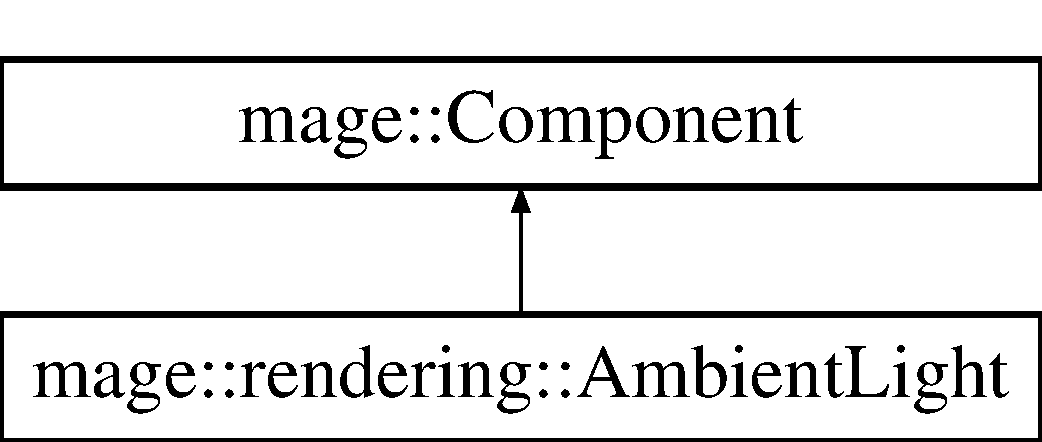
\includegraphics[height=2.000000cm]{classmage_1_1rendering_1_1_ambient_light}
\end{center}
\end{figure}
\subsection*{Public Member Functions}
\begin{DoxyCompactItemize}
\item 
\hyperlink{classmage_1_1rendering_1_1_ambient_light_a178327bf02552f65b98ad3858416a81d}{Ambient\+Light} () noexcept
\item 
\hyperlink{classmage_1_1rendering_1_1_ambient_light_a363ca4f79eef6f0a95a2e3d381479af1}{Ambient\+Light} (const \hyperlink{classmage_1_1rendering_1_1_ambient_light}{Ambient\+Light} \&light) noexcept
\item 
\hyperlink{classmage_1_1rendering_1_1_ambient_light_a8bd09baed470ce2c09af6a9893549937}{Ambient\+Light} (\hyperlink{classmage_1_1rendering_1_1_ambient_light}{Ambient\+Light} \&\&light) noexcept
\item 
virtual \hyperlink{classmage_1_1rendering_1_1_ambient_light_a811cb86e80188b924085674a88a0bf7b}{$\sim$\+Ambient\+Light} ()
\item 
\hyperlink{classmage_1_1rendering_1_1_ambient_light}{Ambient\+Light} \& \hyperlink{classmage_1_1rendering_1_1_ambient_light_a351cdcd2e1b25c6a44356060f0e61c2b}{operator=} (const \hyperlink{classmage_1_1rendering_1_1_ambient_light}{Ambient\+Light} \&light) noexcept
\item 
\hyperlink{classmage_1_1rendering_1_1_ambient_light}{Ambient\+Light} \& \hyperlink{classmage_1_1rendering_1_1_ambient_light_aa571cc046cb35ceafba6cb0a2ec4bd6c}{operator=} (\hyperlink{classmage_1_1rendering_1_1_ambient_light}{Ambient\+Light} \&\&light) noexcept
\item 
\hyperlink{structmage_1_1_s_r_g_b}{S\+R\+GB} \& \hyperlink{classmage_1_1rendering_1_1_ambient_light_a0b45abc0f1cf9e9fae345c8574238432}{Get\+Base\+Color} () noexcept
\item 
const \hyperlink{structmage_1_1_s_r_g_b}{S\+R\+GB} \& \hyperlink{classmage_1_1rendering_1_1_ambient_light_a9396951fe2029233ce1f6b4ff38dcc8b}{Get\+Base\+Color} () const noexcept
\item 
\hyperlink{namespacemage_aa97e833b45f06d60a0a9c4fc22ae02c0}{F32} \hyperlink{classmage_1_1rendering_1_1_ambient_light_ad78278e798956e1c3a707a37dfb052da}{Get\+Radiance} () const noexcept
\item 
void \hyperlink{classmage_1_1rendering_1_1_ambient_light_a2da2e614906dc166121a0d0d391b9fc2}{Set\+Radiance} (\hyperlink{namespacemage_aa97e833b45f06d60a0a9c4fc22ae02c0}{F32} radiance) noexcept
\item 
const \hyperlink{structmage_1_1_r_g_b}{R\+GB} \hyperlink{classmage_1_1rendering_1_1_ambient_light_a480e6b39d92266254778c23e8456e55e}{Get\+Radiance\+Spectrum} () const noexcept
\end{DoxyCompactItemize}
\subsection*{Private Attributes}
\begin{DoxyCompactItemize}
\item 
\hyperlink{namespacemage_aa97e833b45f06d60a0a9c4fc22ae02c0}{F32} \hyperlink{classmage_1_1rendering_1_1_ambient_light_adfdafe01958a72df46eeb3c0f5f0d0c4}{m\+\_\+radiance}
\item 
\hyperlink{structmage_1_1_s_r_g_b}{S\+R\+GB} \hyperlink{classmage_1_1rendering_1_1_ambient_light_a9b6bf87dbc6f12644b5ace67f03aa883}{m\+\_\+base\+\_\+color}
\end{DoxyCompactItemize}
\subsection*{Additional Inherited Members}


\subsection{Detailed Description}
A class of ambient lights. 

\subsection{Constructor \& Destructor Documentation}
\hypertarget{classmage_1_1rendering_1_1_ambient_light_a178327bf02552f65b98ad3858416a81d}{}\label{classmage_1_1rendering_1_1_ambient_light_a178327bf02552f65b98ad3858416a81d} 
\index{mage\+::rendering\+::\+Ambient\+Light@{mage\+::rendering\+::\+Ambient\+Light}!Ambient\+Light@{Ambient\+Light}}
\index{Ambient\+Light@{Ambient\+Light}!mage\+::rendering\+::\+Ambient\+Light@{mage\+::rendering\+::\+Ambient\+Light}}
\subsubsection{\texorpdfstring{Ambient\+Light()}{AmbientLight()}\hspace{0.1cm}{\footnotesize\ttfamily [1/3]}}
{\footnotesize\ttfamily mage\+::rendering\+::\+Ambient\+Light\+::\+Ambient\+Light (\begin{DoxyParamCaption}{ }\end{DoxyParamCaption})\hspace{0.3cm}{\ttfamily [noexcept]}}

Constructs an ambient light. \hypertarget{classmage_1_1rendering_1_1_ambient_light_a363ca4f79eef6f0a95a2e3d381479af1}{}\label{classmage_1_1rendering_1_1_ambient_light_a363ca4f79eef6f0a95a2e3d381479af1} 
\index{mage\+::rendering\+::\+Ambient\+Light@{mage\+::rendering\+::\+Ambient\+Light}!Ambient\+Light@{Ambient\+Light}}
\index{Ambient\+Light@{Ambient\+Light}!mage\+::rendering\+::\+Ambient\+Light@{mage\+::rendering\+::\+Ambient\+Light}}
\subsubsection{\texorpdfstring{Ambient\+Light()}{AmbientLight()}\hspace{0.1cm}{\footnotesize\ttfamily [2/3]}}
{\footnotesize\ttfamily mage\+::rendering\+::\+Ambient\+Light\+::\+Ambient\+Light (\begin{DoxyParamCaption}\item[{const \hyperlink{classmage_1_1rendering_1_1_ambient_light}{Ambient\+Light} \&}]{light }\end{DoxyParamCaption})\hspace{0.3cm}{\ttfamily [default]}, {\ttfamily [noexcept]}}

Constructs an ambient light from the given ambient light.


\begin{DoxyParams}[1]{Parameters}
\mbox{\tt in}  & {\em light} & A reference to the ambient light to copy. \\
\hline
\end{DoxyParams}
\hypertarget{classmage_1_1rendering_1_1_ambient_light_a8bd09baed470ce2c09af6a9893549937}{}\label{classmage_1_1rendering_1_1_ambient_light_a8bd09baed470ce2c09af6a9893549937} 
\index{mage\+::rendering\+::\+Ambient\+Light@{mage\+::rendering\+::\+Ambient\+Light}!Ambient\+Light@{Ambient\+Light}}
\index{Ambient\+Light@{Ambient\+Light}!mage\+::rendering\+::\+Ambient\+Light@{mage\+::rendering\+::\+Ambient\+Light}}
\subsubsection{\texorpdfstring{Ambient\+Light()}{AmbientLight()}\hspace{0.1cm}{\footnotesize\ttfamily [3/3]}}
{\footnotesize\ttfamily mage\+::rendering\+::\+Ambient\+Light\+::\+Ambient\+Light (\begin{DoxyParamCaption}\item[{\hyperlink{classmage_1_1rendering_1_1_ambient_light}{Ambient\+Light} \&\&}]{light }\end{DoxyParamCaption})\hspace{0.3cm}{\ttfamily [default]}, {\ttfamily [noexcept]}}

Constructs an ambient light by moving the given ambient light.


\begin{DoxyParams}[1]{Parameters}
\mbox{\tt in}  & {\em light} & A reference to the ambient light to move. \\
\hline
\end{DoxyParams}
\hypertarget{classmage_1_1rendering_1_1_ambient_light_a811cb86e80188b924085674a88a0bf7b}{}\label{classmage_1_1rendering_1_1_ambient_light_a811cb86e80188b924085674a88a0bf7b} 
\index{mage\+::rendering\+::\+Ambient\+Light@{mage\+::rendering\+::\+Ambient\+Light}!````~Ambient\+Light@{$\sim$\+Ambient\+Light}}
\index{````~Ambient\+Light@{$\sim$\+Ambient\+Light}!mage\+::rendering\+::\+Ambient\+Light@{mage\+::rendering\+::\+Ambient\+Light}}
\subsubsection{\texorpdfstring{$\sim$\+Ambient\+Light()}{~AmbientLight()}}
{\footnotesize\ttfamily mage\+::rendering\+::\+Ambient\+Light\+::$\sim$\+Ambient\+Light (\begin{DoxyParamCaption}{ }\end{DoxyParamCaption})\hspace{0.3cm}{\ttfamily [virtual]}, {\ttfamily [default]}}

Destructs this ambient light. 

\subsection{Member Function Documentation}
\hypertarget{classmage_1_1rendering_1_1_ambient_light_a0b45abc0f1cf9e9fae345c8574238432}{}\label{classmage_1_1rendering_1_1_ambient_light_a0b45abc0f1cf9e9fae345c8574238432} 
\index{mage\+::rendering\+::\+Ambient\+Light@{mage\+::rendering\+::\+Ambient\+Light}!Get\+Base\+Color@{Get\+Base\+Color}}
\index{Get\+Base\+Color@{Get\+Base\+Color}!mage\+::rendering\+::\+Ambient\+Light@{mage\+::rendering\+::\+Ambient\+Light}}
\subsubsection{\texorpdfstring{Get\+Base\+Color()}{GetBaseColor()}\hspace{0.1cm}{\footnotesize\ttfamily [1/2]}}
{\footnotesize\ttfamily \hyperlink{structmage_1_1_s_r_g_b}{S\+R\+GB}\& mage\+::rendering\+::\+Ambient\+Light\+::\+Get\+Base\+Color (\begin{DoxyParamCaption}{ }\end{DoxyParamCaption})\hspace{0.3cm}{\ttfamily [noexcept]}}

Returns the s\+R\+GB base color of this ambient light.

\begin{DoxyReturn}{Returns}
A reference to the s\+R\+GB base color of this ambient light. 
\end{DoxyReturn}
\hypertarget{classmage_1_1rendering_1_1_ambient_light_a9396951fe2029233ce1f6b4ff38dcc8b}{}\label{classmage_1_1rendering_1_1_ambient_light_a9396951fe2029233ce1f6b4ff38dcc8b} 
\index{mage\+::rendering\+::\+Ambient\+Light@{mage\+::rendering\+::\+Ambient\+Light}!Get\+Base\+Color@{Get\+Base\+Color}}
\index{Get\+Base\+Color@{Get\+Base\+Color}!mage\+::rendering\+::\+Ambient\+Light@{mage\+::rendering\+::\+Ambient\+Light}}
\subsubsection{\texorpdfstring{Get\+Base\+Color()}{GetBaseColor()}\hspace{0.1cm}{\footnotesize\ttfamily [2/2]}}
{\footnotesize\ttfamily const \hyperlink{structmage_1_1_s_r_g_b}{S\+R\+GB}\& mage\+::rendering\+::\+Ambient\+Light\+::\+Get\+Base\+Color (\begin{DoxyParamCaption}{ }\end{DoxyParamCaption}) const\hspace{0.3cm}{\ttfamily [noexcept]}}

Returns the s\+R\+GB base color of this ambient light.

\begin{DoxyReturn}{Returns}
A reference to the s\+R\+GB base color of this ambient light. 
\end{DoxyReturn}
\hypertarget{classmage_1_1rendering_1_1_ambient_light_ad78278e798956e1c3a707a37dfb052da}{}\label{classmage_1_1rendering_1_1_ambient_light_ad78278e798956e1c3a707a37dfb052da} 
\index{mage\+::rendering\+::\+Ambient\+Light@{mage\+::rendering\+::\+Ambient\+Light}!Get\+Radiance@{Get\+Radiance}}
\index{Get\+Radiance@{Get\+Radiance}!mage\+::rendering\+::\+Ambient\+Light@{mage\+::rendering\+::\+Ambient\+Light}}
\subsubsection{\texorpdfstring{Get\+Radiance()}{GetRadiance()}}
{\footnotesize\ttfamily \hyperlink{namespacemage_aa97e833b45f06d60a0a9c4fc22ae02c0}{F32} mage\+::rendering\+::\+Ambient\+Light\+::\+Get\+Radiance (\begin{DoxyParamCaption}{ }\end{DoxyParamCaption}) const\hspace{0.3cm}{\ttfamily [noexcept]}}

Returns the radiance of this ambient light.

\begin{DoxyReturn}{Returns}
The radiance in watts per square meter per steradians of this ambient light. 
\end{DoxyReturn}
\hypertarget{classmage_1_1rendering_1_1_ambient_light_a480e6b39d92266254778c23e8456e55e}{}\label{classmage_1_1rendering_1_1_ambient_light_a480e6b39d92266254778c23e8456e55e} 
\index{mage\+::rendering\+::\+Ambient\+Light@{mage\+::rendering\+::\+Ambient\+Light}!Get\+Radiance\+Spectrum@{Get\+Radiance\+Spectrum}}
\index{Get\+Radiance\+Spectrum@{Get\+Radiance\+Spectrum}!mage\+::rendering\+::\+Ambient\+Light@{mage\+::rendering\+::\+Ambient\+Light}}
\subsubsection{\texorpdfstring{Get\+Radiance\+Spectrum()}{GetRadianceSpectrum()}}
{\footnotesize\ttfamily const \hyperlink{structmage_1_1_r_g_b}{R\+GB} mage\+::rendering\+::\+Ambient\+Light\+::\+Get\+Radiance\+Spectrum (\begin{DoxyParamCaption}{ }\end{DoxyParamCaption}) const\hspace{0.3cm}{\ttfamily [noexcept]}}

Returns the radiance spectrum of this ambient light.

\begin{DoxyReturn}{Returns}
The radiance spectrum of this ambient light. 
\end{DoxyReturn}
\hypertarget{classmage_1_1rendering_1_1_ambient_light_a351cdcd2e1b25c6a44356060f0e61c2b}{}\label{classmage_1_1rendering_1_1_ambient_light_a351cdcd2e1b25c6a44356060f0e61c2b} 
\index{mage\+::rendering\+::\+Ambient\+Light@{mage\+::rendering\+::\+Ambient\+Light}!operator=@{operator=}}
\index{operator=@{operator=}!mage\+::rendering\+::\+Ambient\+Light@{mage\+::rendering\+::\+Ambient\+Light}}
\subsubsection{\texorpdfstring{operator=()}{operator=()}\hspace{0.1cm}{\footnotesize\ttfamily [1/2]}}
{\footnotesize\ttfamily \hyperlink{classmage_1_1rendering_1_1_ambient_light}{Ambient\+Light} \& mage\+::rendering\+::\+Ambient\+Light\+::operator= (\begin{DoxyParamCaption}\item[{const \hyperlink{classmage_1_1rendering_1_1_ambient_light}{Ambient\+Light} \&}]{light }\end{DoxyParamCaption})\hspace{0.3cm}{\ttfamily [default]}, {\ttfamily [noexcept]}}

Copies the given ambient light to this ambient light.


\begin{DoxyParams}[1]{Parameters}
\mbox{\tt in}  & {\em light} & A reference to the ambient light to copy. \\
\hline
\end{DoxyParams}
\begin{DoxyReturn}{Returns}
A reference to the copy of the given ambient light (i.\+e. this ambient light). 
\end{DoxyReturn}
\hypertarget{classmage_1_1rendering_1_1_ambient_light_aa571cc046cb35ceafba6cb0a2ec4bd6c}{}\label{classmage_1_1rendering_1_1_ambient_light_aa571cc046cb35ceafba6cb0a2ec4bd6c} 
\index{mage\+::rendering\+::\+Ambient\+Light@{mage\+::rendering\+::\+Ambient\+Light}!operator=@{operator=}}
\index{operator=@{operator=}!mage\+::rendering\+::\+Ambient\+Light@{mage\+::rendering\+::\+Ambient\+Light}}
\subsubsection{\texorpdfstring{operator=()}{operator=()}\hspace{0.1cm}{\footnotesize\ttfamily [2/2]}}
{\footnotesize\ttfamily \hyperlink{classmage_1_1rendering_1_1_ambient_light}{Ambient\+Light} \& mage\+::rendering\+::\+Ambient\+Light\+::operator= (\begin{DoxyParamCaption}\item[{\hyperlink{classmage_1_1rendering_1_1_ambient_light}{Ambient\+Light} \&\&}]{light }\end{DoxyParamCaption})\hspace{0.3cm}{\ttfamily [default]}, {\ttfamily [noexcept]}}

Moves the given ambient light to this ambient light.


\begin{DoxyParams}[1]{Parameters}
\mbox{\tt in}  & {\em light} & A reference to the ambient light to move. \\
\hline
\end{DoxyParams}
\begin{DoxyReturn}{Returns}
A reference to the moved ambient light (i.\+e. this ambient light). 
\end{DoxyReturn}
\hypertarget{classmage_1_1rendering_1_1_ambient_light_a2da2e614906dc166121a0d0d391b9fc2}{}\label{classmage_1_1rendering_1_1_ambient_light_a2da2e614906dc166121a0d0d391b9fc2} 
\index{mage\+::rendering\+::\+Ambient\+Light@{mage\+::rendering\+::\+Ambient\+Light}!Set\+Radiance@{Set\+Radiance}}
\index{Set\+Radiance@{Set\+Radiance}!mage\+::rendering\+::\+Ambient\+Light@{mage\+::rendering\+::\+Ambient\+Light}}
\subsubsection{\texorpdfstring{Set\+Radiance()}{SetRadiance()}}
{\footnotesize\ttfamily void mage\+::rendering\+::\+Ambient\+Light\+::\+Set\+Radiance (\begin{DoxyParamCaption}\item[{\hyperlink{namespacemage_aa97e833b45f06d60a0a9c4fc22ae02c0}{F32}}]{radiance }\end{DoxyParamCaption})\hspace{0.3cm}{\ttfamily [noexcept]}}

Sets the radiance of this ambient light to the given radiance.


\begin{DoxyParams}[1]{Parameters}
\mbox{\tt in}  & {\em radiance} & The radiance in watts per square meter per steradians. \\
\hline
\end{DoxyParams}


\subsection{Member Data Documentation}
\hypertarget{classmage_1_1rendering_1_1_ambient_light_a9b6bf87dbc6f12644b5ace67f03aa883}{}\label{classmage_1_1rendering_1_1_ambient_light_a9b6bf87dbc6f12644b5ace67f03aa883} 
\index{mage\+::rendering\+::\+Ambient\+Light@{mage\+::rendering\+::\+Ambient\+Light}!m\+\_\+base\+\_\+color@{m\+\_\+base\+\_\+color}}
\index{m\+\_\+base\+\_\+color@{m\+\_\+base\+\_\+color}!mage\+::rendering\+::\+Ambient\+Light@{mage\+::rendering\+::\+Ambient\+Light}}
\subsubsection{\texorpdfstring{m\+\_\+base\+\_\+color}{m\_base\_color}}
{\footnotesize\ttfamily \hyperlink{structmage_1_1_s_r_g_b}{S\+R\+GB} mage\+::rendering\+::\+Ambient\+Light\+::m\+\_\+base\+\_\+color\hspace{0.3cm}{\ttfamily [private]}}

The s\+R\+GB base color of this ambient light. \hypertarget{classmage_1_1rendering_1_1_ambient_light_adfdafe01958a72df46eeb3c0f5f0d0c4}{}\label{classmage_1_1rendering_1_1_ambient_light_adfdafe01958a72df46eeb3c0f5f0d0c4} 
\index{mage\+::rendering\+::\+Ambient\+Light@{mage\+::rendering\+::\+Ambient\+Light}!m\+\_\+radiance@{m\+\_\+radiance}}
\index{m\+\_\+radiance@{m\+\_\+radiance}!mage\+::rendering\+::\+Ambient\+Light@{mage\+::rendering\+::\+Ambient\+Light}}
\subsubsection{\texorpdfstring{m\+\_\+radiance}{m\_radiance}}
{\footnotesize\ttfamily \hyperlink{namespacemage_aa97e833b45f06d60a0a9c4fc22ae02c0}{F32} mage\+::rendering\+::\+Ambient\+Light\+::m\+\_\+radiance\hspace{0.3cm}{\ttfamily [private]}}

The radiance in watts per square meter per steradians of this ambient light. 
\hypertarget{structmage_1_1_array}{}\section{mage\+:\+:Array$<$ T, N, A, typename $>$ Struct Template Reference}
\label{structmage_1_1_array}\index{mage\+::\+Array$<$ T, N, A, typename $>$@{mage\+::\+Array$<$ T, N, A, typename $>$}}


{\ttfamily \#include $<$array.\+hpp$>$}

Inheritance diagram for mage\+:\+:Array$<$ T, N, A, typename $>$\+:\begin{figure}[H]
\begin{center}
\leavevmode
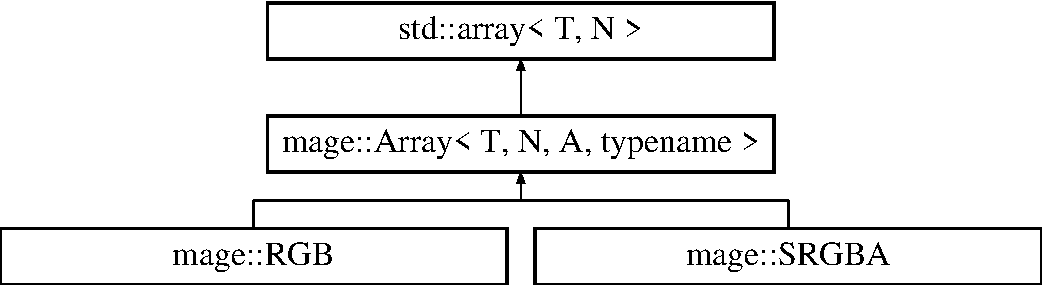
\includegraphics[height=1.917808cm]{structmage_1_1_array}
\end{center}
\end{figure}
\subsection*{Public Member Functions}
\begin{DoxyCompactItemize}
\item 
constexpr \mbox{\hyperlink{structmage_1_1_array_ac1cf5733c005dfb79fb9e5e736098598}{Array}} () noexcept
\item 
constexpr \mbox{\hyperlink{structmage_1_1_array_a1f206f942c1318eb7f57c7e0666bc923}{Array}} (const T \&value) noexcept
\item 
{\footnotesize template$<$typename... ArgsT, typename  = std\+::enable\+\_\+if\+\_\+t$<$ (\+N == sizeof...(\+Args\+T)) $>$$>$ }\\constexpr \mbox{\hyperlink{structmage_1_1_array_ab6dbce28b41b7ef1e9c0195f24f378a6}{Array}} (ArgsT \&\&... args) noexcept
\item 
{\footnotesize template$<$std\+::size\+\_\+t FromN$>$ }\\constexpr \mbox{\hyperlink{structmage_1_1_array_a1e0a4b5cebb34709b32bc13e9ab917e1}{Array}} (const \mbox{\hyperlink{structmage_1_1_array}{Array}}$<$ T, FromN, A $>$ \&a) noexcept
\item 
{\footnotesize template$<$std\+::size\+\_\+t FromN, std\+::size\+\_\+t FromA$>$ }\\constexpr \mbox{\hyperlink{structmage_1_1_array_ac747c6b1fad2e919e3370cbe6b2937f5}{Array}} (const \mbox{\hyperlink{structmage_1_1_array}{Array}}$<$ T, FromN, FromA $>$ \&a) noexcept
\item 
{\footnotesize template$<$std\+::size\+\_\+t FromN, typename... ArgsT$>$ }\\constexpr \mbox{\hyperlink{structmage_1_1_array_a128de416259f75f7b4ab8ab2e1ba9bd7}{Array}} (const \mbox{\hyperlink{structmage_1_1_array}{Array}}$<$ T, FromN, A $>$ \&a, ArgsT \&\&... args) noexcept
\item 
{\footnotesize template$<$std\+::size\+\_\+t FromN, std\+::size\+\_\+t FromA, typename... ArgsT$>$ }\\constexpr \mbox{\hyperlink{structmage_1_1_array_a4952f767cdedb8c2874391dc4d9b74c3}{Array}} (const \mbox{\hyperlink{structmage_1_1_array}{Array}}$<$ T, FromN, FromA $>$ \&a, ArgsT \&\&... args) noexcept
\item 
constexpr \mbox{\hyperlink{structmage_1_1_array_a8dc58948e15554f715b280a72140a1f4}{Array}} (const \mbox{\hyperlink{structmage_1_1_array}{Array}} \&a) noexcept=default
\item 
constexpr \mbox{\hyperlink{structmage_1_1_array_a4cf0fb395b42d53b6e59868739dc9613}{Array}} (\mbox{\hyperlink{structmage_1_1_array}{Array}} \&\&a) noexcept=default
\item 
{\footnotesize template$<$typename FromT , std\+::size\+\_\+t FromA, typename  = std\+::enable\+\_\+if\+\_\+t$<$ std\+::is\+\_\+convertible\+\_\+v$<$ From\+T, T $>$ $>$$>$ }\\constexpr \mbox{\hyperlink{structmage_1_1_array_a950b26208c3546704f42e92c312a93ed}{Array}} (const \mbox{\hyperlink{structmage_1_1_array}{Array}}$<$ FromT, N, FromA $>$ \&a) noexcept
\item 
\mbox{\hyperlink{structmage_1_1_array_a7adc09166915789b93a7a3af118182e0}{$\sim$\+Array}} ()=default
\item 
\mbox{\hyperlink{structmage_1_1_array}{Array}} \& \mbox{\hyperlink{structmage_1_1_array_a216d8efaf044c3219a45e53073833ee0}{operator=}} (const \mbox{\hyperlink{structmage_1_1_array}{Array}} \&a) noexcept=default
\item 
\mbox{\hyperlink{structmage_1_1_array}{Array}} \& \mbox{\hyperlink{structmage_1_1_array_a33cb0dac90d7bf6c3973455ab12eb535}{operator=}} (\mbox{\hyperlink{structmage_1_1_array}{Array}} \&\&a) noexcept=default
\end{DoxyCompactItemize}
\subsection*{Static Public Attributes}
\begin{DoxyCompactItemize}
\item 
static constexpr std\+::size\+\_\+t \mbox{\hyperlink{structmage_1_1_array_ac4dbc8a376d8594b11afa8f1383d4241}{s\+\_\+size}} = N
\end{DoxyCompactItemize}


\subsection{Constructor \& Destructor Documentation}
\mbox{\Hypertarget{structmage_1_1_array_ac1cf5733c005dfb79fb9e5e736098598}\label{structmage_1_1_array_ac1cf5733c005dfb79fb9e5e736098598}} 
\index{mage\+::\+Array@{mage\+::\+Array}!Array@{Array}}
\index{Array@{Array}!mage\+::\+Array@{mage\+::\+Array}}
\subsubsection{\texorpdfstring{Array()}{Array()}\hspace{0.1cm}{\footnotesize\ttfamily [1/10]}}
{\footnotesize\ttfamily template$<$typename T, std\+::size\+\_\+t N, std\+::size\+\_\+t A = alignof(\+T), typename  = std\+::enable\+\_\+if\+\_\+t$<$ (\+N $>$ 1u$>$ \\
constexpr \mbox{\hyperlink{structmage_1_1_array}{mage\+::\+Array}}$<$ T, N, A, typename $>$\+::\mbox{\hyperlink{structmage_1_1_array}{Array}} (\begin{DoxyParamCaption}{ }\end{DoxyParamCaption})\hspace{0.3cm}{\ttfamily [noexcept]}}

\mbox{\Hypertarget{structmage_1_1_array_a1f206f942c1318eb7f57c7e0666bc923}\label{structmage_1_1_array_a1f206f942c1318eb7f57c7e0666bc923}} 
\index{mage\+::\+Array@{mage\+::\+Array}!Array@{Array}}
\index{Array@{Array}!mage\+::\+Array@{mage\+::\+Array}}
\subsubsection{\texorpdfstring{Array()}{Array()}\hspace{0.1cm}{\footnotesize\ttfamily [2/10]}}
{\footnotesize\ttfamily template$<$typename T, std\+::size\+\_\+t N, std\+::size\+\_\+t A = alignof(\+T), typename  = std\+::enable\+\_\+if\+\_\+t$<$ (\+N $>$ 1u$>$ \\
constexpr \mbox{\hyperlink{structmage_1_1_array}{mage\+::\+Array}}$<$ T, N, A, typename $>$\+::\mbox{\hyperlink{structmage_1_1_array}{Array}} (\begin{DoxyParamCaption}\item[{const T \&}]{value }\end{DoxyParamCaption})\hspace{0.3cm}{\ttfamily [explicit]}, {\ttfamily [noexcept]}}

\mbox{\Hypertarget{structmage_1_1_array_ab6dbce28b41b7ef1e9c0195f24f378a6}\label{structmage_1_1_array_ab6dbce28b41b7ef1e9c0195f24f378a6}} 
\index{mage\+::\+Array@{mage\+::\+Array}!Array@{Array}}
\index{Array@{Array}!mage\+::\+Array@{mage\+::\+Array}}
\subsubsection{\texorpdfstring{Array()}{Array()}\hspace{0.1cm}{\footnotesize\ttfamily [3/10]}}
{\footnotesize\ttfamily template$<$typename T, std\+::size\+\_\+t N, std\+::size\+\_\+t A = alignof(\+T), typename  = std\+::enable\+\_\+if\+\_\+t$<$ (\+N $>$ 1u$>$ \\
template$<$typename... ArgsT, typename  = std\+::enable\+\_\+if\+\_\+t$<$ (\+N == sizeof...(\+Args\+T)) $>$$>$ \\
constexpr \mbox{\hyperlink{structmage_1_1_array}{mage\+::\+Array}}$<$ T, N, A, typename $>$\+::\mbox{\hyperlink{structmage_1_1_array}{Array}} (\begin{DoxyParamCaption}\item[{ArgsT \&\&...}]{args }\end{DoxyParamCaption})\hspace{0.3cm}{\ttfamily [noexcept]}}

\mbox{\Hypertarget{structmage_1_1_array_a1e0a4b5cebb34709b32bc13e9ab917e1}\label{structmage_1_1_array_a1e0a4b5cebb34709b32bc13e9ab917e1}} 
\index{mage\+::\+Array@{mage\+::\+Array}!Array@{Array}}
\index{Array@{Array}!mage\+::\+Array@{mage\+::\+Array}}
\subsubsection{\texorpdfstring{Array()}{Array()}\hspace{0.1cm}{\footnotesize\ttfamily [4/10]}}
{\footnotesize\ttfamily template$<$typename T, std\+::size\+\_\+t N, std\+::size\+\_\+t A = alignof(\+T), typename  = std\+::enable\+\_\+if\+\_\+t$<$ (\+N $>$ 1u$>$ \\
template$<$std\+::size\+\_\+t FromN$>$ \\
constexpr \mbox{\hyperlink{structmage_1_1_array}{mage\+::\+Array}}$<$ T, N, A, typename $>$\+::\mbox{\hyperlink{structmage_1_1_array}{Array}} (\begin{DoxyParamCaption}\item[{const \mbox{\hyperlink{structmage_1_1_array}{Array}}$<$ T, FromN, A $>$ \&}]{a }\end{DoxyParamCaption})\hspace{0.3cm}{\ttfamily [noexcept]}}

\mbox{\Hypertarget{structmage_1_1_array_ac747c6b1fad2e919e3370cbe6b2937f5}\label{structmage_1_1_array_ac747c6b1fad2e919e3370cbe6b2937f5}} 
\index{mage\+::\+Array@{mage\+::\+Array}!Array@{Array}}
\index{Array@{Array}!mage\+::\+Array@{mage\+::\+Array}}
\subsubsection{\texorpdfstring{Array()}{Array()}\hspace{0.1cm}{\footnotesize\ttfamily [5/10]}}
{\footnotesize\ttfamily template$<$typename T, std\+::size\+\_\+t N, std\+::size\+\_\+t A = alignof(\+T), typename  = std\+::enable\+\_\+if\+\_\+t$<$ (\+N $>$ 1u$>$ \\
template$<$std\+::size\+\_\+t FromN, std\+::size\+\_\+t FromA$>$ \\
constexpr \mbox{\hyperlink{structmage_1_1_array}{mage\+::\+Array}}$<$ T, N, A, typename $>$\+::\mbox{\hyperlink{structmage_1_1_array}{Array}} (\begin{DoxyParamCaption}\item[{const \mbox{\hyperlink{structmage_1_1_array}{Array}}$<$ T, FromN, FromA $>$ \&}]{a }\end{DoxyParamCaption})\hspace{0.3cm}{\ttfamily [explicit]}, {\ttfamily [noexcept]}}

\mbox{\Hypertarget{structmage_1_1_array_a128de416259f75f7b4ab8ab2e1ba9bd7}\label{structmage_1_1_array_a128de416259f75f7b4ab8ab2e1ba9bd7}} 
\index{mage\+::\+Array@{mage\+::\+Array}!Array@{Array}}
\index{Array@{Array}!mage\+::\+Array@{mage\+::\+Array}}
\subsubsection{\texorpdfstring{Array()}{Array()}\hspace{0.1cm}{\footnotesize\ttfamily [6/10]}}
{\footnotesize\ttfamily template$<$typename T, std\+::size\+\_\+t N, std\+::size\+\_\+t A = alignof(\+T), typename  = std\+::enable\+\_\+if\+\_\+t$<$ (\+N $>$ 1u$>$ \\
template$<$std\+::size\+\_\+t FromN, typename... ArgsT$>$ \\
constexpr \mbox{\hyperlink{structmage_1_1_array}{mage\+::\+Array}}$<$ T, N, A, typename $>$\+::\mbox{\hyperlink{structmage_1_1_array}{Array}} (\begin{DoxyParamCaption}\item[{const \mbox{\hyperlink{structmage_1_1_array}{Array}}$<$ T, FromN, A $>$ \&}]{a,  }\item[{ArgsT \&\&...}]{args }\end{DoxyParamCaption})\hspace{0.3cm}{\ttfamily [noexcept]}}

\mbox{\Hypertarget{structmage_1_1_array_a4952f767cdedb8c2874391dc4d9b74c3}\label{structmage_1_1_array_a4952f767cdedb8c2874391dc4d9b74c3}} 
\index{mage\+::\+Array@{mage\+::\+Array}!Array@{Array}}
\index{Array@{Array}!mage\+::\+Array@{mage\+::\+Array}}
\subsubsection{\texorpdfstring{Array()}{Array()}\hspace{0.1cm}{\footnotesize\ttfamily [7/10]}}
{\footnotesize\ttfamily template$<$typename T, std\+::size\+\_\+t N, std\+::size\+\_\+t A = alignof(\+T), typename  = std\+::enable\+\_\+if\+\_\+t$<$ (\+N $>$ 1u$>$ \\
template$<$std\+::size\+\_\+t FromN, std\+::size\+\_\+t FromA, typename... ArgsT$>$ \\
constexpr \mbox{\hyperlink{structmage_1_1_array}{mage\+::\+Array}}$<$ T, N, A, typename $>$\+::\mbox{\hyperlink{structmage_1_1_array}{Array}} (\begin{DoxyParamCaption}\item[{const \mbox{\hyperlink{structmage_1_1_array}{Array}}$<$ T, FromN, FromA $>$ \&}]{a,  }\item[{ArgsT \&\&...}]{args }\end{DoxyParamCaption})\hspace{0.3cm}{\ttfamily [explicit]}, {\ttfamily [noexcept]}}

\mbox{\Hypertarget{structmage_1_1_array_a8dc58948e15554f715b280a72140a1f4}\label{structmage_1_1_array_a8dc58948e15554f715b280a72140a1f4}} 
\index{mage\+::\+Array@{mage\+::\+Array}!Array@{Array}}
\index{Array@{Array}!mage\+::\+Array@{mage\+::\+Array}}
\subsubsection{\texorpdfstring{Array()}{Array()}\hspace{0.1cm}{\footnotesize\ttfamily [8/10]}}
{\footnotesize\ttfamily template$<$typename T, std\+::size\+\_\+t N, std\+::size\+\_\+t A = alignof(\+T), typename  = std\+::enable\+\_\+if\+\_\+t$<$ (\+N $>$ 1u$>$ \\
constexpr \mbox{\hyperlink{structmage_1_1_array}{mage\+::\+Array}}$<$ T, N, A, typename $>$\+::\mbox{\hyperlink{structmage_1_1_array}{Array}} (\begin{DoxyParamCaption}\item[{const \mbox{\hyperlink{structmage_1_1_array}{Array}}$<$ T, N, A, typename $>$ \&}]{a }\end{DoxyParamCaption})\hspace{0.3cm}{\ttfamily [default]}, {\ttfamily [noexcept]}}

\mbox{\Hypertarget{structmage_1_1_array_a4cf0fb395b42d53b6e59868739dc9613}\label{structmage_1_1_array_a4cf0fb395b42d53b6e59868739dc9613}} 
\index{mage\+::\+Array@{mage\+::\+Array}!Array@{Array}}
\index{Array@{Array}!mage\+::\+Array@{mage\+::\+Array}}
\subsubsection{\texorpdfstring{Array()}{Array()}\hspace{0.1cm}{\footnotesize\ttfamily [9/10]}}
{\footnotesize\ttfamily template$<$typename T, std\+::size\+\_\+t N, std\+::size\+\_\+t A = alignof(\+T), typename  = std\+::enable\+\_\+if\+\_\+t$<$ (\+N $>$ 1u$>$ \\
constexpr \mbox{\hyperlink{structmage_1_1_array}{mage\+::\+Array}}$<$ T, N, A, typename $>$\+::\mbox{\hyperlink{structmage_1_1_array}{Array}} (\begin{DoxyParamCaption}\item[{\mbox{\hyperlink{structmage_1_1_array}{Array}}$<$ T, N, A, typename $>$ \&\&}]{a }\end{DoxyParamCaption})\hspace{0.3cm}{\ttfamily [default]}, {\ttfamily [noexcept]}}

\mbox{\Hypertarget{structmage_1_1_array_a950b26208c3546704f42e92c312a93ed}\label{structmage_1_1_array_a950b26208c3546704f42e92c312a93ed}} 
\index{mage\+::\+Array@{mage\+::\+Array}!Array@{Array}}
\index{Array@{Array}!mage\+::\+Array@{mage\+::\+Array}}
\subsubsection{\texorpdfstring{Array()}{Array()}\hspace{0.1cm}{\footnotesize\ttfamily [10/10]}}
{\footnotesize\ttfamily template$<$typename T, std\+::size\+\_\+t N, std\+::size\+\_\+t A = alignof(\+T), typename  = std\+::enable\+\_\+if\+\_\+t$<$ (\+N $>$ 1u$>$ \\
template$<$typename FromT , std\+::size\+\_\+t FromA, typename  = std\+::enable\+\_\+if\+\_\+t$<$ std\+::is\+\_\+convertible\+\_\+v$<$ From\+T, T $>$ $>$$>$ \\
constexpr \mbox{\hyperlink{structmage_1_1_array}{mage\+::\+Array}}$<$ T, N, A, typename $>$\+::\mbox{\hyperlink{structmage_1_1_array}{Array}} (\begin{DoxyParamCaption}\item[{const \mbox{\hyperlink{structmage_1_1_array}{Array}}$<$ FromT, N, FromA $>$ \&}]{a }\end{DoxyParamCaption})\hspace{0.3cm}{\ttfamily [explicit]}, {\ttfamily [noexcept]}}

\mbox{\Hypertarget{structmage_1_1_array_a7adc09166915789b93a7a3af118182e0}\label{structmage_1_1_array_a7adc09166915789b93a7a3af118182e0}} 
\index{mage\+::\+Array@{mage\+::\+Array}!````~Array@{$\sim$\+Array}}
\index{````~Array@{$\sim$\+Array}!mage\+::\+Array@{mage\+::\+Array}}
\subsubsection{\texorpdfstring{$\sim$\+Array()}{~Array()}}
{\footnotesize\ttfamily template$<$typename T, std\+::size\+\_\+t N, std\+::size\+\_\+t A = alignof(\+T), typename  = std\+::enable\+\_\+if\+\_\+t$<$ (\+N $>$ 1u$>$ \\
\mbox{\hyperlink{structmage_1_1_array}{mage\+::\+Array}}$<$ T, N, A, typename $>$\+::$\sim$\mbox{\hyperlink{structmage_1_1_array}{Array}} (\begin{DoxyParamCaption}{ }\end{DoxyParamCaption})\hspace{0.3cm}{\ttfamily [default]}}



\subsection{Member Function Documentation}
\mbox{\Hypertarget{structmage_1_1_array_a216d8efaf044c3219a45e53073833ee0}\label{structmage_1_1_array_a216d8efaf044c3219a45e53073833ee0}} 
\index{mage\+::\+Array@{mage\+::\+Array}!operator=@{operator=}}
\index{operator=@{operator=}!mage\+::\+Array@{mage\+::\+Array}}
\subsubsection{\texorpdfstring{operator=()}{operator=()}\hspace{0.1cm}{\footnotesize\ttfamily [1/2]}}
{\footnotesize\ttfamily template$<$typename T, std\+::size\+\_\+t N, std\+::size\+\_\+t A = alignof(\+T), typename  = std\+::enable\+\_\+if\+\_\+t$<$ (\+N $>$ 1u$>$ \\
\mbox{\hyperlink{structmage_1_1_array}{Array}}\& \mbox{\hyperlink{structmage_1_1_array}{mage\+::\+Array}}$<$ T, N, A, typename $>$\+::operator= (\begin{DoxyParamCaption}\item[{const \mbox{\hyperlink{structmage_1_1_array}{Array}}$<$ T, N, A, typename $>$ \&}]{a }\end{DoxyParamCaption})\hspace{0.3cm}{\ttfamily [default]}, {\ttfamily [noexcept]}}

\mbox{\Hypertarget{structmage_1_1_array_a33cb0dac90d7bf6c3973455ab12eb535}\label{structmage_1_1_array_a33cb0dac90d7bf6c3973455ab12eb535}} 
\index{mage\+::\+Array@{mage\+::\+Array}!operator=@{operator=}}
\index{operator=@{operator=}!mage\+::\+Array@{mage\+::\+Array}}
\subsubsection{\texorpdfstring{operator=()}{operator=()}\hspace{0.1cm}{\footnotesize\ttfamily [2/2]}}
{\footnotesize\ttfamily template$<$typename T, std\+::size\+\_\+t N, std\+::size\+\_\+t A = alignof(\+T), typename  = std\+::enable\+\_\+if\+\_\+t$<$ (\+N $>$ 1u$>$ \\
\mbox{\hyperlink{structmage_1_1_array}{Array}}\& \mbox{\hyperlink{structmage_1_1_array}{mage\+::\+Array}}$<$ T, N, A, typename $>$\+::operator= (\begin{DoxyParamCaption}\item[{\mbox{\hyperlink{structmage_1_1_array}{Array}}$<$ T, N, A, typename $>$ \&\&}]{a }\end{DoxyParamCaption})\hspace{0.3cm}{\ttfamily [default]}, {\ttfamily [noexcept]}}



\subsection{Member Data Documentation}
\mbox{\Hypertarget{structmage_1_1_array_ac4dbc8a376d8594b11afa8f1383d4241}\label{structmage_1_1_array_ac4dbc8a376d8594b11afa8f1383d4241}} 
\index{mage\+::\+Array@{mage\+::\+Array}!s\+\_\+size@{s\+\_\+size}}
\index{s\+\_\+size@{s\+\_\+size}!mage\+::\+Array@{mage\+::\+Array}}
\subsubsection{\texorpdfstring{s\+\_\+size}{s\_size}}
{\footnotesize\ttfamily template$<$typename T, std\+::size\+\_\+t N, std\+::size\+\_\+t A = alignof(\+T), typename  = std\+::enable\+\_\+if\+\_\+t$<$ (\+N $>$ 1u$>$ \\
constexpr std\+::size\+\_\+t \mbox{\hyperlink{structmage_1_1_array}{mage\+::\+Array}}$<$ T, N, A, typename $>$\+::s\+\_\+size = N\hspace{0.3cm}{\ttfamily [static]}}


\hypertarget{classmage_1_1rendering_1_1_back_buffer_pass}{}\section{mage\+:\+:rendering\+:\+:Back\+Buffer\+Pass Class Reference}
\label{classmage_1_1rendering_1_1_back_buffer_pass}\index{mage\+::rendering\+::\+Back\+Buffer\+Pass@{mage\+::rendering\+::\+Back\+Buffer\+Pass}}


{\ttfamily \#include $<$back\+\_\+buffer\+\_\+pass.\+hpp$>$}

\subsection*{Public Member Functions}
\begin{DoxyCompactItemize}
\item 
\mbox{\hyperlink{classmage_1_1rendering_1_1_back_buffer_pass_a054aad27e4b3d05baf235ae256934ef2}{Back\+Buffer\+Pass}} (I\+D3\+D11\+Device\+Context \&device\+\_\+context, \mbox{\hyperlink{classmage_1_1rendering_1_1_state_manager}{State\+Manager}} \&state\+\_\+manager, \mbox{\hyperlink{classmage_1_1rendering_1_1_resource_manager}{Resource\+Manager}} \&resource\+\_\+manager)
\item 
\mbox{\hyperlink{classmage_1_1rendering_1_1_back_buffer_pass_aa8042001dccc96e61b01a5775421a41d}{Back\+Buffer\+Pass}} (const \mbox{\hyperlink{classmage_1_1rendering_1_1_back_buffer_pass}{Back\+Buffer\+Pass}} \&pass)=delete
\item 
\mbox{\hyperlink{classmage_1_1rendering_1_1_back_buffer_pass_ac8dfbaabb766f4bfd61cfea8d01dd7dc}{Back\+Buffer\+Pass}} (\mbox{\hyperlink{classmage_1_1rendering_1_1_back_buffer_pass}{Back\+Buffer\+Pass}} \&\&pass) noexcept
\item 
\mbox{\hyperlink{classmage_1_1rendering_1_1_back_buffer_pass_a697a5e094cdcdf9f42dd2efdda957b57}{$\sim$\+Back\+Buffer\+Pass}} ()
\item 
\mbox{\hyperlink{classmage_1_1rendering_1_1_back_buffer_pass}{Back\+Buffer\+Pass}} \& \mbox{\hyperlink{classmage_1_1rendering_1_1_back_buffer_pass_acad71e5633ba37b1069c5a2ef9e6f704}{operator=}} (const \mbox{\hyperlink{classmage_1_1rendering_1_1_back_buffer_pass}{Back\+Buffer\+Pass}} \&pass)=delete
\item 
\mbox{\hyperlink{classmage_1_1rendering_1_1_back_buffer_pass}{Back\+Buffer\+Pass}} \& \mbox{\hyperlink{classmage_1_1rendering_1_1_back_buffer_pass_a79649b9316cb114bae032027406b4fe4}{operator=}} (\mbox{\hyperlink{classmage_1_1rendering_1_1_back_buffer_pass}{Back\+Buffer\+Pass}} \&\&pass) noexcept
\item 
void \mbox{\hyperlink{classmage_1_1rendering_1_1_back_buffer_pass_af0e8bab1a86d7f37934e9d76aa253b29}{Render}} ()
\end{DoxyCompactItemize}
\subsection*{Private Member Functions}
\begin{DoxyCompactItemize}
\item 
void \mbox{\hyperlink{classmage_1_1rendering_1_1_back_buffer_pass_a45aafe0681a6e0598d088dbf3954cfb7}{Bind\+Fixed\+State}} () const noexcept
\end{DoxyCompactItemize}
\subsection*{Private Attributes}
\begin{DoxyCompactItemize}
\item 
std\+::reference\+\_\+wrapper$<$ I\+D3\+D11\+Device\+Context $>$ \mbox{\hyperlink{classmage_1_1rendering_1_1_back_buffer_pass_ae87c0cf8b2ffe627ac44faaf61791b4f}{m\+\_\+device\+\_\+context}}
\item 
std\+::reference\+\_\+wrapper$<$ \mbox{\hyperlink{classmage_1_1rendering_1_1_state_manager}{State\+Manager}} $>$ \mbox{\hyperlink{classmage_1_1rendering_1_1_back_buffer_pass_a5d10a44c5f8a3529d64aabfb590156f2}{m\+\_\+state\+\_\+manager}}
\item 
\mbox{\hyperlink{namespacemage_1_1rendering_aaf704b9c54a4181f4950a1761de69dda}{Vertex\+Shader\+Ptr}} \mbox{\hyperlink{classmage_1_1rendering_1_1_back_buffer_pass_a12a95cc800090a0bc01d14a9f5903748}{m\+\_\+vs}}
\item 
\mbox{\hyperlink{namespacemage_1_1rendering_af03d922b228ee9c8542baaa2ecc9f259}{Pixel\+Shader\+Ptr}} \mbox{\hyperlink{classmage_1_1rendering_1_1_back_buffer_pass_a46bc7e8b3636db2eb84b42590b7bd51e}{m\+\_\+ps}}
\end{DoxyCompactItemize}


\subsection{Detailed Description}
A class of back buffer passes. 

\subsection{Constructor \& Destructor Documentation}
\mbox{\Hypertarget{classmage_1_1rendering_1_1_back_buffer_pass_a054aad27e4b3d05baf235ae256934ef2}\label{classmage_1_1rendering_1_1_back_buffer_pass_a054aad27e4b3d05baf235ae256934ef2}} 
\index{mage\+::rendering\+::\+Back\+Buffer\+Pass@{mage\+::rendering\+::\+Back\+Buffer\+Pass}!Back\+Buffer\+Pass@{Back\+Buffer\+Pass}}
\index{Back\+Buffer\+Pass@{Back\+Buffer\+Pass}!mage\+::rendering\+::\+Back\+Buffer\+Pass@{mage\+::rendering\+::\+Back\+Buffer\+Pass}}
\subsubsection{\texorpdfstring{Back\+Buffer\+Pass()}{BackBufferPass()}\hspace{0.1cm}{\footnotesize\ttfamily [1/3]}}
{\footnotesize\ttfamily mage\+::rendering\+::\+Back\+Buffer\+Pass\+::\+Back\+Buffer\+Pass (\begin{DoxyParamCaption}\item[{I\+D3\+D11\+Device\+Context \&}]{device\+\_\+context,  }\item[{\mbox{\hyperlink{classmage_1_1rendering_1_1_state_manager}{State\+Manager}} \&}]{state\+\_\+manager,  }\item[{\mbox{\hyperlink{classmage_1_1rendering_1_1_resource_manager}{Resource\+Manager}} \&}]{resource\+\_\+manager }\end{DoxyParamCaption})\hspace{0.3cm}{\ttfamily [explicit]}}

Constructs a back buffer pass.


\begin{DoxyParams}[1]{Parameters}
\mbox{\tt in,out}  & {\em device\+\_\+context} & A reference to the device context. \\
\hline
\mbox{\tt in,out}  & {\em state\+\_\+manager} & A reference to the state manager. \\
\hline
\mbox{\tt in,out}  & {\em resource\+\_\+manager} & A reference to the resource manager. \\
\hline
\end{DoxyParams}
\mbox{\Hypertarget{classmage_1_1rendering_1_1_back_buffer_pass_aa8042001dccc96e61b01a5775421a41d}\label{classmage_1_1rendering_1_1_back_buffer_pass_aa8042001dccc96e61b01a5775421a41d}} 
\index{mage\+::rendering\+::\+Back\+Buffer\+Pass@{mage\+::rendering\+::\+Back\+Buffer\+Pass}!Back\+Buffer\+Pass@{Back\+Buffer\+Pass}}
\index{Back\+Buffer\+Pass@{Back\+Buffer\+Pass}!mage\+::rendering\+::\+Back\+Buffer\+Pass@{mage\+::rendering\+::\+Back\+Buffer\+Pass}}
\subsubsection{\texorpdfstring{Back\+Buffer\+Pass()}{BackBufferPass()}\hspace{0.1cm}{\footnotesize\ttfamily [2/3]}}
{\footnotesize\ttfamily mage\+::rendering\+::\+Back\+Buffer\+Pass\+::\+Back\+Buffer\+Pass (\begin{DoxyParamCaption}\item[{const \mbox{\hyperlink{classmage_1_1rendering_1_1_back_buffer_pass}{Back\+Buffer\+Pass}} \&}]{pass }\end{DoxyParamCaption})\hspace{0.3cm}{\ttfamily [delete]}}

Constructs an back buffer pass from the given back buffer pass.


\begin{DoxyParams}[1]{Parameters}
\mbox{\tt in}  & {\em pass} & A reference to the back buffer pass to copy. \\
\hline
\end{DoxyParams}
\mbox{\Hypertarget{classmage_1_1rendering_1_1_back_buffer_pass_ac8dfbaabb766f4bfd61cfea8d01dd7dc}\label{classmage_1_1rendering_1_1_back_buffer_pass_ac8dfbaabb766f4bfd61cfea8d01dd7dc}} 
\index{mage\+::rendering\+::\+Back\+Buffer\+Pass@{mage\+::rendering\+::\+Back\+Buffer\+Pass}!Back\+Buffer\+Pass@{Back\+Buffer\+Pass}}
\index{Back\+Buffer\+Pass@{Back\+Buffer\+Pass}!mage\+::rendering\+::\+Back\+Buffer\+Pass@{mage\+::rendering\+::\+Back\+Buffer\+Pass}}
\subsubsection{\texorpdfstring{Back\+Buffer\+Pass()}{BackBufferPass()}\hspace{0.1cm}{\footnotesize\ttfamily [3/3]}}
{\footnotesize\ttfamily mage\+::rendering\+::\+Back\+Buffer\+Pass\+::\+Back\+Buffer\+Pass (\begin{DoxyParamCaption}\item[{\mbox{\hyperlink{classmage_1_1rendering_1_1_back_buffer_pass}{Back\+Buffer\+Pass}} \&\&}]{pass }\end{DoxyParamCaption})\hspace{0.3cm}{\ttfamily [default]}, {\ttfamily [noexcept]}}

Constructs an back buffer pass by moving the given back buffer pass.


\begin{DoxyParams}[1]{Parameters}
\mbox{\tt in}  & {\em pass} & A reference to the Image pass to move. \\
\hline
\end{DoxyParams}
\mbox{\Hypertarget{classmage_1_1rendering_1_1_back_buffer_pass_a697a5e094cdcdf9f42dd2efdda957b57}\label{classmage_1_1rendering_1_1_back_buffer_pass_a697a5e094cdcdf9f42dd2efdda957b57}} 
\index{mage\+::rendering\+::\+Back\+Buffer\+Pass@{mage\+::rendering\+::\+Back\+Buffer\+Pass}!````~Back\+Buffer\+Pass@{$\sim$\+Back\+Buffer\+Pass}}
\index{````~Back\+Buffer\+Pass@{$\sim$\+Back\+Buffer\+Pass}!mage\+::rendering\+::\+Back\+Buffer\+Pass@{mage\+::rendering\+::\+Back\+Buffer\+Pass}}
\subsubsection{\texorpdfstring{$\sim$\+Back\+Buffer\+Pass()}{~BackBufferPass()}}
{\footnotesize\ttfamily mage\+::rendering\+::\+Back\+Buffer\+Pass\+::$\sim$\+Back\+Buffer\+Pass (\begin{DoxyParamCaption}{ }\end{DoxyParamCaption})\hspace{0.3cm}{\ttfamily [default]}}

Destructs this back buffer pass. 

\subsection{Member Function Documentation}
\mbox{\Hypertarget{classmage_1_1rendering_1_1_back_buffer_pass_a45aafe0681a6e0598d088dbf3954cfb7}\label{classmage_1_1rendering_1_1_back_buffer_pass_a45aafe0681a6e0598d088dbf3954cfb7}} 
\index{mage\+::rendering\+::\+Back\+Buffer\+Pass@{mage\+::rendering\+::\+Back\+Buffer\+Pass}!Bind\+Fixed\+State@{Bind\+Fixed\+State}}
\index{Bind\+Fixed\+State@{Bind\+Fixed\+State}!mage\+::rendering\+::\+Back\+Buffer\+Pass@{mage\+::rendering\+::\+Back\+Buffer\+Pass}}
\subsubsection{\texorpdfstring{Bind\+Fixed\+State()}{BindFixedState()}}
{\footnotesize\ttfamily void mage\+::rendering\+::\+Back\+Buffer\+Pass\+::\+Bind\+Fixed\+State (\begin{DoxyParamCaption}{ }\end{DoxyParamCaption}) const\hspace{0.3cm}{\ttfamily [private]}, {\ttfamily [noexcept]}}

Binds the fixed state of this back buffer pass. \mbox{\Hypertarget{classmage_1_1rendering_1_1_back_buffer_pass_acad71e5633ba37b1069c5a2ef9e6f704}\label{classmage_1_1rendering_1_1_back_buffer_pass_acad71e5633ba37b1069c5a2ef9e6f704}} 
\index{mage\+::rendering\+::\+Back\+Buffer\+Pass@{mage\+::rendering\+::\+Back\+Buffer\+Pass}!operator=@{operator=}}
\index{operator=@{operator=}!mage\+::rendering\+::\+Back\+Buffer\+Pass@{mage\+::rendering\+::\+Back\+Buffer\+Pass}}
\subsubsection{\texorpdfstring{operator=()}{operator=()}\hspace{0.1cm}{\footnotesize\ttfamily [1/2]}}
{\footnotesize\ttfamily \mbox{\hyperlink{classmage_1_1rendering_1_1_back_buffer_pass}{Back\+Buffer\+Pass}}\& mage\+::rendering\+::\+Back\+Buffer\+Pass\+::operator= (\begin{DoxyParamCaption}\item[{const \mbox{\hyperlink{classmage_1_1rendering_1_1_back_buffer_pass}{Back\+Buffer\+Pass}} \&}]{pass }\end{DoxyParamCaption})\hspace{0.3cm}{\ttfamily [delete]}}

Copies the given back buffer pass to this back buffer pass.


\begin{DoxyParams}[1]{Parameters}
\mbox{\tt in}  & {\em pass} & A reference to the back buffer pass to copy. \\
\hline
\end{DoxyParams}
\begin{DoxyReturn}{Returns}
A reference to the copy of the given back buffer pass (i.\+e. this back buffer pass). 
\end{DoxyReturn}
\mbox{\Hypertarget{classmage_1_1rendering_1_1_back_buffer_pass_a79649b9316cb114bae032027406b4fe4}\label{classmage_1_1rendering_1_1_back_buffer_pass_a79649b9316cb114bae032027406b4fe4}} 
\index{mage\+::rendering\+::\+Back\+Buffer\+Pass@{mage\+::rendering\+::\+Back\+Buffer\+Pass}!operator=@{operator=}}
\index{operator=@{operator=}!mage\+::rendering\+::\+Back\+Buffer\+Pass@{mage\+::rendering\+::\+Back\+Buffer\+Pass}}
\subsubsection{\texorpdfstring{operator=()}{operator=()}\hspace{0.1cm}{\footnotesize\ttfamily [2/2]}}
{\footnotesize\ttfamily \mbox{\hyperlink{classmage_1_1rendering_1_1_back_buffer_pass}{Back\+Buffer\+Pass}} \& mage\+::rendering\+::\+Back\+Buffer\+Pass\+::operator= (\begin{DoxyParamCaption}\item[{\mbox{\hyperlink{classmage_1_1rendering_1_1_back_buffer_pass}{Back\+Buffer\+Pass}} \&\&}]{pass }\end{DoxyParamCaption})\hspace{0.3cm}{\ttfamily [default]}, {\ttfamily [noexcept]}}

Moves the given back buffer pass to this back buffer pass.


\begin{DoxyParams}[1]{Parameters}
\mbox{\tt in}  & {\em pass} & A reference to the back buffer pass to move. \\
\hline
\end{DoxyParams}
\begin{DoxyReturn}{Returns}
A reference to the moved back buffer pass (i.\+e. this back buffer pass). 
\end{DoxyReturn}
\mbox{\Hypertarget{classmage_1_1rendering_1_1_back_buffer_pass_af0e8bab1a86d7f37934e9d76aa253b29}\label{classmage_1_1rendering_1_1_back_buffer_pass_af0e8bab1a86d7f37934e9d76aa253b29}} 
\index{mage\+::rendering\+::\+Back\+Buffer\+Pass@{mage\+::rendering\+::\+Back\+Buffer\+Pass}!Render@{Render}}
\index{Render@{Render}!mage\+::rendering\+::\+Back\+Buffer\+Pass@{mage\+::rendering\+::\+Back\+Buffer\+Pass}}
\subsubsection{\texorpdfstring{Render()}{Render()}}
{\footnotesize\ttfamily void mage\+::rendering\+::\+Back\+Buffer\+Pass\+::\+Render (\begin{DoxyParamCaption}{ }\end{DoxyParamCaption})}

Renders. 

\subsection{Member Data Documentation}
\mbox{\Hypertarget{classmage_1_1rendering_1_1_back_buffer_pass_ae87c0cf8b2ffe627ac44faaf61791b4f}\label{classmage_1_1rendering_1_1_back_buffer_pass_ae87c0cf8b2ffe627ac44faaf61791b4f}} 
\index{mage\+::rendering\+::\+Back\+Buffer\+Pass@{mage\+::rendering\+::\+Back\+Buffer\+Pass}!m\+\_\+device\+\_\+context@{m\+\_\+device\+\_\+context}}
\index{m\+\_\+device\+\_\+context@{m\+\_\+device\+\_\+context}!mage\+::rendering\+::\+Back\+Buffer\+Pass@{mage\+::rendering\+::\+Back\+Buffer\+Pass}}
\subsubsection{\texorpdfstring{m\+\_\+device\+\_\+context}{m\_device\_context}}
{\footnotesize\ttfamily std\+::reference\+\_\+wrapper$<$ I\+D3\+D11\+Device\+Context $>$ mage\+::rendering\+::\+Back\+Buffer\+Pass\+::m\+\_\+device\+\_\+context\hspace{0.3cm}{\ttfamily [private]}}

A reference to the device context of this back buffer pass. \mbox{\Hypertarget{classmage_1_1rendering_1_1_back_buffer_pass_a46bc7e8b3636db2eb84b42590b7bd51e}\label{classmage_1_1rendering_1_1_back_buffer_pass_a46bc7e8b3636db2eb84b42590b7bd51e}} 
\index{mage\+::rendering\+::\+Back\+Buffer\+Pass@{mage\+::rendering\+::\+Back\+Buffer\+Pass}!m\+\_\+ps@{m\+\_\+ps}}
\index{m\+\_\+ps@{m\+\_\+ps}!mage\+::rendering\+::\+Back\+Buffer\+Pass@{mage\+::rendering\+::\+Back\+Buffer\+Pass}}
\subsubsection{\texorpdfstring{m\+\_\+ps}{m\_ps}}
{\footnotesize\ttfamily \mbox{\hyperlink{namespacemage_1_1rendering_af03d922b228ee9c8542baaa2ecc9f259}{Pixel\+Shader\+Ptr}} mage\+::rendering\+::\+Back\+Buffer\+Pass\+::m\+\_\+ps\hspace{0.3cm}{\ttfamily [private]}}

A pointer to the pixel shader of this back buffer pass. \mbox{\Hypertarget{classmage_1_1rendering_1_1_back_buffer_pass_a5d10a44c5f8a3529d64aabfb590156f2}\label{classmage_1_1rendering_1_1_back_buffer_pass_a5d10a44c5f8a3529d64aabfb590156f2}} 
\index{mage\+::rendering\+::\+Back\+Buffer\+Pass@{mage\+::rendering\+::\+Back\+Buffer\+Pass}!m\+\_\+state\+\_\+manager@{m\+\_\+state\+\_\+manager}}
\index{m\+\_\+state\+\_\+manager@{m\+\_\+state\+\_\+manager}!mage\+::rendering\+::\+Back\+Buffer\+Pass@{mage\+::rendering\+::\+Back\+Buffer\+Pass}}
\subsubsection{\texorpdfstring{m\+\_\+state\+\_\+manager}{m\_state\_manager}}
{\footnotesize\ttfamily std\+::reference\+\_\+wrapper$<$ \mbox{\hyperlink{classmage_1_1rendering_1_1_state_manager}{State\+Manager}} $>$ mage\+::rendering\+::\+Back\+Buffer\+Pass\+::m\+\_\+state\+\_\+manager\hspace{0.3cm}{\ttfamily [private]}}

A reference to the state manager of this back buffer pass. \mbox{\Hypertarget{classmage_1_1rendering_1_1_back_buffer_pass_a12a95cc800090a0bc01d14a9f5903748}\label{classmage_1_1rendering_1_1_back_buffer_pass_a12a95cc800090a0bc01d14a9f5903748}} 
\index{mage\+::rendering\+::\+Back\+Buffer\+Pass@{mage\+::rendering\+::\+Back\+Buffer\+Pass}!m\+\_\+vs@{m\+\_\+vs}}
\index{m\+\_\+vs@{m\+\_\+vs}!mage\+::rendering\+::\+Back\+Buffer\+Pass@{mage\+::rendering\+::\+Back\+Buffer\+Pass}}
\subsubsection{\texorpdfstring{m\+\_\+vs}{m\_vs}}
{\footnotesize\ttfamily \mbox{\hyperlink{namespacemage_1_1rendering_aaf704b9c54a4181f4950a1761de69dda}{Vertex\+Shader\+Ptr}} mage\+::rendering\+::\+Back\+Buffer\+Pass\+::m\+\_\+vs\hspace{0.3cm}{\ttfamily [private]}}

A pointer to the vertex shader of this back buffer pass. 
\hypertarget{classmage_1_1_behavior_script}{}\section{mage\+:\+:Behavior\+Script Class Reference}
\label{classmage_1_1_behavior_script}\index{mage\+::\+Behavior\+Script@{mage\+::\+Behavior\+Script}}


{\ttfamily \#include $<$behavior\+\_\+script.\+hpp$>$}

Inheritance diagram for mage\+:\+:Behavior\+Script\+:\begin{figure}[H]
\begin{center}
\leavevmode
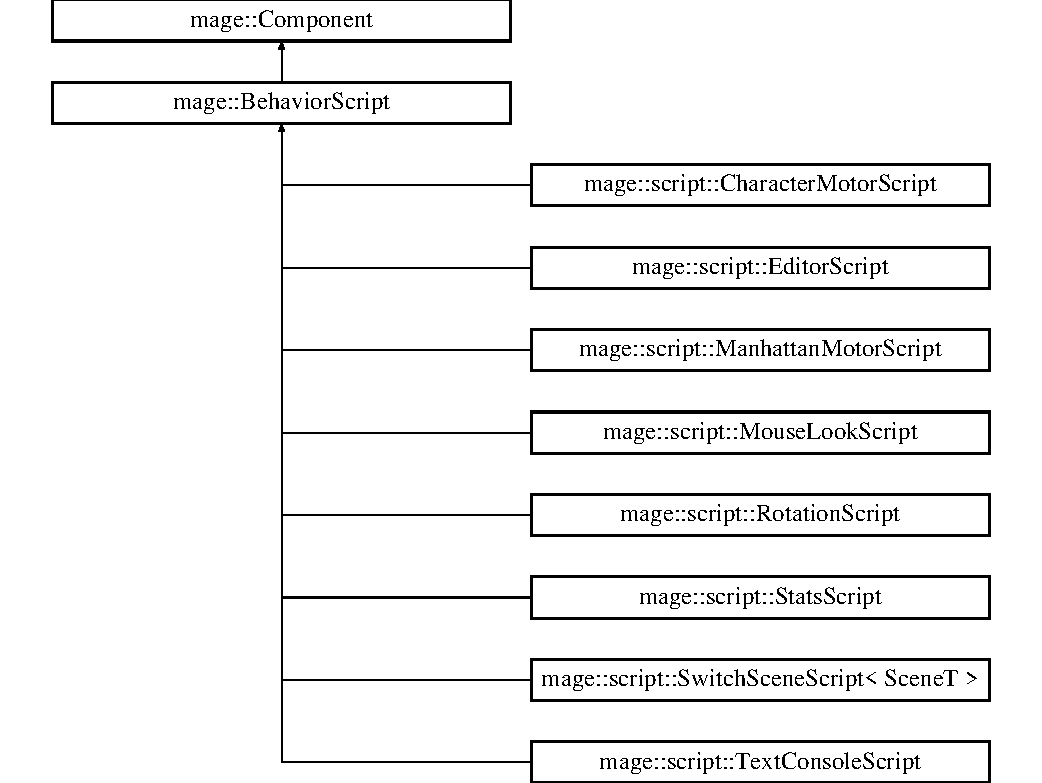
\includegraphics[height=7.604939cm]{classmage_1_1_behavior_script}
\end{center}
\end{figure}
\subsection*{Public Member Functions}
\begin{DoxyCompactItemize}
\item 
virtual \hyperlink{classmage_1_1_behavior_script_a61e4825ba0fc7746d49faa44ed7bc481}{$\sim$\+Behavior\+Script} ()
\item 
\hyperlink{classmage_1_1_behavior_script}{Behavior\+Script} \& \hyperlink{classmage_1_1_behavior_script_a0b3327ebf7009e668a7022d254cb1d51}{operator=} (const \hyperlink{classmage_1_1_behavior_script}{Behavior\+Script} \&script)=delete
\item 
\hyperlink{classmage_1_1_behavior_script}{Behavior\+Script} \& \hyperlink{classmage_1_1_behavior_script_a528c2bd218f2e6bb7d0a8ee50a05bf01}{operator=} (\hyperlink{classmage_1_1_behavior_script}{Behavior\+Script} \&\&script)=delete
\item 
virtual void \hyperlink{classmage_1_1_behavior_script_a8318f79ab78798ec37b39bc844f7138c}{Fixed\+Update} ()
\item 
virtual void \hyperlink{classmage_1_1_behavior_script_afb9cf3759edf8876416d1df85489cba6}{Update} (\mbox{[}\mbox{[}maybe\+\_\+unused\mbox{]}\mbox{]} \hyperlink{namespacemage_ad26233bbec640deda836e572c1a23708}{F64} delta\+\_\+time)
\item 
bool \hyperlink{classmage_1_1_behavior_script_a856e1b420ea0ead36adafa750237325c}{Is\+Active} () const noexcept
\item 
bool \hyperlink{classmage_1_1_behavior_script_a40e33539ca7013a13ef127af11bff3e1}{Is\+Passive} () const noexcept
\item 
void \hyperlink{classmage_1_1_behavior_script_a84a5bf0fc7ec3ecd36dddaf001143b54}{Activate} () noexcept
\item 
void \hyperlink{classmage_1_1_behavior_script_ab45260db9c30d596b1d688a01458f63e}{Deactivate} () noexcept
\item 
void \hyperlink{classmage_1_1_behavior_script_ab0dc76b101fd514c6e9f8799de382e8a}{Set\+Active} (bool active) noexcept
\item 
bool \hyperlink{classmage_1_1_behavior_script_abb1625dbaa3b1145009ea474b082938f}{Is\+Terminated} () const noexcept
\item 
void \hyperlink{classmage_1_1_behavior_script_a2beae460bb84a135aa7e29c7baf6b25b}{Terminate} () noexcept
\end{DoxyCompactItemize}
\subsection*{Protected Member Functions}
\begin{DoxyCompactItemize}
\item 
\hyperlink{classmage_1_1_behavior_script_ad064a6bbe2ba5f7622d1d20eeec958bf}{Behavior\+Script} ()
\item 
\hyperlink{classmage_1_1_behavior_script_ab95b988867dfb8592ab7678bff608116}{Behavior\+Script} (const \hyperlink{classmage_1_1_behavior_script}{Behavior\+Script} \&script)
\item 
\hyperlink{classmage_1_1_behavior_script_aa8f509053f6bb9dbfd3baa75bdd8b91e}{Behavior\+Script} (\hyperlink{classmage_1_1_behavior_script}{Behavior\+Script} \&\&script)
\end{DoxyCompactItemize}
\subsection*{Private Member Functions}
\begin{DoxyCompactItemize}
\item 
virtual void \hyperlink{classmage_1_1_behavior_script_a17703fd980599ccf7265b5ffc6148fe8}{On\+Active\+Change} () noexcept
\end{DoxyCompactItemize}
\subsection*{Private Attributes}
\begin{DoxyCompactItemize}
\item 
bool \hyperlink{classmage_1_1_behavior_script_a18f81792aed31a2d61a8a75784e2ceef}{m\+\_\+active}
\item 
bool \hyperlink{classmage_1_1_behavior_script_abc4a0e6728787347012404a597ab8e07}{m\+\_\+terminated}
\end{DoxyCompactItemize}


\subsection{Detailed Description}
A class of behavior scripts. 

\subsection{Constructor \& Destructor Documentation}
\hypertarget{classmage_1_1_behavior_script_a61e4825ba0fc7746d49faa44ed7bc481}{}\label{classmage_1_1_behavior_script_a61e4825ba0fc7746d49faa44ed7bc481} 
\index{mage\+::\+Behavior\+Script@{mage\+::\+Behavior\+Script}!````~Behavior\+Script@{$\sim$\+Behavior\+Script}}
\index{````~Behavior\+Script@{$\sim$\+Behavior\+Script}!mage\+::\+Behavior\+Script@{mage\+::\+Behavior\+Script}}
\subsubsection{\texorpdfstring{$\sim$\+Behavior\+Script()}{~BehaviorScript()}}
{\footnotesize\ttfamily mage\+::\+Behavior\+Script\+::$\sim$\+Behavior\+Script (\begin{DoxyParamCaption}{ }\end{DoxyParamCaption})\hspace{0.3cm}{\ttfamily [virtual]}, {\ttfamily [default]}}

Destructs this behavior script. \hypertarget{classmage_1_1_behavior_script_ad064a6bbe2ba5f7622d1d20eeec958bf}{}\label{classmage_1_1_behavior_script_ad064a6bbe2ba5f7622d1d20eeec958bf} 
\index{mage\+::\+Behavior\+Script@{mage\+::\+Behavior\+Script}!Behavior\+Script@{Behavior\+Script}}
\index{Behavior\+Script@{Behavior\+Script}!mage\+::\+Behavior\+Script@{mage\+::\+Behavior\+Script}}
\subsubsection{\texorpdfstring{Behavior\+Script()}{BehaviorScript()}\hspace{0.1cm}{\footnotesize\ttfamily [1/3]}}
{\footnotesize\ttfamily mage\+::\+Behavior\+Script\+::\+Behavior\+Script (\begin{DoxyParamCaption}{ }\end{DoxyParamCaption})\hspace{0.3cm}{\ttfamily [protected]}}

Constructs a behavior script. \hypertarget{classmage_1_1_behavior_script_ab95b988867dfb8592ab7678bff608116}{}\label{classmage_1_1_behavior_script_ab95b988867dfb8592ab7678bff608116} 
\index{mage\+::\+Behavior\+Script@{mage\+::\+Behavior\+Script}!Behavior\+Script@{Behavior\+Script}}
\index{Behavior\+Script@{Behavior\+Script}!mage\+::\+Behavior\+Script@{mage\+::\+Behavior\+Script}}
\subsubsection{\texorpdfstring{Behavior\+Script()}{BehaviorScript()}\hspace{0.1cm}{\footnotesize\ttfamily [2/3]}}
{\footnotesize\ttfamily mage\+::\+Behavior\+Script\+::\+Behavior\+Script (\begin{DoxyParamCaption}\item[{const \hyperlink{classmage_1_1_behavior_script}{Behavior\+Script} \&}]{script }\end{DoxyParamCaption})\hspace{0.3cm}{\ttfamily [protected]}, {\ttfamily [default]}}

Constructs a behavior script from the given behavior script.


\begin{DoxyParams}[1]{Parameters}
\mbox{\tt in}  & {\em script} & A reference to the behavior script to copy. \\
\hline
\end{DoxyParams}
\hypertarget{classmage_1_1_behavior_script_aa8f509053f6bb9dbfd3baa75bdd8b91e}{}\label{classmage_1_1_behavior_script_aa8f509053f6bb9dbfd3baa75bdd8b91e} 
\index{mage\+::\+Behavior\+Script@{mage\+::\+Behavior\+Script}!Behavior\+Script@{Behavior\+Script}}
\index{Behavior\+Script@{Behavior\+Script}!mage\+::\+Behavior\+Script@{mage\+::\+Behavior\+Script}}
\subsubsection{\texorpdfstring{Behavior\+Script()}{BehaviorScript()}\hspace{0.1cm}{\footnotesize\ttfamily [3/3]}}
{\footnotesize\ttfamily mage\+::\+Behavior\+Script\+::\+Behavior\+Script (\begin{DoxyParamCaption}\item[{\hyperlink{classmage_1_1_behavior_script}{Behavior\+Script} \&\&}]{script }\end{DoxyParamCaption})\hspace{0.3cm}{\ttfamily [protected]}, {\ttfamily [default]}}

Constructs a behavior script by moving the given behavior script.


\begin{DoxyParams}[1]{Parameters}
\mbox{\tt in}  & {\em script} & A reference to the behavior script to move. \\
\hline
\end{DoxyParams}


\subsection{Member Function Documentation}
\hypertarget{classmage_1_1_behavior_script_a84a5bf0fc7ec3ecd36dddaf001143b54}{}\label{classmage_1_1_behavior_script_a84a5bf0fc7ec3ecd36dddaf001143b54} 
\index{mage\+::\+Behavior\+Script@{mage\+::\+Behavior\+Script}!Activate@{Activate}}
\index{Activate@{Activate}!mage\+::\+Behavior\+Script@{mage\+::\+Behavior\+Script}}
\subsubsection{\texorpdfstring{Activate()}{Activate()}}
{\footnotesize\ttfamily void mage\+::\+Behavior\+Script\+::\+Activate (\begin{DoxyParamCaption}{ }\end{DoxyParamCaption})\hspace{0.3cm}{\ttfamily [noexcept]}}

Activates this behavior script (and its descendant behavior scripts). \hypertarget{classmage_1_1_behavior_script_ab45260db9c30d596b1d688a01458f63e}{}\label{classmage_1_1_behavior_script_ab45260db9c30d596b1d688a01458f63e} 
\index{mage\+::\+Behavior\+Script@{mage\+::\+Behavior\+Script}!Deactivate@{Deactivate}}
\index{Deactivate@{Deactivate}!mage\+::\+Behavior\+Script@{mage\+::\+Behavior\+Script}}
\subsubsection{\texorpdfstring{Deactivate()}{Deactivate()}}
{\footnotesize\ttfamily void mage\+::\+Behavior\+Script\+::\+Deactivate (\begin{DoxyParamCaption}{ }\end{DoxyParamCaption})\hspace{0.3cm}{\ttfamily [noexcept]}}

Deactives this behavior script (and its descendant behavior scripts). \hypertarget{classmage_1_1_behavior_script_a8318f79ab78798ec37b39bc844f7138c}{}\label{classmage_1_1_behavior_script_a8318f79ab78798ec37b39bc844f7138c} 
\index{mage\+::\+Behavior\+Script@{mage\+::\+Behavior\+Script}!Fixed\+Update@{Fixed\+Update}}
\index{Fixed\+Update@{Fixed\+Update}!mage\+::\+Behavior\+Script@{mage\+::\+Behavior\+Script}}
\subsubsection{\texorpdfstring{Fixed\+Update()}{FixedUpdate()}}
{\footnotesize\ttfamily void mage\+::\+Behavior\+Script\+::\+Fixed\+Update (\begin{DoxyParamCaption}{ }\end{DoxyParamCaption})\hspace{0.3cm}{\ttfamily [virtual]}}

Updates this behavior script.

This method can be called zero, one or multiple times per frame depending on the fixed delta time used by the engine. \hypertarget{classmage_1_1_behavior_script_a856e1b420ea0ead36adafa750237325c}{}\label{classmage_1_1_behavior_script_a856e1b420ea0ead36adafa750237325c} 
\index{mage\+::\+Behavior\+Script@{mage\+::\+Behavior\+Script}!Is\+Active@{Is\+Active}}
\index{Is\+Active@{Is\+Active}!mage\+::\+Behavior\+Script@{mage\+::\+Behavior\+Script}}
\subsubsection{\texorpdfstring{Is\+Active()}{IsActive()}}
{\footnotesize\ttfamily bool mage\+::\+Behavior\+Script\+::\+Is\+Active (\begin{DoxyParamCaption}{ }\end{DoxyParamCaption}) const\hspace{0.3cm}{\ttfamily [noexcept]}}

Checks whether this behavior script is active.

\begin{DoxyReturn}{Returns}
{\ttfamily true} if this behavior script is active. {\ttfamily false} otherwise (i.\+e. passive). 
\end{DoxyReturn}
\hypertarget{classmage_1_1_behavior_script_a40e33539ca7013a13ef127af11bff3e1}{}\label{classmage_1_1_behavior_script_a40e33539ca7013a13ef127af11bff3e1} 
\index{mage\+::\+Behavior\+Script@{mage\+::\+Behavior\+Script}!Is\+Passive@{Is\+Passive}}
\index{Is\+Passive@{Is\+Passive}!mage\+::\+Behavior\+Script@{mage\+::\+Behavior\+Script}}
\subsubsection{\texorpdfstring{Is\+Passive()}{IsPassive()}}
{\footnotesize\ttfamily bool mage\+::\+Behavior\+Script\+::\+Is\+Passive (\begin{DoxyParamCaption}{ }\end{DoxyParamCaption}) const\hspace{0.3cm}{\ttfamily [noexcept]}}

Checks whether this behavior script is passive.

\begin{DoxyReturn}{Returns}
{\ttfamily true} if this behavior script is passive. {\ttfamily false} otherwise (i.\+e. active). 
\end{DoxyReturn}
\hypertarget{classmage_1_1_behavior_script_abb1625dbaa3b1145009ea474b082938f}{}\label{classmage_1_1_behavior_script_abb1625dbaa3b1145009ea474b082938f} 
\index{mage\+::\+Behavior\+Script@{mage\+::\+Behavior\+Script}!Is\+Terminated@{Is\+Terminated}}
\index{Is\+Terminated@{Is\+Terminated}!mage\+::\+Behavior\+Script@{mage\+::\+Behavior\+Script}}
\subsubsection{\texorpdfstring{Is\+Terminated()}{IsTerminated()}}
{\footnotesize\ttfamily bool mage\+::\+Behavior\+Script\+::\+Is\+Terminated (\begin{DoxyParamCaption}{ }\end{DoxyParamCaption}) const\hspace{0.3cm}{\ttfamily [noexcept]}}

Checks whether this behavior script is terminated or not.

\begin{DoxyReturn}{Returns}
{\ttfamily true} if this behavior script is terminated. {\ttfamily false} otherwise. 
\end{DoxyReturn}
\hypertarget{classmage_1_1_behavior_script_a17703fd980599ccf7265b5ffc6148fe8}{}\label{classmage_1_1_behavior_script_a17703fd980599ccf7265b5ffc6148fe8} 
\index{mage\+::\+Behavior\+Script@{mage\+::\+Behavior\+Script}!On\+Active\+Change@{On\+Active\+Change}}
\index{On\+Active\+Change@{On\+Active\+Change}!mage\+::\+Behavior\+Script@{mage\+::\+Behavior\+Script}}
\subsubsection{\texorpdfstring{On\+Active\+Change()}{OnActiveChange()}}
{\footnotesize\ttfamily void mage\+::\+Behavior\+Script\+::\+On\+Active\+Change (\begin{DoxyParamCaption}{ }\end{DoxyParamCaption})\hspace{0.3cm}{\ttfamily [private]}, {\ttfamily [virtual]}, {\ttfamily [noexcept]}}

Notifies this transform behavior script of a change in activeness. \hypertarget{classmage_1_1_behavior_script_a0b3327ebf7009e668a7022d254cb1d51}{}\label{classmage_1_1_behavior_script_a0b3327ebf7009e668a7022d254cb1d51} 
\index{mage\+::\+Behavior\+Script@{mage\+::\+Behavior\+Script}!operator=@{operator=}}
\index{operator=@{operator=}!mage\+::\+Behavior\+Script@{mage\+::\+Behavior\+Script}}
\subsubsection{\texorpdfstring{operator=()}{operator=()}\hspace{0.1cm}{\footnotesize\ttfamily [1/2]}}
{\footnotesize\ttfamily \hyperlink{classmage_1_1_behavior_script}{Behavior\+Script}\& mage\+::\+Behavior\+Script\+::operator= (\begin{DoxyParamCaption}\item[{const \hyperlink{classmage_1_1_behavior_script}{Behavior\+Script} \&}]{script }\end{DoxyParamCaption})\hspace{0.3cm}{\ttfamily [delete]}}

Copies the given behavior script to this behavior script.


\begin{DoxyParams}[1]{Parameters}
\mbox{\tt in}  & {\em script} & A reference to the behavior script to copy. \\
\hline
\end{DoxyParams}
\begin{DoxyReturn}{Returns}
A reference to the copy of the given behavior script (i.\+e. this behavior script). 
\end{DoxyReturn}
\hypertarget{classmage_1_1_behavior_script_a528c2bd218f2e6bb7d0a8ee50a05bf01}{}\label{classmage_1_1_behavior_script_a528c2bd218f2e6bb7d0a8ee50a05bf01} 
\index{mage\+::\+Behavior\+Script@{mage\+::\+Behavior\+Script}!operator=@{operator=}}
\index{operator=@{operator=}!mage\+::\+Behavior\+Script@{mage\+::\+Behavior\+Script}}
\subsubsection{\texorpdfstring{operator=()}{operator=()}\hspace{0.1cm}{\footnotesize\ttfamily [2/2]}}
{\footnotesize\ttfamily \hyperlink{classmage_1_1_behavior_script}{Behavior\+Script}\& mage\+::\+Behavior\+Script\+::operator= (\begin{DoxyParamCaption}\item[{\hyperlink{classmage_1_1_behavior_script}{Behavior\+Script} \&\&}]{script }\end{DoxyParamCaption})\hspace{0.3cm}{\ttfamily [delete]}}

Moves the given behavior script to this behavior script.


\begin{DoxyParams}[1]{Parameters}
\mbox{\tt in}  & {\em script} & A reference to the behavior script to move. \\
\hline
\end{DoxyParams}
\begin{DoxyReturn}{Returns}
A reference to the moved behavior script (i.\+e. this behavior script). 
\end{DoxyReturn}
\hypertarget{classmage_1_1_behavior_script_ab0dc76b101fd514c6e9f8799de382e8a}{}\label{classmage_1_1_behavior_script_ab0dc76b101fd514c6e9f8799de382e8a} 
\index{mage\+::\+Behavior\+Script@{mage\+::\+Behavior\+Script}!Set\+Active@{Set\+Active}}
\index{Set\+Active@{Set\+Active}!mage\+::\+Behavior\+Script@{mage\+::\+Behavior\+Script}}
\subsubsection{\texorpdfstring{Set\+Active()}{SetActive()}}
{\footnotesize\ttfamily void mage\+::\+Behavior\+Script\+::\+Set\+Active (\begin{DoxyParamCaption}\item[{bool}]{active }\end{DoxyParamCaption})\hspace{0.3cm}{\ttfamily [noexcept]}}

Sets this behavior script active flag to the given value.


\begin{DoxyParams}[1]{Parameters}
\mbox{\tt in}  & {\em active} & The active flag. \\
\hline
\end{DoxyParams}
\hypertarget{classmage_1_1_behavior_script_a2beae460bb84a135aa7e29c7baf6b25b}{}\label{classmage_1_1_behavior_script_a2beae460bb84a135aa7e29c7baf6b25b} 
\index{mage\+::\+Behavior\+Script@{mage\+::\+Behavior\+Script}!Terminate@{Terminate}}
\index{Terminate@{Terminate}!mage\+::\+Behavior\+Script@{mage\+::\+Behavior\+Script}}
\subsubsection{\texorpdfstring{Terminate()}{Terminate()}}
{\footnotesize\ttfamily void mage\+::\+Behavior\+Script\+::\+Terminate (\begin{DoxyParamCaption}{ }\end{DoxyParamCaption})\hspace{0.3cm}{\ttfamily [noexcept]}}

Terminates this behavior script. \hypertarget{classmage_1_1_behavior_script_afb9cf3759edf8876416d1df85489cba6}{}\label{classmage_1_1_behavior_script_afb9cf3759edf8876416d1df85489cba6} 
\index{mage\+::\+Behavior\+Script@{mage\+::\+Behavior\+Script}!Update@{Update}}
\index{Update@{Update}!mage\+::\+Behavior\+Script@{mage\+::\+Behavior\+Script}}
\subsubsection{\texorpdfstring{Update()}{Update()}}
{\footnotesize\ttfamily void mage\+::\+Behavior\+Script\+::\+Update (\begin{DoxyParamCaption}\item[{\mbox{[}\mbox{[}maybe\+\_\+unused\mbox{]} \mbox{]} \hyperlink{namespacemage_ad26233bbec640deda836e572c1a23708}{F64}}]{delta\+\_\+time }\end{DoxyParamCaption})\hspace{0.3cm}{\ttfamily [virtual]}}

Updates this behavior script.

This method is called once per frame.


\begin{DoxyParams}[1]{Parameters}
\mbox{\tt in}  & {\em delta\+\_\+time} & The elapsed time since the previous update. \\
\hline
\end{DoxyParams}


Reimplemented in \hyperlink{classmage_1_1_mouse_look_script_a22cd0ec05722b229e4427fc3f1acf4a4}{mage\+::\+Mouse\+Look\+Script}, \hyperlink{classmage_1_1_input_controller_script_ae964c7b2c90fa2addb32562921376c80}{mage\+::\+Input\+Controller\+Script$<$ Orientation\+Script\+T, Movement\+Script\+T $>$}, \hyperlink{classmage_1_1_rotation_script_a93d00e047d8ca3075d2c52209c769761}{mage\+::\+Rotation\+Script}, \hyperlink{classmage_1_1_stats_script_a61ada9e05bce5699cdf5912cce90337b}{mage\+::\+Stats\+Script}, \hyperlink{classmage_1_1_character_motor_script_a67badc915464773eb874b318bd1f890a}{mage\+::\+Character\+Motor\+Script}, \hyperlink{classmage_1_1_manhattan_motor_script_acc4af968f5a7021adff82d26141188e0}{mage\+::\+Manhattan\+Motor\+Script}, \hyperlink{classmage_1_1_switch_scene_script_a9a92e2f108741599f121dd9083d4a89b}{mage\+::\+Switch\+Scene\+Script$<$ Scene\+T $>$}, \hyperlink{classmage_1_1_text_console_script_afc6fbebca3b5a3bf433777c93e6e27d6}{mage\+::\+Text\+Console\+Script}, \hyperlink{classmage_1_1_location_script_ad7d768404613003a34f754355effe580}{mage\+::\+Location\+Script}, and \hyperlink{classmage_1_1_render_mode_script_af40eef8ffcb392f408ebfa3f5801354a}{mage\+::\+Render\+Mode\+Script}.



\subsection{Member Data Documentation}
\hypertarget{classmage_1_1_behavior_script_a18f81792aed31a2d61a8a75784e2ceef}{}\label{classmage_1_1_behavior_script_a18f81792aed31a2d61a8a75784e2ceef} 
\index{mage\+::\+Behavior\+Script@{mage\+::\+Behavior\+Script}!m\+\_\+active@{m\+\_\+active}}
\index{m\+\_\+active@{m\+\_\+active}!mage\+::\+Behavior\+Script@{mage\+::\+Behavior\+Script}}
\subsubsection{\texorpdfstring{m\+\_\+active}{m\_active}}
{\footnotesize\ttfamily bool mage\+::\+Behavior\+Script\+::m\+\_\+active\hspace{0.3cm}{\ttfamily [private]}}

A flag indicating whether this behavior script is active or not (i.\+e. passive). \hypertarget{classmage_1_1_behavior_script_abc4a0e6728787347012404a597ab8e07}{}\label{classmage_1_1_behavior_script_abc4a0e6728787347012404a597ab8e07} 
\index{mage\+::\+Behavior\+Script@{mage\+::\+Behavior\+Script}!m\+\_\+terminated@{m\+\_\+terminated}}
\index{m\+\_\+terminated@{m\+\_\+terminated}!mage\+::\+Behavior\+Script@{mage\+::\+Behavior\+Script}}
\subsubsection{\texorpdfstring{m\+\_\+terminated}{m\_terminated}}
{\footnotesize\ttfamily bool mage\+::\+Behavior\+Script\+::m\+\_\+terminated\hspace{0.3cm}{\ttfamily [private]}}

A flag indicating whether this behavior script is terminated or not. 
\hypertarget{classmage_1_1_big_endian_binary_reader}{}\section{mage\+:\+:Big\+Endian\+Binary\+Reader Class Reference}
\label{classmage_1_1_big_endian_binary_reader}\index{mage\+::\+Big\+Endian\+Binary\+Reader@{mage\+::\+Big\+Endian\+Binary\+Reader}}


{\ttfamily \#include $<$binary\+\_\+reader.\+hpp$>$}

Inheritance diagram for mage\+:\+:Big\+Endian\+Binary\+Reader\+:\begin{figure}[H]
\begin{center}
\leavevmode
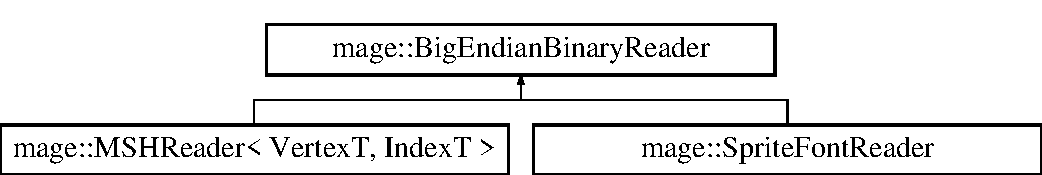
\includegraphics[height=2.000000cm]{classmage_1_1_big_endian_binary_reader}
\end{center}
\end{figure}
\subsection*{Public Member Functions}
\begin{DoxyCompactItemize}
\item 
virtual \hyperlink{classmage_1_1_big_endian_binary_reader_ae85a40e8ed06e8c887e38d914843b8d3}{$\sim$\+Big\+Endian\+Binary\+Reader} ()
\item 
\hyperlink{classmage_1_1_big_endian_binary_reader}{Big\+Endian\+Binary\+Reader} \& \hyperlink{classmage_1_1_big_endian_binary_reader_abd4b24df4219469a8c2e9253b1cad405}{operator=} (const \hyperlink{classmage_1_1_big_endian_binary_reader}{Big\+Endian\+Binary\+Reader} \&reader)=delete
\item 
\hyperlink{classmage_1_1_big_endian_binary_reader}{Big\+Endian\+Binary\+Reader} \& \hyperlink{classmage_1_1_big_endian_binary_reader_a9e2e0dd62afff04774d0246f7e5e4ce4}{operator=} (\hyperlink{classmage_1_1_big_endian_binary_reader}{Big\+Endian\+Binary\+Reader} \&\&reader)=delete
\item 
void \hyperlink{classmage_1_1_big_endian_binary_reader_a68db676feaa42c1c3a9bf16d0680b04f}{Read\+From\+File} (wstring fname)
\item 
void \hyperlink{classmage_1_1_big_endian_binary_reader_a44d2529136499412cdaf9ad5d1cf0e59}{Read\+From\+Memory} (const \hyperlink{namespacemage_afc638980bc6154f15af5e2d93a0e0ea9}{U8} $\ast$input, size\+\_\+t size)
\item 
const wstring \& \hyperlink{classmage_1_1_big_endian_binary_reader_a801558f27606dbc681809178aaaaacd1}{Get\+Filename} () const noexcept
\end{DoxyCompactItemize}
\subsection*{Protected Member Functions}
\begin{DoxyCompactItemize}
\item 
\hyperlink{classmage_1_1_big_endian_binary_reader_a1fd0dbee6950a8cb04aa399f0cdbaf2a}{Big\+Endian\+Binary\+Reader} ()
\item 
\hyperlink{classmage_1_1_big_endian_binary_reader_a9d490263268290217ae4f2f06e0699c4}{Big\+Endian\+Binary\+Reader} (const \hyperlink{classmage_1_1_big_endian_binary_reader}{Big\+Endian\+Binary\+Reader} \&reader)=delete
\item 
\hyperlink{classmage_1_1_big_endian_binary_reader_a3cb2fbd205854cf69c36054a2003e80e}{Big\+Endian\+Binary\+Reader} (\hyperlink{classmage_1_1_big_endian_binary_reader}{Big\+Endian\+Binary\+Reader} \&\&reader)
\item 
bool \hyperlink{classmage_1_1_big_endian_binary_reader_adaa45913c50d4cb54456121ba56c8afb}{Has\+Chars\+Left} () const noexcept
\item 
{\footnotesize template$<$typename DataT $>$ }\\const DataT \& \hyperlink{classmage_1_1_big_endian_binary_reader_a036399c5d3099a4e617127acb110ccdf}{Read\+Value} ()
\item 
{\footnotesize template$<$typename DataT $>$ }\\const DataT $\ast$ \hyperlink{classmage_1_1_big_endian_binary_reader_aa79d97deb6060a6c1015c8f2891ac6da}{Read\+Value\+Array} (size\+\_\+t count)
\end{DoxyCompactItemize}
\subsection*{Private Member Functions}
\begin{DoxyCompactItemize}
\item 
virtual void \hyperlink{classmage_1_1_big_endian_binary_reader_af072965dea0319d6366b21cc6562bbf9}{Read} ()=0
\end{DoxyCompactItemize}
\subsection*{Private Attributes}
\begin{DoxyCompactItemize}
\item 
wstring \hyperlink{classmage_1_1_big_endian_binary_reader_a0f836aec582a59f156b64bffb9653e41}{m\+\_\+fname}
\item 
const \hyperlink{namespacemage_afc638980bc6154f15af5e2d93a0e0ea9}{U8} $\ast$ \hyperlink{classmage_1_1_big_endian_binary_reader_a7dbfc5ce1712e431f75d80a4f7a56e33}{m\+\_\+pos}
\item 
const \hyperlink{namespacemage_afc638980bc6154f15af5e2d93a0e0ea9}{U8} $\ast$ \hyperlink{classmage_1_1_big_endian_binary_reader_ab4f707d30799b98afed0f9adfc27a3e2}{m\+\_\+end}
\item 
\hyperlink{namespacemage_a3316d7143a973e37adf1110f2e80ca31}{Unique\+Ptr}$<$ \hyperlink{namespacemage_afc638980bc6154f15af5e2d93a0e0ea9}{U8}\mbox{[}$\,$\mbox{]} $>$ \hyperlink{classmage_1_1_big_endian_binary_reader_a54128bdaa233c1bd20494189b2397fe3}{m\+\_\+data}
\end{DoxyCompactItemize}


\subsection{Detailed Description}
A class of readers for reading (big endian) binary files. 

\subsection{Constructor \& Destructor Documentation}
\hypertarget{classmage_1_1_big_endian_binary_reader_ae85a40e8ed06e8c887e38d914843b8d3}{}\label{classmage_1_1_big_endian_binary_reader_ae85a40e8ed06e8c887e38d914843b8d3} 
\index{mage\+::\+Big\+Endian\+Binary\+Reader@{mage\+::\+Big\+Endian\+Binary\+Reader}!````~Big\+Endian\+Binary\+Reader@{$\sim$\+Big\+Endian\+Binary\+Reader}}
\index{````~Big\+Endian\+Binary\+Reader@{$\sim$\+Big\+Endian\+Binary\+Reader}!mage\+::\+Big\+Endian\+Binary\+Reader@{mage\+::\+Big\+Endian\+Binary\+Reader}}
\subsubsection{\texorpdfstring{$\sim$\+Big\+Endian\+Binary\+Reader()}{~BigEndianBinaryReader()}}
{\footnotesize\ttfamily mage\+::\+Big\+Endian\+Binary\+Reader\+::$\sim$\+Big\+Endian\+Binary\+Reader (\begin{DoxyParamCaption}{ }\end{DoxyParamCaption})\hspace{0.3cm}{\ttfamily [virtual]}, {\ttfamily [default]}}

Destructs this big endian binary reader. \hypertarget{classmage_1_1_big_endian_binary_reader_a1fd0dbee6950a8cb04aa399f0cdbaf2a}{}\label{classmage_1_1_big_endian_binary_reader_a1fd0dbee6950a8cb04aa399f0cdbaf2a} 
\index{mage\+::\+Big\+Endian\+Binary\+Reader@{mage\+::\+Big\+Endian\+Binary\+Reader}!Big\+Endian\+Binary\+Reader@{Big\+Endian\+Binary\+Reader}}
\index{Big\+Endian\+Binary\+Reader@{Big\+Endian\+Binary\+Reader}!mage\+::\+Big\+Endian\+Binary\+Reader@{mage\+::\+Big\+Endian\+Binary\+Reader}}
\subsubsection{\texorpdfstring{Big\+Endian\+Binary\+Reader()}{BigEndianBinaryReader()}\hspace{0.1cm}{\footnotesize\ttfamily [1/3]}}
{\footnotesize\ttfamily mage\+::\+Big\+Endian\+Binary\+Reader\+::\+Big\+Endian\+Binary\+Reader (\begin{DoxyParamCaption}{ }\end{DoxyParamCaption})\hspace{0.3cm}{\ttfamily [protected]}}

Constructs a big endian binary reader. \hypertarget{classmage_1_1_big_endian_binary_reader_a9d490263268290217ae4f2f06e0699c4}{}\label{classmage_1_1_big_endian_binary_reader_a9d490263268290217ae4f2f06e0699c4} 
\index{mage\+::\+Big\+Endian\+Binary\+Reader@{mage\+::\+Big\+Endian\+Binary\+Reader}!Big\+Endian\+Binary\+Reader@{Big\+Endian\+Binary\+Reader}}
\index{Big\+Endian\+Binary\+Reader@{Big\+Endian\+Binary\+Reader}!mage\+::\+Big\+Endian\+Binary\+Reader@{mage\+::\+Big\+Endian\+Binary\+Reader}}
\subsubsection{\texorpdfstring{Big\+Endian\+Binary\+Reader()}{BigEndianBinaryReader()}\hspace{0.1cm}{\footnotesize\ttfamily [2/3]}}
{\footnotesize\ttfamily mage\+::\+Big\+Endian\+Binary\+Reader\+::\+Big\+Endian\+Binary\+Reader (\begin{DoxyParamCaption}\item[{const \hyperlink{classmage_1_1_big_endian_binary_reader}{Big\+Endian\+Binary\+Reader} \&}]{reader }\end{DoxyParamCaption})\hspace{0.3cm}{\ttfamily [protected]}, {\ttfamily [delete]}}

Constructs a big endian binary reader from the given big endian binary reader.


\begin{DoxyParams}[1]{Parameters}
\mbox{\tt in}  & {\em reader} & A reference to the big endian binary reader to copy. \\
\hline
\end{DoxyParams}
\hypertarget{classmage_1_1_big_endian_binary_reader_a3cb2fbd205854cf69c36054a2003e80e}{}\label{classmage_1_1_big_endian_binary_reader_a3cb2fbd205854cf69c36054a2003e80e} 
\index{mage\+::\+Big\+Endian\+Binary\+Reader@{mage\+::\+Big\+Endian\+Binary\+Reader}!Big\+Endian\+Binary\+Reader@{Big\+Endian\+Binary\+Reader}}
\index{Big\+Endian\+Binary\+Reader@{Big\+Endian\+Binary\+Reader}!mage\+::\+Big\+Endian\+Binary\+Reader@{mage\+::\+Big\+Endian\+Binary\+Reader}}
\subsubsection{\texorpdfstring{Big\+Endian\+Binary\+Reader()}{BigEndianBinaryReader()}\hspace{0.1cm}{\footnotesize\ttfamily [3/3]}}
{\footnotesize\ttfamily mage\+::\+Big\+Endian\+Binary\+Reader\+::\+Big\+Endian\+Binary\+Reader (\begin{DoxyParamCaption}\item[{\hyperlink{classmage_1_1_big_endian_binary_reader}{Big\+Endian\+Binary\+Reader} \&\&}]{reader }\end{DoxyParamCaption})\hspace{0.3cm}{\ttfamily [protected]}, {\ttfamily [default]}}

Constructs a big endian binary reader by moving the given big endian binary reader.


\begin{DoxyParams}[1]{Parameters}
\mbox{\tt in}  & {\em reader} & A reference to the big endian binary reader to move. \\
\hline
\end{DoxyParams}


\subsection{Member Function Documentation}
\hypertarget{classmage_1_1_big_endian_binary_reader_a801558f27606dbc681809178aaaaacd1}{}\label{classmage_1_1_big_endian_binary_reader_a801558f27606dbc681809178aaaaacd1} 
\index{mage\+::\+Big\+Endian\+Binary\+Reader@{mage\+::\+Big\+Endian\+Binary\+Reader}!Get\+Filename@{Get\+Filename}}
\index{Get\+Filename@{Get\+Filename}!mage\+::\+Big\+Endian\+Binary\+Reader@{mage\+::\+Big\+Endian\+Binary\+Reader}}
\subsubsection{\texorpdfstring{Get\+Filename()}{GetFilename()}}
{\footnotesize\ttfamily const wstring\& mage\+::\+Big\+Endian\+Binary\+Reader\+::\+Get\+Filename (\begin{DoxyParamCaption}{ }\end{DoxyParamCaption}) const\hspace{0.3cm}{\ttfamily [noexcept]}}

Returns the current filename of this big endian binary reader.

\begin{DoxyReturn}{Returns}
A reference to the current filename of this big endian binary reader. 
\end{DoxyReturn}
\hypertarget{classmage_1_1_big_endian_binary_reader_adaa45913c50d4cb54456121ba56c8afb}{}\label{classmage_1_1_big_endian_binary_reader_adaa45913c50d4cb54456121ba56c8afb} 
\index{mage\+::\+Big\+Endian\+Binary\+Reader@{mage\+::\+Big\+Endian\+Binary\+Reader}!Has\+Chars\+Left@{Has\+Chars\+Left}}
\index{Has\+Chars\+Left@{Has\+Chars\+Left}!mage\+::\+Big\+Endian\+Binary\+Reader@{mage\+::\+Big\+Endian\+Binary\+Reader}}
\subsubsection{\texorpdfstring{Has\+Chars\+Left()}{HasCharsLeft()}}
{\footnotesize\ttfamily bool mage\+::\+Big\+Endian\+Binary\+Reader\+::\+Has\+Chars\+Left (\begin{DoxyParamCaption}{ }\end{DoxyParamCaption}) const\hspace{0.3cm}{\ttfamily [protected]}, {\ttfamily [noexcept]}}

Checks if there are characters left to read by this binary reader.

\begin{DoxyReturn}{Returns}
{\ttfamily true} if there are characters left to read by this binary reader. {\ttfamily false} otherwise. 
\end{DoxyReturn}
\hypertarget{classmage_1_1_big_endian_binary_reader_abd4b24df4219469a8c2e9253b1cad405}{}\label{classmage_1_1_big_endian_binary_reader_abd4b24df4219469a8c2e9253b1cad405} 
\index{mage\+::\+Big\+Endian\+Binary\+Reader@{mage\+::\+Big\+Endian\+Binary\+Reader}!operator=@{operator=}}
\index{operator=@{operator=}!mage\+::\+Big\+Endian\+Binary\+Reader@{mage\+::\+Big\+Endian\+Binary\+Reader}}
\subsubsection{\texorpdfstring{operator=()}{operator=()}\hspace{0.1cm}{\footnotesize\ttfamily [1/2]}}
{\footnotesize\ttfamily \hyperlink{classmage_1_1_big_endian_binary_reader}{Big\+Endian\+Binary\+Reader}\& mage\+::\+Big\+Endian\+Binary\+Reader\+::operator= (\begin{DoxyParamCaption}\item[{const \hyperlink{classmage_1_1_big_endian_binary_reader}{Big\+Endian\+Binary\+Reader} \&}]{reader }\end{DoxyParamCaption})\hspace{0.3cm}{\ttfamily [delete]}}

Copies the given big endian binary reader to this big endian binary reader.


\begin{DoxyParams}[1]{Parameters}
\mbox{\tt in}  & {\em reader} & A reference to a big endian binary reader to copy. \\
\hline
\end{DoxyParams}
\begin{DoxyReturn}{Returns}
A reference to the copy of the given big endian binary reader (i.\+e. this big endian binary reader). 
\end{DoxyReturn}
\hypertarget{classmage_1_1_big_endian_binary_reader_a9e2e0dd62afff04774d0246f7e5e4ce4}{}\label{classmage_1_1_big_endian_binary_reader_a9e2e0dd62afff04774d0246f7e5e4ce4} 
\index{mage\+::\+Big\+Endian\+Binary\+Reader@{mage\+::\+Big\+Endian\+Binary\+Reader}!operator=@{operator=}}
\index{operator=@{operator=}!mage\+::\+Big\+Endian\+Binary\+Reader@{mage\+::\+Big\+Endian\+Binary\+Reader}}
\subsubsection{\texorpdfstring{operator=()}{operator=()}\hspace{0.1cm}{\footnotesize\ttfamily [2/2]}}
{\footnotesize\ttfamily \hyperlink{classmage_1_1_big_endian_binary_reader}{Big\+Endian\+Binary\+Reader}\& mage\+::\+Big\+Endian\+Binary\+Reader\+::operator= (\begin{DoxyParamCaption}\item[{\hyperlink{classmage_1_1_big_endian_binary_reader}{Big\+Endian\+Binary\+Reader} \&\&}]{reader }\end{DoxyParamCaption})\hspace{0.3cm}{\ttfamily [delete]}}

Moves the given big endian binary reader to this big endian binary reader.


\begin{DoxyParams}[1]{Parameters}
\mbox{\tt in}  & {\em reader} & A reference to a big endian binary reader to move. \\
\hline
\end{DoxyParams}
\begin{DoxyReturn}{Returns}
A reference to the moved big endian binary reader (i.\+e. this big endian binary reader). 
\end{DoxyReturn}
\hypertarget{classmage_1_1_big_endian_binary_reader_af072965dea0319d6366b21cc6562bbf9}{}\label{classmage_1_1_big_endian_binary_reader_af072965dea0319d6366b21cc6562bbf9} 
\index{mage\+::\+Big\+Endian\+Binary\+Reader@{mage\+::\+Big\+Endian\+Binary\+Reader}!Read@{Read}}
\index{Read@{Read}!mage\+::\+Big\+Endian\+Binary\+Reader@{mage\+::\+Big\+Endian\+Binary\+Reader}}
\subsubsection{\texorpdfstring{Read()}{Read()}}
{\footnotesize\ttfamily virtual void mage\+::\+Big\+Endian\+Binary\+Reader\+::\+Read (\begin{DoxyParamCaption}{ }\end{DoxyParamCaption})\hspace{0.3cm}{\ttfamily [private]}, {\ttfamily [pure virtual]}}

Starts reading.


\begin{DoxyExceptions}{Exceptions}
{\em \hyperlink{classmage_1_1_formatted_exception}{Formatted\+Exception}} & Failed to read to the given file. \\
\hline
\end{DoxyExceptions}


Implemented in \hyperlink{classmage_1_1_m_s_h_reader_a26b60060bf61183fb5758a4725c6a205}{mage\+::\+M\+S\+H\+Reader$<$ Vertex\+T, Index\+T $>$}, and \hyperlink{classmage_1_1_sprite_font_reader_af380ae127285a88ae41e35a9067db412}{mage\+::\+Sprite\+Font\+Reader}.

\hypertarget{classmage_1_1_big_endian_binary_reader_a68db676feaa42c1c3a9bf16d0680b04f}{}\label{classmage_1_1_big_endian_binary_reader_a68db676feaa42c1c3a9bf16d0680b04f} 
\index{mage\+::\+Big\+Endian\+Binary\+Reader@{mage\+::\+Big\+Endian\+Binary\+Reader}!Read\+From\+File@{Read\+From\+File}}
\index{Read\+From\+File@{Read\+From\+File}!mage\+::\+Big\+Endian\+Binary\+Reader@{mage\+::\+Big\+Endian\+Binary\+Reader}}
\subsubsection{\texorpdfstring{Read\+From\+File()}{ReadFromFile()}}
{\footnotesize\ttfamily void mage\+::\+Big\+Endian\+Binary\+Reader\+::\+Read\+From\+File (\begin{DoxyParamCaption}\item[{wstring}]{fname }\end{DoxyParamCaption})}

Reads from the given file.


\begin{DoxyParams}[1]{Parameters}
\mbox{\tt in}  & {\em fname} & The file name. \\
\hline
\end{DoxyParams}

\begin{DoxyExceptions}{Exceptions}
{\em \hyperlink{classmage_1_1_formatted_exception}{Formatted\+Exception}} & Failed to read from the given file. \\
\hline
\end{DoxyExceptions}
\hypertarget{classmage_1_1_big_endian_binary_reader_a44d2529136499412cdaf9ad5d1cf0e59}{}\label{classmage_1_1_big_endian_binary_reader_a44d2529136499412cdaf9ad5d1cf0e59} 
\index{mage\+::\+Big\+Endian\+Binary\+Reader@{mage\+::\+Big\+Endian\+Binary\+Reader}!Read\+From\+Memory@{Read\+From\+Memory}}
\index{Read\+From\+Memory@{Read\+From\+Memory}!mage\+::\+Big\+Endian\+Binary\+Reader@{mage\+::\+Big\+Endian\+Binary\+Reader}}
\subsubsection{\texorpdfstring{Read\+From\+Memory()}{ReadFromMemory()}}
{\footnotesize\ttfamily void mage\+::\+Big\+Endian\+Binary\+Reader\+::\+Read\+From\+Memory (\begin{DoxyParamCaption}\item[{const \hyperlink{namespacemage_afc638980bc6154f15af5e2d93a0e0ea9}{U8} $\ast$}]{input,  }\item[{size\+\_\+t}]{size }\end{DoxyParamCaption})}

Reads the input string.

\begin{DoxyPrecond}{Precondition}
{\itshape input} is not equal to {\ttfamily nullptr}. 
\end{DoxyPrecond}

\begin{DoxyParams}[1]{Parameters}
\mbox{\tt in}  & {\em input} & A pointer to the input byte string. \\
\hline
\mbox{\tt in}  & {\em size} & The size of the input string. \\
\hline
\end{DoxyParams}

\begin{DoxyExceptions}{Exceptions}
{\em \hyperlink{classmage_1_1_formatted_exception}{Formatted\+Exception}} & Failed to read from the given input string. \\
\hline
\end{DoxyExceptions}
\hypertarget{classmage_1_1_big_endian_binary_reader_a036399c5d3099a4e617127acb110ccdf}{}\label{classmage_1_1_big_endian_binary_reader_a036399c5d3099a4e617127acb110ccdf} 
\index{mage\+::\+Big\+Endian\+Binary\+Reader@{mage\+::\+Big\+Endian\+Binary\+Reader}!Read\+Value@{Read\+Value}}
\index{Read\+Value@{Read\+Value}!mage\+::\+Big\+Endian\+Binary\+Reader@{mage\+::\+Big\+Endian\+Binary\+Reader}}
\subsubsection{\texorpdfstring{Read\+Value()}{ReadValue()}}
{\footnotesize\ttfamily template$<$typename DataT $>$ \\
const DataT\& mage\+::\+Big\+Endian\+Binary\+Reader\+::\+Read\+Value (\begin{DoxyParamCaption}{ }\end{DoxyParamCaption})\hspace{0.3cm}{\ttfamily [protected]}}

Reads a {\ttfamily DataT} element.


\begin{DoxyTemplParams}{Template Parameters}
{\em DataT} & The data type. \\
\hline
\end{DoxyTemplParams}
\begin{DoxyReturn}{Returns}
A reference to the {\ttfamily DataT} element read. 
\end{DoxyReturn}

\begin{DoxyExceptions}{Exceptions}
{\em \hyperlink{classmage_1_1_formatted_exception}{Formatted\+Exception}} & Failed to read a {\ttfamily DataT} element. \\
\hline
\end{DoxyExceptions}
\hypertarget{classmage_1_1_big_endian_binary_reader_aa79d97deb6060a6c1015c8f2891ac6da}{}\label{classmage_1_1_big_endian_binary_reader_aa79d97deb6060a6c1015c8f2891ac6da} 
\index{mage\+::\+Big\+Endian\+Binary\+Reader@{mage\+::\+Big\+Endian\+Binary\+Reader}!Read\+Value\+Array@{Read\+Value\+Array}}
\index{Read\+Value\+Array@{Read\+Value\+Array}!mage\+::\+Big\+Endian\+Binary\+Reader@{mage\+::\+Big\+Endian\+Binary\+Reader}}
\subsubsection{\texorpdfstring{Read\+Value\+Array()}{ReadValueArray()}}
{\footnotesize\ttfamily template$<$typename DataT $>$ \\
const DataT$\ast$ mage\+::\+Big\+Endian\+Binary\+Reader\+::\+Read\+Value\+Array (\begin{DoxyParamCaption}\item[{size\+\_\+t}]{count }\end{DoxyParamCaption})\hspace{0.3cm}{\ttfamily [protected]}}

Reads an array of {\ttfamily DataT} elements.


\begin{DoxyTemplParams}{Template Parameters}
{\em DataT} & The data type. \\
\hline
\end{DoxyTemplParams}

\begin{DoxyParams}{Parameters}
{\em count} & The number of {\ttfamily DataT} elements to read. \\
\hline
\end{DoxyParams}
\begin{DoxyReturn}{Returns}
A pointer to the array of {\ttfamily DataT} element read. 
\end{DoxyReturn}

\begin{DoxyExceptions}{Exceptions}
{\em \hyperlink{classmage_1_1_formatted_exception}{Formatted\+Exception}} & Failed to read {\ttfamily count} {\ttfamily DataT} elements. \\
\hline
\end{DoxyExceptions}


\subsection{Member Data Documentation}
\hypertarget{classmage_1_1_big_endian_binary_reader_a54128bdaa233c1bd20494189b2397fe3}{}\label{classmage_1_1_big_endian_binary_reader_a54128bdaa233c1bd20494189b2397fe3} 
\index{mage\+::\+Big\+Endian\+Binary\+Reader@{mage\+::\+Big\+Endian\+Binary\+Reader}!m\+\_\+data@{m\+\_\+data}}
\index{m\+\_\+data@{m\+\_\+data}!mage\+::\+Big\+Endian\+Binary\+Reader@{mage\+::\+Big\+Endian\+Binary\+Reader}}
\subsubsection{\texorpdfstring{m\+\_\+data}{m\_data}}
{\footnotesize\ttfamily \hyperlink{namespacemage_a3316d7143a973e37adf1110f2e80ca31}{Unique\+Ptr}$<$ \hyperlink{namespacemage_afc638980bc6154f15af5e2d93a0e0ea9}{U8}\mbox{[}$\,$\mbox{]} $>$ mage\+::\+Big\+Endian\+Binary\+Reader\+::m\+\_\+data\hspace{0.3cm}{\ttfamily [private]}}

A pointer to the data to read of this binary reader. \hypertarget{classmage_1_1_big_endian_binary_reader_ab4f707d30799b98afed0f9adfc27a3e2}{}\label{classmage_1_1_big_endian_binary_reader_ab4f707d30799b98afed0f9adfc27a3e2} 
\index{mage\+::\+Big\+Endian\+Binary\+Reader@{mage\+::\+Big\+Endian\+Binary\+Reader}!m\+\_\+end@{m\+\_\+end}}
\index{m\+\_\+end@{m\+\_\+end}!mage\+::\+Big\+Endian\+Binary\+Reader@{mage\+::\+Big\+Endian\+Binary\+Reader}}
\subsubsection{\texorpdfstring{m\+\_\+end}{m\_end}}
{\footnotesize\ttfamily const \hyperlink{namespacemage_afc638980bc6154f15af5e2d93a0e0ea9}{U8}$\ast$ mage\+::\+Big\+Endian\+Binary\+Reader\+::m\+\_\+end\hspace{0.3cm}{\ttfamily [private]}}

A pointer to the end position of this binary reader. \hypertarget{classmage_1_1_big_endian_binary_reader_a0f836aec582a59f156b64bffb9653e41}{}\label{classmage_1_1_big_endian_binary_reader_a0f836aec582a59f156b64bffb9653e41} 
\index{mage\+::\+Big\+Endian\+Binary\+Reader@{mage\+::\+Big\+Endian\+Binary\+Reader}!m\+\_\+fname@{m\+\_\+fname}}
\index{m\+\_\+fname@{m\+\_\+fname}!mage\+::\+Big\+Endian\+Binary\+Reader@{mage\+::\+Big\+Endian\+Binary\+Reader}}
\subsubsection{\texorpdfstring{m\+\_\+fname}{m\_fname}}
{\footnotesize\ttfamily wstring mage\+::\+Big\+Endian\+Binary\+Reader\+::m\+\_\+fname\hspace{0.3cm}{\ttfamily [private]}}

The current filename of this line reader. \hypertarget{classmage_1_1_big_endian_binary_reader_a7dbfc5ce1712e431f75d80a4f7a56e33}{}\label{classmage_1_1_big_endian_binary_reader_a7dbfc5ce1712e431f75d80a4f7a56e33} 
\index{mage\+::\+Big\+Endian\+Binary\+Reader@{mage\+::\+Big\+Endian\+Binary\+Reader}!m\+\_\+pos@{m\+\_\+pos}}
\index{m\+\_\+pos@{m\+\_\+pos}!mage\+::\+Big\+Endian\+Binary\+Reader@{mage\+::\+Big\+Endian\+Binary\+Reader}}
\subsubsection{\texorpdfstring{m\+\_\+pos}{m\_pos}}
{\footnotesize\ttfamily const \hyperlink{namespacemage_afc638980bc6154f15af5e2d93a0e0ea9}{U8}$\ast$ mage\+::\+Big\+Endian\+Binary\+Reader\+::m\+\_\+pos\hspace{0.3cm}{\ttfamily [private]}}

A pointer to the current position of this binary reader. 
\hypertarget{classmage_1_1_big_endian_binary_writer}{}\section{mage\+:\+:Big\+Endian\+Binary\+Writer Class Reference}
\label{classmage_1_1_big_endian_binary_writer}\index{mage\+::\+Big\+Endian\+Binary\+Writer@{mage\+::\+Big\+Endian\+Binary\+Writer}}


{\ttfamily \#include $<$binary\+\_\+writer.\+hpp$>$}

Inheritance diagram for mage\+:\+:Big\+Endian\+Binary\+Writer\+:\begin{figure}[H]
\begin{center}
\leavevmode
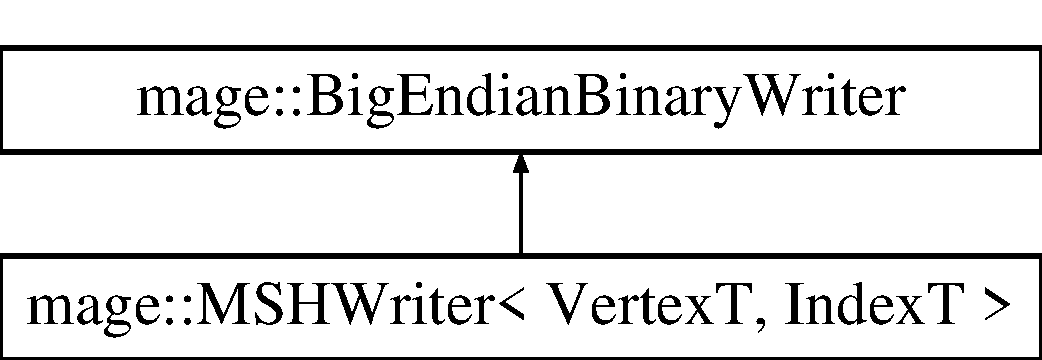
\includegraphics[height=2.000000cm]{classmage_1_1_big_endian_binary_writer}
\end{center}
\end{figure}
\subsection*{Public Member Functions}
\begin{DoxyCompactItemize}
\item 
\mbox{\hyperlink{classmage_1_1_big_endian_binary_writer}{Big\+Endian\+Binary\+Writer}} \& \mbox{\hyperlink{classmage_1_1_big_endian_binary_writer_ae574f7d0b630890256996c52818ba633}{operator=}} (const \mbox{\hyperlink{classmage_1_1_big_endian_binary_writer}{Big\+Endian\+Binary\+Writer}} \&writer)=delete
\item 
\mbox{\hyperlink{classmage_1_1_big_endian_binary_writer}{Big\+Endian\+Binary\+Writer}} \& \mbox{\hyperlink{classmage_1_1_big_endian_binary_writer_a8c01bf43f5e941578c5c5947ea184a78}{operator=}} (\mbox{\hyperlink{classmage_1_1_big_endian_binary_writer}{Big\+Endian\+Binary\+Writer}} \&\&writer) noexcept
\item 
void \mbox{\hyperlink{classmage_1_1_big_endian_binary_writer_a6ce9780687a45a6c6f98e0843190b63b}{Write\+To\+File}} (std\+::filesystem\+::path path)
\end{DoxyCompactItemize}
\subsection*{Protected Member Functions}
\begin{DoxyCompactItemize}
\item 
\mbox{\hyperlink{classmage_1_1_big_endian_binary_writer_ac0917b684913834577d4850269a6c09a}{Big\+Endian\+Binary\+Writer}} ()
\item 
\mbox{\hyperlink{classmage_1_1_big_endian_binary_writer_aafe65752342b2740e7293878ae469d9f}{Big\+Endian\+Binary\+Writer}} (const \mbox{\hyperlink{classmage_1_1_big_endian_binary_writer}{Big\+Endian\+Binary\+Writer}} \&writer)=delete
\item 
\mbox{\hyperlink{classmage_1_1_big_endian_binary_writer_aaf2dcf536afefc7b0ca8b0752024311d}{Big\+Endian\+Binary\+Writer}} (\mbox{\hyperlink{classmage_1_1_big_endian_binary_writer}{Big\+Endian\+Binary\+Writer}} \&\&writer) noexcept
\item 
\mbox{\hyperlink{classmage_1_1_big_endian_binary_writer_ab717bcbfc15ba4a1cb25eeb564e120b8}{$\sim$\+Big\+Endian\+Binary\+Writer}} ()
\item 
const std\+::filesystem\+::path \& \mbox{\hyperlink{classmage_1_1_big_endian_binary_writer_a812e65c16bf1b14d396d109eb969eeb8}{Get\+Path}} () const noexcept
\item 
{\footnotesize template$<$typename T $>$ }\\void \mbox{\hyperlink{classmage_1_1_big_endian_binary_writer_ae8bab2d7022672e1d30991c1288d981c}{Write}} (const T \&data)
\item 
{\footnotesize template$<$typename T $>$ }\\void \mbox{\hyperlink{classmage_1_1_big_endian_binary_writer_a7c82860ea3eed12777207cd00436b6c3}{Write\+Array}} (gsl\+::span$<$ const T $>$ data)
\item 
void \mbox{\hyperlink{classmage_1_1_big_endian_binary_writer_a869eff3f6e0666406bd5470af3e02096}{Write\+Character}} (char c)
\item 
void \mbox{\hyperlink{classmage_1_1_big_endian_binary_writer_acf065a2e7462c9e6cf46849bd2c9d2e7}{Write\+String}} (\mbox{\hyperlink{namespacemage_a8769f9d670d6b585ea306cb1062af94b}{Not\+Null}}$<$ \mbox{\hyperlink{namespacemage_abfd9206dc607ceb5d13ec68bf075a5c0}{const\+\_\+zstring}} $>$ str)
\end{DoxyCompactItemize}
\subsection*{Private Member Functions}
\begin{DoxyCompactItemize}
\item 
virtual void \mbox{\hyperlink{classmage_1_1_big_endian_binary_writer_a719581274b1b185ef05687183f7ded25}{Write\+Data}} ()=0
\end{DoxyCompactItemize}
\subsection*{Private Attributes}
\begin{DoxyCompactItemize}
\item 
\mbox{\hyperlink{namespacemage_ac11c62400d336d9f6857c7cdaecfc7a8}{Unique\+File\+Stream}} \mbox{\hyperlink{classmage_1_1_big_endian_binary_writer_ad2cdbdca429d6c351a57b51d175ffb55}{m\+\_\+file\+\_\+stream}}
\item 
std\+::filesystem\+::path \mbox{\hyperlink{classmage_1_1_big_endian_binary_writer_a22815e47cf8bf3443c10ec2ff4409745}{m\+\_\+path}}
\end{DoxyCompactItemize}


\subsection{Detailed Description}
A class of writers for writing (big endian) binary files. 

\subsection{Constructor \& Destructor Documentation}
\mbox{\Hypertarget{classmage_1_1_big_endian_binary_writer_ac0917b684913834577d4850269a6c09a}\label{classmage_1_1_big_endian_binary_writer_ac0917b684913834577d4850269a6c09a}} 
\index{mage\+::\+Big\+Endian\+Binary\+Writer@{mage\+::\+Big\+Endian\+Binary\+Writer}!Big\+Endian\+Binary\+Writer@{Big\+Endian\+Binary\+Writer}}
\index{Big\+Endian\+Binary\+Writer@{Big\+Endian\+Binary\+Writer}!mage\+::\+Big\+Endian\+Binary\+Writer@{mage\+::\+Big\+Endian\+Binary\+Writer}}
\subsubsection{\texorpdfstring{Big\+Endian\+Binary\+Writer()}{BigEndianBinaryWriter()}\hspace{0.1cm}{\footnotesize\ttfamily [1/3]}}
{\footnotesize\ttfamily mage\+::\+Big\+Endian\+Binary\+Writer\+::\+Big\+Endian\+Binary\+Writer (\begin{DoxyParamCaption}{ }\end{DoxyParamCaption})\hspace{0.3cm}{\ttfamily [protected]}}

Constructs a big endian binary writer. \mbox{\Hypertarget{classmage_1_1_big_endian_binary_writer_aafe65752342b2740e7293878ae469d9f}\label{classmage_1_1_big_endian_binary_writer_aafe65752342b2740e7293878ae469d9f}} 
\index{mage\+::\+Big\+Endian\+Binary\+Writer@{mage\+::\+Big\+Endian\+Binary\+Writer}!Big\+Endian\+Binary\+Writer@{Big\+Endian\+Binary\+Writer}}
\index{Big\+Endian\+Binary\+Writer@{Big\+Endian\+Binary\+Writer}!mage\+::\+Big\+Endian\+Binary\+Writer@{mage\+::\+Big\+Endian\+Binary\+Writer}}
\subsubsection{\texorpdfstring{Big\+Endian\+Binary\+Writer()}{BigEndianBinaryWriter()}\hspace{0.1cm}{\footnotesize\ttfamily [2/3]}}
{\footnotesize\ttfamily mage\+::\+Big\+Endian\+Binary\+Writer\+::\+Big\+Endian\+Binary\+Writer (\begin{DoxyParamCaption}\item[{const \mbox{\hyperlink{classmage_1_1_big_endian_binary_writer}{Big\+Endian\+Binary\+Writer}} \&}]{writer }\end{DoxyParamCaption})\hspace{0.3cm}{\ttfamily [protected]}, {\ttfamily [delete]}}

Constructs a big endian binary writer from the given big endian binary writer.


\begin{DoxyParams}[1]{Parameters}
\mbox{\tt in}  & {\em writer} & A reference to the big endian binary writer to copy. \\
\hline
\end{DoxyParams}
\mbox{\Hypertarget{classmage_1_1_big_endian_binary_writer_aaf2dcf536afefc7b0ca8b0752024311d}\label{classmage_1_1_big_endian_binary_writer_aaf2dcf536afefc7b0ca8b0752024311d}} 
\index{mage\+::\+Big\+Endian\+Binary\+Writer@{mage\+::\+Big\+Endian\+Binary\+Writer}!Big\+Endian\+Binary\+Writer@{Big\+Endian\+Binary\+Writer}}
\index{Big\+Endian\+Binary\+Writer@{Big\+Endian\+Binary\+Writer}!mage\+::\+Big\+Endian\+Binary\+Writer@{mage\+::\+Big\+Endian\+Binary\+Writer}}
\subsubsection{\texorpdfstring{Big\+Endian\+Binary\+Writer()}{BigEndianBinaryWriter()}\hspace{0.1cm}{\footnotesize\ttfamily [3/3]}}
{\footnotesize\ttfamily mage\+::\+Big\+Endian\+Binary\+Writer\+::\+Big\+Endian\+Binary\+Writer (\begin{DoxyParamCaption}\item[{\mbox{\hyperlink{classmage_1_1_big_endian_binary_writer}{Big\+Endian\+Binary\+Writer}} \&\&}]{writer }\end{DoxyParamCaption})\hspace{0.3cm}{\ttfamily [protected]}, {\ttfamily [default]}, {\ttfamily [noexcept]}}

Constructs a big endian binary writer by moving the given big endian binary writer.


\begin{DoxyParams}[1]{Parameters}
\mbox{\tt in}  & {\em writer} & A reference to the big endian binary writer to move. \\
\hline
\end{DoxyParams}
\mbox{\Hypertarget{classmage_1_1_big_endian_binary_writer_ab717bcbfc15ba4a1cb25eeb564e120b8}\label{classmage_1_1_big_endian_binary_writer_ab717bcbfc15ba4a1cb25eeb564e120b8}} 
\index{mage\+::\+Big\+Endian\+Binary\+Writer@{mage\+::\+Big\+Endian\+Binary\+Writer}!````~Big\+Endian\+Binary\+Writer@{$\sim$\+Big\+Endian\+Binary\+Writer}}
\index{````~Big\+Endian\+Binary\+Writer@{$\sim$\+Big\+Endian\+Binary\+Writer}!mage\+::\+Big\+Endian\+Binary\+Writer@{mage\+::\+Big\+Endian\+Binary\+Writer}}
\subsubsection{\texorpdfstring{$\sim$\+Big\+Endian\+Binary\+Writer()}{~BigEndianBinaryWriter()}}
{\footnotesize\ttfamily mage\+::\+Big\+Endian\+Binary\+Writer\+::$\sim$\+Big\+Endian\+Binary\+Writer (\begin{DoxyParamCaption}{ }\end{DoxyParamCaption})\hspace{0.3cm}{\ttfamily [protected]}, {\ttfamily [default]}}

Destructs this big endian binary writer. 

\subsection{Member Function Documentation}
\mbox{\Hypertarget{classmage_1_1_big_endian_binary_writer_a812e65c16bf1b14d396d109eb969eeb8}\label{classmage_1_1_big_endian_binary_writer_a812e65c16bf1b14d396d109eb969eeb8}} 
\index{mage\+::\+Big\+Endian\+Binary\+Writer@{mage\+::\+Big\+Endian\+Binary\+Writer}!Get\+Path@{Get\+Path}}
\index{Get\+Path@{Get\+Path}!mage\+::\+Big\+Endian\+Binary\+Writer@{mage\+::\+Big\+Endian\+Binary\+Writer}}
\subsubsection{\texorpdfstring{Get\+Path()}{GetPath()}}
{\footnotesize\ttfamily const std\+::filesystem\+::path\& mage\+::\+Big\+Endian\+Binary\+Writer\+::\+Get\+Path (\begin{DoxyParamCaption}{ }\end{DoxyParamCaption}) const\hspace{0.3cm}{\ttfamily [protected]}, {\ttfamily [noexcept]}}

Returns the current path of this big endian binary writer.

\begin{DoxyReturn}{Returns}
A reference to the current path of this big endian binary writer. 
\end{DoxyReturn}
\mbox{\Hypertarget{classmage_1_1_big_endian_binary_writer_ae574f7d0b630890256996c52818ba633}\label{classmage_1_1_big_endian_binary_writer_ae574f7d0b630890256996c52818ba633}} 
\index{mage\+::\+Big\+Endian\+Binary\+Writer@{mage\+::\+Big\+Endian\+Binary\+Writer}!operator=@{operator=}}
\index{operator=@{operator=}!mage\+::\+Big\+Endian\+Binary\+Writer@{mage\+::\+Big\+Endian\+Binary\+Writer}}
\subsubsection{\texorpdfstring{operator=()}{operator=()}\hspace{0.1cm}{\footnotesize\ttfamily [1/2]}}
{\footnotesize\ttfamily \mbox{\hyperlink{classmage_1_1_big_endian_binary_writer}{Big\+Endian\+Binary\+Writer}}\& mage\+::\+Big\+Endian\+Binary\+Writer\+::operator= (\begin{DoxyParamCaption}\item[{const \mbox{\hyperlink{classmage_1_1_big_endian_binary_writer}{Big\+Endian\+Binary\+Writer}} \&}]{writer }\end{DoxyParamCaption})\hspace{0.3cm}{\ttfamily [delete]}}

Copies the given big endian binary writer to this big endian binary writer.


\begin{DoxyParams}[1]{Parameters}
\mbox{\tt in}  & {\em writer} & A reference to a big endian binary writer to copy. \\
\hline
\end{DoxyParams}
\begin{DoxyReturn}{Returns}
A reference to the copy of the given big endian binary writer (i.\+e. this big endian binary writer). 
\end{DoxyReturn}
\mbox{\Hypertarget{classmage_1_1_big_endian_binary_writer_a8c01bf43f5e941578c5c5947ea184a78}\label{classmage_1_1_big_endian_binary_writer_a8c01bf43f5e941578c5c5947ea184a78}} 
\index{mage\+::\+Big\+Endian\+Binary\+Writer@{mage\+::\+Big\+Endian\+Binary\+Writer}!operator=@{operator=}}
\index{operator=@{operator=}!mage\+::\+Big\+Endian\+Binary\+Writer@{mage\+::\+Big\+Endian\+Binary\+Writer}}
\subsubsection{\texorpdfstring{operator=()}{operator=()}\hspace{0.1cm}{\footnotesize\ttfamily [2/2]}}
{\footnotesize\ttfamily \mbox{\hyperlink{classmage_1_1_big_endian_binary_writer}{Big\+Endian\+Binary\+Writer}} \& mage\+::\+Big\+Endian\+Binary\+Writer\+::operator= (\begin{DoxyParamCaption}\item[{\mbox{\hyperlink{classmage_1_1_big_endian_binary_writer}{Big\+Endian\+Binary\+Writer}} \&\&}]{writer }\end{DoxyParamCaption})\hspace{0.3cm}{\ttfamily [default]}, {\ttfamily [noexcept]}}

Moves the given big endian binary writer to this big endian binary writer.


\begin{DoxyParams}[1]{Parameters}
\mbox{\tt in}  & {\em writer} & A reference to a big endian binary writer to move. \\
\hline
\end{DoxyParams}
\begin{DoxyReturn}{Returns}
A reference to the moved big endian binary writer (i.\+e. this big endian binary writer). 
\end{DoxyReturn}
\mbox{\Hypertarget{classmage_1_1_big_endian_binary_writer_ae8bab2d7022672e1d30991c1288d981c}\label{classmage_1_1_big_endian_binary_writer_ae8bab2d7022672e1d30991c1288d981c}} 
\index{mage\+::\+Big\+Endian\+Binary\+Writer@{mage\+::\+Big\+Endian\+Binary\+Writer}!Write@{Write}}
\index{Write@{Write}!mage\+::\+Big\+Endian\+Binary\+Writer@{mage\+::\+Big\+Endian\+Binary\+Writer}}
\subsubsection{\texorpdfstring{Write()}{Write()}}
{\footnotesize\ttfamily template$<$typename T $>$ \\
void mage\+::\+Big\+Endian\+Binary\+Writer\+::\+Write (\begin{DoxyParamCaption}\item[{const T \&}]{data }\end{DoxyParamCaption})\hspace{0.3cm}{\ttfamily [protected]}}

Writes the given data.


\begin{DoxyTemplParams}{Template Parameters}
{\em T} & The data type. \\
\hline
\end{DoxyTemplParams}

\begin{DoxyParams}[1]{Parameters}
\mbox{\tt in}  & {\em data} & A reference to the data. \\
\hline
\end{DoxyParams}

\begin{DoxyExceptions}{Exceptions}
{\em \mbox{\hyperlink{classmage_1_1_exception}{Exception}}} & Failed to write the given data. \\
\hline
\end{DoxyExceptions}
\mbox{\Hypertarget{classmage_1_1_big_endian_binary_writer_a7c82860ea3eed12777207cd00436b6c3}\label{classmage_1_1_big_endian_binary_writer_a7c82860ea3eed12777207cd00436b6c3}} 
\index{mage\+::\+Big\+Endian\+Binary\+Writer@{mage\+::\+Big\+Endian\+Binary\+Writer}!Write\+Array@{Write\+Array}}
\index{Write\+Array@{Write\+Array}!mage\+::\+Big\+Endian\+Binary\+Writer@{mage\+::\+Big\+Endian\+Binary\+Writer}}
\subsubsection{\texorpdfstring{Write\+Array()}{WriteArray()}}
{\footnotesize\ttfamily template$<$typename T $>$ \\
void mage\+::\+Big\+Endian\+Binary\+Writer\+::\+Write\+Array (\begin{DoxyParamCaption}\item[{gsl\+::span$<$ const T $>$}]{data }\end{DoxyParamCaption})\hspace{0.3cm}{\ttfamily [protected]}}

Writes the given data array.


\begin{DoxyTemplParams}{Template Parameters}
{\em T} & The data type. \\
\hline
\end{DoxyTemplParams}

\begin{DoxyParams}[1]{Parameters}
\mbox{\tt in}  & {\em data} & The data array. \\
\hline
\end{DoxyParams}

\begin{DoxyExceptions}{Exceptions}
{\em \mbox{\hyperlink{classmage_1_1_exception}{Exception}}} & Failed to write the given data. \\
\hline
\end{DoxyExceptions}
\mbox{\Hypertarget{classmage_1_1_big_endian_binary_writer_a869eff3f6e0666406bd5470af3e02096}\label{classmage_1_1_big_endian_binary_writer_a869eff3f6e0666406bd5470af3e02096}} 
\index{mage\+::\+Big\+Endian\+Binary\+Writer@{mage\+::\+Big\+Endian\+Binary\+Writer}!Write\+Character@{Write\+Character}}
\index{Write\+Character@{Write\+Character}!mage\+::\+Big\+Endian\+Binary\+Writer@{mage\+::\+Big\+Endian\+Binary\+Writer}}
\subsubsection{\texorpdfstring{Write\+Character()}{WriteCharacter()}}
{\footnotesize\ttfamily void mage\+::\+Big\+Endian\+Binary\+Writer\+::\+Write\+Character (\begin{DoxyParamCaption}\item[{char}]{c }\end{DoxyParamCaption})\hspace{0.3cm}{\ttfamily [protected]}}

Writes the given character.


\begin{DoxyParams}[1]{Parameters}
\mbox{\tt in}  & {\em c} & The character to write. \\
\hline
\end{DoxyParams}

\begin{DoxyExceptions}{Exceptions}
{\em \mbox{\hyperlink{classmage_1_1_exception}{Exception}}} & Failed to write the given character. \\
\hline
\end{DoxyExceptions}
\mbox{\Hypertarget{classmage_1_1_big_endian_binary_writer_a719581274b1b185ef05687183f7ded25}\label{classmage_1_1_big_endian_binary_writer_a719581274b1b185ef05687183f7ded25}} 
\index{mage\+::\+Big\+Endian\+Binary\+Writer@{mage\+::\+Big\+Endian\+Binary\+Writer}!Write\+Data@{Write\+Data}}
\index{Write\+Data@{Write\+Data}!mage\+::\+Big\+Endian\+Binary\+Writer@{mage\+::\+Big\+Endian\+Binary\+Writer}}
\subsubsection{\texorpdfstring{Write\+Data()}{WriteData()}}
{\footnotesize\ttfamily virtual void mage\+::\+Big\+Endian\+Binary\+Writer\+::\+Write\+Data (\begin{DoxyParamCaption}{ }\end{DoxyParamCaption})\hspace{0.3cm}{\ttfamily [private]}, {\ttfamily [pure virtual]}}

Starts writing.


\begin{DoxyExceptions}{Exceptions}
{\em \mbox{\hyperlink{classmage_1_1_exception}{Exception}}} & Failed to write. \\
\hline
\end{DoxyExceptions}


Implemented in \mbox{\hyperlink{classmage_1_1rendering_1_1loader_1_1_m_s_h_writer_ad61ee7097e1bfb52ca9a0697d2cd6a7e}{mage\+::rendering\+::loader\+::\+M\+S\+H\+Writer$<$ Vertex\+T, Index\+T $>$}}.

\mbox{\Hypertarget{classmage_1_1_big_endian_binary_writer_acf065a2e7462c9e6cf46849bd2c9d2e7}\label{classmage_1_1_big_endian_binary_writer_acf065a2e7462c9e6cf46849bd2c9d2e7}} 
\index{mage\+::\+Big\+Endian\+Binary\+Writer@{mage\+::\+Big\+Endian\+Binary\+Writer}!Write\+String@{Write\+String}}
\index{Write\+String@{Write\+String}!mage\+::\+Big\+Endian\+Binary\+Writer@{mage\+::\+Big\+Endian\+Binary\+Writer}}
\subsubsection{\texorpdfstring{Write\+String()}{WriteString()}}
{\footnotesize\ttfamily void mage\+::\+Big\+Endian\+Binary\+Writer\+::\+Write\+String (\begin{DoxyParamCaption}\item[{\mbox{\hyperlink{namespacemage_a8769f9d670d6b585ea306cb1062af94b}{Not\+Null}}$<$ \mbox{\hyperlink{namespacemage_abfd9206dc607ceb5d13ec68bf075a5c0}{const\+\_\+zstring}} $>$}]{str }\end{DoxyParamCaption})\hspace{0.3cm}{\ttfamily [protected]}}

Writes the given string.


\begin{DoxyParams}[1]{Parameters}
\mbox{\tt in}  & {\em str} & A pointer to the first null-\/terminated byte string to write. \\
\hline
\end{DoxyParams}

\begin{DoxyExceptions}{Exceptions}
{\em \mbox{\hyperlink{classmage_1_1_exception}{Exception}}} & Failed to write the given string. \\
\hline
\end{DoxyExceptions}
\mbox{\Hypertarget{classmage_1_1_big_endian_binary_writer_a6ce9780687a45a6c6f98e0843190b63b}\label{classmage_1_1_big_endian_binary_writer_a6ce9780687a45a6c6f98e0843190b63b}} 
\index{mage\+::\+Big\+Endian\+Binary\+Writer@{mage\+::\+Big\+Endian\+Binary\+Writer}!Write\+To\+File@{Write\+To\+File}}
\index{Write\+To\+File@{Write\+To\+File}!mage\+::\+Big\+Endian\+Binary\+Writer@{mage\+::\+Big\+Endian\+Binary\+Writer}}
\subsubsection{\texorpdfstring{Write\+To\+File()}{WriteToFile()}}
{\footnotesize\ttfamily void mage\+::\+Big\+Endian\+Binary\+Writer\+::\+Write\+To\+File (\begin{DoxyParamCaption}\item[{std\+::filesystem\+::path}]{path }\end{DoxyParamCaption})}

Writes to the file associated with the given path.


\begin{DoxyParams}[1]{Parameters}
\mbox{\tt in}  & {\em path} & The path. \\
\hline
\end{DoxyParams}

\begin{DoxyExceptions}{Exceptions}
{\em \mbox{\hyperlink{classmage_1_1_exception}{Exception}}} & Failed to write to the file. \\
\hline
\end{DoxyExceptions}


\subsection{Member Data Documentation}
\mbox{\Hypertarget{classmage_1_1_big_endian_binary_writer_ad2cdbdca429d6c351a57b51d175ffb55}\label{classmage_1_1_big_endian_binary_writer_ad2cdbdca429d6c351a57b51d175ffb55}} 
\index{mage\+::\+Big\+Endian\+Binary\+Writer@{mage\+::\+Big\+Endian\+Binary\+Writer}!m\+\_\+file\+\_\+stream@{m\+\_\+file\+\_\+stream}}
\index{m\+\_\+file\+\_\+stream@{m\+\_\+file\+\_\+stream}!mage\+::\+Big\+Endian\+Binary\+Writer@{mage\+::\+Big\+Endian\+Binary\+Writer}}
\subsubsection{\texorpdfstring{m\+\_\+file\+\_\+stream}{m\_file\_stream}}
{\footnotesize\ttfamily \mbox{\hyperlink{namespacemage_ac11c62400d336d9f6857c7cdaecfc7a8}{Unique\+File\+Stream}} mage\+::\+Big\+Endian\+Binary\+Writer\+::m\+\_\+file\+\_\+stream\hspace{0.3cm}{\ttfamily [private]}}

A pointer to the file stream of this big endian binary writer. \mbox{\Hypertarget{classmage_1_1_big_endian_binary_writer_a22815e47cf8bf3443c10ec2ff4409745}\label{classmage_1_1_big_endian_binary_writer_a22815e47cf8bf3443c10ec2ff4409745}} 
\index{mage\+::\+Big\+Endian\+Binary\+Writer@{mage\+::\+Big\+Endian\+Binary\+Writer}!m\+\_\+path@{m\+\_\+path}}
\index{m\+\_\+path@{m\+\_\+path}!mage\+::\+Big\+Endian\+Binary\+Writer@{mage\+::\+Big\+Endian\+Binary\+Writer}}
\subsubsection{\texorpdfstring{m\+\_\+path}{m\_path}}
{\footnotesize\ttfamily std\+::filesystem\+::path mage\+::\+Big\+Endian\+Binary\+Writer\+::m\+\_\+path\hspace{0.3cm}{\ttfamily [private]}}

The current path of this big endian binary writer. 
\hypertarget{classmage_1_1_binary_reader}{}\section{mage\+:\+:Binary\+Reader Class Reference}
\label{classmage_1_1_binary_reader}\index{mage\+::\+Binary\+Reader@{mage\+::\+Binary\+Reader}}


{\ttfamily \#include $<$binary\+\_\+reader.\+hpp$>$}

\subsection*{Public Member Functions}
\begin{DoxyCompactItemize}
\item 
\hyperlink{classmage_1_1_binary_reader}{Binary\+Reader} \& \hyperlink{classmage_1_1_binary_reader_a0408bb456983b4a03ae42ab69c6f4bc3}{operator=} (const \hyperlink{classmage_1_1_binary_reader}{Binary\+Reader} \&reader)=delete
\item 
\hyperlink{classmage_1_1_binary_reader}{Binary\+Reader} \& \hyperlink{classmage_1_1_binary_reader_a280998bb89dacdcb88ec87c49ce90a02}{operator=} (\hyperlink{classmage_1_1_binary_reader}{Binary\+Reader} \&\&reader) noexcept
\item 
void \hyperlink{classmage_1_1_binary_reader_ad302abb7498cce11c0982d98973817de}{Read\+From\+File} (wstring fname, bool big\+\_\+endian)
\item 
void \hyperlink{classmage_1_1_binary_reader_a093d95a36bdc45f5d51f48f1ee09bb1f}{Read\+From\+Memory} (gsl\+::span$<$ const \hyperlink{namespacemage_afc638980bc6154f15af5e2d93a0e0ea9}{U8} $>$ input, bool big\+\_\+endian)
\item 
const wstring \& \hyperlink{classmage_1_1_binary_reader_ad9d4a4a3e2f0afc666d15badff08fe4a}{Get\+Filename} () const noexcept
\end{DoxyCompactItemize}
\subsection*{Protected Member Functions}
\begin{DoxyCompactItemize}
\item 
\hyperlink{classmage_1_1_binary_reader_aab82579cef4f2f022273cf1adfcc8497}{Binary\+Reader} ()
\item 
\hyperlink{classmage_1_1_binary_reader_a8c1ff948f1d056439f3d8cc37d7f507c}{Binary\+Reader} (const \hyperlink{classmage_1_1_binary_reader}{Binary\+Reader} \&reader)=delete
\item 
\hyperlink{classmage_1_1_binary_reader_a520841747b74b4b0e95f8d9b595492fa}{Binary\+Reader} (\hyperlink{classmage_1_1_binary_reader}{Binary\+Reader} \&\&reader) noexcept
\item 
\hyperlink{classmage_1_1_binary_reader_a42e6c31bc53f5214675f845756b5a404}{$\sim$\+Binary\+Reader} ()
\item 
bool \hyperlink{classmage_1_1_binary_reader_af68b85b30fbe8b5f2d4720163a658ab5}{Contains\+Chars} () const noexcept
\item 
\hyperlink{namespacemage_a8769f9d670d6b585ea306cb1062af94b}{Not\+Null}$<$ \hyperlink{namespacemage_abfd9206dc607ceb5d13ec68bf075a5c0}{const\+\_\+zstring} $>$ \hyperlink{classmage_1_1_binary_reader_ad2bed0756a38358fc4a8b10b02007af8}{Read\+Chars} (size\+\_\+t size)
\item 
{\footnotesize template$<$typename DataT $>$ }\\const DataT \hyperlink{classmage_1_1_binary_reader_ad914ec3edfef7a9e9976ef706be44b92}{Read} ()
\end{DoxyCompactItemize}
\subsection*{Private Member Functions}
\begin{DoxyCompactItemize}
\item 
virtual void \hyperlink{classmage_1_1_binary_reader_a67157828a9781644fb55bd7f3558f07c}{Read\+Data} ()=0
\end{DoxyCompactItemize}
\subsection*{Private Attributes}
\begin{DoxyCompactItemize}
\item 
wstring \hyperlink{classmage_1_1_binary_reader_a9c97c02d53ce60a9952751ad4f55414f}{m\+\_\+fname}
\item 
bool \hyperlink{classmage_1_1_binary_reader_a8d23fde958e08efe248edb5d92861113}{m\+\_\+big\+\_\+endian}
\item 
const \hyperlink{namespacemage_afc638980bc6154f15af5e2d93a0e0ea9}{U8} $\ast$ \hyperlink{classmage_1_1_binary_reader_aedb9632de1cf95d5af49499217744ed5}{m\+\_\+pos}
\item 
const \hyperlink{namespacemage_afc638980bc6154f15af5e2d93a0e0ea9}{U8} $\ast$ \hyperlink{classmage_1_1_binary_reader_a19b0f36cb1e8a05aaa9471514242e8ef}{m\+\_\+end}
\item 
\hyperlink{namespacemage_a3316d7143a973e37adf1110f2e80ca31}{Unique\+Ptr}$<$ \hyperlink{namespacemage_afc638980bc6154f15af5e2d93a0e0ea9}{U8}\mbox{[}$\,$\mbox{]} $>$ \hyperlink{classmage_1_1_binary_reader_a529bdcb620e1250aa0b12716c9b7eae1}{m\+\_\+data}
\end{DoxyCompactItemize}


\subsection{Detailed Description}
A class of readers for reading binary files. 

\subsection{Constructor \& Destructor Documentation}
\hypertarget{classmage_1_1_binary_reader_aab82579cef4f2f022273cf1adfcc8497}{}\label{classmage_1_1_binary_reader_aab82579cef4f2f022273cf1adfcc8497} 
\index{mage\+::\+Binary\+Reader@{mage\+::\+Binary\+Reader}!Binary\+Reader@{Binary\+Reader}}
\index{Binary\+Reader@{Binary\+Reader}!mage\+::\+Binary\+Reader@{mage\+::\+Binary\+Reader}}
\subsubsection{\texorpdfstring{Binary\+Reader()}{BinaryReader()}\hspace{0.1cm}{\footnotesize\ttfamily [1/3]}}
{\footnotesize\ttfamily mage\+::\+Binary\+Reader\+::\+Binary\+Reader (\begin{DoxyParamCaption}{ }\end{DoxyParamCaption})\hspace{0.3cm}{\ttfamily [protected]}}

Constructs a binary reader. \hypertarget{classmage_1_1_binary_reader_a8c1ff948f1d056439f3d8cc37d7f507c}{}\label{classmage_1_1_binary_reader_a8c1ff948f1d056439f3d8cc37d7f507c} 
\index{mage\+::\+Binary\+Reader@{mage\+::\+Binary\+Reader}!Binary\+Reader@{Binary\+Reader}}
\index{Binary\+Reader@{Binary\+Reader}!mage\+::\+Binary\+Reader@{mage\+::\+Binary\+Reader}}
\subsubsection{\texorpdfstring{Binary\+Reader()}{BinaryReader()}\hspace{0.1cm}{\footnotesize\ttfamily [2/3]}}
{\footnotesize\ttfamily mage\+::\+Binary\+Reader\+::\+Binary\+Reader (\begin{DoxyParamCaption}\item[{const \hyperlink{classmage_1_1_binary_reader}{Binary\+Reader} \&}]{reader }\end{DoxyParamCaption})\hspace{0.3cm}{\ttfamily [protected]}, {\ttfamily [delete]}}

Constructs a binary reader from the given binary reader.


\begin{DoxyParams}[1]{Parameters}
\mbox{\tt in}  & {\em reader} & A reference to the binary reader to copy. \\
\hline
\end{DoxyParams}
\hypertarget{classmage_1_1_binary_reader_a520841747b74b4b0e95f8d9b595492fa}{}\label{classmage_1_1_binary_reader_a520841747b74b4b0e95f8d9b595492fa} 
\index{mage\+::\+Binary\+Reader@{mage\+::\+Binary\+Reader}!Binary\+Reader@{Binary\+Reader}}
\index{Binary\+Reader@{Binary\+Reader}!mage\+::\+Binary\+Reader@{mage\+::\+Binary\+Reader}}
\subsubsection{\texorpdfstring{Binary\+Reader()}{BinaryReader()}\hspace{0.1cm}{\footnotesize\ttfamily [3/3]}}
{\footnotesize\ttfamily mage\+::\+Binary\+Reader\+::\+Binary\+Reader (\begin{DoxyParamCaption}\item[{\hyperlink{classmage_1_1_binary_reader}{Binary\+Reader} \&\&}]{reader }\end{DoxyParamCaption})\hspace{0.3cm}{\ttfamily [protected]}, {\ttfamily [default]}, {\ttfamily [noexcept]}}

Constructs a binary reader by moving the given binary reader.


\begin{DoxyParams}[1]{Parameters}
\mbox{\tt in}  & {\em reader} & A reference to the binary reader to move. \\
\hline
\end{DoxyParams}
\hypertarget{classmage_1_1_binary_reader_a42e6c31bc53f5214675f845756b5a404}{}\label{classmage_1_1_binary_reader_a42e6c31bc53f5214675f845756b5a404} 
\index{mage\+::\+Binary\+Reader@{mage\+::\+Binary\+Reader}!````~Binary\+Reader@{$\sim$\+Binary\+Reader}}
\index{````~Binary\+Reader@{$\sim$\+Binary\+Reader}!mage\+::\+Binary\+Reader@{mage\+::\+Binary\+Reader}}
\subsubsection{\texorpdfstring{$\sim$\+Binary\+Reader()}{~BinaryReader()}}
{\footnotesize\ttfamily mage\+::\+Binary\+Reader\+::$\sim$\+Binary\+Reader (\begin{DoxyParamCaption}{ }\end{DoxyParamCaption})\hspace{0.3cm}{\ttfamily [protected]}, {\ttfamily [default]}}

Destructs this binary reader. 

\subsection{Member Function Documentation}
\hypertarget{classmage_1_1_binary_reader_af68b85b30fbe8b5f2d4720163a658ab5}{}\label{classmage_1_1_binary_reader_af68b85b30fbe8b5f2d4720163a658ab5} 
\index{mage\+::\+Binary\+Reader@{mage\+::\+Binary\+Reader}!Contains\+Chars@{Contains\+Chars}}
\index{Contains\+Chars@{Contains\+Chars}!mage\+::\+Binary\+Reader@{mage\+::\+Binary\+Reader}}
\subsubsection{\texorpdfstring{Contains\+Chars()}{ContainsChars()}}
{\footnotesize\ttfamily bool mage\+::\+Binary\+Reader\+::\+Contains\+Chars (\begin{DoxyParamCaption}{ }\end{DoxyParamCaption}) const\hspace{0.3cm}{\ttfamily [protected]}, {\ttfamily [noexcept]}}

Checks if there are characters left to read by this binary reader.

\begin{DoxyReturn}{Returns}
{\ttfamily true} if there are characters left to read by this binary reader. {\ttfamily false} otherwise. 
\end{DoxyReturn}
\hypertarget{classmage_1_1_binary_reader_ad9d4a4a3e2f0afc666d15badff08fe4a}{}\label{classmage_1_1_binary_reader_ad9d4a4a3e2f0afc666d15badff08fe4a} 
\index{mage\+::\+Binary\+Reader@{mage\+::\+Binary\+Reader}!Get\+Filename@{Get\+Filename}}
\index{Get\+Filename@{Get\+Filename}!mage\+::\+Binary\+Reader@{mage\+::\+Binary\+Reader}}
\subsubsection{\texorpdfstring{Get\+Filename()}{GetFilename()}}
{\footnotesize\ttfamily const wstring\& mage\+::\+Binary\+Reader\+::\+Get\+Filename (\begin{DoxyParamCaption}{ }\end{DoxyParamCaption}) const\hspace{0.3cm}{\ttfamily [noexcept]}}

Returns the current filename of this binary reader.

\begin{DoxyReturn}{Returns}
A reference to the current filename of this binary reader. 
\end{DoxyReturn}
\hypertarget{classmage_1_1_binary_reader_a0408bb456983b4a03ae42ab69c6f4bc3}{}\label{classmage_1_1_binary_reader_a0408bb456983b4a03ae42ab69c6f4bc3} 
\index{mage\+::\+Binary\+Reader@{mage\+::\+Binary\+Reader}!operator=@{operator=}}
\index{operator=@{operator=}!mage\+::\+Binary\+Reader@{mage\+::\+Binary\+Reader}}
\subsubsection{\texorpdfstring{operator=()}{operator=()}\hspace{0.1cm}{\footnotesize\ttfamily [1/2]}}
{\footnotesize\ttfamily \hyperlink{classmage_1_1_binary_reader}{Binary\+Reader}\& mage\+::\+Binary\+Reader\+::operator= (\begin{DoxyParamCaption}\item[{const \hyperlink{classmage_1_1_binary_reader}{Binary\+Reader} \&}]{reader }\end{DoxyParamCaption})\hspace{0.3cm}{\ttfamily [delete]}}

Copies the given binary reader to this binary reader.


\begin{DoxyParams}[1]{Parameters}
\mbox{\tt in}  & {\em reader} & A reference to a binary reader to copy. \\
\hline
\end{DoxyParams}
\begin{DoxyReturn}{Returns}
A reference to the copy of the given binary reader (i.\+e. this binary reader). 
\end{DoxyReturn}
\hypertarget{classmage_1_1_binary_reader_a280998bb89dacdcb88ec87c49ce90a02}{}\label{classmage_1_1_binary_reader_a280998bb89dacdcb88ec87c49ce90a02} 
\index{mage\+::\+Binary\+Reader@{mage\+::\+Binary\+Reader}!operator=@{operator=}}
\index{operator=@{operator=}!mage\+::\+Binary\+Reader@{mage\+::\+Binary\+Reader}}
\subsubsection{\texorpdfstring{operator=()}{operator=()}\hspace{0.1cm}{\footnotesize\ttfamily [2/2]}}
{\footnotesize\ttfamily \hyperlink{classmage_1_1_binary_reader}{Binary\+Reader} \& mage\+::\+Binary\+Reader\+::operator= (\begin{DoxyParamCaption}\item[{\hyperlink{classmage_1_1_binary_reader}{Binary\+Reader} \&\&}]{reader }\end{DoxyParamCaption})\hspace{0.3cm}{\ttfamily [default]}, {\ttfamily [noexcept]}}

Moves the given binary reader to this binary reader.


\begin{DoxyParams}[1]{Parameters}
\mbox{\tt in}  & {\em reader} & A reference to a binary reader to move. \\
\hline
\end{DoxyParams}
\begin{DoxyReturn}{Returns}
A reference to the moved binary reader (i.\+e. this binary reader). 
\end{DoxyReturn}
\hypertarget{classmage_1_1_binary_reader_ad914ec3edfef7a9e9976ef706be44b92}{}\label{classmage_1_1_binary_reader_ad914ec3edfef7a9e9976ef706be44b92} 
\index{mage\+::\+Binary\+Reader@{mage\+::\+Binary\+Reader}!Read@{Read}}
\index{Read@{Read}!mage\+::\+Binary\+Reader@{mage\+::\+Binary\+Reader}}
\subsubsection{\texorpdfstring{Read()}{Read()}}
{\footnotesize\ttfamily template$<$typename DataT $>$ \\
const DataT mage\+::\+Binary\+Reader\+::\+Read (\begin{DoxyParamCaption}{ }\end{DoxyParamCaption})\hspace{0.3cm}{\ttfamily [protected]}}

Reads a {\ttfamily DataT} element.


\begin{DoxyTemplParams}{Template Parameters}
{\em DataT} & The data type. \\
\hline
\end{DoxyTemplParams}
\begin{DoxyReturn}{Returns}
The {\ttfamily DataT} element read. 
\end{DoxyReturn}

\begin{DoxyExceptions}{Exceptions}
{\em \hyperlink{classmage_1_1_exception}{Exception}} & Failed to read a {\ttfamily DataT} element. \\
\hline
\end{DoxyExceptions}
\hypertarget{classmage_1_1_binary_reader_ad2bed0756a38358fc4a8b10b02007af8}{}\label{classmage_1_1_binary_reader_ad2bed0756a38358fc4a8b10b02007af8} 
\index{mage\+::\+Binary\+Reader@{mage\+::\+Binary\+Reader}!Read\+Chars@{Read\+Chars}}
\index{Read\+Chars@{Read\+Chars}!mage\+::\+Binary\+Reader@{mage\+::\+Binary\+Reader}}
\subsubsection{\texorpdfstring{Read\+Chars()}{ReadChars()}}
{\footnotesize\ttfamily \hyperlink{namespacemage_a8769f9d670d6b585ea306cb1062af94b}{Not\+Null}$<$ \hyperlink{namespacemage_abfd9206dc607ceb5d13ec68bf075a5c0}{const\+\_\+zstring} $>$ mage\+::\+Binary\+Reader\+::\+Read\+Chars (\begin{DoxyParamCaption}\item[{size\+\_\+t}]{size }\end{DoxyParamCaption})\hspace{0.3cm}{\ttfamily [protected]}}

Reads an array of byte characters.


\begin{DoxyParams}{Parameters}
{\em size} & The number of bytes to read. \\
\hline
\end{DoxyParams}
\begin{DoxyReturn}{Returns}
A pointer to the array of characters read. 
\end{DoxyReturn}

\begin{DoxyExceptions}{Exceptions}
{\em \hyperlink{classmage_1_1_exception}{Exception}} & Failed to read {\ttfamily size} bytes. \\
\hline
\end{DoxyExceptions}
\hypertarget{classmage_1_1_binary_reader_a67157828a9781644fb55bd7f3558f07c}{}\label{classmage_1_1_binary_reader_a67157828a9781644fb55bd7f3558f07c} 
\index{mage\+::\+Binary\+Reader@{mage\+::\+Binary\+Reader}!Read\+Data@{Read\+Data}}
\index{Read\+Data@{Read\+Data}!mage\+::\+Binary\+Reader@{mage\+::\+Binary\+Reader}}
\subsubsection{\texorpdfstring{Read\+Data()}{ReadData()}}
{\footnotesize\ttfamily virtual void mage\+::\+Binary\+Reader\+::\+Read\+Data (\begin{DoxyParamCaption}{ }\end{DoxyParamCaption})\hspace{0.3cm}{\ttfamily [private]}, {\ttfamily [pure virtual]}}

Starts reading.


\begin{DoxyExceptions}{Exceptions}
{\em \hyperlink{classmage_1_1_exception}{Exception}} & Failed to read from the given file. \\
\hline
\end{DoxyExceptions}
\hypertarget{classmage_1_1_binary_reader_ad302abb7498cce11c0982d98973817de}{}\label{classmage_1_1_binary_reader_ad302abb7498cce11c0982d98973817de} 
\index{mage\+::\+Binary\+Reader@{mage\+::\+Binary\+Reader}!Read\+From\+File@{Read\+From\+File}}
\index{Read\+From\+File@{Read\+From\+File}!mage\+::\+Binary\+Reader@{mage\+::\+Binary\+Reader}}
\subsubsection{\texorpdfstring{Read\+From\+File()}{ReadFromFile()}}
{\footnotesize\ttfamily void mage\+::\+Binary\+Reader\+::\+Read\+From\+File (\begin{DoxyParamCaption}\item[{wstring}]{fname,  }\item[{bool}]{big\+\_\+endian }\end{DoxyParamCaption})}

Reads from the given file.


\begin{DoxyParams}[1]{Parameters}
\mbox{\tt in}  & {\em fname} & The file name. \\
\hline
\mbox{\tt in}  & {\em big\+\_\+endian} & Flag indicating whether the given byte array should be interpreted as big endian or not (i.\+e. little endian). \\
\hline
\end{DoxyParams}

\begin{DoxyExceptions}{Exceptions}
{\em \hyperlink{classmage_1_1_exception}{Exception}} & Failed to read from the given file. \\
\hline
\end{DoxyExceptions}
\hypertarget{classmage_1_1_binary_reader_a093d95a36bdc45f5d51f48f1ee09bb1f}{}\label{classmage_1_1_binary_reader_a093d95a36bdc45f5d51f48f1ee09bb1f} 
\index{mage\+::\+Binary\+Reader@{mage\+::\+Binary\+Reader}!Read\+From\+Memory@{Read\+From\+Memory}}
\index{Read\+From\+Memory@{Read\+From\+Memory}!mage\+::\+Binary\+Reader@{mage\+::\+Binary\+Reader}}
\subsubsection{\texorpdfstring{Read\+From\+Memory()}{ReadFromMemory()}}
{\footnotesize\ttfamily void mage\+::\+Binary\+Reader\+::\+Read\+From\+Memory (\begin{DoxyParamCaption}\item[{gsl\+::span$<$ const \hyperlink{namespacemage_afc638980bc6154f15af5e2d93a0e0ea9}{U8} $>$}]{input,  }\item[{bool}]{big\+\_\+endian }\end{DoxyParamCaption})}

Reads the input string.


\begin{DoxyParams}[1]{Parameters}
\mbox{\tt in}  & {\em input} & The input byte string. \\
\hline
\mbox{\tt in}  & {\em big\+\_\+endian} & Flag indicating whether the given byte array should be interpreted as big endian or not (i.\+e. little endian). \\
\hline
\end{DoxyParams}

\begin{DoxyExceptions}{Exceptions}
{\em \hyperlink{classmage_1_1_exception}{Exception}} & Failed to read from the given input string. \\
\hline
\end{DoxyExceptions}


\subsection{Member Data Documentation}
\hypertarget{classmage_1_1_binary_reader_a8d23fde958e08efe248edb5d92861113}{}\label{classmage_1_1_binary_reader_a8d23fde958e08efe248edb5d92861113} 
\index{mage\+::\+Binary\+Reader@{mage\+::\+Binary\+Reader}!m\+\_\+big\+\_\+endian@{m\+\_\+big\+\_\+endian}}
\index{m\+\_\+big\+\_\+endian@{m\+\_\+big\+\_\+endian}!mage\+::\+Binary\+Reader@{mage\+::\+Binary\+Reader}}
\subsubsection{\texorpdfstring{m\+\_\+big\+\_\+endian}{m\_big\_endian}}
{\footnotesize\ttfamily bool mage\+::\+Binary\+Reader\+::m\+\_\+big\+\_\+endian\hspace{0.3cm}{\ttfamily [private]}}

A flag indicating whether the current data of this binary reader should be interpreted as big endian or not (i.\+e. little endian). \hypertarget{classmage_1_1_binary_reader_a529bdcb620e1250aa0b12716c9b7eae1}{}\label{classmage_1_1_binary_reader_a529bdcb620e1250aa0b12716c9b7eae1} 
\index{mage\+::\+Binary\+Reader@{mage\+::\+Binary\+Reader}!m\+\_\+data@{m\+\_\+data}}
\index{m\+\_\+data@{m\+\_\+data}!mage\+::\+Binary\+Reader@{mage\+::\+Binary\+Reader}}
\subsubsection{\texorpdfstring{m\+\_\+data}{m\_data}}
{\footnotesize\ttfamily \hyperlink{namespacemage_a3316d7143a973e37adf1110f2e80ca31}{Unique\+Ptr}$<$ \hyperlink{namespacemage_afc638980bc6154f15af5e2d93a0e0ea9}{U8}\mbox{[}$\,$\mbox{]} $>$ mage\+::\+Binary\+Reader\+::m\+\_\+data\hspace{0.3cm}{\ttfamily [private]}}

A pointer to the data to read of this binary reader. \hypertarget{classmage_1_1_binary_reader_a19b0f36cb1e8a05aaa9471514242e8ef}{}\label{classmage_1_1_binary_reader_a19b0f36cb1e8a05aaa9471514242e8ef} 
\index{mage\+::\+Binary\+Reader@{mage\+::\+Binary\+Reader}!m\+\_\+end@{m\+\_\+end}}
\index{m\+\_\+end@{m\+\_\+end}!mage\+::\+Binary\+Reader@{mage\+::\+Binary\+Reader}}
\subsubsection{\texorpdfstring{m\+\_\+end}{m\_end}}
{\footnotesize\ttfamily const \hyperlink{namespacemage_afc638980bc6154f15af5e2d93a0e0ea9}{U8}$\ast$ mage\+::\+Binary\+Reader\+::m\+\_\+end\hspace{0.3cm}{\ttfamily [private]}}

A pointer to the end position of this binary reader. \hypertarget{classmage_1_1_binary_reader_a9c97c02d53ce60a9952751ad4f55414f}{}\label{classmage_1_1_binary_reader_a9c97c02d53ce60a9952751ad4f55414f} 
\index{mage\+::\+Binary\+Reader@{mage\+::\+Binary\+Reader}!m\+\_\+fname@{m\+\_\+fname}}
\index{m\+\_\+fname@{m\+\_\+fname}!mage\+::\+Binary\+Reader@{mage\+::\+Binary\+Reader}}
\subsubsection{\texorpdfstring{m\+\_\+fname}{m\_fname}}
{\footnotesize\ttfamily wstring mage\+::\+Binary\+Reader\+::m\+\_\+fname\hspace{0.3cm}{\ttfamily [private]}}

The current filename of this line reader. \hypertarget{classmage_1_1_binary_reader_aedb9632de1cf95d5af49499217744ed5}{}\label{classmage_1_1_binary_reader_aedb9632de1cf95d5af49499217744ed5} 
\index{mage\+::\+Binary\+Reader@{mage\+::\+Binary\+Reader}!m\+\_\+pos@{m\+\_\+pos}}
\index{m\+\_\+pos@{m\+\_\+pos}!mage\+::\+Binary\+Reader@{mage\+::\+Binary\+Reader}}
\subsubsection{\texorpdfstring{m\+\_\+pos}{m\_pos}}
{\footnotesize\ttfamily const \hyperlink{namespacemage_afc638980bc6154f15af5e2d93a0e0ea9}{U8}$\ast$ mage\+::\+Binary\+Reader\+::m\+\_\+pos\hspace{0.3cm}{\ttfamily [private]}}

A pointer to the current position of this binary reader. 
\hypertarget{classmage_1_1rendering_1_1_blob_compiled_shader}{}\section{mage\+:\+:rendering\+:\+:Blob\+Compiled\+Shader Class Reference}
\label{classmage_1_1rendering_1_1_blob_compiled_shader}\index{mage\+::rendering\+::\+Blob\+Compiled\+Shader@{mage\+::rendering\+::\+Blob\+Compiled\+Shader}}


{\ttfamily \#include $<$compiled\+\_\+shader.\+hpp$>$}

Inheritance diagram for mage\+:\+:rendering\+:\+:Blob\+Compiled\+Shader\+:\begin{figure}[H]
\begin{center}
\leavevmode
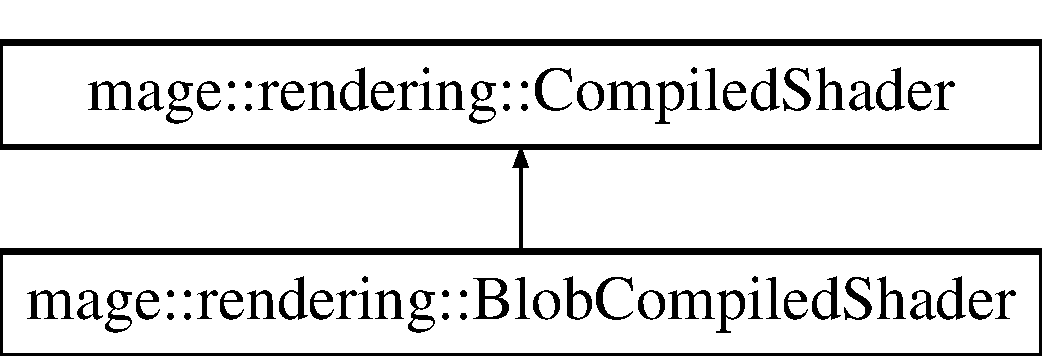
\includegraphics[height=2.000000cm]{classmage_1_1rendering_1_1_blob_compiled_shader}
\end{center}
\end{figure}
\subsection*{Public Member Functions}
\begin{DoxyCompactItemize}
\item 
\mbox{\hyperlink{classmage_1_1rendering_1_1_blob_compiled_shader_a9e29ef4b735ae26f6902077d9e7c4f1d}{Blob\+Compiled\+Shader}} (const wstring \&fname) noexcept
\item 
\mbox{\hyperlink{classmage_1_1rendering_1_1_blob_compiled_shader_a7b63a87261abf6059c957af4061af201}{Blob\+Compiled\+Shader}} (const \mbox{\hyperlink{classmage_1_1rendering_1_1_blob_compiled_shader}{Blob\+Compiled\+Shader}} \&compiled\+\_\+shader) noexcept
\item 
\mbox{\hyperlink{classmage_1_1rendering_1_1_blob_compiled_shader_afa58cbbad81febc6c2470f6f1b0de2ce}{Blob\+Compiled\+Shader}} (\mbox{\hyperlink{classmage_1_1rendering_1_1_blob_compiled_shader}{Blob\+Compiled\+Shader}} \&\&compiled\+\_\+shader) noexcept
\item 
virtual \mbox{\hyperlink{classmage_1_1rendering_1_1_blob_compiled_shader_ac983a2506dfe81e8e8ceb2b9ffa420d6}{$\sim$\+Blob\+Compiled\+Shader}} ()
\item 
\mbox{\hyperlink{classmage_1_1rendering_1_1_blob_compiled_shader}{Blob\+Compiled\+Shader}} \& \mbox{\hyperlink{classmage_1_1rendering_1_1_blob_compiled_shader_a07f7bf56354508ad499133b821e2fdc5}{operator=}} (const \mbox{\hyperlink{classmage_1_1rendering_1_1_blob_compiled_shader}{Blob\+Compiled\+Shader}} \&compiled\+\_\+shader) noexcept
\item 
\mbox{\hyperlink{classmage_1_1rendering_1_1_blob_compiled_shader}{Blob\+Compiled\+Shader}} \& \mbox{\hyperlink{classmage_1_1rendering_1_1_blob_compiled_shader_a14954683e57897937b0e0178b5a726a4}{operator=}} (\mbox{\hyperlink{classmage_1_1rendering_1_1_blob_compiled_shader}{Blob\+Compiled\+Shader}} \&\&compiled\+\_\+shader) noexcept
\item 
virtual const B\+Y\+TE $\ast$ \mbox{\hyperlink{classmage_1_1rendering_1_1_blob_compiled_shader_a4d7f3d2d9864cb12939386ff031bd783}{Get\+Bytecode}} () const noexcept override
\item 
virtual S\+I\+Z\+E\+\_\+T \mbox{\hyperlink{classmage_1_1rendering_1_1_blob_compiled_shader_ac3c3edb09ba96367f8c5d6741ec03041}{Get\+Bytecode\+Size}} () const noexcept override
\end{DoxyCompactItemize}
\subsection*{Private Attributes}
\begin{DoxyCompactItemize}
\item 
\mbox{\hyperlink{namespacemage_ae74f374780900893caa5555d1031fd79}{Com\+Ptr}}$<$ I\+D3\+D\+Blob $>$ \mbox{\hyperlink{classmage_1_1rendering_1_1_blob_compiled_shader_ad28d77dc5fd97d127c2e2dc875384449}{m\+\_\+shader\+\_\+blob}}
\end{DoxyCompactItemize}
\subsection*{Additional Inherited Members}


\subsection{Detailed Description}
A class of blob compiled shaders. 

\subsection{Constructor \& Destructor Documentation}
\mbox{\Hypertarget{classmage_1_1rendering_1_1_blob_compiled_shader_a9e29ef4b735ae26f6902077d9e7c4f1d}\label{classmage_1_1rendering_1_1_blob_compiled_shader_a9e29ef4b735ae26f6902077d9e7c4f1d}} 
\index{mage\+::rendering\+::\+Blob\+Compiled\+Shader@{mage\+::rendering\+::\+Blob\+Compiled\+Shader}!Blob\+Compiled\+Shader@{Blob\+Compiled\+Shader}}
\index{Blob\+Compiled\+Shader@{Blob\+Compiled\+Shader}!mage\+::rendering\+::\+Blob\+Compiled\+Shader@{mage\+::rendering\+::\+Blob\+Compiled\+Shader}}
\subsubsection{\texorpdfstring{Blob\+Compiled\+Shader()}{BlobCompiledShader()}\hspace{0.1cm}{\footnotesize\ttfamily [1/3]}}
{\footnotesize\ttfamily mage\+::rendering\+::\+Blob\+Compiled\+Shader\+::\+Blob\+Compiled\+Shader (\begin{DoxyParamCaption}\item[{const wstring \&}]{fname }\end{DoxyParamCaption})\hspace{0.3cm}{\ttfamily [explicit]}, {\ttfamily [noexcept]}}

Constructs a blob compiled shader.


\begin{DoxyParams}[1]{Parameters}
\mbox{\tt in}  & {\em fname} & A reference to the filename. \\
\hline
\end{DoxyParams}

\begin{DoxyExceptions}{Exceptions}
{\em \mbox{\hyperlink{classmage_1_1_exception}{Exception}}} & Failed to load the compiled shader from the given file. \\
\hline
\end{DoxyExceptions}
\mbox{\Hypertarget{classmage_1_1rendering_1_1_blob_compiled_shader_a7b63a87261abf6059c957af4061af201}\label{classmage_1_1rendering_1_1_blob_compiled_shader_a7b63a87261abf6059c957af4061af201}} 
\index{mage\+::rendering\+::\+Blob\+Compiled\+Shader@{mage\+::rendering\+::\+Blob\+Compiled\+Shader}!Blob\+Compiled\+Shader@{Blob\+Compiled\+Shader}}
\index{Blob\+Compiled\+Shader@{Blob\+Compiled\+Shader}!mage\+::rendering\+::\+Blob\+Compiled\+Shader@{mage\+::rendering\+::\+Blob\+Compiled\+Shader}}
\subsubsection{\texorpdfstring{Blob\+Compiled\+Shader()}{BlobCompiledShader()}\hspace{0.1cm}{\footnotesize\ttfamily [2/3]}}
{\footnotesize\ttfamily mage\+::rendering\+::\+Blob\+Compiled\+Shader\+::\+Blob\+Compiled\+Shader (\begin{DoxyParamCaption}\item[{const \mbox{\hyperlink{classmage_1_1rendering_1_1_blob_compiled_shader}{Blob\+Compiled\+Shader}} \&}]{compiled\+\_\+shader }\end{DoxyParamCaption})\hspace{0.3cm}{\ttfamily [default]}, {\ttfamily [noexcept]}}

Constructs a blob compiled shader from the given blob compiled shader.


\begin{DoxyParams}[1]{Parameters}
\mbox{\tt in}  & {\em compiled\+\_\+shader} & A reference to the blob compiled shader to copy. \\
\hline
\end{DoxyParams}
\mbox{\Hypertarget{classmage_1_1rendering_1_1_blob_compiled_shader_afa58cbbad81febc6c2470f6f1b0de2ce}\label{classmage_1_1rendering_1_1_blob_compiled_shader_afa58cbbad81febc6c2470f6f1b0de2ce}} 
\index{mage\+::rendering\+::\+Blob\+Compiled\+Shader@{mage\+::rendering\+::\+Blob\+Compiled\+Shader}!Blob\+Compiled\+Shader@{Blob\+Compiled\+Shader}}
\index{Blob\+Compiled\+Shader@{Blob\+Compiled\+Shader}!mage\+::rendering\+::\+Blob\+Compiled\+Shader@{mage\+::rendering\+::\+Blob\+Compiled\+Shader}}
\subsubsection{\texorpdfstring{Blob\+Compiled\+Shader()}{BlobCompiledShader()}\hspace{0.1cm}{\footnotesize\ttfamily [3/3]}}
{\footnotesize\ttfamily mage\+::rendering\+::\+Blob\+Compiled\+Shader\+::\+Blob\+Compiled\+Shader (\begin{DoxyParamCaption}\item[{\mbox{\hyperlink{classmage_1_1rendering_1_1_blob_compiled_shader}{Blob\+Compiled\+Shader}} \&\&}]{compiled\+\_\+shader }\end{DoxyParamCaption})\hspace{0.3cm}{\ttfamily [default]}, {\ttfamily [noexcept]}}

Constructs a blob compiled shader by moving the given blob compiled shader.


\begin{DoxyParams}[1]{Parameters}
\mbox{\tt in}  & {\em compiled\+\_\+shader} & A reference to the blob compiled shader to move. \\
\hline
\end{DoxyParams}
\mbox{\Hypertarget{classmage_1_1rendering_1_1_blob_compiled_shader_ac983a2506dfe81e8e8ceb2b9ffa420d6}\label{classmage_1_1rendering_1_1_blob_compiled_shader_ac983a2506dfe81e8e8ceb2b9ffa420d6}} 
\index{mage\+::rendering\+::\+Blob\+Compiled\+Shader@{mage\+::rendering\+::\+Blob\+Compiled\+Shader}!````~Blob\+Compiled\+Shader@{$\sim$\+Blob\+Compiled\+Shader}}
\index{````~Blob\+Compiled\+Shader@{$\sim$\+Blob\+Compiled\+Shader}!mage\+::rendering\+::\+Blob\+Compiled\+Shader@{mage\+::rendering\+::\+Blob\+Compiled\+Shader}}
\subsubsection{\texorpdfstring{$\sim$\+Blob\+Compiled\+Shader()}{~BlobCompiledShader()}}
{\footnotesize\ttfamily mage\+::rendering\+::\+Blob\+Compiled\+Shader\+::$\sim$\+Blob\+Compiled\+Shader (\begin{DoxyParamCaption}{ }\end{DoxyParamCaption})\hspace{0.3cm}{\ttfamily [virtual]}, {\ttfamily [default]}}

Destructs this blob compiled shader. 

\subsection{Member Function Documentation}
\mbox{\Hypertarget{classmage_1_1rendering_1_1_blob_compiled_shader_a4d7f3d2d9864cb12939386ff031bd783}\label{classmage_1_1rendering_1_1_blob_compiled_shader_a4d7f3d2d9864cb12939386ff031bd783}} 
\index{mage\+::rendering\+::\+Blob\+Compiled\+Shader@{mage\+::rendering\+::\+Blob\+Compiled\+Shader}!Get\+Bytecode@{Get\+Bytecode}}
\index{Get\+Bytecode@{Get\+Bytecode}!mage\+::rendering\+::\+Blob\+Compiled\+Shader@{mage\+::rendering\+::\+Blob\+Compiled\+Shader}}
\subsubsection{\texorpdfstring{Get\+Bytecode()}{GetBytecode()}}
{\footnotesize\ttfamily virtual const B\+Y\+TE$\ast$ mage\+::rendering\+::\+Blob\+Compiled\+Shader\+::\+Get\+Bytecode (\begin{DoxyParamCaption}{ }\end{DoxyParamCaption}) const\hspace{0.3cm}{\ttfamily [override]}, {\ttfamily [virtual]}, {\ttfamily [noexcept]}}

Returns the shader bytecode of this blob compiled shader.

\begin{DoxyReturn}{Returns}
A pointer to the shader bytecode of this blob compiled shader. 
\end{DoxyReturn}


Implements \mbox{\hyperlink{classmage_1_1rendering_1_1_compiled_shader_a6067250341f428be19ed2aa9955a10b6}{mage\+::rendering\+::\+Compiled\+Shader}}.

\mbox{\Hypertarget{classmage_1_1rendering_1_1_blob_compiled_shader_ac3c3edb09ba96367f8c5d6741ec03041}\label{classmage_1_1rendering_1_1_blob_compiled_shader_ac3c3edb09ba96367f8c5d6741ec03041}} 
\index{mage\+::rendering\+::\+Blob\+Compiled\+Shader@{mage\+::rendering\+::\+Blob\+Compiled\+Shader}!Get\+Bytecode\+Size@{Get\+Bytecode\+Size}}
\index{Get\+Bytecode\+Size@{Get\+Bytecode\+Size}!mage\+::rendering\+::\+Blob\+Compiled\+Shader@{mage\+::rendering\+::\+Blob\+Compiled\+Shader}}
\subsubsection{\texorpdfstring{Get\+Bytecode\+Size()}{GetBytecodeSize()}}
{\footnotesize\ttfamily virtual S\+I\+Z\+E\+\_\+T mage\+::rendering\+::\+Blob\+Compiled\+Shader\+::\+Get\+Bytecode\+Size (\begin{DoxyParamCaption}{ }\end{DoxyParamCaption}) const\hspace{0.3cm}{\ttfamily [override]}, {\ttfamily [virtual]}, {\ttfamily [noexcept]}}

Returns the size of the shader bytecode (in bytes) of this blob compiled shader.

\begin{DoxyReturn}{Returns}
The size of the shader bytecode (in bytes) of this blob compiled shader. 
\end{DoxyReturn}


Implements \mbox{\hyperlink{classmage_1_1rendering_1_1_compiled_shader_a92c17b46242bf884c3d0d673e88a292d}{mage\+::rendering\+::\+Compiled\+Shader}}.

\mbox{\Hypertarget{classmage_1_1rendering_1_1_blob_compiled_shader_a07f7bf56354508ad499133b821e2fdc5}\label{classmage_1_1rendering_1_1_blob_compiled_shader_a07f7bf56354508ad499133b821e2fdc5}} 
\index{mage\+::rendering\+::\+Blob\+Compiled\+Shader@{mage\+::rendering\+::\+Blob\+Compiled\+Shader}!operator=@{operator=}}
\index{operator=@{operator=}!mage\+::rendering\+::\+Blob\+Compiled\+Shader@{mage\+::rendering\+::\+Blob\+Compiled\+Shader}}
\subsubsection{\texorpdfstring{operator=()}{operator=()}\hspace{0.1cm}{\footnotesize\ttfamily [1/2]}}
{\footnotesize\ttfamily \mbox{\hyperlink{classmage_1_1rendering_1_1_blob_compiled_shader}{Blob\+Compiled\+Shader}} \& mage\+::rendering\+::\+Blob\+Compiled\+Shader\+::operator= (\begin{DoxyParamCaption}\item[{const \mbox{\hyperlink{classmage_1_1rendering_1_1_blob_compiled_shader}{Blob\+Compiled\+Shader}} \&}]{compiled\+\_\+shader }\end{DoxyParamCaption})\hspace{0.3cm}{\ttfamily [default]}, {\ttfamily [noexcept]}}

Copies the given blob compiled shader to this blob compiled shader.


\begin{DoxyParams}[1]{Parameters}
\mbox{\tt in}  & {\em compiled\+\_\+shader} & A reference to the blob compiled shader to copy. \\
\hline
\end{DoxyParams}
\begin{DoxyReturn}{Returns}
A reference to the copy of the given blob compiled shader (i.\+e. this blob compiled shader). 
\end{DoxyReturn}
\mbox{\Hypertarget{classmage_1_1rendering_1_1_blob_compiled_shader_a14954683e57897937b0e0178b5a726a4}\label{classmage_1_1rendering_1_1_blob_compiled_shader_a14954683e57897937b0e0178b5a726a4}} 
\index{mage\+::rendering\+::\+Blob\+Compiled\+Shader@{mage\+::rendering\+::\+Blob\+Compiled\+Shader}!operator=@{operator=}}
\index{operator=@{operator=}!mage\+::rendering\+::\+Blob\+Compiled\+Shader@{mage\+::rendering\+::\+Blob\+Compiled\+Shader}}
\subsubsection{\texorpdfstring{operator=()}{operator=()}\hspace{0.1cm}{\footnotesize\ttfamily [2/2]}}
{\footnotesize\ttfamily \mbox{\hyperlink{classmage_1_1rendering_1_1_blob_compiled_shader}{Blob\+Compiled\+Shader}} \& mage\+::rendering\+::\+Blob\+Compiled\+Shader\+::operator= (\begin{DoxyParamCaption}\item[{\mbox{\hyperlink{classmage_1_1rendering_1_1_blob_compiled_shader}{Blob\+Compiled\+Shader}} \&\&}]{compiled\+\_\+shader }\end{DoxyParamCaption})\hspace{0.3cm}{\ttfamily [default]}, {\ttfamily [noexcept]}}

Moves the given blob compiled shader to this blob compiled shader.


\begin{DoxyParams}[1]{Parameters}
\mbox{\tt in}  & {\em compiled\+\_\+shader} & A reference to the blob compiled shader to copy. \\
\hline
\end{DoxyParams}
\begin{DoxyReturn}{Returns}
A reference to the moved blob compiled shader (i.\+e. this blob compiled shader). 
\end{DoxyReturn}


\subsection{Member Data Documentation}
\mbox{\Hypertarget{classmage_1_1rendering_1_1_blob_compiled_shader_ad28d77dc5fd97d127c2e2dc875384449}\label{classmage_1_1rendering_1_1_blob_compiled_shader_ad28d77dc5fd97d127c2e2dc875384449}} 
\index{mage\+::rendering\+::\+Blob\+Compiled\+Shader@{mage\+::rendering\+::\+Blob\+Compiled\+Shader}!m\+\_\+shader\+\_\+blob@{m\+\_\+shader\+\_\+blob}}
\index{m\+\_\+shader\+\_\+blob@{m\+\_\+shader\+\_\+blob}!mage\+::rendering\+::\+Blob\+Compiled\+Shader@{mage\+::rendering\+::\+Blob\+Compiled\+Shader}}
\subsubsection{\texorpdfstring{m\+\_\+shader\+\_\+blob}{m\_shader\_blob}}
{\footnotesize\ttfamily \mbox{\hyperlink{namespacemage_ae74f374780900893caa5555d1031fd79}{Com\+Ptr}}$<$ I\+D3\+D\+Blob $>$ mage\+::rendering\+::\+Blob\+Compiled\+Shader\+::m\+\_\+shader\+\_\+blob\hspace{0.3cm}{\ttfamily [private]}}

A pointer to the shader blob of this blob compiled shader. 
\hypertarget{classmage_1_1_bounding_frustum}{}\section{mage\+:\+:Bounding\+Frustum Class Reference}
\label{classmage_1_1_bounding_frustum}\index{mage\+::\+Bounding\+Frustum@{mage\+::\+Bounding\+Frustum}}


{\ttfamily \#include $<$bounding\+\_\+volume.\+hpp$>$}

\subsection*{Public Member Functions}
\begin{DoxyCompactItemize}
\item 
\hyperlink{classmage_1_1_bounding_frustum_afafc5433abc80e872242b5488ca0c835}{Bounding\+Frustum} (C\+X\+M\+M\+A\+T\+R\+IX transform) noexcept
\item 
\hyperlink{classmage_1_1_bounding_frustum_a22233ec36a176312dd453bbab682c313}{Bounding\+Frustum} (const \hyperlink{classmage_1_1_bounding_frustum}{Bounding\+Frustum} \&frustum) noexcept=default
\item 
\hyperlink{classmage_1_1_bounding_frustum_a0eafed7a78a72d33a6153bdcffd07057}{Bounding\+Frustum} (\hyperlink{classmage_1_1_bounding_frustum}{Bounding\+Frustum} \&\&frustum) noexcept=default
\item 
\hyperlink{classmage_1_1_bounding_frustum_a9837a92462da6a473f6ba5b7cc3b77fb}{$\sim$\+Bounding\+Frustum} ()=default
\item 
\hyperlink{classmage_1_1_bounding_frustum}{Bounding\+Frustum} \& \hyperlink{classmage_1_1_bounding_frustum_a713509c0c2e9e947bc448e2743903c12}{operator=} (const \hyperlink{classmage_1_1_bounding_frustum}{Bounding\+Frustum} \&frustum) noexcept=default
\item 
\hyperlink{classmage_1_1_bounding_frustum}{Bounding\+Frustum} \& \hyperlink{classmage_1_1_bounding_frustum_ae6a344dc47b0a8dffd49fc4a95c364a5}{operator=} (\hyperlink{classmage_1_1_bounding_frustum}{Bounding\+Frustum} \&\&frustum) noexcept=default
\item 
bool \hyperlink{classmage_1_1_bounding_frustum_a5a7b074f2d78031b235f4d5f31ef683a}{Encloses} (const \hyperlink{structmage_1_1_point3}{Point3} \&point) const noexcept
\item 
bool \hyperlink{classmage_1_1_bounding_frustum_aeae9c1be8cebf662ccd6615145724dec}{Encloses\+Strict} (const \hyperlink{structmage_1_1_point3}{Point3} \&point) const noexcept
\item 
bool X\+M\+\_\+\+C\+A\+L\+L\+C\+O\+NV \hyperlink{classmage_1_1_bounding_frustum_adde03968d4a4f519c9b9af3b3434055f}{Encloses} (F\+X\+M\+V\+E\+C\+T\+OR point) const noexcept
\item 
bool X\+M\+\_\+\+C\+A\+L\+L\+C\+O\+NV \hyperlink{classmage_1_1_bounding_frustum_a7cd247470d192464f006b2b76ad3c336}{Encloses\+Strict} (F\+X\+M\+V\+E\+C\+T\+OR point) const noexcept
\item 
bool \hyperlink{classmage_1_1_bounding_frustum_a09642eff00ef33d0b5ea4890c9adc4b2}{Encloses} (const \hyperlink{classmage_1_1_a_a_b_b}{A\+A\+BB} \&aabb) const noexcept
\item 
bool \hyperlink{classmage_1_1_bounding_frustum_aacdbcc48558489bec9ad87d52104626d}{Encloses\+Strict} (const \hyperlink{classmage_1_1_a_a_b_b}{A\+A\+BB} \&aabb) const noexcept
\item 
bool \hyperlink{classmage_1_1_bounding_frustum_a64bb28f632ae39438424a714809c31de}{Encloses} (const \hyperlink{classmage_1_1_bounding_sphere}{Bounding\+Sphere} \&sphere) const noexcept
\item 
bool \hyperlink{classmage_1_1_bounding_frustum_ae3dce877ac0e87dd6b9f7f8644c8bcfc}{Encloses\+Strict} (const \hyperlink{classmage_1_1_bounding_sphere}{Bounding\+Sphere} \&sphere) const noexcept
\item 
bool \hyperlink{classmage_1_1_bounding_frustum_a0fbd4639f1bd0a014430313410aa013d}{Overlaps} (const \hyperlink{classmage_1_1_a_a_b_b}{A\+A\+BB} \&aabb) const noexcept
\item 
bool \hyperlink{classmage_1_1_bounding_frustum_af3a6772edd09480a22a175fa4acbfbd8}{Overlaps\+Strict} (const \hyperlink{classmage_1_1_a_a_b_b}{A\+A\+BB} \&aabb) const noexcept
\item 
bool \hyperlink{classmage_1_1_bounding_frustum_a2133c3a7187369772e82b7e229b0e683}{Overlaps} (const \hyperlink{classmage_1_1_bounding_sphere}{Bounding\+Sphere} \&sphere) const noexcept
\item 
bool \hyperlink{classmage_1_1_bounding_frustum_a070075ad4af9935b7b60e7e5345d0aff}{Overlaps\+Strict} (const \hyperlink{classmage_1_1_bounding_sphere}{Bounding\+Sphere} \&sphere) const noexcept
\item 
bool \hyperlink{classmage_1_1_bounding_frustum_a90c5a355878674b1320e195318703d4b}{operator==} (const \hyperlink{classmage_1_1_bounding_frustum}{Bounding\+Frustum} \&frustum) const noexcept
\item 
bool \hyperlink{classmage_1_1_bounding_frustum_a20c545cb807db2dc2fad018229f69c2c}{operator!=} (const \hyperlink{classmage_1_1_bounding_frustum}{Bounding\+Frustum} \&frustum) const noexcept
\end{DoxyCompactItemize}
\subsection*{Static Public Member Functions}
\begin{DoxyCompactItemize}
\item 
{\footnotesize template$<$typename Bounding\+VolumeT $>$ }\\static bool X\+M\+\_\+\+C\+A\+L\+L\+C\+O\+NV \hyperlink{classmage_1_1_bounding_frustum_af2080fda86e99ae8dda866b7a90f84a1}{Cull} (F\+X\+M\+M\+A\+T\+R\+IX object\+\_\+to\+\_\+projection, const Bounding\+VolumeT \&volume) noexcept
\end{DoxyCompactItemize}
\subsection*{Private Attributes}
\begin{DoxyCompactItemize}
\item 
\begin{tabbing}
xx\=xx\=xx\=xx\=xx\=xx\=xx\=xx\=xx\=\kill
union \{\\
\>struct \{\\
\>\>XMVECTOR \hyperlink{classmage_1_1_bounding_frustum_ae9ce2430295e49fe9dff4940fa9aafb1}{m\_left\_plane}\\
\>\>XMVECTOR \hyperlink{classmage_1_1_bounding_frustum_a28a9d13ade71eb4253e452e6c53c31fe}{m\_right\_plane}\\
\>\>XMVECTOR \hyperlink{classmage_1_1_bounding_frustum_ae416db4ef5c2fc3eb2e2f25f6e45e747}{m\_bottom\_plane}\\
\>\>XMVECTOR \hyperlink{classmage_1_1_bounding_frustum_acea4c43991bf09de647f7ee70feb1fff}{m\_top\_plane}\\
\>\>XMVECTOR \hyperlink{classmage_1_1_bounding_frustum_abd4fa19a2fa0e88342ab4bc2726bf885}{m\_near\_plane}\\
\>\>XMVECTOR \hyperlink{classmage_1_1_bounding_frustum_a8a1841dcd6c7fdbecbd1dd5c39558e8e}{m\_far\_plane}\\
\>\} \\
\>XMVECTOR \hyperlink{classmage_1_1_bounding_frustum_a077e9ac802e5272dd9cf60a57546505c}{m\_planes} \mbox{[}6\mbox{]}\\
\}; \\

\end{tabbing}\end{DoxyCompactItemize}


\subsection{Detailed Description}
A class of bounding frustums. 

\subsection{Constructor \& Destructor Documentation}
\hypertarget{classmage_1_1_bounding_frustum_afafc5433abc80e872242b5488ca0c835}{}\label{classmage_1_1_bounding_frustum_afafc5433abc80e872242b5488ca0c835} 
\index{mage\+::\+Bounding\+Frustum@{mage\+::\+Bounding\+Frustum}!Bounding\+Frustum@{Bounding\+Frustum}}
\index{Bounding\+Frustum@{Bounding\+Frustum}!mage\+::\+Bounding\+Frustum@{mage\+::\+Bounding\+Frustum}}
\subsubsection{\texorpdfstring{Bounding\+Frustum()}{BoundingFrustum()}\hspace{0.1cm}{\footnotesize\ttfamily [1/3]}}
{\footnotesize\ttfamily mage\+::\+Bounding\+Frustum\+::\+Bounding\+Frustum (\begin{DoxyParamCaption}\item[{C\+X\+M\+M\+A\+T\+R\+IX}]{transform }\end{DoxyParamCaption})\hspace{0.3cm}{\ttfamily [explicit]}, {\ttfamily [noexcept]}}

Constructs a bounding frustum from the given transform.

If the given transform represents the view-\/to-\/projection transformation matrix, the planes of the bounding frustum are represented by view space coordinates.

If the given transform represents the world-\/to-\/view-\/to-\/projection transformation matrix, the planes of the bounding frustum are represented by world space coordinates.

If the given transform represents the object-\/to-\/world-\/to-\/view-\/projection transformation matrix, the planes of the bounding frustum are represented by object space coordinates.


\begin{DoxyParams}[1]{Parameters}
\mbox{\tt in}  & {\em transform} & The transform. \\
\hline
\end{DoxyParams}
\hypertarget{classmage_1_1_bounding_frustum_a22233ec36a176312dd453bbab682c313}{}\label{classmage_1_1_bounding_frustum_a22233ec36a176312dd453bbab682c313} 
\index{mage\+::\+Bounding\+Frustum@{mage\+::\+Bounding\+Frustum}!Bounding\+Frustum@{Bounding\+Frustum}}
\index{Bounding\+Frustum@{Bounding\+Frustum}!mage\+::\+Bounding\+Frustum@{mage\+::\+Bounding\+Frustum}}
\subsubsection{\texorpdfstring{Bounding\+Frustum()}{BoundingFrustum()}\hspace{0.1cm}{\footnotesize\ttfamily [2/3]}}
{\footnotesize\ttfamily mage\+::\+Bounding\+Frustum\+::\+Bounding\+Frustum (\begin{DoxyParamCaption}\item[{const \hyperlink{classmage_1_1_bounding_frustum}{Bounding\+Frustum} \&}]{frustum }\end{DoxyParamCaption})\hspace{0.3cm}{\ttfamily [default]}, {\ttfamily [noexcept]}}

Constructs a bounding frustum from the given bounding frustum.


\begin{DoxyParams}[1]{Parameters}
\mbox{\tt in}  & {\em frustum} & A reference to the bounding frustum to copy. \\
\hline
\end{DoxyParams}
\hypertarget{classmage_1_1_bounding_frustum_a0eafed7a78a72d33a6153bdcffd07057}{}\label{classmage_1_1_bounding_frustum_a0eafed7a78a72d33a6153bdcffd07057} 
\index{mage\+::\+Bounding\+Frustum@{mage\+::\+Bounding\+Frustum}!Bounding\+Frustum@{Bounding\+Frustum}}
\index{Bounding\+Frustum@{Bounding\+Frustum}!mage\+::\+Bounding\+Frustum@{mage\+::\+Bounding\+Frustum}}
\subsubsection{\texorpdfstring{Bounding\+Frustum()}{BoundingFrustum()}\hspace{0.1cm}{\footnotesize\ttfamily [3/3]}}
{\footnotesize\ttfamily mage\+::\+Bounding\+Frustum\+::\+Bounding\+Frustum (\begin{DoxyParamCaption}\item[{\hyperlink{classmage_1_1_bounding_frustum}{Bounding\+Frustum} \&\&}]{frustum }\end{DoxyParamCaption})\hspace{0.3cm}{\ttfamily [default]}, {\ttfamily [noexcept]}}

Constructs a bounding frustum by moving the given bounding frustum.


\begin{DoxyParams}[1]{Parameters}
\mbox{\tt in}  & {\em frustum} & A reference to the bounding frustum to move. \\
\hline
\end{DoxyParams}
\hypertarget{classmage_1_1_bounding_frustum_a9837a92462da6a473f6ba5b7cc3b77fb}{}\label{classmage_1_1_bounding_frustum_a9837a92462da6a473f6ba5b7cc3b77fb} 
\index{mage\+::\+Bounding\+Frustum@{mage\+::\+Bounding\+Frustum}!````~Bounding\+Frustum@{$\sim$\+Bounding\+Frustum}}
\index{````~Bounding\+Frustum@{$\sim$\+Bounding\+Frustum}!mage\+::\+Bounding\+Frustum@{mage\+::\+Bounding\+Frustum}}
\subsubsection{\texorpdfstring{$\sim$\+Bounding\+Frustum()}{~BoundingFrustum()}}
{\footnotesize\ttfamily mage\+::\+Bounding\+Frustum\+::$\sim$\+Bounding\+Frustum (\begin{DoxyParamCaption}{ }\end{DoxyParamCaption})\hspace{0.3cm}{\ttfamily [default]}}

Destructs this bounding frustum. 

\subsection{Member Function Documentation}
\hypertarget{classmage_1_1_bounding_frustum_af2080fda86e99ae8dda866b7a90f84a1}{}\label{classmage_1_1_bounding_frustum_af2080fda86e99ae8dda866b7a90f84a1} 
\index{mage\+::\+Bounding\+Frustum@{mage\+::\+Bounding\+Frustum}!Cull@{Cull}}
\index{Cull@{Cull}!mage\+::\+Bounding\+Frustum@{mage\+::\+Bounding\+Frustum}}
\subsubsection{\texorpdfstring{Cull()}{Cull()}}
{\footnotesize\ttfamily template$<$typename Bounding\+VolumeT $>$ \\
static bool X\+M\+\_\+\+C\+A\+L\+L\+C\+O\+NV mage\+::\+Bounding\+Frustum\+::\+Cull (\begin{DoxyParamCaption}\item[{F\+X\+M\+M\+A\+T\+R\+IX}]{object\+\_\+to\+\_\+projection,  }\item[{const Bounding\+VolumeT \&}]{volume }\end{DoxyParamCaption})\hspace{0.3cm}{\ttfamily [static]}, {\ttfamily [noexcept]}}

Checks if the given bounding volume is culled by the bounding frustum constructed from the given object-\/to-\/projection transformation matrix.


\begin{DoxyTemplParams}{Template Parameters}
{\em Bounding\+VolumeT} & The bounding volume type. \\
\hline
\end{DoxyTemplParams}

\begin{DoxyParams}[1]{Parameters}
\mbox{\tt in}  & {\em object\+\_\+to\+\_\+projection} & The object-\/to-\/projection transformation matrix. \\
\hline
\mbox{\tt in}  & {\em volume} & A reference to the bounding volume. \\
\hline
\end{DoxyParams}
\begin{DoxyReturn}{Returns}
{\ttfamily true} if the given bounding volume is culled by the bounding frustum constructed from the given object-\/to-\/projection transformation matrix. {\ttfamily false} otherwise. 
\end{DoxyReturn}
\hypertarget{classmage_1_1_bounding_frustum_a5a7b074f2d78031b235f4d5f31ef683a}{}\label{classmage_1_1_bounding_frustum_a5a7b074f2d78031b235f4d5f31ef683a} 
\index{mage\+::\+Bounding\+Frustum@{mage\+::\+Bounding\+Frustum}!Encloses@{Encloses}}
\index{Encloses@{Encloses}!mage\+::\+Bounding\+Frustum@{mage\+::\+Bounding\+Frustum}}
\subsubsection{\texorpdfstring{Encloses()}{Encloses()}\hspace{0.1cm}{\footnotesize\ttfamily [1/4]}}
{\footnotesize\ttfamily bool mage\+::\+Bounding\+Frustum\+::\+Encloses (\begin{DoxyParamCaption}\item[{const \hyperlink{structmage_1_1_point3}{Point3} \&}]{point }\end{DoxyParamCaption}) const\hspace{0.3cm}{\ttfamily [noexcept]}}

Checks whether this bounding frustum completely encloses the given point.


\begin{DoxyParams}[1]{Parameters}
\mbox{\tt in}  & {\em point} & A reference to the point. \\
\hline
\end{DoxyParams}
\begin{DoxyReturn}{Returns}
{\ttfamily true} if this bounding frustum completely encloses {\itshape point}. {\ttfamily false} otherwise. 
\end{DoxyReturn}
\begin{DoxyNote}{Note}
This is a full coverage test of a point with regard to a bounding frustum. 
\end{DoxyNote}
\hypertarget{classmage_1_1_bounding_frustum_adde03968d4a4f519c9b9af3b3434055f}{}\label{classmage_1_1_bounding_frustum_adde03968d4a4f519c9b9af3b3434055f} 
\index{mage\+::\+Bounding\+Frustum@{mage\+::\+Bounding\+Frustum}!Encloses@{Encloses}}
\index{Encloses@{Encloses}!mage\+::\+Bounding\+Frustum@{mage\+::\+Bounding\+Frustum}}
\subsubsection{\texorpdfstring{Encloses()}{Encloses()}\hspace{0.1cm}{\footnotesize\ttfamily [2/4]}}
{\footnotesize\ttfamily bool X\+M\+\_\+\+C\+A\+L\+L\+C\+O\+NV mage\+::\+Bounding\+Frustum\+::\+Encloses (\begin{DoxyParamCaption}\item[{F\+X\+M\+V\+E\+C\+T\+OR}]{point }\end{DoxyParamCaption}) const\hspace{0.3cm}{\ttfamily [noexcept]}}

Checks whether this bounding frustum completely encloses the given point.


\begin{DoxyParams}[1]{Parameters}
\mbox{\tt in}  & {\em point} & The point. \\
\hline
\end{DoxyParams}
\begin{DoxyReturn}{Returns}
{\ttfamily true} if this bounding frustum completely encloses {\itshape point}. {\ttfamily false} otherwise. 
\end{DoxyReturn}
\begin{DoxyNote}{Note}
This is a full coverage test of a point with regard to a bounding frustum. 
\end{DoxyNote}
\hypertarget{classmage_1_1_bounding_frustum_a09642eff00ef33d0b5ea4890c9adc4b2}{}\label{classmage_1_1_bounding_frustum_a09642eff00ef33d0b5ea4890c9adc4b2} 
\index{mage\+::\+Bounding\+Frustum@{mage\+::\+Bounding\+Frustum}!Encloses@{Encloses}}
\index{Encloses@{Encloses}!mage\+::\+Bounding\+Frustum@{mage\+::\+Bounding\+Frustum}}
\subsubsection{\texorpdfstring{Encloses()}{Encloses()}\hspace{0.1cm}{\footnotesize\ttfamily [3/4]}}
{\footnotesize\ttfamily bool mage\+::\+Bounding\+Frustum\+::\+Encloses (\begin{DoxyParamCaption}\item[{const \hyperlink{classmage_1_1_a_a_b_b}{A\+A\+BB} \&}]{aabb }\end{DoxyParamCaption}) const\hspace{0.3cm}{\ttfamily [noexcept]}}

Checks whether this bounding frustum completely encloses the given \hyperlink{classmage_1_1_a_a_b_b}{A\+A\+BB}.


\begin{DoxyParams}[1]{Parameters}
\mbox{\tt in}  & {\em aabb} & A reference to the \hyperlink{classmage_1_1_a_a_b_b}{A\+A\+BB}. \\
\hline
\end{DoxyParams}
\begin{DoxyReturn}{Returns}
{\ttfamily true} if this bounding frustum completely encloses {\itshape aabb}. {\ttfamily false} otherwise. 
\end{DoxyReturn}
\begin{DoxyNote}{Note}
This is a full coverage test of an \hyperlink{classmage_1_1_a_a_b_b}{A\+A\+BB} with regard to a bounding frustum. 
\end{DoxyNote}
\hypertarget{classmage_1_1_bounding_frustum_a64bb28f632ae39438424a714809c31de}{}\label{classmage_1_1_bounding_frustum_a64bb28f632ae39438424a714809c31de} 
\index{mage\+::\+Bounding\+Frustum@{mage\+::\+Bounding\+Frustum}!Encloses@{Encloses}}
\index{Encloses@{Encloses}!mage\+::\+Bounding\+Frustum@{mage\+::\+Bounding\+Frustum}}
\subsubsection{\texorpdfstring{Encloses()}{Encloses()}\hspace{0.1cm}{\footnotesize\ttfamily [4/4]}}
{\footnotesize\ttfamily bool mage\+::\+Bounding\+Frustum\+::\+Encloses (\begin{DoxyParamCaption}\item[{const \hyperlink{classmage_1_1_bounding_sphere}{Bounding\+Sphere} \&}]{sphere }\end{DoxyParamCaption}) const\hspace{0.3cm}{\ttfamily [noexcept]}}

Checks whether this bounding frustum completely encloses the given bounding sphere.


\begin{DoxyParams}[1]{Parameters}
\mbox{\tt in}  & {\em sphere} & A reference to the bounding sphere. \\
\hline
\end{DoxyParams}
\begin{DoxyReturn}{Returns}
{\ttfamily true} if this bounding frustum completely encloses {\itshape sphere}. {\ttfamily false} otherwise. 
\end{DoxyReturn}
\begin{DoxyNote}{Note}
This is a full coverage test of a bounding sphere with regard to a bounding frustum. 
\end{DoxyNote}
\hypertarget{classmage_1_1_bounding_frustum_aeae9c1be8cebf662ccd6615145724dec}{}\label{classmage_1_1_bounding_frustum_aeae9c1be8cebf662ccd6615145724dec} 
\index{mage\+::\+Bounding\+Frustum@{mage\+::\+Bounding\+Frustum}!Encloses\+Strict@{Encloses\+Strict}}
\index{Encloses\+Strict@{Encloses\+Strict}!mage\+::\+Bounding\+Frustum@{mage\+::\+Bounding\+Frustum}}
\subsubsection{\texorpdfstring{Encloses\+Strict()}{EnclosesStrict()}\hspace{0.1cm}{\footnotesize\ttfamily [1/4]}}
{\footnotesize\ttfamily bool mage\+::\+Bounding\+Frustum\+::\+Encloses\+Strict (\begin{DoxyParamCaption}\item[{const \hyperlink{structmage_1_1_point3}{Point3} \&}]{point }\end{DoxyParamCaption}) const\hspace{0.3cm}{\ttfamily [noexcept]}}

Checks whether this bounding frustum completely, strictly encloses the given point.


\begin{DoxyParams}[1]{Parameters}
\mbox{\tt in}  & {\em point} & A reference to the point. \\
\hline
\end{DoxyParams}
\begin{DoxyReturn}{Returns}
{\ttfamily true} if this bounding frustum completely, strictly encloses {\itshape point}. {\ttfamily false} otherwise. 
\end{DoxyReturn}
\begin{DoxyNote}{Note}
This is a full coverage test of a point with regard to a bounding frustum. 
\end{DoxyNote}
\hypertarget{classmage_1_1_bounding_frustum_a7cd247470d192464f006b2b76ad3c336}{}\label{classmage_1_1_bounding_frustum_a7cd247470d192464f006b2b76ad3c336} 
\index{mage\+::\+Bounding\+Frustum@{mage\+::\+Bounding\+Frustum}!Encloses\+Strict@{Encloses\+Strict}}
\index{Encloses\+Strict@{Encloses\+Strict}!mage\+::\+Bounding\+Frustum@{mage\+::\+Bounding\+Frustum}}
\subsubsection{\texorpdfstring{Encloses\+Strict()}{EnclosesStrict()}\hspace{0.1cm}{\footnotesize\ttfamily [2/4]}}
{\footnotesize\ttfamily bool X\+M\+\_\+\+C\+A\+L\+L\+C\+O\+NV mage\+::\+Bounding\+Frustum\+::\+Encloses\+Strict (\begin{DoxyParamCaption}\item[{F\+X\+M\+V\+E\+C\+T\+OR}]{point }\end{DoxyParamCaption}) const\hspace{0.3cm}{\ttfamily [noexcept]}}

Checks whether this bounding frustum completely, strictly encloses the given point.


\begin{DoxyParams}[1]{Parameters}
\mbox{\tt in}  & {\em point} & The point. \\
\hline
\end{DoxyParams}
\begin{DoxyReturn}{Returns}
{\ttfamily true} if this bounding frustum completely, strictly encloses {\itshape point}. {\ttfamily false} otherwise. 
\end{DoxyReturn}
\begin{DoxyNote}{Note}
This is a full coverage test of a point with regard to a bounding frustum. 
\end{DoxyNote}
\hypertarget{classmage_1_1_bounding_frustum_aacdbcc48558489bec9ad87d52104626d}{}\label{classmage_1_1_bounding_frustum_aacdbcc48558489bec9ad87d52104626d} 
\index{mage\+::\+Bounding\+Frustum@{mage\+::\+Bounding\+Frustum}!Encloses\+Strict@{Encloses\+Strict}}
\index{Encloses\+Strict@{Encloses\+Strict}!mage\+::\+Bounding\+Frustum@{mage\+::\+Bounding\+Frustum}}
\subsubsection{\texorpdfstring{Encloses\+Strict()}{EnclosesStrict()}\hspace{0.1cm}{\footnotesize\ttfamily [3/4]}}
{\footnotesize\ttfamily bool mage\+::\+Bounding\+Frustum\+::\+Encloses\+Strict (\begin{DoxyParamCaption}\item[{const \hyperlink{classmage_1_1_a_a_b_b}{A\+A\+BB} \&}]{aabb }\end{DoxyParamCaption}) const\hspace{0.3cm}{\ttfamily [noexcept]}}

Checks whether this bounding frustum completely, strictly encloses the given \hyperlink{classmage_1_1_a_a_b_b}{A\+A\+BB}.


\begin{DoxyParams}[1]{Parameters}
\mbox{\tt in}  & {\em aabb} & A reference to the \hyperlink{classmage_1_1_a_a_b_b}{A\+A\+BB}. \\
\hline
\end{DoxyParams}
\begin{DoxyReturn}{Returns}
{\ttfamily true} if this bounding frustum completely, strictly encloses {\itshape aabb}. {\ttfamily false} otherwise. 
\end{DoxyReturn}
\begin{DoxyNote}{Note}
This is a full coverage test of an \hyperlink{classmage_1_1_a_a_b_b}{A\+A\+BB} with regard to a bounding frustum. 
\end{DoxyNote}
\hypertarget{classmage_1_1_bounding_frustum_ae3dce877ac0e87dd6b9f7f8644c8bcfc}{}\label{classmage_1_1_bounding_frustum_ae3dce877ac0e87dd6b9f7f8644c8bcfc} 
\index{mage\+::\+Bounding\+Frustum@{mage\+::\+Bounding\+Frustum}!Encloses\+Strict@{Encloses\+Strict}}
\index{Encloses\+Strict@{Encloses\+Strict}!mage\+::\+Bounding\+Frustum@{mage\+::\+Bounding\+Frustum}}
\subsubsection{\texorpdfstring{Encloses\+Strict()}{EnclosesStrict()}\hspace{0.1cm}{\footnotesize\ttfamily [4/4]}}
{\footnotesize\ttfamily bool mage\+::\+Bounding\+Frustum\+::\+Encloses\+Strict (\begin{DoxyParamCaption}\item[{const \hyperlink{classmage_1_1_bounding_sphere}{Bounding\+Sphere} \&}]{sphere }\end{DoxyParamCaption}) const\hspace{0.3cm}{\ttfamily [noexcept]}}

Checks whether this bounding frustum completely, strictly encloses the given bounding sphere.


\begin{DoxyParams}[1]{Parameters}
\mbox{\tt in}  & {\em sphere} & A reference to the bounding sphere. \\
\hline
\end{DoxyParams}
\begin{DoxyReturn}{Returns}
{\ttfamily true} if this bounding frustum completely, strictly encloses {\itshape sphere}. {\ttfamily false} otherwise. 
\end{DoxyReturn}
\begin{DoxyNote}{Note}
This is a full coverage test of a bounding sphere with regard to a bounding frustum. 
\end{DoxyNote}
\hypertarget{classmage_1_1_bounding_frustum_a20c545cb807db2dc2fad018229f69c2c}{}\label{classmage_1_1_bounding_frustum_a20c545cb807db2dc2fad018229f69c2c} 
\index{mage\+::\+Bounding\+Frustum@{mage\+::\+Bounding\+Frustum}!operator"!=@{operator"!=}}
\index{operator"!=@{operator"!=}!mage\+::\+Bounding\+Frustum@{mage\+::\+Bounding\+Frustum}}
\subsubsection{\texorpdfstring{operator"!=()}{operator!=()}}
{\footnotesize\ttfamily bool mage\+::\+Bounding\+Frustum\+::operator!= (\begin{DoxyParamCaption}\item[{const \hyperlink{classmage_1_1_bounding_frustum}{Bounding\+Frustum} \&}]{frustum }\end{DoxyParamCaption}) const\hspace{0.3cm}{\ttfamily [noexcept]}}

Checks whether the given bounding frustum is not equal to this bounding frustum.


\begin{DoxyParams}[1]{Parameters}
\mbox{\tt in}  & {\em frustum} & A reference to the bounding frustum. \\
\hline
\end{DoxyParams}
\begin{DoxyReturn}{Returns}
{\ttfamily true} if the given bounding frustum is equal to this bounding frustum. {\ttfamily false} otherwise. 
\end{DoxyReturn}
\hypertarget{classmage_1_1_bounding_frustum_a713509c0c2e9e947bc448e2743903c12}{}\label{classmage_1_1_bounding_frustum_a713509c0c2e9e947bc448e2743903c12} 
\index{mage\+::\+Bounding\+Frustum@{mage\+::\+Bounding\+Frustum}!operator=@{operator=}}
\index{operator=@{operator=}!mage\+::\+Bounding\+Frustum@{mage\+::\+Bounding\+Frustum}}
\subsubsection{\texorpdfstring{operator=()}{operator=()}\hspace{0.1cm}{\footnotesize\ttfamily [1/2]}}
{\footnotesize\ttfamily \hyperlink{classmage_1_1_bounding_frustum}{Bounding\+Frustum}\& mage\+::\+Bounding\+Frustum\+::operator= (\begin{DoxyParamCaption}\item[{const \hyperlink{classmage_1_1_bounding_frustum}{Bounding\+Frustum} \&}]{frustum }\end{DoxyParamCaption})\hspace{0.3cm}{\ttfamily [default]}, {\ttfamily [noexcept]}}

Copies the given bounding frustum to this bounding frustum.


\begin{DoxyParams}[1]{Parameters}
\mbox{\tt in}  & {\em frustum} & A reference to the bounding frustum to copy. \\
\hline
\end{DoxyParams}
\begin{DoxyReturn}{Returns}
A reference to the copy of the given bounding frustum (i.\+e. this bounding frustum). 
\end{DoxyReturn}
\hypertarget{classmage_1_1_bounding_frustum_ae6a344dc47b0a8dffd49fc4a95c364a5}{}\label{classmage_1_1_bounding_frustum_ae6a344dc47b0a8dffd49fc4a95c364a5} 
\index{mage\+::\+Bounding\+Frustum@{mage\+::\+Bounding\+Frustum}!operator=@{operator=}}
\index{operator=@{operator=}!mage\+::\+Bounding\+Frustum@{mage\+::\+Bounding\+Frustum}}
\subsubsection{\texorpdfstring{operator=()}{operator=()}\hspace{0.1cm}{\footnotesize\ttfamily [2/2]}}
{\footnotesize\ttfamily \hyperlink{classmage_1_1_bounding_frustum}{Bounding\+Frustum}\& mage\+::\+Bounding\+Frustum\+::operator= (\begin{DoxyParamCaption}\item[{\hyperlink{classmage_1_1_bounding_frustum}{Bounding\+Frustum} \&\&}]{frustum }\end{DoxyParamCaption})\hspace{0.3cm}{\ttfamily [default]}, {\ttfamily [noexcept]}}

Moves the given bounding frustum to this bounding frustum.


\begin{DoxyParams}[1]{Parameters}
\mbox{\tt in}  & {\em frustum} & A reference to the bounding frustum to move. \\
\hline
\end{DoxyParams}
\begin{DoxyReturn}{Returns}
A reference to the moved bounding frustum (i.\+e. this bounding frustum). 
\end{DoxyReturn}
\hypertarget{classmage_1_1_bounding_frustum_a90c5a355878674b1320e195318703d4b}{}\label{classmage_1_1_bounding_frustum_a90c5a355878674b1320e195318703d4b} 
\index{mage\+::\+Bounding\+Frustum@{mage\+::\+Bounding\+Frustum}!operator==@{operator==}}
\index{operator==@{operator==}!mage\+::\+Bounding\+Frustum@{mage\+::\+Bounding\+Frustum}}
\subsubsection{\texorpdfstring{operator==()}{operator==()}}
{\footnotesize\ttfamily bool mage\+::\+Bounding\+Frustum\+::operator== (\begin{DoxyParamCaption}\item[{const \hyperlink{classmage_1_1_bounding_frustum}{Bounding\+Frustum} \&}]{frustum }\end{DoxyParamCaption}) const\hspace{0.3cm}{\ttfamily [noexcept]}}

Checks whether the given bounding frustum is equal to this bounding frustum.


\begin{DoxyParams}[1]{Parameters}
\mbox{\tt in}  & {\em frustum} & A reference to the bounding frustum. \\
\hline
\end{DoxyParams}
\begin{DoxyReturn}{Returns}
{\ttfamily true} if the given bounding frustum is equal to this bounding frustum. {\ttfamily false} otherwise. 
\end{DoxyReturn}
\hypertarget{classmage_1_1_bounding_frustum_a0fbd4639f1bd0a014430313410aa013d}{}\label{classmage_1_1_bounding_frustum_a0fbd4639f1bd0a014430313410aa013d} 
\index{mage\+::\+Bounding\+Frustum@{mage\+::\+Bounding\+Frustum}!Overlaps@{Overlaps}}
\index{Overlaps@{Overlaps}!mage\+::\+Bounding\+Frustum@{mage\+::\+Bounding\+Frustum}}
\subsubsection{\texorpdfstring{Overlaps()}{Overlaps()}\hspace{0.1cm}{\footnotesize\ttfamily [1/2]}}
{\footnotesize\ttfamily bool mage\+::\+Bounding\+Frustum\+::\+Overlaps (\begin{DoxyParamCaption}\item[{const \hyperlink{classmage_1_1_a_a_b_b}{A\+A\+BB} \&}]{aabb }\end{DoxyParamCaption}) const\hspace{0.3cm}{\ttfamily [noexcept]}}

Checks whether this bounding frustum overlaps the given \hyperlink{classmage_1_1_a_a_b_b}{A\+A\+BB}.


\begin{DoxyParams}[1]{Parameters}
\mbox{\tt in}  & {\em aabb} & A reference to the \hyperlink{classmage_1_1_a_a_b_b}{A\+A\+BB}. \\
\hline
\end{DoxyParams}
\begin{DoxyReturn}{Returns}
{\ttfamily true} if this bounding frustum overlaps {\itshape aabb}. {\ttfamily false} otherwise. 
\end{DoxyReturn}
\begin{DoxyNote}{Note}
This is a (partial or full) coverage test of an \hyperlink{classmage_1_1_a_a_b_b}{A\+A\+BB} with regard to a bounding frustum. 
\end{DoxyNote}
\hypertarget{classmage_1_1_bounding_frustum_a2133c3a7187369772e82b7e229b0e683}{}\label{classmage_1_1_bounding_frustum_a2133c3a7187369772e82b7e229b0e683} 
\index{mage\+::\+Bounding\+Frustum@{mage\+::\+Bounding\+Frustum}!Overlaps@{Overlaps}}
\index{Overlaps@{Overlaps}!mage\+::\+Bounding\+Frustum@{mage\+::\+Bounding\+Frustum}}
\subsubsection{\texorpdfstring{Overlaps()}{Overlaps()}\hspace{0.1cm}{\footnotesize\ttfamily [2/2]}}
{\footnotesize\ttfamily bool mage\+::\+Bounding\+Frustum\+::\+Overlaps (\begin{DoxyParamCaption}\item[{const \hyperlink{classmage_1_1_bounding_sphere}{Bounding\+Sphere} \&}]{sphere }\end{DoxyParamCaption}) const\hspace{0.3cm}{\ttfamily [noexcept]}}

Checks whether this bounding frustum overlaps the given bounding sphere.


\begin{DoxyParams}[1]{Parameters}
\mbox{\tt in}  & {\em sphere} & A reference to the bounding sphere. \\
\hline
\end{DoxyParams}
\begin{DoxyReturn}{Returns}
{\ttfamily true} if this bounding frustum overlaps {\itshape sphere}. {\ttfamily false} otherwise. 
\end{DoxyReturn}
\begin{DoxyNote}{Note}
This is a (partial or full) coverage test of a bounding sphere with regard to a bounding frustum. 
\end{DoxyNote}
\hypertarget{classmage_1_1_bounding_frustum_af3a6772edd09480a22a175fa4acbfbd8}{}\label{classmage_1_1_bounding_frustum_af3a6772edd09480a22a175fa4acbfbd8} 
\index{mage\+::\+Bounding\+Frustum@{mage\+::\+Bounding\+Frustum}!Overlaps\+Strict@{Overlaps\+Strict}}
\index{Overlaps\+Strict@{Overlaps\+Strict}!mage\+::\+Bounding\+Frustum@{mage\+::\+Bounding\+Frustum}}
\subsubsection{\texorpdfstring{Overlaps\+Strict()}{OverlapsStrict()}\hspace{0.1cm}{\footnotesize\ttfamily [1/2]}}
{\footnotesize\ttfamily bool mage\+::\+Bounding\+Frustum\+::\+Overlaps\+Strict (\begin{DoxyParamCaption}\item[{const \hyperlink{classmage_1_1_a_a_b_b}{A\+A\+BB} \&}]{aabb }\end{DoxyParamCaption}) const\hspace{0.3cm}{\ttfamily [noexcept]}}

Checks whether this bounding frustum strictly overlaps the given \hyperlink{classmage_1_1_a_a_b_b}{A\+A\+BB}.


\begin{DoxyParams}[1]{Parameters}
\mbox{\tt in}  & {\em aabb} & A reference to the \hyperlink{classmage_1_1_a_a_b_b}{A\+A\+BB}. \\
\hline
\end{DoxyParams}
\begin{DoxyReturn}{Returns}
{\ttfamily true} if this bounding frustum strictly overlaps {\itshape aabb}. {\ttfamily false} otherwise. 
\end{DoxyReturn}
\begin{DoxyNote}{Note}
This is a (partial or full) coverage test of an \hyperlink{classmage_1_1_a_a_b_b}{A\+A\+BB} with regard to a bounding frustum. 
\end{DoxyNote}
\hypertarget{classmage_1_1_bounding_frustum_a070075ad4af9935b7b60e7e5345d0aff}{}\label{classmage_1_1_bounding_frustum_a070075ad4af9935b7b60e7e5345d0aff} 
\index{mage\+::\+Bounding\+Frustum@{mage\+::\+Bounding\+Frustum}!Overlaps\+Strict@{Overlaps\+Strict}}
\index{Overlaps\+Strict@{Overlaps\+Strict}!mage\+::\+Bounding\+Frustum@{mage\+::\+Bounding\+Frustum}}
\subsubsection{\texorpdfstring{Overlaps\+Strict()}{OverlapsStrict()}\hspace{0.1cm}{\footnotesize\ttfamily [2/2]}}
{\footnotesize\ttfamily bool mage\+::\+Bounding\+Frustum\+::\+Overlaps\+Strict (\begin{DoxyParamCaption}\item[{const \hyperlink{classmage_1_1_bounding_sphere}{Bounding\+Sphere} \&}]{sphere }\end{DoxyParamCaption}) const\hspace{0.3cm}{\ttfamily [noexcept]}}

Checks whether this bounding frustum strictly overlaps the given bounding sphere.


\begin{DoxyParams}[1]{Parameters}
\mbox{\tt in}  & {\em sphere} & A reference to the bounding sphere. \\
\hline
\end{DoxyParams}
\begin{DoxyReturn}{Returns}
{\ttfamily true} if this bounding frustum strictly overlaps {\itshape sphere}. {\ttfamily false} otherwise. 
\end{DoxyReturn}
\begin{DoxyNote}{Note}
This is a (partial or full) coverage test of a bounding sphere with regard to a bounding frustum. 
\end{DoxyNote}


\subsection{Member Data Documentation}
\hypertarget{classmage_1_1_bounding_frustum_aaadbb2d466a2006f6bae9dbb3dca0b70}{}\label{classmage_1_1_bounding_frustum_aaadbb2d466a2006f6bae9dbb3dca0b70} 
\subsubsection{\texorpdfstring{"@5}{@5}}
{\footnotesize\ttfamily union \{ ... \} \hspace{0.3cm}{\ttfamily [private]}}

\hypertarget{classmage_1_1_bounding_frustum_ae416db4ef5c2fc3eb2e2f25f6e45e747}{}\label{classmage_1_1_bounding_frustum_ae416db4ef5c2fc3eb2e2f25f6e45e747} 
\index{mage\+::\+Bounding\+Frustum@{mage\+::\+Bounding\+Frustum}!m\+\_\+bottom\+\_\+plane@{m\+\_\+bottom\+\_\+plane}}
\index{m\+\_\+bottom\+\_\+plane@{m\+\_\+bottom\+\_\+plane}!mage\+::\+Bounding\+Frustum@{mage\+::\+Bounding\+Frustum}}
\subsubsection{\texorpdfstring{m\+\_\+bottom\+\_\+plane}{m\_bottom\_plane}}
{\footnotesize\ttfamily X\+M\+V\+E\+C\+T\+OR mage\+::\+Bounding\+Frustum\+::m\+\_\+bottom\+\_\+plane}

The bottom plane of this bounding frustum. \hypertarget{classmage_1_1_bounding_frustum_a8a1841dcd6c7fdbecbd1dd5c39558e8e}{}\label{classmage_1_1_bounding_frustum_a8a1841dcd6c7fdbecbd1dd5c39558e8e} 
\index{mage\+::\+Bounding\+Frustum@{mage\+::\+Bounding\+Frustum}!m\+\_\+far\+\_\+plane@{m\+\_\+far\+\_\+plane}}
\index{m\+\_\+far\+\_\+plane@{m\+\_\+far\+\_\+plane}!mage\+::\+Bounding\+Frustum@{mage\+::\+Bounding\+Frustum}}
\subsubsection{\texorpdfstring{m\+\_\+far\+\_\+plane}{m\_far\_plane}}
{\footnotesize\ttfamily X\+M\+V\+E\+C\+T\+OR mage\+::\+Bounding\+Frustum\+::m\+\_\+far\+\_\+plane}

The far plane of this bounding frustum. \hypertarget{classmage_1_1_bounding_frustum_ae9ce2430295e49fe9dff4940fa9aafb1}{}\label{classmage_1_1_bounding_frustum_ae9ce2430295e49fe9dff4940fa9aafb1} 
\index{mage\+::\+Bounding\+Frustum@{mage\+::\+Bounding\+Frustum}!m\+\_\+left\+\_\+plane@{m\+\_\+left\+\_\+plane}}
\index{m\+\_\+left\+\_\+plane@{m\+\_\+left\+\_\+plane}!mage\+::\+Bounding\+Frustum@{mage\+::\+Bounding\+Frustum}}
\subsubsection{\texorpdfstring{m\+\_\+left\+\_\+plane}{m\_left\_plane}}
{\footnotesize\ttfamily X\+M\+V\+E\+C\+T\+OR mage\+::\+Bounding\+Frustum\+::m\+\_\+left\+\_\+plane}

The left plane of this bounding frustum. \hypertarget{classmage_1_1_bounding_frustum_abd4fa19a2fa0e88342ab4bc2726bf885}{}\label{classmage_1_1_bounding_frustum_abd4fa19a2fa0e88342ab4bc2726bf885} 
\index{mage\+::\+Bounding\+Frustum@{mage\+::\+Bounding\+Frustum}!m\+\_\+near\+\_\+plane@{m\+\_\+near\+\_\+plane}}
\index{m\+\_\+near\+\_\+plane@{m\+\_\+near\+\_\+plane}!mage\+::\+Bounding\+Frustum@{mage\+::\+Bounding\+Frustum}}
\subsubsection{\texorpdfstring{m\+\_\+near\+\_\+plane}{m\_near\_plane}}
{\footnotesize\ttfamily X\+M\+V\+E\+C\+T\+OR mage\+::\+Bounding\+Frustum\+::m\+\_\+near\+\_\+plane}

The near plane of this bounding frustum. \hypertarget{classmage_1_1_bounding_frustum_a077e9ac802e5272dd9cf60a57546505c}{}\label{classmage_1_1_bounding_frustum_a077e9ac802e5272dd9cf60a57546505c} 
\index{mage\+::\+Bounding\+Frustum@{mage\+::\+Bounding\+Frustum}!m\+\_\+planes@{m\+\_\+planes}}
\index{m\+\_\+planes@{m\+\_\+planes}!mage\+::\+Bounding\+Frustum@{mage\+::\+Bounding\+Frustum}}
\subsubsection{\texorpdfstring{m\+\_\+planes}{m\_planes}}
{\footnotesize\ttfamily X\+M\+V\+E\+C\+T\+OR mage\+::\+Bounding\+Frustum\+::m\+\_\+planes\mbox{[}6\mbox{]}}

The six planes of this bounding frustum. \hypertarget{classmage_1_1_bounding_frustum_a28a9d13ade71eb4253e452e6c53c31fe}{}\label{classmage_1_1_bounding_frustum_a28a9d13ade71eb4253e452e6c53c31fe} 
\index{mage\+::\+Bounding\+Frustum@{mage\+::\+Bounding\+Frustum}!m\+\_\+right\+\_\+plane@{m\+\_\+right\+\_\+plane}}
\index{m\+\_\+right\+\_\+plane@{m\+\_\+right\+\_\+plane}!mage\+::\+Bounding\+Frustum@{mage\+::\+Bounding\+Frustum}}
\subsubsection{\texorpdfstring{m\+\_\+right\+\_\+plane}{m\_right\_plane}}
{\footnotesize\ttfamily X\+M\+V\+E\+C\+T\+OR mage\+::\+Bounding\+Frustum\+::m\+\_\+right\+\_\+plane}

The right plane of this bounding frustum. \hypertarget{classmage_1_1_bounding_frustum_acea4c43991bf09de647f7ee70feb1fff}{}\label{classmage_1_1_bounding_frustum_acea4c43991bf09de647f7ee70feb1fff} 
\index{mage\+::\+Bounding\+Frustum@{mage\+::\+Bounding\+Frustum}!m\+\_\+top\+\_\+plane@{m\+\_\+top\+\_\+plane}}
\index{m\+\_\+top\+\_\+plane@{m\+\_\+top\+\_\+plane}!mage\+::\+Bounding\+Frustum@{mage\+::\+Bounding\+Frustum}}
\subsubsection{\texorpdfstring{m\+\_\+top\+\_\+plane}{m\_top\_plane}}
{\footnotesize\ttfamily X\+M\+V\+E\+C\+T\+OR mage\+::\+Bounding\+Frustum\+::m\+\_\+top\+\_\+plane}

The top plane of this bounding frustum. 
\hypertarget{classmage_1_1_bounding_sphere}{}\section{mage\+:\+:Bounding\+Sphere Class Reference}
\label{classmage_1_1_bounding_sphere}\index{mage\+::\+Bounding\+Sphere@{mage\+::\+Bounding\+Sphere}}


{\ttfamily \#include $<$bounding\+\_\+volume.\+hpp$>$}

\subsection*{Public Member Functions}
\begin{DoxyCompactItemize}
\item 
\hyperlink{classmage_1_1_bounding_sphere_a3bf22ae012630101af6578173958aebc}{Bounding\+Sphere} () noexcept
\item 
\hyperlink{classmage_1_1_bounding_sphere_a8f70fd7013b1d2a22545ab659847840f}{Bounding\+Sphere} (const \hyperlink{structmage_1_1_point3}{Point3} \&p) noexcept
\item 
\hyperlink{classmage_1_1_bounding_sphere_a6117f902c00f9ef11633274fca43430f}{Bounding\+Sphere} (F\+X\+M\+V\+E\+C\+T\+OR p) noexcept
\item 
\hyperlink{classmage_1_1_bounding_sphere_a6ac68183ac535e65e49d47c0f2510f9b}{Bounding\+Sphere} (const \hyperlink{structmage_1_1_point3}{Point3} \&p, \hyperlink{namespacemage_aa97e833b45f06d60a0a9c4fc22ae02c0}{F32} r) noexcept
\item 
\hyperlink{classmage_1_1_bounding_sphere_a073f00e18116d12e760f1b1e5a58c3cb}{Bounding\+Sphere} (F\+X\+M\+V\+E\+C\+T\+OR p, \hyperlink{namespacemage_aa97e833b45f06d60a0a9c4fc22ae02c0}{F32} r) noexcept
\item 
\hyperlink{classmage_1_1_bounding_sphere_a78a89519a72bdb06feb4850e5209bc06}{Bounding\+Sphere} (const \hyperlink{classmage_1_1_a_a_b_b}{A\+A\+BB} \&aabb) noexcept
\item 
\hyperlink{classmage_1_1_bounding_sphere_aadd1c7613e09ad807d8a877c8b0906ac}{Bounding\+Sphere} (const \hyperlink{classmage_1_1_bounding_sphere}{Bounding\+Sphere} \&sphere) noexcept=default
\item 
\hyperlink{classmage_1_1_bounding_sphere_a566985b59dd05cc4545c41183338a275}{Bounding\+Sphere} (\hyperlink{classmage_1_1_bounding_sphere}{Bounding\+Sphere} \&\&sphere) noexcept=default
\item 
\hyperlink{classmage_1_1_bounding_sphere_af8c185ef441e95fd1f833e22fdee2bb3}{$\sim$\+Bounding\+Sphere} ()=default
\item 
\hyperlink{classmage_1_1_bounding_sphere}{Bounding\+Sphere} \& \hyperlink{classmage_1_1_bounding_sphere_ad8159156e4258d23afdb43e4a9104743}{operator=} (const \hyperlink{classmage_1_1_bounding_sphere}{Bounding\+Sphere} \&sphere) noexcept=default
\item 
\hyperlink{classmage_1_1_bounding_sphere}{Bounding\+Sphere} \& \hyperlink{classmage_1_1_bounding_sphere_a2a0e22660b37c54bb0e2e76efc198281}{operator=} (\hyperlink{classmage_1_1_bounding_sphere}{Bounding\+Sphere} \&\&sphere) noexcept=default
\item 
const X\+M\+V\+E\+C\+T\+OR X\+M\+\_\+\+C\+A\+L\+L\+C\+O\+NV \hyperlink{classmage_1_1_bounding_sphere_ae31660bd7333227d3f5e75b3243b8263}{Centroid} () const noexcept
\item 
\hyperlink{namespacemage_aa97e833b45f06d60a0a9c4fc22ae02c0}{F32} \hyperlink{classmage_1_1_bounding_sphere_a51c7e6db89c68d192961bfaf2114fb2f}{Radius} () const noexcept
\item 
bool \hyperlink{classmage_1_1_bounding_sphere_a7a6e27ec28a95caaef46f633b21af54e}{Encloses} (const \hyperlink{structmage_1_1_point3}{Point3} \&point) const noexcept
\item 
bool \hyperlink{classmage_1_1_bounding_sphere_a749a8fa3317e5490c12b049e68f7d502}{Encloses\+Strict} (const \hyperlink{structmage_1_1_point3}{Point3} \&point) const noexcept
\item 
bool X\+M\+\_\+\+C\+A\+L\+L\+C\+O\+NV \hyperlink{classmage_1_1_bounding_sphere_a5174af3edc1f3a5635df5395b54ae352}{Encloses} (F\+X\+M\+V\+E\+C\+T\+OR point) const noexcept
\item 
bool X\+M\+\_\+\+C\+A\+L\+L\+C\+O\+NV \hyperlink{classmage_1_1_bounding_sphere_ad75f41a261dd2e366457543b6150718a}{Encloses\+Strict} (F\+X\+M\+V\+E\+C\+T\+OR point) const noexcept
\item 
bool \hyperlink{classmage_1_1_bounding_sphere_a35feaaaf141319bdf37fca4da0ed0fc0}{Encloses} (const \hyperlink{classmage_1_1_a_a_b_b}{A\+A\+BB} \&aabb) const noexcept
\item 
bool \hyperlink{classmage_1_1_bounding_sphere_ac1598f0dcef439855f203fbd6357e6f7}{Encloses\+Strict} (const \hyperlink{classmage_1_1_a_a_b_b}{A\+A\+BB} \&aabb) const noexcept
\item 
bool \hyperlink{classmage_1_1_bounding_sphere_ac5989739e15d3525bbb805f9c457ad4d}{Encloses} (const \hyperlink{classmage_1_1_bounding_sphere}{Bounding\+Sphere} \&sphere) const noexcept
\item 
bool \hyperlink{classmage_1_1_bounding_sphere_a8f0fc134762fb9a00b47d62cc09c7703}{Encloses\+Strict} (const \hyperlink{classmage_1_1_bounding_sphere}{Bounding\+Sphere} \&sphere) const noexcept
\item 
bool \hyperlink{classmage_1_1_bounding_sphere_adc183c59a09a071fbc78b833cc66f218}{operator==} (const \hyperlink{classmage_1_1_bounding_sphere}{Bounding\+Sphere} \&sphere) const noexcept
\item 
bool \hyperlink{classmage_1_1_bounding_sphere_a841979aaee8a82784674296801aa5fbc}{operator!=} (const \hyperlink{classmage_1_1_bounding_sphere}{Bounding\+Sphere} \&sphere) const noexcept
\end{DoxyCompactItemize}
\subsection*{Static Public Member Functions}
\begin{DoxyCompactItemize}
\item 
static const \hyperlink{classmage_1_1_bounding_sphere}{Bounding\+Sphere} X\+M\+\_\+\+C\+A\+L\+L\+C\+O\+NV \hyperlink{classmage_1_1_bounding_sphere_a519f2f7bf6439ea384d5da60557223bf}{Union} (const \hyperlink{classmage_1_1_bounding_sphere}{Bounding\+Sphere} \&sphere, const \hyperlink{structmage_1_1_point3}{Point3} \&point) noexcept
\item 
{\footnotesize template$<$typename VertexT $>$ }\\static const \hyperlink{classmage_1_1_bounding_sphere}{Bounding\+Sphere} X\+M\+\_\+\+C\+A\+L\+L\+C\+O\+NV \hyperlink{classmage_1_1_bounding_sphere_a14660f9e7b33be68fabae6d4036b4d8b}{Union} (const \hyperlink{classmage_1_1_bounding_sphere}{Bounding\+Sphere} \&sphere, const VertexT \&vertex) noexcept
\item 
static const \hyperlink{classmage_1_1_bounding_sphere}{Bounding\+Sphere} X\+M\+\_\+\+C\+A\+L\+L\+C\+O\+NV \hyperlink{classmage_1_1_bounding_sphere_af9398725d5a70f47acedfb276f5060c5}{Union} (const \hyperlink{classmage_1_1_bounding_sphere}{Bounding\+Sphere} \&sphere, F\+X\+M\+V\+E\+C\+T\+OR point) noexcept
\item 
static const \hyperlink{classmage_1_1_bounding_sphere}{Bounding\+Sphere} X\+M\+\_\+\+C\+A\+L\+L\+C\+O\+NV \hyperlink{classmage_1_1_bounding_sphere_afbdb210289e14ceeb69d62d1d0585b93}{Maximum} () noexcept
\end{DoxyCompactItemize}
\subsection*{Private Attributes}
\begin{DoxyCompactItemize}
\item 
X\+M\+V\+E\+C\+T\+OR \hyperlink{classmage_1_1_bounding_sphere_a787aea4f26cca30e3c30d85da3533b9d}{m\+\_\+pr}
\end{DoxyCompactItemize}


\subsection{Detailed Description}
A class of Bounding Spheres. 

\subsection{Constructor \& Destructor Documentation}
\hypertarget{classmage_1_1_bounding_sphere_a3bf22ae012630101af6578173958aebc}{}\label{classmage_1_1_bounding_sphere_a3bf22ae012630101af6578173958aebc} 
\index{mage\+::\+Bounding\+Sphere@{mage\+::\+Bounding\+Sphere}!Bounding\+Sphere@{Bounding\+Sphere}}
\index{Bounding\+Sphere@{Bounding\+Sphere}!mage\+::\+Bounding\+Sphere@{mage\+::\+Bounding\+Sphere}}
\subsubsection{\texorpdfstring{Bounding\+Sphere()}{BoundingSphere()}\hspace{0.1cm}{\footnotesize\ttfamily [1/8]}}
{\footnotesize\ttfamily mage\+::\+Bounding\+Sphere\+::\+Bounding\+Sphere (\begin{DoxyParamCaption}{ }\end{DoxyParamCaption})\hspace{0.3cm}{\ttfamily [noexcept]}}

Constructs a bounding sphere. \hypertarget{classmage_1_1_bounding_sphere_a8f70fd7013b1d2a22545ab659847840f}{}\label{classmage_1_1_bounding_sphere_a8f70fd7013b1d2a22545ab659847840f} 
\index{mage\+::\+Bounding\+Sphere@{mage\+::\+Bounding\+Sphere}!Bounding\+Sphere@{Bounding\+Sphere}}
\index{Bounding\+Sphere@{Bounding\+Sphere}!mage\+::\+Bounding\+Sphere@{mage\+::\+Bounding\+Sphere}}
\subsubsection{\texorpdfstring{Bounding\+Sphere()}{BoundingSphere()}\hspace{0.1cm}{\footnotesize\ttfamily [2/8]}}
{\footnotesize\ttfamily mage\+::\+Bounding\+Sphere\+::\+Bounding\+Sphere (\begin{DoxyParamCaption}\item[{const \hyperlink{structmage_1_1_point3}{Point3} \&}]{p }\end{DoxyParamCaption})\hspace{0.3cm}{\ttfamily [explicit]}, {\ttfamily [noexcept]}}

Constructs a bounding sphere of the given point.


\begin{DoxyParams}[1]{Parameters}
\mbox{\tt in}  & {\em p} & A reference to the point. \\
\hline
\end{DoxyParams}
\hypertarget{classmage_1_1_bounding_sphere_a6117f902c00f9ef11633274fca43430f}{}\label{classmage_1_1_bounding_sphere_a6117f902c00f9ef11633274fca43430f} 
\index{mage\+::\+Bounding\+Sphere@{mage\+::\+Bounding\+Sphere}!Bounding\+Sphere@{Bounding\+Sphere}}
\index{Bounding\+Sphere@{Bounding\+Sphere}!mage\+::\+Bounding\+Sphere@{mage\+::\+Bounding\+Sphere}}
\subsubsection{\texorpdfstring{Bounding\+Sphere()}{BoundingSphere()}\hspace{0.1cm}{\footnotesize\ttfamily [3/8]}}
{\footnotesize\ttfamily mage\+::\+Bounding\+Sphere\+::\+Bounding\+Sphere (\begin{DoxyParamCaption}\item[{F\+X\+M\+V\+E\+C\+T\+OR}]{p }\end{DoxyParamCaption})\hspace{0.3cm}{\ttfamily [explicit]}, {\ttfamily [noexcept]}}

Constructs a bounding sphere of the given point.


\begin{DoxyParams}[1]{Parameters}
\mbox{\tt in}  & {\em p} & The point. \\
\hline
\end{DoxyParams}
\hypertarget{classmage_1_1_bounding_sphere_a6ac68183ac535e65e49d47c0f2510f9b}{}\label{classmage_1_1_bounding_sphere_a6ac68183ac535e65e49d47c0f2510f9b} 
\index{mage\+::\+Bounding\+Sphere@{mage\+::\+Bounding\+Sphere}!Bounding\+Sphere@{Bounding\+Sphere}}
\index{Bounding\+Sphere@{Bounding\+Sphere}!mage\+::\+Bounding\+Sphere@{mage\+::\+Bounding\+Sphere}}
\subsubsection{\texorpdfstring{Bounding\+Sphere()}{BoundingSphere()}\hspace{0.1cm}{\footnotesize\ttfamily [4/8]}}
{\footnotesize\ttfamily mage\+::\+Bounding\+Sphere\+::\+Bounding\+Sphere (\begin{DoxyParamCaption}\item[{const \hyperlink{structmage_1_1_point3}{Point3} \&}]{p,  }\item[{\hyperlink{namespacemage_aa97e833b45f06d60a0a9c4fc22ae02c0}{F32}}]{r }\end{DoxyParamCaption})\hspace{0.3cm}{\ttfamily [noexcept]}}

Constructs a \hyperlink{classmage_1_1_bounding_sphere}{Bounding\+Sphere}.


\begin{DoxyParams}[1]{Parameters}
\mbox{\tt in}  & {\em p} & A reference to the position. \\
\hline
\mbox{\tt in}  & {\em r} & The radius. \\
\hline
\end{DoxyParams}
\hypertarget{classmage_1_1_bounding_sphere_a073f00e18116d12e760f1b1e5a58c3cb}{}\label{classmage_1_1_bounding_sphere_a073f00e18116d12e760f1b1e5a58c3cb} 
\index{mage\+::\+Bounding\+Sphere@{mage\+::\+Bounding\+Sphere}!Bounding\+Sphere@{Bounding\+Sphere}}
\index{Bounding\+Sphere@{Bounding\+Sphere}!mage\+::\+Bounding\+Sphere@{mage\+::\+Bounding\+Sphere}}
\subsubsection{\texorpdfstring{Bounding\+Sphere()}{BoundingSphere()}\hspace{0.1cm}{\footnotesize\ttfamily [5/8]}}
{\footnotesize\ttfamily mage\+::\+Bounding\+Sphere\+::\+Bounding\+Sphere (\begin{DoxyParamCaption}\item[{F\+X\+M\+V\+E\+C\+T\+OR}]{p,  }\item[{\hyperlink{namespacemage_aa97e833b45f06d60a0a9c4fc22ae02c0}{F32}}]{r }\end{DoxyParamCaption})\hspace{0.3cm}{\ttfamily [noexcept]}}

Constructs a bounding sphere.


\begin{DoxyParams}[1]{Parameters}
\mbox{\tt in}  & {\em p} & The position. \\
\hline
\mbox{\tt in}  & {\em r} & The radius. \\
\hline
\end{DoxyParams}
\hypertarget{classmage_1_1_bounding_sphere_a78a89519a72bdb06feb4850e5209bc06}{}\label{classmage_1_1_bounding_sphere_a78a89519a72bdb06feb4850e5209bc06} 
\index{mage\+::\+Bounding\+Sphere@{mage\+::\+Bounding\+Sphere}!Bounding\+Sphere@{Bounding\+Sphere}}
\index{Bounding\+Sphere@{Bounding\+Sphere}!mage\+::\+Bounding\+Sphere@{mage\+::\+Bounding\+Sphere}}
\subsubsection{\texorpdfstring{Bounding\+Sphere()}{BoundingSphere()}\hspace{0.1cm}{\footnotesize\ttfamily [6/8]}}
{\footnotesize\ttfamily mage\+::\+Bounding\+Sphere\+::\+Bounding\+Sphere (\begin{DoxyParamCaption}\item[{const \hyperlink{classmage_1_1_a_a_b_b}{A\+A\+BB} \&}]{aabb }\end{DoxyParamCaption})\hspace{0.3cm}{\ttfamily [explicit]}, {\ttfamily [noexcept]}}

Constructs a bounding sphere from the given \hyperlink{classmage_1_1_a_a_b_b}{A\+A\+BB}.


\begin{DoxyParams}[1]{Parameters}
\mbox{\tt in}  & {\em aabb} & A reference to the aabb. \\
\hline
\end{DoxyParams}
\hypertarget{classmage_1_1_bounding_sphere_aadd1c7613e09ad807d8a877c8b0906ac}{}\label{classmage_1_1_bounding_sphere_aadd1c7613e09ad807d8a877c8b0906ac} 
\index{mage\+::\+Bounding\+Sphere@{mage\+::\+Bounding\+Sphere}!Bounding\+Sphere@{Bounding\+Sphere}}
\index{Bounding\+Sphere@{Bounding\+Sphere}!mage\+::\+Bounding\+Sphere@{mage\+::\+Bounding\+Sphere}}
\subsubsection{\texorpdfstring{Bounding\+Sphere()}{BoundingSphere()}\hspace{0.1cm}{\footnotesize\ttfamily [7/8]}}
{\footnotesize\ttfamily mage\+::\+Bounding\+Sphere\+::\+Bounding\+Sphere (\begin{DoxyParamCaption}\item[{const \hyperlink{classmage_1_1_bounding_sphere}{Bounding\+Sphere} \&}]{sphere }\end{DoxyParamCaption})\hspace{0.3cm}{\ttfamily [default]}, {\ttfamily [noexcept]}}

Constructs a bounding sphere from the given bounding sphere.


\begin{DoxyParams}[1]{Parameters}
\mbox{\tt in}  & {\em sphere} & A reference to the sphere to copy. \\
\hline
\end{DoxyParams}
\hypertarget{classmage_1_1_bounding_sphere_a566985b59dd05cc4545c41183338a275}{}\label{classmage_1_1_bounding_sphere_a566985b59dd05cc4545c41183338a275} 
\index{mage\+::\+Bounding\+Sphere@{mage\+::\+Bounding\+Sphere}!Bounding\+Sphere@{Bounding\+Sphere}}
\index{Bounding\+Sphere@{Bounding\+Sphere}!mage\+::\+Bounding\+Sphere@{mage\+::\+Bounding\+Sphere}}
\subsubsection{\texorpdfstring{Bounding\+Sphere()}{BoundingSphere()}\hspace{0.1cm}{\footnotesize\ttfamily [8/8]}}
{\footnotesize\ttfamily mage\+::\+Bounding\+Sphere\+::\+Bounding\+Sphere (\begin{DoxyParamCaption}\item[{\hyperlink{classmage_1_1_bounding_sphere}{Bounding\+Sphere} \&\&}]{sphere }\end{DoxyParamCaption})\hspace{0.3cm}{\ttfamily [default]}, {\ttfamily [noexcept]}}

Constructs a bounding sphere by moving the given bounding sphere.


\begin{DoxyParams}[1]{Parameters}
\mbox{\tt in}  & {\em sphere} & A reference to the sphere to move. \\
\hline
\end{DoxyParams}
\hypertarget{classmage_1_1_bounding_sphere_af8c185ef441e95fd1f833e22fdee2bb3}{}\label{classmage_1_1_bounding_sphere_af8c185ef441e95fd1f833e22fdee2bb3} 
\index{mage\+::\+Bounding\+Sphere@{mage\+::\+Bounding\+Sphere}!````~Bounding\+Sphere@{$\sim$\+Bounding\+Sphere}}
\index{````~Bounding\+Sphere@{$\sim$\+Bounding\+Sphere}!mage\+::\+Bounding\+Sphere@{mage\+::\+Bounding\+Sphere}}
\subsubsection{\texorpdfstring{$\sim$\+Bounding\+Sphere()}{~BoundingSphere()}}
{\footnotesize\ttfamily mage\+::\+Bounding\+Sphere\+::$\sim$\+Bounding\+Sphere (\begin{DoxyParamCaption}{ }\end{DoxyParamCaption})\hspace{0.3cm}{\ttfamily [default]}}

Destructs this bounding sphere. 

\subsection{Member Function Documentation}
\hypertarget{classmage_1_1_bounding_sphere_ae31660bd7333227d3f5e75b3243b8263}{}\label{classmage_1_1_bounding_sphere_ae31660bd7333227d3f5e75b3243b8263} 
\index{mage\+::\+Bounding\+Sphere@{mage\+::\+Bounding\+Sphere}!Centroid@{Centroid}}
\index{Centroid@{Centroid}!mage\+::\+Bounding\+Sphere@{mage\+::\+Bounding\+Sphere}}
\subsubsection{\texorpdfstring{Centroid()}{Centroid()}}
{\footnotesize\ttfamily const X\+M\+V\+E\+C\+T\+OR X\+M\+\_\+\+C\+A\+L\+L\+C\+O\+NV mage\+::\+Bounding\+Sphere\+::\+Centroid (\begin{DoxyParamCaption}{ }\end{DoxyParamCaption}) const\hspace{0.3cm}{\ttfamily [noexcept]}}

Returns the centroid of this bounding sphere.

\begin{DoxyReturn}{Returns}
The centroid of this bounding sphere. 
\end{DoxyReturn}
\hypertarget{classmage_1_1_bounding_sphere_a7a6e27ec28a95caaef46f633b21af54e}{}\label{classmage_1_1_bounding_sphere_a7a6e27ec28a95caaef46f633b21af54e} 
\index{mage\+::\+Bounding\+Sphere@{mage\+::\+Bounding\+Sphere}!Encloses@{Encloses}}
\index{Encloses@{Encloses}!mage\+::\+Bounding\+Sphere@{mage\+::\+Bounding\+Sphere}}
\subsubsection{\texorpdfstring{Encloses()}{Encloses()}\hspace{0.1cm}{\footnotesize\ttfamily [1/4]}}
{\footnotesize\ttfamily bool mage\+::\+Bounding\+Sphere\+::\+Encloses (\begin{DoxyParamCaption}\item[{const \hyperlink{structmage_1_1_point3}{Point3} \&}]{point }\end{DoxyParamCaption}) const\hspace{0.3cm}{\ttfamily [noexcept]}}

Checks whether this bounding sphere completely encloses the given point.


\begin{DoxyParams}[1]{Parameters}
\mbox{\tt in}  & {\em point} & A reference to the point. \\
\hline
\end{DoxyParams}
\begin{DoxyReturn}{Returns}
{\ttfamily true} if this bounding sphere completely encloses {\itshape point}. {\ttfamily false} otherwise. 
\end{DoxyReturn}
\begin{DoxyNote}{Note}
This is a full coverage test of a point with regard to a bounding sphere. 
\end{DoxyNote}
\hypertarget{classmage_1_1_bounding_sphere_a5174af3edc1f3a5635df5395b54ae352}{}\label{classmage_1_1_bounding_sphere_a5174af3edc1f3a5635df5395b54ae352} 
\index{mage\+::\+Bounding\+Sphere@{mage\+::\+Bounding\+Sphere}!Encloses@{Encloses}}
\index{Encloses@{Encloses}!mage\+::\+Bounding\+Sphere@{mage\+::\+Bounding\+Sphere}}
\subsubsection{\texorpdfstring{Encloses()}{Encloses()}\hspace{0.1cm}{\footnotesize\ttfamily [2/4]}}
{\footnotesize\ttfamily bool X\+M\+\_\+\+C\+A\+L\+L\+C\+O\+NV mage\+::\+Bounding\+Sphere\+::\+Encloses (\begin{DoxyParamCaption}\item[{F\+X\+M\+V\+E\+C\+T\+OR}]{point }\end{DoxyParamCaption}) const\hspace{0.3cm}{\ttfamily [noexcept]}}

Checks whether this bounding sphere completely encloses the given point.


\begin{DoxyParams}[1]{Parameters}
\mbox{\tt in}  & {\em point} & The point. \\
\hline
\end{DoxyParams}
\begin{DoxyReturn}{Returns}
{\ttfamily true} if this bounding sphere completely encloses {\itshape point}. {\ttfamily false} otherwise. 
\end{DoxyReturn}
\begin{DoxyNote}{Note}
This is a full coverage test of a point with regard to a bounding sphere. 
\end{DoxyNote}
\hypertarget{classmage_1_1_bounding_sphere_a35feaaaf141319bdf37fca4da0ed0fc0}{}\label{classmage_1_1_bounding_sphere_a35feaaaf141319bdf37fca4da0ed0fc0} 
\index{mage\+::\+Bounding\+Sphere@{mage\+::\+Bounding\+Sphere}!Encloses@{Encloses}}
\index{Encloses@{Encloses}!mage\+::\+Bounding\+Sphere@{mage\+::\+Bounding\+Sphere}}
\subsubsection{\texorpdfstring{Encloses()}{Encloses()}\hspace{0.1cm}{\footnotesize\ttfamily [3/4]}}
{\footnotesize\ttfamily bool mage\+::\+Bounding\+Sphere\+::\+Encloses (\begin{DoxyParamCaption}\item[{const \hyperlink{classmage_1_1_a_a_b_b}{A\+A\+BB} \&}]{aabb }\end{DoxyParamCaption}) const\hspace{0.3cm}{\ttfamily [noexcept]}}

Checks whether this bounding sphere completely encloses the given \hyperlink{classmage_1_1_a_a_b_b}{A\+A\+BB}.


\begin{DoxyParams}[1]{Parameters}
\mbox{\tt in}  & {\em aabb} & A reference to the \hyperlink{classmage_1_1_a_a_b_b}{A\+A\+BB}. \\
\hline
\end{DoxyParams}
\begin{DoxyReturn}{Returns}
{\ttfamily true} if this bounding sphere completely encloses {\itshape aabb}. {\ttfamily false} otherwise. 
\end{DoxyReturn}
\begin{DoxyNote}{Note}
This is a full coverage test of an \hyperlink{classmage_1_1_a_a_b_b}{A\+A\+BB} with regard to a bounding sphere. 
\end{DoxyNote}
\hypertarget{classmage_1_1_bounding_sphere_ac5989739e15d3525bbb805f9c457ad4d}{}\label{classmage_1_1_bounding_sphere_ac5989739e15d3525bbb805f9c457ad4d} 
\index{mage\+::\+Bounding\+Sphere@{mage\+::\+Bounding\+Sphere}!Encloses@{Encloses}}
\index{Encloses@{Encloses}!mage\+::\+Bounding\+Sphere@{mage\+::\+Bounding\+Sphere}}
\subsubsection{\texorpdfstring{Encloses()}{Encloses()}\hspace{0.1cm}{\footnotesize\ttfamily [4/4]}}
{\footnotesize\ttfamily bool mage\+::\+Bounding\+Sphere\+::\+Encloses (\begin{DoxyParamCaption}\item[{const \hyperlink{classmage_1_1_bounding_sphere}{Bounding\+Sphere} \&}]{sphere }\end{DoxyParamCaption}) const\hspace{0.3cm}{\ttfamily [noexcept]}}

Checks whether this bounding sphere completely encloses the given bounding sphere.


\begin{DoxyParams}[1]{Parameters}
\mbox{\tt in}  & {\em sphere} & A reference to the bounding sphere. \\
\hline
\end{DoxyParams}
\begin{DoxyReturn}{Returns}
{\ttfamily true} if this bounding sphere completely encloses {\itshape sphere}. {\ttfamily false} otherwise. 
\end{DoxyReturn}
\begin{DoxyNote}{Note}
This is a full coverage test of a bounding sphere with regard to a bounding sphere. 
\end{DoxyNote}
\hypertarget{classmage_1_1_bounding_sphere_a749a8fa3317e5490c12b049e68f7d502}{}\label{classmage_1_1_bounding_sphere_a749a8fa3317e5490c12b049e68f7d502} 
\index{mage\+::\+Bounding\+Sphere@{mage\+::\+Bounding\+Sphere}!Encloses\+Strict@{Encloses\+Strict}}
\index{Encloses\+Strict@{Encloses\+Strict}!mage\+::\+Bounding\+Sphere@{mage\+::\+Bounding\+Sphere}}
\subsubsection{\texorpdfstring{Encloses\+Strict()}{EnclosesStrict()}\hspace{0.1cm}{\footnotesize\ttfamily [1/4]}}
{\footnotesize\ttfamily bool mage\+::\+Bounding\+Sphere\+::\+Encloses\+Strict (\begin{DoxyParamCaption}\item[{const \hyperlink{structmage_1_1_point3}{Point3} \&}]{point }\end{DoxyParamCaption}) const\hspace{0.3cm}{\ttfamily [noexcept]}}

Checks whether this bounding sphere completely, strictly encloses the given point.


\begin{DoxyParams}[1]{Parameters}
\mbox{\tt in}  & {\em point} & A reference to the point. \\
\hline
\end{DoxyParams}
\begin{DoxyReturn}{Returns}
{\ttfamily true} if this bounding sphere completely, strictly encloses {\itshape point}. {\ttfamily false} otherwise. 
\end{DoxyReturn}
\begin{DoxyNote}{Note}
This is a full coverage test of a point with regard to a bounding sphere. 
\end{DoxyNote}
\hypertarget{classmage_1_1_bounding_sphere_ad75f41a261dd2e366457543b6150718a}{}\label{classmage_1_1_bounding_sphere_ad75f41a261dd2e366457543b6150718a} 
\index{mage\+::\+Bounding\+Sphere@{mage\+::\+Bounding\+Sphere}!Encloses\+Strict@{Encloses\+Strict}}
\index{Encloses\+Strict@{Encloses\+Strict}!mage\+::\+Bounding\+Sphere@{mage\+::\+Bounding\+Sphere}}
\subsubsection{\texorpdfstring{Encloses\+Strict()}{EnclosesStrict()}\hspace{0.1cm}{\footnotesize\ttfamily [2/4]}}
{\footnotesize\ttfamily bool X\+M\+\_\+\+C\+A\+L\+L\+C\+O\+NV mage\+::\+Bounding\+Sphere\+::\+Encloses\+Strict (\begin{DoxyParamCaption}\item[{F\+X\+M\+V\+E\+C\+T\+OR}]{point }\end{DoxyParamCaption}) const\hspace{0.3cm}{\ttfamily [noexcept]}}

Checks whether this bounding sphere completely, strictly encloses the given point.


\begin{DoxyParams}[1]{Parameters}
\mbox{\tt in}  & {\em point} & The point. \\
\hline
\end{DoxyParams}
\begin{DoxyReturn}{Returns}
{\ttfamily true} if this bounding sphere completely, strictly encloses {\itshape point}. {\ttfamily false} otherwise. 
\end{DoxyReturn}
\begin{DoxyNote}{Note}
This is a full coverage test of a point with regard to a bounding sphere. 
\end{DoxyNote}
\hypertarget{classmage_1_1_bounding_sphere_ac1598f0dcef439855f203fbd6357e6f7}{}\label{classmage_1_1_bounding_sphere_ac1598f0dcef439855f203fbd6357e6f7} 
\index{mage\+::\+Bounding\+Sphere@{mage\+::\+Bounding\+Sphere}!Encloses\+Strict@{Encloses\+Strict}}
\index{Encloses\+Strict@{Encloses\+Strict}!mage\+::\+Bounding\+Sphere@{mage\+::\+Bounding\+Sphere}}
\subsubsection{\texorpdfstring{Encloses\+Strict()}{EnclosesStrict()}\hspace{0.1cm}{\footnotesize\ttfamily [3/4]}}
{\footnotesize\ttfamily bool mage\+::\+Bounding\+Sphere\+::\+Encloses\+Strict (\begin{DoxyParamCaption}\item[{const \hyperlink{classmage_1_1_a_a_b_b}{A\+A\+BB} \&}]{aabb }\end{DoxyParamCaption}) const\hspace{0.3cm}{\ttfamily [noexcept]}}

Checks whether this bounding sphere completely, strictly encloses the given \hyperlink{classmage_1_1_a_a_b_b}{A\+A\+BB}.


\begin{DoxyParams}[1]{Parameters}
\mbox{\tt in}  & {\em aabb} & A reference to the \hyperlink{classmage_1_1_a_a_b_b}{A\+A\+BB}. \\
\hline
\end{DoxyParams}
\begin{DoxyReturn}{Returns}
{\ttfamily true} if this bounding sphere completely, strictly encloses {\itshape aabb}. {\ttfamily false} otherwise. 
\end{DoxyReturn}
\begin{DoxyNote}{Note}
This is a full coverage test of an \hyperlink{classmage_1_1_a_a_b_b}{A\+A\+BB} with regard to a bounding sphere. 
\end{DoxyNote}
\hypertarget{classmage_1_1_bounding_sphere_a8f0fc134762fb9a00b47d62cc09c7703}{}\label{classmage_1_1_bounding_sphere_a8f0fc134762fb9a00b47d62cc09c7703} 
\index{mage\+::\+Bounding\+Sphere@{mage\+::\+Bounding\+Sphere}!Encloses\+Strict@{Encloses\+Strict}}
\index{Encloses\+Strict@{Encloses\+Strict}!mage\+::\+Bounding\+Sphere@{mage\+::\+Bounding\+Sphere}}
\subsubsection{\texorpdfstring{Encloses\+Strict()}{EnclosesStrict()}\hspace{0.1cm}{\footnotesize\ttfamily [4/4]}}
{\footnotesize\ttfamily bool mage\+::\+Bounding\+Sphere\+::\+Encloses\+Strict (\begin{DoxyParamCaption}\item[{const \hyperlink{classmage_1_1_bounding_sphere}{Bounding\+Sphere} \&}]{sphere }\end{DoxyParamCaption}) const\hspace{0.3cm}{\ttfamily [noexcept]}}

Checks whether this bounding sphere completely, strictly encloses the given bounding sphere.


\begin{DoxyParams}[1]{Parameters}
\mbox{\tt in}  & {\em sphere} & A reference to the bounding sphere. \\
\hline
\end{DoxyParams}
\begin{DoxyReturn}{Returns}
{\ttfamily true} if this bounding sphere completely, strictly encloses {\itshape sphere}. {\ttfamily false} otherwise. 
\end{DoxyReturn}
\begin{DoxyNote}{Note}
This is a full coverage test of a bounding sphere with regard to a bounding sphere. 
\end{DoxyNote}
\hypertarget{classmage_1_1_bounding_sphere_afbdb210289e14ceeb69d62d1d0585b93}{}\label{classmage_1_1_bounding_sphere_afbdb210289e14ceeb69d62d1d0585b93} 
\index{mage\+::\+Bounding\+Sphere@{mage\+::\+Bounding\+Sphere}!Maximum@{Maximum}}
\index{Maximum@{Maximum}!mage\+::\+Bounding\+Sphere@{mage\+::\+Bounding\+Sphere}}
\subsubsection{\texorpdfstring{Maximum()}{Maximum()}}
{\footnotesize\ttfamily static const \hyperlink{classmage_1_1_bounding_sphere}{Bounding\+Sphere} X\+M\+\_\+\+C\+A\+L\+L\+C\+O\+NV mage\+::\+Bounding\+Sphere\+::\+Maximum (\begin{DoxyParamCaption}{ }\end{DoxyParamCaption})\hspace{0.3cm}{\ttfamily [static]}, {\ttfamily [noexcept]}}

Returns the maximum bounding sphere (i.\+e. the bounding sphere that is invariant for union operations).

\begin{DoxyReturn}{Returns}
The maximum bounding sphere. 
\end{DoxyReturn}
\hypertarget{classmage_1_1_bounding_sphere_a841979aaee8a82784674296801aa5fbc}{}\label{classmage_1_1_bounding_sphere_a841979aaee8a82784674296801aa5fbc} 
\index{mage\+::\+Bounding\+Sphere@{mage\+::\+Bounding\+Sphere}!operator"!=@{operator"!=}}
\index{operator"!=@{operator"!=}!mage\+::\+Bounding\+Sphere@{mage\+::\+Bounding\+Sphere}}
\subsubsection{\texorpdfstring{operator"!=()}{operator!=()}}
{\footnotesize\ttfamily bool mage\+::\+Bounding\+Sphere\+::operator!= (\begin{DoxyParamCaption}\item[{const \hyperlink{classmage_1_1_bounding_sphere}{Bounding\+Sphere} \&}]{sphere }\end{DoxyParamCaption}) const\hspace{0.3cm}{\ttfamily [noexcept]}}

Checks whether the given bounding sphere is not equal to this bounding sphere.


\begin{DoxyParams}[1]{Parameters}
\mbox{\tt in}  & {\em sphere} & A reference to the bounding sphere. \\
\hline
\end{DoxyParams}
\begin{DoxyReturn}{Returns}
{\ttfamily true} if the given bounding sphere is equal to this bounding sphere. {\ttfamily false} otherwise. 
\end{DoxyReturn}
\hypertarget{classmage_1_1_bounding_sphere_ad8159156e4258d23afdb43e4a9104743}{}\label{classmage_1_1_bounding_sphere_ad8159156e4258d23afdb43e4a9104743} 
\index{mage\+::\+Bounding\+Sphere@{mage\+::\+Bounding\+Sphere}!operator=@{operator=}}
\index{operator=@{operator=}!mage\+::\+Bounding\+Sphere@{mage\+::\+Bounding\+Sphere}}
\subsubsection{\texorpdfstring{operator=()}{operator=()}\hspace{0.1cm}{\footnotesize\ttfamily [1/2]}}
{\footnotesize\ttfamily \hyperlink{classmage_1_1_bounding_sphere}{Bounding\+Sphere}\& mage\+::\+Bounding\+Sphere\+::operator= (\begin{DoxyParamCaption}\item[{const \hyperlink{classmage_1_1_bounding_sphere}{Bounding\+Sphere} \&}]{sphere }\end{DoxyParamCaption})\hspace{0.3cm}{\ttfamily [default]}, {\ttfamily [noexcept]}}

Copies the given bounding sphere to this bounding sphere.


\begin{DoxyParams}[1]{Parameters}
\mbox{\tt in}  & {\em sphere} & A reference to the bounding sphere to copy. \\
\hline
\end{DoxyParams}
\begin{DoxyReturn}{Returns}
A reference to the copy of the given bounding sphere (i.\+e. this bounding sphere). 
\end{DoxyReturn}
\hypertarget{classmage_1_1_bounding_sphere_a2a0e22660b37c54bb0e2e76efc198281}{}\label{classmage_1_1_bounding_sphere_a2a0e22660b37c54bb0e2e76efc198281} 
\index{mage\+::\+Bounding\+Sphere@{mage\+::\+Bounding\+Sphere}!operator=@{operator=}}
\index{operator=@{operator=}!mage\+::\+Bounding\+Sphere@{mage\+::\+Bounding\+Sphere}}
\subsubsection{\texorpdfstring{operator=()}{operator=()}\hspace{0.1cm}{\footnotesize\ttfamily [2/2]}}
{\footnotesize\ttfamily \hyperlink{classmage_1_1_bounding_sphere}{Bounding\+Sphere}\& mage\+::\+Bounding\+Sphere\+::operator= (\begin{DoxyParamCaption}\item[{\hyperlink{classmage_1_1_bounding_sphere}{Bounding\+Sphere} \&\&}]{sphere }\end{DoxyParamCaption})\hspace{0.3cm}{\ttfamily [default]}, {\ttfamily [noexcept]}}

Moves the given bounding sphere to this bounding sphere.


\begin{DoxyParams}[1]{Parameters}
\mbox{\tt in}  & {\em sphere} & A reference to the bounding sphere to move. \\
\hline
\end{DoxyParams}
\begin{DoxyReturn}{Returns}
A reference to the moved bounding sphere (i.\+e. this bounding sphere). 
\end{DoxyReturn}
\hypertarget{classmage_1_1_bounding_sphere_adc183c59a09a071fbc78b833cc66f218}{}\label{classmage_1_1_bounding_sphere_adc183c59a09a071fbc78b833cc66f218} 
\index{mage\+::\+Bounding\+Sphere@{mage\+::\+Bounding\+Sphere}!operator==@{operator==}}
\index{operator==@{operator==}!mage\+::\+Bounding\+Sphere@{mage\+::\+Bounding\+Sphere}}
\subsubsection{\texorpdfstring{operator==()}{operator==()}}
{\footnotesize\ttfamily bool mage\+::\+Bounding\+Sphere\+::operator== (\begin{DoxyParamCaption}\item[{const \hyperlink{classmage_1_1_bounding_sphere}{Bounding\+Sphere} \&}]{sphere }\end{DoxyParamCaption}) const\hspace{0.3cm}{\ttfamily [noexcept]}}

Checks whether the given bounding sphere is equal to this bounding sphere.


\begin{DoxyParams}[1]{Parameters}
\mbox{\tt in}  & {\em sphere} & A reference to the bounding sphere. \\
\hline
\end{DoxyParams}
\begin{DoxyReturn}{Returns}
{\ttfamily true} if the given bounding sphere is equal to this bounding sphere. {\ttfamily false} otherwise. 
\end{DoxyReturn}
\hypertarget{classmage_1_1_bounding_sphere_a51c7e6db89c68d192961bfaf2114fb2f}{}\label{classmage_1_1_bounding_sphere_a51c7e6db89c68d192961bfaf2114fb2f} 
\index{mage\+::\+Bounding\+Sphere@{mage\+::\+Bounding\+Sphere}!Radius@{Radius}}
\index{Radius@{Radius}!mage\+::\+Bounding\+Sphere@{mage\+::\+Bounding\+Sphere}}
\subsubsection{\texorpdfstring{Radius()}{Radius()}}
{\footnotesize\ttfamily \hyperlink{namespacemage_aa97e833b45f06d60a0a9c4fc22ae02c0}{F32} mage\+::\+Bounding\+Sphere\+::\+Radius (\begin{DoxyParamCaption}{ }\end{DoxyParamCaption}) const\hspace{0.3cm}{\ttfamily [noexcept]}}

Returns the radius of this bounding sphere.

\begin{DoxyReturn}{Returns}
The radius of this bounding sphere. 
\end{DoxyReturn}
\hypertarget{classmage_1_1_bounding_sphere_a519f2f7bf6439ea384d5da60557223bf}{}\label{classmage_1_1_bounding_sphere_a519f2f7bf6439ea384d5da60557223bf} 
\index{mage\+::\+Bounding\+Sphere@{mage\+::\+Bounding\+Sphere}!Union@{Union}}
\index{Union@{Union}!mage\+::\+Bounding\+Sphere@{mage\+::\+Bounding\+Sphere}}
\subsubsection{\texorpdfstring{Union()}{Union()}\hspace{0.1cm}{\footnotesize\ttfamily [1/3]}}
{\footnotesize\ttfamily static const \hyperlink{classmage_1_1_bounding_sphere}{Bounding\+Sphere} X\+M\+\_\+\+C\+A\+L\+L\+C\+O\+NV mage\+::\+Bounding\+Sphere\+::\+Union (\begin{DoxyParamCaption}\item[{const \hyperlink{classmage_1_1_bounding_sphere}{Bounding\+Sphere} \&}]{sphere,  }\item[{const \hyperlink{structmage_1_1_point3}{Point3} \&}]{point }\end{DoxyParamCaption})\hspace{0.3cm}{\ttfamily [static]}, {\ttfamily [noexcept]}}

Returns the union bounding sphere of the given bounding sphere and the given point.


\begin{DoxyParams}[1]{Parameters}
\mbox{\tt in}  & {\em sphere} & A reference to the bounding sphere. \\
\hline
\mbox{\tt in}  & {\em point} & A reference to the point. \\
\hline
\end{DoxyParams}
\begin{DoxyReturn}{Returns}
The union bounding sphere of {\itshape sphere} and {\itshape point}. 
\end{DoxyReturn}
\hypertarget{classmage_1_1_bounding_sphere_a14660f9e7b33be68fabae6d4036b4d8b}{}\label{classmage_1_1_bounding_sphere_a14660f9e7b33be68fabae6d4036b4d8b} 
\index{mage\+::\+Bounding\+Sphere@{mage\+::\+Bounding\+Sphere}!Union@{Union}}
\index{Union@{Union}!mage\+::\+Bounding\+Sphere@{mage\+::\+Bounding\+Sphere}}
\subsubsection{\texorpdfstring{Union()}{Union()}\hspace{0.1cm}{\footnotesize\ttfamily [2/3]}}
{\footnotesize\ttfamily template$<$typename VertexT $>$ \\
static const \hyperlink{classmage_1_1_bounding_sphere}{Bounding\+Sphere} X\+M\+\_\+\+C\+A\+L\+L\+C\+O\+NV mage\+::\+Bounding\+Sphere\+::\+Union (\begin{DoxyParamCaption}\item[{const \hyperlink{classmage_1_1_bounding_sphere}{Bounding\+Sphere} \&}]{sphere,  }\item[{const VertexT \&}]{vertex }\end{DoxyParamCaption})\hspace{0.3cm}{\ttfamily [static]}, {\ttfamily [noexcept]}}

Returns the union bounding sphere of the given bounding sphere and the given vertex.


\begin{DoxyTemplParams}{Template Parameters}
{\em VertexT} & The vertex type. \\
\hline
\end{DoxyTemplParams}

\begin{DoxyParams}[1]{Parameters}
\mbox{\tt in}  & {\em sphere} & A reference to the bounding sphere. \\
\hline
\mbox{\tt in}  & {\em vertex} & A reference to the vertex. \\
\hline
\end{DoxyParams}
\begin{DoxyReturn}{Returns}
The union bounding sphere of {\itshape sphere} and {\itshape vertex}. 
\end{DoxyReturn}
\hypertarget{classmage_1_1_bounding_sphere_af9398725d5a70f47acedfb276f5060c5}{}\label{classmage_1_1_bounding_sphere_af9398725d5a70f47acedfb276f5060c5} 
\index{mage\+::\+Bounding\+Sphere@{mage\+::\+Bounding\+Sphere}!Union@{Union}}
\index{Union@{Union}!mage\+::\+Bounding\+Sphere@{mage\+::\+Bounding\+Sphere}}
\subsubsection{\texorpdfstring{Union()}{Union()}\hspace{0.1cm}{\footnotesize\ttfamily [3/3]}}
{\footnotesize\ttfamily static const \hyperlink{classmage_1_1_bounding_sphere}{Bounding\+Sphere} X\+M\+\_\+\+C\+A\+L\+L\+C\+O\+NV mage\+::\+Bounding\+Sphere\+::\+Union (\begin{DoxyParamCaption}\item[{const \hyperlink{classmage_1_1_bounding_sphere}{Bounding\+Sphere} \&}]{sphere,  }\item[{F\+X\+M\+V\+E\+C\+T\+OR}]{point }\end{DoxyParamCaption})\hspace{0.3cm}{\ttfamily [static]}, {\ttfamily [noexcept]}}

Returns the union bounding sphere of the given bounding sphere and the given point.


\begin{DoxyParams}[1]{Parameters}
\mbox{\tt in}  & {\em sphere} & A reference to the bounding sphere. \\
\hline
\mbox{\tt in}  & {\em point} & The point. \\
\hline
\end{DoxyParams}
\begin{DoxyReturn}{Returns}
The union bounding sphere of {\itshape sphere} and {\itshape point}. 
\end{DoxyReturn}


\subsection{Member Data Documentation}
\hypertarget{classmage_1_1_bounding_sphere_a787aea4f26cca30e3c30d85da3533b9d}{}\label{classmage_1_1_bounding_sphere_a787aea4f26cca30e3c30d85da3533b9d} 
\index{mage\+::\+Bounding\+Sphere@{mage\+::\+Bounding\+Sphere}!m\+\_\+pr@{m\+\_\+pr}}
\index{m\+\_\+pr@{m\+\_\+pr}!mage\+::\+Bounding\+Sphere@{mage\+::\+Bounding\+Sphere}}
\subsubsection{\texorpdfstring{m\+\_\+pr}{m\_pr}}
{\footnotesize\ttfamily X\+M\+V\+E\+C\+T\+OR mage\+::\+Bounding\+Sphere\+::m\+\_\+pr\hspace{0.3cm}{\ttfamily [private]}}

The position and radus of this bounding sphere. 
\hypertarget{classmage_1_1rendering_1_1_bounding_volume_pass}{}\section{mage\+:\+:rendering\+:\+:Bounding\+Volume\+Pass Class Reference}
\label{classmage_1_1rendering_1_1_bounding_volume_pass}\index{mage\+::rendering\+::\+Bounding\+Volume\+Pass@{mage\+::rendering\+::\+Bounding\+Volume\+Pass}}


{\ttfamily \#include $<$bounding\+\_\+volume\+\_\+pass.\+hpp$>$}

\subsection*{Public Member Functions}
\begin{DoxyCompactItemize}
\item 
\hyperlink{classmage_1_1rendering_1_1_bounding_volume_pass_ac612308d7f54297f2357b0071699979d}{Bounding\+Volume\+Pass} (I\+D3\+D11\+Device \&device, I\+D3\+D11\+Device\+Context \&device\+\_\+context, \hyperlink{classmage_1_1rendering_1_1_state_manager}{State\+Manager} \&state\+\_\+manager, \hyperlink{classmage_1_1rendering_1_1_resource_manager}{Resource\+Manager} \&resource\+\_\+manager)
\item 
\hyperlink{classmage_1_1rendering_1_1_bounding_volume_pass_a038625bc0d88f87debee24f888c5e8a5}{Bounding\+Volume\+Pass} (const \hyperlink{classmage_1_1rendering_1_1_bounding_volume_pass}{Bounding\+Volume\+Pass} \&pass)=delete
\item 
\hyperlink{classmage_1_1rendering_1_1_bounding_volume_pass_a16f91c871dabbf6904606abad24d551f}{Bounding\+Volume\+Pass} (\hyperlink{classmage_1_1rendering_1_1_bounding_volume_pass}{Bounding\+Volume\+Pass} \&\&pass) noexcept
\item 
\hyperlink{classmage_1_1rendering_1_1_bounding_volume_pass_a6a70806bfad252e2a6409c94a0de7da7}{$\sim$\+Bounding\+Volume\+Pass} ()
\item 
\hyperlink{classmage_1_1rendering_1_1_bounding_volume_pass}{Bounding\+Volume\+Pass} \& \hyperlink{classmage_1_1rendering_1_1_bounding_volume_pass_af6651287f16a21d755c8e304f4997fcf}{operator=} (const \hyperlink{classmage_1_1rendering_1_1_bounding_volume_pass}{Bounding\+Volume\+Pass} \&pass)=delete
\item 
\hyperlink{classmage_1_1rendering_1_1_bounding_volume_pass}{Bounding\+Volume\+Pass} \& \hyperlink{classmage_1_1rendering_1_1_bounding_volume_pass_a39c5dffd1a1381672e3dbc14eb07c8cf}{operator=} (\hyperlink{classmage_1_1rendering_1_1_bounding_volume_pass}{Bounding\+Volume\+Pass} \&\&pass) noexcept
\item 
void X\+M\+\_\+\+C\+A\+L\+L\+C\+O\+NV \hyperlink{classmage_1_1rendering_1_1_bounding_volume_pass_af3b780430cc6e79f21e64a2fc037a1e1}{Render} (const \hyperlink{classmage_1_1rendering_1_1_world}{World} \&world, F\+X\+M\+M\+A\+T\+R\+IX world\+\_\+to\+\_\+projection)
\end{DoxyCompactItemize}
\subsection*{Private Member Functions}
\begin{DoxyCompactItemize}
\item 
void \hyperlink{classmage_1_1rendering_1_1_bounding_volume_pass_a117de59e78f7219b10795678eeacff34}{Bind\+Fixed\+State} () const noexcept
\item 
void \hyperlink{classmage_1_1rendering_1_1_bounding_volume_pass_a0bf1d814b3ebb56a6076bfb1cb27de8d}{Bind\+Light\+Color} ()
\item 
void \hyperlink{classmage_1_1rendering_1_1_bounding_volume_pass_a5b889af6dc3c58aecdd619dee69feca0}{Bind\+Model\+Color} ()
\item 
void \hyperlink{classmage_1_1rendering_1_1_bounding_volume_pass_a52c5852cfc290c5d07059537a26b71ea}{Bind\+Color} (const \hyperlink{structmage_1_1_r_g_b_a}{R\+G\+BA} \&color)
\item 
void X\+M\+\_\+\+C\+A\+L\+L\+C\+O\+NV \hyperlink{classmage_1_1rendering_1_1_bounding_volume_pass_aa43435b88597d4d9a59047f4558c4bab}{Bind\+Transform} (F\+X\+M\+M\+A\+T\+R\+IX cube\+\_\+to\+\_\+world)
\item 
void X\+M\+\_\+\+C\+A\+L\+L\+C\+O\+NV \hyperlink{classmage_1_1rendering_1_1_bounding_volume_pass_aad91ae836c4c556ec7ec3f477c139e6e}{Render} (const \hyperlink{classmage_1_1_a_a_b_b}{A\+A\+BB} \&aabb, F\+X\+M\+M\+A\+T\+R\+IX object\+\_\+to\+\_\+world)
\end{DoxyCompactItemize}
\subsection*{Private Attributes}
\begin{DoxyCompactItemize}
\item 
std\+::reference\+\_\+wrapper$<$ I\+D3\+D11\+Device\+Context $>$ \hyperlink{classmage_1_1rendering_1_1_bounding_volume_pass_add230562e9ecd5454a7a2af73cd33f3f}{m\+\_\+device\+\_\+context}
\item 
std\+::reference\+\_\+wrapper$<$ \hyperlink{classmage_1_1rendering_1_1_state_manager}{State\+Manager} $>$ \hyperlink{classmage_1_1rendering_1_1_bounding_volume_pass_a9e27e086186f11b111204323c162f9aa}{m\+\_\+state\+\_\+manager}
\item 
\hyperlink{namespacemage_1_1rendering_aaf704b9c54a4181f4950a1761de69dda}{Vertex\+Shader\+Ptr} \hyperlink{classmage_1_1rendering_1_1_bounding_volume_pass_aed191e277603f097bcd55501339fd279}{m\+\_\+vs}
\item 
\hyperlink{namespacemage_1_1rendering_af03d922b228ee9c8542baaa2ecc9f259}{Pixel\+Shader\+Ptr} \hyperlink{classmage_1_1rendering_1_1_bounding_volume_pass_a3faf9a381430a40cf6044ae91bd5d31d}{m\+\_\+ps}
\item 
\hyperlink{classmage_1_1rendering_1_1_constant_buffer}{Constant\+Buffer}$<$ \hyperlink{structmage_1_1_r_g_b_a}{R\+G\+BA} $>$ \hyperlink{classmage_1_1rendering_1_1_bounding_volume_pass_aac94b66aef4f01245c8526392a61cd88}{m\+\_\+color\+\_\+buffer}
\item 
\hyperlink{classmage_1_1rendering_1_1_constant_buffer}{Constant\+Buffer}$<$ X\+M\+M\+A\+T\+R\+IX $>$ \hyperlink{classmage_1_1rendering_1_1_bounding_volume_pass_a814cde2a674f4c6e4052e5af740253b3}{m\+\_\+transform\+\_\+buffer}
\end{DoxyCompactItemize}


\subsection{Detailed Description}
A class of bounding volume passes for rendering model and finite light volumes. 

\subsection{Constructor \& Destructor Documentation}
\hypertarget{classmage_1_1rendering_1_1_bounding_volume_pass_ac612308d7f54297f2357b0071699979d}{}\label{classmage_1_1rendering_1_1_bounding_volume_pass_ac612308d7f54297f2357b0071699979d} 
\index{mage\+::rendering\+::\+Bounding\+Volume\+Pass@{mage\+::rendering\+::\+Bounding\+Volume\+Pass}!Bounding\+Volume\+Pass@{Bounding\+Volume\+Pass}}
\index{Bounding\+Volume\+Pass@{Bounding\+Volume\+Pass}!mage\+::rendering\+::\+Bounding\+Volume\+Pass@{mage\+::rendering\+::\+Bounding\+Volume\+Pass}}
\subsubsection{\texorpdfstring{Bounding\+Volume\+Pass()}{BoundingVolumePass()}\hspace{0.1cm}{\footnotesize\ttfamily [1/3]}}
{\footnotesize\ttfamily mage\+::rendering\+::\+Bounding\+Volume\+Pass\+::\+Bounding\+Volume\+Pass (\begin{DoxyParamCaption}\item[{I\+D3\+D11\+Device \&}]{device,  }\item[{I\+D3\+D11\+Device\+Context \&}]{device\+\_\+context,  }\item[{\hyperlink{classmage_1_1rendering_1_1_state_manager}{State\+Manager} \&}]{state\+\_\+manager,  }\item[{\hyperlink{classmage_1_1rendering_1_1_resource_manager}{Resource\+Manager} \&}]{resource\+\_\+manager }\end{DoxyParamCaption})\hspace{0.3cm}{\ttfamily [explicit]}}

Constructs a bounding volume pass.


\begin{DoxyParams}[1]{Parameters}
\mbox{\tt in}  & {\em device} & A reference to the device. \\
\hline
\mbox{\tt in}  & {\em device\+\_\+context} & A reference to the device context. \\
\hline
\mbox{\tt in}  & {\em state\+\_\+manager} & A reference to the state manager. \\
\hline
\mbox{\tt in}  & {\em resource\+\_\+manager} & A reference to the resource manager. \\
\hline
\end{DoxyParams}
\hypertarget{classmage_1_1rendering_1_1_bounding_volume_pass_a038625bc0d88f87debee24f888c5e8a5}{}\label{classmage_1_1rendering_1_1_bounding_volume_pass_a038625bc0d88f87debee24f888c5e8a5} 
\index{mage\+::rendering\+::\+Bounding\+Volume\+Pass@{mage\+::rendering\+::\+Bounding\+Volume\+Pass}!Bounding\+Volume\+Pass@{Bounding\+Volume\+Pass}}
\index{Bounding\+Volume\+Pass@{Bounding\+Volume\+Pass}!mage\+::rendering\+::\+Bounding\+Volume\+Pass@{mage\+::rendering\+::\+Bounding\+Volume\+Pass}}
\subsubsection{\texorpdfstring{Bounding\+Volume\+Pass()}{BoundingVolumePass()}\hspace{0.1cm}{\footnotesize\ttfamily [2/3]}}
{\footnotesize\ttfamily mage\+::rendering\+::\+Bounding\+Volume\+Pass\+::\+Bounding\+Volume\+Pass (\begin{DoxyParamCaption}\item[{const \hyperlink{classmage_1_1rendering_1_1_bounding_volume_pass}{Bounding\+Volume\+Pass} \&}]{pass }\end{DoxyParamCaption})\hspace{0.3cm}{\ttfamily [delete]}}

Constructs a bounding volume pass from the given bounding volume pass.


\begin{DoxyParams}[1]{Parameters}
\mbox{\tt in}  & {\em pass} & A reference to the bounding volume pass to copy. \\
\hline
\end{DoxyParams}
\hypertarget{classmage_1_1rendering_1_1_bounding_volume_pass_a16f91c871dabbf6904606abad24d551f}{}\label{classmage_1_1rendering_1_1_bounding_volume_pass_a16f91c871dabbf6904606abad24d551f} 
\index{mage\+::rendering\+::\+Bounding\+Volume\+Pass@{mage\+::rendering\+::\+Bounding\+Volume\+Pass}!Bounding\+Volume\+Pass@{Bounding\+Volume\+Pass}}
\index{Bounding\+Volume\+Pass@{Bounding\+Volume\+Pass}!mage\+::rendering\+::\+Bounding\+Volume\+Pass@{mage\+::rendering\+::\+Bounding\+Volume\+Pass}}
\subsubsection{\texorpdfstring{Bounding\+Volume\+Pass()}{BoundingVolumePass()}\hspace{0.1cm}{\footnotesize\ttfamily [3/3]}}
{\footnotesize\ttfamily mage\+::rendering\+::\+Bounding\+Volume\+Pass\+::\+Bounding\+Volume\+Pass (\begin{DoxyParamCaption}\item[{\hyperlink{classmage_1_1rendering_1_1_bounding_volume_pass}{Bounding\+Volume\+Pass} \&\&}]{pass }\end{DoxyParamCaption})\hspace{0.3cm}{\ttfamily [default]}, {\ttfamily [noexcept]}}

Constructs a bounding volume pass by moving the given bounding volume pass.


\begin{DoxyParams}[1]{Parameters}
\mbox{\tt in}  & {\em pass} & A reference to the bounding volume pass to move. \\
\hline
\end{DoxyParams}
\hypertarget{classmage_1_1rendering_1_1_bounding_volume_pass_a6a70806bfad252e2a6409c94a0de7da7}{}\label{classmage_1_1rendering_1_1_bounding_volume_pass_a6a70806bfad252e2a6409c94a0de7da7} 
\index{mage\+::rendering\+::\+Bounding\+Volume\+Pass@{mage\+::rendering\+::\+Bounding\+Volume\+Pass}!````~Bounding\+Volume\+Pass@{$\sim$\+Bounding\+Volume\+Pass}}
\index{````~Bounding\+Volume\+Pass@{$\sim$\+Bounding\+Volume\+Pass}!mage\+::rendering\+::\+Bounding\+Volume\+Pass@{mage\+::rendering\+::\+Bounding\+Volume\+Pass}}
\subsubsection{\texorpdfstring{$\sim$\+Bounding\+Volume\+Pass()}{~BoundingVolumePass()}}
{\footnotesize\ttfamily mage\+::rendering\+::\+Bounding\+Volume\+Pass\+::$\sim$\+Bounding\+Volume\+Pass (\begin{DoxyParamCaption}{ }\end{DoxyParamCaption})\hspace{0.3cm}{\ttfamily [default]}}

Destructs this bounding volume pass. 

\subsection{Member Function Documentation}
\hypertarget{classmage_1_1rendering_1_1_bounding_volume_pass_a52c5852cfc290c5d07059537a26b71ea}{}\label{classmage_1_1rendering_1_1_bounding_volume_pass_a52c5852cfc290c5d07059537a26b71ea} 
\index{mage\+::rendering\+::\+Bounding\+Volume\+Pass@{mage\+::rendering\+::\+Bounding\+Volume\+Pass}!Bind\+Color@{Bind\+Color}}
\index{Bind\+Color@{Bind\+Color}!mage\+::rendering\+::\+Bounding\+Volume\+Pass@{mage\+::rendering\+::\+Bounding\+Volume\+Pass}}
\subsubsection{\texorpdfstring{Bind\+Color()}{BindColor()}}
{\footnotesize\ttfamily void mage\+::rendering\+::\+Bounding\+Volume\+Pass\+::\+Bind\+Color (\begin{DoxyParamCaption}\item[{const \hyperlink{structmage_1_1_r_g_b_a}{R\+G\+BA} \&}]{color }\end{DoxyParamCaption})\hspace{0.3cm}{\ttfamily [private]}}

Binds the color of this bounding volume pass.


\begin{DoxyParams}[1]{Parameters}
\mbox{\tt in}  & {\em color} & A reference to the color. \\
\hline
\end{DoxyParams}

\begin{DoxyExceptions}{Exceptions}
{\em \hyperlink{classmage_1_1_exception}{Exception}} & Failed to bind the light color of this bounding volume pass. \\
\hline
\end{DoxyExceptions}
\hypertarget{classmage_1_1rendering_1_1_bounding_volume_pass_a117de59e78f7219b10795678eeacff34}{}\label{classmage_1_1rendering_1_1_bounding_volume_pass_a117de59e78f7219b10795678eeacff34} 
\index{mage\+::rendering\+::\+Bounding\+Volume\+Pass@{mage\+::rendering\+::\+Bounding\+Volume\+Pass}!Bind\+Fixed\+State@{Bind\+Fixed\+State}}
\index{Bind\+Fixed\+State@{Bind\+Fixed\+State}!mage\+::rendering\+::\+Bounding\+Volume\+Pass@{mage\+::rendering\+::\+Bounding\+Volume\+Pass}}
\subsubsection{\texorpdfstring{Bind\+Fixed\+State()}{BindFixedState()}}
{\footnotesize\ttfamily void mage\+::rendering\+::\+Bounding\+Volume\+Pass\+::\+Bind\+Fixed\+State (\begin{DoxyParamCaption}{ }\end{DoxyParamCaption}) const\hspace{0.3cm}{\ttfamily [private]}, {\ttfamily [noexcept]}}

Binds the fixed state of this bounding volume pass. \hypertarget{classmage_1_1rendering_1_1_bounding_volume_pass_a0bf1d814b3ebb56a6076bfb1cb27de8d}{}\label{classmage_1_1rendering_1_1_bounding_volume_pass_a0bf1d814b3ebb56a6076bfb1cb27de8d} 
\index{mage\+::rendering\+::\+Bounding\+Volume\+Pass@{mage\+::rendering\+::\+Bounding\+Volume\+Pass}!Bind\+Light\+Color@{Bind\+Light\+Color}}
\index{Bind\+Light\+Color@{Bind\+Light\+Color}!mage\+::rendering\+::\+Bounding\+Volume\+Pass@{mage\+::rendering\+::\+Bounding\+Volume\+Pass}}
\subsubsection{\texorpdfstring{Bind\+Light\+Color()}{BindLightColor()}}
{\footnotesize\ttfamily void mage\+::rendering\+::\+Bounding\+Volume\+Pass\+::\+Bind\+Light\+Color (\begin{DoxyParamCaption}{ }\end{DoxyParamCaption})\hspace{0.3cm}{\ttfamily [private]}}

Binds the light color of this bounding volume pass.


\begin{DoxyExceptions}{Exceptions}
{\em \hyperlink{classmage_1_1_exception}{Exception}} & Failed to bind the light color of this bounding volume pass. \\
\hline
\end{DoxyExceptions}
\hypertarget{classmage_1_1rendering_1_1_bounding_volume_pass_a5b889af6dc3c58aecdd619dee69feca0}{}\label{classmage_1_1rendering_1_1_bounding_volume_pass_a5b889af6dc3c58aecdd619dee69feca0} 
\index{mage\+::rendering\+::\+Bounding\+Volume\+Pass@{mage\+::rendering\+::\+Bounding\+Volume\+Pass}!Bind\+Model\+Color@{Bind\+Model\+Color}}
\index{Bind\+Model\+Color@{Bind\+Model\+Color}!mage\+::rendering\+::\+Bounding\+Volume\+Pass@{mage\+::rendering\+::\+Bounding\+Volume\+Pass}}
\subsubsection{\texorpdfstring{Bind\+Model\+Color()}{BindModelColor()}}
{\footnotesize\ttfamily void mage\+::rendering\+::\+Bounding\+Volume\+Pass\+::\+Bind\+Model\+Color (\begin{DoxyParamCaption}{ }\end{DoxyParamCaption})\hspace{0.3cm}{\ttfamily [private]}}

Binds the model color of this bounding volume pass.


\begin{DoxyExceptions}{Exceptions}
{\em \hyperlink{classmage_1_1_exception}{Exception}} & Failed to bind the model color of this bounding volume pass. \\
\hline
\end{DoxyExceptions}
\hypertarget{classmage_1_1rendering_1_1_bounding_volume_pass_aa43435b88597d4d9a59047f4558c4bab}{}\label{classmage_1_1rendering_1_1_bounding_volume_pass_aa43435b88597d4d9a59047f4558c4bab} 
\index{mage\+::rendering\+::\+Bounding\+Volume\+Pass@{mage\+::rendering\+::\+Bounding\+Volume\+Pass}!Bind\+Transform@{Bind\+Transform}}
\index{Bind\+Transform@{Bind\+Transform}!mage\+::rendering\+::\+Bounding\+Volume\+Pass@{mage\+::rendering\+::\+Bounding\+Volume\+Pass}}
\subsubsection{\texorpdfstring{Bind\+Transform()}{BindTransform()}}
{\footnotesize\ttfamily void X\+M\+\_\+\+C\+A\+L\+L\+C\+O\+NV mage\+::rendering\+::\+Bounding\+Volume\+Pass\+::\+Bind\+Transform (\begin{DoxyParamCaption}\item[{F\+X\+M\+M\+A\+T\+R\+IX}]{cube\+\_\+to\+\_\+world }\end{DoxyParamCaption})\hspace{0.3cm}{\ttfamily [private]}}

Binds the transform of this bounding volume pass.


\begin{DoxyParams}[1]{Parameters}
\mbox{\tt in}  & {\em cube\+\_\+to\+\_\+world} & The cube-\/to-\/world transformation matrix used for transforming cube vertices. \\
\hline
\end{DoxyParams}

\begin{DoxyExceptions}{Exceptions}
{\em \hyperlink{classmage_1_1_exception}{Exception}} & Failed to bind the transform of this bounding volume pass. \\
\hline
\end{DoxyExceptions}
\hypertarget{classmage_1_1rendering_1_1_bounding_volume_pass_af6651287f16a21d755c8e304f4997fcf}{}\label{classmage_1_1rendering_1_1_bounding_volume_pass_af6651287f16a21d755c8e304f4997fcf} 
\index{mage\+::rendering\+::\+Bounding\+Volume\+Pass@{mage\+::rendering\+::\+Bounding\+Volume\+Pass}!operator=@{operator=}}
\index{operator=@{operator=}!mage\+::rendering\+::\+Bounding\+Volume\+Pass@{mage\+::rendering\+::\+Bounding\+Volume\+Pass}}
\subsubsection{\texorpdfstring{operator=()}{operator=()}\hspace{0.1cm}{\footnotesize\ttfamily [1/2]}}
{\footnotesize\ttfamily \hyperlink{classmage_1_1rendering_1_1_bounding_volume_pass}{Bounding\+Volume\+Pass}\& mage\+::rendering\+::\+Bounding\+Volume\+Pass\+::operator= (\begin{DoxyParamCaption}\item[{const \hyperlink{classmage_1_1rendering_1_1_bounding_volume_pass}{Bounding\+Volume\+Pass} \&}]{pass }\end{DoxyParamCaption})\hspace{0.3cm}{\ttfamily [delete]}}

Copies the given bounding volume pass to this bounding volume pass.


\begin{DoxyParams}[1]{Parameters}
\mbox{\tt in}  & {\em pass} & A reference to the bounding volume pass to copy. \\
\hline
\end{DoxyParams}
\begin{DoxyReturn}{Returns}
A reference to the copy of the given bounding volume pass (i.\+e. this bounding volume pass). 
\end{DoxyReturn}
\hypertarget{classmage_1_1rendering_1_1_bounding_volume_pass_a39c5dffd1a1381672e3dbc14eb07c8cf}{}\label{classmage_1_1rendering_1_1_bounding_volume_pass_a39c5dffd1a1381672e3dbc14eb07c8cf} 
\index{mage\+::rendering\+::\+Bounding\+Volume\+Pass@{mage\+::rendering\+::\+Bounding\+Volume\+Pass}!operator=@{operator=}}
\index{operator=@{operator=}!mage\+::rendering\+::\+Bounding\+Volume\+Pass@{mage\+::rendering\+::\+Bounding\+Volume\+Pass}}
\subsubsection{\texorpdfstring{operator=()}{operator=()}\hspace{0.1cm}{\footnotesize\ttfamily [2/2]}}
{\footnotesize\ttfamily \hyperlink{classmage_1_1rendering_1_1_bounding_volume_pass}{Bounding\+Volume\+Pass} \& mage\+::rendering\+::\+Bounding\+Volume\+Pass\+::operator= (\begin{DoxyParamCaption}\item[{\hyperlink{classmage_1_1rendering_1_1_bounding_volume_pass}{Bounding\+Volume\+Pass} \&\&}]{pass }\end{DoxyParamCaption})\hspace{0.3cm}{\ttfamily [default]}, {\ttfamily [noexcept]}}

Moves the given bounding volume pass to this bounding volume pass.


\begin{DoxyParams}[1]{Parameters}
\mbox{\tt in}  & {\em pass} & A reference to the bounding volume pass to move. \\
\hline
\end{DoxyParams}
\begin{DoxyReturn}{Returns}
A reference to the moved bounding volume pass (i.\+e. this bounding volume pass). 
\end{DoxyReturn}
\hypertarget{classmage_1_1rendering_1_1_bounding_volume_pass_af3b780430cc6e79f21e64a2fc037a1e1}{}\label{classmage_1_1rendering_1_1_bounding_volume_pass_af3b780430cc6e79f21e64a2fc037a1e1} 
\index{mage\+::rendering\+::\+Bounding\+Volume\+Pass@{mage\+::rendering\+::\+Bounding\+Volume\+Pass}!Render@{Render}}
\index{Render@{Render}!mage\+::rendering\+::\+Bounding\+Volume\+Pass@{mage\+::rendering\+::\+Bounding\+Volume\+Pass}}
\subsubsection{\texorpdfstring{Render()}{Render()}\hspace{0.1cm}{\footnotesize\ttfamily [1/2]}}
{\footnotesize\ttfamily void X\+M\+\_\+\+C\+A\+L\+L\+C\+O\+NV mage\+::rendering\+::\+Bounding\+Volume\+Pass\+::\+Render (\begin{DoxyParamCaption}\item[{const \hyperlink{classmage_1_1rendering_1_1_world}{World} \&}]{world,  }\item[{F\+X\+M\+M\+A\+T\+R\+IX}]{world\+\_\+to\+\_\+projection }\end{DoxyParamCaption})}

Renders the world.


\begin{DoxyParams}[1]{Parameters}
\mbox{\tt in}  & {\em world} & A reference to the world. \\
\hline
\mbox{\tt in}  & {\em world\+\_\+to\+\_\+projection} & The world-\/to-\/projection transformation matrix. \\
\hline
\end{DoxyParams}

\begin{DoxyExceptions}{Exceptions}
{\em \hyperlink{classmage_1_1_exception}{Exception}} & Failed to render the world. \\
\hline
\end{DoxyExceptions}
\hypertarget{classmage_1_1rendering_1_1_bounding_volume_pass_aad91ae836c4c556ec7ec3f477c139e6e}{}\label{classmage_1_1rendering_1_1_bounding_volume_pass_aad91ae836c4c556ec7ec3f477c139e6e} 
\index{mage\+::rendering\+::\+Bounding\+Volume\+Pass@{mage\+::rendering\+::\+Bounding\+Volume\+Pass}!Render@{Render}}
\index{Render@{Render}!mage\+::rendering\+::\+Bounding\+Volume\+Pass@{mage\+::rendering\+::\+Bounding\+Volume\+Pass}}
\subsubsection{\texorpdfstring{Render()}{Render()}\hspace{0.1cm}{\footnotesize\ttfamily [2/2]}}
{\footnotesize\ttfamily void X\+M\+\_\+\+C\+A\+L\+L\+C\+O\+NV mage\+::rendering\+::\+Bounding\+Volume\+Pass\+::\+Render (\begin{DoxyParamCaption}\item[{const \hyperlink{classmage_1_1_a_a_b_b}{A\+A\+BB} \&}]{aabb,  }\item[{F\+X\+M\+M\+A\+T\+R\+IX}]{object\+\_\+to\+\_\+world }\end{DoxyParamCaption})\hspace{0.3cm}{\ttfamily [private]}}

Renders the given \hyperlink{classmage_1_1_a_a_b_b}{A\+A\+BB}.


\begin{DoxyParams}[1]{Parameters}
\mbox{\tt in}  & {\em aabb} & A reference to the \hyperlink{classmage_1_1_a_a_b_b}{A\+A\+BB}. \\
\hline
\mbox{\tt in}  & {\em object\+\_\+to\+\_\+world} & The object-\/to-\/world transformation matrix. \\
\hline
\end{DoxyParams}

\begin{DoxyExceptions}{Exceptions}
{\em \hyperlink{classmage_1_1_exception}{Exception}} & Failed to bind the render the given \hyperlink{classmage_1_1_a_a_b_b}{A\+A\+BB}. \\
\hline
\end{DoxyExceptions}


\subsection{Member Data Documentation}
\hypertarget{classmage_1_1rendering_1_1_bounding_volume_pass_aac94b66aef4f01245c8526392a61cd88}{}\label{classmage_1_1rendering_1_1_bounding_volume_pass_aac94b66aef4f01245c8526392a61cd88} 
\index{mage\+::rendering\+::\+Bounding\+Volume\+Pass@{mage\+::rendering\+::\+Bounding\+Volume\+Pass}!m\+\_\+color\+\_\+buffer@{m\+\_\+color\+\_\+buffer}}
\index{m\+\_\+color\+\_\+buffer@{m\+\_\+color\+\_\+buffer}!mage\+::rendering\+::\+Bounding\+Volume\+Pass@{mage\+::rendering\+::\+Bounding\+Volume\+Pass}}
\subsubsection{\texorpdfstring{m\+\_\+color\+\_\+buffer}{m\_color\_buffer}}
{\footnotesize\ttfamily \hyperlink{classmage_1_1rendering_1_1_constant_buffer}{Constant\+Buffer}$<$ \hyperlink{structmage_1_1_r_g_b_a}{R\+G\+BA} $>$ mage\+::rendering\+::\+Bounding\+Volume\+Pass\+::m\+\_\+color\+\_\+buffer\hspace{0.3cm}{\ttfamily [private]}}

The color buffer of this bounding volume pass. \hypertarget{classmage_1_1rendering_1_1_bounding_volume_pass_add230562e9ecd5454a7a2af73cd33f3f}{}\label{classmage_1_1rendering_1_1_bounding_volume_pass_add230562e9ecd5454a7a2af73cd33f3f} 
\index{mage\+::rendering\+::\+Bounding\+Volume\+Pass@{mage\+::rendering\+::\+Bounding\+Volume\+Pass}!m\+\_\+device\+\_\+context@{m\+\_\+device\+\_\+context}}
\index{m\+\_\+device\+\_\+context@{m\+\_\+device\+\_\+context}!mage\+::rendering\+::\+Bounding\+Volume\+Pass@{mage\+::rendering\+::\+Bounding\+Volume\+Pass}}
\subsubsection{\texorpdfstring{m\+\_\+device\+\_\+context}{m\_device\_context}}
{\footnotesize\ttfamily std\+::reference\+\_\+wrapper$<$ I\+D3\+D11\+Device\+Context $>$ mage\+::rendering\+::\+Bounding\+Volume\+Pass\+::m\+\_\+device\+\_\+context\hspace{0.3cm}{\ttfamily [private]}}

A reference to the device context of this bounding volume pass. \hypertarget{classmage_1_1rendering_1_1_bounding_volume_pass_a3faf9a381430a40cf6044ae91bd5d31d}{}\label{classmage_1_1rendering_1_1_bounding_volume_pass_a3faf9a381430a40cf6044ae91bd5d31d} 
\index{mage\+::rendering\+::\+Bounding\+Volume\+Pass@{mage\+::rendering\+::\+Bounding\+Volume\+Pass}!m\+\_\+ps@{m\+\_\+ps}}
\index{m\+\_\+ps@{m\+\_\+ps}!mage\+::rendering\+::\+Bounding\+Volume\+Pass@{mage\+::rendering\+::\+Bounding\+Volume\+Pass}}
\subsubsection{\texorpdfstring{m\+\_\+ps}{m\_ps}}
{\footnotesize\ttfamily \hyperlink{namespacemage_1_1rendering_af03d922b228ee9c8542baaa2ecc9f259}{Pixel\+Shader\+Ptr} mage\+::rendering\+::\+Bounding\+Volume\+Pass\+::m\+\_\+ps\hspace{0.3cm}{\ttfamily [private]}}

A pointer to the pixel shader of this bounding volume pass. \hypertarget{classmage_1_1rendering_1_1_bounding_volume_pass_a9e27e086186f11b111204323c162f9aa}{}\label{classmage_1_1rendering_1_1_bounding_volume_pass_a9e27e086186f11b111204323c162f9aa} 
\index{mage\+::rendering\+::\+Bounding\+Volume\+Pass@{mage\+::rendering\+::\+Bounding\+Volume\+Pass}!m\+\_\+state\+\_\+manager@{m\+\_\+state\+\_\+manager}}
\index{m\+\_\+state\+\_\+manager@{m\+\_\+state\+\_\+manager}!mage\+::rendering\+::\+Bounding\+Volume\+Pass@{mage\+::rendering\+::\+Bounding\+Volume\+Pass}}
\subsubsection{\texorpdfstring{m\+\_\+state\+\_\+manager}{m\_state\_manager}}
{\footnotesize\ttfamily std\+::reference\+\_\+wrapper$<$ \hyperlink{classmage_1_1rendering_1_1_state_manager}{State\+Manager} $>$ mage\+::rendering\+::\+Bounding\+Volume\+Pass\+::m\+\_\+state\+\_\+manager\hspace{0.3cm}{\ttfamily [private]}}

A reference to the state manager of this bounding volume pass. \hypertarget{classmage_1_1rendering_1_1_bounding_volume_pass_a814cde2a674f4c6e4052e5af740253b3}{}\label{classmage_1_1rendering_1_1_bounding_volume_pass_a814cde2a674f4c6e4052e5af740253b3} 
\index{mage\+::rendering\+::\+Bounding\+Volume\+Pass@{mage\+::rendering\+::\+Bounding\+Volume\+Pass}!m\+\_\+transform\+\_\+buffer@{m\+\_\+transform\+\_\+buffer}}
\index{m\+\_\+transform\+\_\+buffer@{m\+\_\+transform\+\_\+buffer}!mage\+::rendering\+::\+Bounding\+Volume\+Pass@{mage\+::rendering\+::\+Bounding\+Volume\+Pass}}
\subsubsection{\texorpdfstring{m\+\_\+transform\+\_\+buffer}{m\_transform\_buffer}}
{\footnotesize\ttfamily \hyperlink{classmage_1_1rendering_1_1_constant_buffer}{Constant\+Buffer}$<$ X\+M\+M\+A\+T\+R\+IX $>$ mage\+::rendering\+::\+Bounding\+Volume\+Pass\+::m\+\_\+transform\+\_\+buffer\hspace{0.3cm}{\ttfamily [private]}}

The transform buffer of this bounding volume pass. \hypertarget{classmage_1_1rendering_1_1_bounding_volume_pass_aed191e277603f097bcd55501339fd279}{}\label{classmage_1_1rendering_1_1_bounding_volume_pass_aed191e277603f097bcd55501339fd279} 
\index{mage\+::rendering\+::\+Bounding\+Volume\+Pass@{mage\+::rendering\+::\+Bounding\+Volume\+Pass}!m\+\_\+vs@{m\+\_\+vs}}
\index{m\+\_\+vs@{m\+\_\+vs}!mage\+::rendering\+::\+Bounding\+Volume\+Pass@{mage\+::rendering\+::\+Bounding\+Volume\+Pass}}
\subsubsection{\texorpdfstring{m\+\_\+vs}{m\_vs}}
{\footnotesize\ttfamily \hyperlink{namespacemage_1_1rendering_aaf704b9c54a4181f4950a1761de69dda}{Vertex\+Shader\+Ptr} mage\+::rendering\+::\+Bounding\+Volume\+Pass\+::m\+\_\+vs\hspace{0.3cm}{\ttfamily [private]}}

A pointer to the vertex shader of this bounding volume pass. 
\hypertarget{classmage_1_1rendering_1_1_buffer_compiled_shader}{}\section{mage\+:\+:rendering\+:\+:Buffer\+Compiled\+Shader Class Reference}
\label{classmage_1_1rendering_1_1_buffer_compiled_shader}\index{mage\+::rendering\+::\+Buffer\+Compiled\+Shader@{mage\+::rendering\+::\+Buffer\+Compiled\+Shader}}


{\ttfamily \#include $<$compiled\+\_\+shader.\+hpp$>$}

Inheritance diagram for mage\+:\+:rendering\+:\+:Buffer\+Compiled\+Shader\+:\begin{figure}[H]
\begin{center}
\leavevmode
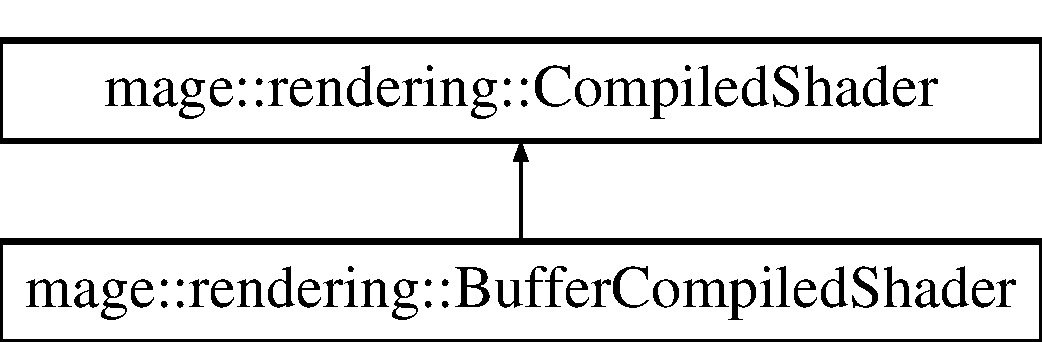
\includegraphics[height=2.000000cm]{classmage_1_1rendering_1_1_buffer_compiled_shader}
\end{center}
\end{figure}
\subsection*{Public Member Functions}
\begin{DoxyCompactItemize}
\item 
\hyperlink{classmage_1_1rendering_1_1_buffer_compiled_shader_ae2a2ce1b29d89125d6413ea9bf773694}{Buffer\+Compiled\+Shader} (gsl\+::span$<$ const B\+Y\+TE $>$ bytecode) noexcept
\item 
\hyperlink{classmage_1_1rendering_1_1_buffer_compiled_shader_a81aeb002f1a4a11b93f70fbeb34c5afc}{Buffer\+Compiled\+Shader} (const \hyperlink{classmage_1_1rendering_1_1_buffer_compiled_shader}{Buffer\+Compiled\+Shader} \&compiled\+\_\+shader) noexcept
\item 
\hyperlink{classmage_1_1rendering_1_1_buffer_compiled_shader_a15ec170bf2864c9dcfa13dff93231a71}{Buffer\+Compiled\+Shader} (\hyperlink{classmage_1_1rendering_1_1_buffer_compiled_shader}{Buffer\+Compiled\+Shader} \&\&compiled\+\_\+shader) noexcept
\item 
virtual \hyperlink{classmage_1_1rendering_1_1_buffer_compiled_shader_af989fa0356f17de9dd75b76aace3f106}{$\sim$\+Buffer\+Compiled\+Shader} ()
\item 
\hyperlink{classmage_1_1rendering_1_1_buffer_compiled_shader}{Buffer\+Compiled\+Shader} \& \hyperlink{classmage_1_1rendering_1_1_buffer_compiled_shader_a1f8eb13198c5bad8ebe55ae1ddf94769}{operator=} (const \hyperlink{classmage_1_1rendering_1_1_buffer_compiled_shader}{Buffer\+Compiled\+Shader} \&compiled\+\_\+shader) noexcept
\item 
\hyperlink{classmage_1_1rendering_1_1_buffer_compiled_shader}{Buffer\+Compiled\+Shader} \& \hyperlink{classmage_1_1rendering_1_1_buffer_compiled_shader_a0e11565292a427dff5b36ef7c26b6d08}{operator=} (\hyperlink{classmage_1_1rendering_1_1_buffer_compiled_shader}{Buffer\+Compiled\+Shader} \&\&compiled\+\_\+shader) noexcept
\item 
virtual const B\+Y\+TE $\ast$ \hyperlink{classmage_1_1rendering_1_1_buffer_compiled_shader_a0887622bd25db8698c572d0dc46167b9}{Get\+Bytecode} () const noexcept override
\item 
virtual S\+I\+Z\+E\+\_\+T \hyperlink{classmage_1_1rendering_1_1_buffer_compiled_shader_a235948a6ba0bcac698d6e35ce3504da2}{Get\+Bytecode\+Size} () const noexcept override
\end{DoxyCompactItemize}
\subsection*{Private Attributes}
\begin{DoxyCompactItemize}
\item 
const B\+Y\+TE $\ast$ \hyperlink{classmage_1_1rendering_1_1_buffer_compiled_shader_a6caa56491d81612c3eaec789d8e341bc}{m\+\_\+bytecode}
\item 
S\+I\+Z\+E\+\_\+T \hyperlink{classmage_1_1rendering_1_1_buffer_compiled_shader_a176f35c25e3a4de26b0334ffdc53da73}{m\+\_\+bytecode\+\_\+size}
\end{DoxyCompactItemize}
\subsection*{Additional Inherited Members}


\subsection{Detailed Description}
A class of buffer compiled shaders. 

\subsection{Constructor \& Destructor Documentation}
\hypertarget{classmage_1_1rendering_1_1_buffer_compiled_shader_ae2a2ce1b29d89125d6413ea9bf773694}{}\label{classmage_1_1rendering_1_1_buffer_compiled_shader_ae2a2ce1b29d89125d6413ea9bf773694} 
\index{mage\+::rendering\+::\+Buffer\+Compiled\+Shader@{mage\+::rendering\+::\+Buffer\+Compiled\+Shader}!Buffer\+Compiled\+Shader@{Buffer\+Compiled\+Shader}}
\index{Buffer\+Compiled\+Shader@{Buffer\+Compiled\+Shader}!mage\+::rendering\+::\+Buffer\+Compiled\+Shader@{mage\+::rendering\+::\+Buffer\+Compiled\+Shader}}
\subsubsection{\texorpdfstring{Buffer\+Compiled\+Shader()}{BufferCompiledShader()}\hspace{0.1cm}{\footnotesize\ttfamily [1/3]}}
{\footnotesize\ttfamily mage\+::rendering\+::\+Buffer\+Compiled\+Shader\+::\+Buffer\+Compiled\+Shader (\begin{DoxyParamCaption}\item[{gsl\+::span$<$ const B\+Y\+TE $>$}]{bytecode }\end{DoxyParamCaption})\hspace{0.3cm}{\ttfamily [explicit]}, {\ttfamily [noexcept]}}

Constructs a buffer compiled shader.


\begin{DoxyParams}[1]{Parameters}
\mbox{\tt in}  & {\em bytecode} & The shader bytecode. \\
\hline
\end{DoxyParams}
\hypertarget{classmage_1_1rendering_1_1_buffer_compiled_shader_a81aeb002f1a4a11b93f70fbeb34c5afc}{}\label{classmage_1_1rendering_1_1_buffer_compiled_shader_a81aeb002f1a4a11b93f70fbeb34c5afc} 
\index{mage\+::rendering\+::\+Buffer\+Compiled\+Shader@{mage\+::rendering\+::\+Buffer\+Compiled\+Shader}!Buffer\+Compiled\+Shader@{Buffer\+Compiled\+Shader}}
\index{Buffer\+Compiled\+Shader@{Buffer\+Compiled\+Shader}!mage\+::rendering\+::\+Buffer\+Compiled\+Shader@{mage\+::rendering\+::\+Buffer\+Compiled\+Shader}}
\subsubsection{\texorpdfstring{Buffer\+Compiled\+Shader()}{BufferCompiledShader()}\hspace{0.1cm}{\footnotesize\ttfamily [2/3]}}
{\footnotesize\ttfamily mage\+::rendering\+::\+Buffer\+Compiled\+Shader\+::\+Buffer\+Compiled\+Shader (\begin{DoxyParamCaption}\item[{const \hyperlink{classmage_1_1rendering_1_1_buffer_compiled_shader}{Buffer\+Compiled\+Shader} \&}]{compiled\+\_\+shader }\end{DoxyParamCaption})\hspace{0.3cm}{\ttfamily [default]}, {\ttfamily [noexcept]}}

Constructs a buffer compiled shader from the given buffer compiled shader.


\begin{DoxyParams}[1]{Parameters}
\mbox{\tt in}  & {\em compiled\+\_\+shader} & A reference to the buffer compiled shader to copy. \\
\hline
\end{DoxyParams}
\hypertarget{classmage_1_1rendering_1_1_buffer_compiled_shader_a15ec170bf2864c9dcfa13dff93231a71}{}\label{classmage_1_1rendering_1_1_buffer_compiled_shader_a15ec170bf2864c9dcfa13dff93231a71} 
\index{mage\+::rendering\+::\+Buffer\+Compiled\+Shader@{mage\+::rendering\+::\+Buffer\+Compiled\+Shader}!Buffer\+Compiled\+Shader@{Buffer\+Compiled\+Shader}}
\index{Buffer\+Compiled\+Shader@{Buffer\+Compiled\+Shader}!mage\+::rendering\+::\+Buffer\+Compiled\+Shader@{mage\+::rendering\+::\+Buffer\+Compiled\+Shader}}
\subsubsection{\texorpdfstring{Buffer\+Compiled\+Shader()}{BufferCompiledShader()}\hspace{0.1cm}{\footnotesize\ttfamily [3/3]}}
{\footnotesize\ttfamily mage\+::rendering\+::\+Buffer\+Compiled\+Shader\+::\+Buffer\+Compiled\+Shader (\begin{DoxyParamCaption}\item[{\hyperlink{classmage_1_1rendering_1_1_buffer_compiled_shader}{Buffer\+Compiled\+Shader} \&\&}]{compiled\+\_\+shader }\end{DoxyParamCaption})\hspace{0.3cm}{\ttfamily [default]}, {\ttfamily [noexcept]}}

Constructs a buffer compiled shader by moving the given buffer compiled shader.


\begin{DoxyParams}[1]{Parameters}
\mbox{\tt in}  & {\em compiled\+\_\+shader} & A reference to the buffer compiled shader to move. \\
\hline
\end{DoxyParams}
\hypertarget{classmage_1_1rendering_1_1_buffer_compiled_shader_af989fa0356f17de9dd75b76aace3f106}{}\label{classmage_1_1rendering_1_1_buffer_compiled_shader_af989fa0356f17de9dd75b76aace3f106} 
\index{mage\+::rendering\+::\+Buffer\+Compiled\+Shader@{mage\+::rendering\+::\+Buffer\+Compiled\+Shader}!````~Buffer\+Compiled\+Shader@{$\sim$\+Buffer\+Compiled\+Shader}}
\index{````~Buffer\+Compiled\+Shader@{$\sim$\+Buffer\+Compiled\+Shader}!mage\+::rendering\+::\+Buffer\+Compiled\+Shader@{mage\+::rendering\+::\+Buffer\+Compiled\+Shader}}
\subsubsection{\texorpdfstring{$\sim$\+Buffer\+Compiled\+Shader()}{~BufferCompiledShader()}}
{\footnotesize\ttfamily mage\+::rendering\+::\+Buffer\+Compiled\+Shader\+::$\sim$\+Buffer\+Compiled\+Shader (\begin{DoxyParamCaption}{ }\end{DoxyParamCaption})\hspace{0.3cm}{\ttfamily [virtual]}, {\ttfamily [default]}}

Destructs this buffer compiled shader. 

\subsection{Member Function Documentation}
\hypertarget{classmage_1_1rendering_1_1_buffer_compiled_shader_a0887622bd25db8698c572d0dc46167b9}{}\label{classmage_1_1rendering_1_1_buffer_compiled_shader_a0887622bd25db8698c572d0dc46167b9} 
\index{mage\+::rendering\+::\+Buffer\+Compiled\+Shader@{mage\+::rendering\+::\+Buffer\+Compiled\+Shader}!Get\+Bytecode@{Get\+Bytecode}}
\index{Get\+Bytecode@{Get\+Bytecode}!mage\+::rendering\+::\+Buffer\+Compiled\+Shader@{mage\+::rendering\+::\+Buffer\+Compiled\+Shader}}
\subsubsection{\texorpdfstring{Get\+Bytecode()}{GetBytecode()}}
{\footnotesize\ttfamily virtual const B\+Y\+TE$\ast$ mage\+::rendering\+::\+Buffer\+Compiled\+Shader\+::\+Get\+Bytecode (\begin{DoxyParamCaption}{ }\end{DoxyParamCaption}) const\hspace{0.3cm}{\ttfamily [override]}, {\ttfamily [virtual]}, {\ttfamily [noexcept]}}

Returns the shader bytecode of this buffer compiled shader.

\begin{DoxyReturn}{Returns}
A pointer to the shader bytecode of this buffer compiled shader. 
\end{DoxyReturn}


Implements \hyperlink{classmage_1_1rendering_1_1_compiled_shader_a6067250341f428be19ed2aa9955a10b6}{mage\+::rendering\+::\+Compiled\+Shader}.

\hypertarget{classmage_1_1rendering_1_1_buffer_compiled_shader_a235948a6ba0bcac698d6e35ce3504da2}{}\label{classmage_1_1rendering_1_1_buffer_compiled_shader_a235948a6ba0bcac698d6e35ce3504da2} 
\index{mage\+::rendering\+::\+Buffer\+Compiled\+Shader@{mage\+::rendering\+::\+Buffer\+Compiled\+Shader}!Get\+Bytecode\+Size@{Get\+Bytecode\+Size}}
\index{Get\+Bytecode\+Size@{Get\+Bytecode\+Size}!mage\+::rendering\+::\+Buffer\+Compiled\+Shader@{mage\+::rendering\+::\+Buffer\+Compiled\+Shader}}
\subsubsection{\texorpdfstring{Get\+Bytecode\+Size()}{GetBytecodeSize()}}
{\footnotesize\ttfamily virtual S\+I\+Z\+E\+\_\+T mage\+::rendering\+::\+Buffer\+Compiled\+Shader\+::\+Get\+Bytecode\+Size (\begin{DoxyParamCaption}{ }\end{DoxyParamCaption}) const\hspace{0.3cm}{\ttfamily [override]}, {\ttfamily [virtual]}, {\ttfamily [noexcept]}}

Returns the size of the shader bytecode (in bytes) of this buffer compiled shader.

\begin{DoxyReturn}{Returns}
The size of the shader bytecode (in bytes) of this buffer compiled shader. 
\end{DoxyReturn}


Implements \hyperlink{classmage_1_1rendering_1_1_compiled_shader_a92c17b46242bf884c3d0d673e88a292d}{mage\+::rendering\+::\+Compiled\+Shader}.

\hypertarget{classmage_1_1rendering_1_1_buffer_compiled_shader_a1f8eb13198c5bad8ebe55ae1ddf94769}{}\label{classmage_1_1rendering_1_1_buffer_compiled_shader_a1f8eb13198c5bad8ebe55ae1ddf94769} 
\index{mage\+::rendering\+::\+Buffer\+Compiled\+Shader@{mage\+::rendering\+::\+Buffer\+Compiled\+Shader}!operator=@{operator=}}
\index{operator=@{operator=}!mage\+::rendering\+::\+Buffer\+Compiled\+Shader@{mage\+::rendering\+::\+Buffer\+Compiled\+Shader}}
\subsubsection{\texorpdfstring{operator=()}{operator=()}\hspace{0.1cm}{\footnotesize\ttfamily [1/2]}}
{\footnotesize\ttfamily \hyperlink{classmage_1_1rendering_1_1_buffer_compiled_shader}{Buffer\+Compiled\+Shader} \& mage\+::rendering\+::\+Buffer\+Compiled\+Shader\+::operator= (\begin{DoxyParamCaption}\item[{const \hyperlink{classmage_1_1rendering_1_1_buffer_compiled_shader}{Buffer\+Compiled\+Shader} \&}]{compiled\+\_\+shader }\end{DoxyParamCaption})\hspace{0.3cm}{\ttfamily [default]}, {\ttfamily [noexcept]}}

Copies the given buffer compiled shader to this buffer compiled shader.


\begin{DoxyParams}[1]{Parameters}
\mbox{\tt in}  & {\em compiled\+\_\+shader} & A reference to the buffer compiled shader to copy. \\
\hline
\end{DoxyParams}
\begin{DoxyReturn}{Returns}
A reference to the copy of the given buffer compiled shader (i.\+e. this buffer compiled shader). 
\end{DoxyReturn}
\hypertarget{classmage_1_1rendering_1_1_buffer_compiled_shader_a0e11565292a427dff5b36ef7c26b6d08}{}\label{classmage_1_1rendering_1_1_buffer_compiled_shader_a0e11565292a427dff5b36ef7c26b6d08} 
\index{mage\+::rendering\+::\+Buffer\+Compiled\+Shader@{mage\+::rendering\+::\+Buffer\+Compiled\+Shader}!operator=@{operator=}}
\index{operator=@{operator=}!mage\+::rendering\+::\+Buffer\+Compiled\+Shader@{mage\+::rendering\+::\+Buffer\+Compiled\+Shader}}
\subsubsection{\texorpdfstring{operator=()}{operator=()}\hspace{0.1cm}{\footnotesize\ttfamily [2/2]}}
{\footnotesize\ttfamily \hyperlink{classmage_1_1rendering_1_1_buffer_compiled_shader}{Buffer\+Compiled\+Shader} \& mage\+::rendering\+::\+Buffer\+Compiled\+Shader\+::operator= (\begin{DoxyParamCaption}\item[{\hyperlink{classmage_1_1rendering_1_1_buffer_compiled_shader}{Buffer\+Compiled\+Shader} \&\&}]{compiled\+\_\+shader }\end{DoxyParamCaption})\hspace{0.3cm}{\ttfamily [default]}, {\ttfamily [noexcept]}}

Moves the given buffer compiled shader to this buffer compiled shader.


\begin{DoxyParams}[1]{Parameters}
\mbox{\tt in}  & {\em compiled\+\_\+shader} & A reference to the buffer compiled shader to copy. \\
\hline
\end{DoxyParams}
\begin{DoxyReturn}{Returns}
A reference to the moved buffer compiled shader (i.\+e. this buffer compiled shader). 
\end{DoxyReturn}


\subsection{Member Data Documentation}
\hypertarget{classmage_1_1rendering_1_1_buffer_compiled_shader_a6caa56491d81612c3eaec789d8e341bc}{}\label{classmage_1_1rendering_1_1_buffer_compiled_shader_a6caa56491d81612c3eaec789d8e341bc} 
\index{mage\+::rendering\+::\+Buffer\+Compiled\+Shader@{mage\+::rendering\+::\+Buffer\+Compiled\+Shader}!m\+\_\+bytecode@{m\+\_\+bytecode}}
\index{m\+\_\+bytecode@{m\+\_\+bytecode}!mage\+::rendering\+::\+Buffer\+Compiled\+Shader@{mage\+::rendering\+::\+Buffer\+Compiled\+Shader}}
\subsubsection{\texorpdfstring{m\+\_\+bytecode}{m\_bytecode}}
{\footnotesize\ttfamily const B\+Y\+TE$\ast$ mage\+::rendering\+::\+Buffer\+Compiled\+Shader\+::m\+\_\+bytecode\hspace{0.3cm}{\ttfamily [private]}}

A pointer to the shader bytecode of this buffer compiled shader. \hypertarget{classmage_1_1rendering_1_1_buffer_compiled_shader_a176f35c25e3a4de26b0334ffdc53da73}{}\label{classmage_1_1rendering_1_1_buffer_compiled_shader_a176f35c25e3a4de26b0334ffdc53da73} 
\index{mage\+::rendering\+::\+Buffer\+Compiled\+Shader@{mage\+::rendering\+::\+Buffer\+Compiled\+Shader}!m\+\_\+bytecode\+\_\+size@{m\+\_\+bytecode\+\_\+size}}
\index{m\+\_\+bytecode\+\_\+size@{m\+\_\+bytecode\+\_\+size}!mage\+::rendering\+::\+Buffer\+Compiled\+Shader@{mage\+::rendering\+::\+Buffer\+Compiled\+Shader}}
\subsubsection{\texorpdfstring{m\+\_\+bytecode\+\_\+size}{m\_bytecode\_size}}
{\footnotesize\ttfamily S\+I\+Z\+E\+\_\+T mage\+::rendering\+::\+Buffer\+Compiled\+Shader\+::m\+\_\+bytecode\+\_\+size\hspace{0.3cm}{\ttfamily [private]}}

The size of the shader bytecode of this buffer compiled shader. 
\hypertarget{classmage_1_1rendering_1_1_buffer_lock}{}\section{mage\+:\+:rendering\+:\+:Buffer\+Lock Class Reference}
\label{classmage_1_1rendering_1_1_buffer_lock}\index{mage\+::rendering\+::\+Buffer\+Lock@{mage\+::rendering\+::\+Buffer\+Lock}}


{\ttfamily \#include $<$buffer\+\_\+lock.\+hpp$>$}

\subsection*{Public Member Functions}
\begin{DoxyCompactItemize}
\item 
\hyperlink{classmage_1_1rendering_1_1_buffer_lock_a548c15e53e0903471268c83f16126f43}{Buffer\+Lock} (I\+D3\+D11\+Device\+Context \&device\+\_\+context, I\+D3\+D11\+Buffer \&buffer, D3\+D11\+\_\+\+M\+AP map\+\_\+type, D3\+D11\+\_\+\+M\+A\+P\+P\+E\+D\+\_\+\+S\+U\+B\+R\+E\+S\+O\+U\+R\+CE \&mapped\+\_\+buffer)
\item 
\hyperlink{classmage_1_1rendering_1_1_buffer_lock_a8804d6bd8626c71aac68bf9a5cf4c1f3}{Buffer\+Lock} (const \hyperlink{classmage_1_1rendering_1_1_buffer_lock}{Buffer\+Lock} \&buffer\+\_\+lock)=delete
\item 
\hyperlink{classmage_1_1rendering_1_1_buffer_lock_ad1f7ea416870a58043c505404115327e}{Buffer\+Lock} (\hyperlink{classmage_1_1rendering_1_1_buffer_lock}{Buffer\+Lock} \&\&buffer\+\_\+lock) noexcept=default
\item 
\hyperlink{classmage_1_1rendering_1_1_buffer_lock_ae7ce340c09dc0698aedf33aeb66b14c6}{$\sim$\+Buffer\+Lock} ()
\item 
\hyperlink{classmage_1_1rendering_1_1_buffer_lock}{Buffer\+Lock} \& \hyperlink{classmage_1_1rendering_1_1_buffer_lock_ae246c49ce47dbff7ac9f08e309e90339}{operator=} (const \hyperlink{classmage_1_1rendering_1_1_buffer_lock}{Buffer\+Lock} \&buffer\+\_\+lock)=delete
\item 
\hyperlink{classmage_1_1rendering_1_1_buffer_lock}{Buffer\+Lock} \& \hyperlink{classmage_1_1rendering_1_1_buffer_lock_a625ec83f70daddaedc2cb0533b982c74}{operator=} (\hyperlink{classmage_1_1rendering_1_1_buffer_lock}{Buffer\+Lock} \&\&buffer\+\_\+lock) noexcept=default
\end{DoxyCompactItemize}
\subsection*{Private Member Functions}
\begin{DoxyCompactItemize}
\item 
void \hyperlink{classmage_1_1rendering_1_1_buffer_lock_a88693ae3717c7098d5cc2313cd16b8a6}{Map\+Buffer} (D3\+D11\+\_\+\+M\+AP map\+\_\+type, D3\+D11\+\_\+\+M\+A\+P\+P\+E\+D\+\_\+\+S\+U\+B\+R\+E\+S\+O\+U\+R\+CE \&mapped\+\_\+buffer)
\item 
void \hyperlink{classmage_1_1rendering_1_1_buffer_lock_a19ebd740876eea3b7d418bef505c47d7}{Unmap\+Buffer} () const noexcept
\end{DoxyCompactItemize}
\subsection*{Private Attributes}
\begin{DoxyCompactItemize}
\item 
std\+::reference\+\_\+wrapper$<$ I\+D3\+D11\+Device\+Context $>$ \hyperlink{classmage_1_1rendering_1_1_buffer_lock_afa41d2028ffcffd11f7e17ae505d1e93}{m\+\_\+device\+\_\+context}
\item 
std\+::reference\+\_\+wrapper$<$ I\+D3\+D11\+Buffer $>$ \hyperlink{classmage_1_1rendering_1_1_buffer_lock_ae3e40fcda48227f62eb63611cad1a507}{m\+\_\+buffer}
\end{DoxyCompactItemize}


\subsection{Detailed Description}
A class of buffer locks. 

\subsection{Constructor \& Destructor Documentation}
\hypertarget{classmage_1_1rendering_1_1_buffer_lock_a548c15e53e0903471268c83f16126f43}{}\label{classmage_1_1rendering_1_1_buffer_lock_a548c15e53e0903471268c83f16126f43} 
\index{mage\+::rendering\+::\+Buffer\+Lock@{mage\+::rendering\+::\+Buffer\+Lock}!Buffer\+Lock@{Buffer\+Lock}}
\index{Buffer\+Lock@{Buffer\+Lock}!mage\+::rendering\+::\+Buffer\+Lock@{mage\+::rendering\+::\+Buffer\+Lock}}
\subsubsection{\texorpdfstring{Buffer\+Lock()}{BufferLock()}\hspace{0.1cm}{\footnotesize\ttfamily [1/3]}}
{\footnotesize\ttfamily mage\+::rendering\+::\+Buffer\+Lock\+::\+Buffer\+Lock (\begin{DoxyParamCaption}\item[{I\+D3\+D11\+Device\+Context \&}]{device\+\_\+context,  }\item[{I\+D3\+D11\+Buffer \&}]{buffer,  }\item[{D3\+D11\+\_\+\+M\+AP}]{map\+\_\+type,  }\item[{D3\+D11\+\_\+\+M\+A\+P\+P\+E\+D\+\_\+\+S\+U\+B\+R\+E\+S\+O\+U\+R\+CE \&}]{mapped\+\_\+buffer }\end{DoxyParamCaption})\hspace{0.3cm}{\ttfamily [explicit]}}

Constructs a buffer lock.


\begin{DoxyParams}[1]{Parameters}
\mbox{\tt in}  & {\em device\+\_\+context} & A reference to the device context. \\
\hline
\mbox{\tt in}  & {\em buffer} & A reference to the buffer. \\
\hline
\mbox{\tt in}  & {\em map\+\_\+type} & The map type specifying the C\+PU\textquotesingle{}s read and write permissions for the buffer of this buffer lock. \\
\hline
\mbox{\tt out}  & {\em mapped\+\_\+buffer} & A reference to map the buffer of this buffer lock to. \\
\hline
\end{DoxyParams}

\begin{DoxyExceptions}{Exceptions}
{\em \hyperlink{classmage_1_1_exception}{Exception}} & Failed to map the buffer. \\
\hline
\end{DoxyExceptions}
\hypertarget{classmage_1_1rendering_1_1_buffer_lock_a8804d6bd8626c71aac68bf9a5cf4c1f3}{}\label{classmage_1_1rendering_1_1_buffer_lock_a8804d6bd8626c71aac68bf9a5cf4c1f3} 
\index{mage\+::rendering\+::\+Buffer\+Lock@{mage\+::rendering\+::\+Buffer\+Lock}!Buffer\+Lock@{Buffer\+Lock}}
\index{Buffer\+Lock@{Buffer\+Lock}!mage\+::rendering\+::\+Buffer\+Lock@{mage\+::rendering\+::\+Buffer\+Lock}}
\subsubsection{\texorpdfstring{Buffer\+Lock()}{BufferLock()}\hspace{0.1cm}{\footnotesize\ttfamily [2/3]}}
{\footnotesize\ttfamily mage\+::rendering\+::\+Buffer\+Lock\+::\+Buffer\+Lock (\begin{DoxyParamCaption}\item[{const \hyperlink{classmage_1_1rendering_1_1_buffer_lock}{Buffer\+Lock} \&}]{buffer\+\_\+lock }\end{DoxyParamCaption})\hspace{0.3cm}{\ttfamily [delete]}}

Constructs a buffer lock from the given buffer lock.


\begin{DoxyParams}[1]{Parameters}
\mbox{\tt in}  & {\em buffer\+\_\+lock} & A reference to the buffer lock to copy. \\
\hline
\end{DoxyParams}
\hypertarget{classmage_1_1rendering_1_1_buffer_lock_ad1f7ea416870a58043c505404115327e}{}\label{classmage_1_1rendering_1_1_buffer_lock_ad1f7ea416870a58043c505404115327e} 
\index{mage\+::rendering\+::\+Buffer\+Lock@{mage\+::rendering\+::\+Buffer\+Lock}!Buffer\+Lock@{Buffer\+Lock}}
\index{Buffer\+Lock@{Buffer\+Lock}!mage\+::rendering\+::\+Buffer\+Lock@{mage\+::rendering\+::\+Buffer\+Lock}}
\subsubsection{\texorpdfstring{Buffer\+Lock()}{BufferLock()}\hspace{0.1cm}{\footnotesize\ttfamily [3/3]}}
{\footnotesize\ttfamily mage\+::rendering\+::\+Buffer\+Lock\+::\+Buffer\+Lock (\begin{DoxyParamCaption}\item[{\hyperlink{classmage_1_1rendering_1_1_buffer_lock}{Buffer\+Lock} \&\&}]{buffer\+\_\+lock }\end{DoxyParamCaption})\hspace{0.3cm}{\ttfamily [default]}, {\ttfamily [noexcept]}}

Constructs a buffer lock by moving the given buffer lock.


\begin{DoxyParams}[1]{Parameters}
\mbox{\tt in}  & {\em buffer\+\_\+lock} & A reference to the buffer lock to move. \\
\hline
\end{DoxyParams}
\hypertarget{classmage_1_1rendering_1_1_buffer_lock_ae7ce340c09dc0698aedf33aeb66b14c6}{}\label{classmage_1_1rendering_1_1_buffer_lock_ae7ce340c09dc0698aedf33aeb66b14c6} 
\index{mage\+::rendering\+::\+Buffer\+Lock@{mage\+::rendering\+::\+Buffer\+Lock}!````~Buffer\+Lock@{$\sim$\+Buffer\+Lock}}
\index{````~Buffer\+Lock@{$\sim$\+Buffer\+Lock}!mage\+::rendering\+::\+Buffer\+Lock@{mage\+::rendering\+::\+Buffer\+Lock}}
\subsubsection{\texorpdfstring{$\sim$\+Buffer\+Lock()}{~BufferLock()}}
{\footnotesize\ttfamily mage\+::rendering\+::\+Buffer\+Lock\+::$\sim$\+Buffer\+Lock (\begin{DoxyParamCaption}{ }\end{DoxyParamCaption})}

Destructs this buffer lock. 

\subsection{Member Function Documentation}
\hypertarget{classmage_1_1rendering_1_1_buffer_lock_a88693ae3717c7098d5cc2313cd16b8a6}{}\label{classmage_1_1rendering_1_1_buffer_lock_a88693ae3717c7098d5cc2313cd16b8a6} 
\index{mage\+::rendering\+::\+Buffer\+Lock@{mage\+::rendering\+::\+Buffer\+Lock}!Map\+Buffer@{Map\+Buffer}}
\index{Map\+Buffer@{Map\+Buffer}!mage\+::rendering\+::\+Buffer\+Lock@{mage\+::rendering\+::\+Buffer\+Lock}}
\subsubsection{\texorpdfstring{Map\+Buffer()}{MapBuffer()}}
{\footnotesize\ttfamily void mage\+::rendering\+::\+Buffer\+Lock\+::\+Map\+Buffer (\begin{DoxyParamCaption}\item[{D3\+D11\+\_\+\+M\+AP}]{map\+\_\+type,  }\item[{D3\+D11\+\_\+\+M\+A\+P\+P\+E\+D\+\_\+\+S\+U\+B\+R\+E\+S\+O\+U\+R\+CE \&}]{mapped\+\_\+buffer }\end{DoxyParamCaption})\hspace{0.3cm}{\ttfamily [private]}}

Maps the buffer of this buffer lock.


\begin{DoxyParams}[1]{Parameters}
\mbox{\tt in}  & {\em map\+\_\+type} & The map type specifying the C\+PU\textquotesingle{}s read and write permissions for the buffer of this buffer lock. \\
\hline
\mbox{\tt out}  & {\em mapped\+\_\+buffer} & A reference to map the buffer of this buffer lock to. \\
\hline
\end{DoxyParams}

\begin{DoxyExceptions}{Exceptions}
{\em \hyperlink{classmage_1_1_exception}{Exception}} & Failed to map the buffer. \\
\hline
\end{DoxyExceptions}
\hypertarget{classmage_1_1rendering_1_1_buffer_lock_ae246c49ce47dbff7ac9f08e309e90339}{}\label{classmage_1_1rendering_1_1_buffer_lock_ae246c49ce47dbff7ac9f08e309e90339} 
\index{mage\+::rendering\+::\+Buffer\+Lock@{mage\+::rendering\+::\+Buffer\+Lock}!operator=@{operator=}}
\index{operator=@{operator=}!mage\+::rendering\+::\+Buffer\+Lock@{mage\+::rendering\+::\+Buffer\+Lock}}
\subsubsection{\texorpdfstring{operator=()}{operator=()}\hspace{0.1cm}{\footnotesize\ttfamily [1/2]}}
{\footnotesize\ttfamily \hyperlink{classmage_1_1rendering_1_1_buffer_lock}{Buffer\+Lock}\& mage\+::rendering\+::\+Buffer\+Lock\+::operator= (\begin{DoxyParamCaption}\item[{const \hyperlink{classmage_1_1rendering_1_1_buffer_lock}{Buffer\+Lock} \&}]{buffer\+\_\+lock }\end{DoxyParamCaption})\hspace{0.3cm}{\ttfamily [delete]}}

Copies the given buffer lock to this buffer lock.


\begin{DoxyParams}[1]{Parameters}
\mbox{\tt in}  & {\em buffer\+\_\+lock} & A reference to the buffer lock to copy. \\
\hline
\end{DoxyParams}
\begin{DoxyReturn}{Returns}
A reference to the copy of the given buffer lock (i.\+e. this buffer lock) 
\end{DoxyReturn}
\hypertarget{classmage_1_1rendering_1_1_buffer_lock_a625ec83f70daddaedc2cb0533b982c74}{}\label{classmage_1_1rendering_1_1_buffer_lock_a625ec83f70daddaedc2cb0533b982c74} 
\index{mage\+::rendering\+::\+Buffer\+Lock@{mage\+::rendering\+::\+Buffer\+Lock}!operator=@{operator=}}
\index{operator=@{operator=}!mage\+::rendering\+::\+Buffer\+Lock@{mage\+::rendering\+::\+Buffer\+Lock}}
\subsubsection{\texorpdfstring{operator=()}{operator=()}\hspace{0.1cm}{\footnotesize\ttfamily [2/2]}}
{\footnotesize\ttfamily \hyperlink{classmage_1_1rendering_1_1_buffer_lock}{Buffer\+Lock}\& mage\+::rendering\+::\+Buffer\+Lock\+::operator= (\begin{DoxyParamCaption}\item[{\hyperlink{classmage_1_1rendering_1_1_buffer_lock}{Buffer\+Lock} \&\&}]{buffer\+\_\+lock }\end{DoxyParamCaption})\hspace{0.3cm}{\ttfamily [default]}, {\ttfamily [noexcept]}}

Moves the given buffer lock to this buffer lock.


\begin{DoxyParams}[1]{Parameters}
\mbox{\tt in}  & {\em buffer\+\_\+lock} & A reference to the buffer lock to move. \\
\hline
\end{DoxyParams}
\begin{DoxyReturn}{Returns}
A reference to the moved buffer lock (i.\+e. this buffer lock) 
\end{DoxyReturn}
\hypertarget{classmage_1_1rendering_1_1_buffer_lock_a19ebd740876eea3b7d418bef505c47d7}{}\label{classmage_1_1rendering_1_1_buffer_lock_a19ebd740876eea3b7d418bef505c47d7} 
\index{mage\+::rendering\+::\+Buffer\+Lock@{mage\+::rendering\+::\+Buffer\+Lock}!Unmap\+Buffer@{Unmap\+Buffer}}
\index{Unmap\+Buffer@{Unmap\+Buffer}!mage\+::rendering\+::\+Buffer\+Lock@{mage\+::rendering\+::\+Buffer\+Lock}}
\subsubsection{\texorpdfstring{Unmap\+Buffer()}{UnmapBuffer()}}
{\footnotesize\ttfamily void mage\+::rendering\+::\+Buffer\+Lock\+::\+Unmap\+Buffer (\begin{DoxyParamCaption}{ }\end{DoxyParamCaption}) const\hspace{0.3cm}{\ttfamily [private]}, {\ttfamily [noexcept]}}

Unmaps the buffer of this buffer lock.

\begin{DoxyPrecond}{Precondition}
The buffer of this buffer lock must be mapped with \hyperlink{classmage_1_1rendering_1_1_buffer_lock_a88693ae3717c7098d5cc2313cd16b8a6}{mage\+::rendering\+::\+Buffer\+Lock\+::\+Map\+Buffer(\+D3\+D11\+\_\+\+M\+A\+P, D3\+D11\+\_\+\+M\+A\+P\+P\+E\+D\+\_\+\+S\+U\+B\+R\+E\+S\+O\+U\+R\+C\+E\&)} before it can be unmapped. 
\end{DoxyPrecond}


\subsection{Member Data Documentation}
\hypertarget{classmage_1_1rendering_1_1_buffer_lock_ae3e40fcda48227f62eb63611cad1a507}{}\label{classmage_1_1rendering_1_1_buffer_lock_ae3e40fcda48227f62eb63611cad1a507} 
\index{mage\+::rendering\+::\+Buffer\+Lock@{mage\+::rendering\+::\+Buffer\+Lock}!m\+\_\+buffer@{m\+\_\+buffer}}
\index{m\+\_\+buffer@{m\+\_\+buffer}!mage\+::rendering\+::\+Buffer\+Lock@{mage\+::rendering\+::\+Buffer\+Lock}}
\subsubsection{\texorpdfstring{m\+\_\+buffer}{m\_buffer}}
{\footnotesize\ttfamily std\+::reference\+\_\+wrapper$<$ I\+D3\+D11\+Buffer $>$ mage\+::rendering\+::\+Buffer\+Lock\+::m\+\_\+buffer\hspace{0.3cm}{\ttfamily [private]}}

A reference to the buffer of this lock. \hypertarget{classmage_1_1rendering_1_1_buffer_lock_afa41d2028ffcffd11f7e17ae505d1e93}{}\label{classmage_1_1rendering_1_1_buffer_lock_afa41d2028ffcffd11f7e17ae505d1e93} 
\index{mage\+::rendering\+::\+Buffer\+Lock@{mage\+::rendering\+::\+Buffer\+Lock}!m\+\_\+device\+\_\+context@{m\+\_\+device\+\_\+context}}
\index{m\+\_\+device\+\_\+context@{m\+\_\+device\+\_\+context}!mage\+::rendering\+::\+Buffer\+Lock@{mage\+::rendering\+::\+Buffer\+Lock}}
\subsubsection{\texorpdfstring{m\+\_\+device\+\_\+context}{m\_device\_context}}
{\footnotesize\ttfamily std\+::reference\+\_\+wrapper$<$ I\+D3\+D11\+Device\+Context $>$ mage\+::rendering\+::\+Buffer\+Lock\+::m\+\_\+device\+\_\+context\hspace{0.3cm}{\ttfamily [private]}}

A reference to the device context of this buffer lock. 
\hypertarget{classmage_1_1rendering_1_1_camera}{}\section{mage\+:\+:rendering\+:\+:Camera Class Reference}
\label{classmage_1_1rendering_1_1_camera}\index{mage\+::rendering\+::\+Camera@{mage\+::rendering\+::\+Camera}}


{\ttfamily \#include $<$camera.\+hpp$>$}

Inheritance diagram for mage\+:\+:rendering\+:\+:Camera\+:\begin{figure}[H]
\begin{center}
\leavevmode
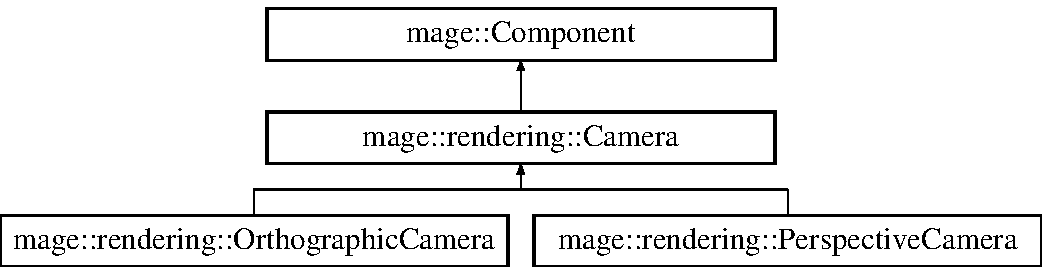
\includegraphics[height=3.000000cm]{classmage_1_1rendering_1_1_camera}
\end{center}
\end{figure}
\subsection*{Public Member Functions}
\begin{DoxyCompactItemize}
\item 
virtual \mbox{\hyperlink{classmage_1_1rendering_1_1_camera_ae892311357bddc9ea081912579f8cd9c}{$\sim$\+Camera}} ()
\item 
\mbox{\hyperlink{classmage_1_1rendering_1_1_camera}{Camera}} \& \mbox{\hyperlink{classmage_1_1rendering_1_1_camera_a3aceb5277ca9ea66037de3d5ed44434a}{operator=}} (const \mbox{\hyperlink{classmage_1_1rendering_1_1_camera}{Camera}} \&camera)=delete
\item 
\mbox{\hyperlink{classmage_1_1rendering_1_1_camera}{Camera}} \& \mbox{\hyperlink{classmage_1_1rendering_1_1_camera_a61b594df300888d8d442855d18b871a3}{operator=}} (\mbox{\hyperlink{classmage_1_1rendering_1_1_camera}{Camera}} \&\&camera) noexcept
\item 
const \mbox{\hyperlink{namespacemage_aee4759dedc8def6c6dec26b5c7eddf29}{F32x2}} \mbox{\hyperlink{classmage_1_1rendering_1_1_camera_acd2a3c07aee98ae85504ce8293f16e04}{Get\+Clipping\+Planes}} () const noexcept
\item 
void \mbox{\hyperlink{classmage_1_1rendering_1_1_camera_afc95f8de701649af5b614a57c1c06e9a}{Set\+Clipping\+Planes}} (\mbox{\hyperlink{namespacemage_aee4759dedc8def6c6dec26b5c7eddf29}{F32x2}} clipping\+\_\+planes) noexcept
\item 
virtual const X\+M\+M\+A\+T\+R\+IX X\+M\+\_\+\+C\+A\+L\+L\+C\+O\+NV \mbox{\hyperlink{classmage_1_1rendering_1_1_camera_a08481175c3718a24333b22176e240d44}{Get\+Camera\+To\+Projection\+Matrix}} () const noexcept=0
\item 
virtual const X\+M\+M\+A\+T\+R\+IX X\+M\+\_\+\+C\+A\+L\+L\+C\+O\+NV \mbox{\hyperlink{classmage_1_1rendering_1_1_camera_abb21116f8a6c7513804431d23fa4cf17}{Get\+Projection\+To\+Camera\+Matrix}} () const noexcept=0
\item 
\mbox{\hyperlink{classmage_1_1rendering_1_1_camera_lens}{Camera\+Lens}} \& \mbox{\hyperlink{classmage_1_1rendering_1_1_camera_a49967d5b733b8d2e1ccbfc71c4f66d42}{Get\+Lens}} () noexcept
\item 
const \mbox{\hyperlink{classmage_1_1rendering_1_1_camera_lens}{Camera\+Lens}} \& \mbox{\hyperlink{classmage_1_1rendering_1_1_camera_a3a1156907006b4d60a4e36789216e31a}{Get\+Lens}} () const noexcept
\item 
\mbox{\hyperlink{classmage_1_1rendering_1_1_viewport}{Viewport}} \& \mbox{\hyperlink{classmage_1_1rendering_1_1_camera_aff1dea377f7f36b1d518369b3f8108cc}{Get\+Viewport}} () noexcept
\item 
const \mbox{\hyperlink{classmage_1_1rendering_1_1_viewport}{Viewport}} \& \mbox{\hyperlink{classmage_1_1rendering_1_1_camera_a5d91ec5a395b638140c107a192faa2a3}{Get\+Viewport}} () const noexcept
\item 
\mbox{\hyperlink{classmage_1_1rendering_1_1_camera_settings}{Camera\+Settings}} \& \mbox{\hyperlink{classmage_1_1rendering_1_1_camera_a32588a00052469be808d2819953ea2a4}{Get\+Settings}} () noexcept
\item 
const \mbox{\hyperlink{classmage_1_1rendering_1_1_camera_settings}{Camera\+Settings}} \& \mbox{\hyperlink{classmage_1_1rendering_1_1_camera_a65d79baabdaaf9847102a03f6965e0ed}{Get\+Settings}} () const noexcept
\item 
void \mbox{\hyperlink{classmage_1_1rendering_1_1_camera_a82380790ba5c92b93e90c8b8cea146c0}{Update\+Buffer}} (I\+D3\+D11\+Device\+Context \&device\+\_\+context, \mbox{\hyperlink{namespacemage_1_1rendering_ac3f75e49e92b42f2f5fb55c450d8899c}{Anti\+Aliasing}} aa) const
\item 
{\footnotesize template$<$typename Pipeline\+StageT $>$ }\\void \mbox{\hyperlink{classmage_1_1rendering_1_1_camera_aa950bdd33e00fc78ebb496b58e0de5b0}{Bind\+Buffer}} (I\+D3\+D11\+Device\+Context \&device\+\_\+context, \mbox{\hyperlink{namespacemage_aa5d6eaabaac3cdd01873d6a3d27e90f3}{U32}} slot) const noexcept
\end{DoxyCompactItemize}
\subsection*{Protected Member Functions}
\begin{DoxyCompactItemize}
\item 
\mbox{\hyperlink{classmage_1_1rendering_1_1_camera_a872aafc40d35c1481a4147c73fdbc00a}{Camera}} (I\+D3\+D11\+Device \&device)
\item 
\mbox{\hyperlink{classmage_1_1rendering_1_1_camera_ac4e1e9f230416c0aaea12d2b0fff02c1}{Camera}} (const \mbox{\hyperlink{classmage_1_1rendering_1_1_camera}{Camera}} \&camera)=delete
\item 
\mbox{\hyperlink{classmage_1_1rendering_1_1_camera_a7ac683929b75589e3f396a76a6afb9cf}{Camera}} (\mbox{\hyperlink{classmage_1_1rendering_1_1_camera}{Camera}} \&\&camera) noexcept
\end{DoxyCompactItemize}
\subsection*{Private Attributes}
\begin{DoxyCompactItemize}
\item 
\mbox{\hyperlink{classmage_1_1rendering_1_1_constant_buffer}{Constant\+Buffer}}$<$ \mbox{\hyperlink{structmage_1_1rendering_1_1_camera_buffer}{Camera\+Buffer}} $>$ \mbox{\hyperlink{classmage_1_1rendering_1_1_camera_a81012e035e7117cac50434c2d85ac0ad}{m\+\_\+buffer}}
\item 
\mbox{\hyperlink{namespacemage_aee4759dedc8def6c6dec26b5c7eddf29}{F32x2}} \mbox{\hyperlink{classmage_1_1rendering_1_1_camera_a0224d8321b9a45251ff12f5771a1e5fc}{m\+\_\+clipping\+\_\+planes}}
\item 
\mbox{\hyperlink{classmage_1_1rendering_1_1_camera_lens}{Camera\+Lens}} \mbox{\hyperlink{classmage_1_1rendering_1_1_camera_a0716fc9d2b3c8f41da75205caa428189}{m\+\_\+lens}}
\item 
\mbox{\hyperlink{classmage_1_1rendering_1_1_viewport}{Viewport}} \mbox{\hyperlink{classmage_1_1rendering_1_1_camera_af01065cfadb5c8442bcc0f823254b09e}{m\+\_\+viewport}}
\item 
\mbox{\hyperlink{classmage_1_1rendering_1_1_camera_settings}{Camera\+Settings}} \mbox{\hyperlink{classmage_1_1rendering_1_1_camera_a9a8cfd88c1a3b2b54779bbe0f34d30d2}{m\+\_\+settings}}
\end{DoxyCompactItemize}


\subsection{Detailed Description}
A class of cameras. 

\subsection{Constructor \& Destructor Documentation}
\mbox{\Hypertarget{classmage_1_1rendering_1_1_camera_ae892311357bddc9ea081912579f8cd9c}\label{classmage_1_1rendering_1_1_camera_ae892311357bddc9ea081912579f8cd9c}} 
\index{mage\+::rendering\+::\+Camera@{mage\+::rendering\+::\+Camera}!````~Camera@{$\sim$\+Camera}}
\index{````~Camera@{$\sim$\+Camera}!mage\+::rendering\+::\+Camera@{mage\+::rendering\+::\+Camera}}
\subsubsection{\texorpdfstring{$\sim$\+Camera()}{~Camera()}}
{\footnotesize\ttfamily mage\+::rendering\+::\+Camera\+::$\sim$\+Camera (\begin{DoxyParamCaption}{ }\end{DoxyParamCaption})\hspace{0.3cm}{\ttfamily [virtual]}, {\ttfamily [default]}}

Destructs this camera. \mbox{\Hypertarget{classmage_1_1rendering_1_1_camera_a872aafc40d35c1481a4147c73fdbc00a}\label{classmage_1_1rendering_1_1_camera_a872aafc40d35c1481a4147c73fdbc00a}} 
\index{mage\+::rendering\+::\+Camera@{mage\+::rendering\+::\+Camera}!Camera@{Camera}}
\index{Camera@{Camera}!mage\+::rendering\+::\+Camera@{mage\+::rendering\+::\+Camera}}
\subsubsection{\texorpdfstring{Camera()}{Camera()}\hspace{0.1cm}{\footnotesize\ttfamily [1/3]}}
{\footnotesize\ttfamily mage\+::rendering\+::\+Camera\+::\+Camera (\begin{DoxyParamCaption}\item[{I\+D3\+D11\+Device \&}]{device }\end{DoxyParamCaption})\hspace{0.3cm}{\ttfamily [explicit]}, {\ttfamily [protected]}}

Constructs a camera.


\begin{DoxyParams}[1]{Parameters}
\mbox{\tt in,out}  & {\em device} & A reference to the device. \\
\hline
\end{DoxyParams}
\mbox{\Hypertarget{classmage_1_1rendering_1_1_camera_ac4e1e9f230416c0aaea12d2b0fff02c1}\label{classmage_1_1rendering_1_1_camera_ac4e1e9f230416c0aaea12d2b0fff02c1}} 
\index{mage\+::rendering\+::\+Camera@{mage\+::rendering\+::\+Camera}!Camera@{Camera}}
\index{Camera@{Camera}!mage\+::rendering\+::\+Camera@{mage\+::rendering\+::\+Camera}}
\subsubsection{\texorpdfstring{Camera()}{Camera()}\hspace{0.1cm}{\footnotesize\ttfamily [2/3]}}
{\footnotesize\ttfamily mage\+::rendering\+::\+Camera\+::\+Camera (\begin{DoxyParamCaption}\item[{const \mbox{\hyperlink{classmage_1_1rendering_1_1_camera}{Camera}} \&}]{camera }\end{DoxyParamCaption})\hspace{0.3cm}{\ttfamily [protected]}, {\ttfamily [delete]}}

Constructs a camera from the given camera.


\begin{DoxyParams}[1]{Parameters}
\mbox{\tt in}  & {\em camera} & A reference to the camera to copy. \\
\hline
\end{DoxyParams}
\mbox{\Hypertarget{classmage_1_1rendering_1_1_camera_a7ac683929b75589e3f396a76a6afb9cf}\label{classmage_1_1rendering_1_1_camera_a7ac683929b75589e3f396a76a6afb9cf}} 
\index{mage\+::rendering\+::\+Camera@{mage\+::rendering\+::\+Camera}!Camera@{Camera}}
\index{Camera@{Camera}!mage\+::rendering\+::\+Camera@{mage\+::rendering\+::\+Camera}}
\subsubsection{\texorpdfstring{Camera()}{Camera()}\hspace{0.1cm}{\footnotesize\ttfamily [3/3]}}
{\footnotesize\ttfamily mage\+::rendering\+::\+Camera\+::\+Camera (\begin{DoxyParamCaption}\item[{\mbox{\hyperlink{classmage_1_1rendering_1_1_camera}{Camera}} \&\&}]{camera }\end{DoxyParamCaption})\hspace{0.3cm}{\ttfamily [protected]}, {\ttfamily [default]}, {\ttfamily [noexcept]}}

Constructs a camera by moving the given camera.


\begin{DoxyParams}[1]{Parameters}
\mbox{\tt in}  & {\em camera} & A reference to the camera to move. \\
\hline
\end{DoxyParams}


\subsection{Member Function Documentation}
\mbox{\Hypertarget{classmage_1_1rendering_1_1_camera_aa950bdd33e00fc78ebb496b58e0de5b0}\label{classmage_1_1rendering_1_1_camera_aa950bdd33e00fc78ebb496b58e0de5b0}} 
\index{mage\+::rendering\+::\+Camera@{mage\+::rendering\+::\+Camera}!Bind\+Buffer@{Bind\+Buffer}}
\index{Bind\+Buffer@{Bind\+Buffer}!mage\+::rendering\+::\+Camera@{mage\+::rendering\+::\+Camera}}
\subsubsection{\texorpdfstring{Bind\+Buffer()}{BindBuffer()}}
{\footnotesize\ttfamily template$<$typename Pipeline\+StageT $>$ \\
void mage\+::rendering\+::\+Camera\+::\+Bind\+Buffer (\begin{DoxyParamCaption}\item[{I\+D3\+D11\+Device\+Context \&}]{device\+\_\+context,  }\item[{\mbox{\hyperlink{namespacemage_aa5d6eaabaac3cdd01873d6a3d27e90f3}{U32}}}]{slot }\end{DoxyParamCaption}) const\hspace{0.3cm}{\ttfamily [noexcept]}}

Binds the buffer of this camera to the given pipeline stage.


\begin{DoxyTemplParams}{Template Parameters}
{\em Pipeline\+StageT} & The pipeline stage type. \\
\hline
\end{DoxyTemplParams}

\begin{DoxyParams}[1]{Parameters}
\mbox{\tt in,out}  & {\em device\+\_\+context} & A reference to the device context. \\
\hline
\mbox{\tt in}  & {\em slot} & The index into the device\textquotesingle{}s zero-\/based array to set the constant buffer to (ranges from 0 to {\ttfamily D3\+D11\+\_\+\+C\+O\+M\+M\+O\+N\+S\+H\+A\+D\+E\+R\+\_\+\+C\+O\+N\+S\+T\+A\+N\+T\+\_\+\+B\+U\+F\+F\+E\+R\+\_\+\+A\+P\+I\+\_\+\+S\+L\+O\+T\+\_\+\+C\+O\+U\+NT} -\/ 1). \\
\hline
\end{DoxyParams}
\mbox{\Hypertarget{classmage_1_1rendering_1_1_camera_a08481175c3718a24333b22176e240d44}\label{classmage_1_1rendering_1_1_camera_a08481175c3718a24333b22176e240d44}} 
\index{mage\+::rendering\+::\+Camera@{mage\+::rendering\+::\+Camera}!Get\+Camera\+To\+Projection\+Matrix@{Get\+Camera\+To\+Projection\+Matrix}}
\index{Get\+Camera\+To\+Projection\+Matrix@{Get\+Camera\+To\+Projection\+Matrix}!mage\+::rendering\+::\+Camera@{mage\+::rendering\+::\+Camera}}
\subsubsection{\texorpdfstring{Get\+Camera\+To\+Projection\+Matrix()}{GetCameraToProjectionMatrix()}}
{\footnotesize\ttfamily virtual const X\+M\+M\+A\+T\+R\+IX X\+M\+\_\+\+C\+A\+L\+L\+C\+O\+NV mage\+::rendering\+::\+Camera\+::\+Get\+Camera\+To\+Projection\+Matrix (\begin{DoxyParamCaption}{ }\end{DoxyParamCaption}) const\hspace{0.3cm}{\ttfamily [pure virtual]}, {\ttfamily [noexcept]}}

Returns the camera-\/to-\/projection matrix of this camera.

\begin{DoxyReturn}{Returns}
The camera-\/to-\/projection matrix of this camera. 
\end{DoxyReturn}


Implemented in \mbox{\hyperlink{classmage_1_1rendering_1_1_perspective_camera_af0892905a0030fc70bdc629007cde5a0}{mage\+::rendering\+::\+Perspective\+Camera}}, and \mbox{\hyperlink{classmage_1_1rendering_1_1_orthographic_camera_a45736d696df0a38c8f1342dca2cda0cd}{mage\+::rendering\+::\+Orthographic\+Camera}}.

\mbox{\Hypertarget{classmage_1_1rendering_1_1_camera_acd2a3c07aee98ae85504ce8293f16e04}\label{classmage_1_1rendering_1_1_camera_acd2a3c07aee98ae85504ce8293f16e04}} 
\index{mage\+::rendering\+::\+Camera@{mage\+::rendering\+::\+Camera}!Get\+Clipping\+Planes@{Get\+Clipping\+Planes}}
\index{Get\+Clipping\+Planes@{Get\+Clipping\+Planes}!mage\+::rendering\+::\+Camera@{mage\+::rendering\+::\+Camera}}
\subsubsection{\texorpdfstring{Get\+Clipping\+Planes()}{GetClippingPlanes()}}
{\footnotesize\ttfamily const \mbox{\hyperlink{namespacemage_aee4759dedc8def6c6dec26b5c7eddf29}{F32x2}} mage\+::rendering\+::\+Camera\+::\+Get\+Clipping\+Planes (\begin{DoxyParamCaption}{ }\end{DoxyParamCaption}) const\hspace{0.3cm}{\ttfamily [noexcept]}}

Returns the clipping planes of this camera expressed in camera space.

\begin{DoxyReturn}{Returns}
The clipping planes of this camera expressed in camera space. 
\end{DoxyReturn}
\mbox{\Hypertarget{classmage_1_1rendering_1_1_camera_a49967d5b733b8d2e1ccbfc71c4f66d42}\label{classmage_1_1rendering_1_1_camera_a49967d5b733b8d2e1ccbfc71c4f66d42}} 
\index{mage\+::rendering\+::\+Camera@{mage\+::rendering\+::\+Camera}!Get\+Lens@{Get\+Lens}}
\index{Get\+Lens@{Get\+Lens}!mage\+::rendering\+::\+Camera@{mage\+::rendering\+::\+Camera}}
\subsubsection{\texorpdfstring{Get\+Lens()}{GetLens()}\hspace{0.1cm}{\footnotesize\ttfamily [1/2]}}
{\footnotesize\ttfamily \mbox{\hyperlink{classmage_1_1rendering_1_1_camera_lens}{Camera\+Lens}}\& mage\+::rendering\+::\+Camera\+::\+Get\+Lens (\begin{DoxyParamCaption}{ }\end{DoxyParamCaption})\hspace{0.3cm}{\ttfamily [noexcept]}}

Returns the lens of this camera.

\begin{DoxyReturn}{Returns}
A reference to the lens of this camera. 
\end{DoxyReturn}
\mbox{\Hypertarget{classmage_1_1rendering_1_1_camera_a3a1156907006b4d60a4e36789216e31a}\label{classmage_1_1rendering_1_1_camera_a3a1156907006b4d60a4e36789216e31a}} 
\index{mage\+::rendering\+::\+Camera@{mage\+::rendering\+::\+Camera}!Get\+Lens@{Get\+Lens}}
\index{Get\+Lens@{Get\+Lens}!mage\+::rendering\+::\+Camera@{mage\+::rendering\+::\+Camera}}
\subsubsection{\texorpdfstring{Get\+Lens()}{GetLens()}\hspace{0.1cm}{\footnotesize\ttfamily [2/2]}}
{\footnotesize\ttfamily const \mbox{\hyperlink{classmage_1_1rendering_1_1_camera_lens}{Camera\+Lens}}\& mage\+::rendering\+::\+Camera\+::\+Get\+Lens (\begin{DoxyParamCaption}{ }\end{DoxyParamCaption}) const\hspace{0.3cm}{\ttfamily [noexcept]}}

Returns the lens of this camera.

\begin{DoxyReturn}{Returns}
A reference to the lens of this camera. 
\end{DoxyReturn}
\mbox{\Hypertarget{classmage_1_1rendering_1_1_camera_abb21116f8a6c7513804431d23fa4cf17}\label{classmage_1_1rendering_1_1_camera_abb21116f8a6c7513804431d23fa4cf17}} 
\index{mage\+::rendering\+::\+Camera@{mage\+::rendering\+::\+Camera}!Get\+Projection\+To\+Camera\+Matrix@{Get\+Projection\+To\+Camera\+Matrix}}
\index{Get\+Projection\+To\+Camera\+Matrix@{Get\+Projection\+To\+Camera\+Matrix}!mage\+::rendering\+::\+Camera@{mage\+::rendering\+::\+Camera}}
\subsubsection{\texorpdfstring{Get\+Projection\+To\+Camera\+Matrix()}{GetProjectionToCameraMatrix()}}
{\footnotesize\ttfamily virtual const X\+M\+M\+A\+T\+R\+IX X\+M\+\_\+\+C\+A\+L\+L\+C\+O\+NV mage\+::rendering\+::\+Camera\+::\+Get\+Projection\+To\+Camera\+Matrix (\begin{DoxyParamCaption}{ }\end{DoxyParamCaption}) const\hspace{0.3cm}{\ttfamily [pure virtual]}, {\ttfamily [noexcept]}}

Returns the projection-\/to-\/camera matrix of this camera.

\begin{DoxyReturn}{Returns}
The projection-\/to-\/camera matrix of this camera. 
\end{DoxyReturn}


Implemented in \mbox{\hyperlink{classmage_1_1rendering_1_1_perspective_camera_af049c6330ebdaa822bfd31dc88f25ac2}{mage\+::rendering\+::\+Perspective\+Camera}}, and \mbox{\hyperlink{classmage_1_1rendering_1_1_orthographic_camera_a7d52862a3762dcaeadf26e8ae92d9d09}{mage\+::rendering\+::\+Orthographic\+Camera}}.

\mbox{\Hypertarget{classmage_1_1rendering_1_1_camera_a32588a00052469be808d2819953ea2a4}\label{classmage_1_1rendering_1_1_camera_a32588a00052469be808d2819953ea2a4}} 
\index{mage\+::rendering\+::\+Camera@{mage\+::rendering\+::\+Camera}!Get\+Settings@{Get\+Settings}}
\index{Get\+Settings@{Get\+Settings}!mage\+::rendering\+::\+Camera@{mage\+::rendering\+::\+Camera}}
\subsubsection{\texorpdfstring{Get\+Settings()}{GetSettings()}\hspace{0.1cm}{\footnotesize\ttfamily [1/2]}}
{\footnotesize\ttfamily \mbox{\hyperlink{classmage_1_1rendering_1_1_camera_settings}{Camera\+Settings}}\& mage\+::rendering\+::\+Camera\+::\+Get\+Settings (\begin{DoxyParamCaption}{ }\end{DoxyParamCaption})\hspace{0.3cm}{\ttfamily [noexcept]}}

Returns the settings of this camera.

\begin{DoxyReturn}{Returns}
A reference to the settings of this camera. 
\end{DoxyReturn}
\mbox{\Hypertarget{classmage_1_1rendering_1_1_camera_a65d79baabdaaf9847102a03f6965e0ed}\label{classmage_1_1rendering_1_1_camera_a65d79baabdaaf9847102a03f6965e0ed}} 
\index{mage\+::rendering\+::\+Camera@{mage\+::rendering\+::\+Camera}!Get\+Settings@{Get\+Settings}}
\index{Get\+Settings@{Get\+Settings}!mage\+::rendering\+::\+Camera@{mage\+::rendering\+::\+Camera}}
\subsubsection{\texorpdfstring{Get\+Settings()}{GetSettings()}\hspace{0.1cm}{\footnotesize\ttfamily [2/2]}}
{\footnotesize\ttfamily const \mbox{\hyperlink{classmage_1_1rendering_1_1_camera_settings}{Camera\+Settings}}\& mage\+::rendering\+::\+Camera\+::\+Get\+Settings (\begin{DoxyParamCaption}{ }\end{DoxyParamCaption}) const\hspace{0.3cm}{\ttfamily [noexcept]}}

Returns the settings of this camera.

\begin{DoxyReturn}{Returns}
A reference to the settings of this camera. 
\end{DoxyReturn}
\mbox{\Hypertarget{classmage_1_1rendering_1_1_camera_aff1dea377f7f36b1d518369b3f8108cc}\label{classmage_1_1rendering_1_1_camera_aff1dea377f7f36b1d518369b3f8108cc}} 
\index{mage\+::rendering\+::\+Camera@{mage\+::rendering\+::\+Camera}!Get\+Viewport@{Get\+Viewport}}
\index{Get\+Viewport@{Get\+Viewport}!mage\+::rendering\+::\+Camera@{mage\+::rendering\+::\+Camera}}
\subsubsection{\texorpdfstring{Get\+Viewport()}{GetViewport()}\hspace{0.1cm}{\footnotesize\ttfamily [1/2]}}
{\footnotesize\ttfamily \mbox{\hyperlink{classmage_1_1rendering_1_1_viewport}{Viewport}}\& mage\+::rendering\+::\+Camera\+::\+Get\+Viewport (\begin{DoxyParamCaption}{ }\end{DoxyParamCaption})\hspace{0.3cm}{\ttfamily [noexcept]}}

Returns the viewport of this camera.

\begin{DoxyReturn}{Returns}
A reference to the viewport of this camera. 
\end{DoxyReturn}
\mbox{\Hypertarget{classmage_1_1rendering_1_1_camera_a5d91ec5a395b638140c107a192faa2a3}\label{classmage_1_1rendering_1_1_camera_a5d91ec5a395b638140c107a192faa2a3}} 
\index{mage\+::rendering\+::\+Camera@{mage\+::rendering\+::\+Camera}!Get\+Viewport@{Get\+Viewport}}
\index{Get\+Viewport@{Get\+Viewport}!mage\+::rendering\+::\+Camera@{mage\+::rendering\+::\+Camera}}
\subsubsection{\texorpdfstring{Get\+Viewport()}{GetViewport()}\hspace{0.1cm}{\footnotesize\ttfamily [2/2]}}
{\footnotesize\ttfamily const \mbox{\hyperlink{classmage_1_1rendering_1_1_viewport}{Viewport}}\& mage\+::rendering\+::\+Camera\+::\+Get\+Viewport (\begin{DoxyParamCaption}{ }\end{DoxyParamCaption}) const\hspace{0.3cm}{\ttfamily [noexcept]}}

Returns the viewport of this camera.

\begin{DoxyReturn}{Returns}
A reference to the viewport of this camera. 
\end{DoxyReturn}
\mbox{\Hypertarget{classmage_1_1rendering_1_1_camera_a3aceb5277ca9ea66037de3d5ed44434a}\label{classmage_1_1rendering_1_1_camera_a3aceb5277ca9ea66037de3d5ed44434a}} 
\index{mage\+::rendering\+::\+Camera@{mage\+::rendering\+::\+Camera}!operator=@{operator=}}
\index{operator=@{operator=}!mage\+::rendering\+::\+Camera@{mage\+::rendering\+::\+Camera}}
\subsubsection{\texorpdfstring{operator=()}{operator=()}\hspace{0.1cm}{\footnotesize\ttfamily [1/2]}}
{\footnotesize\ttfamily \mbox{\hyperlink{classmage_1_1rendering_1_1_camera}{Camera}}\& mage\+::rendering\+::\+Camera\+::operator= (\begin{DoxyParamCaption}\item[{const \mbox{\hyperlink{classmage_1_1rendering_1_1_camera}{Camera}} \&}]{camera }\end{DoxyParamCaption})\hspace{0.3cm}{\ttfamily [delete]}}

Copies the given camera to this camera.


\begin{DoxyParams}[1]{Parameters}
\mbox{\tt in}  & {\em camera} & A reference to the camera to copy. \\
\hline
\end{DoxyParams}
\begin{DoxyReturn}{Returns}
A reference to the copy of the given camera (i.\+e. this camera). 
\end{DoxyReturn}
\mbox{\Hypertarget{classmage_1_1rendering_1_1_camera_a61b594df300888d8d442855d18b871a3}\label{classmage_1_1rendering_1_1_camera_a61b594df300888d8d442855d18b871a3}} 
\index{mage\+::rendering\+::\+Camera@{mage\+::rendering\+::\+Camera}!operator=@{operator=}}
\index{operator=@{operator=}!mage\+::rendering\+::\+Camera@{mage\+::rendering\+::\+Camera}}
\subsubsection{\texorpdfstring{operator=()}{operator=()}\hspace{0.1cm}{\footnotesize\ttfamily [2/2]}}
{\footnotesize\ttfamily \mbox{\hyperlink{classmage_1_1rendering_1_1_camera}{Camera}} \& mage\+::rendering\+::\+Camera\+::operator= (\begin{DoxyParamCaption}\item[{\mbox{\hyperlink{classmage_1_1rendering_1_1_camera}{Camera}} \&\&}]{camera }\end{DoxyParamCaption})\hspace{0.3cm}{\ttfamily [default]}, {\ttfamily [noexcept]}}

Moves the given camera to this camera.


\begin{DoxyParams}[1]{Parameters}
\mbox{\tt in}  & {\em camera} & A reference to the camera to move. \\
\hline
\end{DoxyParams}
\begin{DoxyReturn}{Returns}
A reference to the moved camera (i.\+e. this camera). 
\end{DoxyReturn}
\mbox{\Hypertarget{classmage_1_1rendering_1_1_camera_afc95f8de701649af5b614a57c1c06e9a}\label{classmage_1_1rendering_1_1_camera_afc95f8de701649af5b614a57c1c06e9a}} 
\index{mage\+::rendering\+::\+Camera@{mage\+::rendering\+::\+Camera}!Set\+Clipping\+Planes@{Set\+Clipping\+Planes}}
\index{Set\+Clipping\+Planes@{Set\+Clipping\+Planes}!mage\+::rendering\+::\+Camera@{mage\+::rendering\+::\+Camera}}
\subsubsection{\texorpdfstring{Set\+Clipping\+Planes()}{SetClippingPlanes()}}
{\footnotesize\ttfamily void mage\+::rendering\+::\+Camera\+::\+Set\+Clipping\+Planes (\begin{DoxyParamCaption}\item[{\mbox{\hyperlink{namespacemage_aee4759dedc8def6c6dec26b5c7eddf29}{F32x2}}}]{clipping\+\_\+planes }\end{DoxyParamCaption})\hspace{0.3cm}{\ttfamily [noexcept]}}

Sets the clipping planes of this camera expressed in camera space to the given clipping planes.


\begin{DoxyParams}[1]{Parameters}
\mbox{\tt in}  & {\em clipping\+\_\+planes} & The clipping planes. \\
\hline
\end{DoxyParams}
\mbox{\Hypertarget{classmage_1_1rendering_1_1_camera_a82380790ba5c92b93e90c8b8cea146c0}\label{classmage_1_1rendering_1_1_camera_a82380790ba5c92b93e90c8b8cea146c0}} 
\index{mage\+::rendering\+::\+Camera@{mage\+::rendering\+::\+Camera}!Update\+Buffer@{Update\+Buffer}}
\index{Update\+Buffer@{Update\+Buffer}!mage\+::rendering\+::\+Camera@{mage\+::rendering\+::\+Camera}}
\subsubsection{\texorpdfstring{Update\+Buffer()}{UpdateBuffer()}}
{\footnotesize\ttfamily void mage\+::rendering\+::\+Camera\+::\+Update\+Buffer (\begin{DoxyParamCaption}\item[{I\+D3\+D11\+Device\+Context \&}]{device\+\_\+context,  }\item[{\mbox{\hyperlink{namespacemage_1_1rendering_ac3f75e49e92b42f2f5fb55c450d8899c}{Anti\+Aliasing}}}]{aa }\end{DoxyParamCaption}) const}

Updates the buffer of this camera.


\begin{DoxyParams}[1]{Parameters}
\mbox{\tt in,out}  & {\em device\+\_\+context} & A reference to the device context. \\
\hline
\mbox{\tt in}  & {\em aa} & The anti-\/aliasing mode. \\
\hline
\end{DoxyParams}


\subsection{Member Data Documentation}
\mbox{\Hypertarget{classmage_1_1rendering_1_1_camera_a81012e035e7117cac50434c2d85ac0ad}\label{classmage_1_1rendering_1_1_camera_a81012e035e7117cac50434c2d85ac0ad}} 
\index{mage\+::rendering\+::\+Camera@{mage\+::rendering\+::\+Camera}!m\+\_\+buffer@{m\+\_\+buffer}}
\index{m\+\_\+buffer@{m\+\_\+buffer}!mage\+::rendering\+::\+Camera@{mage\+::rendering\+::\+Camera}}
\subsubsection{\texorpdfstring{m\+\_\+buffer}{m\_buffer}}
{\footnotesize\ttfamily \mbox{\hyperlink{classmage_1_1rendering_1_1_constant_buffer}{Constant\+Buffer}}$<$ \mbox{\hyperlink{structmage_1_1rendering_1_1_camera_buffer}{Camera\+Buffer}} $>$ mage\+::rendering\+::\+Camera\+::m\+\_\+buffer\hspace{0.3cm}{\ttfamily [mutable]}, {\ttfamily [private]}}

The buffer of this camera. \mbox{\Hypertarget{classmage_1_1rendering_1_1_camera_a0224d8321b9a45251ff12f5771a1e5fc}\label{classmage_1_1rendering_1_1_camera_a0224d8321b9a45251ff12f5771a1e5fc}} 
\index{mage\+::rendering\+::\+Camera@{mage\+::rendering\+::\+Camera}!m\+\_\+clipping\+\_\+planes@{m\+\_\+clipping\+\_\+planes}}
\index{m\+\_\+clipping\+\_\+planes@{m\+\_\+clipping\+\_\+planes}!mage\+::rendering\+::\+Camera@{mage\+::rendering\+::\+Camera}}
\subsubsection{\texorpdfstring{m\+\_\+clipping\+\_\+planes}{m\_clipping\_planes}}
{\footnotesize\ttfamily \mbox{\hyperlink{namespacemage_aee4759dedc8def6c6dec26b5c7eddf29}{F32x2}} mage\+::rendering\+::\+Camera\+::m\+\_\+clipping\+\_\+planes\hspace{0.3cm}{\ttfamily [private]}}

The clipping planes of this camera expressed in camera space. \mbox{\Hypertarget{classmage_1_1rendering_1_1_camera_a0716fc9d2b3c8f41da75205caa428189}\label{classmage_1_1rendering_1_1_camera_a0716fc9d2b3c8f41da75205caa428189}} 
\index{mage\+::rendering\+::\+Camera@{mage\+::rendering\+::\+Camera}!m\+\_\+lens@{m\+\_\+lens}}
\index{m\+\_\+lens@{m\+\_\+lens}!mage\+::rendering\+::\+Camera@{mage\+::rendering\+::\+Camera}}
\subsubsection{\texorpdfstring{m\+\_\+lens}{m\_lens}}
{\footnotesize\ttfamily \mbox{\hyperlink{classmage_1_1rendering_1_1_camera_lens}{Camera\+Lens}} mage\+::rendering\+::\+Camera\+::m\+\_\+lens\hspace{0.3cm}{\ttfamily [private]}}

The lens of this camera. \mbox{\Hypertarget{classmage_1_1rendering_1_1_camera_a9a8cfd88c1a3b2b54779bbe0f34d30d2}\label{classmage_1_1rendering_1_1_camera_a9a8cfd88c1a3b2b54779bbe0f34d30d2}} 
\index{mage\+::rendering\+::\+Camera@{mage\+::rendering\+::\+Camera}!m\+\_\+settings@{m\+\_\+settings}}
\index{m\+\_\+settings@{m\+\_\+settings}!mage\+::rendering\+::\+Camera@{mage\+::rendering\+::\+Camera}}
\subsubsection{\texorpdfstring{m\+\_\+settings}{m\_settings}}
{\footnotesize\ttfamily \mbox{\hyperlink{classmage_1_1rendering_1_1_camera_settings}{Camera\+Settings}} mage\+::rendering\+::\+Camera\+::m\+\_\+settings\hspace{0.3cm}{\ttfamily [private]}}

The settings of this camera. \mbox{\Hypertarget{classmage_1_1rendering_1_1_camera_af01065cfadb5c8442bcc0f823254b09e}\label{classmage_1_1rendering_1_1_camera_af01065cfadb5c8442bcc0f823254b09e}} 
\index{mage\+::rendering\+::\+Camera@{mage\+::rendering\+::\+Camera}!m\+\_\+viewport@{m\+\_\+viewport}}
\index{m\+\_\+viewport@{m\+\_\+viewport}!mage\+::rendering\+::\+Camera@{mage\+::rendering\+::\+Camera}}
\subsubsection{\texorpdfstring{m\+\_\+viewport}{m\_viewport}}
{\footnotesize\ttfamily \mbox{\hyperlink{classmage_1_1rendering_1_1_viewport}{Viewport}} mage\+::rendering\+::\+Camera\+::m\+\_\+viewport\hspace{0.3cm}{\ttfamily [private]}}

The viewport of this camera. 
\hypertarget{structmage_1_1rendering_1_1_camera_buffer}{}\section{mage\+:\+:rendering\+:\+:Camera\+Buffer Struct Reference}
\label{structmage_1_1rendering_1_1_camera_buffer}\index{mage\+::rendering\+::\+Camera\+Buffer@{mage\+::rendering\+::\+Camera\+Buffer}}


{\ttfamily \#include $<$scene\+\_\+buffer.\+hpp$>$}

\subsection*{Public Attributes}
\begin{DoxyCompactItemize}
\item 
X\+M\+M\+A\+T\+R\+IX \mbox{\hyperlink{structmage_1_1rendering_1_1_camera_buffer_af1ceff883dcc383ce10f2165a5a9a061}{m\+\_\+world\+\_\+to\+\_\+camera}} = \{\}
\item 
X\+M\+M\+A\+T\+R\+IX \mbox{\hyperlink{structmage_1_1rendering_1_1_camera_buffer_a75669aa0916514b1d414e5a2f7c72c75}{m\+\_\+camera\+\_\+to\+\_\+projection}} = \{\}
\item 
X\+M\+M\+A\+T\+R\+IX \mbox{\hyperlink{structmage_1_1rendering_1_1_camera_buffer_a9cb9e0e4005d55b72668bbdcf4a27218}{m\+\_\+projection\+\_\+to\+\_\+camera}} = \{\}
\item 
X\+M\+M\+A\+T\+R\+IX \mbox{\hyperlink{structmage_1_1rendering_1_1_camera_buffer_a0633cfc689f2a097783ecc1626b94590}{m\+\_\+camera\+\_\+to\+\_\+world}} = \{\}
\item 
\mbox{\hyperlink{namespacemage_aee4759dedc8def6c6dec26b5c7eddf29}{F32x2}} \mbox{\hyperlink{structmage_1_1rendering_1_1_camera_buffer_a074146702a680ce9102dd9cf84e74be3}{m\+\_\+viewport\+\_\+top\+\_\+left}}
\item 
\mbox{\hyperlink{namespacemage_ae5e7ccf8a1785baaacf57b3a0f4324e2}{U32x2}} \mbox{\hyperlink{structmage_1_1rendering_1_1_camera_buffer_a433bdb3d8b4e86fcd04fdb2b794bd0f7}{m\+\_\+viewport\+\_\+resolution}}
\item 
\mbox{\hyperlink{namespacemage_aee4759dedc8def6c6dec26b5c7eddf29}{F32x2}} \mbox{\hyperlink{structmage_1_1rendering_1_1_camera_buffer_a7410f2408daa4e4a69e145eb8d31a2d7}{m\+\_\+ss\+\_\+viewport\+\_\+top\+\_\+left}}
\item 
\mbox{\hyperlink{namespacemage_ae5e7ccf8a1785baaacf57b3a0f4324e2}{U32x2}} \mbox{\hyperlink{structmage_1_1rendering_1_1_camera_buffer_a96b17352187228ee2265be33d3f2d159}{m\+\_\+ss\+\_\+viewport\+\_\+resolution}}
\item 
\mbox{\hyperlink{namespacemage_aee4759dedc8def6c6dec26b5c7eddf29}{F32x2}} \mbox{\hyperlink{structmage_1_1rendering_1_1_camera_buffer_a6ba4a1f638f1ace9021b75773265b8a3}{m\+\_\+viewport\+\_\+inv\+\_\+resolution}}
\item 
\mbox{\hyperlink{namespacemage_aee4759dedc8def6c6dec26b5c7eddf29}{F32x2}} \mbox{\hyperlink{structmage_1_1rendering_1_1_camera_buffer_a4695806d4ea3e7af5beeba043f7e9212}{m\+\_\+ss\+\_\+viewport\+\_\+inv\+\_\+resolution}}
\item 
\mbox{\hyperlink{structmage_1_1_r_g_b}{R\+GB}} \mbox{\hyperlink{structmage_1_1rendering_1_1_camera_buffer_a6f963e7d607c59ab0dfc3972e06a9739}{m\+\_\+fog\+\_\+color}}
\item 
\mbox{\hyperlink{namespacemage_aa97e833b45f06d60a0a9c4fc22ae02c0}{F32}} \mbox{\hyperlink{structmage_1_1rendering_1_1_camera_buffer_aa9c3a305adfbeb717d480e822ed1c77e}{m\+\_\+fog\+\_\+density}} = \{\}
\item 
\mbox{\hyperlink{namespacemage_aa97e833b45f06d60a0a9c4fc22ae02c0}{F32}} \mbox{\hyperlink{structmage_1_1rendering_1_1_camera_buffer_abfb4dbb9a228b6a7412b09b179fd157d}{m\+\_\+sky\+\_\+dome\+\_\+scale\+\_\+z}} = 1.\+0f
\item 
\mbox{\hyperlink{namespacemage_aa97e833b45f06d60a0a9c4fc22ae02c0}{F32}} \mbox{\hyperlink{structmage_1_1rendering_1_1_camera_buffer_a5c52e867f42818ca71cbc7d593d49adf}{m\+\_\+cone\+\_\+step}} = 0.\+1f
\item 
\mbox{\hyperlink{namespacemage_aa97e833b45f06d60a0a9c4fc22ae02c0}{F32}} \mbox{\hyperlink{structmage_1_1rendering_1_1_camera_buffer_a99515c320feafb88a2d2fdf24520975d}{m\+\_\+max\+\_\+cone\+\_\+distance}} = 1.\+0f
\item 
\mbox{\hyperlink{namespacemage_aa97e833b45f06d60a0a9c4fc22ae02c0}{F32}} \mbox{\hyperlink{structmage_1_1rendering_1_1_camera_buffer_a65ebdf1e7e9dad21cf4a6ef471a44528}{m\+\_\+aperture\+\_\+radius}} = \{\}
\item 
\mbox{\hyperlink{namespacemage_aa97e833b45f06d60a0a9c4fc22ae02c0}{F32}} \mbox{\hyperlink{structmage_1_1rendering_1_1_camera_buffer_a7ed5079582d476597f8bc4d6a0b3f372}{m\+\_\+focal\+\_\+length}} = \{\}
\item 
\mbox{\hyperlink{namespacemage_aa97e833b45f06d60a0a9c4fc22ae02c0}{F32}} \mbox{\hyperlink{structmage_1_1rendering_1_1_camera_buffer_ac483a3656006290880c1ac9e1039e33e}{m\+\_\+focus\+\_\+distance}} = \{\}
\item 
\mbox{\hyperlink{namespacemage_ae5e7ccf8a1785baaacf57b3a0f4324e2}{U32x2}} \mbox{\hyperlink{structmage_1_1rendering_1_1_camera_buffer_ac3d41b35c2d2fc4174841f78d3b05a0d}{m\+\_\+padding}}
\end{DoxyCompactItemize}


\subsection{Detailed Description}
A struct of camera buffers. 

\subsection{Member Data Documentation}
\mbox{\Hypertarget{structmage_1_1rendering_1_1_camera_buffer_a65ebdf1e7e9dad21cf4a6ef471a44528}\label{structmage_1_1rendering_1_1_camera_buffer_a65ebdf1e7e9dad21cf4a6ef471a44528}} 
\index{mage\+::rendering\+::\+Camera\+Buffer@{mage\+::rendering\+::\+Camera\+Buffer}!m\+\_\+aperture\+\_\+radius@{m\+\_\+aperture\+\_\+radius}}
\index{m\+\_\+aperture\+\_\+radius@{m\+\_\+aperture\+\_\+radius}!mage\+::rendering\+::\+Camera\+Buffer@{mage\+::rendering\+::\+Camera\+Buffer}}
\subsubsection{\texorpdfstring{m\+\_\+aperture\+\_\+radius}{m\_aperture\_radius}}
{\footnotesize\ttfamily \mbox{\hyperlink{namespacemage_aa97e833b45f06d60a0a9c4fc22ae02c0}{F32}} mage\+::rendering\+::\+Camera\+Buffer\+::m\+\_\+aperture\+\_\+radius = \{\}}

The radius of the lens aperture of the camera lens of this camera buffer. \mbox{\Hypertarget{structmage_1_1rendering_1_1_camera_buffer_a75669aa0916514b1d414e5a2f7c72c75}\label{structmage_1_1rendering_1_1_camera_buffer_a75669aa0916514b1d414e5a2f7c72c75}} 
\index{mage\+::rendering\+::\+Camera\+Buffer@{mage\+::rendering\+::\+Camera\+Buffer}!m\+\_\+camera\+\_\+to\+\_\+projection@{m\+\_\+camera\+\_\+to\+\_\+projection}}
\index{m\+\_\+camera\+\_\+to\+\_\+projection@{m\+\_\+camera\+\_\+to\+\_\+projection}!mage\+::rendering\+::\+Camera\+Buffer@{mage\+::rendering\+::\+Camera\+Buffer}}
\subsubsection{\texorpdfstring{m\+\_\+camera\+\_\+to\+\_\+projection}{m\_camera\_to\_projection}}
{\footnotesize\ttfamily X\+M\+M\+A\+T\+R\+IX mage\+::rendering\+::\+Camera\+Buffer\+::m\+\_\+camera\+\_\+to\+\_\+projection = \{\}}

The (column-\/major packed, row-\/major matrix) camera-\/to-\/projection matrix of the camera of this camera buffer. \mbox{\Hypertarget{structmage_1_1rendering_1_1_camera_buffer_a0633cfc689f2a097783ecc1626b94590}\label{structmage_1_1rendering_1_1_camera_buffer_a0633cfc689f2a097783ecc1626b94590}} 
\index{mage\+::rendering\+::\+Camera\+Buffer@{mage\+::rendering\+::\+Camera\+Buffer}!m\+\_\+camera\+\_\+to\+\_\+world@{m\+\_\+camera\+\_\+to\+\_\+world}}
\index{m\+\_\+camera\+\_\+to\+\_\+world@{m\+\_\+camera\+\_\+to\+\_\+world}!mage\+::rendering\+::\+Camera\+Buffer@{mage\+::rendering\+::\+Camera\+Buffer}}
\subsubsection{\texorpdfstring{m\+\_\+camera\+\_\+to\+\_\+world}{m\_camera\_to\_world}}
{\footnotesize\ttfamily X\+M\+M\+A\+T\+R\+IX mage\+::rendering\+::\+Camera\+Buffer\+::m\+\_\+camera\+\_\+to\+\_\+world = \{\}}

The (column-\/major packed, row-\/major matrix) camera-\/to-\/world matrix of the camera of this camera buffer. \mbox{\Hypertarget{structmage_1_1rendering_1_1_camera_buffer_a5c52e867f42818ca71cbc7d593d49adf}\label{structmage_1_1rendering_1_1_camera_buffer_a5c52e867f42818ca71cbc7d593d49adf}} 
\index{mage\+::rendering\+::\+Camera\+Buffer@{mage\+::rendering\+::\+Camera\+Buffer}!m\+\_\+cone\+\_\+step@{m\+\_\+cone\+\_\+step}}
\index{m\+\_\+cone\+\_\+step@{m\+\_\+cone\+\_\+step}!mage\+::rendering\+::\+Camera\+Buffer@{mage\+::rendering\+::\+Camera\+Buffer}}
\subsubsection{\texorpdfstring{m\+\_\+cone\+\_\+step}{m\_cone\_step}}
{\footnotesize\ttfamily \mbox{\hyperlink{namespacemage_aa97e833b45f06d60a0a9c4fc22ae02c0}{F32}} mage\+::rendering\+::\+Camera\+Buffer\+::m\+\_\+cone\+\_\+step = 0.\+1f}

The cone step expressed in voxel U\+VW space of this camera buffer. \mbox{\Hypertarget{structmage_1_1rendering_1_1_camera_buffer_a7ed5079582d476597f8bc4d6a0b3f372}\label{structmage_1_1rendering_1_1_camera_buffer_a7ed5079582d476597f8bc4d6a0b3f372}} 
\index{mage\+::rendering\+::\+Camera\+Buffer@{mage\+::rendering\+::\+Camera\+Buffer}!m\+\_\+focal\+\_\+length@{m\+\_\+focal\+\_\+length}}
\index{m\+\_\+focal\+\_\+length@{m\+\_\+focal\+\_\+length}!mage\+::rendering\+::\+Camera\+Buffer@{mage\+::rendering\+::\+Camera\+Buffer}}
\subsubsection{\texorpdfstring{m\+\_\+focal\+\_\+length}{m\_focal\_length}}
{\footnotesize\ttfamily \mbox{\hyperlink{namespacemage_aa97e833b45f06d60a0a9c4fc22ae02c0}{F32}} mage\+::rendering\+::\+Camera\+Buffer\+::m\+\_\+focal\+\_\+length = \{\}}

The focal length (i.\+e. distance between the lens aperture and the focal point/focus expressed in camera space) of the camera lens of this camera buffer. \mbox{\Hypertarget{structmage_1_1rendering_1_1_camera_buffer_ac483a3656006290880c1ac9e1039e33e}\label{structmage_1_1rendering_1_1_camera_buffer_ac483a3656006290880c1ac9e1039e33e}} 
\index{mage\+::rendering\+::\+Camera\+Buffer@{mage\+::rendering\+::\+Camera\+Buffer}!m\+\_\+focus\+\_\+distance@{m\+\_\+focus\+\_\+distance}}
\index{m\+\_\+focus\+\_\+distance@{m\+\_\+focus\+\_\+distance}!mage\+::rendering\+::\+Camera\+Buffer@{mage\+::rendering\+::\+Camera\+Buffer}}
\subsubsection{\texorpdfstring{m\+\_\+focus\+\_\+distance}{m\_focus\_distance}}
{\footnotesize\ttfamily \mbox{\hyperlink{namespacemage_aa97e833b45f06d60a0a9c4fc22ae02c0}{F32}} mage\+::rendering\+::\+Camera\+Buffer\+::m\+\_\+focus\+\_\+distance = \{\}}

The focus distance (i.\+e. distance between the lens aperture and the objects in perfect focus expressed in camera space) of the camera lens of this camera buffer. \mbox{\Hypertarget{structmage_1_1rendering_1_1_camera_buffer_a6f963e7d607c59ab0dfc3972e06a9739}\label{structmage_1_1rendering_1_1_camera_buffer_a6f963e7d607c59ab0dfc3972e06a9739}} 
\index{mage\+::rendering\+::\+Camera\+Buffer@{mage\+::rendering\+::\+Camera\+Buffer}!m\+\_\+fog\+\_\+color@{m\+\_\+fog\+\_\+color}}
\index{m\+\_\+fog\+\_\+color@{m\+\_\+fog\+\_\+color}!mage\+::rendering\+::\+Camera\+Buffer@{mage\+::rendering\+::\+Camera\+Buffer}}
\subsubsection{\texorpdfstring{m\+\_\+fog\+\_\+color}{m\_fog\_color}}
{\footnotesize\ttfamily \mbox{\hyperlink{structmage_1_1_r_g_b}{R\+GB}} mage\+::rendering\+::\+Camera\+Buffer\+::m\+\_\+fog\+\_\+color}

The (linear) color of the fog of this camera buffer. \mbox{\Hypertarget{structmage_1_1rendering_1_1_camera_buffer_aa9c3a305adfbeb717d480e822ed1c77e}\label{structmage_1_1rendering_1_1_camera_buffer_aa9c3a305adfbeb717d480e822ed1c77e}} 
\index{mage\+::rendering\+::\+Camera\+Buffer@{mage\+::rendering\+::\+Camera\+Buffer}!m\+\_\+fog\+\_\+density@{m\+\_\+fog\+\_\+density}}
\index{m\+\_\+fog\+\_\+density@{m\+\_\+fog\+\_\+density}!mage\+::rendering\+::\+Camera\+Buffer@{mage\+::rendering\+::\+Camera\+Buffer}}
\subsubsection{\texorpdfstring{m\+\_\+fog\+\_\+density}{m\_fog\_density}}
{\footnotesize\ttfamily \mbox{\hyperlink{namespacemage_aa97e833b45f06d60a0a9c4fc22ae02c0}{F32}} mage\+::rendering\+::\+Camera\+Buffer\+::m\+\_\+fog\+\_\+density = \{\}}

The density of the fog of this camera buffer. \mbox{\Hypertarget{structmage_1_1rendering_1_1_camera_buffer_a99515c320feafb88a2d2fdf24520975d}\label{structmage_1_1rendering_1_1_camera_buffer_a99515c320feafb88a2d2fdf24520975d}} 
\index{mage\+::rendering\+::\+Camera\+Buffer@{mage\+::rendering\+::\+Camera\+Buffer}!m\+\_\+max\+\_\+cone\+\_\+distance@{m\+\_\+max\+\_\+cone\+\_\+distance}}
\index{m\+\_\+max\+\_\+cone\+\_\+distance@{m\+\_\+max\+\_\+cone\+\_\+distance}!mage\+::rendering\+::\+Camera\+Buffer@{mage\+::rendering\+::\+Camera\+Buffer}}
\subsubsection{\texorpdfstring{m\+\_\+max\+\_\+cone\+\_\+distance}{m\_max\_cone\_distance}}
{\footnotesize\ttfamily \mbox{\hyperlink{namespacemage_aa97e833b45f06d60a0a9c4fc22ae02c0}{F32}} mage\+::rendering\+::\+Camera\+Buffer\+::m\+\_\+max\+\_\+cone\+\_\+distance = 1.\+0f}

The maximal cone distance expressed in voxel U\+VW space of this camera buffer. \mbox{\Hypertarget{structmage_1_1rendering_1_1_camera_buffer_ac3d41b35c2d2fc4174841f78d3b05a0d}\label{structmage_1_1rendering_1_1_camera_buffer_ac3d41b35c2d2fc4174841f78d3b05a0d}} 
\index{mage\+::rendering\+::\+Camera\+Buffer@{mage\+::rendering\+::\+Camera\+Buffer}!m\+\_\+padding@{m\+\_\+padding}}
\index{m\+\_\+padding@{m\+\_\+padding}!mage\+::rendering\+::\+Camera\+Buffer@{mage\+::rendering\+::\+Camera\+Buffer}}
\subsubsection{\texorpdfstring{m\+\_\+padding}{m\_padding}}
{\footnotesize\ttfamily \mbox{\hyperlink{namespacemage_ae5e7ccf8a1785baaacf57b3a0f4324e2}{U32x2}} mage\+::rendering\+::\+Camera\+Buffer\+::m\+\_\+padding}

The padding of this camera buffer. \mbox{\Hypertarget{structmage_1_1rendering_1_1_camera_buffer_a9cb9e0e4005d55b72668bbdcf4a27218}\label{structmage_1_1rendering_1_1_camera_buffer_a9cb9e0e4005d55b72668bbdcf4a27218}} 
\index{mage\+::rendering\+::\+Camera\+Buffer@{mage\+::rendering\+::\+Camera\+Buffer}!m\+\_\+projection\+\_\+to\+\_\+camera@{m\+\_\+projection\+\_\+to\+\_\+camera}}
\index{m\+\_\+projection\+\_\+to\+\_\+camera@{m\+\_\+projection\+\_\+to\+\_\+camera}!mage\+::rendering\+::\+Camera\+Buffer@{mage\+::rendering\+::\+Camera\+Buffer}}
\subsubsection{\texorpdfstring{m\+\_\+projection\+\_\+to\+\_\+camera}{m\_projection\_to\_camera}}
{\footnotesize\ttfamily X\+M\+M\+A\+T\+R\+IX mage\+::rendering\+::\+Camera\+Buffer\+::m\+\_\+projection\+\_\+to\+\_\+camera = \{\}}

The (column-\/major packed, row-\/major matrix) projection-\/to-\/camera matrix of the camera of this camera buffer. \mbox{\Hypertarget{structmage_1_1rendering_1_1_camera_buffer_abfb4dbb9a228b6a7412b09b179fd157d}\label{structmage_1_1rendering_1_1_camera_buffer_abfb4dbb9a228b6a7412b09b179fd157d}} 
\index{mage\+::rendering\+::\+Camera\+Buffer@{mage\+::rendering\+::\+Camera\+Buffer}!m\+\_\+sky\+\_\+dome\+\_\+scale\+\_\+z@{m\+\_\+sky\+\_\+dome\+\_\+scale\+\_\+z}}
\index{m\+\_\+sky\+\_\+dome\+\_\+scale\+\_\+z@{m\+\_\+sky\+\_\+dome\+\_\+scale\+\_\+z}!mage\+::rendering\+::\+Camera\+Buffer@{mage\+::rendering\+::\+Camera\+Buffer}}
\subsubsection{\texorpdfstring{m\+\_\+sky\+\_\+dome\+\_\+scale\+\_\+z}{m\_sky\_dome\_scale\_z}}
{\footnotesize\ttfamily \mbox{\hyperlink{namespacemage_aa97e833b45f06d60a0a9c4fc22ae02c0}{F32}} mage\+::rendering\+::\+Camera\+Buffer\+::m\+\_\+sky\+\_\+dome\+\_\+scale\+\_\+z = 1.\+0f}

The scaling factor of the z component of sky domes of this camera buffer. \mbox{\Hypertarget{structmage_1_1rendering_1_1_camera_buffer_a4695806d4ea3e7af5beeba043f7e9212}\label{structmage_1_1rendering_1_1_camera_buffer_a4695806d4ea3e7af5beeba043f7e9212}} 
\index{mage\+::rendering\+::\+Camera\+Buffer@{mage\+::rendering\+::\+Camera\+Buffer}!m\+\_\+ss\+\_\+viewport\+\_\+inv\+\_\+resolution@{m\+\_\+ss\+\_\+viewport\+\_\+inv\+\_\+resolution}}
\index{m\+\_\+ss\+\_\+viewport\+\_\+inv\+\_\+resolution@{m\+\_\+ss\+\_\+viewport\+\_\+inv\+\_\+resolution}!mage\+::rendering\+::\+Camera\+Buffer@{mage\+::rendering\+::\+Camera\+Buffer}}
\subsubsection{\texorpdfstring{m\+\_\+ss\+\_\+viewport\+\_\+inv\+\_\+resolution}{m\_ss\_viewport\_inv\_resolution}}
{\footnotesize\ttfamily \mbox{\hyperlink{namespacemage_aee4759dedc8def6c6dec26b5c7eddf29}{F32x2}} mage\+::rendering\+::\+Camera\+Buffer\+::m\+\_\+ss\+\_\+viewport\+\_\+inv\+\_\+resolution}

The inverse of the resolution of the super-\/sampled viewport of the camera of this camera buffer. \mbox{\Hypertarget{structmage_1_1rendering_1_1_camera_buffer_a96b17352187228ee2265be33d3f2d159}\label{structmage_1_1rendering_1_1_camera_buffer_a96b17352187228ee2265be33d3f2d159}} 
\index{mage\+::rendering\+::\+Camera\+Buffer@{mage\+::rendering\+::\+Camera\+Buffer}!m\+\_\+ss\+\_\+viewport\+\_\+resolution@{m\+\_\+ss\+\_\+viewport\+\_\+resolution}}
\index{m\+\_\+ss\+\_\+viewport\+\_\+resolution@{m\+\_\+ss\+\_\+viewport\+\_\+resolution}!mage\+::rendering\+::\+Camera\+Buffer@{mage\+::rendering\+::\+Camera\+Buffer}}
\subsubsection{\texorpdfstring{m\+\_\+ss\+\_\+viewport\+\_\+resolution}{m\_ss\_viewport\_resolution}}
{\footnotesize\ttfamily \mbox{\hyperlink{namespacemage_ae5e7ccf8a1785baaacf57b3a0f4324e2}{U32x2}} mage\+::rendering\+::\+Camera\+Buffer\+::m\+\_\+ss\+\_\+viewport\+\_\+resolution}

The resolution of the super-\/sampled viewport of the camera of this camera buffer. \mbox{\Hypertarget{structmage_1_1rendering_1_1_camera_buffer_a7410f2408daa4e4a69e145eb8d31a2d7}\label{structmage_1_1rendering_1_1_camera_buffer_a7410f2408daa4e4a69e145eb8d31a2d7}} 
\index{mage\+::rendering\+::\+Camera\+Buffer@{mage\+::rendering\+::\+Camera\+Buffer}!m\+\_\+ss\+\_\+viewport\+\_\+top\+\_\+left@{m\+\_\+ss\+\_\+viewport\+\_\+top\+\_\+left}}
\index{m\+\_\+ss\+\_\+viewport\+\_\+top\+\_\+left@{m\+\_\+ss\+\_\+viewport\+\_\+top\+\_\+left}!mage\+::rendering\+::\+Camera\+Buffer@{mage\+::rendering\+::\+Camera\+Buffer}}
\subsubsection{\texorpdfstring{m\+\_\+ss\+\_\+viewport\+\_\+top\+\_\+left}{m\_ss\_viewport\_top\_left}}
{\footnotesize\ttfamily \mbox{\hyperlink{namespacemage_aee4759dedc8def6c6dec26b5c7eddf29}{F32x2}} mage\+::rendering\+::\+Camera\+Buffer\+::m\+\_\+ss\+\_\+viewport\+\_\+top\+\_\+left}

The top left corner of the super-\/sampled viewport of the camera of this camera buffer. \mbox{\Hypertarget{structmage_1_1rendering_1_1_camera_buffer_a6ba4a1f638f1ace9021b75773265b8a3}\label{structmage_1_1rendering_1_1_camera_buffer_a6ba4a1f638f1ace9021b75773265b8a3}} 
\index{mage\+::rendering\+::\+Camera\+Buffer@{mage\+::rendering\+::\+Camera\+Buffer}!m\+\_\+viewport\+\_\+inv\+\_\+resolution@{m\+\_\+viewport\+\_\+inv\+\_\+resolution}}
\index{m\+\_\+viewport\+\_\+inv\+\_\+resolution@{m\+\_\+viewport\+\_\+inv\+\_\+resolution}!mage\+::rendering\+::\+Camera\+Buffer@{mage\+::rendering\+::\+Camera\+Buffer}}
\subsubsection{\texorpdfstring{m\+\_\+viewport\+\_\+inv\+\_\+resolution}{m\_viewport\_inv\_resolution}}
{\footnotesize\ttfamily \mbox{\hyperlink{namespacemage_aee4759dedc8def6c6dec26b5c7eddf29}{F32x2}} mage\+::rendering\+::\+Camera\+Buffer\+::m\+\_\+viewport\+\_\+inv\+\_\+resolution}

The inverse of the resolution of the viewport of the camera of this camera buffer. \mbox{\Hypertarget{structmage_1_1rendering_1_1_camera_buffer_a433bdb3d8b4e86fcd04fdb2b794bd0f7}\label{structmage_1_1rendering_1_1_camera_buffer_a433bdb3d8b4e86fcd04fdb2b794bd0f7}} 
\index{mage\+::rendering\+::\+Camera\+Buffer@{mage\+::rendering\+::\+Camera\+Buffer}!m\+\_\+viewport\+\_\+resolution@{m\+\_\+viewport\+\_\+resolution}}
\index{m\+\_\+viewport\+\_\+resolution@{m\+\_\+viewport\+\_\+resolution}!mage\+::rendering\+::\+Camera\+Buffer@{mage\+::rendering\+::\+Camera\+Buffer}}
\subsubsection{\texorpdfstring{m\+\_\+viewport\+\_\+resolution}{m\_viewport\_resolution}}
{\footnotesize\ttfamily \mbox{\hyperlink{namespacemage_ae5e7ccf8a1785baaacf57b3a0f4324e2}{U32x2}} mage\+::rendering\+::\+Camera\+Buffer\+::m\+\_\+viewport\+\_\+resolution}

The resolution of the viewport of the camera of this camera buffer. \mbox{\Hypertarget{structmage_1_1rendering_1_1_camera_buffer_a074146702a680ce9102dd9cf84e74be3}\label{structmage_1_1rendering_1_1_camera_buffer_a074146702a680ce9102dd9cf84e74be3}} 
\index{mage\+::rendering\+::\+Camera\+Buffer@{mage\+::rendering\+::\+Camera\+Buffer}!m\+\_\+viewport\+\_\+top\+\_\+left@{m\+\_\+viewport\+\_\+top\+\_\+left}}
\index{m\+\_\+viewport\+\_\+top\+\_\+left@{m\+\_\+viewport\+\_\+top\+\_\+left}!mage\+::rendering\+::\+Camera\+Buffer@{mage\+::rendering\+::\+Camera\+Buffer}}
\subsubsection{\texorpdfstring{m\+\_\+viewport\+\_\+top\+\_\+left}{m\_viewport\_top\_left}}
{\footnotesize\ttfamily \mbox{\hyperlink{namespacemage_aee4759dedc8def6c6dec26b5c7eddf29}{F32x2}} mage\+::rendering\+::\+Camera\+Buffer\+::m\+\_\+viewport\+\_\+top\+\_\+left}

The top left corner of the viewport of the camera of this camera buffer. \mbox{\Hypertarget{structmage_1_1rendering_1_1_camera_buffer_af1ceff883dcc383ce10f2165a5a9a061}\label{structmage_1_1rendering_1_1_camera_buffer_af1ceff883dcc383ce10f2165a5a9a061}} 
\index{mage\+::rendering\+::\+Camera\+Buffer@{mage\+::rendering\+::\+Camera\+Buffer}!m\+\_\+world\+\_\+to\+\_\+camera@{m\+\_\+world\+\_\+to\+\_\+camera}}
\index{m\+\_\+world\+\_\+to\+\_\+camera@{m\+\_\+world\+\_\+to\+\_\+camera}!mage\+::rendering\+::\+Camera\+Buffer@{mage\+::rendering\+::\+Camera\+Buffer}}
\subsubsection{\texorpdfstring{m\+\_\+world\+\_\+to\+\_\+camera}{m\_world\_to\_camera}}
{\footnotesize\ttfamily X\+M\+M\+A\+T\+R\+IX mage\+::rendering\+::\+Camera\+Buffer\+::m\+\_\+world\+\_\+to\+\_\+camera = \{\}}

The (column-\/major packed, row-\/major matrix) world-\/to-\/camera matrix of the camera of this camera buffer. 
\hypertarget{classmage_1_1rendering_1_1_camera_lens}{}\section{mage\+:\+:rendering\+:\+:Camera\+Lens Class Reference}
\label{classmage_1_1rendering_1_1_camera_lens}\index{mage\+::rendering\+::\+Camera\+Lens@{mage\+::rendering\+::\+Camera\+Lens}}


{\ttfamily \#include $<$camera.\+hpp$>$}

\subsection*{Public Member Functions}
\begin{DoxyCompactItemize}
\item 
constexpr \hyperlink{classmage_1_1rendering_1_1_camera_lens_aa17be03069e7150aaaaa12cd2bd161fc}{Camera\+Lens} () noexcept
\item 
constexpr \hyperlink{classmage_1_1rendering_1_1_camera_lens_a69c6788001ad02b1ee229d530ded8fe0}{Camera\+Lens} (const \hyperlink{classmage_1_1rendering_1_1_camera_lens}{Camera\+Lens} \&lens) noexcept=default
\item 
constexpr \hyperlink{classmage_1_1rendering_1_1_camera_lens_a59311c60fc8625a38c04edbb97e23179}{Camera\+Lens} (\hyperlink{classmage_1_1rendering_1_1_camera_lens}{Camera\+Lens} \&\&lens) noexcept=default
\item 
\hyperlink{classmage_1_1rendering_1_1_camera_lens_ad01ffa0adfbdb43e2cf1ed6cbb80092a}{$\sim$\+Camera\+Lens} ()=default
\item 
constexpr \hyperlink{classmage_1_1rendering_1_1_camera_lens}{Camera\+Lens} \& \hyperlink{classmage_1_1rendering_1_1_camera_lens_addbc0f6e5ca70e491022edde1bf6f691}{operator=} (const \hyperlink{classmage_1_1rendering_1_1_camera_lens}{Camera\+Lens} \&lens) noexcept=default
\item 
constexpr \hyperlink{classmage_1_1rendering_1_1_camera_lens}{Camera\+Lens} \& \hyperlink{classmage_1_1rendering_1_1_camera_lens_af2c0c0b55951ecec1aa96d452960fe3f}{operator=} (\hyperlink{classmage_1_1rendering_1_1_camera_lens}{Camera\+Lens} \&\&lens) noexcept=default
\item 
constexpr bool \hyperlink{classmage_1_1rendering_1_1_camera_lens_a09a7cc18ca89da0c177c4f7dc0bbcc41}{Has\+Finite\+Aperture} () const noexcept
\item 
constexpr \hyperlink{namespacemage_aa97e833b45f06d60a0a9c4fc22ae02c0}{F32} \hyperlink{classmage_1_1rendering_1_1_camera_lens_a2cfbec82b5e74c9a481d53944ad6a508}{Get\+Lens\+Radius} () const noexcept
\item 
constexpr void \hyperlink{classmage_1_1rendering_1_1_camera_lens_ad7d28ba6b6e462711fb645020697f8ed}{Set\+Lens\+Radius} (\hyperlink{namespacemage_aa97e833b45f06d60a0a9c4fc22ae02c0}{F32} radius) noexcept
\item 
constexpr \hyperlink{namespacemage_aa97e833b45f06d60a0a9c4fc22ae02c0}{F32} \hyperlink{classmage_1_1rendering_1_1_camera_lens_a3372be41a251db2a691a84a6413d7ac9}{Get\+Focal\+Length} () const noexcept
\item 
constexpr void \hyperlink{classmage_1_1rendering_1_1_camera_lens_ad954dd19be6f0cc54c74aecf29bb2134}{Set\+Focal\+Length} (\hyperlink{namespacemage_aa97e833b45f06d60a0a9c4fc22ae02c0}{F32} focal\+\_\+length) noexcept
\item 
constexpr \hyperlink{namespacemage_aa97e833b45f06d60a0a9c4fc22ae02c0}{F32} \hyperlink{classmage_1_1rendering_1_1_camera_lens_aea9eeadbb33600a036a57e797776cbc6}{Get\+Maximum\+Co\+C\+Radius} () const noexcept
\item 
constexpr void \hyperlink{classmage_1_1rendering_1_1_camera_lens_a08305f9e891cbdc4152deccbbf287c7f}{Set\+Maximum\+Co\+C\+Radius} (\hyperlink{namespacemage_aa97e833b45f06d60a0a9c4fc22ae02c0}{F32} max\+\_\+coc\+\_\+radius) noexcept
\end{DoxyCompactItemize}
\subsection*{Private Attributes}
\begin{DoxyCompactItemize}
\item 
\hyperlink{namespacemage_aa97e833b45f06d60a0a9c4fc22ae02c0}{F32} \hyperlink{classmage_1_1rendering_1_1_camera_lens_ac93ec7ffd20ce31ad9707f700a99dc12}{m\+\_\+radius}
\item 
\hyperlink{namespacemage_aa97e833b45f06d60a0a9c4fc22ae02c0}{F32} \hyperlink{classmage_1_1rendering_1_1_camera_lens_a3459fd7d208a7ad8f1cf01718e008e36}{m\+\_\+focal\+\_\+length}
\item 
\hyperlink{namespacemage_aa97e833b45f06d60a0a9c4fc22ae02c0}{F32} \hyperlink{classmage_1_1rendering_1_1_camera_lens_a5c7880aabfbe08addb1fcaf9ac5ff940}{m\+\_\+max\+\_\+coc\+\_\+radius}
\end{DoxyCompactItemize}


\subsection{Detailed Description}
A class of camera lenses. 

\subsection{Constructor \& Destructor Documentation}
\hypertarget{classmage_1_1rendering_1_1_camera_lens_aa17be03069e7150aaaaa12cd2bd161fc}{}\label{classmage_1_1rendering_1_1_camera_lens_aa17be03069e7150aaaaa12cd2bd161fc} 
\index{mage\+::rendering\+::\+Camera\+Lens@{mage\+::rendering\+::\+Camera\+Lens}!Camera\+Lens@{Camera\+Lens}}
\index{Camera\+Lens@{Camera\+Lens}!mage\+::rendering\+::\+Camera\+Lens@{mage\+::rendering\+::\+Camera\+Lens}}
\subsubsection{\texorpdfstring{Camera\+Lens()}{CameraLens()}\hspace{0.1cm}{\footnotesize\ttfamily [1/3]}}
{\footnotesize\ttfamily constexpr mage\+::rendering\+::\+Camera\+Lens\+::\+Camera\+Lens (\begin{DoxyParamCaption}{ }\end{DoxyParamCaption})\hspace{0.3cm}{\ttfamily [noexcept]}}

Constructs a camera settings. \hypertarget{classmage_1_1rendering_1_1_camera_lens_a69c6788001ad02b1ee229d530ded8fe0}{}\label{classmage_1_1rendering_1_1_camera_lens_a69c6788001ad02b1ee229d530ded8fe0} 
\index{mage\+::rendering\+::\+Camera\+Lens@{mage\+::rendering\+::\+Camera\+Lens}!Camera\+Lens@{Camera\+Lens}}
\index{Camera\+Lens@{Camera\+Lens}!mage\+::rendering\+::\+Camera\+Lens@{mage\+::rendering\+::\+Camera\+Lens}}
\subsubsection{\texorpdfstring{Camera\+Lens()}{CameraLens()}\hspace{0.1cm}{\footnotesize\ttfamily [2/3]}}
{\footnotesize\ttfamily constexpr mage\+::rendering\+::\+Camera\+Lens\+::\+Camera\+Lens (\begin{DoxyParamCaption}\item[{const \hyperlink{classmage_1_1rendering_1_1_camera_lens}{Camera\+Lens} \&}]{lens }\end{DoxyParamCaption})\hspace{0.3cm}{\ttfamily [default]}, {\ttfamily [noexcept]}}

Constructs a camera lens from the given camera lens.


\begin{DoxyParams}[1]{Parameters}
\mbox{\tt in}  & {\em lens} & A reference to the camera lens to copy. \\
\hline
\end{DoxyParams}
\hypertarget{classmage_1_1rendering_1_1_camera_lens_a59311c60fc8625a38c04edbb97e23179}{}\label{classmage_1_1rendering_1_1_camera_lens_a59311c60fc8625a38c04edbb97e23179} 
\index{mage\+::rendering\+::\+Camera\+Lens@{mage\+::rendering\+::\+Camera\+Lens}!Camera\+Lens@{Camera\+Lens}}
\index{Camera\+Lens@{Camera\+Lens}!mage\+::rendering\+::\+Camera\+Lens@{mage\+::rendering\+::\+Camera\+Lens}}
\subsubsection{\texorpdfstring{Camera\+Lens()}{CameraLens()}\hspace{0.1cm}{\footnotesize\ttfamily [3/3]}}
{\footnotesize\ttfamily constexpr mage\+::rendering\+::\+Camera\+Lens\+::\+Camera\+Lens (\begin{DoxyParamCaption}\item[{\hyperlink{classmage_1_1rendering_1_1_camera_lens}{Camera\+Lens} \&\&}]{lens }\end{DoxyParamCaption})\hspace{0.3cm}{\ttfamily [default]}, {\ttfamily [noexcept]}}

Constructs a camera lens by moving the given camera lens.


\begin{DoxyParams}[1]{Parameters}
\mbox{\tt in}  & {\em lens} & A reference to the camera lens to move. \\
\hline
\end{DoxyParams}
\hypertarget{classmage_1_1rendering_1_1_camera_lens_ad01ffa0adfbdb43e2cf1ed6cbb80092a}{}\label{classmage_1_1rendering_1_1_camera_lens_ad01ffa0adfbdb43e2cf1ed6cbb80092a} 
\index{mage\+::rendering\+::\+Camera\+Lens@{mage\+::rendering\+::\+Camera\+Lens}!````~Camera\+Lens@{$\sim$\+Camera\+Lens}}
\index{````~Camera\+Lens@{$\sim$\+Camera\+Lens}!mage\+::rendering\+::\+Camera\+Lens@{mage\+::rendering\+::\+Camera\+Lens}}
\subsubsection{\texorpdfstring{$\sim$\+Camera\+Lens()}{~CameraLens()}}
{\footnotesize\ttfamily mage\+::rendering\+::\+Camera\+Lens\+::$\sim$\+Camera\+Lens (\begin{DoxyParamCaption}{ }\end{DoxyParamCaption})\hspace{0.3cm}{\ttfamily [default]}}

Destructs this camera lens. 

\subsection{Member Function Documentation}
\hypertarget{classmage_1_1rendering_1_1_camera_lens_a3372be41a251db2a691a84a6413d7ac9}{}\label{classmage_1_1rendering_1_1_camera_lens_a3372be41a251db2a691a84a6413d7ac9} 
\index{mage\+::rendering\+::\+Camera\+Lens@{mage\+::rendering\+::\+Camera\+Lens}!Get\+Focal\+Length@{Get\+Focal\+Length}}
\index{Get\+Focal\+Length@{Get\+Focal\+Length}!mage\+::rendering\+::\+Camera\+Lens@{mage\+::rendering\+::\+Camera\+Lens}}
\subsubsection{\texorpdfstring{Get\+Focal\+Length()}{GetFocalLength()}}
{\footnotesize\ttfamily constexpr \hyperlink{namespacemage_aa97e833b45f06d60a0a9c4fc22ae02c0}{F32} mage\+::rendering\+::\+Camera\+Lens\+::\+Get\+Focal\+Length (\begin{DoxyParamCaption}{ }\end{DoxyParamCaption}) const\hspace{0.3cm}{\ttfamily [noexcept]}}

Returns the focal length of this camera lens.

\begin{DoxyReturn}{Returns}
The focal length of this camera lens. 
\end{DoxyReturn}
\hypertarget{classmage_1_1rendering_1_1_camera_lens_a2cfbec82b5e74c9a481d53944ad6a508}{}\label{classmage_1_1rendering_1_1_camera_lens_a2cfbec82b5e74c9a481d53944ad6a508} 
\index{mage\+::rendering\+::\+Camera\+Lens@{mage\+::rendering\+::\+Camera\+Lens}!Get\+Lens\+Radius@{Get\+Lens\+Radius}}
\index{Get\+Lens\+Radius@{Get\+Lens\+Radius}!mage\+::rendering\+::\+Camera\+Lens@{mage\+::rendering\+::\+Camera\+Lens}}
\subsubsection{\texorpdfstring{Get\+Lens\+Radius()}{GetLensRadius()}}
{\footnotesize\ttfamily constexpr \hyperlink{namespacemage_aa97e833b45f06d60a0a9c4fc22ae02c0}{F32} mage\+::rendering\+::\+Camera\+Lens\+::\+Get\+Lens\+Radius (\begin{DoxyParamCaption}{ }\end{DoxyParamCaption}) const\hspace{0.3cm}{\ttfamily [noexcept]}}

Returns the radius of this camera lens.

\begin{DoxyReturn}{Returns}
The radius of this camera lens. 
\end{DoxyReturn}
\hypertarget{classmage_1_1rendering_1_1_camera_lens_aea9eeadbb33600a036a57e797776cbc6}{}\label{classmage_1_1rendering_1_1_camera_lens_aea9eeadbb33600a036a57e797776cbc6} 
\index{mage\+::rendering\+::\+Camera\+Lens@{mage\+::rendering\+::\+Camera\+Lens}!Get\+Maximum\+Co\+C\+Radius@{Get\+Maximum\+Co\+C\+Radius}}
\index{Get\+Maximum\+Co\+C\+Radius@{Get\+Maximum\+Co\+C\+Radius}!mage\+::rendering\+::\+Camera\+Lens@{mage\+::rendering\+::\+Camera\+Lens}}
\subsubsection{\texorpdfstring{Get\+Maximum\+Co\+C\+Radius()}{GetMaximumCoCRadius()}}
{\footnotesize\ttfamily constexpr \hyperlink{namespacemage_aa97e833b45f06d60a0a9c4fc22ae02c0}{F32} mage\+::rendering\+::\+Camera\+Lens\+::\+Get\+Maximum\+Co\+C\+Radius (\begin{DoxyParamCaption}{ }\end{DoxyParamCaption}) const\hspace{0.3cm}{\ttfamily [noexcept]}}

Returns the maximum radius of the circle of confusion of this camera lens.

\begin{DoxyReturn}{Returns}
The maximum radius of the circle of confusion of this camera lens. 
\end{DoxyReturn}
\hypertarget{classmage_1_1rendering_1_1_camera_lens_a09a7cc18ca89da0c177c4f7dc0bbcc41}{}\label{classmage_1_1rendering_1_1_camera_lens_a09a7cc18ca89da0c177c4f7dc0bbcc41} 
\index{mage\+::rendering\+::\+Camera\+Lens@{mage\+::rendering\+::\+Camera\+Lens}!Has\+Finite\+Aperture@{Has\+Finite\+Aperture}}
\index{Has\+Finite\+Aperture@{Has\+Finite\+Aperture}!mage\+::rendering\+::\+Camera\+Lens@{mage\+::rendering\+::\+Camera\+Lens}}
\subsubsection{\texorpdfstring{Has\+Finite\+Aperture()}{HasFiniteAperture()}}
{\footnotesize\ttfamily constexpr bool mage\+::rendering\+::\+Camera\+Lens\+::\+Has\+Finite\+Aperture (\begin{DoxyParamCaption}{ }\end{DoxyParamCaption}) const\hspace{0.3cm}{\ttfamily [noexcept]}}

Checks whether this camera lens has a finite aperture.

\begin{DoxyReturn}{Returns}
{\ttfamily true} if this camera lens has a finite aperture. {\ttfamily false} otherwise. 
\end{DoxyReturn}
\hypertarget{classmage_1_1rendering_1_1_camera_lens_addbc0f6e5ca70e491022edde1bf6f691}{}\label{classmage_1_1rendering_1_1_camera_lens_addbc0f6e5ca70e491022edde1bf6f691} 
\index{mage\+::rendering\+::\+Camera\+Lens@{mage\+::rendering\+::\+Camera\+Lens}!operator=@{operator=}}
\index{operator=@{operator=}!mage\+::rendering\+::\+Camera\+Lens@{mage\+::rendering\+::\+Camera\+Lens}}
\subsubsection{\texorpdfstring{operator=()}{operator=()}\hspace{0.1cm}{\footnotesize\ttfamily [1/2]}}
{\footnotesize\ttfamily constexpr \hyperlink{classmage_1_1rendering_1_1_camera_lens}{Camera\+Lens}\& mage\+::rendering\+::\+Camera\+Lens\+::operator= (\begin{DoxyParamCaption}\item[{const \hyperlink{classmage_1_1rendering_1_1_camera_lens}{Camera\+Lens} \&}]{lens }\end{DoxyParamCaption})\hspace{0.3cm}{\ttfamily [default]}, {\ttfamily [noexcept]}}

Copies the given camera lens to this camera lens.


\begin{DoxyParams}[1]{Parameters}
\mbox{\tt in}  & {\em lens} & A reference to the camera lens to copy. \\
\hline
\end{DoxyParams}
\begin{DoxyReturn}{Returns}
A reference to the copy of the given camera lens (i.\+e. this camera lens). 
\end{DoxyReturn}
\hypertarget{classmage_1_1rendering_1_1_camera_lens_af2c0c0b55951ecec1aa96d452960fe3f}{}\label{classmage_1_1rendering_1_1_camera_lens_af2c0c0b55951ecec1aa96d452960fe3f} 
\index{mage\+::rendering\+::\+Camera\+Lens@{mage\+::rendering\+::\+Camera\+Lens}!operator=@{operator=}}
\index{operator=@{operator=}!mage\+::rendering\+::\+Camera\+Lens@{mage\+::rendering\+::\+Camera\+Lens}}
\subsubsection{\texorpdfstring{operator=()}{operator=()}\hspace{0.1cm}{\footnotesize\ttfamily [2/2]}}
{\footnotesize\ttfamily constexpr \hyperlink{classmage_1_1rendering_1_1_camera_lens}{Camera\+Lens}\& mage\+::rendering\+::\+Camera\+Lens\+::operator= (\begin{DoxyParamCaption}\item[{\hyperlink{classmage_1_1rendering_1_1_camera_lens}{Camera\+Lens} \&\&}]{lens }\end{DoxyParamCaption})\hspace{0.3cm}{\ttfamily [default]}, {\ttfamily [noexcept]}}

Moves the given camera lens to this camera lens.


\begin{DoxyParams}[1]{Parameters}
\mbox{\tt in}  & {\em lens} & A reference to the camera lens to move. \\
\hline
\end{DoxyParams}
\begin{DoxyReturn}{Returns}
A reference to the moved camera lens (i.\+e. this camera lens). 
\end{DoxyReturn}
\hypertarget{classmage_1_1rendering_1_1_camera_lens_ad954dd19be6f0cc54c74aecf29bb2134}{}\label{classmage_1_1rendering_1_1_camera_lens_ad954dd19be6f0cc54c74aecf29bb2134} 
\index{mage\+::rendering\+::\+Camera\+Lens@{mage\+::rendering\+::\+Camera\+Lens}!Set\+Focal\+Length@{Set\+Focal\+Length}}
\index{Set\+Focal\+Length@{Set\+Focal\+Length}!mage\+::rendering\+::\+Camera\+Lens@{mage\+::rendering\+::\+Camera\+Lens}}
\subsubsection{\texorpdfstring{Set\+Focal\+Length()}{SetFocalLength()}}
{\footnotesize\ttfamily constexpr void mage\+::rendering\+::\+Camera\+Lens\+::\+Set\+Focal\+Length (\begin{DoxyParamCaption}\item[{\hyperlink{namespacemage_aa97e833b45f06d60a0a9c4fc22ae02c0}{F32}}]{focal\+\_\+length }\end{DoxyParamCaption})\hspace{0.3cm}{\ttfamily [noexcept]}}

Sets the focal length of this camera lens to the given value.


\begin{DoxyParams}[1]{Parameters}
\mbox{\tt in}  & {\em focal\+\_\+length} & The focal length. \\
\hline
\end{DoxyParams}
\hypertarget{classmage_1_1rendering_1_1_camera_lens_ad7d28ba6b6e462711fb645020697f8ed}{}\label{classmage_1_1rendering_1_1_camera_lens_ad7d28ba6b6e462711fb645020697f8ed} 
\index{mage\+::rendering\+::\+Camera\+Lens@{mage\+::rendering\+::\+Camera\+Lens}!Set\+Lens\+Radius@{Set\+Lens\+Radius}}
\index{Set\+Lens\+Radius@{Set\+Lens\+Radius}!mage\+::rendering\+::\+Camera\+Lens@{mage\+::rendering\+::\+Camera\+Lens}}
\subsubsection{\texorpdfstring{Set\+Lens\+Radius()}{SetLensRadius()}}
{\footnotesize\ttfamily constexpr void mage\+::rendering\+::\+Camera\+Lens\+::\+Set\+Lens\+Radius (\begin{DoxyParamCaption}\item[{\hyperlink{namespacemage_aa97e833b45f06d60a0a9c4fc22ae02c0}{F32}}]{radius }\end{DoxyParamCaption})\hspace{0.3cm}{\ttfamily [noexcept]}}

Sets the radius of this camera lens to the given value.


\begin{DoxyParams}[1]{Parameters}
\mbox{\tt in}  & {\em radius} & The radius of the camera lens. \\
\hline
\end{DoxyParams}
\hypertarget{classmage_1_1rendering_1_1_camera_lens_a08305f9e891cbdc4152deccbbf287c7f}{}\label{classmage_1_1rendering_1_1_camera_lens_a08305f9e891cbdc4152deccbbf287c7f} 
\index{mage\+::rendering\+::\+Camera\+Lens@{mage\+::rendering\+::\+Camera\+Lens}!Set\+Maximum\+Co\+C\+Radius@{Set\+Maximum\+Co\+C\+Radius}}
\index{Set\+Maximum\+Co\+C\+Radius@{Set\+Maximum\+Co\+C\+Radius}!mage\+::rendering\+::\+Camera\+Lens@{mage\+::rendering\+::\+Camera\+Lens}}
\subsubsection{\texorpdfstring{Set\+Maximum\+Co\+C\+Radius()}{SetMaximumCoCRadius()}}
{\footnotesize\ttfamily constexpr void mage\+::rendering\+::\+Camera\+Lens\+::\+Set\+Maximum\+Co\+C\+Radius (\begin{DoxyParamCaption}\item[{\hyperlink{namespacemage_aa97e833b45f06d60a0a9c4fc22ae02c0}{F32}}]{max\+\_\+coc\+\_\+radius }\end{DoxyParamCaption})\hspace{0.3cm}{\ttfamily [noexcept]}}

Sets the maximum radius of the circle of confusion of this camera lens to the given value.


\begin{DoxyParams}[1]{Parameters}
\mbox{\tt in}  & {\em max\+\_\+coc\+\_\+radius} & The maximum radius of the circle of confusion. \\
\hline
\end{DoxyParams}


\subsection{Member Data Documentation}
\hypertarget{classmage_1_1rendering_1_1_camera_lens_a3459fd7d208a7ad8f1cf01718e008e36}{}\label{classmage_1_1rendering_1_1_camera_lens_a3459fd7d208a7ad8f1cf01718e008e36} 
\index{mage\+::rendering\+::\+Camera\+Lens@{mage\+::rendering\+::\+Camera\+Lens}!m\+\_\+focal\+\_\+length@{m\+\_\+focal\+\_\+length}}
\index{m\+\_\+focal\+\_\+length@{m\+\_\+focal\+\_\+length}!mage\+::rendering\+::\+Camera\+Lens@{mage\+::rendering\+::\+Camera\+Lens}}
\subsubsection{\texorpdfstring{m\+\_\+focal\+\_\+length}{m\_focal\_length}}
{\footnotesize\ttfamily \hyperlink{namespacemage_aa97e833b45f06d60a0a9c4fc22ae02c0}{F32} mage\+::rendering\+::\+Camera\+Lens\+::m\+\_\+focal\+\_\+length\hspace{0.3cm}{\ttfamily [private]}}

The focal length of this camera lens. \hypertarget{classmage_1_1rendering_1_1_camera_lens_a5c7880aabfbe08addb1fcaf9ac5ff940}{}\label{classmage_1_1rendering_1_1_camera_lens_a5c7880aabfbe08addb1fcaf9ac5ff940} 
\index{mage\+::rendering\+::\+Camera\+Lens@{mage\+::rendering\+::\+Camera\+Lens}!m\+\_\+max\+\_\+coc\+\_\+radius@{m\+\_\+max\+\_\+coc\+\_\+radius}}
\index{m\+\_\+max\+\_\+coc\+\_\+radius@{m\+\_\+max\+\_\+coc\+\_\+radius}!mage\+::rendering\+::\+Camera\+Lens@{mage\+::rendering\+::\+Camera\+Lens}}
\subsubsection{\texorpdfstring{m\+\_\+max\+\_\+coc\+\_\+radius}{m\_max\_coc\_radius}}
{\footnotesize\ttfamily \hyperlink{namespacemage_aa97e833b45f06d60a0a9c4fc22ae02c0}{F32} mage\+::rendering\+::\+Camera\+Lens\+::m\+\_\+max\+\_\+coc\+\_\+radius\hspace{0.3cm}{\ttfamily [private]}}

The maximum radius of the circle-\/of-\/confusion of this camera lens. \hypertarget{classmage_1_1rendering_1_1_camera_lens_ac93ec7ffd20ce31ad9707f700a99dc12}{}\label{classmage_1_1rendering_1_1_camera_lens_ac93ec7ffd20ce31ad9707f700a99dc12} 
\index{mage\+::rendering\+::\+Camera\+Lens@{mage\+::rendering\+::\+Camera\+Lens}!m\+\_\+radius@{m\+\_\+radius}}
\index{m\+\_\+radius@{m\+\_\+radius}!mage\+::rendering\+::\+Camera\+Lens@{mage\+::rendering\+::\+Camera\+Lens}}
\subsubsection{\texorpdfstring{m\+\_\+radius}{m\_radius}}
{\footnotesize\ttfamily \hyperlink{namespacemage_aa97e833b45f06d60a0a9c4fc22ae02c0}{F32} mage\+::rendering\+::\+Camera\+Lens\+::m\+\_\+radius\hspace{0.3cm}{\ttfamily [private]}}

The radius of this camera lens. 
\hypertarget{classmage_1_1rendering_1_1_camera_settings}{}\section{mage\+:\+:rendering\+:\+:Camera\+Settings Class Reference}
\label{classmage_1_1rendering_1_1_camera_settings}\index{mage\+::rendering\+::\+Camera\+Settings@{mage\+::rendering\+::\+Camera\+Settings}}


{\ttfamily \#include $<$camera\+\_\+settings.\+hpp$>$}

\subsection*{Public Member Functions}
\begin{DoxyCompactItemize}
\item 
\hyperlink{classmage_1_1rendering_1_1_camera_settings_a46be4ca54bacf2597672a2e944f9fef6}{Camera\+Settings} () noexcept
\item 
\hyperlink{classmage_1_1rendering_1_1_camera_settings_af0501d9365b74ce296a517b40a13e81e}{Camera\+Settings} (const \hyperlink{classmage_1_1rendering_1_1_camera_settings}{Camera\+Settings} \&settings) noexcept=default
\item 
\hyperlink{classmage_1_1rendering_1_1_camera_settings_a08e6d9c319feb6af0c14f4d057220da8}{Camera\+Settings} (\hyperlink{classmage_1_1rendering_1_1_camera_settings}{Camera\+Settings} \&\&settings) noexcept=default
\item 
\hyperlink{classmage_1_1rendering_1_1_camera_settings_a0e5badc4e959b8ddad0d7df2da4c934f}{$\sim$\+Camera\+Settings} ()=default
\item 
\hyperlink{classmage_1_1rendering_1_1_camera_settings}{Camera\+Settings} \& \hyperlink{classmage_1_1rendering_1_1_camera_settings_a8cc59c883ea4c45a6bb7e9dc728856fd}{operator=} (const \hyperlink{classmage_1_1rendering_1_1_camera_settings}{Camera\+Settings} \&settings) noexcept=default
\item 
\hyperlink{classmage_1_1rendering_1_1_camera_settings}{Camera\+Settings} \& \hyperlink{classmage_1_1rendering_1_1_camera_settings_a28ae670d467adfc74ef8929f24b2e615}{operator=} (\hyperlink{classmage_1_1rendering_1_1_camera_settings}{Camera\+Settings} \&\&settings) noexcept=default
\item 
void \hyperlink{classmage_1_1rendering_1_1_camera_settings_aee82c8e6ad327e0a5bda4d3a56d69587}{Reset} () noexcept
\item 
\hyperlink{namespacemage_1_1rendering_aeb14ce7610cc9391f4e01be027b91dcc}{Render\+Mode} \hyperlink{classmage_1_1rendering_1_1_camera_settings_ab1421b9c47b7eafbebd0619c5b5116b5}{Get\+Render\+Mode} () const noexcept
\item 
void \hyperlink{classmage_1_1rendering_1_1_camera_settings_aa4f29b081141c0acfb0e4d92eac81602}{Set\+Render\+Mode} (\hyperlink{namespacemage_1_1rendering_aeb14ce7610cc9391f4e01be027b91dcc}{Render\+Mode} render\+\_\+mode) noexcept
\item 
void \hyperlink{classmage_1_1rendering_1_1_camera_settings_a1f8e364760855a786743890f0eb22e96}{Reset\+Render\+Mode} () noexcept
\item 
\hyperlink{namespacemage_1_1rendering_a13c5e70586af4ce254146074ec055bf6}{B\+R\+D\+F\+Type} \hyperlink{classmage_1_1rendering_1_1_camera_settings_a0339c90a08f8f556a8d82b1b6992e2bb}{Get\+B\+R\+DF} () const noexcept
\item 
void \hyperlink{classmage_1_1rendering_1_1_camera_settings_ab764e8cf2295c635d842df609a87a7f1}{Set\+B\+R\+DF} (\hyperlink{namespacemage_1_1rendering_a13c5e70586af4ce254146074ec055bf6}{B\+R\+D\+F\+Type} brdf) noexcept
\item 
void \hyperlink{classmage_1_1rendering_1_1_camera_settings_a0f807e646ebdcd6514a89a087f476781}{Reset\+B\+R\+DF} () noexcept
\item 
bool \hyperlink{classmage_1_1rendering_1_1_camera_settings_aa6a33e3b5936e440af32d2ca3d65585f}{Contains\+Render\+Layers} () const noexcept
\item 
bool \hyperlink{classmage_1_1rendering_1_1_camera_settings_aab59f8b20a5d05fd23fff006ef741dac}{Contains\+Render\+Layer} (\hyperlink{namespacemage_1_1rendering_a466c2a441ea5b26e4625c2f34e021b3d}{Render\+Layer} render\+\_\+layer) const noexcept
\item 
void \hyperlink{classmage_1_1rendering_1_1_camera_settings_a921ff9ebe3ff05890f0e3dd8b71fcb7f}{Add\+Render\+Layer} (\hyperlink{namespacemage_1_1rendering_a466c2a441ea5b26e4625c2f34e021b3d}{Render\+Layer} render\+\_\+layer) noexcept
\item 
void \hyperlink{classmage_1_1rendering_1_1_camera_settings_a49c766f4880c798a90a9b8fe488a6711}{Remove\+Render\+Layer} (\hyperlink{namespacemage_1_1rendering_a466c2a441ea5b26e4625c2f34e021b3d}{Render\+Layer} render\+\_\+layer) noexcept
\item 
void \hyperlink{classmage_1_1rendering_1_1_camera_settings_a95c531aba7bbddba9ea47000de3c53b2}{Toggle\+Render\+Layer} (\hyperlink{namespacemage_1_1rendering_a466c2a441ea5b26e4625c2f34e021b3d}{Render\+Layer} render\+\_\+layer) noexcept
\item 
void \hyperlink{classmage_1_1rendering_1_1_camera_settings_a954a0af8d7939069e32b77abc23f95d0}{Reset\+Render\+Layers} () noexcept
\item 
\hyperlink{classmage_1_1rendering_1_1_fog}{Fog} \& \hyperlink{classmage_1_1rendering_1_1_camera_settings_a47b2b9eeca9d9eec61a7e290e1abfa43}{Get\+Fog} () noexcept
\item 
const \hyperlink{classmage_1_1rendering_1_1_fog}{Fog} \& \hyperlink{classmage_1_1rendering_1_1_camera_settings_acd360516b025b09c2ac668f48d6259c7}{Get\+Fog} () const noexcept
\item 
\hyperlink{classmage_1_1rendering_1_1_sky}{Sky} \& \hyperlink{classmage_1_1rendering_1_1_camera_settings_a3538572fc79fa03380cb9ed8cceeba42}{Get\+Sky} () noexcept
\item 
const \hyperlink{classmage_1_1rendering_1_1_sky}{Sky} \& \hyperlink{classmage_1_1rendering_1_1_camera_settings_a0045fb85eafcb33dff43c04656c4cc3b}{Get\+Sky} () const noexcept
\end{DoxyCompactItemize}
\subsection*{Private Attributes}
\begin{DoxyCompactItemize}
\item 
\hyperlink{namespacemage_1_1rendering_aeb14ce7610cc9391f4e01be027b91dcc}{Render\+Mode} \hyperlink{classmage_1_1rendering_1_1_camera_settings_adf563f8bd1ee5cecd126c6b4731de6e5}{m\+\_\+render\+\_\+mode}
\item 
\hyperlink{namespacemage_1_1rendering_a13c5e70586af4ce254146074ec055bf6}{B\+R\+D\+F\+Type} \hyperlink{classmage_1_1rendering_1_1_camera_settings_a763ee095ffc7143b9afdc7a6a658f2a8}{m\+\_\+brdf}
\item 
\hyperlink{namespacemage_a41c104c036fba3756a74e19f793eeaa1}{U32} \hyperlink{classmage_1_1rendering_1_1_camera_settings_ab6d4995fe7531563c5c5c8db1a0a1c9f}{m\+\_\+render\+\_\+layer\+\_\+mask}
\item 
\hyperlink{classmage_1_1rendering_1_1_fog}{Fog} \hyperlink{classmage_1_1rendering_1_1_camera_settings_a173329d1022c717efe29e33eaa554d18}{m\+\_\+fog}
\item 
\hyperlink{classmage_1_1rendering_1_1_sky}{Sky} \hyperlink{classmage_1_1rendering_1_1_camera_settings_a62c726791db2c8ee20ef404e15c5f26c}{m\+\_\+sky}
\end{DoxyCompactItemize}


\subsection{Detailed Description}
A class of camera settingss. 

\subsection{Constructor \& Destructor Documentation}
\hypertarget{classmage_1_1rendering_1_1_camera_settings_a46be4ca54bacf2597672a2e944f9fef6}{}\label{classmage_1_1rendering_1_1_camera_settings_a46be4ca54bacf2597672a2e944f9fef6} 
\index{mage\+::rendering\+::\+Camera\+Settings@{mage\+::rendering\+::\+Camera\+Settings}!Camera\+Settings@{Camera\+Settings}}
\index{Camera\+Settings@{Camera\+Settings}!mage\+::rendering\+::\+Camera\+Settings@{mage\+::rendering\+::\+Camera\+Settings}}
\subsubsection{\texorpdfstring{Camera\+Settings()}{CameraSettings()}\hspace{0.1cm}{\footnotesize\ttfamily [1/3]}}
{\footnotesize\ttfamily mage\+::rendering\+::\+Camera\+Settings\+::\+Camera\+Settings (\begin{DoxyParamCaption}{ }\end{DoxyParamCaption})\hspace{0.3cm}{\ttfamily [noexcept]}}

Constructs a camera settings. \hypertarget{classmage_1_1rendering_1_1_camera_settings_af0501d9365b74ce296a517b40a13e81e}{}\label{classmage_1_1rendering_1_1_camera_settings_af0501d9365b74ce296a517b40a13e81e} 
\index{mage\+::rendering\+::\+Camera\+Settings@{mage\+::rendering\+::\+Camera\+Settings}!Camera\+Settings@{Camera\+Settings}}
\index{Camera\+Settings@{Camera\+Settings}!mage\+::rendering\+::\+Camera\+Settings@{mage\+::rendering\+::\+Camera\+Settings}}
\subsubsection{\texorpdfstring{Camera\+Settings()}{CameraSettings()}\hspace{0.1cm}{\footnotesize\ttfamily [2/3]}}
{\footnotesize\ttfamily mage\+::rendering\+::\+Camera\+Settings\+::\+Camera\+Settings (\begin{DoxyParamCaption}\item[{const \hyperlink{classmage_1_1rendering_1_1_camera_settings}{Camera\+Settings} \&}]{settings }\end{DoxyParamCaption})\hspace{0.3cm}{\ttfamily [default]}, {\ttfamily [noexcept]}}

Constructs a camera settings from the given camera settings.


\begin{DoxyParams}[1]{Parameters}
\mbox{\tt in}  & {\em settings} & A reference to the camera settings to copy. \\
\hline
\end{DoxyParams}
\hypertarget{classmage_1_1rendering_1_1_camera_settings_a08e6d9c319feb6af0c14f4d057220da8}{}\label{classmage_1_1rendering_1_1_camera_settings_a08e6d9c319feb6af0c14f4d057220da8} 
\index{mage\+::rendering\+::\+Camera\+Settings@{mage\+::rendering\+::\+Camera\+Settings}!Camera\+Settings@{Camera\+Settings}}
\index{Camera\+Settings@{Camera\+Settings}!mage\+::rendering\+::\+Camera\+Settings@{mage\+::rendering\+::\+Camera\+Settings}}
\subsubsection{\texorpdfstring{Camera\+Settings()}{CameraSettings()}\hspace{0.1cm}{\footnotesize\ttfamily [3/3]}}
{\footnotesize\ttfamily mage\+::rendering\+::\+Camera\+Settings\+::\+Camera\+Settings (\begin{DoxyParamCaption}\item[{\hyperlink{classmage_1_1rendering_1_1_camera_settings}{Camera\+Settings} \&\&}]{settings }\end{DoxyParamCaption})\hspace{0.3cm}{\ttfamily [default]}, {\ttfamily [noexcept]}}

Constructs a camera settings by moving the given camera settings.


\begin{DoxyParams}[1]{Parameters}
\mbox{\tt in}  & {\em settings} & A reference to the camera settings to move. \\
\hline
\end{DoxyParams}
\hypertarget{classmage_1_1rendering_1_1_camera_settings_a0e5badc4e959b8ddad0d7df2da4c934f}{}\label{classmage_1_1rendering_1_1_camera_settings_a0e5badc4e959b8ddad0d7df2da4c934f} 
\index{mage\+::rendering\+::\+Camera\+Settings@{mage\+::rendering\+::\+Camera\+Settings}!````~Camera\+Settings@{$\sim$\+Camera\+Settings}}
\index{````~Camera\+Settings@{$\sim$\+Camera\+Settings}!mage\+::rendering\+::\+Camera\+Settings@{mage\+::rendering\+::\+Camera\+Settings}}
\subsubsection{\texorpdfstring{$\sim$\+Camera\+Settings()}{~CameraSettings()}}
{\footnotesize\ttfamily mage\+::rendering\+::\+Camera\+Settings\+::$\sim$\+Camera\+Settings (\begin{DoxyParamCaption}{ }\end{DoxyParamCaption})\hspace{0.3cm}{\ttfamily [default]}}

Destructs this camera settings. 

\subsection{Member Function Documentation}
\hypertarget{classmage_1_1rendering_1_1_camera_settings_a921ff9ebe3ff05890f0e3dd8b71fcb7f}{}\label{classmage_1_1rendering_1_1_camera_settings_a921ff9ebe3ff05890f0e3dd8b71fcb7f} 
\index{mage\+::rendering\+::\+Camera\+Settings@{mage\+::rendering\+::\+Camera\+Settings}!Add\+Render\+Layer@{Add\+Render\+Layer}}
\index{Add\+Render\+Layer@{Add\+Render\+Layer}!mage\+::rendering\+::\+Camera\+Settings@{mage\+::rendering\+::\+Camera\+Settings}}
\subsubsection{\texorpdfstring{Add\+Render\+Layer()}{AddRenderLayer()}}
{\footnotesize\ttfamily void mage\+::rendering\+::\+Camera\+Settings\+::\+Add\+Render\+Layer (\begin{DoxyParamCaption}\item[{\hyperlink{namespacemage_1_1rendering_a466c2a441ea5b26e4625c2f34e021b3d}{Render\+Layer}}]{render\+\_\+layer }\end{DoxyParamCaption})\hspace{0.3cm}{\ttfamily [noexcept]}}

\hypertarget{classmage_1_1rendering_1_1_camera_settings_aab59f8b20a5d05fd23fff006ef741dac}{}\label{classmage_1_1rendering_1_1_camera_settings_aab59f8b20a5d05fd23fff006ef741dac} 
\index{mage\+::rendering\+::\+Camera\+Settings@{mage\+::rendering\+::\+Camera\+Settings}!Contains\+Render\+Layer@{Contains\+Render\+Layer}}
\index{Contains\+Render\+Layer@{Contains\+Render\+Layer}!mage\+::rendering\+::\+Camera\+Settings@{mage\+::rendering\+::\+Camera\+Settings}}
\subsubsection{\texorpdfstring{Contains\+Render\+Layer()}{ContainsRenderLayer()}}
{\footnotesize\ttfamily bool mage\+::rendering\+::\+Camera\+Settings\+::\+Contains\+Render\+Layer (\begin{DoxyParamCaption}\item[{\hyperlink{namespacemage_1_1rendering_a466c2a441ea5b26e4625c2f34e021b3d}{Render\+Layer}}]{render\+\_\+layer }\end{DoxyParamCaption}) const\hspace{0.3cm}{\ttfamily [noexcept]}}

\hypertarget{classmage_1_1rendering_1_1_camera_settings_aa6a33e3b5936e440af32d2ca3d65585f}{}\label{classmage_1_1rendering_1_1_camera_settings_aa6a33e3b5936e440af32d2ca3d65585f} 
\index{mage\+::rendering\+::\+Camera\+Settings@{mage\+::rendering\+::\+Camera\+Settings}!Contains\+Render\+Layers@{Contains\+Render\+Layers}}
\index{Contains\+Render\+Layers@{Contains\+Render\+Layers}!mage\+::rendering\+::\+Camera\+Settings@{mage\+::rendering\+::\+Camera\+Settings}}
\subsubsection{\texorpdfstring{Contains\+Render\+Layers()}{ContainsRenderLayers()}}
{\footnotesize\ttfamily bool mage\+::rendering\+::\+Camera\+Settings\+::\+Contains\+Render\+Layers (\begin{DoxyParamCaption}{ }\end{DoxyParamCaption}) const\hspace{0.3cm}{\ttfamily [noexcept]}}

\hypertarget{classmage_1_1rendering_1_1_camera_settings_a0339c90a08f8f556a8d82b1b6992e2bb}{}\label{classmage_1_1rendering_1_1_camera_settings_a0339c90a08f8f556a8d82b1b6992e2bb} 
\index{mage\+::rendering\+::\+Camera\+Settings@{mage\+::rendering\+::\+Camera\+Settings}!Get\+B\+R\+DF@{Get\+B\+R\+DF}}
\index{Get\+B\+R\+DF@{Get\+B\+R\+DF}!mage\+::rendering\+::\+Camera\+Settings@{mage\+::rendering\+::\+Camera\+Settings}}
\subsubsection{\texorpdfstring{Get\+B\+R\+D\+F()}{GetBRDF()}}
{\footnotesize\ttfamily \hyperlink{namespacemage_1_1rendering_a13c5e70586af4ce254146074ec055bf6}{B\+R\+D\+F\+Type} mage\+::rendering\+::\+Camera\+Settings\+::\+Get\+B\+R\+DF (\begin{DoxyParamCaption}{ }\end{DoxyParamCaption}) const\hspace{0.3cm}{\ttfamily [noexcept]}}

\hypertarget{classmage_1_1rendering_1_1_camera_settings_a47b2b9eeca9d9eec61a7e290e1abfa43}{}\label{classmage_1_1rendering_1_1_camera_settings_a47b2b9eeca9d9eec61a7e290e1abfa43} 
\index{mage\+::rendering\+::\+Camera\+Settings@{mage\+::rendering\+::\+Camera\+Settings}!Get\+Fog@{Get\+Fog}}
\index{Get\+Fog@{Get\+Fog}!mage\+::rendering\+::\+Camera\+Settings@{mage\+::rendering\+::\+Camera\+Settings}}
\subsubsection{\texorpdfstring{Get\+Fog()}{GetFog()}\hspace{0.1cm}{\footnotesize\ttfamily [1/2]}}
{\footnotesize\ttfamily \hyperlink{classmage_1_1rendering_1_1_fog}{Fog}\& mage\+::rendering\+::\+Camera\+Settings\+::\+Get\+Fog (\begin{DoxyParamCaption}{ }\end{DoxyParamCaption})\hspace{0.3cm}{\ttfamily [noexcept]}}

\hypertarget{classmage_1_1rendering_1_1_camera_settings_acd360516b025b09c2ac668f48d6259c7}{}\label{classmage_1_1rendering_1_1_camera_settings_acd360516b025b09c2ac668f48d6259c7} 
\index{mage\+::rendering\+::\+Camera\+Settings@{mage\+::rendering\+::\+Camera\+Settings}!Get\+Fog@{Get\+Fog}}
\index{Get\+Fog@{Get\+Fog}!mage\+::rendering\+::\+Camera\+Settings@{mage\+::rendering\+::\+Camera\+Settings}}
\subsubsection{\texorpdfstring{Get\+Fog()}{GetFog()}\hspace{0.1cm}{\footnotesize\ttfamily [2/2]}}
{\footnotesize\ttfamily const \hyperlink{classmage_1_1rendering_1_1_fog}{Fog}\& mage\+::rendering\+::\+Camera\+Settings\+::\+Get\+Fog (\begin{DoxyParamCaption}{ }\end{DoxyParamCaption}) const\hspace{0.3cm}{\ttfamily [noexcept]}}

\hypertarget{classmage_1_1rendering_1_1_camera_settings_ab1421b9c47b7eafbebd0619c5b5116b5}{}\label{classmage_1_1rendering_1_1_camera_settings_ab1421b9c47b7eafbebd0619c5b5116b5} 
\index{mage\+::rendering\+::\+Camera\+Settings@{mage\+::rendering\+::\+Camera\+Settings}!Get\+Render\+Mode@{Get\+Render\+Mode}}
\index{Get\+Render\+Mode@{Get\+Render\+Mode}!mage\+::rendering\+::\+Camera\+Settings@{mage\+::rendering\+::\+Camera\+Settings}}
\subsubsection{\texorpdfstring{Get\+Render\+Mode()}{GetRenderMode()}}
{\footnotesize\ttfamily \hyperlink{namespacemage_1_1rendering_aeb14ce7610cc9391f4e01be027b91dcc}{Render\+Mode} mage\+::rendering\+::\+Camera\+Settings\+::\+Get\+Render\+Mode (\begin{DoxyParamCaption}{ }\end{DoxyParamCaption}) const\hspace{0.3cm}{\ttfamily [noexcept]}}

\hypertarget{classmage_1_1rendering_1_1_camera_settings_a3538572fc79fa03380cb9ed8cceeba42}{}\label{classmage_1_1rendering_1_1_camera_settings_a3538572fc79fa03380cb9ed8cceeba42} 
\index{mage\+::rendering\+::\+Camera\+Settings@{mage\+::rendering\+::\+Camera\+Settings}!Get\+Sky@{Get\+Sky}}
\index{Get\+Sky@{Get\+Sky}!mage\+::rendering\+::\+Camera\+Settings@{mage\+::rendering\+::\+Camera\+Settings}}
\subsubsection{\texorpdfstring{Get\+Sky()}{GetSky()}\hspace{0.1cm}{\footnotesize\ttfamily [1/2]}}
{\footnotesize\ttfamily \hyperlink{classmage_1_1rendering_1_1_sky}{Sky}\& mage\+::rendering\+::\+Camera\+Settings\+::\+Get\+Sky (\begin{DoxyParamCaption}{ }\end{DoxyParamCaption})\hspace{0.3cm}{\ttfamily [noexcept]}}

\hypertarget{classmage_1_1rendering_1_1_camera_settings_a0045fb85eafcb33dff43c04656c4cc3b}{}\label{classmage_1_1rendering_1_1_camera_settings_a0045fb85eafcb33dff43c04656c4cc3b} 
\index{mage\+::rendering\+::\+Camera\+Settings@{mage\+::rendering\+::\+Camera\+Settings}!Get\+Sky@{Get\+Sky}}
\index{Get\+Sky@{Get\+Sky}!mage\+::rendering\+::\+Camera\+Settings@{mage\+::rendering\+::\+Camera\+Settings}}
\subsubsection{\texorpdfstring{Get\+Sky()}{GetSky()}\hspace{0.1cm}{\footnotesize\ttfamily [2/2]}}
{\footnotesize\ttfamily const \hyperlink{classmage_1_1rendering_1_1_sky}{Sky}\& mage\+::rendering\+::\+Camera\+Settings\+::\+Get\+Sky (\begin{DoxyParamCaption}{ }\end{DoxyParamCaption}) const\hspace{0.3cm}{\ttfamily [noexcept]}}

\hypertarget{classmage_1_1rendering_1_1_camera_settings_a8cc59c883ea4c45a6bb7e9dc728856fd}{}\label{classmage_1_1rendering_1_1_camera_settings_a8cc59c883ea4c45a6bb7e9dc728856fd} 
\index{mage\+::rendering\+::\+Camera\+Settings@{mage\+::rendering\+::\+Camera\+Settings}!operator=@{operator=}}
\index{operator=@{operator=}!mage\+::rendering\+::\+Camera\+Settings@{mage\+::rendering\+::\+Camera\+Settings}}
\subsubsection{\texorpdfstring{operator=()}{operator=()}\hspace{0.1cm}{\footnotesize\ttfamily [1/2]}}
{\footnotesize\ttfamily \hyperlink{classmage_1_1rendering_1_1_camera_settings}{Camera\+Settings}\& mage\+::rendering\+::\+Camera\+Settings\+::operator= (\begin{DoxyParamCaption}\item[{const \hyperlink{classmage_1_1rendering_1_1_camera_settings}{Camera\+Settings} \&}]{settings }\end{DoxyParamCaption})\hspace{0.3cm}{\ttfamily [default]}, {\ttfamily [noexcept]}}

Copies the given camera settings to this camera settings.


\begin{DoxyParams}[1]{Parameters}
\mbox{\tt in}  & {\em settings} & A reference to the camera settings to copy. \\
\hline
\end{DoxyParams}
\begin{DoxyReturn}{Returns}
A reference to the copy of the given camera settings (i.\+e. this camera settings). 
\end{DoxyReturn}
\hypertarget{classmage_1_1rendering_1_1_camera_settings_a28ae670d467adfc74ef8929f24b2e615}{}\label{classmage_1_1rendering_1_1_camera_settings_a28ae670d467adfc74ef8929f24b2e615} 
\index{mage\+::rendering\+::\+Camera\+Settings@{mage\+::rendering\+::\+Camera\+Settings}!operator=@{operator=}}
\index{operator=@{operator=}!mage\+::rendering\+::\+Camera\+Settings@{mage\+::rendering\+::\+Camera\+Settings}}
\subsubsection{\texorpdfstring{operator=()}{operator=()}\hspace{0.1cm}{\footnotesize\ttfamily [2/2]}}
{\footnotesize\ttfamily \hyperlink{classmage_1_1rendering_1_1_camera_settings}{Camera\+Settings}\& mage\+::rendering\+::\+Camera\+Settings\+::operator= (\begin{DoxyParamCaption}\item[{\hyperlink{classmage_1_1rendering_1_1_camera_settings}{Camera\+Settings} \&\&}]{settings }\end{DoxyParamCaption})\hspace{0.3cm}{\ttfamily [default]}, {\ttfamily [noexcept]}}

Moves the given camera settings to this camera settings.


\begin{DoxyParams}[1]{Parameters}
\mbox{\tt in}  & {\em settings} & A reference to the camera settings to move. \\
\hline
\end{DoxyParams}
\begin{DoxyReturn}{Returns}
A reference to the moved camera settings (i.\+e. this camera settings). 
\end{DoxyReturn}
\hypertarget{classmage_1_1rendering_1_1_camera_settings_a49c766f4880c798a90a9b8fe488a6711}{}\label{classmage_1_1rendering_1_1_camera_settings_a49c766f4880c798a90a9b8fe488a6711} 
\index{mage\+::rendering\+::\+Camera\+Settings@{mage\+::rendering\+::\+Camera\+Settings}!Remove\+Render\+Layer@{Remove\+Render\+Layer}}
\index{Remove\+Render\+Layer@{Remove\+Render\+Layer}!mage\+::rendering\+::\+Camera\+Settings@{mage\+::rendering\+::\+Camera\+Settings}}
\subsubsection{\texorpdfstring{Remove\+Render\+Layer()}{RemoveRenderLayer()}}
{\footnotesize\ttfamily void mage\+::rendering\+::\+Camera\+Settings\+::\+Remove\+Render\+Layer (\begin{DoxyParamCaption}\item[{\hyperlink{namespacemage_1_1rendering_a466c2a441ea5b26e4625c2f34e021b3d}{Render\+Layer}}]{render\+\_\+layer }\end{DoxyParamCaption})\hspace{0.3cm}{\ttfamily [noexcept]}}

\hypertarget{classmage_1_1rendering_1_1_camera_settings_aee82c8e6ad327e0a5bda4d3a56d69587}{}\label{classmage_1_1rendering_1_1_camera_settings_aee82c8e6ad327e0a5bda4d3a56d69587} 
\index{mage\+::rendering\+::\+Camera\+Settings@{mage\+::rendering\+::\+Camera\+Settings}!Reset@{Reset}}
\index{Reset@{Reset}!mage\+::rendering\+::\+Camera\+Settings@{mage\+::rendering\+::\+Camera\+Settings}}
\subsubsection{\texorpdfstring{Reset()}{Reset()}}
{\footnotesize\ttfamily void mage\+::rendering\+::\+Camera\+Settings\+::\+Reset (\begin{DoxyParamCaption}{ }\end{DoxyParamCaption})\hspace{0.3cm}{\ttfamily [noexcept]}}

\hypertarget{classmage_1_1rendering_1_1_camera_settings_a0f807e646ebdcd6514a89a087f476781}{}\label{classmage_1_1rendering_1_1_camera_settings_a0f807e646ebdcd6514a89a087f476781} 
\index{mage\+::rendering\+::\+Camera\+Settings@{mage\+::rendering\+::\+Camera\+Settings}!Reset\+B\+R\+DF@{Reset\+B\+R\+DF}}
\index{Reset\+B\+R\+DF@{Reset\+B\+R\+DF}!mage\+::rendering\+::\+Camera\+Settings@{mage\+::rendering\+::\+Camera\+Settings}}
\subsubsection{\texorpdfstring{Reset\+B\+R\+D\+F()}{ResetBRDF()}}
{\footnotesize\ttfamily void mage\+::rendering\+::\+Camera\+Settings\+::\+Reset\+B\+R\+DF (\begin{DoxyParamCaption}{ }\end{DoxyParamCaption})\hspace{0.3cm}{\ttfamily [noexcept]}}

\hypertarget{classmage_1_1rendering_1_1_camera_settings_a954a0af8d7939069e32b77abc23f95d0}{}\label{classmage_1_1rendering_1_1_camera_settings_a954a0af8d7939069e32b77abc23f95d0} 
\index{mage\+::rendering\+::\+Camera\+Settings@{mage\+::rendering\+::\+Camera\+Settings}!Reset\+Render\+Layers@{Reset\+Render\+Layers}}
\index{Reset\+Render\+Layers@{Reset\+Render\+Layers}!mage\+::rendering\+::\+Camera\+Settings@{mage\+::rendering\+::\+Camera\+Settings}}
\subsubsection{\texorpdfstring{Reset\+Render\+Layers()}{ResetRenderLayers()}}
{\footnotesize\ttfamily void mage\+::rendering\+::\+Camera\+Settings\+::\+Reset\+Render\+Layers (\begin{DoxyParamCaption}{ }\end{DoxyParamCaption})\hspace{0.3cm}{\ttfamily [noexcept]}}

\hypertarget{classmage_1_1rendering_1_1_camera_settings_a1f8e364760855a786743890f0eb22e96}{}\label{classmage_1_1rendering_1_1_camera_settings_a1f8e364760855a786743890f0eb22e96} 
\index{mage\+::rendering\+::\+Camera\+Settings@{mage\+::rendering\+::\+Camera\+Settings}!Reset\+Render\+Mode@{Reset\+Render\+Mode}}
\index{Reset\+Render\+Mode@{Reset\+Render\+Mode}!mage\+::rendering\+::\+Camera\+Settings@{mage\+::rendering\+::\+Camera\+Settings}}
\subsubsection{\texorpdfstring{Reset\+Render\+Mode()}{ResetRenderMode()}}
{\footnotesize\ttfamily void mage\+::rendering\+::\+Camera\+Settings\+::\+Reset\+Render\+Mode (\begin{DoxyParamCaption}{ }\end{DoxyParamCaption})\hspace{0.3cm}{\ttfamily [noexcept]}}

\hypertarget{classmage_1_1rendering_1_1_camera_settings_ab764e8cf2295c635d842df609a87a7f1}{}\label{classmage_1_1rendering_1_1_camera_settings_ab764e8cf2295c635d842df609a87a7f1} 
\index{mage\+::rendering\+::\+Camera\+Settings@{mage\+::rendering\+::\+Camera\+Settings}!Set\+B\+R\+DF@{Set\+B\+R\+DF}}
\index{Set\+B\+R\+DF@{Set\+B\+R\+DF}!mage\+::rendering\+::\+Camera\+Settings@{mage\+::rendering\+::\+Camera\+Settings}}
\subsubsection{\texorpdfstring{Set\+B\+R\+D\+F()}{SetBRDF()}}
{\footnotesize\ttfamily void mage\+::rendering\+::\+Camera\+Settings\+::\+Set\+B\+R\+DF (\begin{DoxyParamCaption}\item[{\hyperlink{namespacemage_1_1rendering_a13c5e70586af4ce254146074ec055bf6}{B\+R\+D\+F\+Type}}]{brdf }\end{DoxyParamCaption})\hspace{0.3cm}{\ttfamily [noexcept]}}

\hypertarget{classmage_1_1rendering_1_1_camera_settings_aa4f29b081141c0acfb0e4d92eac81602}{}\label{classmage_1_1rendering_1_1_camera_settings_aa4f29b081141c0acfb0e4d92eac81602} 
\index{mage\+::rendering\+::\+Camera\+Settings@{mage\+::rendering\+::\+Camera\+Settings}!Set\+Render\+Mode@{Set\+Render\+Mode}}
\index{Set\+Render\+Mode@{Set\+Render\+Mode}!mage\+::rendering\+::\+Camera\+Settings@{mage\+::rendering\+::\+Camera\+Settings}}
\subsubsection{\texorpdfstring{Set\+Render\+Mode()}{SetRenderMode()}}
{\footnotesize\ttfamily void mage\+::rendering\+::\+Camera\+Settings\+::\+Set\+Render\+Mode (\begin{DoxyParamCaption}\item[{\hyperlink{namespacemage_1_1rendering_aeb14ce7610cc9391f4e01be027b91dcc}{Render\+Mode}}]{render\+\_\+mode }\end{DoxyParamCaption})\hspace{0.3cm}{\ttfamily [noexcept]}}

\hypertarget{classmage_1_1rendering_1_1_camera_settings_a95c531aba7bbddba9ea47000de3c53b2}{}\label{classmage_1_1rendering_1_1_camera_settings_a95c531aba7bbddba9ea47000de3c53b2} 
\index{mage\+::rendering\+::\+Camera\+Settings@{mage\+::rendering\+::\+Camera\+Settings}!Toggle\+Render\+Layer@{Toggle\+Render\+Layer}}
\index{Toggle\+Render\+Layer@{Toggle\+Render\+Layer}!mage\+::rendering\+::\+Camera\+Settings@{mage\+::rendering\+::\+Camera\+Settings}}
\subsubsection{\texorpdfstring{Toggle\+Render\+Layer()}{ToggleRenderLayer()}}
{\footnotesize\ttfamily void mage\+::rendering\+::\+Camera\+Settings\+::\+Toggle\+Render\+Layer (\begin{DoxyParamCaption}\item[{\hyperlink{namespacemage_1_1rendering_a466c2a441ea5b26e4625c2f34e021b3d}{Render\+Layer}}]{render\+\_\+layer }\end{DoxyParamCaption})\hspace{0.3cm}{\ttfamily [noexcept]}}



\subsection{Member Data Documentation}
\hypertarget{classmage_1_1rendering_1_1_camera_settings_a763ee095ffc7143b9afdc7a6a658f2a8}{}\label{classmage_1_1rendering_1_1_camera_settings_a763ee095ffc7143b9afdc7a6a658f2a8} 
\index{mage\+::rendering\+::\+Camera\+Settings@{mage\+::rendering\+::\+Camera\+Settings}!m\+\_\+brdf@{m\+\_\+brdf}}
\index{m\+\_\+brdf@{m\+\_\+brdf}!mage\+::rendering\+::\+Camera\+Settings@{mage\+::rendering\+::\+Camera\+Settings}}
\subsubsection{\texorpdfstring{m\+\_\+brdf}{m\_brdf}}
{\footnotesize\ttfamily \hyperlink{namespacemage_1_1rendering_a13c5e70586af4ce254146074ec055bf6}{B\+R\+D\+F\+Type} mage\+::rendering\+::\+Camera\+Settings\+::m\+\_\+brdf\hspace{0.3cm}{\ttfamily [private]}}

The B\+R\+DF type used for normal rendering of this camera settings. \hypertarget{classmage_1_1rendering_1_1_camera_settings_a173329d1022c717efe29e33eaa554d18}{}\label{classmage_1_1rendering_1_1_camera_settings_a173329d1022c717efe29e33eaa554d18} 
\index{mage\+::rendering\+::\+Camera\+Settings@{mage\+::rendering\+::\+Camera\+Settings}!m\+\_\+fog@{m\+\_\+fog}}
\index{m\+\_\+fog@{m\+\_\+fog}!mage\+::rendering\+::\+Camera\+Settings@{mage\+::rendering\+::\+Camera\+Settings}}
\subsubsection{\texorpdfstring{m\+\_\+fog}{m\_fog}}
{\footnotesize\ttfamily \hyperlink{classmage_1_1rendering_1_1_fog}{Fog} mage\+::rendering\+::\+Camera\+Settings\+::m\+\_\+fog\hspace{0.3cm}{\ttfamily [private]}}

The fog of this camera settings. \hypertarget{classmage_1_1rendering_1_1_camera_settings_ab6d4995fe7531563c5c5c8db1a0a1c9f}{}\label{classmage_1_1rendering_1_1_camera_settings_ab6d4995fe7531563c5c5c8db1a0a1c9f} 
\index{mage\+::rendering\+::\+Camera\+Settings@{mage\+::rendering\+::\+Camera\+Settings}!m\+\_\+render\+\_\+layer\+\_\+mask@{m\+\_\+render\+\_\+layer\+\_\+mask}}
\index{m\+\_\+render\+\_\+layer\+\_\+mask@{m\+\_\+render\+\_\+layer\+\_\+mask}!mage\+::rendering\+::\+Camera\+Settings@{mage\+::rendering\+::\+Camera\+Settings}}
\subsubsection{\texorpdfstring{m\+\_\+render\+\_\+layer\+\_\+mask}{m\_render\_layer\_mask}}
{\footnotesize\ttfamily \hyperlink{namespacemage_a41c104c036fba3756a74e19f793eeaa1}{U32} mage\+::rendering\+::\+Camera\+Settings\+::m\+\_\+render\+\_\+layer\+\_\+mask\hspace{0.3cm}{\ttfamily [private]}}

The render layer mask of this camera settings. \hypertarget{classmage_1_1rendering_1_1_camera_settings_adf563f8bd1ee5cecd126c6b4731de6e5}{}\label{classmage_1_1rendering_1_1_camera_settings_adf563f8bd1ee5cecd126c6b4731de6e5} 
\index{mage\+::rendering\+::\+Camera\+Settings@{mage\+::rendering\+::\+Camera\+Settings}!m\+\_\+render\+\_\+mode@{m\+\_\+render\+\_\+mode}}
\index{m\+\_\+render\+\_\+mode@{m\+\_\+render\+\_\+mode}!mage\+::rendering\+::\+Camera\+Settings@{mage\+::rendering\+::\+Camera\+Settings}}
\subsubsection{\texorpdfstring{m\+\_\+render\+\_\+mode}{m\_render\_mode}}
{\footnotesize\ttfamily \hyperlink{namespacemage_1_1rendering_aeb14ce7610cc9391f4e01be027b91dcc}{Render\+Mode} mage\+::rendering\+::\+Camera\+Settings\+::m\+\_\+render\+\_\+mode\hspace{0.3cm}{\ttfamily [private]}}

The render mode of this camera settings. \hypertarget{classmage_1_1rendering_1_1_camera_settings_a62c726791db2c8ee20ef404e15c5f26c}{}\label{classmage_1_1rendering_1_1_camera_settings_a62c726791db2c8ee20ef404e15c5f26c} 
\index{mage\+::rendering\+::\+Camera\+Settings@{mage\+::rendering\+::\+Camera\+Settings}!m\+\_\+sky@{m\+\_\+sky}}
\index{m\+\_\+sky@{m\+\_\+sky}!mage\+::rendering\+::\+Camera\+Settings@{mage\+::rendering\+::\+Camera\+Settings}}
\subsubsection{\texorpdfstring{m\+\_\+sky}{m\_sky}}
{\footnotesize\ttfamily \hyperlink{classmage_1_1rendering_1_1_sky}{Sky} mage\+::rendering\+::\+Camera\+Settings\+::m\+\_\+sky\hspace{0.3cm}{\ttfamily [private]}}

The sky of this camera settings. 
\hypertarget{classmage_1_1script_1_1_character_motor_script}{}\section{mage\+:\+:script\+:\+:Character\+Motor\+Script Class Reference}
\label{classmage_1_1script_1_1_character_motor_script}\index{mage\+::script\+::\+Character\+Motor\+Script@{mage\+::script\+::\+Character\+Motor\+Script}}


{\ttfamily \#include $<$character\+\_\+motor\+\_\+script.\+hpp$>$}

Inheritance diagram for mage\+:\+:script\+:\+:Character\+Motor\+Script\+:\begin{figure}[H]
\begin{center}
\leavevmode
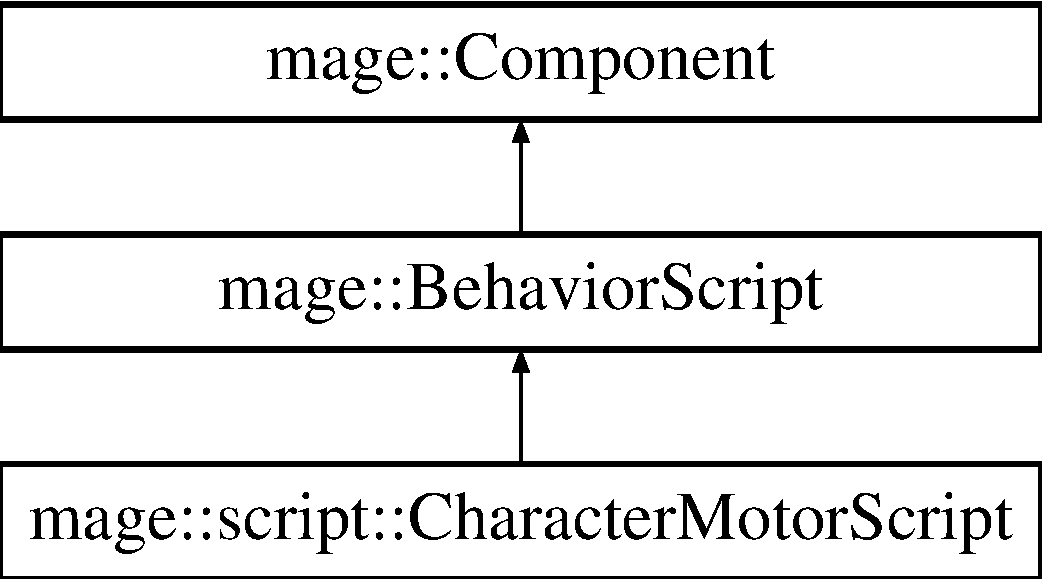
\includegraphics[height=2.000000cm]{classmage_1_1script_1_1_character_motor_script}
\end{center}
\end{figure}
\subsection*{Public Member Functions}
\begin{DoxyCompactItemize}
\item 
\hyperlink{classmage_1_1script_1_1_character_motor_script_a5bc6ed6c6396056d784fb641c12c8d6d}{Character\+Motor\+Script} (\hyperlink{classmage_1_1_transform_node}{Transform\+Node} $\ast$transform)
\item 
\hyperlink{classmage_1_1script_1_1_character_motor_script_abfeb49ef88503f3c86788c042438d69e}{Character\+Motor\+Script} (const \hyperlink{classmage_1_1script_1_1_character_motor_script}{Character\+Motor\+Script} \&script)=delete
\item 
\hyperlink{classmage_1_1script_1_1_character_motor_script_ab517e47de6dd2511cc55bd5e49dd5b40}{Character\+Motor\+Script} (\hyperlink{classmage_1_1script_1_1_character_motor_script}{Character\+Motor\+Script} \&\&script)
\item 
virtual \hyperlink{classmage_1_1script_1_1_character_motor_script_a83ed3c2fcb60cef046499fd9c44f86ee}{$\sim$\+Character\+Motor\+Script} ()
\item 
\hyperlink{classmage_1_1script_1_1_character_motor_script}{Character\+Motor\+Script} \& \hyperlink{classmage_1_1script_1_1_character_motor_script_ac0367e5e6fb8adfe3b9a962f1ca72b4c}{operator=} (const \hyperlink{classmage_1_1script_1_1_character_motor_script}{Character\+Motor\+Script} \&script)=delete
\item 
\hyperlink{classmage_1_1script_1_1_character_motor_script}{Character\+Motor\+Script} \& \hyperlink{classmage_1_1script_1_1_character_motor_script_a00ca2aa38ca4a2557a783ffc31068801}{operator=} (\hyperlink{classmage_1_1script_1_1_character_motor_script}{Character\+Motor\+Script} \&\&script)=delete
\item 
virtual void \hyperlink{classmage_1_1script_1_1_character_motor_script_a75683c4b8db184174b48dd7e4989c016}{Update} (\mbox{[}\mbox{[}maybe\+\_\+unused\mbox{]}\mbox{]} \hyperlink{namespacemage_ad26233bbec640deda836e572c1a23708}{F64} delta\+\_\+time) override
\item 
\hyperlink{namespacemage_aa97e833b45f06d60a0a9c4fc22ae02c0}{F32} \hyperlink{classmage_1_1script_1_1_character_motor_script_a24edb3337af40e7326c424bc6b93c3fa}{Get\+Velocity} () const noexcept
\item 
void \hyperlink{classmage_1_1script_1_1_character_motor_script_a51c9b8317670fc0ae554bfb0cac11aee}{Set\+Velocity} (\hyperlink{namespacemage_aa97e833b45f06d60a0a9c4fc22ae02c0}{F32} velocity) noexcept
\end{DoxyCompactItemize}
\subsection*{Private Attributes}
\begin{DoxyCompactItemize}
\item 
\hyperlink{classmage_1_1_transform_node}{Transform\+Node} $\ast$const \hyperlink{classmage_1_1script_1_1_character_motor_script_adf11fdad0fc73ef1ae829d4d781f2b0c}{m\+\_\+transform}
\item 
\hyperlink{namespacemage_aa97e833b45f06d60a0a9c4fc22ae02c0}{F32} \hyperlink{classmage_1_1script_1_1_character_motor_script_a30db45f04bc56380729af037e71ff237}{m\+\_\+velocity}
\end{DoxyCompactItemize}
\subsection*{Additional Inherited Members}


\subsection{Constructor \& Destructor Documentation}
\hypertarget{classmage_1_1script_1_1_character_motor_script_a5bc6ed6c6396056d784fb641c12c8d6d}{}\label{classmage_1_1script_1_1_character_motor_script_a5bc6ed6c6396056d784fb641c12c8d6d} 
\index{mage\+::script\+::\+Character\+Motor\+Script@{mage\+::script\+::\+Character\+Motor\+Script}!Character\+Motor\+Script@{Character\+Motor\+Script}}
\index{Character\+Motor\+Script@{Character\+Motor\+Script}!mage\+::script\+::\+Character\+Motor\+Script@{mage\+::script\+::\+Character\+Motor\+Script}}
\subsubsection{\texorpdfstring{Character\+Motor\+Script()}{CharacterMotorScript()}\hspace{0.1cm}{\footnotesize\ttfamily [1/3]}}
{\footnotesize\ttfamily mage\+::script\+::\+Character\+Motor\+Script\+::\+Character\+Motor\+Script (\begin{DoxyParamCaption}\item[{\hyperlink{classmage_1_1_transform_node}{Transform\+Node} $\ast$}]{transform }\end{DoxyParamCaption})\hspace{0.3cm}{\ttfamily [explicit]}}

\hypertarget{classmage_1_1script_1_1_character_motor_script_abfeb49ef88503f3c86788c042438d69e}{}\label{classmage_1_1script_1_1_character_motor_script_abfeb49ef88503f3c86788c042438d69e} 
\index{mage\+::script\+::\+Character\+Motor\+Script@{mage\+::script\+::\+Character\+Motor\+Script}!Character\+Motor\+Script@{Character\+Motor\+Script}}
\index{Character\+Motor\+Script@{Character\+Motor\+Script}!mage\+::script\+::\+Character\+Motor\+Script@{mage\+::script\+::\+Character\+Motor\+Script}}
\subsubsection{\texorpdfstring{Character\+Motor\+Script()}{CharacterMotorScript()}\hspace{0.1cm}{\footnotesize\ttfamily [2/3]}}
{\footnotesize\ttfamily mage\+::script\+::\+Character\+Motor\+Script\+::\+Character\+Motor\+Script (\begin{DoxyParamCaption}\item[{const \hyperlink{classmage_1_1script_1_1_character_motor_script}{Character\+Motor\+Script} \&}]{script }\end{DoxyParamCaption})\hspace{0.3cm}{\ttfamily [delete]}}

\hypertarget{classmage_1_1script_1_1_character_motor_script_ab517e47de6dd2511cc55bd5e49dd5b40}{}\label{classmage_1_1script_1_1_character_motor_script_ab517e47de6dd2511cc55bd5e49dd5b40} 
\index{mage\+::script\+::\+Character\+Motor\+Script@{mage\+::script\+::\+Character\+Motor\+Script}!Character\+Motor\+Script@{Character\+Motor\+Script}}
\index{Character\+Motor\+Script@{Character\+Motor\+Script}!mage\+::script\+::\+Character\+Motor\+Script@{mage\+::script\+::\+Character\+Motor\+Script}}
\subsubsection{\texorpdfstring{Character\+Motor\+Script()}{CharacterMotorScript()}\hspace{0.1cm}{\footnotesize\ttfamily [3/3]}}
{\footnotesize\ttfamily mage\+::script\+::\+Character\+Motor\+Script\+::\+Character\+Motor\+Script (\begin{DoxyParamCaption}\item[{\hyperlink{classmage_1_1script_1_1_character_motor_script}{Character\+Motor\+Script} \&\&}]{script }\end{DoxyParamCaption})\hspace{0.3cm}{\ttfamily [default]}}

\hypertarget{classmage_1_1script_1_1_character_motor_script_a83ed3c2fcb60cef046499fd9c44f86ee}{}\label{classmage_1_1script_1_1_character_motor_script_a83ed3c2fcb60cef046499fd9c44f86ee} 
\index{mage\+::script\+::\+Character\+Motor\+Script@{mage\+::script\+::\+Character\+Motor\+Script}!````~Character\+Motor\+Script@{$\sim$\+Character\+Motor\+Script}}
\index{````~Character\+Motor\+Script@{$\sim$\+Character\+Motor\+Script}!mage\+::script\+::\+Character\+Motor\+Script@{mage\+::script\+::\+Character\+Motor\+Script}}
\subsubsection{\texorpdfstring{$\sim$\+Character\+Motor\+Script()}{~CharacterMotorScript()}}
{\footnotesize\ttfamily mage\+::script\+::\+Character\+Motor\+Script\+::$\sim$\+Character\+Motor\+Script (\begin{DoxyParamCaption}{ }\end{DoxyParamCaption})\hspace{0.3cm}{\ttfamily [virtual]}, {\ttfamily [default]}}



\subsection{Member Function Documentation}
\hypertarget{classmage_1_1script_1_1_character_motor_script_a24edb3337af40e7326c424bc6b93c3fa}{}\label{classmage_1_1script_1_1_character_motor_script_a24edb3337af40e7326c424bc6b93c3fa} 
\index{mage\+::script\+::\+Character\+Motor\+Script@{mage\+::script\+::\+Character\+Motor\+Script}!Get\+Velocity@{Get\+Velocity}}
\index{Get\+Velocity@{Get\+Velocity}!mage\+::script\+::\+Character\+Motor\+Script@{mage\+::script\+::\+Character\+Motor\+Script}}
\subsubsection{\texorpdfstring{Get\+Velocity()}{GetVelocity()}}
{\footnotesize\ttfamily \hyperlink{namespacemage_aa97e833b45f06d60a0a9c4fc22ae02c0}{F32} mage\+::script\+::\+Character\+Motor\+Script\+::\+Get\+Velocity (\begin{DoxyParamCaption}{ }\end{DoxyParamCaption}) const\hspace{0.3cm}{\ttfamily [noexcept]}}

\hypertarget{classmage_1_1script_1_1_character_motor_script_ac0367e5e6fb8adfe3b9a962f1ca72b4c}{}\label{classmage_1_1script_1_1_character_motor_script_ac0367e5e6fb8adfe3b9a962f1ca72b4c} 
\index{mage\+::script\+::\+Character\+Motor\+Script@{mage\+::script\+::\+Character\+Motor\+Script}!operator=@{operator=}}
\index{operator=@{operator=}!mage\+::script\+::\+Character\+Motor\+Script@{mage\+::script\+::\+Character\+Motor\+Script}}
\subsubsection{\texorpdfstring{operator=()}{operator=()}\hspace{0.1cm}{\footnotesize\ttfamily [1/2]}}
{\footnotesize\ttfamily \hyperlink{classmage_1_1script_1_1_character_motor_script}{Character\+Motor\+Script}\& mage\+::script\+::\+Character\+Motor\+Script\+::operator= (\begin{DoxyParamCaption}\item[{const \hyperlink{classmage_1_1script_1_1_character_motor_script}{Character\+Motor\+Script} \&}]{script }\end{DoxyParamCaption})\hspace{0.3cm}{\ttfamily [delete]}}

\hypertarget{classmage_1_1script_1_1_character_motor_script_a00ca2aa38ca4a2557a783ffc31068801}{}\label{classmage_1_1script_1_1_character_motor_script_a00ca2aa38ca4a2557a783ffc31068801} 
\index{mage\+::script\+::\+Character\+Motor\+Script@{mage\+::script\+::\+Character\+Motor\+Script}!operator=@{operator=}}
\index{operator=@{operator=}!mage\+::script\+::\+Character\+Motor\+Script@{mage\+::script\+::\+Character\+Motor\+Script}}
\subsubsection{\texorpdfstring{operator=()}{operator=()}\hspace{0.1cm}{\footnotesize\ttfamily [2/2]}}
{\footnotesize\ttfamily \hyperlink{classmage_1_1script_1_1_character_motor_script}{Character\+Motor\+Script}\& mage\+::script\+::\+Character\+Motor\+Script\+::operator= (\begin{DoxyParamCaption}\item[{\hyperlink{classmage_1_1script_1_1_character_motor_script}{Character\+Motor\+Script} \&\&}]{script }\end{DoxyParamCaption})\hspace{0.3cm}{\ttfamily [delete]}}

\hypertarget{classmage_1_1script_1_1_character_motor_script_a51c9b8317670fc0ae554bfb0cac11aee}{}\label{classmage_1_1script_1_1_character_motor_script_a51c9b8317670fc0ae554bfb0cac11aee} 
\index{mage\+::script\+::\+Character\+Motor\+Script@{mage\+::script\+::\+Character\+Motor\+Script}!Set\+Velocity@{Set\+Velocity}}
\index{Set\+Velocity@{Set\+Velocity}!mage\+::script\+::\+Character\+Motor\+Script@{mage\+::script\+::\+Character\+Motor\+Script}}
\subsubsection{\texorpdfstring{Set\+Velocity()}{SetVelocity()}}
{\footnotesize\ttfamily void mage\+::script\+::\+Character\+Motor\+Script\+::\+Set\+Velocity (\begin{DoxyParamCaption}\item[{\hyperlink{namespacemage_aa97e833b45f06d60a0a9c4fc22ae02c0}{F32}}]{velocity }\end{DoxyParamCaption})\hspace{0.3cm}{\ttfamily [noexcept]}}

\hypertarget{classmage_1_1script_1_1_character_motor_script_a75683c4b8db184174b48dd7e4989c016}{}\label{classmage_1_1script_1_1_character_motor_script_a75683c4b8db184174b48dd7e4989c016} 
\index{mage\+::script\+::\+Character\+Motor\+Script@{mage\+::script\+::\+Character\+Motor\+Script}!Update@{Update}}
\index{Update@{Update}!mage\+::script\+::\+Character\+Motor\+Script@{mage\+::script\+::\+Character\+Motor\+Script}}
\subsubsection{\texorpdfstring{Update()}{Update()}}
{\footnotesize\ttfamily void mage\+::script\+::\+Character\+Motor\+Script\+::\+Update (\begin{DoxyParamCaption}\item[{\mbox{[}\mbox{[}maybe\+\_\+unused\mbox{]} \mbox{]} \hyperlink{namespacemage_ad26233bbec640deda836e572c1a23708}{F64}}]{delta\+\_\+time }\end{DoxyParamCaption})\hspace{0.3cm}{\ttfamily [override]}, {\ttfamily [virtual]}}

Updates this behavior script.

This method is called once per frame.


\begin{DoxyParams}[1]{Parameters}
\mbox{\tt in}  & {\em delta\+\_\+time} & The elapsed time since the previous update. \\
\hline
\end{DoxyParams}


Reimplemented from \hyperlink{classmage_1_1_behavior_script_afb9cf3759edf8876416d1df85489cba6}{mage\+::\+Behavior\+Script}.



\subsection{Member Data Documentation}
\hypertarget{classmage_1_1script_1_1_character_motor_script_adf11fdad0fc73ef1ae829d4d781f2b0c}{}\label{classmage_1_1script_1_1_character_motor_script_adf11fdad0fc73ef1ae829d4d781f2b0c} 
\index{mage\+::script\+::\+Character\+Motor\+Script@{mage\+::script\+::\+Character\+Motor\+Script}!m\+\_\+transform@{m\+\_\+transform}}
\index{m\+\_\+transform@{m\+\_\+transform}!mage\+::script\+::\+Character\+Motor\+Script@{mage\+::script\+::\+Character\+Motor\+Script}}
\subsubsection{\texorpdfstring{m\+\_\+transform}{m\_transform}}
{\footnotesize\ttfamily \hyperlink{classmage_1_1_transform_node}{Transform\+Node}$\ast$ const mage\+::script\+::\+Character\+Motor\+Script\+::m\+\_\+transform\hspace{0.3cm}{\ttfamily [private]}}

\hypertarget{classmage_1_1script_1_1_character_motor_script_a30db45f04bc56380729af037e71ff237}{}\label{classmage_1_1script_1_1_character_motor_script_a30db45f04bc56380729af037e71ff237} 
\index{mage\+::script\+::\+Character\+Motor\+Script@{mage\+::script\+::\+Character\+Motor\+Script}!m\+\_\+velocity@{m\+\_\+velocity}}
\index{m\+\_\+velocity@{m\+\_\+velocity}!mage\+::script\+::\+Character\+Motor\+Script@{mage\+::script\+::\+Character\+Motor\+Script}}
\subsubsection{\texorpdfstring{m\+\_\+velocity}{m\_velocity}}
{\footnotesize\ttfamily \hyperlink{namespacemage_aa97e833b45f06d60a0a9c4fc22ae02c0}{F32} mage\+::script\+::\+Character\+Motor\+Script\+::m\+\_\+velocity\hspace{0.3cm}{\ttfamily [private]}}


\hypertarget{classmage_1_1rendering_1_1_color_string}{}\section{mage\+:\+:rendering\+:\+:Color\+String Class Reference}
\label{classmage_1_1rendering_1_1_color_string}\index{mage\+::rendering\+::\+Color\+String@{mage\+::rendering\+::\+Color\+String}}


{\ttfamily \#include $<$color\+\_\+string.\+hpp$>$}

\subsection*{Public Member Functions}
\begin{DoxyCompactItemize}
\item 
\hyperlink{classmage_1_1rendering_1_1_color_string_a380bcff4ce39fa09e68626b7aeb975b2}{Color\+String} (wstring str, \hyperlink{structmage_1_1_s_r_g_b_a}{S\+R\+G\+BA} color=\hyperlink{namespacemage_1_1color_aecd3f854835fd8ac76f38a369ea539ed}{color\+::\+White}) noexcept
\item 
\hyperlink{classmage_1_1rendering_1_1_color_string_a386454b4a8e08707e8ffff8451509de5}{Color\+String} (const \hyperlink{classmage_1_1rendering_1_1_color_string}{Color\+String} \&color\+\_\+string)=default
\item 
\hyperlink{classmage_1_1rendering_1_1_color_string_a642793608186e9ac9931827ae9f0c57a}{Color\+String} (\hyperlink{classmage_1_1rendering_1_1_color_string}{Color\+String} \&\&color\+\_\+string) noexcept=default
\item 
\hyperlink{classmage_1_1rendering_1_1_color_string_a13ab2218e1cbe99241283214e455f3c9}{$\sim$\+Color\+String} ()=default
\item 
\hyperlink{classmage_1_1rendering_1_1_color_string}{Color\+String} \& \hyperlink{classmage_1_1rendering_1_1_color_string_ab42304d36628f21263a4d545831b3829}{operator=} (const \hyperlink{classmage_1_1rendering_1_1_color_string}{Color\+String} \&color\+\_\+string)=default
\item 
\hyperlink{classmage_1_1rendering_1_1_color_string}{Color\+String} \& \hyperlink{classmage_1_1rendering_1_1_color_string_aa70b60e0c8528306e7473ee0b5bfbe03}{operator=} (\hyperlink{classmage_1_1rendering_1_1_color_string}{Color\+String} \&\&color\+\_\+string) noexcept=default
\item 
\hyperlink{namespacemage_a8769f9d670d6b585ea306cb1062af94b}{Not\+Null}$<$ \hyperlink{namespacemage_ac409e0f2a22292a3a4cd42742994fbf0}{const\+\_\+wzstring} $>$ \hyperlink{classmage_1_1rendering_1_1_color_string_a2706724097d2ad5c187d34db49d86bda}{c\+\_\+str} () const noexcept
\item 
const wstring \& \hyperlink{classmage_1_1rendering_1_1_color_string_a146cf063553b65b3cd854417b638b533}{Get\+String} () const noexcept
\item 
void \hyperlink{classmage_1_1rendering_1_1_color_string_aefee43f68f87617976f89430bac71fba}{Set\+String} (wstring str) noexcept
\item 
\hyperlink{structmage_1_1_s_r_g_b_a}{S\+R\+G\+BA} \& \hyperlink{classmage_1_1rendering_1_1_color_string_a565834879d191509832660f39a923df3}{Get\+Color} () noexcept
\item 
const \hyperlink{structmage_1_1_s_r_g_b_a}{S\+R\+G\+BA} \& \hyperlink{classmage_1_1rendering_1_1_color_string_ace4b3cfddb63732bfff9ced9f1078a26}{Get\+Color} () const noexcept
\end{DoxyCompactItemize}
\subsection*{Private Attributes}
\begin{DoxyCompactItemize}
\item 
wstring \hyperlink{classmage_1_1rendering_1_1_color_string_a226202625fbe205d78e1412310a49f1f}{m\+\_\+str}
\item 
\hyperlink{structmage_1_1_s_r_g_b_a}{S\+R\+G\+BA} \hyperlink{classmage_1_1rendering_1_1_color_string_a5b601126d5067469b05a0e33450b950c}{m\+\_\+color}
\end{DoxyCompactItemize}


\subsection{Detailed Description}
A class of color strings representing a string and its color. 

\subsection{Constructor \& Destructor Documentation}
\hypertarget{classmage_1_1rendering_1_1_color_string_a380bcff4ce39fa09e68626b7aeb975b2}{}\label{classmage_1_1rendering_1_1_color_string_a380bcff4ce39fa09e68626b7aeb975b2} 
\index{mage\+::rendering\+::\+Color\+String@{mage\+::rendering\+::\+Color\+String}!Color\+String@{Color\+String}}
\index{Color\+String@{Color\+String}!mage\+::rendering\+::\+Color\+String@{mage\+::rendering\+::\+Color\+String}}
\subsubsection{\texorpdfstring{Color\+String()}{ColorString()}\hspace{0.1cm}{\footnotesize\ttfamily [1/3]}}
{\footnotesize\ttfamily mage\+::rendering\+::\+Color\+String\+::\+Color\+String (\begin{DoxyParamCaption}\item[{wstring}]{str,  }\item[{\hyperlink{structmage_1_1_s_r_g_b_a}{S\+R\+G\+BA}}]{color = {\ttfamily \hyperlink{namespacemage_1_1color_aecd3f854835fd8ac76f38a369ea539ed}{color\+::\+White}} }\end{DoxyParamCaption})\hspace{0.3cm}{\ttfamily [noexcept]}}

Constructs a color string fromt the given string and color.


\begin{DoxyParams}[1]{Parameters}
\mbox{\tt in}  & {\em str} & The string. \\
\hline
\mbox{\tt in}  & {\em color} & A reference to the s\+R\+GB color. \\
\hline
\end{DoxyParams}
\hypertarget{classmage_1_1rendering_1_1_color_string_a386454b4a8e08707e8ffff8451509de5}{}\label{classmage_1_1rendering_1_1_color_string_a386454b4a8e08707e8ffff8451509de5} 
\index{mage\+::rendering\+::\+Color\+String@{mage\+::rendering\+::\+Color\+String}!Color\+String@{Color\+String}}
\index{Color\+String@{Color\+String}!mage\+::rendering\+::\+Color\+String@{mage\+::rendering\+::\+Color\+String}}
\subsubsection{\texorpdfstring{Color\+String()}{ColorString()}\hspace{0.1cm}{\footnotesize\ttfamily [2/3]}}
{\footnotesize\ttfamily mage\+::rendering\+::\+Color\+String\+::\+Color\+String (\begin{DoxyParamCaption}\item[{const \hyperlink{classmage_1_1rendering_1_1_color_string}{Color\+String} \&}]{color\+\_\+string }\end{DoxyParamCaption})\hspace{0.3cm}{\ttfamily [default]}}

Constructs a color string from the given color string.


\begin{DoxyParams}[1]{Parameters}
\mbox{\tt in}  & {\em color\+\_\+string} & A reference to the color string to copy. \\
\hline
\end{DoxyParams}
\hypertarget{classmage_1_1rendering_1_1_color_string_a642793608186e9ac9931827ae9f0c57a}{}\label{classmage_1_1rendering_1_1_color_string_a642793608186e9ac9931827ae9f0c57a} 
\index{mage\+::rendering\+::\+Color\+String@{mage\+::rendering\+::\+Color\+String}!Color\+String@{Color\+String}}
\index{Color\+String@{Color\+String}!mage\+::rendering\+::\+Color\+String@{mage\+::rendering\+::\+Color\+String}}
\subsubsection{\texorpdfstring{Color\+String()}{ColorString()}\hspace{0.1cm}{\footnotesize\ttfamily [3/3]}}
{\footnotesize\ttfamily mage\+::rendering\+::\+Color\+String\+::\+Color\+String (\begin{DoxyParamCaption}\item[{\hyperlink{classmage_1_1rendering_1_1_color_string}{Color\+String} \&\&}]{color\+\_\+string }\end{DoxyParamCaption})\hspace{0.3cm}{\ttfamily [default]}, {\ttfamily [noexcept]}}

Constructs a color string by moving the given color string.


\begin{DoxyParams}[1]{Parameters}
\mbox{\tt in}  & {\em color\+\_\+string} & A reference to the color string to move. \\
\hline
\end{DoxyParams}
\hypertarget{classmage_1_1rendering_1_1_color_string_a13ab2218e1cbe99241283214e455f3c9}{}\label{classmage_1_1rendering_1_1_color_string_a13ab2218e1cbe99241283214e455f3c9} 
\index{mage\+::rendering\+::\+Color\+String@{mage\+::rendering\+::\+Color\+String}!````~Color\+String@{$\sim$\+Color\+String}}
\index{````~Color\+String@{$\sim$\+Color\+String}!mage\+::rendering\+::\+Color\+String@{mage\+::rendering\+::\+Color\+String}}
\subsubsection{\texorpdfstring{$\sim$\+Color\+String()}{~ColorString()}}
{\footnotesize\ttfamily mage\+::rendering\+::\+Color\+String\+::$\sim$\+Color\+String (\begin{DoxyParamCaption}{ }\end{DoxyParamCaption})\hspace{0.3cm}{\ttfamily [default]}}

Destructs this color string. 

\subsection{Member Function Documentation}
\hypertarget{classmage_1_1rendering_1_1_color_string_a2706724097d2ad5c187d34db49d86bda}{}\label{classmage_1_1rendering_1_1_color_string_a2706724097d2ad5c187d34db49d86bda} 
\index{mage\+::rendering\+::\+Color\+String@{mage\+::rendering\+::\+Color\+String}!c\+\_\+str@{c\+\_\+str}}
\index{c\+\_\+str@{c\+\_\+str}!mage\+::rendering\+::\+Color\+String@{mage\+::rendering\+::\+Color\+String}}
\subsubsection{\texorpdfstring{c\+\_\+str()}{c\_str()}}
{\footnotesize\ttfamily \hyperlink{namespacemage_a8769f9d670d6b585ea306cb1062af94b}{Not\+Null}$<$ \hyperlink{namespacemage_ac409e0f2a22292a3a4cd42742994fbf0}{const\+\_\+wzstring} $>$ mage\+::rendering\+::\+Color\+String\+::c\+\_\+str (\begin{DoxyParamCaption}{ }\end{DoxyParamCaption}) const\hspace{0.3cm}{\ttfamily [noexcept]}}

Returns the string of this color string.

\begin{DoxyReturn}{Returns}
A pointer to the string of this color string. 
\end{DoxyReturn}
\hypertarget{classmage_1_1rendering_1_1_color_string_a565834879d191509832660f39a923df3}{}\label{classmage_1_1rendering_1_1_color_string_a565834879d191509832660f39a923df3} 
\index{mage\+::rendering\+::\+Color\+String@{mage\+::rendering\+::\+Color\+String}!Get\+Color@{Get\+Color}}
\index{Get\+Color@{Get\+Color}!mage\+::rendering\+::\+Color\+String@{mage\+::rendering\+::\+Color\+String}}
\subsubsection{\texorpdfstring{Get\+Color()}{GetColor()}\hspace{0.1cm}{\footnotesize\ttfamily [1/2]}}
{\footnotesize\ttfamily \hyperlink{structmage_1_1_s_r_g_b_a}{S\+R\+G\+BA}\& mage\+::rendering\+::\+Color\+String\+::\+Get\+Color (\begin{DoxyParamCaption}{ }\end{DoxyParamCaption})\hspace{0.3cm}{\ttfamily [noexcept]}}

Returns the s\+R\+GB color of this color string.

\begin{DoxyReturn}{Returns}
A reference to s\+R\+GB color of this color string. 
\end{DoxyReturn}
\hypertarget{classmage_1_1rendering_1_1_color_string_ace4b3cfddb63732bfff9ced9f1078a26}{}\label{classmage_1_1rendering_1_1_color_string_ace4b3cfddb63732bfff9ced9f1078a26} 
\index{mage\+::rendering\+::\+Color\+String@{mage\+::rendering\+::\+Color\+String}!Get\+Color@{Get\+Color}}
\index{Get\+Color@{Get\+Color}!mage\+::rendering\+::\+Color\+String@{mage\+::rendering\+::\+Color\+String}}
\subsubsection{\texorpdfstring{Get\+Color()}{GetColor()}\hspace{0.1cm}{\footnotesize\ttfamily [2/2]}}
{\footnotesize\ttfamily const \hyperlink{structmage_1_1_s_r_g_b_a}{S\+R\+G\+BA}\& mage\+::rendering\+::\+Color\+String\+::\+Get\+Color (\begin{DoxyParamCaption}{ }\end{DoxyParamCaption}) const\hspace{0.3cm}{\ttfamily [noexcept]}}

Returns the s\+R\+GB color of this color string.

\begin{DoxyReturn}{Returns}
A reference to s\+R\+GB color of this color string. 
\end{DoxyReturn}
\hypertarget{classmage_1_1rendering_1_1_color_string_a146cf063553b65b3cd854417b638b533}{}\label{classmage_1_1rendering_1_1_color_string_a146cf063553b65b3cd854417b638b533} 
\index{mage\+::rendering\+::\+Color\+String@{mage\+::rendering\+::\+Color\+String}!Get\+String@{Get\+String}}
\index{Get\+String@{Get\+String}!mage\+::rendering\+::\+Color\+String@{mage\+::rendering\+::\+Color\+String}}
\subsubsection{\texorpdfstring{Get\+String()}{GetString()}}
{\footnotesize\ttfamily const wstring\& mage\+::rendering\+::\+Color\+String\+::\+Get\+String (\begin{DoxyParamCaption}{ }\end{DoxyParamCaption}) const\hspace{0.3cm}{\ttfamily [noexcept]}}

Returns the string of this color string.

\begin{DoxyReturn}{Returns}
A reference to the string of this color string. 
\end{DoxyReturn}
\hypertarget{classmage_1_1rendering_1_1_color_string_ab42304d36628f21263a4d545831b3829}{}\label{classmage_1_1rendering_1_1_color_string_ab42304d36628f21263a4d545831b3829} 
\index{mage\+::rendering\+::\+Color\+String@{mage\+::rendering\+::\+Color\+String}!operator=@{operator=}}
\index{operator=@{operator=}!mage\+::rendering\+::\+Color\+String@{mage\+::rendering\+::\+Color\+String}}
\subsubsection{\texorpdfstring{operator=()}{operator=()}\hspace{0.1cm}{\footnotesize\ttfamily [1/2]}}
{\footnotesize\ttfamily \hyperlink{classmage_1_1rendering_1_1_color_string}{Color\+String}\& mage\+::rendering\+::\+Color\+String\+::operator= (\begin{DoxyParamCaption}\item[{const \hyperlink{classmage_1_1rendering_1_1_color_string}{Color\+String} \&}]{color\+\_\+string }\end{DoxyParamCaption})\hspace{0.3cm}{\ttfamily [default]}}

Copies the given color string to this color string.


\begin{DoxyParams}[1]{Parameters}
\mbox{\tt in}  & {\em color\+\_\+string} & A reference to the color string to copy. \\
\hline
\end{DoxyParams}
\begin{DoxyReturn}{Returns}
A reference to the copy of the given color string (i.\+e. this color string). 
\end{DoxyReturn}
\hypertarget{classmage_1_1rendering_1_1_color_string_aa70b60e0c8528306e7473ee0b5bfbe03}{}\label{classmage_1_1rendering_1_1_color_string_aa70b60e0c8528306e7473ee0b5bfbe03} 
\index{mage\+::rendering\+::\+Color\+String@{mage\+::rendering\+::\+Color\+String}!operator=@{operator=}}
\index{operator=@{operator=}!mage\+::rendering\+::\+Color\+String@{mage\+::rendering\+::\+Color\+String}}
\subsubsection{\texorpdfstring{operator=()}{operator=()}\hspace{0.1cm}{\footnotesize\ttfamily [2/2]}}
{\footnotesize\ttfamily \hyperlink{classmage_1_1rendering_1_1_color_string}{Color\+String}\& mage\+::rendering\+::\+Color\+String\+::operator= (\begin{DoxyParamCaption}\item[{\hyperlink{classmage_1_1rendering_1_1_color_string}{Color\+String} \&\&}]{color\+\_\+string }\end{DoxyParamCaption})\hspace{0.3cm}{\ttfamily [default]}, {\ttfamily [noexcept]}}

Moves the given color string to this color string.


\begin{DoxyParams}[1]{Parameters}
\mbox{\tt in}  & {\em color\+\_\+string} & A reference to the color string to move. \\
\hline
\end{DoxyParams}
\begin{DoxyReturn}{Returns}
A reference to the moved color string (i.\+e. this color string). 
\end{DoxyReturn}
\hypertarget{classmage_1_1rendering_1_1_color_string_aefee43f68f87617976f89430bac71fba}{}\label{classmage_1_1rendering_1_1_color_string_aefee43f68f87617976f89430bac71fba} 
\index{mage\+::rendering\+::\+Color\+String@{mage\+::rendering\+::\+Color\+String}!Set\+String@{Set\+String}}
\index{Set\+String@{Set\+String}!mage\+::rendering\+::\+Color\+String@{mage\+::rendering\+::\+Color\+String}}
\subsubsection{\texorpdfstring{Set\+String()}{SetString()}}
{\footnotesize\ttfamily void mage\+::rendering\+::\+Color\+String\+::\+Set\+String (\begin{DoxyParamCaption}\item[{wstring}]{str }\end{DoxyParamCaption})\hspace{0.3cm}{\ttfamily [noexcept]}}

Sets the string of this color string to the given string.


\begin{DoxyParams}[1]{Parameters}
\mbox{\tt in}  & {\em str} & The string. \\
\hline
\end{DoxyParams}


\subsection{Member Data Documentation}
\hypertarget{classmage_1_1rendering_1_1_color_string_a5b601126d5067469b05a0e33450b950c}{}\label{classmage_1_1rendering_1_1_color_string_a5b601126d5067469b05a0e33450b950c} 
\index{mage\+::rendering\+::\+Color\+String@{mage\+::rendering\+::\+Color\+String}!m\+\_\+color@{m\+\_\+color}}
\index{m\+\_\+color@{m\+\_\+color}!mage\+::rendering\+::\+Color\+String@{mage\+::rendering\+::\+Color\+String}}
\subsubsection{\texorpdfstring{m\+\_\+color}{m\_color}}
{\footnotesize\ttfamily \hyperlink{structmage_1_1_s_r_g_b_a}{S\+R\+G\+BA} mage\+::rendering\+::\+Color\+String\+::m\+\_\+color\hspace{0.3cm}{\ttfamily [private]}}

The s\+R\+GB color of this color string. \hypertarget{classmage_1_1rendering_1_1_color_string_a226202625fbe205d78e1412310a49f1f}{}\label{classmage_1_1rendering_1_1_color_string_a226202625fbe205d78e1412310a49f1f} 
\index{mage\+::rendering\+::\+Color\+String@{mage\+::rendering\+::\+Color\+String}!m\+\_\+str@{m\+\_\+str}}
\index{m\+\_\+str@{m\+\_\+str}!mage\+::rendering\+::\+Color\+String@{mage\+::rendering\+::\+Color\+String}}
\subsubsection{\texorpdfstring{m\+\_\+str}{m\_str}}
{\footnotesize\ttfamily wstring mage\+::rendering\+::\+Color\+String\+::m\+\_\+str\hspace{0.3cm}{\ttfamily [private]}}

The string of this color string. 
\hypertarget{classmage_1_1rendering_1_1_compiled_shader}{}\section{mage\+:\+:rendering\+:\+:Compiled\+Shader Class Reference}
\label{classmage_1_1rendering_1_1_compiled_shader}\index{mage\+::rendering\+::\+Compiled\+Shader@{mage\+::rendering\+::\+Compiled\+Shader}}


{\ttfamily \#include $<$compiled\+\_\+shader.\+hpp$>$}

Inheritance diagram for mage\+:\+:rendering\+:\+:Compiled\+Shader\+:\begin{figure}[H]
\begin{center}
\leavevmode
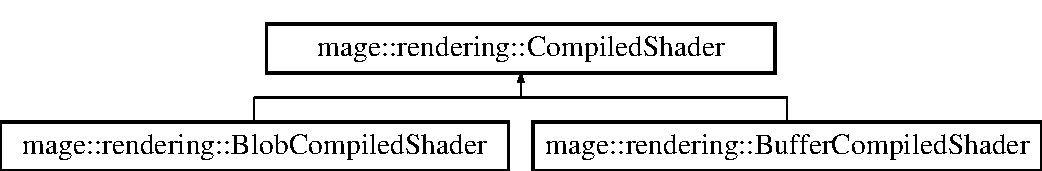
\includegraphics[height=2.000000cm]{classmage_1_1rendering_1_1_compiled_shader}
\end{center}
\end{figure}
\subsection*{Public Member Functions}
\begin{DoxyCompactItemize}
\item 
virtual \hyperlink{classmage_1_1rendering_1_1_compiled_shader_abb17672237a99552beef603cd1d4f680}{$\sim$\+Compiled\+Shader} ()
\item 
\hyperlink{classmage_1_1rendering_1_1_compiled_shader}{Compiled\+Shader} \& \hyperlink{classmage_1_1rendering_1_1_compiled_shader_a1981d885693b7849078f509f15b81071}{operator=} (const \hyperlink{classmage_1_1rendering_1_1_compiled_shader}{Compiled\+Shader} \&compiled\+\_\+shader) noexcept
\item 
\hyperlink{classmage_1_1rendering_1_1_compiled_shader}{Compiled\+Shader} \& \hyperlink{classmage_1_1rendering_1_1_compiled_shader_ab4217b5b68c5cc33b6736a844ddfe699}{operator=} (\hyperlink{classmage_1_1rendering_1_1_compiled_shader}{Compiled\+Shader} \&\&compiled\+\_\+shader) noexcept
\item 
virtual const B\+Y\+TE $\ast$ \hyperlink{classmage_1_1rendering_1_1_compiled_shader_a6067250341f428be19ed2aa9955a10b6}{Get\+Bytecode} () const noexcept=0
\item 
virtual S\+I\+Z\+E\+\_\+T \hyperlink{classmage_1_1rendering_1_1_compiled_shader_a92c17b46242bf884c3d0d673e88a292d}{Get\+Bytecode\+Size} () const noexcept=0
\end{DoxyCompactItemize}
\subsection*{Protected Member Functions}
\begin{DoxyCompactItemize}
\item 
\hyperlink{classmage_1_1rendering_1_1_compiled_shader_a4e62e8d016992f4d7d51297d3796d05d}{Compiled\+Shader} () noexcept
\item 
\hyperlink{classmage_1_1rendering_1_1_compiled_shader_a13ebfdc6d2d9ba554160829a83244e8b}{Compiled\+Shader} (const \hyperlink{classmage_1_1rendering_1_1_compiled_shader}{Compiled\+Shader} \&compiled\+\_\+shader) noexcept
\item 
\hyperlink{classmage_1_1rendering_1_1_compiled_shader_a20a7e1e0b2e9bf378aeda9bf8e429c43}{Compiled\+Shader} (\hyperlink{classmage_1_1rendering_1_1_compiled_shader}{Compiled\+Shader} \&\&compiled\+\_\+shader) noexcept
\end{DoxyCompactItemize}


\subsection{Detailed Description}
A class of compiled shaders. 

\subsection{Constructor \& Destructor Documentation}
\hypertarget{classmage_1_1rendering_1_1_compiled_shader_abb17672237a99552beef603cd1d4f680}{}\label{classmage_1_1rendering_1_1_compiled_shader_abb17672237a99552beef603cd1d4f680} 
\index{mage\+::rendering\+::\+Compiled\+Shader@{mage\+::rendering\+::\+Compiled\+Shader}!````~Compiled\+Shader@{$\sim$\+Compiled\+Shader}}
\index{````~Compiled\+Shader@{$\sim$\+Compiled\+Shader}!mage\+::rendering\+::\+Compiled\+Shader@{mage\+::rendering\+::\+Compiled\+Shader}}
\subsubsection{\texorpdfstring{$\sim$\+Compiled\+Shader()}{~CompiledShader()}}
{\footnotesize\ttfamily mage\+::rendering\+::\+Compiled\+Shader\+::$\sim$\+Compiled\+Shader (\begin{DoxyParamCaption}{ }\end{DoxyParamCaption})\hspace{0.3cm}{\ttfamily [virtual]}, {\ttfamily [default]}}

Destructs this compiled shader. \hypertarget{classmage_1_1rendering_1_1_compiled_shader_a4e62e8d016992f4d7d51297d3796d05d}{}\label{classmage_1_1rendering_1_1_compiled_shader_a4e62e8d016992f4d7d51297d3796d05d} 
\index{mage\+::rendering\+::\+Compiled\+Shader@{mage\+::rendering\+::\+Compiled\+Shader}!Compiled\+Shader@{Compiled\+Shader}}
\index{Compiled\+Shader@{Compiled\+Shader}!mage\+::rendering\+::\+Compiled\+Shader@{mage\+::rendering\+::\+Compiled\+Shader}}
\subsubsection{\texorpdfstring{Compiled\+Shader()}{CompiledShader()}\hspace{0.1cm}{\footnotesize\ttfamily [1/3]}}
{\footnotesize\ttfamily mage\+::rendering\+::\+Compiled\+Shader\+::\+Compiled\+Shader (\begin{DoxyParamCaption}{ }\end{DoxyParamCaption})\hspace{0.3cm}{\ttfamily [protected]}, {\ttfamily [default]}, {\ttfamily [noexcept]}}

Constructs a compiled shader. \hypertarget{classmage_1_1rendering_1_1_compiled_shader_a13ebfdc6d2d9ba554160829a83244e8b}{}\label{classmage_1_1rendering_1_1_compiled_shader_a13ebfdc6d2d9ba554160829a83244e8b} 
\index{mage\+::rendering\+::\+Compiled\+Shader@{mage\+::rendering\+::\+Compiled\+Shader}!Compiled\+Shader@{Compiled\+Shader}}
\index{Compiled\+Shader@{Compiled\+Shader}!mage\+::rendering\+::\+Compiled\+Shader@{mage\+::rendering\+::\+Compiled\+Shader}}
\subsubsection{\texorpdfstring{Compiled\+Shader()}{CompiledShader()}\hspace{0.1cm}{\footnotesize\ttfamily [2/3]}}
{\footnotesize\ttfamily mage\+::rendering\+::\+Compiled\+Shader\+::\+Compiled\+Shader (\begin{DoxyParamCaption}\item[{const \hyperlink{classmage_1_1rendering_1_1_compiled_shader}{Compiled\+Shader} \&}]{compiled\+\_\+shader }\end{DoxyParamCaption})\hspace{0.3cm}{\ttfamily [protected]}, {\ttfamily [default]}, {\ttfamily [noexcept]}}

Constructs a compiled shader from the given compiled shader.


\begin{DoxyParams}[1]{Parameters}
\mbox{\tt in}  & {\em compiled\+\_\+shader} & A reference to the compiled shader to copy. \\
\hline
\end{DoxyParams}
\hypertarget{classmage_1_1rendering_1_1_compiled_shader_a20a7e1e0b2e9bf378aeda9bf8e429c43}{}\label{classmage_1_1rendering_1_1_compiled_shader_a20a7e1e0b2e9bf378aeda9bf8e429c43} 
\index{mage\+::rendering\+::\+Compiled\+Shader@{mage\+::rendering\+::\+Compiled\+Shader}!Compiled\+Shader@{Compiled\+Shader}}
\index{Compiled\+Shader@{Compiled\+Shader}!mage\+::rendering\+::\+Compiled\+Shader@{mage\+::rendering\+::\+Compiled\+Shader}}
\subsubsection{\texorpdfstring{Compiled\+Shader()}{CompiledShader()}\hspace{0.1cm}{\footnotesize\ttfamily [3/3]}}
{\footnotesize\ttfamily mage\+::rendering\+::\+Compiled\+Shader\+::\+Compiled\+Shader (\begin{DoxyParamCaption}\item[{\hyperlink{classmage_1_1rendering_1_1_compiled_shader}{Compiled\+Shader} \&\&}]{compiled\+\_\+shader }\end{DoxyParamCaption})\hspace{0.3cm}{\ttfamily [protected]}, {\ttfamily [default]}, {\ttfamily [noexcept]}}

Constructs a compiled shader by moving the given compiled shader.


\begin{DoxyParams}[1]{Parameters}
\mbox{\tt in}  & {\em compiled\+\_\+shader} & A reference to the compiled shader to move. \\
\hline
\end{DoxyParams}


\subsection{Member Function Documentation}
\hypertarget{classmage_1_1rendering_1_1_compiled_shader_a6067250341f428be19ed2aa9955a10b6}{}\label{classmage_1_1rendering_1_1_compiled_shader_a6067250341f428be19ed2aa9955a10b6} 
\index{mage\+::rendering\+::\+Compiled\+Shader@{mage\+::rendering\+::\+Compiled\+Shader}!Get\+Bytecode@{Get\+Bytecode}}
\index{Get\+Bytecode@{Get\+Bytecode}!mage\+::rendering\+::\+Compiled\+Shader@{mage\+::rendering\+::\+Compiled\+Shader}}
\subsubsection{\texorpdfstring{Get\+Bytecode()}{GetBytecode()}}
{\footnotesize\ttfamily virtual const B\+Y\+TE$\ast$ mage\+::rendering\+::\+Compiled\+Shader\+::\+Get\+Bytecode (\begin{DoxyParamCaption}{ }\end{DoxyParamCaption}) const\hspace{0.3cm}{\ttfamily [pure virtual]}, {\ttfamily [noexcept]}}

Returns the shader bytecode of this compiled shader.

\begin{DoxyReturn}{Returns}
A pointer to the shader bytecode of this compiled shader. 
\end{DoxyReturn}


Implemented in \hyperlink{classmage_1_1rendering_1_1_blob_compiled_shader_a4d7f3d2d9864cb12939386ff031bd783}{mage\+::rendering\+::\+Blob\+Compiled\+Shader}, and \hyperlink{classmage_1_1rendering_1_1_buffer_compiled_shader_a0887622bd25db8698c572d0dc46167b9}{mage\+::rendering\+::\+Buffer\+Compiled\+Shader}.

\hypertarget{classmage_1_1rendering_1_1_compiled_shader_a92c17b46242bf884c3d0d673e88a292d}{}\label{classmage_1_1rendering_1_1_compiled_shader_a92c17b46242bf884c3d0d673e88a292d} 
\index{mage\+::rendering\+::\+Compiled\+Shader@{mage\+::rendering\+::\+Compiled\+Shader}!Get\+Bytecode\+Size@{Get\+Bytecode\+Size}}
\index{Get\+Bytecode\+Size@{Get\+Bytecode\+Size}!mage\+::rendering\+::\+Compiled\+Shader@{mage\+::rendering\+::\+Compiled\+Shader}}
\subsubsection{\texorpdfstring{Get\+Bytecode\+Size()}{GetBytecodeSize()}}
{\footnotesize\ttfamily virtual S\+I\+Z\+E\+\_\+T mage\+::rendering\+::\+Compiled\+Shader\+::\+Get\+Bytecode\+Size (\begin{DoxyParamCaption}{ }\end{DoxyParamCaption}) const\hspace{0.3cm}{\ttfamily [pure virtual]}, {\ttfamily [noexcept]}}

Returns the size of the shader bytecode (in bytes) of this compiled shader.

\begin{DoxyReturn}{Returns}
The size of the shader bytecode (in bytes) of this compiled shader. 
\end{DoxyReturn}


Implemented in \hyperlink{classmage_1_1rendering_1_1_blob_compiled_shader_ac3c3edb09ba96367f8c5d6741ec03041}{mage\+::rendering\+::\+Blob\+Compiled\+Shader}, and \hyperlink{classmage_1_1rendering_1_1_buffer_compiled_shader_a235948a6ba0bcac698d6e35ce3504da2}{mage\+::rendering\+::\+Buffer\+Compiled\+Shader}.

\hypertarget{classmage_1_1rendering_1_1_compiled_shader_a1981d885693b7849078f509f15b81071}{}\label{classmage_1_1rendering_1_1_compiled_shader_a1981d885693b7849078f509f15b81071} 
\index{mage\+::rendering\+::\+Compiled\+Shader@{mage\+::rendering\+::\+Compiled\+Shader}!operator=@{operator=}}
\index{operator=@{operator=}!mage\+::rendering\+::\+Compiled\+Shader@{mage\+::rendering\+::\+Compiled\+Shader}}
\subsubsection{\texorpdfstring{operator=()}{operator=()}\hspace{0.1cm}{\footnotesize\ttfamily [1/2]}}
{\footnotesize\ttfamily \hyperlink{classmage_1_1rendering_1_1_compiled_shader}{Compiled\+Shader} \& mage\+::rendering\+::\+Compiled\+Shader\+::operator= (\begin{DoxyParamCaption}\item[{const \hyperlink{classmage_1_1rendering_1_1_compiled_shader}{Compiled\+Shader} \&}]{compiled\+\_\+shader }\end{DoxyParamCaption})\hspace{0.3cm}{\ttfamily [default]}, {\ttfamily [noexcept]}}

Copies the given compiled shader to this compiled shader.


\begin{DoxyParams}[1]{Parameters}
\mbox{\tt in}  & {\em compiled\+\_\+shader} & A reference to the compiled shader to copy. \\
\hline
\end{DoxyParams}
\begin{DoxyReturn}{Returns}
A reference to the copy of the given compiled shader (i.\+e. this compiled shader). 
\end{DoxyReturn}
\hypertarget{classmage_1_1rendering_1_1_compiled_shader_ab4217b5b68c5cc33b6736a844ddfe699}{}\label{classmage_1_1rendering_1_1_compiled_shader_ab4217b5b68c5cc33b6736a844ddfe699} 
\index{mage\+::rendering\+::\+Compiled\+Shader@{mage\+::rendering\+::\+Compiled\+Shader}!operator=@{operator=}}
\index{operator=@{operator=}!mage\+::rendering\+::\+Compiled\+Shader@{mage\+::rendering\+::\+Compiled\+Shader}}
\subsubsection{\texorpdfstring{operator=()}{operator=()}\hspace{0.1cm}{\footnotesize\ttfamily [2/2]}}
{\footnotesize\ttfamily \hyperlink{classmage_1_1rendering_1_1_compiled_shader}{Compiled\+Shader} \& mage\+::rendering\+::\+Compiled\+Shader\+::operator= (\begin{DoxyParamCaption}\item[{\hyperlink{classmage_1_1rendering_1_1_compiled_shader}{Compiled\+Shader} \&\&}]{compiled\+\_\+shader }\end{DoxyParamCaption})\hspace{0.3cm}{\ttfamily [default]}, {\ttfamily [noexcept]}}

Moves the given compiled shader to this compiled shader.


\begin{DoxyParams}[1]{Parameters}
\mbox{\tt in}  & {\em compiled\+\_\+shader} & A reference to the compiled shader to copy. \\
\hline
\end{DoxyParams}
\begin{DoxyReturn}{Returns}
A reference to the moved compiled shader (i.\+e. this compiled shader). 
\end{DoxyReturn}

\hypertarget{classmage_1_1_component}{}\section{mage\+:\+:Component Class Reference}
\label{classmage_1_1_component}\index{mage\+::\+Component@{mage\+::\+Component}}


{\ttfamily \#include $<$component.\+hpp$>$}

Inheritance diagram for mage\+:\+:Component\+:\begin{figure}[H]
\begin{center}
\leavevmode
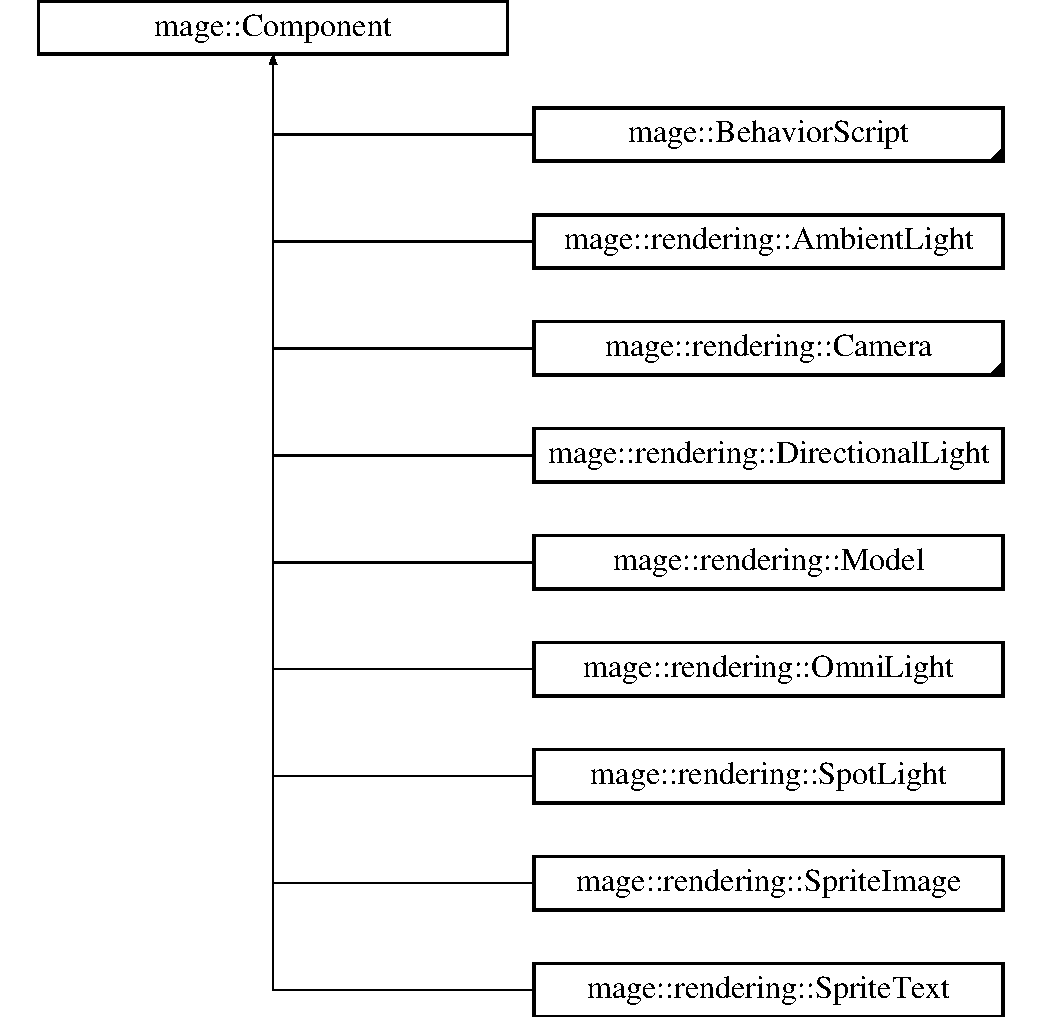
\includegraphics[height=10.000000cm]{classmage_1_1_component}
\end{center}
\end{figure}
\subsection*{Public Member Functions}
\begin{DoxyCompactItemize}
\item 
virtual \hyperlink{classmage_1_1_component_a2326c6df733b0cabf3086ad4187ba607}{$\sim$\+Component} ()
\item 
\hyperlink{classmage_1_1_component}{Component} \& \hyperlink{classmage_1_1_component_a69c2e920fb88323fa0fc5174671f4a01}{operator=} (const \hyperlink{classmage_1_1_component}{Component} \&script) noexcept
\item 
\hyperlink{classmage_1_1_component}{Component} \& \hyperlink{classmage_1_1_component_a0a03d80d37a6fa38616b955890471e06}{operator=} (\hyperlink{classmage_1_1_component}{Component} \&\&script) noexcept
\item 
\hyperlink{namespacemage_ae47d13d8477ee94893b9a3947d28eebc}{State} \hyperlink{classmage_1_1_component_a56f63648ba479decbba4a6fbaa544b4d}{Get\+State} () const noexcept
\item 
void \hyperlink{classmage_1_1_component_a95a74e2df3f326c4e92ac6dea7ed97be}{Set\+State} (\hyperlink{namespacemage_ae47d13d8477ee94893b9a3947d28eebc}{State} state) noexcept
\item 
\hyperlink{namespacemage_a6672cf3c861707ce4a3235a3eb43941d}{U64} \hyperlink{classmage_1_1_component_a1af8d5d8d09e5de54851ebed22153571}{Get\+Guid} () const noexcept
\item 
bool \hyperlink{classmage_1_1_component_a8e62e223bdacc3eebddc43f8ebc8c4d9}{Has\+Owner} () const noexcept
\item 
\hyperlink{classmage_1_1_proxy_ptr}{Proxy\+Ptr}$<$ \hyperlink{classmage_1_1_node}{Node} $>$ \hyperlink{classmage_1_1_component_af6261b2a7688dd5a078a917e1ec69e0b}{Get\+Owner} () noexcept
\item 
\hyperlink{classmage_1_1_proxy_ptr}{Proxy\+Ptr}$<$ const \hyperlink{classmage_1_1_node}{Node} $>$ \hyperlink{classmage_1_1_component_a97f402d0f75eff5a893abd2821a5335d}{Get\+Owner} () const noexcept
\end{DoxyCompactItemize}
\subsection*{Protected Member Functions}
\begin{DoxyCompactItemize}
\item 
\hyperlink{classmage_1_1_component_aef66a6573c094143bf95d3a81df1098e}{Component} () noexcept
\item 
\hyperlink{classmage_1_1_component_abcd9e6ba7f9691f51d1802d5cf8a365a}{Component} (const \hyperlink{classmage_1_1_component}{Component} \&component) noexcept
\item 
\hyperlink{classmage_1_1_component_a3abb21d27d4e89513787396c27b0ff6d}{Component} (\hyperlink{classmage_1_1_component}{Component} \&\&component) noexcept
\end{DoxyCompactItemize}
\subsection*{Private Member Functions}
\begin{DoxyCompactItemize}
\item 
void \hyperlink{classmage_1_1_component_aed5c7f7af79357f708c71572d7d99638}{Set\+Owner} (\hyperlink{classmage_1_1_proxy_ptr}{Proxy\+Ptr}$<$ \hyperlink{classmage_1_1_node}{Node} $>$ owner) noexcept
\end{DoxyCompactItemize}
\subsection*{Private Attributes}
\begin{DoxyCompactItemize}
\item 
\hyperlink{namespacemage_ae47d13d8477ee94893b9a3947d28eebc}{State} \hyperlink{classmage_1_1_component_a541a035d18f4d9f3873996716a8192d5}{m\+\_\+state}
\item 
\hyperlink{namespacemage_a6672cf3c861707ce4a3235a3eb43941d}{U64} \hyperlink{classmage_1_1_component_a3ddfe848bbd16a86dbdfd2717c0618da}{m\+\_\+guid}
\item 
\hyperlink{classmage_1_1_proxy_ptr}{Proxy\+Ptr}$<$ \hyperlink{classmage_1_1_node}{Node} $>$ \hyperlink{classmage_1_1_component_ad32770e1f30112cebd2894c1e976a4a7}{m\+\_\+owner}
\end{DoxyCompactItemize}
\subsection*{Friends}
\begin{DoxyCompactItemize}
\item 
class \hyperlink{classmage_1_1_component_a12f171c7a6bd27671b33ad16b0e42a6a}{Component\+Client}
\end{DoxyCompactItemize}


\subsection{Detailed Description}
A class of components. 

\subsection{Constructor \& Destructor Documentation}
\hypertarget{classmage_1_1_component_a2326c6df733b0cabf3086ad4187ba607}{}\label{classmage_1_1_component_a2326c6df733b0cabf3086ad4187ba607} 
\index{mage\+::\+Component@{mage\+::\+Component}!````~Component@{$\sim$\+Component}}
\index{````~Component@{$\sim$\+Component}!mage\+::\+Component@{mage\+::\+Component}}
\subsubsection{\texorpdfstring{$\sim$\+Component()}{~Component()}}
{\footnotesize\ttfamily mage\+::\+Component\+::$\sim$\+Component (\begin{DoxyParamCaption}{ }\end{DoxyParamCaption})\hspace{0.3cm}{\ttfamily [virtual]}, {\ttfamily [default]}}

Destructs this component. \hypertarget{classmage_1_1_component_aef66a6573c094143bf95d3a81df1098e}{}\label{classmage_1_1_component_aef66a6573c094143bf95d3a81df1098e} 
\index{mage\+::\+Component@{mage\+::\+Component}!Component@{Component}}
\index{Component@{Component}!mage\+::\+Component@{mage\+::\+Component}}
\subsubsection{\texorpdfstring{Component()}{Component()}\hspace{0.1cm}{\footnotesize\ttfamily [1/3]}}
{\footnotesize\ttfamily mage\+::\+Component\+::\+Component (\begin{DoxyParamCaption}{ }\end{DoxyParamCaption})\hspace{0.3cm}{\ttfamily [protected]}, {\ttfamily [noexcept]}}

Constructs a component. \hypertarget{classmage_1_1_component_abcd9e6ba7f9691f51d1802d5cf8a365a}{}\label{classmage_1_1_component_abcd9e6ba7f9691f51d1802d5cf8a365a} 
\index{mage\+::\+Component@{mage\+::\+Component}!Component@{Component}}
\index{Component@{Component}!mage\+::\+Component@{mage\+::\+Component}}
\subsubsection{\texorpdfstring{Component()}{Component()}\hspace{0.1cm}{\footnotesize\ttfamily [2/3]}}
{\footnotesize\ttfamily mage\+::\+Component\+::\+Component (\begin{DoxyParamCaption}\item[{const \hyperlink{classmage_1_1_component}{Component} \&}]{component }\end{DoxyParamCaption})\hspace{0.3cm}{\ttfamily [protected]}, {\ttfamily [noexcept]}}

Constructs a component from the given component.


\begin{DoxyParams}[1]{Parameters}
\mbox{\tt in}  & {\em component} & A reference to the component to copy. \\
\hline
\end{DoxyParams}
\hypertarget{classmage_1_1_component_a3abb21d27d4e89513787396c27b0ff6d}{}\label{classmage_1_1_component_a3abb21d27d4e89513787396c27b0ff6d} 
\index{mage\+::\+Component@{mage\+::\+Component}!Component@{Component}}
\index{Component@{Component}!mage\+::\+Component@{mage\+::\+Component}}
\subsubsection{\texorpdfstring{Component()}{Component()}\hspace{0.1cm}{\footnotesize\ttfamily [3/3]}}
{\footnotesize\ttfamily mage\+::\+Component\+::\+Component (\begin{DoxyParamCaption}\item[{\hyperlink{classmage_1_1_component}{Component} \&\&}]{component }\end{DoxyParamCaption})\hspace{0.3cm}{\ttfamily [protected]}, {\ttfamily [default]}, {\ttfamily [noexcept]}}

Constructs a component by moving the given component.


\begin{DoxyParams}[1]{Parameters}
\mbox{\tt in}  & {\em component} & A reference to the component to move. \\
\hline
\end{DoxyParams}


\subsection{Member Function Documentation}
\hypertarget{classmage_1_1_component_a1af8d5d8d09e5de54851ebed22153571}{}\label{classmage_1_1_component_a1af8d5d8d09e5de54851ebed22153571} 
\index{mage\+::\+Component@{mage\+::\+Component}!Get\+Guid@{Get\+Guid}}
\index{Get\+Guid@{Get\+Guid}!mage\+::\+Component@{mage\+::\+Component}}
\subsubsection{\texorpdfstring{Get\+Guid()}{GetGuid()}}
{\footnotesize\ttfamily \hyperlink{namespacemage_a6672cf3c861707ce4a3235a3eb43941d}{U64} mage\+::\+Component\+::\+Get\+Guid (\begin{DoxyParamCaption}{ }\end{DoxyParamCaption}) const\hspace{0.3cm}{\ttfamily [noexcept]}}

Returns the guid of this component.

\begin{DoxyReturn}{Returns}
The guid of this component. 
\end{DoxyReturn}
\hypertarget{classmage_1_1_component_af6261b2a7688dd5a078a917e1ec69e0b}{}\label{classmage_1_1_component_af6261b2a7688dd5a078a917e1ec69e0b} 
\index{mage\+::\+Component@{mage\+::\+Component}!Get\+Owner@{Get\+Owner}}
\index{Get\+Owner@{Get\+Owner}!mage\+::\+Component@{mage\+::\+Component}}
\subsubsection{\texorpdfstring{Get\+Owner()}{GetOwner()}\hspace{0.1cm}{\footnotesize\ttfamily [1/2]}}
{\footnotesize\ttfamily \hyperlink{classmage_1_1_proxy_ptr}{Proxy\+Ptr}$<$ \hyperlink{classmage_1_1_node}{Node} $>$ mage\+::\+Component\+::\+Get\+Owner (\begin{DoxyParamCaption}{ }\end{DoxyParamCaption})\hspace{0.3cm}{\ttfamily [noexcept]}}

Returns the owner of this component.

\begin{DoxyReturn}{Returns}
A pointer to the owner of this component. 
\end{DoxyReturn}
\hypertarget{classmage_1_1_component_a97f402d0f75eff5a893abd2821a5335d}{}\label{classmage_1_1_component_a97f402d0f75eff5a893abd2821a5335d} 
\index{mage\+::\+Component@{mage\+::\+Component}!Get\+Owner@{Get\+Owner}}
\index{Get\+Owner@{Get\+Owner}!mage\+::\+Component@{mage\+::\+Component}}
\subsubsection{\texorpdfstring{Get\+Owner()}{GetOwner()}\hspace{0.1cm}{\footnotesize\ttfamily [2/2]}}
{\footnotesize\ttfamily \hyperlink{classmage_1_1_proxy_ptr}{Proxy\+Ptr}$<$ const \hyperlink{classmage_1_1_node}{Node} $>$ mage\+::\+Component\+::\+Get\+Owner (\begin{DoxyParamCaption}{ }\end{DoxyParamCaption}) const\hspace{0.3cm}{\ttfamily [noexcept]}}

Returns the owner of this component.

\begin{DoxyReturn}{Returns}
A pointer to the owner of this component. 
\end{DoxyReturn}
\hypertarget{classmage_1_1_component_a56f63648ba479decbba4a6fbaa544b4d}{}\label{classmage_1_1_component_a56f63648ba479decbba4a6fbaa544b4d} 
\index{mage\+::\+Component@{mage\+::\+Component}!Get\+State@{Get\+State}}
\index{Get\+State@{Get\+State}!mage\+::\+Component@{mage\+::\+Component}}
\subsubsection{\texorpdfstring{Get\+State()}{GetState()}}
{\footnotesize\ttfamily \hyperlink{namespacemage_ae47d13d8477ee94893b9a3947d28eebc}{State} mage\+::\+Component\+::\+Get\+State (\begin{DoxyParamCaption}{ }\end{DoxyParamCaption}) const\hspace{0.3cm}{\ttfamily [noexcept]}}

Returns the state of this component.

\begin{DoxyReturn}{Returns}
The state of this component. 
\end{DoxyReturn}
\hypertarget{classmage_1_1_component_a8e62e223bdacc3eebddc43f8ebc8c4d9}{}\label{classmage_1_1_component_a8e62e223bdacc3eebddc43f8ebc8c4d9} 
\index{mage\+::\+Component@{mage\+::\+Component}!Has\+Owner@{Has\+Owner}}
\index{Has\+Owner@{Has\+Owner}!mage\+::\+Component@{mage\+::\+Component}}
\subsubsection{\texorpdfstring{Has\+Owner()}{HasOwner()}}
{\footnotesize\ttfamily bool mage\+::\+Component\+::\+Has\+Owner (\begin{DoxyParamCaption}{ }\end{DoxyParamCaption}) const\hspace{0.3cm}{\ttfamily [noexcept]}}

Checks whether this component has an owner.

\begin{DoxyReturn}{Returns}
{\ttfamily true} if this component has an owner. {\ttfamily false} otherwise. 
\end{DoxyReturn}
\hypertarget{classmage_1_1_component_a69c2e920fb88323fa0fc5174671f4a01}{}\label{classmage_1_1_component_a69c2e920fb88323fa0fc5174671f4a01} 
\index{mage\+::\+Component@{mage\+::\+Component}!operator=@{operator=}}
\index{operator=@{operator=}!mage\+::\+Component@{mage\+::\+Component}}
\subsubsection{\texorpdfstring{operator=()}{operator=()}\hspace{0.1cm}{\footnotesize\ttfamily [1/2]}}
{\footnotesize\ttfamily \hyperlink{classmage_1_1_component}{Component} \& mage\+::\+Component\+::operator= (\begin{DoxyParamCaption}\item[{const \hyperlink{classmage_1_1_component}{Component} \&}]{script }\end{DoxyParamCaption})\hspace{0.3cm}{\ttfamily [noexcept]}}

Copies the given component to this component.


\begin{DoxyParams}[1]{Parameters}
\mbox{\tt in}  & {\em script} & A reference to the component to copy. \\
\hline
\end{DoxyParams}
\begin{DoxyReturn}{Returns}
A reference to the copy of the given component (i.\+e. this component). 
\end{DoxyReturn}
\hypertarget{classmage_1_1_component_a0a03d80d37a6fa38616b955890471e06}{}\label{classmage_1_1_component_a0a03d80d37a6fa38616b955890471e06} 
\index{mage\+::\+Component@{mage\+::\+Component}!operator=@{operator=}}
\index{operator=@{operator=}!mage\+::\+Component@{mage\+::\+Component}}
\subsubsection{\texorpdfstring{operator=()}{operator=()}\hspace{0.1cm}{\footnotesize\ttfamily [2/2]}}
{\footnotesize\ttfamily \hyperlink{classmage_1_1_component}{Component} \& mage\+::\+Component\+::operator= (\begin{DoxyParamCaption}\item[{\hyperlink{classmage_1_1_component}{Component} \&\&}]{script }\end{DoxyParamCaption})\hspace{0.3cm}{\ttfamily [default]}, {\ttfamily [noexcept]}}

Moves the given component to this component.


\begin{DoxyParams}[1]{Parameters}
\mbox{\tt in}  & {\em script} & A reference to the component to move. \\
\hline
\end{DoxyParams}
\begin{DoxyReturn}{Returns}
A reference to the moved component (i.\+e. this component). 
\end{DoxyReturn}
\hypertarget{classmage_1_1_component_aed5c7f7af79357f708c71572d7d99638}{}\label{classmage_1_1_component_aed5c7f7af79357f708c71572d7d99638} 
\index{mage\+::\+Component@{mage\+::\+Component}!Set\+Owner@{Set\+Owner}}
\index{Set\+Owner@{Set\+Owner}!mage\+::\+Component@{mage\+::\+Component}}
\subsubsection{\texorpdfstring{Set\+Owner()}{SetOwner()}}
{\footnotesize\ttfamily void mage\+::\+Component\+::\+Set\+Owner (\begin{DoxyParamCaption}\item[{\hyperlink{classmage_1_1_proxy_ptr}{Proxy\+Ptr}$<$ \hyperlink{classmage_1_1_node}{Node} $>$}]{owner }\end{DoxyParamCaption})\hspace{0.3cm}{\ttfamily [private]}, {\ttfamily [noexcept]}}

Sets the owner of this component to the given owner.


\begin{DoxyParams}[1]{Parameters}
\mbox{\tt in}  & {\em owner} & A pointer to the owner. \\
\hline
\end{DoxyParams}
\hypertarget{classmage_1_1_component_a95a74e2df3f326c4e92ac6dea7ed97be}{}\label{classmage_1_1_component_a95a74e2df3f326c4e92ac6dea7ed97be} 
\index{mage\+::\+Component@{mage\+::\+Component}!Set\+State@{Set\+State}}
\index{Set\+State@{Set\+State}!mage\+::\+Component@{mage\+::\+Component}}
\subsubsection{\texorpdfstring{Set\+State()}{SetState()}}
{\footnotesize\ttfamily void mage\+::\+Component\+::\+Set\+State (\begin{DoxyParamCaption}\item[{\hyperlink{namespacemage_ae47d13d8477ee94893b9a3947d28eebc}{State}}]{state }\end{DoxyParamCaption})\hspace{0.3cm}{\ttfamily [noexcept]}}

Sets the state of this component to the given state.


\begin{DoxyParams}[1]{Parameters}
\mbox{\tt in}  & {\em state} & The state. \\
\hline
\end{DoxyParams}


\subsection{Friends And Related Function Documentation}
\hypertarget{classmage_1_1_component_a12f171c7a6bd27671b33ad16b0e42a6a}{}\label{classmage_1_1_component_a12f171c7a6bd27671b33ad16b0e42a6a} 
\index{mage\+::\+Component@{mage\+::\+Component}!Component\+Client@{Component\+Client}}
\index{Component\+Client@{Component\+Client}!mage\+::\+Component@{mage\+::\+Component}}
\subsubsection{\texorpdfstring{Component\+Client}{ComponentClient}}
{\footnotesize\ttfamily friend class \hyperlink{classmage_1_1_component_client}{Component\+Client}\hspace{0.3cm}{\ttfamily [friend]}}



\subsection{Member Data Documentation}
\hypertarget{classmage_1_1_component_a3ddfe848bbd16a86dbdfd2717c0618da}{}\label{classmage_1_1_component_a3ddfe848bbd16a86dbdfd2717c0618da} 
\index{mage\+::\+Component@{mage\+::\+Component}!m\+\_\+guid@{m\+\_\+guid}}
\index{m\+\_\+guid@{m\+\_\+guid}!mage\+::\+Component@{mage\+::\+Component}}
\subsubsection{\texorpdfstring{m\+\_\+guid}{m\_guid}}
{\footnotesize\ttfamily \hyperlink{namespacemage_a6672cf3c861707ce4a3235a3eb43941d}{U64} mage\+::\+Component\+::m\+\_\+guid\hspace{0.3cm}{\ttfamily [private]}}

The guid of this component. \hypertarget{classmage_1_1_component_ad32770e1f30112cebd2894c1e976a4a7}{}\label{classmage_1_1_component_ad32770e1f30112cebd2894c1e976a4a7} 
\index{mage\+::\+Component@{mage\+::\+Component}!m\+\_\+owner@{m\+\_\+owner}}
\index{m\+\_\+owner@{m\+\_\+owner}!mage\+::\+Component@{mage\+::\+Component}}
\subsubsection{\texorpdfstring{m\+\_\+owner}{m\_owner}}
{\footnotesize\ttfamily \hyperlink{classmage_1_1_proxy_ptr}{Proxy\+Ptr}$<$ \hyperlink{classmage_1_1_node}{Node} $>$ mage\+::\+Component\+::m\+\_\+owner\hspace{0.3cm}{\ttfamily [private]}}

A pointer to the node owning this component. \hypertarget{classmage_1_1_component_a541a035d18f4d9f3873996716a8192d5}{}\label{classmage_1_1_component_a541a035d18f4d9f3873996716a8192d5} 
\index{mage\+::\+Component@{mage\+::\+Component}!m\+\_\+state@{m\+\_\+state}}
\index{m\+\_\+state@{m\+\_\+state}!mage\+::\+Component@{mage\+::\+Component}}
\subsubsection{\texorpdfstring{m\+\_\+state}{m\_state}}
{\footnotesize\ttfamily \hyperlink{namespacemage_ae47d13d8477ee94893b9a3947d28eebc}{State} mage\+::\+Component\+::m\+\_\+state\hspace{0.3cm}{\ttfamily [private]}}

The state of this component. 
\hypertarget{classmage_1_1_component_client}{}\section{mage\+:\+:Component\+Client Class Reference}
\label{classmage_1_1_component_client}\index{mage\+::\+Component\+Client@{mage\+::\+Component\+Client}}


{\ttfamily \#include $<$component.\+hpp$>$}

\subsection*{Static Private Member Functions}
\begin{DoxyCompactItemize}
\item 
static void \mbox{\hyperlink{classmage_1_1_component_client_a268413a2179e0f29ac78b0c5f26ecaca}{Set\+Owner}} (\mbox{\hyperlink{classmage_1_1_component}{Component}} \&component, \mbox{\hyperlink{classmage_1_1_proxy_ptr}{Proxy\+Ptr}}$<$ \mbox{\hyperlink{classmage_1_1_node}{Node}} $>$ owner) noexcept
\end{DoxyCompactItemize}
\subsection*{Friends}
\begin{DoxyCompactItemize}
\item 
class \mbox{\hyperlink{classmage_1_1_component_client_a6db9d28bd448a131448276ee03de1e6d}{Node}}
\end{DoxyCompactItemize}


\subsection{Detailed Description}
A class of component clients. 

\subsection{Member Function Documentation}
\mbox{\Hypertarget{classmage_1_1_component_client_a268413a2179e0f29ac78b0c5f26ecaca}\label{classmage_1_1_component_client_a268413a2179e0f29ac78b0c5f26ecaca}} 
\index{mage\+::\+Component\+Client@{mage\+::\+Component\+Client}!Set\+Owner@{Set\+Owner}}
\index{Set\+Owner@{Set\+Owner}!mage\+::\+Component\+Client@{mage\+::\+Component\+Client}}
\subsubsection{\texorpdfstring{Set\+Owner()}{SetOwner()}}
{\footnotesize\ttfamily static void mage\+::\+Component\+Client\+::\+Set\+Owner (\begin{DoxyParamCaption}\item[{\mbox{\hyperlink{classmage_1_1_component}{Component}} \&}]{component,  }\item[{\mbox{\hyperlink{classmage_1_1_proxy_ptr}{Proxy\+Ptr}}$<$ \mbox{\hyperlink{classmage_1_1_node}{Node}} $>$}]{owner }\end{DoxyParamCaption})\hspace{0.3cm}{\ttfamily [static]}, {\ttfamily [private]}, {\ttfamily [noexcept]}}

Sets the owner of the given component to the given owner.


\begin{DoxyParams}[1]{Parameters}
\mbox{\tt in}  & {\em component} & A reference to the component. \\
\hline
\mbox{\tt in}  & {\em owner} & A pointer to the owner. \\
\hline
\end{DoxyParams}


\subsection{Friends And Related Function Documentation}
\mbox{\Hypertarget{classmage_1_1_component_client_a6db9d28bd448a131448276ee03de1e6d}\label{classmage_1_1_component_client_a6db9d28bd448a131448276ee03de1e6d}} 
\index{mage\+::\+Component\+Client@{mage\+::\+Component\+Client}!Node@{Node}}
\index{Node@{Node}!mage\+::\+Component\+Client@{mage\+::\+Component\+Client}}
\subsubsection{\texorpdfstring{Node}{Node}}
{\footnotesize\ttfamily friend class \mbox{\hyperlink{classmage_1_1_node}{Node}}\hspace{0.3cm}{\ttfamily [friend]}}


\hypertarget{classmage_1_1rendering_1_1_constant_buffer}{}\section{mage\+:\+:rendering\+:\+:Constant\+Buffer$<$ T $>$ Class Template Reference}
\label{classmage_1_1rendering_1_1_constant_buffer}\index{mage\+::rendering\+::\+Constant\+Buffer$<$ T $>$@{mage\+::rendering\+::\+Constant\+Buffer$<$ T $>$}}


{\ttfamily \#include $<$constant\+\_\+buffer.\+hpp$>$}

\subsection*{Public Member Functions}
\begin{DoxyCompactItemize}
\item 
\mbox{\hyperlink{classmage_1_1rendering_1_1_constant_buffer_af282b97fba72826646c1bc31d8953b9e}{Constant\+Buffer}} (I\+D3\+D11\+Device \&device)
\item 
\mbox{\hyperlink{classmage_1_1rendering_1_1_constant_buffer_aacc1ace626cdf1fbeb2d51d7789495da}{Constant\+Buffer}} (const \mbox{\hyperlink{classmage_1_1rendering_1_1_constant_buffer}{Constant\+Buffer}} \&buffer)=delete
\item 
\mbox{\hyperlink{classmage_1_1rendering_1_1_constant_buffer_a1c1c73d617245d7dead836b0d3a00a6f}{Constant\+Buffer}} (\mbox{\hyperlink{classmage_1_1rendering_1_1_constant_buffer}{Constant\+Buffer}} \&\&buffer) noexcept=default
\item 
\mbox{\hyperlink{classmage_1_1rendering_1_1_constant_buffer_af75271b7a5550583732e0575b576f088}{$\sim$\+Constant\+Buffer}} ()=default
\item 
\mbox{\hyperlink{classmage_1_1rendering_1_1_constant_buffer}{Constant\+Buffer}} \& \mbox{\hyperlink{classmage_1_1rendering_1_1_constant_buffer_ac8770d151c9c8bdb27babdb060fd7f4c}{operator=}} (const \mbox{\hyperlink{classmage_1_1rendering_1_1_constant_buffer}{Constant\+Buffer}} \&buffer)=delete
\item 
\mbox{\hyperlink{classmage_1_1rendering_1_1_constant_buffer}{Constant\+Buffer}} \& \mbox{\hyperlink{classmage_1_1rendering_1_1_constant_buffer_adbd72a5aa7eab5461eed06c611dd908c}{operator=}} (\mbox{\hyperlink{classmage_1_1rendering_1_1_constant_buffer}{Constant\+Buffer}} \&\&buffer) noexcept=default
\item 
void \mbox{\hyperlink{classmage_1_1rendering_1_1_constant_buffer_a4289215f38cf17e767e438021894a140}{Update\+Data}} (I\+D3\+D11\+Device\+Context \&device\+\_\+context, const T \&data)
\item 
I\+D3\+D11\+Buffer \& \mbox{\hyperlink{classmage_1_1rendering_1_1_constant_buffer_a0020fcf17b61d277430c572df44992b5}{Get}} () const noexcept
\item 
{\footnotesize template$<$typename Pipeline\+StageT $>$ }\\void \mbox{\hyperlink{classmage_1_1rendering_1_1_constant_buffer_a49c3982ed5b6a01ddc8cadd509eff7f8}{Bind}} (I\+D3\+D11\+Device\+Context \&device\+\_\+context, \mbox{\hyperlink{namespacemage_a41c104c036fba3756a74e19f793eeaa1}{U32}} slot) const noexcept
\end{DoxyCompactItemize}
\subsection*{Private Member Functions}
\begin{DoxyCompactItemize}
\item 
void \mbox{\hyperlink{classmage_1_1rendering_1_1_constant_buffer_ae957fe951307c4628aecc0f3e196fc81}{Setup\+Constant\+Buffer}} (I\+D3\+D11\+Device \&device)
\end{DoxyCompactItemize}
\subsection*{Private Attributes}
\begin{DoxyCompactItemize}
\item 
\mbox{\hyperlink{namespacemage_ae74f374780900893caa5555d1031fd79}{Com\+Ptr}}$<$ I\+D3\+D11\+Buffer $>$ \mbox{\hyperlink{classmage_1_1rendering_1_1_constant_buffer_a1bf487e7e5d8dfee471cc7b3514f6313}{m\+\_\+buffer}}
\end{DoxyCompactItemize}


\subsection{Detailed Description}
\subsubsection*{template$<$typename T$>$\newline
class mage\+::rendering\+::\+Constant\+Buffer$<$ T $>$}

A class of constant buffers.


\begin{DoxyTemplParams}{Template Parameters}
{\em T} & The data type. \\
\hline
\end{DoxyTemplParams}


\subsection{Constructor \& Destructor Documentation}
\mbox{\Hypertarget{classmage_1_1rendering_1_1_constant_buffer_af282b97fba72826646c1bc31d8953b9e}\label{classmage_1_1rendering_1_1_constant_buffer_af282b97fba72826646c1bc31d8953b9e}} 
\index{mage\+::rendering\+::\+Constant\+Buffer@{mage\+::rendering\+::\+Constant\+Buffer}!Constant\+Buffer@{Constant\+Buffer}}
\index{Constant\+Buffer@{Constant\+Buffer}!mage\+::rendering\+::\+Constant\+Buffer@{mage\+::rendering\+::\+Constant\+Buffer}}
\subsubsection{\texorpdfstring{Constant\+Buffer()}{ConstantBuffer()}\hspace{0.1cm}{\footnotesize\ttfamily [1/3]}}
{\footnotesize\ttfamily template$<$typename T$>$ \\
\mbox{\hyperlink{classmage_1_1rendering_1_1_constant_buffer}{mage\+::rendering\+::\+Constant\+Buffer}}$<$ T $>$\+::\mbox{\hyperlink{classmage_1_1rendering_1_1_constant_buffer}{Constant\+Buffer}} (\begin{DoxyParamCaption}\item[{I\+D3\+D11\+Device \&}]{device }\end{DoxyParamCaption})\hspace{0.3cm}{\ttfamily [explicit]}}

Constructs a constant buffer.


\begin{DoxyParams}[1]{Parameters}
\mbox{\tt in}  & {\em device} & A reference to the device. \\
\hline
\end{DoxyParams}

\begin{DoxyExceptions}{Exceptions}
{\em \mbox{\hyperlink{classmage_1_1_exception}{Exception}}} & Failed to setup this constant buffer. \\
\hline
\end{DoxyExceptions}
\mbox{\Hypertarget{classmage_1_1rendering_1_1_constant_buffer_aacc1ace626cdf1fbeb2d51d7789495da}\label{classmage_1_1rendering_1_1_constant_buffer_aacc1ace626cdf1fbeb2d51d7789495da}} 
\index{mage\+::rendering\+::\+Constant\+Buffer@{mage\+::rendering\+::\+Constant\+Buffer}!Constant\+Buffer@{Constant\+Buffer}}
\index{Constant\+Buffer@{Constant\+Buffer}!mage\+::rendering\+::\+Constant\+Buffer@{mage\+::rendering\+::\+Constant\+Buffer}}
\subsubsection{\texorpdfstring{Constant\+Buffer()}{ConstantBuffer()}\hspace{0.1cm}{\footnotesize\ttfamily [2/3]}}
{\footnotesize\ttfamily template$<$typename T$>$ \\
\mbox{\hyperlink{classmage_1_1rendering_1_1_constant_buffer}{mage\+::rendering\+::\+Constant\+Buffer}}$<$ T $>$\+::\mbox{\hyperlink{classmage_1_1rendering_1_1_constant_buffer}{Constant\+Buffer}} (\begin{DoxyParamCaption}\item[{const \mbox{\hyperlink{classmage_1_1rendering_1_1_constant_buffer}{Constant\+Buffer}}$<$ T $>$ \&}]{buffer }\end{DoxyParamCaption})\hspace{0.3cm}{\ttfamily [delete]}}

Constructs a constant buffer from the given constant buffer.


\begin{DoxyParams}[1]{Parameters}
\mbox{\tt in}  & {\em buffer} & A reference to the constant buffer to copy. \\
\hline
\end{DoxyParams}
\mbox{\Hypertarget{classmage_1_1rendering_1_1_constant_buffer_a1c1c73d617245d7dead836b0d3a00a6f}\label{classmage_1_1rendering_1_1_constant_buffer_a1c1c73d617245d7dead836b0d3a00a6f}} 
\index{mage\+::rendering\+::\+Constant\+Buffer@{mage\+::rendering\+::\+Constant\+Buffer}!Constant\+Buffer@{Constant\+Buffer}}
\index{Constant\+Buffer@{Constant\+Buffer}!mage\+::rendering\+::\+Constant\+Buffer@{mage\+::rendering\+::\+Constant\+Buffer}}
\subsubsection{\texorpdfstring{Constant\+Buffer()}{ConstantBuffer()}\hspace{0.1cm}{\footnotesize\ttfamily [3/3]}}
{\footnotesize\ttfamily template$<$typename T$>$ \\
\mbox{\hyperlink{classmage_1_1rendering_1_1_constant_buffer}{mage\+::rendering\+::\+Constant\+Buffer}}$<$ T $>$\+::\mbox{\hyperlink{classmage_1_1rendering_1_1_constant_buffer}{Constant\+Buffer}} (\begin{DoxyParamCaption}\item[{\mbox{\hyperlink{classmage_1_1rendering_1_1_constant_buffer}{Constant\+Buffer}}$<$ T $>$ \&\&}]{buffer }\end{DoxyParamCaption})\hspace{0.3cm}{\ttfamily [default]}, {\ttfamily [noexcept]}}

Constructs a constant buffer by moving the given constant buffer.


\begin{DoxyParams}[1]{Parameters}
\mbox{\tt in}  & {\em buffer} & A reference to the constant buffer to move. \\
\hline
\end{DoxyParams}
\mbox{\Hypertarget{classmage_1_1rendering_1_1_constant_buffer_af75271b7a5550583732e0575b576f088}\label{classmage_1_1rendering_1_1_constant_buffer_af75271b7a5550583732e0575b576f088}} 
\index{mage\+::rendering\+::\+Constant\+Buffer@{mage\+::rendering\+::\+Constant\+Buffer}!````~Constant\+Buffer@{$\sim$\+Constant\+Buffer}}
\index{````~Constant\+Buffer@{$\sim$\+Constant\+Buffer}!mage\+::rendering\+::\+Constant\+Buffer@{mage\+::rendering\+::\+Constant\+Buffer}}
\subsubsection{\texorpdfstring{$\sim$\+Constant\+Buffer()}{~ConstantBuffer()}}
{\footnotesize\ttfamily template$<$typename T$>$ \\
\mbox{\hyperlink{classmage_1_1rendering_1_1_constant_buffer}{mage\+::rendering\+::\+Constant\+Buffer}}$<$ T $>$\+::$\sim$\mbox{\hyperlink{classmage_1_1rendering_1_1_constant_buffer}{Constant\+Buffer}} (\begin{DoxyParamCaption}{ }\end{DoxyParamCaption})\hspace{0.3cm}{\ttfamily [default]}}

Destructs this constant buffer. 

\subsection{Member Function Documentation}
\mbox{\Hypertarget{classmage_1_1rendering_1_1_constant_buffer_a49c3982ed5b6a01ddc8cadd509eff7f8}\label{classmage_1_1rendering_1_1_constant_buffer_a49c3982ed5b6a01ddc8cadd509eff7f8}} 
\index{mage\+::rendering\+::\+Constant\+Buffer@{mage\+::rendering\+::\+Constant\+Buffer}!Bind@{Bind}}
\index{Bind@{Bind}!mage\+::rendering\+::\+Constant\+Buffer@{mage\+::rendering\+::\+Constant\+Buffer}}
\subsubsection{\texorpdfstring{Bind()}{Bind()}}
{\footnotesize\ttfamily template$<$typename T$>$ \\
template$<$typename Pipeline\+StageT $>$ \\
void \mbox{\hyperlink{classmage_1_1rendering_1_1_constant_buffer}{mage\+::rendering\+::\+Constant\+Buffer}}$<$ T $>$\+::Bind (\begin{DoxyParamCaption}\item[{I\+D3\+D11\+Device\+Context \&}]{device\+\_\+context,  }\item[{\mbox{\hyperlink{namespacemage_a41c104c036fba3756a74e19f793eeaa1}{U32}}}]{slot }\end{DoxyParamCaption}) const\hspace{0.3cm}{\ttfamily [noexcept]}}

Binds this constant buffer.

\begin{DoxyPrecond}{Precondition}
{\itshape slot} $<$ {\ttfamily D3\+D11\+\_\+\+C\+O\+M\+M\+O\+N\+S\+H\+A\+D\+E\+R\+\_\+\+C\+O\+N\+S\+T\+A\+N\+T\+\_\+\+B\+U\+F\+F\+E\+R\+\_\+\+A\+P\+I\+\_\+\+S\+L\+O\+T\+\_\+\+C\+O\+U\+NT}. 
\end{DoxyPrecond}

\begin{DoxyTemplParams}{Template Parameters}
{\em Pipeline\+StageT} & The pipeline stage type. \\
\hline
\end{DoxyTemplParams}

\begin{DoxyParams}[1]{Parameters}
\mbox{\tt in}  & {\em device\+\_\+context} & A reference to the device context. \\
\hline
\mbox{\tt in}  & {\em slot} & The index into the device\textquotesingle{}s zero-\/based array to set the constant buffer to (ranges from 0 to {\ttfamily D3\+D11\+\_\+\+C\+O\+M\+M\+O\+N\+S\+H\+A\+D\+E\+R\+\_\+\+C\+O\+N\+S\+T\+A\+N\+T\+\_\+\+B\+U\+F\+F\+E\+R\+\_\+\+A\+P\+I\+\_\+\+S\+L\+O\+T\+\_\+\+C\+O\+U\+NT} 
\begin{DoxyItemize}
\item 1). 
\end{DoxyItemize}\\
\hline
\end{DoxyParams}
\mbox{\Hypertarget{classmage_1_1rendering_1_1_constant_buffer_a0020fcf17b61d277430c572df44992b5}\label{classmage_1_1rendering_1_1_constant_buffer_a0020fcf17b61d277430c572df44992b5}} 
\index{mage\+::rendering\+::\+Constant\+Buffer@{mage\+::rendering\+::\+Constant\+Buffer}!Get@{Get}}
\index{Get@{Get}!mage\+::rendering\+::\+Constant\+Buffer@{mage\+::rendering\+::\+Constant\+Buffer}}
\subsubsection{\texorpdfstring{Get()}{Get()}}
{\footnotesize\ttfamily template$<$typename T$>$ \\
I\+D3\+D11\+Buffer\& \mbox{\hyperlink{classmage_1_1rendering_1_1_constant_buffer}{mage\+::rendering\+::\+Constant\+Buffer}}$<$ T $>$\+::Get (\begin{DoxyParamCaption}{ }\end{DoxyParamCaption}) const\hspace{0.3cm}{\ttfamily [noexcept]}}

Returns the buffer resource of this constant buffer.

\begin{DoxyReturn}{Returns}
A reference to the buffer resource of this constant buffer. 
\end{DoxyReturn}
\mbox{\Hypertarget{classmage_1_1rendering_1_1_constant_buffer_ac8770d151c9c8bdb27babdb060fd7f4c}\label{classmage_1_1rendering_1_1_constant_buffer_ac8770d151c9c8bdb27babdb060fd7f4c}} 
\index{mage\+::rendering\+::\+Constant\+Buffer@{mage\+::rendering\+::\+Constant\+Buffer}!operator=@{operator=}}
\index{operator=@{operator=}!mage\+::rendering\+::\+Constant\+Buffer@{mage\+::rendering\+::\+Constant\+Buffer}}
\subsubsection{\texorpdfstring{operator=()}{operator=()}\hspace{0.1cm}{\footnotesize\ttfamily [1/2]}}
{\footnotesize\ttfamily template$<$typename T$>$ \\
\mbox{\hyperlink{classmage_1_1rendering_1_1_constant_buffer}{Constant\+Buffer}}\& \mbox{\hyperlink{classmage_1_1rendering_1_1_constant_buffer}{mage\+::rendering\+::\+Constant\+Buffer}}$<$ T $>$\+::operator= (\begin{DoxyParamCaption}\item[{const \mbox{\hyperlink{classmage_1_1rendering_1_1_constant_buffer}{Constant\+Buffer}}$<$ T $>$ \&}]{buffer }\end{DoxyParamCaption})\hspace{0.3cm}{\ttfamily [delete]}}

Copies the given constant buffer to this constant buffer.


\begin{DoxyParams}[1]{Parameters}
\mbox{\tt in}  & {\em buffer} & A reference to the constant buffer to copy. \\
\hline
\end{DoxyParams}
\begin{DoxyReturn}{Returns}
A reference to the copy of the given constant buffer (i.\+e. this constant buffer). 
\end{DoxyReturn}
\mbox{\Hypertarget{classmage_1_1rendering_1_1_constant_buffer_adbd72a5aa7eab5461eed06c611dd908c}\label{classmage_1_1rendering_1_1_constant_buffer_adbd72a5aa7eab5461eed06c611dd908c}} 
\index{mage\+::rendering\+::\+Constant\+Buffer@{mage\+::rendering\+::\+Constant\+Buffer}!operator=@{operator=}}
\index{operator=@{operator=}!mage\+::rendering\+::\+Constant\+Buffer@{mage\+::rendering\+::\+Constant\+Buffer}}
\subsubsection{\texorpdfstring{operator=()}{operator=()}\hspace{0.1cm}{\footnotesize\ttfamily [2/2]}}
{\footnotesize\ttfamily template$<$typename T$>$ \\
\mbox{\hyperlink{classmage_1_1rendering_1_1_constant_buffer}{Constant\+Buffer}}\& \mbox{\hyperlink{classmage_1_1rendering_1_1_constant_buffer}{mage\+::rendering\+::\+Constant\+Buffer}}$<$ T $>$\+::operator= (\begin{DoxyParamCaption}\item[{\mbox{\hyperlink{classmage_1_1rendering_1_1_constant_buffer}{Constant\+Buffer}}$<$ T $>$ \&\&}]{buffer }\end{DoxyParamCaption})\hspace{0.3cm}{\ttfamily [default]}, {\ttfamily [noexcept]}}

Moves the given constant buffer to this constant buffer.


\begin{DoxyParams}[1]{Parameters}
\mbox{\tt in}  & {\em buffer} & A reference to the constant buffer to move. \\
\hline
\end{DoxyParams}
\begin{DoxyReturn}{Returns}
A reference to the moved constant buffer (i.\+e. this constant buffer). 
\end{DoxyReturn}
\mbox{\Hypertarget{classmage_1_1rendering_1_1_constant_buffer_ae957fe951307c4628aecc0f3e196fc81}\label{classmage_1_1rendering_1_1_constant_buffer_ae957fe951307c4628aecc0f3e196fc81}} 
\index{mage\+::rendering\+::\+Constant\+Buffer@{mage\+::rendering\+::\+Constant\+Buffer}!Setup\+Constant\+Buffer@{Setup\+Constant\+Buffer}}
\index{Setup\+Constant\+Buffer@{Setup\+Constant\+Buffer}!mage\+::rendering\+::\+Constant\+Buffer@{mage\+::rendering\+::\+Constant\+Buffer}}
\subsubsection{\texorpdfstring{Setup\+Constant\+Buffer()}{SetupConstantBuffer()}}
{\footnotesize\ttfamily template$<$typename T$>$ \\
void \mbox{\hyperlink{classmage_1_1rendering_1_1_constant_buffer}{mage\+::rendering\+::\+Constant\+Buffer}}$<$ T $>$\+::Setup\+Constant\+Buffer (\begin{DoxyParamCaption}\item[{I\+D3\+D11\+Device \&}]{device }\end{DoxyParamCaption})\hspace{0.3cm}{\ttfamily [private]}}

Sets up the resource buffer of this constant buffer.


\begin{DoxyParams}[1]{Parameters}
\mbox{\tt in}  & {\em device} & A reference to the device. \\
\hline
\end{DoxyParams}

\begin{DoxyExceptions}{Exceptions}
{\em \mbox{\hyperlink{classmage_1_1_exception}{Exception}}} & Failed to setup this constant buffer. \\
\hline
\end{DoxyExceptions}
\mbox{\Hypertarget{classmage_1_1rendering_1_1_constant_buffer_a4289215f38cf17e767e438021894a140}\label{classmage_1_1rendering_1_1_constant_buffer_a4289215f38cf17e767e438021894a140}} 
\index{mage\+::rendering\+::\+Constant\+Buffer@{mage\+::rendering\+::\+Constant\+Buffer}!Update\+Data@{Update\+Data}}
\index{Update\+Data@{Update\+Data}!mage\+::rendering\+::\+Constant\+Buffer@{mage\+::rendering\+::\+Constant\+Buffer}}
\subsubsection{\texorpdfstring{Update\+Data()}{UpdateData()}}
{\footnotesize\ttfamily template$<$typename T$>$ \\
void \mbox{\hyperlink{classmage_1_1rendering_1_1_constant_buffer}{mage\+::rendering\+::\+Constant\+Buffer}}$<$ T $>$\+::Update\+Data (\begin{DoxyParamCaption}\item[{I\+D3\+D11\+Device\+Context \&}]{device\+\_\+context,  }\item[{const T \&}]{data }\end{DoxyParamCaption})}

Updates the data of this constant buffer with the given data.


\begin{DoxyParams}[1]{Parameters}
\mbox{\tt in}  & {\em device\+\_\+context} & A reference to the device context. \\
\hline
\mbox{\tt in}  & {\em data} & A reference to the data. \\
\hline
\end{DoxyParams}

\begin{DoxyExceptions}{Exceptions}
{\em \mbox{\hyperlink{classmage_1_1_exception}{Exception}}} & Failed to update the data. \\
\hline
\end{DoxyExceptions}


\subsection{Member Data Documentation}
\mbox{\Hypertarget{classmage_1_1rendering_1_1_constant_buffer_a1bf487e7e5d8dfee471cc7b3514f6313}\label{classmage_1_1rendering_1_1_constant_buffer_a1bf487e7e5d8dfee471cc7b3514f6313}} 
\index{mage\+::rendering\+::\+Constant\+Buffer@{mage\+::rendering\+::\+Constant\+Buffer}!m\+\_\+buffer@{m\+\_\+buffer}}
\index{m\+\_\+buffer@{m\+\_\+buffer}!mage\+::rendering\+::\+Constant\+Buffer@{mage\+::rendering\+::\+Constant\+Buffer}}
\subsubsection{\texorpdfstring{m\+\_\+buffer}{m\_buffer}}
{\footnotesize\ttfamily template$<$typename T$>$ \\
\mbox{\hyperlink{namespacemage_ae74f374780900893caa5555d1031fd79}{Com\+Ptr}}$<$ I\+D3\+D11\+Buffer $>$ \mbox{\hyperlink{classmage_1_1rendering_1_1_constant_buffer}{mage\+::rendering\+::\+Constant\+Buffer}}$<$ T $>$\+::m\+\_\+buffer\hspace{0.3cm}{\ttfamily [private]}}

A pointer to the buffer resource of this constant buffer. 
\hypertarget{structmage_1_1_core_clock}{}\section{mage\+:\+:Core\+Clock Struct Reference}
\label{structmage_1_1_core_clock}\index{mage\+::\+Core\+Clock@{mage\+::\+Core\+Clock}}


{\ttfamily \#include $<$system\+\_\+time.\+hpp$>$}

\subsection*{Public Types}
\begin{DoxyCompactItemize}
\item 
using \hyperlink{structmage_1_1_core_clock_afcf2ac7e5e594734cdedaf46fbbf23d8}{rep} = \hyperlink{namespacemage_a6672cf3c861707ce4a3235a3eb43941d}{U64}
\item 
using \hyperlink{structmage_1_1_core_clock_af147d1abde62f8694d3be69b8915ddbc}{period} = std\+::ratio$<$ 1, 10 \textquotesingle{}000 \textquotesingle{}000 $>$
\item 
using \hyperlink{structmage_1_1_core_clock_aebf1d2eafc4269bd84c1386114f3e6cb}{duration} = std\+::chrono\+::duration$<$ \hyperlink{structmage_1_1_core_clock_afcf2ac7e5e594734cdedaf46fbbf23d8}{rep}, \hyperlink{structmage_1_1_core_clock_af147d1abde62f8694d3be69b8915ddbc}{period} $>$
\item 
using \hyperlink{structmage_1_1_core_clock_a1ea0193dea9647827d27469ec9e3b61c}{time\+\_\+point} = std\+::chrono\+::time\+\_\+point$<$ \hyperlink{structmage_1_1_core_clock}{Core\+Clock} $>$
\end{DoxyCompactItemize}
\subsection*{Static Public Member Functions}
\begin{DoxyCompactItemize}
\item 
static \hyperlink{structmage_1_1_core_clock_a1ea0193dea9647827d27469ec9e3b61c}{time\+\_\+point} \hyperlink{structmage_1_1_core_clock_addea160814d296009c10986faabe08bd}{now} () noexcept
\end{DoxyCompactItemize}
\subsection*{Static Public Attributes}
\begin{DoxyCompactItemize}
\item 
static constexpr bool \hyperlink{structmage_1_1_core_clock_ae6481fa7adddf1e9fefd45fba2e20516}{is\+\_\+steady} = true
\end{DoxyCompactItemize}


\subsection{Member Typedef Documentation}
\hypertarget{structmage_1_1_core_clock_aebf1d2eafc4269bd84c1386114f3e6cb}{}\label{structmage_1_1_core_clock_aebf1d2eafc4269bd84c1386114f3e6cb} 
\index{mage\+::\+Core\+Clock@{mage\+::\+Core\+Clock}!duration@{duration}}
\index{duration@{duration}!mage\+::\+Core\+Clock@{mage\+::\+Core\+Clock}}
\subsubsection{\texorpdfstring{duration}{duration}}
{\footnotesize\ttfamily using \hyperlink{structmage_1_1_core_clock_aebf1d2eafc4269bd84c1386114f3e6cb}{mage\+::\+Core\+Clock\+::duration} =  std\+::chrono\+::duration$<$ \hyperlink{structmage_1_1_core_clock_afcf2ac7e5e594734cdedaf46fbbf23d8}{rep}, \hyperlink{structmage_1_1_core_clock_af147d1abde62f8694d3be69b8915ddbc}{period} $>$}

\hypertarget{structmage_1_1_core_clock_af147d1abde62f8694d3be69b8915ddbc}{}\label{structmage_1_1_core_clock_af147d1abde62f8694d3be69b8915ddbc} 
\index{mage\+::\+Core\+Clock@{mage\+::\+Core\+Clock}!period@{period}}
\index{period@{period}!mage\+::\+Core\+Clock@{mage\+::\+Core\+Clock}}
\subsubsection{\texorpdfstring{period}{period}}
{\footnotesize\ttfamily using \hyperlink{structmage_1_1_core_clock_af147d1abde62f8694d3be69b8915ddbc}{mage\+::\+Core\+Clock\+::period} =  std\+::ratio$<$ 1, 10\textquotesingle{}000\textquotesingle{}000 $>$}

\hypertarget{structmage_1_1_core_clock_afcf2ac7e5e594734cdedaf46fbbf23d8}{}\label{structmage_1_1_core_clock_afcf2ac7e5e594734cdedaf46fbbf23d8} 
\index{mage\+::\+Core\+Clock@{mage\+::\+Core\+Clock}!rep@{rep}}
\index{rep@{rep}!mage\+::\+Core\+Clock@{mage\+::\+Core\+Clock}}
\subsubsection{\texorpdfstring{rep}{rep}}
{\footnotesize\ttfamily using \hyperlink{structmage_1_1_core_clock_afcf2ac7e5e594734cdedaf46fbbf23d8}{mage\+::\+Core\+Clock\+::rep} =  \hyperlink{namespacemage_a6672cf3c861707ce4a3235a3eb43941d}{U64}}

\hypertarget{structmage_1_1_core_clock_a1ea0193dea9647827d27469ec9e3b61c}{}\label{structmage_1_1_core_clock_a1ea0193dea9647827d27469ec9e3b61c} 
\index{mage\+::\+Core\+Clock@{mage\+::\+Core\+Clock}!time\+\_\+point@{time\+\_\+point}}
\index{time\+\_\+point@{time\+\_\+point}!mage\+::\+Core\+Clock@{mage\+::\+Core\+Clock}}
\subsubsection{\texorpdfstring{time\+\_\+point}{time\_point}}
{\footnotesize\ttfamily using \hyperlink{structmage_1_1_core_clock_a1ea0193dea9647827d27469ec9e3b61c}{mage\+::\+Core\+Clock\+::time\+\_\+point} =  std\+::chrono\+::time\+\_\+point$<$ \hyperlink{structmage_1_1_core_clock}{Core\+Clock} $>$}



\subsection{Member Function Documentation}
\hypertarget{structmage_1_1_core_clock_addea160814d296009c10986faabe08bd}{}\label{structmage_1_1_core_clock_addea160814d296009c10986faabe08bd} 
\index{mage\+::\+Core\+Clock@{mage\+::\+Core\+Clock}!now@{now}}
\index{now@{now}!mage\+::\+Core\+Clock@{mage\+::\+Core\+Clock}}
\subsubsection{\texorpdfstring{now()}{now()}}
{\footnotesize\ttfamily \hyperlink{structmage_1_1_core_clock_a1ea0193dea9647827d27469ec9e3b61c}{Core\+Clock\+::time\+\_\+point} mage\+::\+Core\+Clock\+::now (\begin{DoxyParamCaption}{ }\end{DoxyParamCaption})\hspace{0.3cm}{\ttfamily [static]}, {\ttfamily [noexcept]}}



\subsection{Member Data Documentation}
\hypertarget{structmage_1_1_core_clock_ae6481fa7adddf1e9fefd45fba2e20516}{}\label{structmage_1_1_core_clock_ae6481fa7adddf1e9fefd45fba2e20516} 
\index{mage\+::\+Core\+Clock@{mage\+::\+Core\+Clock}!is\+\_\+steady@{is\+\_\+steady}}
\index{is\+\_\+steady@{is\+\_\+steady}!mage\+::\+Core\+Clock@{mage\+::\+Core\+Clock}}
\subsubsection{\texorpdfstring{is\+\_\+steady}{is\_steady}}
{\footnotesize\ttfamily constexpr bool mage\+::\+Core\+Clock\+::is\+\_\+steady = true\hspace{0.3cm}{\ttfamily [static]}}


\hypertarget{structmage_1_1_core_clock_per_core}{}\section{mage\+:\+:Core\+Clock\+Per\+Core Struct Reference}
\label{structmage_1_1_core_clock_per_core}\index{mage\+::\+Core\+Clock\+Per\+Core@{mage\+::\+Core\+Clock\+Per\+Core}}


{\ttfamily \#include $<$system\+\_\+time.\+hpp$>$}

\subsection*{Public Types}
\begin{DoxyCompactItemize}
\item 
using \hyperlink{structmage_1_1_core_clock_per_core_aa34a8dcc61837ace0b47ed84c04fa1d1}{rep} = \hyperlink{namespacemage_a6672cf3c861707ce4a3235a3eb43941d}{U64}
\item 
using \hyperlink{structmage_1_1_core_clock_per_core_a2ab911c3a02786c9c1677c2f0566607a}{period} = std\+::ratio$<$ 1, 10 \textquotesingle{}000 \textquotesingle{}000 $>$
\item 
using \hyperlink{structmage_1_1_core_clock_per_core_a47e355809faa2551bd13ade9eee26d9e}{duration} = std\+::chrono\+::duration$<$ \hyperlink{structmage_1_1_core_clock_per_core_aa34a8dcc61837ace0b47ed84c04fa1d1}{rep}, \hyperlink{structmage_1_1_core_clock_per_core_a2ab911c3a02786c9c1677c2f0566607a}{period} $>$
\item 
using \hyperlink{structmage_1_1_core_clock_per_core_ab37b1036bb4697f16dd5dee6f169e7c3}{time\+\_\+point} = std\+::chrono\+::time\+\_\+point$<$ \hyperlink{structmage_1_1_core_clock_per_core}{Core\+Clock\+Per\+Core} $>$
\end{DoxyCompactItemize}
\subsection*{Static Public Member Functions}
\begin{DoxyCompactItemize}
\item 
static \hyperlink{structmage_1_1_core_clock_per_core_ab37b1036bb4697f16dd5dee6f169e7c3}{time\+\_\+point} \hyperlink{structmage_1_1_core_clock_per_core_a416a2875f7025a89948f5b75feb3fad9}{now} () noexcept
\end{DoxyCompactItemize}
\subsection*{Static Public Attributes}
\begin{DoxyCompactItemize}
\item 
static constexpr bool \hyperlink{structmage_1_1_core_clock_per_core_af4be3201fc4c1fc55c37db59143c9865}{is\+\_\+steady} = true
\end{DoxyCompactItemize}


\subsection{Member Typedef Documentation}
\hypertarget{structmage_1_1_core_clock_per_core_a47e355809faa2551bd13ade9eee26d9e}{}\label{structmage_1_1_core_clock_per_core_a47e355809faa2551bd13ade9eee26d9e} 
\index{mage\+::\+Core\+Clock\+Per\+Core@{mage\+::\+Core\+Clock\+Per\+Core}!duration@{duration}}
\index{duration@{duration}!mage\+::\+Core\+Clock\+Per\+Core@{mage\+::\+Core\+Clock\+Per\+Core}}
\subsubsection{\texorpdfstring{duration}{duration}}
{\footnotesize\ttfamily using \hyperlink{structmage_1_1_core_clock_per_core_a47e355809faa2551bd13ade9eee26d9e}{mage\+::\+Core\+Clock\+Per\+Core\+::duration} =  std\+::chrono\+::duration$<$ \hyperlink{structmage_1_1_core_clock_per_core_aa34a8dcc61837ace0b47ed84c04fa1d1}{rep}, \hyperlink{structmage_1_1_core_clock_per_core_a2ab911c3a02786c9c1677c2f0566607a}{period} $>$}

\hypertarget{structmage_1_1_core_clock_per_core_a2ab911c3a02786c9c1677c2f0566607a}{}\label{structmage_1_1_core_clock_per_core_a2ab911c3a02786c9c1677c2f0566607a} 
\index{mage\+::\+Core\+Clock\+Per\+Core@{mage\+::\+Core\+Clock\+Per\+Core}!period@{period}}
\index{period@{period}!mage\+::\+Core\+Clock\+Per\+Core@{mage\+::\+Core\+Clock\+Per\+Core}}
\subsubsection{\texorpdfstring{period}{period}}
{\footnotesize\ttfamily using \hyperlink{structmage_1_1_core_clock_per_core_a2ab911c3a02786c9c1677c2f0566607a}{mage\+::\+Core\+Clock\+Per\+Core\+::period} =  std\+::ratio$<$ 1, 10\textquotesingle{}000\textquotesingle{}000 $>$}

\hypertarget{structmage_1_1_core_clock_per_core_aa34a8dcc61837ace0b47ed84c04fa1d1}{}\label{structmage_1_1_core_clock_per_core_aa34a8dcc61837ace0b47ed84c04fa1d1} 
\index{mage\+::\+Core\+Clock\+Per\+Core@{mage\+::\+Core\+Clock\+Per\+Core}!rep@{rep}}
\index{rep@{rep}!mage\+::\+Core\+Clock\+Per\+Core@{mage\+::\+Core\+Clock\+Per\+Core}}
\subsubsection{\texorpdfstring{rep}{rep}}
{\footnotesize\ttfamily using \hyperlink{structmage_1_1_core_clock_per_core_aa34a8dcc61837ace0b47ed84c04fa1d1}{mage\+::\+Core\+Clock\+Per\+Core\+::rep} =  \hyperlink{namespacemage_a6672cf3c861707ce4a3235a3eb43941d}{U64}}

\hypertarget{structmage_1_1_core_clock_per_core_ab37b1036bb4697f16dd5dee6f169e7c3}{}\label{structmage_1_1_core_clock_per_core_ab37b1036bb4697f16dd5dee6f169e7c3} 
\index{mage\+::\+Core\+Clock\+Per\+Core@{mage\+::\+Core\+Clock\+Per\+Core}!time\+\_\+point@{time\+\_\+point}}
\index{time\+\_\+point@{time\+\_\+point}!mage\+::\+Core\+Clock\+Per\+Core@{mage\+::\+Core\+Clock\+Per\+Core}}
\subsubsection{\texorpdfstring{time\+\_\+point}{time\_point}}
{\footnotesize\ttfamily using \hyperlink{structmage_1_1_core_clock_per_core_ab37b1036bb4697f16dd5dee6f169e7c3}{mage\+::\+Core\+Clock\+Per\+Core\+::time\+\_\+point} =  std\+::chrono\+::time\+\_\+point$<$ \hyperlink{structmage_1_1_core_clock_per_core}{Core\+Clock\+Per\+Core} $>$}



\subsection{Member Function Documentation}
\hypertarget{structmage_1_1_core_clock_per_core_a416a2875f7025a89948f5b75feb3fad9}{}\label{structmage_1_1_core_clock_per_core_a416a2875f7025a89948f5b75feb3fad9} 
\index{mage\+::\+Core\+Clock\+Per\+Core@{mage\+::\+Core\+Clock\+Per\+Core}!now@{now}}
\index{now@{now}!mage\+::\+Core\+Clock\+Per\+Core@{mage\+::\+Core\+Clock\+Per\+Core}}
\subsubsection{\texorpdfstring{now()}{now()}}
{\footnotesize\ttfamily \hyperlink{structmage_1_1_core_clock_per_core_ab37b1036bb4697f16dd5dee6f169e7c3}{Core\+Clock\+Per\+Core\+::time\+\_\+point} mage\+::\+Core\+Clock\+Per\+Core\+::now (\begin{DoxyParamCaption}{ }\end{DoxyParamCaption})\hspace{0.3cm}{\ttfamily [static]}, {\ttfamily [noexcept]}}



\subsection{Member Data Documentation}
\hypertarget{structmage_1_1_core_clock_per_core_af4be3201fc4c1fc55c37db59143c9865}{}\label{structmage_1_1_core_clock_per_core_af4be3201fc4c1fc55c37db59143c9865} 
\index{mage\+::\+Core\+Clock\+Per\+Core@{mage\+::\+Core\+Clock\+Per\+Core}!is\+\_\+steady@{is\+\_\+steady}}
\index{is\+\_\+steady@{is\+\_\+steady}!mage\+::\+Core\+Clock\+Per\+Core@{mage\+::\+Core\+Clock\+Per\+Core}}
\subsubsection{\texorpdfstring{is\+\_\+steady}{is\_steady}}
{\footnotesize\ttfamily constexpr bool mage\+::\+Core\+Clock\+Per\+Core\+::is\+\_\+steady = true\hspace{0.3cm}{\ttfamily [static]}}


\hypertarget{classmage_1_1_c_p_u_monitor}{}\section{mage\+:\+:C\+P\+U\+Monitor Class Reference}
\label{classmage_1_1_c_p_u_monitor}\index{mage\+::\+C\+P\+U\+Monitor@{mage\+::\+C\+P\+U\+Monitor}}


{\ttfamily \#include $<$cpu\+\_\+monitor.\+hpp$>$}

\subsection*{Public Member Functions}
\begin{DoxyCompactItemize}
\item 
\mbox{\hyperlink{classmage_1_1_c_p_u_monitor_ad41542b831ae42cf8dbb206a70535598}{C\+P\+U\+Monitor}} () noexcept=default
\item 
\mbox{\hyperlink{classmage_1_1_c_p_u_monitor_a8d53a4b373c63d074fcb0cb969b3f7cb}{C\+P\+U\+Monitor}} (const \mbox{\hyperlink{classmage_1_1_c_p_u_monitor}{C\+P\+U\+Monitor}} \&cpu\+\_\+monitor) noexcept=default
\item 
\mbox{\hyperlink{classmage_1_1_c_p_u_monitor_a415f77c86323428f233f955249f5b252}{C\+P\+U\+Monitor}} (\mbox{\hyperlink{classmage_1_1_c_p_u_monitor}{C\+P\+U\+Monitor}} \&\&cpu\+\_\+monitor) noexcept=default
\item 
\mbox{\hyperlink{classmage_1_1_c_p_u_monitor_a597ea4b27675a22d3d66a1d817b26652}{$\sim$\+C\+P\+U\+Monitor}} ()=default
\item 
\mbox{\hyperlink{classmage_1_1_c_p_u_monitor}{C\+P\+U\+Monitor}} \& \mbox{\hyperlink{classmage_1_1_c_p_u_monitor_a878cc9fd170e6c34ee28f06591b06eeb}{operator=}} (const \mbox{\hyperlink{classmage_1_1_c_p_u_monitor}{C\+P\+U\+Monitor}} \&cpu\+\_\+monitor) noexcept=default
\item 
\mbox{\hyperlink{classmage_1_1_c_p_u_monitor}{C\+P\+U\+Monitor}} \& \mbox{\hyperlink{classmage_1_1_c_p_u_monitor_af1eacba414b2db72cf13d335f78785cd}{operator=}} (\mbox{\hyperlink{classmage_1_1_c_p_u_monitor}{C\+P\+U\+Monitor}} \&\&cpu\+\_\+monitor) noexcept=default
\item 
void \mbox{\hyperlink{classmage_1_1_c_p_u_monitor_a3f88acbb979f47309fd46f1b507fed09}{Start}} () noexcept
\item 
void \mbox{\hyperlink{classmage_1_1_c_p_u_monitor_a133aaed1df0e84486a6fc748d66615bb}{Stop}} () noexcept
\item 
void \mbox{\hyperlink{classmage_1_1_c_p_u_monitor_ab8b04a64545df631be0f40a54cc49e03}{Restart}} () noexcept
\item 
void \mbox{\hyperlink{classmage_1_1_c_p_u_monitor_a5fd594262dc1073da564955c58851760}{Resume}} () noexcept
\item 
\mbox{\hyperlink{namespacemage_ad26233bbec640deda836e572c1a23708}{F64}} \mbox{\hyperlink{classmage_1_1_c_p_u_monitor_a67a4eba9480d15855f6283ec434c215a}{Get\+C\+P\+U\+Delta\+Percentage}} () const noexcept
\item 
\mbox{\hyperlink{namespacemage_ad26233bbec640deda836e572c1a23708}{F64}} \mbox{\hyperlink{classmage_1_1_c_p_u_monitor_aec7712bcef92b93d368c312168ab56bd}{Get\+Total\+C\+P\+U\+Delta\+Percentage}} () const noexcept
\end{DoxyCompactItemize}
\subsection*{Private Attributes}
\begin{DoxyCompactItemize}
\item 
\mbox{\hyperlink{namespacemage_a06f4035ef59f07892e594bf1178a108a}{Wall\+Clock\+Timer}} \mbox{\hyperlink{classmage_1_1_c_p_u_monitor_ac1e3d7a7271515873a7a82a25eca4da2}{m\+\_\+wall\+\_\+clock\+\_\+timer}}
\item 
\mbox{\hyperlink{namespacemage_a1032d81f22079b7190cac3bf14136068}{C\+P\+U\+Timer}} \mbox{\hyperlink{classmage_1_1_c_p_u_monitor_a245b920ef7e6703087b47ad370cb3bbb}{m\+\_\+core\+\_\+clock\+\_\+timer}}
\end{DoxyCompactItemize}


\subsection{Detailed Description}
A class of C\+PU monitors for monitoring C\+PU usage. 

\subsection{Constructor \& Destructor Documentation}
\mbox{\Hypertarget{classmage_1_1_c_p_u_monitor_ad41542b831ae42cf8dbb206a70535598}\label{classmage_1_1_c_p_u_monitor_ad41542b831ae42cf8dbb206a70535598}} 
\index{mage\+::\+C\+P\+U\+Monitor@{mage\+::\+C\+P\+U\+Monitor}!C\+P\+U\+Monitor@{C\+P\+U\+Monitor}}
\index{C\+P\+U\+Monitor@{C\+P\+U\+Monitor}!mage\+::\+C\+P\+U\+Monitor@{mage\+::\+C\+P\+U\+Monitor}}
\subsubsection{\texorpdfstring{C\+P\+U\+Monitor()}{CPUMonitor()}\hspace{0.1cm}{\footnotesize\ttfamily [1/3]}}
{\footnotesize\ttfamily mage\+::\+C\+P\+U\+Monitor\+::\+C\+P\+U\+Monitor (\begin{DoxyParamCaption}{ }\end{DoxyParamCaption})\hspace{0.3cm}{\ttfamily [default]}, {\ttfamily [noexcept]}}

Constructs a C\+PU monitor. \mbox{\Hypertarget{classmage_1_1_c_p_u_monitor_a8d53a4b373c63d074fcb0cb969b3f7cb}\label{classmage_1_1_c_p_u_monitor_a8d53a4b373c63d074fcb0cb969b3f7cb}} 
\index{mage\+::\+C\+P\+U\+Monitor@{mage\+::\+C\+P\+U\+Monitor}!C\+P\+U\+Monitor@{C\+P\+U\+Monitor}}
\index{C\+P\+U\+Monitor@{C\+P\+U\+Monitor}!mage\+::\+C\+P\+U\+Monitor@{mage\+::\+C\+P\+U\+Monitor}}
\subsubsection{\texorpdfstring{C\+P\+U\+Monitor()}{CPUMonitor()}\hspace{0.1cm}{\footnotesize\ttfamily [2/3]}}
{\footnotesize\ttfamily mage\+::\+C\+P\+U\+Monitor\+::\+C\+P\+U\+Monitor (\begin{DoxyParamCaption}\item[{const \mbox{\hyperlink{classmage_1_1_c_p_u_monitor}{C\+P\+U\+Monitor}} \&}]{cpu\+\_\+monitor }\end{DoxyParamCaption})\hspace{0.3cm}{\ttfamily [default]}, {\ttfamily [noexcept]}}

Constructs a C\+PU monitor from the given C\+PU monitor.


\begin{DoxyParams}[1]{Parameters}
\mbox{\tt in}  & {\em cpu\+\_\+monitor} & A reference to the C\+PU monitor to copy. \\
\hline
\end{DoxyParams}
\mbox{\Hypertarget{classmage_1_1_c_p_u_monitor_a415f77c86323428f233f955249f5b252}\label{classmage_1_1_c_p_u_monitor_a415f77c86323428f233f955249f5b252}} 
\index{mage\+::\+C\+P\+U\+Monitor@{mage\+::\+C\+P\+U\+Monitor}!C\+P\+U\+Monitor@{C\+P\+U\+Monitor}}
\index{C\+P\+U\+Monitor@{C\+P\+U\+Monitor}!mage\+::\+C\+P\+U\+Monitor@{mage\+::\+C\+P\+U\+Monitor}}
\subsubsection{\texorpdfstring{C\+P\+U\+Monitor()}{CPUMonitor()}\hspace{0.1cm}{\footnotesize\ttfamily [3/3]}}
{\footnotesize\ttfamily mage\+::\+C\+P\+U\+Monitor\+::\+C\+P\+U\+Monitor (\begin{DoxyParamCaption}\item[{\mbox{\hyperlink{classmage_1_1_c_p_u_monitor}{C\+P\+U\+Monitor}} \&\&}]{cpu\+\_\+monitor }\end{DoxyParamCaption})\hspace{0.3cm}{\ttfamily [default]}, {\ttfamily [noexcept]}}

Constructs a C\+PU monitor by moving the given C\+PU monitor.


\begin{DoxyParams}[1]{Parameters}
\mbox{\tt in}  & {\em cpu\+\_\+monitor} & A reference to the C\+PU monitor to move. \\
\hline
\end{DoxyParams}
\mbox{\Hypertarget{classmage_1_1_c_p_u_monitor_a597ea4b27675a22d3d66a1d817b26652}\label{classmage_1_1_c_p_u_monitor_a597ea4b27675a22d3d66a1d817b26652}} 
\index{mage\+::\+C\+P\+U\+Monitor@{mage\+::\+C\+P\+U\+Monitor}!````~C\+P\+U\+Monitor@{$\sim$\+C\+P\+U\+Monitor}}
\index{````~C\+P\+U\+Monitor@{$\sim$\+C\+P\+U\+Monitor}!mage\+::\+C\+P\+U\+Monitor@{mage\+::\+C\+P\+U\+Monitor}}
\subsubsection{\texorpdfstring{$\sim$\+C\+P\+U\+Monitor()}{~CPUMonitor()}}
{\footnotesize\ttfamily mage\+::\+C\+P\+U\+Monitor\+::$\sim$\+C\+P\+U\+Monitor (\begin{DoxyParamCaption}{ }\end{DoxyParamCaption})\hspace{0.3cm}{\ttfamily [default]}}

Destructs this C\+PU monitor. 

\subsection{Member Function Documentation}
\mbox{\Hypertarget{classmage_1_1_c_p_u_monitor_a67a4eba9480d15855f6283ec434c215a}\label{classmage_1_1_c_p_u_monitor_a67a4eba9480d15855f6283ec434c215a}} 
\index{mage\+::\+C\+P\+U\+Monitor@{mage\+::\+C\+P\+U\+Monitor}!Get\+C\+P\+U\+Delta\+Percentage@{Get\+C\+P\+U\+Delta\+Percentage}}
\index{Get\+C\+P\+U\+Delta\+Percentage@{Get\+C\+P\+U\+Delta\+Percentage}!mage\+::\+C\+P\+U\+Monitor@{mage\+::\+C\+P\+U\+Monitor}}
\subsubsection{\texorpdfstring{Get\+C\+P\+U\+Delta\+Percentage()}{GetCPUDeltaPercentage()}}
{\footnotesize\ttfamily \mbox{\hyperlink{namespacemage_ad26233bbec640deda836e572c1a23708}{F64}} mage\+::\+C\+P\+U\+Monitor\+::\+Get\+C\+P\+U\+Delta\+Percentage (\begin{DoxyParamCaption}{ }\end{DoxyParamCaption}) const\hspace{0.3cm}{\ttfamily [noexcept]}}

Returns the C\+PU delta percentage of this C\+PU monitor\textquotesingle{}s process.

\begin{DoxyReturn}{Returns}
The C\+PU delta percentage of this C\+PU monitor\textquotesingle{}s process. 
\end{DoxyReturn}
\mbox{\Hypertarget{classmage_1_1_c_p_u_monitor_aec7712bcef92b93d368c312168ab56bd}\label{classmage_1_1_c_p_u_monitor_aec7712bcef92b93d368c312168ab56bd}} 
\index{mage\+::\+C\+P\+U\+Monitor@{mage\+::\+C\+P\+U\+Monitor}!Get\+Total\+C\+P\+U\+Delta\+Percentage@{Get\+Total\+C\+P\+U\+Delta\+Percentage}}
\index{Get\+Total\+C\+P\+U\+Delta\+Percentage@{Get\+Total\+C\+P\+U\+Delta\+Percentage}!mage\+::\+C\+P\+U\+Monitor@{mage\+::\+C\+P\+U\+Monitor}}
\subsubsection{\texorpdfstring{Get\+Total\+C\+P\+U\+Delta\+Percentage()}{GetTotalCPUDeltaPercentage()}}
{\footnotesize\ttfamily \mbox{\hyperlink{namespacemage_ad26233bbec640deda836e572c1a23708}{F64}} mage\+::\+C\+P\+U\+Monitor\+::\+Get\+Total\+C\+P\+U\+Delta\+Percentage (\begin{DoxyParamCaption}{ }\end{DoxyParamCaption}) const\hspace{0.3cm}{\ttfamily [noexcept]}}

Returns the total C\+PU delta percentage of this C\+PU monitor\textquotesingle{}s process.

\begin{DoxyReturn}{Returns}
The total C\+PU delta percentage of this C\+PU monitor\textquotesingle{}s process. 
\end{DoxyReturn}
\mbox{\Hypertarget{classmage_1_1_c_p_u_monitor_a878cc9fd170e6c34ee28f06591b06eeb}\label{classmage_1_1_c_p_u_monitor_a878cc9fd170e6c34ee28f06591b06eeb}} 
\index{mage\+::\+C\+P\+U\+Monitor@{mage\+::\+C\+P\+U\+Monitor}!operator=@{operator=}}
\index{operator=@{operator=}!mage\+::\+C\+P\+U\+Monitor@{mage\+::\+C\+P\+U\+Monitor}}
\subsubsection{\texorpdfstring{operator=()}{operator=()}\hspace{0.1cm}{\footnotesize\ttfamily [1/2]}}
{\footnotesize\ttfamily \mbox{\hyperlink{classmage_1_1_c_p_u_monitor}{C\+P\+U\+Monitor}}\& mage\+::\+C\+P\+U\+Monitor\+::operator= (\begin{DoxyParamCaption}\item[{const \mbox{\hyperlink{classmage_1_1_c_p_u_monitor}{C\+P\+U\+Monitor}} \&}]{cpu\+\_\+monitor }\end{DoxyParamCaption})\hspace{0.3cm}{\ttfamily [default]}, {\ttfamily [noexcept]}}

Copies the given C\+PU monitor to this C\+PU monitor.


\begin{DoxyParams}[1]{Parameters}
\mbox{\tt in}  & {\em cpu\+\_\+monitor} & A reference to the C\+PU monitor to copy. \\
\hline
\end{DoxyParams}
\begin{DoxyReturn}{Returns}
A reference to the copy of the given C\+PU monitor (i.\+e. this C\+PU monitor). 
\end{DoxyReturn}
\mbox{\Hypertarget{classmage_1_1_c_p_u_monitor_af1eacba414b2db72cf13d335f78785cd}\label{classmage_1_1_c_p_u_monitor_af1eacba414b2db72cf13d335f78785cd}} 
\index{mage\+::\+C\+P\+U\+Monitor@{mage\+::\+C\+P\+U\+Monitor}!operator=@{operator=}}
\index{operator=@{operator=}!mage\+::\+C\+P\+U\+Monitor@{mage\+::\+C\+P\+U\+Monitor}}
\subsubsection{\texorpdfstring{operator=()}{operator=()}\hspace{0.1cm}{\footnotesize\ttfamily [2/2]}}
{\footnotesize\ttfamily \mbox{\hyperlink{classmage_1_1_c_p_u_monitor}{C\+P\+U\+Monitor}}\& mage\+::\+C\+P\+U\+Monitor\+::operator= (\begin{DoxyParamCaption}\item[{\mbox{\hyperlink{classmage_1_1_c_p_u_monitor}{C\+P\+U\+Monitor}} \&\&}]{cpu\+\_\+monitor }\end{DoxyParamCaption})\hspace{0.3cm}{\ttfamily [default]}, {\ttfamily [noexcept]}}

Moves the given C\+PU monitor to this C\+PU monitor.


\begin{DoxyParams}[1]{Parameters}
\mbox{\tt in}  & {\em cpu\+\_\+monitor} & A reference to the C\+PU monitor to move. \\
\hline
\end{DoxyParams}
\begin{DoxyReturn}{Returns}
A reference to the moved C\+PU monitor (i.\+e. this C\+PU monitor). 
\end{DoxyReturn}
\mbox{\Hypertarget{classmage_1_1_c_p_u_monitor_ab8b04a64545df631be0f40a54cc49e03}\label{classmage_1_1_c_p_u_monitor_ab8b04a64545df631be0f40a54cc49e03}} 
\index{mage\+::\+C\+P\+U\+Monitor@{mage\+::\+C\+P\+U\+Monitor}!Restart@{Restart}}
\index{Restart@{Restart}!mage\+::\+C\+P\+U\+Monitor@{mage\+::\+C\+P\+U\+Monitor}}
\subsubsection{\texorpdfstring{Restart()}{Restart()}}
{\footnotesize\ttfamily void mage\+::\+C\+P\+U\+Monitor\+::\+Restart (\begin{DoxyParamCaption}{ }\end{DoxyParamCaption})\hspace{0.3cm}{\ttfamily [noexcept]}}

Restarts this C\+PU monitor. \mbox{\Hypertarget{classmage_1_1_c_p_u_monitor_a5fd594262dc1073da564955c58851760}\label{classmage_1_1_c_p_u_monitor_a5fd594262dc1073da564955c58851760}} 
\index{mage\+::\+C\+P\+U\+Monitor@{mage\+::\+C\+P\+U\+Monitor}!Resume@{Resume}}
\index{Resume@{Resume}!mage\+::\+C\+P\+U\+Monitor@{mage\+::\+C\+P\+U\+Monitor}}
\subsubsection{\texorpdfstring{Resume()}{Resume()}}
{\footnotesize\ttfamily void mage\+::\+C\+P\+U\+Monitor\+::\+Resume (\begin{DoxyParamCaption}{ }\end{DoxyParamCaption})\hspace{0.3cm}{\ttfamily [noexcept]}}

Resumes this C\+PU monitor. \mbox{\Hypertarget{classmage_1_1_c_p_u_monitor_a3f88acbb979f47309fd46f1b507fed09}\label{classmage_1_1_c_p_u_monitor_a3f88acbb979f47309fd46f1b507fed09}} 
\index{mage\+::\+C\+P\+U\+Monitor@{mage\+::\+C\+P\+U\+Monitor}!Start@{Start}}
\index{Start@{Start}!mage\+::\+C\+P\+U\+Monitor@{mage\+::\+C\+P\+U\+Monitor}}
\subsubsection{\texorpdfstring{Start()}{Start()}}
{\footnotesize\ttfamily void mage\+::\+C\+P\+U\+Monitor\+::\+Start (\begin{DoxyParamCaption}{ }\end{DoxyParamCaption})\hspace{0.3cm}{\ttfamily [noexcept]}}

Starts this C\+PU monitor. \mbox{\Hypertarget{classmage_1_1_c_p_u_monitor_a133aaed1df0e84486a6fc748d66615bb}\label{classmage_1_1_c_p_u_monitor_a133aaed1df0e84486a6fc748d66615bb}} 
\index{mage\+::\+C\+P\+U\+Monitor@{mage\+::\+C\+P\+U\+Monitor}!Stop@{Stop}}
\index{Stop@{Stop}!mage\+::\+C\+P\+U\+Monitor@{mage\+::\+C\+P\+U\+Monitor}}
\subsubsection{\texorpdfstring{Stop()}{Stop()}}
{\footnotesize\ttfamily void mage\+::\+C\+P\+U\+Monitor\+::\+Stop (\begin{DoxyParamCaption}{ }\end{DoxyParamCaption})\hspace{0.3cm}{\ttfamily [noexcept]}}

Stops this C\+PU monitor. 

\subsection{Member Data Documentation}
\mbox{\Hypertarget{classmage_1_1_c_p_u_monitor_a245b920ef7e6703087b47ad370cb3bbb}\label{classmage_1_1_c_p_u_monitor_a245b920ef7e6703087b47ad370cb3bbb}} 
\index{mage\+::\+C\+P\+U\+Monitor@{mage\+::\+C\+P\+U\+Monitor}!m\+\_\+core\+\_\+clock\+\_\+timer@{m\+\_\+core\+\_\+clock\+\_\+timer}}
\index{m\+\_\+core\+\_\+clock\+\_\+timer@{m\+\_\+core\+\_\+clock\+\_\+timer}!mage\+::\+C\+P\+U\+Monitor@{mage\+::\+C\+P\+U\+Monitor}}
\subsubsection{\texorpdfstring{m\+\_\+core\+\_\+clock\+\_\+timer}{m\_core\_clock\_timer}}
{\footnotesize\ttfamily \mbox{\hyperlink{namespacemage_a1032d81f22079b7190cac3bf14136068}{C\+P\+U\+Timer}} mage\+::\+C\+P\+U\+Monitor\+::m\+\_\+core\+\_\+clock\+\_\+timer\hspace{0.3cm}{\ttfamily [private]}}

The core clock per core timer of this C\+PU monitor. \mbox{\Hypertarget{classmage_1_1_c_p_u_monitor_ac1e3d7a7271515873a7a82a25eca4da2}\label{classmage_1_1_c_p_u_monitor_ac1e3d7a7271515873a7a82a25eca4da2}} 
\index{mage\+::\+C\+P\+U\+Monitor@{mage\+::\+C\+P\+U\+Monitor}!m\+\_\+wall\+\_\+clock\+\_\+timer@{m\+\_\+wall\+\_\+clock\+\_\+timer}}
\index{m\+\_\+wall\+\_\+clock\+\_\+timer@{m\+\_\+wall\+\_\+clock\+\_\+timer}!mage\+::\+C\+P\+U\+Monitor@{mage\+::\+C\+P\+U\+Monitor}}
\subsubsection{\texorpdfstring{m\+\_\+wall\+\_\+clock\+\_\+timer}{m\_wall\_clock\_timer}}
{\footnotesize\ttfamily \mbox{\hyperlink{namespacemage_a06f4035ef59f07892e594bf1178a108a}{Wall\+Clock\+Timer}} mage\+::\+C\+P\+U\+Monitor\+::m\+\_\+wall\+\_\+clock\+\_\+timer\hspace{0.3cm}{\ttfamily [private]}}

The wall clock timer of this C\+PU monitor. 
\hypertarget{structmage_1_1rendering_1_1_pipeline_1_1_c_s}{}\section{mage\+:\+:rendering\+:\+:Pipeline\+:\+:CS Struct Reference}
\label{structmage_1_1rendering_1_1_pipeline_1_1_c_s}\index{mage\+::rendering\+::\+Pipeline\+::\+CS@{mage\+::rendering\+::\+Pipeline\+::\+CS}}


{\ttfamily \#include $<$pipeline.\+hpp$>$}

\subsection*{Static Public Member Functions}
\begin{DoxyCompactItemize}
\item 
static void \mbox{\hyperlink{structmage_1_1rendering_1_1_pipeline_1_1_c_s_acc7a1303cce318d6db3c05144fe8ddeb}{Bind\+Shader}} (I\+D3\+D11\+Device\+Context \&device\+\_\+context, I\+D3\+D11\+Compute\+Shader $\ast$shader) noexcept
\item 
static void \mbox{\hyperlink{structmage_1_1rendering_1_1_pipeline_1_1_c_s_ab4cfbc14e77b6bfe027d248b6cd10c24}{Bind\+Shader}} (I\+D3\+D11\+Device\+Context \&device\+\_\+context, I\+D3\+D11\+Compute\+Shader $\ast$shader, I\+D3\+D11\+Class\+Instance $\ast$const $\ast$class\+\_\+instances, \mbox{\hyperlink{namespacemage_aa5d6eaabaac3cdd01873d6a3d27e90f3}{U32}} nb\+\_\+class\+\_\+instances) noexcept
\item 
static void \mbox{\hyperlink{structmage_1_1rendering_1_1_pipeline_1_1_c_s_a0b813ed8d1b3ac6ea1a4ff753cb62d26}{Bind\+Constant\+Buffer}} (I\+D3\+D11\+Device\+Context \&device\+\_\+context, \mbox{\hyperlink{namespacemage_aa5d6eaabaac3cdd01873d6a3d27e90f3}{U32}} slot, I\+D3\+D11\+Buffer $\ast$buffer) noexcept
\item 
static void \mbox{\hyperlink{structmage_1_1rendering_1_1_pipeline_1_1_c_s_a6bcdbf424978b5089af4702e9637835c}{Bind\+Constant\+Buffers}} (I\+D3\+D11\+Device\+Context \&device\+\_\+context, \mbox{\hyperlink{namespacemage_aa5d6eaabaac3cdd01873d6a3d27e90f3}{U32}} slot, \mbox{\hyperlink{namespacemage_aa5d6eaabaac3cdd01873d6a3d27e90f3}{U32}} nb\+\_\+buffers, I\+D3\+D11\+Buffer $\ast$const $\ast$buffers) noexcept
\item 
static void \mbox{\hyperlink{structmage_1_1rendering_1_1_pipeline_1_1_c_s_a2ce23102475c65f714c433d97f38f570}{Bind\+S\+RV}} (I\+D3\+D11\+Device\+Context \&device\+\_\+context, \mbox{\hyperlink{namespacemage_aa5d6eaabaac3cdd01873d6a3d27e90f3}{U32}} slot, I\+D3\+D11\+Shader\+Resource\+View $\ast$srv) noexcept
\item 
static void \mbox{\hyperlink{structmage_1_1rendering_1_1_pipeline_1_1_c_s_ad17e5357be4bc24dfbb3ccfd05cf79c4}{Bind\+S\+R\+Vs}} (I\+D3\+D11\+Device\+Context \&device\+\_\+context, \mbox{\hyperlink{namespacemage_aa5d6eaabaac3cdd01873d6a3d27e90f3}{U32}} slot, \mbox{\hyperlink{namespacemage_aa5d6eaabaac3cdd01873d6a3d27e90f3}{U32}} nb\+\_\+srvs, I\+D3\+D11\+Shader\+Resource\+View $\ast$const $\ast$srvs) noexcept
\item 
static void \mbox{\hyperlink{structmage_1_1rendering_1_1_pipeline_1_1_c_s_a207854026af1cec1ecaebd104ac8abec}{Bind\+U\+AV}} (I\+D3\+D11\+Device\+Context \&device\+\_\+context, \mbox{\hyperlink{namespacemage_aa5d6eaabaac3cdd01873d6a3d27e90f3}{U32}} slot, I\+D3\+D11\+Unordered\+Access\+View $\ast$uav, \mbox{\hyperlink{namespacemage_aa5d6eaabaac3cdd01873d6a3d27e90f3}{U32}} initial\+\_\+count=0u) noexcept
\item 
static void \mbox{\hyperlink{structmage_1_1rendering_1_1_pipeline_1_1_c_s_ab2f6fa293739a20d35a172f9a955689c}{Bind\+U\+A\+Vs}} (I\+D3\+D11\+Device\+Context \&device\+\_\+context, \mbox{\hyperlink{namespacemage_aa5d6eaabaac3cdd01873d6a3d27e90f3}{U32}} slot, \mbox{\hyperlink{namespacemage_aa5d6eaabaac3cdd01873d6a3d27e90f3}{U32}} nb\+\_\+uavs, I\+D3\+D11\+Unordered\+Access\+View $\ast$const $\ast$uavs, const \mbox{\hyperlink{namespacemage_aa5d6eaabaac3cdd01873d6a3d27e90f3}{U32}} $\ast$initial\+\_\+counts=nullptr) noexcept
\item 
static void \mbox{\hyperlink{structmage_1_1rendering_1_1_pipeline_1_1_c_s_a8ebebcf675186b3a5c8cfe68f691abd8}{Bind\+Sampler}} (I\+D3\+D11\+Device\+Context \&device\+\_\+context, \mbox{\hyperlink{namespacemage_aa5d6eaabaac3cdd01873d6a3d27e90f3}{U32}} slot, I\+D3\+D11\+Sampler\+State $\ast$sampler) noexcept
\item 
static void \mbox{\hyperlink{structmage_1_1rendering_1_1_pipeline_1_1_c_s_af4d26bdfed61d19e82667fdfbaa6c6c6}{Bind\+Samplers}} (I\+D3\+D11\+Device\+Context \&device\+\_\+context, \mbox{\hyperlink{namespacemage_aa5d6eaabaac3cdd01873d6a3d27e90f3}{U32}} slot, \mbox{\hyperlink{namespacemage_aa5d6eaabaac3cdd01873d6a3d27e90f3}{U32}} nb\+\_\+samplers, I\+D3\+D11\+Sampler\+State $\ast$const $\ast$samplers) noexcept
\end{DoxyCompactItemize}


\subsection{Detailed Description}
The compute shader stage. 

\subsection{Member Function Documentation}
\mbox{\Hypertarget{structmage_1_1rendering_1_1_pipeline_1_1_c_s_a0b813ed8d1b3ac6ea1a4ff753cb62d26}\label{structmage_1_1rendering_1_1_pipeline_1_1_c_s_a0b813ed8d1b3ac6ea1a4ff753cb62d26}} 
\index{mage\+::rendering\+::\+Pipeline\+::\+CS@{mage\+::rendering\+::\+Pipeline\+::\+CS}!Bind\+Constant\+Buffer@{Bind\+Constant\+Buffer}}
\index{Bind\+Constant\+Buffer@{Bind\+Constant\+Buffer}!mage\+::rendering\+::\+Pipeline\+::\+CS@{mage\+::rendering\+::\+Pipeline\+::\+CS}}
\subsubsection{\texorpdfstring{Bind\+Constant\+Buffer()}{BindConstantBuffer()}}
{\footnotesize\ttfamily static void mage\+::rendering\+::\+Pipeline\+::\+C\+S\+::\+Bind\+Constant\+Buffer (\begin{DoxyParamCaption}\item[{I\+D3\+D11\+Device\+Context \&}]{device\+\_\+context,  }\item[{\mbox{\hyperlink{namespacemage_aa5d6eaabaac3cdd01873d6a3d27e90f3}{U32}}}]{slot,  }\item[{I\+D3\+D11\+Buffer $\ast$}]{buffer }\end{DoxyParamCaption})\hspace{0.3cm}{\ttfamily [static]}, {\ttfamily [noexcept]}}

Binds a constant buffer to the compute shader stage.

\begin{DoxyPrecond}{Precondition}
{\itshape slot} $<$ {\ttfamily D3\+D11\+\_\+\+C\+O\+M\+M\+O\+N\+S\+H\+A\+D\+E\+R\+\_\+\+C\+O\+N\+S\+T\+A\+N\+T\+\_\+\+B\+U\+F\+F\+E\+R\+\_\+\+A\+P\+I\+\_\+\+S\+L\+O\+T\+\_\+\+C\+O\+U\+NT}. 
\end{DoxyPrecond}

\begin{DoxyParams}[1]{Parameters}
\mbox{\tt in}  & {\em device\+\_\+context} & A reference to the device context. \\
\hline
\mbox{\tt in}  & {\em slot} & The index into the device\textquotesingle{}s zero-\/based array to set the constant buffer to (ranges from 0 to {\ttfamily D3\+D11\+\_\+\+C\+O\+M\+M\+O\+N\+S\+H\+A\+D\+E\+R\+\_\+\+C\+O\+N\+S\+T\+A\+N\+T\+\_\+\+B\+U\+F\+F\+E\+R\+\_\+\+A\+P\+I\+\_\+\+S\+L\+O\+T\+\_\+\+C\+O\+U\+NT} -\/ 1). \\
\hline
\mbox{\tt in}  & {\em buffer} & A pointer to the constant buffer. \\
\hline
\end{DoxyParams}
\mbox{\Hypertarget{structmage_1_1rendering_1_1_pipeline_1_1_c_s_a6bcdbf424978b5089af4702e9637835c}\label{structmage_1_1rendering_1_1_pipeline_1_1_c_s_a6bcdbf424978b5089af4702e9637835c}} 
\index{mage\+::rendering\+::\+Pipeline\+::\+CS@{mage\+::rendering\+::\+Pipeline\+::\+CS}!Bind\+Constant\+Buffers@{Bind\+Constant\+Buffers}}
\index{Bind\+Constant\+Buffers@{Bind\+Constant\+Buffers}!mage\+::rendering\+::\+Pipeline\+::\+CS@{mage\+::rendering\+::\+Pipeline\+::\+CS}}
\subsubsection{\texorpdfstring{Bind\+Constant\+Buffers()}{BindConstantBuffers()}}
{\footnotesize\ttfamily static void mage\+::rendering\+::\+Pipeline\+::\+C\+S\+::\+Bind\+Constant\+Buffers (\begin{DoxyParamCaption}\item[{I\+D3\+D11\+Device\+Context \&}]{device\+\_\+context,  }\item[{\mbox{\hyperlink{namespacemage_aa5d6eaabaac3cdd01873d6a3d27e90f3}{U32}}}]{slot,  }\item[{\mbox{\hyperlink{namespacemage_aa5d6eaabaac3cdd01873d6a3d27e90f3}{U32}}}]{nb\+\_\+buffers,  }\item[{I\+D3\+D11\+Buffer $\ast$const $\ast$}]{buffers }\end{DoxyParamCaption})\hspace{0.3cm}{\ttfamily [static]}, {\ttfamily [noexcept]}}

Binds an array of constant buffers to the compute shader stage.

\begin{DoxyPrecond}{Precondition}
{\itshape slot} $<$ {\ttfamily D3\+D11\+\_\+\+C\+O\+M\+M\+O\+N\+S\+H\+A\+D\+E\+R\+\_\+\+C\+O\+N\+S\+T\+A\+N\+T\+\_\+\+B\+U\+F\+F\+E\+R\+\_\+\+A\+P\+I\+\_\+\+S\+L\+O\+T\+\_\+\+C\+O\+U\+NT}. 

{\itshape nb\+\_\+buffers} $<$ {\ttfamily D3\+D11\+\_\+\+C\+O\+M\+M\+O\+N\+S\+H\+A\+D\+E\+R\+\_\+\+C\+O\+N\+S\+T\+A\+N\+T\+\_\+\+B\+U\+F\+F\+E\+R\+\_\+\+A\+P\+I\+\_\+\+S\+L\+O\+T\+\_\+\+C\+O\+U\+NT} 
\begin{DoxyItemize}
\item {\itshape slot}. 
\end{DoxyItemize}

{\itshape buffers} points to an array containing at least {\itshape nb\+\_\+buffers} pointers to a constant buffer. 
\end{DoxyPrecond}

\begin{DoxyParams}[1]{Parameters}
\mbox{\tt in}  & {\em device\+\_\+context} & A reference to the device context. \\
\hline
\mbox{\tt in}  & {\em slot} & The index into the device\textquotesingle{}s zero-\/based array to begin setting constant buffers to (ranges from 0 to {\ttfamily D3\+D11\+\_\+\+C\+O\+M\+M\+O\+N\+S\+H\+A\+D\+E\+R\+\_\+\+C\+O\+N\+S\+T\+A\+N\+T\+\_\+\+B\+U\+F\+F\+E\+R\+\_\+\+A\+P\+I\+\_\+\+S\+L\+O\+T\+\_\+\+C\+O\+U\+NT} -\/ 1). \\
\hline
\mbox{\tt in}  & {\em nb\+\_\+buffers} & The number of constant buffers in the array (ranges from 0 to {\ttfamily D3\+D11\+\_\+\+C\+O\+M\+M\+O\+N\+S\+H\+A\+D\+E\+R\+\_\+\+C\+O\+N\+S\+T\+A\+N\+T\+\_\+\+B\+U\+F\+F\+E\+R\+\_\+\+A\+P\+I\+\_\+\+S\+L\+O\+T\+\_\+\+C\+O\+U\+NT} 
\begin{DoxyItemize}
\item {\itshape slot}). 
\end{DoxyItemize}\\
\hline
\mbox{\tt in}  & {\em buffers} & A pointer to an array of constant buffers. \\
\hline
\end{DoxyParams}
\mbox{\Hypertarget{structmage_1_1rendering_1_1_pipeline_1_1_c_s_a8ebebcf675186b3a5c8cfe68f691abd8}\label{structmage_1_1rendering_1_1_pipeline_1_1_c_s_a8ebebcf675186b3a5c8cfe68f691abd8}} 
\index{mage\+::rendering\+::\+Pipeline\+::\+CS@{mage\+::rendering\+::\+Pipeline\+::\+CS}!Bind\+Sampler@{Bind\+Sampler}}
\index{Bind\+Sampler@{Bind\+Sampler}!mage\+::rendering\+::\+Pipeline\+::\+CS@{mage\+::rendering\+::\+Pipeline\+::\+CS}}
\subsubsection{\texorpdfstring{Bind\+Sampler()}{BindSampler()}}
{\footnotesize\ttfamily static void mage\+::rendering\+::\+Pipeline\+::\+C\+S\+::\+Bind\+Sampler (\begin{DoxyParamCaption}\item[{I\+D3\+D11\+Device\+Context \&}]{device\+\_\+context,  }\item[{\mbox{\hyperlink{namespacemage_aa5d6eaabaac3cdd01873d6a3d27e90f3}{U32}}}]{slot,  }\item[{I\+D3\+D11\+Sampler\+State $\ast$}]{sampler }\end{DoxyParamCaption})\hspace{0.3cm}{\ttfamily [static]}, {\ttfamily [noexcept]}}

Binds a sampler to the compute shader stage.

\begin{DoxyPrecond}{Precondition}
{\itshape slot} $<$ {\ttfamily D3\+D11\+\_\+\+C\+O\+M\+M\+O\+N\+S\+H\+A\+D\+E\+R\+\_\+\+S\+A\+M\+P\+L\+E\+R\+\_\+\+S\+L\+O\+T\+\_\+\+C\+O\+U\+NT}. 
\end{DoxyPrecond}

\begin{DoxyParams}[1]{Parameters}
\mbox{\tt in}  & {\em device\+\_\+context} & A reference to the device context. \\
\hline
\mbox{\tt in}  & {\em slot} & The index into the device\textquotesingle{}s zero-\/based array to set the sampler to (ranges from 0 to {\ttfamily D3\+D11\+\_\+\+C\+O\+M\+M\+O\+N\+S\+H\+A\+D\+E\+R\+\_\+\+S\+A\+M\+P\+L\+E\+R\+\_\+\+S\+L\+O\+T\+\_\+\+C\+O\+U\+NT} -\/ 1). \\
\hline
\mbox{\tt in}  & {\em sampler} & A pointer to the sampler. \\
\hline
\end{DoxyParams}
\mbox{\Hypertarget{structmage_1_1rendering_1_1_pipeline_1_1_c_s_af4d26bdfed61d19e82667fdfbaa6c6c6}\label{structmage_1_1rendering_1_1_pipeline_1_1_c_s_af4d26bdfed61d19e82667fdfbaa6c6c6}} 
\index{mage\+::rendering\+::\+Pipeline\+::\+CS@{mage\+::rendering\+::\+Pipeline\+::\+CS}!Bind\+Samplers@{Bind\+Samplers}}
\index{Bind\+Samplers@{Bind\+Samplers}!mage\+::rendering\+::\+Pipeline\+::\+CS@{mage\+::rendering\+::\+Pipeline\+::\+CS}}
\subsubsection{\texorpdfstring{Bind\+Samplers()}{BindSamplers()}}
{\footnotesize\ttfamily static void mage\+::rendering\+::\+Pipeline\+::\+C\+S\+::\+Bind\+Samplers (\begin{DoxyParamCaption}\item[{I\+D3\+D11\+Device\+Context \&}]{device\+\_\+context,  }\item[{\mbox{\hyperlink{namespacemage_aa5d6eaabaac3cdd01873d6a3d27e90f3}{U32}}}]{slot,  }\item[{\mbox{\hyperlink{namespacemage_aa5d6eaabaac3cdd01873d6a3d27e90f3}{U32}}}]{nb\+\_\+samplers,  }\item[{I\+D3\+D11\+Sampler\+State $\ast$const $\ast$}]{samplers }\end{DoxyParamCaption})\hspace{0.3cm}{\ttfamily [static]}, {\ttfamily [noexcept]}}

Binds an array of samplers to the compute shader stage.

\begin{DoxyPrecond}{Precondition}
{\itshape slot} $<$ {\ttfamily D3\+D11\+\_\+\+C\+O\+M\+M\+O\+N\+S\+H\+A\+D\+E\+R\+\_\+\+S\+A\+M\+P\+L\+E\+R\+\_\+\+S\+L\+O\+T\+\_\+\+C\+O\+U\+NT}. 

{\itshape nb\+\_\+samplers} $<$ {\ttfamily D3\+D11\+\_\+\+C\+O\+M\+M\+O\+N\+S\+H\+A\+D\+E\+R\+\_\+\+S\+A\+M\+P\+L\+E\+R\+\_\+\+S\+L\+O\+T\+\_\+\+C\+O\+U\+NT} 
\begin{DoxyItemize}
\item {\itshape slot}. 
\end{DoxyItemize}

{\itshape samplers} points to an array containing at least {\itshape nb\+\_\+samplers} pointers to a sampler. 
\end{DoxyPrecond}

\begin{DoxyParams}[1]{Parameters}
\mbox{\tt in}  & {\em device\+\_\+context} & A reference to the device context. \\
\hline
\mbox{\tt in}  & {\em slot} & The index into the device\textquotesingle{}s zero-\/based array to begin setting samplers to (ranges from 0 to {\ttfamily D3\+D11\+\_\+\+C\+O\+M\+M\+O\+N\+S\+H\+A\+D\+E\+R\+\_\+\+S\+A\+M\+P\+L\+E\+R\+\_\+\+S\+L\+O\+T\+\_\+\+C\+O\+U\+NT} -\/ 1). \\
\hline
\mbox{\tt in}  & {\em nb\+\_\+samplers} & The number of samplers in the array. Each pipeline stage has a total of 16 sampler slots available (ranges from 0 to {\ttfamily D3\+D11\+\_\+\+C\+O\+M\+M\+O\+N\+S\+H\+A\+D\+E\+R\+\_\+\+S\+A\+M\+P\+L\+E\+R\+\_\+\+S\+L\+O\+T\+\_\+\+C\+O\+U\+NT} -\/ {\itshape slot}). \\
\hline
\mbox{\tt in}  & {\em samplers} & A pointer to an array of samplers. \\
\hline
\end{DoxyParams}
\mbox{\Hypertarget{structmage_1_1rendering_1_1_pipeline_1_1_c_s_acc7a1303cce318d6db3c05144fe8ddeb}\label{structmage_1_1rendering_1_1_pipeline_1_1_c_s_acc7a1303cce318d6db3c05144fe8ddeb}} 
\index{mage\+::rendering\+::\+Pipeline\+::\+CS@{mage\+::rendering\+::\+Pipeline\+::\+CS}!Bind\+Shader@{Bind\+Shader}}
\index{Bind\+Shader@{Bind\+Shader}!mage\+::rendering\+::\+Pipeline\+::\+CS@{mage\+::rendering\+::\+Pipeline\+::\+CS}}
\subsubsection{\texorpdfstring{Bind\+Shader()}{BindShader()}\hspace{0.1cm}{\footnotesize\ttfamily [1/2]}}
{\footnotesize\ttfamily static void mage\+::rendering\+::\+Pipeline\+::\+C\+S\+::\+Bind\+Shader (\begin{DoxyParamCaption}\item[{I\+D3\+D11\+Device\+Context \&}]{device\+\_\+context,  }\item[{I\+D3\+D11\+Compute\+Shader $\ast$}]{shader }\end{DoxyParamCaption})\hspace{0.3cm}{\ttfamily [static]}, {\ttfamily [noexcept]}}

Binds a compute shader to the compute shader stage.


\begin{DoxyParams}[1]{Parameters}
\mbox{\tt in}  & {\em device\+\_\+context} & A reference to the device context. \\
\hline
\mbox{\tt in}  & {\em shader} & A pointer to the compute shader. \\
\hline
\end{DoxyParams}
\mbox{\Hypertarget{structmage_1_1rendering_1_1_pipeline_1_1_c_s_ab4cfbc14e77b6bfe027d248b6cd10c24}\label{structmage_1_1rendering_1_1_pipeline_1_1_c_s_ab4cfbc14e77b6bfe027d248b6cd10c24}} 
\index{mage\+::rendering\+::\+Pipeline\+::\+CS@{mage\+::rendering\+::\+Pipeline\+::\+CS}!Bind\+Shader@{Bind\+Shader}}
\index{Bind\+Shader@{Bind\+Shader}!mage\+::rendering\+::\+Pipeline\+::\+CS@{mage\+::rendering\+::\+Pipeline\+::\+CS}}
\subsubsection{\texorpdfstring{Bind\+Shader()}{BindShader()}\hspace{0.1cm}{\footnotesize\ttfamily [2/2]}}
{\footnotesize\ttfamily static void mage\+::rendering\+::\+Pipeline\+::\+C\+S\+::\+Bind\+Shader (\begin{DoxyParamCaption}\item[{I\+D3\+D11\+Device\+Context \&}]{device\+\_\+context,  }\item[{I\+D3\+D11\+Compute\+Shader $\ast$}]{shader,  }\item[{I\+D3\+D11\+Class\+Instance $\ast$const $\ast$}]{class\+\_\+instances,  }\item[{\mbox{\hyperlink{namespacemage_aa5d6eaabaac3cdd01873d6a3d27e90f3}{U32}}}]{nb\+\_\+class\+\_\+instances }\end{DoxyParamCaption})\hspace{0.3cm}{\ttfamily [static]}, {\ttfamily [noexcept]}}

Binds a compute shader to the compute shader stage.


\begin{DoxyParams}[1]{Parameters}
\mbox{\tt in}  & {\em device\+\_\+context} & A reference to the device context. \\
\hline
\mbox{\tt in}  & {\em shader} & A pointer to the compute shader. \\
\hline
\mbox{\tt in}  & {\em class\+\_\+instances} & A pointer to an array of class-\/instance interfaces. \\
\hline
\mbox{\tt in}  & {\em nb\+\_\+class\+\_\+instances} & The numberof class-\/instance interfaces. \\
\hline
\end{DoxyParams}
\mbox{\Hypertarget{structmage_1_1rendering_1_1_pipeline_1_1_c_s_a2ce23102475c65f714c433d97f38f570}\label{structmage_1_1rendering_1_1_pipeline_1_1_c_s_a2ce23102475c65f714c433d97f38f570}} 
\index{mage\+::rendering\+::\+Pipeline\+::\+CS@{mage\+::rendering\+::\+Pipeline\+::\+CS}!Bind\+S\+RV@{Bind\+S\+RV}}
\index{Bind\+S\+RV@{Bind\+S\+RV}!mage\+::rendering\+::\+Pipeline\+::\+CS@{mage\+::rendering\+::\+Pipeline\+::\+CS}}
\subsubsection{\texorpdfstring{Bind\+S\+R\+V()}{BindSRV()}}
{\footnotesize\ttfamily static void mage\+::rendering\+::\+Pipeline\+::\+C\+S\+::\+Bind\+S\+RV (\begin{DoxyParamCaption}\item[{I\+D3\+D11\+Device\+Context \&}]{device\+\_\+context,  }\item[{\mbox{\hyperlink{namespacemage_aa5d6eaabaac3cdd01873d6a3d27e90f3}{U32}}}]{slot,  }\item[{I\+D3\+D11\+Shader\+Resource\+View $\ast$}]{srv }\end{DoxyParamCaption})\hspace{0.3cm}{\ttfamily [static]}, {\ttfamily [noexcept]}}

Binds a shader resource view to the compute shader stage.

\begin{DoxyPrecond}{Precondition}
{\itshape slot} $<$ {\ttfamily D3\+D11\+\_\+\+C\+O\+M\+M\+O\+N\+S\+H\+A\+D\+E\+R\+\_\+\+I\+N\+P\+U\+T\+\_\+\+R\+E\+S\+O\+U\+R\+C\+E\+\_\+\+S\+L\+O\+T\+\_\+\+C\+O\+U\+NT}. 
\end{DoxyPrecond}

\begin{DoxyParams}[1]{Parameters}
\mbox{\tt in}  & {\em device\+\_\+context} & A reference to the device context. \\
\hline
\mbox{\tt in}  & {\em slot} & The index into the device\textquotesingle{}s zero-\/based array to set the shader resource view to (ranges from 0 to {\ttfamily D3\+D11\+\_\+\+C\+O\+M\+M\+O\+N\+S\+H\+A\+D\+E\+R\+\_\+\+I\+N\+P\+U\+T\+\_\+\+R\+E\+S\+O\+U\+R\+C\+E\+\_\+\+S\+L\+O\+T\+\_\+\+C\+O\+U\+NT} -\/ 1). \\
\hline
\mbox{\tt in}  & {\em srv} & A pointer to the shader resource view. \\
\hline
\end{DoxyParams}
\mbox{\Hypertarget{structmage_1_1rendering_1_1_pipeline_1_1_c_s_ad17e5357be4bc24dfbb3ccfd05cf79c4}\label{structmage_1_1rendering_1_1_pipeline_1_1_c_s_ad17e5357be4bc24dfbb3ccfd05cf79c4}} 
\index{mage\+::rendering\+::\+Pipeline\+::\+CS@{mage\+::rendering\+::\+Pipeline\+::\+CS}!Bind\+S\+R\+Vs@{Bind\+S\+R\+Vs}}
\index{Bind\+S\+R\+Vs@{Bind\+S\+R\+Vs}!mage\+::rendering\+::\+Pipeline\+::\+CS@{mage\+::rendering\+::\+Pipeline\+::\+CS}}
\subsubsection{\texorpdfstring{Bind\+S\+R\+Vs()}{BindSRVs()}}
{\footnotesize\ttfamily static void mage\+::rendering\+::\+Pipeline\+::\+C\+S\+::\+Bind\+S\+R\+Vs (\begin{DoxyParamCaption}\item[{I\+D3\+D11\+Device\+Context \&}]{device\+\_\+context,  }\item[{\mbox{\hyperlink{namespacemage_aa5d6eaabaac3cdd01873d6a3d27e90f3}{U32}}}]{slot,  }\item[{\mbox{\hyperlink{namespacemage_aa5d6eaabaac3cdd01873d6a3d27e90f3}{U32}}}]{nb\+\_\+srvs,  }\item[{I\+D3\+D11\+Shader\+Resource\+View $\ast$const $\ast$}]{srvs }\end{DoxyParamCaption})\hspace{0.3cm}{\ttfamily [static]}, {\ttfamily [noexcept]}}

Binds an array of shader resource views to the compute shader stage.

\begin{DoxyPrecond}{Precondition}
{\itshape slot} $<$ {\ttfamily D3\+D11\+\_\+\+C\+O\+M\+M\+O\+N\+S\+H\+A\+D\+E\+R\+\_\+\+I\+N\+P\+U\+T\+\_\+\+R\+E\+S\+O\+U\+R\+C\+E\+\_\+\+S\+L\+O\+T\+\_\+\+C\+O\+U\+NT}. 

{\itshape nb\+\_\+srvs} $<$ {\ttfamily D3\+D11\+\_\+\+C\+O\+M\+M\+O\+N\+S\+H\+A\+D\+E\+R\+\_\+\+I\+N\+P\+U\+T\+\_\+\+R\+E\+S\+O\+U\+R\+C\+E\+\_\+\+S\+L\+O\+T\+\_\+\+C\+O\+U\+NT} 
\begin{DoxyItemize}
\item {\itshape slot}. 
\end{DoxyItemize}

{\itshape srvs} points to an array containing at least {\itshape nb\+\_\+srvs} pointers to a shader resource view. 
\end{DoxyPrecond}

\begin{DoxyParams}[1]{Parameters}
\mbox{\tt in}  & {\em device\+\_\+context} & A reference to the device context. \\
\hline
\mbox{\tt in}  & {\em slot} & The index into the device\textquotesingle{}s zero-\/based array to begin setting shader resource views to (ranges from 0 to {\ttfamily D3\+D11\+\_\+\+C\+O\+M\+M\+O\+N\+S\+H\+A\+D\+E\+R\+\_\+\+I\+N\+P\+U\+T\+\_\+\+R\+E\+S\+O\+U\+R\+C\+E\+\_\+\+S\+L\+O\+T\+\_\+\+C\+O\+U\+NT} -\/ 1). \\
\hline
\mbox{\tt in}  & {\em nb\+\_\+srvs} & The number of shader resource views in the array. Up to a maximum of 128 slots are available for shader resource views (ranges from 0 to {\ttfamily D3\+D11\+\_\+\+C\+O\+M\+M\+O\+N\+S\+H\+A\+D\+E\+R\+\_\+\+I\+N\+P\+U\+T\+\_\+\+R\+E\+S\+O\+U\+R\+C\+E\+\_\+\+S\+L\+O\+T\+\_\+\+C\+O\+U\+NT} -\/ {\itshape slot}). \\
\hline
\mbox{\tt in}  & {\em srvs} & A pointer to an array of shader resource views. \\
\hline
\end{DoxyParams}
\mbox{\Hypertarget{structmage_1_1rendering_1_1_pipeline_1_1_c_s_a207854026af1cec1ecaebd104ac8abec}\label{structmage_1_1rendering_1_1_pipeline_1_1_c_s_a207854026af1cec1ecaebd104ac8abec}} 
\index{mage\+::rendering\+::\+Pipeline\+::\+CS@{mage\+::rendering\+::\+Pipeline\+::\+CS}!Bind\+U\+AV@{Bind\+U\+AV}}
\index{Bind\+U\+AV@{Bind\+U\+AV}!mage\+::rendering\+::\+Pipeline\+::\+CS@{mage\+::rendering\+::\+Pipeline\+::\+CS}}
\subsubsection{\texorpdfstring{Bind\+U\+A\+V()}{BindUAV()}}
{\footnotesize\ttfamily static void mage\+::rendering\+::\+Pipeline\+::\+C\+S\+::\+Bind\+U\+AV (\begin{DoxyParamCaption}\item[{I\+D3\+D11\+Device\+Context \&}]{device\+\_\+context,  }\item[{\mbox{\hyperlink{namespacemage_aa5d6eaabaac3cdd01873d6a3d27e90f3}{U32}}}]{slot,  }\item[{I\+D3\+D11\+Unordered\+Access\+View $\ast$}]{uav,  }\item[{\mbox{\hyperlink{namespacemage_aa5d6eaabaac3cdd01873d6a3d27e90f3}{U32}}}]{initial\+\_\+count = {\ttfamily 0u} }\end{DoxyParamCaption})\hspace{0.3cm}{\ttfamily [static]}, {\ttfamily [noexcept]}}

Binds an unordered access view to the compute shader stage.

\begin{DoxyPrecond}{Precondition}
{\itshape slot} $<$ {\ttfamily D3\+D11\+\_\+1\+\_\+\+U\+A\+V\+\_\+\+S\+L\+O\+T\+\_\+\+C\+O\+U\+NT}. 
\end{DoxyPrecond}

\begin{DoxyParams}[1]{Parameters}
\mbox{\tt in}  & {\em device\+\_\+context} & A reference to the device context. \\
\hline
\mbox{\tt in}  & {\em slot} & The index into the device\textquotesingle{}s zero-\/based array to begin setting unordered access views to (ranges from 0 to {\ttfamily D3\+D11\+\_\+1\+\_\+\+U\+A\+V\+\_\+\+S\+L\+O\+T\+\_\+\+C\+O\+U\+NT} -\/ 1). \\
\hline
\mbox{\tt in}  & {\em uav} & A pointer to the unordered access view. \\
\hline
\mbox{\tt in}  & {\em initial\+\_\+count} & The append and consume buffer offsets. This is only used for unordered access views created with {\ttfamily D3\+D11\+\_\+\+B\+U\+F\+F\+E\+R\+\_\+\+U\+A\+V\+\_\+\+F\+L\+A\+G\+\_\+\+A\+P\+P\+E\+ND} or {\ttfamily D3\+D11\+\_\+\+B\+U\+F\+F\+E\+R\+\_\+\+U\+A\+V\+\_\+\+F\+L\+A\+G\+\_\+\+C\+O\+U\+N\+T\+ER}. \\
\hline
\end{DoxyParams}
\mbox{\Hypertarget{structmage_1_1rendering_1_1_pipeline_1_1_c_s_ab2f6fa293739a20d35a172f9a955689c}\label{structmage_1_1rendering_1_1_pipeline_1_1_c_s_ab2f6fa293739a20d35a172f9a955689c}} 
\index{mage\+::rendering\+::\+Pipeline\+::\+CS@{mage\+::rendering\+::\+Pipeline\+::\+CS}!Bind\+U\+A\+Vs@{Bind\+U\+A\+Vs}}
\index{Bind\+U\+A\+Vs@{Bind\+U\+A\+Vs}!mage\+::rendering\+::\+Pipeline\+::\+CS@{mage\+::rendering\+::\+Pipeline\+::\+CS}}
\subsubsection{\texorpdfstring{Bind\+U\+A\+Vs()}{BindUAVs()}}
{\footnotesize\ttfamily static void mage\+::rendering\+::\+Pipeline\+::\+C\+S\+::\+Bind\+U\+A\+Vs (\begin{DoxyParamCaption}\item[{I\+D3\+D11\+Device\+Context \&}]{device\+\_\+context,  }\item[{\mbox{\hyperlink{namespacemage_aa5d6eaabaac3cdd01873d6a3d27e90f3}{U32}}}]{slot,  }\item[{\mbox{\hyperlink{namespacemage_aa5d6eaabaac3cdd01873d6a3d27e90f3}{U32}}}]{nb\+\_\+uavs,  }\item[{I\+D3\+D11\+Unordered\+Access\+View $\ast$const $\ast$}]{uavs,  }\item[{const \mbox{\hyperlink{namespacemage_aa5d6eaabaac3cdd01873d6a3d27e90f3}{U32}} $\ast$}]{initial\+\_\+counts = {\ttfamily nullptr} }\end{DoxyParamCaption})\hspace{0.3cm}{\ttfamily [static]}, {\ttfamily [noexcept]}}

Binds an array of unordered access views to the compute shader stage.

\begin{DoxyPrecond}{Precondition}
{\itshape slot} $<$ {\ttfamily D3\+D11\+\_\+1\+\_\+\+U\+A\+V\+\_\+\+S\+L\+O\+T\+\_\+\+C\+O\+U\+NT}. 

{\itshape nb\+\_\+uavs} $<$ {\ttfamily D3\+D11\+\_\+1\+\_\+\+U\+A\+V\+\_\+\+S\+L\+O\+T\+\_\+\+C\+O\+U\+NT} -\/ {\itshape slot}. 

{\itshape uavs} points to an array containing at least {\itshape nb\+\_\+uavs} pointers to an unordered access view. 
\end{DoxyPrecond}

\begin{DoxyParams}[1]{Parameters}
\mbox{\tt in}  & {\em device\+\_\+context} & A reference to the device context. \\
\hline
\mbox{\tt in}  & {\em slot} & The index into the device\textquotesingle{}s zero-\/based array to begin setting unordered access views to (ranges from 0 to {\ttfamily D3\+D11\+\_\+1\+\_\+\+U\+A\+V\+\_\+\+S\+L\+O\+T\+\_\+\+C\+O\+U\+NT} -\/ 1). \\
\hline
\mbox{\tt in}  & {\em nb\+\_\+uavs} & The number of unordered access views in the array. Up to a maximum of 64 slots are available for unordered access views (ranges from 0 to {\ttfamily D3\+D11\+\_\+\+C\+O\+M\+M\+O\+N\+S\+H\+A\+D\+E\+R\+\_\+\+I\+N\+P\+U\+T\+\_\+\+R\+E\+S\+O\+U\+R\+C\+E\+\_\+\+S\+L\+O\+T\+\_\+\+C\+O\+U\+NT} -\/ {\itshape slot}). \\
\hline
\mbox{\tt in}  & {\em uavs} & A pointer to an array of unordered access views. \\
\hline
\mbox{\tt in}  & {\em initial\+\_\+counts} & A pointer to an array of append and consume buffer offsets. This is only used for unordered access views created with {\ttfamily D3\+D11\+\_\+\+B\+U\+F\+F\+E\+R\+\_\+\+U\+A\+V\+\_\+\+F\+L\+A\+G\+\_\+\+A\+P\+P\+E\+ND} or {\ttfamily D3\+D11\+\_\+\+B\+U\+F\+F\+E\+R\+\_\+\+U\+A\+V\+\_\+\+F\+L\+A\+G\+\_\+\+C\+O\+U\+N\+T\+ER}. \\
\hline
\end{DoxyParams}

\hypertarget{struct_d_d_s___h_e_a_d_e_r}{}\section{D\+D\+S\+\_\+\+H\+E\+A\+D\+ER Struct Reference}
\label{struct_d_d_s___h_e_a_d_e_r}\index{D\+D\+S\+\_\+\+H\+E\+A\+D\+ER@{D\+D\+S\+\_\+\+H\+E\+A\+D\+ER}}
\subsection*{Public Attributes}
\begin{DoxyCompactItemize}
\item 
uint32\+\_\+t \hyperlink{struct_d_d_s___h_e_a_d_e_r_a989502ea402a8e5939395a6b98ae9ce0}{size}
\item 
uint32\+\_\+t \hyperlink{struct_d_d_s___h_e_a_d_e_r_a418e512458f8f02ac5102993095a2aa3}{flags}
\item 
uint32\+\_\+t \hyperlink{struct_d_d_s___h_e_a_d_e_r_a550dc15efb086708b8eac1bfebd2e617}{height}
\item 
uint32\+\_\+t \hyperlink{struct_d_d_s___h_e_a_d_e_r_a2a0b8bcd7ee4d2f097c0216c8d2c2df1}{width}
\item 
uint32\+\_\+t \hyperlink{struct_d_d_s___h_e_a_d_e_r_a77410ea1d2209672fc6651b5322a9306}{pitch\+Or\+Linear\+Size}
\item 
uint32\+\_\+t \hyperlink{struct_d_d_s___h_e_a_d_e_r_aa5b6801b932296cdfdc1651310c00c9b}{depth}
\item 
uint32\+\_\+t \hyperlink{struct_d_d_s___h_e_a_d_e_r_a17b6d75171143338b022406db274cdb3}{mip\+Map\+Count}
\item 
uint32\+\_\+t \hyperlink{struct_d_d_s___h_e_a_d_e_r_a589e935e11a1d8193101741109710319}{reserved1} \mbox{[}11\mbox{]}
\item 
\hyperlink{struct_d_d_s___p_i_x_e_l_f_o_r_m_a_t}{D\+D\+S\+\_\+\+P\+I\+X\+E\+L\+F\+O\+R\+M\+AT} \hyperlink{struct_d_d_s___h_e_a_d_e_r_a27445ea81444c05a620469f266bff154}{ddspf}
\item 
uint32\+\_\+t \hyperlink{struct_d_d_s___h_e_a_d_e_r_abe6a0e77831687e848375587e992046a}{caps}
\item 
uint32\+\_\+t \hyperlink{struct_d_d_s___h_e_a_d_e_r_aaeb2d711eeae0d04523ef4786a1120fa}{caps2}
\item 
uint32\+\_\+t \hyperlink{struct_d_d_s___h_e_a_d_e_r_a922da2c168f35e78ba99fe7d4350b422}{caps3}
\item 
uint32\+\_\+t \hyperlink{struct_d_d_s___h_e_a_d_e_r_a82a00dd554e8212cb5a002b1970b225c}{caps4}
\item 
uint32\+\_\+t \hyperlink{struct_d_d_s___h_e_a_d_e_r_a2b94becd3bfcb64930551d3bb4387198}{reserved2}
\end{DoxyCompactItemize}


\subsection{Member Data Documentation}
\hypertarget{struct_d_d_s___h_e_a_d_e_r_abe6a0e77831687e848375587e992046a}{}\label{struct_d_d_s___h_e_a_d_e_r_abe6a0e77831687e848375587e992046a} 
\index{D\+D\+S\+\_\+\+H\+E\+A\+D\+ER@{D\+D\+S\+\_\+\+H\+E\+A\+D\+ER}!caps@{caps}}
\index{caps@{caps}!D\+D\+S\+\_\+\+H\+E\+A\+D\+ER@{D\+D\+S\+\_\+\+H\+E\+A\+D\+ER}}
\subsubsection{\texorpdfstring{caps}{caps}}
{\footnotesize\ttfamily uint32\+\_\+t D\+D\+S\+\_\+\+H\+E\+A\+D\+E\+R\+::caps}

\hypertarget{struct_d_d_s___h_e_a_d_e_r_aaeb2d711eeae0d04523ef4786a1120fa}{}\label{struct_d_d_s___h_e_a_d_e_r_aaeb2d711eeae0d04523ef4786a1120fa} 
\index{D\+D\+S\+\_\+\+H\+E\+A\+D\+ER@{D\+D\+S\+\_\+\+H\+E\+A\+D\+ER}!caps2@{caps2}}
\index{caps2@{caps2}!D\+D\+S\+\_\+\+H\+E\+A\+D\+ER@{D\+D\+S\+\_\+\+H\+E\+A\+D\+ER}}
\subsubsection{\texorpdfstring{caps2}{caps2}}
{\footnotesize\ttfamily uint32\+\_\+t D\+D\+S\+\_\+\+H\+E\+A\+D\+E\+R\+::caps2}

\hypertarget{struct_d_d_s___h_e_a_d_e_r_a922da2c168f35e78ba99fe7d4350b422}{}\label{struct_d_d_s___h_e_a_d_e_r_a922da2c168f35e78ba99fe7d4350b422} 
\index{D\+D\+S\+\_\+\+H\+E\+A\+D\+ER@{D\+D\+S\+\_\+\+H\+E\+A\+D\+ER}!caps3@{caps3}}
\index{caps3@{caps3}!D\+D\+S\+\_\+\+H\+E\+A\+D\+ER@{D\+D\+S\+\_\+\+H\+E\+A\+D\+ER}}
\subsubsection{\texorpdfstring{caps3}{caps3}}
{\footnotesize\ttfamily uint32\+\_\+t D\+D\+S\+\_\+\+H\+E\+A\+D\+E\+R\+::caps3}

\hypertarget{struct_d_d_s___h_e_a_d_e_r_a82a00dd554e8212cb5a002b1970b225c}{}\label{struct_d_d_s___h_e_a_d_e_r_a82a00dd554e8212cb5a002b1970b225c} 
\index{D\+D\+S\+\_\+\+H\+E\+A\+D\+ER@{D\+D\+S\+\_\+\+H\+E\+A\+D\+ER}!caps4@{caps4}}
\index{caps4@{caps4}!D\+D\+S\+\_\+\+H\+E\+A\+D\+ER@{D\+D\+S\+\_\+\+H\+E\+A\+D\+ER}}
\subsubsection{\texorpdfstring{caps4}{caps4}}
{\footnotesize\ttfamily uint32\+\_\+t D\+D\+S\+\_\+\+H\+E\+A\+D\+E\+R\+::caps4}

\hypertarget{struct_d_d_s___h_e_a_d_e_r_a27445ea81444c05a620469f266bff154}{}\label{struct_d_d_s___h_e_a_d_e_r_a27445ea81444c05a620469f266bff154} 
\index{D\+D\+S\+\_\+\+H\+E\+A\+D\+ER@{D\+D\+S\+\_\+\+H\+E\+A\+D\+ER}!ddspf@{ddspf}}
\index{ddspf@{ddspf}!D\+D\+S\+\_\+\+H\+E\+A\+D\+ER@{D\+D\+S\+\_\+\+H\+E\+A\+D\+ER}}
\subsubsection{\texorpdfstring{ddspf}{ddspf}}
{\footnotesize\ttfamily \hyperlink{struct_d_d_s___p_i_x_e_l_f_o_r_m_a_t}{D\+D\+S\+\_\+\+P\+I\+X\+E\+L\+F\+O\+R\+M\+AT} D\+D\+S\+\_\+\+H\+E\+A\+D\+E\+R\+::ddspf}

\hypertarget{struct_d_d_s___h_e_a_d_e_r_aa5b6801b932296cdfdc1651310c00c9b}{}\label{struct_d_d_s___h_e_a_d_e_r_aa5b6801b932296cdfdc1651310c00c9b} 
\index{D\+D\+S\+\_\+\+H\+E\+A\+D\+ER@{D\+D\+S\+\_\+\+H\+E\+A\+D\+ER}!depth@{depth}}
\index{depth@{depth}!D\+D\+S\+\_\+\+H\+E\+A\+D\+ER@{D\+D\+S\+\_\+\+H\+E\+A\+D\+ER}}
\subsubsection{\texorpdfstring{depth}{depth}}
{\footnotesize\ttfamily uint32\+\_\+t D\+D\+S\+\_\+\+H\+E\+A\+D\+E\+R\+::depth}

\hypertarget{struct_d_d_s___h_e_a_d_e_r_a418e512458f8f02ac5102993095a2aa3}{}\label{struct_d_d_s___h_e_a_d_e_r_a418e512458f8f02ac5102993095a2aa3} 
\index{D\+D\+S\+\_\+\+H\+E\+A\+D\+ER@{D\+D\+S\+\_\+\+H\+E\+A\+D\+ER}!flags@{flags}}
\index{flags@{flags}!D\+D\+S\+\_\+\+H\+E\+A\+D\+ER@{D\+D\+S\+\_\+\+H\+E\+A\+D\+ER}}
\subsubsection{\texorpdfstring{flags}{flags}}
{\footnotesize\ttfamily uint32\+\_\+t D\+D\+S\+\_\+\+H\+E\+A\+D\+E\+R\+::flags}

\hypertarget{struct_d_d_s___h_e_a_d_e_r_a550dc15efb086708b8eac1bfebd2e617}{}\label{struct_d_d_s___h_e_a_d_e_r_a550dc15efb086708b8eac1bfebd2e617} 
\index{D\+D\+S\+\_\+\+H\+E\+A\+D\+ER@{D\+D\+S\+\_\+\+H\+E\+A\+D\+ER}!height@{height}}
\index{height@{height}!D\+D\+S\+\_\+\+H\+E\+A\+D\+ER@{D\+D\+S\+\_\+\+H\+E\+A\+D\+ER}}
\subsubsection{\texorpdfstring{height}{height}}
{\footnotesize\ttfamily uint32\+\_\+t D\+D\+S\+\_\+\+H\+E\+A\+D\+E\+R\+::height}

\hypertarget{struct_d_d_s___h_e_a_d_e_r_a17b6d75171143338b022406db274cdb3}{}\label{struct_d_d_s___h_e_a_d_e_r_a17b6d75171143338b022406db274cdb3} 
\index{D\+D\+S\+\_\+\+H\+E\+A\+D\+ER@{D\+D\+S\+\_\+\+H\+E\+A\+D\+ER}!mip\+Map\+Count@{mip\+Map\+Count}}
\index{mip\+Map\+Count@{mip\+Map\+Count}!D\+D\+S\+\_\+\+H\+E\+A\+D\+ER@{D\+D\+S\+\_\+\+H\+E\+A\+D\+ER}}
\subsubsection{\texorpdfstring{mip\+Map\+Count}{mipMapCount}}
{\footnotesize\ttfamily uint32\+\_\+t D\+D\+S\+\_\+\+H\+E\+A\+D\+E\+R\+::mip\+Map\+Count}

\hypertarget{struct_d_d_s___h_e_a_d_e_r_a77410ea1d2209672fc6651b5322a9306}{}\label{struct_d_d_s___h_e_a_d_e_r_a77410ea1d2209672fc6651b5322a9306} 
\index{D\+D\+S\+\_\+\+H\+E\+A\+D\+ER@{D\+D\+S\+\_\+\+H\+E\+A\+D\+ER}!pitch\+Or\+Linear\+Size@{pitch\+Or\+Linear\+Size}}
\index{pitch\+Or\+Linear\+Size@{pitch\+Or\+Linear\+Size}!D\+D\+S\+\_\+\+H\+E\+A\+D\+ER@{D\+D\+S\+\_\+\+H\+E\+A\+D\+ER}}
\subsubsection{\texorpdfstring{pitch\+Or\+Linear\+Size}{pitchOrLinearSize}}
{\footnotesize\ttfamily uint32\+\_\+t D\+D\+S\+\_\+\+H\+E\+A\+D\+E\+R\+::pitch\+Or\+Linear\+Size}

\hypertarget{struct_d_d_s___h_e_a_d_e_r_a589e935e11a1d8193101741109710319}{}\label{struct_d_d_s___h_e_a_d_e_r_a589e935e11a1d8193101741109710319} 
\index{D\+D\+S\+\_\+\+H\+E\+A\+D\+ER@{D\+D\+S\+\_\+\+H\+E\+A\+D\+ER}!reserved1@{reserved1}}
\index{reserved1@{reserved1}!D\+D\+S\+\_\+\+H\+E\+A\+D\+ER@{D\+D\+S\+\_\+\+H\+E\+A\+D\+ER}}
\subsubsection{\texorpdfstring{reserved1}{reserved1}}
{\footnotesize\ttfamily uint32\+\_\+t D\+D\+S\+\_\+\+H\+E\+A\+D\+E\+R\+::reserved1\mbox{[}11\mbox{]}}

\hypertarget{struct_d_d_s___h_e_a_d_e_r_a2b94becd3bfcb64930551d3bb4387198}{}\label{struct_d_d_s___h_e_a_d_e_r_a2b94becd3bfcb64930551d3bb4387198} 
\index{D\+D\+S\+\_\+\+H\+E\+A\+D\+ER@{D\+D\+S\+\_\+\+H\+E\+A\+D\+ER}!reserved2@{reserved2}}
\index{reserved2@{reserved2}!D\+D\+S\+\_\+\+H\+E\+A\+D\+ER@{D\+D\+S\+\_\+\+H\+E\+A\+D\+ER}}
\subsubsection{\texorpdfstring{reserved2}{reserved2}}
{\footnotesize\ttfamily uint32\+\_\+t D\+D\+S\+\_\+\+H\+E\+A\+D\+E\+R\+::reserved2}

\hypertarget{struct_d_d_s___h_e_a_d_e_r_a989502ea402a8e5939395a6b98ae9ce0}{}\label{struct_d_d_s___h_e_a_d_e_r_a989502ea402a8e5939395a6b98ae9ce0} 
\index{D\+D\+S\+\_\+\+H\+E\+A\+D\+ER@{D\+D\+S\+\_\+\+H\+E\+A\+D\+ER}!size@{size}}
\index{size@{size}!D\+D\+S\+\_\+\+H\+E\+A\+D\+ER@{D\+D\+S\+\_\+\+H\+E\+A\+D\+ER}}
\subsubsection{\texorpdfstring{size}{size}}
{\footnotesize\ttfamily uint32\+\_\+t D\+D\+S\+\_\+\+H\+E\+A\+D\+E\+R\+::size}

\hypertarget{struct_d_d_s___h_e_a_d_e_r_a2a0b8bcd7ee4d2f097c0216c8d2c2df1}{}\label{struct_d_d_s___h_e_a_d_e_r_a2a0b8bcd7ee4d2f097c0216c8d2c2df1} 
\index{D\+D\+S\+\_\+\+H\+E\+A\+D\+ER@{D\+D\+S\+\_\+\+H\+E\+A\+D\+ER}!width@{width}}
\index{width@{width}!D\+D\+S\+\_\+\+H\+E\+A\+D\+ER@{D\+D\+S\+\_\+\+H\+E\+A\+D\+ER}}
\subsubsection{\texorpdfstring{width}{width}}
{\footnotesize\ttfamily uint32\+\_\+t D\+D\+S\+\_\+\+H\+E\+A\+D\+E\+R\+::width}


\hypertarget{struct_d_d_s___h_e_a_d_e_r___d_x_t10}{}\section{D\+D\+S\+\_\+\+H\+E\+A\+D\+E\+R\+\_\+\+D\+X\+T10 Struct Reference}
\label{struct_d_d_s___h_e_a_d_e_r___d_x_t10}\index{D\+D\+S\+\_\+\+H\+E\+A\+D\+E\+R\+\_\+\+D\+X\+T10@{D\+D\+S\+\_\+\+H\+E\+A\+D\+E\+R\+\_\+\+D\+X\+T10}}
\subsection*{Public Attributes}
\begin{DoxyCompactItemize}
\item 
D\+X\+G\+I\+\_\+\+F\+O\+R\+M\+AT \hyperlink{struct_d_d_s___h_e_a_d_e_r___d_x_t10_a7208befc03e44222386ee54ee4fa9ec6}{dxgi\+Format}
\item 
uint32\+\_\+t \hyperlink{struct_d_d_s___h_e_a_d_e_r___d_x_t10_a9e52c1afbd5b8205619d1b89a367b438}{resource\+Dimension}
\item 
uint32\+\_\+t \hyperlink{struct_d_d_s___h_e_a_d_e_r___d_x_t10_ab1ed2a42216afc03971b56f7833c8c05}{misc\+Flag}
\item 
uint32\+\_\+t \hyperlink{struct_d_d_s___h_e_a_d_e_r___d_x_t10_ac4da0d495a89e556d02ac256af28da41}{array\+Size}
\item 
uint32\+\_\+t \hyperlink{struct_d_d_s___h_e_a_d_e_r___d_x_t10_acfdbfd584a5c6de801da3c8d2f0e1a40}{misc\+Flags2}
\end{DoxyCompactItemize}


\subsection{Member Data Documentation}
\hypertarget{struct_d_d_s___h_e_a_d_e_r___d_x_t10_ac4da0d495a89e556d02ac256af28da41}{}\label{struct_d_d_s___h_e_a_d_e_r___d_x_t10_ac4da0d495a89e556d02ac256af28da41} 
\index{D\+D\+S\+\_\+\+H\+E\+A\+D\+E\+R\+\_\+\+D\+X\+T10@{D\+D\+S\+\_\+\+H\+E\+A\+D\+E\+R\+\_\+\+D\+X\+T10}!array\+Size@{array\+Size}}
\index{array\+Size@{array\+Size}!D\+D\+S\+\_\+\+H\+E\+A\+D\+E\+R\+\_\+\+D\+X\+T10@{D\+D\+S\+\_\+\+H\+E\+A\+D\+E\+R\+\_\+\+D\+X\+T10}}
\subsubsection{\texorpdfstring{array\+Size}{arraySize}}
{\footnotesize\ttfamily uint32\+\_\+t D\+D\+S\+\_\+\+H\+E\+A\+D\+E\+R\+\_\+\+D\+X\+T10\+::array\+Size}

\hypertarget{struct_d_d_s___h_e_a_d_e_r___d_x_t10_a7208befc03e44222386ee54ee4fa9ec6}{}\label{struct_d_d_s___h_e_a_d_e_r___d_x_t10_a7208befc03e44222386ee54ee4fa9ec6} 
\index{D\+D\+S\+\_\+\+H\+E\+A\+D\+E\+R\+\_\+\+D\+X\+T10@{D\+D\+S\+\_\+\+H\+E\+A\+D\+E\+R\+\_\+\+D\+X\+T10}!dxgi\+Format@{dxgi\+Format}}
\index{dxgi\+Format@{dxgi\+Format}!D\+D\+S\+\_\+\+H\+E\+A\+D\+E\+R\+\_\+\+D\+X\+T10@{D\+D\+S\+\_\+\+H\+E\+A\+D\+E\+R\+\_\+\+D\+X\+T10}}
\subsubsection{\texorpdfstring{dxgi\+Format}{dxgiFormat}}
{\footnotesize\ttfamily D\+X\+G\+I\+\_\+\+F\+O\+R\+M\+AT D\+D\+S\+\_\+\+H\+E\+A\+D\+E\+R\+\_\+\+D\+X\+T10\+::dxgi\+Format}

\hypertarget{struct_d_d_s___h_e_a_d_e_r___d_x_t10_ab1ed2a42216afc03971b56f7833c8c05}{}\label{struct_d_d_s___h_e_a_d_e_r___d_x_t10_ab1ed2a42216afc03971b56f7833c8c05} 
\index{D\+D\+S\+\_\+\+H\+E\+A\+D\+E\+R\+\_\+\+D\+X\+T10@{D\+D\+S\+\_\+\+H\+E\+A\+D\+E\+R\+\_\+\+D\+X\+T10}!misc\+Flag@{misc\+Flag}}
\index{misc\+Flag@{misc\+Flag}!D\+D\+S\+\_\+\+H\+E\+A\+D\+E\+R\+\_\+\+D\+X\+T10@{D\+D\+S\+\_\+\+H\+E\+A\+D\+E\+R\+\_\+\+D\+X\+T10}}
\subsubsection{\texorpdfstring{misc\+Flag}{miscFlag}}
{\footnotesize\ttfamily uint32\+\_\+t D\+D\+S\+\_\+\+H\+E\+A\+D\+E\+R\+\_\+\+D\+X\+T10\+::misc\+Flag}

\hypertarget{struct_d_d_s___h_e_a_d_e_r___d_x_t10_acfdbfd584a5c6de801da3c8d2f0e1a40}{}\label{struct_d_d_s___h_e_a_d_e_r___d_x_t10_acfdbfd584a5c6de801da3c8d2f0e1a40} 
\index{D\+D\+S\+\_\+\+H\+E\+A\+D\+E\+R\+\_\+\+D\+X\+T10@{D\+D\+S\+\_\+\+H\+E\+A\+D\+E\+R\+\_\+\+D\+X\+T10}!misc\+Flags2@{misc\+Flags2}}
\index{misc\+Flags2@{misc\+Flags2}!D\+D\+S\+\_\+\+H\+E\+A\+D\+E\+R\+\_\+\+D\+X\+T10@{D\+D\+S\+\_\+\+H\+E\+A\+D\+E\+R\+\_\+\+D\+X\+T10}}
\subsubsection{\texorpdfstring{misc\+Flags2}{miscFlags2}}
{\footnotesize\ttfamily uint32\+\_\+t D\+D\+S\+\_\+\+H\+E\+A\+D\+E\+R\+\_\+\+D\+X\+T10\+::misc\+Flags2}

\hypertarget{struct_d_d_s___h_e_a_d_e_r___d_x_t10_a9e52c1afbd5b8205619d1b89a367b438}{}\label{struct_d_d_s___h_e_a_d_e_r___d_x_t10_a9e52c1afbd5b8205619d1b89a367b438} 
\index{D\+D\+S\+\_\+\+H\+E\+A\+D\+E\+R\+\_\+\+D\+X\+T10@{D\+D\+S\+\_\+\+H\+E\+A\+D\+E\+R\+\_\+\+D\+X\+T10}!resource\+Dimension@{resource\+Dimension}}
\index{resource\+Dimension@{resource\+Dimension}!D\+D\+S\+\_\+\+H\+E\+A\+D\+E\+R\+\_\+\+D\+X\+T10@{D\+D\+S\+\_\+\+H\+E\+A\+D\+E\+R\+\_\+\+D\+X\+T10}}
\subsubsection{\texorpdfstring{resource\+Dimension}{resourceDimension}}
{\footnotesize\ttfamily uint32\+\_\+t D\+D\+S\+\_\+\+H\+E\+A\+D\+E\+R\+\_\+\+D\+X\+T10\+::resource\+Dimension}


\hypertarget{struct_d_d_s___p_i_x_e_l_f_o_r_m_a_t}{}\section{D\+D\+S\+\_\+\+P\+I\+X\+E\+L\+F\+O\+R\+M\+AT Struct Reference}
\label{struct_d_d_s___p_i_x_e_l_f_o_r_m_a_t}\index{D\+D\+S\+\_\+\+P\+I\+X\+E\+L\+F\+O\+R\+M\+AT@{D\+D\+S\+\_\+\+P\+I\+X\+E\+L\+F\+O\+R\+M\+AT}}
\subsection*{Public Attributes}
\begin{DoxyCompactItemize}
\item 
uint32\+\_\+t \hyperlink{struct_d_d_s___p_i_x_e_l_f_o_r_m_a_t_adb357eb46848e57b8d89b59d31608f6c}{size}
\item 
uint32\+\_\+t \hyperlink{struct_d_d_s___p_i_x_e_l_f_o_r_m_a_t_a1909f63ad2d0a257bf5e8dba9e2d9475}{flags}
\item 
uint32\+\_\+t \hyperlink{struct_d_d_s___p_i_x_e_l_f_o_r_m_a_t_aa7af0012c64480e8eeafa25d7892c310}{four\+CC}
\item 
uint32\+\_\+t \hyperlink{struct_d_d_s___p_i_x_e_l_f_o_r_m_a_t_af53071b3c2912f56e4b54533d8101951}{R\+G\+B\+Bit\+Count}
\item 
uint32\+\_\+t \hyperlink{struct_d_d_s___p_i_x_e_l_f_o_r_m_a_t_a2d2f8c19c50ceb8677b0be2d1090c234}{R\+Bit\+Mask}
\item 
uint32\+\_\+t \hyperlink{struct_d_d_s___p_i_x_e_l_f_o_r_m_a_t_a13f1281d9cb4a6e001541c78d58ead8b}{G\+Bit\+Mask}
\item 
uint32\+\_\+t \hyperlink{struct_d_d_s___p_i_x_e_l_f_o_r_m_a_t_a94e8f580b6c716d600be37525b3ebf44}{B\+Bit\+Mask}
\item 
uint32\+\_\+t \hyperlink{struct_d_d_s___p_i_x_e_l_f_o_r_m_a_t_ada163cba3be6a89fc99166b3d6d49050}{A\+Bit\+Mask}
\end{DoxyCompactItemize}


\subsection{Member Data Documentation}
\hypertarget{struct_d_d_s___p_i_x_e_l_f_o_r_m_a_t_ada163cba3be6a89fc99166b3d6d49050}{}\label{struct_d_d_s___p_i_x_e_l_f_o_r_m_a_t_ada163cba3be6a89fc99166b3d6d49050} 
\index{D\+D\+S\+\_\+\+P\+I\+X\+E\+L\+F\+O\+R\+M\+AT@{D\+D\+S\+\_\+\+P\+I\+X\+E\+L\+F\+O\+R\+M\+AT}!A\+Bit\+Mask@{A\+Bit\+Mask}}
\index{A\+Bit\+Mask@{A\+Bit\+Mask}!D\+D\+S\+\_\+\+P\+I\+X\+E\+L\+F\+O\+R\+M\+AT@{D\+D\+S\+\_\+\+P\+I\+X\+E\+L\+F\+O\+R\+M\+AT}}
\subsubsection{\texorpdfstring{A\+Bit\+Mask}{ABitMask}}
{\footnotesize\ttfamily uint32\+\_\+t D\+D\+S\+\_\+\+P\+I\+X\+E\+L\+F\+O\+R\+M\+A\+T\+::\+A\+Bit\+Mask}

\hypertarget{struct_d_d_s___p_i_x_e_l_f_o_r_m_a_t_a94e8f580b6c716d600be37525b3ebf44}{}\label{struct_d_d_s___p_i_x_e_l_f_o_r_m_a_t_a94e8f580b6c716d600be37525b3ebf44} 
\index{D\+D\+S\+\_\+\+P\+I\+X\+E\+L\+F\+O\+R\+M\+AT@{D\+D\+S\+\_\+\+P\+I\+X\+E\+L\+F\+O\+R\+M\+AT}!B\+Bit\+Mask@{B\+Bit\+Mask}}
\index{B\+Bit\+Mask@{B\+Bit\+Mask}!D\+D\+S\+\_\+\+P\+I\+X\+E\+L\+F\+O\+R\+M\+AT@{D\+D\+S\+\_\+\+P\+I\+X\+E\+L\+F\+O\+R\+M\+AT}}
\subsubsection{\texorpdfstring{B\+Bit\+Mask}{BBitMask}}
{\footnotesize\ttfamily uint32\+\_\+t D\+D\+S\+\_\+\+P\+I\+X\+E\+L\+F\+O\+R\+M\+A\+T\+::\+B\+Bit\+Mask}

\hypertarget{struct_d_d_s___p_i_x_e_l_f_o_r_m_a_t_a1909f63ad2d0a257bf5e8dba9e2d9475}{}\label{struct_d_d_s___p_i_x_e_l_f_o_r_m_a_t_a1909f63ad2d0a257bf5e8dba9e2d9475} 
\index{D\+D\+S\+\_\+\+P\+I\+X\+E\+L\+F\+O\+R\+M\+AT@{D\+D\+S\+\_\+\+P\+I\+X\+E\+L\+F\+O\+R\+M\+AT}!flags@{flags}}
\index{flags@{flags}!D\+D\+S\+\_\+\+P\+I\+X\+E\+L\+F\+O\+R\+M\+AT@{D\+D\+S\+\_\+\+P\+I\+X\+E\+L\+F\+O\+R\+M\+AT}}
\subsubsection{\texorpdfstring{flags}{flags}}
{\footnotesize\ttfamily uint32\+\_\+t D\+D\+S\+\_\+\+P\+I\+X\+E\+L\+F\+O\+R\+M\+A\+T\+::flags}

\hypertarget{struct_d_d_s___p_i_x_e_l_f_o_r_m_a_t_aa7af0012c64480e8eeafa25d7892c310}{}\label{struct_d_d_s___p_i_x_e_l_f_o_r_m_a_t_aa7af0012c64480e8eeafa25d7892c310} 
\index{D\+D\+S\+\_\+\+P\+I\+X\+E\+L\+F\+O\+R\+M\+AT@{D\+D\+S\+\_\+\+P\+I\+X\+E\+L\+F\+O\+R\+M\+AT}!four\+CC@{four\+CC}}
\index{four\+CC@{four\+CC}!D\+D\+S\+\_\+\+P\+I\+X\+E\+L\+F\+O\+R\+M\+AT@{D\+D\+S\+\_\+\+P\+I\+X\+E\+L\+F\+O\+R\+M\+AT}}
\subsubsection{\texorpdfstring{four\+CC}{fourCC}}
{\footnotesize\ttfamily uint32\+\_\+t D\+D\+S\+\_\+\+P\+I\+X\+E\+L\+F\+O\+R\+M\+A\+T\+::four\+CC}

\hypertarget{struct_d_d_s___p_i_x_e_l_f_o_r_m_a_t_a13f1281d9cb4a6e001541c78d58ead8b}{}\label{struct_d_d_s___p_i_x_e_l_f_o_r_m_a_t_a13f1281d9cb4a6e001541c78d58ead8b} 
\index{D\+D\+S\+\_\+\+P\+I\+X\+E\+L\+F\+O\+R\+M\+AT@{D\+D\+S\+\_\+\+P\+I\+X\+E\+L\+F\+O\+R\+M\+AT}!G\+Bit\+Mask@{G\+Bit\+Mask}}
\index{G\+Bit\+Mask@{G\+Bit\+Mask}!D\+D\+S\+\_\+\+P\+I\+X\+E\+L\+F\+O\+R\+M\+AT@{D\+D\+S\+\_\+\+P\+I\+X\+E\+L\+F\+O\+R\+M\+AT}}
\subsubsection{\texorpdfstring{G\+Bit\+Mask}{GBitMask}}
{\footnotesize\ttfamily uint32\+\_\+t D\+D\+S\+\_\+\+P\+I\+X\+E\+L\+F\+O\+R\+M\+A\+T\+::\+G\+Bit\+Mask}

\hypertarget{struct_d_d_s___p_i_x_e_l_f_o_r_m_a_t_a2d2f8c19c50ceb8677b0be2d1090c234}{}\label{struct_d_d_s___p_i_x_e_l_f_o_r_m_a_t_a2d2f8c19c50ceb8677b0be2d1090c234} 
\index{D\+D\+S\+\_\+\+P\+I\+X\+E\+L\+F\+O\+R\+M\+AT@{D\+D\+S\+\_\+\+P\+I\+X\+E\+L\+F\+O\+R\+M\+AT}!R\+Bit\+Mask@{R\+Bit\+Mask}}
\index{R\+Bit\+Mask@{R\+Bit\+Mask}!D\+D\+S\+\_\+\+P\+I\+X\+E\+L\+F\+O\+R\+M\+AT@{D\+D\+S\+\_\+\+P\+I\+X\+E\+L\+F\+O\+R\+M\+AT}}
\subsubsection{\texorpdfstring{R\+Bit\+Mask}{RBitMask}}
{\footnotesize\ttfamily uint32\+\_\+t D\+D\+S\+\_\+\+P\+I\+X\+E\+L\+F\+O\+R\+M\+A\+T\+::\+R\+Bit\+Mask}

\hypertarget{struct_d_d_s___p_i_x_e_l_f_o_r_m_a_t_af53071b3c2912f56e4b54533d8101951}{}\label{struct_d_d_s___p_i_x_e_l_f_o_r_m_a_t_af53071b3c2912f56e4b54533d8101951} 
\index{D\+D\+S\+\_\+\+P\+I\+X\+E\+L\+F\+O\+R\+M\+AT@{D\+D\+S\+\_\+\+P\+I\+X\+E\+L\+F\+O\+R\+M\+AT}!R\+G\+B\+Bit\+Count@{R\+G\+B\+Bit\+Count}}
\index{R\+G\+B\+Bit\+Count@{R\+G\+B\+Bit\+Count}!D\+D\+S\+\_\+\+P\+I\+X\+E\+L\+F\+O\+R\+M\+AT@{D\+D\+S\+\_\+\+P\+I\+X\+E\+L\+F\+O\+R\+M\+AT}}
\subsubsection{\texorpdfstring{R\+G\+B\+Bit\+Count}{RGBBitCount}}
{\footnotesize\ttfamily uint32\+\_\+t D\+D\+S\+\_\+\+P\+I\+X\+E\+L\+F\+O\+R\+M\+A\+T\+::\+R\+G\+B\+Bit\+Count}

\hypertarget{struct_d_d_s___p_i_x_e_l_f_o_r_m_a_t_adb357eb46848e57b8d89b59d31608f6c}{}\label{struct_d_d_s___p_i_x_e_l_f_o_r_m_a_t_adb357eb46848e57b8d89b59d31608f6c} 
\index{D\+D\+S\+\_\+\+P\+I\+X\+E\+L\+F\+O\+R\+M\+AT@{D\+D\+S\+\_\+\+P\+I\+X\+E\+L\+F\+O\+R\+M\+AT}!size@{size}}
\index{size@{size}!D\+D\+S\+\_\+\+P\+I\+X\+E\+L\+F\+O\+R\+M\+AT@{D\+D\+S\+\_\+\+P\+I\+X\+E\+L\+F\+O\+R\+M\+AT}}
\subsubsection{\texorpdfstring{size}{size}}
{\footnotesize\ttfamily uint32\+\_\+t D\+D\+S\+\_\+\+P\+I\+X\+E\+L\+F\+O\+R\+M\+A\+T\+::size}


\hypertarget{classmage_1_1rendering_1_1_deferred_pass}{}\section{mage\+:\+:rendering\+:\+:Deferred\+Pass Class Reference}
\label{classmage_1_1rendering_1_1_deferred_pass}\index{mage\+::rendering\+::\+Deferred\+Pass@{mage\+::rendering\+::\+Deferred\+Pass}}


{\ttfamily \#include $<$deferred\+\_\+pass.\+hpp$>$}

\subsection*{Public Member Functions}
\begin{DoxyCompactItemize}
\item 
\hyperlink{classmage_1_1rendering_1_1_deferred_pass_a3543b3f27812467d425d579d2e226a7a}{Deferred\+Pass} (I\+D3\+D11\+Device\+Context \&device\+\_\+context, \hyperlink{classmage_1_1rendering_1_1_state_manager}{State\+Manager} \&state\+\_\+manager, \hyperlink{classmage_1_1rendering_1_1_resource_manager}{Resource\+Manager} \&resource\+\_\+manager)
\item 
\hyperlink{classmage_1_1rendering_1_1_deferred_pass_ad33a94460acd312de278c4944492368e}{Deferred\+Pass} (const \hyperlink{classmage_1_1rendering_1_1_deferred_pass}{Deferred\+Pass} \&pass)=delete
\item 
\hyperlink{classmage_1_1rendering_1_1_deferred_pass_a606cd3fdf0c6b53e1125d431cf782a6d}{Deferred\+Pass} (\hyperlink{classmage_1_1rendering_1_1_deferred_pass}{Deferred\+Pass} \&\&pass) noexcept
\item 
\hyperlink{classmage_1_1rendering_1_1_deferred_pass_a6b5138ee7624ecb17b30c1e337bd483e}{$\sim$\+Deferred\+Pass} ()
\item 
\hyperlink{classmage_1_1rendering_1_1_deferred_pass}{Deferred\+Pass} \& \hyperlink{classmage_1_1rendering_1_1_deferred_pass_a5b9a7cf23089389be11d6a3c4526bde9}{operator=} (const \hyperlink{classmage_1_1rendering_1_1_deferred_pass}{Deferred\+Pass} \&pass)=delete
\item 
\hyperlink{classmage_1_1rendering_1_1_deferred_pass}{Deferred\+Pass} \& \hyperlink{classmage_1_1rendering_1_1_deferred_pass_a5d701ca8725a2b9a2c95dfd89c0d7c0e}{operator=} (\hyperlink{classmage_1_1rendering_1_1_deferred_pass}{Deferred\+Pass} \&\&pass) noexcept
\item 
void \hyperlink{classmage_1_1rendering_1_1_deferred_pass_a79eea4a5cdba69013a4422415e4e148c}{Render} (\hyperlink{namespacemage_1_1rendering_ab8fe8684ca4bd74ba3a394b00cf125b5}{B\+R\+DF} brdf, bool vct)
\item 
void \hyperlink{classmage_1_1rendering_1_1_deferred_pass_af719b61f7b1d139818065cd5757b0268}{Dispatch} (const \hyperlink{namespacemage_a88e05bff0300120c013285d3dcad95c5}{U32x2} \&viewport\+\_\+size, \hyperlink{namespacemage_1_1rendering_ab8fe8684ca4bd74ba3a394b00cf125b5}{B\+R\+DF} brdf, bool vct)
\end{DoxyCompactItemize}
\subsection*{Private Member Functions}
\begin{DoxyCompactItemize}
\item 
void \hyperlink{classmage_1_1rendering_1_1_deferred_pass_ab0d7b1aa091b0884dcb1e628c997f38b}{Bind\+Fixed\+State} () const noexcept
\end{DoxyCompactItemize}
\subsection*{Private Attributes}
\begin{DoxyCompactItemize}
\item 
std\+::reference\+\_\+wrapper$<$ I\+D3\+D11\+Device\+Context $>$ \hyperlink{classmage_1_1rendering_1_1_deferred_pass_afd07209849a7969475c9110fbdb0c4a4}{m\+\_\+device\+\_\+context}
\item 
std\+::reference\+\_\+wrapper$<$ \hyperlink{classmage_1_1rendering_1_1_state_manager}{State\+Manager} $>$ \hyperlink{classmage_1_1rendering_1_1_deferred_pass_aaeabb408d0454f13fdabad2a8e668f61}{m\+\_\+state\+\_\+manager}
\item 
std\+::reference\+\_\+wrapper$<$ \hyperlink{classmage_1_1rendering_1_1_resource_manager}{Resource\+Manager} $>$ \hyperlink{classmage_1_1rendering_1_1_deferred_pass_a542cc2833e2df7b7697f2c1d769dce36}{m\+\_\+resource\+\_\+manager}
\item 
\hyperlink{namespacemage_1_1rendering_aaf704b9c54a4181f4950a1761de69dda}{Vertex\+Shader\+Ptr} \hyperlink{classmage_1_1rendering_1_1_deferred_pass_aea0ac2159ea383b80fcbc603a6b86363}{m\+\_\+msaa\+\_\+vs}
\end{DoxyCompactItemize}


\subsection{Detailed Description}
A class of deferred passes for unpacking G\+Buffers and performing light calculations using the rendering or compute pipeline. 

\subsection{Constructor \& Destructor Documentation}
\hypertarget{classmage_1_1rendering_1_1_deferred_pass_a3543b3f27812467d425d579d2e226a7a}{}\label{classmage_1_1rendering_1_1_deferred_pass_a3543b3f27812467d425d579d2e226a7a} 
\index{mage\+::rendering\+::\+Deferred\+Pass@{mage\+::rendering\+::\+Deferred\+Pass}!Deferred\+Pass@{Deferred\+Pass}}
\index{Deferred\+Pass@{Deferred\+Pass}!mage\+::rendering\+::\+Deferred\+Pass@{mage\+::rendering\+::\+Deferred\+Pass}}
\subsubsection{\texorpdfstring{Deferred\+Pass()}{DeferredPass()}\hspace{0.1cm}{\footnotesize\ttfamily [1/3]}}
{\footnotesize\ttfamily mage\+::rendering\+::\+Deferred\+Pass\+::\+Deferred\+Pass (\begin{DoxyParamCaption}\item[{I\+D3\+D11\+Device\+Context \&}]{device\+\_\+context,  }\item[{\hyperlink{classmage_1_1rendering_1_1_state_manager}{State\+Manager} \&}]{state\+\_\+manager,  }\item[{\hyperlink{classmage_1_1rendering_1_1_resource_manager}{Resource\+Manager} \&}]{resource\+\_\+manager }\end{DoxyParamCaption})\hspace{0.3cm}{\ttfamily [explicit]}}

Constructs a deferred pass.


\begin{DoxyParams}[1]{Parameters}
\mbox{\tt in}  & {\em device\+\_\+context} & A reference to the device context. \\
\hline
\mbox{\tt in}  & {\em state\+\_\+manager} & A reference to the state manager. \\
\hline
\mbox{\tt in}  & {\em resource\+\_\+manager} & A reference to the resource manager. \\
\hline
\end{DoxyParams}
\hypertarget{classmage_1_1rendering_1_1_deferred_pass_ad33a94460acd312de278c4944492368e}{}\label{classmage_1_1rendering_1_1_deferred_pass_ad33a94460acd312de278c4944492368e} 
\index{mage\+::rendering\+::\+Deferred\+Pass@{mage\+::rendering\+::\+Deferred\+Pass}!Deferred\+Pass@{Deferred\+Pass}}
\index{Deferred\+Pass@{Deferred\+Pass}!mage\+::rendering\+::\+Deferred\+Pass@{mage\+::rendering\+::\+Deferred\+Pass}}
\subsubsection{\texorpdfstring{Deferred\+Pass()}{DeferredPass()}\hspace{0.1cm}{\footnotesize\ttfamily [2/3]}}
{\footnotesize\ttfamily mage\+::rendering\+::\+Deferred\+Pass\+::\+Deferred\+Pass (\begin{DoxyParamCaption}\item[{const \hyperlink{classmage_1_1rendering_1_1_deferred_pass}{Deferred\+Pass} \&}]{pass }\end{DoxyParamCaption})\hspace{0.3cm}{\ttfamily [delete]}}

Constructs a deferred pass from the given deferred shading pass.


\begin{DoxyParams}[1]{Parameters}
\mbox{\tt in}  & {\em pass} & A reference to the deferred pass to copy. \\
\hline
\end{DoxyParams}
\hypertarget{classmage_1_1rendering_1_1_deferred_pass_a606cd3fdf0c6b53e1125d431cf782a6d}{}\label{classmage_1_1rendering_1_1_deferred_pass_a606cd3fdf0c6b53e1125d431cf782a6d} 
\index{mage\+::rendering\+::\+Deferred\+Pass@{mage\+::rendering\+::\+Deferred\+Pass}!Deferred\+Pass@{Deferred\+Pass}}
\index{Deferred\+Pass@{Deferred\+Pass}!mage\+::rendering\+::\+Deferred\+Pass@{mage\+::rendering\+::\+Deferred\+Pass}}
\subsubsection{\texorpdfstring{Deferred\+Pass()}{DeferredPass()}\hspace{0.1cm}{\footnotesize\ttfamily [3/3]}}
{\footnotesize\ttfamily mage\+::rendering\+::\+Deferred\+Pass\+::\+Deferred\+Pass (\begin{DoxyParamCaption}\item[{\hyperlink{classmage_1_1rendering_1_1_deferred_pass}{Deferred\+Pass} \&\&}]{pass }\end{DoxyParamCaption})\hspace{0.3cm}{\ttfamily [default]}, {\ttfamily [noexcept]}}

Constructs a deferred pass by moving the given deferred pass.


\begin{DoxyParams}[1]{Parameters}
\mbox{\tt in}  & {\em pass} & A reference to the deferred pass to move. \\
\hline
\end{DoxyParams}
\hypertarget{classmage_1_1rendering_1_1_deferred_pass_a6b5138ee7624ecb17b30c1e337bd483e}{}\label{classmage_1_1rendering_1_1_deferred_pass_a6b5138ee7624ecb17b30c1e337bd483e} 
\index{mage\+::rendering\+::\+Deferred\+Pass@{mage\+::rendering\+::\+Deferred\+Pass}!````~Deferred\+Pass@{$\sim$\+Deferred\+Pass}}
\index{````~Deferred\+Pass@{$\sim$\+Deferred\+Pass}!mage\+::rendering\+::\+Deferred\+Pass@{mage\+::rendering\+::\+Deferred\+Pass}}
\subsubsection{\texorpdfstring{$\sim$\+Deferred\+Pass()}{~DeferredPass()}}
{\footnotesize\ttfamily mage\+::rendering\+::\+Deferred\+Pass\+::$\sim$\+Deferred\+Pass (\begin{DoxyParamCaption}{ }\end{DoxyParamCaption})\hspace{0.3cm}{\ttfamily [default]}}

Destructs this deferred pass. 

\subsection{Member Function Documentation}
\hypertarget{classmage_1_1rendering_1_1_deferred_pass_ab0d7b1aa091b0884dcb1e628c997f38b}{}\label{classmage_1_1rendering_1_1_deferred_pass_ab0d7b1aa091b0884dcb1e628c997f38b} 
\index{mage\+::rendering\+::\+Deferred\+Pass@{mage\+::rendering\+::\+Deferred\+Pass}!Bind\+Fixed\+State@{Bind\+Fixed\+State}}
\index{Bind\+Fixed\+State@{Bind\+Fixed\+State}!mage\+::rendering\+::\+Deferred\+Pass@{mage\+::rendering\+::\+Deferred\+Pass}}
\subsubsection{\texorpdfstring{Bind\+Fixed\+State()}{BindFixedState()}}
{\footnotesize\ttfamily void mage\+::rendering\+::\+Deferred\+Pass\+::\+Bind\+Fixed\+State (\begin{DoxyParamCaption}{ }\end{DoxyParamCaption}) const\hspace{0.3cm}{\ttfamily [private]}, {\ttfamily [noexcept]}}

Binds the fixed state of this deferred pass. \hypertarget{classmage_1_1rendering_1_1_deferred_pass_af719b61f7b1d139818065cd5757b0268}{}\label{classmage_1_1rendering_1_1_deferred_pass_af719b61f7b1d139818065cd5757b0268} 
\index{mage\+::rendering\+::\+Deferred\+Pass@{mage\+::rendering\+::\+Deferred\+Pass}!Dispatch@{Dispatch}}
\index{Dispatch@{Dispatch}!mage\+::rendering\+::\+Deferred\+Pass@{mage\+::rendering\+::\+Deferred\+Pass}}
\subsubsection{\texorpdfstring{Dispatch()}{Dispatch()}}
{\footnotesize\ttfamily void mage\+::rendering\+::\+Deferred\+Pass\+::\+Dispatch (\begin{DoxyParamCaption}\item[{const \hyperlink{namespacemage_a88e05bff0300120c013285d3dcad95c5}{U32x2} \&}]{viewport\+\_\+size,  }\item[{\hyperlink{namespacemage_1_1rendering_ab8fe8684ca4bd74ba3a394b00cf125b5}{B\+R\+DF}}]{brdf,  }\item[{bool}]{vct }\end{DoxyParamCaption})}

Dispatches.


\begin{DoxyParams}[1]{Parameters}
\mbox{\tt in}  & {\em viewport\+\_\+size} & A reference to the viewport size. \\
\hline
\mbox{\tt in}  & {\em brdf} & The B\+R\+DF. \\
\hline
\mbox{\tt in}  & {\em vct} & {\ttfamily true} if voxel cone tracing should be enabled. {\ttfamily false} otherwise. \\
\hline
\end{DoxyParams}

\begin{DoxyExceptions}{Exceptions}
{\em \hyperlink{classmage_1_1_exception}{Exception}} & Failed to dispatch. \\
\hline
\end{DoxyExceptions}
\hypertarget{classmage_1_1rendering_1_1_deferred_pass_a5b9a7cf23089389be11d6a3c4526bde9}{}\label{classmage_1_1rendering_1_1_deferred_pass_a5b9a7cf23089389be11d6a3c4526bde9} 
\index{mage\+::rendering\+::\+Deferred\+Pass@{mage\+::rendering\+::\+Deferred\+Pass}!operator=@{operator=}}
\index{operator=@{operator=}!mage\+::rendering\+::\+Deferred\+Pass@{mage\+::rendering\+::\+Deferred\+Pass}}
\subsubsection{\texorpdfstring{operator=()}{operator=()}\hspace{0.1cm}{\footnotesize\ttfamily [1/2]}}
{\footnotesize\ttfamily \hyperlink{classmage_1_1rendering_1_1_deferred_pass}{Deferred\+Pass}\& mage\+::rendering\+::\+Deferred\+Pass\+::operator= (\begin{DoxyParamCaption}\item[{const \hyperlink{classmage_1_1rendering_1_1_deferred_pass}{Deferred\+Pass} \&}]{pass }\end{DoxyParamCaption})\hspace{0.3cm}{\ttfamily [delete]}}

Copies the given deferred pass to this deferred pass.


\begin{DoxyParams}[1]{Parameters}
\mbox{\tt in}  & {\em pass} & A reference to the deferred pass to copy. \\
\hline
\end{DoxyParams}
\begin{DoxyReturn}{Returns}
A reference to the copy of the given deferred shading pass (i.\+e. this deferred pass). 
\end{DoxyReturn}
\hypertarget{classmage_1_1rendering_1_1_deferred_pass_a5d701ca8725a2b9a2c95dfd89c0d7c0e}{}\label{classmage_1_1rendering_1_1_deferred_pass_a5d701ca8725a2b9a2c95dfd89c0d7c0e} 
\index{mage\+::rendering\+::\+Deferred\+Pass@{mage\+::rendering\+::\+Deferred\+Pass}!operator=@{operator=}}
\index{operator=@{operator=}!mage\+::rendering\+::\+Deferred\+Pass@{mage\+::rendering\+::\+Deferred\+Pass}}
\subsubsection{\texorpdfstring{operator=()}{operator=()}\hspace{0.1cm}{\footnotesize\ttfamily [2/2]}}
{\footnotesize\ttfamily \hyperlink{classmage_1_1rendering_1_1_deferred_pass}{Deferred\+Pass} \& mage\+::rendering\+::\+Deferred\+Pass\+::operator= (\begin{DoxyParamCaption}\item[{\hyperlink{classmage_1_1rendering_1_1_deferred_pass}{Deferred\+Pass} \&\&}]{pass }\end{DoxyParamCaption})\hspace{0.3cm}{\ttfamily [default]}, {\ttfamily [noexcept]}}

Moves the given deferred pass to this deferred pass.


\begin{DoxyParams}[1]{Parameters}
\mbox{\tt in}  & {\em pass} & A reference to the deferred pass to move. \\
\hline
\end{DoxyParams}
\begin{DoxyReturn}{Returns}
A reference to the moved deferred pass (i.\+e. this deferred pass). 
\end{DoxyReturn}
\hypertarget{classmage_1_1rendering_1_1_deferred_pass_a79eea4a5cdba69013a4422415e4e148c}{}\label{classmage_1_1rendering_1_1_deferred_pass_a79eea4a5cdba69013a4422415e4e148c} 
\index{mage\+::rendering\+::\+Deferred\+Pass@{mage\+::rendering\+::\+Deferred\+Pass}!Render@{Render}}
\index{Render@{Render}!mage\+::rendering\+::\+Deferred\+Pass@{mage\+::rendering\+::\+Deferred\+Pass}}
\subsubsection{\texorpdfstring{Render()}{Render()}}
{\footnotesize\ttfamily void mage\+::rendering\+::\+Deferred\+Pass\+::\+Render (\begin{DoxyParamCaption}\item[{\hyperlink{namespacemage_1_1rendering_ab8fe8684ca4bd74ba3a394b00cf125b5}{B\+R\+DF}}]{brdf,  }\item[{bool}]{vct }\end{DoxyParamCaption})}

Renders.


\begin{DoxyParams}[1]{Parameters}
\mbox{\tt in}  & {\em brdf} & The B\+R\+DF. \\
\hline
\mbox{\tt in}  & {\em vct} & {\ttfamily true} if voxel cone tracing should be enabled. {\ttfamily false} otherwise. \\
\hline
\end{DoxyParams}

\begin{DoxyExceptions}{Exceptions}
{\em \hyperlink{classmage_1_1_exception}{Exception}} & Failed to render the world. \\
\hline
\end{DoxyExceptions}


\subsection{Member Data Documentation}
\hypertarget{classmage_1_1rendering_1_1_deferred_pass_afd07209849a7969475c9110fbdb0c4a4}{}\label{classmage_1_1rendering_1_1_deferred_pass_afd07209849a7969475c9110fbdb0c4a4} 
\index{mage\+::rendering\+::\+Deferred\+Pass@{mage\+::rendering\+::\+Deferred\+Pass}!m\+\_\+device\+\_\+context@{m\+\_\+device\+\_\+context}}
\index{m\+\_\+device\+\_\+context@{m\+\_\+device\+\_\+context}!mage\+::rendering\+::\+Deferred\+Pass@{mage\+::rendering\+::\+Deferred\+Pass}}
\subsubsection{\texorpdfstring{m\+\_\+device\+\_\+context}{m\_device\_context}}
{\footnotesize\ttfamily std\+::reference\+\_\+wrapper$<$ I\+D3\+D11\+Device\+Context $>$ mage\+::rendering\+::\+Deferred\+Pass\+::m\+\_\+device\+\_\+context\hspace{0.3cm}{\ttfamily [private]}}

A reference to the device context of this deferred pass. \hypertarget{classmage_1_1rendering_1_1_deferred_pass_aea0ac2159ea383b80fcbc603a6b86363}{}\label{classmage_1_1rendering_1_1_deferred_pass_aea0ac2159ea383b80fcbc603a6b86363} 
\index{mage\+::rendering\+::\+Deferred\+Pass@{mage\+::rendering\+::\+Deferred\+Pass}!m\+\_\+msaa\+\_\+vs@{m\+\_\+msaa\+\_\+vs}}
\index{m\+\_\+msaa\+\_\+vs@{m\+\_\+msaa\+\_\+vs}!mage\+::rendering\+::\+Deferred\+Pass@{mage\+::rendering\+::\+Deferred\+Pass}}
\subsubsection{\texorpdfstring{m\+\_\+msaa\+\_\+vs}{m\_msaa\_vs}}
{\footnotesize\ttfamily \hyperlink{namespacemage_1_1rendering_aaf704b9c54a4181f4950a1761de69dda}{Vertex\+Shader\+Ptr} mage\+::rendering\+::\+Deferred\+Pass\+::m\+\_\+msaa\+\_\+vs\hspace{0.3cm}{\ttfamily [private]}}

A pointer to the vertex shader of this deferred pass. \hypertarget{classmage_1_1rendering_1_1_deferred_pass_a542cc2833e2df7b7697f2c1d769dce36}{}\label{classmage_1_1rendering_1_1_deferred_pass_a542cc2833e2df7b7697f2c1d769dce36} 
\index{mage\+::rendering\+::\+Deferred\+Pass@{mage\+::rendering\+::\+Deferred\+Pass}!m\+\_\+resource\+\_\+manager@{m\+\_\+resource\+\_\+manager}}
\index{m\+\_\+resource\+\_\+manager@{m\+\_\+resource\+\_\+manager}!mage\+::rendering\+::\+Deferred\+Pass@{mage\+::rendering\+::\+Deferred\+Pass}}
\subsubsection{\texorpdfstring{m\+\_\+resource\+\_\+manager}{m\_resource\_manager}}
{\footnotesize\ttfamily std\+::reference\+\_\+wrapper$<$ \hyperlink{classmage_1_1rendering_1_1_resource_manager}{Resource\+Manager} $>$ mage\+::rendering\+::\+Deferred\+Pass\+::m\+\_\+resource\+\_\+manager\hspace{0.3cm}{\ttfamily [private]}}

A reference to the resource manager of this deferred pass. \hypertarget{classmage_1_1rendering_1_1_deferred_pass_aaeabb408d0454f13fdabad2a8e668f61}{}\label{classmage_1_1rendering_1_1_deferred_pass_aaeabb408d0454f13fdabad2a8e668f61} 
\index{mage\+::rendering\+::\+Deferred\+Pass@{mage\+::rendering\+::\+Deferred\+Pass}!m\+\_\+state\+\_\+manager@{m\+\_\+state\+\_\+manager}}
\index{m\+\_\+state\+\_\+manager@{m\+\_\+state\+\_\+manager}!mage\+::rendering\+::\+Deferred\+Pass@{mage\+::rendering\+::\+Deferred\+Pass}}
\subsubsection{\texorpdfstring{m\+\_\+state\+\_\+manager}{m\_state\_manager}}
{\footnotesize\ttfamily std\+::reference\+\_\+wrapper$<$ \hyperlink{classmage_1_1rendering_1_1_state_manager}{State\+Manager} $>$ mage\+::rendering\+::\+Deferred\+Pass\+::m\+\_\+state\+\_\+manager\hspace{0.3cm}{\ttfamily [private]}}

A reference to the state manager of this deferred pass. 
\hypertarget{classmage_1_1rendering_1_1_depth_pass}{}\section{mage\+:\+:rendering\+:\+:Depth\+Pass Class Reference}
\label{classmage_1_1rendering_1_1_depth_pass}\index{mage\+::rendering\+::\+Depth\+Pass@{mage\+::rendering\+::\+Depth\+Pass}}


{\ttfamily \#include $<$depth\+\_\+pass.\+hpp$>$}

\subsection*{Public Member Functions}
\begin{DoxyCompactItemize}
\item 
\hyperlink{classmage_1_1rendering_1_1_depth_pass_a0be584f68a1a6b4d3b63616c449e903d}{Depth\+Pass} (I\+D3\+D11\+Device \&device, I\+D3\+D11\+Device\+Context \&device\+\_\+context, \hyperlink{classmage_1_1rendering_1_1_state_manager}{State\+Manager} \&state\+\_\+manager, \hyperlink{classmage_1_1rendering_1_1_resource_manager}{Resource\+Manager} \&resource\+\_\+manager)
\item 
\hyperlink{classmage_1_1rendering_1_1_depth_pass_aea4f5634f65a8f5181b73e9817d499db}{Depth\+Pass} (const \hyperlink{classmage_1_1rendering_1_1_depth_pass}{Depth\+Pass} \&pass)=delete
\item 
\hyperlink{classmage_1_1rendering_1_1_depth_pass_a7157b0a6480a1fca6001e4eb93b4e5fd}{Depth\+Pass} (\hyperlink{classmage_1_1rendering_1_1_depth_pass}{Depth\+Pass} \&\&pass) noexcept
\item 
\hyperlink{classmage_1_1rendering_1_1_depth_pass_a5ad944e2a8f93e2f4bf5f9f97641e003}{$\sim$\+Depth\+Pass} ()
\item 
\hyperlink{classmage_1_1rendering_1_1_depth_pass}{Depth\+Pass} \& \hyperlink{classmage_1_1rendering_1_1_depth_pass_a10cc86e94eb5425f0323b989c33514b7}{operator=} (const \hyperlink{classmage_1_1rendering_1_1_depth_pass}{Depth\+Pass} \&pass)=delete
\item 
\hyperlink{classmage_1_1rendering_1_1_depth_pass}{Depth\+Pass} \& \hyperlink{classmage_1_1rendering_1_1_depth_pass_a937bc6669a2bd856e7ff9c396e0afe77}{operator=} (\hyperlink{classmage_1_1rendering_1_1_depth_pass}{Depth\+Pass} \&\&pass) noexcept
\item 
void \hyperlink{classmage_1_1rendering_1_1_depth_pass_a0123d8dbf23e7909dbb22e9bc37785a1}{Bind\+Fixed\+State} () const noexcept
\item 
void X\+M\+\_\+\+C\+A\+L\+L\+C\+O\+NV \hyperlink{classmage_1_1rendering_1_1_depth_pass_a8f7b040d49cb8b7a39ae28183073df0e}{Render} (const \hyperlink{classmage_1_1rendering_1_1_world}{World} \&world, F\+X\+M\+M\+A\+T\+R\+IX world\+\_\+to\+\_\+camera, C\+X\+M\+M\+A\+T\+R\+IX camera\+\_\+to\+\_\+projection)
\item 
void X\+M\+\_\+\+C\+A\+L\+L\+C\+O\+NV \hyperlink{classmage_1_1rendering_1_1_depth_pass_a8369c20dc33152471fa2bd5204a2615c}{Render\+Occluders} (const \hyperlink{classmage_1_1rendering_1_1_world}{World} \&world, F\+X\+M\+M\+A\+T\+R\+IX world\+\_\+to\+\_\+camera, C\+X\+M\+M\+A\+T\+R\+IX camera\+\_\+to\+\_\+projection)
\end{DoxyCompactItemize}
\subsection*{Private Member Functions}
\begin{DoxyCompactItemize}
\item 
void \hyperlink{classmage_1_1rendering_1_1_depth_pass_aeab0d647dbdc50233cfa4169282682fe}{Bind\+Opaque\+Shaders} () const noexcept
\item 
void \hyperlink{classmage_1_1rendering_1_1_depth_pass_a7c136dce9484e14b4a803f9ec84a10b8}{Bind\+Transparent\+Shaders} () const noexcept
\item 
void X\+M\+\_\+\+C\+A\+L\+L\+C\+O\+NV \hyperlink{classmage_1_1rendering_1_1_depth_pass_a507b99d81d657223bf5bebd5921496fb}{Bind\+Camera} (F\+X\+M\+M\+A\+T\+R\+IX world\+\_\+to\+\_\+camera, C\+X\+M\+M\+A\+T\+R\+IX camera\+\_\+to\+\_\+projection)
\item 
void X\+M\+\_\+\+C\+A\+L\+L\+C\+O\+NV \hyperlink{classmage_1_1rendering_1_1_depth_pass_a2a97b3566a4097d4213cfc8248ae9fd2}{Render\+Opaque} (const \hyperlink{classmage_1_1rendering_1_1_model}{Model} \&model, F\+X\+M\+M\+A\+T\+R\+IX world\+\_\+to\+\_\+projection) const noexcept
\item 
void X\+M\+\_\+\+C\+A\+L\+L\+C\+O\+NV \hyperlink{classmage_1_1rendering_1_1_depth_pass_aa6ead25e27049727933a900d2a82b132}{Render\+Transparent} (const \hyperlink{classmage_1_1rendering_1_1_model}{Model} \&model, F\+X\+M\+M\+A\+T\+R\+IX world\+\_\+to\+\_\+projection) const noexcept
\end{DoxyCompactItemize}
\subsection*{Private Attributes}
\begin{DoxyCompactItemize}
\item 
std\+::reference\+\_\+wrapper$<$ I\+D3\+D11\+Device\+Context $>$ \hyperlink{classmage_1_1rendering_1_1_depth_pass_a304b434841fb8a8b443df0e790630023}{m\+\_\+device\+\_\+context}
\item 
std\+::reference\+\_\+wrapper$<$ \hyperlink{classmage_1_1rendering_1_1_state_manager}{State\+Manager} $>$ \hyperlink{classmage_1_1rendering_1_1_depth_pass_a86c299c8b6ec689c83c60451fd988a35}{m\+\_\+state\+\_\+manager}
\item 
\hyperlink{namespacemage_1_1rendering_aaf704b9c54a4181f4950a1761de69dda}{Vertex\+Shader\+Ptr} \hyperlink{classmage_1_1rendering_1_1_depth_pass_a101f60b0363f79f9d349ea95e0efabe5}{m\+\_\+opaque\+\_\+vs}
\item 
\hyperlink{namespacemage_1_1rendering_aaf704b9c54a4181f4950a1761de69dda}{Vertex\+Shader\+Ptr} \hyperlink{classmage_1_1rendering_1_1_depth_pass_ab505e6b33ab449c2b7914d93e728eabb}{m\+\_\+transparent\+\_\+vs}
\item 
\hyperlink{namespacemage_1_1rendering_af03d922b228ee9c8542baaa2ecc9f259}{Pixel\+Shader\+Ptr} \hyperlink{classmage_1_1rendering_1_1_depth_pass_a6ef4d5064ab4cb485ae77cb230f90c6a}{m\+\_\+transparent\+\_\+ps}
\item 
\hyperlink{classmage_1_1rendering_1_1_constant_buffer}{Constant\+Buffer}$<$ \hyperlink{structmage_1_1rendering_1_1_secondary_camera_buffer}{Secondary\+Camera\+Buffer} $>$ \hyperlink{classmage_1_1rendering_1_1_depth_pass_aa4faded6ae9f01ea963379f6955d53ab}{m\+\_\+camera\+\_\+buffer}
\end{DoxyCompactItemize}


\subsection{Detailed Description}
A class of depth passes for rendering models to a depth buffer only. 

\subsection{Constructor \& Destructor Documentation}
\hypertarget{classmage_1_1rendering_1_1_depth_pass_a0be584f68a1a6b4d3b63616c449e903d}{}\label{classmage_1_1rendering_1_1_depth_pass_a0be584f68a1a6b4d3b63616c449e903d} 
\index{mage\+::rendering\+::\+Depth\+Pass@{mage\+::rendering\+::\+Depth\+Pass}!Depth\+Pass@{Depth\+Pass}}
\index{Depth\+Pass@{Depth\+Pass}!mage\+::rendering\+::\+Depth\+Pass@{mage\+::rendering\+::\+Depth\+Pass}}
\subsubsection{\texorpdfstring{Depth\+Pass()}{DepthPass()}\hspace{0.1cm}{\footnotesize\ttfamily [1/3]}}
{\footnotesize\ttfamily mage\+::rendering\+::\+Depth\+Pass\+::\+Depth\+Pass (\begin{DoxyParamCaption}\item[{I\+D3\+D11\+Device \&}]{device,  }\item[{I\+D3\+D11\+Device\+Context \&}]{device\+\_\+context,  }\item[{\hyperlink{classmage_1_1rendering_1_1_state_manager}{State\+Manager} \&}]{state\+\_\+manager,  }\item[{\hyperlink{classmage_1_1rendering_1_1_resource_manager}{Resource\+Manager} \&}]{resource\+\_\+manager }\end{DoxyParamCaption})\hspace{0.3cm}{\ttfamily [explicit]}}

Constructs a depth pass.


\begin{DoxyParams}[1]{Parameters}
\mbox{\tt in}  & {\em device} & A reference to the device. \\
\hline
\mbox{\tt in}  & {\em device\+\_\+context} & A reference to the device context. \\
\hline
\mbox{\tt in}  & {\em state\+\_\+manager} & A reference to the state manager. \\
\hline
\mbox{\tt in}  & {\em resource\+\_\+manager} & A reference to the resource manager. \\
\hline
\end{DoxyParams}
\hypertarget{classmage_1_1rendering_1_1_depth_pass_aea4f5634f65a8f5181b73e9817d499db}{}\label{classmage_1_1rendering_1_1_depth_pass_aea4f5634f65a8f5181b73e9817d499db} 
\index{mage\+::rendering\+::\+Depth\+Pass@{mage\+::rendering\+::\+Depth\+Pass}!Depth\+Pass@{Depth\+Pass}}
\index{Depth\+Pass@{Depth\+Pass}!mage\+::rendering\+::\+Depth\+Pass@{mage\+::rendering\+::\+Depth\+Pass}}
\subsubsection{\texorpdfstring{Depth\+Pass()}{DepthPass()}\hspace{0.1cm}{\footnotesize\ttfamily [2/3]}}
{\footnotesize\ttfamily mage\+::rendering\+::\+Depth\+Pass\+::\+Depth\+Pass (\begin{DoxyParamCaption}\item[{const \hyperlink{classmage_1_1rendering_1_1_depth_pass}{Depth\+Pass} \&}]{pass }\end{DoxyParamCaption})\hspace{0.3cm}{\ttfamily [delete]}}

Constructs a depth pass from the given depth pass.


\begin{DoxyParams}[1]{Parameters}
\mbox{\tt in}  & {\em pass} & A reference to the depth pass to copy. \\
\hline
\end{DoxyParams}
\hypertarget{classmage_1_1rendering_1_1_depth_pass_a7157b0a6480a1fca6001e4eb93b4e5fd}{}\label{classmage_1_1rendering_1_1_depth_pass_a7157b0a6480a1fca6001e4eb93b4e5fd} 
\index{mage\+::rendering\+::\+Depth\+Pass@{mage\+::rendering\+::\+Depth\+Pass}!Depth\+Pass@{Depth\+Pass}}
\index{Depth\+Pass@{Depth\+Pass}!mage\+::rendering\+::\+Depth\+Pass@{mage\+::rendering\+::\+Depth\+Pass}}
\subsubsection{\texorpdfstring{Depth\+Pass()}{DepthPass()}\hspace{0.1cm}{\footnotesize\ttfamily [3/3]}}
{\footnotesize\ttfamily mage\+::rendering\+::\+Depth\+Pass\+::\+Depth\+Pass (\begin{DoxyParamCaption}\item[{\hyperlink{classmage_1_1rendering_1_1_depth_pass}{Depth\+Pass} \&\&}]{pass }\end{DoxyParamCaption})\hspace{0.3cm}{\ttfamily [default]}, {\ttfamily [noexcept]}}

Constructs a depth pass by moving the given depth pass.


\begin{DoxyParams}[1]{Parameters}
\mbox{\tt in}  & {\em pass} & A reference to the depth pass to move. \\
\hline
\end{DoxyParams}
\hypertarget{classmage_1_1rendering_1_1_depth_pass_a5ad944e2a8f93e2f4bf5f9f97641e003}{}\label{classmage_1_1rendering_1_1_depth_pass_a5ad944e2a8f93e2f4bf5f9f97641e003} 
\index{mage\+::rendering\+::\+Depth\+Pass@{mage\+::rendering\+::\+Depth\+Pass}!````~Depth\+Pass@{$\sim$\+Depth\+Pass}}
\index{````~Depth\+Pass@{$\sim$\+Depth\+Pass}!mage\+::rendering\+::\+Depth\+Pass@{mage\+::rendering\+::\+Depth\+Pass}}
\subsubsection{\texorpdfstring{$\sim$\+Depth\+Pass()}{~DepthPass()}}
{\footnotesize\ttfamily mage\+::rendering\+::\+Depth\+Pass\+::$\sim$\+Depth\+Pass (\begin{DoxyParamCaption}{ }\end{DoxyParamCaption})\hspace{0.3cm}{\ttfamily [default]}}

Destructs this depth pass. 

\subsection{Member Function Documentation}
\hypertarget{classmage_1_1rendering_1_1_depth_pass_a507b99d81d657223bf5bebd5921496fb}{}\label{classmage_1_1rendering_1_1_depth_pass_a507b99d81d657223bf5bebd5921496fb} 
\index{mage\+::rendering\+::\+Depth\+Pass@{mage\+::rendering\+::\+Depth\+Pass}!Bind\+Camera@{Bind\+Camera}}
\index{Bind\+Camera@{Bind\+Camera}!mage\+::rendering\+::\+Depth\+Pass@{mage\+::rendering\+::\+Depth\+Pass}}
\subsubsection{\texorpdfstring{Bind\+Camera()}{BindCamera()}}
{\footnotesize\ttfamily void X\+M\+\_\+\+C\+A\+L\+L\+C\+O\+NV mage\+::rendering\+::\+Depth\+Pass\+::\+Bind\+Camera (\begin{DoxyParamCaption}\item[{F\+X\+M\+M\+A\+T\+R\+IX}]{world\+\_\+to\+\_\+camera,  }\item[{C\+X\+M\+M\+A\+T\+R\+IX}]{camera\+\_\+to\+\_\+projection }\end{DoxyParamCaption})\hspace{0.3cm}{\ttfamily [private]}}

Binds the camera of this depth pass.


\begin{DoxyParams}[1]{Parameters}
\mbox{\tt in}  & {\em world\+\_\+to\+\_\+camera} & The world-\/to-\/camera transformation matrix. \\
\hline
\mbox{\tt in}  & {\em camera\+\_\+to\+\_\+projection} & The camera-\/to-\/projection transformation matrix. \\
\hline
\end{DoxyParams}

\begin{DoxyExceptions}{Exceptions}
{\em \hyperlink{classmage_1_1_exception}{Exception}} & Failed to bind the camera of this depth pass. \\
\hline
\end{DoxyExceptions}
\hypertarget{classmage_1_1rendering_1_1_depth_pass_a0123d8dbf23e7909dbb22e9bc37785a1}{}\label{classmage_1_1rendering_1_1_depth_pass_a0123d8dbf23e7909dbb22e9bc37785a1} 
\index{mage\+::rendering\+::\+Depth\+Pass@{mage\+::rendering\+::\+Depth\+Pass}!Bind\+Fixed\+State@{Bind\+Fixed\+State}}
\index{Bind\+Fixed\+State@{Bind\+Fixed\+State}!mage\+::rendering\+::\+Depth\+Pass@{mage\+::rendering\+::\+Depth\+Pass}}
\subsubsection{\texorpdfstring{Bind\+Fixed\+State()}{BindFixedState()}}
{\footnotesize\ttfamily void mage\+::rendering\+::\+Depth\+Pass\+::\+Bind\+Fixed\+State (\begin{DoxyParamCaption}{ }\end{DoxyParamCaption}) const\hspace{0.3cm}{\ttfamily [noexcept]}}

Binds the fixed state of this depth pass.


\begin{DoxyExceptions}{Exceptions}
{\em \hyperlink{classmage_1_1_exception}{Exception}} & Failed to bind the fixed state of this depth pass. \\
\hline
\end{DoxyExceptions}
\hypertarget{classmage_1_1rendering_1_1_depth_pass_aeab0d647dbdc50233cfa4169282682fe}{}\label{classmage_1_1rendering_1_1_depth_pass_aeab0d647dbdc50233cfa4169282682fe} 
\index{mage\+::rendering\+::\+Depth\+Pass@{mage\+::rendering\+::\+Depth\+Pass}!Bind\+Opaque\+Shaders@{Bind\+Opaque\+Shaders}}
\index{Bind\+Opaque\+Shaders@{Bind\+Opaque\+Shaders}!mage\+::rendering\+::\+Depth\+Pass@{mage\+::rendering\+::\+Depth\+Pass}}
\subsubsection{\texorpdfstring{Bind\+Opaque\+Shaders()}{BindOpaqueShaders()}}
{\footnotesize\ttfamily void mage\+::rendering\+::\+Depth\+Pass\+::\+Bind\+Opaque\+Shaders (\begin{DoxyParamCaption}{ }\end{DoxyParamCaption}) const\hspace{0.3cm}{\ttfamily [private]}, {\ttfamily [noexcept]}}

Binds the shaders for opaque models. \hypertarget{classmage_1_1rendering_1_1_depth_pass_a7c136dce9484e14b4a803f9ec84a10b8}{}\label{classmage_1_1rendering_1_1_depth_pass_a7c136dce9484e14b4a803f9ec84a10b8} 
\index{mage\+::rendering\+::\+Depth\+Pass@{mage\+::rendering\+::\+Depth\+Pass}!Bind\+Transparent\+Shaders@{Bind\+Transparent\+Shaders}}
\index{Bind\+Transparent\+Shaders@{Bind\+Transparent\+Shaders}!mage\+::rendering\+::\+Depth\+Pass@{mage\+::rendering\+::\+Depth\+Pass}}
\subsubsection{\texorpdfstring{Bind\+Transparent\+Shaders()}{BindTransparentShaders()}}
{\footnotesize\ttfamily void mage\+::rendering\+::\+Depth\+Pass\+::\+Bind\+Transparent\+Shaders (\begin{DoxyParamCaption}{ }\end{DoxyParamCaption}) const\hspace{0.3cm}{\ttfamily [private]}, {\ttfamily [noexcept]}}

Binds the shaders for transparent models. \hypertarget{classmage_1_1rendering_1_1_depth_pass_a10cc86e94eb5425f0323b989c33514b7}{}\label{classmage_1_1rendering_1_1_depth_pass_a10cc86e94eb5425f0323b989c33514b7} 
\index{mage\+::rendering\+::\+Depth\+Pass@{mage\+::rendering\+::\+Depth\+Pass}!operator=@{operator=}}
\index{operator=@{operator=}!mage\+::rendering\+::\+Depth\+Pass@{mage\+::rendering\+::\+Depth\+Pass}}
\subsubsection{\texorpdfstring{operator=()}{operator=()}\hspace{0.1cm}{\footnotesize\ttfamily [1/2]}}
{\footnotesize\ttfamily \hyperlink{classmage_1_1rendering_1_1_depth_pass}{Depth\+Pass}\& mage\+::rendering\+::\+Depth\+Pass\+::operator= (\begin{DoxyParamCaption}\item[{const \hyperlink{classmage_1_1rendering_1_1_depth_pass}{Depth\+Pass} \&}]{pass }\end{DoxyParamCaption})\hspace{0.3cm}{\ttfamily [delete]}}

Copies the given depth pass to this depth pass.


\begin{DoxyParams}[1]{Parameters}
\mbox{\tt in}  & {\em pass} & A reference to the depth pass to copy. \\
\hline
\end{DoxyParams}
\begin{DoxyReturn}{Returns}
A reference to the copy of the given depth pass (i.\+e. this depth pass). 
\end{DoxyReturn}
\hypertarget{classmage_1_1rendering_1_1_depth_pass_a937bc6669a2bd856e7ff9c396e0afe77}{}\label{classmage_1_1rendering_1_1_depth_pass_a937bc6669a2bd856e7ff9c396e0afe77} 
\index{mage\+::rendering\+::\+Depth\+Pass@{mage\+::rendering\+::\+Depth\+Pass}!operator=@{operator=}}
\index{operator=@{operator=}!mage\+::rendering\+::\+Depth\+Pass@{mage\+::rendering\+::\+Depth\+Pass}}
\subsubsection{\texorpdfstring{operator=()}{operator=()}\hspace{0.1cm}{\footnotesize\ttfamily [2/2]}}
{\footnotesize\ttfamily \hyperlink{classmage_1_1rendering_1_1_depth_pass}{Depth\+Pass} \& mage\+::rendering\+::\+Depth\+Pass\+::operator= (\begin{DoxyParamCaption}\item[{\hyperlink{classmage_1_1rendering_1_1_depth_pass}{Depth\+Pass} \&\&}]{pass }\end{DoxyParamCaption})\hspace{0.3cm}{\ttfamily [default]}, {\ttfamily [noexcept]}}

Moves the given depth pass to this depth pass.


\begin{DoxyParams}[1]{Parameters}
\mbox{\tt in}  & {\em pass} & A reference to the depth pass to move. \\
\hline
\end{DoxyParams}
\begin{DoxyReturn}{Returns}
A reference to the moved depth pass (i.\+e. this depth pass). 
\end{DoxyReturn}
\hypertarget{classmage_1_1rendering_1_1_depth_pass_a8f7b040d49cb8b7a39ae28183073df0e}{}\label{classmage_1_1rendering_1_1_depth_pass_a8f7b040d49cb8b7a39ae28183073df0e} 
\index{mage\+::rendering\+::\+Depth\+Pass@{mage\+::rendering\+::\+Depth\+Pass}!Render@{Render}}
\index{Render@{Render}!mage\+::rendering\+::\+Depth\+Pass@{mage\+::rendering\+::\+Depth\+Pass}}
\subsubsection{\texorpdfstring{Render()}{Render()}}
{\footnotesize\ttfamily void X\+M\+\_\+\+C\+A\+L\+L\+C\+O\+NV mage\+::rendering\+::\+Depth\+Pass\+::\+Render (\begin{DoxyParamCaption}\item[{const \hyperlink{classmage_1_1rendering_1_1_world}{World} \&}]{world,  }\item[{F\+X\+M\+M\+A\+T\+R\+IX}]{world\+\_\+to\+\_\+camera,  }\item[{C\+X\+M\+M\+A\+T\+R\+IX}]{camera\+\_\+to\+\_\+projection }\end{DoxyParamCaption})}

Renders the world.


\begin{DoxyParams}[1]{Parameters}
\mbox{\tt in}  & {\em world} & A reference to the world. \\
\hline
\mbox{\tt in}  & {\em world\+\_\+to\+\_\+camera} & The world-\/to-\/camera transformation matrix. \\
\hline
\mbox{\tt in}  & {\em camera\+\_\+to\+\_\+projection} & The camera-\/to-\/projection transformation matrix. \\
\hline
\end{DoxyParams}

\begin{DoxyExceptions}{Exceptions}
{\em \hyperlink{classmage_1_1_exception}{Exception}} & Failed to render the world. \\
\hline
\end{DoxyExceptions}
\hypertarget{classmage_1_1rendering_1_1_depth_pass_a8369c20dc33152471fa2bd5204a2615c}{}\label{classmage_1_1rendering_1_1_depth_pass_a8369c20dc33152471fa2bd5204a2615c} 
\index{mage\+::rendering\+::\+Depth\+Pass@{mage\+::rendering\+::\+Depth\+Pass}!Render\+Occluders@{Render\+Occluders}}
\index{Render\+Occluders@{Render\+Occluders}!mage\+::rendering\+::\+Depth\+Pass@{mage\+::rendering\+::\+Depth\+Pass}}
\subsubsection{\texorpdfstring{Render\+Occluders()}{RenderOccluders()}}
{\footnotesize\ttfamily void X\+M\+\_\+\+C\+A\+L\+L\+C\+O\+NV mage\+::rendering\+::\+Depth\+Pass\+::\+Render\+Occluders (\begin{DoxyParamCaption}\item[{const \hyperlink{classmage_1_1rendering_1_1_world}{World} \&}]{world,  }\item[{F\+X\+M\+M\+A\+T\+R\+IX}]{world\+\_\+to\+\_\+camera,  }\item[{C\+X\+M\+M\+A\+T\+R\+IX}]{camera\+\_\+to\+\_\+projection }\end{DoxyParamCaption})}

Renders the occluders of the world.


\begin{DoxyParams}[1]{Parameters}
\mbox{\tt in}  & {\em world} & A reference to the world. \\
\hline
\mbox{\tt in}  & {\em world\+\_\+to\+\_\+camera} & The world-\/to-\/camera transformation matrix. \\
\hline
\mbox{\tt in}  & {\em camera\+\_\+to\+\_\+projection} & The camera-\/to-\/projection transformation matrix. \\
\hline
\end{DoxyParams}

\begin{DoxyExceptions}{Exceptions}
{\em \hyperlink{classmage_1_1_exception}{Exception}} & Failed to render the world. \\
\hline
\end{DoxyExceptions}
\hypertarget{classmage_1_1rendering_1_1_depth_pass_a2a97b3566a4097d4213cfc8248ae9fd2}{}\label{classmage_1_1rendering_1_1_depth_pass_a2a97b3566a4097d4213cfc8248ae9fd2} 
\index{mage\+::rendering\+::\+Depth\+Pass@{mage\+::rendering\+::\+Depth\+Pass}!Render\+Opaque@{Render\+Opaque}}
\index{Render\+Opaque@{Render\+Opaque}!mage\+::rendering\+::\+Depth\+Pass@{mage\+::rendering\+::\+Depth\+Pass}}
\subsubsection{\texorpdfstring{Render\+Opaque()}{RenderOpaque()}}
{\footnotesize\ttfamily void X\+M\+\_\+\+C\+A\+L\+L\+C\+O\+NV mage\+::rendering\+::\+Depth\+Pass\+::\+Render\+Opaque (\begin{DoxyParamCaption}\item[{const \hyperlink{classmage_1_1rendering_1_1_model}{Model} \&}]{model,  }\item[{F\+X\+M\+M\+A\+T\+R\+IX}]{world\+\_\+to\+\_\+projection }\end{DoxyParamCaption}) const\hspace{0.3cm}{\ttfamily [private]}, {\ttfamily [noexcept]}}

Renders the given opaque model.


\begin{DoxyParams}[1]{Parameters}
\mbox{\tt in}  & {\em model} & A reference to the opaque model. \\
\hline
\mbox{\tt in}  & {\em world\+\_\+to\+\_\+projection} & The world-\/to-\/projection transformation matrix. \\
\hline
\end{DoxyParams}
\hypertarget{classmage_1_1rendering_1_1_depth_pass_aa6ead25e27049727933a900d2a82b132}{}\label{classmage_1_1rendering_1_1_depth_pass_aa6ead25e27049727933a900d2a82b132} 
\index{mage\+::rendering\+::\+Depth\+Pass@{mage\+::rendering\+::\+Depth\+Pass}!Render\+Transparent@{Render\+Transparent}}
\index{Render\+Transparent@{Render\+Transparent}!mage\+::rendering\+::\+Depth\+Pass@{mage\+::rendering\+::\+Depth\+Pass}}
\subsubsection{\texorpdfstring{Render\+Transparent()}{RenderTransparent()}}
{\footnotesize\ttfamily void X\+M\+\_\+\+C\+A\+L\+L\+C\+O\+NV mage\+::rendering\+::\+Depth\+Pass\+::\+Render\+Transparent (\begin{DoxyParamCaption}\item[{const \hyperlink{classmage_1_1rendering_1_1_model}{Model} \&}]{model,  }\item[{F\+X\+M\+M\+A\+T\+R\+IX}]{world\+\_\+to\+\_\+projection }\end{DoxyParamCaption}) const\hspace{0.3cm}{\ttfamily [private]}, {\ttfamily [noexcept]}}

Renders the given transparent model.


\begin{DoxyParams}[1]{Parameters}
\mbox{\tt in}  & {\em model} & A reference to the transparent model. \\
\hline
\mbox{\tt in}  & {\em world\+\_\+to\+\_\+projection} & The world-\/to-\/projection transformation matrix. \\
\hline
\end{DoxyParams}


\subsection{Member Data Documentation}
\hypertarget{classmage_1_1rendering_1_1_depth_pass_aa4faded6ae9f01ea963379f6955d53ab}{}\label{classmage_1_1rendering_1_1_depth_pass_aa4faded6ae9f01ea963379f6955d53ab} 
\index{mage\+::rendering\+::\+Depth\+Pass@{mage\+::rendering\+::\+Depth\+Pass}!m\+\_\+camera\+\_\+buffer@{m\+\_\+camera\+\_\+buffer}}
\index{m\+\_\+camera\+\_\+buffer@{m\+\_\+camera\+\_\+buffer}!mage\+::rendering\+::\+Depth\+Pass@{mage\+::rendering\+::\+Depth\+Pass}}
\subsubsection{\texorpdfstring{m\+\_\+camera\+\_\+buffer}{m\_camera\_buffer}}
{\footnotesize\ttfamily \hyperlink{classmage_1_1rendering_1_1_constant_buffer}{Constant\+Buffer}$<$ \hyperlink{structmage_1_1rendering_1_1_secondary_camera_buffer}{Secondary\+Camera\+Buffer} $>$ mage\+::rendering\+::\+Depth\+Pass\+::m\+\_\+camera\+\_\+buffer\hspace{0.3cm}{\ttfamily [private]}}

The camera buffer of this depth pass. \hypertarget{classmage_1_1rendering_1_1_depth_pass_a304b434841fb8a8b443df0e790630023}{}\label{classmage_1_1rendering_1_1_depth_pass_a304b434841fb8a8b443df0e790630023} 
\index{mage\+::rendering\+::\+Depth\+Pass@{mage\+::rendering\+::\+Depth\+Pass}!m\+\_\+device\+\_\+context@{m\+\_\+device\+\_\+context}}
\index{m\+\_\+device\+\_\+context@{m\+\_\+device\+\_\+context}!mage\+::rendering\+::\+Depth\+Pass@{mage\+::rendering\+::\+Depth\+Pass}}
\subsubsection{\texorpdfstring{m\+\_\+device\+\_\+context}{m\_device\_context}}
{\footnotesize\ttfamily std\+::reference\+\_\+wrapper$<$ I\+D3\+D11\+Device\+Context $>$ mage\+::rendering\+::\+Depth\+Pass\+::m\+\_\+device\+\_\+context\hspace{0.3cm}{\ttfamily [private]}}

A reference to the device context of this depth pass. \hypertarget{classmage_1_1rendering_1_1_depth_pass_a101f60b0363f79f9d349ea95e0efabe5}{}\label{classmage_1_1rendering_1_1_depth_pass_a101f60b0363f79f9d349ea95e0efabe5} 
\index{mage\+::rendering\+::\+Depth\+Pass@{mage\+::rendering\+::\+Depth\+Pass}!m\+\_\+opaque\+\_\+vs@{m\+\_\+opaque\+\_\+vs}}
\index{m\+\_\+opaque\+\_\+vs@{m\+\_\+opaque\+\_\+vs}!mage\+::rendering\+::\+Depth\+Pass@{mage\+::rendering\+::\+Depth\+Pass}}
\subsubsection{\texorpdfstring{m\+\_\+opaque\+\_\+vs}{m\_opaque\_vs}}
{\footnotesize\ttfamily \hyperlink{namespacemage_1_1rendering_aaf704b9c54a4181f4950a1761de69dda}{Vertex\+Shader\+Ptr} mage\+::rendering\+::\+Depth\+Pass\+::m\+\_\+opaque\+\_\+vs\hspace{0.3cm}{\ttfamily [private]}}

A pointer to the vertex shader of this depth pass. \hypertarget{classmage_1_1rendering_1_1_depth_pass_a86c299c8b6ec689c83c60451fd988a35}{}\label{classmage_1_1rendering_1_1_depth_pass_a86c299c8b6ec689c83c60451fd988a35} 
\index{mage\+::rendering\+::\+Depth\+Pass@{mage\+::rendering\+::\+Depth\+Pass}!m\+\_\+state\+\_\+manager@{m\+\_\+state\+\_\+manager}}
\index{m\+\_\+state\+\_\+manager@{m\+\_\+state\+\_\+manager}!mage\+::rendering\+::\+Depth\+Pass@{mage\+::rendering\+::\+Depth\+Pass}}
\subsubsection{\texorpdfstring{m\+\_\+state\+\_\+manager}{m\_state\_manager}}
{\footnotesize\ttfamily std\+::reference\+\_\+wrapper$<$ \hyperlink{classmage_1_1rendering_1_1_state_manager}{State\+Manager} $>$ mage\+::rendering\+::\+Depth\+Pass\+::m\+\_\+state\+\_\+manager\hspace{0.3cm}{\ttfamily [private]}}

A reference to the state manager of this depth pass. \hypertarget{classmage_1_1rendering_1_1_depth_pass_a6ef4d5064ab4cb485ae77cb230f90c6a}{}\label{classmage_1_1rendering_1_1_depth_pass_a6ef4d5064ab4cb485ae77cb230f90c6a} 
\index{mage\+::rendering\+::\+Depth\+Pass@{mage\+::rendering\+::\+Depth\+Pass}!m\+\_\+transparent\+\_\+ps@{m\+\_\+transparent\+\_\+ps}}
\index{m\+\_\+transparent\+\_\+ps@{m\+\_\+transparent\+\_\+ps}!mage\+::rendering\+::\+Depth\+Pass@{mage\+::rendering\+::\+Depth\+Pass}}
\subsubsection{\texorpdfstring{m\+\_\+transparent\+\_\+ps}{m\_transparent\_ps}}
{\footnotesize\ttfamily \hyperlink{namespacemage_1_1rendering_af03d922b228ee9c8542baaa2ecc9f259}{Pixel\+Shader\+Ptr} mage\+::rendering\+::\+Depth\+Pass\+::m\+\_\+transparent\+\_\+ps\hspace{0.3cm}{\ttfamily [private]}}

A pointer to the pixel shader for transparent models of this depth pass. \hypertarget{classmage_1_1rendering_1_1_depth_pass_ab505e6b33ab449c2b7914d93e728eabb}{}\label{classmage_1_1rendering_1_1_depth_pass_ab505e6b33ab449c2b7914d93e728eabb} 
\index{mage\+::rendering\+::\+Depth\+Pass@{mage\+::rendering\+::\+Depth\+Pass}!m\+\_\+transparent\+\_\+vs@{m\+\_\+transparent\+\_\+vs}}
\index{m\+\_\+transparent\+\_\+vs@{m\+\_\+transparent\+\_\+vs}!mage\+::rendering\+::\+Depth\+Pass@{mage\+::rendering\+::\+Depth\+Pass}}
\subsubsection{\texorpdfstring{m\+\_\+transparent\+\_\+vs}{m\_transparent\_vs}}
{\footnotesize\ttfamily \hyperlink{namespacemage_1_1rendering_aaf704b9c54a4181f4950a1761de69dda}{Vertex\+Shader\+Ptr} mage\+::rendering\+::\+Depth\+Pass\+::m\+\_\+transparent\+\_\+vs\hspace{0.3cm}{\ttfamily [private]}}

A pointer to the vertex shader for transparent models of this depth pass. 
\hypertarget{structmage_1_1_direction3}{}\section{mage\+:\+:Direction3 Struct Reference}
\label{structmage_1_1_direction3}\index{mage\+::\+Direction3@{mage\+::\+Direction3}}


{\ttfamily \#include $<$geometry.\+hpp$>$}

Inheritance diagram for mage\+:\+:Direction3\+:\begin{figure}[H]
\begin{center}
\leavevmode
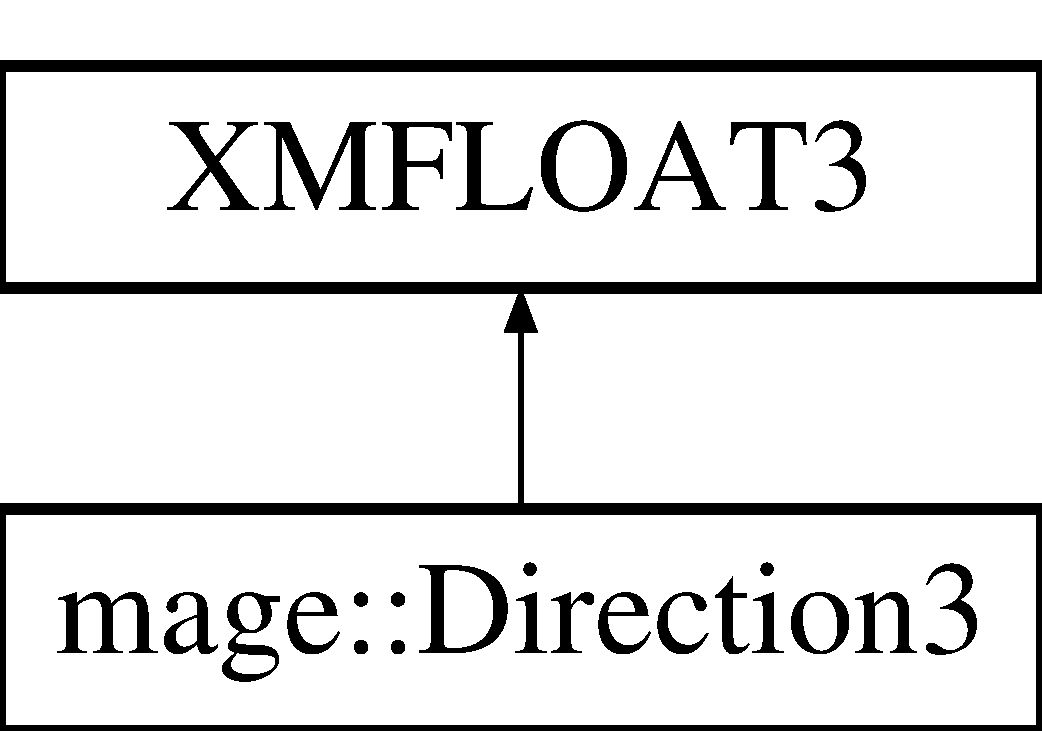
\includegraphics[height=4.000000cm]{structmage_1_1_direction3}
\end{center}
\end{figure}
\subsection*{Public Member Functions}
\begin{DoxyCompactItemize}
\item 
constexpr \mbox{\hyperlink{structmage_1_1_direction3_a64dd4745147f5fd39f710e8b9591074a}{Direction3}} () noexcept=default
\item 
constexpr \mbox{\hyperlink{structmage_1_1_direction3_a880d7413dc6f3742b53a089b870018c7}{Direction3}} (\mbox{\hyperlink{namespacemage_aa97e833b45f06d60a0a9c4fc22ae02c0}{F32}} x, \mbox{\hyperlink{namespacemage_aa97e833b45f06d60a0a9c4fc22ae02c0}{F32}} y, \mbox{\hyperlink{namespacemage_aa97e833b45f06d60a0a9c4fc22ae02c0}{F32}} z) noexcept
\item 
constexpr \mbox{\hyperlink{structmage_1_1_direction3_ad4d5801c6ad4949e0c7b0f4e2fec0ed9}{Direction3}} (const \mbox{\hyperlink{structmage_1_1_direction3}{Direction3}} \&direction) noexcept=default
\item 
constexpr \mbox{\hyperlink{structmage_1_1_direction3_aff1506b32f2b6dd49c2747eca90c76ce}{Direction3}} (\mbox{\hyperlink{structmage_1_1_direction3}{Direction3}} \&\&direction) noexcept=default
\item 
constexpr \mbox{\hyperlink{structmage_1_1_direction3_a9ef3fe2fd9fd55fade378d42eda597c3}{Direction3}} (\mbox{\hyperlink{namespacemage_a0fef5ab4e073c2d9ea876fefa3da4233}{F32x3}} v) noexcept
\item 
\mbox{\hyperlink{structmage_1_1_direction3_a583c087dc366d206aaf54a33bc90c50b}{$\sim$\+Direction3}} ()=default
\item 
constexpr \mbox{\hyperlink{structmage_1_1_direction3}{Direction3}} \& \mbox{\hyperlink{structmage_1_1_direction3_a500a363a93cded3e36a0704d288d34f3}{operator=}} (const \mbox{\hyperlink{structmage_1_1_direction3}{Direction3}} \&direction) noexcept=default
\item 
constexpr \mbox{\hyperlink{structmage_1_1_direction3}{Direction3}} \& \mbox{\hyperlink{structmage_1_1_direction3_a111a8f8d7286bfba0d7586925666315b}{operator=}} (\mbox{\hyperlink{structmage_1_1_direction3}{Direction3}} \&\&direction) noexcept=default
\item 
constexpr \mbox{\hyperlink{namespacemage_aa97e833b45f06d60a0a9c4fc22ae02c0}{F32}} \mbox{\hyperlink{structmage_1_1_direction3_a8d3ec6086f1b47844331950df3a47207}{GetX}} () const noexcept
\item 
constexpr void \mbox{\hyperlink{structmage_1_1_direction3_a0c2b501a6e30261d872227bb73be8914}{SetX}} (\mbox{\hyperlink{namespacemage_aa97e833b45f06d60a0a9c4fc22ae02c0}{F32}} x) noexcept
\item 
constexpr \mbox{\hyperlink{namespacemage_aa97e833b45f06d60a0a9c4fc22ae02c0}{F32}} \mbox{\hyperlink{structmage_1_1_direction3_a995bc58846a268b63f6e7fdd678420cd}{GetY}} () const noexcept
\item 
constexpr void \mbox{\hyperlink{structmage_1_1_direction3_a4ac25624a33e1eee6724f0b411737d2c}{SetY}} (\mbox{\hyperlink{namespacemage_aa97e833b45f06d60a0a9c4fc22ae02c0}{F32}} y) noexcept
\item 
constexpr \mbox{\hyperlink{namespacemage_aa97e833b45f06d60a0a9c4fc22ae02c0}{F32}} \mbox{\hyperlink{structmage_1_1_direction3_a6ee9bc60c92c37c6ff7e1b432bf191c7}{GetZ}} () const noexcept
\item 
constexpr void \mbox{\hyperlink{structmage_1_1_direction3_a26d3ef84f5c7429f325871c5d59e39e7}{SetZ}} (\mbox{\hyperlink{namespacemage_aa97e833b45f06d60a0a9c4fc22ae02c0}{F32}} z) noexcept
\end{DoxyCompactItemize}
\subsection*{Additional Inherited Members}


\subsection{Detailed Description}
A struct of directions in 3D space. 

\subsection{Constructor \& Destructor Documentation}
\mbox{\Hypertarget{structmage_1_1_direction3_a64dd4745147f5fd39f710e8b9591074a}\label{structmage_1_1_direction3_a64dd4745147f5fd39f710e8b9591074a}} 
\index{mage\+::\+Direction3@{mage\+::\+Direction3}!Direction3@{Direction3}}
\index{Direction3@{Direction3}!mage\+::\+Direction3@{mage\+::\+Direction3}}
\subsubsection{\texorpdfstring{Direction3()}{Direction3()}\hspace{0.1cm}{\footnotesize\ttfamily [1/5]}}
{\footnotesize\ttfamily constexpr mage\+::\+Direction3\+::\+Direction3 (\begin{DoxyParamCaption}{ }\end{DoxyParamCaption})\hspace{0.3cm}{\ttfamily [default]}, {\ttfamily [noexcept]}}

Constructs a direction. \mbox{\Hypertarget{structmage_1_1_direction3_a880d7413dc6f3742b53a089b870018c7}\label{structmage_1_1_direction3_a880d7413dc6f3742b53a089b870018c7}} 
\index{mage\+::\+Direction3@{mage\+::\+Direction3}!Direction3@{Direction3}}
\index{Direction3@{Direction3}!mage\+::\+Direction3@{mage\+::\+Direction3}}
\subsubsection{\texorpdfstring{Direction3()}{Direction3()}\hspace{0.1cm}{\footnotesize\ttfamily [2/5]}}
{\footnotesize\ttfamily constexpr mage\+::\+Direction3\+::\+Direction3 (\begin{DoxyParamCaption}\item[{\mbox{\hyperlink{namespacemage_aa97e833b45f06d60a0a9c4fc22ae02c0}{F32}}}]{x,  }\item[{\mbox{\hyperlink{namespacemage_aa97e833b45f06d60a0a9c4fc22ae02c0}{F32}}}]{y,  }\item[{\mbox{\hyperlink{namespacemage_aa97e833b45f06d60a0a9c4fc22ae02c0}{F32}}}]{z }\end{DoxyParamCaption})\hspace{0.3cm}{\ttfamily [noexcept]}}

Constructs a direction from the given coordinates.


\begin{DoxyParams}[1]{Parameters}
\mbox{\tt in}  & {\em x} & The x-\/coordinate. \\
\hline
\mbox{\tt in}  & {\em y} & The y-\/coordinate. \\
\hline
\mbox{\tt in}  & {\em z} & The z-\/coordinate. \\
\hline
\end{DoxyParams}
\mbox{\Hypertarget{structmage_1_1_direction3_ad4d5801c6ad4949e0c7b0f4e2fec0ed9}\label{structmage_1_1_direction3_ad4d5801c6ad4949e0c7b0f4e2fec0ed9}} 
\index{mage\+::\+Direction3@{mage\+::\+Direction3}!Direction3@{Direction3}}
\index{Direction3@{Direction3}!mage\+::\+Direction3@{mage\+::\+Direction3}}
\subsubsection{\texorpdfstring{Direction3()}{Direction3()}\hspace{0.1cm}{\footnotesize\ttfamily [3/5]}}
{\footnotesize\ttfamily constexpr mage\+::\+Direction3\+::\+Direction3 (\begin{DoxyParamCaption}\item[{const \mbox{\hyperlink{structmage_1_1_direction3}{Direction3}} \&}]{direction }\end{DoxyParamCaption})\hspace{0.3cm}{\ttfamily [default]}, {\ttfamily [noexcept]}}

Constructs a direction from the given direction.


\begin{DoxyParams}[1]{Parameters}
\mbox{\tt in}  & {\em direction} & A reference to the direction to copy. \\
\hline
\end{DoxyParams}
\mbox{\Hypertarget{structmage_1_1_direction3_aff1506b32f2b6dd49c2747eca90c76ce}\label{structmage_1_1_direction3_aff1506b32f2b6dd49c2747eca90c76ce}} 
\index{mage\+::\+Direction3@{mage\+::\+Direction3}!Direction3@{Direction3}}
\index{Direction3@{Direction3}!mage\+::\+Direction3@{mage\+::\+Direction3}}
\subsubsection{\texorpdfstring{Direction3()}{Direction3()}\hspace{0.1cm}{\footnotesize\ttfamily [4/5]}}
{\footnotesize\ttfamily constexpr mage\+::\+Direction3\+::\+Direction3 (\begin{DoxyParamCaption}\item[{\mbox{\hyperlink{structmage_1_1_direction3}{Direction3}} \&\&}]{direction }\end{DoxyParamCaption})\hspace{0.3cm}{\ttfamily [default]}, {\ttfamily [noexcept]}}

Constructs a direction by moving the given direction.


\begin{DoxyParams}[1]{Parameters}
\mbox{\tt in}  & {\em direction} & A reference to the direction to move. \\
\hline
\end{DoxyParams}
\mbox{\Hypertarget{structmage_1_1_direction3_a9ef3fe2fd9fd55fade378d42eda597c3}\label{structmage_1_1_direction3_a9ef3fe2fd9fd55fade378d42eda597c3}} 
\index{mage\+::\+Direction3@{mage\+::\+Direction3}!Direction3@{Direction3}}
\index{Direction3@{Direction3}!mage\+::\+Direction3@{mage\+::\+Direction3}}
\subsubsection{\texorpdfstring{Direction3()}{Direction3()}\hspace{0.1cm}{\footnotesize\ttfamily [5/5]}}
{\footnotesize\ttfamily constexpr mage\+::\+Direction3\+::\+Direction3 (\begin{DoxyParamCaption}\item[{\mbox{\hyperlink{namespacemage_a0fef5ab4e073c2d9ea876fefa3da4233}{F32x3}}}]{v }\end{DoxyParamCaption})\hspace{0.3cm}{\ttfamily [explicit]}, {\ttfamily [noexcept]}}

Constructs a direction from the given vector.


\begin{DoxyParams}[1]{Parameters}
\mbox{\tt in}  & {\em v} & The vector. \\
\hline
\end{DoxyParams}
\mbox{\Hypertarget{structmage_1_1_direction3_a583c087dc366d206aaf54a33bc90c50b}\label{structmage_1_1_direction3_a583c087dc366d206aaf54a33bc90c50b}} 
\index{mage\+::\+Direction3@{mage\+::\+Direction3}!````~Direction3@{$\sim$\+Direction3}}
\index{````~Direction3@{$\sim$\+Direction3}!mage\+::\+Direction3@{mage\+::\+Direction3}}
\subsubsection{\texorpdfstring{$\sim$\+Direction3()}{~Direction3()}}
{\footnotesize\ttfamily mage\+::\+Direction3\+::$\sim$\+Direction3 (\begin{DoxyParamCaption}{ }\end{DoxyParamCaption})\hspace{0.3cm}{\ttfamily [default]}}

Constructs a direction. 

\subsection{Member Function Documentation}
\mbox{\Hypertarget{structmage_1_1_direction3_a8d3ec6086f1b47844331950df3a47207}\label{structmage_1_1_direction3_a8d3ec6086f1b47844331950df3a47207}} 
\index{mage\+::\+Direction3@{mage\+::\+Direction3}!GetX@{GetX}}
\index{GetX@{GetX}!mage\+::\+Direction3@{mage\+::\+Direction3}}
\subsubsection{\texorpdfstring{Get\+X()}{GetX()}}
{\footnotesize\ttfamily constexpr \mbox{\hyperlink{namespacemage_aa97e833b45f06d60a0a9c4fc22ae02c0}{F32}} mage\+::\+Direction3\+::\+GetX (\begin{DoxyParamCaption}{ }\end{DoxyParamCaption}) const\hspace{0.3cm}{\ttfamily [noexcept]}}

Returns the X component of this direction.

\begin{DoxyReturn}{Returns}
The X component of this direction. 
\end{DoxyReturn}
\mbox{\Hypertarget{structmage_1_1_direction3_a995bc58846a268b63f6e7fdd678420cd}\label{structmage_1_1_direction3_a995bc58846a268b63f6e7fdd678420cd}} 
\index{mage\+::\+Direction3@{mage\+::\+Direction3}!GetY@{GetY}}
\index{GetY@{GetY}!mage\+::\+Direction3@{mage\+::\+Direction3}}
\subsubsection{\texorpdfstring{Get\+Y()}{GetY()}}
{\footnotesize\ttfamily constexpr \mbox{\hyperlink{namespacemage_aa97e833b45f06d60a0a9c4fc22ae02c0}{F32}} mage\+::\+Direction3\+::\+GetY (\begin{DoxyParamCaption}{ }\end{DoxyParamCaption}) const\hspace{0.3cm}{\ttfamily [noexcept]}}

Returns the Y component of this direction.

\begin{DoxyReturn}{Returns}
The Y component of this direction. 
\end{DoxyReturn}
\mbox{\Hypertarget{structmage_1_1_direction3_a6ee9bc60c92c37c6ff7e1b432bf191c7}\label{structmage_1_1_direction3_a6ee9bc60c92c37c6ff7e1b432bf191c7}} 
\index{mage\+::\+Direction3@{mage\+::\+Direction3}!GetZ@{GetZ}}
\index{GetZ@{GetZ}!mage\+::\+Direction3@{mage\+::\+Direction3}}
\subsubsection{\texorpdfstring{Get\+Z()}{GetZ()}}
{\footnotesize\ttfamily constexpr \mbox{\hyperlink{namespacemage_aa97e833b45f06d60a0a9c4fc22ae02c0}{F32}} mage\+::\+Direction3\+::\+GetZ (\begin{DoxyParamCaption}{ }\end{DoxyParamCaption}) const\hspace{0.3cm}{\ttfamily [noexcept]}}

Returns the Z component of this direction.

\begin{DoxyReturn}{Returns}
The Z component of this direction. 
\end{DoxyReturn}
\mbox{\Hypertarget{structmage_1_1_direction3_a500a363a93cded3e36a0704d288d34f3}\label{structmage_1_1_direction3_a500a363a93cded3e36a0704d288d34f3}} 
\index{mage\+::\+Direction3@{mage\+::\+Direction3}!operator=@{operator=}}
\index{operator=@{operator=}!mage\+::\+Direction3@{mage\+::\+Direction3}}
\subsubsection{\texorpdfstring{operator=()}{operator=()}\hspace{0.1cm}{\footnotesize\ttfamily [1/2]}}
{\footnotesize\ttfamily constexpr \mbox{\hyperlink{structmage_1_1_direction3}{Direction3}}\& mage\+::\+Direction3\+::operator= (\begin{DoxyParamCaption}\item[{const \mbox{\hyperlink{structmage_1_1_direction3}{Direction3}} \&}]{direction }\end{DoxyParamCaption})\hspace{0.3cm}{\ttfamily [default]}, {\ttfamily [noexcept]}}

Copies the given direction to this direction.


\begin{DoxyParams}[1]{Parameters}
\mbox{\tt in}  & {\em direction} & A reference to the direction to copy. \\
\hline
\end{DoxyParams}
\begin{DoxyReturn}{Returns}
A reference to the copy of the given direction (i.\+e. this direction). 
\end{DoxyReturn}
\mbox{\Hypertarget{structmage_1_1_direction3_a111a8f8d7286bfba0d7586925666315b}\label{structmage_1_1_direction3_a111a8f8d7286bfba0d7586925666315b}} 
\index{mage\+::\+Direction3@{mage\+::\+Direction3}!operator=@{operator=}}
\index{operator=@{operator=}!mage\+::\+Direction3@{mage\+::\+Direction3}}
\subsubsection{\texorpdfstring{operator=()}{operator=()}\hspace{0.1cm}{\footnotesize\ttfamily [2/2]}}
{\footnotesize\ttfamily constexpr \mbox{\hyperlink{structmage_1_1_direction3}{Direction3}}\& mage\+::\+Direction3\+::operator= (\begin{DoxyParamCaption}\item[{\mbox{\hyperlink{structmage_1_1_direction3}{Direction3}} \&\&}]{direction }\end{DoxyParamCaption})\hspace{0.3cm}{\ttfamily [default]}, {\ttfamily [noexcept]}}

Moves the given direction to this direction.


\begin{DoxyParams}[1]{Parameters}
\mbox{\tt in}  & {\em direction} & A reference to the direction to move. \\
\hline
\end{DoxyParams}
\begin{DoxyReturn}{Returns}
A reference to the moved direction (i.\+e. this direction). 
\end{DoxyReturn}
\mbox{\Hypertarget{structmage_1_1_direction3_a0c2b501a6e30261d872227bb73be8914}\label{structmage_1_1_direction3_a0c2b501a6e30261d872227bb73be8914}} 
\index{mage\+::\+Direction3@{mage\+::\+Direction3}!SetX@{SetX}}
\index{SetX@{SetX}!mage\+::\+Direction3@{mage\+::\+Direction3}}
\subsubsection{\texorpdfstring{Set\+X()}{SetX()}}
{\footnotesize\ttfamily constexpr void mage\+::\+Direction3\+::\+SetX (\begin{DoxyParamCaption}\item[{\mbox{\hyperlink{namespacemage_aa97e833b45f06d60a0a9c4fc22ae02c0}{F32}}}]{x }\end{DoxyParamCaption})\hspace{0.3cm}{\ttfamily [noexcept]}}

Sets the X component of this direction to the given value.


\begin{DoxyParams}[1]{Parameters}
\mbox{\tt in}  & {\em x} & The X component. \\
\hline
\end{DoxyParams}
\mbox{\Hypertarget{structmage_1_1_direction3_a4ac25624a33e1eee6724f0b411737d2c}\label{structmage_1_1_direction3_a4ac25624a33e1eee6724f0b411737d2c}} 
\index{mage\+::\+Direction3@{mage\+::\+Direction3}!SetY@{SetY}}
\index{SetY@{SetY}!mage\+::\+Direction3@{mage\+::\+Direction3}}
\subsubsection{\texorpdfstring{Set\+Y()}{SetY()}}
{\footnotesize\ttfamily constexpr void mage\+::\+Direction3\+::\+SetY (\begin{DoxyParamCaption}\item[{\mbox{\hyperlink{namespacemage_aa97e833b45f06d60a0a9c4fc22ae02c0}{F32}}}]{y }\end{DoxyParamCaption})\hspace{0.3cm}{\ttfamily [noexcept]}}

Sets the Y component of this direction to the given value.


\begin{DoxyParams}[1]{Parameters}
\mbox{\tt in}  & {\em y} & The Y component. \\
\hline
\end{DoxyParams}
\mbox{\Hypertarget{structmage_1_1_direction3_a26d3ef84f5c7429f325871c5d59e39e7}\label{structmage_1_1_direction3_a26d3ef84f5c7429f325871c5d59e39e7}} 
\index{mage\+::\+Direction3@{mage\+::\+Direction3}!SetZ@{SetZ}}
\index{SetZ@{SetZ}!mage\+::\+Direction3@{mage\+::\+Direction3}}
\subsubsection{\texorpdfstring{Set\+Z()}{SetZ()}}
{\footnotesize\ttfamily constexpr void mage\+::\+Direction3\+::\+SetZ (\begin{DoxyParamCaption}\item[{\mbox{\hyperlink{namespacemage_aa97e833b45f06d60a0a9c4fc22ae02c0}{F32}}}]{z }\end{DoxyParamCaption})\hspace{0.3cm}{\ttfamily [noexcept]}}

Sets the Z component of this direction to the given value.


\begin{DoxyParams}[1]{Parameters}
\mbox{\tt in}  & {\em z} & The Z component. \\
\hline
\end{DoxyParams}

\hypertarget{classmage_1_1rendering_1_1_directional_light}{}\section{mage\+:\+:rendering\+:\+:Directional\+Light Class Reference}
\label{classmage_1_1rendering_1_1_directional_light}\index{mage\+::rendering\+::\+Directional\+Light@{mage\+::rendering\+::\+Directional\+Light}}


{\ttfamily \#include $<$directional\+\_\+light.\+hpp$>$}

Inheritance diagram for mage\+:\+:rendering\+:\+:Directional\+Light\+:\begin{figure}[H]
\begin{center}
\leavevmode
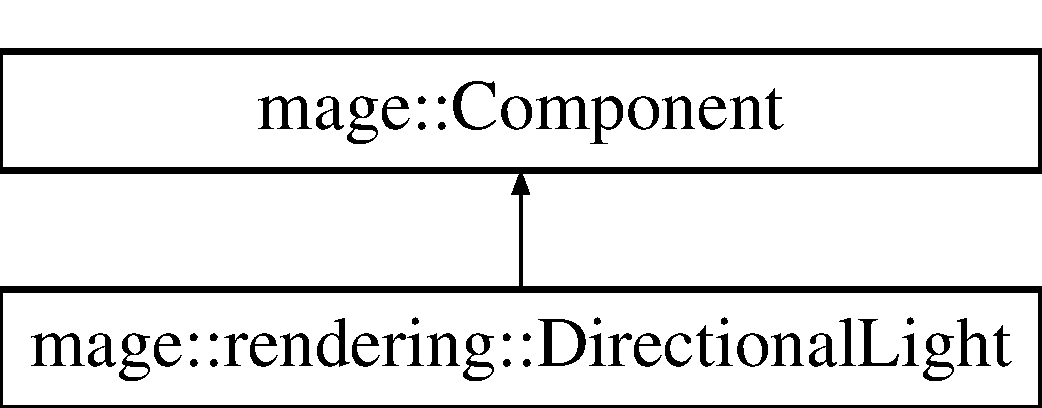
\includegraphics[height=2.000000cm]{classmage_1_1rendering_1_1_directional_light}
\end{center}
\end{figure}
\subsection*{Public Member Functions}
\begin{DoxyCompactItemize}
\item 
\mbox{\hyperlink{classmage_1_1rendering_1_1_directional_light_a5a8c05a640ec86f4d1994d687de6415f}{Directional\+Light}} () noexcept
\item 
\mbox{\hyperlink{classmage_1_1rendering_1_1_directional_light_a95bac0f10225523a7aaf7d17503f6a5f}{Directional\+Light}} (const \mbox{\hyperlink{classmage_1_1rendering_1_1_directional_light}{Directional\+Light}} \&light) noexcept
\item 
\mbox{\hyperlink{classmage_1_1rendering_1_1_directional_light_aa8ff1e6487160eb851cc2c393be9ab6a}{Directional\+Light}} (\mbox{\hyperlink{classmage_1_1rendering_1_1_directional_light}{Directional\+Light}} \&\&light) noexcept
\item 
virtual \mbox{\hyperlink{classmage_1_1rendering_1_1_directional_light_a0f35f25f86aeb2ae688a8918fa3d8b76}{$\sim$\+Directional\+Light}} ()
\item 
\mbox{\hyperlink{classmage_1_1rendering_1_1_directional_light}{Directional\+Light}} \& \mbox{\hyperlink{classmage_1_1rendering_1_1_directional_light_aa81fa39a4d068d879a6d90587ee324d8}{operator=}} (const \mbox{\hyperlink{classmage_1_1rendering_1_1_directional_light}{Directional\+Light}} \&light) noexcept
\item 
\mbox{\hyperlink{classmage_1_1rendering_1_1_directional_light}{Directional\+Light}} \& \mbox{\hyperlink{classmage_1_1rendering_1_1_directional_light_abcb7fb355a9d3004fd2f9b597b6166d2}{operator=}} (\mbox{\hyperlink{classmage_1_1rendering_1_1_directional_light}{Directional\+Light}} \&\&light) noexcept
\item 
\mbox{\hyperlink{structmage_1_1_r_g_b}{R\+GB}} \& \mbox{\hyperlink{classmage_1_1rendering_1_1_directional_light_a492e5d6a02efa369437b606be8401985}{Get\+Base\+Color}} () noexcept
\item 
const \mbox{\hyperlink{structmage_1_1_r_g_b}{R\+GB}} \& \mbox{\hyperlink{classmage_1_1rendering_1_1_directional_light_aca3e27ba1d32b1146d3250827c1efb5f}{Get\+Base\+Color}} () const noexcept
\item 
\mbox{\hyperlink{namespacemage_aa97e833b45f06d60a0a9c4fc22ae02c0}{F32}} \mbox{\hyperlink{classmage_1_1rendering_1_1_directional_light_a1cba2b0099366af146c3ccf364946bf8}{Get\+Irradiance}} () const noexcept
\item 
void \mbox{\hyperlink{classmage_1_1rendering_1_1_directional_light_af8570b18bfb807492317e4a98f5c7ba6}{Set\+Irradiance}} (\mbox{\hyperlink{namespacemage_aa97e833b45f06d60a0a9c4fc22ae02c0}{F32}} irradiance) noexcept
\item 
const \mbox{\hyperlink{structmage_1_1_r_g_b}{R\+GB}} \mbox{\hyperlink{classmage_1_1rendering_1_1_directional_light_a3a99d3d63a686f8bc587015115a85a81}{Get\+Irradiance\+Spectrum}} () const noexcept
\item 
bool \mbox{\hyperlink{classmage_1_1rendering_1_1_directional_light_a129904147256d111ec56cc3ddc502157}{Use\+Shadows}} () const noexcept
\item 
void \mbox{\hyperlink{classmage_1_1rendering_1_1_directional_light_abafdec9ce9ca0263724ce8ddba430b1b}{Enable\+Shadows}} () noexcept
\item 
void \mbox{\hyperlink{classmage_1_1rendering_1_1_directional_light_a7b0b25df35d2c1121bf08cb0a733b858}{Dissable\+Shadows}} () noexcept
\item 
void \mbox{\hyperlink{classmage_1_1rendering_1_1_directional_light_a34a939e192e857ac25f6d91dd773ec9b}{Toggle\+Shadows}} () noexcept
\item 
void \mbox{\hyperlink{classmage_1_1rendering_1_1_directional_light_a4a8aa135c9366993f6343b33cd4ed9e0}{Set\+Shadows}} (bool shadows) noexcept
\end{DoxyCompactItemize}
\subsection*{Private Attributes}
\begin{DoxyCompactItemize}
\item 
bool \mbox{\hyperlink{classmage_1_1rendering_1_1_directional_light_a64fa40ef9f9d0ae8a0856aabd44f0cae}{m\+\_\+shadows}}
\item 
\mbox{\hyperlink{structmage_1_1_r_g_b}{R\+GB}} \mbox{\hyperlink{classmage_1_1rendering_1_1_directional_light_a55d415fffd8f59f296e4d380639d3af1}{m\+\_\+base\+\_\+color}}
\item 
\mbox{\hyperlink{namespacemage_aa97e833b45f06d60a0a9c4fc22ae02c0}{F32}} \mbox{\hyperlink{classmage_1_1rendering_1_1_directional_light_a72b58bf80a9f40934622aee9f68aa545}{m\+\_\+irradiance}}
\end{DoxyCompactItemize}
\subsection*{Additional Inherited Members}


\subsection{Detailed Description}
A class of directional lights. 

\subsection{Constructor \& Destructor Documentation}
\mbox{\Hypertarget{classmage_1_1rendering_1_1_directional_light_a5a8c05a640ec86f4d1994d687de6415f}\label{classmage_1_1rendering_1_1_directional_light_a5a8c05a640ec86f4d1994d687de6415f}} 
\index{mage\+::rendering\+::\+Directional\+Light@{mage\+::rendering\+::\+Directional\+Light}!Directional\+Light@{Directional\+Light}}
\index{Directional\+Light@{Directional\+Light}!mage\+::rendering\+::\+Directional\+Light@{mage\+::rendering\+::\+Directional\+Light}}
\subsubsection{\texorpdfstring{Directional\+Light()}{DirectionalLight()}\hspace{0.1cm}{\footnotesize\ttfamily [1/3]}}
{\footnotesize\ttfamily mage\+::rendering\+::\+Directional\+Light\+::\+Directional\+Light (\begin{DoxyParamCaption}{ }\end{DoxyParamCaption})\hspace{0.3cm}{\ttfamily [noexcept]}}

Constructs a directional light. \mbox{\Hypertarget{classmage_1_1rendering_1_1_directional_light_a95bac0f10225523a7aaf7d17503f6a5f}\label{classmage_1_1rendering_1_1_directional_light_a95bac0f10225523a7aaf7d17503f6a5f}} 
\index{mage\+::rendering\+::\+Directional\+Light@{mage\+::rendering\+::\+Directional\+Light}!Directional\+Light@{Directional\+Light}}
\index{Directional\+Light@{Directional\+Light}!mage\+::rendering\+::\+Directional\+Light@{mage\+::rendering\+::\+Directional\+Light}}
\subsubsection{\texorpdfstring{Directional\+Light()}{DirectionalLight()}\hspace{0.1cm}{\footnotesize\ttfamily [2/3]}}
{\footnotesize\ttfamily mage\+::rendering\+::\+Directional\+Light\+::\+Directional\+Light (\begin{DoxyParamCaption}\item[{const \mbox{\hyperlink{classmage_1_1rendering_1_1_directional_light}{Directional\+Light}} \&}]{light }\end{DoxyParamCaption})\hspace{0.3cm}{\ttfamily [default]}, {\ttfamily [noexcept]}}

Constructs a directional light from the given directional light.


\begin{DoxyParams}[1]{Parameters}
\mbox{\tt in}  & {\em light} & A reference to the directional light to copy. \\
\hline
\end{DoxyParams}
\mbox{\Hypertarget{classmage_1_1rendering_1_1_directional_light_aa8ff1e6487160eb851cc2c393be9ab6a}\label{classmage_1_1rendering_1_1_directional_light_aa8ff1e6487160eb851cc2c393be9ab6a}} 
\index{mage\+::rendering\+::\+Directional\+Light@{mage\+::rendering\+::\+Directional\+Light}!Directional\+Light@{Directional\+Light}}
\index{Directional\+Light@{Directional\+Light}!mage\+::rendering\+::\+Directional\+Light@{mage\+::rendering\+::\+Directional\+Light}}
\subsubsection{\texorpdfstring{Directional\+Light()}{DirectionalLight()}\hspace{0.1cm}{\footnotesize\ttfamily [3/3]}}
{\footnotesize\ttfamily mage\+::rendering\+::\+Directional\+Light\+::\+Directional\+Light (\begin{DoxyParamCaption}\item[{\mbox{\hyperlink{classmage_1_1rendering_1_1_directional_light}{Directional\+Light}} \&\&}]{light }\end{DoxyParamCaption})\hspace{0.3cm}{\ttfamily [default]}, {\ttfamily [noexcept]}}

Constructs a directional light by moving the given directional light.


\begin{DoxyParams}[1]{Parameters}
\mbox{\tt in}  & {\em light} & A reference to the directional light to move. \\
\hline
\end{DoxyParams}
\mbox{\Hypertarget{classmage_1_1rendering_1_1_directional_light_a0f35f25f86aeb2ae688a8918fa3d8b76}\label{classmage_1_1rendering_1_1_directional_light_a0f35f25f86aeb2ae688a8918fa3d8b76}} 
\index{mage\+::rendering\+::\+Directional\+Light@{mage\+::rendering\+::\+Directional\+Light}!````~Directional\+Light@{$\sim$\+Directional\+Light}}
\index{````~Directional\+Light@{$\sim$\+Directional\+Light}!mage\+::rendering\+::\+Directional\+Light@{mage\+::rendering\+::\+Directional\+Light}}
\subsubsection{\texorpdfstring{$\sim$\+Directional\+Light()}{~DirectionalLight()}}
{\footnotesize\ttfamily mage\+::rendering\+::\+Directional\+Light\+::$\sim$\+Directional\+Light (\begin{DoxyParamCaption}{ }\end{DoxyParamCaption})\hspace{0.3cm}{\ttfamily [virtual]}, {\ttfamily [default]}}

Destructs this directional light. 

\subsection{Member Function Documentation}
\mbox{\Hypertarget{classmage_1_1rendering_1_1_directional_light_a7b0b25df35d2c1121bf08cb0a733b858}\label{classmage_1_1rendering_1_1_directional_light_a7b0b25df35d2c1121bf08cb0a733b858}} 
\index{mage\+::rendering\+::\+Directional\+Light@{mage\+::rendering\+::\+Directional\+Light}!Dissable\+Shadows@{Dissable\+Shadows}}
\index{Dissable\+Shadows@{Dissable\+Shadows}!mage\+::rendering\+::\+Directional\+Light@{mage\+::rendering\+::\+Directional\+Light}}
\subsubsection{\texorpdfstring{Dissable\+Shadows()}{DissableShadows()}}
{\footnotesize\ttfamily void mage\+::rendering\+::\+Directional\+Light\+::\+Dissable\+Shadows (\begin{DoxyParamCaption}{ }\end{DoxyParamCaption})\hspace{0.3cm}{\ttfamily [noexcept]}}

Dissables shadows for this directional light. \mbox{\Hypertarget{classmage_1_1rendering_1_1_directional_light_abafdec9ce9ca0263724ce8ddba430b1b}\label{classmage_1_1rendering_1_1_directional_light_abafdec9ce9ca0263724ce8ddba430b1b}} 
\index{mage\+::rendering\+::\+Directional\+Light@{mage\+::rendering\+::\+Directional\+Light}!Enable\+Shadows@{Enable\+Shadows}}
\index{Enable\+Shadows@{Enable\+Shadows}!mage\+::rendering\+::\+Directional\+Light@{mage\+::rendering\+::\+Directional\+Light}}
\subsubsection{\texorpdfstring{Enable\+Shadows()}{EnableShadows()}}
{\footnotesize\ttfamily void mage\+::rendering\+::\+Directional\+Light\+::\+Enable\+Shadows (\begin{DoxyParamCaption}{ }\end{DoxyParamCaption})\hspace{0.3cm}{\ttfamily [noexcept]}}

Enables shadows for this directional light. \mbox{\Hypertarget{classmage_1_1rendering_1_1_directional_light_a492e5d6a02efa369437b606be8401985}\label{classmage_1_1rendering_1_1_directional_light_a492e5d6a02efa369437b606be8401985}} 
\index{mage\+::rendering\+::\+Directional\+Light@{mage\+::rendering\+::\+Directional\+Light}!Get\+Base\+Color@{Get\+Base\+Color}}
\index{Get\+Base\+Color@{Get\+Base\+Color}!mage\+::rendering\+::\+Directional\+Light@{mage\+::rendering\+::\+Directional\+Light}}
\subsubsection{\texorpdfstring{Get\+Base\+Color()}{GetBaseColor()}\hspace{0.1cm}{\footnotesize\ttfamily [1/2]}}
{\footnotesize\ttfamily \mbox{\hyperlink{structmage_1_1_r_g_b}{R\+GB}}\& mage\+::rendering\+::\+Directional\+Light\+::\+Get\+Base\+Color (\begin{DoxyParamCaption}{ }\end{DoxyParamCaption})\hspace{0.3cm}{\ttfamily [noexcept]}}

Returns the (linear) base color of this directional light.

\begin{DoxyReturn}{Returns}
A reference to the s\+R\+GB base color of this directional light. 
\end{DoxyReturn}
\mbox{\Hypertarget{classmage_1_1rendering_1_1_directional_light_aca3e27ba1d32b1146d3250827c1efb5f}\label{classmage_1_1rendering_1_1_directional_light_aca3e27ba1d32b1146d3250827c1efb5f}} 
\index{mage\+::rendering\+::\+Directional\+Light@{mage\+::rendering\+::\+Directional\+Light}!Get\+Base\+Color@{Get\+Base\+Color}}
\index{Get\+Base\+Color@{Get\+Base\+Color}!mage\+::rendering\+::\+Directional\+Light@{mage\+::rendering\+::\+Directional\+Light}}
\subsubsection{\texorpdfstring{Get\+Base\+Color()}{GetBaseColor()}\hspace{0.1cm}{\footnotesize\ttfamily [2/2]}}
{\footnotesize\ttfamily const \mbox{\hyperlink{structmage_1_1_r_g_b}{R\+GB}}\& mage\+::rendering\+::\+Directional\+Light\+::\+Get\+Base\+Color (\begin{DoxyParamCaption}{ }\end{DoxyParamCaption}) const\hspace{0.3cm}{\ttfamily [noexcept]}}

Returns the (linear) base color of this directional light.

\begin{DoxyReturn}{Returns}
A reference to the s\+R\+GB base color of this directional light. 
\end{DoxyReturn}
\mbox{\Hypertarget{classmage_1_1rendering_1_1_directional_light_a1cba2b0099366af146c3ccf364946bf8}\label{classmage_1_1rendering_1_1_directional_light_a1cba2b0099366af146c3ccf364946bf8}} 
\index{mage\+::rendering\+::\+Directional\+Light@{mage\+::rendering\+::\+Directional\+Light}!Get\+Irradiance@{Get\+Irradiance}}
\index{Get\+Irradiance@{Get\+Irradiance}!mage\+::rendering\+::\+Directional\+Light@{mage\+::rendering\+::\+Directional\+Light}}
\subsubsection{\texorpdfstring{Get\+Irradiance()}{GetIrradiance()}}
{\footnotesize\ttfamily \mbox{\hyperlink{namespacemage_aa97e833b45f06d60a0a9c4fc22ae02c0}{F32}} mage\+::rendering\+::\+Directional\+Light\+::\+Get\+Irradiance (\begin{DoxyParamCaption}{ }\end{DoxyParamCaption}) const\hspace{0.3cm}{\ttfamily [noexcept]}}

Returns the irradiance of this directional light.

\begin{DoxyReturn}{Returns}
The irradiance in watts per square meter of this directional light. 
\end{DoxyReturn}
\mbox{\Hypertarget{classmage_1_1rendering_1_1_directional_light_a3a99d3d63a686f8bc587015115a85a81}\label{classmage_1_1rendering_1_1_directional_light_a3a99d3d63a686f8bc587015115a85a81}} 
\index{mage\+::rendering\+::\+Directional\+Light@{mage\+::rendering\+::\+Directional\+Light}!Get\+Irradiance\+Spectrum@{Get\+Irradiance\+Spectrum}}
\index{Get\+Irradiance\+Spectrum@{Get\+Irradiance\+Spectrum}!mage\+::rendering\+::\+Directional\+Light@{mage\+::rendering\+::\+Directional\+Light}}
\subsubsection{\texorpdfstring{Get\+Irradiance\+Spectrum()}{GetIrradianceSpectrum()}}
{\footnotesize\ttfamily const \mbox{\hyperlink{structmage_1_1_r_g_b}{R\+GB}} mage\+::rendering\+::\+Directional\+Light\+::\+Get\+Irradiance\+Spectrum (\begin{DoxyParamCaption}{ }\end{DoxyParamCaption}) const\hspace{0.3cm}{\ttfamily [noexcept]}}

Returns the irradiance spectrum of this directional light.

\begin{DoxyReturn}{Returns}
The irradiance spectrum of this directional light. 
\end{DoxyReturn}
\mbox{\Hypertarget{classmage_1_1rendering_1_1_directional_light_aa81fa39a4d068d879a6d90587ee324d8}\label{classmage_1_1rendering_1_1_directional_light_aa81fa39a4d068d879a6d90587ee324d8}} 
\index{mage\+::rendering\+::\+Directional\+Light@{mage\+::rendering\+::\+Directional\+Light}!operator=@{operator=}}
\index{operator=@{operator=}!mage\+::rendering\+::\+Directional\+Light@{mage\+::rendering\+::\+Directional\+Light}}
\subsubsection{\texorpdfstring{operator=()}{operator=()}\hspace{0.1cm}{\footnotesize\ttfamily [1/2]}}
{\footnotesize\ttfamily \mbox{\hyperlink{classmage_1_1rendering_1_1_directional_light}{Directional\+Light}} \& mage\+::rendering\+::\+Directional\+Light\+::operator= (\begin{DoxyParamCaption}\item[{const \mbox{\hyperlink{classmage_1_1rendering_1_1_directional_light}{Directional\+Light}} \&}]{light }\end{DoxyParamCaption})\hspace{0.3cm}{\ttfamily [default]}, {\ttfamily [noexcept]}}

Copies the given directional light to this directional light.


\begin{DoxyParams}[1]{Parameters}
\mbox{\tt in}  & {\em light} & A reference to the directional light to copy. \\
\hline
\end{DoxyParams}
\begin{DoxyReturn}{Returns}
A reference to the copy of the given directional light (i.\+e. this directional light). 
\end{DoxyReturn}
\mbox{\Hypertarget{classmage_1_1rendering_1_1_directional_light_abcb7fb355a9d3004fd2f9b597b6166d2}\label{classmage_1_1rendering_1_1_directional_light_abcb7fb355a9d3004fd2f9b597b6166d2}} 
\index{mage\+::rendering\+::\+Directional\+Light@{mage\+::rendering\+::\+Directional\+Light}!operator=@{operator=}}
\index{operator=@{operator=}!mage\+::rendering\+::\+Directional\+Light@{mage\+::rendering\+::\+Directional\+Light}}
\subsubsection{\texorpdfstring{operator=()}{operator=()}\hspace{0.1cm}{\footnotesize\ttfamily [2/2]}}
{\footnotesize\ttfamily \mbox{\hyperlink{classmage_1_1rendering_1_1_directional_light}{Directional\+Light}} \& mage\+::rendering\+::\+Directional\+Light\+::operator= (\begin{DoxyParamCaption}\item[{\mbox{\hyperlink{classmage_1_1rendering_1_1_directional_light}{Directional\+Light}} \&\&}]{light }\end{DoxyParamCaption})\hspace{0.3cm}{\ttfamily [default]}, {\ttfamily [noexcept]}}

Moves the given directional light to this directional light.


\begin{DoxyParams}[1]{Parameters}
\mbox{\tt in}  & {\em light} & A reference to the directional light to move. \\
\hline
\end{DoxyParams}
\begin{DoxyReturn}{Returns}
A reference to the moved directional light (i.\+e. this directional light). 
\end{DoxyReturn}
\mbox{\Hypertarget{classmage_1_1rendering_1_1_directional_light_af8570b18bfb807492317e4a98f5c7ba6}\label{classmage_1_1rendering_1_1_directional_light_af8570b18bfb807492317e4a98f5c7ba6}} 
\index{mage\+::rendering\+::\+Directional\+Light@{mage\+::rendering\+::\+Directional\+Light}!Set\+Irradiance@{Set\+Irradiance}}
\index{Set\+Irradiance@{Set\+Irradiance}!mage\+::rendering\+::\+Directional\+Light@{mage\+::rendering\+::\+Directional\+Light}}
\subsubsection{\texorpdfstring{Set\+Irradiance()}{SetIrradiance()}}
{\footnotesize\ttfamily void mage\+::rendering\+::\+Directional\+Light\+::\+Set\+Irradiance (\begin{DoxyParamCaption}\item[{\mbox{\hyperlink{namespacemage_aa97e833b45f06d60a0a9c4fc22ae02c0}{F32}}}]{irradiance }\end{DoxyParamCaption})\hspace{0.3cm}{\ttfamily [noexcept]}}

Sets the irradiance of this directional light to the given irradiance.


\begin{DoxyParams}[1]{Parameters}
\mbox{\tt in}  & {\em irradiance} & The irradiance in watts per square meter. \\
\hline
\end{DoxyParams}
\mbox{\Hypertarget{classmage_1_1rendering_1_1_directional_light_a4a8aa135c9366993f6343b33cd4ed9e0}\label{classmage_1_1rendering_1_1_directional_light_a4a8aa135c9366993f6343b33cd4ed9e0}} 
\index{mage\+::rendering\+::\+Directional\+Light@{mage\+::rendering\+::\+Directional\+Light}!Set\+Shadows@{Set\+Shadows}}
\index{Set\+Shadows@{Set\+Shadows}!mage\+::rendering\+::\+Directional\+Light@{mage\+::rendering\+::\+Directional\+Light}}
\subsubsection{\texorpdfstring{Set\+Shadows()}{SetShadows()}}
{\footnotesize\ttfamily void mage\+::rendering\+::\+Directional\+Light\+::\+Set\+Shadows (\begin{DoxyParamCaption}\item[{bool}]{shadows }\end{DoxyParamCaption})\hspace{0.3cm}{\ttfamily [noexcept]}}

Sets shadows for this directional light to the given value.


\begin{DoxyParams}[1]{Parameters}
\mbox{\tt in}  & {\em shadows} & {\ttfamily true} if shadows should be used for this directional light. {\ttfamily false} otherwise. \\
\hline
\end{DoxyParams}
\mbox{\Hypertarget{classmage_1_1rendering_1_1_directional_light_a34a939e192e857ac25f6d91dd773ec9b}\label{classmage_1_1rendering_1_1_directional_light_a34a939e192e857ac25f6d91dd773ec9b}} 
\index{mage\+::rendering\+::\+Directional\+Light@{mage\+::rendering\+::\+Directional\+Light}!Toggle\+Shadows@{Toggle\+Shadows}}
\index{Toggle\+Shadows@{Toggle\+Shadows}!mage\+::rendering\+::\+Directional\+Light@{mage\+::rendering\+::\+Directional\+Light}}
\subsubsection{\texorpdfstring{Toggle\+Shadows()}{ToggleShadows()}}
{\footnotesize\ttfamily void mage\+::rendering\+::\+Directional\+Light\+::\+Toggle\+Shadows (\begin{DoxyParamCaption}{ }\end{DoxyParamCaption})\hspace{0.3cm}{\ttfamily [noexcept]}}

Toggles shadows for this directional light. \mbox{\Hypertarget{classmage_1_1rendering_1_1_directional_light_a129904147256d111ec56cc3ddc502157}\label{classmage_1_1rendering_1_1_directional_light_a129904147256d111ec56cc3ddc502157}} 
\index{mage\+::rendering\+::\+Directional\+Light@{mage\+::rendering\+::\+Directional\+Light}!Use\+Shadows@{Use\+Shadows}}
\index{Use\+Shadows@{Use\+Shadows}!mage\+::rendering\+::\+Directional\+Light@{mage\+::rendering\+::\+Directional\+Light}}
\subsubsection{\texorpdfstring{Use\+Shadows()}{UseShadows()}}
{\footnotesize\ttfamily bool mage\+::rendering\+::\+Directional\+Light\+::\+Use\+Shadows (\begin{DoxyParamCaption}{ }\end{DoxyParamCaption}) const\hspace{0.3cm}{\ttfamily [noexcept]}}

Checks whether shadows should be used for this directional light.

\begin{DoxyReturn}{Returns}
{\ttfamily true} if shadows should be used for this directional light. {\ttfamily false} otherwise. 
\end{DoxyReturn}


\subsection{Member Data Documentation}
\mbox{\Hypertarget{classmage_1_1rendering_1_1_directional_light_a55d415fffd8f59f296e4d380639d3af1}\label{classmage_1_1rendering_1_1_directional_light_a55d415fffd8f59f296e4d380639d3af1}} 
\index{mage\+::rendering\+::\+Directional\+Light@{mage\+::rendering\+::\+Directional\+Light}!m\+\_\+base\+\_\+color@{m\+\_\+base\+\_\+color}}
\index{m\+\_\+base\+\_\+color@{m\+\_\+base\+\_\+color}!mage\+::rendering\+::\+Directional\+Light@{mage\+::rendering\+::\+Directional\+Light}}
\subsubsection{\texorpdfstring{m\+\_\+base\+\_\+color}{m\_base\_color}}
{\footnotesize\ttfamily \mbox{\hyperlink{structmage_1_1_r_g_b}{R\+GB}} mage\+::rendering\+::\+Directional\+Light\+::m\+\_\+base\+\_\+color\hspace{0.3cm}{\ttfamily [private]}}

The (linear) base color of this directional light. \mbox{\Hypertarget{classmage_1_1rendering_1_1_directional_light_a72b58bf80a9f40934622aee9f68aa545}\label{classmage_1_1rendering_1_1_directional_light_a72b58bf80a9f40934622aee9f68aa545}} 
\index{mage\+::rendering\+::\+Directional\+Light@{mage\+::rendering\+::\+Directional\+Light}!m\+\_\+irradiance@{m\+\_\+irradiance}}
\index{m\+\_\+irradiance@{m\+\_\+irradiance}!mage\+::rendering\+::\+Directional\+Light@{mage\+::rendering\+::\+Directional\+Light}}
\subsubsection{\texorpdfstring{m\+\_\+irradiance}{m\_irradiance}}
{\footnotesize\ttfamily \mbox{\hyperlink{namespacemage_aa97e833b45f06d60a0a9c4fc22ae02c0}{F32}} mage\+::rendering\+::\+Directional\+Light\+::m\+\_\+irradiance\hspace{0.3cm}{\ttfamily [private]}}

The irradiance (which is equal to the exitant radiance/radiosity) in watts per square meter of this directional light. \mbox{\Hypertarget{classmage_1_1rendering_1_1_directional_light_a64fa40ef9f9d0ae8a0856aabd44f0cae}\label{classmage_1_1rendering_1_1_directional_light_a64fa40ef9f9d0ae8a0856aabd44f0cae}} 
\index{mage\+::rendering\+::\+Directional\+Light@{mage\+::rendering\+::\+Directional\+Light}!m\+\_\+shadows@{m\+\_\+shadows}}
\index{m\+\_\+shadows@{m\+\_\+shadows}!mage\+::rendering\+::\+Directional\+Light@{mage\+::rendering\+::\+Directional\+Light}}
\subsubsection{\texorpdfstring{m\+\_\+shadows}{m\_shadows}}
{\footnotesize\ttfamily bool mage\+::rendering\+::\+Directional\+Light\+::m\+\_\+shadows\hspace{0.3cm}{\ttfamily [private]}}

A flag indicating whether shadows should be calculated or not not for this directional light. 
\hypertarget{structmage_1_1rendering_1_1_directional_light_buffer}{}\section{mage\+:\+:rendering\+:\+:Directional\+Light\+Buffer Struct Reference}
\label{structmage_1_1rendering_1_1_directional_light_buffer}\index{mage\+::rendering\+::\+Directional\+Light\+Buffer@{mage\+::rendering\+::\+Directional\+Light\+Buffer}}


{\ttfamily \#include $<$light\+\_\+buffer.\+hpp$>$}

\subsection*{Public Member Functions}
\begin{DoxyCompactItemize}
\item 
\mbox{\hyperlink{structmage_1_1rendering_1_1_directional_light_buffer_a618dbd63423f0f008ef18c5e5a7fe560}{Directional\+Light\+Buffer}} () noexcept
\item 
\mbox{\hyperlink{structmage_1_1rendering_1_1_directional_light_buffer_a8bd677130e2bc44b721935396f3ee9ac}{Directional\+Light\+Buffer}} (const \mbox{\hyperlink{structmage_1_1rendering_1_1_directional_light_buffer}{Directional\+Light\+Buffer}} \&buffer) noexcept=default
\item 
\mbox{\hyperlink{structmage_1_1rendering_1_1_directional_light_buffer_a2db095d74145a02eb6c6c306501b04e8}{Directional\+Light\+Buffer}} (\mbox{\hyperlink{structmage_1_1rendering_1_1_directional_light_buffer}{Directional\+Light\+Buffer}} \&\&buffer) noexcept=default
\item 
\mbox{\hyperlink{structmage_1_1rendering_1_1_directional_light_buffer_ac52791a07948b17670c13b4aa0ddb104}{$\sim$\+Directional\+Light\+Buffer}} ()=default
\item 
\mbox{\hyperlink{structmage_1_1rendering_1_1_directional_light_buffer}{Directional\+Light\+Buffer}} \& \mbox{\hyperlink{structmage_1_1rendering_1_1_directional_light_buffer_a99def3f5e0829a7925a0f83ab14c2b58}{operator=}} (const \mbox{\hyperlink{structmage_1_1rendering_1_1_directional_light_buffer}{Directional\+Light\+Buffer}} \&buffer)=default
\item 
\mbox{\hyperlink{structmage_1_1rendering_1_1_directional_light_buffer}{Directional\+Light\+Buffer}} \& \mbox{\hyperlink{structmage_1_1rendering_1_1_directional_light_buffer_a65112cac58ae18d14eb9ae65f316b440}{operator=}} (\mbox{\hyperlink{structmage_1_1rendering_1_1_directional_light_buffer}{Directional\+Light\+Buffer}} \&\&buffer)=default
\end{DoxyCompactItemize}
\subsection*{Public Attributes}
\begin{DoxyCompactItemize}
\item 
\mbox{\hyperlink{structmage_1_1_r_g_b}{R\+GB}} \mbox{\hyperlink{structmage_1_1rendering_1_1_directional_light_buffer_aeaaec31da683b9ef189e775511db637a}{m\+\_\+E}}
\item 
\mbox{\hyperlink{namespacemage_a41c104c036fba3756a74e19f793eeaa1}{U32}} \mbox{\hyperlink{structmage_1_1rendering_1_1_directional_light_buffer_a82d9a78edf5562c3ce041d1a2a7b6a3e}{m\+\_\+padding0}}
\item 
\mbox{\hyperlink{structmage_1_1_direction3}{Direction3}} \mbox{\hyperlink{structmage_1_1rendering_1_1_directional_light_buffer_acbf55b6ed38011a695cb1feac90a64ed}{m\+\_\+neg\+\_\+d}}
\item 
\mbox{\hyperlink{namespacemage_a41c104c036fba3756a74e19f793eeaa1}{U32}} \mbox{\hyperlink{structmage_1_1rendering_1_1_directional_light_buffer_a9e86dcc4f68340eb64408cf638996a69}{m\+\_\+padding1}}
\item 
X\+M\+M\+A\+T\+R\+IX \mbox{\hyperlink{structmage_1_1rendering_1_1_directional_light_buffer_ae1c5a43c5dca80be889661a54fb3910b}{m\+\_\+world\+\_\+to\+\_\+projection}}
\end{DoxyCompactItemize}


\subsection{Detailed Description}
A struct of directional light buffers used by shaders. 

\subsection{Constructor \& Destructor Documentation}
\mbox{\Hypertarget{structmage_1_1rendering_1_1_directional_light_buffer_a618dbd63423f0f008ef18c5e5a7fe560}\label{structmage_1_1rendering_1_1_directional_light_buffer_a618dbd63423f0f008ef18c5e5a7fe560}} 
\index{mage\+::rendering\+::\+Directional\+Light\+Buffer@{mage\+::rendering\+::\+Directional\+Light\+Buffer}!Directional\+Light\+Buffer@{Directional\+Light\+Buffer}}
\index{Directional\+Light\+Buffer@{Directional\+Light\+Buffer}!mage\+::rendering\+::\+Directional\+Light\+Buffer@{mage\+::rendering\+::\+Directional\+Light\+Buffer}}
\subsubsection{\texorpdfstring{Directional\+Light\+Buffer()}{DirectionalLightBuffer()}\hspace{0.1cm}{\footnotesize\ttfamily [1/3]}}
{\footnotesize\ttfamily mage\+::rendering\+::\+Directional\+Light\+Buffer\+::\+Directional\+Light\+Buffer (\begin{DoxyParamCaption}{ }\end{DoxyParamCaption})\hspace{0.3cm}{\ttfamily [noexcept]}}

Constructs an directional light buffer. \mbox{\Hypertarget{structmage_1_1rendering_1_1_directional_light_buffer_a8bd677130e2bc44b721935396f3ee9ac}\label{structmage_1_1rendering_1_1_directional_light_buffer_a8bd677130e2bc44b721935396f3ee9ac}} 
\index{mage\+::rendering\+::\+Directional\+Light\+Buffer@{mage\+::rendering\+::\+Directional\+Light\+Buffer}!Directional\+Light\+Buffer@{Directional\+Light\+Buffer}}
\index{Directional\+Light\+Buffer@{Directional\+Light\+Buffer}!mage\+::rendering\+::\+Directional\+Light\+Buffer@{mage\+::rendering\+::\+Directional\+Light\+Buffer}}
\subsubsection{\texorpdfstring{Directional\+Light\+Buffer()}{DirectionalLightBuffer()}\hspace{0.1cm}{\footnotesize\ttfamily [2/3]}}
{\footnotesize\ttfamily mage\+::rendering\+::\+Directional\+Light\+Buffer\+::\+Directional\+Light\+Buffer (\begin{DoxyParamCaption}\item[{const \mbox{\hyperlink{structmage_1_1rendering_1_1_directional_light_buffer}{Directional\+Light\+Buffer}} \&}]{buffer }\end{DoxyParamCaption})\hspace{0.3cm}{\ttfamily [default]}, {\ttfamily [noexcept]}}

Constructs an directional light buffer from the given directional light buffer.


\begin{DoxyParams}[1]{Parameters}
\mbox{\tt in}  & {\em buffer} & A reference to the directional light buffer to copy. \\
\hline
\end{DoxyParams}
\mbox{\Hypertarget{structmage_1_1rendering_1_1_directional_light_buffer_a2db095d74145a02eb6c6c306501b04e8}\label{structmage_1_1rendering_1_1_directional_light_buffer_a2db095d74145a02eb6c6c306501b04e8}} 
\index{mage\+::rendering\+::\+Directional\+Light\+Buffer@{mage\+::rendering\+::\+Directional\+Light\+Buffer}!Directional\+Light\+Buffer@{Directional\+Light\+Buffer}}
\index{Directional\+Light\+Buffer@{Directional\+Light\+Buffer}!mage\+::rendering\+::\+Directional\+Light\+Buffer@{mage\+::rendering\+::\+Directional\+Light\+Buffer}}
\subsubsection{\texorpdfstring{Directional\+Light\+Buffer()}{DirectionalLightBuffer()}\hspace{0.1cm}{\footnotesize\ttfamily [3/3]}}
{\footnotesize\ttfamily mage\+::rendering\+::\+Directional\+Light\+Buffer\+::\+Directional\+Light\+Buffer (\begin{DoxyParamCaption}\item[{\mbox{\hyperlink{structmage_1_1rendering_1_1_directional_light_buffer}{Directional\+Light\+Buffer}} \&\&}]{buffer }\end{DoxyParamCaption})\hspace{0.3cm}{\ttfamily [default]}, {\ttfamily [noexcept]}}

Constructs an directional light buffer by moving the given directional light buffer.


\begin{DoxyParams}[1]{Parameters}
\mbox{\tt in}  & {\em buffer} & A reference to the directional light buffer to move. \\
\hline
\end{DoxyParams}
\mbox{\Hypertarget{structmage_1_1rendering_1_1_directional_light_buffer_ac52791a07948b17670c13b4aa0ddb104}\label{structmage_1_1rendering_1_1_directional_light_buffer_ac52791a07948b17670c13b4aa0ddb104}} 
\index{mage\+::rendering\+::\+Directional\+Light\+Buffer@{mage\+::rendering\+::\+Directional\+Light\+Buffer}!````~Directional\+Light\+Buffer@{$\sim$\+Directional\+Light\+Buffer}}
\index{````~Directional\+Light\+Buffer@{$\sim$\+Directional\+Light\+Buffer}!mage\+::rendering\+::\+Directional\+Light\+Buffer@{mage\+::rendering\+::\+Directional\+Light\+Buffer}}
\subsubsection{\texorpdfstring{$\sim$\+Directional\+Light\+Buffer()}{~DirectionalLightBuffer()}}
{\footnotesize\ttfamily mage\+::rendering\+::\+Directional\+Light\+Buffer\+::$\sim$\+Directional\+Light\+Buffer (\begin{DoxyParamCaption}{ }\end{DoxyParamCaption})\hspace{0.3cm}{\ttfamily [default]}}

Destructs this directional light buffer. 

\subsection{Member Function Documentation}
\mbox{\Hypertarget{structmage_1_1rendering_1_1_directional_light_buffer_a99def3f5e0829a7925a0f83ab14c2b58}\label{structmage_1_1rendering_1_1_directional_light_buffer_a99def3f5e0829a7925a0f83ab14c2b58}} 
\index{mage\+::rendering\+::\+Directional\+Light\+Buffer@{mage\+::rendering\+::\+Directional\+Light\+Buffer}!operator=@{operator=}}
\index{operator=@{operator=}!mage\+::rendering\+::\+Directional\+Light\+Buffer@{mage\+::rendering\+::\+Directional\+Light\+Buffer}}
\subsubsection{\texorpdfstring{operator=()}{operator=()}\hspace{0.1cm}{\footnotesize\ttfamily [1/2]}}
{\footnotesize\ttfamily \mbox{\hyperlink{structmage_1_1rendering_1_1_directional_light_buffer}{Directional\+Light\+Buffer}}\& mage\+::rendering\+::\+Directional\+Light\+Buffer\+::operator= (\begin{DoxyParamCaption}\item[{const \mbox{\hyperlink{structmage_1_1rendering_1_1_directional_light_buffer}{Directional\+Light\+Buffer}} \&}]{buffer }\end{DoxyParamCaption})\hspace{0.3cm}{\ttfamily [default]}}

Copies the given directional light buffer to this directional light buffer.


\begin{DoxyParams}[1]{Parameters}
\mbox{\tt in}  & {\em buffer} & A reference to the directional light buffer to copy. \\
\hline
\end{DoxyParams}
\begin{DoxyReturn}{Returns}
A reference to the copy of the given directional light buffer (i.\+e. this directional light buffer). 
\end{DoxyReturn}
\mbox{\Hypertarget{structmage_1_1rendering_1_1_directional_light_buffer_a65112cac58ae18d14eb9ae65f316b440}\label{structmage_1_1rendering_1_1_directional_light_buffer_a65112cac58ae18d14eb9ae65f316b440}} 
\index{mage\+::rendering\+::\+Directional\+Light\+Buffer@{mage\+::rendering\+::\+Directional\+Light\+Buffer}!operator=@{operator=}}
\index{operator=@{operator=}!mage\+::rendering\+::\+Directional\+Light\+Buffer@{mage\+::rendering\+::\+Directional\+Light\+Buffer}}
\subsubsection{\texorpdfstring{operator=()}{operator=()}\hspace{0.1cm}{\footnotesize\ttfamily [2/2]}}
{\footnotesize\ttfamily \mbox{\hyperlink{structmage_1_1rendering_1_1_directional_light_buffer}{Directional\+Light\+Buffer}}\& mage\+::rendering\+::\+Directional\+Light\+Buffer\+::operator= (\begin{DoxyParamCaption}\item[{\mbox{\hyperlink{structmage_1_1rendering_1_1_directional_light_buffer}{Directional\+Light\+Buffer}} \&\&}]{buffer }\end{DoxyParamCaption})\hspace{0.3cm}{\ttfamily [default]}}

Moves the given directional light buffer to this directional light buffer.


\begin{DoxyParams}[1]{Parameters}
\mbox{\tt in}  & {\em buffer} & A reference to the directional light buffer to move. \\
\hline
\end{DoxyParams}
\begin{DoxyReturn}{Returns}
A reference to the moved directional light buffer (i.\+e. this directional light buffer). 
\end{DoxyReturn}


\subsection{Member Data Documentation}
\mbox{\Hypertarget{structmage_1_1rendering_1_1_directional_light_buffer_aeaaec31da683b9ef189e775511db637a}\label{structmage_1_1rendering_1_1_directional_light_buffer_aeaaec31da683b9ef189e775511db637a}} 
\index{mage\+::rendering\+::\+Directional\+Light\+Buffer@{mage\+::rendering\+::\+Directional\+Light\+Buffer}!m\+\_\+E@{m\+\_\+E}}
\index{m\+\_\+E@{m\+\_\+E}!mage\+::rendering\+::\+Directional\+Light\+Buffer@{mage\+::rendering\+::\+Directional\+Light\+Buffer}}
\subsubsection{\texorpdfstring{m\+\_\+E}{m\_E}}
{\footnotesize\ttfamily \mbox{\hyperlink{structmage_1_1_r_g_b}{R\+GB}} mage\+::rendering\+::\+Directional\+Light\+Buffer\+::m\+\_\+E}

The irradiance in watts per square meter of the directional light of this directional light buffer. \mbox{\Hypertarget{structmage_1_1rendering_1_1_directional_light_buffer_acbf55b6ed38011a695cb1feac90a64ed}\label{structmage_1_1rendering_1_1_directional_light_buffer_acbf55b6ed38011a695cb1feac90a64ed}} 
\index{mage\+::rendering\+::\+Directional\+Light\+Buffer@{mage\+::rendering\+::\+Directional\+Light\+Buffer}!m\+\_\+neg\+\_\+d@{m\+\_\+neg\+\_\+d}}
\index{m\+\_\+neg\+\_\+d@{m\+\_\+neg\+\_\+d}!mage\+::rendering\+::\+Directional\+Light\+Buffer@{mage\+::rendering\+::\+Directional\+Light\+Buffer}}
\subsubsection{\texorpdfstring{m\+\_\+neg\+\_\+d}{m\_neg\_d}}
{\footnotesize\ttfamily \mbox{\hyperlink{structmage_1_1_direction3}{Direction3}} mage\+::rendering\+::\+Directional\+Light\+Buffer\+::m\+\_\+neg\+\_\+d}

The (normalized) negated direction of the directional light in world space of this directional light buffer. \mbox{\Hypertarget{structmage_1_1rendering_1_1_directional_light_buffer_a82d9a78edf5562c3ce041d1a2a7b6a3e}\label{structmage_1_1rendering_1_1_directional_light_buffer_a82d9a78edf5562c3ce041d1a2a7b6a3e}} 
\index{mage\+::rendering\+::\+Directional\+Light\+Buffer@{mage\+::rendering\+::\+Directional\+Light\+Buffer}!m\+\_\+padding0@{m\+\_\+padding0}}
\index{m\+\_\+padding0@{m\+\_\+padding0}!mage\+::rendering\+::\+Directional\+Light\+Buffer@{mage\+::rendering\+::\+Directional\+Light\+Buffer}}
\subsubsection{\texorpdfstring{m\+\_\+padding0}{m\_padding0}}
{\footnotesize\ttfamily \mbox{\hyperlink{namespacemage_a41c104c036fba3756a74e19f793eeaa1}{U32}} mage\+::rendering\+::\+Directional\+Light\+Buffer\+::m\+\_\+padding0}

The padding of this directional light buffer. \mbox{\Hypertarget{structmage_1_1rendering_1_1_directional_light_buffer_a9e86dcc4f68340eb64408cf638996a69}\label{structmage_1_1rendering_1_1_directional_light_buffer_a9e86dcc4f68340eb64408cf638996a69}} 
\index{mage\+::rendering\+::\+Directional\+Light\+Buffer@{mage\+::rendering\+::\+Directional\+Light\+Buffer}!m\+\_\+padding1@{m\+\_\+padding1}}
\index{m\+\_\+padding1@{m\+\_\+padding1}!mage\+::rendering\+::\+Directional\+Light\+Buffer@{mage\+::rendering\+::\+Directional\+Light\+Buffer}}
\subsubsection{\texorpdfstring{m\+\_\+padding1}{m\_padding1}}
{\footnotesize\ttfamily \mbox{\hyperlink{namespacemage_a41c104c036fba3756a74e19f793eeaa1}{U32}} mage\+::rendering\+::\+Directional\+Light\+Buffer\+::m\+\_\+padding1}

The padding of this directional light buffer. \mbox{\Hypertarget{structmage_1_1rendering_1_1_directional_light_buffer_ae1c5a43c5dca80be889661a54fb3910b}\label{structmage_1_1rendering_1_1_directional_light_buffer_ae1c5a43c5dca80be889661a54fb3910b}} 
\index{mage\+::rendering\+::\+Directional\+Light\+Buffer@{mage\+::rendering\+::\+Directional\+Light\+Buffer}!m\+\_\+world\+\_\+to\+\_\+projection@{m\+\_\+world\+\_\+to\+\_\+projection}}
\index{m\+\_\+world\+\_\+to\+\_\+projection@{m\+\_\+world\+\_\+to\+\_\+projection}!mage\+::rendering\+::\+Directional\+Light\+Buffer@{mage\+::rendering\+::\+Directional\+Light\+Buffer}}
\subsubsection{\texorpdfstring{m\+\_\+world\+\_\+to\+\_\+projection}{m\_world\_to\_projection}}
{\footnotesize\ttfamily X\+M\+M\+A\+T\+R\+IX mage\+::rendering\+::\+Directional\+Light\+Buffer\+::m\+\_\+world\+\_\+to\+\_\+projection}

The (column-\/major packed, row-\/major matrix) world-\/to-\/projection matrix of this directional light buffer. 
\hypertarget{classmage_1_1rendering_1_1_display_configuration}{}\section{mage\+:\+:rendering\+:\+:Display\+Configuration Class Reference}
\label{classmage_1_1rendering_1_1_display_configuration}\index{mage\+::rendering\+::\+Display\+Configuration@{mage\+::rendering\+::\+Display\+Configuration}}


{\ttfamily \#include $<$display\+\_\+configuration.\+hpp$>$}

\subsection*{Public Member Functions}
\begin{DoxyCompactItemize}
\item 
\hyperlink{classmage_1_1rendering_1_1_display_configuration_ac0ee7768a59ee6a257405faaa942580b}{Display\+Configuration} (\hyperlink{namespacemage_ae74f374780900893caa5555d1031fd79}{Com\+Ptr}$<$ \hyperlink{namespacemage_1_1rendering_ad55e028ebd705b547eeb972ad8d03b6a}{D\+X\+G\+I\+Adapter} $>$ adapter, \hyperlink{namespacemage_ae74f374780900893caa5555d1031fd79}{Com\+Ptr}$<$ \hyperlink{namespacemage_1_1rendering_aaf22d3893277a4bd8497f6ea69b01532}{D\+X\+G\+I\+Output} $>$ output, const D\+X\+G\+I\+\_\+\+M\+O\+D\+E\+\_\+\+D\+E\+SC \&display\+\_\+mode)
\item 
\hyperlink{classmage_1_1rendering_1_1_display_configuration_a96a9331786912fce65dbeca8e3516231}{Display\+Configuration} (const \hyperlink{classmage_1_1rendering_1_1_display_configuration}{Display\+Configuration} \&configuration)=default
\item 
\hyperlink{classmage_1_1rendering_1_1_display_configuration_a9c691b88024f24fa778db90c9f1b9416}{Display\+Configuration} (\hyperlink{classmage_1_1rendering_1_1_display_configuration}{Display\+Configuration} \&\&configuration) noexcept=default
\item 
\hyperlink{classmage_1_1rendering_1_1_display_configuration_a93745480bb92a1e81e4476a897eaab6b}{$\sim$\+Display\+Configuration} ()=default
\item 
\hyperlink{classmage_1_1rendering_1_1_display_configuration}{Display\+Configuration} \& \hyperlink{classmage_1_1rendering_1_1_display_configuration_a847151bc6a61f320811e915119f38f9f}{operator=} (const \hyperlink{classmage_1_1rendering_1_1_display_configuration}{Display\+Configuration} \&configuration)=default
\item 
\hyperlink{classmage_1_1rendering_1_1_display_configuration}{Display\+Configuration} \& \hyperlink{classmage_1_1rendering_1_1_display_configuration_a309591557673c77b7157012136fe2fc9}{operator=} (\hyperlink{classmage_1_1rendering_1_1_display_configuration}{Display\+Configuration} \&\&configuration) noexcept=default
\item 
\hyperlink{namespacemage_1_1rendering_ad55e028ebd705b547eeb972ad8d03b6a}{D\+X\+G\+I\+Adapter} $\ast$ \hyperlink{classmage_1_1rendering_1_1_display_configuration_a8516379377ff3f6cec7b2d705398459f}{Get\+Adapter} () const noexcept
\item 
\hyperlink{namespacemage_1_1rendering_aaf22d3893277a4bd8497f6ea69b01532}{D\+X\+G\+I\+Output} $\ast$ \hyperlink{classmage_1_1rendering_1_1_display_configuration_a727b2e5ebcc286bb2ae39fd1f1e69445}{Get\+Output} () const noexcept
\item 
\hyperlink{namespacemage_a41c104c036fba3756a74e19f793eeaa1}{U32} \hyperlink{classmage_1_1rendering_1_1_display_configuration_a4ceed88b5f46a87857cf0b2979badf46}{Get\+Display\+Width} () const noexcept
\item 
\hyperlink{namespacemage_a41c104c036fba3756a74e19f793eeaa1}{U32} \hyperlink{classmage_1_1rendering_1_1_display_configuration_aaf77044b835d6302305913cf469b7246}{Get\+Display\+Height} () const noexcept
\item 
const \hyperlink{namespacemage_a88e05bff0300120c013285d3dcad95c5}{U32x2} \hyperlink{classmage_1_1rendering_1_1_display_configuration_a1394352b2a3f80fb1cc24d96f744ae3c}{Get\+Display\+Resolution} () const noexcept
\item 
\hyperlink{namespacemage_a41c104c036fba3756a74e19f793eeaa1}{U32} \hyperlink{classmage_1_1rendering_1_1_display_configuration_aac42c90d563c8ee7a2ae795c2750dc35}{Get\+S\+S\+Display\+Width} () const noexcept
\item 
\hyperlink{namespacemage_a41c104c036fba3756a74e19f793eeaa1}{U32} \hyperlink{classmage_1_1rendering_1_1_display_configuration_a7bbb45919b9cd4ae20cc9f4cac8a7069}{Get\+S\+S\+Display\+Height} () const noexcept
\item 
const \hyperlink{namespacemage_a88e05bff0300120c013285d3dcad95c5}{U32x2} \hyperlink{classmage_1_1rendering_1_1_display_configuration_a1e55018800cb0c229571274c4f6c222c}{Get\+S\+S\+Display\+Resolution} () const noexcept
\item 
\hyperlink{namespacemage_a41c104c036fba3756a74e19f793eeaa1}{U32} \hyperlink{classmage_1_1rendering_1_1_display_configuration_a6650e981bf82c85d5339afbc37cee64a}{Get\+Display\+Rounded\+Refresh\+Rate} () const noexcept
\item 
const D\+X\+G\+I\+\_\+\+R\+A\+T\+I\+O\+N\+AL \hyperlink{classmage_1_1rendering_1_1_display_configuration_ae100fc84cd1900e302fb784f429a06b7}{Get\+Display\+Refresh\+Rate} () const noexcept
\item 
D\+X\+G\+I\+\_\+\+F\+O\+R\+M\+AT \hyperlink{classmage_1_1rendering_1_1_display_configuration_a66c6757aa4c17227ab0e7022228f982a}{Get\+Display\+Format} () const noexcept
\item 
const D\+X\+G\+I\+\_\+\+M\+O\+D\+E\+\_\+\+D\+E\+SC \& \hyperlink{classmage_1_1rendering_1_1_display_configuration_af3cd8d29b8f6d6bc0fa1579260badf99}{Get\+Display\+Mode} () const noexcept
\item 
void \hyperlink{classmage_1_1rendering_1_1_display_configuration_a7cc6b9dcf3932a62bfd1416fc7b397ea}{Set\+Display\+Mode} (const D\+X\+G\+I\+\_\+\+M\+O\+D\+E\+\_\+\+D\+E\+SC \&display\+\_\+mode) noexcept
\item 
bool \hyperlink{classmage_1_1rendering_1_1_display_configuration_abbcb68e66c4a659cb169819a4f1d0d5d}{Uses\+AA} () const noexcept
\item 
bool \hyperlink{classmage_1_1rendering_1_1_display_configuration_a1cd8c25ade06ad47945ca0046e350749}{Uses\+M\+S\+AA} () const noexcept
\item 
bool \hyperlink{classmage_1_1rendering_1_1_display_configuration_ad233d7838a302fa0ce73cf06b1660404}{Uses\+S\+S\+AA} () const noexcept
\item 
\hyperlink{namespacemage_1_1rendering_ac3f75e49e92b42f2f5fb55c450d8899c}{Anti\+Aliasing} \hyperlink{classmage_1_1rendering_1_1_display_configuration_a243b2a170b97a9583f76a8f16aee5ba6}{Get\+AA} () const noexcept
\item 
void \hyperlink{classmage_1_1rendering_1_1_display_configuration_a8cb3173220d7405353fa4d1726e7063d}{Set\+AA} (\hyperlink{namespacemage_1_1rendering_ac3f75e49e92b42f2f5fb55c450d8899c}{Anti\+Aliasing} aa) noexcept
\item 
bool \hyperlink{classmage_1_1rendering_1_1_display_configuration_acbe793e625311707e234fcd0977978d5}{Is\+Windowed} () const noexcept
\item 
void \hyperlink{classmage_1_1rendering_1_1_display_configuration_a78d0902979bd5a0eff7fef0aa7976a7f}{Set\+Windowed} (bool windowed=true) noexcept
\item 
bool \hyperlink{classmage_1_1rendering_1_1_display_configuration_a507e755923af2ba1338cc041b5df8e0a}{Is\+Full\+Screen} () const noexcept
\item 
void \hyperlink{classmage_1_1rendering_1_1_display_configuration_a5e15cc1ca56718a7892b80cd0a1d20c0}{Set\+Full\+Screen} (bool fullscreen=true) noexcept
\item 
bool \hyperlink{classmage_1_1rendering_1_1_display_configuration_a6447404f1d720b98b37f684ba0e790a0}{Is\+V\+Synced} () const noexcept
\item 
void \hyperlink{classmage_1_1rendering_1_1_display_configuration_a304a29762afd99caa1672ef6cc259fb3}{Set\+V\+Sync} (bool vsync=true) noexcept
\item 
\hyperlink{namespacemage_aa97e833b45f06d60a0a9c4fc22ae02c0}{F32} \hyperlink{classmage_1_1rendering_1_1_display_configuration_a84dec99b487839003fce7c9704dc031d}{Get\+Gamma} () const noexcept
\item 
void \hyperlink{classmage_1_1rendering_1_1_display_configuration_a1d8d4b2f3b79e53d9b36da3f6a0ddf69}{Set\+Gamma} (\hyperlink{namespacemage_aa97e833b45f06d60a0a9c4fc22ae02c0}{F32} gamma) noexcept
\end{DoxyCompactItemize}
\subsection*{Private Attributes}
\begin{DoxyCompactItemize}
\item 
\hyperlink{namespacemage_ae74f374780900893caa5555d1031fd79}{Com\+Ptr}$<$ \hyperlink{namespacemage_1_1rendering_ad55e028ebd705b547eeb972ad8d03b6a}{D\+X\+G\+I\+Adapter} $>$ \hyperlink{classmage_1_1rendering_1_1_display_configuration_a307a8e6e0b1beb93175a6db519759e86}{m\+\_\+adapter}
\item 
\hyperlink{namespacemage_ae74f374780900893caa5555d1031fd79}{Com\+Ptr}$<$ \hyperlink{namespacemage_1_1rendering_aaf22d3893277a4bd8497f6ea69b01532}{D\+X\+G\+I\+Output} $>$ \hyperlink{classmage_1_1rendering_1_1_display_configuration_a3f43cbe5bb1a1a7c1bfb9ce66052fe0a}{m\+\_\+output}
\item 
D\+X\+G\+I\+\_\+\+M\+O\+D\+E\+\_\+\+D\+E\+SC \hyperlink{classmage_1_1rendering_1_1_display_configuration_a577ada006ada1b1e65a8deb817f0dafe}{m\+\_\+display\+\_\+mode}
\item 
\hyperlink{namespacemage_1_1rendering_ac3f75e49e92b42f2f5fb55c450d8899c}{Anti\+Aliasing} \hyperlink{classmage_1_1rendering_1_1_display_configuration_a03754a6d492393f70f68c619311dfa4c}{m\+\_\+aa}
\item 
bool \hyperlink{classmage_1_1rendering_1_1_display_configuration_a9d2117628e8b8f6a9b6548a9c0b11c36}{m\+\_\+windowed}
\item 
bool \hyperlink{classmage_1_1rendering_1_1_display_configuration_a749335db324a29c8b4ac30acf1c5361d}{m\+\_\+vsync}
\item 
\hyperlink{namespacemage_aa97e833b45f06d60a0a9c4fc22ae02c0}{F32} \hyperlink{classmage_1_1rendering_1_1_display_configuration_ac01844bb757c13e438c9ef3281becd4e}{m\+\_\+gamma}
\end{DoxyCompactItemize}


\subsection{Detailed Description}
A class of display configurations. 

\subsection{Constructor \& Destructor Documentation}
\hypertarget{classmage_1_1rendering_1_1_display_configuration_ac0ee7768a59ee6a257405faaa942580b}{}\label{classmage_1_1rendering_1_1_display_configuration_ac0ee7768a59ee6a257405faaa942580b} 
\index{mage\+::rendering\+::\+Display\+Configuration@{mage\+::rendering\+::\+Display\+Configuration}!Display\+Configuration@{Display\+Configuration}}
\index{Display\+Configuration@{Display\+Configuration}!mage\+::rendering\+::\+Display\+Configuration@{mage\+::rendering\+::\+Display\+Configuration}}
\subsubsection{\texorpdfstring{Display\+Configuration()}{DisplayConfiguration()}\hspace{0.1cm}{\footnotesize\ttfamily [1/3]}}
{\footnotesize\ttfamily mage\+::rendering\+::\+Display\+Configuration\+::\+Display\+Configuration (\begin{DoxyParamCaption}\item[{\hyperlink{namespacemage_ae74f374780900893caa5555d1031fd79}{Com\+Ptr}$<$ \hyperlink{namespacemage_1_1rendering_ad55e028ebd705b547eeb972ad8d03b6a}{D\+X\+G\+I\+Adapter} $>$}]{adapter,  }\item[{\hyperlink{namespacemage_ae74f374780900893caa5555d1031fd79}{Com\+Ptr}$<$ \hyperlink{namespacemage_1_1rendering_aaf22d3893277a4bd8497f6ea69b01532}{D\+X\+G\+I\+Output} $>$}]{output,  }\item[{const D\+X\+G\+I\+\_\+\+M\+O\+D\+E\+\_\+\+D\+E\+SC \&}]{display\+\_\+mode }\end{DoxyParamCaption})\hspace{0.3cm}{\ttfamily [explicit]}}

Constructs a display configuration.

\begin{DoxyPrecond}{Precondition}
{\itshape display\+\_\+mode} must be compatible with {\itshape adapter} and {\itshape output}. 
\end{DoxyPrecond}

\begin{DoxyParams}[1]{Parameters}
\mbox{\tt in}  & {\em adapter} & A pointer to the adapter. \\
\hline
\mbox{\tt in}  & {\em output} & A pointer to the output. \\
\hline
\mbox{\tt in}  & {\em display\+\_\+mode} & A reference to the display mode. \\
\hline
\end{DoxyParams}
\hypertarget{classmage_1_1rendering_1_1_display_configuration_a96a9331786912fce65dbeca8e3516231}{}\label{classmage_1_1rendering_1_1_display_configuration_a96a9331786912fce65dbeca8e3516231} 
\index{mage\+::rendering\+::\+Display\+Configuration@{mage\+::rendering\+::\+Display\+Configuration}!Display\+Configuration@{Display\+Configuration}}
\index{Display\+Configuration@{Display\+Configuration}!mage\+::rendering\+::\+Display\+Configuration@{mage\+::rendering\+::\+Display\+Configuration}}
\subsubsection{\texorpdfstring{Display\+Configuration()}{DisplayConfiguration()}\hspace{0.1cm}{\footnotesize\ttfamily [2/3]}}
{\footnotesize\ttfamily mage\+::rendering\+::\+Display\+Configuration\+::\+Display\+Configuration (\begin{DoxyParamCaption}\item[{const \hyperlink{classmage_1_1rendering_1_1_display_configuration}{Display\+Configuration} \&}]{configuration }\end{DoxyParamCaption})\hspace{0.3cm}{\ttfamily [default]}}

Constructs a display configuration from the given display configuration.


\begin{DoxyParams}[1]{Parameters}
\mbox{\tt in}  & {\em configuration} & A reference to a display configuration to copy. \\
\hline
\end{DoxyParams}
\hypertarget{classmage_1_1rendering_1_1_display_configuration_a9c691b88024f24fa778db90c9f1b9416}{}\label{classmage_1_1rendering_1_1_display_configuration_a9c691b88024f24fa778db90c9f1b9416} 
\index{mage\+::rendering\+::\+Display\+Configuration@{mage\+::rendering\+::\+Display\+Configuration}!Display\+Configuration@{Display\+Configuration}}
\index{Display\+Configuration@{Display\+Configuration}!mage\+::rendering\+::\+Display\+Configuration@{mage\+::rendering\+::\+Display\+Configuration}}
\subsubsection{\texorpdfstring{Display\+Configuration()}{DisplayConfiguration()}\hspace{0.1cm}{\footnotesize\ttfamily [3/3]}}
{\footnotesize\ttfamily mage\+::rendering\+::\+Display\+Configuration\+::\+Display\+Configuration (\begin{DoxyParamCaption}\item[{\hyperlink{classmage_1_1rendering_1_1_display_configuration}{Display\+Configuration} \&\&}]{configuration }\end{DoxyParamCaption})\hspace{0.3cm}{\ttfamily [default]}, {\ttfamily [noexcept]}}

Constructs a display configuration by moving the given display configuration.


\begin{DoxyParams}[1]{Parameters}
\mbox{\tt in}  & {\em configuration} & A reference to a display configuration to move. \\
\hline
\end{DoxyParams}
\hypertarget{classmage_1_1rendering_1_1_display_configuration_a93745480bb92a1e81e4476a897eaab6b}{}\label{classmage_1_1rendering_1_1_display_configuration_a93745480bb92a1e81e4476a897eaab6b} 
\index{mage\+::rendering\+::\+Display\+Configuration@{mage\+::rendering\+::\+Display\+Configuration}!````~Display\+Configuration@{$\sim$\+Display\+Configuration}}
\index{````~Display\+Configuration@{$\sim$\+Display\+Configuration}!mage\+::rendering\+::\+Display\+Configuration@{mage\+::rendering\+::\+Display\+Configuration}}
\subsubsection{\texorpdfstring{$\sim$\+Display\+Configuration()}{~DisplayConfiguration()}}
{\footnotesize\ttfamily mage\+::rendering\+::\+Display\+Configuration\+::$\sim$\+Display\+Configuration (\begin{DoxyParamCaption}{ }\end{DoxyParamCaption})\hspace{0.3cm}{\ttfamily [default]}}

Destructs this display configuration. 

\subsection{Member Function Documentation}
\hypertarget{classmage_1_1rendering_1_1_display_configuration_a243b2a170b97a9583f76a8f16aee5ba6}{}\label{classmage_1_1rendering_1_1_display_configuration_a243b2a170b97a9583f76a8f16aee5ba6} 
\index{mage\+::rendering\+::\+Display\+Configuration@{mage\+::rendering\+::\+Display\+Configuration}!Get\+AA@{Get\+AA}}
\index{Get\+AA@{Get\+AA}!mage\+::rendering\+::\+Display\+Configuration@{mage\+::rendering\+::\+Display\+Configuration}}
\subsubsection{\texorpdfstring{Get\+A\+A()}{GetAA()}}
{\footnotesize\ttfamily \hyperlink{namespacemage_1_1rendering_ac3f75e49e92b42f2f5fb55c450d8899c}{Anti\+Aliasing} mage\+::rendering\+::\+Display\+Configuration\+::\+Get\+AA (\begin{DoxyParamCaption}{ }\end{DoxyParamCaption}) const\hspace{0.3cm}{\ttfamily [noexcept]}}

Returns the anti-\/aliasing mode of this display configuration.

\begin{DoxyReturn}{Returns}
The anti-\/aliasing mode of this display configuration. 
\end{DoxyReturn}
\hypertarget{classmage_1_1rendering_1_1_display_configuration_a8516379377ff3f6cec7b2d705398459f}{}\label{classmage_1_1rendering_1_1_display_configuration_a8516379377ff3f6cec7b2d705398459f} 
\index{mage\+::rendering\+::\+Display\+Configuration@{mage\+::rendering\+::\+Display\+Configuration}!Get\+Adapter@{Get\+Adapter}}
\index{Get\+Adapter@{Get\+Adapter}!mage\+::rendering\+::\+Display\+Configuration@{mage\+::rendering\+::\+Display\+Configuration}}
\subsubsection{\texorpdfstring{Get\+Adapter()}{GetAdapter()}}
{\footnotesize\ttfamily \hyperlink{namespacemage_1_1rendering_ad55e028ebd705b547eeb972ad8d03b6a}{D\+X\+G\+I\+Adapter}$\ast$ mage\+::rendering\+::\+Display\+Configuration\+::\+Get\+Adapter (\begin{DoxyParamCaption}{ }\end{DoxyParamCaption}) const\hspace{0.3cm}{\ttfamily [noexcept]}}

Returns the adapter of this display configuration.

\begin{DoxyReturn}{Returns}
A pointer to the adapter of this display configuration. 
\end{DoxyReturn}
\hypertarget{classmage_1_1rendering_1_1_display_configuration_a66c6757aa4c17227ab0e7022228f982a}{}\label{classmage_1_1rendering_1_1_display_configuration_a66c6757aa4c17227ab0e7022228f982a} 
\index{mage\+::rendering\+::\+Display\+Configuration@{mage\+::rendering\+::\+Display\+Configuration}!Get\+Display\+Format@{Get\+Display\+Format}}
\index{Get\+Display\+Format@{Get\+Display\+Format}!mage\+::rendering\+::\+Display\+Configuration@{mage\+::rendering\+::\+Display\+Configuration}}
\subsubsection{\texorpdfstring{Get\+Display\+Format()}{GetDisplayFormat()}}
{\footnotesize\ttfamily D\+X\+G\+I\+\_\+\+F\+O\+R\+M\+AT mage\+::rendering\+::\+Display\+Configuration\+::\+Get\+Display\+Format (\begin{DoxyParamCaption}{ }\end{DoxyParamCaption}) const\hspace{0.3cm}{\ttfamily [noexcept]}}

Returns the display format of this display configuration.

\begin{DoxyReturn}{Returns}
The display format of this display configuration. 
\end{DoxyReturn}
\hypertarget{classmage_1_1rendering_1_1_display_configuration_aaf77044b835d6302305913cf469b7246}{}\label{classmage_1_1rendering_1_1_display_configuration_aaf77044b835d6302305913cf469b7246} 
\index{mage\+::rendering\+::\+Display\+Configuration@{mage\+::rendering\+::\+Display\+Configuration}!Get\+Display\+Height@{Get\+Display\+Height}}
\index{Get\+Display\+Height@{Get\+Display\+Height}!mage\+::rendering\+::\+Display\+Configuration@{mage\+::rendering\+::\+Display\+Configuration}}
\subsubsection{\texorpdfstring{Get\+Display\+Height()}{GetDisplayHeight()}}
{\footnotesize\ttfamily \hyperlink{namespacemage_a41c104c036fba3756a74e19f793eeaa1}{U32} mage\+::rendering\+::\+Display\+Configuration\+::\+Get\+Display\+Height (\begin{DoxyParamCaption}{ }\end{DoxyParamCaption}) const\hspace{0.3cm}{\ttfamily [noexcept]}}

Returns the display height in pixels of this display configuration.

\begin{DoxyReturn}{Returns}
The display height in pixels of this display configuration. 
\end{DoxyReturn}
\hypertarget{classmage_1_1rendering_1_1_display_configuration_af3cd8d29b8f6d6bc0fa1579260badf99}{}\label{classmage_1_1rendering_1_1_display_configuration_af3cd8d29b8f6d6bc0fa1579260badf99} 
\index{mage\+::rendering\+::\+Display\+Configuration@{mage\+::rendering\+::\+Display\+Configuration}!Get\+Display\+Mode@{Get\+Display\+Mode}}
\index{Get\+Display\+Mode@{Get\+Display\+Mode}!mage\+::rendering\+::\+Display\+Configuration@{mage\+::rendering\+::\+Display\+Configuration}}
\subsubsection{\texorpdfstring{Get\+Display\+Mode()}{GetDisplayMode()}}
{\footnotesize\ttfamily const D\+X\+G\+I\+\_\+\+M\+O\+D\+E\+\_\+\+D\+E\+SC\& mage\+::rendering\+::\+Display\+Configuration\+::\+Get\+Display\+Mode (\begin{DoxyParamCaption}{ }\end{DoxyParamCaption}) const\hspace{0.3cm}{\ttfamily [noexcept]}}

Returns the display mode of this display configuration.

\begin{DoxyReturn}{Returns}
The display mode of this display configuration. 
\end{DoxyReturn}
\hypertarget{classmage_1_1rendering_1_1_display_configuration_ae100fc84cd1900e302fb784f429a06b7}{}\label{classmage_1_1rendering_1_1_display_configuration_ae100fc84cd1900e302fb784f429a06b7} 
\index{mage\+::rendering\+::\+Display\+Configuration@{mage\+::rendering\+::\+Display\+Configuration}!Get\+Display\+Refresh\+Rate@{Get\+Display\+Refresh\+Rate}}
\index{Get\+Display\+Refresh\+Rate@{Get\+Display\+Refresh\+Rate}!mage\+::rendering\+::\+Display\+Configuration@{mage\+::rendering\+::\+Display\+Configuration}}
\subsubsection{\texorpdfstring{Get\+Display\+Refresh\+Rate()}{GetDisplayRefreshRate()}}
{\footnotesize\ttfamily const D\+X\+G\+I\+\_\+\+R\+A\+T\+I\+O\+N\+AL mage\+::rendering\+::\+Display\+Configuration\+::\+Get\+Display\+Refresh\+Rate (\begin{DoxyParamCaption}{ }\end{DoxyParamCaption}) const\hspace{0.3cm}{\ttfamily [noexcept]}}

Returns the display refresh rate of this display configuration.

\begin{DoxyReturn}{Returns}
The display refresh rate of this display configuration. 
\end{DoxyReturn}
\hypertarget{classmage_1_1rendering_1_1_display_configuration_a1394352b2a3f80fb1cc24d96f744ae3c}{}\label{classmage_1_1rendering_1_1_display_configuration_a1394352b2a3f80fb1cc24d96f744ae3c} 
\index{mage\+::rendering\+::\+Display\+Configuration@{mage\+::rendering\+::\+Display\+Configuration}!Get\+Display\+Resolution@{Get\+Display\+Resolution}}
\index{Get\+Display\+Resolution@{Get\+Display\+Resolution}!mage\+::rendering\+::\+Display\+Configuration@{mage\+::rendering\+::\+Display\+Configuration}}
\subsubsection{\texorpdfstring{Get\+Display\+Resolution()}{GetDisplayResolution()}}
{\footnotesize\ttfamily const \hyperlink{namespacemage_a88e05bff0300120c013285d3dcad95c5}{U32x2} mage\+::rendering\+::\+Display\+Configuration\+::\+Get\+Display\+Resolution (\begin{DoxyParamCaption}{ }\end{DoxyParamCaption}) const\hspace{0.3cm}{\ttfamily [noexcept]}}

Returns the display resolution in pixels of this display configuration.

\begin{DoxyReturn}{Returns}
The display resolution in pixels of this display configuration. 
\end{DoxyReturn}
\hypertarget{classmage_1_1rendering_1_1_display_configuration_a6650e981bf82c85d5339afbc37cee64a}{}\label{classmage_1_1rendering_1_1_display_configuration_a6650e981bf82c85d5339afbc37cee64a} 
\index{mage\+::rendering\+::\+Display\+Configuration@{mage\+::rendering\+::\+Display\+Configuration}!Get\+Display\+Rounded\+Refresh\+Rate@{Get\+Display\+Rounded\+Refresh\+Rate}}
\index{Get\+Display\+Rounded\+Refresh\+Rate@{Get\+Display\+Rounded\+Refresh\+Rate}!mage\+::rendering\+::\+Display\+Configuration@{mage\+::rendering\+::\+Display\+Configuration}}
\subsubsection{\texorpdfstring{Get\+Display\+Rounded\+Refresh\+Rate()}{GetDisplayRoundedRefreshRate()}}
{\footnotesize\ttfamily \hyperlink{namespacemage_a41c104c036fba3756a74e19f793eeaa1}{U32} mage\+::rendering\+::\+Display\+Configuration\+::\+Get\+Display\+Rounded\+Refresh\+Rate (\begin{DoxyParamCaption}{ }\end{DoxyParamCaption}) const\hspace{0.3cm}{\ttfamily [noexcept]}}

Returns the rounded display refresh rate of this display configuration.

\begin{DoxyReturn}{Returns}
The rounded display refresh rate of this display configuration. 
\end{DoxyReturn}
\hypertarget{classmage_1_1rendering_1_1_display_configuration_a4ceed88b5f46a87857cf0b2979badf46}{}\label{classmage_1_1rendering_1_1_display_configuration_a4ceed88b5f46a87857cf0b2979badf46} 
\index{mage\+::rendering\+::\+Display\+Configuration@{mage\+::rendering\+::\+Display\+Configuration}!Get\+Display\+Width@{Get\+Display\+Width}}
\index{Get\+Display\+Width@{Get\+Display\+Width}!mage\+::rendering\+::\+Display\+Configuration@{mage\+::rendering\+::\+Display\+Configuration}}
\subsubsection{\texorpdfstring{Get\+Display\+Width()}{GetDisplayWidth()}}
{\footnotesize\ttfamily \hyperlink{namespacemage_a41c104c036fba3756a74e19f793eeaa1}{U32} mage\+::rendering\+::\+Display\+Configuration\+::\+Get\+Display\+Width (\begin{DoxyParamCaption}{ }\end{DoxyParamCaption}) const\hspace{0.3cm}{\ttfamily [noexcept]}}

Returns the display width in pixels of this display configuration.

\begin{DoxyReturn}{Returns}
The display width in pixels of this display configuration. 
\end{DoxyReturn}
\hypertarget{classmage_1_1rendering_1_1_display_configuration_a84dec99b487839003fce7c9704dc031d}{}\label{classmage_1_1rendering_1_1_display_configuration_a84dec99b487839003fce7c9704dc031d} 
\index{mage\+::rendering\+::\+Display\+Configuration@{mage\+::rendering\+::\+Display\+Configuration}!Get\+Gamma@{Get\+Gamma}}
\index{Get\+Gamma@{Get\+Gamma}!mage\+::rendering\+::\+Display\+Configuration@{mage\+::rendering\+::\+Display\+Configuration}}
\subsubsection{\texorpdfstring{Get\+Gamma()}{GetGamma()}}
{\footnotesize\ttfamily \hyperlink{namespacemage_aa97e833b45f06d60a0a9c4fc22ae02c0}{F32} mage\+::rendering\+::\+Display\+Configuration\+::\+Get\+Gamma (\begin{DoxyParamCaption}{ }\end{DoxyParamCaption}) const\hspace{0.3cm}{\ttfamily [noexcept]}}

Returns the gamma value used for gamma correction of this display configuration.

\begin{DoxyReturn}{Returns}
The gamma value used for gamma correction of this display configuration. 
\end{DoxyReturn}
\hypertarget{classmage_1_1rendering_1_1_display_configuration_a727b2e5ebcc286bb2ae39fd1f1e69445}{}\label{classmage_1_1rendering_1_1_display_configuration_a727b2e5ebcc286bb2ae39fd1f1e69445} 
\index{mage\+::rendering\+::\+Display\+Configuration@{mage\+::rendering\+::\+Display\+Configuration}!Get\+Output@{Get\+Output}}
\index{Get\+Output@{Get\+Output}!mage\+::rendering\+::\+Display\+Configuration@{mage\+::rendering\+::\+Display\+Configuration}}
\subsubsection{\texorpdfstring{Get\+Output()}{GetOutput()}}
{\footnotesize\ttfamily \hyperlink{namespacemage_1_1rendering_aaf22d3893277a4bd8497f6ea69b01532}{D\+X\+G\+I\+Output}$\ast$ mage\+::rendering\+::\+Display\+Configuration\+::\+Get\+Output (\begin{DoxyParamCaption}{ }\end{DoxyParamCaption}) const\hspace{0.3cm}{\ttfamily [noexcept]}}

Returns the output of this display configuration.

\begin{DoxyReturn}{Returns}
A pointer to the output of this display configuration. 
\end{DoxyReturn}
\hypertarget{classmage_1_1rendering_1_1_display_configuration_a7bbb45919b9cd4ae20cc9f4cac8a7069}{}\label{classmage_1_1rendering_1_1_display_configuration_a7bbb45919b9cd4ae20cc9f4cac8a7069} 
\index{mage\+::rendering\+::\+Display\+Configuration@{mage\+::rendering\+::\+Display\+Configuration}!Get\+S\+S\+Display\+Height@{Get\+S\+S\+Display\+Height}}
\index{Get\+S\+S\+Display\+Height@{Get\+S\+S\+Display\+Height}!mage\+::rendering\+::\+Display\+Configuration@{mage\+::rendering\+::\+Display\+Configuration}}
\subsubsection{\texorpdfstring{Get\+S\+S\+Display\+Height()}{GetSSDisplayHeight()}}
{\footnotesize\ttfamily \hyperlink{namespacemage_a41c104c036fba3756a74e19f793eeaa1}{U32} mage\+::rendering\+::\+Display\+Configuration\+::\+Get\+S\+S\+Display\+Height (\begin{DoxyParamCaption}{ }\end{DoxyParamCaption}) const\hspace{0.3cm}{\ttfamily [noexcept]}}

Returns the super-\/sampled display height in pixels of this display configuration.

\begin{DoxyReturn}{Returns}
The super-\/sampled display height in pixels of this display configuration. 
\end{DoxyReturn}
\hypertarget{classmage_1_1rendering_1_1_display_configuration_a1e55018800cb0c229571274c4f6c222c}{}\label{classmage_1_1rendering_1_1_display_configuration_a1e55018800cb0c229571274c4f6c222c} 
\index{mage\+::rendering\+::\+Display\+Configuration@{mage\+::rendering\+::\+Display\+Configuration}!Get\+S\+S\+Display\+Resolution@{Get\+S\+S\+Display\+Resolution}}
\index{Get\+S\+S\+Display\+Resolution@{Get\+S\+S\+Display\+Resolution}!mage\+::rendering\+::\+Display\+Configuration@{mage\+::rendering\+::\+Display\+Configuration}}
\subsubsection{\texorpdfstring{Get\+S\+S\+Display\+Resolution()}{GetSSDisplayResolution()}}
{\footnotesize\ttfamily const \hyperlink{namespacemage_a88e05bff0300120c013285d3dcad95c5}{U32x2} mage\+::rendering\+::\+Display\+Configuration\+::\+Get\+S\+S\+Display\+Resolution (\begin{DoxyParamCaption}{ }\end{DoxyParamCaption}) const\hspace{0.3cm}{\ttfamily [noexcept]}}

Returns the super-\/sampled display resolution in pixels of this display configuration.

\begin{DoxyReturn}{Returns}
The super-\/sampled display resolution in pixels of this display configuration. 
\end{DoxyReturn}
\hypertarget{classmage_1_1rendering_1_1_display_configuration_aac42c90d563c8ee7a2ae795c2750dc35}{}\label{classmage_1_1rendering_1_1_display_configuration_aac42c90d563c8ee7a2ae795c2750dc35} 
\index{mage\+::rendering\+::\+Display\+Configuration@{mage\+::rendering\+::\+Display\+Configuration}!Get\+S\+S\+Display\+Width@{Get\+S\+S\+Display\+Width}}
\index{Get\+S\+S\+Display\+Width@{Get\+S\+S\+Display\+Width}!mage\+::rendering\+::\+Display\+Configuration@{mage\+::rendering\+::\+Display\+Configuration}}
\subsubsection{\texorpdfstring{Get\+S\+S\+Display\+Width()}{GetSSDisplayWidth()}}
{\footnotesize\ttfamily \hyperlink{namespacemage_a41c104c036fba3756a74e19f793eeaa1}{U32} mage\+::rendering\+::\+Display\+Configuration\+::\+Get\+S\+S\+Display\+Width (\begin{DoxyParamCaption}{ }\end{DoxyParamCaption}) const\hspace{0.3cm}{\ttfamily [noexcept]}}

Returns the super-\/sampled display width in pixels of this display configuration.

\begin{DoxyReturn}{Returns}
The super-\/sampled display width in pixels of this display configuration. 
\end{DoxyReturn}
\hypertarget{classmage_1_1rendering_1_1_display_configuration_a507e755923af2ba1338cc041b5df8e0a}{}\label{classmage_1_1rendering_1_1_display_configuration_a507e755923af2ba1338cc041b5df8e0a} 
\index{mage\+::rendering\+::\+Display\+Configuration@{mage\+::rendering\+::\+Display\+Configuration}!Is\+Full\+Screen@{Is\+Full\+Screen}}
\index{Is\+Full\+Screen@{Is\+Full\+Screen}!mage\+::rendering\+::\+Display\+Configuration@{mage\+::rendering\+::\+Display\+Configuration}}
\subsubsection{\texorpdfstring{Is\+Full\+Screen()}{IsFullScreen()}}
{\footnotesize\ttfamily bool mage\+::rendering\+::\+Display\+Configuration\+::\+Is\+Full\+Screen (\begin{DoxyParamCaption}{ }\end{DoxyParamCaption}) const\hspace{0.3cm}{\ttfamily [noexcept]}}

Checks whether the application should run in full screen mode for this display configuration.

\begin{DoxyReturn}{Returns}
{\ttfamily true} if the application should run in full screen mode for this display configuration. {\ttfamily false} otherwise. 
\end{DoxyReturn}
\hypertarget{classmage_1_1rendering_1_1_display_configuration_a6447404f1d720b98b37f684ba0e790a0}{}\label{classmage_1_1rendering_1_1_display_configuration_a6447404f1d720b98b37f684ba0e790a0} 
\index{mage\+::rendering\+::\+Display\+Configuration@{mage\+::rendering\+::\+Display\+Configuration}!Is\+V\+Synced@{Is\+V\+Synced}}
\index{Is\+V\+Synced@{Is\+V\+Synced}!mage\+::rendering\+::\+Display\+Configuration@{mage\+::rendering\+::\+Display\+Configuration}}
\subsubsection{\texorpdfstring{Is\+V\+Synced()}{IsVSynced()}}
{\footnotesize\ttfamily bool mage\+::rendering\+::\+Display\+Configuration\+::\+Is\+V\+Synced (\begin{DoxyParamCaption}{ }\end{DoxyParamCaption}) const\hspace{0.3cm}{\ttfamily [noexcept]}}

Checks whether V-\/sync should be enabled for this display configuration.

\begin{DoxyReturn}{Returns}
{\ttfamily true} if v-\/sync should be enabled for this display configuration. {\ttfamily false} otherwise. 
\end{DoxyReturn}
\hypertarget{classmage_1_1rendering_1_1_display_configuration_acbe793e625311707e234fcd0977978d5}{}\label{classmage_1_1rendering_1_1_display_configuration_acbe793e625311707e234fcd0977978d5} 
\index{mage\+::rendering\+::\+Display\+Configuration@{mage\+::rendering\+::\+Display\+Configuration}!Is\+Windowed@{Is\+Windowed}}
\index{Is\+Windowed@{Is\+Windowed}!mage\+::rendering\+::\+Display\+Configuration@{mage\+::rendering\+::\+Display\+Configuration}}
\subsubsection{\texorpdfstring{Is\+Windowed()}{IsWindowed()}}
{\footnotesize\ttfamily bool mage\+::rendering\+::\+Display\+Configuration\+::\+Is\+Windowed (\begin{DoxyParamCaption}{ }\end{DoxyParamCaption}) const\hspace{0.3cm}{\ttfamily [noexcept]}}

Checks whether the application should run in windowed mode for this display configuration.

\begin{DoxyReturn}{Returns}
{\ttfamily true} if the application should run in windowed mode for this display configuration. {\ttfamily false} otherwise. 
\end{DoxyReturn}
\hypertarget{classmage_1_1rendering_1_1_display_configuration_a847151bc6a61f320811e915119f38f9f}{}\label{classmage_1_1rendering_1_1_display_configuration_a847151bc6a61f320811e915119f38f9f} 
\index{mage\+::rendering\+::\+Display\+Configuration@{mage\+::rendering\+::\+Display\+Configuration}!operator=@{operator=}}
\index{operator=@{operator=}!mage\+::rendering\+::\+Display\+Configuration@{mage\+::rendering\+::\+Display\+Configuration}}
\subsubsection{\texorpdfstring{operator=()}{operator=()}\hspace{0.1cm}{\footnotesize\ttfamily [1/2]}}
{\footnotesize\ttfamily \hyperlink{classmage_1_1rendering_1_1_display_configuration}{Display\+Configuration}\& mage\+::rendering\+::\+Display\+Configuration\+::operator= (\begin{DoxyParamCaption}\item[{const \hyperlink{classmage_1_1rendering_1_1_display_configuration}{Display\+Configuration} \&}]{configuration }\end{DoxyParamCaption})\hspace{0.3cm}{\ttfamily [default]}}

Copies the given display configuration to this display configuration.


\begin{DoxyParams}[1]{Parameters}
\mbox{\tt in}  & {\em configuration} & A reference to a display configuration to copy. \\
\hline
\end{DoxyParams}
\begin{DoxyReturn}{Returns}
A reference to the copy of the given display configuration (i.\+e. this display configuration). 
\end{DoxyReturn}
\hypertarget{classmage_1_1rendering_1_1_display_configuration_a309591557673c77b7157012136fe2fc9}{}\label{classmage_1_1rendering_1_1_display_configuration_a309591557673c77b7157012136fe2fc9} 
\index{mage\+::rendering\+::\+Display\+Configuration@{mage\+::rendering\+::\+Display\+Configuration}!operator=@{operator=}}
\index{operator=@{operator=}!mage\+::rendering\+::\+Display\+Configuration@{mage\+::rendering\+::\+Display\+Configuration}}
\subsubsection{\texorpdfstring{operator=()}{operator=()}\hspace{0.1cm}{\footnotesize\ttfamily [2/2]}}
{\footnotesize\ttfamily \hyperlink{classmage_1_1rendering_1_1_display_configuration}{Display\+Configuration}\& mage\+::rendering\+::\+Display\+Configuration\+::operator= (\begin{DoxyParamCaption}\item[{\hyperlink{classmage_1_1rendering_1_1_display_configuration}{Display\+Configuration} \&\&}]{configuration }\end{DoxyParamCaption})\hspace{0.3cm}{\ttfamily [default]}, {\ttfamily [noexcept]}}

Moves the given display configuration to this display configuration.


\begin{DoxyParams}[1]{Parameters}
\mbox{\tt in}  & {\em configuration} & A reference to a display configuration to move. \\
\hline
\end{DoxyParams}
\begin{DoxyReturn}{Returns}
A reference to the moved display configuration (i.\+e. this display configuration). 
\end{DoxyReturn}
\hypertarget{classmage_1_1rendering_1_1_display_configuration_a8cb3173220d7405353fa4d1726e7063d}{}\label{classmage_1_1rendering_1_1_display_configuration_a8cb3173220d7405353fa4d1726e7063d} 
\index{mage\+::rendering\+::\+Display\+Configuration@{mage\+::rendering\+::\+Display\+Configuration}!Set\+AA@{Set\+AA}}
\index{Set\+AA@{Set\+AA}!mage\+::rendering\+::\+Display\+Configuration@{mage\+::rendering\+::\+Display\+Configuration}}
\subsubsection{\texorpdfstring{Set\+A\+A()}{SetAA()}}
{\footnotesize\ttfamily void mage\+::rendering\+::\+Display\+Configuration\+::\+Set\+AA (\begin{DoxyParamCaption}\item[{\hyperlink{namespacemage_1_1rendering_ac3f75e49e92b42f2f5fb55c450d8899c}{Anti\+Aliasing}}]{aa }\end{DoxyParamCaption})\hspace{0.3cm}{\ttfamily [noexcept]}}

Sets the anti-\/aliasing mode of this display configuration to the given anti-\/aliasing mode.


\begin{DoxyParams}[1]{Parameters}
\mbox{\tt in}  & {\em aa} & The anti-\/aliasing mode. \\
\hline
\end{DoxyParams}
\hypertarget{classmage_1_1rendering_1_1_display_configuration_a7cc6b9dcf3932a62bfd1416fc7b397ea}{}\label{classmage_1_1rendering_1_1_display_configuration_a7cc6b9dcf3932a62bfd1416fc7b397ea} 
\index{mage\+::rendering\+::\+Display\+Configuration@{mage\+::rendering\+::\+Display\+Configuration}!Set\+Display\+Mode@{Set\+Display\+Mode}}
\index{Set\+Display\+Mode@{Set\+Display\+Mode}!mage\+::rendering\+::\+Display\+Configuration@{mage\+::rendering\+::\+Display\+Configuration}}
\subsubsection{\texorpdfstring{Set\+Display\+Mode()}{SetDisplayMode()}}
{\footnotesize\ttfamily void mage\+::rendering\+::\+Display\+Configuration\+::\+Set\+Display\+Mode (\begin{DoxyParamCaption}\item[{const D\+X\+G\+I\+\_\+\+M\+O\+D\+E\+\_\+\+D\+E\+SC \&}]{display\+\_\+mode }\end{DoxyParamCaption})\hspace{0.3cm}{\ttfamily [noexcept]}}

Sets the display mode of this display configuration to the given display mode.

\begin{DoxyPrecond}{Precondition}
{\itshape display\+\_\+mode} must be compatible with the adapter and output of this display configuration. 
\end{DoxyPrecond}

\begin{DoxyParams}[1]{Parameters}
\mbox{\tt in}  & {\em display\+\_\+mode} & A reference to the display mode. \\
\hline
\end{DoxyParams}
\hypertarget{classmage_1_1rendering_1_1_display_configuration_a5e15cc1ca56718a7892b80cd0a1d20c0}{}\label{classmage_1_1rendering_1_1_display_configuration_a5e15cc1ca56718a7892b80cd0a1d20c0} 
\index{mage\+::rendering\+::\+Display\+Configuration@{mage\+::rendering\+::\+Display\+Configuration}!Set\+Full\+Screen@{Set\+Full\+Screen}}
\index{Set\+Full\+Screen@{Set\+Full\+Screen}!mage\+::rendering\+::\+Display\+Configuration@{mage\+::rendering\+::\+Display\+Configuration}}
\subsubsection{\texorpdfstring{Set\+Full\+Screen()}{SetFullScreen()}}
{\footnotesize\ttfamily void mage\+::rendering\+::\+Display\+Configuration\+::\+Set\+Full\+Screen (\begin{DoxyParamCaption}\item[{bool}]{fullscreen = {\ttfamily true} }\end{DoxyParamCaption})\hspace{0.3cm}{\ttfamily [noexcept]}}

Sets the windowed/fullscreen mode of this display configuration to the given windowed/fullscreen mode.


\begin{DoxyParams}[1]{Parameters}
\mbox{\tt in}  & {\em fullscreen} & {\ttfamily true} if fullscreen mode. {\ttfamily false} otherwise. \\
\hline
\end{DoxyParams}
\hypertarget{classmage_1_1rendering_1_1_display_configuration_a1d8d4b2f3b79e53d9b36da3f6a0ddf69}{}\label{classmage_1_1rendering_1_1_display_configuration_a1d8d4b2f3b79e53d9b36da3f6a0ddf69} 
\index{mage\+::rendering\+::\+Display\+Configuration@{mage\+::rendering\+::\+Display\+Configuration}!Set\+Gamma@{Set\+Gamma}}
\index{Set\+Gamma@{Set\+Gamma}!mage\+::rendering\+::\+Display\+Configuration@{mage\+::rendering\+::\+Display\+Configuration}}
\subsubsection{\texorpdfstring{Set\+Gamma()}{SetGamma()}}
{\footnotesize\ttfamily void mage\+::rendering\+::\+Display\+Configuration\+::\+Set\+Gamma (\begin{DoxyParamCaption}\item[{\hyperlink{namespacemage_aa97e833b45f06d60a0a9c4fc22ae02c0}{F32}}]{gamma }\end{DoxyParamCaption})\hspace{0.3cm}{\ttfamily [noexcept]}}

Sets the gamma value used for gamma correction of this display configuration to the given value.


\begin{DoxyParams}[1]{Parameters}
\mbox{\tt in}  & {\em gamma} & The gamma value. \\
\hline
\end{DoxyParams}
\hypertarget{classmage_1_1rendering_1_1_display_configuration_a304a29762afd99caa1672ef6cc259fb3}{}\label{classmage_1_1rendering_1_1_display_configuration_a304a29762afd99caa1672ef6cc259fb3} 
\index{mage\+::rendering\+::\+Display\+Configuration@{mage\+::rendering\+::\+Display\+Configuration}!Set\+V\+Sync@{Set\+V\+Sync}}
\index{Set\+V\+Sync@{Set\+V\+Sync}!mage\+::rendering\+::\+Display\+Configuration@{mage\+::rendering\+::\+Display\+Configuration}}
\subsubsection{\texorpdfstring{Set\+V\+Sync()}{SetVSync()}}
{\footnotesize\ttfamily void mage\+::rendering\+::\+Display\+Configuration\+::\+Set\+V\+Sync (\begin{DoxyParamCaption}\item[{bool}]{vsync = {\ttfamily true} }\end{DoxyParamCaption})\hspace{0.3cm}{\ttfamily [noexcept]}}

Sets the V-\/sync mode of this display configuration to the given V-\/sync mode.


\begin{DoxyParams}[1]{Parameters}
\mbox{\tt in}  & {\em vsync} & {\ttfamily true} if V-\/sync mode. {\ttfamily false} otherwise. \\
\hline
\end{DoxyParams}
\hypertarget{classmage_1_1rendering_1_1_display_configuration_a78d0902979bd5a0eff7fef0aa7976a7f}{}\label{classmage_1_1rendering_1_1_display_configuration_a78d0902979bd5a0eff7fef0aa7976a7f} 
\index{mage\+::rendering\+::\+Display\+Configuration@{mage\+::rendering\+::\+Display\+Configuration}!Set\+Windowed@{Set\+Windowed}}
\index{Set\+Windowed@{Set\+Windowed}!mage\+::rendering\+::\+Display\+Configuration@{mage\+::rendering\+::\+Display\+Configuration}}
\subsubsection{\texorpdfstring{Set\+Windowed()}{SetWindowed()}}
{\footnotesize\ttfamily void mage\+::rendering\+::\+Display\+Configuration\+::\+Set\+Windowed (\begin{DoxyParamCaption}\item[{bool}]{windowed = {\ttfamily true} }\end{DoxyParamCaption})\hspace{0.3cm}{\ttfamily [noexcept]}}

Sets the windowed/fullscreen mode of this display configuration to the given windowed/fullscreen mode.


\begin{DoxyParams}[1]{Parameters}
\mbox{\tt in}  & {\em windowed} & {\ttfamily true} if windowed mode. {\ttfamily false} otherwise. \\
\hline
\end{DoxyParams}
\hypertarget{classmage_1_1rendering_1_1_display_configuration_abbcb68e66c4a659cb169819a4f1d0d5d}{}\label{classmage_1_1rendering_1_1_display_configuration_abbcb68e66c4a659cb169819a4f1d0d5d} 
\index{mage\+::rendering\+::\+Display\+Configuration@{mage\+::rendering\+::\+Display\+Configuration}!Uses\+AA@{Uses\+AA}}
\index{Uses\+AA@{Uses\+AA}!mage\+::rendering\+::\+Display\+Configuration@{mage\+::rendering\+::\+Display\+Configuration}}
\subsubsection{\texorpdfstring{Uses\+A\+A()}{UsesAA()}}
{\footnotesize\ttfamily bool mage\+::rendering\+::\+Display\+Configuration\+::\+Uses\+AA (\begin{DoxyParamCaption}{ }\end{DoxyParamCaption}) const\hspace{0.3cm}{\ttfamily [noexcept]}}

Checks whether this display configuration uses AA.

\begin{DoxyReturn}{Returns}
{\ttfamily true} if this display configuration uses AA. {\ttfamily false} otherwise. 
\end{DoxyReturn}
\hypertarget{classmage_1_1rendering_1_1_display_configuration_a1cd8c25ade06ad47945ca0046e350749}{}\label{classmage_1_1rendering_1_1_display_configuration_a1cd8c25ade06ad47945ca0046e350749} 
\index{mage\+::rendering\+::\+Display\+Configuration@{mage\+::rendering\+::\+Display\+Configuration}!Uses\+M\+S\+AA@{Uses\+M\+S\+AA}}
\index{Uses\+M\+S\+AA@{Uses\+M\+S\+AA}!mage\+::rendering\+::\+Display\+Configuration@{mage\+::rendering\+::\+Display\+Configuration}}
\subsubsection{\texorpdfstring{Uses\+M\+S\+A\+A()}{UsesMSAA()}}
{\footnotesize\ttfamily bool mage\+::rendering\+::\+Display\+Configuration\+::\+Uses\+M\+S\+AA (\begin{DoxyParamCaption}{ }\end{DoxyParamCaption}) const\hspace{0.3cm}{\ttfamily [noexcept]}}

Checks whether this display configuration uses M\+S\+AA.

\begin{DoxyReturn}{Returns}
{\ttfamily true} if this display configuration uses M\+S\+AA. {\ttfamily false} otherwise. 
\end{DoxyReturn}
\hypertarget{classmage_1_1rendering_1_1_display_configuration_ad233d7838a302fa0ce73cf06b1660404}{}\label{classmage_1_1rendering_1_1_display_configuration_ad233d7838a302fa0ce73cf06b1660404} 
\index{mage\+::rendering\+::\+Display\+Configuration@{mage\+::rendering\+::\+Display\+Configuration}!Uses\+S\+S\+AA@{Uses\+S\+S\+AA}}
\index{Uses\+S\+S\+AA@{Uses\+S\+S\+AA}!mage\+::rendering\+::\+Display\+Configuration@{mage\+::rendering\+::\+Display\+Configuration}}
\subsubsection{\texorpdfstring{Uses\+S\+S\+A\+A()}{UsesSSAA()}}
{\footnotesize\ttfamily bool mage\+::rendering\+::\+Display\+Configuration\+::\+Uses\+S\+S\+AA (\begin{DoxyParamCaption}{ }\end{DoxyParamCaption}) const\hspace{0.3cm}{\ttfamily [noexcept]}}

Checks whether this display configuration uses S\+S\+AA.

\begin{DoxyReturn}{Returns}
{\ttfamily true} if this display configuration uses S\+S\+AA. {\ttfamily false} otherwise. 
\end{DoxyReturn}


\subsection{Member Data Documentation}
\hypertarget{classmage_1_1rendering_1_1_display_configuration_a03754a6d492393f70f68c619311dfa4c}{}\label{classmage_1_1rendering_1_1_display_configuration_a03754a6d492393f70f68c619311dfa4c} 
\index{mage\+::rendering\+::\+Display\+Configuration@{mage\+::rendering\+::\+Display\+Configuration}!m\+\_\+aa@{m\+\_\+aa}}
\index{m\+\_\+aa@{m\+\_\+aa}!mage\+::rendering\+::\+Display\+Configuration@{mage\+::rendering\+::\+Display\+Configuration}}
\subsubsection{\texorpdfstring{m\+\_\+aa}{m\_aa}}
{\footnotesize\ttfamily \hyperlink{namespacemage_1_1rendering_ac3f75e49e92b42f2f5fb55c450d8899c}{Anti\+Aliasing} mage\+::rendering\+::\+Display\+Configuration\+::m\+\_\+aa\hspace{0.3cm}{\ttfamily [private]}}

The Anti-\/\+Aliasing mode of this display configuration. \hypertarget{classmage_1_1rendering_1_1_display_configuration_a307a8e6e0b1beb93175a6db519759e86}{}\label{classmage_1_1rendering_1_1_display_configuration_a307a8e6e0b1beb93175a6db519759e86} 
\index{mage\+::rendering\+::\+Display\+Configuration@{mage\+::rendering\+::\+Display\+Configuration}!m\+\_\+adapter@{m\+\_\+adapter}}
\index{m\+\_\+adapter@{m\+\_\+adapter}!mage\+::rendering\+::\+Display\+Configuration@{mage\+::rendering\+::\+Display\+Configuration}}
\subsubsection{\texorpdfstring{m\+\_\+adapter}{m\_adapter}}
{\footnotesize\ttfamily \hyperlink{namespacemage_ae74f374780900893caa5555d1031fd79}{Com\+Ptr}$<$ \hyperlink{namespacemage_1_1rendering_ad55e028ebd705b547eeb972ad8d03b6a}{D\+X\+G\+I\+Adapter} $>$ mage\+::rendering\+::\+Display\+Configuration\+::m\+\_\+adapter\hspace{0.3cm}{\ttfamily [private]}}

A pointer to the adapter (e.\+g. video card) of this display configuration. \hypertarget{classmage_1_1rendering_1_1_display_configuration_a577ada006ada1b1e65a8deb817f0dafe}{}\label{classmage_1_1rendering_1_1_display_configuration_a577ada006ada1b1e65a8deb817f0dafe} 
\index{mage\+::rendering\+::\+Display\+Configuration@{mage\+::rendering\+::\+Display\+Configuration}!m\+\_\+display\+\_\+mode@{m\+\_\+display\+\_\+mode}}
\index{m\+\_\+display\+\_\+mode@{m\+\_\+display\+\_\+mode}!mage\+::rendering\+::\+Display\+Configuration@{mage\+::rendering\+::\+Display\+Configuration}}
\subsubsection{\texorpdfstring{m\+\_\+display\+\_\+mode}{m\_display\_mode}}
{\footnotesize\ttfamily D\+X\+G\+I\+\_\+\+M\+O\+D\+E\+\_\+\+D\+E\+SC mage\+::rendering\+::\+Display\+Configuration\+::m\+\_\+display\+\_\+mode\hspace{0.3cm}{\ttfamily [private]}}

The display mode of this display configuration. \hypertarget{classmage_1_1rendering_1_1_display_configuration_ac01844bb757c13e438c9ef3281becd4e}{}\label{classmage_1_1rendering_1_1_display_configuration_ac01844bb757c13e438c9ef3281becd4e} 
\index{mage\+::rendering\+::\+Display\+Configuration@{mage\+::rendering\+::\+Display\+Configuration}!m\+\_\+gamma@{m\+\_\+gamma}}
\index{m\+\_\+gamma@{m\+\_\+gamma}!mage\+::rendering\+::\+Display\+Configuration@{mage\+::rendering\+::\+Display\+Configuration}}
\subsubsection{\texorpdfstring{m\+\_\+gamma}{m\_gamma}}
{\footnotesize\ttfamily \hyperlink{namespacemage_aa97e833b45f06d60a0a9c4fc22ae02c0}{F32} mage\+::rendering\+::\+Display\+Configuration\+::m\+\_\+gamma\hspace{0.3cm}{\ttfamily [private]}}

The gamma value used for gamma correction of this display configuration. \hypertarget{classmage_1_1rendering_1_1_display_configuration_a3f43cbe5bb1a1a7c1bfb9ce66052fe0a}{}\label{classmage_1_1rendering_1_1_display_configuration_a3f43cbe5bb1a1a7c1bfb9ce66052fe0a} 
\index{mage\+::rendering\+::\+Display\+Configuration@{mage\+::rendering\+::\+Display\+Configuration}!m\+\_\+output@{m\+\_\+output}}
\index{m\+\_\+output@{m\+\_\+output}!mage\+::rendering\+::\+Display\+Configuration@{mage\+::rendering\+::\+Display\+Configuration}}
\subsubsection{\texorpdfstring{m\+\_\+output}{m\_output}}
{\footnotesize\ttfamily \hyperlink{namespacemage_ae74f374780900893caa5555d1031fd79}{Com\+Ptr}$<$ \hyperlink{namespacemage_1_1rendering_aaf22d3893277a4bd8497f6ea69b01532}{D\+X\+G\+I\+Output} $>$ mage\+::rendering\+::\+Display\+Configuration\+::m\+\_\+output\hspace{0.3cm}{\ttfamily [private]}}

A pointer to the output (e.\+g. screen monitor) of this display configuration. \hypertarget{classmage_1_1rendering_1_1_display_configuration_a749335db324a29c8b4ac30acf1c5361d}{}\label{classmage_1_1rendering_1_1_display_configuration_a749335db324a29c8b4ac30acf1c5361d} 
\index{mage\+::rendering\+::\+Display\+Configuration@{mage\+::rendering\+::\+Display\+Configuration}!m\+\_\+vsync@{m\+\_\+vsync}}
\index{m\+\_\+vsync@{m\+\_\+vsync}!mage\+::rendering\+::\+Display\+Configuration@{mage\+::rendering\+::\+Display\+Configuration}}
\subsubsection{\texorpdfstring{m\+\_\+vsync}{m\_vsync}}
{\footnotesize\ttfamily bool mage\+::rendering\+::\+Display\+Configuration\+::m\+\_\+vsync\hspace{0.3cm}{\ttfamily [private]}}

Flag indicating whether V-\/sync should be enabled for this display configuration. \hypertarget{classmage_1_1rendering_1_1_display_configuration_a9d2117628e8b8f6a9b6548a9c0b11c36}{}\label{classmage_1_1rendering_1_1_display_configuration_a9d2117628e8b8f6a9b6548a9c0b11c36} 
\index{mage\+::rendering\+::\+Display\+Configuration@{mage\+::rendering\+::\+Display\+Configuration}!m\+\_\+windowed@{m\+\_\+windowed}}
\index{m\+\_\+windowed@{m\+\_\+windowed}!mage\+::rendering\+::\+Display\+Configuration@{mage\+::rendering\+::\+Display\+Configuration}}
\subsubsection{\texorpdfstring{m\+\_\+windowed}{m\_windowed}}
{\footnotesize\ttfamily bool mage\+::rendering\+::\+Display\+Configuration\+::m\+\_\+windowed\hspace{0.3cm}{\ttfamily [private]}}

Flag indicating whether the application should run in windowed mode for this display configuration. 
\hypertarget{classmage_1_1rendering_1_1_display_configurator}{}\section{mage\+:\+:rendering\+:\+:Display\+Configurator Class Reference}
\label{classmage_1_1rendering_1_1_display_configurator}\index{mage\+::rendering\+::\+Display\+Configurator@{mage\+::rendering\+::\+Display\+Configurator}}


{\ttfamily \#include $<$display\+\_\+configurator.\+hpp$>$}

\subsection*{Classes}
\begin{DoxyCompactItemize}
\item 
class \hyperlink{classmage_1_1rendering_1_1_display_configurator_1_1_impl}{Impl}
\end{DoxyCompactItemize}
\subsection*{Public Member Functions}
\begin{DoxyCompactItemize}
\item 
\hyperlink{classmage_1_1rendering_1_1_display_configurator_aa59a82202ffcfdc458f1d7c02ccef93e}{Display\+Configurator} (D\+X\+G\+I\+\_\+\+F\+O\+R\+M\+AT pixel\+\_\+format=D\+X\+G\+I\+\_\+\+F\+O\+R\+M\+A\+T\+\_\+\+R10\+G10\+B10\+A2\+\_\+\+U\+N\+O\+RM)
\item 
\hyperlink{classmage_1_1rendering_1_1_display_configurator_a38b10a77ab471b8d9ea836a19879c173}{Display\+Configurator} (\hyperlink{namespacemage_ae74f374780900893caa5555d1031fd79}{Com\+Ptr}$<$ \hyperlink{namespacemage_1_1rendering_ad55e028ebd705b547eeb972ad8d03b6a}{D\+X\+G\+I\+Adapter} $>$ adapter, \hyperlink{namespacemage_ae74f374780900893caa5555d1031fd79}{Com\+Ptr}$<$ \hyperlink{namespacemage_1_1rendering_aaf22d3893277a4bd8497f6ea69b01532}{D\+X\+G\+I\+Output} $>$ output, D\+X\+G\+I\+\_\+\+F\+O\+R\+M\+AT pixel\+\_\+format=D\+X\+G\+I\+\_\+\+F\+O\+R\+M\+A\+T\+\_\+\+R10\+G10\+B10\+A2\+\_\+\+U\+N\+O\+RM)
\item 
\hyperlink{classmage_1_1rendering_1_1_display_configurator_aa1c3dbea2453d12d3478db4724c78728}{Display\+Configurator} (const \hyperlink{classmage_1_1rendering_1_1_display_configurator}{Display\+Configurator} \&configurator)=delete
\item 
\hyperlink{classmage_1_1rendering_1_1_display_configurator_ac75dae1c4df34dda067f1a5d99fdfefa}{Display\+Configurator} (\hyperlink{classmage_1_1rendering_1_1_display_configurator}{Display\+Configurator} \&\&configurator) noexcept
\item 
\hyperlink{classmage_1_1rendering_1_1_display_configurator_a5ccba8cd97da75a7d1c425731fb848d4}{$\sim$\+Display\+Configurator} ()
\item 
\hyperlink{classmage_1_1rendering_1_1_display_configurator}{Display\+Configurator} \& \hyperlink{classmage_1_1rendering_1_1_display_configurator_affd6a3486be8564246628a6a20518ac2}{operator=} (const \hyperlink{classmage_1_1rendering_1_1_display_configurator}{Display\+Configurator} \&configurator)=delete
\item 
\hyperlink{classmage_1_1rendering_1_1_display_configurator}{Display\+Configurator} \& \hyperlink{classmage_1_1rendering_1_1_display_configurator_afa750c6d058e2298dd6bb9cf44d54f06}{operator=} (\hyperlink{classmage_1_1rendering_1_1_display_configurator}{Display\+Configurator} \&\&configurator)=delete
\item 
H\+R\+E\+S\+U\+LT \hyperlink{classmage_1_1rendering_1_1_display_configurator_abeafddcb31aea4ee7235ca5509f1b321}{Configure} () const
\item 
const \hyperlink{classmage_1_1rendering_1_1_display_configuration}{Display\+Configuration} $\ast$ \hyperlink{classmage_1_1rendering_1_1_display_configurator_a5b0440099e3e31977ffaf8072c9fb33f}{Get\+Display\+Configuration} () const noexcept
\end{DoxyCompactItemize}
\subsection*{Private Attributes}
\begin{DoxyCompactItemize}
\item 
\hyperlink{namespacemage_a3316d7143a973e37adf1110f2e80ca31}{Unique\+Ptr}$<$ \hyperlink{classmage_1_1rendering_1_1_display_configurator_1_1_impl}{Impl} $>$ \hyperlink{classmage_1_1rendering_1_1_display_configurator_a07b64b1b3443e4350723990592de86e7}{m\+\_\+impl}
\end{DoxyCompactItemize}


\subsection{Detailed Description}
A class of display configurators. 

\subsection{Constructor \& Destructor Documentation}
\hypertarget{classmage_1_1rendering_1_1_display_configurator_aa59a82202ffcfdc458f1d7c02ccef93e}{}\label{classmage_1_1rendering_1_1_display_configurator_aa59a82202ffcfdc458f1d7c02ccef93e} 
\index{mage\+::rendering\+::\+Display\+Configurator@{mage\+::rendering\+::\+Display\+Configurator}!Display\+Configurator@{Display\+Configurator}}
\index{Display\+Configurator@{Display\+Configurator}!mage\+::rendering\+::\+Display\+Configurator@{mage\+::rendering\+::\+Display\+Configurator}}
\subsubsection{\texorpdfstring{Display\+Configurator()}{DisplayConfigurator()}\hspace{0.1cm}{\footnotesize\ttfamily [1/4]}}
{\footnotesize\ttfamily mage\+::rendering\+::\+Display\+Configurator\+::\+Display\+Configurator (\begin{DoxyParamCaption}\item[{D\+X\+G\+I\+\_\+\+F\+O\+R\+M\+AT}]{pixel\+\_\+format = {\ttfamily DXGI\+\_\+FORMAT\+\_\+R10G10B10A2\+\_\+UNORM} }\end{DoxyParamCaption})\hspace{0.3cm}{\ttfamily [explicit]}}

Constructs a display configurator.


\begin{DoxyParams}[1]{Parameters}
\mbox{\tt in}  & {\em pixel\+\_\+format} & The pixel format. \\
\hline
\end{DoxyParams}
\hypertarget{classmage_1_1rendering_1_1_display_configurator_a38b10a77ab471b8d9ea836a19879c173}{}\label{classmage_1_1rendering_1_1_display_configurator_a38b10a77ab471b8d9ea836a19879c173} 
\index{mage\+::rendering\+::\+Display\+Configurator@{mage\+::rendering\+::\+Display\+Configurator}!Display\+Configurator@{Display\+Configurator}}
\index{Display\+Configurator@{Display\+Configurator}!mage\+::rendering\+::\+Display\+Configurator@{mage\+::rendering\+::\+Display\+Configurator}}
\subsubsection{\texorpdfstring{Display\+Configurator()}{DisplayConfigurator()}\hspace{0.1cm}{\footnotesize\ttfamily [2/4]}}
{\footnotesize\ttfamily mage\+::rendering\+::\+Display\+Configurator\+::\+Display\+Configurator (\begin{DoxyParamCaption}\item[{\hyperlink{namespacemage_ae74f374780900893caa5555d1031fd79}{Com\+Ptr}$<$ \hyperlink{namespacemage_1_1rendering_ad55e028ebd705b547eeb972ad8d03b6a}{D\+X\+G\+I\+Adapter} $>$}]{adapter,  }\item[{\hyperlink{namespacemage_ae74f374780900893caa5555d1031fd79}{Com\+Ptr}$<$ \hyperlink{namespacemage_1_1rendering_aaf22d3893277a4bd8497f6ea69b01532}{D\+X\+G\+I\+Output} $>$}]{output,  }\item[{D\+X\+G\+I\+\_\+\+F\+O\+R\+M\+AT}]{pixel\+\_\+format = {\ttfamily DXGI\+\_\+FORMAT\+\_\+R10G10B10A2\+\_\+UNORM} }\end{DoxyParamCaption})\hspace{0.3cm}{\ttfamily [explicit]}}

Constructs a display configurator.


\begin{DoxyParams}[1]{Parameters}
\mbox{\tt in}  & {\em adapter} & A pointer to the adapter. \\
\hline
\mbox{\tt in}  & {\em output} & A pointer to the output. \\
\hline
\mbox{\tt in}  & {\em pixel\+\_\+format} & The pixel format. \\
\hline
\end{DoxyParams}
\hypertarget{classmage_1_1rendering_1_1_display_configurator_aa1c3dbea2453d12d3478db4724c78728}{}\label{classmage_1_1rendering_1_1_display_configurator_aa1c3dbea2453d12d3478db4724c78728} 
\index{mage\+::rendering\+::\+Display\+Configurator@{mage\+::rendering\+::\+Display\+Configurator}!Display\+Configurator@{Display\+Configurator}}
\index{Display\+Configurator@{Display\+Configurator}!mage\+::rendering\+::\+Display\+Configurator@{mage\+::rendering\+::\+Display\+Configurator}}
\subsubsection{\texorpdfstring{Display\+Configurator()}{DisplayConfigurator()}\hspace{0.1cm}{\footnotesize\ttfamily [3/4]}}
{\footnotesize\ttfamily mage\+::rendering\+::\+Display\+Configurator\+::\+Display\+Configurator (\begin{DoxyParamCaption}\item[{const \hyperlink{classmage_1_1rendering_1_1_display_configurator}{Display\+Configurator} \&}]{configurator }\end{DoxyParamCaption})\hspace{0.3cm}{\ttfamily [delete]}}

Constructs a display configurator from the given display configurator.


\begin{DoxyParams}[1]{Parameters}
\mbox{\tt in}  & {\em configurator} & A reference to a display configurator to copy. \\
\hline
\end{DoxyParams}
\hypertarget{classmage_1_1rendering_1_1_display_configurator_ac75dae1c4df34dda067f1a5d99fdfefa}{}\label{classmage_1_1rendering_1_1_display_configurator_ac75dae1c4df34dda067f1a5d99fdfefa} 
\index{mage\+::rendering\+::\+Display\+Configurator@{mage\+::rendering\+::\+Display\+Configurator}!Display\+Configurator@{Display\+Configurator}}
\index{Display\+Configurator@{Display\+Configurator}!mage\+::rendering\+::\+Display\+Configurator@{mage\+::rendering\+::\+Display\+Configurator}}
\subsubsection{\texorpdfstring{Display\+Configurator()}{DisplayConfigurator()}\hspace{0.1cm}{\footnotesize\ttfamily [4/4]}}
{\footnotesize\ttfamily mage\+::rendering\+::\+Display\+Configurator\+::\+Display\+Configurator (\begin{DoxyParamCaption}\item[{\hyperlink{classmage_1_1rendering_1_1_display_configurator}{Display\+Configurator} \&\&}]{configurator }\end{DoxyParamCaption})\hspace{0.3cm}{\ttfamily [default]}, {\ttfamily [noexcept]}}

Constructs a display configurator by moving the given display configurator.


\begin{DoxyParams}[1]{Parameters}
\mbox{\tt in}  & {\em configurator} & A reference to a display configurator to move. \\
\hline
\end{DoxyParams}
\hypertarget{classmage_1_1rendering_1_1_display_configurator_a5ccba8cd97da75a7d1c425731fb848d4}{}\label{classmage_1_1rendering_1_1_display_configurator_a5ccba8cd97da75a7d1c425731fb848d4} 
\index{mage\+::rendering\+::\+Display\+Configurator@{mage\+::rendering\+::\+Display\+Configurator}!````~Display\+Configurator@{$\sim$\+Display\+Configurator}}
\index{````~Display\+Configurator@{$\sim$\+Display\+Configurator}!mage\+::rendering\+::\+Display\+Configurator@{mage\+::rendering\+::\+Display\+Configurator}}
\subsubsection{\texorpdfstring{$\sim$\+Display\+Configurator()}{~DisplayConfigurator()}}
{\footnotesize\ttfamily mage\+::rendering\+::\+Display\+Configurator\+::$\sim$\+Display\+Configurator (\begin{DoxyParamCaption}{ }\end{DoxyParamCaption})\hspace{0.3cm}{\ttfamily [default]}}

Destructs this display configurator. 

\subsection{Member Function Documentation}
\hypertarget{classmage_1_1rendering_1_1_display_configurator_abeafddcb31aea4ee7235ca5509f1b321}{}\label{classmage_1_1rendering_1_1_display_configurator_abeafddcb31aea4ee7235ca5509f1b321} 
\index{mage\+::rendering\+::\+Display\+Configurator@{mage\+::rendering\+::\+Display\+Configurator}!Configure@{Configure}}
\index{Configure@{Configure}!mage\+::rendering\+::\+Display\+Configurator@{mage\+::rendering\+::\+Display\+Configurator}}
\subsubsection{\texorpdfstring{Configure()}{Configure()}}
{\footnotesize\ttfamily H\+R\+E\+S\+U\+LT mage\+::rendering\+::\+Display\+Configurator\+::\+Configure (\begin{DoxyParamCaption}{ }\end{DoxyParamCaption}) const}

Configurs the display by enumerating the available display modes and options associated with the adapter output of the physical adapter with the most dedicated video memory.

\begin{DoxyReturn}{Returns}
A success/error value. 
\end{DoxyReturn}
\hypertarget{classmage_1_1rendering_1_1_display_configurator_a5b0440099e3e31977ffaf8072c9fb33f}{}\label{classmage_1_1rendering_1_1_display_configurator_a5b0440099e3e31977ffaf8072c9fb33f} 
\index{mage\+::rendering\+::\+Display\+Configurator@{mage\+::rendering\+::\+Display\+Configurator}!Get\+Display\+Configuration@{Get\+Display\+Configuration}}
\index{Get\+Display\+Configuration@{Get\+Display\+Configuration}!mage\+::rendering\+::\+Display\+Configurator@{mage\+::rendering\+::\+Display\+Configurator}}
\subsubsection{\texorpdfstring{Get\+Display\+Configuration()}{GetDisplayConfiguration()}}
{\footnotesize\ttfamily const \hyperlink{classmage_1_1rendering_1_1_display_configuration}{Display\+Configuration} $\ast$ mage\+::rendering\+::\+Display\+Configurator\+::\+Get\+Display\+Configuration (\begin{DoxyParamCaption}{ }\end{DoxyParamCaption}) const\hspace{0.3cm}{\ttfamily [noexcept]}}

Returns the display configuration of this display configurator.

\begin{DoxyReturn}{Returns}
A pointer to the display configuration of this display configurator. 
\end{DoxyReturn}
\hypertarget{classmage_1_1rendering_1_1_display_configurator_affd6a3486be8564246628a6a20518ac2}{}\label{classmage_1_1rendering_1_1_display_configurator_affd6a3486be8564246628a6a20518ac2} 
\index{mage\+::rendering\+::\+Display\+Configurator@{mage\+::rendering\+::\+Display\+Configurator}!operator=@{operator=}}
\index{operator=@{operator=}!mage\+::rendering\+::\+Display\+Configurator@{mage\+::rendering\+::\+Display\+Configurator}}
\subsubsection{\texorpdfstring{operator=()}{operator=()}\hspace{0.1cm}{\footnotesize\ttfamily [1/2]}}
{\footnotesize\ttfamily \hyperlink{classmage_1_1rendering_1_1_display_configurator}{Display\+Configurator}\& mage\+::rendering\+::\+Display\+Configurator\+::operator= (\begin{DoxyParamCaption}\item[{const \hyperlink{classmage_1_1rendering_1_1_display_configurator}{Display\+Configurator} \&}]{configurator }\end{DoxyParamCaption})\hspace{0.3cm}{\ttfamily [delete]}}

Copies the given display configurator to this display configurator.


\begin{DoxyParams}[1]{Parameters}
\mbox{\tt in}  & {\em configurator} & A reference to a display configurator to copy. \\
\hline
\end{DoxyParams}
\begin{DoxyReturn}{Returns}
A reference to the copy of the given display configurator (i.\+e. this display configurator). 
\end{DoxyReturn}
\hypertarget{classmage_1_1rendering_1_1_display_configurator_afa750c6d058e2298dd6bb9cf44d54f06}{}\label{classmage_1_1rendering_1_1_display_configurator_afa750c6d058e2298dd6bb9cf44d54f06} 
\index{mage\+::rendering\+::\+Display\+Configurator@{mage\+::rendering\+::\+Display\+Configurator}!operator=@{operator=}}
\index{operator=@{operator=}!mage\+::rendering\+::\+Display\+Configurator@{mage\+::rendering\+::\+Display\+Configurator}}
\subsubsection{\texorpdfstring{operator=()}{operator=()}\hspace{0.1cm}{\footnotesize\ttfamily [2/2]}}
{\footnotesize\ttfamily \hyperlink{classmage_1_1rendering_1_1_display_configurator}{Display\+Configurator}\& mage\+::rendering\+::\+Display\+Configurator\+::operator= (\begin{DoxyParamCaption}\item[{\hyperlink{classmage_1_1rendering_1_1_display_configurator}{Display\+Configurator} \&\&}]{configurator }\end{DoxyParamCaption})\hspace{0.3cm}{\ttfamily [delete]}}

Moves the given display configurator to this display configurator.


\begin{DoxyParams}[1]{Parameters}
\mbox{\tt in}  & {\em configurator} & A reference to a display configurator to move. \\
\hline
\end{DoxyParams}
\begin{DoxyReturn}{Returns}
A reference to the moved display configurator (i.\+e. this display configurator). 
\end{DoxyReturn}


\subsection{Member Data Documentation}
\hypertarget{classmage_1_1rendering_1_1_display_configurator_a07b64b1b3443e4350723990592de86e7}{}\label{classmage_1_1rendering_1_1_display_configurator_a07b64b1b3443e4350723990592de86e7} 
\index{mage\+::rendering\+::\+Display\+Configurator@{mage\+::rendering\+::\+Display\+Configurator}!m\+\_\+impl@{m\+\_\+impl}}
\index{m\+\_\+impl@{m\+\_\+impl}!mage\+::rendering\+::\+Display\+Configurator@{mage\+::rendering\+::\+Display\+Configurator}}
\subsubsection{\texorpdfstring{m\+\_\+impl}{m\_impl}}
{\footnotesize\ttfamily \hyperlink{namespacemage_a3316d7143a973e37adf1110f2e80ca31}{Unique\+Ptr}$<$ \hyperlink{classmage_1_1rendering_1_1_display_configurator_1_1_impl}{Impl} $>$ mage\+::rendering\+::\+Display\+Configurator\+::m\+\_\+impl\hspace{0.3cm}{\ttfamily [private]}}

A pointer to the implementation of this display configurator. 
\hypertarget{classmage_1_1_double_ended_memory_stack}{}\section{mage\+:\+:Double\+Ended\+Memory\+Stack Class Reference}
\label{classmage_1_1_double_ended_memory_stack}\index{mage\+::\+Double\+Ended\+Memory\+Stack@{mage\+::\+Double\+Ended\+Memory\+Stack}}


{\ttfamily \#include $<$memory\+\_\+stack.\+hpp$>$}

\subsection*{Classes}
\begin{DoxyCompactItemize}
\item 
class \mbox{\hyperlink{classmage_1_1_double_ended_memory_stack_1_1_high_allocator}{High\+Allocator}}
\item 
class \mbox{\hyperlink{classmage_1_1_double_ended_memory_stack_1_1_low_allocator}{Low\+Allocator}}
\end{DoxyCompactItemize}
\subsection*{Public Member Functions}
\begin{DoxyCompactItemize}
\item 
\mbox{\hyperlink{classmage_1_1_double_ended_memory_stack_a6523e21851c5a87e486d342d5e3b64d8}{Double\+Ended\+Memory\+Stack}} (std\+::size\+\_\+t size, std\+::size\+\_\+t alignment)
\item 
\mbox{\hyperlink{classmage_1_1_double_ended_memory_stack_a8a903d4a209929854a6f50cf98e3e2da}{Double\+Ended\+Memory\+Stack}} (const \mbox{\hyperlink{classmage_1_1_double_ended_memory_stack}{Double\+Ended\+Memory\+Stack}} \&stack)=delete
\item 
\mbox{\hyperlink{classmage_1_1_double_ended_memory_stack_a89d83095cc04686b9775fc4a55a5ff30}{Double\+Ended\+Memory\+Stack}} (\mbox{\hyperlink{classmage_1_1_double_ended_memory_stack}{Double\+Ended\+Memory\+Stack}} \&\&stack) noexcept
\item 
\mbox{\hyperlink{classmage_1_1_double_ended_memory_stack_afaac4a28ea1e386bc83d3e07fd5531a0}{$\sim$\+Double\+Ended\+Memory\+Stack}} ()
\item 
\mbox{\hyperlink{classmage_1_1_double_ended_memory_stack}{Double\+Ended\+Memory\+Stack}} \& \mbox{\hyperlink{classmage_1_1_double_ended_memory_stack_aafcc4b3cd8d87d75cc3de53994b6ef7e}{operator=}} (const \mbox{\hyperlink{classmage_1_1_double_ended_memory_stack}{Double\+Ended\+Memory\+Stack}} \&stack)=delete
\item 
\mbox{\hyperlink{classmage_1_1_double_ended_memory_stack}{Double\+Ended\+Memory\+Stack}} \& \mbox{\hyperlink{classmage_1_1_double_ended_memory_stack_a95b220925f1ef732c104901c3f55015d}{operator=}} (\mbox{\hyperlink{classmage_1_1_double_ended_memory_stack}{Double\+Ended\+Memory\+Stack}} \&\&stack)=delete
\item 
std\+::size\+\_\+t \mbox{\hyperlink{classmage_1_1_double_ended_memory_stack_a84d8573c9f565223af48307836b91a95}{Get\+Alignment}} () const noexcept
\item 
std\+::size\+\_\+t \mbox{\hyperlink{classmage_1_1_double_ended_memory_stack_a87ca430feb41c8710855012e87a955c2}{Get\+Size}} () const noexcept
\item 
std\+::size\+\_\+t \mbox{\hyperlink{classmage_1_1_double_ended_memory_stack_afdbfe299c744ef2c363aec40929b6be2}{Get\+Used\+Size}} () const noexcept
\item 
std\+::size\+\_\+t \mbox{\hyperlink{classmage_1_1_double_ended_memory_stack_ad79a70c39eeae4060151219731fec9c9}{Get\+Used\+Low\+Size}} () const noexcept
\item 
std\+::size\+\_\+t \mbox{\hyperlink{classmage_1_1_double_ended_memory_stack_ac4eeccb7d21b8f89f3b838471c9a2416}{Get\+Used\+High\+Size}} () const noexcept
\item 
std\+::size\+\_\+t \mbox{\hyperlink{classmage_1_1_double_ended_memory_stack_a19bd2960457d557f30c99e06cdf22252}{Get\+Available\+Size}} () const noexcept
\item 
std\+::uintptr\+\_\+t \mbox{\hyperlink{classmage_1_1_double_ended_memory_stack_ac7b5f3ef39129df7461f51c306c585f2}{Get\+Current\+Low\+Ptr}} () const noexcept
\item 
std\+::uintptr\+\_\+t \mbox{\hyperlink{classmage_1_1_double_ended_memory_stack_ada139d8c39960c794502bec401182ce9}{Get\+Current\+High\+Ptr}} () const noexcept
\item 
void \mbox{\hyperlink{classmage_1_1_double_ended_memory_stack_a99272e80cde12949a31a2942f9d009d6}{Reset}} () noexcept
\item 
void \mbox{\hyperlink{classmage_1_1_double_ended_memory_stack_a6e75a8b7ca12b93e5f8bcd08444704a6}{Roll\+Back\+Low}} (std\+::uintptr\+\_\+t ptr) noexcept
\item 
void \mbox{\hyperlink{classmage_1_1_double_ended_memory_stack_a2cc8ee694270945bf598cd6bc0f603f0}{Roll\+Back\+High}} (std\+::uintptr\+\_\+t ptr) noexcept
\item 
void $\ast$ \mbox{\hyperlink{classmage_1_1_double_ended_memory_stack_a14bf2c14a15d08e1d6e25b13962811f0}{Alloc\+Low}} (std\+::size\+\_\+t size) noexcept
\item 
void $\ast$ \mbox{\hyperlink{classmage_1_1_double_ended_memory_stack_a3a4f2232ab6cc6cccc0fe78887ae1f2f}{Alloc\+High}} (std\+::size\+\_\+t size) noexcept
\item 
{\footnotesize template$<$typename T $>$ }\\T $\ast$ \mbox{\hyperlink{classmage_1_1_double_ended_memory_stack_a9cff2de6abc54353bac19efc87e64599}{Alloc\+Data\+Low}} (std\+::size\+\_\+t count=1u, bool initialization=false)
\item 
{\footnotesize template$<$typename T $>$ }\\T $\ast$ \mbox{\hyperlink{classmage_1_1_double_ended_memory_stack_a907b4e54a9c30dd8fdb580fde35cf7ee}{Alloc\+Data\+High}} (std\+::size\+\_\+t count=1u, bool initialization=false)
\item 
{\footnotesize template$<$typename T $>$ }\\\mbox{\hyperlink{classmage_1_1_double_ended_memory_stack_1_1_low_allocator}{Low\+Allocator}}$<$ T $>$ \mbox{\hyperlink{classmage_1_1_double_ended_memory_stack_aa83468994c7becc35c90081f932e37f2}{Get\+Low\+Allocator}} () noexcept
\item 
{\footnotesize template$<$typename T $>$ }\\\mbox{\hyperlink{classmage_1_1_double_ended_memory_stack_1_1_high_allocator}{High\+Allocator}}$<$ T $>$ \mbox{\hyperlink{classmage_1_1_double_ended_memory_stack_a8838d2a8eeaab044fff6bfce4bbaccdc}{Get\+High\+Allocator}} () noexcept
\end{DoxyCompactItemize}
\subsection*{Private Attributes}
\begin{DoxyCompactItemize}
\item 
const std\+::size\+\_\+t \mbox{\hyperlink{classmage_1_1_double_ended_memory_stack_a6c7017157bb4effd865b22be0630f9c2}{m\+\_\+size}}
\item 
const std\+::size\+\_\+t \mbox{\hyperlink{classmage_1_1_double_ended_memory_stack_ac3a3edb2974842b2423d910eceebaf2e}{m\+\_\+alignment}}
\item 
std\+::uintptr\+\_\+t \mbox{\hyperlink{classmage_1_1_double_ended_memory_stack_a27eccabebcf57a9d292f0479668521af}{m\+\_\+begin}}
\item 
std\+::uintptr\+\_\+t \mbox{\hyperlink{classmage_1_1_double_ended_memory_stack_a183fae9f5c62fa8541884d3368696217}{m\+\_\+current\+\_\+low}}
\item 
std\+::uintptr\+\_\+t \mbox{\hyperlink{classmage_1_1_double_ended_memory_stack_a66eab8fc68afc7c60c5efdc90f3f59b4}{m\+\_\+current\+\_\+high}}
\end{DoxyCompactItemize}


\subsection{Detailed Description}
A class of double-\/ended memory stacks. 

\subsection{Constructor \& Destructor Documentation}
\mbox{\Hypertarget{classmage_1_1_double_ended_memory_stack_a6523e21851c5a87e486d342d5e3b64d8}\label{classmage_1_1_double_ended_memory_stack_a6523e21851c5a87e486d342d5e3b64d8}} 
\index{mage\+::\+Double\+Ended\+Memory\+Stack@{mage\+::\+Double\+Ended\+Memory\+Stack}!Double\+Ended\+Memory\+Stack@{Double\+Ended\+Memory\+Stack}}
\index{Double\+Ended\+Memory\+Stack@{Double\+Ended\+Memory\+Stack}!mage\+::\+Double\+Ended\+Memory\+Stack@{mage\+::\+Double\+Ended\+Memory\+Stack}}
\subsubsection{\texorpdfstring{Double\+Ended\+Memory\+Stack()}{DoubleEndedMemoryStack()}\hspace{0.1cm}{\footnotesize\ttfamily [1/3]}}
{\footnotesize\ttfamily mage\+::\+Double\+Ended\+Memory\+Stack\+::\+Double\+Ended\+Memory\+Stack (\begin{DoxyParamCaption}\item[{std\+::size\+\_\+t}]{size,  }\item[{std\+::size\+\_\+t}]{alignment }\end{DoxyParamCaption})\hspace{0.3cm}{\ttfamily [explicit]}}

Constructs a double-\/ended memory stack with given size.


\begin{DoxyParams}[1]{Parameters}
\mbox{\tt in}  & {\em size} & The size in bytes. \\
\hline
\mbox{\tt in}  & {\em alignment} & The alignment in bytes. \\
\hline
\end{DoxyParams}

\begin{DoxyExceptions}{Exceptions}
{\em std\+::bad\+\_\+alloc} & Failed to allocate the memory. \\
\hline
\end{DoxyExceptions}
\mbox{\Hypertarget{classmage_1_1_double_ended_memory_stack_a8a903d4a209929854a6f50cf98e3e2da}\label{classmage_1_1_double_ended_memory_stack_a8a903d4a209929854a6f50cf98e3e2da}} 
\index{mage\+::\+Double\+Ended\+Memory\+Stack@{mage\+::\+Double\+Ended\+Memory\+Stack}!Double\+Ended\+Memory\+Stack@{Double\+Ended\+Memory\+Stack}}
\index{Double\+Ended\+Memory\+Stack@{Double\+Ended\+Memory\+Stack}!mage\+::\+Double\+Ended\+Memory\+Stack@{mage\+::\+Double\+Ended\+Memory\+Stack}}
\subsubsection{\texorpdfstring{Double\+Ended\+Memory\+Stack()}{DoubleEndedMemoryStack()}\hspace{0.1cm}{\footnotesize\ttfamily [2/3]}}
{\footnotesize\ttfamily mage\+::\+Double\+Ended\+Memory\+Stack\+::\+Double\+Ended\+Memory\+Stack (\begin{DoxyParamCaption}\item[{const \mbox{\hyperlink{classmage_1_1_double_ended_memory_stack}{Double\+Ended\+Memory\+Stack}} \&}]{stack }\end{DoxyParamCaption})\hspace{0.3cm}{\ttfamily [delete]}}

Constructs a double-\/ended memory stack from the given double-\/ended memory stack.


\begin{DoxyParams}[1]{Parameters}
\mbox{\tt in}  & {\em stack} & A reference to the double-\/ended memory stack to copy. \\
\hline
\end{DoxyParams}
\mbox{\Hypertarget{classmage_1_1_double_ended_memory_stack_a89d83095cc04686b9775fc4a55a5ff30}\label{classmage_1_1_double_ended_memory_stack_a89d83095cc04686b9775fc4a55a5ff30}} 
\index{mage\+::\+Double\+Ended\+Memory\+Stack@{mage\+::\+Double\+Ended\+Memory\+Stack}!Double\+Ended\+Memory\+Stack@{Double\+Ended\+Memory\+Stack}}
\index{Double\+Ended\+Memory\+Stack@{Double\+Ended\+Memory\+Stack}!mage\+::\+Double\+Ended\+Memory\+Stack@{mage\+::\+Double\+Ended\+Memory\+Stack}}
\subsubsection{\texorpdfstring{Double\+Ended\+Memory\+Stack()}{DoubleEndedMemoryStack()}\hspace{0.1cm}{\footnotesize\ttfamily [3/3]}}
{\footnotesize\ttfamily mage\+::\+Double\+Ended\+Memory\+Stack\+::\+Double\+Ended\+Memory\+Stack (\begin{DoxyParamCaption}\item[{\mbox{\hyperlink{classmage_1_1_double_ended_memory_stack}{Double\+Ended\+Memory\+Stack}} \&\&}]{stack }\end{DoxyParamCaption})\hspace{0.3cm}{\ttfamily [default]}, {\ttfamily [noexcept]}}

Constructs a double-\/ended memory stack by moving the given double-\/ended memory stack.


\begin{DoxyParams}[1]{Parameters}
\mbox{\tt in}  & {\em stack} & A reference to the double-\/ended memory stack to move. \\
\hline
\end{DoxyParams}
\mbox{\Hypertarget{classmage_1_1_double_ended_memory_stack_afaac4a28ea1e386bc83d3e07fd5531a0}\label{classmage_1_1_double_ended_memory_stack_afaac4a28ea1e386bc83d3e07fd5531a0}} 
\index{mage\+::\+Double\+Ended\+Memory\+Stack@{mage\+::\+Double\+Ended\+Memory\+Stack}!````~Double\+Ended\+Memory\+Stack@{$\sim$\+Double\+Ended\+Memory\+Stack}}
\index{````~Double\+Ended\+Memory\+Stack@{$\sim$\+Double\+Ended\+Memory\+Stack}!mage\+::\+Double\+Ended\+Memory\+Stack@{mage\+::\+Double\+Ended\+Memory\+Stack}}
\subsubsection{\texorpdfstring{$\sim$\+Double\+Ended\+Memory\+Stack()}{~DoubleEndedMemoryStack()}}
{\footnotesize\ttfamily mage\+::\+Double\+Ended\+Memory\+Stack\+::$\sim$\+Double\+Ended\+Memory\+Stack (\begin{DoxyParamCaption}{ }\end{DoxyParamCaption})}

Destructs this double-\/ended memory stack. 

\subsection{Member Function Documentation}
\mbox{\Hypertarget{classmage_1_1_double_ended_memory_stack_a907b4e54a9c30dd8fdb580fde35cf7ee}\label{classmage_1_1_double_ended_memory_stack_a907b4e54a9c30dd8fdb580fde35cf7ee}} 
\index{mage\+::\+Double\+Ended\+Memory\+Stack@{mage\+::\+Double\+Ended\+Memory\+Stack}!Alloc\+Data\+High@{Alloc\+Data\+High}}
\index{Alloc\+Data\+High@{Alloc\+Data\+High}!mage\+::\+Double\+Ended\+Memory\+Stack@{mage\+::\+Double\+Ended\+Memory\+Stack}}
\subsubsection{\texorpdfstring{Alloc\+Data\+High()}{AllocDataHigh()}}
{\footnotesize\ttfamily template$<$typename T $>$ \\
T$\ast$ mage\+::\+Double\+Ended\+Memory\+Stack\+::\+Alloc\+Data\+High (\begin{DoxyParamCaption}\item[{std\+::size\+\_\+t}]{count = {\ttfamily 1u},  }\item[{bool}]{initialization = {\ttfamily false} }\end{DoxyParamCaption})}

Allocates a block of memory on the high side of this memory stack.


\begin{DoxyTemplParams}{Template Parameters}
{\em T} & The data type. \\
\hline
\end{DoxyTemplParams}

\begin{DoxyParams}[1]{Parameters}
\mbox{\tt in}  & {\em count} & The number of objects of type {\ttfamily T} to allocate in memory. \\
\hline
\mbox{\tt in}  & {\em initialization} & Flag indicating whether the objects need to be initialized (i.\+e. the constructor needs to be called). \\
\hline
\end{DoxyParams}
\begin{DoxyReturn}{Returns}
{\ttfamily nullptr} if the allocation failed. 

A pointer to the memory block that was allocated. The pointer is a multiple of the alignment. 
\end{DoxyReturn}
\begin{DoxyNote}{Note}
The objects will be constructed with their default empty constructor. 
\end{DoxyNote}
\mbox{\Hypertarget{classmage_1_1_double_ended_memory_stack_a9cff2de6abc54353bac19efc87e64599}\label{classmage_1_1_double_ended_memory_stack_a9cff2de6abc54353bac19efc87e64599}} 
\index{mage\+::\+Double\+Ended\+Memory\+Stack@{mage\+::\+Double\+Ended\+Memory\+Stack}!Alloc\+Data\+Low@{Alloc\+Data\+Low}}
\index{Alloc\+Data\+Low@{Alloc\+Data\+Low}!mage\+::\+Double\+Ended\+Memory\+Stack@{mage\+::\+Double\+Ended\+Memory\+Stack}}
\subsubsection{\texorpdfstring{Alloc\+Data\+Low()}{AllocDataLow()}}
{\footnotesize\ttfamily template$<$typename T $>$ \\
T$\ast$ mage\+::\+Double\+Ended\+Memory\+Stack\+::\+Alloc\+Data\+Low (\begin{DoxyParamCaption}\item[{std\+::size\+\_\+t}]{count = {\ttfamily 1u},  }\item[{bool}]{initialization = {\ttfamily false} }\end{DoxyParamCaption})}

Allocates a block of memory on the low side of this memory stack.


\begin{DoxyTemplParams}{Template Parameters}
{\em T} & The data type. \\
\hline
\end{DoxyTemplParams}

\begin{DoxyParams}[1]{Parameters}
\mbox{\tt in}  & {\em count} & The number of objects of type {\ttfamily T} to allocate in memory. \\
\hline
\mbox{\tt in}  & {\em initialization} & Flag indicating whether the objects need to be initialized (i.\+e. the constructor needs to be called). \\
\hline
\end{DoxyParams}
\begin{DoxyReturn}{Returns}
{\ttfamily nullptr} if the allocation failed. 

A pointer to the memory block that was allocated. The pointer is a multiple of the alignment. 
\end{DoxyReturn}
\begin{DoxyNote}{Note}
The objects will be constructed with their default empty constructor. 
\end{DoxyNote}
\mbox{\Hypertarget{classmage_1_1_double_ended_memory_stack_a3a4f2232ab6cc6cccc0fe78887ae1f2f}\label{classmage_1_1_double_ended_memory_stack_a3a4f2232ab6cc6cccc0fe78887ae1f2f}} 
\index{mage\+::\+Double\+Ended\+Memory\+Stack@{mage\+::\+Double\+Ended\+Memory\+Stack}!Alloc\+High@{Alloc\+High}}
\index{Alloc\+High@{Alloc\+High}!mage\+::\+Double\+Ended\+Memory\+Stack@{mage\+::\+Double\+Ended\+Memory\+Stack}}
\subsubsection{\texorpdfstring{Alloc\+High()}{AllocHigh()}}
{\footnotesize\ttfamily void $\ast$ mage\+::\+Double\+Ended\+Memory\+Stack\+::\+Alloc\+High (\begin{DoxyParamCaption}\item[{std\+::size\+\_\+t}]{size }\end{DoxyParamCaption})\hspace{0.3cm}{\ttfamily [noexcept]}}

Allocates a block of memory of the given size on the high side of this memory stack.


\begin{DoxyParams}[1]{Parameters}
\mbox{\tt in}  & {\em size} & The requested size in bytes to allocate in memory. \\
\hline
\end{DoxyParams}
\begin{DoxyReturn}{Returns}
{\ttfamily nullptr} if the allocation failed. 

A pointer to the memory block that was allocated. The pointer is a multiple of the alignment. 
\end{DoxyReturn}
\mbox{\Hypertarget{classmage_1_1_double_ended_memory_stack_a14bf2c14a15d08e1d6e25b13962811f0}\label{classmage_1_1_double_ended_memory_stack_a14bf2c14a15d08e1d6e25b13962811f0}} 
\index{mage\+::\+Double\+Ended\+Memory\+Stack@{mage\+::\+Double\+Ended\+Memory\+Stack}!Alloc\+Low@{Alloc\+Low}}
\index{Alloc\+Low@{Alloc\+Low}!mage\+::\+Double\+Ended\+Memory\+Stack@{mage\+::\+Double\+Ended\+Memory\+Stack}}
\subsubsection{\texorpdfstring{Alloc\+Low()}{AllocLow()}}
{\footnotesize\ttfamily void $\ast$ mage\+::\+Double\+Ended\+Memory\+Stack\+::\+Alloc\+Low (\begin{DoxyParamCaption}\item[{std\+::size\+\_\+t}]{size }\end{DoxyParamCaption})\hspace{0.3cm}{\ttfamily [noexcept]}}

Allocates a block of memory of the given size on the low side of this memory stack.


\begin{DoxyParams}[1]{Parameters}
\mbox{\tt in}  & {\em size} & The requested size in bytes to allocate in memory. \\
\hline
\end{DoxyParams}
\begin{DoxyReturn}{Returns}
{\ttfamily nullptr} if the allocation failed. 

A pointer to the memory block that was allocated. The pointer is a multiple of the alignment. 
\end{DoxyReturn}
\mbox{\Hypertarget{classmage_1_1_double_ended_memory_stack_a84d8573c9f565223af48307836b91a95}\label{classmage_1_1_double_ended_memory_stack_a84d8573c9f565223af48307836b91a95}} 
\index{mage\+::\+Double\+Ended\+Memory\+Stack@{mage\+::\+Double\+Ended\+Memory\+Stack}!Get\+Alignment@{Get\+Alignment}}
\index{Get\+Alignment@{Get\+Alignment}!mage\+::\+Double\+Ended\+Memory\+Stack@{mage\+::\+Double\+Ended\+Memory\+Stack}}
\subsubsection{\texorpdfstring{Get\+Alignment()}{GetAlignment()}}
{\footnotesize\ttfamily std\+::size\+\_\+t mage\+::\+Double\+Ended\+Memory\+Stack\+::\+Get\+Alignment (\begin{DoxyParamCaption}{ }\end{DoxyParamCaption}) const\hspace{0.3cm}{\ttfamily [noexcept]}}

Returns the alignment of this double-\/ended memory stack.

\begin{DoxyReturn}{Returns}
The alignment in bytes of this double-\/ended memory stack. 
\end{DoxyReturn}
\mbox{\Hypertarget{classmage_1_1_double_ended_memory_stack_a19bd2960457d557f30c99e06cdf22252}\label{classmage_1_1_double_ended_memory_stack_a19bd2960457d557f30c99e06cdf22252}} 
\index{mage\+::\+Double\+Ended\+Memory\+Stack@{mage\+::\+Double\+Ended\+Memory\+Stack}!Get\+Available\+Size@{Get\+Available\+Size}}
\index{Get\+Available\+Size@{Get\+Available\+Size}!mage\+::\+Double\+Ended\+Memory\+Stack@{mage\+::\+Double\+Ended\+Memory\+Stack}}
\subsubsection{\texorpdfstring{Get\+Available\+Size()}{GetAvailableSize()}}
{\footnotesize\ttfamily std\+::size\+\_\+t mage\+::\+Double\+Ended\+Memory\+Stack\+::\+Get\+Available\+Size (\begin{DoxyParamCaption}{ }\end{DoxyParamCaption}) const\hspace{0.3cm}{\ttfamily [noexcept]}}

Returns the available size of this double-\/ended memory stack.

\begin{DoxyReturn}{Returns}
The available size in bytes of this double-\/ended memory stack. 
\end{DoxyReturn}
\mbox{\Hypertarget{classmage_1_1_double_ended_memory_stack_ada139d8c39960c794502bec401182ce9}\label{classmage_1_1_double_ended_memory_stack_ada139d8c39960c794502bec401182ce9}} 
\index{mage\+::\+Double\+Ended\+Memory\+Stack@{mage\+::\+Double\+Ended\+Memory\+Stack}!Get\+Current\+High\+Ptr@{Get\+Current\+High\+Ptr}}
\index{Get\+Current\+High\+Ptr@{Get\+Current\+High\+Ptr}!mage\+::\+Double\+Ended\+Memory\+Stack@{mage\+::\+Double\+Ended\+Memory\+Stack}}
\subsubsection{\texorpdfstring{Get\+Current\+High\+Ptr()}{GetCurrentHighPtr()}}
{\footnotesize\ttfamily std\+::uintptr\+\_\+t mage\+::\+Double\+Ended\+Memory\+Stack\+::\+Get\+Current\+High\+Ptr (\begin{DoxyParamCaption}{ }\end{DoxyParamCaption}) const\hspace{0.3cm}{\ttfamily [noexcept]}}

Returns a pointer to the current high position of this double-\/ended memory stack.

\begin{DoxyReturn}{Returns}
A pointer to the current high position of this double-\/ended memory stack. 
\end{DoxyReturn}
\mbox{\Hypertarget{classmage_1_1_double_ended_memory_stack_ac7b5f3ef39129df7461f51c306c585f2}\label{classmage_1_1_double_ended_memory_stack_ac7b5f3ef39129df7461f51c306c585f2}} 
\index{mage\+::\+Double\+Ended\+Memory\+Stack@{mage\+::\+Double\+Ended\+Memory\+Stack}!Get\+Current\+Low\+Ptr@{Get\+Current\+Low\+Ptr}}
\index{Get\+Current\+Low\+Ptr@{Get\+Current\+Low\+Ptr}!mage\+::\+Double\+Ended\+Memory\+Stack@{mage\+::\+Double\+Ended\+Memory\+Stack}}
\subsubsection{\texorpdfstring{Get\+Current\+Low\+Ptr()}{GetCurrentLowPtr()}}
{\footnotesize\ttfamily std\+::uintptr\+\_\+t mage\+::\+Double\+Ended\+Memory\+Stack\+::\+Get\+Current\+Low\+Ptr (\begin{DoxyParamCaption}{ }\end{DoxyParamCaption}) const\hspace{0.3cm}{\ttfamily [noexcept]}}

Returns a pointer to the current low position of this double-\/ended memory stack.

\begin{DoxyReturn}{Returns}
A pointer to the current low position of this double-\/ended memory stack. 
\end{DoxyReturn}
\mbox{\Hypertarget{classmage_1_1_double_ended_memory_stack_a8838d2a8eeaab044fff6bfce4bbaccdc}\label{classmage_1_1_double_ended_memory_stack_a8838d2a8eeaab044fff6bfce4bbaccdc}} 
\index{mage\+::\+Double\+Ended\+Memory\+Stack@{mage\+::\+Double\+Ended\+Memory\+Stack}!Get\+High\+Allocator@{Get\+High\+Allocator}}
\index{Get\+High\+Allocator@{Get\+High\+Allocator}!mage\+::\+Double\+Ended\+Memory\+Stack@{mage\+::\+Double\+Ended\+Memory\+Stack}}
\subsubsection{\texorpdfstring{Get\+High\+Allocator()}{GetHighAllocator()}}
{\footnotesize\ttfamily template$<$typename T $>$ \\
\mbox{\hyperlink{classmage_1_1_double_ended_memory_stack_1_1_high_allocator}{High\+Allocator}}$<$ T $>$ mage\+::\+Double\+Ended\+Memory\+Stack\+::\+Get\+High\+Allocator (\begin{DoxyParamCaption}{ }\end{DoxyParamCaption})\hspace{0.3cm}{\ttfamily [noexcept]}}

Returns a high allocator for this single-\/ended memory stack.


\begin{DoxyTemplParams}{Template Parameters}
{\em T} & The data type of the allocator. \\
\hline
\end{DoxyTemplParams}
\begin{DoxyReturn}{Returns}
A high allocator for this single-\/ended memory stack. 
\end{DoxyReturn}
\mbox{\Hypertarget{classmage_1_1_double_ended_memory_stack_aa83468994c7becc35c90081f932e37f2}\label{classmage_1_1_double_ended_memory_stack_aa83468994c7becc35c90081f932e37f2}} 
\index{mage\+::\+Double\+Ended\+Memory\+Stack@{mage\+::\+Double\+Ended\+Memory\+Stack}!Get\+Low\+Allocator@{Get\+Low\+Allocator}}
\index{Get\+Low\+Allocator@{Get\+Low\+Allocator}!mage\+::\+Double\+Ended\+Memory\+Stack@{mage\+::\+Double\+Ended\+Memory\+Stack}}
\subsubsection{\texorpdfstring{Get\+Low\+Allocator()}{GetLowAllocator()}}
{\footnotesize\ttfamily template$<$typename T $>$ \\
\mbox{\hyperlink{classmage_1_1_double_ended_memory_stack_1_1_low_allocator}{Low\+Allocator}}$<$ T $>$ mage\+::\+Double\+Ended\+Memory\+Stack\+::\+Get\+Low\+Allocator (\begin{DoxyParamCaption}{ }\end{DoxyParamCaption})\hspace{0.3cm}{\ttfamily [noexcept]}}

Returns a low allocator for this single-\/ended memory stack.


\begin{DoxyTemplParams}{Template Parameters}
{\em T} & The data type of the allocator. \\
\hline
\end{DoxyTemplParams}
\begin{DoxyReturn}{Returns}
A low allocator for this single-\/ended memory stack. 
\end{DoxyReturn}
\mbox{\Hypertarget{classmage_1_1_double_ended_memory_stack_a87ca430feb41c8710855012e87a955c2}\label{classmage_1_1_double_ended_memory_stack_a87ca430feb41c8710855012e87a955c2}} 
\index{mage\+::\+Double\+Ended\+Memory\+Stack@{mage\+::\+Double\+Ended\+Memory\+Stack}!Get\+Size@{Get\+Size}}
\index{Get\+Size@{Get\+Size}!mage\+::\+Double\+Ended\+Memory\+Stack@{mage\+::\+Double\+Ended\+Memory\+Stack}}
\subsubsection{\texorpdfstring{Get\+Size()}{GetSize()}}
{\footnotesize\ttfamily std\+::size\+\_\+t mage\+::\+Double\+Ended\+Memory\+Stack\+::\+Get\+Size (\begin{DoxyParamCaption}{ }\end{DoxyParamCaption}) const\hspace{0.3cm}{\ttfamily [noexcept]}}

Returns the size (used + available) of this double-\/ended memory stack.

\begin{DoxyReturn}{Returns}
The size (used + available) in bytes of this memory stack. 
\end{DoxyReturn}
\mbox{\Hypertarget{classmage_1_1_double_ended_memory_stack_ac4eeccb7d21b8f89f3b838471c9a2416}\label{classmage_1_1_double_ended_memory_stack_ac4eeccb7d21b8f89f3b838471c9a2416}} 
\index{mage\+::\+Double\+Ended\+Memory\+Stack@{mage\+::\+Double\+Ended\+Memory\+Stack}!Get\+Used\+High\+Size@{Get\+Used\+High\+Size}}
\index{Get\+Used\+High\+Size@{Get\+Used\+High\+Size}!mage\+::\+Double\+Ended\+Memory\+Stack@{mage\+::\+Double\+Ended\+Memory\+Stack}}
\subsubsection{\texorpdfstring{Get\+Used\+High\+Size()}{GetUsedHighSize()}}
{\footnotesize\ttfamily std\+::size\+\_\+t mage\+::\+Double\+Ended\+Memory\+Stack\+::\+Get\+Used\+High\+Size (\begin{DoxyParamCaption}{ }\end{DoxyParamCaption}) const\hspace{0.3cm}{\ttfamily [noexcept]}}

Returns the used high size of this double-\/ended memory stack.

\begin{DoxyReturn}{Returns}
The used low size in bytes of this double-\/ended memory stack. 
\end{DoxyReturn}
\mbox{\Hypertarget{classmage_1_1_double_ended_memory_stack_ad79a70c39eeae4060151219731fec9c9}\label{classmage_1_1_double_ended_memory_stack_ad79a70c39eeae4060151219731fec9c9}} 
\index{mage\+::\+Double\+Ended\+Memory\+Stack@{mage\+::\+Double\+Ended\+Memory\+Stack}!Get\+Used\+Low\+Size@{Get\+Used\+Low\+Size}}
\index{Get\+Used\+Low\+Size@{Get\+Used\+Low\+Size}!mage\+::\+Double\+Ended\+Memory\+Stack@{mage\+::\+Double\+Ended\+Memory\+Stack}}
\subsubsection{\texorpdfstring{Get\+Used\+Low\+Size()}{GetUsedLowSize()}}
{\footnotesize\ttfamily std\+::size\+\_\+t mage\+::\+Double\+Ended\+Memory\+Stack\+::\+Get\+Used\+Low\+Size (\begin{DoxyParamCaption}{ }\end{DoxyParamCaption}) const\hspace{0.3cm}{\ttfamily [noexcept]}}

Returns the used low size of this double-\/ended memory stack.

\begin{DoxyReturn}{Returns}
The used high size in bytes of this double-\/ended memory stack. 
\end{DoxyReturn}
\mbox{\Hypertarget{classmage_1_1_double_ended_memory_stack_afdbfe299c744ef2c363aec40929b6be2}\label{classmage_1_1_double_ended_memory_stack_afdbfe299c744ef2c363aec40929b6be2}} 
\index{mage\+::\+Double\+Ended\+Memory\+Stack@{mage\+::\+Double\+Ended\+Memory\+Stack}!Get\+Used\+Size@{Get\+Used\+Size}}
\index{Get\+Used\+Size@{Get\+Used\+Size}!mage\+::\+Double\+Ended\+Memory\+Stack@{mage\+::\+Double\+Ended\+Memory\+Stack}}
\subsubsection{\texorpdfstring{Get\+Used\+Size()}{GetUsedSize()}}
{\footnotesize\ttfamily std\+::size\+\_\+t mage\+::\+Double\+Ended\+Memory\+Stack\+::\+Get\+Used\+Size (\begin{DoxyParamCaption}{ }\end{DoxyParamCaption}) const\hspace{0.3cm}{\ttfamily [noexcept]}}

Returns the used size of this double-\/ended memory stack.

\begin{DoxyReturn}{Returns}
The used size in bytes of this double-\/ended memory stack. 
\end{DoxyReturn}
\mbox{\Hypertarget{classmage_1_1_double_ended_memory_stack_aafcc4b3cd8d87d75cc3de53994b6ef7e}\label{classmage_1_1_double_ended_memory_stack_aafcc4b3cd8d87d75cc3de53994b6ef7e}} 
\index{mage\+::\+Double\+Ended\+Memory\+Stack@{mage\+::\+Double\+Ended\+Memory\+Stack}!operator=@{operator=}}
\index{operator=@{operator=}!mage\+::\+Double\+Ended\+Memory\+Stack@{mage\+::\+Double\+Ended\+Memory\+Stack}}
\subsubsection{\texorpdfstring{operator=()}{operator=()}\hspace{0.1cm}{\footnotesize\ttfamily [1/2]}}
{\footnotesize\ttfamily \mbox{\hyperlink{classmage_1_1_double_ended_memory_stack}{Double\+Ended\+Memory\+Stack}}\& mage\+::\+Double\+Ended\+Memory\+Stack\+::operator= (\begin{DoxyParamCaption}\item[{const \mbox{\hyperlink{classmage_1_1_double_ended_memory_stack}{Double\+Ended\+Memory\+Stack}} \&}]{stack }\end{DoxyParamCaption})\hspace{0.3cm}{\ttfamily [delete]}}

Copies the given double-\/ended memory stack to this double-\/ended memory stack.


\begin{DoxyParams}[1]{Parameters}
\mbox{\tt in}  & {\em stack} & A reference to the double-\/ended memory stack to copy. \\
\hline
\end{DoxyParams}
\begin{DoxyReturn}{Returns}
A reference to the copy of the given double-\/ended memory stack (i.\+e. this double-\/ended memory stack). 
\end{DoxyReturn}
\mbox{\Hypertarget{classmage_1_1_double_ended_memory_stack_a95b220925f1ef732c104901c3f55015d}\label{classmage_1_1_double_ended_memory_stack_a95b220925f1ef732c104901c3f55015d}} 
\index{mage\+::\+Double\+Ended\+Memory\+Stack@{mage\+::\+Double\+Ended\+Memory\+Stack}!operator=@{operator=}}
\index{operator=@{operator=}!mage\+::\+Double\+Ended\+Memory\+Stack@{mage\+::\+Double\+Ended\+Memory\+Stack}}
\subsubsection{\texorpdfstring{operator=()}{operator=()}\hspace{0.1cm}{\footnotesize\ttfamily [2/2]}}
{\footnotesize\ttfamily \mbox{\hyperlink{classmage_1_1_double_ended_memory_stack}{Double\+Ended\+Memory\+Stack}}\& mage\+::\+Double\+Ended\+Memory\+Stack\+::operator= (\begin{DoxyParamCaption}\item[{\mbox{\hyperlink{classmage_1_1_double_ended_memory_stack}{Double\+Ended\+Memory\+Stack}} \&\&}]{stack }\end{DoxyParamCaption})\hspace{0.3cm}{\ttfamily [delete]}}

Moves the given double-\/ended memory stack to this double-\/ended memory stack.


\begin{DoxyParams}[1]{Parameters}
\mbox{\tt in}  & {\em stack} & A reference to the double-\/ended memory stack to move. \\
\hline
\end{DoxyParams}
\begin{DoxyReturn}{Returns}
A reference to the moved double-\/ended memory stack (i.\+e. this memory stack). 
\end{DoxyReturn}
\mbox{\Hypertarget{classmage_1_1_double_ended_memory_stack_a99272e80cde12949a31a2942f9d009d6}\label{classmage_1_1_double_ended_memory_stack_a99272e80cde12949a31a2942f9d009d6}} 
\index{mage\+::\+Double\+Ended\+Memory\+Stack@{mage\+::\+Double\+Ended\+Memory\+Stack}!Reset@{Reset}}
\index{Reset@{Reset}!mage\+::\+Double\+Ended\+Memory\+Stack@{mage\+::\+Double\+Ended\+Memory\+Stack}}
\subsubsection{\texorpdfstring{Reset()}{Reset()}}
{\footnotesize\ttfamily void mage\+::\+Double\+Ended\+Memory\+Stack\+::\+Reset (\begin{DoxyParamCaption}{ }\end{DoxyParamCaption})\hspace{0.3cm}{\ttfamily [noexcept]}}

Resets this double-\/ended memory stack.

The pointer to the current low position of this double-\/ended memory stack will be reset to the begin position of this double-\/ended memory stack. The pointer to the current high position of this double-\/ended memory stack will be reset to the end position of this double-\/ended memory stack. \mbox{\Hypertarget{classmage_1_1_double_ended_memory_stack_a2cc8ee694270945bf598cd6bc0f603f0}\label{classmage_1_1_double_ended_memory_stack_a2cc8ee694270945bf598cd6bc0f603f0}} 
\index{mage\+::\+Double\+Ended\+Memory\+Stack@{mage\+::\+Double\+Ended\+Memory\+Stack}!Roll\+Back\+High@{Roll\+Back\+High}}
\index{Roll\+Back\+High@{Roll\+Back\+High}!mage\+::\+Double\+Ended\+Memory\+Stack@{mage\+::\+Double\+Ended\+Memory\+Stack}}
\subsubsection{\texorpdfstring{Roll\+Back\+High()}{RollBackHigh()}}
{\footnotesize\ttfamily void mage\+::\+Double\+Ended\+Memory\+Stack\+::\+Roll\+Back\+High (\begin{DoxyParamCaption}\item[{std\+::uintptr\+\_\+t}]{ptr }\end{DoxyParamCaption})\hspace{0.3cm}{\ttfamily [noexcept]}}

Rolls this double-\/ended memory stack back to the given high position.

\begin{DoxyPrecond}{Precondition}
The given {\itshape ptr} must be in the range of this memory stack. 
\end{DoxyPrecond}

\begin{DoxyParams}[1]{Parameters}
\mbox{\tt in}  & {\em ptr} & The pointer to the requested high position of this memory stack. \\
\hline
\end{DoxyParams}
\mbox{\Hypertarget{classmage_1_1_double_ended_memory_stack_a6e75a8b7ca12b93e5f8bcd08444704a6}\label{classmage_1_1_double_ended_memory_stack_a6e75a8b7ca12b93e5f8bcd08444704a6}} 
\index{mage\+::\+Double\+Ended\+Memory\+Stack@{mage\+::\+Double\+Ended\+Memory\+Stack}!Roll\+Back\+Low@{Roll\+Back\+Low}}
\index{Roll\+Back\+Low@{Roll\+Back\+Low}!mage\+::\+Double\+Ended\+Memory\+Stack@{mage\+::\+Double\+Ended\+Memory\+Stack}}
\subsubsection{\texorpdfstring{Roll\+Back\+Low()}{RollBackLow()}}
{\footnotesize\ttfamily void mage\+::\+Double\+Ended\+Memory\+Stack\+::\+Roll\+Back\+Low (\begin{DoxyParamCaption}\item[{std\+::uintptr\+\_\+t}]{ptr }\end{DoxyParamCaption})\hspace{0.3cm}{\ttfamily [noexcept]}}

Rolls this double-\/ended memory stack back to the given low position.

\begin{DoxyPrecond}{Precondition}
The given {\itshape ptr} must be in the range of this memory stack. 
\end{DoxyPrecond}

\begin{DoxyParams}[1]{Parameters}
\mbox{\tt in}  & {\em ptr} & The pointer to the requested low position of this memory stack. \\
\hline
\end{DoxyParams}


\subsection{Member Data Documentation}
\mbox{\Hypertarget{classmage_1_1_double_ended_memory_stack_ac3a3edb2974842b2423d910eceebaf2e}\label{classmage_1_1_double_ended_memory_stack_ac3a3edb2974842b2423d910eceebaf2e}} 
\index{mage\+::\+Double\+Ended\+Memory\+Stack@{mage\+::\+Double\+Ended\+Memory\+Stack}!m\+\_\+alignment@{m\+\_\+alignment}}
\index{m\+\_\+alignment@{m\+\_\+alignment}!mage\+::\+Double\+Ended\+Memory\+Stack@{mage\+::\+Double\+Ended\+Memory\+Stack}}
\subsubsection{\texorpdfstring{m\+\_\+alignment}{m\_alignment}}
{\footnotesize\ttfamily const std\+::size\+\_\+t mage\+::\+Double\+Ended\+Memory\+Stack\+::m\+\_\+alignment\hspace{0.3cm}{\ttfamily [private]}}

The alignment in bytes of this double-\/ended memory stack. \mbox{\Hypertarget{classmage_1_1_double_ended_memory_stack_a27eccabebcf57a9d292f0479668521af}\label{classmage_1_1_double_ended_memory_stack_a27eccabebcf57a9d292f0479668521af}} 
\index{mage\+::\+Double\+Ended\+Memory\+Stack@{mage\+::\+Double\+Ended\+Memory\+Stack}!m\+\_\+begin@{m\+\_\+begin}}
\index{m\+\_\+begin@{m\+\_\+begin}!mage\+::\+Double\+Ended\+Memory\+Stack@{mage\+::\+Double\+Ended\+Memory\+Stack}}
\subsubsection{\texorpdfstring{m\+\_\+begin}{m\_begin}}
{\footnotesize\ttfamily std\+::uintptr\+\_\+t mage\+::\+Double\+Ended\+Memory\+Stack\+::m\+\_\+begin\hspace{0.3cm}{\ttfamily [private]}}

A pointer to the begin of this double-\/ended memory stack. \mbox{\Hypertarget{classmage_1_1_double_ended_memory_stack_a66eab8fc68afc7c60c5efdc90f3f59b4}\label{classmage_1_1_double_ended_memory_stack_a66eab8fc68afc7c60c5efdc90f3f59b4}} 
\index{mage\+::\+Double\+Ended\+Memory\+Stack@{mage\+::\+Double\+Ended\+Memory\+Stack}!m\+\_\+current\+\_\+high@{m\+\_\+current\+\_\+high}}
\index{m\+\_\+current\+\_\+high@{m\+\_\+current\+\_\+high}!mage\+::\+Double\+Ended\+Memory\+Stack@{mage\+::\+Double\+Ended\+Memory\+Stack}}
\subsubsection{\texorpdfstring{m\+\_\+current\+\_\+high}{m\_current\_high}}
{\footnotesize\ttfamily std\+::uintptr\+\_\+t mage\+::\+Double\+Ended\+Memory\+Stack\+::m\+\_\+current\+\_\+high\hspace{0.3cm}{\ttfamily [private]}}

A pointer to the current high position of this double-\/ended memory stack. \mbox{\Hypertarget{classmage_1_1_double_ended_memory_stack_a183fae9f5c62fa8541884d3368696217}\label{classmage_1_1_double_ended_memory_stack_a183fae9f5c62fa8541884d3368696217}} 
\index{mage\+::\+Double\+Ended\+Memory\+Stack@{mage\+::\+Double\+Ended\+Memory\+Stack}!m\+\_\+current\+\_\+low@{m\+\_\+current\+\_\+low}}
\index{m\+\_\+current\+\_\+low@{m\+\_\+current\+\_\+low}!mage\+::\+Double\+Ended\+Memory\+Stack@{mage\+::\+Double\+Ended\+Memory\+Stack}}
\subsubsection{\texorpdfstring{m\+\_\+current\+\_\+low}{m\_current\_low}}
{\footnotesize\ttfamily std\+::uintptr\+\_\+t mage\+::\+Double\+Ended\+Memory\+Stack\+::m\+\_\+current\+\_\+low\hspace{0.3cm}{\ttfamily [private]}}

A pointer to the current low position of this double-\/ended memory stack. \mbox{\Hypertarget{classmage_1_1_double_ended_memory_stack_a6c7017157bb4effd865b22be0630f9c2}\label{classmage_1_1_double_ended_memory_stack_a6c7017157bb4effd865b22be0630f9c2}} 
\index{mage\+::\+Double\+Ended\+Memory\+Stack@{mage\+::\+Double\+Ended\+Memory\+Stack}!m\+\_\+size@{m\+\_\+size}}
\index{m\+\_\+size@{m\+\_\+size}!mage\+::\+Double\+Ended\+Memory\+Stack@{mage\+::\+Double\+Ended\+Memory\+Stack}}
\subsubsection{\texorpdfstring{m\+\_\+size}{m\_size}}
{\footnotesize\ttfamily const std\+::size\+\_\+t mage\+::\+Double\+Ended\+Memory\+Stack\+::m\+\_\+size\hspace{0.3cm}{\ttfamily [private]}}

The size in bytes of this double-\/ended memory stack. 
\hypertarget{structmage_1_1rendering_1_1_pipeline_1_1_d_s}{}\section{mage\+:\+:rendering\+:\+:Pipeline\+:\+:DS Struct Reference}
\label{structmage_1_1rendering_1_1_pipeline_1_1_d_s}\index{mage\+::rendering\+::\+Pipeline\+::\+DS@{mage\+::rendering\+::\+Pipeline\+::\+DS}}


{\ttfamily \#include $<$pipeline.\+hpp$>$}

\subsection*{Static Public Member Functions}
\begin{DoxyCompactItemize}
\item 
static void \mbox{\hyperlink{structmage_1_1rendering_1_1_pipeline_1_1_d_s_a2750045ec8b08182d6cb3c7656c3927e}{Bind\+Shader}} (I\+D3\+D11\+Device\+Context \&device\+\_\+context, I\+D3\+D11\+Domain\+Shader $\ast$shader) noexcept
\item 
static void \mbox{\hyperlink{structmage_1_1rendering_1_1_pipeline_1_1_d_s_a421c3f1e8b64c852ab0aad40ea0b1284}{Bind\+Shader}} (I\+D3\+D11\+Device\+Context \&device\+\_\+context, I\+D3\+D11\+Domain\+Shader $\ast$shader, I\+D3\+D11\+Class\+Instance $\ast$const $\ast$class\+\_\+instances, \mbox{\hyperlink{namespacemage_aa5d6eaabaac3cdd01873d6a3d27e90f3}{U32}} nb\+\_\+class\+\_\+instances) noexcept
\item 
static void \mbox{\hyperlink{structmage_1_1rendering_1_1_pipeline_1_1_d_s_ae8ce765a7dd9ca7cf548365416bb675a}{Bind\+Constant\+Buffer}} (I\+D3\+D11\+Device\+Context \&device\+\_\+context, \mbox{\hyperlink{namespacemage_aa5d6eaabaac3cdd01873d6a3d27e90f3}{U32}} slot, I\+D3\+D11\+Buffer $\ast$buffer) noexcept
\item 
static void \mbox{\hyperlink{structmage_1_1rendering_1_1_pipeline_1_1_d_s_a1f80ded4e3e9d0d16ce7eb03f9563241}{Bind\+Constant\+Buffers}} (I\+D3\+D11\+Device\+Context \&device\+\_\+context, \mbox{\hyperlink{namespacemage_aa5d6eaabaac3cdd01873d6a3d27e90f3}{U32}} slot, \mbox{\hyperlink{namespacemage_aa5d6eaabaac3cdd01873d6a3d27e90f3}{U32}} nb\+\_\+buffers, I\+D3\+D11\+Buffer $\ast$const $\ast$buffers) noexcept
\item 
static void \mbox{\hyperlink{structmage_1_1rendering_1_1_pipeline_1_1_d_s_ac5d97ad6f88b932a03fd73e6529f0466}{Bind\+S\+RV}} (I\+D3\+D11\+Device\+Context \&device\+\_\+context, \mbox{\hyperlink{namespacemage_aa5d6eaabaac3cdd01873d6a3d27e90f3}{U32}} slot, I\+D3\+D11\+Shader\+Resource\+View $\ast$srv) noexcept
\item 
static void \mbox{\hyperlink{structmage_1_1rendering_1_1_pipeline_1_1_d_s_abd6a5d843270bac849a006cbf95ae972}{Bind\+S\+R\+Vs}} (I\+D3\+D11\+Device\+Context \&device\+\_\+context, \mbox{\hyperlink{namespacemage_aa5d6eaabaac3cdd01873d6a3d27e90f3}{U32}} slot, \mbox{\hyperlink{namespacemage_aa5d6eaabaac3cdd01873d6a3d27e90f3}{U32}} nb\+\_\+srvs, I\+D3\+D11\+Shader\+Resource\+View $\ast$const $\ast$srvs) noexcept
\item 
static void \mbox{\hyperlink{structmage_1_1rendering_1_1_pipeline_1_1_d_s_acfdd80ce758ae7aefde1707fc063c928}{Bind\+Sampler}} (I\+D3\+D11\+Device\+Context \&device\+\_\+context, \mbox{\hyperlink{namespacemage_aa5d6eaabaac3cdd01873d6a3d27e90f3}{U32}} slot, I\+D3\+D11\+Sampler\+State $\ast$sampler) noexcept
\item 
static void \mbox{\hyperlink{structmage_1_1rendering_1_1_pipeline_1_1_d_s_ad176f31688bc058ee5c398694f5e55ff}{Bind\+Samplers}} (I\+D3\+D11\+Device\+Context \&device\+\_\+context, \mbox{\hyperlink{namespacemage_aa5d6eaabaac3cdd01873d6a3d27e90f3}{U32}} slot, \mbox{\hyperlink{namespacemage_aa5d6eaabaac3cdd01873d6a3d27e90f3}{U32}} nb\+\_\+samplers, I\+D3\+D11\+Sampler\+State $\ast$const $\ast$samplers) noexcept
\end{DoxyCompactItemize}


\subsection{Detailed Description}
The domain shader stage. 

\subsection{Member Function Documentation}
\mbox{\Hypertarget{structmage_1_1rendering_1_1_pipeline_1_1_d_s_ae8ce765a7dd9ca7cf548365416bb675a}\label{structmage_1_1rendering_1_1_pipeline_1_1_d_s_ae8ce765a7dd9ca7cf548365416bb675a}} 
\index{mage\+::rendering\+::\+Pipeline\+::\+DS@{mage\+::rendering\+::\+Pipeline\+::\+DS}!Bind\+Constant\+Buffer@{Bind\+Constant\+Buffer}}
\index{Bind\+Constant\+Buffer@{Bind\+Constant\+Buffer}!mage\+::rendering\+::\+Pipeline\+::\+DS@{mage\+::rendering\+::\+Pipeline\+::\+DS}}
\subsubsection{\texorpdfstring{Bind\+Constant\+Buffer()}{BindConstantBuffer()}}
{\footnotesize\ttfamily static void mage\+::rendering\+::\+Pipeline\+::\+D\+S\+::\+Bind\+Constant\+Buffer (\begin{DoxyParamCaption}\item[{I\+D3\+D11\+Device\+Context \&}]{device\+\_\+context,  }\item[{\mbox{\hyperlink{namespacemage_aa5d6eaabaac3cdd01873d6a3d27e90f3}{U32}}}]{slot,  }\item[{I\+D3\+D11\+Buffer $\ast$}]{buffer }\end{DoxyParamCaption})\hspace{0.3cm}{\ttfamily [static]}, {\ttfamily [noexcept]}}

Binds a constant buffer to the domain shader stage.

\begin{DoxyPrecond}{Precondition}
{\itshape slot} $<$ {\ttfamily D3\+D11\+\_\+\+C\+O\+M\+M\+O\+N\+S\+H\+A\+D\+E\+R\+\_\+\+C\+O\+N\+S\+T\+A\+N\+T\+\_\+\+B\+U\+F\+F\+E\+R\+\_\+\+A\+P\+I\+\_\+\+S\+L\+O\+T\+\_\+\+C\+O\+U\+NT}. 
\end{DoxyPrecond}

\begin{DoxyParams}[1]{Parameters}
\mbox{\tt in,out}  & {\em device\+\_\+context} & A reference to the device context. \\
\hline
\mbox{\tt in}  & {\em slot} & The index into the device\textquotesingle{}s zero-\/based array to set the constant buffer to (ranges from 0 to {\ttfamily D3\+D11\+\_\+\+C\+O\+M\+M\+O\+N\+S\+H\+A\+D\+E\+R\+\_\+\+C\+O\+N\+S\+T\+A\+N\+T\+\_\+\+B\+U\+F\+F\+E\+R\+\_\+\+A\+P\+I\+\_\+\+S\+L\+O\+T\+\_\+\+C\+O\+U\+NT} -\/ 1). \\
\hline
\mbox{\tt in}  & {\em buffer} & A pointer to the constant buffer. \\
\hline
\end{DoxyParams}
\mbox{\Hypertarget{structmage_1_1rendering_1_1_pipeline_1_1_d_s_a1f80ded4e3e9d0d16ce7eb03f9563241}\label{structmage_1_1rendering_1_1_pipeline_1_1_d_s_a1f80ded4e3e9d0d16ce7eb03f9563241}} 
\index{mage\+::rendering\+::\+Pipeline\+::\+DS@{mage\+::rendering\+::\+Pipeline\+::\+DS}!Bind\+Constant\+Buffers@{Bind\+Constant\+Buffers}}
\index{Bind\+Constant\+Buffers@{Bind\+Constant\+Buffers}!mage\+::rendering\+::\+Pipeline\+::\+DS@{mage\+::rendering\+::\+Pipeline\+::\+DS}}
\subsubsection{\texorpdfstring{Bind\+Constant\+Buffers()}{BindConstantBuffers()}}
{\footnotesize\ttfamily static void mage\+::rendering\+::\+Pipeline\+::\+D\+S\+::\+Bind\+Constant\+Buffers (\begin{DoxyParamCaption}\item[{I\+D3\+D11\+Device\+Context \&}]{device\+\_\+context,  }\item[{\mbox{\hyperlink{namespacemage_aa5d6eaabaac3cdd01873d6a3d27e90f3}{U32}}}]{slot,  }\item[{\mbox{\hyperlink{namespacemage_aa5d6eaabaac3cdd01873d6a3d27e90f3}{U32}}}]{nb\+\_\+buffers,  }\item[{I\+D3\+D11\+Buffer $\ast$const $\ast$}]{buffers }\end{DoxyParamCaption})\hspace{0.3cm}{\ttfamily [static]}, {\ttfamily [noexcept]}}

Binds an array of constant buffers to the domain shader stage.

\begin{DoxyPrecond}{Precondition}
{\itshape slot} $<$ {\ttfamily D3\+D11\+\_\+\+C\+O\+M\+M\+O\+N\+S\+H\+A\+D\+E\+R\+\_\+\+C\+O\+N\+S\+T\+A\+N\+T\+\_\+\+B\+U\+F\+F\+E\+R\+\_\+\+A\+P\+I\+\_\+\+S\+L\+O\+T\+\_\+\+C\+O\+U\+NT}. 

{\itshape nb\+\_\+buffers} $<$ {\ttfamily D3\+D11\+\_\+\+C\+O\+M\+M\+O\+N\+S\+H\+A\+D\+E\+R\+\_\+\+C\+O\+N\+S\+T\+A\+N\+T\+\_\+\+B\+U\+F\+F\+E\+R\+\_\+\+A\+P\+I\+\_\+\+S\+L\+O\+T\+\_\+\+C\+O\+U\+NT} 
\begin{DoxyItemize}
\item {\itshape slot}. 
\end{DoxyItemize}

{\itshape buffers} points to an array containing at least {\itshape nb\+\_\+buffers} pointers to a constant buffer. 
\end{DoxyPrecond}

\begin{DoxyParams}[1]{Parameters}
\mbox{\tt in,out}  & {\em device\+\_\+context} & A reference to the device context. \\
\hline
\mbox{\tt in}  & {\em slot} & The index into the device\textquotesingle{}s zero-\/based array to begin setting constant buffers to (ranges from 0 to {\ttfamily D3\+D11\+\_\+\+C\+O\+M\+M\+O\+N\+S\+H\+A\+D\+E\+R\+\_\+\+C\+O\+N\+S\+T\+A\+N\+T\+\_\+\+B\+U\+F\+F\+E\+R\+\_\+\+A\+P\+I\+\_\+\+S\+L\+O\+T\+\_\+\+C\+O\+U\+NT} -\/ 1). \\
\hline
\mbox{\tt in}  & {\em nb\+\_\+buffers} & The number of constant buffers in the array (ranges from 0 to {\ttfamily D3\+D11\+\_\+\+C\+O\+M\+M\+O\+N\+S\+H\+A\+D\+E\+R\+\_\+\+C\+O\+N\+S\+T\+A\+N\+T\+\_\+\+B\+U\+F\+F\+E\+R\+\_\+\+A\+P\+I\+\_\+\+S\+L\+O\+T\+\_\+\+C\+O\+U\+NT} 
\begin{DoxyItemize}
\item {\itshape slot}). 
\end{DoxyItemize}\\
\hline
\mbox{\tt in}  & {\em buffers} & A pointer to an array of constant buffers. \\
\hline
\end{DoxyParams}
\mbox{\Hypertarget{structmage_1_1rendering_1_1_pipeline_1_1_d_s_acfdd80ce758ae7aefde1707fc063c928}\label{structmage_1_1rendering_1_1_pipeline_1_1_d_s_acfdd80ce758ae7aefde1707fc063c928}} 
\index{mage\+::rendering\+::\+Pipeline\+::\+DS@{mage\+::rendering\+::\+Pipeline\+::\+DS}!Bind\+Sampler@{Bind\+Sampler}}
\index{Bind\+Sampler@{Bind\+Sampler}!mage\+::rendering\+::\+Pipeline\+::\+DS@{mage\+::rendering\+::\+Pipeline\+::\+DS}}
\subsubsection{\texorpdfstring{Bind\+Sampler()}{BindSampler()}}
{\footnotesize\ttfamily static void mage\+::rendering\+::\+Pipeline\+::\+D\+S\+::\+Bind\+Sampler (\begin{DoxyParamCaption}\item[{I\+D3\+D11\+Device\+Context \&}]{device\+\_\+context,  }\item[{\mbox{\hyperlink{namespacemage_aa5d6eaabaac3cdd01873d6a3d27e90f3}{U32}}}]{slot,  }\item[{I\+D3\+D11\+Sampler\+State $\ast$}]{sampler }\end{DoxyParamCaption})\hspace{0.3cm}{\ttfamily [static]}, {\ttfamily [noexcept]}}

Binds a sampler to the domain shader stage.

\begin{DoxyPrecond}{Precondition}
{\itshape slot} $<$ {\ttfamily D3\+D11\+\_\+\+C\+O\+M\+M\+O\+N\+S\+H\+A\+D\+E\+R\+\_\+\+S\+A\+M\+P\+L\+E\+R\+\_\+\+S\+L\+O\+T\+\_\+\+C\+O\+U\+NT}. 
\end{DoxyPrecond}

\begin{DoxyParams}[1]{Parameters}
\mbox{\tt in,out}  & {\em device\+\_\+context} & A reference to the device context. \\
\hline
\mbox{\tt in}  & {\em slot} & The index into the device\textquotesingle{}s zero-\/based array to set the sampler to (ranges from 0 to {\ttfamily D3\+D11\+\_\+\+C\+O\+M\+M\+O\+N\+S\+H\+A\+D\+E\+R\+\_\+\+S\+A\+M\+P\+L\+E\+R\+\_\+\+S\+L\+O\+T\+\_\+\+C\+O\+U\+NT} -\/ 1). \\
\hline
\mbox{\tt in}  & {\em sampler} & A pointer to the sampler. \\
\hline
\end{DoxyParams}
\mbox{\Hypertarget{structmage_1_1rendering_1_1_pipeline_1_1_d_s_ad176f31688bc058ee5c398694f5e55ff}\label{structmage_1_1rendering_1_1_pipeline_1_1_d_s_ad176f31688bc058ee5c398694f5e55ff}} 
\index{mage\+::rendering\+::\+Pipeline\+::\+DS@{mage\+::rendering\+::\+Pipeline\+::\+DS}!Bind\+Samplers@{Bind\+Samplers}}
\index{Bind\+Samplers@{Bind\+Samplers}!mage\+::rendering\+::\+Pipeline\+::\+DS@{mage\+::rendering\+::\+Pipeline\+::\+DS}}
\subsubsection{\texorpdfstring{Bind\+Samplers()}{BindSamplers()}}
{\footnotesize\ttfamily static void mage\+::rendering\+::\+Pipeline\+::\+D\+S\+::\+Bind\+Samplers (\begin{DoxyParamCaption}\item[{I\+D3\+D11\+Device\+Context \&}]{device\+\_\+context,  }\item[{\mbox{\hyperlink{namespacemage_aa5d6eaabaac3cdd01873d6a3d27e90f3}{U32}}}]{slot,  }\item[{\mbox{\hyperlink{namespacemage_aa5d6eaabaac3cdd01873d6a3d27e90f3}{U32}}}]{nb\+\_\+samplers,  }\item[{I\+D3\+D11\+Sampler\+State $\ast$const $\ast$}]{samplers }\end{DoxyParamCaption})\hspace{0.3cm}{\ttfamily [static]}, {\ttfamily [noexcept]}}

Binds an array of samplers to the domain shader stage.

\begin{DoxyPrecond}{Precondition}
{\itshape slot} $<$ {\ttfamily D3\+D11\+\_\+\+C\+O\+M\+M\+O\+N\+S\+H\+A\+D\+E\+R\+\_\+\+S\+A\+M\+P\+L\+E\+R\+\_\+\+S\+L\+O\+T\+\_\+\+C\+O\+U\+NT}. 

{\itshape nb\+\_\+samplers} $<$ {\ttfamily D3\+D11\+\_\+\+C\+O\+M\+M\+O\+N\+S\+H\+A\+D\+E\+R\+\_\+\+S\+A\+M\+P\+L\+E\+R\+\_\+\+S\+L\+O\+T\+\_\+\+C\+O\+U\+NT} 
\begin{DoxyItemize}
\item {\itshape slot}. 
\end{DoxyItemize}

{\itshape samplers} points to an array containing at least {\itshape nb\+\_\+samplers} pointers to a sampler. 
\end{DoxyPrecond}

\begin{DoxyParams}[1]{Parameters}
\mbox{\tt in,out}  & {\em device\+\_\+context} & A reference to the device context. \\
\hline
\mbox{\tt in}  & {\em slot} & The index into the device\textquotesingle{}s zero-\/based array to begin setting samplers to (ranges from 0 to {\ttfamily D3\+D11\+\_\+\+C\+O\+M\+M\+O\+N\+S\+H\+A\+D\+E\+R\+\_\+\+S\+A\+M\+P\+L\+E\+R\+\_\+\+S\+L\+O\+T\+\_\+\+C\+O\+U\+NT} -\/ 1). \\
\hline
\mbox{\tt in}  & {\em nb\+\_\+samplers} & The number of samplers in the array. Each pipeline stage has a total of 16 sampler slots available (ranges from 0 to {\ttfamily D3\+D11\+\_\+\+C\+O\+M\+M\+O\+N\+S\+H\+A\+D\+E\+R\+\_\+\+S\+A\+M\+P\+L\+E\+R\+\_\+\+S\+L\+O\+T\+\_\+\+C\+O\+U\+NT} -\/ {\itshape slot}). \\
\hline
\mbox{\tt in}  & {\em samplers} & A pointer to an array of samplers. \\
\hline
\end{DoxyParams}
\mbox{\Hypertarget{structmage_1_1rendering_1_1_pipeline_1_1_d_s_a2750045ec8b08182d6cb3c7656c3927e}\label{structmage_1_1rendering_1_1_pipeline_1_1_d_s_a2750045ec8b08182d6cb3c7656c3927e}} 
\index{mage\+::rendering\+::\+Pipeline\+::\+DS@{mage\+::rendering\+::\+Pipeline\+::\+DS}!Bind\+Shader@{Bind\+Shader}}
\index{Bind\+Shader@{Bind\+Shader}!mage\+::rendering\+::\+Pipeline\+::\+DS@{mage\+::rendering\+::\+Pipeline\+::\+DS}}
\subsubsection{\texorpdfstring{Bind\+Shader()}{BindShader()}\hspace{0.1cm}{\footnotesize\ttfamily [1/2]}}
{\footnotesize\ttfamily static void mage\+::rendering\+::\+Pipeline\+::\+D\+S\+::\+Bind\+Shader (\begin{DoxyParamCaption}\item[{I\+D3\+D11\+Device\+Context \&}]{device\+\_\+context,  }\item[{I\+D3\+D11\+Domain\+Shader $\ast$}]{shader }\end{DoxyParamCaption})\hspace{0.3cm}{\ttfamily [static]}, {\ttfamily [noexcept]}}

Binds a domain shader to the domain shader stage.


\begin{DoxyParams}[1]{Parameters}
\mbox{\tt in,out}  & {\em device\+\_\+context} & A reference to the device context. \\
\hline
\mbox{\tt in}  & {\em shader} & A pointer to the domain shader. \\
\hline
\end{DoxyParams}
\mbox{\Hypertarget{structmage_1_1rendering_1_1_pipeline_1_1_d_s_a421c3f1e8b64c852ab0aad40ea0b1284}\label{structmage_1_1rendering_1_1_pipeline_1_1_d_s_a421c3f1e8b64c852ab0aad40ea0b1284}} 
\index{mage\+::rendering\+::\+Pipeline\+::\+DS@{mage\+::rendering\+::\+Pipeline\+::\+DS}!Bind\+Shader@{Bind\+Shader}}
\index{Bind\+Shader@{Bind\+Shader}!mage\+::rendering\+::\+Pipeline\+::\+DS@{mage\+::rendering\+::\+Pipeline\+::\+DS}}
\subsubsection{\texorpdfstring{Bind\+Shader()}{BindShader()}\hspace{0.1cm}{\footnotesize\ttfamily [2/2]}}
{\footnotesize\ttfamily static void mage\+::rendering\+::\+Pipeline\+::\+D\+S\+::\+Bind\+Shader (\begin{DoxyParamCaption}\item[{I\+D3\+D11\+Device\+Context \&}]{device\+\_\+context,  }\item[{I\+D3\+D11\+Domain\+Shader $\ast$}]{shader,  }\item[{I\+D3\+D11\+Class\+Instance $\ast$const $\ast$}]{class\+\_\+instances,  }\item[{\mbox{\hyperlink{namespacemage_aa5d6eaabaac3cdd01873d6a3d27e90f3}{U32}}}]{nb\+\_\+class\+\_\+instances }\end{DoxyParamCaption})\hspace{0.3cm}{\ttfamily [static]}, {\ttfamily [noexcept]}}

Binds a domain shader to the domain shader stage.


\begin{DoxyParams}[1]{Parameters}
\mbox{\tt in,out}  & {\em device\+\_\+context} & A reference to the device context. \\
\hline
\mbox{\tt in}  & {\em shader} & A pointer to the domain shader. \\
\hline
\mbox{\tt in}  & {\em class\+\_\+instances} & A pointer to an array of class-\/instance interfaces. \\
\hline
\mbox{\tt in}  & {\em nb\+\_\+class\+\_\+instances} & The numberof class-\/instance interfaces. \\
\hline
\end{DoxyParams}
\mbox{\Hypertarget{structmage_1_1rendering_1_1_pipeline_1_1_d_s_ac5d97ad6f88b932a03fd73e6529f0466}\label{structmage_1_1rendering_1_1_pipeline_1_1_d_s_ac5d97ad6f88b932a03fd73e6529f0466}} 
\index{mage\+::rendering\+::\+Pipeline\+::\+DS@{mage\+::rendering\+::\+Pipeline\+::\+DS}!Bind\+S\+RV@{Bind\+S\+RV}}
\index{Bind\+S\+RV@{Bind\+S\+RV}!mage\+::rendering\+::\+Pipeline\+::\+DS@{mage\+::rendering\+::\+Pipeline\+::\+DS}}
\subsubsection{\texorpdfstring{Bind\+S\+R\+V()}{BindSRV()}}
{\footnotesize\ttfamily static void mage\+::rendering\+::\+Pipeline\+::\+D\+S\+::\+Bind\+S\+RV (\begin{DoxyParamCaption}\item[{I\+D3\+D11\+Device\+Context \&}]{device\+\_\+context,  }\item[{\mbox{\hyperlink{namespacemage_aa5d6eaabaac3cdd01873d6a3d27e90f3}{U32}}}]{slot,  }\item[{I\+D3\+D11\+Shader\+Resource\+View $\ast$}]{srv }\end{DoxyParamCaption})\hspace{0.3cm}{\ttfamily [static]}, {\ttfamily [noexcept]}}

Binds a shader resource view to the domain shader stage.

\begin{DoxyPrecond}{Precondition}
{\itshape slot} $<$ {\ttfamily D3\+D11\+\_\+\+C\+O\+M\+M\+O\+N\+S\+H\+A\+D\+E\+R\+\_\+\+I\+N\+P\+U\+T\+\_\+\+R\+E\+S\+O\+U\+R\+C\+E\+\_\+\+S\+L\+O\+T\+\_\+\+C\+O\+U\+NT}. 
\end{DoxyPrecond}

\begin{DoxyParams}[1]{Parameters}
\mbox{\tt in,out}  & {\em device\+\_\+context} & A reference to the device context. \\
\hline
\mbox{\tt in}  & {\em slot} & The index into the device\textquotesingle{}s zero-\/based array to set the shader resource view to (ranges from 0 to {\ttfamily D3\+D11\+\_\+\+C\+O\+M\+M\+O\+N\+S\+H\+A\+D\+E\+R\+\_\+\+I\+N\+P\+U\+T\+\_\+\+R\+E\+S\+O\+U\+R\+C\+E\+\_\+\+S\+L\+O\+T\+\_\+\+C\+O\+U\+NT} -\/ 1). \\
\hline
\mbox{\tt in}  & {\em srv} & A pointer to the shader resource view. \\
\hline
\end{DoxyParams}
\mbox{\Hypertarget{structmage_1_1rendering_1_1_pipeline_1_1_d_s_abd6a5d843270bac849a006cbf95ae972}\label{structmage_1_1rendering_1_1_pipeline_1_1_d_s_abd6a5d843270bac849a006cbf95ae972}} 
\index{mage\+::rendering\+::\+Pipeline\+::\+DS@{mage\+::rendering\+::\+Pipeline\+::\+DS}!Bind\+S\+R\+Vs@{Bind\+S\+R\+Vs}}
\index{Bind\+S\+R\+Vs@{Bind\+S\+R\+Vs}!mage\+::rendering\+::\+Pipeline\+::\+DS@{mage\+::rendering\+::\+Pipeline\+::\+DS}}
\subsubsection{\texorpdfstring{Bind\+S\+R\+Vs()}{BindSRVs()}}
{\footnotesize\ttfamily static void mage\+::rendering\+::\+Pipeline\+::\+D\+S\+::\+Bind\+S\+R\+Vs (\begin{DoxyParamCaption}\item[{I\+D3\+D11\+Device\+Context \&}]{device\+\_\+context,  }\item[{\mbox{\hyperlink{namespacemage_aa5d6eaabaac3cdd01873d6a3d27e90f3}{U32}}}]{slot,  }\item[{\mbox{\hyperlink{namespacemage_aa5d6eaabaac3cdd01873d6a3d27e90f3}{U32}}}]{nb\+\_\+srvs,  }\item[{I\+D3\+D11\+Shader\+Resource\+View $\ast$const $\ast$}]{srvs }\end{DoxyParamCaption})\hspace{0.3cm}{\ttfamily [static]}, {\ttfamily [noexcept]}}

Binds an array of shader resource views to the domain shader stage.

\begin{DoxyPrecond}{Precondition}
{\itshape slot} $<$ {\ttfamily D3\+D11\+\_\+\+C\+O\+M\+M\+O\+N\+S\+H\+A\+D\+E\+R\+\_\+\+I\+N\+P\+U\+T\+\_\+\+R\+E\+S\+O\+U\+R\+C\+E\+\_\+\+S\+L\+O\+T\+\_\+\+C\+O\+U\+NT}. 

{\itshape nb\+\_\+srvs} $<$ {\ttfamily D3\+D11\+\_\+\+C\+O\+M\+M\+O\+N\+S\+H\+A\+D\+E\+R\+\_\+\+I\+N\+P\+U\+T\+\_\+\+R\+E\+S\+O\+U\+R\+C\+E\+\_\+\+S\+L\+O\+T\+\_\+\+C\+O\+U\+NT} 
\begin{DoxyItemize}
\item {\itshape slot}. 
\end{DoxyItemize}

{\itshape srvs} points to an array containing at least {\itshape nb\+\_\+srvs} pointers to a shader resource view. 
\end{DoxyPrecond}

\begin{DoxyParams}[1]{Parameters}
\mbox{\tt in,out}  & {\em device\+\_\+context} & A reference to the device context. \\
\hline
\mbox{\tt in}  & {\em slot} & The index into the device\textquotesingle{}s zero-\/based array to begin setting shader resource views to (ranges from 0 to {\ttfamily D3\+D11\+\_\+\+C\+O\+M\+M\+O\+N\+S\+H\+A\+D\+E\+R\+\_\+\+I\+N\+P\+U\+T\+\_\+\+R\+E\+S\+O\+U\+R\+C\+E\+\_\+\+S\+L\+O\+T\+\_\+\+C\+O\+U\+NT} -\/ 1). \\
\hline
\mbox{\tt in}  & {\em nb\+\_\+srvs} & The number of shader resource views in the array. Up to a maximum of 128 slots are available for shader resource views (ranges from 0 to {\ttfamily D3\+D11\+\_\+\+C\+O\+M\+M\+O\+N\+S\+H\+A\+D\+E\+R\+\_\+\+I\+N\+P\+U\+T\+\_\+\+R\+E\+S\+O\+U\+R\+C\+E\+\_\+\+S\+L\+O\+T\+\_\+\+C\+O\+U\+NT} -\/ {\itshape slot}). \\
\hline
\mbox{\tt in}  & {\em srvs} & A pointer to an array of shader resource views. \\
\hline
\end{DoxyParams}

\hypertarget{classmage_1_1script_1_1_editor_script}{}\section{mage\+:\+:script\+:\+:Editor\+Script Class Reference}
\label{classmage_1_1script_1_1_editor_script}\index{mage\+::script\+::\+Editor\+Script@{mage\+::script\+::\+Editor\+Script}}


{\ttfamily \#include $<$editor\+\_\+script.\+hpp$>$}

Inheritance diagram for mage\+:\+:script\+:\+:Editor\+Script\+:\begin{figure}[H]
\begin{center}
\leavevmode
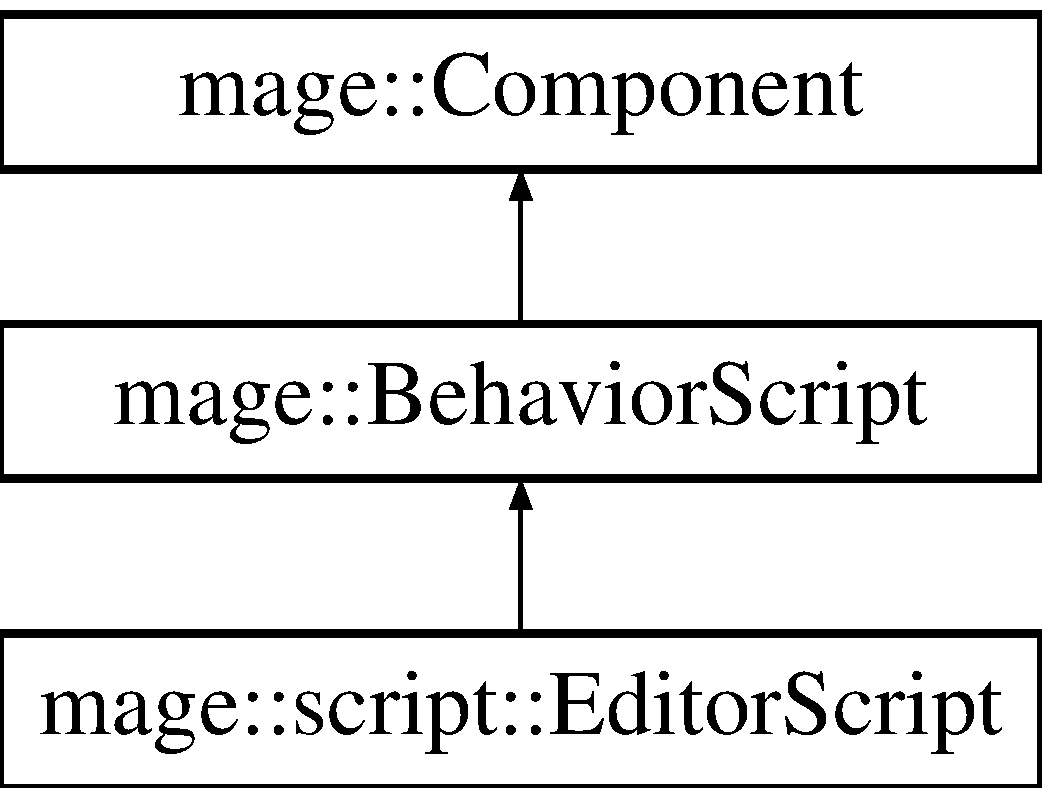
\includegraphics[height=3.000000cm]{classmage_1_1script_1_1_editor_script}
\end{center}
\end{figure}
\subsection*{Public Member Functions}
\begin{DoxyCompactItemize}
\item 
\mbox{\hyperlink{classmage_1_1script_1_1_editor_script_a6a16b52ab1952669a597abab1d66a73d}{Editor\+Script}} () noexcept
\item 
\mbox{\hyperlink{classmage_1_1script_1_1_editor_script_adfe05bb0529f098c404c25326ef0fd2e}{Editor\+Script}} (const \mbox{\hyperlink{classmage_1_1script_1_1_editor_script}{Editor\+Script}} \&script) noexcept
\item 
\mbox{\hyperlink{classmage_1_1script_1_1_editor_script_ac7db9f4ad73fc58c371aaf754009404e}{Editor\+Script}} (\mbox{\hyperlink{classmage_1_1script_1_1_editor_script}{Editor\+Script}} \&\&script) noexcept
\item 
virtual \mbox{\hyperlink{classmage_1_1script_1_1_editor_script_a1454bd68e4111691b6e287966dfd252a}{$\sim$\+Editor\+Script}} ()
\item 
\mbox{\hyperlink{classmage_1_1script_1_1_editor_script}{Editor\+Script}} \& \mbox{\hyperlink{classmage_1_1script_1_1_editor_script_ab7b4dda8389d07d41eba1474491b4a36}{operator=}} (const \mbox{\hyperlink{classmage_1_1script_1_1_editor_script}{Editor\+Script}} \&script) noexcept
\item 
\mbox{\hyperlink{classmage_1_1script_1_1_editor_script}{Editor\+Script}} \& \mbox{\hyperlink{classmage_1_1script_1_1_editor_script_a87df2b20fee97f6aa9e09b4b5c9282a5}{operator=}} (\mbox{\hyperlink{classmage_1_1script_1_1_editor_script}{Editor\+Script}} \&\&script) noexcept
\item 
virtual void \mbox{\hyperlink{classmage_1_1script_1_1_editor_script_af0804c603852f556d362f43e69240b2d}{Load}} (\mbox{[}\mbox{[}maybe\+\_\+unused\mbox{]}\mbox{]} \mbox{\hyperlink{classmage_1_1_engine}{Engine}} \&engine) override
\item 
virtual void \mbox{\hyperlink{classmage_1_1script_1_1_editor_script_a311532d499edfaf3f74aa598fb87ec8e}{Update}} (\mbox{[}\mbox{[}maybe\+\_\+unused\mbox{]}\mbox{]} \mbox{\hyperlink{classmage_1_1_engine}{Engine}} \&engine) override
\end{DoxyCompactItemize}
\subsection*{Private Attributes}
\begin{DoxyCompactItemize}
\item 
\mbox{\hyperlink{classmage_1_1_proxy_ptr}{Proxy\+Ptr}}$<$ \mbox{\hyperlink{classmage_1_1_node}{Node}} $>$ \mbox{\hyperlink{classmage_1_1script_1_1_editor_script_a60a8044379dfd203ad372dabb5c03380}{m\+\_\+selected}}
\end{DoxyCompactItemize}
\subsection*{Additional Inherited Members}


\subsection{Constructor \& Destructor Documentation}
\mbox{\Hypertarget{classmage_1_1script_1_1_editor_script_a6a16b52ab1952669a597abab1d66a73d}\label{classmage_1_1script_1_1_editor_script_a6a16b52ab1952669a597abab1d66a73d}} 
\index{mage\+::script\+::\+Editor\+Script@{mage\+::script\+::\+Editor\+Script}!Editor\+Script@{Editor\+Script}}
\index{Editor\+Script@{Editor\+Script}!mage\+::script\+::\+Editor\+Script@{mage\+::script\+::\+Editor\+Script}}
\subsubsection{\texorpdfstring{Editor\+Script()}{EditorScript()}\hspace{0.1cm}{\footnotesize\ttfamily [1/3]}}
{\footnotesize\ttfamily mage\+::script\+::\+Editor\+Script\+::\+Editor\+Script (\begin{DoxyParamCaption}{ }\end{DoxyParamCaption})\hspace{0.3cm}{\ttfamily [default]}, {\ttfamily [noexcept]}}

\mbox{\Hypertarget{classmage_1_1script_1_1_editor_script_adfe05bb0529f098c404c25326ef0fd2e}\label{classmage_1_1script_1_1_editor_script_adfe05bb0529f098c404c25326ef0fd2e}} 
\index{mage\+::script\+::\+Editor\+Script@{mage\+::script\+::\+Editor\+Script}!Editor\+Script@{Editor\+Script}}
\index{Editor\+Script@{Editor\+Script}!mage\+::script\+::\+Editor\+Script@{mage\+::script\+::\+Editor\+Script}}
\subsubsection{\texorpdfstring{Editor\+Script()}{EditorScript()}\hspace{0.1cm}{\footnotesize\ttfamily [2/3]}}
{\footnotesize\ttfamily mage\+::script\+::\+Editor\+Script\+::\+Editor\+Script (\begin{DoxyParamCaption}\item[{const \mbox{\hyperlink{classmage_1_1script_1_1_editor_script}{Editor\+Script}} \&}]{script }\end{DoxyParamCaption})\hspace{0.3cm}{\ttfamily [default]}, {\ttfamily [noexcept]}}

\mbox{\Hypertarget{classmage_1_1script_1_1_editor_script_ac7db9f4ad73fc58c371aaf754009404e}\label{classmage_1_1script_1_1_editor_script_ac7db9f4ad73fc58c371aaf754009404e}} 
\index{mage\+::script\+::\+Editor\+Script@{mage\+::script\+::\+Editor\+Script}!Editor\+Script@{Editor\+Script}}
\index{Editor\+Script@{Editor\+Script}!mage\+::script\+::\+Editor\+Script@{mage\+::script\+::\+Editor\+Script}}
\subsubsection{\texorpdfstring{Editor\+Script()}{EditorScript()}\hspace{0.1cm}{\footnotesize\ttfamily [3/3]}}
{\footnotesize\ttfamily mage\+::script\+::\+Editor\+Script\+::\+Editor\+Script (\begin{DoxyParamCaption}\item[{\mbox{\hyperlink{classmage_1_1script_1_1_editor_script}{Editor\+Script}} \&\&}]{script }\end{DoxyParamCaption})\hspace{0.3cm}{\ttfamily [default]}, {\ttfamily [noexcept]}}

\mbox{\Hypertarget{classmage_1_1script_1_1_editor_script_a1454bd68e4111691b6e287966dfd252a}\label{classmage_1_1script_1_1_editor_script_a1454bd68e4111691b6e287966dfd252a}} 
\index{mage\+::script\+::\+Editor\+Script@{mage\+::script\+::\+Editor\+Script}!````~Editor\+Script@{$\sim$\+Editor\+Script}}
\index{````~Editor\+Script@{$\sim$\+Editor\+Script}!mage\+::script\+::\+Editor\+Script@{mage\+::script\+::\+Editor\+Script}}
\subsubsection{\texorpdfstring{$\sim$\+Editor\+Script()}{~EditorScript()}}
{\footnotesize\ttfamily mage\+::script\+::\+Editor\+Script\+::$\sim$\+Editor\+Script (\begin{DoxyParamCaption}{ }\end{DoxyParamCaption})\hspace{0.3cm}{\ttfamily [virtual]}, {\ttfamily [default]}}



\subsection{Member Function Documentation}
\mbox{\Hypertarget{classmage_1_1script_1_1_editor_script_af0804c603852f556d362f43e69240b2d}\label{classmage_1_1script_1_1_editor_script_af0804c603852f556d362f43e69240b2d}} 
\index{mage\+::script\+::\+Editor\+Script@{mage\+::script\+::\+Editor\+Script}!Load@{Load}}
\index{Load@{Load}!mage\+::script\+::\+Editor\+Script@{mage\+::script\+::\+Editor\+Script}}
\subsubsection{\texorpdfstring{Load()}{Load()}}
{\footnotesize\ttfamily void mage\+::script\+::\+Editor\+Script\+::\+Load (\begin{DoxyParamCaption}\item[{\mbox{[}\mbox{[}maybe\+\_\+unused\mbox{]} \mbox{]} \mbox{\hyperlink{classmage_1_1_engine}{Engine}} \&}]{engine }\end{DoxyParamCaption})\hspace{0.3cm}{\ttfamily [override]}, {\ttfamily [virtual]}}

Loads this behavior script. Allows this behavior script to preform any pre-\/processing.


\begin{DoxyParams}[1]{Parameters}
\mbox{\tt in,out}  & {\em engine} & A reference to the engine. \\
\hline
\end{DoxyParams}

\begin{DoxyExceptions}{Exceptions}
{\em \mbox{\hyperlink{classmage_1_1_exception}{Exception}}} & Failed to load this behavior script. \\
\hline
\end{DoxyExceptions}


Reimplemented from \mbox{\hyperlink{classmage_1_1_behavior_script_ae7864876b2ffb1d1d8d8a56e3099f1f2}{mage\+::\+Behavior\+Script}}.

\mbox{\Hypertarget{classmage_1_1script_1_1_editor_script_ab7b4dda8389d07d41eba1474491b4a36}\label{classmage_1_1script_1_1_editor_script_ab7b4dda8389d07d41eba1474491b4a36}} 
\index{mage\+::script\+::\+Editor\+Script@{mage\+::script\+::\+Editor\+Script}!operator=@{operator=}}
\index{operator=@{operator=}!mage\+::script\+::\+Editor\+Script@{mage\+::script\+::\+Editor\+Script}}
\subsubsection{\texorpdfstring{operator=()}{operator=()}\hspace{0.1cm}{\footnotesize\ttfamily [1/2]}}
{\footnotesize\ttfamily \mbox{\hyperlink{classmage_1_1script_1_1_editor_script}{Editor\+Script}} \& mage\+::script\+::\+Editor\+Script\+::operator= (\begin{DoxyParamCaption}\item[{const \mbox{\hyperlink{classmage_1_1script_1_1_editor_script}{Editor\+Script}} \&}]{script }\end{DoxyParamCaption})\hspace{0.3cm}{\ttfamily [default]}, {\ttfamily [noexcept]}}

\mbox{\Hypertarget{classmage_1_1script_1_1_editor_script_a87df2b20fee97f6aa9e09b4b5c9282a5}\label{classmage_1_1script_1_1_editor_script_a87df2b20fee97f6aa9e09b4b5c9282a5}} 
\index{mage\+::script\+::\+Editor\+Script@{mage\+::script\+::\+Editor\+Script}!operator=@{operator=}}
\index{operator=@{operator=}!mage\+::script\+::\+Editor\+Script@{mage\+::script\+::\+Editor\+Script}}
\subsubsection{\texorpdfstring{operator=()}{operator=()}\hspace{0.1cm}{\footnotesize\ttfamily [2/2]}}
{\footnotesize\ttfamily \mbox{\hyperlink{classmage_1_1script_1_1_editor_script}{Editor\+Script}} \& mage\+::script\+::\+Editor\+Script\+::operator= (\begin{DoxyParamCaption}\item[{\mbox{\hyperlink{classmage_1_1script_1_1_editor_script}{Editor\+Script}} \&\&}]{script }\end{DoxyParamCaption})\hspace{0.3cm}{\ttfamily [default]}, {\ttfamily [noexcept]}}

\mbox{\Hypertarget{classmage_1_1script_1_1_editor_script_a311532d499edfaf3f74aa598fb87ec8e}\label{classmage_1_1script_1_1_editor_script_a311532d499edfaf3f74aa598fb87ec8e}} 
\index{mage\+::script\+::\+Editor\+Script@{mage\+::script\+::\+Editor\+Script}!Update@{Update}}
\index{Update@{Update}!mage\+::script\+::\+Editor\+Script@{mage\+::script\+::\+Editor\+Script}}
\subsubsection{\texorpdfstring{Update()}{Update()}}
{\footnotesize\ttfamily void mage\+::script\+::\+Editor\+Script\+::\+Update (\begin{DoxyParamCaption}\item[{\mbox{[}\mbox{[}maybe\+\_\+unused\mbox{]} \mbox{]} \mbox{\hyperlink{classmage_1_1_engine}{Engine}} \&}]{engine }\end{DoxyParamCaption})\hspace{0.3cm}{\ttfamily [override]}, {\ttfamily [virtual]}}

Updates this behavior script.

This method is called once per frame.


\begin{DoxyParams}[1]{Parameters}
\mbox{\tt in,out}  & {\em engine} & A reference to the engine. \\
\hline
\end{DoxyParams}

\begin{DoxyExceptions}{Exceptions}
{\em \mbox{\hyperlink{classmage_1_1_exception}{Exception}}} & Failed to update this behavior script. \\
\hline
\end{DoxyExceptions}


Reimplemented from \mbox{\hyperlink{classmage_1_1_behavior_script_a085634661326b59850c1111e537baa4e}{mage\+::\+Behavior\+Script}}.



\subsection{Member Data Documentation}
\mbox{\Hypertarget{classmage_1_1script_1_1_editor_script_a60a8044379dfd203ad372dabb5c03380}\label{classmage_1_1script_1_1_editor_script_a60a8044379dfd203ad372dabb5c03380}} 
\index{mage\+::script\+::\+Editor\+Script@{mage\+::script\+::\+Editor\+Script}!m\+\_\+selected@{m\+\_\+selected}}
\index{m\+\_\+selected@{m\+\_\+selected}!mage\+::script\+::\+Editor\+Script@{mage\+::script\+::\+Editor\+Script}}
\subsubsection{\texorpdfstring{m\+\_\+selected}{m\_selected}}
{\footnotesize\ttfamily \mbox{\hyperlink{classmage_1_1_proxy_ptr}{Proxy\+Ptr}}$<$ \mbox{\hyperlink{classmage_1_1_node}{Node}} $>$ mage\+::script\+::\+Editor\+Script\+::m\+\_\+selected\hspace{0.3cm}{\ttfamily [private]}}


\hypertarget{classmage_1_1_engine}{}\section{mage\+:\+:Engine Class Reference}
\label{classmage_1_1_engine}\index{mage\+::\+Engine@{mage\+::\+Engine}}


{\ttfamily \#include $<$engine.\+hpp$>$}

Inheritance diagram for mage\+:\+:Engine\+:\begin{figure}[H]
\begin{center}
\leavevmode
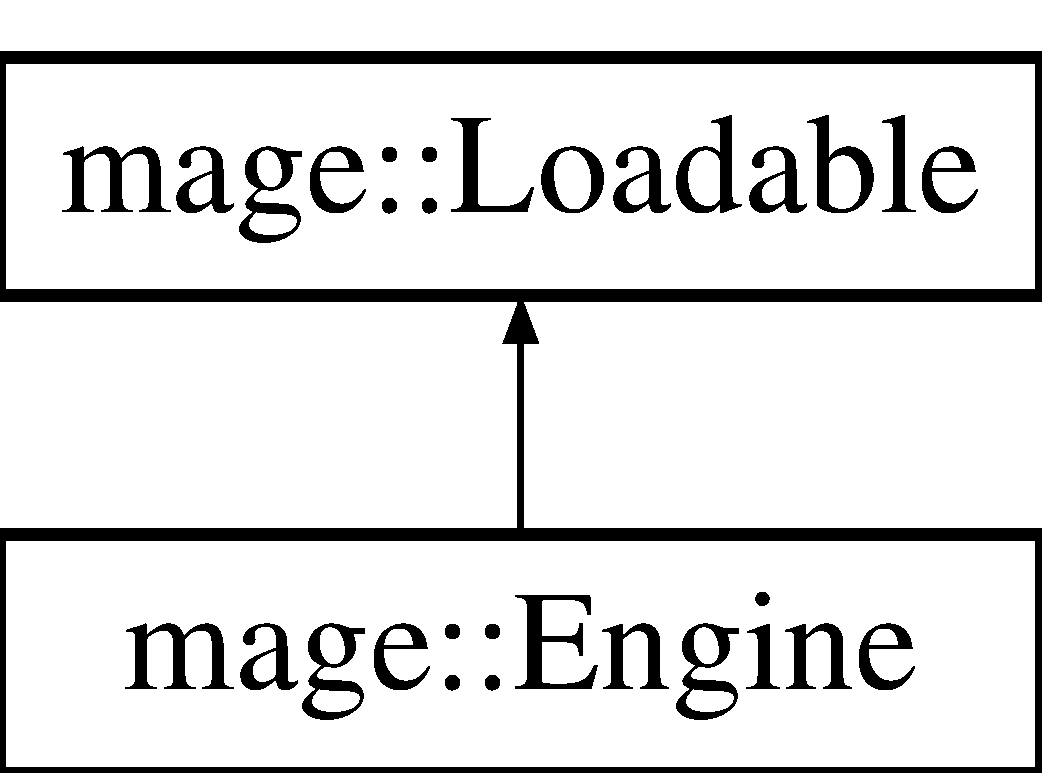
\includegraphics[height=2.000000cm]{classmage_1_1_engine}
\end{center}
\end{figure}
\subsection*{Public Member Functions}
\begin{DoxyCompactItemize}
\item 
\hyperlink{classmage_1_1_engine_a99770cbb017b29c284d7f8e4c7e2b84c}{Engine} (const \hyperlink{structmage_1_1_engine_setup}{Engine\+Setup} \&setup)
\item 
\hyperlink{classmage_1_1_engine_afd2f4f32b2e803f59521aafe1924f0ba}{Engine} (const \hyperlink{classmage_1_1_engine}{Engine} \&engine)=delete
\item 
\hyperlink{classmage_1_1_engine_a1374fc1d0d18e23df9150dfcd17955b0}{Engine} (\hyperlink{classmage_1_1_engine}{Engine} \&\&engine)=default
\item 
virtual \hyperlink{classmage_1_1_engine_a34628556f8397d70ed018d71e343c2f5}{$\sim$\+Engine} ()
\item 
\hyperlink{classmage_1_1_engine}{Engine} \& \hyperlink{classmage_1_1_engine_a1eedff82d4c8207c61676230520648fd}{operator=} (const \hyperlink{classmage_1_1_engine}{Engine} \&engine)=delete
\item 
\hyperlink{classmage_1_1_engine}{Engine} \& \hyperlink{classmage_1_1_engine_a22607a263e0be5e179cc0e4bf13b18f7}{operator=} (\hyperlink{classmage_1_1_engine}{Engine} \&\&engine)=delete
\item 
void \hyperlink{classmage_1_1_engine_a246c82d0e55bc29e73aecbc365464ec8}{Run} (int n\+Cmd\+Show=S\+W\+\_\+\+N\+O\+R\+M\+AL)
\item 
const \hyperlink{classmage_1_1_main_window}{Main\+Window} $\ast$ \hyperlink{classmage_1_1_engine_a28baaa54158acac8ffca3b6f31f63f82}{Get\+Main\+Window} () const
\item 
void \hyperlink{classmage_1_1_engine_a942bfa9892fa79bb1068d7c7ec4e6732}{Set\+Deactive\+Flag} (bool deactive)
\item 
const \hyperlink{classmage_1_1_renderer}{Renderer} $\ast$ \hyperlink{classmage_1_1_engine_a42ea717aaf468e0cacf8d8745041e09f}{Get\+Renderer} () const
\item 
void \hyperlink{classmage_1_1_engine_a8b574f0d702240d76fa98b2c79856d0d}{Set\+Mode\+Switch\+Flag} (bool mode\+\_\+switch)
\item 
const \hyperlink{classmage_1_1_input_manager}{Input\+Manager} $\ast$ \hyperlink{classmage_1_1_engine_a627271c15bb1ecb1079f9780d64e0d77}{Get\+Input\+Manager} () const
\item 
\hyperlink{classmage_1_1_resource_factory}{Resource\+Factory} $\ast$ \hyperlink{classmage_1_1_engine_a1610768d6de0e8548ba18904a692b1a8}{Get\+Resource\+Factory} () const
\item 
void \hyperlink{classmage_1_1_engine_aec75ed67f8fb68a383fa892e50b21ea7}{Set\+Scene} (\hyperlink{namespacemage_a1e01ae66713838a7a67d30e44c67703e}{Shared\+Ptr}$<$ \hyperlink{classmage_1_1_scene}{Scene} $>$ scene)
\end{DoxyCompactItemize}
\subsection*{Private Member Functions}
\begin{DoxyCompactItemize}
\item 
void \hyperlink{classmage_1_1_engine_a29a47448fb182b110d46d287a72b8b4e}{Initialize\+Systems} (const \hyperlink{structmage_1_1_engine_setup}{Engine\+Setup} \&setup)
\end{DoxyCompactItemize}
\subsection*{Private Attributes}
\begin{DoxyCompactItemize}
\item 
\hyperlink{namespacemage_a8c307fbcc33bce9b7f2aa4c26c3b95cf}{Unique\+Ptr}$<$ \hyperlink{classmage_1_1_main_window}{Main\+Window} $>$ \hyperlink{classmage_1_1_engine_a3aea7e8c0c1247cac570334a3d3543d6}{m\+\_\+main\+\_\+window}
\item 
bool \hyperlink{classmage_1_1_engine_ab8a4b0157403708ae7d1d018a95b4c63}{m\+\_\+deactive}
\item 
\hyperlink{namespacemage_a8c307fbcc33bce9b7f2aa4c26c3b95cf}{Unique\+Ptr}$<$ \hyperlink{classmage_1_1_renderer}{Renderer} $>$ \hyperlink{classmage_1_1_engine_a1248b7c21bc8256c72d372c12ed1ee68}{m\+\_\+renderer}
\item 
bool \hyperlink{classmage_1_1_engine_aa5cb2e0b7bb2c4a9020e79ab832ee221}{m\+\_\+mode\+\_\+switch}
\item 
\hyperlink{namespacemage_a8c307fbcc33bce9b7f2aa4c26c3b95cf}{Unique\+Ptr}$<$ \hyperlink{classmage_1_1_input_manager}{Input\+Manager} $>$ \hyperlink{classmage_1_1_engine_a8e9048208a6a5c5b034aaa1cbdab28bc}{m\+\_\+input\+\_\+manager}
\item 
\hyperlink{namespacemage_a8c307fbcc33bce9b7f2aa4c26c3b95cf}{Unique\+Ptr}$<$ \hyperlink{classmage_1_1_resource_factory}{Resource\+Factory} $>$ \hyperlink{classmage_1_1_engine_a0c7c2d4fc75fc3512e02054056cf8a90}{m\+\_\+resource\+\_\+factory}
\item 
\hyperlink{namespacemage_a1e01ae66713838a7a67d30e44c67703e}{Shared\+Ptr}$<$ \hyperlink{classmage_1_1_scene}{Scene} $>$ \hyperlink{classmage_1_1_engine_a82158ab9c1b60538ef8c46d5eb263bb8}{m\+\_\+scene}
\item 
\hyperlink{namespacemage_a8c307fbcc33bce9b7f2aa4c26c3b95cf}{Unique\+Ptr}$<$ \hyperlink{classmage_1_1_timer}{Timer} $>$ \hyperlink{classmage_1_1_engine_a4daac998928a6c087b310c52b3f26ae4}{m\+\_\+timer}
\end{DoxyCompactItemize}
\subsection*{Additional Inherited Members}


\subsection{Detailed Description}
A class of engines. 

\subsection{Constructor \& Destructor Documentation}
\hypertarget{classmage_1_1_engine_a99770cbb017b29c284d7f8e4c7e2b84c}{}\label{classmage_1_1_engine_a99770cbb017b29c284d7f8e4c7e2b84c} 
\index{mage\+::\+Engine@{mage\+::\+Engine}!Engine@{Engine}}
\index{Engine@{Engine}!mage\+::\+Engine@{mage\+::\+Engine}}
\subsubsection{\texorpdfstring{Engine()}{Engine()}\hspace{0.1cm}{\footnotesize\ttfamily [1/3]}}
{\footnotesize\ttfamily mage\+::\+Engine\+::\+Engine (\begin{DoxyParamCaption}\item[{const \hyperlink{structmage_1_1_engine_setup}{Engine\+Setup} \&}]{setup }\end{DoxyParamCaption})\hspace{0.3cm}{\ttfamily [explicit]}}

Constructs an engine from the given engine setup.


\begin{DoxyParams}[1]{Parameters}
\mbox{\tt in}  & {\em setup} & A reference to an engine setup. \\
\hline
\end{DoxyParams}

\begin{DoxyExceptions}{Exceptions}
{\em \hyperlink{structmage_1_1_formatted_exception}{Formatted\+Exception}} & Failed to initialize the engine. \\
\hline
\end{DoxyExceptions}
\hypertarget{classmage_1_1_engine_afd2f4f32b2e803f59521aafe1924f0ba}{}\label{classmage_1_1_engine_afd2f4f32b2e803f59521aafe1924f0ba} 
\index{mage\+::\+Engine@{mage\+::\+Engine}!Engine@{Engine}}
\index{Engine@{Engine}!mage\+::\+Engine@{mage\+::\+Engine}}
\subsubsection{\texorpdfstring{Engine()}{Engine()}\hspace{0.1cm}{\footnotesize\ttfamily [2/3]}}
{\footnotesize\ttfamily mage\+::\+Engine\+::\+Engine (\begin{DoxyParamCaption}\item[{const \hyperlink{classmage_1_1_engine}{Engine} \&}]{engine }\end{DoxyParamCaption})\hspace{0.3cm}{\ttfamily [delete]}}

Constructs an engine from the given engine.


\begin{DoxyParams}[1]{Parameters}
\mbox{\tt in}  & {\em engine} & A reference to the engine to copy. \\
\hline
\end{DoxyParams}
\hypertarget{classmage_1_1_engine_a1374fc1d0d18e23df9150dfcd17955b0}{}\label{classmage_1_1_engine_a1374fc1d0d18e23df9150dfcd17955b0} 
\index{mage\+::\+Engine@{mage\+::\+Engine}!Engine@{Engine}}
\index{Engine@{Engine}!mage\+::\+Engine@{mage\+::\+Engine}}
\subsubsection{\texorpdfstring{Engine()}{Engine()}\hspace{0.1cm}{\footnotesize\ttfamily [3/3]}}
{\footnotesize\ttfamily mage\+::\+Engine\+::\+Engine (\begin{DoxyParamCaption}\item[{\hyperlink{classmage_1_1_engine}{Engine} \&\&}]{engine }\end{DoxyParamCaption})\hspace{0.3cm}{\ttfamily [default]}}

Constructs an engine by moving the given engine.


\begin{DoxyParams}[1]{Parameters}
\mbox{\tt in}  & {\em engine} & A reference to the engine to move. \\
\hline
\end{DoxyParams}
\hypertarget{classmage_1_1_engine_a34628556f8397d70ed018d71e343c2f5}{}\label{classmage_1_1_engine_a34628556f8397d70ed018d71e343c2f5} 
\index{mage\+::\+Engine@{mage\+::\+Engine}!````~Engine@{$\sim$\+Engine}}
\index{````~Engine@{$\sim$\+Engine}!mage\+::\+Engine@{mage\+::\+Engine}}
\subsubsection{\texorpdfstring{$\sim$\+Engine()}{~Engine()}}
{\footnotesize\ttfamily mage\+::\+Engine\+::$\sim$\+Engine (\begin{DoxyParamCaption}{ }\end{DoxyParamCaption})\hspace{0.3cm}{\ttfamily [virtual]}}

Destructs this engine. 

\subsection{Member Function Documentation}
\hypertarget{classmage_1_1_engine_a627271c15bb1ecb1079f9780d64e0d77}{}\label{classmage_1_1_engine_a627271c15bb1ecb1079f9780d64e0d77} 
\index{mage\+::\+Engine@{mage\+::\+Engine}!Get\+Input\+Manager@{Get\+Input\+Manager}}
\index{Get\+Input\+Manager@{Get\+Input\+Manager}!mage\+::\+Engine@{mage\+::\+Engine}}
\subsubsection{\texorpdfstring{Get\+Input\+Manager()}{GetInputManager()}}
{\footnotesize\ttfamily const \hyperlink{classmage_1_1_input_manager}{Input\+Manager}$\ast$ mage\+::\+Engine\+::\+Get\+Input\+Manager (\begin{DoxyParamCaption}{ }\end{DoxyParamCaption}) const}

Returns the input manager of this engine.

\begin{DoxyReturn}{Returns}
{\ttfamily nullptr} if this engine is not properly setup. 

A pointer to the input manager of this engine. 
\end{DoxyReturn}
\hypertarget{classmage_1_1_engine_a28baaa54158acac8ffca3b6f31f63f82}{}\label{classmage_1_1_engine_a28baaa54158acac8ffca3b6f31f63f82} 
\index{mage\+::\+Engine@{mage\+::\+Engine}!Get\+Main\+Window@{Get\+Main\+Window}}
\index{Get\+Main\+Window@{Get\+Main\+Window}!mage\+::\+Engine@{mage\+::\+Engine}}
\subsubsection{\texorpdfstring{Get\+Main\+Window()}{GetMainWindow()}}
{\footnotesize\ttfamily const \hyperlink{classmage_1_1_main_window}{Main\+Window}$\ast$ mage\+::\+Engine\+::\+Get\+Main\+Window (\begin{DoxyParamCaption}{ }\end{DoxyParamCaption}) const}

Returns the main window of this engine.

\begin{DoxyReturn}{Returns}
{\ttfamily nullptr} if this engine is not properly setup. 

A pointer to the main window of this engine. 
\end{DoxyReturn}
\hypertarget{classmage_1_1_engine_a42ea717aaf468e0cacf8d8745041e09f}{}\label{classmage_1_1_engine_a42ea717aaf468e0cacf8d8745041e09f} 
\index{mage\+::\+Engine@{mage\+::\+Engine}!Get\+Renderer@{Get\+Renderer}}
\index{Get\+Renderer@{Get\+Renderer}!mage\+::\+Engine@{mage\+::\+Engine}}
\subsubsection{\texorpdfstring{Get\+Renderer()}{GetRenderer()}}
{\footnotesize\ttfamily const \hyperlink{classmage_1_1_renderer}{Renderer}$\ast$ mage\+::\+Engine\+::\+Get\+Renderer (\begin{DoxyParamCaption}{ }\end{DoxyParamCaption}) const}

Returns the renderer of this engine.

\begin{DoxyReturn}{Returns}
{\ttfamily nullptr} if this engine is not properly setup. 

A pointer to the renderer of this engine. 
\end{DoxyReturn}
\hypertarget{classmage_1_1_engine_a1610768d6de0e8548ba18904a692b1a8}{}\label{classmage_1_1_engine_a1610768d6de0e8548ba18904a692b1a8} 
\index{mage\+::\+Engine@{mage\+::\+Engine}!Get\+Resource\+Factory@{Get\+Resource\+Factory}}
\index{Get\+Resource\+Factory@{Get\+Resource\+Factory}!mage\+::\+Engine@{mage\+::\+Engine}}
\subsubsection{\texorpdfstring{Get\+Resource\+Factory()}{GetResourceFactory()}}
{\footnotesize\ttfamily \hyperlink{classmage_1_1_resource_factory}{Resource\+Factory}$\ast$ mage\+::\+Engine\+::\+Get\+Resource\+Factory (\begin{DoxyParamCaption}{ }\end{DoxyParamCaption}) const}

Returns the resource factory of this engine.

\begin{DoxyReturn}{Returns}
{\ttfamily nullptr} if this engine is not properly setup. 

A pointer to the resource factory of this engine. 
\end{DoxyReturn}
\hypertarget{classmage_1_1_engine_a29a47448fb182b110d46d287a72b8b4e}{}\label{classmage_1_1_engine_a29a47448fb182b110d46d287a72b8b4e} 
\index{mage\+::\+Engine@{mage\+::\+Engine}!Initialize\+Systems@{Initialize\+Systems}}
\index{Initialize\+Systems@{Initialize\+Systems}!mage\+::\+Engine@{mage\+::\+Engine}}
\subsubsection{\texorpdfstring{Initialize\+Systems()}{InitializeSystems()}}
{\footnotesize\ttfamily void mage\+::\+Engine\+::\+Initialize\+Systems (\begin{DoxyParamCaption}\item[{const \hyperlink{structmage_1_1_engine_setup}{Engine\+Setup} \&}]{setup }\end{DoxyParamCaption})\hspace{0.3cm}{\ttfamily [private]}}

Initializes the different systems of this engine.


\begin{DoxyParams}[1]{Parameters}
\mbox{\tt in}  & {\em setup} & A reference to an engine setup. \\
\hline
\end{DoxyParams}

\begin{DoxyExceptions}{Exceptions}
{\em \hyperlink{structmage_1_1_formatted_exception}{Formatted\+Exception}} & Failed to initialize at least one of the different systems of this engine. \\
\hline
\end{DoxyExceptions}
\hypertarget{classmage_1_1_engine_a1eedff82d4c8207c61676230520648fd}{}\label{classmage_1_1_engine_a1eedff82d4c8207c61676230520648fd} 
\index{mage\+::\+Engine@{mage\+::\+Engine}!operator=@{operator=}}
\index{operator=@{operator=}!mage\+::\+Engine@{mage\+::\+Engine}}
\subsubsection{\texorpdfstring{operator=()}{operator=()}\hspace{0.1cm}{\footnotesize\ttfamily [1/2]}}
{\footnotesize\ttfamily \hyperlink{classmage_1_1_engine}{Engine}\& mage\+::\+Engine\+::operator= (\begin{DoxyParamCaption}\item[{const \hyperlink{classmage_1_1_engine}{Engine} \&}]{engine }\end{DoxyParamCaption})\hspace{0.3cm}{\ttfamily [delete]}}

Copies the given engine to this engine.


\begin{DoxyParams}[1]{Parameters}
\mbox{\tt in}  & {\em engine} & A reference to the engine to copy. \\
\hline
\end{DoxyParams}
\begin{DoxyReturn}{Returns}
A reference to the copy of the given engine (i.\+e. this engine). 
\end{DoxyReturn}
\hypertarget{classmage_1_1_engine_a22607a263e0be5e179cc0e4bf13b18f7}{}\label{classmage_1_1_engine_a22607a263e0be5e179cc0e4bf13b18f7} 
\index{mage\+::\+Engine@{mage\+::\+Engine}!operator=@{operator=}}
\index{operator=@{operator=}!mage\+::\+Engine@{mage\+::\+Engine}}
\subsubsection{\texorpdfstring{operator=()}{operator=()}\hspace{0.1cm}{\footnotesize\ttfamily [2/2]}}
{\footnotesize\ttfamily \hyperlink{classmage_1_1_engine}{Engine}\& mage\+::\+Engine\+::operator= (\begin{DoxyParamCaption}\item[{\hyperlink{classmage_1_1_engine}{Engine} \&\&}]{engine }\end{DoxyParamCaption})\hspace{0.3cm}{\ttfamily [delete]}}

Copies the given engine to this engine.


\begin{DoxyParams}[1]{Parameters}
\mbox{\tt in}  & {\em engine} & A reference to the engine to move. \\
\hline
\end{DoxyParams}
\begin{DoxyReturn}{Returns}
A reference to the moved engine (i.\+e. this engine). 
\end{DoxyReturn}
\hypertarget{classmage_1_1_engine_a246c82d0e55bc29e73aecbc365464ec8}{}\label{classmage_1_1_engine_a246c82d0e55bc29e73aecbc365464ec8} 
\index{mage\+::\+Engine@{mage\+::\+Engine}!Run@{Run}}
\index{Run@{Run}!mage\+::\+Engine@{mage\+::\+Engine}}
\subsubsection{\texorpdfstring{Run()}{Run()}}
{\footnotesize\ttfamily void mage\+::\+Engine\+::\+Run (\begin{DoxyParamCaption}\item[{int}]{n\+Cmd\+Show = {\ttfamily SW\+\_\+NORMAL} }\end{DoxyParamCaption})}

Runs this engine.


\begin{DoxyParams}[1]{Parameters}
\mbox{\tt in}  & {\em n\+Cmd\+Show} & Controls how the engine window is to be shown. \\
\hline
\end{DoxyParams}
\hypertarget{classmage_1_1_engine_a942bfa9892fa79bb1068d7c7ec4e6732}{}\label{classmage_1_1_engine_a942bfa9892fa79bb1068d7c7ec4e6732} 
\index{mage\+::\+Engine@{mage\+::\+Engine}!Set\+Deactive\+Flag@{Set\+Deactive\+Flag}}
\index{Set\+Deactive\+Flag@{Set\+Deactive\+Flag}!mage\+::\+Engine@{mage\+::\+Engine}}
\subsubsection{\texorpdfstring{Set\+Deactive\+Flag()}{SetDeactiveFlag()}}
{\footnotesize\ttfamily void mage\+::\+Engine\+::\+Set\+Deactive\+Flag (\begin{DoxyParamCaption}\item[{bool}]{deactive }\end{DoxyParamCaption})}

Sets the deactive flag of this engine to the given value.


\begin{DoxyParams}[1]{Parameters}
\mbox{\tt in}  & {\em deactive} & The new value for the deactive flag. \\
\hline
\end{DoxyParams}
\hypertarget{classmage_1_1_engine_a8b574f0d702240d76fa98b2c79856d0d}{}\label{classmage_1_1_engine_a8b574f0d702240d76fa98b2c79856d0d} 
\index{mage\+::\+Engine@{mage\+::\+Engine}!Set\+Mode\+Switch\+Flag@{Set\+Mode\+Switch\+Flag}}
\index{Set\+Mode\+Switch\+Flag@{Set\+Mode\+Switch\+Flag}!mage\+::\+Engine@{mage\+::\+Engine}}
\subsubsection{\texorpdfstring{Set\+Mode\+Switch\+Flag()}{SetModeSwitchFlag()}}
{\footnotesize\ttfamily void mage\+::\+Engine\+::\+Set\+Mode\+Switch\+Flag (\begin{DoxyParamCaption}\item[{bool}]{mode\+\_\+switch }\end{DoxyParamCaption})}

Sets the mode switch flag of this engine to the given value.


\begin{DoxyParams}[1]{Parameters}
\mbox{\tt in}  & {\em mode\+\_\+switch} & The new value for the mode switch flag. \\
\hline
\end{DoxyParams}
\hypertarget{classmage_1_1_engine_aec75ed67f8fb68a383fa892e50b21ea7}{}\label{classmage_1_1_engine_aec75ed67f8fb68a383fa892e50b21ea7} 
\index{mage\+::\+Engine@{mage\+::\+Engine}!Set\+Scene@{Set\+Scene}}
\index{Set\+Scene@{Set\+Scene}!mage\+::\+Engine@{mage\+::\+Engine}}
\subsubsection{\texorpdfstring{Set\+Scene()}{SetScene()}}
{\footnotesize\ttfamily void mage\+::\+Engine\+::\+Set\+Scene (\begin{DoxyParamCaption}\item[{\hyperlink{namespacemage_a1e01ae66713838a7a67d30e44c67703e}{Shared\+Ptr}$<$ \hyperlink{classmage_1_1_scene}{Scene} $>$}]{scene }\end{DoxyParamCaption})}

Sets the scene of this engine to the given scene.

\begin{DoxyReturn}{Returns}
A pointer to the scene to set. 
\end{DoxyReturn}


\subsection{Member Data Documentation}
\hypertarget{classmage_1_1_engine_ab8a4b0157403708ae7d1d018a95b4c63}{}\label{classmage_1_1_engine_ab8a4b0157403708ae7d1d018a95b4c63} 
\index{mage\+::\+Engine@{mage\+::\+Engine}!m\+\_\+deactive@{m\+\_\+deactive}}
\index{m\+\_\+deactive@{m\+\_\+deactive}!mage\+::\+Engine@{mage\+::\+Engine}}
\subsubsection{\texorpdfstring{m\+\_\+deactive}{m\_deactive}}
{\footnotesize\ttfamily bool mage\+::\+Engine\+::m\+\_\+deactive\hspace{0.3cm}{\ttfamily [private]}}

Flag indicating whether the application is active or not. \hypertarget{classmage_1_1_engine_a8e9048208a6a5c5b034aaa1cbdab28bc}{}\label{classmage_1_1_engine_a8e9048208a6a5c5b034aaa1cbdab28bc} 
\index{mage\+::\+Engine@{mage\+::\+Engine}!m\+\_\+input\+\_\+manager@{m\+\_\+input\+\_\+manager}}
\index{m\+\_\+input\+\_\+manager@{m\+\_\+input\+\_\+manager}!mage\+::\+Engine@{mage\+::\+Engine}}
\subsubsection{\texorpdfstring{m\+\_\+input\+\_\+manager}{m\_input\_manager}}
{\footnotesize\ttfamily \hyperlink{namespacemage_a8c307fbcc33bce9b7f2aa4c26c3b95cf}{Unique\+Ptr}$<$ \hyperlink{classmage_1_1_input_manager}{Input\+Manager} $>$ mage\+::\+Engine\+::m\+\_\+input\+\_\+manager\hspace{0.3cm}{\ttfamily [private]}}

A pointer to the input manager of this engine. \hypertarget{classmage_1_1_engine_a3aea7e8c0c1247cac570334a3d3543d6}{}\label{classmage_1_1_engine_a3aea7e8c0c1247cac570334a3d3543d6} 
\index{mage\+::\+Engine@{mage\+::\+Engine}!m\+\_\+main\+\_\+window@{m\+\_\+main\+\_\+window}}
\index{m\+\_\+main\+\_\+window@{m\+\_\+main\+\_\+window}!mage\+::\+Engine@{mage\+::\+Engine}}
\subsubsection{\texorpdfstring{m\+\_\+main\+\_\+window}{m\_main\_window}}
{\footnotesize\ttfamily \hyperlink{namespacemage_a8c307fbcc33bce9b7f2aa4c26c3b95cf}{Unique\+Ptr}$<$ \hyperlink{classmage_1_1_main_window}{Main\+Window} $>$ mage\+::\+Engine\+::m\+\_\+main\+\_\+window\hspace{0.3cm}{\ttfamily [private]}}

A pointer to the main window of this engine. \hypertarget{classmage_1_1_engine_aa5cb2e0b7bb2c4a9020e79ab832ee221}{}\label{classmage_1_1_engine_aa5cb2e0b7bb2c4a9020e79ab832ee221} 
\index{mage\+::\+Engine@{mage\+::\+Engine}!m\+\_\+mode\+\_\+switch@{m\+\_\+mode\+\_\+switch}}
\index{m\+\_\+mode\+\_\+switch@{m\+\_\+mode\+\_\+switch}!mage\+::\+Engine@{mage\+::\+Engine}}
\subsubsection{\texorpdfstring{m\+\_\+mode\+\_\+switch}{m\_mode\_switch}}
{\footnotesize\ttfamily bool mage\+::\+Engine\+::m\+\_\+mode\+\_\+switch\hspace{0.3cm}{\ttfamily [private]}}

Flag indicating whether the application should switch between full screen and windowed mode. \hypertarget{classmage_1_1_engine_a1248b7c21bc8256c72d372c12ed1ee68}{}\label{classmage_1_1_engine_a1248b7c21bc8256c72d372c12ed1ee68} 
\index{mage\+::\+Engine@{mage\+::\+Engine}!m\+\_\+renderer@{m\+\_\+renderer}}
\index{m\+\_\+renderer@{m\+\_\+renderer}!mage\+::\+Engine@{mage\+::\+Engine}}
\subsubsection{\texorpdfstring{m\+\_\+renderer}{m\_renderer}}
{\footnotesize\ttfamily \hyperlink{namespacemage_a8c307fbcc33bce9b7f2aa4c26c3b95cf}{Unique\+Ptr}$<$ \hyperlink{classmage_1_1_renderer}{Renderer} $>$ mage\+::\+Engine\+::m\+\_\+renderer\hspace{0.3cm}{\ttfamily [private]}}

A pointer to the renderer of this engine. \hypertarget{classmage_1_1_engine_a0c7c2d4fc75fc3512e02054056cf8a90}{}\label{classmage_1_1_engine_a0c7c2d4fc75fc3512e02054056cf8a90} 
\index{mage\+::\+Engine@{mage\+::\+Engine}!m\+\_\+resource\+\_\+factory@{m\+\_\+resource\+\_\+factory}}
\index{m\+\_\+resource\+\_\+factory@{m\+\_\+resource\+\_\+factory}!mage\+::\+Engine@{mage\+::\+Engine}}
\subsubsection{\texorpdfstring{m\+\_\+resource\+\_\+factory}{m\_resource\_factory}}
{\footnotesize\ttfamily \hyperlink{namespacemage_a8c307fbcc33bce9b7f2aa4c26c3b95cf}{Unique\+Ptr}$<$ \hyperlink{classmage_1_1_resource_factory}{Resource\+Factory} $>$ mage\+::\+Engine\+::m\+\_\+resource\+\_\+factory\hspace{0.3cm}{\ttfamily [private]}}

A pointer to the resource factory of this engine. \hypertarget{classmage_1_1_engine_a82158ab9c1b60538ef8c46d5eb263bb8}{}\label{classmage_1_1_engine_a82158ab9c1b60538ef8c46d5eb263bb8} 
\index{mage\+::\+Engine@{mage\+::\+Engine}!m\+\_\+scene@{m\+\_\+scene}}
\index{m\+\_\+scene@{m\+\_\+scene}!mage\+::\+Engine@{mage\+::\+Engine}}
\subsubsection{\texorpdfstring{m\+\_\+scene}{m\_scene}}
{\footnotesize\ttfamily \hyperlink{namespacemage_a1e01ae66713838a7a67d30e44c67703e}{Shared\+Ptr}$<$ \hyperlink{classmage_1_1_scene}{Scene} $>$ mage\+::\+Engine\+::m\+\_\+scene\hspace{0.3cm}{\ttfamily [private]}}

A pointer to the current scene of this engine. \hypertarget{classmage_1_1_engine_a4daac998928a6c087b310c52b3f26ae4}{}\label{classmage_1_1_engine_a4daac998928a6c087b310c52b3f26ae4} 
\index{mage\+::\+Engine@{mage\+::\+Engine}!m\+\_\+timer@{m\+\_\+timer}}
\index{m\+\_\+timer@{m\+\_\+timer}!mage\+::\+Engine@{mage\+::\+Engine}}
\subsubsection{\texorpdfstring{m\+\_\+timer}{m\_timer}}
{\footnotesize\ttfamily \hyperlink{namespacemage_a8c307fbcc33bce9b7f2aa4c26c3b95cf}{Unique\+Ptr}$<$ \hyperlink{classmage_1_1_timer}{Timer} $>$ mage\+::\+Engine\+::m\+\_\+timer\hspace{0.3cm}{\ttfamily [private]}}

A pointer to the timer of this engine. 
\hypertarget{classmage_1_1_engine_message_handler}{}\section{mage\+:\+:Engine\+Message\+Handler Class Reference}
\label{classmage_1_1_engine_message_handler}\index{mage\+::\+Engine\+Message\+Handler@{mage\+::\+Engine\+Message\+Handler}}


{\ttfamily \#include $<$engine.\+hpp$>$}

Inheritance diagram for mage\+:\+:Engine\+Message\+Handler\+:\begin{figure}[H]
\begin{center}
\leavevmode
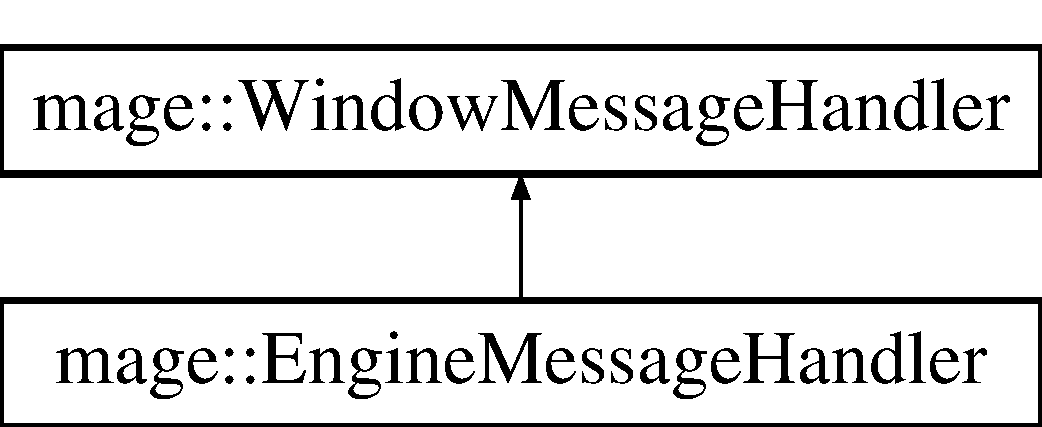
\includegraphics[height=2.000000cm]{classmage_1_1_engine_message_handler}
\end{center}
\end{figure}
\subsection*{Public Member Functions}
\begin{DoxyCompactItemize}
\item 
\mbox{\hyperlink{classmage_1_1_engine_message_handler_a1d3e248f3b2b314e5a277a8397f08780}{Engine\+Message\+Handler}} ()
\item 
\mbox{\hyperlink{classmage_1_1_engine_message_handler_a02124b51211515e5bb93b0a1c3250a8c}{Engine\+Message\+Handler}} (const \mbox{\hyperlink{classmage_1_1_engine_message_handler}{Engine\+Message\+Handler}} \&handler)
\item 
\mbox{\hyperlink{classmage_1_1_engine_message_handler_ab771829274e6ab899b4499926f504667}{Engine\+Message\+Handler}} (\mbox{\hyperlink{classmage_1_1_engine_message_handler}{Engine\+Message\+Handler}} \&\&handler) noexcept
\item 
virtual \mbox{\hyperlink{classmage_1_1_engine_message_handler_a458f16ad9f68ad1e908e4d275c383c2c}{$\sim$\+Engine\+Message\+Handler}} ()
\item 
\mbox{\hyperlink{classmage_1_1_engine_message_handler}{Engine\+Message\+Handler}} \& \mbox{\hyperlink{classmage_1_1_engine_message_handler_a567c60f09df9fed3c725ab215e9afbe6}{operator=}} (const \mbox{\hyperlink{classmage_1_1_engine_message_handler}{Engine\+Message\+Handler}} \&handler)
\item 
\mbox{\hyperlink{classmage_1_1_engine_message_handler}{Engine\+Message\+Handler}} \& \mbox{\hyperlink{classmage_1_1_engine_message_handler_a77538e900f5c92e4da88de5042ca5f4c}{operator=}} (\mbox{\hyperlink{classmage_1_1_engine_message_handler}{Engine\+Message\+Handler}} \&\&handler) noexcept
\item 
virtual const std\+::optional$<$ L\+R\+E\+S\+U\+LT $>$ \mbox{\hyperlink{classmage_1_1_engine_message_handler_a3126109746a531e13a2b14b6600ee47e}{Handle\+Window\+Message}} (\mbox{[}\mbox{[}maybe\+\_\+unused\mbox{]}\mbox{]} \mbox{\hyperlink{namespacemage_a8769f9d670d6b585ea306cb1062af94b}{Not\+Null}}$<$ H\+W\+ND $>$ window, U\+I\+NT message, \mbox{[}\mbox{[}maybe\+\_\+unused\mbox{]}\mbox{]} W\+P\+A\+R\+AM w\+Param, \mbox{[}\mbox{[}maybe\+\_\+unused\mbox{]}\mbox{]} L\+P\+A\+R\+AM l\+Param) override
\end{DoxyCompactItemize}
\subsection*{Public Attributes}
\begin{DoxyCompactItemize}
\item 
std\+::function$<$ void(bool) $>$ \mbox{\hyperlink{classmage_1_1_engine_message_handler_a16317d998acb4511b1028b8e6e88027b}{m\+\_\+on\+\_\+active\+\_\+change}}
\item 
std\+::function$<$ void() $>$ \mbox{\hyperlink{classmage_1_1_engine_message_handler_ab1b4379bdda3e37fa2e71e482ae7904a}{m\+\_\+on\+\_\+mode\+\_\+switch}}
\item 
std\+::function$<$ void() $>$ \mbox{\hyperlink{classmage_1_1_engine_message_handler_adbe3af5dfc6ca46e7a41b8261ac82c3f}{m\+\_\+on\+\_\+print\+\_\+screen}}
\end{DoxyCompactItemize}


\subsection{Detailed Description}
A class of engine message handlers. 

\subsection{Constructor \& Destructor Documentation}
\mbox{\Hypertarget{classmage_1_1_engine_message_handler_a1d3e248f3b2b314e5a277a8397f08780}\label{classmage_1_1_engine_message_handler_a1d3e248f3b2b314e5a277a8397f08780}} 
\index{mage\+::\+Engine\+Message\+Handler@{mage\+::\+Engine\+Message\+Handler}!Engine\+Message\+Handler@{Engine\+Message\+Handler}}
\index{Engine\+Message\+Handler@{Engine\+Message\+Handler}!mage\+::\+Engine\+Message\+Handler@{mage\+::\+Engine\+Message\+Handler}}
\subsubsection{\texorpdfstring{Engine\+Message\+Handler()}{EngineMessageHandler()}\hspace{0.1cm}{\footnotesize\ttfamily [1/3]}}
{\footnotesize\ttfamily mage\+::\+Engine\+Message\+Handler\+::\+Engine\+Message\+Handler (\begin{DoxyParamCaption}{ }\end{DoxyParamCaption})\hspace{0.3cm}{\ttfamily [default]}}

Constructs a engine message handler. \mbox{\Hypertarget{classmage_1_1_engine_message_handler_a02124b51211515e5bb93b0a1c3250a8c}\label{classmage_1_1_engine_message_handler_a02124b51211515e5bb93b0a1c3250a8c}} 
\index{mage\+::\+Engine\+Message\+Handler@{mage\+::\+Engine\+Message\+Handler}!Engine\+Message\+Handler@{Engine\+Message\+Handler}}
\index{Engine\+Message\+Handler@{Engine\+Message\+Handler}!mage\+::\+Engine\+Message\+Handler@{mage\+::\+Engine\+Message\+Handler}}
\subsubsection{\texorpdfstring{Engine\+Message\+Handler()}{EngineMessageHandler()}\hspace{0.1cm}{\footnotesize\ttfamily [2/3]}}
{\footnotesize\ttfamily mage\+::\+Engine\+Message\+Handler\+::\+Engine\+Message\+Handler (\begin{DoxyParamCaption}\item[{const \mbox{\hyperlink{classmage_1_1_engine_message_handler}{Engine\+Message\+Handler}} \&}]{handler }\end{DoxyParamCaption})\hspace{0.3cm}{\ttfamily [default]}}

Constructs a engine message handler from the given engine message handler.


\begin{DoxyParams}[1]{Parameters}
\mbox{\tt in}  & {\em handler} & A reference to the engine message handler to copy. \\
\hline
\end{DoxyParams}
\mbox{\Hypertarget{classmage_1_1_engine_message_handler_ab771829274e6ab899b4499926f504667}\label{classmage_1_1_engine_message_handler_ab771829274e6ab899b4499926f504667}} 
\index{mage\+::\+Engine\+Message\+Handler@{mage\+::\+Engine\+Message\+Handler}!Engine\+Message\+Handler@{Engine\+Message\+Handler}}
\index{Engine\+Message\+Handler@{Engine\+Message\+Handler}!mage\+::\+Engine\+Message\+Handler@{mage\+::\+Engine\+Message\+Handler}}
\subsubsection{\texorpdfstring{Engine\+Message\+Handler()}{EngineMessageHandler()}\hspace{0.1cm}{\footnotesize\ttfamily [3/3]}}
{\footnotesize\ttfamily mage\+::\+Engine\+Message\+Handler\+::\+Engine\+Message\+Handler (\begin{DoxyParamCaption}\item[{\mbox{\hyperlink{classmage_1_1_engine_message_handler}{Engine\+Message\+Handler}} \&\&}]{handler }\end{DoxyParamCaption})\hspace{0.3cm}{\ttfamily [noexcept]}}

Constructs a engine message handler by moving the given engine message handler.


\begin{DoxyParams}[1]{Parameters}
\mbox{\tt in}  & {\em handler} & A reference to the engine message handler to move. \\
\hline
\end{DoxyParams}
\mbox{\Hypertarget{classmage_1_1_engine_message_handler_a458f16ad9f68ad1e908e4d275c383c2c}\label{classmage_1_1_engine_message_handler_a458f16ad9f68ad1e908e4d275c383c2c}} 
\index{mage\+::\+Engine\+Message\+Handler@{mage\+::\+Engine\+Message\+Handler}!````~Engine\+Message\+Handler@{$\sim$\+Engine\+Message\+Handler}}
\index{````~Engine\+Message\+Handler@{$\sim$\+Engine\+Message\+Handler}!mage\+::\+Engine\+Message\+Handler@{mage\+::\+Engine\+Message\+Handler}}
\subsubsection{\texorpdfstring{$\sim$\+Engine\+Message\+Handler()}{~EngineMessageHandler()}}
{\footnotesize\ttfamily mage\+::\+Engine\+Message\+Handler\+::$\sim$\+Engine\+Message\+Handler (\begin{DoxyParamCaption}{ }\end{DoxyParamCaption})\hspace{0.3cm}{\ttfamily [virtual]}, {\ttfamily [default]}}

Destructs this engine message handler. 

\subsection{Member Function Documentation}
\mbox{\Hypertarget{classmage_1_1_engine_message_handler_a3126109746a531e13a2b14b6600ee47e}\label{classmage_1_1_engine_message_handler_a3126109746a531e13a2b14b6600ee47e}} 
\index{mage\+::\+Engine\+Message\+Handler@{mage\+::\+Engine\+Message\+Handler}!Handle\+Window\+Message@{Handle\+Window\+Message}}
\index{Handle\+Window\+Message@{Handle\+Window\+Message}!mage\+::\+Engine\+Message\+Handler@{mage\+::\+Engine\+Message\+Handler}}
\subsubsection{\texorpdfstring{Handle\+Window\+Message()}{HandleWindowMessage()}}
{\footnotesize\ttfamily const std\+::optional$<$ L\+R\+E\+S\+U\+LT $>$ mage\+::\+Engine\+Message\+Handler\+::\+Handle\+Window\+Message (\begin{DoxyParamCaption}\item[{\mbox{[}\mbox{[}maybe\+\_\+unused\mbox{]} \mbox{]} \mbox{\hyperlink{namespacemage_a8769f9d670d6b585ea306cb1062af94b}{Not\+Null}}$<$ H\+W\+ND $>$}]{window,  }\item[{U\+I\+NT}]{message,  }\item[{\mbox{[}\mbox{[}maybe\+\_\+unused\mbox{]} \mbox{]} W\+P\+A\+R\+AM}]{w\+Param,  }\item[{\mbox{[}\mbox{[}maybe\+\_\+unused\mbox{]} \mbox{]} L\+P\+A\+R\+AM}]{l\+Param }\end{DoxyParamCaption})\hspace{0.3cm}{\ttfamily [override]}, {\ttfamily [virtual]}}

Handles the given message sent to a window.


\begin{DoxyParams}[1]{Parameters}
\mbox{\tt in}  & {\em window} & A handle to the window. \\
\hline
\mbox{\tt in}  & {\em message} & The message. \\
\hline
\mbox{\tt in}  & {\em w\+Param} & Additional message information. The contents of this parameter depend on the value of {\itshape msg}. \\
\hline
\mbox{\tt in}  & {\em l\+Param} & Additional message information. The contents of this parameter depend on the value of {\itshape msg}. \\
\hline
\end{DoxyParams}
\begin{DoxyReturn}{Returns}
The result of the message processing, if the given message is handled by this window message handler. 
\end{DoxyReturn}


Implements \mbox{\hyperlink{classmage_1_1_window_message_handler_ab21ca7aaf638ed6233fb9142b82393d7}{mage\+::\+Window\+Message\+Handler}}.

\mbox{\Hypertarget{classmage_1_1_engine_message_handler_a567c60f09df9fed3c725ab215e9afbe6}\label{classmage_1_1_engine_message_handler_a567c60f09df9fed3c725ab215e9afbe6}} 
\index{mage\+::\+Engine\+Message\+Handler@{mage\+::\+Engine\+Message\+Handler}!operator=@{operator=}}
\index{operator=@{operator=}!mage\+::\+Engine\+Message\+Handler@{mage\+::\+Engine\+Message\+Handler}}
\subsubsection{\texorpdfstring{operator=()}{operator=()}\hspace{0.1cm}{\footnotesize\ttfamily [1/2]}}
{\footnotesize\ttfamily \mbox{\hyperlink{classmage_1_1_engine_message_handler}{Engine\+Message\+Handler}} \& mage\+::\+Engine\+Message\+Handler\+::operator= (\begin{DoxyParamCaption}\item[{const \mbox{\hyperlink{classmage_1_1_engine_message_handler}{Engine\+Message\+Handler}} \&}]{handler }\end{DoxyParamCaption})\hspace{0.3cm}{\ttfamily [default]}}

Copies the given engine message handler to this engine message handler.


\begin{DoxyParams}[1]{Parameters}
\mbox{\tt in}  & {\em handler} & A reference to the engine message handler to copy. \\
\hline
\end{DoxyParams}
\begin{DoxyReturn}{Returns}
A reference to the copy of the given engine message handler (i.\+e. this engine message handler). 
\end{DoxyReturn}
\mbox{\Hypertarget{classmage_1_1_engine_message_handler_a77538e900f5c92e4da88de5042ca5f4c}\label{classmage_1_1_engine_message_handler_a77538e900f5c92e4da88de5042ca5f4c}} 
\index{mage\+::\+Engine\+Message\+Handler@{mage\+::\+Engine\+Message\+Handler}!operator=@{operator=}}
\index{operator=@{operator=}!mage\+::\+Engine\+Message\+Handler@{mage\+::\+Engine\+Message\+Handler}}
\subsubsection{\texorpdfstring{operator=()}{operator=()}\hspace{0.1cm}{\footnotesize\ttfamily [2/2]}}
{\footnotesize\ttfamily \mbox{\hyperlink{classmage_1_1_engine_message_handler}{Engine\+Message\+Handler}} \& mage\+::\+Engine\+Message\+Handler\+::operator= (\begin{DoxyParamCaption}\item[{\mbox{\hyperlink{classmage_1_1_engine_message_handler}{Engine\+Message\+Handler}} \&\&}]{handler }\end{DoxyParamCaption})\hspace{0.3cm}{\ttfamily [noexcept]}}

Moves the given engine message handler to this engine message handler.


\begin{DoxyParams}[1]{Parameters}
\mbox{\tt in}  & {\em handler} & A reference to the engine message handler to move. \\
\hline
\end{DoxyParams}
\begin{DoxyReturn}{Returns}
A reference to the moved engine message handler (i.\+e. this engine message handler). 
\end{DoxyReturn}


\subsection{Member Data Documentation}
\mbox{\Hypertarget{classmage_1_1_engine_message_handler_a16317d998acb4511b1028b8e6e88027b}\label{classmage_1_1_engine_message_handler_a16317d998acb4511b1028b8e6e88027b}} 
\index{mage\+::\+Engine\+Message\+Handler@{mage\+::\+Engine\+Message\+Handler}!m\+\_\+on\+\_\+active\+\_\+change@{m\+\_\+on\+\_\+active\+\_\+change}}
\index{m\+\_\+on\+\_\+active\+\_\+change@{m\+\_\+on\+\_\+active\+\_\+change}!mage\+::\+Engine\+Message\+Handler@{mage\+::\+Engine\+Message\+Handler}}
\subsubsection{\texorpdfstring{m\+\_\+on\+\_\+active\+\_\+change}{m\_on\_active\_change}}
{\footnotesize\ttfamily std\+::function$<$ void(bool) $>$ mage\+::\+Engine\+Message\+Handler\+::m\+\_\+on\+\_\+active\+\_\+change}

\mbox{\Hypertarget{classmage_1_1_engine_message_handler_ab1b4379bdda3e37fa2e71e482ae7904a}\label{classmage_1_1_engine_message_handler_ab1b4379bdda3e37fa2e71e482ae7904a}} 
\index{mage\+::\+Engine\+Message\+Handler@{mage\+::\+Engine\+Message\+Handler}!m\+\_\+on\+\_\+mode\+\_\+switch@{m\+\_\+on\+\_\+mode\+\_\+switch}}
\index{m\+\_\+on\+\_\+mode\+\_\+switch@{m\+\_\+on\+\_\+mode\+\_\+switch}!mage\+::\+Engine\+Message\+Handler@{mage\+::\+Engine\+Message\+Handler}}
\subsubsection{\texorpdfstring{m\+\_\+on\+\_\+mode\+\_\+switch}{m\_on\_mode\_switch}}
{\footnotesize\ttfamily std\+::function$<$ void() $>$ mage\+::\+Engine\+Message\+Handler\+::m\+\_\+on\+\_\+mode\+\_\+switch}

\mbox{\Hypertarget{classmage_1_1_engine_message_handler_adbe3af5dfc6ca46e7a41b8261ac82c3f}\label{classmage_1_1_engine_message_handler_adbe3af5dfc6ca46e7a41b8261ac82c3f}} 
\index{mage\+::\+Engine\+Message\+Handler@{mage\+::\+Engine\+Message\+Handler}!m\+\_\+on\+\_\+print\+\_\+screen@{m\+\_\+on\+\_\+print\+\_\+screen}}
\index{m\+\_\+on\+\_\+print\+\_\+screen@{m\+\_\+on\+\_\+print\+\_\+screen}!mage\+::\+Engine\+Message\+Handler@{mage\+::\+Engine\+Message\+Handler}}
\subsubsection{\texorpdfstring{m\+\_\+on\+\_\+print\+\_\+screen}{m\_on\_print\_screen}}
{\footnotesize\ttfamily std\+::function$<$ void() $>$ mage\+::\+Engine\+Message\+Handler\+::m\+\_\+on\+\_\+print\+\_\+screen}


\hypertarget{classmage_1_1_engine_setup}{}\section{mage\+:\+:Engine\+Setup Class Reference}
\label{classmage_1_1_engine_setup}\index{mage\+::\+Engine\+Setup@{mage\+::\+Engine\+Setup}}


{\ttfamily \#include $<$engine\+\_\+setup.\+hpp$>$}

\subsection*{Public Member Functions}
\begin{DoxyCompactItemize}
\item 
\hyperlink{classmage_1_1_engine_setup_af7f073a09fb2b997e5ab7fc615eb2317}{Engine\+Setup} (H\+I\+N\+S\+T\+A\+N\+CE instance, wstring name=M\+A\+G\+E\+\_\+\+D\+E\+F\+A\+U\+L\+T\+\_\+\+A\+P\+P\+L\+I\+C\+A\+T\+I\+O\+N\+\_\+\+N\+A\+ME)
\item 
\hyperlink{classmage_1_1_engine_setup_a40980f5fce1554c2a93707efdf4486a9}{Engine\+Setup} (const \hyperlink{classmage_1_1_engine_setup}{Engine\+Setup} \&setup)=default
\item 
\hyperlink{classmage_1_1_engine_setup_a22b87954ad7a2bc26ff7f26fb443c58c}{Engine\+Setup} (\hyperlink{classmage_1_1_engine_setup}{Engine\+Setup} \&\&setup) noexcept=default
\item 
\hyperlink{classmage_1_1_engine_setup_a0480bee101756b72233a1aa7d44eb185}{$\sim$\+Engine\+Setup} ()=default
\item 
\hyperlink{classmage_1_1_engine_setup}{Engine\+Setup} \& \hyperlink{classmage_1_1_engine_setup_a4234ca6df84db6a2005b994ed42da11f}{operator=} (const \hyperlink{classmage_1_1_engine_setup}{Engine\+Setup} \&setup)=default
\item 
\hyperlink{classmage_1_1_engine_setup}{Engine\+Setup} \& \hyperlink{classmage_1_1_engine_setup_a4c2e71f96f138b28fd6ff1c088d05a53}{operator=} (\hyperlink{classmage_1_1_engine_setup}{Engine\+Setup} \&\&setup) noexcept=default
\item 
const wstring \& \hyperlink{classmage_1_1_engine_setup_ab79015dba68069256ed42595b30a5728}{Get\+Application\+Name} () const noexcept
\item 
H\+I\+N\+S\+T\+A\+N\+CE \hyperlink{classmage_1_1_engine_setup_ac29f9c2b68f8afada8009190616bf36b}{Get\+Application\+Instance} () const noexcept
\end{DoxyCompactItemize}
\subsection*{Private Attributes}
\begin{DoxyCompactItemize}
\item 
H\+I\+N\+S\+T\+A\+N\+CE \hyperlink{classmage_1_1_engine_setup_a13e9577c9762cccf127b51c1188d9477}{m\+\_\+instance}
\item 
wstring \hyperlink{classmage_1_1_engine_setup_a3866920e44c0752a89265f9f0c5c5d05}{m\+\_\+name}
\end{DoxyCompactItemize}


\subsection{Detailed Description}
A class of engine setups. 

\subsection{Constructor \& Destructor Documentation}
\hypertarget{classmage_1_1_engine_setup_af7f073a09fb2b997e5ab7fc615eb2317}{}\label{classmage_1_1_engine_setup_af7f073a09fb2b997e5ab7fc615eb2317} 
\index{mage\+::\+Engine\+Setup@{mage\+::\+Engine\+Setup}!Engine\+Setup@{Engine\+Setup}}
\index{Engine\+Setup@{Engine\+Setup}!mage\+::\+Engine\+Setup@{mage\+::\+Engine\+Setup}}
\subsubsection{\texorpdfstring{Engine\+Setup()}{EngineSetup()}\hspace{0.1cm}{\footnotesize\ttfamily [1/3]}}
{\footnotesize\ttfamily mage\+::\+Engine\+Setup\+::\+Engine\+Setup (\begin{DoxyParamCaption}\item[{H\+I\+N\+S\+T\+A\+N\+CE}]{instance,  }\item[{wstring}]{name = {\ttfamily MAGE\+\_\+DEFAULT\+\_\+APPLICATION\+\_\+NAME} }\end{DoxyParamCaption})\hspace{0.3cm}{\ttfamily [explicit]}}

Constructs an engine setup.

\begin{DoxyPrecond}{Precondition}
{\itshape instance} is not equal to {\ttfamily nullptr}. 
\end{DoxyPrecond}

\begin{DoxyParams}[1]{Parameters}
\mbox{\tt in}  & {\em instance} & The application instance handle. \\
\hline
\mbox{\tt in}  & {\em name} & The name of the application. \\
\hline
\end{DoxyParams}
\hypertarget{classmage_1_1_engine_setup_a40980f5fce1554c2a93707efdf4486a9}{}\label{classmage_1_1_engine_setup_a40980f5fce1554c2a93707efdf4486a9} 
\index{mage\+::\+Engine\+Setup@{mage\+::\+Engine\+Setup}!Engine\+Setup@{Engine\+Setup}}
\index{Engine\+Setup@{Engine\+Setup}!mage\+::\+Engine\+Setup@{mage\+::\+Engine\+Setup}}
\subsubsection{\texorpdfstring{Engine\+Setup()}{EngineSetup()}\hspace{0.1cm}{\footnotesize\ttfamily [2/3]}}
{\footnotesize\ttfamily mage\+::\+Engine\+Setup\+::\+Engine\+Setup (\begin{DoxyParamCaption}\item[{const \hyperlink{classmage_1_1_engine_setup}{Engine\+Setup} \&}]{setup }\end{DoxyParamCaption})\hspace{0.3cm}{\ttfamily [default]}}

Constructs an engine setup from the given engine setup.


\begin{DoxyParams}[1]{Parameters}
\mbox{\tt in}  & {\em setup} & A reference to the engine setup to copy. \\
\hline
\end{DoxyParams}
\hypertarget{classmage_1_1_engine_setup_a22b87954ad7a2bc26ff7f26fb443c58c}{}\label{classmage_1_1_engine_setup_a22b87954ad7a2bc26ff7f26fb443c58c} 
\index{mage\+::\+Engine\+Setup@{mage\+::\+Engine\+Setup}!Engine\+Setup@{Engine\+Setup}}
\index{Engine\+Setup@{Engine\+Setup}!mage\+::\+Engine\+Setup@{mage\+::\+Engine\+Setup}}
\subsubsection{\texorpdfstring{Engine\+Setup()}{EngineSetup()}\hspace{0.1cm}{\footnotesize\ttfamily [3/3]}}
{\footnotesize\ttfamily mage\+::\+Engine\+Setup\+::\+Engine\+Setup (\begin{DoxyParamCaption}\item[{\hyperlink{classmage_1_1_engine_setup}{Engine\+Setup} \&\&}]{setup }\end{DoxyParamCaption})\hspace{0.3cm}{\ttfamily [default]}, {\ttfamily [noexcept]}}

Constructs an engine setup by moving the given engine setup.


\begin{DoxyParams}[1]{Parameters}
\mbox{\tt in}  & {\em setup} & A reference to the engine setup to move. \\
\hline
\end{DoxyParams}
\hypertarget{classmage_1_1_engine_setup_a0480bee101756b72233a1aa7d44eb185}{}\label{classmage_1_1_engine_setup_a0480bee101756b72233a1aa7d44eb185} 
\index{mage\+::\+Engine\+Setup@{mage\+::\+Engine\+Setup}!````~Engine\+Setup@{$\sim$\+Engine\+Setup}}
\index{````~Engine\+Setup@{$\sim$\+Engine\+Setup}!mage\+::\+Engine\+Setup@{mage\+::\+Engine\+Setup}}
\subsubsection{\texorpdfstring{$\sim$\+Engine\+Setup()}{~EngineSetup()}}
{\footnotesize\ttfamily mage\+::\+Engine\+Setup\+::$\sim$\+Engine\+Setup (\begin{DoxyParamCaption}{ }\end{DoxyParamCaption})\hspace{0.3cm}{\ttfamily [default]}}

Destructs this engine setup. 

\subsection{Member Function Documentation}
\hypertarget{classmage_1_1_engine_setup_ac29f9c2b68f8afada8009190616bf36b}{}\label{classmage_1_1_engine_setup_ac29f9c2b68f8afada8009190616bf36b} 
\index{mage\+::\+Engine\+Setup@{mage\+::\+Engine\+Setup}!Get\+Application\+Instance@{Get\+Application\+Instance}}
\index{Get\+Application\+Instance@{Get\+Application\+Instance}!mage\+::\+Engine\+Setup@{mage\+::\+Engine\+Setup}}
\subsubsection{\texorpdfstring{Get\+Application\+Instance()}{GetApplicationInstance()}}
{\footnotesize\ttfamily H\+I\+N\+S\+T\+A\+N\+CE mage\+::\+Engine\+Setup\+::\+Get\+Application\+Instance (\begin{DoxyParamCaption}{ }\end{DoxyParamCaption}) const\hspace{0.3cm}{\ttfamily [noexcept]}}

Returns the application instance handle.

\begin{DoxyReturn}{Returns}
The application instance handle. 
\end{DoxyReturn}
\hypertarget{classmage_1_1_engine_setup_ab79015dba68069256ed42595b30a5728}{}\label{classmage_1_1_engine_setup_ab79015dba68069256ed42595b30a5728} 
\index{mage\+::\+Engine\+Setup@{mage\+::\+Engine\+Setup}!Get\+Application\+Name@{Get\+Application\+Name}}
\index{Get\+Application\+Name@{Get\+Application\+Name}!mage\+::\+Engine\+Setup@{mage\+::\+Engine\+Setup}}
\subsubsection{\texorpdfstring{Get\+Application\+Name()}{GetApplicationName()}}
{\footnotesize\ttfamily const wstring\& mage\+::\+Engine\+Setup\+::\+Get\+Application\+Name (\begin{DoxyParamCaption}{ }\end{DoxyParamCaption}) const\hspace{0.3cm}{\ttfamily [noexcept]}}

Returns the name of the application.

\begin{DoxyReturn}{Returns}
A reference to the name of the application. 
\end{DoxyReturn}
\hypertarget{classmage_1_1_engine_setup_a4234ca6df84db6a2005b994ed42da11f}{}\label{classmage_1_1_engine_setup_a4234ca6df84db6a2005b994ed42da11f} 
\index{mage\+::\+Engine\+Setup@{mage\+::\+Engine\+Setup}!operator=@{operator=}}
\index{operator=@{operator=}!mage\+::\+Engine\+Setup@{mage\+::\+Engine\+Setup}}
\subsubsection{\texorpdfstring{operator=()}{operator=()}\hspace{0.1cm}{\footnotesize\ttfamily [1/2]}}
{\footnotesize\ttfamily \hyperlink{classmage_1_1_engine_setup}{Engine\+Setup}\& mage\+::\+Engine\+Setup\+::operator= (\begin{DoxyParamCaption}\item[{const \hyperlink{classmage_1_1_engine_setup}{Engine\+Setup} \&}]{setup }\end{DoxyParamCaption})\hspace{0.3cm}{\ttfamily [default]}}

Copies the given engine setup to this engine setup.


\begin{DoxyParams}[1]{Parameters}
\mbox{\tt in}  & {\em setup} & A reference to the engine setup to copy from. \\
\hline
\end{DoxyParams}
\begin{DoxyReturn}{Returns}
A reference to the copy of the given engine setup (i.\+e. this engine setup). 
\end{DoxyReturn}
\hypertarget{classmage_1_1_engine_setup_a4c2e71f96f138b28fd6ff1c088d05a53}{}\label{classmage_1_1_engine_setup_a4c2e71f96f138b28fd6ff1c088d05a53} 
\index{mage\+::\+Engine\+Setup@{mage\+::\+Engine\+Setup}!operator=@{operator=}}
\index{operator=@{operator=}!mage\+::\+Engine\+Setup@{mage\+::\+Engine\+Setup}}
\subsubsection{\texorpdfstring{operator=()}{operator=()}\hspace{0.1cm}{\footnotesize\ttfamily [2/2]}}
{\footnotesize\ttfamily \hyperlink{classmage_1_1_engine_setup}{Engine\+Setup}\& mage\+::\+Engine\+Setup\+::operator= (\begin{DoxyParamCaption}\item[{\hyperlink{classmage_1_1_engine_setup}{Engine\+Setup} \&\&}]{setup }\end{DoxyParamCaption})\hspace{0.3cm}{\ttfamily [default]}, {\ttfamily [noexcept]}}

Moves the given engine setup to this engine setup.


\begin{DoxyParams}[1]{Parameters}
\mbox{\tt in}  & {\em setup} & A reference to the engine setup to copy from. \\
\hline
\end{DoxyParams}
\begin{DoxyReturn}{Returns}
A reference to the moved engine setup (i.\+e. this engine setup). 
\end{DoxyReturn}


\subsection{Member Data Documentation}
\hypertarget{classmage_1_1_engine_setup_a13e9577c9762cccf127b51c1188d9477}{}\label{classmage_1_1_engine_setup_a13e9577c9762cccf127b51c1188d9477} 
\index{mage\+::\+Engine\+Setup@{mage\+::\+Engine\+Setup}!m\+\_\+instance@{m\+\_\+instance}}
\index{m\+\_\+instance@{m\+\_\+instance}!mage\+::\+Engine\+Setup@{mage\+::\+Engine\+Setup}}
\subsubsection{\texorpdfstring{m\+\_\+instance}{m\_instance}}
{\footnotesize\ttfamily H\+I\+N\+S\+T\+A\+N\+CE mage\+::\+Engine\+Setup\+::m\+\_\+instance\hspace{0.3cm}{\ttfamily [private]}}

The application instance handle. \hypertarget{classmage_1_1_engine_setup_a3866920e44c0752a89265f9f0c5c5d05}{}\label{classmage_1_1_engine_setup_a3866920e44c0752a89265f9f0c5c5d05} 
\index{mage\+::\+Engine\+Setup@{mage\+::\+Engine\+Setup}!m\+\_\+name@{m\+\_\+name}}
\index{m\+\_\+name@{m\+\_\+name}!mage\+::\+Engine\+Setup@{mage\+::\+Engine\+Setup}}
\subsubsection{\texorpdfstring{m\+\_\+name}{m\_name}}
{\footnotesize\ttfamily wstring mage\+::\+Engine\+Setup\+::m\+\_\+name\hspace{0.3cm}{\ttfamily [private]}}

The name of the application. 
\hypertarget{classmage_1_1_exception}{}\section{mage\+:\+:Exception Class Reference}
\label{classmage_1_1_exception}\index{mage\+::\+Exception@{mage\+::\+Exception}}


{\ttfamily \#include $<$exception.\+hpp$>$}

Inheritance diagram for mage\+:\+:Exception\+:\begin{figure}[H]
\begin{center}
\leavevmode
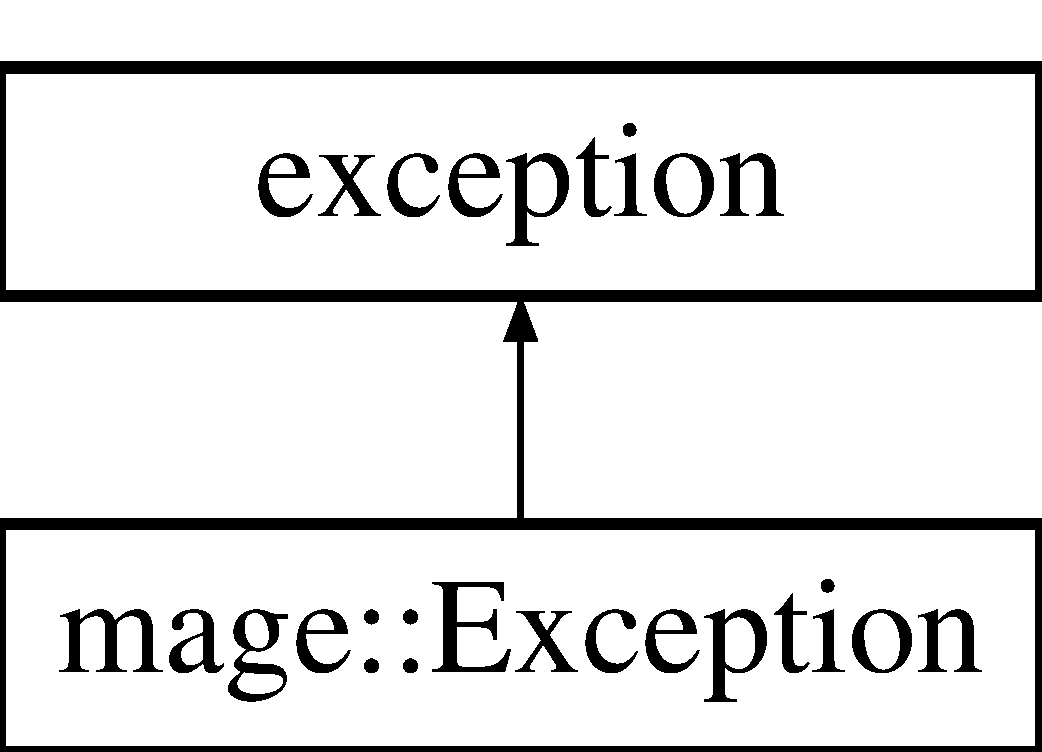
\includegraphics[height=2.000000cm]{classmage_1_1_exception}
\end{center}
\end{figure}
\subsection*{Public Member Functions}
\begin{DoxyCompactItemize}
\item 
\mbox{\hyperlink{classmage_1_1_exception_a87fd5f6c5465c01244020afbaebdb9f5}{Exception}} ()
\item 
\mbox{\hyperlink{classmage_1_1_exception_a1fc078e41b69f928fea77ed7ff14d377}{Exception}} (\mbox{\hyperlink{namespacemage_abfd9206dc607ceb5d13ec68bf075a5c0}{const\+\_\+zstring}} format,...)
\item 
\mbox{\hyperlink{classmage_1_1_exception_a11c7f85cb343cb2a894062508ef587f4}{Exception}} (\mbox{\hyperlink{namespacemage_abfd9206dc607ceb5d13ec68bf075a5c0}{const\+\_\+zstring}} format, va\+\_\+list args)
\item 
\mbox{\hyperlink{classmage_1_1_exception_a3f8642ade2ed1168a9853a50ee0e8e98}{Exception}} (const \mbox{\hyperlink{classmage_1_1_exception}{Exception}} \&exception)
\item 
\mbox{\hyperlink{classmage_1_1_exception_a5a745eb8921cb986c822c0f95455314a}{Exception}} (\mbox{\hyperlink{classmage_1_1_exception}{Exception}} \&\&exception)
\item 
virtual \mbox{\hyperlink{classmage_1_1_exception_a088e91ba8dffd31a9d6aa7d4af2ee2c0}{$\sim$\+Exception}} ()
\item 
\mbox{\hyperlink{classmage_1_1_exception}{Exception}} \& \mbox{\hyperlink{classmage_1_1_exception_ab0e7e6b32b07505271a4a88067ab54f4}{operator=}} (const \mbox{\hyperlink{classmage_1_1_exception}{Exception}} \&exception)
\item 
\mbox{\hyperlink{classmage_1_1_exception}{Exception}} \& \mbox{\hyperlink{classmage_1_1_exception_aa9305c6bd8836f56ffa970473533f031}{operator=}} (\mbox{\hyperlink{classmage_1_1_exception}{Exception}} \&\&exception)
\item 
virtual const char $\ast$ \mbox{\hyperlink{classmage_1_1_exception_ae2bd4437e2b7c960f022f7d3bf79baa7}{what}} () const noexcept override
\end{DoxyCompactItemize}
\subsection*{Private Attributes}
\begin{DoxyCompactItemize}
\item 
char \mbox{\hyperlink{classmage_1_1_exception_ad5bd9bb044bebaa1bac36c8c8a25c052}{m\+\_\+text}} \mbox{[}\mbox{\hyperlink{classmage_1_1_exception_a41c9eb8e4a238210822170dfa211e493}{s\+\_\+buffer\+\_\+size}}\mbox{]}
\end{DoxyCompactItemize}
\subsection*{Static Private Attributes}
\begin{DoxyCompactItemize}
\item 
static constexpr size\+\_\+t \mbox{\hyperlink{classmage_1_1_exception_a41c9eb8e4a238210822170dfa211e493}{s\+\_\+buffer\+\_\+size}} = 2048
\end{DoxyCompactItemize}


\subsection{Detailed Description}
A class of formatted exceptions. 

\subsection{Constructor \& Destructor Documentation}
\mbox{\Hypertarget{classmage_1_1_exception_a87fd5f6c5465c01244020afbaebdb9f5}\label{classmage_1_1_exception_a87fd5f6c5465c01244020afbaebdb9f5}} 
\index{mage\+::\+Exception@{mage\+::\+Exception}!Exception@{Exception}}
\index{Exception@{Exception}!mage\+::\+Exception@{mage\+::\+Exception}}
\subsubsection{\texorpdfstring{Exception()}{Exception()}\hspace{0.1cm}{\footnotesize\ttfamily [1/5]}}
{\footnotesize\ttfamily mage\+::\+Exception\+::\+Exception (\begin{DoxyParamCaption}{ }\end{DoxyParamCaption})}

Constructs a formatted exception. \mbox{\Hypertarget{classmage_1_1_exception_a1fc078e41b69f928fea77ed7ff14d377}\label{classmage_1_1_exception_a1fc078e41b69f928fea77ed7ff14d377}} 
\index{mage\+::\+Exception@{mage\+::\+Exception}!Exception@{Exception}}
\index{Exception@{Exception}!mage\+::\+Exception@{mage\+::\+Exception}}
\subsubsection{\texorpdfstring{Exception()}{Exception()}\hspace{0.1cm}{\footnotesize\ttfamily [2/5]}}
{\footnotesize\ttfamily mage\+::\+Exception\+::\+Exception (\begin{DoxyParamCaption}\item[{\mbox{\hyperlink{namespacemage_abfd9206dc607ceb5d13ec68bf075a5c0}{const\+\_\+zstring}}}]{format,  }\item[{}]{... }\end{DoxyParamCaption})\hspace{0.3cm}{\ttfamily [explicit]}}

Constructs a formatted exception.


\begin{DoxyParams}[1]{Parameters}
\mbox{\tt in}  & {\em format} & Pointer to the message format. \\
\hline
\end{DoxyParams}
\mbox{\Hypertarget{classmage_1_1_exception_a11c7f85cb343cb2a894062508ef587f4}\label{classmage_1_1_exception_a11c7f85cb343cb2a894062508ef587f4}} 
\index{mage\+::\+Exception@{mage\+::\+Exception}!Exception@{Exception}}
\index{Exception@{Exception}!mage\+::\+Exception@{mage\+::\+Exception}}
\subsubsection{\texorpdfstring{Exception()}{Exception()}\hspace{0.1cm}{\footnotesize\ttfamily [3/5]}}
{\footnotesize\ttfamily mage\+::\+Exception\+::\+Exception (\begin{DoxyParamCaption}\item[{\mbox{\hyperlink{namespacemage_abfd9206dc607ceb5d13ec68bf075a5c0}{const\+\_\+zstring}}}]{format,  }\item[{va\+\_\+list}]{args }\end{DoxyParamCaption})\hspace{0.3cm}{\ttfamily [explicit]}}

Constructs a formatted exception.


\begin{DoxyParams}[1]{Parameters}
\mbox{\tt in}  & {\em format} & Pointer to the message format. \\
\hline
\mbox{\tt in}  & {\em args} & The variable argument list. \\
\hline
\end{DoxyParams}
\mbox{\Hypertarget{classmage_1_1_exception_a3f8642ade2ed1168a9853a50ee0e8e98}\label{classmage_1_1_exception_a3f8642ade2ed1168a9853a50ee0e8e98}} 
\index{mage\+::\+Exception@{mage\+::\+Exception}!Exception@{Exception}}
\index{Exception@{Exception}!mage\+::\+Exception@{mage\+::\+Exception}}
\subsubsection{\texorpdfstring{Exception()}{Exception()}\hspace{0.1cm}{\footnotesize\ttfamily [4/5]}}
{\footnotesize\ttfamily mage\+::\+Exception\+::\+Exception (\begin{DoxyParamCaption}\item[{const \mbox{\hyperlink{classmage_1_1_exception}{Exception}} \&}]{exception }\end{DoxyParamCaption})\hspace{0.3cm}{\ttfamily [default]}}

Constructs a formatted exception from the given formatted exception.


\begin{DoxyParams}[1]{Parameters}
\mbox{\tt in}  & {\em exception} & A reference to a formatted exception to copy. \\
\hline
\end{DoxyParams}
\mbox{\Hypertarget{classmage_1_1_exception_a5a745eb8921cb986c822c0f95455314a}\label{classmage_1_1_exception_a5a745eb8921cb986c822c0f95455314a}} 
\index{mage\+::\+Exception@{mage\+::\+Exception}!Exception@{Exception}}
\index{Exception@{Exception}!mage\+::\+Exception@{mage\+::\+Exception}}
\subsubsection{\texorpdfstring{Exception()}{Exception()}\hspace{0.1cm}{\footnotesize\ttfamily [5/5]}}
{\footnotesize\ttfamily mage\+::\+Exception\+::\+Exception (\begin{DoxyParamCaption}\item[{\mbox{\hyperlink{classmage_1_1_exception}{Exception}} \&\&}]{exception }\end{DoxyParamCaption})\hspace{0.3cm}{\ttfamily [default]}}

Constructs a formatted exception by moving the given formatted exception.


\begin{DoxyParams}[1]{Parameters}
\mbox{\tt in}  & {\em exception} & A reference to a formatted exception to move. \\
\hline
\end{DoxyParams}
\mbox{\Hypertarget{classmage_1_1_exception_a088e91ba8dffd31a9d6aa7d4af2ee2c0}\label{classmage_1_1_exception_a088e91ba8dffd31a9d6aa7d4af2ee2c0}} 
\index{mage\+::\+Exception@{mage\+::\+Exception}!````~Exception@{$\sim$\+Exception}}
\index{````~Exception@{$\sim$\+Exception}!mage\+::\+Exception@{mage\+::\+Exception}}
\subsubsection{\texorpdfstring{$\sim$\+Exception()}{~Exception()}}
{\footnotesize\ttfamily mage\+::\+Exception\+::$\sim$\+Exception (\begin{DoxyParamCaption}{ }\end{DoxyParamCaption})\hspace{0.3cm}{\ttfamily [virtual]}, {\ttfamily [default]}}

Destructs this formatted exception. 

\subsection{Member Function Documentation}
\mbox{\Hypertarget{classmage_1_1_exception_ab0e7e6b32b07505271a4a88067ab54f4}\label{classmage_1_1_exception_ab0e7e6b32b07505271a4a88067ab54f4}} 
\index{mage\+::\+Exception@{mage\+::\+Exception}!operator=@{operator=}}
\index{operator=@{operator=}!mage\+::\+Exception@{mage\+::\+Exception}}
\subsubsection{\texorpdfstring{operator=()}{operator=()}\hspace{0.1cm}{\footnotesize\ttfamily [1/2]}}
{\footnotesize\ttfamily \mbox{\hyperlink{classmage_1_1_exception}{Exception}} \& mage\+::\+Exception\+::operator= (\begin{DoxyParamCaption}\item[{const \mbox{\hyperlink{classmage_1_1_exception}{Exception}} \&}]{exception }\end{DoxyParamCaption})\hspace{0.3cm}{\ttfamily [default]}}

Copies the given formatted exception to this formatted exception.


\begin{DoxyParams}[1]{Parameters}
\mbox{\tt in}  & {\em exception} & A reference to a formatted exception to copy. \\
\hline
\end{DoxyParams}
\begin{DoxyReturn}{Returns}
A reference to the copy of the given formatted exception (i.\+e. this formatted exception). 
\end{DoxyReturn}
\mbox{\Hypertarget{classmage_1_1_exception_aa9305c6bd8836f56ffa970473533f031}\label{classmage_1_1_exception_aa9305c6bd8836f56ffa970473533f031}} 
\index{mage\+::\+Exception@{mage\+::\+Exception}!operator=@{operator=}}
\index{operator=@{operator=}!mage\+::\+Exception@{mage\+::\+Exception}}
\subsubsection{\texorpdfstring{operator=()}{operator=()}\hspace{0.1cm}{\footnotesize\ttfamily [2/2]}}
{\footnotesize\ttfamily \mbox{\hyperlink{classmage_1_1_exception}{Exception}} \& mage\+::\+Exception\+::operator= (\begin{DoxyParamCaption}\item[{\mbox{\hyperlink{classmage_1_1_exception}{Exception}} \&\&}]{exception }\end{DoxyParamCaption})\hspace{0.3cm}{\ttfamily [default]}}

Moves the given formatted exception to this formatted exception.


\begin{DoxyParams}[1]{Parameters}
\mbox{\tt in}  & {\em exception} & A reference to a formatted exception to move. \\
\hline
\end{DoxyParams}
\begin{DoxyReturn}{Returns}
A reference to the moved formatted exception (i.\+e. this formatted exception). 
\end{DoxyReturn}
\mbox{\Hypertarget{classmage_1_1_exception_ae2bd4437e2b7c960f022f7d3bf79baa7}\label{classmage_1_1_exception_ae2bd4437e2b7c960f022f7d3bf79baa7}} 
\index{mage\+::\+Exception@{mage\+::\+Exception}!what@{what}}
\index{what@{what}!mage\+::\+Exception@{mage\+::\+Exception}}
\subsubsection{\texorpdfstring{what()}{what()}}
{\footnotesize\ttfamily const char $\ast$ mage\+::\+Exception\+::what (\begin{DoxyParamCaption}{ }\end{DoxyParamCaption}) const\hspace{0.3cm}{\ttfamily [override]}, {\ttfamily [virtual]}, {\ttfamily [noexcept]}}

Returns a null-\/terminated byte string that may be used to identify the exception.

\begin{DoxyReturn}{Returns}
A null-\/terminated byte string that may be used to identify the exception. 
\end{DoxyReturn}


\subsection{Member Data Documentation}
\mbox{\Hypertarget{classmage_1_1_exception_ad5bd9bb044bebaa1bac36c8c8a25c052}\label{classmage_1_1_exception_ad5bd9bb044bebaa1bac36c8c8a25c052}} 
\index{mage\+::\+Exception@{mage\+::\+Exception}!m\+\_\+text@{m\+\_\+text}}
\index{m\+\_\+text@{m\+\_\+text}!mage\+::\+Exception@{mage\+::\+Exception}}
\subsubsection{\texorpdfstring{m\+\_\+text}{m\_text}}
{\footnotesize\ttfamily char mage\+::\+Exception\+::m\+\_\+text\mbox{[}\mbox{\hyperlink{classmage_1_1_exception_a41c9eb8e4a238210822170dfa211e493}{s\+\_\+buffer\+\_\+size}}\mbox{]}\hspace{0.3cm}{\ttfamily [private]}}

The text buffer of this formatted exception. \mbox{\Hypertarget{classmage_1_1_exception_a41c9eb8e4a238210822170dfa211e493}\label{classmage_1_1_exception_a41c9eb8e4a238210822170dfa211e493}} 
\index{mage\+::\+Exception@{mage\+::\+Exception}!s\+\_\+buffer\+\_\+size@{s\+\_\+buffer\+\_\+size}}
\index{s\+\_\+buffer\+\_\+size@{s\+\_\+buffer\+\_\+size}!mage\+::\+Exception@{mage\+::\+Exception}}
\subsubsection{\texorpdfstring{s\+\_\+buffer\+\_\+size}{s\_buffer\_size}}
{\footnotesize\ttfamily constexpr size\+\_\+t mage\+::\+Exception\+::s\+\_\+buffer\+\_\+size = 2048\hspace{0.3cm}{\ttfamily [static]}, {\ttfamily [private]}}

The buffer size of exceptions. 
\hypertarget{structmage_1_1details_1_1_file_stream_closer}{}\section{mage\+:\+:details\+:\+:File\+Stream\+Closer Struct Reference}
\label{structmage_1_1details_1_1_file_stream_closer}\index{mage\+::details\+::\+File\+Stream\+Closer@{mage\+::details\+::\+File\+Stream\+Closer}}


{\ttfamily \#include $<$memory.\+hpp$>$}

\subsection*{Public Member Functions}
\begin{DoxyCompactItemize}
\item 
void \mbox{\hyperlink{structmage_1_1details_1_1_file_stream_closer_a3d322e59dfdf94c94cc0a09388a6dbe7}{operator()}} (std\+::\+F\+I\+LE $\ast$stream) const noexcept
\end{DoxyCompactItemize}


\subsection{Detailed Description}
A struct of file stream destructors (i.\+e. for closing file streams). 

\subsection{Member Function Documentation}
\mbox{\Hypertarget{structmage_1_1details_1_1_file_stream_closer_a3d322e59dfdf94c94cc0a09388a6dbe7}\label{structmage_1_1details_1_1_file_stream_closer_a3d322e59dfdf94c94cc0a09388a6dbe7}} 
\index{mage\+::details\+::\+File\+Stream\+Closer@{mage\+::details\+::\+File\+Stream\+Closer}!operator()@{operator()}}
\index{operator()@{operator()}!mage\+::details\+::\+File\+Stream\+Closer@{mage\+::details\+::\+File\+Stream\+Closer}}
\subsubsection{\texorpdfstring{operator()()}{operator()()}}
{\footnotesize\ttfamily void mage\+::details\+::\+File\+Stream\+Closer\+::operator() (\begin{DoxyParamCaption}\item[{std\+::\+F\+I\+LE $\ast$}]{stream }\end{DoxyParamCaption}) const\hspace{0.3cm}{\ttfamily [noexcept]}}

Destructs the file stream.


\begin{DoxyParams}[1]{Parameters}
\mbox{\tt in}  & {\em stream} & A pointer to a file stream to destruct. \\
\hline
\end{DoxyParams}

\hypertarget{classmage_1_1rendering_1_1_fog}{}\section{mage\+:\+:rendering\+:\+:Fog Class Reference}
\label{classmage_1_1rendering_1_1_fog}\index{mage\+::rendering\+::\+Fog@{mage\+::rendering\+::\+Fog}}


{\ttfamily \#include $<$camera.\+hpp$>$}

\subsection*{Public Member Functions}
\begin{DoxyCompactItemize}
\item 
constexpr \mbox{\hyperlink{classmage_1_1rendering_1_1_fog_a48489b0ce940aff4395eb5ea88394081}{Fog}} () noexcept
\item 
constexpr \mbox{\hyperlink{classmage_1_1rendering_1_1_fog_a2f730d70ed426468f113d44e7810394b}{Fog}} (const \mbox{\hyperlink{classmage_1_1rendering_1_1_fog}{Fog}} \&fog) noexcept=default
\item 
constexpr \mbox{\hyperlink{classmage_1_1rendering_1_1_fog_aeed9b3fc18dabe37199c51ed7c4f5930}{Fog}} (\mbox{\hyperlink{classmage_1_1rendering_1_1_fog}{Fog}} \&\&fog) noexcept=default
\item 
\mbox{\hyperlink{classmage_1_1rendering_1_1_fog_a3dfb641a2c5688172e3c4be7c91631a2}{$\sim$\+Fog}} ()=default
\item 
\mbox{\hyperlink{classmage_1_1rendering_1_1_fog}{Fog}} \& \mbox{\hyperlink{classmage_1_1rendering_1_1_fog_a79bb3e3b7cbae494ae6f4d7f84a61aae}{operator=}} (const \mbox{\hyperlink{classmage_1_1rendering_1_1_fog}{Fog}} \&fog) noexcept=default
\item 
\mbox{\hyperlink{classmage_1_1rendering_1_1_fog}{Fog}} \& \mbox{\hyperlink{classmage_1_1rendering_1_1_fog_a60a4ed93bba16c6acfec807c0e753b22}{operator=}} (\mbox{\hyperlink{classmage_1_1rendering_1_1_fog}{Fog}} \&\&fog) noexcept=default
\item 
constexpr \mbox{\hyperlink{structmage_1_1_r_g_b}{R\+GB}} \& \mbox{\hyperlink{classmage_1_1rendering_1_1_fog_af2ba57f86df0f681ad6b67cba5fc8dc1}{Get\+Base\+Color}} () noexcept
\item 
constexpr const \mbox{\hyperlink{structmage_1_1_r_g_b}{R\+GB}} \& \mbox{\hyperlink{classmage_1_1rendering_1_1_fog_a2a1441d2a0cdbc074260fa1af7fc656a}{Get\+Base\+Color}} () const noexcept
\item 
constexpr \mbox{\hyperlink{namespacemage_aa97e833b45f06d60a0a9c4fc22ae02c0}{F32}} \mbox{\hyperlink{classmage_1_1rendering_1_1_fog_ac99a5479a39027723807296c49fdfbc8}{Get\+Density}} () const noexcept
\item 
constexpr void \mbox{\hyperlink{classmage_1_1rendering_1_1_fog_a9b498c71c58e28bd58b09e4385338a13}{Set\+Density}} (\mbox{\hyperlink{namespacemage_aa97e833b45f06d60a0a9c4fc22ae02c0}{F32}} density) noexcept
\end{DoxyCompactItemize}
\subsection*{Private Attributes}
\begin{DoxyCompactItemize}
\item 
\mbox{\hyperlink{structmage_1_1_r_g_b}{R\+GB}} \mbox{\hyperlink{classmage_1_1rendering_1_1_fog_a5f7d0bcb79a1d68b2456bd005db48a99}{m\+\_\+base\+\_\+color}}
\item 
\mbox{\hyperlink{namespacemage_aa97e833b45f06d60a0a9c4fc22ae02c0}{F32}} \mbox{\hyperlink{classmage_1_1rendering_1_1_fog_aa7a402ad9eef0e9916bb9f83751ebe32}{m\+\_\+density}}
\end{DoxyCompactItemize}


\subsection{Detailed Description}
A class of fog with respect to the camera position (eye) to avoid popping artifacts while moving. 

\subsection{Constructor \& Destructor Documentation}
\mbox{\Hypertarget{classmage_1_1rendering_1_1_fog_a48489b0ce940aff4395eb5ea88394081}\label{classmage_1_1rendering_1_1_fog_a48489b0ce940aff4395eb5ea88394081}} 
\index{mage\+::rendering\+::\+Fog@{mage\+::rendering\+::\+Fog}!Fog@{Fog}}
\index{Fog@{Fog}!mage\+::rendering\+::\+Fog@{mage\+::rendering\+::\+Fog}}
\subsubsection{\texorpdfstring{Fog()}{Fog()}\hspace{0.1cm}{\footnotesize\ttfamily [1/3]}}
{\footnotesize\ttfamily constexpr mage\+::rendering\+::\+Fog\+::\+Fog (\begin{DoxyParamCaption}{ }\end{DoxyParamCaption})\hspace{0.3cm}{\ttfamily [noexcept]}}

Constructs a fog. \mbox{\Hypertarget{classmage_1_1rendering_1_1_fog_a2f730d70ed426468f113d44e7810394b}\label{classmage_1_1rendering_1_1_fog_a2f730d70ed426468f113d44e7810394b}} 
\index{mage\+::rendering\+::\+Fog@{mage\+::rendering\+::\+Fog}!Fog@{Fog}}
\index{Fog@{Fog}!mage\+::rendering\+::\+Fog@{mage\+::rendering\+::\+Fog}}
\subsubsection{\texorpdfstring{Fog()}{Fog()}\hspace{0.1cm}{\footnotesize\ttfamily [2/3]}}
{\footnotesize\ttfamily constexpr mage\+::rendering\+::\+Fog\+::\+Fog (\begin{DoxyParamCaption}\item[{const \mbox{\hyperlink{classmage_1_1rendering_1_1_fog}{Fog}} \&}]{fog }\end{DoxyParamCaption})\hspace{0.3cm}{\ttfamily [default]}, {\ttfamily [noexcept]}}

Constructs a fog from the given fog.


\begin{DoxyParams}[1]{Parameters}
\mbox{\tt in}  & {\em fog} & A reference to the fog to copy. \\
\hline
\end{DoxyParams}
\mbox{\Hypertarget{classmage_1_1rendering_1_1_fog_aeed9b3fc18dabe37199c51ed7c4f5930}\label{classmage_1_1rendering_1_1_fog_aeed9b3fc18dabe37199c51ed7c4f5930}} 
\index{mage\+::rendering\+::\+Fog@{mage\+::rendering\+::\+Fog}!Fog@{Fog}}
\index{Fog@{Fog}!mage\+::rendering\+::\+Fog@{mage\+::rendering\+::\+Fog}}
\subsubsection{\texorpdfstring{Fog()}{Fog()}\hspace{0.1cm}{\footnotesize\ttfamily [3/3]}}
{\footnotesize\ttfamily constexpr mage\+::rendering\+::\+Fog\+::\+Fog (\begin{DoxyParamCaption}\item[{\mbox{\hyperlink{classmage_1_1rendering_1_1_fog}{Fog}} \&\&}]{fog }\end{DoxyParamCaption})\hspace{0.3cm}{\ttfamily [default]}, {\ttfamily [noexcept]}}

Constructs a fog by moving the given fog.


\begin{DoxyParams}[1]{Parameters}
\mbox{\tt in}  & {\em fog} & A reference to the fog to move. \\
\hline
\end{DoxyParams}
\mbox{\Hypertarget{classmage_1_1rendering_1_1_fog_a3dfb641a2c5688172e3c4be7c91631a2}\label{classmage_1_1rendering_1_1_fog_a3dfb641a2c5688172e3c4be7c91631a2}} 
\index{mage\+::rendering\+::\+Fog@{mage\+::rendering\+::\+Fog}!````~Fog@{$\sim$\+Fog}}
\index{````~Fog@{$\sim$\+Fog}!mage\+::rendering\+::\+Fog@{mage\+::rendering\+::\+Fog}}
\subsubsection{\texorpdfstring{$\sim$\+Fog()}{~Fog()}}
{\footnotesize\ttfamily mage\+::rendering\+::\+Fog\+::$\sim$\+Fog (\begin{DoxyParamCaption}{ }\end{DoxyParamCaption})\hspace{0.3cm}{\ttfamily [default]}}

Destructs this fog. 

\subsection{Member Function Documentation}
\mbox{\Hypertarget{classmage_1_1rendering_1_1_fog_af2ba57f86df0f681ad6b67cba5fc8dc1}\label{classmage_1_1rendering_1_1_fog_af2ba57f86df0f681ad6b67cba5fc8dc1}} 
\index{mage\+::rendering\+::\+Fog@{mage\+::rendering\+::\+Fog}!Get\+Base\+Color@{Get\+Base\+Color}}
\index{Get\+Base\+Color@{Get\+Base\+Color}!mage\+::rendering\+::\+Fog@{mage\+::rendering\+::\+Fog}}
\subsubsection{\texorpdfstring{Get\+Base\+Color()}{GetBaseColor()}\hspace{0.1cm}{\footnotesize\ttfamily [1/2]}}
{\footnotesize\ttfamily constexpr \mbox{\hyperlink{structmage_1_1_r_g_b}{R\+GB}}\& mage\+::rendering\+::\+Fog\+::\+Get\+Base\+Color (\begin{DoxyParamCaption}{ }\end{DoxyParamCaption})\hspace{0.3cm}{\ttfamily [noexcept]}}

Returns the (linear) base color of this fog.

\begin{DoxyReturn}{Returns}
A reference to the s\+R\+GB base color of this fog. 
\end{DoxyReturn}
\mbox{\Hypertarget{classmage_1_1rendering_1_1_fog_a2a1441d2a0cdbc074260fa1af7fc656a}\label{classmage_1_1rendering_1_1_fog_a2a1441d2a0cdbc074260fa1af7fc656a}} 
\index{mage\+::rendering\+::\+Fog@{mage\+::rendering\+::\+Fog}!Get\+Base\+Color@{Get\+Base\+Color}}
\index{Get\+Base\+Color@{Get\+Base\+Color}!mage\+::rendering\+::\+Fog@{mage\+::rendering\+::\+Fog}}
\subsubsection{\texorpdfstring{Get\+Base\+Color()}{GetBaseColor()}\hspace{0.1cm}{\footnotesize\ttfamily [2/2]}}
{\footnotesize\ttfamily constexpr const \mbox{\hyperlink{structmage_1_1_r_g_b}{R\+GB}}\& mage\+::rendering\+::\+Fog\+::\+Get\+Base\+Color (\begin{DoxyParamCaption}{ }\end{DoxyParamCaption}) const\hspace{0.3cm}{\ttfamily [noexcept]}}

Returns the (linear) base color of this fog.

\begin{DoxyReturn}{Returns}
A reference to the s\+R\+GB base color of this fog. 
\end{DoxyReturn}
\mbox{\Hypertarget{classmage_1_1rendering_1_1_fog_ac99a5479a39027723807296c49fdfbc8}\label{classmage_1_1rendering_1_1_fog_ac99a5479a39027723807296c49fdfbc8}} 
\index{mage\+::rendering\+::\+Fog@{mage\+::rendering\+::\+Fog}!Get\+Density@{Get\+Density}}
\index{Get\+Density@{Get\+Density}!mage\+::rendering\+::\+Fog@{mage\+::rendering\+::\+Fog}}
\subsubsection{\texorpdfstring{Get\+Density()}{GetDensity()}}
{\footnotesize\ttfamily constexpr \mbox{\hyperlink{namespacemage_aa97e833b45f06d60a0a9c4fc22ae02c0}{F32}} mage\+::rendering\+::\+Fog\+::\+Get\+Density (\begin{DoxyParamCaption}{ }\end{DoxyParamCaption}) const\hspace{0.3cm}{\ttfamily [noexcept]}}

Returns the density of this fog.

\begin{DoxyReturn}{Returns}
The density of this fog. 
\end{DoxyReturn}
\mbox{\Hypertarget{classmage_1_1rendering_1_1_fog_a79bb3e3b7cbae494ae6f4d7f84a61aae}\label{classmage_1_1rendering_1_1_fog_a79bb3e3b7cbae494ae6f4d7f84a61aae}} 
\index{mage\+::rendering\+::\+Fog@{mage\+::rendering\+::\+Fog}!operator=@{operator=}}
\index{operator=@{operator=}!mage\+::rendering\+::\+Fog@{mage\+::rendering\+::\+Fog}}
\subsubsection{\texorpdfstring{operator=()}{operator=()}\hspace{0.1cm}{\footnotesize\ttfamily [1/2]}}
{\footnotesize\ttfamily \mbox{\hyperlink{classmage_1_1rendering_1_1_fog}{Fog}}\& mage\+::rendering\+::\+Fog\+::operator= (\begin{DoxyParamCaption}\item[{const \mbox{\hyperlink{classmage_1_1rendering_1_1_fog}{Fog}} \&}]{fog }\end{DoxyParamCaption})\hspace{0.3cm}{\ttfamily [default]}, {\ttfamily [noexcept]}}

Copies the given fog to this fog.


\begin{DoxyParams}[1]{Parameters}
\mbox{\tt in}  & {\em fog} & A reference to the fog to copy. \\
\hline
\end{DoxyParams}
\begin{DoxyReturn}{Returns}
A reference to the copy of the given fog (i.\+e. this fog). 
\end{DoxyReturn}
\mbox{\Hypertarget{classmage_1_1rendering_1_1_fog_a60a4ed93bba16c6acfec807c0e753b22}\label{classmage_1_1rendering_1_1_fog_a60a4ed93bba16c6acfec807c0e753b22}} 
\index{mage\+::rendering\+::\+Fog@{mage\+::rendering\+::\+Fog}!operator=@{operator=}}
\index{operator=@{operator=}!mage\+::rendering\+::\+Fog@{mage\+::rendering\+::\+Fog}}
\subsubsection{\texorpdfstring{operator=()}{operator=()}\hspace{0.1cm}{\footnotesize\ttfamily [2/2]}}
{\footnotesize\ttfamily \mbox{\hyperlink{classmage_1_1rendering_1_1_fog}{Fog}}\& mage\+::rendering\+::\+Fog\+::operator= (\begin{DoxyParamCaption}\item[{\mbox{\hyperlink{classmage_1_1rendering_1_1_fog}{Fog}} \&\&}]{fog }\end{DoxyParamCaption})\hspace{0.3cm}{\ttfamily [default]}, {\ttfamily [noexcept]}}

Moves the given fog to this fog.


\begin{DoxyParams}[1]{Parameters}
\mbox{\tt in}  & {\em fog} & A reference to the fog to move. \\
\hline
\end{DoxyParams}
\begin{DoxyReturn}{Returns}
A reference to the moved fog (i.\+e. this fog). 
\end{DoxyReturn}
\mbox{\Hypertarget{classmage_1_1rendering_1_1_fog_a9b498c71c58e28bd58b09e4385338a13}\label{classmage_1_1rendering_1_1_fog_a9b498c71c58e28bd58b09e4385338a13}} 
\index{mage\+::rendering\+::\+Fog@{mage\+::rendering\+::\+Fog}!Set\+Density@{Set\+Density}}
\index{Set\+Density@{Set\+Density}!mage\+::rendering\+::\+Fog@{mage\+::rendering\+::\+Fog}}
\subsubsection{\texorpdfstring{Set\+Density()}{SetDensity()}}
{\footnotesize\ttfamily constexpr void mage\+::rendering\+::\+Fog\+::\+Set\+Density (\begin{DoxyParamCaption}\item[{\mbox{\hyperlink{namespacemage_aa97e833b45f06d60a0a9c4fc22ae02c0}{F32}}}]{density }\end{DoxyParamCaption})\hspace{0.3cm}{\ttfamily [noexcept]}}

Sets the density of this fog to the given value.


\begin{DoxyParams}[1]{Parameters}
\mbox{\tt in}  & {\em density} & The density. \\
\hline
\end{DoxyParams}


\subsection{Member Data Documentation}
\mbox{\Hypertarget{classmage_1_1rendering_1_1_fog_a5f7d0bcb79a1d68b2456bd005db48a99}\label{classmage_1_1rendering_1_1_fog_a5f7d0bcb79a1d68b2456bd005db48a99}} 
\index{mage\+::rendering\+::\+Fog@{mage\+::rendering\+::\+Fog}!m\+\_\+base\+\_\+color@{m\+\_\+base\+\_\+color}}
\index{m\+\_\+base\+\_\+color@{m\+\_\+base\+\_\+color}!mage\+::rendering\+::\+Fog@{mage\+::rendering\+::\+Fog}}
\subsubsection{\texorpdfstring{m\+\_\+base\+\_\+color}{m\_base\_color}}
{\footnotesize\ttfamily \mbox{\hyperlink{structmage_1_1_r_g_b}{R\+GB}} mage\+::rendering\+::\+Fog\+::m\+\_\+base\+\_\+color\hspace{0.3cm}{\ttfamily [private]}}

The (linear) base color of this fog. \mbox{\Hypertarget{classmage_1_1rendering_1_1_fog_aa7a402ad9eef0e9916bb9f83751ebe32}\label{classmage_1_1rendering_1_1_fog_aa7a402ad9eef0e9916bb9f83751ebe32}} 
\index{mage\+::rendering\+::\+Fog@{mage\+::rendering\+::\+Fog}!m\+\_\+density@{m\+\_\+density}}
\index{m\+\_\+density@{m\+\_\+density}!mage\+::rendering\+::\+Fog@{mage\+::rendering\+::\+Fog}}
\subsubsection{\texorpdfstring{m\+\_\+density}{m\_density}}
{\footnotesize\ttfamily \mbox{\hyperlink{namespacemage_aa97e833b45f06d60a0a9c4fc22ae02c0}{F32}} mage\+::rendering\+::\+Fog\+::m\+\_\+density\hspace{0.3cm}{\ttfamily [private]}}

The density of this fog. 
\hypertarget{classmage_1_1rendering_1_1_forward_pass}{}\section{mage\+:\+:rendering\+:\+:Forward\+Pass Class Reference}
\label{classmage_1_1rendering_1_1_forward_pass}\index{mage\+::rendering\+::\+Forward\+Pass@{mage\+::rendering\+::\+Forward\+Pass}}


{\ttfamily \#include $<$forward\+\_\+pass.\+hpp$>$}

\subsection*{Public Member Functions}
\begin{DoxyCompactItemize}
\item 
\mbox{\hyperlink{classmage_1_1rendering_1_1_forward_pass_aabff6394203f0927f65cd9d591eefa58}{Forward\+Pass}} (I\+D3\+D11\+Device \&device, I\+D3\+D11\+Device\+Context \&device\+\_\+context, \mbox{\hyperlink{classmage_1_1rendering_1_1_state_manager}{State\+Manager}} \&state\+\_\+manager, \mbox{\hyperlink{classmage_1_1rendering_1_1_resource_manager}{Resource\+Manager}} \&resource\+\_\+manager)
\item 
\mbox{\hyperlink{classmage_1_1rendering_1_1_forward_pass_a5454d208d794e9ef2ae05c03e7b839fd}{Forward\+Pass}} (const \mbox{\hyperlink{classmage_1_1rendering_1_1_forward_pass}{Forward\+Pass}} \&pass)=delete
\item 
\mbox{\hyperlink{classmage_1_1rendering_1_1_forward_pass_a5f7026d7b4a439bdbacfeaf8fff152c1}{Forward\+Pass}} (\mbox{\hyperlink{classmage_1_1rendering_1_1_forward_pass}{Forward\+Pass}} \&\&pass) noexcept
\item 
\mbox{\hyperlink{classmage_1_1rendering_1_1_forward_pass_a9fdcc7dca5097f0feff2f7be92a2727c}{$\sim$\+Forward\+Pass}} ()
\item 
\mbox{\hyperlink{classmage_1_1rendering_1_1_forward_pass}{Forward\+Pass}} \& \mbox{\hyperlink{classmage_1_1rendering_1_1_forward_pass_a373b424f52fb5a209bed756dc06f47ee}{operator=}} (const \mbox{\hyperlink{classmage_1_1rendering_1_1_forward_pass}{Forward\+Pass}} \&pass)=delete
\item 
\mbox{\hyperlink{classmage_1_1rendering_1_1_forward_pass}{Forward\+Pass}} \& \mbox{\hyperlink{classmage_1_1rendering_1_1_forward_pass_aba2191f3e482d2fb0db2ad2cab77c817}{operator=}} (\mbox{\hyperlink{classmage_1_1rendering_1_1_forward_pass}{Forward\+Pass}} \&\&pass) noexcept
\item 
void X\+M\+\_\+\+C\+A\+L\+L\+C\+O\+NV \mbox{\hyperlink{classmage_1_1rendering_1_1_forward_pass_ae8d819c35db0b35afe309c00448d1c83}{Render}} (const \mbox{\hyperlink{classmage_1_1rendering_1_1_world}{World}} \&world, F\+X\+M\+M\+A\+T\+R\+IX world\+\_\+to\+\_\+projection, \mbox{\hyperlink{namespacemage_1_1rendering_ab8fe8684ca4bd74ba3a394b00cf125b5}{B\+R\+DF}} brdf, bool vct) const
\item 
void X\+M\+\_\+\+C\+A\+L\+L\+C\+O\+NV \mbox{\hyperlink{classmage_1_1rendering_1_1_forward_pass_a7e473c7597d2b725cea68fa74fe20b56}{Render\+Solid}} (const \mbox{\hyperlink{classmage_1_1rendering_1_1_world}{World}} \&world, F\+X\+M\+M\+A\+T\+R\+IX world\+\_\+to\+\_\+projection) const
\item 
void X\+M\+\_\+\+C\+A\+L\+L\+C\+O\+NV \mbox{\hyperlink{classmage_1_1rendering_1_1_forward_pass_aaf7698f452eab9c6cb7cbc07b8991d5b}{Render\+G\+Buffer}} (const \mbox{\hyperlink{classmage_1_1rendering_1_1_world}{World}} \&world, F\+X\+M\+M\+A\+T\+R\+IX world\+\_\+to\+\_\+projection) const
\item 
void X\+M\+\_\+\+C\+A\+L\+L\+C\+O\+NV \mbox{\hyperlink{classmage_1_1rendering_1_1_forward_pass_ac272e648126ed4dc8386edddfc18cc76}{Render\+Emissive}} (const \mbox{\hyperlink{classmage_1_1rendering_1_1_world}{World}} \&world, F\+X\+M\+M\+A\+T\+R\+IX world\+\_\+to\+\_\+projection) const
\item 
void X\+M\+\_\+\+C\+A\+L\+L\+C\+O\+NV \mbox{\hyperlink{classmage_1_1rendering_1_1_forward_pass_a6fae34f08f23dc1a5d15921b239935fb}{Render\+Transparent}} (const \mbox{\hyperlink{classmage_1_1rendering_1_1_world}{World}} \&world, F\+X\+M\+M\+A\+T\+R\+IX world\+\_\+to\+\_\+projection, \mbox{\hyperlink{namespacemage_1_1rendering_ab8fe8684ca4bd74ba3a394b00cf125b5}{B\+R\+DF}} brdf, bool vct) const
\item 
void X\+M\+\_\+\+C\+A\+L\+L\+C\+O\+NV \mbox{\hyperlink{classmage_1_1rendering_1_1_forward_pass_ae18018111470a84e9313f11c72cc3326}{Render\+False\+Color}} (const \mbox{\hyperlink{classmage_1_1rendering_1_1_world}{World}} \&world, F\+X\+M\+M\+A\+T\+R\+IX world\+\_\+to\+\_\+projection, \mbox{\hyperlink{namespacemage_1_1rendering_a6c3d1f4e7a5ae72dc07226e971205534}{False\+Color}} false\+\_\+color) const
\item 
void X\+M\+\_\+\+C\+A\+L\+L\+C\+O\+NV \mbox{\hyperlink{classmage_1_1rendering_1_1_forward_pass_a1d6bbef579e996ffc34d25b29dd3ffef}{Render\+Wireframe}} (const \mbox{\hyperlink{classmage_1_1rendering_1_1_world}{World}} \&world, F\+X\+M\+M\+A\+T\+R\+IX world\+\_\+to\+\_\+projection)
\end{DoxyCompactItemize}
\subsection*{Private Member Functions}
\begin{DoxyCompactItemize}
\item 
void \mbox{\hyperlink{classmage_1_1rendering_1_1_forward_pass_af66584e7efc3565f23f7b5940d6f35eb}{Bind\+Fixed\+Opaque\+State}} () const noexcept
\item 
void \mbox{\hyperlink{classmage_1_1rendering_1_1_forward_pass_aefd3217115558f90b92a1521adfb8bb8}{Bind\+Fixed\+Transparent\+State}} () const noexcept
\item 
void \mbox{\hyperlink{classmage_1_1rendering_1_1_forward_pass_a1d5c1efa0b532674124a264f61f75a07}{Bind\+Fixed\+Wireframe\+State}} () const noexcept
\item 
void \mbox{\hyperlink{classmage_1_1rendering_1_1_forward_pass_a1431c5d2bd8cccc55427aa1cf9a64845}{Bind\+Color}} (const \mbox{\hyperlink{structmage_1_1_r_g_b_a}{R\+G\+BA}} \&color)
\item 
void X\+M\+\_\+\+C\+A\+L\+L\+C\+O\+NV \mbox{\hyperlink{classmage_1_1rendering_1_1_forward_pass_a44354b5b6ccfe27fdc436a37da34c47e}{Render}} (const \mbox{\hyperlink{classmage_1_1rendering_1_1_model}{Model}} \&model, F\+X\+M\+M\+A\+T\+R\+IX world\+\_\+to\+\_\+projection) const noexcept
\end{DoxyCompactItemize}
\subsection*{Private Attributes}
\begin{DoxyCompactItemize}
\item 
std\+::reference\+\_\+wrapper$<$ I\+D3\+D11\+Device\+Context $>$ \mbox{\hyperlink{classmage_1_1rendering_1_1_forward_pass_a4bc03d77fd5a385a9c5878db8028dcc4}{m\+\_\+device\+\_\+context}}
\item 
std\+::reference\+\_\+wrapper$<$ \mbox{\hyperlink{classmage_1_1rendering_1_1_state_manager}{State\+Manager}} $>$ \mbox{\hyperlink{classmage_1_1rendering_1_1_forward_pass_a01d72a7d6be3f98806df7780c94916ff}{m\+\_\+state\+\_\+manager}}
\item 
std\+::reference\+\_\+wrapper$<$ \mbox{\hyperlink{classmage_1_1rendering_1_1_resource_manager}{Resource\+Manager}} $>$ \mbox{\hyperlink{classmage_1_1rendering_1_1_forward_pass_a2b0fe58480704725219acff176695819}{m\+\_\+resource\+\_\+manager}}
\item 
\mbox{\hyperlink{namespacemage_1_1rendering_aaf704b9c54a4181f4950a1761de69dda}{Vertex\+Shader\+Ptr}} \mbox{\hyperlink{classmage_1_1rendering_1_1_forward_pass_ae1483b1f37cd65efdf6059bcc7d1dd09}{m\+\_\+vs}}
\item 
\mbox{\hyperlink{namespacemage_1_1rendering_a6f3ae54f825328465b0cdde0f0de4a36}{Texture\+Ptr}} \mbox{\hyperlink{classmage_1_1rendering_1_1_forward_pass_ab2fcc28c086c7ddb6e13bfd5f9d994b9}{m\+\_\+uv}}
\item 
\mbox{\hyperlink{classmage_1_1rendering_1_1_constant_buffer}{Constant\+Buffer}}$<$ \mbox{\hyperlink{structmage_1_1_r_g_b_a}{R\+G\+BA}} $>$ \mbox{\hyperlink{classmage_1_1rendering_1_1_forward_pass_ace4259d7a292982a3f3111b24fcf7c51}{m\+\_\+color\+\_\+buffer}}
\end{DoxyCompactItemize}


\subsection{Detailed Description}
A class of forward passes for performing light calculations. 

\subsection{Constructor \& Destructor Documentation}
\mbox{\Hypertarget{classmage_1_1rendering_1_1_forward_pass_aabff6394203f0927f65cd9d591eefa58}\label{classmage_1_1rendering_1_1_forward_pass_aabff6394203f0927f65cd9d591eefa58}} 
\index{mage\+::rendering\+::\+Forward\+Pass@{mage\+::rendering\+::\+Forward\+Pass}!Forward\+Pass@{Forward\+Pass}}
\index{Forward\+Pass@{Forward\+Pass}!mage\+::rendering\+::\+Forward\+Pass@{mage\+::rendering\+::\+Forward\+Pass}}
\subsubsection{\texorpdfstring{Forward\+Pass()}{ForwardPass()}\hspace{0.1cm}{\footnotesize\ttfamily [1/3]}}
{\footnotesize\ttfamily mage\+::rendering\+::\+Forward\+Pass\+::\+Forward\+Pass (\begin{DoxyParamCaption}\item[{I\+D3\+D11\+Device \&}]{device,  }\item[{I\+D3\+D11\+Device\+Context \&}]{device\+\_\+context,  }\item[{\mbox{\hyperlink{classmage_1_1rendering_1_1_state_manager}{State\+Manager}} \&}]{state\+\_\+manager,  }\item[{\mbox{\hyperlink{classmage_1_1rendering_1_1_resource_manager}{Resource\+Manager}} \&}]{resource\+\_\+manager }\end{DoxyParamCaption})\hspace{0.3cm}{\ttfamily [explicit]}}

Constructs a forward pass.


\begin{DoxyParams}[1]{Parameters}
\mbox{\tt in}  & {\em device} & A reference to the device. \\
\hline
\mbox{\tt in}  & {\em device\+\_\+context} & A reference to the device context. \\
\hline
\mbox{\tt in}  & {\em state\+\_\+manager} & A reference to the state manager. \\
\hline
\mbox{\tt in}  & {\em resource\+\_\+manager} & A reference to the resource manager. \\
\hline
\end{DoxyParams}
\mbox{\Hypertarget{classmage_1_1rendering_1_1_forward_pass_a5454d208d794e9ef2ae05c03e7b839fd}\label{classmage_1_1rendering_1_1_forward_pass_a5454d208d794e9ef2ae05c03e7b839fd}} 
\index{mage\+::rendering\+::\+Forward\+Pass@{mage\+::rendering\+::\+Forward\+Pass}!Forward\+Pass@{Forward\+Pass}}
\index{Forward\+Pass@{Forward\+Pass}!mage\+::rendering\+::\+Forward\+Pass@{mage\+::rendering\+::\+Forward\+Pass}}
\subsubsection{\texorpdfstring{Forward\+Pass()}{ForwardPass()}\hspace{0.1cm}{\footnotesize\ttfamily [2/3]}}
{\footnotesize\ttfamily mage\+::rendering\+::\+Forward\+Pass\+::\+Forward\+Pass (\begin{DoxyParamCaption}\item[{const \mbox{\hyperlink{classmage_1_1rendering_1_1_forward_pass}{Forward\+Pass}} \&}]{pass }\end{DoxyParamCaption})\hspace{0.3cm}{\ttfamily [delete]}}

Constructs a forward pass from the given variable shading pass.


\begin{DoxyParams}[1]{Parameters}
\mbox{\tt in}  & {\em pass} & A reference to the forward pass to copy. \\
\hline
\end{DoxyParams}
\mbox{\Hypertarget{classmage_1_1rendering_1_1_forward_pass_a5f7026d7b4a439bdbacfeaf8fff152c1}\label{classmage_1_1rendering_1_1_forward_pass_a5f7026d7b4a439bdbacfeaf8fff152c1}} 
\index{mage\+::rendering\+::\+Forward\+Pass@{mage\+::rendering\+::\+Forward\+Pass}!Forward\+Pass@{Forward\+Pass}}
\index{Forward\+Pass@{Forward\+Pass}!mage\+::rendering\+::\+Forward\+Pass@{mage\+::rendering\+::\+Forward\+Pass}}
\subsubsection{\texorpdfstring{Forward\+Pass()}{ForwardPass()}\hspace{0.1cm}{\footnotesize\ttfamily [3/3]}}
{\footnotesize\ttfamily mage\+::rendering\+::\+Forward\+Pass\+::\+Forward\+Pass (\begin{DoxyParamCaption}\item[{\mbox{\hyperlink{classmage_1_1rendering_1_1_forward_pass}{Forward\+Pass}} \&\&}]{pass }\end{DoxyParamCaption})\hspace{0.3cm}{\ttfamily [default]}, {\ttfamily [noexcept]}}

Constructs a forward pass by moving the given variable pass.


\begin{DoxyParams}[1]{Parameters}
\mbox{\tt in}  & {\em pass} & A reference to the forward pass to move. \\
\hline
\end{DoxyParams}
\mbox{\Hypertarget{classmage_1_1rendering_1_1_forward_pass_a9fdcc7dca5097f0feff2f7be92a2727c}\label{classmage_1_1rendering_1_1_forward_pass_a9fdcc7dca5097f0feff2f7be92a2727c}} 
\index{mage\+::rendering\+::\+Forward\+Pass@{mage\+::rendering\+::\+Forward\+Pass}!````~Forward\+Pass@{$\sim$\+Forward\+Pass}}
\index{````~Forward\+Pass@{$\sim$\+Forward\+Pass}!mage\+::rendering\+::\+Forward\+Pass@{mage\+::rendering\+::\+Forward\+Pass}}
\subsubsection{\texorpdfstring{$\sim$\+Forward\+Pass()}{~ForwardPass()}}
{\footnotesize\ttfamily mage\+::rendering\+::\+Forward\+Pass\+::$\sim$\+Forward\+Pass (\begin{DoxyParamCaption}{ }\end{DoxyParamCaption})\hspace{0.3cm}{\ttfamily [default]}}

Destructs this forward pass. 

\subsection{Member Function Documentation}
\mbox{\Hypertarget{classmage_1_1rendering_1_1_forward_pass_a1431c5d2bd8cccc55427aa1cf9a64845}\label{classmage_1_1rendering_1_1_forward_pass_a1431c5d2bd8cccc55427aa1cf9a64845}} 
\index{mage\+::rendering\+::\+Forward\+Pass@{mage\+::rendering\+::\+Forward\+Pass}!Bind\+Color@{Bind\+Color}}
\index{Bind\+Color@{Bind\+Color}!mage\+::rendering\+::\+Forward\+Pass@{mage\+::rendering\+::\+Forward\+Pass}}
\subsubsection{\texorpdfstring{Bind\+Color()}{BindColor()}}
{\footnotesize\ttfamily void mage\+::rendering\+::\+Forward\+Pass\+::\+Bind\+Color (\begin{DoxyParamCaption}\item[{const \mbox{\hyperlink{structmage_1_1_r_g_b_a}{R\+G\+BA}} \&}]{color }\end{DoxyParamCaption})\hspace{0.3cm}{\ttfamily [private]}}

Binds the color data of this forward pass.


\begin{DoxyParams}[1]{Parameters}
\mbox{\tt in}  & {\em color} & A reference to the color (in in linear space). \\
\hline
\end{DoxyParams}

\begin{DoxyExceptions}{Exceptions}
{\em \mbox{\hyperlink{classmage_1_1_exception}{Exception}}} & Failed to bind the color data of this forward pass. \\
\hline
\end{DoxyExceptions}
\mbox{\Hypertarget{classmage_1_1rendering_1_1_forward_pass_af66584e7efc3565f23f7b5940d6f35eb}\label{classmage_1_1rendering_1_1_forward_pass_af66584e7efc3565f23f7b5940d6f35eb}} 
\index{mage\+::rendering\+::\+Forward\+Pass@{mage\+::rendering\+::\+Forward\+Pass}!Bind\+Fixed\+Opaque\+State@{Bind\+Fixed\+Opaque\+State}}
\index{Bind\+Fixed\+Opaque\+State@{Bind\+Fixed\+Opaque\+State}!mage\+::rendering\+::\+Forward\+Pass@{mage\+::rendering\+::\+Forward\+Pass}}
\subsubsection{\texorpdfstring{Bind\+Fixed\+Opaque\+State()}{BindFixedOpaqueState()}}
{\footnotesize\ttfamily void mage\+::rendering\+::\+Forward\+Pass\+::\+Bind\+Fixed\+Opaque\+State (\begin{DoxyParamCaption}{ }\end{DoxyParamCaption}) const\hspace{0.3cm}{\ttfamily [private]}, {\ttfamily [noexcept]}}

Binds the fixed opaque state of this forward pass. \mbox{\Hypertarget{classmage_1_1rendering_1_1_forward_pass_aefd3217115558f90b92a1521adfb8bb8}\label{classmage_1_1rendering_1_1_forward_pass_aefd3217115558f90b92a1521adfb8bb8}} 
\index{mage\+::rendering\+::\+Forward\+Pass@{mage\+::rendering\+::\+Forward\+Pass}!Bind\+Fixed\+Transparent\+State@{Bind\+Fixed\+Transparent\+State}}
\index{Bind\+Fixed\+Transparent\+State@{Bind\+Fixed\+Transparent\+State}!mage\+::rendering\+::\+Forward\+Pass@{mage\+::rendering\+::\+Forward\+Pass}}
\subsubsection{\texorpdfstring{Bind\+Fixed\+Transparent\+State()}{BindFixedTransparentState()}}
{\footnotesize\ttfamily void mage\+::rendering\+::\+Forward\+Pass\+::\+Bind\+Fixed\+Transparent\+State (\begin{DoxyParamCaption}{ }\end{DoxyParamCaption}) const\hspace{0.3cm}{\ttfamily [private]}, {\ttfamily [noexcept]}}

Binds the fixed transparent state of this forward pass. \mbox{\Hypertarget{classmage_1_1rendering_1_1_forward_pass_a1d5c1efa0b532674124a264f61f75a07}\label{classmage_1_1rendering_1_1_forward_pass_a1d5c1efa0b532674124a264f61f75a07}} 
\index{mage\+::rendering\+::\+Forward\+Pass@{mage\+::rendering\+::\+Forward\+Pass}!Bind\+Fixed\+Wireframe\+State@{Bind\+Fixed\+Wireframe\+State}}
\index{Bind\+Fixed\+Wireframe\+State@{Bind\+Fixed\+Wireframe\+State}!mage\+::rendering\+::\+Forward\+Pass@{mage\+::rendering\+::\+Forward\+Pass}}
\subsubsection{\texorpdfstring{Bind\+Fixed\+Wireframe\+State()}{BindFixedWireframeState()}}
{\footnotesize\ttfamily void mage\+::rendering\+::\+Forward\+Pass\+::\+Bind\+Fixed\+Wireframe\+State (\begin{DoxyParamCaption}{ }\end{DoxyParamCaption}) const\hspace{0.3cm}{\ttfamily [private]}, {\ttfamily [noexcept]}}

Binds the fixed wireframe state of this forward pass. \mbox{\Hypertarget{classmage_1_1rendering_1_1_forward_pass_a373b424f52fb5a209bed756dc06f47ee}\label{classmage_1_1rendering_1_1_forward_pass_a373b424f52fb5a209bed756dc06f47ee}} 
\index{mage\+::rendering\+::\+Forward\+Pass@{mage\+::rendering\+::\+Forward\+Pass}!operator=@{operator=}}
\index{operator=@{operator=}!mage\+::rendering\+::\+Forward\+Pass@{mage\+::rendering\+::\+Forward\+Pass}}
\subsubsection{\texorpdfstring{operator=()}{operator=()}\hspace{0.1cm}{\footnotesize\ttfamily [1/2]}}
{\footnotesize\ttfamily \mbox{\hyperlink{classmage_1_1rendering_1_1_forward_pass}{Forward\+Pass}}\& mage\+::rendering\+::\+Forward\+Pass\+::operator= (\begin{DoxyParamCaption}\item[{const \mbox{\hyperlink{classmage_1_1rendering_1_1_forward_pass}{Forward\+Pass}} \&}]{pass }\end{DoxyParamCaption})\hspace{0.3cm}{\ttfamily [delete]}}

Copies the given forward pass to this forward pass.


\begin{DoxyParams}[1]{Parameters}
\mbox{\tt in}  & {\em pass} & A reference to the forward pass to copy. \\
\hline
\end{DoxyParams}
\begin{DoxyReturn}{Returns}
A reference to the copy of the given variable shading pass (i.\+e. this forward pass). 
\end{DoxyReturn}
\mbox{\Hypertarget{classmage_1_1rendering_1_1_forward_pass_aba2191f3e482d2fb0db2ad2cab77c817}\label{classmage_1_1rendering_1_1_forward_pass_aba2191f3e482d2fb0db2ad2cab77c817}} 
\index{mage\+::rendering\+::\+Forward\+Pass@{mage\+::rendering\+::\+Forward\+Pass}!operator=@{operator=}}
\index{operator=@{operator=}!mage\+::rendering\+::\+Forward\+Pass@{mage\+::rendering\+::\+Forward\+Pass}}
\subsubsection{\texorpdfstring{operator=()}{operator=()}\hspace{0.1cm}{\footnotesize\ttfamily [2/2]}}
{\footnotesize\ttfamily \mbox{\hyperlink{classmage_1_1rendering_1_1_forward_pass}{Forward\+Pass}} \& mage\+::rendering\+::\+Forward\+Pass\+::operator= (\begin{DoxyParamCaption}\item[{\mbox{\hyperlink{classmage_1_1rendering_1_1_forward_pass}{Forward\+Pass}} \&\&}]{pass }\end{DoxyParamCaption})\hspace{0.3cm}{\ttfamily [default]}, {\ttfamily [noexcept]}}

Moves the given forward pass to this forward pass.


\begin{DoxyParams}[1]{Parameters}
\mbox{\tt in}  & {\em pass} & A reference to the forward pass to move. \\
\hline
\end{DoxyParams}
\begin{DoxyReturn}{Returns}
A reference to the moved forward pass (i.\+e. this forward pass). 
\end{DoxyReturn}
\mbox{\Hypertarget{classmage_1_1rendering_1_1_forward_pass_ae8d819c35db0b35afe309c00448d1c83}\label{classmage_1_1rendering_1_1_forward_pass_ae8d819c35db0b35afe309c00448d1c83}} 
\index{mage\+::rendering\+::\+Forward\+Pass@{mage\+::rendering\+::\+Forward\+Pass}!Render@{Render}}
\index{Render@{Render}!mage\+::rendering\+::\+Forward\+Pass@{mage\+::rendering\+::\+Forward\+Pass}}
\subsubsection{\texorpdfstring{Render()}{Render()}\hspace{0.1cm}{\footnotesize\ttfamily [1/2]}}
{\footnotesize\ttfamily void X\+M\+\_\+\+C\+A\+L\+L\+C\+O\+NV mage\+::rendering\+::\+Forward\+Pass\+::\+Render (\begin{DoxyParamCaption}\item[{const \mbox{\hyperlink{classmage_1_1rendering_1_1_world}{World}} \&}]{world,  }\item[{F\+X\+M\+M\+A\+T\+R\+IX}]{world\+\_\+to\+\_\+projection,  }\item[{\mbox{\hyperlink{namespacemage_1_1rendering_ab8fe8684ca4bd74ba3a394b00cf125b5}{B\+R\+DF}}}]{brdf,  }\item[{bool}]{vct }\end{DoxyParamCaption}) const}

Renders the given world.


\begin{DoxyParams}[1]{Parameters}
\mbox{\tt in}  & {\em world} & A reference to the world. \\
\hline
\mbox{\tt in}  & {\em world\+\_\+to\+\_\+projection} & The world-\/to-\/projection transformation matrix. \\
\hline
\mbox{\tt in}  & {\em brdf} & The B\+R\+DF. \\
\hline
\mbox{\tt in}  & {\em vct} & {\ttfamily true} if voxel cone tracing should be enabled. {\ttfamily false} otherwise. \\
\hline
\end{DoxyParams}

\begin{DoxyExceptions}{Exceptions}
{\em \mbox{\hyperlink{classmage_1_1_exception}{Exception}}} & Failed to render the world. \\
\hline
\end{DoxyExceptions}
\mbox{\Hypertarget{classmage_1_1rendering_1_1_forward_pass_a44354b5b6ccfe27fdc436a37da34c47e}\label{classmage_1_1rendering_1_1_forward_pass_a44354b5b6ccfe27fdc436a37da34c47e}} 
\index{mage\+::rendering\+::\+Forward\+Pass@{mage\+::rendering\+::\+Forward\+Pass}!Render@{Render}}
\index{Render@{Render}!mage\+::rendering\+::\+Forward\+Pass@{mage\+::rendering\+::\+Forward\+Pass}}
\subsubsection{\texorpdfstring{Render()}{Render()}\hspace{0.1cm}{\footnotesize\ttfamily [2/2]}}
{\footnotesize\ttfamily void X\+M\+\_\+\+C\+A\+L\+L\+C\+O\+NV mage\+::rendering\+::\+Forward\+Pass\+::\+Render (\begin{DoxyParamCaption}\item[{const \mbox{\hyperlink{classmage_1_1rendering_1_1_model}{Model}} \&}]{model,  }\item[{F\+X\+M\+M\+A\+T\+R\+IX}]{world\+\_\+to\+\_\+projection }\end{DoxyParamCaption}) const\hspace{0.3cm}{\ttfamily [private]}, {\ttfamily [noexcept]}}

Renders the given model.


\begin{DoxyParams}[1]{Parameters}
\mbox{\tt in}  & {\em model} & A reference to the model. \\
\hline
\mbox{\tt in}  & {\em world\+\_\+to\+\_\+projection} & The world-\/to-\/projection transformation matrix. \\
\hline
\end{DoxyParams}
\mbox{\Hypertarget{classmage_1_1rendering_1_1_forward_pass_ac272e648126ed4dc8386edddfc18cc76}\label{classmage_1_1rendering_1_1_forward_pass_ac272e648126ed4dc8386edddfc18cc76}} 
\index{mage\+::rendering\+::\+Forward\+Pass@{mage\+::rendering\+::\+Forward\+Pass}!Render\+Emissive@{Render\+Emissive}}
\index{Render\+Emissive@{Render\+Emissive}!mage\+::rendering\+::\+Forward\+Pass@{mage\+::rendering\+::\+Forward\+Pass}}
\subsubsection{\texorpdfstring{Render\+Emissive()}{RenderEmissive()}}
{\footnotesize\ttfamily void X\+M\+\_\+\+C\+A\+L\+L\+C\+O\+NV mage\+::rendering\+::\+Forward\+Pass\+::\+Render\+Emissive (\begin{DoxyParamCaption}\item[{const \mbox{\hyperlink{classmage_1_1rendering_1_1_world}{World}} \&}]{world,  }\item[{F\+X\+M\+M\+A\+T\+R\+IX}]{world\+\_\+to\+\_\+projection }\end{DoxyParamCaption}) const}

Renders the emissive models of the given world.


\begin{DoxyParams}[1]{Parameters}
\mbox{\tt in}  & {\em world} & A reference to the world. \\
\hline
\mbox{\tt in}  & {\em world\+\_\+to\+\_\+projection} & The world-\/to-\/projection transformation matrix. \\
\hline
\end{DoxyParams}

\begin{DoxyExceptions}{Exceptions}
{\em \mbox{\hyperlink{classmage_1_1_exception}{Exception}}} & Failed to render the world. \\
\hline
\end{DoxyExceptions}
\mbox{\Hypertarget{classmage_1_1rendering_1_1_forward_pass_ae18018111470a84e9313f11c72cc3326}\label{classmage_1_1rendering_1_1_forward_pass_ae18018111470a84e9313f11c72cc3326}} 
\index{mage\+::rendering\+::\+Forward\+Pass@{mage\+::rendering\+::\+Forward\+Pass}!Render\+False\+Color@{Render\+False\+Color}}
\index{Render\+False\+Color@{Render\+False\+Color}!mage\+::rendering\+::\+Forward\+Pass@{mage\+::rendering\+::\+Forward\+Pass}}
\subsubsection{\texorpdfstring{Render\+False\+Color()}{RenderFalseColor()}}
{\footnotesize\ttfamily void X\+M\+\_\+\+C\+A\+L\+L\+C\+O\+NV mage\+::rendering\+::\+Forward\+Pass\+::\+Render\+False\+Color (\begin{DoxyParamCaption}\item[{const \mbox{\hyperlink{classmage_1_1rendering_1_1_world}{World}} \&}]{world,  }\item[{F\+X\+M\+M\+A\+T\+R\+IX}]{world\+\_\+to\+\_\+projection,  }\item[{\mbox{\hyperlink{namespacemage_1_1rendering_a6c3d1f4e7a5ae72dc07226e971205534}{False\+Color}}}]{false\+\_\+color }\end{DoxyParamCaption}) const}

Renders the given world as a false color.


\begin{DoxyParams}[1]{Parameters}
\mbox{\tt in}  & {\em world} & A reference to the world. \\
\hline
\mbox{\tt in}  & {\em world\+\_\+to\+\_\+projection} & The world-\/to-\/projection transformation matrix. \\
\hline
\mbox{\tt in}  & {\em false\+\_\+color} & The false color. \\
\hline
\end{DoxyParams}

\begin{DoxyExceptions}{Exceptions}
{\em \mbox{\hyperlink{classmage_1_1_exception}{Exception}}} & Failed to render the world. \\
\hline
\end{DoxyExceptions}
\mbox{\Hypertarget{classmage_1_1rendering_1_1_forward_pass_aaf7698f452eab9c6cb7cbc07b8991d5b}\label{classmage_1_1rendering_1_1_forward_pass_aaf7698f452eab9c6cb7cbc07b8991d5b}} 
\index{mage\+::rendering\+::\+Forward\+Pass@{mage\+::rendering\+::\+Forward\+Pass}!Render\+G\+Buffer@{Render\+G\+Buffer}}
\index{Render\+G\+Buffer@{Render\+G\+Buffer}!mage\+::rendering\+::\+Forward\+Pass@{mage\+::rendering\+::\+Forward\+Pass}}
\subsubsection{\texorpdfstring{Render\+G\+Buffer()}{RenderGBuffer()}}
{\footnotesize\ttfamily void X\+M\+\_\+\+C\+A\+L\+L\+C\+O\+NV mage\+::rendering\+::\+Forward\+Pass\+::\+Render\+G\+Buffer (\begin{DoxyParamCaption}\item[{const \mbox{\hyperlink{classmage_1_1rendering_1_1_world}{World}} \&}]{world,  }\item[{F\+X\+M\+M\+A\+T\+R\+IX}]{world\+\_\+to\+\_\+projection }\end{DoxyParamCaption}) const}

Renders the given world to a G\+Buffer.


\begin{DoxyParams}[1]{Parameters}
\mbox{\tt in}  & {\em world} & A reference to the world. \\
\hline
\mbox{\tt in}  & {\em world\+\_\+to\+\_\+projection} & The world-\/to-\/projection transformation matrix. \\
\hline
\end{DoxyParams}

\begin{DoxyExceptions}{Exceptions}
{\em \mbox{\hyperlink{classmage_1_1_exception}{Exception}}} & Failed to render the world. \\
\hline
\end{DoxyExceptions}
\mbox{\Hypertarget{classmage_1_1rendering_1_1_forward_pass_a7e473c7597d2b725cea68fa74fe20b56}\label{classmage_1_1rendering_1_1_forward_pass_a7e473c7597d2b725cea68fa74fe20b56}} 
\index{mage\+::rendering\+::\+Forward\+Pass@{mage\+::rendering\+::\+Forward\+Pass}!Render\+Solid@{Render\+Solid}}
\index{Render\+Solid@{Render\+Solid}!mage\+::rendering\+::\+Forward\+Pass@{mage\+::rendering\+::\+Forward\+Pass}}
\subsubsection{\texorpdfstring{Render\+Solid()}{RenderSolid()}}
{\footnotesize\ttfamily void X\+M\+\_\+\+C\+A\+L\+L\+C\+O\+NV mage\+::rendering\+::\+Forward\+Pass\+::\+Render\+Solid (\begin{DoxyParamCaption}\item[{const \mbox{\hyperlink{classmage_1_1rendering_1_1_world}{World}} \&}]{world,  }\item[{F\+X\+M\+M\+A\+T\+R\+IX}]{world\+\_\+to\+\_\+projection }\end{DoxyParamCaption}) const}

Renders the given world as solid.


\begin{DoxyParams}[1]{Parameters}
\mbox{\tt in}  & {\em world} & A reference to the world. \\
\hline
\mbox{\tt in}  & {\em world\+\_\+to\+\_\+projection} & The world-\/to-\/projection transformation matrix. \\
\hline
\end{DoxyParams}

\begin{DoxyExceptions}{Exceptions}
{\em \mbox{\hyperlink{classmage_1_1_exception}{Exception}}} & Failed to render the world. \\
\hline
\end{DoxyExceptions}
\mbox{\Hypertarget{classmage_1_1rendering_1_1_forward_pass_a6fae34f08f23dc1a5d15921b239935fb}\label{classmage_1_1rendering_1_1_forward_pass_a6fae34f08f23dc1a5d15921b239935fb}} 
\index{mage\+::rendering\+::\+Forward\+Pass@{mage\+::rendering\+::\+Forward\+Pass}!Render\+Transparent@{Render\+Transparent}}
\index{Render\+Transparent@{Render\+Transparent}!mage\+::rendering\+::\+Forward\+Pass@{mage\+::rendering\+::\+Forward\+Pass}}
\subsubsection{\texorpdfstring{Render\+Transparent()}{RenderTransparent()}}
{\footnotesize\ttfamily void X\+M\+\_\+\+C\+A\+L\+L\+C\+O\+NV mage\+::rendering\+::\+Forward\+Pass\+::\+Render\+Transparent (\begin{DoxyParamCaption}\item[{const \mbox{\hyperlink{classmage_1_1rendering_1_1_world}{World}} \&}]{world,  }\item[{F\+X\+M\+M\+A\+T\+R\+IX}]{world\+\_\+to\+\_\+projection,  }\item[{\mbox{\hyperlink{namespacemage_1_1rendering_ab8fe8684ca4bd74ba3a394b00cf125b5}{B\+R\+DF}}}]{brdf,  }\item[{bool}]{vct }\end{DoxyParamCaption}) const}

Renders the transparent models of the given world.


\begin{DoxyParams}[1]{Parameters}
\mbox{\tt in}  & {\em world} & A reference to the world. \\
\hline
\mbox{\tt in}  & {\em world\+\_\+to\+\_\+projection} & The world-\/to-\/projection transformation matrix. \\
\hline
\mbox{\tt in}  & {\em brdf} & The B\+R\+DF. \\
\hline
\mbox{\tt in}  & {\em vct} & {\ttfamily true} if voxel cone tracing should be enabled. {\ttfamily false} otherwise. \\
\hline
\end{DoxyParams}

\begin{DoxyExceptions}{Exceptions}
{\em \mbox{\hyperlink{classmage_1_1_exception}{Exception}}} & Failed to render the world. \\
\hline
\end{DoxyExceptions}
\mbox{\Hypertarget{classmage_1_1rendering_1_1_forward_pass_a1d6bbef579e996ffc34d25b29dd3ffef}\label{classmage_1_1rendering_1_1_forward_pass_a1d6bbef579e996ffc34d25b29dd3ffef}} 
\index{mage\+::rendering\+::\+Forward\+Pass@{mage\+::rendering\+::\+Forward\+Pass}!Render\+Wireframe@{Render\+Wireframe}}
\index{Render\+Wireframe@{Render\+Wireframe}!mage\+::rendering\+::\+Forward\+Pass@{mage\+::rendering\+::\+Forward\+Pass}}
\subsubsection{\texorpdfstring{Render\+Wireframe()}{RenderWireframe()}}
{\footnotesize\ttfamily void X\+M\+\_\+\+C\+A\+L\+L\+C\+O\+NV mage\+::rendering\+::\+Forward\+Pass\+::\+Render\+Wireframe (\begin{DoxyParamCaption}\item[{const \mbox{\hyperlink{classmage_1_1rendering_1_1_world}{World}} \&}]{world,  }\item[{F\+X\+M\+M\+A\+T\+R\+IX}]{world\+\_\+to\+\_\+projection }\end{DoxyParamCaption})}

Renders the given world as a wireframe.


\begin{DoxyParams}[1]{Parameters}
\mbox{\tt in}  & {\em world} & A reference to the world. \\
\hline
\mbox{\tt in}  & {\em world\+\_\+to\+\_\+projection} & The world-\/to-\/projection transformation matrix. \\
\hline
\end{DoxyParams}

\begin{DoxyExceptions}{Exceptions}
{\em \mbox{\hyperlink{classmage_1_1_exception}{Exception}}} & Failed to render the world. \\
\hline
\end{DoxyExceptions}


\subsection{Member Data Documentation}
\mbox{\Hypertarget{classmage_1_1rendering_1_1_forward_pass_ace4259d7a292982a3f3111b24fcf7c51}\label{classmage_1_1rendering_1_1_forward_pass_ace4259d7a292982a3f3111b24fcf7c51}} 
\index{mage\+::rendering\+::\+Forward\+Pass@{mage\+::rendering\+::\+Forward\+Pass}!m\+\_\+color\+\_\+buffer@{m\+\_\+color\+\_\+buffer}}
\index{m\+\_\+color\+\_\+buffer@{m\+\_\+color\+\_\+buffer}!mage\+::rendering\+::\+Forward\+Pass@{mage\+::rendering\+::\+Forward\+Pass}}
\subsubsection{\texorpdfstring{m\+\_\+color\+\_\+buffer}{m\_color\_buffer}}
{\footnotesize\ttfamily \mbox{\hyperlink{classmage_1_1rendering_1_1_constant_buffer}{Constant\+Buffer}}$<$ \mbox{\hyperlink{structmage_1_1_r_g_b_a}{R\+G\+BA}} $>$ mage\+::rendering\+::\+Forward\+Pass\+::m\+\_\+color\+\_\+buffer\hspace{0.3cm}{\ttfamily [private]}}

The color buffer of this forward pass. \mbox{\Hypertarget{classmage_1_1rendering_1_1_forward_pass_a4bc03d77fd5a385a9c5878db8028dcc4}\label{classmage_1_1rendering_1_1_forward_pass_a4bc03d77fd5a385a9c5878db8028dcc4}} 
\index{mage\+::rendering\+::\+Forward\+Pass@{mage\+::rendering\+::\+Forward\+Pass}!m\+\_\+device\+\_\+context@{m\+\_\+device\+\_\+context}}
\index{m\+\_\+device\+\_\+context@{m\+\_\+device\+\_\+context}!mage\+::rendering\+::\+Forward\+Pass@{mage\+::rendering\+::\+Forward\+Pass}}
\subsubsection{\texorpdfstring{m\+\_\+device\+\_\+context}{m\_device\_context}}
{\footnotesize\ttfamily std\+::reference\+\_\+wrapper$<$ I\+D3\+D11\+Device\+Context $>$ mage\+::rendering\+::\+Forward\+Pass\+::m\+\_\+device\+\_\+context\hspace{0.3cm}{\ttfamily [private]}}

A reference to the device context of this forward pass. \mbox{\Hypertarget{classmage_1_1rendering_1_1_forward_pass_a2b0fe58480704725219acff176695819}\label{classmage_1_1rendering_1_1_forward_pass_a2b0fe58480704725219acff176695819}} 
\index{mage\+::rendering\+::\+Forward\+Pass@{mage\+::rendering\+::\+Forward\+Pass}!m\+\_\+resource\+\_\+manager@{m\+\_\+resource\+\_\+manager}}
\index{m\+\_\+resource\+\_\+manager@{m\+\_\+resource\+\_\+manager}!mage\+::rendering\+::\+Forward\+Pass@{mage\+::rendering\+::\+Forward\+Pass}}
\subsubsection{\texorpdfstring{m\+\_\+resource\+\_\+manager}{m\_resource\_manager}}
{\footnotesize\ttfamily std\+::reference\+\_\+wrapper$<$ \mbox{\hyperlink{classmage_1_1rendering_1_1_resource_manager}{Resource\+Manager}} $>$ mage\+::rendering\+::\+Forward\+Pass\+::m\+\_\+resource\+\_\+manager\hspace{0.3cm}{\ttfamily [private]}}

A reference to the resource manager of this forward pass. \mbox{\Hypertarget{classmage_1_1rendering_1_1_forward_pass_a01d72a7d6be3f98806df7780c94916ff}\label{classmage_1_1rendering_1_1_forward_pass_a01d72a7d6be3f98806df7780c94916ff}} 
\index{mage\+::rendering\+::\+Forward\+Pass@{mage\+::rendering\+::\+Forward\+Pass}!m\+\_\+state\+\_\+manager@{m\+\_\+state\+\_\+manager}}
\index{m\+\_\+state\+\_\+manager@{m\+\_\+state\+\_\+manager}!mage\+::rendering\+::\+Forward\+Pass@{mage\+::rendering\+::\+Forward\+Pass}}
\subsubsection{\texorpdfstring{m\+\_\+state\+\_\+manager}{m\_state\_manager}}
{\footnotesize\ttfamily std\+::reference\+\_\+wrapper$<$ \mbox{\hyperlink{classmage_1_1rendering_1_1_state_manager}{State\+Manager}} $>$ mage\+::rendering\+::\+Forward\+Pass\+::m\+\_\+state\+\_\+manager\hspace{0.3cm}{\ttfamily [private]}}

A reference to the state manager of this forward pass. \mbox{\Hypertarget{classmage_1_1rendering_1_1_forward_pass_ab2fcc28c086c7ddb6e13bfd5f9d994b9}\label{classmage_1_1rendering_1_1_forward_pass_ab2fcc28c086c7ddb6e13bfd5f9d994b9}} 
\index{mage\+::rendering\+::\+Forward\+Pass@{mage\+::rendering\+::\+Forward\+Pass}!m\+\_\+uv@{m\+\_\+uv}}
\index{m\+\_\+uv@{m\+\_\+uv}!mage\+::rendering\+::\+Forward\+Pass@{mage\+::rendering\+::\+Forward\+Pass}}
\subsubsection{\texorpdfstring{m\+\_\+uv}{m\_uv}}
{\footnotesize\ttfamily \mbox{\hyperlink{namespacemage_1_1rendering_a6f3ae54f825328465b0cdde0f0de4a36}{Texture\+Ptr}} mage\+::rendering\+::\+Forward\+Pass\+::m\+\_\+uv\hspace{0.3cm}{\ttfamily [private]}}

A pointer to the \mbox{\hyperlink{structmage_1_1_u_v}{UV}} reference texture of this forward pass. \mbox{\Hypertarget{classmage_1_1rendering_1_1_forward_pass_ae1483b1f37cd65efdf6059bcc7d1dd09}\label{classmage_1_1rendering_1_1_forward_pass_ae1483b1f37cd65efdf6059bcc7d1dd09}} 
\index{mage\+::rendering\+::\+Forward\+Pass@{mage\+::rendering\+::\+Forward\+Pass}!m\+\_\+vs@{m\+\_\+vs}}
\index{m\+\_\+vs@{m\+\_\+vs}!mage\+::rendering\+::\+Forward\+Pass@{mage\+::rendering\+::\+Forward\+Pass}}
\subsubsection{\texorpdfstring{m\+\_\+vs}{m\_vs}}
{\footnotesize\ttfamily \mbox{\hyperlink{namespacemage_1_1rendering_aaf704b9c54a4181f4950a1761de69dda}{Vertex\+Shader\+Ptr}} mage\+::rendering\+::\+Forward\+Pass\+::m\+\_\+vs\hspace{0.3cm}{\ttfamily [private]}}

A pointer to the vertex shader of this forward pass. 
\hypertarget{classmage_1_1_game_time}{}\section{mage\+:\+:Game\+Time Class Reference}
\label{classmage_1_1_game_time}\index{mage\+::\+Game\+Time@{mage\+::\+Game\+Time}}


{\ttfamily \#include $<$game\+\_\+timer.\+hpp$>$}

\subsection*{Public Member Functions}
\begin{DoxyCompactItemize}
\item 
constexpr \mbox{\hyperlink{classmage_1_1_game_time_af39a4fbd42467249874ba9372f463552}{Game\+Time}} () noexcept
\item 
constexpr \mbox{\hyperlink{classmage_1_1_game_time_a1a5b31bbb76199507b17217099c796d4}{Game\+Time}} (\mbox{\hyperlink{namespacemage_a21c3d1575018d1e0720948713c76be1f}{Time\+Interval\+Seconds}} wall\+\_\+clock\+\_\+delta\+\_\+time, \mbox{\hyperlink{namespacemage_a21c3d1575018d1e0720948713c76be1f}{Time\+Interval\+Seconds}} wall\+\_\+clock\+\_\+total\+\_\+delta\+\_\+time, \mbox{\hyperlink{namespacemage_a21c3d1575018d1e0720948713c76be1f}{Time\+Interval\+Seconds}} core\+\_\+clock\+\_\+delta\+\_\+time, \mbox{\hyperlink{namespacemage_a21c3d1575018d1e0720948713c76be1f}{Time\+Interval\+Seconds}} core\+\_\+clock\+\_\+total\+\_\+delta\+\_\+time) noexcept
\item 
constexpr \mbox{\hyperlink{classmage_1_1_game_time_a7af065c229b72b1daa5a8f6cc6553ede}{Game\+Time}} (const \mbox{\hyperlink{classmage_1_1_game_time}{Game\+Time}} \&time) noexcept=default
\item 
constexpr \mbox{\hyperlink{classmage_1_1_game_time_a87dd026fe0c83aee86c39e4c40e641fb}{Game\+Time}} (\mbox{\hyperlink{classmage_1_1_game_time}{Game\+Time}} \&\&time) noexcept=default
\item 
\mbox{\hyperlink{classmage_1_1_game_time_ae7a709bde27a737be9ebed2a92e00c8b}{$\sim$\+Game\+Time}} ()=default
\item 
\mbox{\hyperlink{classmage_1_1_game_time}{Game\+Time}} \& \mbox{\hyperlink{classmage_1_1_game_time_ad589f54fb952e59b30e43e9ebc39ccee}{operator=}} (const \mbox{\hyperlink{classmage_1_1_game_time}{Game\+Time}} \&time) noexcept=default
\item 
\mbox{\hyperlink{classmage_1_1_game_time}{Game\+Time}} \& \mbox{\hyperlink{classmage_1_1_game_time_a6e22ba110f678044b00eb29f6f86451c}{operator=}} (\mbox{\hyperlink{classmage_1_1_game_time}{Game\+Time}} \&\&time) noexcept=default
\item 
constexpr \mbox{\hyperlink{namespacemage_a21c3d1575018d1e0720948713c76be1f}{Time\+Interval\+Seconds}} \mbox{\hyperlink{classmage_1_1_game_time_ae82a2db3b5f0e928407d27cd831629c5}{Get\+Wall\+Clock\+Delta\+Time}} () const noexcept
\item 
constexpr \mbox{\hyperlink{namespacemage_a21c3d1575018d1e0720948713c76be1f}{Time\+Interval\+Seconds}} \mbox{\hyperlink{classmage_1_1_game_time_ab272459ffe5c8c6637bde001035c3227}{Get\+Wall\+Clock\+Total\+Delta\+Time}} () const noexcept
\item 
constexpr \mbox{\hyperlink{namespacemage_a21c3d1575018d1e0720948713c76be1f}{Time\+Interval\+Seconds}} \mbox{\hyperlink{classmage_1_1_game_time_ad66a5ec29ac7729191597d874441bde8}{Get\+Core\+Clock\+Delta\+Time}} () const noexcept
\item 
constexpr \mbox{\hyperlink{namespacemage_a21c3d1575018d1e0720948713c76be1f}{Time\+Interval\+Seconds}} \mbox{\hyperlink{classmage_1_1_game_time_a1f98b37bfd8b285df69d2dc1d00c851e}{Get\+Core\+Clock\+Total\+Delta\+Time}} () const noexcept
\end{DoxyCompactItemize}
\subsection*{Private Attributes}
\begin{DoxyCompactItemize}
\item 
\mbox{\hyperlink{namespacemage_a21c3d1575018d1e0720948713c76be1f}{Time\+Interval\+Seconds}} \mbox{\hyperlink{classmage_1_1_game_time_ac4f77425277186cbd4a3219a38ae0a0a}{m\+\_\+wall\+\_\+clock\+\_\+delta\+\_\+time}}
\item 
\mbox{\hyperlink{namespacemage_a21c3d1575018d1e0720948713c76be1f}{Time\+Interval\+Seconds}} \mbox{\hyperlink{classmage_1_1_game_time_ac02186547dc6d0568df991b9de95d489}{m\+\_\+wall\+\_\+clock\+\_\+total\+\_\+delta\+\_\+time}}
\item 
\mbox{\hyperlink{namespacemage_a21c3d1575018d1e0720948713c76be1f}{Time\+Interval\+Seconds}} \mbox{\hyperlink{classmage_1_1_game_time_a2c48f0162e4ac75edb0124a22432a1f2}{m\+\_\+core\+\_\+clock\+\_\+delta\+\_\+time}}
\item 
\mbox{\hyperlink{namespacemage_a21c3d1575018d1e0720948713c76be1f}{Time\+Interval\+Seconds}} \mbox{\hyperlink{classmage_1_1_game_time_a497e7e9ad9cc20d0421dd55991e42caf}{m\+\_\+core\+\_\+clock\+\_\+total\+\_\+delta\+\_\+time}}
\end{DoxyCompactItemize}


\subsection{Detailed Description}
A class of game times. 

\subsection{Constructor \& Destructor Documentation}
\mbox{\Hypertarget{classmage_1_1_game_time_af39a4fbd42467249874ba9372f463552}\label{classmage_1_1_game_time_af39a4fbd42467249874ba9372f463552}} 
\index{mage\+::\+Game\+Time@{mage\+::\+Game\+Time}!Game\+Time@{Game\+Time}}
\index{Game\+Time@{Game\+Time}!mage\+::\+Game\+Time@{mage\+::\+Game\+Time}}
\subsubsection{\texorpdfstring{Game\+Time()}{GameTime()}\hspace{0.1cm}{\footnotesize\ttfamily [1/4]}}
{\footnotesize\ttfamily constexpr mage\+::\+Game\+Time\+::\+Game\+Time (\begin{DoxyParamCaption}{ }\end{DoxyParamCaption})\hspace{0.3cm}{\ttfamily [noexcept]}}

Constructs a game time. \mbox{\Hypertarget{classmage_1_1_game_time_a1a5b31bbb76199507b17217099c796d4}\label{classmage_1_1_game_time_a1a5b31bbb76199507b17217099c796d4}} 
\index{mage\+::\+Game\+Time@{mage\+::\+Game\+Time}!Game\+Time@{Game\+Time}}
\index{Game\+Time@{Game\+Time}!mage\+::\+Game\+Time@{mage\+::\+Game\+Time}}
\subsubsection{\texorpdfstring{Game\+Time()}{GameTime()}\hspace{0.1cm}{\footnotesize\ttfamily [2/4]}}
{\footnotesize\ttfamily constexpr mage\+::\+Game\+Time\+::\+Game\+Time (\begin{DoxyParamCaption}\item[{\mbox{\hyperlink{namespacemage_a21c3d1575018d1e0720948713c76be1f}{Time\+Interval\+Seconds}}}]{wall\+\_\+clock\+\_\+delta\+\_\+time,  }\item[{\mbox{\hyperlink{namespacemage_a21c3d1575018d1e0720948713c76be1f}{Time\+Interval\+Seconds}}}]{wall\+\_\+clock\+\_\+total\+\_\+delta\+\_\+time,  }\item[{\mbox{\hyperlink{namespacemage_a21c3d1575018d1e0720948713c76be1f}{Time\+Interval\+Seconds}}}]{core\+\_\+clock\+\_\+delta\+\_\+time,  }\item[{\mbox{\hyperlink{namespacemage_a21c3d1575018d1e0720948713c76be1f}{Time\+Interval\+Seconds}}}]{core\+\_\+clock\+\_\+total\+\_\+delta\+\_\+time }\end{DoxyParamCaption})\hspace{0.3cm}{\ttfamily [explicit]}, {\ttfamily [noexcept]}}

Constructs a game time.


\begin{DoxyParams}[1]{Parameters}
\mbox{\tt in}  & {\em wall\+\_\+clock\+\_\+delta\+\_\+time} & The wall clock delta time (in seconds). \\
\hline
\mbox{\tt in}  & {\em wall\+\_\+clock\+\_\+total\+\_\+delta\+\_\+time} & The wall clock total delta time (in seconds). \\
\hline
\mbox{\tt in}  & {\em core\+\_\+clock\+\_\+delta\+\_\+time} & The core clock delta time (in seconds). \\
\hline
\mbox{\tt in}  & {\em core\+\_\+clock\+\_\+total\+\_\+delta\+\_\+time} & The core clock total delta time (in seconds). \\
\hline
\end{DoxyParams}
\mbox{\Hypertarget{classmage_1_1_game_time_a7af065c229b72b1daa5a8f6cc6553ede}\label{classmage_1_1_game_time_a7af065c229b72b1daa5a8f6cc6553ede}} 
\index{mage\+::\+Game\+Time@{mage\+::\+Game\+Time}!Game\+Time@{Game\+Time}}
\index{Game\+Time@{Game\+Time}!mage\+::\+Game\+Time@{mage\+::\+Game\+Time}}
\subsubsection{\texorpdfstring{Game\+Time()}{GameTime()}\hspace{0.1cm}{\footnotesize\ttfamily [3/4]}}
{\footnotesize\ttfamily constexpr mage\+::\+Game\+Time\+::\+Game\+Time (\begin{DoxyParamCaption}\item[{const \mbox{\hyperlink{classmage_1_1_game_time}{Game\+Time}} \&}]{time }\end{DoxyParamCaption})\hspace{0.3cm}{\ttfamily [default]}, {\ttfamily [noexcept]}}

Constructs a game time from the given game time.


\begin{DoxyParams}[1]{Parameters}
\mbox{\tt in}  & {\em time} & A reference to the game time to copy. \\
\hline
\end{DoxyParams}
\mbox{\Hypertarget{classmage_1_1_game_time_a87dd026fe0c83aee86c39e4c40e641fb}\label{classmage_1_1_game_time_a87dd026fe0c83aee86c39e4c40e641fb}} 
\index{mage\+::\+Game\+Time@{mage\+::\+Game\+Time}!Game\+Time@{Game\+Time}}
\index{Game\+Time@{Game\+Time}!mage\+::\+Game\+Time@{mage\+::\+Game\+Time}}
\subsubsection{\texorpdfstring{Game\+Time()}{GameTime()}\hspace{0.1cm}{\footnotesize\ttfamily [4/4]}}
{\footnotesize\ttfamily constexpr mage\+::\+Game\+Time\+::\+Game\+Time (\begin{DoxyParamCaption}\item[{\mbox{\hyperlink{classmage_1_1_game_time}{Game\+Time}} \&\&}]{time }\end{DoxyParamCaption})\hspace{0.3cm}{\ttfamily [default]}, {\ttfamily [noexcept]}}

Constructs a game time by moving the given game time.


\begin{DoxyParams}[1]{Parameters}
\mbox{\tt in}  & {\em time} & A reference to the game time to move. \\
\hline
\end{DoxyParams}
\mbox{\Hypertarget{classmage_1_1_game_time_ae7a709bde27a737be9ebed2a92e00c8b}\label{classmage_1_1_game_time_ae7a709bde27a737be9ebed2a92e00c8b}} 
\index{mage\+::\+Game\+Time@{mage\+::\+Game\+Time}!````~Game\+Time@{$\sim$\+Game\+Time}}
\index{````~Game\+Time@{$\sim$\+Game\+Time}!mage\+::\+Game\+Time@{mage\+::\+Game\+Time}}
\subsubsection{\texorpdfstring{$\sim$\+Game\+Time()}{~GameTime()}}
{\footnotesize\ttfamily mage\+::\+Game\+Time\+::$\sim$\+Game\+Time (\begin{DoxyParamCaption}{ }\end{DoxyParamCaption})\hspace{0.3cm}{\ttfamily [default]}}

Destructs this game time. 

\subsection{Member Function Documentation}
\mbox{\Hypertarget{classmage_1_1_game_time_ad66a5ec29ac7729191597d874441bde8}\label{classmage_1_1_game_time_ad66a5ec29ac7729191597d874441bde8}} 
\index{mage\+::\+Game\+Time@{mage\+::\+Game\+Time}!Get\+Core\+Clock\+Delta\+Time@{Get\+Core\+Clock\+Delta\+Time}}
\index{Get\+Core\+Clock\+Delta\+Time@{Get\+Core\+Clock\+Delta\+Time}!mage\+::\+Game\+Time@{mage\+::\+Game\+Time}}
\subsubsection{\texorpdfstring{Get\+Core\+Clock\+Delta\+Time()}{GetCoreClockDeltaTime()}}
{\footnotesize\ttfamily constexpr \mbox{\hyperlink{namespacemage_a21c3d1575018d1e0720948713c76be1f}{Time\+Interval\+Seconds}} mage\+::\+Game\+Time\+::\+Get\+Core\+Clock\+Delta\+Time (\begin{DoxyParamCaption}{ }\end{DoxyParamCaption}) const\hspace{0.3cm}{\ttfamily [noexcept]}}

Returns the core clock delta time (in seconds) of this game time.

\begin{DoxyReturn}{Returns}
The core clock delta time (in seconds) of this game time. 
\end{DoxyReturn}
\mbox{\Hypertarget{classmage_1_1_game_time_a1f98b37bfd8b285df69d2dc1d00c851e}\label{classmage_1_1_game_time_a1f98b37bfd8b285df69d2dc1d00c851e}} 
\index{mage\+::\+Game\+Time@{mage\+::\+Game\+Time}!Get\+Core\+Clock\+Total\+Delta\+Time@{Get\+Core\+Clock\+Total\+Delta\+Time}}
\index{Get\+Core\+Clock\+Total\+Delta\+Time@{Get\+Core\+Clock\+Total\+Delta\+Time}!mage\+::\+Game\+Time@{mage\+::\+Game\+Time}}
\subsubsection{\texorpdfstring{Get\+Core\+Clock\+Total\+Delta\+Time()}{GetCoreClockTotalDeltaTime()}}
{\footnotesize\ttfamily constexpr \mbox{\hyperlink{namespacemage_a21c3d1575018d1e0720948713c76be1f}{Time\+Interval\+Seconds}} mage\+::\+Game\+Time\+::\+Get\+Core\+Clock\+Total\+Delta\+Time (\begin{DoxyParamCaption}{ }\end{DoxyParamCaption}) const\hspace{0.3cm}{\ttfamily [noexcept]}}

Returns the core clock total delta time (in seconds) of this game time.

\begin{DoxyReturn}{Returns}
The core clock total delta time (in seconds) of this game time. 
\end{DoxyReturn}
\mbox{\Hypertarget{classmage_1_1_game_time_ae82a2db3b5f0e928407d27cd831629c5}\label{classmage_1_1_game_time_ae82a2db3b5f0e928407d27cd831629c5}} 
\index{mage\+::\+Game\+Time@{mage\+::\+Game\+Time}!Get\+Wall\+Clock\+Delta\+Time@{Get\+Wall\+Clock\+Delta\+Time}}
\index{Get\+Wall\+Clock\+Delta\+Time@{Get\+Wall\+Clock\+Delta\+Time}!mage\+::\+Game\+Time@{mage\+::\+Game\+Time}}
\subsubsection{\texorpdfstring{Get\+Wall\+Clock\+Delta\+Time()}{GetWallClockDeltaTime()}}
{\footnotesize\ttfamily constexpr \mbox{\hyperlink{namespacemage_a21c3d1575018d1e0720948713c76be1f}{Time\+Interval\+Seconds}} mage\+::\+Game\+Time\+::\+Get\+Wall\+Clock\+Delta\+Time (\begin{DoxyParamCaption}{ }\end{DoxyParamCaption}) const\hspace{0.3cm}{\ttfamily [noexcept]}}

Returns the wall clock delta time (in seconds) of this game time.

\begin{DoxyReturn}{Returns}
The wall clock delta time (in seconds) of this game time. 
\end{DoxyReturn}
\mbox{\Hypertarget{classmage_1_1_game_time_ab272459ffe5c8c6637bde001035c3227}\label{classmage_1_1_game_time_ab272459ffe5c8c6637bde001035c3227}} 
\index{mage\+::\+Game\+Time@{mage\+::\+Game\+Time}!Get\+Wall\+Clock\+Total\+Delta\+Time@{Get\+Wall\+Clock\+Total\+Delta\+Time}}
\index{Get\+Wall\+Clock\+Total\+Delta\+Time@{Get\+Wall\+Clock\+Total\+Delta\+Time}!mage\+::\+Game\+Time@{mage\+::\+Game\+Time}}
\subsubsection{\texorpdfstring{Get\+Wall\+Clock\+Total\+Delta\+Time()}{GetWallClockTotalDeltaTime()}}
{\footnotesize\ttfamily constexpr \mbox{\hyperlink{namespacemage_a21c3d1575018d1e0720948713c76be1f}{Time\+Interval\+Seconds}} mage\+::\+Game\+Time\+::\+Get\+Wall\+Clock\+Total\+Delta\+Time (\begin{DoxyParamCaption}{ }\end{DoxyParamCaption}) const\hspace{0.3cm}{\ttfamily [noexcept]}}

Returns the wall clock total delta time (in seconds) of this game time.

\begin{DoxyReturn}{Returns}
The wall clock total delta time (in seconds) of this game time. 
\end{DoxyReturn}
\mbox{\Hypertarget{classmage_1_1_game_time_ad589f54fb952e59b30e43e9ebc39ccee}\label{classmage_1_1_game_time_ad589f54fb952e59b30e43e9ebc39ccee}} 
\index{mage\+::\+Game\+Time@{mage\+::\+Game\+Time}!operator=@{operator=}}
\index{operator=@{operator=}!mage\+::\+Game\+Time@{mage\+::\+Game\+Time}}
\subsubsection{\texorpdfstring{operator=()}{operator=()}\hspace{0.1cm}{\footnotesize\ttfamily [1/2]}}
{\footnotesize\ttfamily \mbox{\hyperlink{classmage_1_1_game_time}{Game\+Time}}\& mage\+::\+Game\+Time\+::operator= (\begin{DoxyParamCaption}\item[{const \mbox{\hyperlink{classmage_1_1_game_time}{Game\+Time}} \&}]{time }\end{DoxyParamCaption})\hspace{0.3cm}{\ttfamily [default]}, {\ttfamily [noexcept]}}

Copies the given game time to this game time.


\begin{DoxyParams}[1]{Parameters}
\mbox{\tt in}  & {\em time} & A reference to the game time to copy. \\
\hline
\end{DoxyParams}
\begin{DoxyReturn}{Returns}
A reference to the copy of the given game time (i.\+e. this game time). 
\end{DoxyReturn}
\mbox{\Hypertarget{classmage_1_1_game_time_a6e22ba110f678044b00eb29f6f86451c}\label{classmage_1_1_game_time_a6e22ba110f678044b00eb29f6f86451c}} 
\index{mage\+::\+Game\+Time@{mage\+::\+Game\+Time}!operator=@{operator=}}
\index{operator=@{operator=}!mage\+::\+Game\+Time@{mage\+::\+Game\+Time}}
\subsubsection{\texorpdfstring{operator=()}{operator=()}\hspace{0.1cm}{\footnotesize\ttfamily [2/2]}}
{\footnotesize\ttfamily \mbox{\hyperlink{classmage_1_1_game_time}{Game\+Time}}\& mage\+::\+Game\+Time\+::operator= (\begin{DoxyParamCaption}\item[{\mbox{\hyperlink{classmage_1_1_game_time}{Game\+Time}} \&\&}]{time }\end{DoxyParamCaption})\hspace{0.3cm}{\ttfamily [default]}, {\ttfamily [noexcept]}}

Moves the given game time to this game time.


\begin{DoxyParams}[1]{Parameters}
\mbox{\tt in}  & {\em time} & A reference to the game time to move. \\
\hline
\end{DoxyParams}
\begin{DoxyReturn}{Returns}
A reference to the moved game time (i.\+e. this game time). 
\end{DoxyReturn}


\subsection{Member Data Documentation}
\mbox{\Hypertarget{classmage_1_1_game_time_a2c48f0162e4ac75edb0124a22432a1f2}\label{classmage_1_1_game_time_a2c48f0162e4ac75edb0124a22432a1f2}} 
\index{mage\+::\+Game\+Time@{mage\+::\+Game\+Time}!m\+\_\+core\+\_\+clock\+\_\+delta\+\_\+time@{m\+\_\+core\+\_\+clock\+\_\+delta\+\_\+time}}
\index{m\+\_\+core\+\_\+clock\+\_\+delta\+\_\+time@{m\+\_\+core\+\_\+clock\+\_\+delta\+\_\+time}!mage\+::\+Game\+Time@{mage\+::\+Game\+Time}}
\subsubsection{\texorpdfstring{m\+\_\+core\+\_\+clock\+\_\+delta\+\_\+time}{m\_core\_clock\_delta\_time}}
{\footnotesize\ttfamily \mbox{\hyperlink{namespacemage_a21c3d1575018d1e0720948713c76be1f}{Time\+Interval\+Seconds}} mage\+::\+Game\+Time\+::m\+\_\+core\+\_\+clock\+\_\+delta\+\_\+time\hspace{0.3cm}{\ttfamily [private]}}

The core clock delta time (in seconds) of this game time. \mbox{\Hypertarget{classmage_1_1_game_time_a497e7e9ad9cc20d0421dd55991e42caf}\label{classmage_1_1_game_time_a497e7e9ad9cc20d0421dd55991e42caf}} 
\index{mage\+::\+Game\+Time@{mage\+::\+Game\+Time}!m\+\_\+core\+\_\+clock\+\_\+total\+\_\+delta\+\_\+time@{m\+\_\+core\+\_\+clock\+\_\+total\+\_\+delta\+\_\+time}}
\index{m\+\_\+core\+\_\+clock\+\_\+total\+\_\+delta\+\_\+time@{m\+\_\+core\+\_\+clock\+\_\+total\+\_\+delta\+\_\+time}!mage\+::\+Game\+Time@{mage\+::\+Game\+Time}}
\subsubsection{\texorpdfstring{m\+\_\+core\+\_\+clock\+\_\+total\+\_\+delta\+\_\+time}{m\_core\_clock\_total\_delta\_time}}
{\footnotesize\ttfamily \mbox{\hyperlink{namespacemage_a21c3d1575018d1e0720948713c76be1f}{Time\+Interval\+Seconds}} mage\+::\+Game\+Time\+::m\+\_\+core\+\_\+clock\+\_\+total\+\_\+delta\+\_\+time\hspace{0.3cm}{\ttfamily [private]}}

The core clock total delta time (in seconds) of this game time. \mbox{\Hypertarget{classmage_1_1_game_time_ac4f77425277186cbd4a3219a38ae0a0a}\label{classmage_1_1_game_time_ac4f77425277186cbd4a3219a38ae0a0a}} 
\index{mage\+::\+Game\+Time@{mage\+::\+Game\+Time}!m\+\_\+wall\+\_\+clock\+\_\+delta\+\_\+time@{m\+\_\+wall\+\_\+clock\+\_\+delta\+\_\+time}}
\index{m\+\_\+wall\+\_\+clock\+\_\+delta\+\_\+time@{m\+\_\+wall\+\_\+clock\+\_\+delta\+\_\+time}!mage\+::\+Game\+Time@{mage\+::\+Game\+Time}}
\subsubsection{\texorpdfstring{m\+\_\+wall\+\_\+clock\+\_\+delta\+\_\+time}{m\_wall\_clock\_delta\_time}}
{\footnotesize\ttfamily \mbox{\hyperlink{namespacemage_a21c3d1575018d1e0720948713c76be1f}{Time\+Interval\+Seconds}} mage\+::\+Game\+Time\+::m\+\_\+wall\+\_\+clock\+\_\+delta\+\_\+time\hspace{0.3cm}{\ttfamily [private]}}

The wall clock delta time (in seconds) of this game time. \mbox{\Hypertarget{classmage_1_1_game_time_ac02186547dc6d0568df991b9de95d489}\label{classmage_1_1_game_time_ac02186547dc6d0568df991b9de95d489}} 
\index{mage\+::\+Game\+Time@{mage\+::\+Game\+Time}!m\+\_\+wall\+\_\+clock\+\_\+total\+\_\+delta\+\_\+time@{m\+\_\+wall\+\_\+clock\+\_\+total\+\_\+delta\+\_\+time}}
\index{m\+\_\+wall\+\_\+clock\+\_\+total\+\_\+delta\+\_\+time@{m\+\_\+wall\+\_\+clock\+\_\+total\+\_\+delta\+\_\+time}!mage\+::\+Game\+Time@{mage\+::\+Game\+Time}}
\subsubsection{\texorpdfstring{m\+\_\+wall\+\_\+clock\+\_\+total\+\_\+delta\+\_\+time}{m\_wall\_clock\_total\_delta\_time}}
{\footnotesize\ttfamily \mbox{\hyperlink{namespacemage_a21c3d1575018d1e0720948713c76be1f}{Time\+Interval\+Seconds}} mage\+::\+Game\+Time\+::m\+\_\+wall\+\_\+clock\+\_\+total\+\_\+delta\+\_\+time\hspace{0.3cm}{\ttfamily [private]}}

The wall clock total delta time (in seconds) of this game time. 
\hypertarget{classmage_1_1_game_timer}{}\section{mage\+:\+:Game\+Timer Class Reference}
\label{classmage_1_1_game_timer}\index{mage\+::\+Game\+Timer@{mage\+::\+Game\+Timer}}


{\ttfamily \#include $<$game\+\_\+timer.\+hpp$>$}

\subsection*{Public Member Functions}
\begin{DoxyCompactItemize}
\item 
\hyperlink{classmage_1_1_game_timer_a171e5e335b8c2ba77ce80b64bcad9ef5}{Game\+Timer} () noexcept=default
\item 
\hyperlink{classmage_1_1_game_timer_a0c70f8245381120b6e334db078affa00}{Game\+Timer} (const \hyperlink{classmage_1_1_game_timer}{Game\+Timer} \&timer) noexcept=default
\item 
\hyperlink{classmage_1_1_game_timer_a5be12a14c07e264f402635a87b78b401}{Game\+Timer} (\hyperlink{classmage_1_1_game_timer}{Game\+Timer} \&\&timer) noexcept=default
\item 
\hyperlink{classmage_1_1_game_timer_a1ba81ccdb247f932e7a396f1ce773bbd}{$\sim$\+Game\+Timer} ()=default
\item 
\hyperlink{classmage_1_1_game_timer}{Game\+Timer} \& \hyperlink{classmage_1_1_game_timer_a9465e2d38d8810c2acb2cde2aafeaad1}{operator=} (const \hyperlink{classmage_1_1_game_timer}{Game\+Timer} \&timer) noexcept=default
\item 
\hyperlink{classmage_1_1_game_timer}{Game\+Timer} \& \hyperlink{classmage_1_1_game_timer_ae5489a5363fbf69592270a9f35f269c9}{operator=} (\hyperlink{classmage_1_1_game_timer}{Game\+Timer} \&\&timer) noexcept=default
\item 
void \hyperlink{classmage_1_1_game_timer_ab4eb362f71e15e1ca931d5bd0102db46}{Start} () noexcept
\item 
void \hyperlink{classmage_1_1_game_timer_a309768cb7a9dee1f4ac358bdba1842f4}{Stop} () noexcept
\item 
void \hyperlink{classmage_1_1_game_timer_a93108b016f2034da39e576067443d265}{Restart} () noexcept
\item 
void \hyperlink{classmage_1_1_game_timer_adbc9ce04e6c7f53f0b5ea6b5ce79a288}{Resume} () noexcept
\item 
const \hyperlink{classmage_1_1_game_time}{Game\+Time} \hyperlink{classmage_1_1_game_timer_a5883ab785122b5722ec11045e146ff18}{Get\+Time} () const noexcept
\end{DoxyCompactItemize}
\subsection*{Private Attributes}
\begin{DoxyCompactItemize}
\item 
\hyperlink{namespacemage_a06f4035ef59f07892e594bf1178a108a}{Wall\+Clock\+Timer} \hyperlink{classmage_1_1_game_timer_ae3746f7a55d6b150f2d1fead4a1f227c}{m\+\_\+wall\+\_\+clock\+\_\+timer}
\item 
\hyperlink{namespacemage_a1032d81f22079b7190cac3bf14136068}{C\+P\+U\+Timer} \hyperlink{classmage_1_1_game_timer_a7eb2652e13e4688115474a136a70c714}{m\+\_\+core\+\_\+clock\+\_\+timer}
\end{DoxyCompactItemize}


\subsection{Detailed Description}
A class of game timers. 

\subsection{Constructor \& Destructor Documentation}
\hypertarget{classmage_1_1_game_timer_a171e5e335b8c2ba77ce80b64bcad9ef5}{}\label{classmage_1_1_game_timer_a171e5e335b8c2ba77ce80b64bcad9ef5} 
\index{mage\+::\+Game\+Timer@{mage\+::\+Game\+Timer}!Game\+Timer@{Game\+Timer}}
\index{Game\+Timer@{Game\+Timer}!mage\+::\+Game\+Timer@{mage\+::\+Game\+Timer}}
\subsubsection{\texorpdfstring{Game\+Timer()}{GameTimer()}\hspace{0.1cm}{\footnotesize\ttfamily [1/3]}}
{\footnotesize\ttfamily mage\+::\+Game\+Timer\+::\+Game\+Timer (\begin{DoxyParamCaption}{ }\end{DoxyParamCaption})\hspace{0.3cm}{\ttfamily [default]}, {\ttfamily [noexcept]}}

Constructs a game timer. \hypertarget{classmage_1_1_game_timer_a0c70f8245381120b6e334db078affa00}{}\label{classmage_1_1_game_timer_a0c70f8245381120b6e334db078affa00} 
\index{mage\+::\+Game\+Timer@{mage\+::\+Game\+Timer}!Game\+Timer@{Game\+Timer}}
\index{Game\+Timer@{Game\+Timer}!mage\+::\+Game\+Timer@{mage\+::\+Game\+Timer}}
\subsubsection{\texorpdfstring{Game\+Timer()}{GameTimer()}\hspace{0.1cm}{\footnotesize\ttfamily [2/3]}}
{\footnotesize\ttfamily mage\+::\+Game\+Timer\+::\+Game\+Timer (\begin{DoxyParamCaption}\item[{const \hyperlink{classmage_1_1_game_timer}{Game\+Timer} \&}]{timer }\end{DoxyParamCaption})\hspace{0.3cm}{\ttfamily [default]}, {\ttfamily [noexcept]}}

Constructs a game timer from the given game timer.


\begin{DoxyParams}[1]{Parameters}
\mbox{\tt in}  & {\em timer} & A reference to the game timer to copy. \\
\hline
\end{DoxyParams}
\hypertarget{classmage_1_1_game_timer_a5be12a14c07e264f402635a87b78b401}{}\label{classmage_1_1_game_timer_a5be12a14c07e264f402635a87b78b401} 
\index{mage\+::\+Game\+Timer@{mage\+::\+Game\+Timer}!Game\+Timer@{Game\+Timer}}
\index{Game\+Timer@{Game\+Timer}!mage\+::\+Game\+Timer@{mage\+::\+Game\+Timer}}
\subsubsection{\texorpdfstring{Game\+Timer()}{GameTimer()}\hspace{0.1cm}{\footnotesize\ttfamily [3/3]}}
{\footnotesize\ttfamily mage\+::\+Game\+Timer\+::\+Game\+Timer (\begin{DoxyParamCaption}\item[{\hyperlink{classmage_1_1_game_timer}{Game\+Timer} \&\&}]{timer }\end{DoxyParamCaption})\hspace{0.3cm}{\ttfamily [default]}, {\ttfamily [noexcept]}}

Constructs a game timer by moving the given game timer.


\begin{DoxyParams}[1]{Parameters}
\mbox{\tt in}  & {\em timer} & A reference to the game timer to move. \\
\hline
\end{DoxyParams}
\hypertarget{classmage_1_1_game_timer_a1ba81ccdb247f932e7a396f1ce773bbd}{}\label{classmage_1_1_game_timer_a1ba81ccdb247f932e7a396f1ce773bbd} 
\index{mage\+::\+Game\+Timer@{mage\+::\+Game\+Timer}!````~Game\+Timer@{$\sim$\+Game\+Timer}}
\index{````~Game\+Timer@{$\sim$\+Game\+Timer}!mage\+::\+Game\+Timer@{mage\+::\+Game\+Timer}}
\subsubsection{\texorpdfstring{$\sim$\+Game\+Timer()}{~GameTimer()}}
{\footnotesize\ttfamily mage\+::\+Game\+Timer\+::$\sim$\+Game\+Timer (\begin{DoxyParamCaption}{ }\end{DoxyParamCaption})\hspace{0.3cm}{\ttfamily [default]}}

Destructs this game timer. 

\subsection{Member Function Documentation}
\hypertarget{classmage_1_1_game_timer_a5883ab785122b5722ec11045e146ff18}{}\label{classmage_1_1_game_timer_a5883ab785122b5722ec11045e146ff18} 
\index{mage\+::\+Game\+Timer@{mage\+::\+Game\+Timer}!Get\+Time@{Get\+Time}}
\index{Get\+Time@{Get\+Time}!mage\+::\+Game\+Timer@{mage\+::\+Game\+Timer}}
\subsubsection{\texorpdfstring{Get\+Time()}{GetTime()}}
{\footnotesize\ttfamily const \hyperlink{classmage_1_1_game_time}{Game\+Time} mage\+::\+Game\+Timer\+::\+Get\+Time (\begin{DoxyParamCaption}{ }\end{DoxyParamCaption}) const\hspace{0.3cm}{\ttfamily [noexcept]}}

Returns the game time of this game timer.

\begin{DoxyReturn}{Returns}
The game time of this game timer. 
\end{DoxyReturn}
\hypertarget{classmage_1_1_game_timer_a9465e2d38d8810c2acb2cde2aafeaad1}{}\label{classmage_1_1_game_timer_a9465e2d38d8810c2acb2cde2aafeaad1} 
\index{mage\+::\+Game\+Timer@{mage\+::\+Game\+Timer}!operator=@{operator=}}
\index{operator=@{operator=}!mage\+::\+Game\+Timer@{mage\+::\+Game\+Timer}}
\subsubsection{\texorpdfstring{operator=()}{operator=()}\hspace{0.1cm}{\footnotesize\ttfamily [1/2]}}
{\footnotesize\ttfamily \hyperlink{classmage_1_1_game_timer}{Game\+Timer}\& mage\+::\+Game\+Timer\+::operator= (\begin{DoxyParamCaption}\item[{const \hyperlink{classmage_1_1_game_timer}{Game\+Timer} \&}]{timer }\end{DoxyParamCaption})\hspace{0.3cm}{\ttfamily [default]}, {\ttfamily [noexcept]}}

Copies the given game timer to this game timer.


\begin{DoxyParams}[1]{Parameters}
\mbox{\tt in}  & {\em timer} & A reference to the game timer to copy. \\
\hline
\end{DoxyParams}
\begin{DoxyReturn}{Returns}
A reference to the copy of the given game timer (i.\+e. this game timer). 
\end{DoxyReturn}
\hypertarget{classmage_1_1_game_timer_ae5489a5363fbf69592270a9f35f269c9}{}\label{classmage_1_1_game_timer_ae5489a5363fbf69592270a9f35f269c9} 
\index{mage\+::\+Game\+Timer@{mage\+::\+Game\+Timer}!operator=@{operator=}}
\index{operator=@{operator=}!mage\+::\+Game\+Timer@{mage\+::\+Game\+Timer}}
\subsubsection{\texorpdfstring{operator=()}{operator=()}\hspace{0.1cm}{\footnotesize\ttfamily [2/2]}}
{\footnotesize\ttfamily \hyperlink{classmage_1_1_game_timer}{Game\+Timer}\& mage\+::\+Game\+Timer\+::operator= (\begin{DoxyParamCaption}\item[{\hyperlink{classmage_1_1_game_timer}{Game\+Timer} \&\&}]{timer }\end{DoxyParamCaption})\hspace{0.3cm}{\ttfamily [default]}, {\ttfamily [noexcept]}}

Moves the given game timer to this game timer.


\begin{DoxyParams}[1]{Parameters}
\mbox{\tt in}  & {\em timer} & A reference to the game timer to move. \\
\hline
\end{DoxyParams}
\begin{DoxyReturn}{Returns}
A reference to the moved game timer (i.\+e. this game timer). 
\end{DoxyReturn}
\hypertarget{classmage_1_1_game_timer_a93108b016f2034da39e576067443d265}{}\label{classmage_1_1_game_timer_a93108b016f2034da39e576067443d265} 
\index{mage\+::\+Game\+Timer@{mage\+::\+Game\+Timer}!Restart@{Restart}}
\index{Restart@{Restart}!mage\+::\+Game\+Timer@{mage\+::\+Game\+Timer}}
\subsubsection{\texorpdfstring{Restart()}{Restart()}}
{\footnotesize\ttfamily void mage\+::\+Game\+Timer\+::\+Restart (\begin{DoxyParamCaption}{ }\end{DoxyParamCaption})\hspace{0.3cm}{\ttfamily [noexcept]}}

Restarts this game timer. \hypertarget{classmage_1_1_game_timer_adbc9ce04e6c7f53f0b5ea6b5ce79a288}{}\label{classmage_1_1_game_timer_adbc9ce04e6c7f53f0b5ea6b5ce79a288} 
\index{mage\+::\+Game\+Timer@{mage\+::\+Game\+Timer}!Resume@{Resume}}
\index{Resume@{Resume}!mage\+::\+Game\+Timer@{mage\+::\+Game\+Timer}}
\subsubsection{\texorpdfstring{Resume()}{Resume()}}
{\footnotesize\ttfamily void mage\+::\+Game\+Timer\+::\+Resume (\begin{DoxyParamCaption}{ }\end{DoxyParamCaption})\hspace{0.3cm}{\ttfamily [noexcept]}}

Resumes this game timer. \hypertarget{classmage_1_1_game_timer_ab4eb362f71e15e1ca931d5bd0102db46}{}\label{classmage_1_1_game_timer_ab4eb362f71e15e1ca931d5bd0102db46} 
\index{mage\+::\+Game\+Timer@{mage\+::\+Game\+Timer}!Start@{Start}}
\index{Start@{Start}!mage\+::\+Game\+Timer@{mage\+::\+Game\+Timer}}
\subsubsection{\texorpdfstring{Start()}{Start()}}
{\footnotesize\ttfamily void mage\+::\+Game\+Timer\+::\+Start (\begin{DoxyParamCaption}{ }\end{DoxyParamCaption})\hspace{0.3cm}{\ttfamily [noexcept]}}

Starts this game timer. \hypertarget{classmage_1_1_game_timer_a309768cb7a9dee1f4ac358bdba1842f4}{}\label{classmage_1_1_game_timer_a309768cb7a9dee1f4ac358bdba1842f4} 
\index{mage\+::\+Game\+Timer@{mage\+::\+Game\+Timer}!Stop@{Stop}}
\index{Stop@{Stop}!mage\+::\+Game\+Timer@{mage\+::\+Game\+Timer}}
\subsubsection{\texorpdfstring{Stop()}{Stop()}}
{\footnotesize\ttfamily void mage\+::\+Game\+Timer\+::\+Stop (\begin{DoxyParamCaption}{ }\end{DoxyParamCaption})\hspace{0.3cm}{\ttfamily [noexcept]}}

Stops this game timer. 

\subsection{Member Data Documentation}
\hypertarget{classmage_1_1_game_timer_a7eb2652e13e4688115474a136a70c714}{}\label{classmage_1_1_game_timer_a7eb2652e13e4688115474a136a70c714} 
\index{mage\+::\+Game\+Timer@{mage\+::\+Game\+Timer}!m\+\_\+core\+\_\+clock\+\_\+timer@{m\+\_\+core\+\_\+clock\+\_\+timer}}
\index{m\+\_\+core\+\_\+clock\+\_\+timer@{m\+\_\+core\+\_\+clock\+\_\+timer}!mage\+::\+Game\+Timer@{mage\+::\+Game\+Timer}}
\subsubsection{\texorpdfstring{m\+\_\+core\+\_\+clock\+\_\+timer}{m\_core\_clock\_timer}}
{\footnotesize\ttfamily \hyperlink{namespacemage_a1032d81f22079b7190cac3bf14136068}{C\+P\+U\+Timer} mage\+::\+Game\+Timer\+::m\+\_\+core\+\_\+clock\+\_\+timer\hspace{0.3cm}{\ttfamily [private]}}

The core clock per core timer of this game timer. \hypertarget{classmage_1_1_game_timer_ae3746f7a55d6b150f2d1fead4a1f227c}{}\label{classmage_1_1_game_timer_ae3746f7a55d6b150f2d1fead4a1f227c} 
\index{mage\+::\+Game\+Timer@{mage\+::\+Game\+Timer}!m\+\_\+wall\+\_\+clock\+\_\+timer@{m\+\_\+wall\+\_\+clock\+\_\+timer}}
\index{m\+\_\+wall\+\_\+clock\+\_\+timer@{m\+\_\+wall\+\_\+clock\+\_\+timer}!mage\+::\+Game\+Timer@{mage\+::\+Game\+Timer}}
\subsubsection{\texorpdfstring{m\+\_\+wall\+\_\+clock\+\_\+timer}{m\_wall\_clock\_timer}}
{\footnotesize\ttfamily \hyperlink{namespacemage_a06f4035ef59f07892e594bf1178a108a}{Wall\+Clock\+Timer} mage\+::\+Game\+Timer\+::m\+\_\+wall\+\_\+clock\+\_\+timer\hspace{0.3cm}{\ttfamily [private]}}

The wall clock timer of this game timer. 
\hypertarget{structmage_1_1rendering_1_1_glyph}{}\section{mage\+:\+:rendering\+:\+:Glyph Struct Reference}
\label{structmage_1_1rendering_1_1_glyph}\index{mage\+::rendering\+::\+Glyph@{mage\+::rendering\+::\+Glyph}}


{\ttfamily \#include $<$glyph.\+hpp$>$}

\subsection*{Public Member Functions}
\begin{DoxyCompactItemize}
\item 
\mbox{\hyperlink{structmage_1_1rendering_1_1_glyph_ac897db6ebe655860e420c8d9de22f81d}{Glyph}} () noexcept=default
\item 
\mbox{\hyperlink{structmage_1_1rendering_1_1_glyph_a97d90fe10ed59c2d594d0c194e072e7a}{Glyph}} (const \mbox{\hyperlink{structmage_1_1rendering_1_1_glyph}{Glyph}} \&glyph) noexcept=default
\item 
\mbox{\hyperlink{structmage_1_1rendering_1_1_glyph_afc4ecea45f0a261964420195ef1f99ac}{Glyph}} (\mbox{\hyperlink{structmage_1_1rendering_1_1_glyph}{Glyph}} \&\&glyph) noexcept=default
\item 
\mbox{\hyperlink{structmage_1_1rendering_1_1_glyph_a710f60d35f3af4ce978e2df974e4ea4c}{$\sim$\+Glyph}} ()=default
\item 
\mbox{\hyperlink{structmage_1_1rendering_1_1_glyph}{Glyph}} \& \mbox{\hyperlink{structmage_1_1rendering_1_1_glyph_ae399a7c5ff5eeb842c56febd18cc16d2}{operator=}} (const \mbox{\hyperlink{structmage_1_1rendering_1_1_glyph}{Glyph}} \&glyph) noexcept=default
\item 
\mbox{\hyperlink{structmage_1_1rendering_1_1_glyph}{Glyph}} \& \mbox{\hyperlink{structmage_1_1rendering_1_1_glyph_a1cac277e308a594b75308af6207a5e0a}{operator=}} (\mbox{\hyperlink{structmage_1_1rendering_1_1_glyph}{Glyph}} \&\&glyph) noexcept=default
\item 
\mbox{\hyperlink{namespacemage_a41c104c036fba3756a74e19f793eeaa1}{U32}} \mbox{\hyperlink{structmage_1_1rendering_1_1_glyph_a0c1f398017a59df8678d7d7f8ee6609e}{Get\+Width}} () const noexcept
\item 
\mbox{\hyperlink{namespacemage_a41c104c036fba3756a74e19f793eeaa1}{U32}} \mbox{\hyperlink{structmage_1_1rendering_1_1_glyph_a67acfad4c7fe409493ca82f75c0a266f}{Get\+Height}} () const noexcept
\item 
bool \mbox{\hyperlink{structmage_1_1rendering_1_1_glyph_ae33b927cf35bde25b691310bbae6647a}{operator$<$}} (const \mbox{\hyperlink{structmage_1_1rendering_1_1_glyph}{Glyph}} \&rhs) const noexcept
\item 
bool \mbox{\hyperlink{structmage_1_1rendering_1_1_glyph_a9c796f1884ac97a80e4bbd7476c3dfb8}{operator$<$}} (wchar\+\_\+t rhs) const noexcept
\end{DoxyCompactItemize}
\subsection*{Public Attributes}
\begin{DoxyCompactItemize}
\item 
\mbox{\hyperlink{namespacemage_a41c104c036fba3756a74e19f793eeaa1}{U32}} \mbox{\hyperlink{structmage_1_1rendering_1_1_glyph_a9fb2c9297b1d97a58cb499546cf5ddf5}{m\+\_\+character}}
\item 
R\+E\+CT \mbox{\hyperlink{structmage_1_1rendering_1_1_glyph_a3f7a2867c509f66aab1271ecebf3be77}{m\+\_\+sub\+\_\+rectangle}}
\item 
\mbox{\hyperlink{namespacemage_a9dc0d34d6ecc87e4cfa4a826102117bc}{F32x2}} \mbox{\hyperlink{structmage_1_1rendering_1_1_glyph_a5d89c93776cf9b9475fb753b7c416718}{m\+\_\+offset}}
\item 
\mbox{\hyperlink{namespacemage_aa97e833b45f06d60a0a9c4fc22ae02c0}{F32}} \mbox{\hyperlink{structmage_1_1rendering_1_1_glyph_ad33e119a54e94db6303a4b5dc0487700}{m\+\_\+advance\+\_\+x}}
\end{DoxyCompactItemize}


\subsection{Detailed Description}
A struct of glyphs. 

\subsection{Constructor \& Destructor Documentation}
\mbox{\Hypertarget{structmage_1_1rendering_1_1_glyph_ac897db6ebe655860e420c8d9de22f81d}\label{structmage_1_1rendering_1_1_glyph_ac897db6ebe655860e420c8d9de22f81d}} 
\index{mage\+::rendering\+::\+Glyph@{mage\+::rendering\+::\+Glyph}!Glyph@{Glyph}}
\index{Glyph@{Glyph}!mage\+::rendering\+::\+Glyph@{mage\+::rendering\+::\+Glyph}}
\subsubsection{\texorpdfstring{Glyph()}{Glyph()}\hspace{0.1cm}{\footnotesize\ttfamily [1/3]}}
{\footnotesize\ttfamily mage\+::rendering\+::\+Glyph\+::\+Glyph (\begin{DoxyParamCaption}{ }\end{DoxyParamCaption})\hspace{0.3cm}{\ttfamily [default]}, {\ttfamily [noexcept]}}

Constructs a glyph. \mbox{\Hypertarget{structmage_1_1rendering_1_1_glyph_a97d90fe10ed59c2d594d0c194e072e7a}\label{structmage_1_1rendering_1_1_glyph_a97d90fe10ed59c2d594d0c194e072e7a}} 
\index{mage\+::rendering\+::\+Glyph@{mage\+::rendering\+::\+Glyph}!Glyph@{Glyph}}
\index{Glyph@{Glyph}!mage\+::rendering\+::\+Glyph@{mage\+::rendering\+::\+Glyph}}
\subsubsection{\texorpdfstring{Glyph()}{Glyph()}\hspace{0.1cm}{\footnotesize\ttfamily [2/3]}}
{\footnotesize\ttfamily mage\+::rendering\+::\+Glyph\+::\+Glyph (\begin{DoxyParamCaption}\item[{const \mbox{\hyperlink{structmage_1_1rendering_1_1_glyph}{Glyph}} \&}]{glyph }\end{DoxyParamCaption})\hspace{0.3cm}{\ttfamily [default]}, {\ttfamily [noexcept]}}

Constructs a glyph from the given glyph.


\begin{DoxyParams}[1]{Parameters}
\mbox{\tt in}  & {\em glyph} & A reference to the glyph to copy. \\
\hline
\end{DoxyParams}
\mbox{\Hypertarget{structmage_1_1rendering_1_1_glyph_afc4ecea45f0a261964420195ef1f99ac}\label{structmage_1_1rendering_1_1_glyph_afc4ecea45f0a261964420195ef1f99ac}} 
\index{mage\+::rendering\+::\+Glyph@{mage\+::rendering\+::\+Glyph}!Glyph@{Glyph}}
\index{Glyph@{Glyph}!mage\+::rendering\+::\+Glyph@{mage\+::rendering\+::\+Glyph}}
\subsubsection{\texorpdfstring{Glyph()}{Glyph()}\hspace{0.1cm}{\footnotesize\ttfamily [3/3]}}
{\footnotesize\ttfamily mage\+::rendering\+::\+Glyph\+::\+Glyph (\begin{DoxyParamCaption}\item[{\mbox{\hyperlink{structmage_1_1rendering_1_1_glyph}{Glyph}} \&\&}]{glyph }\end{DoxyParamCaption})\hspace{0.3cm}{\ttfamily [default]}, {\ttfamily [noexcept]}}

Constructs a glyph by moving the given glyph.


\begin{DoxyParams}[1]{Parameters}
\mbox{\tt in}  & {\em glyph} & A reference to the glyph to move. \\
\hline
\end{DoxyParams}
\mbox{\Hypertarget{structmage_1_1rendering_1_1_glyph_a710f60d35f3af4ce978e2df974e4ea4c}\label{structmage_1_1rendering_1_1_glyph_a710f60d35f3af4ce978e2df974e4ea4c}} 
\index{mage\+::rendering\+::\+Glyph@{mage\+::rendering\+::\+Glyph}!````~Glyph@{$\sim$\+Glyph}}
\index{````~Glyph@{$\sim$\+Glyph}!mage\+::rendering\+::\+Glyph@{mage\+::rendering\+::\+Glyph}}
\subsubsection{\texorpdfstring{$\sim$\+Glyph()}{~Glyph()}}
{\footnotesize\ttfamily mage\+::rendering\+::\+Glyph\+::$\sim$\+Glyph (\begin{DoxyParamCaption}{ }\end{DoxyParamCaption})\hspace{0.3cm}{\ttfamily [default]}}

Destructs this glyph. 

\subsection{Member Function Documentation}
\mbox{\Hypertarget{structmage_1_1rendering_1_1_glyph_a67acfad4c7fe409493ca82f75c0a266f}\label{structmage_1_1rendering_1_1_glyph_a67acfad4c7fe409493ca82f75c0a266f}} 
\index{mage\+::rendering\+::\+Glyph@{mage\+::rendering\+::\+Glyph}!Get\+Height@{Get\+Height}}
\index{Get\+Height@{Get\+Height}!mage\+::rendering\+::\+Glyph@{mage\+::rendering\+::\+Glyph}}
\subsubsection{\texorpdfstring{Get\+Height()}{GetHeight()}}
{\footnotesize\ttfamily \mbox{\hyperlink{namespacemage_a41c104c036fba3756a74e19f793eeaa1}{U32}} mage\+::rendering\+::\+Glyph\+::\+Get\+Height (\begin{DoxyParamCaption}{ }\end{DoxyParamCaption}) const\hspace{0.3cm}{\ttfamily [noexcept]}}

Returns the height of this glyph.

\begin{DoxyReturn}{Returns}
The height of this glyph. 
\end{DoxyReturn}
\mbox{\Hypertarget{structmage_1_1rendering_1_1_glyph_a0c1f398017a59df8678d7d7f8ee6609e}\label{structmage_1_1rendering_1_1_glyph_a0c1f398017a59df8678d7d7f8ee6609e}} 
\index{mage\+::rendering\+::\+Glyph@{mage\+::rendering\+::\+Glyph}!Get\+Width@{Get\+Width}}
\index{Get\+Width@{Get\+Width}!mage\+::rendering\+::\+Glyph@{mage\+::rendering\+::\+Glyph}}
\subsubsection{\texorpdfstring{Get\+Width()}{GetWidth()}}
{\footnotesize\ttfamily \mbox{\hyperlink{namespacemage_a41c104c036fba3756a74e19f793eeaa1}{U32}} mage\+::rendering\+::\+Glyph\+::\+Get\+Width (\begin{DoxyParamCaption}{ }\end{DoxyParamCaption}) const\hspace{0.3cm}{\ttfamily [noexcept]}}

Returns the width of this glyph.

\begin{DoxyReturn}{Returns}
The width of this glyph. 
\end{DoxyReturn}
\mbox{\Hypertarget{structmage_1_1rendering_1_1_glyph_ae33b927cf35bde25b691310bbae6647a}\label{structmage_1_1rendering_1_1_glyph_ae33b927cf35bde25b691310bbae6647a}} 
\index{mage\+::rendering\+::\+Glyph@{mage\+::rendering\+::\+Glyph}!operator$<$@{operator$<$}}
\index{operator$<$@{operator$<$}!mage\+::rendering\+::\+Glyph@{mage\+::rendering\+::\+Glyph}}
\subsubsection{\texorpdfstring{operator$<$()}{operator<()}\hspace{0.1cm}{\footnotesize\ttfamily [1/2]}}
{\footnotesize\ttfamily bool mage\+::rendering\+::\+Glyph\+::operator$<$ (\begin{DoxyParamCaption}\item[{const \mbox{\hyperlink{structmage_1_1rendering_1_1_glyph}{Glyph}} \&}]{rhs }\end{DoxyParamCaption}) const\hspace{0.3cm}{\ttfamily [noexcept]}}

Checks whether this glyph\textquotesingle{}s character is smaller than the given glyph\textquotesingle{}s character.


\begin{DoxyParams}[1]{Parameters}
\mbox{\tt in}  & {\em rhs} & A reference to the glyph to compare against. \\
\hline
\end{DoxyParams}
\begin{DoxyReturn}{Returns}
{\ttfamily true} if the this glyph\textquotesingle{}s character is smaller than the given glyph\textquotesingle{}s character. {\ttfamily false} otherwise. 
\end{DoxyReturn}
\mbox{\Hypertarget{structmage_1_1rendering_1_1_glyph_a9c796f1884ac97a80e4bbd7476c3dfb8}\label{structmage_1_1rendering_1_1_glyph_a9c796f1884ac97a80e4bbd7476c3dfb8}} 
\index{mage\+::rendering\+::\+Glyph@{mage\+::rendering\+::\+Glyph}!operator$<$@{operator$<$}}
\index{operator$<$@{operator$<$}!mage\+::rendering\+::\+Glyph@{mage\+::rendering\+::\+Glyph}}
\subsubsection{\texorpdfstring{operator$<$()}{operator<()}\hspace{0.1cm}{\footnotesize\ttfamily [2/2]}}
{\footnotesize\ttfamily bool mage\+::rendering\+::\+Glyph\+::operator$<$ (\begin{DoxyParamCaption}\item[{wchar\+\_\+t}]{rhs }\end{DoxyParamCaption}) const\hspace{0.3cm}{\ttfamily [noexcept]}}

Checks whether this glyph\textquotesingle{}s character is smaller than the given character.


\begin{DoxyParams}[1]{Parameters}
\mbox{\tt in}  & {\em rhs} & The character to compare against. \\
\hline
\end{DoxyParams}
\begin{DoxyReturn}{Returns}
{\ttfamily true} if the this glyph\textquotesingle{}s character is smaller than the given character. {\ttfamily false} otherwise. 
\end{DoxyReturn}
\mbox{\Hypertarget{structmage_1_1rendering_1_1_glyph_ae399a7c5ff5eeb842c56febd18cc16d2}\label{structmage_1_1rendering_1_1_glyph_ae399a7c5ff5eeb842c56febd18cc16d2}} 
\index{mage\+::rendering\+::\+Glyph@{mage\+::rendering\+::\+Glyph}!operator=@{operator=}}
\index{operator=@{operator=}!mage\+::rendering\+::\+Glyph@{mage\+::rendering\+::\+Glyph}}
\subsubsection{\texorpdfstring{operator=()}{operator=()}\hspace{0.1cm}{\footnotesize\ttfamily [1/2]}}
{\footnotesize\ttfamily \mbox{\hyperlink{structmage_1_1rendering_1_1_glyph}{Glyph}}\& mage\+::rendering\+::\+Glyph\+::operator= (\begin{DoxyParamCaption}\item[{const \mbox{\hyperlink{structmage_1_1rendering_1_1_glyph}{Glyph}} \&}]{glyph }\end{DoxyParamCaption})\hspace{0.3cm}{\ttfamily [default]}, {\ttfamily [noexcept]}}

Copies the given glyph to this glyph.


\begin{DoxyParams}[1]{Parameters}
\mbox{\tt in}  & {\em glyph} & A reference to the glyph to copy. \\
\hline
\end{DoxyParams}
\begin{DoxyReturn}{Returns}
A reference to copy of the given glyph (i.\+e. this glyph). 
\end{DoxyReturn}
\mbox{\Hypertarget{structmage_1_1rendering_1_1_glyph_a1cac277e308a594b75308af6207a5e0a}\label{structmage_1_1rendering_1_1_glyph_a1cac277e308a594b75308af6207a5e0a}} 
\index{mage\+::rendering\+::\+Glyph@{mage\+::rendering\+::\+Glyph}!operator=@{operator=}}
\index{operator=@{operator=}!mage\+::rendering\+::\+Glyph@{mage\+::rendering\+::\+Glyph}}
\subsubsection{\texorpdfstring{operator=()}{operator=()}\hspace{0.1cm}{\footnotesize\ttfamily [2/2]}}
{\footnotesize\ttfamily \mbox{\hyperlink{structmage_1_1rendering_1_1_glyph}{Glyph}}\& mage\+::rendering\+::\+Glyph\+::operator= (\begin{DoxyParamCaption}\item[{\mbox{\hyperlink{structmage_1_1rendering_1_1_glyph}{Glyph}} \&\&}]{glyph }\end{DoxyParamCaption})\hspace{0.3cm}{\ttfamily [default]}, {\ttfamily [noexcept]}}

Moves the given glyph to this glyph.


\begin{DoxyParams}[1]{Parameters}
\mbox{\tt in}  & {\em glyph} & A reference to the glyph to move. \\
\hline
\end{DoxyParams}
\begin{DoxyReturn}{Returns}
A reference to the moved glyph (i.\+e. this glyph). 
\end{DoxyReturn}


\subsection{Member Data Documentation}
\mbox{\Hypertarget{structmage_1_1rendering_1_1_glyph_ad33e119a54e94db6303a4b5dc0487700}\label{structmage_1_1rendering_1_1_glyph_ad33e119a54e94db6303a4b5dc0487700}} 
\index{mage\+::rendering\+::\+Glyph@{mage\+::rendering\+::\+Glyph}!m\+\_\+advance\+\_\+x@{m\+\_\+advance\+\_\+x}}
\index{m\+\_\+advance\+\_\+x@{m\+\_\+advance\+\_\+x}!mage\+::rendering\+::\+Glyph@{mage\+::rendering\+::\+Glyph}}
\subsubsection{\texorpdfstring{m\+\_\+advance\+\_\+x}{m\_advance\_x}}
{\footnotesize\ttfamily \mbox{\hyperlink{namespacemage_aa97e833b45f06d60a0a9c4fc22ae02c0}{F32}} mage\+::rendering\+::\+Glyph\+::m\+\_\+advance\+\_\+x}

The offset of this glyph to the right. \mbox{\Hypertarget{structmage_1_1rendering_1_1_glyph_a9fb2c9297b1d97a58cb499546cf5ddf5}\label{structmage_1_1rendering_1_1_glyph_a9fb2c9297b1d97a58cb499546cf5ddf5}} 
\index{mage\+::rendering\+::\+Glyph@{mage\+::rendering\+::\+Glyph}!m\+\_\+character@{m\+\_\+character}}
\index{m\+\_\+character@{m\+\_\+character}!mage\+::rendering\+::\+Glyph@{mage\+::rendering\+::\+Glyph}}
\subsubsection{\texorpdfstring{m\+\_\+character}{m\_character}}
{\footnotesize\ttfamily \mbox{\hyperlink{namespacemage_a41c104c036fba3756a74e19f793eeaa1}{U32}} mage\+::rendering\+::\+Glyph\+::m\+\_\+character}

The character of this glyph. \mbox{\Hypertarget{structmage_1_1rendering_1_1_glyph_a5d89c93776cf9b9475fb753b7c416718}\label{structmage_1_1rendering_1_1_glyph_a5d89c93776cf9b9475fb753b7c416718}} 
\index{mage\+::rendering\+::\+Glyph@{mage\+::rendering\+::\+Glyph}!m\+\_\+offset@{m\+\_\+offset}}
\index{m\+\_\+offset@{m\+\_\+offset}!mage\+::rendering\+::\+Glyph@{mage\+::rendering\+::\+Glyph}}
\subsubsection{\texorpdfstring{m\+\_\+offset}{m\_offset}}
{\footnotesize\ttfamily \mbox{\hyperlink{namespacemage_a9dc0d34d6ecc87e4cfa4a826102117bc}{F32x2}} mage\+::rendering\+::\+Glyph\+::m\+\_\+offset}

The offset of this glyph \mbox{[}from the left, from the top\mbox{]}. \mbox{\Hypertarget{structmage_1_1rendering_1_1_glyph_a3f7a2867c509f66aab1271ecebf3be77}\label{structmage_1_1rendering_1_1_glyph_a3f7a2867c509f66aab1271ecebf3be77}} 
\index{mage\+::rendering\+::\+Glyph@{mage\+::rendering\+::\+Glyph}!m\+\_\+sub\+\_\+rectangle@{m\+\_\+sub\+\_\+rectangle}}
\index{m\+\_\+sub\+\_\+rectangle@{m\+\_\+sub\+\_\+rectangle}!mage\+::rendering\+::\+Glyph@{mage\+::rendering\+::\+Glyph}}
\subsubsection{\texorpdfstring{m\+\_\+sub\+\_\+rectangle}{m\_sub\_rectangle}}
{\footnotesize\ttfamily R\+E\+CT mage\+::rendering\+::\+Glyph\+::m\+\_\+sub\+\_\+rectangle}

The subrectangle of this glyph. 
\hypertarget{structmage_1_1rendering_1_1_pipeline_1_1_g_s}{}\section{mage\+:\+:rendering\+:\+:Pipeline\+:\+:GS Struct Reference}
\label{structmage_1_1rendering_1_1_pipeline_1_1_g_s}\index{mage\+::rendering\+::\+Pipeline\+::\+GS@{mage\+::rendering\+::\+Pipeline\+::\+GS}}


{\ttfamily \#include $<$pipeline.\+hpp$>$}

\subsection*{Static Public Member Functions}
\begin{DoxyCompactItemize}
\item 
static void \hyperlink{structmage_1_1rendering_1_1_pipeline_1_1_g_s_a6e4afbcf045847256c371c9f2d4c840e}{Bind\+Shader} (I\+D3\+D11\+Device\+Context \&device\+\_\+context, I\+D3\+D11\+Geometry\+Shader $\ast$shader) noexcept
\item 
static void \hyperlink{structmage_1_1rendering_1_1_pipeline_1_1_g_s_a0c5eb5417e9c524a22804748c41da210}{Bind\+Shader} (I\+D3\+D11\+Device\+Context \&device\+\_\+context, I\+D3\+D11\+Geometry\+Shader $\ast$shader, I\+D3\+D11\+Class\+Instance $\ast$const $\ast$class\+\_\+instances, \hyperlink{namespacemage_a41c104c036fba3756a74e19f793eeaa1}{U32} nb\+\_\+class\+\_\+instances) noexcept
\item 
static void \hyperlink{structmage_1_1rendering_1_1_pipeline_1_1_g_s_a3819a60a62e21bd9de227dd05ae77718}{Bind\+Constant\+Buffer} (I\+D3\+D11\+Device\+Context \&device\+\_\+context, \hyperlink{namespacemage_a41c104c036fba3756a74e19f793eeaa1}{U32} slot, I\+D3\+D11\+Buffer $\ast$buffer) noexcept
\item 
static void \hyperlink{structmage_1_1rendering_1_1_pipeline_1_1_g_s_a96e8285aad5725d6ffb7c121e807c584}{Bind\+Constant\+Buffers} (I\+D3\+D11\+Device\+Context \&device\+\_\+context, \hyperlink{namespacemage_a41c104c036fba3756a74e19f793eeaa1}{U32} slot, \hyperlink{namespacemage_a41c104c036fba3756a74e19f793eeaa1}{U32} nb\+\_\+buffers, I\+D3\+D11\+Buffer $\ast$const $\ast$buffers) noexcept
\item 
static void \hyperlink{structmage_1_1rendering_1_1_pipeline_1_1_g_s_ae5e320c00e88b66a5825624338550fe5}{Bind\+S\+RV} (I\+D3\+D11\+Device\+Context \&device\+\_\+context, \hyperlink{namespacemage_a41c104c036fba3756a74e19f793eeaa1}{U32} slot, I\+D3\+D11\+Shader\+Resource\+View $\ast$srv) noexcept
\item 
static void \hyperlink{structmage_1_1rendering_1_1_pipeline_1_1_g_s_a17af990401a5cfddc34a9d7dc51b8221}{Bind\+S\+R\+Vs} (I\+D3\+D11\+Device\+Context \&device\+\_\+context, \hyperlink{namespacemage_a41c104c036fba3756a74e19f793eeaa1}{U32} slot, \hyperlink{namespacemage_a41c104c036fba3756a74e19f793eeaa1}{U32} nb\+\_\+srvs, I\+D3\+D11\+Shader\+Resource\+View $\ast$const $\ast$srvs) noexcept
\item 
static void \hyperlink{structmage_1_1rendering_1_1_pipeline_1_1_g_s_af846ee676c31f5b7bebb0578600e2208}{Bind\+Sampler} (I\+D3\+D11\+Device\+Context \&device\+\_\+context, \hyperlink{namespacemage_a41c104c036fba3756a74e19f793eeaa1}{U32} slot, I\+D3\+D11\+Sampler\+State $\ast$sampler) noexcept
\item 
static void \hyperlink{structmage_1_1rendering_1_1_pipeline_1_1_g_s_af758f82f4475d948564be7ef0214d315}{Bind\+Samplers} (I\+D3\+D11\+Device\+Context \&device\+\_\+context, \hyperlink{namespacemage_a41c104c036fba3756a74e19f793eeaa1}{U32} slot, \hyperlink{namespacemage_a41c104c036fba3756a74e19f793eeaa1}{U32} nb\+\_\+samplers, I\+D3\+D11\+Sampler\+State $\ast$const $\ast$samplers) noexcept
\end{DoxyCompactItemize}


\subsection{Detailed Description}
The geometry shader stage. 

\subsection{Member Function Documentation}
\hypertarget{structmage_1_1rendering_1_1_pipeline_1_1_g_s_a3819a60a62e21bd9de227dd05ae77718}{}\label{structmage_1_1rendering_1_1_pipeline_1_1_g_s_a3819a60a62e21bd9de227dd05ae77718} 
\index{mage\+::rendering\+::\+Pipeline\+::\+GS@{mage\+::rendering\+::\+Pipeline\+::\+GS}!Bind\+Constant\+Buffer@{Bind\+Constant\+Buffer}}
\index{Bind\+Constant\+Buffer@{Bind\+Constant\+Buffer}!mage\+::rendering\+::\+Pipeline\+::\+GS@{mage\+::rendering\+::\+Pipeline\+::\+GS}}
\subsubsection{\texorpdfstring{Bind\+Constant\+Buffer()}{BindConstantBuffer()}}
{\footnotesize\ttfamily static void mage\+::rendering\+::\+Pipeline\+::\+G\+S\+::\+Bind\+Constant\+Buffer (\begin{DoxyParamCaption}\item[{I\+D3\+D11\+Device\+Context \&}]{device\+\_\+context,  }\item[{\hyperlink{namespacemage_a41c104c036fba3756a74e19f793eeaa1}{U32}}]{slot,  }\item[{I\+D3\+D11\+Buffer $\ast$}]{buffer }\end{DoxyParamCaption})\hspace{0.3cm}{\ttfamily [static]}, {\ttfamily [noexcept]}}

Binds a constant buffer to the geometry shader stage.

\begin{DoxyPrecond}{Precondition}
{\itshape slot} $<$ {\ttfamily D3\+D11\+\_\+\+C\+O\+M\+M\+O\+N\+S\+H\+A\+D\+E\+R\+\_\+\+C\+O\+N\+S\+T\+A\+N\+T\+\_\+\+B\+U\+F\+F\+E\+R\+\_\+\+A\+P\+I\+\_\+\+S\+L\+O\+T\+\_\+\+C\+O\+U\+NT}. 
\end{DoxyPrecond}

\begin{DoxyParams}[1]{Parameters}
\mbox{\tt in}  & {\em device\+\_\+context} & A reference to the device context. \\
\hline
\mbox{\tt in}  & {\em slot} & The index into the device\textquotesingle{}s zero-\/based array to set the constant buffer to (ranges from 0 to {\ttfamily D3\+D11\+\_\+\+C\+O\+M\+M\+O\+N\+S\+H\+A\+D\+E\+R\+\_\+\+C\+O\+N\+S\+T\+A\+N\+T\+\_\+\+B\+U\+F\+F\+E\+R\+\_\+\+A\+P\+I\+\_\+\+S\+L\+O\+T\+\_\+\+C\+O\+U\+NT} -\/ 1). \\
\hline
\mbox{\tt in}  & {\em buffer} & A pointer to the constant buffer. \\
\hline
\end{DoxyParams}
\hypertarget{structmage_1_1rendering_1_1_pipeline_1_1_g_s_a96e8285aad5725d6ffb7c121e807c584}{}\label{structmage_1_1rendering_1_1_pipeline_1_1_g_s_a96e8285aad5725d6ffb7c121e807c584} 
\index{mage\+::rendering\+::\+Pipeline\+::\+GS@{mage\+::rendering\+::\+Pipeline\+::\+GS}!Bind\+Constant\+Buffers@{Bind\+Constant\+Buffers}}
\index{Bind\+Constant\+Buffers@{Bind\+Constant\+Buffers}!mage\+::rendering\+::\+Pipeline\+::\+GS@{mage\+::rendering\+::\+Pipeline\+::\+GS}}
\subsubsection{\texorpdfstring{Bind\+Constant\+Buffers()}{BindConstantBuffers()}}
{\footnotesize\ttfamily static void mage\+::rendering\+::\+Pipeline\+::\+G\+S\+::\+Bind\+Constant\+Buffers (\begin{DoxyParamCaption}\item[{I\+D3\+D11\+Device\+Context \&}]{device\+\_\+context,  }\item[{\hyperlink{namespacemage_a41c104c036fba3756a74e19f793eeaa1}{U32}}]{slot,  }\item[{\hyperlink{namespacemage_a41c104c036fba3756a74e19f793eeaa1}{U32}}]{nb\+\_\+buffers,  }\item[{I\+D3\+D11\+Buffer $\ast$const $\ast$}]{buffers }\end{DoxyParamCaption})\hspace{0.3cm}{\ttfamily [static]}, {\ttfamily [noexcept]}}

Binds an array of constant buffers to the geometry shader stage.

\begin{DoxyPrecond}{Precondition}
{\itshape slot} $<$ {\ttfamily D3\+D11\+\_\+\+C\+O\+M\+M\+O\+N\+S\+H\+A\+D\+E\+R\+\_\+\+C\+O\+N\+S\+T\+A\+N\+T\+\_\+\+B\+U\+F\+F\+E\+R\+\_\+\+A\+P\+I\+\_\+\+S\+L\+O\+T\+\_\+\+C\+O\+U\+NT}. 

{\itshape nb\+\_\+buffers} $<$ {\ttfamily D3\+D11\+\_\+\+C\+O\+M\+M\+O\+N\+S\+H\+A\+D\+E\+R\+\_\+\+C\+O\+N\+S\+T\+A\+N\+T\+\_\+\+B\+U\+F\+F\+E\+R\+\_\+\+A\+P\+I\+\_\+\+S\+L\+O\+T\+\_\+\+C\+O\+U\+NT} 
\begin{DoxyItemize}
\item {\itshape slot}. 
\end{DoxyItemize}

{\itshape buffers} points to an array containing at least {\itshape nb\+\_\+buffers} pointers to a constant buffer. 
\end{DoxyPrecond}

\begin{DoxyParams}[1]{Parameters}
\mbox{\tt in}  & {\em device\+\_\+context} & A reference to the device context. \\
\hline
\mbox{\tt in}  & {\em slot} & The index into the device\textquotesingle{}s zero-\/based array to begin setting constant buffers to (ranges from 0 to {\ttfamily D3\+D11\+\_\+\+C\+O\+M\+M\+O\+N\+S\+H\+A\+D\+E\+R\+\_\+\+C\+O\+N\+S\+T\+A\+N\+T\+\_\+\+B\+U\+F\+F\+E\+R\+\_\+\+A\+P\+I\+\_\+\+S\+L\+O\+T\+\_\+\+C\+O\+U\+NT} -\/ 1). \\
\hline
\mbox{\tt in}  & {\em nb\+\_\+buffers} & The number of constant buffers in the array (ranges from 0 to {\ttfamily D3\+D11\+\_\+\+C\+O\+M\+M\+O\+N\+S\+H\+A\+D\+E\+R\+\_\+\+C\+O\+N\+S\+T\+A\+N\+T\+\_\+\+B\+U\+F\+F\+E\+R\+\_\+\+A\+P\+I\+\_\+\+S\+L\+O\+T\+\_\+\+C\+O\+U\+NT} 
\begin{DoxyItemize}
\item {\itshape slot}). 
\end{DoxyItemize}\\
\hline
\mbox{\tt in}  & {\em buffers} & A pointer to an array of constant buffers. \\
\hline
\end{DoxyParams}
\hypertarget{structmage_1_1rendering_1_1_pipeline_1_1_g_s_af846ee676c31f5b7bebb0578600e2208}{}\label{structmage_1_1rendering_1_1_pipeline_1_1_g_s_af846ee676c31f5b7bebb0578600e2208} 
\index{mage\+::rendering\+::\+Pipeline\+::\+GS@{mage\+::rendering\+::\+Pipeline\+::\+GS}!Bind\+Sampler@{Bind\+Sampler}}
\index{Bind\+Sampler@{Bind\+Sampler}!mage\+::rendering\+::\+Pipeline\+::\+GS@{mage\+::rendering\+::\+Pipeline\+::\+GS}}
\subsubsection{\texorpdfstring{Bind\+Sampler()}{BindSampler()}}
{\footnotesize\ttfamily static void mage\+::rendering\+::\+Pipeline\+::\+G\+S\+::\+Bind\+Sampler (\begin{DoxyParamCaption}\item[{I\+D3\+D11\+Device\+Context \&}]{device\+\_\+context,  }\item[{\hyperlink{namespacemage_a41c104c036fba3756a74e19f793eeaa1}{U32}}]{slot,  }\item[{I\+D3\+D11\+Sampler\+State $\ast$}]{sampler }\end{DoxyParamCaption})\hspace{0.3cm}{\ttfamily [static]}, {\ttfamily [noexcept]}}

Binds a sampler to the geometry shader stage.

\begin{DoxyPrecond}{Precondition}
{\itshape slot} $<$ {\ttfamily D3\+D11\+\_\+\+C\+O\+M\+M\+O\+N\+S\+H\+A\+D\+E\+R\+\_\+\+S\+A\+M\+P\+L\+E\+R\+\_\+\+S\+L\+O\+T\+\_\+\+C\+O\+U\+NT}. 
\end{DoxyPrecond}

\begin{DoxyParams}[1]{Parameters}
\mbox{\tt in}  & {\em device\+\_\+context} & A reference to the device context. \\
\hline
\mbox{\tt in}  & {\em slot} & The index into the device\textquotesingle{}s zero-\/based array to set the sampler to (ranges from 0 to {\ttfamily D3\+D11\+\_\+\+C\+O\+M\+M\+O\+N\+S\+H\+A\+D\+E\+R\+\_\+\+S\+A\+M\+P\+L\+E\+R\+\_\+\+S\+L\+O\+T\+\_\+\+C\+O\+U\+NT} -\/ 1). \\
\hline
\mbox{\tt in}  & {\em sampler} & A pointer to the sampler. \\
\hline
\end{DoxyParams}
\hypertarget{structmage_1_1rendering_1_1_pipeline_1_1_g_s_af758f82f4475d948564be7ef0214d315}{}\label{structmage_1_1rendering_1_1_pipeline_1_1_g_s_af758f82f4475d948564be7ef0214d315} 
\index{mage\+::rendering\+::\+Pipeline\+::\+GS@{mage\+::rendering\+::\+Pipeline\+::\+GS}!Bind\+Samplers@{Bind\+Samplers}}
\index{Bind\+Samplers@{Bind\+Samplers}!mage\+::rendering\+::\+Pipeline\+::\+GS@{mage\+::rendering\+::\+Pipeline\+::\+GS}}
\subsubsection{\texorpdfstring{Bind\+Samplers()}{BindSamplers()}}
{\footnotesize\ttfamily static void mage\+::rendering\+::\+Pipeline\+::\+G\+S\+::\+Bind\+Samplers (\begin{DoxyParamCaption}\item[{I\+D3\+D11\+Device\+Context \&}]{device\+\_\+context,  }\item[{\hyperlink{namespacemage_a41c104c036fba3756a74e19f793eeaa1}{U32}}]{slot,  }\item[{\hyperlink{namespacemage_a41c104c036fba3756a74e19f793eeaa1}{U32}}]{nb\+\_\+samplers,  }\item[{I\+D3\+D11\+Sampler\+State $\ast$const $\ast$}]{samplers }\end{DoxyParamCaption})\hspace{0.3cm}{\ttfamily [static]}, {\ttfamily [noexcept]}}

Binds an array of samplers to the geometry shader stage.

\begin{DoxyPrecond}{Precondition}
{\itshape slot} $<$ {\ttfamily D3\+D11\+\_\+\+C\+O\+M\+M\+O\+N\+S\+H\+A\+D\+E\+R\+\_\+\+S\+A\+M\+P\+L\+E\+R\+\_\+\+S\+L\+O\+T\+\_\+\+C\+O\+U\+NT}. 

{\itshape nb\+\_\+samplers} $<$ {\ttfamily D3\+D11\+\_\+\+C\+O\+M\+M\+O\+N\+S\+H\+A\+D\+E\+R\+\_\+\+S\+A\+M\+P\+L\+E\+R\+\_\+\+S\+L\+O\+T\+\_\+\+C\+O\+U\+NT} 
\begin{DoxyItemize}
\item {\itshape slot}. 
\end{DoxyItemize}

{\itshape samplers} points to an array containing at least {\itshape nb\+\_\+samplers} pointers to a sampler. 
\end{DoxyPrecond}

\begin{DoxyParams}[1]{Parameters}
\mbox{\tt in}  & {\em device\+\_\+context} & A reference to the device context. \\
\hline
\mbox{\tt in}  & {\em slot} & The index into the device\textquotesingle{}s zero-\/based array to begin setting samplers to (ranges from 0 to {\ttfamily D3\+D11\+\_\+\+C\+O\+M\+M\+O\+N\+S\+H\+A\+D\+E\+R\+\_\+\+S\+A\+M\+P\+L\+E\+R\+\_\+\+S\+L\+O\+T\+\_\+\+C\+O\+U\+NT} -\/ 1). \\
\hline
\mbox{\tt in}  & {\em nb\+\_\+samplers} & The number of samplers in the array. Each pipeline stage has a total of 16 sampler slots available (ranges from 0 to {\ttfamily D3\+D11\+\_\+\+C\+O\+M\+M\+O\+N\+S\+H\+A\+D\+E\+R\+\_\+\+S\+A\+M\+P\+L\+E\+R\+\_\+\+S\+L\+O\+T\+\_\+\+C\+O\+U\+NT} -\/ {\itshape slot}). \\
\hline
\mbox{\tt in}  & {\em samplers} & A pointer to an array of samplers. \\
\hline
\end{DoxyParams}
\hypertarget{structmage_1_1rendering_1_1_pipeline_1_1_g_s_a6e4afbcf045847256c371c9f2d4c840e}{}\label{structmage_1_1rendering_1_1_pipeline_1_1_g_s_a6e4afbcf045847256c371c9f2d4c840e} 
\index{mage\+::rendering\+::\+Pipeline\+::\+GS@{mage\+::rendering\+::\+Pipeline\+::\+GS}!Bind\+Shader@{Bind\+Shader}}
\index{Bind\+Shader@{Bind\+Shader}!mage\+::rendering\+::\+Pipeline\+::\+GS@{mage\+::rendering\+::\+Pipeline\+::\+GS}}
\subsubsection{\texorpdfstring{Bind\+Shader()}{BindShader()}\hspace{0.1cm}{\footnotesize\ttfamily [1/2]}}
{\footnotesize\ttfamily static void mage\+::rendering\+::\+Pipeline\+::\+G\+S\+::\+Bind\+Shader (\begin{DoxyParamCaption}\item[{I\+D3\+D11\+Device\+Context \&}]{device\+\_\+context,  }\item[{I\+D3\+D11\+Geometry\+Shader $\ast$}]{shader }\end{DoxyParamCaption})\hspace{0.3cm}{\ttfamily [static]}, {\ttfamily [noexcept]}}

Binds a geometry shader to the geometry shader stage.


\begin{DoxyParams}[1]{Parameters}
\mbox{\tt in}  & {\em device\+\_\+context} & A reference to the device context. \\
\hline
\mbox{\tt in}  & {\em shader} & A pointer to the geometry shader. \\
\hline
\end{DoxyParams}
\hypertarget{structmage_1_1rendering_1_1_pipeline_1_1_g_s_a0c5eb5417e9c524a22804748c41da210}{}\label{structmage_1_1rendering_1_1_pipeline_1_1_g_s_a0c5eb5417e9c524a22804748c41da210} 
\index{mage\+::rendering\+::\+Pipeline\+::\+GS@{mage\+::rendering\+::\+Pipeline\+::\+GS}!Bind\+Shader@{Bind\+Shader}}
\index{Bind\+Shader@{Bind\+Shader}!mage\+::rendering\+::\+Pipeline\+::\+GS@{mage\+::rendering\+::\+Pipeline\+::\+GS}}
\subsubsection{\texorpdfstring{Bind\+Shader()}{BindShader()}\hspace{0.1cm}{\footnotesize\ttfamily [2/2]}}
{\footnotesize\ttfamily static void mage\+::rendering\+::\+Pipeline\+::\+G\+S\+::\+Bind\+Shader (\begin{DoxyParamCaption}\item[{I\+D3\+D11\+Device\+Context \&}]{device\+\_\+context,  }\item[{I\+D3\+D11\+Geometry\+Shader $\ast$}]{shader,  }\item[{I\+D3\+D11\+Class\+Instance $\ast$const $\ast$}]{class\+\_\+instances,  }\item[{\hyperlink{namespacemage_a41c104c036fba3756a74e19f793eeaa1}{U32}}]{nb\+\_\+class\+\_\+instances }\end{DoxyParamCaption})\hspace{0.3cm}{\ttfamily [static]}, {\ttfamily [noexcept]}}

Binds a geometry shader to the geometry shader stage.


\begin{DoxyParams}[1]{Parameters}
\mbox{\tt in}  & {\em device\+\_\+context} & A reference to the device context. \\
\hline
\mbox{\tt in}  & {\em shader} & A pointer to the geometry shader. \\
\hline
\mbox{\tt in}  & {\em class\+\_\+instances} & A pointer to an array of class-\/instance interfaces. \\
\hline
\mbox{\tt in}  & {\em nb\+\_\+class\+\_\+instances} & The numberof class-\/instance interfaces. \\
\hline
\end{DoxyParams}
\hypertarget{structmage_1_1rendering_1_1_pipeline_1_1_g_s_ae5e320c00e88b66a5825624338550fe5}{}\label{structmage_1_1rendering_1_1_pipeline_1_1_g_s_ae5e320c00e88b66a5825624338550fe5} 
\index{mage\+::rendering\+::\+Pipeline\+::\+GS@{mage\+::rendering\+::\+Pipeline\+::\+GS}!Bind\+S\+RV@{Bind\+S\+RV}}
\index{Bind\+S\+RV@{Bind\+S\+RV}!mage\+::rendering\+::\+Pipeline\+::\+GS@{mage\+::rendering\+::\+Pipeline\+::\+GS}}
\subsubsection{\texorpdfstring{Bind\+S\+R\+V()}{BindSRV()}}
{\footnotesize\ttfamily static void mage\+::rendering\+::\+Pipeline\+::\+G\+S\+::\+Bind\+S\+RV (\begin{DoxyParamCaption}\item[{I\+D3\+D11\+Device\+Context \&}]{device\+\_\+context,  }\item[{\hyperlink{namespacemage_a41c104c036fba3756a74e19f793eeaa1}{U32}}]{slot,  }\item[{I\+D3\+D11\+Shader\+Resource\+View $\ast$}]{srv }\end{DoxyParamCaption})\hspace{0.3cm}{\ttfamily [static]}, {\ttfamily [noexcept]}}

Binds a shader resource view to the geometry shader stage.

\begin{DoxyPrecond}{Precondition}
{\itshape slot} $<$ {\ttfamily D3\+D11\+\_\+\+C\+O\+M\+M\+O\+N\+S\+H\+A\+D\+E\+R\+\_\+\+I\+N\+P\+U\+T\+\_\+\+R\+E\+S\+O\+U\+R\+C\+E\+\_\+\+S\+L\+O\+T\+\_\+\+C\+O\+U\+NT}. 
\end{DoxyPrecond}

\begin{DoxyParams}[1]{Parameters}
\mbox{\tt in}  & {\em device\+\_\+context} & A reference to the device context. \\
\hline
\mbox{\tt in}  & {\em slot} & The index into the device\textquotesingle{}s zero-\/based array to set the shader resource view to (ranges from 0 to {\ttfamily D3\+D11\+\_\+\+C\+O\+M\+M\+O\+N\+S\+H\+A\+D\+E\+R\+\_\+\+I\+N\+P\+U\+T\+\_\+\+R\+E\+S\+O\+U\+R\+C\+E\+\_\+\+S\+L\+O\+T\+\_\+\+C\+O\+U\+NT} -\/ 1). \\
\hline
\mbox{\tt in}  & {\em srv} & A pointer to the shader resource view. \\
\hline
\end{DoxyParams}
\hypertarget{structmage_1_1rendering_1_1_pipeline_1_1_g_s_a17af990401a5cfddc34a9d7dc51b8221}{}\label{structmage_1_1rendering_1_1_pipeline_1_1_g_s_a17af990401a5cfddc34a9d7dc51b8221} 
\index{mage\+::rendering\+::\+Pipeline\+::\+GS@{mage\+::rendering\+::\+Pipeline\+::\+GS}!Bind\+S\+R\+Vs@{Bind\+S\+R\+Vs}}
\index{Bind\+S\+R\+Vs@{Bind\+S\+R\+Vs}!mage\+::rendering\+::\+Pipeline\+::\+GS@{mage\+::rendering\+::\+Pipeline\+::\+GS}}
\subsubsection{\texorpdfstring{Bind\+S\+R\+Vs()}{BindSRVs()}}
{\footnotesize\ttfamily static void mage\+::rendering\+::\+Pipeline\+::\+G\+S\+::\+Bind\+S\+R\+Vs (\begin{DoxyParamCaption}\item[{I\+D3\+D11\+Device\+Context \&}]{device\+\_\+context,  }\item[{\hyperlink{namespacemage_a41c104c036fba3756a74e19f793eeaa1}{U32}}]{slot,  }\item[{\hyperlink{namespacemage_a41c104c036fba3756a74e19f793eeaa1}{U32}}]{nb\+\_\+srvs,  }\item[{I\+D3\+D11\+Shader\+Resource\+View $\ast$const $\ast$}]{srvs }\end{DoxyParamCaption})\hspace{0.3cm}{\ttfamily [static]}, {\ttfamily [noexcept]}}

Binds an array of shader resource views to the geometry shader stage.

\begin{DoxyPrecond}{Precondition}
{\itshape slot} $<$ {\ttfamily D3\+D11\+\_\+\+C\+O\+M\+M\+O\+N\+S\+H\+A\+D\+E\+R\+\_\+\+I\+N\+P\+U\+T\+\_\+\+R\+E\+S\+O\+U\+R\+C\+E\+\_\+\+S\+L\+O\+T\+\_\+\+C\+O\+U\+NT}. 

{\itshape nb\+\_\+srvs} $<$ {\ttfamily D3\+D11\+\_\+\+C\+O\+M\+M\+O\+N\+S\+H\+A\+D\+E\+R\+\_\+\+I\+N\+P\+U\+T\+\_\+\+R\+E\+S\+O\+U\+R\+C\+E\+\_\+\+S\+L\+O\+T\+\_\+\+C\+O\+U\+NT} 
\begin{DoxyItemize}
\item {\itshape slot}. 
\end{DoxyItemize}

{\itshape srvs} points to an array containing at least {\itshape nb\+\_\+srvs} pointers to a shader resource view. 
\end{DoxyPrecond}

\begin{DoxyParams}[1]{Parameters}
\mbox{\tt in}  & {\em device\+\_\+context} & A reference to the device context. \\
\hline
\mbox{\tt in}  & {\em slot} & The index into the device\textquotesingle{}s zero-\/based array to begin setting shader resource views to (ranges from 0 to {\ttfamily D3\+D11\+\_\+\+C\+O\+M\+M\+O\+N\+S\+H\+A\+D\+E\+R\+\_\+\+I\+N\+P\+U\+T\+\_\+\+R\+E\+S\+O\+U\+R\+C\+E\+\_\+\+S\+L\+O\+T\+\_\+\+C\+O\+U\+NT} -\/ 1). \\
\hline
\mbox{\tt in}  & {\em nb\+\_\+srvs} & The number of shader resource views in the array. Up to a maximum of 128 slots are available for shader resource views (ranges from 0 to {\ttfamily D3\+D11\+\_\+\+C\+O\+M\+M\+O\+N\+S\+H\+A\+D\+E\+R\+\_\+\+I\+N\+P\+U\+T\+\_\+\+R\+E\+S\+O\+U\+R\+C\+E\+\_\+\+S\+L\+O\+T\+\_\+\+C\+O\+U\+NT} -\/ {\itshape slot}). \\
\hline
\mbox{\tt in}  & {\em srvs} & A pointer to an array of shader resource views. \\
\hline
\end{DoxyParams}

\hypertarget{structmage_1_1details_1_1_handle_closer}{}\section{mage\+:\+:details\+:\+:Handle\+Closer Struct Reference}
\label{structmage_1_1details_1_1_handle_closer}\index{mage\+::details\+::\+Handle\+Closer@{mage\+::details\+::\+Handle\+Closer}}


{\ttfamily \#include $<$memory.\+hpp$>$}

\subsection*{Public Member Functions}
\begin{DoxyCompactItemize}
\item 
void \mbox{\hyperlink{structmage_1_1details_1_1_handle_closer_a99a0f29f40d3e2032946e8adbec98266}{operator()}} (H\+A\+N\+D\+LE handle) const noexcept
\end{DoxyCompactItemize}


\subsection{Detailed Description}
A struct of handle destructors (i.\+e. for closing handles). 

\subsection{Member Function Documentation}
\mbox{\Hypertarget{structmage_1_1details_1_1_handle_closer_a99a0f29f40d3e2032946e8adbec98266}\label{structmage_1_1details_1_1_handle_closer_a99a0f29f40d3e2032946e8adbec98266}} 
\index{mage\+::details\+::\+Handle\+Closer@{mage\+::details\+::\+Handle\+Closer}!operator()@{operator()}}
\index{operator()@{operator()}!mage\+::details\+::\+Handle\+Closer@{mage\+::details\+::\+Handle\+Closer}}
\subsubsection{\texorpdfstring{operator()()}{operator()()}}
{\footnotesize\ttfamily void mage\+::details\+::\+Handle\+Closer\+::operator() (\begin{DoxyParamCaption}\item[{H\+A\+N\+D\+LE}]{handle }\end{DoxyParamCaption}) const\hspace{0.3cm}{\ttfamily [noexcept]}}

Destructs the given handle.


\begin{DoxyParams}[1]{Parameters}
\mbox{\tt in}  & {\em handle} & The handle to destruct. \\
\hline
\end{DoxyParams}

\hypertarget{classmage_1_1_double_ended_memory_stack_1_1_high_allocator}{}\section{mage\+:\+:Double\+Ended\+Memory\+Stack\+:\+:High\+Allocator$<$ T $>$ Class Template Reference}
\label{classmage_1_1_double_ended_memory_stack_1_1_high_allocator}\index{mage\+::\+Double\+Ended\+Memory\+Stack\+::\+High\+Allocator$<$ T $>$@{mage\+::\+Double\+Ended\+Memory\+Stack\+::\+High\+Allocator$<$ T $>$}}


{\ttfamily \#include $<$memory\+\_\+stack.\+hpp$>$}

\subsection*{Public Types}
\begin{DoxyCompactItemize}
\item 
using \mbox{\hyperlink{classmage_1_1_double_ended_memory_stack_1_1_high_allocator_aa1286d55a0e3d5a8cf281d5d29b0f058}{value\+\_\+type}} = T
\item 
using \mbox{\hyperlink{classmage_1_1_double_ended_memory_stack_1_1_high_allocator_a56caf83353fdcc547233d5b2169c897c}{propagate\+\_\+on\+\_\+container\+\_\+move\+\_\+assignment}} = std\+::true\+\_\+type
\item 
using \mbox{\hyperlink{classmage_1_1_double_ended_memory_stack_1_1_high_allocator_a81c407c8c9e727ce05fc86cf9e674104}{is\+\_\+always\+\_\+equal}} = std\+::false\+\_\+type
\end{DoxyCompactItemize}
\subsection*{Public Member Functions}
\begin{DoxyCompactItemize}
\item 
\mbox{\hyperlink{classmage_1_1_double_ended_memory_stack_1_1_high_allocator_ac1cb29fb8c7e53f90fd05d0c2feeb6a8}{High\+Allocator}} (const \mbox{\hyperlink{classmage_1_1_double_ended_memory_stack_1_1_high_allocator}{High\+Allocator}} \&high\+\_\+allocator) noexcept=default
\item 
\mbox{\hyperlink{classmage_1_1_double_ended_memory_stack_1_1_high_allocator_a4d7cf78e9d279f91bc2247a1dcbbccd6}{High\+Allocator}} (\mbox{\hyperlink{classmage_1_1_double_ended_memory_stack_1_1_high_allocator}{High\+Allocator}} \&\&high\+\_\+allocator) noexcept=default
\item 
{\footnotesize template$<$typename U $>$ }\\\mbox{\hyperlink{classmage_1_1_double_ended_memory_stack_1_1_high_allocator_a9283a193758a9a83adef3598c884af97}{High\+Allocator}} (const \mbox{\hyperlink{classmage_1_1_double_ended_memory_stack_1_1_high_allocator}{High\+Allocator}}$<$ U $>$ \&high\+\_\+allocator) noexcept
\item 
\mbox{\hyperlink{classmage_1_1_double_ended_memory_stack_1_1_high_allocator_a2a27e1ab0cad95cf83e63b8c7d2cb102}{$\sim$\+High\+Allocator}} ()=default
\item 
\mbox{\hyperlink{classmage_1_1_double_ended_memory_stack_1_1_high_allocator}{High\+Allocator}} \& \mbox{\hyperlink{classmage_1_1_double_ended_memory_stack_1_1_high_allocator_acf31dee2d290adef5221cc3b012ce902}{operator=}} (const \mbox{\hyperlink{classmage_1_1_double_ended_memory_stack_1_1_high_allocator}{High\+Allocator}} \&high\+\_\+allocator)=delete
\item 
\mbox{\hyperlink{classmage_1_1_double_ended_memory_stack_1_1_high_allocator}{High\+Allocator}} \& \mbox{\hyperlink{classmage_1_1_double_ended_memory_stack_1_1_high_allocator_af9a43783cbf9d7dbce2aa8ae73c7d87b}{operator=}} (\mbox{\hyperlink{classmage_1_1_double_ended_memory_stack_1_1_high_allocator}{High\+Allocator}} \&\&high\+\_\+allocator) noexcept=default
\item 
T $\ast$ \mbox{\hyperlink{classmage_1_1_double_ended_memory_stack_1_1_high_allocator_a5ff5e84cec1625e9c6f2bdff75ee54c7}{allocate}} (size\+\_\+t count) const
\item 
T $\ast$ \mbox{\hyperlink{classmage_1_1_double_ended_memory_stack_1_1_high_allocator_af3e6165e636944142ac49aa52db70115}{allocate}} (size\+\_\+t count, \mbox{[}\mbox{[}maybe\+\_\+unused\mbox{]}\mbox{]} const void $\ast$hint) const
\item 
void \mbox{\hyperlink{classmage_1_1_double_ended_memory_stack_1_1_high_allocator_a55d69749cc07e9486df215f77d7619f6}{deallocate}} (\mbox{[}\mbox{[}maybe\+\_\+unused\mbox{]}\mbox{]} T $\ast$data, \mbox{[}\mbox{[}maybe\+\_\+unused\mbox{]}\mbox{]} size\+\_\+t count) const noexcept
\item 
{\footnotesize template$<$typename U $>$ }\\bool \mbox{\hyperlink{classmage_1_1_double_ended_memory_stack_1_1_high_allocator_afb9cebad6705d90479185c6a7932c657}{operator==}} (const \mbox{\hyperlink{classmage_1_1_double_ended_memory_stack_1_1_high_allocator}{High\+Allocator}}$<$ U $>$ \&rhs) const noexcept
\item 
{\footnotesize template$<$typename U $>$ }\\bool \mbox{\hyperlink{classmage_1_1_double_ended_memory_stack_1_1_high_allocator_a4e6823ef7853c905a99f2f59847aeea0}{operator!=}} (const \mbox{\hyperlink{classmage_1_1_double_ended_memory_stack_1_1_high_allocator}{High\+Allocator}}$<$ U $>$ \&rhs) const noexcept
\end{DoxyCompactItemize}
\subsection*{Private Member Functions}
\begin{DoxyCompactItemize}
\item 
\mbox{\hyperlink{classmage_1_1_double_ended_memory_stack_1_1_high_allocator_a4be3d4cac75c3bd8088d47c0ec06cf11}{High\+Allocator}} (\mbox{\hyperlink{namespacemage_a8769f9d670d6b585ea306cb1062af94b}{Not\+Null}}$<$ \mbox{\hyperlink{classmage_1_1_double_ended_memory_stack}{Double\+Ended\+Memory\+Stack}} $\ast$ $>$ memory\+\_\+stack) noexcept
\end{DoxyCompactItemize}
\subsection*{Private Attributes}
\begin{DoxyCompactItemize}
\item 
\mbox{\hyperlink{namespacemage_a8769f9d670d6b585ea306cb1062af94b}{Not\+Null}}$<$ \mbox{\hyperlink{classmage_1_1_double_ended_memory_stack}{Double\+Ended\+Memory\+Stack}} $\ast$$>$ \mbox{\hyperlink{classmage_1_1_double_ended_memory_stack_1_1_high_allocator_a12f884e51fa8115f25eb0cc869d2d7a0}{m\+\_\+memory\+\_\+stack}}
\end{DoxyCompactItemize}
\subsection*{Friends}
\begin{DoxyCompactItemize}
\item 
class \mbox{\hyperlink{classmage_1_1_double_ended_memory_stack_1_1_high_allocator_a10ae729d55b8c0017057250445835680}{Double\+Ended\+Memory\+Stack}}
\end{DoxyCompactItemize}


\subsection{Detailed Description}
\subsubsection*{template$<$typename T$>$\newline
class mage\+::\+Double\+Ended\+Memory\+Stack\+::\+High\+Allocator$<$ T $>$}

A class of high allocators for double-\/ended memory stacks.


\begin{DoxyTemplParams}{Template Parameters}
{\em T} & The data type. \\
\hline
\end{DoxyTemplParams}


\subsection{Member Typedef Documentation}
\mbox{\Hypertarget{classmage_1_1_double_ended_memory_stack_1_1_high_allocator_a81c407c8c9e727ce05fc86cf9e674104}\label{classmage_1_1_double_ended_memory_stack_1_1_high_allocator_a81c407c8c9e727ce05fc86cf9e674104}} 
\index{mage\+::\+Double\+Ended\+Memory\+Stack\+::\+High\+Allocator@{mage\+::\+Double\+Ended\+Memory\+Stack\+::\+High\+Allocator}!is\+\_\+always\+\_\+equal@{is\+\_\+always\+\_\+equal}}
\index{is\+\_\+always\+\_\+equal@{is\+\_\+always\+\_\+equal}!mage\+::\+Double\+Ended\+Memory\+Stack\+::\+High\+Allocator@{mage\+::\+Double\+Ended\+Memory\+Stack\+::\+High\+Allocator}}
\subsubsection{\texorpdfstring{is\+\_\+always\+\_\+equal}{is\_always\_equal}}
{\footnotesize\ttfamily template$<$typename T $>$ \\
using \mbox{\hyperlink{classmage_1_1_double_ended_memory_stack_1_1_high_allocator}{mage\+::\+Double\+Ended\+Memory\+Stack\+::\+High\+Allocator}}$<$ T $>$\+::\mbox{\hyperlink{classmage_1_1_double_ended_memory_stack_1_1_high_allocator_a81c407c8c9e727ce05fc86cf9e674104}{is\+\_\+always\+\_\+equal}} =  std\+::false\+\_\+type}

\mbox{\Hypertarget{classmage_1_1_double_ended_memory_stack_1_1_high_allocator_a56caf83353fdcc547233d5b2169c897c}\label{classmage_1_1_double_ended_memory_stack_1_1_high_allocator_a56caf83353fdcc547233d5b2169c897c}} 
\index{mage\+::\+Double\+Ended\+Memory\+Stack\+::\+High\+Allocator@{mage\+::\+Double\+Ended\+Memory\+Stack\+::\+High\+Allocator}!propagate\+\_\+on\+\_\+container\+\_\+move\+\_\+assignment@{propagate\+\_\+on\+\_\+container\+\_\+move\+\_\+assignment}}
\index{propagate\+\_\+on\+\_\+container\+\_\+move\+\_\+assignment@{propagate\+\_\+on\+\_\+container\+\_\+move\+\_\+assignment}!mage\+::\+Double\+Ended\+Memory\+Stack\+::\+High\+Allocator@{mage\+::\+Double\+Ended\+Memory\+Stack\+::\+High\+Allocator}}
\subsubsection{\texorpdfstring{propagate\+\_\+on\+\_\+container\+\_\+move\+\_\+assignment}{propagate\_on\_container\_move\_assignment}}
{\footnotesize\ttfamily template$<$typename T $>$ \\
using \mbox{\hyperlink{classmage_1_1_double_ended_memory_stack_1_1_high_allocator}{mage\+::\+Double\+Ended\+Memory\+Stack\+::\+High\+Allocator}}$<$ T $>$\+::\mbox{\hyperlink{classmage_1_1_double_ended_memory_stack_1_1_high_allocator_a56caf83353fdcc547233d5b2169c897c}{propagate\+\_\+on\+\_\+container\+\_\+move\+\_\+assignment}} =  std\+::true\+\_\+type}

\mbox{\Hypertarget{classmage_1_1_double_ended_memory_stack_1_1_high_allocator_aa1286d55a0e3d5a8cf281d5d29b0f058}\label{classmage_1_1_double_ended_memory_stack_1_1_high_allocator_aa1286d55a0e3d5a8cf281d5d29b0f058}} 
\index{mage\+::\+Double\+Ended\+Memory\+Stack\+::\+High\+Allocator@{mage\+::\+Double\+Ended\+Memory\+Stack\+::\+High\+Allocator}!value\+\_\+type@{value\+\_\+type}}
\index{value\+\_\+type@{value\+\_\+type}!mage\+::\+Double\+Ended\+Memory\+Stack\+::\+High\+Allocator@{mage\+::\+Double\+Ended\+Memory\+Stack\+::\+High\+Allocator}}
\subsubsection{\texorpdfstring{value\+\_\+type}{value\_type}}
{\footnotesize\ttfamily template$<$typename T $>$ \\
using \mbox{\hyperlink{classmage_1_1_double_ended_memory_stack_1_1_high_allocator}{mage\+::\+Double\+Ended\+Memory\+Stack\+::\+High\+Allocator}}$<$ T $>$\+::\mbox{\hyperlink{classmage_1_1_double_ended_memory_stack_1_1_high_allocator_aa1286d55a0e3d5a8cf281d5d29b0f058}{value\+\_\+type}} =  T}

The element type of high allocators. 

\subsection{Constructor \& Destructor Documentation}
\mbox{\Hypertarget{classmage_1_1_double_ended_memory_stack_1_1_high_allocator_ac1cb29fb8c7e53f90fd05d0c2feeb6a8}\label{classmage_1_1_double_ended_memory_stack_1_1_high_allocator_ac1cb29fb8c7e53f90fd05d0c2feeb6a8}} 
\index{mage\+::\+Double\+Ended\+Memory\+Stack\+::\+High\+Allocator@{mage\+::\+Double\+Ended\+Memory\+Stack\+::\+High\+Allocator}!High\+Allocator@{High\+Allocator}}
\index{High\+Allocator@{High\+Allocator}!mage\+::\+Double\+Ended\+Memory\+Stack\+::\+High\+Allocator@{mage\+::\+Double\+Ended\+Memory\+Stack\+::\+High\+Allocator}}
\subsubsection{\texorpdfstring{High\+Allocator()}{HighAllocator()}\hspace{0.1cm}{\footnotesize\ttfamily [1/4]}}
{\footnotesize\ttfamily template$<$typename T $>$ \\
\mbox{\hyperlink{classmage_1_1_double_ended_memory_stack_1_1_high_allocator}{mage\+::\+Double\+Ended\+Memory\+Stack\+::\+High\+Allocator}}$<$ T $>$\+::\mbox{\hyperlink{classmage_1_1_double_ended_memory_stack_1_1_high_allocator}{High\+Allocator}} (\begin{DoxyParamCaption}\item[{const \mbox{\hyperlink{classmage_1_1_double_ended_memory_stack_1_1_high_allocator}{High\+Allocator}}$<$ T $>$ \&}]{high\+\_\+allocator }\end{DoxyParamCaption})\hspace{0.3cm}{\ttfamily [default]}, {\ttfamily [noexcept]}}

Constructs a high allocator from the given high allocator.


\begin{DoxyParams}[1]{Parameters}
\mbox{\tt in}  & {\em high\+\_\+allocator} & A reference to the high allocator to copy. \\
\hline
\end{DoxyParams}
\mbox{\Hypertarget{classmage_1_1_double_ended_memory_stack_1_1_high_allocator_a4d7cf78e9d279f91bc2247a1dcbbccd6}\label{classmage_1_1_double_ended_memory_stack_1_1_high_allocator_a4d7cf78e9d279f91bc2247a1dcbbccd6}} 
\index{mage\+::\+Double\+Ended\+Memory\+Stack\+::\+High\+Allocator@{mage\+::\+Double\+Ended\+Memory\+Stack\+::\+High\+Allocator}!High\+Allocator@{High\+Allocator}}
\index{High\+Allocator@{High\+Allocator}!mage\+::\+Double\+Ended\+Memory\+Stack\+::\+High\+Allocator@{mage\+::\+Double\+Ended\+Memory\+Stack\+::\+High\+Allocator}}
\subsubsection{\texorpdfstring{High\+Allocator()}{HighAllocator()}\hspace{0.1cm}{\footnotesize\ttfamily [2/4]}}
{\footnotesize\ttfamily template$<$typename T $>$ \\
\mbox{\hyperlink{classmage_1_1_double_ended_memory_stack_1_1_high_allocator}{mage\+::\+Double\+Ended\+Memory\+Stack\+::\+High\+Allocator}}$<$ T $>$\+::\mbox{\hyperlink{classmage_1_1_double_ended_memory_stack_1_1_high_allocator}{High\+Allocator}} (\begin{DoxyParamCaption}\item[{\mbox{\hyperlink{classmage_1_1_double_ended_memory_stack_1_1_high_allocator}{High\+Allocator}}$<$ T $>$ \&\&}]{high\+\_\+allocator }\end{DoxyParamCaption})\hspace{0.3cm}{\ttfamily [default]}, {\ttfamily [noexcept]}}

Constructs a high allocator by moving the given high allocator.


\begin{DoxyParams}[1]{Parameters}
\mbox{\tt in}  & {\em high\+\_\+allocator} & A reference to the high allocator to move. \\
\hline
\end{DoxyParams}
\mbox{\Hypertarget{classmage_1_1_double_ended_memory_stack_1_1_high_allocator_a9283a193758a9a83adef3598c884af97}\label{classmage_1_1_double_ended_memory_stack_1_1_high_allocator_a9283a193758a9a83adef3598c884af97}} 
\index{mage\+::\+Double\+Ended\+Memory\+Stack\+::\+High\+Allocator@{mage\+::\+Double\+Ended\+Memory\+Stack\+::\+High\+Allocator}!High\+Allocator@{High\+Allocator}}
\index{High\+Allocator@{High\+Allocator}!mage\+::\+Double\+Ended\+Memory\+Stack\+::\+High\+Allocator@{mage\+::\+Double\+Ended\+Memory\+Stack\+::\+High\+Allocator}}
\subsubsection{\texorpdfstring{High\+Allocator()}{HighAllocator()}\hspace{0.1cm}{\footnotesize\ttfamily [3/4]}}
{\footnotesize\ttfamily template$<$typename T $>$ \\
template$<$typename U $>$ \\
\mbox{\hyperlink{classmage_1_1_double_ended_memory_stack_1_1_high_allocator}{mage\+::\+Double\+Ended\+Memory\+Stack\+::\+High\+Allocator}}$<$ T $>$\+::\mbox{\hyperlink{classmage_1_1_double_ended_memory_stack_1_1_high_allocator}{High\+Allocator}} (\begin{DoxyParamCaption}\item[{const \mbox{\hyperlink{classmage_1_1_double_ended_memory_stack_1_1_high_allocator}{High\+Allocator}}$<$ U $>$ \&}]{high\+\_\+allocator }\end{DoxyParamCaption})\hspace{0.3cm}{\ttfamily [noexcept]}}

Constructs a high allocator from the given high allocator.


\begin{DoxyTemplParams}{Template Parameters}
{\em U} & The data type. \\
\hline
\end{DoxyTemplParams}

\begin{DoxyParams}[1]{Parameters}
\mbox{\tt in}  & {\em high\+\_\+allocator} & A reference to the high\+\_\+allocator to copy. \\
\hline
\end{DoxyParams}
\mbox{\Hypertarget{classmage_1_1_double_ended_memory_stack_1_1_high_allocator_a2a27e1ab0cad95cf83e63b8c7d2cb102}\label{classmage_1_1_double_ended_memory_stack_1_1_high_allocator_a2a27e1ab0cad95cf83e63b8c7d2cb102}} 
\index{mage\+::\+Double\+Ended\+Memory\+Stack\+::\+High\+Allocator@{mage\+::\+Double\+Ended\+Memory\+Stack\+::\+High\+Allocator}!````~High\+Allocator@{$\sim$\+High\+Allocator}}
\index{````~High\+Allocator@{$\sim$\+High\+Allocator}!mage\+::\+Double\+Ended\+Memory\+Stack\+::\+High\+Allocator@{mage\+::\+Double\+Ended\+Memory\+Stack\+::\+High\+Allocator}}
\subsubsection{\texorpdfstring{$\sim$\+High\+Allocator()}{~HighAllocator()}}
{\footnotesize\ttfamily template$<$typename T $>$ \\
\mbox{\hyperlink{classmage_1_1_double_ended_memory_stack_1_1_high_allocator}{mage\+::\+Double\+Ended\+Memory\+Stack\+::\+High\+Allocator}}$<$ T $>$\+::$\sim$\mbox{\hyperlink{classmage_1_1_double_ended_memory_stack_1_1_high_allocator}{High\+Allocator}} (\begin{DoxyParamCaption}{ }\end{DoxyParamCaption})\hspace{0.3cm}{\ttfamily [default]}}

Destructs this high allocator. \mbox{\Hypertarget{classmage_1_1_double_ended_memory_stack_1_1_high_allocator_a4be3d4cac75c3bd8088d47c0ec06cf11}\label{classmage_1_1_double_ended_memory_stack_1_1_high_allocator_a4be3d4cac75c3bd8088d47c0ec06cf11}} 
\index{mage\+::\+Double\+Ended\+Memory\+Stack\+::\+High\+Allocator@{mage\+::\+Double\+Ended\+Memory\+Stack\+::\+High\+Allocator}!High\+Allocator@{High\+Allocator}}
\index{High\+Allocator@{High\+Allocator}!mage\+::\+Double\+Ended\+Memory\+Stack\+::\+High\+Allocator@{mage\+::\+Double\+Ended\+Memory\+Stack\+::\+High\+Allocator}}
\subsubsection{\texorpdfstring{High\+Allocator()}{HighAllocator()}\hspace{0.1cm}{\footnotesize\ttfamily [4/4]}}
{\footnotesize\ttfamily template$<$typename T $>$ \\
\mbox{\hyperlink{classmage_1_1_double_ended_memory_stack_1_1_high_allocator}{mage\+::\+Double\+Ended\+Memory\+Stack\+::\+High\+Allocator}}$<$ T $>$\+::\mbox{\hyperlink{classmage_1_1_double_ended_memory_stack_1_1_high_allocator}{High\+Allocator}} (\begin{DoxyParamCaption}\item[{\mbox{\hyperlink{namespacemage_a8769f9d670d6b585ea306cb1062af94b}{Not\+Null}}$<$ \mbox{\hyperlink{classmage_1_1_double_ended_memory_stack}{Double\+Ended\+Memory\+Stack}} $\ast$ $>$}]{memory\+\_\+stack }\end{DoxyParamCaption})\hspace{0.3cm}{\ttfamily [explicit]}, {\ttfamily [private]}, {\ttfamily [noexcept]}}

Constructs a high allocator.


\begin{DoxyParams}[1]{Parameters}
\mbox{\tt in}  & {\em memory\+\_\+stack} & A pointer to the memory stack. \\
\hline
\end{DoxyParams}


\subsection{Member Function Documentation}
\mbox{\Hypertarget{classmage_1_1_double_ended_memory_stack_1_1_high_allocator_a5ff5e84cec1625e9c6f2bdff75ee54c7}\label{classmage_1_1_double_ended_memory_stack_1_1_high_allocator_a5ff5e84cec1625e9c6f2bdff75ee54c7}} 
\index{mage\+::\+Double\+Ended\+Memory\+Stack\+::\+High\+Allocator@{mage\+::\+Double\+Ended\+Memory\+Stack\+::\+High\+Allocator}!allocate@{allocate}}
\index{allocate@{allocate}!mage\+::\+Double\+Ended\+Memory\+Stack\+::\+High\+Allocator@{mage\+::\+Double\+Ended\+Memory\+Stack\+::\+High\+Allocator}}
\subsubsection{\texorpdfstring{allocate()}{allocate()}\hspace{0.1cm}{\footnotesize\ttfamily [1/2]}}
{\footnotesize\ttfamily template$<$typename T $>$ \\
T$\ast$ \mbox{\hyperlink{classmage_1_1_double_ended_memory_stack_1_1_high_allocator}{mage\+::\+Double\+Ended\+Memory\+Stack\+::\+High\+Allocator}}$<$ T $>$\+::allocate (\begin{DoxyParamCaption}\item[{size\+\_\+t}]{count }\end{DoxyParamCaption}) const}

Attempts to allocate a block of storage with a size large enough to contain {\itshape count} elements of type {\ttfamily T}, and returns a pointer to the first element.


\begin{DoxyParams}[1]{Parameters}
\mbox{\tt in}  & {\em count} & The number of element objects of type {\ttfamily T} to allocate in memory. \\
\hline
\end{DoxyParams}
\begin{DoxyReturn}{Returns}
A pointer to the memory block that was allocated. 
\end{DoxyReturn}

\begin{DoxyExceptions}{Exceptions}
{\em std\+::bad\+\_\+alloc} & Failed to allocate the memory block. \\
\hline
\end{DoxyExceptions}
\mbox{\Hypertarget{classmage_1_1_double_ended_memory_stack_1_1_high_allocator_af3e6165e636944142ac49aa52db70115}\label{classmage_1_1_double_ended_memory_stack_1_1_high_allocator_af3e6165e636944142ac49aa52db70115}} 
\index{mage\+::\+Double\+Ended\+Memory\+Stack\+::\+High\+Allocator@{mage\+::\+Double\+Ended\+Memory\+Stack\+::\+High\+Allocator}!allocate@{allocate}}
\index{allocate@{allocate}!mage\+::\+Double\+Ended\+Memory\+Stack\+::\+High\+Allocator@{mage\+::\+Double\+Ended\+Memory\+Stack\+::\+High\+Allocator}}
\subsubsection{\texorpdfstring{allocate()}{allocate()}\hspace{0.1cm}{\footnotesize\ttfamily [2/2]}}
{\footnotesize\ttfamily template$<$typename T $>$ \\
T$\ast$ \mbox{\hyperlink{classmage_1_1_double_ended_memory_stack_1_1_high_allocator}{mage\+::\+Double\+Ended\+Memory\+Stack\+::\+High\+Allocator}}$<$ T $>$\+::allocate (\begin{DoxyParamCaption}\item[{size\+\_\+t}]{count,  }\item[{\mbox{[}\mbox{[}maybe\+\_\+unused\mbox{]} \mbox{]} const void $\ast$}]{hint }\end{DoxyParamCaption}) const}

Attempts to allocate a block of storage with a size large enough to contain {\itshape count} elements of type {\ttfamily T}, and returns a pointer to the first element.


\begin{DoxyParams}[1]{Parameters}
\mbox{\tt in}  & {\em count} & The number of element objects of type {\ttfamily T} to allocate in memory. \\
\hline
\mbox{\tt in}  & {\em hint} & Either {\ttfamily nullptr} or a value previously obtained by another call to \mbox{\hyperlink{}{mage\+::\+Double\+Ended\+Memory\+Stack\+::\+High\+Allocator$<$\+T$>$\+::allocate(size\+\_\+t)}} or \mbox{\hyperlink{}{mage\+::\+Double\+Ended\+Memory\+Stack\+::\+High\+Allocator$<$\+T$>$\+::allocate$<$\+U$>$(size\+\_\+t, const U$\ast$)}} and not yet freed with \mbox{\hyperlink{}{mage\+::\+Double\+Ended\+Memory\+Stack\+::\+High\+Allocator$<$\+T$>$\+::deallocate(\+T$\ast$,size\+\_\+t)}}. When not equal to {\ttfamily nullptr}, this value may be used as a hint to improve performance by allocating the new block near the one specified. The address of an adjacent element is often a good choice. \\
\hline
\end{DoxyParams}
\begin{DoxyReturn}{Returns}
A pointer to the memory block that was allocated. 
\end{DoxyReturn}

\begin{DoxyExceptions}{Exceptions}
{\em std\+::bad\+\_\+alloc} & Failed to allocate the memory block. \\
\hline
\end{DoxyExceptions}
\mbox{\Hypertarget{classmage_1_1_double_ended_memory_stack_1_1_high_allocator_a55d69749cc07e9486df215f77d7619f6}\label{classmage_1_1_double_ended_memory_stack_1_1_high_allocator_a55d69749cc07e9486df215f77d7619f6}} 
\index{mage\+::\+Double\+Ended\+Memory\+Stack\+::\+High\+Allocator@{mage\+::\+Double\+Ended\+Memory\+Stack\+::\+High\+Allocator}!deallocate@{deallocate}}
\index{deallocate@{deallocate}!mage\+::\+Double\+Ended\+Memory\+Stack\+::\+High\+Allocator@{mage\+::\+Double\+Ended\+Memory\+Stack\+::\+High\+Allocator}}
\subsubsection{\texorpdfstring{deallocate()}{deallocate()}}
{\footnotesize\ttfamily template$<$typename T $>$ \\
void \mbox{\hyperlink{classmage_1_1_double_ended_memory_stack_1_1_high_allocator}{mage\+::\+Double\+Ended\+Memory\+Stack\+::\+High\+Allocator}}$<$ T $>$\+::deallocate (\begin{DoxyParamCaption}\item[{\mbox{[}\mbox{[}maybe\+\_\+unused\mbox{]} \mbox{]} T $\ast$}]{data,  }\item[{\mbox{[}\mbox{[}maybe\+\_\+unused\mbox{]} \mbox{]} size\+\_\+t}]{count }\end{DoxyParamCaption}) const\hspace{0.3cm}{\ttfamily [noexcept]}}

Releases a block of storage previously allocated with \mbox{\hyperlink{}{mage\+::\+Double\+Ended\+Memory\+Stack\+::\+High\+Allocator$<$\+T$>$\+::allocate(size\+\_\+t)}} or \mbox{\hyperlink{}{mage\+::\+Double\+Ended\+Memory\+Stack\+::\+High\+Allocator$<$\+T$>$\+::allocate$<$\+U$>$(size\+\_\+t, const U$\ast$)}} and not yet released.


\begin{DoxyParams}[1]{Parameters}
\mbox{\tt in}  & {\em data} & A pointer to the memory block that needs to be released. \\
\hline
\mbox{\tt in}  & {\em count} & The number of element objects allocated on the call to allocate for this block of storage. \\
\hline
\end{DoxyParams}
\begin{DoxyNote}{Note}
The elements in the array are not destroyed. 
\end{DoxyNote}
\mbox{\Hypertarget{classmage_1_1_double_ended_memory_stack_1_1_high_allocator_a4e6823ef7853c905a99f2f59847aeea0}\label{classmage_1_1_double_ended_memory_stack_1_1_high_allocator_a4e6823ef7853c905a99f2f59847aeea0}} 
\index{mage\+::\+Double\+Ended\+Memory\+Stack\+::\+High\+Allocator@{mage\+::\+Double\+Ended\+Memory\+Stack\+::\+High\+Allocator}!operator"!=@{operator"!=}}
\index{operator"!=@{operator"!=}!mage\+::\+Double\+Ended\+Memory\+Stack\+::\+High\+Allocator@{mage\+::\+Double\+Ended\+Memory\+Stack\+::\+High\+Allocator}}
\subsubsection{\texorpdfstring{operator"!=()}{operator!=()}}
{\footnotesize\ttfamily template$<$typename T $>$ \\
template$<$typename U $>$ \\
bool \mbox{\hyperlink{classmage_1_1_double_ended_memory_stack_1_1_high_allocator}{mage\+::\+Double\+Ended\+Memory\+Stack\+::\+High\+Allocator}}$<$ T $>$\+::operator!= (\begin{DoxyParamCaption}\item[{const \mbox{\hyperlink{classmage_1_1_double_ended_memory_stack_1_1_high_allocator}{High\+Allocator}}$<$ U $>$ \&}]{rhs }\end{DoxyParamCaption}) const\hspace{0.3cm}{\ttfamily [noexcept]}}

Compares this high allocator to the given high allocator for non-\/equality.


\begin{DoxyTemplParams}{Template Parameters}
{\em U} & The data type. \\
\hline
\end{DoxyTemplParams}

\begin{DoxyParams}[1]{Parameters}
\mbox{\tt in}  & {\em rhs} & A reference to the high allocator to compare with. \\
\hline
\end{DoxyParams}
\begin{DoxyReturn}{Returns}
{\ttfamily true} if and only if storage allocated from this high allocator cannot be deallocated from the given high allocator, and vice versa. {\ttfamily false} otherwise. 
\end{DoxyReturn}
\mbox{\Hypertarget{classmage_1_1_double_ended_memory_stack_1_1_high_allocator_acf31dee2d290adef5221cc3b012ce902}\label{classmage_1_1_double_ended_memory_stack_1_1_high_allocator_acf31dee2d290adef5221cc3b012ce902}} 
\index{mage\+::\+Double\+Ended\+Memory\+Stack\+::\+High\+Allocator@{mage\+::\+Double\+Ended\+Memory\+Stack\+::\+High\+Allocator}!operator=@{operator=}}
\index{operator=@{operator=}!mage\+::\+Double\+Ended\+Memory\+Stack\+::\+High\+Allocator@{mage\+::\+Double\+Ended\+Memory\+Stack\+::\+High\+Allocator}}
\subsubsection{\texorpdfstring{operator=()}{operator=()}\hspace{0.1cm}{\footnotesize\ttfamily [1/2]}}
{\footnotesize\ttfamily template$<$typename T $>$ \\
\mbox{\hyperlink{classmage_1_1_double_ended_memory_stack_1_1_high_allocator}{High\+Allocator}}\& \mbox{\hyperlink{classmage_1_1_double_ended_memory_stack_1_1_high_allocator}{mage\+::\+Double\+Ended\+Memory\+Stack\+::\+High\+Allocator}}$<$ T $>$\+::operator= (\begin{DoxyParamCaption}\item[{const \mbox{\hyperlink{classmage_1_1_double_ended_memory_stack_1_1_high_allocator}{High\+Allocator}}$<$ T $>$ \&}]{high\+\_\+allocator }\end{DoxyParamCaption})\hspace{0.3cm}{\ttfamily [delete]}}

Copies the given high allocator to this high allocator.


\begin{DoxyParams}[1]{Parameters}
\mbox{\tt in}  & {\em high\+\_\+allocator} & A reference to the high allocator to copy. \\
\hline
\end{DoxyParams}
\begin{DoxyReturn}{Returns}
A reference to the copy of the given high allocator (i.\+e. this high allocator). 
\end{DoxyReturn}
\mbox{\Hypertarget{classmage_1_1_double_ended_memory_stack_1_1_high_allocator_af9a43783cbf9d7dbce2aa8ae73c7d87b}\label{classmage_1_1_double_ended_memory_stack_1_1_high_allocator_af9a43783cbf9d7dbce2aa8ae73c7d87b}} 
\index{mage\+::\+Double\+Ended\+Memory\+Stack\+::\+High\+Allocator@{mage\+::\+Double\+Ended\+Memory\+Stack\+::\+High\+Allocator}!operator=@{operator=}}
\index{operator=@{operator=}!mage\+::\+Double\+Ended\+Memory\+Stack\+::\+High\+Allocator@{mage\+::\+Double\+Ended\+Memory\+Stack\+::\+High\+Allocator}}
\subsubsection{\texorpdfstring{operator=()}{operator=()}\hspace{0.1cm}{\footnotesize\ttfamily [2/2]}}
{\footnotesize\ttfamily template$<$typename T $>$ \\
\mbox{\hyperlink{classmage_1_1_double_ended_memory_stack_1_1_high_allocator}{High\+Allocator}}\& \mbox{\hyperlink{classmage_1_1_double_ended_memory_stack_1_1_high_allocator}{mage\+::\+Double\+Ended\+Memory\+Stack\+::\+High\+Allocator}}$<$ T $>$\+::operator= (\begin{DoxyParamCaption}\item[{\mbox{\hyperlink{classmage_1_1_double_ended_memory_stack_1_1_high_allocator}{High\+Allocator}}$<$ T $>$ \&\&}]{high\+\_\+allocator }\end{DoxyParamCaption})\hspace{0.3cm}{\ttfamily [default]}, {\ttfamily [noexcept]}}

Moves the given high allocator to this high allocator.


\begin{DoxyParams}[1]{Parameters}
\mbox{\tt in}  & {\em high\+\_\+allocator} & A reference to the high allocator to move. \\
\hline
\end{DoxyParams}
\begin{DoxyReturn}{Returns}
A reference to the moved high allocator (i.\+e. this high allocator). 
\end{DoxyReturn}
\mbox{\Hypertarget{classmage_1_1_double_ended_memory_stack_1_1_high_allocator_afb9cebad6705d90479185c6a7932c657}\label{classmage_1_1_double_ended_memory_stack_1_1_high_allocator_afb9cebad6705d90479185c6a7932c657}} 
\index{mage\+::\+Double\+Ended\+Memory\+Stack\+::\+High\+Allocator@{mage\+::\+Double\+Ended\+Memory\+Stack\+::\+High\+Allocator}!operator==@{operator==}}
\index{operator==@{operator==}!mage\+::\+Double\+Ended\+Memory\+Stack\+::\+High\+Allocator@{mage\+::\+Double\+Ended\+Memory\+Stack\+::\+High\+Allocator}}
\subsubsection{\texorpdfstring{operator==()}{operator==()}}
{\footnotesize\ttfamily template$<$typename T $>$ \\
template$<$typename U $>$ \\
bool \mbox{\hyperlink{classmage_1_1_double_ended_memory_stack_1_1_high_allocator}{mage\+::\+Double\+Ended\+Memory\+Stack\+::\+High\+Allocator}}$<$ T $>$\+::operator== (\begin{DoxyParamCaption}\item[{const \mbox{\hyperlink{classmage_1_1_double_ended_memory_stack_1_1_high_allocator}{High\+Allocator}}$<$ U $>$ \&}]{rhs }\end{DoxyParamCaption}) const\hspace{0.3cm}{\ttfamily [noexcept]}}

Compares this high allocator to the given high allocator for equality.


\begin{DoxyTemplParams}{Template Parameters}
{\em U} & The data type. \\
\hline
\end{DoxyTemplParams}

\begin{DoxyParams}[1]{Parameters}
\mbox{\tt in}  & {\em rhs} & A reference to the high allocator to compare with. \\
\hline
\end{DoxyParams}
\begin{DoxyReturn}{Returns}
{\ttfamily true} if and only if storage allocated from this high allocator can be deallocated from the given high allocator, and vice versa. {\ttfamily false} otherwise. 
\end{DoxyReturn}


\subsection{Friends And Related Function Documentation}
\mbox{\Hypertarget{classmage_1_1_double_ended_memory_stack_1_1_high_allocator_a10ae729d55b8c0017057250445835680}\label{classmage_1_1_double_ended_memory_stack_1_1_high_allocator_a10ae729d55b8c0017057250445835680}} 
\index{mage\+::\+Double\+Ended\+Memory\+Stack\+::\+High\+Allocator@{mage\+::\+Double\+Ended\+Memory\+Stack\+::\+High\+Allocator}!Double\+Ended\+Memory\+Stack@{Double\+Ended\+Memory\+Stack}}
\index{Double\+Ended\+Memory\+Stack@{Double\+Ended\+Memory\+Stack}!mage\+::\+Double\+Ended\+Memory\+Stack\+::\+High\+Allocator@{mage\+::\+Double\+Ended\+Memory\+Stack\+::\+High\+Allocator}}
\subsubsection{\texorpdfstring{Double\+Ended\+Memory\+Stack}{DoubleEndedMemoryStack}}
{\footnotesize\ttfamily template$<$typename T $>$ \\
friend class \mbox{\hyperlink{classmage_1_1_double_ended_memory_stack}{Double\+Ended\+Memory\+Stack}}\hspace{0.3cm}{\ttfamily [friend]}}



\subsection{Member Data Documentation}
\mbox{\Hypertarget{classmage_1_1_double_ended_memory_stack_1_1_high_allocator_a12f884e51fa8115f25eb0cc869d2d7a0}\label{classmage_1_1_double_ended_memory_stack_1_1_high_allocator_a12f884e51fa8115f25eb0cc869d2d7a0}} 
\index{mage\+::\+Double\+Ended\+Memory\+Stack\+::\+High\+Allocator@{mage\+::\+Double\+Ended\+Memory\+Stack\+::\+High\+Allocator}!m\+\_\+memory\+\_\+stack@{m\+\_\+memory\+\_\+stack}}
\index{m\+\_\+memory\+\_\+stack@{m\+\_\+memory\+\_\+stack}!mage\+::\+Double\+Ended\+Memory\+Stack\+::\+High\+Allocator@{mage\+::\+Double\+Ended\+Memory\+Stack\+::\+High\+Allocator}}
\subsubsection{\texorpdfstring{m\+\_\+memory\+\_\+stack}{m\_memory\_stack}}
{\footnotesize\ttfamily template$<$typename T $>$ \\
\mbox{\hyperlink{namespacemage_a8769f9d670d6b585ea306cb1062af94b}{Not\+Null}}$<$ \mbox{\hyperlink{classmage_1_1_double_ended_memory_stack}{Double\+Ended\+Memory\+Stack}}$\ast$ $>$ \mbox{\hyperlink{classmage_1_1_double_ended_memory_stack_1_1_high_allocator}{mage\+::\+Double\+Ended\+Memory\+Stack\+::\+High\+Allocator}}$<$ T $>$\+::m\+\_\+memory\+\_\+stack\hspace{0.3cm}{\ttfamily [private]}}

A pointer to the memory stack of this high allocator. 
\hypertarget{structmage_1_1rendering_1_1_pipeline_1_1_h_s}{}\section{mage\+:\+:rendering\+:\+:Pipeline\+:\+:HS Struct Reference}
\label{structmage_1_1rendering_1_1_pipeline_1_1_h_s}\index{mage\+::rendering\+::\+Pipeline\+::\+HS@{mage\+::rendering\+::\+Pipeline\+::\+HS}}


{\ttfamily \#include $<$pipeline.\+hpp$>$}

\subsection*{Static Public Member Functions}
\begin{DoxyCompactItemize}
\item 
static void \mbox{\hyperlink{structmage_1_1rendering_1_1_pipeline_1_1_h_s_afce6d1712f3da454803799fbf604ef81}{Bind\+Shader}} (I\+D3\+D11\+Device\+Context \&device\+\_\+context, I\+D3\+D11\+Hull\+Shader $\ast$shader) noexcept
\item 
static void \mbox{\hyperlink{structmage_1_1rendering_1_1_pipeline_1_1_h_s_a3b6e8f4d26d6bb251880f7c780e97be3}{Bind\+Shader}} (I\+D3\+D11\+Device\+Context \&device\+\_\+context, I\+D3\+D11\+Hull\+Shader $\ast$shader, I\+D3\+D11\+Class\+Instance $\ast$const $\ast$class\+\_\+instances, \mbox{\hyperlink{namespacemage_aa5d6eaabaac3cdd01873d6a3d27e90f3}{U32}} nb\+\_\+class\+\_\+instances) noexcept
\item 
static void \mbox{\hyperlink{structmage_1_1rendering_1_1_pipeline_1_1_h_s_a68ac1ec519feeabcec1ae75398efa460}{Bind\+Constant\+Buffer}} (I\+D3\+D11\+Device\+Context \&device\+\_\+context, \mbox{\hyperlink{namespacemage_aa5d6eaabaac3cdd01873d6a3d27e90f3}{U32}} slot, I\+D3\+D11\+Buffer $\ast$buffer) noexcept
\item 
static void \mbox{\hyperlink{structmage_1_1rendering_1_1_pipeline_1_1_h_s_a8d194887e3120257c1be5e662350ed4d}{Bind\+Constant\+Buffers}} (I\+D3\+D11\+Device\+Context \&device\+\_\+context, \mbox{\hyperlink{namespacemage_aa5d6eaabaac3cdd01873d6a3d27e90f3}{U32}} slot, \mbox{\hyperlink{namespacemage_aa5d6eaabaac3cdd01873d6a3d27e90f3}{U32}} nb\+\_\+buffers, I\+D3\+D11\+Buffer $\ast$const $\ast$buffers) noexcept
\item 
static void \mbox{\hyperlink{structmage_1_1rendering_1_1_pipeline_1_1_h_s_a291defffaab9642d610488e7f5aac7af}{Bind\+S\+RV}} (I\+D3\+D11\+Device\+Context \&device\+\_\+context, \mbox{\hyperlink{namespacemage_aa5d6eaabaac3cdd01873d6a3d27e90f3}{U32}} slot, I\+D3\+D11\+Shader\+Resource\+View $\ast$srv) noexcept
\item 
static void \mbox{\hyperlink{structmage_1_1rendering_1_1_pipeline_1_1_h_s_adad9b4396fa61c4f9ff0219c453f9436}{Bind\+S\+R\+Vs}} (I\+D3\+D11\+Device\+Context \&device\+\_\+context, \mbox{\hyperlink{namespacemage_aa5d6eaabaac3cdd01873d6a3d27e90f3}{U32}} slot, \mbox{\hyperlink{namespacemage_aa5d6eaabaac3cdd01873d6a3d27e90f3}{U32}} nb\+\_\+srvs, I\+D3\+D11\+Shader\+Resource\+View $\ast$const $\ast$srvs) noexcept
\item 
static void \mbox{\hyperlink{structmage_1_1rendering_1_1_pipeline_1_1_h_s_a50f028de29aa67c30f2c56b3bdaf1d4d}{Bind\+Sampler}} (I\+D3\+D11\+Device\+Context \&device\+\_\+context, \mbox{\hyperlink{namespacemage_aa5d6eaabaac3cdd01873d6a3d27e90f3}{U32}} slot, I\+D3\+D11\+Sampler\+State $\ast$sampler) noexcept
\item 
static void \mbox{\hyperlink{structmage_1_1rendering_1_1_pipeline_1_1_h_s_ac419b5c2974e155564cff5bcc0bb2aa9}{Bind\+Samplers}} (I\+D3\+D11\+Device\+Context \&device\+\_\+context, \mbox{\hyperlink{namespacemage_aa5d6eaabaac3cdd01873d6a3d27e90f3}{U32}} slot, \mbox{\hyperlink{namespacemage_aa5d6eaabaac3cdd01873d6a3d27e90f3}{U32}} nb\+\_\+samplers, I\+D3\+D11\+Sampler\+State $\ast$const $\ast$samplers) noexcept
\end{DoxyCompactItemize}


\subsection{Detailed Description}
The hull shader stage. 

\subsection{Member Function Documentation}
\mbox{\Hypertarget{structmage_1_1rendering_1_1_pipeline_1_1_h_s_a68ac1ec519feeabcec1ae75398efa460}\label{structmage_1_1rendering_1_1_pipeline_1_1_h_s_a68ac1ec519feeabcec1ae75398efa460}} 
\index{mage\+::rendering\+::\+Pipeline\+::\+HS@{mage\+::rendering\+::\+Pipeline\+::\+HS}!Bind\+Constant\+Buffer@{Bind\+Constant\+Buffer}}
\index{Bind\+Constant\+Buffer@{Bind\+Constant\+Buffer}!mage\+::rendering\+::\+Pipeline\+::\+HS@{mage\+::rendering\+::\+Pipeline\+::\+HS}}
\subsubsection{\texorpdfstring{Bind\+Constant\+Buffer()}{BindConstantBuffer()}}
{\footnotesize\ttfamily static void mage\+::rendering\+::\+Pipeline\+::\+H\+S\+::\+Bind\+Constant\+Buffer (\begin{DoxyParamCaption}\item[{I\+D3\+D11\+Device\+Context \&}]{device\+\_\+context,  }\item[{\mbox{\hyperlink{namespacemage_aa5d6eaabaac3cdd01873d6a3d27e90f3}{U32}}}]{slot,  }\item[{I\+D3\+D11\+Buffer $\ast$}]{buffer }\end{DoxyParamCaption})\hspace{0.3cm}{\ttfamily [static]}, {\ttfamily [noexcept]}}

Binds a constant buffer to the hull shader stage.

\begin{DoxyPrecond}{Precondition}
{\itshape slot} $<$ {\ttfamily D3\+D11\+\_\+\+C\+O\+M\+M\+O\+N\+S\+H\+A\+D\+E\+R\+\_\+\+C\+O\+N\+S\+T\+A\+N\+T\+\_\+\+B\+U\+F\+F\+E\+R\+\_\+\+A\+P\+I\+\_\+\+S\+L\+O\+T\+\_\+\+C\+O\+U\+NT}. 
\end{DoxyPrecond}

\begin{DoxyParams}[1]{Parameters}
\mbox{\tt in,out}  & {\em device\+\_\+context} & A reference to the device context. \\
\hline
\mbox{\tt in}  & {\em slot} & The index into the device\textquotesingle{}s zero-\/based array to set the constant buffer to (ranges from 0 to {\ttfamily D3\+D11\+\_\+\+C\+O\+M\+M\+O\+N\+S\+H\+A\+D\+E\+R\+\_\+\+C\+O\+N\+S\+T\+A\+N\+T\+\_\+\+B\+U\+F\+F\+E\+R\+\_\+\+A\+P\+I\+\_\+\+S\+L\+O\+T\+\_\+\+C\+O\+U\+NT} -\/ 1). \\
\hline
\mbox{\tt in}  & {\em buffer} & A pointer to the constant buffer. \\
\hline
\end{DoxyParams}
\mbox{\Hypertarget{structmage_1_1rendering_1_1_pipeline_1_1_h_s_a8d194887e3120257c1be5e662350ed4d}\label{structmage_1_1rendering_1_1_pipeline_1_1_h_s_a8d194887e3120257c1be5e662350ed4d}} 
\index{mage\+::rendering\+::\+Pipeline\+::\+HS@{mage\+::rendering\+::\+Pipeline\+::\+HS}!Bind\+Constant\+Buffers@{Bind\+Constant\+Buffers}}
\index{Bind\+Constant\+Buffers@{Bind\+Constant\+Buffers}!mage\+::rendering\+::\+Pipeline\+::\+HS@{mage\+::rendering\+::\+Pipeline\+::\+HS}}
\subsubsection{\texorpdfstring{Bind\+Constant\+Buffers()}{BindConstantBuffers()}}
{\footnotesize\ttfamily static void mage\+::rendering\+::\+Pipeline\+::\+H\+S\+::\+Bind\+Constant\+Buffers (\begin{DoxyParamCaption}\item[{I\+D3\+D11\+Device\+Context \&}]{device\+\_\+context,  }\item[{\mbox{\hyperlink{namespacemage_aa5d6eaabaac3cdd01873d6a3d27e90f3}{U32}}}]{slot,  }\item[{\mbox{\hyperlink{namespacemage_aa5d6eaabaac3cdd01873d6a3d27e90f3}{U32}}}]{nb\+\_\+buffers,  }\item[{I\+D3\+D11\+Buffer $\ast$const $\ast$}]{buffers }\end{DoxyParamCaption})\hspace{0.3cm}{\ttfamily [static]}, {\ttfamily [noexcept]}}

Binds an array of constant buffers to the hull shader stage.

\begin{DoxyPrecond}{Precondition}
{\itshape slot} $<$ {\ttfamily D3\+D11\+\_\+\+C\+O\+M\+M\+O\+N\+S\+H\+A\+D\+E\+R\+\_\+\+C\+O\+N\+S\+T\+A\+N\+T\+\_\+\+B\+U\+F\+F\+E\+R\+\_\+\+A\+P\+I\+\_\+\+S\+L\+O\+T\+\_\+\+C\+O\+U\+NT}. 

{\itshape nb\+\_\+buffers} $<$ {\ttfamily D3\+D11\+\_\+\+C\+O\+M\+M\+O\+N\+S\+H\+A\+D\+E\+R\+\_\+\+C\+O\+N\+S\+T\+A\+N\+T\+\_\+\+B\+U\+F\+F\+E\+R\+\_\+\+A\+P\+I\+\_\+\+S\+L\+O\+T\+\_\+\+C\+O\+U\+NT} 
\begin{DoxyItemize}
\item {\itshape slot}. 
\end{DoxyItemize}

{\itshape buffers} points to an array containing at least {\itshape nb\+\_\+buffers} pointers to a constant buffer. 
\end{DoxyPrecond}

\begin{DoxyParams}[1]{Parameters}
\mbox{\tt in,out}  & {\em device\+\_\+context} & A reference to the device context. \\
\hline
\mbox{\tt in}  & {\em slot} & The index into the device\textquotesingle{}s zero-\/based array to begin setting constant buffers to (ranges from 0 to {\ttfamily D3\+D11\+\_\+\+C\+O\+M\+M\+O\+N\+S\+H\+A\+D\+E\+R\+\_\+\+C\+O\+N\+S\+T\+A\+N\+T\+\_\+\+B\+U\+F\+F\+E\+R\+\_\+\+A\+P\+I\+\_\+\+S\+L\+O\+T\+\_\+\+C\+O\+U\+NT} -\/ 1). \\
\hline
\mbox{\tt in}  & {\em nb\+\_\+buffers} & The number of constant buffers in the array (ranges from 0 to {\ttfamily D3\+D11\+\_\+\+C\+O\+M\+M\+O\+N\+S\+H\+A\+D\+E\+R\+\_\+\+C\+O\+N\+S\+T\+A\+N\+T\+\_\+\+B\+U\+F\+F\+E\+R\+\_\+\+A\+P\+I\+\_\+\+S\+L\+O\+T\+\_\+\+C\+O\+U\+NT} 
\begin{DoxyItemize}
\item {\itshape slot}). 
\end{DoxyItemize}\\
\hline
\mbox{\tt in}  & {\em buffers} & A pointer to an array of constant buffers. \\
\hline
\end{DoxyParams}
\mbox{\Hypertarget{structmage_1_1rendering_1_1_pipeline_1_1_h_s_a50f028de29aa67c30f2c56b3bdaf1d4d}\label{structmage_1_1rendering_1_1_pipeline_1_1_h_s_a50f028de29aa67c30f2c56b3bdaf1d4d}} 
\index{mage\+::rendering\+::\+Pipeline\+::\+HS@{mage\+::rendering\+::\+Pipeline\+::\+HS}!Bind\+Sampler@{Bind\+Sampler}}
\index{Bind\+Sampler@{Bind\+Sampler}!mage\+::rendering\+::\+Pipeline\+::\+HS@{mage\+::rendering\+::\+Pipeline\+::\+HS}}
\subsubsection{\texorpdfstring{Bind\+Sampler()}{BindSampler()}}
{\footnotesize\ttfamily static void mage\+::rendering\+::\+Pipeline\+::\+H\+S\+::\+Bind\+Sampler (\begin{DoxyParamCaption}\item[{I\+D3\+D11\+Device\+Context \&}]{device\+\_\+context,  }\item[{\mbox{\hyperlink{namespacemage_aa5d6eaabaac3cdd01873d6a3d27e90f3}{U32}}}]{slot,  }\item[{I\+D3\+D11\+Sampler\+State $\ast$}]{sampler }\end{DoxyParamCaption})\hspace{0.3cm}{\ttfamily [static]}, {\ttfamily [noexcept]}}

Binds a sampler to the hull shader stage.

\begin{DoxyPrecond}{Precondition}
{\itshape slot} $<$ {\ttfamily D3\+D11\+\_\+\+C\+O\+M\+M\+O\+N\+S\+H\+A\+D\+E\+R\+\_\+\+S\+A\+M\+P\+L\+E\+R\+\_\+\+S\+L\+O\+T\+\_\+\+C\+O\+U\+NT}. 
\end{DoxyPrecond}

\begin{DoxyParams}[1]{Parameters}
\mbox{\tt in,out}  & {\em device\+\_\+context} & A reference to the device context. \\
\hline
\mbox{\tt in}  & {\em slot} & The index into the device\textquotesingle{}s zero-\/based array to set the sampler to (ranges from 0 to {\ttfamily D3\+D11\+\_\+\+C\+O\+M\+M\+O\+N\+S\+H\+A\+D\+E\+R\+\_\+\+S\+A\+M\+P\+L\+E\+R\+\_\+\+S\+L\+O\+T\+\_\+\+C\+O\+U\+NT} -\/ 1). \\
\hline
\mbox{\tt in}  & {\em sampler} & A pointer to the sampler. \\
\hline
\end{DoxyParams}
\mbox{\Hypertarget{structmage_1_1rendering_1_1_pipeline_1_1_h_s_ac419b5c2974e155564cff5bcc0bb2aa9}\label{structmage_1_1rendering_1_1_pipeline_1_1_h_s_ac419b5c2974e155564cff5bcc0bb2aa9}} 
\index{mage\+::rendering\+::\+Pipeline\+::\+HS@{mage\+::rendering\+::\+Pipeline\+::\+HS}!Bind\+Samplers@{Bind\+Samplers}}
\index{Bind\+Samplers@{Bind\+Samplers}!mage\+::rendering\+::\+Pipeline\+::\+HS@{mage\+::rendering\+::\+Pipeline\+::\+HS}}
\subsubsection{\texorpdfstring{Bind\+Samplers()}{BindSamplers()}}
{\footnotesize\ttfamily static void mage\+::rendering\+::\+Pipeline\+::\+H\+S\+::\+Bind\+Samplers (\begin{DoxyParamCaption}\item[{I\+D3\+D11\+Device\+Context \&}]{device\+\_\+context,  }\item[{\mbox{\hyperlink{namespacemage_aa5d6eaabaac3cdd01873d6a3d27e90f3}{U32}}}]{slot,  }\item[{\mbox{\hyperlink{namespacemage_aa5d6eaabaac3cdd01873d6a3d27e90f3}{U32}}}]{nb\+\_\+samplers,  }\item[{I\+D3\+D11\+Sampler\+State $\ast$const $\ast$}]{samplers }\end{DoxyParamCaption})\hspace{0.3cm}{\ttfamily [static]}, {\ttfamily [noexcept]}}

Binds an array of samplers to the hull shader stage.

\begin{DoxyPrecond}{Precondition}
{\itshape slot} $<$ {\ttfamily D3\+D11\+\_\+\+C\+O\+M\+M\+O\+N\+S\+H\+A\+D\+E\+R\+\_\+\+S\+A\+M\+P\+L\+E\+R\+\_\+\+S\+L\+O\+T\+\_\+\+C\+O\+U\+NT}. 

{\itshape nb\+\_\+samplers} $<$ {\ttfamily D3\+D11\+\_\+\+C\+O\+M\+M\+O\+N\+S\+H\+A\+D\+E\+R\+\_\+\+S\+A\+M\+P\+L\+E\+R\+\_\+\+S\+L\+O\+T\+\_\+\+C\+O\+U\+NT} 
\begin{DoxyItemize}
\item {\itshape slot}. 
\end{DoxyItemize}

{\itshape samplers} points to an array containing at least {\itshape nb\+\_\+samplers} pointers to a sampler. 
\end{DoxyPrecond}

\begin{DoxyParams}[1]{Parameters}
\mbox{\tt in,out}  & {\em device\+\_\+context} & A reference to the device context. \\
\hline
\mbox{\tt in}  & {\em slot} & The index into the device\textquotesingle{}s zero-\/based array to begin setting samplers to (ranges from 0 to {\ttfamily D3\+D11\+\_\+\+C\+O\+M\+M\+O\+N\+S\+H\+A\+D\+E\+R\+\_\+\+S\+A\+M\+P\+L\+E\+R\+\_\+\+S\+L\+O\+T\+\_\+\+C\+O\+U\+NT} -\/ 1). \\
\hline
\mbox{\tt in}  & {\em nb\+\_\+samplers} & The number of samplers in the array. Each pipeline stage has a total of 16 sampler slots available (ranges from 0 to {\ttfamily D3\+D11\+\_\+\+C\+O\+M\+M\+O\+N\+S\+H\+A\+D\+E\+R\+\_\+\+S\+A\+M\+P\+L\+E\+R\+\_\+\+S\+L\+O\+T\+\_\+\+C\+O\+U\+NT} -\/ {\itshape slot}). \\
\hline
\mbox{\tt in}  & {\em samplers} & A pointer to an array of samplers. \\
\hline
\end{DoxyParams}
\mbox{\Hypertarget{structmage_1_1rendering_1_1_pipeline_1_1_h_s_afce6d1712f3da454803799fbf604ef81}\label{structmage_1_1rendering_1_1_pipeline_1_1_h_s_afce6d1712f3da454803799fbf604ef81}} 
\index{mage\+::rendering\+::\+Pipeline\+::\+HS@{mage\+::rendering\+::\+Pipeline\+::\+HS}!Bind\+Shader@{Bind\+Shader}}
\index{Bind\+Shader@{Bind\+Shader}!mage\+::rendering\+::\+Pipeline\+::\+HS@{mage\+::rendering\+::\+Pipeline\+::\+HS}}
\subsubsection{\texorpdfstring{Bind\+Shader()}{BindShader()}\hspace{0.1cm}{\footnotesize\ttfamily [1/2]}}
{\footnotesize\ttfamily static void mage\+::rendering\+::\+Pipeline\+::\+H\+S\+::\+Bind\+Shader (\begin{DoxyParamCaption}\item[{I\+D3\+D11\+Device\+Context \&}]{device\+\_\+context,  }\item[{I\+D3\+D11\+Hull\+Shader $\ast$}]{shader }\end{DoxyParamCaption})\hspace{0.3cm}{\ttfamily [static]}, {\ttfamily [noexcept]}}

Binds a hull shader to the hull shader stage.


\begin{DoxyParams}[1]{Parameters}
\mbox{\tt in,out}  & {\em device\+\_\+context} & A reference to the device context. \\
\hline
\mbox{\tt in}  & {\em shader} & A pointer to the hull shader. \\
\hline
\end{DoxyParams}
\mbox{\Hypertarget{structmage_1_1rendering_1_1_pipeline_1_1_h_s_a3b6e8f4d26d6bb251880f7c780e97be3}\label{structmage_1_1rendering_1_1_pipeline_1_1_h_s_a3b6e8f4d26d6bb251880f7c780e97be3}} 
\index{mage\+::rendering\+::\+Pipeline\+::\+HS@{mage\+::rendering\+::\+Pipeline\+::\+HS}!Bind\+Shader@{Bind\+Shader}}
\index{Bind\+Shader@{Bind\+Shader}!mage\+::rendering\+::\+Pipeline\+::\+HS@{mage\+::rendering\+::\+Pipeline\+::\+HS}}
\subsubsection{\texorpdfstring{Bind\+Shader()}{BindShader()}\hspace{0.1cm}{\footnotesize\ttfamily [2/2]}}
{\footnotesize\ttfamily static void mage\+::rendering\+::\+Pipeline\+::\+H\+S\+::\+Bind\+Shader (\begin{DoxyParamCaption}\item[{I\+D3\+D11\+Device\+Context \&}]{device\+\_\+context,  }\item[{I\+D3\+D11\+Hull\+Shader $\ast$}]{shader,  }\item[{I\+D3\+D11\+Class\+Instance $\ast$const $\ast$}]{class\+\_\+instances,  }\item[{\mbox{\hyperlink{namespacemage_aa5d6eaabaac3cdd01873d6a3d27e90f3}{U32}}}]{nb\+\_\+class\+\_\+instances }\end{DoxyParamCaption})\hspace{0.3cm}{\ttfamily [static]}, {\ttfamily [noexcept]}}

Binds a hull shader to the hull shader stage.


\begin{DoxyParams}[1]{Parameters}
\mbox{\tt in,out}  & {\em device\+\_\+context} & A reference to the device context. \\
\hline
\mbox{\tt in}  & {\em shader} & A pointer to the hull shader. \\
\hline
\mbox{\tt in}  & {\em class\+\_\+instances} & A pointer to an array of class-\/instance interfaces. \\
\hline
\mbox{\tt in}  & {\em nb\+\_\+class\+\_\+instances} & The numberof class-\/instance interfaces. \\
\hline
\end{DoxyParams}
\mbox{\Hypertarget{structmage_1_1rendering_1_1_pipeline_1_1_h_s_a291defffaab9642d610488e7f5aac7af}\label{structmage_1_1rendering_1_1_pipeline_1_1_h_s_a291defffaab9642d610488e7f5aac7af}} 
\index{mage\+::rendering\+::\+Pipeline\+::\+HS@{mage\+::rendering\+::\+Pipeline\+::\+HS}!Bind\+S\+RV@{Bind\+S\+RV}}
\index{Bind\+S\+RV@{Bind\+S\+RV}!mage\+::rendering\+::\+Pipeline\+::\+HS@{mage\+::rendering\+::\+Pipeline\+::\+HS}}
\subsubsection{\texorpdfstring{Bind\+S\+R\+V()}{BindSRV()}}
{\footnotesize\ttfamily static void mage\+::rendering\+::\+Pipeline\+::\+H\+S\+::\+Bind\+S\+RV (\begin{DoxyParamCaption}\item[{I\+D3\+D11\+Device\+Context \&}]{device\+\_\+context,  }\item[{\mbox{\hyperlink{namespacemage_aa5d6eaabaac3cdd01873d6a3d27e90f3}{U32}}}]{slot,  }\item[{I\+D3\+D11\+Shader\+Resource\+View $\ast$}]{srv }\end{DoxyParamCaption})\hspace{0.3cm}{\ttfamily [static]}, {\ttfamily [noexcept]}}

Binds a shader resource view to the hull shader stage.

\begin{DoxyPrecond}{Precondition}
{\itshape slot} $<$ {\ttfamily D3\+D11\+\_\+\+C\+O\+M\+M\+O\+N\+S\+H\+A\+D\+E\+R\+\_\+\+I\+N\+P\+U\+T\+\_\+\+R\+E\+S\+O\+U\+R\+C\+E\+\_\+\+S\+L\+O\+T\+\_\+\+C\+O\+U\+NT}. 
\end{DoxyPrecond}

\begin{DoxyParams}[1]{Parameters}
\mbox{\tt in,out}  & {\em device\+\_\+context} & A reference to the device context. \\
\hline
\mbox{\tt in}  & {\em slot} & The index into the device\textquotesingle{}s zero-\/based array to set the shader resource view to (ranges from 0 to {\ttfamily D3\+D11\+\_\+\+C\+O\+M\+M\+O\+N\+S\+H\+A\+D\+E\+R\+\_\+\+I\+N\+P\+U\+T\+\_\+\+R\+E\+S\+O\+U\+R\+C\+E\+\_\+\+S\+L\+O\+T\+\_\+\+C\+O\+U\+NT} -\/ 1). \\
\hline
\mbox{\tt in}  & {\em srv} & A pointer to the shader resource view. \\
\hline
\end{DoxyParams}
\mbox{\Hypertarget{structmage_1_1rendering_1_1_pipeline_1_1_h_s_adad9b4396fa61c4f9ff0219c453f9436}\label{structmage_1_1rendering_1_1_pipeline_1_1_h_s_adad9b4396fa61c4f9ff0219c453f9436}} 
\index{mage\+::rendering\+::\+Pipeline\+::\+HS@{mage\+::rendering\+::\+Pipeline\+::\+HS}!Bind\+S\+R\+Vs@{Bind\+S\+R\+Vs}}
\index{Bind\+S\+R\+Vs@{Bind\+S\+R\+Vs}!mage\+::rendering\+::\+Pipeline\+::\+HS@{mage\+::rendering\+::\+Pipeline\+::\+HS}}
\subsubsection{\texorpdfstring{Bind\+S\+R\+Vs()}{BindSRVs()}}
{\footnotesize\ttfamily static void mage\+::rendering\+::\+Pipeline\+::\+H\+S\+::\+Bind\+S\+R\+Vs (\begin{DoxyParamCaption}\item[{I\+D3\+D11\+Device\+Context \&}]{device\+\_\+context,  }\item[{\mbox{\hyperlink{namespacemage_aa5d6eaabaac3cdd01873d6a3d27e90f3}{U32}}}]{slot,  }\item[{\mbox{\hyperlink{namespacemage_aa5d6eaabaac3cdd01873d6a3d27e90f3}{U32}}}]{nb\+\_\+srvs,  }\item[{I\+D3\+D11\+Shader\+Resource\+View $\ast$const $\ast$}]{srvs }\end{DoxyParamCaption})\hspace{0.3cm}{\ttfamily [static]}, {\ttfamily [noexcept]}}

Binds an array of shader resource views to the hull shader stage.

\begin{DoxyPrecond}{Precondition}
{\itshape slot} $<$ {\ttfamily D3\+D11\+\_\+\+C\+O\+M\+M\+O\+N\+S\+H\+A\+D\+E\+R\+\_\+\+I\+N\+P\+U\+T\+\_\+\+R\+E\+S\+O\+U\+R\+C\+E\+\_\+\+S\+L\+O\+T\+\_\+\+C\+O\+U\+NT}. 

{\itshape nb\+\_\+srvs} $<$ {\ttfamily D3\+D11\+\_\+\+C\+O\+M\+M\+O\+N\+S\+H\+A\+D\+E\+R\+\_\+\+I\+N\+P\+U\+T\+\_\+\+R\+E\+S\+O\+U\+R\+C\+E\+\_\+\+S\+L\+O\+T\+\_\+\+C\+O\+U\+NT} 
\begin{DoxyItemize}
\item {\itshape slot}. 
\end{DoxyItemize}

{\itshape srvs} points to an array containing at least {\itshape nb\+\_\+srvs} pointers to a shader resource view. 
\end{DoxyPrecond}

\begin{DoxyParams}[1]{Parameters}
\mbox{\tt in,out}  & {\em device\+\_\+context} & A reference to the device context. \\
\hline
\mbox{\tt in}  & {\em slot} & The index into the device\textquotesingle{}s zero-\/based array to begin setting shader resource views to (ranges from 0 to {\ttfamily D3\+D11\+\_\+\+C\+O\+M\+M\+O\+N\+S\+H\+A\+D\+E\+R\+\_\+\+I\+N\+P\+U\+T\+\_\+\+R\+E\+S\+O\+U\+R\+C\+E\+\_\+\+S\+L\+O\+T\+\_\+\+C\+O\+U\+NT} -\/ 1). \\
\hline
\mbox{\tt in}  & {\em nb\+\_\+srvs} & The number of shader resource views in the array. Up to a maximum of 128 slots are available for shader resource views (ranges from 0 to {\ttfamily D3\+D11\+\_\+\+C\+O\+M\+M\+O\+N\+S\+H\+A\+D\+E\+R\+\_\+\+I\+N\+P\+U\+T\+\_\+\+R\+E\+S\+O\+U\+R\+C\+E\+\_\+\+S\+L\+O\+T\+\_\+\+C\+O\+U\+NT} -\/ {\itshape slot}). \\
\hline
\mbox{\tt in}  & {\em srvs} & A pointer to an array of shader resource views. \\
\hline
\end{DoxyParams}

\hypertarget{structmage_1_1rendering_1_1_pipeline_1_1_i_a}{}\section{mage\+:\+:rendering\+:\+:Pipeline\+:\+:IA Struct Reference}
\label{structmage_1_1rendering_1_1_pipeline_1_1_i_a}\index{mage\+::rendering\+::\+Pipeline\+::\+IA@{mage\+::rendering\+::\+Pipeline\+::\+IA}}


{\ttfamily \#include $<$pipeline.\+hpp$>$}

\subsection*{Static Public Member Functions}
\begin{DoxyCompactItemize}
\item 
static void \mbox{\hyperlink{structmage_1_1rendering_1_1_pipeline_1_1_i_a_a014b87890c830db743b2d7634d638b4d}{Bind\+Index\+Buffer}} (I\+D3\+D11\+Device\+Context \&device\+\_\+context, I\+D3\+D11\+Buffer \&buffer, D\+X\+G\+I\+\_\+\+F\+O\+R\+M\+AT format, \mbox{\hyperlink{namespacemage_aa5d6eaabaac3cdd01873d6a3d27e90f3}{U32}} offset=0u) noexcept
\item 
static void \mbox{\hyperlink{structmage_1_1rendering_1_1_pipeline_1_1_i_a_a1e48ff40f3c5bbbe7f704400d15c8a89}{Bind\+Vertex\+Buffer}} (I\+D3\+D11\+Device\+Context \&device\+\_\+context, \mbox{\hyperlink{namespacemage_aa5d6eaabaac3cdd01873d6a3d27e90f3}{U32}} slot, I\+D3\+D11\+Buffer \&buffer, \mbox{\hyperlink{namespacemage_aa5d6eaabaac3cdd01873d6a3d27e90f3}{U32}} stride, \mbox{\hyperlink{namespacemage_aa5d6eaabaac3cdd01873d6a3d27e90f3}{U32}} offset=0u) noexcept
\item 
static void \mbox{\hyperlink{structmage_1_1rendering_1_1_pipeline_1_1_i_a_ae315ca96447e54e30f4ddf7474b2b626}{Bind\+Vertex\+Buffers}} (I\+D3\+D11\+Device\+Context \&device\+\_\+context, \mbox{\hyperlink{namespacemage_aa5d6eaabaac3cdd01873d6a3d27e90f3}{U32}} slot, \mbox{\hyperlink{namespacemage_aa5d6eaabaac3cdd01873d6a3d27e90f3}{U32}} nb\+\_\+buffers, I\+D3\+D11\+Buffer $\ast$const $\ast$buffers, const \mbox{\hyperlink{namespacemage_aa5d6eaabaac3cdd01873d6a3d27e90f3}{U32}} $\ast$strides, const \mbox{\hyperlink{namespacemage_aa5d6eaabaac3cdd01873d6a3d27e90f3}{U32}} $\ast$offsets) noexcept
\item 
static void \mbox{\hyperlink{structmage_1_1rendering_1_1_pipeline_1_1_i_a_a176ed5d260d94240a0e8229f058a89c4}{Bind\+Primitive\+Topology}} (I\+D3\+D11\+Device\+Context \&device\+\_\+context, D3\+D11\+\_\+\+P\+R\+I\+M\+I\+T\+I\+V\+E\+\_\+\+T\+O\+P\+O\+L\+O\+GY topology) noexcept
\item 
static void \mbox{\hyperlink{structmage_1_1rendering_1_1_pipeline_1_1_i_a_a7ab4ec1ae4d004653974bd1a997afb27}{Bind\+Input\+Layout}} (I\+D3\+D11\+Device\+Context \&device\+\_\+context, I\+D3\+D11\+Input\+Layout \&input\+\_\+layout) noexcept
\end{DoxyCompactItemize}


\subsection{Detailed Description}
The input assembler stage. 

\subsection{Member Function Documentation}
\mbox{\Hypertarget{structmage_1_1rendering_1_1_pipeline_1_1_i_a_a014b87890c830db743b2d7634d638b4d}\label{structmage_1_1rendering_1_1_pipeline_1_1_i_a_a014b87890c830db743b2d7634d638b4d}} 
\index{mage\+::rendering\+::\+Pipeline\+::\+IA@{mage\+::rendering\+::\+Pipeline\+::\+IA}!Bind\+Index\+Buffer@{Bind\+Index\+Buffer}}
\index{Bind\+Index\+Buffer@{Bind\+Index\+Buffer}!mage\+::rendering\+::\+Pipeline\+::\+IA@{mage\+::rendering\+::\+Pipeline\+::\+IA}}
\subsubsection{\texorpdfstring{Bind\+Index\+Buffer()}{BindIndexBuffer()}}
{\footnotesize\ttfamily static void mage\+::rendering\+::\+Pipeline\+::\+I\+A\+::\+Bind\+Index\+Buffer (\begin{DoxyParamCaption}\item[{I\+D3\+D11\+Device\+Context \&}]{device\+\_\+context,  }\item[{I\+D3\+D11\+Buffer \&}]{buffer,  }\item[{D\+X\+G\+I\+\_\+\+F\+O\+R\+M\+AT}]{format,  }\item[{\mbox{\hyperlink{namespacemage_aa5d6eaabaac3cdd01873d6a3d27e90f3}{U32}}}]{offset = {\ttfamily 0u} }\end{DoxyParamCaption})\hspace{0.3cm}{\ttfamily [static]}, {\ttfamily [noexcept]}}

\mbox{\Hypertarget{structmage_1_1rendering_1_1_pipeline_1_1_i_a_a7ab4ec1ae4d004653974bd1a997afb27}\label{structmage_1_1rendering_1_1_pipeline_1_1_i_a_a7ab4ec1ae4d004653974bd1a997afb27}} 
\index{mage\+::rendering\+::\+Pipeline\+::\+IA@{mage\+::rendering\+::\+Pipeline\+::\+IA}!Bind\+Input\+Layout@{Bind\+Input\+Layout}}
\index{Bind\+Input\+Layout@{Bind\+Input\+Layout}!mage\+::rendering\+::\+Pipeline\+::\+IA@{mage\+::rendering\+::\+Pipeline\+::\+IA}}
\subsubsection{\texorpdfstring{Bind\+Input\+Layout()}{BindInputLayout()}}
{\footnotesize\ttfamily static void mage\+::rendering\+::\+Pipeline\+::\+I\+A\+::\+Bind\+Input\+Layout (\begin{DoxyParamCaption}\item[{I\+D3\+D11\+Device\+Context \&}]{device\+\_\+context,  }\item[{I\+D3\+D11\+Input\+Layout \&}]{input\+\_\+layout }\end{DoxyParamCaption})\hspace{0.3cm}{\ttfamily [static]}, {\ttfamily [noexcept]}}

\mbox{\Hypertarget{structmage_1_1rendering_1_1_pipeline_1_1_i_a_a176ed5d260d94240a0e8229f058a89c4}\label{structmage_1_1rendering_1_1_pipeline_1_1_i_a_a176ed5d260d94240a0e8229f058a89c4}} 
\index{mage\+::rendering\+::\+Pipeline\+::\+IA@{mage\+::rendering\+::\+Pipeline\+::\+IA}!Bind\+Primitive\+Topology@{Bind\+Primitive\+Topology}}
\index{Bind\+Primitive\+Topology@{Bind\+Primitive\+Topology}!mage\+::rendering\+::\+Pipeline\+::\+IA@{mage\+::rendering\+::\+Pipeline\+::\+IA}}
\subsubsection{\texorpdfstring{Bind\+Primitive\+Topology()}{BindPrimitiveTopology()}}
{\footnotesize\ttfamily static void mage\+::rendering\+::\+Pipeline\+::\+I\+A\+::\+Bind\+Primitive\+Topology (\begin{DoxyParamCaption}\item[{I\+D3\+D11\+Device\+Context \&}]{device\+\_\+context,  }\item[{D3\+D11\+\_\+\+P\+R\+I\+M\+I\+T\+I\+V\+E\+\_\+\+T\+O\+P\+O\+L\+O\+GY}]{topology }\end{DoxyParamCaption})\hspace{0.3cm}{\ttfamily [static]}, {\ttfamily [noexcept]}}

\mbox{\Hypertarget{structmage_1_1rendering_1_1_pipeline_1_1_i_a_a1e48ff40f3c5bbbe7f704400d15c8a89}\label{structmage_1_1rendering_1_1_pipeline_1_1_i_a_a1e48ff40f3c5bbbe7f704400d15c8a89}} 
\index{mage\+::rendering\+::\+Pipeline\+::\+IA@{mage\+::rendering\+::\+Pipeline\+::\+IA}!Bind\+Vertex\+Buffer@{Bind\+Vertex\+Buffer}}
\index{Bind\+Vertex\+Buffer@{Bind\+Vertex\+Buffer}!mage\+::rendering\+::\+Pipeline\+::\+IA@{mage\+::rendering\+::\+Pipeline\+::\+IA}}
\subsubsection{\texorpdfstring{Bind\+Vertex\+Buffer()}{BindVertexBuffer()}}
{\footnotesize\ttfamily static void mage\+::rendering\+::\+Pipeline\+::\+I\+A\+::\+Bind\+Vertex\+Buffer (\begin{DoxyParamCaption}\item[{I\+D3\+D11\+Device\+Context \&}]{device\+\_\+context,  }\item[{\mbox{\hyperlink{namespacemage_aa5d6eaabaac3cdd01873d6a3d27e90f3}{U32}}}]{slot,  }\item[{I\+D3\+D11\+Buffer \&}]{buffer,  }\item[{\mbox{\hyperlink{namespacemage_aa5d6eaabaac3cdd01873d6a3d27e90f3}{U32}}}]{stride,  }\item[{\mbox{\hyperlink{namespacemage_aa5d6eaabaac3cdd01873d6a3d27e90f3}{U32}}}]{offset = {\ttfamily 0u} }\end{DoxyParamCaption})\hspace{0.3cm}{\ttfamily [static]}, {\ttfamily [noexcept]}}

\mbox{\Hypertarget{structmage_1_1rendering_1_1_pipeline_1_1_i_a_ae315ca96447e54e30f4ddf7474b2b626}\label{structmage_1_1rendering_1_1_pipeline_1_1_i_a_ae315ca96447e54e30f4ddf7474b2b626}} 
\index{mage\+::rendering\+::\+Pipeline\+::\+IA@{mage\+::rendering\+::\+Pipeline\+::\+IA}!Bind\+Vertex\+Buffers@{Bind\+Vertex\+Buffers}}
\index{Bind\+Vertex\+Buffers@{Bind\+Vertex\+Buffers}!mage\+::rendering\+::\+Pipeline\+::\+IA@{mage\+::rendering\+::\+Pipeline\+::\+IA}}
\subsubsection{\texorpdfstring{Bind\+Vertex\+Buffers()}{BindVertexBuffers()}}
{\footnotesize\ttfamily static void mage\+::rendering\+::\+Pipeline\+::\+I\+A\+::\+Bind\+Vertex\+Buffers (\begin{DoxyParamCaption}\item[{I\+D3\+D11\+Device\+Context \&}]{device\+\_\+context,  }\item[{\mbox{\hyperlink{namespacemage_aa5d6eaabaac3cdd01873d6a3d27e90f3}{U32}}}]{slot,  }\item[{\mbox{\hyperlink{namespacemage_aa5d6eaabaac3cdd01873d6a3d27e90f3}{U32}}}]{nb\+\_\+buffers,  }\item[{I\+D3\+D11\+Buffer $\ast$const $\ast$}]{buffers,  }\item[{const \mbox{\hyperlink{namespacemage_aa5d6eaabaac3cdd01873d6a3d27e90f3}{U32}} $\ast$}]{strides,  }\item[{const \mbox{\hyperlink{namespacemage_aa5d6eaabaac3cdd01873d6a3d27e90f3}{U32}} $\ast$}]{offsets }\end{DoxyParamCaption})\hspace{0.3cm}{\ttfamily [static]}, {\ttfamily [noexcept]}}


\hypertarget{classmage_1_1_id_generator}{}\section{mage\+:\+:Id\+Generator Class Reference}
\label{classmage_1_1_id_generator}\index{mage\+::\+Id\+Generator@{mage\+::\+Id\+Generator}}


{\ttfamily \#include $<$id\+\_\+generator.\+hpp$>$}

\subsection*{Public Member Functions}
\begin{DoxyCompactItemize}
\item 
\hyperlink{classmage_1_1_id_generator_a59392d3cbba77c323c467fffb539f630}{Id\+Generator} (\hyperlink{namespacemage_a642e05c5c83642b6946703615cdbf2da}{S32} first\+\_\+id=0)
\item 
\hyperlink{classmage_1_1_id_generator_a6f502d2cd8b63e7c76f31834b028a11d}{Id\+Generator} (const \hyperlink{classmage_1_1_id_generator}{Id\+Generator} \&id\+\_\+generator)=delete
\item 
\hyperlink{classmage_1_1_id_generator_a0ee69053c6cdb9f79a5857e65ebd2b6a}{Id\+Generator} (\hyperlink{classmage_1_1_id_generator}{Id\+Generator} \&\&id\+\_\+generator)=default
\item 
\hyperlink{classmage_1_1_id_generator_a70161ab5b10294ebba1ace7a3b0f8d31}{$\sim$\+Id\+Generator} ()=default
\item 
\hyperlink{classmage_1_1_id_generator}{Id\+Generator} \& \hyperlink{classmage_1_1_id_generator_a370c8289f38a534006e8b9ca7ec78026}{operator=} (const \hyperlink{classmage_1_1_id_generator}{Id\+Generator} \&id\+\_\+generator)=delete
\item 
\hyperlink{classmage_1_1_id_generator}{Id\+Generator} \& \hyperlink{classmage_1_1_id_generator_aace8082947445d26d2421ba8b361f1bc}{operator=} (\hyperlink{classmage_1_1_id_generator}{Id\+Generator} \&\&id\+\_\+generator)=delete
\item 
\hyperlink{namespacemage_a642e05c5c83642b6946703615cdbf2da}{S32} \hyperlink{classmage_1_1_id_generator_a9e0e86e5feab919f5ac5ab4ad8f51b09}{Get\+Next\+Id} () noexcept
\end{DoxyCompactItemize}
\subsection*{Private Attributes}
\begin{DoxyCompactItemize}
\item 
\hyperlink{namespacemage_a34972c09c02b691cd7cc5ea34db1e778}{Atomic\+S32} \hyperlink{classmage_1_1_id_generator_af834ccd6b694775f434949a1c1382965}{m\+\_\+current\+\_\+id}
\end{DoxyCompactItemize}


\subsection{Detailed Description}
A class of id generators. 

\subsection{Constructor \& Destructor Documentation}
\hypertarget{classmage_1_1_id_generator_a59392d3cbba77c323c467fffb539f630}{}\label{classmage_1_1_id_generator_a59392d3cbba77c323c467fffb539f630} 
\index{mage\+::\+Id\+Generator@{mage\+::\+Id\+Generator}!Id\+Generator@{Id\+Generator}}
\index{Id\+Generator@{Id\+Generator}!mage\+::\+Id\+Generator@{mage\+::\+Id\+Generator}}
\subsubsection{\texorpdfstring{Id\+Generator()}{IdGenerator()}\hspace{0.1cm}{\footnotesize\ttfamily [1/3]}}
{\footnotesize\ttfamily mage\+::\+Id\+Generator\+::\+Id\+Generator (\begin{DoxyParamCaption}\item[{\hyperlink{namespacemage_a642e05c5c83642b6946703615cdbf2da}{S32}}]{first\+\_\+id = {\ttfamily 0} }\end{DoxyParamCaption})\hspace{0.3cm}{\ttfamily [explicit]}}

Constructs an id generator.


\begin{DoxyParams}[1]{Parameters}
\mbox{\tt in}  & {\em first\+\_\+id} & The first id of this id\+\_\+generator \\
\hline
\end{DoxyParams}
\hypertarget{classmage_1_1_id_generator_a6f502d2cd8b63e7c76f31834b028a11d}{}\label{classmage_1_1_id_generator_a6f502d2cd8b63e7c76f31834b028a11d} 
\index{mage\+::\+Id\+Generator@{mage\+::\+Id\+Generator}!Id\+Generator@{Id\+Generator}}
\index{Id\+Generator@{Id\+Generator}!mage\+::\+Id\+Generator@{mage\+::\+Id\+Generator}}
\subsubsection{\texorpdfstring{Id\+Generator()}{IdGenerator()}\hspace{0.1cm}{\footnotesize\ttfamily [2/3]}}
{\footnotesize\ttfamily mage\+::\+Id\+Generator\+::\+Id\+Generator (\begin{DoxyParamCaption}\item[{const \hyperlink{classmage_1_1_id_generator}{Id\+Generator} \&}]{id\+\_\+generator }\end{DoxyParamCaption})\hspace{0.3cm}{\ttfamily [delete]}}

Constructs an id generator from the given id generator.


\begin{DoxyParams}[1]{Parameters}
\mbox{\tt in}  & {\em id\+\_\+generator} & A reference to the id generator to copy. \\
\hline
\end{DoxyParams}
\hypertarget{classmage_1_1_id_generator_a0ee69053c6cdb9f79a5857e65ebd2b6a}{}\label{classmage_1_1_id_generator_a0ee69053c6cdb9f79a5857e65ebd2b6a} 
\index{mage\+::\+Id\+Generator@{mage\+::\+Id\+Generator}!Id\+Generator@{Id\+Generator}}
\index{Id\+Generator@{Id\+Generator}!mage\+::\+Id\+Generator@{mage\+::\+Id\+Generator}}
\subsubsection{\texorpdfstring{Id\+Generator()}{IdGenerator()}\hspace{0.1cm}{\footnotesize\ttfamily [3/3]}}
{\footnotesize\ttfamily mage\+::\+Id\+Generator\+::\+Id\+Generator (\begin{DoxyParamCaption}\item[{\hyperlink{classmage_1_1_id_generator}{Id\+Generator} \&\&}]{id\+\_\+generator }\end{DoxyParamCaption})\hspace{0.3cm}{\ttfamily [default]}}

Constructs an id generator by moving the given id generator.


\begin{DoxyParams}[1]{Parameters}
\mbox{\tt in}  & {\em id\+\_\+generator} & A reference to the id generator to move. \\
\hline
\end{DoxyParams}
\hypertarget{classmage_1_1_id_generator_a70161ab5b10294ebba1ace7a3b0f8d31}{}\label{classmage_1_1_id_generator_a70161ab5b10294ebba1ace7a3b0f8d31} 
\index{mage\+::\+Id\+Generator@{mage\+::\+Id\+Generator}!````~Id\+Generator@{$\sim$\+Id\+Generator}}
\index{````~Id\+Generator@{$\sim$\+Id\+Generator}!mage\+::\+Id\+Generator@{mage\+::\+Id\+Generator}}
\subsubsection{\texorpdfstring{$\sim$\+Id\+Generator()}{~IdGenerator()}}
{\footnotesize\ttfamily mage\+::\+Id\+Generator\+::$\sim$\+Id\+Generator (\begin{DoxyParamCaption}{ }\end{DoxyParamCaption})\hspace{0.3cm}{\ttfamily [default]}}

Destructs this id generator. 

\subsection{Member Function Documentation}
\hypertarget{classmage_1_1_id_generator_a9e0e86e5feab919f5ac5ab4ad8f51b09}{}\label{classmage_1_1_id_generator_a9e0e86e5feab919f5ac5ab4ad8f51b09} 
\index{mage\+::\+Id\+Generator@{mage\+::\+Id\+Generator}!Get\+Next\+Id@{Get\+Next\+Id}}
\index{Get\+Next\+Id@{Get\+Next\+Id}!mage\+::\+Id\+Generator@{mage\+::\+Id\+Generator}}
\subsubsection{\texorpdfstring{Get\+Next\+Id()}{GetNextId()}}
{\footnotesize\ttfamily \hyperlink{namespacemage_a642e05c5c83642b6946703615cdbf2da}{S32} mage\+::\+Id\+Generator\+::\+Get\+Next\+Id (\begin{DoxyParamCaption}{ }\end{DoxyParamCaption})\hspace{0.3cm}{\ttfamily [noexcept]}}

Returns the next id of this id generator.

\begin{DoxyReturn}{Returns}
The next id of this id generator. 
\end{DoxyReturn}
\hypertarget{classmage_1_1_id_generator_a370c8289f38a534006e8b9ca7ec78026}{}\label{classmage_1_1_id_generator_a370c8289f38a534006e8b9ca7ec78026} 
\index{mage\+::\+Id\+Generator@{mage\+::\+Id\+Generator}!operator=@{operator=}}
\index{operator=@{operator=}!mage\+::\+Id\+Generator@{mage\+::\+Id\+Generator}}
\subsubsection{\texorpdfstring{operator=()}{operator=()}\hspace{0.1cm}{\footnotesize\ttfamily [1/2]}}
{\footnotesize\ttfamily \hyperlink{classmage_1_1_id_generator}{Id\+Generator}\& mage\+::\+Id\+Generator\+::operator= (\begin{DoxyParamCaption}\item[{const \hyperlink{classmage_1_1_id_generator}{Id\+Generator} \&}]{id\+\_\+generator }\end{DoxyParamCaption})\hspace{0.3cm}{\ttfamily [delete]}}

Copies the given id generator to this id generator.


\begin{DoxyParams}[1]{Parameters}
\mbox{\tt in}  & {\em id\+\_\+generator} & The id generator to copy. \\
\hline
\end{DoxyParams}
\begin{DoxyReturn}{Returns}
A reference to the copy of the given id generator (i.\+e. this id generator). 
\end{DoxyReturn}
\hypertarget{classmage_1_1_id_generator_aace8082947445d26d2421ba8b361f1bc}{}\label{classmage_1_1_id_generator_aace8082947445d26d2421ba8b361f1bc} 
\index{mage\+::\+Id\+Generator@{mage\+::\+Id\+Generator}!operator=@{operator=}}
\index{operator=@{operator=}!mage\+::\+Id\+Generator@{mage\+::\+Id\+Generator}}
\subsubsection{\texorpdfstring{operator=()}{operator=()}\hspace{0.1cm}{\footnotesize\ttfamily [2/2]}}
{\footnotesize\ttfamily \hyperlink{classmage_1_1_id_generator}{Id\+Generator}\& mage\+::\+Id\+Generator\+::operator= (\begin{DoxyParamCaption}\item[{\hyperlink{classmage_1_1_id_generator}{Id\+Generator} \&\&}]{id\+\_\+generator }\end{DoxyParamCaption})\hspace{0.3cm}{\ttfamily [delete]}}

Copies the given id generator to this id generator.


\begin{DoxyParams}[1]{Parameters}
\mbox{\tt in}  & {\em id\+\_\+generator} & The id generator to move. \\
\hline
\end{DoxyParams}
\begin{DoxyReturn}{Returns}
A reference to the moved id generator (i.\+e. this id generator). 
\end{DoxyReturn}


\subsection{Member Data Documentation}
\hypertarget{classmage_1_1_id_generator_af834ccd6b694775f434949a1c1382965}{}\label{classmage_1_1_id_generator_af834ccd6b694775f434949a1c1382965} 
\index{mage\+::\+Id\+Generator@{mage\+::\+Id\+Generator}!m\+\_\+current\+\_\+id@{m\+\_\+current\+\_\+id}}
\index{m\+\_\+current\+\_\+id@{m\+\_\+current\+\_\+id}!mage\+::\+Id\+Generator@{mage\+::\+Id\+Generator}}
\subsubsection{\texorpdfstring{m\+\_\+current\+\_\+id}{m\_current\_id}}
{\footnotesize\ttfamily \hyperlink{namespacemage_a34972c09c02b691cd7cc5ea34db1e778}{Atomic\+S32} mage\+::\+Id\+Generator\+::m\+\_\+current\+\_\+id\hspace{0.3cm}{\ttfamily [private]}}

The current id of this id generator. 
\hypertarget{classmage_1_1rendering_1_1_manager_1_1_impl}{}\section{mage\+:\+:rendering\+:\+:Manager\+:\+:Impl Class Reference}
\label{classmage_1_1rendering_1_1_manager_1_1_impl}\index{mage\+::rendering\+::\+Manager\+::\+Impl@{mage\+::rendering\+::\+Manager\+::\+Impl}}
\subsection*{Public Member Functions}
\begin{DoxyCompactItemize}
\item 
\mbox{\hyperlink{classmage_1_1rendering_1_1_manager_1_1_impl_aaed30d537e5fd07c2f6a9ac0382c9238}{Impl}} (\mbox{\hyperlink{namespacemage_a8769f9d670d6b585ea306cb1062af94b}{Not\+Null}}$<$ H\+W\+ND $>$ window, \mbox{\hyperlink{classmage_1_1rendering_1_1_display_configuration}{Display\+Configuration}} display\+\_\+configuration)
\item 
\mbox{\hyperlink{classmage_1_1rendering_1_1_manager_1_1_impl_a73004bf6e59f4fb38257e4ca30bca8a0}{Impl}} (const \mbox{\hyperlink{classmage_1_1rendering_1_1_manager_1_1_impl}{Impl}} \&manager)=delete
\item 
\mbox{\hyperlink{classmage_1_1rendering_1_1_manager_1_1_impl_af9164e13dda6ab8b553e58c62ca79378}{Impl}} (\mbox{\hyperlink{classmage_1_1rendering_1_1_manager_1_1_impl}{Impl}} \&\&manager) noexcept
\item 
\mbox{\hyperlink{classmage_1_1rendering_1_1_manager_1_1_impl_a34e0d4635b02ea40cc01847d0e1a4fb7}{$\sim$\+Impl}} ()
\item 
\mbox{\hyperlink{classmage_1_1rendering_1_1_manager_1_1_impl}{Impl}} \& \mbox{\hyperlink{classmage_1_1rendering_1_1_manager_1_1_impl_a2367cc9262863faeed5166bd53ba52c0}{operator=}} (const \mbox{\hyperlink{classmage_1_1rendering_1_1_manager_1_1_impl}{Impl}} \&manager)=delete
\item 
\mbox{\hyperlink{classmage_1_1rendering_1_1_manager_1_1_impl}{Impl}} \& \mbox{\hyperlink{classmage_1_1rendering_1_1_manager_1_1_impl_a3dfc877c5737abc5020cf700dec8eb60}{operator=}} (\mbox{\hyperlink{classmage_1_1rendering_1_1_manager_1_1_impl}{Impl}} \&\&manager)=delete
\item 
const \mbox{\hyperlink{classmage_1_1rendering_1_1_display_configuration}{Display\+Configuration}} \& \mbox{\hyperlink{classmage_1_1rendering_1_1_manager_1_1_impl_a413668c5240857bf38197fc8a700ceab}{Get\+Display\+Configuration}} () const noexcept
\item 
\mbox{\hyperlink{classmage_1_1rendering_1_1_swap_chain}{Swap\+Chain}} \& \mbox{\hyperlink{classmage_1_1rendering_1_1_manager_1_1_impl_aa2f6c98780d9e035ae1eb3822e5e3810}{Get\+Swap\+Chain}} () noexcept
\item 
const \mbox{\hyperlink{classmage_1_1rendering_1_1_swap_chain}{Swap\+Chain}} \& \mbox{\hyperlink{classmage_1_1rendering_1_1_manager_1_1_impl_a7595cf95fc4af88ae359d77fce0681b3}{Get\+Swap\+Chain}} () const noexcept
\item 
\mbox{\hyperlink{classmage_1_1rendering_1_1_resource_manager}{Resource\+Manager}} \& \mbox{\hyperlink{classmage_1_1rendering_1_1_manager_1_1_impl_a604da1cb1bf3eb9783320ee1366c43a4}{Get\+Resource\+Manager}} () const noexcept
\item 
\mbox{\hyperlink{classmage_1_1rendering_1_1_world}{World}} \& \mbox{\hyperlink{classmage_1_1rendering_1_1_manager_1_1_impl_a01dbb540b262170ae3518c9a72945046}{Get\+World}} () const noexcept
\item 
void \mbox{\hyperlink{classmage_1_1rendering_1_1_manager_1_1_impl_a0ffe370f901194395d73f641f72313d6}{Bind\+Persistent\+State}} ()
\item 
void \mbox{\hyperlink{classmage_1_1rendering_1_1_manager_1_1_impl_a8fd123eb4cc188a207ca0bb9824c3f59}{Update}} ()
\item 
void \mbox{\hyperlink{classmage_1_1rendering_1_1_manager_1_1_impl_a65fcce597a9e4066d2dcded9990874e3}{Render}} (const \mbox{\hyperlink{classmage_1_1_game_time}{Game\+Time}} \&time)
\end{DoxyCompactItemize}
\subsection*{Private Member Functions}
\begin{DoxyCompactItemize}
\item 
void \mbox{\hyperlink{classmage_1_1rendering_1_1_manager_1_1_impl_abb9706b54c07c3493ef906667051c336}{Initialize\+Systems}} ()
\item 
void \mbox{\hyperlink{classmage_1_1rendering_1_1_manager_1_1_impl_a0e2979e4330a5148da2fa6cabd19078f}{Uninitialize\+Systems}} () noexcept
\item 
void \mbox{\hyperlink{classmage_1_1rendering_1_1_manager_1_1_impl_ab5685e722d3d8afa96f30955c2d7c8a6}{Setup\+Device}} ()
\end{DoxyCompactItemize}
\subsection*{Private Attributes}
\begin{DoxyCompactItemize}
\item 
\mbox{\hyperlink{namespacemage_a8769f9d670d6b585ea306cb1062af94b}{Not\+Null}}$<$ H\+W\+ND $>$ \mbox{\hyperlink{classmage_1_1rendering_1_1_manager_1_1_impl_a9e08221306f4931b1da16fe5b021a5e8}{m\+\_\+window}}
\item 
\mbox{\hyperlink{namespacemage_a3316d7143a973e37adf1110f2e80ca31}{Unique\+Ptr}}$<$ \mbox{\hyperlink{classmage_1_1rendering_1_1_display_configuration}{Display\+Configuration}} $>$ \mbox{\hyperlink{classmage_1_1rendering_1_1_manager_1_1_impl_aa1a9ba866795d4497a0d43dac4b0188d}{m\+\_\+display\+\_\+configuration}}
\item 
D3\+D\+\_\+\+F\+E\+A\+T\+U\+R\+E\+\_\+\+L\+E\+V\+EL \mbox{\hyperlink{classmage_1_1rendering_1_1_manager_1_1_impl_afdf5967267574a49bba12f5478ba6325}{m\+\_\+feature\+\_\+level}}
\item 
\mbox{\hyperlink{namespacemage_ae74f374780900893caa5555d1031fd79}{Com\+Ptr}}$<$ \mbox{\hyperlink{namespacemage_1_1rendering_a7081b2c6e923fac0d42ff4862dc4a823}{D3\+D11\+Device}} $>$ \mbox{\hyperlink{classmage_1_1rendering_1_1_manager_1_1_impl_aa53fc50439eb2fefbc770440f65eae8a}{m\+\_\+device}}
\item 
\mbox{\hyperlink{namespacemage_ae74f374780900893caa5555d1031fd79}{Com\+Ptr}}$<$ \mbox{\hyperlink{namespacemage_1_1rendering_a4b23dd00d80ca4f6856375936261a13d}{D3\+D11\+Device\+Context}} $>$ \mbox{\hyperlink{classmage_1_1rendering_1_1_manager_1_1_impl_a4d65858be32aeb40527033cb0afd0911}{m\+\_\+device\+\_\+context}}
\item 
\mbox{\hyperlink{namespacemage_a3316d7143a973e37adf1110f2e80ca31}{Unique\+Ptr}}$<$ \mbox{\hyperlink{classmage_1_1rendering_1_1_swap_chain}{Swap\+Chain}} $>$ \mbox{\hyperlink{classmage_1_1rendering_1_1_manager_1_1_impl_a6cdd4855cd9c0681ef0b3a5e4f44ad81}{m\+\_\+swap\+\_\+chain}}
\item 
\mbox{\hyperlink{namespacemage_a3316d7143a973e37adf1110f2e80ca31}{Unique\+Ptr}}$<$ \mbox{\hyperlink{classmage_1_1rendering_1_1_resource_manager}{Resource\+Manager}} $>$ \mbox{\hyperlink{classmage_1_1rendering_1_1_manager_1_1_impl_a3775faa73581e535e207155e4fa09846}{m\+\_\+resource\+\_\+manager}}
\item 
\mbox{\hyperlink{namespacemage_a3316d7143a973e37adf1110f2e80ca31}{Unique\+Ptr}}$<$ \mbox{\hyperlink{classmage_1_1rendering_1_1_world}{World}} $>$ \mbox{\hyperlink{classmage_1_1rendering_1_1_manager_1_1_impl_ad262b9528ae867db6fe8b93b8de54cf1}{m\+\_\+world}}
\item 
\mbox{\hyperlink{namespacemage_a3316d7143a973e37adf1110f2e80ca31}{Unique\+Ptr}}$<$ \mbox{\hyperlink{classmage_1_1rendering_1_1_renderer}{Renderer}} $>$ \mbox{\hyperlink{classmage_1_1rendering_1_1_manager_1_1_impl_aa15b0df6ab64a8c03cd4aa23cb78adb4}{m\+\_\+renderer}}
\end{DoxyCompactItemize}


\subsection{Detailed Description}
A class of rendering managers. 

\subsection{Constructor \& Destructor Documentation}
\mbox{\Hypertarget{classmage_1_1rendering_1_1_manager_1_1_impl_aaed30d537e5fd07c2f6a9ac0382c9238}\label{classmage_1_1rendering_1_1_manager_1_1_impl_aaed30d537e5fd07c2f6a9ac0382c9238}} 
\index{mage\+::rendering\+::\+Manager\+::\+Impl@{mage\+::rendering\+::\+Manager\+::\+Impl}!Impl@{Impl}}
\index{Impl@{Impl}!mage\+::rendering\+::\+Manager\+::\+Impl@{mage\+::rendering\+::\+Manager\+::\+Impl}}
\subsubsection{\texorpdfstring{Impl()}{Impl()}\hspace{0.1cm}{\footnotesize\ttfamily [1/3]}}
{\footnotesize\ttfamily mage\+::rendering\+::\+Manager\+::\+Impl\+::\+Impl (\begin{DoxyParamCaption}\item[{\mbox{\hyperlink{namespacemage_a8769f9d670d6b585ea306cb1062af94b}{Not\+Null}}$<$ H\+W\+ND $>$}]{window,  }\item[{\mbox{\hyperlink{classmage_1_1rendering_1_1_display_configuration}{Display\+Configuration}}}]{display\+\_\+configuration }\end{DoxyParamCaption})\hspace{0.3cm}{\ttfamily [explicit]}}

Constructs a rendering manager.


\begin{DoxyParams}[1]{Parameters}
\mbox{\tt in}  & {\em window} & The main window handle. \\
\hline
\mbox{\tt in}  & {\em display\+\_\+configuration} & The display configuration. \\
\hline
\end{DoxyParams}
\mbox{\Hypertarget{classmage_1_1rendering_1_1_manager_1_1_impl_a73004bf6e59f4fb38257e4ca30bca8a0}\label{classmage_1_1rendering_1_1_manager_1_1_impl_a73004bf6e59f4fb38257e4ca30bca8a0}} 
\index{mage\+::rendering\+::\+Manager\+::\+Impl@{mage\+::rendering\+::\+Manager\+::\+Impl}!Impl@{Impl}}
\index{Impl@{Impl}!mage\+::rendering\+::\+Manager\+::\+Impl@{mage\+::rendering\+::\+Manager\+::\+Impl}}
\subsubsection{\texorpdfstring{Impl()}{Impl()}\hspace{0.1cm}{\footnotesize\ttfamily [2/3]}}
{\footnotesize\ttfamily mage\+::rendering\+::\+Manager\+::\+Impl\+::\+Impl (\begin{DoxyParamCaption}\item[{const \mbox{\hyperlink{classmage_1_1rendering_1_1_manager_1_1_impl}{Impl}} \&}]{manager }\end{DoxyParamCaption})\hspace{0.3cm}{\ttfamily [delete]}}

Constructs a rendering manager from the given rendering manager.


\begin{DoxyParams}[1]{Parameters}
\mbox{\tt in}  & {\em manager} & A reference to a rendering manager to copy. \\
\hline
\end{DoxyParams}
\mbox{\Hypertarget{classmage_1_1rendering_1_1_manager_1_1_impl_af9164e13dda6ab8b553e58c62ca79378}\label{classmage_1_1rendering_1_1_manager_1_1_impl_af9164e13dda6ab8b553e58c62ca79378}} 
\index{mage\+::rendering\+::\+Manager\+::\+Impl@{mage\+::rendering\+::\+Manager\+::\+Impl}!Impl@{Impl}}
\index{Impl@{Impl}!mage\+::rendering\+::\+Manager\+::\+Impl@{mage\+::rendering\+::\+Manager\+::\+Impl}}
\subsubsection{\texorpdfstring{Impl()}{Impl()}\hspace{0.1cm}{\footnotesize\ttfamily [3/3]}}
{\footnotesize\ttfamily mage\+::rendering\+::\+Manager\+::\+Impl\+::\+Impl (\begin{DoxyParamCaption}\item[{\mbox{\hyperlink{classmage_1_1rendering_1_1_manager_1_1_impl}{Impl}} \&\&}]{manager }\end{DoxyParamCaption})\hspace{0.3cm}{\ttfamily [default]}, {\ttfamily [noexcept]}}

Constructs a rendering manager by moving the given rendering manager.


\begin{DoxyParams}[1]{Parameters}
\mbox{\tt in}  & {\em manager} & A reference to a rendering manager to move. \\
\hline
\end{DoxyParams}
\mbox{\Hypertarget{classmage_1_1rendering_1_1_manager_1_1_impl_a34e0d4635b02ea40cc01847d0e1a4fb7}\label{classmage_1_1rendering_1_1_manager_1_1_impl_a34e0d4635b02ea40cc01847d0e1a4fb7}} 
\index{mage\+::rendering\+::\+Manager\+::\+Impl@{mage\+::rendering\+::\+Manager\+::\+Impl}!````~Impl@{$\sim$\+Impl}}
\index{````~Impl@{$\sim$\+Impl}!mage\+::rendering\+::\+Manager\+::\+Impl@{mage\+::rendering\+::\+Manager\+::\+Impl}}
\subsubsection{\texorpdfstring{$\sim$\+Impl()}{~Impl()}}
{\footnotesize\ttfamily mage\+::rendering\+::\+Manager\+::\+Impl\+::$\sim$\+Impl (\begin{DoxyParamCaption}{ }\end{DoxyParamCaption})}

Destructs this rendering manager. 

\subsection{Member Function Documentation}
\mbox{\Hypertarget{classmage_1_1rendering_1_1_manager_1_1_impl_a0ffe370f901194395d73f641f72313d6}\label{classmage_1_1rendering_1_1_manager_1_1_impl_a0ffe370f901194395d73f641f72313d6}} 
\index{mage\+::rendering\+::\+Manager\+::\+Impl@{mage\+::rendering\+::\+Manager\+::\+Impl}!Bind\+Persistent\+State@{Bind\+Persistent\+State}}
\index{Bind\+Persistent\+State@{Bind\+Persistent\+State}!mage\+::rendering\+::\+Manager\+::\+Impl@{mage\+::rendering\+::\+Manager\+::\+Impl}}
\subsubsection{\texorpdfstring{Bind\+Persistent\+State()}{BindPersistentState()}}
{\footnotesize\ttfamily void mage\+::rendering\+::\+Manager\+::\+Impl\+::\+Bind\+Persistent\+State (\begin{DoxyParamCaption}{ }\end{DoxyParamCaption})}

Binds the persistent state of this rendering manager.


\begin{DoxyExceptions}{Exceptions}
{\em \mbox{\hyperlink{classmage_1_1_exception}{Exception}}} & Failed to bind the persistent state of this rendering manager. \\
\hline
{\em \mbox{\hyperlink{classmage_1_1_exception}{Exception}}} & Failed to bind the persistent state of this rendering manager. \\
\hline
\end{DoxyExceptions}
\mbox{\Hypertarget{classmage_1_1rendering_1_1_manager_1_1_impl_a413668c5240857bf38197fc8a700ceab}\label{classmage_1_1rendering_1_1_manager_1_1_impl_a413668c5240857bf38197fc8a700ceab}} 
\index{mage\+::rendering\+::\+Manager\+::\+Impl@{mage\+::rendering\+::\+Manager\+::\+Impl}!Get\+Display\+Configuration@{Get\+Display\+Configuration}}
\index{Get\+Display\+Configuration@{Get\+Display\+Configuration}!mage\+::rendering\+::\+Manager\+::\+Impl@{mage\+::rendering\+::\+Manager\+::\+Impl}}
\subsubsection{\texorpdfstring{Get\+Display\+Configuration()}{GetDisplayConfiguration()}}
{\footnotesize\ttfamily const \mbox{\hyperlink{classmage_1_1rendering_1_1_display_configuration}{Display\+Configuration}}\& mage\+::rendering\+::\+Manager\+::\+Impl\+::\+Get\+Display\+Configuration (\begin{DoxyParamCaption}{ }\end{DoxyParamCaption}) const\hspace{0.3cm}{\ttfamily [noexcept]}}

Returns the display configuration of this rendering manager.

\begin{DoxyReturn}{Returns}
A reference to the display configuration of this rendering manager. 
\end{DoxyReturn}
\mbox{\Hypertarget{classmage_1_1rendering_1_1_manager_1_1_impl_a604da1cb1bf3eb9783320ee1366c43a4}\label{classmage_1_1rendering_1_1_manager_1_1_impl_a604da1cb1bf3eb9783320ee1366c43a4}} 
\index{mage\+::rendering\+::\+Manager\+::\+Impl@{mage\+::rendering\+::\+Manager\+::\+Impl}!Get\+Resource\+Manager@{Get\+Resource\+Manager}}
\index{Get\+Resource\+Manager@{Get\+Resource\+Manager}!mage\+::rendering\+::\+Manager\+::\+Impl@{mage\+::rendering\+::\+Manager\+::\+Impl}}
\subsubsection{\texorpdfstring{Get\+Resource\+Manager()}{GetResourceManager()}}
{\footnotesize\ttfamily \mbox{\hyperlink{classmage_1_1rendering_1_1_resource_manager}{Resource\+Manager}}\& mage\+::rendering\+::\+Manager\+::\+Impl\+::\+Get\+Resource\+Manager (\begin{DoxyParamCaption}{ }\end{DoxyParamCaption}) const\hspace{0.3cm}{\ttfamily [noexcept]}}

Returns the resource manager of this rendering manager.

\begin{DoxyReturn}{Returns}
A reference to the resource manager of this rendering manager. 
\end{DoxyReturn}
\mbox{\Hypertarget{classmage_1_1rendering_1_1_manager_1_1_impl_aa2f6c98780d9e035ae1eb3822e5e3810}\label{classmage_1_1rendering_1_1_manager_1_1_impl_aa2f6c98780d9e035ae1eb3822e5e3810}} 
\index{mage\+::rendering\+::\+Manager\+::\+Impl@{mage\+::rendering\+::\+Manager\+::\+Impl}!Get\+Swap\+Chain@{Get\+Swap\+Chain}}
\index{Get\+Swap\+Chain@{Get\+Swap\+Chain}!mage\+::rendering\+::\+Manager\+::\+Impl@{mage\+::rendering\+::\+Manager\+::\+Impl}}
\subsubsection{\texorpdfstring{Get\+Swap\+Chain()}{GetSwapChain()}\hspace{0.1cm}{\footnotesize\ttfamily [1/2]}}
{\footnotesize\ttfamily \mbox{\hyperlink{classmage_1_1rendering_1_1_swap_chain}{Swap\+Chain}}\& mage\+::rendering\+::\+Manager\+::\+Impl\+::\+Get\+Swap\+Chain (\begin{DoxyParamCaption}{ }\end{DoxyParamCaption})\hspace{0.3cm}{\ttfamily [noexcept]}}

Returns the swap chain of this rendering manager.

\begin{DoxyReturn}{Returns}
A reference to the swap chain of this rendering manager. 
\end{DoxyReturn}
\mbox{\Hypertarget{classmage_1_1rendering_1_1_manager_1_1_impl_a7595cf95fc4af88ae359d77fce0681b3}\label{classmage_1_1rendering_1_1_manager_1_1_impl_a7595cf95fc4af88ae359d77fce0681b3}} 
\index{mage\+::rendering\+::\+Manager\+::\+Impl@{mage\+::rendering\+::\+Manager\+::\+Impl}!Get\+Swap\+Chain@{Get\+Swap\+Chain}}
\index{Get\+Swap\+Chain@{Get\+Swap\+Chain}!mage\+::rendering\+::\+Manager\+::\+Impl@{mage\+::rendering\+::\+Manager\+::\+Impl}}
\subsubsection{\texorpdfstring{Get\+Swap\+Chain()}{GetSwapChain()}\hspace{0.1cm}{\footnotesize\ttfamily [2/2]}}
{\footnotesize\ttfamily const \mbox{\hyperlink{classmage_1_1rendering_1_1_swap_chain}{Swap\+Chain}}\& mage\+::rendering\+::\+Manager\+::\+Impl\+::\+Get\+Swap\+Chain (\begin{DoxyParamCaption}{ }\end{DoxyParamCaption}) const\hspace{0.3cm}{\ttfamily [noexcept]}}

Returns the swap chain of this rendering manager.

\begin{DoxyReturn}{Returns}
A reference to the swap chain of this rendering manager. 
\end{DoxyReturn}
\mbox{\Hypertarget{classmage_1_1rendering_1_1_manager_1_1_impl_a01dbb540b262170ae3518c9a72945046}\label{classmage_1_1rendering_1_1_manager_1_1_impl_a01dbb540b262170ae3518c9a72945046}} 
\index{mage\+::rendering\+::\+Manager\+::\+Impl@{mage\+::rendering\+::\+Manager\+::\+Impl}!Get\+World@{Get\+World}}
\index{Get\+World@{Get\+World}!mage\+::rendering\+::\+Manager\+::\+Impl@{mage\+::rendering\+::\+Manager\+::\+Impl}}
\subsubsection{\texorpdfstring{Get\+World()}{GetWorld()}}
{\footnotesize\ttfamily \mbox{\hyperlink{classmage_1_1rendering_1_1_world}{World}}\& mage\+::rendering\+::\+Manager\+::\+Impl\+::\+Get\+World (\begin{DoxyParamCaption}{ }\end{DoxyParamCaption}) const\hspace{0.3cm}{\ttfamily [noexcept]}}

Returns the world of this rendering manager.

\begin{DoxyReturn}{Returns}
A reference to the world of this rendering manager. 
\end{DoxyReturn}
\mbox{\Hypertarget{classmage_1_1rendering_1_1_manager_1_1_impl_abb9706b54c07c3493ef906667051c336}\label{classmage_1_1rendering_1_1_manager_1_1_impl_abb9706b54c07c3493ef906667051c336}} 
\index{mage\+::rendering\+::\+Manager\+::\+Impl@{mage\+::rendering\+::\+Manager\+::\+Impl}!Initialize\+Systems@{Initialize\+Systems}}
\index{Initialize\+Systems@{Initialize\+Systems}!mage\+::rendering\+::\+Manager\+::\+Impl@{mage\+::rendering\+::\+Manager\+::\+Impl}}
\subsubsection{\texorpdfstring{Initialize\+Systems()}{InitializeSystems()}}
{\footnotesize\ttfamily void mage\+::rendering\+::\+Manager\+::\+Impl\+::\+Initialize\+Systems (\begin{DoxyParamCaption}{ }\end{DoxyParamCaption})\hspace{0.3cm}{\ttfamily [private]}}

Initializes the different rendering systems of this rendering manager.


\begin{DoxyExceptions}{Exceptions}
{\em \mbox{\hyperlink{classmage_1_1_exception}{Exception}}} & Failed to initialize at least one of the different rendering systems of this rendering manager. \\
\hline
\end{DoxyExceptions}
\mbox{\Hypertarget{classmage_1_1rendering_1_1_manager_1_1_impl_a2367cc9262863faeed5166bd53ba52c0}\label{classmage_1_1rendering_1_1_manager_1_1_impl_a2367cc9262863faeed5166bd53ba52c0}} 
\index{mage\+::rendering\+::\+Manager\+::\+Impl@{mage\+::rendering\+::\+Manager\+::\+Impl}!operator=@{operator=}}
\index{operator=@{operator=}!mage\+::rendering\+::\+Manager\+::\+Impl@{mage\+::rendering\+::\+Manager\+::\+Impl}}
\subsubsection{\texorpdfstring{operator=()}{operator=()}\hspace{0.1cm}{\footnotesize\ttfamily [1/2]}}
{\footnotesize\ttfamily \mbox{\hyperlink{classmage_1_1rendering_1_1_manager_1_1_impl}{Impl}}\& mage\+::rendering\+::\+Manager\+::\+Impl\+::operator= (\begin{DoxyParamCaption}\item[{const \mbox{\hyperlink{classmage_1_1rendering_1_1_manager_1_1_impl}{Impl}} \&}]{manager }\end{DoxyParamCaption})\hspace{0.3cm}{\ttfamily [delete]}}

Copies the given rendering manager to this rendering manager.


\begin{DoxyParams}[1]{Parameters}
\mbox{\tt in}  & {\em manager} & A reference to a rendering manager to copy. \\
\hline
\end{DoxyParams}
\begin{DoxyReturn}{Returns}
A reference to the copy of the given rendering manager (i.\+e. this rendering manager). 
\end{DoxyReturn}
\mbox{\Hypertarget{classmage_1_1rendering_1_1_manager_1_1_impl_a3dfc877c5737abc5020cf700dec8eb60}\label{classmage_1_1rendering_1_1_manager_1_1_impl_a3dfc877c5737abc5020cf700dec8eb60}} 
\index{mage\+::rendering\+::\+Manager\+::\+Impl@{mage\+::rendering\+::\+Manager\+::\+Impl}!operator=@{operator=}}
\index{operator=@{operator=}!mage\+::rendering\+::\+Manager\+::\+Impl@{mage\+::rendering\+::\+Manager\+::\+Impl}}
\subsubsection{\texorpdfstring{operator=()}{operator=()}\hspace{0.1cm}{\footnotesize\ttfamily [2/2]}}
{\footnotesize\ttfamily \mbox{\hyperlink{classmage_1_1rendering_1_1_manager_1_1_impl}{Impl}}\& mage\+::rendering\+::\+Manager\+::\+Impl\+::operator= (\begin{DoxyParamCaption}\item[{\mbox{\hyperlink{classmage_1_1rendering_1_1_manager_1_1_impl}{Impl}} \&\&}]{manager }\end{DoxyParamCaption})\hspace{0.3cm}{\ttfamily [delete]}}

Moves the given rendering manager to this rendering manager.


\begin{DoxyParams}[1]{Parameters}
\mbox{\tt in}  & {\em manager} & A reference to a rendering manager to move. \\
\hline
\end{DoxyParams}
\begin{DoxyReturn}{Returns}
A reference to the moved rendering manager (i.\+e. this rendering manager). 
\end{DoxyReturn}
\mbox{\Hypertarget{classmage_1_1rendering_1_1_manager_1_1_impl_a65fcce597a9e4066d2dcded9990874e3}\label{classmage_1_1rendering_1_1_manager_1_1_impl_a65fcce597a9e4066d2dcded9990874e3}} 
\index{mage\+::rendering\+::\+Manager\+::\+Impl@{mage\+::rendering\+::\+Manager\+::\+Impl}!Render@{Render}}
\index{Render@{Render}!mage\+::rendering\+::\+Manager\+::\+Impl@{mage\+::rendering\+::\+Manager\+::\+Impl}}
\subsubsection{\texorpdfstring{Render()}{Render()}}
{\footnotesize\ttfamily void mage\+::rendering\+::\+Manager\+::\+Impl\+::\+Render (\begin{DoxyParamCaption}\item[{const \mbox{\hyperlink{classmage_1_1_game_time}{Game\+Time}} \&}]{time }\end{DoxyParamCaption})}

Renders.


\begin{DoxyParams}[1]{Parameters}
\mbox{\tt in}  & {\em time} & A reference to the game time. \\
\hline
\end{DoxyParams}

\begin{DoxyExceptions}{Exceptions}
{\em \mbox{\hyperlink{classmage_1_1_exception}{Exception}}} & Failed to render the world of this rendering manager. \\
\hline
\end{DoxyExceptions}
\mbox{\Hypertarget{classmage_1_1rendering_1_1_manager_1_1_impl_ab5685e722d3d8afa96f30955c2d7c8a6}\label{classmage_1_1rendering_1_1_manager_1_1_impl_ab5685e722d3d8afa96f30955c2d7c8a6}} 
\index{mage\+::rendering\+::\+Manager\+::\+Impl@{mage\+::rendering\+::\+Manager\+::\+Impl}!Setup\+Device@{Setup\+Device}}
\index{Setup\+Device@{Setup\+Device}!mage\+::rendering\+::\+Manager\+::\+Impl@{mage\+::rendering\+::\+Manager\+::\+Impl}}
\subsubsection{\texorpdfstring{Setup\+Device()}{SetupDevice()}}
{\footnotesize\ttfamily void mage\+::rendering\+::\+Manager\+::\+Impl\+::\+Setup\+Device (\begin{DoxyParamCaption}{ }\end{DoxyParamCaption})\hspace{0.3cm}{\ttfamily [private]}}

Sets up the D3\+D11 device and context of this rendering manager.


\begin{DoxyExceptions}{Exceptions}
{\em \mbox{\hyperlink{classmage_1_1_exception}{Exception}}} & Failed to set up the device and device context of this rendering manager. \\
\hline
\end{DoxyExceptions}
\mbox{\Hypertarget{classmage_1_1rendering_1_1_manager_1_1_impl_a0e2979e4330a5148da2fa6cabd19078f}\label{classmage_1_1rendering_1_1_manager_1_1_impl_a0e2979e4330a5148da2fa6cabd19078f}} 
\index{mage\+::rendering\+::\+Manager\+::\+Impl@{mage\+::rendering\+::\+Manager\+::\+Impl}!Uninitialize\+Systems@{Uninitialize\+Systems}}
\index{Uninitialize\+Systems@{Uninitialize\+Systems}!mage\+::rendering\+::\+Manager\+::\+Impl@{mage\+::rendering\+::\+Manager\+::\+Impl}}
\subsubsection{\texorpdfstring{Uninitialize\+Systems()}{UninitializeSystems()}}
{\footnotesize\ttfamily void mage\+::rendering\+::\+Manager\+::\+Impl\+::\+Uninitialize\+Systems (\begin{DoxyParamCaption}{ }\end{DoxyParamCaption})\hspace{0.3cm}{\ttfamily [private]}, {\ttfamily [noexcept]}}

Uninitializes the different rendering systems of this rendering manager. \mbox{\Hypertarget{classmage_1_1rendering_1_1_manager_1_1_impl_a8fd123eb4cc188a207ca0bb9824c3f59}\label{classmage_1_1rendering_1_1_manager_1_1_impl_a8fd123eb4cc188a207ca0bb9824c3f59}} 
\index{mage\+::rendering\+::\+Manager\+::\+Impl@{mage\+::rendering\+::\+Manager\+::\+Impl}!Update@{Update}}
\index{Update@{Update}!mage\+::rendering\+::\+Manager\+::\+Impl@{mage\+::rendering\+::\+Manager\+::\+Impl}}
\subsubsection{\texorpdfstring{Update()}{Update()}}
{\footnotesize\ttfamily void mage\+::rendering\+::\+Manager\+::\+Impl\+::\+Update (\begin{DoxyParamCaption}{ }\end{DoxyParamCaption})}

Updates this rendering manager. 

\subsection{Member Data Documentation}
\mbox{\Hypertarget{classmage_1_1rendering_1_1_manager_1_1_impl_aa53fc50439eb2fefbc770440f65eae8a}\label{classmage_1_1rendering_1_1_manager_1_1_impl_aa53fc50439eb2fefbc770440f65eae8a}} 
\index{mage\+::rendering\+::\+Manager\+::\+Impl@{mage\+::rendering\+::\+Manager\+::\+Impl}!m\+\_\+device@{m\+\_\+device}}
\index{m\+\_\+device@{m\+\_\+device}!mage\+::rendering\+::\+Manager\+::\+Impl@{mage\+::rendering\+::\+Manager\+::\+Impl}}
\subsubsection{\texorpdfstring{m\+\_\+device}{m\_device}}
{\footnotesize\ttfamily \mbox{\hyperlink{namespacemage_ae74f374780900893caa5555d1031fd79}{Com\+Ptr}}$<$ \mbox{\hyperlink{namespacemage_1_1rendering_a7081b2c6e923fac0d42ff4862dc4a823}{D3\+D11\+Device}} $>$ mage\+::rendering\+::\+Manager\+::\+Impl\+::m\+\_\+device\hspace{0.3cm}{\ttfamily [private]}}

A pointer to the device of this rendering manager. \mbox{\Hypertarget{classmage_1_1rendering_1_1_manager_1_1_impl_a4d65858be32aeb40527033cb0afd0911}\label{classmage_1_1rendering_1_1_manager_1_1_impl_a4d65858be32aeb40527033cb0afd0911}} 
\index{mage\+::rendering\+::\+Manager\+::\+Impl@{mage\+::rendering\+::\+Manager\+::\+Impl}!m\+\_\+device\+\_\+context@{m\+\_\+device\+\_\+context}}
\index{m\+\_\+device\+\_\+context@{m\+\_\+device\+\_\+context}!mage\+::rendering\+::\+Manager\+::\+Impl@{mage\+::rendering\+::\+Manager\+::\+Impl}}
\subsubsection{\texorpdfstring{m\+\_\+device\+\_\+context}{m\_device\_context}}
{\footnotesize\ttfamily \mbox{\hyperlink{namespacemage_ae74f374780900893caa5555d1031fd79}{Com\+Ptr}}$<$ \mbox{\hyperlink{namespacemage_1_1rendering_a4b23dd00d80ca4f6856375936261a13d}{D3\+D11\+Device\+Context}} $>$ mage\+::rendering\+::\+Manager\+::\+Impl\+::m\+\_\+device\+\_\+context\hspace{0.3cm}{\ttfamily [private]}}

A pointer to the device context of this rendering manager. \mbox{\Hypertarget{classmage_1_1rendering_1_1_manager_1_1_impl_aa1a9ba866795d4497a0d43dac4b0188d}\label{classmage_1_1rendering_1_1_manager_1_1_impl_aa1a9ba866795d4497a0d43dac4b0188d}} 
\index{mage\+::rendering\+::\+Manager\+::\+Impl@{mage\+::rendering\+::\+Manager\+::\+Impl}!m\+\_\+display\+\_\+configuration@{m\+\_\+display\+\_\+configuration}}
\index{m\+\_\+display\+\_\+configuration@{m\+\_\+display\+\_\+configuration}!mage\+::rendering\+::\+Manager\+::\+Impl@{mage\+::rendering\+::\+Manager\+::\+Impl}}
\subsubsection{\texorpdfstring{m\+\_\+display\+\_\+configuration}{m\_display\_configuration}}
{\footnotesize\ttfamily \mbox{\hyperlink{namespacemage_a3316d7143a973e37adf1110f2e80ca31}{Unique\+Ptr}}$<$ \mbox{\hyperlink{classmage_1_1rendering_1_1_display_configuration}{Display\+Configuration}} $>$ mage\+::rendering\+::\+Manager\+::\+Impl\+::m\+\_\+display\+\_\+configuration\hspace{0.3cm}{\ttfamily [private]}}

A pointer to the display configuration of this rendering manager. \mbox{\Hypertarget{classmage_1_1rendering_1_1_manager_1_1_impl_afdf5967267574a49bba12f5478ba6325}\label{classmage_1_1rendering_1_1_manager_1_1_impl_afdf5967267574a49bba12f5478ba6325}} 
\index{mage\+::rendering\+::\+Manager\+::\+Impl@{mage\+::rendering\+::\+Manager\+::\+Impl}!m\+\_\+feature\+\_\+level@{m\+\_\+feature\+\_\+level}}
\index{m\+\_\+feature\+\_\+level@{m\+\_\+feature\+\_\+level}!mage\+::rendering\+::\+Manager\+::\+Impl@{mage\+::rendering\+::\+Manager\+::\+Impl}}
\subsubsection{\texorpdfstring{m\+\_\+feature\+\_\+level}{m\_feature\_level}}
{\footnotesize\ttfamily D3\+D\+\_\+\+F\+E\+A\+T\+U\+R\+E\+\_\+\+L\+E\+V\+EL mage\+::rendering\+::\+Manager\+::\+Impl\+::m\+\_\+feature\+\_\+level\hspace{0.3cm}{\ttfamily [private]}}

A pointer to the feature level of this rendering manager. \mbox{\Hypertarget{classmage_1_1rendering_1_1_manager_1_1_impl_aa15b0df6ab64a8c03cd4aa23cb78adb4}\label{classmage_1_1rendering_1_1_manager_1_1_impl_aa15b0df6ab64a8c03cd4aa23cb78adb4}} 
\index{mage\+::rendering\+::\+Manager\+::\+Impl@{mage\+::rendering\+::\+Manager\+::\+Impl}!m\+\_\+renderer@{m\+\_\+renderer}}
\index{m\+\_\+renderer@{m\+\_\+renderer}!mage\+::rendering\+::\+Manager\+::\+Impl@{mage\+::rendering\+::\+Manager\+::\+Impl}}
\subsubsection{\texorpdfstring{m\+\_\+renderer}{m\_renderer}}
{\footnotesize\ttfamily \mbox{\hyperlink{namespacemage_a3316d7143a973e37adf1110f2e80ca31}{Unique\+Ptr}}$<$ \mbox{\hyperlink{classmage_1_1rendering_1_1_renderer}{Renderer}} $>$ mage\+::rendering\+::\+Manager\+::\+Impl\+::m\+\_\+renderer\hspace{0.3cm}{\ttfamily [private]}}

A pointer to the renderer of this rendering manager. \mbox{\Hypertarget{classmage_1_1rendering_1_1_manager_1_1_impl_a3775faa73581e535e207155e4fa09846}\label{classmage_1_1rendering_1_1_manager_1_1_impl_a3775faa73581e535e207155e4fa09846}} 
\index{mage\+::rendering\+::\+Manager\+::\+Impl@{mage\+::rendering\+::\+Manager\+::\+Impl}!m\+\_\+resource\+\_\+manager@{m\+\_\+resource\+\_\+manager}}
\index{m\+\_\+resource\+\_\+manager@{m\+\_\+resource\+\_\+manager}!mage\+::rendering\+::\+Manager\+::\+Impl@{mage\+::rendering\+::\+Manager\+::\+Impl}}
\subsubsection{\texorpdfstring{m\+\_\+resource\+\_\+manager}{m\_resource\_manager}}
{\footnotesize\ttfamily \mbox{\hyperlink{namespacemage_a3316d7143a973e37adf1110f2e80ca31}{Unique\+Ptr}}$<$ \mbox{\hyperlink{classmage_1_1rendering_1_1_resource_manager}{Resource\+Manager}} $>$ mage\+::rendering\+::\+Manager\+::\+Impl\+::m\+\_\+resource\+\_\+manager\hspace{0.3cm}{\ttfamily [private]}}

A pointer to the resource manager of this rendering manager. \mbox{\Hypertarget{classmage_1_1rendering_1_1_manager_1_1_impl_a6cdd4855cd9c0681ef0b3a5e4f44ad81}\label{classmage_1_1rendering_1_1_manager_1_1_impl_a6cdd4855cd9c0681ef0b3a5e4f44ad81}} 
\index{mage\+::rendering\+::\+Manager\+::\+Impl@{mage\+::rendering\+::\+Manager\+::\+Impl}!m\+\_\+swap\+\_\+chain@{m\+\_\+swap\+\_\+chain}}
\index{m\+\_\+swap\+\_\+chain@{m\+\_\+swap\+\_\+chain}!mage\+::rendering\+::\+Manager\+::\+Impl@{mage\+::rendering\+::\+Manager\+::\+Impl}}
\subsubsection{\texorpdfstring{m\+\_\+swap\+\_\+chain}{m\_swap\_chain}}
{\footnotesize\ttfamily \mbox{\hyperlink{namespacemage_a3316d7143a973e37adf1110f2e80ca31}{Unique\+Ptr}}$<$ \mbox{\hyperlink{classmage_1_1rendering_1_1_swap_chain}{Swap\+Chain}} $>$ mage\+::rendering\+::\+Manager\+::\+Impl\+::m\+\_\+swap\+\_\+chain\hspace{0.3cm}{\ttfamily [private]}}

A pointer to the swap chain of this rendering manager. \mbox{\Hypertarget{classmage_1_1rendering_1_1_manager_1_1_impl_a9e08221306f4931b1da16fe5b021a5e8}\label{classmage_1_1rendering_1_1_manager_1_1_impl_a9e08221306f4931b1da16fe5b021a5e8}} 
\index{mage\+::rendering\+::\+Manager\+::\+Impl@{mage\+::rendering\+::\+Manager\+::\+Impl}!m\+\_\+window@{m\+\_\+window}}
\index{m\+\_\+window@{m\+\_\+window}!mage\+::rendering\+::\+Manager\+::\+Impl@{mage\+::rendering\+::\+Manager\+::\+Impl}}
\subsubsection{\texorpdfstring{m\+\_\+window}{m\_window}}
{\footnotesize\ttfamily \mbox{\hyperlink{namespacemage_a8769f9d670d6b585ea306cb1062af94b}{Not\+Null}}$<$ H\+W\+ND $>$ mage\+::rendering\+::\+Manager\+::\+Impl\+::m\+\_\+window\hspace{0.3cm}{\ttfamily [private]}}

The handle of the parent window of this rendering manager. \mbox{\Hypertarget{classmage_1_1rendering_1_1_manager_1_1_impl_ad262b9528ae867db6fe8b93b8de54cf1}\label{classmage_1_1rendering_1_1_manager_1_1_impl_ad262b9528ae867db6fe8b93b8de54cf1}} 
\index{mage\+::rendering\+::\+Manager\+::\+Impl@{mage\+::rendering\+::\+Manager\+::\+Impl}!m\+\_\+world@{m\+\_\+world}}
\index{m\+\_\+world@{m\+\_\+world}!mage\+::rendering\+::\+Manager\+::\+Impl@{mage\+::rendering\+::\+Manager\+::\+Impl}}
\subsubsection{\texorpdfstring{m\+\_\+world}{m\_world}}
{\footnotesize\ttfamily \mbox{\hyperlink{namespacemage_a3316d7143a973e37adf1110f2e80ca31}{Unique\+Ptr}}$<$ \mbox{\hyperlink{classmage_1_1rendering_1_1_world}{World}} $>$ mage\+::rendering\+::\+Manager\+::\+Impl\+::m\+\_\+world\hspace{0.3cm}{\ttfamily [private]}}

A pointer to the world of this rendering manager. 
\hypertarget{classmage_1_1input_1_1_mouse_1_1_impl}{}\section{mage\+:\+:input\+:\+:Mouse\+:\+:Impl Class Reference}
\label{classmage_1_1input_1_1_mouse_1_1_impl}\index{mage\+::input\+::\+Mouse\+::\+Impl@{mage\+::input\+::\+Mouse\+::\+Impl}}
\subsection*{Public Member Functions}
\begin{DoxyCompactItemize}
\item 
\mbox{\hyperlink{classmage_1_1input_1_1_mouse_1_1_impl_a123b86c874208b15d61eae54a2633a68}{Impl}} (\mbox{\hyperlink{namespacemage_a8769f9d670d6b585ea306cb1062af94b}{Not\+Null}}$<$ H\+W\+ND $>$ window, I\+Direct\+Input8 \&di)
\item 
\mbox{\hyperlink{classmage_1_1input_1_1_mouse_1_1_impl_a8d489809ad53f9e7310983180bc7be98}{Impl}} (const \mbox{\hyperlink{classmage_1_1input_1_1_mouse_1_1_impl}{Impl}} \&mouse)=delete
\item 
\mbox{\hyperlink{classmage_1_1input_1_1_mouse_1_1_impl_a8eed1c46d32964cb28b999b28c39a2b7}{Impl}} (\mbox{\hyperlink{classmage_1_1input_1_1_mouse_1_1_impl}{Impl}} \&\&mouse) noexcept
\item 
\mbox{\hyperlink{classmage_1_1input_1_1_mouse_1_1_impl_a0e1f64d2fadbd25d216e0495d141b867}{$\sim$\+Impl}} ()
\item 
\mbox{\hyperlink{classmage_1_1input_1_1_mouse_1_1_impl}{Impl}} \& \mbox{\hyperlink{classmage_1_1input_1_1_mouse_1_1_impl_a7ca0f042e7d201c312ab26f4bb9e0604}{operator=}} (const \mbox{\hyperlink{classmage_1_1input_1_1_mouse_1_1_impl}{Impl}} \&mouse)=delete
\item 
\mbox{\hyperlink{classmage_1_1input_1_1_mouse_1_1_impl}{Impl}} \& \mbox{\hyperlink{classmage_1_1input_1_1_mouse_1_1_impl_ae994602de981918d84a0b836a403f941}{operator=}} (\mbox{\hyperlink{classmage_1_1input_1_1_mouse_1_1_impl}{Impl}} \&\&mouse)=delete
\item 
\mbox{\hyperlink{namespacemage_a8769f9d670d6b585ea306cb1062af94b}{Not\+Null}}$<$ H\+W\+ND $>$ \mbox{\hyperlink{classmage_1_1input_1_1_mouse_1_1_impl_a53b080d8835ebb887fcadbba57131f00}{Get\+Window}} () noexcept
\item 
void \mbox{\hyperlink{classmage_1_1input_1_1_mouse_1_1_impl_a572b3d4c288bb91d07dc2ae1d57b6e3d}{Update}} () noexcept
\item 
bool \mbox{\hyperlink{classmage_1_1input_1_1_mouse_1_1_impl_acba58fb9b1f44679545d3453c88c0d59}{Get\+Mouse\+Button\+Press}} (char button, bool ignore\+\_\+press\+\_\+stamp=false) const noexcept
\item 
\mbox{\hyperlink{namespacemage_a642e05c5c83642b6946703615cdbf2da}{S32}} \mbox{\hyperlink{classmage_1_1input_1_1_mouse_1_1_impl_a3446d3bd42aa376e1c3d877cf24a232b}{Get\+PositionX}} () const noexcept
\item 
\mbox{\hyperlink{namespacemage_a642e05c5c83642b6946703615cdbf2da}{S32}} \mbox{\hyperlink{classmage_1_1input_1_1_mouse_1_1_impl_a5c03e19ff1a384aa6fd9ae5d7c603c9a}{Get\+PositionY}} () const noexcept
\item 
const \mbox{\hyperlink{namespacemage_a4843c424aae7bb5fb6c440ed6ed593ee}{S32x2}} \mbox{\hyperlink{classmage_1_1input_1_1_mouse_1_1_impl_acdbd3171b86d0845139d71d55ab23022}{Get\+Position}} () const noexcept
\item 
\mbox{\hyperlink{namespacemage_a642e05c5c83642b6946703615cdbf2da}{S32}} \mbox{\hyperlink{classmage_1_1input_1_1_mouse_1_1_impl_a61e7ce497a1779fcd58bce1bf067abfe}{Get\+DeltaX}} () const noexcept
\item 
\mbox{\hyperlink{namespacemage_a642e05c5c83642b6946703615cdbf2da}{S32}} \mbox{\hyperlink{classmage_1_1input_1_1_mouse_1_1_impl_accce0b038c380bf32625de965a83e1db}{Get\+DeltaY}} () const noexcept
\item 
const \mbox{\hyperlink{namespacemage_a4843c424aae7bb5fb6c440ed6ed593ee}{S32x2}} \mbox{\hyperlink{classmage_1_1input_1_1_mouse_1_1_impl_aa255160dc9930673d94672ae1e9f43e8}{Get\+Delta}} () const noexcept
\item 
\mbox{\hyperlink{namespacemage_a642e05c5c83642b6946703615cdbf2da}{S32}} \mbox{\hyperlink{classmage_1_1input_1_1_mouse_1_1_impl_ad2cd4f1d06038ab71e9db2802598bd16}{Get\+Delta\+Wheel}} () const noexcept
\end{DoxyCompactItemize}
\subsection*{Private Member Functions}
\begin{DoxyCompactItemize}
\item 
void \mbox{\hyperlink{classmage_1_1input_1_1_mouse_1_1_impl_ae290eaa8d1db619a3123f88e452d382a}{Initialize\+Mouse}} ()
\end{DoxyCompactItemize}
\subsection*{Private Attributes}
\begin{DoxyCompactItemize}
\item 
\mbox{\hyperlink{namespacemage_a8769f9d670d6b585ea306cb1062af94b}{Not\+Null}}$<$ H\+W\+ND $>$ \mbox{\hyperlink{classmage_1_1input_1_1_mouse_1_1_impl_af478d106ce9e9e12ac32717c5523c7f5}{m\+\_\+window}}
\item 
I\+Direct\+Input8 \& \mbox{\hyperlink{classmage_1_1input_1_1_mouse_1_1_impl_af356557a537747ee5c852dba02795931}{m\+\_\+di}}
\item 
\mbox{\hyperlink{namespacemage_ae74f374780900893caa5555d1031fd79}{Com\+Ptr}}$<$ I\+Direct\+Input\+Device8 $>$ \mbox{\hyperlink{classmage_1_1input_1_1_mouse_1_1_impl_a1c5de7f34edab12846e75cf7d2b76094}{m\+\_\+mouse}}
\item 
\mbox{\hyperlink{namespacemage_a6672cf3c861707ce4a3235a3eb43941d}{U64}} \mbox{\hyperlink{classmage_1_1input_1_1_mouse_1_1_impl_a18304bef70290efaec61ad9eca140ce8}{m\+\_\+press\+\_\+stamp}}
\item 
D\+I\+M\+O\+U\+S\+E\+S\+T\+A\+TE \mbox{\hyperlink{classmage_1_1input_1_1_mouse_1_1_impl_a2ef89cc9d05fde7a7145c774380878cb}{m\+\_\+button\+\_\+state}}
\item 
\mbox{\hyperlink{namespacemage_a6672cf3c861707ce4a3235a3eb43941d}{U64}} \mbox{\hyperlink{classmage_1_1input_1_1_mouse_1_1_impl_af3ea37adb563ff1c353d8358a6a74818}{m\+\_\+button\+\_\+press\+\_\+stamp}} \mbox{[}3\mbox{]}
\item 
\mbox{\hyperlink{namespacemage_a4843c424aae7bb5fb6c440ed6ed593ee}{S32x2}} \mbox{\hyperlink{classmage_1_1input_1_1_mouse_1_1_impl_aaf430602e56efbeeae8d46012be4437e}{m\+\_\+position}}
\end{DoxyCompactItemize}


\subsection{Detailed Description}
A class of mouses. 

\subsection{Constructor \& Destructor Documentation}
\mbox{\Hypertarget{classmage_1_1input_1_1_mouse_1_1_impl_a123b86c874208b15d61eae54a2633a68}\label{classmage_1_1input_1_1_mouse_1_1_impl_a123b86c874208b15d61eae54a2633a68}} 
\index{mage\+::input\+::\+Mouse\+::\+Impl@{mage\+::input\+::\+Mouse\+::\+Impl}!Impl@{Impl}}
\index{Impl@{Impl}!mage\+::input\+::\+Mouse\+::\+Impl@{mage\+::input\+::\+Mouse\+::\+Impl}}
\subsubsection{\texorpdfstring{Impl()}{Impl()}\hspace{0.1cm}{\footnotesize\ttfamily [1/3]}}
{\footnotesize\ttfamily mage\+::input\+::\+Mouse\+::\+Impl\+::\+Impl (\begin{DoxyParamCaption}\item[{\mbox{\hyperlink{namespacemage_a8769f9d670d6b585ea306cb1062af94b}{Not\+Null}}$<$ H\+W\+ND $>$}]{window,  }\item[{I\+Direct\+Input8 \&}]{di }\end{DoxyParamCaption})\hspace{0.3cm}{\ttfamily [explicit]}}

Constructs a mouse.


\begin{DoxyParams}[1]{Parameters}
\mbox{\tt in}  & {\em window} & The handle of the parent window. \\
\hline
\mbox{\tt in}  & {\em di} & A reference to a direct input object. \\
\hline
\end{DoxyParams}

\begin{DoxyExceptions}{Exceptions}
{\em \mbox{\hyperlink{classmage_1_1_exception}{Exception}}} & Failed to initialize the mouse. \\
\hline
\end{DoxyExceptions}
\mbox{\Hypertarget{classmage_1_1input_1_1_mouse_1_1_impl_a8d489809ad53f9e7310983180bc7be98}\label{classmage_1_1input_1_1_mouse_1_1_impl_a8d489809ad53f9e7310983180bc7be98}} 
\index{mage\+::input\+::\+Mouse\+::\+Impl@{mage\+::input\+::\+Mouse\+::\+Impl}!Impl@{Impl}}
\index{Impl@{Impl}!mage\+::input\+::\+Mouse\+::\+Impl@{mage\+::input\+::\+Mouse\+::\+Impl}}
\subsubsection{\texorpdfstring{Impl()}{Impl()}\hspace{0.1cm}{\footnotesize\ttfamily [2/3]}}
{\footnotesize\ttfamily mage\+::input\+::\+Mouse\+::\+Impl\+::\+Impl (\begin{DoxyParamCaption}\item[{const \mbox{\hyperlink{classmage_1_1input_1_1_mouse_1_1_impl}{Impl}} \&}]{mouse }\end{DoxyParamCaption})\hspace{0.3cm}{\ttfamily [delete]}}

Constructs a mouse from the given mouse.


\begin{DoxyParams}[1]{Parameters}
\mbox{\tt in}  & {\em mouse} & A reference to the mouse to copy. \\
\hline
\end{DoxyParams}
\mbox{\Hypertarget{classmage_1_1input_1_1_mouse_1_1_impl_a8eed1c46d32964cb28b999b28c39a2b7}\label{classmage_1_1input_1_1_mouse_1_1_impl_a8eed1c46d32964cb28b999b28c39a2b7}} 
\index{mage\+::input\+::\+Mouse\+::\+Impl@{mage\+::input\+::\+Mouse\+::\+Impl}!Impl@{Impl}}
\index{Impl@{Impl}!mage\+::input\+::\+Mouse\+::\+Impl@{mage\+::input\+::\+Mouse\+::\+Impl}}
\subsubsection{\texorpdfstring{Impl()}{Impl()}\hspace{0.1cm}{\footnotesize\ttfamily [3/3]}}
{\footnotesize\ttfamily mage\+::input\+::\+Mouse\+::\+Impl\+::\+Impl (\begin{DoxyParamCaption}\item[{\mbox{\hyperlink{classmage_1_1input_1_1_mouse_1_1_impl}{Impl}} \&\&}]{mouse }\end{DoxyParamCaption})\hspace{0.3cm}{\ttfamily [default]}, {\ttfamily [noexcept]}}

Constructs a mouse by moving the given mouse.


\begin{DoxyParams}[1]{Parameters}
\mbox{\tt in}  & {\em mouse} & A reference to the mouse to move. \\
\hline
\end{DoxyParams}
\mbox{\Hypertarget{classmage_1_1input_1_1_mouse_1_1_impl_a0e1f64d2fadbd25d216e0495d141b867}\label{classmage_1_1input_1_1_mouse_1_1_impl_a0e1f64d2fadbd25d216e0495d141b867}} 
\index{mage\+::input\+::\+Mouse\+::\+Impl@{mage\+::input\+::\+Mouse\+::\+Impl}!````~Impl@{$\sim$\+Impl}}
\index{````~Impl@{$\sim$\+Impl}!mage\+::input\+::\+Mouse\+::\+Impl@{mage\+::input\+::\+Mouse\+::\+Impl}}
\subsubsection{\texorpdfstring{$\sim$\+Impl()}{~Impl()}}
{\footnotesize\ttfamily mage\+::input\+::\+Mouse\+::\+Impl\+::$\sim$\+Impl (\begin{DoxyParamCaption}{ }\end{DoxyParamCaption})\hspace{0.3cm}{\ttfamily [default]}}

Destructs this mouse. 

\subsection{Member Function Documentation}
\mbox{\Hypertarget{classmage_1_1input_1_1_mouse_1_1_impl_aa255160dc9930673d94672ae1e9f43e8}\label{classmage_1_1input_1_1_mouse_1_1_impl_aa255160dc9930673d94672ae1e9f43e8}} 
\index{mage\+::input\+::\+Mouse\+::\+Impl@{mage\+::input\+::\+Mouse\+::\+Impl}!Get\+Delta@{Get\+Delta}}
\index{Get\+Delta@{Get\+Delta}!mage\+::input\+::\+Mouse\+::\+Impl@{mage\+::input\+::\+Mouse\+::\+Impl}}
\subsubsection{\texorpdfstring{Get\+Delta()}{GetDelta()}}
{\footnotesize\ttfamily const \mbox{\hyperlink{namespacemage_a4843c424aae7bb5fb6c440ed6ed593ee}{S32x2}} mage\+::input\+::\+Mouse\+::\+Impl\+::\+Get\+Delta (\begin{DoxyParamCaption}{ }\end{DoxyParamCaption}) const\hspace{0.3cm}{\ttfamily [noexcept]}}

Returns the change in this mouse\textquotesingle{}s coordinates.

\begin{DoxyReturn}{Returns}
The change in this mouse\textquotesingle{}s coordinates. 
\end{DoxyReturn}
\mbox{\Hypertarget{classmage_1_1input_1_1_mouse_1_1_impl_ad2cd4f1d06038ab71e9db2802598bd16}\label{classmage_1_1input_1_1_mouse_1_1_impl_ad2cd4f1d06038ab71e9db2802598bd16}} 
\index{mage\+::input\+::\+Mouse\+::\+Impl@{mage\+::input\+::\+Mouse\+::\+Impl}!Get\+Delta\+Wheel@{Get\+Delta\+Wheel}}
\index{Get\+Delta\+Wheel@{Get\+Delta\+Wheel}!mage\+::input\+::\+Mouse\+::\+Impl@{mage\+::input\+::\+Mouse\+::\+Impl}}
\subsubsection{\texorpdfstring{Get\+Delta\+Wheel()}{GetDeltaWheel()}}
{\footnotesize\ttfamily \mbox{\hyperlink{namespacemage_a642e05c5c83642b6946703615cdbf2da}{S32}} mage\+::input\+::\+Mouse\+::\+Impl\+::\+Get\+Delta\+Wheel (\begin{DoxyParamCaption}{ }\end{DoxyParamCaption}) const\hspace{0.3cm}{\ttfamily [noexcept]}}

Returns the change in this mouse\textquotesingle{}s scroll wheel.

\begin{DoxyReturn}{Returns}
The change in this mouse\textquotesingle{}s scroll wheel. 
\end{DoxyReturn}
\mbox{\Hypertarget{classmage_1_1input_1_1_mouse_1_1_impl_a61e7ce497a1779fcd58bce1bf067abfe}\label{classmage_1_1input_1_1_mouse_1_1_impl_a61e7ce497a1779fcd58bce1bf067abfe}} 
\index{mage\+::input\+::\+Mouse\+::\+Impl@{mage\+::input\+::\+Mouse\+::\+Impl}!Get\+DeltaX@{Get\+DeltaX}}
\index{Get\+DeltaX@{Get\+DeltaX}!mage\+::input\+::\+Mouse\+::\+Impl@{mage\+::input\+::\+Mouse\+::\+Impl}}
\subsubsection{\texorpdfstring{Get\+Delta\+X()}{GetDeltaX()}}
{\footnotesize\ttfamily \mbox{\hyperlink{namespacemage_a642e05c5c83642b6946703615cdbf2da}{S32}} mage\+::input\+::\+Mouse\+::\+Impl\+::\+Get\+DeltaX (\begin{DoxyParamCaption}{ }\end{DoxyParamCaption}) const\hspace{0.3cm}{\ttfamily [noexcept]}}

Returns the change in this mouse\textquotesingle{}s horizontal coordinate.

\begin{DoxyReturn}{Returns}
The change in this mouse\textquotesingle{}s horizontal coordinate. 
\end{DoxyReturn}
\mbox{\Hypertarget{classmage_1_1input_1_1_mouse_1_1_impl_accce0b038c380bf32625de965a83e1db}\label{classmage_1_1input_1_1_mouse_1_1_impl_accce0b038c380bf32625de965a83e1db}} 
\index{mage\+::input\+::\+Mouse\+::\+Impl@{mage\+::input\+::\+Mouse\+::\+Impl}!Get\+DeltaY@{Get\+DeltaY}}
\index{Get\+DeltaY@{Get\+DeltaY}!mage\+::input\+::\+Mouse\+::\+Impl@{mage\+::input\+::\+Mouse\+::\+Impl}}
\subsubsection{\texorpdfstring{Get\+Delta\+Y()}{GetDeltaY()}}
{\footnotesize\ttfamily \mbox{\hyperlink{namespacemage_a642e05c5c83642b6946703615cdbf2da}{S32}} mage\+::input\+::\+Mouse\+::\+Impl\+::\+Get\+DeltaY (\begin{DoxyParamCaption}{ }\end{DoxyParamCaption}) const\hspace{0.3cm}{\ttfamily [noexcept]}}

Returns the change in this mouse\textquotesingle{}s vertical coordinate.

\begin{DoxyReturn}{Returns}
The change in this mouse\textquotesingle{}s vertical coordinate. 
\end{DoxyReturn}
\mbox{\Hypertarget{classmage_1_1input_1_1_mouse_1_1_impl_acba58fb9b1f44679545d3453c88c0d59}\label{classmage_1_1input_1_1_mouse_1_1_impl_acba58fb9b1f44679545d3453c88c0d59}} 
\index{mage\+::input\+::\+Mouse\+::\+Impl@{mage\+::input\+::\+Mouse\+::\+Impl}!Get\+Mouse\+Button\+Press@{Get\+Mouse\+Button\+Press}}
\index{Get\+Mouse\+Button\+Press@{Get\+Mouse\+Button\+Press}!mage\+::input\+::\+Mouse\+::\+Impl@{mage\+::input\+::\+Mouse\+::\+Impl}}
\subsubsection{\texorpdfstring{Get\+Mouse\+Button\+Press()}{GetMouseButtonPress()}}
{\footnotesize\ttfamily bool mage\+::input\+::\+Mouse\+::\+Impl\+::\+Get\+Mouse\+Button\+Press (\begin{DoxyParamCaption}\item[{char}]{button,  }\item[{bool}]{ignore\+\_\+press\+\_\+stamp = {\ttfamily false} }\end{DoxyParamCaption}) const\hspace{0.3cm}{\ttfamily [noexcept]}}

Checks whether the given mouse button of this mouse is pressed.


\begin{DoxyParams}[1]{Parameters}
\mbox{\tt in}  & {\em button} & The mouse button. \\
\hline
\mbox{\tt in}  & {\em ignore\+\_\+press\+\_\+stamp} & Flag indicating whether press stamps should be ignored. Consistent presses will return false when using the press stamp. \\
\hline
\end{DoxyParams}
\begin{DoxyReturn}{Returns}
{\ttfamily true} if the given mouse button is pressed. {\ttfamily false} otherwise. 
\end{DoxyReturn}
\mbox{\Hypertarget{classmage_1_1input_1_1_mouse_1_1_impl_acdbd3171b86d0845139d71d55ab23022}\label{classmage_1_1input_1_1_mouse_1_1_impl_acdbd3171b86d0845139d71d55ab23022}} 
\index{mage\+::input\+::\+Mouse\+::\+Impl@{mage\+::input\+::\+Mouse\+::\+Impl}!Get\+Position@{Get\+Position}}
\index{Get\+Position@{Get\+Position}!mage\+::input\+::\+Mouse\+::\+Impl@{mage\+::input\+::\+Mouse\+::\+Impl}}
\subsubsection{\texorpdfstring{Get\+Position()}{GetPosition()}}
{\footnotesize\ttfamily const \mbox{\hyperlink{namespacemage_a4843c424aae7bb5fb6c440ed6ed593ee}{S32x2}} mage\+::input\+::\+Mouse\+::\+Impl\+::\+Get\+Position (\begin{DoxyParamCaption}{ }\end{DoxyParamCaption}) const\hspace{0.3cm}{\ttfamily [noexcept]}}

Returns the position of this mouse.

\begin{DoxyReturn}{Returns}
The position of this mouse. 
\end{DoxyReturn}
\mbox{\Hypertarget{classmage_1_1input_1_1_mouse_1_1_impl_a3446d3bd42aa376e1c3d877cf24a232b}\label{classmage_1_1input_1_1_mouse_1_1_impl_a3446d3bd42aa376e1c3d877cf24a232b}} 
\index{mage\+::input\+::\+Mouse\+::\+Impl@{mage\+::input\+::\+Mouse\+::\+Impl}!Get\+PositionX@{Get\+PositionX}}
\index{Get\+PositionX@{Get\+PositionX}!mage\+::input\+::\+Mouse\+::\+Impl@{mage\+::input\+::\+Mouse\+::\+Impl}}
\subsubsection{\texorpdfstring{Get\+Position\+X()}{GetPositionX()}}
{\footnotesize\ttfamily \mbox{\hyperlink{namespacemage_a642e05c5c83642b6946703615cdbf2da}{S32}} mage\+::input\+::\+Mouse\+::\+Impl\+::\+Get\+PositionX (\begin{DoxyParamCaption}{ }\end{DoxyParamCaption}) const\hspace{0.3cm}{\ttfamily [noexcept]}}

Returns the horizontal position of this mouse.

\begin{DoxyReturn}{Returns}
The horizontal position of this mouse. 
\end{DoxyReturn}
\mbox{\Hypertarget{classmage_1_1input_1_1_mouse_1_1_impl_a5c03e19ff1a384aa6fd9ae5d7c603c9a}\label{classmage_1_1input_1_1_mouse_1_1_impl_a5c03e19ff1a384aa6fd9ae5d7c603c9a}} 
\index{mage\+::input\+::\+Mouse\+::\+Impl@{mage\+::input\+::\+Mouse\+::\+Impl}!Get\+PositionY@{Get\+PositionY}}
\index{Get\+PositionY@{Get\+PositionY}!mage\+::input\+::\+Mouse\+::\+Impl@{mage\+::input\+::\+Mouse\+::\+Impl}}
\subsubsection{\texorpdfstring{Get\+Position\+Y()}{GetPositionY()}}
{\footnotesize\ttfamily \mbox{\hyperlink{namespacemage_a642e05c5c83642b6946703615cdbf2da}{S32}} mage\+::input\+::\+Mouse\+::\+Impl\+::\+Get\+PositionY (\begin{DoxyParamCaption}{ }\end{DoxyParamCaption}) const\hspace{0.3cm}{\ttfamily [noexcept]}}

Returns the vertical position of this mouse.

\begin{DoxyReturn}{Returns}
The vertical position of this mouse. 
\end{DoxyReturn}
\mbox{\Hypertarget{classmage_1_1input_1_1_mouse_1_1_impl_a53b080d8835ebb887fcadbba57131f00}\label{classmage_1_1input_1_1_mouse_1_1_impl_a53b080d8835ebb887fcadbba57131f00}} 
\index{mage\+::input\+::\+Mouse\+::\+Impl@{mage\+::input\+::\+Mouse\+::\+Impl}!Get\+Window@{Get\+Window}}
\index{Get\+Window@{Get\+Window}!mage\+::input\+::\+Mouse\+::\+Impl@{mage\+::input\+::\+Mouse\+::\+Impl}}
\subsubsection{\texorpdfstring{Get\+Window()}{GetWindow()}}
{\footnotesize\ttfamily \mbox{\hyperlink{namespacemage_a8769f9d670d6b585ea306cb1062af94b}{Not\+Null}}$<$ H\+W\+ND $>$ mage\+::input\+::\+Mouse\+::\+Impl\+::\+Get\+Window (\begin{DoxyParamCaption}{ }\end{DoxyParamCaption})\hspace{0.3cm}{\ttfamily [noexcept]}}

Returns the window handle of this mouse.

\begin{DoxyReturn}{Returns}
The window handle of this mouse. 
\end{DoxyReturn}
\mbox{\Hypertarget{classmage_1_1input_1_1_mouse_1_1_impl_ae290eaa8d1db619a3123f88e452d382a}\label{classmage_1_1input_1_1_mouse_1_1_impl_ae290eaa8d1db619a3123f88e452d382a}} 
\index{mage\+::input\+::\+Mouse\+::\+Impl@{mage\+::input\+::\+Mouse\+::\+Impl}!Initialize\+Mouse@{Initialize\+Mouse}}
\index{Initialize\+Mouse@{Initialize\+Mouse}!mage\+::input\+::\+Mouse\+::\+Impl@{mage\+::input\+::\+Mouse\+::\+Impl}}
\subsubsection{\texorpdfstring{Initialize\+Mouse()}{InitializeMouse()}}
{\footnotesize\ttfamily void mage\+::input\+::\+Mouse\+::\+Impl\+::\+Initialize\+Mouse (\begin{DoxyParamCaption}{ }\end{DoxyParamCaption})\hspace{0.3cm}{\ttfamily [private]}}

Initializes the mouse device of this mouse.


\begin{DoxyExceptions}{Exceptions}
{\em \mbox{\hyperlink{classmage_1_1_exception}{Exception}}} & Failed to initialize the mouse. \\
\hline
\end{DoxyExceptions}
\mbox{\Hypertarget{classmage_1_1input_1_1_mouse_1_1_impl_a7ca0f042e7d201c312ab26f4bb9e0604}\label{classmage_1_1input_1_1_mouse_1_1_impl_a7ca0f042e7d201c312ab26f4bb9e0604}} 
\index{mage\+::input\+::\+Mouse\+::\+Impl@{mage\+::input\+::\+Mouse\+::\+Impl}!operator=@{operator=}}
\index{operator=@{operator=}!mage\+::input\+::\+Mouse\+::\+Impl@{mage\+::input\+::\+Mouse\+::\+Impl}}
\subsubsection{\texorpdfstring{operator=()}{operator=()}\hspace{0.1cm}{\footnotesize\ttfamily [1/2]}}
{\footnotesize\ttfamily \mbox{\hyperlink{classmage_1_1input_1_1_mouse_1_1_impl}{Impl}}\& mage\+::input\+::\+Mouse\+::\+Impl\+::operator= (\begin{DoxyParamCaption}\item[{const \mbox{\hyperlink{classmage_1_1input_1_1_mouse_1_1_impl}{Impl}} \&}]{mouse }\end{DoxyParamCaption})\hspace{0.3cm}{\ttfamily [delete]}}

Copies the given mouse to this mouse.


\begin{DoxyParams}[1]{Parameters}
\mbox{\tt in}  & {\em mouse} & A reference to the mouse to copy. \\
\hline
\end{DoxyParams}
\begin{DoxyReturn}{Returns}
A reference to the copy of the given mouse (i.\+e. this mouse). 
\end{DoxyReturn}
\mbox{\Hypertarget{classmage_1_1input_1_1_mouse_1_1_impl_ae994602de981918d84a0b836a403f941}\label{classmage_1_1input_1_1_mouse_1_1_impl_ae994602de981918d84a0b836a403f941}} 
\index{mage\+::input\+::\+Mouse\+::\+Impl@{mage\+::input\+::\+Mouse\+::\+Impl}!operator=@{operator=}}
\index{operator=@{operator=}!mage\+::input\+::\+Mouse\+::\+Impl@{mage\+::input\+::\+Mouse\+::\+Impl}}
\subsubsection{\texorpdfstring{operator=()}{operator=()}\hspace{0.1cm}{\footnotesize\ttfamily [2/2]}}
{\footnotesize\ttfamily \mbox{\hyperlink{classmage_1_1input_1_1_mouse_1_1_impl}{Impl}}\& mage\+::input\+::\+Mouse\+::\+Impl\+::operator= (\begin{DoxyParamCaption}\item[{\mbox{\hyperlink{classmage_1_1input_1_1_mouse_1_1_impl}{Impl}} \&\&}]{mouse }\end{DoxyParamCaption})\hspace{0.3cm}{\ttfamily [delete]}}

Moves the given mouse to this mouse.


\begin{DoxyParams}[1]{Parameters}
\mbox{\tt in}  & {\em mouse} & A reference to the mouse to move. \\
\hline
\end{DoxyParams}
\begin{DoxyReturn}{Returns}
A reference to the moved mouse (i.\+e. this mouse). 
\end{DoxyReturn}
\mbox{\Hypertarget{classmage_1_1input_1_1_mouse_1_1_impl_a572b3d4c288bb91d07dc2ae1d57b6e3d}\label{classmage_1_1input_1_1_mouse_1_1_impl_a572b3d4c288bb91d07dc2ae1d57b6e3d}} 
\index{mage\+::input\+::\+Mouse\+::\+Impl@{mage\+::input\+::\+Mouse\+::\+Impl}!Update@{Update}}
\index{Update@{Update}!mage\+::input\+::\+Mouse\+::\+Impl@{mage\+::input\+::\+Mouse\+::\+Impl}}
\subsubsection{\texorpdfstring{Update()}{Update()}}
{\footnotesize\ttfamily void mage\+::input\+::\+Mouse\+::\+Impl\+::\+Update (\begin{DoxyParamCaption}{ }\end{DoxyParamCaption})\hspace{0.3cm}{\ttfamily [noexcept]}}

Updates the state of this mouse. 

\subsection{Member Data Documentation}
\mbox{\Hypertarget{classmage_1_1input_1_1_mouse_1_1_impl_af3ea37adb563ff1c353d8358a6a74818}\label{classmage_1_1input_1_1_mouse_1_1_impl_af3ea37adb563ff1c353d8358a6a74818}} 
\index{mage\+::input\+::\+Mouse\+::\+Impl@{mage\+::input\+::\+Mouse\+::\+Impl}!m\+\_\+button\+\_\+press\+\_\+stamp@{m\+\_\+button\+\_\+press\+\_\+stamp}}
\index{m\+\_\+button\+\_\+press\+\_\+stamp@{m\+\_\+button\+\_\+press\+\_\+stamp}!mage\+::input\+::\+Mouse\+::\+Impl@{mage\+::input\+::\+Mouse\+::\+Impl}}
\subsubsection{\texorpdfstring{m\+\_\+button\+\_\+press\+\_\+stamp}{m\_button\_press\_stamp}}
{\footnotesize\ttfamily \mbox{\hyperlink{namespacemage_a6672cf3c861707ce4a3235a3eb43941d}{U64}} mage\+::input\+::\+Mouse\+::\+Impl\+::m\+\_\+button\+\_\+press\+\_\+stamp\mbox{[}3\mbox{]}\hspace{0.3cm}{\ttfamily [mutable]}, {\ttfamily [private]}}

The mouse button press stamp of this mouse.

Stamps the mouse buttons pressed in the last frame of this mouse. \mbox{\Hypertarget{classmage_1_1input_1_1_mouse_1_1_impl_a2ef89cc9d05fde7a7145c774380878cb}\label{classmage_1_1input_1_1_mouse_1_1_impl_a2ef89cc9d05fde7a7145c774380878cb}} 
\index{mage\+::input\+::\+Mouse\+::\+Impl@{mage\+::input\+::\+Mouse\+::\+Impl}!m\+\_\+button\+\_\+state@{m\+\_\+button\+\_\+state}}
\index{m\+\_\+button\+\_\+state@{m\+\_\+button\+\_\+state}!mage\+::input\+::\+Mouse\+::\+Impl@{mage\+::input\+::\+Mouse\+::\+Impl}}
\subsubsection{\texorpdfstring{m\+\_\+button\+\_\+state}{m\_button\_state}}
{\footnotesize\ttfamily D\+I\+M\+O\+U\+S\+E\+S\+T\+A\+TE mage\+::input\+::\+Mouse\+::\+Impl\+::m\+\_\+button\+\_\+state\hspace{0.3cm}{\ttfamily [private]}}

The state of the mouse buttons of this mouse.

Describes the state of a mouse device that has up to four buttons, or another device that is being accessed as if it were a mouse device. \mbox{\Hypertarget{classmage_1_1input_1_1_mouse_1_1_impl_af356557a537747ee5c852dba02795931}\label{classmage_1_1input_1_1_mouse_1_1_impl_af356557a537747ee5c852dba02795931}} 
\index{mage\+::input\+::\+Mouse\+::\+Impl@{mage\+::input\+::\+Mouse\+::\+Impl}!m\+\_\+di@{m\+\_\+di}}
\index{m\+\_\+di@{m\+\_\+di}!mage\+::input\+::\+Mouse\+::\+Impl@{mage\+::input\+::\+Mouse\+::\+Impl}}
\subsubsection{\texorpdfstring{m\+\_\+di}{m\_di}}
{\footnotesize\ttfamily I\+Direct\+Input8\& mage\+::input\+::\+Mouse\+::\+Impl\+::m\+\_\+di\hspace{0.3cm}{\ttfamily [private]}}

A reference to the Direct\+Input object of this mouse. \mbox{\Hypertarget{classmage_1_1input_1_1_mouse_1_1_impl_a1c5de7f34edab12846e75cf7d2b76094}\label{classmage_1_1input_1_1_mouse_1_1_impl_a1c5de7f34edab12846e75cf7d2b76094}} 
\index{mage\+::input\+::\+Mouse\+::\+Impl@{mage\+::input\+::\+Mouse\+::\+Impl}!m\+\_\+mouse@{m\+\_\+mouse}}
\index{m\+\_\+mouse@{m\+\_\+mouse}!mage\+::input\+::\+Mouse\+::\+Impl@{mage\+::input\+::\+Mouse\+::\+Impl}}
\subsubsection{\texorpdfstring{m\+\_\+mouse}{m\_mouse}}
{\footnotesize\ttfamily \mbox{\hyperlink{namespacemage_ae74f374780900893caa5555d1031fd79}{Com\+Ptr}}$<$ I\+Direct\+Input\+Device8 $>$ mage\+::input\+::\+Mouse\+::\+Impl\+::m\+\_\+mouse\hspace{0.3cm}{\ttfamily [private]}}

A pointer to the Direct\+Input mouse device of this mouse. \mbox{\Hypertarget{classmage_1_1input_1_1_mouse_1_1_impl_aaf430602e56efbeeae8d46012be4437e}\label{classmage_1_1input_1_1_mouse_1_1_impl_aaf430602e56efbeeae8d46012be4437e}} 
\index{mage\+::input\+::\+Mouse\+::\+Impl@{mage\+::input\+::\+Mouse\+::\+Impl}!m\+\_\+position@{m\+\_\+position}}
\index{m\+\_\+position@{m\+\_\+position}!mage\+::input\+::\+Mouse\+::\+Impl@{mage\+::input\+::\+Mouse\+::\+Impl}}
\subsubsection{\texorpdfstring{m\+\_\+position}{m\_position}}
{\footnotesize\ttfamily \mbox{\hyperlink{namespacemage_a4843c424aae7bb5fb6c440ed6ed593ee}{S32x2}} mage\+::input\+::\+Mouse\+::\+Impl\+::m\+\_\+position\hspace{0.3cm}{\ttfamily [private]}}

The position of the mouse cursor on the screen of this mouse. \mbox{\Hypertarget{classmage_1_1input_1_1_mouse_1_1_impl_a18304bef70290efaec61ad9eca140ce8}\label{classmage_1_1input_1_1_mouse_1_1_impl_a18304bef70290efaec61ad9eca140ce8}} 
\index{mage\+::input\+::\+Mouse\+::\+Impl@{mage\+::input\+::\+Mouse\+::\+Impl}!m\+\_\+press\+\_\+stamp@{m\+\_\+press\+\_\+stamp}}
\index{m\+\_\+press\+\_\+stamp@{m\+\_\+press\+\_\+stamp}!mage\+::input\+::\+Mouse\+::\+Impl@{mage\+::input\+::\+Mouse\+::\+Impl}}
\subsubsection{\texorpdfstring{m\+\_\+press\+\_\+stamp}{m\_press\_stamp}}
{\footnotesize\ttfamily \mbox{\hyperlink{namespacemage_a6672cf3c861707ce4a3235a3eb43941d}{U64}} mage\+::input\+::\+Mouse\+::\+Impl\+::m\+\_\+press\+\_\+stamp\hspace{0.3cm}{\ttfamily [private]}}

The current press stamp (incremented every frame) of this mouse. \mbox{\Hypertarget{classmage_1_1input_1_1_mouse_1_1_impl_af478d106ce9e9e12ac32717c5523c7f5}\label{classmage_1_1input_1_1_mouse_1_1_impl_af478d106ce9e9e12ac32717c5523c7f5}} 
\index{mage\+::input\+::\+Mouse\+::\+Impl@{mage\+::input\+::\+Mouse\+::\+Impl}!m\+\_\+window@{m\+\_\+window}}
\index{m\+\_\+window@{m\+\_\+window}!mage\+::input\+::\+Mouse\+::\+Impl@{mage\+::input\+::\+Mouse\+::\+Impl}}
\subsubsection{\texorpdfstring{m\+\_\+window}{m\_window}}
{\footnotesize\ttfamily \mbox{\hyperlink{namespacemage_a8769f9d670d6b585ea306cb1062af94b}{Not\+Null}}$<$ H\+W\+ND $>$ mage\+::input\+::\+Mouse\+::\+Impl\+::m\+\_\+window\hspace{0.3cm}{\ttfamily [private]}}

The handle of the parent window of this mouse. 
\hypertarget{classmage_1_1input_1_1_manager_1_1_impl}{}\section{mage\+:\+:input\+:\+:Manager\+:\+:Impl Class Reference}
\label{classmage_1_1input_1_1_manager_1_1_impl}\index{mage\+::input\+::\+Manager\+::\+Impl@{mage\+::input\+::\+Manager\+::\+Impl}}
\subsection*{Public Member Functions}
\begin{DoxyCompactItemize}
\item 
\hyperlink{classmage_1_1input_1_1_manager_1_1_impl_ac0bc834732b5870792d1b6557e9bbaf7}{Impl} (\hyperlink{namespacemage_a8769f9d670d6b585ea306cb1062af94b}{Not\+Null}$<$ H\+W\+ND $>$ window)
\item 
\hyperlink{classmage_1_1input_1_1_manager_1_1_impl_a9c1f7ee1af99eb2811820d622850dc06}{Impl} (const \hyperlink{classmage_1_1input_1_1_manager_1_1_impl}{Impl} \&manager)=delete
\item 
\hyperlink{classmage_1_1input_1_1_manager_1_1_impl_a15372813362704488fc264aa5d784b0e}{Impl} (\hyperlink{classmage_1_1input_1_1_manager_1_1_impl}{Impl} \&\&manager) noexcept
\item 
\hyperlink{classmage_1_1input_1_1_manager_1_1_impl_ac8699aba365e2b08ea6564f8b63b6ae0}{$\sim$\+Impl} ()
\item 
\hyperlink{classmage_1_1input_1_1_manager_1_1_impl}{Impl} \& \hyperlink{classmage_1_1input_1_1_manager_1_1_impl_a1b60284e1656b2a864bb29580c7a0107}{operator=} (const \hyperlink{classmage_1_1input_1_1_manager_1_1_impl}{Impl} \&manager)=delete
\item 
\hyperlink{classmage_1_1input_1_1_manager_1_1_impl}{Impl} \& \hyperlink{classmage_1_1input_1_1_manager_1_1_impl_a0dcf4b3269e6cd96b9c5864663c86322}{operator=} (\hyperlink{classmage_1_1input_1_1_manager_1_1_impl}{Impl} \&\&manager)=delete
\item 
\hyperlink{namespacemage_a8769f9d670d6b585ea306cb1062af94b}{Not\+Null}$<$ H\+W\+ND $>$ \hyperlink{classmage_1_1input_1_1_manager_1_1_impl_a79b6d5d2d8290f3b3a40a7ee522de2bf}{Get\+Window} () noexcept
\item 
void \hyperlink{classmage_1_1input_1_1_manager_1_1_impl_ac9e9b6d976dfdb2379664cf362c68600}{Update} () noexcept
\item 
const \hyperlink{classmage_1_1input_1_1_keyboard}{Keyboard} \& \hyperlink{classmage_1_1input_1_1_manager_1_1_impl_a7b43fbe5a7fd8697fea0e3c6b7d76186}{Get\+Keyboard} () const noexcept
\item 
const \hyperlink{classmage_1_1input_1_1_mouse}{Mouse} \& \hyperlink{classmage_1_1input_1_1_manager_1_1_impl_a0ed01275d65a2fe3998c95fef0e12a8b}{Get\+Mouse} () const noexcept
\end{DoxyCompactItemize}
\subsection*{Private Member Functions}
\begin{DoxyCompactItemize}
\item 
void \hyperlink{classmage_1_1input_1_1_manager_1_1_impl_a407de000dcb4df8fa32a09e246150daf}{Initialize\+DI} ()
\item 
void \hyperlink{classmage_1_1input_1_1_manager_1_1_impl_af97f784f50a39c43ed41abe207a8f61e}{Initialize\+Input\+Systems} ()
\end{DoxyCompactItemize}
\subsection*{Private Attributes}
\begin{DoxyCompactItemize}
\item 
\hyperlink{namespacemage_a8769f9d670d6b585ea306cb1062af94b}{Not\+Null}$<$ H\+W\+ND $>$ \hyperlink{classmage_1_1input_1_1_manager_1_1_impl_afd49b4b35e1c1f93084d5cf31b89fe80}{m\+\_\+window}
\item 
\hyperlink{namespacemage_ae74f374780900893caa5555d1031fd79}{Com\+Ptr}$<$ I\+Direct\+Input8 $>$ \hyperlink{classmage_1_1input_1_1_manager_1_1_impl_afa76fc86c9bc75ac5c00414bc3d03fdb}{m\+\_\+di}
\item 
\hyperlink{namespacemage_a3316d7143a973e37adf1110f2e80ca31}{Unique\+Ptr}$<$ \hyperlink{classmage_1_1input_1_1_keyboard}{Keyboard} $>$ \hyperlink{classmage_1_1input_1_1_manager_1_1_impl_a2b41f999b73742a6c3cb7ba9e86aee9e}{m\+\_\+keyboard}
\item 
\hyperlink{namespacemage_a3316d7143a973e37adf1110f2e80ca31}{Unique\+Ptr}$<$ \hyperlink{classmage_1_1input_1_1_mouse}{Mouse} $>$ \hyperlink{classmage_1_1input_1_1_manager_1_1_impl_aeae8977636864dddcbcdb69ecefca133}{m\+\_\+mouse}
\end{DoxyCompactItemize}


\subsection{Detailed Description}
A class of input managers. 

\subsection{Constructor \& Destructor Documentation}
\hypertarget{classmage_1_1input_1_1_manager_1_1_impl_ac0bc834732b5870792d1b6557e9bbaf7}{}\label{classmage_1_1input_1_1_manager_1_1_impl_ac0bc834732b5870792d1b6557e9bbaf7} 
\index{mage\+::input\+::\+Manager\+::\+Impl@{mage\+::input\+::\+Manager\+::\+Impl}!Impl@{Impl}}
\index{Impl@{Impl}!mage\+::input\+::\+Manager\+::\+Impl@{mage\+::input\+::\+Manager\+::\+Impl}}
\subsubsection{\texorpdfstring{Impl()}{Impl()}\hspace{0.1cm}{\footnotesize\ttfamily [1/3]}}
{\footnotesize\ttfamily mage\+::input\+::\+Manager\+::\+Impl\+::\+Impl (\begin{DoxyParamCaption}\item[{\hyperlink{namespacemage_a8769f9d670d6b585ea306cb1062af94b}{Not\+Null}$<$ H\+W\+ND $>$}]{window }\end{DoxyParamCaption})\hspace{0.3cm}{\ttfamily [explicit]}}

Constructs an input manager for the given window handle.


\begin{DoxyParams}[1]{Parameters}
\mbox{\tt in}  & {\em window} & The handle of the parent window. \\
\hline
\end{DoxyParams}

\begin{DoxyExceptions}{Exceptions}
{\em \hyperlink{classmage_1_1_exception}{Exception}} & Failed to initialize the Direct\+Input object. \\
\hline
{\em \hyperlink{classmage_1_1_exception}{Exception}} & Failed to initialize the input systems. \\
\hline
\end{DoxyExceptions}
\hypertarget{classmage_1_1input_1_1_manager_1_1_impl_a9c1f7ee1af99eb2811820d622850dc06}{}\label{classmage_1_1input_1_1_manager_1_1_impl_a9c1f7ee1af99eb2811820d622850dc06} 
\index{mage\+::input\+::\+Manager\+::\+Impl@{mage\+::input\+::\+Manager\+::\+Impl}!Impl@{Impl}}
\index{Impl@{Impl}!mage\+::input\+::\+Manager\+::\+Impl@{mage\+::input\+::\+Manager\+::\+Impl}}
\subsubsection{\texorpdfstring{Impl()}{Impl()}\hspace{0.1cm}{\footnotesize\ttfamily [2/3]}}
{\footnotesize\ttfamily mage\+::input\+::\+Manager\+::\+Impl\+::\+Impl (\begin{DoxyParamCaption}\item[{const \hyperlink{classmage_1_1input_1_1_manager_1_1_impl}{Impl} \&}]{manager }\end{DoxyParamCaption})\hspace{0.3cm}{\ttfamily [delete]}}

Constructs an input manager from the given input manager.


\begin{DoxyParams}[1]{Parameters}
\mbox{\tt in}  & {\em manager} & A reference to the input manager to copy. \\
\hline
\end{DoxyParams}
\hypertarget{classmage_1_1input_1_1_manager_1_1_impl_a15372813362704488fc264aa5d784b0e}{}\label{classmage_1_1input_1_1_manager_1_1_impl_a15372813362704488fc264aa5d784b0e} 
\index{mage\+::input\+::\+Manager\+::\+Impl@{mage\+::input\+::\+Manager\+::\+Impl}!Impl@{Impl}}
\index{Impl@{Impl}!mage\+::input\+::\+Manager\+::\+Impl@{mage\+::input\+::\+Manager\+::\+Impl}}
\subsubsection{\texorpdfstring{Impl()}{Impl()}\hspace{0.1cm}{\footnotesize\ttfamily [3/3]}}
{\footnotesize\ttfamily mage\+::input\+::\+Manager\+::\+Impl\+::\+Impl (\begin{DoxyParamCaption}\item[{\hyperlink{classmage_1_1input_1_1_manager_1_1_impl}{Impl} \&\&}]{manager }\end{DoxyParamCaption})\hspace{0.3cm}{\ttfamily [default]}, {\ttfamily [noexcept]}}

Constructs an input manager by moving the given input manager.


\begin{DoxyParams}[1]{Parameters}
\mbox{\tt in}  & {\em manager} & A reference to the input manager to move. \\
\hline
\end{DoxyParams}
\hypertarget{classmage_1_1input_1_1_manager_1_1_impl_ac8699aba365e2b08ea6564f8b63b6ae0}{}\label{classmage_1_1input_1_1_manager_1_1_impl_ac8699aba365e2b08ea6564f8b63b6ae0} 
\index{mage\+::input\+::\+Manager\+::\+Impl@{mage\+::input\+::\+Manager\+::\+Impl}!````~Impl@{$\sim$\+Impl}}
\index{````~Impl@{$\sim$\+Impl}!mage\+::input\+::\+Manager\+::\+Impl@{mage\+::input\+::\+Manager\+::\+Impl}}
\subsubsection{\texorpdfstring{$\sim$\+Impl()}{~Impl()}}
{\footnotesize\ttfamily mage\+::input\+::\+Manager\+::\+Impl\+::$\sim$\+Impl (\begin{DoxyParamCaption}{ }\end{DoxyParamCaption})\hspace{0.3cm}{\ttfamily [default]}}

Destructs this input manager. 

\subsection{Member Function Documentation}
\hypertarget{classmage_1_1input_1_1_manager_1_1_impl_a7b43fbe5a7fd8697fea0e3c6b7d76186}{}\label{classmage_1_1input_1_1_manager_1_1_impl_a7b43fbe5a7fd8697fea0e3c6b7d76186} 
\index{mage\+::input\+::\+Manager\+::\+Impl@{mage\+::input\+::\+Manager\+::\+Impl}!Get\+Keyboard@{Get\+Keyboard}}
\index{Get\+Keyboard@{Get\+Keyboard}!mage\+::input\+::\+Manager\+::\+Impl@{mage\+::input\+::\+Manager\+::\+Impl}}
\subsubsection{\texorpdfstring{Get\+Keyboard()}{GetKeyboard()}}
{\footnotesize\ttfamily const \hyperlink{classmage_1_1input_1_1_keyboard}{Keyboard}\& mage\+::input\+::\+Manager\+::\+Impl\+::\+Get\+Keyboard (\begin{DoxyParamCaption}{ }\end{DoxyParamCaption}) const\hspace{0.3cm}{\ttfamily [noexcept]}}

Returns the keyboard of this input manager.

\begin{DoxyReturn}{Returns}
A reference to the keyboard of this input manager. 
\end{DoxyReturn}
\hypertarget{classmage_1_1input_1_1_manager_1_1_impl_a0ed01275d65a2fe3998c95fef0e12a8b}{}\label{classmage_1_1input_1_1_manager_1_1_impl_a0ed01275d65a2fe3998c95fef0e12a8b} 
\index{mage\+::input\+::\+Manager\+::\+Impl@{mage\+::input\+::\+Manager\+::\+Impl}!Get\+Mouse@{Get\+Mouse}}
\index{Get\+Mouse@{Get\+Mouse}!mage\+::input\+::\+Manager\+::\+Impl@{mage\+::input\+::\+Manager\+::\+Impl}}
\subsubsection{\texorpdfstring{Get\+Mouse()}{GetMouse()}}
{\footnotesize\ttfamily const \hyperlink{classmage_1_1input_1_1_mouse}{Mouse}\& mage\+::input\+::\+Manager\+::\+Impl\+::\+Get\+Mouse (\begin{DoxyParamCaption}{ }\end{DoxyParamCaption}) const\hspace{0.3cm}{\ttfamily [noexcept]}}

Returns the mouse of this input manager.

\begin{DoxyReturn}{Returns}
A reference to the mouse of this input manager. 
\end{DoxyReturn}
\hypertarget{classmage_1_1input_1_1_manager_1_1_impl_a79b6d5d2d8290f3b3a40a7ee522de2bf}{}\label{classmage_1_1input_1_1_manager_1_1_impl_a79b6d5d2d8290f3b3a40a7ee522de2bf} 
\index{mage\+::input\+::\+Manager\+::\+Impl@{mage\+::input\+::\+Manager\+::\+Impl}!Get\+Window@{Get\+Window}}
\index{Get\+Window@{Get\+Window}!mage\+::input\+::\+Manager\+::\+Impl@{mage\+::input\+::\+Manager\+::\+Impl}}
\subsubsection{\texorpdfstring{Get\+Window()}{GetWindow()}}
{\footnotesize\ttfamily \hyperlink{namespacemage_a8769f9d670d6b585ea306cb1062af94b}{Not\+Null}$<$ H\+W\+ND $>$ mage\+::input\+::\+Manager\+::\+Impl\+::\+Get\+Window (\begin{DoxyParamCaption}{ }\end{DoxyParamCaption})\hspace{0.3cm}{\ttfamily [noexcept]}}

Returns the window handle of this input manager.

\begin{DoxyReturn}{Returns}
The window handle of this input manager. 
\end{DoxyReturn}
\hypertarget{classmage_1_1input_1_1_manager_1_1_impl_a407de000dcb4df8fa32a09e246150daf}{}\label{classmage_1_1input_1_1_manager_1_1_impl_a407de000dcb4df8fa32a09e246150daf} 
\index{mage\+::input\+::\+Manager\+::\+Impl@{mage\+::input\+::\+Manager\+::\+Impl}!Initialize\+DI@{Initialize\+DI}}
\index{Initialize\+DI@{Initialize\+DI}!mage\+::input\+::\+Manager\+::\+Impl@{mage\+::input\+::\+Manager\+::\+Impl}}
\subsubsection{\texorpdfstring{Initialize\+D\+I()}{InitializeDI()}}
{\footnotesize\ttfamily void mage\+::input\+::\+Manager\+::\+Impl\+::\+Initialize\+DI (\begin{DoxyParamCaption}{ }\end{DoxyParamCaption})\hspace{0.3cm}{\ttfamily [private]}}

Initializes the Direct\+Input object of this input manager.


\begin{DoxyExceptions}{Exceptions}
{\em \hyperlink{classmage_1_1_exception}{Exception}} & Failed to initialize the Direct\+Input object. \\
\hline
\end{DoxyExceptions}
\hypertarget{classmage_1_1input_1_1_manager_1_1_impl_af97f784f50a39c43ed41abe207a8f61e}{}\label{classmage_1_1input_1_1_manager_1_1_impl_af97f784f50a39c43ed41abe207a8f61e} 
\index{mage\+::input\+::\+Manager\+::\+Impl@{mage\+::input\+::\+Manager\+::\+Impl}!Initialize\+Input\+Systems@{Initialize\+Input\+Systems}}
\index{Initialize\+Input\+Systems@{Initialize\+Input\+Systems}!mage\+::input\+::\+Manager\+::\+Impl@{mage\+::input\+::\+Manager\+::\+Impl}}
\subsubsection{\texorpdfstring{Initialize\+Input\+Systems()}{InitializeInputSystems()}}
{\footnotesize\ttfamily void mage\+::input\+::\+Manager\+::\+Impl\+::\+Initialize\+Input\+Systems (\begin{DoxyParamCaption}{ }\end{DoxyParamCaption})\hspace{0.3cm}{\ttfamily [private]}}

Initializes the different input systems of this input manager.


\begin{DoxyExceptions}{Exceptions}
{\em \hyperlink{classmage_1_1_exception}{Exception}} & Failed to initialize the input systems. \\
\hline
\end{DoxyExceptions}
\hypertarget{classmage_1_1input_1_1_manager_1_1_impl_a1b60284e1656b2a864bb29580c7a0107}{}\label{classmage_1_1input_1_1_manager_1_1_impl_a1b60284e1656b2a864bb29580c7a0107} 
\index{mage\+::input\+::\+Manager\+::\+Impl@{mage\+::input\+::\+Manager\+::\+Impl}!operator=@{operator=}}
\index{operator=@{operator=}!mage\+::input\+::\+Manager\+::\+Impl@{mage\+::input\+::\+Manager\+::\+Impl}}
\subsubsection{\texorpdfstring{operator=()}{operator=()}\hspace{0.1cm}{\footnotesize\ttfamily [1/2]}}
{\footnotesize\ttfamily \hyperlink{classmage_1_1input_1_1_manager_1_1_impl}{Impl}\& mage\+::input\+::\+Manager\+::\+Impl\+::operator= (\begin{DoxyParamCaption}\item[{const \hyperlink{classmage_1_1input_1_1_manager_1_1_impl}{Impl} \&}]{manager }\end{DoxyParamCaption})\hspace{0.3cm}{\ttfamily [delete]}}

Copies the given input manager to this input manager.


\begin{DoxyParams}[1]{Parameters}
\mbox{\tt in}  & {\em manager} & A reference to the input manager to copy. \\
\hline
\end{DoxyParams}
\begin{DoxyReturn}{Returns}
A reference to the copy of the given input manager (i.\+e. this input manager). 
\end{DoxyReturn}
\hypertarget{classmage_1_1input_1_1_manager_1_1_impl_a0dcf4b3269e6cd96b9c5864663c86322}{}\label{classmage_1_1input_1_1_manager_1_1_impl_a0dcf4b3269e6cd96b9c5864663c86322} 
\index{mage\+::input\+::\+Manager\+::\+Impl@{mage\+::input\+::\+Manager\+::\+Impl}!operator=@{operator=}}
\index{operator=@{operator=}!mage\+::input\+::\+Manager\+::\+Impl@{mage\+::input\+::\+Manager\+::\+Impl}}
\subsubsection{\texorpdfstring{operator=()}{operator=()}\hspace{0.1cm}{\footnotesize\ttfamily [2/2]}}
{\footnotesize\ttfamily \hyperlink{classmage_1_1input_1_1_manager_1_1_impl}{Impl}\& mage\+::input\+::\+Manager\+::\+Impl\+::operator= (\begin{DoxyParamCaption}\item[{\hyperlink{classmage_1_1input_1_1_manager_1_1_impl}{Impl} \&\&}]{manager }\end{DoxyParamCaption})\hspace{0.3cm}{\ttfamily [delete]}}

Moves the given input manager to this input manager.


\begin{DoxyParams}[1]{Parameters}
\mbox{\tt in}  & {\em manager} & A reference to the input manager to move. \\
\hline
\end{DoxyParams}
\begin{DoxyReturn}{Returns}
A reference to the moved input manager (i.\+e. this input manager). 
\end{DoxyReturn}
\hypertarget{classmage_1_1input_1_1_manager_1_1_impl_ac9e9b6d976dfdb2379664cf362c68600}{}\label{classmage_1_1input_1_1_manager_1_1_impl_ac9e9b6d976dfdb2379664cf362c68600} 
\index{mage\+::input\+::\+Manager\+::\+Impl@{mage\+::input\+::\+Manager\+::\+Impl}!Update@{Update}}
\index{Update@{Update}!mage\+::input\+::\+Manager\+::\+Impl@{mage\+::input\+::\+Manager\+::\+Impl}}
\subsubsection{\texorpdfstring{Update()}{Update()}}
{\footnotesize\ttfamily void mage\+::input\+::\+Manager\+::\+Impl\+::\+Update (\begin{DoxyParamCaption}{ }\end{DoxyParamCaption})\hspace{0.3cm}{\ttfamily [noexcept]}}

Updates the state of the input systems of this input manager. 

\subsection{Member Data Documentation}
\hypertarget{classmage_1_1input_1_1_manager_1_1_impl_afa76fc86c9bc75ac5c00414bc3d03fdb}{}\label{classmage_1_1input_1_1_manager_1_1_impl_afa76fc86c9bc75ac5c00414bc3d03fdb} 
\index{mage\+::input\+::\+Manager\+::\+Impl@{mage\+::input\+::\+Manager\+::\+Impl}!m\+\_\+di@{m\+\_\+di}}
\index{m\+\_\+di@{m\+\_\+di}!mage\+::input\+::\+Manager\+::\+Impl@{mage\+::input\+::\+Manager\+::\+Impl}}
\subsubsection{\texorpdfstring{m\+\_\+di}{m\_di}}
{\footnotesize\ttfamily \hyperlink{namespacemage_ae74f374780900893caa5555d1031fd79}{Com\+Ptr}$<$ I\+Direct\+Input8 $>$ mage\+::input\+::\+Manager\+::\+Impl\+::m\+\_\+di\hspace{0.3cm}{\ttfamily [private]}}

A pointer to the Direct\+Input object of this input manager.

The methods of the I\+Direct\+Input8 interface are used to enumerate, create, and retrieve the status of Microsoft Direct\+Input device. \hypertarget{classmage_1_1input_1_1_manager_1_1_impl_a2b41f999b73742a6c3cb7ba9e86aee9e}{}\label{classmage_1_1input_1_1_manager_1_1_impl_a2b41f999b73742a6c3cb7ba9e86aee9e} 
\index{mage\+::input\+::\+Manager\+::\+Impl@{mage\+::input\+::\+Manager\+::\+Impl}!m\+\_\+keyboard@{m\+\_\+keyboard}}
\index{m\+\_\+keyboard@{m\+\_\+keyboard}!mage\+::input\+::\+Manager\+::\+Impl@{mage\+::input\+::\+Manager\+::\+Impl}}
\subsubsection{\texorpdfstring{m\+\_\+keyboard}{m\_keyboard}}
{\footnotesize\ttfamily \hyperlink{namespacemage_a3316d7143a973e37adf1110f2e80ca31}{Unique\+Ptr}$<$ \hyperlink{classmage_1_1input_1_1_keyboard}{Keyboard} $>$ mage\+::input\+::\+Manager\+::\+Impl\+::m\+\_\+keyboard\hspace{0.3cm}{\ttfamily [private]}}

A pointer to the keyboard of this input manager. \hypertarget{classmage_1_1input_1_1_manager_1_1_impl_aeae8977636864dddcbcdb69ecefca133}{}\label{classmage_1_1input_1_1_manager_1_1_impl_aeae8977636864dddcbcdb69ecefca133} 
\index{mage\+::input\+::\+Manager\+::\+Impl@{mage\+::input\+::\+Manager\+::\+Impl}!m\+\_\+mouse@{m\+\_\+mouse}}
\index{m\+\_\+mouse@{m\+\_\+mouse}!mage\+::input\+::\+Manager\+::\+Impl@{mage\+::input\+::\+Manager\+::\+Impl}}
\subsubsection{\texorpdfstring{m\+\_\+mouse}{m\_mouse}}
{\footnotesize\ttfamily \hyperlink{namespacemage_a3316d7143a973e37adf1110f2e80ca31}{Unique\+Ptr}$<$ \hyperlink{classmage_1_1input_1_1_mouse}{Mouse} $>$ mage\+::input\+::\+Manager\+::\+Impl\+::m\+\_\+mouse\hspace{0.3cm}{\ttfamily [private]}}

A pointer to the mouse of this input manager. \hypertarget{classmage_1_1input_1_1_manager_1_1_impl_afd49b4b35e1c1f93084d5cf31b89fe80}{}\label{classmage_1_1input_1_1_manager_1_1_impl_afd49b4b35e1c1f93084d5cf31b89fe80} 
\index{mage\+::input\+::\+Manager\+::\+Impl@{mage\+::input\+::\+Manager\+::\+Impl}!m\+\_\+window@{m\+\_\+window}}
\index{m\+\_\+window@{m\+\_\+window}!mage\+::input\+::\+Manager\+::\+Impl@{mage\+::input\+::\+Manager\+::\+Impl}}
\subsubsection{\texorpdfstring{m\+\_\+window}{m\_window}}
{\footnotesize\ttfamily \hyperlink{namespacemage_a8769f9d670d6b585ea306cb1062af94b}{Not\+Null}$<$ H\+W\+ND $>$ mage\+::input\+::\+Manager\+::\+Impl\+::m\+\_\+window\hspace{0.3cm}{\ttfamily [private]}}

The handle of the parent window of this input manager. 
\hypertarget{classmage_1_1rendering_1_1_sprite_batch_1_1_impl}{}\section{mage\+:\+:rendering\+:\+:Sprite\+Batch\+:\+:Impl Class Reference}
\label{classmage_1_1rendering_1_1_sprite_batch_1_1_impl}\index{mage\+::rendering\+::\+Sprite\+Batch\+::\+Impl@{mage\+::rendering\+::\+Sprite\+Batch\+::\+Impl}}
\subsection*{Public Member Functions}
\begin{DoxyCompactItemize}
\item 
\hyperlink{classmage_1_1rendering_1_1_sprite_batch_1_1_impl_a47a62c120c2de8cb56eba5fb0ca8939f}{Impl} (I\+D3\+D11\+Device \&device, I\+D3\+D11\+Device\+Context \&device\+\_\+context)
\item 
\hyperlink{classmage_1_1rendering_1_1_sprite_batch_1_1_impl_aad1ca6d0f48c541dceb5f428d89be10b}{Impl} (const \hyperlink{classmage_1_1rendering_1_1_sprite_batch_1_1_impl}{Impl} \&sprite\+\_\+batch)=delete
\item 
\hyperlink{classmage_1_1rendering_1_1_sprite_batch_1_1_impl_a0f9d79fb3a897c1365f5e15a1eaf01f9}{Impl} (\hyperlink{classmage_1_1rendering_1_1_sprite_batch_1_1_impl}{Impl} \&\&sprite\+\_\+batch) noexcept
\item 
\hyperlink{classmage_1_1rendering_1_1_sprite_batch_1_1_impl_a32ea1f2a4d1f11c19594e1d4eaa36f6c}{$\sim$\+Impl} ()
\item 
\hyperlink{classmage_1_1rendering_1_1_sprite_batch_1_1_impl}{Impl} \& \hyperlink{classmage_1_1rendering_1_1_sprite_batch_1_1_impl_abcbbd766f6b1355e5d015cbdcaacfc07}{operator=} (const \hyperlink{classmage_1_1rendering_1_1_sprite_batch_1_1_impl}{Impl} \&sprite\+\_\+batch)=delete
\item 
\hyperlink{classmage_1_1rendering_1_1_sprite_batch_1_1_impl}{Impl} \& \hyperlink{classmage_1_1rendering_1_1_sprite_batch_1_1_impl_a46daa28e38d091e3d9050dca282b90aa}{operator=} (\hyperlink{classmage_1_1rendering_1_1_sprite_batch_1_1_impl}{Impl} \&\&sprite\+\_\+batch) noexcept
\item 
void \hyperlink{classmage_1_1rendering_1_1_sprite_batch_1_1_impl_a4a7442fe888c97768a427fc35448e1d1}{Begin} (\hyperlink{namespacemage_1_1rendering_a4fad00dbca0c8d854c765ab831c76055}{Sprite\+Sort\+Mode} sort\+\_\+mode=\hyperlink{namespacemage_1_1rendering_aeb14ce7610cc9391f4e01be027b91dcca4ed71db54748b36eeb398876b0c747ac}{Sprite\+Sort\+Mode\+::\+Deferred})
\item 
void X\+M\+\_\+\+C\+A\+L\+L\+C\+O\+NV \hyperlink{classmage_1_1rendering_1_1_sprite_batch_1_1_impl_a62585b07c1b2ede917ad49c0cfda57f1}{Draw} (I\+D3\+D11\+Shader\+Resource\+View $\ast$texture, F\+X\+M\+V\+E\+C\+T\+OR color, \hyperlink{namespacemage_1_1rendering_a4dbc3536c87b906f1d41d863ec458e78}{Sprite\+Effect} effects, const \hyperlink{classmage_1_1_sprite_transform}{Sprite\+Transform} \&transform, const R\+E\+CT $\ast$source=nullptr)
\item 
void \hyperlink{classmage_1_1rendering_1_1_sprite_batch_1_1_impl_a46d4871b99ac78e00f703ca4297e67f3}{End} ()
\end{DoxyCompactItemize}
\subsection*{Private Member Functions}
\begin{DoxyCompactItemize}
\item 
void \hyperlink{classmage_1_1rendering_1_1_sprite_batch_1_1_impl_ab07518664c50c9ddd08eb484bc0df0e0}{Bind\+Fixed\+State} ()
\item 
void \hyperlink{classmage_1_1rendering_1_1_sprite_batch_1_1_impl_a65afd35385400d629abc9f60adfadeff}{Flush\+Batch} ()
\item 
void \hyperlink{classmage_1_1rendering_1_1_sprite_batch_1_1_impl_a2573f39b9f7f87b2acd7eadc348c1e2b}{Sort\+Sprites} ()
\item 
void \hyperlink{classmage_1_1rendering_1_1_sprite_batch_1_1_impl_af66d8d8d75a33ea8291d81400f4a47b6}{Render} (I\+D3\+D11\+Shader\+Resource\+View $\ast$texture, const Sprite\+Info $\ast$const $\ast$sprites, size\+\_\+t nb\+\_\+sprites)
\item 
void X\+M\+\_\+\+C\+A\+L\+L\+C\+O\+NV \hyperlink{classmage_1_1rendering_1_1_sprite_batch_1_1_impl_adce1a1942833a97fb14a20bc4add8c31}{Prepare\+Sprite} (const Sprite\+Info \&sprite, \hyperlink{structmage_1_1rendering_1_1_vertex_position_color_texture}{Vertex\+Position\+Color\+Texture} $\ast$vertices, F\+X\+M\+V\+E\+C\+T\+OR texture\+\_\+size, F\+X\+M\+V\+E\+C\+T\+OR inverse\+\_\+texture\+\_\+size) noexcept
\end{DoxyCompactItemize}
\subsection*{Private Attributes}
\begin{DoxyCompactItemize}
\item 
std\+::reference\+\_\+wrapper$<$ I\+D3\+D11\+Device\+Context $>$ \hyperlink{classmage_1_1rendering_1_1_sprite_batch_1_1_impl_a4072773cc783a776fdfa5cb069403ce4}{m\+\_\+device\+\_\+context}
\item 
\hyperlink{namespacemage_a3316d7143a973e37adf1110f2e80ca31}{Unique\+Ptr}$<$ \hyperlink{classmage_1_1rendering_1_1_sprite_batch_mesh}{Sprite\+Batch\+Mesh} $>$ \hyperlink{classmage_1_1rendering_1_1_sprite_batch_1_1_impl_a6ea37418810939906de6614c6233b4be}{m\+\_\+mesh}
\item 
size\+\_\+t \hyperlink{classmage_1_1rendering_1_1_sprite_batch_1_1_impl_ab8e03aab794373cafdba47da389044a0}{m\+\_\+mesh\+\_\+position}
\item 
bool \hyperlink{classmage_1_1rendering_1_1_sprite_batch_1_1_impl_ad498fe3044bbf1c303119ad4d8edcf7b}{m\+\_\+in\+\_\+begin\+\_\+end\+\_\+pair}
\item 
\hyperlink{namespacemage_1_1rendering_a4fad00dbca0c8d854c765ab831c76055}{Sprite\+Sort\+Mode} \hyperlink{classmage_1_1rendering_1_1_sprite_batch_1_1_impl_a98659f29ee7ea1bdcc8c18ac0dfdcf48}{m\+\_\+sort\+\_\+mode}
\item 
\hyperlink{namespacemage_a8664bfb5ce2179fc64eae9f82c8a5ba8}{Aligned\+Vector}$<$ Sprite\+Info $>$ \hyperlink{classmage_1_1rendering_1_1_sprite_batch_1_1_impl_ad8f211053433418cf5fa6c64402936b3}{m\+\_\+sprites}
\item 
std\+::vector$<$ const Sprite\+Info $\ast$$>$ \hyperlink{classmage_1_1rendering_1_1_sprite_batch_1_1_impl_a1209d58b70713e61bc8f8fc753f9036e}{m\+\_\+sorted\+\_\+sprites}
\end{DoxyCompactItemize}
\subsection*{Static Private Attributes}
\begin{DoxyCompactItemize}
\item 
static const size\+\_\+t \hyperlink{classmage_1_1rendering_1_1_sprite_batch_1_1_impl_a08c5c67bb9af1c630745aba436718ff5}{s\+\_\+initial\+\_\+capacity} = 64u
\end{DoxyCompactItemize}


\subsection{Detailed Description}
A class of sprite batches. 

\subsection{Constructor \& Destructor Documentation}
\hypertarget{classmage_1_1rendering_1_1_sprite_batch_1_1_impl_a47a62c120c2de8cb56eba5fb0ca8939f}{}\label{classmage_1_1rendering_1_1_sprite_batch_1_1_impl_a47a62c120c2de8cb56eba5fb0ca8939f} 
\index{mage\+::rendering\+::\+Sprite\+Batch\+::\+Impl@{mage\+::rendering\+::\+Sprite\+Batch\+::\+Impl}!Impl@{Impl}}
\index{Impl@{Impl}!mage\+::rendering\+::\+Sprite\+Batch\+::\+Impl@{mage\+::rendering\+::\+Sprite\+Batch\+::\+Impl}}
\subsubsection{\texorpdfstring{Impl()}{Impl()}\hspace{0.1cm}{\footnotesize\ttfamily [1/3]}}
{\footnotesize\ttfamily mage\+::rendering\+::\+Sprite\+Batch\+::\+Impl\+::\+Impl (\begin{DoxyParamCaption}\item[{I\+D3\+D11\+Device \&}]{device,  }\item[{I\+D3\+D11\+Device\+Context \&}]{device\+\_\+context }\end{DoxyParamCaption})}

Constructs a sprite batch.


\begin{DoxyParams}[1]{Parameters}
\mbox{\tt in}  & {\em device} & A reference to the device. \\
\hline
\mbox{\tt in}  & {\em device\+\_\+context} & A reference to the device context. \\
\hline
\end{DoxyParams}
\hypertarget{classmage_1_1rendering_1_1_sprite_batch_1_1_impl_aad1ca6d0f48c541dceb5f428d89be10b}{}\label{classmage_1_1rendering_1_1_sprite_batch_1_1_impl_aad1ca6d0f48c541dceb5f428d89be10b} 
\index{mage\+::rendering\+::\+Sprite\+Batch\+::\+Impl@{mage\+::rendering\+::\+Sprite\+Batch\+::\+Impl}!Impl@{Impl}}
\index{Impl@{Impl}!mage\+::rendering\+::\+Sprite\+Batch\+::\+Impl@{mage\+::rendering\+::\+Sprite\+Batch\+::\+Impl}}
\subsubsection{\texorpdfstring{Impl()}{Impl()}\hspace{0.1cm}{\footnotesize\ttfamily [2/3]}}
{\footnotesize\ttfamily mage\+::rendering\+::\+Sprite\+Batch\+::\+Impl\+::\+Impl (\begin{DoxyParamCaption}\item[{const \hyperlink{classmage_1_1rendering_1_1_sprite_batch_1_1_impl}{Impl} \&}]{sprite\+\_\+batch }\end{DoxyParamCaption})\hspace{0.3cm}{\ttfamily [delete]}}

Constructs a sprite batch from the given sprite batch.


\begin{DoxyParams}[1]{Parameters}
\mbox{\tt in}  & {\em sprite\+\_\+batch} & A reference to the sprite batch to copy. \\
\hline
\end{DoxyParams}
\hypertarget{classmage_1_1rendering_1_1_sprite_batch_1_1_impl_a0f9d79fb3a897c1365f5e15a1eaf01f9}{}\label{classmage_1_1rendering_1_1_sprite_batch_1_1_impl_a0f9d79fb3a897c1365f5e15a1eaf01f9} 
\index{mage\+::rendering\+::\+Sprite\+Batch\+::\+Impl@{mage\+::rendering\+::\+Sprite\+Batch\+::\+Impl}!Impl@{Impl}}
\index{Impl@{Impl}!mage\+::rendering\+::\+Sprite\+Batch\+::\+Impl@{mage\+::rendering\+::\+Sprite\+Batch\+::\+Impl}}
\subsubsection{\texorpdfstring{Impl()}{Impl()}\hspace{0.1cm}{\footnotesize\ttfamily [3/3]}}
{\footnotesize\ttfamily mage\+::rendering\+::\+Sprite\+Batch\+::\+Impl\+::\+Impl (\begin{DoxyParamCaption}\item[{\hyperlink{classmage_1_1rendering_1_1_sprite_batch_1_1_impl}{Impl} \&\&}]{sprite\+\_\+batch }\end{DoxyParamCaption})\hspace{0.3cm}{\ttfamily [default]}, {\ttfamily [noexcept]}}

Constructs a sprite batch by moving the given sprite batch.


\begin{DoxyParams}[1]{Parameters}
\mbox{\tt in}  & {\em sprite\+\_\+batch} & A reference to the sprite batch to move. \\
\hline
\end{DoxyParams}
\hypertarget{classmage_1_1rendering_1_1_sprite_batch_1_1_impl_a32ea1f2a4d1f11c19594e1d4eaa36f6c}{}\label{classmage_1_1rendering_1_1_sprite_batch_1_1_impl_a32ea1f2a4d1f11c19594e1d4eaa36f6c} 
\index{mage\+::rendering\+::\+Sprite\+Batch\+::\+Impl@{mage\+::rendering\+::\+Sprite\+Batch\+::\+Impl}!````~Impl@{$\sim$\+Impl}}
\index{````~Impl@{$\sim$\+Impl}!mage\+::rendering\+::\+Sprite\+Batch\+::\+Impl@{mage\+::rendering\+::\+Sprite\+Batch\+::\+Impl}}
\subsubsection{\texorpdfstring{$\sim$\+Impl()}{~Impl()}}
{\footnotesize\ttfamily mage\+::rendering\+::\+Sprite\+Batch\+::\+Impl\+::$\sim$\+Impl (\begin{DoxyParamCaption}{ }\end{DoxyParamCaption})\hspace{0.3cm}{\ttfamily [default]}}

Destructs this sprite batch. 

\subsection{Member Function Documentation}
\hypertarget{classmage_1_1rendering_1_1_sprite_batch_1_1_impl_a4a7442fe888c97768a427fc35448e1d1}{}\label{classmage_1_1rendering_1_1_sprite_batch_1_1_impl_a4a7442fe888c97768a427fc35448e1d1} 
\index{mage\+::rendering\+::\+Sprite\+Batch\+::\+Impl@{mage\+::rendering\+::\+Sprite\+Batch\+::\+Impl}!Begin@{Begin}}
\index{Begin@{Begin}!mage\+::rendering\+::\+Sprite\+Batch\+::\+Impl@{mage\+::rendering\+::\+Sprite\+Batch\+::\+Impl}}
\subsubsection{\texorpdfstring{Begin()}{Begin()}}
{\footnotesize\ttfamily void mage\+::rendering\+::\+Sprite\+Batch\+::\+Impl\+::\+Begin (\begin{DoxyParamCaption}\item[{\hyperlink{namespacemage_1_1rendering_a4fad00dbca0c8d854c765ab831c76055}{Sprite\+Sort\+Mode}}]{sort\+\_\+mode = {\ttfamily \hyperlink{namespacemage_1_1rendering_aeb14ce7610cc9391f4e01be027b91dcca4ed71db54748b36eeb398876b0c747ac}{Sprite\+Sort\+Mode\+::\+Deferred}} }\end{DoxyParamCaption})}

Begins the processing of a batch of sprites.

\begin{DoxyPrecond}{Precondition}
This sprite batch is not inside a begin/end pair. 
\end{DoxyPrecond}

\begin{DoxyParams}[1]{Parameters}
\mbox{\tt in}  & {\em sort\+\_\+mode} & A reference to the sprite sorting mode for the whole batch of sprites. \\
\hline
\end{DoxyParams}
\hypertarget{classmage_1_1rendering_1_1_sprite_batch_1_1_impl_ab07518664c50c9ddd08eb484bc0df0e0}{}\label{classmage_1_1rendering_1_1_sprite_batch_1_1_impl_ab07518664c50c9ddd08eb484bc0df0e0} 
\index{mage\+::rendering\+::\+Sprite\+Batch\+::\+Impl@{mage\+::rendering\+::\+Sprite\+Batch\+::\+Impl}!Bind\+Fixed\+State@{Bind\+Fixed\+State}}
\index{Bind\+Fixed\+State@{Bind\+Fixed\+State}!mage\+::rendering\+::\+Sprite\+Batch\+::\+Impl@{mage\+::rendering\+::\+Sprite\+Batch\+::\+Impl}}
\subsubsection{\texorpdfstring{Bind\+Fixed\+State()}{BindFixedState()}}
{\footnotesize\ttfamily void mage\+::rendering\+::\+Sprite\+Batch\+::\+Impl\+::\+Bind\+Fixed\+State (\begin{DoxyParamCaption}{ }\end{DoxyParamCaption})\hspace{0.3cm}{\ttfamily [private]}}

Binds the fixed state of this sprite batch. \hypertarget{classmage_1_1rendering_1_1_sprite_batch_1_1_impl_a62585b07c1b2ede917ad49c0cfda57f1}{}\label{classmage_1_1rendering_1_1_sprite_batch_1_1_impl_a62585b07c1b2ede917ad49c0cfda57f1} 
\index{mage\+::rendering\+::\+Sprite\+Batch\+::\+Impl@{mage\+::rendering\+::\+Sprite\+Batch\+::\+Impl}!Draw@{Draw}}
\index{Draw@{Draw}!mage\+::rendering\+::\+Sprite\+Batch\+::\+Impl@{mage\+::rendering\+::\+Sprite\+Batch\+::\+Impl}}
\subsubsection{\texorpdfstring{Draw()}{Draw()}}
{\footnotesize\ttfamily void X\+M\+\_\+\+C\+A\+L\+L\+C\+O\+NV mage\+::rendering\+::\+Sprite\+Batch\+::\+Impl\+::\+Draw (\begin{DoxyParamCaption}\item[{I\+D3\+D11\+Shader\+Resource\+View $\ast$}]{texture,  }\item[{F\+X\+M\+V\+E\+C\+T\+OR}]{color,  }\item[{\hyperlink{namespacemage_1_1rendering_a4dbc3536c87b906f1d41d863ec458e78}{Sprite\+Effect}}]{effects,  }\item[{const \hyperlink{classmage_1_1_sprite_transform}{Sprite\+Transform} \&}]{transform,  }\item[{const R\+E\+CT $\ast$}]{source = {\ttfamily nullptr} }\end{DoxyParamCaption})}

Draws a sprite.

\begin{DoxyPrecond}{Precondition}
This sprite batch is inside a begin/end pair. 
\end{DoxyPrecond}

\begin{DoxyParams}[1]{Parameters}
\mbox{\tt in}  & {\em texture} & A pointer to the shader resource view of the texture to draw. \\
\hline
\mbox{\tt in}  & {\em color} & The (linear) \hyperlink{structmage_1_1_r_g_b_a}{R\+G\+BA} color. \\
\hline
\mbox{\tt in}  & {\em effects} & The sprite effects to apply. \\
\hline
\mbox{\tt in}  & {\em transform} & A reference to the sprite transform. \\
\hline
\mbox{\tt in}  & {\em source} & A pointer the rectangular subregion of the texture. \\
\hline
\end{DoxyParams}
\hypertarget{classmage_1_1rendering_1_1_sprite_batch_1_1_impl_a46d4871b99ac78e00f703ca4297e67f3}{}\label{classmage_1_1rendering_1_1_sprite_batch_1_1_impl_a46d4871b99ac78e00f703ca4297e67f3} 
\index{mage\+::rendering\+::\+Sprite\+Batch\+::\+Impl@{mage\+::rendering\+::\+Sprite\+Batch\+::\+Impl}!End@{End}}
\index{End@{End}!mage\+::rendering\+::\+Sprite\+Batch\+::\+Impl@{mage\+::rendering\+::\+Sprite\+Batch\+::\+Impl}}
\subsubsection{\texorpdfstring{End()}{End()}}
{\footnotesize\ttfamily void mage\+::rendering\+::\+Sprite\+Batch\+::\+Impl\+::\+End (\begin{DoxyParamCaption}{ }\end{DoxyParamCaption})}

Ends the processing of a batch of sprites.

\begin{DoxyPrecond}{Precondition}
This sprite batch is inside a begin/end pair. 
\end{DoxyPrecond}
\hypertarget{classmage_1_1rendering_1_1_sprite_batch_1_1_impl_a65afd35385400d629abc9f60adfadeff}{}\label{classmage_1_1rendering_1_1_sprite_batch_1_1_impl_a65afd35385400d629abc9f60adfadeff} 
\index{mage\+::rendering\+::\+Sprite\+Batch\+::\+Impl@{mage\+::rendering\+::\+Sprite\+Batch\+::\+Impl}!Flush\+Batch@{Flush\+Batch}}
\index{Flush\+Batch@{Flush\+Batch}!mage\+::rendering\+::\+Sprite\+Batch\+::\+Impl@{mage\+::rendering\+::\+Sprite\+Batch\+::\+Impl}}
\subsubsection{\texorpdfstring{Flush\+Batch()}{FlushBatch()}}
{\footnotesize\ttfamily void mage\+::rendering\+::\+Sprite\+Batch\+::\+Impl\+::\+Flush\+Batch (\begin{DoxyParamCaption}{ }\end{DoxyParamCaption})\hspace{0.3cm}{\ttfamily [private]}}

Flushes a batch of sprites for rendering if non-\/immediate rendering is required for the current batch of sprites. Otherwise, the sprites in the current batch are rendered immediately.

Sprites are sorted based on the sprite sorting mode and adjacent sprites are grouped for rendering if sharing the same texture.

\begin{DoxyNote}{Note}
This functionality is only used in case of non-\/immediate rendering. 
\end{DoxyNote}
\hypertarget{classmage_1_1rendering_1_1_sprite_batch_1_1_impl_abcbbd766f6b1355e5d015cbdcaacfc07}{}\label{classmage_1_1rendering_1_1_sprite_batch_1_1_impl_abcbbd766f6b1355e5d015cbdcaacfc07} 
\index{mage\+::rendering\+::\+Sprite\+Batch\+::\+Impl@{mage\+::rendering\+::\+Sprite\+Batch\+::\+Impl}!operator=@{operator=}}
\index{operator=@{operator=}!mage\+::rendering\+::\+Sprite\+Batch\+::\+Impl@{mage\+::rendering\+::\+Sprite\+Batch\+::\+Impl}}
\subsubsection{\texorpdfstring{operator=()}{operator=()}\hspace{0.1cm}{\footnotesize\ttfamily [1/2]}}
{\footnotesize\ttfamily \hyperlink{classmage_1_1rendering_1_1_sprite_batch_1_1_impl}{Impl}\& mage\+::rendering\+::\+Sprite\+Batch\+::\+Impl\+::operator= (\begin{DoxyParamCaption}\item[{const \hyperlink{classmage_1_1rendering_1_1_sprite_batch_1_1_impl}{Impl} \&}]{sprite\+\_\+batch }\end{DoxyParamCaption})\hspace{0.3cm}{\ttfamily [delete]}}

Copies the given sprite batch to this sprite batch.


\begin{DoxyParams}[1]{Parameters}
\mbox{\tt in}  & {\em sprite\+\_\+batch} & A reference to the sprite batch to copy. \\
\hline
\end{DoxyParams}
\begin{DoxyReturn}{Returns}
A reference to the copy of the given sprite batch (i.\+e. this sprite batch). 
\end{DoxyReturn}
\hypertarget{classmage_1_1rendering_1_1_sprite_batch_1_1_impl_a46daa28e38d091e3d9050dca282b90aa}{}\label{classmage_1_1rendering_1_1_sprite_batch_1_1_impl_a46daa28e38d091e3d9050dca282b90aa} 
\index{mage\+::rendering\+::\+Sprite\+Batch\+::\+Impl@{mage\+::rendering\+::\+Sprite\+Batch\+::\+Impl}!operator=@{operator=}}
\index{operator=@{operator=}!mage\+::rendering\+::\+Sprite\+Batch\+::\+Impl@{mage\+::rendering\+::\+Sprite\+Batch\+::\+Impl}}
\subsubsection{\texorpdfstring{operator=()}{operator=()}\hspace{0.1cm}{\footnotesize\ttfamily [2/2]}}
{\footnotesize\ttfamily \hyperlink{classmage_1_1rendering_1_1_sprite_batch_1_1_impl}{Sprite\+Batch\+::\+Impl} \& mage\+::rendering\+::\+Sprite\+Batch\+::\+Impl\+::operator= (\begin{DoxyParamCaption}\item[{\hyperlink{classmage_1_1rendering_1_1_sprite_batch_1_1_impl}{Impl} \&\&}]{sprite\+\_\+batch }\end{DoxyParamCaption})\hspace{0.3cm}{\ttfamily [default]}, {\ttfamily [noexcept]}}

Moves the given sprite batch to this sprite batch.


\begin{DoxyParams}[1]{Parameters}
\mbox{\tt in}  & {\em sprite\+\_\+batch} & A reference to the sprite batch to move. \\
\hline
\end{DoxyParams}
\begin{DoxyReturn}{Returns}
A reference to the moved sprite batch (i.\+e. this sprite batch). 
\end{DoxyReturn}
\hypertarget{classmage_1_1rendering_1_1_sprite_batch_1_1_impl_adce1a1942833a97fb14a20bc4add8c31}{}\label{classmage_1_1rendering_1_1_sprite_batch_1_1_impl_adce1a1942833a97fb14a20bc4add8c31} 
\index{mage\+::rendering\+::\+Sprite\+Batch\+::\+Impl@{mage\+::rendering\+::\+Sprite\+Batch\+::\+Impl}!Prepare\+Sprite@{Prepare\+Sprite}}
\index{Prepare\+Sprite@{Prepare\+Sprite}!mage\+::rendering\+::\+Sprite\+Batch\+::\+Impl@{mage\+::rendering\+::\+Sprite\+Batch\+::\+Impl}}
\subsubsection{\texorpdfstring{Prepare\+Sprite()}{PrepareSprite()}}
{\footnotesize\ttfamily void X\+M\+\_\+\+C\+A\+L\+L\+C\+O\+NV mage\+::rendering\+::\+Sprite\+Batch\+::\+Impl\+::\+Prepare\+Sprite (\begin{DoxyParamCaption}\item[{const Sprite\+Info \&}]{sprite,  }\item[{\hyperlink{structmage_1_1rendering_1_1_vertex_position_color_texture}{Vertex\+Position\+Color\+Texture} $\ast$}]{vertices,  }\item[{F\+X\+M\+V\+E\+C\+T\+OR}]{texture\+\_\+size,  }\item[{F\+X\+M\+V\+E\+C\+T\+OR}]{inverse\+\_\+texture\+\_\+size }\end{DoxyParamCaption})\hspace{0.3cm}{\ttfamily [private]}, {\ttfamily [noexcept]}}

Prepares a single sprite for rendering.

\begin{DoxyPrecond}{Precondition}
{\itshape vertices} is not equal to {\ttfamily nullptr}. 

{\itshape vertices} points to an array containing at least \hyperlink{classmage_1_1rendering_1_1_sprite_batch_mesh_ae330e326577d8a0d94c03c0c8aae62c6}{mage\+::rendering\+::\+Sprite\+Batch\+Mesh\+::s\+\_\+vertices\+\_\+per\+\_\+sprite}. 
\end{DoxyPrecond}

\begin{DoxyParams}[1]{Parameters}
\mbox{\tt in}  & {\em sprite} & A reference to the sprite info data. \\
\hline
\mbox{\tt in}  & {\em vertices} & A pointer to the vertices for the sprite. \\
\hline
\mbox{\tt in}  & {\em texture\+\_\+size} & The size of the texture (in the number of texels). \\
\hline
\mbox{\tt in}  & {\em inverse\+\_\+texture\+\_\+size} & The inverse of {\itshape texture\+\_\+size}. \\
\hline
\end{DoxyParams}
\hypertarget{classmage_1_1rendering_1_1_sprite_batch_1_1_impl_af66d8d8d75a33ea8291d81400f4a47b6}{}\label{classmage_1_1rendering_1_1_sprite_batch_1_1_impl_af66d8d8d75a33ea8291d81400f4a47b6} 
\index{mage\+::rendering\+::\+Sprite\+Batch\+::\+Impl@{mage\+::rendering\+::\+Sprite\+Batch\+::\+Impl}!Render@{Render}}
\index{Render@{Render}!mage\+::rendering\+::\+Sprite\+Batch\+::\+Impl@{mage\+::rendering\+::\+Sprite\+Batch\+::\+Impl}}
\subsubsection{\texorpdfstring{Render()}{Render()}}
{\footnotesize\ttfamily void mage\+::rendering\+::\+Sprite\+Batch\+::\+Impl\+::\+Render (\begin{DoxyParamCaption}\item[{I\+D3\+D11\+Shader\+Resource\+View $\ast$}]{texture,  }\item[{const Sprite\+Info $\ast$const $\ast$}]{sprites,  }\item[{size\+\_\+t}]{nb\+\_\+sprites }\end{DoxyParamCaption})\hspace{0.3cm}{\ttfamily [private]}}

Draws a subbatch of sprites of the current batch of sprites of this sprite batch.

\begin{DoxyPrecond}{Precondition}
{\itshape sprites} is not equal to {\ttfamily nullptr}. 

{\itshape sprites} points to an array containing at least {\itshape nb\+\_\+sprites} sprite info data pointers which are not equal to {\ttfamily nullptr}. 
\end{DoxyPrecond}

\begin{DoxyParams}[1]{Parameters}
\mbox{\tt in}  & {\em texture} & A pointer to the shader resource view of the texture that needs to be rendered. \\
\hline
\mbox{\tt in}  & {\em sprites} & A pointer to the sprite info data pointers of the sprites which need to be rendered. \\
\hline
\mbox{\tt in}  & {\em nb\+\_\+sprites} & The number of sprites which need to be rendered. \\
\hline
\end{DoxyParams}
\hypertarget{classmage_1_1rendering_1_1_sprite_batch_1_1_impl_a2573f39b9f7f87b2acd7eadc348c1e2b}{}\label{classmage_1_1rendering_1_1_sprite_batch_1_1_impl_a2573f39b9f7f87b2acd7eadc348c1e2b} 
\index{mage\+::rendering\+::\+Sprite\+Batch\+::\+Impl@{mage\+::rendering\+::\+Sprite\+Batch\+::\+Impl}!Sort\+Sprites@{Sort\+Sprites}}
\index{Sort\+Sprites@{Sort\+Sprites}!mage\+::rendering\+::\+Sprite\+Batch\+::\+Impl@{mage\+::rendering\+::\+Sprite\+Batch\+::\+Impl}}
\subsubsection{\texorpdfstring{Sort\+Sprites()}{SortSprites()}}
{\footnotesize\ttfamily void mage\+::rendering\+::\+Sprite\+Batch\+::\+Impl\+::\+Sort\+Sprites (\begin{DoxyParamCaption}{ }\end{DoxyParamCaption})\hspace{0.3cm}{\ttfamily [private]}}

Sorts the sprites of the current batch according to the sprite sorting mode of this sprite batch.

\begin{DoxyNote}{Note}
This functionality is only used in case of non-\/immediate rendering. 
\end{DoxyNote}


\subsection{Member Data Documentation}
\hypertarget{classmage_1_1rendering_1_1_sprite_batch_1_1_impl_a4072773cc783a776fdfa5cb069403ce4}{}\label{classmage_1_1rendering_1_1_sprite_batch_1_1_impl_a4072773cc783a776fdfa5cb069403ce4} 
\index{mage\+::rendering\+::\+Sprite\+Batch\+::\+Impl@{mage\+::rendering\+::\+Sprite\+Batch\+::\+Impl}!m\+\_\+device\+\_\+context@{m\+\_\+device\+\_\+context}}
\index{m\+\_\+device\+\_\+context@{m\+\_\+device\+\_\+context}!mage\+::rendering\+::\+Sprite\+Batch\+::\+Impl@{mage\+::rendering\+::\+Sprite\+Batch\+::\+Impl}}
\subsubsection{\texorpdfstring{m\+\_\+device\+\_\+context}{m\_device\_context}}
{\footnotesize\ttfamily std\+::reference\+\_\+wrapper$<$ I\+D3\+D11\+Device\+Context $>$ mage\+::rendering\+::\+Sprite\+Batch\+::\+Impl\+::m\+\_\+device\+\_\+context\hspace{0.3cm}{\ttfamily [private]}}

A reference to the device context of this sprite batch. \hypertarget{classmage_1_1rendering_1_1_sprite_batch_1_1_impl_ad498fe3044bbf1c303119ad4d8edcf7b}{}\label{classmage_1_1rendering_1_1_sprite_batch_1_1_impl_ad498fe3044bbf1c303119ad4d8edcf7b} 
\index{mage\+::rendering\+::\+Sprite\+Batch\+::\+Impl@{mage\+::rendering\+::\+Sprite\+Batch\+::\+Impl}!m\+\_\+in\+\_\+begin\+\_\+end\+\_\+pair@{m\+\_\+in\+\_\+begin\+\_\+end\+\_\+pair}}
\index{m\+\_\+in\+\_\+begin\+\_\+end\+\_\+pair@{m\+\_\+in\+\_\+begin\+\_\+end\+\_\+pair}!mage\+::rendering\+::\+Sprite\+Batch\+::\+Impl@{mage\+::rendering\+::\+Sprite\+Batch\+::\+Impl}}
\subsubsection{\texorpdfstring{m\+\_\+in\+\_\+begin\+\_\+end\+\_\+pair}{m\_in\_begin\_end\_pair}}
{\footnotesize\ttfamily bool mage\+::rendering\+::\+Sprite\+Batch\+::\+Impl\+::m\+\_\+in\+\_\+begin\+\_\+end\+\_\+pair\hspace{0.3cm}{\ttfamily [private]}}

A flag indicating whether this sprite batch is in a begin/end pair for processing sprites. \hypertarget{classmage_1_1rendering_1_1_sprite_batch_1_1_impl_a6ea37418810939906de6614c6233b4be}{}\label{classmage_1_1rendering_1_1_sprite_batch_1_1_impl_a6ea37418810939906de6614c6233b4be} 
\index{mage\+::rendering\+::\+Sprite\+Batch\+::\+Impl@{mage\+::rendering\+::\+Sprite\+Batch\+::\+Impl}!m\+\_\+mesh@{m\+\_\+mesh}}
\index{m\+\_\+mesh@{m\+\_\+mesh}!mage\+::rendering\+::\+Sprite\+Batch\+::\+Impl@{mage\+::rendering\+::\+Sprite\+Batch\+::\+Impl}}
\subsubsection{\texorpdfstring{m\+\_\+mesh}{m\_mesh}}
{\footnotesize\ttfamily \hyperlink{namespacemage_a3316d7143a973e37adf1110f2e80ca31}{Unique\+Ptr}$<$ \hyperlink{classmage_1_1rendering_1_1_sprite_batch_mesh}{Sprite\+Batch\+Mesh} $>$ mage\+::rendering\+::\+Sprite\+Batch\+::\+Impl\+::m\+\_\+mesh\hspace{0.3cm}{\ttfamily [private]}}

A pointer to the sprite batch mesh used by this sprite batch for drawing the sprites onto. \hypertarget{classmage_1_1rendering_1_1_sprite_batch_1_1_impl_ab8e03aab794373cafdba47da389044a0}{}\label{classmage_1_1rendering_1_1_sprite_batch_1_1_impl_ab8e03aab794373cafdba47da389044a0} 
\index{mage\+::rendering\+::\+Sprite\+Batch\+::\+Impl@{mage\+::rendering\+::\+Sprite\+Batch\+::\+Impl}!m\+\_\+mesh\+\_\+position@{m\+\_\+mesh\+\_\+position}}
\index{m\+\_\+mesh\+\_\+position@{m\+\_\+mesh\+\_\+position}!mage\+::rendering\+::\+Sprite\+Batch\+::\+Impl@{mage\+::rendering\+::\+Sprite\+Batch\+::\+Impl}}
\subsubsection{\texorpdfstring{m\+\_\+mesh\+\_\+position}{m\_mesh\_position}}
{\footnotesize\ttfamily size\+\_\+t mage\+::rendering\+::\+Sprite\+Batch\+::\+Impl\+::m\+\_\+mesh\+\_\+position\hspace{0.3cm}{\ttfamily [private]}}

The current position in the mesh of this sprite batch for adding sprite vertices. \hypertarget{classmage_1_1rendering_1_1_sprite_batch_1_1_impl_a98659f29ee7ea1bdcc8c18ac0dfdcf48}{}\label{classmage_1_1rendering_1_1_sprite_batch_1_1_impl_a98659f29ee7ea1bdcc8c18ac0dfdcf48} 
\index{mage\+::rendering\+::\+Sprite\+Batch\+::\+Impl@{mage\+::rendering\+::\+Sprite\+Batch\+::\+Impl}!m\+\_\+sort\+\_\+mode@{m\+\_\+sort\+\_\+mode}}
\index{m\+\_\+sort\+\_\+mode@{m\+\_\+sort\+\_\+mode}!mage\+::rendering\+::\+Sprite\+Batch\+::\+Impl@{mage\+::rendering\+::\+Sprite\+Batch\+::\+Impl}}
\subsubsection{\texorpdfstring{m\+\_\+sort\+\_\+mode}{m\_sort\_mode}}
{\footnotesize\ttfamily \hyperlink{namespacemage_1_1rendering_a4fad00dbca0c8d854c765ab831c76055}{Sprite\+Sort\+Mode} mage\+::rendering\+::\+Sprite\+Batch\+::\+Impl\+::m\+\_\+sort\+\_\+mode\hspace{0.3cm}{\ttfamily [private]}}

The sprite sorting mode used by this sprite batch for deciding on the draw order of sprites in the current btach of sprites. \hypertarget{classmage_1_1rendering_1_1_sprite_batch_1_1_impl_a1209d58b70713e61bc8f8fc753f9036e}{}\label{classmage_1_1rendering_1_1_sprite_batch_1_1_impl_a1209d58b70713e61bc8f8fc753f9036e} 
\index{mage\+::rendering\+::\+Sprite\+Batch\+::\+Impl@{mage\+::rendering\+::\+Sprite\+Batch\+::\+Impl}!m\+\_\+sorted\+\_\+sprites@{m\+\_\+sorted\+\_\+sprites}}
\index{m\+\_\+sorted\+\_\+sprites@{m\+\_\+sorted\+\_\+sprites}!mage\+::rendering\+::\+Sprite\+Batch\+::\+Impl@{mage\+::rendering\+::\+Sprite\+Batch\+::\+Impl}}
\subsubsection{\texorpdfstring{m\+\_\+sorted\+\_\+sprites}{m\_sorted\_sprites}}
{\footnotesize\ttfamily std\+::vector$<$ const Sprite\+Info$\ast$ $>$ mage\+::rendering\+::\+Sprite\+Batch\+::\+Impl\+::m\+\_\+sorted\+\_\+sprites\hspace{0.3cm}{\ttfamily [private]}}

A vector containing the pointers to the sorted sprites of this sprite batch. \hypertarget{classmage_1_1rendering_1_1_sprite_batch_1_1_impl_ad8f211053433418cf5fa6c64402936b3}{}\label{classmage_1_1rendering_1_1_sprite_batch_1_1_impl_ad8f211053433418cf5fa6c64402936b3} 
\index{mage\+::rendering\+::\+Sprite\+Batch\+::\+Impl@{mage\+::rendering\+::\+Sprite\+Batch\+::\+Impl}!m\+\_\+sprites@{m\+\_\+sprites}}
\index{m\+\_\+sprites@{m\+\_\+sprites}!mage\+::rendering\+::\+Sprite\+Batch\+::\+Impl@{mage\+::rendering\+::\+Sprite\+Batch\+::\+Impl}}
\subsubsection{\texorpdfstring{m\+\_\+sprites}{m\_sprites}}
{\footnotesize\ttfamily \hyperlink{namespacemage_a8664bfb5ce2179fc64eae9f82c8a5ba8}{Aligned\+Vector}$<$ Sprite\+Info $>$ mage\+::rendering\+::\+Sprite\+Batch\+::\+Impl\+::m\+\_\+sprites\hspace{0.3cm}{\ttfamily [private]}}

A vector containing the sprites waiting to be drawn by this sprite batch. \hypertarget{classmage_1_1rendering_1_1_sprite_batch_1_1_impl_a08c5c67bb9af1c630745aba436718ff5}{}\label{classmage_1_1rendering_1_1_sprite_batch_1_1_impl_a08c5c67bb9af1c630745aba436718ff5} 
\index{mage\+::rendering\+::\+Sprite\+Batch\+::\+Impl@{mage\+::rendering\+::\+Sprite\+Batch\+::\+Impl}!s\+\_\+initial\+\_\+capacity@{s\+\_\+initial\+\_\+capacity}}
\index{s\+\_\+initial\+\_\+capacity@{s\+\_\+initial\+\_\+capacity}!mage\+::rendering\+::\+Sprite\+Batch\+::\+Impl@{mage\+::rendering\+::\+Sprite\+Batch\+::\+Impl}}
\subsubsection{\texorpdfstring{s\+\_\+initial\+\_\+capacity}{s\_initial\_capacity}}
{\footnotesize\ttfamily const size\+\_\+t mage\+::rendering\+::\+Sprite\+Batch\+::\+Impl\+::s\+\_\+initial\+\_\+capacity = 64u\hspace{0.3cm}{\ttfamily [static]}, {\ttfamily [private]}}

The initial capacity of the vector containing the sprites waiting to be drawn by a sprite batch. 
\hypertarget{classmage_1_1_progress_reporter_1_1_impl}{}\section{mage\+:\+:Progress\+Reporter\+:\+:Impl Class Reference}
\label{classmage_1_1_progress_reporter_1_1_impl}\index{mage\+::\+Progress\+Reporter\+::\+Impl@{mage\+::\+Progress\+Reporter\+::\+Impl}}
\subsection*{Public Member Functions}
\begin{DoxyCompactItemize}
\item 
\mbox{\hyperlink{classmage_1_1_progress_reporter_1_1_impl_ab6da9431b3faadf0715b69c11a0a578b}{Impl}} (const std\+::string \&title, \mbox{\hyperlink{namespacemage_a41c104c036fba3756a74e19f793eeaa1}{U32}} nb\+\_\+work, char progress\+\_\+char=\textquotesingle{}+\textquotesingle{}, \mbox{\hyperlink{namespacemage_af69057eec1ce005c1c3b34ae33486f16}{U16}} bar\+\_\+length=0u)
\item 
\mbox{\hyperlink{classmage_1_1_progress_reporter_1_1_impl_af721b271934a492c3a47d8920d76c3c8}{Impl}} (const \mbox{\hyperlink{classmage_1_1_progress_reporter_1_1_impl}{Impl}} \&reporter)=delete
\item 
\mbox{\hyperlink{classmage_1_1_progress_reporter_1_1_impl_ab3b6811ed80a087ac10c90e97730147c}{Impl}} (\mbox{\hyperlink{classmage_1_1_progress_reporter_1_1_impl}{Impl}} \&\&reporter) noexcept
\item 
\mbox{\hyperlink{classmage_1_1_progress_reporter_1_1_impl_af5dbbaa059fdfc22e90e274ba14053a8}{$\sim$\+Impl}} ()
\item 
\mbox{\hyperlink{classmage_1_1_progress_reporter_1_1_impl}{Impl}} \& \mbox{\hyperlink{classmage_1_1_progress_reporter_1_1_impl_a18d90c9b1c400d83d8c3a1ba54b23d69}{operator=}} (const \mbox{\hyperlink{classmage_1_1_progress_reporter_1_1_impl}{Impl}} \&reporter)=delete
\item 
\mbox{\hyperlink{classmage_1_1_progress_reporter_1_1_impl}{Impl}} \& \mbox{\hyperlink{classmage_1_1_progress_reporter_1_1_impl_a39801a31c5265467a8056f2bb125cf39}{operator=}} (\mbox{\hyperlink{classmage_1_1_progress_reporter_1_1_impl}{Impl}} \&\&reporter)=delete
\item 
void \mbox{\hyperlink{classmage_1_1_progress_reporter_1_1_impl_a89d8090c7280c12a046c03df8dc7d7b3}{Update}} (\mbox{\hyperlink{namespacemage_a41c104c036fba3756a74e19f793eeaa1}{U32}} nb\+\_\+work=1u)
\item 
void \mbox{\hyperlink{classmage_1_1_progress_reporter_1_1_impl_a58a0fb3d0e5f164fc36ad7416bb98d2d}{Done}} ()
\end{DoxyCompactItemize}
\subsection*{Private Member Functions}
\begin{DoxyCompactItemize}
\item 
void \mbox{\hyperlink{classmage_1_1_progress_reporter_1_1_impl_a6d8010b76ba5c7bac97fc1dadc7fca19}{Initialize}} (const std\+::string \&title, \mbox{\hyperlink{namespacemage_af69057eec1ce005c1c3b34ae33486f16}{U16}} bar\+\_\+length=0u)
\end{DoxyCompactItemize}
\subsection*{Private Attributes}
\begin{DoxyCompactItemize}
\item 
\mbox{\hyperlink{namespacemage_a41c104c036fba3756a74e19f793eeaa1}{U32}} \mbox{\hyperlink{classmage_1_1_progress_reporter_1_1_impl_a58c67973a05cb65276612f56ff4409a6}{m\+\_\+nb\+\_\+work\+\_\+total}}
\item 
\mbox{\hyperlink{namespacemage_a41c104c036fba3756a74e19f793eeaa1}{U32}} \mbox{\hyperlink{classmage_1_1_progress_reporter_1_1_impl_ad35ff8031b2826f41912abc44dbd1d24}{m\+\_\+nb\+\_\+work\+\_\+done}}
\item 
\mbox{\hyperlink{namespacemage_af69057eec1ce005c1c3b34ae33486f16}{U16}} \mbox{\hyperlink{classmage_1_1_progress_reporter_1_1_impl_a286a47e68cdbae261b94dd238e1c9328}{m\+\_\+nb\+\_\+progress\+\_\+total}}
\item 
\mbox{\hyperlink{namespacemage_af69057eec1ce005c1c3b34ae33486f16}{U16}} \mbox{\hyperlink{classmage_1_1_progress_reporter_1_1_impl_a06efb1bb26ffbba0cd26db5df79021f8}{m\+\_\+nb\+\_\+progress\+\_\+printed}}
\item 
char \mbox{\hyperlink{classmage_1_1_progress_reporter_1_1_impl_a6796267101fa30e107ed0d5031a8dca3}{m\+\_\+progress\+\_\+char}}
\item 
F\+I\+LE $\ast$ \mbox{\hyperlink{classmage_1_1_progress_reporter_1_1_impl_a1ef149837131c4c615a4be082605f62c}{m\+\_\+fout}}
\item 
\mbox{\hyperlink{namespacemage_a3316d7143a973e37adf1110f2e80ca31}{Unique\+Ptr}}$<$ char\mbox{[}$\,$\mbox{]} $>$ \mbox{\hyperlink{classmage_1_1_progress_reporter_1_1_impl_a0ae90634d05295f7c1a8294e343418e2}{m\+\_\+buffer}}
\item 
char $\ast$ \mbox{\hyperlink{classmage_1_1_progress_reporter_1_1_impl_ab1513044548160ad7a6d181ae2618f1b}{m\+\_\+current\+\_\+pos}}
\item 
\mbox{\hyperlink{namespacemage_a06f4035ef59f07892e594bf1178a108a}{Wall\+Clock\+Timer}} \mbox{\hyperlink{classmage_1_1_progress_reporter_1_1_impl_a8eea94dc2c87abc34d80ad61b5adea2e}{m\+\_\+timer}}
\item 
std\+::mutex \mbox{\hyperlink{classmage_1_1_progress_reporter_1_1_impl_acc8b21e5c74a202b1fb8f80a26132bfc}{m\+\_\+mutex}}
\end{DoxyCompactItemize}


\subsection{Detailed Description}
A class of progress reporters. 

\subsection{Constructor \& Destructor Documentation}
\mbox{\Hypertarget{classmage_1_1_progress_reporter_1_1_impl_ab6da9431b3faadf0715b69c11a0a578b}\label{classmage_1_1_progress_reporter_1_1_impl_ab6da9431b3faadf0715b69c11a0a578b}} 
\index{mage\+::\+Progress\+Reporter\+::\+Impl@{mage\+::\+Progress\+Reporter\+::\+Impl}!Impl@{Impl}}
\index{Impl@{Impl}!mage\+::\+Progress\+Reporter\+::\+Impl@{mage\+::\+Progress\+Reporter\+::\+Impl}}
\subsubsection{\texorpdfstring{Impl()}{Impl()}\hspace{0.1cm}{\footnotesize\ttfamily [1/3]}}
{\footnotesize\ttfamily mage\+::\+Progress\+Reporter\+::\+Impl\+::\+Impl (\begin{DoxyParamCaption}\item[{const std\+::string \&}]{title,  }\item[{\mbox{\hyperlink{namespacemage_a41c104c036fba3756a74e19f793eeaa1}{U32}}}]{nb\+\_\+work,  }\item[{char}]{progress\+\_\+char = {\ttfamily \textquotesingle{}+\textquotesingle{}},  }\item[{\mbox{\hyperlink{namespacemage_af69057eec1ce005c1c3b34ae33486f16}{U16}}}]{bar\+\_\+length = {\ttfamily 0u} }\end{DoxyParamCaption})\hspace{0.3cm}{\ttfamily [explicit]}}

Constructs a progress reporter.


\begin{DoxyParams}[1]{Parameters}
\mbox{\tt in}  & {\em title} & A reference to the title. \\
\hline
\mbox{\tt in}  & {\em nb\+\_\+work} & The total number of work units. \\
\hline
\mbox{\tt in}  & {\em progress\+\_\+char} & The character representing the progress. \\
\hline
\mbox{\tt in}  & {\em bar\+\_\+length} & The length of the progress bar. If {\itshape bar\+\_\+length} is equal to 0 the default length will be chosen. \\
\hline
\end{DoxyParams}
\mbox{\Hypertarget{classmage_1_1_progress_reporter_1_1_impl_af721b271934a492c3a47d8920d76c3c8}\label{classmage_1_1_progress_reporter_1_1_impl_af721b271934a492c3a47d8920d76c3c8}} 
\index{mage\+::\+Progress\+Reporter\+::\+Impl@{mage\+::\+Progress\+Reporter\+::\+Impl}!Impl@{Impl}}
\index{Impl@{Impl}!mage\+::\+Progress\+Reporter\+::\+Impl@{mage\+::\+Progress\+Reporter\+::\+Impl}}
\subsubsection{\texorpdfstring{Impl()}{Impl()}\hspace{0.1cm}{\footnotesize\ttfamily [2/3]}}
{\footnotesize\ttfamily mage\+::\+Progress\+Reporter\+::\+Impl\+::\+Impl (\begin{DoxyParamCaption}\item[{const \mbox{\hyperlink{classmage_1_1_progress_reporter_1_1_impl}{Impl}} \&}]{reporter }\end{DoxyParamCaption})\hspace{0.3cm}{\ttfamily [delete]}}

Constructs a progress reporter from the given progress reporter.


\begin{DoxyParams}[1]{Parameters}
\mbox{\tt in}  & {\em reporter} & A reference to the progress reporter to copy. \\
\hline
\end{DoxyParams}
\mbox{\Hypertarget{classmage_1_1_progress_reporter_1_1_impl_ab3b6811ed80a087ac10c90e97730147c}\label{classmage_1_1_progress_reporter_1_1_impl_ab3b6811ed80a087ac10c90e97730147c}} 
\index{mage\+::\+Progress\+Reporter\+::\+Impl@{mage\+::\+Progress\+Reporter\+::\+Impl}!Impl@{Impl}}
\index{Impl@{Impl}!mage\+::\+Progress\+Reporter\+::\+Impl@{mage\+::\+Progress\+Reporter\+::\+Impl}}
\subsubsection{\texorpdfstring{Impl()}{Impl()}\hspace{0.1cm}{\footnotesize\ttfamily [3/3]}}
{\footnotesize\ttfamily mage\+::\+Progress\+Reporter\+::\+Impl\+::\+Impl (\begin{DoxyParamCaption}\item[{\mbox{\hyperlink{classmage_1_1_progress_reporter_1_1_impl}{Impl}} \&\&}]{reporter }\end{DoxyParamCaption})\hspace{0.3cm}{\ttfamily [noexcept]}}

Constructs a progress reporter by moving the given progress reporter.


\begin{DoxyParams}[1]{Parameters}
\mbox{\tt in}  & {\em reporter} & A reference to the progress reporter to move. \\
\hline
\end{DoxyParams}
\mbox{\Hypertarget{classmage_1_1_progress_reporter_1_1_impl_af5dbbaa059fdfc22e90e274ba14053a8}\label{classmage_1_1_progress_reporter_1_1_impl_af5dbbaa059fdfc22e90e274ba14053a8}} 
\index{mage\+::\+Progress\+Reporter\+::\+Impl@{mage\+::\+Progress\+Reporter\+::\+Impl}!````~Impl@{$\sim$\+Impl}}
\index{````~Impl@{$\sim$\+Impl}!mage\+::\+Progress\+Reporter\+::\+Impl@{mage\+::\+Progress\+Reporter\+::\+Impl}}
\subsubsection{\texorpdfstring{$\sim$\+Impl()}{~Impl()}}
{\footnotesize\ttfamily mage\+::\+Progress\+Reporter\+::\+Impl\+::$\sim$\+Impl (\begin{DoxyParamCaption}{ }\end{DoxyParamCaption})\hspace{0.3cm}{\ttfamily [default]}}

Destructs this progress reporter. 

\subsection{Member Function Documentation}
\mbox{\Hypertarget{classmage_1_1_progress_reporter_1_1_impl_a58a0fb3d0e5f164fc36ad7416bb98d2d}\label{classmage_1_1_progress_reporter_1_1_impl_a58a0fb3d0e5f164fc36ad7416bb98d2d}} 
\index{mage\+::\+Progress\+Reporter\+::\+Impl@{mage\+::\+Progress\+Reporter\+::\+Impl}!Done@{Done}}
\index{Done@{Done}!mage\+::\+Progress\+Reporter\+::\+Impl@{mage\+::\+Progress\+Reporter\+::\+Impl}}
\subsubsection{\texorpdfstring{Done()}{Done()}}
{\footnotesize\ttfamily void mage\+::\+Progress\+Reporter\+::\+Impl\+::\+Done (\begin{DoxyParamCaption}{ }\end{DoxyParamCaption})}

Finishes this progress reporter. \mbox{\Hypertarget{classmage_1_1_progress_reporter_1_1_impl_a6d8010b76ba5c7bac97fc1dadc7fca19}\label{classmage_1_1_progress_reporter_1_1_impl_a6d8010b76ba5c7bac97fc1dadc7fca19}} 
\index{mage\+::\+Progress\+Reporter\+::\+Impl@{mage\+::\+Progress\+Reporter\+::\+Impl}!Initialize@{Initialize}}
\index{Initialize@{Initialize}!mage\+::\+Progress\+Reporter\+::\+Impl@{mage\+::\+Progress\+Reporter\+::\+Impl}}
\subsubsection{\texorpdfstring{Initialize()}{Initialize()}}
{\footnotesize\ttfamily void mage\+::\+Progress\+Reporter\+::\+Impl\+::\+Initialize (\begin{DoxyParamCaption}\item[{const std\+::string \&}]{title,  }\item[{\mbox{\hyperlink{namespacemage_af69057eec1ce005c1c3b34ae33486f16}{U16}}}]{bar\+\_\+length = {\ttfamily 0u} }\end{DoxyParamCaption})\hspace{0.3cm}{\ttfamily [private]}}

Initializes this progress reporter.


\begin{DoxyParams}[1]{Parameters}
\mbox{\tt in}  & {\em title} & A reference to the title. \\
\hline
\mbox{\tt in}  & {\em bar\+\_\+length} & The length of the progress bar. If {\itshape bar\+\_\+length} is equal to 0 the default length will be chosen. \\
\hline
\end{DoxyParams}
\mbox{\Hypertarget{classmage_1_1_progress_reporter_1_1_impl_a18d90c9b1c400d83d8c3a1ba54b23d69}\label{classmage_1_1_progress_reporter_1_1_impl_a18d90c9b1c400d83d8c3a1ba54b23d69}} 
\index{mage\+::\+Progress\+Reporter\+::\+Impl@{mage\+::\+Progress\+Reporter\+::\+Impl}!operator=@{operator=}}
\index{operator=@{operator=}!mage\+::\+Progress\+Reporter\+::\+Impl@{mage\+::\+Progress\+Reporter\+::\+Impl}}
\subsubsection{\texorpdfstring{operator=()}{operator=()}\hspace{0.1cm}{\footnotesize\ttfamily [1/2]}}
{\footnotesize\ttfamily \mbox{\hyperlink{classmage_1_1_progress_reporter_1_1_impl}{Impl}}\& mage\+::\+Progress\+Reporter\+::\+Impl\+::operator= (\begin{DoxyParamCaption}\item[{const \mbox{\hyperlink{classmage_1_1_progress_reporter_1_1_impl}{Impl}} \&}]{reporter }\end{DoxyParamCaption})\hspace{0.3cm}{\ttfamily [delete]}}

Copies the given progress reporter to this progress reporter.


\begin{DoxyParams}[1]{Parameters}
\mbox{\tt in}  & {\em reporter} & A reference to the progress reporter to copy. \\
\hline
\end{DoxyParams}
\begin{DoxyReturn}{Returns}
A reference to the copy of the given progress reporter (i.\+e. this progress reporter). 
\end{DoxyReturn}
\mbox{\Hypertarget{classmage_1_1_progress_reporter_1_1_impl_a39801a31c5265467a8056f2bb125cf39}\label{classmage_1_1_progress_reporter_1_1_impl_a39801a31c5265467a8056f2bb125cf39}} 
\index{mage\+::\+Progress\+Reporter\+::\+Impl@{mage\+::\+Progress\+Reporter\+::\+Impl}!operator=@{operator=}}
\index{operator=@{operator=}!mage\+::\+Progress\+Reporter\+::\+Impl@{mage\+::\+Progress\+Reporter\+::\+Impl}}
\subsubsection{\texorpdfstring{operator=()}{operator=()}\hspace{0.1cm}{\footnotesize\ttfamily [2/2]}}
{\footnotesize\ttfamily \mbox{\hyperlink{classmage_1_1_progress_reporter_1_1_impl}{Impl}}\& mage\+::\+Progress\+Reporter\+::\+Impl\+::operator= (\begin{DoxyParamCaption}\item[{\mbox{\hyperlink{classmage_1_1_progress_reporter_1_1_impl}{Impl}} \&\&}]{reporter }\end{DoxyParamCaption})\hspace{0.3cm}{\ttfamily [delete]}}

Copies the given progress reporter to this progress reporter.


\begin{DoxyParams}[1]{Parameters}
\mbox{\tt in}  & {\em reporter} & A reference to the progress reporter to move. \\
\hline
\end{DoxyParams}
\begin{DoxyReturn}{Returns}
A reference to moved progress reporter (i.\+e. this progress reporter). 
\end{DoxyReturn}
\mbox{\Hypertarget{classmage_1_1_progress_reporter_1_1_impl_a89d8090c7280c12a046c03df8dc7d7b3}\label{classmage_1_1_progress_reporter_1_1_impl_a89d8090c7280c12a046c03df8dc7d7b3}} 
\index{mage\+::\+Progress\+Reporter\+::\+Impl@{mage\+::\+Progress\+Reporter\+::\+Impl}!Update@{Update}}
\index{Update@{Update}!mage\+::\+Progress\+Reporter\+::\+Impl@{mage\+::\+Progress\+Reporter\+::\+Impl}}
\subsubsection{\texorpdfstring{Update()}{Update()}}
{\footnotesize\ttfamily void mage\+::\+Progress\+Reporter\+::\+Impl\+::\+Update (\begin{DoxyParamCaption}\item[{\mbox{\hyperlink{namespacemage_a41c104c036fba3756a74e19f793eeaa1}{U32}}}]{nb\+\_\+work = {\ttfamily 1u} }\end{DoxyParamCaption})}

Updates this progress reporter.


\begin{DoxyParams}[1]{Parameters}
\mbox{\tt in}  & {\em nb\+\_\+work} & The number of work units that are done. \\
\hline
\end{DoxyParams}


\subsection{Member Data Documentation}
\mbox{\Hypertarget{classmage_1_1_progress_reporter_1_1_impl_a0ae90634d05295f7c1a8294e343418e2}\label{classmage_1_1_progress_reporter_1_1_impl_a0ae90634d05295f7c1a8294e343418e2}} 
\index{mage\+::\+Progress\+Reporter\+::\+Impl@{mage\+::\+Progress\+Reporter\+::\+Impl}!m\+\_\+buffer@{m\+\_\+buffer}}
\index{m\+\_\+buffer@{m\+\_\+buffer}!mage\+::\+Progress\+Reporter\+::\+Impl@{mage\+::\+Progress\+Reporter\+::\+Impl}}
\subsubsection{\texorpdfstring{m\+\_\+buffer}{m\_buffer}}
{\footnotesize\ttfamily \mbox{\hyperlink{namespacemage_a3316d7143a973e37adf1110f2e80ca31}{Unique\+Ptr}}$<$ char\mbox{[}$\,$\mbox{]} $>$ mage\+::\+Progress\+Reporter\+::\+Impl\+::m\+\_\+buffer\hspace{0.3cm}{\ttfamily [private]}}

A pointer to the output buffer of this progress reporter. \mbox{\Hypertarget{classmage_1_1_progress_reporter_1_1_impl_ab1513044548160ad7a6d181ae2618f1b}\label{classmage_1_1_progress_reporter_1_1_impl_ab1513044548160ad7a6d181ae2618f1b}} 
\index{mage\+::\+Progress\+Reporter\+::\+Impl@{mage\+::\+Progress\+Reporter\+::\+Impl}!m\+\_\+current\+\_\+pos@{m\+\_\+current\+\_\+pos}}
\index{m\+\_\+current\+\_\+pos@{m\+\_\+current\+\_\+pos}!mage\+::\+Progress\+Reporter\+::\+Impl@{mage\+::\+Progress\+Reporter\+::\+Impl}}
\subsubsection{\texorpdfstring{m\+\_\+current\+\_\+pos}{m\_current\_pos}}
{\footnotesize\ttfamily char$\ast$ mage\+::\+Progress\+Reporter\+::\+Impl\+::m\+\_\+current\+\_\+pos\hspace{0.3cm}{\ttfamily [private]}}

A pointer to the current character in the output buffer of this progress reporter. \mbox{\Hypertarget{classmage_1_1_progress_reporter_1_1_impl_a1ef149837131c4c615a4be082605f62c}\label{classmage_1_1_progress_reporter_1_1_impl_a1ef149837131c4c615a4be082605f62c}} 
\index{mage\+::\+Progress\+Reporter\+::\+Impl@{mage\+::\+Progress\+Reporter\+::\+Impl}!m\+\_\+fout@{m\+\_\+fout}}
\index{m\+\_\+fout@{m\+\_\+fout}!mage\+::\+Progress\+Reporter\+::\+Impl@{mage\+::\+Progress\+Reporter\+::\+Impl}}
\subsubsection{\texorpdfstring{m\+\_\+fout}{m\_fout}}
{\footnotesize\ttfamily F\+I\+LE$\ast$ mage\+::\+Progress\+Reporter\+::\+Impl\+::m\+\_\+fout\hspace{0.3cm}{\ttfamily [private]}}

A pointer to the output file stream of this progress reporter. \mbox{\Hypertarget{classmage_1_1_progress_reporter_1_1_impl_acc8b21e5c74a202b1fb8f80a26132bfc}\label{classmage_1_1_progress_reporter_1_1_impl_acc8b21e5c74a202b1fb8f80a26132bfc}} 
\index{mage\+::\+Progress\+Reporter\+::\+Impl@{mage\+::\+Progress\+Reporter\+::\+Impl}!m\+\_\+mutex@{m\+\_\+mutex}}
\index{m\+\_\+mutex@{m\+\_\+mutex}!mage\+::\+Progress\+Reporter\+::\+Impl@{mage\+::\+Progress\+Reporter\+::\+Impl}}
\subsubsection{\texorpdfstring{m\+\_\+mutex}{m\_mutex}}
{\footnotesize\ttfamily std\+::mutex mage\+::\+Progress\+Reporter\+::\+Impl\+::m\+\_\+mutex\hspace{0.3cm}{\ttfamily [private]}}

The mutex of this progress reporter. \mbox{\Hypertarget{classmage_1_1_progress_reporter_1_1_impl_a06efb1bb26ffbba0cd26db5df79021f8}\label{classmage_1_1_progress_reporter_1_1_impl_a06efb1bb26ffbba0cd26db5df79021f8}} 
\index{mage\+::\+Progress\+Reporter\+::\+Impl@{mage\+::\+Progress\+Reporter\+::\+Impl}!m\+\_\+nb\+\_\+progress\+\_\+printed@{m\+\_\+nb\+\_\+progress\+\_\+printed}}
\index{m\+\_\+nb\+\_\+progress\+\_\+printed@{m\+\_\+nb\+\_\+progress\+\_\+printed}!mage\+::\+Progress\+Reporter\+::\+Impl@{mage\+::\+Progress\+Reporter\+::\+Impl}}
\subsubsection{\texorpdfstring{m\+\_\+nb\+\_\+progress\+\_\+printed}{m\_nb\_progress\_printed}}
{\footnotesize\ttfamily \mbox{\hyperlink{namespacemage_af69057eec1ce005c1c3b34ae33486f16}{U16}} mage\+::\+Progress\+Reporter\+::\+Impl\+::m\+\_\+nb\+\_\+progress\+\_\+printed\hspace{0.3cm}{\ttfamily [private]}}

The total number of progress characters that are currently outputted by this progress reporter. \mbox{\Hypertarget{classmage_1_1_progress_reporter_1_1_impl_a286a47e68cdbae261b94dd238e1c9328}\label{classmage_1_1_progress_reporter_1_1_impl_a286a47e68cdbae261b94dd238e1c9328}} 
\index{mage\+::\+Progress\+Reporter\+::\+Impl@{mage\+::\+Progress\+Reporter\+::\+Impl}!m\+\_\+nb\+\_\+progress\+\_\+total@{m\+\_\+nb\+\_\+progress\+\_\+total}}
\index{m\+\_\+nb\+\_\+progress\+\_\+total@{m\+\_\+nb\+\_\+progress\+\_\+total}!mage\+::\+Progress\+Reporter\+::\+Impl@{mage\+::\+Progress\+Reporter\+::\+Impl}}
\subsubsection{\texorpdfstring{m\+\_\+nb\+\_\+progress\+\_\+total}{m\_nb\_progress\_total}}
{\footnotesize\ttfamily \mbox{\hyperlink{namespacemage_af69057eec1ce005c1c3b34ae33486f16}{U16}} mage\+::\+Progress\+Reporter\+::\+Impl\+::m\+\_\+nb\+\_\+progress\+\_\+total\hspace{0.3cm}{\ttfamily [private]}}

The total number of progress characters that need to be outputted by this progress reporter. \mbox{\Hypertarget{classmage_1_1_progress_reporter_1_1_impl_ad35ff8031b2826f41912abc44dbd1d24}\label{classmage_1_1_progress_reporter_1_1_impl_ad35ff8031b2826f41912abc44dbd1d24}} 
\index{mage\+::\+Progress\+Reporter\+::\+Impl@{mage\+::\+Progress\+Reporter\+::\+Impl}!m\+\_\+nb\+\_\+work\+\_\+done@{m\+\_\+nb\+\_\+work\+\_\+done}}
\index{m\+\_\+nb\+\_\+work\+\_\+done@{m\+\_\+nb\+\_\+work\+\_\+done}!mage\+::\+Progress\+Reporter\+::\+Impl@{mage\+::\+Progress\+Reporter\+::\+Impl}}
\subsubsection{\texorpdfstring{m\+\_\+nb\+\_\+work\+\_\+done}{m\_nb\_work\_done}}
{\footnotesize\ttfamily \mbox{\hyperlink{namespacemage_a41c104c036fba3756a74e19f793eeaa1}{U32}} mage\+::\+Progress\+Reporter\+::\+Impl\+::m\+\_\+nb\+\_\+work\+\_\+done\hspace{0.3cm}{\ttfamily [private]}}

The number of work units that are currently done. \mbox{\Hypertarget{classmage_1_1_progress_reporter_1_1_impl_a58c67973a05cb65276612f56ff4409a6}\label{classmage_1_1_progress_reporter_1_1_impl_a58c67973a05cb65276612f56ff4409a6}} 
\index{mage\+::\+Progress\+Reporter\+::\+Impl@{mage\+::\+Progress\+Reporter\+::\+Impl}!m\+\_\+nb\+\_\+work\+\_\+total@{m\+\_\+nb\+\_\+work\+\_\+total}}
\index{m\+\_\+nb\+\_\+work\+\_\+total@{m\+\_\+nb\+\_\+work\+\_\+total}!mage\+::\+Progress\+Reporter\+::\+Impl@{mage\+::\+Progress\+Reporter\+::\+Impl}}
\subsubsection{\texorpdfstring{m\+\_\+nb\+\_\+work\+\_\+total}{m\_nb\_work\_total}}
{\footnotesize\ttfamily \mbox{\hyperlink{namespacemage_a41c104c036fba3756a74e19f793eeaa1}{U32}} mage\+::\+Progress\+Reporter\+::\+Impl\+::m\+\_\+nb\+\_\+work\+\_\+total\hspace{0.3cm}{\ttfamily [private]}}

The total number of work units that need to be done. \mbox{\Hypertarget{classmage_1_1_progress_reporter_1_1_impl_a6796267101fa30e107ed0d5031a8dca3}\label{classmage_1_1_progress_reporter_1_1_impl_a6796267101fa30e107ed0d5031a8dca3}} 
\index{mage\+::\+Progress\+Reporter\+::\+Impl@{mage\+::\+Progress\+Reporter\+::\+Impl}!m\+\_\+progress\+\_\+char@{m\+\_\+progress\+\_\+char}}
\index{m\+\_\+progress\+\_\+char@{m\+\_\+progress\+\_\+char}!mage\+::\+Progress\+Reporter\+::\+Impl@{mage\+::\+Progress\+Reporter\+::\+Impl}}
\subsubsection{\texorpdfstring{m\+\_\+progress\+\_\+char}{m\_progress\_char}}
{\footnotesize\ttfamily char mage\+::\+Progress\+Reporter\+::\+Impl\+::m\+\_\+progress\+\_\+char\hspace{0.3cm}{\ttfamily [private]}}

The progress character of this progress reporter. \mbox{\Hypertarget{classmage_1_1_progress_reporter_1_1_impl_a8eea94dc2c87abc34d80ad61b5adea2e}\label{classmage_1_1_progress_reporter_1_1_impl_a8eea94dc2c87abc34d80ad61b5adea2e}} 
\index{mage\+::\+Progress\+Reporter\+::\+Impl@{mage\+::\+Progress\+Reporter\+::\+Impl}!m\+\_\+timer@{m\+\_\+timer}}
\index{m\+\_\+timer@{m\+\_\+timer}!mage\+::\+Progress\+Reporter\+::\+Impl@{mage\+::\+Progress\+Reporter\+::\+Impl}}
\subsubsection{\texorpdfstring{m\+\_\+timer}{m\_timer}}
{\footnotesize\ttfamily \mbox{\hyperlink{namespacemage_a06f4035ef59f07892e594bf1178a108a}{Wall\+Clock\+Timer}} mage\+::\+Progress\+Reporter\+::\+Impl\+::m\+\_\+timer\hspace{0.3cm}{\ttfamily [private]}}

The timer of this progress reporter. 
\hypertarget{classmage_1_1input_1_1_keyboard_1_1_impl}{}\section{mage\+:\+:input\+:\+:Keyboard\+:\+:Impl Class Reference}
\label{classmage_1_1input_1_1_keyboard_1_1_impl}\index{mage\+::input\+::\+Keyboard\+::\+Impl@{mage\+::input\+::\+Keyboard\+::\+Impl}}
\subsection*{Public Member Functions}
\begin{DoxyCompactItemize}
\item 
\hyperlink{classmage_1_1input_1_1_keyboard_1_1_impl_a07a7e889342075f32d2484e8f0a6006f}{Impl} (\hyperlink{namespacemage_a8769f9d670d6b585ea306cb1062af94b}{Not\+Null}$<$ H\+W\+ND $>$ window, I\+Direct\+Input8 \&di)
\item 
\hyperlink{classmage_1_1input_1_1_keyboard_1_1_impl_ac92f74e73ebe37b9ad539f196cb46876}{Impl} (const \hyperlink{classmage_1_1input_1_1_keyboard_1_1_impl}{Impl} \&keyboard)=delete
\item 
\hyperlink{classmage_1_1input_1_1_keyboard_1_1_impl_a97c9edb077833236e8c2f085d5ad02cc}{Impl} (\hyperlink{classmage_1_1input_1_1_keyboard_1_1_impl}{Impl} \&\&keyboard) noexcept
\item 
\hyperlink{classmage_1_1input_1_1_keyboard_1_1_impl_a928136f9bba9126b3cc861f05ec07675}{$\sim$\+Impl} ()
\item 
\hyperlink{classmage_1_1input_1_1_keyboard_1_1_impl}{Impl} \& \hyperlink{classmage_1_1input_1_1_keyboard_1_1_impl_adf6d3d47c39fbef1ee288aeeda5c55a0}{operator=} (const \hyperlink{classmage_1_1input_1_1_keyboard_1_1_impl}{Impl} \&keyboard)=delete
\item 
\hyperlink{classmage_1_1input_1_1_keyboard_1_1_impl}{Impl} \& \hyperlink{classmage_1_1input_1_1_keyboard_1_1_impl_adb53a165dcaf0e28ea51a64f40dcd482}{operator=} (\hyperlink{classmage_1_1input_1_1_keyboard_1_1_impl}{Impl} \&\&keyboard)=delete
\item 
\hyperlink{namespacemage_a8769f9d670d6b585ea306cb1062af94b}{Not\+Null}$<$ H\+W\+ND $>$ \hyperlink{classmage_1_1input_1_1_keyboard_1_1_impl_a7f27872bdc2f1bfbe87ee4de083597d5}{Get\+Window} () noexcept
\item 
void \hyperlink{classmage_1_1input_1_1_keyboard_1_1_impl_a94276b53e2160e2d191c405f858a76ba}{Update} () noexcept
\item 
bool \hyperlink{classmage_1_1input_1_1_keyboard_1_1_impl_a61f6709d4877d7e6b6a6820814dc6ccf}{Get\+Key\+Press} (unsigned char key, bool ignore\+\_\+press\+\_\+stamp=false) const noexcept
\end{DoxyCompactItemize}
\subsection*{Private Member Functions}
\begin{DoxyCompactItemize}
\item 
void \hyperlink{classmage_1_1input_1_1_keyboard_1_1_impl_ae4854db552c4651503ec30bb6a477cae}{Initialize\+Keyboard} ()
\end{DoxyCompactItemize}
\subsection*{Private Attributes}
\begin{DoxyCompactItemize}
\item 
\hyperlink{namespacemage_a8769f9d670d6b585ea306cb1062af94b}{Not\+Null}$<$ H\+W\+ND $>$ \hyperlink{classmage_1_1input_1_1_keyboard_1_1_impl_a55d12479108b554c1139bad8318994db}{m\+\_\+window}
\item 
I\+Direct\+Input8 \& \hyperlink{classmage_1_1input_1_1_keyboard_1_1_impl_a87c2eeea3ea7fdaa56cbb6f46235d2e5}{m\+\_\+di}
\item 
\hyperlink{namespacemage_ae74f374780900893caa5555d1031fd79}{Com\+Ptr}$<$ I\+Direct\+Input\+Device8 $>$ \hyperlink{classmage_1_1input_1_1_keyboard_1_1_impl_a933e7f1f86e74c9f761018ef54fe5298}{m\+\_\+keyboard}
\item 
\hyperlink{namespacemage_a6672cf3c861707ce4a3235a3eb43941d}{U64} \hyperlink{classmage_1_1input_1_1_keyboard_1_1_impl_adfe57f2b8e59adae407850d66419bf5a}{m\+\_\+press\+\_\+stamp}
\item 
unsigned char \hyperlink{classmage_1_1input_1_1_keyboard_1_1_impl_a0ac844ac40552bf68ddc12fabc7d3626}{m\+\_\+key\+\_\+state} \mbox{[}256\mbox{]}
\item 
\hyperlink{namespacemage_a6672cf3c861707ce4a3235a3eb43941d}{U64} \hyperlink{classmage_1_1input_1_1_keyboard_1_1_impl_aac27a1a8210f933a9e0598ce8a0fc2cb}{m\+\_\+key\+\_\+press\+\_\+stamp} \mbox{[}256\mbox{]}
\end{DoxyCompactItemize}


\subsection{Detailed Description}
A class of keyboards. 

\subsection{Constructor \& Destructor Documentation}
\hypertarget{classmage_1_1input_1_1_keyboard_1_1_impl_a07a7e889342075f32d2484e8f0a6006f}{}\label{classmage_1_1input_1_1_keyboard_1_1_impl_a07a7e889342075f32d2484e8f0a6006f} 
\index{mage\+::input\+::\+Keyboard\+::\+Impl@{mage\+::input\+::\+Keyboard\+::\+Impl}!Impl@{Impl}}
\index{Impl@{Impl}!mage\+::input\+::\+Keyboard\+::\+Impl@{mage\+::input\+::\+Keyboard\+::\+Impl}}
\subsubsection{\texorpdfstring{Impl()}{Impl()}\hspace{0.1cm}{\footnotesize\ttfamily [1/3]}}
{\footnotesize\ttfamily mage\+::input\+::\+Keyboard\+::\+Impl\+::\+Impl (\begin{DoxyParamCaption}\item[{\hyperlink{namespacemage_a8769f9d670d6b585ea306cb1062af94b}{Not\+Null}$<$ H\+W\+ND $>$}]{window,  }\item[{I\+Direct\+Input8 \&}]{di }\end{DoxyParamCaption})\hspace{0.3cm}{\ttfamily [explicit]}}

Constructs a keyboard.


\begin{DoxyParams}[1]{Parameters}
\mbox{\tt in}  & {\em window} & The handle of the parent window. \\
\hline
\mbox{\tt in}  & {\em di} & A reference to a direct input object. \\
\hline
\end{DoxyParams}

\begin{DoxyExceptions}{Exceptions}
{\em \hyperlink{classmage_1_1_exception}{Exception}} & Failed to initialize the keyboard. \\
\hline
\end{DoxyExceptions}
\hypertarget{classmage_1_1input_1_1_keyboard_1_1_impl_ac92f74e73ebe37b9ad539f196cb46876}{}\label{classmage_1_1input_1_1_keyboard_1_1_impl_ac92f74e73ebe37b9ad539f196cb46876} 
\index{mage\+::input\+::\+Keyboard\+::\+Impl@{mage\+::input\+::\+Keyboard\+::\+Impl}!Impl@{Impl}}
\index{Impl@{Impl}!mage\+::input\+::\+Keyboard\+::\+Impl@{mage\+::input\+::\+Keyboard\+::\+Impl}}
\subsubsection{\texorpdfstring{Impl()}{Impl()}\hspace{0.1cm}{\footnotesize\ttfamily [2/3]}}
{\footnotesize\ttfamily mage\+::input\+::\+Keyboard\+::\+Impl\+::\+Impl (\begin{DoxyParamCaption}\item[{const \hyperlink{classmage_1_1input_1_1_keyboard_1_1_impl}{Impl} \&}]{keyboard }\end{DoxyParamCaption})\hspace{0.3cm}{\ttfamily [delete]}}

Constructs a keyboard from the given keyboard.


\begin{DoxyParams}[1]{Parameters}
\mbox{\tt in}  & {\em keyboard} & A reference to the keyboard to copy. \\
\hline
\end{DoxyParams}
\hypertarget{classmage_1_1input_1_1_keyboard_1_1_impl_a97c9edb077833236e8c2f085d5ad02cc}{}\label{classmage_1_1input_1_1_keyboard_1_1_impl_a97c9edb077833236e8c2f085d5ad02cc} 
\index{mage\+::input\+::\+Keyboard\+::\+Impl@{mage\+::input\+::\+Keyboard\+::\+Impl}!Impl@{Impl}}
\index{Impl@{Impl}!mage\+::input\+::\+Keyboard\+::\+Impl@{mage\+::input\+::\+Keyboard\+::\+Impl}}
\subsubsection{\texorpdfstring{Impl()}{Impl()}\hspace{0.1cm}{\footnotesize\ttfamily [3/3]}}
{\footnotesize\ttfamily mage\+::input\+::\+Keyboard\+::\+Impl\+::\+Impl (\begin{DoxyParamCaption}\item[{\hyperlink{classmage_1_1input_1_1_keyboard_1_1_impl}{Impl} \&\&}]{keyboard }\end{DoxyParamCaption})\hspace{0.3cm}{\ttfamily [default]}, {\ttfamily [noexcept]}}

Constructs a keyboard by moving the given keyboard.


\begin{DoxyParams}[1]{Parameters}
\mbox{\tt in}  & {\em keyboard} & A reference to the keyboard to move. \\
\hline
\end{DoxyParams}
\hypertarget{classmage_1_1input_1_1_keyboard_1_1_impl_a928136f9bba9126b3cc861f05ec07675}{}\label{classmage_1_1input_1_1_keyboard_1_1_impl_a928136f9bba9126b3cc861f05ec07675} 
\index{mage\+::input\+::\+Keyboard\+::\+Impl@{mage\+::input\+::\+Keyboard\+::\+Impl}!````~Impl@{$\sim$\+Impl}}
\index{````~Impl@{$\sim$\+Impl}!mage\+::input\+::\+Keyboard\+::\+Impl@{mage\+::input\+::\+Keyboard\+::\+Impl}}
\subsubsection{\texorpdfstring{$\sim$\+Impl()}{~Impl()}}
{\footnotesize\ttfamily mage\+::input\+::\+Keyboard\+::\+Impl\+::$\sim$\+Impl (\begin{DoxyParamCaption}{ }\end{DoxyParamCaption})\hspace{0.3cm}{\ttfamily [default]}}

Destructs this keyboard. 

\subsection{Member Function Documentation}
\hypertarget{classmage_1_1input_1_1_keyboard_1_1_impl_a61f6709d4877d7e6b6a6820814dc6ccf}{}\label{classmage_1_1input_1_1_keyboard_1_1_impl_a61f6709d4877d7e6b6a6820814dc6ccf} 
\index{mage\+::input\+::\+Keyboard\+::\+Impl@{mage\+::input\+::\+Keyboard\+::\+Impl}!Get\+Key\+Press@{Get\+Key\+Press}}
\index{Get\+Key\+Press@{Get\+Key\+Press}!mage\+::input\+::\+Keyboard\+::\+Impl@{mage\+::input\+::\+Keyboard\+::\+Impl}}
\subsubsection{\texorpdfstring{Get\+Key\+Press()}{GetKeyPress()}}
{\footnotesize\ttfamily bool mage\+::input\+::\+Keyboard\+::\+Impl\+::\+Get\+Key\+Press (\begin{DoxyParamCaption}\item[{unsigned char}]{key,  }\item[{bool}]{ignore\+\_\+press\+\_\+stamp = {\ttfamily false} }\end{DoxyParamCaption}) const\hspace{0.3cm}{\ttfamily [noexcept]}}

Checks whether the given key of this keyboard is pressed.


\begin{DoxyParams}[1]{Parameters}
\mbox{\tt in}  & {\em key} & The key. \\
\hline
\mbox{\tt in}  & {\em ignore\+\_\+press\+\_\+stamp} & Flag indicating whether press stamps should be ignored. Consistent presses will return false when using the press stamp. \\
\hline
\end{DoxyParams}
\begin{DoxyReturn}{Returns}
{\ttfamily true} if the given key of this keyboard is pressed. {\ttfamily false} otherwise. 
\end{DoxyReturn}
\hypertarget{classmage_1_1input_1_1_keyboard_1_1_impl_a7f27872bdc2f1bfbe87ee4de083597d5}{}\label{classmage_1_1input_1_1_keyboard_1_1_impl_a7f27872bdc2f1bfbe87ee4de083597d5} 
\index{mage\+::input\+::\+Keyboard\+::\+Impl@{mage\+::input\+::\+Keyboard\+::\+Impl}!Get\+Window@{Get\+Window}}
\index{Get\+Window@{Get\+Window}!mage\+::input\+::\+Keyboard\+::\+Impl@{mage\+::input\+::\+Keyboard\+::\+Impl}}
\subsubsection{\texorpdfstring{Get\+Window()}{GetWindow()}}
{\footnotesize\ttfamily \hyperlink{namespacemage_a8769f9d670d6b585ea306cb1062af94b}{Not\+Null}$<$ H\+W\+ND $>$ mage\+::input\+::\+Keyboard\+::\+Impl\+::\+Get\+Window (\begin{DoxyParamCaption}{ }\end{DoxyParamCaption})\hspace{0.3cm}{\ttfamily [noexcept]}}

Returns the window handle of this keyboard.

\begin{DoxyReturn}{Returns}
The window handle of this keyboard. 
\end{DoxyReturn}
\hypertarget{classmage_1_1input_1_1_keyboard_1_1_impl_ae4854db552c4651503ec30bb6a477cae}{}\label{classmage_1_1input_1_1_keyboard_1_1_impl_ae4854db552c4651503ec30bb6a477cae} 
\index{mage\+::input\+::\+Keyboard\+::\+Impl@{mage\+::input\+::\+Keyboard\+::\+Impl}!Initialize\+Keyboard@{Initialize\+Keyboard}}
\index{Initialize\+Keyboard@{Initialize\+Keyboard}!mage\+::input\+::\+Keyboard\+::\+Impl@{mage\+::input\+::\+Keyboard\+::\+Impl}}
\subsubsection{\texorpdfstring{Initialize\+Keyboard()}{InitializeKeyboard()}}
{\footnotesize\ttfamily void mage\+::input\+::\+Keyboard\+::\+Impl\+::\+Initialize\+Keyboard (\begin{DoxyParamCaption}{ }\end{DoxyParamCaption})\hspace{0.3cm}{\ttfamily [private]}}

Initializes the keyboard device of this keyboard.


\begin{DoxyExceptions}{Exceptions}
{\em \hyperlink{classmage_1_1_exception}{Exception}} & Failed to initialize the keyboard. \\
\hline
\end{DoxyExceptions}
\hypertarget{classmage_1_1input_1_1_keyboard_1_1_impl_adf6d3d47c39fbef1ee288aeeda5c55a0}{}\label{classmage_1_1input_1_1_keyboard_1_1_impl_adf6d3d47c39fbef1ee288aeeda5c55a0} 
\index{mage\+::input\+::\+Keyboard\+::\+Impl@{mage\+::input\+::\+Keyboard\+::\+Impl}!operator=@{operator=}}
\index{operator=@{operator=}!mage\+::input\+::\+Keyboard\+::\+Impl@{mage\+::input\+::\+Keyboard\+::\+Impl}}
\subsubsection{\texorpdfstring{operator=()}{operator=()}\hspace{0.1cm}{\footnotesize\ttfamily [1/2]}}
{\footnotesize\ttfamily \hyperlink{classmage_1_1input_1_1_keyboard_1_1_impl}{Impl}\& mage\+::input\+::\+Keyboard\+::\+Impl\+::operator= (\begin{DoxyParamCaption}\item[{const \hyperlink{classmage_1_1input_1_1_keyboard_1_1_impl}{Impl} \&}]{keyboard }\end{DoxyParamCaption})\hspace{0.3cm}{\ttfamily [delete]}}

Copies the given keyboard to this keyboard.


\begin{DoxyParams}[1]{Parameters}
\mbox{\tt in}  & {\em keyboard} & A reference to the keyboard to copy. \\
\hline
\end{DoxyParams}
\begin{DoxyReturn}{Returns}
A reference to the copy of the given keyboard (i.\+e. this keyboard). 
\end{DoxyReturn}
\hypertarget{classmage_1_1input_1_1_keyboard_1_1_impl_adb53a165dcaf0e28ea51a64f40dcd482}{}\label{classmage_1_1input_1_1_keyboard_1_1_impl_adb53a165dcaf0e28ea51a64f40dcd482} 
\index{mage\+::input\+::\+Keyboard\+::\+Impl@{mage\+::input\+::\+Keyboard\+::\+Impl}!operator=@{operator=}}
\index{operator=@{operator=}!mage\+::input\+::\+Keyboard\+::\+Impl@{mage\+::input\+::\+Keyboard\+::\+Impl}}
\subsubsection{\texorpdfstring{operator=()}{operator=()}\hspace{0.1cm}{\footnotesize\ttfamily [2/2]}}
{\footnotesize\ttfamily \hyperlink{classmage_1_1input_1_1_keyboard_1_1_impl}{Impl}\& mage\+::input\+::\+Keyboard\+::\+Impl\+::operator= (\begin{DoxyParamCaption}\item[{\hyperlink{classmage_1_1input_1_1_keyboard_1_1_impl}{Impl} \&\&}]{keyboard }\end{DoxyParamCaption})\hspace{0.3cm}{\ttfamily [delete]}}

Moves the given keyboard to this keyboard.


\begin{DoxyParams}[1]{Parameters}
\mbox{\tt in}  & {\em keyboard} & A reference to the keyboard to move. \\
\hline
\end{DoxyParams}
\begin{DoxyReturn}{Returns}
A reference to the moved keyboard (i.\+e. this keyboard). 
\end{DoxyReturn}
\hypertarget{classmage_1_1input_1_1_keyboard_1_1_impl_a94276b53e2160e2d191c405f858a76ba}{}\label{classmage_1_1input_1_1_keyboard_1_1_impl_a94276b53e2160e2d191c405f858a76ba} 
\index{mage\+::input\+::\+Keyboard\+::\+Impl@{mage\+::input\+::\+Keyboard\+::\+Impl}!Update@{Update}}
\index{Update@{Update}!mage\+::input\+::\+Keyboard\+::\+Impl@{mage\+::input\+::\+Keyboard\+::\+Impl}}
\subsubsection{\texorpdfstring{Update()}{Update()}}
{\footnotesize\ttfamily void mage\+::input\+::\+Keyboard\+::\+Impl\+::\+Update (\begin{DoxyParamCaption}{ }\end{DoxyParamCaption})\hspace{0.3cm}{\ttfamily [noexcept]}}

Updates the state of this keyboard. 

\subsection{Member Data Documentation}
\hypertarget{classmage_1_1input_1_1_keyboard_1_1_impl_a87c2eeea3ea7fdaa56cbb6f46235d2e5}{}\label{classmage_1_1input_1_1_keyboard_1_1_impl_a87c2eeea3ea7fdaa56cbb6f46235d2e5} 
\index{mage\+::input\+::\+Keyboard\+::\+Impl@{mage\+::input\+::\+Keyboard\+::\+Impl}!m\+\_\+di@{m\+\_\+di}}
\index{m\+\_\+di@{m\+\_\+di}!mage\+::input\+::\+Keyboard\+::\+Impl@{mage\+::input\+::\+Keyboard\+::\+Impl}}
\subsubsection{\texorpdfstring{m\+\_\+di}{m\_di}}
{\footnotesize\ttfamily I\+Direct\+Input8\& mage\+::input\+::\+Keyboard\+::\+Impl\+::m\+\_\+di\hspace{0.3cm}{\ttfamily [private]}}

A reference to the Direct\+Input object of this keyboard. \hypertarget{classmage_1_1input_1_1_keyboard_1_1_impl_aac27a1a8210f933a9e0598ce8a0fc2cb}{}\label{classmage_1_1input_1_1_keyboard_1_1_impl_aac27a1a8210f933a9e0598ce8a0fc2cb} 
\index{mage\+::input\+::\+Keyboard\+::\+Impl@{mage\+::input\+::\+Keyboard\+::\+Impl}!m\+\_\+key\+\_\+press\+\_\+stamp@{m\+\_\+key\+\_\+press\+\_\+stamp}}
\index{m\+\_\+key\+\_\+press\+\_\+stamp@{m\+\_\+key\+\_\+press\+\_\+stamp}!mage\+::input\+::\+Keyboard\+::\+Impl@{mage\+::input\+::\+Keyboard\+::\+Impl}}
\subsubsection{\texorpdfstring{m\+\_\+key\+\_\+press\+\_\+stamp}{m\_key\_press\_stamp}}
{\footnotesize\ttfamily \hyperlink{namespacemage_a6672cf3c861707ce4a3235a3eb43941d}{U64} mage\+::input\+::\+Keyboard\+::\+Impl\+::m\+\_\+key\+\_\+press\+\_\+stamp\mbox{[}256\mbox{]}\hspace{0.3cm}{\ttfamily [mutable]}, {\ttfamily [private]}}

The key button press stamp of this keyboard.

Stamps the keys pressed in the last frame of this keyboard. \hypertarget{classmage_1_1input_1_1_keyboard_1_1_impl_a0ac844ac40552bf68ddc12fabc7d3626}{}\label{classmage_1_1input_1_1_keyboard_1_1_impl_a0ac844ac40552bf68ddc12fabc7d3626} 
\index{mage\+::input\+::\+Keyboard\+::\+Impl@{mage\+::input\+::\+Keyboard\+::\+Impl}!m\+\_\+key\+\_\+state@{m\+\_\+key\+\_\+state}}
\index{m\+\_\+key\+\_\+state@{m\+\_\+key\+\_\+state}!mage\+::input\+::\+Keyboard\+::\+Impl@{mage\+::input\+::\+Keyboard\+::\+Impl}}
\subsubsection{\texorpdfstring{m\+\_\+key\+\_\+state}{m\_key\_state}}
{\footnotesize\ttfamily unsigned char mage\+::input\+::\+Keyboard\+::\+Impl\+::m\+\_\+key\+\_\+state\mbox{[}256\mbox{]}\hspace{0.3cm}{\ttfamily [private]}}

The state of the key buttons of this keyboard. \hypertarget{classmage_1_1input_1_1_keyboard_1_1_impl_a933e7f1f86e74c9f761018ef54fe5298}{}\label{classmage_1_1input_1_1_keyboard_1_1_impl_a933e7f1f86e74c9f761018ef54fe5298} 
\index{mage\+::input\+::\+Keyboard\+::\+Impl@{mage\+::input\+::\+Keyboard\+::\+Impl}!m\+\_\+keyboard@{m\+\_\+keyboard}}
\index{m\+\_\+keyboard@{m\+\_\+keyboard}!mage\+::input\+::\+Keyboard\+::\+Impl@{mage\+::input\+::\+Keyboard\+::\+Impl}}
\subsubsection{\texorpdfstring{m\+\_\+keyboard}{m\_keyboard}}
{\footnotesize\ttfamily \hyperlink{namespacemage_ae74f374780900893caa5555d1031fd79}{Com\+Ptr}$<$ I\+Direct\+Input\+Device8 $>$ mage\+::input\+::\+Keyboard\+::\+Impl\+::m\+\_\+keyboard\hspace{0.3cm}{\ttfamily [private]}}

A pointer to the Direct\+Input keyboard device of this keyboard. \hypertarget{classmage_1_1input_1_1_keyboard_1_1_impl_adfe57f2b8e59adae407850d66419bf5a}{}\label{classmage_1_1input_1_1_keyboard_1_1_impl_adfe57f2b8e59adae407850d66419bf5a} 
\index{mage\+::input\+::\+Keyboard\+::\+Impl@{mage\+::input\+::\+Keyboard\+::\+Impl}!m\+\_\+press\+\_\+stamp@{m\+\_\+press\+\_\+stamp}}
\index{m\+\_\+press\+\_\+stamp@{m\+\_\+press\+\_\+stamp}!mage\+::input\+::\+Keyboard\+::\+Impl@{mage\+::input\+::\+Keyboard\+::\+Impl}}
\subsubsection{\texorpdfstring{m\+\_\+press\+\_\+stamp}{m\_press\_stamp}}
{\footnotesize\ttfamily \hyperlink{namespacemage_a6672cf3c861707ce4a3235a3eb43941d}{U64} mage\+::input\+::\+Keyboard\+::\+Impl\+::m\+\_\+press\+\_\+stamp\hspace{0.3cm}{\ttfamily [private]}}

The current press stamp (incremented every frame) of this keyboard. \hypertarget{classmage_1_1input_1_1_keyboard_1_1_impl_a55d12479108b554c1139bad8318994db}{}\label{classmage_1_1input_1_1_keyboard_1_1_impl_a55d12479108b554c1139bad8318994db} 
\index{mage\+::input\+::\+Keyboard\+::\+Impl@{mage\+::input\+::\+Keyboard\+::\+Impl}!m\+\_\+window@{m\+\_\+window}}
\index{m\+\_\+window@{m\+\_\+window}!mage\+::input\+::\+Keyboard\+::\+Impl@{mage\+::input\+::\+Keyboard\+::\+Impl}}
\subsubsection{\texorpdfstring{m\+\_\+window}{m\_window}}
{\footnotesize\ttfamily \hyperlink{namespacemage_a8769f9d670d6b585ea306cb1062af94b}{Not\+Null}$<$ H\+W\+ND $>$ mage\+::input\+::\+Keyboard\+::\+Impl\+::m\+\_\+window\hspace{0.3cm}{\ttfamily [private]}}

The handle of the parent window of this keyboard. 
\hypertarget{classmage_1_1rendering_1_1_display_configurator_1_1_impl}{}\section{mage\+:\+:rendering\+:\+:Display\+Configurator\+:\+:Impl Class Reference}
\label{classmage_1_1rendering_1_1_display_configurator_1_1_impl}\index{mage\+::rendering\+::\+Display\+Configurator\+::\+Impl@{mage\+::rendering\+::\+Display\+Configurator\+::\+Impl}}
\subsection*{Public Member Functions}
\begin{DoxyCompactItemize}
\item 
\mbox{\hyperlink{classmage_1_1rendering_1_1_display_configurator_1_1_impl_af2385f84a5d80cf92a1d6afe2343a872}{Impl}} (D\+X\+G\+I\+\_\+\+F\+O\+R\+M\+AT pixel\+\_\+format=D\+X\+G\+I\+\_\+\+F\+O\+R\+M\+A\+T\+\_\+\+R8\+G8\+B8\+A8\+\_\+\+U\+N\+O\+RM)
\item 
\mbox{\hyperlink{classmage_1_1rendering_1_1_display_configurator_1_1_impl_ad71f98da03418a9afcfaa8acf94a0da9}{Impl}} (\mbox{\hyperlink{namespacemage_ae74f374780900893caa5555d1031fd79}{Com\+Ptr}}$<$ \mbox{\hyperlink{namespacemage_1_1rendering_ad55e028ebd705b547eeb972ad8d03b6a}{D\+X\+G\+I\+Adapter}} $>$ adapter, \mbox{\hyperlink{namespacemage_ae74f374780900893caa5555d1031fd79}{Com\+Ptr}}$<$ \mbox{\hyperlink{namespacemage_1_1rendering_aaf22d3893277a4bd8497f6ea69b01532}{D\+X\+G\+I\+Output}} $>$ output, D\+X\+G\+I\+\_\+\+F\+O\+R\+M\+AT pixel\+\_\+format=D\+X\+G\+I\+\_\+\+F\+O\+R\+M\+A\+T\+\_\+\+R8\+G8\+B8\+A8\+\_\+\+U\+N\+O\+RM)
\item 
\mbox{\hyperlink{classmage_1_1rendering_1_1_display_configurator_1_1_impl_acf8b6a3749108ad9f7a7c14c291d48b6}{Impl}} (const \mbox{\hyperlink{classmage_1_1rendering_1_1_display_configurator_1_1_impl}{Impl}} \&configurator)=delete
\item 
\mbox{\hyperlink{classmage_1_1rendering_1_1_display_configurator_1_1_impl_af8ddd060b24cd09deb2beef7737f5277}{Impl}} (\mbox{\hyperlink{classmage_1_1rendering_1_1_display_configurator_1_1_impl}{Impl}} \&\&configurator) noexcept
\item 
\mbox{\hyperlink{classmage_1_1rendering_1_1_display_configurator_1_1_impl_a499b92d9d77a4c31cbdefa3a3c22a0be}{$\sim$\+Impl}} ()
\item 
\mbox{\hyperlink{classmage_1_1rendering_1_1_display_configurator_1_1_impl}{Impl}} \& \mbox{\hyperlink{classmage_1_1rendering_1_1_display_configurator_1_1_impl_afaffb2c4689dd48c195d2a7f12c11e0b}{operator=}} (const \mbox{\hyperlink{classmage_1_1rendering_1_1_display_configurator_1_1_impl}{Impl}} \&configurator)=delete
\item 
\mbox{\hyperlink{classmage_1_1rendering_1_1_display_configurator_1_1_impl}{Impl}} \& \mbox{\hyperlink{classmage_1_1rendering_1_1_display_configurator_1_1_impl_a8e8c87b0dea178867baaa737517d9ed0}{operator=}} (\mbox{\hyperlink{classmage_1_1rendering_1_1_display_configurator_1_1_impl}{Impl}} \&\&configurator)=delete
\item 
H\+R\+E\+S\+U\+LT \mbox{\hyperlink{classmage_1_1rendering_1_1_display_configurator_1_1_impl_a9f0f3a2dbe7a8e401fe11735076655ca}{Configure}} () const
\item 
const \mbox{\hyperlink{classmage_1_1rendering_1_1_display_configuration}{Display\+Configuration}} $\ast$ \mbox{\hyperlink{classmage_1_1rendering_1_1_display_configurator_1_1_impl_a6f203ae158ff19f8829deb84b3f937f1}{Get\+Display\+Configuration}} () const noexcept
\end{DoxyCompactItemize}
\subsection*{Private Member Functions}
\begin{DoxyCompactItemize}
\item 
void \mbox{\hyperlink{classmage_1_1rendering_1_1_display_configurator_1_1_impl_ad4e464d01918d17a27ad4e5cad46166d}{Initialize\+Adapter\+And\+Output}} ()
\item 
void \mbox{\hyperlink{classmage_1_1rendering_1_1_display_configurator_1_1_impl_a1fe26330e7c488af6fbe8f0c4a8c3286}{Initialize\+Display\+Modes}} ()
\item 
I\+N\+T\+\_\+\+P\+TR \mbox{\hyperlink{classmage_1_1rendering_1_1_display_configurator_1_1_impl_afc4446b37df590031bed6fa1243afb66}{Display\+Dialog\+Proc}} (H\+W\+ND dialog, U\+I\+NT message, \mbox{[}\mbox{[}maybe\+\_\+unused\mbox{]}\mbox{]} W\+P\+A\+R\+AM w\+Param, \mbox{[}\mbox{[}maybe\+\_\+unused\mbox{]}\mbox{]} L\+P\+A\+R\+AM l\+Param)
\end{DoxyCompactItemize}
\subsection*{Static Private Member Functions}
\begin{DoxyCompactItemize}
\item 
static I\+N\+T\+\_\+\+P\+TR C\+A\+L\+L\+B\+A\+CK \mbox{\hyperlink{classmage_1_1rendering_1_1_display_configurator_1_1_impl_a925fc78ddd585c13597cdcce2a5f3954}{Display\+Dialog\+Proc\+Delegate}} (H\+W\+ND dialog, U\+I\+NT message, W\+P\+A\+R\+AM w\+Param, L\+P\+A\+R\+AM l\+Param)
\end{DoxyCompactItemize}
\subsection*{Private Attributes}
\begin{DoxyCompactItemize}
\item 
D\+X\+G\+I\+\_\+\+F\+O\+R\+M\+AT \mbox{\hyperlink{classmage_1_1rendering_1_1_display_configurator_1_1_impl_a87d52e7bc1a1e4fe9786b3b0ec3fc1e1}{m\+\_\+pixel\+\_\+format}}
\item 
\mbox{\hyperlink{namespacemage_ae74f374780900893caa5555d1031fd79}{Com\+Ptr}}$<$ \mbox{\hyperlink{namespacemage_1_1rendering_ad55e028ebd705b547eeb972ad8d03b6a}{D\+X\+G\+I\+Adapter}} $>$ \mbox{\hyperlink{classmage_1_1rendering_1_1_display_configurator_1_1_impl_a49b407f044b7e34f9b58dbd86648bb46}{m\+\_\+adapter}}
\item 
\mbox{\hyperlink{namespacemage_ae74f374780900893caa5555d1031fd79}{Com\+Ptr}}$<$ \mbox{\hyperlink{namespacemage_1_1rendering_aaf22d3893277a4bd8497f6ea69b01532}{D\+X\+G\+I\+Output}} $>$ \mbox{\hyperlink{classmage_1_1rendering_1_1_display_configurator_1_1_impl_accf774307783109a1e885efc5ec19a90}{m\+\_\+output}}
\item 
\mbox{\hyperlink{namespacemage_a3316d7143a973e37adf1110f2e80ca31}{Unique\+Ptr}}$<$ \mbox{\hyperlink{classmage_1_1rendering_1_1_display_configuration}{Display\+Configuration}} $>$ \mbox{\hyperlink{classmage_1_1rendering_1_1_display_configurator_1_1_impl_a445c59ccde512df51bb77b9aaa2ecb23}{m\+\_\+display\+\_\+configuration}}
\item 
\mbox{\hyperlink{namespacemage_a3316d7143a973e37adf1110f2e80ca31}{Unique\+Ptr}}$<$ \mbox{\hyperlink{classmage_1_1_variable_script}{Variable\+Script}} $>$ \mbox{\hyperlink{classmage_1_1rendering_1_1_display_configurator_1_1_impl_aa11b99f1bdf03e3d1eee4d4907479c45}{m\+\_\+script}}
\item 
std\+::vector$<$ D\+X\+G\+I\+\_\+\+M\+O\+D\+E\+\_\+\+D\+E\+SC $>$ \mbox{\hyperlink{classmage_1_1rendering_1_1_display_configurator_1_1_impl_ae04d4e1430c684cb0961f838d040f6e1}{m\+\_\+display\+\_\+modes}}
\end{DoxyCompactItemize}
\subsection*{Static Private Attributes}
\begin{DoxyCompactItemize}
\item 
static constexpr \mbox{\hyperlink{namespacemage_ac409e0f2a22292a3a4cd42742994fbf0}{const\+\_\+wzstring}} \mbox{\hyperlink{classmage_1_1rendering_1_1_display_configurator_1_1_impl_a2ead8221b0659d05699de6ef4d3c0ba4}{s\+\_\+display\+\_\+settings\+\_\+fname}} = L\char`\"{}./Display\+Settings.\+var\char`\"{}
\item 
static constexpr \mbox{\hyperlink{namespacemage_abfd9206dc607ceb5d13ec68bf075a5c0}{const\+\_\+zstring}} \mbox{\hyperlink{classmage_1_1rendering_1_1_display_configurator_1_1_impl_a017dade5658f0a4fa0a56fec2fe30d52}{s\+\_\+display\+\_\+variable\+\_\+aa}} = \char`\"{}anti-\/aliasing\char`\"{}
\item 
static constexpr \mbox{\hyperlink{namespacemage_abfd9206dc607ceb5d13ec68bf075a5c0}{const\+\_\+zstring}} \mbox{\hyperlink{classmage_1_1rendering_1_1_display_configurator_1_1_impl_ae8cb7050d662cc3e5cd6ff97465517a6}{s\+\_\+display\+\_\+variable\+\_\+refresh\+\_\+rate}} = \char`\"{}refresh\char`\"{}
\item 
static constexpr \mbox{\hyperlink{namespacemage_abfd9206dc607ceb5d13ec68bf075a5c0}{const\+\_\+zstring}} \mbox{\hyperlink{classmage_1_1rendering_1_1_display_configurator_1_1_impl_af9c853047964698a8810e71bf4483a10}{s\+\_\+display\+\_\+variable\+\_\+resolution}} = \char`\"{}resolution\char`\"{}
\item 
static constexpr \mbox{\hyperlink{namespacemage_abfd9206dc607ceb5d13ec68bf075a5c0}{const\+\_\+zstring}} \mbox{\hyperlink{classmage_1_1rendering_1_1_display_configurator_1_1_impl_aee0b8c95b78b2e63655c3f294b56504b}{s\+\_\+display\+\_\+variable\+\_\+vsync}} = \char`\"{}vsync\char`\"{}
\item 
static constexpr \mbox{\hyperlink{namespacemage_abfd9206dc607ceb5d13ec68bf075a5c0}{const\+\_\+zstring}} \mbox{\hyperlink{classmage_1_1rendering_1_1_display_configurator_1_1_impl_a9d3c183714f56deaa9e55160c478bb27}{s\+\_\+display\+\_\+variable\+\_\+windowed}} = \char`\"{}windowed\char`\"{}
\end{DoxyCompactItemize}


\subsection{Detailed Description}
A class of display configurators. 

\subsection{Constructor \& Destructor Documentation}
\mbox{\Hypertarget{classmage_1_1rendering_1_1_display_configurator_1_1_impl_af2385f84a5d80cf92a1d6afe2343a872}\label{classmage_1_1rendering_1_1_display_configurator_1_1_impl_af2385f84a5d80cf92a1d6afe2343a872}} 
\index{mage\+::rendering\+::\+Display\+Configurator\+::\+Impl@{mage\+::rendering\+::\+Display\+Configurator\+::\+Impl}!Impl@{Impl}}
\index{Impl@{Impl}!mage\+::rendering\+::\+Display\+Configurator\+::\+Impl@{mage\+::rendering\+::\+Display\+Configurator\+::\+Impl}}
\subsubsection{\texorpdfstring{Impl()}{Impl()}\hspace{0.1cm}{\footnotesize\ttfamily [1/4]}}
{\footnotesize\ttfamily mage\+::rendering\+::\+Display\+Configurator\+::\+Impl\+::\+Impl (\begin{DoxyParamCaption}\item[{D\+X\+G\+I\+\_\+\+F\+O\+R\+M\+AT}]{pixel\+\_\+format = {\ttfamily DXGI\+\_\+FORMAT\+\_\+R8G8B8A8\+\_\+UNORM} }\end{DoxyParamCaption})\hspace{0.3cm}{\ttfamily [explicit]}}

Constructs a display configurator.


\begin{DoxyParams}[1]{Parameters}
\mbox{\tt in}  & {\em pixel\+\_\+format} & The pixel format. \\
\hline
\end{DoxyParams}
\mbox{\Hypertarget{classmage_1_1rendering_1_1_display_configurator_1_1_impl_ad71f98da03418a9afcfaa8acf94a0da9}\label{classmage_1_1rendering_1_1_display_configurator_1_1_impl_ad71f98da03418a9afcfaa8acf94a0da9}} 
\index{mage\+::rendering\+::\+Display\+Configurator\+::\+Impl@{mage\+::rendering\+::\+Display\+Configurator\+::\+Impl}!Impl@{Impl}}
\index{Impl@{Impl}!mage\+::rendering\+::\+Display\+Configurator\+::\+Impl@{mage\+::rendering\+::\+Display\+Configurator\+::\+Impl}}
\subsubsection{\texorpdfstring{Impl()}{Impl()}\hspace{0.1cm}{\footnotesize\ttfamily [2/4]}}
{\footnotesize\ttfamily mage\+::rendering\+::\+Display\+Configurator\+::\+Impl\+::\+Impl (\begin{DoxyParamCaption}\item[{\mbox{\hyperlink{namespacemage_ae74f374780900893caa5555d1031fd79}{Com\+Ptr}}$<$ \mbox{\hyperlink{namespacemage_1_1rendering_ad55e028ebd705b547eeb972ad8d03b6a}{D\+X\+G\+I\+Adapter}} $>$}]{adapter,  }\item[{\mbox{\hyperlink{namespacemage_ae74f374780900893caa5555d1031fd79}{Com\+Ptr}}$<$ \mbox{\hyperlink{namespacemage_1_1rendering_aaf22d3893277a4bd8497f6ea69b01532}{D\+X\+G\+I\+Output}} $>$}]{output,  }\item[{D\+X\+G\+I\+\_\+\+F\+O\+R\+M\+AT}]{pixel\+\_\+format = {\ttfamily DXGI\+\_\+FORMAT\+\_\+R8G8B8A8\+\_\+UNORM} }\end{DoxyParamCaption})\hspace{0.3cm}{\ttfamily [explicit]}}

Constructs a display configurator.


\begin{DoxyParams}[1]{Parameters}
\mbox{\tt in}  & {\em adapter} & A pointer to the adapter. \\
\hline
\mbox{\tt in}  & {\em output} & A pointer to the output. \\
\hline
\mbox{\tt in}  & {\em pixel\+\_\+format} & The pixel format. \\
\hline
\end{DoxyParams}
\mbox{\Hypertarget{classmage_1_1rendering_1_1_display_configurator_1_1_impl_acf8b6a3749108ad9f7a7c14c291d48b6}\label{classmage_1_1rendering_1_1_display_configurator_1_1_impl_acf8b6a3749108ad9f7a7c14c291d48b6}} 
\index{mage\+::rendering\+::\+Display\+Configurator\+::\+Impl@{mage\+::rendering\+::\+Display\+Configurator\+::\+Impl}!Impl@{Impl}}
\index{Impl@{Impl}!mage\+::rendering\+::\+Display\+Configurator\+::\+Impl@{mage\+::rendering\+::\+Display\+Configurator\+::\+Impl}}
\subsubsection{\texorpdfstring{Impl()}{Impl()}\hspace{0.1cm}{\footnotesize\ttfamily [3/4]}}
{\footnotesize\ttfamily mage\+::rendering\+::\+Display\+Configurator\+::\+Impl\+::\+Impl (\begin{DoxyParamCaption}\item[{const \mbox{\hyperlink{classmage_1_1rendering_1_1_display_configurator_1_1_impl}{Impl}} \&}]{configurator }\end{DoxyParamCaption})\hspace{0.3cm}{\ttfamily [delete]}}

Constructs a display configurator from the given display configurator.


\begin{DoxyParams}[1]{Parameters}
\mbox{\tt in}  & {\em configurator} & A reference to a display configurator to copy. \\
\hline
\end{DoxyParams}
\mbox{\Hypertarget{classmage_1_1rendering_1_1_display_configurator_1_1_impl_af8ddd060b24cd09deb2beef7737f5277}\label{classmage_1_1rendering_1_1_display_configurator_1_1_impl_af8ddd060b24cd09deb2beef7737f5277}} 
\index{mage\+::rendering\+::\+Display\+Configurator\+::\+Impl@{mage\+::rendering\+::\+Display\+Configurator\+::\+Impl}!Impl@{Impl}}
\index{Impl@{Impl}!mage\+::rendering\+::\+Display\+Configurator\+::\+Impl@{mage\+::rendering\+::\+Display\+Configurator\+::\+Impl}}
\subsubsection{\texorpdfstring{Impl()}{Impl()}\hspace{0.1cm}{\footnotesize\ttfamily [4/4]}}
{\footnotesize\ttfamily mage\+::rendering\+::\+Display\+Configurator\+::\+Impl\+::\+Impl (\begin{DoxyParamCaption}\item[{\mbox{\hyperlink{classmage_1_1rendering_1_1_display_configurator_1_1_impl}{Impl}} \&\&}]{configurator }\end{DoxyParamCaption})\hspace{0.3cm}{\ttfamily [default]}, {\ttfamily [noexcept]}}

Constructs a display configurator by moving the given display configurator.


\begin{DoxyParams}[1]{Parameters}
\mbox{\tt in}  & {\em configurator} & A reference to a display configurator to move. \\
\hline
\end{DoxyParams}
\mbox{\Hypertarget{classmage_1_1rendering_1_1_display_configurator_1_1_impl_a499b92d9d77a4c31cbdefa3a3c22a0be}\label{classmage_1_1rendering_1_1_display_configurator_1_1_impl_a499b92d9d77a4c31cbdefa3a3c22a0be}} 
\index{mage\+::rendering\+::\+Display\+Configurator\+::\+Impl@{mage\+::rendering\+::\+Display\+Configurator\+::\+Impl}!````~Impl@{$\sim$\+Impl}}
\index{````~Impl@{$\sim$\+Impl}!mage\+::rendering\+::\+Display\+Configurator\+::\+Impl@{mage\+::rendering\+::\+Display\+Configurator\+::\+Impl}}
\subsubsection{\texorpdfstring{$\sim$\+Impl()}{~Impl()}}
{\footnotesize\ttfamily mage\+::rendering\+::\+Display\+Configurator\+::\+Impl\+::$\sim$\+Impl (\begin{DoxyParamCaption}{ }\end{DoxyParamCaption})\hspace{0.3cm}{\ttfamily [default]}}

Destructs this display configurator. 

\subsection{Member Function Documentation}
\mbox{\Hypertarget{classmage_1_1rendering_1_1_display_configurator_1_1_impl_a9f0f3a2dbe7a8e401fe11735076655ca}\label{classmage_1_1rendering_1_1_display_configurator_1_1_impl_a9f0f3a2dbe7a8e401fe11735076655ca}} 
\index{mage\+::rendering\+::\+Display\+Configurator\+::\+Impl@{mage\+::rendering\+::\+Display\+Configurator\+::\+Impl}!Configure@{Configure}}
\index{Configure@{Configure}!mage\+::rendering\+::\+Display\+Configurator\+::\+Impl@{mage\+::rendering\+::\+Display\+Configurator\+::\+Impl}}
\subsubsection{\texorpdfstring{Configure()}{Configure()}}
{\footnotesize\ttfamily H\+R\+E\+S\+U\+LT mage\+::rendering\+::\+Display\+Configurator\+::\+Impl\+::\+Configure (\begin{DoxyParamCaption}{ }\end{DoxyParamCaption}) const}

Configurs the display by enumerating the available display modes and options associated with the adapter output of the physical adapter with the most dedicated video memory.

\begin{DoxyReturn}{Returns}
A success/error value. 
\end{DoxyReturn}
\mbox{\Hypertarget{classmage_1_1rendering_1_1_display_configurator_1_1_impl_afc4446b37df590031bed6fa1243afb66}\label{classmage_1_1rendering_1_1_display_configurator_1_1_impl_afc4446b37df590031bed6fa1243afb66}} 
\index{mage\+::rendering\+::\+Display\+Configurator\+::\+Impl@{mage\+::rendering\+::\+Display\+Configurator\+::\+Impl}!Display\+Dialog\+Proc@{Display\+Dialog\+Proc}}
\index{Display\+Dialog\+Proc@{Display\+Dialog\+Proc}!mage\+::rendering\+::\+Display\+Configurator\+::\+Impl@{mage\+::rendering\+::\+Display\+Configurator\+::\+Impl}}
\subsubsection{\texorpdfstring{Display\+Dialog\+Proc()}{DisplayDialogProc()}}
{\footnotesize\ttfamily I\+N\+T\+\_\+\+P\+TR mage\+::rendering\+::\+Display\+Configurator\+::\+Impl\+::\+Display\+Dialog\+Proc (\begin{DoxyParamCaption}\item[{H\+W\+ND}]{dialog,  }\item[{U\+I\+NT}]{message,  }\item[{\mbox{[}\mbox{[}maybe\+\_\+unused\mbox{]} \mbox{]} W\+P\+A\+R\+AM}]{w\+Param,  }\item[{\mbox{[}\mbox{[}maybe\+\_\+unused\mbox{]} \mbox{]} L\+P\+A\+R\+AM}]{l\+Param }\end{DoxyParamCaption})\hspace{0.3cm}{\ttfamily [private]}}

Engine-\/defined callback function used with the Create\+Dialog for display configuration.


\begin{DoxyParams}[1]{Parameters}
\mbox{\tt in}  & {\em dialog} & A handle to the dialog box. \\
\hline
\mbox{\tt in}  & {\em message} & The message. \\
\hline
\mbox{\tt in}  & {\em w\+Param} & Additional message-\/specific information. \\
\hline
\mbox{\tt in}  & {\em l\+Param} & Additional message-\/specific information. \\
\hline
\end{DoxyParams}
\begin{DoxyReturn}{Returns}
{\ttfamily true} if {\itshape message} is processed. {\ttfamily false} otherwise. 
\end{DoxyReturn}
\mbox{\Hypertarget{classmage_1_1rendering_1_1_display_configurator_1_1_impl_a925fc78ddd585c13597cdcce2a5f3954}\label{classmage_1_1rendering_1_1_display_configurator_1_1_impl_a925fc78ddd585c13597cdcce2a5f3954}} 
\index{mage\+::rendering\+::\+Display\+Configurator\+::\+Impl@{mage\+::rendering\+::\+Display\+Configurator\+::\+Impl}!Display\+Dialog\+Proc\+Delegate@{Display\+Dialog\+Proc\+Delegate}}
\index{Display\+Dialog\+Proc\+Delegate@{Display\+Dialog\+Proc\+Delegate}!mage\+::rendering\+::\+Display\+Configurator\+::\+Impl@{mage\+::rendering\+::\+Display\+Configurator\+::\+Impl}}
\subsubsection{\texorpdfstring{Display\+Dialog\+Proc\+Delegate()}{DisplayDialogProcDelegate()}}
{\footnotesize\ttfamily I\+N\+T\+\_\+\+P\+TR C\+A\+L\+L\+B\+A\+CK mage\+::rendering\+::\+Display\+Configurator\+::\+Impl\+::\+Display\+Dialog\+Proc\+Delegate (\begin{DoxyParamCaption}\item[{H\+W\+ND}]{dialog,  }\item[{U\+I\+NT}]{message,  }\item[{W\+P\+A\+R\+AM}]{w\+Param,  }\item[{L\+P\+A\+R\+AM}]{l\+Param }\end{DoxyParamCaption})\hspace{0.3cm}{\ttfamily [static]}, {\ttfamily [private]}}

Engine-\/defined callback function used with the Create\+Dialog for display configuration.


\begin{DoxyParams}[1]{Parameters}
\mbox{\tt in}  & {\em dialog} & A handle to the dialog box. \\
\hline
\mbox{\tt in}  & {\em message} & The message. \\
\hline
\mbox{\tt in}  & {\em w\+Param} & Additional message-\/specific information. \\
\hline
\mbox{\tt in}  & {\em l\+Param} & Additional message-\/specific information. \\
\hline
\end{DoxyParams}
\begin{DoxyReturn}{Returns}
{\ttfamily true} if {\itshape message} is processed. {\ttfamily false} otherwise. 
\end{DoxyReturn}
\mbox{\Hypertarget{classmage_1_1rendering_1_1_display_configurator_1_1_impl_a6f203ae158ff19f8829deb84b3f937f1}\label{classmage_1_1rendering_1_1_display_configurator_1_1_impl_a6f203ae158ff19f8829deb84b3f937f1}} 
\index{mage\+::rendering\+::\+Display\+Configurator\+::\+Impl@{mage\+::rendering\+::\+Display\+Configurator\+::\+Impl}!Get\+Display\+Configuration@{Get\+Display\+Configuration}}
\index{Get\+Display\+Configuration@{Get\+Display\+Configuration}!mage\+::rendering\+::\+Display\+Configurator\+::\+Impl@{mage\+::rendering\+::\+Display\+Configurator\+::\+Impl}}
\subsubsection{\texorpdfstring{Get\+Display\+Configuration()}{GetDisplayConfiguration()}}
{\footnotesize\ttfamily const \mbox{\hyperlink{classmage_1_1rendering_1_1_display_configuration}{Display\+Configuration}}$\ast$ mage\+::rendering\+::\+Display\+Configurator\+::\+Impl\+::\+Get\+Display\+Configuration (\begin{DoxyParamCaption}{ }\end{DoxyParamCaption}) const\hspace{0.3cm}{\ttfamily [noexcept]}}

Returns the display configuration of this display configurator.

\begin{DoxyReturn}{Returns}
A pointer to the display configuration of this display configurator. 
\end{DoxyReturn}
\mbox{\Hypertarget{classmage_1_1rendering_1_1_display_configurator_1_1_impl_ad4e464d01918d17a27ad4e5cad46166d}\label{classmage_1_1rendering_1_1_display_configurator_1_1_impl_ad4e464d01918d17a27ad4e5cad46166d}} 
\index{mage\+::rendering\+::\+Display\+Configurator\+::\+Impl@{mage\+::rendering\+::\+Display\+Configurator\+::\+Impl}!Initialize\+Adapter\+And\+Output@{Initialize\+Adapter\+And\+Output}}
\index{Initialize\+Adapter\+And\+Output@{Initialize\+Adapter\+And\+Output}!mage\+::rendering\+::\+Display\+Configurator\+::\+Impl@{mage\+::rendering\+::\+Display\+Configurator\+::\+Impl}}
\subsubsection{\texorpdfstring{Initialize\+Adapter\+And\+Output()}{InitializeAdapterAndOutput()}}
{\footnotesize\ttfamily void mage\+::rendering\+::\+Display\+Configurator\+::\+Impl\+::\+Initialize\+Adapter\+And\+Output (\begin{DoxyParamCaption}{ }\end{DoxyParamCaption})\hspace{0.3cm}{\ttfamily [private]}}

Initializes the adapter and the output this display configurator.


\begin{DoxyExceptions}{Exceptions}
{\em \mbox{\hyperlink{classmage_1_1_exception}{Exception}}} & Failed to initialize the adapter and the output of this display configurator. \\
\hline
\end{DoxyExceptions}
\mbox{\Hypertarget{classmage_1_1rendering_1_1_display_configurator_1_1_impl_a1fe26330e7c488af6fbe8f0c4a8c3286}\label{classmage_1_1rendering_1_1_display_configurator_1_1_impl_a1fe26330e7c488af6fbe8f0c4a8c3286}} 
\index{mage\+::rendering\+::\+Display\+Configurator\+::\+Impl@{mage\+::rendering\+::\+Display\+Configurator\+::\+Impl}!Initialize\+Display\+Modes@{Initialize\+Display\+Modes}}
\index{Initialize\+Display\+Modes@{Initialize\+Display\+Modes}!mage\+::rendering\+::\+Display\+Configurator\+::\+Impl@{mage\+::rendering\+::\+Display\+Configurator\+::\+Impl}}
\subsubsection{\texorpdfstring{Initialize\+Display\+Modes()}{InitializeDisplayModes()}}
{\footnotesize\ttfamily void mage\+::rendering\+::\+Display\+Configurator\+::\+Impl\+::\+Initialize\+Display\+Modes (\begin{DoxyParamCaption}{ }\end{DoxyParamCaption})\hspace{0.3cm}{\ttfamily [private]}}

Initializes the display modes of this display configurator.


\begin{DoxyExceptions}{Exceptions}
{\em \mbox{\hyperlink{classmage_1_1_exception}{Exception}}} & Failed to initialize the display modes of this display configurator. \\
\hline
\end{DoxyExceptions}
\mbox{\Hypertarget{classmage_1_1rendering_1_1_display_configurator_1_1_impl_afaffb2c4689dd48c195d2a7f12c11e0b}\label{classmage_1_1rendering_1_1_display_configurator_1_1_impl_afaffb2c4689dd48c195d2a7f12c11e0b}} 
\index{mage\+::rendering\+::\+Display\+Configurator\+::\+Impl@{mage\+::rendering\+::\+Display\+Configurator\+::\+Impl}!operator=@{operator=}}
\index{operator=@{operator=}!mage\+::rendering\+::\+Display\+Configurator\+::\+Impl@{mage\+::rendering\+::\+Display\+Configurator\+::\+Impl}}
\subsubsection{\texorpdfstring{operator=()}{operator=()}\hspace{0.1cm}{\footnotesize\ttfamily [1/2]}}
{\footnotesize\ttfamily \mbox{\hyperlink{classmage_1_1rendering_1_1_display_configurator_1_1_impl}{Impl}}\& mage\+::rendering\+::\+Display\+Configurator\+::\+Impl\+::operator= (\begin{DoxyParamCaption}\item[{const \mbox{\hyperlink{classmage_1_1rendering_1_1_display_configurator_1_1_impl}{Impl}} \&}]{configurator }\end{DoxyParamCaption})\hspace{0.3cm}{\ttfamily [delete]}}

Copies the given display configurator to this display configurator.


\begin{DoxyParams}[1]{Parameters}
\mbox{\tt in}  & {\em configurator} & A reference to a display configurator to copy. \\
\hline
\end{DoxyParams}
\begin{DoxyReturn}{Returns}
A reference to the copy of the given display configurator (i.\+e. this display configurator). 
\end{DoxyReturn}
\mbox{\Hypertarget{classmage_1_1rendering_1_1_display_configurator_1_1_impl_a8e8c87b0dea178867baaa737517d9ed0}\label{classmage_1_1rendering_1_1_display_configurator_1_1_impl_a8e8c87b0dea178867baaa737517d9ed0}} 
\index{mage\+::rendering\+::\+Display\+Configurator\+::\+Impl@{mage\+::rendering\+::\+Display\+Configurator\+::\+Impl}!operator=@{operator=}}
\index{operator=@{operator=}!mage\+::rendering\+::\+Display\+Configurator\+::\+Impl@{mage\+::rendering\+::\+Display\+Configurator\+::\+Impl}}
\subsubsection{\texorpdfstring{operator=()}{operator=()}\hspace{0.1cm}{\footnotesize\ttfamily [2/2]}}
{\footnotesize\ttfamily \mbox{\hyperlink{classmage_1_1rendering_1_1_display_configurator_1_1_impl}{Impl}}\& mage\+::rendering\+::\+Display\+Configurator\+::\+Impl\+::operator= (\begin{DoxyParamCaption}\item[{\mbox{\hyperlink{classmage_1_1rendering_1_1_display_configurator_1_1_impl}{Impl}} \&\&}]{configurator }\end{DoxyParamCaption})\hspace{0.3cm}{\ttfamily [delete]}}

Moves the given display configurator to this display configurator.


\begin{DoxyParams}[1]{Parameters}
\mbox{\tt in}  & {\em configurator} & A reference to a display configurator to move. \\
\hline
\end{DoxyParams}
\begin{DoxyReturn}{Returns}
A reference to the moved display configurator (i.\+e. this display configurator). 
\end{DoxyReturn}


\subsection{Member Data Documentation}
\mbox{\Hypertarget{classmage_1_1rendering_1_1_display_configurator_1_1_impl_a49b407f044b7e34f9b58dbd86648bb46}\label{classmage_1_1rendering_1_1_display_configurator_1_1_impl_a49b407f044b7e34f9b58dbd86648bb46}} 
\index{mage\+::rendering\+::\+Display\+Configurator\+::\+Impl@{mage\+::rendering\+::\+Display\+Configurator\+::\+Impl}!m\+\_\+adapter@{m\+\_\+adapter}}
\index{m\+\_\+adapter@{m\+\_\+adapter}!mage\+::rendering\+::\+Display\+Configurator\+::\+Impl@{mage\+::rendering\+::\+Display\+Configurator\+::\+Impl}}
\subsubsection{\texorpdfstring{m\+\_\+adapter}{m\_adapter}}
{\footnotesize\ttfamily \mbox{\hyperlink{namespacemage_ae74f374780900893caa5555d1031fd79}{Com\+Ptr}}$<$ \mbox{\hyperlink{namespacemage_1_1rendering_ad55e028ebd705b547eeb972ad8d03b6a}{D\+X\+G\+I\+Adapter}} $>$ mage\+::rendering\+::\+Display\+Configurator\+::\+Impl\+::m\+\_\+adapter\hspace{0.3cm}{\ttfamily [private]}}

A pointer to the adapter (e.\+g. video card) of this display configurator. \mbox{\Hypertarget{classmage_1_1rendering_1_1_display_configurator_1_1_impl_a445c59ccde512df51bb77b9aaa2ecb23}\label{classmage_1_1rendering_1_1_display_configurator_1_1_impl_a445c59ccde512df51bb77b9aaa2ecb23}} 
\index{mage\+::rendering\+::\+Display\+Configurator\+::\+Impl@{mage\+::rendering\+::\+Display\+Configurator\+::\+Impl}!m\+\_\+display\+\_\+configuration@{m\+\_\+display\+\_\+configuration}}
\index{m\+\_\+display\+\_\+configuration@{m\+\_\+display\+\_\+configuration}!mage\+::rendering\+::\+Display\+Configurator\+::\+Impl@{mage\+::rendering\+::\+Display\+Configurator\+::\+Impl}}
\subsubsection{\texorpdfstring{m\+\_\+display\+\_\+configuration}{m\_display\_configuration}}
{\footnotesize\ttfamily \mbox{\hyperlink{namespacemage_a3316d7143a973e37adf1110f2e80ca31}{Unique\+Ptr}}$<$ \mbox{\hyperlink{classmage_1_1rendering_1_1_display_configuration}{Display\+Configuration}} $>$ mage\+::rendering\+::\+Display\+Configurator\+::\+Impl\+::m\+\_\+display\+\_\+configuration\hspace{0.3cm}{\ttfamily [private]}}

A pointer to the display configuration of this display configurator. \mbox{\Hypertarget{classmage_1_1rendering_1_1_display_configurator_1_1_impl_ae04d4e1430c684cb0961f838d040f6e1}\label{classmage_1_1rendering_1_1_display_configurator_1_1_impl_ae04d4e1430c684cb0961f838d040f6e1}} 
\index{mage\+::rendering\+::\+Display\+Configurator\+::\+Impl@{mage\+::rendering\+::\+Display\+Configurator\+::\+Impl}!m\+\_\+display\+\_\+modes@{m\+\_\+display\+\_\+modes}}
\index{m\+\_\+display\+\_\+modes@{m\+\_\+display\+\_\+modes}!mage\+::rendering\+::\+Display\+Configurator\+::\+Impl@{mage\+::rendering\+::\+Display\+Configurator\+::\+Impl}}
\subsubsection{\texorpdfstring{m\+\_\+display\+\_\+modes}{m\_display\_modes}}
{\footnotesize\ttfamily std\+::vector$<$ D\+X\+G\+I\+\_\+\+M\+O\+D\+E\+\_\+\+D\+E\+SC $>$ mage\+::rendering\+::\+Display\+Configurator\+::\+Impl\+::m\+\_\+display\+\_\+modes\hspace{0.3cm}{\ttfamily [private]}}

The enumerated display modes of this display configurator. \mbox{\Hypertarget{classmage_1_1rendering_1_1_display_configurator_1_1_impl_accf774307783109a1e885efc5ec19a90}\label{classmage_1_1rendering_1_1_display_configurator_1_1_impl_accf774307783109a1e885efc5ec19a90}} 
\index{mage\+::rendering\+::\+Display\+Configurator\+::\+Impl@{mage\+::rendering\+::\+Display\+Configurator\+::\+Impl}!m\+\_\+output@{m\+\_\+output}}
\index{m\+\_\+output@{m\+\_\+output}!mage\+::rendering\+::\+Display\+Configurator\+::\+Impl@{mage\+::rendering\+::\+Display\+Configurator\+::\+Impl}}
\subsubsection{\texorpdfstring{m\+\_\+output}{m\_output}}
{\footnotesize\ttfamily \mbox{\hyperlink{namespacemage_ae74f374780900893caa5555d1031fd79}{Com\+Ptr}}$<$ \mbox{\hyperlink{namespacemage_1_1rendering_aaf22d3893277a4bd8497f6ea69b01532}{D\+X\+G\+I\+Output}} $>$ mage\+::rendering\+::\+Display\+Configurator\+::\+Impl\+::m\+\_\+output\hspace{0.3cm}{\ttfamily [private]}}

A pointer to the output (e.\+g. screen monitor) of this display configurator. \mbox{\Hypertarget{classmage_1_1rendering_1_1_display_configurator_1_1_impl_a87d52e7bc1a1e4fe9786b3b0ec3fc1e1}\label{classmage_1_1rendering_1_1_display_configurator_1_1_impl_a87d52e7bc1a1e4fe9786b3b0ec3fc1e1}} 
\index{mage\+::rendering\+::\+Display\+Configurator\+::\+Impl@{mage\+::rendering\+::\+Display\+Configurator\+::\+Impl}!m\+\_\+pixel\+\_\+format@{m\+\_\+pixel\+\_\+format}}
\index{m\+\_\+pixel\+\_\+format@{m\+\_\+pixel\+\_\+format}!mage\+::rendering\+::\+Display\+Configurator\+::\+Impl@{mage\+::rendering\+::\+Display\+Configurator\+::\+Impl}}
\subsubsection{\texorpdfstring{m\+\_\+pixel\+\_\+format}{m\_pixel\_format}}
{\footnotesize\ttfamily D\+X\+G\+I\+\_\+\+F\+O\+R\+M\+AT mage\+::rendering\+::\+Display\+Configurator\+::\+Impl\+::m\+\_\+pixel\+\_\+format\hspace{0.3cm}{\ttfamily [private]}}

The supported pixel format of this display configurator. \mbox{\Hypertarget{classmage_1_1rendering_1_1_display_configurator_1_1_impl_aa11b99f1bdf03e3d1eee4d4907479c45}\label{classmage_1_1rendering_1_1_display_configurator_1_1_impl_aa11b99f1bdf03e3d1eee4d4907479c45}} 
\index{mage\+::rendering\+::\+Display\+Configurator\+::\+Impl@{mage\+::rendering\+::\+Display\+Configurator\+::\+Impl}!m\+\_\+script@{m\+\_\+script}}
\index{m\+\_\+script@{m\+\_\+script}!mage\+::rendering\+::\+Display\+Configurator\+::\+Impl@{mage\+::rendering\+::\+Display\+Configurator\+::\+Impl}}
\subsubsection{\texorpdfstring{m\+\_\+script}{m\_script}}
{\footnotesize\ttfamily \mbox{\hyperlink{namespacemage_a3316d7143a973e37adf1110f2e80ca31}{Unique\+Ptr}}$<$ \mbox{\hyperlink{classmage_1_1_variable_script}{Variable\+Script}} $>$ mage\+::rendering\+::\+Display\+Configurator\+::\+Impl\+::m\+\_\+script\hspace{0.3cm}{\ttfamily [private]}}

A pointer to the script which stores the display configuration of this display configurator. \mbox{\Hypertarget{classmage_1_1rendering_1_1_display_configurator_1_1_impl_a2ead8221b0659d05699de6ef4d3c0ba4}\label{classmage_1_1rendering_1_1_display_configurator_1_1_impl_a2ead8221b0659d05699de6ef4d3c0ba4}} 
\index{mage\+::rendering\+::\+Display\+Configurator\+::\+Impl@{mage\+::rendering\+::\+Display\+Configurator\+::\+Impl}!s\+\_\+display\+\_\+settings\+\_\+fname@{s\+\_\+display\+\_\+settings\+\_\+fname}}
\index{s\+\_\+display\+\_\+settings\+\_\+fname@{s\+\_\+display\+\_\+settings\+\_\+fname}!mage\+::rendering\+::\+Display\+Configurator\+::\+Impl@{mage\+::rendering\+::\+Display\+Configurator\+::\+Impl}}
\subsubsection{\texorpdfstring{s\+\_\+display\+\_\+settings\+\_\+fname}{s\_display\_settings\_fname}}
{\footnotesize\ttfamily constexpr \mbox{\hyperlink{namespacemage_ac409e0f2a22292a3a4cd42742994fbf0}{const\+\_\+wzstring}} mage\+::rendering\+::\+Display\+Configurator\+::\+Impl\+::s\+\_\+display\+\_\+settings\+\_\+fname = L\char`\"{}./Display\+Settings.\+var\char`\"{}\hspace{0.3cm}{\ttfamily [static]}, {\ttfamily [private]}}

\mbox{\Hypertarget{classmage_1_1rendering_1_1_display_configurator_1_1_impl_a017dade5658f0a4fa0a56fec2fe30d52}\label{classmage_1_1rendering_1_1_display_configurator_1_1_impl_a017dade5658f0a4fa0a56fec2fe30d52}} 
\index{mage\+::rendering\+::\+Display\+Configurator\+::\+Impl@{mage\+::rendering\+::\+Display\+Configurator\+::\+Impl}!s\+\_\+display\+\_\+variable\+\_\+aa@{s\+\_\+display\+\_\+variable\+\_\+aa}}
\index{s\+\_\+display\+\_\+variable\+\_\+aa@{s\+\_\+display\+\_\+variable\+\_\+aa}!mage\+::rendering\+::\+Display\+Configurator\+::\+Impl@{mage\+::rendering\+::\+Display\+Configurator\+::\+Impl}}
\subsubsection{\texorpdfstring{s\+\_\+display\+\_\+variable\+\_\+aa}{s\_display\_variable\_aa}}
{\footnotesize\ttfamily constexpr \mbox{\hyperlink{namespacemage_abfd9206dc607ceb5d13ec68bf075a5c0}{const\+\_\+zstring}} mage\+::rendering\+::\+Display\+Configurator\+::\+Impl\+::s\+\_\+display\+\_\+variable\+\_\+aa = \char`\"{}anti-\/aliasing\char`\"{}\hspace{0.3cm}{\ttfamily [static]}, {\ttfamily [private]}}

\mbox{\Hypertarget{classmage_1_1rendering_1_1_display_configurator_1_1_impl_ae8cb7050d662cc3e5cd6ff97465517a6}\label{classmage_1_1rendering_1_1_display_configurator_1_1_impl_ae8cb7050d662cc3e5cd6ff97465517a6}} 
\index{mage\+::rendering\+::\+Display\+Configurator\+::\+Impl@{mage\+::rendering\+::\+Display\+Configurator\+::\+Impl}!s\+\_\+display\+\_\+variable\+\_\+refresh\+\_\+rate@{s\+\_\+display\+\_\+variable\+\_\+refresh\+\_\+rate}}
\index{s\+\_\+display\+\_\+variable\+\_\+refresh\+\_\+rate@{s\+\_\+display\+\_\+variable\+\_\+refresh\+\_\+rate}!mage\+::rendering\+::\+Display\+Configurator\+::\+Impl@{mage\+::rendering\+::\+Display\+Configurator\+::\+Impl}}
\subsubsection{\texorpdfstring{s\+\_\+display\+\_\+variable\+\_\+refresh\+\_\+rate}{s\_display\_variable\_refresh\_rate}}
{\footnotesize\ttfamily constexpr \mbox{\hyperlink{namespacemage_abfd9206dc607ceb5d13ec68bf075a5c0}{const\+\_\+zstring}} mage\+::rendering\+::\+Display\+Configurator\+::\+Impl\+::s\+\_\+display\+\_\+variable\+\_\+refresh\+\_\+rate = \char`\"{}refresh\char`\"{}\hspace{0.3cm}{\ttfamily [static]}, {\ttfamily [private]}}

\mbox{\Hypertarget{classmage_1_1rendering_1_1_display_configurator_1_1_impl_af9c853047964698a8810e71bf4483a10}\label{classmage_1_1rendering_1_1_display_configurator_1_1_impl_af9c853047964698a8810e71bf4483a10}} 
\index{mage\+::rendering\+::\+Display\+Configurator\+::\+Impl@{mage\+::rendering\+::\+Display\+Configurator\+::\+Impl}!s\+\_\+display\+\_\+variable\+\_\+resolution@{s\+\_\+display\+\_\+variable\+\_\+resolution}}
\index{s\+\_\+display\+\_\+variable\+\_\+resolution@{s\+\_\+display\+\_\+variable\+\_\+resolution}!mage\+::rendering\+::\+Display\+Configurator\+::\+Impl@{mage\+::rendering\+::\+Display\+Configurator\+::\+Impl}}
\subsubsection{\texorpdfstring{s\+\_\+display\+\_\+variable\+\_\+resolution}{s\_display\_variable\_resolution}}
{\footnotesize\ttfamily constexpr \mbox{\hyperlink{namespacemage_abfd9206dc607ceb5d13ec68bf075a5c0}{const\+\_\+zstring}} mage\+::rendering\+::\+Display\+Configurator\+::\+Impl\+::s\+\_\+display\+\_\+variable\+\_\+resolution = \char`\"{}resolution\char`\"{}\hspace{0.3cm}{\ttfamily [static]}, {\ttfamily [private]}}

\mbox{\Hypertarget{classmage_1_1rendering_1_1_display_configurator_1_1_impl_aee0b8c95b78b2e63655c3f294b56504b}\label{classmage_1_1rendering_1_1_display_configurator_1_1_impl_aee0b8c95b78b2e63655c3f294b56504b}} 
\index{mage\+::rendering\+::\+Display\+Configurator\+::\+Impl@{mage\+::rendering\+::\+Display\+Configurator\+::\+Impl}!s\+\_\+display\+\_\+variable\+\_\+vsync@{s\+\_\+display\+\_\+variable\+\_\+vsync}}
\index{s\+\_\+display\+\_\+variable\+\_\+vsync@{s\+\_\+display\+\_\+variable\+\_\+vsync}!mage\+::rendering\+::\+Display\+Configurator\+::\+Impl@{mage\+::rendering\+::\+Display\+Configurator\+::\+Impl}}
\subsubsection{\texorpdfstring{s\+\_\+display\+\_\+variable\+\_\+vsync}{s\_display\_variable\_vsync}}
{\footnotesize\ttfamily constexpr \mbox{\hyperlink{namespacemage_abfd9206dc607ceb5d13ec68bf075a5c0}{const\+\_\+zstring}} mage\+::rendering\+::\+Display\+Configurator\+::\+Impl\+::s\+\_\+display\+\_\+variable\+\_\+vsync = \char`\"{}vsync\char`\"{}\hspace{0.3cm}{\ttfamily [static]}, {\ttfamily [private]}}

\mbox{\Hypertarget{classmage_1_1rendering_1_1_display_configurator_1_1_impl_a9d3c183714f56deaa9e55160c478bb27}\label{classmage_1_1rendering_1_1_display_configurator_1_1_impl_a9d3c183714f56deaa9e55160c478bb27}} 
\index{mage\+::rendering\+::\+Display\+Configurator\+::\+Impl@{mage\+::rendering\+::\+Display\+Configurator\+::\+Impl}!s\+\_\+display\+\_\+variable\+\_\+windowed@{s\+\_\+display\+\_\+variable\+\_\+windowed}}
\index{s\+\_\+display\+\_\+variable\+\_\+windowed@{s\+\_\+display\+\_\+variable\+\_\+windowed}!mage\+::rendering\+::\+Display\+Configurator\+::\+Impl@{mage\+::rendering\+::\+Display\+Configurator\+::\+Impl}}
\subsubsection{\texorpdfstring{s\+\_\+display\+\_\+variable\+\_\+windowed}{s\_display\_variable\_windowed}}
{\footnotesize\ttfamily constexpr \mbox{\hyperlink{namespacemage_abfd9206dc607ceb5d13ec68bf075a5c0}{const\+\_\+zstring}} mage\+::rendering\+::\+Display\+Configurator\+::\+Impl\+::s\+\_\+display\+\_\+variable\+\_\+windowed = \char`\"{}windowed\char`\"{}\hspace{0.3cm}{\ttfamily [static]}, {\ttfamily [private]}}


\hypertarget{classmage_1_1rendering_1_1_renderer_1_1_impl}{}\section{mage\+:\+:rendering\+:\+:Renderer\+:\+:Impl Class Reference}
\label{classmage_1_1rendering_1_1_renderer_1_1_impl}\index{mage\+::rendering\+::\+Renderer\+::\+Impl@{mage\+::rendering\+::\+Renderer\+::\+Impl}}
\subsection*{Public Member Functions}
\begin{DoxyCompactItemize}
\item 
\mbox{\hyperlink{classmage_1_1rendering_1_1_renderer_1_1_impl_a51ee7e924709bda3d53e73e21352849c}{Impl}} (I\+D3\+D11\+Device \&device, I\+D3\+D11\+Device\+Context \&device\+\_\+context, \mbox{\hyperlink{classmage_1_1rendering_1_1_display_configuration}{Display\+Configuration}} \&display\+\_\+configuration, \mbox{\hyperlink{classmage_1_1rendering_1_1_swap_chain}{Swap\+Chain}} \&swap\+\_\+chain, \mbox{\hyperlink{classmage_1_1rendering_1_1_resource_manager}{Resource\+Manager}} \&resource\+\_\+manager)
\item 
\mbox{\hyperlink{classmage_1_1rendering_1_1_renderer_1_1_impl_a533defdba4bd48054c166ecbb46178f5}{Impl}} (const \mbox{\hyperlink{classmage_1_1rendering_1_1_renderer_1_1_impl}{Impl}} \&renderer)=delete
\item 
\mbox{\hyperlink{classmage_1_1rendering_1_1_renderer_1_1_impl_abc02d1958ce940e8b13d4fe3de3fd05f}{Impl}} (\mbox{\hyperlink{classmage_1_1rendering_1_1_renderer_1_1_impl}{Impl}} \&\&renderer) noexcept
\item 
\mbox{\hyperlink{classmage_1_1rendering_1_1_renderer_1_1_impl_a80064673490a87b9f3cd567e56d3de8f}{$\sim$\+Impl}} ()
\item 
\mbox{\hyperlink{classmage_1_1rendering_1_1_renderer_1_1_impl}{Impl}} \& \mbox{\hyperlink{classmage_1_1rendering_1_1_renderer_1_1_impl_a8eef87ba80c22cba7a2d83db9a740188}{operator=}} (const \mbox{\hyperlink{classmage_1_1rendering_1_1_renderer_1_1_impl}{Impl}} \&renderer)=delete
\item 
\mbox{\hyperlink{classmage_1_1rendering_1_1_renderer_1_1_impl}{Impl}} \& \mbox{\hyperlink{classmage_1_1rendering_1_1_renderer_1_1_impl_a1c40e03347062b200b3e1b214ea7b3ff}{operator=}} (\mbox{\hyperlink{classmage_1_1rendering_1_1_renderer_1_1_impl}{Impl}} \&\&renderer) noexcept
\item 
void \mbox{\hyperlink{classmage_1_1rendering_1_1_renderer_1_1_impl_a86f42e039c290e75378040805533bd41}{Bind\+Persistent\+State}} ()
\item 
void \mbox{\hyperlink{classmage_1_1rendering_1_1_renderer_1_1_impl_a88a8601b5fe72883788a87ba6c38b3aa}{Render}} (const \mbox{\hyperlink{classmage_1_1rendering_1_1_world}{World}} \&world, const \mbox{\hyperlink{classmage_1_1_game_time}{Game\+Time}} \&time)
\end{DoxyCompactItemize}
\subsection*{Private Member Functions}
\begin{DoxyCompactItemize}
\item 
void \mbox{\hyperlink{classmage_1_1rendering_1_1_renderer_1_1_impl_a0db15a325a2e2242a76323b27acec12f}{Initialize\+Passes}} ()
\item 
void \mbox{\hyperlink{classmage_1_1rendering_1_1_renderer_1_1_impl_acbf6274f82a95beac2543c8e642c309c}{Update\+Buffers}} (const \mbox{\hyperlink{classmage_1_1rendering_1_1_world}{World}} \&world, const \mbox{\hyperlink{classmage_1_1_game_time}{Game\+Time}} \&time)
\item 
void \mbox{\hyperlink{classmage_1_1rendering_1_1_renderer_1_1_impl_abe65d2d48affa6a7c83104944b4737d7}{Update\+World\+Buffer}} (const \mbox{\hyperlink{classmage_1_1_game_time}{Game\+Time}} \&time)
\item 
void \mbox{\hyperlink{classmage_1_1rendering_1_1_renderer_1_1_impl_af2d46a795175867592dc70e63c93967b}{Render}} (const \mbox{\hyperlink{classmage_1_1rendering_1_1_world}{World}} \&world, const \mbox{\hyperlink{classmage_1_1rendering_1_1_camera}{Camera}} \&camera)
\item 
void X\+M\+\_\+\+C\+A\+L\+L\+C\+O\+NV \mbox{\hyperlink{classmage_1_1rendering_1_1_renderer_1_1_impl_a42d47faf6879db3bc00190b9e626eef9}{Render\+Forward}} (const \mbox{\hyperlink{classmage_1_1rendering_1_1_world}{World}} \&world, const \mbox{\hyperlink{classmage_1_1rendering_1_1_camera}{Camera}} \&camera, F\+X\+M\+M\+A\+T\+R\+IX world\+\_\+to\+\_\+projection)
\item 
void X\+M\+\_\+\+C\+A\+L\+L\+C\+O\+NV \mbox{\hyperlink{classmage_1_1rendering_1_1_renderer_1_1_impl_add8f54938b1bd940a032e5165c60a09a}{Render\+Deferred}} (const \mbox{\hyperlink{classmage_1_1rendering_1_1_world}{World}} \&world, const \mbox{\hyperlink{classmage_1_1rendering_1_1_camera}{Camera}} \&camera, F\+X\+M\+M\+A\+T\+R\+IX world\+\_\+to\+\_\+projection)
\item 
void X\+M\+\_\+\+C\+A\+L\+L\+C\+O\+NV \mbox{\hyperlink{classmage_1_1rendering_1_1_renderer_1_1_impl_a39a9a77669ce1c2615f61806dd4f06e3}{Render\+Solid}} (const \mbox{\hyperlink{classmage_1_1rendering_1_1_world}{World}} \&world, const \mbox{\hyperlink{classmage_1_1rendering_1_1_camera}{Camera}} \&camera, F\+X\+M\+M\+A\+T\+R\+IX world\+\_\+to\+\_\+projection)
\item 
void X\+M\+\_\+\+C\+A\+L\+L\+C\+O\+NV \mbox{\hyperlink{classmage_1_1rendering_1_1_renderer_1_1_impl_aecb98e030f5486bbd31384af5b6e77b0}{Render\+False\+Color}} (const \mbox{\hyperlink{classmage_1_1rendering_1_1_world}{World}} \&world, const \mbox{\hyperlink{classmage_1_1rendering_1_1_camera}{Camera}} \&camera, F\+X\+M\+M\+A\+T\+R\+IX world\+\_\+to\+\_\+projection, \mbox{\hyperlink{namespacemage_1_1rendering_a6c3d1f4e7a5ae72dc07226e971205534}{False\+Color}} false\+\_\+color)
\item 
void X\+M\+\_\+\+C\+A\+L\+L\+C\+O\+NV \mbox{\hyperlink{classmage_1_1rendering_1_1_renderer_1_1_impl_adb7265bf1333368a57e5071ef3f56fca}{Render\+Voxel\+Grid}} (const \mbox{\hyperlink{classmage_1_1rendering_1_1_world}{World}} \&world, const \mbox{\hyperlink{classmage_1_1rendering_1_1_camera}{Camera}} \&camera, F\+X\+M\+M\+A\+T\+R\+IX world\+\_\+to\+\_\+projection)
\item 
void \mbox{\hyperlink{classmage_1_1rendering_1_1_renderer_1_1_impl_a6fffbc6a0de26d1a41a94998cdb98f20}{Render\+AA}} (const \mbox{\hyperlink{classmage_1_1rendering_1_1_camera}{Camera}} \&camera)
\item 
void \mbox{\hyperlink{classmage_1_1rendering_1_1_renderer_1_1_impl_ae4d71c1e7ec4412983d1728337767b3c}{Render\+Post\+Processing}} (const \mbox{\hyperlink{classmage_1_1rendering_1_1_camera}{Camera}} \&camera)
\end{DoxyCompactItemize}
\subsection*{Private Attributes}
\begin{DoxyCompactItemize}
\item 
std\+::reference\+\_\+wrapper$<$ \mbox{\hyperlink{classmage_1_1rendering_1_1_display_configuration}{Display\+Configuration}} $>$ \mbox{\hyperlink{classmage_1_1rendering_1_1_renderer_1_1_impl_a10cf7a42791591339e7abae67e1a0624}{m\+\_\+display\+\_\+configuration}}
\item 
std\+::reference\+\_\+wrapper$<$ I\+D3\+D11\+Device $>$ \mbox{\hyperlink{classmage_1_1rendering_1_1_renderer_1_1_impl_acbd7937a78edf6a8c3f24fc0a300216b}{m\+\_\+device}}
\item 
std\+::reference\+\_\+wrapper$<$ I\+D3\+D11\+Device\+Context $>$ \mbox{\hyperlink{classmage_1_1rendering_1_1_renderer_1_1_impl_a4ab027121f4d0fd9ab8f35f5d2fcfca6}{m\+\_\+device\+\_\+context}}
\item 
std\+::reference\+\_\+wrapper$<$ \mbox{\hyperlink{classmage_1_1rendering_1_1_resource_manager}{Resource\+Manager}} $>$ \mbox{\hyperlink{classmage_1_1rendering_1_1_renderer_1_1_impl_a4e128f17ff567e4af890c730c6357c94}{m\+\_\+resource\+\_\+manager}}
\item 
\mbox{\hyperlink{namespacemage_a3316d7143a973e37adf1110f2e80ca31}{Unique\+Ptr}}$<$ \mbox{\hyperlink{classmage_1_1rendering_1_1_output_manager}{Output\+Manager}} $>$ \mbox{\hyperlink{classmage_1_1rendering_1_1_renderer_1_1_impl_a177cc2fc2cab6c39fc26046e1bea8b97}{m\+\_\+output\+\_\+manager}}
\item 
\mbox{\hyperlink{namespacemage_a3316d7143a973e37adf1110f2e80ca31}{Unique\+Ptr}}$<$ \mbox{\hyperlink{classmage_1_1rendering_1_1_state_manager}{State\+Manager}} $>$ \mbox{\hyperlink{classmage_1_1rendering_1_1_renderer_1_1_impl_a403fbd5958b798e426683c6d671b056c}{m\+\_\+state\+\_\+manager}}
\item 
\mbox{\hyperlink{classmage_1_1rendering_1_1_constant_buffer}{Constant\+Buffer}}$<$ \mbox{\hyperlink{structmage_1_1rendering_1_1_world_buffer}{World\+Buffer}} $>$ \mbox{\hyperlink{classmage_1_1rendering_1_1_renderer_1_1_impl_ab108fbff123947defcc47f8cf53425e0}{m\+\_\+world\+\_\+buffer}}
\item 
\mbox{\hyperlink{namespacemage_a3316d7143a973e37adf1110f2e80ca31}{Unique\+Ptr}}$<$ \mbox{\hyperlink{classmage_1_1rendering_1_1_a_a_pass}{A\+A\+Pass}} $>$ \mbox{\hyperlink{classmage_1_1rendering_1_1_renderer_1_1_impl_aeb6351e4bacece7f3682685d74593d18}{m\+\_\+aa\+\_\+pass}}
\item 
\mbox{\hyperlink{namespacemage_a3316d7143a973e37adf1110f2e80ca31}{Unique\+Ptr}}$<$ \mbox{\hyperlink{classmage_1_1rendering_1_1_back_buffer_pass}{Back\+Buffer\+Pass}} $>$ \mbox{\hyperlink{classmage_1_1rendering_1_1_renderer_1_1_impl_aa030ca4a6167a0dead99172e922ae724}{m\+\_\+back\+\_\+buffer\+\_\+pass}}
\item 
\mbox{\hyperlink{namespacemage_a3316d7143a973e37adf1110f2e80ca31}{Unique\+Ptr}}$<$ \mbox{\hyperlink{classmage_1_1rendering_1_1_bounding_volume_pass}{Bounding\+Volume\+Pass}} $>$ \mbox{\hyperlink{classmage_1_1rendering_1_1_renderer_1_1_impl_adeb573b3a2780e7c8af6fda3e073f90b}{m\+\_\+bounding\+\_\+volume\+\_\+pass}}
\item 
\mbox{\hyperlink{namespacemage_a3316d7143a973e37adf1110f2e80ca31}{Unique\+Ptr}}$<$ \mbox{\hyperlink{classmage_1_1rendering_1_1_deferred_pass}{Deferred\+Pass}} $>$ \mbox{\hyperlink{classmage_1_1rendering_1_1_renderer_1_1_impl_acab2b5fe9403dd1a7643ae91e8a0433d}{m\+\_\+deferred\+\_\+pass}}
\item 
\mbox{\hyperlink{namespacemage_a3316d7143a973e37adf1110f2e80ca31}{Unique\+Ptr}}$<$ \mbox{\hyperlink{classmage_1_1rendering_1_1_depth_pass}{Depth\+Pass}} $>$ \mbox{\hyperlink{classmage_1_1rendering_1_1_renderer_1_1_impl_a6774962f06bc28a23ac7e34d8891bb24}{m\+\_\+depth\+\_\+pass}}
\item 
\mbox{\hyperlink{namespacemage_a3316d7143a973e37adf1110f2e80ca31}{Unique\+Ptr}}$<$ \mbox{\hyperlink{classmage_1_1rendering_1_1_forward_pass}{Forward\+Pass}} $>$ \mbox{\hyperlink{classmage_1_1rendering_1_1_renderer_1_1_impl_aa62d3e015ddcc7b48d423ad0e55a82d7}{m\+\_\+forward\+\_\+pass}}
\item 
\mbox{\hyperlink{namespacemage_a3316d7143a973e37adf1110f2e80ca31}{Unique\+Ptr}}$<$ \mbox{\hyperlink{classmage_1_1rendering_1_1_l_buffer_pass}{L\+Buffer\+Pass}} $>$ \mbox{\hyperlink{classmage_1_1rendering_1_1_renderer_1_1_impl_a82455409a99a11e84de943181138e33e}{m\+\_\+lbuffer\+\_\+pass}}
\item 
\mbox{\hyperlink{namespacemage_a3316d7143a973e37adf1110f2e80ca31}{Unique\+Ptr}}$<$ \mbox{\hyperlink{classmage_1_1rendering_1_1_post_process_pass}{Post\+Process\+Pass}} $>$ \mbox{\hyperlink{classmage_1_1rendering_1_1_renderer_1_1_impl_a243257571f0f32cdc401b73d9b39587c}{m\+\_\+postprocess\+\_\+pass}}
\item 
\mbox{\hyperlink{namespacemage_a3316d7143a973e37adf1110f2e80ca31}{Unique\+Ptr}}$<$ \mbox{\hyperlink{classmage_1_1rendering_1_1_sky_pass}{Sky\+Pass}} $>$ \mbox{\hyperlink{classmage_1_1rendering_1_1_renderer_1_1_impl_afc248fa0b293e9cbd2d0045c4caa7d26}{m\+\_\+sky\+\_\+pass}}
\item 
\mbox{\hyperlink{namespacemage_a3316d7143a973e37adf1110f2e80ca31}{Unique\+Ptr}}$<$ \mbox{\hyperlink{classmage_1_1rendering_1_1_sprite_pass}{Sprite\+Pass}} $>$ \mbox{\hyperlink{classmage_1_1rendering_1_1_renderer_1_1_impl_a38a33ead382177e950db18795601723a}{m\+\_\+sprite\+\_\+pass}}
\item 
\mbox{\hyperlink{namespacemage_a3316d7143a973e37adf1110f2e80ca31}{Unique\+Ptr}}$<$ \mbox{\hyperlink{classmage_1_1rendering_1_1_voxel_grid_pass}{Voxel\+Grid\+Pass}} $>$ \mbox{\hyperlink{classmage_1_1rendering_1_1_renderer_1_1_impl_ad0b4ff740d36e1723949213ab5ba74bc}{m\+\_\+voxel\+\_\+grid\+\_\+pass}}
\item 
\mbox{\hyperlink{namespacemage_a3316d7143a973e37adf1110f2e80ca31}{Unique\+Ptr}}$<$ \mbox{\hyperlink{classmage_1_1rendering_1_1_voxelization_pass}{Voxelization\+Pass}} $>$ \mbox{\hyperlink{classmage_1_1rendering_1_1_renderer_1_1_impl_a1701b11fe9fe100a033920b6e8617adb}{m\+\_\+voxelization\+\_\+pass}}
\end{DoxyCompactItemize}


\subsection{Detailed Description}
A class of renderers. 

\subsection{Constructor \& Destructor Documentation}
\mbox{\Hypertarget{classmage_1_1rendering_1_1_renderer_1_1_impl_a51ee7e924709bda3d53e73e21352849c}\label{classmage_1_1rendering_1_1_renderer_1_1_impl_a51ee7e924709bda3d53e73e21352849c}} 
\index{mage\+::rendering\+::\+Renderer\+::\+Impl@{mage\+::rendering\+::\+Renderer\+::\+Impl}!Impl@{Impl}}
\index{Impl@{Impl}!mage\+::rendering\+::\+Renderer\+::\+Impl@{mage\+::rendering\+::\+Renderer\+::\+Impl}}
\subsubsection{\texorpdfstring{Impl()}{Impl()}\hspace{0.1cm}{\footnotesize\ttfamily [1/3]}}
{\footnotesize\ttfamily mage\+::rendering\+::\+Renderer\+::\+Impl\+::\+Impl (\begin{DoxyParamCaption}\item[{I\+D3\+D11\+Device \&}]{device,  }\item[{I\+D3\+D11\+Device\+Context \&}]{device\+\_\+context,  }\item[{\mbox{\hyperlink{classmage_1_1rendering_1_1_display_configuration}{Display\+Configuration}} \&}]{display\+\_\+configuration,  }\item[{\mbox{\hyperlink{classmage_1_1rendering_1_1_swap_chain}{Swap\+Chain}} \&}]{swap\+\_\+chain,  }\item[{\mbox{\hyperlink{classmage_1_1rendering_1_1_resource_manager}{Resource\+Manager}} \&}]{resource\+\_\+manager }\end{DoxyParamCaption})\hspace{0.3cm}{\ttfamily [explicit]}}

Constructs a renderer.


\begin{DoxyParams}[1]{Parameters}
\mbox{\tt in,out}  & {\em device} & A reference to the device. \\
\hline
\mbox{\tt in,out}  & {\em device\+\_\+context} & A reference to the device context. \\
\hline
\mbox{\tt in,out}  & {\em display\+\_\+configuration} & A reference to the display configuration. \\
\hline
\mbox{\tt in,out}  & {\em swap\+\_\+chain} & A reference to the swap chain. \\
\hline
\mbox{\tt in,out}  & {\em resource\+\_\+manager} & A pointer to the resource manager. \\
\hline
\end{DoxyParams}
\mbox{\Hypertarget{classmage_1_1rendering_1_1_renderer_1_1_impl_a533defdba4bd48054c166ecbb46178f5}\label{classmage_1_1rendering_1_1_renderer_1_1_impl_a533defdba4bd48054c166ecbb46178f5}} 
\index{mage\+::rendering\+::\+Renderer\+::\+Impl@{mage\+::rendering\+::\+Renderer\+::\+Impl}!Impl@{Impl}}
\index{Impl@{Impl}!mage\+::rendering\+::\+Renderer\+::\+Impl@{mage\+::rendering\+::\+Renderer\+::\+Impl}}
\subsubsection{\texorpdfstring{Impl()}{Impl()}\hspace{0.1cm}{\footnotesize\ttfamily [2/3]}}
{\footnotesize\ttfamily mage\+::rendering\+::\+Renderer\+::\+Impl\+::\+Impl (\begin{DoxyParamCaption}\item[{const \mbox{\hyperlink{classmage_1_1rendering_1_1_renderer_1_1_impl}{Impl}} \&}]{renderer }\end{DoxyParamCaption})\hspace{0.3cm}{\ttfamily [delete]}}

Constructs a renderer from the given renderer.


\begin{DoxyParams}[1]{Parameters}
\mbox{\tt in}  & {\em renderer} & A reference to the renderer to copy. \\
\hline
\end{DoxyParams}
\mbox{\Hypertarget{classmage_1_1rendering_1_1_renderer_1_1_impl_abc02d1958ce940e8b13d4fe3de3fd05f}\label{classmage_1_1rendering_1_1_renderer_1_1_impl_abc02d1958ce940e8b13d4fe3de3fd05f}} 
\index{mage\+::rendering\+::\+Renderer\+::\+Impl@{mage\+::rendering\+::\+Renderer\+::\+Impl}!Impl@{Impl}}
\index{Impl@{Impl}!mage\+::rendering\+::\+Renderer\+::\+Impl@{mage\+::rendering\+::\+Renderer\+::\+Impl}}
\subsubsection{\texorpdfstring{Impl()}{Impl()}\hspace{0.1cm}{\footnotesize\ttfamily [3/3]}}
{\footnotesize\ttfamily mage\+::rendering\+::\+Renderer\+::\+Impl\+::\+Impl (\begin{DoxyParamCaption}\item[{\mbox{\hyperlink{classmage_1_1rendering_1_1_renderer_1_1_impl}{Impl}} \&\&}]{renderer }\end{DoxyParamCaption})\hspace{0.3cm}{\ttfamily [default]}, {\ttfamily [noexcept]}}

Constructs a renderer by moving the given renderer.


\begin{DoxyParams}[1]{Parameters}
\mbox{\tt in}  & {\em renderer} & A reference to the renderer to move. \\
\hline
\end{DoxyParams}
\mbox{\Hypertarget{classmage_1_1rendering_1_1_renderer_1_1_impl_a80064673490a87b9f3cd567e56d3de8f}\label{classmage_1_1rendering_1_1_renderer_1_1_impl_a80064673490a87b9f3cd567e56d3de8f}} 
\index{mage\+::rendering\+::\+Renderer\+::\+Impl@{mage\+::rendering\+::\+Renderer\+::\+Impl}!````~Impl@{$\sim$\+Impl}}
\index{````~Impl@{$\sim$\+Impl}!mage\+::rendering\+::\+Renderer\+::\+Impl@{mage\+::rendering\+::\+Renderer\+::\+Impl}}
\subsubsection{\texorpdfstring{$\sim$\+Impl()}{~Impl()}}
{\footnotesize\ttfamily mage\+::rendering\+::\+Renderer\+::\+Impl\+::$\sim$\+Impl (\begin{DoxyParamCaption}{ }\end{DoxyParamCaption})\hspace{0.3cm}{\ttfamily [default]}}

Destructs this renderer. 

\subsection{Member Function Documentation}
\mbox{\Hypertarget{classmage_1_1rendering_1_1_renderer_1_1_impl_a86f42e039c290e75378040805533bd41}\label{classmage_1_1rendering_1_1_renderer_1_1_impl_a86f42e039c290e75378040805533bd41}} 
\index{mage\+::rendering\+::\+Renderer\+::\+Impl@{mage\+::rendering\+::\+Renderer\+::\+Impl}!Bind\+Persistent\+State@{Bind\+Persistent\+State}}
\index{Bind\+Persistent\+State@{Bind\+Persistent\+State}!mage\+::rendering\+::\+Renderer\+::\+Impl@{mage\+::rendering\+::\+Renderer\+::\+Impl}}
\subsubsection{\texorpdfstring{Bind\+Persistent\+State()}{BindPersistentState()}}
{\footnotesize\ttfamily void mage\+::rendering\+::\+Renderer\+::\+Impl\+::\+Bind\+Persistent\+State (\begin{DoxyParamCaption}{ }\end{DoxyParamCaption})}

Binds the persistent state of this renderer.


\begin{DoxyExceptions}{Exceptions}
{\em \mbox{\hyperlink{classmage_1_1_exception}{Exception}}} & Failed to bind the persistent state of this renderer. \\
\hline
\end{DoxyExceptions}
\mbox{\Hypertarget{classmage_1_1rendering_1_1_renderer_1_1_impl_a0db15a325a2e2242a76323b27acec12f}\label{classmage_1_1rendering_1_1_renderer_1_1_impl_a0db15a325a2e2242a76323b27acec12f}} 
\index{mage\+::rendering\+::\+Renderer\+::\+Impl@{mage\+::rendering\+::\+Renderer\+::\+Impl}!Initialize\+Passes@{Initialize\+Passes}}
\index{Initialize\+Passes@{Initialize\+Passes}!mage\+::rendering\+::\+Renderer\+::\+Impl@{mage\+::rendering\+::\+Renderer\+::\+Impl}}
\subsubsection{\texorpdfstring{Initialize\+Passes()}{InitializePasses()}}
{\footnotesize\ttfamily void mage\+::rendering\+::\+Renderer\+::\+Impl\+::\+Initialize\+Passes (\begin{DoxyParamCaption}{ }\end{DoxyParamCaption})\hspace{0.3cm}{\ttfamily [private]}}

\mbox{\Hypertarget{classmage_1_1rendering_1_1_renderer_1_1_impl_a8eef87ba80c22cba7a2d83db9a740188}\label{classmage_1_1rendering_1_1_renderer_1_1_impl_a8eef87ba80c22cba7a2d83db9a740188}} 
\index{mage\+::rendering\+::\+Renderer\+::\+Impl@{mage\+::rendering\+::\+Renderer\+::\+Impl}!operator=@{operator=}}
\index{operator=@{operator=}!mage\+::rendering\+::\+Renderer\+::\+Impl@{mage\+::rendering\+::\+Renderer\+::\+Impl}}
\subsubsection{\texorpdfstring{operator=()}{operator=()}\hspace{0.1cm}{\footnotesize\ttfamily [1/2]}}
{\footnotesize\ttfamily \mbox{\hyperlink{classmage_1_1rendering_1_1_renderer_1_1_impl}{Impl}}\& mage\+::rendering\+::\+Renderer\+::\+Impl\+::operator= (\begin{DoxyParamCaption}\item[{const \mbox{\hyperlink{classmage_1_1rendering_1_1_renderer_1_1_impl}{Impl}} \&}]{renderer }\end{DoxyParamCaption})\hspace{0.3cm}{\ttfamily [delete]}}

Copies the given renderer to this renderer.


\begin{DoxyParams}[1]{Parameters}
\mbox{\tt in}  & {\em renderer} & A reference to the renderer to copy. \\
\hline
\end{DoxyParams}
\begin{DoxyReturn}{Returns}
A reference to the copy of the given renderer (i.\+e. this renderer). 
\end{DoxyReturn}
\mbox{\Hypertarget{classmage_1_1rendering_1_1_renderer_1_1_impl_a1c40e03347062b200b3e1b214ea7b3ff}\label{classmage_1_1rendering_1_1_renderer_1_1_impl_a1c40e03347062b200b3e1b214ea7b3ff}} 
\index{mage\+::rendering\+::\+Renderer\+::\+Impl@{mage\+::rendering\+::\+Renderer\+::\+Impl}!operator=@{operator=}}
\index{operator=@{operator=}!mage\+::rendering\+::\+Renderer\+::\+Impl@{mage\+::rendering\+::\+Renderer\+::\+Impl}}
\subsubsection{\texorpdfstring{operator=()}{operator=()}\hspace{0.1cm}{\footnotesize\ttfamily [2/2]}}
{\footnotesize\ttfamily \mbox{\hyperlink{classmage_1_1rendering_1_1_renderer_1_1_impl}{Renderer\+::\+Impl}} \& mage\+::rendering\+::\+Renderer\+::\+Impl\+::operator= (\begin{DoxyParamCaption}\item[{\mbox{\hyperlink{classmage_1_1rendering_1_1_renderer_1_1_impl}{Impl}} \&\&}]{renderer }\end{DoxyParamCaption})\hspace{0.3cm}{\ttfamily [default]}, {\ttfamily [noexcept]}}

Moves the given renderer to this renderer.


\begin{DoxyParams}[1]{Parameters}
\mbox{\tt in}  & {\em renderer} & A reference to the renderer to move. \\
\hline
\end{DoxyParams}
\begin{DoxyReturn}{Returns}
A reference to the moved renderer (i.\+e. this renderer). 
\end{DoxyReturn}
\mbox{\Hypertarget{classmage_1_1rendering_1_1_renderer_1_1_impl_a88a8601b5fe72883788a87ba6c38b3aa}\label{classmage_1_1rendering_1_1_renderer_1_1_impl_a88a8601b5fe72883788a87ba6c38b3aa}} 
\index{mage\+::rendering\+::\+Renderer\+::\+Impl@{mage\+::rendering\+::\+Renderer\+::\+Impl}!Render@{Render}}
\index{Render@{Render}!mage\+::rendering\+::\+Renderer\+::\+Impl@{mage\+::rendering\+::\+Renderer\+::\+Impl}}
\subsubsection{\texorpdfstring{Render()}{Render()}\hspace{0.1cm}{\footnotesize\ttfamily [1/2]}}
{\footnotesize\ttfamily void mage\+::rendering\+::\+Renderer\+::\+Impl\+::\+Render (\begin{DoxyParamCaption}\item[{const \mbox{\hyperlink{classmage_1_1rendering_1_1_world}{World}} \&}]{world,  }\item[{const \mbox{\hyperlink{classmage_1_1_game_time}{Game\+Time}} \&}]{time }\end{DoxyParamCaption})}

Renders the given world.


\begin{DoxyParams}[1]{Parameters}
\mbox{\tt in}  & {\em world} & A reference to the world. \\
\hline
\mbox{\tt in}  & {\em time} & A reference to the game time. \\
\hline
\end{DoxyParams}

\begin{DoxyExceptions}{Exceptions}
{\em \mbox{\hyperlink{classmage_1_1_exception}{Exception}}} & Failed to render the world. \\
\hline
\end{DoxyExceptions}
\mbox{\Hypertarget{classmage_1_1rendering_1_1_renderer_1_1_impl_af2d46a795175867592dc70e63c93967b}\label{classmage_1_1rendering_1_1_renderer_1_1_impl_af2d46a795175867592dc70e63c93967b}} 
\index{mage\+::rendering\+::\+Renderer\+::\+Impl@{mage\+::rendering\+::\+Renderer\+::\+Impl}!Render@{Render}}
\index{Render@{Render}!mage\+::rendering\+::\+Renderer\+::\+Impl@{mage\+::rendering\+::\+Renderer\+::\+Impl}}
\subsubsection{\texorpdfstring{Render()}{Render()}\hspace{0.1cm}{\footnotesize\ttfamily [2/2]}}
{\footnotesize\ttfamily void mage\+::rendering\+::\+Renderer\+::\+Impl\+::\+Render (\begin{DoxyParamCaption}\item[{const \mbox{\hyperlink{classmage_1_1rendering_1_1_world}{World}} \&}]{world,  }\item[{const \mbox{\hyperlink{classmage_1_1rendering_1_1_camera}{Camera}} \&}]{camera }\end{DoxyParamCaption})\hspace{0.3cm}{\ttfamily [private]}}

\mbox{\Hypertarget{classmage_1_1rendering_1_1_renderer_1_1_impl_a6fffbc6a0de26d1a41a94998cdb98f20}\label{classmage_1_1rendering_1_1_renderer_1_1_impl_a6fffbc6a0de26d1a41a94998cdb98f20}} 
\index{mage\+::rendering\+::\+Renderer\+::\+Impl@{mage\+::rendering\+::\+Renderer\+::\+Impl}!Render\+AA@{Render\+AA}}
\index{Render\+AA@{Render\+AA}!mage\+::rendering\+::\+Renderer\+::\+Impl@{mage\+::rendering\+::\+Renderer\+::\+Impl}}
\subsubsection{\texorpdfstring{Render\+A\+A()}{RenderAA()}}
{\footnotesize\ttfamily void mage\+::rendering\+::\+Renderer\+::\+Impl\+::\+Render\+AA (\begin{DoxyParamCaption}\item[{const \mbox{\hyperlink{classmage_1_1rendering_1_1_camera}{Camera}} \&}]{camera }\end{DoxyParamCaption})\hspace{0.3cm}{\ttfamily [private]}}

\mbox{\Hypertarget{classmage_1_1rendering_1_1_renderer_1_1_impl_add8f54938b1bd940a032e5165c60a09a}\label{classmage_1_1rendering_1_1_renderer_1_1_impl_add8f54938b1bd940a032e5165c60a09a}} 
\index{mage\+::rendering\+::\+Renderer\+::\+Impl@{mage\+::rendering\+::\+Renderer\+::\+Impl}!Render\+Deferred@{Render\+Deferred}}
\index{Render\+Deferred@{Render\+Deferred}!mage\+::rendering\+::\+Renderer\+::\+Impl@{mage\+::rendering\+::\+Renderer\+::\+Impl}}
\subsubsection{\texorpdfstring{Render\+Deferred()}{RenderDeferred()}}
{\footnotesize\ttfamily void X\+M\+\_\+\+C\+A\+L\+L\+C\+O\+NV mage\+::rendering\+::\+Renderer\+::\+Impl\+::\+Render\+Deferred (\begin{DoxyParamCaption}\item[{const \mbox{\hyperlink{classmage_1_1rendering_1_1_world}{World}} \&}]{world,  }\item[{const \mbox{\hyperlink{classmage_1_1rendering_1_1_camera}{Camera}} \&}]{camera,  }\item[{F\+X\+M\+M\+A\+T\+R\+IX}]{world\+\_\+to\+\_\+projection }\end{DoxyParamCaption})\hspace{0.3cm}{\ttfamily [private]}}

\mbox{\Hypertarget{classmage_1_1rendering_1_1_renderer_1_1_impl_aecb98e030f5486bbd31384af5b6e77b0}\label{classmage_1_1rendering_1_1_renderer_1_1_impl_aecb98e030f5486bbd31384af5b6e77b0}} 
\index{mage\+::rendering\+::\+Renderer\+::\+Impl@{mage\+::rendering\+::\+Renderer\+::\+Impl}!Render\+False\+Color@{Render\+False\+Color}}
\index{Render\+False\+Color@{Render\+False\+Color}!mage\+::rendering\+::\+Renderer\+::\+Impl@{mage\+::rendering\+::\+Renderer\+::\+Impl}}
\subsubsection{\texorpdfstring{Render\+False\+Color()}{RenderFalseColor()}}
{\footnotesize\ttfamily void X\+M\+\_\+\+C\+A\+L\+L\+C\+O\+NV mage\+::rendering\+::\+Renderer\+::\+Impl\+::\+Render\+False\+Color (\begin{DoxyParamCaption}\item[{const \mbox{\hyperlink{classmage_1_1rendering_1_1_world}{World}} \&}]{world,  }\item[{const \mbox{\hyperlink{classmage_1_1rendering_1_1_camera}{Camera}} \&}]{camera,  }\item[{F\+X\+M\+M\+A\+T\+R\+IX}]{world\+\_\+to\+\_\+projection,  }\item[{\mbox{\hyperlink{namespacemage_1_1rendering_a6c3d1f4e7a5ae72dc07226e971205534}{False\+Color}}}]{false\+\_\+color }\end{DoxyParamCaption})\hspace{0.3cm}{\ttfamily [private]}}

\mbox{\Hypertarget{classmage_1_1rendering_1_1_renderer_1_1_impl_a42d47faf6879db3bc00190b9e626eef9}\label{classmage_1_1rendering_1_1_renderer_1_1_impl_a42d47faf6879db3bc00190b9e626eef9}} 
\index{mage\+::rendering\+::\+Renderer\+::\+Impl@{mage\+::rendering\+::\+Renderer\+::\+Impl}!Render\+Forward@{Render\+Forward}}
\index{Render\+Forward@{Render\+Forward}!mage\+::rendering\+::\+Renderer\+::\+Impl@{mage\+::rendering\+::\+Renderer\+::\+Impl}}
\subsubsection{\texorpdfstring{Render\+Forward()}{RenderForward()}}
{\footnotesize\ttfamily void X\+M\+\_\+\+C\+A\+L\+L\+C\+O\+NV mage\+::rendering\+::\+Renderer\+::\+Impl\+::\+Render\+Forward (\begin{DoxyParamCaption}\item[{const \mbox{\hyperlink{classmage_1_1rendering_1_1_world}{World}} \&}]{world,  }\item[{const \mbox{\hyperlink{classmage_1_1rendering_1_1_camera}{Camera}} \&}]{camera,  }\item[{F\+X\+M\+M\+A\+T\+R\+IX}]{world\+\_\+to\+\_\+projection }\end{DoxyParamCaption})\hspace{0.3cm}{\ttfamily [private]}}

\mbox{\Hypertarget{classmage_1_1rendering_1_1_renderer_1_1_impl_ae4d71c1e7ec4412983d1728337767b3c}\label{classmage_1_1rendering_1_1_renderer_1_1_impl_ae4d71c1e7ec4412983d1728337767b3c}} 
\index{mage\+::rendering\+::\+Renderer\+::\+Impl@{mage\+::rendering\+::\+Renderer\+::\+Impl}!Render\+Post\+Processing@{Render\+Post\+Processing}}
\index{Render\+Post\+Processing@{Render\+Post\+Processing}!mage\+::rendering\+::\+Renderer\+::\+Impl@{mage\+::rendering\+::\+Renderer\+::\+Impl}}
\subsubsection{\texorpdfstring{Render\+Post\+Processing()}{RenderPostProcessing()}}
{\footnotesize\ttfamily void mage\+::rendering\+::\+Renderer\+::\+Impl\+::\+Render\+Post\+Processing (\begin{DoxyParamCaption}\item[{const \mbox{\hyperlink{classmage_1_1rendering_1_1_camera}{Camera}} \&}]{camera }\end{DoxyParamCaption})\hspace{0.3cm}{\ttfamily [private]}}

\mbox{\Hypertarget{classmage_1_1rendering_1_1_renderer_1_1_impl_a39a9a77669ce1c2615f61806dd4f06e3}\label{classmage_1_1rendering_1_1_renderer_1_1_impl_a39a9a77669ce1c2615f61806dd4f06e3}} 
\index{mage\+::rendering\+::\+Renderer\+::\+Impl@{mage\+::rendering\+::\+Renderer\+::\+Impl}!Render\+Solid@{Render\+Solid}}
\index{Render\+Solid@{Render\+Solid}!mage\+::rendering\+::\+Renderer\+::\+Impl@{mage\+::rendering\+::\+Renderer\+::\+Impl}}
\subsubsection{\texorpdfstring{Render\+Solid()}{RenderSolid()}}
{\footnotesize\ttfamily void X\+M\+\_\+\+C\+A\+L\+L\+C\+O\+NV mage\+::rendering\+::\+Renderer\+::\+Impl\+::\+Render\+Solid (\begin{DoxyParamCaption}\item[{const \mbox{\hyperlink{classmage_1_1rendering_1_1_world}{World}} \&}]{world,  }\item[{const \mbox{\hyperlink{classmage_1_1rendering_1_1_camera}{Camera}} \&}]{camera,  }\item[{F\+X\+M\+M\+A\+T\+R\+IX}]{world\+\_\+to\+\_\+projection }\end{DoxyParamCaption})\hspace{0.3cm}{\ttfamily [private]}}

\mbox{\Hypertarget{classmage_1_1rendering_1_1_renderer_1_1_impl_adb7265bf1333368a57e5071ef3f56fca}\label{classmage_1_1rendering_1_1_renderer_1_1_impl_adb7265bf1333368a57e5071ef3f56fca}} 
\index{mage\+::rendering\+::\+Renderer\+::\+Impl@{mage\+::rendering\+::\+Renderer\+::\+Impl}!Render\+Voxel\+Grid@{Render\+Voxel\+Grid}}
\index{Render\+Voxel\+Grid@{Render\+Voxel\+Grid}!mage\+::rendering\+::\+Renderer\+::\+Impl@{mage\+::rendering\+::\+Renderer\+::\+Impl}}
\subsubsection{\texorpdfstring{Render\+Voxel\+Grid()}{RenderVoxelGrid()}}
{\footnotesize\ttfamily void X\+M\+\_\+\+C\+A\+L\+L\+C\+O\+NV mage\+::rendering\+::\+Renderer\+::\+Impl\+::\+Render\+Voxel\+Grid (\begin{DoxyParamCaption}\item[{const \mbox{\hyperlink{classmage_1_1rendering_1_1_world}{World}} \&}]{world,  }\item[{const \mbox{\hyperlink{classmage_1_1rendering_1_1_camera}{Camera}} \&}]{camera,  }\item[{F\+X\+M\+M\+A\+T\+R\+IX}]{world\+\_\+to\+\_\+projection }\end{DoxyParamCaption})\hspace{0.3cm}{\ttfamily [private]}}

\mbox{\Hypertarget{classmage_1_1rendering_1_1_renderer_1_1_impl_acbf6274f82a95beac2543c8e642c309c}\label{classmage_1_1rendering_1_1_renderer_1_1_impl_acbf6274f82a95beac2543c8e642c309c}} 
\index{mage\+::rendering\+::\+Renderer\+::\+Impl@{mage\+::rendering\+::\+Renderer\+::\+Impl}!Update\+Buffers@{Update\+Buffers}}
\index{Update\+Buffers@{Update\+Buffers}!mage\+::rendering\+::\+Renderer\+::\+Impl@{mage\+::rendering\+::\+Renderer\+::\+Impl}}
\subsubsection{\texorpdfstring{Update\+Buffers()}{UpdateBuffers()}}
{\footnotesize\ttfamily void mage\+::rendering\+::\+Renderer\+::\+Impl\+::\+Update\+Buffers (\begin{DoxyParamCaption}\item[{const \mbox{\hyperlink{classmage_1_1rendering_1_1_world}{World}} \&}]{world,  }\item[{const \mbox{\hyperlink{classmage_1_1_game_time}{Game\+Time}} \&}]{time }\end{DoxyParamCaption})\hspace{0.3cm}{\ttfamily [private]}}

\mbox{\Hypertarget{classmage_1_1rendering_1_1_renderer_1_1_impl_abe65d2d48affa6a7c83104944b4737d7}\label{classmage_1_1rendering_1_1_renderer_1_1_impl_abe65d2d48affa6a7c83104944b4737d7}} 
\index{mage\+::rendering\+::\+Renderer\+::\+Impl@{mage\+::rendering\+::\+Renderer\+::\+Impl}!Update\+World\+Buffer@{Update\+World\+Buffer}}
\index{Update\+World\+Buffer@{Update\+World\+Buffer}!mage\+::rendering\+::\+Renderer\+::\+Impl@{mage\+::rendering\+::\+Renderer\+::\+Impl}}
\subsubsection{\texorpdfstring{Update\+World\+Buffer()}{UpdateWorldBuffer()}}
{\footnotesize\ttfamily void mage\+::rendering\+::\+Renderer\+::\+Impl\+::\+Update\+World\+Buffer (\begin{DoxyParamCaption}\item[{const \mbox{\hyperlink{classmage_1_1_game_time}{Game\+Time}} \&}]{time }\end{DoxyParamCaption})\hspace{0.3cm}{\ttfamily [private]}}



\subsection{Member Data Documentation}
\mbox{\Hypertarget{classmage_1_1rendering_1_1_renderer_1_1_impl_aeb6351e4bacece7f3682685d74593d18}\label{classmage_1_1rendering_1_1_renderer_1_1_impl_aeb6351e4bacece7f3682685d74593d18}} 
\index{mage\+::rendering\+::\+Renderer\+::\+Impl@{mage\+::rendering\+::\+Renderer\+::\+Impl}!m\+\_\+aa\+\_\+pass@{m\+\_\+aa\+\_\+pass}}
\index{m\+\_\+aa\+\_\+pass@{m\+\_\+aa\+\_\+pass}!mage\+::rendering\+::\+Renderer\+::\+Impl@{mage\+::rendering\+::\+Renderer\+::\+Impl}}
\subsubsection{\texorpdfstring{m\+\_\+aa\+\_\+pass}{m\_aa\_pass}}
{\footnotesize\ttfamily \mbox{\hyperlink{namespacemage_a3316d7143a973e37adf1110f2e80ca31}{Unique\+Ptr}}$<$ \mbox{\hyperlink{classmage_1_1rendering_1_1_a_a_pass}{A\+A\+Pass}} $>$ mage\+::rendering\+::\+Renderer\+::\+Impl\+::m\+\_\+aa\+\_\+pass\hspace{0.3cm}{\ttfamily [private]}}

A pointer to the AA pass of this renderer. \mbox{\Hypertarget{classmage_1_1rendering_1_1_renderer_1_1_impl_aa030ca4a6167a0dead99172e922ae724}\label{classmage_1_1rendering_1_1_renderer_1_1_impl_aa030ca4a6167a0dead99172e922ae724}} 
\index{mage\+::rendering\+::\+Renderer\+::\+Impl@{mage\+::rendering\+::\+Renderer\+::\+Impl}!m\+\_\+back\+\_\+buffer\+\_\+pass@{m\+\_\+back\+\_\+buffer\+\_\+pass}}
\index{m\+\_\+back\+\_\+buffer\+\_\+pass@{m\+\_\+back\+\_\+buffer\+\_\+pass}!mage\+::rendering\+::\+Renderer\+::\+Impl@{mage\+::rendering\+::\+Renderer\+::\+Impl}}
\subsubsection{\texorpdfstring{m\+\_\+back\+\_\+buffer\+\_\+pass}{m\_back\_buffer\_pass}}
{\footnotesize\ttfamily \mbox{\hyperlink{namespacemage_a3316d7143a973e37adf1110f2e80ca31}{Unique\+Ptr}}$<$ \mbox{\hyperlink{classmage_1_1rendering_1_1_back_buffer_pass}{Back\+Buffer\+Pass}} $>$ mage\+::rendering\+::\+Renderer\+::\+Impl\+::m\+\_\+back\+\_\+buffer\+\_\+pass\hspace{0.3cm}{\ttfamily [private]}}

A pointer to the back buffer pass of this renderer. \mbox{\Hypertarget{classmage_1_1rendering_1_1_renderer_1_1_impl_adeb573b3a2780e7c8af6fda3e073f90b}\label{classmage_1_1rendering_1_1_renderer_1_1_impl_adeb573b3a2780e7c8af6fda3e073f90b}} 
\index{mage\+::rendering\+::\+Renderer\+::\+Impl@{mage\+::rendering\+::\+Renderer\+::\+Impl}!m\+\_\+bounding\+\_\+volume\+\_\+pass@{m\+\_\+bounding\+\_\+volume\+\_\+pass}}
\index{m\+\_\+bounding\+\_\+volume\+\_\+pass@{m\+\_\+bounding\+\_\+volume\+\_\+pass}!mage\+::rendering\+::\+Renderer\+::\+Impl@{mage\+::rendering\+::\+Renderer\+::\+Impl}}
\subsubsection{\texorpdfstring{m\+\_\+bounding\+\_\+volume\+\_\+pass}{m\_bounding\_volume\_pass}}
{\footnotesize\ttfamily \mbox{\hyperlink{namespacemage_a3316d7143a973e37adf1110f2e80ca31}{Unique\+Ptr}}$<$ \mbox{\hyperlink{classmage_1_1rendering_1_1_bounding_volume_pass}{Bounding\+Volume\+Pass}} $>$ mage\+::rendering\+::\+Renderer\+::\+Impl\+::m\+\_\+bounding\+\_\+volume\+\_\+pass\hspace{0.3cm}{\ttfamily [private]}}

A pointer to the bounding volume pass of this renderer. \mbox{\Hypertarget{classmage_1_1rendering_1_1_renderer_1_1_impl_acab2b5fe9403dd1a7643ae91e8a0433d}\label{classmage_1_1rendering_1_1_renderer_1_1_impl_acab2b5fe9403dd1a7643ae91e8a0433d}} 
\index{mage\+::rendering\+::\+Renderer\+::\+Impl@{mage\+::rendering\+::\+Renderer\+::\+Impl}!m\+\_\+deferred\+\_\+pass@{m\+\_\+deferred\+\_\+pass}}
\index{m\+\_\+deferred\+\_\+pass@{m\+\_\+deferred\+\_\+pass}!mage\+::rendering\+::\+Renderer\+::\+Impl@{mage\+::rendering\+::\+Renderer\+::\+Impl}}
\subsubsection{\texorpdfstring{m\+\_\+deferred\+\_\+pass}{m\_deferred\_pass}}
{\footnotesize\ttfamily \mbox{\hyperlink{namespacemage_a3316d7143a973e37adf1110f2e80ca31}{Unique\+Ptr}}$<$ \mbox{\hyperlink{classmage_1_1rendering_1_1_deferred_pass}{Deferred\+Pass}} $>$ mage\+::rendering\+::\+Renderer\+::\+Impl\+::m\+\_\+deferred\+\_\+pass\hspace{0.3cm}{\ttfamily [private]}}

A pointer to the deferred pass of this renderer. \mbox{\Hypertarget{classmage_1_1rendering_1_1_renderer_1_1_impl_a6774962f06bc28a23ac7e34d8891bb24}\label{classmage_1_1rendering_1_1_renderer_1_1_impl_a6774962f06bc28a23ac7e34d8891bb24}} 
\index{mage\+::rendering\+::\+Renderer\+::\+Impl@{mage\+::rendering\+::\+Renderer\+::\+Impl}!m\+\_\+depth\+\_\+pass@{m\+\_\+depth\+\_\+pass}}
\index{m\+\_\+depth\+\_\+pass@{m\+\_\+depth\+\_\+pass}!mage\+::rendering\+::\+Renderer\+::\+Impl@{mage\+::rendering\+::\+Renderer\+::\+Impl}}
\subsubsection{\texorpdfstring{m\+\_\+depth\+\_\+pass}{m\_depth\_pass}}
{\footnotesize\ttfamily \mbox{\hyperlink{namespacemage_a3316d7143a973e37adf1110f2e80ca31}{Unique\+Ptr}}$<$ \mbox{\hyperlink{classmage_1_1rendering_1_1_depth_pass}{Depth\+Pass}} $>$ mage\+::rendering\+::\+Renderer\+::\+Impl\+::m\+\_\+depth\+\_\+pass\hspace{0.3cm}{\ttfamily [private]}}

A pointer to the depth pass of this renderer. \mbox{\Hypertarget{classmage_1_1rendering_1_1_renderer_1_1_impl_acbd7937a78edf6a8c3f24fc0a300216b}\label{classmage_1_1rendering_1_1_renderer_1_1_impl_acbd7937a78edf6a8c3f24fc0a300216b}} 
\index{mage\+::rendering\+::\+Renderer\+::\+Impl@{mage\+::rendering\+::\+Renderer\+::\+Impl}!m\+\_\+device@{m\+\_\+device}}
\index{m\+\_\+device@{m\+\_\+device}!mage\+::rendering\+::\+Renderer\+::\+Impl@{mage\+::rendering\+::\+Renderer\+::\+Impl}}
\subsubsection{\texorpdfstring{m\+\_\+device}{m\_device}}
{\footnotesize\ttfamily std\+::reference\+\_\+wrapper$<$ I\+D3\+D11\+Device $>$ mage\+::rendering\+::\+Renderer\+::\+Impl\+::m\+\_\+device\hspace{0.3cm}{\ttfamily [private]}}

A reference to the device of this renderer. \mbox{\Hypertarget{classmage_1_1rendering_1_1_renderer_1_1_impl_a4ab027121f4d0fd9ab8f35f5d2fcfca6}\label{classmage_1_1rendering_1_1_renderer_1_1_impl_a4ab027121f4d0fd9ab8f35f5d2fcfca6}} 
\index{mage\+::rendering\+::\+Renderer\+::\+Impl@{mage\+::rendering\+::\+Renderer\+::\+Impl}!m\+\_\+device\+\_\+context@{m\+\_\+device\+\_\+context}}
\index{m\+\_\+device\+\_\+context@{m\+\_\+device\+\_\+context}!mage\+::rendering\+::\+Renderer\+::\+Impl@{mage\+::rendering\+::\+Renderer\+::\+Impl}}
\subsubsection{\texorpdfstring{m\+\_\+device\+\_\+context}{m\_device\_context}}
{\footnotesize\ttfamily std\+::reference\+\_\+wrapper$<$ I\+D3\+D11\+Device\+Context $>$ mage\+::rendering\+::\+Renderer\+::\+Impl\+::m\+\_\+device\+\_\+context\hspace{0.3cm}{\ttfamily [private]}}

A reference to the device context of this renderer. \mbox{\Hypertarget{classmage_1_1rendering_1_1_renderer_1_1_impl_a10cf7a42791591339e7abae67e1a0624}\label{classmage_1_1rendering_1_1_renderer_1_1_impl_a10cf7a42791591339e7abae67e1a0624}} 
\index{mage\+::rendering\+::\+Renderer\+::\+Impl@{mage\+::rendering\+::\+Renderer\+::\+Impl}!m\+\_\+display\+\_\+configuration@{m\+\_\+display\+\_\+configuration}}
\index{m\+\_\+display\+\_\+configuration@{m\+\_\+display\+\_\+configuration}!mage\+::rendering\+::\+Renderer\+::\+Impl@{mage\+::rendering\+::\+Renderer\+::\+Impl}}
\subsubsection{\texorpdfstring{m\+\_\+display\+\_\+configuration}{m\_display\_configuration}}
{\footnotesize\ttfamily std\+::reference\+\_\+wrapper$<$ \mbox{\hyperlink{classmage_1_1rendering_1_1_display_configuration}{Display\+Configuration}} $>$ mage\+::rendering\+::\+Renderer\+::\+Impl\+::m\+\_\+display\+\_\+configuration\hspace{0.3cm}{\ttfamily [private]}}

A reference to the display configuration of this renderer. \mbox{\Hypertarget{classmage_1_1rendering_1_1_renderer_1_1_impl_aa62d3e015ddcc7b48d423ad0e55a82d7}\label{classmage_1_1rendering_1_1_renderer_1_1_impl_aa62d3e015ddcc7b48d423ad0e55a82d7}} 
\index{mage\+::rendering\+::\+Renderer\+::\+Impl@{mage\+::rendering\+::\+Renderer\+::\+Impl}!m\+\_\+forward\+\_\+pass@{m\+\_\+forward\+\_\+pass}}
\index{m\+\_\+forward\+\_\+pass@{m\+\_\+forward\+\_\+pass}!mage\+::rendering\+::\+Renderer\+::\+Impl@{mage\+::rendering\+::\+Renderer\+::\+Impl}}
\subsubsection{\texorpdfstring{m\+\_\+forward\+\_\+pass}{m\_forward\_pass}}
{\footnotesize\ttfamily \mbox{\hyperlink{namespacemage_a3316d7143a973e37adf1110f2e80ca31}{Unique\+Ptr}}$<$ \mbox{\hyperlink{classmage_1_1rendering_1_1_forward_pass}{Forward\+Pass}} $>$ mage\+::rendering\+::\+Renderer\+::\+Impl\+::m\+\_\+forward\+\_\+pass\hspace{0.3cm}{\ttfamily [private]}}

A pointer to the forward pass of this renderer. \mbox{\Hypertarget{classmage_1_1rendering_1_1_renderer_1_1_impl_a82455409a99a11e84de943181138e33e}\label{classmage_1_1rendering_1_1_renderer_1_1_impl_a82455409a99a11e84de943181138e33e}} 
\index{mage\+::rendering\+::\+Renderer\+::\+Impl@{mage\+::rendering\+::\+Renderer\+::\+Impl}!m\+\_\+lbuffer\+\_\+pass@{m\+\_\+lbuffer\+\_\+pass}}
\index{m\+\_\+lbuffer\+\_\+pass@{m\+\_\+lbuffer\+\_\+pass}!mage\+::rendering\+::\+Renderer\+::\+Impl@{mage\+::rendering\+::\+Renderer\+::\+Impl}}
\subsubsection{\texorpdfstring{m\+\_\+lbuffer\+\_\+pass}{m\_lbuffer\_pass}}
{\footnotesize\ttfamily \mbox{\hyperlink{namespacemage_a3316d7143a973e37adf1110f2e80ca31}{Unique\+Ptr}}$<$ \mbox{\hyperlink{classmage_1_1rendering_1_1_l_buffer_pass}{L\+Buffer\+Pass}} $>$ mage\+::rendering\+::\+Renderer\+::\+Impl\+::m\+\_\+lbuffer\+\_\+pass\hspace{0.3cm}{\ttfamily [private]}}

A pointer to the L\+Buffer pass of this renderer. \mbox{\Hypertarget{classmage_1_1rendering_1_1_renderer_1_1_impl_a177cc2fc2cab6c39fc26046e1bea8b97}\label{classmage_1_1rendering_1_1_renderer_1_1_impl_a177cc2fc2cab6c39fc26046e1bea8b97}} 
\index{mage\+::rendering\+::\+Renderer\+::\+Impl@{mage\+::rendering\+::\+Renderer\+::\+Impl}!m\+\_\+output\+\_\+manager@{m\+\_\+output\+\_\+manager}}
\index{m\+\_\+output\+\_\+manager@{m\+\_\+output\+\_\+manager}!mage\+::rendering\+::\+Renderer\+::\+Impl@{mage\+::rendering\+::\+Renderer\+::\+Impl}}
\subsubsection{\texorpdfstring{m\+\_\+output\+\_\+manager}{m\_output\_manager}}
{\footnotesize\ttfamily \mbox{\hyperlink{namespacemage_a3316d7143a973e37adf1110f2e80ca31}{Unique\+Ptr}}$<$ \mbox{\hyperlink{classmage_1_1rendering_1_1_output_manager}{Output\+Manager}} $>$ mage\+::rendering\+::\+Renderer\+::\+Impl\+::m\+\_\+output\+\_\+manager\hspace{0.3cm}{\ttfamily [private]}}

A pointer to the output manager of this rendering manager. \mbox{\Hypertarget{classmage_1_1rendering_1_1_renderer_1_1_impl_a243257571f0f32cdc401b73d9b39587c}\label{classmage_1_1rendering_1_1_renderer_1_1_impl_a243257571f0f32cdc401b73d9b39587c}} 
\index{mage\+::rendering\+::\+Renderer\+::\+Impl@{mage\+::rendering\+::\+Renderer\+::\+Impl}!m\+\_\+postprocess\+\_\+pass@{m\+\_\+postprocess\+\_\+pass}}
\index{m\+\_\+postprocess\+\_\+pass@{m\+\_\+postprocess\+\_\+pass}!mage\+::rendering\+::\+Renderer\+::\+Impl@{mage\+::rendering\+::\+Renderer\+::\+Impl}}
\subsubsection{\texorpdfstring{m\+\_\+postprocess\+\_\+pass}{m\_postprocess\_pass}}
{\footnotesize\ttfamily \mbox{\hyperlink{namespacemage_a3316d7143a973e37adf1110f2e80ca31}{Unique\+Ptr}}$<$ \mbox{\hyperlink{classmage_1_1rendering_1_1_post_process_pass}{Post\+Process\+Pass}} $>$ mage\+::rendering\+::\+Renderer\+::\+Impl\+::m\+\_\+postprocess\+\_\+pass\hspace{0.3cm}{\ttfamily [private]}}

A pointer to the post-\/process pass of this renderer. \mbox{\Hypertarget{classmage_1_1rendering_1_1_renderer_1_1_impl_a4e128f17ff567e4af890c730c6357c94}\label{classmage_1_1rendering_1_1_renderer_1_1_impl_a4e128f17ff567e4af890c730c6357c94}} 
\index{mage\+::rendering\+::\+Renderer\+::\+Impl@{mage\+::rendering\+::\+Renderer\+::\+Impl}!m\+\_\+resource\+\_\+manager@{m\+\_\+resource\+\_\+manager}}
\index{m\+\_\+resource\+\_\+manager@{m\+\_\+resource\+\_\+manager}!mage\+::rendering\+::\+Renderer\+::\+Impl@{mage\+::rendering\+::\+Renderer\+::\+Impl}}
\subsubsection{\texorpdfstring{m\+\_\+resource\+\_\+manager}{m\_resource\_manager}}
{\footnotesize\ttfamily std\+::reference\+\_\+wrapper$<$ \mbox{\hyperlink{classmage_1_1rendering_1_1_resource_manager}{Resource\+Manager}} $>$ mage\+::rendering\+::\+Renderer\+::\+Impl\+::m\+\_\+resource\+\_\+manager\hspace{0.3cm}{\ttfamily [private]}}

A reference to the resource manager of this renderer. \mbox{\Hypertarget{classmage_1_1rendering_1_1_renderer_1_1_impl_afc248fa0b293e9cbd2d0045c4caa7d26}\label{classmage_1_1rendering_1_1_renderer_1_1_impl_afc248fa0b293e9cbd2d0045c4caa7d26}} 
\index{mage\+::rendering\+::\+Renderer\+::\+Impl@{mage\+::rendering\+::\+Renderer\+::\+Impl}!m\+\_\+sky\+\_\+pass@{m\+\_\+sky\+\_\+pass}}
\index{m\+\_\+sky\+\_\+pass@{m\+\_\+sky\+\_\+pass}!mage\+::rendering\+::\+Renderer\+::\+Impl@{mage\+::rendering\+::\+Renderer\+::\+Impl}}
\subsubsection{\texorpdfstring{m\+\_\+sky\+\_\+pass}{m\_sky\_pass}}
{\footnotesize\ttfamily \mbox{\hyperlink{namespacemage_a3316d7143a973e37adf1110f2e80ca31}{Unique\+Ptr}}$<$ \mbox{\hyperlink{classmage_1_1rendering_1_1_sky_pass}{Sky\+Pass}} $>$ mage\+::rendering\+::\+Renderer\+::\+Impl\+::m\+\_\+sky\+\_\+pass\hspace{0.3cm}{\ttfamily [private]}}

A pointer to the sky pass of this renderer. \mbox{\Hypertarget{classmage_1_1rendering_1_1_renderer_1_1_impl_a38a33ead382177e950db18795601723a}\label{classmage_1_1rendering_1_1_renderer_1_1_impl_a38a33ead382177e950db18795601723a}} 
\index{mage\+::rendering\+::\+Renderer\+::\+Impl@{mage\+::rendering\+::\+Renderer\+::\+Impl}!m\+\_\+sprite\+\_\+pass@{m\+\_\+sprite\+\_\+pass}}
\index{m\+\_\+sprite\+\_\+pass@{m\+\_\+sprite\+\_\+pass}!mage\+::rendering\+::\+Renderer\+::\+Impl@{mage\+::rendering\+::\+Renderer\+::\+Impl}}
\subsubsection{\texorpdfstring{m\+\_\+sprite\+\_\+pass}{m\_sprite\_pass}}
{\footnotesize\ttfamily \mbox{\hyperlink{namespacemage_a3316d7143a973e37adf1110f2e80ca31}{Unique\+Ptr}}$<$ \mbox{\hyperlink{classmage_1_1rendering_1_1_sprite_pass}{Sprite\+Pass}} $>$ mage\+::rendering\+::\+Renderer\+::\+Impl\+::m\+\_\+sprite\+\_\+pass\hspace{0.3cm}{\ttfamily [private]}}

A pointer to the sprite pass of this renderer. \mbox{\Hypertarget{classmage_1_1rendering_1_1_renderer_1_1_impl_a403fbd5958b798e426683c6d671b056c}\label{classmage_1_1rendering_1_1_renderer_1_1_impl_a403fbd5958b798e426683c6d671b056c}} 
\index{mage\+::rendering\+::\+Renderer\+::\+Impl@{mage\+::rendering\+::\+Renderer\+::\+Impl}!m\+\_\+state\+\_\+manager@{m\+\_\+state\+\_\+manager}}
\index{m\+\_\+state\+\_\+manager@{m\+\_\+state\+\_\+manager}!mage\+::rendering\+::\+Renderer\+::\+Impl@{mage\+::rendering\+::\+Renderer\+::\+Impl}}
\subsubsection{\texorpdfstring{m\+\_\+state\+\_\+manager}{m\_state\_manager}}
{\footnotesize\ttfamily \mbox{\hyperlink{namespacemage_a3316d7143a973e37adf1110f2e80ca31}{Unique\+Ptr}}$<$ \mbox{\hyperlink{classmage_1_1rendering_1_1_state_manager}{State\+Manager}} $>$ mage\+::rendering\+::\+Renderer\+::\+Impl\+::m\+\_\+state\+\_\+manager\hspace{0.3cm}{\ttfamily [private]}}

A pointer to the state manager of this rendering manager. \mbox{\Hypertarget{classmage_1_1rendering_1_1_renderer_1_1_impl_ad0b4ff740d36e1723949213ab5ba74bc}\label{classmage_1_1rendering_1_1_renderer_1_1_impl_ad0b4ff740d36e1723949213ab5ba74bc}} 
\index{mage\+::rendering\+::\+Renderer\+::\+Impl@{mage\+::rendering\+::\+Renderer\+::\+Impl}!m\+\_\+voxel\+\_\+grid\+\_\+pass@{m\+\_\+voxel\+\_\+grid\+\_\+pass}}
\index{m\+\_\+voxel\+\_\+grid\+\_\+pass@{m\+\_\+voxel\+\_\+grid\+\_\+pass}!mage\+::rendering\+::\+Renderer\+::\+Impl@{mage\+::rendering\+::\+Renderer\+::\+Impl}}
\subsubsection{\texorpdfstring{m\+\_\+voxel\+\_\+grid\+\_\+pass}{m\_voxel\_grid\_pass}}
{\footnotesize\ttfamily \mbox{\hyperlink{namespacemage_a3316d7143a973e37adf1110f2e80ca31}{Unique\+Ptr}}$<$ \mbox{\hyperlink{classmage_1_1rendering_1_1_voxel_grid_pass}{Voxel\+Grid\+Pass}} $>$ mage\+::rendering\+::\+Renderer\+::\+Impl\+::m\+\_\+voxel\+\_\+grid\+\_\+pass\hspace{0.3cm}{\ttfamily [private]}}

A pointer to the voxel grid pass of this renderer. \mbox{\Hypertarget{classmage_1_1rendering_1_1_renderer_1_1_impl_a1701b11fe9fe100a033920b6e8617adb}\label{classmage_1_1rendering_1_1_renderer_1_1_impl_a1701b11fe9fe100a033920b6e8617adb}} 
\index{mage\+::rendering\+::\+Renderer\+::\+Impl@{mage\+::rendering\+::\+Renderer\+::\+Impl}!m\+\_\+voxelization\+\_\+pass@{m\+\_\+voxelization\+\_\+pass}}
\index{m\+\_\+voxelization\+\_\+pass@{m\+\_\+voxelization\+\_\+pass}!mage\+::rendering\+::\+Renderer\+::\+Impl@{mage\+::rendering\+::\+Renderer\+::\+Impl}}
\subsubsection{\texorpdfstring{m\+\_\+voxelization\+\_\+pass}{m\_voxelization\_pass}}
{\footnotesize\ttfamily \mbox{\hyperlink{namespacemage_a3316d7143a973e37adf1110f2e80ca31}{Unique\+Ptr}}$<$ \mbox{\hyperlink{classmage_1_1rendering_1_1_voxelization_pass}{Voxelization\+Pass}} $>$ mage\+::rendering\+::\+Renderer\+::\+Impl\+::m\+\_\+voxelization\+\_\+pass\hspace{0.3cm}{\ttfamily [private]}}

A pointer to the voxelization pass of this renderer. \mbox{\Hypertarget{classmage_1_1rendering_1_1_renderer_1_1_impl_ab108fbff123947defcc47f8cf53425e0}\label{classmage_1_1rendering_1_1_renderer_1_1_impl_ab108fbff123947defcc47f8cf53425e0}} 
\index{mage\+::rendering\+::\+Renderer\+::\+Impl@{mage\+::rendering\+::\+Renderer\+::\+Impl}!m\+\_\+world\+\_\+buffer@{m\+\_\+world\+\_\+buffer}}
\index{m\+\_\+world\+\_\+buffer@{m\+\_\+world\+\_\+buffer}!mage\+::rendering\+::\+Renderer\+::\+Impl@{mage\+::rendering\+::\+Renderer\+::\+Impl}}
\subsubsection{\texorpdfstring{m\+\_\+world\+\_\+buffer}{m\_world\_buffer}}
{\footnotesize\ttfamily \mbox{\hyperlink{classmage_1_1rendering_1_1_constant_buffer}{Constant\+Buffer}}$<$ \mbox{\hyperlink{structmage_1_1rendering_1_1_world_buffer}{World\+Buffer}} $>$ mage\+::rendering\+::\+Renderer\+::\+Impl\+::m\+\_\+world\+\_\+buffer\hspace{0.3cm}{\ttfamily [private]}}

A pointer to the world buffer of this renderer. 
\hypertarget{classmage_1_1rendering_1_1_swap_chain_1_1_impl}{}\section{mage\+:\+:rendering\+:\+:Swap\+Chain\+:\+:Impl Class Reference}
\label{classmage_1_1rendering_1_1_swap_chain_1_1_impl}\index{mage\+::rendering\+::\+Swap\+Chain\+::\+Impl@{mage\+::rendering\+::\+Swap\+Chain\+::\+Impl}}
\subsection*{Public Member Functions}
\begin{DoxyCompactItemize}
\item 
\mbox{\hyperlink{classmage_1_1rendering_1_1_swap_chain_1_1_impl_a9631b95d63626a41575ca18aa6dec206}{Impl}} (I\+D3\+D11\+Device \&device, I\+D3\+D11\+Device\+Context \&device\+\_\+context, \mbox{\hyperlink{namespacemage_a8769f9d670d6b585ea306cb1062af94b}{Not\+Null}}$<$ H\+W\+ND $>$ window, \mbox{\hyperlink{classmage_1_1rendering_1_1_display_configuration}{Display\+Configuration}} \&display\+\_\+configuration)
\item 
\mbox{\hyperlink{classmage_1_1rendering_1_1_swap_chain_1_1_impl_a3e356f1260f5a0c63ef5623547720bc9}{Impl}} (const \mbox{\hyperlink{classmage_1_1rendering_1_1_swap_chain_1_1_impl}{Impl}} \&swap\+\_\+chain)=delete
\item 
\mbox{\hyperlink{classmage_1_1rendering_1_1_swap_chain_1_1_impl_aed29d0cdb54323cd670e5a690faed394}{Impl}} (\mbox{\hyperlink{classmage_1_1rendering_1_1_swap_chain_1_1_impl}{Impl}} \&\&swap\+\_\+chain) noexcept
\item 
\mbox{\hyperlink{classmage_1_1rendering_1_1_swap_chain_1_1_impl_ac41af1d1c99d284152447381045c169b}{$\sim$\+Impl}} ()
\item 
\mbox{\hyperlink{classmage_1_1rendering_1_1_swap_chain_1_1_impl}{Impl}} \& \mbox{\hyperlink{classmage_1_1rendering_1_1_swap_chain_1_1_impl_aabec221c1f9b95b5b8001823914e65b8}{operator=}} (const \mbox{\hyperlink{classmage_1_1rendering_1_1_swap_chain_1_1_impl}{Impl}} \&swap\+\_\+chain)=delete
\item 
\mbox{\hyperlink{classmage_1_1rendering_1_1_swap_chain_1_1_impl}{Impl}} \& \mbox{\hyperlink{classmage_1_1rendering_1_1_swap_chain_1_1_impl_a4a1fe13cc2fa4e40a2616aa1d8698912}{operator=}} (\mbox{\hyperlink{classmage_1_1rendering_1_1_swap_chain_1_1_impl}{Impl}} \&\&swap\+\_\+chain)=delete
\item 
\mbox{\hyperlink{namespacemage_a8769f9d670d6b585ea306cb1062af94b}{Not\+Null}}$<$ H\+W\+ND $>$ \mbox{\hyperlink{classmage_1_1rendering_1_1_swap_chain_1_1_impl_a58ee8003efb4b792d6e6315a1a691b5c}{Get\+Window}} () noexcept
\item 
bool \mbox{\hyperlink{classmage_1_1rendering_1_1_swap_chain_1_1_impl_ac7216dc943fad37a078d1a9d18eb1491}{Is\+Windowed}} () const noexcept
\item 
bool \mbox{\hyperlink{classmage_1_1rendering_1_1_swap_chain_1_1_impl_abd74163f68b0a078f970d3d54d1dcd7e}{Is\+Full\+Screen}} () const noexcept
\item 
bool \mbox{\hyperlink{classmage_1_1rendering_1_1_swap_chain_1_1_impl_ad24213091dd95a649f293fb3b3607c34}{Lost\+Mode}} () const noexcept
\item 
void \mbox{\hyperlink{classmage_1_1rendering_1_1_swap_chain_1_1_impl_a910fab71dd7977005e11179080b25f14}{Set\+Initial\+Mode}} ()
\item 
void \mbox{\hyperlink{classmage_1_1rendering_1_1_swap_chain_1_1_impl_aa3c391f6651074e73105174b68025731}{Switch\+Mode}} (bool toggle)
\item 
I\+D3\+D11\+Render\+Target\+View \& \mbox{\hyperlink{classmage_1_1rendering_1_1_swap_chain_1_1_impl_ac105ebcc013364c86cd8a7184d96df5f}{Get\+R\+TV}} () const noexcept
\item 
void \mbox{\hyperlink{classmage_1_1rendering_1_1_swap_chain_1_1_impl_ab48d24a25bd342f6a3882426e333a716}{Clear}} () const noexcept
\item 
void \mbox{\hyperlink{classmage_1_1rendering_1_1_swap_chain_1_1_impl_ae75839c2c767280d4c7e8ee009fedfe0}{Present}} () const noexcept
\item 
void \mbox{\hyperlink{classmage_1_1rendering_1_1_swap_chain_1_1_impl_abdc55ba548c3178ab3edbeeb39099a4c}{Take\+Screen\+Shot}} (const wstring \&fname) const
\end{DoxyCompactItemize}
\subsection*{Private Member Functions}
\begin{DoxyCompactItemize}
\item 
bool \mbox{\hyperlink{classmage_1_1rendering_1_1_swap_chain_1_1_impl_a47dd7e6a9a21395fc4d79dfda3d9cd61}{Is\+Tracked\+Full\+Screen}} () const noexcept
\item 
void \mbox{\hyperlink{classmage_1_1rendering_1_1_swap_chain_1_1_impl_a6f97179cc5e352a349ed943413d149e7}{Set\+Tracked\+Full\+Screen}} (bool fullscreen) noexcept
\item 
void \mbox{\hyperlink{classmage_1_1rendering_1_1_swap_chain_1_1_impl_a1e34fe9c72a24a0345a9ba317762863d}{Setup\+Swap\+Chain}} ()
\item 
void \mbox{\hyperlink{classmage_1_1rendering_1_1_swap_chain_1_1_impl_afbc1208702d9807bed1126caae22bda6}{Reset\+Swap\+Chain}} ()
\item 
void \mbox{\hyperlink{classmage_1_1rendering_1_1_swap_chain_1_1_impl_a990a602cf4639daa85210b4cbd1e525e}{Create\+Swap\+Chain}} ()
\item 
void \mbox{\hyperlink{classmage_1_1rendering_1_1_swap_chain_1_1_impl_a414e0c397b0c00a893b92845b6918ffc}{Create\+R\+TV}} ()
\end{DoxyCompactItemize}
\subsection*{Private Attributes}
\begin{DoxyCompactItemize}
\item 
\mbox{\hyperlink{namespacemage_a8769f9d670d6b585ea306cb1062af94b}{Not\+Null}}$<$ H\+W\+ND $>$ \mbox{\hyperlink{classmage_1_1rendering_1_1_swap_chain_1_1_impl_a56b2c79926ed4c86de9b0cd45e0cdabd}{m\+\_\+window}}
\item 
\mbox{\hyperlink{classmage_1_1rendering_1_1_display_configuration}{Display\+Configuration}} \& \mbox{\hyperlink{classmage_1_1rendering_1_1_swap_chain_1_1_impl_a8acbe60edb384725707d9b393790293f}{m\+\_\+display\+\_\+configuration}}
\item 
I\+D3\+D11\+Device \& \mbox{\hyperlink{classmage_1_1rendering_1_1_swap_chain_1_1_impl_a6eff2673925babbd6dd9226dd07bf941}{m\+\_\+device}}
\item 
I\+D3\+D11\+Device\+Context \& \mbox{\hyperlink{classmage_1_1rendering_1_1_swap_chain_1_1_impl_aead0bec9edcee29c39a264dc9ea43780}{m\+\_\+device\+\_\+context}}
\item 
\mbox{\hyperlink{namespacemage_ae74f374780900893caa5555d1031fd79}{Com\+Ptr}}$<$ \mbox{\hyperlink{namespacemage_1_1rendering_a739d2b0d24b44bcfb16903df756fedf6}{D\+X\+G\+I\+Swap\+Chain}} $>$ \mbox{\hyperlink{classmage_1_1rendering_1_1_swap_chain_1_1_impl_aced5e9cea58432f63e62f133def982c9}{m\+\_\+swap\+\_\+chain}}
\item 
\mbox{\hyperlink{namespacemage_ae74f374780900893caa5555d1031fd79}{Com\+Ptr}}$<$ I\+D3\+D11\+Render\+Target\+View $>$ \mbox{\hyperlink{classmage_1_1rendering_1_1_swap_chain_1_1_impl_a7ee01074ddbc2665e8b06f61a5eb3528}{m\+\_\+rtv}}
\end{DoxyCompactItemize}


\subsection{Detailed Description}
A class of swap chains. 

\subsection{Constructor \& Destructor Documentation}
\mbox{\Hypertarget{classmage_1_1rendering_1_1_swap_chain_1_1_impl_a9631b95d63626a41575ca18aa6dec206}\label{classmage_1_1rendering_1_1_swap_chain_1_1_impl_a9631b95d63626a41575ca18aa6dec206}} 
\index{mage\+::rendering\+::\+Swap\+Chain\+::\+Impl@{mage\+::rendering\+::\+Swap\+Chain\+::\+Impl}!Impl@{Impl}}
\index{Impl@{Impl}!mage\+::rendering\+::\+Swap\+Chain\+::\+Impl@{mage\+::rendering\+::\+Swap\+Chain\+::\+Impl}}
\subsubsection{\texorpdfstring{Impl()}{Impl()}\hspace{0.1cm}{\footnotesize\ttfamily [1/3]}}
{\footnotesize\ttfamily mage\+::rendering\+::\+Swap\+Chain\+::\+Impl\+::\+Impl (\begin{DoxyParamCaption}\item[{I\+D3\+D11\+Device \&}]{device,  }\item[{I\+D3\+D11\+Device\+Context \&}]{device\+\_\+context,  }\item[{\mbox{\hyperlink{namespacemage_a8769f9d670d6b585ea306cb1062af94b}{Not\+Null}}$<$ H\+W\+ND $>$}]{window,  }\item[{\mbox{\hyperlink{classmage_1_1rendering_1_1_display_configuration}{Display\+Configuration}} \&}]{display\+\_\+configuration }\end{DoxyParamCaption})\hspace{0.3cm}{\ttfamily [explicit]}}

Constructs a swap chain.


\begin{DoxyParams}[1]{Parameters}
\mbox{\tt in}  & {\em device} & A reference to the device. \\
\hline
\mbox{\tt in}  & {\em device\+\_\+context} & A reference to the device context. \\
\hline
\mbox{\tt in}  & {\em window} & The main window handle. \\
\hline
\mbox{\tt in}  & {\em display\+\_\+configuration} & A reference to the display configuration. \\
\hline
\end{DoxyParams}
\mbox{\Hypertarget{classmage_1_1rendering_1_1_swap_chain_1_1_impl_a3e356f1260f5a0c63ef5623547720bc9}\label{classmage_1_1rendering_1_1_swap_chain_1_1_impl_a3e356f1260f5a0c63ef5623547720bc9}} 
\index{mage\+::rendering\+::\+Swap\+Chain\+::\+Impl@{mage\+::rendering\+::\+Swap\+Chain\+::\+Impl}!Impl@{Impl}}
\index{Impl@{Impl}!mage\+::rendering\+::\+Swap\+Chain\+::\+Impl@{mage\+::rendering\+::\+Swap\+Chain\+::\+Impl}}
\subsubsection{\texorpdfstring{Impl()}{Impl()}\hspace{0.1cm}{\footnotesize\ttfamily [2/3]}}
{\footnotesize\ttfamily mage\+::rendering\+::\+Swap\+Chain\+::\+Impl\+::\+Impl (\begin{DoxyParamCaption}\item[{const \mbox{\hyperlink{classmage_1_1rendering_1_1_swap_chain_1_1_impl}{Impl}} \&}]{swap\+\_\+chain }\end{DoxyParamCaption})\hspace{0.3cm}{\ttfamily [delete]}}

Constructs a swap chain from the given swap chain.


\begin{DoxyParams}[1]{Parameters}
\mbox{\tt in}  & {\em swap\+\_\+chain} & A reference to a swap chain to copy. \\
\hline
\end{DoxyParams}
\mbox{\Hypertarget{classmage_1_1rendering_1_1_swap_chain_1_1_impl_aed29d0cdb54323cd670e5a690faed394}\label{classmage_1_1rendering_1_1_swap_chain_1_1_impl_aed29d0cdb54323cd670e5a690faed394}} 
\index{mage\+::rendering\+::\+Swap\+Chain\+::\+Impl@{mage\+::rendering\+::\+Swap\+Chain\+::\+Impl}!Impl@{Impl}}
\index{Impl@{Impl}!mage\+::rendering\+::\+Swap\+Chain\+::\+Impl@{mage\+::rendering\+::\+Swap\+Chain\+::\+Impl}}
\subsubsection{\texorpdfstring{Impl()}{Impl()}\hspace{0.1cm}{\footnotesize\ttfamily [3/3]}}
{\footnotesize\ttfamily mage\+::rendering\+::\+Swap\+Chain\+::\+Impl\+::\+Impl (\begin{DoxyParamCaption}\item[{\mbox{\hyperlink{classmage_1_1rendering_1_1_swap_chain_1_1_impl}{Impl}} \&\&}]{swap\+\_\+chain }\end{DoxyParamCaption})\hspace{0.3cm}{\ttfamily [default]}, {\ttfamily [noexcept]}}

Constructs a swap chain by moving the given swap chain.


\begin{DoxyParams}[1]{Parameters}
\mbox{\tt in}  & {\em swap\+\_\+chain} & A reference to a swap chain to move. \\
\hline
\end{DoxyParams}
\mbox{\Hypertarget{classmage_1_1rendering_1_1_swap_chain_1_1_impl_ac41af1d1c99d284152447381045c169b}\label{classmage_1_1rendering_1_1_swap_chain_1_1_impl_ac41af1d1c99d284152447381045c169b}} 
\index{mage\+::rendering\+::\+Swap\+Chain\+::\+Impl@{mage\+::rendering\+::\+Swap\+Chain\+::\+Impl}!````~Impl@{$\sim$\+Impl}}
\index{````~Impl@{$\sim$\+Impl}!mage\+::rendering\+::\+Swap\+Chain\+::\+Impl@{mage\+::rendering\+::\+Swap\+Chain\+::\+Impl}}
\subsubsection{\texorpdfstring{$\sim$\+Impl()}{~Impl()}}
{\footnotesize\ttfamily mage\+::rendering\+::\+Swap\+Chain\+::\+Impl\+::$\sim$\+Impl (\begin{DoxyParamCaption}{ }\end{DoxyParamCaption})}

Destructs this swap chain. 

\subsection{Member Function Documentation}
\mbox{\Hypertarget{classmage_1_1rendering_1_1_swap_chain_1_1_impl_ab48d24a25bd342f6a3882426e333a716}\label{classmage_1_1rendering_1_1_swap_chain_1_1_impl_ab48d24a25bd342f6a3882426e333a716}} 
\index{mage\+::rendering\+::\+Swap\+Chain\+::\+Impl@{mage\+::rendering\+::\+Swap\+Chain\+::\+Impl}!Clear@{Clear}}
\index{Clear@{Clear}!mage\+::rendering\+::\+Swap\+Chain\+::\+Impl@{mage\+::rendering\+::\+Swap\+Chain\+::\+Impl}}
\subsubsection{\texorpdfstring{Clear()}{Clear()}}
{\footnotesize\ttfamily void mage\+::rendering\+::\+Swap\+Chain\+::\+Impl\+::\+Clear (\begin{DoxyParamCaption}{ }\end{DoxyParamCaption}) const\hspace{0.3cm}{\ttfamily [noexcept]}}

Clears the render target view of the back buffer of this swap chain. \mbox{\Hypertarget{classmage_1_1rendering_1_1_swap_chain_1_1_impl_a414e0c397b0c00a893b92845b6918ffc}\label{classmage_1_1rendering_1_1_swap_chain_1_1_impl_a414e0c397b0c00a893b92845b6918ffc}} 
\index{mage\+::rendering\+::\+Swap\+Chain\+::\+Impl@{mage\+::rendering\+::\+Swap\+Chain\+::\+Impl}!Create\+R\+TV@{Create\+R\+TV}}
\index{Create\+R\+TV@{Create\+R\+TV}!mage\+::rendering\+::\+Swap\+Chain\+::\+Impl@{mage\+::rendering\+::\+Swap\+Chain\+::\+Impl}}
\subsubsection{\texorpdfstring{Create\+R\+T\+V()}{CreateRTV()}}
{\footnotesize\ttfamily void mage\+::rendering\+::\+Swap\+Chain\+::\+Impl\+::\+Create\+R\+TV (\begin{DoxyParamCaption}{ }\end{DoxyParamCaption})\hspace{0.3cm}{\ttfamily [private]}}

Creates the render target view of the back buffer of this swap chain.


\begin{DoxyExceptions}{Exceptions}
{\em \mbox{\hyperlink{classmage_1_1_exception}{Exception}}} & Failed to obtain the back buffer resource of this swap chain. \\
\hline
{\em \mbox{\hyperlink{classmage_1_1_exception}{Exception}}} & Failed to create the render target view of the back buffer of this swap chain. \\
\hline
\end{DoxyExceptions}
\mbox{\Hypertarget{classmage_1_1rendering_1_1_swap_chain_1_1_impl_a990a602cf4639daa85210b4cbd1e525e}\label{classmage_1_1rendering_1_1_swap_chain_1_1_impl_a990a602cf4639daa85210b4cbd1e525e}} 
\index{mage\+::rendering\+::\+Swap\+Chain\+::\+Impl@{mage\+::rendering\+::\+Swap\+Chain\+::\+Impl}!Create\+Swap\+Chain@{Create\+Swap\+Chain}}
\index{Create\+Swap\+Chain@{Create\+Swap\+Chain}!mage\+::rendering\+::\+Swap\+Chain\+::\+Impl@{mage\+::rendering\+::\+Swap\+Chain\+::\+Impl}}
\subsubsection{\texorpdfstring{Create\+Swap\+Chain()}{CreateSwapChain()}}
{\footnotesize\ttfamily void mage\+::rendering\+::\+Swap\+Chain\+::\+Impl\+::\+Create\+Swap\+Chain (\begin{DoxyParamCaption}{ }\end{DoxyParamCaption})\hspace{0.3cm}{\ttfamily [private]}}

Creates the swap chain.


\begin{DoxyExceptions}{Exceptions}
{\em \mbox{\hyperlink{classmage_1_1_exception}{Exception}}} & Failed to create the swap chain. \\
\hline
\end{DoxyExceptions}
\mbox{\Hypertarget{classmage_1_1rendering_1_1_swap_chain_1_1_impl_ac105ebcc013364c86cd8a7184d96df5f}\label{classmage_1_1rendering_1_1_swap_chain_1_1_impl_ac105ebcc013364c86cd8a7184d96df5f}} 
\index{mage\+::rendering\+::\+Swap\+Chain\+::\+Impl@{mage\+::rendering\+::\+Swap\+Chain\+::\+Impl}!Get\+R\+TV@{Get\+R\+TV}}
\index{Get\+R\+TV@{Get\+R\+TV}!mage\+::rendering\+::\+Swap\+Chain\+::\+Impl@{mage\+::rendering\+::\+Swap\+Chain\+::\+Impl}}
\subsubsection{\texorpdfstring{Get\+R\+T\+V()}{GetRTV()}}
{\footnotesize\ttfamily I\+D3\+D11\+Render\+Target\+View\& mage\+::rendering\+::\+Swap\+Chain\+::\+Impl\+::\+Get\+R\+TV (\begin{DoxyParamCaption}{ }\end{DoxyParamCaption}) const\hspace{0.3cm}{\ttfamily [noexcept]}}

Returns the render target view of the back buffer of this swap chain.

\begin{DoxyReturn}{Returns}
A reference to the render target view of the back buffer of this swap chain. 
\end{DoxyReturn}
\mbox{\Hypertarget{classmage_1_1rendering_1_1_swap_chain_1_1_impl_a58ee8003efb4b792d6e6315a1a691b5c}\label{classmage_1_1rendering_1_1_swap_chain_1_1_impl_a58ee8003efb4b792d6e6315a1a691b5c}} 
\index{mage\+::rendering\+::\+Swap\+Chain\+::\+Impl@{mage\+::rendering\+::\+Swap\+Chain\+::\+Impl}!Get\+Window@{Get\+Window}}
\index{Get\+Window@{Get\+Window}!mage\+::rendering\+::\+Swap\+Chain\+::\+Impl@{mage\+::rendering\+::\+Swap\+Chain\+::\+Impl}}
\subsubsection{\texorpdfstring{Get\+Window()}{GetWindow()}}
{\footnotesize\ttfamily \mbox{\hyperlink{namespacemage_a8769f9d670d6b585ea306cb1062af94b}{Not\+Null}}$<$ H\+W\+ND $>$ mage\+::rendering\+::\+Swap\+Chain\+::\+Impl\+::\+Get\+Window (\begin{DoxyParamCaption}{ }\end{DoxyParamCaption})\hspace{0.3cm}{\ttfamily [noexcept]}}

Returns the window handle of this swap chain.

\begin{DoxyReturn}{Returns}
The window handle of this swap chain. 
\end{DoxyReturn}
\mbox{\Hypertarget{classmage_1_1rendering_1_1_swap_chain_1_1_impl_abd74163f68b0a078f970d3d54d1dcd7e}\label{classmage_1_1rendering_1_1_swap_chain_1_1_impl_abd74163f68b0a078f970d3d54d1dcd7e}} 
\index{mage\+::rendering\+::\+Swap\+Chain\+::\+Impl@{mage\+::rendering\+::\+Swap\+Chain\+::\+Impl}!Is\+Full\+Screen@{Is\+Full\+Screen}}
\index{Is\+Full\+Screen@{Is\+Full\+Screen}!mage\+::rendering\+::\+Swap\+Chain\+::\+Impl@{mage\+::rendering\+::\+Swap\+Chain\+::\+Impl}}
\subsubsection{\texorpdfstring{Is\+Full\+Screen()}{IsFullScreen()}}
{\footnotesize\ttfamily bool mage\+::rendering\+::\+Swap\+Chain\+::\+Impl\+::\+Is\+Full\+Screen (\begin{DoxyParamCaption}{ }\end{DoxyParamCaption}) const\hspace{0.3cm}{\ttfamily [noexcept]}}

Checks whether this swap chain displays in full screen mode.

\begin{DoxyReturn}{Returns}
{\ttfamily true} if this swap chain displays in full screen mode. {\ttfamily false} otherwise. 
\end{DoxyReturn}
\mbox{\Hypertarget{classmage_1_1rendering_1_1_swap_chain_1_1_impl_a47dd7e6a9a21395fc4d79dfda3d9cd61}\label{classmage_1_1rendering_1_1_swap_chain_1_1_impl_a47dd7e6a9a21395fc4d79dfda3d9cd61}} 
\index{mage\+::rendering\+::\+Swap\+Chain\+::\+Impl@{mage\+::rendering\+::\+Swap\+Chain\+::\+Impl}!Is\+Tracked\+Full\+Screen@{Is\+Tracked\+Full\+Screen}}
\index{Is\+Tracked\+Full\+Screen@{Is\+Tracked\+Full\+Screen}!mage\+::rendering\+::\+Swap\+Chain\+::\+Impl@{mage\+::rendering\+::\+Swap\+Chain\+::\+Impl}}
\subsubsection{\texorpdfstring{Is\+Tracked\+Full\+Screen()}{IsTrackedFullScreen()}}
{\footnotesize\ttfamily bool mage\+::rendering\+::\+Swap\+Chain\+::\+Impl\+::\+Is\+Tracked\+Full\+Screen (\begin{DoxyParamCaption}{ }\end{DoxyParamCaption}) const\hspace{0.3cm}{\ttfamily [private]}, {\ttfamily [noexcept]}}

Checks whether the tracked mode of this swap chain corresponds to fullscreen mode.

\begin{DoxyReturn}{Returns}
{\ttfamily true} if the tracked mode of this swap chain corresponds to fullscreen mode. {\ttfamily false} otherwise. 
\end{DoxyReturn}
\mbox{\Hypertarget{classmage_1_1rendering_1_1_swap_chain_1_1_impl_ac7216dc943fad37a078d1a9d18eb1491}\label{classmage_1_1rendering_1_1_swap_chain_1_1_impl_ac7216dc943fad37a078d1a9d18eb1491}} 
\index{mage\+::rendering\+::\+Swap\+Chain\+::\+Impl@{mage\+::rendering\+::\+Swap\+Chain\+::\+Impl}!Is\+Windowed@{Is\+Windowed}}
\index{Is\+Windowed@{Is\+Windowed}!mage\+::rendering\+::\+Swap\+Chain\+::\+Impl@{mage\+::rendering\+::\+Swap\+Chain\+::\+Impl}}
\subsubsection{\texorpdfstring{Is\+Windowed()}{IsWindowed()}}
{\footnotesize\ttfamily bool mage\+::rendering\+::\+Swap\+Chain\+::\+Impl\+::\+Is\+Windowed (\begin{DoxyParamCaption}{ }\end{DoxyParamCaption}) const\hspace{0.3cm}{\ttfamily [noexcept]}}

Checks whether this swap chain displays in windowed mode.

\begin{DoxyReturn}{Returns}
{\ttfamily true} if this swap chain displays in windowed mode. {\ttfamily false} otherwise. 
\end{DoxyReturn}
\mbox{\Hypertarget{classmage_1_1rendering_1_1_swap_chain_1_1_impl_ad24213091dd95a649f293fb3b3607c34}\label{classmage_1_1rendering_1_1_swap_chain_1_1_impl_ad24213091dd95a649f293fb3b3607c34}} 
\index{mage\+::rendering\+::\+Swap\+Chain\+::\+Impl@{mage\+::rendering\+::\+Swap\+Chain\+::\+Impl}!Lost\+Mode@{Lost\+Mode}}
\index{Lost\+Mode@{Lost\+Mode}!mage\+::rendering\+::\+Swap\+Chain\+::\+Impl@{mage\+::rendering\+::\+Swap\+Chain\+::\+Impl}}
\subsubsection{\texorpdfstring{Lost\+Mode()}{LostMode()}}
{\footnotesize\ttfamily bool mage\+::rendering\+::\+Swap\+Chain\+::\+Impl\+::\+Lost\+Mode (\begin{DoxyParamCaption}{ }\end{DoxyParamCaption}) const\hspace{0.3cm}{\ttfamily [noexcept]}}

Checks whether this swap chain lost its mode, i.\+e. the tracked mode of this swap chain differs from its actual mode (e.\+g. A\+LT + T\+AB).

\begin{DoxyReturn}{Returns}
{\ttfamily true} if this swap chain lost its mode. {\ttfamily false} otherwise. 
\end{DoxyReturn}
\mbox{\Hypertarget{classmage_1_1rendering_1_1_swap_chain_1_1_impl_aabec221c1f9b95b5b8001823914e65b8}\label{classmage_1_1rendering_1_1_swap_chain_1_1_impl_aabec221c1f9b95b5b8001823914e65b8}} 
\index{mage\+::rendering\+::\+Swap\+Chain\+::\+Impl@{mage\+::rendering\+::\+Swap\+Chain\+::\+Impl}!operator=@{operator=}}
\index{operator=@{operator=}!mage\+::rendering\+::\+Swap\+Chain\+::\+Impl@{mage\+::rendering\+::\+Swap\+Chain\+::\+Impl}}
\subsubsection{\texorpdfstring{operator=()}{operator=()}\hspace{0.1cm}{\footnotesize\ttfamily [1/2]}}
{\footnotesize\ttfamily \mbox{\hyperlink{classmage_1_1rendering_1_1_swap_chain_1_1_impl}{Impl}}\& mage\+::rendering\+::\+Swap\+Chain\+::\+Impl\+::operator= (\begin{DoxyParamCaption}\item[{const \mbox{\hyperlink{classmage_1_1rendering_1_1_swap_chain_1_1_impl}{Impl}} \&}]{swap\+\_\+chain }\end{DoxyParamCaption})\hspace{0.3cm}{\ttfamily [delete]}}

Copies the given swap chain to this swap chain.


\begin{DoxyParams}[1]{Parameters}
\mbox{\tt in}  & {\em swap\+\_\+chain} & A reference to a swap chain to copy. \\
\hline
\end{DoxyParams}
\begin{DoxyReturn}{Returns}
A reference to the copy of the given swap chain (i.\+e. this swap chain). 
\end{DoxyReturn}
\mbox{\Hypertarget{classmage_1_1rendering_1_1_swap_chain_1_1_impl_a4a1fe13cc2fa4e40a2616aa1d8698912}\label{classmage_1_1rendering_1_1_swap_chain_1_1_impl_a4a1fe13cc2fa4e40a2616aa1d8698912}} 
\index{mage\+::rendering\+::\+Swap\+Chain\+::\+Impl@{mage\+::rendering\+::\+Swap\+Chain\+::\+Impl}!operator=@{operator=}}
\index{operator=@{operator=}!mage\+::rendering\+::\+Swap\+Chain\+::\+Impl@{mage\+::rendering\+::\+Swap\+Chain\+::\+Impl}}
\subsubsection{\texorpdfstring{operator=()}{operator=()}\hspace{0.1cm}{\footnotesize\ttfamily [2/2]}}
{\footnotesize\ttfamily \mbox{\hyperlink{classmage_1_1rendering_1_1_swap_chain_1_1_impl}{Impl}}\& mage\+::rendering\+::\+Swap\+Chain\+::\+Impl\+::operator= (\begin{DoxyParamCaption}\item[{\mbox{\hyperlink{classmage_1_1rendering_1_1_swap_chain_1_1_impl}{Impl}} \&\&}]{swap\+\_\+chain }\end{DoxyParamCaption})\hspace{0.3cm}{\ttfamily [delete]}}

Moves the given swap chain to this swap chain.


\begin{DoxyParams}[1]{Parameters}
\mbox{\tt in}  & {\em swap\+\_\+chain} & A reference to a swap chain to move. \\
\hline
\end{DoxyParams}
\begin{DoxyReturn}{Returns}
A reference to the moved swap chain (i.\+e. this swap chain). 
\end{DoxyReturn}
\mbox{\Hypertarget{classmage_1_1rendering_1_1_swap_chain_1_1_impl_ae75839c2c767280d4c7e8ee009fedfe0}\label{classmage_1_1rendering_1_1_swap_chain_1_1_impl_ae75839c2c767280d4c7e8ee009fedfe0}} 
\index{mage\+::rendering\+::\+Swap\+Chain\+::\+Impl@{mage\+::rendering\+::\+Swap\+Chain\+::\+Impl}!Present@{Present}}
\index{Present@{Present}!mage\+::rendering\+::\+Swap\+Chain\+::\+Impl@{mage\+::rendering\+::\+Swap\+Chain\+::\+Impl}}
\subsubsection{\texorpdfstring{Present()}{Present()}}
{\footnotesize\ttfamily void mage\+::rendering\+::\+Swap\+Chain\+::\+Impl\+::\+Present (\begin{DoxyParamCaption}{ }\end{DoxyParamCaption}) const\hspace{0.3cm}{\ttfamily [noexcept]}}

Presents the back buffer of this swap chain. \mbox{\Hypertarget{classmage_1_1rendering_1_1_swap_chain_1_1_impl_afbc1208702d9807bed1126caae22bda6}\label{classmage_1_1rendering_1_1_swap_chain_1_1_impl_afbc1208702d9807bed1126caae22bda6}} 
\index{mage\+::rendering\+::\+Swap\+Chain\+::\+Impl@{mage\+::rendering\+::\+Swap\+Chain\+::\+Impl}!Reset\+Swap\+Chain@{Reset\+Swap\+Chain}}
\index{Reset\+Swap\+Chain@{Reset\+Swap\+Chain}!mage\+::rendering\+::\+Swap\+Chain\+::\+Impl@{mage\+::rendering\+::\+Swap\+Chain\+::\+Impl}}
\subsubsection{\texorpdfstring{Reset\+Swap\+Chain()}{ResetSwapChain()}}
{\footnotesize\ttfamily void mage\+::rendering\+::\+Swap\+Chain\+::\+Impl\+::\+Reset\+Swap\+Chain (\begin{DoxyParamCaption}{ }\end{DoxyParamCaption})\hspace{0.3cm}{\ttfamily [private]}}

Resets the swap chain.


\begin{DoxyExceptions}{Exceptions}
{\em \mbox{\hyperlink{classmage_1_1_exception}{Exception}}} & Failed to reset up the swap chain. \\
\hline
\end{DoxyExceptions}
\mbox{\Hypertarget{classmage_1_1rendering_1_1_swap_chain_1_1_impl_a910fab71dd7977005e11179080b25f14}\label{classmage_1_1rendering_1_1_swap_chain_1_1_impl_a910fab71dd7977005e11179080b25f14}} 
\index{mage\+::rendering\+::\+Swap\+Chain\+::\+Impl@{mage\+::rendering\+::\+Swap\+Chain\+::\+Impl}!Set\+Initial\+Mode@{Set\+Initial\+Mode}}
\index{Set\+Initial\+Mode@{Set\+Initial\+Mode}!mage\+::rendering\+::\+Swap\+Chain\+::\+Impl@{mage\+::rendering\+::\+Swap\+Chain\+::\+Impl}}
\subsubsection{\texorpdfstring{Set\+Initial\+Mode()}{SetInitialMode()}}
{\footnotesize\ttfamily void mage\+::rendering\+::\+Swap\+Chain\+::\+Impl\+::\+Set\+Initial\+Mode (\begin{DoxyParamCaption}{ }\end{DoxyParamCaption})}

Sets the initial mode of this swap chain.

Call this method before starting the game loop.


\begin{DoxyExceptions}{Exceptions}
{\em \mbox{\hyperlink{classmage_1_1_exception}{Exception}}} & Failed to reset up the swap chain. \\
\hline
\end{DoxyExceptions}
\mbox{\Hypertarget{classmage_1_1rendering_1_1_swap_chain_1_1_impl_a6f97179cc5e352a349ed943413d149e7}\label{classmage_1_1rendering_1_1_swap_chain_1_1_impl_a6f97179cc5e352a349ed943413d149e7}} 
\index{mage\+::rendering\+::\+Swap\+Chain\+::\+Impl@{mage\+::rendering\+::\+Swap\+Chain\+::\+Impl}!Set\+Tracked\+Full\+Screen@{Set\+Tracked\+Full\+Screen}}
\index{Set\+Tracked\+Full\+Screen@{Set\+Tracked\+Full\+Screen}!mage\+::rendering\+::\+Swap\+Chain\+::\+Impl@{mage\+::rendering\+::\+Swap\+Chain\+::\+Impl}}
\subsubsection{\texorpdfstring{Set\+Tracked\+Full\+Screen()}{SetTrackedFullScreen()}}
{\footnotesize\ttfamily void mage\+::rendering\+::\+Swap\+Chain\+::\+Impl\+::\+Set\+Tracked\+Full\+Screen (\begin{DoxyParamCaption}\item[{bool}]{fullscreen }\end{DoxyParamCaption})\hspace{0.3cm}{\ttfamily [private]}, {\ttfamily [noexcept]}}

Sets the tracked mode of this swap chain.


\begin{DoxyParams}[1]{Parameters}
\mbox{\tt in}  & {\em fullscreen} & {\ttfamily true} if the tracked mode corresponds to fullscreen mode. {\ttfamily false} otherwise. \\
\hline
\end{DoxyParams}
\mbox{\Hypertarget{classmage_1_1rendering_1_1_swap_chain_1_1_impl_a1e34fe9c72a24a0345a9ba317762863d}\label{classmage_1_1rendering_1_1_swap_chain_1_1_impl_a1e34fe9c72a24a0345a9ba317762863d}} 
\index{mage\+::rendering\+::\+Swap\+Chain\+::\+Impl@{mage\+::rendering\+::\+Swap\+Chain\+::\+Impl}!Setup\+Swap\+Chain@{Setup\+Swap\+Chain}}
\index{Setup\+Swap\+Chain@{Setup\+Swap\+Chain}!mage\+::rendering\+::\+Swap\+Chain\+::\+Impl@{mage\+::rendering\+::\+Swap\+Chain\+::\+Impl}}
\subsubsection{\texorpdfstring{Setup\+Swap\+Chain()}{SetupSwapChain()}}
{\footnotesize\ttfamily void mage\+::rendering\+::\+Swap\+Chain\+::\+Impl\+::\+Setup\+Swap\+Chain (\begin{DoxyParamCaption}{ }\end{DoxyParamCaption})\hspace{0.3cm}{\ttfamily [private]}}

Sets up the swap chain.


\begin{DoxyExceptions}{Exceptions}
{\em \mbox{\hyperlink{classmage_1_1_exception}{Exception}}} & Failed to set up the swap chain. \\
\hline
\end{DoxyExceptions}
\mbox{\Hypertarget{classmage_1_1rendering_1_1_swap_chain_1_1_impl_aa3c391f6651074e73105174b68025731}\label{classmage_1_1rendering_1_1_swap_chain_1_1_impl_aa3c391f6651074e73105174b68025731}} 
\index{mage\+::rendering\+::\+Swap\+Chain\+::\+Impl@{mage\+::rendering\+::\+Swap\+Chain\+::\+Impl}!Switch\+Mode@{Switch\+Mode}}
\index{Switch\+Mode@{Switch\+Mode}!mage\+::rendering\+::\+Swap\+Chain\+::\+Impl@{mage\+::rendering\+::\+Swap\+Chain\+::\+Impl}}
\subsubsection{\texorpdfstring{Switch\+Mode()}{SwitchMode()}}
{\footnotesize\ttfamily void mage\+::rendering\+::\+Swap\+Chain\+::\+Impl\+::\+Switch\+Mode (\begin{DoxyParamCaption}\item[{bool}]{toggle }\end{DoxyParamCaption})}

Recreates the swap chain buffers and switches the mode of this swap chain. Windowed mode is switched to full screen mode and vice versa.


\begin{DoxyParams}[1]{Parameters}
\mbox{\tt in}  & {\em toggle} & If {\ttfamily true}, then only the swap chain buffers will be recreated to match the current mode of this swap chain and no mode switch will occurs. If {\ttfamily false}, then the swap chain buffers will be recreated and a mode switch will occur. \\
\hline
\end{DoxyParams}

\begin{DoxyExceptions}{Exceptions}
{\em \mbox{\hyperlink{classmage_1_1_exception}{Exception}}} & Failed to reset up the swap chain. \\
\hline
\end{DoxyExceptions}
\mbox{\Hypertarget{classmage_1_1rendering_1_1_swap_chain_1_1_impl_abdc55ba548c3178ab3edbeeb39099a4c}\label{classmage_1_1rendering_1_1_swap_chain_1_1_impl_abdc55ba548c3178ab3edbeeb39099a4c}} 
\index{mage\+::rendering\+::\+Swap\+Chain\+::\+Impl@{mage\+::rendering\+::\+Swap\+Chain\+::\+Impl}!Take\+Screen\+Shot@{Take\+Screen\+Shot}}
\index{Take\+Screen\+Shot@{Take\+Screen\+Shot}!mage\+::rendering\+::\+Swap\+Chain\+::\+Impl@{mage\+::rendering\+::\+Swap\+Chain\+::\+Impl}}
\subsubsection{\texorpdfstring{Take\+Screen\+Shot()}{TakeScreenShot()}}
{\footnotesize\ttfamily void mage\+::rendering\+::\+Swap\+Chain\+::\+Impl\+::\+Take\+Screen\+Shot (\begin{DoxyParamCaption}\item[{const wstring \&}]{fname }\end{DoxyParamCaption}) const}

Takes a screenshot of the current back buffer of this swap chain.


\begin{DoxyParams}[1]{Parameters}
\mbox{\tt in}  & {\em fname} & A reference to the filename. \\
\hline
\end{DoxyParams}

\begin{DoxyExceptions}{Exceptions}
{\em \mbox{\hyperlink{classmage_1_1_exception}{Exception}}} & Failed to take a screenshot of the current back buffer of this swap chain. \\
\hline
\end{DoxyExceptions}


\subsection{Member Data Documentation}
\mbox{\Hypertarget{classmage_1_1rendering_1_1_swap_chain_1_1_impl_a6eff2673925babbd6dd9226dd07bf941}\label{classmage_1_1rendering_1_1_swap_chain_1_1_impl_a6eff2673925babbd6dd9226dd07bf941}} 
\index{mage\+::rendering\+::\+Swap\+Chain\+::\+Impl@{mage\+::rendering\+::\+Swap\+Chain\+::\+Impl}!m\+\_\+device@{m\+\_\+device}}
\index{m\+\_\+device@{m\+\_\+device}!mage\+::rendering\+::\+Swap\+Chain\+::\+Impl@{mage\+::rendering\+::\+Swap\+Chain\+::\+Impl}}
\subsubsection{\texorpdfstring{m\+\_\+device}{m\_device}}
{\footnotesize\ttfamily I\+D3\+D11\+Device\& mage\+::rendering\+::\+Swap\+Chain\+::\+Impl\+::m\+\_\+device\hspace{0.3cm}{\ttfamily [private]}}

A reference to the device. \mbox{\Hypertarget{classmage_1_1rendering_1_1_swap_chain_1_1_impl_aead0bec9edcee29c39a264dc9ea43780}\label{classmage_1_1rendering_1_1_swap_chain_1_1_impl_aead0bec9edcee29c39a264dc9ea43780}} 
\index{mage\+::rendering\+::\+Swap\+Chain\+::\+Impl@{mage\+::rendering\+::\+Swap\+Chain\+::\+Impl}!m\+\_\+device\+\_\+context@{m\+\_\+device\+\_\+context}}
\index{m\+\_\+device\+\_\+context@{m\+\_\+device\+\_\+context}!mage\+::rendering\+::\+Swap\+Chain\+::\+Impl@{mage\+::rendering\+::\+Swap\+Chain\+::\+Impl}}
\subsubsection{\texorpdfstring{m\+\_\+device\+\_\+context}{m\_device\_context}}
{\footnotesize\ttfamily I\+D3\+D11\+Device\+Context\& mage\+::rendering\+::\+Swap\+Chain\+::\+Impl\+::m\+\_\+device\+\_\+context\hspace{0.3cm}{\ttfamily [private]}}

A reference to the device context. \mbox{\Hypertarget{classmage_1_1rendering_1_1_swap_chain_1_1_impl_a8acbe60edb384725707d9b393790293f}\label{classmage_1_1rendering_1_1_swap_chain_1_1_impl_a8acbe60edb384725707d9b393790293f}} 
\index{mage\+::rendering\+::\+Swap\+Chain\+::\+Impl@{mage\+::rendering\+::\+Swap\+Chain\+::\+Impl}!m\+\_\+display\+\_\+configuration@{m\+\_\+display\+\_\+configuration}}
\index{m\+\_\+display\+\_\+configuration@{m\+\_\+display\+\_\+configuration}!mage\+::rendering\+::\+Swap\+Chain\+::\+Impl@{mage\+::rendering\+::\+Swap\+Chain\+::\+Impl}}
\subsubsection{\texorpdfstring{m\+\_\+display\+\_\+configuration}{m\_display\_configuration}}
{\footnotesize\ttfamily \mbox{\hyperlink{classmage_1_1rendering_1_1_display_configuration}{Display\+Configuration}}\& mage\+::rendering\+::\+Swap\+Chain\+::\+Impl\+::m\+\_\+display\+\_\+configuration\hspace{0.3cm}{\ttfamily [private]}}

A reference to the display configuration of this swap chain. \mbox{\Hypertarget{classmage_1_1rendering_1_1_swap_chain_1_1_impl_a7ee01074ddbc2665e8b06f61a5eb3528}\label{classmage_1_1rendering_1_1_swap_chain_1_1_impl_a7ee01074ddbc2665e8b06f61a5eb3528}} 
\index{mage\+::rendering\+::\+Swap\+Chain\+::\+Impl@{mage\+::rendering\+::\+Swap\+Chain\+::\+Impl}!m\+\_\+rtv@{m\+\_\+rtv}}
\index{m\+\_\+rtv@{m\+\_\+rtv}!mage\+::rendering\+::\+Swap\+Chain\+::\+Impl@{mage\+::rendering\+::\+Swap\+Chain\+::\+Impl}}
\subsubsection{\texorpdfstring{m\+\_\+rtv}{m\_rtv}}
{\footnotesize\ttfamily \mbox{\hyperlink{namespacemage_ae74f374780900893caa5555d1031fd79}{Com\+Ptr}}$<$ I\+D3\+D11\+Render\+Target\+View $>$ mage\+::rendering\+::\+Swap\+Chain\+::\+Impl\+::m\+\_\+rtv\hspace{0.3cm}{\ttfamily [private]}}

A pointer to the render target view of the back buffer of this swap chain. \mbox{\Hypertarget{classmage_1_1rendering_1_1_swap_chain_1_1_impl_aced5e9cea58432f63e62f133def982c9}\label{classmage_1_1rendering_1_1_swap_chain_1_1_impl_aced5e9cea58432f63e62f133def982c9}} 
\index{mage\+::rendering\+::\+Swap\+Chain\+::\+Impl@{mage\+::rendering\+::\+Swap\+Chain\+::\+Impl}!m\+\_\+swap\+\_\+chain@{m\+\_\+swap\+\_\+chain}}
\index{m\+\_\+swap\+\_\+chain@{m\+\_\+swap\+\_\+chain}!mage\+::rendering\+::\+Swap\+Chain\+::\+Impl@{mage\+::rendering\+::\+Swap\+Chain\+::\+Impl}}
\subsubsection{\texorpdfstring{m\+\_\+swap\+\_\+chain}{m\_swap\_chain}}
{\footnotesize\ttfamily \mbox{\hyperlink{namespacemage_ae74f374780900893caa5555d1031fd79}{Com\+Ptr}}$<$ \mbox{\hyperlink{namespacemage_1_1rendering_a739d2b0d24b44bcfb16903df756fedf6}{D\+X\+G\+I\+Swap\+Chain}} $>$ mage\+::rendering\+::\+Swap\+Chain\+::\+Impl\+::m\+\_\+swap\+\_\+chain\hspace{0.3cm}{\ttfamily [private]}}

A pointer to the swap chain. \mbox{\Hypertarget{classmage_1_1rendering_1_1_swap_chain_1_1_impl_a56b2c79926ed4c86de9b0cd45e0cdabd}\label{classmage_1_1rendering_1_1_swap_chain_1_1_impl_a56b2c79926ed4c86de9b0cd45e0cdabd}} 
\index{mage\+::rendering\+::\+Swap\+Chain\+::\+Impl@{mage\+::rendering\+::\+Swap\+Chain\+::\+Impl}!m\+\_\+window@{m\+\_\+window}}
\index{m\+\_\+window@{m\+\_\+window}!mage\+::rendering\+::\+Swap\+Chain\+::\+Impl@{mage\+::rendering\+::\+Swap\+Chain\+::\+Impl}}
\subsubsection{\texorpdfstring{m\+\_\+window}{m\_window}}
{\footnotesize\ttfamily \mbox{\hyperlink{namespacemage_a8769f9d670d6b585ea306cb1062af94b}{Not\+Null}}$<$ H\+W\+ND $>$ mage\+::rendering\+::\+Swap\+Chain\+::\+Impl\+::m\+\_\+window\hspace{0.3cm}{\ttfamily [private]}}

The handle of the parent window of this swap chain. 
\hypertarget{structmage_1_1rendering_1_1is__shader}{}\section{mage\+:\+:rendering\+:\+:is\+\_\+shader$<$ T $>$ Struct Template Reference}
\label{structmage_1_1rendering_1_1is__shader}\index{mage\+::rendering\+::is\+\_\+shader$<$ T $>$@{mage\+::rendering\+::is\+\_\+shader$<$ T $>$}}


{\ttfamily \#include $<$shader.\+hpp$>$}

Inheritance diagram for mage\+:\+:rendering\+:\+:is\+\_\+shader$<$ T $>$\+:\begin{figure}[H]
\begin{center}
\leavevmode
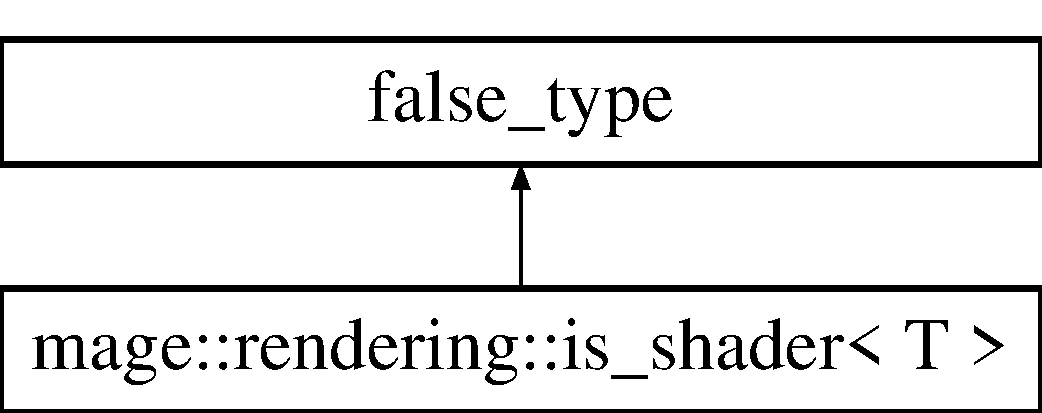
\includegraphics[height=2.000000cm]{structmage_1_1rendering_1_1is__shader}
\end{center}
\end{figure}

\hypertarget{structmage_1_1rendering_1_1is__shader_3_01_compute_shader_01_4}{}\section{mage\+:\+:rendering\+:\+:is\+\_\+shader$<$ Compute\+Shader $>$ Struct Template Reference}
\label{structmage_1_1rendering_1_1is__shader_3_01_compute_shader_01_4}\index{mage\+::rendering\+::is\+\_\+shader$<$ Compute\+Shader $>$@{mage\+::rendering\+::is\+\_\+shader$<$ Compute\+Shader $>$}}


{\ttfamily \#include $<$shader.\+hpp$>$}

Inheritance diagram for mage\+:\+:rendering\+:\+:is\+\_\+shader$<$ Compute\+Shader $>$\+:\begin{figure}[H]
\begin{center}
\leavevmode
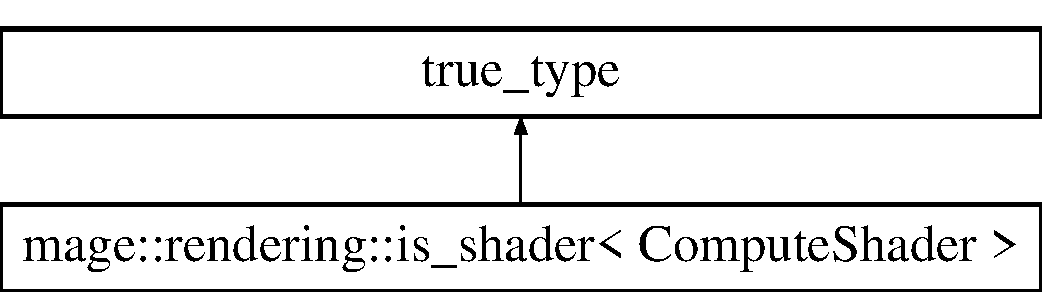
\includegraphics[height=2.000000cm]{structmage_1_1rendering_1_1is__shader_3_01_compute_shader_01_4}
\end{center}
\end{figure}

\hypertarget{structmage_1_1rendering_1_1is__shader_3_01_domain_shader_01_4}{}\section{mage\+:\+:rendering\+:\+:is\+\_\+shader$<$ Domain\+Shader $>$ Struct Template Reference}
\label{structmage_1_1rendering_1_1is__shader_3_01_domain_shader_01_4}\index{mage\+::rendering\+::is\+\_\+shader$<$ Domain\+Shader $>$@{mage\+::rendering\+::is\+\_\+shader$<$ Domain\+Shader $>$}}


{\ttfamily \#include $<$shader.\+hpp$>$}

Inheritance diagram for mage\+:\+:rendering\+:\+:is\+\_\+shader$<$ Domain\+Shader $>$\+:\begin{figure}[H]
\begin{center}
\leavevmode
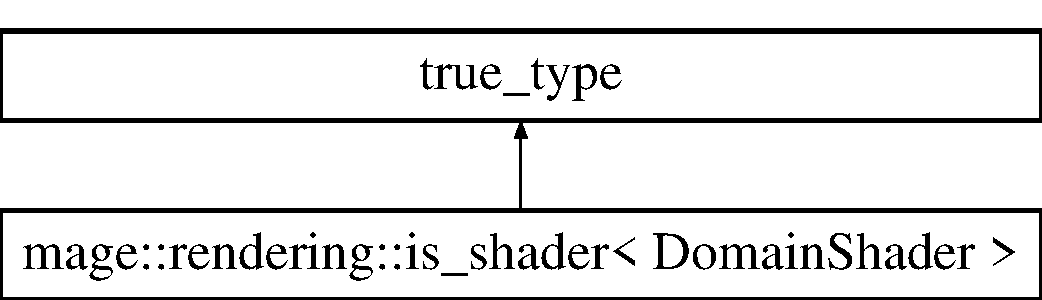
\includegraphics[height=2.000000cm]{structmage_1_1rendering_1_1is__shader_3_01_domain_shader_01_4}
\end{center}
\end{figure}

\hypertarget{structmage_1_1rendering_1_1is__shader_3_01_geometry_shader_01_4}{}\section{mage\+:\+:rendering\+:\+:is\+\_\+shader$<$ Geometry\+Shader $>$ Struct Template Reference}
\label{structmage_1_1rendering_1_1is__shader_3_01_geometry_shader_01_4}\index{mage\+::rendering\+::is\+\_\+shader$<$ Geometry\+Shader $>$@{mage\+::rendering\+::is\+\_\+shader$<$ Geometry\+Shader $>$}}


{\ttfamily \#include $<$shader.\+hpp$>$}

Inheritance diagram for mage\+:\+:rendering\+:\+:is\+\_\+shader$<$ Geometry\+Shader $>$\+:\begin{figure}[H]
\begin{center}
\leavevmode
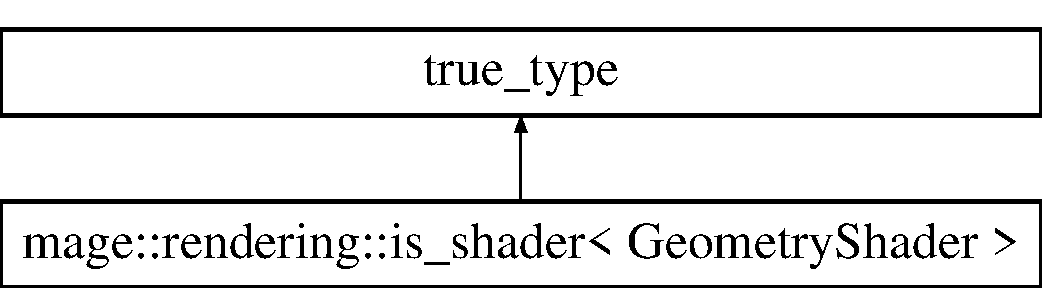
\includegraphics[height=2.000000cm]{structmage_1_1rendering_1_1is__shader_3_01_geometry_shader_01_4}
\end{center}
\end{figure}

\hypertarget{structmage_1_1rendering_1_1is__shader_3_01_hull_shader_01_4}{}\section{mage\+:\+:rendering\+:\+:is\+\_\+shader$<$ Hull\+Shader $>$ Struct Template Reference}
\label{structmage_1_1rendering_1_1is__shader_3_01_hull_shader_01_4}\index{mage\+::rendering\+::is\+\_\+shader$<$ Hull\+Shader $>$@{mage\+::rendering\+::is\+\_\+shader$<$ Hull\+Shader $>$}}


{\ttfamily \#include $<$shader.\+hpp$>$}

Inheritance diagram for mage\+:\+:rendering\+:\+:is\+\_\+shader$<$ Hull\+Shader $>$\+:\begin{figure}[H]
\begin{center}
\leavevmode
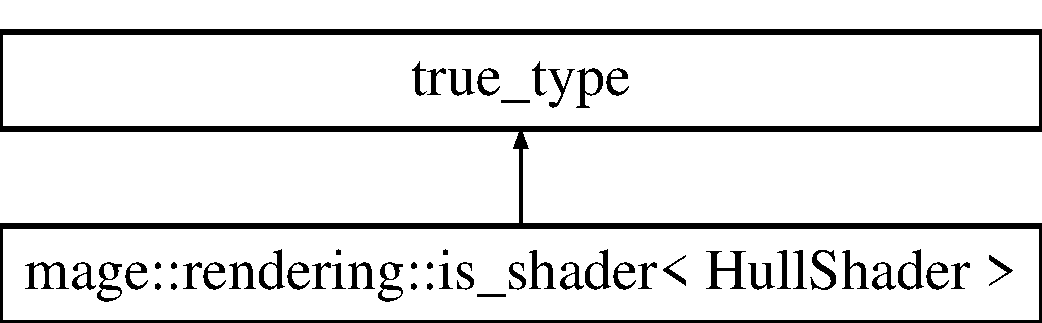
\includegraphics[height=2.000000cm]{structmage_1_1rendering_1_1is__shader_3_01_hull_shader_01_4}
\end{center}
\end{figure}

\hypertarget{structmage_1_1rendering_1_1is__shader_3_01_pixel_shader_01_4}{}\section{mage\+:\+:rendering\+:\+:is\+\_\+shader$<$ Pixel\+Shader $>$ Struct Template Reference}
\label{structmage_1_1rendering_1_1is__shader_3_01_pixel_shader_01_4}\index{mage\+::rendering\+::is\+\_\+shader$<$ Pixel\+Shader $>$@{mage\+::rendering\+::is\+\_\+shader$<$ Pixel\+Shader $>$}}


{\ttfamily \#include $<$shader.\+hpp$>$}

Inheritance diagram for mage\+:\+:rendering\+:\+:is\+\_\+shader$<$ Pixel\+Shader $>$\+:\begin{figure}[H]
\begin{center}
\leavevmode
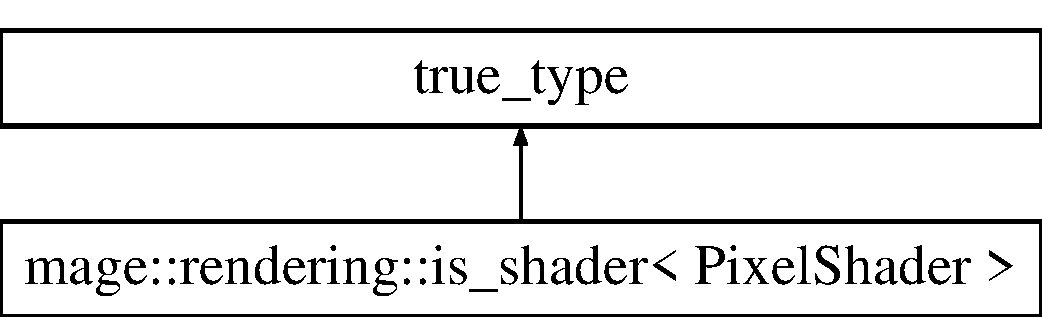
\includegraphics[height=2.000000cm]{structmage_1_1rendering_1_1is__shader_3_01_pixel_shader_01_4}
\end{center}
\end{figure}

\hypertarget{structmage_1_1rendering_1_1is__shader_3_01_vertex_shader_01_4}{}\section{mage\+:\+:rendering\+:\+:is\+\_\+shader$<$ Vertex\+Shader $>$ Struct Template Reference}
\label{structmage_1_1rendering_1_1is__shader_3_01_vertex_shader_01_4}\index{mage\+::rendering\+::is\+\_\+shader$<$ Vertex\+Shader $>$@{mage\+::rendering\+::is\+\_\+shader$<$ Vertex\+Shader $>$}}


{\ttfamily \#include $<$shader.\+hpp$>$}

Inheritance diagram for mage\+:\+:rendering\+:\+:is\+\_\+shader$<$ Vertex\+Shader $>$\+:\begin{figure}[H]
\begin{center}
\leavevmode
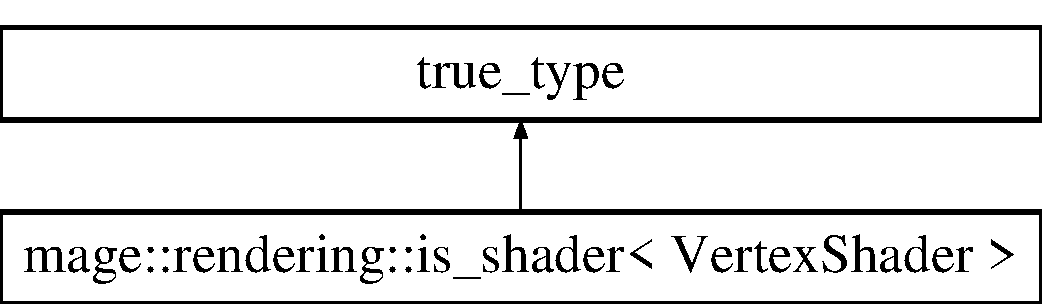
\includegraphics[height=2.000000cm]{structmage_1_1rendering_1_1is__shader_3_01_vertex_shader_01_4}
\end{center}
\end{figure}

\hypertarget{structmage_1_1_kernel_mode_core_clock}{}\section{mage\+:\+:Kernel\+Mode\+Core\+Clock Struct Reference}
\label{structmage_1_1_kernel_mode_core_clock}\index{mage\+::\+Kernel\+Mode\+Core\+Clock@{mage\+::\+Kernel\+Mode\+Core\+Clock}}


{\ttfamily \#include $<$system\+\_\+time.\+hpp$>$}

\subsection*{Public Types}
\begin{DoxyCompactItemize}
\item 
using \hyperlink{structmage_1_1_kernel_mode_core_clock_a5e5e420ec1a6aa530c109d0828a00116}{rep} = \hyperlink{namespacemage_a6672cf3c861707ce4a3235a3eb43941d}{U64}
\item 
using \hyperlink{structmage_1_1_kernel_mode_core_clock_ac1263f0146633a9b2f998839160dcc23}{period} = std\+::ratio$<$ 1, 10 \textquotesingle{}000 \textquotesingle{}000 $>$
\item 
using \hyperlink{structmage_1_1_kernel_mode_core_clock_aca31ec0a66308c4764cb0b16483095b1}{duration} = std\+::chrono\+::duration$<$ \hyperlink{structmage_1_1_kernel_mode_core_clock_a5e5e420ec1a6aa530c109d0828a00116}{rep}, \hyperlink{structmage_1_1_kernel_mode_core_clock_ac1263f0146633a9b2f998839160dcc23}{period} $>$
\item 
using \hyperlink{structmage_1_1_kernel_mode_core_clock_aca87172eb6e806a46d8792ca8239d2fe}{time\+\_\+point} = std\+::chrono\+::time\+\_\+point$<$ \hyperlink{structmage_1_1_kernel_mode_core_clock}{Kernel\+Mode\+Core\+Clock} $>$
\end{DoxyCompactItemize}
\subsection*{Static Public Member Functions}
\begin{DoxyCompactItemize}
\item 
static \hyperlink{structmage_1_1_kernel_mode_core_clock_aca87172eb6e806a46d8792ca8239d2fe}{time\+\_\+point} \hyperlink{structmage_1_1_kernel_mode_core_clock_adc5563b83439f3f732708e0ecd7c5490}{now} () noexcept
\end{DoxyCompactItemize}
\subsection*{Static Public Attributes}
\begin{DoxyCompactItemize}
\item 
static constexpr bool \hyperlink{structmage_1_1_kernel_mode_core_clock_a9b1fe608c5b68bfbe0dc07fefcd5a227}{is\+\_\+steady} = true
\end{DoxyCompactItemize}


\subsection{Member Typedef Documentation}
\hypertarget{structmage_1_1_kernel_mode_core_clock_aca31ec0a66308c4764cb0b16483095b1}{}\label{structmage_1_1_kernel_mode_core_clock_aca31ec0a66308c4764cb0b16483095b1} 
\index{mage\+::\+Kernel\+Mode\+Core\+Clock@{mage\+::\+Kernel\+Mode\+Core\+Clock}!duration@{duration}}
\index{duration@{duration}!mage\+::\+Kernel\+Mode\+Core\+Clock@{mage\+::\+Kernel\+Mode\+Core\+Clock}}
\subsubsection{\texorpdfstring{duration}{duration}}
{\footnotesize\ttfamily using \hyperlink{structmage_1_1_kernel_mode_core_clock_aca31ec0a66308c4764cb0b16483095b1}{mage\+::\+Kernel\+Mode\+Core\+Clock\+::duration} =  std\+::chrono\+::duration$<$ \hyperlink{structmage_1_1_kernel_mode_core_clock_a5e5e420ec1a6aa530c109d0828a00116}{rep}, \hyperlink{structmage_1_1_kernel_mode_core_clock_ac1263f0146633a9b2f998839160dcc23}{period} $>$}

\hypertarget{structmage_1_1_kernel_mode_core_clock_ac1263f0146633a9b2f998839160dcc23}{}\label{structmage_1_1_kernel_mode_core_clock_ac1263f0146633a9b2f998839160dcc23} 
\index{mage\+::\+Kernel\+Mode\+Core\+Clock@{mage\+::\+Kernel\+Mode\+Core\+Clock}!period@{period}}
\index{period@{period}!mage\+::\+Kernel\+Mode\+Core\+Clock@{mage\+::\+Kernel\+Mode\+Core\+Clock}}
\subsubsection{\texorpdfstring{period}{period}}
{\footnotesize\ttfamily using \hyperlink{structmage_1_1_kernel_mode_core_clock_ac1263f0146633a9b2f998839160dcc23}{mage\+::\+Kernel\+Mode\+Core\+Clock\+::period} =  std\+::ratio$<$ 1, 10\textquotesingle{}000\textquotesingle{}000 $>$}

\hypertarget{structmage_1_1_kernel_mode_core_clock_a5e5e420ec1a6aa530c109d0828a00116}{}\label{structmage_1_1_kernel_mode_core_clock_a5e5e420ec1a6aa530c109d0828a00116} 
\index{mage\+::\+Kernel\+Mode\+Core\+Clock@{mage\+::\+Kernel\+Mode\+Core\+Clock}!rep@{rep}}
\index{rep@{rep}!mage\+::\+Kernel\+Mode\+Core\+Clock@{mage\+::\+Kernel\+Mode\+Core\+Clock}}
\subsubsection{\texorpdfstring{rep}{rep}}
{\footnotesize\ttfamily using \hyperlink{structmage_1_1_kernel_mode_core_clock_a5e5e420ec1a6aa530c109d0828a00116}{mage\+::\+Kernel\+Mode\+Core\+Clock\+::rep} =  \hyperlink{namespacemage_a6672cf3c861707ce4a3235a3eb43941d}{U64}}

\hypertarget{structmage_1_1_kernel_mode_core_clock_aca87172eb6e806a46d8792ca8239d2fe}{}\label{structmage_1_1_kernel_mode_core_clock_aca87172eb6e806a46d8792ca8239d2fe} 
\index{mage\+::\+Kernel\+Mode\+Core\+Clock@{mage\+::\+Kernel\+Mode\+Core\+Clock}!time\+\_\+point@{time\+\_\+point}}
\index{time\+\_\+point@{time\+\_\+point}!mage\+::\+Kernel\+Mode\+Core\+Clock@{mage\+::\+Kernel\+Mode\+Core\+Clock}}
\subsubsection{\texorpdfstring{time\+\_\+point}{time\_point}}
{\footnotesize\ttfamily using \hyperlink{structmage_1_1_kernel_mode_core_clock_aca87172eb6e806a46d8792ca8239d2fe}{mage\+::\+Kernel\+Mode\+Core\+Clock\+::time\+\_\+point} =  std\+::chrono\+::time\+\_\+point$<$ \hyperlink{structmage_1_1_kernel_mode_core_clock}{Kernel\+Mode\+Core\+Clock} $>$}



\subsection{Member Function Documentation}
\hypertarget{structmage_1_1_kernel_mode_core_clock_adc5563b83439f3f732708e0ecd7c5490}{}\label{structmage_1_1_kernel_mode_core_clock_adc5563b83439f3f732708e0ecd7c5490} 
\index{mage\+::\+Kernel\+Mode\+Core\+Clock@{mage\+::\+Kernel\+Mode\+Core\+Clock}!now@{now}}
\index{now@{now}!mage\+::\+Kernel\+Mode\+Core\+Clock@{mage\+::\+Kernel\+Mode\+Core\+Clock}}
\subsubsection{\texorpdfstring{now()}{now()}}
{\footnotesize\ttfamily \hyperlink{structmage_1_1_kernel_mode_core_clock_aca87172eb6e806a46d8792ca8239d2fe}{Kernel\+Mode\+Core\+Clock\+::time\+\_\+point} mage\+::\+Kernel\+Mode\+Core\+Clock\+::now (\begin{DoxyParamCaption}{ }\end{DoxyParamCaption})\hspace{0.3cm}{\ttfamily [static]}, {\ttfamily [noexcept]}}



\subsection{Member Data Documentation}
\hypertarget{structmage_1_1_kernel_mode_core_clock_a9b1fe608c5b68bfbe0dc07fefcd5a227}{}\label{structmage_1_1_kernel_mode_core_clock_a9b1fe608c5b68bfbe0dc07fefcd5a227} 
\index{mage\+::\+Kernel\+Mode\+Core\+Clock@{mage\+::\+Kernel\+Mode\+Core\+Clock}!is\+\_\+steady@{is\+\_\+steady}}
\index{is\+\_\+steady@{is\+\_\+steady}!mage\+::\+Kernel\+Mode\+Core\+Clock@{mage\+::\+Kernel\+Mode\+Core\+Clock}}
\subsubsection{\texorpdfstring{is\+\_\+steady}{is\_steady}}
{\footnotesize\ttfamily constexpr bool mage\+::\+Kernel\+Mode\+Core\+Clock\+::is\+\_\+steady = true\hspace{0.3cm}{\ttfamily [static]}}


\hypertarget{structmage_1_1_kernel_mode_core_clock_per_core}{}\section{mage\+:\+:Kernel\+Mode\+Core\+Clock\+Per\+Core Struct Reference}
\label{structmage_1_1_kernel_mode_core_clock_per_core}\index{mage\+::\+Kernel\+Mode\+Core\+Clock\+Per\+Core@{mage\+::\+Kernel\+Mode\+Core\+Clock\+Per\+Core}}


{\ttfamily \#include $<$system\+\_\+time.\+hpp$>$}

\subsection*{Public Types}
\begin{DoxyCompactItemize}
\item 
using \mbox{\hyperlink{structmage_1_1_kernel_mode_core_clock_per_core_a436d770fc6a86e736dda04d72402eb46}{rep}} = \mbox{\hyperlink{namespacemage_ae0ad2dd0035dba92ed0f2e84c182b03b}{U64}}
\item 
using \mbox{\hyperlink{structmage_1_1_kernel_mode_core_clock_per_core_a8baf818e6d058755e971344b5c8ff659}{period}} = std\+::ratio$<$ 1, 10 \textquotesingle{}000 \textquotesingle{}000 $>$
\item 
using \mbox{\hyperlink{structmage_1_1_kernel_mode_core_clock_per_core_ae159e34904ac66f359f0152291e8e6dc}{duration}} = std\+::chrono\+::duration$<$ \mbox{\hyperlink{structmage_1_1_kernel_mode_core_clock_per_core_a436d770fc6a86e736dda04d72402eb46}{rep}}, \mbox{\hyperlink{structmage_1_1_kernel_mode_core_clock_per_core_a8baf818e6d058755e971344b5c8ff659}{period}} $>$
\item 
using \mbox{\hyperlink{structmage_1_1_kernel_mode_core_clock_per_core_a26d0fe6b051dab6987956f52414659cc}{time\+\_\+point}} = std\+::chrono\+::time\+\_\+point$<$ \mbox{\hyperlink{structmage_1_1_kernel_mode_core_clock_per_core}{Kernel\+Mode\+Core\+Clock\+Per\+Core}} $>$
\end{DoxyCompactItemize}
\subsection*{Static Public Member Functions}
\begin{DoxyCompactItemize}
\item 
static const \mbox{\hyperlink{structmage_1_1_kernel_mode_core_clock_per_core_a26d0fe6b051dab6987956f52414659cc}{time\+\_\+point}} \mbox{\hyperlink{structmage_1_1_kernel_mode_core_clock_per_core_a2cbabdfd477f8f0d2b9064c4dffc65e7}{now}} () noexcept
\end{DoxyCompactItemize}
\subsection*{Static Public Attributes}
\begin{DoxyCompactItemize}
\item 
static constexpr bool \mbox{\hyperlink{structmage_1_1_kernel_mode_core_clock_per_core_a8b87465ab1497015a4f6436fd4637645}{is\+\_\+steady}} = true
\end{DoxyCompactItemize}


\subsection{Member Typedef Documentation}
\mbox{\Hypertarget{structmage_1_1_kernel_mode_core_clock_per_core_ae159e34904ac66f359f0152291e8e6dc}\label{structmage_1_1_kernel_mode_core_clock_per_core_ae159e34904ac66f359f0152291e8e6dc}} 
\index{mage\+::\+Kernel\+Mode\+Core\+Clock\+Per\+Core@{mage\+::\+Kernel\+Mode\+Core\+Clock\+Per\+Core}!duration@{duration}}
\index{duration@{duration}!mage\+::\+Kernel\+Mode\+Core\+Clock\+Per\+Core@{mage\+::\+Kernel\+Mode\+Core\+Clock\+Per\+Core}}
\subsubsection{\texorpdfstring{duration}{duration}}
{\footnotesize\ttfamily using \mbox{\hyperlink{structmage_1_1_kernel_mode_core_clock_per_core_ae159e34904ac66f359f0152291e8e6dc}{mage\+::\+Kernel\+Mode\+Core\+Clock\+Per\+Core\+::duration}} =  std\+::chrono\+::duration$<$ \mbox{\hyperlink{structmage_1_1_kernel_mode_core_clock_per_core_a436d770fc6a86e736dda04d72402eb46}{rep}}, \mbox{\hyperlink{structmage_1_1_kernel_mode_core_clock_per_core_a8baf818e6d058755e971344b5c8ff659}{period}} $>$}

\mbox{\Hypertarget{structmage_1_1_kernel_mode_core_clock_per_core_a8baf818e6d058755e971344b5c8ff659}\label{structmage_1_1_kernel_mode_core_clock_per_core_a8baf818e6d058755e971344b5c8ff659}} 
\index{mage\+::\+Kernel\+Mode\+Core\+Clock\+Per\+Core@{mage\+::\+Kernel\+Mode\+Core\+Clock\+Per\+Core}!period@{period}}
\index{period@{period}!mage\+::\+Kernel\+Mode\+Core\+Clock\+Per\+Core@{mage\+::\+Kernel\+Mode\+Core\+Clock\+Per\+Core}}
\subsubsection{\texorpdfstring{period}{period}}
{\footnotesize\ttfamily using \mbox{\hyperlink{structmage_1_1_kernel_mode_core_clock_per_core_a8baf818e6d058755e971344b5c8ff659}{mage\+::\+Kernel\+Mode\+Core\+Clock\+Per\+Core\+::period}} =  std\+::ratio$<$ 1, 10\textquotesingle{}000\textquotesingle{}000 $>$}

\mbox{\Hypertarget{structmage_1_1_kernel_mode_core_clock_per_core_a436d770fc6a86e736dda04d72402eb46}\label{structmage_1_1_kernel_mode_core_clock_per_core_a436d770fc6a86e736dda04d72402eb46}} 
\index{mage\+::\+Kernel\+Mode\+Core\+Clock\+Per\+Core@{mage\+::\+Kernel\+Mode\+Core\+Clock\+Per\+Core}!rep@{rep}}
\index{rep@{rep}!mage\+::\+Kernel\+Mode\+Core\+Clock\+Per\+Core@{mage\+::\+Kernel\+Mode\+Core\+Clock\+Per\+Core}}
\subsubsection{\texorpdfstring{rep}{rep}}
{\footnotesize\ttfamily using \mbox{\hyperlink{structmage_1_1_kernel_mode_core_clock_per_core_a436d770fc6a86e736dda04d72402eb46}{mage\+::\+Kernel\+Mode\+Core\+Clock\+Per\+Core\+::rep}} =  \mbox{\hyperlink{namespacemage_ae0ad2dd0035dba92ed0f2e84c182b03b}{U64}}}

\mbox{\Hypertarget{structmage_1_1_kernel_mode_core_clock_per_core_a26d0fe6b051dab6987956f52414659cc}\label{structmage_1_1_kernel_mode_core_clock_per_core_a26d0fe6b051dab6987956f52414659cc}} 
\index{mage\+::\+Kernel\+Mode\+Core\+Clock\+Per\+Core@{mage\+::\+Kernel\+Mode\+Core\+Clock\+Per\+Core}!time\+\_\+point@{time\+\_\+point}}
\index{time\+\_\+point@{time\+\_\+point}!mage\+::\+Kernel\+Mode\+Core\+Clock\+Per\+Core@{mage\+::\+Kernel\+Mode\+Core\+Clock\+Per\+Core}}
\subsubsection{\texorpdfstring{time\+\_\+point}{time\_point}}
{\footnotesize\ttfamily using \mbox{\hyperlink{structmage_1_1_kernel_mode_core_clock_per_core_a26d0fe6b051dab6987956f52414659cc}{mage\+::\+Kernel\+Mode\+Core\+Clock\+Per\+Core\+::time\+\_\+point}} =  std\+::chrono\+::time\+\_\+point$<$ \mbox{\hyperlink{structmage_1_1_kernel_mode_core_clock_per_core}{Kernel\+Mode\+Core\+Clock\+Per\+Core}} $>$}



\subsection{Member Function Documentation}
\mbox{\Hypertarget{structmage_1_1_kernel_mode_core_clock_per_core_a2cbabdfd477f8f0d2b9064c4dffc65e7}\label{structmage_1_1_kernel_mode_core_clock_per_core_a2cbabdfd477f8f0d2b9064c4dffc65e7}} 
\index{mage\+::\+Kernel\+Mode\+Core\+Clock\+Per\+Core@{mage\+::\+Kernel\+Mode\+Core\+Clock\+Per\+Core}!now@{now}}
\index{now@{now}!mage\+::\+Kernel\+Mode\+Core\+Clock\+Per\+Core@{mage\+::\+Kernel\+Mode\+Core\+Clock\+Per\+Core}}
\subsubsection{\texorpdfstring{now()}{now()}}
{\footnotesize\ttfamily const \mbox{\hyperlink{structmage_1_1_kernel_mode_core_clock_per_core_a26d0fe6b051dab6987956f52414659cc}{Kernel\+Mode\+Core\+Clock\+Per\+Core\+::time\+\_\+point}} mage\+::\+Kernel\+Mode\+Core\+Clock\+Per\+Core\+::now (\begin{DoxyParamCaption}{ }\end{DoxyParamCaption})\hspace{0.3cm}{\ttfamily [static]}, {\ttfamily [noexcept]}}



\subsection{Member Data Documentation}
\mbox{\Hypertarget{structmage_1_1_kernel_mode_core_clock_per_core_a8b87465ab1497015a4f6436fd4637645}\label{structmage_1_1_kernel_mode_core_clock_per_core_a8b87465ab1497015a4f6436fd4637645}} 
\index{mage\+::\+Kernel\+Mode\+Core\+Clock\+Per\+Core@{mage\+::\+Kernel\+Mode\+Core\+Clock\+Per\+Core}!is\+\_\+steady@{is\+\_\+steady}}
\index{is\+\_\+steady@{is\+\_\+steady}!mage\+::\+Kernel\+Mode\+Core\+Clock\+Per\+Core@{mage\+::\+Kernel\+Mode\+Core\+Clock\+Per\+Core}}
\subsubsection{\texorpdfstring{is\+\_\+steady}{is\_steady}}
{\footnotesize\ttfamily constexpr bool mage\+::\+Kernel\+Mode\+Core\+Clock\+Per\+Core\+::is\+\_\+steady = true\hspace{0.3cm}{\ttfamily [static]}}


\hypertarget{classmage_1_1input_1_1_keyboard}{}\section{mage\+:\+:input\+:\+:Keyboard Class Reference}
\label{classmage_1_1input_1_1_keyboard}\index{mage\+::input\+::\+Keyboard@{mage\+::input\+::\+Keyboard}}


{\ttfamily \#include $<$keyboard.\+hpp$>$}

\subsection*{Public Member Functions}
\begin{DoxyCompactItemize}
\item 
\mbox{\hyperlink{classmage_1_1input_1_1_keyboard_af9ac64b485a4fdca497d007283faca18}{Keyboard}} (\mbox{\hyperlink{namespacemage_a8769f9d670d6b585ea306cb1062af94b}{Not\+Null}}$<$ H\+W\+ND $>$ window, I\+Direct\+Input8 \&di)
\item 
\mbox{\hyperlink{classmage_1_1input_1_1_keyboard_ae7297c3080b0e6f78e37cf94ce3effcb}{Keyboard}} (const \mbox{\hyperlink{classmage_1_1input_1_1_keyboard}{Keyboard}} \&keyboard)=delete
\item 
\mbox{\hyperlink{classmage_1_1input_1_1_keyboard_adb93a42b959d58fc320215157f85854c}{Keyboard}} (\mbox{\hyperlink{classmage_1_1input_1_1_keyboard}{Keyboard}} \&\&keyboard) noexcept
\item 
\mbox{\hyperlink{classmage_1_1input_1_1_keyboard_a71239cd5326f78ab226f145a430b382b}{$\sim$\+Keyboard}} ()
\item 
\mbox{\hyperlink{classmage_1_1input_1_1_keyboard}{Keyboard}} \& \mbox{\hyperlink{classmage_1_1input_1_1_keyboard_a8a06eeb906625f100928f3fe2d17cf9d}{operator=}} (const \mbox{\hyperlink{classmage_1_1input_1_1_keyboard}{Keyboard}} \&keyboard)=delete
\item 
\mbox{\hyperlink{classmage_1_1input_1_1_keyboard}{Keyboard}} \& \mbox{\hyperlink{classmage_1_1input_1_1_keyboard_a7dc2316d53a043fa42e4909bd8e58bb9}{operator=}} (\mbox{\hyperlink{classmage_1_1input_1_1_keyboard}{Keyboard}} \&\&keyboard)=delete
\item 
\mbox{\hyperlink{namespacemage_a8769f9d670d6b585ea306cb1062af94b}{Not\+Null}}$<$ H\+W\+ND $>$ \mbox{\hyperlink{classmage_1_1input_1_1_keyboard_a9838f6a7453f74d545926bf5de4c7750}{Get\+Window}} () noexcept
\item 
void \mbox{\hyperlink{classmage_1_1input_1_1_keyboard_a14e53eed6b75a2c45ca3caf94d797bc0}{Update}} () noexcept
\item 
bool \mbox{\hyperlink{classmage_1_1input_1_1_keyboard_a89d22e870c94d01d5338e2e9e6cf5f46}{Is\+Active}} (\mbox{\hyperlink{namespacemage_a30677c03d683c4c35630c25f6ff3fb7f}{U8}} key) const noexcept
\item 
bool \mbox{\hyperlink{classmage_1_1input_1_1_keyboard_a4bbd5f7db6d2cb7123e74edd05363dba}{Is\+Passive}} (\mbox{\hyperlink{namespacemage_a30677c03d683c4c35630c25f6ff3fb7f}{U8}} key) const noexcept
\item 
bool \mbox{\hyperlink{classmage_1_1input_1_1_keyboard_ac6d4bcf6d8f363a74b684303aa8c5993}{Is\+Switched}} (\mbox{\hyperlink{namespacemage_a30677c03d683c4c35630c25f6ff3fb7f}{U8}} key) const noexcept
\item 
bool \mbox{\hyperlink{classmage_1_1input_1_1_keyboard_a0afe5b5fde182d771817272deb8ae1fc}{Is\+Activated}} (\mbox{\hyperlink{namespacemage_a30677c03d683c4c35630c25f6ff3fb7f}{U8}} key) const noexcept
\item 
bool \mbox{\hyperlink{classmage_1_1input_1_1_keyboard_ac3a66b65cabf50a07ba78847e5860ece}{Is\+Deactivated}} (\mbox{\hyperlink{namespacemage_a30677c03d683c4c35630c25f6ff3fb7f}{U8}} key) const noexcept
\end{DoxyCompactItemize}
\subsection*{Private Member Functions}
\begin{DoxyCompactItemize}
\item 
void \mbox{\hyperlink{classmage_1_1input_1_1_keyboard_a9a764a44144ee846bc5fa8094fa591e2}{Initialize\+Keyboard}} ()
\end{DoxyCompactItemize}
\subsection*{Private Attributes}
\begin{DoxyCompactItemize}
\item 
\mbox{\hyperlink{namespacemage_a8769f9d670d6b585ea306cb1062af94b}{Not\+Null}}$<$ H\+W\+ND $>$ \mbox{\hyperlink{classmage_1_1input_1_1_keyboard_ac8074d4690146bf6523c236a7af50353}{m\+\_\+window}}
\item 
I\+Direct\+Input8 \& \mbox{\hyperlink{classmage_1_1input_1_1_keyboard_a3757173fa08e6744d374e0a5397de11c}{m\+\_\+di}}
\item 
\mbox{\hyperlink{namespacemage_ae74f374780900893caa5555d1031fd79}{Com\+Ptr}}$<$ I\+Direct\+Input\+Device8 $>$ \mbox{\hyperlink{classmage_1_1input_1_1_keyboard_ad6993f7c9fc9692708c1f928d0ea1e6b}{m\+\_\+keyboard}}
\item 
std\+::bitset$<$ 512 $>$ \mbox{\hyperlink{classmage_1_1input_1_1_keyboard_ad5b0ec6ca8ff1adbfed19c2382fa8a65}{m\+\_\+key\+\_\+states}}
\end{DoxyCompactItemize}


\subsection{Detailed Description}
A class of keyboards. 

\subsection{Constructor \& Destructor Documentation}
\mbox{\Hypertarget{classmage_1_1input_1_1_keyboard_af9ac64b485a4fdca497d007283faca18}\label{classmage_1_1input_1_1_keyboard_af9ac64b485a4fdca497d007283faca18}} 
\index{mage\+::input\+::\+Keyboard@{mage\+::input\+::\+Keyboard}!Keyboard@{Keyboard}}
\index{Keyboard@{Keyboard}!mage\+::input\+::\+Keyboard@{mage\+::input\+::\+Keyboard}}
\subsubsection{\texorpdfstring{Keyboard()}{Keyboard()}\hspace{0.1cm}{\footnotesize\ttfamily [1/3]}}
{\footnotesize\ttfamily mage\+::input\+::\+Keyboard\+::\+Keyboard (\begin{DoxyParamCaption}\item[{\mbox{\hyperlink{namespacemage_a8769f9d670d6b585ea306cb1062af94b}{Not\+Null}}$<$ H\+W\+ND $>$}]{window,  }\item[{I\+Direct\+Input8 \&}]{di }\end{DoxyParamCaption})\hspace{0.3cm}{\ttfamily [explicit]}}

Constructs a keyboard.


\begin{DoxyParams}[1]{Parameters}
\mbox{\tt in}  & {\em window} & The handle of the parent window. \\
\hline
\mbox{\tt in}  & {\em di} & A reference to a direct input object. \\
\hline
\end{DoxyParams}

\begin{DoxyExceptions}{Exceptions}
{\em \mbox{\hyperlink{classmage_1_1_exception}{Exception}}} & Failed to initialize the keyboard. \\
\hline
\end{DoxyExceptions}
\mbox{\Hypertarget{classmage_1_1input_1_1_keyboard_ae7297c3080b0e6f78e37cf94ce3effcb}\label{classmage_1_1input_1_1_keyboard_ae7297c3080b0e6f78e37cf94ce3effcb}} 
\index{mage\+::input\+::\+Keyboard@{mage\+::input\+::\+Keyboard}!Keyboard@{Keyboard}}
\index{Keyboard@{Keyboard}!mage\+::input\+::\+Keyboard@{mage\+::input\+::\+Keyboard}}
\subsubsection{\texorpdfstring{Keyboard()}{Keyboard()}\hspace{0.1cm}{\footnotesize\ttfamily [2/3]}}
{\footnotesize\ttfamily mage\+::input\+::\+Keyboard\+::\+Keyboard (\begin{DoxyParamCaption}\item[{const \mbox{\hyperlink{classmage_1_1input_1_1_keyboard}{Keyboard}} \&}]{keyboard }\end{DoxyParamCaption})\hspace{0.3cm}{\ttfamily [delete]}}

Constructs a keyboard from the given keyboard.


\begin{DoxyParams}[1]{Parameters}
\mbox{\tt in}  & {\em keyboard} & A reference to the keyboard to copy. \\
\hline
\end{DoxyParams}
\mbox{\Hypertarget{classmage_1_1input_1_1_keyboard_adb93a42b959d58fc320215157f85854c}\label{classmage_1_1input_1_1_keyboard_adb93a42b959d58fc320215157f85854c}} 
\index{mage\+::input\+::\+Keyboard@{mage\+::input\+::\+Keyboard}!Keyboard@{Keyboard}}
\index{Keyboard@{Keyboard}!mage\+::input\+::\+Keyboard@{mage\+::input\+::\+Keyboard}}
\subsubsection{\texorpdfstring{Keyboard()}{Keyboard()}\hspace{0.1cm}{\footnotesize\ttfamily [3/3]}}
{\footnotesize\ttfamily mage\+::input\+::\+Keyboard\+::\+Keyboard (\begin{DoxyParamCaption}\item[{\mbox{\hyperlink{classmage_1_1input_1_1_keyboard}{Keyboard}} \&\&}]{keyboard }\end{DoxyParamCaption})\hspace{0.3cm}{\ttfamily [default]}, {\ttfamily [noexcept]}}

Constructs a keyboard by moving the given keyboard.


\begin{DoxyParams}[1]{Parameters}
\mbox{\tt in}  & {\em keyboard} & A reference to the keyboard to move. \\
\hline
\end{DoxyParams}
\mbox{\Hypertarget{classmage_1_1input_1_1_keyboard_a71239cd5326f78ab226f145a430b382b}\label{classmage_1_1input_1_1_keyboard_a71239cd5326f78ab226f145a430b382b}} 
\index{mage\+::input\+::\+Keyboard@{mage\+::input\+::\+Keyboard}!````~Keyboard@{$\sim$\+Keyboard}}
\index{````~Keyboard@{$\sim$\+Keyboard}!mage\+::input\+::\+Keyboard@{mage\+::input\+::\+Keyboard}}
\subsubsection{\texorpdfstring{$\sim$\+Keyboard()}{~Keyboard()}}
{\footnotesize\ttfamily mage\+::input\+::\+Keyboard\+::$\sim$\+Keyboard (\begin{DoxyParamCaption}{ }\end{DoxyParamCaption})\hspace{0.3cm}{\ttfamily [default]}}

Destructs this keyboard. 

\subsection{Member Function Documentation}
\mbox{\Hypertarget{classmage_1_1input_1_1_keyboard_a9838f6a7453f74d545926bf5de4c7750}\label{classmage_1_1input_1_1_keyboard_a9838f6a7453f74d545926bf5de4c7750}} 
\index{mage\+::input\+::\+Keyboard@{mage\+::input\+::\+Keyboard}!Get\+Window@{Get\+Window}}
\index{Get\+Window@{Get\+Window}!mage\+::input\+::\+Keyboard@{mage\+::input\+::\+Keyboard}}
\subsubsection{\texorpdfstring{Get\+Window()}{GetWindow()}}
{\footnotesize\ttfamily \mbox{\hyperlink{namespacemage_a8769f9d670d6b585ea306cb1062af94b}{Not\+Null}}$<$ H\+W\+ND $>$ mage\+::input\+::\+Keyboard\+::\+Get\+Window (\begin{DoxyParamCaption}{ }\end{DoxyParamCaption})\hspace{0.3cm}{\ttfamily [noexcept]}}

Returns the window handle of this keyboard.

\begin{DoxyReturn}{Returns}
The window handle of this keyboard. 
\end{DoxyReturn}
\mbox{\Hypertarget{classmage_1_1input_1_1_keyboard_a9a764a44144ee846bc5fa8094fa591e2}\label{classmage_1_1input_1_1_keyboard_a9a764a44144ee846bc5fa8094fa591e2}} 
\index{mage\+::input\+::\+Keyboard@{mage\+::input\+::\+Keyboard}!Initialize\+Keyboard@{Initialize\+Keyboard}}
\index{Initialize\+Keyboard@{Initialize\+Keyboard}!mage\+::input\+::\+Keyboard@{mage\+::input\+::\+Keyboard}}
\subsubsection{\texorpdfstring{Initialize\+Keyboard()}{InitializeKeyboard()}}
{\footnotesize\ttfamily void mage\+::input\+::\+Keyboard\+::\+Initialize\+Keyboard (\begin{DoxyParamCaption}{ }\end{DoxyParamCaption})\hspace{0.3cm}{\ttfamily [private]}}

Initializes the keyboard device of this keyboard.


\begin{DoxyExceptions}{Exceptions}
{\em \mbox{\hyperlink{classmage_1_1_exception}{Exception}}} & Failed to initialize the keyboard. \\
\hline
\end{DoxyExceptions}
\mbox{\Hypertarget{classmage_1_1input_1_1_keyboard_a0afe5b5fde182d771817272deb8ae1fc}\label{classmage_1_1input_1_1_keyboard_a0afe5b5fde182d771817272deb8ae1fc}} 
\index{mage\+::input\+::\+Keyboard@{mage\+::input\+::\+Keyboard}!Is\+Activated@{Is\+Activated}}
\index{Is\+Activated@{Is\+Activated}!mage\+::input\+::\+Keyboard@{mage\+::input\+::\+Keyboard}}
\subsubsection{\texorpdfstring{Is\+Activated()}{IsActivated()}}
{\footnotesize\ttfamily bool mage\+::input\+::\+Keyboard\+::\+Is\+Activated (\begin{DoxyParamCaption}\item[{\mbox{\hyperlink{namespacemage_a30677c03d683c4c35630c25f6ff3fb7f}{U8}}}]{key }\end{DoxyParamCaption}) const\hspace{0.3cm}{\ttfamily [noexcept]}}

Checks whether the given key is activated.


\begin{DoxyParams}[1]{Parameters}
\mbox{\tt in}  & {\em key} & The key. \\
\hline
\end{DoxyParams}
\begin{DoxyReturn}{Returns}
{\ttfamily true} if the given key is activated. {\ttfamily false} otherwise. 
\end{DoxyReturn}
\mbox{\Hypertarget{classmage_1_1input_1_1_keyboard_a89d22e870c94d01d5338e2e9e6cf5f46}\label{classmage_1_1input_1_1_keyboard_a89d22e870c94d01d5338e2e9e6cf5f46}} 
\index{mage\+::input\+::\+Keyboard@{mage\+::input\+::\+Keyboard}!Is\+Active@{Is\+Active}}
\index{Is\+Active@{Is\+Active}!mage\+::input\+::\+Keyboard@{mage\+::input\+::\+Keyboard}}
\subsubsection{\texorpdfstring{Is\+Active()}{IsActive()}}
{\footnotesize\ttfamily bool mage\+::input\+::\+Keyboard\+::\+Is\+Active (\begin{DoxyParamCaption}\item[{\mbox{\hyperlink{namespacemage_a30677c03d683c4c35630c25f6ff3fb7f}{U8}}}]{key }\end{DoxyParamCaption}) const\hspace{0.3cm}{\ttfamily [noexcept]}}

Checks whether the given key is active.


\begin{DoxyParams}[1]{Parameters}
\mbox{\tt in}  & {\em key} & The key. \\
\hline
\end{DoxyParams}
\begin{DoxyReturn}{Returns}
{\ttfamily true} if the given key is active. {\ttfamily false} otherwise. 
\end{DoxyReturn}
\mbox{\Hypertarget{classmage_1_1input_1_1_keyboard_ac3a66b65cabf50a07ba78847e5860ece}\label{classmage_1_1input_1_1_keyboard_ac3a66b65cabf50a07ba78847e5860ece}} 
\index{mage\+::input\+::\+Keyboard@{mage\+::input\+::\+Keyboard}!Is\+Deactivated@{Is\+Deactivated}}
\index{Is\+Deactivated@{Is\+Deactivated}!mage\+::input\+::\+Keyboard@{mage\+::input\+::\+Keyboard}}
\subsubsection{\texorpdfstring{Is\+Deactivated()}{IsDeactivated()}}
{\footnotesize\ttfamily bool mage\+::input\+::\+Keyboard\+::\+Is\+Deactivated (\begin{DoxyParamCaption}\item[{\mbox{\hyperlink{namespacemage_a30677c03d683c4c35630c25f6ff3fb7f}{U8}}}]{key }\end{DoxyParamCaption}) const\hspace{0.3cm}{\ttfamily [noexcept]}}

Checks whether the given key is deactivated.


\begin{DoxyParams}[1]{Parameters}
\mbox{\tt in}  & {\em key} & The key. \\
\hline
\end{DoxyParams}
\begin{DoxyReturn}{Returns}
{\ttfamily true} if the given key is deactivated. {\ttfamily false} otherwise. 
\end{DoxyReturn}
\mbox{\Hypertarget{classmage_1_1input_1_1_keyboard_a4bbd5f7db6d2cb7123e74edd05363dba}\label{classmage_1_1input_1_1_keyboard_a4bbd5f7db6d2cb7123e74edd05363dba}} 
\index{mage\+::input\+::\+Keyboard@{mage\+::input\+::\+Keyboard}!Is\+Passive@{Is\+Passive}}
\index{Is\+Passive@{Is\+Passive}!mage\+::input\+::\+Keyboard@{mage\+::input\+::\+Keyboard}}
\subsubsection{\texorpdfstring{Is\+Passive()}{IsPassive()}}
{\footnotesize\ttfamily bool mage\+::input\+::\+Keyboard\+::\+Is\+Passive (\begin{DoxyParamCaption}\item[{\mbox{\hyperlink{namespacemage_a30677c03d683c4c35630c25f6ff3fb7f}{U8}}}]{key }\end{DoxyParamCaption}) const\hspace{0.3cm}{\ttfamily [noexcept]}}

Checks whether the given key is passive.


\begin{DoxyParams}[1]{Parameters}
\mbox{\tt in}  & {\em key} & The key. \\
\hline
\end{DoxyParams}
\begin{DoxyReturn}{Returns}
{\ttfamily true} if the given key is passive. {\ttfamily false} otherwise. 
\end{DoxyReturn}
\mbox{\Hypertarget{classmage_1_1input_1_1_keyboard_ac6d4bcf6d8f363a74b684303aa8c5993}\label{classmage_1_1input_1_1_keyboard_ac6d4bcf6d8f363a74b684303aa8c5993}} 
\index{mage\+::input\+::\+Keyboard@{mage\+::input\+::\+Keyboard}!Is\+Switched@{Is\+Switched}}
\index{Is\+Switched@{Is\+Switched}!mage\+::input\+::\+Keyboard@{mage\+::input\+::\+Keyboard}}
\subsubsection{\texorpdfstring{Is\+Switched()}{IsSwitched()}}
{\footnotesize\ttfamily bool mage\+::input\+::\+Keyboard\+::\+Is\+Switched (\begin{DoxyParamCaption}\item[{\mbox{\hyperlink{namespacemage_a30677c03d683c4c35630c25f6ff3fb7f}{U8}}}]{key }\end{DoxyParamCaption}) const\hspace{0.3cm}{\ttfamily [noexcept]}}

Checks whether the given key is switched from being passive to active or vice versa (i.\+e. activated or deactivated).


\begin{DoxyParams}[1]{Parameters}
\mbox{\tt in}  & {\em key} & The key. \\
\hline
\end{DoxyParams}
\begin{DoxyReturn}{Returns}
{\ttfamily true} if the given key is switched from being passive to active or vice versa (i.\+e. activated or deactivated). {\ttfamily false} otherwise. 
\end{DoxyReturn}
\mbox{\Hypertarget{classmage_1_1input_1_1_keyboard_a8a06eeb906625f100928f3fe2d17cf9d}\label{classmage_1_1input_1_1_keyboard_a8a06eeb906625f100928f3fe2d17cf9d}} 
\index{mage\+::input\+::\+Keyboard@{mage\+::input\+::\+Keyboard}!operator=@{operator=}}
\index{operator=@{operator=}!mage\+::input\+::\+Keyboard@{mage\+::input\+::\+Keyboard}}
\subsubsection{\texorpdfstring{operator=()}{operator=()}\hspace{0.1cm}{\footnotesize\ttfamily [1/2]}}
{\footnotesize\ttfamily \mbox{\hyperlink{classmage_1_1input_1_1_keyboard}{Keyboard}}\& mage\+::input\+::\+Keyboard\+::operator= (\begin{DoxyParamCaption}\item[{const \mbox{\hyperlink{classmage_1_1input_1_1_keyboard}{Keyboard}} \&}]{keyboard }\end{DoxyParamCaption})\hspace{0.3cm}{\ttfamily [delete]}}

Copies the given keyboard to this keyboard.


\begin{DoxyParams}[1]{Parameters}
\mbox{\tt in}  & {\em keyboard} & A reference to the keyboard to copy. \\
\hline
\end{DoxyParams}
\begin{DoxyReturn}{Returns}
A reference to the copy of the given keyboard (i.\+e. this keyboard). 
\end{DoxyReturn}
\mbox{\Hypertarget{classmage_1_1input_1_1_keyboard_a7dc2316d53a043fa42e4909bd8e58bb9}\label{classmage_1_1input_1_1_keyboard_a7dc2316d53a043fa42e4909bd8e58bb9}} 
\index{mage\+::input\+::\+Keyboard@{mage\+::input\+::\+Keyboard}!operator=@{operator=}}
\index{operator=@{operator=}!mage\+::input\+::\+Keyboard@{mage\+::input\+::\+Keyboard}}
\subsubsection{\texorpdfstring{operator=()}{operator=()}\hspace{0.1cm}{\footnotesize\ttfamily [2/2]}}
{\footnotesize\ttfamily \mbox{\hyperlink{classmage_1_1input_1_1_keyboard}{Keyboard}}\& mage\+::input\+::\+Keyboard\+::operator= (\begin{DoxyParamCaption}\item[{\mbox{\hyperlink{classmage_1_1input_1_1_keyboard}{Keyboard}} \&\&}]{keyboard }\end{DoxyParamCaption})\hspace{0.3cm}{\ttfamily [delete]}}

Moves the given keyboard to this keyboard.


\begin{DoxyParams}[1]{Parameters}
\mbox{\tt in}  & {\em keyboard} & A reference to the keyboard to move. \\
\hline
\end{DoxyParams}
\begin{DoxyReturn}{Returns}
A reference to the moved keyboard (i.\+e. this keyboard). 
\end{DoxyReturn}
\mbox{\Hypertarget{classmage_1_1input_1_1_keyboard_a14e53eed6b75a2c45ca3caf94d797bc0}\label{classmage_1_1input_1_1_keyboard_a14e53eed6b75a2c45ca3caf94d797bc0}} 
\index{mage\+::input\+::\+Keyboard@{mage\+::input\+::\+Keyboard}!Update@{Update}}
\index{Update@{Update}!mage\+::input\+::\+Keyboard@{mage\+::input\+::\+Keyboard}}
\subsubsection{\texorpdfstring{Update()}{Update()}}
{\footnotesize\ttfamily void mage\+::input\+::\+Keyboard\+::\+Update (\begin{DoxyParamCaption}{ }\end{DoxyParamCaption})\hspace{0.3cm}{\ttfamily [noexcept]}}

Updates the state of this keyboard. 

\subsection{Member Data Documentation}
\mbox{\Hypertarget{classmage_1_1input_1_1_keyboard_a3757173fa08e6744d374e0a5397de11c}\label{classmage_1_1input_1_1_keyboard_a3757173fa08e6744d374e0a5397de11c}} 
\index{mage\+::input\+::\+Keyboard@{mage\+::input\+::\+Keyboard}!m\+\_\+di@{m\+\_\+di}}
\index{m\+\_\+di@{m\+\_\+di}!mage\+::input\+::\+Keyboard@{mage\+::input\+::\+Keyboard}}
\subsubsection{\texorpdfstring{m\+\_\+di}{m\_di}}
{\footnotesize\ttfamily I\+Direct\+Input8\& mage\+::input\+::\+Keyboard\+::m\+\_\+di\hspace{0.3cm}{\ttfamily [private]}}

A reference to the Direct\+Input object of this keyboard. \mbox{\Hypertarget{classmage_1_1input_1_1_keyboard_ad5b0ec6ca8ff1adbfed19c2382fa8a65}\label{classmage_1_1input_1_1_keyboard_ad5b0ec6ca8ff1adbfed19c2382fa8a65}} 
\index{mage\+::input\+::\+Keyboard@{mage\+::input\+::\+Keyboard}!m\+\_\+key\+\_\+states@{m\+\_\+key\+\_\+states}}
\index{m\+\_\+key\+\_\+states@{m\+\_\+key\+\_\+states}!mage\+::input\+::\+Keyboard@{mage\+::input\+::\+Keyboard}}
\subsubsection{\texorpdfstring{m\+\_\+key\+\_\+states}{m\_key\_states}}
{\footnotesize\ttfamily std\+::bitset$<$ 512 $>$ mage\+::input\+::\+Keyboard\+::m\+\_\+key\+\_\+states\hspace{0.3cm}{\ttfamily [private]}}

The key states of this keyboard. Each key state consists of two flags.

The first flag indicates whether the key state switched from being passive to active or vice versa (i.\+e. activated or deactivated).

The second flag indicates whether the key state is active. \mbox{\Hypertarget{classmage_1_1input_1_1_keyboard_ad6993f7c9fc9692708c1f928d0ea1e6b}\label{classmage_1_1input_1_1_keyboard_ad6993f7c9fc9692708c1f928d0ea1e6b}} 
\index{mage\+::input\+::\+Keyboard@{mage\+::input\+::\+Keyboard}!m\+\_\+keyboard@{m\+\_\+keyboard}}
\index{m\+\_\+keyboard@{m\+\_\+keyboard}!mage\+::input\+::\+Keyboard@{mage\+::input\+::\+Keyboard}}
\subsubsection{\texorpdfstring{m\+\_\+keyboard}{m\_keyboard}}
{\footnotesize\ttfamily \mbox{\hyperlink{namespacemage_ae74f374780900893caa5555d1031fd79}{Com\+Ptr}}$<$ I\+Direct\+Input\+Device8 $>$ mage\+::input\+::\+Keyboard\+::m\+\_\+keyboard\hspace{0.3cm}{\ttfamily [private]}}

A pointer to the Direct\+Input keyboard device of this keyboard. \mbox{\Hypertarget{classmage_1_1input_1_1_keyboard_ac8074d4690146bf6523c236a7af50353}\label{classmage_1_1input_1_1_keyboard_ac8074d4690146bf6523c236a7af50353}} 
\index{mage\+::input\+::\+Keyboard@{mage\+::input\+::\+Keyboard}!m\+\_\+window@{m\+\_\+window}}
\index{m\+\_\+window@{m\+\_\+window}!mage\+::input\+::\+Keyboard@{mage\+::input\+::\+Keyboard}}
\subsubsection{\texorpdfstring{m\+\_\+window}{m\_window}}
{\footnotesize\ttfamily \mbox{\hyperlink{namespacemage_a8769f9d670d6b585ea306cb1062af94b}{Not\+Null}}$<$ H\+W\+ND $>$ mage\+::input\+::\+Keyboard\+::m\+\_\+window\hspace{0.3cm}{\ttfamily [private]}}

The handle of the parent window of this keyboard. 
\hypertarget{classmage_1_1rendering_1_1_l_buffer_pass}{}\section{mage\+:\+:rendering\+:\+:L\+Buffer\+Pass Class Reference}
\label{classmage_1_1rendering_1_1_l_buffer_pass}\index{mage\+::rendering\+::\+L\+Buffer\+Pass@{mage\+::rendering\+::\+L\+Buffer\+Pass}}


{\ttfamily \#include $<$lbuffer\+\_\+pass.\+hpp$>$}

\subsection*{Classes}
\begin{DoxyCompactItemize}
\item 
struct \mbox{\hyperlink{structmage_1_1rendering_1_1_l_buffer_pass_1_1_light_camera_info}{Light\+Camera\+Info}}
\end{DoxyCompactItemize}
\subsection*{Public Member Functions}
\begin{DoxyCompactItemize}
\item 
\mbox{\hyperlink{classmage_1_1rendering_1_1_l_buffer_pass_a5462eea6f50ed0371185584442d1d21e}{L\+Buffer\+Pass}} (I\+D3\+D11\+Device \&device, I\+D3\+D11\+Device\+Context \&device\+\_\+context, \mbox{\hyperlink{classmage_1_1rendering_1_1_state_manager}{State\+Manager}} \&state\+\_\+manager, \mbox{\hyperlink{classmage_1_1rendering_1_1_resource_manager}{Resource\+Manager}} \&resource\+\_\+manager)
\item 
\mbox{\hyperlink{classmage_1_1rendering_1_1_l_buffer_pass_a575a6e93e446b4d9a0af33844dce0035}{L\+Buffer\+Pass}} (const \mbox{\hyperlink{classmage_1_1rendering_1_1_l_buffer_pass}{L\+Buffer\+Pass}} \&buffer)=delete
\item 
\mbox{\hyperlink{classmage_1_1rendering_1_1_l_buffer_pass_a708f765ebb9416b9e9258f78c926331e}{L\+Buffer\+Pass}} (\mbox{\hyperlink{classmage_1_1rendering_1_1_l_buffer_pass}{L\+Buffer\+Pass}} \&\&buffer) noexcept
\item 
\mbox{\hyperlink{classmage_1_1rendering_1_1_l_buffer_pass_a91261b9de58ca001a4e78cc1dd2c1f4b}{$\sim$\+L\+Buffer\+Pass}} ()
\item 
\mbox{\hyperlink{classmage_1_1rendering_1_1_l_buffer_pass}{L\+Buffer\+Pass}} \& \mbox{\hyperlink{classmage_1_1rendering_1_1_l_buffer_pass_a14814e64f1e99f3144944bea07932a20}{operator=}} (const \mbox{\hyperlink{classmage_1_1rendering_1_1_l_buffer_pass}{L\+Buffer\+Pass}} \&buffer)=delete
\item 
\mbox{\hyperlink{classmage_1_1rendering_1_1_l_buffer_pass}{L\+Buffer\+Pass}} \& \mbox{\hyperlink{classmage_1_1rendering_1_1_l_buffer_pass_aeab4dadf9d131fbfaadb28acfde5c575}{operator=}} (\mbox{\hyperlink{classmage_1_1rendering_1_1_l_buffer_pass}{L\+Buffer\+Pass}} \&\&buffer) noexcept
\item 
void X\+M\+\_\+\+C\+A\+L\+L\+C\+O\+NV \mbox{\hyperlink{classmage_1_1rendering_1_1_l_buffer_pass_a21f63364edbb794e1a70823350e44601}{Render}} (const \mbox{\hyperlink{classmage_1_1rendering_1_1_world}{World}} \&world, F\+X\+M\+M\+A\+T\+R\+IX world\+\_\+to\+\_\+projection)
\end{DoxyCompactItemize}
\subsection*{Private Member Functions}
\begin{DoxyCompactItemize}
\item 
void \mbox{\hyperlink{classmage_1_1rendering_1_1_l_buffer_pass_ac456e0612e540d215d8c709e705ade20}{Unbind\+Shadow\+Maps}} () const noexcept
\item 
void \mbox{\hyperlink{classmage_1_1rendering_1_1_l_buffer_pass_a23370698fd80713b0ea31e1d54a35d44}{Bind\+L\+Buffer}} () const noexcept
\item 
void \mbox{\hyperlink{classmage_1_1rendering_1_1_l_buffer_pass_a1ec1d116e0b9ec1066faa7a2b3db5ca5}{Process\+Lights\+Data}} (const \mbox{\hyperlink{classmage_1_1rendering_1_1_world}{World}} \&world)
\item 
void X\+M\+\_\+\+C\+A\+L\+L\+C\+O\+NV \mbox{\hyperlink{classmage_1_1rendering_1_1_l_buffer_pass_a4dc551d7dfdef795244013e0086d59e1}{Process\+Directional\+Lights}} (const \mbox{\hyperlink{classmage_1_1rendering_1_1_world}{World}} \&world, F\+X\+M\+M\+A\+T\+R\+IX world\+\_\+to\+\_\+projection)
\item 
void X\+M\+\_\+\+C\+A\+L\+L\+C\+O\+NV \mbox{\hyperlink{classmage_1_1rendering_1_1_l_buffer_pass_af9e7e859505ec7ee16155f4e11d98a67}{Process\+Omni\+Lights}} (const \mbox{\hyperlink{classmage_1_1rendering_1_1_world}{World}} \&world, F\+X\+M\+M\+A\+T\+R\+IX world\+\_\+to\+\_\+projection)
\item 
void X\+M\+\_\+\+C\+A\+L\+L\+C\+O\+NV \mbox{\hyperlink{classmage_1_1rendering_1_1_l_buffer_pass_a3172ee6a91c34a1dbf252c388fe1ac20}{Process\+Spot\+Lights}} (const \mbox{\hyperlink{classmage_1_1rendering_1_1_world}{World}} \&world, F\+X\+M\+M\+A\+T\+R\+IX world\+\_\+to\+\_\+projection)
\item 
void \mbox{\hyperlink{classmage_1_1rendering_1_1_l_buffer_pass_a405734dad82467908e68217254e4f2ad}{Setup\+Shadow\+Maps}} ()
\item 
void X\+M\+\_\+\+C\+A\+L\+L\+C\+O\+NV \mbox{\hyperlink{classmage_1_1rendering_1_1_l_buffer_pass_a811b69ff4df7d8a24a042a9677c4b67f}{Render\+Shadow\+Maps}} (const \mbox{\hyperlink{classmage_1_1rendering_1_1_world}{World}} \&world)
\end{DoxyCompactItemize}
\subsection*{Private Attributes}
\begin{DoxyCompactItemize}
\item 
std\+::reference\+\_\+wrapper$<$ I\+D3\+D11\+Device\+Context $>$ \mbox{\hyperlink{classmage_1_1rendering_1_1_l_buffer_pass_adccb16b406d2020a7608512cc0f9e6d0}{m\+\_\+device\+\_\+context}}
\item 
\mbox{\hyperlink{classmage_1_1rendering_1_1_constant_buffer}{Constant\+Buffer}}$<$ \mbox{\hyperlink{structmage_1_1rendering_1_1_light_buffer}{Light\+Buffer}} $>$ \mbox{\hyperlink{classmage_1_1rendering_1_1_l_buffer_pass_ab80d18b8193e90588afa5e992b5b1af8}{m\+\_\+light\+\_\+buffer}}
\item 
\mbox{\hyperlink{classmage_1_1rendering_1_1_structured_buffer}{Structured\+Buffer}}$<$ \mbox{\hyperlink{structmage_1_1rendering_1_1_directional_light_buffer}{Directional\+Light\+Buffer}} $>$ \mbox{\hyperlink{classmage_1_1rendering_1_1_l_buffer_pass_a46bc97b1576c1f1702d26c827785c343}{m\+\_\+directional\+\_\+lights}}
\item 
\mbox{\hyperlink{classmage_1_1rendering_1_1_structured_buffer}{Structured\+Buffer}}$<$ \mbox{\hyperlink{structmage_1_1rendering_1_1_omni_light_buffer}{Omni\+Light\+Buffer}} $>$ \mbox{\hyperlink{classmage_1_1rendering_1_1_l_buffer_pass_af7bc4d8ed4d667aa8e6375d6f243d900}{m\+\_\+omni\+\_\+lights}}
\item 
\mbox{\hyperlink{classmage_1_1rendering_1_1_structured_buffer}{Structured\+Buffer}}$<$ \mbox{\hyperlink{structmage_1_1rendering_1_1_spot_light_buffer}{Spot\+Light\+Buffer}} $>$ \mbox{\hyperlink{classmage_1_1rendering_1_1_l_buffer_pass_abc2a2704d99a2a5335d28f3039d600ca}{m\+\_\+spot\+\_\+lights}}
\item 
\mbox{\hyperlink{classmage_1_1rendering_1_1_structured_buffer}{Structured\+Buffer}}$<$ \mbox{\hyperlink{structmage_1_1rendering_1_1_directional_light_buffer}{Directional\+Light\+Buffer}} $>$ \mbox{\hyperlink{classmage_1_1rendering_1_1_l_buffer_pass_a7509575ef1b905079ea56a6f3a4ba513}{m\+\_\+sm\+\_\+directional\+\_\+lights}}
\item 
\mbox{\hyperlink{classmage_1_1rendering_1_1_structured_buffer}{Structured\+Buffer}}$<$ \mbox{\hyperlink{structmage_1_1rendering_1_1_shadow_mapped_omni_light_buffer}{Shadow\+Mapped\+Omni\+Light\+Buffer}} $>$ \mbox{\hyperlink{classmage_1_1rendering_1_1_l_buffer_pass_a3f32431790f55b3959713ae44c1847f9}{m\+\_\+sm\+\_\+omni\+\_\+lights}}
\item 
\mbox{\hyperlink{classmage_1_1rendering_1_1_structured_buffer}{Structured\+Buffer}}$<$ \mbox{\hyperlink{structmage_1_1rendering_1_1_shadow_mapped_spot_light_buffer}{Shadow\+Mapped\+Spot\+Light\+Buffer}} $>$ \mbox{\hyperlink{classmage_1_1rendering_1_1_l_buffer_pass_aea554100305b5a5b198cfd579999fe8a}{m\+\_\+sm\+\_\+spot\+\_\+lights}}
\item 
\mbox{\hyperlink{namespacemage_a3316d7143a973e37adf1110f2e80ca31}{Unique\+Ptr}}$<$ \mbox{\hyperlink{classmage_1_1rendering_1_1_shadow_map_buffer}{Shadow\+Map\+Buffer}} $>$ \mbox{\hyperlink{classmage_1_1rendering_1_1_l_buffer_pass_a76627c9dc2cc229c07584dc2b2599db4}{m\+\_\+directional\+\_\+sms}}
\item 
\mbox{\hyperlink{namespacemage_a3316d7143a973e37adf1110f2e80ca31}{Unique\+Ptr}}$<$ \mbox{\hyperlink{classmage_1_1rendering_1_1_shadow_cube_map_buffer}{Shadow\+Cube\+Map\+Buffer}} $>$ \mbox{\hyperlink{classmage_1_1rendering_1_1_l_buffer_pass_acd46b497a33a96553fa804cb3ebee8ec}{m\+\_\+omni\+\_\+sms}}
\item 
\mbox{\hyperlink{namespacemage_a3316d7143a973e37adf1110f2e80ca31}{Unique\+Ptr}}$<$ \mbox{\hyperlink{classmage_1_1rendering_1_1_shadow_map_buffer}{Shadow\+Map\+Buffer}} $>$ \mbox{\hyperlink{classmage_1_1rendering_1_1_l_buffer_pass_ae3030c5dea15584fd575679c68c6adc8}{m\+\_\+spot\+\_\+sms}}
\item 
\mbox{\hyperlink{namespacemage_a8664bfb5ce2179fc64eae9f82c8a5ba8}{Aligned\+Vector}}$<$ \mbox{\hyperlink{structmage_1_1rendering_1_1_l_buffer_pass_1_1_light_camera_info}{Light\+Camera\+Info}} $>$ \mbox{\hyperlink{classmage_1_1rendering_1_1_l_buffer_pass_a89e1e0ae0ff65c26e18cd7e11e13523f}{m\+\_\+directional\+\_\+light\+\_\+cameras}}
\item 
\mbox{\hyperlink{namespacemage_a8664bfb5ce2179fc64eae9f82c8a5ba8}{Aligned\+Vector}}$<$ \mbox{\hyperlink{structmage_1_1rendering_1_1_l_buffer_pass_1_1_light_camera_info}{Light\+Camera\+Info}} $>$ \mbox{\hyperlink{classmage_1_1rendering_1_1_l_buffer_pass_acf230dbad022cf28a4b87c38ff3439d1}{m\+\_\+omni\+\_\+light\+\_\+cameras}}
\item 
\mbox{\hyperlink{namespacemage_a8664bfb5ce2179fc64eae9f82c8a5ba8}{Aligned\+Vector}}$<$ \mbox{\hyperlink{structmage_1_1rendering_1_1_l_buffer_pass_1_1_light_camera_info}{Light\+Camera\+Info}} $>$ \mbox{\hyperlink{classmage_1_1rendering_1_1_l_buffer_pass_aa888c81683fc9be4cdfab1a49d03eac3}{m\+\_\+spot\+\_\+light\+\_\+cameras}}
\item 
\mbox{\hyperlink{namespacemage_a3316d7143a973e37adf1110f2e80ca31}{Unique\+Ptr}}$<$ \mbox{\hyperlink{classmage_1_1rendering_1_1_depth_pass}{Depth\+Pass}} $>$ \mbox{\hyperlink{classmage_1_1rendering_1_1_l_buffer_pass_a0c721ac882c34c5d6fd6893407fa84f8}{m\+\_\+depth\+\_\+pass}}
\end{DoxyCompactItemize}


\subsection{Constructor \& Destructor Documentation}
\mbox{\Hypertarget{classmage_1_1rendering_1_1_l_buffer_pass_a5462eea6f50ed0371185584442d1d21e}\label{classmage_1_1rendering_1_1_l_buffer_pass_a5462eea6f50ed0371185584442d1d21e}} 
\index{mage\+::rendering\+::\+L\+Buffer\+Pass@{mage\+::rendering\+::\+L\+Buffer\+Pass}!L\+Buffer\+Pass@{L\+Buffer\+Pass}}
\index{L\+Buffer\+Pass@{L\+Buffer\+Pass}!mage\+::rendering\+::\+L\+Buffer\+Pass@{mage\+::rendering\+::\+L\+Buffer\+Pass}}
\subsubsection{\texorpdfstring{L\+Buffer\+Pass()}{LBufferPass()}\hspace{0.1cm}{\footnotesize\ttfamily [1/3]}}
{\footnotesize\ttfamily mage\+::rendering\+::\+L\+Buffer\+Pass\+::\+L\+Buffer\+Pass (\begin{DoxyParamCaption}\item[{I\+D3\+D11\+Device \&}]{device,  }\item[{I\+D3\+D11\+Device\+Context \&}]{device\+\_\+context,  }\item[{\mbox{\hyperlink{classmage_1_1rendering_1_1_state_manager}{State\+Manager}} \&}]{state\+\_\+manager,  }\item[{\mbox{\hyperlink{classmage_1_1rendering_1_1_resource_manager}{Resource\+Manager}} \&}]{resource\+\_\+manager }\end{DoxyParamCaption})\hspace{0.3cm}{\ttfamily [explicit]}}

Constructs a L\+Buffer pass.


\begin{DoxyParams}[1]{Parameters}
\mbox{\tt in,out}  & {\em device} & A reference to the device. \\
\hline
\mbox{\tt in,out}  & {\em device\+\_\+context} & A reference to the device context. \\
\hline
\mbox{\tt in,out}  & {\em state\+\_\+manager} & A reference to the state manager. \\
\hline
\mbox{\tt in,out}  & {\em resource\+\_\+manager} & A reference to the resource manager. \\
\hline
\end{DoxyParams}
\mbox{\Hypertarget{classmage_1_1rendering_1_1_l_buffer_pass_a575a6e93e446b4d9a0af33844dce0035}\label{classmage_1_1rendering_1_1_l_buffer_pass_a575a6e93e446b4d9a0af33844dce0035}} 
\index{mage\+::rendering\+::\+L\+Buffer\+Pass@{mage\+::rendering\+::\+L\+Buffer\+Pass}!L\+Buffer\+Pass@{L\+Buffer\+Pass}}
\index{L\+Buffer\+Pass@{L\+Buffer\+Pass}!mage\+::rendering\+::\+L\+Buffer\+Pass@{mage\+::rendering\+::\+L\+Buffer\+Pass}}
\subsubsection{\texorpdfstring{L\+Buffer\+Pass()}{LBufferPass()}\hspace{0.1cm}{\footnotesize\ttfamily [2/3]}}
{\footnotesize\ttfamily mage\+::rendering\+::\+L\+Buffer\+Pass\+::\+L\+Buffer\+Pass (\begin{DoxyParamCaption}\item[{const \mbox{\hyperlink{classmage_1_1rendering_1_1_l_buffer_pass}{L\+Buffer\+Pass}} \&}]{buffer }\end{DoxyParamCaption})\hspace{0.3cm}{\ttfamily [delete]}}

\mbox{\Hypertarget{classmage_1_1rendering_1_1_l_buffer_pass_a708f765ebb9416b9e9258f78c926331e}\label{classmage_1_1rendering_1_1_l_buffer_pass_a708f765ebb9416b9e9258f78c926331e}} 
\index{mage\+::rendering\+::\+L\+Buffer\+Pass@{mage\+::rendering\+::\+L\+Buffer\+Pass}!L\+Buffer\+Pass@{L\+Buffer\+Pass}}
\index{L\+Buffer\+Pass@{L\+Buffer\+Pass}!mage\+::rendering\+::\+L\+Buffer\+Pass@{mage\+::rendering\+::\+L\+Buffer\+Pass}}
\subsubsection{\texorpdfstring{L\+Buffer\+Pass()}{LBufferPass()}\hspace{0.1cm}{\footnotesize\ttfamily [3/3]}}
{\footnotesize\ttfamily mage\+::rendering\+::\+L\+Buffer\+Pass\+::\+L\+Buffer\+Pass (\begin{DoxyParamCaption}\item[{\mbox{\hyperlink{classmage_1_1rendering_1_1_l_buffer_pass}{L\+Buffer\+Pass}} \&\&}]{buffer }\end{DoxyParamCaption})\hspace{0.3cm}{\ttfamily [default]}, {\ttfamily [noexcept]}}

\mbox{\Hypertarget{classmage_1_1rendering_1_1_l_buffer_pass_a91261b9de58ca001a4e78cc1dd2c1f4b}\label{classmage_1_1rendering_1_1_l_buffer_pass_a91261b9de58ca001a4e78cc1dd2c1f4b}} 
\index{mage\+::rendering\+::\+L\+Buffer\+Pass@{mage\+::rendering\+::\+L\+Buffer\+Pass}!````~L\+Buffer\+Pass@{$\sim$\+L\+Buffer\+Pass}}
\index{````~L\+Buffer\+Pass@{$\sim$\+L\+Buffer\+Pass}!mage\+::rendering\+::\+L\+Buffer\+Pass@{mage\+::rendering\+::\+L\+Buffer\+Pass}}
\subsubsection{\texorpdfstring{$\sim$\+L\+Buffer\+Pass()}{~LBufferPass()}}
{\footnotesize\ttfamily mage\+::rendering\+::\+L\+Buffer\+Pass\+::$\sim$\+L\+Buffer\+Pass (\begin{DoxyParamCaption}{ }\end{DoxyParamCaption})\hspace{0.3cm}{\ttfamily [default]}}



\subsection{Member Function Documentation}
\mbox{\Hypertarget{classmage_1_1rendering_1_1_l_buffer_pass_a23370698fd80713b0ea31e1d54a35d44}\label{classmage_1_1rendering_1_1_l_buffer_pass_a23370698fd80713b0ea31e1d54a35d44}} 
\index{mage\+::rendering\+::\+L\+Buffer\+Pass@{mage\+::rendering\+::\+L\+Buffer\+Pass}!Bind\+L\+Buffer@{Bind\+L\+Buffer}}
\index{Bind\+L\+Buffer@{Bind\+L\+Buffer}!mage\+::rendering\+::\+L\+Buffer\+Pass@{mage\+::rendering\+::\+L\+Buffer\+Pass}}
\subsubsection{\texorpdfstring{Bind\+L\+Buffer()}{BindLBuffer()}}
{\footnotesize\ttfamily void mage\+::rendering\+::\+L\+Buffer\+Pass\+::\+Bind\+L\+Buffer (\begin{DoxyParamCaption}{ }\end{DoxyParamCaption}) const\hspace{0.3cm}{\ttfamily [private]}, {\ttfamily [noexcept]}}

\mbox{\Hypertarget{classmage_1_1rendering_1_1_l_buffer_pass_a14814e64f1e99f3144944bea07932a20}\label{classmage_1_1rendering_1_1_l_buffer_pass_a14814e64f1e99f3144944bea07932a20}} 
\index{mage\+::rendering\+::\+L\+Buffer\+Pass@{mage\+::rendering\+::\+L\+Buffer\+Pass}!operator=@{operator=}}
\index{operator=@{operator=}!mage\+::rendering\+::\+L\+Buffer\+Pass@{mage\+::rendering\+::\+L\+Buffer\+Pass}}
\subsubsection{\texorpdfstring{operator=()}{operator=()}\hspace{0.1cm}{\footnotesize\ttfamily [1/2]}}
{\footnotesize\ttfamily \mbox{\hyperlink{classmage_1_1rendering_1_1_l_buffer_pass}{L\+Buffer\+Pass}}\& mage\+::rendering\+::\+L\+Buffer\+Pass\+::operator= (\begin{DoxyParamCaption}\item[{const \mbox{\hyperlink{classmage_1_1rendering_1_1_l_buffer_pass}{L\+Buffer\+Pass}} \&}]{buffer }\end{DoxyParamCaption})\hspace{0.3cm}{\ttfamily [delete]}}

\mbox{\Hypertarget{classmage_1_1rendering_1_1_l_buffer_pass_aeab4dadf9d131fbfaadb28acfde5c575}\label{classmage_1_1rendering_1_1_l_buffer_pass_aeab4dadf9d131fbfaadb28acfde5c575}} 
\index{mage\+::rendering\+::\+L\+Buffer\+Pass@{mage\+::rendering\+::\+L\+Buffer\+Pass}!operator=@{operator=}}
\index{operator=@{operator=}!mage\+::rendering\+::\+L\+Buffer\+Pass@{mage\+::rendering\+::\+L\+Buffer\+Pass}}
\subsubsection{\texorpdfstring{operator=()}{operator=()}\hspace{0.1cm}{\footnotesize\ttfamily [2/2]}}
{\footnotesize\ttfamily \mbox{\hyperlink{classmage_1_1rendering_1_1_l_buffer_pass}{L\+Buffer\+Pass}} \& mage\+::rendering\+::\+L\+Buffer\+Pass\+::operator= (\begin{DoxyParamCaption}\item[{\mbox{\hyperlink{classmage_1_1rendering_1_1_l_buffer_pass}{L\+Buffer\+Pass}} \&\&}]{buffer }\end{DoxyParamCaption})\hspace{0.3cm}{\ttfamily [default]}, {\ttfamily [noexcept]}}

\mbox{\Hypertarget{classmage_1_1rendering_1_1_l_buffer_pass_a4dc551d7dfdef795244013e0086d59e1}\label{classmage_1_1rendering_1_1_l_buffer_pass_a4dc551d7dfdef795244013e0086d59e1}} 
\index{mage\+::rendering\+::\+L\+Buffer\+Pass@{mage\+::rendering\+::\+L\+Buffer\+Pass}!Process\+Directional\+Lights@{Process\+Directional\+Lights}}
\index{Process\+Directional\+Lights@{Process\+Directional\+Lights}!mage\+::rendering\+::\+L\+Buffer\+Pass@{mage\+::rendering\+::\+L\+Buffer\+Pass}}
\subsubsection{\texorpdfstring{Process\+Directional\+Lights()}{ProcessDirectionalLights()}}
{\footnotesize\ttfamily void X\+M\+\_\+\+C\+A\+L\+L\+C\+O\+NV mage\+::rendering\+::\+L\+Buffer\+Pass\+::\+Process\+Directional\+Lights (\begin{DoxyParamCaption}\item[{const \mbox{\hyperlink{classmage_1_1rendering_1_1_world}{World}} \&}]{world,  }\item[{F\+X\+M\+M\+A\+T\+R\+IX}]{world\+\_\+to\+\_\+projection }\end{DoxyParamCaption})\hspace{0.3cm}{\ttfamily [private]}}

\mbox{\Hypertarget{classmage_1_1rendering_1_1_l_buffer_pass_a1ec1d116e0b9ec1066faa7a2b3db5ca5}\label{classmage_1_1rendering_1_1_l_buffer_pass_a1ec1d116e0b9ec1066faa7a2b3db5ca5}} 
\index{mage\+::rendering\+::\+L\+Buffer\+Pass@{mage\+::rendering\+::\+L\+Buffer\+Pass}!Process\+Lights\+Data@{Process\+Lights\+Data}}
\index{Process\+Lights\+Data@{Process\+Lights\+Data}!mage\+::rendering\+::\+L\+Buffer\+Pass@{mage\+::rendering\+::\+L\+Buffer\+Pass}}
\subsubsection{\texorpdfstring{Process\+Lights\+Data()}{ProcessLightsData()}}
{\footnotesize\ttfamily void mage\+::rendering\+::\+L\+Buffer\+Pass\+::\+Process\+Lights\+Data (\begin{DoxyParamCaption}\item[{const \mbox{\hyperlink{classmage_1_1rendering_1_1_world}{World}} \&}]{world }\end{DoxyParamCaption})\hspace{0.3cm}{\ttfamily [private]}}

\mbox{\Hypertarget{classmage_1_1rendering_1_1_l_buffer_pass_af9e7e859505ec7ee16155f4e11d98a67}\label{classmage_1_1rendering_1_1_l_buffer_pass_af9e7e859505ec7ee16155f4e11d98a67}} 
\index{mage\+::rendering\+::\+L\+Buffer\+Pass@{mage\+::rendering\+::\+L\+Buffer\+Pass}!Process\+Omni\+Lights@{Process\+Omni\+Lights}}
\index{Process\+Omni\+Lights@{Process\+Omni\+Lights}!mage\+::rendering\+::\+L\+Buffer\+Pass@{mage\+::rendering\+::\+L\+Buffer\+Pass}}
\subsubsection{\texorpdfstring{Process\+Omni\+Lights()}{ProcessOmniLights()}}
{\footnotesize\ttfamily void X\+M\+\_\+\+C\+A\+L\+L\+C\+O\+NV mage\+::rendering\+::\+L\+Buffer\+Pass\+::\+Process\+Omni\+Lights (\begin{DoxyParamCaption}\item[{const \mbox{\hyperlink{classmage_1_1rendering_1_1_world}{World}} \&}]{world,  }\item[{F\+X\+M\+M\+A\+T\+R\+IX}]{world\+\_\+to\+\_\+projection }\end{DoxyParamCaption})\hspace{0.3cm}{\ttfamily [private]}}

\mbox{\Hypertarget{classmage_1_1rendering_1_1_l_buffer_pass_a3172ee6a91c34a1dbf252c388fe1ac20}\label{classmage_1_1rendering_1_1_l_buffer_pass_a3172ee6a91c34a1dbf252c388fe1ac20}} 
\index{mage\+::rendering\+::\+L\+Buffer\+Pass@{mage\+::rendering\+::\+L\+Buffer\+Pass}!Process\+Spot\+Lights@{Process\+Spot\+Lights}}
\index{Process\+Spot\+Lights@{Process\+Spot\+Lights}!mage\+::rendering\+::\+L\+Buffer\+Pass@{mage\+::rendering\+::\+L\+Buffer\+Pass}}
\subsubsection{\texorpdfstring{Process\+Spot\+Lights()}{ProcessSpotLights()}}
{\footnotesize\ttfamily void X\+M\+\_\+\+C\+A\+L\+L\+C\+O\+NV mage\+::rendering\+::\+L\+Buffer\+Pass\+::\+Process\+Spot\+Lights (\begin{DoxyParamCaption}\item[{const \mbox{\hyperlink{classmage_1_1rendering_1_1_world}{World}} \&}]{world,  }\item[{F\+X\+M\+M\+A\+T\+R\+IX}]{world\+\_\+to\+\_\+projection }\end{DoxyParamCaption})\hspace{0.3cm}{\ttfamily [private]}}

\mbox{\Hypertarget{classmage_1_1rendering_1_1_l_buffer_pass_a21f63364edbb794e1a70823350e44601}\label{classmage_1_1rendering_1_1_l_buffer_pass_a21f63364edbb794e1a70823350e44601}} 
\index{mage\+::rendering\+::\+L\+Buffer\+Pass@{mage\+::rendering\+::\+L\+Buffer\+Pass}!Render@{Render}}
\index{Render@{Render}!mage\+::rendering\+::\+L\+Buffer\+Pass@{mage\+::rendering\+::\+L\+Buffer\+Pass}}
\subsubsection{\texorpdfstring{Render()}{Render()}}
{\footnotesize\ttfamily void X\+M\+\_\+\+C\+A\+L\+L\+C\+O\+NV mage\+::rendering\+::\+L\+Buffer\+Pass\+::\+Render (\begin{DoxyParamCaption}\item[{const \mbox{\hyperlink{classmage_1_1rendering_1_1_world}{World}} \&}]{world,  }\item[{F\+X\+M\+M\+A\+T\+R\+IX}]{world\+\_\+to\+\_\+projection }\end{DoxyParamCaption})}

\mbox{\Hypertarget{classmage_1_1rendering_1_1_l_buffer_pass_a811b69ff4df7d8a24a042a9677c4b67f}\label{classmage_1_1rendering_1_1_l_buffer_pass_a811b69ff4df7d8a24a042a9677c4b67f}} 
\index{mage\+::rendering\+::\+L\+Buffer\+Pass@{mage\+::rendering\+::\+L\+Buffer\+Pass}!Render\+Shadow\+Maps@{Render\+Shadow\+Maps}}
\index{Render\+Shadow\+Maps@{Render\+Shadow\+Maps}!mage\+::rendering\+::\+L\+Buffer\+Pass@{mage\+::rendering\+::\+L\+Buffer\+Pass}}
\subsubsection{\texorpdfstring{Render\+Shadow\+Maps()}{RenderShadowMaps()}}
{\footnotesize\ttfamily void X\+M\+\_\+\+C\+A\+L\+L\+C\+O\+NV mage\+::rendering\+::\+L\+Buffer\+Pass\+::\+Render\+Shadow\+Maps (\begin{DoxyParamCaption}\item[{const \mbox{\hyperlink{classmage_1_1rendering_1_1_world}{World}} \&}]{world }\end{DoxyParamCaption})\hspace{0.3cm}{\ttfamily [private]}}

\mbox{\Hypertarget{classmage_1_1rendering_1_1_l_buffer_pass_a405734dad82467908e68217254e4f2ad}\label{classmage_1_1rendering_1_1_l_buffer_pass_a405734dad82467908e68217254e4f2ad}} 
\index{mage\+::rendering\+::\+L\+Buffer\+Pass@{mage\+::rendering\+::\+L\+Buffer\+Pass}!Setup\+Shadow\+Maps@{Setup\+Shadow\+Maps}}
\index{Setup\+Shadow\+Maps@{Setup\+Shadow\+Maps}!mage\+::rendering\+::\+L\+Buffer\+Pass@{mage\+::rendering\+::\+L\+Buffer\+Pass}}
\subsubsection{\texorpdfstring{Setup\+Shadow\+Maps()}{SetupShadowMaps()}}
{\footnotesize\ttfamily void mage\+::rendering\+::\+L\+Buffer\+Pass\+::\+Setup\+Shadow\+Maps (\begin{DoxyParamCaption}{ }\end{DoxyParamCaption})\hspace{0.3cm}{\ttfamily [private]}}

\mbox{\Hypertarget{classmage_1_1rendering_1_1_l_buffer_pass_ac456e0612e540d215d8c709e705ade20}\label{classmage_1_1rendering_1_1_l_buffer_pass_ac456e0612e540d215d8c709e705ade20}} 
\index{mage\+::rendering\+::\+L\+Buffer\+Pass@{mage\+::rendering\+::\+L\+Buffer\+Pass}!Unbind\+Shadow\+Maps@{Unbind\+Shadow\+Maps}}
\index{Unbind\+Shadow\+Maps@{Unbind\+Shadow\+Maps}!mage\+::rendering\+::\+L\+Buffer\+Pass@{mage\+::rendering\+::\+L\+Buffer\+Pass}}
\subsubsection{\texorpdfstring{Unbind\+Shadow\+Maps()}{UnbindShadowMaps()}}
{\footnotesize\ttfamily void mage\+::rendering\+::\+L\+Buffer\+Pass\+::\+Unbind\+Shadow\+Maps (\begin{DoxyParamCaption}{ }\end{DoxyParamCaption}) const\hspace{0.3cm}{\ttfamily [private]}, {\ttfamily [noexcept]}}



\subsection{Member Data Documentation}
\mbox{\Hypertarget{classmage_1_1rendering_1_1_l_buffer_pass_a0c721ac882c34c5d6fd6893407fa84f8}\label{classmage_1_1rendering_1_1_l_buffer_pass_a0c721ac882c34c5d6fd6893407fa84f8}} 
\index{mage\+::rendering\+::\+L\+Buffer\+Pass@{mage\+::rendering\+::\+L\+Buffer\+Pass}!m\+\_\+depth\+\_\+pass@{m\+\_\+depth\+\_\+pass}}
\index{m\+\_\+depth\+\_\+pass@{m\+\_\+depth\+\_\+pass}!mage\+::rendering\+::\+L\+Buffer\+Pass@{mage\+::rendering\+::\+L\+Buffer\+Pass}}
\subsubsection{\texorpdfstring{m\+\_\+depth\+\_\+pass}{m\_depth\_pass}}
{\footnotesize\ttfamily \mbox{\hyperlink{namespacemage_a3316d7143a973e37adf1110f2e80ca31}{Unique\+Ptr}}$<$ \mbox{\hyperlink{classmage_1_1rendering_1_1_depth_pass}{Depth\+Pass}} $>$ mage\+::rendering\+::\+L\+Buffer\+Pass\+::m\+\_\+depth\+\_\+pass\hspace{0.3cm}{\ttfamily [private]}}

\mbox{\Hypertarget{classmage_1_1rendering_1_1_l_buffer_pass_adccb16b406d2020a7608512cc0f9e6d0}\label{classmage_1_1rendering_1_1_l_buffer_pass_adccb16b406d2020a7608512cc0f9e6d0}} 
\index{mage\+::rendering\+::\+L\+Buffer\+Pass@{mage\+::rendering\+::\+L\+Buffer\+Pass}!m\+\_\+device\+\_\+context@{m\+\_\+device\+\_\+context}}
\index{m\+\_\+device\+\_\+context@{m\+\_\+device\+\_\+context}!mage\+::rendering\+::\+L\+Buffer\+Pass@{mage\+::rendering\+::\+L\+Buffer\+Pass}}
\subsubsection{\texorpdfstring{m\+\_\+device\+\_\+context}{m\_device\_context}}
{\footnotesize\ttfamily std\+::reference\+\_\+wrapper$<$ I\+D3\+D11\+Device\+Context $>$ mage\+::rendering\+::\+L\+Buffer\+Pass\+::m\+\_\+device\+\_\+context\hspace{0.3cm}{\ttfamily [private]}}

A reference to the device context of this L\+Buffer pass. \mbox{\Hypertarget{classmage_1_1rendering_1_1_l_buffer_pass_a89e1e0ae0ff65c26e18cd7e11e13523f}\label{classmage_1_1rendering_1_1_l_buffer_pass_a89e1e0ae0ff65c26e18cd7e11e13523f}} 
\index{mage\+::rendering\+::\+L\+Buffer\+Pass@{mage\+::rendering\+::\+L\+Buffer\+Pass}!m\+\_\+directional\+\_\+light\+\_\+cameras@{m\+\_\+directional\+\_\+light\+\_\+cameras}}
\index{m\+\_\+directional\+\_\+light\+\_\+cameras@{m\+\_\+directional\+\_\+light\+\_\+cameras}!mage\+::rendering\+::\+L\+Buffer\+Pass@{mage\+::rendering\+::\+L\+Buffer\+Pass}}
\subsubsection{\texorpdfstring{m\+\_\+directional\+\_\+light\+\_\+cameras}{m\_directional\_light\_cameras}}
{\footnotesize\ttfamily \mbox{\hyperlink{namespacemage_a8664bfb5ce2179fc64eae9f82c8a5ba8}{Aligned\+Vector}}$<$ \mbox{\hyperlink{structmage_1_1rendering_1_1_l_buffer_pass_1_1_light_camera_info}{Light\+Camera\+Info}} $>$ mage\+::rendering\+::\+L\+Buffer\+Pass\+::m\+\_\+directional\+\_\+light\+\_\+cameras\hspace{0.3cm}{\ttfamily [private]}}

\mbox{\Hypertarget{classmage_1_1rendering_1_1_l_buffer_pass_a46bc97b1576c1f1702d26c827785c343}\label{classmage_1_1rendering_1_1_l_buffer_pass_a46bc97b1576c1f1702d26c827785c343}} 
\index{mage\+::rendering\+::\+L\+Buffer\+Pass@{mage\+::rendering\+::\+L\+Buffer\+Pass}!m\+\_\+directional\+\_\+lights@{m\+\_\+directional\+\_\+lights}}
\index{m\+\_\+directional\+\_\+lights@{m\+\_\+directional\+\_\+lights}!mage\+::rendering\+::\+L\+Buffer\+Pass@{mage\+::rendering\+::\+L\+Buffer\+Pass}}
\subsubsection{\texorpdfstring{m\+\_\+directional\+\_\+lights}{m\_directional\_lights}}
{\footnotesize\ttfamily \mbox{\hyperlink{classmage_1_1rendering_1_1_structured_buffer}{Structured\+Buffer}}$<$ \mbox{\hyperlink{structmage_1_1rendering_1_1_directional_light_buffer}{Directional\+Light\+Buffer}} $>$ mage\+::rendering\+::\+L\+Buffer\+Pass\+::m\+\_\+directional\+\_\+lights\hspace{0.3cm}{\ttfamily [private]}}

\mbox{\Hypertarget{classmage_1_1rendering_1_1_l_buffer_pass_a76627c9dc2cc229c07584dc2b2599db4}\label{classmage_1_1rendering_1_1_l_buffer_pass_a76627c9dc2cc229c07584dc2b2599db4}} 
\index{mage\+::rendering\+::\+L\+Buffer\+Pass@{mage\+::rendering\+::\+L\+Buffer\+Pass}!m\+\_\+directional\+\_\+sms@{m\+\_\+directional\+\_\+sms}}
\index{m\+\_\+directional\+\_\+sms@{m\+\_\+directional\+\_\+sms}!mage\+::rendering\+::\+L\+Buffer\+Pass@{mage\+::rendering\+::\+L\+Buffer\+Pass}}
\subsubsection{\texorpdfstring{m\+\_\+directional\+\_\+sms}{m\_directional\_sms}}
{\footnotesize\ttfamily \mbox{\hyperlink{namespacemage_a3316d7143a973e37adf1110f2e80ca31}{Unique\+Ptr}}$<$ \mbox{\hyperlink{classmage_1_1rendering_1_1_shadow_map_buffer}{Shadow\+Map\+Buffer}} $>$ mage\+::rendering\+::\+L\+Buffer\+Pass\+::m\+\_\+directional\+\_\+sms\hspace{0.3cm}{\ttfamily [private]}}

\mbox{\Hypertarget{classmage_1_1rendering_1_1_l_buffer_pass_ab80d18b8193e90588afa5e992b5b1af8}\label{classmage_1_1rendering_1_1_l_buffer_pass_ab80d18b8193e90588afa5e992b5b1af8}} 
\index{mage\+::rendering\+::\+L\+Buffer\+Pass@{mage\+::rendering\+::\+L\+Buffer\+Pass}!m\+\_\+light\+\_\+buffer@{m\+\_\+light\+\_\+buffer}}
\index{m\+\_\+light\+\_\+buffer@{m\+\_\+light\+\_\+buffer}!mage\+::rendering\+::\+L\+Buffer\+Pass@{mage\+::rendering\+::\+L\+Buffer\+Pass}}
\subsubsection{\texorpdfstring{m\+\_\+light\+\_\+buffer}{m\_light\_buffer}}
{\footnotesize\ttfamily \mbox{\hyperlink{classmage_1_1rendering_1_1_constant_buffer}{Constant\+Buffer}}$<$ \mbox{\hyperlink{structmage_1_1rendering_1_1_light_buffer}{Light\+Buffer}} $>$ mage\+::rendering\+::\+L\+Buffer\+Pass\+::m\+\_\+light\+\_\+buffer\hspace{0.3cm}{\ttfamily [private]}}

\mbox{\Hypertarget{classmage_1_1rendering_1_1_l_buffer_pass_acf230dbad022cf28a4b87c38ff3439d1}\label{classmage_1_1rendering_1_1_l_buffer_pass_acf230dbad022cf28a4b87c38ff3439d1}} 
\index{mage\+::rendering\+::\+L\+Buffer\+Pass@{mage\+::rendering\+::\+L\+Buffer\+Pass}!m\+\_\+omni\+\_\+light\+\_\+cameras@{m\+\_\+omni\+\_\+light\+\_\+cameras}}
\index{m\+\_\+omni\+\_\+light\+\_\+cameras@{m\+\_\+omni\+\_\+light\+\_\+cameras}!mage\+::rendering\+::\+L\+Buffer\+Pass@{mage\+::rendering\+::\+L\+Buffer\+Pass}}
\subsubsection{\texorpdfstring{m\+\_\+omni\+\_\+light\+\_\+cameras}{m\_omni\_light\_cameras}}
{\footnotesize\ttfamily \mbox{\hyperlink{namespacemage_a8664bfb5ce2179fc64eae9f82c8a5ba8}{Aligned\+Vector}}$<$ \mbox{\hyperlink{structmage_1_1rendering_1_1_l_buffer_pass_1_1_light_camera_info}{Light\+Camera\+Info}} $>$ mage\+::rendering\+::\+L\+Buffer\+Pass\+::m\+\_\+omni\+\_\+light\+\_\+cameras\hspace{0.3cm}{\ttfamily [private]}}

\mbox{\Hypertarget{classmage_1_1rendering_1_1_l_buffer_pass_af7bc4d8ed4d667aa8e6375d6f243d900}\label{classmage_1_1rendering_1_1_l_buffer_pass_af7bc4d8ed4d667aa8e6375d6f243d900}} 
\index{mage\+::rendering\+::\+L\+Buffer\+Pass@{mage\+::rendering\+::\+L\+Buffer\+Pass}!m\+\_\+omni\+\_\+lights@{m\+\_\+omni\+\_\+lights}}
\index{m\+\_\+omni\+\_\+lights@{m\+\_\+omni\+\_\+lights}!mage\+::rendering\+::\+L\+Buffer\+Pass@{mage\+::rendering\+::\+L\+Buffer\+Pass}}
\subsubsection{\texorpdfstring{m\+\_\+omni\+\_\+lights}{m\_omni\_lights}}
{\footnotesize\ttfamily \mbox{\hyperlink{classmage_1_1rendering_1_1_structured_buffer}{Structured\+Buffer}}$<$ \mbox{\hyperlink{structmage_1_1rendering_1_1_omni_light_buffer}{Omni\+Light\+Buffer}} $>$ mage\+::rendering\+::\+L\+Buffer\+Pass\+::m\+\_\+omni\+\_\+lights\hspace{0.3cm}{\ttfamily [private]}}

\mbox{\Hypertarget{classmage_1_1rendering_1_1_l_buffer_pass_acd46b497a33a96553fa804cb3ebee8ec}\label{classmage_1_1rendering_1_1_l_buffer_pass_acd46b497a33a96553fa804cb3ebee8ec}} 
\index{mage\+::rendering\+::\+L\+Buffer\+Pass@{mage\+::rendering\+::\+L\+Buffer\+Pass}!m\+\_\+omni\+\_\+sms@{m\+\_\+omni\+\_\+sms}}
\index{m\+\_\+omni\+\_\+sms@{m\+\_\+omni\+\_\+sms}!mage\+::rendering\+::\+L\+Buffer\+Pass@{mage\+::rendering\+::\+L\+Buffer\+Pass}}
\subsubsection{\texorpdfstring{m\+\_\+omni\+\_\+sms}{m\_omni\_sms}}
{\footnotesize\ttfamily \mbox{\hyperlink{namespacemage_a3316d7143a973e37adf1110f2e80ca31}{Unique\+Ptr}}$<$ \mbox{\hyperlink{classmage_1_1rendering_1_1_shadow_cube_map_buffer}{Shadow\+Cube\+Map\+Buffer}} $>$ mage\+::rendering\+::\+L\+Buffer\+Pass\+::m\+\_\+omni\+\_\+sms\hspace{0.3cm}{\ttfamily [private]}}

\mbox{\Hypertarget{classmage_1_1rendering_1_1_l_buffer_pass_a7509575ef1b905079ea56a6f3a4ba513}\label{classmage_1_1rendering_1_1_l_buffer_pass_a7509575ef1b905079ea56a6f3a4ba513}} 
\index{mage\+::rendering\+::\+L\+Buffer\+Pass@{mage\+::rendering\+::\+L\+Buffer\+Pass}!m\+\_\+sm\+\_\+directional\+\_\+lights@{m\+\_\+sm\+\_\+directional\+\_\+lights}}
\index{m\+\_\+sm\+\_\+directional\+\_\+lights@{m\+\_\+sm\+\_\+directional\+\_\+lights}!mage\+::rendering\+::\+L\+Buffer\+Pass@{mage\+::rendering\+::\+L\+Buffer\+Pass}}
\subsubsection{\texorpdfstring{m\+\_\+sm\+\_\+directional\+\_\+lights}{m\_sm\_directional\_lights}}
{\footnotesize\ttfamily \mbox{\hyperlink{classmage_1_1rendering_1_1_structured_buffer}{Structured\+Buffer}}$<$ \mbox{\hyperlink{structmage_1_1rendering_1_1_directional_light_buffer}{Directional\+Light\+Buffer}} $>$ mage\+::rendering\+::\+L\+Buffer\+Pass\+::m\+\_\+sm\+\_\+directional\+\_\+lights\hspace{0.3cm}{\ttfamily [private]}}

\mbox{\Hypertarget{classmage_1_1rendering_1_1_l_buffer_pass_a3f32431790f55b3959713ae44c1847f9}\label{classmage_1_1rendering_1_1_l_buffer_pass_a3f32431790f55b3959713ae44c1847f9}} 
\index{mage\+::rendering\+::\+L\+Buffer\+Pass@{mage\+::rendering\+::\+L\+Buffer\+Pass}!m\+\_\+sm\+\_\+omni\+\_\+lights@{m\+\_\+sm\+\_\+omni\+\_\+lights}}
\index{m\+\_\+sm\+\_\+omni\+\_\+lights@{m\+\_\+sm\+\_\+omni\+\_\+lights}!mage\+::rendering\+::\+L\+Buffer\+Pass@{mage\+::rendering\+::\+L\+Buffer\+Pass}}
\subsubsection{\texorpdfstring{m\+\_\+sm\+\_\+omni\+\_\+lights}{m\_sm\_omni\_lights}}
{\footnotesize\ttfamily \mbox{\hyperlink{classmage_1_1rendering_1_1_structured_buffer}{Structured\+Buffer}}$<$ \mbox{\hyperlink{structmage_1_1rendering_1_1_shadow_mapped_omni_light_buffer}{Shadow\+Mapped\+Omni\+Light\+Buffer}} $>$ mage\+::rendering\+::\+L\+Buffer\+Pass\+::m\+\_\+sm\+\_\+omni\+\_\+lights\hspace{0.3cm}{\ttfamily [private]}}

\mbox{\Hypertarget{classmage_1_1rendering_1_1_l_buffer_pass_aea554100305b5a5b198cfd579999fe8a}\label{classmage_1_1rendering_1_1_l_buffer_pass_aea554100305b5a5b198cfd579999fe8a}} 
\index{mage\+::rendering\+::\+L\+Buffer\+Pass@{mage\+::rendering\+::\+L\+Buffer\+Pass}!m\+\_\+sm\+\_\+spot\+\_\+lights@{m\+\_\+sm\+\_\+spot\+\_\+lights}}
\index{m\+\_\+sm\+\_\+spot\+\_\+lights@{m\+\_\+sm\+\_\+spot\+\_\+lights}!mage\+::rendering\+::\+L\+Buffer\+Pass@{mage\+::rendering\+::\+L\+Buffer\+Pass}}
\subsubsection{\texorpdfstring{m\+\_\+sm\+\_\+spot\+\_\+lights}{m\_sm\_spot\_lights}}
{\footnotesize\ttfamily \mbox{\hyperlink{classmage_1_1rendering_1_1_structured_buffer}{Structured\+Buffer}}$<$ \mbox{\hyperlink{structmage_1_1rendering_1_1_shadow_mapped_spot_light_buffer}{Shadow\+Mapped\+Spot\+Light\+Buffer}} $>$ mage\+::rendering\+::\+L\+Buffer\+Pass\+::m\+\_\+sm\+\_\+spot\+\_\+lights\hspace{0.3cm}{\ttfamily [private]}}

\mbox{\Hypertarget{classmage_1_1rendering_1_1_l_buffer_pass_aa888c81683fc9be4cdfab1a49d03eac3}\label{classmage_1_1rendering_1_1_l_buffer_pass_aa888c81683fc9be4cdfab1a49d03eac3}} 
\index{mage\+::rendering\+::\+L\+Buffer\+Pass@{mage\+::rendering\+::\+L\+Buffer\+Pass}!m\+\_\+spot\+\_\+light\+\_\+cameras@{m\+\_\+spot\+\_\+light\+\_\+cameras}}
\index{m\+\_\+spot\+\_\+light\+\_\+cameras@{m\+\_\+spot\+\_\+light\+\_\+cameras}!mage\+::rendering\+::\+L\+Buffer\+Pass@{mage\+::rendering\+::\+L\+Buffer\+Pass}}
\subsubsection{\texorpdfstring{m\+\_\+spot\+\_\+light\+\_\+cameras}{m\_spot\_light\_cameras}}
{\footnotesize\ttfamily \mbox{\hyperlink{namespacemage_a8664bfb5ce2179fc64eae9f82c8a5ba8}{Aligned\+Vector}}$<$ \mbox{\hyperlink{structmage_1_1rendering_1_1_l_buffer_pass_1_1_light_camera_info}{Light\+Camera\+Info}} $>$ mage\+::rendering\+::\+L\+Buffer\+Pass\+::m\+\_\+spot\+\_\+light\+\_\+cameras\hspace{0.3cm}{\ttfamily [private]}}

\mbox{\Hypertarget{classmage_1_1rendering_1_1_l_buffer_pass_abc2a2704d99a2a5335d28f3039d600ca}\label{classmage_1_1rendering_1_1_l_buffer_pass_abc2a2704d99a2a5335d28f3039d600ca}} 
\index{mage\+::rendering\+::\+L\+Buffer\+Pass@{mage\+::rendering\+::\+L\+Buffer\+Pass}!m\+\_\+spot\+\_\+lights@{m\+\_\+spot\+\_\+lights}}
\index{m\+\_\+spot\+\_\+lights@{m\+\_\+spot\+\_\+lights}!mage\+::rendering\+::\+L\+Buffer\+Pass@{mage\+::rendering\+::\+L\+Buffer\+Pass}}
\subsubsection{\texorpdfstring{m\+\_\+spot\+\_\+lights}{m\_spot\_lights}}
{\footnotesize\ttfamily \mbox{\hyperlink{classmage_1_1rendering_1_1_structured_buffer}{Structured\+Buffer}}$<$ \mbox{\hyperlink{structmage_1_1rendering_1_1_spot_light_buffer}{Spot\+Light\+Buffer}} $>$ mage\+::rendering\+::\+L\+Buffer\+Pass\+::m\+\_\+spot\+\_\+lights\hspace{0.3cm}{\ttfamily [private]}}

\mbox{\Hypertarget{classmage_1_1rendering_1_1_l_buffer_pass_ae3030c5dea15584fd575679c68c6adc8}\label{classmage_1_1rendering_1_1_l_buffer_pass_ae3030c5dea15584fd575679c68c6adc8}} 
\index{mage\+::rendering\+::\+L\+Buffer\+Pass@{mage\+::rendering\+::\+L\+Buffer\+Pass}!m\+\_\+spot\+\_\+sms@{m\+\_\+spot\+\_\+sms}}
\index{m\+\_\+spot\+\_\+sms@{m\+\_\+spot\+\_\+sms}!mage\+::rendering\+::\+L\+Buffer\+Pass@{mage\+::rendering\+::\+L\+Buffer\+Pass}}
\subsubsection{\texorpdfstring{m\+\_\+spot\+\_\+sms}{m\_spot\_sms}}
{\footnotesize\ttfamily \mbox{\hyperlink{namespacemage_a3316d7143a973e37adf1110f2e80ca31}{Unique\+Ptr}}$<$ \mbox{\hyperlink{classmage_1_1rendering_1_1_shadow_map_buffer}{Shadow\+Map\+Buffer}} $>$ mage\+::rendering\+::\+L\+Buffer\+Pass\+::m\+\_\+spot\+\_\+sms\hspace{0.3cm}{\ttfamily [private]}}


\hypertarget{structmage_1_1rendering_1_1_light_buffer}{}\section{mage\+:\+:rendering\+:\+:Light\+Buffer Struct Reference}
\label{structmage_1_1rendering_1_1_light_buffer}\index{mage\+::rendering\+::\+Light\+Buffer@{mage\+::rendering\+::\+Light\+Buffer}}


{\ttfamily \#include $<$light\+\_\+buffer.\+hpp$>$}

\subsection*{Public Member Functions}
\begin{DoxyCompactItemize}
\item 
\mbox{\hyperlink{structmage_1_1rendering_1_1_light_buffer_ad31355f44f8e31f540fa40c81e659fca}{Light\+Buffer}} () noexcept
\item 
\mbox{\hyperlink{structmage_1_1rendering_1_1_light_buffer_ae5f4964ae3773e590a8fe07e3b6bcdfa}{Light\+Buffer}} (const \mbox{\hyperlink{structmage_1_1rendering_1_1_light_buffer}{Light\+Buffer}} \&buffer) noexcept=default
\item 
\mbox{\hyperlink{structmage_1_1rendering_1_1_light_buffer_a016cbba8dd68da2f80a7018e2276070d}{Light\+Buffer}} (\mbox{\hyperlink{structmage_1_1rendering_1_1_light_buffer}{Light\+Buffer}} \&\&buffer) noexcept=default
\item 
\mbox{\hyperlink{structmage_1_1rendering_1_1_light_buffer_a36fd7699f61cde6359d6934428eb9daf}{$\sim$\+Light\+Buffer}} ()=default
\item 
\mbox{\hyperlink{structmage_1_1rendering_1_1_light_buffer}{Light\+Buffer}} \& \mbox{\hyperlink{structmage_1_1rendering_1_1_light_buffer_a409af50e3d21571e56b36c6c88769a65}{operator=}} (const \mbox{\hyperlink{structmage_1_1rendering_1_1_light_buffer}{Light\+Buffer}} \&buffer) noexcept=default
\item 
\mbox{\hyperlink{structmage_1_1rendering_1_1_light_buffer}{Light\+Buffer}} \& \mbox{\hyperlink{structmage_1_1rendering_1_1_light_buffer_abe8ee3df1e5c2ce28aaab03ce729a184}{operator=}} (\mbox{\hyperlink{structmage_1_1rendering_1_1_light_buffer}{Light\+Buffer}} \&\&buffer) noexcept=default
\end{DoxyCompactItemize}
\subsection*{Public Attributes}
\begin{DoxyCompactItemize}
\item 
\mbox{\hyperlink{namespacemage_aa5d6eaabaac3cdd01873d6a3d27e90f3}{U32}} \mbox{\hyperlink{structmage_1_1rendering_1_1_light_buffer_a4ebd93f25e72d8ba426599e94369547b}{m\+\_\+nb\+\_\+directional\+\_\+lights}}
\item 
\mbox{\hyperlink{namespacemage_aa5d6eaabaac3cdd01873d6a3d27e90f3}{U32}} \mbox{\hyperlink{structmage_1_1rendering_1_1_light_buffer_a1a5e40bcec229bad29eacde98f3abe28}{m\+\_\+nb\+\_\+omni\+\_\+lights}}
\item 
\mbox{\hyperlink{namespacemage_aa5d6eaabaac3cdd01873d6a3d27e90f3}{U32}} \mbox{\hyperlink{structmage_1_1rendering_1_1_light_buffer_aef25432813d6531689ff6a94e4cf6fcb}{m\+\_\+nb\+\_\+spot\+\_\+lights}}
\item 
\mbox{\hyperlink{namespacemage_aa5d6eaabaac3cdd01873d6a3d27e90f3}{U32}} \mbox{\hyperlink{structmage_1_1rendering_1_1_light_buffer_a2e4d47ce07261e4ce1c5bd6a9418bea6}{m\+\_\+padding0}}
\item 
\mbox{\hyperlink{namespacemage_aa5d6eaabaac3cdd01873d6a3d27e90f3}{U32}} \mbox{\hyperlink{structmage_1_1rendering_1_1_light_buffer_ad90bc8cb163fe39efcb5c960cb566f16}{m\+\_\+nb\+\_\+sm\+\_\+directional\+\_\+lights}}
\item 
\mbox{\hyperlink{namespacemage_aa5d6eaabaac3cdd01873d6a3d27e90f3}{U32}} \mbox{\hyperlink{structmage_1_1rendering_1_1_light_buffer_a1a40cf5d4100b48837cae57ac2f36fcf}{m\+\_\+nb\+\_\+sm\+\_\+omni\+\_\+lights}}
\item 
\mbox{\hyperlink{namespacemage_aa5d6eaabaac3cdd01873d6a3d27e90f3}{U32}} \mbox{\hyperlink{structmage_1_1rendering_1_1_light_buffer_a78481c98c9efcdf18ae1254d1fe6f776}{m\+\_\+nb\+\_\+sm\+\_\+spot\+\_\+lights}}
\item 
\mbox{\hyperlink{namespacemage_aa5d6eaabaac3cdd01873d6a3d27e90f3}{U32}} \mbox{\hyperlink{structmage_1_1rendering_1_1_light_buffer_a09c3c5f0cd03d1786512403f376cc674}{m\+\_\+padding1}}
\item 
\mbox{\hyperlink{structmage_1_1_r_g_b}{R\+GB}} \mbox{\hyperlink{structmage_1_1rendering_1_1_light_buffer_a98c6472d82af27de8b7584ff1c7f98db}{m\+\_\+\+La}}
\item 
\mbox{\hyperlink{namespacemage_aa97e833b45f06d60a0a9c4fc22ae02c0}{F32}} \mbox{\hyperlink{structmage_1_1rendering_1_1_light_buffer_ab0d6f818328072fee8dd7ff4c39a9732}{m\+\_\+padding2}}
\end{DoxyCompactItemize}


\subsection{Detailed Description}
A struct of light buffers used by shaders. 

\subsection{Constructor \& Destructor Documentation}
\mbox{\Hypertarget{structmage_1_1rendering_1_1_light_buffer_ad31355f44f8e31f540fa40c81e659fca}\label{structmage_1_1rendering_1_1_light_buffer_ad31355f44f8e31f540fa40c81e659fca}} 
\index{mage\+::rendering\+::\+Light\+Buffer@{mage\+::rendering\+::\+Light\+Buffer}!Light\+Buffer@{Light\+Buffer}}
\index{Light\+Buffer@{Light\+Buffer}!mage\+::rendering\+::\+Light\+Buffer@{mage\+::rendering\+::\+Light\+Buffer}}
\subsubsection{\texorpdfstring{Light\+Buffer()}{LightBuffer()}\hspace{0.1cm}{\footnotesize\ttfamily [1/3]}}
{\footnotesize\ttfamily mage\+::rendering\+::\+Light\+Buffer\+::\+Light\+Buffer (\begin{DoxyParamCaption}{ }\end{DoxyParamCaption})\hspace{0.3cm}{\ttfamily [noexcept]}}

Constructs a light buffer. \mbox{\Hypertarget{structmage_1_1rendering_1_1_light_buffer_ae5f4964ae3773e590a8fe07e3b6bcdfa}\label{structmage_1_1rendering_1_1_light_buffer_ae5f4964ae3773e590a8fe07e3b6bcdfa}} 
\index{mage\+::rendering\+::\+Light\+Buffer@{mage\+::rendering\+::\+Light\+Buffer}!Light\+Buffer@{Light\+Buffer}}
\index{Light\+Buffer@{Light\+Buffer}!mage\+::rendering\+::\+Light\+Buffer@{mage\+::rendering\+::\+Light\+Buffer}}
\subsubsection{\texorpdfstring{Light\+Buffer()}{LightBuffer()}\hspace{0.1cm}{\footnotesize\ttfamily [2/3]}}
{\footnotesize\ttfamily mage\+::rendering\+::\+Light\+Buffer\+::\+Light\+Buffer (\begin{DoxyParamCaption}\item[{const \mbox{\hyperlink{structmage_1_1rendering_1_1_light_buffer}{Light\+Buffer}} \&}]{buffer }\end{DoxyParamCaption})\hspace{0.3cm}{\ttfamily [default]}, {\ttfamily [noexcept]}}

Constructs a light buffer from the given light buffer.


\begin{DoxyParams}[1]{Parameters}
\mbox{\tt in}  & {\em buffer} & A reference to the light buffer to copy. \\
\hline
\end{DoxyParams}
\mbox{\Hypertarget{structmage_1_1rendering_1_1_light_buffer_a016cbba8dd68da2f80a7018e2276070d}\label{structmage_1_1rendering_1_1_light_buffer_a016cbba8dd68da2f80a7018e2276070d}} 
\index{mage\+::rendering\+::\+Light\+Buffer@{mage\+::rendering\+::\+Light\+Buffer}!Light\+Buffer@{Light\+Buffer}}
\index{Light\+Buffer@{Light\+Buffer}!mage\+::rendering\+::\+Light\+Buffer@{mage\+::rendering\+::\+Light\+Buffer}}
\subsubsection{\texorpdfstring{Light\+Buffer()}{LightBuffer()}\hspace{0.1cm}{\footnotesize\ttfamily [3/3]}}
{\footnotesize\ttfamily mage\+::rendering\+::\+Light\+Buffer\+::\+Light\+Buffer (\begin{DoxyParamCaption}\item[{\mbox{\hyperlink{structmage_1_1rendering_1_1_light_buffer}{Light\+Buffer}} \&\&}]{buffer }\end{DoxyParamCaption})\hspace{0.3cm}{\ttfamily [default]}, {\ttfamily [noexcept]}}

Constructs a light buffer by moving the given light buffer.


\begin{DoxyParams}[1]{Parameters}
\mbox{\tt in}  & {\em buffer} & A reference to the light buffer to move. \\
\hline
\end{DoxyParams}
\mbox{\Hypertarget{structmage_1_1rendering_1_1_light_buffer_a36fd7699f61cde6359d6934428eb9daf}\label{structmage_1_1rendering_1_1_light_buffer_a36fd7699f61cde6359d6934428eb9daf}} 
\index{mage\+::rendering\+::\+Light\+Buffer@{mage\+::rendering\+::\+Light\+Buffer}!````~Light\+Buffer@{$\sim$\+Light\+Buffer}}
\index{````~Light\+Buffer@{$\sim$\+Light\+Buffer}!mage\+::rendering\+::\+Light\+Buffer@{mage\+::rendering\+::\+Light\+Buffer}}
\subsubsection{\texorpdfstring{$\sim$\+Light\+Buffer()}{~LightBuffer()}}
{\footnotesize\ttfamily mage\+::rendering\+::\+Light\+Buffer\+::$\sim$\+Light\+Buffer (\begin{DoxyParamCaption}{ }\end{DoxyParamCaption})\hspace{0.3cm}{\ttfamily [default]}}

Destructs this light buffer. 

\subsection{Member Function Documentation}
\mbox{\Hypertarget{structmage_1_1rendering_1_1_light_buffer_a409af50e3d21571e56b36c6c88769a65}\label{structmage_1_1rendering_1_1_light_buffer_a409af50e3d21571e56b36c6c88769a65}} 
\index{mage\+::rendering\+::\+Light\+Buffer@{mage\+::rendering\+::\+Light\+Buffer}!operator=@{operator=}}
\index{operator=@{operator=}!mage\+::rendering\+::\+Light\+Buffer@{mage\+::rendering\+::\+Light\+Buffer}}
\subsubsection{\texorpdfstring{operator=()}{operator=()}\hspace{0.1cm}{\footnotesize\ttfamily [1/2]}}
{\footnotesize\ttfamily \mbox{\hyperlink{structmage_1_1rendering_1_1_light_buffer}{Light\+Buffer}}\& mage\+::rendering\+::\+Light\+Buffer\+::operator= (\begin{DoxyParamCaption}\item[{const \mbox{\hyperlink{structmage_1_1rendering_1_1_light_buffer}{Light\+Buffer}} \&}]{buffer }\end{DoxyParamCaption})\hspace{0.3cm}{\ttfamily [default]}, {\ttfamily [noexcept]}}

Copies the given light buffer to this light buffer.


\begin{DoxyParams}[1]{Parameters}
\mbox{\tt in}  & {\em buffer} & A reference to the light buffer to copy. \\
\hline
\end{DoxyParams}
\begin{DoxyReturn}{Returns}
A reference to the copy of the given light buffer (i.\+e. this light buffer). 
\end{DoxyReturn}
\mbox{\Hypertarget{structmage_1_1rendering_1_1_light_buffer_abe8ee3df1e5c2ce28aaab03ce729a184}\label{structmage_1_1rendering_1_1_light_buffer_abe8ee3df1e5c2ce28aaab03ce729a184}} 
\index{mage\+::rendering\+::\+Light\+Buffer@{mage\+::rendering\+::\+Light\+Buffer}!operator=@{operator=}}
\index{operator=@{operator=}!mage\+::rendering\+::\+Light\+Buffer@{mage\+::rendering\+::\+Light\+Buffer}}
\subsubsection{\texorpdfstring{operator=()}{operator=()}\hspace{0.1cm}{\footnotesize\ttfamily [2/2]}}
{\footnotesize\ttfamily \mbox{\hyperlink{structmage_1_1rendering_1_1_light_buffer}{Light\+Buffer}}\& mage\+::rendering\+::\+Light\+Buffer\+::operator= (\begin{DoxyParamCaption}\item[{\mbox{\hyperlink{structmage_1_1rendering_1_1_light_buffer}{Light\+Buffer}} \&\&}]{buffer }\end{DoxyParamCaption})\hspace{0.3cm}{\ttfamily [default]}, {\ttfamily [noexcept]}}

Moves the given light buffer to this light buffer.


\begin{DoxyParams}[1]{Parameters}
\mbox{\tt in}  & {\em buffer} & A reference to the light buffer to move. \\
\hline
\end{DoxyParams}
\begin{DoxyReturn}{Returns}
A reference to the moved light buffer (i.\+e. this light buffer). 
\end{DoxyReturn}


\subsection{Member Data Documentation}
\mbox{\Hypertarget{structmage_1_1rendering_1_1_light_buffer_a98c6472d82af27de8b7584ff1c7f98db}\label{structmage_1_1rendering_1_1_light_buffer_a98c6472d82af27de8b7584ff1c7f98db}} 
\index{mage\+::rendering\+::\+Light\+Buffer@{mage\+::rendering\+::\+Light\+Buffer}!m\+\_\+\+La@{m\+\_\+\+La}}
\index{m\+\_\+\+La@{m\+\_\+\+La}!mage\+::rendering\+::\+Light\+Buffer@{mage\+::rendering\+::\+Light\+Buffer}}
\subsubsection{\texorpdfstring{m\+\_\+\+La}{m\_La}}
{\footnotesize\ttfamily \mbox{\hyperlink{structmage_1_1_r_g_b}{R\+GB}} mage\+::rendering\+::\+Light\+Buffer\+::m\+\_\+\+La}

The ambient radiance in watts per square meter per steradians of this light buffer. \mbox{\Hypertarget{structmage_1_1rendering_1_1_light_buffer_a4ebd93f25e72d8ba426599e94369547b}\label{structmage_1_1rendering_1_1_light_buffer_a4ebd93f25e72d8ba426599e94369547b}} 
\index{mage\+::rendering\+::\+Light\+Buffer@{mage\+::rendering\+::\+Light\+Buffer}!m\+\_\+nb\+\_\+directional\+\_\+lights@{m\+\_\+nb\+\_\+directional\+\_\+lights}}
\index{m\+\_\+nb\+\_\+directional\+\_\+lights@{m\+\_\+nb\+\_\+directional\+\_\+lights}!mage\+::rendering\+::\+Light\+Buffer@{mage\+::rendering\+::\+Light\+Buffer}}
\subsubsection{\texorpdfstring{m\+\_\+nb\+\_\+directional\+\_\+lights}{m\_nb\_directional\_lights}}
{\footnotesize\ttfamily \mbox{\hyperlink{namespacemage_aa5d6eaabaac3cdd01873d6a3d27e90f3}{U32}} mage\+::rendering\+::\+Light\+Buffer\+::m\+\_\+nb\+\_\+directional\+\_\+lights}

The number of directional lights of this light buffer. \mbox{\Hypertarget{structmage_1_1rendering_1_1_light_buffer_a1a5e40bcec229bad29eacde98f3abe28}\label{structmage_1_1rendering_1_1_light_buffer_a1a5e40bcec229bad29eacde98f3abe28}} 
\index{mage\+::rendering\+::\+Light\+Buffer@{mage\+::rendering\+::\+Light\+Buffer}!m\+\_\+nb\+\_\+omni\+\_\+lights@{m\+\_\+nb\+\_\+omni\+\_\+lights}}
\index{m\+\_\+nb\+\_\+omni\+\_\+lights@{m\+\_\+nb\+\_\+omni\+\_\+lights}!mage\+::rendering\+::\+Light\+Buffer@{mage\+::rendering\+::\+Light\+Buffer}}
\subsubsection{\texorpdfstring{m\+\_\+nb\+\_\+omni\+\_\+lights}{m\_nb\_omni\_lights}}
{\footnotesize\ttfamily \mbox{\hyperlink{namespacemage_aa5d6eaabaac3cdd01873d6a3d27e90f3}{U32}} mage\+::rendering\+::\+Light\+Buffer\+::m\+\_\+nb\+\_\+omni\+\_\+lights}

The number of omni lights of this light buffer. \mbox{\Hypertarget{structmage_1_1rendering_1_1_light_buffer_ad90bc8cb163fe39efcb5c960cb566f16}\label{structmage_1_1rendering_1_1_light_buffer_ad90bc8cb163fe39efcb5c960cb566f16}} 
\index{mage\+::rendering\+::\+Light\+Buffer@{mage\+::rendering\+::\+Light\+Buffer}!m\+\_\+nb\+\_\+sm\+\_\+directional\+\_\+lights@{m\+\_\+nb\+\_\+sm\+\_\+directional\+\_\+lights}}
\index{m\+\_\+nb\+\_\+sm\+\_\+directional\+\_\+lights@{m\+\_\+nb\+\_\+sm\+\_\+directional\+\_\+lights}!mage\+::rendering\+::\+Light\+Buffer@{mage\+::rendering\+::\+Light\+Buffer}}
\subsubsection{\texorpdfstring{m\+\_\+nb\+\_\+sm\+\_\+directional\+\_\+lights}{m\_nb\_sm\_directional\_lights}}
{\footnotesize\ttfamily \mbox{\hyperlink{namespacemage_aa5d6eaabaac3cdd01873d6a3d27e90f3}{U32}} mage\+::rendering\+::\+Light\+Buffer\+::m\+\_\+nb\+\_\+sm\+\_\+directional\+\_\+lights}

The number of shadow mapped directional lights of this light buffer. \mbox{\Hypertarget{structmage_1_1rendering_1_1_light_buffer_a1a40cf5d4100b48837cae57ac2f36fcf}\label{structmage_1_1rendering_1_1_light_buffer_a1a40cf5d4100b48837cae57ac2f36fcf}} 
\index{mage\+::rendering\+::\+Light\+Buffer@{mage\+::rendering\+::\+Light\+Buffer}!m\+\_\+nb\+\_\+sm\+\_\+omni\+\_\+lights@{m\+\_\+nb\+\_\+sm\+\_\+omni\+\_\+lights}}
\index{m\+\_\+nb\+\_\+sm\+\_\+omni\+\_\+lights@{m\+\_\+nb\+\_\+sm\+\_\+omni\+\_\+lights}!mage\+::rendering\+::\+Light\+Buffer@{mage\+::rendering\+::\+Light\+Buffer}}
\subsubsection{\texorpdfstring{m\+\_\+nb\+\_\+sm\+\_\+omni\+\_\+lights}{m\_nb\_sm\_omni\_lights}}
{\footnotesize\ttfamily \mbox{\hyperlink{namespacemage_aa5d6eaabaac3cdd01873d6a3d27e90f3}{U32}} mage\+::rendering\+::\+Light\+Buffer\+::m\+\_\+nb\+\_\+sm\+\_\+omni\+\_\+lights}

The number of shadow mapped omni lights of this light buffer. \mbox{\Hypertarget{structmage_1_1rendering_1_1_light_buffer_a78481c98c9efcdf18ae1254d1fe6f776}\label{structmage_1_1rendering_1_1_light_buffer_a78481c98c9efcdf18ae1254d1fe6f776}} 
\index{mage\+::rendering\+::\+Light\+Buffer@{mage\+::rendering\+::\+Light\+Buffer}!m\+\_\+nb\+\_\+sm\+\_\+spot\+\_\+lights@{m\+\_\+nb\+\_\+sm\+\_\+spot\+\_\+lights}}
\index{m\+\_\+nb\+\_\+sm\+\_\+spot\+\_\+lights@{m\+\_\+nb\+\_\+sm\+\_\+spot\+\_\+lights}!mage\+::rendering\+::\+Light\+Buffer@{mage\+::rendering\+::\+Light\+Buffer}}
\subsubsection{\texorpdfstring{m\+\_\+nb\+\_\+sm\+\_\+spot\+\_\+lights}{m\_nb\_sm\_spot\_lights}}
{\footnotesize\ttfamily \mbox{\hyperlink{namespacemage_aa5d6eaabaac3cdd01873d6a3d27e90f3}{U32}} mage\+::rendering\+::\+Light\+Buffer\+::m\+\_\+nb\+\_\+sm\+\_\+spot\+\_\+lights}

The number of shadow mapped spotlights of this light buffer. \mbox{\Hypertarget{structmage_1_1rendering_1_1_light_buffer_aef25432813d6531689ff6a94e4cf6fcb}\label{structmage_1_1rendering_1_1_light_buffer_aef25432813d6531689ff6a94e4cf6fcb}} 
\index{mage\+::rendering\+::\+Light\+Buffer@{mage\+::rendering\+::\+Light\+Buffer}!m\+\_\+nb\+\_\+spot\+\_\+lights@{m\+\_\+nb\+\_\+spot\+\_\+lights}}
\index{m\+\_\+nb\+\_\+spot\+\_\+lights@{m\+\_\+nb\+\_\+spot\+\_\+lights}!mage\+::rendering\+::\+Light\+Buffer@{mage\+::rendering\+::\+Light\+Buffer}}
\subsubsection{\texorpdfstring{m\+\_\+nb\+\_\+spot\+\_\+lights}{m\_nb\_spot\_lights}}
{\footnotesize\ttfamily \mbox{\hyperlink{namespacemage_aa5d6eaabaac3cdd01873d6a3d27e90f3}{U32}} mage\+::rendering\+::\+Light\+Buffer\+::m\+\_\+nb\+\_\+spot\+\_\+lights}

The number of spotlights of this light buffer. \mbox{\Hypertarget{structmage_1_1rendering_1_1_light_buffer_a2e4d47ce07261e4ce1c5bd6a9418bea6}\label{structmage_1_1rendering_1_1_light_buffer_a2e4d47ce07261e4ce1c5bd6a9418bea6}} 
\index{mage\+::rendering\+::\+Light\+Buffer@{mage\+::rendering\+::\+Light\+Buffer}!m\+\_\+padding0@{m\+\_\+padding0}}
\index{m\+\_\+padding0@{m\+\_\+padding0}!mage\+::rendering\+::\+Light\+Buffer@{mage\+::rendering\+::\+Light\+Buffer}}
\subsubsection{\texorpdfstring{m\+\_\+padding0}{m\_padding0}}
{\footnotesize\ttfamily \mbox{\hyperlink{namespacemage_aa5d6eaabaac3cdd01873d6a3d27e90f3}{U32}} mage\+::rendering\+::\+Light\+Buffer\+::m\+\_\+padding0}

The padding of this light buffer. \mbox{\Hypertarget{structmage_1_1rendering_1_1_light_buffer_a09c3c5f0cd03d1786512403f376cc674}\label{structmage_1_1rendering_1_1_light_buffer_a09c3c5f0cd03d1786512403f376cc674}} 
\index{mage\+::rendering\+::\+Light\+Buffer@{mage\+::rendering\+::\+Light\+Buffer}!m\+\_\+padding1@{m\+\_\+padding1}}
\index{m\+\_\+padding1@{m\+\_\+padding1}!mage\+::rendering\+::\+Light\+Buffer@{mage\+::rendering\+::\+Light\+Buffer}}
\subsubsection{\texorpdfstring{m\+\_\+padding1}{m\_padding1}}
{\footnotesize\ttfamily \mbox{\hyperlink{namespacemage_aa5d6eaabaac3cdd01873d6a3d27e90f3}{U32}} mage\+::rendering\+::\+Light\+Buffer\+::m\+\_\+padding1}

The padding of this light buffer. \mbox{\Hypertarget{structmage_1_1rendering_1_1_light_buffer_ab0d6f818328072fee8dd7ff4c39a9732}\label{structmage_1_1rendering_1_1_light_buffer_ab0d6f818328072fee8dd7ff4c39a9732}} 
\index{mage\+::rendering\+::\+Light\+Buffer@{mage\+::rendering\+::\+Light\+Buffer}!m\+\_\+padding2@{m\+\_\+padding2}}
\index{m\+\_\+padding2@{m\+\_\+padding2}!mage\+::rendering\+::\+Light\+Buffer@{mage\+::rendering\+::\+Light\+Buffer}}
\subsubsection{\texorpdfstring{m\+\_\+padding2}{m\_padding2}}
{\footnotesize\ttfamily \mbox{\hyperlink{namespacemage_aa97e833b45f06d60a0a9c4fc22ae02c0}{F32}} mage\+::rendering\+::\+Light\+Buffer\+::m\+\_\+padding2}

The padding of this light buffer. 
\hypertarget{structmage_1_1rendering_1_1_l_buffer_pass_1_1_light_camera_info}{}\section{mage\+:\+:rendering\+:\+:L\+Buffer\+Pass\+:\+:Light\+Camera\+Info Struct Reference}
\label{structmage_1_1rendering_1_1_l_buffer_pass_1_1_light_camera_info}\index{mage\+::rendering\+::\+L\+Buffer\+Pass\+::\+Light\+Camera\+Info@{mage\+::rendering\+::\+L\+Buffer\+Pass\+::\+Light\+Camera\+Info}}
\subsection*{Public Attributes}
\begin{DoxyCompactItemize}
\item 
X\+M\+M\+A\+T\+R\+IX \mbox{\hyperlink{structmage_1_1rendering_1_1_l_buffer_pass_1_1_light_camera_info_a41ae28258cd230a6746cfc0ebf156685}{world\+\_\+to\+\_\+light}}
\item 
X\+M\+M\+A\+T\+R\+IX \mbox{\hyperlink{structmage_1_1rendering_1_1_l_buffer_pass_1_1_light_camera_info_a931c59e03c593d9793d10478980ef201}{light\+\_\+to\+\_\+projection}}
\end{DoxyCompactItemize}


\subsection{Member Data Documentation}
\mbox{\Hypertarget{structmage_1_1rendering_1_1_l_buffer_pass_1_1_light_camera_info_a931c59e03c593d9793d10478980ef201}\label{structmage_1_1rendering_1_1_l_buffer_pass_1_1_light_camera_info_a931c59e03c593d9793d10478980ef201}} 
\index{mage\+::rendering\+::\+L\+Buffer\+Pass\+::\+Light\+Camera\+Info@{mage\+::rendering\+::\+L\+Buffer\+Pass\+::\+Light\+Camera\+Info}!light\+\_\+to\+\_\+projection@{light\+\_\+to\+\_\+projection}}
\index{light\+\_\+to\+\_\+projection@{light\+\_\+to\+\_\+projection}!mage\+::rendering\+::\+L\+Buffer\+Pass\+::\+Light\+Camera\+Info@{mage\+::rendering\+::\+L\+Buffer\+Pass\+::\+Light\+Camera\+Info}}
\subsubsection{\texorpdfstring{light\+\_\+to\+\_\+projection}{light\_to\_projection}}
{\footnotesize\ttfamily X\+M\+M\+A\+T\+R\+IX mage\+::rendering\+::\+L\+Buffer\+Pass\+::\+Light\+Camera\+Info\+::light\+\_\+to\+\_\+projection}

\mbox{\Hypertarget{structmage_1_1rendering_1_1_l_buffer_pass_1_1_light_camera_info_a41ae28258cd230a6746cfc0ebf156685}\label{structmage_1_1rendering_1_1_l_buffer_pass_1_1_light_camera_info_a41ae28258cd230a6746cfc0ebf156685}} 
\index{mage\+::rendering\+::\+L\+Buffer\+Pass\+::\+Light\+Camera\+Info@{mage\+::rendering\+::\+L\+Buffer\+Pass\+::\+Light\+Camera\+Info}!world\+\_\+to\+\_\+light@{world\+\_\+to\+\_\+light}}
\index{world\+\_\+to\+\_\+light@{world\+\_\+to\+\_\+light}!mage\+::rendering\+::\+L\+Buffer\+Pass\+::\+Light\+Camera\+Info@{mage\+::rendering\+::\+L\+Buffer\+Pass\+::\+Light\+Camera\+Info}}
\subsubsection{\texorpdfstring{world\+\_\+to\+\_\+light}{world\_to\_light}}
{\footnotesize\ttfamily X\+M\+M\+A\+T\+R\+IX mage\+::rendering\+::\+L\+Buffer\+Pass\+::\+Light\+Camera\+Info\+::world\+\_\+to\+\_\+light}


\hypertarget{classmage_1_1_line_reader}{}\section{mage\+:\+:Line\+Reader Class Reference}
\label{classmage_1_1_line_reader}\index{mage\+::\+Line\+Reader@{mage\+::\+Line\+Reader}}


{\ttfamily \#include $<$line\+\_\+reader.\+hpp$>$}

Inheritance diagram for mage\+:\+:Line\+Reader\+:\begin{figure}[H]
\begin{center}
\leavevmode
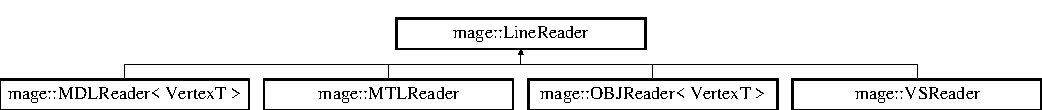
\includegraphics[height=1.000000cm]{classmage_1_1_line_reader}
\end{center}
\end{figure}
\subsection*{Public Member Functions}
\begin{DoxyCompactItemize}
\item 
\hyperlink{classmage_1_1_line_reader}{Line\+Reader} \& \hyperlink{classmage_1_1_line_reader_a2247078d0b5602f9a9a6b74019832faf}{operator=} (const \hyperlink{classmage_1_1_line_reader}{Line\+Reader} \&reader)=delete
\item 
\hyperlink{classmage_1_1_line_reader}{Line\+Reader} \& \hyperlink{classmage_1_1_line_reader_a3ba691cb32a1ab5dcbe75498068c1b86}{operator=} (\hyperlink{classmage_1_1_line_reader}{Line\+Reader} \&\&reader) noexcept
\item 
void \hyperlink{classmage_1_1_line_reader_a6ee0c53351656ac4cd92db1d7c372cff}{Read\+From\+File} (wstring fname, string delimiters=\hyperlink{namespacemage_a10fe126e627cc2ce8af2cc39cc5db81e}{g\+\_\+default\+\_\+delimiters})
\item 
void \hyperlink{classmage_1_1_line_reader_a35ceefa0efd4ccfc3c1401715c0934de}{Read\+From\+Memory} (const char $\ast$input, string delimiters=\hyperlink{namespacemage_a10fe126e627cc2ce8af2cc39cc5db81e}{g\+\_\+default\+\_\+delimiters})
\item 
const wstring \& \hyperlink{classmage_1_1_line_reader_a682ed8030c99a62d4409a01f9efa6d6b}{Get\+Filename} () const noexcept
\item 
const string \& \hyperlink{classmage_1_1_line_reader_aa00e1e27b614e11ec9f70e52d0bac551}{Get\+Delimiters} () const noexcept
\end{DoxyCompactItemize}
\subsection*{Protected Member Functions}
\begin{DoxyCompactItemize}
\item 
\hyperlink{classmage_1_1_line_reader_ab4a46321d7ea3ecda2d6390c78a7285b}{Line\+Reader} ()
\item 
\hyperlink{classmage_1_1_line_reader_ae4f871bebae110704b34c0bd88460639}{Line\+Reader} (const \hyperlink{classmage_1_1_line_reader}{Line\+Reader} \&reader)=delete
\item 
\hyperlink{classmage_1_1_line_reader_ae90c546a98e113a48ca1c94b854a4866}{Line\+Reader} (\hyperlink{classmage_1_1_line_reader}{Line\+Reader} \&\&reader) noexcept
\item 
\hyperlink{classmage_1_1_line_reader_ad9753ea392ebe5b3867852d3392fb1e7}{$\sim$\+Line\+Reader} ()
\item 
\hyperlink{namespacemage_a41c104c036fba3756a74e19f793eeaa1}{U32} \hyperlink{classmage_1_1_line_reader_aa0ed768e2799b74f2341c56fc6ac4969}{Get\+Current\+Line\+Number} () const noexcept
\item 
void \hyperlink{classmage_1_1_line_reader_a3a4b99bfef1e8a826d74a01bcc663fcb}{Read\+Line\+Remaining} ()
\item 
const char $\ast$ \hyperlink{classmage_1_1_line_reader_ad915c1a17549c7758c10f0b6db7e5611}{Read\+Chars} ()
\item 
const string \hyperlink{classmage_1_1_line_reader_ae9a7547d01b29c3237b198444d4f3aef}{Read\+Quoted\+String} ()
\item 
{\footnotesize template$<$typename DataT $>$ }\\const DataT \hyperlink{classmage_1_1_line_reader_aa1ba5aa332e49bdd63ef4ee4021120fd}{Read} ()
\item 
bool \hyperlink{classmage_1_1_line_reader_a7eb54d60902d1fb7846ea5c566312a0f}{Has\+Chars} () const
\item 
bool \hyperlink{classmage_1_1_line_reader_ac92de9a3d986c7031c902c9489cfaa5a}{Has\+Quoted\+String} () const
\item 
{\footnotesize template$<$typename DataT $>$ }\\bool \hyperlink{classmage_1_1_line_reader_a3feef41f3ae6ff506539ffd2f6d38043}{Has} () const
\end{DoxyCompactItemize}
\subsection*{Protected Attributes}
\begin{DoxyCompactItemize}
\item 
char $\ast$ \hyperlink{classmage_1_1_line_reader_a2f1cfe313dc89741386178e63a6b8b0c}{m\+\_\+context}
\end{DoxyCompactItemize}
\subsection*{Private Member Functions}
\begin{DoxyCompactItemize}
\item 
virtual void \hyperlink{classmage_1_1_line_reader_a4de135cfb0434be786cfcfd7959031ef}{Preprocess} ()
\item 
virtual void \hyperlink{classmage_1_1_line_reader_acfb2f7279ec77d070a86d7db812d4745}{Read\+Line} (char $\ast$line)=0
\item 
virtual void \hyperlink{classmage_1_1_line_reader_adfde21013140a1058d3dd567204abfb5}{Postprocess} ()
\end{DoxyCompactItemize}
\subsection*{Private Attributes}
\begin{DoxyCompactItemize}
\item 
\hyperlink{namespacemage_a0ee1bd45ad7dbb3dc8c8e1770e3538d4}{Unique\+File\+Stream} \hyperlink{classmage_1_1_line_reader_a510ff5355c6d26d7c29dc692ef18a3e2}{m\+\_\+file\+\_\+stream}
\item 
wstring \hyperlink{classmage_1_1_line_reader_ad6f55ba12fc610ab2fc1c26a48d12321}{m\+\_\+fname}
\item 
string \hyperlink{classmage_1_1_line_reader_a6de3398ac59fdd98f8c40cff6f5c1075}{m\+\_\+delimiters}
\item 
\hyperlink{namespacemage_a41c104c036fba3756a74e19f793eeaa1}{U32} \hyperlink{classmage_1_1_line_reader_ab145590a7e115106c0987905fde98393}{m\+\_\+line\+\_\+number}
\end{DoxyCompactItemize}


\subsection{Detailed Description}
A class of line readers for reading (non-\/binary) text files line by line. 

\subsection{Constructor \& Destructor Documentation}
\hypertarget{classmage_1_1_line_reader_ab4a46321d7ea3ecda2d6390c78a7285b}{}\label{classmage_1_1_line_reader_ab4a46321d7ea3ecda2d6390c78a7285b} 
\index{mage\+::\+Line\+Reader@{mage\+::\+Line\+Reader}!Line\+Reader@{Line\+Reader}}
\index{Line\+Reader@{Line\+Reader}!mage\+::\+Line\+Reader@{mage\+::\+Line\+Reader}}
\subsubsection{\texorpdfstring{Line\+Reader()}{LineReader()}\hspace{0.1cm}{\footnotesize\ttfamily [1/3]}}
{\footnotesize\ttfamily mage\+::\+Line\+Reader\+::\+Line\+Reader (\begin{DoxyParamCaption}{ }\end{DoxyParamCaption})\hspace{0.3cm}{\ttfamily [protected]}}

Constructs a line reader. \hypertarget{classmage_1_1_line_reader_ae4f871bebae110704b34c0bd88460639}{}\label{classmage_1_1_line_reader_ae4f871bebae110704b34c0bd88460639} 
\index{mage\+::\+Line\+Reader@{mage\+::\+Line\+Reader}!Line\+Reader@{Line\+Reader}}
\index{Line\+Reader@{Line\+Reader}!mage\+::\+Line\+Reader@{mage\+::\+Line\+Reader}}
\subsubsection{\texorpdfstring{Line\+Reader()}{LineReader()}\hspace{0.1cm}{\footnotesize\ttfamily [2/3]}}
{\footnotesize\ttfamily mage\+::\+Line\+Reader\+::\+Line\+Reader (\begin{DoxyParamCaption}\item[{const \hyperlink{classmage_1_1_line_reader}{Line\+Reader} \&}]{reader }\end{DoxyParamCaption})\hspace{0.3cm}{\ttfamily [protected]}, {\ttfamily [delete]}}

Constructs a line reader from the given line reader.


\begin{DoxyParams}[1]{Parameters}
\mbox{\tt in}  & {\em reader} & A reference to the line reader to copy. \\
\hline
\end{DoxyParams}
\hypertarget{classmage_1_1_line_reader_ae90c546a98e113a48ca1c94b854a4866}{}\label{classmage_1_1_line_reader_ae90c546a98e113a48ca1c94b854a4866} 
\index{mage\+::\+Line\+Reader@{mage\+::\+Line\+Reader}!Line\+Reader@{Line\+Reader}}
\index{Line\+Reader@{Line\+Reader}!mage\+::\+Line\+Reader@{mage\+::\+Line\+Reader}}
\subsubsection{\texorpdfstring{Line\+Reader()}{LineReader()}\hspace{0.1cm}{\footnotesize\ttfamily [3/3]}}
{\footnotesize\ttfamily mage\+::\+Line\+Reader\+::\+Line\+Reader (\begin{DoxyParamCaption}\item[{\hyperlink{classmage_1_1_line_reader}{Line\+Reader} \&\&}]{reader }\end{DoxyParamCaption})\hspace{0.3cm}{\ttfamily [protected]}, {\ttfamily [default]}, {\ttfamily [noexcept]}}

Constructs a line reader by moving the given line reader.


\begin{DoxyParams}[1]{Parameters}
\mbox{\tt in}  & {\em reader} & A reference to the line reader to move. \\
\hline
\end{DoxyParams}
\hypertarget{classmage_1_1_line_reader_ad9753ea392ebe5b3867852d3392fb1e7}{}\label{classmage_1_1_line_reader_ad9753ea392ebe5b3867852d3392fb1e7} 
\index{mage\+::\+Line\+Reader@{mage\+::\+Line\+Reader}!````~Line\+Reader@{$\sim$\+Line\+Reader}}
\index{````~Line\+Reader@{$\sim$\+Line\+Reader}!mage\+::\+Line\+Reader@{mage\+::\+Line\+Reader}}
\subsubsection{\texorpdfstring{$\sim$\+Line\+Reader()}{~LineReader()}}
{\footnotesize\ttfamily mage\+::\+Line\+Reader\+::$\sim$\+Line\+Reader (\begin{DoxyParamCaption}{ }\end{DoxyParamCaption})\hspace{0.3cm}{\ttfamily [protected]}, {\ttfamily [default]}}

Destructs this line reader. 

\subsection{Member Function Documentation}
\hypertarget{classmage_1_1_line_reader_aa0ed768e2799b74f2341c56fc6ac4969}{}\label{classmage_1_1_line_reader_aa0ed768e2799b74f2341c56fc6ac4969} 
\index{mage\+::\+Line\+Reader@{mage\+::\+Line\+Reader}!Get\+Current\+Line\+Number@{Get\+Current\+Line\+Number}}
\index{Get\+Current\+Line\+Number@{Get\+Current\+Line\+Number}!mage\+::\+Line\+Reader@{mage\+::\+Line\+Reader}}
\subsubsection{\texorpdfstring{Get\+Current\+Line\+Number()}{GetCurrentLineNumber()}}
{\footnotesize\ttfamily \hyperlink{namespacemage_a41c104c036fba3756a74e19f793eeaa1}{U32} mage\+::\+Line\+Reader\+::\+Get\+Current\+Line\+Number (\begin{DoxyParamCaption}{ }\end{DoxyParamCaption}) const\hspace{0.3cm}{\ttfamily [protected]}, {\ttfamily [noexcept]}}

Returns the current line number of this line reader.

\begin{DoxyReturn}{Returns}
The current line number of this line reader. 
\end{DoxyReturn}
\hypertarget{classmage_1_1_line_reader_aa00e1e27b614e11ec9f70e52d0bac551}{}\label{classmage_1_1_line_reader_aa00e1e27b614e11ec9f70e52d0bac551} 
\index{mage\+::\+Line\+Reader@{mage\+::\+Line\+Reader}!Get\+Delimiters@{Get\+Delimiters}}
\index{Get\+Delimiters@{Get\+Delimiters}!mage\+::\+Line\+Reader@{mage\+::\+Line\+Reader}}
\subsubsection{\texorpdfstring{Get\+Delimiters()}{GetDelimiters()}}
{\footnotesize\ttfamily const string\& mage\+::\+Line\+Reader\+::\+Get\+Delimiters (\begin{DoxyParamCaption}{ }\end{DoxyParamCaption}) const\hspace{0.3cm}{\ttfamily [noexcept]}}

Returns the current delimiters of this line reader.

\begin{DoxyReturn}{Returns}
A reference to the current delimiters of this line reader. 
\end{DoxyReturn}
\hypertarget{classmage_1_1_line_reader_a682ed8030c99a62d4409a01f9efa6d6b}{}\label{classmage_1_1_line_reader_a682ed8030c99a62d4409a01f9efa6d6b} 
\index{mage\+::\+Line\+Reader@{mage\+::\+Line\+Reader}!Get\+Filename@{Get\+Filename}}
\index{Get\+Filename@{Get\+Filename}!mage\+::\+Line\+Reader@{mage\+::\+Line\+Reader}}
\subsubsection{\texorpdfstring{Get\+Filename()}{GetFilename()}}
{\footnotesize\ttfamily const wstring\& mage\+::\+Line\+Reader\+::\+Get\+Filename (\begin{DoxyParamCaption}{ }\end{DoxyParamCaption}) const\hspace{0.3cm}{\ttfamily [noexcept]}}

Returns the current filename of this line reader.

\begin{DoxyReturn}{Returns}
A reference to the current filename of this line reader. 
\end{DoxyReturn}
\hypertarget{classmage_1_1_line_reader_a3feef41f3ae6ff506539ffd2f6d38043}{}\label{classmage_1_1_line_reader_a3feef41f3ae6ff506539ffd2f6d38043} 
\index{mage\+::\+Line\+Reader@{mage\+::\+Line\+Reader}!Has@{Has}}
\index{Has@{Has}!mage\+::\+Line\+Reader@{mage\+::\+Line\+Reader}}
\subsubsection{\texorpdfstring{Has()}{Has()}}
{\footnotesize\ttfamily template$<$typename DataT $>$ \\
bool mage\+::\+Line\+Reader\+::\+Has (\begin{DoxyParamCaption}{ }\end{DoxyParamCaption}) const\hspace{0.3cm}{\ttfamily [protected]}}

Checks whether the next token of this line reader is a {\ttfamily DataT} element.


\begin{DoxyTemplParams}{Template Parameters}
{\em DataT} & The data type. \\
\hline
\end{DoxyTemplParams}
\begin{DoxyReturn}{Returns}
{\ttfamily true} if the next token of this line reader is a {\ttfamily DataT} element. {\ttfamily false} otherwise. 
\end{DoxyReturn}
\hypertarget{classmage_1_1_line_reader_a7eb54d60902d1fb7846ea5c566312a0f}{}\label{classmage_1_1_line_reader_a7eb54d60902d1fb7846ea5c566312a0f} 
\index{mage\+::\+Line\+Reader@{mage\+::\+Line\+Reader}!Has\+Chars@{Has\+Chars}}
\index{Has\+Chars@{Has\+Chars}!mage\+::\+Line\+Reader@{mage\+::\+Line\+Reader}}
\subsubsection{\texorpdfstring{Has\+Chars()}{HasChars()}}
{\footnotesize\ttfamily bool mage\+::\+Line\+Reader\+::\+Has\+Chars (\begin{DoxyParamCaption}{ }\end{DoxyParamCaption}) const\hspace{0.3cm}{\ttfamily [protected]}}

Checks whether this line reader has a next token.

\begin{DoxyReturn}{Returns}
{\ttfamily true} if this line reader has a next token. {\ttfamily false} otherwise. 
\end{DoxyReturn}
\hypertarget{classmage_1_1_line_reader_ac92de9a3d986c7031c902c9489cfaa5a}{}\label{classmage_1_1_line_reader_ac92de9a3d986c7031c902c9489cfaa5a} 
\index{mage\+::\+Line\+Reader@{mage\+::\+Line\+Reader}!Has\+Quoted\+String@{Has\+Quoted\+String}}
\index{Has\+Quoted\+String@{Has\+Quoted\+String}!mage\+::\+Line\+Reader@{mage\+::\+Line\+Reader}}
\subsubsection{\texorpdfstring{Has\+Quoted\+String()}{HasQuotedString()}}
{\footnotesize\ttfamily bool mage\+::\+Line\+Reader\+::\+Has\+Quoted\+String (\begin{DoxyParamCaption}{ }\end{DoxyParamCaption}) const\hspace{0.3cm}{\ttfamily [protected]}}

Checks whether the next token of this line reader is a quoted string.

\begin{DoxyReturn}{Returns}
{\ttfamily true} if the next token of this line reader is a quoted string. {\ttfamily false} otherwise. 
\end{DoxyReturn}
\hypertarget{classmage_1_1_line_reader_a2247078d0b5602f9a9a6b74019832faf}{}\label{classmage_1_1_line_reader_a2247078d0b5602f9a9a6b74019832faf} 
\index{mage\+::\+Line\+Reader@{mage\+::\+Line\+Reader}!operator=@{operator=}}
\index{operator=@{operator=}!mage\+::\+Line\+Reader@{mage\+::\+Line\+Reader}}
\subsubsection{\texorpdfstring{operator=()}{operator=()}\hspace{0.1cm}{\footnotesize\ttfamily [1/2]}}
{\footnotesize\ttfamily \hyperlink{classmage_1_1_line_reader}{Line\+Reader}\& mage\+::\+Line\+Reader\+::operator= (\begin{DoxyParamCaption}\item[{const \hyperlink{classmage_1_1_line_reader}{Line\+Reader} \&}]{reader }\end{DoxyParamCaption})\hspace{0.3cm}{\ttfamily [delete]}}

Copies the given line reader to this line reader.


\begin{DoxyParams}[1]{Parameters}
\mbox{\tt in}  & {\em reader} & A reference to a line reader to copy. \\
\hline
\end{DoxyParams}
\begin{DoxyReturn}{Returns}
A reference to the copy of the given line reader (i.\+e. this line reader). 
\end{DoxyReturn}
\hypertarget{classmage_1_1_line_reader_a3ba691cb32a1ab5dcbe75498068c1b86}{}\label{classmage_1_1_line_reader_a3ba691cb32a1ab5dcbe75498068c1b86} 
\index{mage\+::\+Line\+Reader@{mage\+::\+Line\+Reader}!operator=@{operator=}}
\index{operator=@{operator=}!mage\+::\+Line\+Reader@{mage\+::\+Line\+Reader}}
\subsubsection{\texorpdfstring{operator=()}{operator=()}\hspace{0.1cm}{\footnotesize\ttfamily [2/2]}}
{\footnotesize\ttfamily \hyperlink{classmage_1_1_line_reader}{Line\+Reader} \& mage\+::\+Line\+Reader\+::operator= (\begin{DoxyParamCaption}\item[{\hyperlink{classmage_1_1_line_reader}{Line\+Reader} \&\&}]{reader }\end{DoxyParamCaption})\hspace{0.3cm}{\ttfamily [default]}, {\ttfamily [noexcept]}}

Moves the given line reader to this line reader.


\begin{DoxyParams}[1]{Parameters}
\mbox{\tt in}  & {\em reader} & A reference to a line reader to move. \\
\hline
\end{DoxyParams}
\begin{DoxyReturn}{Returns}
A reference to the moved line reader (i.\+e. this line reader). 
\end{DoxyReturn}
\hypertarget{classmage_1_1_line_reader_adfde21013140a1058d3dd567204abfb5}{}\label{classmage_1_1_line_reader_adfde21013140a1058d3dd567204abfb5} 
\index{mage\+::\+Line\+Reader@{mage\+::\+Line\+Reader}!Postprocess@{Postprocess}}
\index{Postprocess@{Postprocess}!mage\+::\+Line\+Reader@{mage\+::\+Line\+Reader}}
\subsubsection{\texorpdfstring{Postprocess()}{Postprocess()}}
{\footnotesize\ttfamily virtual void mage\+::\+Line\+Reader\+::\+Postprocess (\begin{DoxyParamCaption}{ }\end{DoxyParamCaption})\hspace{0.3cm}{\ttfamily [private]}, {\ttfamily [virtual]}}

Post-\/processes after reading the current file of this line reader.


\begin{DoxyExceptions}{Exceptions}
{\em \hyperlink{classmage_1_1_exception}{Exception}} & Failed to finish post-\/processing successfully. \\
\hline
\end{DoxyExceptions}


Reimplemented in \hyperlink{classmage_1_1loader_1_1_o_b_j_reader_ae8bc7d40a019523546d61bdfd599c368}{mage\+::loader\+::\+O\+B\+J\+Reader$<$ Vertex\+T, Index\+T $>$}.

\hypertarget{classmage_1_1_line_reader_a4de135cfb0434be786cfcfd7959031ef}{}\label{classmage_1_1_line_reader_a4de135cfb0434be786cfcfd7959031ef} 
\index{mage\+::\+Line\+Reader@{mage\+::\+Line\+Reader}!Preprocess@{Preprocess}}
\index{Preprocess@{Preprocess}!mage\+::\+Line\+Reader@{mage\+::\+Line\+Reader}}
\subsubsection{\texorpdfstring{Preprocess()}{Preprocess()}}
{\footnotesize\ttfamily virtual void mage\+::\+Line\+Reader\+::\+Preprocess (\begin{DoxyParamCaption}{ }\end{DoxyParamCaption})\hspace{0.3cm}{\ttfamily [private]}, {\ttfamily [virtual]}}

Pre-\/processes before reading the current file of this line reader.


\begin{DoxyExceptions}{Exceptions}
{\em \hyperlink{classmage_1_1_exception}{Exception}} & Failed to finish the pre-\/processing successfully. \\
\hline
\end{DoxyExceptions}


Reimplemented in \hyperlink{classmage_1_1loader_1_1_o_b_j_reader_a42cb85a0d14f9cc1caff68ae2cf84301}{mage\+::loader\+::\+O\+B\+J\+Reader$<$ Vertex\+T, Index\+T $>$}, and \hyperlink{classmage_1_1loader_1_1_m_d_l_reader_afe56982cb6a6ba9a2ce4abba9cbe3703}{mage\+::loader\+::\+M\+D\+L\+Reader$<$ Vertex\+T, Index\+T $>$}.

\hypertarget{classmage_1_1_line_reader_aa1ba5aa332e49bdd63ef4ee4021120fd}{}\label{classmage_1_1_line_reader_aa1ba5aa332e49bdd63ef4ee4021120fd} 
\index{mage\+::\+Line\+Reader@{mage\+::\+Line\+Reader}!Read@{Read}}
\index{Read@{Read}!mage\+::\+Line\+Reader@{mage\+::\+Line\+Reader}}
\subsubsection{\texorpdfstring{Read()}{Read()}}
{\footnotesize\ttfamily template$<$typename DataT $>$ \\
const DataT mage\+::\+Line\+Reader\+::\+Read (\begin{DoxyParamCaption}{ }\end{DoxyParamCaption})\hspace{0.3cm}{\ttfamily [protected]}}

Reads and converts the next token of this line reader to {\ttfamily DataT} element.


\begin{DoxyTemplParams}{Template Parameters}
{\em DataT} & The data type. \\
\hline
\end{DoxyTemplParams}
\begin{DoxyReturn}{Returns}
The {\ttfamily DataT} represented by the next token of this line reader. 
\end{DoxyReturn}

\begin{DoxyExceptions}{Exceptions}
{\em \hyperlink{classmage_1_1_exception}{Exception}} & There is no next token or the next token does not represent a {\ttfamily DataT} element. \\
\hline
\end{DoxyExceptions}
\hypertarget{classmage_1_1_line_reader_ad915c1a17549c7758c10f0b6db7e5611}{}\label{classmage_1_1_line_reader_ad915c1a17549c7758c10f0b6db7e5611} 
\index{mage\+::\+Line\+Reader@{mage\+::\+Line\+Reader}!Read\+Chars@{Read\+Chars}}
\index{Read\+Chars@{Read\+Chars}!mage\+::\+Line\+Reader@{mage\+::\+Line\+Reader}}
\subsubsection{\texorpdfstring{Read\+Chars()}{ReadChars()}}
{\footnotesize\ttfamily const char $\ast$ mage\+::\+Line\+Reader\+::\+Read\+Chars (\begin{DoxyParamCaption}{ }\end{DoxyParamCaption})\hspace{0.3cm}{\ttfamily [protected]}}

Reads and converts the next token of this line reader to a string.

\begin{DoxyReturn}{Returns}
The string represented by the next token of this line reader. 
\end{DoxyReturn}

\begin{DoxyExceptions}{Exceptions}
{\em \hyperlink{classmage_1_1_exception}{Exception}} & There is no next token. \\
\hline
\end{DoxyExceptions}
\hypertarget{classmage_1_1_line_reader_a6ee0c53351656ac4cd92db1d7c372cff}{}\label{classmage_1_1_line_reader_a6ee0c53351656ac4cd92db1d7c372cff} 
\index{mage\+::\+Line\+Reader@{mage\+::\+Line\+Reader}!Read\+From\+File@{Read\+From\+File}}
\index{Read\+From\+File@{Read\+From\+File}!mage\+::\+Line\+Reader@{mage\+::\+Line\+Reader}}
\subsubsection{\texorpdfstring{Read\+From\+File()}{ReadFromFile()}}
{\footnotesize\ttfamily void mage\+::\+Line\+Reader\+::\+Read\+From\+File (\begin{DoxyParamCaption}\item[{wstring}]{fname,  }\item[{string}]{delimiters = {\ttfamily \hyperlink{namespacemage_a10fe126e627cc2ce8af2cc39cc5db81e}{g\+\_\+default\+\_\+delimiters}} }\end{DoxyParamCaption})}

Reads from the given file.


\begin{DoxyParams}[1]{Parameters}
\mbox{\tt in}  & {\em fname} & The file name. \\
\hline
\mbox{\tt in}  & {\em delimiters} & The string containing the token delimiters (single characters). \\
\hline
\end{DoxyParams}

\begin{DoxyExceptions}{Exceptions}
{\em \hyperlink{classmage_1_1_exception}{Exception}} & Failed to read from the given file. \\
\hline
\end{DoxyExceptions}
\hypertarget{classmage_1_1_line_reader_a35ceefa0efd4ccfc3c1401715c0934de}{}\label{classmage_1_1_line_reader_a35ceefa0efd4ccfc3c1401715c0934de} 
\index{mage\+::\+Line\+Reader@{mage\+::\+Line\+Reader}!Read\+From\+Memory@{Read\+From\+Memory}}
\index{Read\+From\+Memory@{Read\+From\+Memory}!mage\+::\+Line\+Reader@{mage\+::\+Line\+Reader}}
\subsubsection{\texorpdfstring{Read\+From\+Memory()}{ReadFromMemory()}}
{\footnotesize\ttfamily void mage\+::\+Line\+Reader\+::\+Read\+From\+Memory (\begin{DoxyParamCaption}\item[{const char $\ast$}]{input,  }\item[{string}]{delimiters = {\ttfamily \hyperlink{namespacemage_a10fe126e627cc2ce8af2cc39cc5db81e}{g\+\_\+default\+\_\+delimiters}} }\end{DoxyParamCaption})}

Reads the input string.

\begin{DoxyPrecond}{Precondition}
{\itshape input} is not equal to {\ttfamily nullptr}. 
\end{DoxyPrecond}

\begin{DoxyParams}[1]{Parameters}
\mbox{\tt in}  & {\em input} & A pointer to the input null-\/terminated byte string. \\
\hline
\mbox{\tt in}  & {\em delimiters} & The string containing the token delimiters (single characters). \\
\hline
\end{DoxyParams}

\begin{DoxyExceptions}{Exceptions}
{\em \hyperlink{classmage_1_1_exception}{Exception}} & Failed to read from the given input string. \\
\hline
\end{DoxyExceptions}
\hypertarget{classmage_1_1_line_reader_acfb2f7279ec77d070a86d7db812d4745}{}\label{classmage_1_1_line_reader_acfb2f7279ec77d070a86d7db812d4745} 
\index{mage\+::\+Line\+Reader@{mage\+::\+Line\+Reader}!Read\+Line@{Read\+Line}}
\index{Read\+Line@{Read\+Line}!mage\+::\+Line\+Reader@{mage\+::\+Line\+Reader}}
\subsubsection{\texorpdfstring{Read\+Line()}{ReadLine()}}
{\footnotesize\ttfamily virtual void mage\+::\+Line\+Reader\+::\+Read\+Line (\begin{DoxyParamCaption}\item[{char $\ast$}]{line }\end{DoxyParamCaption})\hspace{0.3cm}{\ttfamily [private]}, {\ttfamily [pure virtual]}}

Reads the given line.

\begin{DoxyPrecond}{Precondition}
{\itshape line} is not equal to {\ttfamily nullptr}. 
\end{DoxyPrecond}

\begin{DoxyParams}[1]{Parameters}
\mbox{\tt in,out}  & {\em line} & A pointer to the null-\/terminated byte string to read. \\
\hline
\end{DoxyParams}

\begin{DoxyExceptions}{Exceptions}
{\em \hyperlink{classmage_1_1_exception}{Exception}} & Failed to read the given line. \\
\hline
\end{DoxyExceptions}


Implemented in \hyperlink{classmage_1_1loader_1_1_o_b_j_reader_a9a66ccf1569bdef5194dae20f6282186}{mage\+::loader\+::\+O\+B\+J\+Reader$<$ Vertex\+T, Index\+T $>$}, \hyperlink{classmage_1_1loader_1_1_m_d_l_reader_ac820f425a40dcd407434fdff4d420f86}{mage\+::loader\+::\+M\+D\+L\+Reader$<$ Vertex\+T, Index\+T $>$}, \hyperlink{classmage_1_1loader_1_1_m_t_l_reader_af16f5fa26bd9649d56550738bae77d24}{mage\+::loader\+::\+M\+T\+L\+Reader}, and \hyperlink{classmage_1_1loader_1_1_v_a_r_reader_a9635d8d256066746be81d9c2d223961d}{mage\+::loader\+::\+V\+A\+R\+Reader}.

\hypertarget{classmage_1_1_line_reader_a3a4b99bfef1e8a826d74a01bcc663fcb}{}\label{classmage_1_1_line_reader_a3a4b99bfef1e8a826d74a01bcc663fcb} 
\index{mage\+::\+Line\+Reader@{mage\+::\+Line\+Reader}!Read\+Line\+Remaining@{Read\+Line\+Remaining}}
\index{Read\+Line\+Remaining@{Read\+Line\+Remaining}!mage\+::\+Line\+Reader@{mage\+::\+Line\+Reader}}
\subsubsection{\texorpdfstring{Read\+Line\+Remaining()}{ReadLineRemaining()}}
{\footnotesize\ttfamily void mage\+::\+Line\+Reader\+::\+Read\+Line\+Remaining (\begin{DoxyParamCaption}{ }\end{DoxyParamCaption})\hspace{0.3cm}{\ttfamily [protected]}}

Reads the remaining tokens of the current line of this line reader. \hypertarget{classmage_1_1_line_reader_ae9a7547d01b29c3237b198444d4f3aef}{}\label{classmage_1_1_line_reader_ae9a7547d01b29c3237b198444d4f3aef} 
\index{mage\+::\+Line\+Reader@{mage\+::\+Line\+Reader}!Read\+Quoted\+String@{Read\+Quoted\+String}}
\index{Read\+Quoted\+String@{Read\+Quoted\+String}!mage\+::\+Line\+Reader@{mage\+::\+Line\+Reader}}
\subsubsection{\texorpdfstring{Read\+Quoted\+String()}{ReadQuotedString()}}
{\footnotesize\ttfamily const string mage\+::\+Line\+Reader\+::\+Read\+Quoted\+String (\begin{DoxyParamCaption}{ }\end{DoxyParamCaption})\hspace{0.3cm}{\ttfamily [protected]}}

Reads and converts the next token of this line reader to a quoted string.

\begin{DoxyReturn}{Returns}
The quoted string represented by the next token of this line reader. 
\end{DoxyReturn}

\begin{DoxyExceptions}{Exceptions}
{\em \hyperlink{classmage_1_1_exception}{Exception}} & There is no next token or the next token does not represent a quoted string. \\
\hline
\end{DoxyExceptions}


\subsection{Member Data Documentation}
\hypertarget{classmage_1_1_line_reader_a2f1cfe313dc89741386178e63a6b8b0c}{}\label{classmage_1_1_line_reader_a2f1cfe313dc89741386178e63a6b8b0c} 
\index{mage\+::\+Line\+Reader@{mage\+::\+Line\+Reader}!m\+\_\+context@{m\+\_\+context}}
\index{m\+\_\+context@{m\+\_\+context}!mage\+::\+Line\+Reader@{mage\+::\+Line\+Reader}}
\subsubsection{\texorpdfstring{m\+\_\+context}{m\_context}}
{\footnotesize\ttfamily char$\ast$ mage\+::\+Line\+Reader\+::m\+\_\+context\hspace{0.3cm}{\ttfamily [protected]}}

The current context of this line reader. \hypertarget{classmage_1_1_line_reader_a6de3398ac59fdd98f8c40cff6f5c1075}{}\label{classmage_1_1_line_reader_a6de3398ac59fdd98f8c40cff6f5c1075} 
\index{mage\+::\+Line\+Reader@{mage\+::\+Line\+Reader}!m\+\_\+delimiters@{m\+\_\+delimiters}}
\index{m\+\_\+delimiters@{m\+\_\+delimiters}!mage\+::\+Line\+Reader@{mage\+::\+Line\+Reader}}
\subsubsection{\texorpdfstring{m\+\_\+delimiters}{m\_delimiters}}
{\footnotesize\ttfamily string mage\+::\+Line\+Reader\+::m\+\_\+delimiters\hspace{0.3cm}{\ttfamily [private]}}

The current delimiters of this line reader. \hypertarget{classmage_1_1_line_reader_a510ff5355c6d26d7c29dc692ef18a3e2}{}\label{classmage_1_1_line_reader_a510ff5355c6d26d7c29dc692ef18a3e2} 
\index{mage\+::\+Line\+Reader@{mage\+::\+Line\+Reader}!m\+\_\+file\+\_\+stream@{m\+\_\+file\+\_\+stream}}
\index{m\+\_\+file\+\_\+stream@{m\+\_\+file\+\_\+stream}!mage\+::\+Line\+Reader@{mage\+::\+Line\+Reader}}
\subsubsection{\texorpdfstring{m\+\_\+file\+\_\+stream}{m\_file\_stream}}
{\footnotesize\ttfamily \hyperlink{namespacemage_a0ee1bd45ad7dbb3dc8c8e1770e3538d4}{Unique\+File\+Stream} mage\+::\+Line\+Reader\+::m\+\_\+file\+\_\+stream\hspace{0.3cm}{\ttfamily [private]}}

A pointer to the file stream of this line reader. \hypertarget{classmage_1_1_line_reader_ad6f55ba12fc610ab2fc1c26a48d12321}{}\label{classmage_1_1_line_reader_ad6f55ba12fc610ab2fc1c26a48d12321} 
\index{mage\+::\+Line\+Reader@{mage\+::\+Line\+Reader}!m\+\_\+fname@{m\+\_\+fname}}
\index{m\+\_\+fname@{m\+\_\+fname}!mage\+::\+Line\+Reader@{mage\+::\+Line\+Reader}}
\subsubsection{\texorpdfstring{m\+\_\+fname}{m\_fname}}
{\footnotesize\ttfamily wstring mage\+::\+Line\+Reader\+::m\+\_\+fname\hspace{0.3cm}{\ttfamily [private]}}

The current filename of this line reader. \hypertarget{classmage_1_1_line_reader_ab145590a7e115106c0987905fde98393}{}\label{classmage_1_1_line_reader_ab145590a7e115106c0987905fde98393} 
\index{mage\+::\+Line\+Reader@{mage\+::\+Line\+Reader}!m\+\_\+line\+\_\+number@{m\+\_\+line\+\_\+number}}
\index{m\+\_\+line\+\_\+number@{m\+\_\+line\+\_\+number}!mage\+::\+Line\+Reader@{mage\+::\+Line\+Reader}}
\subsubsection{\texorpdfstring{m\+\_\+line\+\_\+number}{m\_line\_number}}
{\footnotesize\ttfamily \hyperlink{namespacemage_a41c104c036fba3756a74e19f793eeaa1}{U32} mage\+::\+Line\+Reader\+::m\+\_\+line\+\_\+number\hspace{0.3cm}{\ttfamily [private]}}

The current line number of this line reader. 
\hypertarget{classmage_1_1_local_transform}{}\section{mage\+:\+:Local\+Transform Class Reference}
\label{classmage_1_1_local_transform}\index{mage\+::\+Local\+Transform@{mage\+::\+Local\+Transform}}


{\ttfamily \#include $<$local\+\_\+transform.\+hpp$>$}

\subsection*{Public Member Functions}
\begin{DoxyCompactItemize}
\item 
\hyperlink{classmage_1_1_local_transform_a1d16baf92877d4b62e519a574a288c5a}{Local\+Transform} (\hyperlink{namespacemage_a73fbe0da4b8d5bc156bb8453e5b63a17}{F32x3} translation=\{ 0.\+0f, 0.\+0f, 0.\+0f \}, F32x3 rotation=\{ 0.\+0f, 0.\+0f, 0.\+0f \}, F32x3 scale=\{ 1.\+0f, 1.\+0f, 1.\+0f \}) noexcept
\item 
\hyperlink{classmage_1_1_local_transform_a1fc771022886b17cf9cdfe42d9110045}{Local\+Transform} (F\+X\+M\+V\+E\+C\+T\+OR translation, F\+X\+M\+V\+E\+C\+T\+OR rotation, F\+X\+M\+V\+E\+C\+T\+OR scale) noexcept
\item 
\hyperlink{classmage_1_1_local_transform_a7e4eca4017880b098ba081ca1fee9eb2}{Local\+Transform} (const \hyperlink{classmage_1_1_local_transform}{Local\+Transform} \&transform) noexcept=default
\item 
\hyperlink{classmage_1_1_local_transform_a89307f1f9229ba548fb7fb0c9dc64479}{Local\+Transform} (\hyperlink{classmage_1_1_local_transform}{Local\+Transform} \&\&transform) noexcept=default
\item 
\hyperlink{classmage_1_1_local_transform_ada7472793bea34f1fbbea0856b124411}{$\sim$\+Local\+Transform} ()=default
\item 
\hyperlink{classmage_1_1_local_transform}{Local\+Transform} \& \hyperlink{classmage_1_1_local_transform_a518f40cfd7973289b692057d30765741}{operator=} (const \hyperlink{classmage_1_1_local_transform}{Local\+Transform} \&transform)=default
\item 
\hyperlink{classmage_1_1_local_transform}{Local\+Transform} \& \hyperlink{classmage_1_1_local_transform_ae0e82157979f8ebfe4a207d53d0fbfbf}{operator=} (\hyperlink{classmage_1_1_local_transform}{Local\+Transform} \&\&transform)=default
\item 
void \hyperlink{classmage_1_1_local_transform_a6f7d8ee474163d921c8fe485c99a0217}{Set\+TranslationX} (\hyperlink{namespacemage_aa97e833b45f06d60a0a9c4fc22ae02c0}{F32} x) noexcept
\item 
void \hyperlink{classmage_1_1_local_transform_a7e06523876b41b3743e54e11516b61b8}{Set\+TranslationY} (\hyperlink{namespacemage_aa97e833b45f06d60a0a9c4fc22ae02c0}{F32} y) noexcept
\item 
void \hyperlink{classmage_1_1_local_transform_a11733e0dd9297c3742bc3c50056c71c3}{Set\+TranslationZ} (\hyperlink{namespacemage_aa97e833b45f06d60a0a9c4fc22ae02c0}{F32} z) noexcept
\item 
void \hyperlink{classmage_1_1_local_transform_acf9b6ca41b2360d347ae354677d33952}{Set\+Translation} (\hyperlink{namespacemage_aa97e833b45f06d60a0a9c4fc22ae02c0}{F32} x, \hyperlink{namespacemage_aa97e833b45f06d60a0a9c4fc22ae02c0}{F32} y, \hyperlink{namespacemage_aa97e833b45f06d60a0a9c4fc22ae02c0}{F32} z) noexcept
\item 
void \hyperlink{classmage_1_1_local_transform_af172aa7bd7571456717773ffbbdfcac4}{Set\+Translation} (\hyperlink{namespacemage_a73fbe0da4b8d5bc156bb8453e5b63a17}{F32x3} translation) noexcept
\item 
void X\+M\+\_\+\+C\+A\+L\+L\+C\+O\+NV \hyperlink{classmage_1_1_local_transform_a756fd6b64296a0285cbe8447518165c9}{Set\+Translation} (F\+X\+M\+V\+E\+C\+T\+OR translation) noexcept
\item 
void \hyperlink{classmage_1_1_local_transform_aa1e2f6f7db150734e6f10a9d695202d7}{Add\+TranslationX} (\hyperlink{namespacemage_aa97e833b45f06d60a0a9c4fc22ae02c0}{F32} x) noexcept
\item 
void \hyperlink{classmage_1_1_local_transform_a3e058e92d72b6709957712a7d808a6e5}{Add\+TranslationY} (\hyperlink{namespacemage_aa97e833b45f06d60a0a9c4fc22ae02c0}{F32} y) noexcept
\item 
void \hyperlink{classmage_1_1_local_transform_aa2f35831d30101a57d1bfaf1cba527b8}{Add\+TranslationZ} (\hyperlink{namespacemage_aa97e833b45f06d60a0a9c4fc22ae02c0}{F32} z) noexcept
\item 
void \hyperlink{classmage_1_1_local_transform_a2796d9726a59d5a3ea90beee25008222}{Add\+Translation} (\hyperlink{namespacemage_aa97e833b45f06d60a0a9c4fc22ae02c0}{F32} x, \hyperlink{namespacemage_aa97e833b45f06d60a0a9c4fc22ae02c0}{F32} y, \hyperlink{namespacemage_aa97e833b45f06d60a0a9c4fc22ae02c0}{F32} z) noexcept
\item 
void \hyperlink{classmage_1_1_local_transform_ae859ff5d5f4bc7d106b8c4cf233c8f8a}{Add\+Translation} (const \hyperlink{namespacemage_a73fbe0da4b8d5bc156bb8453e5b63a17}{F32x3} \&translation) noexcept
\item 
void X\+M\+\_\+\+C\+A\+L\+L\+C\+O\+NV \hyperlink{classmage_1_1_local_transform_a43e89031fcab7af7e7fb1c7d80e06438}{Add\+Translation} (F\+X\+M\+V\+E\+C\+T\+OR translation) noexcept
\item 
\hyperlink{namespacemage_aa97e833b45f06d60a0a9c4fc22ae02c0}{F32} \hyperlink{classmage_1_1_local_transform_ae021c17cf996088044a9c4f7be1601b8}{Get\+TranslationX} () const noexcept
\item 
\hyperlink{namespacemage_aa97e833b45f06d60a0a9c4fc22ae02c0}{F32} \hyperlink{classmage_1_1_local_transform_a31441b5c6cca77b6f0e8c5cc9c3bf3f0}{Get\+TranslationY} () const noexcept
\item 
\hyperlink{namespacemage_aa97e833b45f06d60a0a9c4fc22ae02c0}{F32} \hyperlink{classmage_1_1_local_transform_a09d94a592dab22c23e664402144d75bc}{Get\+TranslationZ} () const noexcept
\item 
const \hyperlink{namespacemage_a73fbe0da4b8d5bc156bb8453e5b63a17}{F32x3} \hyperlink{classmage_1_1_local_transform_a302713192aca919d01e02fb4eac2d2c5}{Get\+Translation} () const noexcept
\item 
const X\+M\+V\+E\+C\+T\+OR X\+M\+\_\+\+C\+A\+L\+L\+C\+O\+NV \hyperlink{classmage_1_1_local_transform_a18dc6111bfca7d24f3f24e2c1dff8d0b}{Get\+TranslationV} () const noexcept
\item 
const X\+M\+M\+A\+T\+R\+IX X\+M\+\_\+\+C\+A\+L\+L\+C\+O\+NV \hyperlink{classmage_1_1_local_transform_a417c97411f3214119a1e7298de4b1631}{Get\+Object\+To\+Parent\+Translation\+Matrix} () const noexcept
\item 
const X\+M\+M\+A\+T\+R\+IX X\+M\+\_\+\+C\+A\+L\+L\+C\+O\+NV \hyperlink{classmage_1_1_local_transform_aa64c46933f029f5952895a185b5fdd29}{Get\+Parent\+To\+Object\+Translation\+Matrix} () const noexcept
\item 
void \hyperlink{classmage_1_1_local_transform_a57f9839911c987f3cfc5b686a80c6624}{Set\+RotationX} (\hyperlink{namespacemage_aa97e833b45f06d60a0a9c4fc22ae02c0}{F32} x) noexcept
\item 
void \hyperlink{classmage_1_1_local_transform_a6fe237d9f56681271273f47b26b89ac0}{Set\+RotationY} (\hyperlink{namespacemage_aa97e833b45f06d60a0a9c4fc22ae02c0}{F32} y) noexcept
\item 
void \hyperlink{classmage_1_1_local_transform_a1dcec183b2f7ebf3fc7eb4ab574ca045}{Set\+RotationZ} (\hyperlink{namespacemage_aa97e833b45f06d60a0a9c4fc22ae02c0}{F32} z) noexcept
\item 
void \hyperlink{classmage_1_1_local_transform_a7f6fbefa501a2111a07d532a823fba6e}{Set\+Rotation} (\hyperlink{namespacemage_aa97e833b45f06d60a0a9c4fc22ae02c0}{F32} x, \hyperlink{namespacemage_aa97e833b45f06d60a0a9c4fc22ae02c0}{F32} y, \hyperlink{namespacemage_aa97e833b45f06d60a0a9c4fc22ae02c0}{F32} z) noexcept
\item 
void \hyperlink{classmage_1_1_local_transform_aad6d2bf0eba13e47e90023edcdc55c47}{Set\+Rotation} (\hyperlink{namespacemage_a73fbe0da4b8d5bc156bb8453e5b63a17}{F32x3} rotation) noexcept
\item 
void X\+M\+\_\+\+C\+A\+L\+L\+C\+O\+NV \hyperlink{classmage_1_1_local_transform_a470961f6e4f3b0920742489722ca791e}{Set\+Rotation} (F\+X\+M\+V\+E\+C\+T\+OR rotation) noexcept
\item 
void X\+M\+\_\+\+C\+A\+L\+L\+C\+O\+NV \hyperlink{classmage_1_1_local_transform_a366b1cbd069bce035a868a8800dc04e9}{Set\+Rotation\+Around\+Direction} (F\+X\+M\+V\+E\+C\+T\+OR normal, \hyperlink{namespacemage_aa97e833b45f06d60a0a9c4fc22ae02c0}{F32} angle) noexcept
\item 
void \hyperlink{classmage_1_1_local_transform_ab9d98b568a7384896857e2d6e72342db}{Add\+RotationX} (\hyperlink{namespacemage_aa97e833b45f06d60a0a9c4fc22ae02c0}{F32} x) noexcept
\item 
void \hyperlink{classmage_1_1_local_transform_adea3848a1d4d83a836d33668f323bb4d}{Add\+RotationY} (\hyperlink{namespacemage_aa97e833b45f06d60a0a9c4fc22ae02c0}{F32} y) noexcept
\item 
void \hyperlink{classmage_1_1_local_transform_ac769e25872e8a738bd6189f2ca6db4ea}{Add\+RotationZ} (\hyperlink{namespacemage_aa97e833b45f06d60a0a9c4fc22ae02c0}{F32} z) noexcept
\item 
void \hyperlink{classmage_1_1_local_transform_af4f3c10c99796ed8b71841bfd94e578d}{Add\+Rotation} (\hyperlink{namespacemage_aa97e833b45f06d60a0a9c4fc22ae02c0}{F32} x, \hyperlink{namespacemage_aa97e833b45f06d60a0a9c4fc22ae02c0}{F32} y, \hyperlink{namespacemage_aa97e833b45f06d60a0a9c4fc22ae02c0}{F32} z) noexcept
\item 
void \hyperlink{classmage_1_1_local_transform_a388e221978d1d8fb384ca1728301d4ab}{Add\+Rotation} (const \hyperlink{namespacemage_a73fbe0da4b8d5bc156bb8453e5b63a17}{F32x3} \&rotation) noexcept
\item 
void X\+M\+\_\+\+C\+A\+L\+L\+C\+O\+NV \hyperlink{classmage_1_1_local_transform_a44da0f859b1687cd5846928bfc6d602e}{Add\+Rotation} (F\+X\+M\+V\+E\+C\+T\+OR rotation) noexcept
\item 
void \hyperlink{classmage_1_1_local_transform_ad706493a65d14c9decbeec3e52c25316}{Add\+And\+Clamp\+RotationX} (\hyperlink{namespacemage_aa97e833b45f06d60a0a9c4fc22ae02c0}{F32} x, \hyperlink{namespacemage_aa97e833b45f06d60a0a9c4fc22ae02c0}{F32} min\+\_\+angle, \hyperlink{namespacemage_aa97e833b45f06d60a0a9c4fc22ae02c0}{F32} max\+\_\+angle) noexcept
\item 
void \hyperlink{classmage_1_1_local_transform_a960e6f431f8962f7aee701c0af1dc9e0}{Add\+And\+Clamp\+RotationY} (\hyperlink{namespacemage_aa97e833b45f06d60a0a9c4fc22ae02c0}{F32} y, \hyperlink{namespacemage_aa97e833b45f06d60a0a9c4fc22ae02c0}{F32} min\+\_\+angle, \hyperlink{namespacemage_aa97e833b45f06d60a0a9c4fc22ae02c0}{F32} max\+\_\+angle) noexcept
\item 
void \hyperlink{classmage_1_1_local_transform_a324c338aa8a85a74145e5641f9c65c96}{Add\+And\+Clamp\+RotationZ} (\hyperlink{namespacemage_aa97e833b45f06d60a0a9c4fc22ae02c0}{F32} z, \hyperlink{namespacemage_aa97e833b45f06d60a0a9c4fc22ae02c0}{F32} min\+\_\+angle, \hyperlink{namespacemage_aa97e833b45f06d60a0a9c4fc22ae02c0}{F32} max\+\_\+angle) noexcept
\item 
void \hyperlink{classmage_1_1_local_transform_aa5c60513e379baae81f79cea835d1896}{Add\+And\+Clamp\+Rotation} (\hyperlink{namespacemage_aa97e833b45f06d60a0a9c4fc22ae02c0}{F32} x, \hyperlink{namespacemage_aa97e833b45f06d60a0a9c4fc22ae02c0}{F32} y, \hyperlink{namespacemage_aa97e833b45f06d60a0a9c4fc22ae02c0}{F32} z, \hyperlink{namespacemage_aa97e833b45f06d60a0a9c4fc22ae02c0}{F32} min\+\_\+angle, \hyperlink{namespacemage_aa97e833b45f06d60a0a9c4fc22ae02c0}{F32} max\+\_\+angle) noexcept
\item 
void \hyperlink{classmage_1_1_local_transform_aa6b68f4b531aa34113b8df652c0245d8}{Add\+And\+Clamp\+Rotation} (const \hyperlink{namespacemage_a73fbe0da4b8d5bc156bb8453e5b63a17}{F32x3} \&rotation, \hyperlink{namespacemage_aa97e833b45f06d60a0a9c4fc22ae02c0}{F32} min\+\_\+angle, \hyperlink{namespacemage_aa97e833b45f06d60a0a9c4fc22ae02c0}{F32} max\+\_\+angle) noexcept
\item 
void X\+M\+\_\+\+C\+A\+L\+L\+C\+O\+NV \hyperlink{classmage_1_1_local_transform_a00559d5316893be21c67d039a55d6d7f}{Add\+And\+Clamp\+Rotation} (F\+X\+M\+V\+E\+C\+T\+OR rotation, \hyperlink{namespacemage_aa97e833b45f06d60a0a9c4fc22ae02c0}{F32} min\+\_\+angle, \hyperlink{namespacemage_aa97e833b45f06d60a0a9c4fc22ae02c0}{F32} max\+\_\+angle) noexcept
\item 
\hyperlink{namespacemage_aa97e833b45f06d60a0a9c4fc22ae02c0}{F32} \hyperlink{classmage_1_1_local_transform_af60f86fbaa2dc4562d67100215a63a61}{Get\+RotationX} () const noexcept
\item 
\hyperlink{namespacemage_aa97e833b45f06d60a0a9c4fc22ae02c0}{F32} \hyperlink{classmage_1_1_local_transform_a7d6b4eba97d85e80dacb6dc663c17e9c}{Get\+RotationY} () const noexcept
\item 
\hyperlink{namespacemage_aa97e833b45f06d60a0a9c4fc22ae02c0}{F32} \hyperlink{classmage_1_1_local_transform_ae56bae1d47047892c6588a1fe3f115ad}{Get\+RotationZ} () const noexcept
\item 
const \hyperlink{namespacemage_a73fbe0da4b8d5bc156bb8453e5b63a17}{F32x3} \hyperlink{classmage_1_1_local_transform_a06ddc0ea860a58ed7d47abc115ea70e3}{Get\+Rotation} () const noexcept
\item 
const X\+M\+V\+E\+C\+T\+OR X\+M\+\_\+\+C\+A\+L\+L\+C\+O\+NV \hyperlink{classmage_1_1_local_transform_a489f350ed2e1e7eea1d168502cd03e88}{Get\+RotationV} () const noexcept
\item 
const X\+M\+V\+E\+C\+T\+OR X\+M\+\_\+\+C\+A\+L\+L\+C\+O\+NV \hyperlink{classmage_1_1_local_transform_a5d9cb07de3b11b31665f2bb35580febc}{Get\+Object\+To\+Parent\+Rotation\+Quaternion} () const noexcept
\item 
const X\+M\+V\+E\+C\+T\+OR X\+M\+\_\+\+C\+A\+L\+L\+C\+O\+NV \hyperlink{classmage_1_1_local_transform_a66e6d3320e87461203f91599e23ee6c1}{Get\+Parent\+To\+Object\+Rotation\+Quaternion} () const noexcept
\item 
const X\+M\+M\+A\+T\+R\+IX X\+M\+\_\+\+C\+A\+L\+L\+C\+O\+NV \hyperlink{classmage_1_1_local_transform_a43be02da78f59f2e6ab5d5719816498b}{Get\+Object\+To\+Parent\+Rotation\+Matrix} () const noexcept
\item 
const X\+M\+M\+A\+T\+R\+IX X\+M\+\_\+\+C\+A\+L\+L\+C\+O\+NV \hyperlink{classmage_1_1_local_transform_a5054e57409d6852adcde6283ca8a5c49}{Get\+Parent\+To\+Object\+Rotation\+Matrix} () const noexcept
\item 
void \hyperlink{classmage_1_1_local_transform_afaab2f329bb986de112e76ba8407b84e}{Set\+ScaleX} (\hyperlink{namespacemage_aa97e833b45f06d60a0a9c4fc22ae02c0}{F32} x) noexcept
\item 
void \hyperlink{classmage_1_1_local_transform_a17297480169c047f0a08c2022b69fc42}{Set\+ScaleY} (\hyperlink{namespacemage_aa97e833b45f06d60a0a9c4fc22ae02c0}{F32} y) noexcept
\item 
void \hyperlink{classmage_1_1_local_transform_a076673ed934cc2b92febfd5477e81e75}{Set\+ScaleZ} (\hyperlink{namespacemage_aa97e833b45f06d60a0a9c4fc22ae02c0}{F32} z) noexcept
\item 
void \hyperlink{classmage_1_1_local_transform_ae5940b8381188b25b164322d0c848fb3}{Set\+Scale} (\hyperlink{namespacemage_aa97e833b45f06d60a0a9c4fc22ae02c0}{F32} s) noexcept
\item 
void \hyperlink{classmage_1_1_local_transform_a81b531b924652a52a49a5163ee5f6685}{Set\+Scale} (\hyperlink{namespacemage_aa97e833b45f06d60a0a9c4fc22ae02c0}{F32} x, \hyperlink{namespacemage_aa97e833b45f06d60a0a9c4fc22ae02c0}{F32} y, \hyperlink{namespacemage_aa97e833b45f06d60a0a9c4fc22ae02c0}{F32} z) noexcept
\item 
void \hyperlink{classmage_1_1_local_transform_a8e489c87ad55a7a39a5ec72cc878700b}{Set\+Scale} (\hyperlink{namespacemage_a73fbe0da4b8d5bc156bb8453e5b63a17}{F32x3} scale) noexcept
\item 
void X\+M\+\_\+\+C\+A\+L\+L\+C\+O\+NV \hyperlink{classmage_1_1_local_transform_a2f8086f72f3c72a641db1b59e8b3e9c0}{Set\+Scale} (F\+X\+M\+V\+E\+C\+T\+OR scale) noexcept
\item 
void \hyperlink{classmage_1_1_local_transform_a5b3bdbe95a1b531271a122d1fe26f0a6}{Add\+ScaleX} (\hyperlink{namespacemage_aa97e833b45f06d60a0a9c4fc22ae02c0}{F32} x) noexcept
\item 
void \hyperlink{classmage_1_1_local_transform_abd8826a904947b5934ba6afef3b3826f}{Add\+ScaleY} (\hyperlink{namespacemage_aa97e833b45f06d60a0a9c4fc22ae02c0}{F32} y) noexcept
\item 
void \hyperlink{classmage_1_1_local_transform_a28160bebf308eec45d9649a197d91336}{Add\+ScaleZ} (\hyperlink{namespacemage_aa97e833b45f06d60a0a9c4fc22ae02c0}{F32} z) noexcept
\item 
void \hyperlink{classmage_1_1_local_transform_a7c7c84c097157d87bcd3c1d58fc6f8df}{Add\+Scale} (\hyperlink{namespacemage_aa97e833b45f06d60a0a9c4fc22ae02c0}{F32} s) noexcept
\item 
void \hyperlink{classmage_1_1_local_transform_a8de03038d4455846983ccf5b7a0cb08d}{Add\+Scale} (\hyperlink{namespacemage_aa97e833b45f06d60a0a9c4fc22ae02c0}{F32} x, \hyperlink{namespacemage_aa97e833b45f06d60a0a9c4fc22ae02c0}{F32} y, \hyperlink{namespacemage_aa97e833b45f06d60a0a9c4fc22ae02c0}{F32} z) noexcept
\item 
void \hyperlink{classmage_1_1_local_transform_a3bf03266ca3266cd1eecab3b3dd73e77}{Add\+Scale} (const \hyperlink{namespacemage_a73fbe0da4b8d5bc156bb8453e5b63a17}{F32x3} \&scale) noexcept
\item 
void X\+M\+\_\+\+C\+A\+L\+L\+C\+O\+NV \hyperlink{classmage_1_1_local_transform_a1c2ae4604dfd52b8a58356eb78ac99bf}{Add\+Scale} (F\+X\+M\+V\+E\+C\+T\+OR scale) noexcept
\item 
\hyperlink{namespacemage_aa97e833b45f06d60a0a9c4fc22ae02c0}{F32} \hyperlink{classmage_1_1_local_transform_ad539c04b897276a35bd3f25ad2163371}{Get\+ScaleX} () const noexcept
\item 
\hyperlink{namespacemage_aa97e833b45f06d60a0a9c4fc22ae02c0}{F32} \hyperlink{classmage_1_1_local_transform_a8c15528f78365b5dc853d1e9035b4cc4}{Get\+ScaleY} () const noexcept
\item 
\hyperlink{namespacemage_aa97e833b45f06d60a0a9c4fc22ae02c0}{F32} \hyperlink{classmage_1_1_local_transform_a79225f12e49fce5d16653ad2671a7e97}{Get\+ScaleZ} () const noexcept
\item 
const \hyperlink{namespacemage_a73fbe0da4b8d5bc156bb8453e5b63a17}{F32x3} \hyperlink{classmage_1_1_local_transform_a5dbf74dae200448b0993504d23f99f1c}{Get\+Scale} () const noexcept
\item 
const X\+M\+V\+E\+C\+T\+OR X\+M\+\_\+\+C\+A\+L\+L\+C\+O\+NV \hyperlink{classmage_1_1_local_transform_a6c70ee804326d0b5ff54d282630972bc}{Get\+ScaleV} () const noexcept
\item 
const X\+M\+M\+A\+T\+R\+IX X\+M\+\_\+\+C\+A\+L\+L\+C\+O\+NV \hyperlink{classmage_1_1_local_transform_acd4fda032325f52cb668fc4733c6bc04}{Get\+Object\+To\+Parent\+Scale\+Matrix} () const noexcept
\item 
const X\+M\+M\+A\+T\+R\+IX X\+M\+\_\+\+C\+A\+L\+L\+C\+O\+NV \hyperlink{classmage_1_1_local_transform_a81ef828c64270716e5095f2cf571fad7}{Get\+Parent\+To\+Object\+Scale\+Matrix} () const noexcept
\item 
const X\+M\+V\+E\+C\+T\+OR X\+M\+\_\+\+C\+A\+L\+L\+C\+O\+NV \hyperlink{classmage_1_1_local_transform_abaa858e23864984b339b2fa26607c026}{Get\+Object\+Origin} () const noexcept
\item 
const X\+M\+V\+E\+C\+T\+OR X\+M\+\_\+\+C\+A\+L\+L\+C\+O\+NV \hyperlink{classmage_1_1_local_transform_a369350f17dbf41afa8278643bb641125}{Get\+Object\+AxisX} () const noexcept
\item 
const X\+M\+V\+E\+C\+T\+OR X\+M\+\_\+\+C\+A\+L\+L\+C\+O\+NV \hyperlink{classmage_1_1_local_transform_accd789cb8a8f3cec2c048cfb05ef8eb3}{Get\+Object\+AxisY} () const noexcept
\item 
const X\+M\+V\+E\+C\+T\+OR X\+M\+\_\+\+C\+A\+L\+L\+C\+O\+NV \hyperlink{classmage_1_1_local_transform_a4a7a5e9b38ad3016a9f4db5c46cca782}{Get\+Object\+AxisZ} () const noexcept
\item 
const X\+M\+V\+E\+C\+T\+OR X\+M\+\_\+\+C\+A\+L\+L\+C\+O\+NV \hyperlink{classmage_1_1_local_transform_ad3577335f3be3237c89fe0b02b3cfd53}{Get\+Parent\+Origin} () const noexcept
\item 
const X\+M\+V\+E\+C\+T\+OR X\+M\+\_\+\+C\+A\+L\+L\+C\+O\+NV \hyperlink{classmage_1_1_local_transform_a211651b89d7720bf98468ea7665b74d9}{Get\+Parent\+AxisX} () const noexcept
\item 
const X\+M\+V\+E\+C\+T\+OR X\+M\+\_\+\+C\+A\+L\+L\+C\+O\+NV \hyperlink{classmage_1_1_local_transform_af53f1ef489bc5dec9d5b8ccea6e5e9bf}{Get\+Parent\+AxisY} () const noexcept
\item 
const X\+M\+V\+E\+C\+T\+OR X\+M\+\_\+\+C\+A\+L\+L\+C\+O\+NV \hyperlink{classmage_1_1_local_transform_acc8dd9207592af2db959b609bc14ae1f}{Get\+Parent\+AxisZ} () const noexcept
\item 
const X\+M\+M\+A\+T\+R\+IX X\+M\+\_\+\+C\+A\+L\+L\+C\+O\+NV \hyperlink{classmage_1_1_local_transform_aaf08dbe2fd5125b11e61fc052911dbb6}{Get\+Object\+To\+Parent\+Matrix} () const noexcept
\item 
const X\+M\+M\+A\+T\+R\+IX X\+M\+\_\+\+C\+A\+L\+L\+C\+O\+NV \hyperlink{classmage_1_1_local_transform_a3cc177e24cac45b28231943f7e7d7b03}{Get\+Parent\+To\+Object\+Matrix} () const noexcept
\item 
const X\+M\+V\+E\+C\+T\+OR X\+M\+\_\+\+C\+A\+L\+L\+C\+O\+NV \hyperlink{classmage_1_1_local_transform_abfd5e324acb96d0dc9b3a1a84b0403d9}{Transform\+Object\+To\+Parent} (F\+X\+M\+V\+E\+C\+T\+OR vector) const noexcept
\item 
const X\+M\+V\+E\+C\+T\+OR X\+M\+\_\+\+C\+A\+L\+L\+C\+O\+NV \hyperlink{classmage_1_1_local_transform_a5df12629f26c4bf4d95728333d415d53}{Transform\+Object\+To\+Parent\+Point} (F\+X\+M\+V\+E\+C\+T\+OR point) const noexcept
\item 
const X\+M\+V\+E\+C\+T\+OR X\+M\+\_\+\+C\+A\+L\+L\+C\+O\+NV \hyperlink{classmage_1_1_local_transform_a270150142e83d91a694d6d621b09c1ad}{Transform\+Object\+To\+Parent\+Direction} (F\+X\+M\+V\+E\+C\+T\+OR direction) const noexcept
\item 
const X\+M\+V\+E\+C\+T\+OR X\+M\+\_\+\+C\+A\+L\+L\+C\+O\+NV \hyperlink{classmage_1_1_local_transform_aee4c8c7b54e538a1448224bb36490d0a}{Transform\+Parent\+To\+Object} (F\+X\+M\+V\+E\+C\+T\+OR vector) const noexcept
\item 
const X\+M\+V\+E\+C\+T\+OR X\+M\+\_\+\+C\+A\+L\+L\+C\+O\+NV \hyperlink{classmage_1_1_local_transform_a869e0acb9947f74405bad09164182373}{Transform\+Parent\+To\+Object\+Point} (F\+X\+M\+V\+E\+C\+T\+OR point) const noexcept
\item 
const X\+M\+V\+E\+C\+T\+OR X\+M\+\_\+\+C\+A\+L\+L\+C\+O\+NV \hyperlink{classmage_1_1_local_transform_a237b0811672ffc8dd611e6a56af24c18}{Transform\+Parent\+To\+Object\+Direction} (F\+X\+M\+V\+E\+C\+T\+OR direction) const noexcept
\end{DoxyCompactItemize}
\subsection*{Private Attributes}
\begin{DoxyCompactItemize}
\item 
\hyperlink{namespacemage_a73fbe0da4b8d5bc156bb8453e5b63a17}{F32x3} \hyperlink{classmage_1_1_local_transform_af467d4a331c7215cf016e31bd91c42db}{m\+\_\+translation}
\item 
\hyperlink{namespacemage_aa97e833b45f06d60a0a9c4fc22ae02c0}{F32} \hyperlink{classmage_1_1_local_transform_a408d86574aca8976ca123b992118c6f8}{m\+\_\+padding0}
\item 
\hyperlink{namespacemage_a73fbe0da4b8d5bc156bb8453e5b63a17}{F32x3} \hyperlink{classmage_1_1_local_transform_ac4825a600646e0bb3db5a4699db5f5e1}{m\+\_\+rotation}
\item 
\hyperlink{namespacemage_aa97e833b45f06d60a0a9c4fc22ae02c0}{F32} \hyperlink{classmage_1_1_local_transform_a3b2b212788e819fb6ac46322c15e002e}{m\+\_\+padding1}
\item 
\hyperlink{namespacemage_a73fbe0da4b8d5bc156bb8453e5b63a17}{F32x3} \hyperlink{classmage_1_1_local_transform_aca17d055c29e408606e199425bd2ee2a}{m\+\_\+scale}
\item 
\hyperlink{namespacemage_aa97e833b45f06d60a0a9c4fc22ae02c0}{F32} \hyperlink{classmage_1_1_local_transform_ad293dda4a1c7bfec90267915937aec90}{m\+\_\+padding2}
\end{DoxyCompactItemize}


\subsection{Detailed Description}
A class of local transforms. 

\subsection{Constructor \& Destructor Documentation}
\hypertarget{classmage_1_1_local_transform_a1d16baf92877d4b62e519a574a288c5a}{}\label{classmage_1_1_local_transform_a1d16baf92877d4b62e519a574a288c5a} 
\index{mage\+::\+Local\+Transform@{mage\+::\+Local\+Transform}!Local\+Transform@{Local\+Transform}}
\index{Local\+Transform@{Local\+Transform}!mage\+::\+Local\+Transform@{mage\+::\+Local\+Transform}}
\subsubsection{\texorpdfstring{Local\+Transform()}{LocalTransform()}\hspace{0.1cm}{\footnotesize\ttfamily [1/4]}}
{\footnotesize\ttfamily mage\+::\+Local\+Transform\+::\+Local\+Transform (\begin{DoxyParamCaption}\item[{\hyperlink{namespacemage_a73fbe0da4b8d5bc156bb8453e5b63a17}{F32x3}}]{translation = {\ttfamily \{~0.0f,~0.0f,~0.0f~\}},  }\item[{\hyperlink{namespacemage_a73fbe0da4b8d5bc156bb8453e5b63a17}{F32x3}}]{rotation = {\ttfamily \{~0.0f,~0.0f,~0.0f~\}},  }\item[{\hyperlink{namespacemage_a73fbe0da4b8d5bc156bb8453e5b63a17}{F32x3}}]{scale = {\ttfamily \{~1.0f,~1.0f,~1.0f~\}} }\end{DoxyParamCaption})\hspace{0.3cm}{\ttfamily [explicit]}, {\ttfamily [noexcept]}}

Constructs a local transform from the given translation, rotation and scale component.


\begin{DoxyParams}[1]{Parameters}
\mbox{\tt in}  & {\em translation} & The translation component. \\
\hline
\mbox{\tt in}  & {\em rotation} & The rotation component. \\
\hline
\mbox{\tt in}  & {\em scale} & The scale component. \\
\hline
\end{DoxyParams}
\hypertarget{classmage_1_1_local_transform_a1fc771022886b17cf9cdfe42d9110045}{}\label{classmage_1_1_local_transform_a1fc771022886b17cf9cdfe42d9110045} 
\index{mage\+::\+Local\+Transform@{mage\+::\+Local\+Transform}!Local\+Transform@{Local\+Transform}}
\index{Local\+Transform@{Local\+Transform}!mage\+::\+Local\+Transform@{mage\+::\+Local\+Transform}}
\subsubsection{\texorpdfstring{Local\+Transform()}{LocalTransform()}\hspace{0.1cm}{\footnotesize\ttfamily [2/4]}}
{\footnotesize\ttfamily mage\+::\+Local\+Transform\+::\+Local\+Transform (\begin{DoxyParamCaption}\item[{F\+X\+M\+V\+E\+C\+T\+OR}]{translation,  }\item[{F\+X\+M\+V\+E\+C\+T\+OR}]{rotation,  }\item[{F\+X\+M\+V\+E\+C\+T\+OR}]{scale }\end{DoxyParamCaption})\hspace{0.3cm}{\ttfamily [explicit]}, {\ttfamily [noexcept]}}

Constructs a local transform from the given translation, rotation and scale component.


\begin{DoxyParams}[1]{Parameters}
\mbox{\tt in}  & {\em translation} & The translation component. \\
\hline
\mbox{\tt in}  & {\em rotation} & The rotation component. \\
\hline
\mbox{\tt in}  & {\em scale} & The scale component. \\
\hline
\end{DoxyParams}
\hypertarget{classmage_1_1_local_transform_a7e4eca4017880b098ba081ca1fee9eb2}{}\label{classmage_1_1_local_transform_a7e4eca4017880b098ba081ca1fee9eb2} 
\index{mage\+::\+Local\+Transform@{mage\+::\+Local\+Transform}!Local\+Transform@{Local\+Transform}}
\index{Local\+Transform@{Local\+Transform}!mage\+::\+Local\+Transform@{mage\+::\+Local\+Transform}}
\subsubsection{\texorpdfstring{Local\+Transform()}{LocalTransform()}\hspace{0.1cm}{\footnotesize\ttfamily [3/4]}}
{\footnotesize\ttfamily mage\+::\+Local\+Transform\+::\+Local\+Transform (\begin{DoxyParamCaption}\item[{const \hyperlink{classmage_1_1_local_transform}{Local\+Transform} \&}]{transform }\end{DoxyParamCaption})\hspace{0.3cm}{\ttfamily [default]}, {\ttfamily [noexcept]}}

Constructs a local transform from the given local transform.


\begin{DoxyParams}[1]{Parameters}
\mbox{\tt in}  & {\em transform} & A reference to the local transform to copy. \\
\hline
\end{DoxyParams}
\hypertarget{classmage_1_1_local_transform_a89307f1f9229ba548fb7fb0c9dc64479}{}\label{classmage_1_1_local_transform_a89307f1f9229ba548fb7fb0c9dc64479} 
\index{mage\+::\+Local\+Transform@{mage\+::\+Local\+Transform}!Local\+Transform@{Local\+Transform}}
\index{Local\+Transform@{Local\+Transform}!mage\+::\+Local\+Transform@{mage\+::\+Local\+Transform}}
\subsubsection{\texorpdfstring{Local\+Transform()}{LocalTransform()}\hspace{0.1cm}{\footnotesize\ttfamily [4/4]}}
{\footnotesize\ttfamily mage\+::\+Local\+Transform\+::\+Local\+Transform (\begin{DoxyParamCaption}\item[{\hyperlink{classmage_1_1_local_transform}{Local\+Transform} \&\&}]{transform }\end{DoxyParamCaption})\hspace{0.3cm}{\ttfamily [default]}, {\ttfamily [noexcept]}}

Constructs a local transform by moving the given local transform.


\begin{DoxyParams}[1]{Parameters}
\mbox{\tt in}  & {\em transform} & A reference to the local transform to move. \\
\hline
\end{DoxyParams}
\hypertarget{classmage_1_1_local_transform_ada7472793bea34f1fbbea0856b124411}{}\label{classmage_1_1_local_transform_ada7472793bea34f1fbbea0856b124411} 
\index{mage\+::\+Local\+Transform@{mage\+::\+Local\+Transform}!````~Local\+Transform@{$\sim$\+Local\+Transform}}
\index{````~Local\+Transform@{$\sim$\+Local\+Transform}!mage\+::\+Local\+Transform@{mage\+::\+Local\+Transform}}
\subsubsection{\texorpdfstring{$\sim$\+Local\+Transform()}{~LocalTransform()}}
{\footnotesize\ttfamily mage\+::\+Local\+Transform\+::$\sim$\+Local\+Transform (\begin{DoxyParamCaption}{ }\end{DoxyParamCaption})\hspace{0.3cm}{\ttfamily [default]}}

Destructs this local transform. 

\subsection{Member Function Documentation}
\hypertarget{classmage_1_1_local_transform_aa5c60513e379baae81f79cea835d1896}{}\label{classmage_1_1_local_transform_aa5c60513e379baae81f79cea835d1896} 
\index{mage\+::\+Local\+Transform@{mage\+::\+Local\+Transform}!Add\+And\+Clamp\+Rotation@{Add\+And\+Clamp\+Rotation}}
\index{Add\+And\+Clamp\+Rotation@{Add\+And\+Clamp\+Rotation}!mage\+::\+Local\+Transform@{mage\+::\+Local\+Transform}}
\subsubsection{\texorpdfstring{Add\+And\+Clamp\+Rotation()}{AddAndClampRotation()}\hspace{0.1cm}{\footnotesize\ttfamily [1/3]}}
{\footnotesize\ttfamily void mage\+::\+Local\+Transform\+::\+Add\+And\+Clamp\+Rotation (\begin{DoxyParamCaption}\item[{\hyperlink{namespacemage_aa97e833b45f06d60a0a9c4fc22ae02c0}{F32}}]{x,  }\item[{\hyperlink{namespacemage_aa97e833b45f06d60a0a9c4fc22ae02c0}{F32}}]{y,  }\item[{\hyperlink{namespacemage_aa97e833b45f06d60a0a9c4fc22ae02c0}{F32}}]{z,  }\item[{\hyperlink{namespacemage_aa97e833b45f06d60a0a9c4fc22ae02c0}{F32}}]{min\+\_\+angle,  }\item[{\hyperlink{namespacemage_aa97e833b45f06d60a0a9c4fc22ae02c0}{F32}}]{max\+\_\+angle }\end{DoxyParamCaption})\hspace{0.3cm}{\ttfamily [noexcept]}}

Adds the given rotation component to the rotation component of this local transform and clamps the resulting rotation component of this local transform between the given values.

\begin{DoxyPrecond}{Precondition}
{\itshape min\+\_\+angle} lies in \mbox{[}-\/pi, pi\mbox{]}. 

{\itshape max\+\_\+angle} lies in \mbox{[}-\/pi, pi\mbox{]}. 

{\itshape min\+\_\+angle} is not greater than {\itshape max\+\_\+angle}. 
\end{DoxyPrecond}

\begin{DoxyParams}[1]{Parameters}
\mbox{\tt in}  & {\em x} & The x-\/value of the rotation component to add. \\
\hline
\mbox{\tt in}  & {\em y} & The y-\/value of the rotation component to add. \\
\hline
\mbox{\tt in}  & {\em z} & The z-\/value of the rotation component to add. \\
\hline
\mbox{\tt in}  & {\em min\+\_\+angle} & The minimum angle (in radians). \\
\hline
\mbox{\tt in}  & {\em max\+\_\+angle} & The maximum angle (in radians). \\
\hline
\end{DoxyParams}
\hypertarget{classmage_1_1_local_transform_aa6b68f4b531aa34113b8df652c0245d8}{}\label{classmage_1_1_local_transform_aa6b68f4b531aa34113b8df652c0245d8} 
\index{mage\+::\+Local\+Transform@{mage\+::\+Local\+Transform}!Add\+And\+Clamp\+Rotation@{Add\+And\+Clamp\+Rotation}}
\index{Add\+And\+Clamp\+Rotation@{Add\+And\+Clamp\+Rotation}!mage\+::\+Local\+Transform@{mage\+::\+Local\+Transform}}
\subsubsection{\texorpdfstring{Add\+And\+Clamp\+Rotation()}{AddAndClampRotation()}\hspace{0.1cm}{\footnotesize\ttfamily [2/3]}}
{\footnotesize\ttfamily void mage\+::\+Local\+Transform\+::\+Add\+And\+Clamp\+Rotation (\begin{DoxyParamCaption}\item[{const \hyperlink{namespacemage_a73fbe0da4b8d5bc156bb8453e5b63a17}{F32x3} \&}]{rotation,  }\item[{\hyperlink{namespacemage_aa97e833b45f06d60a0a9c4fc22ae02c0}{F32}}]{min\+\_\+angle,  }\item[{\hyperlink{namespacemage_aa97e833b45f06d60a0a9c4fc22ae02c0}{F32}}]{max\+\_\+angle }\end{DoxyParamCaption})\hspace{0.3cm}{\ttfamily [noexcept]}}

Adds the given rotation component to the rotation component of this local transform and clamps the resulting rotation component of this local transform between the given values.

\begin{DoxyPrecond}{Precondition}
{\itshape min\+\_\+angle} lies in \mbox{[}-\/pi, pi\mbox{]}. 

{\itshape max\+\_\+angle} lies in \mbox{[}-\/pi, pi\mbox{]}. 

{\itshape min\+\_\+angle} is not greater than {\itshape max\+\_\+angle}. 
\end{DoxyPrecond}

\begin{DoxyParams}[1]{Parameters}
\mbox{\tt in}  & {\em rotation} & A reference to the rotation component to add. \\
\hline
\mbox{\tt in}  & {\em min\+\_\+angle} & The minimum angle (in radians). \\
\hline
\mbox{\tt in}  & {\em max\+\_\+angle} & The maximum angle (in radians). \\
\hline
\end{DoxyParams}
\hypertarget{classmage_1_1_local_transform_a00559d5316893be21c67d039a55d6d7f}{}\label{classmage_1_1_local_transform_a00559d5316893be21c67d039a55d6d7f} 
\index{mage\+::\+Local\+Transform@{mage\+::\+Local\+Transform}!Add\+And\+Clamp\+Rotation@{Add\+And\+Clamp\+Rotation}}
\index{Add\+And\+Clamp\+Rotation@{Add\+And\+Clamp\+Rotation}!mage\+::\+Local\+Transform@{mage\+::\+Local\+Transform}}
\subsubsection{\texorpdfstring{Add\+And\+Clamp\+Rotation()}{AddAndClampRotation()}\hspace{0.1cm}{\footnotesize\ttfamily [3/3]}}
{\footnotesize\ttfamily void X\+M\+\_\+\+C\+A\+L\+L\+C\+O\+NV mage\+::\+Local\+Transform\+::\+Add\+And\+Clamp\+Rotation (\begin{DoxyParamCaption}\item[{F\+X\+M\+V\+E\+C\+T\+OR}]{rotation,  }\item[{\hyperlink{namespacemage_aa97e833b45f06d60a0a9c4fc22ae02c0}{F32}}]{min\+\_\+angle,  }\item[{\hyperlink{namespacemage_aa97e833b45f06d60a0a9c4fc22ae02c0}{F32}}]{max\+\_\+angle }\end{DoxyParamCaption})\hspace{0.3cm}{\ttfamily [noexcept]}}

Adds the given rotation component to the rotation component of this local transform and clamps the resulting rotation component of this local transform between the given values.

\begin{DoxyPrecond}{Precondition}
{\itshape min\+\_\+angle} lies in \mbox{[}-\/pi, pi\mbox{]}. 

{\itshape max\+\_\+angle} lies in \mbox{[}-\/pi, pi\mbox{]}. 

{\itshape min\+\_\+angle} is not greater than {\itshape max\+\_\+angle}. 
\end{DoxyPrecond}

\begin{DoxyParams}[1]{Parameters}
\mbox{\tt in}  & {\em rotation} & The rotation component to add. \\
\hline
\mbox{\tt in}  & {\em min\+\_\+angle} & The minimum angle (in radians). \\
\hline
\mbox{\tt in}  & {\em max\+\_\+angle} & The maximum angle (in radians). \\
\hline
\end{DoxyParams}
\hypertarget{classmage_1_1_local_transform_ad706493a65d14c9decbeec3e52c25316}{}\label{classmage_1_1_local_transform_ad706493a65d14c9decbeec3e52c25316} 
\index{mage\+::\+Local\+Transform@{mage\+::\+Local\+Transform}!Add\+And\+Clamp\+RotationX@{Add\+And\+Clamp\+RotationX}}
\index{Add\+And\+Clamp\+RotationX@{Add\+And\+Clamp\+RotationX}!mage\+::\+Local\+Transform@{mage\+::\+Local\+Transform}}
\subsubsection{\texorpdfstring{Add\+And\+Clamp\+Rotation\+X()}{AddAndClampRotationX()}}
{\footnotesize\ttfamily void mage\+::\+Local\+Transform\+::\+Add\+And\+Clamp\+RotationX (\begin{DoxyParamCaption}\item[{\hyperlink{namespacemage_aa97e833b45f06d60a0a9c4fc22ae02c0}{F32}}]{x,  }\item[{\hyperlink{namespacemage_aa97e833b45f06d60a0a9c4fc22ae02c0}{F32}}]{min\+\_\+angle,  }\item[{\hyperlink{namespacemage_aa97e833b45f06d60a0a9c4fc22ae02c0}{F32}}]{max\+\_\+angle }\end{DoxyParamCaption})\hspace{0.3cm}{\ttfamily [noexcept]}}

Adds the given x-\/value to the rotation component of this local transform and clamps the resulting rotation component of this local transform between the given values.

\begin{DoxyPrecond}{Precondition}
{\itshape min\+\_\+angle} lies in \mbox{[}-\/pi, pi\mbox{]}. 

{\itshape max\+\_\+angle} lies in \mbox{[}-\/pi, pi\mbox{]}. 

{\itshape min\+\_\+angle} is not greater than {\itshape max\+\_\+angle}. 
\end{DoxyPrecond}

\begin{DoxyParams}[1]{Parameters}
\mbox{\tt in}  & {\em x} & The x-\/value of the rotation component to add. \\
\hline
\mbox{\tt in}  & {\em min\+\_\+angle} & The minimum angle (in radians). \\
\hline
\mbox{\tt in}  & {\em max\+\_\+angle} & The maximum angle (in radians). \\
\hline
\end{DoxyParams}
\hypertarget{classmage_1_1_local_transform_a960e6f431f8962f7aee701c0af1dc9e0}{}\label{classmage_1_1_local_transform_a960e6f431f8962f7aee701c0af1dc9e0} 
\index{mage\+::\+Local\+Transform@{mage\+::\+Local\+Transform}!Add\+And\+Clamp\+RotationY@{Add\+And\+Clamp\+RotationY}}
\index{Add\+And\+Clamp\+RotationY@{Add\+And\+Clamp\+RotationY}!mage\+::\+Local\+Transform@{mage\+::\+Local\+Transform}}
\subsubsection{\texorpdfstring{Add\+And\+Clamp\+Rotation\+Y()}{AddAndClampRotationY()}}
{\footnotesize\ttfamily void mage\+::\+Local\+Transform\+::\+Add\+And\+Clamp\+RotationY (\begin{DoxyParamCaption}\item[{\hyperlink{namespacemage_aa97e833b45f06d60a0a9c4fc22ae02c0}{F32}}]{y,  }\item[{\hyperlink{namespacemage_aa97e833b45f06d60a0a9c4fc22ae02c0}{F32}}]{min\+\_\+angle,  }\item[{\hyperlink{namespacemage_aa97e833b45f06d60a0a9c4fc22ae02c0}{F32}}]{max\+\_\+angle }\end{DoxyParamCaption})\hspace{0.3cm}{\ttfamily [noexcept]}}

Adds the given y-\/value to the rotation component of this local transform and clamps the resulting rotation component of this local transform between the given values.

\begin{DoxyPrecond}{Precondition}
{\itshape min\+\_\+angle} lies in \mbox{[}-\/pi, pi\mbox{]}. 

{\itshape max\+\_\+angle} lies in \mbox{[}-\/pi, pi\mbox{]}. 

{\itshape min\+\_\+angle} is not greater than {\itshape max\+\_\+angle}. 
\end{DoxyPrecond}

\begin{DoxyParams}[1]{Parameters}
\mbox{\tt in}  & {\em y} & The y-\/value of the rotation component to add. \\
\hline
\mbox{\tt in}  & {\em min\+\_\+angle} & The minimum angle (in radians). \\
\hline
\mbox{\tt in}  & {\em max\+\_\+angle} & The maximum angle (in radians). \\
\hline
\end{DoxyParams}
\hypertarget{classmage_1_1_local_transform_a324c338aa8a85a74145e5641f9c65c96}{}\label{classmage_1_1_local_transform_a324c338aa8a85a74145e5641f9c65c96} 
\index{mage\+::\+Local\+Transform@{mage\+::\+Local\+Transform}!Add\+And\+Clamp\+RotationZ@{Add\+And\+Clamp\+RotationZ}}
\index{Add\+And\+Clamp\+RotationZ@{Add\+And\+Clamp\+RotationZ}!mage\+::\+Local\+Transform@{mage\+::\+Local\+Transform}}
\subsubsection{\texorpdfstring{Add\+And\+Clamp\+Rotation\+Z()}{AddAndClampRotationZ()}}
{\footnotesize\ttfamily void mage\+::\+Local\+Transform\+::\+Add\+And\+Clamp\+RotationZ (\begin{DoxyParamCaption}\item[{\hyperlink{namespacemage_aa97e833b45f06d60a0a9c4fc22ae02c0}{F32}}]{z,  }\item[{\hyperlink{namespacemage_aa97e833b45f06d60a0a9c4fc22ae02c0}{F32}}]{min\+\_\+angle,  }\item[{\hyperlink{namespacemage_aa97e833b45f06d60a0a9c4fc22ae02c0}{F32}}]{max\+\_\+angle }\end{DoxyParamCaption})\hspace{0.3cm}{\ttfamily [noexcept]}}

Adds the given z-\/value to the rotation component of this local transform and clamps the resulting rotation component of this local transform between the given values.

\begin{DoxyPrecond}{Precondition}
{\itshape min\+\_\+angle} lies in \mbox{[}-\/pi, pi\mbox{]}. 

{\itshape max\+\_\+angle} lies in \mbox{[}-\/pi, pi\mbox{]}. 

{\itshape min\+\_\+angle} is not greater than {\itshape max\+\_\+angle}. 
\end{DoxyPrecond}

\begin{DoxyParams}[1]{Parameters}
\mbox{\tt in}  & {\em z} & The z-\/value of the rotation component to add. \\
\hline
\mbox{\tt in}  & {\em min\+\_\+angle} & The minimum angle (in radians). \\
\hline
\mbox{\tt in}  & {\em max\+\_\+angle} & The maximum angle (in radians). \\
\hline
\end{DoxyParams}
\hypertarget{classmage_1_1_local_transform_af4f3c10c99796ed8b71841bfd94e578d}{}\label{classmage_1_1_local_transform_af4f3c10c99796ed8b71841bfd94e578d} 
\index{mage\+::\+Local\+Transform@{mage\+::\+Local\+Transform}!Add\+Rotation@{Add\+Rotation}}
\index{Add\+Rotation@{Add\+Rotation}!mage\+::\+Local\+Transform@{mage\+::\+Local\+Transform}}
\subsubsection{\texorpdfstring{Add\+Rotation()}{AddRotation()}\hspace{0.1cm}{\footnotesize\ttfamily [1/3]}}
{\footnotesize\ttfamily void mage\+::\+Local\+Transform\+::\+Add\+Rotation (\begin{DoxyParamCaption}\item[{\hyperlink{namespacemage_aa97e833b45f06d60a0a9c4fc22ae02c0}{F32}}]{x,  }\item[{\hyperlink{namespacemage_aa97e833b45f06d60a0a9c4fc22ae02c0}{F32}}]{y,  }\item[{\hyperlink{namespacemage_aa97e833b45f06d60a0a9c4fc22ae02c0}{F32}}]{z }\end{DoxyParamCaption})\hspace{0.3cm}{\ttfamily [noexcept]}}

Adds the given rotation component to the rotation component of this local transform.


\begin{DoxyParams}[1]{Parameters}
\mbox{\tt in}  & {\em x} & The x-\/value of the rotation component to add. \\
\hline
\mbox{\tt in}  & {\em y} & The y-\/value of the rotation component to add. \\
\hline
\mbox{\tt in}  & {\em z} & The z-\/value of the rotation component to add. \\
\hline
\end{DoxyParams}
\hypertarget{classmage_1_1_local_transform_a388e221978d1d8fb384ca1728301d4ab}{}\label{classmage_1_1_local_transform_a388e221978d1d8fb384ca1728301d4ab} 
\index{mage\+::\+Local\+Transform@{mage\+::\+Local\+Transform}!Add\+Rotation@{Add\+Rotation}}
\index{Add\+Rotation@{Add\+Rotation}!mage\+::\+Local\+Transform@{mage\+::\+Local\+Transform}}
\subsubsection{\texorpdfstring{Add\+Rotation()}{AddRotation()}\hspace{0.1cm}{\footnotesize\ttfamily [2/3]}}
{\footnotesize\ttfamily void mage\+::\+Local\+Transform\+::\+Add\+Rotation (\begin{DoxyParamCaption}\item[{const \hyperlink{namespacemage_a73fbe0da4b8d5bc156bb8453e5b63a17}{F32x3} \&}]{rotation }\end{DoxyParamCaption})\hspace{0.3cm}{\ttfamily [noexcept]}}

Adds the given rotation component to the rotation component of this local transform.


\begin{DoxyParams}[1]{Parameters}
\mbox{\tt in}  & {\em rotation} & A reference to the rotation component to add. \\
\hline
\end{DoxyParams}
\hypertarget{classmage_1_1_local_transform_a44da0f859b1687cd5846928bfc6d602e}{}\label{classmage_1_1_local_transform_a44da0f859b1687cd5846928bfc6d602e} 
\index{mage\+::\+Local\+Transform@{mage\+::\+Local\+Transform}!Add\+Rotation@{Add\+Rotation}}
\index{Add\+Rotation@{Add\+Rotation}!mage\+::\+Local\+Transform@{mage\+::\+Local\+Transform}}
\subsubsection{\texorpdfstring{Add\+Rotation()}{AddRotation()}\hspace{0.1cm}{\footnotesize\ttfamily [3/3]}}
{\footnotesize\ttfamily void X\+M\+\_\+\+C\+A\+L\+L\+C\+O\+NV mage\+::\+Local\+Transform\+::\+Add\+Rotation (\begin{DoxyParamCaption}\item[{F\+X\+M\+V\+E\+C\+T\+OR}]{rotation }\end{DoxyParamCaption})\hspace{0.3cm}{\ttfamily [noexcept]}}

Adds the given rotation component to the rotation component of this local transform.


\begin{DoxyParams}[1]{Parameters}
\mbox{\tt in}  & {\em rotation} & The rotation component to add. \\
\hline
\end{DoxyParams}
\hypertarget{classmage_1_1_local_transform_ab9d98b568a7384896857e2d6e72342db}{}\label{classmage_1_1_local_transform_ab9d98b568a7384896857e2d6e72342db} 
\index{mage\+::\+Local\+Transform@{mage\+::\+Local\+Transform}!Add\+RotationX@{Add\+RotationX}}
\index{Add\+RotationX@{Add\+RotationX}!mage\+::\+Local\+Transform@{mage\+::\+Local\+Transform}}
\subsubsection{\texorpdfstring{Add\+Rotation\+X()}{AddRotationX()}}
{\footnotesize\ttfamily void mage\+::\+Local\+Transform\+::\+Add\+RotationX (\begin{DoxyParamCaption}\item[{\hyperlink{namespacemage_aa97e833b45f06d60a0a9c4fc22ae02c0}{F32}}]{x }\end{DoxyParamCaption})\hspace{0.3cm}{\ttfamily [noexcept]}}

Adds the given x-\/value to the rotation component of this local transform.


\begin{DoxyParams}[1]{Parameters}
\mbox{\tt in}  & {\em x} & The x-\/value of the rotation component to add. \\
\hline
\end{DoxyParams}
\hypertarget{classmage_1_1_local_transform_adea3848a1d4d83a836d33668f323bb4d}{}\label{classmage_1_1_local_transform_adea3848a1d4d83a836d33668f323bb4d} 
\index{mage\+::\+Local\+Transform@{mage\+::\+Local\+Transform}!Add\+RotationY@{Add\+RotationY}}
\index{Add\+RotationY@{Add\+RotationY}!mage\+::\+Local\+Transform@{mage\+::\+Local\+Transform}}
\subsubsection{\texorpdfstring{Add\+Rotation\+Y()}{AddRotationY()}}
{\footnotesize\ttfamily void mage\+::\+Local\+Transform\+::\+Add\+RotationY (\begin{DoxyParamCaption}\item[{\hyperlink{namespacemage_aa97e833b45f06d60a0a9c4fc22ae02c0}{F32}}]{y }\end{DoxyParamCaption})\hspace{0.3cm}{\ttfamily [noexcept]}}

Adds the given y-\/value to the rotation component of this local transform.


\begin{DoxyParams}[1]{Parameters}
\mbox{\tt in}  & {\em y} & The y-\/value of the rotation component to add. \\
\hline
\end{DoxyParams}
\hypertarget{classmage_1_1_local_transform_ac769e25872e8a738bd6189f2ca6db4ea}{}\label{classmage_1_1_local_transform_ac769e25872e8a738bd6189f2ca6db4ea} 
\index{mage\+::\+Local\+Transform@{mage\+::\+Local\+Transform}!Add\+RotationZ@{Add\+RotationZ}}
\index{Add\+RotationZ@{Add\+RotationZ}!mage\+::\+Local\+Transform@{mage\+::\+Local\+Transform}}
\subsubsection{\texorpdfstring{Add\+Rotation\+Z()}{AddRotationZ()}}
{\footnotesize\ttfamily void mage\+::\+Local\+Transform\+::\+Add\+RotationZ (\begin{DoxyParamCaption}\item[{\hyperlink{namespacemage_aa97e833b45f06d60a0a9c4fc22ae02c0}{F32}}]{z }\end{DoxyParamCaption})\hspace{0.3cm}{\ttfamily [noexcept]}}

Adds the given z-\/value to the rotation component of this local transform.


\begin{DoxyParams}[1]{Parameters}
\mbox{\tt in}  & {\em z} & The z-\/value of the rotation component to add. \\
\hline
\end{DoxyParams}
\hypertarget{classmage_1_1_local_transform_a7c7c84c097157d87bcd3c1d58fc6f8df}{}\label{classmage_1_1_local_transform_a7c7c84c097157d87bcd3c1d58fc6f8df} 
\index{mage\+::\+Local\+Transform@{mage\+::\+Local\+Transform}!Add\+Scale@{Add\+Scale}}
\index{Add\+Scale@{Add\+Scale}!mage\+::\+Local\+Transform@{mage\+::\+Local\+Transform}}
\subsubsection{\texorpdfstring{Add\+Scale()}{AddScale()}\hspace{0.1cm}{\footnotesize\ttfamily [1/4]}}
{\footnotesize\ttfamily void mage\+::\+Local\+Transform\+::\+Add\+Scale (\begin{DoxyParamCaption}\item[{\hyperlink{namespacemage_aa97e833b45f06d60a0a9c4fc22ae02c0}{F32}}]{s }\end{DoxyParamCaption})\hspace{0.3cm}{\ttfamily [noexcept]}}

Adds the given scale component to the scale component of this local transform.


\begin{DoxyParams}[1]{Parameters}
\mbox{\tt in}  & {\em s} & The scale component to add. \\
\hline
\end{DoxyParams}
\hypertarget{classmage_1_1_local_transform_a8de03038d4455846983ccf5b7a0cb08d}{}\label{classmage_1_1_local_transform_a8de03038d4455846983ccf5b7a0cb08d} 
\index{mage\+::\+Local\+Transform@{mage\+::\+Local\+Transform}!Add\+Scale@{Add\+Scale}}
\index{Add\+Scale@{Add\+Scale}!mage\+::\+Local\+Transform@{mage\+::\+Local\+Transform}}
\subsubsection{\texorpdfstring{Add\+Scale()}{AddScale()}\hspace{0.1cm}{\footnotesize\ttfamily [2/4]}}
{\footnotesize\ttfamily void mage\+::\+Local\+Transform\+::\+Add\+Scale (\begin{DoxyParamCaption}\item[{\hyperlink{namespacemage_aa97e833b45f06d60a0a9c4fc22ae02c0}{F32}}]{x,  }\item[{\hyperlink{namespacemage_aa97e833b45f06d60a0a9c4fc22ae02c0}{F32}}]{y,  }\item[{\hyperlink{namespacemage_aa97e833b45f06d60a0a9c4fc22ae02c0}{F32}}]{z }\end{DoxyParamCaption})\hspace{0.3cm}{\ttfamily [noexcept]}}

Adds the given scale component to the scale component of this local transform.


\begin{DoxyParams}[1]{Parameters}
\mbox{\tt in}  & {\em x} & The x-\/value of the scale component to add. \\
\hline
\mbox{\tt in}  & {\em y} & The y-\/value of the scale component to add. \\
\hline
\mbox{\tt in}  & {\em z} & The z-\/value of the scale component to add. \\
\hline
\end{DoxyParams}
\hypertarget{classmage_1_1_local_transform_a3bf03266ca3266cd1eecab3b3dd73e77}{}\label{classmage_1_1_local_transform_a3bf03266ca3266cd1eecab3b3dd73e77} 
\index{mage\+::\+Local\+Transform@{mage\+::\+Local\+Transform}!Add\+Scale@{Add\+Scale}}
\index{Add\+Scale@{Add\+Scale}!mage\+::\+Local\+Transform@{mage\+::\+Local\+Transform}}
\subsubsection{\texorpdfstring{Add\+Scale()}{AddScale()}\hspace{0.1cm}{\footnotesize\ttfamily [3/4]}}
{\footnotesize\ttfamily void mage\+::\+Local\+Transform\+::\+Add\+Scale (\begin{DoxyParamCaption}\item[{const \hyperlink{namespacemage_a73fbe0da4b8d5bc156bb8453e5b63a17}{F32x3} \&}]{scale }\end{DoxyParamCaption})\hspace{0.3cm}{\ttfamily [noexcept]}}

Adds the given scale component to the scale component of this local transform.


\begin{DoxyParams}[1]{Parameters}
\mbox{\tt in}  & {\em scale} & A reference to the scale component to add. \\
\hline
\end{DoxyParams}
\hypertarget{classmage_1_1_local_transform_a1c2ae4604dfd52b8a58356eb78ac99bf}{}\label{classmage_1_1_local_transform_a1c2ae4604dfd52b8a58356eb78ac99bf} 
\index{mage\+::\+Local\+Transform@{mage\+::\+Local\+Transform}!Add\+Scale@{Add\+Scale}}
\index{Add\+Scale@{Add\+Scale}!mage\+::\+Local\+Transform@{mage\+::\+Local\+Transform}}
\subsubsection{\texorpdfstring{Add\+Scale()}{AddScale()}\hspace{0.1cm}{\footnotesize\ttfamily [4/4]}}
{\footnotesize\ttfamily void X\+M\+\_\+\+C\+A\+L\+L\+C\+O\+NV mage\+::\+Local\+Transform\+::\+Add\+Scale (\begin{DoxyParamCaption}\item[{F\+X\+M\+V\+E\+C\+T\+OR}]{scale }\end{DoxyParamCaption})\hspace{0.3cm}{\ttfamily [noexcept]}}

Adds the given scale component to the scale component of this local transform.


\begin{DoxyParams}[1]{Parameters}
\mbox{\tt in}  & {\em scale} & The scale component to add. \\
\hline
\end{DoxyParams}
\hypertarget{classmage_1_1_local_transform_a5b3bdbe95a1b531271a122d1fe26f0a6}{}\label{classmage_1_1_local_transform_a5b3bdbe95a1b531271a122d1fe26f0a6} 
\index{mage\+::\+Local\+Transform@{mage\+::\+Local\+Transform}!Add\+ScaleX@{Add\+ScaleX}}
\index{Add\+ScaleX@{Add\+ScaleX}!mage\+::\+Local\+Transform@{mage\+::\+Local\+Transform}}
\subsubsection{\texorpdfstring{Add\+Scale\+X()}{AddScaleX()}}
{\footnotesize\ttfamily void mage\+::\+Local\+Transform\+::\+Add\+ScaleX (\begin{DoxyParamCaption}\item[{\hyperlink{namespacemage_aa97e833b45f06d60a0a9c4fc22ae02c0}{F32}}]{x }\end{DoxyParamCaption})\hspace{0.3cm}{\ttfamily [noexcept]}}

Adds the given x-\/value to the scale component of this local transform.


\begin{DoxyParams}[1]{Parameters}
\mbox{\tt in}  & {\em x} & The x-\/value of the scale component to add. \\
\hline
\end{DoxyParams}
\hypertarget{classmage_1_1_local_transform_abd8826a904947b5934ba6afef3b3826f}{}\label{classmage_1_1_local_transform_abd8826a904947b5934ba6afef3b3826f} 
\index{mage\+::\+Local\+Transform@{mage\+::\+Local\+Transform}!Add\+ScaleY@{Add\+ScaleY}}
\index{Add\+ScaleY@{Add\+ScaleY}!mage\+::\+Local\+Transform@{mage\+::\+Local\+Transform}}
\subsubsection{\texorpdfstring{Add\+Scale\+Y()}{AddScaleY()}}
{\footnotesize\ttfamily void mage\+::\+Local\+Transform\+::\+Add\+ScaleY (\begin{DoxyParamCaption}\item[{\hyperlink{namespacemage_aa97e833b45f06d60a0a9c4fc22ae02c0}{F32}}]{y }\end{DoxyParamCaption})\hspace{0.3cm}{\ttfamily [noexcept]}}

Adds the given y-\/value to the scale component of this local transform.


\begin{DoxyParams}[1]{Parameters}
\mbox{\tt in}  & {\em y} & The y-\/value of the scale component to add. \\
\hline
\end{DoxyParams}
\hypertarget{classmage_1_1_local_transform_a28160bebf308eec45d9649a197d91336}{}\label{classmage_1_1_local_transform_a28160bebf308eec45d9649a197d91336} 
\index{mage\+::\+Local\+Transform@{mage\+::\+Local\+Transform}!Add\+ScaleZ@{Add\+ScaleZ}}
\index{Add\+ScaleZ@{Add\+ScaleZ}!mage\+::\+Local\+Transform@{mage\+::\+Local\+Transform}}
\subsubsection{\texorpdfstring{Add\+Scale\+Z()}{AddScaleZ()}}
{\footnotesize\ttfamily void mage\+::\+Local\+Transform\+::\+Add\+ScaleZ (\begin{DoxyParamCaption}\item[{\hyperlink{namespacemage_aa97e833b45f06d60a0a9c4fc22ae02c0}{F32}}]{z }\end{DoxyParamCaption})\hspace{0.3cm}{\ttfamily [noexcept]}}

Adds the given z-\/value to the scale component of this local transform.


\begin{DoxyParams}[1]{Parameters}
\mbox{\tt in}  & {\em z} & The z-\/value of the scale component to add. \\
\hline
\end{DoxyParams}
\hypertarget{classmage_1_1_local_transform_a2796d9726a59d5a3ea90beee25008222}{}\label{classmage_1_1_local_transform_a2796d9726a59d5a3ea90beee25008222} 
\index{mage\+::\+Local\+Transform@{mage\+::\+Local\+Transform}!Add\+Translation@{Add\+Translation}}
\index{Add\+Translation@{Add\+Translation}!mage\+::\+Local\+Transform@{mage\+::\+Local\+Transform}}
\subsubsection{\texorpdfstring{Add\+Translation()}{AddTranslation()}\hspace{0.1cm}{\footnotesize\ttfamily [1/3]}}
{\footnotesize\ttfamily void mage\+::\+Local\+Transform\+::\+Add\+Translation (\begin{DoxyParamCaption}\item[{\hyperlink{namespacemage_aa97e833b45f06d60a0a9c4fc22ae02c0}{F32}}]{x,  }\item[{\hyperlink{namespacemage_aa97e833b45f06d60a0a9c4fc22ae02c0}{F32}}]{y,  }\item[{\hyperlink{namespacemage_aa97e833b45f06d60a0a9c4fc22ae02c0}{F32}}]{z }\end{DoxyParamCaption})\hspace{0.3cm}{\ttfamily [noexcept]}}

Adds the given translation component to the translation component of this local transform.


\begin{DoxyParams}[1]{Parameters}
\mbox{\tt in}  & {\em x} & The x-\/value of the translation component to add. \\
\hline
\mbox{\tt in}  & {\em y} & The y-\/value of the translation component to add. \\
\hline
\mbox{\tt in}  & {\em z} & The z-\/value of the translation component to add. \\
\hline
\end{DoxyParams}
\hypertarget{classmage_1_1_local_transform_ae859ff5d5f4bc7d106b8c4cf233c8f8a}{}\label{classmage_1_1_local_transform_ae859ff5d5f4bc7d106b8c4cf233c8f8a} 
\index{mage\+::\+Local\+Transform@{mage\+::\+Local\+Transform}!Add\+Translation@{Add\+Translation}}
\index{Add\+Translation@{Add\+Translation}!mage\+::\+Local\+Transform@{mage\+::\+Local\+Transform}}
\subsubsection{\texorpdfstring{Add\+Translation()}{AddTranslation()}\hspace{0.1cm}{\footnotesize\ttfamily [2/3]}}
{\footnotesize\ttfamily void mage\+::\+Local\+Transform\+::\+Add\+Translation (\begin{DoxyParamCaption}\item[{const \hyperlink{namespacemage_a73fbe0da4b8d5bc156bb8453e5b63a17}{F32x3} \&}]{translation }\end{DoxyParamCaption})\hspace{0.3cm}{\ttfamily [noexcept]}}

Adds the given translation component to the translation component of this local transform.


\begin{DoxyParams}[1]{Parameters}
\mbox{\tt in}  & {\em translation} & A reference to the translation component to add. \\
\hline
\end{DoxyParams}
\hypertarget{classmage_1_1_local_transform_a43e89031fcab7af7e7fb1c7d80e06438}{}\label{classmage_1_1_local_transform_a43e89031fcab7af7e7fb1c7d80e06438} 
\index{mage\+::\+Local\+Transform@{mage\+::\+Local\+Transform}!Add\+Translation@{Add\+Translation}}
\index{Add\+Translation@{Add\+Translation}!mage\+::\+Local\+Transform@{mage\+::\+Local\+Transform}}
\subsubsection{\texorpdfstring{Add\+Translation()}{AddTranslation()}\hspace{0.1cm}{\footnotesize\ttfamily [3/3]}}
{\footnotesize\ttfamily void X\+M\+\_\+\+C\+A\+L\+L\+C\+O\+NV mage\+::\+Local\+Transform\+::\+Add\+Translation (\begin{DoxyParamCaption}\item[{F\+X\+M\+V\+E\+C\+T\+OR}]{translation }\end{DoxyParamCaption})\hspace{0.3cm}{\ttfamily [noexcept]}}

Adds the given translation component to the translation component of this local transform.


\begin{DoxyParams}[1]{Parameters}
\mbox{\tt in}  & {\em translation} & The translation component to add. \\
\hline
\end{DoxyParams}
\hypertarget{classmage_1_1_local_transform_aa1e2f6f7db150734e6f10a9d695202d7}{}\label{classmage_1_1_local_transform_aa1e2f6f7db150734e6f10a9d695202d7} 
\index{mage\+::\+Local\+Transform@{mage\+::\+Local\+Transform}!Add\+TranslationX@{Add\+TranslationX}}
\index{Add\+TranslationX@{Add\+TranslationX}!mage\+::\+Local\+Transform@{mage\+::\+Local\+Transform}}
\subsubsection{\texorpdfstring{Add\+Translation\+X()}{AddTranslationX()}}
{\footnotesize\ttfamily void mage\+::\+Local\+Transform\+::\+Add\+TranslationX (\begin{DoxyParamCaption}\item[{\hyperlink{namespacemage_aa97e833b45f06d60a0a9c4fc22ae02c0}{F32}}]{x }\end{DoxyParamCaption})\hspace{0.3cm}{\ttfamily [noexcept]}}

Adds the given x-\/value to the translation component of this local transform.


\begin{DoxyParams}[1]{Parameters}
\mbox{\tt in}  & {\em x} & The x-\/value of the translation component to add. \\
\hline
\end{DoxyParams}
\hypertarget{classmage_1_1_local_transform_a3e058e92d72b6709957712a7d808a6e5}{}\label{classmage_1_1_local_transform_a3e058e92d72b6709957712a7d808a6e5} 
\index{mage\+::\+Local\+Transform@{mage\+::\+Local\+Transform}!Add\+TranslationY@{Add\+TranslationY}}
\index{Add\+TranslationY@{Add\+TranslationY}!mage\+::\+Local\+Transform@{mage\+::\+Local\+Transform}}
\subsubsection{\texorpdfstring{Add\+Translation\+Y()}{AddTranslationY()}}
{\footnotesize\ttfamily void mage\+::\+Local\+Transform\+::\+Add\+TranslationY (\begin{DoxyParamCaption}\item[{\hyperlink{namespacemage_aa97e833b45f06d60a0a9c4fc22ae02c0}{F32}}]{y }\end{DoxyParamCaption})\hspace{0.3cm}{\ttfamily [noexcept]}}

Adds the given y-\/value to the translation component of this local transform.


\begin{DoxyParams}[1]{Parameters}
\mbox{\tt in}  & {\em y} & The y-\/value of the translation component to add. \\
\hline
\end{DoxyParams}
\hypertarget{classmage_1_1_local_transform_aa2f35831d30101a57d1bfaf1cba527b8}{}\label{classmage_1_1_local_transform_aa2f35831d30101a57d1bfaf1cba527b8} 
\index{mage\+::\+Local\+Transform@{mage\+::\+Local\+Transform}!Add\+TranslationZ@{Add\+TranslationZ}}
\index{Add\+TranslationZ@{Add\+TranslationZ}!mage\+::\+Local\+Transform@{mage\+::\+Local\+Transform}}
\subsubsection{\texorpdfstring{Add\+Translation\+Z()}{AddTranslationZ()}}
{\footnotesize\ttfamily void mage\+::\+Local\+Transform\+::\+Add\+TranslationZ (\begin{DoxyParamCaption}\item[{\hyperlink{namespacemage_aa97e833b45f06d60a0a9c4fc22ae02c0}{F32}}]{z }\end{DoxyParamCaption})\hspace{0.3cm}{\ttfamily [noexcept]}}

Adds the given z-\/value to the translation component of this local transform.


\begin{DoxyParams}[1]{Parameters}
\mbox{\tt in}  & {\em z} & The z-\/value of the translation component to add. \\
\hline
\end{DoxyParams}
\hypertarget{classmage_1_1_local_transform_a369350f17dbf41afa8278643bb641125}{}\label{classmage_1_1_local_transform_a369350f17dbf41afa8278643bb641125} 
\index{mage\+::\+Local\+Transform@{mage\+::\+Local\+Transform}!Get\+Object\+AxisX@{Get\+Object\+AxisX}}
\index{Get\+Object\+AxisX@{Get\+Object\+AxisX}!mage\+::\+Local\+Transform@{mage\+::\+Local\+Transform}}
\subsubsection{\texorpdfstring{Get\+Object\+Axis\+X()}{GetObjectAxisX()}}
{\footnotesize\ttfamily const X\+M\+V\+E\+C\+T\+OR X\+M\+\_\+\+C\+A\+L\+L\+C\+O\+NV mage\+::\+Local\+Transform\+::\+Get\+Object\+AxisX (\begin{DoxyParamCaption}{ }\end{DoxyParamCaption}) const\hspace{0.3cm}{\ttfamily [noexcept]}}

Returns the direction of the local x-\/axis of this local transform expressed in object space coordinates.

\begin{DoxyReturn}{Returns}
The direction of the local x-\/axis of this local transform expressed in object space coordinates. 
\end{DoxyReturn}
\hypertarget{classmage_1_1_local_transform_accd789cb8a8f3cec2c048cfb05ef8eb3}{}\label{classmage_1_1_local_transform_accd789cb8a8f3cec2c048cfb05ef8eb3} 
\index{mage\+::\+Local\+Transform@{mage\+::\+Local\+Transform}!Get\+Object\+AxisY@{Get\+Object\+AxisY}}
\index{Get\+Object\+AxisY@{Get\+Object\+AxisY}!mage\+::\+Local\+Transform@{mage\+::\+Local\+Transform}}
\subsubsection{\texorpdfstring{Get\+Object\+Axis\+Y()}{GetObjectAxisY()}}
{\footnotesize\ttfamily const X\+M\+V\+E\+C\+T\+OR X\+M\+\_\+\+C\+A\+L\+L\+C\+O\+NV mage\+::\+Local\+Transform\+::\+Get\+Object\+AxisY (\begin{DoxyParamCaption}{ }\end{DoxyParamCaption}) const\hspace{0.3cm}{\ttfamily [noexcept]}}

Returns the direction of the local y-\/axis of this local transform expressed in object space coordinates.

\begin{DoxyReturn}{Returns}
The direction of the local y-\/axis of this local transform expressed in object space coordinates. 
\end{DoxyReturn}
\hypertarget{classmage_1_1_local_transform_a4a7a5e9b38ad3016a9f4db5c46cca782}{}\label{classmage_1_1_local_transform_a4a7a5e9b38ad3016a9f4db5c46cca782} 
\index{mage\+::\+Local\+Transform@{mage\+::\+Local\+Transform}!Get\+Object\+AxisZ@{Get\+Object\+AxisZ}}
\index{Get\+Object\+AxisZ@{Get\+Object\+AxisZ}!mage\+::\+Local\+Transform@{mage\+::\+Local\+Transform}}
\subsubsection{\texorpdfstring{Get\+Object\+Axis\+Z()}{GetObjectAxisZ()}}
{\footnotesize\ttfamily const X\+M\+V\+E\+C\+T\+OR X\+M\+\_\+\+C\+A\+L\+L\+C\+O\+NV mage\+::\+Local\+Transform\+::\+Get\+Object\+AxisZ (\begin{DoxyParamCaption}{ }\end{DoxyParamCaption}) const\hspace{0.3cm}{\ttfamily [noexcept]}}

Returns the direction of the local z-\/axis of this local transform expressed in object space coordinates.

\begin{DoxyReturn}{Returns}
The direction of the local z-\/axis of this local transform expressed in object space coordinates. 
\end{DoxyReturn}
\hypertarget{classmage_1_1_local_transform_abaa858e23864984b339b2fa26607c026}{}\label{classmage_1_1_local_transform_abaa858e23864984b339b2fa26607c026} 
\index{mage\+::\+Local\+Transform@{mage\+::\+Local\+Transform}!Get\+Object\+Origin@{Get\+Object\+Origin}}
\index{Get\+Object\+Origin@{Get\+Object\+Origin}!mage\+::\+Local\+Transform@{mage\+::\+Local\+Transform}}
\subsubsection{\texorpdfstring{Get\+Object\+Origin()}{GetObjectOrigin()}}
{\footnotesize\ttfamily const X\+M\+V\+E\+C\+T\+OR X\+M\+\_\+\+C\+A\+L\+L\+C\+O\+NV mage\+::\+Local\+Transform\+::\+Get\+Object\+Origin (\begin{DoxyParamCaption}{ }\end{DoxyParamCaption}) const\hspace{0.3cm}{\ttfamily [noexcept]}}

Returns the position of the local origin of this local transform expressed in object space coordinates.

\begin{DoxyReturn}{Returns}
The position of the local origin of this local transform expressed in object space coordinates. 
\end{DoxyReturn}
\hypertarget{classmage_1_1_local_transform_aaf08dbe2fd5125b11e61fc052911dbb6}{}\label{classmage_1_1_local_transform_aaf08dbe2fd5125b11e61fc052911dbb6} 
\index{mage\+::\+Local\+Transform@{mage\+::\+Local\+Transform}!Get\+Object\+To\+Parent\+Matrix@{Get\+Object\+To\+Parent\+Matrix}}
\index{Get\+Object\+To\+Parent\+Matrix@{Get\+Object\+To\+Parent\+Matrix}!mage\+::\+Local\+Transform@{mage\+::\+Local\+Transform}}
\subsubsection{\texorpdfstring{Get\+Object\+To\+Parent\+Matrix()}{GetObjectToParentMatrix()}}
{\footnotesize\ttfamily const X\+M\+M\+A\+T\+R\+IX X\+M\+\_\+\+C\+A\+L\+L\+C\+O\+NV mage\+::\+Local\+Transform\+::\+Get\+Object\+To\+Parent\+Matrix (\begin{DoxyParamCaption}{ }\end{DoxyParamCaption}) const\hspace{0.3cm}{\ttfamily [noexcept]}}

Returns the object-\/to-\/parent matrix of this local transform.

\begin{DoxyReturn}{Returns}
The object-\/to-\/parent matrix of this local transform. 
\end{DoxyReturn}
\hypertarget{classmage_1_1_local_transform_a43be02da78f59f2e6ab5d5719816498b}{}\label{classmage_1_1_local_transform_a43be02da78f59f2e6ab5d5719816498b} 
\index{mage\+::\+Local\+Transform@{mage\+::\+Local\+Transform}!Get\+Object\+To\+Parent\+Rotation\+Matrix@{Get\+Object\+To\+Parent\+Rotation\+Matrix}}
\index{Get\+Object\+To\+Parent\+Rotation\+Matrix@{Get\+Object\+To\+Parent\+Rotation\+Matrix}!mage\+::\+Local\+Transform@{mage\+::\+Local\+Transform}}
\subsubsection{\texorpdfstring{Get\+Object\+To\+Parent\+Rotation\+Matrix()}{GetObjectToParentRotationMatrix()}}
{\footnotesize\ttfamily const X\+M\+M\+A\+T\+R\+IX X\+M\+\_\+\+C\+A\+L\+L\+C\+O\+NV mage\+::\+Local\+Transform\+::\+Get\+Object\+To\+Parent\+Rotation\+Matrix (\begin{DoxyParamCaption}{ }\end{DoxyParamCaption}) const\hspace{0.3cm}{\ttfamily [noexcept]}}

Returns the object-\/to-\/parent rotation matrix of this local transform.

\begin{DoxyReturn}{Returns}
The object-\/to-\/parent rotation matrix of this local transform. 
\end{DoxyReturn}
\hypertarget{classmage_1_1_local_transform_a5d9cb07de3b11b31665f2bb35580febc}{}\label{classmage_1_1_local_transform_a5d9cb07de3b11b31665f2bb35580febc} 
\index{mage\+::\+Local\+Transform@{mage\+::\+Local\+Transform}!Get\+Object\+To\+Parent\+Rotation\+Quaternion@{Get\+Object\+To\+Parent\+Rotation\+Quaternion}}
\index{Get\+Object\+To\+Parent\+Rotation\+Quaternion@{Get\+Object\+To\+Parent\+Rotation\+Quaternion}!mage\+::\+Local\+Transform@{mage\+::\+Local\+Transform}}
\subsubsection{\texorpdfstring{Get\+Object\+To\+Parent\+Rotation\+Quaternion()}{GetObjectToParentRotationQuaternion()}}
{\footnotesize\ttfamily const X\+M\+V\+E\+C\+T\+OR X\+M\+\_\+\+C\+A\+L\+L\+C\+O\+NV mage\+::\+Local\+Transform\+::\+Get\+Object\+To\+Parent\+Rotation\+Quaternion (\begin{DoxyParamCaption}{ }\end{DoxyParamCaption}) const\hspace{0.3cm}{\ttfamily [noexcept]}}

Returns the object-\/to-\/parent rotation quaternion of this local transform.

\begin{DoxyReturn}{Returns}
The object-\/to-\/parent rotation quaternion of this local transform. 
\end{DoxyReturn}
\hypertarget{classmage_1_1_local_transform_acd4fda032325f52cb668fc4733c6bc04}{}\label{classmage_1_1_local_transform_acd4fda032325f52cb668fc4733c6bc04} 
\index{mage\+::\+Local\+Transform@{mage\+::\+Local\+Transform}!Get\+Object\+To\+Parent\+Scale\+Matrix@{Get\+Object\+To\+Parent\+Scale\+Matrix}}
\index{Get\+Object\+To\+Parent\+Scale\+Matrix@{Get\+Object\+To\+Parent\+Scale\+Matrix}!mage\+::\+Local\+Transform@{mage\+::\+Local\+Transform}}
\subsubsection{\texorpdfstring{Get\+Object\+To\+Parent\+Scale\+Matrix()}{GetObjectToParentScaleMatrix()}}
{\footnotesize\ttfamily const X\+M\+M\+A\+T\+R\+IX X\+M\+\_\+\+C\+A\+L\+L\+C\+O\+NV mage\+::\+Local\+Transform\+::\+Get\+Object\+To\+Parent\+Scale\+Matrix (\begin{DoxyParamCaption}{ }\end{DoxyParamCaption}) const\hspace{0.3cm}{\ttfamily [noexcept]}}

Returns the object-\/to-\/parent scale matrix of this local transform.

\begin{DoxyReturn}{Returns}
The scale object-\/to-\/parent matrix of this local transform. 
\end{DoxyReturn}
\hypertarget{classmage_1_1_local_transform_a417c97411f3214119a1e7298de4b1631}{}\label{classmage_1_1_local_transform_a417c97411f3214119a1e7298de4b1631} 
\index{mage\+::\+Local\+Transform@{mage\+::\+Local\+Transform}!Get\+Object\+To\+Parent\+Translation\+Matrix@{Get\+Object\+To\+Parent\+Translation\+Matrix}}
\index{Get\+Object\+To\+Parent\+Translation\+Matrix@{Get\+Object\+To\+Parent\+Translation\+Matrix}!mage\+::\+Local\+Transform@{mage\+::\+Local\+Transform}}
\subsubsection{\texorpdfstring{Get\+Object\+To\+Parent\+Translation\+Matrix()}{GetObjectToParentTranslationMatrix()}}
{\footnotesize\ttfamily const X\+M\+M\+A\+T\+R\+IX X\+M\+\_\+\+C\+A\+L\+L\+C\+O\+NV mage\+::\+Local\+Transform\+::\+Get\+Object\+To\+Parent\+Translation\+Matrix (\begin{DoxyParamCaption}{ }\end{DoxyParamCaption}) const\hspace{0.3cm}{\ttfamily [noexcept]}}

Returns the object-\/to-\/parent translation matrix of this local transform.

\begin{DoxyReturn}{Returns}
The object-\/to-\/parent translation matrix of this local transform. 
\end{DoxyReturn}
\hypertarget{classmage_1_1_local_transform_a211651b89d7720bf98468ea7665b74d9}{}\label{classmage_1_1_local_transform_a211651b89d7720bf98468ea7665b74d9} 
\index{mage\+::\+Local\+Transform@{mage\+::\+Local\+Transform}!Get\+Parent\+AxisX@{Get\+Parent\+AxisX}}
\index{Get\+Parent\+AxisX@{Get\+Parent\+AxisX}!mage\+::\+Local\+Transform@{mage\+::\+Local\+Transform}}
\subsubsection{\texorpdfstring{Get\+Parent\+Axis\+X()}{GetParentAxisX()}}
{\footnotesize\ttfamily const X\+M\+V\+E\+C\+T\+OR X\+M\+\_\+\+C\+A\+L\+L\+C\+O\+NV mage\+::\+Local\+Transform\+::\+Get\+Parent\+AxisX (\begin{DoxyParamCaption}{ }\end{DoxyParamCaption}) const\hspace{0.3cm}{\ttfamily [noexcept]}}

Returns the direction of the local x-\/axis of this local transform expressed in parent space coordinates.

\begin{DoxyReturn}{Returns}
The direction of the local x-\/axis of this local transform expressed in parent space coordinates. 
\end{DoxyReturn}
\hypertarget{classmage_1_1_local_transform_af53f1ef489bc5dec9d5b8ccea6e5e9bf}{}\label{classmage_1_1_local_transform_af53f1ef489bc5dec9d5b8ccea6e5e9bf} 
\index{mage\+::\+Local\+Transform@{mage\+::\+Local\+Transform}!Get\+Parent\+AxisY@{Get\+Parent\+AxisY}}
\index{Get\+Parent\+AxisY@{Get\+Parent\+AxisY}!mage\+::\+Local\+Transform@{mage\+::\+Local\+Transform}}
\subsubsection{\texorpdfstring{Get\+Parent\+Axis\+Y()}{GetParentAxisY()}}
{\footnotesize\ttfamily const X\+M\+V\+E\+C\+T\+OR X\+M\+\_\+\+C\+A\+L\+L\+C\+O\+NV mage\+::\+Local\+Transform\+::\+Get\+Parent\+AxisY (\begin{DoxyParamCaption}{ }\end{DoxyParamCaption}) const\hspace{0.3cm}{\ttfamily [noexcept]}}

Returns the direction of the local y-\/axis of this transform local expressed in parent space coordinates.

\begin{DoxyReturn}{Returns}
The direction of the local y-\/axis of this local transform expressed in parent space coordinates. 
\end{DoxyReturn}
\hypertarget{classmage_1_1_local_transform_acc8dd9207592af2db959b609bc14ae1f}{}\label{classmage_1_1_local_transform_acc8dd9207592af2db959b609bc14ae1f} 
\index{mage\+::\+Local\+Transform@{mage\+::\+Local\+Transform}!Get\+Parent\+AxisZ@{Get\+Parent\+AxisZ}}
\index{Get\+Parent\+AxisZ@{Get\+Parent\+AxisZ}!mage\+::\+Local\+Transform@{mage\+::\+Local\+Transform}}
\subsubsection{\texorpdfstring{Get\+Parent\+Axis\+Z()}{GetParentAxisZ()}}
{\footnotesize\ttfamily const X\+M\+V\+E\+C\+T\+OR X\+M\+\_\+\+C\+A\+L\+L\+C\+O\+NV mage\+::\+Local\+Transform\+::\+Get\+Parent\+AxisZ (\begin{DoxyParamCaption}{ }\end{DoxyParamCaption}) const\hspace{0.3cm}{\ttfamily [noexcept]}}

Returns the direction of the local z-\/axis of this transform local expressed in parent space coordinates.

\begin{DoxyReturn}{Returns}
The direction of the local z-\/axis of this local transform expressed in parent space coordinates. 
\end{DoxyReturn}
\hypertarget{classmage_1_1_local_transform_ad3577335f3be3237c89fe0b02b3cfd53}{}\label{classmage_1_1_local_transform_ad3577335f3be3237c89fe0b02b3cfd53} 
\index{mage\+::\+Local\+Transform@{mage\+::\+Local\+Transform}!Get\+Parent\+Origin@{Get\+Parent\+Origin}}
\index{Get\+Parent\+Origin@{Get\+Parent\+Origin}!mage\+::\+Local\+Transform@{mage\+::\+Local\+Transform}}
\subsubsection{\texorpdfstring{Get\+Parent\+Origin()}{GetParentOrigin()}}
{\footnotesize\ttfamily const X\+M\+V\+E\+C\+T\+OR X\+M\+\_\+\+C\+A\+L\+L\+C\+O\+NV mage\+::\+Local\+Transform\+::\+Get\+Parent\+Origin (\begin{DoxyParamCaption}{ }\end{DoxyParamCaption}) const\hspace{0.3cm}{\ttfamily [noexcept]}}

Returns the position of the local origin of this local transform expressed in parent space coordinates.

\begin{DoxyReturn}{Returns}
The position of the local origin of this local transform expressed in parent space coordinates. 
\end{DoxyReturn}
\hypertarget{classmage_1_1_local_transform_a3cc177e24cac45b28231943f7e7d7b03}{}\label{classmage_1_1_local_transform_a3cc177e24cac45b28231943f7e7d7b03} 
\index{mage\+::\+Local\+Transform@{mage\+::\+Local\+Transform}!Get\+Parent\+To\+Object\+Matrix@{Get\+Parent\+To\+Object\+Matrix}}
\index{Get\+Parent\+To\+Object\+Matrix@{Get\+Parent\+To\+Object\+Matrix}!mage\+::\+Local\+Transform@{mage\+::\+Local\+Transform}}
\subsubsection{\texorpdfstring{Get\+Parent\+To\+Object\+Matrix()}{GetParentToObjectMatrix()}}
{\footnotesize\ttfamily const X\+M\+M\+A\+T\+R\+IX X\+M\+\_\+\+C\+A\+L\+L\+C\+O\+NV mage\+::\+Local\+Transform\+::\+Get\+Parent\+To\+Object\+Matrix (\begin{DoxyParamCaption}{ }\end{DoxyParamCaption}) const\hspace{0.3cm}{\ttfamily [noexcept]}}

Returns the parent-\/to-\/object matrix of this local transform.

\begin{DoxyReturn}{Returns}
The parent-\/to-\/object matrix of this local transform. 
\end{DoxyReturn}
\hypertarget{classmage_1_1_local_transform_a5054e57409d6852adcde6283ca8a5c49}{}\label{classmage_1_1_local_transform_a5054e57409d6852adcde6283ca8a5c49} 
\index{mage\+::\+Local\+Transform@{mage\+::\+Local\+Transform}!Get\+Parent\+To\+Object\+Rotation\+Matrix@{Get\+Parent\+To\+Object\+Rotation\+Matrix}}
\index{Get\+Parent\+To\+Object\+Rotation\+Matrix@{Get\+Parent\+To\+Object\+Rotation\+Matrix}!mage\+::\+Local\+Transform@{mage\+::\+Local\+Transform}}
\subsubsection{\texorpdfstring{Get\+Parent\+To\+Object\+Rotation\+Matrix()}{GetParentToObjectRotationMatrix()}}
{\footnotesize\ttfamily const X\+M\+M\+A\+T\+R\+IX X\+M\+\_\+\+C\+A\+L\+L\+C\+O\+NV mage\+::\+Local\+Transform\+::\+Get\+Parent\+To\+Object\+Rotation\+Matrix (\begin{DoxyParamCaption}{ }\end{DoxyParamCaption}) const\hspace{0.3cm}{\ttfamily [noexcept]}}

Returns the parent-\/to-\/object rotation matrix of this local transform.

\begin{DoxyReturn}{Returns}
The parent-\/to-\/object rotation matrix of this local transform. 
\end{DoxyReturn}
\hypertarget{classmage_1_1_local_transform_a66e6d3320e87461203f91599e23ee6c1}{}\label{classmage_1_1_local_transform_a66e6d3320e87461203f91599e23ee6c1} 
\index{mage\+::\+Local\+Transform@{mage\+::\+Local\+Transform}!Get\+Parent\+To\+Object\+Rotation\+Quaternion@{Get\+Parent\+To\+Object\+Rotation\+Quaternion}}
\index{Get\+Parent\+To\+Object\+Rotation\+Quaternion@{Get\+Parent\+To\+Object\+Rotation\+Quaternion}!mage\+::\+Local\+Transform@{mage\+::\+Local\+Transform}}
\subsubsection{\texorpdfstring{Get\+Parent\+To\+Object\+Rotation\+Quaternion()}{GetParentToObjectRotationQuaternion()}}
{\footnotesize\ttfamily const X\+M\+V\+E\+C\+T\+OR X\+M\+\_\+\+C\+A\+L\+L\+C\+O\+NV mage\+::\+Local\+Transform\+::\+Get\+Parent\+To\+Object\+Rotation\+Quaternion (\begin{DoxyParamCaption}{ }\end{DoxyParamCaption}) const\hspace{0.3cm}{\ttfamily [noexcept]}}

Returns the parent-\/to-\/object rotation quaternion of this local transform.

\begin{DoxyReturn}{Returns}
The parent-\/to-\/object rotation quaternion of this local transform. 
\end{DoxyReturn}
\hypertarget{classmage_1_1_local_transform_a81ef828c64270716e5095f2cf571fad7}{}\label{classmage_1_1_local_transform_a81ef828c64270716e5095f2cf571fad7} 
\index{mage\+::\+Local\+Transform@{mage\+::\+Local\+Transform}!Get\+Parent\+To\+Object\+Scale\+Matrix@{Get\+Parent\+To\+Object\+Scale\+Matrix}}
\index{Get\+Parent\+To\+Object\+Scale\+Matrix@{Get\+Parent\+To\+Object\+Scale\+Matrix}!mage\+::\+Local\+Transform@{mage\+::\+Local\+Transform}}
\subsubsection{\texorpdfstring{Get\+Parent\+To\+Object\+Scale\+Matrix()}{GetParentToObjectScaleMatrix()}}
{\footnotesize\ttfamily const X\+M\+M\+A\+T\+R\+IX X\+M\+\_\+\+C\+A\+L\+L\+C\+O\+NV mage\+::\+Local\+Transform\+::\+Get\+Parent\+To\+Object\+Scale\+Matrix (\begin{DoxyParamCaption}{ }\end{DoxyParamCaption}) const\hspace{0.3cm}{\ttfamily [noexcept]}}

Returns the parent-\/to-\/object scale matrix of this local transform.

\begin{DoxyReturn}{Returns}
The parent-\/to-\/object scale matrix of this local transform. 
\end{DoxyReturn}
\hypertarget{classmage_1_1_local_transform_aa64c46933f029f5952895a185b5fdd29}{}\label{classmage_1_1_local_transform_aa64c46933f029f5952895a185b5fdd29} 
\index{mage\+::\+Local\+Transform@{mage\+::\+Local\+Transform}!Get\+Parent\+To\+Object\+Translation\+Matrix@{Get\+Parent\+To\+Object\+Translation\+Matrix}}
\index{Get\+Parent\+To\+Object\+Translation\+Matrix@{Get\+Parent\+To\+Object\+Translation\+Matrix}!mage\+::\+Local\+Transform@{mage\+::\+Local\+Transform}}
\subsubsection{\texorpdfstring{Get\+Parent\+To\+Object\+Translation\+Matrix()}{GetParentToObjectTranslationMatrix()}}
{\footnotesize\ttfamily const X\+M\+M\+A\+T\+R\+IX X\+M\+\_\+\+C\+A\+L\+L\+C\+O\+NV mage\+::\+Local\+Transform\+::\+Get\+Parent\+To\+Object\+Translation\+Matrix (\begin{DoxyParamCaption}{ }\end{DoxyParamCaption}) const\hspace{0.3cm}{\ttfamily [noexcept]}}

Returns the parent-\/to-\/object translation matrix of this local transform.

\begin{DoxyReturn}{Returns}
The parent-\/to-\/object translation matrix of this local transform. 
\end{DoxyReturn}
\hypertarget{classmage_1_1_local_transform_a06ddc0ea860a58ed7d47abc115ea70e3}{}\label{classmage_1_1_local_transform_a06ddc0ea860a58ed7d47abc115ea70e3} 
\index{mage\+::\+Local\+Transform@{mage\+::\+Local\+Transform}!Get\+Rotation@{Get\+Rotation}}
\index{Get\+Rotation@{Get\+Rotation}!mage\+::\+Local\+Transform@{mage\+::\+Local\+Transform}}
\subsubsection{\texorpdfstring{Get\+Rotation()}{GetRotation()}}
{\footnotesize\ttfamily const \hyperlink{namespacemage_a73fbe0da4b8d5bc156bb8453e5b63a17}{F32x3} mage\+::\+Local\+Transform\+::\+Get\+Rotation (\begin{DoxyParamCaption}{ }\end{DoxyParamCaption}) const\hspace{0.3cm}{\ttfamily [noexcept]}}

Returns the rotation component of this local transform.

\begin{DoxyReturn}{Returns}
The rotation component of this local transform. 
\end{DoxyReturn}
\hypertarget{classmage_1_1_local_transform_a489f350ed2e1e7eea1d168502cd03e88}{}\label{classmage_1_1_local_transform_a489f350ed2e1e7eea1d168502cd03e88} 
\index{mage\+::\+Local\+Transform@{mage\+::\+Local\+Transform}!Get\+RotationV@{Get\+RotationV}}
\index{Get\+RotationV@{Get\+RotationV}!mage\+::\+Local\+Transform@{mage\+::\+Local\+Transform}}
\subsubsection{\texorpdfstring{Get\+Rotation\+V()}{GetRotationV()}}
{\footnotesize\ttfamily const X\+M\+V\+E\+C\+T\+OR X\+M\+\_\+\+C\+A\+L\+L\+C\+O\+NV mage\+::\+Local\+Transform\+::\+Get\+RotationV (\begin{DoxyParamCaption}{ }\end{DoxyParamCaption}) const\hspace{0.3cm}{\ttfamily [noexcept]}}

Returns the rotation component of this local transform.

\begin{DoxyReturn}{Returns}
The rotation component of this local transform. 
\end{DoxyReturn}
\hypertarget{classmage_1_1_local_transform_af60f86fbaa2dc4562d67100215a63a61}{}\label{classmage_1_1_local_transform_af60f86fbaa2dc4562d67100215a63a61} 
\index{mage\+::\+Local\+Transform@{mage\+::\+Local\+Transform}!Get\+RotationX@{Get\+RotationX}}
\index{Get\+RotationX@{Get\+RotationX}!mage\+::\+Local\+Transform@{mage\+::\+Local\+Transform}}
\subsubsection{\texorpdfstring{Get\+Rotation\+X()}{GetRotationX()}}
{\footnotesize\ttfamily \hyperlink{namespacemage_aa97e833b45f06d60a0a9c4fc22ae02c0}{F32} mage\+::\+Local\+Transform\+::\+Get\+RotationX (\begin{DoxyParamCaption}{ }\end{DoxyParamCaption}) const\hspace{0.3cm}{\ttfamily [noexcept]}}

Returns the x-\/value of the rotation component of this local transform.

\begin{DoxyReturn}{Returns}
The x-\/value of the rotation component of this local transform. 
\end{DoxyReturn}
\hypertarget{classmage_1_1_local_transform_a7d6b4eba97d85e80dacb6dc663c17e9c}{}\label{classmage_1_1_local_transform_a7d6b4eba97d85e80dacb6dc663c17e9c} 
\index{mage\+::\+Local\+Transform@{mage\+::\+Local\+Transform}!Get\+RotationY@{Get\+RotationY}}
\index{Get\+RotationY@{Get\+RotationY}!mage\+::\+Local\+Transform@{mage\+::\+Local\+Transform}}
\subsubsection{\texorpdfstring{Get\+Rotation\+Y()}{GetRotationY()}}
{\footnotesize\ttfamily \hyperlink{namespacemage_aa97e833b45f06d60a0a9c4fc22ae02c0}{F32} mage\+::\+Local\+Transform\+::\+Get\+RotationY (\begin{DoxyParamCaption}{ }\end{DoxyParamCaption}) const\hspace{0.3cm}{\ttfamily [noexcept]}}

Returns the y-\/value of the rotation component of this local transform.

\begin{DoxyReturn}{Returns}
The y-\/value of the rotation component of this local transform. 
\end{DoxyReturn}
\hypertarget{classmage_1_1_local_transform_ae56bae1d47047892c6588a1fe3f115ad}{}\label{classmage_1_1_local_transform_ae56bae1d47047892c6588a1fe3f115ad} 
\index{mage\+::\+Local\+Transform@{mage\+::\+Local\+Transform}!Get\+RotationZ@{Get\+RotationZ}}
\index{Get\+RotationZ@{Get\+RotationZ}!mage\+::\+Local\+Transform@{mage\+::\+Local\+Transform}}
\subsubsection{\texorpdfstring{Get\+Rotation\+Z()}{GetRotationZ()}}
{\footnotesize\ttfamily \hyperlink{namespacemage_aa97e833b45f06d60a0a9c4fc22ae02c0}{F32} mage\+::\+Local\+Transform\+::\+Get\+RotationZ (\begin{DoxyParamCaption}{ }\end{DoxyParamCaption}) const\hspace{0.3cm}{\ttfamily [noexcept]}}

Returns the z-\/value of the rotation component of this local transform.

\begin{DoxyReturn}{Returns}
The z-\/value of the rotation component of this local transform. 
\end{DoxyReturn}
\hypertarget{classmage_1_1_local_transform_a5dbf74dae200448b0993504d23f99f1c}{}\label{classmage_1_1_local_transform_a5dbf74dae200448b0993504d23f99f1c} 
\index{mage\+::\+Local\+Transform@{mage\+::\+Local\+Transform}!Get\+Scale@{Get\+Scale}}
\index{Get\+Scale@{Get\+Scale}!mage\+::\+Local\+Transform@{mage\+::\+Local\+Transform}}
\subsubsection{\texorpdfstring{Get\+Scale()}{GetScale()}}
{\footnotesize\ttfamily const \hyperlink{namespacemage_a73fbe0da4b8d5bc156bb8453e5b63a17}{F32x3} mage\+::\+Local\+Transform\+::\+Get\+Scale (\begin{DoxyParamCaption}{ }\end{DoxyParamCaption}) const\hspace{0.3cm}{\ttfamily [noexcept]}}

Returns the scale component of this local transform.

\begin{DoxyReturn}{Returns}
The scale component of this local transform. 
\end{DoxyReturn}
\hypertarget{classmage_1_1_local_transform_a6c70ee804326d0b5ff54d282630972bc}{}\label{classmage_1_1_local_transform_a6c70ee804326d0b5ff54d282630972bc} 
\index{mage\+::\+Local\+Transform@{mage\+::\+Local\+Transform}!Get\+ScaleV@{Get\+ScaleV}}
\index{Get\+ScaleV@{Get\+ScaleV}!mage\+::\+Local\+Transform@{mage\+::\+Local\+Transform}}
\subsubsection{\texorpdfstring{Get\+Scale\+V()}{GetScaleV()}}
{\footnotesize\ttfamily const X\+M\+V\+E\+C\+T\+OR X\+M\+\_\+\+C\+A\+L\+L\+C\+O\+NV mage\+::\+Local\+Transform\+::\+Get\+ScaleV (\begin{DoxyParamCaption}{ }\end{DoxyParamCaption}) const\hspace{0.3cm}{\ttfamily [noexcept]}}

Returns the scale component of this local transform.

\begin{DoxyReturn}{Returns}
The scale component of this local transform. 
\end{DoxyReturn}
\hypertarget{classmage_1_1_local_transform_ad539c04b897276a35bd3f25ad2163371}{}\label{classmage_1_1_local_transform_ad539c04b897276a35bd3f25ad2163371} 
\index{mage\+::\+Local\+Transform@{mage\+::\+Local\+Transform}!Get\+ScaleX@{Get\+ScaleX}}
\index{Get\+ScaleX@{Get\+ScaleX}!mage\+::\+Local\+Transform@{mage\+::\+Local\+Transform}}
\subsubsection{\texorpdfstring{Get\+Scale\+X()}{GetScaleX()}}
{\footnotesize\ttfamily \hyperlink{namespacemage_aa97e833b45f06d60a0a9c4fc22ae02c0}{F32} mage\+::\+Local\+Transform\+::\+Get\+ScaleX (\begin{DoxyParamCaption}{ }\end{DoxyParamCaption}) const\hspace{0.3cm}{\ttfamily [noexcept]}}

Returns the x-\/value of the scale component of this local transform.

\begin{DoxyReturn}{Returns}
The x-\/value of the scale component of this local transform. 
\end{DoxyReturn}
\hypertarget{classmage_1_1_local_transform_a8c15528f78365b5dc853d1e9035b4cc4}{}\label{classmage_1_1_local_transform_a8c15528f78365b5dc853d1e9035b4cc4} 
\index{mage\+::\+Local\+Transform@{mage\+::\+Local\+Transform}!Get\+ScaleY@{Get\+ScaleY}}
\index{Get\+ScaleY@{Get\+ScaleY}!mage\+::\+Local\+Transform@{mage\+::\+Local\+Transform}}
\subsubsection{\texorpdfstring{Get\+Scale\+Y()}{GetScaleY()}}
{\footnotesize\ttfamily \hyperlink{namespacemage_aa97e833b45f06d60a0a9c4fc22ae02c0}{F32} mage\+::\+Local\+Transform\+::\+Get\+ScaleY (\begin{DoxyParamCaption}{ }\end{DoxyParamCaption}) const\hspace{0.3cm}{\ttfamily [noexcept]}}

Returns the y-\/value of the scale component of this local transform.

\begin{DoxyReturn}{Returns}
The y-\/value of the scale component of this local transform. 
\end{DoxyReturn}
\hypertarget{classmage_1_1_local_transform_a79225f12e49fce5d16653ad2671a7e97}{}\label{classmage_1_1_local_transform_a79225f12e49fce5d16653ad2671a7e97} 
\index{mage\+::\+Local\+Transform@{mage\+::\+Local\+Transform}!Get\+ScaleZ@{Get\+ScaleZ}}
\index{Get\+ScaleZ@{Get\+ScaleZ}!mage\+::\+Local\+Transform@{mage\+::\+Local\+Transform}}
\subsubsection{\texorpdfstring{Get\+Scale\+Z()}{GetScaleZ()}}
{\footnotesize\ttfamily \hyperlink{namespacemage_aa97e833b45f06d60a0a9c4fc22ae02c0}{F32} mage\+::\+Local\+Transform\+::\+Get\+ScaleZ (\begin{DoxyParamCaption}{ }\end{DoxyParamCaption}) const\hspace{0.3cm}{\ttfamily [noexcept]}}

Returns the z-\/value of the scale component of this local transform.

\begin{DoxyReturn}{Returns}
The z-\/value of the scale component of this local transform. 
\end{DoxyReturn}
\hypertarget{classmage_1_1_local_transform_a302713192aca919d01e02fb4eac2d2c5}{}\label{classmage_1_1_local_transform_a302713192aca919d01e02fb4eac2d2c5} 
\index{mage\+::\+Local\+Transform@{mage\+::\+Local\+Transform}!Get\+Translation@{Get\+Translation}}
\index{Get\+Translation@{Get\+Translation}!mage\+::\+Local\+Transform@{mage\+::\+Local\+Transform}}
\subsubsection{\texorpdfstring{Get\+Translation()}{GetTranslation()}}
{\footnotesize\ttfamily const \hyperlink{namespacemage_a73fbe0da4b8d5bc156bb8453e5b63a17}{F32x3} mage\+::\+Local\+Transform\+::\+Get\+Translation (\begin{DoxyParamCaption}{ }\end{DoxyParamCaption}) const\hspace{0.3cm}{\ttfamily [noexcept]}}

Returns the translation component of this local transform.

\begin{DoxyReturn}{Returns}
The translation component of this local transform. 
\end{DoxyReturn}
\hypertarget{classmage_1_1_local_transform_a18dc6111bfca7d24f3f24e2c1dff8d0b}{}\label{classmage_1_1_local_transform_a18dc6111bfca7d24f3f24e2c1dff8d0b} 
\index{mage\+::\+Local\+Transform@{mage\+::\+Local\+Transform}!Get\+TranslationV@{Get\+TranslationV}}
\index{Get\+TranslationV@{Get\+TranslationV}!mage\+::\+Local\+Transform@{mage\+::\+Local\+Transform}}
\subsubsection{\texorpdfstring{Get\+Translation\+V()}{GetTranslationV()}}
{\footnotesize\ttfamily const X\+M\+V\+E\+C\+T\+OR X\+M\+\_\+\+C\+A\+L\+L\+C\+O\+NV mage\+::\+Local\+Transform\+::\+Get\+TranslationV (\begin{DoxyParamCaption}{ }\end{DoxyParamCaption}) const\hspace{0.3cm}{\ttfamily [noexcept]}}

Returns the translation component of this local transform.

\begin{DoxyReturn}{Returns}
The translation component of this local transform. 
\end{DoxyReturn}
\hypertarget{classmage_1_1_local_transform_ae021c17cf996088044a9c4f7be1601b8}{}\label{classmage_1_1_local_transform_ae021c17cf996088044a9c4f7be1601b8} 
\index{mage\+::\+Local\+Transform@{mage\+::\+Local\+Transform}!Get\+TranslationX@{Get\+TranslationX}}
\index{Get\+TranslationX@{Get\+TranslationX}!mage\+::\+Local\+Transform@{mage\+::\+Local\+Transform}}
\subsubsection{\texorpdfstring{Get\+Translation\+X()}{GetTranslationX()}}
{\footnotesize\ttfamily \hyperlink{namespacemage_aa97e833b45f06d60a0a9c4fc22ae02c0}{F32} mage\+::\+Local\+Transform\+::\+Get\+TranslationX (\begin{DoxyParamCaption}{ }\end{DoxyParamCaption}) const\hspace{0.3cm}{\ttfamily [noexcept]}}

Returns the x-\/value of the translation component of this local transform.

\begin{DoxyReturn}{Returns}
The x-\/value of the translation component of this local transform. 
\end{DoxyReturn}
\hypertarget{classmage_1_1_local_transform_a31441b5c6cca77b6f0e8c5cc9c3bf3f0}{}\label{classmage_1_1_local_transform_a31441b5c6cca77b6f0e8c5cc9c3bf3f0} 
\index{mage\+::\+Local\+Transform@{mage\+::\+Local\+Transform}!Get\+TranslationY@{Get\+TranslationY}}
\index{Get\+TranslationY@{Get\+TranslationY}!mage\+::\+Local\+Transform@{mage\+::\+Local\+Transform}}
\subsubsection{\texorpdfstring{Get\+Translation\+Y()}{GetTranslationY()}}
{\footnotesize\ttfamily \hyperlink{namespacemage_aa97e833b45f06d60a0a9c4fc22ae02c0}{F32} mage\+::\+Local\+Transform\+::\+Get\+TranslationY (\begin{DoxyParamCaption}{ }\end{DoxyParamCaption}) const\hspace{0.3cm}{\ttfamily [noexcept]}}

Returns the y-\/value of the translation component of this local transform.

\begin{DoxyReturn}{Returns}
The y-\/value of the translation component of this local transform. 
\end{DoxyReturn}
\hypertarget{classmage_1_1_local_transform_a09d94a592dab22c23e664402144d75bc}{}\label{classmage_1_1_local_transform_a09d94a592dab22c23e664402144d75bc} 
\index{mage\+::\+Local\+Transform@{mage\+::\+Local\+Transform}!Get\+TranslationZ@{Get\+TranslationZ}}
\index{Get\+TranslationZ@{Get\+TranslationZ}!mage\+::\+Local\+Transform@{mage\+::\+Local\+Transform}}
\subsubsection{\texorpdfstring{Get\+Translation\+Z()}{GetTranslationZ()}}
{\footnotesize\ttfamily \hyperlink{namespacemage_aa97e833b45f06d60a0a9c4fc22ae02c0}{F32} mage\+::\+Local\+Transform\+::\+Get\+TranslationZ (\begin{DoxyParamCaption}{ }\end{DoxyParamCaption}) const\hspace{0.3cm}{\ttfamily [noexcept]}}

Returns the z-\/value of the translation component of this local transform.

\begin{DoxyReturn}{Returns}
The z-\/value of the translation component of this local transform. 
\end{DoxyReturn}
\hypertarget{classmage_1_1_local_transform_a518f40cfd7973289b692057d30765741}{}\label{classmage_1_1_local_transform_a518f40cfd7973289b692057d30765741} 
\index{mage\+::\+Local\+Transform@{mage\+::\+Local\+Transform}!operator=@{operator=}}
\index{operator=@{operator=}!mage\+::\+Local\+Transform@{mage\+::\+Local\+Transform}}
\subsubsection{\texorpdfstring{operator=()}{operator=()}\hspace{0.1cm}{\footnotesize\ttfamily [1/2]}}
{\footnotesize\ttfamily \hyperlink{classmage_1_1_local_transform}{Local\+Transform}\& mage\+::\+Local\+Transform\+::operator= (\begin{DoxyParamCaption}\item[{const \hyperlink{classmage_1_1_local_transform}{Local\+Transform} \&}]{transform }\end{DoxyParamCaption})\hspace{0.3cm}{\ttfamily [default]}}

Copies the given local transform to this local transform.


\begin{DoxyParams}[1]{Parameters}
\mbox{\tt in}  & {\em transform} & A reference to the local transform to copy. \\
\hline
\end{DoxyParams}
\begin{DoxyReturn}{Returns}
A reference to the copy of the given local transform (i.\+e. this local transform). 
\end{DoxyReturn}
\hypertarget{classmage_1_1_local_transform_ae0e82157979f8ebfe4a207d53d0fbfbf}{}\label{classmage_1_1_local_transform_ae0e82157979f8ebfe4a207d53d0fbfbf} 
\index{mage\+::\+Local\+Transform@{mage\+::\+Local\+Transform}!operator=@{operator=}}
\index{operator=@{operator=}!mage\+::\+Local\+Transform@{mage\+::\+Local\+Transform}}
\subsubsection{\texorpdfstring{operator=()}{operator=()}\hspace{0.1cm}{\footnotesize\ttfamily [2/2]}}
{\footnotesize\ttfamily \hyperlink{classmage_1_1_local_transform}{Local\+Transform}\& mage\+::\+Local\+Transform\+::operator= (\begin{DoxyParamCaption}\item[{\hyperlink{classmage_1_1_local_transform}{Local\+Transform} \&\&}]{transform }\end{DoxyParamCaption})\hspace{0.3cm}{\ttfamily [default]}}

Moves the given local transform to this local transform.


\begin{DoxyParams}[1]{Parameters}
\mbox{\tt in}  & {\em transform} & A reference to the local transform to move. \\
\hline
\end{DoxyParams}
\begin{DoxyReturn}{Returns}
A reference to the moved local transform (i.\+e. this local transform). 
\end{DoxyReturn}
\hypertarget{classmage_1_1_local_transform_a7f6fbefa501a2111a07d532a823fba6e}{}\label{classmage_1_1_local_transform_a7f6fbefa501a2111a07d532a823fba6e} 
\index{mage\+::\+Local\+Transform@{mage\+::\+Local\+Transform}!Set\+Rotation@{Set\+Rotation}}
\index{Set\+Rotation@{Set\+Rotation}!mage\+::\+Local\+Transform@{mage\+::\+Local\+Transform}}
\subsubsection{\texorpdfstring{Set\+Rotation()}{SetRotation()}\hspace{0.1cm}{\footnotesize\ttfamily [1/3]}}
{\footnotesize\ttfamily void mage\+::\+Local\+Transform\+::\+Set\+Rotation (\begin{DoxyParamCaption}\item[{\hyperlink{namespacemage_aa97e833b45f06d60a0a9c4fc22ae02c0}{F32}}]{x,  }\item[{\hyperlink{namespacemage_aa97e833b45f06d60a0a9c4fc22ae02c0}{F32}}]{y,  }\item[{\hyperlink{namespacemage_aa97e833b45f06d60a0a9c4fc22ae02c0}{F32}}]{z }\end{DoxyParamCaption})\hspace{0.3cm}{\ttfamily [noexcept]}}

Sets the rotation component of this local transform to the given rotation component.


\begin{DoxyParams}[1]{Parameters}
\mbox{\tt in}  & {\em x} & The x-\/value of the rotation component. \\
\hline
\mbox{\tt in}  & {\em y} & The y-\/value of the rotation component. \\
\hline
\mbox{\tt in}  & {\em z} & The z-\/value of the rotation component. \\
\hline
\end{DoxyParams}
\hypertarget{classmage_1_1_local_transform_aad6d2bf0eba13e47e90023edcdc55c47}{}\label{classmage_1_1_local_transform_aad6d2bf0eba13e47e90023edcdc55c47} 
\index{mage\+::\+Local\+Transform@{mage\+::\+Local\+Transform}!Set\+Rotation@{Set\+Rotation}}
\index{Set\+Rotation@{Set\+Rotation}!mage\+::\+Local\+Transform@{mage\+::\+Local\+Transform}}
\subsubsection{\texorpdfstring{Set\+Rotation()}{SetRotation()}\hspace{0.1cm}{\footnotesize\ttfamily [2/3]}}
{\footnotesize\ttfamily void mage\+::\+Local\+Transform\+::\+Set\+Rotation (\begin{DoxyParamCaption}\item[{\hyperlink{namespacemage_a73fbe0da4b8d5bc156bb8453e5b63a17}{F32x3}}]{rotation }\end{DoxyParamCaption})\hspace{0.3cm}{\ttfamily [noexcept]}}

Sets the rotation component of this local transform to the given rotation component.


\begin{DoxyParams}[1]{Parameters}
\mbox{\tt in}  & {\em rotation} & The rotation component. \\
\hline
\end{DoxyParams}
\hypertarget{classmage_1_1_local_transform_a470961f6e4f3b0920742489722ca791e}{}\label{classmage_1_1_local_transform_a470961f6e4f3b0920742489722ca791e} 
\index{mage\+::\+Local\+Transform@{mage\+::\+Local\+Transform}!Set\+Rotation@{Set\+Rotation}}
\index{Set\+Rotation@{Set\+Rotation}!mage\+::\+Local\+Transform@{mage\+::\+Local\+Transform}}
\subsubsection{\texorpdfstring{Set\+Rotation()}{SetRotation()}\hspace{0.1cm}{\footnotesize\ttfamily [3/3]}}
{\footnotesize\ttfamily void X\+M\+\_\+\+C\+A\+L\+L\+C\+O\+NV mage\+::\+Local\+Transform\+::\+Set\+Rotation (\begin{DoxyParamCaption}\item[{F\+X\+M\+V\+E\+C\+T\+OR}]{rotation }\end{DoxyParamCaption})\hspace{0.3cm}{\ttfamily [noexcept]}}

Sets the rotation component of this local transform to the given rotation component.


\begin{DoxyParams}[1]{Parameters}
\mbox{\tt in}  & {\em rotation} & The rotation component. \\
\hline
\end{DoxyParams}
\hypertarget{classmage_1_1_local_transform_a366b1cbd069bce035a868a8800dc04e9}{}\label{classmage_1_1_local_transform_a366b1cbd069bce035a868a8800dc04e9} 
\index{mage\+::\+Local\+Transform@{mage\+::\+Local\+Transform}!Set\+Rotation\+Around\+Direction@{Set\+Rotation\+Around\+Direction}}
\index{Set\+Rotation\+Around\+Direction@{Set\+Rotation\+Around\+Direction}!mage\+::\+Local\+Transform@{mage\+::\+Local\+Transform}}
\subsubsection{\texorpdfstring{Set\+Rotation\+Around\+Direction()}{SetRotationAroundDirection()}}
{\footnotesize\ttfamily void X\+M\+\_\+\+C\+A\+L\+L\+C\+O\+NV mage\+::\+Local\+Transform\+::\+Set\+Rotation\+Around\+Direction (\begin{DoxyParamCaption}\item[{F\+X\+M\+V\+E\+C\+T\+OR}]{normal,  }\item[{\hyperlink{namespacemage_aa97e833b45f06d60a0a9c4fc22ae02c0}{F32}}]{angle }\end{DoxyParamCaption})\hspace{0.3cm}{\ttfamily [noexcept]}}

Sets the rotation component of this local transform to a rotation of the given angle around the given normal.


\begin{DoxyParams}[1]{Parameters}
\mbox{\tt in}  & {\em normal} & The normal. \\
\hline
\mbox{\tt in}  & {\em angle} & The angle. \\
\hline
\end{DoxyParams}
\hypertarget{classmage_1_1_local_transform_a57f9839911c987f3cfc5b686a80c6624}{}\label{classmage_1_1_local_transform_a57f9839911c987f3cfc5b686a80c6624} 
\index{mage\+::\+Local\+Transform@{mage\+::\+Local\+Transform}!Set\+RotationX@{Set\+RotationX}}
\index{Set\+RotationX@{Set\+RotationX}!mage\+::\+Local\+Transform@{mage\+::\+Local\+Transform}}
\subsubsection{\texorpdfstring{Set\+Rotation\+X()}{SetRotationX()}}
{\footnotesize\ttfamily void mage\+::\+Local\+Transform\+::\+Set\+RotationX (\begin{DoxyParamCaption}\item[{\hyperlink{namespacemage_aa97e833b45f06d60a0a9c4fc22ae02c0}{F32}}]{x }\end{DoxyParamCaption})\hspace{0.3cm}{\ttfamily [noexcept]}}

Sets the x-\/value of the rotation component of this local transform to the given value.


\begin{DoxyParams}[1]{Parameters}
\mbox{\tt in}  & {\em x} & The x-\/value of the rotation component. \\
\hline
\end{DoxyParams}
\hypertarget{classmage_1_1_local_transform_a6fe237d9f56681271273f47b26b89ac0}{}\label{classmage_1_1_local_transform_a6fe237d9f56681271273f47b26b89ac0} 
\index{mage\+::\+Local\+Transform@{mage\+::\+Local\+Transform}!Set\+RotationY@{Set\+RotationY}}
\index{Set\+RotationY@{Set\+RotationY}!mage\+::\+Local\+Transform@{mage\+::\+Local\+Transform}}
\subsubsection{\texorpdfstring{Set\+Rotation\+Y()}{SetRotationY()}}
{\footnotesize\ttfamily void mage\+::\+Local\+Transform\+::\+Set\+RotationY (\begin{DoxyParamCaption}\item[{\hyperlink{namespacemage_aa97e833b45f06d60a0a9c4fc22ae02c0}{F32}}]{y }\end{DoxyParamCaption})\hspace{0.3cm}{\ttfamily [noexcept]}}

Sets the y-\/value of the rotation component of this local transform to the given value.


\begin{DoxyParams}[1]{Parameters}
\mbox{\tt in}  & {\em y} & The y-\/value of the rotation component. \\
\hline
\end{DoxyParams}
\hypertarget{classmage_1_1_local_transform_a1dcec183b2f7ebf3fc7eb4ab574ca045}{}\label{classmage_1_1_local_transform_a1dcec183b2f7ebf3fc7eb4ab574ca045} 
\index{mage\+::\+Local\+Transform@{mage\+::\+Local\+Transform}!Set\+RotationZ@{Set\+RotationZ}}
\index{Set\+RotationZ@{Set\+RotationZ}!mage\+::\+Local\+Transform@{mage\+::\+Local\+Transform}}
\subsubsection{\texorpdfstring{Set\+Rotation\+Z()}{SetRotationZ()}}
{\footnotesize\ttfamily void mage\+::\+Local\+Transform\+::\+Set\+RotationZ (\begin{DoxyParamCaption}\item[{\hyperlink{namespacemage_aa97e833b45f06d60a0a9c4fc22ae02c0}{F32}}]{z }\end{DoxyParamCaption})\hspace{0.3cm}{\ttfamily [noexcept]}}

Sets the z-\/value of the rotation component of this local transform to the given value.


\begin{DoxyParams}[1]{Parameters}
\mbox{\tt in}  & {\em z} & The z-\/value of the rotation component. \\
\hline
\end{DoxyParams}
\hypertarget{classmage_1_1_local_transform_ae5940b8381188b25b164322d0c848fb3}{}\label{classmage_1_1_local_transform_ae5940b8381188b25b164322d0c848fb3} 
\index{mage\+::\+Local\+Transform@{mage\+::\+Local\+Transform}!Set\+Scale@{Set\+Scale}}
\index{Set\+Scale@{Set\+Scale}!mage\+::\+Local\+Transform@{mage\+::\+Local\+Transform}}
\subsubsection{\texorpdfstring{Set\+Scale()}{SetScale()}\hspace{0.1cm}{\footnotesize\ttfamily [1/4]}}
{\footnotesize\ttfamily void mage\+::\+Local\+Transform\+::\+Set\+Scale (\begin{DoxyParamCaption}\item[{\hyperlink{namespacemage_aa97e833b45f06d60a0a9c4fc22ae02c0}{F32}}]{s }\end{DoxyParamCaption})\hspace{0.3cm}{\ttfamily [noexcept]}}

Sets the scale component of this local transform to the given scale component.


\begin{DoxyParams}[1]{Parameters}
\mbox{\tt in}  & {\em s} & The scale component. \\
\hline
\end{DoxyParams}
\hypertarget{classmage_1_1_local_transform_a81b531b924652a52a49a5163ee5f6685}{}\label{classmage_1_1_local_transform_a81b531b924652a52a49a5163ee5f6685} 
\index{mage\+::\+Local\+Transform@{mage\+::\+Local\+Transform}!Set\+Scale@{Set\+Scale}}
\index{Set\+Scale@{Set\+Scale}!mage\+::\+Local\+Transform@{mage\+::\+Local\+Transform}}
\subsubsection{\texorpdfstring{Set\+Scale()}{SetScale()}\hspace{0.1cm}{\footnotesize\ttfamily [2/4]}}
{\footnotesize\ttfamily void mage\+::\+Local\+Transform\+::\+Set\+Scale (\begin{DoxyParamCaption}\item[{\hyperlink{namespacemage_aa97e833b45f06d60a0a9c4fc22ae02c0}{F32}}]{x,  }\item[{\hyperlink{namespacemage_aa97e833b45f06d60a0a9c4fc22ae02c0}{F32}}]{y,  }\item[{\hyperlink{namespacemage_aa97e833b45f06d60a0a9c4fc22ae02c0}{F32}}]{z }\end{DoxyParamCaption})\hspace{0.3cm}{\ttfamily [noexcept]}}

Sets the scale component of this local transform to the given scale component.


\begin{DoxyParams}[1]{Parameters}
\mbox{\tt in}  & {\em x} & The x-\/value of the scale component. \\
\hline
\mbox{\tt in}  & {\em y} & The y-\/value of the scale component. \\
\hline
\mbox{\tt in}  & {\em z} & The z-\/value of the scale component. \\
\hline
\end{DoxyParams}
\hypertarget{classmage_1_1_local_transform_a8e489c87ad55a7a39a5ec72cc878700b}{}\label{classmage_1_1_local_transform_a8e489c87ad55a7a39a5ec72cc878700b} 
\index{mage\+::\+Local\+Transform@{mage\+::\+Local\+Transform}!Set\+Scale@{Set\+Scale}}
\index{Set\+Scale@{Set\+Scale}!mage\+::\+Local\+Transform@{mage\+::\+Local\+Transform}}
\subsubsection{\texorpdfstring{Set\+Scale()}{SetScale()}\hspace{0.1cm}{\footnotesize\ttfamily [3/4]}}
{\footnotesize\ttfamily void mage\+::\+Local\+Transform\+::\+Set\+Scale (\begin{DoxyParamCaption}\item[{\hyperlink{namespacemage_a73fbe0da4b8d5bc156bb8453e5b63a17}{F32x3}}]{scale }\end{DoxyParamCaption})\hspace{0.3cm}{\ttfamily [noexcept]}}

Sets the scale component of this local transform to the given scale component.


\begin{DoxyParams}[1]{Parameters}
\mbox{\tt in}  & {\em scale} & The scale component. \\
\hline
\end{DoxyParams}
\hypertarget{classmage_1_1_local_transform_a2f8086f72f3c72a641db1b59e8b3e9c0}{}\label{classmage_1_1_local_transform_a2f8086f72f3c72a641db1b59e8b3e9c0} 
\index{mage\+::\+Local\+Transform@{mage\+::\+Local\+Transform}!Set\+Scale@{Set\+Scale}}
\index{Set\+Scale@{Set\+Scale}!mage\+::\+Local\+Transform@{mage\+::\+Local\+Transform}}
\subsubsection{\texorpdfstring{Set\+Scale()}{SetScale()}\hspace{0.1cm}{\footnotesize\ttfamily [4/4]}}
{\footnotesize\ttfamily void X\+M\+\_\+\+C\+A\+L\+L\+C\+O\+NV mage\+::\+Local\+Transform\+::\+Set\+Scale (\begin{DoxyParamCaption}\item[{F\+X\+M\+V\+E\+C\+T\+OR}]{scale }\end{DoxyParamCaption})\hspace{0.3cm}{\ttfamily [noexcept]}}

Sets the scale component of this local transform to the given scale component.


\begin{DoxyParams}[1]{Parameters}
\mbox{\tt in}  & {\em scale} & The scale component. \\
\hline
\end{DoxyParams}
\hypertarget{classmage_1_1_local_transform_afaab2f329bb986de112e76ba8407b84e}{}\label{classmage_1_1_local_transform_afaab2f329bb986de112e76ba8407b84e} 
\index{mage\+::\+Local\+Transform@{mage\+::\+Local\+Transform}!Set\+ScaleX@{Set\+ScaleX}}
\index{Set\+ScaleX@{Set\+ScaleX}!mage\+::\+Local\+Transform@{mage\+::\+Local\+Transform}}
\subsubsection{\texorpdfstring{Set\+Scale\+X()}{SetScaleX()}}
{\footnotesize\ttfamily void mage\+::\+Local\+Transform\+::\+Set\+ScaleX (\begin{DoxyParamCaption}\item[{\hyperlink{namespacemage_aa97e833b45f06d60a0a9c4fc22ae02c0}{F32}}]{x }\end{DoxyParamCaption})\hspace{0.3cm}{\ttfamily [noexcept]}}

Sets the x-\/value of the scale component of this local transform to the given value.


\begin{DoxyParams}[1]{Parameters}
\mbox{\tt in}  & {\em x} & The x-\/value of the scale component. \\
\hline
\end{DoxyParams}
\hypertarget{classmage_1_1_local_transform_a17297480169c047f0a08c2022b69fc42}{}\label{classmage_1_1_local_transform_a17297480169c047f0a08c2022b69fc42} 
\index{mage\+::\+Local\+Transform@{mage\+::\+Local\+Transform}!Set\+ScaleY@{Set\+ScaleY}}
\index{Set\+ScaleY@{Set\+ScaleY}!mage\+::\+Local\+Transform@{mage\+::\+Local\+Transform}}
\subsubsection{\texorpdfstring{Set\+Scale\+Y()}{SetScaleY()}}
{\footnotesize\ttfamily void mage\+::\+Local\+Transform\+::\+Set\+ScaleY (\begin{DoxyParamCaption}\item[{\hyperlink{namespacemage_aa97e833b45f06d60a0a9c4fc22ae02c0}{F32}}]{y }\end{DoxyParamCaption})\hspace{0.3cm}{\ttfamily [noexcept]}}

Sets the y-\/value of the scale component of this local transform to the given value.


\begin{DoxyParams}[1]{Parameters}
\mbox{\tt in}  & {\em y} & The y-\/value of the scale component. \\
\hline
\end{DoxyParams}
\hypertarget{classmage_1_1_local_transform_a076673ed934cc2b92febfd5477e81e75}{}\label{classmage_1_1_local_transform_a076673ed934cc2b92febfd5477e81e75} 
\index{mage\+::\+Local\+Transform@{mage\+::\+Local\+Transform}!Set\+ScaleZ@{Set\+ScaleZ}}
\index{Set\+ScaleZ@{Set\+ScaleZ}!mage\+::\+Local\+Transform@{mage\+::\+Local\+Transform}}
\subsubsection{\texorpdfstring{Set\+Scale\+Z()}{SetScaleZ()}}
{\footnotesize\ttfamily void mage\+::\+Local\+Transform\+::\+Set\+ScaleZ (\begin{DoxyParamCaption}\item[{\hyperlink{namespacemage_aa97e833b45f06d60a0a9c4fc22ae02c0}{F32}}]{z }\end{DoxyParamCaption})\hspace{0.3cm}{\ttfamily [noexcept]}}

Sets the z-\/value of the scale component of this local transform to the given value.


\begin{DoxyParams}[1]{Parameters}
\mbox{\tt in}  & {\em z} & The z-\/value of the scale component. \\
\hline
\end{DoxyParams}
\hypertarget{classmage_1_1_local_transform_acf9b6ca41b2360d347ae354677d33952}{}\label{classmage_1_1_local_transform_acf9b6ca41b2360d347ae354677d33952} 
\index{mage\+::\+Local\+Transform@{mage\+::\+Local\+Transform}!Set\+Translation@{Set\+Translation}}
\index{Set\+Translation@{Set\+Translation}!mage\+::\+Local\+Transform@{mage\+::\+Local\+Transform}}
\subsubsection{\texorpdfstring{Set\+Translation()}{SetTranslation()}\hspace{0.1cm}{\footnotesize\ttfamily [1/3]}}
{\footnotesize\ttfamily void mage\+::\+Local\+Transform\+::\+Set\+Translation (\begin{DoxyParamCaption}\item[{\hyperlink{namespacemage_aa97e833b45f06d60a0a9c4fc22ae02c0}{F32}}]{x,  }\item[{\hyperlink{namespacemage_aa97e833b45f06d60a0a9c4fc22ae02c0}{F32}}]{y,  }\item[{\hyperlink{namespacemage_aa97e833b45f06d60a0a9c4fc22ae02c0}{F32}}]{z }\end{DoxyParamCaption})\hspace{0.3cm}{\ttfamily [noexcept]}}

Sets the translation component of this local transform to the given translation component.


\begin{DoxyParams}[1]{Parameters}
\mbox{\tt in}  & {\em x} & The x-\/value of the translation component. \\
\hline
\mbox{\tt in}  & {\em y} & The y-\/value of the translation component. \\
\hline
\mbox{\tt in}  & {\em z} & The z-\/value of the translation component. \\
\hline
\end{DoxyParams}
\hypertarget{classmage_1_1_local_transform_af172aa7bd7571456717773ffbbdfcac4}{}\label{classmage_1_1_local_transform_af172aa7bd7571456717773ffbbdfcac4} 
\index{mage\+::\+Local\+Transform@{mage\+::\+Local\+Transform}!Set\+Translation@{Set\+Translation}}
\index{Set\+Translation@{Set\+Translation}!mage\+::\+Local\+Transform@{mage\+::\+Local\+Transform}}
\subsubsection{\texorpdfstring{Set\+Translation()}{SetTranslation()}\hspace{0.1cm}{\footnotesize\ttfamily [2/3]}}
{\footnotesize\ttfamily void mage\+::\+Local\+Transform\+::\+Set\+Translation (\begin{DoxyParamCaption}\item[{\hyperlink{namespacemage_a73fbe0da4b8d5bc156bb8453e5b63a17}{F32x3}}]{translation }\end{DoxyParamCaption})\hspace{0.3cm}{\ttfamily [noexcept]}}

Sets the translation component of this local transform to the given translation component.


\begin{DoxyParams}[1]{Parameters}
\mbox{\tt in}  & {\em translation} & The translation component. \\
\hline
\end{DoxyParams}
\hypertarget{classmage_1_1_local_transform_a756fd6b64296a0285cbe8447518165c9}{}\label{classmage_1_1_local_transform_a756fd6b64296a0285cbe8447518165c9} 
\index{mage\+::\+Local\+Transform@{mage\+::\+Local\+Transform}!Set\+Translation@{Set\+Translation}}
\index{Set\+Translation@{Set\+Translation}!mage\+::\+Local\+Transform@{mage\+::\+Local\+Transform}}
\subsubsection{\texorpdfstring{Set\+Translation()}{SetTranslation()}\hspace{0.1cm}{\footnotesize\ttfamily [3/3]}}
{\footnotesize\ttfamily void X\+M\+\_\+\+C\+A\+L\+L\+C\+O\+NV mage\+::\+Local\+Transform\+::\+Set\+Translation (\begin{DoxyParamCaption}\item[{F\+X\+M\+V\+E\+C\+T\+OR}]{translation }\end{DoxyParamCaption})\hspace{0.3cm}{\ttfamily [noexcept]}}

Sets the translation component of this local transform to the given translation component.


\begin{DoxyParams}[1]{Parameters}
\mbox{\tt in}  & {\em translation} & The translation component. \\
\hline
\end{DoxyParams}
\hypertarget{classmage_1_1_local_transform_a6f7d8ee474163d921c8fe485c99a0217}{}\label{classmage_1_1_local_transform_a6f7d8ee474163d921c8fe485c99a0217} 
\index{mage\+::\+Local\+Transform@{mage\+::\+Local\+Transform}!Set\+TranslationX@{Set\+TranslationX}}
\index{Set\+TranslationX@{Set\+TranslationX}!mage\+::\+Local\+Transform@{mage\+::\+Local\+Transform}}
\subsubsection{\texorpdfstring{Set\+Translation\+X()}{SetTranslationX()}}
{\footnotesize\ttfamily void mage\+::\+Local\+Transform\+::\+Set\+TranslationX (\begin{DoxyParamCaption}\item[{\hyperlink{namespacemage_aa97e833b45f06d60a0a9c4fc22ae02c0}{F32}}]{x }\end{DoxyParamCaption})\hspace{0.3cm}{\ttfamily [noexcept]}}

Sets the x-\/value of the translation component of this local transform to the given value.


\begin{DoxyParams}[1]{Parameters}
\mbox{\tt in}  & {\em x} & The x-\/value of the translation component. \\
\hline
\end{DoxyParams}
\hypertarget{classmage_1_1_local_transform_a7e06523876b41b3743e54e11516b61b8}{}\label{classmage_1_1_local_transform_a7e06523876b41b3743e54e11516b61b8} 
\index{mage\+::\+Local\+Transform@{mage\+::\+Local\+Transform}!Set\+TranslationY@{Set\+TranslationY}}
\index{Set\+TranslationY@{Set\+TranslationY}!mage\+::\+Local\+Transform@{mage\+::\+Local\+Transform}}
\subsubsection{\texorpdfstring{Set\+Translation\+Y()}{SetTranslationY()}}
{\footnotesize\ttfamily void mage\+::\+Local\+Transform\+::\+Set\+TranslationY (\begin{DoxyParamCaption}\item[{\hyperlink{namespacemage_aa97e833b45f06d60a0a9c4fc22ae02c0}{F32}}]{y }\end{DoxyParamCaption})\hspace{0.3cm}{\ttfamily [noexcept]}}

Sets the y-\/value of the translation component of this local transform to the given value.


\begin{DoxyParams}[1]{Parameters}
\mbox{\tt in}  & {\em y} & The y-\/value of the translation component. \\
\hline
\end{DoxyParams}
\hypertarget{classmage_1_1_local_transform_a11733e0dd9297c3742bc3c50056c71c3}{}\label{classmage_1_1_local_transform_a11733e0dd9297c3742bc3c50056c71c3} 
\index{mage\+::\+Local\+Transform@{mage\+::\+Local\+Transform}!Set\+TranslationZ@{Set\+TranslationZ}}
\index{Set\+TranslationZ@{Set\+TranslationZ}!mage\+::\+Local\+Transform@{mage\+::\+Local\+Transform}}
\subsubsection{\texorpdfstring{Set\+Translation\+Z()}{SetTranslationZ()}}
{\footnotesize\ttfamily void mage\+::\+Local\+Transform\+::\+Set\+TranslationZ (\begin{DoxyParamCaption}\item[{\hyperlink{namespacemage_aa97e833b45f06d60a0a9c4fc22ae02c0}{F32}}]{z }\end{DoxyParamCaption})\hspace{0.3cm}{\ttfamily [noexcept]}}

Sets the z-\/value of the translation component of this local transform to the given value.


\begin{DoxyParams}[1]{Parameters}
\mbox{\tt in}  & {\em z} & The z-\/value of the translation component. \\
\hline
\end{DoxyParams}
\hypertarget{classmage_1_1_local_transform_abfd5e324acb96d0dc9b3a1a84b0403d9}{}\label{classmage_1_1_local_transform_abfd5e324acb96d0dc9b3a1a84b0403d9} 
\index{mage\+::\+Local\+Transform@{mage\+::\+Local\+Transform}!Transform\+Object\+To\+Parent@{Transform\+Object\+To\+Parent}}
\index{Transform\+Object\+To\+Parent@{Transform\+Object\+To\+Parent}!mage\+::\+Local\+Transform@{mage\+::\+Local\+Transform}}
\subsubsection{\texorpdfstring{Transform\+Object\+To\+Parent()}{TransformObjectToParent()}}
{\footnotesize\ttfamily const X\+M\+V\+E\+C\+T\+OR X\+M\+\_\+\+C\+A\+L\+L\+C\+O\+NV mage\+::\+Local\+Transform\+::\+Transform\+Object\+To\+Parent (\begin{DoxyParamCaption}\item[{F\+X\+M\+V\+E\+C\+T\+OR}]{vector }\end{DoxyParamCaption}) const\hspace{0.3cm}{\ttfamily [noexcept]}}

Transforms the given vector expressed in object space coordinates to parent space coordinates.


\begin{DoxyParams}[1]{Parameters}
\mbox{\tt in}  & {\em vector} & The vector expressed in object space coordinates. \\
\hline
\end{DoxyParams}
\begin{DoxyReturn}{Returns}
The transformed vector expressed in parent space coordinates. 
\end{DoxyReturn}
\hypertarget{classmage_1_1_local_transform_a270150142e83d91a694d6d621b09c1ad}{}\label{classmage_1_1_local_transform_a270150142e83d91a694d6d621b09c1ad} 
\index{mage\+::\+Local\+Transform@{mage\+::\+Local\+Transform}!Transform\+Object\+To\+Parent\+Direction@{Transform\+Object\+To\+Parent\+Direction}}
\index{Transform\+Object\+To\+Parent\+Direction@{Transform\+Object\+To\+Parent\+Direction}!mage\+::\+Local\+Transform@{mage\+::\+Local\+Transform}}
\subsubsection{\texorpdfstring{Transform\+Object\+To\+Parent\+Direction()}{TransformObjectToParentDirection()}}
{\footnotesize\ttfamily const X\+M\+V\+E\+C\+T\+OR X\+M\+\_\+\+C\+A\+L\+L\+C\+O\+NV mage\+::\+Local\+Transform\+::\+Transform\+Object\+To\+Parent\+Direction (\begin{DoxyParamCaption}\item[{F\+X\+M\+V\+E\+C\+T\+OR}]{direction }\end{DoxyParamCaption}) const\hspace{0.3cm}{\ttfamily [noexcept]}}

Transforms the given direction expressed in object space coordinates to parent space coordinates.


\begin{DoxyParams}[1]{Parameters}
\mbox{\tt in}  & {\em direction} & The direction expressed in object space coordinates. \\
\hline
\end{DoxyParams}
\begin{DoxyReturn}{Returns}
The transformed direction expressed in parent space coordinates. 
\end{DoxyReturn}
\hypertarget{classmage_1_1_local_transform_a5df12629f26c4bf4d95728333d415d53}{}\label{classmage_1_1_local_transform_a5df12629f26c4bf4d95728333d415d53} 
\index{mage\+::\+Local\+Transform@{mage\+::\+Local\+Transform}!Transform\+Object\+To\+Parent\+Point@{Transform\+Object\+To\+Parent\+Point}}
\index{Transform\+Object\+To\+Parent\+Point@{Transform\+Object\+To\+Parent\+Point}!mage\+::\+Local\+Transform@{mage\+::\+Local\+Transform}}
\subsubsection{\texorpdfstring{Transform\+Object\+To\+Parent\+Point()}{TransformObjectToParentPoint()}}
{\footnotesize\ttfamily const X\+M\+V\+E\+C\+T\+OR X\+M\+\_\+\+C\+A\+L\+L\+C\+O\+NV mage\+::\+Local\+Transform\+::\+Transform\+Object\+To\+Parent\+Point (\begin{DoxyParamCaption}\item[{F\+X\+M\+V\+E\+C\+T\+OR}]{point }\end{DoxyParamCaption}) const\hspace{0.3cm}{\ttfamily [noexcept]}}

Transforms the given point expressed in object space coordinates to parent space coordinates.


\begin{DoxyParams}[1]{Parameters}
\mbox{\tt in}  & {\em point} & The point expressed in object space coordinates. \\
\hline
\end{DoxyParams}
\begin{DoxyReturn}{Returns}
The transformed point expressed in parent space coordinates. 
\end{DoxyReturn}
\hypertarget{classmage_1_1_local_transform_aee4c8c7b54e538a1448224bb36490d0a}{}\label{classmage_1_1_local_transform_aee4c8c7b54e538a1448224bb36490d0a} 
\index{mage\+::\+Local\+Transform@{mage\+::\+Local\+Transform}!Transform\+Parent\+To\+Object@{Transform\+Parent\+To\+Object}}
\index{Transform\+Parent\+To\+Object@{Transform\+Parent\+To\+Object}!mage\+::\+Local\+Transform@{mage\+::\+Local\+Transform}}
\subsubsection{\texorpdfstring{Transform\+Parent\+To\+Object()}{TransformParentToObject()}}
{\footnotesize\ttfamily const X\+M\+V\+E\+C\+T\+OR X\+M\+\_\+\+C\+A\+L\+L\+C\+O\+NV mage\+::\+Local\+Transform\+::\+Transform\+Parent\+To\+Object (\begin{DoxyParamCaption}\item[{F\+X\+M\+V\+E\+C\+T\+OR}]{vector }\end{DoxyParamCaption}) const\hspace{0.3cm}{\ttfamily [noexcept]}}

Transforms the given vector expressed in parent space coordinates to object space coordinates.


\begin{DoxyParams}[1]{Parameters}
\mbox{\tt in}  & {\em vector} & The vector expressed in parent space coordinates. \\
\hline
\end{DoxyParams}
\begin{DoxyReturn}{Returns}
The transformed vector expressed in object space coordinates. 
\end{DoxyReturn}
\hypertarget{classmage_1_1_local_transform_a237b0811672ffc8dd611e6a56af24c18}{}\label{classmage_1_1_local_transform_a237b0811672ffc8dd611e6a56af24c18} 
\index{mage\+::\+Local\+Transform@{mage\+::\+Local\+Transform}!Transform\+Parent\+To\+Object\+Direction@{Transform\+Parent\+To\+Object\+Direction}}
\index{Transform\+Parent\+To\+Object\+Direction@{Transform\+Parent\+To\+Object\+Direction}!mage\+::\+Local\+Transform@{mage\+::\+Local\+Transform}}
\subsubsection{\texorpdfstring{Transform\+Parent\+To\+Object\+Direction()}{TransformParentToObjectDirection()}}
{\footnotesize\ttfamily const X\+M\+V\+E\+C\+T\+OR X\+M\+\_\+\+C\+A\+L\+L\+C\+O\+NV mage\+::\+Local\+Transform\+::\+Transform\+Parent\+To\+Object\+Direction (\begin{DoxyParamCaption}\item[{F\+X\+M\+V\+E\+C\+T\+OR}]{direction }\end{DoxyParamCaption}) const\hspace{0.3cm}{\ttfamily [noexcept]}}

Transforms the given direction expressed in parent space coordinates to object space coordinates.


\begin{DoxyParams}[1]{Parameters}
\mbox{\tt in}  & {\em direction} & The direction expressed in parent space coordinates. \\
\hline
\end{DoxyParams}
\begin{DoxyReturn}{Returns}
The transformed direction expressed in object space coordinates. 
\end{DoxyReturn}
\hypertarget{classmage_1_1_local_transform_a869e0acb9947f74405bad09164182373}{}\label{classmage_1_1_local_transform_a869e0acb9947f74405bad09164182373} 
\index{mage\+::\+Local\+Transform@{mage\+::\+Local\+Transform}!Transform\+Parent\+To\+Object\+Point@{Transform\+Parent\+To\+Object\+Point}}
\index{Transform\+Parent\+To\+Object\+Point@{Transform\+Parent\+To\+Object\+Point}!mage\+::\+Local\+Transform@{mage\+::\+Local\+Transform}}
\subsubsection{\texorpdfstring{Transform\+Parent\+To\+Object\+Point()}{TransformParentToObjectPoint()}}
{\footnotesize\ttfamily const X\+M\+V\+E\+C\+T\+OR X\+M\+\_\+\+C\+A\+L\+L\+C\+O\+NV mage\+::\+Local\+Transform\+::\+Transform\+Parent\+To\+Object\+Point (\begin{DoxyParamCaption}\item[{F\+X\+M\+V\+E\+C\+T\+OR}]{point }\end{DoxyParamCaption}) const\hspace{0.3cm}{\ttfamily [noexcept]}}

Transforms the given point expressed in parent space coordinates to object space coordinates.


\begin{DoxyParams}[1]{Parameters}
\mbox{\tt in}  & {\em point} & The point expressed in parent space coordinates. \\
\hline
\end{DoxyParams}
\begin{DoxyReturn}{Returns}
The transformed point expressed in object space coordinates. 
\end{DoxyReturn}


\subsection{Member Data Documentation}
\hypertarget{classmage_1_1_local_transform_a408d86574aca8976ca123b992118c6f8}{}\label{classmage_1_1_local_transform_a408d86574aca8976ca123b992118c6f8} 
\index{mage\+::\+Local\+Transform@{mage\+::\+Local\+Transform}!m\+\_\+padding0@{m\+\_\+padding0}}
\index{m\+\_\+padding0@{m\+\_\+padding0}!mage\+::\+Local\+Transform@{mage\+::\+Local\+Transform}}
\subsubsection{\texorpdfstring{m\+\_\+padding0}{m\_padding0}}
{\footnotesize\ttfamily \hyperlink{namespacemage_aa97e833b45f06d60a0a9c4fc22ae02c0}{F32} mage\+::\+Local\+Transform\+::m\+\_\+padding0\hspace{0.3cm}{\ttfamily [private]}}

The padding of this local transform. \hypertarget{classmage_1_1_local_transform_a3b2b212788e819fb6ac46322c15e002e}{}\label{classmage_1_1_local_transform_a3b2b212788e819fb6ac46322c15e002e} 
\index{mage\+::\+Local\+Transform@{mage\+::\+Local\+Transform}!m\+\_\+padding1@{m\+\_\+padding1}}
\index{m\+\_\+padding1@{m\+\_\+padding1}!mage\+::\+Local\+Transform@{mage\+::\+Local\+Transform}}
\subsubsection{\texorpdfstring{m\+\_\+padding1}{m\_padding1}}
{\footnotesize\ttfamily \hyperlink{namespacemage_aa97e833b45f06d60a0a9c4fc22ae02c0}{F32} mage\+::\+Local\+Transform\+::m\+\_\+padding1\hspace{0.3cm}{\ttfamily [private]}}

The padding of this local transform. \hypertarget{classmage_1_1_local_transform_ad293dda4a1c7bfec90267915937aec90}{}\label{classmage_1_1_local_transform_ad293dda4a1c7bfec90267915937aec90} 
\index{mage\+::\+Local\+Transform@{mage\+::\+Local\+Transform}!m\+\_\+padding2@{m\+\_\+padding2}}
\index{m\+\_\+padding2@{m\+\_\+padding2}!mage\+::\+Local\+Transform@{mage\+::\+Local\+Transform}}
\subsubsection{\texorpdfstring{m\+\_\+padding2}{m\_padding2}}
{\footnotesize\ttfamily \hyperlink{namespacemage_aa97e833b45f06d60a0a9c4fc22ae02c0}{F32} mage\+::\+Local\+Transform\+::m\+\_\+padding2\hspace{0.3cm}{\ttfamily [private]}}

The padding of this local transform. \hypertarget{classmage_1_1_local_transform_ac4825a600646e0bb3db5a4699db5f5e1}{}\label{classmage_1_1_local_transform_ac4825a600646e0bb3db5a4699db5f5e1} 
\index{mage\+::\+Local\+Transform@{mage\+::\+Local\+Transform}!m\+\_\+rotation@{m\+\_\+rotation}}
\index{m\+\_\+rotation@{m\+\_\+rotation}!mage\+::\+Local\+Transform@{mage\+::\+Local\+Transform}}
\subsubsection{\texorpdfstring{m\+\_\+rotation}{m\_rotation}}
{\footnotesize\ttfamily \hyperlink{namespacemage_a73fbe0da4b8d5bc156bb8453e5b63a17}{F32x3} mage\+::\+Local\+Transform\+::m\+\_\+rotation\hspace{0.3cm}{\ttfamily [private]}}

The rotation component (in radians) of this local transform. \hypertarget{classmage_1_1_local_transform_aca17d055c29e408606e199425bd2ee2a}{}\label{classmage_1_1_local_transform_aca17d055c29e408606e199425bd2ee2a} 
\index{mage\+::\+Local\+Transform@{mage\+::\+Local\+Transform}!m\+\_\+scale@{m\+\_\+scale}}
\index{m\+\_\+scale@{m\+\_\+scale}!mage\+::\+Local\+Transform@{mage\+::\+Local\+Transform}}
\subsubsection{\texorpdfstring{m\+\_\+scale}{m\_scale}}
{\footnotesize\ttfamily \hyperlink{namespacemage_a73fbe0da4b8d5bc156bb8453e5b63a17}{F32x3} mage\+::\+Local\+Transform\+::m\+\_\+scale\hspace{0.3cm}{\ttfamily [private]}}

The scale component of this local transform. \hypertarget{classmage_1_1_local_transform_af467d4a331c7215cf016e31bd91c42db}{}\label{classmage_1_1_local_transform_af467d4a331c7215cf016e31bd91c42db} 
\index{mage\+::\+Local\+Transform@{mage\+::\+Local\+Transform}!m\+\_\+translation@{m\+\_\+translation}}
\index{m\+\_\+translation@{m\+\_\+translation}!mage\+::\+Local\+Transform@{mage\+::\+Local\+Transform}}
\subsubsection{\texorpdfstring{m\+\_\+translation}{m\_translation}}
{\footnotesize\ttfamily \hyperlink{namespacemage_a73fbe0da4b8d5bc156bb8453e5b63a17}{F32x3} mage\+::\+Local\+Transform\+::m\+\_\+translation\hspace{0.3cm}{\ttfamily [private]}}

The translation component of this local transform. 
\hypertarget{classmage_1_1_logging_configuration}{}\section{mage\+:\+:Logging\+Configuration Class Reference}
\label{classmage_1_1_logging_configuration}\index{mage\+::\+Logging\+Configuration@{mage\+::\+Logging\+Configuration}}


{\ttfamily \#include $<$logging.\+hpp$>$}

\subsection*{Public Member Functions}
\begin{DoxyCompactItemize}
\item 
constexpr \mbox{\hyperlink{classmage_1_1_logging_configuration_a963bcf40c3bb1632659e6aa25c80d5a7}{Logging\+Configuration}} (bool quiet=false, bool verbose=true) noexcept
\item 
constexpr \mbox{\hyperlink{classmage_1_1_logging_configuration_a4aa9ae2ac1805e062c2b224b1c65ca85}{Logging\+Configuration}} (const \mbox{\hyperlink{classmage_1_1_logging_configuration}{Logging\+Configuration}} \&configuration) noexcept=default
\item 
constexpr \mbox{\hyperlink{classmage_1_1_logging_configuration_a7cd5793f3a568c82fe29c33ee66aeb14}{Logging\+Configuration}} (\mbox{\hyperlink{classmage_1_1_logging_configuration}{Logging\+Configuration}} \&\&configuration) noexcept=default
\item 
\mbox{\hyperlink{classmage_1_1_logging_configuration_a842cd1d5cf22c9fb6e2c76e684cd08ee}{$\sim$\+Logging\+Configuration}} ()=default
\item 
\mbox{\hyperlink{classmage_1_1_logging_configuration}{Logging\+Configuration}} \& \mbox{\hyperlink{classmage_1_1_logging_configuration_a84fe9acca976ad1690a4848235a8a079}{operator=}} (const \mbox{\hyperlink{classmage_1_1_logging_configuration}{Logging\+Configuration}} \&configuration) noexcept=default
\item 
\mbox{\hyperlink{classmage_1_1_logging_configuration}{Logging\+Configuration}} \& \mbox{\hyperlink{classmage_1_1_logging_configuration_abd5b991b7461e52cce5a9787ee3e1955}{operator=}} (\mbox{\hyperlink{classmage_1_1_logging_configuration}{Logging\+Configuration}} \&\&configuration) noexcept=default
\item 
constexpr bool \mbox{\hyperlink{classmage_1_1_logging_configuration_a1096a1ef5f9237fb76fc5937ac1a1210}{Is\+Quiet}} () const noexcept
\item 
constexpr bool \mbox{\hyperlink{classmage_1_1_logging_configuration_abd81834c6938be1b32a7bd6eb08d5242}{Is\+Verbose}} () const noexcept
\end{DoxyCompactItemize}
\subsection*{Static Public Member Functions}
\begin{DoxyCompactItemize}
\item 
static \mbox{\hyperlink{classmage_1_1_logging_configuration}{Logging\+Configuration}} \& \mbox{\hyperlink{classmage_1_1_logging_configuration_a2362fda9a66570dbb7cd77f9f64af9fe}{Get}} () noexcept
\end{DoxyCompactItemize}
\subsection*{Private Attributes}
\begin{DoxyCompactItemize}
\item 
bool \mbox{\hyperlink{classmage_1_1_logging_configuration_a38f457d5db84d15e008841ca8653b47c}{m\+\_\+quiet}}
\item 
bool \mbox{\hyperlink{classmage_1_1_logging_configuration_a60f052c2bb702d8153188e93f00427ac}{m\+\_\+verbose}}
\end{DoxyCompactItemize}
\subsection*{Static Private Attributes}
\begin{DoxyCompactItemize}
\item 
static \mbox{\hyperlink{classmage_1_1_logging_configuration}{Logging\+Configuration}} \mbox{\hyperlink{classmage_1_1_logging_configuration_a056b2250472f997de3d99dcfc3c02940}{s\+\_\+logging\+\_\+configuration}}
\end{DoxyCompactItemize}


\subsection{Detailed Description}
A class of logging configurations of the engine processing. 

\subsection{Constructor \& Destructor Documentation}
\mbox{\Hypertarget{classmage_1_1_logging_configuration_a963bcf40c3bb1632659e6aa25c80d5a7}\label{classmage_1_1_logging_configuration_a963bcf40c3bb1632659e6aa25c80d5a7}} 
\index{mage\+::\+Logging\+Configuration@{mage\+::\+Logging\+Configuration}!Logging\+Configuration@{Logging\+Configuration}}
\index{Logging\+Configuration@{Logging\+Configuration}!mage\+::\+Logging\+Configuration@{mage\+::\+Logging\+Configuration}}
\subsubsection{\texorpdfstring{Logging\+Configuration()}{LoggingConfiguration()}\hspace{0.1cm}{\footnotesize\ttfamily [1/3]}}
{\footnotesize\ttfamily constexpr mage\+::\+Logging\+Configuration\+::\+Logging\+Configuration (\begin{DoxyParamCaption}\item[{bool}]{quiet = {\ttfamily false},  }\item[{bool}]{verbose = {\ttfamily true} }\end{DoxyParamCaption})\hspace{0.3cm}{\ttfamily [explicit]}, {\ttfamily [noexcept]}}

Constructs a logging configuration.


\begin{DoxyParams}[1]{Parameters}
\mbox{\tt in}  & {\em quiet} & Flag indicating whether quiet logging is preferred. \\
\hline
\mbox{\tt in}  & {\em verbose} & Flag indicating whether verbose logging is preferred. \\
\hline
\end{DoxyParams}
\mbox{\Hypertarget{classmage_1_1_logging_configuration_a4aa9ae2ac1805e062c2b224b1c65ca85}\label{classmage_1_1_logging_configuration_a4aa9ae2ac1805e062c2b224b1c65ca85}} 
\index{mage\+::\+Logging\+Configuration@{mage\+::\+Logging\+Configuration}!Logging\+Configuration@{Logging\+Configuration}}
\index{Logging\+Configuration@{Logging\+Configuration}!mage\+::\+Logging\+Configuration@{mage\+::\+Logging\+Configuration}}
\subsubsection{\texorpdfstring{Logging\+Configuration()}{LoggingConfiguration()}\hspace{0.1cm}{\footnotesize\ttfamily [2/3]}}
{\footnotesize\ttfamily constexpr mage\+::\+Logging\+Configuration\+::\+Logging\+Configuration (\begin{DoxyParamCaption}\item[{const \mbox{\hyperlink{classmage_1_1_logging_configuration}{Logging\+Configuration}} \&}]{configuration }\end{DoxyParamCaption})\hspace{0.3cm}{\ttfamily [default]}, {\ttfamily [noexcept]}}

Constructs a logging configuration from the given logging configuration.


\begin{DoxyParams}[1]{Parameters}
\mbox{\tt in}  & {\em configuration} & A reference to the logging configuration to copy. \\
\hline
\end{DoxyParams}
\mbox{\Hypertarget{classmage_1_1_logging_configuration_a7cd5793f3a568c82fe29c33ee66aeb14}\label{classmage_1_1_logging_configuration_a7cd5793f3a568c82fe29c33ee66aeb14}} 
\index{mage\+::\+Logging\+Configuration@{mage\+::\+Logging\+Configuration}!Logging\+Configuration@{Logging\+Configuration}}
\index{Logging\+Configuration@{Logging\+Configuration}!mage\+::\+Logging\+Configuration@{mage\+::\+Logging\+Configuration}}
\subsubsection{\texorpdfstring{Logging\+Configuration()}{LoggingConfiguration()}\hspace{0.1cm}{\footnotesize\ttfamily [3/3]}}
{\footnotesize\ttfamily constexpr mage\+::\+Logging\+Configuration\+::\+Logging\+Configuration (\begin{DoxyParamCaption}\item[{\mbox{\hyperlink{classmage_1_1_logging_configuration}{Logging\+Configuration}} \&\&}]{configuration }\end{DoxyParamCaption})\hspace{0.3cm}{\ttfamily [default]}, {\ttfamily [noexcept]}}

Constructs a logging configuration by moving the given logging configuration.


\begin{DoxyParams}[1]{Parameters}
\mbox{\tt in}  & {\em configuration} & A reference to the logging configuration to move. \\
\hline
\end{DoxyParams}
\mbox{\Hypertarget{classmage_1_1_logging_configuration_a842cd1d5cf22c9fb6e2c76e684cd08ee}\label{classmage_1_1_logging_configuration_a842cd1d5cf22c9fb6e2c76e684cd08ee}} 
\index{mage\+::\+Logging\+Configuration@{mage\+::\+Logging\+Configuration}!````~Logging\+Configuration@{$\sim$\+Logging\+Configuration}}
\index{````~Logging\+Configuration@{$\sim$\+Logging\+Configuration}!mage\+::\+Logging\+Configuration@{mage\+::\+Logging\+Configuration}}
\subsubsection{\texorpdfstring{$\sim$\+Logging\+Configuration()}{~LoggingConfiguration()}}
{\footnotesize\ttfamily mage\+::\+Logging\+Configuration\+::$\sim$\+Logging\+Configuration (\begin{DoxyParamCaption}{ }\end{DoxyParamCaption})\hspace{0.3cm}{\ttfamily [default]}}

Destructs this logging configuration. 

\subsection{Member Function Documentation}
\mbox{\Hypertarget{classmage_1_1_logging_configuration_a2362fda9a66570dbb7cd77f9f64af9fe}\label{classmage_1_1_logging_configuration_a2362fda9a66570dbb7cd77f9f64af9fe}} 
\index{mage\+::\+Logging\+Configuration@{mage\+::\+Logging\+Configuration}!Get@{Get}}
\index{Get@{Get}!mage\+::\+Logging\+Configuration@{mage\+::\+Logging\+Configuration}}
\subsubsection{\texorpdfstring{Get()}{Get()}}
{\footnotesize\ttfamily static \mbox{\hyperlink{classmage_1_1_logging_configuration}{Logging\+Configuration}}\& mage\+::\+Logging\+Configuration\+::\+Get (\begin{DoxyParamCaption}{ }\end{DoxyParamCaption})\hspace{0.3cm}{\ttfamily [static]}, {\ttfamily [noexcept]}}

Returns the global logging configuration.

\begin{DoxyReturn}{Returns}
A reference to the global logging configuration. 
\end{DoxyReturn}
\mbox{\Hypertarget{classmage_1_1_logging_configuration_a1096a1ef5f9237fb76fc5937ac1a1210}\label{classmage_1_1_logging_configuration_a1096a1ef5f9237fb76fc5937ac1a1210}} 
\index{mage\+::\+Logging\+Configuration@{mage\+::\+Logging\+Configuration}!Is\+Quiet@{Is\+Quiet}}
\index{Is\+Quiet@{Is\+Quiet}!mage\+::\+Logging\+Configuration@{mage\+::\+Logging\+Configuration}}
\subsubsection{\texorpdfstring{Is\+Quiet()}{IsQuiet()}}
{\footnotesize\ttfamily constexpr bool mage\+::\+Logging\+Configuration\+::\+Is\+Quiet (\begin{DoxyParamCaption}{ }\end{DoxyParamCaption}) const\hspace{0.3cm}{\ttfamily [noexcept]}}

Checks whether the logging of the engine processing is quiet.

\begin{DoxyReturn}{Returns}
{\ttfamily true} if the logging of the engine processing is quiet. {\ttfamily false} otherwise. 
\end{DoxyReturn}
\mbox{\Hypertarget{classmage_1_1_logging_configuration_abd81834c6938be1b32a7bd6eb08d5242}\label{classmage_1_1_logging_configuration_abd81834c6938be1b32a7bd6eb08d5242}} 
\index{mage\+::\+Logging\+Configuration@{mage\+::\+Logging\+Configuration}!Is\+Verbose@{Is\+Verbose}}
\index{Is\+Verbose@{Is\+Verbose}!mage\+::\+Logging\+Configuration@{mage\+::\+Logging\+Configuration}}
\subsubsection{\texorpdfstring{Is\+Verbose()}{IsVerbose()}}
{\footnotesize\ttfamily constexpr bool mage\+::\+Logging\+Configuration\+::\+Is\+Verbose (\begin{DoxyParamCaption}{ }\end{DoxyParamCaption}) const\hspace{0.3cm}{\ttfamily [noexcept]}}

Checks wheter the logging of the engine processing is verbose.

\begin{DoxyReturn}{Returns}
{\ttfamily true} if the logging of the engine processing is verbose. {\ttfamily false} otherwise. 
\end{DoxyReturn}
\mbox{\Hypertarget{classmage_1_1_logging_configuration_a84fe9acca976ad1690a4848235a8a079}\label{classmage_1_1_logging_configuration_a84fe9acca976ad1690a4848235a8a079}} 
\index{mage\+::\+Logging\+Configuration@{mage\+::\+Logging\+Configuration}!operator=@{operator=}}
\index{operator=@{operator=}!mage\+::\+Logging\+Configuration@{mage\+::\+Logging\+Configuration}}
\subsubsection{\texorpdfstring{operator=()}{operator=()}\hspace{0.1cm}{\footnotesize\ttfamily [1/2]}}
{\footnotesize\ttfamily \mbox{\hyperlink{classmage_1_1_logging_configuration}{Logging\+Configuration}}\& mage\+::\+Logging\+Configuration\+::operator= (\begin{DoxyParamCaption}\item[{const \mbox{\hyperlink{classmage_1_1_logging_configuration}{Logging\+Configuration}} \&}]{configuration }\end{DoxyParamCaption})\hspace{0.3cm}{\ttfamily [default]}, {\ttfamily [noexcept]}}

Copies the given logging configuration to this logging configuration.


\begin{DoxyParams}[1]{Parameters}
\mbox{\tt in}  & {\em configuration} & A reference to the logging configuration to copy. \\
\hline
\end{DoxyParams}
\begin{DoxyReturn}{Returns}
A reference to the copy of the given logging configuration (i.\+e. this logging configuration). 
\end{DoxyReturn}
\mbox{\Hypertarget{classmage_1_1_logging_configuration_abd5b991b7461e52cce5a9787ee3e1955}\label{classmage_1_1_logging_configuration_abd5b991b7461e52cce5a9787ee3e1955}} 
\index{mage\+::\+Logging\+Configuration@{mage\+::\+Logging\+Configuration}!operator=@{operator=}}
\index{operator=@{operator=}!mage\+::\+Logging\+Configuration@{mage\+::\+Logging\+Configuration}}
\subsubsection{\texorpdfstring{operator=()}{operator=()}\hspace{0.1cm}{\footnotesize\ttfamily [2/2]}}
{\footnotesize\ttfamily \mbox{\hyperlink{classmage_1_1_logging_configuration}{Logging\+Configuration}}\& mage\+::\+Logging\+Configuration\+::operator= (\begin{DoxyParamCaption}\item[{\mbox{\hyperlink{classmage_1_1_logging_configuration}{Logging\+Configuration}} \&\&}]{configuration }\end{DoxyParamCaption})\hspace{0.3cm}{\ttfamily [default]}, {\ttfamily [noexcept]}}

Moves the given logging configuration to this logging configuration.


\begin{DoxyParams}[1]{Parameters}
\mbox{\tt in}  & {\em configuration} & A reference to the logging configuration to move. \\
\hline
\end{DoxyParams}
\begin{DoxyReturn}{Returns}
A reference to the moved logging configuration (i.\+e. this logging configuration). 
\end{DoxyReturn}


\subsection{Member Data Documentation}
\mbox{\Hypertarget{classmage_1_1_logging_configuration_a38f457d5db84d15e008841ca8653b47c}\label{classmage_1_1_logging_configuration_a38f457d5db84d15e008841ca8653b47c}} 
\index{mage\+::\+Logging\+Configuration@{mage\+::\+Logging\+Configuration}!m\+\_\+quiet@{m\+\_\+quiet}}
\index{m\+\_\+quiet@{m\+\_\+quiet}!mage\+::\+Logging\+Configuration@{mage\+::\+Logging\+Configuration}}
\subsubsection{\texorpdfstring{m\+\_\+quiet}{m\_quiet}}
{\footnotesize\ttfamily bool mage\+::\+Logging\+Configuration\+::m\+\_\+quiet\hspace{0.3cm}{\ttfamily [private]}}

Flag indicating the logging of the engine processing is quiet. \mbox{\Hypertarget{classmage_1_1_logging_configuration_a60f052c2bb702d8153188e93f00427ac}\label{classmage_1_1_logging_configuration_a60f052c2bb702d8153188e93f00427ac}} 
\index{mage\+::\+Logging\+Configuration@{mage\+::\+Logging\+Configuration}!m\+\_\+verbose@{m\+\_\+verbose}}
\index{m\+\_\+verbose@{m\+\_\+verbose}!mage\+::\+Logging\+Configuration@{mage\+::\+Logging\+Configuration}}
\subsubsection{\texorpdfstring{m\+\_\+verbose}{m\_verbose}}
{\footnotesize\ttfamily bool mage\+::\+Logging\+Configuration\+::m\+\_\+verbose\hspace{0.3cm}{\ttfamily [private]}}

Flag indicating the logging of the engine processing is verbose. \mbox{\Hypertarget{classmage_1_1_logging_configuration_a056b2250472f997de3d99dcfc3c02940}\label{classmage_1_1_logging_configuration_a056b2250472f997de3d99dcfc3c02940}} 
\index{mage\+::\+Logging\+Configuration@{mage\+::\+Logging\+Configuration}!s\+\_\+logging\+\_\+configuration@{s\+\_\+logging\+\_\+configuration}}
\index{s\+\_\+logging\+\_\+configuration@{s\+\_\+logging\+\_\+configuration}!mage\+::\+Logging\+Configuration@{mage\+::\+Logging\+Configuration}}
\subsubsection{\texorpdfstring{s\+\_\+logging\+\_\+configuration}{s\_logging\_configuration}}
{\footnotesize\ttfamily \mbox{\hyperlink{classmage_1_1_logging_configuration}{Logging\+Configuration}} mage\+::\+Logging\+Configuration\+::s\+\_\+logging\+\_\+configuration\hspace{0.3cm}{\ttfamily [static]}, {\ttfamily [private]}}

The global logging configuration. 
\hypertarget{classmage_1_1_double_ended_memory_stack_1_1_low_allocator}{}\section{mage\+:\+:Double\+Ended\+Memory\+Stack\+:\+:Low\+Allocator$<$ T $>$ Class Template Reference}
\label{classmage_1_1_double_ended_memory_stack_1_1_low_allocator}\index{mage\+::\+Double\+Ended\+Memory\+Stack\+::\+Low\+Allocator$<$ T $>$@{mage\+::\+Double\+Ended\+Memory\+Stack\+::\+Low\+Allocator$<$ T $>$}}


{\ttfamily \#include $<$memory\+\_\+stack.\+hpp$>$}

\subsection*{Public Types}
\begin{DoxyCompactItemize}
\item 
using \mbox{\hyperlink{classmage_1_1_double_ended_memory_stack_1_1_low_allocator_a38357d7dde55731d76644c13e64b03a6}{value\+\_\+type}} = T
\item 
using \mbox{\hyperlink{classmage_1_1_double_ended_memory_stack_1_1_low_allocator_a6fc22a2468eb42c751783ac946c5b852}{size\+\_\+type}} = std\+::size\+\_\+t
\item 
using \mbox{\hyperlink{classmage_1_1_double_ended_memory_stack_1_1_low_allocator_ac676598611fa99d167d57bb9e95f3187}{difference\+\_\+type}} = std\+::ptrdiff\+\_\+t
\item 
using \mbox{\hyperlink{classmage_1_1_double_ended_memory_stack_1_1_low_allocator_ae864e2014f35dc1165e84de06018364b}{propagate\+\_\+on\+\_\+container\+\_\+move\+\_\+assignment}} = std\+::true\+\_\+type
\item 
using \mbox{\hyperlink{classmage_1_1_double_ended_memory_stack_1_1_low_allocator_ab42cfced82fe7790a27d066fe299513b}{is\+\_\+always\+\_\+equal}} = std\+::false\+\_\+type
\end{DoxyCompactItemize}
\subsection*{Public Member Functions}
\begin{DoxyCompactItemize}
\item 
\mbox{\hyperlink{classmage_1_1_double_ended_memory_stack_1_1_low_allocator_aae78b9e9c97d6a4dbd234cfb52d4059d}{Low\+Allocator}} (const \mbox{\hyperlink{classmage_1_1_double_ended_memory_stack_1_1_low_allocator}{Low\+Allocator}} \&low\+\_\+allocator) noexcept=default
\item 
\mbox{\hyperlink{classmage_1_1_double_ended_memory_stack_1_1_low_allocator_aa60a12ecd37a8b586c718de9cb0e21b0}{Low\+Allocator}} (\mbox{\hyperlink{classmage_1_1_double_ended_memory_stack_1_1_low_allocator}{Low\+Allocator}} \&\&low\+\_\+allocator) noexcept=default
\item 
{\footnotesize template$<$typename U $>$ }\\\mbox{\hyperlink{classmage_1_1_double_ended_memory_stack_1_1_low_allocator_a51363b1e806c3ad9753aae67d0bfc635}{Low\+Allocator}} (const \mbox{\hyperlink{classmage_1_1_double_ended_memory_stack_1_1_low_allocator}{Low\+Allocator}}$<$ U $>$ \&low\+\_\+allocator) noexcept
\item 
\mbox{\hyperlink{classmage_1_1_double_ended_memory_stack_1_1_low_allocator_aa049f2291b58ff196b987adf126f0906}{$\sim$\+Low\+Allocator}} ()=default
\item 
\mbox{\hyperlink{classmage_1_1_double_ended_memory_stack_1_1_low_allocator}{Low\+Allocator}} \& \mbox{\hyperlink{classmage_1_1_double_ended_memory_stack_1_1_low_allocator_a709076f9dc2e900814039cecd145d32a}{operator=}} (const \mbox{\hyperlink{classmage_1_1_double_ended_memory_stack_1_1_low_allocator}{Low\+Allocator}} \&low\+\_\+allocator)=delete
\item 
\mbox{\hyperlink{classmage_1_1_double_ended_memory_stack_1_1_low_allocator}{Low\+Allocator}} \& \mbox{\hyperlink{classmage_1_1_double_ended_memory_stack_1_1_low_allocator_a5cdfc73e8f91ec41f5efa3499141f3b3}{operator=}} (\mbox{\hyperlink{classmage_1_1_double_ended_memory_stack_1_1_low_allocator}{Low\+Allocator}} \&\&low\+\_\+allocator) noexcept=default
\item 
T $\ast$ \mbox{\hyperlink{classmage_1_1_double_ended_memory_stack_1_1_low_allocator_a184d2d8484fe5c462b42c18a1d1927e0}{allocate}} (std\+::size\+\_\+t count)
\item 
T $\ast$ \mbox{\hyperlink{classmage_1_1_double_ended_memory_stack_1_1_low_allocator_aa18d91070651bab5db81194ac7b53ba5}{allocate}} (std\+::size\+\_\+t count, \mbox{[}\mbox{[}maybe\+\_\+unused\mbox{]}\mbox{]} const void $\ast$hint) const
\item 
void \mbox{\hyperlink{classmage_1_1_double_ended_memory_stack_1_1_low_allocator_a88f5633e61739a5c4c0bc3b56f7cd792}{deallocate}} (\mbox{[}\mbox{[}maybe\+\_\+unused\mbox{]}\mbox{]} T $\ast$data, \mbox{[}\mbox{[}maybe\+\_\+unused\mbox{]}\mbox{]} std\+::size\+\_\+t count) const noexcept
\item 
{\footnotesize template$<$typename U $>$ }\\bool \mbox{\hyperlink{classmage_1_1_double_ended_memory_stack_1_1_low_allocator_a3f46f2f022d96c4019e7f22670c1f001}{operator==}} (const \mbox{\hyperlink{classmage_1_1_double_ended_memory_stack_1_1_low_allocator}{Low\+Allocator}}$<$ U $>$ \&rhs) const noexcept
\item 
{\footnotesize template$<$typename U $>$ }\\bool \mbox{\hyperlink{classmage_1_1_double_ended_memory_stack_1_1_low_allocator_a8bc70b92cfb631d2d24cc7f30dcb2897}{operator!=}} (const \mbox{\hyperlink{classmage_1_1_double_ended_memory_stack_1_1_low_allocator}{Low\+Allocator}}$<$ U $>$ \&rhs) const noexcept
\end{DoxyCompactItemize}
\subsection*{Private Member Functions}
\begin{DoxyCompactItemize}
\item 
\mbox{\hyperlink{classmage_1_1_double_ended_memory_stack_1_1_low_allocator_a4fa86a3c4e05b229f25c46e1bfa163c4}{Low\+Allocator}} (\mbox{\hyperlink{namespacemage_a8769f9d670d6b585ea306cb1062af94b}{Not\+Null}}$<$ \mbox{\hyperlink{classmage_1_1_double_ended_memory_stack}{Double\+Ended\+Memory\+Stack}} $\ast$ $>$ memory\+\_\+stack) noexcept
\end{DoxyCompactItemize}
\subsection*{Private Attributes}
\begin{DoxyCompactItemize}
\item 
\mbox{\hyperlink{namespacemage_a8769f9d670d6b585ea306cb1062af94b}{Not\+Null}}$<$ \mbox{\hyperlink{classmage_1_1_double_ended_memory_stack}{Double\+Ended\+Memory\+Stack}} $\ast$$>$ \mbox{\hyperlink{classmage_1_1_double_ended_memory_stack_1_1_low_allocator_a2921f1244aec0a0ec5427c446a9b35b4}{m\+\_\+memory\+\_\+stack}}
\end{DoxyCompactItemize}
\subsection*{Friends}
\begin{DoxyCompactItemize}
\item 
class \mbox{\hyperlink{classmage_1_1_double_ended_memory_stack_1_1_low_allocator_a10ae729d55b8c0017057250445835680}{Double\+Ended\+Memory\+Stack}}
\end{DoxyCompactItemize}


\subsection{Detailed Description}
\subsubsection*{template$<$typename T$>$\newline
class mage\+::\+Double\+Ended\+Memory\+Stack\+::\+Low\+Allocator$<$ T $>$}

A class of low allocators for double-\/ended memory stacks.


\begin{DoxyTemplParams}{Template Parameters}
{\em T} & The data type. \\
\hline
\end{DoxyTemplParams}


\subsection{Member Typedef Documentation}
\mbox{\Hypertarget{classmage_1_1_double_ended_memory_stack_1_1_low_allocator_ac676598611fa99d167d57bb9e95f3187}\label{classmage_1_1_double_ended_memory_stack_1_1_low_allocator_ac676598611fa99d167d57bb9e95f3187}} 
\index{mage\+::\+Double\+Ended\+Memory\+Stack\+::\+Low\+Allocator@{mage\+::\+Double\+Ended\+Memory\+Stack\+::\+Low\+Allocator}!difference\+\_\+type@{difference\+\_\+type}}
\index{difference\+\_\+type@{difference\+\_\+type}!mage\+::\+Double\+Ended\+Memory\+Stack\+::\+Low\+Allocator@{mage\+::\+Double\+Ended\+Memory\+Stack\+::\+Low\+Allocator}}
\subsubsection{\texorpdfstring{difference\+\_\+type}{difference\_type}}
{\footnotesize\ttfamily template$<$typename T $>$ \\
using \mbox{\hyperlink{classmage_1_1_double_ended_memory_stack_1_1_low_allocator}{mage\+::\+Double\+Ended\+Memory\+Stack\+::\+Low\+Allocator}}$<$ T $>$\+::\mbox{\hyperlink{classmage_1_1_double_ended_memory_stack_1_1_low_allocator_ac676598611fa99d167d57bb9e95f3187}{difference\+\_\+type}} =  std\+::ptrdiff\+\_\+t}

\mbox{\Hypertarget{classmage_1_1_double_ended_memory_stack_1_1_low_allocator_ab42cfced82fe7790a27d066fe299513b}\label{classmage_1_1_double_ended_memory_stack_1_1_low_allocator_ab42cfced82fe7790a27d066fe299513b}} 
\index{mage\+::\+Double\+Ended\+Memory\+Stack\+::\+Low\+Allocator@{mage\+::\+Double\+Ended\+Memory\+Stack\+::\+Low\+Allocator}!is\+\_\+always\+\_\+equal@{is\+\_\+always\+\_\+equal}}
\index{is\+\_\+always\+\_\+equal@{is\+\_\+always\+\_\+equal}!mage\+::\+Double\+Ended\+Memory\+Stack\+::\+Low\+Allocator@{mage\+::\+Double\+Ended\+Memory\+Stack\+::\+Low\+Allocator}}
\subsubsection{\texorpdfstring{is\+\_\+always\+\_\+equal}{is\_always\_equal}}
{\footnotesize\ttfamily template$<$typename T $>$ \\
using \mbox{\hyperlink{classmage_1_1_double_ended_memory_stack_1_1_low_allocator}{mage\+::\+Double\+Ended\+Memory\+Stack\+::\+Low\+Allocator}}$<$ T $>$\+::\mbox{\hyperlink{classmage_1_1_double_ended_memory_stack_1_1_low_allocator_ab42cfced82fe7790a27d066fe299513b}{is\+\_\+always\+\_\+equal}} =  std\+::false\+\_\+type}

\mbox{\Hypertarget{classmage_1_1_double_ended_memory_stack_1_1_low_allocator_ae864e2014f35dc1165e84de06018364b}\label{classmage_1_1_double_ended_memory_stack_1_1_low_allocator_ae864e2014f35dc1165e84de06018364b}} 
\index{mage\+::\+Double\+Ended\+Memory\+Stack\+::\+Low\+Allocator@{mage\+::\+Double\+Ended\+Memory\+Stack\+::\+Low\+Allocator}!propagate\+\_\+on\+\_\+container\+\_\+move\+\_\+assignment@{propagate\+\_\+on\+\_\+container\+\_\+move\+\_\+assignment}}
\index{propagate\+\_\+on\+\_\+container\+\_\+move\+\_\+assignment@{propagate\+\_\+on\+\_\+container\+\_\+move\+\_\+assignment}!mage\+::\+Double\+Ended\+Memory\+Stack\+::\+Low\+Allocator@{mage\+::\+Double\+Ended\+Memory\+Stack\+::\+Low\+Allocator}}
\subsubsection{\texorpdfstring{propagate\+\_\+on\+\_\+container\+\_\+move\+\_\+assignment}{propagate\_on\_container\_move\_assignment}}
{\footnotesize\ttfamily template$<$typename T $>$ \\
using \mbox{\hyperlink{classmage_1_1_double_ended_memory_stack_1_1_low_allocator}{mage\+::\+Double\+Ended\+Memory\+Stack\+::\+Low\+Allocator}}$<$ T $>$\+::\mbox{\hyperlink{classmage_1_1_double_ended_memory_stack_1_1_low_allocator_ae864e2014f35dc1165e84de06018364b}{propagate\+\_\+on\+\_\+container\+\_\+move\+\_\+assignment}} =  std\+::true\+\_\+type}

\mbox{\Hypertarget{classmage_1_1_double_ended_memory_stack_1_1_low_allocator_a6fc22a2468eb42c751783ac946c5b852}\label{classmage_1_1_double_ended_memory_stack_1_1_low_allocator_a6fc22a2468eb42c751783ac946c5b852}} 
\index{mage\+::\+Double\+Ended\+Memory\+Stack\+::\+Low\+Allocator@{mage\+::\+Double\+Ended\+Memory\+Stack\+::\+Low\+Allocator}!size\+\_\+type@{size\+\_\+type}}
\index{size\+\_\+type@{size\+\_\+type}!mage\+::\+Double\+Ended\+Memory\+Stack\+::\+Low\+Allocator@{mage\+::\+Double\+Ended\+Memory\+Stack\+::\+Low\+Allocator}}
\subsubsection{\texorpdfstring{size\+\_\+type}{size\_type}}
{\footnotesize\ttfamily template$<$typename T $>$ \\
using \mbox{\hyperlink{classmage_1_1_double_ended_memory_stack_1_1_low_allocator}{mage\+::\+Double\+Ended\+Memory\+Stack\+::\+Low\+Allocator}}$<$ T $>$\+::\mbox{\hyperlink{classmage_1_1_double_ended_memory_stack_1_1_low_allocator_a6fc22a2468eb42c751783ac946c5b852}{size\+\_\+type}} =  std\+::size\+\_\+t}

\mbox{\Hypertarget{classmage_1_1_double_ended_memory_stack_1_1_low_allocator_a38357d7dde55731d76644c13e64b03a6}\label{classmage_1_1_double_ended_memory_stack_1_1_low_allocator_a38357d7dde55731d76644c13e64b03a6}} 
\index{mage\+::\+Double\+Ended\+Memory\+Stack\+::\+Low\+Allocator@{mage\+::\+Double\+Ended\+Memory\+Stack\+::\+Low\+Allocator}!value\+\_\+type@{value\+\_\+type}}
\index{value\+\_\+type@{value\+\_\+type}!mage\+::\+Double\+Ended\+Memory\+Stack\+::\+Low\+Allocator@{mage\+::\+Double\+Ended\+Memory\+Stack\+::\+Low\+Allocator}}
\subsubsection{\texorpdfstring{value\+\_\+type}{value\_type}}
{\footnotesize\ttfamily template$<$typename T $>$ \\
using \mbox{\hyperlink{classmage_1_1_double_ended_memory_stack_1_1_low_allocator}{mage\+::\+Double\+Ended\+Memory\+Stack\+::\+Low\+Allocator}}$<$ T $>$\+::\mbox{\hyperlink{classmage_1_1_double_ended_memory_stack_1_1_low_allocator_a38357d7dde55731d76644c13e64b03a6}{value\+\_\+type}} =  T}



\subsection{Constructor \& Destructor Documentation}
\mbox{\Hypertarget{classmage_1_1_double_ended_memory_stack_1_1_low_allocator_aae78b9e9c97d6a4dbd234cfb52d4059d}\label{classmage_1_1_double_ended_memory_stack_1_1_low_allocator_aae78b9e9c97d6a4dbd234cfb52d4059d}} 
\index{mage\+::\+Double\+Ended\+Memory\+Stack\+::\+Low\+Allocator@{mage\+::\+Double\+Ended\+Memory\+Stack\+::\+Low\+Allocator}!Low\+Allocator@{Low\+Allocator}}
\index{Low\+Allocator@{Low\+Allocator}!mage\+::\+Double\+Ended\+Memory\+Stack\+::\+Low\+Allocator@{mage\+::\+Double\+Ended\+Memory\+Stack\+::\+Low\+Allocator}}
\subsubsection{\texorpdfstring{Low\+Allocator()}{LowAllocator()}\hspace{0.1cm}{\footnotesize\ttfamily [1/4]}}
{\footnotesize\ttfamily template$<$typename T $>$ \\
\mbox{\hyperlink{classmage_1_1_double_ended_memory_stack_1_1_low_allocator}{mage\+::\+Double\+Ended\+Memory\+Stack\+::\+Low\+Allocator}}$<$ T $>$\+::\mbox{\hyperlink{classmage_1_1_double_ended_memory_stack_1_1_low_allocator}{Low\+Allocator}} (\begin{DoxyParamCaption}\item[{const \mbox{\hyperlink{classmage_1_1_double_ended_memory_stack_1_1_low_allocator}{Low\+Allocator}}$<$ T $>$ \&}]{low\+\_\+allocator }\end{DoxyParamCaption})\hspace{0.3cm}{\ttfamily [default]}, {\ttfamily [noexcept]}}

Constructs a low allocator from the given low allocator.


\begin{DoxyParams}[1]{Parameters}
\mbox{\tt in}  & {\em low\+\_\+allocator} & A reference to the low allocator to copy. \\
\hline
\end{DoxyParams}
\mbox{\Hypertarget{classmage_1_1_double_ended_memory_stack_1_1_low_allocator_aa60a12ecd37a8b586c718de9cb0e21b0}\label{classmage_1_1_double_ended_memory_stack_1_1_low_allocator_aa60a12ecd37a8b586c718de9cb0e21b0}} 
\index{mage\+::\+Double\+Ended\+Memory\+Stack\+::\+Low\+Allocator@{mage\+::\+Double\+Ended\+Memory\+Stack\+::\+Low\+Allocator}!Low\+Allocator@{Low\+Allocator}}
\index{Low\+Allocator@{Low\+Allocator}!mage\+::\+Double\+Ended\+Memory\+Stack\+::\+Low\+Allocator@{mage\+::\+Double\+Ended\+Memory\+Stack\+::\+Low\+Allocator}}
\subsubsection{\texorpdfstring{Low\+Allocator()}{LowAllocator()}\hspace{0.1cm}{\footnotesize\ttfamily [2/4]}}
{\footnotesize\ttfamily template$<$typename T $>$ \\
\mbox{\hyperlink{classmage_1_1_double_ended_memory_stack_1_1_low_allocator}{mage\+::\+Double\+Ended\+Memory\+Stack\+::\+Low\+Allocator}}$<$ T $>$\+::\mbox{\hyperlink{classmage_1_1_double_ended_memory_stack_1_1_low_allocator}{Low\+Allocator}} (\begin{DoxyParamCaption}\item[{\mbox{\hyperlink{classmage_1_1_double_ended_memory_stack_1_1_low_allocator}{Low\+Allocator}}$<$ T $>$ \&\&}]{low\+\_\+allocator }\end{DoxyParamCaption})\hspace{0.3cm}{\ttfamily [default]}, {\ttfamily [noexcept]}}

Constructs a low allocator by moving the given low allocator.


\begin{DoxyParams}[1]{Parameters}
\mbox{\tt in}  & {\em low\+\_\+allocator} & A reference to the low allocator to move. \\
\hline
\end{DoxyParams}
\mbox{\Hypertarget{classmage_1_1_double_ended_memory_stack_1_1_low_allocator_a51363b1e806c3ad9753aae67d0bfc635}\label{classmage_1_1_double_ended_memory_stack_1_1_low_allocator_a51363b1e806c3ad9753aae67d0bfc635}} 
\index{mage\+::\+Double\+Ended\+Memory\+Stack\+::\+Low\+Allocator@{mage\+::\+Double\+Ended\+Memory\+Stack\+::\+Low\+Allocator}!Low\+Allocator@{Low\+Allocator}}
\index{Low\+Allocator@{Low\+Allocator}!mage\+::\+Double\+Ended\+Memory\+Stack\+::\+Low\+Allocator@{mage\+::\+Double\+Ended\+Memory\+Stack\+::\+Low\+Allocator}}
\subsubsection{\texorpdfstring{Low\+Allocator()}{LowAllocator()}\hspace{0.1cm}{\footnotesize\ttfamily [3/4]}}
{\footnotesize\ttfamily template$<$typename T $>$ \\
template$<$typename U $>$ \\
\mbox{\hyperlink{classmage_1_1_double_ended_memory_stack_1_1_low_allocator}{mage\+::\+Double\+Ended\+Memory\+Stack\+::\+Low\+Allocator}}$<$ T $>$\+::\mbox{\hyperlink{classmage_1_1_double_ended_memory_stack_1_1_low_allocator}{Low\+Allocator}} (\begin{DoxyParamCaption}\item[{const \mbox{\hyperlink{classmage_1_1_double_ended_memory_stack_1_1_low_allocator}{Low\+Allocator}}$<$ U $>$ \&}]{low\+\_\+allocator }\end{DoxyParamCaption})\hspace{0.3cm}{\ttfamily [noexcept]}}

Constructs a low allocator from the given low allocator.


\begin{DoxyTemplParams}{Template Parameters}
{\em U} & The data type. \\
\hline
\end{DoxyTemplParams}

\begin{DoxyParams}[1]{Parameters}
\mbox{\tt in}  & {\em low\+\_\+allocator} & A reference to the low allocator to copy. \\
\hline
\end{DoxyParams}
\mbox{\Hypertarget{classmage_1_1_double_ended_memory_stack_1_1_low_allocator_aa049f2291b58ff196b987adf126f0906}\label{classmage_1_1_double_ended_memory_stack_1_1_low_allocator_aa049f2291b58ff196b987adf126f0906}} 
\index{mage\+::\+Double\+Ended\+Memory\+Stack\+::\+Low\+Allocator@{mage\+::\+Double\+Ended\+Memory\+Stack\+::\+Low\+Allocator}!````~Low\+Allocator@{$\sim$\+Low\+Allocator}}
\index{````~Low\+Allocator@{$\sim$\+Low\+Allocator}!mage\+::\+Double\+Ended\+Memory\+Stack\+::\+Low\+Allocator@{mage\+::\+Double\+Ended\+Memory\+Stack\+::\+Low\+Allocator}}
\subsubsection{\texorpdfstring{$\sim$\+Low\+Allocator()}{~LowAllocator()}}
{\footnotesize\ttfamily template$<$typename T $>$ \\
\mbox{\hyperlink{classmage_1_1_double_ended_memory_stack_1_1_low_allocator}{mage\+::\+Double\+Ended\+Memory\+Stack\+::\+Low\+Allocator}}$<$ T $>$\+::$\sim$\mbox{\hyperlink{classmage_1_1_double_ended_memory_stack_1_1_low_allocator}{Low\+Allocator}} (\begin{DoxyParamCaption}{ }\end{DoxyParamCaption})\hspace{0.3cm}{\ttfamily [default]}}

Destructs this low allocator. \mbox{\Hypertarget{classmage_1_1_double_ended_memory_stack_1_1_low_allocator_a4fa86a3c4e05b229f25c46e1bfa163c4}\label{classmage_1_1_double_ended_memory_stack_1_1_low_allocator_a4fa86a3c4e05b229f25c46e1bfa163c4}} 
\index{mage\+::\+Double\+Ended\+Memory\+Stack\+::\+Low\+Allocator@{mage\+::\+Double\+Ended\+Memory\+Stack\+::\+Low\+Allocator}!Low\+Allocator@{Low\+Allocator}}
\index{Low\+Allocator@{Low\+Allocator}!mage\+::\+Double\+Ended\+Memory\+Stack\+::\+Low\+Allocator@{mage\+::\+Double\+Ended\+Memory\+Stack\+::\+Low\+Allocator}}
\subsubsection{\texorpdfstring{Low\+Allocator()}{LowAllocator()}\hspace{0.1cm}{\footnotesize\ttfamily [4/4]}}
{\footnotesize\ttfamily template$<$typename T $>$ \\
\mbox{\hyperlink{classmage_1_1_double_ended_memory_stack_1_1_low_allocator}{mage\+::\+Double\+Ended\+Memory\+Stack\+::\+Low\+Allocator}}$<$ T $>$\+::\mbox{\hyperlink{classmage_1_1_double_ended_memory_stack_1_1_low_allocator}{Low\+Allocator}} (\begin{DoxyParamCaption}\item[{\mbox{\hyperlink{namespacemage_a8769f9d670d6b585ea306cb1062af94b}{Not\+Null}}$<$ \mbox{\hyperlink{classmage_1_1_double_ended_memory_stack}{Double\+Ended\+Memory\+Stack}} $\ast$ $>$}]{memory\+\_\+stack }\end{DoxyParamCaption})\hspace{0.3cm}{\ttfamily [explicit]}, {\ttfamily [private]}, {\ttfamily [noexcept]}}

Constructs a low allocator.


\begin{DoxyParams}[1]{Parameters}
\mbox{\tt in}  & {\em memory\+\_\+stack} & A pointer to the memory stack. \\
\hline
\end{DoxyParams}


\subsection{Member Function Documentation}
\mbox{\Hypertarget{classmage_1_1_double_ended_memory_stack_1_1_low_allocator_a184d2d8484fe5c462b42c18a1d1927e0}\label{classmage_1_1_double_ended_memory_stack_1_1_low_allocator_a184d2d8484fe5c462b42c18a1d1927e0}} 
\index{mage\+::\+Double\+Ended\+Memory\+Stack\+::\+Low\+Allocator@{mage\+::\+Double\+Ended\+Memory\+Stack\+::\+Low\+Allocator}!allocate@{allocate}}
\index{allocate@{allocate}!mage\+::\+Double\+Ended\+Memory\+Stack\+::\+Low\+Allocator@{mage\+::\+Double\+Ended\+Memory\+Stack\+::\+Low\+Allocator}}
\subsubsection{\texorpdfstring{allocate()}{allocate()}\hspace{0.1cm}{\footnotesize\ttfamily [1/2]}}
{\footnotesize\ttfamily template$<$typename T $>$ \\
T$\ast$ \mbox{\hyperlink{classmage_1_1_double_ended_memory_stack_1_1_low_allocator}{mage\+::\+Double\+Ended\+Memory\+Stack\+::\+Low\+Allocator}}$<$ T $>$\+::allocate (\begin{DoxyParamCaption}\item[{std\+::size\+\_\+t}]{count }\end{DoxyParamCaption})}

Allocates a block of storage with a size large enough to contain {\itshape count} elements of type {\ttfamily T}, and returns a pointer to the first element.


\begin{DoxyParams}[1]{Parameters}
\mbox{\tt in}  & {\em count} & The number of objects of type {\ttfamily T} to allocate in memory. \\
\hline
\end{DoxyParams}
\begin{DoxyReturn}{Returns}
A pointer to the memory block that was allocated. The pointer is a multiple of the alignment. 
\end{DoxyReturn}

\begin{DoxyExceptions}{Exceptions}
{\em std\+::bad\+\_\+alloc} & Failed to allocate the memory block. \\
\hline
\end{DoxyExceptions}
\mbox{\Hypertarget{classmage_1_1_double_ended_memory_stack_1_1_low_allocator_aa18d91070651bab5db81194ac7b53ba5}\label{classmage_1_1_double_ended_memory_stack_1_1_low_allocator_aa18d91070651bab5db81194ac7b53ba5}} 
\index{mage\+::\+Double\+Ended\+Memory\+Stack\+::\+Low\+Allocator@{mage\+::\+Double\+Ended\+Memory\+Stack\+::\+Low\+Allocator}!allocate@{allocate}}
\index{allocate@{allocate}!mage\+::\+Double\+Ended\+Memory\+Stack\+::\+Low\+Allocator@{mage\+::\+Double\+Ended\+Memory\+Stack\+::\+Low\+Allocator}}
\subsubsection{\texorpdfstring{allocate()}{allocate()}\hspace{0.1cm}{\footnotesize\ttfamily [2/2]}}
{\footnotesize\ttfamily template$<$typename T $>$ \\
T$\ast$ \mbox{\hyperlink{classmage_1_1_double_ended_memory_stack_1_1_low_allocator}{mage\+::\+Double\+Ended\+Memory\+Stack\+::\+Low\+Allocator}}$<$ T $>$\+::allocate (\begin{DoxyParamCaption}\item[{std\+::size\+\_\+t}]{count,  }\item[{\mbox{[}\mbox{[}maybe\+\_\+unused\mbox{]} \mbox{]} const void $\ast$}]{hint }\end{DoxyParamCaption}) const}

Allocates a block of storage with a size large enough to contain {\itshape count} elements of type {\ttfamily T}, and returns a pointer to the first element.


\begin{DoxyParams}[1]{Parameters}
\mbox{\tt in}  & {\em count} & The number of objects of type {\ttfamily T} to allocate in memory. \\
\hline
\mbox{\tt in}  & {\em hint} & Either {\ttfamily nullptr} or a value previously obtained by another call to \mbox{\hyperlink{classmage_1_1_double_ended_memory_stack_1_1_low_allocator_a184d2d8484fe5c462b42c18a1d1927e0}{mage\+::\+Double\+Ended\+Memory\+Stack\+::\+Low\+Allocator$<$\+T$>$\+::allocate(std\+::size\+\_\+t)}} and not yet freed with \mbox{\hyperlink{}{mage\+::\+Double\+Ended\+Memory\+Stack\+::\+Low\+Allocator$<$\+T$>$\+::deallocate(\+T$\ast$, std\+::size\+\_\+t)}}. When not equal to {\ttfamily nullptr}, this value may be used as a hint to improve performance by allocating the new block near the one specified. The address of an adjacent element is often a good choice. \\
\hline
\end{DoxyParams}
\begin{DoxyReturn}{Returns}
A pointer to the memory block that was allocated. The pointer is a multiple of the alignment. 
\end{DoxyReturn}

\begin{DoxyExceptions}{Exceptions}
{\em std\+::bad\+\_\+alloc} & Failed to allocate the memory block. \\
\hline
\end{DoxyExceptions}
\mbox{\Hypertarget{classmage_1_1_double_ended_memory_stack_1_1_low_allocator_a88f5633e61739a5c4c0bc3b56f7cd792}\label{classmage_1_1_double_ended_memory_stack_1_1_low_allocator_a88f5633e61739a5c4c0bc3b56f7cd792}} 
\index{mage\+::\+Double\+Ended\+Memory\+Stack\+::\+Low\+Allocator@{mage\+::\+Double\+Ended\+Memory\+Stack\+::\+Low\+Allocator}!deallocate@{deallocate}}
\index{deallocate@{deallocate}!mage\+::\+Double\+Ended\+Memory\+Stack\+::\+Low\+Allocator@{mage\+::\+Double\+Ended\+Memory\+Stack\+::\+Low\+Allocator}}
\subsubsection{\texorpdfstring{deallocate()}{deallocate()}}
{\footnotesize\ttfamily template$<$typename T $>$ \\
void \mbox{\hyperlink{classmage_1_1_double_ended_memory_stack_1_1_low_allocator}{mage\+::\+Double\+Ended\+Memory\+Stack\+::\+Low\+Allocator}}$<$ T $>$\+::deallocate (\begin{DoxyParamCaption}\item[{\mbox{[}\mbox{[}maybe\+\_\+unused\mbox{]} \mbox{]} T $\ast$}]{data,  }\item[{\mbox{[}\mbox{[}maybe\+\_\+unused\mbox{]} \mbox{]} std\+::size\+\_\+t}]{count }\end{DoxyParamCaption}) const\hspace{0.3cm}{\ttfamily [noexcept]}}

Releases a block of storage previously allocated with \mbox{\hyperlink{classmage_1_1_double_ended_memory_stack_1_1_low_allocator_a184d2d8484fe5c462b42c18a1d1927e0}{mage\+::\+Double\+Ended\+Memory\+Stack\+::\+Low\+Allocator$<$\+T$>$\+::allocate(std\+::size\+\_\+t)}} and not yet released.


\begin{DoxyParams}[1]{Parameters}
\mbox{\tt in}  & {\em data} & A pointer to the memory block that needs to be released. \\
\hline
\mbox{\tt in}  & {\em count} & The number of objects of type {\ttfamily T} allocated on the call to allocate this block of storage. \\
\hline
\end{DoxyParams}
\begin{DoxyNote}{Note}
The elements in the array are not destroyed. 
\end{DoxyNote}
\mbox{\Hypertarget{classmage_1_1_double_ended_memory_stack_1_1_low_allocator_a8bc70b92cfb631d2d24cc7f30dcb2897}\label{classmage_1_1_double_ended_memory_stack_1_1_low_allocator_a8bc70b92cfb631d2d24cc7f30dcb2897}} 
\index{mage\+::\+Double\+Ended\+Memory\+Stack\+::\+Low\+Allocator@{mage\+::\+Double\+Ended\+Memory\+Stack\+::\+Low\+Allocator}!operator"!=@{operator"!=}}
\index{operator"!=@{operator"!=}!mage\+::\+Double\+Ended\+Memory\+Stack\+::\+Low\+Allocator@{mage\+::\+Double\+Ended\+Memory\+Stack\+::\+Low\+Allocator}}
\subsubsection{\texorpdfstring{operator"!=()}{operator!=()}}
{\footnotesize\ttfamily template$<$typename T $>$ \\
template$<$typename U $>$ \\
bool \mbox{\hyperlink{classmage_1_1_double_ended_memory_stack_1_1_low_allocator}{mage\+::\+Double\+Ended\+Memory\+Stack\+::\+Low\+Allocator}}$<$ T $>$\+::operator!= (\begin{DoxyParamCaption}\item[{const \mbox{\hyperlink{classmage_1_1_double_ended_memory_stack_1_1_low_allocator}{Low\+Allocator}}$<$ U $>$ \&}]{rhs }\end{DoxyParamCaption}) const\hspace{0.3cm}{\ttfamily [noexcept]}}

Compares this low allocator to the given low allocator for non-\/equality.


\begin{DoxyTemplParams}{Template Parameters}
{\em U} & The data type. \\
\hline
\end{DoxyTemplParams}

\begin{DoxyParams}[1]{Parameters}
\mbox{\tt in}  & {\em rhs} & A reference to the low allocator to compare with. \\
\hline
\end{DoxyParams}
\begin{DoxyReturn}{Returns}
{\ttfamily true} if and only if storage allocated from this low allocator cannot be deallocated from the given low allocator, and vice versa. {\ttfamily false} otherwise. 
\end{DoxyReturn}
\mbox{\Hypertarget{classmage_1_1_double_ended_memory_stack_1_1_low_allocator_a709076f9dc2e900814039cecd145d32a}\label{classmage_1_1_double_ended_memory_stack_1_1_low_allocator_a709076f9dc2e900814039cecd145d32a}} 
\index{mage\+::\+Double\+Ended\+Memory\+Stack\+::\+Low\+Allocator@{mage\+::\+Double\+Ended\+Memory\+Stack\+::\+Low\+Allocator}!operator=@{operator=}}
\index{operator=@{operator=}!mage\+::\+Double\+Ended\+Memory\+Stack\+::\+Low\+Allocator@{mage\+::\+Double\+Ended\+Memory\+Stack\+::\+Low\+Allocator}}
\subsubsection{\texorpdfstring{operator=()}{operator=()}\hspace{0.1cm}{\footnotesize\ttfamily [1/2]}}
{\footnotesize\ttfamily template$<$typename T $>$ \\
\mbox{\hyperlink{classmage_1_1_double_ended_memory_stack_1_1_low_allocator}{Low\+Allocator}}\& \mbox{\hyperlink{classmage_1_1_double_ended_memory_stack_1_1_low_allocator}{mage\+::\+Double\+Ended\+Memory\+Stack\+::\+Low\+Allocator}}$<$ T $>$\+::operator= (\begin{DoxyParamCaption}\item[{const \mbox{\hyperlink{classmage_1_1_double_ended_memory_stack_1_1_low_allocator}{Low\+Allocator}}$<$ T $>$ \&}]{low\+\_\+allocator }\end{DoxyParamCaption})\hspace{0.3cm}{\ttfamily [delete]}}

Copies the given low allocator to this low allocator.


\begin{DoxyParams}[1]{Parameters}
\mbox{\tt in}  & {\em low\+\_\+allocator} & A reference to the low allocator to copy. \\
\hline
\end{DoxyParams}
\begin{DoxyReturn}{Returns}
A reference to the copy of the given low allocator (i.\+e. this low allocator). 
\end{DoxyReturn}
\mbox{\Hypertarget{classmage_1_1_double_ended_memory_stack_1_1_low_allocator_a5cdfc73e8f91ec41f5efa3499141f3b3}\label{classmage_1_1_double_ended_memory_stack_1_1_low_allocator_a5cdfc73e8f91ec41f5efa3499141f3b3}} 
\index{mage\+::\+Double\+Ended\+Memory\+Stack\+::\+Low\+Allocator@{mage\+::\+Double\+Ended\+Memory\+Stack\+::\+Low\+Allocator}!operator=@{operator=}}
\index{operator=@{operator=}!mage\+::\+Double\+Ended\+Memory\+Stack\+::\+Low\+Allocator@{mage\+::\+Double\+Ended\+Memory\+Stack\+::\+Low\+Allocator}}
\subsubsection{\texorpdfstring{operator=()}{operator=()}\hspace{0.1cm}{\footnotesize\ttfamily [2/2]}}
{\footnotesize\ttfamily template$<$typename T $>$ \\
\mbox{\hyperlink{classmage_1_1_double_ended_memory_stack_1_1_low_allocator}{Low\+Allocator}}\& \mbox{\hyperlink{classmage_1_1_double_ended_memory_stack_1_1_low_allocator}{mage\+::\+Double\+Ended\+Memory\+Stack\+::\+Low\+Allocator}}$<$ T $>$\+::operator= (\begin{DoxyParamCaption}\item[{\mbox{\hyperlink{classmage_1_1_double_ended_memory_stack_1_1_low_allocator}{Low\+Allocator}}$<$ T $>$ \&\&}]{low\+\_\+allocator }\end{DoxyParamCaption})\hspace{0.3cm}{\ttfamily [default]}, {\ttfamily [noexcept]}}

Moves the given low allocator to this low allocator.


\begin{DoxyParams}[1]{Parameters}
\mbox{\tt in}  & {\em low\+\_\+allocator} & A reference to the low allocator to move. \\
\hline
\end{DoxyParams}
\begin{DoxyReturn}{Returns}
A reference to the moved low allocator (i.\+e. this low allocator). 
\end{DoxyReturn}
\mbox{\Hypertarget{classmage_1_1_double_ended_memory_stack_1_1_low_allocator_a3f46f2f022d96c4019e7f22670c1f001}\label{classmage_1_1_double_ended_memory_stack_1_1_low_allocator_a3f46f2f022d96c4019e7f22670c1f001}} 
\index{mage\+::\+Double\+Ended\+Memory\+Stack\+::\+Low\+Allocator@{mage\+::\+Double\+Ended\+Memory\+Stack\+::\+Low\+Allocator}!operator==@{operator==}}
\index{operator==@{operator==}!mage\+::\+Double\+Ended\+Memory\+Stack\+::\+Low\+Allocator@{mage\+::\+Double\+Ended\+Memory\+Stack\+::\+Low\+Allocator}}
\subsubsection{\texorpdfstring{operator==()}{operator==()}}
{\footnotesize\ttfamily template$<$typename T $>$ \\
template$<$typename U $>$ \\
bool \mbox{\hyperlink{classmage_1_1_double_ended_memory_stack_1_1_low_allocator}{mage\+::\+Double\+Ended\+Memory\+Stack\+::\+Low\+Allocator}}$<$ T $>$\+::operator== (\begin{DoxyParamCaption}\item[{const \mbox{\hyperlink{classmage_1_1_double_ended_memory_stack_1_1_low_allocator}{Low\+Allocator}}$<$ U $>$ \&}]{rhs }\end{DoxyParamCaption}) const\hspace{0.3cm}{\ttfamily [noexcept]}}

Compares this low allocator to the given low allocator for equality.


\begin{DoxyTemplParams}{Template Parameters}
{\em U} & The data type. \\
\hline
\end{DoxyTemplParams}

\begin{DoxyParams}[1]{Parameters}
\mbox{\tt in}  & {\em rhs} & A reference to the low allocator to compare with. \\
\hline
\end{DoxyParams}
\begin{DoxyReturn}{Returns}
{\ttfamily true} if and only if storage allocated from this low allocator can be deallocated from the given low allocator, and vice versa. {\ttfamily false} otherwise. 
\end{DoxyReturn}


\subsection{Friends And Related Function Documentation}
\mbox{\Hypertarget{classmage_1_1_double_ended_memory_stack_1_1_low_allocator_a10ae729d55b8c0017057250445835680}\label{classmage_1_1_double_ended_memory_stack_1_1_low_allocator_a10ae729d55b8c0017057250445835680}} 
\index{mage\+::\+Double\+Ended\+Memory\+Stack\+::\+Low\+Allocator@{mage\+::\+Double\+Ended\+Memory\+Stack\+::\+Low\+Allocator}!Double\+Ended\+Memory\+Stack@{Double\+Ended\+Memory\+Stack}}
\index{Double\+Ended\+Memory\+Stack@{Double\+Ended\+Memory\+Stack}!mage\+::\+Double\+Ended\+Memory\+Stack\+::\+Low\+Allocator@{mage\+::\+Double\+Ended\+Memory\+Stack\+::\+Low\+Allocator}}
\subsubsection{\texorpdfstring{Double\+Ended\+Memory\+Stack}{DoubleEndedMemoryStack}}
{\footnotesize\ttfamily template$<$typename T $>$ \\
friend class \mbox{\hyperlink{classmage_1_1_double_ended_memory_stack}{Double\+Ended\+Memory\+Stack}}\hspace{0.3cm}{\ttfamily [friend]}}



\subsection{Member Data Documentation}
\mbox{\Hypertarget{classmage_1_1_double_ended_memory_stack_1_1_low_allocator_a2921f1244aec0a0ec5427c446a9b35b4}\label{classmage_1_1_double_ended_memory_stack_1_1_low_allocator_a2921f1244aec0a0ec5427c446a9b35b4}} 
\index{mage\+::\+Double\+Ended\+Memory\+Stack\+::\+Low\+Allocator@{mage\+::\+Double\+Ended\+Memory\+Stack\+::\+Low\+Allocator}!m\+\_\+memory\+\_\+stack@{m\+\_\+memory\+\_\+stack}}
\index{m\+\_\+memory\+\_\+stack@{m\+\_\+memory\+\_\+stack}!mage\+::\+Double\+Ended\+Memory\+Stack\+::\+Low\+Allocator@{mage\+::\+Double\+Ended\+Memory\+Stack\+::\+Low\+Allocator}}
\subsubsection{\texorpdfstring{m\+\_\+memory\+\_\+stack}{m\_memory\_stack}}
{\footnotesize\ttfamily template$<$typename T $>$ \\
\mbox{\hyperlink{namespacemage_a8769f9d670d6b585ea306cb1062af94b}{Not\+Null}}$<$ \mbox{\hyperlink{classmage_1_1_double_ended_memory_stack}{Double\+Ended\+Memory\+Stack}}$\ast$ $>$ \mbox{\hyperlink{classmage_1_1_double_ended_memory_stack_1_1_low_allocator}{mage\+::\+Double\+Ended\+Memory\+Stack\+::\+Low\+Allocator}}$<$ T $>$\+::m\+\_\+memory\+\_\+stack\hspace{0.3cm}{\ttfamily [private]}}

A pointer to the memory stack of this low allocator. 
\hypertarget{classmage_1_1input_1_1_manager}{}\section{mage\+:\+:input\+:\+:Manager Class Reference}
\label{classmage_1_1input_1_1_manager}\index{mage\+::input\+::\+Manager@{mage\+::input\+::\+Manager}}


{\ttfamily \#include $<$input\+\_\+manager.\+hpp$>$}

\subsection*{Classes}
\begin{DoxyCompactItemize}
\item 
class \mbox{\hyperlink{classmage_1_1input_1_1_manager_1_1_impl}{Impl}}
\end{DoxyCompactItemize}
\subsection*{Public Member Functions}
\begin{DoxyCompactItemize}
\item 
\mbox{\hyperlink{classmage_1_1input_1_1_manager_a58ecd18389d84fb46109f3b28d105879}{Manager}} (\mbox{\hyperlink{namespacemage_a8769f9d670d6b585ea306cb1062af94b}{Not\+Null}}$<$ H\+W\+ND $>$ window)
\item 
\mbox{\hyperlink{classmage_1_1input_1_1_manager_a345b3b9384e5a3f31ff183e5208fa56b}{Manager}} (const \mbox{\hyperlink{classmage_1_1input_1_1_manager}{Manager}} \&manager)=delete
\item 
\mbox{\hyperlink{classmage_1_1input_1_1_manager_ab4aae9f96e63bdb8d4ab0de08932b2eb}{Manager}} (\mbox{\hyperlink{classmage_1_1input_1_1_manager}{Manager}} \&\&manager) noexcept
\item 
\mbox{\hyperlink{classmage_1_1input_1_1_manager_a2fa35df15cecee8c6842e97912f80edd}{$\sim$\+Manager}} ()
\item 
\mbox{\hyperlink{classmage_1_1input_1_1_manager}{Manager}} \& \mbox{\hyperlink{classmage_1_1input_1_1_manager_a5fb8b5797f2048cf31fb4c2a05ba5d02}{operator=}} (const \mbox{\hyperlink{classmage_1_1input_1_1_manager}{Manager}} \&manager)=delete
\item 
\mbox{\hyperlink{classmage_1_1input_1_1_manager}{Manager}} \& \mbox{\hyperlink{classmage_1_1input_1_1_manager_a09047a5d857027368bc731763f8b5ece}{operator=}} (\mbox{\hyperlink{classmage_1_1input_1_1_manager}{Manager}} \&\&manager)=delete
\item 
\mbox{\hyperlink{namespacemage_a8769f9d670d6b585ea306cb1062af94b}{Not\+Null}}$<$ H\+W\+ND $>$ \mbox{\hyperlink{classmage_1_1input_1_1_manager_aca0295dd551eba67329740599a80f24d}{Get\+Window}} () noexcept
\item 
void \mbox{\hyperlink{classmage_1_1input_1_1_manager_a89934adcb3da215d5162bd0d30e48a9d}{Update}} () noexcept
\item 
const \mbox{\hyperlink{classmage_1_1input_1_1_keyboard}{Keyboard}} \& \mbox{\hyperlink{classmage_1_1input_1_1_manager_abd444400d2540d8cb4615cc7c47a72dd}{Get\+Keyboard}} () const noexcept
\item 
const \mbox{\hyperlink{classmage_1_1input_1_1_mouse}{Mouse}} \& \mbox{\hyperlink{classmage_1_1input_1_1_manager_a30cc36d7250842522b34a76e3f785f8a}{Get\+Mouse}} () const noexcept
\end{DoxyCompactItemize}
\subsection*{Private Attributes}
\begin{DoxyCompactItemize}
\item 
\mbox{\hyperlink{namespacemage_a3316d7143a973e37adf1110f2e80ca31}{Unique\+Ptr}}$<$ \mbox{\hyperlink{classmage_1_1input_1_1_manager_1_1_impl}{Impl}} $>$ \mbox{\hyperlink{classmage_1_1input_1_1_manager_ae404d608b787f264c0d5e8cf24aacf98}{m\+\_\+impl}}
\end{DoxyCompactItemize}


\subsection{Detailed Description}
A class of input managers. 

\subsection{Constructor \& Destructor Documentation}
\mbox{\Hypertarget{classmage_1_1input_1_1_manager_a58ecd18389d84fb46109f3b28d105879}\label{classmage_1_1input_1_1_manager_a58ecd18389d84fb46109f3b28d105879}} 
\index{mage\+::input\+::\+Manager@{mage\+::input\+::\+Manager}!Manager@{Manager}}
\index{Manager@{Manager}!mage\+::input\+::\+Manager@{mage\+::input\+::\+Manager}}
\subsubsection{\texorpdfstring{Manager()}{Manager()}\hspace{0.1cm}{\footnotesize\ttfamily [1/3]}}
{\footnotesize\ttfamily mage\+::input\+::\+Manager\+::\+Manager (\begin{DoxyParamCaption}\item[{\mbox{\hyperlink{namespacemage_a8769f9d670d6b585ea306cb1062af94b}{Not\+Null}}$<$ H\+W\+ND $>$}]{window }\end{DoxyParamCaption})\hspace{0.3cm}{\ttfamily [explicit]}}

Constructs an input manager for the given window handle.


\begin{DoxyParams}[1]{Parameters}
\mbox{\tt in}  & {\em window} & The handle of the parent window. \\
\hline
\end{DoxyParams}

\begin{DoxyExceptions}{Exceptions}
{\em \mbox{\hyperlink{classmage_1_1_exception}{Exception}}} & Failed to initialize the Direct\+Input object. \\
\hline
{\em \mbox{\hyperlink{classmage_1_1_exception}{Exception}}} & Failed to initialize the input systems. \\
\hline
\end{DoxyExceptions}
\mbox{\Hypertarget{classmage_1_1input_1_1_manager_a345b3b9384e5a3f31ff183e5208fa56b}\label{classmage_1_1input_1_1_manager_a345b3b9384e5a3f31ff183e5208fa56b}} 
\index{mage\+::input\+::\+Manager@{mage\+::input\+::\+Manager}!Manager@{Manager}}
\index{Manager@{Manager}!mage\+::input\+::\+Manager@{mage\+::input\+::\+Manager}}
\subsubsection{\texorpdfstring{Manager()}{Manager()}\hspace{0.1cm}{\footnotesize\ttfamily [2/3]}}
{\footnotesize\ttfamily mage\+::input\+::\+Manager\+::\+Manager (\begin{DoxyParamCaption}\item[{const \mbox{\hyperlink{classmage_1_1input_1_1_manager}{Manager}} \&}]{manager }\end{DoxyParamCaption})\hspace{0.3cm}{\ttfamily [delete]}}

Constructs an input manager from the given input manager.


\begin{DoxyParams}[1]{Parameters}
\mbox{\tt in}  & {\em manager} & A reference to the input manager to copy. \\
\hline
\end{DoxyParams}
\mbox{\Hypertarget{classmage_1_1input_1_1_manager_ab4aae9f96e63bdb8d4ab0de08932b2eb}\label{classmage_1_1input_1_1_manager_ab4aae9f96e63bdb8d4ab0de08932b2eb}} 
\index{mage\+::input\+::\+Manager@{mage\+::input\+::\+Manager}!Manager@{Manager}}
\index{Manager@{Manager}!mage\+::input\+::\+Manager@{mage\+::input\+::\+Manager}}
\subsubsection{\texorpdfstring{Manager()}{Manager()}\hspace{0.1cm}{\footnotesize\ttfamily [3/3]}}
{\footnotesize\ttfamily mage\+::input\+::\+Manager\+::\+Manager (\begin{DoxyParamCaption}\item[{\mbox{\hyperlink{classmage_1_1input_1_1_manager}{Manager}} \&\&}]{manager }\end{DoxyParamCaption})\hspace{0.3cm}{\ttfamily [default]}, {\ttfamily [noexcept]}}

Constructs an input manager by moving the given input manager.


\begin{DoxyParams}[1]{Parameters}
\mbox{\tt in}  & {\em manager} & A reference to the input manager to move. \\
\hline
\end{DoxyParams}
\mbox{\Hypertarget{classmage_1_1input_1_1_manager_a2fa35df15cecee8c6842e97912f80edd}\label{classmage_1_1input_1_1_manager_a2fa35df15cecee8c6842e97912f80edd}} 
\index{mage\+::input\+::\+Manager@{mage\+::input\+::\+Manager}!````~Manager@{$\sim$\+Manager}}
\index{````~Manager@{$\sim$\+Manager}!mage\+::input\+::\+Manager@{mage\+::input\+::\+Manager}}
\subsubsection{\texorpdfstring{$\sim$\+Manager()}{~Manager()}}
{\footnotesize\ttfamily mage\+::input\+::\+Manager\+::$\sim$\+Manager (\begin{DoxyParamCaption}{ }\end{DoxyParamCaption})\hspace{0.3cm}{\ttfamily [default]}}

Destructs this input manager. 

\subsection{Member Function Documentation}
\mbox{\Hypertarget{classmage_1_1input_1_1_manager_abd444400d2540d8cb4615cc7c47a72dd}\label{classmage_1_1input_1_1_manager_abd444400d2540d8cb4615cc7c47a72dd}} 
\index{mage\+::input\+::\+Manager@{mage\+::input\+::\+Manager}!Get\+Keyboard@{Get\+Keyboard}}
\index{Get\+Keyboard@{Get\+Keyboard}!mage\+::input\+::\+Manager@{mage\+::input\+::\+Manager}}
\subsubsection{\texorpdfstring{Get\+Keyboard()}{GetKeyboard()}}
{\footnotesize\ttfamily const \mbox{\hyperlink{classmage_1_1input_1_1_keyboard}{Keyboard}} \& mage\+::input\+::\+Manager\+::\+Get\+Keyboard (\begin{DoxyParamCaption}{ }\end{DoxyParamCaption}) const\hspace{0.3cm}{\ttfamily [noexcept]}}

Returns the keyboard of this input manager.

\begin{DoxyReturn}{Returns}
A reference to the keyboard of this input manager. 
\end{DoxyReturn}
\mbox{\Hypertarget{classmage_1_1input_1_1_manager_a30cc36d7250842522b34a76e3f785f8a}\label{classmage_1_1input_1_1_manager_a30cc36d7250842522b34a76e3f785f8a}} 
\index{mage\+::input\+::\+Manager@{mage\+::input\+::\+Manager}!Get\+Mouse@{Get\+Mouse}}
\index{Get\+Mouse@{Get\+Mouse}!mage\+::input\+::\+Manager@{mage\+::input\+::\+Manager}}
\subsubsection{\texorpdfstring{Get\+Mouse()}{GetMouse()}}
{\footnotesize\ttfamily const \mbox{\hyperlink{classmage_1_1input_1_1_mouse}{Mouse}} \& mage\+::input\+::\+Manager\+::\+Get\+Mouse (\begin{DoxyParamCaption}{ }\end{DoxyParamCaption}) const\hspace{0.3cm}{\ttfamily [noexcept]}}

Returns the mouse of this input manager.

\begin{DoxyReturn}{Returns}
A reference to the mouse of this input manager. 
\end{DoxyReturn}
\mbox{\Hypertarget{classmage_1_1input_1_1_manager_aca0295dd551eba67329740599a80f24d}\label{classmage_1_1input_1_1_manager_aca0295dd551eba67329740599a80f24d}} 
\index{mage\+::input\+::\+Manager@{mage\+::input\+::\+Manager}!Get\+Window@{Get\+Window}}
\index{Get\+Window@{Get\+Window}!mage\+::input\+::\+Manager@{mage\+::input\+::\+Manager}}
\subsubsection{\texorpdfstring{Get\+Window()}{GetWindow()}}
{\footnotesize\ttfamily \mbox{\hyperlink{namespacemage_a8769f9d670d6b585ea306cb1062af94b}{Not\+Null}}$<$ H\+W\+ND $>$ mage\+::input\+::\+Manager\+::\+Get\+Window (\begin{DoxyParamCaption}{ }\end{DoxyParamCaption})\hspace{0.3cm}{\ttfamily [noexcept]}}

Returns the window handle of this input manager.

\begin{DoxyReturn}{Returns}
The window handle of this input manager. 
\end{DoxyReturn}
\mbox{\Hypertarget{classmage_1_1input_1_1_manager_a5fb8b5797f2048cf31fb4c2a05ba5d02}\label{classmage_1_1input_1_1_manager_a5fb8b5797f2048cf31fb4c2a05ba5d02}} 
\index{mage\+::input\+::\+Manager@{mage\+::input\+::\+Manager}!operator=@{operator=}}
\index{operator=@{operator=}!mage\+::input\+::\+Manager@{mage\+::input\+::\+Manager}}
\subsubsection{\texorpdfstring{operator=()}{operator=()}\hspace{0.1cm}{\footnotesize\ttfamily [1/2]}}
{\footnotesize\ttfamily \mbox{\hyperlink{classmage_1_1input_1_1_manager}{Manager}}\& mage\+::input\+::\+Manager\+::operator= (\begin{DoxyParamCaption}\item[{const \mbox{\hyperlink{classmage_1_1input_1_1_manager}{Manager}} \&}]{manager }\end{DoxyParamCaption})\hspace{0.3cm}{\ttfamily [delete]}}

Copies the given input manager to this input manager.


\begin{DoxyParams}[1]{Parameters}
\mbox{\tt in}  & {\em manager} & A reference to the input manager to copy. \\
\hline
\end{DoxyParams}
\begin{DoxyReturn}{Returns}
A reference to the copy of the given input manager (i.\+e. this input manager). 
\end{DoxyReturn}
\mbox{\Hypertarget{classmage_1_1input_1_1_manager_a09047a5d857027368bc731763f8b5ece}\label{classmage_1_1input_1_1_manager_a09047a5d857027368bc731763f8b5ece}} 
\index{mage\+::input\+::\+Manager@{mage\+::input\+::\+Manager}!operator=@{operator=}}
\index{operator=@{operator=}!mage\+::input\+::\+Manager@{mage\+::input\+::\+Manager}}
\subsubsection{\texorpdfstring{operator=()}{operator=()}\hspace{0.1cm}{\footnotesize\ttfamily [2/2]}}
{\footnotesize\ttfamily \mbox{\hyperlink{classmage_1_1input_1_1_manager}{Manager}}\& mage\+::input\+::\+Manager\+::operator= (\begin{DoxyParamCaption}\item[{\mbox{\hyperlink{classmage_1_1input_1_1_manager}{Manager}} \&\&}]{manager }\end{DoxyParamCaption})\hspace{0.3cm}{\ttfamily [delete]}}

Moves the given input manager to this input manager.


\begin{DoxyParams}[1]{Parameters}
\mbox{\tt in}  & {\em manager} & A reference to the input manager to move. \\
\hline
\end{DoxyParams}
\begin{DoxyReturn}{Returns}
A reference to the moved input manager (i.\+e. this input manager). 
\end{DoxyReturn}
\mbox{\Hypertarget{classmage_1_1input_1_1_manager_a89934adcb3da215d5162bd0d30e48a9d}\label{classmage_1_1input_1_1_manager_a89934adcb3da215d5162bd0d30e48a9d}} 
\index{mage\+::input\+::\+Manager@{mage\+::input\+::\+Manager}!Update@{Update}}
\index{Update@{Update}!mage\+::input\+::\+Manager@{mage\+::input\+::\+Manager}}
\subsubsection{\texorpdfstring{Update()}{Update()}}
{\footnotesize\ttfamily void mage\+::input\+::\+Manager\+::\+Update (\begin{DoxyParamCaption}{ }\end{DoxyParamCaption})\hspace{0.3cm}{\ttfamily [noexcept]}}

Updates the state of the input systems of this input manager. 

\subsection{Member Data Documentation}
\mbox{\Hypertarget{classmage_1_1input_1_1_manager_ae404d608b787f264c0d5e8cf24aacf98}\label{classmage_1_1input_1_1_manager_ae404d608b787f264c0d5e8cf24aacf98}} 
\index{mage\+::input\+::\+Manager@{mage\+::input\+::\+Manager}!m\+\_\+impl@{m\+\_\+impl}}
\index{m\+\_\+impl@{m\+\_\+impl}!mage\+::input\+::\+Manager@{mage\+::input\+::\+Manager}}
\subsubsection{\texorpdfstring{m\+\_\+impl}{m\_impl}}
{\footnotesize\ttfamily \mbox{\hyperlink{namespacemage_a3316d7143a973e37adf1110f2e80ca31}{Unique\+Ptr}}$<$ \mbox{\hyperlink{classmage_1_1input_1_1_manager_1_1_impl}{Impl}} $>$ mage\+::input\+::\+Manager\+::m\+\_\+impl\hspace{0.3cm}{\ttfamily [private]}}

A pointer to the implementation of this input manager. 
\hypertarget{classmage_1_1rendering_1_1_manager}{}\section{mage\+:\+:rendering\+:\+:Manager Class Reference}
\label{classmage_1_1rendering_1_1_manager}\index{mage\+::rendering\+::\+Manager@{mage\+::rendering\+::\+Manager}}


{\ttfamily \#include $<$rendering\+\_\+manager.\+hpp$>$}

\subsection*{Classes}
\begin{DoxyCompactItemize}
\item 
class \hyperlink{classmage_1_1rendering_1_1_manager_1_1_impl}{Impl}
\end{DoxyCompactItemize}
\subsection*{Public Member Functions}
\begin{DoxyCompactItemize}
\item 
\hyperlink{classmage_1_1rendering_1_1_manager_acf71efbc73317b319be41682505695f1}{Manager} (\hyperlink{namespacemage_a8769f9d670d6b585ea306cb1062af94b}{Not\+Null}$<$ H\+W\+ND $>$ window, \hyperlink{classmage_1_1rendering_1_1_display_configuration}{Display\+Configuration} configuration)
\item 
\hyperlink{classmage_1_1rendering_1_1_manager_a85b0881e007cf5ad3646de67c21a0312}{Manager} (const \hyperlink{classmage_1_1rendering_1_1_manager}{Manager} \&manager)=delete
\item 
\hyperlink{classmage_1_1rendering_1_1_manager_a23fc23a973ca28176f950c750be2d27a}{Manager} (\hyperlink{classmage_1_1rendering_1_1_manager}{Manager} \&\&manager) noexcept
\item 
\hyperlink{classmage_1_1rendering_1_1_manager_a9b43ab8313e441faadb60863759bbc46}{$\sim$\+Manager} ()
\item 
\hyperlink{classmage_1_1rendering_1_1_manager}{Manager} \& \hyperlink{classmage_1_1rendering_1_1_manager_acbc8c70a805b9f82268dd0391aa96e44}{operator=} (const \hyperlink{classmage_1_1rendering_1_1_manager}{Manager} \&manager)=delete
\item 
\hyperlink{classmage_1_1rendering_1_1_manager}{Manager} \& \hyperlink{classmage_1_1rendering_1_1_manager_abd824b25445bd67bfbddb49961796f28}{operator=} (\hyperlink{classmage_1_1rendering_1_1_manager}{Manager} \&\&manager)=delete
\item 
const \hyperlink{classmage_1_1rendering_1_1_display_configuration}{Display\+Configuration} \& \hyperlink{classmage_1_1rendering_1_1_manager_ac316fed528d23c8234dc3457beb3ed33}{Get\+Display\+Configuration} () const noexcept
\item 
\hyperlink{classmage_1_1rendering_1_1_swap_chain}{Swap\+Chain} \& \hyperlink{classmage_1_1rendering_1_1_manager_a3cfc594583bb0c762375a1283d263fd1}{Get\+Swap\+Chain} () noexcept
\item 
const \hyperlink{classmage_1_1rendering_1_1_swap_chain}{Swap\+Chain} \& \hyperlink{classmage_1_1rendering_1_1_manager_a219939c5316dd348822e39c89141d429}{Get\+Swap\+Chain} () const noexcept
\item 
\hyperlink{classmage_1_1rendering_1_1_resource_manager}{Resource\+Manager} \& \hyperlink{classmage_1_1rendering_1_1_manager_a9f696201405be6ebcd3805184535cefe}{Get\+Resource\+Manager} () const noexcept
\item 
\hyperlink{classmage_1_1rendering_1_1_world}{World} \& \hyperlink{classmage_1_1rendering_1_1_manager_a526b7c2db1a219e9b3bd4286e039696d}{Get\+World} () const noexcept
\item 
void \hyperlink{classmage_1_1rendering_1_1_manager_ac46b7739c7005b5a7248642ffc8299d7}{Bind\+Persistent\+State} ()
\item 
void \hyperlink{classmage_1_1rendering_1_1_manager_a878849c66920ccef910b31c80b1f033c}{Update} ()
\item 
void \hyperlink{classmage_1_1rendering_1_1_manager_af6807d464e6496c342a9cf451e70d141}{Render} (const \hyperlink{classmage_1_1_game_time}{Game\+Time} \&time)
\end{DoxyCompactItemize}
\subsection*{Private Attributes}
\begin{DoxyCompactItemize}
\item 
\hyperlink{namespacemage_a3316d7143a973e37adf1110f2e80ca31}{Unique\+Ptr}$<$ \hyperlink{classmage_1_1rendering_1_1_manager_1_1_impl}{Impl} $>$ \hyperlink{classmage_1_1rendering_1_1_manager_a1fa26fd6393941f4ef9b6863f317cd29}{m\+\_\+impl}
\end{DoxyCompactItemize}


\subsection{Detailed Description}
A class of rendering managers. 

\subsection{Constructor \& Destructor Documentation}
\hypertarget{classmage_1_1rendering_1_1_manager_acf71efbc73317b319be41682505695f1}{}\label{classmage_1_1rendering_1_1_manager_acf71efbc73317b319be41682505695f1} 
\index{mage\+::rendering\+::\+Manager@{mage\+::rendering\+::\+Manager}!Manager@{Manager}}
\index{Manager@{Manager}!mage\+::rendering\+::\+Manager@{mage\+::rendering\+::\+Manager}}
\subsubsection{\texorpdfstring{Manager()}{Manager()}\hspace{0.1cm}{\footnotesize\ttfamily [1/3]}}
{\footnotesize\ttfamily mage\+::rendering\+::\+Manager\+::\+Manager (\begin{DoxyParamCaption}\item[{\hyperlink{namespacemage_a8769f9d670d6b585ea306cb1062af94b}{Not\+Null}$<$ H\+W\+ND $>$}]{window,  }\item[{\hyperlink{classmage_1_1rendering_1_1_display_configuration}{Display\+Configuration}}]{configuration }\end{DoxyParamCaption})\hspace{0.3cm}{\ttfamily [explicit]}}

Constructs a rendering manager.


\begin{DoxyParams}[1]{Parameters}
\mbox{\tt in}  & {\em window} & The main window handle. \\
\hline
\mbox{\tt in}  & {\em configuration} & The display configuration. \\
\hline
\end{DoxyParams}
\hypertarget{classmage_1_1rendering_1_1_manager_a85b0881e007cf5ad3646de67c21a0312}{}\label{classmage_1_1rendering_1_1_manager_a85b0881e007cf5ad3646de67c21a0312} 
\index{mage\+::rendering\+::\+Manager@{mage\+::rendering\+::\+Manager}!Manager@{Manager}}
\index{Manager@{Manager}!mage\+::rendering\+::\+Manager@{mage\+::rendering\+::\+Manager}}
\subsubsection{\texorpdfstring{Manager()}{Manager()}\hspace{0.1cm}{\footnotesize\ttfamily [2/3]}}
{\footnotesize\ttfamily mage\+::rendering\+::\+Manager\+::\+Manager (\begin{DoxyParamCaption}\item[{const \hyperlink{classmage_1_1rendering_1_1_manager}{Manager} \&}]{manager }\end{DoxyParamCaption})\hspace{0.3cm}{\ttfamily [delete]}}

Constructs a rendering manager from the given rendering manager.


\begin{DoxyParams}[1]{Parameters}
\mbox{\tt in}  & {\em manager} & A reference to a rendering manager to copy. \\
\hline
\end{DoxyParams}
\hypertarget{classmage_1_1rendering_1_1_manager_a23fc23a973ca28176f950c750be2d27a}{}\label{classmage_1_1rendering_1_1_manager_a23fc23a973ca28176f950c750be2d27a} 
\index{mage\+::rendering\+::\+Manager@{mage\+::rendering\+::\+Manager}!Manager@{Manager}}
\index{Manager@{Manager}!mage\+::rendering\+::\+Manager@{mage\+::rendering\+::\+Manager}}
\subsubsection{\texorpdfstring{Manager()}{Manager()}\hspace{0.1cm}{\footnotesize\ttfamily [3/3]}}
{\footnotesize\ttfamily mage\+::rendering\+::\+Manager\+::\+Manager (\begin{DoxyParamCaption}\item[{\hyperlink{classmage_1_1rendering_1_1_manager}{Manager} \&\&}]{manager }\end{DoxyParamCaption})\hspace{0.3cm}{\ttfamily [default]}, {\ttfamily [noexcept]}}

Constructs a rendering manager by moving the given rendering manager.


\begin{DoxyParams}[1]{Parameters}
\mbox{\tt in}  & {\em manager} & A reference to a rendering manager to move. \\
\hline
\end{DoxyParams}
\hypertarget{classmage_1_1rendering_1_1_manager_a9b43ab8313e441faadb60863759bbc46}{}\label{classmage_1_1rendering_1_1_manager_a9b43ab8313e441faadb60863759bbc46} 
\index{mage\+::rendering\+::\+Manager@{mage\+::rendering\+::\+Manager}!````~Manager@{$\sim$\+Manager}}
\index{````~Manager@{$\sim$\+Manager}!mage\+::rendering\+::\+Manager@{mage\+::rendering\+::\+Manager}}
\subsubsection{\texorpdfstring{$\sim$\+Manager()}{~Manager()}}
{\footnotesize\ttfamily mage\+::rendering\+::\+Manager\+::$\sim$\+Manager (\begin{DoxyParamCaption}{ }\end{DoxyParamCaption})\hspace{0.3cm}{\ttfamily [default]}}

Destructs this rendering manager. 

\subsection{Member Function Documentation}
\hypertarget{classmage_1_1rendering_1_1_manager_ac46b7739c7005b5a7248642ffc8299d7}{}\label{classmage_1_1rendering_1_1_manager_ac46b7739c7005b5a7248642ffc8299d7} 
\index{mage\+::rendering\+::\+Manager@{mage\+::rendering\+::\+Manager}!Bind\+Persistent\+State@{Bind\+Persistent\+State}}
\index{Bind\+Persistent\+State@{Bind\+Persistent\+State}!mage\+::rendering\+::\+Manager@{mage\+::rendering\+::\+Manager}}
\subsubsection{\texorpdfstring{Bind\+Persistent\+State()}{BindPersistentState()}}
{\footnotesize\ttfamily void mage\+::rendering\+::\+Manager\+::\+Bind\+Persistent\+State (\begin{DoxyParamCaption}{ }\end{DoxyParamCaption})}

Binds the persistent state of this rendering manager.


\begin{DoxyExceptions}{Exceptions}
{\em \hyperlink{classmage_1_1_exception}{Exception}} & Failed to bind the persistent state of this rendering manager. \\
\hline
{\em \hyperlink{classmage_1_1_exception}{Exception}} & Failed to bind the persistent state of this rendering manager. \\
\hline
\end{DoxyExceptions}
\hypertarget{classmage_1_1rendering_1_1_manager_ac316fed528d23c8234dc3457beb3ed33}{}\label{classmage_1_1rendering_1_1_manager_ac316fed528d23c8234dc3457beb3ed33} 
\index{mage\+::rendering\+::\+Manager@{mage\+::rendering\+::\+Manager}!Get\+Display\+Configuration@{Get\+Display\+Configuration}}
\index{Get\+Display\+Configuration@{Get\+Display\+Configuration}!mage\+::rendering\+::\+Manager@{mage\+::rendering\+::\+Manager}}
\subsubsection{\texorpdfstring{Get\+Display\+Configuration()}{GetDisplayConfiguration()}}
{\footnotesize\ttfamily const \hyperlink{classmage_1_1rendering_1_1_display_configuration}{Display\+Configuration} \& mage\+::rendering\+::\+Manager\+::\+Get\+Display\+Configuration (\begin{DoxyParamCaption}{ }\end{DoxyParamCaption}) const\hspace{0.3cm}{\ttfamily [noexcept]}}

Returns the display configuration of this rendering manager.

\begin{DoxyReturn}{Returns}
A reference to the display configuration of this rendering manager. 
\end{DoxyReturn}
\hypertarget{classmage_1_1rendering_1_1_manager_a9f696201405be6ebcd3805184535cefe}{}\label{classmage_1_1rendering_1_1_manager_a9f696201405be6ebcd3805184535cefe} 
\index{mage\+::rendering\+::\+Manager@{mage\+::rendering\+::\+Manager}!Get\+Resource\+Manager@{Get\+Resource\+Manager}}
\index{Get\+Resource\+Manager@{Get\+Resource\+Manager}!mage\+::rendering\+::\+Manager@{mage\+::rendering\+::\+Manager}}
\subsubsection{\texorpdfstring{Get\+Resource\+Manager()}{GetResourceManager()}}
{\footnotesize\ttfamily \hyperlink{classmage_1_1rendering_1_1_resource_manager}{Resource\+Manager} \& mage\+::rendering\+::\+Manager\+::\+Get\+Resource\+Manager (\begin{DoxyParamCaption}{ }\end{DoxyParamCaption}) const\hspace{0.3cm}{\ttfamily [noexcept]}}

Returns the resource manager of this rendering manager.

\begin{DoxyReturn}{Returns}
A reference to the state manager of this rendering manager. 
\end{DoxyReturn}
\hypertarget{classmage_1_1rendering_1_1_manager_a3cfc594583bb0c762375a1283d263fd1}{}\label{classmage_1_1rendering_1_1_manager_a3cfc594583bb0c762375a1283d263fd1} 
\index{mage\+::rendering\+::\+Manager@{mage\+::rendering\+::\+Manager}!Get\+Swap\+Chain@{Get\+Swap\+Chain}}
\index{Get\+Swap\+Chain@{Get\+Swap\+Chain}!mage\+::rendering\+::\+Manager@{mage\+::rendering\+::\+Manager}}
\subsubsection{\texorpdfstring{Get\+Swap\+Chain()}{GetSwapChain()}\hspace{0.1cm}{\footnotesize\ttfamily [1/2]}}
{\footnotesize\ttfamily \hyperlink{classmage_1_1rendering_1_1_swap_chain}{Swap\+Chain} \& mage\+::rendering\+::\+Manager\+::\+Get\+Swap\+Chain (\begin{DoxyParamCaption}{ }\end{DoxyParamCaption})\hspace{0.3cm}{\ttfamily [noexcept]}}

Returns the swap chain of this rendering manager.

\begin{DoxyReturn}{Returns}
A reference to the swap chain of this rendering manager. 
\end{DoxyReturn}
\hypertarget{classmage_1_1rendering_1_1_manager_a219939c5316dd348822e39c89141d429}{}\label{classmage_1_1rendering_1_1_manager_a219939c5316dd348822e39c89141d429} 
\index{mage\+::rendering\+::\+Manager@{mage\+::rendering\+::\+Manager}!Get\+Swap\+Chain@{Get\+Swap\+Chain}}
\index{Get\+Swap\+Chain@{Get\+Swap\+Chain}!mage\+::rendering\+::\+Manager@{mage\+::rendering\+::\+Manager}}
\subsubsection{\texorpdfstring{Get\+Swap\+Chain()}{GetSwapChain()}\hspace{0.1cm}{\footnotesize\ttfamily [2/2]}}
{\footnotesize\ttfamily const \hyperlink{classmage_1_1rendering_1_1_swap_chain}{Swap\+Chain} \& mage\+::rendering\+::\+Manager\+::\+Get\+Swap\+Chain (\begin{DoxyParamCaption}{ }\end{DoxyParamCaption}) const\hspace{0.3cm}{\ttfamily [noexcept]}}

Returns the swap chain of this rendering manager.

\begin{DoxyReturn}{Returns}
A reference to the swap chain of this rendering manager. 
\end{DoxyReturn}
\hypertarget{classmage_1_1rendering_1_1_manager_a526b7c2db1a219e9b3bd4286e039696d}{}\label{classmage_1_1rendering_1_1_manager_a526b7c2db1a219e9b3bd4286e039696d} 
\index{mage\+::rendering\+::\+Manager@{mage\+::rendering\+::\+Manager}!Get\+World@{Get\+World}}
\index{Get\+World@{Get\+World}!mage\+::rendering\+::\+Manager@{mage\+::rendering\+::\+Manager}}
\subsubsection{\texorpdfstring{Get\+World()}{GetWorld()}}
{\footnotesize\ttfamily \hyperlink{classmage_1_1rendering_1_1_world}{World} \& mage\+::rendering\+::\+Manager\+::\+Get\+World (\begin{DoxyParamCaption}{ }\end{DoxyParamCaption}) const\hspace{0.3cm}{\ttfamily [noexcept]}}

Returns the world of this rendering manager.

\begin{DoxyReturn}{Returns}
A reference to the world of this rendering manager. 
\end{DoxyReturn}
\hypertarget{classmage_1_1rendering_1_1_manager_acbc8c70a805b9f82268dd0391aa96e44}{}\label{classmage_1_1rendering_1_1_manager_acbc8c70a805b9f82268dd0391aa96e44} 
\index{mage\+::rendering\+::\+Manager@{mage\+::rendering\+::\+Manager}!operator=@{operator=}}
\index{operator=@{operator=}!mage\+::rendering\+::\+Manager@{mage\+::rendering\+::\+Manager}}
\subsubsection{\texorpdfstring{operator=()}{operator=()}\hspace{0.1cm}{\footnotesize\ttfamily [1/2]}}
{\footnotesize\ttfamily \hyperlink{classmage_1_1rendering_1_1_manager}{Manager}\& mage\+::rendering\+::\+Manager\+::operator= (\begin{DoxyParamCaption}\item[{const \hyperlink{classmage_1_1rendering_1_1_manager}{Manager} \&}]{manager }\end{DoxyParamCaption})\hspace{0.3cm}{\ttfamily [delete]}}

Copies the given rendering manager to this rendering manager.


\begin{DoxyParams}[1]{Parameters}
\mbox{\tt in}  & {\em manager} & A reference to a rendering manager to copy. \\
\hline
\end{DoxyParams}
\begin{DoxyReturn}{Returns}
A reference to the copy of the given rendering manager (i.\+e. this rendering manager). 
\end{DoxyReturn}
\hypertarget{classmage_1_1rendering_1_1_manager_abd824b25445bd67bfbddb49961796f28}{}\label{classmage_1_1rendering_1_1_manager_abd824b25445bd67bfbddb49961796f28} 
\index{mage\+::rendering\+::\+Manager@{mage\+::rendering\+::\+Manager}!operator=@{operator=}}
\index{operator=@{operator=}!mage\+::rendering\+::\+Manager@{mage\+::rendering\+::\+Manager}}
\subsubsection{\texorpdfstring{operator=()}{operator=()}\hspace{0.1cm}{\footnotesize\ttfamily [2/2]}}
{\footnotesize\ttfamily \hyperlink{classmage_1_1rendering_1_1_manager}{Manager}\& mage\+::rendering\+::\+Manager\+::operator= (\begin{DoxyParamCaption}\item[{\hyperlink{classmage_1_1rendering_1_1_manager}{Manager} \&\&}]{manager }\end{DoxyParamCaption})\hspace{0.3cm}{\ttfamily [delete]}}

Moves the given rendering manager to this rendering manager.


\begin{DoxyParams}[1]{Parameters}
\mbox{\tt in}  & {\em manager} & A reference to a rendering manager to move. \\
\hline
\end{DoxyParams}
\begin{DoxyReturn}{Returns}
A reference to the moved rendering manager (i.\+e. this rendering manager). 
\end{DoxyReturn}
\hypertarget{classmage_1_1rendering_1_1_manager_af6807d464e6496c342a9cf451e70d141}{}\label{classmage_1_1rendering_1_1_manager_af6807d464e6496c342a9cf451e70d141} 
\index{mage\+::rendering\+::\+Manager@{mage\+::rendering\+::\+Manager}!Render@{Render}}
\index{Render@{Render}!mage\+::rendering\+::\+Manager@{mage\+::rendering\+::\+Manager}}
\subsubsection{\texorpdfstring{Render()}{Render()}}
{\footnotesize\ttfamily void mage\+::rendering\+::\+Manager\+::\+Render (\begin{DoxyParamCaption}\item[{const \hyperlink{classmage_1_1_game_time}{Game\+Time} \&}]{time }\end{DoxyParamCaption})}

Renders.


\begin{DoxyParams}[1]{Parameters}
\mbox{\tt in}  & {\em time} & A reference to the game time. \\
\hline
\end{DoxyParams}

\begin{DoxyExceptions}{Exceptions}
{\em \hyperlink{classmage_1_1_exception}{Exception}} & Failed to render the world of this rendering manager. \\
\hline
\end{DoxyExceptions}
\hypertarget{classmage_1_1rendering_1_1_manager_a878849c66920ccef910b31c80b1f033c}{}\label{classmage_1_1rendering_1_1_manager_a878849c66920ccef910b31c80b1f033c} 
\index{mage\+::rendering\+::\+Manager@{mage\+::rendering\+::\+Manager}!Update@{Update}}
\index{Update@{Update}!mage\+::rendering\+::\+Manager@{mage\+::rendering\+::\+Manager}}
\subsubsection{\texorpdfstring{Update()}{Update()}}
{\footnotesize\ttfamily void mage\+::rendering\+::\+Manager\+::\+Update (\begin{DoxyParamCaption}{ }\end{DoxyParamCaption})}

Updates this rendering manager. 

\subsection{Member Data Documentation}
\hypertarget{classmage_1_1rendering_1_1_manager_a1fa26fd6393941f4ef9b6863f317cd29}{}\label{classmage_1_1rendering_1_1_manager_a1fa26fd6393941f4ef9b6863f317cd29} 
\index{mage\+::rendering\+::\+Manager@{mage\+::rendering\+::\+Manager}!m\+\_\+impl@{m\+\_\+impl}}
\index{m\+\_\+impl@{m\+\_\+impl}!mage\+::rendering\+::\+Manager@{mage\+::rendering\+::\+Manager}}
\subsubsection{\texorpdfstring{m\+\_\+impl}{m\_impl}}
{\footnotesize\ttfamily \hyperlink{namespacemage_a3316d7143a973e37adf1110f2e80ca31}{Unique\+Ptr}$<$ \hyperlink{classmage_1_1rendering_1_1_manager_1_1_impl}{Impl} $>$ mage\+::rendering\+::\+Manager\+::m\+\_\+impl\hspace{0.3cm}{\ttfamily [private]}}

A pointer to the implementation of this rendering manager. 
\hypertarget{classmage_1_1script_1_1_manhattan_motor_script}{}\section{mage\+:\+:script\+:\+:Manhattan\+Motor\+Script Class Reference}
\label{classmage_1_1script_1_1_manhattan_motor_script}\index{mage\+::script\+::\+Manhattan\+Motor\+Script@{mage\+::script\+::\+Manhattan\+Motor\+Script}}


{\ttfamily \#include $<$manhattan\+\_\+motor\+\_\+script.\+hpp$>$}

Inheritance diagram for mage\+:\+:script\+:\+:Manhattan\+Motor\+Script\+:\begin{figure}[H]
\begin{center}
\leavevmode
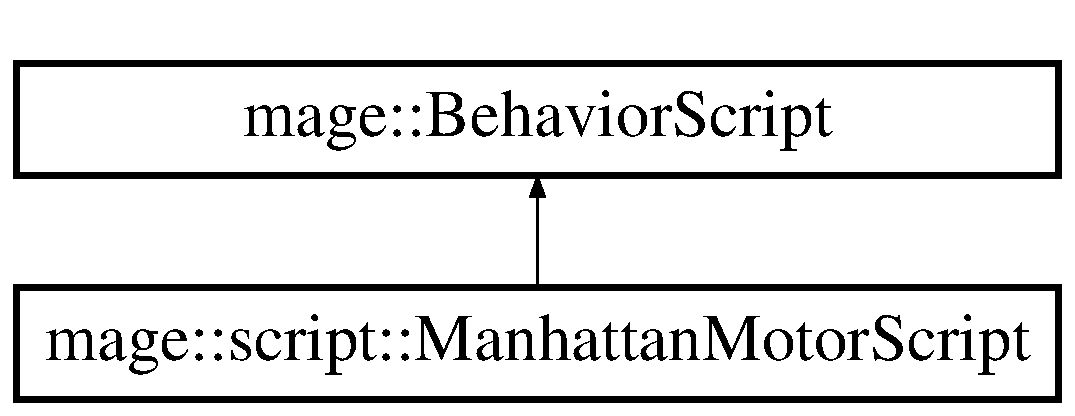
\includegraphics[height=2.000000cm]{classmage_1_1script_1_1_manhattan_motor_script}
\end{center}
\end{figure}
\subsection*{Public Member Functions}
\begin{DoxyCompactItemize}
\item 
\hyperlink{classmage_1_1script_1_1_manhattan_motor_script_a398939e0ba281042f28ce9ca42187624}{Manhattan\+Motor\+Script} (\hyperlink{classmage_1_1_transform_node}{Transform\+Node} $\ast$transform)
\item 
\hyperlink{classmage_1_1script_1_1_manhattan_motor_script_ae18f69e5dd5c4ffd2c6aa9db01d86024}{Manhattan\+Motor\+Script} (const \hyperlink{classmage_1_1script_1_1_manhattan_motor_script}{Manhattan\+Motor\+Script} \&script)=delete
\item 
\hyperlink{classmage_1_1script_1_1_manhattan_motor_script_af8094bec366be50d60c4d6b04b77accb}{Manhattan\+Motor\+Script} (\hyperlink{classmage_1_1script_1_1_manhattan_motor_script}{Manhattan\+Motor\+Script} \&\&script)
\item 
virtual \hyperlink{classmage_1_1script_1_1_manhattan_motor_script_aca76d9d5be76b048ec247e93e4a89adb}{$\sim$\+Manhattan\+Motor\+Script} ()
\item 
\hyperlink{classmage_1_1script_1_1_manhattan_motor_script}{Manhattan\+Motor\+Script} \& \hyperlink{classmage_1_1script_1_1_manhattan_motor_script_a7a6280230faa4d42a141e1d7768bcd0d}{operator=} (const \hyperlink{classmage_1_1script_1_1_manhattan_motor_script}{Manhattan\+Motor\+Script} \&script)=delete
\item 
\hyperlink{classmage_1_1script_1_1_manhattan_motor_script}{Manhattan\+Motor\+Script} \& \hyperlink{classmage_1_1script_1_1_manhattan_motor_script_a2b185979a64b35d9f9d6f4027724560a}{operator=} (\hyperlink{classmage_1_1script_1_1_manhattan_motor_script}{Manhattan\+Motor\+Script} \&\&script)=delete
\item 
virtual void \hyperlink{classmage_1_1script_1_1_manhattan_motor_script_ae7fbaba1da04d00257e5d491868efc53}{Update} (\mbox{[}\mbox{[}maybe\+\_\+unused\mbox{]}\mbox{]} \hyperlink{namespacemage_ad26233bbec640deda836e572c1a23708}{F64} delta\+\_\+time) override
\item 
\hyperlink{namespacemage_aa97e833b45f06d60a0a9c4fc22ae02c0}{F32} \hyperlink{classmage_1_1script_1_1_manhattan_motor_script_a2f73545bf2fb507375251d530054ac9b}{Get\+Velocity} () const noexcept
\item 
void \hyperlink{classmage_1_1script_1_1_manhattan_motor_script_acf4db52ae6b0c9f97c0b7e719acea6bc}{Set\+Velocity} (\hyperlink{namespacemage_aa97e833b45f06d60a0a9c4fc22ae02c0}{F32} velocity) noexcept
\end{DoxyCompactItemize}
\subsection*{Private Attributes}
\begin{DoxyCompactItemize}
\item 
\hyperlink{classmage_1_1_transform_node}{Transform\+Node} $\ast$const \hyperlink{classmage_1_1script_1_1_manhattan_motor_script_a4df5fa9ddd41dc83bdc7f2ee5d133fa9}{m\+\_\+transform}
\item 
\hyperlink{namespacemage_aa97e833b45f06d60a0a9c4fc22ae02c0}{F32} \hyperlink{classmage_1_1script_1_1_manhattan_motor_script_a38cdef10269075f08f3fcdc9ed8bc520}{m\+\_\+velocity}
\end{DoxyCompactItemize}
\subsection*{Additional Inherited Members}


\subsection{Constructor \& Destructor Documentation}
\hypertarget{classmage_1_1script_1_1_manhattan_motor_script_a398939e0ba281042f28ce9ca42187624}{}\label{classmage_1_1script_1_1_manhattan_motor_script_a398939e0ba281042f28ce9ca42187624} 
\index{mage\+::script\+::\+Manhattan\+Motor\+Script@{mage\+::script\+::\+Manhattan\+Motor\+Script}!Manhattan\+Motor\+Script@{Manhattan\+Motor\+Script}}
\index{Manhattan\+Motor\+Script@{Manhattan\+Motor\+Script}!mage\+::script\+::\+Manhattan\+Motor\+Script@{mage\+::script\+::\+Manhattan\+Motor\+Script}}
\subsubsection{\texorpdfstring{Manhattan\+Motor\+Script()}{ManhattanMotorScript()}\hspace{0.1cm}{\footnotesize\ttfamily [1/3]}}
{\footnotesize\ttfamily mage\+::script\+::\+Manhattan\+Motor\+Script\+::\+Manhattan\+Motor\+Script (\begin{DoxyParamCaption}\item[{\hyperlink{classmage_1_1_transform_node}{Transform\+Node} $\ast$}]{transform }\end{DoxyParamCaption})\hspace{0.3cm}{\ttfamily [explicit]}}

\hypertarget{classmage_1_1script_1_1_manhattan_motor_script_ae18f69e5dd5c4ffd2c6aa9db01d86024}{}\label{classmage_1_1script_1_1_manhattan_motor_script_ae18f69e5dd5c4ffd2c6aa9db01d86024} 
\index{mage\+::script\+::\+Manhattan\+Motor\+Script@{mage\+::script\+::\+Manhattan\+Motor\+Script}!Manhattan\+Motor\+Script@{Manhattan\+Motor\+Script}}
\index{Manhattan\+Motor\+Script@{Manhattan\+Motor\+Script}!mage\+::script\+::\+Manhattan\+Motor\+Script@{mage\+::script\+::\+Manhattan\+Motor\+Script}}
\subsubsection{\texorpdfstring{Manhattan\+Motor\+Script()}{ManhattanMotorScript()}\hspace{0.1cm}{\footnotesize\ttfamily [2/3]}}
{\footnotesize\ttfamily mage\+::script\+::\+Manhattan\+Motor\+Script\+::\+Manhattan\+Motor\+Script (\begin{DoxyParamCaption}\item[{const \hyperlink{classmage_1_1script_1_1_manhattan_motor_script}{Manhattan\+Motor\+Script} \&}]{script }\end{DoxyParamCaption})\hspace{0.3cm}{\ttfamily [delete]}}

\hypertarget{classmage_1_1script_1_1_manhattan_motor_script_af8094bec366be50d60c4d6b04b77accb}{}\label{classmage_1_1script_1_1_manhattan_motor_script_af8094bec366be50d60c4d6b04b77accb} 
\index{mage\+::script\+::\+Manhattan\+Motor\+Script@{mage\+::script\+::\+Manhattan\+Motor\+Script}!Manhattan\+Motor\+Script@{Manhattan\+Motor\+Script}}
\index{Manhattan\+Motor\+Script@{Manhattan\+Motor\+Script}!mage\+::script\+::\+Manhattan\+Motor\+Script@{mage\+::script\+::\+Manhattan\+Motor\+Script}}
\subsubsection{\texorpdfstring{Manhattan\+Motor\+Script()}{ManhattanMotorScript()}\hspace{0.1cm}{\footnotesize\ttfamily [3/3]}}
{\footnotesize\ttfamily mage\+::script\+::\+Manhattan\+Motor\+Script\+::\+Manhattan\+Motor\+Script (\begin{DoxyParamCaption}\item[{\hyperlink{classmage_1_1script_1_1_manhattan_motor_script}{Manhattan\+Motor\+Script} \&\&}]{script }\end{DoxyParamCaption})\hspace{0.3cm}{\ttfamily [default]}}

\hypertarget{classmage_1_1script_1_1_manhattan_motor_script_aca76d9d5be76b048ec247e93e4a89adb}{}\label{classmage_1_1script_1_1_manhattan_motor_script_aca76d9d5be76b048ec247e93e4a89adb} 
\index{mage\+::script\+::\+Manhattan\+Motor\+Script@{mage\+::script\+::\+Manhattan\+Motor\+Script}!````~Manhattan\+Motor\+Script@{$\sim$\+Manhattan\+Motor\+Script}}
\index{````~Manhattan\+Motor\+Script@{$\sim$\+Manhattan\+Motor\+Script}!mage\+::script\+::\+Manhattan\+Motor\+Script@{mage\+::script\+::\+Manhattan\+Motor\+Script}}
\subsubsection{\texorpdfstring{$\sim$\+Manhattan\+Motor\+Script()}{~ManhattanMotorScript()}}
{\footnotesize\ttfamily mage\+::script\+::\+Manhattan\+Motor\+Script\+::$\sim$\+Manhattan\+Motor\+Script (\begin{DoxyParamCaption}{ }\end{DoxyParamCaption})\hspace{0.3cm}{\ttfamily [virtual]}, {\ttfamily [default]}}



\subsection{Member Function Documentation}
\hypertarget{classmage_1_1script_1_1_manhattan_motor_script_a2f73545bf2fb507375251d530054ac9b}{}\label{classmage_1_1script_1_1_manhattan_motor_script_a2f73545bf2fb507375251d530054ac9b} 
\index{mage\+::script\+::\+Manhattan\+Motor\+Script@{mage\+::script\+::\+Manhattan\+Motor\+Script}!Get\+Velocity@{Get\+Velocity}}
\index{Get\+Velocity@{Get\+Velocity}!mage\+::script\+::\+Manhattan\+Motor\+Script@{mage\+::script\+::\+Manhattan\+Motor\+Script}}
\subsubsection{\texorpdfstring{Get\+Velocity()}{GetVelocity()}}
{\footnotesize\ttfamily \hyperlink{namespacemage_aa97e833b45f06d60a0a9c4fc22ae02c0}{F32} mage\+::script\+::\+Manhattan\+Motor\+Script\+::\+Get\+Velocity (\begin{DoxyParamCaption}{ }\end{DoxyParamCaption}) const\hspace{0.3cm}{\ttfamily [noexcept]}}

\hypertarget{classmage_1_1script_1_1_manhattan_motor_script_a7a6280230faa4d42a141e1d7768bcd0d}{}\label{classmage_1_1script_1_1_manhattan_motor_script_a7a6280230faa4d42a141e1d7768bcd0d} 
\index{mage\+::script\+::\+Manhattan\+Motor\+Script@{mage\+::script\+::\+Manhattan\+Motor\+Script}!operator=@{operator=}}
\index{operator=@{operator=}!mage\+::script\+::\+Manhattan\+Motor\+Script@{mage\+::script\+::\+Manhattan\+Motor\+Script}}
\subsubsection{\texorpdfstring{operator=()}{operator=()}\hspace{0.1cm}{\footnotesize\ttfamily [1/2]}}
{\footnotesize\ttfamily \hyperlink{classmage_1_1script_1_1_manhattan_motor_script}{Manhattan\+Motor\+Script}\& mage\+::script\+::\+Manhattan\+Motor\+Script\+::operator= (\begin{DoxyParamCaption}\item[{const \hyperlink{classmage_1_1script_1_1_manhattan_motor_script}{Manhattan\+Motor\+Script} \&}]{script }\end{DoxyParamCaption})\hspace{0.3cm}{\ttfamily [delete]}}

\hypertarget{classmage_1_1script_1_1_manhattan_motor_script_a2b185979a64b35d9f9d6f4027724560a}{}\label{classmage_1_1script_1_1_manhattan_motor_script_a2b185979a64b35d9f9d6f4027724560a} 
\index{mage\+::script\+::\+Manhattan\+Motor\+Script@{mage\+::script\+::\+Manhattan\+Motor\+Script}!operator=@{operator=}}
\index{operator=@{operator=}!mage\+::script\+::\+Manhattan\+Motor\+Script@{mage\+::script\+::\+Manhattan\+Motor\+Script}}
\subsubsection{\texorpdfstring{operator=()}{operator=()}\hspace{0.1cm}{\footnotesize\ttfamily [2/2]}}
{\footnotesize\ttfamily \hyperlink{classmage_1_1script_1_1_manhattan_motor_script}{Manhattan\+Motor\+Script}\& mage\+::script\+::\+Manhattan\+Motor\+Script\+::operator= (\begin{DoxyParamCaption}\item[{\hyperlink{classmage_1_1script_1_1_manhattan_motor_script}{Manhattan\+Motor\+Script} \&\&}]{script }\end{DoxyParamCaption})\hspace{0.3cm}{\ttfamily [delete]}}

\hypertarget{classmage_1_1script_1_1_manhattan_motor_script_acf4db52ae6b0c9f97c0b7e719acea6bc}{}\label{classmage_1_1script_1_1_manhattan_motor_script_acf4db52ae6b0c9f97c0b7e719acea6bc} 
\index{mage\+::script\+::\+Manhattan\+Motor\+Script@{mage\+::script\+::\+Manhattan\+Motor\+Script}!Set\+Velocity@{Set\+Velocity}}
\index{Set\+Velocity@{Set\+Velocity}!mage\+::script\+::\+Manhattan\+Motor\+Script@{mage\+::script\+::\+Manhattan\+Motor\+Script}}
\subsubsection{\texorpdfstring{Set\+Velocity()}{SetVelocity()}}
{\footnotesize\ttfamily void mage\+::script\+::\+Manhattan\+Motor\+Script\+::\+Set\+Velocity (\begin{DoxyParamCaption}\item[{\hyperlink{namespacemage_aa97e833b45f06d60a0a9c4fc22ae02c0}{F32}}]{velocity }\end{DoxyParamCaption})\hspace{0.3cm}{\ttfamily [noexcept]}}

\hypertarget{classmage_1_1script_1_1_manhattan_motor_script_ae7fbaba1da04d00257e5d491868efc53}{}\label{classmage_1_1script_1_1_manhattan_motor_script_ae7fbaba1da04d00257e5d491868efc53} 
\index{mage\+::script\+::\+Manhattan\+Motor\+Script@{mage\+::script\+::\+Manhattan\+Motor\+Script}!Update@{Update}}
\index{Update@{Update}!mage\+::script\+::\+Manhattan\+Motor\+Script@{mage\+::script\+::\+Manhattan\+Motor\+Script}}
\subsubsection{\texorpdfstring{Update()}{Update()}}
{\footnotesize\ttfamily void mage\+::script\+::\+Manhattan\+Motor\+Script\+::\+Update (\begin{DoxyParamCaption}\item[{\mbox{[}\mbox{[}maybe\+\_\+unused\mbox{]} \mbox{]} \hyperlink{namespacemage_ad26233bbec640deda836e572c1a23708}{F64}}]{delta\+\_\+time }\end{DoxyParamCaption})\hspace{0.3cm}{\ttfamily [override]}, {\ttfamily [virtual]}}

Updates this behavior script.

This method is called once per frame.


\begin{DoxyParams}[1]{Parameters}
\mbox{\tt in}  & {\em delta\+\_\+time} & The elapsed time since the previous update. \\
\hline
\end{DoxyParams}


Reimplemented from \hyperlink{classmage_1_1_behavior_script_afb9cf3759edf8876416d1df85489cba6}{mage\+::\+Behavior\+Script}.



\subsection{Member Data Documentation}
\hypertarget{classmage_1_1script_1_1_manhattan_motor_script_a4df5fa9ddd41dc83bdc7f2ee5d133fa9}{}\label{classmage_1_1script_1_1_manhattan_motor_script_a4df5fa9ddd41dc83bdc7f2ee5d133fa9} 
\index{mage\+::script\+::\+Manhattan\+Motor\+Script@{mage\+::script\+::\+Manhattan\+Motor\+Script}!m\+\_\+transform@{m\+\_\+transform}}
\index{m\+\_\+transform@{m\+\_\+transform}!mage\+::script\+::\+Manhattan\+Motor\+Script@{mage\+::script\+::\+Manhattan\+Motor\+Script}}
\subsubsection{\texorpdfstring{m\+\_\+transform}{m\_transform}}
{\footnotesize\ttfamily \hyperlink{classmage_1_1_transform_node}{Transform\+Node}$\ast$ const mage\+::script\+::\+Manhattan\+Motor\+Script\+::m\+\_\+transform\hspace{0.3cm}{\ttfamily [private]}}

\hypertarget{classmage_1_1script_1_1_manhattan_motor_script_a38cdef10269075f08f3fcdc9ed8bc520}{}\label{classmage_1_1script_1_1_manhattan_motor_script_a38cdef10269075f08f3fcdc9ed8bc520} 
\index{mage\+::script\+::\+Manhattan\+Motor\+Script@{mage\+::script\+::\+Manhattan\+Motor\+Script}!m\+\_\+velocity@{m\+\_\+velocity}}
\index{m\+\_\+velocity@{m\+\_\+velocity}!mage\+::script\+::\+Manhattan\+Motor\+Script@{mage\+::script\+::\+Manhattan\+Motor\+Script}}
\subsubsection{\texorpdfstring{m\+\_\+velocity}{m\_velocity}}
{\footnotesize\ttfamily \hyperlink{namespacemage_aa97e833b45f06d60a0a9c4fc22ae02c0}{F32} mage\+::script\+::\+Manhattan\+Motor\+Script\+::m\+\_\+velocity\hspace{0.3cm}{\ttfamily [private]}}


\hypertarget{classmage_1_1rendering_1_1_material}{}\section{mage\+:\+:rendering\+:\+:Material Class Reference}
\label{classmage_1_1rendering_1_1_material}\index{mage\+::rendering\+::\+Material@{mage\+::rendering\+::\+Material}}


{\ttfamily \#include $<$material.\+hpp$>$}

\subsection*{Public Member Functions}
\begin{DoxyCompactItemize}
\item 
\hyperlink{classmage_1_1rendering_1_1_material_a0d23055b62f54a28c77010412099a446}{Material} (string name=\char`\"{}material\char`\"{})
\item 
\hyperlink{classmage_1_1rendering_1_1_material_ac7cffca59fe250f10c2e68a875a03e91}{Material} (const \hyperlink{classmage_1_1rendering_1_1_material}{Material} \&material)=default
\item 
\hyperlink{classmage_1_1rendering_1_1_material_a52f4b3b0849b96306ea79c746070c6ba}{Material} (\hyperlink{classmage_1_1rendering_1_1_material}{Material} \&\&material) noexcept=default
\item 
\hyperlink{classmage_1_1rendering_1_1_material_a0dcdba799e013b2a8ff0108b14b9a73c}{$\sim$\+Material} ()=default
\item 
\hyperlink{classmage_1_1rendering_1_1_material}{Material} \& \hyperlink{classmage_1_1rendering_1_1_material_a535022bb3c1264412278337fc3d5d717}{operator=} (const \hyperlink{classmage_1_1rendering_1_1_material}{Material} \&material)=default
\item 
\hyperlink{classmage_1_1rendering_1_1_material}{Material} \& \hyperlink{classmage_1_1rendering_1_1_material_a2f90e0eeb8283da70db48fc1618aed10}{operator=} (\hyperlink{classmage_1_1rendering_1_1_material}{Material} \&\&material) noexcept=default
\item 
const string \& \hyperlink{classmage_1_1rendering_1_1_material_ab94089dbe7d1b242fad455e9c233a78c}{Get\+Name} () const noexcept
\item 
void \hyperlink{classmage_1_1rendering_1_1_material_a5700b990bfd59c497e07ee6682ffbf06}{Set\+Name} (string name) noexcept
\item 
bool \hyperlink{classmage_1_1rendering_1_1_material_ac9ee80a246dd28e19a6e29065b8eb24d}{Interacts\+With\+Light} () const noexcept
\item 
void \hyperlink{classmage_1_1rendering_1_1_material_a6cacaf988bf34a619c701d6fcd693322}{Enable\+Light\+Interaction} () noexcept
\item 
void \hyperlink{classmage_1_1rendering_1_1_material_a9b515c8968a5db43746fed088d67a514}{Dissable\+Light\+Interaction} () noexcept
\item 
void \hyperlink{classmage_1_1rendering_1_1_material_a70db3a2d474a3545e573cb9fdfa11347}{Toggle\+Light\+Interaction} () noexcept
\item 
void \hyperlink{classmage_1_1rendering_1_1_material_a151a2170aa88811ea6fb1537ce68803d}{Set\+Light\+Interaction} (bool light\+\_\+interaction) noexcept
\item 
bool \hyperlink{classmage_1_1rendering_1_1_material_af750917e67bdaf7e47129617102887ab}{Is\+Opaque} () const noexcept
\item 
bool \hyperlink{classmage_1_1rendering_1_1_material_ae60d1b61ebd38d3e329a519b2f2c3dad}{Is\+Transparant} () const noexcept
\item 
void \hyperlink{classmage_1_1rendering_1_1_material_a23741c39e6ad9a8d12b7793bc3da4131}{Set\+Opaque} () noexcept
\item 
void \hyperlink{classmage_1_1rendering_1_1_material_a8da0e0ed4df1e9ce0c7381d88b6d6c48}{Set\+Transparent} (bool transparent=true) noexcept
\item 
\hyperlink{structmage_1_1_s_r_g_b_a}{S\+R\+G\+BA} \& \hyperlink{classmage_1_1rendering_1_1_material_a3b5c99673752acd11758cc0ebab3f68a}{Get\+Base\+Color} () noexcept
\item 
const \hyperlink{structmage_1_1_s_r_g_b_a}{S\+R\+G\+BA} \& \hyperlink{classmage_1_1rendering_1_1_material_a600b48c0711a4b72813a18619b039e07}{Get\+Base\+Color} () const noexcept
\item 
\hyperlink{namespacemage_1_1rendering_a6f3ae54f825328465b0cdde0f0de4a36}{Texture\+Ptr} \hyperlink{classmage_1_1rendering_1_1_material_ac9ce1aff5b5e3d34ae83eb194786cebe}{Get\+Base\+Color\+Texture} () const noexcept
\item 
I\+D3\+D11\+Shader\+Resource\+View $\ast$ \hyperlink{classmage_1_1rendering_1_1_material_a363d85135b18e4e8c8a0b1d2fd88a435}{Get\+Base\+Color\+S\+RV} () const noexcept
\item 
void \hyperlink{classmage_1_1rendering_1_1_material_aae6ebdb492e06a39e1f420154962ab0f}{Set\+Base\+Color\+Texture} (\hyperlink{namespacemage_1_1rendering_a6f3ae54f825328465b0cdde0f0de4a36}{Texture\+Ptr} base\+\_\+color\+\_\+texture) noexcept
\item 
\hyperlink{namespacemage_aa97e833b45f06d60a0a9c4fc22ae02c0}{F32} \hyperlink{classmage_1_1rendering_1_1_material_a4c950a1b95e14246027de8ff0da4d55a}{Get\+Roughness} () const noexcept
\item 
void \hyperlink{classmage_1_1rendering_1_1_material_a1504fb6523526ee9897b20851a3b84e9}{Set\+Roughness} (\hyperlink{namespacemage_aa97e833b45f06d60a0a9c4fc22ae02c0}{F32} roughness) noexcept
\item 
\hyperlink{namespacemage_aa97e833b45f06d60a0a9c4fc22ae02c0}{F32} \hyperlink{classmage_1_1rendering_1_1_material_aaa4265533437b462e2f2087cfa37e623}{Get\+Metalness} () const noexcept
\item 
void \hyperlink{classmage_1_1rendering_1_1_material_a46b3297fb948c4fec3447caa35f96918}{Set\+Metalness} (\hyperlink{namespacemage_aa97e833b45f06d60a0a9c4fc22ae02c0}{F32} metalness) noexcept
\item 
const \hyperlink{structmage_1_1_r_g_b_a}{R\+G\+BA} \hyperlink{classmage_1_1rendering_1_1_material_a0464566ef674bf074d0af22e852daaa3}{Get\+Material\+R\+G\+BA} () const noexcept
\item 
\hyperlink{namespacemage_1_1rendering_a6f3ae54f825328465b0cdde0f0de4a36}{Texture\+Ptr} \hyperlink{classmage_1_1rendering_1_1_material_aa396990a630c749a46a8a9fc88e80683}{Get\+Material\+Texture} () const noexcept
\item 
I\+D3\+D11\+Shader\+Resource\+View $\ast$ \hyperlink{classmage_1_1rendering_1_1_material_ae1e1f712801dd1f16a695692df4f4f23}{Get\+Material\+S\+RV} () const noexcept
\item 
void \hyperlink{classmage_1_1rendering_1_1_material_a6bf886a16cbe84c55664701ab3a82658}{Set\+Material\+Texture} (\hyperlink{namespacemage_1_1rendering_a6f3ae54f825328465b0cdde0f0de4a36}{Texture\+Ptr} material\+\_\+texture) noexcept
\item 
\hyperlink{namespacemage_1_1rendering_a6f3ae54f825328465b0cdde0f0de4a36}{Texture\+Ptr} \hyperlink{classmage_1_1rendering_1_1_material_a1ae7786ebd627d3e7ecaf2dc671f497d}{Get\+Normal\+Texture} () const noexcept
\item 
I\+D3\+D11\+Shader\+Resource\+View $\ast$ \hyperlink{classmage_1_1rendering_1_1_material_a8617392cee8e8609671be3f4147a5934}{Get\+Normal\+S\+RV} () const noexcept
\item 
void \hyperlink{classmage_1_1rendering_1_1_material_a1a1ae2ba12c62c1d076f04124f1f64f6}{Set\+Normal\+Texture} (\hyperlink{namespacemage_1_1rendering_a6f3ae54f825328465b0cdde0f0de4a36}{Texture\+Ptr} normal\+\_\+texture)
\end{DoxyCompactItemize}
\subsection*{Private Attributes}
\begin{DoxyCompactItemize}
\item 
string \hyperlink{classmage_1_1rendering_1_1_material_a16f309220930c59f17b25fd8b0b62446}{m\+\_\+name}
\item 
bool \hyperlink{classmage_1_1rendering_1_1_material_aff4d7ceba071ecc00efa4188d7c22a46}{m\+\_\+light\+\_\+interaction}
\item 
bool \hyperlink{classmage_1_1rendering_1_1_material_af9f8d0fdb613bce1a4c3683836649bf3}{m\+\_\+transparent}
\item 
\hyperlink{structmage_1_1_s_r_g_b_a}{S\+R\+G\+BA} \hyperlink{classmage_1_1rendering_1_1_material_ad51c1da4673a012737ffa9feb14b3565}{m\+\_\+base\+\_\+color}
\item 
\hyperlink{namespacemage_1_1rendering_a6f3ae54f825328465b0cdde0f0de4a36}{Texture\+Ptr} \hyperlink{classmage_1_1rendering_1_1_material_aaee7a296b1f966a1544a07d21e13b8f6}{m\+\_\+base\+\_\+color\+\_\+texture}
\item 
\hyperlink{namespacemage_aa97e833b45f06d60a0a9c4fc22ae02c0}{F32} \hyperlink{classmage_1_1rendering_1_1_material_a14b420a0bdb8cb1f0fa57aa31bd09ae1}{m\+\_\+roughness}
\item 
\hyperlink{namespacemage_aa97e833b45f06d60a0a9c4fc22ae02c0}{F32} \hyperlink{classmage_1_1rendering_1_1_material_a1ec138a6dfec09ac421517480bd08a75}{m\+\_\+metalness}
\item 
\hyperlink{namespacemage_1_1rendering_a6f3ae54f825328465b0cdde0f0de4a36}{Texture\+Ptr} \hyperlink{classmage_1_1rendering_1_1_material_a4292698d8326e4f28dc45d59e00296dd}{m\+\_\+material\+\_\+texture}
\item 
\hyperlink{namespacemage_1_1rendering_a6f3ae54f825328465b0cdde0f0de4a36}{Texture\+Ptr} \hyperlink{classmage_1_1rendering_1_1_material_a14911430f38bc998c6d0735dc129f234}{m\+\_\+normal\+\_\+texture}
\end{DoxyCompactItemize}


\subsection{Detailed Description}
A class of materials. 

\subsection{Constructor \& Destructor Documentation}
\hypertarget{classmage_1_1rendering_1_1_material_a0d23055b62f54a28c77010412099a446}{}\label{classmage_1_1rendering_1_1_material_a0d23055b62f54a28c77010412099a446} 
\index{mage\+::rendering\+::\+Material@{mage\+::rendering\+::\+Material}!Material@{Material}}
\index{Material@{Material}!mage\+::rendering\+::\+Material@{mage\+::rendering\+::\+Material}}
\subsubsection{\texorpdfstring{Material()}{Material()}\hspace{0.1cm}{\footnotesize\ttfamily [1/3]}}
{\footnotesize\ttfamily mage\+::rendering\+::\+Material\+::\+Material (\begin{DoxyParamCaption}\item[{string}]{name = {\ttfamily \char`\"{}material\char`\"{}} }\end{DoxyParamCaption})\hspace{0.3cm}{\ttfamily [explicit]}}

Constructs a material.


\begin{DoxyParams}[1]{Parameters}
\mbox{\tt in}  & {\em name} & The name of the material. \\
\hline
\end{DoxyParams}
\hypertarget{classmage_1_1rendering_1_1_material_ac7cffca59fe250f10c2e68a875a03e91}{}\label{classmage_1_1rendering_1_1_material_ac7cffca59fe250f10c2e68a875a03e91} 
\index{mage\+::rendering\+::\+Material@{mage\+::rendering\+::\+Material}!Material@{Material}}
\index{Material@{Material}!mage\+::rendering\+::\+Material@{mage\+::rendering\+::\+Material}}
\subsubsection{\texorpdfstring{Material()}{Material()}\hspace{0.1cm}{\footnotesize\ttfamily [2/3]}}
{\footnotesize\ttfamily mage\+::rendering\+::\+Material\+::\+Material (\begin{DoxyParamCaption}\item[{const \hyperlink{classmage_1_1rendering_1_1_material}{Material} \&}]{material }\end{DoxyParamCaption})\hspace{0.3cm}{\ttfamily [default]}}

Constructs a material from the given material.


\begin{DoxyParams}[1]{Parameters}
\mbox{\tt in}  & {\em material} & A reference to the material to copy. \\
\hline
\end{DoxyParams}
\hypertarget{classmage_1_1rendering_1_1_material_a52f4b3b0849b96306ea79c746070c6ba}{}\label{classmage_1_1rendering_1_1_material_a52f4b3b0849b96306ea79c746070c6ba} 
\index{mage\+::rendering\+::\+Material@{mage\+::rendering\+::\+Material}!Material@{Material}}
\index{Material@{Material}!mage\+::rendering\+::\+Material@{mage\+::rendering\+::\+Material}}
\subsubsection{\texorpdfstring{Material()}{Material()}\hspace{0.1cm}{\footnotesize\ttfamily [3/3]}}
{\footnotesize\ttfamily mage\+::rendering\+::\+Material\+::\+Material (\begin{DoxyParamCaption}\item[{\hyperlink{classmage_1_1rendering_1_1_material}{Material} \&\&}]{material }\end{DoxyParamCaption})\hspace{0.3cm}{\ttfamily [default]}, {\ttfamily [noexcept]}}

Constructs a material by moving the given material.


\begin{DoxyParams}[1]{Parameters}
\mbox{\tt in}  & {\em material} & A reference to the material to move. \\
\hline
\end{DoxyParams}
\hypertarget{classmage_1_1rendering_1_1_material_a0dcdba799e013b2a8ff0108b14b9a73c}{}\label{classmage_1_1rendering_1_1_material_a0dcdba799e013b2a8ff0108b14b9a73c} 
\index{mage\+::rendering\+::\+Material@{mage\+::rendering\+::\+Material}!````~Material@{$\sim$\+Material}}
\index{````~Material@{$\sim$\+Material}!mage\+::rendering\+::\+Material@{mage\+::rendering\+::\+Material}}
\subsubsection{\texorpdfstring{$\sim$\+Material()}{~Material()}}
{\footnotesize\ttfamily mage\+::rendering\+::\+Material\+::$\sim$\+Material (\begin{DoxyParamCaption}{ }\end{DoxyParamCaption})\hspace{0.3cm}{\ttfamily [default]}}

Destructs this material. 

\subsection{Member Function Documentation}
\hypertarget{classmage_1_1rendering_1_1_material_a9b515c8968a5db43746fed088d67a514}{}\label{classmage_1_1rendering_1_1_material_a9b515c8968a5db43746fed088d67a514} 
\index{mage\+::rendering\+::\+Material@{mage\+::rendering\+::\+Material}!Dissable\+Light\+Interaction@{Dissable\+Light\+Interaction}}
\index{Dissable\+Light\+Interaction@{Dissable\+Light\+Interaction}!mage\+::rendering\+::\+Material@{mage\+::rendering\+::\+Material}}
\subsubsection{\texorpdfstring{Dissable\+Light\+Interaction()}{DissableLightInteraction()}}
{\footnotesize\ttfamily void mage\+::rendering\+::\+Material\+::\+Dissable\+Light\+Interaction (\begin{DoxyParamCaption}{ }\end{DoxyParamCaption})\hspace{0.3cm}{\ttfamily [noexcept]}}

Dissables this material to interact with light and light sources. \hypertarget{classmage_1_1rendering_1_1_material_a6cacaf988bf34a619c701d6fcd693322}{}\label{classmage_1_1rendering_1_1_material_a6cacaf988bf34a619c701d6fcd693322} 
\index{mage\+::rendering\+::\+Material@{mage\+::rendering\+::\+Material}!Enable\+Light\+Interaction@{Enable\+Light\+Interaction}}
\index{Enable\+Light\+Interaction@{Enable\+Light\+Interaction}!mage\+::rendering\+::\+Material@{mage\+::rendering\+::\+Material}}
\subsubsection{\texorpdfstring{Enable\+Light\+Interaction()}{EnableLightInteraction()}}
{\footnotesize\ttfamily void mage\+::rendering\+::\+Material\+::\+Enable\+Light\+Interaction (\begin{DoxyParamCaption}{ }\end{DoxyParamCaption})\hspace{0.3cm}{\ttfamily [noexcept]}}

Enables this material to interact with light and light sources. \hypertarget{classmage_1_1rendering_1_1_material_a3b5c99673752acd11758cc0ebab3f68a}{}\label{classmage_1_1rendering_1_1_material_a3b5c99673752acd11758cc0ebab3f68a} 
\index{mage\+::rendering\+::\+Material@{mage\+::rendering\+::\+Material}!Get\+Base\+Color@{Get\+Base\+Color}}
\index{Get\+Base\+Color@{Get\+Base\+Color}!mage\+::rendering\+::\+Material@{mage\+::rendering\+::\+Material}}
\subsubsection{\texorpdfstring{Get\+Base\+Color()}{GetBaseColor()}\hspace{0.1cm}{\footnotesize\ttfamily [1/2]}}
{\footnotesize\ttfamily \hyperlink{structmage_1_1_s_r_g_b_a}{S\+R\+G\+BA}\& mage\+::rendering\+::\+Material\+::\+Get\+Base\+Color (\begin{DoxyParamCaption}{ }\end{DoxyParamCaption})\hspace{0.3cm}{\ttfamily [noexcept]}}

Returns the s\+R\+GB base color of this material.

\begin{DoxyReturn}{Returns}
A reference to the s\+R\+GB base color of this material. 
\end{DoxyReturn}
\hypertarget{classmage_1_1rendering_1_1_material_a600b48c0711a4b72813a18619b039e07}{}\label{classmage_1_1rendering_1_1_material_a600b48c0711a4b72813a18619b039e07} 
\index{mage\+::rendering\+::\+Material@{mage\+::rendering\+::\+Material}!Get\+Base\+Color@{Get\+Base\+Color}}
\index{Get\+Base\+Color@{Get\+Base\+Color}!mage\+::rendering\+::\+Material@{mage\+::rendering\+::\+Material}}
\subsubsection{\texorpdfstring{Get\+Base\+Color()}{GetBaseColor()}\hspace{0.1cm}{\footnotesize\ttfamily [2/2]}}
{\footnotesize\ttfamily const \hyperlink{structmage_1_1_s_r_g_b_a}{S\+R\+G\+BA}\& mage\+::rendering\+::\+Material\+::\+Get\+Base\+Color (\begin{DoxyParamCaption}{ }\end{DoxyParamCaption}) const\hspace{0.3cm}{\ttfamily [noexcept]}}

Returns the s\+R\+GB base color of this material.

\begin{DoxyReturn}{Returns}
A reference to the s\+R\+GB base color of this material. 
\end{DoxyReturn}
\hypertarget{classmage_1_1rendering_1_1_material_a363d85135b18e4e8c8a0b1d2fd88a435}{}\label{classmage_1_1rendering_1_1_material_a363d85135b18e4e8c8a0b1d2fd88a435} 
\index{mage\+::rendering\+::\+Material@{mage\+::rendering\+::\+Material}!Get\+Base\+Color\+S\+RV@{Get\+Base\+Color\+S\+RV}}
\index{Get\+Base\+Color\+S\+RV@{Get\+Base\+Color\+S\+RV}!mage\+::rendering\+::\+Material@{mage\+::rendering\+::\+Material}}
\subsubsection{\texorpdfstring{Get\+Base\+Color\+S\+R\+V()}{GetBaseColorSRV()}}
{\footnotesize\ttfamily I\+D3\+D11\+Shader\+Resource\+View$\ast$ mage\+::rendering\+::\+Material\+::\+Get\+Base\+Color\+S\+RV (\begin{DoxyParamCaption}{ }\end{DoxyParamCaption}) const\hspace{0.3cm}{\ttfamily [noexcept]}}

Returns the shader resource view of the s\+R\+GB base color texture of this material.

\begin{DoxyReturn}{Returns}
{\ttfamily nullptr}, if this material has no s\+R\+GB base color texture. 

A pointer to the shader resource view of the s\+R\+GB base color texture of this material. 
\end{DoxyReturn}
\hypertarget{classmage_1_1rendering_1_1_material_ac9ce1aff5b5e3d34ae83eb194786cebe}{}\label{classmage_1_1rendering_1_1_material_ac9ce1aff5b5e3d34ae83eb194786cebe} 
\index{mage\+::rendering\+::\+Material@{mage\+::rendering\+::\+Material}!Get\+Base\+Color\+Texture@{Get\+Base\+Color\+Texture}}
\index{Get\+Base\+Color\+Texture@{Get\+Base\+Color\+Texture}!mage\+::rendering\+::\+Material@{mage\+::rendering\+::\+Material}}
\subsubsection{\texorpdfstring{Get\+Base\+Color\+Texture()}{GetBaseColorTexture()}}
{\footnotesize\ttfamily \hyperlink{namespacemage_1_1rendering_a6f3ae54f825328465b0cdde0f0de4a36}{Texture\+Ptr} mage\+::rendering\+::\+Material\+::\+Get\+Base\+Color\+Texture (\begin{DoxyParamCaption}{ }\end{DoxyParamCaption}) const\hspace{0.3cm}{\ttfamily [noexcept]}}

Returns the s\+R\+GB base color texture of this material.

\begin{DoxyReturn}{Returns}
A pointer to the s\+R\+GB base color texture of this material. 
\end{DoxyReturn}
\hypertarget{classmage_1_1rendering_1_1_material_a0464566ef674bf074d0af22e852daaa3}{}\label{classmage_1_1rendering_1_1_material_a0464566ef674bf074d0af22e852daaa3} 
\index{mage\+::rendering\+::\+Material@{mage\+::rendering\+::\+Material}!Get\+Material\+R\+G\+BA@{Get\+Material\+R\+G\+BA}}
\index{Get\+Material\+R\+G\+BA@{Get\+Material\+R\+G\+BA}!mage\+::rendering\+::\+Material@{mage\+::rendering\+::\+Material}}
\subsubsection{\texorpdfstring{Get\+Material\+R\+G\+B\+A()}{GetMaterialRGBA()}}
{\footnotesize\ttfamily const \hyperlink{structmage_1_1_r_g_b_a}{R\+G\+BA} mage\+::rendering\+::\+Material\+::\+Get\+Material\+R\+G\+BA (\begin{DoxyParamCaption}{ }\end{DoxyParamCaption}) const\hspace{0.3cm}{\ttfamily [noexcept]}}

Returns the material \hyperlink{structmage_1_1_r_g_b_a}{R\+G\+BA} channels of this material.

\begin{DoxyReturn}{Returns}
The material \hyperlink{structmage_1_1_r_g_b_a}{R\+G\+BA} channels of this material. 
\end{DoxyReturn}
\hypertarget{classmage_1_1rendering_1_1_material_ae1e1f712801dd1f16a695692df4f4f23}{}\label{classmage_1_1rendering_1_1_material_ae1e1f712801dd1f16a695692df4f4f23} 
\index{mage\+::rendering\+::\+Material@{mage\+::rendering\+::\+Material}!Get\+Material\+S\+RV@{Get\+Material\+S\+RV}}
\index{Get\+Material\+S\+RV@{Get\+Material\+S\+RV}!mage\+::rendering\+::\+Material@{mage\+::rendering\+::\+Material}}
\subsubsection{\texorpdfstring{Get\+Material\+S\+R\+V()}{GetMaterialSRV()}}
{\footnotesize\ttfamily I\+D3\+D11\+Shader\+Resource\+View$\ast$ mage\+::rendering\+::\+Material\+::\+Get\+Material\+S\+RV (\begin{DoxyParamCaption}{ }\end{DoxyParamCaption}) const\hspace{0.3cm}{\ttfamily [noexcept]}}

Returns the shader resource view of the material texture of this material.

\begin{DoxyReturn}{Returns}
{\ttfamily nullptr}, if this material has no material texture. 

A pointer to the shader resource view of the material texture of this material. 
\end{DoxyReturn}
\hypertarget{classmage_1_1rendering_1_1_material_aa396990a630c749a46a8a9fc88e80683}{}\label{classmage_1_1rendering_1_1_material_aa396990a630c749a46a8a9fc88e80683} 
\index{mage\+::rendering\+::\+Material@{mage\+::rendering\+::\+Material}!Get\+Material\+Texture@{Get\+Material\+Texture}}
\index{Get\+Material\+Texture@{Get\+Material\+Texture}!mage\+::rendering\+::\+Material@{mage\+::rendering\+::\+Material}}
\subsubsection{\texorpdfstring{Get\+Material\+Texture()}{GetMaterialTexture()}}
{\footnotesize\ttfamily \hyperlink{namespacemage_1_1rendering_a6f3ae54f825328465b0cdde0f0de4a36}{Texture\+Ptr} mage\+::rendering\+::\+Material\+::\+Get\+Material\+Texture (\begin{DoxyParamCaption}{ }\end{DoxyParamCaption}) const\hspace{0.3cm}{\ttfamily [noexcept]}}

Returns the material texture of this material.

\begin{DoxyReturn}{Returns}
A pointer to the material texture of this material. 
\end{DoxyReturn}
\hypertarget{classmage_1_1rendering_1_1_material_aaa4265533437b462e2f2087cfa37e623}{}\label{classmage_1_1rendering_1_1_material_aaa4265533437b462e2f2087cfa37e623} 
\index{mage\+::rendering\+::\+Material@{mage\+::rendering\+::\+Material}!Get\+Metalness@{Get\+Metalness}}
\index{Get\+Metalness@{Get\+Metalness}!mage\+::rendering\+::\+Material@{mage\+::rendering\+::\+Material}}
\subsubsection{\texorpdfstring{Get\+Metalness()}{GetMetalness()}}
{\footnotesize\ttfamily \hyperlink{namespacemage_aa97e833b45f06d60a0a9c4fc22ae02c0}{F32} mage\+::rendering\+::\+Material\+::\+Get\+Metalness (\begin{DoxyParamCaption}{ }\end{DoxyParamCaption}) const\hspace{0.3cm}{\ttfamily [noexcept]}}

Returns the metalness of this material.

\begin{DoxyReturn}{Returns}
The metalness of this material. 
\end{DoxyReturn}
\hypertarget{classmage_1_1rendering_1_1_material_ab94089dbe7d1b242fad455e9c233a78c}{}\label{classmage_1_1rendering_1_1_material_ab94089dbe7d1b242fad455e9c233a78c} 
\index{mage\+::rendering\+::\+Material@{mage\+::rendering\+::\+Material}!Get\+Name@{Get\+Name}}
\index{Get\+Name@{Get\+Name}!mage\+::rendering\+::\+Material@{mage\+::rendering\+::\+Material}}
\subsubsection{\texorpdfstring{Get\+Name()}{GetName()}}
{\footnotesize\ttfamily const string\& mage\+::rendering\+::\+Material\+::\+Get\+Name (\begin{DoxyParamCaption}{ }\end{DoxyParamCaption}) const\hspace{0.3cm}{\ttfamily [noexcept]}}

Returns the name of this material.

\begin{DoxyReturn}{Returns}
A reference to the name of this material. 
\end{DoxyReturn}
\hypertarget{classmage_1_1rendering_1_1_material_a8617392cee8e8609671be3f4147a5934}{}\label{classmage_1_1rendering_1_1_material_a8617392cee8e8609671be3f4147a5934} 
\index{mage\+::rendering\+::\+Material@{mage\+::rendering\+::\+Material}!Get\+Normal\+S\+RV@{Get\+Normal\+S\+RV}}
\index{Get\+Normal\+S\+RV@{Get\+Normal\+S\+RV}!mage\+::rendering\+::\+Material@{mage\+::rendering\+::\+Material}}
\subsubsection{\texorpdfstring{Get\+Normal\+S\+R\+V()}{GetNormalSRV()}}
{\footnotesize\ttfamily I\+D3\+D11\+Shader\+Resource\+View$\ast$ mage\+::rendering\+::\+Material\+::\+Get\+Normal\+S\+RV (\begin{DoxyParamCaption}{ }\end{DoxyParamCaption}) const\hspace{0.3cm}{\ttfamily [noexcept]}}

Returns the shader resource view of the normal texture of this material.

\begin{DoxyReturn}{Returns}
{\ttfamily nullptr}, if this material has no normal texture. 

A pointer to the shader resource view of the normal texture of this material. 
\end{DoxyReturn}
\hypertarget{classmage_1_1rendering_1_1_material_a1ae7786ebd627d3e7ecaf2dc671f497d}{}\label{classmage_1_1rendering_1_1_material_a1ae7786ebd627d3e7ecaf2dc671f497d} 
\index{mage\+::rendering\+::\+Material@{mage\+::rendering\+::\+Material}!Get\+Normal\+Texture@{Get\+Normal\+Texture}}
\index{Get\+Normal\+Texture@{Get\+Normal\+Texture}!mage\+::rendering\+::\+Material@{mage\+::rendering\+::\+Material}}
\subsubsection{\texorpdfstring{Get\+Normal\+Texture()}{GetNormalTexture()}}
{\footnotesize\ttfamily \hyperlink{namespacemage_1_1rendering_a6f3ae54f825328465b0cdde0f0de4a36}{Texture\+Ptr} mage\+::rendering\+::\+Material\+::\+Get\+Normal\+Texture (\begin{DoxyParamCaption}{ }\end{DoxyParamCaption}) const\hspace{0.3cm}{\ttfamily [noexcept]}}

Returns the normal texture of this material.

\begin{DoxyReturn}{Returns}
A pointer to the normal texture of this material. 
\end{DoxyReturn}
\hypertarget{classmage_1_1rendering_1_1_material_a4c950a1b95e14246027de8ff0da4d55a}{}\label{classmage_1_1rendering_1_1_material_a4c950a1b95e14246027de8ff0da4d55a} 
\index{mage\+::rendering\+::\+Material@{mage\+::rendering\+::\+Material}!Get\+Roughness@{Get\+Roughness}}
\index{Get\+Roughness@{Get\+Roughness}!mage\+::rendering\+::\+Material@{mage\+::rendering\+::\+Material}}
\subsubsection{\texorpdfstring{Get\+Roughness()}{GetRoughness()}}
{\footnotesize\ttfamily \hyperlink{namespacemage_aa97e833b45f06d60a0a9c4fc22ae02c0}{F32} mage\+::rendering\+::\+Material\+::\+Get\+Roughness (\begin{DoxyParamCaption}{ }\end{DoxyParamCaption}) const\hspace{0.3cm}{\ttfamily [noexcept]}}

Returns the roughness of this material.

\begin{DoxyReturn}{Returns}
The roughness of this material. 
\end{DoxyReturn}
\hypertarget{classmage_1_1rendering_1_1_material_ac9ee80a246dd28e19a6e29065b8eb24d}{}\label{classmage_1_1rendering_1_1_material_ac9ee80a246dd28e19a6e29065b8eb24d} 
\index{mage\+::rendering\+::\+Material@{mage\+::rendering\+::\+Material}!Interacts\+With\+Light@{Interacts\+With\+Light}}
\index{Interacts\+With\+Light@{Interacts\+With\+Light}!mage\+::rendering\+::\+Material@{mage\+::rendering\+::\+Material}}
\subsubsection{\texorpdfstring{Interacts\+With\+Light()}{InteractsWithLight()}}
{\footnotesize\ttfamily bool mage\+::rendering\+::\+Material\+::\+Interacts\+With\+Light (\begin{DoxyParamCaption}{ }\end{DoxyParamCaption}) const\hspace{0.3cm}{\ttfamily [noexcept]}}

Checks whether this material interacts with light and light sources.

\begin{DoxyReturn}{Returns}
{\ttfamily true} if this material interacts with light and light sources. {\ttfamily false} otherwise. 
\end{DoxyReturn}
\hypertarget{classmage_1_1rendering_1_1_material_af750917e67bdaf7e47129617102887ab}{}\label{classmage_1_1rendering_1_1_material_af750917e67bdaf7e47129617102887ab} 
\index{mage\+::rendering\+::\+Material@{mage\+::rendering\+::\+Material}!Is\+Opaque@{Is\+Opaque}}
\index{Is\+Opaque@{Is\+Opaque}!mage\+::rendering\+::\+Material@{mage\+::rendering\+::\+Material}}
\subsubsection{\texorpdfstring{Is\+Opaque()}{IsOpaque()}}
{\footnotesize\ttfamily bool mage\+::rendering\+::\+Material\+::\+Is\+Opaque (\begin{DoxyParamCaption}{ }\end{DoxyParamCaption}) const\hspace{0.3cm}{\ttfamily [noexcept]}}

Checks whether this material is opaque (i.\+e. contains alpha channel equal to 1.\+0).

\begin{DoxyReturn}{Returns}
{\ttfamily true} if and only if this material is opaque. {\ttfamily false} otherwise. 
\end{DoxyReturn}
\hypertarget{classmage_1_1rendering_1_1_material_ae60d1b61ebd38d3e329a519b2f2c3dad}{}\label{classmage_1_1rendering_1_1_material_ae60d1b61ebd38d3e329a519b2f2c3dad} 
\index{mage\+::rendering\+::\+Material@{mage\+::rendering\+::\+Material}!Is\+Transparant@{Is\+Transparant}}
\index{Is\+Transparant@{Is\+Transparant}!mage\+::rendering\+::\+Material@{mage\+::rendering\+::\+Material}}
\subsubsection{\texorpdfstring{Is\+Transparant()}{IsTransparant()}}
{\footnotesize\ttfamily bool mage\+::rendering\+::\+Material\+::\+Is\+Transparant (\begin{DoxyParamCaption}{ }\end{DoxyParamCaption}) const\hspace{0.3cm}{\ttfamily [noexcept]}}

Checks whether this material is transparent (i.\+e. contains alpha channel not equal to 1.\+0).

\begin{DoxyReturn}{Returns}
{\ttfamily true} if and only if this material is transparent. {\ttfamily false} otherwise. 
\end{DoxyReturn}
\hypertarget{classmage_1_1rendering_1_1_material_a535022bb3c1264412278337fc3d5d717}{}\label{classmage_1_1rendering_1_1_material_a535022bb3c1264412278337fc3d5d717} 
\index{mage\+::rendering\+::\+Material@{mage\+::rendering\+::\+Material}!operator=@{operator=}}
\index{operator=@{operator=}!mage\+::rendering\+::\+Material@{mage\+::rendering\+::\+Material}}
\subsubsection{\texorpdfstring{operator=()}{operator=()}\hspace{0.1cm}{\footnotesize\ttfamily [1/2]}}
{\footnotesize\ttfamily \hyperlink{classmage_1_1rendering_1_1_material}{Material}\& mage\+::rendering\+::\+Material\+::operator= (\begin{DoxyParamCaption}\item[{const \hyperlink{classmage_1_1rendering_1_1_material}{Material} \&}]{material }\end{DoxyParamCaption})\hspace{0.3cm}{\ttfamily [default]}}

Copies the given material to this material.


\begin{DoxyParams}[1]{Parameters}
\mbox{\tt in}  & {\em material} & A reference to the material to copy. \\
\hline
\end{DoxyParams}
\begin{DoxyReturn}{Returns}
A reference to the copy of the given material (i.\+e. this material). 
\end{DoxyReturn}
\hypertarget{classmage_1_1rendering_1_1_material_a2f90e0eeb8283da70db48fc1618aed10}{}\label{classmage_1_1rendering_1_1_material_a2f90e0eeb8283da70db48fc1618aed10} 
\index{mage\+::rendering\+::\+Material@{mage\+::rendering\+::\+Material}!operator=@{operator=}}
\index{operator=@{operator=}!mage\+::rendering\+::\+Material@{mage\+::rendering\+::\+Material}}
\subsubsection{\texorpdfstring{operator=()}{operator=()}\hspace{0.1cm}{\footnotesize\ttfamily [2/2]}}
{\footnotesize\ttfamily \hyperlink{classmage_1_1rendering_1_1_material}{Material}\& mage\+::rendering\+::\+Material\+::operator= (\begin{DoxyParamCaption}\item[{\hyperlink{classmage_1_1rendering_1_1_material}{Material} \&\&}]{material }\end{DoxyParamCaption})\hspace{0.3cm}{\ttfamily [default]}, {\ttfamily [noexcept]}}

Moves the given material to this material.


\begin{DoxyParams}[1]{Parameters}
\mbox{\tt in}  & {\em material} & A reference to the material to move. \\
\hline
\end{DoxyParams}
\begin{DoxyReturn}{Returns}
A reference to the moved material (i.\+e. this material). 
\end{DoxyReturn}
\hypertarget{classmage_1_1rendering_1_1_material_aae6ebdb492e06a39e1f420154962ab0f}{}\label{classmage_1_1rendering_1_1_material_aae6ebdb492e06a39e1f420154962ab0f} 
\index{mage\+::rendering\+::\+Material@{mage\+::rendering\+::\+Material}!Set\+Base\+Color\+Texture@{Set\+Base\+Color\+Texture}}
\index{Set\+Base\+Color\+Texture@{Set\+Base\+Color\+Texture}!mage\+::rendering\+::\+Material@{mage\+::rendering\+::\+Material}}
\subsubsection{\texorpdfstring{Set\+Base\+Color\+Texture()}{SetBaseColorTexture()}}
{\footnotesize\ttfamily void mage\+::rendering\+::\+Material\+::\+Set\+Base\+Color\+Texture (\begin{DoxyParamCaption}\item[{\hyperlink{namespacemage_1_1rendering_a6f3ae54f825328465b0cdde0f0de4a36}{Texture\+Ptr}}]{base\+\_\+color\+\_\+texture }\end{DoxyParamCaption})\hspace{0.3cm}{\ttfamily [noexcept]}}

Sets the s\+R\+GB base color texture of this material to the given base color texture.


\begin{DoxyParams}[1]{Parameters}
\mbox{\tt in}  & {\em base\+\_\+color\+\_\+texture} & A pointer to the s\+R\+GB base color texture. \\
\hline
\end{DoxyParams}
\hypertarget{classmage_1_1rendering_1_1_material_a151a2170aa88811ea6fb1537ce68803d}{}\label{classmage_1_1rendering_1_1_material_a151a2170aa88811ea6fb1537ce68803d} 
\index{mage\+::rendering\+::\+Material@{mage\+::rendering\+::\+Material}!Set\+Light\+Interaction@{Set\+Light\+Interaction}}
\index{Set\+Light\+Interaction@{Set\+Light\+Interaction}!mage\+::rendering\+::\+Material@{mage\+::rendering\+::\+Material}}
\subsubsection{\texorpdfstring{Set\+Light\+Interaction()}{SetLightInteraction()}}
{\footnotesize\ttfamily void mage\+::rendering\+::\+Material\+::\+Set\+Light\+Interaction (\begin{DoxyParamCaption}\item[{bool}]{light\+\_\+interaction }\end{DoxyParamCaption})\hspace{0.3cm}{\ttfamily [noexcept]}}

Sets the light interaction of this material to the given value.


\begin{DoxyParams}[1]{Parameters}
\mbox{\tt in}  & {\em light\+\_\+interaction} & {\ttfamily true} if this material needs to interact with light and light sources. {\ttfamily false} otherwise. \\
\hline
\end{DoxyParams}
\hypertarget{classmage_1_1rendering_1_1_material_a6bf886a16cbe84c55664701ab3a82658}{}\label{classmage_1_1rendering_1_1_material_a6bf886a16cbe84c55664701ab3a82658} 
\index{mage\+::rendering\+::\+Material@{mage\+::rendering\+::\+Material}!Set\+Material\+Texture@{Set\+Material\+Texture}}
\index{Set\+Material\+Texture@{Set\+Material\+Texture}!mage\+::rendering\+::\+Material@{mage\+::rendering\+::\+Material}}
\subsubsection{\texorpdfstring{Set\+Material\+Texture()}{SetMaterialTexture()}}
{\footnotesize\ttfamily void mage\+::rendering\+::\+Material\+::\+Set\+Material\+Texture (\begin{DoxyParamCaption}\item[{\hyperlink{namespacemage_1_1rendering_a6f3ae54f825328465b0cdde0f0de4a36}{Texture\+Ptr}}]{material\+\_\+texture }\end{DoxyParamCaption})\hspace{0.3cm}{\ttfamily [noexcept]}}

Sets the material texture of this material to the given material texture.


\begin{DoxyParams}[1]{Parameters}
\mbox{\tt in}  & {\em material\+\_\+texture} & A pointer to the material texture. \\
\hline
\end{DoxyParams}
\hypertarget{classmage_1_1rendering_1_1_material_a46b3297fb948c4fec3447caa35f96918}{}\label{classmage_1_1rendering_1_1_material_a46b3297fb948c4fec3447caa35f96918} 
\index{mage\+::rendering\+::\+Material@{mage\+::rendering\+::\+Material}!Set\+Metalness@{Set\+Metalness}}
\index{Set\+Metalness@{Set\+Metalness}!mage\+::rendering\+::\+Material@{mage\+::rendering\+::\+Material}}
\subsubsection{\texorpdfstring{Set\+Metalness()}{SetMetalness()}}
{\footnotesize\ttfamily void mage\+::rendering\+::\+Material\+::\+Set\+Metalness (\begin{DoxyParamCaption}\item[{\hyperlink{namespacemage_aa97e833b45f06d60a0a9c4fc22ae02c0}{F32}}]{metalness }\end{DoxyParamCaption})\hspace{0.3cm}{\ttfamily [noexcept]}}

Sets the metalness of this material to the given value.


\begin{DoxyParams}[1]{Parameters}
\mbox{\tt in}  & {\em metalness} & The metalness. \\
\hline
\end{DoxyParams}
\hypertarget{classmage_1_1rendering_1_1_material_a5700b990bfd59c497e07ee6682ffbf06}{}\label{classmage_1_1rendering_1_1_material_a5700b990bfd59c497e07ee6682ffbf06} 
\index{mage\+::rendering\+::\+Material@{mage\+::rendering\+::\+Material}!Set\+Name@{Set\+Name}}
\index{Set\+Name@{Set\+Name}!mage\+::rendering\+::\+Material@{mage\+::rendering\+::\+Material}}
\subsubsection{\texorpdfstring{Set\+Name()}{SetName()}}
{\footnotesize\ttfamily void mage\+::rendering\+::\+Material\+::\+Set\+Name (\begin{DoxyParamCaption}\item[{string}]{name }\end{DoxyParamCaption})\hspace{0.3cm}{\ttfamily [noexcept]}}

Sets the name of this material to the given name.


\begin{DoxyParams}[1]{Parameters}
\mbox{\tt in}  & {\em name} & The name. \\
\hline
\end{DoxyParams}
\hypertarget{classmage_1_1rendering_1_1_material_a1a1ae2ba12c62c1d076f04124f1f64f6}{}\label{classmage_1_1rendering_1_1_material_a1a1ae2ba12c62c1d076f04124f1f64f6} 
\index{mage\+::rendering\+::\+Material@{mage\+::rendering\+::\+Material}!Set\+Normal\+Texture@{Set\+Normal\+Texture}}
\index{Set\+Normal\+Texture@{Set\+Normal\+Texture}!mage\+::rendering\+::\+Material@{mage\+::rendering\+::\+Material}}
\subsubsection{\texorpdfstring{Set\+Normal\+Texture()}{SetNormalTexture()}}
{\footnotesize\ttfamily void mage\+::rendering\+::\+Material\+::\+Set\+Normal\+Texture (\begin{DoxyParamCaption}\item[{\hyperlink{namespacemage_1_1rendering_a6f3ae54f825328465b0cdde0f0de4a36}{Texture\+Ptr}}]{normal\+\_\+texture }\end{DoxyParamCaption})}

Sets the normal texture of this material to the given normal texture.


\begin{DoxyParams}[1]{Parameters}
\mbox{\tt in}  & {\em normal\+\_\+texture} & The normal texture. \\
\hline
\end{DoxyParams}
\hypertarget{classmage_1_1rendering_1_1_material_a23741c39e6ad9a8d12b7793bc3da4131}{}\label{classmage_1_1rendering_1_1_material_a23741c39e6ad9a8d12b7793bc3da4131} 
\index{mage\+::rendering\+::\+Material@{mage\+::rendering\+::\+Material}!Set\+Opaque@{Set\+Opaque}}
\index{Set\+Opaque@{Set\+Opaque}!mage\+::rendering\+::\+Material@{mage\+::rendering\+::\+Material}}
\subsubsection{\texorpdfstring{Set\+Opaque()}{SetOpaque()}}
{\footnotesize\ttfamily void mage\+::rendering\+::\+Material\+::\+Set\+Opaque (\begin{DoxyParamCaption}{ }\end{DoxyParamCaption})\hspace{0.3cm}{\ttfamily [noexcept]}}

Makes this material opaque. \hypertarget{classmage_1_1rendering_1_1_material_a1504fb6523526ee9897b20851a3b84e9}{}\label{classmage_1_1rendering_1_1_material_a1504fb6523526ee9897b20851a3b84e9} 
\index{mage\+::rendering\+::\+Material@{mage\+::rendering\+::\+Material}!Set\+Roughness@{Set\+Roughness}}
\index{Set\+Roughness@{Set\+Roughness}!mage\+::rendering\+::\+Material@{mage\+::rendering\+::\+Material}}
\subsubsection{\texorpdfstring{Set\+Roughness()}{SetRoughness()}}
{\footnotesize\ttfamily void mage\+::rendering\+::\+Material\+::\+Set\+Roughness (\begin{DoxyParamCaption}\item[{\hyperlink{namespacemage_aa97e833b45f06d60a0a9c4fc22ae02c0}{F32}}]{roughness }\end{DoxyParamCaption})\hspace{0.3cm}{\ttfamily [noexcept]}}

Sets the roughness of this material to the given value.


\begin{DoxyParams}[1]{Parameters}
\mbox{\tt in}  & {\em roughness} & The roughness. \\
\hline
\end{DoxyParams}
\hypertarget{classmage_1_1rendering_1_1_material_a8da0e0ed4df1e9ce0c7381d88b6d6c48}{}\label{classmage_1_1rendering_1_1_material_a8da0e0ed4df1e9ce0c7381d88b6d6c48} 
\index{mage\+::rendering\+::\+Material@{mage\+::rendering\+::\+Material}!Set\+Transparent@{Set\+Transparent}}
\index{Set\+Transparent@{Set\+Transparent}!mage\+::rendering\+::\+Material@{mage\+::rendering\+::\+Material}}
\subsubsection{\texorpdfstring{Set\+Transparent()}{SetTransparent()}}
{\footnotesize\ttfamily void mage\+::rendering\+::\+Material\+::\+Set\+Transparent (\begin{DoxyParamCaption}\item[{bool}]{transparent = {\ttfamily true} }\end{DoxyParamCaption})\hspace{0.3cm}{\ttfamily [noexcept]}}

Makes this material transparent.


\begin{DoxyParams}[1]{Parameters}
\mbox{\tt in}  & {\em transparent} & {\ttfamily true} if and only if this material is transparent. {\ttfamily false} otherwise. \\
\hline
\end{DoxyParams}
\hypertarget{classmage_1_1rendering_1_1_material_a70db3a2d474a3545e573cb9fdfa11347}{}\label{classmage_1_1rendering_1_1_material_a70db3a2d474a3545e573cb9fdfa11347} 
\index{mage\+::rendering\+::\+Material@{mage\+::rendering\+::\+Material}!Toggle\+Light\+Interaction@{Toggle\+Light\+Interaction}}
\index{Toggle\+Light\+Interaction@{Toggle\+Light\+Interaction}!mage\+::rendering\+::\+Material@{mage\+::rendering\+::\+Material}}
\subsubsection{\texorpdfstring{Toggle\+Light\+Interaction()}{ToggleLightInteraction()}}
{\footnotesize\ttfamily void mage\+::rendering\+::\+Material\+::\+Toggle\+Light\+Interaction (\begin{DoxyParamCaption}{ }\end{DoxyParamCaption})\hspace{0.3cm}{\ttfamily [noexcept]}}

Toggles the light interaction of this material. 

\subsection{Member Data Documentation}
\hypertarget{classmage_1_1rendering_1_1_material_ad51c1da4673a012737ffa9feb14b3565}{}\label{classmage_1_1rendering_1_1_material_ad51c1da4673a012737ffa9feb14b3565} 
\index{mage\+::rendering\+::\+Material@{mage\+::rendering\+::\+Material}!m\+\_\+base\+\_\+color@{m\+\_\+base\+\_\+color}}
\index{m\+\_\+base\+\_\+color@{m\+\_\+base\+\_\+color}!mage\+::rendering\+::\+Material@{mage\+::rendering\+::\+Material}}
\subsubsection{\texorpdfstring{m\+\_\+base\+\_\+color}{m\_base\_color}}
{\footnotesize\ttfamily \hyperlink{structmage_1_1_s_r_g_b_a}{S\+R\+G\+BA} mage\+::rendering\+::\+Material\+::m\+\_\+base\+\_\+color\hspace{0.3cm}{\ttfamily [private]}}

The s\+R\+GB base color of this material. \hypertarget{classmage_1_1rendering_1_1_material_aaee7a296b1f966a1544a07d21e13b8f6}{}\label{classmage_1_1rendering_1_1_material_aaee7a296b1f966a1544a07d21e13b8f6} 
\index{mage\+::rendering\+::\+Material@{mage\+::rendering\+::\+Material}!m\+\_\+base\+\_\+color\+\_\+texture@{m\+\_\+base\+\_\+color\+\_\+texture}}
\index{m\+\_\+base\+\_\+color\+\_\+texture@{m\+\_\+base\+\_\+color\+\_\+texture}!mage\+::rendering\+::\+Material@{mage\+::rendering\+::\+Material}}
\subsubsection{\texorpdfstring{m\+\_\+base\+\_\+color\+\_\+texture}{m\_base\_color\_texture}}
{\footnotesize\ttfamily \hyperlink{namespacemage_1_1rendering_a6f3ae54f825328465b0cdde0f0de4a36}{Texture\+Ptr} mage\+::rendering\+::\+Material\+::m\+\_\+base\+\_\+color\+\_\+texture\hspace{0.3cm}{\ttfamily [private]}}

A pointer to the s\+R\+GB base color texture of this material. \hypertarget{classmage_1_1rendering_1_1_material_aff4d7ceba071ecc00efa4188d7c22a46}{}\label{classmage_1_1rendering_1_1_material_aff4d7ceba071ecc00efa4188d7c22a46} 
\index{mage\+::rendering\+::\+Material@{mage\+::rendering\+::\+Material}!m\+\_\+light\+\_\+interaction@{m\+\_\+light\+\_\+interaction}}
\index{m\+\_\+light\+\_\+interaction@{m\+\_\+light\+\_\+interaction}!mage\+::rendering\+::\+Material@{mage\+::rendering\+::\+Material}}
\subsubsection{\texorpdfstring{m\+\_\+light\+\_\+interaction}{m\_light\_interaction}}
{\footnotesize\ttfamily bool mage\+::rendering\+::\+Material\+::m\+\_\+light\+\_\+interaction\hspace{0.3cm}{\ttfamily [private]}}

Flag indicating whether this material interacts with light and light sources. \hypertarget{classmage_1_1rendering_1_1_material_a4292698d8326e4f28dc45d59e00296dd}{}\label{classmage_1_1rendering_1_1_material_a4292698d8326e4f28dc45d59e00296dd} 
\index{mage\+::rendering\+::\+Material@{mage\+::rendering\+::\+Material}!m\+\_\+material\+\_\+texture@{m\+\_\+material\+\_\+texture}}
\index{m\+\_\+material\+\_\+texture@{m\+\_\+material\+\_\+texture}!mage\+::rendering\+::\+Material@{mage\+::rendering\+::\+Material}}
\subsubsection{\texorpdfstring{m\+\_\+material\+\_\+texture}{m\_material\_texture}}
{\footnotesize\ttfamily \hyperlink{namespacemage_1_1rendering_a6f3ae54f825328465b0cdde0f0de4a36}{Texture\+Ptr} mage\+::rendering\+::\+Material\+::m\+\_\+material\+\_\+texture\hspace{0.3cm}{\ttfamily [private]}}

A pointer to the material texture of this material.

The red channel contains the roughness of this material. The blue channel contains the metalness of this material. \hypertarget{classmage_1_1rendering_1_1_material_a1ec138a6dfec09ac421517480bd08a75}{}\label{classmage_1_1rendering_1_1_material_a1ec138a6dfec09ac421517480bd08a75} 
\index{mage\+::rendering\+::\+Material@{mage\+::rendering\+::\+Material}!m\+\_\+metalness@{m\+\_\+metalness}}
\index{m\+\_\+metalness@{m\+\_\+metalness}!mage\+::rendering\+::\+Material@{mage\+::rendering\+::\+Material}}
\subsubsection{\texorpdfstring{m\+\_\+metalness}{m\_metalness}}
{\footnotesize\ttfamily \hyperlink{namespacemage_aa97e833b45f06d60a0a9c4fc22ae02c0}{F32} mage\+::rendering\+::\+Material\+::m\+\_\+metalness\hspace{0.3cm}{\ttfamily [private]}}

The metalness of this material. \hypertarget{classmage_1_1rendering_1_1_material_a16f309220930c59f17b25fd8b0b62446}{}\label{classmage_1_1rendering_1_1_material_a16f309220930c59f17b25fd8b0b62446} 
\index{mage\+::rendering\+::\+Material@{mage\+::rendering\+::\+Material}!m\+\_\+name@{m\+\_\+name}}
\index{m\+\_\+name@{m\+\_\+name}!mage\+::rendering\+::\+Material@{mage\+::rendering\+::\+Material}}
\subsubsection{\texorpdfstring{m\+\_\+name}{m\_name}}
{\footnotesize\ttfamily string mage\+::rendering\+::\+Material\+::m\+\_\+name\hspace{0.3cm}{\ttfamily [private]}}

The name of this material. \hypertarget{classmage_1_1rendering_1_1_material_a14911430f38bc998c6d0735dc129f234}{}\label{classmage_1_1rendering_1_1_material_a14911430f38bc998c6d0735dc129f234} 
\index{mage\+::rendering\+::\+Material@{mage\+::rendering\+::\+Material}!m\+\_\+normal\+\_\+texture@{m\+\_\+normal\+\_\+texture}}
\index{m\+\_\+normal\+\_\+texture@{m\+\_\+normal\+\_\+texture}!mage\+::rendering\+::\+Material@{mage\+::rendering\+::\+Material}}
\subsubsection{\texorpdfstring{m\+\_\+normal\+\_\+texture}{m\_normal\_texture}}
{\footnotesize\ttfamily \hyperlink{namespacemage_1_1rendering_a6f3ae54f825328465b0cdde0f0de4a36}{Texture\+Ptr} mage\+::rendering\+::\+Material\+::m\+\_\+normal\+\_\+texture\hspace{0.3cm}{\ttfamily [private]}}

A pointer to the normal texture of this material. \hypertarget{classmage_1_1rendering_1_1_material_a14b420a0bdb8cb1f0fa57aa31bd09ae1}{}\label{classmage_1_1rendering_1_1_material_a14b420a0bdb8cb1f0fa57aa31bd09ae1} 
\index{mage\+::rendering\+::\+Material@{mage\+::rendering\+::\+Material}!m\+\_\+roughness@{m\+\_\+roughness}}
\index{m\+\_\+roughness@{m\+\_\+roughness}!mage\+::rendering\+::\+Material@{mage\+::rendering\+::\+Material}}
\subsubsection{\texorpdfstring{m\+\_\+roughness}{m\_roughness}}
{\footnotesize\ttfamily \hyperlink{namespacemage_aa97e833b45f06d60a0a9c4fc22ae02c0}{F32} mage\+::rendering\+::\+Material\+::m\+\_\+roughness\hspace{0.3cm}{\ttfamily [private]}}

The roughness of this material. \hypertarget{classmage_1_1rendering_1_1_material_af9f8d0fdb613bce1a4c3683836649bf3}{}\label{classmage_1_1rendering_1_1_material_af9f8d0fdb613bce1a4c3683836649bf3} 
\index{mage\+::rendering\+::\+Material@{mage\+::rendering\+::\+Material}!m\+\_\+transparent@{m\+\_\+transparent}}
\index{m\+\_\+transparent@{m\+\_\+transparent}!mage\+::rendering\+::\+Material@{mage\+::rendering\+::\+Material}}
\subsubsection{\texorpdfstring{m\+\_\+transparent}{m\_transparent}}
{\footnotesize\ttfamily bool mage\+::rendering\+::\+Material\+::m\+\_\+transparent\hspace{0.3cm}{\ttfamily [private]}}

Flag indicating whether this material is transparent. This flag is {\ttfamily true} if this material could contain transparent parts. {\ttfamily false} otherwise. 
\hypertarget{classmage_1_1rendering_1_1loader_1_1_m_d_l_reader}{}\section{mage\+:\+:rendering\+:\+:loader\+:\+:M\+D\+L\+Reader$<$ VertexT, IndexT $>$ Class Template Reference}
\label{classmage_1_1rendering_1_1loader_1_1_m_d_l_reader}\index{mage\+::rendering\+::loader\+::\+M\+D\+L\+Reader$<$ Vertex\+T, Index\+T $>$@{mage\+::rendering\+::loader\+::\+M\+D\+L\+Reader$<$ Vertex\+T, Index\+T $>$}}


{\ttfamily \#include $<$mdl\+\_\+reader.\+hpp$>$}

Inheritance diagram for mage\+:\+:rendering\+:\+:loader\+:\+:M\+D\+L\+Reader$<$ VertexT, IndexT $>$\+:\begin{figure}[H]
\begin{center}
\leavevmode
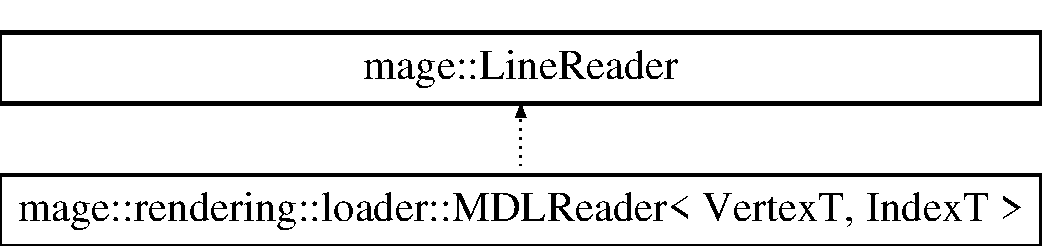
\includegraphics[height=2.000000cm]{classmage_1_1rendering_1_1loader_1_1_m_d_l_reader}
\end{center}
\end{figure}
\subsection*{Public Member Functions}
\begin{DoxyCompactItemize}
\item 
\mbox{\hyperlink{classmage_1_1rendering_1_1loader_1_1_m_d_l_reader_acc6d10b858b43608cb22d9086ae227fd}{M\+D\+L\+Reader}} (\mbox{\hyperlink{classmage_1_1rendering_1_1_resource_manager}{Resource\+Manager}} \&resource\+\_\+manager, \mbox{\hyperlink{structmage_1_1rendering_1_1_model_output}{Model\+Output}}$<$ VertexT, IndexT $>$ \&model\+\_\+output)
\item 
\mbox{\hyperlink{classmage_1_1rendering_1_1loader_1_1_m_d_l_reader_a98d83bb5d8cec2b8e665f08bc50068f6}{M\+D\+L\+Reader}} (const \mbox{\hyperlink{classmage_1_1rendering_1_1loader_1_1_m_d_l_reader}{M\+D\+L\+Reader}} \&reader)=delete
\item 
\mbox{\hyperlink{classmage_1_1rendering_1_1loader_1_1_m_d_l_reader_a77f5be43642636faf71e7fb3eed7e050}{M\+D\+L\+Reader}} (\mbox{\hyperlink{classmage_1_1rendering_1_1loader_1_1_m_d_l_reader}{M\+D\+L\+Reader}} \&\&reader) noexcept
\item 
\mbox{\hyperlink{classmage_1_1rendering_1_1loader_1_1_m_d_l_reader_a2f4c6bd8c2ef49180538ddfe5530e230}{$\sim$\+M\+D\+L\+Reader}} ()
\item 
\mbox{\hyperlink{classmage_1_1rendering_1_1loader_1_1_m_d_l_reader}{M\+D\+L\+Reader}} \& \mbox{\hyperlink{classmage_1_1rendering_1_1loader_1_1_m_d_l_reader_a76e89824650cdf1d737048ac06862166}{operator=}} (const \mbox{\hyperlink{classmage_1_1rendering_1_1loader_1_1_m_d_l_reader}{M\+D\+L\+Reader}} \&reader)=delete
\item 
\mbox{\hyperlink{classmage_1_1rendering_1_1loader_1_1_m_d_l_reader}{M\+D\+L\+Reader}} \& \mbox{\hyperlink{classmage_1_1rendering_1_1loader_1_1_m_d_l_reader_a2afa24fc79ecdcf15f0cbf09f7a78e52}{operator=}} (\mbox{\hyperlink{classmage_1_1rendering_1_1loader_1_1_m_d_l_reader}{M\+D\+L\+Reader}} \&\&reader)=delete
\item 
void \mbox{\hyperlink{classmage_1_1rendering_1_1loader_1_1_m_d_l_reader_a6ee0c53351656ac4cd92db1d7c372cff}{Read\+From\+File}} (wstring fname, string delimiters=\mbox{\hyperlink{namespacemage_aa161198415efd9349da6187663250aea}{g\+\_\+default\+\_\+delimiters}})
\item 
void \mbox{\hyperlink{classmage_1_1rendering_1_1loader_1_1_m_d_l_reader_a5aa9068792817b6d6dc840a44b788159}{Read\+From\+Memory}} (\mbox{\hyperlink{namespacemage_a8769f9d670d6b585ea306cb1062af94b}{Not\+Null}}$<$ \mbox{\hyperlink{namespacemage_abfd9206dc607ceb5d13ec68bf075a5c0}{const\+\_\+zstring}} $>$ input, string delimiters=\mbox{\hyperlink{namespacemage_aa161198415efd9349da6187663250aea}{g\+\_\+default\+\_\+delimiters}})
\item 
const wstring \& \mbox{\hyperlink{classmage_1_1rendering_1_1loader_1_1_m_d_l_reader_a682ed8030c99a62d4409a01f9efa6d6b}{Get\+Filename}} () const noexcept
\item 
const string \& \mbox{\hyperlink{classmage_1_1rendering_1_1loader_1_1_m_d_l_reader_aa00e1e27b614e11ec9f70e52d0bac551}{Get\+Delimiters}} () const noexcept
\end{DoxyCompactItemize}
\subsection*{Private Member Functions}
\begin{DoxyCompactItemize}
\item 
virtual void \mbox{\hyperlink{classmage_1_1rendering_1_1loader_1_1_m_d_l_reader_a397f0c0eedc56c983fc3a7074aa4e577}{Preprocess}} () override
\item 
virtual void \mbox{\hyperlink{classmage_1_1rendering_1_1loader_1_1_m_d_l_reader_a121bfa0a48d01bdc37cf09b7f3a25a27}{Read\+Line}} (\mbox{\hyperlink{namespacemage_a8769f9d670d6b585ea306cb1062af94b}{Not\+Null}}$<$ \mbox{\hyperlink{namespacemage_a4163ec9a9a27d5e7f4b452dcb99cb2b9}{zstring}} $>$ line) override
\item 
void \mbox{\hyperlink{classmage_1_1rendering_1_1loader_1_1_m_d_l_reader_a512618ed9e79671dbcb468d155272b7e}{Import\+Mesh}} ()
\item 
void \mbox{\hyperlink{classmage_1_1rendering_1_1loader_1_1_m_d_l_reader_afe15d41185ac5f4de6607561d7068d8c}{Read\+M\+D\+L\+Sub\+Model}} ()
\item 
void \mbox{\hyperlink{classmage_1_1rendering_1_1loader_1_1_m_d_l_reader_a40697c5c645e00ba6f4cc5cd28872b8f}{Read\+M\+D\+L\+Material\+Library}} ()
\end{DoxyCompactItemize}
\subsection*{Private Attributes}
\begin{DoxyCompactItemize}
\item 
\mbox{\hyperlink{classmage_1_1rendering_1_1_resource_manager}{Resource\+Manager}} \& \mbox{\hyperlink{classmage_1_1rendering_1_1loader_1_1_m_d_l_reader_ae1a276e89104344daa25666e4b074643}{m\+\_\+resource\+\_\+manager}}
\item 
\mbox{\hyperlink{structmage_1_1rendering_1_1_model_output}{Model\+Output}}$<$ VertexT, IndexT $>$ \& \mbox{\hyperlink{classmage_1_1rendering_1_1loader_1_1_m_d_l_reader_aab6301fae258aaea1619856000a29e53}{m\+\_\+model\+\_\+output}}
\end{DoxyCompactItemize}


\subsection{Detailed Description}
\subsubsection*{template$<$typename VertexT, typename IndexT$>$\newline
class mage\+::rendering\+::loader\+::\+M\+D\+L\+Reader$<$ Vertex\+T, Index\+T $>$}

A class of M\+DL file readers for reading models.


\begin{DoxyTemplParams}{Template Parameters}
{\em VertexT} & The vertex type. \\
\hline
{\em IndexT} & The index type. \\
\hline
\end{DoxyTemplParams}


\subsection{Constructor \& Destructor Documentation}
\mbox{\Hypertarget{classmage_1_1rendering_1_1loader_1_1_m_d_l_reader_acc6d10b858b43608cb22d9086ae227fd}\label{classmage_1_1rendering_1_1loader_1_1_m_d_l_reader_acc6d10b858b43608cb22d9086ae227fd}} 
\index{mage\+::rendering\+::loader\+::\+M\+D\+L\+Reader@{mage\+::rendering\+::loader\+::\+M\+D\+L\+Reader}!M\+D\+L\+Reader@{M\+D\+L\+Reader}}
\index{M\+D\+L\+Reader@{M\+D\+L\+Reader}!mage\+::rendering\+::loader\+::\+M\+D\+L\+Reader@{mage\+::rendering\+::loader\+::\+M\+D\+L\+Reader}}
\subsubsection{\texorpdfstring{M\+D\+L\+Reader()}{MDLReader()}\hspace{0.1cm}{\footnotesize\ttfamily [1/3]}}
{\footnotesize\ttfamily template$<$typename VertexT , typename IndexT $>$ \\
\mbox{\hyperlink{classmage_1_1rendering_1_1loader_1_1_m_d_l_reader}{mage\+::rendering\+::loader\+::\+M\+D\+L\+Reader}}$<$ VertexT, IndexT $>$\+::\mbox{\hyperlink{classmage_1_1rendering_1_1loader_1_1_m_d_l_reader}{M\+D\+L\+Reader}} (\begin{DoxyParamCaption}\item[{\mbox{\hyperlink{classmage_1_1rendering_1_1_resource_manager}{Resource\+Manager}} \&}]{resource\+\_\+manager,  }\item[{\mbox{\hyperlink{structmage_1_1rendering_1_1_model_output}{Model\+Output}}$<$ VertexT, IndexT $>$ \&}]{model\+\_\+output }\end{DoxyParamCaption})\hspace{0.3cm}{\ttfamily [explicit]}}

Constructs a M\+DL reader.


\begin{DoxyParams}[1]{Parameters}
\mbox{\tt in}  & {\em resource\+\_\+manager} & A reference to the resource manager. \\
\hline
\mbox{\tt in}  & {\em model\+\_\+output} & A reference to the model output for storing the model data from file. \\
\hline
\end{DoxyParams}
\mbox{\Hypertarget{classmage_1_1rendering_1_1loader_1_1_m_d_l_reader_a98d83bb5d8cec2b8e665f08bc50068f6}\label{classmage_1_1rendering_1_1loader_1_1_m_d_l_reader_a98d83bb5d8cec2b8e665f08bc50068f6}} 
\index{mage\+::rendering\+::loader\+::\+M\+D\+L\+Reader@{mage\+::rendering\+::loader\+::\+M\+D\+L\+Reader}!M\+D\+L\+Reader@{M\+D\+L\+Reader}}
\index{M\+D\+L\+Reader@{M\+D\+L\+Reader}!mage\+::rendering\+::loader\+::\+M\+D\+L\+Reader@{mage\+::rendering\+::loader\+::\+M\+D\+L\+Reader}}
\subsubsection{\texorpdfstring{M\+D\+L\+Reader()}{MDLReader()}\hspace{0.1cm}{\footnotesize\ttfamily [2/3]}}
{\footnotesize\ttfamily template$<$typename VertexT , typename IndexT $>$ \\
\mbox{\hyperlink{classmage_1_1rendering_1_1loader_1_1_m_d_l_reader}{mage\+::rendering\+::loader\+::\+M\+D\+L\+Reader}}$<$ VertexT, IndexT $>$\+::\mbox{\hyperlink{classmage_1_1rendering_1_1loader_1_1_m_d_l_reader}{M\+D\+L\+Reader}} (\begin{DoxyParamCaption}\item[{const \mbox{\hyperlink{classmage_1_1rendering_1_1loader_1_1_m_d_l_reader}{M\+D\+L\+Reader}}$<$ VertexT, IndexT $>$ \&}]{reader }\end{DoxyParamCaption})\hspace{0.3cm}{\ttfamily [delete]}}

Constructs a M\+DL reader from the given M\+DL reader.


\begin{DoxyParams}[1]{Parameters}
\mbox{\tt in}  & {\em reader} & A reference to the M\+DL reader to copy. \\
\hline
\end{DoxyParams}
\mbox{\Hypertarget{classmage_1_1rendering_1_1loader_1_1_m_d_l_reader_a77f5be43642636faf71e7fb3eed7e050}\label{classmage_1_1rendering_1_1loader_1_1_m_d_l_reader_a77f5be43642636faf71e7fb3eed7e050}} 
\index{mage\+::rendering\+::loader\+::\+M\+D\+L\+Reader@{mage\+::rendering\+::loader\+::\+M\+D\+L\+Reader}!M\+D\+L\+Reader@{M\+D\+L\+Reader}}
\index{M\+D\+L\+Reader@{M\+D\+L\+Reader}!mage\+::rendering\+::loader\+::\+M\+D\+L\+Reader@{mage\+::rendering\+::loader\+::\+M\+D\+L\+Reader}}
\subsubsection{\texorpdfstring{M\+D\+L\+Reader()}{MDLReader()}\hspace{0.1cm}{\footnotesize\ttfamily [3/3]}}
{\footnotesize\ttfamily template$<$typename VertexT , typename IndexT $>$ \\
\mbox{\hyperlink{classmage_1_1rendering_1_1loader_1_1_m_d_l_reader}{mage\+::rendering\+::loader\+::\+M\+D\+L\+Reader}}$<$ VertexT, IndexT $>$\+::\mbox{\hyperlink{classmage_1_1rendering_1_1loader_1_1_m_d_l_reader}{M\+D\+L\+Reader}} (\begin{DoxyParamCaption}\item[{\mbox{\hyperlink{classmage_1_1rendering_1_1loader_1_1_m_d_l_reader}{M\+D\+L\+Reader}}$<$ VertexT, IndexT $>$ \&\&}]{reader }\end{DoxyParamCaption})\hspace{0.3cm}{\ttfamily [noexcept]}}

Constructs a M\+DL reader by moving the given M\+DL reader.


\begin{DoxyParams}[1]{Parameters}
\mbox{\tt in}  & {\em reader} & A reference to the M\+DL reader to move. \\
\hline
\end{DoxyParams}
\mbox{\Hypertarget{classmage_1_1rendering_1_1loader_1_1_m_d_l_reader_a2f4c6bd8c2ef49180538ddfe5530e230}\label{classmage_1_1rendering_1_1loader_1_1_m_d_l_reader_a2f4c6bd8c2ef49180538ddfe5530e230}} 
\index{mage\+::rendering\+::loader\+::\+M\+D\+L\+Reader@{mage\+::rendering\+::loader\+::\+M\+D\+L\+Reader}!````~M\+D\+L\+Reader@{$\sim$\+M\+D\+L\+Reader}}
\index{````~M\+D\+L\+Reader@{$\sim$\+M\+D\+L\+Reader}!mage\+::rendering\+::loader\+::\+M\+D\+L\+Reader@{mage\+::rendering\+::loader\+::\+M\+D\+L\+Reader}}
\subsubsection{\texorpdfstring{$\sim$\+M\+D\+L\+Reader()}{~MDLReader()}}
{\footnotesize\ttfamily template$<$typename VertexT , typename IndexT $>$ \\
\mbox{\hyperlink{classmage_1_1rendering_1_1loader_1_1_m_d_l_reader}{mage\+::rendering\+::loader\+::\+M\+D\+L\+Reader}}$<$ VertexT, IndexT $>$\+::$\sim$\mbox{\hyperlink{classmage_1_1rendering_1_1loader_1_1_m_d_l_reader}{M\+D\+L\+Reader}} (\begin{DoxyParamCaption}{ }\end{DoxyParamCaption})}

Destructs this M\+DL reader. 

\subsection{Member Function Documentation}
\mbox{\Hypertarget{classmage_1_1rendering_1_1loader_1_1_m_d_l_reader_aa00e1e27b614e11ec9f70e52d0bac551}\label{classmage_1_1rendering_1_1loader_1_1_m_d_l_reader_aa00e1e27b614e11ec9f70e52d0bac551}} 
\index{mage\+::rendering\+::loader\+::\+M\+D\+L\+Reader@{mage\+::rendering\+::loader\+::\+M\+D\+L\+Reader}!Get\+Delimiters@{Get\+Delimiters}}
\index{Get\+Delimiters@{Get\+Delimiters}!mage\+::rendering\+::loader\+::\+M\+D\+L\+Reader@{mage\+::rendering\+::loader\+::\+M\+D\+L\+Reader}}
\subsubsection{\texorpdfstring{Get\+Delimiters()}{GetDelimiters()}}
{\footnotesize\ttfamily template$<$typename VertexT , typename IndexT $>$ \\
const string\& mage\+::\+Line\+Reader\+::\+Get\+Delimiters\hspace{0.3cm}{\ttfamily [noexcept]}}

Returns the current delimiters of this line reader.

\begin{DoxyReturn}{Returns}
A reference to the current delimiters of this line reader. 
\end{DoxyReturn}
\mbox{\Hypertarget{classmage_1_1rendering_1_1loader_1_1_m_d_l_reader_a682ed8030c99a62d4409a01f9efa6d6b}\label{classmage_1_1rendering_1_1loader_1_1_m_d_l_reader_a682ed8030c99a62d4409a01f9efa6d6b}} 
\index{mage\+::rendering\+::loader\+::\+M\+D\+L\+Reader@{mage\+::rendering\+::loader\+::\+M\+D\+L\+Reader}!Get\+Filename@{Get\+Filename}}
\index{Get\+Filename@{Get\+Filename}!mage\+::rendering\+::loader\+::\+M\+D\+L\+Reader@{mage\+::rendering\+::loader\+::\+M\+D\+L\+Reader}}
\subsubsection{\texorpdfstring{Get\+Filename()}{GetFilename()}}
{\footnotesize\ttfamily template$<$typename VertexT , typename IndexT $>$ \\
const wstring\& mage\+::\+Line\+Reader\+::\+Get\+Filename\hspace{0.3cm}{\ttfamily [noexcept]}}

Returns the current filename of this line reader.

\begin{DoxyReturn}{Returns}
A reference to the current filename of this line reader. 
\end{DoxyReturn}
\mbox{\Hypertarget{classmage_1_1rendering_1_1loader_1_1_m_d_l_reader_a512618ed9e79671dbcb468d155272b7e}\label{classmage_1_1rendering_1_1loader_1_1_m_d_l_reader_a512618ed9e79671dbcb468d155272b7e}} 
\index{mage\+::rendering\+::loader\+::\+M\+D\+L\+Reader@{mage\+::rendering\+::loader\+::\+M\+D\+L\+Reader}!Import\+Mesh@{Import\+Mesh}}
\index{Import\+Mesh@{Import\+Mesh}!mage\+::rendering\+::loader\+::\+M\+D\+L\+Reader@{mage\+::rendering\+::loader\+::\+M\+D\+L\+Reader}}
\subsubsection{\texorpdfstring{Import\+Mesh()}{ImportMesh()}}
{\footnotesize\ttfamily template$<$typename VertexT , typename IndexT $>$ \\
void \mbox{\hyperlink{classmage_1_1rendering_1_1loader_1_1_m_d_l_reader}{mage\+::rendering\+::loader\+::\+M\+D\+L\+Reader}}$<$ VertexT, IndexT $>$\+::Import\+Mesh (\begin{DoxyParamCaption}{ }\end{DoxyParamCaption})\hspace{0.3cm}{\ttfamily [private]}}

Reads the \mbox{\hyperlink{classmage_1_1rendering_1_1_mesh}{Mesh}} definition and imports the mesh corresponding to the model.


\begin{DoxyExceptions}{Exceptions}
{\em \mbox{\hyperlink{classmage_1_1_exception}{Exception}}} & Failed to read the \mbox{\hyperlink{classmage_1_1rendering_1_1_mesh}{Mesh}} definition. \\
\hline
{\em \mbox{\hyperlink{classmage_1_1_exception}{Exception}}} & Failed to import the mesh. \\
\hline
\end{DoxyExceptions}
\mbox{\Hypertarget{classmage_1_1rendering_1_1loader_1_1_m_d_l_reader_a76e89824650cdf1d737048ac06862166}\label{classmage_1_1rendering_1_1loader_1_1_m_d_l_reader_a76e89824650cdf1d737048ac06862166}} 
\index{mage\+::rendering\+::loader\+::\+M\+D\+L\+Reader@{mage\+::rendering\+::loader\+::\+M\+D\+L\+Reader}!operator=@{operator=}}
\index{operator=@{operator=}!mage\+::rendering\+::loader\+::\+M\+D\+L\+Reader@{mage\+::rendering\+::loader\+::\+M\+D\+L\+Reader}}
\subsubsection{\texorpdfstring{operator=()}{operator=()}\hspace{0.1cm}{\footnotesize\ttfamily [1/2]}}
{\footnotesize\ttfamily template$<$typename VertexT , typename IndexT $>$ \\
\mbox{\hyperlink{classmage_1_1rendering_1_1loader_1_1_m_d_l_reader}{M\+D\+L\+Reader}}\& \mbox{\hyperlink{classmage_1_1rendering_1_1loader_1_1_m_d_l_reader}{mage\+::rendering\+::loader\+::\+M\+D\+L\+Reader}}$<$ VertexT, IndexT $>$\+::operator= (\begin{DoxyParamCaption}\item[{const \mbox{\hyperlink{classmage_1_1rendering_1_1loader_1_1_m_d_l_reader}{M\+D\+L\+Reader}}$<$ VertexT, IndexT $>$ \&}]{reader }\end{DoxyParamCaption})\hspace{0.3cm}{\ttfamily [delete]}}

Copies the given M\+DL reader to this M\+DL reader.


\begin{DoxyParams}[1]{Parameters}
\mbox{\tt in}  & {\em reader} & A reference to a M\+DL reader to copy. \\
\hline
\end{DoxyParams}
\begin{DoxyReturn}{Returns}
A reference to the copy of the given M\+DL reader (i.\+e. this M\+DL reader). 
\end{DoxyReturn}
\mbox{\Hypertarget{classmage_1_1rendering_1_1loader_1_1_m_d_l_reader_a2afa24fc79ecdcf15f0cbf09f7a78e52}\label{classmage_1_1rendering_1_1loader_1_1_m_d_l_reader_a2afa24fc79ecdcf15f0cbf09f7a78e52}} 
\index{mage\+::rendering\+::loader\+::\+M\+D\+L\+Reader@{mage\+::rendering\+::loader\+::\+M\+D\+L\+Reader}!operator=@{operator=}}
\index{operator=@{operator=}!mage\+::rendering\+::loader\+::\+M\+D\+L\+Reader@{mage\+::rendering\+::loader\+::\+M\+D\+L\+Reader}}
\subsubsection{\texorpdfstring{operator=()}{operator=()}\hspace{0.1cm}{\footnotesize\ttfamily [2/2]}}
{\footnotesize\ttfamily template$<$typename VertexT , typename IndexT $>$ \\
\mbox{\hyperlink{classmage_1_1rendering_1_1loader_1_1_m_d_l_reader}{M\+D\+L\+Reader}}\& \mbox{\hyperlink{classmage_1_1rendering_1_1loader_1_1_m_d_l_reader}{mage\+::rendering\+::loader\+::\+M\+D\+L\+Reader}}$<$ VertexT, IndexT $>$\+::operator= (\begin{DoxyParamCaption}\item[{\mbox{\hyperlink{classmage_1_1rendering_1_1loader_1_1_m_d_l_reader}{M\+D\+L\+Reader}}$<$ VertexT, IndexT $>$ \&\&}]{reader }\end{DoxyParamCaption})\hspace{0.3cm}{\ttfamily [delete]}}

Moves the given M\+DL reader to this M\+DL reader.


\begin{DoxyParams}[1]{Parameters}
\mbox{\tt in}  & {\em reader} & A reference to a M\+DL reader to move. \\
\hline
\end{DoxyParams}
\begin{DoxyReturn}{Returns}
A reference to the moved M\+DL reader (i.\+e. this M\+DL reader). 
\end{DoxyReturn}
\mbox{\Hypertarget{classmage_1_1rendering_1_1loader_1_1_m_d_l_reader_a397f0c0eedc56c983fc3a7074aa4e577}\label{classmage_1_1rendering_1_1loader_1_1_m_d_l_reader_a397f0c0eedc56c983fc3a7074aa4e577}} 
\index{mage\+::rendering\+::loader\+::\+M\+D\+L\+Reader@{mage\+::rendering\+::loader\+::\+M\+D\+L\+Reader}!Preprocess@{Preprocess}}
\index{Preprocess@{Preprocess}!mage\+::rendering\+::loader\+::\+M\+D\+L\+Reader@{mage\+::rendering\+::loader\+::\+M\+D\+L\+Reader}}
\subsubsection{\texorpdfstring{Preprocess()}{Preprocess()}}
{\footnotesize\ttfamily template$<$typename VertexT , typename IndexT $>$ \\
virtual void \mbox{\hyperlink{classmage_1_1rendering_1_1loader_1_1_m_d_l_reader}{mage\+::rendering\+::loader\+::\+M\+D\+L\+Reader}}$<$ VertexT, IndexT $>$\+::Preprocess (\begin{DoxyParamCaption}{ }\end{DoxyParamCaption})\hspace{0.3cm}{\ttfamily [override]}, {\ttfamily [private]}, {\ttfamily [virtual]}}

Pre-\/processes before reading the current file of this M\+DL reader.


\begin{DoxyExceptions}{Exceptions}
{\em \mbox{\hyperlink{classmage_1_1_exception}{Exception}}} & Failed to finish the pre-\/processing successfully. \\
\hline
\end{DoxyExceptions}


Reimplemented from \mbox{\hyperlink{classmage_1_1_line_reader_a4de135cfb0434be786cfcfd7959031ef}{mage\+::\+Line\+Reader}}.

\mbox{\Hypertarget{classmage_1_1rendering_1_1loader_1_1_m_d_l_reader_a6ee0c53351656ac4cd92db1d7c372cff}\label{classmage_1_1rendering_1_1loader_1_1_m_d_l_reader_a6ee0c53351656ac4cd92db1d7c372cff}} 
\index{mage\+::rendering\+::loader\+::\+M\+D\+L\+Reader@{mage\+::rendering\+::loader\+::\+M\+D\+L\+Reader}!Read\+From\+File@{Read\+From\+File}}
\index{Read\+From\+File@{Read\+From\+File}!mage\+::rendering\+::loader\+::\+M\+D\+L\+Reader@{mage\+::rendering\+::loader\+::\+M\+D\+L\+Reader}}
\subsubsection{\texorpdfstring{Read\+From\+File()}{ReadFromFile()}}
{\footnotesize\ttfamily template$<$typename VertexT , typename IndexT $>$ \\
void mage\+::\+Line\+Reader\+::\+Read\+From\+File}

Reads from the given file.


\begin{DoxyParams}[1]{Parameters}
\mbox{\tt in}  & {\em fname} & The file name. \\
\hline
\mbox{\tt in}  & {\em delimiters} & The string containing the token delimiters (single characters). \\
\hline
\end{DoxyParams}

\begin{DoxyExceptions}{Exceptions}
{\em \mbox{\hyperlink{classmage_1_1_exception}{Exception}}} & Failed to read from the given file. \\
\hline
\end{DoxyExceptions}
\mbox{\Hypertarget{classmage_1_1rendering_1_1loader_1_1_m_d_l_reader_a5aa9068792817b6d6dc840a44b788159}\label{classmage_1_1rendering_1_1loader_1_1_m_d_l_reader_a5aa9068792817b6d6dc840a44b788159}} 
\index{mage\+::rendering\+::loader\+::\+M\+D\+L\+Reader@{mage\+::rendering\+::loader\+::\+M\+D\+L\+Reader}!Read\+From\+Memory@{Read\+From\+Memory}}
\index{Read\+From\+Memory@{Read\+From\+Memory}!mage\+::rendering\+::loader\+::\+M\+D\+L\+Reader@{mage\+::rendering\+::loader\+::\+M\+D\+L\+Reader}}
\subsubsection{\texorpdfstring{Read\+From\+Memory()}{ReadFromMemory()}}
{\footnotesize\ttfamily template$<$typename VertexT , typename IndexT $>$ \\
void mage\+::\+Line\+Reader\+::\+Read\+From\+Memory}

Reads the input string.


\begin{DoxyParams}[1]{Parameters}
\mbox{\tt in}  & {\em input} & A pointer to the input null-\/terminated byte string. \\
\hline
\mbox{\tt in}  & {\em delimiters} & The string containing the token delimiters (single characters). \\
\hline
\end{DoxyParams}

\begin{DoxyExceptions}{Exceptions}
{\em \mbox{\hyperlink{classmage_1_1_exception}{Exception}}} & Failed to read from the given input string. \\
\hline
\end{DoxyExceptions}
\mbox{\Hypertarget{classmage_1_1rendering_1_1loader_1_1_m_d_l_reader_a121bfa0a48d01bdc37cf09b7f3a25a27}\label{classmage_1_1rendering_1_1loader_1_1_m_d_l_reader_a121bfa0a48d01bdc37cf09b7f3a25a27}} 
\index{mage\+::rendering\+::loader\+::\+M\+D\+L\+Reader@{mage\+::rendering\+::loader\+::\+M\+D\+L\+Reader}!Read\+Line@{Read\+Line}}
\index{Read\+Line@{Read\+Line}!mage\+::rendering\+::loader\+::\+M\+D\+L\+Reader@{mage\+::rendering\+::loader\+::\+M\+D\+L\+Reader}}
\subsubsection{\texorpdfstring{Read\+Line()}{ReadLine()}}
{\footnotesize\ttfamily template$<$typename VertexT , typename IndexT $>$ \\
virtual void \mbox{\hyperlink{classmage_1_1rendering_1_1loader_1_1_m_d_l_reader}{mage\+::rendering\+::loader\+::\+M\+D\+L\+Reader}}$<$ VertexT, IndexT $>$\+::Read\+Line (\begin{DoxyParamCaption}\item[{\mbox{\hyperlink{namespacemage_a8769f9d670d6b585ea306cb1062af94b}{Not\+Null}}$<$ \mbox{\hyperlink{namespacemage_a4163ec9a9a27d5e7f4b452dcb99cb2b9}{zstring}} $>$}]{line }\end{DoxyParamCaption})\hspace{0.3cm}{\ttfamily [override]}, {\ttfamily [private]}, {\ttfamily [virtual]}}

Reads the given line.


\begin{DoxyParams}[1]{Parameters}
\mbox{\tt in,out}  & {\em line} & A pointer to the null-\/terminated string to read. \\
\hline
\end{DoxyParams}

\begin{DoxyExceptions}{Exceptions}
{\em \mbox{\hyperlink{classmage_1_1_exception}{Exception}}} & Failed to read the given line. \\
\hline
\end{DoxyExceptions}


Implements \mbox{\hyperlink{classmage_1_1_line_reader_ae50ac0637eddead37a7a9cca2a570072}{mage\+::\+Line\+Reader}}.

\mbox{\Hypertarget{classmage_1_1rendering_1_1loader_1_1_m_d_l_reader_a40697c5c645e00ba6f4cc5cd28872b8f}\label{classmage_1_1rendering_1_1loader_1_1_m_d_l_reader_a40697c5c645e00ba6f4cc5cd28872b8f}} 
\index{mage\+::rendering\+::loader\+::\+M\+D\+L\+Reader@{mage\+::rendering\+::loader\+::\+M\+D\+L\+Reader}!Read\+M\+D\+L\+Material\+Library@{Read\+M\+D\+L\+Material\+Library}}
\index{Read\+M\+D\+L\+Material\+Library@{Read\+M\+D\+L\+Material\+Library}!mage\+::rendering\+::loader\+::\+M\+D\+L\+Reader@{mage\+::rendering\+::loader\+::\+M\+D\+L\+Reader}}
\subsubsection{\texorpdfstring{Read\+M\+D\+L\+Material\+Library()}{ReadMDLMaterialLibrary()}}
{\footnotesize\ttfamily template$<$typename VertexT , typename IndexT $>$ \\
void \mbox{\hyperlink{classmage_1_1rendering_1_1loader_1_1_m_d_l_reader}{mage\+::rendering\+::loader\+::\+M\+D\+L\+Reader}}$<$ VertexT, IndexT $>$\+::Read\+M\+D\+L\+Material\+Library (\begin{DoxyParamCaption}{ }\end{DoxyParamCaption})\hspace{0.3cm}{\ttfamily [private]}}

Reads a \mbox{\hyperlink{classmage_1_1rendering_1_1_material}{Material}} Library definition and imports the materials corresponding to the model.


\begin{DoxyExceptions}{Exceptions}
{\em \mbox{\hyperlink{classmage_1_1_exception}{Exception}}} & Failed to read a \mbox{\hyperlink{classmage_1_1rendering_1_1_material}{Material}} Library definition. \\
\hline
{\em \mbox{\hyperlink{classmage_1_1_exception}{Exception}}} & Failed to import the materials. \\
\hline
\end{DoxyExceptions}
\mbox{\Hypertarget{classmage_1_1rendering_1_1loader_1_1_m_d_l_reader_afe15d41185ac5f4de6607561d7068d8c}\label{classmage_1_1rendering_1_1loader_1_1_m_d_l_reader_afe15d41185ac5f4de6607561d7068d8c}} 
\index{mage\+::rendering\+::loader\+::\+M\+D\+L\+Reader@{mage\+::rendering\+::loader\+::\+M\+D\+L\+Reader}!Read\+M\+D\+L\+Sub\+Model@{Read\+M\+D\+L\+Sub\+Model}}
\index{Read\+M\+D\+L\+Sub\+Model@{Read\+M\+D\+L\+Sub\+Model}!mage\+::rendering\+::loader\+::\+M\+D\+L\+Reader@{mage\+::rendering\+::loader\+::\+M\+D\+L\+Reader}}
\subsubsection{\texorpdfstring{Read\+M\+D\+L\+Sub\+Model()}{ReadMDLSubModel()}}
{\footnotesize\ttfamily template$<$typename VertexT , typename IndexT $>$ \\
void \mbox{\hyperlink{classmage_1_1rendering_1_1loader_1_1_m_d_l_reader}{mage\+::rendering\+::loader\+::\+M\+D\+L\+Reader}}$<$ VertexT, IndexT $>$\+::Read\+M\+D\+L\+Sub\+Model (\begin{DoxyParamCaption}{ }\end{DoxyParamCaption})\hspace{0.3cm}{\ttfamily [private]}}

Reads a Submodel definition.


\begin{DoxyExceptions}{Exceptions}
{\em \mbox{\hyperlink{classmage_1_1_exception}{Exception}}} & Failed to read a Submodel definition. \\
\hline
\end{DoxyExceptions}


\subsection{Member Data Documentation}
\mbox{\Hypertarget{classmage_1_1rendering_1_1loader_1_1_m_d_l_reader_aab6301fae258aaea1619856000a29e53}\label{classmage_1_1rendering_1_1loader_1_1_m_d_l_reader_aab6301fae258aaea1619856000a29e53}} 
\index{mage\+::rendering\+::loader\+::\+M\+D\+L\+Reader@{mage\+::rendering\+::loader\+::\+M\+D\+L\+Reader}!m\+\_\+model\+\_\+output@{m\+\_\+model\+\_\+output}}
\index{m\+\_\+model\+\_\+output@{m\+\_\+model\+\_\+output}!mage\+::rendering\+::loader\+::\+M\+D\+L\+Reader@{mage\+::rendering\+::loader\+::\+M\+D\+L\+Reader}}
\subsubsection{\texorpdfstring{m\+\_\+model\+\_\+output}{m\_model\_output}}
{\footnotesize\ttfamily template$<$typename VertexT , typename IndexT $>$ \\
\mbox{\hyperlink{structmage_1_1rendering_1_1_model_output}{Model\+Output}}$<$ VertexT, IndexT $>$\& \mbox{\hyperlink{classmage_1_1rendering_1_1loader_1_1_m_d_l_reader}{mage\+::rendering\+::loader\+::\+M\+D\+L\+Reader}}$<$ VertexT, IndexT $>$\+::m\+\_\+model\+\_\+output\hspace{0.3cm}{\ttfamily [private]}}

A reference to the model output containing the model data of this M\+DL reader. \mbox{\Hypertarget{classmage_1_1rendering_1_1loader_1_1_m_d_l_reader_ae1a276e89104344daa25666e4b074643}\label{classmage_1_1rendering_1_1loader_1_1_m_d_l_reader_ae1a276e89104344daa25666e4b074643}} 
\index{mage\+::rendering\+::loader\+::\+M\+D\+L\+Reader@{mage\+::rendering\+::loader\+::\+M\+D\+L\+Reader}!m\+\_\+resource\+\_\+manager@{m\+\_\+resource\+\_\+manager}}
\index{m\+\_\+resource\+\_\+manager@{m\+\_\+resource\+\_\+manager}!mage\+::rendering\+::loader\+::\+M\+D\+L\+Reader@{mage\+::rendering\+::loader\+::\+M\+D\+L\+Reader}}
\subsubsection{\texorpdfstring{m\+\_\+resource\+\_\+manager}{m\_resource\_manager}}
{\footnotesize\ttfamily template$<$typename VertexT , typename IndexT $>$ \\
\mbox{\hyperlink{classmage_1_1rendering_1_1_resource_manager}{Resource\+Manager}}\& \mbox{\hyperlink{classmage_1_1rendering_1_1loader_1_1_m_d_l_reader}{mage\+::rendering\+::loader\+::\+M\+D\+L\+Reader}}$<$ VertexT, IndexT $>$\+::m\+\_\+resource\+\_\+manager\hspace{0.3cm}{\ttfamily [private]}}

A reference to the resource manager of this M\+DL reader. 
\hypertarget{classmage_1_1rendering_1_1loader_1_1_m_d_l_writer}{}\section{mage\+:\+:rendering\+:\+:loader\+:\+:M\+D\+L\+Writer$<$ VertexT, IndexT $>$ Class Template Reference}
\label{classmage_1_1rendering_1_1loader_1_1_m_d_l_writer}\index{mage\+::rendering\+::loader\+::\+M\+D\+L\+Writer$<$ Vertex\+T, Index\+T $>$@{mage\+::rendering\+::loader\+::\+M\+D\+L\+Writer$<$ Vertex\+T, Index\+T $>$}}


{\ttfamily \#include $<$mdl\+\_\+writer.\+hpp$>$}

Inheritance diagram for mage\+:\+:rendering\+:\+:loader\+:\+:M\+D\+L\+Writer$<$ VertexT, IndexT $>$\+:\begin{figure}[H]
\begin{center}
\leavevmode
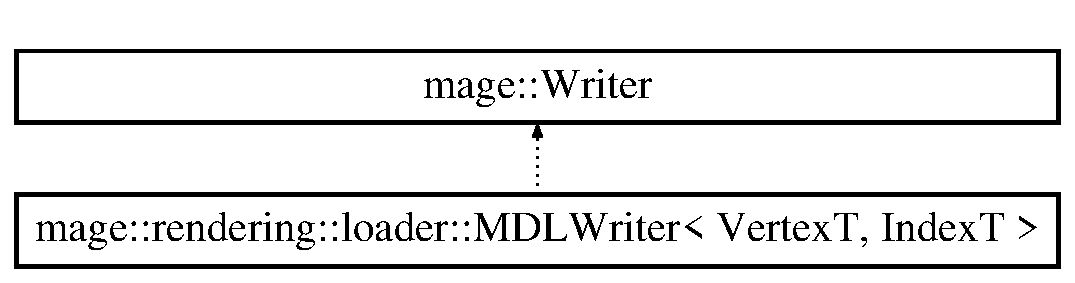
\includegraphics[height=2.000000cm]{classmage_1_1rendering_1_1loader_1_1_m_d_l_writer}
\end{center}
\end{figure}
\subsection*{Public Member Functions}
\begin{DoxyCompactItemize}
\item 
\mbox{\hyperlink{classmage_1_1rendering_1_1loader_1_1_m_d_l_writer_a6b30e49f08b5c6cd4702f5fdecd17561}{M\+D\+L\+Writer}} (const \mbox{\hyperlink{structmage_1_1rendering_1_1_model_output}{Model\+Output}}$<$ VertexT, IndexT $>$ \&model\+\_\+output)
\item 
\mbox{\hyperlink{classmage_1_1rendering_1_1loader_1_1_m_d_l_writer_a475ff3efdba707303052bae28d3ba85b}{M\+D\+L\+Writer}} (const \mbox{\hyperlink{classmage_1_1rendering_1_1loader_1_1_m_d_l_writer}{M\+D\+L\+Writer}} \&writer)=delete
\item 
\mbox{\hyperlink{classmage_1_1rendering_1_1loader_1_1_m_d_l_writer_a27f71b3a27f96e263948d19b8b570309}{M\+D\+L\+Writer}} (\mbox{\hyperlink{classmage_1_1rendering_1_1loader_1_1_m_d_l_writer}{M\+D\+L\+Writer}} \&\&writer) noexcept
\item 
\mbox{\hyperlink{classmage_1_1rendering_1_1loader_1_1_m_d_l_writer_aaa0fb8c60dee5352ed467bfb3f283f43}{$\sim$\+M\+D\+L\+Writer}} ()
\item 
\mbox{\hyperlink{classmage_1_1rendering_1_1loader_1_1_m_d_l_writer}{M\+D\+L\+Writer}} \& \mbox{\hyperlink{classmage_1_1rendering_1_1loader_1_1_m_d_l_writer_a9e5f38a8b5016534385039d44d3d71dc}{operator=}} (const \mbox{\hyperlink{classmage_1_1rendering_1_1loader_1_1_m_d_l_writer}{M\+D\+L\+Writer}} \&writer)=delete
\item 
\mbox{\hyperlink{classmage_1_1rendering_1_1loader_1_1_m_d_l_writer}{M\+D\+L\+Writer}} \& \mbox{\hyperlink{classmage_1_1rendering_1_1loader_1_1_m_d_l_writer_aaa2a3f4e8025bffefefaae7d3ef018f0}{operator=}} (\mbox{\hyperlink{classmage_1_1rendering_1_1loader_1_1_m_d_l_writer}{M\+D\+L\+Writer}} \&\&writer)=delete
\item 
void \mbox{\hyperlink{classmage_1_1rendering_1_1loader_1_1_m_d_l_writer_ac01e930b55888da88e345b0910d4b1c2}{Write\+To\+File}} (std\+::filesystem\+::path path)
\item 
const std\+::filesystem\+::path \& \mbox{\hyperlink{classmage_1_1rendering_1_1loader_1_1_m_d_l_writer_ab023ae8174132f233c6e1fa4d3a2a1c8}{Get\+Path}} () const noexcept
\end{DoxyCompactItemize}
\subsection*{Private Member Functions}
\begin{DoxyCompactItemize}
\item 
virtual void \mbox{\hyperlink{classmage_1_1rendering_1_1loader_1_1_m_d_l_writer_a1506b1a09c7a7c1ee1e206cc6d5cd0e0}{Write}} () override
\item 
void \mbox{\hyperlink{classmage_1_1rendering_1_1loader_1_1_m_d_l_writer_a77189702168fc4ea6b9482a9efec788f}{Export\+Mesh}} ()
\item 
void \mbox{\hyperlink{classmage_1_1rendering_1_1loader_1_1_m_d_l_writer_afcd1eca27b5854b0f0406dbcae135499}{Write\+Materials}} ()
\item 
void \mbox{\hyperlink{classmage_1_1rendering_1_1loader_1_1_m_d_l_writer_a8fcd997a51d7a46149596d332ebdb8e1}{Write\+Model\+Parts}} ()
\end{DoxyCompactItemize}
\subsection*{Private Attributes}
\begin{DoxyCompactItemize}
\item 
const \mbox{\hyperlink{structmage_1_1rendering_1_1_model_output}{Model\+Output}}$<$ VertexT, IndexT $>$ \& \mbox{\hyperlink{classmage_1_1rendering_1_1loader_1_1_m_d_l_writer_aefa6dfd7c4d7e2abe92e9c93b1e8638c}{m\+\_\+model\+\_\+output}}
\end{DoxyCompactItemize}


\subsection{Detailed Description}
\subsubsection*{template$<$typename VertexT, typename IndexT$>$\newline
class mage\+::rendering\+::loader\+::\+M\+D\+L\+Writer$<$ Vertex\+T, Index\+T $>$}

A class of M\+DL file writers for writing models.


\begin{DoxyTemplParams}{Template Parameters}
{\em VertexT} & The vertex type. \\
\hline
{\em IndexT} & The index type. \\
\hline
\end{DoxyTemplParams}


\subsection{Constructor \& Destructor Documentation}
\mbox{\Hypertarget{classmage_1_1rendering_1_1loader_1_1_m_d_l_writer_a6b30e49f08b5c6cd4702f5fdecd17561}\label{classmage_1_1rendering_1_1loader_1_1_m_d_l_writer_a6b30e49f08b5c6cd4702f5fdecd17561}} 
\index{mage\+::rendering\+::loader\+::\+M\+D\+L\+Writer@{mage\+::rendering\+::loader\+::\+M\+D\+L\+Writer}!M\+D\+L\+Writer@{M\+D\+L\+Writer}}
\index{M\+D\+L\+Writer@{M\+D\+L\+Writer}!mage\+::rendering\+::loader\+::\+M\+D\+L\+Writer@{mage\+::rendering\+::loader\+::\+M\+D\+L\+Writer}}
\subsubsection{\texorpdfstring{M\+D\+L\+Writer()}{MDLWriter()}\hspace{0.1cm}{\footnotesize\ttfamily [1/3]}}
{\footnotesize\ttfamily template$<$typename VertexT , typename IndexT $>$ \\
\mbox{\hyperlink{classmage_1_1rendering_1_1loader_1_1_m_d_l_writer}{mage\+::rendering\+::loader\+::\+M\+D\+L\+Writer}}$<$ VertexT, IndexT $>$\+::\mbox{\hyperlink{classmage_1_1rendering_1_1loader_1_1_m_d_l_writer}{M\+D\+L\+Writer}} (\begin{DoxyParamCaption}\item[{const \mbox{\hyperlink{structmage_1_1rendering_1_1_model_output}{Model\+Output}}$<$ VertexT, IndexT $>$ \&}]{model\+\_\+output }\end{DoxyParamCaption})\hspace{0.3cm}{\ttfamily [explicit]}}

Constructs a M\+DL writer.


\begin{DoxyParams}[1]{Parameters}
\mbox{\tt in}  & {\em model\+\_\+output} & A reference to the model output containing the model data. \\
\hline
\end{DoxyParams}
\mbox{\Hypertarget{classmage_1_1rendering_1_1loader_1_1_m_d_l_writer_a475ff3efdba707303052bae28d3ba85b}\label{classmage_1_1rendering_1_1loader_1_1_m_d_l_writer_a475ff3efdba707303052bae28d3ba85b}} 
\index{mage\+::rendering\+::loader\+::\+M\+D\+L\+Writer@{mage\+::rendering\+::loader\+::\+M\+D\+L\+Writer}!M\+D\+L\+Writer@{M\+D\+L\+Writer}}
\index{M\+D\+L\+Writer@{M\+D\+L\+Writer}!mage\+::rendering\+::loader\+::\+M\+D\+L\+Writer@{mage\+::rendering\+::loader\+::\+M\+D\+L\+Writer}}
\subsubsection{\texorpdfstring{M\+D\+L\+Writer()}{MDLWriter()}\hspace{0.1cm}{\footnotesize\ttfamily [2/3]}}
{\footnotesize\ttfamily template$<$typename VertexT , typename IndexT $>$ \\
\mbox{\hyperlink{classmage_1_1rendering_1_1loader_1_1_m_d_l_writer}{mage\+::rendering\+::loader\+::\+M\+D\+L\+Writer}}$<$ VertexT, IndexT $>$\+::\mbox{\hyperlink{classmage_1_1rendering_1_1loader_1_1_m_d_l_writer}{M\+D\+L\+Writer}} (\begin{DoxyParamCaption}\item[{const \mbox{\hyperlink{classmage_1_1rendering_1_1loader_1_1_m_d_l_writer}{M\+D\+L\+Writer}}$<$ VertexT, IndexT $>$ \&}]{writer }\end{DoxyParamCaption})\hspace{0.3cm}{\ttfamily [delete]}}

Constructs a M\+DL writer from the given M\+DL writer.


\begin{DoxyParams}[1]{Parameters}
\mbox{\tt in}  & {\em writer} & A reference to the M\+DL writer to copy. \\
\hline
\end{DoxyParams}
\mbox{\Hypertarget{classmage_1_1rendering_1_1loader_1_1_m_d_l_writer_a27f71b3a27f96e263948d19b8b570309}\label{classmage_1_1rendering_1_1loader_1_1_m_d_l_writer_a27f71b3a27f96e263948d19b8b570309}} 
\index{mage\+::rendering\+::loader\+::\+M\+D\+L\+Writer@{mage\+::rendering\+::loader\+::\+M\+D\+L\+Writer}!M\+D\+L\+Writer@{M\+D\+L\+Writer}}
\index{M\+D\+L\+Writer@{M\+D\+L\+Writer}!mage\+::rendering\+::loader\+::\+M\+D\+L\+Writer@{mage\+::rendering\+::loader\+::\+M\+D\+L\+Writer}}
\subsubsection{\texorpdfstring{M\+D\+L\+Writer()}{MDLWriter()}\hspace{0.1cm}{\footnotesize\ttfamily [3/3]}}
{\footnotesize\ttfamily template$<$typename VertexT , typename IndexT $>$ \\
\mbox{\hyperlink{classmage_1_1rendering_1_1loader_1_1_m_d_l_writer}{mage\+::rendering\+::loader\+::\+M\+D\+L\+Writer}}$<$ VertexT, IndexT $>$\+::\mbox{\hyperlink{classmage_1_1rendering_1_1loader_1_1_m_d_l_writer}{M\+D\+L\+Writer}} (\begin{DoxyParamCaption}\item[{\mbox{\hyperlink{classmage_1_1rendering_1_1loader_1_1_m_d_l_writer}{M\+D\+L\+Writer}}$<$ VertexT, IndexT $>$ \&\&}]{writer }\end{DoxyParamCaption})\hspace{0.3cm}{\ttfamily [noexcept]}}

Constructs a M\+DL writer by moving the given M\+DL writer.


\begin{DoxyParams}[1]{Parameters}
\mbox{\tt in}  & {\em writer} & A reference to the M\+DL writer to move. \\
\hline
\end{DoxyParams}
\mbox{\Hypertarget{classmage_1_1rendering_1_1loader_1_1_m_d_l_writer_aaa0fb8c60dee5352ed467bfb3f283f43}\label{classmage_1_1rendering_1_1loader_1_1_m_d_l_writer_aaa0fb8c60dee5352ed467bfb3f283f43}} 
\index{mage\+::rendering\+::loader\+::\+M\+D\+L\+Writer@{mage\+::rendering\+::loader\+::\+M\+D\+L\+Writer}!````~M\+D\+L\+Writer@{$\sim$\+M\+D\+L\+Writer}}
\index{````~M\+D\+L\+Writer@{$\sim$\+M\+D\+L\+Writer}!mage\+::rendering\+::loader\+::\+M\+D\+L\+Writer@{mage\+::rendering\+::loader\+::\+M\+D\+L\+Writer}}
\subsubsection{\texorpdfstring{$\sim$\+M\+D\+L\+Writer()}{~MDLWriter()}}
{\footnotesize\ttfamily template$<$typename VertexT , typename IndexT $>$ \\
\mbox{\hyperlink{classmage_1_1rendering_1_1loader_1_1_m_d_l_writer}{mage\+::rendering\+::loader\+::\+M\+D\+L\+Writer}}$<$ VertexT, IndexT $>$\+::$\sim$\mbox{\hyperlink{classmage_1_1rendering_1_1loader_1_1_m_d_l_writer}{M\+D\+L\+Writer}} (\begin{DoxyParamCaption}{ }\end{DoxyParamCaption})}

Destructs this M\+DL writer. 

\subsection{Member Function Documentation}
\mbox{\Hypertarget{classmage_1_1rendering_1_1loader_1_1_m_d_l_writer_a77189702168fc4ea6b9482a9efec788f}\label{classmage_1_1rendering_1_1loader_1_1_m_d_l_writer_a77189702168fc4ea6b9482a9efec788f}} 
\index{mage\+::rendering\+::loader\+::\+M\+D\+L\+Writer@{mage\+::rendering\+::loader\+::\+M\+D\+L\+Writer}!Export\+Mesh@{Export\+Mesh}}
\index{Export\+Mesh@{Export\+Mesh}!mage\+::rendering\+::loader\+::\+M\+D\+L\+Writer@{mage\+::rendering\+::loader\+::\+M\+D\+L\+Writer}}
\subsubsection{\texorpdfstring{Export\+Mesh()}{ExportMesh()}}
{\footnotesize\ttfamily template$<$typename VertexT , typename IndexT $>$ \\
void \mbox{\hyperlink{classmage_1_1rendering_1_1loader_1_1_m_d_l_writer}{mage\+::rendering\+::loader\+::\+M\+D\+L\+Writer}}$<$ VertexT, IndexT $>$\+::Export\+Mesh (\begin{DoxyParamCaption}{ }\end{DoxyParamCaption})\hspace{0.3cm}{\ttfamily [private]}}

Writes and exports the mesh corresponding to the model.


\begin{DoxyExceptions}{Exceptions}
{\em \mbox{\hyperlink{classmage_1_1_exception}{Exception}}} & Failed to write. \\
\hline
{\em \mbox{\hyperlink{classmage_1_1_exception}{Exception}}} & Failed to export the mesh corresponding to the model to file. \\
\hline
\end{DoxyExceptions}
\mbox{\Hypertarget{classmage_1_1rendering_1_1loader_1_1_m_d_l_writer_ab023ae8174132f233c6e1fa4d3a2a1c8}\label{classmage_1_1rendering_1_1loader_1_1_m_d_l_writer_ab023ae8174132f233c6e1fa4d3a2a1c8}} 
\index{mage\+::rendering\+::loader\+::\+M\+D\+L\+Writer@{mage\+::rendering\+::loader\+::\+M\+D\+L\+Writer}!Get\+Path@{Get\+Path}}
\index{Get\+Path@{Get\+Path}!mage\+::rendering\+::loader\+::\+M\+D\+L\+Writer@{mage\+::rendering\+::loader\+::\+M\+D\+L\+Writer}}
\subsubsection{\texorpdfstring{Get\+Path()}{GetPath()}}
{\footnotesize\ttfamily template$<$typename VertexT , typename IndexT $>$ \\
const std\+::filesystem\+::path\& mage\+::\+Writer\+::\+Get\+Path\hspace{0.3cm}{\ttfamily [noexcept]}}

Returns the current path of this writer.

\begin{DoxyReturn}{Returns}
A reference to the current path of this writer. 
\end{DoxyReturn}
\mbox{\Hypertarget{classmage_1_1rendering_1_1loader_1_1_m_d_l_writer_a9e5f38a8b5016534385039d44d3d71dc}\label{classmage_1_1rendering_1_1loader_1_1_m_d_l_writer_a9e5f38a8b5016534385039d44d3d71dc}} 
\index{mage\+::rendering\+::loader\+::\+M\+D\+L\+Writer@{mage\+::rendering\+::loader\+::\+M\+D\+L\+Writer}!operator=@{operator=}}
\index{operator=@{operator=}!mage\+::rendering\+::loader\+::\+M\+D\+L\+Writer@{mage\+::rendering\+::loader\+::\+M\+D\+L\+Writer}}
\subsubsection{\texorpdfstring{operator=()}{operator=()}\hspace{0.1cm}{\footnotesize\ttfamily [1/2]}}
{\footnotesize\ttfamily template$<$typename VertexT , typename IndexT $>$ \\
\mbox{\hyperlink{classmage_1_1rendering_1_1loader_1_1_m_d_l_writer}{M\+D\+L\+Writer}}\& \mbox{\hyperlink{classmage_1_1rendering_1_1loader_1_1_m_d_l_writer}{mage\+::rendering\+::loader\+::\+M\+D\+L\+Writer}}$<$ VertexT, IndexT $>$\+::operator= (\begin{DoxyParamCaption}\item[{const \mbox{\hyperlink{classmage_1_1rendering_1_1loader_1_1_m_d_l_writer}{M\+D\+L\+Writer}}$<$ VertexT, IndexT $>$ \&}]{writer }\end{DoxyParamCaption})\hspace{0.3cm}{\ttfamily [delete]}}

Copies the given M\+DL writer to this M\+DL writer.


\begin{DoxyParams}[1]{Parameters}
\mbox{\tt in}  & {\em writer} & A reference to a M\+DL writer to copy. \\
\hline
\end{DoxyParams}
\begin{DoxyReturn}{Returns}
A reference to the copy of the given M\+DL writer (i.\+e. this M\+DL writer). 
\end{DoxyReturn}
\mbox{\Hypertarget{classmage_1_1rendering_1_1loader_1_1_m_d_l_writer_aaa2a3f4e8025bffefefaae7d3ef018f0}\label{classmage_1_1rendering_1_1loader_1_1_m_d_l_writer_aaa2a3f4e8025bffefefaae7d3ef018f0}} 
\index{mage\+::rendering\+::loader\+::\+M\+D\+L\+Writer@{mage\+::rendering\+::loader\+::\+M\+D\+L\+Writer}!operator=@{operator=}}
\index{operator=@{operator=}!mage\+::rendering\+::loader\+::\+M\+D\+L\+Writer@{mage\+::rendering\+::loader\+::\+M\+D\+L\+Writer}}
\subsubsection{\texorpdfstring{operator=()}{operator=()}\hspace{0.1cm}{\footnotesize\ttfamily [2/2]}}
{\footnotesize\ttfamily template$<$typename VertexT , typename IndexT $>$ \\
\mbox{\hyperlink{classmage_1_1rendering_1_1loader_1_1_m_d_l_writer}{M\+D\+L\+Writer}}\& \mbox{\hyperlink{classmage_1_1rendering_1_1loader_1_1_m_d_l_writer}{mage\+::rendering\+::loader\+::\+M\+D\+L\+Writer}}$<$ VertexT, IndexT $>$\+::operator= (\begin{DoxyParamCaption}\item[{\mbox{\hyperlink{classmage_1_1rendering_1_1loader_1_1_m_d_l_writer}{M\+D\+L\+Writer}}$<$ VertexT, IndexT $>$ \&\&}]{writer }\end{DoxyParamCaption})\hspace{0.3cm}{\ttfamily [delete]}}

Moves the given M\+DL writer to this M\+DL writer.


\begin{DoxyParams}[1]{Parameters}
\mbox{\tt in}  & {\em writer} & A reference to a M\+DL writer to move. \\
\hline
\end{DoxyParams}
\begin{DoxyReturn}{Returns}
A reference to the moved M\+DL writer (i.\+e. this M\+DL writer). 
\end{DoxyReturn}
\mbox{\Hypertarget{classmage_1_1rendering_1_1loader_1_1_m_d_l_writer_a1506b1a09c7a7c1ee1e206cc6d5cd0e0}\label{classmage_1_1rendering_1_1loader_1_1_m_d_l_writer_a1506b1a09c7a7c1ee1e206cc6d5cd0e0}} 
\index{mage\+::rendering\+::loader\+::\+M\+D\+L\+Writer@{mage\+::rendering\+::loader\+::\+M\+D\+L\+Writer}!Write@{Write}}
\index{Write@{Write}!mage\+::rendering\+::loader\+::\+M\+D\+L\+Writer@{mage\+::rendering\+::loader\+::\+M\+D\+L\+Writer}}
\subsubsection{\texorpdfstring{Write()}{Write()}}
{\footnotesize\ttfamily template$<$typename VertexT , typename IndexT $>$ \\
virtual void \mbox{\hyperlink{classmage_1_1rendering_1_1loader_1_1_m_d_l_writer}{mage\+::rendering\+::loader\+::\+M\+D\+L\+Writer}}$<$ VertexT, IndexT $>$\+::Write (\begin{DoxyParamCaption}{ }\end{DoxyParamCaption})\hspace{0.3cm}{\ttfamily [override]}, {\ttfamily [private]}, {\ttfamily [virtual]}}

Starts writing.


\begin{DoxyExceptions}{Exceptions}
{\em \mbox{\hyperlink{classmage_1_1_exception}{Exception}}} & Failed to write. \\
\hline
\end{DoxyExceptions}


Implements \mbox{\hyperlink{classmage_1_1_writer_a9baf695ef7f6180bef883f60bcb3ac07}{mage\+::\+Writer}}.

\mbox{\Hypertarget{classmage_1_1rendering_1_1loader_1_1_m_d_l_writer_afcd1eca27b5854b0f0406dbcae135499}\label{classmage_1_1rendering_1_1loader_1_1_m_d_l_writer_afcd1eca27b5854b0f0406dbcae135499}} 
\index{mage\+::rendering\+::loader\+::\+M\+D\+L\+Writer@{mage\+::rendering\+::loader\+::\+M\+D\+L\+Writer}!Write\+Materials@{Write\+Materials}}
\index{Write\+Materials@{Write\+Materials}!mage\+::rendering\+::loader\+::\+M\+D\+L\+Writer@{mage\+::rendering\+::loader\+::\+M\+D\+L\+Writer}}
\subsubsection{\texorpdfstring{Write\+Materials()}{WriteMaterials()}}
{\footnotesize\ttfamily template$<$typename VertexT , typename IndexT $>$ \\
void \mbox{\hyperlink{classmage_1_1rendering_1_1loader_1_1_m_d_l_writer}{mage\+::rendering\+::loader\+::\+M\+D\+L\+Writer}}$<$ VertexT, IndexT $>$\+::Write\+Materials (\begin{DoxyParamCaption}{ }\end{DoxyParamCaption})\hspace{0.3cm}{\ttfamily [private]}}

Writes the materials corresponding to the model.


\begin{DoxyExceptions}{Exceptions}
{\em \mbox{\hyperlink{classmage_1_1_exception}{Exception}}} & Failed to write. \\
\hline
\end{DoxyExceptions}
\mbox{\Hypertarget{classmage_1_1rendering_1_1loader_1_1_m_d_l_writer_a8fcd997a51d7a46149596d332ebdb8e1}\label{classmage_1_1rendering_1_1loader_1_1_m_d_l_writer_a8fcd997a51d7a46149596d332ebdb8e1}} 
\index{mage\+::rendering\+::loader\+::\+M\+D\+L\+Writer@{mage\+::rendering\+::loader\+::\+M\+D\+L\+Writer}!Write\+Model\+Parts@{Write\+Model\+Parts}}
\index{Write\+Model\+Parts@{Write\+Model\+Parts}!mage\+::rendering\+::loader\+::\+M\+D\+L\+Writer@{mage\+::rendering\+::loader\+::\+M\+D\+L\+Writer}}
\subsubsection{\texorpdfstring{Write\+Model\+Parts()}{WriteModelParts()}}
{\footnotesize\ttfamily template$<$typename VertexT , typename IndexT $>$ \\
void \mbox{\hyperlink{classmage_1_1rendering_1_1loader_1_1_m_d_l_writer}{mage\+::rendering\+::loader\+::\+M\+D\+L\+Writer}}$<$ VertexT, IndexT $>$\+::Write\+Model\+Parts (\begin{DoxyParamCaption}{ }\end{DoxyParamCaption})\hspace{0.3cm}{\ttfamily [private]}}

Writes the model parts corresponding to the model.


\begin{DoxyExceptions}{Exceptions}
{\em \mbox{\hyperlink{classmage_1_1_exception}{Exception}}} & Failed to write. \\
\hline
\end{DoxyExceptions}
\mbox{\Hypertarget{classmage_1_1rendering_1_1loader_1_1_m_d_l_writer_ac01e930b55888da88e345b0910d4b1c2}\label{classmage_1_1rendering_1_1loader_1_1_m_d_l_writer_ac01e930b55888da88e345b0910d4b1c2}} 
\index{mage\+::rendering\+::loader\+::\+M\+D\+L\+Writer@{mage\+::rendering\+::loader\+::\+M\+D\+L\+Writer}!Write\+To\+File@{Write\+To\+File}}
\index{Write\+To\+File@{Write\+To\+File}!mage\+::rendering\+::loader\+::\+M\+D\+L\+Writer@{mage\+::rendering\+::loader\+::\+M\+D\+L\+Writer}}
\subsubsection{\texorpdfstring{Write\+To\+File()}{WriteToFile()}}
{\footnotesize\ttfamily template$<$typename VertexT , typename IndexT $>$ \\
void mage\+::\+Writer\+::\+Write\+To\+File}

Writes to the file associated with the given path.


\begin{DoxyParams}[1]{Parameters}
\mbox{\tt in}  & {\em path} & The path. \\
\hline
\end{DoxyParams}

\begin{DoxyExceptions}{Exceptions}
{\em \mbox{\hyperlink{classmage_1_1_exception}{Exception}}} & Failed to write to the file. \\
\hline
\end{DoxyExceptions}


\subsection{Member Data Documentation}
\mbox{\Hypertarget{classmage_1_1rendering_1_1loader_1_1_m_d_l_writer_aefa6dfd7c4d7e2abe92e9c93b1e8638c}\label{classmage_1_1rendering_1_1loader_1_1_m_d_l_writer_aefa6dfd7c4d7e2abe92e9c93b1e8638c}} 
\index{mage\+::rendering\+::loader\+::\+M\+D\+L\+Writer@{mage\+::rendering\+::loader\+::\+M\+D\+L\+Writer}!m\+\_\+model\+\_\+output@{m\+\_\+model\+\_\+output}}
\index{m\+\_\+model\+\_\+output@{m\+\_\+model\+\_\+output}!mage\+::rendering\+::loader\+::\+M\+D\+L\+Writer@{mage\+::rendering\+::loader\+::\+M\+D\+L\+Writer}}
\subsubsection{\texorpdfstring{m\+\_\+model\+\_\+output}{m\_model\_output}}
{\footnotesize\ttfamily template$<$typename VertexT , typename IndexT $>$ \\
const \mbox{\hyperlink{structmage_1_1rendering_1_1_model_output}{Model\+Output}}$<$ VertexT, IndexT $>$\& \mbox{\hyperlink{classmage_1_1rendering_1_1loader_1_1_m_d_l_writer}{mage\+::rendering\+::loader\+::\+M\+D\+L\+Writer}}$<$ VertexT, IndexT $>$\+::m\+\_\+model\+\_\+output\hspace{0.3cm}{\ttfamily [private]}}

A reference to the model output containing the model data of this M\+DL writer. 
\hypertarget{classmage_1_1_memory_arena}{}\section{mage\+:\+:Memory\+Arena Class Reference}
\label{classmage_1_1_memory_arena}\index{mage\+::\+Memory\+Arena@{mage\+::\+Memory\+Arena}}


{\ttfamily \#include $<$memory\+\_\+arena.\+hpp$>$}

\subsection*{Classes}
\begin{DoxyCompactItemize}
\item 
class \mbox{\hyperlink{classmage_1_1_memory_arena_1_1_allocator}{Allocator}}
\end{DoxyCompactItemize}
\subsection*{Public Member Functions}
\begin{DoxyCompactItemize}
\item 
\mbox{\hyperlink{classmage_1_1_memory_arena_a139f7781be209bb29e7ad0ed04cb32a5}{Memory\+Arena}} (size\+\_\+t maximum\+\_\+block\+\_\+size, size\+\_\+t alignment)
\item 
\mbox{\hyperlink{classmage_1_1_memory_arena_a1eca6fdacbd1226f4b21f443d118168b}{Memory\+Arena}} (const \mbox{\hyperlink{classmage_1_1_memory_arena}{Memory\+Arena}} \&arena)=delete
\item 
\mbox{\hyperlink{classmage_1_1_memory_arena_a98829c5a87ba028c376f100cca09e876}{Memory\+Arena}} (\mbox{\hyperlink{classmage_1_1_memory_arena}{Memory\+Arena}} \&\&arena)
\item 
\mbox{\hyperlink{classmage_1_1_memory_arena_acfee6fc205e2eaf6aeef4acf19948e6e}{$\sim$\+Memory\+Arena}} ()
\item 
\mbox{\hyperlink{classmage_1_1_memory_arena}{Memory\+Arena}} \& \mbox{\hyperlink{classmage_1_1_memory_arena_a7e7799f859c55435714933972ecb8b95}{operator=}} (const \mbox{\hyperlink{classmage_1_1_memory_arena}{Memory\+Arena}} \&arena)=delete
\item 
\mbox{\hyperlink{classmage_1_1_memory_arena}{Memory\+Arena}} \& \mbox{\hyperlink{classmage_1_1_memory_arena_aa4b80a917a838a1ca3788f906723d273}{operator=}} (\mbox{\hyperlink{classmage_1_1_memory_arena}{Memory\+Arena}} \&\&arena)=delete
\item 
size\+\_\+t \mbox{\hyperlink{classmage_1_1_memory_arena_a79931a18af492ad8ef7e99b09ec36f2a}{Get\+Alignment}} () const noexcept
\item 
size\+\_\+t \mbox{\hyperlink{classmage_1_1_memory_arena_a6786cf52a03777580b439cafdd8ff8f9}{Get\+Maximum\+Block\+Size}} () const noexcept
\item 
size\+\_\+t \mbox{\hyperlink{classmage_1_1_memory_arena_a0b41d6901c3519f046cd551931f72c1b}{Get\+Current\+Block\+Size}} () const noexcept
\item 
size\+\_\+t \mbox{\hyperlink{classmage_1_1_memory_arena_ac8e8ac4ba60cd2bb1d8dc8a5d4a9f4ad}{Get\+Total\+Block\+Size}} () const noexcept
\item 
void $\ast$ \mbox{\hyperlink{classmage_1_1_memory_arena_a7bdbc9da32c1f8d49ce5d2f153870284}{Get\+Current\+Block\+Ptr}} () const noexcept
\item 
void \mbox{\hyperlink{classmage_1_1_memory_arena_a117b74c7bd5dfb28dfdaae6cab253491}{Reset}} ()
\item 
void $\ast$ \mbox{\hyperlink{classmage_1_1_memory_arena_a2e63b11c535dbfefd69d071466be9ce1}{Alloc}} (size\+\_\+t size)
\item 
{\footnotesize template$<$typename T $>$ }\\T $\ast$ \mbox{\hyperlink{classmage_1_1_memory_arena_a0880de049e8e76cd26918528eb892813}{Alloc\+Data}} (size\+\_\+t count=1, bool initialization=false)
\item 
{\footnotesize template$<$typename T $>$ }\\\mbox{\hyperlink{classmage_1_1_memory_arena_1_1_allocator}{Allocator}}$<$ T $>$ \mbox{\hyperlink{classmage_1_1_memory_arena_aa2cc5c42ed20c11900330ace3dfcdc8f}{Get\+Allocator}} () const noexcept
\end{DoxyCompactItemize}
\subsection*{Private Types}
\begin{DoxyCompactItemize}
\item 
using \mbox{\hyperlink{classmage_1_1_memory_arena_a133e9d40bd216e3f1d98c6a2b36cf373}{Memory\+Block}} = std\+::pair$<$ size\+\_\+t, \mbox{\hyperlink{namespacemage_afc638980bc6154f15af5e2d93a0e0ea9}{U8}} $\ast$$>$
\end{DoxyCompactItemize}
\subsection*{Private Attributes}
\begin{DoxyCompactItemize}
\item 
const size\+\_\+t \mbox{\hyperlink{classmage_1_1_memory_arena_a424c3ff6f1d96545dd08f94c1c79c963}{m\+\_\+alignment}}
\item 
const size\+\_\+t \mbox{\hyperlink{classmage_1_1_memory_arena_aeef4c56cf50fd3cbbba2879fcd028b86}{m\+\_\+maximum\+\_\+block\+\_\+size}}
\item 
\mbox{\hyperlink{classmage_1_1_memory_arena_a133e9d40bd216e3f1d98c6a2b36cf373}{Memory\+Block}} \mbox{\hyperlink{classmage_1_1_memory_arena_a2680b25146c174ac7fd639f1bd0acc7c}{m\+\_\+current\+\_\+block}}
\item 
size\+\_\+t \mbox{\hyperlink{classmage_1_1_memory_arena_a880d07eb372ce1c8b907947fcbdfc59c}{m\+\_\+current\+\_\+block\+\_\+pos}}
\item 
std\+::list$<$ \mbox{\hyperlink{classmage_1_1_memory_arena_a133e9d40bd216e3f1d98c6a2b36cf373}{Memory\+Block}} $>$ \mbox{\hyperlink{classmage_1_1_memory_arena_a49a6d7fb9396f57210897abfb4e30903}{m\+\_\+used\+\_\+blocks}}
\item 
std\+::list$<$ \mbox{\hyperlink{classmage_1_1_memory_arena_a133e9d40bd216e3f1d98c6a2b36cf373}{Memory\+Block}} $>$ \mbox{\hyperlink{classmage_1_1_memory_arena_a02f251a5aafa61d239b4daed3458a654}{m\+\_\+available\+\_\+blocks}}
\end{DoxyCompactItemize}


\subsection{Detailed Description}
A class of memory arenas. 

\subsection{Member Typedef Documentation}
\mbox{\Hypertarget{classmage_1_1_memory_arena_a133e9d40bd216e3f1d98c6a2b36cf373}\label{classmage_1_1_memory_arena_a133e9d40bd216e3f1d98c6a2b36cf373}} 
\index{mage\+::\+Memory\+Arena@{mage\+::\+Memory\+Arena}!Memory\+Block@{Memory\+Block}}
\index{Memory\+Block@{Memory\+Block}!mage\+::\+Memory\+Arena@{mage\+::\+Memory\+Arena}}
\subsubsection{\texorpdfstring{Memory\+Block}{MemoryBlock}}
{\footnotesize\ttfamily using \mbox{\hyperlink{classmage_1_1_memory_arena_a133e9d40bd216e3f1d98c6a2b36cf373}{mage\+::\+Memory\+Arena\+::\+Memory\+Block}} =  std\+::pair$<$ size\+\_\+t, \mbox{\hyperlink{namespacemage_afc638980bc6154f15af5e2d93a0e0ea9}{U8}}$\ast$ $>$\hspace{0.3cm}{\ttfamily [private]}}

A type definition for a memory block. 

\subsection{Constructor \& Destructor Documentation}
\mbox{\Hypertarget{classmage_1_1_memory_arena_a139f7781be209bb29e7ad0ed04cb32a5}\label{classmage_1_1_memory_arena_a139f7781be209bb29e7ad0ed04cb32a5}} 
\index{mage\+::\+Memory\+Arena@{mage\+::\+Memory\+Arena}!Memory\+Arena@{Memory\+Arena}}
\index{Memory\+Arena@{Memory\+Arena}!mage\+::\+Memory\+Arena@{mage\+::\+Memory\+Arena}}
\subsubsection{\texorpdfstring{Memory\+Arena()}{MemoryArena()}\hspace{0.1cm}{\footnotesize\ttfamily [1/3]}}
{\footnotesize\ttfamily mage\+::\+Memory\+Arena\+::\+Memory\+Arena (\begin{DoxyParamCaption}\item[{size\+\_\+t}]{maximum\+\_\+block\+\_\+size,  }\item[{size\+\_\+t}]{alignment }\end{DoxyParamCaption})\hspace{0.3cm}{\ttfamily [explicit]}}

Constructs a memory arena with given block size.


\begin{DoxyParams}[1]{Parameters}
\mbox{\tt in}  & {\em maximum\+\_\+block\+\_\+size} & The maximum block size in bytes. \\
\hline
\mbox{\tt in}  & {\em alignment} & The alignment in bytes. \\
\hline
\end{DoxyParams}
\mbox{\Hypertarget{classmage_1_1_memory_arena_a1eca6fdacbd1226f4b21f443d118168b}\label{classmage_1_1_memory_arena_a1eca6fdacbd1226f4b21f443d118168b}} 
\index{mage\+::\+Memory\+Arena@{mage\+::\+Memory\+Arena}!Memory\+Arena@{Memory\+Arena}}
\index{Memory\+Arena@{Memory\+Arena}!mage\+::\+Memory\+Arena@{mage\+::\+Memory\+Arena}}
\subsubsection{\texorpdfstring{Memory\+Arena()}{MemoryArena()}\hspace{0.1cm}{\footnotesize\ttfamily [2/3]}}
{\footnotesize\ttfamily mage\+::\+Memory\+Arena\+::\+Memory\+Arena (\begin{DoxyParamCaption}\item[{const \mbox{\hyperlink{classmage_1_1_memory_arena}{Memory\+Arena}} \&}]{arena }\end{DoxyParamCaption})\hspace{0.3cm}{\ttfamily [delete]}}

Constructs a memory arena from the given memory arena.


\begin{DoxyParams}[1]{Parameters}
\mbox{\tt in}  & {\em arena} & A reference to the memory arena to copy. \\
\hline
\end{DoxyParams}
\mbox{\Hypertarget{classmage_1_1_memory_arena_a98829c5a87ba028c376f100cca09e876}\label{classmage_1_1_memory_arena_a98829c5a87ba028c376f100cca09e876}} 
\index{mage\+::\+Memory\+Arena@{mage\+::\+Memory\+Arena}!Memory\+Arena@{Memory\+Arena}}
\index{Memory\+Arena@{Memory\+Arena}!mage\+::\+Memory\+Arena@{mage\+::\+Memory\+Arena}}
\subsubsection{\texorpdfstring{Memory\+Arena()}{MemoryArena()}\hspace{0.1cm}{\footnotesize\ttfamily [3/3]}}
{\footnotesize\ttfamily mage\+::\+Memory\+Arena\+::\+Memory\+Arena (\begin{DoxyParamCaption}\item[{\mbox{\hyperlink{classmage_1_1_memory_arena}{Memory\+Arena}} \&\&}]{arena }\end{DoxyParamCaption})\hspace{0.3cm}{\ttfamily [default]}}

Constructs a memory arena by moving the given memory arena.


\begin{DoxyParams}[1]{Parameters}
\mbox{\tt in}  & {\em arena} & A reference to the memory arena to move. \\
\hline
\end{DoxyParams}
\mbox{\Hypertarget{classmage_1_1_memory_arena_acfee6fc205e2eaf6aeef4acf19948e6e}\label{classmage_1_1_memory_arena_acfee6fc205e2eaf6aeef4acf19948e6e}} 
\index{mage\+::\+Memory\+Arena@{mage\+::\+Memory\+Arena}!````~Memory\+Arena@{$\sim$\+Memory\+Arena}}
\index{````~Memory\+Arena@{$\sim$\+Memory\+Arena}!mage\+::\+Memory\+Arena@{mage\+::\+Memory\+Arena}}
\subsubsection{\texorpdfstring{$\sim$\+Memory\+Arena()}{~MemoryArena()}}
{\footnotesize\ttfamily mage\+::\+Memory\+Arena\+::$\sim$\+Memory\+Arena (\begin{DoxyParamCaption}{ }\end{DoxyParamCaption})}

Destructs this memory arena. 

\subsection{Member Function Documentation}
\mbox{\Hypertarget{classmage_1_1_memory_arena_a2e63b11c535dbfefd69d071466be9ce1}\label{classmage_1_1_memory_arena_a2e63b11c535dbfefd69d071466be9ce1}} 
\index{mage\+::\+Memory\+Arena@{mage\+::\+Memory\+Arena}!Alloc@{Alloc}}
\index{Alloc@{Alloc}!mage\+::\+Memory\+Arena@{mage\+::\+Memory\+Arena}}
\subsubsection{\texorpdfstring{Alloc()}{Alloc()}}
{\footnotesize\ttfamily void $\ast$ mage\+::\+Memory\+Arena\+::\+Alloc (\begin{DoxyParamCaption}\item[{size\+\_\+t}]{size }\end{DoxyParamCaption})}

Allocates a block of memory of the given size on this memory arena.


\begin{DoxyParams}[1]{Parameters}
\mbox{\tt in}  & {\em size} & The requested size in bytes to allocate in memory. \\
\hline
\end{DoxyParams}
\begin{DoxyReturn}{Returns}
{\ttfamily nullptr} if the allocation failed. 

A pointer to the memory block that was allocated. 
\end{DoxyReturn}
\mbox{\Hypertarget{classmage_1_1_memory_arena_a0880de049e8e76cd26918528eb892813}\label{classmage_1_1_memory_arena_a0880de049e8e76cd26918528eb892813}} 
\index{mage\+::\+Memory\+Arena@{mage\+::\+Memory\+Arena}!Alloc\+Data@{Alloc\+Data}}
\index{Alloc\+Data@{Alloc\+Data}!mage\+::\+Memory\+Arena@{mage\+::\+Memory\+Arena}}
\subsubsection{\texorpdfstring{Alloc\+Data()}{AllocData()}}
{\footnotesize\ttfamily template$<$typename T $>$ \\
T$\ast$ mage\+::\+Memory\+Arena\+::\+Alloc\+Data (\begin{DoxyParamCaption}\item[{size\+\_\+t}]{count = {\ttfamily 1},  }\item[{bool}]{initialization = {\ttfamily false} }\end{DoxyParamCaption})}

Allocates a block of memory on this memory arena.


\begin{DoxyTemplParams}{Template Parameters}
{\em T} & The type of objects to allocate in memory. \\
\hline
\end{DoxyTemplParams}

\begin{DoxyParams}[1]{Parameters}
\mbox{\tt in}  & {\em count} & The number of objects of type {\ttfamily T} to allocate in memory. \\
\hline
\mbox{\tt in}  & {\em initialization} & Flag indicating whether the objects need to be initialized (i.\+e. the constructor needs to be called). \\
\hline
\end{DoxyParams}
\begin{DoxyReturn}{Returns}
{\ttfamily nullptr} if the allocation failed. 

A pointer to the memory block that was allocated. 
\end{DoxyReturn}
\begin{DoxyNote}{Note}
The objects will be constructed with their default empty constructor. 
\end{DoxyNote}
\mbox{\Hypertarget{classmage_1_1_memory_arena_a79931a18af492ad8ef7e99b09ec36f2a}\label{classmage_1_1_memory_arena_a79931a18af492ad8ef7e99b09ec36f2a}} 
\index{mage\+::\+Memory\+Arena@{mage\+::\+Memory\+Arena}!Get\+Alignment@{Get\+Alignment}}
\index{Get\+Alignment@{Get\+Alignment}!mage\+::\+Memory\+Arena@{mage\+::\+Memory\+Arena}}
\subsubsection{\texorpdfstring{Get\+Alignment()}{GetAlignment()}}
{\footnotesize\ttfamily size\+\_\+t mage\+::\+Memory\+Arena\+::\+Get\+Alignment (\begin{DoxyParamCaption}{ }\end{DoxyParamCaption}) const\hspace{0.3cm}{\ttfamily [noexcept]}}

Returns the alignment of this memory arena.

\begin{DoxyReturn}{Returns}
The alignment in bytes of this memory arena. 
\end{DoxyReturn}
\mbox{\Hypertarget{classmage_1_1_memory_arena_aa2cc5c42ed20c11900330ace3dfcdc8f}\label{classmage_1_1_memory_arena_aa2cc5c42ed20c11900330ace3dfcdc8f}} 
\index{mage\+::\+Memory\+Arena@{mage\+::\+Memory\+Arena}!Get\+Allocator@{Get\+Allocator}}
\index{Get\+Allocator@{Get\+Allocator}!mage\+::\+Memory\+Arena@{mage\+::\+Memory\+Arena}}
\subsubsection{\texorpdfstring{Get\+Allocator()}{GetAllocator()}}
{\footnotesize\ttfamily template$<$typename T $>$ \\
\mbox{\hyperlink{classmage_1_1_memory_arena_1_1_allocator}{Allocator}}$<$ T $>$ mage\+::\+Memory\+Arena\+::\+Get\+Allocator (\begin{DoxyParamCaption}{ }\end{DoxyParamCaption}) const\hspace{0.3cm}{\ttfamily [noexcept]}}

Returns an allocator for this memory arena.


\begin{DoxyTemplParams}{Template Parameters}
{\em T} & The data type of the allocator. \\
\hline
\end{DoxyTemplParams}
\begin{DoxyReturn}{Returns}
An allocator for this memory arena. 
\end{DoxyReturn}
\mbox{\Hypertarget{classmage_1_1_memory_arena_a7bdbc9da32c1f8d49ce5d2f153870284}\label{classmage_1_1_memory_arena_a7bdbc9da32c1f8d49ce5d2f153870284}} 
\index{mage\+::\+Memory\+Arena@{mage\+::\+Memory\+Arena}!Get\+Current\+Block\+Ptr@{Get\+Current\+Block\+Ptr}}
\index{Get\+Current\+Block\+Ptr@{Get\+Current\+Block\+Ptr}!mage\+::\+Memory\+Arena@{mage\+::\+Memory\+Arena}}
\subsubsection{\texorpdfstring{Get\+Current\+Block\+Ptr()}{GetCurrentBlockPtr()}}
{\footnotesize\ttfamily void$\ast$ mage\+::\+Memory\+Arena\+::\+Get\+Current\+Block\+Ptr (\begin{DoxyParamCaption}{ }\end{DoxyParamCaption}) const\hspace{0.3cm}{\ttfamily [noexcept]}}

Returns a pointer to the current block of this memory arena.

\begin{DoxyReturn}{Returns}
A pointer to the current block of this memory arena. 
\end{DoxyReturn}
\mbox{\Hypertarget{classmage_1_1_memory_arena_a0b41d6901c3519f046cd551931f72c1b}\label{classmage_1_1_memory_arena_a0b41d6901c3519f046cd551931f72c1b}} 
\index{mage\+::\+Memory\+Arena@{mage\+::\+Memory\+Arena}!Get\+Current\+Block\+Size@{Get\+Current\+Block\+Size}}
\index{Get\+Current\+Block\+Size@{Get\+Current\+Block\+Size}!mage\+::\+Memory\+Arena@{mage\+::\+Memory\+Arena}}
\subsubsection{\texorpdfstring{Get\+Current\+Block\+Size()}{GetCurrentBlockSize()}}
{\footnotesize\ttfamily size\+\_\+t mage\+::\+Memory\+Arena\+::\+Get\+Current\+Block\+Size (\begin{DoxyParamCaption}{ }\end{DoxyParamCaption}) const\hspace{0.3cm}{\ttfamily [noexcept]}}

Returns the block size (in bytes) of the current block of this memory arena.

\begin{DoxyReturn}{Returns}
The block size (in bytes) of the current block of this memory arena. 
\end{DoxyReturn}
\mbox{\Hypertarget{classmage_1_1_memory_arena_a6786cf52a03777580b439cafdd8ff8f9}\label{classmage_1_1_memory_arena_a6786cf52a03777580b439cafdd8ff8f9}} 
\index{mage\+::\+Memory\+Arena@{mage\+::\+Memory\+Arena}!Get\+Maximum\+Block\+Size@{Get\+Maximum\+Block\+Size}}
\index{Get\+Maximum\+Block\+Size@{Get\+Maximum\+Block\+Size}!mage\+::\+Memory\+Arena@{mage\+::\+Memory\+Arena}}
\subsubsection{\texorpdfstring{Get\+Maximum\+Block\+Size()}{GetMaximumBlockSize()}}
{\footnotesize\ttfamily size\+\_\+t mage\+::\+Memory\+Arena\+::\+Get\+Maximum\+Block\+Size (\begin{DoxyParamCaption}{ }\end{DoxyParamCaption}) const\hspace{0.3cm}{\ttfamily [noexcept]}}

Returns the maximum block size of this memory arena.

\begin{DoxyReturn}{Returns}
The maximum block size in bytes of this memory arena. 
\end{DoxyReturn}
\mbox{\Hypertarget{classmage_1_1_memory_arena_ac8e8ac4ba60cd2bb1d8dc8a5d4a9f4ad}\label{classmage_1_1_memory_arena_ac8e8ac4ba60cd2bb1d8dc8a5d4a9f4ad}} 
\index{mage\+::\+Memory\+Arena@{mage\+::\+Memory\+Arena}!Get\+Total\+Block\+Size@{Get\+Total\+Block\+Size}}
\index{Get\+Total\+Block\+Size@{Get\+Total\+Block\+Size}!mage\+::\+Memory\+Arena@{mage\+::\+Memory\+Arena}}
\subsubsection{\texorpdfstring{Get\+Total\+Block\+Size()}{GetTotalBlockSize()}}
{\footnotesize\ttfamily size\+\_\+t mage\+::\+Memory\+Arena\+::\+Get\+Total\+Block\+Size (\begin{DoxyParamCaption}{ }\end{DoxyParamCaption}) const\hspace{0.3cm}{\ttfamily [noexcept]}}

Returns the block size (in bytes) of all blocks of this memory arena.

\begin{DoxyReturn}{Returns}
The block size (in bytes) of all blocks of this memory arena. 
\end{DoxyReturn}
\mbox{\Hypertarget{classmage_1_1_memory_arena_a7e7799f859c55435714933972ecb8b95}\label{classmage_1_1_memory_arena_a7e7799f859c55435714933972ecb8b95}} 
\index{mage\+::\+Memory\+Arena@{mage\+::\+Memory\+Arena}!operator=@{operator=}}
\index{operator=@{operator=}!mage\+::\+Memory\+Arena@{mage\+::\+Memory\+Arena}}
\subsubsection{\texorpdfstring{operator=()}{operator=()}\hspace{0.1cm}{\footnotesize\ttfamily [1/2]}}
{\footnotesize\ttfamily \mbox{\hyperlink{classmage_1_1_memory_arena}{Memory\+Arena}}\& mage\+::\+Memory\+Arena\+::operator= (\begin{DoxyParamCaption}\item[{const \mbox{\hyperlink{classmage_1_1_memory_arena}{Memory\+Arena}} \&}]{arena }\end{DoxyParamCaption})\hspace{0.3cm}{\ttfamily [delete]}}

Copies the given memory arena to this memory arena.


\begin{DoxyParams}[1]{Parameters}
\mbox{\tt in}  & {\em arena} & A reference to the memory arena to copy. \\
\hline
\end{DoxyParams}
\begin{DoxyReturn}{Returns}
A reference to the copy of the given memory arena (i.\+e. this memory arena). 
\end{DoxyReturn}
\mbox{\Hypertarget{classmage_1_1_memory_arena_aa4b80a917a838a1ca3788f906723d273}\label{classmage_1_1_memory_arena_aa4b80a917a838a1ca3788f906723d273}} 
\index{mage\+::\+Memory\+Arena@{mage\+::\+Memory\+Arena}!operator=@{operator=}}
\index{operator=@{operator=}!mage\+::\+Memory\+Arena@{mage\+::\+Memory\+Arena}}
\subsubsection{\texorpdfstring{operator=()}{operator=()}\hspace{0.1cm}{\footnotesize\ttfamily [2/2]}}
{\footnotesize\ttfamily \mbox{\hyperlink{classmage_1_1_memory_arena}{Memory\+Arena}}\& mage\+::\+Memory\+Arena\+::operator= (\begin{DoxyParamCaption}\item[{\mbox{\hyperlink{classmage_1_1_memory_arena}{Memory\+Arena}} \&\&}]{arena }\end{DoxyParamCaption})\hspace{0.3cm}{\ttfamily [delete]}}

Moves the given memory arena to this memory arena.


\begin{DoxyParams}[1]{Parameters}
\mbox{\tt in}  & {\em arena} & A reference to the memory arena to move. \\
\hline
\end{DoxyParams}
\begin{DoxyReturn}{Returns}
A reference to the moved memory arena (i.\+e. this memory arena). 
\end{DoxyReturn}
\mbox{\Hypertarget{classmage_1_1_memory_arena_a117b74c7bd5dfb28dfdaae6cab253491}\label{classmage_1_1_memory_arena_a117b74c7bd5dfb28dfdaae6cab253491}} 
\index{mage\+::\+Memory\+Arena@{mage\+::\+Memory\+Arena}!Reset@{Reset}}
\index{Reset@{Reset}!mage\+::\+Memory\+Arena@{mage\+::\+Memory\+Arena}}
\subsubsection{\texorpdfstring{Reset()}{Reset()}}
{\footnotesize\ttfamily void mage\+::\+Memory\+Arena\+::\+Reset (\begin{DoxyParamCaption}{ }\end{DoxyParamCaption})}

Resets this memory arena. 

\subsection{Member Data Documentation}
\mbox{\Hypertarget{classmage_1_1_memory_arena_a424c3ff6f1d96545dd08f94c1c79c963}\label{classmage_1_1_memory_arena_a424c3ff6f1d96545dd08f94c1c79c963}} 
\index{mage\+::\+Memory\+Arena@{mage\+::\+Memory\+Arena}!m\+\_\+alignment@{m\+\_\+alignment}}
\index{m\+\_\+alignment@{m\+\_\+alignment}!mage\+::\+Memory\+Arena@{mage\+::\+Memory\+Arena}}
\subsubsection{\texorpdfstring{m\+\_\+alignment}{m\_alignment}}
{\footnotesize\ttfamily const size\+\_\+t mage\+::\+Memory\+Arena\+::m\+\_\+alignment\hspace{0.3cm}{\ttfamily [private]}}

The alignment in bytes of this memory arena. \mbox{\Hypertarget{classmage_1_1_memory_arena_a02f251a5aafa61d239b4daed3458a654}\label{classmage_1_1_memory_arena_a02f251a5aafa61d239b4daed3458a654}} 
\index{mage\+::\+Memory\+Arena@{mage\+::\+Memory\+Arena}!m\+\_\+available\+\_\+blocks@{m\+\_\+available\+\_\+blocks}}
\index{m\+\_\+available\+\_\+blocks@{m\+\_\+available\+\_\+blocks}!mage\+::\+Memory\+Arena@{mage\+::\+Memory\+Arena}}
\subsubsection{\texorpdfstring{m\+\_\+available\+\_\+blocks}{m\_available\_blocks}}
{\footnotesize\ttfamily std\+::list$<$ \mbox{\hyperlink{classmage_1_1_memory_arena_a133e9d40bd216e3f1d98c6a2b36cf373}{Memory\+Block}} $>$ mage\+::\+Memory\+Arena\+::m\+\_\+available\+\_\+blocks\hspace{0.3cm}{\ttfamily [private]}}

A collection containing the available blocks of this memory arena. \mbox{\Hypertarget{classmage_1_1_memory_arena_a2680b25146c174ac7fd639f1bd0acc7c}\label{classmage_1_1_memory_arena_a2680b25146c174ac7fd639f1bd0acc7c}} 
\index{mage\+::\+Memory\+Arena@{mage\+::\+Memory\+Arena}!m\+\_\+current\+\_\+block@{m\+\_\+current\+\_\+block}}
\index{m\+\_\+current\+\_\+block@{m\+\_\+current\+\_\+block}!mage\+::\+Memory\+Arena@{mage\+::\+Memory\+Arena}}
\subsubsection{\texorpdfstring{m\+\_\+current\+\_\+block}{m\_current\_block}}
{\footnotesize\ttfamily \mbox{\hyperlink{classmage_1_1_memory_arena_a133e9d40bd216e3f1d98c6a2b36cf373}{Memory\+Block}} mage\+::\+Memory\+Arena\+::m\+\_\+current\+\_\+block\hspace{0.3cm}{\ttfamily [private]}}

The current block of this memory arena. \mbox{\Hypertarget{classmage_1_1_memory_arena_a880d07eb372ce1c8b907947fcbdfc59c}\label{classmage_1_1_memory_arena_a880d07eb372ce1c8b907947fcbdfc59c}} 
\index{mage\+::\+Memory\+Arena@{mage\+::\+Memory\+Arena}!m\+\_\+current\+\_\+block\+\_\+pos@{m\+\_\+current\+\_\+block\+\_\+pos}}
\index{m\+\_\+current\+\_\+block\+\_\+pos@{m\+\_\+current\+\_\+block\+\_\+pos}!mage\+::\+Memory\+Arena@{mage\+::\+Memory\+Arena}}
\subsubsection{\texorpdfstring{m\+\_\+current\+\_\+block\+\_\+pos}{m\_current\_block\_pos}}
{\footnotesize\ttfamily size\+\_\+t mage\+::\+Memory\+Arena\+::m\+\_\+current\+\_\+block\+\_\+pos\hspace{0.3cm}{\ttfamily [private]}}

The current block position of this memory arena. \mbox{\Hypertarget{classmage_1_1_memory_arena_aeef4c56cf50fd3cbbba2879fcd028b86}\label{classmage_1_1_memory_arena_aeef4c56cf50fd3cbbba2879fcd028b86}} 
\index{mage\+::\+Memory\+Arena@{mage\+::\+Memory\+Arena}!m\+\_\+maximum\+\_\+block\+\_\+size@{m\+\_\+maximum\+\_\+block\+\_\+size}}
\index{m\+\_\+maximum\+\_\+block\+\_\+size@{m\+\_\+maximum\+\_\+block\+\_\+size}!mage\+::\+Memory\+Arena@{mage\+::\+Memory\+Arena}}
\subsubsection{\texorpdfstring{m\+\_\+maximum\+\_\+block\+\_\+size}{m\_maximum\_block\_size}}
{\footnotesize\ttfamily const size\+\_\+t mage\+::\+Memory\+Arena\+::m\+\_\+maximum\+\_\+block\+\_\+size\hspace{0.3cm}{\ttfamily [private]}}

The maximum block size in bytes of this memory arena. \mbox{\Hypertarget{classmage_1_1_memory_arena_a49a6d7fb9396f57210897abfb4e30903}\label{classmage_1_1_memory_arena_a49a6d7fb9396f57210897abfb4e30903}} 
\index{mage\+::\+Memory\+Arena@{mage\+::\+Memory\+Arena}!m\+\_\+used\+\_\+blocks@{m\+\_\+used\+\_\+blocks}}
\index{m\+\_\+used\+\_\+blocks@{m\+\_\+used\+\_\+blocks}!mage\+::\+Memory\+Arena@{mage\+::\+Memory\+Arena}}
\subsubsection{\texorpdfstring{m\+\_\+used\+\_\+blocks}{m\_used\_blocks}}
{\footnotesize\ttfamily std\+::list$<$ \mbox{\hyperlink{classmage_1_1_memory_arena_a133e9d40bd216e3f1d98c6a2b36cf373}{Memory\+Block}} $>$ mage\+::\+Memory\+Arena\+::m\+\_\+used\+\_\+blocks\hspace{0.3cm}{\ttfamily [private]}}

A collection containing the used blocks of this memory arena. 
\hypertarget{classmage_1_1rendering_1_1_mesh}{}\section{mage\+:\+:rendering\+:\+:Mesh Class Reference}
\label{classmage_1_1rendering_1_1_mesh}\index{mage\+::rendering\+::\+Mesh@{mage\+::rendering\+::\+Mesh}}


{\ttfamily \#include $<$mesh.\+hpp$>$}

Inheritance diagram for mage\+:\+:rendering\+:\+:Mesh\+:\begin{figure}[H]
\begin{center}
\leavevmode
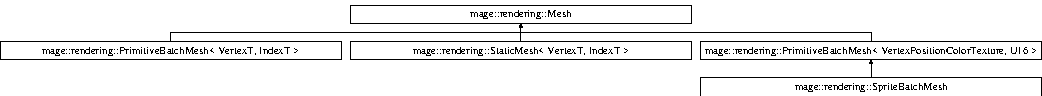
\includegraphics[height=1.281464cm]{classmage_1_1rendering_1_1_mesh}
\end{center}
\end{figure}
\subsection*{Public Member Functions}
\begin{DoxyCompactItemize}
\item 
virtual \mbox{\hyperlink{classmage_1_1rendering_1_1_mesh_a3f0a53becc293987d7ecf9ca34a230d8}{$\sim$\+Mesh}} ()
\item 
\mbox{\hyperlink{classmage_1_1rendering_1_1_mesh}{Mesh}} \& \mbox{\hyperlink{classmage_1_1rendering_1_1_mesh_a17f6dd40e8eea41b469b475de93ee466}{operator=}} (const \mbox{\hyperlink{classmage_1_1rendering_1_1_mesh}{Mesh}} \&mesh)=delete
\item 
\mbox{\hyperlink{classmage_1_1rendering_1_1_mesh}{Mesh}} \& \mbox{\hyperlink{classmage_1_1rendering_1_1_mesh_ae5bcea1df4c9562bfe30cd247552fe1c}{operator=}} (\mbox{\hyperlink{classmage_1_1rendering_1_1_mesh}{Mesh}} \&\&mesh) noexcept
\item 
size\+\_\+t \mbox{\hyperlink{classmage_1_1rendering_1_1_mesh_a2c594e3c3b8e09bc20b35845ab46b6f3}{Get\+Number\+Of\+Vertices}} () const noexcept
\item 
size\+\_\+t \mbox{\hyperlink{classmage_1_1rendering_1_1_mesh_aaf8574345279790ca88d8acc5c2c85b6}{Get\+Number\+Of\+Indices}} () const noexcept
\item 
size\+\_\+t \mbox{\hyperlink{classmage_1_1rendering_1_1_mesh_a0fcc1a72aa5426ce9b020b580eb22a43}{Get\+Vertex\+Size}} () const noexcept
\item 
D\+X\+G\+I\+\_\+\+F\+O\+R\+M\+AT \mbox{\hyperlink{classmage_1_1rendering_1_1_mesh_a47540e1d5ec5d278862a3d0c0c5db1df}{Get\+Index\+Format}} () const noexcept
\item 
D3\+D11\+\_\+\+P\+R\+I\+M\+I\+T\+I\+V\+E\+\_\+\+T\+O\+P\+O\+L\+O\+GY \mbox{\hyperlink{classmage_1_1rendering_1_1_mesh_af6cead725f7e5352a90a8f8847580f75}{Get\+Primitive\+Topology}} () const noexcept
\item 
void \mbox{\hyperlink{classmage_1_1rendering_1_1_mesh_a36999cc548e68c3ad0c8d348ad0ead4f}{Bind\+Mesh}} (I\+D3\+D11\+Device\+Context \&device\+\_\+context) const noexcept
\item 
void \mbox{\hyperlink{classmage_1_1rendering_1_1_mesh_a35fe2a8fd609c204c70668e3a0a68331}{Bind\+Mesh}} (I\+D3\+D11\+Device\+Context \&device\+\_\+context, D3\+D11\+\_\+\+P\+R\+I\+M\+I\+T\+I\+V\+E\+\_\+\+T\+O\+P\+O\+L\+O\+GY topology) const noexcept
\item 
void \mbox{\hyperlink{classmage_1_1rendering_1_1_mesh_a4a29089e1894662029be09eafe32255b}{Draw}} (I\+D3\+D11\+Device\+Context \&device\+\_\+context) const noexcept
\item 
void \mbox{\hyperlink{classmage_1_1rendering_1_1_mesh_afc0c89379a7fe1040cf069105ee3520c}{Draw}} (I\+D3\+D11\+Device\+Context \&device\+\_\+context, size\+\_\+t start\+\_\+index, size\+\_\+t nb\+\_\+indices) const noexcept
\end{DoxyCompactItemize}
\subsection*{Protected Member Functions}
\begin{DoxyCompactItemize}
\item 
\mbox{\hyperlink{classmage_1_1rendering_1_1_mesh_a3113bd0dd48a82ae03e0a07d971494da}{Mesh}} (size\+\_\+t vertex\+\_\+size, D\+X\+G\+I\+\_\+\+F\+O\+R\+M\+AT index\+\_\+format, D3\+D11\+\_\+\+P\+R\+I\+M\+I\+T\+I\+V\+E\+\_\+\+T\+O\+P\+O\+L\+O\+GY primitive\+\_\+topology)
\item 
\mbox{\hyperlink{classmage_1_1rendering_1_1_mesh_a42e4cab2db663fa8d7f2c8651f30894b}{Mesh}} (const \mbox{\hyperlink{classmage_1_1rendering_1_1_mesh}{Mesh}} \&mesh)=delete
\item 
\mbox{\hyperlink{classmage_1_1rendering_1_1_mesh_aeb090ec9531823157f010a70a9dabf45}{Mesh}} (\mbox{\hyperlink{classmage_1_1rendering_1_1_mesh}{Mesh}} \&\&mesh) noexcept
\item 
void \mbox{\hyperlink{classmage_1_1rendering_1_1_mesh_abf2fc84400607b6579028eff66eb179e}{Set\+Number\+Of\+Vertices}} (size\+\_\+t nb\+\_\+vertices) noexcept
\item 
void \mbox{\hyperlink{classmage_1_1rendering_1_1_mesh_acd34fa8466235d5e17dd0f9be60fd5ea}{Set\+Number\+Of\+Indices}} (size\+\_\+t nb\+\_\+indices) noexcept
\end{DoxyCompactItemize}
\subsection*{Protected Attributes}
\begin{DoxyCompactItemize}
\item 
\mbox{\hyperlink{namespacemage_ae74f374780900893caa5555d1031fd79}{Com\+Ptr}}$<$ I\+D3\+D11\+Buffer $>$ \mbox{\hyperlink{classmage_1_1rendering_1_1_mesh_aa3cf2b0ad192e2b3b371655ee49eb4f4}{m\+\_\+vertex\+\_\+buffer}}
\item 
\mbox{\hyperlink{namespacemage_ae74f374780900893caa5555d1031fd79}{Com\+Ptr}}$<$ I\+D3\+D11\+Buffer $>$ \mbox{\hyperlink{classmage_1_1rendering_1_1_mesh_a113b12e839a22e62cb45991805586689}{m\+\_\+index\+\_\+buffer}}
\end{DoxyCompactItemize}
\subsection*{Private Attributes}
\begin{DoxyCompactItemize}
\item 
size\+\_\+t \mbox{\hyperlink{classmage_1_1rendering_1_1_mesh_a877873f0736375cdaa2d26066d7aa2ae}{m\+\_\+nb\+\_\+vertices}}
\item 
size\+\_\+t \mbox{\hyperlink{classmage_1_1rendering_1_1_mesh_a103e49bac28a4551816ec453e7261213}{m\+\_\+nb\+\_\+indices}}
\item 
size\+\_\+t \mbox{\hyperlink{classmage_1_1rendering_1_1_mesh_a52a754eeef69dfa642dc483025f7bb21}{m\+\_\+vertex\+\_\+size}}
\item 
D\+X\+G\+I\+\_\+\+F\+O\+R\+M\+AT \mbox{\hyperlink{classmage_1_1rendering_1_1_mesh_a3de0213af57c9d423399ad22fd6ae7c0}{m\+\_\+index\+\_\+format}}
\item 
D3\+D11\+\_\+\+P\+R\+I\+M\+I\+T\+I\+V\+E\+\_\+\+T\+O\+P\+O\+L\+O\+GY \mbox{\hyperlink{classmage_1_1rendering_1_1_mesh_a9ae7ea29fac3acb3fe17317c21242ee9}{m\+\_\+primitive\+\_\+topology}}
\end{DoxyCompactItemize}


\subsection{Detailed Description}
A class of indexed meshes. 

\subsection{Constructor \& Destructor Documentation}
\mbox{\Hypertarget{classmage_1_1rendering_1_1_mesh_a3f0a53becc293987d7ecf9ca34a230d8}\label{classmage_1_1rendering_1_1_mesh_a3f0a53becc293987d7ecf9ca34a230d8}} 
\index{mage\+::rendering\+::\+Mesh@{mage\+::rendering\+::\+Mesh}!````~Mesh@{$\sim$\+Mesh}}
\index{````~Mesh@{$\sim$\+Mesh}!mage\+::rendering\+::\+Mesh@{mage\+::rendering\+::\+Mesh}}
\subsubsection{\texorpdfstring{$\sim$\+Mesh()}{~Mesh()}}
{\footnotesize\ttfamily mage\+::rendering\+::\+Mesh\+::$\sim$\+Mesh (\begin{DoxyParamCaption}{ }\end{DoxyParamCaption})\hspace{0.3cm}{\ttfamily [virtual]}, {\ttfamily [default]}}

Destructs this mesh. \mbox{\Hypertarget{classmage_1_1rendering_1_1_mesh_a3113bd0dd48a82ae03e0a07d971494da}\label{classmage_1_1rendering_1_1_mesh_a3113bd0dd48a82ae03e0a07d971494da}} 
\index{mage\+::rendering\+::\+Mesh@{mage\+::rendering\+::\+Mesh}!Mesh@{Mesh}}
\index{Mesh@{Mesh}!mage\+::rendering\+::\+Mesh@{mage\+::rendering\+::\+Mesh}}
\subsubsection{\texorpdfstring{Mesh()}{Mesh()}\hspace{0.1cm}{\footnotesize\ttfamily [1/3]}}
{\footnotesize\ttfamily mage\+::rendering\+::\+Mesh\+::\+Mesh (\begin{DoxyParamCaption}\item[{size\+\_\+t}]{vertex\+\_\+size,  }\item[{D\+X\+G\+I\+\_\+\+F\+O\+R\+M\+AT}]{index\+\_\+format,  }\item[{D3\+D11\+\_\+\+P\+R\+I\+M\+I\+T\+I\+V\+E\+\_\+\+T\+O\+P\+O\+L\+O\+GY}]{primitive\+\_\+topology }\end{DoxyParamCaption})\hspace{0.3cm}{\ttfamily [explicit]}, {\ttfamily [protected]}}

Constructs a mesh.


\begin{DoxyParams}[1]{Parameters}
\mbox{\tt in}  & {\em vertex\+\_\+size} & The vertex size. \\
\hline
\mbox{\tt in}  & {\em index\+\_\+format} & The index format. \\
\hline
\mbox{\tt in}  & {\em primitive\+\_\+topology} & The primitive topology. \\
\hline
\end{DoxyParams}
\mbox{\Hypertarget{classmage_1_1rendering_1_1_mesh_a42e4cab2db663fa8d7f2c8651f30894b}\label{classmage_1_1rendering_1_1_mesh_a42e4cab2db663fa8d7f2c8651f30894b}} 
\index{mage\+::rendering\+::\+Mesh@{mage\+::rendering\+::\+Mesh}!Mesh@{Mesh}}
\index{Mesh@{Mesh}!mage\+::rendering\+::\+Mesh@{mage\+::rendering\+::\+Mesh}}
\subsubsection{\texorpdfstring{Mesh()}{Mesh()}\hspace{0.1cm}{\footnotesize\ttfamily [2/3]}}
{\footnotesize\ttfamily mage\+::rendering\+::\+Mesh\+::\+Mesh (\begin{DoxyParamCaption}\item[{const \mbox{\hyperlink{classmage_1_1rendering_1_1_mesh}{Mesh}} \&}]{mesh }\end{DoxyParamCaption})\hspace{0.3cm}{\ttfamily [protected]}, {\ttfamily [delete]}}

Constructs a mesh from the given mesh.


\begin{DoxyParams}[1]{Parameters}
\mbox{\tt in}  & {\em mesh} & A reference to the mesh to copy. \\
\hline
\end{DoxyParams}
\mbox{\Hypertarget{classmage_1_1rendering_1_1_mesh_aeb090ec9531823157f010a70a9dabf45}\label{classmage_1_1rendering_1_1_mesh_aeb090ec9531823157f010a70a9dabf45}} 
\index{mage\+::rendering\+::\+Mesh@{mage\+::rendering\+::\+Mesh}!Mesh@{Mesh}}
\index{Mesh@{Mesh}!mage\+::rendering\+::\+Mesh@{mage\+::rendering\+::\+Mesh}}
\subsubsection{\texorpdfstring{Mesh()}{Mesh()}\hspace{0.1cm}{\footnotesize\ttfamily [3/3]}}
{\footnotesize\ttfamily mage\+::rendering\+::\+Mesh\+::\+Mesh (\begin{DoxyParamCaption}\item[{\mbox{\hyperlink{classmage_1_1rendering_1_1_mesh}{Mesh}} \&\&}]{mesh }\end{DoxyParamCaption})\hspace{0.3cm}{\ttfamily [protected]}, {\ttfamily [default]}, {\ttfamily [noexcept]}}

Constructs a mesh by moving the given mesh.


\begin{DoxyParams}[1]{Parameters}
\mbox{\tt in}  & {\em mesh} & A reference to the mesh to move. \\
\hline
\end{DoxyParams}


\subsection{Member Function Documentation}
\mbox{\Hypertarget{classmage_1_1rendering_1_1_mesh_a36999cc548e68c3ad0c8d348ad0ead4f}\label{classmage_1_1rendering_1_1_mesh_a36999cc548e68c3ad0c8d348ad0ead4f}} 
\index{mage\+::rendering\+::\+Mesh@{mage\+::rendering\+::\+Mesh}!Bind\+Mesh@{Bind\+Mesh}}
\index{Bind\+Mesh@{Bind\+Mesh}!mage\+::rendering\+::\+Mesh@{mage\+::rendering\+::\+Mesh}}
\subsubsection{\texorpdfstring{Bind\+Mesh()}{BindMesh()}\hspace{0.1cm}{\footnotesize\ttfamily [1/2]}}
{\footnotesize\ttfamily void mage\+::rendering\+::\+Mesh\+::\+Bind\+Mesh (\begin{DoxyParamCaption}\item[{I\+D3\+D11\+Device\+Context \&}]{device\+\_\+context }\end{DoxyParamCaption}) const\hspace{0.3cm}{\ttfamily [noexcept]}}

Binds this mesh.

The vertex buffer, index buffer and primitive topology of this mesh will be bound to the input-\/assembler stage.


\begin{DoxyParams}[1]{Parameters}
\mbox{\tt in}  & {\em device\+\_\+context} & A reference to the device context. \\
\hline
\end{DoxyParams}
\mbox{\Hypertarget{classmage_1_1rendering_1_1_mesh_a35fe2a8fd609c204c70668e3a0a68331}\label{classmage_1_1rendering_1_1_mesh_a35fe2a8fd609c204c70668e3a0a68331}} 
\index{mage\+::rendering\+::\+Mesh@{mage\+::rendering\+::\+Mesh}!Bind\+Mesh@{Bind\+Mesh}}
\index{Bind\+Mesh@{Bind\+Mesh}!mage\+::rendering\+::\+Mesh@{mage\+::rendering\+::\+Mesh}}
\subsubsection{\texorpdfstring{Bind\+Mesh()}{BindMesh()}\hspace{0.1cm}{\footnotesize\ttfamily [2/2]}}
{\footnotesize\ttfamily void mage\+::rendering\+::\+Mesh\+::\+Bind\+Mesh (\begin{DoxyParamCaption}\item[{I\+D3\+D11\+Device\+Context \&}]{device\+\_\+context,  }\item[{D3\+D11\+\_\+\+P\+R\+I\+M\+I\+T\+I\+V\+E\+\_\+\+T\+O\+P\+O\+L\+O\+GY}]{topology }\end{DoxyParamCaption}) const\hspace{0.3cm}{\ttfamily [noexcept]}}

Binds this mesh with given primitive topology.

The vertex buffer, index buffer and given primitive topology of this mesh will be bound to the input-\/assembler stage.


\begin{DoxyParams}[1]{Parameters}
\mbox{\tt in}  & {\em device\+\_\+context} & A reference to the device context. \\
\hline
\mbox{\tt in}  & {\em topology} & The primitive topology. \\
\hline
\end{DoxyParams}
\mbox{\Hypertarget{classmage_1_1rendering_1_1_mesh_a4a29089e1894662029be09eafe32255b}\label{classmage_1_1rendering_1_1_mesh_a4a29089e1894662029be09eafe32255b}} 
\index{mage\+::rendering\+::\+Mesh@{mage\+::rendering\+::\+Mesh}!Draw@{Draw}}
\index{Draw@{Draw}!mage\+::rendering\+::\+Mesh@{mage\+::rendering\+::\+Mesh}}
\subsubsection{\texorpdfstring{Draw()}{Draw()}\hspace{0.1cm}{\footnotesize\ttfamily [1/2]}}
{\footnotesize\ttfamily void mage\+::rendering\+::\+Mesh\+::\+Draw (\begin{DoxyParamCaption}\item[{I\+D3\+D11\+Device\+Context \&}]{device\+\_\+context }\end{DoxyParamCaption}) const\hspace{0.3cm}{\ttfamily [noexcept]}}

Draws this complete mesh.


\begin{DoxyParams}[1]{Parameters}
\mbox{\tt in}  & {\em device\+\_\+context} & A reference to the device context. \\
\hline
\end{DoxyParams}
\mbox{\Hypertarget{classmage_1_1rendering_1_1_mesh_afc0c89379a7fe1040cf069105ee3520c}\label{classmage_1_1rendering_1_1_mesh_afc0c89379a7fe1040cf069105ee3520c}} 
\index{mage\+::rendering\+::\+Mesh@{mage\+::rendering\+::\+Mesh}!Draw@{Draw}}
\index{Draw@{Draw}!mage\+::rendering\+::\+Mesh@{mage\+::rendering\+::\+Mesh}}
\subsubsection{\texorpdfstring{Draw()}{Draw()}\hspace{0.1cm}{\footnotesize\ttfamily [2/2]}}
{\footnotesize\ttfamily void mage\+::rendering\+::\+Mesh\+::\+Draw (\begin{DoxyParamCaption}\item[{I\+D3\+D11\+Device\+Context \&}]{device\+\_\+context,  }\item[{size\+\_\+t}]{start\+\_\+index,  }\item[{size\+\_\+t}]{nb\+\_\+indices }\end{DoxyParamCaption}) const\hspace{0.3cm}{\ttfamily [noexcept]}}

Draws a submesh of this mesh.


\begin{DoxyParams}[1]{Parameters}
\mbox{\tt in}  & {\em device\+\_\+context} & A reference to the device context. \\
\hline
\mbox{\tt in}  & {\em start\+\_\+index} & The start index. \\
\hline
\mbox{\tt in}  & {\em nb\+\_\+indices} & The number of indices. \\
\hline
\end{DoxyParams}
\mbox{\Hypertarget{classmage_1_1rendering_1_1_mesh_a47540e1d5ec5d278862a3d0c0c5db1df}\label{classmage_1_1rendering_1_1_mesh_a47540e1d5ec5d278862a3d0c0c5db1df}} 
\index{mage\+::rendering\+::\+Mesh@{mage\+::rendering\+::\+Mesh}!Get\+Index\+Format@{Get\+Index\+Format}}
\index{Get\+Index\+Format@{Get\+Index\+Format}!mage\+::rendering\+::\+Mesh@{mage\+::rendering\+::\+Mesh}}
\subsubsection{\texorpdfstring{Get\+Index\+Format()}{GetIndexFormat()}}
{\footnotesize\ttfamily D\+X\+G\+I\+\_\+\+F\+O\+R\+M\+AT mage\+::rendering\+::\+Mesh\+::\+Get\+Index\+Format (\begin{DoxyParamCaption}{ }\end{DoxyParamCaption}) const\hspace{0.3cm}{\ttfamily [noexcept]}}

Returns the index format of this mesh.

\begin{DoxyReturn}{Returns}
The index format of this mesh. 
\end{DoxyReturn}
\mbox{\Hypertarget{classmage_1_1rendering_1_1_mesh_aaf8574345279790ca88d8acc5c2c85b6}\label{classmage_1_1rendering_1_1_mesh_aaf8574345279790ca88d8acc5c2c85b6}} 
\index{mage\+::rendering\+::\+Mesh@{mage\+::rendering\+::\+Mesh}!Get\+Number\+Of\+Indices@{Get\+Number\+Of\+Indices}}
\index{Get\+Number\+Of\+Indices@{Get\+Number\+Of\+Indices}!mage\+::rendering\+::\+Mesh@{mage\+::rendering\+::\+Mesh}}
\subsubsection{\texorpdfstring{Get\+Number\+Of\+Indices()}{GetNumberOfIndices()}}
{\footnotesize\ttfamily size\+\_\+t mage\+::rendering\+::\+Mesh\+::\+Get\+Number\+Of\+Indices (\begin{DoxyParamCaption}{ }\end{DoxyParamCaption}) const\hspace{0.3cm}{\ttfamily [noexcept]}}

Returns the number of indices of this mesh.

\begin{DoxyReturn}{Returns}
The number of indices of this mesh. 
\end{DoxyReturn}
\mbox{\Hypertarget{classmage_1_1rendering_1_1_mesh_a2c594e3c3b8e09bc20b35845ab46b6f3}\label{classmage_1_1rendering_1_1_mesh_a2c594e3c3b8e09bc20b35845ab46b6f3}} 
\index{mage\+::rendering\+::\+Mesh@{mage\+::rendering\+::\+Mesh}!Get\+Number\+Of\+Vertices@{Get\+Number\+Of\+Vertices}}
\index{Get\+Number\+Of\+Vertices@{Get\+Number\+Of\+Vertices}!mage\+::rendering\+::\+Mesh@{mage\+::rendering\+::\+Mesh}}
\subsubsection{\texorpdfstring{Get\+Number\+Of\+Vertices()}{GetNumberOfVertices()}}
{\footnotesize\ttfamily size\+\_\+t mage\+::rendering\+::\+Mesh\+::\+Get\+Number\+Of\+Vertices (\begin{DoxyParamCaption}{ }\end{DoxyParamCaption}) const\hspace{0.3cm}{\ttfamily [noexcept]}}

Returns the number of vertices of this mesh.

\begin{DoxyReturn}{Returns}
The number of vertices of this mesh. 
\end{DoxyReturn}
\mbox{\Hypertarget{classmage_1_1rendering_1_1_mesh_af6cead725f7e5352a90a8f8847580f75}\label{classmage_1_1rendering_1_1_mesh_af6cead725f7e5352a90a8f8847580f75}} 
\index{mage\+::rendering\+::\+Mesh@{mage\+::rendering\+::\+Mesh}!Get\+Primitive\+Topology@{Get\+Primitive\+Topology}}
\index{Get\+Primitive\+Topology@{Get\+Primitive\+Topology}!mage\+::rendering\+::\+Mesh@{mage\+::rendering\+::\+Mesh}}
\subsubsection{\texorpdfstring{Get\+Primitive\+Topology()}{GetPrimitiveTopology()}}
{\footnotesize\ttfamily D3\+D11\+\_\+\+P\+R\+I\+M\+I\+T\+I\+V\+E\+\_\+\+T\+O\+P\+O\+L\+O\+GY mage\+::rendering\+::\+Mesh\+::\+Get\+Primitive\+Topology (\begin{DoxyParamCaption}{ }\end{DoxyParamCaption}) const\hspace{0.3cm}{\ttfamily [noexcept]}}

Returns the primitive topology of this mesh.

\begin{DoxyReturn}{Returns}
The primitive topology of this mesh. 
\end{DoxyReturn}
\mbox{\Hypertarget{classmage_1_1rendering_1_1_mesh_a0fcc1a72aa5426ce9b020b580eb22a43}\label{classmage_1_1rendering_1_1_mesh_a0fcc1a72aa5426ce9b020b580eb22a43}} 
\index{mage\+::rendering\+::\+Mesh@{mage\+::rendering\+::\+Mesh}!Get\+Vertex\+Size@{Get\+Vertex\+Size}}
\index{Get\+Vertex\+Size@{Get\+Vertex\+Size}!mage\+::rendering\+::\+Mesh@{mage\+::rendering\+::\+Mesh}}
\subsubsection{\texorpdfstring{Get\+Vertex\+Size()}{GetVertexSize()}}
{\footnotesize\ttfamily size\+\_\+t mage\+::rendering\+::\+Mesh\+::\+Get\+Vertex\+Size (\begin{DoxyParamCaption}{ }\end{DoxyParamCaption}) const\hspace{0.3cm}{\ttfamily [noexcept]}}

Returns the size (in bytes) of the vertices of this mesh.

\begin{DoxyReturn}{Returns}
The vertex size (in bytes) of this mesh. 
\end{DoxyReturn}
\mbox{\Hypertarget{classmage_1_1rendering_1_1_mesh_a17f6dd40e8eea41b469b475de93ee466}\label{classmage_1_1rendering_1_1_mesh_a17f6dd40e8eea41b469b475de93ee466}} 
\index{mage\+::rendering\+::\+Mesh@{mage\+::rendering\+::\+Mesh}!operator=@{operator=}}
\index{operator=@{operator=}!mage\+::rendering\+::\+Mesh@{mage\+::rendering\+::\+Mesh}}
\subsubsection{\texorpdfstring{operator=()}{operator=()}\hspace{0.1cm}{\footnotesize\ttfamily [1/2]}}
{\footnotesize\ttfamily \mbox{\hyperlink{classmage_1_1rendering_1_1_mesh}{Mesh}}\& mage\+::rendering\+::\+Mesh\+::operator= (\begin{DoxyParamCaption}\item[{const \mbox{\hyperlink{classmage_1_1rendering_1_1_mesh}{Mesh}} \&}]{mesh }\end{DoxyParamCaption})\hspace{0.3cm}{\ttfamily [delete]}}

Copies the given mesh to this mesh.


\begin{DoxyParams}[1]{Parameters}
\mbox{\tt in}  & {\em mesh} & A reference to the mesh to copy. \\
\hline
\end{DoxyParams}
\begin{DoxyReturn}{Returns}
A reference to the copy of the given mesh (i.\+e. this mesh). 
\end{DoxyReturn}
\mbox{\Hypertarget{classmage_1_1rendering_1_1_mesh_ae5bcea1df4c9562bfe30cd247552fe1c}\label{classmage_1_1rendering_1_1_mesh_ae5bcea1df4c9562bfe30cd247552fe1c}} 
\index{mage\+::rendering\+::\+Mesh@{mage\+::rendering\+::\+Mesh}!operator=@{operator=}}
\index{operator=@{operator=}!mage\+::rendering\+::\+Mesh@{mage\+::rendering\+::\+Mesh}}
\subsubsection{\texorpdfstring{operator=()}{operator=()}\hspace{0.1cm}{\footnotesize\ttfamily [2/2]}}
{\footnotesize\ttfamily \mbox{\hyperlink{classmage_1_1rendering_1_1_mesh}{Mesh}} \& mage\+::rendering\+::\+Mesh\+::operator= (\begin{DoxyParamCaption}\item[{\mbox{\hyperlink{classmage_1_1rendering_1_1_mesh}{Mesh}} \&\&}]{mesh }\end{DoxyParamCaption})\hspace{0.3cm}{\ttfamily [default]}, {\ttfamily [noexcept]}}

Moves the given mesh to this mesh.


\begin{DoxyParams}[1]{Parameters}
\mbox{\tt in}  & {\em mesh} & A reference to the mesh to move. \\
\hline
\end{DoxyParams}
\begin{DoxyReturn}{Returns}
A reference to the moved mesh (i.\+e. this mesh). 
\end{DoxyReturn}
\mbox{\Hypertarget{classmage_1_1rendering_1_1_mesh_acd34fa8466235d5e17dd0f9be60fd5ea}\label{classmage_1_1rendering_1_1_mesh_acd34fa8466235d5e17dd0f9be60fd5ea}} 
\index{mage\+::rendering\+::\+Mesh@{mage\+::rendering\+::\+Mesh}!Set\+Number\+Of\+Indices@{Set\+Number\+Of\+Indices}}
\index{Set\+Number\+Of\+Indices@{Set\+Number\+Of\+Indices}!mage\+::rendering\+::\+Mesh@{mage\+::rendering\+::\+Mesh}}
\subsubsection{\texorpdfstring{Set\+Number\+Of\+Indices()}{SetNumberOfIndices()}}
{\footnotesize\ttfamily void mage\+::rendering\+::\+Mesh\+::\+Set\+Number\+Of\+Indices (\begin{DoxyParamCaption}\item[{size\+\_\+t}]{nb\+\_\+indices }\end{DoxyParamCaption})\hspace{0.3cm}{\ttfamily [protected]}, {\ttfamily [noexcept]}}

Sets the number of indices of this mesh to the given number.


\begin{DoxyParams}[1]{Parameters}
\mbox{\tt in}  & {\em nb\+\_\+indices} & The number of indices of this mesh. \\
\hline
\end{DoxyParams}
\mbox{\Hypertarget{classmage_1_1rendering_1_1_mesh_abf2fc84400607b6579028eff66eb179e}\label{classmage_1_1rendering_1_1_mesh_abf2fc84400607b6579028eff66eb179e}} 
\index{mage\+::rendering\+::\+Mesh@{mage\+::rendering\+::\+Mesh}!Set\+Number\+Of\+Vertices@{Set\+Number\+Of\+Vertices}}
\index{Set\+Number\+Of\+Vertices@{Set\+Number\+Of\+Vertices}!mage\+::rendering\+::\+Mesh@{mage\+::rendering\+::\+Mesh}}
\subsubsection{\texorpdfstring{Set\+Number\+Of\+Vertices()}{SetNumberOfVertices()}}
{\footnotesize\ttfamily void mage\+::rendering\+::\+Mesh\+::\+Set\+Number\+Of\+Vertices (\begin{DoxyParamCaption}\item[{size\+\_\+t}]{nb\+\_\+vertices }\end{DoxyParamCaption})\hspace{0.3cm}{\ttfamily [protected]}, {\ttfamily [noexcept]}}

Sets the number of vertices of this mesh to the given number.


\begin{DoxyParams}[1]{Parameters}
\mbox{\tt in}  & {\em nb\+\_\+vertices} & The number of vertices of this mesh. \\
\hline
\end{DoxyParams}


\subsection{Member Data Documentation}
\mbox{\Hypertarget{classmage_1_1rendering_1_1_mesh_a113b12e839a22e62cb45991805586689}\label{classmage_1_1rendering_1_1_mesh_a113b12e839a22e62cb45991805586689}} 
\index{mage\+::rendering\+::\+Mesh@{mage\+::rendering\+::\+Mesh}!m\+\_\+index\+\_\+buffer@{m\+\_\+index\+\_\+buffer}}
\index{m\+\_\+index\+\_\+buffer@{m\+\_\+index\+\_\+buffer}!mage\+::rendering\+::\+Mesh@{mage\+::rendering\+::\+Mesh}}
\subsubsection{\texorpdfstring{m\+\_\+index\+\_\+buffer}{m\_index\_buffer}}
{\footnotesize\ttfamily \mbox{\hyperlink{namespacemage_ae74f374780900893caa5555d1031fd79}{Com\+Ptr}}$<$ I\+D3\+D11\+Buffer $>$ mage\+::rendering\+::\+Mesh\+::m\+\_\+index\+\_\+buffer\hspace{0.3cm}{\ttfamily [protected]}}

A pointer to the index buffer of this mesh. \mbox{\Hypertarget{classmage_1_1rendering_1_1_mesh_a3de0213af57c9d423399ad22fd6ae7c0}\label{classmage_1_1rendering_1_1_mesh_a3de0213af57c9d423399ad22fd6ae7c0}} 
\index{mage\+::rendering\+::\+Mesh@{mage\+::rendering\+::\+Mesh}!m\+\_\+index\+\_\+format@{m\+\_\+index\+\_\+format}}
\index{m\+\_\+index\+\_\+format@{m\+\_\+index\+\_\+format}!mage\+::rendering\+::\+Mesh@{mage\+::rendering\+::\+Mesh}}
\subsubsection{\texorpdfstring{m\+\_\+index\+\_\+format}{m\_index\_format}}
{\footnotesize\ttfamily D\+X\+G\+I\+\_\+\+F\+O\+R\+M\+AT mage\+::rendering\+::\+Mesh\+::m\+\_\+index\+\_\+format\hspace{0.3cm}{\ttfamily [private]}}

The index format of this mesh. \mbox{\Hypertarget{classmage_1_1rendering_1_1_mesh_a103e49bac28a4551816ec453e7261213}\label{classmage_1_1rendering_1_1_mesh_a103e49bac28a4551816ec453e7261213}} 
\index{mage\+::rendering\+::\+Mesh@{mage\+::rendering\+::\+Mesh}!m\+\_\+nb\+\_\+indices@{m\+\_\+nb\+\_\+indices}}
\index{m\+\_\+nb\+\_\+indices@{m\+\_\+nb\+\_\+indices}!mage\+::rendering\+::\+Mesh@{mage\+::rendering\+::\+Mesh}}
\subsubsection{\texorpdfstring{m\+\_\+nb\+\_\+indices}{m\_nb\_indices}}
{\footnotesize\ttfamily size\+\_\+t mage\+::rendering\+::\+Mesh\+::m\+\_\+nb\+\_\+indices\hspace{0.3cm}{\ttfamily [private]}}

The number of indices of this mesh. \mbox{\Hypertarget{classmage_1_1rendering_1_1_mesh_a877873f0736375cdaa2d26066d7aa2ae}\label{classmage_1_1rendering_1_1_mesh_a877873f0736375cdaa2d26066d7aa2ae}} 
\index{mage\+::rendering\+::\+Mesh@{mage\+::rendering\+::\+Mesh}!m\+\_\+nb\+\_\+vertices@{m\+\_\+nb\+\_\+vertices}}
\index{m\+\_\+nb\+\_\+vertices@{m\+\_\+nb\+\_\+vertices}!mage\+::rendering\+::\+Mesh@{mage\+::rendering\+::\+Mesh}}
\subsubsection{\texorpdfstring{m\+\_\+nb\+\_\+vertices}{m\_nb\_vertices}}
{\footnotesize\ttfamily size\+\_\+t mage\+::rendering\+::\+Mesh\+::m\+\_\+nb\+\_\+vertices\hspace{0.3cm}{\ttfamily [private]}}

The number of vertices of this mesh. \mbox{\Hypertarget{classmage_1_1rendering_1_1_mesh_a9ae7ea29fac3acb3fe17317c21242ee9}\label{classmage_1_1rendering_1_1_mesh_a9ae7ea29fac3acb3fe17317c21242ee9}} 
\index{mage\+::rendering\+::\+Mesh@{mage\+::rendering\+::\+Mesh}!m\+\_\+primitive\+\_\+topology@{m\+\_\+primitive\+\_\+topology}}
\index{m\+\_\+primitive\+\_\+topology@{m\+\_\+primitive\+\_\+topology}!mage\+::rendering\+::\+Mesh@{mage\+::rendering\+::\+Mesh}}
\subsubsection{\texorpdfstring{m\+\_\+primitive\+\_\+topology}{m\_primitive\_topology}}
{\footnotesize\ttfamily D3\+D11\+\_\+\+P\+R\+I\+M\+I\+T\+I\+V\+E\+\_\+\+T\+O\+P\+O\+L\+O\+GY mage\+::rendering\+::\+Mesh\+::m\+\_\+primitive\+\_\+topology\hspace{0.3cm}{\ttfamily [private]}}

The primitive topology of this mesh. \mbox{\Hypertarget{classmage_1_1rendering_1_1_mesh_aa3cf2b0ad192e2b3b371655ee49eb4f4}\label{classmage_1_1rendering_1_1_mesh_aa3cf2b0ad192e2b3b371655ee49eb4f4}} 
\index{mage\+::rendering\+::\+Mesh@{mage\+::rendering\+::\+Mesh}!m\+\_\+vertex\+\_\+buffer@{m\+\_\+vertex\+\_\+buffer}}
\index{m\+\_\+vertex\+\_\+buffer@{m\+\_\+vertex\+\_\+buffer}!mage\+::rendering\+::\+Mesh@{mage\+::rendering\+::\+Mesh}}
\subsubsection{\texorpdfstring{m\+\_\+vertex\+\_\+buffer}{m\_vertex\_buffer}}
{\footnotesize\ttfamily \mbox{\hyperlink{namespacemage_ae74f374780900893caa5555d1031fd79}{Com\+Ptr}}$<$ I\+D3\+D11\+Buffer $>$ mage\+::rendering\+::\+Mesh\+::m\+\_\+vertex\+\_\+buffer\hspace{0.3cm}{\ttfamily [protected]}}

A pointer to the vertex buffer of this mesh. \mbox{\Hypertarget{classmage_1_1rendering_1_1_mesh_a52a754eeef69dfa642dc483025f7bb21}\label{classmage_1_1rendering_1_1_mesh_a52a754eeef69dfa642dc483025f7bb21}} 
\index{mage\+::rendering\+::\+Mesh@{mage\+::rendering\+::\+Mesh}!m\+\_\+vertex\+\_\+size@{m\+\_\+vertex\+\_\+size}}
\index{m\+\_\+vertex\+\_\+size@{m\+\_\+vertex\+\_\+size}!mage\+::rendering\+::\+Mesh@{mage\+::rendering\+::\+Mesh}}
\subsubsection{\texorpdfstring{m\+\_\+vertex\+\_\+size}{m\_vertex\_size}}
{\footnotesize\ttfamily size\+\_\+t mage\+::rendering\+::\+Mesh\+::m\+\_\+vertex\+\_\+size\hspace{0.3cm}{\ttfamily [private]}}

The vertex size of this mesh. 
\hypertarget{classmage_1_1rendering_1_1_mesh_descriptor}{}\section{mage\+:\+:rendering\+:\+:Mesh\+Descriptor$<$ VertexT, IndexT $>$ Class Template Reference}
\label{classmage_1_1rendering_1_1_mesh_descriptor}\index{mage\+::rendering\+::\+Mesh\+Descriptor$<$ Vertex\+T, Index\+T $>$@{mage\+::rendering\+::\+Mesh\+Descriptor$<$ Vertex\+T, Index\+T $>$}}


{\ttfamily \#include $<$mesh\+\_\+descriptor.\+hpp$>$}

\subsection*{Public Member Functions}
\begin{DoxyCompactItemize}
\item 
constexpr \mbox{\hyperlink{classmage_1_1rendering_1_1_mesh_descriptor_a1b0ebe38d5591dda224370a7533f0c13}{Mesh\+Descriptor}} (bool invert\+\_\+handedness=false, bool clockwise\+\_\+order=true) noexcept
\item 
constexpr \mbox{\hyperlink{classmage_1_1rendering_1_1_mesh_descriptor_ad46be4da19cfa33f0731f371b7ebbe43}{Mesh\+Descriptor}} (const \mbox{\hyperlink{classmage_1_1rendering_1_1_mesh_descriptor}{Mesh\+Descriptor}} \&desc) noexcept=default
\item 
constexpr \mbox{\hyperlink{classmage_1_1rendering_1_1_mesh_descriptor_a929e3b4b29e421f921e5d17d0a382275}{Mesh\+Descriptor}} (\mbox{\hyperlink{classmage_1_1rendering_1_1_mesh_descriptor}{Mesh\+Descriptor}} \&\&desc) noexcept=default
\item 
\mbox{\hyperlink{classmage_1_1rendering_1_1_mesh_descriptor_a0948d279801d1b4eb7eb5dca8b0f86ea}{$\sim$\+Mesh\+Descriptor}} ()=default
\item 
\mbox{\hyperlink{classmage_1_1rendering_1_1_mesh_descriptor}{Mesh\+Descriptor}} \& \mbox{\hyperlink{classmage_1_1rendering_1_1_mesh_descriptor_a5181764e459caf5356c6d4b4b5268c1d}{operator=}} (const \mbox{\hyperlink{classmage_1_1rendering_1_1_mesh_descriptor}{Mesh\+Descriptor}} \&desc) noexcept=default
\item 
\mbox{\hyperlink{classmage_1_1rendering_1_1_mesh_descriptor}{Mesh\+Descriptor}} \& \mbox{\hyperlink{classmage_1_1rendering_1_1_mesh_descriptor_aa6094035cdaff6213b7156cead0c0381}{operator=}} (\mbox{\hyperlink{classmage_1_1rendering_1_1_mesh_descriptor}{Mesh\+Descriptor}} \&\&desc) noexcept=default
\item 
constexpr bool \mbox{\hyperlink{classmage_1_1rendering_1_1_mesh_descriptor_a0fa7557aa67c69a7978f965bdc913686}{Invert\+Handness}} () const noexcept
\item 
constexpr bool \mbox{\hyperlink{classmage_1_1rendering_1_1_mesh_descriptor_a71ea285cfb0bc3f748038de570e9084e}{Clockwise\+Order}} () const noexcept
\end{DoxyCompactItemize}
\subsection*{Private Attributes}
\begin{DoxyCompactItemize}
\item 
bool \mbox{\hyperlink{classmage_1_1rendering_1_1_mesh_descriptor_a61d5b541414f827f43ec835c7f2da462}{m\+\_\+invert\+\_\+handedness}}
\item 
bool \mbox{\hyperlink{classmage_1_1rendering_1_1_mesh_descriptor_a24ad440002ac7a4db6f0cb642ae1477d}{m\+\_\+clockwise\+\_\+order}}
\end{DoxyCompactItemize}


\subsection{Detailed Description}
\subsubsection*{template$<$typename VertexT, typename IndexT = U32$>$\newline
class mage\+::rendering\+::\+Mesh\+Descriptor$<$ Vertex\+T, Index\+T $>$}

A class of mesh descriptors.


\begin{DoxyTemplParams}{Template Parameters}
{\em VertexT} & The vertex type. \\
\hline
{\em IndexT} & The index type. \\
\hline
\end{DoxyTemplParams}


\subsection{Constructor \& Destructor Documentation}
\mbox{\Hypertarget{classmage_1_1rendering_1_1_mesh_descriptor_a1b0ebe38d5591dda224370a7533f0c13}\label{classmage_1_1rendering_1_1_mesh_descriptor_a1b0ebe38d5591dda224370a7533f0c13}} 
\index{mage\+::rendering\+::\+Mesh\+Descriptor@{mage\+::rendering\+::\+Mesh\+Descriptor}!Mesh\+Descriptor@{Mesh\+Descriptor}}
\index{Mesh\+Descriptor@{Mesh\+Descriptor}!mage\+::rendering\+::\+Mesh\+Descriptor@{mage\+::rendering\+::\+Mesh\+Descriptor}}
\subsubsection{\texorpdfstring{Mesh\+Descriptor()}{MeshDescriptor()}\hspace{0.1cm}{\footnotesize\ttfamily [1/3]}}
{\footnotesize\ttfamily template$<$typename VertexT , typename IndexT  = U32$>$ \\
constexpr \mbox{\hyperlink{classmage_1_1rendering_1_1_mesh_descriptor}{mage\+::rendering\+::\+Mesh\+Descriptor}}$<$ VertexT, IndexT $>$\+::\mbox{\hyperlink{classmage_1_1rendering_1_1_mesh_descriptor}{Mesh\+Descriptor}} (\begin{DoxyParamCaption}\item[{bool}]{invert\+\_\+handedness = {\ttfamily false},  }\item[{bool}]{clockwise\+\_\+order = {\ttfamily true} }\end{DoxyParamCaption})\hspace{0.3cm}{\ttfamily [explicit]}, {\ttfamily [noexcept]}}

Constructs a mesh descriptor.


\begin{DoxyParams}[1]{Parameters}
\mbox{\tt in}  & {\em invert\+\_\+handedness} & A flag indicating whether the mesh coordinate system handness should be inverted. \\
\hline
\mbox{\tt in}  & {\em clockwise\+\_\+order} & A flag indicating whether the face vertices should be defined in clockwise order or not (i.\+e. counterclockwise order). \\
\hline
\end{DoxyParams}
\mbox{\Hypertarget{classmage_1_1rendering_1_1_mesh_descriptor_ad46be4da19cfa33f0731f371b7ebbe43}\label{classmage_1_1rendering_1_1_mesh_descriptor_ad46be4da19cfa33f0731f371b7ebbe43}} 
\index{mage\+::rendering\+::\+Mesh\+Descriptor@{mage\+::rendering\+::\+Mesh\+Descriptor}!Mesh\+Descriptor@{Mesh\+Descriptor}}
\index{Mesh\+Descriptor@{Mesh\+Descriptor}!mage\+::rendering\+::\+Mesh\+Descriptor@{mage\+::rendering\+::\+Mesh\+Descriptor}}
\subsubsection{\texorpdfstring{Mesh\+Descriptor()}{MeshDescriptor()}\hspace{0.1cm}{\footnotesize\ttfamily [2/3]}}
{\footnotesize\ttfamily template$<$typename VertexT , typename IndexT  = U32$>$ \\
constexpr \mbox{\hyperlink{classmage_1_1rendering_1_1_mesh_descriptor}{mage\+::rendering\+::\+Mesh\+Descriptor}}$<$ VertexT, IndexT $>$\+::\mbox{\hyperlink{classmage_1_1rendering_1_1_mesh_descriptor}{Mesh\+Descriptor}} (\begin{DoxyParamCaption}\item[{const \mbox{\hyperlink{classmage_1_1rendering_1_1_mesh_descriptor}{Mesh\+Descriptor}}$<$ VertexT, IndexT $>$ \&}]{desc }\end{DoxyParamCaption})\hspace{0.3cm}{\ttfamily [default]}, {\ttfamily [noexcept]}}

Constructs a mesh descriptor from the given mesh descriptor.


\begin{DoxyParams}[1]{Parameters}
\mbox{\tt in}  & {\em desc} & A reference to the mesh descriptor to copy. \\
\hline
\end{DoxyParams}
\mbox{\Hypertarget{classmage_1_1rendering_1_1_mesh_descriptor_a929e3b4b29e421f921e5d17d0a382275}\label{classmage_1_1rendering_1_1_mesh_descriptor_a929e3b4b29e421f921e5d17d0a382275}} 
\index{mage\+::rendering\+::\+Mesh\+Descriptor@{mage\+::rendering\+::\+Mesh\+Descriptor}!Mesh\+Descriptor@{Mesh\+Descriptor}}
\index{Mesh\+Descriptor@{Mesh\+Descriptor}!mage\+::rendering\+::\+Mesh\+Descriptor@{mage\+::rendering\+::\+Mesh\+Descriptor}}
\subsubsection{\texorpdfstring{Mesh\+Descriptor()}{MeshDescriptor()}\hspace{0.1cm}{\footnotesize\ttfamily [3/3]}}
{\footnotesize\ttfamily template$<$typename VertexT , typename IndexT  = U32$>$ \\
constexpr \mbox{\hyperlink{classmage_1_1rendering_1_1_mesh_descriptor}{mage\+::rendering\+::\+Mesh\+Descriptor}}$<$ VertexT, IndexT $>$\+::\mbox{\hyperlink{classmage_1_1rendering_1_1_mesh_descriptor}{Mesh\+Descriptor}} (\begin{DoxyParamCaption}\item[{\mbox{\hyperlink{classmage_1_1rendering_1_1_mesh_descriptor}{Mesh\+Descriptor}}$<$ VertexT, IndexT $>$ \&\&}]{desc }\end{DoxyParamCaption})\hspace{0.3cm}{\ttfamily [default]}, {\ttfamily [noexcept]}}

Constructs a mesh descriptor by moving the given mesh descriptor.


\begin{DoxyParams}[1]{Parameters}
\mbox{\tt in}  & {\em desc} & A reference to the mesh descriptor to move. \\
\hline
\end{DoxyParams}
\mbox{\Hypertarget{classmage_1_1rendering_1_1_mesh_descriptor_a0948d279801d1b4eb7eb5dca8b0f86ea}\label{classmage_1_1rendering_1_1_mesh_descriptor_a0948d279801d1b4eb7eb5dca8b0f86ea}} 
\index{mage\+::rendering\+::\+Mesh\+Descriptor@{mage\+::rendering\+::\+Mesh\+Descriptor}!````~Mesh\+Descriptor@{$\sim$\+Mesh\+Descriptor}}
\index{````~Mesh\+Descriptor@{$\sim$\+Mesh\+Descriptor}!mage\+::rendering\+::\+Mesh\+Descriptor@{mage\+::rendering\+::\+Mesh\+Descriptor}}
\subsubsection{\texorpdfstring{$\sim$\+Mesh\+Descriptor()}{~MeshDescriptor()}}
{\footnotesize\ttfamily template$<$typename VertexT , typename IndexT  = U32$>$ \\
\mbox{\hyperlink{classmage_1_1rendering_1_1_mesh_descriptor}{mage\+::rendering\+::\+Mesh\+Descriptor}}$<$ VertexT, IndexT $>$\+::$\sim$\mbox{\hyperlink{classmage_1_1rendering_1_1_mesh_descriptor}{Mesh\+Descriptor}} (\begin{DoxyParamCaption}{ }\end{DoxyParamCaption})\hspace{0.3cm}{\ttfamily [default]}}

Destructs this mesh descriptor. 

\subsection{Member Function Documentation}
\mbox{\Hypertarget{classmage_1_1rendering_1_1_mesh_descriptor_a71ea285cfb0bc3f748038de570e9084e}\label{classmage_1_1rendering_1_1_mesh_descriptor_a71ea285cfb0bc3f748038de570e9084e}} 
\index{mage\+::rendering\+::\+Mesh\+Descriptor@{mage\+::rendering\+::\+Mesh\+Descriptor}!Clockwise\+Order@{Clockwise\+Order}}
\index{Clockwise\+Order@{Clockwise\+Order}!mage\+::rendering\+::\+Mesh\+Descriptor@{mage\+::rendering\+::\+Mesh\+Descriptor}}
\subsubsection{\texorpdfstring{Clockwise\+Order()}{ClockwiseOrder()}}
{\footnotesize\ttfamily template$<$typename VertexT , typename IndexT  = U32$>$ \\
constexpr bool \mbox{\hyperlink{classmage_1_1rendering_1_1_mesh_descriptor}{mage\+::rendering\+::\+Mesh\+Descriptor}}$<$ VertexT, IndexT $>$\+::Clockwise\+Order (\begin{DoxyParamCaption}{ }\end{DoxyParamCaption}) const\hspace{0.3cm}{\ttfamily [noexcept]}}

Checks whether the face vertices should be defined in clockwise order or not (i.\+e. counterclockwise order) according to this mesh descriptor.

\begin{DoxyReturn}{Returns}
{\ttfamily true} if the face vertices should be defined in clockwise order. {\ttfamily false} otherwise. 
\end{DoxyReturn}
\mbox{\Hypertarget{classmage_1_1rendering_1_1_mesh_descriptor_a0fa7557aa67c69a7978f965bdc913686}\label{classmage_1_1rendering_1_1_mesh_descriptor_a0fa7557aa67c69a7978f965bdc913686}} 
\index{mage\+::rendering\+::\+Mesh\+Descriptor@{mage\+::rendering\+::\+Mesh\+Descriptor}!Invert\+Handness@{Invert\+Handness}}
\index{Invert\+Handness@{Invert\+Handness}!mage\+::rendering\+::\+Mesh\+Descriptor@{mage\+::rendering\+::\+Mesh\+Descriptor}}
\subsubsection{\texorpdfstring{Invert\+Handness()}{InvertHandness()}}
{\footnotesize\ttfamily template$<$typename VertexT , typename IndexT  = U32$>$ \\
constexpr bool \mbox{\hyperlink{classmage_1_1rendering_1_1_mesh_descriptor}{mage\+::rendering\+::\+Mesh\+Descriptor}}$<$ VertexT, IndexT $>$\+::Invert\+Handness (\begin{DoxyParamCaption}{ }\end{DoxyParamCaption}) const\hspace{0.3cm}{\ttfamily [noexcept]}}

Checks whether the mesh coordinate system handness should be inverted or not according to this mesh descriptor.

\begin{DoxyReturn}{Returns}
{\ttfamily true} if the mesh coordinate system handness should be inverted. {\ttfamily false} otherwise. 
\end{DoxyReturn}
\mbox{\Hypertarget{classmage_1_1rendering_1_1_mesh_descriptor_a5181764e459caf5356c6d4b4b5268c1d}\label{classmage_1_1rendering_1_1_mesh_descriptor_a5181764e459caf5356c6d4b4b5268c1d}} 
\index{mage\+::rendering\+::\+Mesh\+Descriptor@{mage\+::rendering\+::\+Mesh\+Descriptor}!operator=@{operator=}}
\index{operator=@{operator=}!mage\+::rendering\+::\+Mesh\+Descriptor@{mage\+::rendering\+::\+Mesh\+Descriptor}}
\subsubsection{\texorpdfstring{operator=()}{operator=()}\hspace{0.1cm}{\footnotesize\ttfamily [1/2]}}
{\footnotesize\ttfamily template$<$typename VertexT , typename IndexT  = U32$>$ \\
\mbox{\hyperlink{classmage_1_1rendering_1_1_mesh_descriptor}{Mesh\+Descriptor}}\& \mbox{\hyperlink{classmage_1_1rendering_1_1_mesh_descriptor}{mage\+::rendering\+::\+Mesh\+Descriptor}}$<$ VertexT, IndexT $>$\+::operator= (\begin{DoxyParamCaption}\item[{const \mbox{\hyperlink{classmage_1_1rendering_1_1_mesh_descriptor}{Mesh\+Descriptor}}$<$ VertexT, IndexT $>$ \&}]{desc }\end{DoxyParamCaption})\hspace{0.3cm}{\ttfamily [default]}, {\ttfamily [noexcept]}}

Copies the given mesh descriptor to this mesh descriptor.


\begin{DoxyParams}[1]{Parameters}
\mbox{\tt in}  & {\em desc} & A reference to the mesh descriptor to copy. \\
\hline
\end{DoxyParams}
\begin{DoxyReturn}{Returns}
A reference to the copy of the given mesh descriptor (i.\+e. this mesh descriptor). 
\end{DoxyReturn}
\mbox{\Hypertarget{classmage_1_1rendering_1_1_mesh_descriptor_aa6094035cdaff6213b7156cead0c0381}\label{classmage_1_1rendering_1_1_mesh_descriptor_aa6094035cdaff6213b7156cead0c0381}} 
\index{mage\+::rendering\+::\+Mesh\+Descriptor@{mage\+::rendering\+::\+Mesh\+Descriptor}!operator=@{operator=}}
\index{operator=@{operator=}!mage\+::rendering\+::\+Mesh\+Descriptor@{mage\+::rendering\+::\+Mesh\+Descriptor}}
\subsubsection{\texorpdfstring{operator=()}{operator=()}\hspace{0.1cm}{\footnotesize\ttfamily [2/2]}}
{\footnotesize\ttfamily template$<$typename VertexT , typename IndexT  = U32$>$ \\
\mbox{\hyperlink{classmage_1_1rendering_1_1_mesh_descriptor}{Mesh\+Descriptor}}\& \mbox{\hyperlink{classmage_1_1rendering_1_1_mesh_descriptor}{mage\+::rendering\+::\+Mesh\+Descriptor}}$<$ VertexT, IndexT $>$\+::operator= (\begin{DoxyParamCaption}\item[{\mbox{\hyperlink{classmage_1_1rendering_1_1_mesh_descriptor}{Mesh\+Descriptor}}$<$ VertexT, IndexT $>$ \&\&}]{desc }\end{DoxyParamCaption})\hspace{0.3cm}{\ttfamily [default]}, {\ttfamily [noexcept]}}

Moves the given mesh descriptor to this mesh descriptor.


\begin{DoxyParams}[1]{Parameters}
\mbox{\tt in}  & {\em desc} & A reference to the mesh descriptor to move. \\
\hline
\end{DoxyParams}
\begin{DoxyReturn}{Returns}
A reference to the moved mesh descriptor (i.\+e. this mesh descriptor). 
\end{DoxyReturn}


\subsection{Member Data Documentation}
\mbox{\Hypertarget{classmage_1_1rendering_1_1_mesh_descriptor_a24ad440002ac7a4db6f0cb642ae1477d}\label{classmage_1_1rendering_1_1_mesh_descriptor_a24ad440002ac7a4db6f0cb642ae1477d}} 
\index{mage\+::rendering\+::\+Mesh\+Descriptor@{mage\+::rendering\+::\+Mesh\+Descriptor}!m\+\_\+clockwise\+\_\+order@{m\+\_\+clockwise\+\_\+order}}
\index{m\+\_\+clockwise\+\_\+order@{m\+\_\+clockwise\+\_\+order}!mage\+::rendering\+::\+Mesh\+Descriptor@{mage\+::rendering\+::\+Mesh\+Descriptor}}
\subsubsection{\texorpdfstring{m\+\_\+clockwise\+\_\+order}{m\_clockwise\_order}}
{\footnotesize\ttfamily template$<$typename VertexT , typename IndexT  = U32$>$ \\
bool \mbox{\hyperlink{classmage_1_1rendering_1_1_mesh_descriptor}{mage\+::rendering\+::\+Mesh\+Descriptor}}$<$ VertexT, IndexT $>$\+::m\+\_\+clockwise\+\_\+order\hspace{0.3cm}{\ttfamily [private]}}

A flag indicating whether the face vertices should be defined in clockwise order or not (i.\+e. counterclockwise order) for this mesh descriptor. \mbox{\Hypertarget{classmage_1_1rendering_1_1_mesh_descriptor_a61d5b541414f827f43ec835c7f2da462}\label{classmage_1_1rendering_1_1_mesh_descriptor_a61d5b541414f827f43ec835c7f2da462}} 
\index{mage\+::rendering\+::\+Mesh\+Descriptor@{mage\+::rendering\+::\+Mesh\+Descriptor}!m\+\_\+invert\+\_\+handedness@{m\+\_\+invert\+\_\+handedness}}
\index{m\+\_\+invert\+\_\+handedness@{m\+\_\+invert\+\_\+handedness}!mage\+::rendering\+::\+Mesh\+Descriptor@{mage\+::rendering\+::\+Mesh\+Descriptor}}
\subsubsection{\texorpdfstring{m\+\_\+invert\+\_\+handedness}{m\_invert\_handedness}}
{\footnotesize\ttfamily template$<$typename VertexT , typename IndexT  = U32$>$ \\
bool \mbox{\hyperlink{classmage_1_1rendering_1_1_mesh_descriptor}{mage\+::rendering\+::\+Mesh\+Descriptor}}$<$ VertexT, IndexT $>$\+::m\+\_\+invert\+\_\+handedness\hspace{0.3cm}{\ttfamily [private]}}

A flag indicating whether the mesh coordinate system handness should be inverted or not for this mesh descriptor. 
\hypertarget{classmage_1_1rendering_1_1_model}{}\section{mage\+:\+:rendering\+:\+:Model Class Reference}
\label{classmage_1_1rendering_1_1_model}\index{mage\+::rendering\+::\+Model@{mage\+::rendering\+::\+Model}}


{\ttfamily \#include $<$model.\+hpp$>$}

Inheritance diagram for mage\+:\+:rendering\+:\+:Model\+:\begin{figure}[H]
\begin{center}
\leavevmode
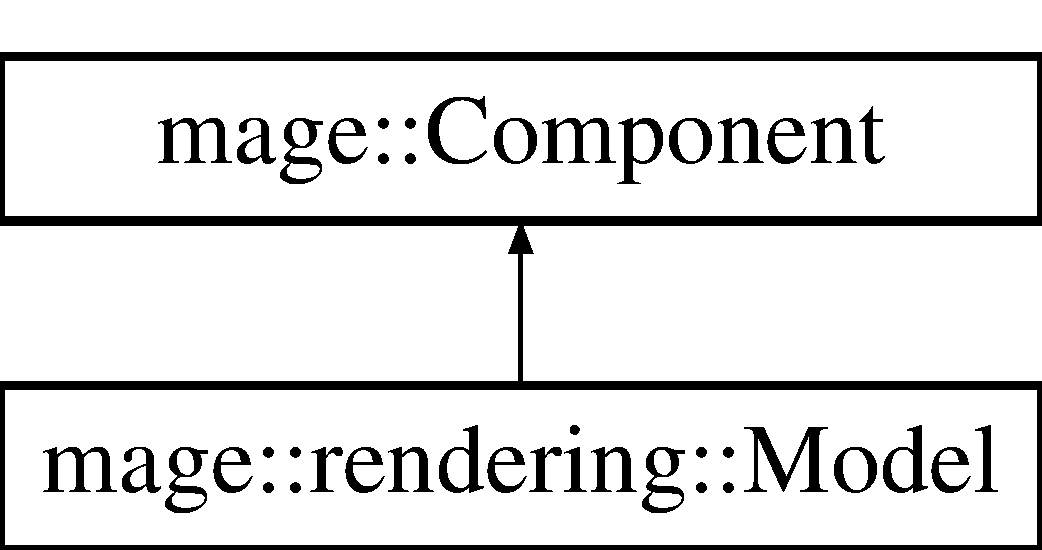
\includegraphics[height=2.000000cm]{classmage_1_1rendering_1_1_model}
\end{center}
\end{figure}
\subsection*{Public Member Functions}
\begin{DoxyCompactItemize}
\item 
\mbox{\hyperlink{classmage_1_1rendering_1_1_model_a7f135a6ed7604655e94d3264bd9d5c62}{Model}} (I\+D3\+D11\+Device \&device)
\item 
\mbox{\hyperlink{classmage_1_1rendering_1_1_model_a59a64dc710efaa44b9f256883d0ab9cb}{Model}} (const \mbox{\hyperlink{classmage_1_1rendering_1_1_model}{Model}} \&model)=delete
\item 
\mbox{\hyperlink{classmage_1_1rendering_1_1_model_a550ece2d159145d9e9549e48235d1ca1}{Model}} (\mbox{\hyperlink{classmage_1_1rendering_1_1_model}{Model}} \&\&model) noexcept
\item 
virtual \mbox{\hyperlink{classmage_1_1rendering_1_1_model_a8fd12c516788a98ce5109aee41d834b8}{$\sim$\+Model}} ()
\item 
\mbox{\hyperlink{classmage_1_1rendering_1_1_model}{Model}} \& \mbox{\hyperlink{classmage_1_1rendering_1_1_model_aa7edda6386fa2ae0638e5c46dccff016}{operator=}} (const \mbox{\hyperlink{classmage_1_1rendering_1_1_model}{Model}} \&model)=delete
\item 
\mbox{\hyperlink{classmage_1_1rendering_1_1_model}{Model}} \& \mbox{\hyperlink{classmage_1_1rendering_1_1_model_a2b374cb908e39da8ff35ea5c17ce640d}{operator=}} (\mbox{\hyperlink{classmage_1_1rendering_1_1_model}{Model}} \&\&model) noexcept
\item 
void \mbox{\hyperlink{classmage_1_1rendering_1_1_model_acc0b3d63c2a02d5fe61539e21b181111}{Set\+Mesh}} (\mbox{\hyperlink{namespacemage_a1e01ae66713838a7a67d30e44c67703e}{Shared\+Ptr}}$<$ const \mbox{\hyperlink{classmage_1_1rendering_1_1_mesh}{Mesh}} $>$ mesh, std\+::size\+\_\+t start\+\_\+index, std\+::size\+\_\+t nb\+\_\+indices, \mbox{\hyperlink{classmage_1_1_a_a_b_b}{A\+A\+BB}} aabb, \mbox{\hyperlink{classmage_1_1_bounding_sphere}{Bounding\+Sphere}} bs)
\item 
const \mbox{\hyperlink{classmage_1_1_a_a_b_b}{A\+A\+BB}} \& \mbox{\hyperlink{classmage_1_1rendering_1_1_model_a05a767ef1551aa4c09c223d8f2311855}{Get\+A\+A\+BB}} () const noexcept
\item 
const \mbox{\hyperlink{classmage_1_1_bounding_sphere}{Bounding\+Sphere}} \& \mbox{\hyperlink{classmage_1_1rendering_1_1_model_a8885748932b52ec2d5bde368db6a130d}{Get\+Bounding\+Sphere}} () const noexcept
\item 
std\+::size\+\_\+t \mbox{\hyperlink{classmage_1_1rendering_1_1_model_a419dd6f4ea7f32ac3d165ce87d54fb47}{Get\+Start\+Index}} () const noexcept
\item 
std\+::size\+\_\+t \mbox{\hyperlink{classmage_1_1rendering_1_1_model_a4e8445480b07026d2f758d879c8c9d56}{Get\+Number\+Of\+Indices}} () const noexcept
\item 
void \mbox{\hyperlink{classmage_1_1rendering_1_1_model_a78defd61277c92a529c4811f1c7c391b}{Bind\+Mesh}} (I\+D3\+D11\+Device\+Context \&device\+\_\+context) const noexcept
\item 
void \mbox{\hyperlink{classmage_1_1rendering_1_1_model_a7793e3f1fa480cb4dc423845fc4de45f}{Bind\+Mesh}} (I\+D3\+D11\+Device\+Context \&device\+\_\+context, D3\+D11\+\_\+\+P\+R\+I\+M\+I\+T\+I\+V\+E\+\_\+\+T\+O\+P\+O\+L\+O\+GY topology) const noexcept
\item 
void \mbox{\hyperlink{classmage_1_1rendering_1_1_model_aaa10d71022d4f6ac8e51ec95861f3317}{Draw}} (I\+D3\+D11\+Device\+Context \&device\+\_\+context) const noexcept
\item 
\mbox{\hyperlink{classmage_1_1_texture_transform}{Texture\+Transform}} \& \mbox{\hyperlink{classmage_1_1rendering_1_1_model_a57e4069226ce9bade50bc17503378f08}{Get\+Texture\+Transform}} () noexcept
\item 
const \mbox{\hyperlink{classmage_1_1_texture_transform}{Texture\+Transform}} \& \mbox{\hyperlink{classmage_1_1rendering_1_1_model_adc18923fdb300d1eb753c9dcb9d30677}{Get\+Texture\+Transform}} () const noexcept
\item 
\mbox{\hyperlink{classmage_1_1rendering_1_1_material}{Material}} \& \mbox{\hyperlink{classmage_1_1rendering_1_1_model_af6e23f8327e82af4d6c2aa854329608c}{Get\+Material}} () noexcept
\item 
const \mbox{\hyperlink{classmage_1_1rendering_1_1_material}{Material}} \& \mbox{\hyperlink{classmage_1_1rendering_1_1_model_afcdf381e409cc7c7be878a60c1799c1b}{Get\+Material}} () const noexcept
\item 
bool \mbox{\hyperlink{classmage_1_1rendering_1_1_model_ac6238580ce9572b9274bf21852f73455}{Occludes\+Light}} () const noexcept
\item 
void \mbox{\hyperlink{classmage_1_1rendering_1_1_model_a6fc53c4d0d5983ecd2f1910002b4dcfc}{Enable\+Light\+Occlusion}} () noexcept
\item 
void \mbox{\hyperlink{classmage_1_1rendering_1_1_model_a4dc86a18b06ee751f2e208acc21f709e}{Dissable\+Light\+Occlusion}} () noexcept
\item 
void \mbox{\hyperlink{classmage_1_1rendering_1_1_model_ade8576cf32210153e65cd39b21940a67}{Toggle\+Light\+Occlusion}} () noexcept
\item 
void \mbox{\hyperlink{classmage_1_1rendering_1_1_model_a4064c86786e7dca7907435da1dce83a4}{Set\+Light\+Occlusion}} (bool light\+\_\+occlusion) noexcept
\item 
void \mbox{\hyperlink{classmage_1_1rendering_1_1_model_a31b3d4f544c8cfea4ad2054d594b2c53}{Update\+Buffer}} (I\+D3\+D11\+Device\+Context \&device\+\_\+context) const
\item 
{\footnotesize template$<$typename Pipeline\+StageT $>$ }\\void \mbox{\hyperlink{classmage_1_1rendering_1_1_model_a1247b104dff5f0eb1039b6e3ac0213ae}{Bind\+Buffer}} (I\+D3\+D11\+Device\+Context \&device\+\_\+context, \mbox{\hyperlink{namespacemage_aa5d6eaabaac3cdd01873d6a3d27e90f3}{U32}} slot) const noexcept
\end{DoxyCompactItemize}
\subsection*{Private Attributes}
\begin{DoxyCompactItemize}
\item 
\mbox{\hyperlink{classmage_1_1rendering_1_1_constant_buffer}{Constant\+Buffer}}$<$ \mbox{\hyperlink{structmage_1_1rendering_1_1_model_buffer}{Model\+Buffer}} $>$ \mbox{\hyperlink{classmage_1_1rendering_1_1_model_a82132035b4631143bed489c4bc190f95}{m\+\_\+buffer}}
\item 
\mbox{\hyperlink{classmage_1_1_a_a_b_b}{A\+A\+BB}} \mbox{\hyperlink{classmage_1_1rendering_1_1_model_a7b3bb86ad718ba3dae2b1c6042fdeaec}{m\+\_\+aabb}}
\item 
\mbox{\hyperlink{classmage_1_1_bounding_sphere}{Bounding\+Sphere}} \mbox{\hyperlink{classmage_1_1rendering_1_1_model_a88220cb828f0df79489c512245560616}{m\+\_\+sphere}}
\item 
\mbox{\hyperlink{namespacemage_a1e01ae66713838a7a67d30e44c67703e}{Shared\+Ptr}}$<$ const \mbox{\hyperlink{classmage_1_1rendering_1_1_mesh}{Mesh}} $>$ \mbox{\hyperlink{classmage_1_1rendering_1_1_model_a38be646490affe6bd2f2f2bb61d04caa}{m\+\_\+mesh}}
\item 
std\+::size\+\_\+t \mbox{\hyperlink{classmage_1_1rendering_1_1_model_ae92a44ede07f136ac89b25c34a8716cc}{m\+\_\+start\+\_\+index}}
\item 
std\+::size\+\_\+t \mbox{\hyperlink{classmage_1_1rendering_1_1_model_afc57d62ba9abcc13bce10f96ec9b2a03}{m\+\_\+nb\+\_\+indices}}
\item 
\mbox{\hyperlink{classmage_1_1_texture_transform}{Texture\+Transform}} \mbox{\hyperlink{classmage_1_1rendering_1_1_model_a00ad04fc770af700b97f69c83dc01d70}{m\+\_\+texture\+\_\+transform}}
\item 
\mbox{\hyperlink{classmage_1_1rendering_1_1_material}{Material}} \mbox{\hyperlink{classmage_1_1rendering_1_1_model_a933d2f661f511908e7c1e9030cfc777d}{m\+\_\+material}}
\item 
bool \mbox{\hyperlink{classmage_1_1rendering_1_1_model_a796fd0c51ea194826dde990b10e70856}{m\+\_\+light\+\_\+occlusion}}
\end{DoxyCompactItemize}
\subsection*{Additional Inherited Members}


\subsection{Detailed Description}
A class of models. 

\subsection{Constructor \& Destructor Documentation}
\mbox{\Hypertarget{classmage_1_1rendering_1_1_model_a7f135a6ed7604655e94d3264bd9d5c62}\label{classmage_1_1rendering_1_1_model_a7f135a6ed7604655e94d3264bd9d5c62}} 
\index{mage\+::rendering\+::\+Model@{mage\+::rendering\+::\+Model}!Model@{Model}}
\index{Model@{Model}!mage\+::rendering\+::\+Model@{mage\+::rendering\+::\+Model}}
\subsubsection{\texorpdfstring{Model()}{Model()}\hspace{0.1cm}{\footnotesize\ttfamily [1/3]}}
{\footnotesize\ttfamily mage\+::rendering\+::\+Model\+::\+Model (\begin{DoxyParamCaption}\item[{I\+D3\+D11\+Device \&}]{device }\end{DoxyParamCaption})\hspace{0.3cm}{\ttfamily [explicit]}}

Constructs a model.


\begin{DoxyParams}[1]{Parameters}
\mbox{\tt in}  & {\em device} & A reference to the device. \\
\hline
\end{DoxyParams}
\mbox{\Hypertarget{classmage_1_1rendering_1_1_model_a59a64dc710efaa44b9f256883d0ab9cb}\label{classmage_1_1rendering_1_1_model_a59a64dc710efaa44b9f256883d0ab9cb}} 
\index{mage\+::rendering\+::\+Model@{mage\+::rendering\+::\+Model}!Model@{Model}}
\index{Model@{Model}!mage\+::rendering\+::\+Model@{mage\+::rendering\+::\+Model}}
\subsubsection{\texorpdfstring{Model()}{Model()}\hspace{0.1cm}{\footnotesize\ttfamily [2/3]}}
{\footnotesize\ttfamily mage\+::rendering\+::\+Model\+::\+Model (\begin{DoxyParamCaption}\item[{const \mbox{\hyperlink{classmage_1_1rendering_1_1_model}{Model}} \&}]{model }\end{DoxyParamCaption})\hspace{0.3cm}{\ttfamily [delete]}}

Constructs a model from the given model.


\begin{DoxyParams}[1]{Parameters}
\mbox{\tt in}  & {\em model} & A reference to the model to copy. \\
\hline
\end{DoxyParams}
\mbox{\Hypertarget{classmage_1_1rendering_1_1_model_a550ece2d159145d9e9549e48235d1ca1}\label{classmage_1_1rendering_1_1_model_a550ece2d159145d9e9549e48235d1ca1}} 
\index{mage\+::rendering\+::\+Model@{mage\+::rendering\+::\+Model}!Model@{Model}}
\index{Model@{Model}!mage\+::rendering\+::\+Model@{mage\+::rendering\+::\+Model}}
\subsubsection{\texorpdfstring{Model()}{Model()}\hspace{0.1cm}{\footnotesize\ttfamily [3/3]}}
{\footnotesize\ttfamily mage\+::rendering\+::\+Model\+::\+Model (\begin{DoxyParamCaption}\item[{\mbox{\hyperlink{classmage_1_1rendering_1_1_model}{Model}} \&\&}]{model }\end{DoxyParamCaption})\hspace{0.3cm}{\ttfamily [default]}, {\ttfamily [noexcept]}}

Constructs a model by moving the given model.


\begin{DoxyParams}[1]{Parameters}
\mbox{\tt in}  & {\em model} & A reference to the model to move. \\
\hline
\end{DoxyParams}
\mbox{\Hypertarget{classmage_1_1rendering_1_1_model_a8fd12c516788a98ce5109aee41d834b8}\label{classmage_1_1rendering_1_1_model_a8fd12c516788a98ce5109aee41d834b8}} 
\index{mage\+::rendering\+::\+Model@{mage\+::rendering\+::\+Model}!````~Model@{$\sim$\+Model}}
\index{````~Model@{$\sim$\+Model}!mage\+::rendering\+::\+Model@{mage\+::rendering\+::\+Model}}
\subsubsection{\texorpdfstring{$\sim$\+Model()}{~Model()}}
{\footnotesize\ttfamily mage\+::rendering\+::\+Model\+::$\sim$\+Model (\begin{DoxyParamCaption}{ }\end{DoxyParamCaption})\hspace{0.3cm}{\ttfamily [virtual]}, {\ttfamily [default]}}

Destructs this model. 

\subsection{Member Function Documentation}
\mbox{\Hypertarget{classmage_1_1rendering_1_1_model_a1247b104dff5f0eb1039b6e3ac0213ae}\label{classmage_1_1rendering_1_1_model_a1247b104dff5f0eb1039b6e3ac0213ae}} 
\index{mage\+::rendering\+::\+Model@{mage\+::rendering\+::\+Model}!Bind\+Buffer@{Bind\+Buffer}}
\index{Bind\+Buffer@{Bind\+Buffer}!mage\+::rendering\+::\+Model@{mage\+::rendering\+::\+Model}}
\subsubsection{\texorpdfstring{Bind\+Buffer()}{BindBuffer()}}
{\footnotesize\ttfamily template$<$typename Pipeline\+StageT $>$ \\
void mage\+::rendering\+::\+Model\+::\+Bind\+Buffer (\begin{DoxyParamCaption}\item[{I\+D3\+D11\+Device\+Context \&}]{device\+\_\+context,  }\item[{\mbox{\hyperlink{namespacemage_aa5d6eaabaac3cdd01873d6a3d27e90f3}{U32}}}]{slot }\end{DoxyParamCaption}) const\hspace{0.3cm}{\ttfamily [noexcept]}}

Binds the buffer of this model to the given pipeline stage.


\begin{DoxyTemplParams}{Template Parameters}
{\em Pipeline\+StageT} & The pipeline stage type. \\
\hline
\end{DoxyTemplParams}

\begin{DoxyParams}[1]{Parameters}
\mbox{\tt in}  & {\em device\+\_\+context} & A reference to the device context. \\
\hline
\mbox{\tt in}  & {\em slot} & The index into the device\textquotesingle{}s zero-\/based array to set the constant buffer to (ranges from 0 to {\ttfamily D3\+D11\+\_\+\+C\+O\+M\+M\+O\+N\+S\+H\+A\+D\+E\+R\+\_\+\+C\+O\+N\+S\+T\+A\+N\+T\+\_\+\+B\+U\+F\+F\+E\+R\+\_\+\+A\+P\+I\+\_\+\+S\+L\+O\+T\+\_\+\+C\+O\+U\+NT} -\/ 1). \\
\hline
\end{DoxyParams}
\mbox{\Hypertarget{classmage_1_1rendering_1_1_model_a78defd61277c92a529c4811f1c7c391b}\label{classmage_1_1rendering_1_1_model_a78defd61277c92a529c4811f1c7c391b}} 
\index{mage\+::rendering\+::\+Model@{mage\+::rendering\+::\+Model}!Bind\+Mesh@{Bind\+Mesh}}
\index{Bind\+Mesh@{Bind\+Mesh}!mage\+::rendering\+::\+Model@{mage\+::rendering\+::\+Model}}
\subsubsection{\texorpdfstring{Bind\+Mesh()}{BindMesh()}\hspace{0.1cm}{\footnotesize\ttfamily [1/2]}}
{\footnotesize\ttfamily void mage\+::rendering\+::\+Model\+::\+Bind\+Mesh (\begin{DoxyParamCaption}\item[{I\+D3\+D11\+Device\+Context \&}]{device\+\_\+context }\end{DoxyParamCaption}) const\hspace{0.3cm}{\ttfamily [noexcept]}}

Binds the mesh of this model.


\begin{DoxyParams}[1]{Parameters}
\mbox{\tt in}  & {\em device\+\_\+context} & A reference to the device context. \\
\hline
\end{DoxyParams}
\mbox{\Hypertarget{classmage_1_1rendering_1_1_model_a7793e3f1fa480cb4dc423845fc4de45f}\label{classmage_1_1rendering_1_1_model_a7793e3f1fa480cb4dc423845fc4de45f}} 
\index{mage\+::rendering\+::\+Model@{mage\+::rendering\+::\+Model}!Bind\+Mesh@{Bind\+Mesh}}
\index{Bind\+Mesh@{Bind\+Mesh}!mage\+::rendering\+::\+Model@{mage\+::rendering\+::\+Model}}
\subsubsection{\texorpdfstring{Bind\+Mesh()}{BindMesh()}\hspace{0.1cm}{\footnotesize\ttfamily [2/2]}}
{\footnotesize\ttfamily void mage\+::rendering\+::\+Model\+::\+Bind\+Mesh (\begin{DoxyParamCaption}\item[{I\+D3\+D11\+Device\+Context \&}]{device\+\_\+context,  }\item[{D3\+D11\+\_\+\+P\+R\+I\+M\+I\+T\+I\+V\+E\+\_\+\+T\+O\+P\+O\+L\+O\+GY}]{topology }\end{DoxyParamCaption}) const\hspace{0.3cm}{\ttfamily [noexcept]}}

Binds the mesh of this model with given primitive topology.


\begin{DoxyParams}[1]{Parameters}
\mbox{\tt in}  & {\em device\+\_\+context} & A reference to the device context. \\
\hline
\mbox{\tt in}  & {\em topology} & The primitive topology. \\
\hline
\end{DoxyParams}
\mbox{\Hypertarget{classmage_1_1rendering_1_1_model_a4dc86a18b06ee751f2e208acc21f709e}\label{classmage_1_1rendering_1_1_model_a4dc86a18b06ee751f2e208acc21f709e}} 
\index{mage\+::rendering\+::\+Model@{mage\+::rendering\+::\+Model}!Dissable\+Light\+Occlusion@{Dissable\+Light\+Occlusion}}
\index{Dissable\+Light\+Occlusion@{Dissable\+Light\+Occlusion}!mage\+::rendering\+::\+Model@{mage\+::rendering\+::\+Model}}
\subsubsection{\texorpdfstring{Dissable\+Light\+Occlusion()}{DissableLightOcclusion()}}
{\footnotesize\ttfamily void mage\+::rendering\+::\+Model\+::\+Dissable\+Light\+Occlusion (\begin{DoxyParamCaption}{ }\end{DoxyParamCaption})\hspace{0.3cm}{\ttfamily [noexcept]}}

Dissables the occlusion of light by this model. \mbox{\Hypertarget{classmage_1_1rendering_1_1_model_aaa10d71022d4f6ac8e51ec95861f3317}\label{classmage_1_1rendering_1_1_model_aaa10d71022d4f6ac8e51ec95861f3317}} 
\index{mage\+::rendering\+::\+Model@{mage\+::rendering\+::\+Model}!Draw@{Draw}}
\index{Draw@{Draw}!mage\+::rendering\+::\+Model@{mage\+::rendering\+::\+Model}}
\subsubsection{\texorpdfstring{Draw()}{Draw()}}
{\footnotesize\ttfamily void mage\+::rendering\+::\+Model\+::\+Draw (\begin{DoxyParamCaption}\item[{I\+D3\+D11\+Device\+Context \&}]{device\+\_\+context }\end{DoxyParamCaption}) const\hspace{0.3cm}{\ttfamily [noexcept]}}

Draws this model.


\begin{DoxyParams}[1]{Parameters}
\mbox{\tt in}  & {\em device\+\_\+context} & A reference to the device context. \\
\hline
\end{DoxyParams}
\mbox{\Hypertarget{classmage_1_1rendering_1_1_model_a6fc53c4d0d5983ecd2f1910002b4dcfc}\label{classmage_1_1rendering_1_1_model_a6fc53c4d0d5983ecd2f1910002b4dcfc}} 
\index{mage\+::rendering\+::\+Model@{mage\+::rendering\+::\+Model}!Enable\+Light\+Occlusion@{Enable\+Light\+Occlusion}}
\index{Enable\+Light\+Occlusion@{Enable\+Light\+Occlusion}!mage\+::rendering\+::\+Model@{mage\+::rendering\+::\+Model}}
\subsubsection{\texorpdfstring{Enable\+Light\+Occlusion()}{EnableLightOcclusion()}}
{\footnotesize\ttfamily void mage\+::rendering\+::\+Model\+::\+Enable\+Light\+Occlusion (\begin{DoxyParamCaption}{ }\end{DoxyParamCaption})\hspace{0.3cm}{\ttfamily [noexcept]}}

Enbales the occlusion of light by this model. \mbox{\Hypertarget{classmage_1_1rendering_1_1_model_a05a767ef1551aa4c09c223d8f2311855}\label{classmage_1_1rendering_1_1_model_a05a767ef1551aa4c09c223d8f2311855}} 
\index{mage\+::rendering\+::\+Model@{mage\+::rendering\+::\+Model}!Get\+A\+A\+BB@{Get\+A\+A\+BB}}
\index{Get\+A\+A\+BB@{Get\+A\+A\+BB}!mage\+::rendering\+::\+Model@{mage\+::rendering\+::\+Model}}
\subsubsection{\texorpdfstring{Get\+A\+A\+B\+B()}{GetAABB()}}
{\footnotesize\ttfamily const \mbox{\hyperlink{classmage_1_1_a_a_b_b}{A\+A\+BB}}\& mage\+::rendering\+::\+Model\+::\+Get\+A\+A\+BB (\begin{DoxyParamCaption}{ }\end{DoxyParamCaption}) const\hspace{0.3cm}{\ttfamily [noexcept]}}

Returns the \mbox{\hyperlink{classmage_1_1_a_a_b_b}{A\+A\+BB}} of this model.

\begin{DoxyReturn}{Returns}
A reference to the \mbox{\hyperlink{classmage_1_1_a_a_b_b}{A\+A\+BB}} of this model. 
\end{DoxyReturn}
\mbox{\Hypertarget{classmage_1_1rendering_1_1_model_a8885748932b52ec2d5bde368db6a130d}\label{classmage_1_1rendering_1_1_model_a8885748932b52ec2d5bde368db6a130d}} 
\index{mage\+::rendering\+::\+Model@{mage\+::rendering\+::\+Model}!Get\+Bounding\+Sphere@{Get\+Bounding\+Sphere}}
\index{Get\+Bounding\+Sphere@{Get\+Bounding\+Sphere}!mage\+::rendering\+::\+Model@{mage\+::rendering\+::\+Model}}
\subsubsection{\texorpdfstring{Get\+Bounding\+Sphere()}{GetBoundingSphere()}}
{\footnotesize\ttfamily const \mbox{\hyperlink{classmage_1_1_bounding_sphere}{Bounding\+Sphere}}\& mage\+::rendering\+::\+Model\+::\+Get\+Bounding\+Sphere (\begin{DoxyParamCaption}{ }\end{DoxyParamCaption}) const\hspace{0.3cm}{\ttfamily [noexcept]}}

Returns the bounding sphere of this model.

\begin{DoxyReturn}{Returns}
A reference to the bounding sphere of this model. 
\end{DoxyReturn}
\mbox{\Hypertarget{classmage_1_1rendering_1_1_model_af6e23f8327e82af4d6c2aa854329608c}\label{classmage_1_1rendering_1_1_model_af6e23f8327e82af4d6c2aa854329608c}} 
\index{mage\+::rendering\+::\+Model@{mage\+::rendering\+::\+Model}!Get\+Material@{Get\+Material}}
\index{Get\+Material@{Get\+Material}!mage\+::rendering\+::\+Model@{mage\+::rendering\+::\+Model}}
\subsubsection{\texorpdfstring{Get\+Material()}{GetMaterial()}\hspace{0.1cm}{\footnotesize\ttfamily [1/2]}}
{\footnotesize\ttfamily \mbox{\hyperlink{classmage_1_1rendering_1_1_material}{Material}}\& mage\+::rendering\+::\+Model\+::\+Get\+Material (\begin{DoxyParamCaption}{ }\end{DoxyParamCaption})\hspace{0.3cm}{\ttfamily [noexcept]}}

Returns the material of this model.

\begin{DoxyReturn}{Returns}
A reference to the material of this model. 
\end{DoxyReturn}
\mbox{\Hypertarget{classmage_1_1rendering_1_1_model_afcdf381e409cc7c7be878a60c1799c1b}\label{classmage_1_1rendering_1_1_model_afcdf381e409cc7c7be878a60c1799c1b}} 
\index{mage\+::rendering\+::\+Model@{mage\+::rendering\+::\+Model}!Get\+Material@{Get\+Material}}
\index{Get\+Material@{Get\+Material}!mage\+::rendering\+::\+Model@{mage\+::rendering\+::\+Model}}
\subsubsection{\texorpdfstring{Get\+Material()}{GetMaterial()}\hspace{0.1cm}{\footnotesize\ttfamily [2/2]}}
{\footnotesize\ttfamily const \mbox{\hyperlink{classmage_1_1rendering_1_1_material}{Material}}\& mage\+::rendering\+::\+Model\+::\+Get\+Material (\begin{DoxyParamCaption}{ }\end{DoxyParamCaption}) const\hspace{0.3cm}{\ttfamily [noexcept]}}

Returns the material of this model.

\begin{DoxyReturn}{Returns}
A reference to the material of this model. 
\end{DoxyReturn}
\mbox{\Hypertarget{classmage_1_1rendering_1_1_model_a4e8445480b07026d2f758d879c8c9d56}\label{classmage_1_1rendering_1_1_model_a4e8445480b07026d2f758d879c8c9d56}} 
\index{mage\+::rendering\+::\+Model@{mage\+::rendering\+::\+Model}!Get\+Number\+Of\+Indices@{Get\+Number\+Of\+Indices}}
\index{Get\+Number\+Of\+Indices@{Get\+Number\+Of\+Indices}!mage\+::rendering\+::\+Model@{mage\+::rendering\+::\+Model}}
\subsubsection{\texorpdfstring{Get\+Number\+Of\+Indices()}{GetNumberOfIndices()}}
{\footnotesize\ttfamily std\+::size\+\_\+t mage\+::rendering\+::\+Model\+::\+Get\+Number\+Of\+Indices (\begin{DoxyParamCaption}{ }\end{DoxyParamCaption}) const\hspace{0.3cm}{\ttfamily [noexcept]}}

Returns the number of indices of this model in the mesh of this model.

\begin{DoxyReturn}{Returns}
The number of indices of this model in the mesh of this model. 
\end{DoxyReturn}
\mbox{\Hypertarget{classmage_1_1rendering_1_1_model_a419dd6f4ea7f32ac3d165ce87d54fb47}\label{classmage_1_1rendering_1_1_model_a419dd6f4ea7f32ac3d165ce87d54fb47}} 
\index{mage\+::rendering\+::\+Model@{mage\+::rendering\+::\+Model}!Get\+Start\+Index@{Get\+Start\+Index}}
\index{Get\+Start\+Index@{Get\+Start\+Index}!mage\+::rendering\+::\+Model@{mage\+::rendering\+::\+Model}}
\subsubsection{\texorpdfstring{Get\+Start\+Index()}{GetStartIndex()}}
{\footnotesize\ttfamily std\+::size\+\_\+t mage\+::rendering\+::\+Model\+::\+Get\+Start\+Index (\begin{DoxyParamCaption}{ }\end{DoxyParamCaption}) const\hspace{0.3cm}{\ttfamily [noexcept]}}

Returns the start index of this model in the mesh of this model.

\begin{DoxyReturn}{Returns}
The start index of this model in the mesh of this model. 
\end{DoxyReturn}
\mbox{\Hypertarget{classmage_1_1rendering_1_1_model_a57e4069226ce9bade50bc17503378f08}\label{classmage_1_1rendering_1_1_model_a57e4069226ce9bade50bc17503378f08}} 
\index{mage\+::rendering\+::\+Model@{mage\+::rendering\+::\+Model}!Get\+Texture\+Transform@{Get\+Texture\+Transform}}
\index{Get\+Texture\+Transform@{Get\+Texture\+Transform}!mage\+::rendering\+::\+Model@{mage\+::rendering\+::\+Model}}
\subsubsection{\texorpdfstring{Get\+Texture\+Transform()}{GetTextureTransform()}\hspace{0.1cm}{\footnotesize\ttfamily [1/2]}}
{\footnotesize\ttfamily \mbox{\hyperlink{classmage_1_1_texture_transform}{Texture\+Transform}}\& mage\+::rendering\+::\+Model\+::\+Get\+Texture\+Transform (\begin{DoxyParamCaption}{ }\end{DoxyParamCaption})\hspace{0.3cm}{\ttfamily [noexcept]}}

Returns the texture transform of this model.

\begin{DoxyReturn}{Returns}
A reference to the texture transform of this model. 
\end{DoxyReturn}
\mbox{\Hypertarget{classmage_1_1rendering_1_1_model_adc18923fdb300d1eb753c9dcb9d30677}\label{classmage_1_1rendering_1_1_model_adc18923fdb300d1eb753c9dcb9d30677}} 
\index{mage\+::rendering\+::\+Model@{mage\+::rendering\+::\+Model}!Get\+Texture\+Transform@{Get\+Texture\+Transform}}
\index{Get\+Texture\+Transform@{Get\+Texture\+Transform}!mage\+::rendering\+::\+Model@{mage\+::rendering\+::\+Model}}
\subsubsection{\texorpdfstring{Get\+Texture\+Transform()}{GetTextureTransform()}\hspace{0.1cm}{\footnotesize\ttfamily [2/2]}}
{\footnotesize\ttfamily const \mbox{\hyperlink{classmage_1_1_texture_transform}{Texture\+Transform}}\& mage\+::rendering\+::\+Model\+::\+Get\+Texture\+Transform (\begin{DoxyParamCaption}{ }\end{DoxyParamCaption}) const\hspace{0.3cm}{\ttfamily [noexcept]}}

Returns the texture transform of this model.

\begin{DoxyReturn}{Returns}
A reference to the texture transform of this model. 
\end{DoxyReturn}
\mbox{\Hypertarget{classmage_1_1rendering_1_1_model_ac6238580ce9572b9274bf21852f73455}\label{classmage_1_1rendering_1_1_model_ac6238580ce9572b9274bf21852f73455}} 
\index{mage\+::rendering\+::\+Model@{mage\+::rendering\+::\+Model}!Occludes\+Light@{Occludes\+Light}}
\index{Occludes\+Light@{Occludes\+Light}!mage\+::rendering\+::\+Model@{mage\+::rendering\+::\+Model}}
\subsubsection{\texorpdfstring{Occludes\+Light()}{OccludesLight()}}
{\footnotesize\ttfamily bool mage\+::rendering\+::\+Model\+::\+Occludes\+Light (\begin{DoxyParamCaption}{ }\end{DoxyParamCaption}) const\hspace{0.3cm}{\ttfamily [noexcept]}}

Checks whether this model occludes light.

\begin{DoxyReturn}{Returns}
{\ttfamily true} if this model occludes light. {\ttfamily false} otherwise. 
\end{DoxyReturn}
\mbox{\Hypertarget{classmage_1_1rendering_1_1_model_aa7edda6386fa2ae0638e5c46dccff016}\label{classmage_1_1rendering_1_1_model_aa7edda6386fa2ae0638e5c46dccff016}} 
\index{mage\+::rendering\+::\+Model@{mage\+::rendering\+::\+Model}!operator=@{operator=}}
\index{operator=@{operator=}!mage\+::rendering\+::\+Model@{mage\+::rendering\+::\+Model}}
\subsubsection{\texorpdfstring{operator=()}{operator=()}\hspace{0.1cm}{\footnotesize\ttfamily [1/2]}}
{\footnotesize\ttfamily \mbox{\hyperlink{classmage_1_1rendering_1_1_model}{Model}}\& mage\+::rendering\+::\+Model\+::operator= (\begin{DoxyParamCaption}\item[{const \mbox{\hyperlink{classmage_1_1rendering_1_1_model}{Model}} \&}]{model }\end{DoxyParamCaption})\hspace{0.3cm}{\ttfamily [delete]}}

Copies the given model to this model.


\begin{DoxyParams}[1]{Parameters}
\mbox{\tt in}  & {\em model} & A reference to the model to copy. \\
\hline
\end{DoxyParams}
\begin{DoxyReturn}{Returns}
A reference to the copy of the given model (i.\+e. this model). 
\end{DoxyReturn}
\mbox{\Hypertarget{classmage_1_1rendering_1_1_model_a2b374cb908e39da8ff35ea5c17ce640d}\label{classmage_1_1rendering_1_1_model_a2b374cb908e39da8ff35ea5c17ce640d}} 
\index{mage\+::rendering\+::\+Model@{mage\+::rendering\+::\+Model}!operator=@{operator=}}
\index{operator=@{operator=}!mage\+::rendering\+::\+Model@{mage\+::rendering\+::\+Model}}
\subsubsection{\texorpdfstring{operator=()}{operator=()}\hspace{0.1cm}{\footnotesize\ttfamily [2/2]}}
{\footnotesize\ttfamily \mbox{\hyperlink{classmage_1_1rendering_1_1_model}{Model}} \& mage\+::rendering\+::\+Model\+::operator= (\begin{DoxyParamCaption}\item[{\mbox{\hyperlink{classmage_1_1rendering_1_1_model}{Model}} \&\&}]{model }\end{DoxyParamCaption})\hspace{0.3cm}{\ttfamily [default]}, {\ttfamily [noexcept]}}

Moves the given model to this model.


\begin{DoxyParams}[1]{Parameters}
\mbox{\tt in}  & {\em model} & A reference to the model to move. \\
\hline
\end{DoxyParams}
\begin{DoxyReturn}{Returns}
A reference to the moved model (i.\+e. this model). 
\end{DoxyReturn}
\mbox{\Hypertarget{classmage_1_1rendering_1_1_model_a4064c86786e7dca7907435da1dce83a4}\label{classmage_1_1rendering_1_1_model_a4064c86786e7dca7907435da1dce83a4}} 
\index{mage\+::rendering\+::\+Model@{mage\+::rendering\+::\+Model}!Set\+Light\+Occlusion@{Set\+Light\+Occlusion}}
\index{Set\+Light\+Occlusion@{Set\+Light\+Occlusion}!mage\+::rendering\+::\+Model@{mage\+::rendering\+::\+Model}}
\subsubsection{\texorpdfstring{Set\+Light\+Occlusion()}{SetLightOcclusion()}}
{\footnotesize\ttfamily void mage\+::rendering\+::\+Model\+::\+Set\+Light\+Occlusion (\begin{DoxyParamCaption}\item[{bool}]{light\+\_\+occlusion }\end{DoxyParamCaption})\hspace{0.3cm}{\ttfamily [noexcept]}}

Sets the occlusion of light by this model to the given value.


\begin{DoxyParams}[1]{Parameters}
\mbox{\tt in}  & {\em light\+\_\+occlusion} & {\ttfamily true} if this model needs to occlude light. {\ttfamily false} otherwise. \\
\hline
\end{DoxyParams}
\mbox{\Hypertarget{classmage_1_1rendering_1_1_model_acc0b3d63c2a02d5fe61539e21b181111}\label{classmage_1_1rendering_1_1_model_acc0b3d63c2a02d5fe61539e21b181111}} 
\index{mage\+::rendering\+::\+Model@{mage\+::rendering\+::\+Model}!Set\+Mesh@{Set\+Mesh}}
\index{Set\+Mesh@{Set\+Mesh}!mage\+::rendering\+::\+Model@{mage\+::rendering\+::\+Model}}
\subsubsection{\texorpdfstring{Set\+Mesh()}{SetMesh()}}
{\footnotesize\ttfamily void mage\+::rendering\+::\+Model\+::\+Set\+Mesh (\begin{DoxyParamCaption}\item[{\mbox{\hyperlink{namespacemage_a1e01ae66713838a7a67d30e44c67703e}{Shared\+Ptr}}$<$ const \mbox{\hyperlink{classmage_1_1rendering_1_1_mesh}{Mesh}} $>$}]{mesh,  }\item[{std\+::size\+\_\+t}]{start\+\_\+index,  }\item[{std\+::size\+\_\+t}]{nb\+\_\+indices,  }\item[{\mbox{\hyperlink{classmage_1_1_a_a_b_b}{A\+A\+BB}}}]{aabb,  }\item[{\mbox{\hyperlink{classmage_1_1_bounding_sphere}{Bounding\+Sphere}}}]{bs }\end{DoxyParamCaption})}

Sets the mesh of this model to the given mesh.


\begin{DoxyParams}[1]{Parameters}
\mbox{\tt in}  & {\em mesh} & A pointer to the mesh. \\
\hline
\mbox{\tt in}  & {\em start\+\_\+index} & The start index in the mesh. \\
\hline
\mbox{\tt in}  & {\em nb\+\_\+indices} & The number of indices in the mesh. \\
\hline
\mbox{\tt in}  & {\em aabb} & The \mbox{\hyperlink{classmage_1_1_a_a_b_b}{A\+A\+BB}}. \\
\hline
\mbox{\tt in}  & {\em bs} & The bounding sphere. \\
\hline
\end{DoxyParams}
\mbox{\Hypertarget{classmage_1_1rendering_1_1_model_ade8576cf32210153e65cd39b21940a67}\label{classmage_1_1rendering_1_1_model_ade8576cf32210153e65cd39b21940a67}} 
\index{mage\+::rendering\+::\+Model@{mage\+::rendering\+::\+Model}!Toggle\+Light\+Occlusion@{Toggle\+Light\+Occlusion}}
\index{Toggle\+Light\+Occlusion@{Toggle\+Light\+Occlusion}!mage\+::rendering\+::\+Model@{mage\+::rendering\+::\+Model}}
\subsubsection{\texorpdfstring{Toggle\+Light\+Occlusion()}{ToggleLightOcclusion()}}
{\footnotesize\ttfamily void mage\+::rendering\+::\+Model\+::\+Toggle\+Light\+Occlusion (\begin{DoxyParamCaption}{ }\end{DoxyParamCaption})\hspace{0.3cm}{\ttfamily [noexcept]}}

Toggles the occlusion of light by this model. \mbox{\Hypertarget{classmage_1_1rendering_1_1_model_a31b3d4f544c8cfea4ad2054d594b2c53}\label{classmage_1_1rendering_1_1_model_a31b3d4f544c8cfea4ad2054d594b2c53}} 
\index{mage\+::rendering\+::\+Model@{mage\+::rendering\+::\+Model}!Update\+Buffer@{Update\+Buffer}}
\index{Update\+Buffer@{Update\+Buffer}!mage\+::rendering\+::\+Model@{mage\+::rendering\+::\+Model}}
\subsubsection{\texorpdfstring{Update\+Buffer()}{UpdateBuffer()}}
{\footnotesize\ttfamily void mage\+::rendering\+::\+Model\+::\+Update\+Buffer (\begin{DoxyParamCaption}\item[{I\+D3\+D11\+Device\+Context \&}]{device\+\_\+context }\end{DoxyParamCaption}) const}

Updates the buffer of this model.


\begin{DoxyParams}[1]{Parameters}
\mbox{\tt in}  & {\em device\+\_\+context} & A reference to the device context. \\
\hline
\end{DoxyParams}


\subsection{Member Data Documentation}
\mbox{\Hypertarget{classmage_1_1rendering_1_1_model_a7b3bb86ad718ba3dae2b1c6042fdeaec}\label{classmage_1_1rendering_1_1_model_a7b3bb86ad718ba3dae2b1c6042fdeaec}} 
\index{mage\+::rendering\+::\+Model@{mage\+::rendering\+::\+Model}!m\+\_\+aabb@{m\+\_\+aabb}}
\index{m\+\_\+aabb@{m\+\_\+aabb}!mage\+::rendering\+::\+Model@{mage\+::rendering\+::\+Model}}
\subsubsection{\texorpdfstring{m\+\_\+aabb}{m\_aabb}}
{\footnotesize\ttfamily \mbox{\hyperlink{classmage_1_1_a_a_b_b}{A\+A\+BB}} mage\+::rendering\+::\+Model\+::m\+\_\+aabb\hspace{0.3cm}{\ttfamily [private]}}

The \mbox{\hyperlink{classmage_1_1_a_a_b_b}{A\+A\+BB}} of this model. \mbox{\Hypertarget{classmage_1_1rendering_1_1_model_a82132035b4631143bed489c4bc190f95}\label{classmage_1_1rendering_1_1_model_a82132035b4631143bed489c4bc190f95}} 
\index{mage\+::rendering\+::\+Model@{mage\+::rendering\+::\+Model}!m\+\_\+buffer@{m\+\_\+buffer}}
\index{m\+\_\+buffer@{m\+\_\+buffer}!mage\+::rendering\+::\+Model@{mage\+::rendering\+::\+Model}}
\subsubsection{\texorpdfstring{m\+\_\+buffer}{m\_buffer}}
{\footnotesize\ttfamily \mbox{\hyperlink{classmage_1_1rendering_1_1_constant_buffer}{Constant\+Buffer}}$<$ \mbox{\hyperlink{structmage_1_1rendering_1_1_model_buffer}{Model\+Buffer}} $>$ mage\+::rendering\+::\+Model\+::m\+\_\+buffer\hspace{0.3cm}{\ttfamily [mutable]}, {\ttfamily [private]}}

The buffer of this model. \mbox{\Hypertarget{classmage_1_1rendering_1_1_model_a796fd0c51ea194826dde990b10e70856}\label{classmage_1_1rendering_1_1_model_a796fd0c51ea194826dde990b10e70856}} 
\index{mage\+::rendering\+::\+Model@{mage\+::rendering\+::\+Model}!m\+\_\+light\+\_\+occlusion@{m\+\_\+light\+\_\+occlusion}}
\index{m\+\_\+light\+\_\+occlusion@{m\+\_\+light\+\_\+occlusion}!mage\+::rendering\+::\+Model@{mage\+::rendering\+::\+Model}}
\subsubsection{\texorpdfstring{m\+\_\+light\+\_\+occlusion}{m\_light\_occlusion}}
{\footnotesize\ttfamily bool mage\+::rendering\+::\+Model\+::m\+\_\+light\+\_\+occlusion\hspace{0.3cm}{\ttfamily [private]}}

A flag indicating whether this model occludes light. \mbox{\Hypertarget{classmage_1_1rendering_1_1_model_a933d2f661f511908e7c1e9030cfc777d}\label{classmage_1_1rendering_1_1_model_a933d2f661f511908e7c1e9030cfc777d}} 
\index{mage\+::rendering\+::\+Model@{mage\+::rendering\+::\+Model}!m\+\_\+material@{m\+\_\+material}}
\index{m\+\_\+material@{m\+\_\+material}!mage\+::rendering\+::\+Model@{mage\+::rendering\+::\+Model}}
\subsubsection{\texorpdfstring{m\+\_\+material}{m\_material}}
{\footnotesize\ttfamily \mbox{\hyperlink{classmage_1_1rendering_1_1_material}{Material}} mage\+::rendering\+::\+Model\+::m\+\_\+material\hspace{0.3cm}{\ttfamily [private]}}

The material of this model. \mbox{\Hypertarget{classmage_1_1rendering_1_1_model_a38be646490affe6bd2f2f2bb61d04caa}\label{classmage_1_1rendering_1_1_model_a38be646490affe6bd2f2f2bb61d04caa}} 
\index{mage\+::rendering\+::\+Model@{mage\+::rendering\+::\+Model}!m\+\_\+mesh@{m\+\_\+mesh}}
\index{m\+\_\+mesh@{m\+\_\+mesh}!mage\+::rendering\+::\+Model@{mage\+::rendering\+::\+Model}}
\subsubsection{\texorpdfstring{m\+\_\+mesh}{m\_mesh}}
{\footnotesize\ttfamily \mbox{\hyperlink{namespacemage_a1e01ae66713838a7a67d30e44c67703e}{Shared\+Ptr}}$<$ const \mbox{\hyperlink{classmage_1_1rendering_1_1_mesh}{Mesh}} $>$ mage\+::rendering\+::\+Model\+::m\+\_\+mesh\hspace{0.3cm}{\ttfamily [private]}}

A pointer to the mesh of this model. \mbox{\Hypertarget{classmage_1_1rendering_1_1_model_afc57d62ba9abcc13bce10f96ec9b2a03}\label{classmage_1_1rendering_1_1_model_afc57d62ba9abcc13bce10f96ec9b2a03}} 
\index{mage\+::rendering\+::\+Model@{mage\+::rendering\+::\+Model}!m\+\_\+nb\+\_\+indices@{m\+\_\+nb\+\_\+indices}}
\index{m\+\_\+nb\+\_\+indices@{m\+\_\+nb\+\_\+indices}!mage\+::rendering\+::\+Model@{mage\+::rendering\+::\+Model}}
\subsubsection{\texorpdfstring{m\+\_\+nb\+\_\+indices}{m\_nb\_indices}}
{\footnotesize\ttfamily std\+::size\+\_\+t mage\+::rendering\+::\+Model\+::m\+\_\+nb\+\_\+indices\hspace{0.3cm}{\ttfamily [private]}}

The number of indices of this model in the mesh of this model. \mbox{\Hypertarget{classmage_1_1rendering_1_1_model_a88220cb828f0df79489c512245560616}\label{classmage_1_1rendering_1_1_model_a88220cb828f0df79489c512245560616}} 
\index{mage\+::rendering\+::\+Model@{mage\+::rendering\+::\+Model}!m\+\_\+sphere@{m\+\_\+sphere}}
\index{m\+\_\+sphere@{m\+\_\+sphere}!mage\+::rendering\+::\+Model@{mage\+::rendering\+::\+Model}}
\subsubsection{\texorpdfstring{m\+\_\+sphere}{m\_sphere}}
{\footnotesize\ttfamily \mbox{\hyperlink{classmage_1_1_bounding_sphere}{Bounding\+Sphere}} mage\+::rendering\+::\+Model\+::m\+\_\+sphere\hspace{0.3cm}{\ttfamily [private]}}

The bounding sphere of this model. \mbox{\Hypertarget{classmage_1_1rendering_1_1_model_ae92a44ede07f136ac89b25c34a8716cc}\label{classmage_1_1rendering_1_1_model_ae92a44ede07f136ac89b25c34a8716cc}} 
\index{mage\+::rendering\+::\+Model@{mage\+::rendering\+::\+Model}!m\+\_\+start\+\_\+index@{m\+\_\+start\+\_\+index}}
\index{m\+\_\+start\+\_\+index@{m\+\_\+start\+\_\+index}!mage\+::rendering\+::\+Model@{mage\+::rendering\+::\+Model}}
\subsubsection{\texorpdfstring{m\+\_\+start\+\_\+index}{m\_start\_index}}
{\footnotesize\ttfamily std\+::size\+\_\+t mage\+::rendering\+::\+Model\+::m\+\_\+start\+\_\+index\hspace{0.3cm}{\ttfamily [private]}}

The start index of this model in the mesh of this model. \mbox{\Hypertarget{classmage_1_1rendering_1_1_model_a00ad04fc770af700b97f69c83dc01d70}\label{classmage_1_1rendering_1_1_model_a00ad04fc770af700b97f69c83dc01d70}} 
\index{mage\+::rendering\+::\+Model@{mage\+::rendering\+::\+Model}!m\+\_\+texture\+\_\+transform@{m\+\_\+texture\+\_\+transform}}
\index{m\+\_\+texture\+\_\+transform@{m\+\_\+texture\+\_\+transform}!mage\+::rendering\+::\+Model@{mage\+::rendering\+::\+Model}}
\subsubsection{\texorpdfstring{m\+\_\+texture\+\_\+transform}{m\_texture\_transform}}
{\footnotesize\ttfamily \mbox{\hyperlink{classmage_1_1_texture_transform}{Texture\+Transform}} mage\+::rendering\+::\+Model\+::m\+\_\+texture\+\_\+transform\hspace{0.3cm}{\ttfamily [private]}}

The texture transform of this model. 
\hypertarget{structmage_1_1rendering_1_1_model_buffer}{}\section{mage\+:\+:rendering\+:\+:Model\+Buffer Struct Reference}
\label{structmage_1_1rendering_1_1_model_buffer}\index{mage\+::rendering\+::\+Model\+Buffer@{mage\+::rendering\+::\+Model\+Buffer}}


{\ttfamily \#include $<$model\+\_\+buffer.\+hpp$>$}

\subsection*{Public Member Functions}
\begin{DoxyCompactItemize}
\item 
\hyperlink{structmage_1_1rendering_1_1_model_buffer_a31cc9c498bbb467b45d7a440e744ece4}{Model\+Buffer} () noexcept
\item 
\hyperlink{structmage_1_1rendering_1_1_model_buffer_a2a70d56be64cc621e61e056fb08d6905}{Model\+Buffer} (const \hyperlink{structmage_1_1rendering_1_1_model_buffer}{Model\+Buffer} \&buffer) noexcept=default
\item 
\hyperlink{structmage_1_1rendering_1_1_model_buffer_aa562199c2433c47baabaf32743b1a124}{Model\+Buffer} (\hyperlink{structmage_1_1rendering_1_1_model_buffer}{Model\+Buffer} \&\&buffer) noexcept=default
\item 
\hyperlink{structmage_1_1rendering_1_1_model_buffer_a8234e3377ffe079b8ac045198d8cdbc1}{$\sim$\+Model\+Buffer} ()=default
\item 
\hyperlink{structmage_1_1rendering_1_1_model_buffer}{Model\+Buffer} \& \hyperlink{structmage_1_1rendering_1_1_model_buffer_a7435706a5297e1dfac59ac3c24a8e168}{operator=} (const \hyperlink{structmage_1_1rendering_1_1_model_buffer}{Model\+Buffer} \&buffer)=default
\item 
\hyperlink{structmage_1_1rendering_1_1_model_buffer}{Model\+Buffer} \& \hyperlink{structmage_1_1rendering_1_1_model_buffer_a083377a5af4c7b14c2db8659824789ff}{operator=} (\hyperlink{structmage_1_1rendering_1_1_model_buffer}{Model\+Buffer} \&\&buffer)=default
\end{DoxyCompactItemize}
\subsection*{Public Attributes}
\begin{DoxyCompactItemize}
\item 
X\+M\+M\+A\+T\+R\+IX \hyperlink{structmage_1_1rendering_1_1_model_buffer_a1ab813830152789c92ff9313a291c8a2}{m\+\_\+object\+\_\+to\+\_\+world}
\item 
X\+M\+M\+A\+T\+R\+IX \hyperlink{structmage_1_1rendering_1_1_model_buffer_a50a4684ae6f0139edc0108971249113a}{m\+\_\+normal\+\_\+to\+\_\+world}
\item 
X\+M\+M\+A\+T\+R\+IX \hyperlink{structmage_1_1rendering_1_1_model_buffer_a89ae6a1222a84b0f166f5e46b35411b6}{m\+\_\+texture\+\_\+transform}
\item 
\hyperlink{structmage_1_1_r_g_b_a}{R\+G\+BA} \hyperlink{structmage_1_1rendering_1_1_model_buffer_a82c9d6dfd303c1a37c621e3fc4520232}{m\+\_\+base\+\_\+color}
\item 
\hyperlink{namespacemage_aa97e833b45f06d60a0a9c4fc22ae02c0}{F32} \hyperlink{structmage_1_1rendering_1_1_model_buffer_acf90738f4c6cab2922d12e9fc9bf36ca}{m\+\_\+roughness}
\item 
\hyperlink{namespacemage_aa97e833b45f06d60a0a9c4fc22ae02c0}{F32} \hyperlink{structmage_1_1rendering_1_1_model_buffer_a4004bcf0d3fe8d0a5596d801d98c438a}{m\+\_\+metalness}
\item 
\hyperlink{namespacemage_a41c104c036fba3756a74e19f793eeaa1}{U32} \hyperlink{structmage_1_1rendering_1_1_model_buffer_a70baa6277c4c247a1fd8ea86d822604c}{m\+\_\+padding} \mbox{[}2\mbox{]}
\end{DoxyCompactItemize}


\subsection{Detailed Description}
A struct of model buffers. 

\subsection{Constructor \& Destructor Documentation}
\hypertarget{structmage_1_1rendering_1_1_model_buffer_a31cc9c498bbb467b45d7a440e744ece4}{}\label{structmage_1_1rendering_1_1_model_buffer_a31cc9c498bbb467b45d7a440e744ece4} 
\index{mage\+::rendering\+::\+Model\+Buffer@{mage\+::rendering\+::\+Model\+Buffer}!Model\+Buffer@{Model\+Buffer}}
\index{Model\+Buffer@{Model\+Buffer}!mage\+::rendering\+::\+Model\+Buffer@{mage\+::rendering\+::\+Model\+Buffer}}
\subsubsection{\texorpdfstring{Model\+Buffer()}{ModelBuffer()}\hspace{0.1cm}{\footnotesize\ttfamily [1/3]}}
{\footnotesize\ttfamily mage\+::rendering\+::\+Model\+Buffer\+::\+Model\+Buffer (\begin{DoxyParamCaption}{ }\end{DoxyParamCaption})\hspace{0.3cm}{\ttfamily [noexcept]}}

Constructs a model buffer. \hypertarget{structmage_1_1rendering_1_1_model_buffer_a2a70d56be64cc621e61e056fb08d6905}{}\label{structmage_1_1rendering_1_1_model_buffer_a2a70d56be64cc621e61e056fb08d6905} 
\index{mage\+::rendering\+::\+Model\+Buffer@{mage\+::rendering\+::\+Model\+Buffer}!Model\+Buffer@{Model\+Buffer}}
\index{Model\+Buffer@{Model\+Buffer}!mage\+::rendering\+::\+Model\+Buffer@{mage\+::rendering\+::\+Model\+Buffer}}
\subsubsection{\texorpdfstring{Model\+Buffer()}{ModelBuffer()}\hspace{0.1cm}{\footnotesize\ttfamily [2/3]}}
{\footnotesize\ttfamily mage\+::rendering\+::\+Model\+Buffer\+::\+Model\+Buffer (\begin{DoxyParamCaption}\item[{const \hyperlink{structmage_1_1rendering_1_1_model_buffer}{Model\+Buffer} \&}]{buffer }\end{DoxyParamCaption})\hspace{0.3cm}{\ttfamily [default]}, {\ttfamily [noexcept]}}

Constructs a model buffer from the given model buffer.


\begin{DoxyParams}[1]{Parameters}
\mbox{\tt in}  & {\em buffer} & A reference to the model buffer to copy. \\
\hline
\end{DoxyParams}
\hypertarget{structmage_1_1rendering_1_1_model_buffer_aa562199c2433c47baabaf32743b1a124}{}\label{structmage_1_1rendering_1_1_model_buffer_aa562199c2433c47baabaf32743b1a124} 
\index{mage\+::rendering\+::\+Model\+Buffer@{mage\+::rendering\+::\+Model\+Buffer}!Model\+Buffer@{Model\+Buffer}}
\index{Model\+Buffer@{Model\+Buffer}!mage\+::rendering\+::\+Model\+Buffer@{mage\+::rendering\+::\+Model\+Buffer}}
\subsubsection{\texorpdfstring{Model\+Buffer()}{ModelBuffer()}\hspace{0.1cm}{\footnotesize\ttfamily [3/3]}}
{\footnotesize\ttfamily mage\+::rendering\+::\+Model\+Buffer\+::\+Model\+Buffer (\begin{DoxyParamCaption}\item[{\hyperlink{structmage_1_1rendering_1_1_model_buffer}{Model\+Buffer} \&\&}]{buffer }\end{DoxyParamCaption})\hspace{0.3cm}{\ttfamily [default]}, {\ttfamily [noexcept]}}

Constructs a model buffer by moving the given model buffer.


\begin{DoxyParams}[1]{Parameters}
\mbox{\tt in}  & {\em buffer} & A reference to the model buffer to move. \\
\hline
\end{DoxyParams}
\hypertarget{structmage_1_1rendering_1_1_model_buffer_a8234e3377ffe079b8ac045198d8cdbc1}{}\label{structmage_1_1rendering_1_1_model_buffer_a8234e3377ffe079b8ac045198d8cdbc1} 
\index{mage\+::rendering\+::\+Model\+Buffer@{mage\+::rendering\+::\+Model\+Buffer}!````~Model\+Buffer@{$\sim$\+Model\+Buffer}}
\index{````~Model\+Buffer@{$\sim$\+Model\+Buffer}!mage\+::rendering\+::\+Model\+Buffer@{mage\+::rendering\+::\+Model\+Buffer}}
\subsubsection{\texorpdfstring{$\sim$\+Model\+Buffer()}{~ModelBuffer()}}
{\footnotesize\ttfamily mage\+::rendering\+::\+Model\+Buffer\+::$\sim$\+Model\+Buffer (\begin{DoxyParamCaption}{ }\end{DoxyParamCaption})\hspace{0.3cm}{\ttfamily [default]}}

Destructs this model buffer. 

\subsection{Member Function Documentation}
\hypertarget{structmage_1_1rendering_1_1_model_buffer_a7435706a5297e1dfac59ac3c24a8e168}{}\label{structmage_1_1rendering_1_1_model_buffer_a7435706a5297e1dfac59ac3c24a8e168} 
\index{mage\+::rendering\+::\+Model\+Buffer@{mage\+::rendering\+::\+Model\+Buffer}!operator=@{operator=}}
\index{operator=@{operator=}!mage\+::rendering\+::\+Model\+Buffer@{mage\+::rendering\+::\+Model\+Buffer}}
\subsubsection{\texorpdfstring{operator=()}{operator=()}\hspace{0.1cm}{\footnotesize\ttfamily [1/2]}}
{\footnotesize\ttfamily \hyperlink{structmage_1_1rendering_1_1_model_buffer}{Model\+Buffer}\& mage\+::rendering\+::\+Model\+Buffer\+::operator= (\begin{DoxyParamCaption}\item[{const \hyperlink{structmage_1_1rendering_1_1_model_buffer}{Model\+Buffer} \&}]{buffer }\end{DoxyParamCaption})\hspace{0.3cm}{\ttfamily [default]}}

Copies the given model buffer to this model buffer.


\begin{DoxyParams}[1]{Parameters}
\mbox{\tt in}  & {\em buffer} & A reference to the model buffer to copy. \\
\hline
\end{DoxyParams}
\begin{DoxyReturn}{Returns}
A reference to the copy of the given model buffer (i.\+e. this model buffer). 
\end{DoxyReturn}
\hypertarget{structmage_1_1rendering_1_1_model_buffer_a083377a5af4c7b14c2db8659824789ff}{}\label{structmage_1_1rendering_1_1_model_buffer_a083377a5af4c7b14c2db8659824789ff} 
\index{mage\+::rendering\+::\+Model\+Buffer@{mage\+::rendering\+::\+Model\+Buffer}!operator=@{operator=}}
\index{operator=@{operator=}!mage\+::rendering\+::\+Model\+Buffer@{mage\+::rendering\+::\+Model\+Buffer}}
\subsubsection{\texorpdfstring{operator=()}{operator=()}\hspace{0.1cm}{\footnotesize\ttfamily [2/2]}}
{\footnotesize\ttfamily \hyperlink{structmage_1_1rendering_1_1_model_buffer}{Model\+Buffer}\& mage\+::rendering\+::\+Model\+Buffer\+::operator= (\begin{DoxyParamCaption}\item[{\hyperlink{structmage_1_1rendering_1_1_model_buffer}{Model\+Buffer} \&\&}]{buffer }\end{DoxyParamCaption})\hspace{0.3cm}{\ttfamily [default]}}

Moves the given model buffer to this model buffer.


\begin{DoxyParams}[1]{Parameters}
\mbox{\tt in}  & {\em buffer} & A reference to the model buffer to move. \\
\hline
\end{DoxyParams}
\begin{DoxyReturn}{Returns}
A reference to the moved model buffer (i.\+e. this model buffer). 
\end{DoxyReturn}


\subsection{Member Data Documentation}
\hypertarget{structmage_1_1rendering_1_1_model_buffer_a82c9d6dfd303c1a37c621e3fc4520232}{}\label{structmage_1_1rendering_1_1_model_buffer_a82c9d6dfd303c1a37c621e3fc4520232} 
\index{mage\+::rendering\+::\+Model\+Buffer@{mage\+::rendering\+::\+Model\+Buffer}!m\+\_\+base\+\_\+color@{m\+\_\+base\+\_\+color}}
\index{m\+\_\+base\+\_\+color@{m\+\_\+base\+\_\+color}!mage\+::rendering\+::\+Model\+Buffer@{mage\+::rendering\+::\+Model\+Buffer}}
\subsubsection{\texorpdfstring{m\+\_\+base\+\_\+color}{m\_base\_color}}
{\footnotesize\ttfamily \hyperlink{structmage_1_1_r_g_b_a}{R\+G\+BA} mage\+::rendering\+::\+Model\+Buffer\+::m\+\_\+base\+\_\+color}

The (linear) base color of the material of this model buffer. \hypertarget{structmage_1_1rendering_1_1_model_buffer_a4004bcf0d3fe8d0a5596d801d98c438a}{}\label{structmage_1_1rendering_1_1_model_buffer_a4004bcf0d3fe8d0a5596d801d98c438a} 
\index{mage\+::rendering\+::\+Model\+Buffer@{mage\+::rendering\+::\+Model\+Buffer}!m\+\_\+metalness@{m\+\_\+metalness}}
\index{m\+\_\+metalness@{m\+\_\+metalness}!mage\+::rendering\+::\+Model\+Buffer@{mage\+::rendering\+::\+Model\+Buffer}}
\subsubsection{\texorpdfstring{m\+\_\+metalness}{m\_metalness}}
{\footnotesize\ttfamily \hyperlink{namespacemage_aa97e833b45f06d60a0a9c4fc22ae02c0}{F32} mage\+::rendering\+::\+Model\+Buffer\+::m\+\_\+metalness}

The (linear) metalness of the material of this model buffer. \hypertarget{structmage_1_1rendering_1_1_model_buffer_a50a4684ae6f0139edc0108971249113a}{}\label{structmage_1_1rendering_1_1_model_buffer_a50a4684ae6f0139edc0108971249113a} 
\index{mage\+::rendering\+::\+Model\+Buffer@{mage\+::rendering\+::\+Model\+Buffer}!m\+\_\+normal\+\_\+to\+\_\+world@{m\+\_\+normal\+\_\+to\+\_\+world}}
\index{m\+\_\+normal\+\_\+to\+\_\+world@{m\+\_\+normal\+\_\+to\+\_\+world}!mage\+::rendering\+::\+Model\+Buffer@{mage\+::rendering\+::\+Model\+Buffer}}
\subsubsection{\texorpdfstring{m\+\_\+normal\+\_\+to\+\_\+world}{m\_normal\_to\_world}}
{\footnotesize\ttfamily X\+M\+M\+A\+T\+R\+IX mage\+::rendering\+::\+Model\+Buffer\+::m\+\_\+normal\+\_\+to\+\_\+world}

The (column-\/major packed, row-\/major matrix) object-\/to-\/world inverse transpose matrix (normal-\/to-\/world matrix) of this model buffer. \hypertarget{structmage_1_1rendering_1_1_model_buffer_a1ab813830152789c92ff9313a291c8a2}{}\label{structmage_1_1rendering_1_1_model_buffer_a1ab813830152789c92ff9313a291c8a2} 
\index{mage\+::rendering\+::\+Model\+Buffer@{mage\+::rendering\+::\+Model\+Buffer}!m\+\_\+object\+\_\+to\+\_\+world@{m\+\_\+object\+\_\+to\+\_\+world}}
\index{m\+\_\+object\+\_\+to\+\_\+world@{m\+\_\+object\+\_\+to\+\_\+world}!mage\+::rendering\+::\+Model\+Buffer@{mage\+::rendering\+::\+Model\+Buffer}}
\subsubsection{\texorpdfstring{m\+\_\+object\+\_\+to\+\_\+world}{m\_object\_to\_world}}
{\footnotesize\ttfamily X\+M\+M\+A\+T\+R\+IX mage\+::rendering\+::\+Model\+Buffer\+::m\+\_\+object\+\_\+to\+\_\+world}

The (column-\/major packed, row-\/major matrix) object-\/to-\/world matrix of this model buffer. \hypertarget{structmage_1_1rendering_1_1_model_buffer_a70baa6277c4c247a1fd8ea86d822604c}{}\label{structmage_1_1rendering_1_1_model_buffer_a70baa6277c4c247a1fd8ea86d822604c} 
\index{mage\+::rendering\+::\+Model\+Buffer@{mage\+::rendering\+::\+Model\+Buffer}!m\+\_\+padding@{m\+\_\+padding}}
\index{m\+\_\+padding@{m\+\_\+padding}!mage\+::rendering\+::\+Model\+Buffer@{mage\+::rendering\+::\+Model\+Buffer}}
\subsubsection{\texorpdfstring{m\+\_\+padding}{m\_padding}}
{\footnotesize\ttfamily \hyperlink{namespacemage_a41c104c036fba3756a74e19f793eeaa1}{U32} mage\+::rendering\+::\+Model\+Buffer\+::m\+\_\+padding\mbox{[}2\mbox{]}}

The padding of this game buffer. \hypertarget{structmage_1_1rendering_1_1_model_buffer_acf90738f4c6cab2922d12e9fc9bf36ca}{}\label{structmage_1_1rendering_1_1_model_buffer_acf90738f4c6cab2922d12e9fc9bf36ca} 
\index{mage\+::rendering\+::\+Model\+Buffer@{mage\+::rendering\+::\+Model\+Buffer}!m\+\_\+roughness@{m\+\_\+roughness}}
\index{m\+\_\+roughness@{m\+\_\+roughness}!mage\+::rendering\+::\+Model\+Buffer@{mage\+::rendering\+::\+Model\+Buffer}}
\subsubsection{\texorpdfstring{m\+\_\+roughness}{m\_roughness}}
{\footnotesize\ttfamily \hyperlink{namespacemage_aa97e833b45f06d60a0a9c4fc22ae02c0}{F32} mage\+::rendering\+::\+Model\+Buffer\+::m\+\_\+roughness}

The (linear) roughness of the material of this model buffer. \hypertarget{structmage_1_1rendering_1_1_model_buffer_a89ae6a1222a84b0f166f5e46b35411b6}{}\label{structmage_1_1rendering_1_1_model_buffer_a89ae6a1222a84b0f166f5e46b35411b6} 
\index{mage\+::rendering\+::\+Model\+Buffer@{mage\+::rendering\+::\+Model\+Buffer}!m\+\_\+texture\+\_\+transform@{m\+\_\+texture\+\_\+transform}}
\index{m\+\_\+texture\+\_\+transform@{m\+\_\+texture\+\_\+transform}!mage\+::rendering\+::\+Model\+Buffer@{mage\+::rendering\+::\+Model\+Buffer}}
\subsubsection{\texorpdfstring{m\+\_\+texture\+\_\+transform}{m\_texture\_transform}}
{\footnotesize\ttfamily X\+M\+M\+A\+T\+R\+IX mage\+::rendering\+::\+Model\+Buffer\+::m\+\_\+texture\+\_\+transform}

The (column-\/major packed, row-\/major matrix) texture transform matrix of this model buffer. 
\hypertarget{classmage_1_1rendering_1_1_model_descriptor}{}\section{mage\+:\+:rendering\+:\+:Model\+Descriptor Class Reference}
\label{classmage_1_1rendering_1_1_model_descriptor}\index{mage\+::rendering\+::\+Model\+Descriptor@{mage\+::rendering\+::\+Model\+Descriptor}}


{\ttfamily \#include $<$model\+\_\+descriptor.\+hpp$>$}

Inheritance diagram for mage\+:\+:rendering\+:\+:Model\+Descriptor\+:\begin{figure}[H]
\begin{center}
\leavevmode
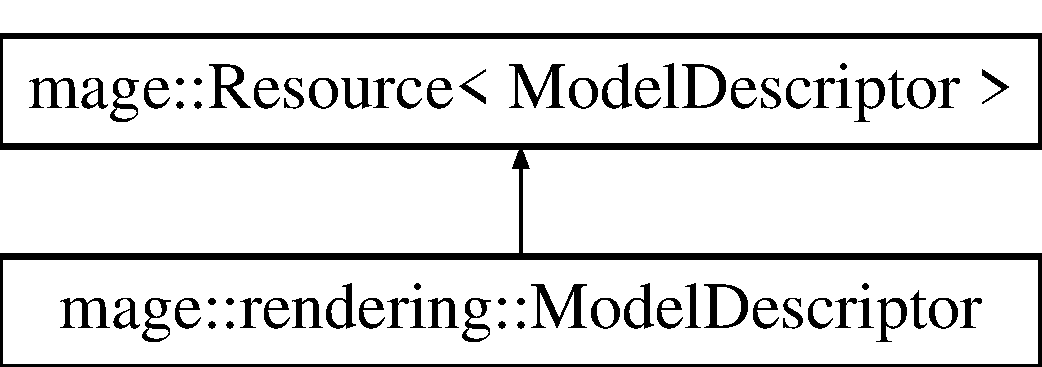
\includegraphics[height=2.000000cm]{classmage_1_1rendering_1_1_model_descriptor}
\end{center}
\end{figure}
\subsection*{Public Member Functions}
\begin{DoxyCompactItemize}
\item 
{\footnotesize template$<$typename VertexT , typename IndexT $>$ }\\\mbox{\hyperlink{classmage_1_1rendering_1_1_model_descriptor_aa27c73a72219352647cd31ddfd6e64d6}{Model\+Descriptor}} (I\+D3\+D11\+Device \&device, \mbox{\hyperlink{classmage_1_1rendering_1_1_resource_manager}{Resource\+Manager}} \&resource\+\_\+manager, wstring fname, const \mbox{\hyperlink{classmage_1_1rendering_1_1_mesh_descriptor}{Mesh\+Descriptor}}$<$ VertexT, IndexT $>$ \&desc=\mbox{\hyperlink{classmage_1_1rendering_1_1_mesh_descriptor}{Mesh\+Descriptor}}$<$ VertexT, IndexT $>$(), bool export\+\_\+as\+\_\+\+M\+DL=false)
\item 
\mbox{\hyperlink{classmage_1_1rendering_1_1_model_descriptor_af3fc0dea0060aa15a8003a7f4f807dd0}{Model\+Descriptor}} (const \mbox{\hyperlink{classmage_1_1rendering_1_1_model_descriptor}{Model\+Descriptor}} \&desc)=delete
\item 
\mbox{\hyperlink{classmage_1_1rendering_1_1_model_descriptor_a0e7a576be083c9499a074cfd39acbcb7}{Model\+Descriptor}} (\mbox{\hyperlink{classmage_1_1rendering_1_1_model_descriptor}{Model\+Descriptor}} \&\&desc) noexcept
\item 
virtual \mbox{\hyperlink{classmage_1_1rendering_1_1_model_descriptor_adef21799bc748828e8e04bc74f86aac0}{$\sim$\+Model\+Descriptor}} ()
\item 
\mbox{\hyperlink{classmage_1_1rendering_1_1_model_descriptor}{Model\+Descriptor}} \& \mbox{\hyperlink{classmage_1_1rendering_1_1_model_descriptor_a6d27a72aa2ebffbe4e7f2635f803dd72}{operator=}} (const \mbox{\hyperlink{classmage_1_1rendering_1_1_model_descriptor}{Model\+Descriptor}} \&desc)=delete
\item 
\mbox{\hyperlink{classmage_1_1rendering_1_1_model_descriptor}{Model\+Descriptor}} \& \mbox{\hyperlink{classmage_1_1rendering_1_1_model_descriptor_a52e9fbf292efc7a803d367bb3b6cb962}{operator=}} (\mbox{\hyperlink{classmage_1_1rendering_1_1_model_descriptor}{Model\+Descriptor}} \&\&desc) noexcept
\item 
\mbox{\hyperlink{namespacemage_a1e01ae66713838a7a67d30e44c67703e}{Shared\+Ptr}}$<$ const \mbox{\hyperlink{classmage_1_1rendering_1_1_mesh}{Mesh}} $>$ \mbox{\hyperlink{classmage_1_1rendering_1_1_model_descriptor_a65645313d8b7bb976d1b5d0acdbbd38a}{Get\+Mesh}} () const noexcept
\item 
const \mbox{\hyperlink{classmage_1_1rendering_1_1_material}{Material}} $\ast$ \mbox{\hyperlink{classmage_1_1rendering_1_1_model_descriptor_af731849a1aed71ae8e049571850e7f2e}{Get\+Material}} (const string \&name) const noexcept
\item 
{\footnotesize template$<$typename ActionT $>$ }\\void \mbox{\hyperlink{classmage_1_1rendering_1_1_model_descriptor_a4e95ae12e0c952c76aaaf1ee457aed07}{For\+Each\+Material}} (ActionT \&\&action) const
\item 
const \mbox{\hyperlink{structmage_1_1rendering_1_1_model_part}{Model\+Part}} $\ast$ \mbox{\hyperlink{classmage_1_1rendering_1_1_model_descriptor_a451867513276357536075085edf88592}{Get\+Model\+Part}} (const string \&name) const noexcept
\item 
{\footnotesize template$<$typename ActionT $>$ }\\void \mbox{\hyperlink{classmage_1_1rendering_1_1_model_descriptor_a9b217d2536bdd34c4b8b93ccf2ef62d3}{For\+Each\+Model\+Part}} (ActionT \&\&action) const
\end{DoxyCompactItemize}
\subsection*{Private Attributes}
\begin{DoxyCompactItemize}
\item 
\mbox{\hyperlink{namespacemage_a1e01ae66713838a7a67d30e44c67703e}{Shared\+Ptr}}$<$ const \mbox{\hyperlink{classmage_1_1rendering_1_1_mesh}{Mesh}} $>$ \mbox{\hyperlink{classmage_1_1rendering_1_1_model_descriptor_a18fd5970f038726fd200e60f3c5ad33e}{m\+\_\+mesh}}
\item 
std\+::vector$<$ \mbox{\hyperlink{classmage_1_1rendering_1_1_material}{Material}} $>$ \mbox{\hyperlink{classmage_1_1rendering_1_1_model_descriptor_ae88269763478f47e5d6c0086a4aeb33b}{m\+\_\+materials}}
\item 
\mbox{\hyperlink{namespacemage_a8664bfb5ce2179fc64eae9f82c8a5ba8}{Aligned\+Vector}}$<$ \mbox{\hyperlink{structmage_1_1rendering_1_1_model_part}{Model\+Part}} $>$ \mbox{\hyperlink{classmage_1_1rendering_1_1_model_descriptor_a2c2eda62e6f2c7f6274a0f829b6abfa1}{m\+\_\+model\+\_\+parts}}
\end{DoxyCompactItemize}


\subsection{Detailed Description}
A class of model descriptors describing a complete model. 

\subsection{Constructor \& Destructor Documentation}
\mbox{\Hypertarget{classmage_1_1rendering_1_1_model_descriptor_aa27c73a72219352647cd31ddfd6e64d6}\label{classmage_1_1rendering_1_1_model_descriptor_aa27c73a72219352647cd31ddfd6e64d6}} 
\index{mage\+::rendering\+::\+Model\+Descriptor@{mage\+::rendering\+::\+Model\+Descriptor}!Model\+Descriptor@{Model\+Descriptor}}
\index{Model\+Descriptor@{Model\+Descriptor}!mage\+::rendering\+::\+Model\+Descriptor@{mage\+::rendering\+::\+Model\+Descriptor}}
\subsubsection{\texorpdfstring{Model\+Descriptor()}{ModelDescriptor()}\hspace{0.1cm}{\footnotesize\ttfamily [1/3]}}
{\footnotesize\ttfamily template$<$typename VertexT , typename IndexT $>$ \\
mage\+::rendering\+::\+Model\+Descriptor\+::\+Model\+Descriptor (\begin{DoxyParamCaption}\item[{I\+D3\+D11\+Device \&}]{device,  }\item[{\mbox{\hyperlink{classmage_1_1rendering_1_1_resource_manager}{Resource\+Manager}} \&}]{resource\+\_\+manager,  }\item[{wstring}]{fname,  }\item[{const \mbox{\hyperlink{classmage_1_1rendering_1_1_mesh_descriptor}{Mesh\+Descriptor}}$<$ VertexT, IndexT $>$ \&}]{desc = {\ttfamily \mbox{\hyperlink{classmage_1_1rendering_1_1_mesh_descriptor}{Mesh\+Descriptor}}$<$~VertexT,~IndexT~$>$()},  }\item[{bool}]{export\+\_\+as\+\_\+\+M\+DL = {\ttfamily false} }\end{DoxyParamCaption})\hspace{0.3cm}{\ttfamily [explicit]}}

Constructs a model descriptor.


\begin{DoxyTemplParams}{Template Parameters}
{\em VertexT} & The vertex type. \\
\hline
{\em IndexT} & The index type. \\
\hline
\end{DoxyTemplParams}

\begin{DoxyParams}[1]{Parameters}
\mbox{\tt in}  & {\em device} & A reference to the device. \\
\hline
\mbox{\tt in}  & {\em resource\+\_\+manager} & A reference to the resource manager. \\
\hline
\mbox{\tt in}  & {\em fname} & The filename (the globally unique identifier). \\
\hline
\mbox{\tt in}  & {\em desc} & A reference to the mesh descriptor. \\
\hline
\mbox{\tt in}  & {\em export\+\_\+as\+\_\+\+M\+DL} & {\ttfamily true} if the model descriptor needs to be exported as M\+DL file. {\ttfamily false} otherwise. \\
\hline
\end{DoxyParams}

\begin{DoxyExceptions}{Exceptions}
{\em \mbox{\hyperlink{classmage_1_1_exception}{Exception}}} & Failed to initialize the model descriptor. \\
\hline
\end{DoxyExceptions}
\mbox{\Hypertarget{classmage_1_1rendering_1_1_model_descriptor_af3fc0dea0060aa15a8003a7f4f807dd0}\label{classmage_1_1rendering_1_1_model_descriptor_af3fc0dea0060aa15a8003a7f4f807dd0}} 
\index{mage\+::rendering\+::\+Model\+Descriptor@{mage\+::rendering\+::\+Model\+Descriptor}!Model\+Descriptor@{Model\+Descriptor}}
\index{Model\+Descriptor@{Model\+Descriptor}!mage\+::rendering\+::\+Model\+Descriptor@{mage\+::rendering\+::\+Model\+Descriptor}}
\subsubsection{\texorpdfstring{Model\+Descriptor()}{ModelDescriptor()}\hspace{0.1cm}{\footnotesize\ttfamily [2/3]}}
{\footnotesize\ttfamily mage\+::rendering\+::\+Model\+Descriptor\+::\+Model\+Descriptor (\begin{DoxyParamCaption}\item[{const \mbox{\hyperlink{classmage_1_1rendering_1_1_model_descriptor}{Model\+Descriptor}} \&}]{desc }\end{DoxyParamCaption})\hspace{0.3cm}{\ttfamily [delete]}}

Constructs a model descriptor from the given model descriptor.


\begin{DoxyParams}[1]{Parameters}
\mbox{\tt in}  & {\em desc} & A reference to the model descriptor to copy. \\
\hline
\end{DoxyParams}
\mbox{\Hypertarget{classmage_1_1rendering_1_1_model_descriptor_a0e7a576be083c9499a074cfd39acbcb7}\label{classmage_1_1rendering_1_1_model_descriptor_a0e7a576be083c9499a074cfd39acbcb7}} 
\index{mage\+::rendering\+::\+Model\+Descriptor@{mage\+::rendering\+::\+Model\+Descriptor}!Model\+Descriptor@{Model\+Descriptor}}
\index{Model\+Descriptor@{Model\+Descriptor}!mage\+::rendering\+::\+Model\+Descriptor@{mage\+::rendering\+::\+Model\+Descriptor}}
\subsubsection{\texorpdfstring{Model\+Descriptor()}{ModelDescriptor()}\hspace{0.1cm}{\footnotesize\ttfamily [3/3]}}
{\footnotesize\ttfamily mage\+::rendering\+::\+Model\+Descriptor\+::\+Model\+Descriptor (\begin{DoxyParamCaption}\item[{\mbox{\hyperlink{classmage_1_1rendering_1_1_model_descriptor}{Model\+Descriptor}} \&\&}]{desc }\end{DoxyParamCaption})\hspace{0.3cm}{\ttfamily [default]}, {\ttfamily [noexcept]}}

Constructs a model descriptor by moving the given model descriptor.


\begin{DoxyParams}[1]{Parameters}
\mbox{\tt in}  & {\em desc} & A reference to the model descriptor to move. \\
\hline
\end{DoxyParams}
\mbox{\Hypertarget{classmage_1_1rendering_1_1_model_descriptor_adef21799bc748828e8e04bc74f86aac0}\label{classmage_1_1rendering_1_1_model_descriptor_adef21799bc748828e8e04bc74f86aac0}} 
\index{mage\+::rendering\+::\+Model\+Descriptor@{mage\+::rendering\+::\+Model\+Descriptor}!````~Model\+Descriptor@{$\sim$\+Model\+Descriptor}}
\index{````~Model\+Descriptor@{$\sim$\+Model\+Descriptor}!mage\+::rendering\+::\+Model\+Descriptor@{mage\+::rendering\+::\+Model\+Descriptor}}
\subsubsection{\texorpdfstring{$\sim$\+Model\+Descriptor()}{~ModelDescriptor()}}
{\footnotesize\ttfamily mage\+::rendering\+::\+Model\+Descriptor\+::$\sim$\+Model\+Descriptor (\begin{DoxyParamCaption}{ }\end{DoxyParamCaption})\hspace{0.3cm}{\ttfamily [virtual]}, {\ttfamily [default]}}

Destructs a model descriptor. 

\subsection{Member Function Documentation}
\mbox{\Hypertarget{classmage_1_1rendering_1_1_model_descriptor_a4e95ae12e0c952c76aaaf1ee457aed07}\label{classmage_1_1rendering_1_1_model_descriptor_a4e95ae12e0c952c76aaaf1ee457aed07}} 
\index{mage\+::rendering\+::\+Model\+Descriptor@{mage\+::rendering\+::\+Model\+Descriptor}!For\+Each\+Material@{For\+Each\+Material}}
\index{For\+Each\+Material@{For\+Each\+Material}!mage\+::rendering\+::\+Model\+Descriptor@{mage\+::rendering\+::\+Model\+Descriptor}}
\subsubsection{\texorpdfstring{For\+Each\+Material()}{ForEachMaterial()}}
{\footnotesize\ttfamily template$<$typename ActionT $>$ \\
void mage\+::rendering\+::\+Model\+Descriptor\+::\+For\+Each\+Material (\begin{DoxyParamCaption}\item[{ActionT \&\&}]{action }\end{DoxyParamCaption}) const}

Traverses all materials of this model descriptor.


\begin{DoxyTemplParams}{Template Parameters}
{\em ActionT} & An action to perform on all materials of this model descriptor. The action must accept {\ttfamily const} {\ttfamily \mbox{\hyperlink{classmage_1_1rendering_1_1_material}{Material}}\&} values. \\
\hline
\end{DoxyTemplParams}
\mbox{\Hypertarget{classmage_1_1rendering_1_1_model_descriptor_a9b217d2536bdd34c4b8b93ccf2ef62d3}\label{classmage_1_1rendering_1_1_model_descriptor_a9b217d2536bdd34c4b8b93ccf2ef62d3}} 
\index{mage\+::rendering\+::\+Model\+Descriptor@{mage\+::rendering\+::\+Model\+Descriptor}!For\+Each\+Model\+Part@{For\+Each\+Model\+Part}}
\index{For\+Each\+Model\+Part@{For\+Each\+Model\+Part}!mage\+::rendering\+::\+Model\+Descriptor@{mage\+::rendering\+::\+Model\+Descriptor}}
\subsubsection{\texorpdfstring{For\+Each\+Model\+Part()}{ForEachModelPart()}}
{\footnotesize\ttfamily template$<$typename ActionT $>$ \\
void mage\+::rendering\+::\+Model\+Descriptor\+::\+For\+Each\+Model\+Part (\begin{DoxyParamCaption}\item[{ActionT \&\&}]{action }\end{DoxyParamCaption}) const}

Traverses all model parts of this model descriptor.


\begin{DoxyTemplParams}{Template Parameters}
{\em ActionT} & An action to perform on all model parts of this model descriptor. The action must accept {\ttfamily const} {\ttfamily \mbox{\hyperlink{structmage_1_1rendering_1_1_model_part}{Model\+Part}}\&} values. \\
\hline
\end{DoxyTemplParams}
\mbox{\Hypertarget{classmage_1_1rendering_1_1_model_descriptor_af731849a1aed71ae8e049571850e7f2e}\label{classmage_1_1rendering_1_1_model_descriptor_af731849a1aed71ae8e049571850e7f2e}} 
\index{mage\+::rendering\+::\+Model\+Descriptor@{mage\+::rendering\+::\+Model\+Descriptor}!Get\+Material@{Get\+Material}}
\index{Get\+Material@{Get\+Material}!mage\+::rendering\+::\+Model\+Descriptor@{mage\+::rendering\+::\+Model\+Descriptor}}
\subsubsection{\texorpdfstring{Get\+Material()}{GetMaterial()}}
{\footnotesize\ttfamily const \mbox{\hyperlink{classmage_1_1rendering_1_1_material}{Material}} $\ast$ mage\+::rendering\+::\+Model\+Descriptor\+::\+Get\+Material (\begin{DoxyParamCaption}\item[{const string \&}]{name }\end{DoxyParamCaption}) const\hspace{0.3cm}{\ttfamily [noexcept]}}

Returns the material corresponding to the given name.


\begin{DoxyParams}[1]{Parameters}
\mbox{\tt in}  & {\em name} & A reference to the name of the material. \\
\hline
\end{DoxyParams}
\begin{DoxyReturn}{Returns}
{\ttfamily nullptr} if this model descriptor contains no material matching the given name {\itshape name}. 

A pointer to the material of this model descriptor matching the given name {\itshape name}. 
\end{DoxyReturn}
\mbox{\Hypertarget{classmage_1_1rendering_1_1_model_descriptor_a65645313d8b7bb976d1b5d0acdbbd38a}\label{classmage_1_1rendering_1_1_model_descriptor_a65645313d8b7bb976d1b5d0acdbbd38a}} 
\index{mage\+::rendering\+::\+Model\+Descriptor@{mage\+::rendering\+::\+Model\+Descriptor}!Get\+Mesh@{Get\+Mesh}}
\index{Get\+Mesh@{Get\+Mesh}!mage\+::rendering\+::\+Model\+Descriptor@{mage\+::rendering\+::\+Model\+Descriptor}}
\subsubsection{\texorpdfstring{Get\+Mesh()}{GetMesh()}}
{\footnotesize\ttfamily \mbox{\hyperlink{namespacemage_a1e01ae66713838a7a67d30e44c67703e}{Shared\+Ptr}}$<$ const \mbox{\hyperlink{classmage_1_1rendering_1_1_mesh}{Mesh}} $>$ mage\+::rendering\+::\+Model\+Descriptor\+::\+Get\+Mesh (\begin{DoxyParamCaption}{ }\end{DoxyParamCaption}) const\hspace{0.3cm}{\ttfamily [noexcept]}}

Returns the mesh of this model descriptor.

\begin{DoxyReturn}{Returns}
A pointer to the mesh of this model descriptor. 
\end{DoxyReturn}
\mbox{\Hypertarget{classmage_1_1rendering_1_1_model_descriptor_a451867513276357536075085edf88592}\label{classmage_1_1rendering_1_1_model_descriptor_a451867513276357536075085edf88592}} 
\index{mage\+::rendering\+::\+Model\+Descriptor@{mage\+::rendering\+::\+Model\+Descriptor}!Get\+Model\+Part@{Get\+Model\+Part}}
\index{Get\+Model\+Part@{Get\+Model\+Part}!mage\+::rendering\+::\+Model\+Descriptor@{mage\+::rendering\+::\+Model\+Descriptor}}
\subsubsection{\texorpdfstring{Get\+Model\+Part()}{GetModelPart()}}
{\footnotesize\ttfamily const \mbox{\hyperlink{structmage_1_1rendering_1_1_model_part}{Model\+Part}} $\ast$ mage\+::rendering\+::\+Model\+Descriptor\+::\+Get\+Model\+Part (\begin{DoxyParamCaption}\item[{const string \&}]{name }\end{DoxyParamCaption}) const\hspace{0.3cm}{\ttfamily [noexcept]}}

Returns the model part corresponding to the given name.


\begin{DoxyParams}[1]{Parameters}
\mbox{\tt in}  & {\em name} & A reference to the name of the model part. \\
\hline
\end{DoxyParams}
\begin{DoxyReturn}{Returns}
{\ttfamily nullptr} if this model descriptor contains no model part matching the given name {\itshape name}. 

A pointer to the model part of this model descriptor matching the given name {\itshape name}. 
\end{DoxyReturn}
\mbox{\Hypertarget{classmage_1_1rendering_1_1_model_descriptor_a6d27a72aa2ebffbe4e7f2635f803dd72}\label{classmage_1_1rendering_1_1_model_descriptor_a6d27a72aa2ebffbe4e7f2635f803dd72}} 
\index{mage\+::rendering\+::\+Model\+Descriptor@{mage\+::rendering\+::\+Model\+Descriptor}!operator=@{operator=}}
\index{operator=@{operator=}!mage\+::rendering\+::\+Model\+Descriptor@{mage\+::rendering\+::\+Model\+Descriptor}}
\subsubsection{\texorpdfstring{operator=()}{operator=()}\hspace{0.1cm}{\footnotesize\ttfamily [1/2]}}
{\footnotesize\ttfamily \mbox{\hyperlink{classmage_1_1rendering_1_1_model_descriptor}{Model\+Descriptor}}\& mage\+::rendering\+::\+Model\+Descriptor\+::operator= (\begin{DoxyParamCaption}\item[{const \mbox{\hyperlink{classmage_1_1rendering_1_1_model_descriptor}{Model\+Descriptor}} \&}]{desc }\end{DoxyParamCaption})\hspace{0.3cm}{\ttfamily [delete]}}

Copies the given model descriptor to this model descriptor.


\begin{DoxyParams}[1]{Parameters}
\mbox{\tt in}  & {\em desc} & A reference to the model descriptor to copy. \\
\hline
\end{DoxyParams}
\mbox{\Hypertarget{classmage_1_1rendering_1_1_model_descriptor_a52e9fbf292efc7a803d367bb3b6cb962}\label{classmage_1_1rendering_1_1_model_descriptor_a52e9fbf292efc7a803d367bb3b6cb962}} 
\index{mage\+::rendering\+::\+Model\+Descriptor@{mage\+::rendering\+::\+Model\+Descriptor}!operator=@{operator=}}
\index{operator=@{operator=}!mage\+::rendering\+::\+Model\+Descriptor@{mage\+::rendering\+::\+Model\+Descriptor}}
\subsubsection{\texorpdfstring{operator=()}{operator=()}\hspace{0.1cm}{\footnotesize\ttfamily [2/2]}}
{\footnotesize\ttfamily \mbox{\hyperlink{classmage_1_1rendering_1_1_model_descriptor}{Model\+Descriptor}} \& mage\+::rendering\+::\+Model\+Descriptor\+::operator= (\begin{DoxyParamCaption}\item[{\mbox{\hyperlink{classmage_1_1rendering_1_1_model_descriptor}{Model\+Descriptor}} \&\&}]{desc }\end{DoxyParamCaption})\hspace{0.3cm}{\ttfamily [default]}, {\ttfamily [noexcept]}}

Moves the given model descriptor to this model descriptor.


\begin{DoxyParams}[1]{Parameters}
\mbox{\tt in}  & {\em desc} & A reference to the model descriptor to move. \\
\hline
\end{DoxyParams}


\subsection{Member Data Documentation}
\mbox{\Hypertarget{classmage_1_1rendering_1_1_model_descriptor_ae88269763478f47e5d6c0086a4aeb33b}\label{classmage_1_1rendering_1_1_model_descriptor_ae88269763478f47e5d6c0086a4aeb33b}} 
\index{mage\+::rendering\+::\+Model\+Descriptor@{mage\+::rendering\+::\+Model\+Descriptor}!m\+\_\+materials@{m\+\_\+materials}}
\index{m\+\_\+materials@{m\+\_\+materials}!mage\+::rendering\+::\+Model\+Descriptor@{mage\+::rendering\+::\+Model\+Descriptor}}
\subsubsection{\texorpdfstring{m\+\_\+materials}{m\_materials}}
{\footnotesize\ttfamily std\+::vector$<$ \mbox{\hyperlink{classmage_1_1rendering_1_1_material}{Material}} $>$ mage\+::rendering\+::\+Model\+Descriptor\+::m\+\_\+materials\hspace{0.3cm}{\ttfamily [private]}}

A vector containing all the materials of the model of this model descriptor. \mbox{\Hypertarget{classmage_1_1rendering_1_1_model_descriptor_a18fd5970f038726fd200e60f3c5ad33e}\label{classmage_1_1rendering_1_1_model_descriptor_a18fd5970f038726fd200e60f3c5ad33e}} 
\index{mage\+::rendering\+::\+Model\+Descriptor@{mage\+::rendering\+::\+Model\+Descriptor}!m\+\_\+mesh@{m\+\_\+mesh}}
\index{m\+\_\+mesh@{m\+\_\+mesh}!mage\+::rendering\+::\+Model\+Descriptor@{mage\+::rendering\+::\+Model\+Descriptor}}
\subsubsection{\texorpdfstring{m\+\_\+mesh}{m\_mesh}}
{\footnotesize\ttfamily \mbox{\hyperlink{namespacemage_a1e01ae66713838a7a67d30e44c67703e}{Shared\+Ptr}}$<$ const \mbox{\hyperlink{classmage_1_1rendering_1_1_mesh}{Mesh}} $>$ mage\+::rendering\+::\+Model\+Descriptor\+::m\+\_\+mesh\hspace{0.3cm}{\ttfamily [private]}}

A pointer to the mesh of the model of this model descriptor. \mbox{\Hypertarget{classmage_1_1rendering_1_1_model_descriptor_a2c2eda62e6f2c7f6274a0f829b6abfa1}\label{classmage_1_1rendering_1_1_model_descriptor_a2c2eda62e6f2c7f6274a0f829b6abfa1}} 
\index{mage\+::rendering\+::\+Model\+Descriptor@{mage\+::rendering\+::\+Model\+Descriptor}!m\+\_\+model\+\_\+parts@{m\+\_\+model\+\_\+parts}}
\index{m\+\_\+model\+\_\+parts@{m\+\_\+model\+\_\+parts}!mage\+::rendering\+::\+Model\+Descriptor@{mage\+::rendering\+::\+Model\+Descriptor}}
\subsubsection{\texorpdfstring{m\+\_\+model\+\_\+parts}{m\_model\_parts}}
{\footnotesize\ttfamily \mbox{\hyperlink{namespacemage_a8664bfb5ce2179fc64eae9f82c8a5ba8}{Aligned\+Vector}}$<$ \mbox{\hyperlink{structmage_1_1rendering_1_1_model_part}{Model\+Part}} $>$ mage\+::rendering\+::\+Model\+Descriptor\+::m\+\_\+model\+\_\+parts\hspace{0.3cm}{\ttfamily [private]}}

A vector containing all the model parts of the model of this model descriptor. 
\hypertarget{structmage_1_1rendering_1_1_model_output}{}\section{mage\+:\+:rendering\+:\+:Model\+Output$<$ VertexT, IndexT $>$ Struct Template Reference}
\label{structmage_1_1rendering_1_1_model_output}\index{mage\+::rendering\+::\+Model\+Output$<$ Vertex\+T, Index\+T $>$@{mage\+::rendering\+::\+Model\+Output$<$ Vertex\+T, Index\+T $>$}}


{\ttfamily \#include $<$model\+\_\+output.\+hpp$>$}

\subsection*{Public Member Functions}
\begin{DoxyCompactItemize}
\item 
\mbox{\hyperlink{structmage_1_1rendering_1_1_model_output_a0aaa7f6abf4c5df03fe02b49ef189e3b}{Model\+Output}} ()=default
\item 
\mbox{\hyperlink{structmage_1_1rendering_1_1_model_output_a52280b5fe47b266e44bf65ea5dcd6752}{Model\+Output}} (const \mbox{\hyperlink{structmage_1_1rendering_1_1_model_output}{Model\+Output}} \&output)=delete
\item 
\mbox{\hyperlink{structmage_1_1rendering_1_1_model_output_a449de2164c45500f02bbe03f4bdc648f}{Model\+Output}} (\mbox{\hyperlink{structmage_1_1rendering_1_1_model_output}{Model\+Output}} \&\&output) noexcept=default
\item 
\mbox{\hyperlink{structmage_1_1rendering_1_1_model_output_a627e604ee86986e4d439244ff734c69c}{$\sim$\+Model\+Output}} ()=default
\item 
\mbox{\hyperlink{structmage_1_1rendering_1_1_model_output}{Model\+Output}} \& \mbox{\hyperlink{structmage_1_1rendering_1_1_model_output_a902ae401740dbcc886b85977efe7c0da}{operator=}} (const \mbox{\hyperlink{structmage_1_1rendering_1_1_model_output}{Model\+Output}} \&output)=delete
\item 
\mbox{\hyperlink{structmage_1_1rendering_1_1_model_output}{Model\+Output}} \& \mbox{\hyperlink{structmage_1_1rendering_1_1_model_output_a10eb65082a0104be36c51cfc613fd156}{operator=}} (\mbox{\hyperlink{structmage_1_1rendering_1_1_model_output}{Model\+Output}} \&\&output) noexcept=default
\item 
void X\+M\+\_\+\+C\+A\+L\+L\+C\+O\+NV \mbox{\hyperlink{structmage_1_1rendering_1_1_model_output_a33512b10fe669c18051a4eac3444f962}{Add\+Model\+Part}} (\mbox{\hyperlink{structmage_1_1rendering_1_1_model_part}{Model\+Part}} model\+\_\+part, bool create\+\_\+bounding\+\_\+volumes=true)
\item 
bool \mbox{\hyperlink{structmage_1_1rendering_1_1_model_output_a8382df11416d7233682d2ca53af36d46}{Contains\+Model\+Part}} (const std\+::string \&name) noexcept
\item 
void X\+M\+\_\+\+C\+A\+L\+L\+C\+O\+NV \mbox{\hyperlink{structmage_1_1rendering_1_1_model_output_adc21b44bf476fa7704f97403c1539eb9}{Start\+Model\+Part}} (\mbox{\hyperlink{structmage_1_1rendering_1_1_model_part}{Model\+Part}} model\+\_\+part)
\item 
void \mbox{\hyperlink{structmage_1_1rendering_1_1_model_output_a7c427529a75723fbcc213e64b3ac9b18}{Set\+Material}} (std\+::string material)
\item 
void \mbox{\hyperlink{structmage_1_1rendering_1_1_model_output_ad8f2948cb3ac35f3f25ed68fede20bce}{End\+Model\+Part}} (bool create\+\_\+bounding\+\_\+volumes=true) noexcept
\end{DoxyCompactItemize}
\subsection*{Public Attributes}
\begin{DoxyCompactItemize}
\item 
std\+::vector$<$ VertexT $>$ \mbox{\hyperlink{structmage_1_1rendering_1_1_model_output_a397e9daee731bb89683daa68bd4acd0f}{m\+\_\+vertex\+\_\+buffer}}
\item 
std\+::vector$<$ IndexT $>$ \mbox{\hyperlink{structmage_1_1rendering_1_1_model_output_a0290ea3f7afa5022cedbc9bc316d24e0}{m\+\_\+index\+\_\+buffer}}
\item 
std\+::vector$<$ \mbox{\hyperlink{classmage_1_1rendering_1_1_material}{Material}} $>$ \mbox{\hyperlink{structmage_1_1rendering_1_1_model_output_a7d290dd28d6cef9f33eead6cf30f042f}{m\+\_\+material\+\_\+buffer}}
\item 
\mbox{\hyperlink{namespacemage_a8664bfb5ce2179fc64eae9f82c8a5ba8}{Aligned\+Vector}}$<$ \mbox{\hyperlink{structmage_1_1rendering_1_1_model_part}{Model\+Part}} $>$ \mbox{\hyperlink{structmage_1_1rendering_1_1_model_output_a18da9c959800d0331488351612e25df2}{m\+\_\+model\+\_\+parts}}
\end{DoxyCompactItemize}
\subsection*{Private Member Functions}
\begin{DoxyCompactItemize}
\item 
void \mbox{\hyperlink{structmage_1_1rendering_1_1_model_output_a4b00228713e34d955cb5104c8592f7a0}{Setup\+Bounding\+Volumes}} (\mbox{\hyperlink{structmage_1_1rendering_1_1_model_part}{Model\+Part}} \&model\+\_\+part) noexcept
\end{DoxyCompactItemize}


\subsection{Detailed Description}
\subsubsection*{template$<$typename VertexT, typename IndexT$>$\newline
struct mage\+::rendering\+::\+Model\+Output$<$ Vertex\+T, Index\+T $>$}

A struct of model outputs.


\begin{DoxyTemplParams}{Template Parameters}
{\em VertexT} & The vertex type. \\
\hline
{\em IndexT} & The index type. \\
\hline
\end{DoxyTemplParams}


\subsection{Constructor \& Destructor Documentation}
\mbox{\Hypertarget{structmage_1_1rendering_1_1_model_output_a0aaa7f6abf4c5df03fe02b49ef189e3b}\label{structmage_1_1rendering_1_1_model_output_a0aaa7f6abf4c5df03fe02b49ef189e3b}} 
\index{mage\+::rendering\+::\+Model\+Output@{mage\+::rendering\+::\+Model\+Output}!Model\+Output@{Model\+Output}}
\index{Model\+Output@{Model\+Output}!mage\+::rendering\+::\+Model\+Output@{mage\+::rendering\+::\+Model\+Output}}
\subsubsection{\texorpdfstring{Model\+Output()}{ModelOutput()}\hspace{0.1cm}{\footnotesize\ttfamily [1/3]}}
{\footnotesize\ttfamily template$<$typename VertexT , typename IndexT $>$ \\
\mbox{\hyperlink{structmage_1_1rendering_1_1_model_output}{mage\+::rendering\+::\+Model\+Output}}$<$ VertexT, IndexT $>$\+::\mbox{\hyperlink{structmage_1_1rendering_1_1_model_output}{Model\+Output}} (\begin{DoxyParamCaption}{ }\end{DoxyParamCaption})\hspace{0.3cm}{\ttfamily [default]}}

Constructs a model output. \mbox{\Hypertarget{structmage_1_1rendering_1_1_model_output_a52280b5fe47b266e44bf65ea5dcd6752}\label{structmage_1_1rendering_1_1_model_output_a52280b5fe47b266e44bf65ea5dcd6752}} 
\index{mage\+::rendering\+::\+Model\+Output@{mage\+::rendering\+::\+Model\+Output}!Model\+Output@{Model\+Output}}
\index{Model\+Output@{Model\+Output}!mage\+::rendering\+::\+Model\+Output@{mage\+::rendering\+::\+Model\+Output}}
\subsubsection{\texorpdfstring{Model\+Output()}{ModelOutput()}\hspace{0.1cm}{\footnotesize\ttfamily [2/3]}}
{\footnotesize\ttfamily template$<$typename VertexT , typename IndexT $>$ \\
\mbox{\hyperlink{structmage_1_1rendering_1_1_model_output}{mage\+::rendering\+::\+Model\+Output}}$<$ VertexT, IndexT $>$\+::\mbox{\hyperlink{structmage_1_1rendering_1_1_model_output}{Model\+Output}} (\begin{DoxyParamCaption}\item[{const \mbox{\hyperlink{structmage_1_1rendering_1_1_model_output}{Model\+Output}}$<$ VertexT, IndexT $>$ \&}]{output }\end{DoxyParamCaption})\hspace{0.3cm}{\ttfamily [delete]}}

Constructs a model output from the given model output.


\begin{DoxyParams}[1]{Parameters}
\mbox{\tt in}  & {\em output} & A reference to the model output to copy. \\
\hline
\end{DoxyParams}
\mbox{\Hypertarget{structmage_1_1rendering_1_1_model_output_a449de2164c45500f02bbe03f4bdc648f}\label{structmage_1_1rendering_1_1_model_output_a449de2164c45500f02bbe03f4bdc648f}} 
\index{mage\+::rendering\+::\+Model\+Output@{mage\+::rendering\+::\+Model\+Output}!Model\+Output@{Model\+Output}}
\index{Model\+Output@{Model\+Output}!mage\+::rendering\+::\+Model\+Output@{mage\+::rendering\+::\+Model\+Output}}
\subsubsection{\texorpdfstring{Model\+Output()}{ModelOutput()}\hspace{0.1cm}{\footnotesize\ttfamily [3/3]}}
{\footnotesize\ttfamily template$<$typename VertexT , typename IndexT $>$ \\
\mbox{\hyperlink{structmage_1_1rendering_1_1_model_output}{mage\+::rendering\+::\+Model\+Output}}$<$ VertexT, IndexT $>$\+::\mbox{\hyperlink{structmage_1_1rendering_1_1_model_output}{Model\+Output}} (\begin{DoxyParamCaption}\item[{\mbox{\hyperlink{structmage_1_1rendering_1_1_model_output}{Model\+Output}}$<$ VertexT, IndexT $>$ \&\&}]{output }\end{DoxyParamCaption})\hspace{0.3cm}{\ttfamily [default]}, {\ttfamily [noexcept]}}

Constructs a model output by moving the given model output.


\begin{DoxyParams}[1]{Parameters}
\mbox{\tt in}  & {\em output} & A reference to the model output to move. \\
\hline
\end{DoxyParams}
\mbox{\Hypertarget{structmage_1_1rendering_1_1_model_output_a627e604ee86986e4d439244ff734c69c}\label{structmage_1_1rendering_1_1_model_output_a627e604ee86986e4d439244ff734c69c}} 
\index{mage\+::rendering\+::\+Model\+Output@{mage\+::rendering\+::\+Model\+Output}!````~Model\+Output@{$\sim$\+Model\+Output}}
\index{````~Model\+Output@{$\sim$\+Model\+Output}!mage\+::rendering\+::\+Model\+Output@{mage\+::rendering\+::\+Model\+Output}}
\subsubsection{\texorpdfstring{$\sim$\+Model\+Output()}{~ModelOutput()}}
{\footnotesize\ttfamily template$<$typename VertexT , typename IndexT $>$ \\
\mbox{\hyperlink{structmage_1_1rendering_1_1_model_output}{mage\+::rendering\+::\+Model\+Output}}$<$ VertexT, IndexT $>$\+::$\sim$\mbox{\hyperlink{structmage_1_1rendering_1_1_model_output}{Model\+Output}} (\begin{DoxyParamCaption}{ }\end{DoxyParamCaption})\hspace{0.3cm}{\ttfamily [default]}}

Destructs this model output. 

\subsection{Member Function Documentation}
\mbox{\Hypertarget{structmage_1_1rendering_1_1_model_output_a33512b10fe669c18051a4eac3444f962}\label{structmage_1_1rendering_1_1_model_output_a33512b10fe669c18051a4eac3444f962}} 
\index{mage\+::rendering\+::\+Model\+Output@{mage\+::rendering\+::\+Model\+Output}!Add\+Model\+Part@{Add\+Model\+Part}}
\index{Add\+Model\+Part@{Add\+Model\+Part}!mage\+::rendering\+::\+Model\+Output@{mage\+::rendering\+::\+Model\+Output}}
\subsubsection{\texorpdfstring{Add\+Model\+Part()}{AddModelPart()}}
{\footnotesize\ttfamily template$<$typename VertexT , typename IndexT $>$ \\
void X\+M\+\_\+\+C\+A\+L\+L\+C\+O\+NV \mbox{\hyperlink{structmage_1_1rendering_1_1_model_output}{mage\+::rendering\+::\+Model\+Output}}$<$ VertexT, IndexT $>$\+::Add\+Model\+Part (\begin{DoxyParamCaption}\item[{\mbox{\hyperlink{structmage_1_1rendering_1_1_model_part}{Model\+Part}}}]{model\+\_\+part,  }\item[{bool}]{create\+\_\+bounding\+\_\+volumes = {\ttfamily true} }\end{DoxyParamCaption})}

Adds a model part.


\begin{DoxyParams}[1]{Parameters}
\mbox{\tt in}  & {\em model\+\_\+part} & The model part to add. \\
\hline
\mbox{\tt in}  & {\em create\+\_\+bounding\+\_\+volumes} & A flag indicating whether bounding volumes must be created for the given model part. \\
\hline
\end{DoxyParams}
\mbox{\Hypertarget{structmage_1_1rendering_1_1_model_output_a8382df11416d7233682d2ca53af36d46}\label{structmage_1_1rendering_1_1_model_output_a8382df11416d7233682d2ca53af36d46}} 
\index{mage\+::rendering\+::\+Model\+Output@{mage\+::rendering\+::\+Model\+Output}!Contains\+Model\+Part@{Contains\+Model\+Part}}
\index{Contains\+Model\+Part@{Contains\+Model\+Part}!mage\+::rendering\+::\+Model\+Output@{mage\+::rendering\+::\+Model\+Output}}
\subsubsection{\texorpdfstring{Contains\+Model\+Part()}{ContainsModelPart()}}
{\footnotesize\ttfamily template$<$typename VertexT , typename IndexT $>$ \\
bool \mbox{\hyperlink{structmage_1_1rendering_1_1_model_output}{mage\+::rendering\+::\+Model\+Output}}$<$ VertexT, IndexT $>$\+::Contains\+Model\+Part (\begin{DoxyParamCaption}\item[{const std\+::string \&}]{name }\end{DoxyParamCaption})\hspace{0.3cm}{\ttfamily [noexcept]}}

Checks whether this model output contains a model part with the given name.


\begin{DoxyParams}[1]{Parameters}
\mbox{\tt in}  & {\em name} & The name of the model part. \\
\hline
\end{DoxyParams}
\mbox{\Hypertarget{structmage_1_1rendering_1_1_model_output_ad8f2948cb3ac35f3f25ed68fede20bce}\label{structmage_1_1rendering_1_1_model_output_ad8f2948cb3ac35f3f25ed68fede20bce}} 
\index{mage\+::rendering\+::\+Model\+Output@{mage\+::rendering\+::\+Model\+Output}!End\+Model\+Part@{End\+Model\+Part}}
\index{End\+Model\+Part@{End\+Model\+Part}!mage\+::rendering\+::\+Model\+Output@{mage\+::rendering\+::\+Model\+Output}}
\subsubsection{\texorpdfstring{End\+Model\+Part()}{EndModelPart()}}
{\footnotesize\ttfamily template$<$typename VertexT , typename IndexT $>$ \\
void \mbox{\hyperlink{structmage_1_1rendering_1_1_model_output}{mage\+::rendering\+::\+Model\+Output}}$<$ VertexT, IndexT $>$\+::End\+Model\+Part (\begin{DoxyParamCaption}\item[{bool}]{create\+\_\+bounding\+\_\+volumes = {\ttfamily true} }\end{DoxyParamCaption})\hspace{0.3cm}{\ttfamily [noexcept]}}

Ends the creation of the last model part.

\begin{DoxyPrecond}{Precondition}
This model output contains at least one model part. 
\end{DoxyPrecond}

\begin{DoxyParams}[1]{Parameters}
\mbox{\tt in}  & {\em create\+\_\+bounding\+\_\+volumes} & A flag indicating whether bounding volumes must be created for the given model part. \\
\hline
\end{DoxyParams}
\mbox{\Hypertarget{structmage_1_1rendering_1_1_model_output_a902ae401740dbcc886b85977efe7c0da}\label{structmage_1_1rendering_1_1_model_output_a902ae401740dbcc886b85977efe7c0da}} 
\index{mage\+::rendering\+::\+Model\+Output@{mage\+::rendering\+::\+Model\+Output}!operator=@{operator=}}
\index{operator=@{operator=}!mage\+::rendering\+::\+Model\+Output@{mage\+::rendering\+::\+Model\+Output}}
\subsubsection{\texorpdfstring{operator=()}{operator=()}\hspace{0.1cm}{\footnotesize\ttfamily [1/2]}}
{\footnotesize\ttfamily template$<$typename VertexT , typename IndexT $>$ \\
\mbox{\hyperlink{structmage_1_1rendering_1_1_model_output}{Model\+Output}}\& \mbox{\hyperlink{structmage_1_1rendering_1_1_model_output}{mage\+::rendering\+::\+Model\+Output}}$<$ VertexT, IndexT $>$\+::operator= (\begin{DoxyParamCaption}\item[{const \mbox{\hyperlink{structmage_1_1rendering_1_1_model_output}{Model\+Output}}$<$ VertexT, IndexT $>$ \&}]{output }\end{DoxyParamCaption})\hspace{0.3cm}{\ttfamily [delete]}}

Copies the given model output to this model output.


\begin{DoxyParams}[1]{Parameters}
\mbox{\tt in}  & {\em output} & A reference to the model output to copy. \\
\hline
\end{DoxyParams}
\begin{DoxyReturn}{Returns}
A reference to the copy of the given model output (i.\+e. this model output). 
\end{DoxyReturn}
\mbox{\Hypertarget{structmage_1_1rendering_1_1_model_output_a10eb65082a0104be36c51cfc613fd156}\label{structmage_1_1rendering_1_1_model_output_a10eb65082a0104be36c51cfc613fd156}} 
\index{mage\+::rendering\+::\+Model\+Output@{mage\+::rendering\+::\+Model\+Output}!operator=@{operator=}}
\index{operator=@{operator=}!mage\+::rendering\+::\+Model\+Output@{mage\+::rendering\+::\+Model\+Output}}
\subsubsection{\texorpdfstring{operator=()}{operator=()}\hspace{0.1cm}{\footnotesize\ttfamily [2/2]}}
{\footnotesize\ttfamily template$<$typename VertexT , typename IndexT $>$ \\
\mbox{\hyperlink{structmage_1_1rendering_1_1_model_output}{Model\+Output}}\& \mbox{\hyperlink{structmage_1_1rendering_1_1_model_output}{mage\+::rendering\+::\+Model\+Output}}$<$ VertexT, IndexT $>$\+::operator= (\begin{DoxyParamCaption}\item[{\mbox{\hyperlink{structmage_1_1rendering_1_1_model_output}{Model\+Output}}$<$ VertexT, IndexT $>$ \&\&}]{output }\end{DoxyParamCaption})\hspace{0.3cm}{\ttfamily [default]}, {\ttfamily [noexcept]}}

Moves the given model output to this model output.


\begin{DoxyParams}[1]{Parameters}
\mbox{\tt in}  & {\em output} & A reference to the model output to move. \\
\hline
\end{DoxyParams}
\begin{DoxyReturn}{Returns}
A reference to the moved model output (i.\+e. this model output). 
\end{DoxyReturn}
\mbox{\Hypertarget{structmage_1_1rendering_1_1_model_output_a7c427529a75723fbcc213e64b3ac9b18}\label{structmage_1_1rendering_1_1_model_output_a7c427529a75723fbcc213e64b3ac9b18}} 
\index{mage\+::rendering\+::\+Model\+Output@{mage\+::rendering\+::\+Model\+Output}!Set\+Material@{Set\+Material}}
\index{Set\+Material@{Set\+Material}!mage\+::rendering\+::\+Model\+Output@{mage\+::rendering\+::\+Model\+Output}}
\subsubsection{\texorpdfstring{Set\+Material()}{SetMaterial()}}
{\footnotesize\ttfamily template$<$typename VertexT , typename IndexT $>$ \\
void \mbox{\hyperlink{structmage_1_1rendering_1_1_model_output}{mage\+::rendering\+::\+Model\+Output}}$<$ VertexT, IndexT $>$\+::Set\+Material (\begin{DoxyParamCaption}\item[{std\+::string}]{material }\end{DoxyParamCaption})}

Sets the name of the material of the last model part to the given material name.

\begin{DoxyPrecond}{Precondition}
This model output contains at least one model part. 
\end{DoxyPrecond}

\begin{DoxyParams}[1]{Parameters}
\mbox{\tt in}  & {\em material} & The name of the material. \\
\hline
\end{DoxyParams}
\mbox{\Hypertarget{structmage_1_1rendering_1_1_model_output_a4b00228713e34d955cb5104c8592f7a0}\label{structmage_1_1rendering_1_1_model_output_a4b00228713e34d955cb5104c8592f7a0}} 
\index{mage\+::rendering\+::\+Model\+Output@{mage\+::rendering\+::\+Model\+Output}!Setup\+Bounding\+Volumes@{Setup\+Bounding\+Volumes}}
\index{Setup\+Bounding\+Volumes@{Setup\+Bounding\+Volumes}!mage\+::rendering\+::\+Model\+Output@{mage\+::rendering\+::\+Model\+Output}}
\subsubsection{\texorpdfstring{Setup\+Bounding\+Volumes()}{SetupBoundingVolumes()}}
{\footnotesize\ttfamily template$<$typename VertexT , typename IndexT $>$ \\
void \mbox{\hyperlink{structmage_1_1rendering_1_1_model_output}{mage\+::rendering\+::\+Model\+Output}}$<$ VertexT, IndexT $>$\+::Setup\+Bounding\+Volumes (\begin{DoxyParamCaption}\item[{\mbox{\hyperlink{structmage_1_1rendering_1_1_model_part}{Model\+Part}} \&}]{model\+\_\+part }\end{DoxyParamCaption})\hspace{0.3cm}{\ttfamily [private]}, {\ttfamily [noexcept]}}

Sets up the bounding volumes of the given model part.


\begin{DoxyParams}[1]{Parameters}
\mbox{\tt in}  & {\em model\+\_\+part} & A reference to the model part. \\
\hline
\end{DoxyParams}
\mbox{\Hypertarget{structmage_1_1rendering_1_1_model_output_adc21b44bf476fa7704f97403c1539eb9}\label{structmage_1_1rendering_1_1_model_output_adc21b44bf476fa7704f97403c1539eb9}} 
\index{mage\+::rendering\+::\+Model\+Output@{mage\+::rendering\+::\+Model\+Output}!Start\+Model\+Part@{Start\+Model\+Part}}
\index{Start\+Model\+Part@{Start\+Model\+Part}!mage\+::rendering\+::\+Model\+Output@{mage\+::rendering\+::\+Model\+Output}}
\subsubsection{\texorpdfstring{Start\+Model\+Part()}{StartModelPart()}}
{\footnotesize\ttfamily template$<$typename VertexT , typename IndexT $>$ \\
void X\+M\+\_\+\+C\+A\+L\+L\+C\+O\+NV \mbox{\hyperlink{structmage_1_1rendering_1_1_model_output}{mage\+::rendering\+::\+Model\+Output}}$<$ VertexT, IndexT $>$\+::Start\+Model\+Part (\begin{DoxyParamCaption}\item[{\mbox{\hyperlink{structmage_1_1rendering_1_1_model_part}{Model\+Part}}}]{model\+\_\+part }\end{DoxyParamCaption})}

Starts the creation of a new model part.


\begin{DoxyParams}[1]{Parameters}
\mbox{\tt in}  & {\em model\+\_\+part} & The model part to add. \\
\hline
\end{DoxyParams}


\subsection{Member Data Documentation}
\mbox{\Hypertarget{structmage_1_1rendering_1_1_model_output_a0290ea3f7afa5022cedbc9bc316d24e0}\label{structmage_1_1rendering_1_1_model_output_a0290ea3f7afa5022cedbc9bc316d24e0}} 
\index{mage\+::rendering\+::\+Model\+Output@{mage\+::rendering\+::\+Model\+Output}!m\+\_\+index\+\_\+buffer@{m\+\_\+index\+\_\+buffer}}
\index{m\+\_\+index\+\_\+buffer@{m\+\_\+index\+\_\+buffer}!mage\+::rendering\+::\+Model\+Output@{mage\+::rendering\+::\+Model\+Output}}
\subsubsection{\texorpdfstring{m\+\_\+index\+\_\+buffer}{m\_index\_buffer}}
{\footnotesize\ttfamily template$<$typename VertexT , typename IndexT $>$ \\
std\+::vector$<$ IndexT $>$ \mbox{\hyperlink{structmage_1_1rendering_1_1_model_output}{mage\+::rendering\+::\+Model\+Output}}$<$ VertexT, IndexT $>$\+::m\+\_\+index\+\_\+buffer}

A vector containing the indices of this model output. \mbox{\Hypertarget{structmage_1_1rendering_1_1_model_output_a7d290dd28d6cef9f33eead6cf30f042f}\label{structmage_1_1rendering_1_1_model_output_a7d290dd28d6cef9f33eead6cf30f042f}} 
\index{mage\+::rendering\+::\+Model\+Output@{mage\+::rendering\+::\+Model\+Output}!m\+\_\+material\+\_\+buffer@{m\+\_\+material\+\_\+buffer}}
\index{m\+\_\+material\+\_\+buffer@{m\+\_\+material\+\_\+buffer}!mage\+::rendering\+::\+Model\+Output@{mage\+::rendering\+::\+Model\+Output}}
\subsubsection{\texorpdfstring{m\+\_\+material\+\_\+buffer}{m\_material\_buffer}}
{\footnotesize\ttfamily template$<$typename VertexT , typename IndexT $>$ \\
std\+::vector$<$ \mbox{\hyperlink{classmage_1_1rendering_1_1_material}{Material}} $>$ \mbox{\hyperlink{structmage_1_1rendering_1_1_model_output}{mage\+::rendering\+::\+Model\+Output}}$<$ VertexT, IndexT $>$\+::m\+\_\+material\+\_\+buffer}

A vector containing the materials of this model output. \mbox{\Hypertarget{structmage_1_1rendering_1_1_model_output_a18da9c959800d0331488351612e25df2}\label{structmage_1_1rendering_1_1_model_output_a18da9c959800d0331488351612e25df2}} 
\index{mage\+::rendering\+::\+Model\+Output@{mage\+::rendering\+::\+Model\+Output}!m\+\_\+model\+\_\+parts@{m\+\_\+model\+\_\+parts}}
\index{m\+\_\+model\+\_\+parts@{m\+\_\+model\+\_\+parts}!mage\+::rendering\+::\+Model\+Output@{mage\+::rendering\+::\+Model\+Output}}
\subsubsection{\texorpdfstring{m\+\_\+model\+\_\+parts}{m\_model\_parts}}
{\footnotesize\ttfamily template$<$typename VertexT , typename IndexT $>$ \\
\mbox{\hyperlink{namespacemage_a8664bfb5ce2179fc64eae9f82c8a5ba8}{Aligned\+Vector}}$<$ \mbox{\hyperlink{structmage_1_1rendering_1_1_model_part}{Model\+Part}} $>$ \mbox{\hyperlink{structmage_1_1rendering_1_1_model_output}{mage\+::rendering\+::\+Model\+Output}}$<$ VertexT, IndexT $>$\+::m\+\_\+model\+\_\+parts}

A vector containing the model parts of this model output. \mbox{\Hypertarget{structmage_1_1rendering_1_1_model_output_a397e9daee731bb89683daa68bd4acd0f}\label{structmage_1_1rendering_1_1_model_output_a397e9daee731bb89683daa68bd4acd0f}} 
\index{mage\+::rendering\+::\+Model\+Output@{mage\+::rendering\+::\+Model\+Output}!m\+\_\+vertex\+\_\+buffer@{m\+\_\+vertex\+\_\+buffer}}
\index{m\+\_\+vertex\+\_\+buffer@{m\+\_\+vertex\+\_\+buffer}!mage\+::rendering\+::\+Model\+Output@{mage\+::rendering\+::\+Model\+Output}}
\subsubsection{\texorpdfstring{m\+\_\+vertex\+\_\+buffer}{m\_vertex\_buffer}}
{\footnotesize\ttfamily template$<$typename VertexT , typename IndexT $>$ \\
std\+::vector$<$ VertexT $>$ \mbox{\hyperlink{structmage_1_1rendering_1_1_model_output}{mage\+::rendering\+::\+Model\+Output}}$<$ VertexT, IndexT $>$\+::m\+\_\+vertex\+\_\+buffer}

A vector containing the vertices of this model output. 
\hypertarget{structmage_1_1rendering_1_1_model_part}{}\section{mage\+:\+:rendering\+:\+:Model\+Part Struct Reference}
\label{structmage_1_1rendering_1_1_model_part}\index{mage\+::rendering\+::\+Model\+Part@{mage\+::rendering\+::\+Model\+Part}}


{\ttfamily \#include $<$model\+\_\+output.\+hpp$>$}

\subsection*{Public Member Functions}
\begin{DoxyCompactItemize}
\item 
\hyperlink{structmage_1_1rendering_1_1_model_part_adb7271a00583f72324ab37ab7e668689}{Model\+Part} ()
\item 
\hyperlink{structmage_1_1rendering_1_1_model_part_ab9f9bbf4d5a08113483d3744b69e7188}{Model\+Part} (const \hyperlink{structmage_1_1rendering_1_1_model_part}{Model\+Part} \&model\+\_\+part)=default
\item 
\hyperlink{structmage_1_1rendering_1_1_model_part_a843671f80d5c36d05d7d147f65fea890}{Model\+Part} (\hyperlink{structmage_1_1rendering_1_1_model_part}{Model\+Part} \&\&model\+\_\+part) noexcept=default
\item 
\hyperlink{structmage_1_1rendering_1_1_model_part_ac01c98a3cab3fb9692bebbfa6ef3fd18}{$\sim$\+Model\+Part} ()=default
\item 
\hyperlink{structmage_1_1rendering_1_1_model_part}{Model\+Part} \& \hyperlink{structmage_1_1rendering_1_1_model_part_a9d6c372839b9493df4b432d8ba2613dc}{operator=} (const \hyperlink{structmage_1_1rendering_1_1_model_part}{Model\+Part} \&model\+\_\+part)=default
\item 
\hyperlink{structmage_1_1rendering_1_1_model_part}{Model\+Part} \& \hyperlink{structmage_1_1rendering_1_1_model_part_a54950b40fa5dd12e77277669cbd6dc3a}{operator=} (\hyperlink{structmage_1_1rendering_1_1_model_part}{Model\+Part} \&\&model\+\_\+part) noexcept=default
\item 
bool \hyperlink{structmage_1_1rendering_1_1_model_part_ab4118a267808c18556b0fa10949bcb0b}{Has\+Default\+Child} () const noexcept
\item 
bool \hyperlink{structmage_1_1rendering_1_1_model_part_ac452d6bba03decae31646eec0329c4ab}{Has\+Default\+Parent} () const noexcept
\item 
bool \hyperlink{structmage_1_1rendering_1_1_model_part_aae8cebe1ec39e939b53fc3f7330984a8}{Has\+Default\+Material} () const noexcept
\end{DoxyCompactItemize}
\subsection*{Public Attributes}
\begin{DoxyCompactItemize}
\item 
\hyperlink{classmage_1_1_a_a_b_b}{A\+A\+BB} \hyperlink{structmage_1_1rendering_1_1_model_part_a69f7f90a31e48a286fecebc9e680b5ef}{m\+\_\+aabb}
\item 
\hyperlink{classmage_1_1_bounding_sphere}{Bounding\+Sphere} \hyperlink{structmage_1_1rendering_1_1_model_part_aa2204e02fe90f993990cdda677bff6e7}{m\+\_\+sphere}
\item 
\hyperlink{classmage_1_1_local_transform}{Local\+Transform} \hyperlink{structmage_1_1rendering_1_1_model_part_af34853cb09b179bd8ffb0da151914066}{m\+\_\+transform}
\item 
\hyperlink{namespacemage_a41c104c036fba3756a74e19f793eeaa1}{U32} \hyperlink{structmage_1_1rendering_1_1_model_part_a251d19417a0b4abe98faeae767b9fef4}{m\+\_\+start\+\_\+index}
\item 
\hyperlink{namespacemage_a41c104c036fba3756a74e19f793eeaa1}{U32} \hyperlink{structmage_1_1rendering_1_1_model_part_a6e622f4bcb1ada388c3ee489c22e4547}{m\+\_\+nb\+\_\+indices}
\item 
string \hyperlink{structmage_1_1rendering_1_1_model_part_ad2eb9ff5aaeecf676b54a1e2d7231ee8}{m\+\_\+child}
\item 
string \hyperlink{structmage_1_1rendering_1_1_model_part_a906ce278d6911d1163c8ce3a521c6598}{m\+\_\+parent}
\item 
string \hyperlink{structmage_1_1rendering_1_1_model_part_a1b2b0bf7c9acc87fc1673aac67a1849b}{m\+\_\+material}
\end{DoxyCompactItemize}
\subsection*{Static Public Attributes}
\begin{DoxyCompactItemize}
\item 
static constexpr \hyperlink{namespacemage_abfd9206dc607ceb5d13ec68bf075a5c0}{const\+\_\+zstring} \hyperlink{structmage_1_1rendering_1_1_model_part_a3571b142c7948d7ab5af699799c69b42}{s\+\_\+default\+\_\+child} = \char`\"{}default\char`\"{}
\item 
static constexpr \hyperlink{namespacemage_abfd9206dc607ceb5d13ec68bf075a5c0}{const\+\_\+zstring} \hyperlink{structmage_1_1rendering_1_1_model_part_ab6747ba3fd20c9f55f1d9bb7a64033e5}{s\+\_\+default\+\_\+parent} = \char`\"{}root\char`\"{}
\item 
static constexpr \hyperlink{namespacemage_abfd9206dc607ceb5d13ec68bf075a5c0}{const\+\_\+zstring} \hyperlink{structmage_1_1rendering_1_1_model_part_a833762db3fb81dd2086e9b89da158b12}{s\+\_\+default\+\_\+material} = \char`\"{}none\char`\"{}
\end{DoxyCompactItemize}


\subsection{Detailed Description}
A struct of model parts. 

\subsection{Constructor \& Destructor Documentation}
\hypertarget{structmage_1_1rendering_1_1_model_part_adb7271a00583f72324ab37ab7e668689}{}\label{structmage_1_1rendering_1_1_model_part_adb7271a00583f72324ab37ab7e668689} 
\index{mage\+::rendering\+::\+Model\+Part@{mage\+::rendering\+::\+Model\+Part}!Model\+Part@{Model\+Part}}
\index{Model\+Part@{Model\+Part}!mage\+::rendering\+::\+Model\+Part@{mage\+::rendering\+::\+Model\+Part}}
\subsubsection{\texorpdfstring{Model\+Part()}{ModelPart()}\hspace{0.1cm}{\footnotesize\ttfamily [1/3]}}
{\footnotesize\ttfamily mage\+::rendering\+::\+Model\+Part\+::\+Model\+Part (\begin{DoxyParamCaption}{ }\end{DoxyParamCaption})}

Constructs a model part. \hypertarget{structmage_1_1rendering_1_1_model_part_ab9f9bbf4d5a08113483d3744b69e7188}{}\label{structmage_1_1rendering_1_1_model_part_ab9f9bbf4d5a08113483d3744b69e7188} 
\index{mage\+::rendering\+::\+Model\+Part@{mage\+::rendering\+::\+Model\+Part}!Model\+Part@{Model\+Part}}
\index{Model\+Part@{Model\+Part}!mage\+::rendering\+::\+Model\+Part@{mage\+::rendering\+::\+Model\+Part}}
\subsubsection{\texorpdfstring{Model\+Part()}{ModelPart()}\hspace{0.1cm}{\footnotesize\ttfamily [2/3]}}
{\footnotesize\ttfamily mage\+::rendering\+::\+Model\+Part\+::\+Model\+Part (\begin{DoxyParamCaption}\item[{const \hyperlink{structmage_1_1rendering_1_1_model_part}{Model\+Part} \&}]{model\+\_\+part }\end{DoxyParamCaption})\hspace{0.3cm}{\ttfamily [default]}}

Constructs a model part from the given model part.


\begin{DoxyParams}[1]{Parameters}
\mbox{\tt in}  & {\em model\+\_\+part} & A reference to the model part to copy. \\
\hline
\end{DoxyParams}
\hypertarget{structmage_1_1rendering_1_1_model_part_a843671f80d5c36d05d7d147f65fea890}{}\label{structmage_1_1rendering_1_1_model_part_a843671f80d5c36d05d7d147f65fea890} 
\index{mage\+::rendering\+::\+Model\+Part@{mage\+::rendering\+::\+Model\+Part}!Model\+Part@{Model\+Part}}
\index{Model\+Part@{Model\+Part}!mage\+::rendering\+::\+Model\+Part@{mage\+::rendering\+::\+Model\+Part}}
\subsubsection{\texorpdfstring{Model\+Part()}{ModelPart()}\hspace{0.1cm}{\footnotesize\ttfamily [3/3]}}
{\footnotesize\ttfamily mage\+::rendering\+::\+Model\+Part\+::\+Model\+Part (\begin{DoxyParamCaption}\item[{\hyperlink{structmage_1_1rendering_1_1_model_part}{Model\+Part} \&\&}]{model\+\_\+part }\end{DoxyParamCaption})\hspace{0.3cm}{\ttfamily [default]}, {\ttfamily [noexcept]}}

Constructs a model part by moving the given model part.


\begin{DoxyParams}[1]{Parameters}
\mbox{\tt in}  & {\em model\+\_\+part} & A reference to the model part to move. \\
\hline
\end{DoxyParams}
\hypertarget{structmage_1_1rendering_1_1_model_part_ac01c98a3cab3fb9692bebbfa6ef3fd18}{}\label{structmage_1_1rendering_1_1_model_part_ac01c98a3cab3fb9692bebbfa6ef3fd18} 
\index{mage\+::rendering\+::\+Model\+Part@{mage\+::rendering\+::\+Model\+Part}!````~Model\+Part@{$\sim$\+Model\+Part}}
\index{````~Model\+Part@{$\sim$\+Model\+Part}!mage\+::rendering\+::\+Model\+Part@{mage\+::rendering\+::\+Model\+Part}}
\subsubsection{\texorpdfstring{$\sim$\+Model\+Part()}{~ModelPart()}}
{\footnotesize\ttfamily mage\+::rendering\+::\+Model\+Part\+::$\sim$\+Model\+Part (\begin{DoxyParamCaption}{ }\end{DoxyParamCaption})\hspace{0.3cm}{\ttfamily [default]}}

Destructs this model part. 

\subsection{Member Function Documentation}
\hypertarget{structmage_1_1rendering_1_1_model_part_ab4118a267808c18556b0fa10949bcb0b}{}\label{structmage_1_1rendering_1_1_model_part_ab4118a267808c18556b0fa10949bcb0b} 
\index{mage\+::rendering\+::\+Model\+Part@{mage\+::rendering\+::\+Model\+Part}!Has\+Default\+Child@{Has\+Default\+Child}}
\index{Has\+Default\+Child@{Has\+Default\+Child}!mage\+::rendering\+::\+Model\+Part@{mage\+::rendering\+::\+Model\+Part}}
\subsubsection{\texorpdfstring{Has\+Default\+Child()}{HasDefaultChild()}}
{\footnotesize\ttfamily bool mage\+::rendering\+::\+Model\+Part\+::\+Has\+Default\+Child (\begin{DoxyParamCaption}{ }\end{DoxyParamCaption}) const\hspace{0.3cm}{\ttfamily [noexcept]}}

Checks whether this model part has the default child as its child.

\begin{DoxyReturn}{Returns}
{\ttfamily true} if this model part has the default child as its child. {\ttfamily false} otherwise. 
\end{DoxyReturn}
\hypertarget{structmage_1_1rendering_1_1_model_part_aae8cebe1ec39e939b53fc3f7330984a8}{}\label{structmage_1_1rendering_1_1_model_part_aae8cebe1ec39e939b53fc3f7330984a8} 
\index{mage\+::rendering\+::\+Model\+Part@{mage\+::rendering\+::\+Model\+Part}!Has\+Default\+Material@{Has\+Default\+Material}}
\index{Has\+Default\+Material@{Has\+Default\+Material}!mage\+::rendering\+::\+Model\+Part@{mage\+::rendering\+::\+Model\+Part}}
\subsubsection{\texorpdfstring{Has\+Default\+Material()}{HasDefaultMaterial()}}
{\footnotesize\ttfamily bool mage\+::rendering\+::\+Model\+Part\+::\+Has\+Default\+Material (\begin{DoxyParamCaption}{ }\end{DoxyParamCaption}) const\hspace{0.3cm}{\ttfamily [noexcept]}}

Checks whether this model part has the default material as its material.

\begin{DoxyReturn}{Returns}
{\ttfamily true} if this model part has the default material as its material. {\ttfamily false} otherwise. 
\end{DoxyReturn}
\hypertarget{structmage_1_1rendering_1_1_model_part_ac452d6bba03decae31646eec0329c4ab}{}\label{structmage_1_1rendering_1_1_model_part_ac452d6bba03decae31646eec0329c4ab} 
\index{mage\+::rendering\+::\+Model\+Part@{mage\+::rendering\+::\+Model\+Part}!Has\+Default\+Parent@{Has\+Default\+Parent}}
\index{Has\+Default\+Parent@{Has\+Default\+Parent}!mage\+::rendering\+::\+Model\+Part@{mage\+::rendering\+::\+Model\+Part}}
\subsubsection{\texorpdfstring{Has\+Default\+Parent()}{HasDefaultParent()}}
{\footnotesize\ttfamily bool mage\+::rendering\+::\+Model\+Part\+::\+Has\+Default\+Parent (\begin{DoxyParamCaption}{ }\end{DoxyParamCaption}) const\hspace{0.3cm}{\ttfamily [noexcept]}}

Checks whether this model part has the default parent as its parent.

\begin{DoxyReturn}{Returns}
{\ttfamily true} if this model part has the default parent as its parent. {\ttfamily false} otherwise. 
\end{DoxyReturn}
\hypertarget{structmage_1_1rendering_1_1_model_part_a9d6c372839b9493df4b432d8ba2613dc}{}\label{structmage_1_1rendering_1_1_model_part_a9d6c372839b9493df4b432d8ba2613dc} 
\index{mage\+::rendering\+::\+Model\+Part@{mage\+::rendering\+::\+Model\+Part}!operator=@{operator=}}
\index{operator=@{operator=}!mage\+::rendering\+::\+Model\+Part@{mage\+::rendering\+::\+Model\+Part}}
\subsubsection{\texorpdfstring{operator=()}{operator=()}\hspace{0.1cm}{\footnotesize\ttfamily [1/2]}}
{\footnotesize\ttfamily \hyperlink{structmage_1_1rendering_1_1_model_part}{Model\+Part}\& mage\+::rendering\+::\+Model\+Part\+::operator= (\begin{DoxyParamCaption}\item[{const \hyperlink{structmage_1_1rendering_1_1_model_part}{Model\+Part} \&}]{model\+\_\+part }\end{DoxyParamCaption})\hspace{0.3cm}{\ttfamily [default]}}

Copies the given model part to this model part.


\begin{DoxyParams}[1]{Parameters}
\mbox{\tt in}  & {\em model\+\_\+part} & A reference to the model part to copy. \\
\hline
\end{DoxyParams}
\begin{DoxyReturn}{Returns}
A reference to the copy of the given model part (i.\+e. this model part). 
\end{DoxyReturn}
\hypertarget{structmage_1_1rendering_1_1_model_part_a54950b40fa5dd12e77277669cbd6dc3a}{}\label{structmage_1_1rendering_1_1_model_part_a54950b40fa5dd12e77277669cbd6dc3a} 
\index{mage\+::rendering\+::\+Model\+Part@{mage\+::rendering\+::\+Model\+Part}!operator=@{operator=}}
\index{operator=@{operator=}!mage\+::rendering\+::\+Model\+Part@{mage\+::rendering\+::\+Model\+Part}}
\subsubsection{\texorpdfstring{operator=()}{operator=()}\hspace{0.1cm}{\footnotesize\ttfamily [2/2]}}
{\footnotesize\ttfamily \hyperlink{structmage_1_1rendering_1_1_model_part}{Model\+Part}\& mage\+::rendering\+::\+Model\+Part\+::operator= (\begin{DoxyParamCaption}\item[{\hyperlink{structmage_1_1rendering_1_1_model_part}{Model\+Part} \&\&}]{model\+\_\+part }\end{DoxyParamCaption})\hspace{0.3cm}{\ttfamily [default]}, {\ttfamily [noexcept]}}

Moves the given model part to this model part.


\begin{DoxyParams}[1]{Parameters}
\mbox{\tt in}  & {\em model\+\_\+part} & A reference to the model part to move. \\
\hline
\end{DoxyParams}
\begin{DoxyReturn}{Returns}
A reference to the moved model part (i.\+e. this model part). 
\end{DoxyReturn}


\subsection{Member Data Documentation}
\hypertarget{structmage_1_1rendering_1_1_model_part_a69f7f90a31e48a286fecebc9e680b5ef}{}\label{structmage_1_1rendering_1_1_model_part_a69f7f90a31e48a286fecebc9e680b5ef} 
\index{mage\+::rendering\+::\+Model\+Part@{mage\+::rendering\+::\+Model\+Part}!m\+\_\+aabb@{m\+\_\+aabb}}
\index{m\+\_\+aabb@{m\+\_\+aabb}!mage\+::rendering\+::\+Model\+Part@{mage\+::rendering\+::\+Model\+Part}}
\subsubsection{\texorpdfstring{m\+\_\+aabb}{m\_aabb}}
{\footnotesize\ttfamily \hyperlink{classmage_1_1_a_a_b_b}{A\+A\+BB} mage\+::rendering\+::\+Model\+Part\+::m\+\_\+aabb}

The \hyperlink{classmage_1_1_a_a_b_b}{A\+A\+BB} of this model part. \hypertarget{structmage_1_1rendering_1_1_model_part_ad2eb9ff5aaeecf676b54a1e2d7231ee8}{}\label{structmage_1_1rendering_1_1_model_part_ad2eb9ff5aaeecf676b54a1e2d7231ee8} 
\index{mage\+::rendering\+::\+Model\+Part@{mage\+::rendering\+::\+Model\+Part}!m\+\_\+child@{m\+\_\+child}}
\index{m\+\_\+child@{m\+\_\+child}!mage\+::rendering\+::\+Model\+Part@{mage\+::rendering\+::\+Model\+Part}}
\subsubsection{\texorpdfstring{m\+\_\+child}{m\_child}}
{\footnotesize\ttfamily string mage\+::rendering\+::\+Model\+Part\+::m\+\_\+child}

The name of this model part. \hypertarget{structmage_1_1rendering_1_1_model_part_a1b2b0bf7c9acc87fc1673aac67a1849b}{}\label{structmage_1_1rendering_1_1_model_part_a1b2b0bf7c9acc87fc1673aac67a1849b} 
\index{mage\+::rendering\+::\+Model\+Part@{mage\+::rendering\+::\+Model\+Part}!m\+\_\+material@{m\+\_\+material}}
\index{m\+\_\+material@{m\+\_\+material}!mage\+::rendering\+::\+Model\+Part@{mage\+::rendering\+::\+Model\+Part}}
\subsubsection{\texorpdfstring{m\+\_\+material}{m\_material}}
{\footnotesize\ttfamily string mage\+::rendering\+::\+Model\+Part\+::m\+\_\+material}

The name of the material of this model part. \hypertarget{structmage_1_1rendering_1_1_model_part_a6e622f4bcb1ada388c3ee489c22e4547}{}\label{structmage_1_1rendering_1_1_model_part_a6e622f4bcb1ada388c3ee489c22e4547} 
\index{mage\+::rendering\+::\+Model\+Part@{mage\+::rendering\+::\+Model\+Part}!m\+\_\+nb\+\_\+indices@{m\+\_\+nb\+\_\+indices}}
\index{m\+\_\+nb\+\_\+indices@{m\+\_\+nb\+\_\+indices}!mage\+::rendering\+::\+Model\+Part@{mage\+::rendering\+::\+Model\+Part}}
\subsubsection{\texorpdfstring{m\+\_\+nb\+\_\+indices}{m\_nb\_indices}}
{\footnotesize\ttfamily \hyperlink{namespacemage_a41c104c036fba3756a74e19f793eeaa1}{U32} mage\+::rendering\+::\+Model\+Part\+::m\+\_\+nb\+\_\+indices}

The number of indices of this model part in the mesh of the corresponding model. \hypertarget{structmage_1_1rendering_1_1_model_part_a906ce278d6911d1163c8ce3a521c6598}{}\label{structmage_1_1rendering_1_1_model_part_a906ce278d6911d1163c8ce3a521c6598} 
\index{mage\+::rendering\+::\+Model\+Part@{mage\+::rendering\+::\+Model\+Part}!m\+\_\+parent@{m\+\_\+parent}}
\index{m\+\_\+parent@{m\+\_\+parent}!mage\+::rendering\+::\+Model\+Part@{mage\+::rendering\+::\+Model\+Part}}
\subsubsection{\texorpdfstring{m\+\_\+parent}{m\_parent}}
{\footnotesize\ttfamily string mage\+::rendering\+::\+Model\+Part\+::m\+\_\+parent}

The name of the parent model part of this model part. \hypertarget{structmage_1_1rendering_1_1_model_part_aa2204e02fe90f993990cdda677bff6e7}{}\label{structmage_1_1rendering_1_1_model_part_aa2204e02fe90f993990cdda677bff6e7} 
\index{mage\+::rendering\+::\+Model\+Part@{mage\+::rendering\+::\+Model\+Part}!m\+\_\+sphere@{m\+\_\+sphere}}
\index{m\+\_\+sphere@{m\+\_\+sphere}!mage\+::rendering\+::\+Model\+Part@{mage\+::rendering\+::\+Model\+Part}}
\subsubsection{\texorpdfstring{m\+\_\+sphere}{m\_sphere}}
{\footnotesize\ttfamily \hyperlink{classmage_1_1_bounding_sphere}{Bounding\+Sphere} mage\+::rendering\+::\+Model\+Part\+::m\+\_\+sphere}

The bounding sphere of this model part. \hypertarget{structmage_1_1rendering_1_1_model_part_a251d19417a0b4abe98faeae767b9fef4}{}\label{structmage_1_1rendering_1_1_model_part_a251d19417a0b4abe98faeae767b9fef4} 
\index{mage\+::rendering\+::\+Model\+Part@{mage\+::rendering\+::\+Model\+Part}!m\+\_\+start\+\_\+index@{m\+\_\+start\+\_\+index}}
\index{m\+\_\+start\+\_\+index@{m\+\_\+start\+\_\+index}!mage\+::rendering\+::\+Model\+Part@{mage\+::rendering\+::\+Model\+Part}}
\subsubsection{\texorpdfstring{m\+\_\+start\+\_\+index}{m\_start\_index}}
{\footnotesize\ttfamily \hyperlink{namespacemage_a41c104c036fba3756a74e19f793eeaa1}{U32} mage\+::rendering\+::\+Model\+Part\+::m\+\_\+start\+\_\+index}

The start index of this model part in the mesh of the corresponding model. \hypertarget{structmage_1_1rendering_1_1_model_part_af34853cb09b179bd8ffb0da151914066}{}\label{structmage_1_1rendering_1_1_model_part_af34853cb09b179bd8ffb0da151914066} 
\index{mage\+::rendering\+::\+Model\+Part@{mage\+::rendering\+::\+Model\+Part}!m\+\_\+transform@{m\+\_\+transform}}
\index{m\+\_\+transform@{m\+\_\+transform}!mage\+::rendering\+::\+Model\+Part@{mage\+::rendering\+::\+Model\+Part}}
\subsubsection{\texorpdfstring{m\+\_\+transform}{m\_transform}}
{\footnotesize\ttfamily \hyperlink{classmage_1_1_local_transform}{Local\+Transform} mage\+::rendering\+::\+Model\+Part\+::m\+\_\+transform}

The local transform of this model part. \hypertarget{structmage_1_1rendering_1_1_model_part_a3571b142c7948d7ab5af699799c69b42}{}\label{structmage_1_1rendering_1_1_model_part_a3571b142c7948d7ab5af699799c69b42} 
\index{mage\+::rendering\+::\+Model\+Part@{mage\+::rendering\+::\+Model\+Part}!s\+\_\+default\+\_\+child@{s\+\_\+default\+\_\+child}}
\index{s\+\_\+default\+\_\+child@{s\+\_\+default\+\_\+child}!mage\+::rendering\+::\+Model\+Part@{mage\+::rendering\+::\+Model\+Part}}
\subsubsection{\texorpdfstring{s\+\_\+default\+\_\+child}{s\_default\_child}}
{\footnotesize\ttfamily constexpr \hyperlink{namespacemage_abfd9206dc607ceb5d13ec68bf075a5c0}{const\+\_\+zstring} mage\+::rendering\+::\+Model\+Part\+::s\+\_\+default\+\_\+child = \char`\"{}default\char`\"{}\hspace{0.3cm}{\ttfamily [static]}}

The default child name for model parts. \hypertarget{structmage_1_1rendering_1_1_model_part_a833762db3fb81dd2086e9b89da158b12}{}\label{structmage_1_1rendering_1_1_model_part_a833762db3fb81dd2086e9b89da158b12} 
\index{mage\+::rendering\+::\+Model\+Part@{mage\+::rendering\+::\+Model\+Part}!s\+\_\+default\+\_\+material@{s\+\_\+default\+\_\+material}}
\index{s\+\_\+default\+\_\+material@{s\+\_\+default\+\_\+material}!mage\+::rendering\+::\+Model\+Part@{mage\+::rendering\+::\+Model\+Part}}
\subsubsection{\texorpdfstring{s\+\_\+default\+\_\+material}{s\_default\_material}}
{\footnotesize\ttfamily constexpr \hyperlink{namespacemage_abfd9206dc607ceb5d13ec68bf075a5c0}{const\+\_\+zstring} mage\+::rendering\+::\+Model\+Part\+::s\+\_\+default\+\_\+material = \char`\"{}none\char`\"{}\hspace{0.3cm}{\ttfamily [static]}}

The default material name for model parts. \hypertarget{structmage_1_1rendering_1_1_model_part_ab6747ba3fd20c9f55f1d9bb7a64033e5}{}\label{structmage_1_1rendering_1_1_model_part_ab6747ba3fd20c9f55f1d9bb7a64033e5} 
\index{mage\+::rendering\+::\+Model\+Part@{mage\+::rendering\+::\+Model\+Part}!s\+\_\+default\+\_\+parent@{s\+\_\+default\+\_\+parent}}
\index{s\+\_\+default\+\_\+parent@{s\+\_\+default\+\_\+parent}!mage\+::rendering\+::\+Model\+Part@{mage\+::rendering\+::\+Model\+Part}}
\subsubsection{\texorpdfstring{s\+\_\+default\+\_\+parent}{s\_default\_parent}}
{\footnotesize\ttfamily constexpr \hyperlink{namespacemage_abfd9206dc607ceb5d13ec68bf075a5c0}{const\+\_\+zstring} mage\+::rendering\+::\+Model\+Part\+::s\+\_\+default\+\_\+parent = \char`\"{}root\char`\"{}\hspace{0.3cm}{\ttfamily [static]}}

The default parent name for model parts. 
\hypertarget{classmage_1_1input_1_1_mouse}{}\section{mage\+:\+:input\+:\+:Mouse Class Reference}
\label{classmage_1_1input_1_1_mouse}\index{mage\+::input\+::\+Mouse@{mage\+::input\+::\+Mouse}}


{\ttfamily \#include $<$mouse.\+hpp$>$}

\subsection*{Classes}
\begin{DoxyCompactItemize}
\item 
class \mbox{\hyperlink{classmage_1_1input_1_1_mouse_1_1_impl}{Impl}}
\end{DoxyCompactItemize}
\subsection*{Public Member Functions}
\begin{DoxyCompactItemize}
\item 
\mbox{\hyperlink{classmage_1_1input_1_1_mouse_add3fd231e5af4f3669eaa8d5f8d157ec}{Mouse}} (\mbox{\hyperlink{namespacemage_a8769f9d670d6b585ea306cb1062af94b}{Not\+Null}}$<$ H\+W\+ND $>$ window, I\+Direct\+Input8 \&di)
\item 
\mbox{\hyperlink{classmage_1_1input_1_1_mouse_a4f560bb3a59f6cee57e7cd03b24ef218}{Mouse}} (const \mbox{\hyperlink{classmage_1_1input_1_1_mouse}{Mouse}} \&mouse)=delete
\item 
\mbox{\hyperlink{classmage_1_1input_1_1_mouse_a6e8185b9b2f0fdcd63a191389eb2b050}{Mouse}} (\mbox{\hyperlink{classmage_1_1input_1_1_mouse}{Mouse}} \&\&mouse) noexcept
\item 
\mbox{\hyperlink{classmage_1_1input_1_1_mouse_abfc6391c896b029e38ffa1341dcf9963}{$\sim$\+Mouse}} ()
\item 
\mbox{\hyperlink{classmage_1_1input_1_1_mouse}{Mouse}} \& \mbox{\hyperlink{classmage_1_1input_1_1_mouse_af4ce64a7808af28c80bc9c01c83f7d14}{operator=}} (const \mbox{\hyperlink{classmage_1_1input_1_1_mouse}{Mouse}} \&mouse)=delete
\item 
\mbox{\hyperlink{classmage_1_1input_1_1_mouse}{Mouse}} \& \mbox{\hyperlink{classmage_1_1input_1_1_mouse_a05d2471a4f517cc1970df352e7a68724}{operator=}} (\mbox{\hyperlink{classmage_1_1input_1_1_mouse}{Mouse}} \&\&mouse)=delete
\item 
\mbox{\hyperlink{namespacemage_a8769f9d670d6b585ea306cb1062af94b}{Not\+Null}}$<$ H\+W\+ND $>$ \mbox{\hyperlink{classmage_1_1input_1_1_mouse_a5fd893af2aede58106b718448e7e0dde}{Get\+Window}} () noexcept
\item 
void \mbox{\hyperlink{classmage_1_1input_1_1_mouse_aa4eb9865206c2b946f8d21106d378907}{Update}} () noexcept
\item 
bool \mbox{\hyperlink{classmage_1_1input_1_1_mouse_a1aed699ffd28b121e9da426113937f85}{Get\+Mouse\+Button\+Press}} (char button, bool ignore\+\_\+press\+\_\+stamp=false) const noexcept
\item 
\mbox{\hyperlink{namespacemage_a642e05c5c83642b6946703615cdbf2da}{S32}} \mbox{\hyperlink{classmage_1_1input_1_1_mouse_a208f26babea7ac6e07af5f79600e22ae}{Get\+PositionX}} () const noexcept
\item 
\mbox{\hyperlink{namespacemage_a642e05c5c83642b6946703615cdbf2da}{S32}} \mbox{\hyperlink{classmage_1_1input_1_1_mouse_a81bf0ebd5fb34a25ba9f5d4c7aea1ed6}{Get\+PositionY}} () const noexcept
\item 
const \mbox{\hyperlink{namespacemage_a4843c424aae7bb5fb6c440ed6ed593ee}{S32x2}} \mbox{\hyperlink{classmage_1_1input_1_1_mouse_a8127f78dd1fb1eba29c3888d40db97da}{Get\+Position}} () const noexcept
\item 
\mbox{\hyperlink{namespacemage_a642e05c5c83642b6946703615cdbf2da}{S32}} \mbox{\hyperlink{classmage_1_1input_1_1_mouse_ac15719c468a94885a256e34b27cf2ca5}{Get\+DeltaX}} () const noexcept
\item 
\mbox{\hyperlink{namespacemage_a642e05c5c83642b6946703615cdbf2da}{S32}} \mbox{\hyperlink{classmage_1_1input_1_1_mouse_a448886ed21c136f1a385101e21093aa3}{Get\+DeltaY}} () const noexcept
\item 
const \mbox{\hyperlink{namespacemage_a4843c424aae7bb5fb6c440ed6ed593ee}{S32x2}} \mbox{\hyperlink{classmage_1_1input_1_1_mouse_a6f789e976d80c6f9c92388e3cf3502d6}{Get\+Delta}} () const noexcept
\item 
\mbox{\hyperlink{namespacemage_a642e05c5c83642b6946703615cdbf2da}{S32}} \mbox{\hyperlink{classmage_1_1input_1_1_mouse_a71d088496a46d2915eb3fb8ba7dbb8e5}{Get\+Delta\+Wheel}} () const noexcept
\end{DoxyCompactItemize}
\subsection*{Private Attributes}
\begin{DoxyCompactItemize}
\item 
\mbox{\hyperlink{namespacemage_a3316d7143a973e37adf1110f2e80ca31}{Unique\+Ptr}}$<$ \mbox{\hyperlink{classmage_1_1input_1_1_mouse_1_1_impl}{Impl}} $>$ \mbox{\hyperlink{classmage_1_1input_1_1_mouse_a9056beca36df1fd7947cf7002aec99b6}{m\+\_\+impl}}
\end{DoxyCompactItemize}


\subsection{Detailed Description}
A class of mouses. 

\subsection{Constructor \& Destructor Documentation}
\mbox{\Hypertarget{classmage_1_1input_1_1_mouse_add3fd231e5af4f3669eaa8d5f8d157ec}\label{classmage_1_1input_1_1_mouse_add3fd231e5af4f3669eaa8d5f8d157ec}} 
\index{mage\+::input\+::\+Mouse@{mage\+::input\+::\+Mouse}!Mouse@{Mouse}}
\index{Mouse@{Mouse}!mage\+::input\+::\+Mouse@{mage\+::input\+::\+Mouse}}
\subsubsection{\texorpdfstring{Mouse()}{Mouse()}\hspace{0.1cm}{\footnotesize\ttfamily [1/3]}}
{\footnotesize\ttfamily mage\+::input\+::\+Mouse\+::\+Mouse (\begin{DoxyParamCaption}\item[{\mbox{\hyperlink{namespacemage_a8769f9d670d6b585ea306cb1062af94b}{Not\+Null}}$<$ H\+W\+ND $>$}]{window,  }\item[{I\+Direct\+Input8 \&}]{di }\end{DoxyParamCaption})\hspace{0.3cm}{\ttfamily [explicit]}}

Constructs a mouse.


\begin{DoxyParams}[1]{Parameters}
\mbox{\tt in}  & {\em window} & The handle of the parent window. \\
\hline
\mbox{\tt in}  & {\em di} & A reference to a direct input object. \\
\hline
\end{DoxyParams}

\begin{DoxyExceptions}{Exceptions}
{\em \mbox{\hyperlink{classmage_1_1_exception}{Exception}}} & Failed to initialize the mouse. \\
\hline
\end{DoxyExceptions}
\mbox{\Hypertarget{classmage_1_1input_1_1_mouse_a4f560bb3a59f6cee57e7cd03b24ef218}\label{classmage_1_1input_1_1_mouse_a4f560bb3a59f6cee57e7cd03b24ef218}} 
\index{mage\+::input\+::\+Mouse@{mage\+::input\+::\+Mouse}!Mouse@{Mouse}}
\index{Mouse@{Mouse}!mage\+::input\+::\+Mouse@{mage\+::input\+::\+Mouse}}
\subsubsection{\texorpdfstring{Mouse()}{Mouse()}\hspace{0.1cm}{\footnotesize\ttfamily [2/3]}}
{\footnotesize\ttfamily mage\+::input\+::\+Mouse\+::\+Mouse (\begin{DoxyParamCaption}\item[{const \mbox{\hyperlink{classmage_1_1input_1_1_mouse}{Mouse}} \&}]{mouse }\end{DoxyParamCaption})\hspace{0.3cm}{\ttfamily [delete]}}

Constructs a mouse from the given mouse.


\begin{DoxyParams}[1]{Parameters}
\mbox{\tt in}  & {\em mouse} & A reference to the mouse to copy. \\
\hline
\end{DoxyParams}
\mbox{\Hypertarget{classmage_1_1input_1_1_mouse_a6e8185b9b2f0fdcd63a191389eb2b050}\label{classmage_1_1input_1_1_mouse_a6e8185b9b2f0fdcd63a191389eb2b050}} 
\index{mage\+::input\+::\+Mouse@{mage\+::input\+::\+Mouse}!Mouse@{Mouse}}
\index{Mouse@{Mouse}!mage\+::input\+::\+Mouse@{mage\+::input\+::\+Mouse}}
\subsubsection{\texorpdfstring{Mouse()}{Mouse()}\hspace{0.1cm}{\footnotesize\ttfamily [3/3]}}
{\footnotesize\ttfamily mage\+::input\+::\+Mouse\+::\+Mouse (\begin{DoxyParamCaption}\item[{\mbox{\hyperlink{classmage_1_1input_1_1_mouse}{Mouse}} \&\&}]{mouse }\end{DoxyParamCaption})\hspace{0.3cm}{\ttfamily [default]}, {\ttfamily [noexcept]}}

Constructs a mouse by moving the given mouse.


\begin{DoxyParams}[1]{Parameters}
\mbox{\tt in}  & {\em mouse} & A reference to the mouse to move. \\
\hline
\end{DoxyParams}
\mbox{\Hypertarget{classmage_1_1input_1_1_mouse_abfc6391c896b029e38ffa1341dcf9963}\label{classmage_1_1input_1_1_mouse_abfc6391c896b029e38ffa1341dcf9963}} 
\index{mage\+::input\+::\+Mouse@{mage\+::input\+::\+Mouse}!````~Mouse@{$\sim$\+Mouse}}
\index{````~Mouse@{$\sim$\+Mouse}!mage\+::input\+::\+Mouse@{mage\+::input\+::\+Mouse}}
\subsubsection{\texorpdfstring{$\sim$\+Mouse()}{~Mouse()}}
{\footnotesize\ttfamily mage\+::input\+::\+Mouse\+::$\sim$\+Mouse (\begin{DoxyParamCaption}{ }\end{DoxyParamCaption})\hspace{0.3cm}{\ttfamily [default]}}

Destructs this mouse. 

\subsection{Member Function Documentation}
\mbox{\Hypertarget{classmage_1_1input_1_1_mouse_a6f789e976d80c6f9c92388e3cf3502d6}\label{classmage_1_1input_1_1_mouse_a6f789e976d80c6f9c92388e3cf3502d6}} 
\index{mage\+::input\+::\+Mouse@{mage\+::input\+::\+Mouse}!Get\+Delta@{Get\+Delta}}
\index{Get\+Delta@{Get\+Delta}!mage\+::input\+::\+Mouse@{mage\+::input\+::\+Mouse}}
\subsubsection{\texorpdfstring{Get\+Delta()}{GetDelta()}}
{\footnotesize\ttfamily const \mbox{\hyperlink{namespacemage_a4843c424aae7bb5fb6c440ed6ed593ee}{S32x2}} mage\+::input\+::\+Mouse\+::\+Get\+Delta (\begin{DoxyParamCaption}{ }\end{DoxyParamCaption}) const\hspace{0.3cm}{\ttfamily [noexcept]}}

Returns the change in this mouse\textquotesingle{}s coordinates.

\begin{DoxyReturn}{Returns}
The change in this mouse\textquotesingle{}s coordinates. 
\end{DoxyReturn}
\mbox{\Hypertarget{classmage_1_1input_1_1_mouse_a71d088496a46d2915eb3fb8ba7dbb8e5}\label{classmage_1_1input_1_1_mouse_a71d088496a46d2915eb3fb8ba7dbb8e5}} 
\index{mage\+::input\+::\+Mouse@{mage\+::input\+::\+Mouse}!Get\+Delta\+Wheel@{Get\+Delta\+Wheel}}
\index{Get\+Delta\+Wheel@{Get\+Delta\+Wheel}!mage\+::input\+::\+Mouse@{mage\+::input\+::\+Mouse}}
\subsubsection{\texorpdfstring{Get\+Delta\+Wheel()}{GetDeltaWheel()}}
{\footnotesize\ttfamily \mbox{\hyperlink{namespacemage_a642e05c5c83642b6946703615cdbf2da}{S32}} mage\+::input\+::\+Mouse\+::\+Get\+Delta\+Wheel (\begin{DoxyParamCaption}{ }\end{DoxyParamCaption}) const\hspace{0.3cm}{\ttfamily [noexcept]}}

Returns the change in this mouse\textquotesingle{}s scroll wheel.

\begin{DoxyReturn}{Returns}
The change in this mouse\textquotesingle{}s scroll wheel. 
\end{DoxyReturn}
\mbox{\Hypertarget{classmage_1_1input_1_1_mouse_ac15719c468a94885a256e34b27cf2ca5}\label{classmage_1_1input_1_1_mouse_ac15719c468a94885a256e34b27cf2ca5}} 
\index{mage\+::input\+::\+Mouse@{mage\+::input\+::\+Mouse}!Get\+DeltaX@{Get\+DeltaX}}
\index{Get\+DeltaX@{Get\+DeltaX}!mage\+::input\+::\+Mouse@{mage\+::input\+::\+Mouse}}
\subsubsection{\texorpdfstring{Get\+Delta\+X()}{GetDeltaX()}}
{\footnotesize\ttfamily \mbox{\hyperlink{namespacemage_a642e05c5c83642b6946703615cdbf2da}{S32}} mage\+::input\+::\+Mouse\+::\+Get\+DeltaX (\begin{DoxyParamCaption}{ }\end{DoxyParamCaption}) const\hspace{0.3cm}{\ttfamily [noexcept]}}

Returns the change in this mouse\textquotesingle{}s horizontal coordinate.

\begin{DoxyReturn}{Returns}
The change in this mouse\textquotesingle{}s horizontal coordinate. 
\end{DoxyReturn}
\mbox{\Hypertarget{classmage_1_1input_1_1_mouse_a448886ed21c136f1a385101e21093aa3}\label{classmage_1_1input_1_1_mouse_a448886ed21c136f1a385101e21093aa3}} 
\index{mage\+::input\+::\+Mouse@{mage\+::input\+::\+Mouse}!Get\+DeltaY@{Get\+DeltaY}}
\index{Get\+DeltaY@{Get\+DeltaY}!mage\+::input\+::\+Mouse@{mage\+::input\+::\+Mouse}}
\subsubsection{\texorpdfstring{Get\+Delta\+Y()}{GetDeltaY()}}
{\footnotesize\ttfamily \mbox{\hyperlink{namespacemage_a642e05c5c83642b6946703615cdbf2da}{S32}} mage\+::input\+::\+Mouse\+::\+Get\+DeltaY (\begin{DoxyParamCaption}{ }\end{DoxyParamCaption}) const\hspace{0.3cm}{\ttfamily [noexcept]}}

Returns the change in this mouse\textquotesingle{}s vertical coordinate.

\begin{DoxyReturn}{Returns}
The change in this mouse\textquotesingle{}s vertical coordinate. 
\end{DoxyReturn}
\mbox{\Hypertarget{classmage_1_1input_1_1_mouse_a1aed699ffd28b121e9da426113937f85}\label{classmage_1_1input_1_1_mouse_a1aed699ffd28b121e9da426113937f85}} 
\index{mage\+::input\+::\+Mouse@{mage\+::input\+::\+Mouse}!Get\+Mouse\+Button\+Press@{Get\+Mouse\+Button\+Press}}
\index{Get\+Mouse\+Button\+Press@{Get\+Mouse\+Button\+Press}!mage\+::input\+::\+Mouse@{mage\+::input\+::\+Mouse}}
\subsubsection{\texorpdfstring{Get\+Mouse\+Button\+Press()}{GetMouseButtonPress()}}
{\footnotesize\ttfamily bool mage\+::input\+::\+Mouse\+::\+Get\+Mouse\+Button\+Press (\begin{DoxyParamCaption}\item[{char}]{button,  }\item[{bool}]{ignore\+\_\+press\+\_\+stamp = {\ttfamily false} }\end{DoxyParamCaption}) const\hspace{0.3cm}{\ttfamily [noexcept]}}

Checks whether the given mouse button of this mouse is pressed.


\begin{DoxyParams}[1]{Parameters}
\mbox{\tt in}  & {\em button} & The mouse button. \\
\hline
\mbox{\tt in}  & {\em ignore\+\_\+press\+\_\+stamp} & Flag indicating whether press stamps should be ignored. Consistent presses will return false when using the press stamp. \\
\hline
\end{DoxyParams}
\begin{DoxyReturn}{Returns}
{\ttfamily true} if the given mouse button is pressed. {\ttfamily false} otherwise. 
\end{DoxyReturn}
\mbox{\Hypertarget{classmage_1_1input_1_1_mouse_a8127f78dd1fb1eba29c3888d40db97da}\label{classmage_1_1input_1_1_mouse_a8127f78dd1fb1eba29c3888d40db97da}} 
\index{mage\+::input\+::\+Mouse@{mage\+::input\+::\+Mouse}!Get\+Position@{Get\+Position}}
\index{Get\+Position@{Get\+Position}!mage\+::input\+::\+Mouse@{mage\+::input\+::\+Mouse}}
\subsubsection{\texorpdfstring{Get\+Position()}{GetPosition()}}
{\footnotesize\ttfamily const \mbox{\hyperlink{namespacemage_a4843c424aae7bb5fb6c440ed6ed593ee}{S32x2}} mage\+::input\+::\+Mouse\+::\+Get\+Position (\begin{DoxyParamCaption}{ }\end{DoxyParamCaption}) const\hspace{0.3cm}{\ttfamily [noexcept]}}

Returns the position of this mouse.

\begin{DoxyReturn}{Returns}
The position of this mouse. 
\end{DoxyReturn}
\mbox{\Hypertarget{classmage_1_1input_1_1_mouse_a208f26babea7ac6e07af5f79600e22ae}\label{classmage_1_1input_1_1_mouse_a208f26babea7ac6e07af5f79600e22ae}} 
\index{mage\+::input\+::\+Mouse@{mage\+::input\+::\+Mouse}!Get\+PositionX@{Get\+PositionX}}
\index{Get\+PositionX@{Get\+PositionX}!mage\+::input\+::\+Mouse@{mage\+::input\+::\+Mouse}}
\subsubsection{\texorpdfstring{Get\+Position\+X()}{GetPositionX()}}
{\footnotesize\ttfamily \mbox{\hyperlink{namespacemage_a642e05c5c83642b6946703615cdbf2da}{S32}} mage\+::input\+::\+Mouse\+::\+Get\+PositionX (\begin{DoxyParamCaption}{ }\end{DoxyParamCaption}) const\hspace{0.3cm}{\ttfamily [noexcept]}}

Returns the horizontal position of this mouse.

\begin{DoxyReturn}{Returns}
The horizontal position of this mouse. 
\end{DoxyReturn}
\mbox{\Hypertarget{classmage_1_1input_1_1_mouse_a81bf0ebd5fb34a25ba9f5d4c7aea1ed6}\label{classmage_1_1input_1_1_mouse_a81bf0ebd5fb34a25ba9f5d4c7aea1ed6}} 
\index{mage\+::input\+::\+Mouse@{mage\+::input\+::\+Mouse}!Get\+PositionY@{Get\+PositionY}}
\index{Get\+PositionY@{Get\+PositionY}!mage\+::input\+::\+Mouse@{mage\+::input\+::\+Mouse}}
\subsubsection{\texorpdfstring{Get\+Position\+Y()}{GetPositionY()}}
{\footnotesize\ttfamily \mbox{\hyperlink{namespacemage_a642e05c5c83642b6946703615cdbf2da}{S32}} mage\+::input\+::\+Mouse\+::\+Get\+PositionY (\begin{DoxyParamCaption}{ }\end{DoxyParamCaption}) const\hspace{0.3cm}{\ttfamily [noexcept]}}

Returns the vertical position of this mouse.

\begin{DoxyReturn}{Returns}
The vertical position of this mouse. 
\end{DoxyReturn}
\mbox{\Hypertarget{classmage_1_1input_1_1_mouse_a5fd893af2aede58106b718448e7e0dde}\label{classmage_1_1input_1_1_mouse_a5fd893af2aede58106b718448e7e0dde}} 
\index{mage\+::input\+::\+Mouse@{mage\+::input\+::\+Mouse}!Get\+Window@{Get\+Window}}
\index{Get\+Window@{Get\+Window}!mage\+::input\+::\+Mouse@{mage\+::input\+::\+Mouse}}
\subsubsection{\texorpdfstring{Get\+Window()}{GetWindow()}}
{\footnotesize\ttfamily \mbox{\hyperlink{namespacemage_a8769f9d670d6b585ea306cb1062af94b}{Not\+Null}}$<$ H\+W\+ND $>$ mage\+::input\+::\+Mouse\+::\+Get\+Window (\begin{DoxyParamCaption}{ }\end{DoxyParamCaption})\hspace{0.3cm}{\ttfamily [noexcept]}}

Returns the window handle of this mouse.

\begin{DoxyReturn}{Returns}
The window handle of this mouse. 
\end{DoxyReturn}
\mbox{\Hypertarget{classmage_1_1input_1_1_mouse_af4ce64a7808af28c80bc9c01c83f7d14}\label{classmage_1_1input_1_1_mouse_af4ce64a7808af28c80bc9c01c83f7d14}} 
\index{mage\+::input\+::\+Mouse@{mage\+::input\+::\+Mouse}!operator=@{operator=}}
\index{operator=@{operator=}!mage\+::input\+::\+Mouse@{mage\+::input\+::\+Mouse}}
\subsubsection{\texorpdfstring{operator=()}{operator=()}\hspace{0.1cm}{\footnotesize\ttfamily [1/2]}}
{\footnotesize\ttfamily \mbox{\hyperlink{classmage_1_1input_1_1_mouse}{Mouse}}\& mage\+::input\+::\+Mouse\+::operator= (\begin{DoxyParamCaption}\item[{const \mbox{\hyperlink{classmage_1_1input_1_1_mouse}{Mouse}} \&}]{mouse }\end{DoxyParamCaption})\hspace{0.3cm}{\ttfamily [delete]}}

Copies the given mouse to this mouse.


\begin{DoxyParams}[1]{Parameters}
\mbox{\tt in}  & {\em mouse} & A reference to the mouse to copy. \\
\hline
\end{DoxyParams}
\begin{DoxyReturn}{Returns}
A reference to the copy of the given mouse (i.\+e. this mouse). 
\end{DoxyReturn}
\mbox{\Hypertarget{classmage_1_1input_1_1_mouse_a05d2471a4f517cc1970df352e7a68724}\label{classmage_1_1input_1_1_mouse_a05d2471a4f517cc1970df352e7a68724}} 
\index{mage\+::input\+::\+Mouse@{mage\+::input\+::\+Mouse}!operator=@{operator=}}
\index{operator=@{operator=}!mage\+::input\+::\+Mouse@{mage\+::input\+::\+Mouse}}
\subsubsection{\texorpdfstring{operator=()}{operator=()}\hspace{0.1cm}{\footnotesize\ttfamily [2/2]}}
{\footnotesize\ttfamily \mbox{\hyperlink{classmage_1_1input_1_1_mouse}{Mouse}}\& mage\+::input\+::\+Mouse\+::operator= (\begin{DoxyParamCaption}\item[{\mbox{\hyperlink{classmage_1_1input_1_1_mouse}{Mouse}} \&\&}]{mouse }\end{DoxyParamCaption})\hspace{0.3cm}{\ttfamily [delete]}}

Moves the given mouse to this mouse.


\begin{DoxyParams}[1]{Parameters}
\mbox{\tt in}  & {\em mouse} & A reference to the mouse to move. \\
\hline
\end{DoxyParams}
\begin{DoxyReturn}{Returns}
A reference to the moved mouse (i.\+e. this mouse). 
\end{DoxyReturn}
\mbox{\Hypertarget{classmage_1_1input_1_1_mouse_aa4eb9865206c2b946f8d21106d378907}\label{classmage_1_1input_1_1_mouse_aa4eb9865206c2b946f8d21106d378907}} 
\index{mage\+::input\+::\+Mouse@{mage\+::input\+::\+Mouse}!Update@{Update}}
\index{Update@{Update}!mage\+::input\+::\+Mouse@{mage\+::input\+::\+Mouse}}
\subsubsection{\texorpdfstring{Update()}{Update()}}
{\footnotesize\ttfamily void mage\+::input\+::\+Mouse\+::\+Update (\begin{DoxyParamCaption}{ }\end{DoxyParamCaption})\hspace{0.3cm}{\ttfamily [noexcept]}}

Updates the state of this mouse. 

\subsection{Member Data Documentation}
\mbox{\Hypertarget{classmage_1_1input_1_1_mouse_a9056beca36df1fd7947cf7002aec99b6}\label{classmage_1_1input_1_1_mouse_a9056beca36df1fd7947cf7002aec99b6}} 
\index{mage\+::input\+::\+Mouse@{mage\+::input\+::\+Mouse}!m\+\_\+impl@{m\+\_\+impl}}
\index{m\+\_\+impl@{m\+\_\+impl}!mage\+::input\+::\+Mouse@{mage\+::input\+::\+Mouse}}
\subsubsection{\texorpdfstring{m\+\_\+impl}{m\_impl}}
{\footnotesize\ttfamily \mbox{\hyperlink{namespacemage_a3316d7143a973e37adf1110f2e80ca31}{Unique\+Ptr}}$<$ \mbox{\hyperlink{classmage_1_1input_1_1_mouse_1_1_impl}{Impl}} $>$ mage\+::input\+::\+Mouse\+::m\+\_\+impl\hspace{0.3cm}{\ttfamily [private]}}

A pointer to the implementation of this mouse. 
\hypertarget{classmage_1_1script_1_1_mouse_look_script}{}\section{mage\+:\+:script\+:\+:Mouse\+Look\+Script Class Reference}
\label{classmage_1_1script_1_1_mouse_look_script}\index{mage\+::script\+::\+Mouse\+Look\+Script@{mage\+::script\+::\+Mouse\+Look\+Script}}


{\ttfamily \#include $<$mouse\+\_\+look\+\_\+script.\+hpp$>$}

Inheritance diagram for mage\+:\+:script\+:\+:Mouse\+Look\+Script\+:\begin{figure}[H]
\begin{center}
\leavevmode
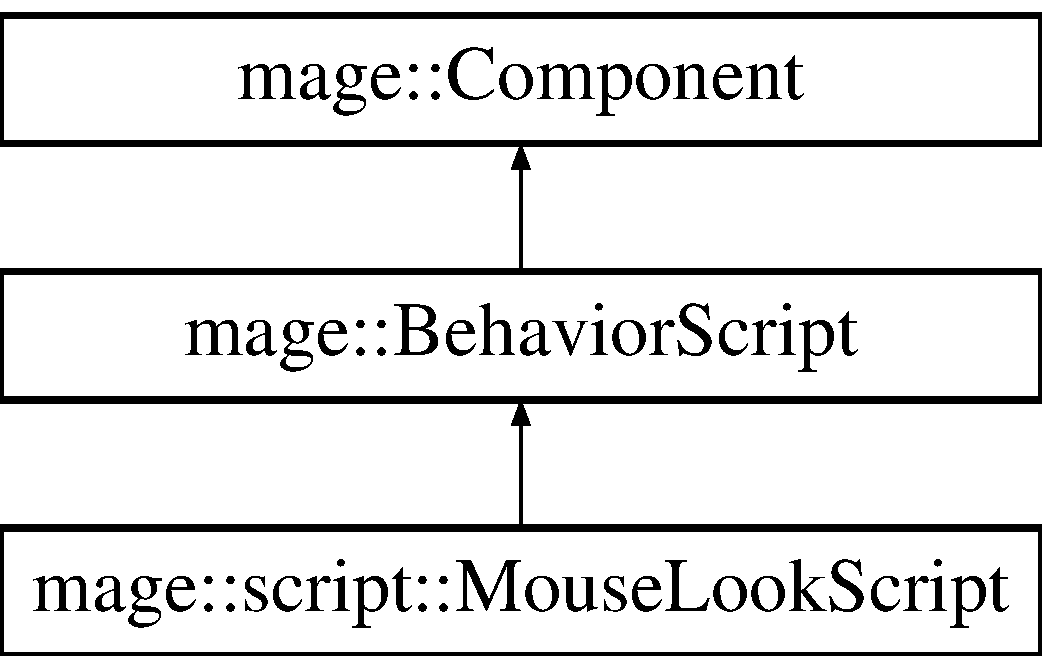
\includegraphics[height=3.000000cm]{classmage_1_1script_1_1_mouse_look_script}
\end{center}
\end{figure}
\subsection*{Public Types}
\begin{DoxyCompactItemize}
\item 
enum \hyperlink{classmage_1_1script_1_1_mouse_look_script_aa8c8ce1a3e6ccefa7b8ddd31be209c23}{Rotation\+Axes} \{ \hyperlink{classmage_1_1script_1_1_mouse_look_script_aa8c8ce1a3e6ccefa7b8ddd31be209c23abf27c48f8a38ed19eeeba089dd8d3ba1}{Rotation\+Axes\+::\+MouseX} = 1, 
\hyperlink{classmage_1_1script_1_1_mouse_look_script_aa8c8ce1a3e6ccefa7b8ddd31be209c23a73843207a289db41b16a5bb8254ca425}{Rotation\+Axes\+::\+MouseY} = 2, 
\hyperlink{classmage_1_1script_1_1_mouse_look_script_aa8c8ce1a3e6ccefa7b8ddd31be209c23a109431b32c091e8a7ad541546c66c522}{Rotation\+Axes\+::\+Mouse\+X\+AndY} = MouseX $\vert$ MouseY
 \}
\end{DoxyCompactItemize}
\subsection*{Public Member Functions}
\begin{DoxyCompactItemize}
\item 
\hyperlink{classmage_1_1script_1_1_mouse_look_script_a9055e93385160f4074cd2bc7fda3869e}{Mouse\+Look\+Script} ()
\item 
\hyperlink{classmage_1_1script_1_1_mouse_look_script_aa5237c229f27fa29f820bf6517209444}{Mouse\+Look\+Script} (const \hyperlink{classmage_1_1script_1_1_mouse_look_script}{Mouse\+Look\+Script} \&script) noexcept
\item 
\hyperlink{classmage_1_1script_1_1_mouse_look_script_ac21a383d6718ccc0d6c9faa5c5c1fe50}{Mouse\+Look\+Script} (\hyperlink{classmage_1_1script_1_1_mouse_look_script}{Mouse\+Look\+Script} \&\&script) noexcept
\item 
virtual \hyperlink{classmage_1_1script_1_1_mouse_look_script_a29a6d2cb4742fbf745822d015e72484f}{$\sim$\+Mouse\+Look\+Script} ()
\item 
\hyperlink{classmage_1_1script_1_1_mouse_look_script}{Mouse\+Look\+Script} \& \hyperlink{classmage_1_1script_1_1_mouse_look_script_af7da565d15422579ab5ff34f8f6bbc6a}{operator=} (const \hyperlink{classmage_1_1script_1_1_mouse_look_script}{Mouse\+Look\+Script} \&script)=delete
\item 
\hyperlink{classmage_1_1script_1_1_mouse_look_script}{Mouse\+Look\+Script} \& \hyperlink{classmage_1_1script_1_1_mouse_look_script_a019b949f86d066507ea74a9db126137e}{operator=} (\hyperlink{classmage_1_1script_1_1_mouse_look_script}{Mouse\+Look\+Script} \&\&script)=delete
\item 
virtual void \hyperlink{classmage_1_1script_1_1_mouse_look_script_a4b26f1ac71e89eaac7903101b95745e9}{Load} () override
\item 
virtual void \hyperlink{classmage_1_1script_1_1_mouse_look_script_a6d38748c21a6bc475e8ac31e24459053}{Update} (\mbox{[}\mbox{[}maybe\+\_\+unused\mbox{]}\mbox{]} \hyperlink{namespacemage_ad26233bbec640deda836e572c1a23708}{F64} delta\+\_\+time) override
\item 
\hyperlink{classmage_1_1script_1_1_mouse_look_script_aa8c8ce1a3e6ccefa7b8ddd31be209c23}{Rotation\+Axes} \hyperlink{classmage_1_1script_1_1_mouse_look_script_a612d8c23cc3f0711a07b32304082dfb5}{Get\+Rotation\+Axes} () const noexcept
\item 
void \hyperlink{classmage_1_1script_1_1_mouse_look_script_a82697e11738554a44b4a749227e231ee}{Set\+Rotation\+Axes} (\hyperlink{classmage_1_1script_1_1_mouse_look_script_aa8c8ce1a3e6ccefa7b8ddd31be209c23}{Rotation\+Axes} axes) noexcept
\item 
\hyperlink{namespacemage_aa97e833b45f06d60a0a9c4fc22ae02c0}{F32} \hyperlink{classmage_1_1script_1_1_mouse_look_script_a86ee9593f0221bfa259f5ae5dd6edb30}{Get\+SensitivityX} () const noexcept
\item 
\hyperlink{namespacemage_aa97e833b45f06d60a0a9c4fc22ae02c0}{F32} \hyperlink{classmage_1_1script_1_1_mouse_look_script_a39303e2d535ecc610ac4ea2f23825452}{Get\+SensitivityY} () const noexcept
\item 
const \hyperlink{namespacemage_aa87237ad091f5cd7da612b8523fc108f}{F32x2} \hyperlink{classmage_1_1script_1_1_mouse_look_script_aba0ebcfb2085d74ee7d6b388d4b0b239}{Get\+Sensitivity} () const noexcept
\item 
void \hyperlink{classmage_1_1script_1_1_mouse_look_script_a97c2564df1660fb9d07f9a4269a77568}{Set\+SensitivityX} (\hyperlink{namespacemage_aa97e833b45f06d60a0a9c4fc22ae02c0}{F32} x) noexcept
\item 
void \hyperlink{classmage_1_1script_1_1_mouse_look_script_a95376c27d55cf12d557427b68ccbd802}{Set\+SensitivityY} (\hyperlink{namespacemage_aa97e833b45f06d60a0a9c4fc22ae02c0}{F32} y) noexcept
\item 
void \hyperlink{classmage_1_1script_1_1_mouse_look_script_a6116637b42e58b8f40de86ed47b54fe3}{Set\+Sensitivity} (\hyperlink{namespacemage_aa97e833b45f06d60a0a9c4fc22ae02c0}{F32} x, \hyperlink{namespacemage_aa97e833b45f06d60a0a9c4fc22ae02c0}{F32} y)
\item 
void \hyperlink{classmage_1_1script_1_1_mouse_look_script_adf611a4d9240e6cf338b665a2713cd9f}{Set\+Sensitivity} (\hyperlink{namespacemage_aa87237ad091f5cd7da612b8523fc108f}{F32x2} sensitivity) noexcept
\item 
void X\+M\+\_\+\+C\+A\+L\+L\+C\+O\+NV \hyperlink{classmage_1_1script_1_1_mouse_look_script_a784937d1254fe26ee28864d11956cd80}{Set\+Sensitivity} (F\+X\+M\+V\+E\+C\+T\+OR sensitivity) noexcept
\item 
\hyperlink{namespacemage_aa97e833b45f06d60a0a9c4fc22ae02c0}{F32} \hyperlink{classmage_1_1script_1_1_mouse_look_script_ae594a42302f9ccd47e08070759c3ccf7}{Get\+Minimum\+RotationX} () const noexcept
\item 
\hyperlink{namespacemage_aa97e833b45f06d60a0a9c4fc22ae02c0}{F32} \hyperlink{classmage_1_1script_1_1_mouse_look_script_a8faf82867207fb604f7155b8dbadfdb0}{Get\+Minimum\+RotationY} () const noexcept
\item 
const \hyperlink{namespacemage_aa87237ad091f5cd7da612b8523fc108f}{F32x2} \hyperlink{classmage_1_1script_1_1_mouse_look_script_a09e7e193cf2f5dca3342a130268a7a67}{Get\+Minimum\+Rotation} () const noexcept
\item 
void \hyperlink{classmage_1_1script_1_1_mouse_look_script_a07c261e34b3131114efacb0d0f6ae076}{Set\+Minimum\+RotationX} (\hyperlink{namespacemage_aa97e833b45f06d60a0a9c4fc22ae02c0}{F32} x) noexcept
\item 
void \hyperlink{classmage_1_1script_1_1_mouse_look_script_ab78678ccb7bdf6ac4093b7911bf81d54}{Set\+Minimum\+RotationY} (\hyperlink{namespacemage_aa97e833b45f06d60a0a9c4fc22ae02c0}{F32} y) noexcept
\item 
void \hyperlink{classmage_1_1script_1_1_mouse_look_script_a6964af9c1c264be02c37671019ab117f}{Set\+Minimum\+Rotation} (\hyperlink{namespacemage_aa97e833b45f06d60a0a9c4fc22ae02c0}{F32} x, \hyperlink{namespacemage_aa97e833b45f06d60a0a9c4fc22ae02c0}{F32} y) noexcept
\item 
void \hyperlink{classmage_1_1script_1_1_mouse_look_script_ab901aa0a3d22ef1e28f00db6f4f99aa1}{Set\+Minimum\+Rotation} (\hyperlink{namespacemage_aa87237ad091f5cd7da612b8523fc108f}{F32x2} minimum\+\_\+rotation) noexcept
\item 
void X\+M\+\_\+\+C\+A\+L\+L\+C\+O\+NV \hyperlink{classmage_1_1script_1_1_mouse_look_script_ab120a7b0d01acb64ae4287d716d89a09}{Set\+Minimum\+Rotation} (F\+X\+M\+V\+E\+C\+T\+OR minimum\+\_\+rotation) noexcept
\item 
\hyperlink{namespacemage_aa97e833b45f06d60a0a9c4fc22ae02c0}{F32} \hyperlink{classmage_1_1script_1_1_mouse_look_script_a5d0e63ee050bf07f5c8ad75ca9ced307}{Get\+Maximum\+RotationX} () const noexcept
\item 
\hyperlink{namespacemage_aa97e833b45f06d60a0a9c4fc22ae02c0}{F32} \hyperlink{classmage_1_1script_1_1_mouse_look_script_a24f48ac9e66f9c14645db71fd55ab9c6}{Get\+Maximum\+RotationY} () const noexcept
\item 
const \hyperlink{namespacemage_aa87237ad091f5cd7da612b8523fc108f}{F32x2} \hyperlink{classmage_1_1script_1_1_mouse_look_script_a2ceb928a903baf5b30ea99e321af671c}{Get\+Maximum\+Rotation} () const noexcept
\item 
void \hyperlink{classmage_1_1script_1_1_mouse_look_script_a538d1d81ac4220a0e20e3e5de5c8e3a6}{Set\+Maximum\+RotationX} (\hyperlink{namespacemage_aa97e833b45f06d60a0a9c4fc22ae02c0}{F32} x) noexcept
\item 
void \hyperlink{classmage_1_1script_1_1_mouse_look_script_af56c4be26dde7497d53bb9f48d1b1a55}{Set\+Maximum\+RotationY} (\hyperlink{namespacemage_aa97e833b45f06d60a0a9c4fc22ae02c0}{F32} y) noexcept
\item 
void \hyperlink{classmage_1_1script_1_1_mouse_look_script_a50c3ddaad18713509394d168cddc8aa8}{Set\+Maximum\+Rotation} (\hyperlink{namespacemage_aa97e833b45f06d60a0a9c4fc22ae02c0}{F32} x, \hyperlink{namespacemage_aa97e833b45f06d60a0a9c4fc22ae02c0}{F32} y) noexcept
\item 
void \hyperlink{classmage_1_1script_1_1_mouse_look_script_a878f1268e16f0af89d177fd026b18253}{Set\+Maximum\+Rotation} (\hyperlink{namespacemage_aa87237ad091f5cd7da612b8523fc108f}{F32x2} maximum\+\_\+rotation) noexcept
\item 
void X\+M\+\_\+\+C\+A\+L\+L\+C\+O\+NV \hyperlink{classmage_1_1script_1_1_mouse_look_script_a263e143e671ef56c04132b5e58d114a9}{Set\+Maximum\+Rotation} (F\+X\+M\+V\+E\+C\+T\+OR maximum\+\_\+rotation) noexcept
\item 
void \hyperlink{classmage_1_1script_1_1_mouse_look_script_aa527806c78873eab652dd6337a75b89f}{Invert\+DirectionX} () noexcept
\item 
void \hyperlink{classmage_1_1script_1_1_mouse_look_script_a189145ae96f56b805fe2020ed75db0bc}{Invert\+DirectionY} () noexcept
\end{DoxyCompactItemize}
\subsection*{Private Attributes}
\begin{DoxyCompactItemize}
\item 
\hyperlink{classmage_1_1script_1_1_mouse_look_script_aa8c8ce1a3e6ccefa7b8ddd31be209c23}{Rotation\+Axes} \hyperlink{classmage_1_1script_1_1_mouse_look_script_ae41f05d545c70cd621a405f6ef0cd4d5}{m\+\_\+axes}
\item 
\hyperlink{namespacemage_aa87237ad091f5cd7da612b8523fc108f}{F32x2} \hyperlink{classmage_1_1script_1_1_mouse_look_script_afe7a443c1fa56fc6143555f992458934}{m\+\_\+sensitivity}
\item 
\hyperlink{namespacemage_aa87237ad091f5cd7da612b8523fc108f}{F32x2} \hyperlink{classmage_1_1script_1_1_mouse_look_script_a4379e58bd89eab39d3e281133968a959}{m\+\_\+minimum\+\_\+rotation}
\item 
\hyperlink{namespacemage_aa87237ad091f5cd7da612b8523fc108f}{F32x2} \hyperlink{classmage_1_1script_1_1_mouse_look_script_ac3c7af839d88b3d9ec65250c41099c34}{m\+\_\+maximum\+\_\+rotation}
\item 
\hyperlink{namespacemage_aa87237ad091f5cd7da612b8523fc108f}{F32x2} \hyperlink{classmage_1_1script_1_1_mouse_look_script_a5f65024afe8940ca2709d5ee13dc033c}{m\+\_\+direction}
\end{DoxyCompactItemize}
\subsection*{Additional Inherited Members}


\subsection{Member Enumeration Documentation}
\hypertarget{classmage_1_1script_1_1_mouse_look_script_aa8c8ce1a3e6ccefa7b8ddd31be209c23}{}\label{classmage_1_1script_1_1_mouse_look_script_aa8c8ce1a3e6ccefa7b8ddd31be209c23} 
\index{mage\+::script\+::\+Mouse\+Look\+Script@{mage\+::script\+::\+Mouse\+Look\+Script}!Rotation\+Axes@{Rotation\+Axes}}
\index{Rotation\+Axes@{Rotation\+Axes}!mage\+::script\+::\+Mouse\+Look\+Script@{mage\+::script\+::\+Mouse\+Look\+Script}}
\subsubsection{\texorpdfstring{Rotation\+Axes}{RotationAxes}}
{\footnotesize\ttfamily enum \hyperlink{classmage_1_1script_1_1_mouse_look_script_aa8c8ce1a3e6ccefa7b8ddd31be209c23}{mage\+::script\+::\+Mouse\+Look\+Script\+::\+Rotation\+Axes}\hspace{0.3cm}{\ttfamily [strong]}}

\begin{DoxyEnumFields}{Enumerator}
\raisebox{\heightof{T}}[0pt][0pt]{\index{MouseX@{MouseX}!mage\+::script\+::\+Mouse\+Look\+Script@{mage\+::script\+::\+Mouse\+Look\+Script}}\index{mage\+::script\+::\+Mouse\+Look\+Script@{mage\+::script\+::\+Mouse\+Look\+Script}!MouseX@{MouseX}}}\hypertarget{classmage_1_1script_1_1_mouse_look_script_aa8c8ce1a3e6ccefa7b8ddd31be209c23abf27c48f8a38ed19eeeba089dd8d3ba1}{}\label{classmage_1_1script_1_1_mouse_look_script_aa8c8ce1a3e6ccefa7b8ddd31be209c23abf27c48f8a38ed19eeeba089dd8d3ba1} 
MouseX&\\
\hline

\raisebox{\heightof{T}}[0pt][0pt]{\index{MouseY@{MouseY}!mage\+::script\+::\+Mouse\+Look\+Script@{mage\+::script\+::\+Mouse\+Look\+Script}}\index{mage\+::script\+::\+Mouse\+Look\+Script@{mage\+::script\+::\+Mouse\+Look\+Script}!MouseY@{MouseY}}}\hypertarget{classmage_1_1script_1_1_mouse_look_script_aa8c8ce1a3e6ccefa7b8ddd31be209c23a73843207a289db41b16a5bb8254ca425}{}\label{classmage_1_1script_1_1_mouse_look_script_aa8c8ce1a3e6ccefa7b8ddd31be209c23a73843207a289db41b16a5bb8254ca425} 
MouseY&\\
\hline

\raisebox{\heightof{T}}[0pt][0pt]{\index{Mouse\+X\+AndY@{Mouse\+X\+AndY}!mage\+::script\+::\+Mouse\+Look\+Script@{mage\+::script\+::\+Mouse\+Look\+Script}}\index{mage\+::script\+::\+Mouse\+Look\+Script@{mage\+::script\+::\+Mouse\+Look\+Script}!Mouse\+X\+AndY@{Mouse\+X\+AndY}}}\hypertarget{classmage_1_1script_1_1_mouse_look_script_aa8c8ce1a3e6ccefa7b8ddd31be209c23a109431b32c091e8a7ad541546c66c522}{}\label{classmage_1_1script_1_1_mouse_look_script_aa8c8ce1a3e6ccefa7b8ddd31be209c23a109431b32c091e8a7ad541546c66c522} 
Mouse\+X\+AndY&\\
\hline

\end{DoxyEnumFields}


\subsection{Constructor \& Destructor Documentation}
\hypertarget{classmage_1_1script_1_1_mouse_look_script_a9055e93385160f4074cd2bc7fda3869e}{}\label{classmage_1_1script_1_1_mouse_look_script_a9055e93385160f4074cd2bc7fda3869e} 
\index{mage\+::script\+::\+Mouse\+Look\+Script@{mage\+::script\+::\+Mouse\+Look\+Script}!Mouse\+Look\+Script@{Mouse\+Look\+Script}}
\index{Mouse\+Look\+Script@{Mouse\+Look\+Script}!mage\+::script\+::\+Mouse\+Look\+Script@{mage\+::script\+::\+Mouse\+Look\+Script}}
\subsubsection{\texorpdfstring{Mouse\+Look\+Script()}{MouseLookScript()}\hspace{0.1cm}{\footnotesize\ttfamily [1/3]}}
{\footnotesize\ttfamily mage\+::script\+::\+Mouse\+Look\+Script\+::\+Mouse\+Look\+Script (\begin{DoxyParamCaption}{ }\end{DoxyParamCaption})}

\hypertarget{classmage_1_1script_1_1_mouse_look_script_aa5237c229f27fa29f820bf6517209444}{}\label{classmage_1_1script_1_1_mouse_look_script_aa5237c229f27fa29f820bf6517209444} 
\index{mage\+::script\+::\+Mouse\+Look\+Script@{mage\+::script\+::\+Mouse\+Look\+Script}!Mouse\+Look\+Script@{Mouse\+Look\+Script}}
\index{Mouse\+Look\+Script@{Mouse\+Look\+Script}!mage\+::script\+::\+Mouse\+Look\+Script@{mage\+::script\+::\+Mouse\+Look\+Script}}
\subsubsection{\texorpdfstring{Mouse\+Look\+Script()}{MouseLookScript()}\hspace{0.1cm}{\footnotesize\ttfamily [2/3]}}
{\footnotesize\ttfamily mage\+::script\+::\+Mouse\+Look\+Script\+::\+Mouse\+Look\+Script (\begin{DoxyParamCaption}\item[{const \hyperlink{classmage_1_1script_1_1_mouse_look_script}{Mouse\+Look\+Script} \&}]{script }\end{DoxyParamCaption})\hspace{0.3cm}{\ttfamily [default]}, {\ttfamily [noexcept]}}

\hypertarget{classmage_1_1script_1_1_mouse_look_script_ac21a383d6718ccc0d6c9faa5c5c1fe50}{}\label{classmage_1_1script_1_1_mouse_look_script_ac21a383d6718ccc0d6c9faa5c5c1fe50} 
\index{mage\+::script\+::\+Mouse\+Look\+Script@{mage\+::script\+::\+Mouse\+Look\+Script}!Mouse\+Look\+Script@{Mouse\+Look\+Script}}
\index{Mouse\+Look\+Script@{Mouse\+Look\+Script}!mage\+::script\+::\+Mouse\+Look\+Script@{mage\+::script\+::\+Mouse\+Look\+Script}}
\subsubsection{\texorpdfstring{Mouse\+Look\+Script()}{MouseLookScript()}\hspace{0.1cm}{\footnotesize\ttfamily [3/3]}}
{\footnotesize\ttfamily mage\+::script\+::\+Mouse\+Look\+Script\+::\+Mouse\+Look\+Script (\begin{DoxyParamCaption}\item[{\hyperlink{classmage_1_1script_1_1_mouse_look_script}{Mouse\+Look\+Script} \&\&}]{script }\end{DoxyParamCaption})\hspace{0.3cm}{\ttfamily [default]}, {\ttfamily [noexcept]}}

\hypertarget{classmage_1_1script_1_1_mouse_look_script_a29a6d2cb4742fbf745822d015e72484f}{}\label{classmage_1_1script_1_1_mouse_look_script_a29a6d2cb4742fbf745822d015e72484f} 
\index{mage\+::script\+::\+Mouse\+Look\+Script@{mage\+::script\+::\+Mouse\+Look\+Script}!````~Mouse\+Look\+Script@{$\sim$\+Mouse\+Look\+Script}}
\index{````~Mouse\+Look\+Script@{$\sim$\+Mouse\+Look\+Script}!mage\+::script\+::\+Mouse\+Look\+Script@{mage\+::script\+::\+Mouse\+Look\+Script}}
\subsubsection{\texorpdfstring{$\sim$\+Mouse\+Look\+Script()}{~MouseLookScript()}}
{\footnotesize\ttfamily mage\+::script\+::\+Mouse\+Look\+Script\+::$\sim$\+Mouse\+Look\+Script (\begin{DoxyParamCaption}{ }\end{DoxyParamCaption})\hspace{0.3cm}{\ttfamily [virtual]}, {\ttfamily [default]}}



\subsection{Member Function Documentation}
\hypertarget{classmage_1_1script_1_1_mouse_look_script_a2ceb928a903baf5b30ea99e321af671c}{}\label{classmage_1_1script_1_1_mouse_look_script_a2ceb928a903baf5b30ea99e321af671c} 
\index{mage\+::script\+::\+Mouse\+Look\+Script@{mage\+::script\+::\+Mouse\+Look\+Script}!Get\+Maximum\+Rotation@{Get\+Maximum\+Rotation}}
\index{Get\+Maximum\+Rotation@{Get\+Maximum\+Rotation}!mage\+::script\+::\+Mouse\+Look\+Script@{mage\+::script\+::\+Mouse\+Look\+Script}}
\subsubsection{\texorpdfstring{Get\+Maximum\+Rotation()}{GetMaximumRotation()}}
{\footnotesize\ttfamily const \hyperlink{namespacemage_aa87237ad091f5cd7da612b8523fc108f}{F32x2} mage\+::script\+::\+Mouse\+Look\+Script\+::\+Get\+Maximum\+Rotation (\begin{DoxyParamCaption}{ }\end{DoxyParamCaption}) const\hspace{0.3cm}{\ttfamily [noexcept]}}

\hypertarget{classmage_1_1script_1_1_mouse_look_script_a5d0e63ee050bf07f5c8ad75ca9ced307}{}\label{classmage_1_1script_1_1_mouse_look_script_a5d0e63ee050bf07f5c8ad75ca9ced307} 
\index{mage\+::script\+::\+Mouse\+Look\+Script@{mage\+::script\+::\+Mouse\+Look\+Script}!Get\+Maximum\+RotationX@{Get\+Maximum\+RotationX}}
\index{Get\+Maximum\+RotationX@{Get\+Maximum\+RotationX}!mage\+::script\+::\+Mouse\+Look\+Script@{mage\+::script\+::\+Mouse\+Look\+Script}}
\subsubsection{\texorpdfstring{Get\+Maximum\+Rotation\+X()}{GetMaximumRotationX()}}
{\footnotesize\ttfamily \hyperlink{namespacemage_aa97e833b45f06d60a0a9c4fc22ae02c0}{F32} mage\+::script\+::\+Mouse\+Look\+Script\+::\+Get\+Maximum\+RotationX (\begin{DoxyParamCaption}{ }\end{DoxyParamCaption}) const\hspace{0.3cm}{\ttfamily [noexcept]}}

\hypertarget{classmage_1_1script_1_1_mouse_look_script_a24f48ac9e66f9c14645db71fd55ab9c6}{}\label{classmage_1_1script_1_1_mouse_look_script_a24f48ac9e66f9c14645db71fd55ab9c6} 
\index{mage\+::script\+::\+Mouse\+Look\+Script@{mage\+::script\+::\+Mouse\+Look\+Script}!Get\+Maximum\+RotationY@{Get\+Maximum\+RotationY}}
\index{Get\+Maximum\+RotationY@{Get\+Maximum\+RotationY}!mage\+::script\+::\+Mouse\+Look\+Script@{mage\+::script\+::\+Mouse\+Look\+Script}}
\subsubsection{\texorpdfstring{Get\+Maximum\+Rotation\+Y()}{GetMaximumRotationY()}}
{\footnotesize\ttfamily \hyperlink{namespacemage_aa97e833b45f06d60a0a9c4fc22ae02c0}{F32} mage\+::script\+::\+Mouse\+Look\+Script\+::\+Get\+Maximum\+RotationY (\begin{DoxyParamCaption}{ }\end{DoxyParamCaption}) const\hspace{0.3cm}{\ttfamily [noexcept]}}

\hypertarget{classmage_1_1script_1_1_mouse_look_script_a09e7e193cf2f5dca3342a130268a7a67}{}\label{classmage_1_1script_1_1_mouse_look_script_a09e7e193cf2f5dca3342a130268a7a67} 
\index{mage\+::script\+::\+Mouse\+Look\+Script@{mage\+::script\+::\+Mouse\+Look\+Script}!Get\+Minimum\+Rotation@{Get\+Minimum\+Rotation}}
\index{Get\+Minimum\+Rotation@{Get\+Minimum\+Rotation}!mage\+::script\+::\+Mouse\+Look\+Script@{mage\+::script\+::\+Mouse\+Look\+Script}}
\subsubsection{\texorpdfstring{Get\+Minimum\+Rotation()}{GetMinimumRotation()}}
{\footnotesize\ttfamily const \hyperlink{namespacemage_aa87237ad091f5cd7da612b8523fc108f}{F32x2} mage\+::script\+::\+Mouse\+Look\+Script\+::\+Get\+Minimum\+Rotation (\begin{DoxyParamCaption}{ }\end{DoxyParamCaption}) const\hspace{0.3cm}{\ttfamily [noexcept]}}

\hypertarget{classmage_1_1script_1_1_mouse_look_script_ae594a42302f9ccd47e08070759c3ccf7}{}\label{classmage_1_1script_1_1_mouse_look_script_ae594a42302f9ccd47e08070759c3ccf7} 
\index{mage\+::script\+::\+Mouse\+Look\+Script@{mage\+::script\+::\+Mouse\+Look\+Script}!Get\+Minimum\+RotationX@{Get\+Minimum\+RotationX}}
\index{Get\+Minimum\+RotationX@{Get\+Minimum\+RotationX}!mage\+::script\+::\+Mouse\+Look\+Script@{mage\+::script\+::\+Mouse\+Look\+Script}}
\subsubsection{\texorpdfstring{Get\+Minimum\+Rotation\+X()}{GetMinimumRotationX()}}
{\footnotesize\ttfamily \hyperlink{namespacemage_aa97e833b45f06d60a0a9c4fc22ae02c0}{F32} mage\+::script\+::\+Mouse\+Look\+Script\+::\+Get\+Minimum\+RotationX (\begin{DoxyParamCaption}{ }\end{DoxyParamCaption}) const\hspace{0.3cm}{\ttfamily [noexcept]}}

\hypertarget{classmage_1_1script_1_1_mouse_look_script_a8faf82867207fb604f7155b8dbadfdb0}{}\label{classmage_1_1script_1_1_mouse_look_script_a8faf82867207fb604f7155b8dbadfdb0} 
\index{mage\+::script\+::\+Mouse\+Look\+Script@{mage\+::script\+::\+Mouse\+Look\+Script}!Get\+Minimum\+RotationY@{Get\+Minimum\+RotationY}}
\index{Get\+Minimum\+RotationY@{Get\+Minimum\+RotationY}!mage\+::script\+::\+Mouse\+Look\+Script@{mage\+::script\+::\+Mouse\+Look\+Script}}
\subsubsection{\texorpdfstring{Get\+Minimum\+Rotation\+Y()}{GetMinimumRotationY()}}
{\footnotesize\ttfamily \hyperlink{namespacemage_aa97e833b45f06d60a0a9c4fc22ae02c0}{F32} mage\+::script\+::\+Mouse\+Look\+Script\+::\+Get\+Minimum\+RotationY (\begin{DoxyParamCaption}{ }\end{DoxyParamCaption}) const\hspace{0.3cm}{\ttfamily [noexcept]}}

\hypertarget{classmage_1_1script_1_1_mouse_look_script_a612d8c23cc3f0711a07b32304082dfb5}{}\label{classmage_1_1script_1_1_mouse_look_script_a612d8c23cc3f0711a07b32304082dfb5} 
\index{mage\+::script\+::\+Mouse\+Look\+Script@{mage\+::script\+::\+Mouse\+Look\+Script}!Get\+Rotation\+Axes@{Get\+Rotation\+Axes}}
\index{Get\+Rotation\+Axes@{Get\+Rotation\+Axes}!mage\+::script\+::\+Mouse\+Look\+Script@{mage\+::script\+::\+Mouse\+Look\+Script}}
\subsubsection{\texorpdfstring{Get\+Rotation\+Axes()}{GetRotationAxes()}}
{\footnotesize\ttfamily \hyperlink{classmage_1_1script_1_1_mouse_look_script_aa8c8ce1a3e6ccefa7b8ddd31be209c23}{Rotation\+Axes} mage\+::script\+::\+Mouse\+Look\+Script\+::\+Get\+Rotation\+Axes (\begin{DoxyParamCaption}{ }\end{DoxyParamCaption}) const\hspace{0.3cm}{\ttfamily [noexcept]}}

\hypertarget{classmage_1_1script_1_1_mouse_look_script_aba0ebcfb2085d74ee7d6b388d4b0b239}{}\label{classmage_1_1script_1_1_mouse_look_script_aba0ebcfb2085d74ee7d6b388d4b0b239} 
\index{mage\+::script\+::\+Mouse\+Look\+Script@{mage\+::script\+::\+Mouse\+Look\+Script}!Get\+Sensitivity@{Get\+Sensitivity}}
\index{Get\+Sensitivity@{Get\+Sensitivity}!mage\+::script\+::\+Mouse\+Look\+Script@{mage\+::script\+::\+Mouse\+Look\+Script}}
\subsubsection{\texorpdfstring{Get\+Sensitivity()}{GetSensitivity()}}
{\footnotesize\ttfamily const \hyperlink{namespacemage_aa87237ad091f5cd7da612b8523fc108f}{F32x2} mage\+::script\+::\+Mouse\+Look\+Script\+::\+Get\+Sensitivity (\begin{DoxyParamCaption}{ }\end{DoxyParamCaption}) const\hspace{0.3cm}{\ttfamily [noexcept]}}

\hypertarget{classmage_1_1script_1_1_mouse_look_script_a86ee9593f0221bfa259f5ae5dd6edb30}{}\label{classmage_1_1script_1_1_mouse_look_script_a86ee9593f0221bfa259f5ae5dd6edb30} 
\index{mage\+::script\+::\+Mouse\+Look\+Script@{mage\+::script\+::\+Mouse\+Look\+Script}!Get\+SensitivityX@{Get\+SensitivityX}}
\index{Get\+SensitivityX@{Get\+SensitivityX}!mage\+::script\+::\+Mouse\+Look\+Script@{mage\+::script\+::\+Mouse\+Look\+Script}}
\subsubsection{\texorpdfstring{Get\+Sensitivity\+X()}{GetSensitivityX()}}
{\footnotesize\ttfamily \hyperlink{namespacemage_aa97e833b45f06d60a0a9c4fc22ae02c0}{F32} mage\+::script\+::\+Mouse\+Look\+Script\+::\+Get\+SensitivityX (\begin{DoxyParamCaption}{ }\end{DoxyParamCaption}) const\hspace{0.3cm}{\ttfamily [noexcept]}}

\hypertarget{classmage_1_1script_1_1_mouse_look_script_a39303e2d535ecc610ac4ea2f23825452}{}\label{classmage_1_1script_1_1_mouse_look_script_a39303e2d535ecc610ac4ea2f23825452} 
\index{mage\+::script\+::\+Mouse\+Look\+Script@{mage\+::script\+::\+Mouse\+Look\+Script}!Get\+SensitivityY@{Get\+SensitivityY}}
\index{Get\+SensitivityY@{Get\+SensitivityY}!mage\+::script\+::\+Mouse\+Look\+Script@{mage\+::script\+::\+Mouse\+Look\+Script}}
\subsubsection{\texorpdfstring{Get\+Sensitivity\+Y()}{GetSensitivityY()}}
{\footnotesize\ttfamily \hyperlink{namespacemage_aa97e833b45f06d60a0a9c4fc22ae02c0}{F32} mage\+::script\+::\+Mouse\+Look\+Script\+::\+Get\+SensitivityY (\begin{DoxyParamCaption}{ }\end{DoxyParamCaption}) const\hspace{0.3cm}{\ttfamily [noexcept]}}

\hypertarget{classmage_1_1script_1_1_mouse_look_script_aa527806c78873eab652dd6337a75b89f}{}\label{classmage_1_1script_1_1_mouse_look_script_aa527806c78873eab652dd6337a75b89f} 
\index{mage\+::script\+::\+Mouse\+Look\+Script@{mage\+::script\+::\+Mouse\+Look\+Script}!Invert\+DirectionX@{Invert\+DirectionX}}
\index{Invert\+DirectionX@{Invert\+DirectionX}!mage\+::script\+::\+Mouse\+Look\+Script@{mage\+::script\+::\+Mouse\+Look\+Script}}
\subsubsection{\texorpdfstring{Invert\+Direction\+X()}{InvertDirectionX()}}
{\footnotesize\ttfamily void mage\+::script\+::\+Mouse\+Look\+Script\+::\+Invert\+DirectionX (\begin{DoxyParamCaption}{ }\end{DoxyParamCaption})\hspace{0.3cm}{\ttfamily [noexcept]}}

\hypertarget{classmage_1_1script_1_1_mouse_look_script_a189145ae96f56b805fe2020ed75db0bc}{}\label{classmage_1_1script_1_1_mouse_look_script_a189145ae96f56b805fe2020ed75db0bc} 
\index{mage\+::script\+::\+Mouse\+Look\+Script@{mage\+::script\+::\+Mouse\+Look\+Script}!Invert\+DirectionY@{Invert\+DirectionY}}
\index{Invert\+DirectionY@{Invert\+DirectionY}!mage\+::script\+::\+Mouse\+Look\+Script@{mage\+::script\+::\+Mouse\+Look\+Script}}
\subsubsection{\texorpdfstring{Invert\+Direction\+Y()}{InvertDirectionY()}}
{\footnotesize\ttfamily void mage\+::script\+::\+Mouse\+Look\+Script\+::\+Invert\+DirectionY (\begin{DoxyParamCaption}{ }\end{DoxyParamCaption})\hspace{0.3cm}{\ttfamily [noexcept]}}

\hypertarget{classmage_1_1script_1_1_mouse_look_script_a4b26f1ac71e89eaac7903101b95745e9}{}\label{classmage_1_1script_1_1_mouse_look_script_a4b26f1ac71e89eaac7903101b95745e9} 
\index{mage\+::script\+::\+Mouse\+Look\+Script@{mage\+::script\+::\+Mouse\+Look\+Script}!Load@{Load}}
\index{Load@{Load}!mage\+::script\+::\+Mouse\+Look\+Script@{mage\+::script\+::\+Mouse\+Look\+Script}}
\subsubsection{\texorpdfstring{Load()}{Load()}}
{\footnotesize\ttfamily void mage\+::script\+::\+Mouse\+Look\+Script\+::\+Load (\begin{DoxyParamCaption}{ }\end{DoxyParamCaption})\hspace{0.3cm}{\ttfamily [override]}, {\ttfamily [virtual]}}

Loads this behavior script. Allows this behavior script to preform any pre-\/processing.


\begin{DoxyExceptions}{Exceptions}
{\em \hyperlink{classmage_1_1_exception}{Exception}} & Failed to load this behavior script. \\
\hline
\end{DoxyExceptions}


Reimplemented from \hyperlink{classmage_1_1_behavior_script_a06521eef472f2d878a9f652b95b723a8}{mage\+::\+Behavior\+Script}.

\hypertarget{classmage_1_1script_1_1_mouse_look_script_af7da565d15422579ab5ff34f8f6bbc6a}{}\label{classmage_1_1script_1_1_mouse_look_script_af7da565d15422579ab5ff34f8f6bbc6a} 
\index{mage\+::script\+::\+Mouse\+Look\+Script@{mage\+::script\+::\+Mouse\+Look\+Script}!operator=@{operator=}}
\index{operator=@{operator=}!mage\+::script\+::\+Mouse\+Look\+Script@{mage\+::script\+::\+Mouse\+Look\+Script}}
\subsubsection{\texorpdfstring{operator=()}{operator=()}\hspace{0.1cm}{\footnotesize\ttfamily [1/2]}}
{\footnotesize\ttfamily \hyperlink{classmage_1_1script_1_1_mouse_look_script}{Mouse\+Look\+Script}\& mage\+::script\+::\+Mouse\+Look\+Script\+::operator= (\begin{DoxyParamCaption}\item[{const \hyperlink{classmage_1_1script_1_1_mouse_look_script}{Mouse\+Look\+Script} \&}]{script }\end{DoxyParamCaption})\hspace{0.3cm}{\ttfamily [delete]}}

\hypertarget{classmage_1_1script_1_1_mouse_look_script_a019b949f86d066507ea74a9db126137e}{}\label{classmage_1_1script_1_1_mouse_look_script_a019b949f86d066507ea74a9db126137e} 
\index{mage\+::script\+::\+Mouse\+Look\+Script@{mage\+::script\+::\+Mouse\+Look\+Script}!operator=@{operator=}}
\index{operator=@{operator=}!mage\+::script\+::\+Mouse\+Look\+Script@{mage\+::script\+::\+Mouse\+Look\+Script}}
\subsubsection{\texorpdfstring{operator=()}{operator=()}\hspace{0.1cm}{\footnotesize\ttfamily [2/2]}}
{\footnotesize\ttfamily \hyperlink{classmage_1_1script_1_1_mouse_look_script}{Mouse\+Look\+Script}\& mage\+::script\+::\+Mouse\+Look\+Script\+::operator= (\begin{DoxyParamCaption}\item[{\hyperlink{classmage_1_1script_1_1_mouse_look_script}{Mouse\+Look\+Script} \&\&}]{script }\end{DoxyParamCaption})\hspace{0.3cm}{\ttfamily [delete]}}

\hypertarget{classmage_1_1script_1_1_mouse_look_script_a50c3ddaad18713509394d168cddc8aa8}{}\label{classmage_1_1script_1_1_mouse_look_script_a50c3ddaad18713509394d168cddc8aa8} 
\index{mage\+::script\+::\+Mouse\+Look\+Script@{mage\+::script\+::\+Mouse\+Look\+Script}!Set\+Maximum\+Rotation@{Set\+Maximum\+Rotation}}
\index{Set\+Maximum\+Rotation@{Set\+Maximum\+Rotation}!mage\+::script\+::\+Mouse\+Look\+Script@{mage\+::script\+::\+Mouse\+Look\+Script}}
\subsubsection{\texorpdfstring{Set\+Maximum\+Rotation()}{SetMaximumRotation()}\hspace{0.1cm}{\footnotesize\ttfamily [1/3]}}
{\footnotesize\ttfamily void mage\+::script\+::\+Mouse\+Look\+Script\+::\+Set\+Maximum\+Rotation (\begin{DoxyParamCaption}\item[{\hyperlink{namespacemage_aa97e833b45f06d60a0a9c4fc22ae02c0}{F32}}]{x,  }\item[{\hyperlink{namespacemage_aa97e833b45f06d60a0a9c4fc22ae02c0}{F32}}]{y }\end{DoxyParamCaption})\hspace{0.3cm}{\ttfamily [noexcept]}}

\hypertarget{classmage_1_1script_1_1_mouse_look_script_a878f1268e16f0af89d177fd026b18253}{}\label{classmage_1_1script_1_1_mouse_look_script_a878f1268e16f0af89d177fd026b18253} 
\index{mage\+::script\+::\+Mouse\+Look\+Script@{mage\+::script\+::\+Mouse\+Look\+Script}!Set\+Maximum\+Rotation@{Set\+Maximum\+Rotation}}
\index{Set\+Maximum\+Rotation@{Set\+Maximum\+Rotation}!mage\+::script\+::\+Mouse\+Look\+Script@{mage\+::script\+::\+Mouse\+Look\+Script}}
\subsubsection{\texorpdfstring{Set\+Maximum\+Rotation()}{SetMaximumRotation()}\hspace{0.1cm}{\footnotesize\ttfamily [2/3]}}
{\footnotesize\ttfamily void mage\+::script\+::\+Mouse\+Look\+Script\+::\+Set\+Maximum\+Rotation (\begin{DoxyParamCaption}\item[{\hyperlink{namespacemage_aa87237ad091f5cd7da612b8523fc108f}{F32x2}}]{maximum\+\_\+rotation }\end{DoxyParamCaption})\hspace{0.3cm}{\ttfamily [noexcept]}}

\hypertarget{classmage_1_1script_1_1_mouse_look_script_a263e143e671ef56c04132b5e58d114a9}{}\label{classmage_1_1script_1_1_mouse_look_script_a263e143e671ef56c04132b5e58d114a9} 
\index{mage\+::script\+::\+Mouse\+Look\+Script@{mage\+::script\+::\+Mouse\+Look\+Script}!Set\+Maximum\+Rotation@{Set\+Maximum\+Rotation}}
\index{Set\+Maximum\+Rotation@{Set\+Maximum\+Rotation}!mage\+::script\+::\+Mouse\+Look\+Script@{mage\+::script\+::\+Mouse\+Look\+Script}}
\subsubsection{\texorpdfstring{Set\+Maximum\+Rotation()}{SetMaximumRotation()}\hspace{0.1cm}{\footnotesize\ttfamily [3/3]}}
{\footnotesize\ttfamily void X\+M\+\_\+\+C\+A\+L\+L\+C\+O\+NV mage\+::script\+::\+Mouse\+Look\+Script\+::\+Set\+Maximum\+Rotation (\begin{DoxyParamCaption}\item[{F\+X\+M\+V\+E\+C\+T\+OR}]{maximum\+\_\+rotation }\end{DoxyParamCaption})\hspace{0.3cm}{\ttfamily [noexcept]}}

\hypertarget{classmage_1_1script_1_1_mouse_look_script_a538d1d81ac4220a0e20e3e5de5c8e3a6}{}\label{classmage_1_1script_1_1_mouse_look_script_a538d1d81ac4220a0e20e3e5de5c8e3a6} 
\index{mage\+::script\+::\+Mouse\+Look\+Script@{mage\+::script\+::\+Mouse\+Look\+Script}!Set\+Maximum\+RotationX@{Set\+Maximum\+RotationX}}
\index{Set\+Maximum\+RotationX@{Set\+Maximum\+RotationX}!mage\+::script\+::\+Mouse\+Look\+Script@{mage\+::script\+::\+Mouse\+Look\+Script}}
\subsubsection{\texorpdfstring{Set\+Maximum\+Rotation\+X()}{SetMaximumRotationX()}}
{\footnotesize\ttfamily void mage\+::script\+::\+Mouse\+Look\+Script\+::\+Set\+Maximum\+RotationX (\begin{DoxyParamCaption}\item[{\hyperlink{namespacemage_aa97e833b45f06d60a0a9c4fc22ae02c0}{F32}}]{x }\end{DoxyParamCaption})\hspace{0.3cm}{\ttfamily [noexcept]}}

\hypertarget{classmage_1_1script_1_1_mouse_look_script_af56c4be26dde7497d53bb9f48d1b1a55}{}\label{classmage_1_1script_1_1_mouse_look_script_af56c4be26dde7497d53bb9f48d1b1a55} 
\index{mage\+::script\+::\+Mouse\+Look\+Script@{mage\+::script\+::\+Mouse\+Look\+Script}!Set\+Maximum\+RotationY@{Set\+Maximum\+RotationY}}
\index{Set\+Maximum\+RotationY@{Set\+Maximum\+RotationY}!mage\+::script\+::\+Mouse\+Look\+Script@{mage\+::script\+::\+Mouse\+Look\+Script}}
\subsubsection{\texorpdfstring{Set\+Maximum\+Rotation\+Y()}{SetMaximumRotationY()}}
{\footnotesize\ttfamily void mage\+::script\+::\+Mouse\+Look\+Script\+::\+Set\+Maximum\+RotationY (\begin{DoxyParamCaption}\item[{\hyperlink{namespacemage_aa97e833b45f06d60a0a9c4fc22ae02c0}{F32}}]{y }\end{DoxyParamCaption})\hspace{0.3cm}{\ttfamily [noexcept]}}

\hypertarget{classmage_1_1script_1_1_mouse_look_script_a6964af9c1c264be02c37671019ab117f}{}\label{classmage_1_1script_1_1_mouse_look_script_a6964af9c1c264be02c37671019ab117f} 
\index{mage\+::script\+::\+Mouse\+Look\+Script@{mage\+::script\+::\+Mouse\+Look\+Script}!Set\+Minimum\+Rotation@{Set\+Minimum\+Rotation}}
\index{Set\+Minimum\+Rotation@{Set\+Minimum\+Rotation}!mage\+::script\+::\+Mouse\+Look\+Script@{mage\+::script\+::\+Mouse\+Look\+Script}}
\subsubsection{\texorpdfstring{Set\+Minimum\+Rotation()}{SetMinimumRotation()}\hspace{0.1cm}{\footnotesize\ttfamily [1/3]}}
{\footnotesize\ttfamily void mage\+::script\+::\+Mouse\+Look\+Script\+::\+Set\+Minimum\+Rotation (\begin{DoxyParamCaption}\item[{\hyperlink{namespacemage_aa97e833b45f06d60a0a9c4fc22ae02c0}{F32}}]{x,  }\item[{\hyperlink{namespacemage_aa97e833b45f06d60a0a9c4fc22ae02c0}{F32}}]{y }\end{DoxyParamCaption})\hspace{0.3cm}{\ttfamily [noexcept]}}

\hypertarget{classmage_1_1script_1_1_mouse_look_script_ab901aa0a3d22ef1e28f00db6f4f99aa1}{}\label{classmage_1_1script_1_1_mouse_look_script_ab901aa0a3d22ef1e28f00db6f4f99aa1} 
\index{mage\+::script\+::\+Mouse\+Look\+Script@{mage\+::script\+::\+Mouse\+Look\+Script}!Set\+Minimum\+Rotation@{Set\+Minimum\+Rotation}}
\index{Set\+Minimum\+Rotation@{Set\+Minimum\+Rotation}!mage\+::script\+::\+Mouse\+Look\+Script@{mage\+::script\+::\+Mouse\+Look\+Script}}
\subsubsection{\texorpdfstring{Set\+Minimum\+Rotation()}{SetMinimumRotation()}\hspace{0.1cm}{\footnotesize\ttfamily [2/3]}}
{\footnotesize\ttfamily void mage\+::script\+::\+Mouse\+Look\+Script\+::\+Set\+Minimum\+Rotation (\begin{DoxyParamCaption}\item[{\hyperlink{namespacemage_aa87237ad091f5cd7da612b8523fc108f}{F32x2}}]{minimum\+\_\+rotation }\end{DoxyParamCaption})\hspace{0.3cm}{\ttfamily [noexcept]}}

\hypertarget{classmage_1_1script_1_1_mouse_look_script_ab120a7b0d01acb64ae4287d716d89a09}{}\label{classmage_1_1script_1_1_mouse_look_script_ab120a7b0d01acb64ae4287d716d89a09} 
\index{mage\+::script\+::\+Mouse\+Look\+Script@{mage\+::script\+::\+Mouse\+Look\+Script}!Set\+Minimum\+Rotation@{Set\+Minimum\+Rotation}}
\index{Set\+Minimum\+Rotation@{Set\+Minimum\+Rotation}!mage\+::script\+::\+Mouse\+Look\+Script@{mage\+::script\+::\+Mouse\+Look\+Script}}
\subsubsection{\texorpdfstring{Set\+Minimum\+Rotation()}{SetMinimumRotation()}\hspace{0.1cm}{\footnotesize\ttfamily [3/3]}}
{\footnotesize\ttfamily void X\+M\+\_\+\+C\+A\+L\+L\+C\+O\+NV mage\+::script\+::\+Mouse\+Look\+Script\+::\+Set\+Minimum\+Rotation (\begin{DoxyParamCaption}\item[{F\+X\+M\+V\+E\+C\+T\+OR}]{minimum\+\_\+rotation }\end{DoxyParamCaption})\hspace{0.3cm}{\ttfamily [noexcept]}}

\hypertarget{classmage_1_1script_1_1_mouse_look_script_a07c261e34b3131114efacb0d0f6ae076}{}\label{classmage_1_1script_1_1_mouse_look_script_a07c261e34b3131114efacb0d0f6ae076} 
\index{mage\+::script\+::\+Mouse\+Look\+Script@{mage\+::script\+::\+Mouse\+Look\+Script}!Set\+Minimum\+RotationX@{Set\+Minimum\+RotationX}}
\index{Set\+Minimum\+RotationX@{Set\+Minimum\+RotationX}!mage\+::script\+::\+Mouse\+Look\+Script@{mage\+::script\+::\+Mouse\+Look\+Script}}
\subsubsection{\texorpdfstring{Set\+Minimum\+Rotation\+X()}{SetMinimumRotationX()}}
{\footnotesize\ttfamily void mage\+::script\+::\+Mouse\+Look\+Script\+::\+Set\+Minimum\+RotationX (\begin{DoxyParamCaption}\item[{\hyperlink{namespacemage_aa97e833b45f06d60a0a9c4fc22ae02c0}{F32}}]{x }\end{DoxyParamCaption})\hspace{0.3cm}{\ttfamily [noexcept]}}

\hypertarget{classmage_1_1script_1_1_mouse_look_script_ab78678ccb7bdf6ac4093b7911bf81d54}{}\label{classmage_1_1script_1_1_mouse_look_script_ab78678ccb7bdf6ac4093b7911bf81d54} 
\index{mage\+::script\+::\+Mouse\+Look\+Script@{mage\+::script\+::\+Mouse\+Look\+Script}!Set\+Minimum\+RotationY@{Set\+Minimum\+RotationY}}
\index{Set\+Minimum\+RotationY@{Set\+Minimum\+RotationY}!mage\+::script\+::\+Mouse\+Look\+Script@{mage\+::script\+::\+Mouse\+Look\+Script}}
\subsubsection{\texorpdfstring{Set\+Minimum\+Rotation\+Y()}{SetMinimumRotationY()}}
{\footnotesize\ttfamily void mage\+::script\+::\+Mouse\+Look\+Script\+::\+Set\+Minimum\+RotationY (\begin{DoxyParamCaption}\item[{\hyperlink{namespacemage_aa97e833b45f06d60a0a9c4fc22ae02c0}{F32}}]{y }\end{DoxyParamCaption})\hspace{0.3cm}{\ttfamily [noexcept]}}

\hypertarget{classmage_1_1script_1_1_mouse_look_script_a82697e11738554a44b4a749227e231ee}{}\label{classmage_1_1script_1_1_mouse_look_script_a82697e11738554a44b4a749227e231ee} 
\index{mage\+::script\+::\+Mouse\+Look\+Script@{mage\+::script\+::\+Mouse\+Look\+Script}!Set\+Rotation\+Axes@{Set\+Rotation\+Axes}}
\index{Set\+Rotation\+Axes@{Set\+Rotation\+Axes}!mage\+::script\+::\+Mouse\+Look\+Script@{mage\+::script\+::\+Mouse\+Look\+Script}}
\subsubsection{\texorpdfstring{Set\+Rotation\+Axes()}{SetRotationAxes()}}
{\footnotesize\ttfamily void mage\+::script\+::\+Mouse\+Look\+Script\+::\+Set\+Rotation\+Axes (\begin{DoxyParamCaption}\item[{\hyperlink{classmage_1_1script_1_1_mouse_look_script_aa8c8ce1a3e6ccefa7b8ddd31be209c23}{Rotation\+Axes}}]{axes }\end{DoxyParamCaption})\hspace{0.3cm}{\ttfamily [noexcept]}}

\hypertarget{classmage_1_1script_1_1_mouse_look_script_a6116637b42e58b8f40de86ed47b54fe3}{}\label{classmage_1_1script_1_1_mouse_look_script_a6116637b42e58b8f40de86ed47b54fe3} 
\index{mage\+::script\+::\+Mouse\+Look\+Script@{mage\+::script\+::\+Mouse\+Look\+Script}!Set\+Sensitivity@{Set\+Sensitivity}}
\index{Set\+Sensitivity@{Set\+Sensitivity}!mage\+::script\+::\+Mouse\+Look\+Script@{mage\+::script\+::\+Mouse\+Look\+Script}}
\subsubsection{\texorpdfstring{Set\+Sensitivity()}{SetSensitivity()}\hspace{0.1cm}{\footnotesize\ttfamily [1/3]}}
{\footnotesize\ttfamily void mage\+::script\+::\+Mouse\+Look\+Script\+::\+Set\+Sensitivity (\begin{DoxyParamCaption}\item[{\hyperlink{namespacemage_aa97e833b45f06d60a0a9c4fc22ae02c0}{F32}}]{x,  }\item[{\hyperlink{namespacemage_aa97e833b45f06d60a0a9c4fc22ae02c0}{F32}}]{y }\end{DoxyParamCaption})}

\hypertarget{classmage_1_1script_1_1_mouse_look_script_adf611a4d9240e6cf338b665a2713cd9f}{}\label{classmage_1_1script_1_1_mouse_look_script_adf611a4d9240e6cf338b665a2713cd9f} 
\index{mage\+::script\+::\+Mouse\+Look\+Script@{mage\+::script\+::\+Mouse\+Look\+Script}!Set\+Sensitivity@{Set\+Sensitivity}}
\index{Set\+Sensitivity@{Set\+Sensitivity}!mage\+::script\+::\+Mouse\+Look\+Script@{mage\+::script\+::\+Mouse\+Look\+Script}}
\subsubsection{\texorpdfstring{Set\+Sensitivity()}{SetSensitivity()}\hspace{0.1cm}{\footnotesize\ttfamily [2/3]}}
{\footnotesize\ttfamily void mage\+::script\+::\+Mouse\+Look\+Script\+::\+Set\+Sensitivity (\begin{DoxyParamCaption}\item[{\hyperlink{namespacemage_aa87237ad091f5cd7da612b8523fc108f}{F32x2}}]{sensitivity }\end{DoxyParamCaption})\hspace{0.3cm}{\ttfamily [noexcept]}}

\hypertarget{classmage_1_1script_1_1_mouse_look_script_a784937d1254fe26ee28864d11956cd80}{}\label{classmage_1_1script_1_1_mouse_look_script_a784937d1254fe26ee28864d11956cd80} 
\index{mage\+::script\+::\+Mouse\+Look\+Script@{mage\+::script\+::\+Mouse\+Look\+Script}!Set\+Sensitivity@{Set\+Sensitivity}}
\index{Set\+Sensitivity@{Set\+Sensitivity}!mage\+::script\+::\+Mouse\+Look\+Script@{mage\+::script\+::\+Mouse\+Look\+Script}}
\subsubsection{\texorpdfstring{Set\+Sensitivity()}{SetSensitivity()}\hspace{0.1cm}{\footnotesize\ttfamily [3/3]}}
{\footnotesize\ttfamily void X\+M\+\_\+\+C\+A\+L\+L\+C\+O\+NV mage\+::script\+::\+Mouse\+Look\+Script\+::\+Set\+Sensitivity (\begin{DoxyParamCaption}\item[{F\+X\+M\+V\+E\+C\+T\+OR}]{sensitivity }\end{DoxyParamCaption})\hspace{0.3cm}{\ttfamily [noexcept]}}

\hypertarget{classmage_1_1script_1_1_mouse_look_script_a97c2564df1660fb9d07f9a4269a77568}{}\label{classmage_1_1script_1_1_mouse_look_script_a97c2564df1660fb9d07f9a4269a77568} 
\index{mage\+::script\+::\+Mouse\+Look\+Script@{mage\+::script\+::\+Mouse\+Look\+Script}!Set\+SensitivityX@{Set\+SensitivityX}}
\index{Set\+SensitivityX@{Set\+SensitivityX}!mage\+::script\+::\+Mouse\+Look\+Script@{mage\+::script\+::\+Mouse\+Look\+Script}}
\subsubsection{\texorpdfstring{Set\+Sensitivity\+X()}{SetSensitivityX()}}
{\footnotesize\ttfamily void mage\+::script\+::\+Mouse\+Look\+Script\+::\+Set\+SensitivityX (\begin{DoxyParamCaption}\item[{\hyperlink{namespacemage_aa97e833b45f06d60a0a9c4fc22ae02c0}{F32}}]{x }\end{DoxyParamCaption})\hspace{0.3cm}{\ttfamily [noexcept]}}

\hypertarget{classmage_1_1script_1_1_mouse_look_script_a95376c27d55cf12d557427b68ccbd802}{}\label{classmage_1_1script_1_1_mouse_look_script_a95376c27d55cf12d557427b68ccbd802} 
\index{mage\+::script\+::\+Mouse\+Look\+Script@{mage\+::script\+::\+Mouse\+Look\+Script}!Set\+SensitivityY@{Set\+SensitivityY}}
\index{Set\+SensitivityY@{Set\+SensitivityY}!mage\+::script\+::\+Mouse\+Look\+Script@{mage\+::script\+::\+Mouse\+Look\+Script}}
\subsubsection{\texorpdfstring{Set\+Sensitivity\+Y()}{SetSensitivityY()}}
{\footnotesize\ttfamily void mage\+::script\+::\+Mouse\+Look\+Script\+::\+Set\+SensitivityY (\begin{DoxyParamCaption}\item[{\hyperlink{namespacemage_aa97e833b45f06d60a0a9c4fc22ae02c0}{F32}}]{y }\end{DoxyParamCaption})\hspace{0.3cm}{\ttfamily [noexcept]}}

\hypertarget{classmage_1_1script_1_1_mouse_look_script_a6d38748c21a6bc475e8ac31e24459053}{}\label{classmage_1_1script_1_1_mouse_look_script_a6d38748c21a6bc475e8ac31e24459053} 
\index{mage\+::script\+::\+Mouse\+Look\+Script@{mage\+::script\+::\+Mouse\+Look\+Script}!Update@{Update}}
\index{Update@{Update}!mage\+::script\+::\+Mouse\+Look\+Script@{mage\+::script\+::\+Mouse\+Look\+Script}}
\subsubsection{\texorpdfstring{Update()}{Update()}}
{\footnotesize\ttfamily void mage\+::script\+::\+Mouse\+Look\+Script\+::\+Update (\begin{DoxyParamCaption}\item[{\mbox{[}\mbox{[}maybe\+\_\+unused\mbox{]} \mbox{]} \hyperlink{namespacemage_ad26233bbec640deda836e572c1a23708}{F64}}]{delta\+\_\+time }\end{DoxyParamCaption})\hspace{0.3cm}{\ttfamily [override]}, {\ttfamily [virtual]}}

Updates this behavior script.

This method is called once per frame.


\begin{DoxyParams}[1]{Parameters}
\mbox{\tt in}  & {\em delta\+\_\+time} & The elapsed time since the previous update. \\
\hline
\end{DoxyParams}

\begin{DoxyExceptions}{Exceptions}
{\em \hyperlink{classmage_1_1_exception}{Exception}} & Failed to update this behavior script. \\
\hline
\end{DoxyExceptions}


Reimplemented from \hyperlink{classmage_1_1_behavior_script_afb9cf3759edf8876416d1df85489cba6}{mage\+::\+Behavior\+Script}.



\subsection{Member Data Documentation}
\hypertarget{classmage_1_1script_1_1_mouse_look_script_ae41f05d545c70cd621a405f6ef0cd4d5}{}\label{classmage_1_1script_1_1_mouse_look_script_ae41f05d545c70cd621a405f6ef0cd4d5} 
\index{mage\+::script\+::\+Mouse\+Look\+Script@{mage\+::script\+::\+Mouse\+Look\+Script}!m\+\_\+axes@{m\+\_\+axes}}
\index{m\+\_\+axes@{m\+\_\+axes}!mage\+::script\+::\+Mouse\+Look\+Script@{mage\+::script\+::\+Mouse\+Look\+Script}}
\subsubsection{\texorpdfstring{m\+\_\+axes}{m\_axes}}
{\footnotesize\ttfamily \hyperlink{classmage_1_1script_1_1_mouse_look_script_aa8c8ce1a3e6ccefa7b8ddd31be209c23}{Rotation\+Axes} mage\+::script\+::\+Mouse\+Look\+Script\+::m\+\_\+axes\hspace{0.3cm}{\ttfamily [private]}}

\hypertarget{classmage_1_1script_1_1_mouse_look_script_a5f65024afe8940ca2709d5ee13dc033c}{}\label{classmage_1_1script_1_1_mouse_look_script_a5f65024afe8940ca2709d5ee13dc033c} 
\index{mage\+::script\+::\+Mouse\+Look\+Script@{mage\+::script\+::\+Mouse\+Look\+Script}!m\+\_\+direction@{m\+\_\+direction}}
\index{m\+\_\+direction@{m\+\_\+direction}!mage\+::script\+::\+Mouse\+Look\+Script@{mage\+::script\+::\+Mouse\+Look\+Script}}
\subsubsection{\texorpdfstring{m\+\_\+direction}{m\_direction}}
{\footnotesize\ttfamily \hyperlink{namespacemage_aa87237ad091f5cd7da612b8523fc108f}{F32x2} mage\+::script\+::\+Mouse\+Look\+Script\+::m\+\_\+direction\hspace{0.3cm}{\ttfamily [private]}}

\hypertarget{classmage_1_1script_1_1_mouse_look_script_ac3c7af839d88b3d9ec65250c41099c34}{}\label{classmage_1_1script_1_1_mouse_look_script_ac3c7af839d88b3d9ec65250c41099c34} 
\index{mage\+::script\+::\+Mouse\+Look\+Script@{mage\+::script\+::\+Mouse\+Look\+Script}!m\+\_\+maximum\+\_\+rotation@{m\+\_\+maximum\+\_\+rotation}}
\index{m\+\_\+maximum\+\_\+rotation@{m\+\_\+maximum\+\_\+rotation}!mage\+::script\+::\+Mouse\+Look\+Script@{mage\+::script\+::\+Mouse\+Look\+Script}}
\subsubsection{\texorpdfstring{m\+\_\+maximum\+\_\+rotation}{m\_maximum\_rotation}}
{\footnotesize\ttfamily \hyperlink{namespacemage_aa87237ad091f5cd7da612b8523fc108f}{F32x2} mage\+::script\+::\+Mouse\+Look\+Script\+::m\+\_\+maximum\+\_\+rotation\hspace{0.3cm}{\ttfamily [private]}}

\hypertarget{classmage_1_1script_1_1_mouse_look_script_a4379e58bd89eab39d3e281133968a959}{}\label{classmage_1_1script_1_1_mouse_look_script_a4379e58bd89eab39d3e281133968a959} 
\index{mage\+::script\+::\+Mouse\+Look\+Script@{mage\+::script\+::\+Mouse\+Look\+Script}!m\+\_\+minimum\+\_\+rotation@{m\+\_\+minimum\+\_\+rotation}}
\index{m\+\_\+minimum\+\_\+rotation@{m\+\_\+minimum\+\_\+rotation}!mage\+::script\+::\+Mouse\+Look\+Script@{mage\+::script\+::\+Mouse\+Look\+Script}}
\subsubsection{\texorpdfstring{m\+\_\+minimum\+\_\+rotation}{m\_minimum\_rotation}}
{\footnotesize\ttfamily \hyperlink{namespacemage_aa87237ad091f5cd7da612b8523fc108f}{F32x2} mage\+::script\+::\+Mouse\+Look\+Script\+::m\+\_\+minimum\+\_\+rotation\hspace{0.3cm}{\ttfamily [private]}}

\hypertarget{classmage_1_1script_1_1_mouse_look_script_afe7a443c1fa56fc6143555f992458934}{}\label{classmage_1_1script_1_1_mouse_look_script_afe7a443c1fa56fc6143555f992458934} 
\index{mage\+::script\+::\+Mouse\+Look\+Script@{mage\+::script\+::\+Mouse\+Look\+Script}!m\+\_\+sensitivity@{m\+\_\+sensitivity}}
\index{m\+\_\+sensitivity@{m\+\_\+sensitivity}!mage\+::script\+::\+Mouse\+Look\+Script@{mage\+::script\+::\+Mouse\+Look\+Script}}
\subsubsection{\texorpdfstring{m\+\_\+sensitivity}{m\_sensitivity}}
{\footnotesize\ttfamily \hyperlink{namespacemage_aa87237ad091f5cd7da612b8523fc108f}{F32x2} mage\+::script\+::\+Mouse\+Look\+Script\+::m\+\_\+sensitivity\hspace{0.3cm}{\ttfamily [private]}}


\hypertarget{classmage_1_1rendering_1_1loader_1_1_m_s_h_reader}{}\section{mage\+:\+:rendering\+:\+:loader\+:\+:M\+S\+H\+Reader$<$ VertexT, IndexT $>$ Class Template Reference}
\label{classmage_1_1rendering_1_1loader_1_1_m_s_h_reader}\index{mage\+::rendering\+::loader\+::\+M\+S\+H\+Reader$<$ Vertex\+T, Index\+T $>$@{mage\+::rendering\+::loader\+::\+M\+S\+H\+Reader$<$ Vertex\+T, Index\+T $>$}}


{\ttfamily \#include $<$msh\+\_\+reader.\+hpp$>$}

Inheritance diagram for mage\+:\+:rendering\+:\+:loader\+:\+:M\+S\+H\+Reader$<$ VertexT, IndexT $>$\+:\begin{figure}[H]
\begin{center}
\leavevmode
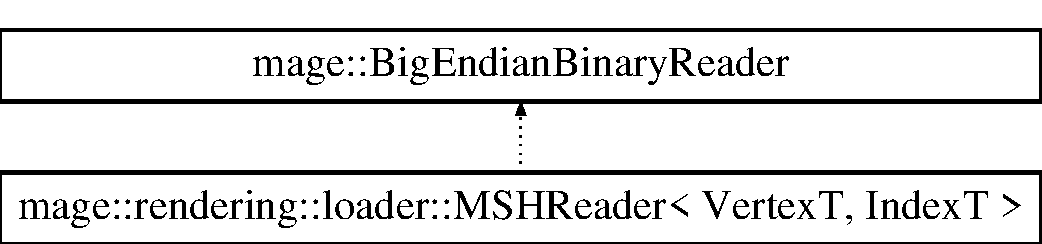
\includegraphics[height=2.000000cm]{classmage_1_1rendering_1_1loader_1_1_m_s_h_reader}
\end{center}
\end{figure}
\subsection*{Public Member Functions}
\begin{DoxyCompactItemize}
\item 
\mbox{\hyperlink{classmage_1_1rendering_1_1loader_1_1_m_s_h_reader_adf50a71f368cd580433b3dab5ea3a1ac}{M\+S\+H\+Reader}} (std\+::vector$<$ VertexT $>$ \&vertices, std\+::vector$<$ IndexT $>$ \&indices)
\item 
\mbox{\hyperlink{classmage_1_1rendering_1_1loader_1_1_m_s_h_reader_ae16a36afbfe65791cdfe8dadd6b57af2}{M\+S\+H\+Reader}} (const \mbox{\hyperlink{classmage_1_1rendering_1_1loader_1_1_m_s_h_reader}{M\+S\+H\+Reader}} \&reader)=delete
\item 
\mbox{\hyperlink{classmage_1_1rendering_1_1loader_1_1_m_s_h_reader_a107ac854c231c1a1c39f30c5199dcec7}{M\+S\+H\+Reader}} (\mbox{\hyperlink{classmage_1_1rendering_1_1loader_1_1_m_s_h_reader}{M\+S\+H\+Reader}} \&\&reader) noexcept
\item 
\mbox{\hyperlink{classmage_1_1rendering_1_1loader_1_1_m_s_h_reader_af45daf383d4e94586b5d2968d5357fce}{$\sim$\+M\+S\+H\+Reader}} ()
\item 
\mbox{\hyperlink{classmage_1_1rendering_1_1loader_1_1_m_s_h_reader}{M\+S\+H\+Reader}} \& \mbox{\hyperlink{classmage_1_1rendering_1_1loader_1_1_m_s_h_reader_a106e5a6cce46777cf7ae36cb4034e1a0}{operator=}} (const \mbox{\hyperlink{classmage_1_1rendering_1_1loader_1_1_m_s_h_reader}{M\+S\+H\+Reader}} \&reader)=delete
\item 
\mbox{\hyperlink{classmage_1_1rendering_1_1loader_1_1_m_s_h_reader}{M\+S\+H\+Reader}} \& \mbox{\hyperlink{classmage_1_1rendering_1_1loader_1_1_m_s_h_reader_a8764164f7e0f78938c5e303d13e0f64d}{operator=}} (\mbox{\hyperlink{classmage_1_1rendering_1_1loader_1_1_m_s_h_reader}{M\+S\+H\+Reader}} \&\&reader)=delete
\item 
void \mbox{\hyperlink{classmage_1_1rendering_1_1loader_1_1_m_s_h_reader_a0308b90e3cf888d383a228cfe8827972}{Read\+From\+File}} (std\+::filesystem\+::path path)
\item 
void \mbox{\hyperlink{classmage_1_1rendering_1_1loader_1_1_m_s_h_reader_afc48490dca5042078726a1ec3fe7abe7}{Read\+From\+Memory}} (gsl\+::span$<$ const \mbox{\hyperlink{namespacemage_afc638980bc6154f15af5e2d93a0e0ea9}{U8}} $>$ input)
\end{DoxyCompactItemize}
\subsection*{Private Member Functions}
\begin{DoxyCompactItemize}
\item 
virtual void \mbox{\hyperlink{classmage_1_1rendering_1_1loader_1_1_m_s_h_reader_a99e8e3c50decb9332dc10bcdf7b6e00a}{Read\+Data}} () override
\item 
bool \mbox{\hyperlink{classmage_1_1rendering_1_1loader_1_1_m_s_h_reader_a7e6948dfb5f5c672719ebe10c4dae6bf}{Is\+Header\+Valid}} ()
\end{DoxyCompactItemize}
\subsection*{Private Attributes}
\begin{DoxyCompactItemize}
\item 
std\+::vector$<$ VertexT $>$ \& \mbox{\hyperlink{classmage_1_1rendering_1_1loader_1_1_m_s_h_reader_a57e5f4e14aecbce999df14d0dcaba4e5}{m\+\_\+vertices}}
\item 
std\+::vector$<$ IndexT $>$ \& \mbox{\hyperlink{classmage_1_1rendering_1_1loader_1_1_m_s_h_reader_acf3ae948f5bb927a167bbb2e5d618916}{m\+\_\+indices}}
\end{DoxyCompactItemize}


\subsection{Detailed Description}
\subsubsection*{template$<$typename VertexT, typename IndexT$>$\newline
class mage\+::rendering\+::loader\+::\+M\+S\+H\+Reader$<$ Vertex\+T, Index\+T $>$}

A class of M\+SH file readers for reading meshes.


\begin{DoxyTemplParams}{Template Parameters}
{\em VertexT} & The vertex type. \\
\hline
{\em IndexT} & The index type. \\
\hline
\end{DoxyTemplParams}


\subsection{Constructor \& Destructor Documentation}
\mbox{\Hypertarget{classmage_1_1rendering_1_1loader_1_1_m_s_h_reader_adf50a71f368cd580433b3dab5ea3a1ac}\label{classmage_1_1rendering_1_1loader_1_1_m_s_h_reader_adf50a71f368cd580433b3dab5ea3a1ac}} 
\index{mage\+::rendering\+::loader\+::\+M\+S\+H\+Reader@{mage\+::rendering\+::loader\+::\+M\+S\+H\+Reader}!M\+S\+H\+Reader@{M\+S\+H\+Reader}}
\index{M\+S\+H\+Reader@{M\+S\+H\+Reader}!mage\+::rendering\+::loader\+::\+M\+S\+H\+Reader@{mage\+::rendering\+::loader\+::\+M\+S\+H\+Reader}}
\subsubsection{\texorpdfstring{M\+S\+H\+Reader()}{MSHReader()}\hspace{0.1cm}{\footnotesize\ttfamily [1/3]}}
{\footnotesize\ttfamily template$<$typename VertexT , typename IndexT $>$ \\
\mbox{\hyperlink{classmage_1_1rendering_1_1loader_1_1_m_s_h_reader}{mage\+::rendering\+::loader\+::\+M\+S\+H\+Reader}}$<$ VertexT, IndexT $>$\+::\mbox{\hyperlink{classmage_1_1rendering_1_1loader_1_1_m_s_h_reader}{M\+S\+H\+Reader}} (\begin{DoxyParamCaption}\item[{std\+::vector$<$ VertexT $>$ \&}]{vertices,  }\item[{std\+::vector$<$ IndexT $>$ \&}]{indices }\end{DoxyParamCaption})\hspace{0.3cm}{\ttfamily [explicit]}}

Constructs a M\+SH reader.


\begin{DoxyParams}[1]{Parameters}
\mbox{\tt in}  & {\em vertices} & A reference to a vector for storing the read vertices from file. \\
\hline
\mbox{\tt in}  & {\em indices} & A reference to a vector for storing the read indices from file. \\
\hline
\end{DoxyParams}
\mbox{\Hypertarget{classmage_1_1rendering_1_1loader_1_1_m_s_h_reader_ae16a36afbfe65791cdfe8dadd6b57af2}\label{classmage_1_1rendering_1_1loader_1_1_m_s_h_reader_ae16a36afbfe65791cdfe8dadd6b57af2}} 
\index{mage\+::rendering\+::loader\+::\+M\+S\+H\+Reader@{mage\+::rendering\+::loader\+::\+M\+S\+H\+Reader}!M\+S\+H\+Reader@{M\+S\+H\+Reader}}
\index{M\+S\+H\+Reader@{M\+S\+H\+Reader}!mage\+::rendering\+::loader\+::\+M\+S\+H\+Reader@{mage\+::rendering\+::loader\+::\+M\+S\+H\+Reader}}
\subsubsection{\texorpdfstring{M\+S\+H\+Reader()}{MSHReader()}\hspace{0.1cm}{\footnotesize\ttfamily [2/3]}}
{\footnotesize\ttfamily template$<$typename VertexT , typename IndexT $>$ \\
\mbox{\hyperlink{classmage_1_1rendering_1_1loader_1_1_m_s_h_reader}{mage\+::rendering\+::loader\+::\+M\+S\+H\+Reader}}$<$ VertexT, IndexT $>$\+::\mbox{\hyperlink{classmage_1_1rendering_1_1loader_1_1_m_s_h_reader}{M\+S\+H\+Reader}} (\begin{DoxyParamCaption}\item[{const \mbox{\hyperlink{classmage_1_1rendering_1_1loader_1_1_m_s_h_reader}{M\+S\+H\+Reader}}$<$ VertexT, IndexT $>$ \&}]{reader }\end{DoxyParamCaption})\hspace{0.3cm}{\ttfamily [delete]}}

Constructs a M\+SH reader from the given M\+SH reader.


\begin{DoxyParams}[1]{Parameters}
\mbox{\tt in}  & {\em reader} & A reference to the M\+SH reader to copy. \\
\hline
\end{DoxyParams}
\mbox{\Hypertarget{classmage_1_1rendering_1_1loader_1_1_m_s_h_reader_a107ac854c231c1a1c39f30c5199dcec7}\label{classmage_1_1rendering_1_1loader_1_1_m_s_h_reader_a107ac854c231c1a1c39f30c5199dcec7}} 
\index{mage\+::rendering\+::loader\+::\+M\+S\+H\+Reader@{mage\+::rendering\+::loader\+::\+M\+S\+H\+Reader}!M\+S\+H\+Reader@{M\+S\+H\+Reader}}
\index{M\+S\+H\+Reader@{M\+S\+H\+Reader}!mage\+::rendering\+::loader\+::\+M\+S\+H\+Reader@{mage\+::rendering\+::loader\+::\+M\+S\+H\+Reader}}
\subsubsection{\texorpdfstring{M\+S\+H\+Reader()}{MSHReader()}\hspace{0.1cm}{\footnotesize\ttfamily [3/3]}}
{\footnotesize\ttfamily template$<$typename VertexT , typename IndexT $>$ \\
\mbox{\hyperlink{classmage_1_1rendering_1_1loader_1_1_m_s_h_reader}{mage\+::rendering\+::loader\+::\+M\+S\+H\+Reader}}$<$ VertexT, IndexT $>$\+::\mbox{\hyperlink{classmage_1_1rendering_1_1loader_1_1_m_s_h_reader}{M\+S\+H\+Reader}} (\begin{DoxyParamCaption}\item[{\mbox{\hyperlink{classmage_1_1rendering_1_1loader_1_1_m_s_h_reader}{M\+S\+H\+Reader}}$<$ VertexT, IndexT $>$ \&\&}]{reader }\end{DoxyParamCaption})\hspace{0.3cm}{\ttfamily [noexcept]}}

Constructs a M\+SH reader by moving the given M\+SH reader.


\begin{DoxyParams}[1]{Parameters}
\mbox{\tt in}  & {\em reader} & A reference to the M\+SH reader to move. \\
\hline
\end{DoxyParams}
\mbox{\Hypertarget{classmage_1_1rendering_1_1loader_1_1_m_s_h_reader_af45daf383d4e94586b5d2968d5357fce}\label{classmage_1_1rendering_1_1loader_1_1_m_s_h_reader_af45daf383d4e94586b5d2968d5357fce}} 
\index{mage\+::rendering\+::loader\+::\+M\+S\+H\+Reader@{mage\+::rendering\+::loader\+::\+M\+S\+H\+Reader}!````~M\+S\+H\+Reader@{$\sim$\+M\+S\+H\+Reader}}
\index{````~M\+S\+H\+Reader@{$\sim$\+M\+S\+H\+Reader}!mage\+::rendering\+::loader\+::\+M\+S\+H\+Reader@{mage\+::rendering\+::loader\+::\+M\+S\+H\+Reader}}
\subsubsection{\texorpdfstring{$\sim$\+M\+S\+H\+Reader()}{~MSHReader()}}
{\footnotesize\ttfamily template$<$typename VertexT , typename IndexT $>$ \\
\mbox{\hyperlink{classmage_1_1rendering_1_1loader_1_1_m_s_h_reader}{mage\+::rendering\+::loader\+::\+M\+S\+H\+Reader}}$<$ VertexT, IndexT $>$\+::$\sim$\mbox{\hyperlink{classmage_1_1rendering_1_1loader_1_1_m_s_h_reader}{M\+S\+H\+Reader}} (\begin{DoxyParamCaption}{ }\end{DoxyParamCaption})}

Destructs this M\+SH reader. 

\subsection{Member Function Documentation}
\mbox{\Hypertarget{classmage_1_1rendering_1_1loader_1_1_m_s_h_reader_a7e6948dfb5f5c672719ebe10c4dae6bf}\label{classmage_1_1rendering_1_1loader_1_1_m_s_h_reader_a7e6948dfb5f5c672719ebe10c4dae6bf}} 
\index{mage\+::rendering\+::loader\+::\+M\+S\+H\+Reader@{mage\+::rendering\+::loader\+::\+M\+S\+H\+Reader}!Is\+Header\+Valid@{Is\+Header\+Valid}}
\index{Is\+Header\+Valid@{Is\+Header\+Valid}!mage\+::rendering\+::loader\+::\+M\+S\+H\+Reader@{mage\+::rendering\+::loader\+::\+M\+S\+H\+Reader}}
\subsubsection{\texorpdfstring{Is\+Header\+Valid()}{IsHeaderValid()}}
{\footnotesize\ttfamily template$<$typename VertexT , typename IndexT $>$ \\
bool \mbox{\hyperlink{classmage_1_1rendering_1_1loader_1_1_m_s_h_reader}{mage\+::rendering\+::loader\+::\+M\+S\+H\+Reader}}$<$ VertexT, IndexT $>$\+::Is\+Header\+Valid (\begin{DoxyParamCaption}{ }\end{DoxyParamCaption})\hspace{0.3cm}{\ttfamily [private]}}

Checks whether the header of the file is valid.

\begin{DoxyReturn}{Returns}
{\ttfamily true} if the header of the file is valid. {\ttfamily false} otherwise. 
\end{DoxyReturn}
\mbox{\Hypertarget{classmage_1_1rendering_1_1loader_1_1_m_s_h_reader_a106e5a6cce46777cf7ae36cb4034e1a0}\label{classmage_1_1rendering_1_1loader_1_1_m_s_h_reader_a106e5a6cce46777cf7ae36cb4034e1a0}} 
\index{mage\+::rendering\+::loader\+::\+M\+S\+H\+Reader@{mage\+::rendering\+::loader\+::\+M\+S\+H\+Reader}!operator=@{operator=}}
\index{operator=@{operator=}!mage\+::rendering\+::loader\+::\+M\+S\+H\+Reader@{mage\+::rendering\+::loader\+::\+M\+S\+H\+Reader}}
\subsubsection{\texorpdfstring{operator=()}{operator=()}\hspace{0.1cm}{\footnotesize\ttfamily [1/2]}}
{\footnotesize\ttfamily template$<$typename VertexT , typename IndexT $>$ \\
\mbox{\hyperlink{classmage_1_1rendering_1_1loader_1_1_m_s_h_reader}{M\+S\+H\+Reader}}\& \mbox{\hyperlink{classmage_1_1rendering_1_1loader_1_1_m_s_h_reader}{mage\+::rendering\+::loader\+::\+M\+S\+H\+Reader}}$<$ VertexT, IndexT $>$\+::operator= (\begin{DoxyParamCaption}\item[{const \mbox{\hyperlink{classmage_1_1rendering_1_1loader_1_1_m_s_h_reader}{M\+S\+H\+Reader}}$<$ VertexT, IndexT $>$ \&}]{reader }\end{DoxyParamCaption})\hspace{0.3cm}{\ttfamily [delete]}}

Copies the given M\+SH reader to this M\+SH reader.


\begin{DoxyParams}[1]{Parameters}
\mbox{\tt in}  & {\em reader} & A reference to a M\+SH reader to copy. \\
\hline
\end{DoxyParams}
\begin{DoxyReturn}{Returns}
A reference to the copy of the given M\+SH reader (i.\+e. this M\+SH reader). 
\end{DoxyReturn}
\mbox{\Hypertarget{classmage_1_1rendering_1_1loader_1_1_m_s_h_reader_a8764164f7e0f78938c5e303d13e0f64d}\label{classmage_1_1rendering_1_1loader_1_1_m_s_h_reader_a8764164f7e0f78938c5e303d13e0f64d}} 
\index{mage\+::rendering\+::loader\+::\+M\+S\+H\+Reader@{mage\+::rendering\+::loader\+::\+M\+S\+H\+Reader}!operator=@{operator=}}
\index{operator=@{operator=}!mage\+::rendering\+::loader\+::\+M\+S\+H\+Reader@{mage\+::rendering\+::loader\+::\+M\+S\+H\+Reader}}
\subsubsection{\texorpdfstring{operator=()}{operator=()}\hspace{0.1cm}{\footnotesize\ttfamily [2/2]}}
{\footnotesize\ttfamily template$<$typename VertexT , typename IndexT $>$ \\
\mbox{\hyperlink{classmage_1_1rendering_1_1loader_1_1_m_s_h_reader}{M\+S\+H\+Reader}}\& \mbox{\hyperlink{classmage_1_1rendering_1_1loader_1_1_m_s_h_reader}{mage\+::rendering\+::loader\+::\+M\+S\+H\+Reader}}$<$ VertexT, IndexT $>$\+::operator= (\begin{DoxyParamCaption}\item[{\mbox{\hyperlink{classmage_1_1rendering_1_1loader_1_1_m_s_h_reader}{M\+S\+H\+Reader}}$<$ VertexT, IndexT $>$ \&\&}]{reader }\end{DoxyParamCaption})\hspace{0.3cm}{\ttfamily [delete]}}

Moves the given M\+SH reader to this M\+SH reader.


\begin{DoxyParams}[1]{Parameters}
\mbox{\tt in}  & {\em reader} & A reference to a M\+SH reader to move. \\
\hline
\end{DoxyParams}
\begin{DoxyReturn}{Returns}
A reference to the moved M\+SH reader (i.\+e. this M\+SH reader). 
\end{DoxyReturn}
\mbox{\Hypertarget{classmage_1_1rendering_1_1loader_1_1_m_s_h_reader_a99e8e3c50decb9332dc10bcdf7b6e00a}\label{classmage_1_1rendering_1_1loader_1_1_m_s_h_reader_a99e8e3c50decb9332dc10bcdf7b6e00a}} 
\index{mage\+::rendering\+::loader\+::\+M\+S\+H\+Reader@{mage\+::rendering\+::loader\+::\+M\+S\+H\+Reader}!Read\+Data@{Read\+Data}}
\index{Read\+Data@{Read\+Data}!mage\+::rendering\+::loader\+::\+M\+S\+H\+Reader@{mage\+::rendering\+::loader\+::\+M\+S\+H\+Reader}}
\subsubsection{\texorpdfstring{Read\+Data()}{ReadData()}}
{\footnotesize\ttfamily template$<$typename VertexT , typename IndexT $>$ \\
virtual void \mbox{\hyperlink{classmage_1_1rendering_1_1loader_1_1_m_s_h_reader}{mage\+::rendering\+::loader\+::\+M\+S\+H\+Reader}}$<$ VertexT, IndexT $>$\+::Read\+Data (\begin{DoxyParamCaption}{ }\end{DoxyParamCaption})\hspace{0.3cm}{\ttfamily [override]}, {\ttfamily [private]}, {\ttfamily [virtual]}}

Starts reading.


\begin{DoxyExceptions}{Exceptions}
{\em \mbox{\hyperlink{classmage_1_1_exception}{Exception}}} & Failed to read from the given file. \\
\hline
\end{DoxyExceptions}


Implements \mbox{\hyperlink{classmage_1_1_big_endian_binary_reader_a7dc0689d598fa91308597b129516a11d}{mage\+::\+Big\+Endian\+Binary\+Reader}}.

\mbox{\Hypertarget{classmage_1_1rendering_1_1loader_1_1_m_s_h_reader_a0308b90e3cf888d383a228cfe8827972}\label{classmage_1_1rendering_1_1loader_1_1_m_s_h_reader_a0308b90e3cf888d383a228cfe8827972}} 
\index{mage\+::rendering\+::loader\+::\+M\+S\+H\+Reader@{mage\+::rendering\+::loader\+::\+M\+S\+H\+Reader}!Read\+From\+File@{Read\+From\+File}}
\index{Read\+From\+File@{Read\+From\+File}!mage\+::rendering\+::loader\+::\+M\+S\+H\+Reader@{mage\+::rendering\+::loader\+::\+M\+S\+H\+Reader}}
\subsubsection{\texorpdfstring{Read\+From\+File()}{ReadFromFile()}}
{\footnotesize\ttfamily template$<$typename VertexT , typename IndexT $>$ \\
void mage\+::\+Big\+Endian\+Binary\+Reader\+::\+Read\+From\+File}

Reads from the file associated with the given path.


\begin{DoxyParams}[1]{Parameters}
\mbox{\tt in}  & {\em path} & The path. \\
\hline
\end{DoxyParams}

\begin{DoxyExceptions}{Exceptions}
{\em \mbox{\hyperlink{classmage_1_1_exception}{Exception}}} & Failed to read from the file. \\
\hline
\end{DoxyExceptions}
\mbox{\Hypertarget{classmage_1_1rendering_1_1loader_1_1_m_s_h_reader_afc48490dca5042078726a1ec3fe7abe7}\label{classmage_1_1rendering_1_1loader_1_1_m_s_h_reader_afc48490dca5042078726a1ec3fe7abe7}} 
\index{mage\+::rendering\+::loader\+::\+M\+S\+H\+Reader@{mage\+::rendering\+::loader\+::\+M\+S\+H\+Reader}!Read\+From\+Memory@{Read\+From\+Memory}}
\index{Read\+From\+Memory@{Read\+From\+Memory}!mage\+::rendering\+::loader\+::\+M\+S\+H\+Reader@{mage\+::rendering\+::loader\+::\+M\+S\+H\+Reader}}
\subsubsection{\texorpdfstring{Read\+From\+Memory()}{ReadFromMemory()}}
{\footnotesize\ttfamily template$<$typename VertexT , typename IndexT $>$ \\
void mage\+::\+Big\+Endian\+Binary\+Reader\+::\+Read\+From\+Memory}

Reads the input string.


\begin{DoxyParams}[1]{Parameters}
\mbox{\tt in}  & {\em input} & The input byte string. \\
\hline
\end{DoxyParams}

\begin{DoxyExceptions}{Exceptions}
{\em \mbox{\hyperlink{classmage_1_1_exception}{Exception}}} & Failed to read from the given input string. \\
\hline
\end{DoxyExceptions}


\subsection{Member Data Documentation}
\mbox{\Hypertarget{classmage_1_1rendering_1_1loader_1_1_m_s_h_reader_acf3ae948f5bb927a167bbb2e5d618916}\label{classmage_1_1rendering_1_1loader_1_1_m_s_h_reader_acf3ae948f5bb927a167bbb2e5d618916}} 
\index{mage\+::rendering\+::loader\+::\+M\+S\+H\+Reader@{mage\+::rendering\+::loader\+::\+M\+S\+H\+Reader}!m\+\_\+indices@{m\+\_\+indices}}
\index{m\+\_\+indices@{m\+\_\+indices}!mage\+::rendering\+::loader\+::\+M\+S\+H\+Reader@{mage\+::rendering\+::loader\+::\+M\+S\+H\+Reader}}
\subsubsection{\texorpdfstring{m\+\_\+indices}{m\_indices}}
{\footnotesize\ttfamily template$<$typename VertexT , typename IndexT $>$ \\
std\+::vector$<$ IndexT $>$\& \mbox{\hyperlink{classmage_1_1rendering_1_1loader_1_1_m_s_h_reader}{mage\+::rendering\+::loader\+::\+M\+S\+H\+Reader}}$<$ VertexT, IndexT $>$\+::m\+\_\+indices\hspace{0.3cm}{\ttfamily [private]}}

A reference to a vector containing the read indices of this M\+SH reader. \mbox{\Hypertarget{classmage_1_1rendering_1_1loader_1_1_m_s_h_reader_a57e5f4e14aecbce999df14d0dcaba4e5}\label{classmage_1_1rendering_1_1loader_1_1_m_s_h_reader_a57e5f4e14aecbce999df14d0dcaba4e5}} 
\index{mage\+::rendering\+::loader\+::\+M\+S\+H\+Reader@{mage\+::rendering\+::loader\+::\+M\+S\+H\+Reader}!m\+\_\+vertices@{m\+\_\+vertices}}
\index{m\+\_\+vertices@{m\+\_\+vertices}!mage\+::rendering\+::loader\+::\+M\+S\+H\+Reader@{mage\+::rendering\+::loader\+::\+M\+S\+H\+Reader}}
\subsubsection{\texorpdfstring{m\+\_\+vertices}{m\_vertices}}
{\footnotesize\ttfamily template$<$typename VertexT , typename IndexT $>$ \\
std\+::vector$<$ VertexT $>$\& \mbox{\hyperlink{classmage_1_1rendering_1_1loader_1_1_m_s_h_reader}{mage\+::rendering\+::loader\+::\+M\+S\+H\+Reader}}$<$ VertexT, IndexT $>$\+::m\+\_\+vertices\hspace{0.3cm}{\ttfamily [private]}}

A reference to a vector containing the read vertices of this M\+SH reader. 
\hypertarget{classmage_1_1rendering_1_1loader_1_1_m_s_h_writer}{}\section{mage\+:\+:rendering\+:\+:loader\+:\+:M\+S\+H\+Writer$<$ VertexT, IndexT $>$ Class Template Reference}
\label{classmage_1_1rendering_1_1loader_1_1_m_s_h_writer}\index{mage\+::rendering\+::loader\+::\+M\+S\+H\+Writer$<$ Vertex\+T, Index\+T $>$@{mage\+::rendering\+::loader\+::\+M\+S\+H\+Writer$<$ Vertex\+T, Index\+T $>$}}


{\ttfamily \#include $<$msh\+\_\+writer.\+hpp$>$}

Inheritance diagram for mage\+:\+:rendering\+:\+:loader\+:\+:M\+S\+H\+Writer$<$ VertexT, IndexT $>$\+:\begin{figure}[H]
\begin{center}
\leavevmode
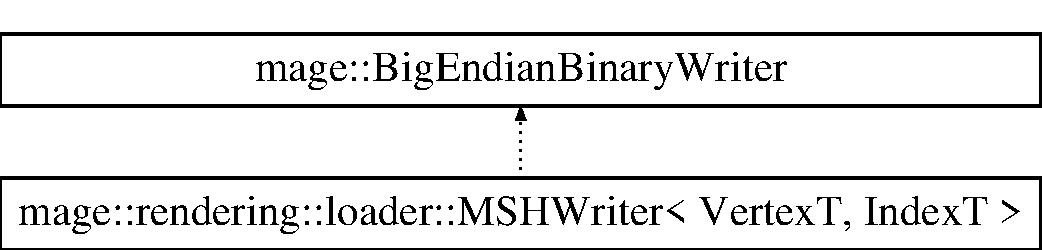
\includegraphics[height=2.000000cm]{classmage_1_1rendering_1_1loader_1_1_m_s_h_writer}
\end{center}
\end{figure}
\subsection*{Public Member Functions}
\begin{DoxyCompactItemize}
\item 
\mbox{\hyperlink{classmage_1_1rendering_1_1loader_1_1_m_s_h_writer_a5e1a7ed8ca94f157f52bba929cac2fd3}{M\+S\+H\+Writer}} (const std\+::vector$<$ VertexT $>$ \&vertices, const std\+::vector$<$ IndexT $>$ \&indices)
\item 
\mbox{\hyperlink{classmage_1_1rendering_1_1loader_1_1_m_s_h_writer_ade94bfa4dc8b4bdc2249cd882f2240e4}{M\+S\+H\+Writer}} (const \mbox{\hyperlink{classmage_1_1rendering_1_1loader_1_1_m_s_h_writer}{M\+S\+H\+Writer}} \&writer)=delete
\item 
\mbox{\hyperlink{classmage_1_1rendering_1_1loader_1_1_m_s_h_writer_a877a042ef1a4472c9d1cece846b2a70a}{M\+S\+H\+Writer}} (\mbox{\hyperlink{classmage_1_1rendering_1_1loader_1_1_m_s_h_writer}{M\+S\+H\+Writer}} \&\&writer) noexcept
\item 
\mbox{\hyperlink{classmage_1_1rendering_1_1loader_1_1_m_s_h_writer_ae2ead8892a1818c59d55a7a5ecdf50b3}{$\sim$\+M\+S\+H\+Writer}} ()
\item 
\mbox{\hyperlink{classmage_1_1rendering_1_1loader_1_1_m_s_h_writer}{M\+S\+H\+Writer}} \& \mbox{\hyperlink{classmage_1_1rendering_1_1loader_1_1_m_s_h_writer_a661eaab96539a7bf08f100095603af0e}{operator=}} (const \mbox{\hyperlink{classmage_1_1rendering_1_1loader_1_1_m_s_h_writer}{M\+S\+H\+Writer}} \&writer)=delete
\item 
\mbox{\hyperlink{classmage_1_1rendering_1_1loader_1_1_m_s_h_writer}{M\+S\+H\+Writer}} \& \mbox{\hyperlink{classmage_1_1rendering_1_1loader_1_1_m_s_h_writer_a98bdde59fa1a7a6398453f0c7bc4e8dd}{operator=}} (\mbox{\hyperlink{classmage_1_1rendering_1_1loader_1_1_m_s_h_writer}{M\+S\+H\+Writer}} \&\&writer)=delete
\item 
void \mbox{\hyperlink{classmage_1_1rendering_1_1loader_1_1_m_s_h_writer_a6ce9780687a45a6c6f98e0843190b63b}{Write\+To\+File}} (std\+::filesystem\+::path path)
\item 
const std\+::filesystem\+::path \& \mbox{\hyperlink{classmage_1_1rendering_1_1loader_1_1_m_s_h_writer_a812e65c16bf1b14d396d109eb969eeb8}{Get\+Path}} () const noexcept
\end{DoxyCompactItemize}
\subsection*{Private Member Functions}
\begin{DoxyCompactItemize}
\item 
virtual void \mbox{\hyperlink{classmage_1_1rendering_1_1loader_1_1_m_s_h_writer_ad61ee7097e1bfb52ca9a0697d2cd6a7e}{Write\+Data}} () override
\end{DoxyCompactItemize}
\subsection*{Private Attributes}
\begin{DoxyCompactItemize}
\item 
const std\+::vector$<$ VertexT $>$ \& \mbox{\hyperlink{classmage_1_1rendering_1_1loader_1_1_m_s_h_writer_adf2b47491fdda0077ba3bf1053f343d0}{m\+\_\+vertices}}
\item 
const std\+::vector$<$ IndexT $>$ \& \mbox{\hyperlink{classmage_1_1rendering_1_1loader_1_1_m_s_h_writer_a7de7ca864e3a3a384bf7c98997146748}{m\+\_\+indices}}
\end{DoxyCompactItemize}


\subsection{Detailed Description}
\subsubsection*{template$<$typename VertexT, typename IndexT$>$\newline
class mage\+::rendering\+::loader\+::\+M\+S\+H\+Writer$<$ Vertex\+T, Index\+T $>$}

A class of M\+SH file writers for writing meshes.


\begin{DoxyTemplParams}{Template Parameters}
{\em VertexT} & The vertex type. \\
\hline
{\em IndexT} & The index type. \\
\hline
\end{DoxyTemplParams}


\subsection{Constructor \& Destructor Documentation}
\mbox{\Hypertarget{classmage_1_1rendering_1_1loader_1_1_m_s_h_writer_a5e1a7ed8ca94f157f52bba929cac2fd3}\label{classmage_1_1rendering_1_1loader_1_1_m_s_h_writer_a5e1a7ed8ca94f157f52bba929cac2fd3}} 
\index{mage\+::rendering\+::loader\+::\+M\+S\+H\+Writer@{mage\+::rendering\+::loader\+::\+M\+S\+H\+Writer}!M\+S\+H\+Writer@{M\+S\+H\+Writer}}
\index{M\+S\+H\+Writer@{M\+S\+H\+Writer}!mage\+::rendering\+::loader\+::\+M\+S\+H\+Writer@{mage\+::rendering\+::loader\+::\+M\+S\+H\+Writer}}
\subsubsection{\texorpdfstring{M\+S\+H\+Writer()}{MSHWriter()}\hspace{0.1cm}{\footnotesize\ttfamily [1/3]}}
{\footnotesize\ttfamily template$<$typename VertexT , typename IndexT $>$ \\
\mbox{\hyperlink{classmage_1_1rendering_1_1loader_1_1_m_s_h_writer}{mage\+::rendering\+::loader\+::\+M\+S\+H\+Writer}}$<$ VertexT, IndexT $>$\+::\mbox{\hyperlink{classmage_1_1rendering_1_1loader_1_1_m_s_h_writer}{M\+S\+H\+Writer}} (\begin{DoxyParamCaption}\item[{const std\+::vector$<$ VertexT $>$ \&}]{vertices,  }\item[{const std\+::vector$<$ IndexT $>$ \&}]{indices }\end{DoxyParamCaption})\hspace{0.3cm}{\ttfamily [explicit]}}

Constructs a M\+SH writer.


\begin{DoxyParams}[1]{Parameters}
\mbox{\tt in}  & {\em vertices} & A reference to a vector containing the vertices. \\
\hline
\mbox{\tt in}  & {\em indices} & A reference to a vector containing the indices. \\
\hline
\end{DoxyParams}
\mbox{\Hypertarget{classmage_1_1rendering_1_1loader_1_1_m_s_h_writer_ade94bfa4dc8b4bdc2249cd882f2240e4}\label{classmage_1_1rendering_1_1loader_1_1_m_s_h_writer_ade94bfa4dc8b4bdc2249cd882f2240e4}} 
\index{mage\+::rendering\+::loader\+::\+M\+S\+H\+Writer@{mage\+::rendering\+::loader\+::\+M\+S\+H\+Writer}!M\+S\+H\+Writer@{M\+S\+H\+Writer}}
\index{M\+S\+H\+Writer@{M\+S\+H\+Writer}!mage\+::rendering\+::loader\+::\+M\+S\+H\+Writer@{mage\+::rendering\+::loader\+::\+M\+S\+H\+Writer}}
\subsubsection{\texorpdfstring{M\+S\+H\+Writer()}{MSHWriter()}\hspace{0.1cm}{\footnotesize\ttfamily [2/3]}}
{\footnotesize\ttfamily template$<$typename VertexT , typename IndexT $>$ \\
\mbox{\hyperlink{classmage_1_1rendering_1_1loader_1_1_m_s_h_writer}{mage\+::rendering\+::loader\+::\+M\+S\+H\+Writer}}$<$ VertexT, IndexT $>$\+::\mbox{\hyperlink{classmage_1_1rendering_1_1loader_1_1_m_s_h_writer}{M\+S\+H\+Writer}} (\begin{DoxyParamCaption}\item[{const \mbox{\hyperlink{classmage_1_1rendering_1_1loader_1_1_m_s_h_writer}{M\+S\+H\+Writer}}$<$ VertexT, IndexT $>$ \&}]{writer }\end{DoxyParamCaption})\hspace{0.3cm}{\ttfamily [delete]}}

Constructs a M\+SH writer from the given M\+SH writer.


\begin{DoxyParams}[1]{Parameters}
\mbox{\tt in}  & {\em writer} & A reference to the M\+SH writer to copy. \\
\hline
\end{DoxyParams}
\mbox{\Hypertarget{classmage_1_1rendering_1_1loader_1_1_m_s_h_writer_a877a042ef1a4472c9d1cece846b2a70a}\label{classmage_1_1rendering_1_1loader_1_1_m_s_h_writer_a877a042ef1a4472c9d1cece846b2a70a}} 
\index{mage\+::rendering\+::loader\+::\+M\+S\+H\+Writer@{mage\+::rendering\+::loader\+::\+M\+S\+H\+Writer}!M\+S\+H\+Writer@{M\+S\+H\+Writer}}
\index{M\+S\+H\+Writer@{M\+S\+H\+Writer}!mage\+::rendering\+::loader\+::\+M\+S\+H\+Writer@{mage\+::rendering\+::loader\+::\+M\+S\+H\+Writer}}
\subsubsection{\texorpdfstring{M\+S\+H\+Writer()}{MSHWriter()}\hspace{0.1cm}{\footnotesize\ttfamily [3/3]}}
{\footnotesize\ttfamily template$<$typename VertexT , typename IndexT $>$ \\
\mbox{\hyperlink{classmage_1_1rendering_1_1loader_1_1_m_s_h_writer}{mage\+::rendering\+::loader\+::\+M\+S\+H\+Writer}}$<$ VertexT, IndexT $>$\+::\mbox{\hyperlink{classmage_1_1rendering_1_1loader_1_1_m_s_h_writer}{M\+S\+H\+Writer}} (\begin{DoxyParamCaption}\item[{\mbox{\hyperlink{classmage_1_1rendering_1_1loader_1_1_m_s_h_writer}{M\+S\+H\+Writer}}$<$ VertexT, IndexT $>$ \&\&}]{writer }\end{DoxyParamCaption})\hspace{0.3cm}{\ttfamily [noexcept]}}

Constructs a M\+SH writer by moving the given M\+SH writer.


\begin{DoxyParams}[1]{Parameters}
\mbox{\tt in}  & {\em writer} & A reference to the M\+SH writer to move. \\
\hline
\end{DoxyParams}
\mbox{\Hypertarget{classmage_1_1rendering_1_1loader_1_1_m_s_h_writer_ae2ead8892a1818c59d55a7a5ecdf50b3}\label{classmage_1_1rendering_1_1loader_1_1_m_s_h_writer_ae2ead8892a1818c59d55a7a5ecdf50b3}} 
\index{mage\+::rendering\+::loader\+::\+M\+S\+H\+Writer@{mage\+::rendering\+::loader\+::\+M\+S\+H\+Writer}!````~M\+S\+H\+Writer@{$\sim$\+M\+S\+H\+Writer}}
\index{````~M\+S\+H\+Writer@{$\sim$\+M\+S\+H\+Writer}!mage\+::rendering\+::loader\+::\+M\+S\+H\+Writer@{mage\+::rendering\+::loader\+::\+M\+S\+H\+Writer}}
\subsubsection{\texorpdfstring{$\sim$\+M\+S\+H\+Writer()}{~MSHWriter()}}
{\footnotesize\ttfamily template$<$typename VertexT , typename IndexT $>$ \\
\mbox{\hyperlink{classmage_1_1rendering_1_1loader_1_1_m_s_h_writer}{mage\+::rendering\+::loader\+::\+M\+S\+H\+Writer}}$<$ VertexT, IndexT $>$\+::$\sim$\mbox{\hyperlink{classmage_1_1rendering_1_1loader_1_1_m_s_h_writer}{M\+S\+H\+Writer}} (\begin{DoxyParamCaption}{ }\end{DoxyParamCaption})}

Destructs this M\+SH writer. 

\subsection{Member Function Documentation}
\mbox{\Hypertarget{classmage_1_1rendering_1_1loader_1_1_m_s_h_writer_a812e65c16bf1b14d396d109eb969eeb8}\label{classmage_1_1rendering_1_1loader_1_1_m_s_h_writer_a812e65c16bf1b14d396d109eb969eeb8}} 
\index{mage\+::rendering\+::loader\+::\+M\+S\+H\+Writer@{mage\+::rendering\+::loader\+::\+M\+S\+H\+Writer}!Get\+Path@{Get\+Path}}
\index{Get\+Path@{Get\+Path}!mage\+::rendering\+::loader\+::\+M\+S\+H\+Writer@{mage\+::rendering\+::loader\+::\+M\+S\+H\+Writer}}
\subsubsection{\texorpdfstring{Get\+Path()}{GetPath()}}
{\footnotesize\ttfamily template$<$typename VertexT , typename IndexT $>$ \\
const std\+::filesystem\+::path\& mage\+::\+Big\+Endian\+Binary\+Writer\+::\+Get\+Path\hspace{0.3cm}{\ttfamily [noexcept]}}

Returns the current path of this big endian binary writer.

\begin{DoxyReturn}{Returns}
A reference to the current path of this big endian binary writer. 
\end{DoxyReturn}
\mbox{\Hypertarget{classmage_1_1rendering_1_1loader_1_1_m_s_h_writer_a661eaab96539a7bf08f100095603af0e}\label{classmage_1_1rendering_1_1loader_1_1_m_s_h_writer_a661eaab96539a7bf08f100095603af0e}} 
\index{mage\+::rendering\+::loader\+::\+M\+S\+H\+Writer@{mage\+::rendering\+::loader\+::\+M\+S\+H\+Writer}!operator=@{operator=}}
\index{operator=@{operator=}!mage\+::rendering\+::loader\+::\+M\+S\+H\+Writer@{mage\+::rendering\+::loader\+::\+M\+S\+H\+Writer}}
\subsubsection{\texorpdfstring{operator=()}{operator=()}\hspace{0.1cm}{\footnotesize\ttfamily [1/2]}}
{\footnotesize\ttfamily template$<$typename VertexT , typename IndexT $>$ \\
\mbox{\hyperlink{classmage_1_1rendering_1_1loader_1_1_m_s_h_writer}{M\+S\+H\+Writer}}\& \mbox{\hyperlink{classmage_1_1rendering_1_1loader_1_1_m_s_h_writer}{mage\+::rendering\+::loader\+::\+M\+S\+H\+Writer}}$<$ VertexT, IndexT $>$\+::operator= (\begin{DoxyParamCaption}\item[{const \mbox{\hyperlink{classmage_1_1rendering_1_1loader_1_1_m_s_h_writer}{M\+S\+H\+Writer}}$<$ VertexT, IndexT $>$ \&}]{writer }\end{DoxyParamCaption})\hspace{0.3cm}{\ttfamily [delete]}}

Copies the given M\+SH writer to this M\+SH writer.


\begin{DoxyParams}[1]{Parameters}
\mbox{\tt in}  & {\em writer} & A reference to a M\+SH writer to copy. \\
\hline
\end{DoxyParams}
\begin{DoxyReturn}{Returns}
A reference to the copy of the given M\+SH writer (i.\+e. this M\+SH writer). 
\end{DoxyReturn}
\mbox{\Hypertarget{classmage_1_1rendering_1_1loader_1_1_m_s_h_writer_a98bdde59fa1a7a6398453f0c7bc4e8dd}\label{classmage_1_1rendering_1_1loader_1_1_m_s_h_writer_a98bdde59fa1a7a6398453f0c7bc4e8dd}} 
\index{mage\+::rendering\+::loader\+::\+M\+S\+H\+Writer@{mage\+::rendering\+::loader\+::\+M\+S\+H\+Writer}!operator=@{operator=}}
\index{operator=@{operator=}!mage\+::rendering\+::loader\+::\+M\+S\+H\+Writer@{mage\+::rendering\+::loader\+::\+M\+S\+H\+Writer}}
\subsubsection{\texorpdfstring{operator=()}{operator=()}\hspace{0.1cm}{\footnotesize\ttfamily [2/2]}}
{\footnotesize\ttfamily template$<$typename VertexT , typename IndexT $>$ \\
\mbox{\hyperlink{classmage_1_1rendering_1_1loader_1_1_m_s_h_writer}{M\+S\+H\+Writer}}\& \mbox{\hyperlink{classmage_1_1rendering_1_1loader_1_1_m_s_h_writer}{mage\+::rendering\+::loader\+::\+M\+S\+H\+Writer}}$<$ VertexT, IndexT $>$\+::operator= (\begin{DoxyParamCaption}\item[{\mbox{\hyperlink{classmage_1_1rendering_1_1loader_1_1_m_s_h_writer}{M\+S\+H\+Writer}}$<$ VertexT, IndexT $>$ \&\&}]{writer }\end{DoxyParamCaption})\hspace{0.3cm}{\ttfamily [delete]}}

Moves the given M\+SH writer to this M\+SH writer.


\begin{DoxyParams}[1]{Parameters}
\mbox{\tt in}  & {\em writer} & A reference to a M\+SH writer to move. \\
\hline
\end{DoxyParams}
\begin{DoxyReturn}{Returns}
A reference to the moved M\+SH writer (i.\+e. this M\+SH writer). 
\end{DoxyReturn}
\mbox{\Hypertarget{classmage_1_1rendering_1_1loader_1_1_m_s_h_writer_ad61ee7097e1bfb52ca9a0697d2cd6a7e}\label{classmage_1_1rendering_1_1loader_1_1_m_s_h_writer_ad61ee7097e1bfb52ca9a0697d2cd6a7e}} 
\index{mage\+::rendering\+::loader\+::\+M\+S\+H\+Writer@{mage\+::rendering\+::loader\+::\+M\+S\+H\+Writer}!Write\+Data@{Write\+Data}}
\index{Write\+Data@{Write\+Data}!mage\+::rendering\+::loader\+::\+M\+S\+H\+Writer@{mage\+::rendering\+::loader\+::\+M\+S\+H\+Writer}}
\subsubsection{\texorpdfstring{Write\+Data()}{WriteData()}}
{\footnotesize\ttfamily template$<$typename VertexT , typename IndexT $>$ \\
virtual void \mbox{\hyperlink{classmage_1_1rendering_1_1loader_1_1_m_s_h_writer}{mage\+::rendering\+::loader\+::\+M\+S\+H\+Writer}}$<$ VertexT, IndexT $>$\+::Write\+Data (\begin{DoxyParamCaption}{ }\end{DoxyParamCaption})\hspace{0.3cm}{\ttfamily [override]}, {\ttfamily [private]}, {\ttfamily [virtual]}}

Starts writing.


\begin{DoxyExceptions}{Exceptions}
{\em \mbox{\hyperlink{classmage_1_1_exception}{Exception}}} & Failed to write. \\
\hline
\end{DoxyExceptions}


Implements \mbox{\hyperlink{classmage_1_1_big_endian_binary_writer_a719581274b1b185ef05687183f7ded25}{mage\+::\+Big\+Endian\+Binary\+Writer}}.

\mbox{\Hypertarget{classmage_1_1rendering_1_1loader_1_1_m_s_h_writer_a6ce9780687a45a6c6f98e0843190b63b}\label{classmage_1_1rendering_1_1loader_1_1_m_s_h_writer_a6ce9780687a45a6c6f98e0843190b63b}} 
\index{mage\+::rendering\+::loader\+::\+M\+S\+H\+Writer@{mage\+::rendering\+::loader\+::\+M\+S\+H\+Writer}!Write\+To\+File@{Write\+To\+File}}
\index{Write\+To\+File@{Write\+To\+File}!mage\+::rendering\+::loader\+::\+M\+S\+H\+Writer@{mage\+::rendering\+::loader\+::\+M\+S\+H\+Writer}}
\subsubsection{\texorpdfstring{Write\+To\+File()}{WriteToFile()}}
{\footnotesize\ttfamily template$<$typename VertexT , typename IndexT $>$ \\
void mage\+::\+Big\+Endian\+Binary\+Writer\+::\+Write\+To\+File}

Writes to the file associated with the given path.


\begin{DoxyParams}[1]{Parameters}
\mbox{\tt in}  & {\em path} & The path. \\
\hline
\end{DoxyParams}

\begin{DoxyExceptions}{Exceptions}
{\em \mbox{\hyperlink{classmage_1_1_exception}{Exception}}} & Failed to write to the file. \\
\hline
\end{DoxyExceptions}


\subsection{Member Data Documentation}
\mbox{\Hypertarget{classmage_1_1rendering_1_1loader_1_1_m_s_h_writer_a7de7ca864e3a3a384bf7c98997146748}\label{classmage_1_1rendering_1_1loader_1_1_m_s_h_writer_a7de7ca864e3a3a384bf7c98997146748}} 
\index{mage\+::rendering\+::loader\+::\+M\+S\+H\+Writer@{mage\+::rendering\+::loader\+::\+M\+S\+H\+Writer}!m\+\_\+indices@{m\+\_\+indices}}
\index{m\+\_\+indices@{m\+\_\+indices}!mage\+::rendering\+::loader\+::\+M\+S\+H\+Writer@{mage\+::rendering\+::loader\+::\+M\+S\+H\+Writer}}
\subsubsection{\texorpdfstring{m\+\_\+indices}{m\_indices}}
{\footnotesize\ttfamily template$<$typename VertexT , typename IndexT $>$ \\
const std\+::vector$<$ IndexT $>$\& \mbox{\hyperlink{classmage_1_1rendering_1_1loader_1_1_m_s_h_writer}{mage\+::rendering\+::loader\+::\+M\+S\+H\+Writer}}$<$ VertexT, IndexT $>$\+::m\+\_\+indices\hspace{0.3cm}{\ttfamily [private]}}

A reference to a vector containing the indices to write by this VS writer. \mbox{\Hypertarget{classmage_1_1rendering_1_1loader_1_1_m_s_h_writer_adf2b47491fdda0077ba3bf1053f343d0}\label{classmage_1_1rendering_1_1loader_1_1_m_s_h_writer_adf2b47491fdda0077ba3bf1053f343d0}} 
\index{mage\+::rendering\+::loader\+::\+M\+S\+H\+Writer@{mage\+::rendering\+::loader\+::\+M\+S\+H\+Writer}!m\+\_\+vertices@{m\+\_\+vertices}}
\index{m\+\_\+vertices@{m\+\_\+vertices}!mage\+::rendering\+::loader\+::\+M\+S\+H\+Writer@{mage\+::rendering\+::loader\+::\+M\+S\+H\+Writer}}
\subsubsection{\texorpdfstring{m\+\_\+vertices}{m\_vertices}}
{\footnotesize\ttfamily template$<$typename VertexT , typename IndexT $>$ \\
const std\+::vector$<$ VertexT $>$\& \mbox{\hyperlink{classmage_1_1rendering_1_1loader_1_1_m_s_h_writer}{mage\+::rendering\+::loader\+::\+M\+S\+H\+Writer}}$<$ VertexT, IndexT $>$\+::m\+\_\+vertices\hspace{0.3cm}{\ttfamily [private]}}

A reference to a vector containing the vertices to write by this VS writer. 
\hypertarget{classmage_1_1rendering_1_1loader_1_1_m_t_l_reader}{}\section{mage\+:\+:rendering\+:\+:loader\+:\+:M\+T\+L\+Reader Class Reference}
\label{classmage_1_1rendering_1_1loader_1_1_m_t_l_reader}\index{mage\+::rendering\+::loader\+::\+M\+T\+L\+Reader@{mage\+::rendering\+::loader\+::\+M\+T\+L\+Reader}}


{\ttfamily \#include $<$mtl\+\_\+reader.\+hpp$>$}

Inheritance diagram for mage\+:\+:rendering\+:\+:loader\+:\+:M\+T\+L\+Reader\+:\begin{figure}[H]
\begin{center}
\leavevmode
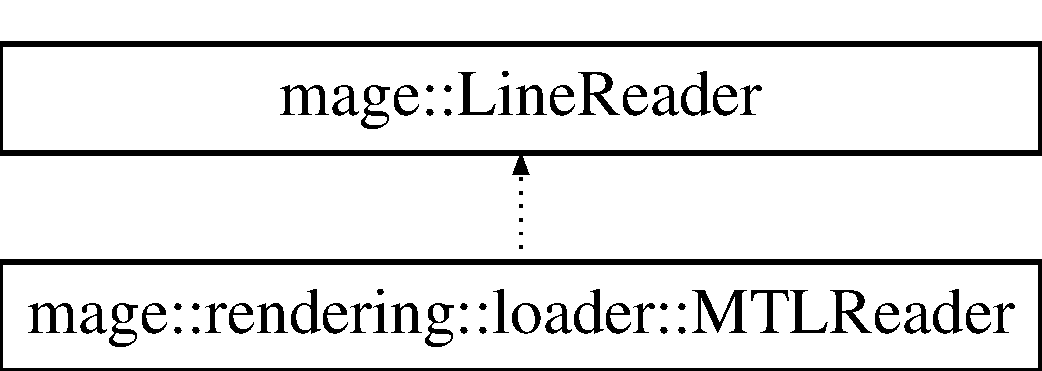
\includegraphics[height=2.000000cm]{classmage_1_1rendering_1_1loader_1_1_m_t_l_reader}
\end{center}
\end{figure}
\subsection*{Public Member Functions}
\begin{DoxyCompactItemize}
\item 
\hyperlink{classmage_1_1rendering_1_1loader_1_1_m_t_l_reader_a3615f6899de22b53de1bad257ac34099}{M\+T\+L\+Reader} (\hyperlink{classmage_1_1rendering_1_1_resource_manager}{Resource\+Manager} \&resource\+\_\+manager, std\+::vector$<$ \hyperlink{classmage_1_1rendering_1_1_material}{Material} $>$ \&material\+\_\+buffer)
\item 
\hyperlink{classmage_1_1rendering_1_1loader_1_1_m_t_l_reader_ad359e191af9b96e78660ed7aa313a48a}{M\+T\+L\+Reader} (const \hyperlink{classmage_1_1rendering_1_1loader_1_1_m_t_l_reader}{M\+T\+L\+Reader} \&reader)=delete
\item 
\hyperlink{classmage_1_1rendering_1_1loader_1_1_m_t_l_reader_af6b1842f18fb4a6e6bae435fd0f08496}{M\+T\+L\+Reader} (\hyperlink{classmage_1_1rendering_1_1loader_1_1_m_t_l_reader}{M\+T\+L\+Reader} \&\&reader) noexcept
\item 
\hyperlink{classmage_1_1rendering_1_1loader_1_1_m_t_l_reader_a87a4f9bf27cfe8e7e7d0c13c330775d6}{$\sim$\+M\+T\+L\+Reader} ()
\item 
\hyperlink{classmage_1_1rendering_1_1loader_1_1_m_t_l_reader}{M\+T\+L\+Reader} \& \hyperlink{classmage_1_1rendering_1_1loader_1_1_m_t_l_reader_a1153606ce103d9f667726cf5f66a88d1}{operator=} (const \hyperlink{classmage_1_1rendering_1_1loader_1_1_m_t_l_reader}{M\+T\+L\+Reader} \&reader)=delete
\item 
\hyperlink{classmage_1_1rendering_1_1loader_1_1_m_t_l_reader}{M\+T\+L\+Reader} \& \hyperlink{classmage_1_1rendering_1_1loader_1_1_m_t_l_reader_a057f38f1f720e040b2ab5fa08f42fac4}{operator=} (\hyperlink{classmage_1_1rendering_1_1loader_1_1_m_t_l_reader}{M\+T\+L\+Reader} \&\&reader)=delete
\end{DoxyCompactItemize}
\subsection*{Private Member Functions}
\begin{DoxyCompactItemize}
\item 
virtual void \hyperlink{classmage_1_1rendering_1_1loader_1_1_m_t_l_reader_a54eb83757c915ebca73175e83737cf73}{Read\+Line} (\hyperlink{namespacemage_a8769f9d670d6b585ea306cb1062af94b}{Not\+Null}$<$ \hyperlink{namespacemage_a4163ec9a9a27d5e7f4b452dcb99cb2b9}{zstring} $>$ line) override
\item 
void \hyperlink{classmage_1_1rendering_1_1loader_1_1_m_t_l_reader_ab123422945f5937ffe484c1076a6858b}{Read\+M\+T\+L\+Material\+Name} ()
\item 
void \hyperlink{classmage_1_1rendering_1_1loader_1_1_m_t_l_reader_ae228231b40bc5b8a6fdff3a9a5698530}{Read\+M\+T\+L\+Base\+Color} ()
\item 
void \hyperlink{classmage_1_1rendering_1_1loader_1_1_m_t_l_reader_a01438c92852592fd719a85d146e38b65}{Read\+M\+T\+L\+Roughness} ()
\item 
void \hyperlink{classmage_1_1rendering_1_1loader_1_1_m_t_l_reader_a14aa8cd5655730234c460c6060552f68}{Read\+M\+T\+L\+Metalness} ()
\item 
void \hyperlink{classmage_1_1rendering_1_1loader_1_1_m_t_l_reader_acfafc2485c4b84ef84360e35ac8247eb}{Read\+M\+T\+L\+Radiance} ()
\item 
void \hyperlink{classmage_1_1rendering_1_1loader_1_1_m_t_l_reader_a67198ee5158ee7d77e907f6538030aee}{Read\+M\+T\+L\+Base\+Color\+Texture} ()
\item 
void \hyperlink{classmage_1_1rendering_1_1loader_1_1_m_t_l_reader_a62b4c2d4106fb11f55af6a7de29ad37a}{Read\+M\+T\+L\+Material\+Texture} ()
\item 
void \hyperlink{classmage_1_1rendering_1_1loader_1_1_m_t_l_reader_afc25c8d259af6fbeb06a1e189f247e75}{Read\+M\+T\+L\+Normal\+Texture} ()
\item 
const \hyperlink{structmage_1_1_s_r_g_b}{S\+R\+GB} \hyperlink{classmage_1_1rendering_1_1loader_1_1_m_t_l_reader_aaefa7c67f90d7d592366acdb898993b3}{Read\+M\+T\+L\+S\+R\+GB} ()
\item 
const \hyperlink{structmage_1_1_s_r_g_b_a}{S\+R\+G\+BA} \hyperlink{classmage_1_1rendering_1_1loader_1_1_m_t_l_reader_a5b03c5c7aee393e60ea6c3bd7ff15614}{Read\+M\+T\+L\+S\+R\+G\+BA} ()
\item 
\hyperlink{namespacemage_1_1rendering_a6f3ae54f825328465b0cdde0f0de4a36}{Texture\+Ptr} \hyperlink{classmage_1_1rendering_1_1loader_1_1_m_t_l_reader_abf1609fbd22075fa4e692b7b6eab06fd}{Read\+M\+T\+L\+Texture} ()
\end{DoxyCompactItemize}
\subsection*{Private Attributes}
\begin{DoxyCompactItemize}
\item 
\hyperlink{classmage_1_1rendering_1_1_resource_manager}{Resource\+Manager} \& \hyperlink{classmage_1_1rendering_1_1loader_1_1_m_t_l_reader_aa227ae7e44df08b1973171ff165eadb8}{m\+\_\+resource\+\_\+manager}
\item 
std\+::vector$<$ \hyperlink{classmage_1_1rendering_1_1_material}{Material} $>$ \& \hyperlink{classmage_1_1rendering_1_1loader_1_1_m_t_l_reader_ae2fef19220c95fa5593fb43ea86c7293}{m\+\_\+material\+\_\+buffer}
\end{DoxyCompactItemize}


\subsection{Detailed Description}
A class of M\+TL file readers for reading materials. 

\subsection{Constructor \& Destructor Documentation}
\hypertarget{classmage_1_1rendering_1_1loader_1_1_m_t_l_reader_a3615f6899de22b53de1bad257ac34099}{}\label{classmage_1_1rendering_1_1loader_1_1_m_t_l_reader_a3615f6899de22b53de1bad257ac34099} 
\index{mage\+::rendering\+::loader\+::\+M\+T\+L\+Reader@{mage\+::rendering\+::loader\+::\+M\+T\+L\+Reader}!M\+T\+L\+Reader@{M\+T\+L\+Reader}}
\index{M\+T\+L\+Reader@{M\+T\+L\+Reader}!mage\+::rendering\+::loader\+::\+M\+T\+L\+Reader@{mage\+::rendering\+::loader\+::\+M\+T\+L\+Reader}}
\subsubsection{\texorpdfstring{M\+T\+L\+Reader()}{MTLReader()}\hspace{0.1cm}{\footnotesize\ttfamily [1/3]}}
{\footnotesize\ttfamily mage\+::rendering\+::loader\+::\+M\+T\+L\+Reader\+::\+M\+T\+L\+Reader (\begin{DoxyParamCaption}\item[{\hyperlink{classmage_1_1rendering_1_1_resource_manager}{Resource\+Manager} \&}]{resource\+\_\+manager,  }\item[{std\+::vector$<$ \hyperlink{classmage_1_1rendering_1_1_material}{Material} $>$ \&}]{material\+\_\+buffer }\end{DoxyParamCaption})\hspace{0.3cm}{\ttfamily [explicit]}}

Constructs a M\+TL reader.


\begin{DoxyParams}[1]{Parameters}
\mbox{\tt in}  & {\em resource\+\_\+manager} & A reference to the resource manager. \\
\hline
\mbox{\tt in}  & {\em material\+\_\+buffer} & A reference to a vector for storing the read materials from file. \\
\hline
\end{DoxyParams}
\hypertarget{classmage_1_1rendering_1_1loader_1_1_m_t_l_reader_ad359e191af9b96e78660ed7aa313a48a}{}\label{classmage_1_1rendering_1_1loader_1_1_m_t_l_reader_ad359e191af9b96e78660ed7aa313a48a} 
\index{mage\+::rendering\+::loader\+::\+M\+T\+L\+Reader@{mage\+::rendering\+::loader\+::\+M\+T\+L\+Reader}!M\+T\+L\+Reader@{M\+T\+L\+Reader}}
\index{M\+T\+L\+Reader@{M\+T\+L\+Reader}!mage\+::rendering\+::loader\+::\+M\+T\+L\+Reader@{mage\+::rendering\+::loader\+::\+M\+T\+L\+Reader}}
\subsubsection{\texorpdfstring{M\+T\+L\+Reader()}{MTLReader()}\hspace{0.1cm}{\footnotesize\ttfamily [2/3]}}
{\footnotesize\ttfamily mage\+::rendering\+::loader\+::\+M\+T\+L\+Reader\+::\+M\+T\+L\+Reader (\begin{DoxyParamCaption}\item[{const \hyperlink{classmage_1_1rendering_1_1loader_1_1_m_t_l_reader}{M\+T\+L\+Reader} \&}]{reader }\end{DoxyParamCaption})\hspace{0.3cm}{\ttfamily [delete]}}

Constructs a M\+TL reader from the given M\+TL reader.


\begin{DoxyParams}[1]{Parameters}
\mbox{\tt in}  & {\em reader} & A reference to the M\+TL reader to copy. \\
\hline
\end{DoxyParams}
\hypertarget{classmage_1_1rendering_1_1loader_1_1_m_t_l_reader_af6b1842f18fb4a6e6bae435fd0f08496}{}\label{classmage_1_1rendering_1_1loader_1_1_m_t_l_reader_af6b1842f18fb4a6e6bae435fd0f08496} 
\index{mage\+::rendering\+::loader\+::\+M\+T\+L\+Reader@{mage\+::rendering\+::loader\+::\+M\+T\+L\+Reader}!M\+T\+L\+Reader@{M\+T\+L\+Reader}}
\index{M\+T\+L\+Reader@{M\+T\+L\+Reader}!mage\+::rendering\+::loader\+::\+M\+T\+L\+Reader@{mage\+::rendering\+::loader\+::\+M\+T\+L\+Reader}}
\subsubsection{\texorpdfstring{M\+T\+L\+Reader()}{MTLReader()}\hspace{0.1cm}{\footnotesize\ttfamily [3/3]}}
{\footnotesize\ttfamily mage\+::rendering\+::loader\+::\+M\+T\+L\+Reader\+::\+M\+T\+L\+Reader (\begin{DoxyParamCaption}\item[{\hyperlink{classmage_1_1rendering_1_1loader_1_1_m_t_l_reader}{M\+T\+L\+Reader} \&\&}]{reader }\end{DoxyParamCaption})\hspace{0.3cm}{\ttfamily [default]}, {\ttfamily [noexcept]}}

Constructs a M\+TL reader by moving the given M\+TL reader.


\begin{DoxyParams}[1]{Parameters}
\mbox{\tt in}  & {\em reader} & A reference to the M\+TL reader to move. \\
\hline
\end{DoxyParams}
\hypertarget{classmage_1_1rendering_1_1loader_1_1_m_t_l_reader_a87a4f9bf27cfe8e7e7d0c13c330775d6}{}\label{classmage_1_1rendering_1_1loader_1_1_m_t_l_reader_a87a4f9bf27cfe8e7e7d0c13c330775d6} 
\index{mage\+::rendering\+::loader\+::\+M\+T\+L\+Reader@{mage\+::rendering\+::loader\+::\+M\+T\+L\+Reader}!````~M\+T\+L\+Reader@{$\sim$\+M\+T\+L\+Reader}}
\index{````~M\+T\+L\+Reader@{$\sim$\+M\+T\+L\+Reader}!mage\+::rendering\+::loader\+::\+M\+T\+L\+Reader@{mage\+::rendering\+::loader\+::\+M\+T\+L\+Reader}}
\subsubsection{\texorpdfstring{$\sim$\+M\+T\+L\+Reader()}{~MTLReader()}}
{\footnotesize\ttfamily mage\+::rendering\+::loader\+::\+M\+T\+L\+Reader\+::$\sim$\+M\+T\+L\+Reader (\begin{DoxyParamCaption}{ }\end{DoxyParamCaption})\hspace{0.3cm}{\ttfamily [default]}}

Destructs this M\+TL reader. 

\subsection{Member Function Documentation}
\hypertarget{classmage_1_1rendering_1_1loader_1_1_m_t_l_reader_a1153606ce103d9f667726cf5f66a88d1}{}\label{classmage_1_1rendering_1_1loader_1_1_m_t_l_reader_a1153606ce103d9f667726cf5f66a88d1} 
\index{mage\+::rendering\+::loader\+::\+M\+T\+L\+Reader@{mage\+::rendering\+::loader\+::\+M\+T\+L\+Reader}!operator=@{operator=}}
\index{operator=@{operator=}!mage\+::rendering\+::loader\+::\+M\+T\+L\+Reader@{mage\+::rendering\+::loader\+::\+M\+T\+L\+Reader}}
\subsubsection{\texorpdfstring{operator=()}{operator=()}\hspace{0.1cm}{\footnotesize\ttfamily [1/2]}}
{\footnotesize\ttfamily \hyperlink{classmage_1_1rendering_1_1loader_1_1_m_t_l_reader}{M\+T\+L\+Reader}\& mage\+::rendering\+::loader\+::\+M\+T\+L\+Reader\+::operator= (\begin{DoxyParamCaption}\item[{const \hyperlink{classmage_1_1rendering_1_1loader_1_1_m_t_l_reader}{M\+T\+L\+Reader} \&}]{reader }\end{DoxyParamCaption})\hspace{0.3cm}{\ttfamily [delete]}}

Copies the given M\+TL reader to this M\+TL reader.


\begin{DoxyParams}[1]{Parameters}
\mbox{\tt in}  & {\em reader} & A reference to a M\+TL reader to copy. \\
\hline
\end{DoxyParams}
\begin{DoxyReturn}{Returns}
A reference to the copy of the given M\+TL reader (i.\+e. this M\+TL reader). 
\end{DoxyReturn}
\hypertarget{classmage_1_1rendering_1_1loader_1_1_m_t_l_reader_a057f38f1f720e040b2ab5fa08f42fac4}{}\label{classmage_1_1rendering_1_1loader_1_1_m_t_l_reader_a057f38f1f720e040b2ab5fa08f42fac4} 
\index{mage\+::rendering\+::loader\+::\+M\+T\+L\+Reader@{mage\+::rendering\+::loader\+::\+M\+T\+L\+Reader}!operator=@{operator=}}
\index{operator=@{operator=}!mage\+::rendering\+::loader\+::\+M\+T\+L\+Reader@{mage\+::rendering\+::loader\+::\+M\+T\+L\+Reader}}
\subsubsection{\texorpdfstring{operator=()}{operator=()}\hspace{0.1cm}{\footnotesize\ttfamily [2/2]}}
{\footnotesize\ttfamily \hyperlink{classmage_1_1rendering_1_1loader_1_1_m_t_l_reader}{M\+T\+L\+Reader}\& mage\+::rendering\+::loader\+::\+M\+T\+L\+Reader\+::operator= (\begin{DoxyParamCaption}\item[{\hyperlink{classmage_1_1rendering_1_1loader_1_1_m_t_l_reader}{M\+T\+L\+Reader} \&\&}]{reader }\end{DoxyParamCaption})\hspace{0.3cm}{\ttfamily [delete]}}

Moves the given M\+TL reader to this M\+TL reader.


\begin{DoxyParams}[1]{Parameters}
\mbox{\tt in}  & {\em reader} & A reference to a M\+TL reader to move. \\
\hline
\end{DoxyParams}
\begin{DoxyReturn}{Returns}
A reference to the moved M\+TL reader (i.\+e. this M\+TL reader). 
\end{DoxyReturn}
\hypertarget{classmage_1_1rendering_1_1loader_1_1_m_t_l_reader_a54eb83757c915ebca73175e83737cf73}{}\label{classmage_1_1rendering_1_1loader_1_1_m_t_l_reader_a54eb83757c915ebca73175e83737cf73} 
\index{mage\+::rendering\+::loader\+::\+M\+T\+L\+Reader@{mage\+::rendering\+::loader\+::\+M\+T\+L\+Reader}!Read\+Line@{Read\+Line}}
\index{Read\+Line@{Read\+Line}!mage\+::rendering\+::loader\+::\+M\+T\+L\+Reader@{mage\+::rendering\+::loader\+::\+M\+T\+L\+Reader}}
\subsubsection{\texorpdfstring{Read\+Line()}{ReadLine()}}
{\footnotesize\ttfamily void mage\+::rendering\+::loader\+::\+M\+T\+L\+Reader\+::\+Read\+Line (\begin{DoxyParamCaption}\item[{\hyperlink{namespacemage_a8769f9d670d6b585ea306cb1062af94b}{Not\+Null}$<$ \hyperlink{namespacemage_a4163ec9a9a27d5e7f4b452dcb99cb2b9}{zstring} $>$}]{line }\end{DoxyParamCaption})\hspace{0.3cm}{\ttfamily [override]}, {\ttfamily [private]}, {\ttfamily [virtual]}}

Reads the given line.


\begin{DoxyParams}[1]{Parameters}
\mbox{\tt in,out}  & {\em line} & A pointer to the null-\/terminated string to read. \\
\hline
\end{DoxyParams}

\begin{DoxyExceptions}{Exceptions}
{\em \hyperlink{classmage_1_1_exception}{Exception}} & Failed to read the given line. \\
\hline
\end{DoxyExceptions}


Implements \hyperlink{classmage_1_1_line_reader_ae50ac0637eddead37a7a9cca2a570072}{mage\+::\+Line\+Reader}.

\hypertarget{classmage_1_1rendering_1_1loader_1_1_m_t_l_reader_ae228231b40bc5b8a6fdff3a9a5698530}{}\label{classmage_1_1rendering_1_1loader_1_1_m_t_l_reader_ae228231b40bc5b8a6fdff3a9a5698530} 
\index{mage\+::rendering\+::loader\+::\+M\+T\+L\+Reader@{mage\+::rendering\+::loader\+::\+M\+T\+L\+Reader}!Read\+M\+T\+L\+Base\+Color@{Read\+M\+T\+L\+Base\+Color}}
\index{Read\+M\+T\+L\+Base\+Color@{Read\+M\+T\+L\+Base\+Color}!mage\+::rendering\+::loader\+::\+M\+T\+L\+Reader@{mage\+::rendering\+::loader\+::\+M\+T\+L\+Reader}}
\subsubsection{\texorpdfstring{Read\+M\+T\+L\+Base\+Color()}{ReadMTLBaseColor()}}
{\footnotesize\ttfamily void mage\+::rendering\+::loader\+::\+M\+T\+L\+Reader\+::\+Read\+M\+T\+L\+Base\+Color (\begin{DoxyParamCaption}{ }\end{DoxyParamCaption})\hspace{0.3cm}{\ttfamily [private]}}

Reads a Base Color definition.


\begin{DoxyExceptions}{Exceptions}
{\em \hyperlink{classmage_1_1_exception}{Exception}} & Failed to read a Base Color definition. \\
\hline
\end{DoxyExceptions}
\hypertarget{classmage_1_1rendering_1_1loader_1_1_m_t_l_reader_a67198ee5158ee7d77e907f6538030aee}{}\label{classmage_1_1rendering_1_1loader_1_1_m_t_l_reader_a67198ee5158ee7d77e907f6538030aee} 
\index{mage\+::rendering\+::loader\+::\+M\+T\+L\+Reader@{mage\+::rendering\+::loader\+::\+M\+T\+L\+Reader}!Read\+M\+T\+L\+Base\+Color\+Texture@{Read\+M\+T\+L\+Base\+Color\+Texture}}
\index{Read\+M\+T\+L\+Base\+Color\+Texture@{Read\+M\+T\+L\+Base\+Color\+Texture}!mage\+::rendering\+::loader\+::\+M\+T\+L\+Reader@{mage\+::rendering\+::loader\+::\+M\+T\+L\+Reader}}
\subsubsection{\texorpdfstring{Read\+M\+T\+L\+Base\+Color\+Texture()}{ReadMTLBaseColorTexture()}}
{\footnotesize\ttfamily void mage\+::rendering\+::loader\+::\+M\+T\+L\+Reader\+::\+Read\+M\+T\+L\+Base\+Color\+Texture (\begin{DoxyParamCaption}{ }\end{DoxyParamCaption})\hspace{0.3cm}{\ttfamily [private]}}

Reads a Base Color \hyperlink{classmage_1_1rendering_1_1_texture}{Texture} definition.


\begin{DoxyExceptions}{Exceptions}
{\em \hyperlink{classmage_1_1_exception}{Exception}} & Failed to read a Base Color \hyperlink{classmage_1_1rendering_1_1_texture}{Texture} definition. \\
\hline
\end{DoxyExceptions}
\hypertarget{classmage_1_1rendering_1_1loader_1_1_m_t_l_reader_ab123422945f5937ffe484c1076a6858b}{}\label{classmage_1_1rendering_1_1loader_1_1_m_t_l_reader_ab123422945f5937ffe484c1076a6858b} 
\index{mage\+::rendering\+::loader\+::\+M\+T\+L\+Reader@{mage\+::rendering\+::loader\+::\+M\+T\+L\+Reader}!Read\+M\+T\+L\+Material\+Name@{Read\+M\+T\+L\+Material\+Name}}
\index{Read\+M\+T\+L\+Material\+Name@{Read\+M\+T\+L\+Material\+Name}!mage\+::rendering\+::loader\+::\+M\+T\+L\+Reader@{mage\+::rendering\+::loader\+::\+M\+T\+L\+Reader}}
\subsubsection{\texorpdfstring{Read\+M\+T\+L\+Material\+Name()}{ReadMTLMaterialName()}}
{\footnotesize\ttfamily void mage\+::rendering\+::loader\+::\+M\+T\+L\+Reader\+::\+Read\+M\+T\+L\+Material\+Name (\begin{DoxyParamCaption}{ }\end{DoxyParamCaption})\hspace{0.3cm}{\ttfamily [private]}}

Reads a \hyperlink{classmage_1_1rendering_1_1_material}{Material} Name definition.


\begin{DoxyExceptions}{Exceptions}
{\em \hyperlink{classmage_1_1_exception}{Exception}} & Failed to read a \hyperlink{classmage_1_1rendering_1_1_material}{Material} Name definition. \\
\hline
\end{DoxyExceptions}
\hypertarget{classmage_1_1rendering_1_1loader_1_1_m_t_l_reader_a62b4c2d4106fb11f55af6a7de29ad37a}{}\label{classmage_1_1rendering_1_1loader_1_1_m_t_l_reader_a62b4c2d4106fb11f55af6a7de29ad37a} 
\index{mage\+::rendering\+::loader\+::\+M\+T\+L\+Reader@{mage\+::rendering\+::loader\+::\+M\+T\+L\+Reader}!Read\+M\+T\+L\+Material\+Texture@{Read\+M\+T\+L\+Material\+Texture}}
\index{Read\+M\+T\+L\+Material\+Texture@{Read\+M\+T\+L\+Material\+Texture}!mage\+::rendering\+::loader\+::\+M\+T\+L\+Reader@{mage\+::rendering\+::loader\+::\+M\+T\+L\+Reader}}
\subsubsection{\texorpdfstring{Read\+M\+T\+L\+Material\+Texture()}{ReadMTLMaterialTexture()}}
{\footnotesize\ttfamily void mage\+::rendering\+::loader\+::\+M\+T\+L\+Reader\+::\+Read\+M\+T\+L\+Material\+Texture (\begin{DoxyParamCaption}{ }\end{DoxyParamCaption})\hspace{0.3cm}{\ttfamily [private]}}

Reads a \hyperlink{classmage_1_1rendering_1_1_material}{Material} \hyperlink{classmage_1_1rendering_1_1_texture}{Texture} definition.


\begin{DoxyExceptions}{Exceptions}
{\em \hyperlink{classmage_1_1_exception}{Exception}} & Failed to read a \hyperlink{classmage_1_1rendering_1_1_material}{Material} \hyperlink{classmage_1_1rendering_1_1_texture}{Texture} definition. \\
\hline
\end{DoxyExceptions}
\hypertarget{classmage_1_1rendering_1_1loader_1_1_m_t_l_reader_a14aa8cd5655730234c460c6060552f68}{}\label{classmage_1_1rendering_1_1loader_1_1_m_t_l_reader_a14aa8cd5655730234c460c6060552f68} 
\index{mage\+::rendering\+::loader\+::\+M\+T\+L\+Reader@{mage\+::rendering\+::loader\+::\+M\+T\+L\+Reader}!Read\+M\+T\+L\+Metalness@{Read\+M\+T\+L\+Metalness}}
\index{Read\+M\+T\+L\+Metalness@{Read\+M\+T\+L\+Metalness}!mage\+::rendering\+::loader\+::\+M\+T\+L\+Reader@{mage\+::rendering\+::loader\+::\+M\+T\+L\+Reader}}
\subsubsection{\texorpdfstring{Read\+M\+T\+L\+Metalness()}{ReadMTLMetalness()}}
{\footnotesize\ttfamily void mage\+::rendering\+::loader\+::\+M\+T\+L\+Reader\+::\+Read\+M\+T\+L\+Metalness (\begin{DoxyParamCaption}{ }\end{DoxyParamCaption})\hspace{0.3cm}{\ttfamily [private]}}

Reads a Metalness definition.


\begin{DoxyExceptions}{Exceptions}
{\em \hyperlink{classmage_1_1_exception}{Exception}} & Failed to read a Metalness definition. \\
\hline
\end{DoxyExceptions}
\hypertarget{classmage_1_1rendering_1_1loader_1_1_m_t_l_reader_afc25c8d259af6fbeb06a1e189f247e75}{}\label{classmage_1_1rendering_1_1loader_1_1_m_t_l_reader_afc25c8d259af6fbeb06a1e189f247e75} 
\index{mage\+::rendering\+::loader\+::\+M\+T\+L\+Reader@{mage\+::rendering\+::loader\+::\+M\+T\+L\+Reader}!Read\+M\+T\+L\+Normal\+Texture@{Read\+M\+T\+L\+Normal\+Texture}}
\index{Read\+M\+T\+L\+Normal\+Texture@{Read\+M\+T\+L\+Normal\+Texture}!mage\+::rendering\+::loader\+::\+M\+T\+L\+Reader@{mage\+::rendering\+::loader\+::\+M\+T\+L\+Reader}}
\subsubsection{\texorpdfstring{Read\+M\+T\+L\+Normal\+Texture()}{ReadMTLNormalTexture()}}
{\footnotesize\ttfamily void mage\+::rendering\+::loader\+::\+M\+T\+L\+Reader\+::\+Read\+M\+T\+L\+Normal\+Texture (\begin{DoxyParamCaption}{ }\end{DoxyParamCaption})\hspace{0.3cm}{\ttfamily [private]}}

Reads a Normal \hyperlink{classmage_1_1rendering_1_1_texture}{Texture} definition.


\begin{DoxyExceptions}{Exceptions}
{\em \hyperlink{classmage_1_1_exception}{Exception}} & Failed to read a Normal \hyperlink{classmage_1_1rendering_1_1_texture}{Texture} definition. \\
\hline
\end{DoxyExceptions}
\hypertarget{classmage_1_1rendering_1_1loader_1_1_m_t_l_reader_acfafc2485c4b84ef84360e35ac8247eb}{}\label{classmage_1_1rendering_1_1loader_1_1_m_t_l_reader_acfafc2485c4b84ef84360e35ac8247eb} 
\index{mage\+::rendering\+::loader\+::\+M\+T\+L\+Reader@{mage\+::rendering\+::loader\+::\+M\+T\+L\+Reader}!Read\+M\+T\+L\+Radiance@{Read\+M\+T\+L\+Radiance}}
\index{Read\+M\+T\+L\+Radiance@{Read\+M\+T\+L\+Radiance}!mage\+::rendering\+::loader\+::\+M\+T\+L\+Reader@{mage\+::rendering\+::loader\+::\+M\+T\+L\+Reader}}
\subsubsection{\texorpdfstring{Read\+M\+T\+L\+Radiance()}{ReadMTLRadiance()}}
{\footnotesize\ttfamily void mage\+::rendering\+::loader\+::\+M\+T\+L\+Reader\+::\+Read\+M\+T\+L\+Radiance (\begin{DoxyParamCaption}{ }\end{DoxyParamCaption})\hspace{0.3cm}{\ttfamily [private]}}

Reads a Radiance definition.


\begin{DoxyExceptions}{Exceptions}
{\em \hyperlink{classmage_1_1_exception}{Exception}} & Failed to read a Radiance definition. \\
\hline
\end{DoxyExceptions}
\hypertarget{classmage_1_1rendering_1_1loader_1_1_m_t_l_reader_a01438c92852592fd719a85d146e38b65}{}\label{classmage_1_1rendering_1_1loader_1_1_m_t_l_reader_a01438c92852592fd719a85d146e38b65} 
\index{mage\+::rendering\+::loader\+::\+M\+T\+L\+Reader@{mage\+::rendering\+::loader\+::\+M\+T\+L\+Reader}!Read\+M\+T\+L\+Roughness@{Read\+M\+T\+L\+Roughness}}
\index{Read\+M\+T\+L\+Roughness@{Read\+M\+T\+L\+Roughness}!mage\+::rendering\+::loader\+::\+M\+T\+L\+Reader@{mage\+::rendering\+::loader\+::\+M\+T\+L\+Reader}}
\subsubsection{\texorpdfstring{Read\+M\+T\+L\+Roughness()}{ReadMTLRoughness()}}
{\footnotesize\ttfamily void mage\+::rendering\+::loader\+::\+M\+T\+L\+Reader\+::\+Read\+M\+T\+L\+Roughness (\begin{DoxyParamCaption}{ }\end{DoxyParamCaption})\hspace{0.3cm}{\ttfamily [private]}}

Reads a Roughness definition.


\begin{DoxyExceptions}{Exceptions}
{\em \hyperlink{classmage_1_1_exception}{Exception}} & Failed to read a Roughness definition. \\
\hline
\end{DoxyExceptions}
\hypertarget{classmage_1_1rendering_1_1loader_1_1_m_t_l_reader_aaefa7c67f90d7d592366acdb898993b3}{}\label{classmage_1_1rendering_1_1loader_1_1_m_t_l_reader_aaefa7c67f90d7d592366acdb898993b3} 
\index{mage\+::rendering\+::loader\+::\+M\+T\+L\+Reader@{mage\+::rendering\+::loader\+::\+M\+T\+L\+Reader}!Read\+M\+T\+L\+S\+R\+GB@{Read\+M\+T\+L\+S\+R\+GB}}
\index{Read\+M\+T\+L\+S\+R\+GB@{Read\+M\+T\+L\+S\+R\+GB}!mage\+::rendering\+::loader\+::\+M\+T\+L\+Reader@{mage\+::rendering\+::loader\+::\+M\+T\+L\+Reader}}
\subsubsection{\texorpdfstring{Read\+M\+T\+L\+S\+R\+G\+B()}{ReadMTLSRGB()}}
{\footnotesize\ttfamily const \hyperlink{structmage_1_1_s_r_g_b}{S\+R\+GB} mage\+::rendering\+::loader\+::\+M\+T\+L\+Reader\+::\+Read\+M\+T\+L\+S\+R\+GB (\begin{DoxyParamCaption}{ }\end{DoxyParamCaption})\hspace{0.3cm}{\ttfamily [private]}}

Reads an s\+R\+GB spectrum.

\begin{DoxyReturn}{Returns}
The s\+R\+GB spectrum represented by the next token of this M\+TL reader. 
\end{DoxyReturn}

\begin{DoxyExceptions}{Exceptions}
{\em \hyperlink{classmage_1_1_exception}{Exception}} & Failed to read a s\+R\+GB spectrum. \\
\hline
\end{DoxyExceptions}
\hypertarget{classmage_1_1rendering_1_1loader_1_1_m_t_l_reader_a5b03c5c7aee393e60ea6c3bd7ff15614}{}\label{classmage_1_1rendering_1_1loader_1_1_m_t_l_reader_a5b03c5c7aee393e60ea6c3bd7ff15614} 
\index{mage\+::rendering\+::loader\+::\+M\+T\+L\+Reader@{mage\+::rendering\+::loader\+::\+M\+T\+L\+Reader}!Read\+M\+T\+L\+S\+R\+G\+BA@{Read\+M\+T\+L\+S\+R\+G\+BA}}
\index{Read\+M\+T\+L\+S\+R\+G\+BA@{Read\+M\+T\+L\+S\+R\+G\+BA}!mage\+::rendering\+::loader\+::\+M\+T\+L\+Reader@{mage\+::rendering\+::loader\+::\+M\+T\+L\+Reader}}
\subsubsection{\texorpdfstring{Read\+M\+T\+L\+S\+R\+G\+B\+A()}{ReadMTLSRGBA()}}
{\footnotesize\ttfamily const \hyperlink{structmage_1_1_s_r_g_b_a}{S\+R\+G\+BA} mage\+::rendering\+::loader\+::\+M\+T\+L\+Reader\+::\+Read\+M\+T\+L\+S\+R\+G\+BA (\begin{DoxyParamCaption}{ }\end{DoxyParamCaption})\hspace{0.3cm}{\ttfamily [private]}}

Reads an s\+R\+G\+BA spectrum.

\begin{DoxyReturn}{Returns}
The s\+R\+G\+BA spectrum represented by the next token of this M\+TL reader. 
\end{DoxyReturn}

\begin{DoxyExceptions}{Exceptions}
{\em \hyperlink{classmage_1_1_exception}{Exception}} & Failed to read a s\+R\+G\+BA spectrum. \\
\hline
\end{DoxyExceptions}
\hypertarget{classmage_1_1rendering_1_1loader_1_1_m_t_l_reader_abf1609fbd22075fa4e692b7b6eab06fd}{}\label{classmage_1_1rendering_1_1loader_1_1_m_t_l_reader_abf1609fbd22075fa4e692b7b6eab06fd} 
\index{mage\+::rendering\+::loader\+::\+M\+T\+L\+Reader@{mage\+::rendering\+::loader\+::\+M\+T\+L\+Reader}!Read\+M\+T\+L\+Texture@{Read\+M\+T\+L\+Texture}}
\index{Read\+M\+T\+L\+Texture@{Read\+M\+T\+L\+Texture}!mage\+::rendering\+::loader\+::\+M\+T\+L\+Reader@{mage\+::rendering\+::loader\+::\+M\+T\+L\+Reader}}
\subsubsection{\texorpdfstring{Read\+M\+T\+L\+Texture()}{ReadMTLTexture()}}
{\footnotesize\ttfamily \hyperlink{namespacemage_1_1rendering_a6f3ae54f825328465b0cdde0f0de4a36}{Texture\+Ptr} mage\+::rendering\+::loader\+::\+M\+T\+L\+Reader\+::\+Read\+M\+T\+L\+Texture (\begin{DoxyParamCaption}{ }\end{DoxyParamCaption})\hspace{0.3cm}{\ttfamily [private]}}

Reads a texture.

\begin{DoxyReturn}{Returns}
A pointer to the texture represented by the next token of this M\+TL reader. 
\end{DoxyReturn}

\begin{DoxyExceptions}{Exceptions}
{\em \hyperlink{classmage_1_1_exception}{Exception}} & Failed to read a texture. \\
\hline
\end{DoxyExceptions}


\subsection{Member Data Documentation}
\hypertarget{classmage_1_1rendering_1_1loader_1_1_m_t_l_reader_ae2fef19220c95fa5593fb43ea86c7293}{}\label{classmage_1_1rendering_1_1loader_1_1_m_t_l_reader_ae2fef19220c95fa5593fb43ea86c7293} 
\index{mage\+::rendering\+::loader\+::\+M\+T\+L\+Reader@{mage\+::rendering\+::loader\+::\+M\+T\+L\+Reader}!m\+\_\+material\+\_\+buffer@{m\+\_\+material\+\_\+buffer}}
\index{m\+\_\+material\+\_\+buffer@{m\+\_\+material\+\_\+buffer}!mage\+::rendering\+::loader\+::\+M\+T\+L\+Reader@{mage\+::rendering\+::loader\+::\+M\+T\+L\+Reader}}
\subsubsection{\texorpdfstring{m\+\_\+material\+\_\+buffer}{m\_material\_buffer}}
{\footnotesize\ttfamily std\+::vector$<$ \hyperlink{classmage_1_1rendering_1_1_material}{Material} $>$\& mage\+::rendering\+::loader\+::\+M\+T\+L\+Reader\+::m\+\_\+material\+\_\+buffer\hspace{0.3cm}{\ttfamily [private]}}

A reference to a vector containing the read materials of this M\+TL reader. \hypertarget{classmage_1_1rendering_1_1loader_1_1_m_t_l_reader_aa227ae7e44df08b1973171ff165eadb8}{}\label{classmage_1_1rendering_1_1loader_1_1_m_t_l_reader_aa227ae7e44df08b1973171ff165eadb8} 
\index{mage\+::rendering\+::loader\+::\+M\+T\+L\+Reader@{mage\+::rendering\+::loader\+::\+M\+T\+L\+Reader}!m\+\_\+resource\+\_\+manager@{m\+\_\+resource\+\_\+manager}}
\index{m\+\_\+resource\+\_\+manager@{m\+\_\+resource\+\_\+manager}!mage\+::rendering\+::loader\+::\+M\+T\+L\+Reader@{mage\+::rendering\+::loader\+::\+M\+T\+L\+Reader}}
\subsubsection{\texorpdfstring{m\+\_\+resource\+\_\+manager}{m\_resource\_manager}}
{\footnotesize\ttfamily \hyperlink{classmage_1_1rendering_1_1_resource_manager}{Resource\+Manager}\& mage\+::rendering\+::loader\+::\+M\+T\+L\+Reader\+::m\+\_\+resource\+\_\+manager\hspace{0.3cm}{\ttfamily [private]}}

A reference to resource manager of this M\+TL reader. 
\hypertarget{classmage_1_1_node}{}\section{mage\+:\+:Node Class Reference}
\label{classmage_1_1_node}\index{mage\+::\+Node@{mage\+::\+Node}}


{\ttfamily \#include $<$transform\+\_\+node.\+hpp$>$}

Inheritance diagram for mage\+:\+:Node\+:\begin{figure}[H]
\begin{center}
\leavevmode
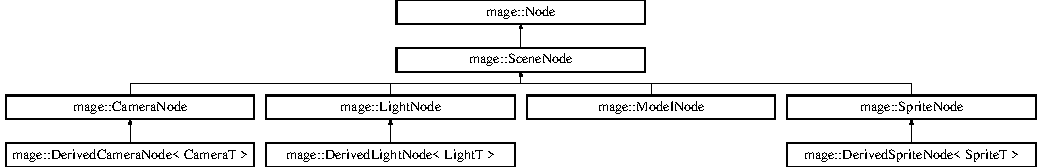
\includegraphics[height=2.986667cm]{classmage_1_1_node}
\end{center}
\end{figure}
\subsection*{Public Member Functions}
\begin{DoxyCompactItemize}
\item 
\hyperlink{classmage_1_1_node_a58b816eaa1dfd3c4b7f14896f190587f}{Node} ()
\item 
\hyperlink{classmage_1_1_node_af9da591163469f210895f3a5b389d7cc}{Node} (const \hyperlink{classmage_1_1_node}{Node} \&node)
\item 
\hyperlink{classmage_1_1_node_adbc40b6c4100f74faa2b59a7a0b79388}{Node} (\hyperlink{classmage_1_1_node}{Node} \&\&node)
\item 
virtual \hyperlink{classmage_1_1_node_a1369fc11b331abacbaf11aeb5729e871}{$\sim$\+Node} ()
\item 
\hyperlink{classmage_1_1_node}{Node} \& \hyperlink{classmage_1_1_node_ad10ea13608963acfa06d3c1577314da5}{operator=} (const \hyperlink{classmage_1_1_node}{Node} \&node)=delete
\item 
\hyperlink{classmage_1_1_node}{Node} \& \hyperlink{classmage_1_1_node_a007043de35c65edb9a0d790824186151}{operator=} (\hyperlink{classmage_1_1_node}{Node} \&\&node)=delete
\item 
\hyperlink{namespacemage_a8c307fbcc33bce9b7f2aa4c26c3b95cf}{Unique\+Ptr}$<$ \hyperlink{classmage_1_1_node}{Node} $>$ \hyperlink{classmage_1_1_node_a18e08151571435d319be2414474c93c0}{Clone} () const
\item 
\hyperlink{classmage_1_1_transform_node}{Transform\+Node} $\ast$ \hyperlink{classmage_1_1_node_aee9d81f3a236fe48128ad5960a22beb4}{Get\+Transform} ()
\item 
const \hyperlink{classmage_1_1_transform_node}{Transform\+Node} $\ast$ \hyperlink{classmage_1_1_node_a319b7fdc98412cb02ba1cffab2527bf2}{Get\+Transform} () const
\item 
bool \hyperlink{classmage_1_1_node_ac1e76b877582d74e24e44891dd8c3667}{Is\+Active} () const
\item 
bool \hyperlink{classmage_1_1_node_ad1aea56c1abfd8fe5084b71f35604276}{Is\+Passive} () const
\item 
void \hyperlink{classmage_1_1_node_a3b2cccf69650526f15f57e9dee326a6b}{Make\+Active} ()
\item 
void \hyperlink{classmage_1_1_node_abb90906339681ecde9b8f47b708c14c9}{Make\+Passive} ()
\item 
void \hyperlink{classmage_1_1_node_aea6d7145a71b3af31d5516b4df2e7da5}{Set\+Active} (bool active)
\item 
bool \hyperlink{classmage_1_1_node_a9819d0219bdca364621584b6aa29ba30}{Has\+Parent\+Node} () const
\item 
\hyperlink{classmage_1_1_node}{Node} $\ast$ \hyperlink{classmage_1_1_node_ae30f2ca6816eeeef28610f385864aec9}{Get\+Parent\+Node} () const
\item 
size\+\_\+t \hyperlink{classmage_1_1_node_ab11750938bf343f16dcdf7a327834318}{Get\+Number\+Of\+Child\+Nodes} () const
\item 
bool \hyperlink{classmage_1_1_node_a1b8c2d933a281f7f815791db38c965ad}{Has\+Child\+Node} (\hyperlink{namespacemage_a1e01ae66713838a7a67d30e44c67703e}{Shared\+Ptr}$<$ const \hyperlink{classmage_1_1_node}{Node} $>$ node) const
\item 
void \hyperlink{classmage_1_1_node_a11a7c052c5e4a6713d60aaad67dfde5d}{Add\+Child\+Node} (\hyperlink{namespacemage_a1e01ae66713838a7a67d30e44c67703e}{Shared\+Ptr}$<$ \hyperlink{classmage_1_1_node}{Node} $>$ node)
\item 
void \hyperlink{classmage_1_1_node_a0da235c6459c315ad1c4be5c7aa7c7f0}{Remove\+Child\+Node} (\hyperlink{namespacemage_a1e01ae66713838a7a67d30e44c67703e}{Shared\+Ptr}$<$ \hyperlink{classmage_1_1_node}{Node} $>$ node)
\item 
void \hyperlink{classmage_1_1_node_a5813fe733404dd327b77f595291c70bb}{Remove\+All\+Child\+Nodes} ()
\item 
{\footnotesize template$<$typename ActionT $>$ }\\void \hyperlink{classmage_1_1_node_afedb523a462952ec29aed7504d0a71d4}{For\+Each\+Child\+Node} (ActionT action) const
\item 
{\footnotesize template$<$typename ActionT $>$ }\\void \hyperlink{classmage_1_1_node_a86668c371e1452204b52f2896cbb16fd}{For\+Each\+Descendant\+Node} (ActionT action) const
\end{DoxyCompactItemize}
\subsection*{Private Member Functions}
\begin{DoxyCompactItemize}
\item 
virtual \hyperlink{namespacemage_a8c307fbcc33bce9b7f2aa4c26c3b95cf}{Unique\+Ptr}$<$ \hyperlink{classmage_1_1_node}{Node} $>$ \hyperlink{classmage_1_1_node_a71a4763bfd4cba5653488b490e61dc8f}{Clone\+Implementation} () const
\end{DoxyCompactItemize}
\subsection*{Private Attributes}
\begin{DoxyCompactItemize}
\item 
\hyperlink{namespacemage_a8c307fbcc33bce9b7f2aa4c26c3b95cf}{Unique\+Ptr}$<$ \hyperlink{classmage_1_1_transform_node}{Transform\+Node} $>$ \hyperlink{classmage_1_1_node_a24512023f5f6ec7adad9810e55ec2ab5}{m\+\_\+transform}
\item 
bool \hyperlink{classmage_1_1_node_ac4dd6c399de8b2a92df92365df7ecdac}{m\+\_\+active}
\end{DoxyCompactItemize}


\subsection{Detailed Description}
A class of nodes. 

\subsection{Constructor \& Destructor Documentation}
\hypertarget{classmage_1_1_node_a58b816eaa1dfd3c4b7f14896f190587f}{}\label{classmage_1_1_node_a58b816eaa1dfd3c4b7f14896f190587f} 
\index{mage\+::\+Node@{mage\+::\+Node}!Node@{Node}}
\index{Node@{Node}!mage\+::\+Node@{mage\+::\+Node}}
\subsubsection{\texorpdfstring{Node()}{Node()}\hspace{0.1cm}{\footnotesize\ttfamily [1/3]}}
{\footnotesize\ttfamily mage\+::\+Node\+::\+Node (\begin{DoxyParamCaption}{ }\end{DoxyParamCaption})}

Constructs a node. \hypertarget{classmage_1_1_node_af9da591163469f210895f3a5b389d7cc}{}\label{classmage_1_1_node_af9da591163469f210895f3a5b389d7cc} 
\index{mage\+::\+Node@{mage\+::\+Node}!Node@{Node}}
\index{Node@{Node}!mage\+::\+Node@{mage\+::\+Node}}
\subsubsection{\texorpdfstring{Node()}{Node()}\hspace{0.1cm}{\footnotesize\ttfamily [2/3]}}
{\footnotesize\ttfamily mage\+::\+Node\+::\+Node (\begin{DoxyParamCaption}\item[{const \hyperlink{classmage_1_1_node}{Node} \&}]{node }\end{DoxyParamCaption})}

Constructs a node from the given node.


\begin{DoxyParams}[1]{Parameters}
\mbox{\tt in}  & {\em node} & A reference to the node. \\
\hline
\end{DoxyParams}
\hypertarget{classmage_1_1_node_adbc40b6c4100f74faa2b59a7a0b79388}{}\label{classmage_1_1_node_adbc40b6c4100f74faa2b59a7a0b79388} 
\index{mage\+::\+Node@{mage\+::\+Node}!Node@{Node}}
\index{Node@{Node}!mage\+::\+Node@{mage\+::\+Node}}
\subsubsection{\texorpdfstring{Node()}{Node()}\hspace{0.1cm}{\footnotesize\ttfamily [3/3]}}
{\footnotesize\ttfamily mage\+::\+Node\+::\+Node (\begin{DoxyParamCaption}\item[{\hyperlink{classmage_1_1_node}{Node} \&\&}]{node }\end{DoxyParamCaption})\hspace{0.3cm}{\ttfamily [default]}}

Constructs a node by moving the given node.


\begin{DoxyParams}[1]{Parameters}
\mbox{\tt in}  & {\em node} & A reference to the node to move. \\
\hline
\end{DoxyParams}
\hypertarget{classmage_1_1_node_a1369fc11b331abacbaf11aeb5729e871}{}\label{classmage_1_1_node_a1369fc11b331abacbaf11aeb5729e871} 
\index{mage\+::\+Node@{mage\+::\+Node}!````~Node@{$\sim$\+Node}}
\index{````~Node@{$\sim$\+Node}!mage\+::\+Node@{mage\+::\+Node}}
\subsubsection{\texorpdfstring{$\sim$\+Node()}{~Node()}}
{\footnotesize\ttfamily mage\+::\+Node\+::$\sim$\+Node (\begin{DoxyParamCaption}{ }\end{DoxyParamCaption})\hspace{0.3cm}{\ttfamily [virtual]}, {\ttfamily [default]}}

Destructs this node. 

\subsection{Member Function Documentation}
\hypertarget{classmage_1_1_node_a11a7c052c5e4a6713d60aaad67dfde5d}{}\label{classmage_1_1_node_a11a7c052c5e4a6713d60aaad67dfde5d} 
\index{mage\+::\+Node@{mage\+::\+Node}!Add\+Child\+Node@{Add\+Child\+Node}}
\index{Add\+Child\+Node@{Add\+Child\+Node}!mage\+::\+Node@{mage\+::\+Node}}
\subsubsection{\texorpdfstring{Add\+Child\+Node()}{AddChildNode()}}
{\footnotesize\ttfamily void mage\+::\+Node\+::\+Add\+Child\+Node (\begin{DoxyParamCaption}\item[{\hyperlink{namespacemage_a1e01ae66713838a7a67d30e44c67703e}{Shared\+Ptr}$<$ \hyperlink{classmage_1_1_node}{Node} $>$}]{node }\end{DoxyParamCaption})}

Adds the given node to the child nodes of this node.


\begin{DoxyParams}[1]{Parameters}
\mbox{\tt in}  & {\em node} & A pointer to the node to add. \\
\hline
\end{DoxyParams}
\hypertarget{classmage_1_1_node_a18e08151571435d319be2414474c93c0}{}\label{classmage_1_1_node_a18e08151571435d319be2414474c93c0} 
\index{mage\+::\+Node@{mage\+::\+Node}!Clone@{Clone}}
\index{Clone@{Clone}!mage\+::\+Node@{mage\+::\+Node}}
\subsubsection{\texorpdfstring{Clone()}{Clone()}}
{\footnotesize\ttfamily \hyperlink{namespacemage_a8c307fbcc33bce9b7f2aa4c26c3b95cf}{Unique\+Ptr}$<$ \hyperlink{classmage_1_1_node}{Node} $>$ mage\+::\+Node\+::\+Clone (\begin{DoxyParamCaption}{ }\end{DoxyParamCaption}) const}

Clones this node.

\begin{DoxyReturn}{Returns}
A pointer to the clone of this node. 
\end{DoxyReturn}
\hypertarget{classmage_1_1_node_a71a4763bfd4cba5653488b490e61dc8f}{}\label{classmage_1_1_node_a71a4763bfd4cba5653488b490e61dc8f} 
\index{mage\+::\+Node@{mage\+::\+Node}!Clone\+Implementation@{Clone\+Implementation}}
\index{Clone\+Implementation@{Clone\+Implementation}!mage\+::\+Node@{mage\+::\+Node}}
\subsubsection{\texorpdfstring{Clone\+Implementation()}{CloneImplementation()}}
{\footnotesize\ttfamily \hyperlink{namespacemage_a8c307fbcc33bce9b7f2aa4c26c3b95cf}{Unique\+Ptr}$<$ \hyperlink{classmage_1_1_node}{Node} $>$ mage\+::\+Node\+::\+Clone\+Implementation (\begin{DoxyParamCaption}{ }\end{DoxyParamCaption}) const\hspace{0.3cm}{\ttfamily [private]}, {\ttfamily [virtual]}}

Clones this node.

\begin{DoxyReturn}{Returns}
A pointer to the clone of this node. 
\end{DoxyReturn}


Reimplemented in \hyperlink{classmage_1_1_derived_light_node_acf8858989780bf45a45c55a7c5564314}{mage\+::\+Derived\+Light\+Node$<$ Light\+T $>$}, \hyperlink{classmage_1_1_derived_camera_node_aa965751029ebd6b41d3805b499a8304e}{mage\+::\+Derived\+Camera\+Node$<$ Camera\+T $>$}, \hyperlink{classmage_1_1_light_node_aea97601d0a4b8073a1c655ca334af242}{mage\+::\+Light\+Node}, \hyperlink{classmage_1_1_camera_node_a002d3a2b41cda270a26ca5d8f3a17f55}{mage\+::\+Camera\+Node}, \hyperlink{classmage_1_1_model_node_a34146201083015276b38240af307417f}{mage\+::\+Model\+Node}, and \hyperlink{classmage_1_1_scene_node_a42d0d53ab804d38ebd584d2de6490eeb}{mage\+::\+Scene\+Node}.

\hypertarget{classmage_1_1_node_afedb523a462952ec29aed7504d0a71d4}{}\label{classmage_1_1_node_afedb523a462952ec29aed7504d0a71d4} 
\index{mage\+::\+Node@{mage\+::\+Node}!For\+Each\+Child\+Node@{For\+Each\+Child\+Node}}
\index{For\+Each\+Child\+Node@{For\+Each\+Child\+Node}!mage\+::\+Node@{mage\+::\+Node}}
\subsubsection{\texorpdfstring{For\+Each\+Child\+Node()}{ForEachChildNode()}}
{\footnotesize\ttfamily template$<$typename ActionT $>$ \\
void mage\+::\+Node\+::\+For\+Each\+Child\+Node (\begin{DoxyParamCaption}\item[{ActionT}]{action }\end{DoxyParamCaption}) const}

Traverses all child nodes of this node.


\begin{DoxyTemplParams}{Template Parameters}
{\em ActionT} & An action to perform on all child nodes of this node. The action must accept ({\ttfamily const}) {\ttfamily \hyperlink{classmage_1_1_node}{Node}\&} values. \\
\hline
\end{DoxyTemplParams}
\hypertarget{classmage_1_1_node_a86668c371e1452204b52f2896cbb16fd}{}\label{classmage_1_1_node_a86668c371e1452204b52f2896cbb16fd} 
\index{mage\+::\+Node@{mage\+::\+Node}!For\+Each\+Descendant\+Node@{For\+Each\+Descendant\+Node}}
\index{For\+Each\+Descendant\+Node@{For\+Each\+Descendant\+Node}!mage\+::\+Node@{mage\+::\+Node}}
\subsubsection{\texorpdfstring{For\+Each\+Descendant\+Node()}{ForEachDescendantNode()}}
{\footnotesize\ttfamily template$<$typename ActionT $>$ \\
void mage\+::\+Node\+::\+For\+Each\+Descendant\+Node (\begin{DoxyParamCaption}\item[{ActionT}]{action }\end{DoxyParamCaption}) const}

Traverses all descendant (childs included) nodes of this transform node.


\begin{DoxyTemplParams}{Template Parameters}
{\em ActionT} & An action to perform on all descendant nodes of this node. The action must accept ({\ttfamily const}) {\ttfamily \hyperlink{classmage_1_1_node}{Node}\&} values. \\
\hline
\end{DoxyTemplParams}
\hypertarget{classmage_1_1_node_ab11750938bf343f16dcdf7a327834318}{}\label{classmage_1_1_node_ab11750938bf343f16dcdf7a327834318} 
\index{mage\+::\+Node@{mage\+::\+Node}!Get\+Number\+Of\+Child\+Nodes@{Get\+Number\+Of\+Child\+Nodes}}
\index{Get\+Number\+Of\+Child\+Nodes@{Get\+Number\+Of\+Child\+Nodes}!mage\+::\+Node@{mage\+::\+Node}}
\subsubsection{\texorpdfstring{Get\+Number\+Of\+Child\+Nodes()}{GetNumberOfChildNodes()}}
{\footnotesize\ttfamily size\+\_\+t mage\+::\+Node\+::\+Get\+Number\+Of\+Child\+Nodes (\begin{DoxyParamCaption}{ }\end{DoxyParamCaption}) const}

Returns the number of child nodes of this node.

\begin{DoxyReturn}{Returns}
The number of child nodes of this node. 
\end{DoxyReturn}
\hypertarget{classmage_1_1_node_ae30f2ca6816eeeef28610f385864aec9}{}\label{classmage_1_1_node_ae30f2ca6816eeeef28610f385864aec9} 
\index{mage\+::\+Node@{mage\+::\+Node}!Get\+Parent\+Node@{Get\+Parent\+Node}}
\index{Get\+Parent\+Node@{Get\+Parent\+Node}!mage\+::\+Node@{mage\+::\+Node}}
\subsubsection{\texorpdfstring{Get\+Parent\+Node()}{GetParentNode()}}
{\footnotesize\ttfamily \hyperlink{classmage_1_1_node}{Node}$\ast$ mage\+::\+Node\+::\+Get\+Parent\+Node (\begin{DoxyParamCaption}{ }\end{DoxyParamCaption}) const}

Returns the parent node of this node.

\begin{DoxyReturn}{Returns}
{\ttfamily nullptr} if this node has no parent node. 

A pointer to the parent node of this node. 
\end{DoxyReturn}
\hypertarget{classmage_1_1_node_aee9d81f3a236fe48128ad5960a22beb4}{}\label{classmage_1_1_node_aee9d81f3a236fe48128ad5960a22beb4} 
\index{mage\+::\+Node@{mage\+::\+Node}!Get\+Transform@{Get\+Transform}}
\index{Get\+Transform@{Get\+Transform}!mage\+::\+Node@{mage\+::\+Node}}
\subsubsection{\texorpdfstring{Get\+Transform()}{GetTransform()}\hspace{0.1cm}{\footnotesize\ttfamily [1/2]}}
{\footnotesize\ttfamily \hyperlink{classmage_1_1_transform_node}{Transform\+Node}$\ast$ mage\+::\+Node\+::\+Get\+Transform (\begin{DoxyParamCaption}{ }\end{DoxyParamCaption})}

Returns the transform of this node.

\begin{DoxyReturn}{Returns}
A pointer to the transform of this node. 
\end{DoxyReturn}
\hypertarget{classmage_1_1_node_a319b7fdc98412cb02ba1cffab2527bf2}{}\label{classmage_1_1_node_a319b7fdc98412cb02ba1cffab2527bf2} 
\index{mage\+::\+Node@{mage\+::\+Node}!Get\+Transform@{Get\+Transform}}
\index{Get\+Transform@{Get\+Transform}!mage\+::\+Node@{mage\+::\+Node}}
\subsubsection{\texorpdfstring{Get\+Transform()}{GetTransform()}\hspace{0.1cm}{\footnotesize\ttfamily [2/2]}}
{\footnotesize\ttfamily const \hyperlink{classmage_1_1_transform_node}{Transform\+Node}$\ast$ mage\+::\+Node\+::\+Get\+Transform (\begin{DoxyParamCaption}{ }\end{DoxyParamCaption}) const}

Returns the transform of this node.

\begin{DoxyReturn}{Returns}
A pointer to the transform of this node. 
\end{DoxyReturn}
\hypertarget{classmage_1_1_node_a1b8c2d933a281f7f815791db38c965ad}{}\label{classmage_1_1_node_a1b8c2d933a281f7f815791db38c965ad} 
\index{mage\+::\+Node@{mage\+::\+Node}!Has\+Child\+Node@{Has\+Child\+Node}}
\index{Has\+Child\+Node@{Has\+Child\+Node}!mage\+::\+Node@{mage\+::\+Node}}
\subsubsection{\texorpdfstring{Has\+Child\+Node()}{HasChildNode()}}
{\footnotesize\ttfamily bool mage\+::\+Node\+::\+Has\+Child\+Node (\begin{DoxyParamCaption}\item[{\hyperlink{namespacemage_a1e01ae66713838a7a67d30e44c67703e}{Shared\+Ptr}$<$ const \hyperlink{classmage_1_1_node}{Node} $>$}]{node }\end{DoxyParamCaption}) const}

Checks whether this node contains the given node as a child node.


\begin{DoxyParams}[1]{Parameters}
\mbox{\tt in}  & {\em node} & A pointer to the node. \\
\hline
\end{DoxyParams}
\begin{DoxyReturn}{Returns}
{\ttfamily true} if this node contains the given node as a child node. {\ttfamily false} otherwise. 
\end{DoxyReturn}
\hypertarget{classmage_1_1_node_a9819d0219bdca364621584b6aa29ba30}{}\label{classmage_1_1_node_a9819d0219bdca364621584b6aa29ba30} 
\index{mage\+::\+Node@{mage\+::\+Node}!Has\+Parent\+Node@{Has\+Parent\+Node}}
\index{Has\+Parent\+Node@{Has\+Parent\+Node}!mage\+::\+Node@{mage\+::\+Node}}
\subsubsection{\texorpdfstring{Has\+Parent\+Node()}{HasParentNode()}}
{\footnotesize\ttfamily bool mage\+::\+Node\+::\+Has\+Parent\+Node (\begin{DoxyParamCaption}{ }\end{DoxyParamCaption}) const}

Checks whether this node has a parent node.

\begin{DoxyReturn}{Returns}
{\ttfamily true} if this node has a parent node. {\ttfamily false} otherwise. 
\end{DoxyReturn}
\hypertarget{classmage_1_1_node_ac1e76b877582d74e24e44891dd8c3667}{}\label{classmage_1_1_node_ac1e76b877582d74e24e44891dd8c3667} 
\index{mage\+::\+Node@{mage\+::\+Node}!Is\+Active@{Is\+Active}}
\index{Is\+Active@{Is\+Active}!mage\+::\+Node@{mage\+::\+Node}}
\subsubsection{\texorpdfstring{Is\+Active()}{IsActive()}}
{\footnotesize\ttfamily bool mage\+::\+Node\+::\+Is\+Active (\begin{DoxyParamCaption}{ }\end{DoxyParamCaption}) const}

Checks whether this node is active.

\begin{DoxyReturn}{Returns}
{\ttfamily true} if this node is active. {\ttfamily false} otherwise (i.\+e. passive). 
\end{DoxyReturn}
\hypertarget{classmage_1_1_node_ad1aea56c1abfd8fe5084b71f35604276}{}\label{classmage_1_1_node_ad1aea56c1abfd8fe5084b71f35604276} 
\index{mage\+::\+Node@{mage\+::\+Node}!Is\+Passive@{Is\+Passive}}
\index{Is\+Passive@{Is\+Passive}!mage\+::\+Node@{mage\+::\+Node}}
\subsubsection{\texorpdfstring{Is\+Passive()}{IsPassive()}}
{\footnotesize\ttfamily bool mage\+::\+Node\+::\+Is\+Passive (\begin{DoxyParamCaption}{ }\end{DoxyParamCaption}) const}

Checks whether this node is passive.

\begin{DoxyReturn}{Returns}
{\ttfamily true} if this node is passive. {\ttfamily false} otherwise (i.\+e. active). 
\end{DoxyReturn}
\hypertarget{classmage_1_1_node_a3b2cccf69650526f15f57e9dee326a6b}{}\label{classmage_1_1_node_a3b2cccf69650526f15f57e9dee326a6b} 
\index{mage\+::\+Node@{mage\+::\+Node}!Make\+Active@{Make\+Active}}
\index{Make\+Active@{Make\+Active}!mage\+::\+Node@{mage\+::\+Node}}
\subsubsection{\texorpdfstring{Make\+Active()}{MakeActive()}}
{\footnotesize\ttfamily void mage\+::\+Node\+::\+Make\+Active (\begin{DoxyParamCaption}{ }\end{DoxyParamCaption})}

Makes this node (and its descendant nodes) active. \hypertarget{classmage_1_1_node_abb90906339681ecde9b8f47b708c14c9}{}\label{classmage_1_1_node_abb90906339681ecde9b8f47b708c14c9} 
\index{mage\+::\+Node@{mage\+::\+Node}!Make\+Passive@{Make\+Passive}}
\index{Make\+Passive@{Make\+Passive}!mage\+::\+Node@{mage\+::\+Node}}
\subsubsection{\texorpdfstring{Make\+Passive()}{MakePassive()}}
{\footnotesize\ttfamily void mage\+::\+Node\+::\+Make\+Passive (\begin{DoxyParamCaption}{ }\end{DoxyParamCaption})}

Makes this node (and its descendant nodes) passive. \hypertarget{classmage_1_1_node_ad10ea13608963acfa06d3c1577314da5}{}\label{classmage_1_1_node_ad10ea13608963acfa06d3c1577314da5} 
\index{mage\+::\+Node@{mage\+::\+Node}!operator=@{operator=}}
\index{operator=@{operator=}!mage\+::\+Node@{mage\+::\+Node}}
\subsubsection{\texorpdfstring{operator=()}{operator=()}\hspace{0.1cm}{\footnotesize\ttfamily [1/2]}}
{\footnotesize\ttfamily \hyperlink{classmage_1_1_node}{Node}\& mage\+::\+Node\+::operator= (\begin{DoxyParamCaption}\item[{const \hyperlink{classmage_1_1_node}{Node} \&}]{node }\end{DoxyParamCaption})\hspace{0.3cm}{\ttfamily [delete]}}

Copies the given node to this node.


\begin{DoxyParams}[1]{Parameters}
\mbox{\tt in}  & {\em node} & A reference to the node to copy. \\
\hline
\end{DoxyParams}
\begin{DoxyReturn}{Returns}
A reference to the copy of the given node (i.\+e. this node). 
\end{DoxyReturn}
\hypertarget{classmage_1_1_node_a007043de35c65edb9a0d790824186151}{}\label{classmage_1_1_node_a007043de35c65edb9a0d790824186151} 
\index{mage\+::\+Node@{mage\+::\+Node}!operator=@{operator=}}
\index{operator=@{operator=}!mage\+::\+Node@{mage\+::\+Node}}
\subsubsection{\texorpdfstring{operator=()}{operator=()}\hspace{0.1cm}{\footnotesize\ttfamily [2/2]}}
{\footnotesize\ttfamily \hyperlink{classmage_1_1_node}{Node}\& mage\+::\+Node\+::operator= (\begin{DoxyParamCaption}\item[{\hyperlink{classmage_1_1_node}{Node} \&\&}]{node }\end{DoxyParamCaption})\hspace{0.3cm}{\ttfamily [delete]}}

Moves the given node to this node.


\begin{DoxyParams}[1]{Parameters}
\mbox{\tt in}  & {\em node} & A reference to the node to move. \\
\hline
\end{DoxyParams}
\begin{DoxyReturn}{Returns}
A reference to the moved node (i.\+e. this node). 
\end{DoxyReturn}
\hypertarget{classmage_1_1_node_a5813fe733404dd327b77f595291c70bb}{}\label{classmage_1_1_node_a5813fe733404dd327b77f595291c70bb} 
\index{mage\+::\+Node@{mage\+::\+Node}!Remove\+All\+Child\+Nodes@{Remove\+All\+Child\+Nodes}}
\index{Remove\+All\+Child\+Nodes@{Remove\+All\+Child\+Nodes}!mage\+::\+Node@{mage\+::\+Node}}
\subsubsection{\texorpdfstring{Remove\+All\+Child\+Nodes()}{RemoveAllChildNodes()}}
{\footnotesize\ttfamily void mage\+::\+Node\+::\+Remove\+All\+Child\+Nodes (\begin{DoxyParamCaption}{ }\end{DoxyParamCaption})}

Removes all child nodes from this node. \hypertarget{classmage_1_1_node_a0da235c6459c315ad1c4be5c7aa7c7f0}{}\label{classmage_1_1_node_a0da235c6459c315ad1c4be5c7aa7c7f0} 
\index{mage\+::\+Node@{mage\+::\+Node}!Remove\+Child\+Node@{Remove\+Child\+Node}}
\index{Remove\+Child\+Node@{Remove\+Child\+Node}!mage\+::\+Node@{mage\+::\+Node}}
\subsubsection{\texorpdfstring{Remove\+Child\+Node()}{RemoveChildNode()}}
{\footnotesize\ttfamily void mage\+::\+Node\+::\+Remove\+Child\+Node (\begin{DoxyParamCaption}\item[{\hyperlink{namespacemage_a1e01ae66713838a7a67d30e44c67703e}{Shared\+Ptr}$<$ \hyperlink{classmage_1_1_node}{Node} $>$}]{node }\end{DoxyParamCaption})}

Removes the given node from the child nodes of this node.


\begin{DoxyParams}[1]{Parameters}
\mbox{\tt in}  & {\em node} & A pointer to the node to remove. \\
\hline
\end{DoxyParams}
\hypertarget{classmage_1_1_node_aea6d7145a71b3af31d5516b4df2e7da5}{}\label{classmage_1_1_node_aea6d7145a71b3af31d5516b4df2e7da5} 
\index{mage\+::\+Node@{mage\+::\+Node}!Set\+Active@{Set\+Active}}
\index{Set\+Active@{Set\+Active}!mage\+::\+Node@{mage\+::\+Node}}
\subsubsection{\texorpdfstring{Set\+Active()}{SetActive()}}
{\footnotesize\ttfamily void mage\+::\+Node\+::\+Set\+Active (\begin{DoxyParamCaption}\item[{bool}]{active }\end{DoxyParamCaption})}

Sets this node active flag to the given value.


\begin{DoxyParams}[1]{Parameters}
\mbox{\tt in}  & {\em active} & The active flag. \\
\hline
\end{DoxyParams}


\subsection{Member Data Documentation}
\hypertarget{classmage_1_1_node_ac4dd6c399de8b2a92df92365df7ecdac}{}\label{classmage_1_1_node_ac4dd6c399de8b2a92df92365df7ecdac} 
\index{mage\+::\+Node@{mage\+::\+Node}!m\+\_\+active@{m\+\_\+active}}
\index{m\+\_\+active@{m\+\_\+active}!mage\+::\+Node@{mage\+::\+Node}}
\subsubsection{\texorpdfstring{m\+\_\+active}{m\_active}}
{\footnotesize\ttfamily bool mage\+::\+Node\+::m\+\_\+active\hspace{0.3cm}{\ttfamily [private]}}

A flag indicating whether this node is active or not (i.\+e. passive). \hypertarget{classmage_1_1_node_a24512023f5f6ec7adad9810e55ec2ab5}{}\label{classmage_1_1_node_a24512023f5f6ec7adad9810e55ec2ab5} 
\index{mage\+::\+Node@{mage\+::\+Node}!m\+\_\+transform@{m\+\_\+transform}}
\index{m\+\_\+transform@{m\+\_\+transform}!mage\+::\+Node@{mage\+::\+Node}}
\subsubsection{\texorpdfstring{m\+\_\+transform}{m\_transform}}
{\footnotesize\ttfamily \hyperlink{namespacemage_a8c307fbcc33bce9b7f2aa4c26c3b95cf}{Unique\+Ptr}$<$ \hyperlink{classmage_1_1_transform_node}{Transform\+Node} $>$ mage\+::\+Node\+::m\+\_\+transform\hspace{0.3cm}{\ttfamily [private]}}

A pointer to the transform of this node. 
\hypertarget{structmage_1_1_normal3}{}\section{mage\+:\+:Normal3 Struct Reference}
\label{structmage_1_1_normal3}\index{mage\+::\+Normal3@{mage\+::\+Normal3}}


{\ttfamily \#include $<$math.\+hpp$>$}

Inheritance diagram for mage\+:\+:Normal3\+:\begin{figure}[H]
\begin{center}
\leavevmode
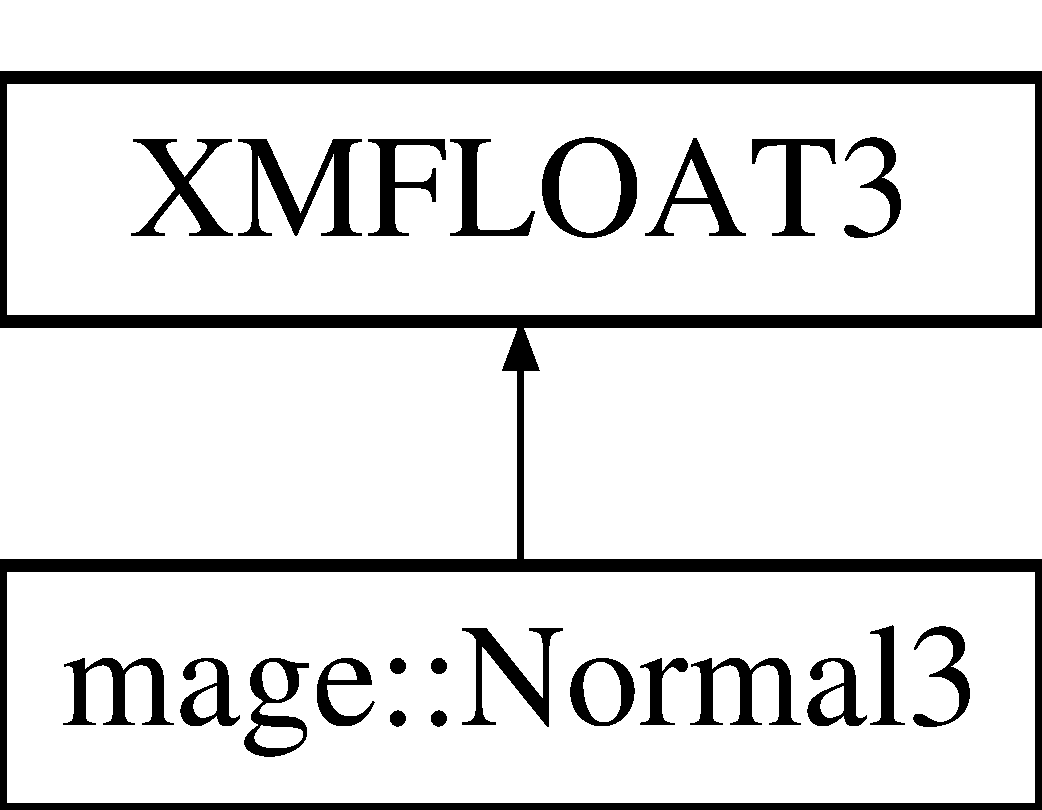
\includegraphics[height=2.000000cm]{structmage_1_1_normal3}
\end{center}
\end{figure}
\subsection*{Public Member Functions}
\begin{DoxyCompactItemize}
\item 
\hyperlink{structmage_1_1_normal3_a66ec99f0de4f8231f747e37a4da65cc4}{Normal3} ()
\item 
\hyperlink{structmage_1_1_normal3_a59094c1f96a9721cd8846c5c6ec06f93}{Normal3} (float x, float y, float z)
\item 
\hyperlink{structmage_1_1_normal3_ada9c762e16b51177f3fc1aa6d5310b20}{Normal3} (const \hyperlink{structmage_1_1_normal3}{Normal3} \&normal)
\item 
\hyperlink{structmage_1_1_normal3_a1a58b2fcb3920ff68007257ae6434273}{Normal3} (const \hyperlink{structmage_1_1_point3}{Point3} \&point)
\item 
\hyperlink{structmage_1_1_normal3_a0942e7aace8354f0a414f77ccf90b69c}{Normal3} (const \hyperlink{structmage_1_1_direction3}{Direction3} \&direction)
\item 
\hyperlink{structmage_1_1_normal3_a61565f1183535666a2fb5183b83bebd2}{Normal3} (const X\+M\+F\+L\+O\+A\+T3 \&vector)
\item 
\hyperlink{structmage_1_1_normal3_a3384b2970fd85fe729514ce0686b4446}{$\sim$\+Normal3} ()=default
\item 
\hyperlink{structmage_1_1_normal3}{Normal3} \& \hyperlink{structmage_1_1_normal3_ade86357989ceaecf1b22bb9e53ca7fed}{operator=} (const \hyperlink{structmage_1_1_normal3}{Normal3} \&normal)
\end{DoxyCompactItemize}


\subsection{Constructor \& Destructor Documentation}
\hypertarget{structmage_1_1_normal3_a66ec99f0de4f8231f747e37a4da65cc4}{}\label{structmage_1_1_normal3_a66ec99f0de4f8231f747e37a4da65cc4} 
\index{mage\+::\+Normal3@{mage\+::\+Normal3}!Normal3@{Normal3}}
\index{Normal3@{Normal3}!mage\+::\+Normal3@{mage\+::\+Normal3}}
\subsubsection{\texorpdfstring{Normal3()}{Normal3()}\hspace{0.1cm}{\footnotesize\ttfamily [1/6]}}
{\footnotesize\ttfamily mage\+::\+Normal3\+::\+Normal3 (\begin{DoxyParamCaption}{ }\end{DoxyParamCaption})}

\hypertarget{structmage_1_1_normal3_a59094c1f96a9721cd8846c5c6ec06f93}{}\label{structmage_1_1_normal3_a59094c1f96a9721cd8846c5c6ec06f93} 
\index{mage\+::\+Normal3@{mage\+::\+Normal3}!Normal3@{Normal3}}
\index{Normal3@{Normal3}!mage\+::\+Normal3@{mage\+::\+Normal3}}
\subsubsection{\texorpdfstring{Normal3()}{Normal3()}\hspace{0.1cm}{\footnotesize\ttfamily [2/6]}}
{\footnotesize\ttfamily mage\+::\+Normal3\+::\+Normal3 (\begin{DoxyParamCaption}\item[{float}]{x,  }\item[{float}]{y,  }\item[{float}]{z }\end{DoxyParamCaption})}

\hypertarget{structmage_1_1_normal3_ada9c762e16b51177f3fc1aa6d5310b20}{}\label{structmage_1_1_normal3_ada9c762e16b51177f3fc1aa6d5310b20} 
\index{mage\+::\+Normal3@{mage\+::\+Normal3}!Normal3@{Normal3}}
\index{Normal3@{Normal3}!mage\+::\+Normal3@{mage\+::\+Normal3}}
\subsubsection{\texorpdfstring{Normal3()}{Normal3()}\hspace{0.1cm}{\footnotesize\ttfamily [3/6]}}
{\footnotesize\ttfamily mage\+::\+Normal3\+::\+Normal3 (\begin{DoxyParamCaption}\item[{const \hyperlink{structmage_1_1_normal3}{Normal3} \&}]{normal }\end{DoxyParamCaption})}

\hypertarget{structmage_1_1_normal3_a1a58b2fcb3920ff68007257ae6434273}{}\label{structmage_1_1_normal3_a1a58b2fcb3920ff68007257ae6434273} 
\index{mage\+::\+Normal3@{mage\+::\+Normal3}!Normal3@{Normal3}}
\index{Normal3@{Normal3}!mage\+::\+Normal3@{mage\+::\+Normal3}}
\subsubsection{\texorpdfstring{Normal3()}{Normal3()}\hspace{0.1cm}{\footnotesize\ttfamily [4/6]}}
{\footnotesize\ttfamily mage\+::\+Normal3\+::\+Normal3 (\begin{DoxyParamCaption}\item[{const \hyperlink{structmage_1_1_point3}{Point3} \&}]{point }\end{DoxyParamCaption})\hspace{0.3cm}{\ttfamily [explicit]}}

\hypertarget{structmage_1_1_normal3_a0942e7aace8354f0a414f77ccf90b69c}{}\label{structmage_1_1_normal3_a0942e7aace8354f0a414f77ccf90b69c} 
\index{mage\+::\+Normal3@{mage\+::\+Normal3}!Normal3@{Normal3}}
\index{Normal3@{Normal3}!mage\+::\+Normal3@{mage\+::\+Normal3}}
\subsubsection{\texorpdfstring{Normal3()}{Normal3()}\hspace{0.1cm}{\footnotesize\ttfamily [5/6]}}
{\footnotesize\ttfamily mage\+::\+Normal3\+::\+Normal3 (\begin{DoxyParamCaption}\item[{const \hyperlink{structmage_1_1_direction3}{Direction3} \&}]{direction }\end{DoxyParamCaption})\hspace{0.3cm}{\ttfamily [explicit]}}

\hypertarget{structmage_1_1_normal3_a61565f1183535666a2fb5183b83bebd2}{}\label{structmage_1_1_normal3_a61565f1183535666a2fb5183b83bebd2} 
\index{mage\+::\+Normal3@{mage\+::\+Normal3}!Normal3@{Normal3}}
\index{Normal3@{Normal3}!mage\+::\+Normal3@{mage\+::\+Normal3}}
\subsubsection{\texorpdfstring{Normal3()}{Normal3()}\hspace{0.1cm}{\footnotesize\ttfamily [6/6]}}
{\footnotesize\ttfamily mage\+::\+Normal3\+::\+Normal3 (\begin{DoxyParamCaption}\item[{const X\+M\+F\+L\+O\+A\+T3 \&}]{vector }\end{DoxyParamCaption})\hspace{0.3cm}{\ttfamily [explicit]}}

\hypertarget{structmage_1_1_normal3_a3384b2970fd85fe729514ce0686b4446}{}\label{structmage_1_1_normal3_a3384b2970fd85fe729514ce0686b4446} 
\index{mage\+::\+Normal3@{mage\+::\+Normal3}!````~Normal3@{$\sim$\+Normal3}}
\index{````~Normal3@{$\sim$\+Normal3}!mage\+::\+Normal3@{mage\+::\+Normal3}}
\subsubsection{\texorpdfstring{$\sim$\+Normal3()}{~Normal3()}}
{\footnotesize\ttfamily mage\+::\+Normal3\+::$\sim$\+Normal3 (\begin{DoxyParamCaption}{ }\end{DoxyParamCaption})\hspace{0.3cm}{\ttfamily [default]}}



\subsection{Member Function Documentation}
\hypertarget{structmage_1_1_normal3_ade86357989ceaecf1b22bb9e53ca7fed}{}\label{structmage_1_1_normal3_ade86357989ceaecf1b22bb9e53ca7fed} 
\index{mage\+::\+Normal3@{mage\+::\+Normal3}!operator=@{operator=}}
\index{operator=@{operator=}!mage\+::\+Normal3@{mage\+::\+Normal3}}
\subsubsection{\texorpdfstring{operator=()}{operator=()}}
{\footnotesize\ttfamily \hyperlink{structmage_1_1_normal3}{Normal3}\& mage\+::\+Normal3\+::operator= (\begin{DoxyParamCaption}\item[{const \hyperlink{structmage_1_1_normal3}{Normal3} \&}]{normal }\end{DoxyParamCaption})}


\hypertarget{structmage_1_1rendering_1_1loader_1_1_o_b_j_reader_1_1_o_b_j_comparator}{}\section{mage\+:\+:rendering\+:\+:loader\+:\+:O\+B\+J\+Reader$<$ VertexT, IndexT $>$\+:\+:O\+B\+J\+Comparator Struct Reference}
\label{structmage_1_1rendering_1_1loader_1_1_o_b_j_reader_1_1_o_b_j_comparator}\index{mage\+::rendering\+::loader\+::\+O\+B\+J\+Reader$<$ Vertex\+T, Index\+T $>$\+::\+O\+B\+J\+Comparator@{mage\+::rendering\+::loader\+::\+O\+B\+J\+Reader$<$ Vertex\+T, Index\+T $>$\+::\+O\+B\+J\+Comparator}}
\subsection*{Public Member Functions}
\begin{DoxyCompactItemize}
\item 
bool \mbox{\hyperlink{structmage_1_1rendering_1_1loader_1_1_o_b_j_reader_1_1_o_b_j_comparator_aef4c508cfce6530f32e7cef69b78e827}{operator()}} (const \mbox{\hyperlink{namespacemage_a1e9348414b777b1a460dc4f295bc87fc}{U32x3}} \&lhs, const \mbox{\hyperlink{namespacemage_a1e9348414b777b1a460dc4f295bc87fc}{U32x3}} \&rhs) const noexcept
\end{DoxyCompactItemize}


\subsection{Detailed Description}
\subsubsection*{template$<$typename VertexT, typename IndexT$>$\newline
struct mage\+::rendering\+::loader\+::\+O\+B\+J\+Reader$<$ Vertex\+T, Index\+T $>$\+::\+O\+B\+J\+Comparator}

A struct of {\ttfamily U32x3} comparators for O\+BJ vertex indices. 

\subsection{Member Function Documentation}
\mbox{\Hypertarget{structmage_1_1rendering_1_1loader_1_1_o_b_j_reader_1_1_o_b_j_comparator_aef4c508cfce6530f32e7cef69b78e827}\label{structmage_1_1rendering_1_1loader_1_1_o_b_j_reader_1_1_o_b_j_comparator_aef4c508cfce6530f32e7cef69b78e827}} 
\index{mage\+::rendering\+::loader\+::\+O\+B\+J\+Reader\+::\+O\+B\+J\+Comparator@{mage\+::rendering\+::loader\+::\+O\+B\+J\+Reader\+::\+O\+B\+J\+Comparator}!operator()@{operator()}}
\index{operator()@{operator()}!mage\+::rendering\+::loader\+::\+O\+B\+J\+Reader\+::\+O\+B\+J\+Comparator@{mage\+::rendering\+::loader\+::\+O\+B\+J\+Reader\+::\+O\+B\+J\+Comparator}}
\subsubsection{\texorpdfstring{operator()()}{operator()()}}
{\footnotesize\ttfamily template$<$typename VertexT , typename IndexT $>$ \\
bool \mbox{\hyperlink{classmage_1_1rendering_1_1loader_1_1_o_b_j_reader}{mage\+::rendering\+::loader\+::\+O\+B\+J\+Reader}}$<$ VertexT, IndexT $>$\+::O\+B\+J\+Comparator\+::operator() (\begin{DoxyParamCaption}\item[{const \mbox{\hyperlink{namespacemage_a1e9348414b777b1a460dc4f295bc87fc}{U32x3}} \&}]{lhs,  }\item[{const \mbox{\hyperlink{namespacemage_a1e9348414b777b1a460dc4f295bc87fc}{U32x3}} \&}]{rhs }\end{DoxyParamCaption}) const\hspace{0.3cm}{\ttfamily [noexcept]}}

Compares the two given {\ttfamily U32x3} vectors against each other.


\begin{DoxyParams}[1]{Parameters}
\mbox{\tt in}  & {\em lhs} & A reference to the first vector. \\
\hline
\mbox{\tt in}  & {\em rhs} & A reference to the second vector. \\
\hline
\end{DoxyParams}
\begin{DoxyReturn}{Returns}
{\ttfamily true} if the {\itshape lhs} is smaller than {\itshape rhs}. {\ttfamily false} otherwise. 
\end{DoxyReturn}

\hypertarget{classmage_1_1rendering_1_1loader_1_1_o_b_j_reader}{}\section{mage\+:\+:rendering\+:\+:loader\+:\+:O\+B\+J\+Reader$<$ VertexT, IndexT $>$ Class Template Reference}
\label{classmage_1_1rendering_1_1loader_1_1_o_b_j_reader}\index{mage\+::rendering\+::loader\+::\+O\+B\+J\+Reader$<$ Vertex\+T, Index\+T $>$@{mage\+::rendering\+::loader\+::\+O\+B\+J\+Reader$<$ Vertex\+T, Index\+T $>$}}


{\ttfamily \#include $<$obj\+\_\+reader.\+hpp$>$}

Inheritance diagram for mage\+:\+:rendering\+:\+:loader\+:\+:O\+B\+J\+Reader$<$ VertexT, IndexT $>$\+:\begin{figure}[H]
\begin{center}
\leavevmode
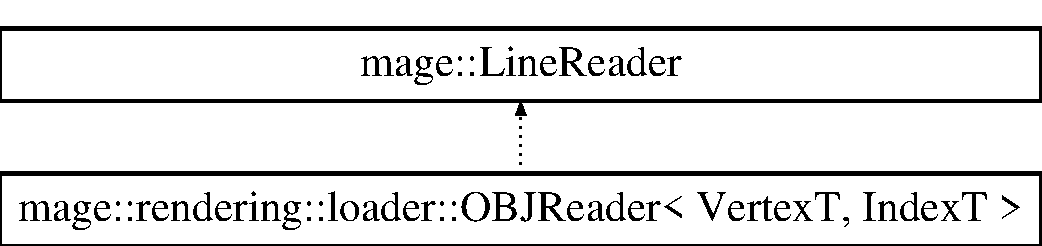
\includegraphics[height=2.000000cm]{classmage_1_1rendering_1_1loader_1_1_o_b_j_reader}
\end{center}
\end{figure}
\subsection*{Classes}
\begin{DoxyCompactItemize}
\item 
struct \mbox{\hyperlink{structmage_1_1rendering_1_1loader_1_1_o_b_j_reader_1_1_o_b_j_comparator}{O\+B\+J\+Comparator}}
\end{DoxyCompactItemize}
\subsection*{Public Member Functions}
\begin{DoxyCompactItemize}
\item 
\mbox{\hyperlink{classmage_1_1rendering_1_1loader_1_1_o_b_j_reader_a5fe68a545e05c266b69f35e4dc9027a9}{O\+B\+J\+Reader}} (\mbox{\hyperlink{classmage_1_1rendering_1_1_resource_manager}{Resource\+Manager}} \&resource\+\_\+manager, \mbox{\hyperlink{structmage_1_1rendering_1_1_model_output}{Model\+Output}}$<$ VertexT, IndexT $>$ \&model\+\_\+output, const \mbox{\hyperlink{classmage_1_1rendering_1_1_mesh_descriptor}{Mesh\+Descriptor}}$<$ VertexT, IndexT $>$ \&mesh\+\_\+desc)
\item 
\mbox{\hyperlink{classmage_1_1rendering_1_1loader_1_1_o_b_j_reader_a1ba7402bf27180682de9109a3d0d031f}{O\+B\+J\+Reader}} (const \mbox{\hyperlink{classmage_1_1rendering_1_1loader_1_1_o_b_j_reader}{O\+B\+J\+Reader}} \&reader)=delete
\item 
\mbox{\hyperlink{classmage_1_1rendering_1_1loader_1_1_o_b_j_reader_afa0ab677916b17126aa4fc202c52684e}{O\+B\+J\+Reader}} (\mbox{\hyperlink{classmage_1_1rendering_1_1loader_1_1_o_b_j_reader}{O\+B\+J\+Reader}} \&\&reader) noexcept
\item 
\mbox{\hyperlink{classmage_1_1rendering_1_1loader_1_1_o_b_j_reader_a2b10c4cbb4c4aea192c78045beb4735e}{$\sim$\+O\+B\+J\+Reader}} ()
\item 
\mbox{\hyperlink{classmage_1_1rendering_1_1loader_1_1_o_b_j_reader}{O\+B\+J\+Reader}} \& \mbox{\hyperlink{classmage_1_1rendering_1_1loader_1_1_o_b_j_reader_a006549a7f9724580c7fdae2f7a9c7bdf}{operator=}} (const \mbox{\hyperlink{classmage_1_1rendering_1_1loader_1_1_o_b_j_reader}{O\+B\+J\+Reader}} \&reader)=delete
\item 
\mbox{\hyperlink{classmage_1_1rendering_1_1loader_1_1_o_b_j_reader}{O\+B\+J\+Reader}} \& \mbox{\hyperlink{classmage_1_1rendering_1_1loader_1_1_o_b_j_reader_ad35fe46e20179ce1cd79386501ee0959}{operator=}} (\mbox{\hyperlink{classmage_1_1rendering_1_1loader_1_1_o_b_j_reader}{O\+B\+J\+Reader}} \&\&reader)=delete
\item 
void \mbox{\hyperlink{classmage_1_1rendering_1_1loader_1_1_o_b_j_reader_ac819910b2ad9cf9751fa223d4f90ada0}{Read\+From\+File}} (std\+::filesystem\+::path path, std\+::regex regex=\mbox{\hyperlink{classmage_1_1_line_reader_a6b21fad06278a64bbdece198844a8cfa}{g\+\_\+default\+\_\+regex}})
\item 
void \mbox{\hyperlink{classmage_1_1rendering_1_1loader_1_1_o_b_j_reader_adc2bf81611774d4a11da47812fcc0f6a}{Read\+From\+Memory}} (const std\+::string \&input, std\+::regex regex=\mbox{\hyperlink{classmage_1_1_line_reader_a6b21fad06278a64bbdece198844a8cfa}{g\+\_\+default\+\_\+regex}})
\end{DoxyCompactItemize}
\subsection*{Private Member Functions}
\begin{DoxyCompactItemize}
\item 
virtual void \mbox{\hyperlink{classmage_1_1rendering_1_1loader_1_1_o_b_j_reader_ad082a6295259f7e8af2c60c182ea55d3}{Preprocess}} () override
\item 
virtual void \mbox{\hyperlink{classmage_1_1rendering_1_1loader_1_1_o_b_j_reader_adcf31a8bacf23cac2577f679c6bac729}{Read\+Line}} () override
\item 
virtual void \mbox{\hyperlink{classmage_1_1rendering_1_1loader_1_1_o_b_j_reader_a281c16ef7d20a7c1416923f3cadee33a}{Postprocess}} () override
\item 
void \mbox{\hyperlink{classmage_1_1rendering_1_1loader_1_1_o_b_j_reader_aa898eb5cac6a5e04b1da9329587a81cd}{Read\+O\+B\+J\+Material\+Library}} ()
\item 
void \mbox{\hyperlink{classmage_1_1rendering_1_1loader_1_1_o_b_j_reader_a5aa719224a08175bcbcb26873e2fb5e1}{Read\+O\+B\+J\+Material\+Use}} ()
\item 
void \mbox{\hyperlink{classmage_1_1rendering_1_1loader_1_1_o_b_j_reader_a4e733a0afea4b82e3aea89fe58f5bfba}{Read\+O\+B\+J\+Group}} ()
\item 
void \mbox{\hyperlink{classmage_1_1rendering_1_1loader_1_1_o_b_j_reader_a519f333ce13777d469c63eae7ab8dcf4}{Read\+O\+B\+J\+Object}} ()
\item 
void \mbox{\hyperlink{classmage_1_1rendering_1_1loader_1_1_o_b_j_reader_ac7f3807cf0a0ae24b340cb8208c5b2ef}{Read\+O\+B\+J\+Smoothing\+Group}} ()
\item 
void \mbox{\hyperlink{classmage_1_1rendering_1_1loader_1_1_o_b_j_reader_a0f6e0d744b2baf94bca4dfda6c2cc194}{Read\+O\+B\+J\+Vertex}} ()
\item 
void \mbox{\hyperlink{classmage_1_1rendering_1_1loader_1_1_o_b_j_reader_a91f53fd761c83c4135a3ef1882b8300d}{Read\+O\+B\+J\+Vertex\+Texture}} ()
\item 
void \mbox{\hyperlink{classmage_1_1rendering_1_1loader_1_1_o_b_j_reader_a1aafeda3894017fb9b3c6183ac272a34}{Read\+O\+B\+J\+Vertex\+Normal}} ()
\item 
void \mbox{\hyperlink{classmage_1_1rendering_1_1loader_1_1_o_b_j_reader_a58d5c4e4a5a82714567413b6e17a9ec7}{Read\+O\+B\+J\+Face}} ()
\item 
const \mbox{\hyperlink{structmage_1_1_point3}{Point3}} \mbox{\hyperlink{classmage_1_1rendering_1_1loader_1_1_o_b_j_reader_a2c5d954441d64b982d7a89df9171edbc}{Read\+O\+B\+J\+Vertex\+Coordinates}} ()
\item 
const \mbox{\hyperlink{structmage_1_1_normal3}{Normal3}} \mbox{\hyperlink{classmage_1_1rendering_1_1loader_1_1_o_b_j_reader_aa91768722fd418aeba3f12915e8e1525}{Read\+O\+B\+J\+Vertex\+Normal\+Coordinates}} ()
\item 
const \mbox{\hyperlink{structmage_1_1_u_v}{UV}} \mbox{\hyperlink{classmage_1_1rendering_1_1loader_1_1_o_b_j_reader_a3fdbcdecf40525631afc53ce6a6dba45}{Read\+O\+B\+J\+Vertex\+Texture\+Coordinates}} ()
\item 
const \mbox{\hyperlink{namespacemage_a03e3b6f65630005f43a3112d1f6cf57b}{U32x3}} \mbox{\hyperlink{classmage_1_1rendering_1_1loader_1_1_o_b_j_reader_adf0996ca5d0339782382b46c14768b7f}{Read\+O\+B\+J\+Vertex\+Indices}} ()
\item 
const VertexT \mbox{\hyperlink{classmage_1_1rendering_1_1loader_1_1_o_b_j_reader_aa223ad518d2cdddd1c89a3f113356d77}{Construct\+Vertex}} (const \mbox{\hyperlink{namespacemage_a03e3b6f65630005f43a3112d1f6cf57b}{U32x3}} \&vertex\+\_\+indices)
\end{DoxyCompactItemize}
\subsection*{Private Attributes}
\begin{DoxyCompactItemize}
\item 
std\+::vector$<$ \mbox{\hyperlink{structmage_1_1_point3}{Point3}} $>$ \mbox{\hyperlink{classmage_1_1rendering_1_1loader_1_1_o_b_j_reader_a393e0932f169a786e38f120fc6f0d84b}{m\+\_\+vertex\+\_\+coordinates}}
\item 
std\+::vector$<$ \mbox{\hyperlink{structmage_1_1_u_v}{UV}} $>$ \mbox{\hyperlink{classmage_1_1rendering_1_1loader_1_1_o_b_j_reader_aed919290e638cbe00a9144fdcb652178}{m\+\_\+vertex\+\_\+texture\+\_\+coordinates}}
\item 
std\+::vector$<$ \mbox{\hyperlink{structmage_1_1_normal3}{Normal3}} $>$ \mbox{\hyperlink{classmage_1_1rendering_1_1loader_1_1_o_b_j_reader_ac977ade8154bef446524526e8297f3eb}{m\+\_\+vertex\+\_\+normal\+\_\+coordinates}}
\item 
std\+::map$<$ \mbox{\hyperlink{namespacemage_a03e3b6f65630005f43a3112d1f6cf57b}{U32x3}}, IndexT, \mbox{\hyperlink{structmage_1_1rendering_1_1loader_1_1_o_b_j_reader_1_1_o_b_j_comparator}{O\+B\+J\+Comparator}} $>$ \mbox{\hyperlink{classmage_1_1rendering_1_1loader_1_1_o_b_j_reader_a4bad8aafabddb5cec68be8357d2d7566}{m\+\_\+mapping}}
\item 
\mbox{\hyperlink{classmage_1_1rendering_1_1_resource_manager}{Resource\+Manager}} \& \mbox{\hyperlink{classmage_1_1rendering_1_1loader_1_1_o_b_j_reader_ae6208964e05f3e93eb9939942fe3b55c}{m\+\_\+resource\+\_\+manager}}
\item 
\mbox{\hyperlink{structmage_1_1rendering_1_1_model_output}{Model\+Output}}$<$ VertexT, IndexT $>$ \& \mbox{\hyperlink{classmage_1_1rendering_1_1loader_1_1_o_b_j_reader_a645fca7c3f7f9860cb879f4088c4f8fc}{m\+\_\+model\+\_\+output}}
\item 
const \mbox{\hyperlink{classmage_1_1rendering_1_1_mesh_descriptor}{Mesh\+Descriptor}}$<$ VertexT, IndexT $>$ \& \mbox{\hyperlink{classmage_1_1rendering_1_1loader_1_1_o_b_j_reader_aa029c035456ea9456d63726b15e5db05}{m\+\_\+mesh\+\_\+desc}}
\end{DoxyCompactItemize}
\subsection*{Additional Inherited Members}


\subsection{Detailed Description}
\subsubsection*{template$<$typename VertexT, typename IndexT$>$\newline
class mage\+::rendering\+::loader\+::\+O\+B\+J\+Reader$<$ Vertex\+T, Index\+T $>$}

A class of O\+BJ file readers for reading meshes.


\begin{DoxyTemplParams}{Template Parameters}
{\em VertexT} & The vertex type. \\
\hline
{\em IndexT} & The index type. \\
\hline
\end{DoxyTemplParams}


\subsection{Constructor \& Destructor Documentation}
\mbox{\Hypertarget{classmage_1_1rendering_1_1loader_1_1_o_b_j_reader_a5fe68a545e05c266b69f35e4dc9027a9}\label{classmage_1_1rendering_1_1loader_1_1_o_b_j_reader_a5fe68a545e05c266b69f35e4dc9027a9}} 
\index{mage\+::rendering\+::loader\+::\+O\+B\+J\+Reader@{mage\+::rendering\+::loader\+::\+O\+B\+J\+Reader}!O\+B\+J\+Reader@{O\+B\+J\+Reader}}
\index{O\+B\+J\+Reader@{O\+B\+J\+Reader}!mage\+::rendering\+::loader\+::\+O\+B\+J\+Reader@{mage\+::rendering\+::loader\+::\+O\+B\+J\+Reader}}
\subsubsection{\texorpdfstring{O\+B\+J\+Reader()}{OBJReader()}\hspace{0.1cm}{\footnotesize\ttfamily [1/3]}}
{\footnotesize\ttfamily template$<$typename VertexT , typename IndexT $>$ \\
\mbox{\hyperlink{classmage_1_1rendering_1_1loader_1_1_o_b_j_reader}{mage\+::rendering\+::loader\+::\+O\+B\+J\+Reader}}$<$ VertexT, IndexT $>$\+::\mbox{\hyperlink{classmage_1_1rendering_1_1loader_1_1_o_b_j_reader}{O\+B\+J\+Reader}} (\begin{DoxyParamCaption}\item[{\mbox{\hyperlink{classmage_1_1rendering_1_1_resource_manager}{Resource\+Manager}} \&}]{resource\+\_\+manager,  }\item[{\mbox{\hyperlink{structmage_1_1rendering_1_1_model_output}{Model\+Output}}$<$ VertexT, IndexT $>$ \&}]{model\+\_\+output,  }\item[{const \mbox{\hyperlink{classmage_1_1rendering_1_1_mesh_descriptor}{Mesh\+Descriptor}}$<$ VertexT, IndexT $>$ \&}]{mesh\+\_\+desc }\end{DoxyParamCaption})\hspace{0.3cm}{\ttfamily [explicit]}}

Constructs an O\+BJ reader.


\begin{DoxyParams}[1]{Parameters}
\mbox{\tt in}  & {\em resource\+\_\+manager} & A reference to the resource manager. \\
\hline
\mbox{\tt in}  & {\em model\+\_\+output} & A reference to a model output for storing the read data from file. \\
\hline
\mbox{\tt in}  & {\em mesh\+\_\+desc} & A reference to a mesh descriptor. \\
\hline
\end{DoxyParams}
\mbox{\Hypertarget{classmage_1_1rendering_1_1loader_1_1_o_b_j_reader_a1ba7402bf27180682de9109a3d0d031f}\label{classmage_1_1rendering_1_1loader_1_1_o_b_j_reader_a1ba7402bf27180682de9109a3d0d031f}} 
\index{mage\+::rendering\+::loader\+::\+O\+B\+J\+Reader@{mage\+::rendering\+::loader\+::\+O\+B\+J\+Reader}!O\+B\+J\+Reader@{O\+B\+J\+Reader}}
\index{O\+B\+J\+Reader@{O\+B\+J\+Reader}!mage\+::rendering\+::loader\+::\+O\+B\+J\+Reader@{mage\+::rendering\+::loader\+::\+O\+B\+J\+Reader}}
\subsubsection{\texorpdfstring{O\+B\+J\+Reader()}{OBJReader()}\hspace{0.1cm}{\footnotesize\ttfamily [2/3]}}
{\footnotesize\ttfamily template$<$typename VertexT , typename IndexT $>$ \\
\mbox{\hyperlink{classmage_1_1rendering_1_1loader_1_1_o_b_j_reader}{mage\+::rendering\+::loader\+::\+O\+B\+J\+Reader}}$<$ VertexT, IndexT $>$\+::\mbox{\hyperlink{classmage_1_1rendering_1_1loader_1_1_o_b_j_reader}{O\+B\+J\+Reader}} (\begin{DoxyParamCaption}\item[{const \mbox{\hyperlink{classmage_1_1rendering_1_1loader_1_1_o_b_j_reader}{O\+B\+J\+Reader}}$<$ VertexT, IndexT $>$ \&}]{reader }\end{DoxyParamCaption})\hspace{0.3cm}{\ttfamily [delete]}}

Constructs an O\+BJ reader from the given O\+BJ reader.


\begin{DoxyParams}[1]{Parameters}
\mbox{\tt in}  & {\em reader} & A reference to the O\+BJ reader to copy. \\
\hline
\end{DoxyParams}
\mbox{\Hypertarget{classmage_1_1rendering_1_1loader_1_1_o_b_j_reader_afa0ab677916b17126aa4fc202c52684e}\label{classmage_1_1rendering_1_1loader_1_1_o_b_j_reader_afa0ab677916b17126aa4fc202c52684e}} 
\index{mage\+::rendering\+::loader\+::\+O\+B\+J\+Reader@{mage\+::rendering\+::loader\+::\+O\+B\+J\+Reader}!O\+B\+J\+Reader@{O\+B\+J\+Reader}}
\index{O\+B\+J\+Reader@{O\+B\+J\+Reader}!mage\+::rendering\+::loader\+::\+O\+B\+J\+Reader@{mage\+::rendering\+::loader\+::\+O\+B\+J\+Reader}}
\subsubsection{\texorpdfstring{O\+B\+J\+Reader()}{OBJReader()}\hspace{0.1cm}{\footnotesize\ttfamily [3/3]}}
{\footnotesize\ttfamily template$<$typename VertexT , typename IndexT $>$ \\
\mbox{\hyperlink{classmage_1_1rendering_1_1loader_1_1_o_b_j_reader}{mage\+::rendering\+::loader\+::\+O\+B\+J\+Reader}}$<$ VertexT, IndexT $>$\+::\mbox{\hyperlink{classmage_1_1rendering_1_1loader_1_1_o_b_j_reader}{O\+B\+J\+Reader}} (\begin{DoxyParamCaption}\item[{\mbox{\hyperlink{classmage_1_1rendering_1_1loader_1_1_o_b_j_reader}{O\+B\+J\+Reader}}$<$ VertexT, IndexT $>$ \&\&}]{reader }\end{DoxyParamCaption})\hspace{0.3cm}{\ttfamily [noexcept]}}

Constructs an O\+BJ reader by moving the given O\+BJ reader.


\begin{DoxyParams}[1]{Parameters}
\mbox{\tt in}  & {\em reader} & A reference to the O\+BJ reader to move. \\
\hline
\end{DoxyParams}
\mbox{\Hypertarget{classmage_1_1rendering_1_1loader_1_1_o_b_j_reader_a2b10c4cbb4c4aea192c78045beb4735e}\label{classmage_1_1rendering_1_1loader_1_1_o_b_j_reader_a2b10c4cbb4c4aea192c78045beb4735e}} 
\index{mage\+::rendering\+::loader\+::\+O\+B\+J\+Reader@{mage\+::rendering\+::loader\+::\+O\+B\+J\+Reader}!````~O\+B\+J\+Reader@{$\sim$\+O\+B\+J\+Reader}}
\index{````~O\+B\+J\+Reader@{$\sim$\+O\+B\+J\+Reader}!mage\+::rendering\+::loader\+::\+O\+B\+J\+Reader@{mage\+::rendering\+::loader\+::\+O\+B\+J\+Reader}}
\subsubsection{\texorpdfstring{$\sim$\+O\+B\+J\+Reader()}{~OBJReader()}}
{\footnotesize\ttfamily template$<$typename VertexT , typename IndexT $>$ \\
\mbox{\hyperlink{classmage_1_1rendering_1_1loader_1_1_o_b_j_reader}{mage\+::rendering\+::loader\+::\+O\+B\+J\+Reader}}$<$ VertexT, IndexT $>$\+::$\sim$\mbox{\hyperlink{classmage_1_1rendering_1_1loader_1_1_o_b_j_reader}{O\+B\+J\+Reader}} (\begin{DoxyParamCaption}{ }\end{DoxyParamCaption})}

Destructs this O\+BJ reader. 

\subsection{Member Function Documentation}
\mbox{\Hypertarget{classmage_1_1rendering_1_1loader_1_1_o_b_j_reader_aa223ad518d2cdddd1c89a3f113356d77}\label{classmage_1_1rendering_1_1loader_1_1_o_b_j_reader_aa223ad518d2cdddd1c89a3f113356d77}} 
\index{mage\+::rendering\+::loader\+::\+O\+B\+J\+Reader@{mage\+::rendering\+::loader\+::\+O\+B\+J\+Reader}!Construct\+Vertex@{Construct\+Vertex}}
\index{Construct\+Vertex@{Construct\+Vertex}!mage\+::rendering\+::loader\+::\+O\+B\+J\+Reader@{mage\+::rendering\+::loader\+::\+O\+B\+J\+Reader}}
\subsubsection{\texorpdfstring{Construct\+Vertex()}{ConstructVertex()}}
{\footnotesize\ttfamily template$<$typename VertexT , typename IndexT $>$ \\
const VertexT \mbox{\hyperlink{classmage_1_1rendering_1_1loader_1_1_o_b_j_reader}{mage\+::rendering\+::loader\+::\+O\+B\+J\+Reader}}$<$ VertexT, IndexT $>$\+::Construct\+Vertex (\begin{DoxyParamCaption}\item[{const \mbox{\hyperlink{namespacemage_a03e3b6f65630005f43a3112d1f6cf57b}{U32x3}} \&}]{vertex\+\_\+indices }\end{DoxyParamCaption})\hspace{0.3cm}{\ttfamily [private]}}

Constructs or retrieves (if already existing) the vertex matching the given vertex indices.


\begin{DoxyParams}[1]{Parameters}
\mbox{\tt in}  & {\em vertex\+\_\+indices} & A reference to the vertex indices. \\
\hline
\end{DoxyParams}
\begin{DoxyReturn}{Returns}
The vertex matching the given vertex indices {\itshape vertex\+\_\+indices}. 
\end{DoxyReturn}
\mbox{\Hypertarget{classmage_1_1rendering_1_1loader_1_1_o_b_j_reader_a006549a7f9724580c7fdae2f7a9c7bdf}\label{classmage_1_1rendering_1_1loader_1_1_o_b_j_reader_a006549a7f9724580c7fdae2f7a9c7bdf}} 
\index{mage\+::rendering\+::loader\+::\+O\+B\+J\+Reader@{mage\+::rendering\+::loader\+::\+O\+B\+J\+Reader}!operator=@{operator=}}
\index{operator=@{operator=}!mage\+::rendering\+::loader\+::\+O\+B\+J\+Reader@{mage\+::rendering\+::loader\+::\+O\+B\+J\+Reader}}
\subsubsection{\texorpdfstring{operator=()}{operator=()}\hspace{0.1cm}{\footnotesize\ttfamily [1/2]}}
{\footnotesize\ttfamily template$<$typename VertexT , typename IndexT $>$ \\
\mbox{\hyperlink{classmage_1_1rendering_1_1loader_1_1_o_b_j_reader}{O\+B\+J\+Reader}}\& \mbox{\hyperlink{classmage_1_1rendering_1_1loader_1_1_o_b_j_reader}{mage\+::rendering\+::loader\+::\+O\+B\+J\+Reader}}$<$ VertexT, IndexT $>$\+::operator= (\begin{DoxyParamCaption}\item[{const \mbox{\hyperlink{classmage_1_1rendering_1_1loader_1_1_o_b_j_reader}{O\+B\+J\+Reader}}$<$ VertexT, IndexT $>$ \&}]{reader }\end{DoxyParamCaption})\hspace{0.3cm}{\ttfamily [delete]}}

Copies the given O\+BJ reader to this O\+BJ reader.


\begin{DoxyParams}[1]{Parameters}
\mbox{\tt in}  & {\em reader} & A reference to a O\+BJ reader to copy. \\
\hline
\end{DoxyParams}
\begin{DoxyReturn}{Returns}
A reference to the copy of the given O\+BJ reader (i.\+e. this O\+BJ reader). 
\end{DoxyReturn}
\mbox{\Hypertarget{classmage_1_1rendering_1_1loader_1_1_o_b_j_reader_ad35fe46e20179ce1cd79386501ee0959}\label{classmage_1_1rendering_1_1loader_1_1_o_b_j_reader_ad35fe46e20179ce1cd79386501ee0959}} 
\index{mage\+::rendering\+::loader\+::\+O\+B\+J\+Reader@{mage\+::rendering\+::loader\+::\+O\+B\+J\+Reader}!operator=@{operator=}}
\index{operator=@{operator=}!mage\+::rendering\+::loader\+::\+O\+B\+J\+Reader@{mage\+::rendering\+::loader\+::\+O\+B\+J\+Reader}}
\subsubsection{\texorpdfstring{operator=()}{operator=()}\hspace{0.1cm}{\footnotesize\ttfamily [2/2]}}
{\footnotesize\ttfamily template$<$typename VertexT , typename IndexT $>$ \\
\mbox{\hyperlink{classmage_1_1rendering_1_1loader_1_1_o_b_j_reader}{O\+B\+J\+Reader}}\& \mbox{\hyperlink{classmage_1_1rendering_1_1loader_1_1_o_b_j_reader}{mage\+::rendering\+::loader\+::\+O\+B\+J\+Reader}}$<$ VertexT, IndexT $>$\+::operator= (\begin{DoxyParamCaption}\item[{\mbox{\hyperlink{classmage_1_1rendering_1_1loader_1_1_o_b_j_reader}{O\+B\+J\+Reader}}$<$ VertexT, IndexT $>$ \&\&}]{reader }\end{DoxyParamCaption})\hspace{0.3cm}{\ttfamily [delete]}}

Moves the given O\+BJ reader to this O\+BJ reader.


\begin{DoxyParams}[1]{Parameters}
\mbox{\tt in}  & {\em reader} & A reference to a O\+BJ reader to move. \\
\hline
\end{DoxyParams}
\begin{DoxyReturn}{Returns}
A reference to the moved O\+BJ reader (i.\+e. this O\+BJ reader). 
\end{DoxyReturn}
\mbox{\Hypertarget{classmage_1_1rendering_1_1loader_1_1_o_b_j_reader_a281c16ef7d20a7c1416923f3cadee33a}\label{classmage_1_1rendering_1_1loader_1_1_o_b_j_reader_a281c16ef7d20a7c1416923f3cadee33a}} 
\index{mage\+::rendering\+::loader\+::\+O\+B\+J\+Reader@{mage\+::rendering\+::loader\+::\+O\+B\+J\+Reader}!Postprocess@{Postprocess}}
\index{Postprocess@{Postprocess}!mage\+::rendering\+::loader\+::\+O\+B\+J\+Reader@{mage\+::rendering\+::loader\+::\+O\+B\+J\+Reader}}
\subsubsection{\texorpdfstring{Postprocess()}{Postprocess()}}
{\footnotesize\ttfamily template$<$typename VertexT , typename IndexT $>$ \\
virtual void \mbox{\hyperlink{classmage_1_1rendering_1_1loader_1_1_o_b_j_reader}{mage\+::rendering\+::loader\+::\+O\+B\+J\+Reader}}$<$ VertexT, IndexT $>$\+::Postprocess (\begin{DoxyParamCaption}{ }\end{DoxyParamCaption})\hspace{0.3cm}{\ttfamily [override]}, {\ttfamily [private]}, {\ttfamily [virtual]}}

Post-\/processes after reading the current file of this O\+BJ reader.


\begin{DoxyExceptions}{Exceptions}
{\em \mbox{\hyperlink{classmage_1_1_exception}{Exception}}} & Failed to finish post-\/processing successfully. \\
\hline
\end{DoxyExceptions}


Reimplemented from \mbox{\hyperlink{classmage_1_1_line_reader_a51775e07b5f7c9f72441e42d6d3896e1}{mage\+::\+Line\+Reader}}.

\mbox{\Hypertarget{classmage_1_1rendering_1_1loader_1_1_o_b_j_reader_ad082a6295259f7e8af2c60c182ea55d3}\label{classmage_1_1rendering_1_1loader_1_1_o_b_j_reader_ad082a6295259f7e8af2c60c182ea55d3}} 
\index{mage\+::rendering\+::loader\+::\+O\+B\+J\+Reader@{mage\+::rendering\+::loader\+::\+O\+B\+J\+Reader}!Preprocess@{Preprocess}}
\index{Preprocess@{Preprocess}!mage\+::rendering\+::loader\+::\+O\+B\+J\+Reader@{mage\+::rendering\+::loader\+::\+O\+B\+J\+Reader}}
\subsubsection{\texorpdfstring{Preprocess()}{Preprocess()}}
{\footnotesize\ttfamily template$<$typename VertexT , typename IndexT $>$ \\
virtual void \mbox{\hyperlink{classmage_1_1rendering_1_1loader_1_1_o_b_j_reader}{mage\+::rendering\+::loader\+::\+O\+B\+J\+Reader}}$<$ VertexT, IndexT $>$\+::Preprocess (\begin{DoxyParamCaption}{ }\end{DoxyParamCaption})\hspace{0.3cm}{\ttfamily [override]}, {\ttfamily [private]}, {\ttfamily [virtual]}}

Pre-\/process before reading the current file of this O\+BJ reader.


\begin{DoxyExceptions}{Exceptions}
{\em \mbox{\hyperlink{classmage_1_1_exception}{Exception}}} & Failed to finish the pre-\/processing successfully. \\
\hline
\end{DoxyExceptions}


Reimplemented from \mbox{\hyperlink{classmage_1_1_line_reader_ad81a84bf9ecd81b9a391698afbd5eb61}{mage\+::\+Line\+Reader}}.

\mbox{\Hypertarget{classmage_1_1rendering_1_1loader_1_1_o_b_j_reader_ac819910b2ad9cf9751fa223d4f90ada0}\label{classmage_1_1rendering_1_1loader_1_1_o_b_j_reader_ac819910b2ad9cf9751fa223d4f90ada0}} 
\index{mage\+::rendering\+::loader\+::\+O\+B\+J\+Reader@{mage\+::rendering\+::loader\+::\+O\+B\+J\+Reader}!Read\+From\+File@{Read\+From\+File}}
\index{Read\+From\+File@{Read\+From\+File}!mage\+::rendering\+::loader\+::\+O\+B\+J\+Reader@{mage\+::rendering\+::loader\+::\+O\+B\+J\+Reader}}
\subsubsection{\texorpdfstring{Read\+From\+File()}{ReadFromFile()}}
{\footnotesize\ttfamily template$<$typename VertexT , typename IndexT $>$ \\
void mage\+::\+Line\+Reader\+::\+Read\+From\+File}

Reads from the file associated with the given path.


\begin{DoxyParams}[1]{Parameters}
\mbox{\tt in}  & {\em path} & The path. \\
\hline
\mbox{\tt in}  & {\em regex} & The (line) regex. \\
\hline
\end{DoxyParams}

\begin{DoxyExceptions}{Exceptions}
{\em \mbox{\hyperlink{classmage_1_1_exception}{Exception}}} & Failed to read from the file. \\
\hline
\end{DoxyExceptions}
\mbox{\Hypertarget{classmage_1_1rendering_1_1loader_1_1_o_b_j_reader_adc2bf81611774d4a11da47812fcc0f6a}\label{classmage_1_1rendering_1_1loader_1_1_o_b_j_reader_adc2bf81611774d4a11da47812fcc0f6a}} 
\index{mage\+::rendering\+::loader\+::\+O\+B\+J\+Reader@{mage\+::rendering\+::loader\+::\+O\+B\+J\+Reader}!Read\+From\+Memory@{Read\+From\+Memory}}
\index{Read\+From\+Memory@{Read\+From\+Memory}!mage\+::rendering\+::loader\+::\+O\+B\+J\+Reader@{mage\+::rendering\+::loader\+::\+O\+B\+J\+Reader}}
\subsubsection{\texorpdfstring{Read\+From\+Memory()}{ReadFromMemory()}}
{\footnotesize\ttfamily template$<$typename VertexT , typename IndexT $>$ \\
void mage\+::\+Line\+Reader\+::\+Read\+From\+Memory}

Reads from the given input string.


\begin{DoxyParams}[1]{Parameters}
\mbox{\tt in}  & {\em input} & A reference to the input string. \\
\hline
\mbox{\tt in}  & {\em regex} & The (line) regex. \\
\hline
\end{DoxyParams}

\begin{DoxyExceptions}{Exceptions}
{\em \mbox{\hyperlink{classmage_1_1_exception}{Exception}}} & Failed to read from the given input string. \\
\hline
\end{DoxyExceptions}
\mbox{\Hypertarget{classmage_1_1rendering_1_1loader_1_1_o_b_j_reader_adcf31a8bacf23cac2577f679c6bac729}\label{classmage_1_1rendering_1_1loader_1_1_o_b_j_reader_adcf31a8bacf23cac2577f679c6bac729}} 
\index{mage\+::rendering\+::loader\+::\+O\+B\+J\+Reader@{mage\+::rendering\+::loader\+::\+O\+B\+J\+Reader}!Read\+Line@{Read\+Line}}
\index{Read\+Line@{Read\+Line}!mage\+::rendering\+::loader\+::\+O\+B\+J\+Reader@{mage\+::rendering\+::loader\+::\+O\+B\+J\+Reader}}
\subsubsection{\texorpdfstring{Read\+Line()}{ReadLine()}}
{\footnotesize\ttfamily template$<$typename VertexT , typename IndexT $>$ \\
virtual void \mbox{\hyperlink{classmage_1_1rendering_1_1loader_1_1_o_b_j_reader}{mage\+::rendering\+::loader\+::\+O\+B\+J\+Reader}}$<$ VertexT, IndexT $>$\+::Read\+Line (\begin{DoxyParamCaption}{ }\end{DoxyParamCaption})\hspace{0.3cm}{\ttfamily [override]}, {\ttfamily [private]}, {\ttfamily [virtual]}}

Reads the current line of this O\+BJ reader.


\begin{DoxyExceptions}{Exceptions}
{\em \mbox{\hyperlink{classmage_1_1_exception}{Exception}}} & Failed to the current line of this O\+BJ reader. \\
\hline
\end{DoxyExceptions}


Implements \mbox{\hyperlink{classmage_1_1_line_reader_a8c81989a9d59ae31dd19e6d3961cfaf1}{mage\+::\+Line\+Reader}}.

\mbox{\Hypertarget{classmage_1_1rendering_1_1loader_1_1_o_b_j_reader_a58d5c4e4a5a82714567413b6e17a9ec7}\label{classmage_1_1rendering_1_1loader_1_1_o_b_j_reader_a58d5c4e4a5a82714567413b6e17a9ec7}} 
\index{mage\+::rendering\+::loader\+::\+O\+B\+J\+Reader@{mage\+::rendering\+::loader\+::\+O\+B\+J\+Reader}!Read\+O\+B\+J\+Face@{Read\+O\+B\+J\+Face}}
\index{Read\+O\+B\+J\+Face@{Read\+O\+B\+J\+Face}!mage\+::rendering\+::loader\+::\+O\+B\+J\+Reader@{mage\+::rendering\+::loader\+::\+O\+B\+J\+Reader}}
\subsubsection{\texorpdfstring{Read\+O\+B\+J\+Face()}{ReadOBJFace()}}
{\footnotesize\ttfamily template$<$typename VertexT , typename IndexT $>$ \\
void \mbox{\hyperlink{classmage_1_1rendering_1_1loader_1_1_o_b_j_reader}{mage\+::rendering\+::loader\+::\+O\+B\+J\+Reader}}$<$ VertexT, IndexT $>$\+::Read\+O\+B\+J\+Face (\begin{DoxyParamCaption}{ }\end{DoxyParamCaption})\hspace{0.3cm}{\ttfamily [private]}}

Reads a Face definition.


\begin{DoxyExceptions}{Exceptions}
{\em \mbox{\hyperlink{classmage_1_1_exception}{Exception}}} & Failed to read a Face definition. \\
\hline
\end{DoxyExceptions}
\mbox{\Hypertarget{classmage_1_1rendering_1_1loader_1_1_o_b_j_reader_a4e733a0afea4b82e3aea89fe58f5bfba}\label{classmage_1_1rendering_1_1loader_1_1_o_b_j_reader_a4e733a0afea4b82e3aea89fe58f5bfba}} 
\index{mage\+::rendering\+::loader\+::\+O\+B\+J\+Reader@{mage\+::rendering\+::loader\+::\+O\+B\+J\+Reader}!Read\+O\+B\+J\+Group@{Read\+O\+B\+J\+Group}}
\index{Read\+O\+B\+J\+Group@{Read\+O\+B\+J\+Group}!mage\+::rendering\+::loader\+::\+O\+B\+J\+Reader@{mage\+::rendering\+::loader\+::\+O\+B\+J\+Reader}}
\subsubsection{\texorpdfstring{Read\+O\+B\+J\+Group()}{ReadOBJGroup()}}
{\footnotesize\ttfamily template$<$typename VertexT , typename IndexT $>$ \\
void \mbox{\hyperlink{classmage_1_1rendering_1_1loader_1_1_o_b_j_reader}{mage\+::rendering\+::loader\+::\+O\+B\+J\+Reader}}$<$ VertexT, IndexT $>$\+::Read\+O\+B\+J\+Group (\begin{DoxyParamCaption}{ }\end{DoxyParamCaption})\hspace{0.3cm}{\ttfamily [private]}}

Reads a Group definition.


\begin{DoxyExceptions}{Exceptions}
{\em \mbox{\hyperlink{classmage_1_1_exception}{Exception}}} & Failed to read a Group definition. \\
\hline
\end{DoxyExceptions}
\mbox{\Hypertarget{classmage_1_1rendering_1_1loader_1_1_o_b_j_reader_aa898eb5cac6a5e04b1da9329587a81cd}\label{classmage_1_1rendering_1_1loader_1_1_o_b_j_reader_aa898eb5cac6a5e04b1da9329587a81cd}} 
\index{mage\+::rendering\+::loader\+::\+O\+B\+J\+Reader@{mage\+::rendering\+::loader\+::\+O\+B\+J\+Reader}!Read\+O\+B\+J\+Material\+Library@{Read\+O\+B\+J\+Material\+Library}}
\index{Read\+O\+B\+J\+Material\+Library@{Read\+O\+B\+J\+Material\+Library}!mage\+::rendering\+::loader\+::\+O\+B\+J\+Reader@{mage\+::rendering\+::loader\+::\+O\+B\+J\+Reader}}
\subsubsection{\texorpdfstring{Read\+O\+B\+J\+Material\+Library()}{ReadOBJMaterialLibrary()}}
{\footnotesize\ttfamily template$<$typename VertexT , typename IndexT $>$ \\
void \mbox{\hyperlink{classmage_1_1rendering_1_1loader_1_1_o_b_j_reader}{mage\+::rendering\+::loader\+::\+O\+B\+J\+Reader}}$<$ VertexT, IndexT $>$\+::Read\+O\+B\+J\+Material\+Library (\begin{DoxyParamCaption}{ }\end{DoxyParamCaption})\hspace{0.3cm}{\ttfamily [private]}}

Reads a \mbox{\hyperlink{classmage_1_1rendering_1_1_material}{Material}} Library Include definition.


\begin{DoxyExceptions}{Exceptions}
{\em \mbox{\hyperlink{classmage_1_1_exception}{Exception}}} & Failed to read a \mbox{\hyperlink{classmage_1_1rendering_1_1_material}{Material}} Library Include definition. \\
\hline
\end{DoxyExceptions}
\mbox{\Hypertarget{classmage_1_1rendering_1_1loader_1_1_o_b_j_reader_a5aa719224a08175bcbcb26873e2fb5e1}\label{classmage_1_1rendering_1_1loader_1_1_o_b_j_reader_a5aa719224a08175bcbcb26873e2fb5e1}} 
\index{mage\+::rendering\+::loader\+::\+O\+B\+J\+Reader@{mage\+::rendering\+::loader\+::\+O\+B\+J\+Reader}!Read\+O\+B\+J\+Material\+Use@{Read\+O\+B\+J\+Material\+Use}}
\index{Read\+O\+B\+J\+Material\+Use@{Read\+O\+B\+J\+Material\+Use}!mage\+::rendering\+::loader\+::\+O\+B\+J\+Reader@{mage\+::rendering\+::loader\+::\+O\+B\+J\+Reader}}
\subsubsection{\texorpdfstring{Read\+O\+B\+J\+Material\+Use()}{ReadOBJMaterialUse()}}
{\footnotesize\ttfamily template$<$typename VertexT , typename IndexT $>$ \\
void \mbox{\hyperlink{classmage_1_1rendering_1_1loader_1_1_o_b_j_reader}{mage\+::rendering\+::loader\+::\+O\+B\+J\+Reader}}$<$ VertexT, IndexT $>$\+::Read\+O\+B\+J\+Material\+Use (\begin{DoxyParamCaption}{ }\end{DoxyParamCaption})\hspace{0.3cm}{\ttfamily [private]}}

Reads a \mbox{\hyperlink{classmage_1_1rendering_1_1_material}{Material}} Usage definition and imports the materials corresponding to the mesh.


\begin{DoxyExceptions}{Exceptions}
{\em \mbox{\hyperlink{classmage_1_1_exception}{Exception}}} & Failed to read a \mbox{\hyperlink{classmage_1_1rendering_1_1_material}{Material}} Usage definition. \\
\hline
{\em \mbox{\hyperlink{classmage_1_1_exception}{Exception}}} & Failed to import the materials. \\
\hline
\end{DoxyExceptions}
\mbox{\Hypertarget{classmage_1_1rendering_1_1loader_1_1_o_b_j_reader_a519f333ce13777d469c63eae7ab8dcf4}\label{classmage_1_1rendering_1_1loader_1_1_o_b_j_reader_a519f333ce13777d469c63eae7ab8dcf4}} 
\index{mage\+::rendering\+::loader\+::\+O\+B\+J\+Reader@{mage\+::rendering\+::loader\+::\+O\+B\+J\+Reader}!Read\+O\+B\+J\+Object@{Read\+O\+B\+J\+Object}}
\index{Read\+O\+B\+J\+Object@{Read\+O\+B\+J\+Object}!mage\+::rendering\+::loader\+::\+O\+B\+J\+Reader@{mage\+::rendering\+::loader\+::\+O\+B\+J\+Reader}}
\subsubsection{\texorpdfstring{Read\+O\+B\+J\+Object()}{ReadOBJObject()}}
{\footnotesize\ttfamily template$<$typename VertexT , typename IndexT $>$ \\
void \mbox{\hyperlink{classmage_1_1rendering_1_1loader_1_1_o_b_j_reader}{mage\+::rendering\+::loader\+::\+O\+B\+J\+Reader}}$<$ VertexT, IndexT $>$\+::Read\+O\+B\+J\+Object (\begin{DoxyParamCaption}{ }\end{DoxyParamCaption})\hspace{0.3cm}{\ttfamily [private]}}

Reads an Object definition.


\begin{DoxyExceptions}{Exceptions}
{\em \mbox{\hyperlink{classmage_1_1_exception}{Exception}}} & Failed to read a Object definition. \\
\hline
\end{DoxyExceptions}
\mbox{\Hypertarget{classmage_1_1rendering_1_1loader_1_1_o_b_j_reader_ac7f3807cf0a0ae24b340cb8208c5b2ef}\label{classmage_1_1rendering_1_1loader_1_1_o_b_j_reader_ac7f3807cf0a0ae24b340cb8208c5b2ef}} 
\index{mage\+::rendering\+::loader\+::\+O\+B\+J\+Reader@{mage\+::rendering\+::loader\+::\+O\+B\+J\+Reader}!Read\+O\+B\+J\+Smoothing\+Group@{Read\+O\+B\+J\+Smoothing\+Group}}
\index{Read\+O\+B\+J\+Smoothing\+Group@{Read\+O\+B\+J\+Smoothing\+Group}!mage\+::rendering\+::loader\+::\+O\+B\+J\+Reader@{mage\+::rendering\+::loader\+::\+O\+B\+J\+Reader}}
\subsubsection{\texorpdfstring{Read\+O\+B\+J\+Smoothing\+Group()}{ReadOBJSmoothingGroup()}}
{\footnotesize\ttfamily template$<$typename VertexT , typename IndexT $>$ \\
void \mbox{\hyperlink{classmage_1_1rendering_1_1loader_1_1_o_b_j_reader}{mage\+::rendering\+::loader\+::\+O\+B\+J\+Reader}}$<$ VertexT, IndexT $>$\+::Read\+O\+B\+J\+Smoothing\+Group (\begin{DoxyParamCaption}{ }\end{DoxyParamCaption})\hspace{0.3cm}{\ttfamily [private]}}

Reads a Smoothing Group definition.

\begin{DoxyNote}{Note}
A smoothing group is, if present, silently ignored. 
\end{DoxyNote}

\begin{DoxyExceptions}{Exceptions}
{\em \mbox{\hyperlink{classmage_1_1_exception}{Exception}}} & Failed to read a Smoothing Group definition. \\
\hline
\end{DoxyExceptions}
\mbox{\Hypertarget{classmage_1_1rendering_1_1loader_1_1_o_b_j_reader_a0f6e0d744b2baf94bca4dfda6c2cc194}\label{classmage_1_1rendering_1_1loader_1_1_o_b_j_reader_a0f6e0d744b2baf94bca4dfda6c2cc194}} 
\index{mage\+::rendering\+::loader\+::\+O\+B\+J\+Reader@{mage\+::rendering\+::loader\+::\+O\+B\+J\+Reader}!Read\+O\+B\+J\+Vertex@{Read\+O\+B\+J\+Vertex}}
\index{Read\+O\+B\+J\+Vertex@{Read\+O\+B\+J\+Vertex}!mage\+::rendering\+::loader\+::\+O\+B\+J\+Reader@{mage\+::rendering\+::loader\+::\+O\+B\+J\+Reader}}
\subsubsection{\texorpdfstring{Read\+O\+B\+J\+Vertex()}{ReadOBJVertex()}}
{\footnotesize\ttfamily template$<$typename VertexT , typename IndexT $>$ \\
void \mbox{\hyperlink{classmage_1_1rendering_1_1loader_1_1_o_b_j_reader}{mage\+::rendering\+::loader\+::\+O\+B\+J\+Reader}}$<$ VertexT, IndexT $>$\+::Read\+O\+B\+J\+Vertex (\begin{DoxyParamCaption}{ }\end{DoxyParamCaption})\hspace{0.3cm}{\ttfamily [private]}}

Reads a Vertex Position Coordinates definition.


\begin{DoxyExceptions}{Exceptions}
{\em \mbox{\hyperlink{classmage_1_1_exception}{Exception}}} & Failed to read a Vertex Position Coordinates definition. \\
\hline
\end{DoxyExceptions}
\mbox{\Hypertarget{classmage_1_1rendering_1_1loader_1_1_o_b_j_reader_a2c5d954441d64b982d7a89df9171edbc}\label{classmage_1_1rendering_1_1loader_1_1_o_b_j_reader_a2c5d954441d64b982d7a89df9171edbc}} 
\index{mage\+::rendering\+::loader\+::\+O\+B\+J\+Reader@{mage\+::rendering\+::loader\+::\+O\+B\+J\+Reader}!Read\+O\+B\+J\+Vertex\+Coordinates@{Read\+O\+B\+J\+Vertex\+Coordinates}}
\index{Read\+O\+B\+J\+Vertex\+Coordinates@{Read\+O\+B\+J\+Vertex\+Coordinates}!mage\+::rendering\+::loader\+::\+O\+B\+J\+Reader@{mage\+::rendering\+::loader\+::\+O\+B\+J\+Reader}}
\subsubsection{\texorpdfstring{Read\+O\+B\+J\+Vertex\+Coordinates()}{ReadOBJVertexCoordinates()}}
{\footnotesize\ttfamily template$<$typename VertexT , typename IndexT $>$ \\
const \mbox{\hyperlink{structmage_1_1_point3}{Point3}} \mbox{\hyperlink{classmage_1_1rendering_1_1loader_1_1_o_b_j_reader}{mage\+::rendering\+::loader\+::\+O\+B\+J\+Reader}}$<$ VertexT, IndexT $>$\+::Read\+O\+B\+J\+Vertex\+Coordinates (\begin{DoxyParamCaption}{ }\end{DoxyParamCaption})\hspace{0.3cm}{\ttfamily [private]}}

Reads a set of vertex position coordinates.

\begin{DoxyReturn}{Returns}
The {\ttfamily \mbox{\hyperlink{structmage_1_1_point3}{Point3}}} represented by the next token of this O\+BJ reader (modified according to the mesh descriptor of this O\+Bj reader). 
\end{DoxyReturn}

\begin{DoxyExceptions}{Exceptions}
{\em \mbox{\hyperlink{classmage_1_1_exception}{Exception}}} & Failed to read a {\ttfamily \mbox{\hyperlink{structmage_1_1_point3}{Point3}}}. \\
\hline
\end{DoxyExceptions}
\mbox{\Hypertarget{classmage_1_1rendering_1_1loader_1_1_o_b_j_reader_adf0996ca5d0339782382b46c14768b7f}\label{classmage_1_1rendering_1_1loader_1_1_o_b_j_reader_adf0996ca5d0339782382b46c14768b7f}} 
\index{mage\+::rendering\+::loader\+::\+O\+B\+J\+Reader@{mage\+::rendering\+::loader\+::\+O\+B\+J\+Reader}!Read\+O\+B\+J\+Vertex\+Indices@{Read\+O\+B\+J\+Vertex\+Indices}}
\index{Read\+O\+B\+J\+Vertex\+Indices@{Read\+O\+B\+J\+Vertex\+Indices}!mage\+::rendering\+::loader\+::\+O\+B\+J\+Reader@{mage\+::rendering\+::loader\+::\+O\+B\+J\+Reader}}
\subsubsection{\texorpdfstring{Read\+O\+B\+J\+Vertex\+Indices()}{ReadOBJVertexIndices()}}
{\footnotesize\ttfamily template$<$typename VertexT , typename IndexT $>$ \\
const \mbox{\hyperlink{namespacemage_a03e3b6f65630005f43a3112d1f6cf57b}{U32x3}} \mbox{\hyperlink{classmage_1_1rendering_1_1loader_1_1_o_b_j_reader}{mage\+::rendering\+::loader\+::\+O\+B\+J\+Reader}}$<$ VertexT, IndexT $>$\+::Read\+O\+B\+J\+Vertex\+Indices (\begin{DoxyParamCaption}{ }\end{DoxyParamCaption})\hspace{0.3cm}{\ttfamily [private]}}

Reads a set of vertex indices.

\begin{DoxyReturn}{Returns}
The vertex indices represented by the next token of this O\+BJ reader. A zero indicates the absence of a component. 
\end{DoxyReturn}

\begin{DoxyExceptions}{Exceptions}
{\em \mbox{\hyperlink{classmage_1_1_exception}{Exception}}} & Failed to read the vertex indices. \\
\hline
\end{DoxyExceptions}
\mbox{\Hypertarget{classmage_1_1rendering_1_1loader_1_1_o_b_j_reader_a1aafeda3894017fb9b3c6183ac272a34}\label{classmage_1_1rendering_1_1loader_1_1_o_b_j_reader_a1aafeda3894017fb9b3c6183ac272a34}} 
\index{mage\+::rendering\+::loader\+::\+O\+B\+J\+Reader@{mage\+::rendering\+::loader\+::\+O\+B\+J\+Reader}!Read\+O\+B\+J\+Vertex\+Normal@{Read\+O\+B\+J\+Vertex\+Normal}}
\index{Read\+O\+B\+J\+Vertex\+Normal@{Read\+O\+B\+J\+Vertex\+Normal}!mage\+::rendering\+::loader\+::\+O\+B\+J\+Reader@{mage\+::rendering\+::loader\+::\+O\+B\+J\+Reader}}
\subsubsection{\texorpdfstring{Read\+O\+B\+J\+Vertex\+Normal()}{ReadOBJVertexNormal()}}
{\footnotesize\ttfamily template$<$typename VertexT , typename IndexT $>$ \\
void \mbox{\hyperlink{classmage_1_1rendering_1_1loader_1_1_o_b_j_reader}{mage\+::rendering\+::loader\+::\+O\+B\+J\+Reader}}$<$ VertexT, IndexT $>$\+::Read\+O\+B\+J\+Vertex\+Normal (\begin{DoxyParamCaption}{ }\end{DoxyParamCaption})\hspace{0.3cm}{\ttfamily [private]}}

Reads a Vertex Normal Coordinates definition.

\begin{DoxyPrecond}{Precondition}
All the vertex normals in the O\+BJ file are normalized. 
\end{DoxyPrecond}

\begin{DoxyExceptions}{Exceptions}
{\em \mbox{\hyperlink{classmage_1_1_exception}{Exception}}} & Failed to read a Vertex Normal Coordinates definition. \\
\hline
\end{DoxyExceptions}
\mbox{\Hypertarget{classmage_1_1rendering_1_1loader_1_1_o_b_j_reader_aa91768722fd418aeba3f12915e8e1525}\label{classmage_1_1rendering_1_1loader_1_1_o_b_j_reader_aa91768722fd418aeba3f12915e8e1525}} 
\index{mage\+::rendering\+::loader\+::\+O\+B\+J\+Reader@{mage\+::rendering\+::loader\+::\+O\+B\+J\+Reader}!Read\+O\+B\+J\+Vertex\+Normal\+Coordinates@{Read\+O\+B\+J\+Vertex\+Normal\+Coordinates}}
\index{Read\+O\+B\+J\+Vertex\+Normal\+Coordinates@{Read\+O\+B\+J\+Vertex\+Normal\+Coordinates}!mage\+::rendering\+::loader\+::\+O\+B\+J\+Reader@{mage\+::rendering\+::loader\+::\+O\+B\+J\+Reader}}
\subsubsection{\texorpdfstring{Read\+O\+B\+J\+Vertex\+Normal\+Coordinates()}{ReadOBJVertexNormalCoordinates()}}
{\footnotesize\ttfamily template$<$typename VertexT , typename IndexT $>$ \\
const \mbox{\hyperlink{structmage_1_1_normal3}{Normal3}} \mbox{\hyperlink{classmage_1_1rendering_1_1loader_1_1_o_b_j_reader}{mage\+::rendering\+::loader\+::\+O\+B\+J\+Reader}}$<$ VertexT, IndexT $>$\+::Read\+O\+B\+J\+Vertex\+Normal\+Coordinates (\begin{DoxyParamCaption}{ }\end{DoxyParamCaption})\hspace{0.3cm}{\ttfamily [private]}}

Reads a set of vertex normal coordinates.

\begin{DoxyPrecond}{Precondition}
All the vertex normals in the O\+BJ file are normalized. 
\end{DoxyPrecond}
\begin{DoxyReturn}{Returns}
The {\ttfamily \mbox{\hyperlink{structmage_1_1_normal3}{Normal3}}} represented by the next token of this O\+BJ reader (modified according to the mesh descriptor of this O\+Bj reader). 
\end{DoxyReturn}

\begin{DoxyExceptions}{Exceptions}
{\em \mbox{\hyperlink{classmage_1_1_exception}{Exception}}} & Failed to read a {\ttfamily \mbox{\hyperlink{structmage_1_1_normal3}{Normal3}}}. \\
\hline
\end{DoxyExceptions}
\mbox{\Hypertarget{classmage_1_1rendering_1_1loader_1_1_o_b_j_reader_a91f53fd761c83c4135a3ef1882b8300d}\label{classmage_1_1rendering_1_1loader_1_1_o_b_j_reader_a91f53fd761c83c4135a3ef1882b8300d}} 
\index{mage\+::rendering\+::loader\+::\+O\+B\+J\+Reader@{mage\+::rendering\+::loader\+::\+O\+B\+J\+Reader}!Read\+O\+B\+J\+Vertex\+Texture@{Read\+O\+B\+J\+Vertex\+Texture}}
\index{Read\+O\+B\+J\+Vertex\+Texture@{Read\+O\+B\+J\+Vertex\+Texture}!mage\+::rendering\+::loader\+::\+O\+B\+J\+Reader@{mage\+::rendering\+::loader\+::\+O\+B\+J\+Reader}}
\subsubsection{\texorpdfstring{Read\+O\+B\+J\+Vertex\+Texture()}{ReadOBJVertexTexture()}}
{\footnotesize\ttfamily template$<$typename VertexT , typename IndexT $>$ \\
void \mbox{\hyperlink{classmage_1_1rendering_1_1loader_1_1_o_b_j_reader}{mage\+::rendering\+::loader\+::\+O\+B\+J\+Reader}}$<$ VertexT, IndexT $>$\+::Read\+O\+B\+J\+Vertex\+Texture (\begin{DoxyParamCaption}{ }\end{DoxyParamCaption})\hspace{0.3cm}{\ttfamily [private]}}

Reads a Vertex \mbox{\hyperlink{classmage_1_1rendering_1_1_texture}{Texture}} Coordinates definition.

\begin{DoxyNote}{Note}
Only \mbox{\hyperlink{structmage_1_1_u_v}{UV}} texture coordinates are supported, The W component of U\+VW texture coordinates is, if present, silently ignored. 
\end{DoxyNote}

\begin{DoxyExceptions}{Exceptions}
{\em \mbox{\hyperlink{classmage_1_1_exception}{Exception}}} & Failed to read a Vertex \mbox{\hyperlink{classmage_1_1rendering_1_1_texture}{Texture}} Coordinates definition. \\
\hline
\end{DoxyExceptions}
\mbox{\Hypertarget{classmage_1_1rendering_1_1loader_1_1_o_b_j_reader_a3fdbcdecf40525631afc53ce6a6dba45}\label{classmage_1_1rendering_1_1loader_1_1_o_b_j_reader_a3fdbcdecf40525631afc53ce6a6dba45}} 
\index{mage\+::rendering\+::loader\+::\+O\+B\+J\+Reader@{mage\+::rendering\+::loader\+::\+O\+B\+J\+Reader}!Read\+O\+B\+J\+Vertex\+Texture\+Coordinates@{Read\+O\+B\+J\+Vertex\+Texture\+Coordinates}}
\index{Read\+O\+B\+J\+Vertex\+Texture\+Coordinates@{Read\+O\+B\+J\+Vertex\+Texture\+Coordinates}!mage\+::rendering\+::loader\+::\+O\+B\+J\+Reader@{mage\+::rendering\+::loader\+::\+O\+B\+J\+Reader}}
\subsubsection{\texorpdfstring{Read\+O\+B\+J\+Vertex\+Texture\+Coordinates()}{ReadOBJVertexTextureCoordinates()}}
{\footnotesize\ttfamily template$<$typename VertexT , typename IndexT $>$ \\
const \mbox{\hyperlink{structmage_1_1_u_v}{UV}} \mbox{\hyperlink{classmage_1_1rendering_1_1loader_1_1_o_b_j_reader}{mage\+::rendering\+::loader\+::\+O\+B\+J\+Reader}}$<$ VertexT, IndexT $>$\+::Read\+O\+B\+J\+Vertex\+Texture\+Coordinates (\begin{DoxyParamCaption}{ }\end{DoxyParamCaption})\hspace{0.3cm}{\ttfamily [private]}}

Reads a set of vertex texture coordinates.

\begin{DoxyReturn}{Returns}
The {\ttfamily \mbox{\hyperlink{structmage_1_1_u_v}{UV}}} represented by the next token of this O\+BJ reader (modified according to the mesh descriptor of this O\+Bj reader). 
\end{DoxyReturn}

\begin{DoxyExceptions}{Exceptions}
{\em \mbox{\hyperlink{classmage_1_1_exception}{Exception}}} & Failed to read a {\ttfamily \mbox{\hyperlink{structmage_1_1_u_v}{UV}}}. \\
\hline
\end{DoxyExceptions}


\subsection{Member Data Documentation}
\mbox{\Hypertarget{classmage_1_1rendering_1_1loader_1_1_o_b_j_reader_a4bad8aafabddb5cec68be8357d2d7566}\label{classmage_1_1rendering_1_1loader_1_1_o_b_j_reader_a4bad8aafabddb5cec68be8357d2d7566}} 
\index{mage\+::rendering\+::loader\+::\+O\+B\+J\+Reader@{mage\+::rendering\+::loader\+::\+O\+B\+J\+Reader}!m\+\_\+mapping@{m\+\_\+mapping}}
\index{m\+\_\+mapping@{m\+\_\+mapping}!mage\+::rendering\+::loader\+::\+O\+B\+J\+Reader@{mage\+::rendering\+::loader\+::\+O\+B\+J\+Reader}}
\subsubsection{\texorpdfstring{m\+\_\+mapping}{m\_mapping}}
{\footnotesize\ttfamily template$<$typename VertexT , typename IndexT $>$ \\
std\+::map$<$ \mbox{\hyperlink{namespacemage_a03e3b6f65630005f43a3112d1f6cf57b}{U32x3}}, IndexT, \mbox{\hyperlink{structmage_1_1rendering_1_1loader_1_1_o_b_j_reader_1_1_o_b_j_comparator}{O\+B\+J\+Comparator}} $>$ \mbox{\hyperlink{classmage_1_1rendering_1_1loader_1_1_o_b_j_reader}{mage\+::rendering\+::loader\+::\+O\+B\+J\+Reader}}$<$ VertexT, IndexT $>$\+::m\+\_\+mapping\hspace{0.3cm}{\ttfamily [private]}}

A mapping between vertex position/texture/normal coordinates\textquotesingle{} indices and the index of a vertex in the vertex buffer ({\ttfamily m\+\_\+model\+\_\+output}) of this O\+BJ reader. \mbox{\Hypertarget{classmage_1_1rendering_1_1loader_1_1_o_b_j_reader_aa029c035456ea9456d63726b15e5db05}\label{classmage_1_1rendering_1_1loader_1_1_o_b_j_reader_aa029c035456ea9456d63726b15e5db05}} 
\index{mage\+::rendering\+::loader\+::\+O\+B\+J\+Reader@{mage\+::rendering\+::loader\+::\+O\+B\+J\+Reader}!m\+\_\+mesh\+\_\+desc@{m\+\_\+mesh\+\_\+desc}}
\index{m\+\_\+mesh\+\_\+desc@{m\+\_\+mesh\+\_\+desc}!mage\+::rendering\+::loader\+::\+O\+B\+J\+Reader@{mage\+::rendering\+::loader\+::\+O\+B\+J\+Reader}}
\subsubsection{\texorpdfstring{m\+\_\+mesh\+\_\+desc}{m\_mesh\_desc}}
{\footnotesize\ttfamily template$<$typename VertexT , typename IndexT $>$ \\
const \mbox{\hyperlink{classmage_1_1rendering_1_1_mesh_descriptor}{Mesh\+Descriptor}}$<$ VertexT, IndexT $>$\& \mbox{\hyperlink{classmage_1_1rendering_1_1loader_1_1_o_b_j_reader}{mage\+::rendering\+::loader\+::\+O\+B\+J\+Reader}}$<$ VertexT, IndexT $>$\+::m\+\_\+mesh\+\_\+desc\hspace{0.3cm}{\ttfamily [private]}}

A reference to the mesh descriptor for this O\+BJ reader. \mbox{\Hypertarget{classmage_1_1rendering_1_1loader_1_1_o_b_j_reader_a645fca7c3f7f9860cb879f4088c4f8fc}\label{classmage_1_1rendering_1_1loader_1_1_o_b_j_reader_a645fca7c3f7f9860cb879f4088c4f8fc}} 
\index{mage\+::rendering\+::loader\+::\+O\+B\+J\+Reader@{mage\+::rendering\+::loader\+::\+O\+B\+J\+Reader}!m\+\_\+model\+\_\+output@{m\+\_\+model\+\_\+output}}
\index{m\+\_\+model\+\_\+output@{m\+\_\+model\+\_\+output}!mage\+::rendering\+::loader\+::\+O\+B\+J\+Reader@{mage\+::rendering\+::loader\+::\+O\+B\+J\+Reader}}
\subsubsection{\texorpdfstring{m\+\_\+model\+\_\+output}{m\_model\_output}}
{\footnotesize\ttfamily template$<$typename VertexT , typename IndexT $>$ \\
\mbox{\hyperlink{structmage_1_1rendering_1_1_model_output}{Model\+Output}}$<$ VertexT, IndexT $>$\& \mbox{\hyperlink{classmage_1_1rendering_1_1loader_1_1_o_b_j_reader}{mage\+::rendering\+::loader\+::\+O\+B\+J\+Reader}}$<$ VertexT, IndexT $>$\+::m\+\_\+model\+\_\+output\hspace{0.3cm}{\ttfamily [private]}}

A reference to a model output containing the read data of this O\+BJ reader. \mbox{\Hypertarget{classmage_1_1rendering_1_1loader_1_1_o_b_j_reader_ae6208964e05f3e93eb9939942fe3b55c}\label{classmage_1_1rendering_1_1loader_1_1_o_b_j_reader_ae6208964e05f3e93eb9939942fe3b55c}} 
\index{mage\+::rendering\+::loader\+::\+O\+B\+J\+Reader@{mage\+::rendering\+::loader\+::\+O\+B\+J\+Reader}!m\+\_\+resource\+\_\+manager@{m\+\_\+resource\+\_\+manager}}
\index{m\+\_\+resource\+\_\+manager@{m\+\_\+resource\+\_\+manager}!mage\+::rendering\+::loader\+::\+O\+B\+J\+Reader@{mage\+::rendering\+::loader\+::\+O\+B\+J\+Reader}}
\subsubsection{\texorpdfstring{m\+\_\+resource\+\_\+manager}{m\_resource\_manager}}
{\footnotesize\ttfamily template$<$typename VertexT , typename IndexT $>$ \\
\mbox{\hyperlink{classmage_1_1rendering_1_1_resource_manager}{Resource\+Manager}}\& \mbox{\hyperlink{classmage_1_1rendering_1_1loader_1_1_o_b_j_reader}{mage\+::rendering\+::loader\+::\+O\+B\+J\+Reader}}$<$ VertexT, IndexT $>$\+::m\+\_\+resource\+\_\+manager\hspace{0.3cm}{\ttfamily [private]}}

A reference to the resource manager of this O\+BJ reader. \mbox{\Hypertarget{classmage_1_1rendering_1_1loader_1_1_o_b_j_reader_a393e0932f169a786e38f120fc6f0d84b}\label{classmage_1_1rendering_1_1loader_1_1_o_b_j_reader_a393e0932f169a786e38f120fc6f0d84b}} 
\index{mage\+::rendering\+::loader\+::\+O\+B\+J\+Reader@{mage\+::rendering\+::loader\+::\+O\+B\+J\+Reader}!m\+\_\+vertex\+\_\+coordinates@{m\+\_\+vertex\+\_\+coordinates}}
\index{m\+\_\+vertex\+\_\+coordinates@{m\+\_\+vertex\+\_\+coordinates}!mage\+::rendering\+::loader\+::\+O\+B\+J\+Reader@{mage\+::rendering\+::loader\+::\+O\+B\+J\+Reader}}
\subsubsection{\texorpdfstring{m\+\_\+vertex\+\_\+coordinates}{m\_vertex\_coordinates}}
{\footnotesize\ttfamily template$<$typename VertexT , typename IndexT $>$ \\
std\+::vector$<$ \mbox{\hyperlink{structmage_1_1_point3}{Point3}} $>$ \mbox{\hyperlink{classmage_1_1rendering_1_1loader_1_1_o_b_j_reader}{mage\+::rendering\+::loader\+::\+O\+B\+J\+Reader}}$<$ VertexT, IndexT $>$\+::m\+\_\+vertex\+\_\+coordinates\hspace{0.3cm}{\ttfamily [private]}}

A vector containing the read vertex position coordinates of this O\+BJ reader. \mbox{\Hypertarget{classmage_1_1rendering_1_1loader_1_1_o_b_j_reader_ac977ade8154bef446524526e8297f3eb}\label{classmage_1_1rendering_1_1loader_1_1_o_b_j_reader_ac977ade8154bef446524526e8297f3eb}} 
\index{mage\+::rendering\+::loader\+::\+O\+B\+J\+Reader@{mage\+::rendering\+::loader\+::\+O\+B\+J\+Reader}!m\+\_\+vertex\+\_\+normal\+\_\+coordinates@{m\+\_\+vertex\+\_\+normal\+\_\+coordinates}}
\index{m\+\_\+vertex\+\_\+normal\+\_\+coordinates@{m\+\_\+vertex\+\_\+normal\+\_\+coordinates}!mage\+::rendering\+::loader\+::\+O\+B\+J\+Reader@{mage\+::rendering\+::loader\+::\+O\+B\+J\+Reader}}
\subsubsection{\texorpdfstring{m\+\_\+vertex\+\_\+normal\+\_\+coordinates}{m\_vertex\_normal\_coordinates}}
{\footnotesize\ttfamily template$<$typename VertexT , typename IndexT $>$ \\
std\+::vector$<$ \mbox{\hyperlink{structmage_1_1_normal3}{Normal3}} $>$ \mbox{\hyperlink{classmage_1_1rendering_1_1loader_1_1_o_b_j_reader}{mage\+::rendering\+::loader\+::\+O\+B\+J\+Reader}}$<$ VertexT, IndexT $>$\+::m\+\_\+vertex\+\_\+normal\+\_\+coordinates\hspace{0.3cm}{\ttfamily [private]}}

A vector containing the read normal texture coordinates of this O\+BJ reader. \mbox{\Hypertarget{classmage_1_1rendering_1_1loader_1_1_o_b_j_reader_aed919290e638cbe00a9144fdcb652178}\label{classmage_1_1rendering_1_1loader_1_1_o_b_j_reader_aed919290e638cbe00a9144fdcb652178}} 
\index{mage\+::rendering\+::loader\+::\+O\+B\+J\+Reader@{mage\+::rendering\+::loader\+::\+O\+B\+J\+Reader}!m\+\_\+vertex\+\_\+texture\+\_\+coordinates@{m\+\_\+vertex\+\_\+texture\+\_\+coordinates}}
\index{m\+\_\+vertex\+\_\+texture\+\_\+coordinates@{m\+\_\+vertex\+\_\+texture\+\_\+coordinates}!mage\+::rendering\+::loader\+::\+O\+B\+J\+Reader@{mage\+::rendering\+::loader\+::\+O\+B\+J\+Reader}}
\subsubsection{\texorpdfstring{m\+\_\+vertex\+\_\+texture\+\_\+coordinates}{m\_vertex\_texture\_coordinates}}
{\footnotesize\ttfamily template$<$typename VertexT , typename IndexT $>$ \\
std\+::vector$<$ \mbox{\hyperlink{structmage_1_1_u_v}{UV}} $>$ \mbox{\hyperlink{classmage_1_1rendering_1_1loader_1_1_o_b_j_reader}{mage\+::rendering\+::loader\+::\+O\+B\+J\+Reader}}$<$ VertexT, IndexT $>$\+::m\+\_\+vertex\+\_\+texture\+\_\+coordinates\hspace{0.3cm}{\ttfamily [private]}}

A vector containing the read vertex texture coordinates of this O\+BJ reader. 
\hypertarget{structmage_1_1rendering_1_1_pipeline_1_1_o_m}{}\section{mage\+:\+:rendering\+:\+:Pipeline\+:\+:OM Struct Reference}
\label{structmage_1_1rendering_1_1_pipeline_1_1_o_m}\index{mage\+::rendering\+::\+Pipeline\+::\+OM@{mage\+::rendering\+::\+Pipeline\+::\+OM}}


{\ttfamily \#include $<$pipeline.\+hpp$>$}

\subsection*{Static Public Member Functions}
\begin{DoxyCompactItemize}
\item 
static void \mbox{\hyperlink{structmage_1_1rendering_1_1_pipeline_1_1_o_m_ab7f66158cb79c35059a71a8772c39adb}{Bind\+Depth\+Stencil\+State}} (I\+D3\+D11\+Device\+Context \&device\+\_\+context, I\+D3\+D11\+Depth\+Stencil\+State $\ast$state, \mbox{\hyperlink{namespacemage_a41c104c036fba3756a74e19f793eeaa1}{U32}} stencil\+\_\+ref=0u) noexcept
\item 
static void \mbox{\hyperlink{structmage_1_1rendering_1_1_pipeline_1_1_o_m_a22d58fec5c5dc7cf5e877d4abc644dbd}{Bind\+Blend\+State}} (I\+D3\+D11\+Device\+Context \&device\+\_\+context, I\+D3\+D11\+Blend\+State $\ast$state, \mbox{\hyperlink{namespacemage_a41c104c036fba3756a74e19f793eeaa1}{U32}} sample\+\_\+mask=0xffffffff) noexcept
\item 
static void \mbox{\hyperlink{structmage_1_1rendering_1_1_pipeline_1_1_o_m_a276ac5e8da8c8e49b6d2cc1ab5f78d9f}{Bind\+Blend\+State}} (I\+D3\+D11\+Device\+Context \&device\+\_\+context, I\+D3\+D11\+Blend\+State $\ast$state, const \mbox{\hyperlink{namespacemage_aa97e833b45f06d60a0a9c4fc22ae02c0}{F32}} blend\+\_\+factor\mbox{[}4\mbox{]}, \mbox{\hyperlink{namespacemage_a41c104c036fba3756a74e19f793eeaa1}{U32}} sample\+\_\+mask=0xffffffff) noexcept
\item 
static void \mbox{\hyperlink{structmage_1_1rendering_1_1_pipeline_1_1_o_m_ae0d426f3b3972be80c1b6700266d3c65}{Bind\+R\+T\+V\+And\+D\+SV}} (I\+D3\+D11\+Device\+Context \&device\+\_\+context, I\+D3\+D11\+Render\+Target\+View $\ast$rtv, I\+D3\+D11\+Depth\+Stencil\+View $\ast$dsv) noexcept
\item 
static void \mbox{\hyperlink{structmage_1_1rendering_1_1_pipeline_1_1_o_m_afda196018402df4f8eb44ff3e0a2d206}{Bind\+R\+T\+Vs\+And\+D\+SV}} (I\+D3\+D11\+Device\+Context \&device\+\_\+context, \mbox{\hyperlink{namespacemage_a41c104c036fba3756a74e19f793eeaa1}{U32}} nb\+\_\+views, I\+D3\+D11\+Render\+Target\+View $\ast$const $\ast$rtvs, I\+D3\+D11\+Depth\+Stencil\+View $\ast$dsv) noexcept
\item 
static void \mbox{\hyperlink{structmage_1_1rendering_1_1_pipeline_1_1_o_m_a07cc1907b5c69b9f7805766092269f94}{Bind\+R\+T\+V\+And\+D\+S\+V\+And\+U\+AV}} (I\+D3\+D11\+Device\+Context \&device\+\_\+context, I\+D3\+D11\+Render\+Target\+View $\ast$rtv, I\+D3\+D11\+Depth\+Stencil\+View $\ast$dsv, \mbox{\hyperlink{namespacemage_a41c104c036fba3756a74e19f793eeaa1}{U32}} uav\+\_\+slot, I\+D3\+D11\+Unordered\+Access\+View $\ast$uav, \mbox{\hyperlink{namespacemage_a41c104c036fba3756a74e19f793eeaa1}{U32}} initial\+\_\+count=0u) noexcept
\item 
static void \mbox{\hyperlink{structmage_1_1rendering_1_1_pipeline_1_1_o_m_ad1f9cf7c290cb8f2135a21f5d4f25473}{Bind\+R\+T\+Vs\+And\+D\+S\+V\+And\+U\+AV}} (I\+D3\+D11\+Device\+Context \&device\+\_\+context, \mbox{\hyperlink{namespacemage_a41c104c036fba3756a74e19f793eeaa1}{U32}} nb\+\_\+views, I\+D3\+D11\+Render\+Target\+View $\ast$const $\ast$rtvs, I\+D3\+D11\+Depth\+Stencil\+View $\ast$dsv, \mbox{\hyperlink{namespacemage_a41c104c036fba3756a74e19f793eeaa1}{U32}} uav\+\_\+slot, I\+D3\+D11\+Unordered\+Access\+View $\ast$uav, \mbox{\hyperlink{namespacemage_a41c104c036fba3756a74e19f793eeaa1}{U32}} initial\+\_\+count=0u) noexcept
\item 
static void \mbox{\hyperlink{structmage_1_1rendering_1_1_pipeline_1_1_o_m_a7dc275c2961fa64bf20af9d24962ff8f}{Bind\+R\+T\+Vs\+And\+D\+S\+V\+And\+U\+A\+Vs}} (I\+D3\+D11\+Device\+Context \&device\+\_\+context, \mbox{\hyperlink{namespacemage_a41c104c036fba3756a74e19f793eeaa1}{U32}} nb\+\_\+views, I\+D3\+D11\+Render\+Target\+View $\ast$const $\ast$rtvs, I\+D3\+D11\+Depth\+Stencil\+View $\ast$dsv, \mbox{\hyperlink{namespacemage_a41c104c036fba3756a74e19f793eeaa1}{U32}} uav\+\_\+slot, \mbox{\hyperlink{namespacemage_a41c104c036fba3756a74e19f793eeaa1}{U32}} nb\+\_\+uavs, I\+D3\+D11\+Unordered\+Access\+View $\ast$const $\ast$uavs, const \mbox{\hyperlink{namespacemage_a41c104c036fba3756a74e19f793eeaa1}{U32}} $\ast$initial\+\_\+counts=nullptr) noexcept
\item 
static void \mbox{\hyperlink{structmage_1_1rendering_1_1_pipeline_1_1_o_m_a5d33b167e6afea212134dd6f133aef6d}{Clear\+R\+TV}} (I\+D3\+D11\+Device\+Context \&device\+\_\+context, I\+D3\+D11\+Render\+Target\+View $\ast$rtv) noexcept
\item 
static void \mbox{\hyperlink{structmage_1_1rendering_1_1_pipeline_1_1_o_m_a368707bf9e20d92a49559005b08ac81b}{Clear\+R\+TV}} (I\+D3\+D11\+Device\+Context \&device\+\_\+context, I\+D3\+D11\+Render\+Target\+View $\ast$rtv, const \mbox{\hyperlink{namespacemage_aa97e833b45f06d60a0a9c4fc22ae02c0}{F32}} rgba\mbox{[}4\mbox{]}) noexcept
\item 
static void \mbox{\hyperlink{structmage_1_1rendering_1_1_pipeline_1_1_o_m_ac25264c6f064940f886e86ec9d5fedd4}{Clear\+D\+SV}} (I\+D3\+D11\+Device\+Context \&device\+\_\+context, I\+D3\+D11\+Depth\+Stencil\+View $\ast$dsv, \mbox{\hyperlink{namespacemage_aa97e833b45f06d60a0a9c4fc22ae02c0}{F32}} depth=\mbox{\hyperlink{structmage_1_1rendering_1_1_pipeline_1_1_o_m_a9eb4fec4852a3ca2e588a90818a706ec}{s\+\_\+clear\+\_\+depth}}, \mbox{\hyperlink{namespacemage_afc638980bc6154f15af5e2d93a0e0ea9}{U8}} stencil=0u) noexcept
\item 
static void \mbox{\hyperlink{structmage_1_1rendering_1_1_pipeline_1_1_o_m_a61d92a091182b3fbfb574588a1a5ffb7}{Clear\+Depth\+Of\+D\+SV}} (I\+D3\+D11\+Device\+Context \&device\+\_\+context, I\+D3\+D11\+Depth\+Stencil\+View $\ast$dsv, \mbox{\hyperlink{namespacemage_aa97e833b45f06d60a0a9c4fc22ae02c0}{F32}} depth=\mbox{\hyperlink{structmage_1_1rendering_1_1_pipeline_1_1_o_m_a9eb4fec4852a3ca2e588a90818a706ec}{s\+\_\+clear\+\_\+depth}}) noexcept
\item 
static void \mbox{\hyperlink{structmage_1_1rendering_1_1_pipeline_1_1_o_m_ac151b2c5a3babcd8ef63d23f8ade9264}{Clear\+Stencil\+Of\+D\+SV}} (I\+D3\+D11\+Device\+Context \&device\+\_\+context, I\+D3\+D11\+Depth\+Stencil\+View $\ast$dsv, \mbox{\hyperlink{namespacemage_afc638980bc6154f15af5e2d93a0e0ea9}{U8}} stencil=0u) noexcept
\end{DoxyCompactItemize}
\subsection*{Static Public Attributes}
\begin{DoxyCompactItemize}
\item 
static constexpr \mbox{\hyperlink{namespacemage_aa97e833b45f06d60a0a9c4fc22ae02c0}{F32}} \mbox{\hyperlink{structmage_1_1rendering_1_1_pipeline_1_1_o_m_a9eb4fec4852a3ca2e588a90818a706ec}{s\+\_\+clear\+\_\+depth}} = 0.\+0f
\end{DoxyCompactItemize}


\subsection{Detailed Description}
The output merger stage. 

\subsection{Member Function Documentation}
\mbox{\Hypertarget{structmage_1_1rendering_1_1_pipeline_1_1_o_m_a22d58fec5c5dc7cf5e877d4abc644dbd}\label{structmage_1_1rendering_1_1_pipeline_1_1_o_m_a22d58fec5c5dc7cf5e877d4abc644dbd}} 
\index{mage\+::rendering\+::\+Pipeline\+::\+OM@{mage\+::rendering\+::\+Pipeline\+::\+OM}!Bind\+Blend\+State@{Bind\+Blend\+State}}
\index{Bind\+Blend\+State@{Bind\+Blend\+State}!mage\+::rendering\+::\+Pipeline\+::\+OM@{mage\+::rendering\+::\+Pipeline\+::\+OM}}
\subsubsection{\texorpdfstring{Bind\+Blend\+State()}{BindBlendState()}\hspace{0.1cm}{\footnotesize\ttfamily [1/2]}}
{\footnotesize\ttfamily static void mage\+::rendering\+::\+Pipeline\+::\+O\+M\+::\+Bind\+Blend\+State (\begin{DoxyParamCaption}\item[{I\+D3\+D11\+Device\+Context \&}]{device\+\_\+context,  }\item[{I\+D3\+D11\+Blend\+State $\ast$}]{state,  }\item[{\mbox{\hyperlink{namespacemage_a41c104c036fba3756a74e19f793eeaa1}{U32}}}]{sample\+\_\+mask = {\ttfamily 0xffffffff} }\end{DoxyParamCaption})\hspace{0.3cm}{\ttfamily [static]}, {\ttfamily [noexcept]}}

\mbox{\Hypertarget{structmage_1_1rendering_1_1_pipeline_1_1_o_m_a276ac5e8da8c8e49b6d2cc1ab5f78d9f}\label{structmage_1_1rendering_1_1_pipeline_1_1_o_m_a276ac5e8da8c8e49b6d2cc1ab5f78d9f}} 
\index{mage\+::rendering\+::\+Pipeline\+::\+OM@{mage\+::rendering\+::\+Pipeline\+::\+OM}!Bind\+Blend\+State@{Bind\+Blend\+State}}
\index{Bind\+Blend\+State@{Bind\+Blend\+State}!mage\+::rendering\+::\+Pipeline\+::\+OM@{mage\+::rendering\+::\+Pipeline\+::\+OM}}
\subsubsection{\texorpdfstring{Bind\+Blend\+State()}{BindBlendState()}\hspace{0.1cm}{\footnotesize\ttfamily [2/2]}}
{\footnotesize\ttfamily static void mage\+::rendering\+::\+Pipeline\+::\+O\+M\+::\+Bind\+Blend\+State (\begin{DoxyParamCaption}\item[{I\+D3\+D11\+Device\+Context \&}]{device\+\_\+context,  }\item[{I\+D3\+D11\+Blend\+State $\ast$}]{state,  }\item[{const \mbox{\hyperlink{namespacemage_aa97e833b45f06d60a0a9c4fc22ae02c0}{F32}}}]{blend\+\_\+factor\mbox{[}4\mbox{]},  }\item[{\mbox{\hyperlink{namespacemage_a41c104c036fba3756a74e19f793eeaa1}{U32}}}]{sample\+\_\+mask = {\ttfamily 0xffffffff} }\end{DoxyParamCaption})\hspace{0.3cm}{\ttfamily [static]}, {\ttfamily [noexcept]}}

\mbox{\Hypertarget{structmage_1_1rendering_1_1_pipeline_1_1_o_m_ab7f66158cb79c35059a71a8772c39adb}\label{structmage_1_1rendering_1_1_pipeline_1_1_o_m_ab7f66158cb79c35059a71a8772c39adb}} 
\index{mage\+::rendering\+::\+Pipeline\+::\+OM@{mage\+::rendering\+::\+Pipeline\+::\+OM}!Bind\+Depth\+Stencil\+State@{Bind\+Depth\+Stencil\+State}}
\index{Bind\+Depth\+Stencil\+State@{Bind\+Depth\+Stencil\+State}!mage\+::rendering\+::\+Pipeline\+::\+OM@{mage\+::rendering\+::\+Pipeline\+::\+OM}}
\subsubsection{\texorpdfstring{Bind\+Depth\+Stencil\+State()}{BindDepthStencilState()}}
{\footnotesize\ttfamily static void mage\+::rendering\+::\+Pipeline\+::\+O\+M\+::\+Bind\+Depth\+Stencil\+State (\begin{DoxyParamCaption}\item[{I\+D3\+D11\+Device\+Context \&}]{device\+\_\+context,  }\item[{I\+D3\+D11\+Depth\+Stencil\+State $\ast$}]{state,  }\item[{\mbox{\hyperlink{namespacemage_a41c104c036fba3756a74e19f793eeaa1}{U32}}}]{stencil\+\_\+ref = {\ttfamily 0u} }\end{DoxyParamCaption})\hspace{0.3cm}{\ttfamily [static]}, {\ttfamily [noexcept]}}

\mbox{\Hypertarget{structmage_1_1rendering_1_1_pipeline_1_1_o_m_ae0d426f3b3972be80c1b6700266d3c65}\label{structmage_1_1rendering_1_1_pipeline_1_1_o_m_ae0d426f3b3972be80c1b6700266d3c65}} 
\index{mage\+::rendering\+::\+Pipeline\+::\+OM@{mage\+::rendering\+::\+Pipeline\+::\+OM}!Bind\+R\+T\+V\+And\+D\+SV@{Bind\+R\+T\+V\+And\+D\+SV}}
\index{Bind\+R\+T\+V\+And\+D\+SV@{Bind\+R\+T\+V\+And\+D\+SV}!mage\+::rendering\+::\+Pipeline\+::\+OM@{mage\+::rendering\+::\+Pipeline\+::\+OM}}
\subsubsection{\texorpdfstring{Bind\+R\+T\+V\+And\+D\+S\+V()}{BindRTVAndDSV()}}
{\footnotesize\ttfamily static void mage\+::rendering\+::\+Pipeline\+::\+O\+M\+::\+Bind\+R\+T\+V\+And\+D\+SV (\begin{DoxyParamCaption}\item[{I\+D3\+D11\+Device\+Context \&}]{device\+\_\+context,  }\item[{I\+D3\+D11\+Render\+Target\+View $\ast$}]{rtv,  }\item[{I\+D3\+D11\+Depth\+Stencil\+View $\ast$}]{dsv }\end{DoxyParamCaption})\hspace{0.3cm}{\ttfamily [static]}, {\ttfamily [noexcept]}}

\mbox{\Hypertarget{structmage_1_1rendering_1_1_pipeline_1_1_o_m_a07cc1907b5c69b9f7805766092269f94}\label{structmage_1_1rendering_1_1_pipeline_1_1_o_m_a07cc1907b5c69b9f7805766092269f94}} 
\index{mage\+::rendering\+::\+Pipeline\+::\+OM@{mage\+::rendering\+::\+Pipeline\+::\+OM}!Bind\+R\+T\+V\+And\+D\+S\+V\+And\+U\+AV@{Bind\+R\+T\+V\+And\+D\+S\+V\+And\+U\+AV}}
\index{Bind\+R\+T\+V\+And\+D\+S\+V\+And\+U\+AV@{Bind\+R\+T\+V\+And\+D\+S\+V\+And\+U\+AV}!mage\+::rendering\+::\+Pipeline\+::\+OM@{mage\+::rendering\+::\+Pipeline\+::\+OM}}
\subsubsection{\texorpdfstring{Bind\+R\+T\+V\+And\+D\+S\+V\+And\+U\+A\+V()}{BindRTVAndDSVAndUAV()}}
{\footnotesize\ttfamily static void mage\+::rendering\+::\+Pipeline\+::\+O\+M\+::\+Bind\+R\+T\+V\+And\+D\+S\+V\+And\+U\+AV (\begin{DoxyParamCaption}\item[{I\+D3\+D11\+Device\+Context \&}]{device\+\_\+context,  }\item[{I\+D3\+D11\+Render\+Target\+View $\ast$}]{rtv,  }\item[{I\+D3\+D11\+Depth\+Stencil\+View $\ast$}]{dsv,  }\item[{\mbox{\hyperlink{namespacemage_a41c104c036fba3756a74e19f793eeaa1}{U32}}}]{uav\+\_\+slot,  }\item[{I\+D3\+D11\+Unordered\+Access\+View $\ast$}]{uav,  }\item[{\mbox{\hyperlink{namespacemage_a41c104c036fba3756a74e19f793eeaa1}{U32}}}]{initial\+\_\+count = {\ttfamily 0u} }\end{DoxyParamCaption})\hspace{0.3cm}{\ttfamily [static]}, {\ttfamily [noexcept]}}

\mbox{\Hypertarget{structmage_1_1rendering_1_1_pipeline_1_1_o_m_afda196018402df4f8eb44ff3e0a2d206}\label{structmage_1_1rendering_1_1_pipeline_1_1_o_m_afda196018402df4f8eb44ff3e0a2d206}} 
\index{mage\+::rendering\+::\+Pipeline\+::\+OM@{mage\+::rendering\+::\+Pipeline\+::\+OM}!Bind\+R\+T\+Vs\+And\+D\+SV@{Bind\+R\+T\+Vs\+And\+D\+SV}}
\index{Bind\+R\+T\+Vs\+And\+D\+SV@{Bind\+R\+T\+Vs\+And\+D\+SV}!mage\+::rendering\+::\+Pipeline\+::\+OM@{mage\+::rendering\+::\+Pipeline\+::\+OM}}
\subsubsection{\texorpdfstring{Bind\+R\+T\+Vs\+And\+D\+S\+V()}{BindRTVsAndDSV()}}
{\footnotesize\ttfamily static void mage\+::rendering\+::\+Pipeline\+::\+O\+M\+::\+Bind\+R\+T\+Vs\+And\+D\+SV (\begin{DoxyParamCaption}\item[{I\+D3\+D11\+Device\+Context \&}]{device\+\_\+context,  }\item[{\mbox{\hyperlink{namespacemage_a41c104c036fba3756a74e19f793eeaa1}{U32}}}]{nb\+\_\+views,  }\item[{I\+D3\+D11\+Render\+Target\+View $\ast$const $\ast$}]{rtvs,  }\item[{I\+D3\+D11\+Depth\+Stencil\+View $\ast$}]{dsv }\end{DoxyParamCaption})\hspace{0.3cm}{\ttfamily [static]}, {\ttfamily [noexcept]}}

\mbox{\Hypertarget{structmage_1_1rendering_1_1_pipeline_1_1_o_m_ad1f9cf7c290cb8f2135a21f5d4f25473}\label{structmage_1_1rendering_1_1_pipeline_1_1_o_m_ad1f9cf7c290cb8f2135a21f5d4f25473}} 
\index{mage\+::rendering\+::\+Pipeline\+::\+OM@{mage\+::rendering\+::\+Pipeline\+::\+OM}!Bind\+R\+T\+Vs\+And\+D\+S\+V\+And\+U\+AV@{Bind\+R\+T\+Vs\+And\+D\+S\+V\+And\+U\+AV}}
\index{Bind\+R\+T\+Vs\+And\+D\+S\+V\+And\+U\+AV@{Bind\+R\+T\+Vs\+And\+D\+S\+V\+And\+U\+AV}!mage\+::rendering\+::\+Pipeline\+::\+OM@{mage\+::rendering\+::\+Pipeline\+::\+OM}}
\subsubsection{\texorpdfstring{Bind\+R\+T\+Vs\+And\+D\+S\+V\+And\+U\+A\+V()}{BindRTVsAndDSVAndUAV()}}
{\footnotesize\ttfamily static void mage\+::rendering\+::\+Pipeline\+::\+O\+M\+::\+Bind\+R\+T\+Vs\+And\+D\+S\+V\+And\+U\+AV (\begin{DoxyParamCaption}\item[{I\+D3\+D11\+Device\+Context \&}]{device\+\_\+context,  }\item[{\mbox{\hyperlink{namespacemage_a41c104c036fba3756a74e19f793eeaa1}{U32}}}]{nb\+\_\+views,  }\item[{I\+D3\+D11\+Render\+Target\+View $\ast$const $\ast$}]{rtvs,  }\item[{I\+D3\+D11\+Depth\+Stencil\+View $\ast$}]{dsv,  }\item[{\mbox{\hyperlink{namespacemage_a41c104c036fba3756a74e19f793eeaa1}{U32}}}]{uav\+\_\+slot,  }\item[{I\+D3\+D11\+Unordered\+Access\+View $\ast$}]{uav,  }\item[{\mbox{\hyperlink{namespacemage_a41c104c036fba3756a74e19f793eeaa1}{U32}}}]{initial\+\_\+count = {\ttfamily 0u} }\end{DoxyParamCaption})\hspace{0.3cm}{\ttfamily [static]}, {\ttfamily [noexcept]}}

\mbox{\Hypertarget{structmage_1_1rendering_1_1_pipeline_1_1_o_m_a7dc275c2961fa64bf20af9d24962ff8f}\label{structmage_1_1rendering_1_1_pipeline_1_1_o_m_a7dc275c2961fa64bf20af9d24962ff8f}} 
\index{mage\+::rendering\+::\+Pipeline\+::\+OM@{mage\+::rendering\+::\+Pipeline\+::\+OM}!Bind\+R\+T\+Vs\+And\+D\+S\+V\+And\+U\+A\+Vs@{Bind\+R\+T\+Vs\+And\+D\+S\+V\+And\+U\+A\+Vs}}
\index{Bind\+R\+T\+Vs\+And\+D\+S\+V\+And\+U\+A\+Vs@{Bind\+R\+T\+Vs\+And\+D\+S\+V\+And\+U\+A\+Vs}!mage\+::rendering\+::\+Pipeline\+::\+OM@{mage\+::rendering\+::\+Pipeline\+::\+OM}}
\subsubsection{\texorpdfstring{Bind\+R\+T\+Vs\+And\+D\+S\+V\+And\+U\+A\+Vs()}{BindRTVsAndDSVAndUAVs()}}
{\footnotesize\ttfamily static void mage\+::rendering\+::\+Pipeline\+::\+O\+M\+::\+Bind\+R\+T\+Vs\+And\+D\+S\+V\+And\+U\+A\+Vs (\begin{DoxyParamCaption}\item[{I\+D3\+D11\+Device\+Context \&}]{device\+\_\+context,  }\item[{\mbox{\hyperlink{namespacemage_a41c104c036fba3756a74e19f793eeaa1}{U32}}}]{nb\+\_\+views,  }\item[{I\+D3\+D11\+Render\+Target\+View $\ast$const $\ast$}]{rtvs,  }\item[{I\+D3\+D11\+Depth\+Stencil\+View $\ast$}]{dsv,  }\item[{\mbox{\hyperlink{namespacemage_a41c104c036fba3756a74e19f793eeaa1}{U32}}}]{uav\+\_\+slot,  }\item[{\mbox{\hyperlink{namespacemage_a41c104c036fba3756a74e19f793eeaa1}{U32}}}]{nb\+\_\+uavs,  }\item[{I\+D3\+D11\+Unordered\+Access\+View $\ast$const $\ast$}]{uavs,  }\item[{const \mbox{\hyperlink{namespacemage_a41c104c036fba3756a74e19f793eeaa1}{U32}} $\ast$}]{initial\+\_\+counts = {\ttfamily nullptr} }\end{DoxyParamCaption})\hspace{0.3cm}{\ttfamily [static]}, {\ttfamily [noexcept]}}

\mbox{\Hypertarget{structmage_1_1rendering_1_1_pipeline_1_1_o_m_a61d92a091182b3fbfb574588a1a5ffb7}\label{structmage_1_1rendering_1_1_pipeline_1_1_o_m_a61d92a091182b3fbfb574588a1a5ffb7}} 
\index{mage\+::rendering\+::\+Pipeline\+::\+OM@{mage\+::rendering\+::\+Pipeline\+::\+OM}!Clear\+Depth\+Of\+D\+SV@{Clear\+Depth\+Of\+D\+SV}}
\index{Clear\+Depth\+Of\+D\+SV@{Clear\+Depth\+Of\+D\+SV}!mage\+::rendering\+::\+Pipeline\+::\+OM@{mage\+::rendering\+::\+Pipeline\+::\+OM}}
\subsubsection{\texorpdfstring{Clear\+Depth\+Of\+D\+S\+V()}{ClearDepthOfDSV()}}
{\footnotesize\ttfamily static void mage\+::rendering\+::\+Pipeline\+::\+O\+M\+::\+Clear\+Depth\+Of\+D\+SV (\begin{DoxyParamCaption}\item[{I\+D3\+D11\+Device\+Context \&}]{device\+\_\+context,  }\item[{I\+D3\+D11\+Depth\+Stencil\+View $\ast$}]{dsv,  }\item[{\mbox{\hyperlink{namespacemage_aa97e833b45f06d60a0a9c4fc22ae02c0}{F32}}}]{depth = {\ttfamily \mbox{\hyperlink{structmage_1_1rendering_1_1_pipeline_1_1_o_m_a9eb4fec4852a3ca2e588a90818a706ec}{s\+\_\+clear\+\_\+depth}}} }\end{DoxyParamCaption})\hspace{0.3cm}{\ttfamily [static]}, {\ttfamily [noexcept]}}

\mbox{\Hypertarget{structmage_1_1rendering_1_1_pipeline_1_1_o_m_ac25264c6f064940f886e86ec9d5fedd4}\label{structmage_1_1rendering_1_1_pipeline_1_1_o_m_ac25264c6f064940f886e86ec9d5fedd4}} 
\index{mage\+::rendering\+::\+Pipeline\+::\+OM@{mage\+::rendering\+::\+Pipeline\+::\+OM}!Clear\+D\+SV@{Clear\+D\+SV}}
\index{Clear\+D\+SV@{Clear\+D\+SV}!mage\+::rendering\+::\+Pipeline\+::\+OM@{mage\+::rendering\+::\+Pipeline\+::\+OM}}
\subsubsection{\texorpdfstring{Clear\+D\+S\+V()}{ClearDSV()}}
{\footnotesize\ttfamily static void mage\+::rendering\+::\+Pipeline\+::\+O\+M\+::\+Clear\+D\+SV (\begin{DoxyParamCaption}\item[{I\+D3\+D11\+Device\+Context \&}]{device\+\_\+context,  }\item[{I\+D3\+D11\+Depth\+Stencil\+View $\ast$}]{dsv,  }\item[{\mbox{\hyperlink{namespacemage_aa97e833b45f06d60a0a9c4fc22ae02c0}{F32}}}]{depth = {\ttfamily \mbox{\hyperlink{structmage_1_1rendering_1_1_pipeline_1_1_o_m_a9eb4fec4852a3ca2e588a90818a706ec}{s\+\_\+clear\+\_\+depth}}},  }\item[{\mbox{\hyperlink{namespacemage_afc638980bc6154f15af5e2d93a0e0ea9}{U8}}}]{stencil = {\ttfamily 0u} }\end{DoxyParamCaption})\hspace{0.3cm}{\ttfamily [static]}, {\ttfamily [noexcept]}}

\mbox{\Hypertarget{structmage_1_1rendering_1_1_pipeline_1_1_o_m_a5d33b167e6afea212134dd6f133aef6d}\label{structmage_1_1rendering_1_1_pipeline_1_1_o_m_a5d33b167e6afea212134dd6f133aef6d}} 
\index{mage\+::rendering\+::\+Pipeline\+::\+OM@{mage\+::rendering\+::\+Pipeline\+::\+OM}!Clear\+R\+TV@{Clear\+R\+TV}}
\index{Clear\+R\+TV@{Clear\+R\+TV}!mage\+::rendering\+::\+Pipeline\+::\+OM@{mage\+::rendering\+::\+Pipeline\+::\+OM}}
\subsubsection{\texorpdfstring{Clear\+R\+T\+V()}{ClearRTV()}\hspace{0.1cm}{\footnotesize\ttfamily [1/2]}}
{\footnotesize\ttfamily static void mage\+::rendering\+::\+Pipeline\+::\+O\+M\+::\+Clear\+R\+TV (\begin{DoxyParamCaption}\item[{I\+D3\+D11\+Device\+Context \&}]{device\+\_\+context,  }\item[{I\+D3\+D11\+Render\+Target\+View $\ast$}]{rtv }\end{DoxyParamCaption})\hspace{0.3cm}{\ttfamily [static]}, {\ttfamily [noexcept]}}

\mbox{\Hypertarget{structmage_1_1rendering_1_1_pipeline_1_1_o_m_a368707bf9e20d92a49559005b08ac81b}\label{structmage_1_1rendering_1_1_pipeline_1_1_o_m_a368707bf9e20d92a49559005b08ac81b}} 
\index{mage\+::rendering\+::\+Pipeline\+::\+OM@{mage\+::rendering\+::\+Pipeline\+::\+OM}!Clear\+R\+TV@{Clear\+R\+TV}}
\index{Clear\+R\+TV@{Clear\+R\+TV}!mage\+::rendering\+::\+Pipeline\+::\+OM@{mage\+::rendering\+::\+Pipeline\+::\+OM}}
\subsubsection{\texorpdfstring{Clear\+R\+T\+V()}{ClearRTV()}\hspace{0.1cm}{\footnotesize\ttfamily [2/2]}}
{\footnotesize\ttfamily static void mage\+::rendering\+::\+Pipeline\+::\+O\+M\+::\+Clear\+R\+TV (\begin{DoxyParamCaption}\item[{I\+D3\+D11\+Device\+Context \&}]{device\+\_\+context,  }\item[{I\+D3\+D11\+Render\+Target\+View $\ast$}]{rtv,  }\item[{const \mbox{\hyperlink{namespacemage_aa97e833b45f06d60a0a9c4fc22ae02c0}{F32}}}]{rgba\mbox{[}4\mbox{]} }\end{DoxyParamCaption})\hspace{0.3cm}{\ttfamily [static]}, {\ttfamily [noexcept]}}

\mbox{\Hypertarget{structmage_1_1rendering_1_1_pipeline_1_1_o_m_ac151b2c5a3babcd8ef63d23f8ade9264}\label{structmage_1_1rendering_1_1_pipeline_1_1_o_m_ac151b2c5a3babcd8ef63d23f8ade9264}} 
\index{mage\+::rendering\+::\+Pipeline\+::\+OM@{mage\+::rendering\+::\+Pipeline\+::\+OM}!Clear\+Stencil\+Of\+D\+SV@{Clear\+Stencil\+Of\+D\+SV}}
\index{Clear\+Stencil\+Of\+D\+SV@{Clear\+Stencil\+Of\+D\+SV}!mage\+::rendering\+::\+Pipeline\+::\+OM@{mage\+::rendering\+::\+Pipeline\+::\+OM}}
\subsubsection{\texorpdfstring{Clear\+Stencil\+Of\+D\+S\+V()}{ClearStencilOfDSV()}}
{\footnotesize\ttfamily static void mage\+::rendering\+::\+Pipeline\+::\+O\+M\+::\+Clear\+Stencil\+Of\+D\+SV (\begin{DoxyParamCaption}\item[{I\+D3\+D11\+Device\+Context \&}]{device\+\_\+context,  }\item[{I\+D3\+D11\+Depth\+Stencil\+View $\ast$}]{dsv,  }\item[{\mbox{\hyperlink{namespacemage_afc638980bc6154f15af5e2d93a0e0ea9}{U8}}}]{stencil = {\ttfamily 0u} }\end{DoxyParamCaption})\hspace{0.3cm}{\ttfamily [static]}, {\ttfamily [noexcept]}}



\subsection{Member Data Documentation}
\mbox{\Hypertarget{structmage_1_1rendering_1_1_pipeline_1_1_o_m_a9eb4fec4852a3ca2e588a90818a706ec}\label{structmage_1_1rendering_1_1_pipeline_1_1_o_m_a9eb4fec4852a3ca2e588a90818a706ec}} 
\index{mage\+::rendering\+::\+Pipeline\+::\+OM@{mage\+::rendering\+::\+Pipeline\+::\+OM}!s\+\_\+clear\+\_\+depth@{s\+\_\+clear\+\_\+depth}}
\index{s\+\_\+clear\+\_\+depth@{s\+\_\+clear\+\_\+depth}!mage\+::rendering\+::\+Pipeline\+::\+OM@{mage\+::rendering\+::\+Pipeline\+::\+OM}}
\subsubsection{\texorpdfstring{s\+\_\+clear\+\_\+depth}{s\_clear\_depth}}
{\footnotesize\ttfamily constexpr \mbox{\hyperlink{namespacemage_aa97e833b45f06d60a0a9c4fc22ae02c0}{F32}} mage\+::rendering\+::\+Pipeline\+::\+O\+M\+::s\+\_\+clear\+\_\+depth = 0.\+0f\hspace{0.3cm}{\ttfamily [static]}}


\hypertarget{classmage_1_1rendering_1_1_omni_light}{}\section{mage\+:\+:rendering\+:\+:Omni\+Light Class Reference}
\label{classmage_1_1rendering_1_1_omni_light}\index{mage\+::rendering\+::\+Omni\+Light@{mage\+::rendering\+::\+Omni\+Light}}


{\ttfamily \#include $<$omni\+\_\+light.\+hpp$>$}

Inheritance diagram for mage\+:\+:rendering\+:\+:Omni\+Light\+:\begin{figure}[H]
\begin{center}
\leavevmode
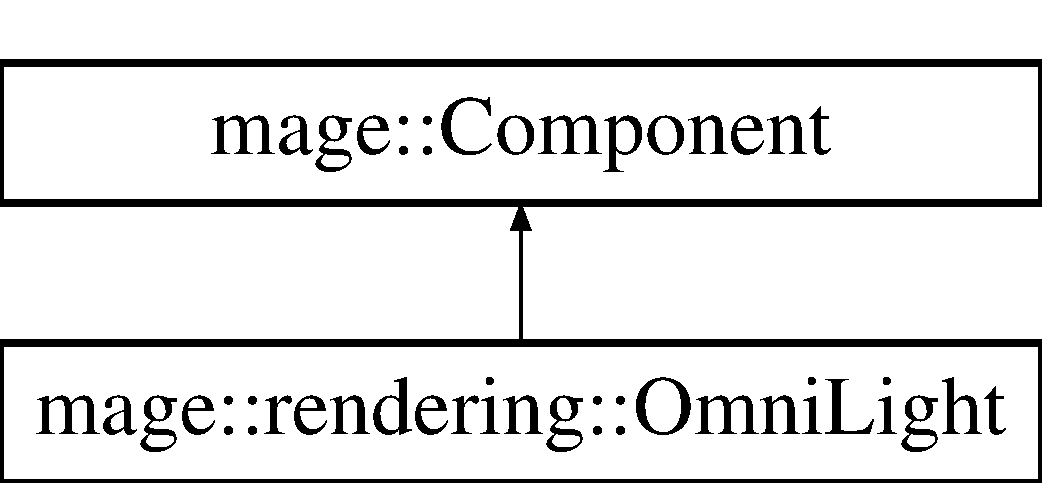
\includegraphics[height=2.000000cm]{classmage_1_1rendering_1_1_omni_light}
\end{center}
\end{figure}
\subsection*{Public Member Functions}
\begin{DoxyCompactItemize}
\item 
\mbox{\hyperlink{classmage_1_1rendering_1_1_omni_light_a641472ade99dc84b6e82e3d01d8b574a}{Omni\+Light}} () noexcept
\item 
\mbox{\hyperlink{classmage_1_1rendering_1_1_omni_light_adc27e555c730dbe8891e6ac4eb9d3900}{Omni\+Light}} (const \mbox{\hyperlink{classmage_1_1rendering_1_1_omni_light}{Omni\+Light}} \&light) noexcept
\item 
\mbox{\hyperlink{classmage_1_1rendering_1_1_omni_light_a235afcf044e62a3f6672316eb8f3cd99}{Omni\+Light}} (\mbox{\hyperlink{classmage_1_1rendering_1_1_omni_light}{Omni\+Light}} \&\&light) noexcept
\item 
virtual \mbox{\hyperlink{classmage_1_1rendering_1_1_omni_light_af0981e056620d3f0df827098448c8052}{$\sim$\+Omni\+Light}} ()
\item 
\mbox{\hyperlink{classmage_1_1rendering_1_1_omni_light}{Omni\+Light}} \& \mbox{\hyperlink{classmage_1_1rendering_1_1_omni_light_aac914061f6798131e7f59275b4716b48}{operator=}} (const \mbox{\hyperlink{classmage_1_1rendering_1_1_omni_light}{Omni\+Light}} \&light) noexcept
\item 
\mbox{\hyperlink{classmage_1_1rendering_1_1_omni_light}{Omni\+Light}} \& \mbox{\hyperlink{classmage_1_1rendering_1_1_omni_light_a8126d5d0d3a45d0063c3fd2f28e3826e}{operator=}} (\mbox{\hyperlink{classmage_1_1rendering_1_1_omni_light}{Omni\+Light}} \&\&light) noexcept
\item 
\mbox{\hyperlink{structmage_1_1_r_g_b}{R\+GB}} \& \mbox{\hyperlink{classmage_1_1rendering_1_1_omni_light_a408bde4df7fd40750cb0e4dd4d2f6d1a}{Get\+Base\+Color}} () noexcept
\item 
const \mbox{\hyperlink{structmage_1_1_r_g_b}{R\+GB}} \& \mbox{\hyperlink{classmage_1_1rendering_1_1_omni_light_a6c68ed32167890c1b0f01130c610c3e2}{Get\+Base\+Color}} () const noexcept
\item 
\mbox{\hyperlink{namespacemage_aa97e833b45f06d60a0a9c4fc22ae02c0}{F32}} \mbox{\hyperlink{classmage_1_1rendering_1_1_omni_light_a43c6be5649668705ffb1ace363960b00}{Get\+Power}} () const noexcept
\item 
void \mbox{\hyperlink{classmage_1_1rendering_1_1_omni_light_a1887bf9c7f732188814b34f686638443}{Set\+Power}} (\mbox{\hyperlink{namespacemage_aa97e833b45f06d60a0a9c4fc22ae02c0}{F32}} power) noexcept
\item 
const \mbox{\hyperlink{structmage_1_1_r_g_b}{R\+GB}} \mbox{\hyperlink{classmage_1_1rendering_1_1_omni_light_a82366151b99cc4791d8b361331f75833}{Get\+Power\+Spectrum}} () const noexcept
\item 
\mbox{\hyperlink{namespacemage_aa97e833b45f06d60a0a9c4fc22ae02c0}{F32}} \mbox{\hyperlink{classmage_1_1rendering_1_1_omni_light_ada51f74cdcf61ff29049d0a1fdf973c9}{Get\+Intensity}} () const noexcept
\item 
void \mbox{\hyperlink{classmage_1_1rendering_1_1_omni_light_aa2a936678bde1f957fd70207d2460d06}{Set\+Intensity}} (\mbox{\hyperlink{namespacemage_aa97e833b45f06d60a0a9c4fc22ae02c0}{F32}} intensity) noexcept
\item 
const \mbox{\hyperlink{structmage_1_1_r_g_b}{R\+GB}} \mbox{\hyperlink{classmage_1_1rendering_1_1_omni_light_a62247b6d7c2029ab906492049e858538}{Get\+Intensity\+Spectrum}} () const noexcept
\item 
const \mbox{\hyperlink{classmage_1_1_a_a_b_b}{A\+A\+BB}} \& \mbox{\hyperlink{classmage_1_1rendering_1_1_omni_light_aa3408de0d62c39d09e0b5aaccf61406a}{Get\+A\+A\+BB}} () const noexcept
\item 
const \mbox{\hyperlink{classmage_1_1_bounding_sphere}{Bounding\+Sphere}} \& \mbox{\hyperlink{classmage_1_1rendering_1_1_omni_light_aaecee74a14aae5015f8bc738727162ee}{Get\+Bounding\+Sphere}} () const noexcept
\item 
\mbox{\hyperlink{namespacemage_aa97e833b45f06d60a0a9c4fc22ae02c0}{F32}} \mbox{\hyperlink{classmage_1_1rendering_1_1_omni_light_af9bfc4b943b156756cd7c2323d93ebdd}{Get\+Range}} () const noexcept
\item 
\mbox{\hyperlink{namespacemage_aa97e833b45f06d60a0a9c4fc22ae02c0}{F32}} \mbox{\hyperlink{classmage_1_1rendering_1_1_omni_light_a7be27af3b3e5d11806396ce8f619223f}{Get\+World\+Range}} () const noexcept
\item 
void \mbox{\hyperlink{classmage_1_1rendering_1_1_omni_light_a71d9cbef05c421a154b202e7a9b8eedb}{Set\+Range}} (\mbox{\hyperlink{namespacemage_aa97e833b45f06d60a0a9c4fc22ae02c0}{F32}} range) noexcept
\item 
bool \mbox{\hyperlink{classmage_1_1rendering_1_1_omni_light_a7b4bd4cdd980feb3d841fff5947720e9}{Use\+Shadows}} () const noexcept
\item 
void \mbox{\hyperlink{classmage_1_1rendering_1_1_omni_light_a676a457b4e79b7dc74696acc713a9230}{Enable\+Shadows}} () noexcept
\item 
void \mbox{\hyperlink{classmage_1_1rendering_1_1_omni_light_a18eaf3b2683997854827b12ec26c9039}{Dissable\+Shadows}} () noexcept
\item 
void \mbox{\hyperlink{classmage_1_1rendering_1_1_omni_light_aa1816fad8913711c10994b66103279a2}{Toggle\+Shadows}} () noexcept
\item 
void \mbox{\hyperlink{classmage_1_1rendering_1_1_omni_light_a2817ab7a4c514785f01bf2e40c6245cb}{Set\+Shadows}} (bool shadows) noexcept
\item 
const \mbox{\hyperlink{namespacemage_aee4759dedc8def6c6dec26b5c7eddf29}{F32x2}} \mbox{\hyperlink{classmage_1_1rendering_1_1_omni_light_a30b6cbf1fd7a6058856a491c2ce75005}{Get\+Clipping\+Planes}} () const noexcept
\item 
void \mbox{\hyperlink{classmage_1_1rendering_1_1_omni_light_af1334671baf6f5afeb297fb819118639}{Set\+Clipping\+Planes}} (\mbox{\hyperlink{namespacemage_aee4759dedc8def6c6dec26b5c7eddf29}{F32x2}} clipping\+\_\+planes) noexcept
\item 
const X\+M\+M\+A\+T\+R\+IX X\+M\+\_\+\+C\+A\+L\+L\+C\+O\+NV \mbox{\hyperlink{classmage_1_1rendering_1_1_omni_light_aa93d9722b3480fc9997761af89a6d90d}{Get\+Light\+To\+Projection\+Matrix}} () const noexcept
\end{DoxyCompactItemize}
\subsection*{Private Member Functions}
\begin{DoxyCompactItemize}
\item 
void \mbox{\hyperlink{classmage_1_1rendering_1_1_omni_light_a44c6dee7d24c879aab0284ac21910337}{Update\+Bounding\+Volumes}} () noexcept
\end{DoxyCompactItemize}
\subsection*{Private Attributes}
\begin{DoxyCompactItemize}
\item 
bool \mbox{\hyperlink{classmage_1_1rendering_1_1_omni_light_af0cb508d0333f86cf64c28f5628177d4}{m\+\_\+shadows}}
\item 
\mbox{\hyperlink{namespacemage_aee4759dedc8def6c6dec26b5c7eddf29}{F32x2}} \mbox{\hyperlink{classmage_1_1rendering_1_1_omni_light_a725388093feb1e5ed2ebce4f70c1729b}{m\+\_\+clipping\+\_\+planes}}
\item 
\mbox{\hyperlink{classmage_1_1_a_a_b_b}{A\+A\+BB}} \mbox{\hyperlink{classmage_1_1rendering_1_1_omni_light_ac2b5bb2e28364445c7bce70c8fa1374e}{m\+\_\+aabb}}
\item 
\mbox{\hyperlink{classmage_1_1_bounding_sphere}{Bounding\+Sphere}} \mbox{\hyperlink{classmage_1_1rendering_1_1_omni_light_af11a99e2b1500093b9bd0e3ff16b04e6}{m\+\_\+sphere}}
\item 
\mbox{\hyperlink{structmage_1_1_r_g_b}{R\+GB}} \mbox{\hyperlink{classmage_1_1rendering_1_1_omni_light_ac5aca97b5729d9c0856ed08f64976edf}{m\+\_\+base\+\_\+color}}
\item 
\mbox{\hyperlink{namespacemage_aa97e833b45f06d60a0a9c4fc22ae02c0}{F32}} \mbox{\hyperlink{classmage_1_1rendering_1_1_omni_light_af7ba6e05e5809d16ec070a2b2de47a62}{m\+\_\+intensity}}
\end{DoxyCompactItemize}
\subsection*{Additional Inherited Members}


\subsection{Detailed Description}
A class of omni lights. 

\subsection{Constructor \& Destructor Documentation}
\mbox{\Hypertarget{classmage_1_1rendering_1_1_omni_light_a641472ade99dc84b6e82e3d01d8b574a}\label{classmage_1_1rendering_1_1_omni_light_a641472ade99dc84b6e82e3d01d8b574a}} 
\index{mage\+::rendering\+::\+Omni\+Light@{mage\+::rendering\+::\+Omni\+Light}!Omni\+Light@{Omni\+Light}}
\index{Omni\+Light@{Omni\+Light}!mage\+::rendering\+::\+Omni\+Light@{mage\+::rendering\+::\+Omni\+Light}}
\subsubsection{\texorpdfstring{Omni\+Light()}{OmniLight()}\hspace{0.1cm}{\footnotesize\ttfamily [1/3]}}
{\footnotesize\ttfamily mage\+::rendering\+::\+Omni\+Light\+::\+Omni\+Light (\begin{DoxyParamCaption}{ }\end{DoxyParamCaption})\hspace{0.3cm}{\ttfamily [noexcept]}}

Constructs an omni light. \mbox{\Hypertarget{classmage_1_1rendering_1_1_omni_light_adc27e555c730dbe8891e6ac4eb9d3900}\label{classmage_1_1rendering_1_1_omni_light_adc27e555c730dbe8891e6ac4eb9d3900}} 
\index{mage\+::rendering\+::\+Omni\+Light@{mage\+::rendering\+::\+Omni\+Light}!Omni\+Light@{Omni\+Light}}
\index{Omni\+Light@{Omni\+Light}!mage\+::rendering\+::\+Omni\+Light@{mage\+::rendering\+::\+Omni\+Light}}
\subsubsection{\texorpdfstring{Omni\+Light()}{OmniLight()}\hspace{0.1cm}{\footnotesize\ttfamily [2/3]}}
{\footnotesize\ttfamily mage\+::rendering\+::\+Omni\+Light\+::\+Omni\+Light (\begin{DoxyParamCaption}\item[{const \mbox{\hyperlink{classmage_1_1rendering_1_1_omni_light}{Omni\+Light}} \&}]{light }\end{DoxyParamCaption})\hspace{0.3cm}{\ttfamily [default]}, {\ttfamily [noexcept]}}

Constructs an omni light from the given omni light.


\begin{DoxyParams}[1]{Parameters}
\mbox{\tt in}  & {\em light} & A reference to the omni light to copy. \\
\hline
\end{DoxyParams}
\mbox{\Hypertarget{classmage_1_1rendering_1_1_omni_light_a235afcf044e62a3f6672316eb8f3cd99}\label{classmage_1_1rendering_1_1_omni_light_a235afcf044e62a3f6672316eb8f3cd99}} 
\index{mage\+::rendering\+::\+Omni\+Light@{mage\+::rendering\+::\+Omni\+Light}!Omni\+Light@{Omni\+Light}}
\index{Omni\+Light@{Omni\+Light}!mage\+::rendering\+::\+Omni\+Light@{mage\+::rendering\+::\+Omni\+Light}}
\subsubsection{\texorpdfstring{Omni\+Light()}{OmniLight()}\hspace{0.1cm}{\footnotesize\ttfamily [3/3]}}
{\footnotesize\ttfamily mage\+::rendering\+::\+Omni\+Light\+::\+Omni\+Light (\begin{DoxyParamCaption}\item[{\mbox{\hyperlink{classmage_1_1rendering_1_1_omni_light}{Omni\+Light}} \&\&}]{light }\end{DoxyParamCaption})\hspace{0.3cm}{\ttfamily [default]}, {\ttfamily [noexcept]}}

Constructs an omni light by moving the given omni light.


\begin{DoxyParams}[1]{Parameters}
\mbox{\tt in}  & {\em light} & A reference to the omni light to move. \\
\hline
\end{DoxyParams}
\mbox{\Hypertarget{classmage_1_1rendering_1_1_omni_light_af0981e056620d3f0df827098448c8052}\label{classmage_1_1rendering_1_1_omni_light_af0981e056620d3f0df827098448c8052}} 
\index{mage\+::rendering\+::\+Omni\+Light@{mage\+::rendering\+::\+Omni\+Light}!````~Omni\+Light@{$\sim$\+Omni\+Light}}
\index{````~Omni\+Light@{$\sim$\+Omni\+Light}!mage\+::rendering\+::\+Omni\+Light@{mage\+::rendering\+::\+Omni\+Light}}
\subsubsection{\texorpdfstring{$\sim$\+Omni\+Light()}{~OmniLight()}}
{\footnotesize\ttfamily mage\+::rendering\+::\+Omni\+Light\+::$\sim$\+Omni\+Light (\begin{DoxyParamCaption}{ }\end{DoxyParamCaption})\hspace{0.3cm}{\ttfamily [virtual]}, {\ttfamily [default]}}

Destructs this omni light. 

\subsection{Member Function Documentation}
\mbox{\Hypertarget{classmage_1_1rendering_1_1_omni_light_a18eaf3b2683997854827b12ec26c9039}\label{classmage_1_1rendering_1_1_omni_light_a18eaf3b2683997854827b12ec26c9039}} 
\index{mage\+::rendering\+::\+Omni\+Light@{mage\+::rendering\+::\+Omni\+Light}!Dissable\+Shadows@{Dissable\+Shadows}}
\index{Dissable\+Shadows@{Dissable\+Shadows}!mage\+::rendering\+::\+Omni\+Light@{mage\+::rendering\+::\+Omni\+Light}}
\subsubsection{\texorpdfstring{Dissable\+Shadows()}{DissableShadows()}}
{\footnotesize\ttfamily void mage\+::rendering\+::\+Omni\+Light\+::\+Dissable\+Shadows (\begin{DoxyParamCaption}{ }\end{DoxyParamCaption})\hspace{0.3cm}{\ttfamily [noexcept]}}

Dissables shadows for this omni light. \mbox{\Hypertarget{classmage_1_1rendering_1_1_omni_light_a676a457b4e79b7dc74696acc713a9230}\label{classmage_1_1rendering_1_1_omni_light_a676a457b4e79b7dc74696acc713a9230}} 
\index{mage\+::rendering\+::\+Omni\+Light@{mage\+::rendering\+::\+Omni\+Light}!Enable\+Shadows@{Enable\+Shadows}}
\index{Enable\+Shadows@{Enable\+Shadows}!mage\+::rendering\+::\+Omni\+Light@{mage\+::rendering\+::\+Omni\+Light}}
\subsubsection{\texorpdfstring{Enable\+Shadows()}{EnableShadows()}}
{\footnotesize\ttfamily void mage\+::rendering\+::\+Omni\+Light\+::\+Enable\+Shadows (\begin{DoxyParamCaption}{ }\end{DoxyParamCaption})\hspace{0.3cm}{\ttfamily [noexcept]}}

Enables shadows for this omni light. \mbox{\Hypertarget{classmage_1_1rendering_1_1_omni_light_aa3408de0d62c39d09e0b5aaccf61406a}\label{classmage_1_1rendering_1_1_omni_light_aa3408de0d62c39d09e0b5aaccf61406a}} 
\index{mage\+::rendering\+::\+Omni\+Light@{mage\+::rendering\+::\+Omni\+Light}!Get\+A\+A\+BB@{Get\+A\+A\+BB}}
\index{Get\+A\+A\+BB@{Get\+A\+A\+BB}!mage\+::rendering\+::\+Omni\+Light@{mage\+::rendering\+::\+Omni\+Light}}
\subsubsection{\texorpdfstring{Get\+A\+A\+B\+B()}{GetAABB()}}
{\footnotesize\ttfamily const \mbox{\hyperlink{classmage_1_1_a_a_b_b}{A\+A\+BB}}\& mage\+::rendering\+::\+Omni\+Light\+::\+Get\+A\+A\+BB (\begin{DoxyParamCaption}{ }\end{DoxyParamCaption}) const\hspace{0.3cm}{\ttfamily [noexcept]}}

Returns the \mbox{\hyperlink{classmage_1_1_a_a_b_b}{A\+A\+BB}} of this omni light.

\begin{DoxyReturn}{Returns}
A reference to the \mbox{\hyperlink{classmage_1_1_a_a_b_b}{A\+A\+BB}} of this omni light. 
\end{DoxyReturn}
\mbox{\Hypertarget{classmage_1_1rendering_1_1_omni_light_a408bde4df7fd40750cb0e4dd4d2f6d1a}\label{classmage_1_1rendering_1_1_omni_light_a408bde4df7fd40750cb0e4dd4d2f6d1a}} 
\index{mage\+::rendering\+::\+Omni\+Light@{mage\+::rendering\+::\+Omni\+Light}!Get\+Base\+Color@{Get\+Base\+Color}}
\index{Get\+Base\+Color@{Get\+Base\+Color}!mage\+::rendering\+::\+Omni\+Light@{mage\+::rendering\+::\+Omni\+Light}}
\subsubsection{\texorpdfstring{Get\+Base\+Color()}{GetBaseColor()}\hspace{0.1cm}{\footnotesize\ttfamily [1/2]}}
{\footnotesize\ttfamily \mbox{\hyperlink{structmage_1_1_r_g_b}{R\+GB}}\& mage\+::rendering\+::\+Omni\+Light\+::\+Get\+Base\+Color (\begin{DoxyParamCaption}{ }\end{DoxyParamCaption})\hspace{0.3cm}{\ttfamily [noexcept]}}

Returns the (linear) \mbox{\hyperlink{structmage_1_1_r_g_b}{R\+GB}} base color of this spotlight.

\begin{DoxyReturn}{Returns}
A reference to the (linear) base color of this spotlight. 
\end{DoxyReturn}
\mbox{\Hypertarget{classmage_1_1rendering_1_1_omni_light_a6c68ed32167890c1b0f01130c610c3e2}\label{classmage_1_1rendering_1_1_omni_light_a6c68ed32167890c1b0f01130c610c3e2}} 
\index{mage\+::rendering\+::\+Omni\+Light@{mage\+::rendering\+::\+Omni\+Light}!Get\+Base\+Color@{Get\+Base\+Color}}
\index{Get\+Base\+Color@{Get\+Base\+Color}!mage\+::rendering\+::\+Omni\+Light@{mage\+::rendering\+::\+Omni\+Light}}
\subsubsection{\texorpdfstring{Get\+Base\+Color()}{GetBaseColor()}\hspace{0.1cm}{\footnotesize\ttfamily [2/2]}}
{\footnotesize\ttfamily const \mbox{\hyperlink{structmage_1_1_r_g_b}{R\+GB}}\& mage\+::rendering\+::\+Omni\+Light\+::\+Get\+Base\+Color (\begin{DoxyParamCaption}{ }\end{DoxyParamCaption}) const\hspace{0.3cm}{\ttfamily [noexcept]}}

Returns the (linear) base color of this spotlight.

\begin{DoxyReturn}{Returns}
A reference to the (linear) base color of this spotlight. 
\end{DoxyReturn}
\mbox{\Hypertarget{classmage_1_1rendering_1_1_omni_light_aaecee74a14aae5015f8bc738727162ee}\label{classmage_1_1rendering_1_1_omni_light_aaecee74a14aae5015f8bc738727162ee}} 
\index{mage\+::rendering\+::\+Omni\+Light@{mage\+::rendering\+::\+Omni\+Light}!Get\+Bounding\+Sphere@{Get\+Bounding\+Sphere}}
\index{Get\+Bounding\+Sphere@{Get\+Bounding\+Sphere}!mage\+::rendering\+::\+Omni\+Light@{mage\+::rendering\+::\+Omni\+Light}}
\subsubsection{\texorpdfstring{Get\+Bounding\+Sphere()}{GetBoundingSphere()}}
{\footnotesize\ttfamily const \mbox{\hyperlink{classmage_1_1_bounding_sphere}{Bounding\+Sphere}}\& mage\+::rendering\+::\+Omni\+Light\+::\+Get\+Bounding\+Sphere (\begin{DoxyParamCaption}{ }\end{DoxyParamCaption}) const\hspace{0.3cm}{\ttfamily [noexcept]}}

Returns the \mbox{\hyperlink{classmage_1_1_bounding_sphere}{Bounding\+Sphere}} of this omni light.

\begin{DoxyReturn}{Returns}
A reference to the \mbox{\hyperlink{classmage_1_1_bounding_sphere}{Bounding\+Sphere}} of this omni light. 
\end{DoxyReturn}
\mbox{\Hypertarget{classmage_1_1rendering_1_1_omni_light_a30b6cbf1fd7a6058856a491c2ce75005}\label{classmage_1_1rendering_1_1_omni_light_a30b6cbf1fd7a6058856a491c2ce75005}} 
\index{mage\+::rendering\+::\+Omni\+Light@{mage\+::rendering\+::\+Omni\+Light}!Get\+Clipping\+Planes@{Get\+Clipping\+Planes}}
\index{Get\+Clipping\+Planes@{Get\+Clipping\+Planes}!mage\+::rendering\+::\+Omni\+Light@{mage\+::rendering\+::\+Omni\+Light}}
\subsubsection{\texorpdfstring{Get\+Clipping\+Planes()}{GetClippingPlanes()}}
{\footnotesize\ttfamily const \mbox{\hyperlink{namespacemage_aee4759dedc8def6c6dec26b5c7eddf29}{F32x2}} mage\+::rendering\+::\+Omni\+Light\+::\+Get\+Clipping\+Planes (\begin{DoxyParamCaption}{ }\end{DoxyParamCaption}) const\hspace{0.3cm}{\ttfamily [noexcept]}}

Returns the clipping planes of this omni light expressed in light space.

\begin{DoxyReturn}{Returns}
The clipping planes of this omni light expressed in light space. 
\end{DoxyReturn}
\mbox{\Hypertarget{classmage_1_1rendering_1_1_omni_light_ada51f74cdcf61ff29049d0a1fdf973c9}\label{classmage_1_1rendering_1_1_omni_light_ada51f74cdcf61ff29049d0a1fdf973c9}} 
\index{mage\+::rendering\+::\+Omni\+Light@{mage\+::rendering\+::\+Omni\+Light}!Get\+Intensity@{Get\+Intensity}}
\index{Get\+Intensity@{Get\+Intensity}!mage\+::rendering\+::\+Omni\+Light@{mage\+::rendering\+::\+Omni\+Light}}
\subsubsection{\texorpdfstring{Get\+Intensity()}{GetIntensity()}}
{\footnotesize\ttfamily \mbox{\hyperlink{namespacemage_aa97e833b45f06d60a0a9c4fc22ae02c0}{F32}} mage\+::rendering\+::\+Omni\+Light\+::\+Get\+Intensity (\begin{DoxyParamCaption}{ }\end{DoxyParamCaption}) const\hspace{0.3cm}{\ttfamily [noexcept]}}

Returns the radiant intensity of this omni light.

\begin{DoxyReturn}{Returns}
The radiant intensity in watts per steradians of this omni light. 
\end{DoxyReturn}
\mbox{\Hypertarget{classmage_1_1rendering_1_1_omni_light_a62247b6d7c2029ab906492049e858538}\label{classmage_1_1rendering_1_1_omni_light_a62247b6d7c2029ab906492049e858538}} 
\index{mage\+::rendering\+::\+Omni\+Light@{mage\+::rendering\+::\+Omni\+Light}!Get\+Intensity\+Spectrum@{Get\+Intensity\+Spectrum}}
\index{Get\+Intensity\+Spectrum@{Get\+Intensity\+Spectrum}!mage\+::rendering\+::\+Omni\+Light@{mage\+::rendering\+::\+Omni\+Light}}
\subsubsection{\texorpdfstring{Get\+Intensity\+Spectrum()}{GetIntensitySpectrum()}}
{\footnotesize\ttfamily const \mbox{\hyperlink{structmage_1_1_r_g_b}{R\+GB}} mage\+::rendering\+::\+Omni\+Light\+::\+Get\+Intensity\+Spectrum (\begin{DoxyParamCaption}{ }\end{DoxyParamCaption}) const\hspace{0.3cm}{\ttfamily [noexcept]}}

Returns the radiant intensity spectrum of this omni light.

\begin{DoxyReturn}{Returns}
The radiant intensity spectrum of this omni light. 
\end{DoxyReturn}
\mbox{\Hypertarget{classmage_1_1rendering_1_1_omni_light_aa93d9722b3480fc9997761af89a6d90d}\label{classmage_1_1rendering_1_1_omni_light_aa93d9722b3480fc9997761af89a6d90d}} 
\index{mage\+::rendering\+::\+Omni\+Light@{mage\+::rendering\+::\+Omni\+Light}!Get\+Light\+To\+Projection\+Matrix@{Get\+Light\+To\+Projection\+Matrix}}
\index{Get\+Light\+To\+Projection\+Matrix@{Get\+Light\+To\+Projection\+Matrix}!mage\+::rendering\+::\+Omni\+Light@{mage\+::rendering\+::\+Omni\+Light}}
\subsubsection{\texorpdfstring{Get\+Light\+To\+Projection\+Matrix()}{GetLightToProjectionMatrix()}}
{\footnotesize\ttfamily const X\+M\+M\+A\+T\+R\+IX X\+M\+\_\+\+C\+A\+L\+L\+C\+O\+NV mage\+::rendering\+::\+Omni\+Light\+::\+Get\+Light\+To\+Projection\+Matrix (\begin{DoxyParamCaption}{ }\end{DoxyParamCaption}) const\hspace{0.3cm}{\ttfamily [noexcept]}}

Returns the light-\/to-\/projection matrix of the (forward) light camera of this omni light.

\begin{DoxyReturn}{Returns}
The light-\/to-\/projection matrix of the (forward) light camera of this omni light. 
\end{DoxyReturn}
\mbox{\Hypertarget{classmage_1_1rendering_1_1_omni_light_a43c6be5649668705ffb1ace363960b00}\label{classmage_1_1rendering_1_1_omni_light_a43c6be5649668705ffb1ace363960b00}} 
\index{mage\+::rendering\+::\+Omni\+Light@{mage\+::rendering\+::\+Omni\+Light}!Get\+Power@{Get\+Power}}
\index{Get\+Power@{Get\+Power}!mage\+::rendering\+::\+Omni\+Light@{mage\+::rendering\+::\+Omni\+Light}}
\subsubsection{\texorpdfstring{Get\+Power()}{GetPower()}}
{\footnotesize\ttfamily \mbox{\hyperlink{namespacemage_aa97e833b45f06d60a0a9c4fc22ae02c0}{F32}} mage\+::rendering\+::\+Omni\+Light\+::\+Get\+Power (\begin{DoxyParamCaption}{ }\end{DoxyParamCaption}) const\hspace{0.3cm}{\ttfamily [noexcept]}}

Returns the power of this omni light.

\begin{DoxyReturn}{Returns}
The power in watts of this omni light. 
\end{DoxyReturn}
\mbox{\Hypertarget{classmage_1_1rendering_1_1_omni_light_a82366151b99cc4791d8b361331f75833}\label{classmage_1_1rendering_1_1_omni_light_a82366151b99cc4791d8b361331f75833}} 
\index{mage\+::rendering\+::\+Omni\+Light@{mage\+::rendering\+::\+Omni\+Light}!Get\+Power\+Spectrum@{Get\+Power\+Spectrum}}
\index{Get\+Power\+Spectrum@{Get\+Power\+Spectrum}!mage\+::rendering\+::\+Omni\+Light@{mage\+::rendering\+::\+Omni\+Light}}
\subsubsection{\texorpdfstring{Get\+Power\+Spectrum()}{GetPowerSpectrum()}}
{\footnotesize\ttfamily const \mbox{\hyperlink{structmage_1_1_r_g_b}{R\+GB}} mage\+::rendering\+::\+Omni\+Light\+::\+Get\+Power\+Spectrum (\begin{DoxyParamCaption}{ }\end{DoxyParamCaption}) const\hspace{0.3cm}{\ttfamily [noexcept]}}

Returns the power spectrum of this omni light.

\begin{DoxyReturn}{Returns}
The power spectrum of this omni light. 
\end{DoxyReturn}
\mbox{\Hypertarget{classmage_1_1rendering_1_1_omni_light_af9bfc4b943b156756cd7c2323d93ebdd}\label{classmage_1_1rendering_1_1_omni_light_af9bfc4b943b156756cd7c2323d93ebdd}} 
\index{mage\+::rendering\+::\+Omni\+Light@{mage\+::rendering\+::\+Omni\+Light}!Get\+Range@{Get\+Range}}
\index{Get\+Range@{Get\+Range}!mage\+::rendering\+::\+Omni\+Light@{mage\+::rendering\+::\+Omni\+Light}}
\subsubsection{\texorpdfstring{Get\+Range()}{GetRange()}}
{\footnotesize\ttfamily \mbox{\hyperlink{namespacemage_aa97e833b45f06d60a0a9c4fc22ae02c0}{F32}} mage\+::rendering\+::\+Omni\+Light\+::\+Get\+Range (\begin{DoxyParamCaption}{ }\end{DoxyParamCaption}) const\hspace{0.3cm}{\ttfamily [noexcept]}}

Returns the range of this omni light expressed in light space.

\begin{DoxyReturn}{Returns}
The range of this omni light expressed in light space. 
\end{DoxyReturn}
\mbox{\Hypertarget{classmage_1_1rendering_1_1_omni_light_a7be27af3b3e5d11806396ce8f619223f}\label{classmage_1_1rendering_1_1_omni_light_a7be27af3b3e5d11806396ce8f619223f}} 
\index{mage\+::rendering\+::\+Omni\+Light@{mage\+::rendering\+::\+Omni\+Light}!Get\+World\+Range@{Get\+World\+Range}}
\index{Get\+World\+Range@{Get\+World\+Range}!mage\+::rendering\+::\+Omni\+Light@{mage\+::rendering\+::\+Omni\+Light}}
\subsubsection{\texorpdfstring{Get\+World\+Range()}{GetWorldRange()}}
{\footnotesize\ttfamily \mbox{\hyperlink{namespacemage_aa97e833b45f06d60a0a9c4fc22ae02c0}{F32}} mage\+::rendering\+::\+Omni\+Light\+::\+Get\+World\+Range (\begin{DoxyParamCaption}{ }\end{DoxyParamCaption}) const\hspace{0.3cm}{\ttfamily [noexcept]}}

Returns the range of this omni light expressed in world space.

\begin{DoxyReturn}{Returns}
The range of this omni light expressed in world space. 
\end{DoxyReturn}
\begin{DoxyNote}{Note}
Non-\/uniform scaling is not supported for omni lights. 
\end{DoxyNote}
\mbox{\Hypertarget{classmage_1_1rendering_1_1_omni_light_aac914061f6798131e7f59275b4716b48}\label{classmage_1_1rendering_1_1_omni_light_aac914061f6798131e7f59275b4716b48}} 
\index{mage\+::rendering\+::\+Omni\+Light@{mage\+::rendering\+::\+Omni\+Light}!operator=@{operator=}}
\index{operator=@{operator=}!mage\+::rendering\+::\+Omni\+Light@{mage\+::rendering\+::\+Omni\+Light}}
\subsubsection{\texorpdfstring{operator=()}{operator=()}\hspace{0.1cm}{\footnotesize\ttfamily [1/2]}}
{\footnotesize\ttfamily \mbox{\hyperlink{classmage_1_1rendering_1_1_omni_light}{Omni\+Light}} \& mage\+::rendering\+::\+Omni\+Light\+::operator= (\begin{DoxyParamCaption}\item[{const \mbox{\hyperlink{classmage_1_1rendering_1_1_omni_light}{Omni\+Light}} \&}]{light }\end{DoxyParamCaption})\hspace{0.3cm}{\ttfamily [default]}, {\ttfamily [noexcept]}}

Copies the given omni light to this omni light.


\begin{DoxyParams}[1]{Parameters}
\mbox{\tt in}  & {\em light} & A reference to the omni light to copy. \\
\hline
\end{DoxyParams}
\begin{DoxyReturn}{Returns}
A reference to the copy of the given omni light (i.\+e. this omni light). 
\end{DoxyReturn}
\mbox{\Hypertarget{classmage_1_1rendering_1_1_omni_light_a8126d5d0d3a45d0063c3fd2f28e3826e}\label{classmage_1_1rendering_1_1_omni_light_a8126d5d0d3a45d0063c3fd2f28e3826e}} 
\index{mage\+::rendering\+::\+Omni\+Light@{mage\+::rendering\+::\+Omni\+Light}!operator=@{operator=}}
\index{operator=@{operator=}!mage\+::rendering\+::\+Omni\+Light@{mage\+::rendering\+::\+Omni\+Light}}
\subsubsection{\texorpdfstring{operator=()}{operator=()}\hspace{0.1cm}{\footnotesize\ttfamily [2/2]}}
{\footnotesize\ttfamily \mbox{\hyperlink{classmage_1_1rendering_1_1_omni_light}{Omni\+Light}} \& mage\+::rendering\+::\+Omni\+Light\+::operator= (\begin{DoxyParamCaption}\item[{\mbox{\hyperlink{classmage_1_1rendering_1_1_omni_light}{Omni\+Light}} \&\&}]{light }\end{DoxyParamCaption})\hspace{0.3cm}{\ttfamily [default]}, {\ttfamily [noexcept]}}

Moves the given omni light to this omni light.


\begin{DoxyParams}[1]{Parameters}
\mbox{\tt in}  & {\em light} & A reference to the omni light to move. \\
\hline
\end{DoxyParams}
\begin{DoxyReturn}{Returns}
A reference to the moved omni light (i.\+e. this omni light). 
\end{DoxyReturn}
\mbox{\Hypertarget{classmage_1_1rendering_1_1_omni_light_af1334671baf6f5afeb297fb819118639}\label{classmage_1_1rendering_1_1_omni_light_af1334671baf6f5afeb297fb819118639}} 
\index{mage\+::rendering\+::\+Omni\+Light@{mage\+::rendering\+::\+Omni\+Light}!Set\+Clipping\+Planes@{Set\+Clipping\+Planes}}
\index{Set\+Clipping\+Planes@{Set\+Clipping\+Planes}!mage\+::rendering\+::\+Omni\+Light@{mage\+::rendering\+::\+Omni\+Light}}
\subsubsection{\texorpdfstring{Set\+Clipping\+Planes()}{SetClippingPlanes()}}
{\footnotesize\ttfamily void mage\+::rendering\+::\+Omni\+Light\+::\+Set\+Clipping\+Planes (\begin{DoxyParamCaption}\item[{\mbox{\hyperlink{namespacemage_aee4759dedc8def6c6dec26b5c7eddf29}{F32x2}}}]{clipping\+\_\+planes }\end{DoxyParamCaption})\hspace{0.3cm}{\ttfamily [noexcept]}}

Sets the clipping planes of this omni light expressed in light space to the given clipping planes.


\begin{DoxyParams}[1]{Parameters}
\mbox{\tt in}  & {\em clipping\+\_\+planes} & The clipping planes. \\
\hline
\end{DoxyParams}
\mbox{\Hypertarget{classmage_1_1rendering_1_1_omni_light_aa2a936678bde1f957fd70207d2460d06}\label{classmage_1_1rendering_1_1_omni_light_aa2a936678bde1f957fd70207d2460d06}} 
\index{mage\+::rendering\+::\+Omni\+Light@{mage\+::rendering\+::\+Omni\+Light}!Set\+Intensity@{Set\+Intensity}}
\index{Set\+Intensity@{Set\+Intensity}!mage\+::rendering\+::\+Omni\+Light@{mage\+::rendering\+::\+Omni\+Light}}
\subsubsection{\texorpdfstring{Set\+Intensity()}{SetIntensity()}}
{\footnotesize\ttfamily void mage\+::rendering\+::\+Omni\+Light\+::\+Set\+Intensity (\begin{DoxyParamCaption}\item[{\mbox{\hyperlink{namespacemage_aa97e833b45f06d60a0a9c4fc22ae02c0}{F32}}}]{intensity }\end{DoxyParamCaption})\hspace{0.3cm}{\ttfamily [noexcept]}}

Sets the radiant intensity of this omni light to the given radial intensity.


\begin{DoxyParams}[1]{Parameters}
\mbox{\tt in}  & {\em intensity} & The radiant intensity in watts per steradians. \\
\hline
\end{DoxyParams}
\mbox{\Hypertarget{classmage_1_1rendering_1_1_omni_light_a1887bf9c7f732188814b34f686638443}\label{classmage_1_1rendering_1_1_omni_light_a1887bf9c7f732188814b34f686638443}} 
\index{mage\+::rendering\+::\+Omni\+Light@{mage\+::rendering\+::\+Omni\+Light}!Set\+Power@{Set\+Power}}
\index{Set\+Power@{Set\+Power}!mage\+::rendering\+::\+Omni\+Light@{mage\+::rendering\+::\+Omni\+Light}}
\subsubsection{\texorpdfstring{Set\+Power()}{SetPower()}}
{\footnotesize\ttfamily void mage\+::rendering\+::\+Omni\+Light\+::\+Set\+Power (\begin{DoxyParamCaption}\item[{\mbox{\hyperlink{namespacemage_aa97e833b45f06d60a0a9c4fc22ae02c0}{F32}}}]{power }\end{DoxyParamCaption})\hspace{0.3cm}{\ttfamily [noexcept]}}

Sets the power of this omni light to the given radiance.


\begin{DoxyParams}[1]{Parameters}
\mbox{\tt in}  & {\em power} & The power in watts. \\
\hline
\end{DoxyParams}
\mbox{\Hypertarget{classmage_1_1rendering_1_1_omni_light_a71d9cbef05c421a154b202e7a9b8eedb}\label{classmage_1_1rendering_1_1_omni_light_a71d9cbef05c421a154b202e7a9b8eedb}} 
\index{mage\+::rendering\+::\+Omni\+Light@{mage\+::rendering\+::\+Omni\+Light}!Set\+Range@{Set\+Range}}
\index{Set\+Range@{Set\+Range}!mage\+::rendering\+::\+Omni\+Light@{mage\+::rendering\+::\+Omni\+Light}}
\subsubsection{\texorpdfstring{Set\+Range()}{SetRange()}}
{\footnotesize\ttfamily void mage\+::rendering\+::\+Omni\+Light\+::\+Set\+Range (\begin{DoxyParamCaption}\item[{\mbox{\hyperlink{namespacemage_aa97e833b45f06d60a0a9c4fc22ae02c0}{F32}}}]{range }\end{DoxyParamCaption})\hspace{0.3cm}{\ttfamily [noexcept]}}

Sets the range of this omni light to the given value expressed in light space.


\begin{DoxyParams}[1]{Parameters}
\mbox{\tt in}  & {\em range} & The range expressed in light space. \\
\hline
\end{DoxyParams}
\mbox{\Hypertarget{classmage_1_1rendering_1_1_omni_light_a2817ab7a4c514785f01bf2e40c6245cb}\label{classmage_1_1rendering_1_1_omni_light_a2817ab7a4c514785f01bf2e40c6245cb}} 
\index{mage\+::rendering\+::\+Omni\+Light@{mage\+::rendering\+::\+Omni\+Light}!Set\+Shadows@{Set\+Shadows}}
\index{Set\+Shadows@{Set\+Shadows}!mage\+::rendering\+::\+Omni\+Light@{mage\+::rendering\+::\+Omni\+Light}}
\subsubsection{\texorpdfstring{Set\+Shadows()}{SetShadows()}}
{\footnotesize\ttfamily void mage\+::rendering\+::\+Omni\+Light\+::\+Set\+Shadows (\begin{DoxyParamCaption}\item[{bool}]{shadows }\end{DoxyParamCaption})\hspace{0.3cm}{\ttfamily [noexcept]}}

Sets shadows for this omni light to the given value.


\begin{DoxyParams}[1]{Parameters}
\mbox{\tt in}  & {\em shadows} & {\ttfamily true} if shadows should be used for this omni light. {\ttfamily false} otherwise. \\
\hline
\end{DoxyParams}
\mbox{\Hypertarget{classmage_1_1rendering_1_1_omni_light_aa1816fad8913711c10994b66103279a2}\label{classmage_1_1rendering_1_1_omni_light_aa1816fad8913711c10994b66103279a2}} 
\index{mage\+::rendering\+::\+Omni\+Light@{mage\+::rendering\+::\+Omni\+Light}!Toggle\+Shadows@{Toggle\+Shadows}}
\index{Toggle\+Shadows@{Toggle\+Shadows}!mage\+::rendering\+::\+Omni\+Light@{mage\+::rendering\+::\+Omni\+Light}}
\subsubsection{\texorpdfstring{Toggle\+Shadows()}{ToggleShadows()}}
{\footnotesize\ttfamily void mage\+::rendering\+::\+Omni\+Light\+::\+Toggle\+Shadows (\begin{DoxyParamCaption}{ }\end{DoxyParamCaption})\hspace{0.3cm}{\ttfamily [noexcept]}}

Toggles shadows for this omni light. \mbox{\Hypertarget{classmage_1_1rendering_1_1_omni_light_a44c6dee7d24c879aab0284ac21910337}\label{classmage_1_1rendering_1_1_omni_light_a44c6dee7d24c879aab0284ac21910337}} 
\index{mage\+::rendering\+::\+Omni\+Light@{mage\+::rendering\+::\+Omni\+Light}!Update\+Bounding\+Volumes@{Update\+Bounding\+Volumes}}
\index{Update\+Bounding\+Volumes@{Update\+Bounding\+Volumes}!mage\+::rendering\+::\+Omni\+Light@{mage\+::rendering\+::\+Omni\+Light}}
\subsubsection{\texorpdfstring{Update\+Bounding\+Volumes()}{UpdateBoundingVolumes()}}
{\footnotesize\ttfamily void mage\+::rendering\+::\+Omni\+Light\+::\+Update\+Bounding\+Volumes (\begin{DoxyParamCaption}{ }\end{DoxyParamCaption})\hspace{0.3cm}{\ttfamily [private]}, {\ttfamily [noexcept]}}

Updates the bounding volumes of this omni light. \mbox{\Hypertarget{classmage_1_1rendering_1_1_omni_light_a7b4bd4cdd980feb3d841fff5947720e9}\label{classmage_1_1rendering_1_1_omni_light_a7b4bd4cdd980feb3d841fff5947720e9}} 
\index{mage\+::rendering\+::\+Omni\+Light@{mage\+::rendering\+::\+Omni\+Light}!Use\+Shadows@{Use\+Shadows}}
\index{Use\+Shadows@{Use\+Shadows}!mage\+::rendering\+::\+Omni\+Light@{mage\+::rendering\+::\+Omni\+Light}}
\subsubsection{\texorpdfstring{Use\+Shadows()}{UseShadows()}}
{\footnotesize\ttfamily bool mage\+::rendering\+::\+Omni\+Light\+::\+Use\+Shadows (\begin{DoxyParamCaption}{ }\end{DoxyParamCaption}) const\hspace{0.3cm}{\ttfamily [noexcept]}}

Checks whether shadows should be used for this omni light.

\begin{DoxyReturn}{Returns}
{\ttfamily true} if shadows should be used for this omni light. {\ttfamily false} otherwise. 
\end{DoxyReturn}


\subsection{Member Data Documentation}
\mbox{\Hypertarget{classmage_1_1rendering_1_1_omni_light_ac2b5bb2e28364445c7bce70c8fa1374e}\label{classmage_1_1rendering_1_1_omni_light_ac2b5bb2e28364445c7bce70c8fa1374e}} 
\index{mage\+::rendering\+::\+Omni\+Light@{mage\+::rendering\+::\+Omni\+Light}!m\+\_\+aabb@{m\+\_\+aabb}}
\index{m\+\_\+aabb@{m\+\_\+aabb}!mage\+::rendering\+::\+Omni\+Light@{mage\+::rendering\+::\+Omni\+Light}}
\subsubsection{\texorpdfstring{m\+\_\+aabb}{m\_aabb}}
{\footnotesize\ttfamily \mbox{\hyperlink{classmage_1_1_a_a_b_b}{A\+A\+BB}} mage\+::rendering\+::\+Omni\+Light\+::m\+\_\+aabb\hspace{0.3cm}{\ttfamily [private]}}

The \mbox{\hyperlink{classmage_1_1_a_a_b_b}{A\+A\+BB}} of this omni light. \mbox{\Hypertarget{classmage_1_1rendering_1_1_omni_light_ac5aca97b5729d9c0856ed08f64976edf}\label{classmage_1_1rendering_1_1_omni_light_ac5aca97b5729d9c0856ed08f64976edf}} 
\index{mage\+::rendering\+::\+Omni\+Light@{mage\+::rendering\+::\+Omni\+Light}!m\+\_\+base\+\_\+color@{m\+\_\+base\+\_\+color}}
\index{m\+\_\+base\+\_\+color@{m\+\_\+base\+\_\+color}!mage\+::rendering\+::\+Omni\+Light@{mage\+::rendering\+::\+Omni\+Light}}
\subsubsection{\texorpdfstring{m\+\_\+base\+\_\+color}{m\_base\_color}}
{\footnotesize\ttfamily \mbox{\hyperlink{structmage_1_1_r_g_b}{R\+GB}} mage\+::rendering\+::\+Omni\+Light\+::m\+\_\+base\+\_\+color\hspace{0.3cm}{\ttfamily [private]}}

The (linear) base color of this omni light. \mbox{\Hypertarget{classmage_1_1rendering_1_1_omni_light_a725388093feb1e5ed2ebce4f70c1729b}\label{classmage_1_1rendering_1_1_omni_light_a725388093feb1e5ed2ebce4f70c1729b}} 
\index{mage\+::rendering\+::\+Omni\+Light@{mage\+::rendering\+::\+Omni\+Light}!m\+\_\+clipping\+\_\+planes@{m\+\_\+clipping\+\_\+planes}}
\index{m\+\_\+clipping\+\_\+planes@{m\+\_\+clipping\+\_\+planes}!mage\+::rendering\+::\+Omni\+Light@{mage\+::rendering\+::\+Omni\+Light}}
\subsubsection{\texorpdfstring{m\+\_\+clipping\+\_\+planes}{m\_clipping\_planes}}
{\footnotesize\ttfamily \mbox{\hyperlink{namespacemage_aee4759dedc8def6c6dec26b5c7eddf29}{F32x2}} mage\+::rendering\+::\+Omni\+Light\+::m\+\_\+clipping\+\_\+planes\hspace{0.3cm}{\ttfamily [private]}}

The clipping planes of this omni light expressed in light space. \mbox{\Hypertarget{classmage_1_1rendering_1_1_omni_light_af7ba6e05e5809d16ec070a2b2de47a62}\label{classmage_1_1rendering_1_1_omni_light_af7ba6e05e5809d16ec070a2b2de47a62}} 
\index{mage\+::rendering\+::\+Omni\+Light@{mage\+::rendering\+::\+Omni\+Light}!m\+\_\+intensity@{m\+\_\+intensity}}
\index{m\+\_\+intensity@{m\+\_\+intensity}!mage\+::rendering\+::\+Omni\+Light@{mage\+::rendering\+::\+Omni\+Light}}
\subsubsection{\texorpdfstring{m\+\_\+intensity}{m\_intensity}}
{\footnotesize\ttfamily \mbox{\hyperlink{namespacemage_aa97e833b45f06d60a0a9c4fc22ae02c0}{F32}} mage\+::rendering\+::\+Omni\+Light\+::m\+\_\+intensity\hspace{0.3cm}{\ttfamily [private]}}

The radiant intensity in watts per steradians of this omni light. \mbox{\Hypertarget{classmage_1_1rendering_1_1_omni_light_af0cb508d0333f86cf64c28f5628177d4}\label{classmage_1_1rendering_1_1_omni_light_af0cb508d0333f86cf64c28f5628177d4}} 
\index{mage\+::rendering\+::\+Omni\+Light@{mage\+::rendering\+::\+Omni\+Light}!m\+\_\+shadows@{m\+\_\+shadows}}
\index{m\+\_\+shadows@{m\+\_\+shadows}!mage\+::rendering\+::\+Omni\+Light@{mage\+::rendering\+::\+Omni\+Light}}
\subsubsection{\texorpdfstring{m\+\_\+shadows}{m\_shadows}}
{\footnotesize\ttfamily bool mage\+::rendering\+::\+Omni\+Light\+::m\+\_\+shadows\hspace{0.3cm}{\ttfamily [private]}}

A flag indicating whether shadows should be calculated or not for this omni light. \mbox{\Hypertarget{classmage_1_1rendering_1_1_omni_light_af11a99e2b1500093b9bd0e3ff16b04e6}\label{classmage_1_1rendering_1_1_omni_light_af11a99e2b1500093b9bd0e3ff16b04e6}} 
\index{mage\+::rendering\+::\+Omni\+Light@{mage\+::rendering\+::\+Omni\+Light}!m\+\_\+sphere@{m\+\_\+sphere}}
\index{m\+\_\+sphere@{m\+\_\+sphere}!mage\+::rendering\+::\+Omni\+Light@{mage\+::rendering\+::\+Omni\+Light}}
\subsubsection{\texorpdfstring{m\+\_\+sphere}{m\_sphere}}
{\footnotesize\ttfamily \mbox{\hyperlink{classmage_1_1_bounding_sphere}{Bounding\+Sphere}} mage\+::rendering\+::\+Omni\+Light\+::m\+\_\+sphere\hspace{0.3cm}{\ttfamily [private]}}

The \mbox{\hyperlink{classmage_1_1_bounding_sphere}{Bounding\+Sphere}} of this omni light. 
\hypertarget{structmage_1_1rendering_1_1_omni_light_buffer}{}\section{mage\+:\+:rendering\+:\+:Omni\+Light\+Buffer Struct Reference}
\label{structmage_1_1rendering_1_1_omni_light_buffer}\index{mage\+::rendering\+::\+Omni\+Light\+Buffer@{mage\+::rendering\+::\+Omni\+Light\+Buffer}}


{\ttfamily \#include $<$light\+\_\+buffer.\+hpp$>$}

\subsection*{Public Member Functions}
\begin{DoxyCompactItemize}
\item 
\hyperlink{structmage_1_1rendering_1_1_omni_light_buffer_a7429503e161d324c66ecad2250bc69a2}{Omni\+Light\+Buffer} () noexcept
\item 
\hyperlink{structmage_1_1rendering_1_1_omni_light_buffer_a716417506a93d27a0093b408e88f92e4}{Omni\+Light\+Buffer} (const \hyperlink{structmage_1_1rendering_1_1_omni_light_buffer}{Omni\+Light\+Buffer} \&buffer) noexcept=default
\item 
\hyperlink{structmage_1_1rendering_1_1_omni_light_buffer_a8a1a458735f88d1dbd86590f1807c0a4}{Omni\+Light\+Buffer} (\hyperlink{structmage_1_1rendering_1_1_omni_light_buffer}{Omni\+Light\+Buffer} \&\&buffer) noexcept=default
\item 
\hyperlink{structmage_1_1rendering_1_1_omni_light_buffer_a67eee7a5d21a124ffe74cd5ae94196b6}{$\sim$\+Omni\+Light\+Buffer} ()=default
\item 
\hyperlink{structmage_1_1rendering_1_1_omni_light_buffer}{Omni\+Light\+Buffer} \& \hyperlink{structmage_1_1rendering_1_1_omni_light_buffer_a915b047abdc1068279b8308b189b60f5}{operator=} (const \hyperlink{structmage_1_1rendering_1_1_omni_light_buffer}{Omni\+Light\+Buffer} \&buffer) noexcept=default
\item 
\hyperlink{structmage_1_1rendering_1_1_omni_light_buffer}{Omni\+Light\+Buffer} \& \hyperlink{structmage_1_1rendering_1_1_omni_light_buffer_a5dc568c33ce2343aaf76c82aaaffa921}{operator=} (\hyperlink{structmage_1_1rendering_1_1_omni_light_buffer}{Omni\+Light\+Buffer} \&\&buffer) noexcept=default
\end{DoxyCompactItemize}
\subsection*{Public Attributes}
\begin{DoxyCompactItemize}
\item 
\hyperlink{structmage_1_1_point3}{Point3} \hyperlink{structmage_1_1rendering_1_1_omni_light_buffer_aab9cd7c4702a9cba7b47ec49983658d7}{m\+\_\+p}
\item 
\hyperlink{namespacemage_aa97e833b45f06d60a0a9c4fc22ae02c0}{F32} \hyperlink{structmage_1_1rendering_1_1_omni_light_buffer_ac6a0b6050b8d705d46f72ed115b28c4a}{m\+\_\+inv\+\_\+sqr\+\_\+range}
\item 
\hyperlink{structmage_1_1_r_g_b}{R\+GB} \hyperlink{structmage_1_1rendering_1_1_omni_light_buffer_a01b8cc152dd0ea2b961448ad3057a5d0}{m\+\_\+I}
\item 
\hyperlink{namespacemage_a41c104c036fba3756a74e19f793eeaa1}{U32} \hyperlink{structmage_1_1rendering_1_1_omni_light_buffer_a3b440492e1a9fc48c6f109e5787aa4c7}{m\+\_\+padding0}
\end{DoxyCompactItemize}


\subsection{Detailed Description}
A struct of omni light buffers used by shaders. 

\subsection{Constructor \& Destructor Documentation}
\hypertarget{structmage_1_1rendering_1_1_omni_light_buffer_a7429503e161d324c66ecad2250bc69a2}{}\label{structmage_1_1rendering_1_1_omni_light_buffer_a7429503e161d324c66ecad2250bc69a2} 
\index{mage\+::rendering\+::\+Omni\+Light\+Buffer@{mage\+::rendering\+::\+Omni\+Light\+Buffer}!Omni\+Light\+Buffer@{Omni\+Light\+Buffer}}
\index{Omni\+Light\+Buffer@{Omni\+Light\+Buffer}!mage\+::rendering\+::\+Omni\+Light\+Buffer@{mage\+::rendering\+::\+Omni\+Light\+Buffer}}
\subsubsection{\texorpdfstring{Omni\+Light\+Buffer()}{OmniLightBuffer()}\hspace{0.1cm}{\footnotesize\ttfamily [1/3]}}
{\footnotesize\ttfamily mage\+::rendering\+::\+Omni\+Light\+Buffer\+::\+Omni\+Light\+Buffer (\begin{DoxyParamCaption}{ }\end{DoxyParamCaption})\hspace{0.3cm}{\ttfamily [noexcept]}}

Constructs an omni light buffer. \hypertarget{structmage_1_1rendering_1_1_omni_light_buffer_a716417506a93d27a0093b408e88f92e4}{}\label{structmage_1_1rendering_1_1_omni_light_buffer_a716417506a93d27a0093b408e88f92e4} 
\index{mage\+::rendering\+::\+Omni\+Light\+Buffer@{mage\+::rendering\+::\+Omni\+Light\+Buffer}!Omni\+Light\+Buffer@{Omni\+Light\+Buffer}}
\index{Omni\+Light\+Buffer@{Omni\+Light\+Buffer}!mage\+::rendering\+::\+Omni\+Light\+Buffer@{mage\+::rendering\+::\+Omni\+Light\+Buffer}}
\subsubsection{\texorpdfstring{Omni\+Light\+Buffer()}{OmniLightBuffer()}\hspace{0.1cm}{\footnotesize\ttfamily [2/3]}}
{\footnotesize\ttfamily mage\+::rendering\+::\+Omni\+Light\+Buffer\+::\+Omni\+Light\+Buffer (\begin{DoxyParamCaption}\item[{const \hyperlink{structmage_1_1rendering_1_1_omni_light_buffer}{Omni\+Light\+Buffer} \&}]{buffer }\end{DoxyParamCaption})\hspace{0.3cm}{\ttfamily [default]}, {\ttfamily [noexcept]}}

Constructs an omni light buffer from the given omni light buffer.


\begin{DoxyParams}[1]{Parameters}
\mbox{\tt in}  & {\em buffer} & A reference to the omni light buffer to copy. \\
\hline
\end{DoxyParams}
\hypertarget{structmage_1_1rendering_1_1_omni_light_buffer_a8a1a458735f88d1dbd86590f1807c0a4}{}\label{structmage_1_1rendering_1_1_omni_light_buffer_a8a1a458735f88d1dbd86590f1807c0a4} 
\index{mage\+::rendering\+::\+Omni\+Light\+Buffer@{mage\+::rendering\+::\+Omni\+Light\+Buffer}!Omni\+Light\+Buffer@{Omni\+Light\+Buffer}}
\index{Omni\+Light\+Buffer@{Omni\+Light\+Buffer}!mage\+::rendering\+::\+Omni\+Light\+Buffer@{mage\+::rendering\+::\+Omni\+Light\+Buffer}}
\subsubsection{\texorpdfstring{Omni\+Light\+Buffer()}{OmniLightBuffer()}\hspace{0.1cm}{\footnotesize\ttfamily [3/3]}}
{\footnotesize\ttfamily mage\+::rendering\+::\+Omni\+Light\+Buffer\+::\+Omni\+Light\+Buffer (\begin{DoxyParamCaption}\item[{\hyperlink{structmage_1_1rendering_1_1_omni_light_buffer}{Omni\+Light\+Buffer} \&\&}]{buffer }\end{DoxyParamCaption})\hspace{0.3cm}{\ttfamily [default]}, {\ttfamily [noexcept]}}

Constructs an omni light buffer by moving the given omni light buffer.


\begin{DoxyParams}[1]{Parameters}
\mbox{\tt in}  & {\em buffer} & A reference to the omni light buffer to move. \\
\hline
\end{DoxyParams}
\hypertarget{structmage_1_1rendering_1_1_omni_light_buffer_a67eee7a5d21a124ffe74cd5ae94196b6}{}\label{structmage_1_1rendering_1_1_omni_light_buffer_a67eee7a5d21a124ffe74cd5ae94196b6} 
\index{mage\+::rendering\+::\+Omni\+Light\+Buffer@{mage\+::rendering\+::\+Omni\+Light\+Buffer}!````~Omni\+Light\+Buffer@{$\sim$\+Omni\+Light\+Buffer}}
\index{````~Omni\+Light\+Buffer@{$\sim$\+Omni\+Light\+Buffer}!mage\+::rendering\+::\+Omni\+Light\+Buffer@{mage\+::rendering\+::\+Omni\+Light\+Buffer}}
\subsubsection{\texorpdfstring{$\sim$\+Omni\+Light\+Buffer()}{~OmniLightBuffer()}}
{\footnotesize\ttfamily mage\+::rendering\+::\+Omni\+Light\+Buffer\+::$\sim$\+Omni\+Light\+Buffer (\begin{DoxyParamCaption}{ }\end{DoxyParamCaption})\hspace{0.3cm}{\ttfamily [default]}}

Destructs this omni light buffer. 

\subsection{Member Function Documentation}
\hypertarget{structmage_1_1rendering_1_1_omni_light_buffer_a915b047abdc1068279b8308b189b60f5}{}\label{structmage_1_1rendering_1_1_omni_light_buffer_a915b047abdc1068279b8308b189b60f5} 
\index{mage\+::rendering\+::\+Omni\+Light\+Buffer@{mage\+::rendering\+::\+Omni\+Light\+Buffer}!operator=@{operator=}}
\index{operator=@{operator=}!mage\+::rendering\+::\+Omni\+Light\+Buffer@{mage\+::rendering\+::\+Omni\+Light\+Buffer}}
\subsubsection{\texorpdfstring{operator=()}{operator=()}\hspace{0.1cm}{\footnotesize\ttfamily [1/2]}}
{\footnotesize\ttfamily \hyperlink{structmage_1_1rendering_1_1_omni_light_buffer}{Omni\+Light\+Buffer}\& mage\+::rendering\+::\+Omni\+Light\+Buffer\+::operator= (\begin{DoxyParamCaption}\item[{const \hyperlink{structmage_1_1rendering_1_1_omni_light_buffer}{Omni\+Light\+Buffer} \&}]{buffer }\end{DoxyParamCaption})\hspace{0.3cm}{\ttfamily [default]}, {\ttfamily [noexcept]}}

Copies the given omni light buffer to this omni light buffer.


\begin{DoxyParams}[1]{Parameters}
\mbox{\tt in}  & {\em buffer} & A reference to the omni light buffer to copy. \\
\hline
\end{DoxyParams}
\begin{DoxyReturn}{Returns}
A reference to the copy of the given omni light buffer (i.\+e. this omni light buffer). 
\end{DoxyReturn}
\hypertarget{structmage_1_1rendering_1_1_omni_light_buffer_a5dc568c33ce2343aaf76c82aaaffa921}{}\label{structmage_1_1rendering_1_1_omni_light_buffer_a5dc568c33ce2343aaf76c82aaaffa921} 
\index{mage\+::rendering\+::\+Omni\+Light\+Buffer@{mage\+::rendering\+::\+Omni\+Light\+Buffer}!operator=@{operator=}}
\index{operator=@{operator=}!mage\+::rendering\+::\+Omni\+Light\+Buffer@{mage\+::rendering\+::\+Omni\+Light\+Buffer}}
\subsubsection{\texorpdfstring{operator=()}{operator=()}\hspace{0.1cm}{\footnotesize\ttfamily [2/2]}}
{\footnotesize\ttfamily \hyperlink{structmage_1_1rendering_1_1_omni_light_buffer}{Omni\+Light\+Buffer}\& mage\+::rendering\+::\+Omni\+Light\+Buffer\+::operator= (\begin{DoxyParamCaption}\item[{\hyperlink{structmage_1_1rendering_1_1_omni_light_buffer}{Omni\+Light\+Buffer} \&\&}]{buffer }\end{DoxyParamCaption})\hspace{0.3cm}{\ttfamily [default]}, {\ttfamily [noexcept]}}

Moves the given omni light buffer to this omni light buffer.


\begin{DoxyParams}[1]{Parameters}
\mbox{\tt in}  & {\em buffer} & A reference to the omni light buffer to move. \\
\hline
\end{DoxyParams}
\begin{DoxyReturn}{Returns}
A reference to the moved omni light buffer (i.\+e. this omni light buffer). 
\end{DoxyReturn}


\subsection{Member Data Documentation}
\hypertarget{structmage_1_1rendering_1_1_omni_light_buffer_a01b8cc152dd0ea2b961448ad3057a5d0}{}\label{structmage_1_1rendering_1_1_omni_light_buffer_a01b8cc152dd0ea2b961448ad3057a5d0} 
\index{mage\+::rendering\+::\+Omni\+Light\+Buffer@{mage\+::rendering\+::\+Omni\+Light\+Buffer}!m\+\_\+I@{m\+\_\+I}}
\index{m\+\_\+I@{m\+\_\+I}!mage\+::rendering\+::\+Omni\+Light\+Buffer@{mage\+::rendering\+::\+Omni\+Light\+Buffer}}
\subsubsection{\texorpdfstring{m\+\_\+I}{m\_I}}
{\footnotesize\ttfamily \hyperlink{structmage_1_1_r_g_b}{R\+GB} mage\+::rendering\+::\+Omni\+Light\+Buffer\+::m\+\_\+I}

The radiant intensity in watts per steradians of the omni light of this omni light buffer. \hypertarget{structmage_1_1rendering_1_1_omni_light_buffer_ac6a0b6050b8d705d46f72ed115b28c4a}{}\label{structmage_1_1rendering_1_1_omni_light_buffer_ac6a0b6050b8d705d46f72ed115b28c4a} 
\index{mage\+::rendering\+::\+Omni\+Light\+Buffer@{mage\+::rendering\+::\+Omni\+Light\+Buffer}!m\+\_\+inv\+\_\+sqr\+\_\+range@{m\+\_\+inv\+\_\+sqr\+\_\+range}}
\index{m\+\_\+inv\+\_\+sqr\+\_\+range@{m\+\_\+inv\+\_\+sqr\+\_\+range}!mage\+::rendering\+::\+Omni\+Light\+Buffer@{mage\+::rendering\+::\+Omni\+Light\+Buffer}}
\subsubsection{\texorpdfstring{m\+\_\+inv\+\_\+sqr\+\_\+range}{m\_inv\_sqr\_range}}
{\footnotesize\ttfamily \hyperlink{namespacemage_aa97e833b45f06d60a0a9c4fc22ae02c0}{F32} mage\+::rendering\+::\+Omni\+Light\+Buffer\+::m\+\_\+inv\+\_\+sqr\+\_\+range}

The inverse squared range of the omni light of this omni light buffer. \hypertarget{structmage_1_1rendering_1_1_omni_light_buffer_aab9cd7c4702a9cba7b47ec49983658d7}{}\label{structmage_1_1rendering_1_1_omni_light_buffer_aab9cd7c4702a9cba7b47ec49983658d7} 
\index{mage\+::rendering\+::\+Omni\+Light\+Buffer@{mage\+::rendering\+::\+Omni\+Light\+Buffer}!m\+\_\+p@{m\+\_\+p}}
\index{m\+\_\+p@{m\+\_\+p}!mage\+::rendering\+::\+Omni\+Light\+Buffer@{mage\+::rendering\+::\+Omni\+Light\+Buffer}}
\subsubsection{\texorpdfstring{m\+\_\+p}{m\_p}}
{\footnotesize\ttfamily \hyperlink{structmage_1_1_point3}{Point3} mage\+::rendering\+::\+Omni\+Light\+Buffer\+::m\+\_\+p}

The position of the omni light in world space of this omni light buffer. \hypertarget{structmage_1_1rendering_1_1_omni_light_buffer_a3b440492e1a9fc48c6f109e5787aa4c7}{}\label{structmage_1_1rendering_1_1_omni_light_buffer_a3b440492e1a9fc48c6f109e5787aa4c7} 
\index{mage\+::rendering\+::\+Omni\+Light\+Buffer@{mage\+::rendering\+::\+Omni\+Light\+Buffer}!m\+\_\+padding0@{m\+\_\+padding0}}
\index{m\+\_\+padding0@{m\+\_\+padding0}!mage\+::rendering\+::\+Omni\+Light\+Buffer@{mage\+::rendering\+::\+Omni\+Light\+Buffer}}
\subsubsection{\texorpdfstring{m\+\_\+padding0}{m\_padding0}}
{\footnotesize\ttfamily \hyperlink{namespacemage_a41c104c036fba3756a74e19f793eeaa1}{U32} mage\+::rendering\+::\+Omni\+Light\+Buffer\+::m\+\_\+padding0}

The padding of this omni light buffer. 
\hypertarget{classmage_1_1rendering_1_1_orthographic_camera}{}\section{mage\+:\+:rendering\+:\+:Orthographic\+Camera Class Reference}
\label{classmage_1_1rendering_1_1_orthographic_camera}\index{mage\+::rendering\+::\+Orthographic\+Camera@{mage\+::rendering\+::\+Orthographic\+Camera}}


{\ttfamily \#include $<$orthographic\+\_\+camera.\+hpp$>$}

Inheritance diagram for mage\+:\+:rendering\+:\+:Orthographic\+Camera\+:\begin{figure}[H]
\begin{center}
\leavevmode
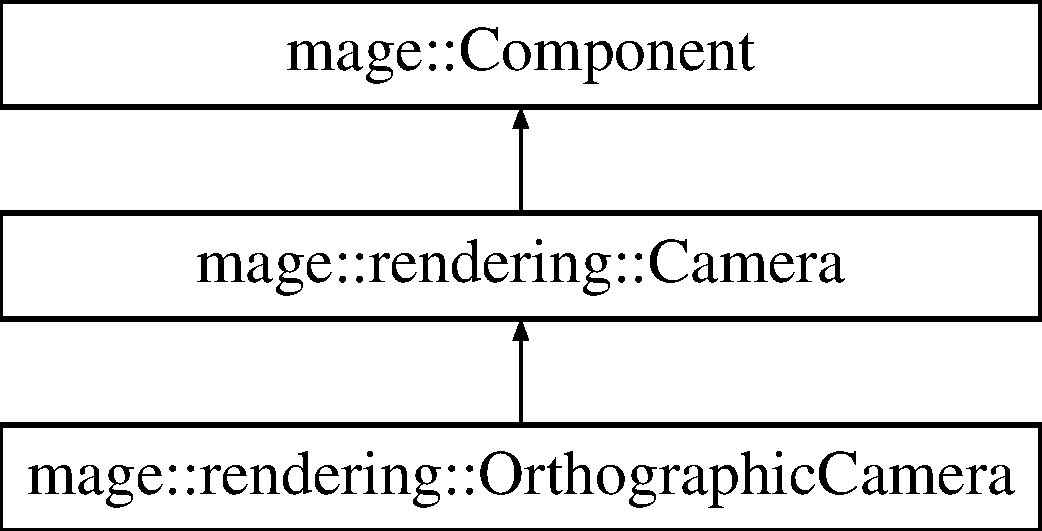
\includegraphics[height=3.000000cm]{classmage_1_1rendering_1_1_orthographic_camera}
\end{center}
\end{figure}
\subsection*{Public Member Functions}
\begin{DoxyCompactItemize}
\item 
\mbox{\hyperlink{classmage_1_1rendering_1_1_orthographic_camera_aba148b4da1141b5fa3dfc684e86dfc16}{Orthographic\+Camera}} (I\+D3\+D11\+Device \&device)
\item 
\mbox{\hyperlink{classmage_1_1rendering_1_1_orthographic_camera_a0bd37447138230a1a4900f503a2d1299}{Orthographic\+Camera}} (const \mbox{\hyperlink{classmage_1_1rendering_1_1_orthographic_camera}{Orthographic\+Camera}} \&camera)=delete
\item 
\mbox{\hyperlink{classmage_1_1rendering_1_1_orthographic_camera_a5b2c7d870e2077807057246abf3b76b1}{Orthographic\+Camera}} (\mbox{\hyperlink{classmage_1_1rendering_1_1_orthographic_camera}{Orthographic\+Camera}} \&\&camera) noexcept
\item 
virtual \mbox{\hyperlink{classmage_1_1rendering_1_1_orthographic_camera_a469e4af1c85a332b8feded9f577a05f6}{$\sim$\+Orthographic\+Camera}} ()
\item 
\mbox{\hyperlink{classmage_1_1rendering_1_1_orthographic_camera}{Orthographic\+Camera}} \& \mbox{\hyperlink{classmage_1_1rendering_1_1_orthographic_camera_adcd0a977ed5245aa4224dd1a679586f7}{operator=}} (const \mbox{\hyperlink{classmage_1_1rendering_1_1_orthographic_camera}{Orthographic\+Camera}} \&camera)=delete
\item 
\mbox{\hyperlink{classmage_1_1rendering_1_1_orthographic_camera}{Orthographic\+Camera}} \& \mbox{\hyperlink{classmage_1_1rendering_1_1_orthographic_camera_aa4518e7ef41bc0d841719198ac59d41f}{operator=}} (\mbox{\hyperlink{classmage_1_1rendering_1_1_orthographic_camera}{Orthographic\+Camera}} \&\&camera) noexcept
\item 
const \mbox{\hyperlink{namespacemage_a9dc0d34d6ecc87e4cfa4a826102117bc}{F32x2}} \mbox{\hyperlink{classmage_1_1rendering_1_1_orthographic_camera_abeb7a7d73f667ed7c9a38e5370bcb5e8}{Get\+Size}} () const noexcept
\item 
void \mbox{\hyperlink{classmage_1_1rendering_1_1_orthographic_camera_a8d78085a1a89fa30cf76f6cccbf80f0e}{Set\+Size}} (\mbox{\hyperlink{namespacemage_a9dc0d34d6ecc87e4cfa4a826102117bc}{F32x2}} size) noexcept
\item 
virtual const X\+M\+M\+A\+T\+R\+IX X\+M\+\_\+\+C\+A\+L\+L\+C\+O\+NV \mbox{\hyperlink{classmage_1_1rendering_1_1_orthographic_camera_a45736d696df0a38c8f1342dca2cda0cd}{Get\+Camera\+To\+Projection\+Matrix}} () const noexcept override
\item 
virtual const X\+M\+M\+A\+T\+R\+IX X\+M\+\_\+\+C\+A\+L\+L\+C\+O\+NV \mbox{\hyperlink{classmage_1_1rendering_1_1_orthographic_camera_a7d52862a3762dcaeadf26e8ae92d9d09}{Get\+Projection\+To\+Camera\+Matrix}} () const noexcept override
\end{DoxyCompactItemize}
\subsection*{Private Attributes}
\begin{DoxyCompactItemize}
\item 
\mbox{\hyperlink{namespacemage_a9dc0d34d6ecc87e4cfa4a826102117bc}{F32x2}} \mbox{\hyperlink{classmage_1_1rendering_1_1_orthographic_camera_ac83280a3b16a8ff6724e74f2f1e04653}{m\+\_\+size}}
\end{DoxyCompactItemize}
\subsection*{Additional Inherited Members}


\subsection{Detailed Description}
A class of orthographic cameras. 

\subsection{Constructor \& Destructor Documentation}
\mbox{\Hypertarget{classmage_1_1rendering_1_1_orthographic_camera_aba148b4da1141b5fa3dfc684e86dfc16}\label{classmage_1_1rendering_1_1_orthographic_camera_aba148b4da1141b5fa3dfc684e86dfc16}} 
\index{mage\+::rendering\+::\+Orthographic\+Camera@{mage\+::rendering\+::\+Orthographic\+Camera}!Orthographic\+Camera@{Orthographic\+Camera}}
\index{Orthographic\+Camera@{Orthographic\+Camera}!mage\+::rendering\+::\+Orthographic\+Camera@{mage\+::rendering\+::\+Orthographic\+Camera}}
\subsubsection{\texorpdfstring{Orthographic\+Camera()}{OrthographicCamera()}\hspace{0.1cm}{\footnotesize\ttfamily [1/3]}}
{\footnotesize\ttfamily mage\+::rendering\+::\+Orthographic\+Camera\+::\+Orthographic\+Camera (\begin{DoxyParamCaption}\item[{I\+D3\+D11\+Device \&}]{device }\end{DoxyParamCaption})}

Constructs an orthographic camera.


\begin{DoxyParams}[1]{Parameters}
\mbox{\tt in}  & {\em device} & A reference to the device. \\
\hline
\end{DoxyParams}
\mbox{\Hypertarget{classmage_1_1rendering_1_1_orthographic_camera_a0bd37447138230a1a4900f503a2d1299}\label{classmage_1_1rendering_1_1_orthographic_camera_a0bd37447138230a1a4900f503a2d1299}} 
\index{mage\+::rendering\+::\+Orthographic\+Camera@{mage\+::rendering\+::\+Orthographic\+Camera}!Orthographic\+Camera@{Orthographic\+Camera}}
\index{Orthographic\+Camera@{Orthographic\+Camera}!mage\+::rendering\+::\+Orthographic\+Camera@{mage\+::rendering\+::\+Orthographic\+Camera}}
\subsubsection{\texorpdfstring{Orthographic\+Camera()}{OrthographicCamera()}\hspace{0.1cm}{\footnotesize\ttfamily [2/3]}}
{\footnotesize\ttfamily mage\+::rendering\+::\+Orthographic\+Camera\+::\+Orthographic\+Camera (\begin{DoxyParamCaption}\item[{const \mbox{\hyperlink{classmage_1_1rendering_1_1_orthographic_camera}{Orthographic\+Camera}} \&}]{camera }\end{DoxyParamCaption})\hspace{0.3cm}{\ttfamily [delete]}}

Constructs an orthographic camera from the given orthographic camera.


\begin{DoxyParams}[1]{Parameters}
\mbox{\tt in}  & {\em camera} & A reference to the orthographic camera to copy. \\
\hline
\end{DoxyParams}
\mbox{\Hypertarget{classmage_1_1rendering_1_1_orthographic_camera_a5b2c7d870e2077807057246abf3b76b1}\label{classmage_1_1rendering_1_1_orthographic_camera_a5b2c7d870e2077807057246abf3b76b1}} 
\index{mage\+::rendering\+::\+Orthographic\+Camera@{mage\+::rendering\+::\+Orthographic\+Camera}!Orthographic\+Camera@{Orthographic\+Camera}}
\index{Orthographic\+Camera@{Orthographic\+Camera}!mage\+::rendering\+::\+Orthographic\+Camera@{mage\+::rendering\+::\+Orthographic\+Camera}}
\subsubsection{\texorpdfstring{Orthographic\+Camera()}{OrthographicCamera()}\hspace{0.1cm}{\footnotesize\ttfamily [3/3]}}
{\footnotesize\ttfamily mage\+::rendering\+::\+Orthographic\+Camera\+::\+Orthographic\+Camera (\begin{DoxyParamCaption}\item[{\mbox{\hyperlink{classmage_1_1rendering_1_1_orthographic_camera}{Orthographic\+Camera}} \&\&}]{camera }\end{DoxyParamCaption})\hspace{0.3cm}{\ttfamily [default]}, {\ttfamily [noexcept]}}

Constructs an orthographic camera by moving the given orthographic camera.


\begin{DoxyParams}[1]{Parameters}
\mbox{\tt in}  & {\em camera} & A reference to the orthographic camera to move. \\
\hline
\end{DoxyParams}
\mbox{\Hypertarget{classmage_1_1rendering_1_1_orthographic_camera_a469e4af1c85a332b8feded9f577a05f6}\label{classmage_1_1rendering_1_1_orthographic_camera_a469e4af1c85a332b8feded9f577a05f6}} 
\index{mage\+::rendering\+::\+Orthographic\+Camera@{mage\+::rendering\+::\+Orthographic\+Camera}!````~Orthographic\+Camera@{$\sim$\+Orthographic\+Camera}}
\index{````~Orthographic\+Camera@{$\sim$\+Orthographic\+Camera}!mage\+::rendering\+::\+Orthographic\+Camera@{mage\+::rendering\+::\+Orthographic\+Camera}}
\subsubsection{\texorpdfstring{$\sim$\+Orthographic\+Camera()}{~OrthographicCamera()}}
{\footnotesize\ttfamily mage\+::rendering\+::\+Orthographic\+Camera\+::$\sim$\+Orthographic\+Camera (\begin{DoxyParamCaption}{ }\end{DoxyParamCaption})\hspace{0.3cm}{\ttfamily [virtual]}, {\ttfamily [default]}}

Destructs this orthographic camera. 

\subsection{Member Function Documentation}
\mbox{\Hypertarget{classmage_1_1rendering_1_1_orthographic_camera_a45736d696df0a38c8f1342dca2cda0cd}\label{classmage_1_1rendering_1_1_orthographic_camera_a45736d696df0a38c8f1342dca2cda0cd}} 
\index{mage\+::rendering\+::\+Orthographic\+Camera@{mage\+::rendering\+::\+Orthographic\+Camera}!Get\+Camera\+To\+Projection\+Matrix@{Get\+Camera\+To\+Projection\+Matrix}}
\index{Get\+Camera\+To\+Projection\+Matrix@{Get\+Camera\+To\+Projection\+Matrix}!mage\+::rendering\+::\+Orthographic\+Camera@{mage\+::rendering\+::\+Orthographic\+Camera}}
\subsubsection{\texorpdfstring{Get\+Camera\+To\+Projection\+Matrix()}{GetCameraToProjectionMatrix()}}
{\footnotesize\ttfamily virtual const X\+M\+M\+A\+T\+R\+IX X\+M\+\_\+\+C\+A\+L\+L\+C\+O\+NV mage\+::rendering\+::\+Orthographic\+Camera\+::\+Get\+Camera\+To\+Projection\+Matrix (\begin{DoxyParamCaption}{ }\end{DoxyParamCaption}) const\hspace{0.3cm}{\ttfamily [override]}, {\ttfamily [virtual]}, {\ttfamily [noexcept]}}

Returns the camera-\/to-\/projection matrix of this orthographic camera.

\begin{DoxyReturn}{Returns}
The camera-\/to-\/projection matrix of this orthographic camera. 
\end{DoxyReturn}


Implements \mbox{\hyperlink{classmage_1_1rendering_1_1_camera_a08481175c3718a24333b22176e240d44}{mage\+::rendering\+::\+Camera}}.

\mbox{\Hypertarget{classmage_1_1rendering_1_1_orthographic_camera_a7d52862a3762dcaeadf26e8ae92d9d09}\label{classmage_1_1rendering_1_1_orthographic_camera_a7d52862a3762dcaeadf26e8ae92d9d09}} 
\index{mage\+::rendering\+::\+Orthographic\+Camera@{mage\+::rendering\+::\+Orthographic\+Camera}!Get\+Projection\+To\+Camera\+Matrix@{Get\+Projection\+To\+Camera\+Matrix}}
\index{Get\+Projection\+To\+Camera\+Matrix@{Get\+Projection\+To\+Camera\+Matrix}!mage\+::rendering\+::\+Orthographic\+Camera@{mage\+::rendering\+::\+Orthographic\+Camera}}
\subsubsection{\texorpdfstring{Get\+Projection\+To\+Camera\+Matrix()}{GetProjectionToCameraMatrix()}}
{\footnotesize\ttfamily virtual const X\+M\+M\+A\+T\+R\+IX X\+M\+\_\+\+C\+A\+L\+L\+C\+O\+NV mage\+::rendering\+::\+Orthographic\+Camera\+::\+Get\+Projection\+To\+Camera\+Matrix (\begin{DoxyParamCaption}{ }\end{DoxyParamCaption}) const\hspace{0.3cm}{\ttfamily [override]}, {\ttfamily [virtual]}, {\ttfamily [noexcept]}}

Returns the projection-\/to-\/camera matrix of this orthographic camera.

\begin{DoxyReturn}{Returns}
The projection-\/to-\/camera matrix of this orthographic camera. 
\end{DoxyReturn}


Implements \mbox{\hyperlink{classmage_1_1rendering_1_1_camera_abb21116f8a6c7513804431d23fa4cf17}{mage\+::rendering\+::\+Camera}}.

\mbox{\Hypertarget{classmage_1_1rendering_1_1_orthographic_camera_abeb7a7d73f667ed7c9a38e5370bcb5e8}\label{classmage_1_1rendering_1_1_orthographic_camera_abeb7a7d73f667ed7c9a38e5370bcb5e8}} 
\index{mage\+::rendering\+::\+Orthographic\+Camera@{mage\+::rendering\+::\+Orthographic\+Camera}!Get\+Size@{Get\+Size}}
\index{Get\+Size@{Get\+Size}!mage\+::rendering\+::\+Orthographic\+Camera@{mage\+::rendering\+::\+Orthographic\+Camera}}
\subsubsection{\texorpdfstring{Get\+Size()}{GetSize()}}
{\footnotesize\ttfamily const \mbox{\hyperlink{namespacemage_a9dc0d34d6ecc87e4cfa4a826102117bc}{F32x2}} mage\+::rendering\+::\+Orthographic\+Camera\+::\+Get\+Size (\begin{DoxyParamCaption}{ }\end{DoxyParamCaption}) const\hspace{0.3cm}{\ttfamily [noexcept]}}

Returns the size of the projection plane of this orthographic camera expressed in camera space.

\begin{DoxyReturn}{Returns}
The size of the projection plane of this orthographic camera expressed in camera space. 
\end{DoxyReturn}
\mbox{\Hypertarget{classmage_1_1rendering_1_1_orthographic_camera_adcd0a977ed5245aa4224dd1a679586f7}\label{classmage_1_1rendering_1_1_orthographic_camera_adcd0a977ed5245aa4224dd1a679586f7}} 
\index{mage\+::rendering\+::\+Orthographic\+Camera@{mage\+::rendering\+::\+Orthographic\+Camera}!operator=@{operator=}}
\index{operator=@{operator=}!mage\+::rendering\+::\+Orthographic\+Camera@{mage\+::rendering\+::\+Orthographic\+Camera}}
\subsubsection{\texorpdfstring{operator=()}{operator=()}\hspace{0.1cm}{\footnotesize\ttfamily [1/2]}}
{\footnotesize\ttfamily \mbox{\hyperlink{classmage_1_1rendering_1_1_orthographic_camera}{Orthographic\+Camera}}\& mage\+::rendering\+::\+Orthographic\+Camera\+::operator= (\begin{DoxyParamCaption}\item[{const \mbox{\hyperlink{classmage_1_1rendering_1_1_orthographic_camera}{Orthographic\+Camera}} \&}]{camera }\end{DoxyParamCaption})\hspace{0.3cm}{\ttfamily [delete]}}

Copies the given orthographic camera to this orthographic camera.


\begin{DoxyParams}[1]{Parameters}
\mbox{\tt in}  & {\em camera} & A reference to the orthographic camera to copy. \\
\hline
\end{DoxyParams}
\begin{DoxyReturn}{Returns}
A reference to the copy of the given orthographic camera (i.\+e. this orthographic camera). 
\end{DoxyReturn}
\mbox{\Hypertarget{classmage_1_1rendering_1_1_orthographic_camera_aa4518e7ef41bc0d841719198ac59d41f}\label{classmage_1_1rendering_1_1_orthographic_camera_aa4518e7ef41bc0d841719198ac59d41f}} 
\index{mage\+::rendering\+::\+Orthographic\+Camera@{mage\+::rendering\+::\+Orthographic\+Camera}!operator=@{operator=}}
\index{operator=@{operator=}!mage\+::rendering\+::\+Orthographic\+Camera@{mage\+::rendering\+::\+Orthographic\+Camera}}
\subsubsection{\texorpdfstring{operator=()}{operator=()}\hspace{0.1cm}{\footnotesize\ttfamily [2/2]}}
{\footnotesize\ttfamily \mbox{\hyperlink{classmage_1_1rendering_1_1_orthographic_camera}{Orthographic\+Camera}} \& mage\+::rendering\+::\+Orthographic\+Camera\+::operator= (\begin{DoxyParamCaption}\item[{\mbox{\hyperlink{classmage_1_1rendering_1_1_orthographic_camera}{Orthographic\+Camera}} \&\&}]{camera }\end{DoxyParamCaption})\hspace{0.3cm}{\ttfamily [default]}, {\ttfamily [noexcept]}}

Moves the given orthographic camera to this orthographic camera.


\begin{DoxyParams}[1]{Parameters}
\mbox{\tt in}  & {\em camera} & A reference to the orthographic camera to move. \\
\hline
\end{DoxyParams}
\begin{DoxyReturn}{Returns}
A reference to the moved orthographic camera (i.\+e. this orthographic camera). 
\end{DoxyReturn}
\mbox{\Hypertarget{classmage_1_1rendering_1_1_orthographic_camera_a8d78085a1a89fa30cf76f6cccbf80f0e}\label{classmage_1_1rendering_1_1_orthographic_camera_a8d78085a1a89fa30cf76f6cccbf80f0e}} 
\index{mage\+::rendering\+::\+Orthographic\+Camera@{mage\+::rendering\+::\+Orthographic\+Camera}!Set\+Size@{Set\+Size}}
\index{Set\+Size@{Set\+Size}!mage\+::rendering\+::\+Orthographic\+Camera@{mage\+::rendering\+::\+Orthographic\+Camera}}
\subsubsection{\texorpdfstring{Set\+Size()}{SetSize()}}
{\footnotesize\ttfamily void mage\+::rendering\+::\+Orthographic\+Camera\+::\+Set\+Size (\begin{DoxyParamCaption}\item[{\mbox{\hyperlink{namespacemage_a9dc0d34d6ecc87e4cfa4a826102117bc}{F32x2}}}]{size }\end{DoxyParamCaption})\hspace{0.3cm}{\ttfamily [noexcept]}}

Sets the size of the projection plane of this orthographic camera expressed in camera space to the given size.


\begin{DoxyParams}[1]{Parameters}
\mbox{\tt in}  & {\em size} & The size. \\
\hline
\end{DoxyParams}


\subsection{Member Data Documentation}
\mbox{\Hypertarget{classmage_1_1rendering_1_1_orthographic_camera_ac83280a3b16a8ff6724e74f2f1e04653}\label{classmage_1_1rendering_1_1_orthographic_camera_ac83280a3b16a8ff6724e74f2f1e04653}} 
\index{mage\+::rendering\+::\+Orthographic\+Camera@{mage\+::rendering\+::\+Orthographic\+Camera}!m\+\_\+size@{m\+\_\+size}}
\index{m\+\_\+size@{m\+\_\+size}!mage\+::rendering\+::\+Orthographic\+Camera@{mage\+::rendering\+::\+Orthographic\+Camera}}
\subsubsection{\texorpdfstring{m\+\_\+size}{m\_size}}
{\footnotesize\ttfamily \mbox{\hyperlink{namespacemage_a9dc0d34d6ecc87e4cfa4a826102117bc}{F32x2}} mage\+::rendering\+::\+Orthographic\+Camera\+::m\+\_\+size\hspace{0.3cm}{\ttfamily [private]}}

The size of the projection plane of this orthographic camera expressed in camera space. 
\hypertarget{classmage_1_1rendering_1_1_output_manager}{}\section{mage\+:\+:rendering\+:\+:Output\+Manager Class Reference}
\label{classmage_1_1rendering_1_1_output_manager}\index{mage\+::rendering\+::\+Output\+Manager@{mage\+::rendering\+::\+Output\+Manager}}


{\ttfamily \#include $<$output\+\_\+manager.\+hpp$>$}

\subsection*{Public Member Functions}
\begin{DoxyCompactItemize}
\item 
\mbox{\hyperlink{classmage_1_1rendering_1_1_output_manager_a02c97a57bf7217ab65ff5e7a44602200}{Output\+Manager}} (I\+D3\+D11\+Device \&device, \mbox{\hyperlink{classmage_1_1rendering_1_1_display_configuration}{Display\+Configuration}} \&display\+\_\+configuration, \mbox{\hyperlink{classmage_1_1rendering_1_1_swap_chain}{Swap\+Chain}} \&swap\+\_\+chain)
\item 
\mbox{\hyperlink{classmage_1_1rendering_1_1_output_manager_ae53a8cdec43d7c19dfb0c107814f228b}{Output\+Manager}} (const \mbox{\hyperlink{classmage_1_1rendering_1_1_output_manager}{Output\+Manager}} \&manager)=delete
\item 
\mbox{\hyperlink{classmage_1_1rendering_1_1_output_manager_aeafc4fb1d7a1904776f738b711635832}{Output\+Manager}} (\mbox{\hyperlink{classmage_1_1rendering_1_1_output_manager}{Output\+Manager}} \&\&manager) noexcept
\item 
\mbox{\hyperlink{classmage_1_1rendering_1_1_output_manager_ad2a02128a123be93391c8058ef2b3a0b}{$\sim$\+Output\+Manager}} ()
\item 
\mbox{\hyperlink{classmage_1_1rendering_1_1_output_manager}{Output\+Manager}} \& \mbox{\hyperlink{classmage_1_1rendering_1_1_output_manager_a7fb15ee3d3e3f7be648071ef1c6f3c6d}{operator=}} (const \mbox{\hyperlink{classmage_1_1rendering_1_1_output_manager}{Output\+Manager}} \&manager)=delete
\item 
\mbox{\hyperlink{classmage_1_1rendering_1_1_output_manager}{Output\+Manager}} \& \mbox{\hyperlink{classmage_1_1rendering_1_1_output_manager_a97d2c2be4389a615eb084dd53af531aa}{operator=}} (\mbox{\hyperlink{classmage_1_1rendering_1_1_output_manager}{Output\+Manager}} \&\&manager) noexcept
\item 
void \mbox{\hyperlink{classmage_1_1rendering_1_1_output_manager_a9c753354655b7b218263832c343417d1}{Bind\+Begin}} (I\+D3\+D11\+Device\+Context \&device\+\_\+context) const noexcept
\item 
void \mbox{\hyperlink{classmage_1_1rendering_1_1_output_manager_a9101e210c5b04fefc52f2f14473c5742}{Bind\+Begin\+Viewport}} (I\+D3\+D11\+Device\+Context \&device\+\_\+context) const noexcept
\item 
void \mbox{\hyperlink{classmage_1_1rendering_1_1_output_manager_a93139563e5f5b58ccba4688c3b793e32}{Bind\+Begin\+G\+Buffer}} (I\+D3\+D11\+Device\+Context \&device\+\_\+context) const noexcept
\item 
void \mbox{\hyperlink{classmage_1_1rendering_1_1_output_manager_a380113a2b1c9049cfd2367a6344683b7}{Bind\+End\+G\+Buffer}} (I\+D3\+D11\+Device\+Context \&device\+\_\+context) const noexcept
\item 
void \mbox{\hyperlink{classmage_1_1rendering_1_1_output_manager_ad05f55888d2075806ae7a381031ecdfd}{Bind\+Begin\+Deferred}} (I\+D3\+D11\+Device\+Context \&device\+\_\+context) const noexcept
\item 
void \mbox{\hyperlink{classmage_1_1rendering_1_1_output_manager_af48d4e2671d7b84d3fd94961b926dd2a}{Bind\+End\+Deferred}} (I\+D3\+D11\+Device\+Context \&device\+\_\+context) const noexcept
\item 
void \mbox{\hyperlink{classmage_1_1rendering_1_1_output_manager_a678b86feab6fffb88752254a799d456d}{Bind\+Begin\+Forward}} (I\+D3\+D11\+Device\+Context \&device\+\_\+context) const noexcept
\item 
void \mbox{\hyperlink{classmage_1_1rendering_1_1_output_manager_ad0b43f26a2762ae116bc72b0cf21a6de}{Bind\+End\+Forward}} (I\+D3\+D11\+Device\+Context \&device\+\_\+context) const noexcept
\item 
void \mbox{\hyperlink{classmage_1_1rendering_1_1_output_manager_affa0c4b4c9c56807fe8ad4ed802fdfd9}{Bind\+Begin\+Resolve}} (I\+D3\+D11\+Device\+Context \&device\+\_\+context) const noexcept
\item 
void \mbox{\hyperlink{classmage_1_1rendering_1_1_output_manager_a548e6003d34916b174f74f6f1b5e85a2}{Bind\+End\+Resolve}} (I\+D3\+D11\+Device\+Context \&device\+\_\+context) const noexcept
\item 
void \mbox{\hyperlink{classmage_1_1rendering_1_1_output_manager_a6c22d77a812e3eacf32cfdb6d6a4d5f4}{Bind\+Begin\+Post\+Processing}} (I\+D3\+D11\+Device\+Context \&device\+\_\+context) const noexcept
\item 
void \mbox{\hyperlink{classmage_1_1rendering_1_1_output_manager_aacb8da12f24fe9b7f1c3aac6f52ba9a1}{Bind\+Ping\+Pong}} (I\+D3\+D11\+Device\+Context \&device\+\_\+context) const noexcept
\item 
void \mbox{\hyperlink{classmage_1_1rendering_1_1_output_manager_a47e4a5dfc0bca82c49ebde85e01d55cc}{Bind\+End\+Post\+Processing}} (I\+D3\+D11\+Device\+Context \&device\+\_\+context) const noexcept
\item 
void \mbox{\hyperlink{classmage_1_1rendering_1_1_output_manager_a1b99009331167e4548dbb58695926542}{Bind\+End\+Viewport}} (I\+D3\+D11\+Device\+Context \&device\+\_\+context) const noexcept
\item 
void \mbox{\hyperlink{classmage_1_1rendering_1_1_output_manager_a08be9cc8922f891c8ea4f17559ee40db}{Bind\+G\+UI}} (I\+D3\+D11\+Device\+Context \&device\+\_\+context) const noexcept
\item 
void \mbox{\hyperlink{classmage_1_1rendering_1_1_output_manager_adf8fa859bb168ecf389d56b574a69dbd}{Bind\+End}} (I\+D3\+D11\+Device\+Context \&device\+\_\+context) const noexcept
\end{DoxyCompactItemize}
\subsection*{Private Types}
\begin{DoxyCompactItemize}
\item 
enum \mbox{\hyperlink{classmage_1_1rendering_1_1_output_manager_a941f1b35a83ee0ce190494523ec0fe63}{S\+R\+V\+Index}} \+: U8 \{ \newline
\mbox{\hyperlink{classmage_1_1rendering_1_1_output_manager_a941f1b35a83ee0ce190494523ec0fe63a6cad826248cd3f4e93da71e7b49928e3}{S\+R\+V\+Index\+::\+H\+DR}} = 0, 
\mbox{\hyperlink{classmage_1_1rendering_1_1_output_manager_a941f1b35a83ee0ce190494523ec0fe63af8aaa1436c06c671272ac08e4fa83309}{S\+R\+V\+Index\+::\+G\+Buffer\+\_\+\+Base\+Color}}, 
\mbox{\hyperlink{classmage_1_1rendering_1_1_output_manager_a941f1b35a83ee0ce190494523ec0fe63abbdd76532c820b05b242d544cd1b43fd}{S\+R\+V\+Index\+::\+G\+Buffer\+\_\+\+Material}}, 
\mbox{\hyperlink{classmage_1_1rendering_1_1_output_manager_a941f1b35a83ee0ce190494523ec0fe63af69e4b1698bc66624ab45f2c967406bb}{S\+R\+V\+Index\+::\+G\+Buffer\+\_\+\+Normal}}, 
\newline
\mbox{\hyperlink{classmage_1_1rendering_1_1_output_manager_a941f1b35a83ee0ce190494523ec0fe63ae8964b7cf20037a91a4e9107f2b93db8}{S\+R\+V\+Index\+::\+G\+Buffer\+\_\+\+Depth}}, 
\mbox{\hyperlink{classmage_1_1rendering_1_1_output_manager_a941f1b35a83ee0ce190494523ec0fe63af86c3f35d502a4de4cc2d4601a6fbbc4}{S\+R\+V\+Index\+::\+Post\+Processing\+\_\+\+H\+D\+R0}}, 
\mbox{\hyperlink{classmage_1_1rendering_1_1_output_manager_a941f1b35a83ee0ce190494523ec0fe63a2136232aa9456009a7df9de7db662322}{S\+R\+V\+Index\+::\+Post\+Processing\+\_\+\+H\+D\+R1}}, 
\mbox{\hyperlink{classmage_1_1rendering_1_1_output_manager_a941f1b35a83ee0ce190494523ec0fe63a224be169fd2e0ce4f53c6afa41ac4fe9}{S\+R\+V\+Index\+::\+Post\+Processing\+\_\+\+Normal}}, 
\newline
\mbox{\hyperlink{classmage_1_1rendering_1_1_output_manager_a941f1b35a83ee0ce190494523ec0fe63a251bebd0602960f976f4a69dff9b13fe}{S\+R\+V\+Index\+::\+Post\+Processing\+\_\+\+Depth}}, 
\mbox{\hyperlink{classmage_1_1rendering_1_1_output_manager_a941f1b35a83ee0ce190494523ec0fe63a6645d4de79aee6373f120d72c0030e5f}{S\+R\+V\+Index\+::\+L\+DR}}, 
\mbox{\hyperlink{classmage_1_1rendering_1_1_output_manager_a941f1b35a83ee0ce190494523ec0fe63ae93f994f01c537c4e2f7d8528c3eb5e9}{S\+R\+V\+Index\+::\+Count}}
 \}
\item 
enum \mbox{\hyperlink{classmage_1_1rendering_1_1_output_manager_af9caebb7e9cacf454d26b827a01e857c}{R\+T\+V\+Index}} \+: U8 \{ \newline
\mbox{\hyperlink{classmage_1_1rendering_1_1_output_manager_af9caebb7e9cacf454d26b827a01e857ca6cad826248cd3f4e93da71e7b49928e3}{R\+T\+V\+Index\+::\+H\+DR}} = 0, 
\mbox{\hyperlink{classmage_1_1rendering_1_1_output_manager_af9caebb7e9cacf454d26b827a01e857caf8aaa1436c06c671272ac08e4fa83309}{R\+T\+V\+Index\+::\+G\+Buffer\+\_\+\+Base\+Color}}, 
\mbox{\hyperlink{classmage_1_1rendering_1_1_output_manager_af9caebb7e9cacf454d26b827a01e857cabbdd76532c820b05b242d544cd1b43fd}{R\+T\+V\+Index\+::\+G\+Buffer\+\_\+\+Material}}, 
\mbox{\hyperlink{classmage_1_1rendering_1_1_output_manager_af9caebb7e9cacf454d26b827a01e857caf69e4b1698bc66624ab45f2c967406bb}{R\+T\+V\+Index\+::\+G\+Buffer\+\_\+\+Normal}}, 
\newline
\mbox{\hyperlink{classmage_1_1rendering_1_1_output_manager_af9caebb7e9cacf454d26b827a01e857caf86c3f35d502a4de4cc2d4601a6fbbc4}{R\+T\+V\+Index\+::\+Post\+Processing\+\_\+\+H\+D\+R0}}, 
\mbox{\hyperlink{classmage_1_1rendering_1_1_output_manager_af9caebb7e9cacf454d26b827a01e857ca2136232aa9456009a7df9de7db662322}{R\+T\+V\+Index\+::\+Post\+Processing\+\_\+\+H\+D\+R1}}, 
\mbox{\hyperlink{classmage_1_1rendering_1_1_output_manager_af9caebb7e9cacf454d26b827a01e857ca6645d4de79aee6373f120d72c0030e5f}{R\+T\+V\+Index\+::\+L\+DR}}, 
\mbox{\hyperlink{classmage_1_1rendering_1_1_output_manager_af9caebb7e9cacf454d26b827a01e857cae93f994f01c537c4e2f7d8528c3eb5e9}{R\+T\+V\+Index\+::\+Count}}
 \}
\item 
enum \mbox{\hyperlink{classmage_1_1rendering_1_1_output_manager_a71b3797fef957312f92736f15b7ada3e}{U\+A\+V\+Index}} \+: U8 \{ \newline
\mbox{\hyperlink{classmage_1_1rendering_1_1_output_manager_a71b3797fef957312f92736f15b7ada3ea6cad826248cd3f4e93da71e7b49928e3}{U\+A\+V\+Index\+::\+H\+DR}} = 0, 
\mbox{\hyperlink{classmage_1_1rendering_1_1_output_manager_a71b3797fef957312f92736f15b7ada3eaf86c3f35d502a4de4cc2d4601a6fbbc4}{U\+A\+V\+Index\+::\+Post\+Processing\+\_\+\+H\+D\+R0}}, 
\mbox{\hyperlink{classmage_1_1rendering_1_1_output_manager_a71b3797fef957312f92736f15b7ada3ea2136232aa9456009a7df9de7db662322}{U\+A\+V\+Index\+::\+Post\+Processing\+\_\+\+H\+D\+R1}}, 
\mbox{\hyperlink{classmage_1_1rendering_1_1_output_manager_a71b3797fef957312f92736f15b7ada3ea224be169fd2e0ce4f53c6afa41ac4fe9}{U\+A\+V\+Index\+::\+Post\+Processing\+\_\+\+Normal}}, 
\newline
\mbox{\hyperlink{classmage_1_1rendering_1_1_output_manager_a71b3797fef957312f92736f15b7ada3ea251bebd0602960f976f4a69dff9b13fe}{U\+A\+V\+Index\+::\+Post\+Processing\+\_\+\+Depth}}, 
\mbox{\hyperlink{classmage_1_1rendering_1_1_output_manager_a71b3797fef957312f92736f15b7ada3ea6645d4de79aee6373f120d72c0030e5f}{U\+A\+V\+Index\+::\+L\+DR}}, 
\mbox{\hyperlink{classmage_1_1rendering_1_1_output_manager_a71b3797fef957312f92736f15b7ada3eae93f994f01c537c4e2f7d8528c3eb5e9}{U\+A\+V\+Index\+::\+Count}}
 \}
\end{DoxyCompactItemize}
\subsection*{Private Member Functions}
\begin{DoxyCompactItemize}
\item 
I\+D3\+D11\+Shader\+Resource\+View $\ast$ \mbox{\hyperlink{classmage_1_1rendering_1_1_output_manager_a0dc5e124cbd78351b78cc7a3e7bff428}{Get\+S\+RV}} (\mbox{\hyperlink{classmage_1_1rendering_1_1_output_manager_a941f1b35a83ee0ce190494523ec0fe63}{S\+R\+V\+Index}} index) const noexcept
\item 
\mbox{\hyperlink{namespacemage_a8769f9d670d6b585ea306cb1062af94b}{Not\+Null}}$<$ I\+D3\+D11\+Shader\+Resource\+View $\ast$$\ast$$>$ \mbox{\hyperlink{classmage_1_1rendering_1_1_output_manager_afd13c25f8ab6cfafc5d694d3b64405f9}{Release\+And\+Get\+Address\+Of\+S\+RV}} (\mbox{\hyperlink{classmage_1_1rendering_1_1_output_manager_a941f1b35a83ee0ce190494523ec0fe63}{S\+R\+V\+Index}} index) noexcept
\item 
I\+D3\+D11\+Render\+Target\+View $\ast$ \mbox{\hyperlink{classmage_1_1rendering_1_1_output_manager_a2088241f582fd9b119f485c5e9a13b30}{Get\+R\+TV}} (\mbox{\hyperlink{classmage_1_1rendering_1_1_output_manager_af9caebb7e9cacf454d26b827a01e857c}{R\+T\+V\+Index}} index) const noexcept
\item 
\mbox{\hyperlink{namespacemage_a8769f9d670d6b585ea306cb1062af94b}{Not\+Null}}$<$ I\+D3\+D11\+Render\+Target\+View $\ast$$\ast$$>$ \mbox{\hyperlink{classmage_1_1rendering_1_1_output_manager_a997a7c48090b5b68e643f3158e9e9d7e}{Release\+And\+Get\+Address\+Of\+R\+TV}} (\mbox{\hyperlink{classmage_1_1rendering_1_1_output_manager_af9caebb7e9cacf454d26b827a01e857c}{R\+T\+V\+Index}} index) noexcept
\item 
I\+D3\+D11\+Unordered\+Access\+View $\ast$ \mbox{\hyperlink{classmage_1_1rendering_1_1_output_manager_a6eb1f3b756f121897fd869c355944e86}{Get\+U\+AV}} (\mbox{\hyperlink{classmage_1_1rendering_1_1_output_manager_a71b3797fef957312f92736f15b7ada3e}{U\+A\+V\+Index}} index) const noexcept
\item 
\mbox{\hyperlink{namespacemage_a8769f9d670d6b585ea306cb1062af94b}{Not\+Null}}$<$ I\+D3\+D11\+Unordered\+Access\+View $\ast$$\ast$$>$ \mbox{\hyperlink{classmage_1_1rendering_1_1_output_manager_a79ec82aadfe89ea1a9875567d9bbb74a}{Release\+And\+Get\+Address\+Of\+U\+AV}} (\mbox{\hyperlink{classmage_1_1rendering_1_1_output_manager_a71b3797fef957312f92736f15b7ada3e}{U\+A\+V\+Index}} index) noexcept
\item 
void \mbox{\hyperlink{classmage_1_1rendering_1_1_output_manager_a590172441d291329d1f5a9dbbdb71320}{Setup\+Buffers}} ()
\item 
void \mbox{\hyperlink{classmage_1_1rendering_1_1_output_manager_aca32d0307be3acfaa8f5a20fa24b6934}{Setup\+Buffer}} (const \mbox{\hyperlink{namespacemage_a03e3b6f65630005f43a3112d1f6cf57b}{U32x3}} \&resolution, D\+X\+G\+I\+\_\+\+F\+O\+R\+M\+AT format, I\+D3\+D11\+Shader\+Resource\+View $\ast$$\ast$srv, I\+D3\+D11\+Render\+Target\+View $\ast$$\ast$rtv, I\+D3\+D11\+Unordered\+Access\+View $\ast$$\ast$uav)
\item 
void \mbox{\hyperlink{classmage_1_1rendering_1_1_output_manager_a4cbd2dd771206b15d934657205475ae1}{Setup\+Depth\+Buffer}} (const \mbox{\hyperlink{namespacemage_a03e3b6f65630005f43a3112d1f6cf57b}{U32x3}} \&resolution)
\end{DoxyCompactItemize}
\subsection*{Private Attributes}
\begin{DoxyCompactItemize}
\item 
std\+::reference\+\_\+wrapper$<$ \mbox{\hyperlink{classmage_1_1rendering_1_1_display_configuration}{Display\+Configuration}} $>$ \mbox{\hyperlink{classmage_1_1rendering_1_1_output_manager_a41905bc9eb0426c2e75d33d60bb95fbf}{m\+\_\+display\+\_\+configuration}}
\item 
std\+::reference\+\_\+wrapper$<$ I\+D3\+D11\+Device $>$ \mbox{\hyperlink{classmage_1_1rendering_1_1_output_manager_ad0f8b4613dfbd613576a3c58c8ff4c37}{m\+\_\+device}}
\item 
std\+::reference\+\_\+wrapper$<$ \mbox{\hyperlink{classmage_1_1rendering_1_1_swap_chain}{Swap\+Chain}} $>$ \mbox{\hyperlink{classmage_1_1rendering_1_1_output_manager_ac9cffc724a38ffd3d9b49475fd29d3ba}{m\+\_\+swap\+\_\+chain}}
\item 
\mbox{\hyperlink{namespacemage_ae74f374780900893caa5555d1031fd79}{Com\+Ptr}}$<$ I\+D3\+D11\+Shader\+Resource\+View $>$ \mbox{\hyperlink{classmage_1_1rendering_1_1_output_manager_ac002667bd25dd978d6ff0ece782c8455}{m\+\_\+srvs}} \mbox{[}static\+\_\+cast$<$ size\+\_\+t $>$(\mbox{\hyperlink{classmage_1_1rendering_1_1_output_manager_a941f1b35a83ee0ce190494523ec0fe63ae93f994f01c537c4e2f7d8528c3eb5e9}{S\+R\+V\+Index\+::\+Count}})\mbox{]}
\item 
\mbox{\hyperlink{namespacemage_ae74f374780900893caa5555d1031fd79}{Com\+Ptr}}$<$ I\+D3\+D11\+Render\+Target\+View $>$ \mbox{\hyperlink{classmage_1_1rendering_1_1_output_manager_afd0aade15fe5b0f9f4f0bef9f7ea3715}{m\+\_\+rtvs}} \mbox{[}static\+\_\+cast$<$ size\+\_\+t $>$(\mbox{\hyperlink{classmage_1_1rendering_1_1_output_manager_af9caebb7e9cacf454d26b827a01e857cae93f994f01c537c4e2f7d8528c3eb5e9}{R\+T\+V\+Index\+::\+Count}})\mbox{]}
\item 
\mbox{\hyperlink{namespacemage_ae74f374780900893caa5555d1031fd79}{Com\+Ptr}}$<$ I\+D3\+D11\+Unordered\+Access\+View $>$ \mbox{\hyperlink{classmage_1_1rendering_1_1_output_manager_abfdf92e89ef4ee4df40204e84098fdd7}{m\+\_\+uavs}} \mbox{[}static\+\_\+cast$<$ size\+\_\+t $>$(\mbox{\hyperlink{classmage_1_1rendering_1_1_output_manager_a71b3797fef957312f92736f15b7ada3eae93f994f01c537c4e2f7d8528c3eb5e9}{U\+A\+V\+Index\+::\+Count}})\mbox{]}
\item 
\mbox{\hyperlink{namespacemage_ae74f374780900893caa5555d1031fd79}{Com\+Ptr}}$<$ I\+D3\+D11\+Depth\+Stencil\+View $>$ \mbox{\hyperlink{classmage_1_1rendering_1_1_output_manager_a48225f5d17db8e3d0e44adc2689d326f}{m\+\_\+dsv}}
\item 
bool \mbox{\hyperlink{classmage_1_1rendering_1_1_output_manager_aee20394757c9f7ebcaf7f8682747d716}{m\+\_\+hdr0\+\_\+to\+\_\+hdr1}}
\item 
bool \mbox{\hyperlink{classmage_1_1rendering_1_1_output_manager_a3affee412b093ea168b9e4a22c713421}{m\+\_\+msaa}}
\item 
bool \mbox{\hyperlink{classmage_1_1rendering_1_1_output_manager_ae0016fada4d4550d58481d2c313ea524}{m\+\_\+ssaa}}
\end{DoxyCompactItemize}


\subsection{Detailed Description}
A class of output managers. 

\subsection{Member Enumeration Documentation}
\mbox{\Hypertarget{classmage_1_1rendering_1_1_output_manager_af9caebb7e9cacf454d26b827a01e857c}\label{classmage_1_1rendering_1_1_output_manager_af9caebb7e9cacf454d26b827a01e857c}} 
\index{mage\+::rendering\+::\+Output\+Manager@{mage\+::rendering\+::\+Output\+Manager}!R\+T\+V\+Index@{R\+T\+V\+Index}}
\index{R\+T\+V\+Index@{R\+T\+V\+Index}!mage\+::rendering\+::\+Output\+Manager@{mage\+::rendering\+::\+Output\+Manager}}
\subsubsection{\texorpdfstring{R\+T\+V\+Index}{RTVIndex}}
{\footnotesize\ttfamily enum \mbox{\hyperlink{classmage_1_1rendering_1_1_output_manager_af9caebb7e9cacf454d26b827a01e857c}{mage\+::rendering\+::\+Output\+Manager\+::\+R\+T\+V\+Index}} \+: \mbox{\hyperlink{namespacemage_afc638980bc6154f15af5e2d93a0e0ea9}{U8}}\hspace{0.3cm}{\ttfamily [strong]}, {\ttfamily [private]}}

\begin{DoxyEnumFields}{Enumerator}
\raisebox{\heightof{T}}[0pt][0pt]{\index{H\+DR@{H\+DR}!mage\+::rendering\+::\+Output\+Manager@{mage\+::rendering\+::\+Output\+Manager}}\index{mage\+::rendering\+::\+Output\+Manager@{mage\+::rendering\+::\+Output\+Manager}!H\+DR@{H\+DR}}}\mbox{\Hypertarget{classmage_1_1rendering_1_1_output_manager_af9caebb7e9cacf454d26b827a01e857ca6cad826248cd3f4e93da71e7b49928e3}\label{classmage_1_1rendering_1_1_output_manager_af9caebb7e9cacf454d26b827a01e857ca6cad826248cd3f4e93da71e7b49928e3}} 
H\+DR&\\
\hline

\raisebox{\heightof{T}}[0pt][0pt]{\index{G\+Buffer\+\_\+\+Base\+Color@{G\+Buffer\+\_\+\+Base\+Color}!mage\+::rendering\+::\+Output\+Manager@{mage\+::rendering\+::\+Output\+Manager}}\index{mage\+::rendering\+::\+Output\+Manager@{mage\+::rendering\+::\+Output\+Manager}!G\+Buffer\+\_\+\+Base\+Color@{G\+Buffer\+\_\+\+Base\+Color}}}\mbox{\Hypertarget{classmage_1_1rendering_1_1_output_manager_af9caebb7e9cacf454d26b827a01e857caf8aaa1436c06c671272ac08e4fa83309}\label{classmage_1_1rendering_1_1_output_manager_af9caebb7e9cacf454d26b827a01e857caf8aaa1436c06c671272ac08e4fa83309}} 
G\+Buffer\+\_\+\+Base\+Color&\\
\hline

\raisebox{\heightof{T}}[0pt][0pt]{\index{G\+Buffer\+\_\+\+Material@{G\+Buffer\+\_\+\+Material}!mage\+::rendering\+::\+Output\+Manager@{mage\+::rendering\+::\+Output\+Manager}}\index{mage\+::rendering\+::\+Output\+Manager@{mage\+::rendering\+::\+Output\+Manager}!G\+Buffer\+\_\+\+Material@{G\+Buffer\+\_\+\+Material}}}\mbox{\Hypertarget{classmage_1_1rendering_1_1_output_manager_af9caebb7e9cacf454d26b827a01e857cabbdd76532c820b05b242d544cd1b43fd}\label{classmage_1_1rendering_1_1_output_manager_af9caebb7e9cacf454d26b827a01e857cabbdd76532c820b05b242d544cd1b43fd}} 
G\+Buffer\+\_\+\+Material&\\
\hline

\raisebox{\heightof{T}}[0pt][0pt]{\index{G\+Buffer\+\_\+\+Normal@{G\+Buffer\+\_\+\+Normal}!mage\+::rendering\+::\+Output\+Manager@{mage\+::rendering\+::\+Output\+Manager}}\index{mage\+::rendering\+::\+Output\+Manager@{mage\+::rendering\+::\+Output\+Manager}!G\+Buffer\+\_\+\+Normal@{G\+Buffer\+\_\+\+Normal}}}\mbox{\Hypertarget{classmage_1_1rendering_1_1_output_manager_af9caebb7e9cacf454d26b827a01e857caf69e4b1698bc66624ab45f2c967406bb}\label{classmage_1_1rendering_1_1_output_manager_af9caebb7e9cacf454d26b827a01e857caf69e4b1698bc66624ab45f2c967406bb}} 
G\+Buffer\+\_\+\+Normal&\\
\hline

\raisebox{\heightof{T}}[0pt][0pt]{\index{Post\+Processing\+\_\+\+H\+D\+R0@{Post\+Processing\+\_\+\+H\+D\+R0}!mage\+::rendering\+::\+Output\+Manager@{mage\+::rendering\+::\+Output\+Manager}}\index{mage\+::rendering\+::\+Output\+Manager@{mage\+::rendering\+::\+Output\+Manager}!Post\+Processing\+\_\+\+H\+D\+R0@{Post\+Processing\+\_\+\+H\+D\+R0}}}\mbox{\Hypertarget{classmage_1_1rendering_1_1_output_manager_af9caebb7e9cacf454d26b827a01e857caf86c3f35d502a4de4cc2d4601a6fbbc4}\label{classmage_1_1rendering_1_1_output_manager_af9caebb7e9cacf454d26b827a01e857caf86c3f35d502a4de4cc2d4601a6fbbc4}} 
Post\+Processing\+\_\+\+H\+D\+R0&\\
\hline

\raisebox{\heightof{T}}[0pt][0pt]{\index{Post\+Processing\+\_\+\+H\+D\+R1@{Post\+Processing\+\_\+\+H\+D\+R1}!mage\+::rendering\+::\+Output\+Manager@{mage\+::rendering\+::\+Output\+Manager}}\index{mage\+::rendering\+::\+Output\+Manager@{mage\+::rendering\+::\+Output\+Manager}!Post\+Processing\+\_\+\+H\+D\+R1@{Post\+Processing\+\_\+\+H\+D\+R1}}}\mbox{\Hypertarget{classmage_1_1rendering_1_1_output_manager_af9caebb7e9cacf454d26b827a01e857ca2136232aa9456009a7df9de7db662322}\label{classmage_1_1rendering_1_1_output_manager_af9caebb7e9cacf454d26b827a01e857ca2136232aa9456009a7df9de7db662322}} 
Post\+Processing\+\_\+\+H\+D\+R1&\\
\hline

\raisebox{\heightof{T}}[0pt][0pt]{\index{L\+DR@{L\+DR}!mage\+::rendering\+::\+Output\+Manager@{mage\+::rendering\+::\+Output\+Manager}}\index{mage\+::rendering\+::\+Output\+Manager@{mage\+::rendering\+::\+Output\+Manager}!L\+DR@{L\+DR}}}\mbox{\Hypertarget{classmage_1_1rendering_1_1_output_manager_af9caebb7e9cacf454d26b827a01e857ca6645d4de79aee6373f120d72c0030e5f}\label{classmage_1_1rendering_1_1_output_manager_af9caebb7e9cacf454d26b827a01e857ca6645d4de79aee6373f120d72c0030e5f}} 
L\+DR&\\
\hline

\raisebox{\heightof{T}}[0pt][0pt]{\index{Count@{Count}!mage\+::rendering\+::\+Output\+Manager@{mage\+::rendering\+::\+Output\+Manager}}\index{mage\+::rendering\+::\+Output\+Manager@{mage\+::rendering\+::\+Output\+Manager}!Count@{Count}}}\mbox{\Hypertarget{classmage_1_1rendering_1_1_output_manager_af9caebb7e9cacf454d26b827a01e857cae93f994f01c537c4e2f7d8528c3eb5e9}\label{classmage_1_1rendering_1_1_output_manager_af9caebb7e9cacf454d26b827a01e857cae93f994f01c537c4e2f7d8528c3eb5e9}} 
Count&\\
\hline

\end{DoxyEnumFields}
\mbox{\Hypertarget{classmage_1_1rendering_1_1_output_manager_a941f1b35a83ee0ce190494523ec0fe63}\label{classmage_1_1rendering_1_1_output_manager_a941f1b35a83ee0ce190494523ec0fe63}} 
\index{mage\+::rendering\+::\+Output\+Manager@{mage\+::rendering\+::\+Output\+Manager}!S\+R\+V\+Index@{S\+R\+V\+Index}}
\index{S\+R\+V\+Index@{S\+R\+V\+Index}!mage\+::rendering\+::\+Output\+Manager@{mage\+::rendering\+::\+Output\+Manager}}
\subsubsection{\texorpdfstring{S\+R\+V\+Index}{SRVIndex}}
{\footnotesize\ttfamily enum \mbox{\hyperlink{classmage_1_1rendering_1_1_output_manager_a941f1b35a83ee0ce190494523ec0fe63}{mage\+::rendering\+::\+Output\+Manager\+::\+S\+R\+V\+Index}} \+: \mbox{\hyperlink{namespacemage_afc638980bc6154f15af5e2d93a0e0ea9}{U8}}\hspace{0.3cm}{\ttfamily [strong]}, {\ttfamily [private]}}

\begin{DoxyEnumFields}{Enumerator}
\raisebox{\heightof{T}}[0pt][0pt]{\index{H\+DR@{H\+DR}!mage\+::rendering\+::\+Output\+Manager@{mage\+::rendering\+::\+Output\+Manager}}\index{mage\+::rendering\+::\+Output\+Manager@{mage\+::rendering\+::\+Output\+Manager}!H\+DR@{H\+DR}}}\mbox{\Hypertarget{classmage_1_1rendering_1_1_output_manager_a941f1b35a83ee0ce190494523ec0fe63a6cad826248cd3f4e93da71e7b49928e3}\label{classmage_1_1rendering_1_1_output_manager_a941f1b35a83ee0ce190494523ec0fe63a6cad826248cd3f4e93da71e7b49928e3}} 
H\+DR&\\
\hline

\raisebox{\heightof{T}}[0pt][0pt]{\index{G\+Buffer\+\_\+\+Base\+Color@{G\+Buffer\+\_\+\+Base\+Color}!mage\+::rendering\+::\+Output\+Manager@{mage\+::rendering\+::\+Output\+Manager}}\index{mage\+::rendering\+::\+Output\+Manager@{mage\+::rendering\+::\+Output\+Manager}!G\+Buffer\+\_\+\+Base\+Color@{G\+Buffer\+\_\+\+Base\+Color}}}\mbox{\Hypertarget{classmage_1_1rendering_1_1_output_manager_a941f1b35a83ee0ce190494523ec0fe63af8aaa1436c06c671272ac08e4fa83309}\label{classmage_1_1rendering_1_1_output_manager_a941f1b35a83ee0ce190494523ec0fe63af8aaa1436c06c671272ac08e4fa83309}} 
G\+Buffer\+\_\+\+Base\+Color&\\
\hline

\raisebox{\heightof{T}}[0pt][0pt]{\index{G\+Buffer\+\_\+\+Material@{G\+Buffer\+\_\+\+Material}!mage\+::rendering\+::\+Output\+Manager@{mage\+::rendering\+::\+Output\+Manager}}\index{mage\+::rendering\+::\+Output\+Manager@{mage\+::rendering\+::\+Output\+Manager}!G\+Buffer\+\_\+\+Material@{G\+Buffer\+\_\+\+Material}}}\mbox{\Hypertarget{classmage_1_1rendering_1_1_output_manager_a941f1b35a83ee0ce190494523ec0fe63abbdd76532c820b05b242d544cd1b43fd}\label{classmage_1_1rendering_1_1_output_manager_a941f1b35a83ee0ce190494523ec0fe63abbdd76532c820b05b242d544cd1b43fd}} 
G\+Buffer\+\_\+\+Material&\\
\hline

\raisebox{\heightof{T}}[0pt][0pt]{\index{G\+Buffer\+\_\+\+Normal@{G\+Buffer\+\_\+\+Normal}!mage\+::rendering\+::\+Output\+Manager@{mage\+::rendering\+::\+Output\+Manager}}\index{mage\+::rendering\+::\+Output\+Manager@{mage\+::rendering\+::\+Output\+Manager}!G\+Buffer\+\_\+\+Normal@{G\+Buffer\+\_\+\+Normal}}}\mbox{\Hypertarget{classmage_1_1rendering_1_1_output_manager_a941f1b35a83ee0ce190494523ec0fe63af69e4b1698bc66624ab45f2c967406bb}\label{classmage_1_1rendering_1_1_output_manager_a941f1b35a83ee0ce190494523ec0fe63af69e4b1698bc66624ab45f2c967406bb}} 
G\+Buffer\+\_\+\+Normal&\\
\hline

\raisebox{\heightof{T}}[0pt][0pt]{\index{G\+Buffer\+\_\+\+Depth@{G\+Buffer\+\_\+\+Depth}!mage\+::rendering\+::\+Output\+Manager@{mage\+::rendering\+::\+Output\+Manager}}\index{mage\+::rendering\+::\+Output\+Manager@{mage\+::rendering\+::\+Output\+Manager}!G\+Buffer\+\_\+\+Depth@{G\+Buffer\+\_\+\+Depth}}}\mbox{\Hypertarget{classmage_1_1rendering_1_1_output_manager_a941f1b35a83ee0ce190494523ec0fe63ae8964b7cf20037a91a4e9107f2b93db8}\label{classmage_1_1rendering_1_1_output_manager_a941f1b35a83ee0ce190494523ec0fe63ae8964b7cf20037a91a4e9107f2b93db8}} 
G\+Buffer\+\_\+\+Depth&\\
\hline

\raisebox{\heightof{T}}[0pt][0pt]{\index{Post\+Processing\+\_\+\+H\+D\+R0@{Post\+Processing\+\_\+\+H\+D\+R0}!mage\+::rendering\+::\+Output\+Manager@{mage\+::rendering\+::\+Output\+Manager}}\index{mage\+::rendering\+::\+Output\+Manager@{mage\+::rendering\+::\+Output\+Manager}!Post\+Processing\+\_\+\+H\+D\+R0@{Post\+Processing\+\_\+\+H\+D\+R0}}}\mbox{\Hypertarget{classmage_1_1rendering_1_1_output_manager_a941f1b35a83ee0ce190494523ec0fe63af86c3f35d502a4de4cc2d4601a6fbbc4}\label{classmage_1_1rendering_1_1_output_manager_a941f1b35a83ee0ce190494523ec0fe63af86c3f35d502a4de4cc2d4601a6fbbc4}} 
Post\+Processing\+\_\+\+H\+D\+R0&\\
\hline

\raisebox{\heightof{T}}[0pt][0pt]{\index{Post\+Processing\+\_\+\+H\+D\+R1@{Post\+Processing\+\_\+\+H\+D\+R1}!mage\+::rendering\+::\+Output\+Manager@{mage\+::rendering\+::\+Output\+Manager}}\index{mage\+::rendering\+::\+Output\+Manager@{mage\+::rendering\+::\+Output\+Manager}!Post\+Processing\+\_\+\+H\+D\+R1@{Post\+Processing\+\_\+\+H\+D\+R1}}}\mbox{\Hypertarget{classmage_1_1rendering_1_1_output_manager_a941f1b35a83ee0ce190494523ec0fe63a2136232aa9456009a7df9de7db662322}\label{classmage_1_1rendering_1_1_output_manager_a941f1b35a83ee0ce190494523ec0fe63a2136232aa9456009a7df9de7db662322}} 
Post\+Processing\+\_\+\+H\+D\+R1&\\
\hline

\raisebox{\heightof{T}}[0pt][0pt]{\index{Post\+Processing\+\_\+\+Normal@{Post\+Processing\+\_\+\+Normal}!mage\+::rendering\+::\+Output\+Manager@{mage\+::rendering\+::\+Output\+Manager}}\index{mage\+::rendering\+::\+Output\+Manager@{mage\+::rendering\+::\+Output\+Manager}!Post\+Processing\+\_\+\+Normal@{Post\+Processing\+\_\+\+Normal}}}\mbox{\Hypertarget{classmage_1_1rendering_1_1_output_manager_a941f1b35a83ee0ce190494523ec0fe63a224be169fd2e0ce4f53c6afa41ac4fe9}\label{classmage_1_1rendering_1_1_output_manager_a941f1b35a83ee0ce190494523ec0fe63a224be169fd2e0ce4f53c6afa41ac4fe9}} 
Post\+Processing\+\_\+\+Normal&\\
\hline

\raisebox{\heightof{T}}[0pt][0pt]{\index{Post\+Processing\+\_\+\+Depth@{Post\+Processing\+\_\+\+Depth}!mage\+::rendering\+::\+Output\+Manager@{mage\+::rendering\+::\+Output\+Manager}}\index{mage\+::rendering\+::\+Output\+Manager@{mage\+::rendering\+::\+Output\+Manager}!Post\+Processing\+\_\+\+Depth@{Post\+Processing\+\_\+\+Depth}}}\mbox{\Hypertarget{classmage_1_1rendering_1_1_output_manager_a941f1b35a83ee0ce190494523ec0fe63a251bebd0602960f976f4a69dff9b13fe}\label{classmage_1_1rendering_1_1_output_manager_a941f1b35a83ee0ce190494523ec0fe63a251bebd0602960f976f4a69dff9b13fe}} 
Post\+Processing\+\_\+\+Depth&\\
\hline

\raisebox{\heightof{T}}[0pt][0pt]{\index{L\+DR@{L\+DR}!mage\+::rendering\+::\+Output\+Manager@{mage\+::rendering\+::\+Output\+Manager}}\index{mage\+::rendering\+::\+Output\+Manager@{mage\+::rendering\+::\+Output\+Manager}!L\+DR@{L\+DR}}}\mbox{\Hypertarget{classmage_1_1rendering_1_1_output_manager_a941f1b35a83ee0ce190494523ec0fe63a6645d4de79aee6373f120d72c0030e5f}\label{classmage_1_1rendering_1_1_output_manager_a941f1b35a83ee0ce190494523ec0fe63a6645d4de79aee6373f120d72c0030e5f}} 
L\+DR&\\
\hline

\raisebox{\heightof{T}}[0pt][0pt]{\index{Count@{Count}!mage\+::rendering\+::\+Output\+Manager@{mage\+::rendering\+::\+Output\+Manager}}\index{mage\+::rendering\+::\+Output\+Manager@{mage\+::rendering\+::\+Output\+Manager}!Count@{Count}}}\mbox{\Hypertarget{classmage_1_1rendering_1_1_output_manager_a941f1b35a83ee0ce190494523ec0fe63ae93f994f01c537c4e2f7d8528c3eb5e9}\label{classmage_1_1rendering_1_1_output_manager_a941f1b35a83ee0ce190494523ec0fe63ae93f994f01c537c4e2f7d8528c3eb5e9}} 
Count&\\
\hline

\end{DoxyEnumFields}
\mbox{\Hypertarget{classmage_1_1rendering_1_1_output_manager_a71b3797fef957312f92736f15b7ada3e}\label{classmage_1_1rendering_1_1_output_manager_a71b3797fef957312f92736f15b7ada3e}} 
\index{mage\+::rendering\+::\+Output\+Manager@{mage\+::rendering\+::\+Output\+Manager}!U\+A\+V\+Index@{U\+A\+V\+Index}}
\index{U\+A\+V\+Index@{U\+A\+V\+Index}!mage\+::rendering\+::\+Output\+Manager@{mage\+::rendering\+::\+Output\+Manager}}
\subsubsection{\texorpdfstring{U\+A\+V\+Index}{UAVIndex}}
{\footnotesize\ttfamily enum \mbox{\hyperlink{classmage_1_1rendering_1_1_output_manager_a71b3797fef957312f92736f15b7ada3e}{mage\+::rendering\+::\+Output\+Manager\+::\+U\+A\+V\+Index}} \+: \mbox{\hyperlink{namespacemage_afc638980bc6154f15af5e2d93a0e0ea9}{U8}}\hspace{0.3cm}{\ttfamily [strong]}, {\ttfamily [private]}}

\begin{DoxyEnumFields}{Enumerator}
\raisebox{\heightof{T}}[0pt][0pt]{\index{H\+DR@{H\+DR}!mage\+::rendering\+::\+Output\+Manager@{mage\+::rendering\+::\+Output\+Manager}}\index{mage\+::rendering\+::\+Output\+Manager@{mage\+::rendering\+::\+Output\+Manager}!H\+DR@{H\+DR}}}\mbox{\Hypertarget{classmage_1_1rendering_1_1_output_manager_a71b3797fef957312f92736f15b7ada3ea6cad826248cd3f4e93da71e7b49928e3}\label{classmage_1_1rendering_1_1_output_manager_a71b3797fef957312f92736f15b7ada3ea6cad826248cd3f4e93da71e7b49928e3}} 
H\+DR&\\
\hline

\raisebox{\heightof{T}}[0pt][0pt]{\index{Post\+Processing\+\_\+\+H\+D\+R0@{Post\+Processing\+\_\+\+H\+D\+R0}!mage\+::rendering\+::\+Output\+Manager@{mage\+::rendering\+::\+Output\+Manager}}\index{mage\+::rendering\+::\+Output\+Manager@{mage\+::rendering\+::\+Output\+Manager}!Post\+Processing\+\_\+\+H\+D\+R0@{Post\+Processing\+\_\+\+H\+D\+R0}}}\mbox{\Hypertarget{classmage_1_1rendering_1_1_output_manager_a71b3797fef957312f92736f15b7ada3eaf86c3f35d502a4de4cc2d4601a6fbbc4}\label{classmage_1_1rendering_1_1_output_manager_a71b3797fef957312f92736f15b7ada3eaf86c3f35d502a4de4cc2d4601a6fbbc4}} 
Post\+Processing\+\_\+\+H\+D\+R0&\\
\hline

\raisebox{\heightof{T}}[0pt][0pt]{\index{Post\+Processing\+\_\+\+H\+D\+R1@{Post\+Processing\+\_\+\+H\+D\+R1}!mage\+::rendering\+::\+Output\+Manager@{mage\+::rendering\+::\+Output\+Manager}}\index{mage\+::rendering\+::\+Output\+Manager@{mage\+::rendering\+::\+Output\+Manager}!Post\+Processing\+\_\+\+H\+D\+R1@{Post\+Processing\+\_\+\+H\+D\+R1}}}\mbox{\Hypertarget{classmage_1_1rendering_1_1_output_manager_a71b3797fef957312f92736f15b7ada3ea2136232aa9456009a7df9de7db662322}\label{classmage_1_1rendering_1_1_output_manager_a71b3797fef957312f92736f15b7ada3ea2136232aa9456009a7df9de7db662322}} 
Post\+Processing\+\_\+\+H\+D\+R1&\\
\hline

\raisebox{\heightof{T}}[0pt][0pt]{\index{Post\+Processing\+\_\+\+Normal@{Post\+Processing\+\_\+\+Normal}!mage\+::rendering\+::\+Output\+Manager@{mage\+::rendering\+::\+Output\+Manager}}\index{mage\+::rendering\+::\+Output\+Manager@{mage\+::rendering\+::\+Output\+Manager}!Post\+Processing\+\_\+\+Normal@{Post\+Processing\+\_\+\+Normal}}}\mbox{\Hypertarget{classmage_1_1rendering_1_1_output_manager_a71b3797fef957312f92736f15b7ada3ea224be169fd2e0ce4f53c6afa41ac4fe9}\label{classmage_1_1rendering_1_1_output_manager_a71b3797fef957312f92736f15b7ada3ea224be169fd2e0ce4f53c6afa41ac4fe9}} 
Post\+Processing\+\_\+\+Normal&\\
\hline

\raisebox{\heightof{T}}[0pt][0pt]{\index{Post\+Processing\+\_\+\+Depth@{Post\+Processing\+\_\+\+Depth}!mage\+::rendering\+::\+Output\+Manager@{mage\+::rendering\+::\+Output\+Manager}}\index{mage\+::rendering\+::\+Output\+Manager@{mage\+::rendering\+::\+Output\+Manager}!Post\+Processing\+\_\+\+Depth@{Post\+Processing\+\_\+\+Depth}}}\mbox{\Hypertarget{classmage_1_1rendering_1_1_output_manager_a71b3797fef957312f92736f15b7ada3ea251bebd0602960f976f4a69dff9b13fe}\label{classmage_1_1rendering_1_1_output_manager_a71b3797fef957312f92736f15b7ada3ea251bebd0602960f976f4a69dff9b13fe}} 
Post\+Processing\+\_\+\+Depth&\\
\hline

\raisebox{\heightof{T}}[0pt][0pt]{\index{L\+DR@{L\+DR}!mage\+::rendering\+::\+Output\+Manager@{mage\+::rendering\+::\+Output\+Manager}}\index{mage\+::rendering\+::\+Output\+Manager@{mage\+::rendering\+::\+Output\+Manager}!L\+DR@{L\+DR}}}\mbox{\Hypertarget{classmage_1_1rendering_1_1_output_manager_a71b3797fef957312f92736f15b7ada3ea6645d4de79aee6373f120d72c0030e5f}\label{classmage_1_1rendering_1_1_output_manager_a71b3797fef957312f92736f15b7ada3ea6645d4de79aee6373f120d72c0030e5f}} 
L\+DR&\\
\hline

\raisebox{\heightof{T}}[0pt][0pt]{\index{Count@{Count}!mage\+::rendering\+::\+Output\+Manager@{mage\+::rendering\+::\+Output\+Manager}}\index{mage\+::rendering\+::\+Output\+Manager@{mage\+::rendering\+::\+Output\+Manager}!Count@{Count}}}\mbox{\Hypertarget{classmage_1_1rendering_1_1_output_manager_a71b3797fef957312f92736f15b7ada3eae93f994f01c537c4e2f7d8528c3eb5e9}\label{classmage_1_1rendering_1_1_output_manager_a71b3797fef957312f92736f15b7ada3eae93f994f01c537c4e2f7d8528c3eb5e9}} 
Count&\\
\hline

\end{DoxyEnumFields}


\subsection{Constructor \& Destructor Documentation}
\mbox{\Hypertarget{classmage_1_1rendering_1_1_output_manager_a02c97a57bf7217ab65ff5e7a44602200}\label{classmage_1_1rendering_1_1_output_manager_a02c97a57bf7217ab65ff5e7a44602200}} 
\index{mage\+::rendering\+::\+Output\+Manager@{mage\+::rendering\+::\+Output\+Manager}!Output\+Manager@{Output\+Manager}}
\index{Output\+Manager@{Output\+Manager}!mage\+::rendering\+::\+Output\+Manager@{mage\+::rendering\+::\+Output\+Manager}}
\subsubsection{\texorpdfstring{Output\+Manager()}{OutputManager()}\hspace{0.1cm}{\footnotesize\ttfamily [1/3]}}
{\footnotesize\ttfamily mage\+::rendering\+::\+Output\+Manager\+::\+Output\+Manager (\begin{DoxyParamCaption}\item[{I\+D3\+D11\+Device \&}]{device,  }\item[{\mbox{\hyperlink{classmage_1_1rendering_1_1_display_configuration}{Display\+Configuration}} \&}]{display\+\_\+configuration,  }\item[{\mbox{\hyperlink{classmage_1_1rendering_1_1_swap_chain}{Swap\+Chain}} \&}]{swap\+\_\+chain }\end{DoxyParamCaption})\hspace{0.3cm}{\ttfamily [explicit]}}

Constructs a output manager.


\begin{DoxyParams}[1]{Parameters}
\mbox{\tt in}  & {\em device} & A reference to the device. \\
\hline
\mbox{\tt in}  & {\em display\+\_\+configuration} & A reference to the display configuration. \\
\hline
\mbox{\tt in}  & {\em swap\+\_\+chain} & A reference to the swap chain. \\
\hline
\end{DoxyParams}

\begin{DoxyExceptions}{Exceptions}
{\em \mbox{\hyperlink{classmage_1_1_exception}{Exception}}} & Failed to setup the rendering outputs of this output manager. \\
\hline
\end{DoxyExceptions}
\mbox{\Hypertarget{classmage_1_1rendering_1_1_output_manager_ae53a8cdec43d7c19dfb0c107814f228b}\label{classmage_1_1rendering_1_1_output_manager_ae53a8cdec43d7c19dfb0c107814f228b}} 
\index{mage\+::rendering\+::\+Output\+Manager@{mage\+::rendering\+::\+Output\+Manager}!Output\+Manager@{Output\+Manager}}
\index{Output\+Manager@{Output\+Manager}!mage\+::rendering\+::\+Output\+Manager@{mage\+::rendering\+::\+Output\+Manager}}
\subsubsection{\texorpdfstring{Output\+Manager()}{OutputManager()}\hspace{0.1cm}{\footnotesize\ttfamily [2/3]}}
{\footnotesize\ttfamily mage\+::rendering\+::\+Output\+Manager\+::\+Output\+Manager (\begin{DoxyParamCaption}\item[{const \mbox{\hyperlink{classmage_1_1rendering_1_1_output_manager}{Output\+Manager}} \&}]{manager }\end{DoxyParamCaption})\hspace{0.3cm}{\ttfamily [delete]}}

Constructs a output manager from the given output manager.


\begin{DoxyParams}[1]{Parameters}
\mbox{\tt in}  & {\em manager} & A reference to the output manager to copy. \\
\hline
\end{DoxyParams}
\mbox{\Hypertarget{classmage_1_1rendering_1_1_output_manager_aeafc4fb1d7a1904776f738b711635832}\label{classmage_1_1rendering_1_1_output_manager_aeafc4fb1d7a1904776f738b711635832}} 
\index{mage\+::rendering\+::\+Output\+Manager@{mage\+::rendering\+::\+Output\+Manager}!Output\+Manager@{Output\+Manager}}
\index{Output\+Manager@{Output\+Manager}!mage\+::rendering\+::\+Output\+Manager@{mage\+::rendering\+::\+Output\+Manager}}
\subsubsection{\texorpdfstring{Output\+Manager()}{OutputManager()}\hspace{0.1cm}{\footnotesize\ttfamily [3/3]}}
{\footnotesize\ttfamily mage\+::rendering\+::\+Output\+Manager\+::\+Output\+Manager (\begin{DoxyParamCaption}\item[{\mbox{\hyperlink{classmage_1_1rendering_1_1_output_manager}{Output\+Manager}} \&\&}]{manager }\end{DoxyParamCaption})\hspace{0.3cm}{\ttfamily [default]}, {\ttfamily [noexcept]}}

Constructs a output manager by moving the given output manager.


\begin{DoxyParams}[1]{Parameters}
\mbox{\tt in}  & {\em manager} & A reference to the output manager to move. \\
\hline
\end{DoxyParams}
\mbox{\Hypertarget{classmage_1_1rendering_1_1_output_manager_ad2a02128a123be93391c8058ef2b3a0b}\label{classmage_1_1rendering_1_1_output_manager_ad2a02128a123be93391c8058ef2b3a0b}} 
\index{mage\+::rendering\+::\+Output\+Manager@{mage\+::rendering\+::\+Output\+Manager}!````~Output\+Manager@{$\sim$\+Output\+Manager}}
\index{````~Output\+Manager@{$\sim$\+Output\+Manager}!mage\+::rendering\+::\+Output\+Manager@{mage\+::rendering\+::\+Output\+Manager}}
\subsubsection{\texorpdfstring{$\sim$\+Output\+Manager()}{~OutputManager()}}
{\footnotesize\ttfamily mage\+::rendering\+::\+Output\+Manager\+::$\sim$\+Output\+Manager (\begin{DoxyParamCaption}{ }\end{DoxyParamCaption})\hspace{0.3cm}{\ttfamily [default]}}

Destructs this output manager. 

\subsection{Member Function Documentation}
\mbox{\Hypertarget{classmage_1_1rendering_1_1_output_manager_a9c753354655b7b218263832c343417d1}\label{classmage_1_1rendering_1_1_output_manager_a9c753354655b7b218263832c343417d1}} 
\index{mage\+::rendering\+::\+Output\+Manager@{mage\+::rendering\+::\+Output\+Manager}!Bind\+Begin@{Bind\+Begin}}
\index{Bind\+Begin@{Bind\+Begin}!mage\+::rendering\+::\+Output\+Manager@{mage\+::rendering\+::\+Output\+Manager}}
\subsubsection{\texorpdfstring{Bind\+Begin()}{BindBegin()}}
{\footnotesize\ttfamily void mage\+::rendering\+::\+Output\+Manager\+::\+Bind\+Begin (\begin{DoxyParamCaption}\item[{I\+D3\+D11\+Device\+Context \&}]{device\+\_\+context }\end{DoxyParamCaption}) const\hspace{0.3cm}{\ttfamily [noexcept]}}

\mbox{\Hypertarget{classmage_1_1rendering_1_1_output_manager_ad05f55888d2075806ae7a381031ecdfd}\label{classmage_1_1rendering_1_1_output_manager_ad05f55888d2075806ae7a381031ecdfd}} 
\index{mage\+::rendering\+::\+Output\+Manager@{mage\+::rendering\+::\+Output\+Manager}!Bind\+Begin\+Deferred@{Bind\+Begin\+Deferred}}
\index{Bind\+Begin\+Deferred@{Bind\+Begin\+Deferred}!mage\+::rendering\+::\+Output\+Manager@{mage\+::rendering\+::\+Output\+Manager}}
\subsubsection{\texorpdfstring{Bind\+Begin\+Deferred()}{BindBeginDeferred()}}
{\footnotesize\ttfamily void mage\+::rendering\+::\+Output\+Manager\+::\+Bind\+Begin\+Deferred (\begin{DoxyParamCaption}\item[{I\+D3\+D11\+Device\+Context \&}]{device\+\_\+context }\end{DoxyParamCaption}) const\hspace{0.3cm}{\ttfamily [noexcept]}}

\mbox{\Hypertarget{classmage_1_1rendering_1_1_output_manager_a678b86feab6fffb88752254a799d456d}\label{classmage_1_1rendering_1_1_output_manager_a678b86feab6fffb88752254a799d456d}} 
\index{mage\+::rendering\+::\+Output\+Manager@{mage\+::rendering\+::\+Output\+Manager}!Bind\+Begin\+Forward@{Bind\+Begin\+Forward}}
\index{Bind\+Begin\+Forward@{Bind\+Begin\+Forward}!mage\+::rendering\+::\+Output\+Manager@{mage\+::rendering\+::\+Output\+Manager}}
\subsubsection{\texorpdfstring{Bind\+Begin\+Forward()}{BindBeginForward()}}
{\footnotesize\ttfamily void mage\+::rendering\+::\+Output\+Manager\+::\+Bind\+Begin\+Forward (\begin{DoxyParamCaption}\item[{I\+D3\+D11\+Device\+Context \&}]{device\+\_\+context }\end{DoxyParamCaption}) const\hspace{0.3cm}{\ttfamily [noexcept]}}

\mbox{\Hypertarget{classmage_1_1rendering_1_1_output_manager_a93139563e5f5b58ccba4688c3b793e32}\label{classmage_1_1rendering_1_1_output_manager_a93139563e5f5b58ccba4688c3b793e32}} 
\index{mage\+::rendering\+::\+Output\+Manager@{mage\+::rendering\+::\+Output\+Manager}!Bind\+Begin\+G\+Buffer@{Bind\+Begin\+G\+Buffer}}
\index{Bind\+Begin\+G\+Buffer@{Bind\+Begin\+G\+Buffer}!mage\+::rendering\+::\+Output\+Manager@{mage\+::rendering\+::\+Output\+Manager}}
\subsubsection{\texorpdfstring{Bind\+Begin\+G\+Buffer()}{BindBeginGBuffer()}}
{\footnotesize\ttfamily void mage\+::rendering\+::\+Output\+Manager\+::\+Bind\+Begin\+G\+Buffer (\begin{DoxyParamCaption}\item[{I\+D3\+D11\+Device\+Context \&}]{device\+\_\+context }\end{DoxyParamCaption}) const\hspace{0.3cm}{\ttfamily [noexcept]}}

\mbox{\Hypertarget{classmage_1_1rendering_1_1_output_manager_a6c22d77a812e3eacf32cfdb6d6a4d5f4}\label{classmage_1_1rendering_1_1_output_manager_a6c22d77a812e3eacf32cfdb6d6a4d5f4}} 
\index{mage\+::rendering\+::\+Output\+Manager@{mage\+::rendering\+::\+Output\+Manager}!Bind\+Begin\+Post\+Processing@{Bind\+Begin\+Post\+Processing}}
\index{Bind\+Begin\+Post\+Processing@{Bind\+Begin\+Post\+Processing}!mage\+::rendering\+::\+Output\+Manager@{mage\+::rendering\+::\+Output\+Manager}}
\subsubsection{\texorpdfstring{Bind\+Begin\+Post\+Processing()}{BindBeginPostProcessing()}}
{\footnotesize\ttfamily void mage\+::rendering\+::\+Output\+Manager\+::\+Bind\+Begin\+Post\+Processing (\begin{DoxyParamCaption}\item[{I\+D3\+D11\+Device\+Context \&}]{device\+\_\+context }\end{DoxyParamCaption}) const\hspace{0.3cm}{\ttfamily [noexcept]}}

\mbox{\Hypertarget{classmage_1_1rendering_1_1_output_manager_affa0c4b4c9c56807fe8ad4ed802fdfd9}\label{classmage_1_1rendering_1_1_output_manager_affa0c4b4c9c56807fe8ad4ed802fdfd9}} 
\index{mage\+::rendering\+::\+Output\+Manager@{mage\+::rendering\+::\+Output\+Manager}!Bind\+Begin\+Resolve@{Bind\+Begin\+Resolve}}
\index{Bind\+Begin\+Resolve@{Bind\+Begin\+Resolve}!mage\+::rendering\+::\+Output\+Manager@{mage\+::rendering\+::\+Output\+Manager}}
\subsubsection{\texorpdfstring{Bind\+Begin\+Resolve()}{BindBeginResolve()}}
{\footnotesize\ttfamily void mage\+::rendering\+::\+Output\+Manager\+::\+Bind\+Begin\+Resolve (\begin{DoxyParamCaption}\item[{I\+D3\+D11\+Device\+Context \&}]{device\+\_\+context }\end{DoxyParamCaption}) const\hspace{0.3cm}{\ttfamily [noexcept]}}

\mbox{\Hypertarget{classmage_1_1rendering_1_1_output_manager_a9101e210c5b04fefc52f2f14473c5742}\label{classmage_1_1rendering_1_1_output_manager_a9101e210c5b04fefc52f2f14473c5742}} 
\index{mage\+::rendering\+::\+Output\+Manager@{mage\+::rendering\+::\+Output\+Manager}!Bind\+Begin\+Viewport@{Bind\+Begin\+Viewport}}
\index{Bind\+Begin\+Viewport@{Bind\+Begin\+Viewport}!mage\+::rendering\+::\+Output\+Manager@{mage\+::rendering\+::\+Output\+Manager}}
\subsubsection{\texorpdfstring{Bind\+Begin\+Viewport()}{BindBeginViewport()}}
{\footnotesize\ttfamily void mage\+::rendering\+::\+Output\+Manager\+::\+Bind\+Begin\+Viewport (\begin{DoxyParamCaption}\item[{I\+D3\+D11\+Device\+Context \&}]{device\+\_\+context }\end{DoxyParamCaption}) const\hspace{0.3cm}{\ttfamily [noexcept]}}

\mbox{\Hypertarget{classmage_1_1rendering_1_1_output_manager_adf8fa859bb168ecf389d56b574a69dbd}\label{classmage_1_1rendering_1_1_output_manager_adf8fa859bb168ecf389d56b574a69dbd}} 
\index{mage\+::rendering\+::\+Output\+Manager@{mage\+::rendering\+::\+Output\+Manager}!Bind\+End@{Bind\+End}}
\index{Bind\+End@{Bind\+End}!mage\+::rendering\+::\+Output\+Manager@{mage\+::rendering\+::\+Output\+Manager}}
\subsubsection{\texorpdfstring{Bind\+End()}{BindEnd()}}
{\footnotesize\ttfamily void mage\+::rendering\+::\+Output\+Manager\+::\+Bind\+End (\begin{DoxyParamCaption}\item[{I\+D3\+D11\+Device\+Context \&}]{device\+\_\+context }\end{DoxyParamCaption}) const\hspace{0.3cm}{\ttfamily [noexcept]}}

\mbox{\Hypertarget{classmage_1_1rendering_1_1_output_manager_af48d4e2671d7b84d3fd94961b926dd2a}\label{classmage_1_1rendering_1_1_output_manager_af48d4e2671d7b84d3fd94961b926dd2a}} 
\index{mage\+::rendering\+::\+Output\+Manager@{mage\+::rendering\+::\+Output\+Manager}!Bind\+End\+Deferred@{Bind\+End\+Deferred}}
\index{Bind\+End\+Deferred@{Bind\+End\+Deferred}!mage\+::rendering\+::\+Output\+Manager@{mage\+::rendering\+::\+Output\+Manager}}
\subsubsection{\texorpdfstring{Bind\+End\+Deferred()}{BindEndDeferred()}}
{\footnotesize\ttfamily void mage\+::rendering\+::\+Output\+Manager\+::\+Bind\+End\+Deferred (\begin{DoxyParamCaption}\item[{I\+D3\+D11\+Device\+Context \&}]{device\+\_\+context }\end{DoxyParamCaption}) const\hspace{0.3cm}{\ttfamily [noexcept]}}

\mbox{\Hypertarget{classmage_1_1rendering_1_1_output_manager_ad0b43f26a2762ae116bc72b0cf21a6de}\label{classmage_1_1rendering_1_1_output_manager_ad0b43f26a2762ae116bc72b0cf21a6de}} 
\index{mage\+::rendering\+::\+Output\+Manager@{mage\+::rendering\+::\+Output\+Manager}!Bind\+End\+Forward@{Bind\+End\+Forward}}
\index{Bind\+End\+Forward@{Bind\+End\+Forward}!mage\+::rendering\+::\+Output\+Manager@{mage\+::rendering\+::\+Output\+Manager}}
\subsubsection{\texorpdfstring{Bind\+End\+Forward()}{BindEndForward()}}
{\footnotesize\ttfamily void mage\+::rendering\+::\+Output\+Manager\+::\+Bind\+End\+Forward (\begin{DoxyParamCaption}\item[{I\+D3\+D11\+Device\+Context \&}]{device\+\_\+context }\end{DoxyParamCaption}) const\hspace{0.3cm}{\ttfamily [noexcept]}}

\mbox{\Hypertarget{classmage_1_1rendering_1_1_output_manager_a380113a2b1c9049cfd2367a6344683b7}\label{classmage_1_1rendering_1_1_output_manager_a380113a2b1c9049cfd2367a6344683b7}} 
\index{mage\+::rendering\+::\+Output\+Manager@{mage\+::rendering\+::\+Output\+Manager}!Bind\+End\+G\+Buffer@{Bind\+End\+G\+Buffer}}
\index{Bind\+End\+G\+Buffer@{Bind\+End\+G\+Buffer}!mage\+::rendering\+::\+Output\+Manager@{mage\+::rendering\+::\+Output\+Manager}}
\subsubsection{\texorpdfstring{Bind\+End\+G\+Buffer()}{BindEndGBuffer()}}
{\footnotesize\ttfamily void mage\+::rendering\+::\+Output\+Manager\+::\+Bind\+End\+G\+Buffer (\begin{DoxyParamCaption}\item[{I\+D3\+D11\+Device\+Context \&}]{device\+\_\+context }\end{DoxyParamCaption}) const\hspace{0.3cm}{\ttfamily [noexcept]}}

\mbox{\Hypertarget{classmage_1_1rendering_1_1_output_manager_a47e4a5dfc0bca82c49ebde85e01d55cc}\label{classmage_1_1rendering_1_1_output_manager_a47e4a5dfc0bca82c49ebde85e01d55cc}} 
\index{mage\+::rendering\+::\+Output\+Manager@{mage\+::rendering\+::\+Output\+Manager}!Bind\+End\+Post\+Processing@{Bind\+End\+Post\+Processing}}
\index{Bind\+End\+Post\+Processing@{Bind\+End\+Post\+Processing}!mage\+::rendering\+::\+Output\+Manager@{mage\+::rendering\+::\+Output\+Manager}}
\subsubsection{\texorpdfstring{Bind\+End\+Post\+Processing()}{BindEndPostProcessing()}}
{\footnotesize\ttfamily void mage\+::rendering\+::\+Output\+Manager\+::\+Bind\+End\+Post\+Processing (\begin{DoxyParamCaption}\item[{I\+D3\+D11\+Device\+Context \&}]{device\+\_\+context }\end{DoxyParamCaption}) const\hspace{0.3cm}{\ttfamily [noexcept]}}

\mbox{\Hypertarget{classmage_1_1rendering_1_1_output_manager_a548e6003d34916b174f74f6f1b5e85a2}\label{classmage_1_1rendering_1_1_output_manager_a548e6003d34916b174f74f6f1b5e85a2}} 
\index{mage\+::rendering\+::\+Output\+Manager@{mage\+::rendering\+::\+Output\+Manager}!Bind\+End\+Resolve@{Bind\+End\+Resolve}}
\index{Bind\+End\+Resolve@{Bind\+End\+Resolve}!mage\+::rendering\+::\+Output\+Manager@{mage\+::rendering\+::\+Output\+Manager}}
\subsubsection{\texorpdfstring{Bind\+End\+Resolve()}{BindEndResolve()}}
{\footnotesize\ttfamily void mage\+::rendering\+::\+Output\+Manager\+::\+Bind\+End\+Resolve (\begin{DoxyParamCaption}\item[{I\+D3\+D11\+Device\+Context \&}]{device\+\_\+context }\end{DoxyParamCaption}) const\hspace{0.3cm}{\ttfamily [noexcept]}}

\mbox{\Hypertarget{classmage_1_1rendering_1_1_output_manager_a1b99009331167e4548dbb58695926542}\label{classmage_1_1rendering_1_1_output_manager_a1b99009331167e4548dbb58695926542}} 
\index{mage\+::rendering\+::\+Output\+Manager@{mage\+::rendering\+::\+Output\+Manager}!Bind\+End\+Viewport@{Bind\+End\+Viewport}}
\index{Bind\+End\+Viewport@{Bind\+End\+Viewport}!mage\+::rendering\+::\+Output\+Manager@{mage\+::rendering\+::\+Output\+Manager}}
\subsubsection{\texorpdfstring{Bind\+End\+Viewport()}{BindEndViewport()}}
{\footnotesize\ttfamily void mage\+::rendering\+::\+Output\+Manager\+::\+Bind\+End\+Viewport (\begin{DoxyParamCaption}\item[{I\+D3\+D11\+Device\+Context \&}]{device\+\_\+context }\end{DoxyParamCaption}) const\hspace{0.3cm}{\ttfamily [noexcept]}}

\mbox{\Hypertarget{classmage_1_1rendering_1_1_output_manager_a08be9cc8922f891c8ea4f17559ee40db}\label{classmage_1_1rendering_1_1_output_manager_a08be9cc8922f891c8ea4f17559ee40db}} 
\index{mage\+::rendering\+::\+Output\+Manager@{mage\+::rendering\+::\+Output\+Manager}!Bind\+G\+UI@{Bind\+G\+UI}}
\index{Bind\+G\+UI@{Bind\+G\+UI}!mage\+::rendering\+::\+Output\+Manager@{mage\+::rendering\+::\+Output\+Manager}}
\subsubsection{\texorpdfstring{Bind\+G\+U\+I()}{BindGUI()}}
{\footnotesize\ttfamily void mage\+::rendering\+::\+Output\+Manager\+::\+Bind\+G\+UI (\begin{DoxyParamCaption}\item[{I\+D3\+D11\+Device\+Context \&}]{device\+\_\+context }\end{DoxyParamCaption}) const\hspace{0.3cm}{\ttfamily [noexcept]}}

\mbox{\Hypertarget{classmage_1_1rendering_1_1_output_manager_aacb8da12f24fe9b7f1c3aac6f52ba9a1}\label{classmage_1_1rendering_1_1_output_manager_aacb8da12f24fe9b7f1c3aac6f52ba9a1}} 
\index{mage\+::rendering\+::\+Output\+Manager@{mage\+::rendering\+::\+Output\+Manager}!Bind\+Ping\+Pong@{Bind\+Ping\+Pong}}
\index{Bind\+Ping\+Pong@{Bind\+Ping\+Pong}!mage\+::rendering\+::\+Output\+Manager@{mage\+::rendering\+::\+Output\+Manager}}
\subsubsection{\texorpdfstring{Bind\+Ping\+Pong()}{BindPingPong()}}
{\footnotesize\ttfamily void mage\+::rendering\+::\+Output\+Manager\+::\+Bind\+Ping\+Pong (\begin{DoxyParamCaption}\item[{I\+D3\+D11\+Device\+Context \&}]{device\+\_\+context }\end{DoxyParamCaption}) const\hspace{0.3cm}{\ttfamily [noexcept]}}

\mbox{\Hypertarget{classmage_1_1rendering_1_1_output_manager_a2088241f582fd9b119f485c5e9a13b30}\label{classmage_1_1rendering_1_1_output_manager_a2088241f582fd9b119f485c5e9a13b30}} 
\index{mage\+::rendering\+::\+Output\+Manager@{mage\+::rendering\+::\+Output\+Manager}!Get\+R\+TV@{Get\+R\+TV}}
\index{Get\+R\+TV@{Get\+R\+TV}!mage\+::rendering\+::\+Output\+Manager@{mage\+::rendering\+::\+Output\+Manager}}
\subsubsection{\texorpdfstring{Get\+R\+T\+V()}{GetRTV()}}
{\footnotesize\ttfamily I\+D3\+D11\+Render\+Target\+View$\ast$ mage\+::rendering\+::\+Output\+Manager\+::\+Get\+R\+TV (\begin{DoxyParamCaption}\item[{\mbox{\hyperlink{classmage_1_1rendering_1_1_output_manager_af9caebb7e9cacf454d26b827a01e857c}{R\+T\+V\+Index}}}]{index }\end{DoxyParamCaption}) const\hspace{0.3cm}{\ttfamily [private]}, {\ttfamily [noexcept]}}

\mbox{\Hypertarget{classmage_1_1rendering_1_1_output_manager_a0dc5e124cbd78351b78cc7a3e7bff428}\label{classmage_1_1rendering_1_1_output_manager_a0dc5e124cbd78351b78cc7a3e7bff428}} 
\index{mage\+::rendering\+::\+Output\+Manager@{mage\+::rendering\+::\+Output\+Manager}!Get\+S\+RV@{Get\+S\+RV}}
\index{Get\+S\+RV@{Get\+S\+RV}!mage\+::rendering\+::\+Output\+Manager@{mage\+::rendering\+::\+Output\+Manager}}
\subsubsection{\texorpdfstring{Get\+S\+R\+V()}{GetSRV()}}
{\footnotesize\ttfamily I\+D3\+D11\+Shader\+Resource\+View$\ast$ mage\+::rendering\+::\+Output\+Manager\+::\+Get\+S\+RV (\begin{DoxyParamCaption}\item[{\mbox{\hyperlink{classmage_1_1rendering_1_1_output_manager_a941f1b35a83ee0ce190494523ec0fe63}{S\+R\+V\+Index}}}]{index }\end{DoxyParamCaption}) const\hspace{0.3cm}{\ttfamily [private]}, {\ttfamily [noexcept]}}

\mbox{\Hypertarget{classmage_1_1rendering_1_1_output_manager_a6eb1f3b756f121897fd869c355944e86}\label{classmage_1_1rendering_1_1_output_manager_a6eb1f3b756f121897fd869c355944e86}} 
\index{mage\+::rendering\+::\+Output\+Manager@{mage\+::rendering\+::\+Output\+Manager}!Get\+U\+AV@{Get\+U\+AV}}
\index{Get\+U\+AV@{Get\+U\+AV}!mage\+::rendering\+::\+Output\+Manager@{mage\+::rendering\+::\+Output\+Manager}}
\subsubsection{\texorpdfstring{Get\+U\+A\+V()}{GetUAV()}}
{\footnotesize\ttfamily I\+D3\+D11\+Unordered\+Access\+View$\ast$ mage\+::rendering\+::\+Output\+Manager\+::\+Get\+U\+AV (\begin{DoxyParamCaption}\item[{\mbox{\hyperlink{classmage_1_1rendering_1_1_output_manager_a71b3797fef957312f92736f15b7ada3e}{U\+A\+V\+Index}}}]{index }\end{DoxyParamCaption}) const\hspace{0.3cm}{\ttfamily [private]}, {\ttfamily [noexcept]}}

\mbox{\Hypertarget{classmage_1_1rendering_1_1_output_manager_a7fb15ee3d3e3f7be648071ef1c6f3c6d}\label{classmage_1_1rendering_1_1_output_manager_a7fb15ee3d3e3f7be648071ef1c6f3c6d}} 
\index{mage\+::rendering\+::\+Output\+Manager@{mage\+::rendering\+::\+Output\+Manager}!operator=@{operator=}}
\index{operator=@{operator=}!mage\+::rendering\+::\+Output\+Manager@{mage\+::rendering\+::\+Output\+Manager}}
\subsubsection{\texorpdfstring{operator=()}{operator=()}\hspace{0.1cm}{\footnotesize\ttfamily [1/2]}}
{\footnotesize\ttfamily \mbox{\hyperlink{classmage_1_1rendering_1_1_output_manager}{Output\+Manager}}\& mage\+::rendering\+::\+Output\+Manager\+::operator= (\begin{DoxyParamCaption}\item[{const \mbox{\hyperlink{classmage_1_1rendering_1_1_output_manager}{Output\+Manager}} \&}]{manager }\end{DoxyParamCaption})\hspace{0.3cm}{\ttfamily [delete]}}

Copies the given output manager to this output manager.


\begin{DoxyParams}[1]{Parameters}
\mbox{\tt in}  & {\em manager} & A reference to the output manager to copy. \\
\hline
\end{DoxyParams}
\begin{DoxyReturn}{Returns}
A reference to the copy of the given output manager (i.\+e. this output manager). 
\end{DoxyReturn}
\mbox{\Hypertarget{classmage_1_1rendering_1_1_output_manager_a97d2c2be4389a615eb084dd53af531aa}\label{classmage_1_1rendering_1_1_output_manager_a97d2c2be4389a615eb084dd53af531aa}} 
\index{mage\+::rendering\+::\+Output\+Manager@{mage\+::rendering\+::\+Output\+Manager}!operator=@{operator=}}
\index{operator=@{operator=}!mage\+::rendering\+::\+Output\+Manager@{mage\+::rendering\+::\+Output\+Manager}}
\subsubsection{\texorpdfstring{operator=()}{operator=()}\hspace{0.1cm}{\footnotesize\ttfamily [2/2]}}
{\footnotesize\ttfamily \mbox{\hyperlink{classmage_1_1rendering_1_1_output_manager}{Output\+Manager}} \& mage\+::rendering\+::\+Output\+Manager\+::operator= (\begin{DoxyParamCaption}\item[{\mbox{\hyperlink{classmage_1_1rendering_1_1_output_manager}{Output\+Manager}} \&\&}]{manager }\end{DoxyParamCaption})\hspace{0.3cm}{\ttfamily [default]}, {\ttfamily [noexcept]}}

Moves the given output manager to this output manager.


\begin{DoxyParams}[1]{Parameters}
\mbox{\tt in}  & {\em manager} & A reference to the output manager to move. \\
\hline
\end{DoxyParams}
\begin{DoxyReturn}{Returns}
A reference to the moved output manager (i.\+e. this output manager). 
\end{DoxyReturn}
\mbox{\Hypertarget{classmage_1_1rendering_1_1_output_manager_a997a7c48090b5b68e643f3158e9e9d7e}\label{classmage_1_1rendering_1_1_output_manager_a997a7c48090b5b68e643f3158e9e9d7e}} 
\index{mage\+::rendering\+::\+Output\+Manager@{mage\+::rendering\+::\+Output\+Manager}!Release\+And\+Get\+Address\+Of\+R\+TV@{Release\+And\+Get\+Address\+Of\+R\+TV}}
\index{Release\+And\+Get\+Address\+Of\+R\+TV@{Release\+And\+Get\+Address\+Of\+R\+TV}!mage\+::rendering\+::\+Output\+Manager@{mage\+::rendering\+::\+Output\+Manager}}
\subsubsection{\texorpdfstring{Release\+And\+Get\+Address\+Of\+R\+T\+V()}{ReleaseAndGetAddressOfRTV()}}
{\footnotesize\ttfamily \mbox{\hyperlink{namespacemage_a8769f9d670d6b585ea306cb1062af94b}{Not\+Null}}$<$ I\+D3\+D11\+Render\+Target\+View$\ast$$\ast$ $>$ mage\+::rendering\+::\+Output\+Manager\+::\+Release\+And\+Get\+Address\+Of\+R\+TV (\begin{DoxyParamCaption}\item[{\mbox{\hyperlink{classmage_1_1rendering_1_1_output_manager_af9caebb7e9cacf454d26b827a01e857c}{R\+T\+V\+Index}}}]{index }\end{DoxyParamCaption})\hspace{0.3cm}{\ttfamily [private]}, {\ttfamily [noexcept]}}

\mbox{\Hypertarget{classmage_1_1rendering_1_1_output_manager_afd13c25f8ab6cfafc5d694d3b64405f9}\label{classmage_1_1rendering_1_1_output_manager_afd13c25f8ab6cfafc5d694d3b64405f9}} 
\index{mage\+::rendering\+::\+Output\+Manager@{mage\+::rendering\+::\+Output\+Manager}!Release\+And\+Get\+Address\+Of\+S\+RV@{Release\+And\+Get\+Address\+Of\+S\+RV}}
\index{Release\+And\+Get\+Address\+Of\+S\+RV@{Release\+And\+Get\+Address\+Of\+S\+RV}!mage\+::rendering\+::\+Output\+Manager@{mage\+::rendering\+::\+Output\+Manager}}
\subsubsection{\texorpdfstring{Release\+And\+Get\+Address\+Of\+S\+R\+V()}{ReleaseAndGetAddressOfSRV()}}
{\footnotesize\ttfamily \mbox{\hyperlink{namespacemage_a8769f9d670d6b585ea306cb1062af94b}{Not\+Null}}$<$ I\+D3\+D11\+Shader\+Resource\+View$\ast$$\ast$ $>$ mage\+::rendering\+::\+Output\+Manager\+::\+Release\+And\+Get\+Address\+Of\+S\+RV (\begin{DoxyParamCaption}\item[{\mbox{\hyperlink{classmage_1_1rendering_1_1_output_manager_a941f1b35a83ee0ce190494523ec0fe63}{S\+R\+V\+Index}}}]{index }\end{DoxyParamCaption})\hspace{0.3cm}{\ttfamily [private]}, {\ttfamily [noexcept]}}

\mbox{\Hypertarget{classmage_1_1rendering_1_1_output_manager_a79ec82aadfe89ea1a9875567d9bbb74a}\label{classmage_1_1rendering_1_1_output_manager_a79ec82aadfe89ea1a9875567d9bbb74a}} 
\index{mage\+::rendering\+::\+Output\+Manager@{mage\+::rendering\+::\+Output\+Manager}!Release\+And\+Get\+Address\+Of\+U\+AV@{Release\+And\+Get\+Address\+Of\+U\+AV}}
\index{Release\+And\+Get\+Address\+Of\+U\+AV@{Release\+And\+Get\+Address\+Of\+U\+AV}!mage\+::rendering\+::\+Output\+Manager@{mage\+::rendering\+::\+Output\+Manager}}
\subsubsection{\texorpdfstring{Release\+And\+Get\+Address\+Of\+U\+A\+V()}{ReleaseAndGetAddressOfUAV()}}
{\footnotesize\ttfamily \mbox{\hyperlink{namespacemage_a8769f9d670d6b585ea306cb1062af94b}{Not\+Null}}$<$ I\+D3\+D11\+Unordered\+Access\+View$\ast$$\ast$ $>$ mage\+::rendering\+::\+Output\+Manager\+::\+Release\+And\+Get\+Address\+Of\+U\+AV (\begin{DoxyParamCaption}\item[{\mbox{\hyperlink{classmage_1_1rendering_1_1_output_manager_a71b3797fef957312f92736f15b7ada3e}{U\+A\+V\+Index}}}]{index }\end{DoxyParamCaption})\hspace{0.3cm}{\ttfamily [private]}, {\ttfamily [noexcept]}}

\mbox{\Hypertarget{classmage_1_1rendering_1_1_output_manager_aca32d0307be3acfaa8f5a20fa24b6934}\label{classmage_1_1rendering_1_1_output_manager_aca32d0307be3acfaa8f5a20fa24b6934}} 
\index{mage\+::rendering\+::\+Output\+Manager@{mage\+::rendering\+::\+Output\+Manager}!Setup\+Buffer@{Setup\+Buffer}}
\index{Setup\+Buffer@{Setup\+Buffer}!mage\+::rendering\+::\+Output\+Manager@{mage\+::rendering\+::\+Output\+Manager}}
\subsubsection{\texorpdfstring{Setup\+Buffer()}{SetupBuffer()}}
{\footnotesize\ttfamily void mage\+::rendering\+::\+Output\+Manager\+::\+Setup\+Buffer (\begin{DoxyParamCaption}\item[{const \mbox{\hyperlink{namespacemage_a03e3b6f65630005f43a3112d1f6cf57b}{U32x3}} \&}]{resolution,  }\item[{D\+X\+G\+I\+\_\+\+F\+O\+R\+M\+AT}]{format,  }\item[{I\+D3\+D11\+Shader\+Resource\+View $\ast$$\ast$}]{srv,  }\item[{I\+D3\+D11\+Render\+Target\+View $\ast$$\ast$}]{rtv,  }\item[{I\+D3\+D11\+Unordered\+Access\+View $\ast$$\ast$}]{uav }\end{DoxyParamCaption})\hspace{0.3cm}{\ttfamily [private]}}

\mbox{\Hypertarget{classmage_1_1rendering_1_1_output_manager_a590172441d291329d1f5a9dbbdb71320}\label{classmage_1_1rendering_1_1_output_manager_a590172441d291329d1f5a9dbbdb71320}} 
\index{mage\+::rendering\+::\+Output\+Manager@{mage\+::rendering\+::\+Output\+Manager}!Setup\+Buffers@{Setup\+Buffers}}
\index{Setup\+Buffers@{Setup\+Buffers}!mage\+::rendering\+::\+Output\+Manager@{mage\+::rendering\+::\+Output\+Manager}}
\subsubsection{\texorpdfstring{Setup\+Buffers()}{SetupBuffers()}}
{\footnotesize\ttfamily void mage\+::rendering\+::\+Output\+Manager\+::\+Setup\+Buffers (\begin{DoxyParamCaption}{ }\end{DoxyParamCaption})\hspace{0.3cm}{\ttfamily [private]}}

\mbox{\Hypertarget{classmage_1_1rendering_1_1_output_manager_a4cbd2dd771206b15d934657205475ae1}\label{classmage_1_1rendering_1_1_output_manager_a4cbd2dd771206b15d934657205475ae1}} 
\index{mage\+::rendering\+::\+Output\+Manager@{mage\+::rendering\+::\+Output\+Manager}!Setup\+Depth\+Buffer@{Setup\+Depth\+Buffer}}
\index{Setup\+Depth\+Buffer@{Setup\+Depth\+Buffer}!mage\+::rendering\+::\+Output\+Manager@{mage\+::rendering\+::\+Output\+Manager}}
\subsubsection{\texorpdfstring{Setup\+Depth\+Buffer()}{SetupDepthBuffer()}}
{\footnotesize\ttfamily void mage\+::rendering\+::\+Output\+Manager\+::\+Setup\+Depth\+Buffer (\begin{DoxyParamCaption}\item[{const \mbox{\hyperlink{namespacemage_a03e3b6f65630005f43a3112d1f6cf57b}{U32x3}} \&}]{resolution }\end{DoxyParamCaption})\hspace{0.3cm}{\ttfamily [private]}}



\subsection{Member Data Documentation}
\mbox{\Hypertarget{classmage_1_1rendering_1_1_output_manager_ad0f8b4613dfbd613576a3c58c8ff4c37}\label{classmage_1_1rendering_1_1_output_manager_ad0f8b4613dfbd613576a3c58c8ff4c37}} 
\index{mage\+::rendering\+::\+Output\+Manager@{mage\+::rendering\+::\+Output\+Manager}!m\+\_\+device@{m\+\_\+device}}
\index{m\+\_\+device@{m\+\_\+device}!mage\+::rendering\+::\+Output\+Manager@{mage\+::rendering\+::\+Output\+Manager}}
\subsubsection{\texorpdfstring{m\+\_\+device}{m\_device}}
{\footnotesize\ttfamily std\+::reference\+\_\+wrapper$<$ I\+D3\+D11\+Device $>$ mage\+::rendering\+::\+Output\+Manager\+::m\+\_\+device\hspace{0.3cm}{\ttfamily [private]}}

\mbox{\Hypertarget{classmage_1_1rendering_1_1_output_manager_a41905bc9eb0426c2e75d33d60bb95fbf}\label{classmage_1_1rendering_1_1_output_manager_a41905bc9eb0426c2e75d33d60bb95fbf}} 
\index{mage\+::rendering\+::\+Output\+Manager@{mage\+::rendering\+::\+Output\+Manager}!m\+\_\+display\+\_\+configuration@{m\+\_\+display\+\_\+configuration}}
\index{m\+\_\+display\+\_\+configuration@{m\+\_\+display\+\_\+configuration}!mage\+::rendering\+::\+Output\+Manager@{mage\+::rendering\+::\+Output\+Manager}}
\subsubsection{\texorpdfstring{m\+\_\+display\+\_\+configuration}{m\_display\_configuration}}
{\footnotesize\ttfamily std\+::reference\+\_\+wrapper$<$ \mbox{\hyperlink{classmage_1_1rendering_1_1_display_configuration}{Display\+Configuration}} $>$ mage\+::rendering\+::\+Output\+Manager\+::m\+\_\+display\+\_\+configuration\hspace{0.3cm}{\ttfamily [private]}}

\mbox{\Hypertarget{classmage_1_1rendering_1_1_output_manager_a48225f5d17db8e3d0e44adc2689d326f}\label{classmage_1_1rendering_1_1_output_manager_a48225f5d17db8e3d0e44adc2689d326f}} 
\index{mage\+::rendering\+::\+Output\+Manager@{mage\+::rendering\+::\+Output\+Manager}!m\+\_\+dsv@{m\+\_\+dsv}}
\index{m\+\_\+dsv@{m\+\_\+dsv}!mage\+::rendering\+::\+Output\+Manager@{mage\+::rendering\+::\+Output\+Manager}}
\subsubsection{\texorpdfstring{m\+\_\+dsv}{m\_dsv}}
{\footnotesize\ttfamily \mbox{\hyperlink{namespacemage_ae74f374780900893caa5555d1031fd79}{Com\+Ptr}}$<$ I\+D3\+D11\+Depth\+Stencil\+View $>$ mage\+::rendering\+::\+Output\+Manager\+::m\+\_\+dsv\hspace{0.3cm}{\ttfamily [private]}}

\mbox{\Hypertarget{classmage_1_1rendering_1_1_output_manager_aee20394757c9f7ebcaf7f8682747d716}\label{classmage_1_1rendering_1_1_output_manager_aee20394757c9f7ebcaf7f8682747d716}} 
\index{mage\+::rendering\+::\+Output\+Manager@{mage\+::rendering\+::\+Output\+Manager}!m\+\_\+hdr0\+\_\+to\+\_\+hdr1@{m\+\_\+hdr0\+\_\+to\+\_\+hdr1}}
\index{m\+\_\+hdr0\+\_\+to\+\_\+hdr1@{m\+\_\+hdr0\+\_\+to\+\_\+hdr1}!mage\+::rendering\+::\+Output\+Manager@{mage\+::rendering\+::\+Output\+Manager}}
\subsubsection{\texorpdfstring{m\+\_\+hdr0\+\_\+to\+\_\+hdr1}{m\_hdr0\_to\_hdr1}}
{\footnotesize\ttfamily bool mage\+::rendering\+::\+Output\+Manager\+::m\+\_\+hdr0\+\_\+to\+\_\+hdr1\hspace{0.3cm}{\ttfamily [mutable]}, {\ttfamily [private]}}

\mbox{\Hypertarget{classmage_1_1rendering_1_1_output_manager_a3affee412b093ea168b9e4a22c713421}\label{classmage_1_1rendering_1_1_output_manager_a3affee412b093ea168b9e4a22c713421}} 
\index{mage\+::rendering\+::\+Output\+Manager@{mage\+::rendering\+::\+Output\+Manager}!m\+\_\+msaa@{m\+\_\+msaa}}
\index{m\+\_\+msaa@{m\+\_\+msaa}!mage\+::rendering\+::\+Output\+Manager@{mage\+::rendering\+::\+Output\+Manager}}
\subsubsection{\texorpdfstring{m\+\_\+msaa}{m\_msaa}}
{\footnotesize\ttfamily bool mage\+::rendering\+::\+Output\+Manager\+::m\+\_\+msaa\hspace{0.3cm}{\ttfamily [private]}}

\mbox{\Hypertarget{classmage_1_1rendering_1_1_output_manager_afd0aade15fe5b0f9f4f0bef9f7ea3715}\label{classmage_1_1rendering_1_1_output_manager_afd0aade15fe5b0f9f4f0bef9f7ea3715}} 
\index{mage\+::rendering\+::\+Output\+Manager@{mage\+::rendering\+::\+Output\+Manager}!m\+\_\+rtvs@{m\+\_\+rtvs}}
\index{m\+\_\+rtvs@{m\+\_\+rtvs}!mage\+::rendering\+::\+Output\+Manager@{mage\+::rendering\+::\+Output\+Manager}}
\subsubsection{\texorpdfstring{m\+\_\+rtvs}{m\_rtvs}}
{\footnotesize\ttfamily \mbox{\hyperlink{namespacemage_ae74f374780900893caa5555d1031fd79}{Com\+Ptr}}$<$ I\+D3\+D11\+Render\+Target\+View $>$ mage\+::rendering\+::\+Output\+Manager\+::m\+\_\+rtvs\mbox{[} static\+\_\+cast$<$ size\+\_\+t $>$(\mbox{\hyperlink{classmage_1_1rendering_1_1_output_manager_af9caebb7e9cacf454d26b827a01e857cae93f994f01c537c4e2f7d8528c3eb5e9}{R\+T\+V\+Index\+::\+Count}})\mbox{]}\hspace{0.3cm}{\ttfamily [private]}}

\mbox{\Hypertarget{classmage_1_1rendering_1_1_output_manager_ac002667bd25dd978d6ff0ece782c8455}\label{classmage_1_1rendering_1_1_output_manager_ac002667bd25dd978d6ff0ece782c8455}} 
\index{mage\+::rendering\+::\+Output\+Manager@{mage\+::rendering\+::\+Output\+Manager}!m\+\_\+srvs@{m\+\_\+srvs}}
\index{m\+\_\+srvs@{m\+\_\+srvs}!mage\+::rendering\+::\+Output\+Manager@{mage\+::rendering\+::\+Output\+Manager}}
\subsubsection{\texorpdfstring{m\+\_\+srvs}{m\_srvs}}
{\footnotesize\ttfamily \mbox{\hyperlink{namespacemage_ae74f374780900893caa5555d1031fd79}{Com\+Ptr}}$<$ I\+D3\+D11\+Shader\+Resource\+View $>$ mage\+::rendering\+::\+Output\+Manager\+::m\+\_\+srvs\mbox{[} static\+\_\+cast$<$ size\+\_\+t $>$(\mbox{\hyperlink{classmage_1_1rendering_1_1_output_manager_a941f1b35a83ee0ce190494523ec0fe63ae93f994f01c537c4e2f7d8528c3eb5e9}{S\+R\+V\+Index\+::\+Count}})\mbox{]}\hspace{0.3cm}{\ttfamily [private]}}

\mbox{\Hypertarget{classmage_1_1rendering_1_1_output_manager_ae0016fada4d4550d58481d2c313ea524}\label{classmage_1_1rendering_1_1_output_manager_ae0016fada4d4550d58481d2c313ea524}} 
\index{mage\+::rendering\+::\+Output\+Manager@{mage\+::rendering\+::\+Output\+Manager}!m\+\_\+ssaa@{m\+\_\+ssaa}}
\index{m\+\_\+ssaa@{m\+\_\+ssaa}!mage\+::rendering\+::\+Output\+Manager@{mage\+::rendering\+::\+Output\+Manager}}
\subsubsection{\texorpdfstring{m\+\_\+ssaa}{m\_ssaa}}
{\footnotesize\ttfamily bool mage\+::rendering\+::\+Output\+Manager\+::m\+\_\+ssaa\hspace{0.3cm}{\ttfamily [private]}}

\mbox{\Hypertarget{classmage_1_1rendering_1_1_output_manager_ac9cffc724a38ffd3d9b49475fd29d3ba}\label{classmage_1_1rendering_1_1_output_manager_ac9cffc724a38ffd3d9b49475fd29d3ba}} 
\index{mage\+::rendering\+::\+Output\+Manager@{mage\+::rendering\+::\+Output\+Manager}!m\+\_\+swap\+\_\+chain@{m\+\_\+swap\+\_\+chain}}
\index{m\+\_\+swap\+\_\+chain@{m\+\_\+swap\+\_\+chain}!mage\+::rendering\+::\+Output\+Manager@{mage\+::rendering\+::\+Output\+Manager}}
\subsubsection{\texorpdfstring{m\+\_\+swap\+\_\+chain}{m\_swap\_chain}}
{\footnotesize\ttfamily std\+::reference\+\_\+wrapper$<$ \mbox{\hyperlink{classmage_1_1rendering_1_1_swap_chain}{Swap\+Chain}} $>$ mage\+::rendering\+::\+Output\+Manager\+::m\+\_\+swap\+\_\+chain\hspace{0.3cm}{\ttfamily [private]}}

\mbox{\Hypertarget{classmage_1_1rendering_1_1_output_manager_abfdf92e89ef4ee4df40204e84098fdd7}\label{classmage_1_1rendering_1_1_output_manager_abfdf92e89ef4ee4df40204e84098fdd7}} 
\index{mage\+::rendering\+::\+Output\+Manager@{mage\+::rendering\+::\+Output\+Manager}!m\+\_\+uavs@{m\+\_\+uavs}}
\index{m\+\_\+uavs@{m\+\_\+uavs}!mage\+::rendering\+::\+Output\+Manager@{mage\+::rendering\+::\+Output\+Manager}}
\subsubsection{\texorpdfstring{m\+\_\+uavs}{m\_uavs}}
{\footnotesize\ttfamily \mbox{\hyperlink{namespacemage_ae74f374780900893caa5555d1031fd79}{Com\+Ptr}}$<$ I\+D3\+D11\+Unordered\+Access\+View $>$ mage\+::rendering\+::\+Output\+Manager\+::m\+\_\+uavs\mbox{[} static\+\_\+cast$<$ size\+\_\+t $>$(\mbox{\hyperlink{classmage_1_1rendering_1_1_output_manager_a71b3797fef957312f92736f15b7ada3eae93f994f01c537c4e2f7d8528c3eb5e9}{U\+A\+V\+Index\+::\+Count}})\mbox{]}\hspace{0.3cm}{\ttfamily [private]}}


\hypertarget{classmage_1_1_persistent_resource_pool}{}\section{mage\+:\+:Persistent\+Resource\+Pool$<$ KeyT, ResourceT $>$ Class Template Reference}
\label{classmage_1_1_persistent_resource_pool}\index{mage\+::\+Persistent\+Resource\+Pool$<$ Key\+T, Resource\+T $>$@{mage\+::\+Persistent\+Resource\+Pool$<$ Key\+T, Resource\+T $>$}}


{\ttfamily \#include $<$resource\+\_\+pool.\+hpp$>$}

\subsection*{Public Types}
\begin{DoxyCompactItemize}
\item 
using \mbox{\hyperlink{classmage_1_1_persistent_resource_pool_a8041d9d11d2307efc6d5b6dd43074e0c}{key\+\_\+type}} = KeyT
\item 
using \mbox{\hyperlink{classmage_1_1_persistent_resource_pool_a2311ac7d92bb3c23950c2d88e9213d16}{value\+\_\+type}} = ResourceT
\end{DoxyCompactItemize}
\subsection*{Public Member Functions}
\begin{DoxyCompactItemize}
\item 
\mbox{\hyperlink{classmage_1_1_persistent_resource_pool_a23b83adf594628b93c368a2da7660ef8}{Persistent\+Resource\+Pool}} ()=default
\item 
\mbox{\hyperlink{classmage_1_1_persistent_resource_pool_af49749cabca4e6e16b2c073f6f550e0b}{Persistent\+Resource\+Pool}} (const \mbox{\hyperlink{classmage_1_1_persistent_resource_pool}{Persistent\+Resource\+Pool}} \&pool)=delete
\item 
\mbox{\hyperlink{classmage_1_1_persistent_resource_pool_acf26c05e2e6031720fa92fb0cec0d398}{Persistent\+Resource\+Pool}} (\mbox{\hyperlink{classmage_1_1_persistent_resource_pool}{Persistent\+Resource\+Pool}} \&\&pool) noexcept
\item 
\mbox{\hyperlink{classmage_1_1_persistent_resource_pool_a13bb68c8a9f8c37f9f217aea2625935a}{$\sim$\+Persistent\+Resource\+Pool}} () noexcept
\item 
\mbox{\hyperlink{classmage_1_1_persistent_resource_pool}{Persistent\+Resource\+Pool}} \& \mbox{\hyperlink{classmage_1_1_persistent_resource_pool_a796e9dbb12e2756412c50117a6a67f86}{operator=}} (const \mbox{\hyperlink{classmage_1_1_persistent_resource_pool}{Persistent\+Resource\+Pool}} \&pool)=delete
\item 
\mbox{\hyperlink{classmage_1_1_persistent_resource_pool}{Persistent\+Resource\+Pool}} \& \mbox{\hyperlink{classmage_1_1_persistent_resource_pool_adcec8a286b15174ee99200b68ba0589e}{operator=}} (\mbox{\hyperlink{classmage_1_1_persistent_resource_pool}{Persistent\+Resource\+Pool}} \&\&pool)=delete
\item 
bool \mbox{\hyperlink{classmage_1_1_persistent_resource_pool_a9a5669551c15823b817b3c4716a5a52c}{empty}} () const noexcept
\item 
std\+::size\+\_\+t \mbox{\hyperlink{classmage_1_1_persistent_resource_pool_a786d243e24879b8cbd62c7f902b3a41b}{size}} () const noexcept
\item 
bool \mbox{\hyperlink{classmage_1_1_persistent_resource_pool_a92af0c4a200ea217b831d89cfc321557}{Contains}} (const KeyT \&key) noexcept
\item 
\mbox{\hyperlink{namespacemage_a1e01ae66713838a7a67d30e44c67703e}{Shared\+Ptr}}$<$ ResourceT $>$ \mbox{\hyperlink{classmage_1_1_persistent_resource_pool_ad8d5e096f7f9f0446993b83fe1767fd3}{Get}} (const KeyT \&key) noexcept
\item 
{\footnotesize template$<$typename... Constructor\+ArgsT$>$ }\\\mbox{\hyperlink{namespacemage_a1e01ae66713838a7a67d30e44c67703e}{Shared\+Ptr}}$<$ ResourceT $>$ \mbox{\hyperlink{classmage_1_1_persistent_resource_pool_a009e1629ff0b1aab01a1b0483c6e1e64}{Get\+Or\+Create}} (const KeyT \&key, Constructor\+ArgsT \&\&... args)
\item 
{\footnotesize template$<$typename Derived\+ResourceT , typename... Constructor\+ArgsT$>$ }\\\mbox{\hyperlink{namespacemage_a1e01ae66713838a7a67d30e44c67703e}{Shared\+Ptr}}$<$ ResourceT $>$ \mbox{\hyperlink{classmage_1_1_persistent_resource_pool_ac9331d02b4cd63459e6d96e427f4b627}{Get\+Or\+Create\+Derived}} (const KeyT \&key, Constructor\+ArgsT \&\&... args)
\item 
void \mbox{\hyperlink{classmage_1_1_persistent_resource_pool_ae340b1445a0c362155926ab1d0e752b0}{Remove}} (const KeyT \&key)
\item 
void \mbox{\hyperlink{classmage_1_1_persistent_resource_pool_acc77e3a19140fd6c758f6d4f6a961466}{Remove\+All}} () noexcept
\end{DoxyCompactItemize}
\subsection*{Private Types}
\begin{DoxyCompactItemize}
\item 
using \mbox{\hyperlink{classmage_1_1_persistent_resource_pool_a9215c5816fc45ab5f772625df2a8a60c}{Resource\+Map}} = std\+::map$<$ KeyT, \mbox{\hyperlink{namespacemage_a1e01ae66713838a7a67d30e44c67703e}{Shared\+Ptr}}$<$ ResourceT $>$ $>$
\end{DoxyCompactItemize}
\subsection*{Private Attributes}
\begin{DoxyCompactItemize}
\item 
\mbox{\hyperlink{classmage_1_1_persistent_resource_pool_a9215c5816fc45ab5f772625df2a8a60c}{Resource\+Map}} \mbox{\hyperlink{classmage_1_1_persistent_resource_pool_a9fec1e7492b5aea2a006b4e150289795}{m\+\_\+resource\+\_\+map}}
\item 
std\+::mutex \mbox{\hyperlink{classmage_1_1_persistent_resource_pool_ac62c20842345306be0cddda2cb0d0524}{m\+\_\+mutex}}
\end{DoxyCompactItemize}


\subsection{Detailed Description}
\subsubsection*{template$<$typename KeyT, typename ResourceT$>$\newline
class mage\+::\+Persistent\+Resource\+Pool$<$ Key\+T, Resource\+T $>$}

A class of persistent resource pools.


\begin{DoxyTemplParams}{Template Parameters}
{\em KeyT} & The key type. \\
\hline
{\em ResourceT} & The resource type. \\
\hline
\end{DoxyTemplParams}


\subsection{Member Typedef Documentation}
\mbox{\Hypertarget{classmage_1_1_persistent_resource_pool_a8041d9d11d2307efc6d5b6dd43074e0c}\label{classmage_1_1_persistent_resource_pool_a8041d9d11d2307efc6d5b6dd43074e0c}} 
\index{mage\+::\+Persistent\+Resource\+Pool@{mage\+::\+Persistent\+Resource\+Pool}!key\+\_\+type@{key\+\_\+type}}
\index{key\+\_\+type@{key\+\_\+type}!mage\+::\+Persistent\+Resource\+Pool@{mage\+::\+Persistent\+Resource\+Pool}}
\subsubsection{\texorpdfstring{key\+\_\+type}{key\_type}}
{\footnotesize\ttfamily template$<$typename KeyT , typename ResourceT $>$ \\
using \mbox{\hyperlink{classmage_1_1_persistent_resource_pool}{mage\+::\+Persistent\+Resource\+Pool}}$<$ KeyT, ResourceT $>$\+::\mbox{\hyperlink{classmage_1_1_persistent_resource_pool_a8041d9d11d2307efc6d5b6dd43074e0c}{key\+\_\+type}} =  KeyT}

The key type of persistent resource pools. \mbox{\Hypertarget{classmage_1_1_persistent_resource_pool_a9215c5816fc45ab5f772625df2a8a60c}\label{classmage_1_1_persistent_resource_pool_a9215c5816fc45ab5f772625df2a8a60c}} 
\index{mage\+::\+Persistent\+Resource\+Pool@{mage\+::\+Persistent\+Resource\+Pool}!Resource\+Map@{Resource\+Map}}
\index{Resource\+Map@{Resource\+Map}!mage\+::\+Persistent\+Resource\+Pool@{mage\+::\+Persistent\+Resource\+Pool}}
\subsubsection{\texorpdfstring{Resource\+Map}{ResourceMap}}
{\footnotesize\ttfamily template$<$typename KeyT , typename ResourceT $>$ \\
using \mbox{\hyperlink{classmage_1_1_persistent_resource_pool}{mage\+::\+Persistent\+Resource\+Pool}}$<$ KeyT, ResourceT $>$\+::\mbox{\hyperlink{classmage_1_1_persistent_resource_pool_a9215c5816fc45ab5f772625df2a8a60c}{Resource\+Map}} =  std\+::map$<$ KeyT, \mbox{\hyperlink{namespacemage_a1e01ae66713838a7a67d30e44c67703e}{Shared\+Ptr}}$<$ ResourceT $>$ $>$\hspace{0.3cm}{\ttfamily [private]}}

A resource map used by a persistent resource pool. \mbox{\Hypertarget{classmage_1_1_persistent_resource_pool_a2311ac7d92bb3c23950c2d88e9213d16}\label{classmage_1_1_persistent_resource_pool_a2311ac7d92bb3c23950c2d88e9213d16}} 
\index{mage\+::\+Persistent\+Resource\+Pool@{mage\+::\+Persistent\+Resource\+Pool}!value\+\_\+type@{value\+\_\+type}}
\index{value\+\_\+type@{value\+\_\+type}!mage\+::\+Persistent\+Resource\+Pool@{mage\+::\+Persistent\+Resource\+Pool}}
\subsubsection{\texorpdfstring{value\+\_\+type}{value\_type}}
{\footnotesize\ttfamily template$<$typename KeyT , typename ResourceT $>$ \\
using \mbox{\hyperlink{classmage_1_1_persistent_resource_pool}{mage\+::\+Persistent\+Resource\+Pool}}$<$ KeyT, ResourceT $>$\+::\mbox{\hyperlink{classmage_1_1_persistent_resource_pool_a2311ac7d92bb3c23950c2d88e9213d16}{value\+\_\+type}} =  ResourceT}

The value type of persistent resource pools. 

\subsection{Constructor \& Destructor Documentation}
\mbox{\Hypertarget{classmage_1_1_persistent_resource_pool_a23b83adf594628b93c368a2da7660ef8}\label{classmage_1_1_persistent_resource_pool_a23b83adf594628b93c368a2da7660ef8}} 
\index{mage\+::\+Persistent\+Resource\+Pool@{mage\+::\+Persistent\+Resource\+Pool}!Persistent\+Resource\+Pool@{Persistent\+Resource\+Pool}}
\index{Persistent\+Resource\+Pool@{Persistent\+Resource\+Pool}!mage\+::\+Persistent\+Resource\+Pool@{mage\+::\+Persistent\+Resource\+Pool}}
\subsubsection{\texorpdfstring{Persistent\+Resource\+Pool()}{PersistentResourcePool()}\hspace{0.1cm}{\footnotesize\ttfamily [1/3]}}
{\footnotesize\ttfamily template$<$typename KeyT , typename ResourceT $>$ \\
\mbox{\hyperlink{classmage_1_1_persistent_resource_pool}{mage\+::\+Persistent\+Resource\+Pool}}$<$ KeyT, ResourceT $>$\+::\mbox{\hyperlink{classmage_1_1_persistent_resource_pool}{Persistent\+Resource\+Pool}} (\begin{DoxyParamCaption}{ }\end{DoxyParamCaption})\hspace{0.3cm}{\ttfamily [default]}}

Constructs a persistent resource pool. \mbox{\Hypertarget{classmage_1_1_persistent_resource_pool_af49749cabca4e6e16b2c073f6f550e0b}\label{classmage_1_1_persistent_resource_pool_af49749cabca4e6e16b2c073f6f550e0b}} 
\index{mage\+::\+Persistent\+Resource\+Pool@{mage\+::\+Persistent\+Resource\+Pool}!Persistent\+Resource\+Pool@{Persistent\+Resource\+Pool}}
\index{Persistent\+Resource\+Pool@{Persistent\+Resource\+Pool}!mage\+::\+Persistent\+Resource\+Pool@{mage\+::\+Persistent\+Resource\+Pool}}
\subsubsection{\texorpdfstring{Persistent\+Resource\+Pool()}{PersistentResourcePool()}\hspace{0.1cm}{\footnotesize\ttfamily [2/3]}}
{\footnotesize\ttfamily template$<$typename KeyT , typename ResourceT $>$ \\
\mbox{\hyperlink{classmage_1_1_persistent_resource_pool}{mage\+::\+Persistent\+Resource\+Pool}}$<$ KeyT, ResourceT $>$\+::\mbox{\hyperlink{classmage_1_1_persistent_resource_pool}{Persistent\+Resource\+Pool}} (\begin{DoxyParamCaption}\item[{const \mbox{\hyperlink{classmage_1_1_persistent_resource_pool}{Persistent\+Resource\+Pool}}$<$ KeyT, ResourceT $>$ \&}]{pool }\end{DoxyParamCaption})\hspace{0.3cm}{\ttfamily [delete]}}

Constructs a persistent resource pool from the given persistent resource pool.


\begin{DoxyParams}[1]{Parameters}
\mbox{\tt in}  & {\em pool} & A reference to the persistent resource pool to copy. \\
\hline
\end{DoxyParams}
\mbox{\Hypertarget{classmage_1_1_persistent_resource_pool_acf26c05e2e6031720fa92fb0cec0d398}\label{classmage_1_1_persistent_resource_pool_acf26c05e2e6031720fa92fb0cec0d398}} 
\index{mage\+::\+Persistent\+Resource\+Pool@{mage\+::\+Persistent\+Resource\+Pool}!Persistent\+Resource\+Pool@{Persistent\+Resource\+Pool}}
\index{Persistent\+Resource\+Pool@{Persistent\+Resource\+Pool}!mage\+::\+Persistent\+Resource\+Pool@{mage\+::\+Persistent\+Resource\+Pool}}
\subsubsection{\texorpdfstring{Persistent\+Resource\+Pool()}{PersistentResourcePool()}\hspace{0.1cm}{\footnotesize\ttfamily [3/3]}}
{\footnotesize\ttfamily template$<$typename KeyT , typename ResourceT $>$ \\
\mbox{\hyperlink{classmage_1_1_persistent_resource_pool}{mage\+::\+Persistent\+Resource\+Pool}}$<$ KeyT, ResourceT $>$\+::\mbox{\hyperlink{classmage_1_1_persistent_resource_pool}{Persistent\+Resource\+Pool}} (\begin{DoxyParamCaption}\item[{\mbox{\hyperlink{classmage_1_1_persistent_resource_pool}{Persistent\+Resource\+Pool}}$<$ KeyT, ResourceT $>$ \&\&}]{pool }\end{DoxyParamCaption})\hspace{0.3cm}{\ttfamily [noexcept]}}

Constructs a persistent resource pool by moving the given persistent resource pool.


\begin{DoxyParams}[1]{Parameters}
\mbox{\tt in}  & {\em pool} & A reference to the persistent resource pool to move. \\
\hline
\end{DoxyParams}
\mbox{\Hypertarget{classmage_1_1_persistent_resource_pool_a13bb68c8a9f8c37f9f217aea2625935a}\label{classmage_1_1_persistent_resource_pool_a13bb68c8a9f8c37f9f217aea2625935a}} 
\index{mage\+::\+Persistent\+Resource\+Pool@{mage\+::\+Persistent\+Resource\+Pool}!````~Persistent\+Resource\+Pool@{$\sim$\+Persistent\+Resource\+Pool}}
\index{````~Persistent\+Resource\+Pool@{$\sim$\+Persistent\+Resource\+Pool}!mage\+::\+Persistent\+Resource\+Pool@{mage\+::\+Persistent\+Resource\+Pool}}
\subsubsection{\texorpdfstring{$\sim$\+Persistent\+Resource\+Pool()}{~PersistentResourcePool()}}
{\footnotesize\ttfamily template$<$typename KeyT , typename ResourceT $>$ \\
\mbox{\hyperlink{classmage_1_1_persistent_resource_pool}{mage\+::\+Persistent\+Resource\+Pool}}$<$ KeyT, ResourceT $>$\+::$\sim$\mbox{\hyperlink{classmage_1_1_persistent_resource_pool}{Persistent\+Resource\+Pool}} (\begin{DoxyParamCaption}{ }\end{DoxyParamCaption})\hspace{0.3cm}{\ttfamily [noexcept]}}

Destructs this persistent resource pool. 

\subsection{Member Function Documentation}
\mbox{\Hypertarget{classmage_1_1_persistent_resource_pool_a92af0c4a200ea217b831d89cfc321557}\label{classmage_1_1_persistent_resource_pool_a92af0c4a200ea217b831d89cfc321557}} 
\index{mage\+::\+Persistent\+Resource\+Pool@{mage\+::\+Persistent\+Resource\+Pool}!Contains@{Contains}}
\index{Contains@{Contains}!mage\+::\+Persistent\+Resource\+Pool@{mage\+::\+Persistent\+Resource\+Pool}}
\subsubsection{\texorpdfstring{Contains()}{Contains()}}
{\footnotesize\ttfamily template$<$typename KeyT , typename ResourceT $>$ \\
bool \mbox{\hyperlink{classmage_1_1_persistent_resource_pool}{mage\+::\+Persistent\+Resource\+Pool}}$<$ KeyT, ResourceT $>$\+::Contains (\begin{DoxyParamCaption}\item[{const KeyT \&}]{key }\end{DoxyParamCaption})\hspace{0.3cm}{\ttfamily [noexcept]}}

Checks whether this persistent resource pool contains a resource corresponding to the given key from this persistent resource pool.


\begin{DoxyParams}[1]{Parameters}
\mbox{\tt in}  & {\em key} & A reference to the key of the resource. \\
\hline
\end{DoxyParams}
\begin{DoxyReturn}{Returns}
{\ttfamily true}, if a resource is contained in this persistent resource pool corresponding to the given key. {\ttfamily false}, otherwise. 
\end{DoxyReturn}
\mbox{\Hypertarget{classmage_1_1_persistent_resource_pool_a9a5669551c15823b817b3c4716a5a52c}\label{classmage_1_1_persistent_resource_pool_a9a5669551c15823b817b3c4716a5a52c}} 
\index{mage\+::\+Persistent\+Resource\+Pool@{mage\+::\+Persistent\+Resource\+Pool}!empty@{empty}}
\index{empty@{empty}!mage\+::\+Persistent\+Resource\+Pool@{mage\+::\+Persistent\+Resource\+Pool}}
\subsubsection{\texorpdfstring{empty()}{empty()}}
{\footnotesize\ttfamily template$<$typename KeyT , typename ResourceT $>$ \\
bool \mbox{\hyperlink{classmage_1_1_persistent_resource_pool}{mage\+::\+Persistent\+Resource\+Pool}}$<$ KeyT, ResourceT $>$\+::empty (\begin{DoxyParamCaption}{ }\end{DoxyParamCaption}) const\hspace{0.3cm}{\ttfamily [noexcept]}}

Checks whether this persistent resource pool is empty.

\begin{DoxyReturn}{Returns}
{\ttfamily true} if this persistent resource pool is empty. {\ttfamily false} otherwise. 
\end{DoxyReturn}
\mbox{\Hypertarget{classmage_1_1_persistent_resource_pool_ad8d5e096f7f9f0446993b83fe1767fd3}\label{classmage_1_1_persistent_resource_pool_ad8d5e096f7f9f0446993b83fe1767fd3}} 
\index{mage\+::\+Persistent\+Resource\+Pool@{mage\+::\+Persistent\+Resource\+Pool}!Get@{Get}}
\index{Get@{Get}!mage\+::\+Persistent\+Resource\+Pool@{mage\+::\+Persistent\+Resource\+Pool}}
\subsubsection{\texorpdfstring{Get()}{Get()}}
{\footnotesize\ttfamily template$<$typename KeyT , typename ResourceT $>$ \\
\mbox{\hyperlink{namespacemage_a1e01ae66713838a7a67d30e44c67703e}{Shared\+Ptr}}$<$ ResourceT $>$ \mbox{\hyperlink{classmage_1_1_persistent_resource_pool}{mage\+::\+Persistent\+Resource\+Pool}}$<$ KeyT, ResourceT $>$\+::Get (\begin{DoxyParamCaption}\item[{const KeyT \&}]{key }\end{DoxyParamCaption})\hspace{0.3cm}{\ttfamily [noexcept]}}

Returns the resource corresponding to the given key from this persistent resource pool.


\begin{DoxyParams}[1]{Parameters}
\mbox{\tt in}  & {\em key} & A reference to the key of the resource. \\
\hline
\end{DoxyParams}
\begin{DoxyReturn}{Returns}
{\ttfamily nullptr}, if no resource is contained in this persistent resource pool corresponding to the given key. 

A pointer to the resource corresponding to the given key from this persistent resource pool. 
\end{DoxyReturn}
\mbox{\Hypertarget{classmage_1_1_persistent_resource_pool_a009e1629ff0b1aab01a1b0483c6e1e64}\label{classmage_1_1_persistent_resource_pool_a009e1629ff0b1aab01a1b0483c6e1e64}} 
\index{mage\+::\+Persistent\+Resource\+Pool@{mage\+::\+Persistent\+Resource\+Pool}!Get\+Or\+Create@{Get\+Or\+Create}}
\index{Get\+Or\+Create@{Get\+Or\+Create}!mage\+::\+Persistent\+Resource\+Pool@{mage\+::\+Persistent\+Resource\+Pool}}
\subsubsection{\texorpdfstring{Get\+Or\+Create()}{GetOrCreate()}}
{\footnotesize\ttfamily template$<$typename KeyT , typename ResourceT $>$ \\
template$<$typename... Constructor\+ArgsT$>$ \\
\mbox{\hyperlink{namespacemage_a1e01ae66713838a7a67d30e44c67703e}{Shared\+Ptr}}$<$ ResourceT $>$ \mbox{\hyperlink{classmage_1_1_persistent_resource_pool}{mage\+::\+Persistent\+Resource\+Pool}}$<$ KeyT, ResourceT $>$\+::Get\+Or\+Create (\begin{DoxyParamCaption}\item[{const KeyT \&}]{key,  }\item[{Constructor\+ArgsT \&\&...}]{args }\end{DoxyParamCaption})}

Returns the resource corresponding to the given key from this persistent resource pool.

If no resource is contained in this persistent resource pool corresponding to the given key, a new resource is created from the given arguments, added to this persistent resource pool and returned.


\begin{DoxyTemplParams}{Template Parameters}
{\em Constructor\+ArgsT} & The argument types for creating a new resource of type {\ttfamily ResourceT}. \\
\hline
\end{DoxyTemplParams}

\begin{DoxyParams}[1]{Parameters}
\mbox{\tt in}  & {\em key} & A reference to the key of the resource. \\
\hline
\mbox{\tt in}  & {\em args} & The arguments for creating a new resource of type {\ttfamily ResourceT}. \\
\hline
\end{DoxyParams}
\begin{DoxyReturn}{Returns}
A pointer to the resource corresponding to the given key from this persistent resource pool. 
\end{DoxyReturn}
\mbox{\Hypertarget{classmage_1_1_persistent_resource_pool_ac9331d02b4cd63459e6d96e427f4b627}\label{classmage_1_1_persistent_resource_pool_ac9331d02b4cd63459e6d96e427f4b627}} 
\index{mage\+::\+Persistent\+Resource\+Pool@{mage\+::\+Persistent\+Resource\+Pool}!Get\+Or\+Create\+Derived@{Get\+Or\+Create\+Derived}}
\index{Get\+Or\+Create\+Derived@{Get\+Or\+Create\+Derived}!mage\+::\+Persistent\+Resource\+Pool@{mage\+::\+Persistent\+Resource\+Pool}}
\subsubsection{\texorpdfstring{Get\+Or\+Create\+Derived()}{GetOrCreateDerived()}}
{\footnotesize\ttfamily template$<$typename KeyT , typename ResourceT $>$ \\
template$<$typename Derived\+ResourceT , typename... Constructor\+ArgsT$>$ \\
\mbox{\hyperlink{namespacemage_a1e01ae66713838a7a67d30e44c67703e}{Shared\+Ptr}}$<$ ResourceT $>$ \mbox{\hyperlink{classmage_1_1_persistent_resource_pool}{mage\+::\+Persistent\+Resource\+Pool}}$<$ KeyT, ResourceT $>$\+::Get\+Or\+Create\+Derived (\begin{DoxyParamCaption}\item[{const KeyT \&}]{key,  }\item[{Constructor\+ArgsT \&\&...}]{args }\end{DoxyParamCaption})}

Returns the resource corresponding to the given key from this persistent resource pool.

If no resource is contained in this persistent resource pool corresponding to the given key, a new resource is created from the given arguments, added to this persistent resource pool and returned.

\begin{DoxyPrecond}{Precondition}
{\ttfamily Derived\+ResourceT} is a derived class of {\ttfamily ResourceT}. 
\end{DoxyPrecond}

\begin{DoxyTemplParams}{Template Parameters}
{\em Derived\+ResourceT} & The derived resource type. \\
\hline
{\em Constructor\+ArgsT} & The argument types for creating a new resource of type {\ttfamily Derived\+ResourceT}. \\
\hline
\end{DoxyTemplParams}

\begin{DoxyParams}[1]{Parameters}
\mbox{\tt in}  & {\em key} & A reference to the key of the resource. \\
\hline
\mbox{\tt in}  & {\em args} & The arguments for creating a new resource of type {\ttfamily Derived\+ResourceT}. \\
\hline
\end{DoxyParams}
\begin{DoxyReturn}{Returns}
A pointer to the resource corresponding to the given key from this persistent resource pool. 
\end{DoxyReturn}
\mbox{\Hypertarget{classmage_1_1_persistent_resource_pool_a796e9dbb12e2756412c50117a6a67f86}\label{classmage_1_1_persistent_resource_pool_a796e9dbb12e2756412c50117a6a67f86}} 
\index{mage\+::\+Persistent\+Resource\+Pool@{mage\+::\+Persistent\+Resource\+Pool}!operator=@{operator=}}
\index{operator=@{operator=}!mage\+::\+Persistent\+Resource\+Pool@{mage\+::\+Persistent\+Resource\+Pool}}
\subsubsection{\texorpdfstring{operator=()}{operator=()}\hspace{0.1cm}{\footnotesize\ttfamily [1/2]}}
{\footnotesize\ttfamily template$<$typename KeyT , typename ResourceT $>$ \\
\mbox{\hyperlink{classmage_1_1_persistent_resource_pool}{Persistent\+Resource\+Pool}}\& \mbox{\hyperlink{classmage_1_1_persistent_resource_pool}{mage\+::\+Persistent\+Resource\+Pool}}$<$ KeyT, ResourceT $>$\+::operator= (\begin{DoxyParamCaption}\item[{const \mbox{\hyperlink{classmage_1_1_persistent_resource_pool}{Persistent\+Resource\+Pool}}$<$ KeyT, ResourceT $>$ \&}]{pool }\end{DoxyParamCaption})\hspace{0.3cm}{\ttfamily [delete]}}

Copies the given persistent resource pool to this persistent resource pool.


\begin{DoxyParams}[1]{Parameters}
\mbox{\tt in}  & {\em pool} & A reference to the persistent resource pool to copy. \\
\hline
\end{DoxyParams}
\begin{DoxyReturn}{Returns}
A reference to the copy of the given persistent resource pool (i.\+e. this persistent resource pool). 
\end{DoxyReturn}
\mbox{\Hypertarget{classmage_1_1_persistent_resource_pool_adcec8a286b15174ee99200b68ba0589e}\label{classmage_1_1_persistent_resource_pool_adcec8a286b15174ee99200b68ba0589e}} 
\index{mage\+::\+Persistent\+Resource\+Pool@{mage\+::\+Persistent\+Resource\+Pool}!operator=@{operator=}}
\index{operator=@{operator=}!mage\+::\+Persistent\+Resource\+Pool@{mage\+::\+Persistent\+Resource\+Pool}}
\subsubsection{\texorpdfstring{operator=()}{operator=()}\hspace{0.1cm}{\footnotesize\ttfamily [2/2]}}
{\footnotesize\ttfamily template$<$typename KeyT , typename ResourceT $>$ \\
\mbox{\hyperlink{classmage_1_1_persistent_resource_pool}{Persistent\+Resource\+Pool}}\& \mbox{\hyperlink{classmage_1_1_persistent_resource_pool}{mage\+::\+Persistent\+Resource\+Pool}}$<$ KeyT, ResourceT $>$\+::operator= (\begin{DoxyParamCaption}\item[{\mbox{\hyperlink{classmage_1_1_persistent_resource_pool}{Persistent\+Resource\+Pool}}$<$ KeyT, ResourceT $>$ \&\&}]{pool }\end{DoxyParamCaption})\hspace{0.3cm}{\ttfamily [delete]}}

Moves the given persistent resource pool to this persistent resource pool.


\begin{DoxyParams}[1]{Parameters}
\mbox{\tt in}  & {\em pool} & A reference to the persistent resource pool to move. \\
\hline
\end{DoxyParams}
\begin{DoxyReturn}{Returns}
A reference to the moved persistent resource pool (i.\+e. this persistent resource pool). 
\end{DoxyReturn}
\mbox{\Hypertarget{classmage_1_1_persistent_resource_pool_ae340b1445a0c362155926ab1d0e752b0}\label{classmage_1_1_persistent_resource_pool_ae340b1445a0c362155926ab1d0e752b0}} 
\index{mage\+::\+Persistent\+Resource\+Pool@{mage\+::\+Persistent\+Resource\+Pool}!Remove@{Remove}}
\index{Remove@{Remove}!mage\+::\+Persistent\+Resource\+Pool@{mage\+::\+Persistent\+Resource\+Pool}}
\subsubsection{\texorpdfstring{Remove()}{Remove()}}
{\footnotesize\ttfamily template$<$typename KeyT , typename ResourceT $>$ \\
void \mbox{\hyperlink{classmage_1_1_persistent_resource_pool}{mage\+::\+Persistent\+Resource\+Pool}}$<$ KeyT, ResourceT $>$\+::Remove (\begin{DoxyParamCaption}\item[{const KeyT \&}]{key }\end{DoxyParamCaption})}

Removes the resource corresponding to the given key from this persistent resource pool.


\begin{DoxyParams}[1]{Parameters}
\mbox{\tt in}  & {\em key} & A reference to the key of the resource to remove. \\
\hline
\end{DoxyParams}
\mbox{\Hypertarget{classmage_1_1_persistent_resource_pool_acc77e3a19140fd6c758f6d4f6a961466}\label{classmage_1_1_persistent_resource_pool_acc77e3a19140fd6c758f6d4f6a961466}} 
\index{mage\+::\+Persistent\+Resource\+Pool@{mage\+::\+Persistent\+Resource\+Pool}!Remove\+All@{Remove\+All}}
\index{Remove\+All@{Remove\+All}!mage\+::\+Persistent\+Resource\+Pool@{mage\+::\+Persistent\+Resource\+Pool}}
\subsubsection{\texorpdfstring{Remove\+All()}{RemoveAll()}}
{\footnotesize\ttfamily template$<$typename KeyT , typename ResourceT $>$ \\
void \mbox{\hyperlink{classmage_1_1_persistent_resource_pool}{mage\+::\+Persistent\+Resource\+Pool}}$<$ KeyT, ResourceT $>$\+::Remove\+All (\begin{DoxyParamCaption}{ }\end{DoxyParamCaption})\hspace{0.3cm}{\ttfamily [noexcept]}}

Removes all resources from this persistent resource pool. \mbox{\Hypertarget{classmage_1_1_persistent_resource_pool_a786d243e24879b8cbd62c7f902b3a41b}\label{classmage_1_1_persistent_resource_pool_a786d243e24879b8cbd62c7f902b3a41b}} 
\index{mage\+::\+Persistent\+Resource\+Pool@{mage\+::\+Persistent\+Resource\+Pool}!size@{size}}
\index{size@{size}!mage\+::\+Persistent\+Resource\+Pool@{mage\+::\+Persistent\+Resource\+Pool}}
\subsubsection{\texorpdfstring{size()}{size()}}
{\footnotesize\ttfamily template$<$typename KeyT , typename ResourceT $>$ \\
std\+::size\+\_\+t \mbox{\hyperlink{classmage_1_1_persistent_resource_pool}{mage\+::\+Persistent\+Resource\+Pool}}$<$ KeyT, ResourceT $>$\+::size (\begin{DoxyParamCaption}{ }\end{DoxyParamCaption}) const\hspace{0.3cm}{\ttfamily [noexcept]}}

Returns the number of resources contained in this persistent resource pool. 

\subsection{Member Data Documentation}
\mbox{\Hypertarget{classmage_1_1_persistent_resource_pool_ac62c20842345306be0cddda2cb0d0524}\label{classmage_1_1_persistent_resource_pool_ac62c20842345306be0cddda2cb0d0524}} 
\index{mage\+::\+Persistent\+Resource\+Pool@{mage\+::\+Persistent\+Resource\+Pool}!m\+\_\+mutex@{m\+\_\+mutex}}
\index{m\+\_\+mutex@{m\+\_\+mutex}!mage\+::\+Persistent\+Resource\+Pool@{mage\+::\+Persistent\+Resource\+Pool}}
\subsubsection{\texorpdfstring{m\+\_\+mutex}{m\_mutex}}
{\footnotesize\ttfamily template$<$typename KeyT , typename ResourceT $>$ \\
std\+::mutex \mbox{\hyperlink{classmage_1_1_persistent_resource_pool}{mage\+::\+Persistent\+Resource\+Pool}}$<$ KeyT, ResourceT $>$\+::m\+\_\+mutex\hspace{0.3cm}{\ttfamily [mutable]}, {\ttfamily [private]}}

The mutex for accessing the resource map of this persistent resource pool. \mbox{\Hypertarget{classmage_1_1_persistent_resource_pool_a9fec1e7492b5aea2a006b4e150289795}\label{classmage_1_1_persistent_resource_pool_a9fec1e7492b5aea2a006b4e150289795}} 
\index{mage\+::\+Persistent\+Resource\+Pool@{mage\+::\+Persistent\+Resource\+Pool}!m\+\_\+resource\+\_\+map@{m\+\_\+resource\+\_\+map}}
\index{m\+\_\+resource\+\_\+map@{m\+\_\+resource\+\_\+map}!mage\+::\+Persistent\+Resource\+Pool@{mage\+::\+Persistent\+Resource\+Pool}}
\subsubsection{\texorpdfstring{m\+\_\+resource\+\_\+map}{m\_resource\_map}}
{\footnotesize\ttfamily template$<$typename KeyT , typename ResourceT $>$ \\
\mbox{\hyperlink{classmage_1_1_persistent_resource_pool_a9215c5816fc45ab5f772625df2a8a60c}{Resource\+Map}} \mbox{\hyperlink{classmage_1_1_persistent_resource_pool}{mage\+::\+Persistent\+Resource\+Pool}}$<$ KeyT, ResourceT $>$\+::m\+\_\+resource\+\_\+map\hspace{0.3cm}{\ttfamily [private]}}

The resource map of this persistent resource pool. 
\hypertarget{classmage_1_1rendering_1_1_perspective_camera}{}\section{mage\+:\+:rendering\+:\+:Perspective\+Camera Class Reference}
\label{classmage_1_1rendering_1_1_perspective_camera}\index{mage\+::rendering\+::\+Perspective\+Camera@{mage\+::rendering\+::\+Perspective\+Camera}}


{\ttfamily \#include $<$perspective\+\_\+camera.\+hpp$>$}

Inheritance diagram for mage\+:\+:rendering\+:\+:Perspective\+Camera\+:\begin{figure}[H]
\begin{center}
\leavevmode
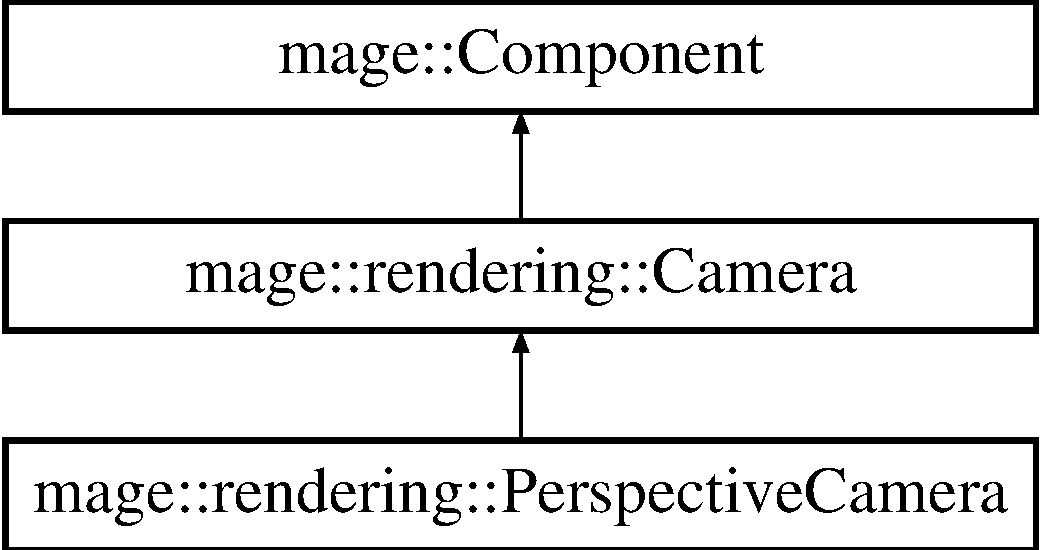
\includegraphics[height=3.000000cm]{classmage_1_1rendering_1_1_perspective_camera}
\end{center}
\end{figure}
\subsection*{Public Member Functions}
\begin{DoxyCompactItemize}
\item 
\hyperlink{classmage_1_1rendering_1_1_perspective_camera_ab478643eb5a2285d330b228287cc0187}{Perspective\+Camera} (I\+D3\+D11\+Device \&device)
\item 
\hyperlink{classmage_1_1rendering_1_1_perspective_camera_ad4b54caa651462e68089436a8a1f8dc0}{Perspective\+Camera} (const \hyperlink{classmage_1_1rendering_1_1_perspective_camera}{Perspective\+Camera} \&camera)=delete
\item 
\hyperlink{classmage_1_1rendering_1_1_perspective_camera_a3d342252cefbffe69537e1ccc95a379a}{Perspective\+Camera} (\hyperlink{classmage_1_1rendering_1_1_perspective_camera}{Perspective\+Camera} \&\&camera) noexcept
\item 
virtual \hyperlink{classmage_1_1rendering_1_1_perspective_camera_ac9bc0faebd323ca26d0311e35612d219}{$\sim$\+Perspective\+Camera} ()
\item 
\hyperlink{classmage_1_1rendering_1_1_perspective_camera}{Perspective\+Camera} \& \hyperlink{classmage_1_1rendering_1_1_perspective_camera_ac9119d544f7ca6c4fbe1a6c5118bcd66}{operator=} (const \hyperlink{classmage_1_1rendering_1_1_perspective_camera}{Perspective\+Camera} \&camera)=delete
\item 
\hyperlink{classmage_1_1rendering_1_1_perspective_camera}{Perspective\+Camera} \& \hyperlink{classmage_1_1rendering_1_1_perspective_camera_ac5b98cb14cd16dffd1a46c4e52ef72a8}{operator=} (\hyperlink{classmage_1_1rendering_1_1_perspective_camera}{Perspective\+Camera} \&\&camera) noexcept
\item 
\hyperlink{namespacemage_aa97e833b45f06d60a0a9c4fc22ae02c0}{F32} \hyperlink{classmage_1_1rendering_1_1_perspective_camera_a3308ee4d7ec6830c04ed3f4fc01f81ac}{Get\+F\+O\+VX} () const noexcept
\item 
\hyperlink{namespacemage_aa97e833b45f06d60a0a9c4fc22ae02c0}{F32} \hyperlink{classmage_1_1rendering_1_1_perspective_camera_ae6be4458a427e626ec7299c5898ffd38}{Get\+F\+O\+VY} () const noexcept
\item 
void \hyperlink{classmage_1_1rendering_1_1_perspective_camera_ab9ae2a2ae24ff7934a31305a1a0decf7}{Set\+F\+O\+VY} (\hyperlink{namespacemage_aa97e833b45f06d60a0a9c4fc22ae02c0}{F32} fov\+\_\+y) noexcept
\item 
\hyperlink{namespacemage_aa97e833b45f06d60a0a9c4fc22ae02c0}{F32} \hyperlink{classmage_1_1rendering_1_1_perspective_camera_a835369a1652074eed3a7d09e01a40430}{Get\+Aspect\+Ratio} () const noexcept
\item 
void \hyperlink{classmage_1_1rendering_1_1_perspective_camera_a180f74e8b39609aee8dcc2741a74076f}{Set\+Aspect\+Ratio} (\hyperlink{namespacemage_aa97e833b45f06d60a0a9c4fc22ae02c0}{F32} aspect\+\_\+ratio) noexcept
\item 
void \hyperlink{classmage_1_1rendering_1_1_perspective_camera_a09a93f5281723ec6ccf1adf636619e60}{Set\+Aspect\+Ratio} (\hyperlink{namespacemage_aa97e833b45f06d60a0a9c4fc22ae02c0}{F32} width, \hyperlink{namespacemage_aa97e833b45f06d60a0a9c4fc22ae02c0}{F32} height) noexcept
\item 
void \hyperlink{classmage_1_1rendering_1_1_perspective_camera_a3eff3d0cf0cbdba0682e0932cdb17886}{Set\+View\+To\+Projection\+Matrix} (\hyperlink{namespacemage_aa97e833b45f06d60a0a9c4fc22ae02c0}{F32} aspect\+\_\+ratio, \hyperlink{namespacemage_aa97e833b45f06d60a0a9c4fc22ae02c0}{F32} fov\+\_\+y, \hyperlink{namespacemage_aa97e833b45f06d60a0a9c4fc22ae02c0}{F32} near\+\_\+z, \hyperlink{namespacemage_aa97e833b45f06d60a0a9c4fc22ae02c0}{F32} far\+\_\+z) noexcept
\item 
void \hyperlink{classmage_1_1rendering_1_1_perspective_camera_a917ffbdee3cd5095568d69d3209912f0}{Set\+Camera\+To\+Projection\+Matrix} (\hyperlink{namespacemage_aa97e833b45f06d60a0a9c4fc22ae02c0}{F32} width, \hyperlink{namespacemage_aa97e833b45f06d60a0a9c4fc22ae02c0}{F32} height, \hyperlink{namespacemage_aa97e833b45f06d60a0a9c4fc22ae02c0}{F32} fov\+\_\+y, \hyperlink{namespacemage_aa97e833b45f06d60a0a9c4fc22ae02c0}{F32} near\+\_\+z, \hyperlink{namespacemage_aa97e833b45f06d60a0a9c4fc22ae02c0}{F32} far\+\_\+z) noexcept
\item 
virtual const X\+M\+M\+A\+T\+R\+IX X\+M\+\_\+\+C\+A\+L\+L\+C\+O\+NV \hyperlink{classmage_1_1rendering_1_1_perspective_camera_af0892905a0030fc70bdc629007cde5a0}{Get\+Camera\+To\+Projection\+Matrix} () const noexcept override
\item 
virtual const X\+M\+M\+A\+T\+R\+IX X\+M\+\_\+\+C\+A\+L\+L\+C\+O\+NV \hyperlink{classmage_1_1rendering_1_1_perspective_camera_af049c6330ebdaa822bfd31dc88f25ac2}{Get\+Projection\+To\+Camera\+Matrix} () const noexcept override
\end{DoxyCompactItemize}
\subsection*{Private Attributes}
\begin{DoxyCompactItemize}
\item 
\hyperlink{namespacemage_aa97e833b45f06d60a0a9c4fc22ae02c0}{F32} \hyperlink{classmage_1_1rendering_1_1_perspective_camera_a28abd925a9694954dcd26a4c16b6ac6d}{m\+\_\+aspect\+\_\+ratio}
\item 
\hyperlink{namespacemage_aa97e833b45f06d60a0a9c4fc22ae02c0}{F32} \hyperlink{classmage_1_1rendering_1_1_perspective_camera_afa70744921fce139d518730f998bd566}{m\+\_\+fov\+\_\+y}
\end{DoxyCompactItemize}
\subsection*{Additional Inherited Members}


\subsection{Detailed Description}
A class of perspective cameras. 

\subsection{Constructor \& Destructor Documentation}
\hypertarget{classmage_1_1rendering_1_1_perspective_camera_ab478643eb5a2285d330b228287cc0187}{}\label{classmage_1_1rendering_1_1_perspective_camera_ab478643eb5a2285d330b228287cc0187} 
\index{mage\+::rendering\+::\+Perspective\+Camera@{mage\+::rendering\+::\+Perspective\+Camera}!Perspective\+Camera@{Perspective\+Camera}}
\index{Perspective\+Camera@{Perspective\+Camera}!mage\+::rendering\+::\+Perspective\+Camera@{mage\+::rendering\+::\+Perspective\+Camera}}
\subsubsection{\texorpdfstring{Perspective\+Camera()}{PerspectiveCamera()}\hspace{0.1cm}{\footnotesize\ttfamily [1/3]}}
{\footnotesize\ttfamily mage\+::rendering\+::\+Perspective\+Camera\+::\+Perspective\+Camera (\begin{DoxyParamCaption}\item[{I\+D3\+D11\+Device \&}]{device }\end{DoxyParamCaption})}

Constructs a perspective camera.


\begin{DoxyParams}[1]{Parameters}
\mbox{\tt in}  & {\em device} & A reference to the device. \\
\hline
\end{DoxyParams}
\hypertarget{classmage_1_1rendering_1_1_perspective_camera_ad4b54caa651462e68089436a8a1f8dc0}{}\label{classmage_1_1rendering_1_1_perspective_camera_ad4b54caa651462e68089436a8a1f8dc0} 
\index{mage\+::rendering\+::\+Perspective\+Camera@{mage\+::rendering\+::\+Perspective\+Camera}!Perspective\+Camera@{Perspective\+Camera}}
\index{Perspective\+Camera@{Perspective\+Camera}!mage\+::rendering\+::\+Perspective\+Camera@{mage\+::rendering\+::\+Perspective\+Camera}}
\subsubsection{\texorpdfstring{Perspective\+Camera()}{PerspectiveCamera()}\hspace{0.1cm}{\footnotesize\ttfamily [2/3]}}
{\footnotesize\ttfamily mage\+::rendering\+::\+Perspective\+Camera\+::\+Perspective\+Camera (\begin{DoxyParamCaption}\item[{const \hyperlink{classmage_1_1rendering_1_1_perspective_camera}{Perspective\+Camera} \&}]{camera }\end{DoxyParamCaption})\hspace{0.3cm}{\ttfamily [delete]}}

Constructs a perspective camera from the given perspective camera.


\begin{DoxyParams}[1]{Parameters}
\mbox{\tt in}  & {\em camera} & A reference to the perspective camera to copy. \\
\hline
\end{DoxyParams}
\hypertarget{classmage_1_1rendering_1_1_perspective_camera_a3d342252cefbffe69537e1ccc95a379a}{}\label{classmage_1_1rendering_1_1_perspective_camera_a3d342252cefbffe69537e1ccc95a379a} 
\index{mage\+::rendering\+::\+Perspective\+Camera@{mage\+::rendering\+::\+Perspective\+Camera}!Perspective\+Camera@{Perspective\+Camera}}
\index{Perspective\+Camera@{Perspective\+Camera}!mage\+::rendering\+::\+Perspective\+Camera@{mage\+::rendering\+::\+Perspective\+Camera}}
\subsubsection{\texorpdfstring{Perspective\+Camera()}{PerspectiveCamera()}\hspace{0.1cm}{\footnotesize\ttfamily [3/3]}}
{\footnotesize\ttfamily mage\+::rendering\+::\+Perspective\+Camera\+::\+Perspective\+Camera (\begin{DoxyParamCaption}\item[{\hyperlink{classmage_1_1rendering_1_1_perspective_camera}{Perspective\+Camera} \&\&}]{camera }\end{DoxyParamCaption})\hspace{0.3cm}{\ttfamily [default]}, {\ttfamily [noexcept]}}

Constructs a perspective camera by moving the given perspective camera.


\begin{DoxyParams}[1]{Parameters}
\mbox{\tt in}  & {\em camera} & A reference to the perspective camera to move. \\
\hline
\end{DoxyParams}
\hypertarget{classmage_1_1rendering_1_1_perspective_camera_ac9bc0faebd323ca26d0311e35612d219}{}\label{classmage_1_1rendering_1_1_perspective_camera_ac9bc0faebd323ca26d0311e35612d219} 
\index{mage\+::rendering\+::\+Perspective\+Camera@{mage\+::rendering\+::\+Perspective\+Camera}!````~Perspective\+Camera@{$\sim$\+Perspective\+Camera}}
\index{````~Perspective\+Camera@{$\sim$\+Perspective\+Camera}!mage\+::rendering\+::\+Perspective\+Camera@{mage\+::rendering\+::\+Perspective\+Camera}}
\subsubsection{\texorpdfstring{$\sim$\+Perspective\+Camera()}{~PerspectiveCamera()}}
{\footnotesize\ttfamily mage\+::rendering\+::\+Perspective\+Camera\+::$\sim$\+Perspective\+Camera (\begin{DoxyParamCaption}{ }\end{DoxyParamCaption})\hspace{0.3cm}{\ttfamily [virtual]}, {\ttfamily [default]}}

Destructs this perspective camera. 

\subsection{Member Function Documentation}
\hypertarget{classmage_1_1rendering_1_1_perspective_camera_a835369a1652074eed3a7d09e01a40430}{}\label{classmage_1_1rendering_1_1_perspective_camera_a835369a1652074eed3a7d09e01a40430} 
\index{mage\+::rendering\+::\+Perspective\+Camera@{mage\+::rendering\+::\+Perspective\+Camera}!Get\+Aspect\+Ratio@{Get\+Aspect\+Ratio}}
\index{Get\+Aspect\+Ratio@{Get\+Aspect\+Ratio}!mage\+::rendering\+::\+Perspective\+Camera@{mage\+::rendering\+::\+Perspective\+Camera}}
\subsubsection{\texorpdfstring{Get\+Aspect\+Ratio()}{GetAspectRatio()}}
{\footnotesize\ttfamily \hyperlink{namespacemage_aa97e833b45f06d60a0a9c4fc22ae02c0}{F32} mage\+::rendering\+::\+Perspective\+Camera\+::\+Get\+Aspect\+Ratio (\begin{DoxyParamCaption}{ }\end{DoxyParamCaption}) const\hspace{0.3cm}{\ttfamily [noexcept]}}

Returns the aspect ratio of this perspective camera.

\begin{DoxyReturn}{Returns}
The aspect ratio of this perspective camera. 
\end{DoxyReturn}
\hypertarget{classmage_1_1rendering_1_1_perspective_camera_af0892905a0030fc70bdc629007cde5a0}{}\label{classmage_1_1rendering_1_1_perspective_camera_af0892905a0030fc70bdc629007cde5a0} 
\index{mage\+::rendering\+::\+Perspective\+Camera@{mage\+::rendering\+::\+Perspective\+Camera}!Get\+Camera\+To\+Projection\+Matrix@{Get\+Camera\+To\+Projection\+Matrix}}
\index{Get\+Camera\+To\+Projection\+Matrix@{Get\+Camera\+To\+Projection\+Matrix}!mage\+::rendering\+::\+Perspective\+Camera@{mage\+::rendering\+::\+Perspective\+Camera}}
\subsubsection{\texorpdfstring{Get\+Camera\+To\+Projection\+Matrix()}{GetCameraToProjectionMatrix()}}
{\footnotesize\ttfamily virtual const X\+M\+M\+A\+T\+R\+IX X\+M\+\_\+\+C\+A\+L\+L\+C\+O\+NV mage\+::rendering\+::\+Perspective\+Camera\+::\+Get\+Camera\+To\+Projection\+Matrix (\begin{DoxyParamCaption}{ }\end{DoxyParamCaption}) const\hspace{0.3cm}{\ttfamily [override]}, {\ttfamily [virtual]}, {\ttfamily [noexcept]}}

Returns the camera-\/to-\/projection matrix of this perspective camera.

\begin{DoxyReturn}{Returns}
The camera-\/to-\/projection matrix of this perspective camera. 
\end{DoxyReturn}


Implements \hyperlink{classmage_1_1rendering_1_1_camera_a08481175c3718a24333b22176e240d44}{mage\+::rendering\+::\+Camera}.

\hypertarget{classmage_1_1rendering_1_1_perspective_camera_a3308ee4d7ec6830c04ed3f4fc01f81ac}{}\label{classmage_1_1rendering_1_1_perspective_camera_a3308ee4d7ec6830c04ed3f4fc01f81ac} 
\index{mage\+::rendering\+::\+Perspective\+Camera@{mage\+::rendering\+::\+Perspective\+Camera}!Get\+F\+O\+VX@{Get\+F\+O\+VX}}
\index{Get\+F\+O\+VX@{Get\+F\+O\+VX}!mage\+::rendering\+::\+Perspective\+Camera@{mage\+::rendering\+::\+Perspective\+Camera}}
\subsubsection{\texorpdfstring{Get\+F\+O\+V\+X()}{GetFOVX()}}
{\footnotesize\ttfamily \hyperlink{namespacemage_aa97e833b45f06d60a0a9c4fc22ae02c0}{F32} mage\+::rendering\+::\+Perspective\+Camera\+::\+Get\+F\+O\+VX (\begin{DoxyParamCaption}{ }\end{DoxyParamCaption}) const\hspace{0.3cm}{\ttfamily [noexcept]}}

Returns the horizontal field-\/of-\/view of this perspective camera.

\begin{DoxyReturn}{Returns}
The horizontal field-\/of-\/view of this perspective camera. 
\end{DoxyReturn}
\hypertarget{classmage_1_1rendering_1_1_perspective_camera_ae6be4458a427e626ec7299c5898ffd38}{}\label{classmage_1_1rendering_1_1_perspective_camera_ae6be4458a427e626ec7299c5898ffd38} 
\index{mage\+::rendering\+::\+Perspective\+Camera@{mage\+::rendering\+::\+Perspective\+Camera}!Get\+F\+O\+VY@{Get\+F\+O\+VY}}
\index{Get\+F\+O\+VY@{Get\+F\+O\+VY}!mage\+::rendering\+::\+Perspective\+Camera@{mage\+::rendering\+::\+Perspective\+Camera}}
\subsubsection{\texorpdfstring{Get\+F\+O\+V\+Y()}{GetFOVY()}}
{\footnotesize\ttfamily \hyperlink{namespacemage_aa97e833b45f06d60a0a9c4fc22ae02c0}{F32} mage\+::rendering\+::\+Perspective\+Camera\+::\+Get\+F\+O\+VY (\begin{DoxyParamCaption}{ }\end{DoxyParamCaption}) const\hspace{0.3cm}{\ttfamily [noexcept]}}

Returns the vertical field-\/of-\/view of this perspective camera.

\begin{DoxyReturn}{Returns}
The vertical field-\/of-\/view of this perspective camera. 
\end{DoxyReturn}
\hypertarget{classmage_1_1rendering_1_1_perspective_camera_af049c6330ebdaa822bfd31dc88f25ac2}{}\label{classmage_1_1rendering_1_1_perspective_camera_af049c6330ebdaa822bfd31dc88f25ac2} 
\index{mage\+::rendering\+::\+Perspective\+Camera@{mage\+::rendering\+::\+Perspective\+Camera}!Get\+Projection\+To\+Camera\+Matrix@{Get\+Projection\+To\+Camera\+Matrix}}
\index{Get\+Projection\+To\+Camera\+Matrix@{Get\+Projection\+To\+Camera\+Matrix}!mage\+::rendering\+::\+Perspective\+Camera@{mage\+::rendering\+::\+Perspective\+Camera}}
\subsubsection{\texorpdfstring{Get\+Projection\+To\+Camera\+Matrix()}{GetProjectionToCameraMatrix()}}
{\footnotesize\ttfamily virtual const X\+M\+M\+A\+T\+R\+IX X\+M\+\_\+\+C\+A\+L\+L\+C\+O\+NV mage\+::rendering\+::\+Perspective\+Camera\+::\+Get\+Projection\+To\+Camera\+Matrix (\begin{DoxyParamCaption}{ }\end{DoxyParamCaption}) const\hspace{0.3cm}{\ttfamily [override]}, {\ttfamily [virtual]}, {\ttfamily [noexcept]}}

Returns the projection-\/to-\/camera matrix of this perspective camera.

\begin{DoxyReturn}{Returns}
The projection-\/to-\/camera matrix of this perspective camera. 
\end{DoxyReturn}


Implements \hyperlink{classmage_1_1rendering_1_1_camera_abb21116f8a6c7513804431d23fa4cf17}{mage\+::rendering\+::\+Camera}.

\hypertarget{classmage_1_1rendering_1_1_perspective_camera_ac9119d544f7ca6c4fbe1a6c5118bcd66}{}\label{classmage_1_1rendering_1_1_perspective_camera_ac9119d544f7ca6c4fbe1a6c5118bcd66} 
\index{mage\+::rendering\+::\+Perspective\+Camera@{mage\+::rendering\+::\+Perspective\+Camera}!operator=@{operator=}}
\index{operator=@{operator=}!mage\+::rendering\+::\+Perspective\+Camera@{mage\+::rendering\+::\+Perspective\+Camera}}
\subsubsection{\texorpdfstring{operator=()}{operator=()}\hspace{0.1cm}{\footnotesize\ttfamily [1/2]}}
{\footnotesize\ttfamily \hyperlink{classmage_1_1rendering_1_1_perspective_camera}{Perspective\+Camera}\& mage\+::rendering\+::\+Perspective\+Camera\+::operator= (\begin{DoxyParamCaption}\item[{const \hyperlink{classmage_1_1rendering_1_1_perspective_camera}{Perspective\+Camera} \&}]{camera }\end{DoxyParamCaption})\hspace{0.3cm}{\ttfamily [delete]}}

Copies the given perspective camera to this perspective camera.


\begin{DoxyParams}[1]{Parameters}
\mbox{\tt in}  & {\em camera} & A reference to the perspective camera to copy. \\
\hline
\end{DoxyParams}
\begin{DoxyReturn}{Returns}
A reference to the copy of the given perspective camera (i.\+e. this perspective camera). 
\end{DoxyReturn}
\hypertarget{classmage_1_1rendering_1_1_perspective_camera_ac5b98cb14cd16dffd1a46c4e52ef72a8}{}\label{classmage_1_1rendering_1_1_perspective_camera_ac5b98cb14cd16dffd1a46c4e52ef72a8} 
\index{mage\+::rendering\+::\+Perspective\+Camera@{mage\+::rendering\+::\+Perspective\+Camera}!operator=@{operator=}}
\index{operator=@{operator=}!mage\+::rendering\+::\+Perspective\+Camera@{mage\+::rendering\+::\+Perspective\+Camera}}
\subsubsection{\texorpdfstring{operator=()}{operator=()}\hspace{0.1cm}{\footnotesize\ttfamily [2/2]}}
{\footnotesize\ttfamily \hyperlink{classmage_1_1rendering_1_1_perspective_camera}{Perspective\+Camera} \& mage\+::rendering\+::\+Perspective\+Camera\+::operator= (\begin{DoxyParamCaption}\item[{\hyperlink{classmage_1_1rendering_1_1_perspective_camera}{Perspective\+Camera} \&\&}]{camera }\end{DoxyParamCaption})\hspace{0.3cm}{\ttfamily [default]}, {\ttfamily [noexcept]}}

Moves the given perspective camera to this perspective camera.


\begin{DoxyParams}[1]{Parameters}
\mbox{\tt in}  & {\em camera} & A reference to the perspective camera to move. \\
\hline
\end{DoxyParams}
\begin{DoxyReturn}{Returns}
A reference to the moved perspective camera (i.\+e. this perspective camera). 
\end{DoxyReturn}
\hypertarget{classmage_1_1rendering_1_1_perspective_camera_a180f74e8b39609aee8dcc2741a74076f}{}\label{classmage_1_1rendering_1_1_perspective_camera_a180f74e8b39609aee8dcc2741a74076f} 
\index{mage\+::rendering\+::\+Perspective\+Camera@{mage\+::rendering\+::\+Perspective\+Camera}!Set\+Aspect\+Ratio@{Set\+Aspect\+Ratio}}
\index{Set\+Aspect\+Ratio@{Set\+Aspect\+Ratio}!mage\+::rendering\+::\+Perspective\+Camera@{mage\+::rendering\+::\+Perspective\+Camera}}
\subsubsection{\texorpdfstring{Set\+Aspect\+Ratio()}{SetAspectRatio()}\hspace{0.1cm}{\footnotesize\ttfamily [1/2]}}
{\footnotesize\ttfamily void mage\+::rendering\+::\+Perspective\+Camera\+::\+Set\+Aspect\+Ratio (\begin{DoxyParamCaption}\item[{\hyperlink{namespacemage_aa97e833b45f06d60a0a9c4fc22ae02c0}{F32}}]{aspect\+\_\+ratio }\end{DoxyParamCaption})\hspace{0.3cm}{\ttfamily [noexcept]}}

Sets the aspect ratio of this perspective camera to the given value.


\begin{DoxyParams}[1]{Parameters}
\mbox{\tt in}  & {\em aspect\+\_\+ratio} & The aspect ratio. \\
\hline
\end{DoxyParams}
\hypertarget{classmage_1_1rendering_1_1_perspective_camera_a09a93f5281723ec6ccf1adf636619e60}{}\label{classmage_1_1rendering_1_1_perspective_camera_a09a93f5281723ec6ccf1adf636619e60} 
\index{mage\+::rendering\+::\+Perspective\+Camera@{mage\+::rendering\+::\+Perspective\+Camera}!Set\+Aspect\+Ratio@{Set\+Aspect\+Ratio}}
\index{Set\+Aspect\+Ratio@{Set\+Aspect\+Ratio}!mage\+::rendering\+::\+Perspective\+Camera@{mage\+::rendering\+::\+Perspective\+Camera}}
\subsubsection{\texorpdfstring{Set\+Aspect\+Ratio()}{SetAspectRatio()}\hspace{0.1cm}{\footnotesize\ttfamily [2/2]}}
{\footnotesize\ttfamily void mage\+::rendering\+::\+Perspective\+Camera\+::\+Set\+Aspect\+Ratio (\begin{DoxyParamCaption}\item[{\hyperlink{namespacemage_aa97e833b45f06d60a0a9c4fc22ae02c0}{F32}}]{width,  }\item[{\hyperlink{namespacemage_aa97e833b45f06d60a0a9c4fc22ae02c0}{F32}}]{height }\end{DoxyParamCaption})\hspace{0.3cm}{\ttfamily [noexcept]}}

Sets the aspect ratio of this perspective camera.


\begin{DoxyParams}[1]{Parameters}
\mbox{\tt in}  & {\em width} & The width. \\
\hline
\mbox{\tt in}  & {\em height} & The height. \\
\hline
\end{DoxyParams}
\hypertarget{classmage_1_1rendering_1_1_perspective_camera_a917ffbdee3cd5095568d69d3209912f0}{}\label{classmage_1_1rendering_1_1_perspective_camera_a917ffbdee3cd5095568d69d3209912f0} 
\index{mage\+::rendering\+::\+Perspective\+Camera@{mage\+::rendering\+::\+Perspective\+Camera}!Set\+Camera\+To\+Projection\+Matrix@{Set\+Camera\+To\+Projection\+Matrix}}
\index{Set\+Camera\+To\+Projection\+Matrix@{Set\+Camera\+To\+Projection\+Matrix}!mage\+::rendering\+::\+Perspective\+Camera@{mage\+::rendering\+::\+Perspective\+Camera}}
\subsubsection{\texorpdfstring{Set\+Camera\+To\+Projection\+Matrix()}{SetCameraToProjectionMatrix()}}
{\footnotesize\ttfamily void mage\+::rendering\+::\+Perspective\+Camera\+::\+Set\+Camera\+To\+Projection\+Matrix (\begin{DoxyParamCaption}\item[{\hyperlink{namespacemage_aa97e833b45f06d60a0a9c4fc22ae02c0}{F32}}]{width,  }\item[{\hyperlink{namespacemage_aa97e833b45f06d60a0a9c4fc22ae02c0}{F32}}]{height,  }\item[{\hyperlink{namespacemage_aa97e833b45f06d60a0a9c4fc22ae02c0}{F32}}]{fov\+\_\+y,  }\item[{\hyperlink{namespacemage_aa97e833b45f06d60a0a9c4fc22ae02c0}{F32}}]{near\+\_\+z,  }\item[{\hyperlink{namespacemage_aa97e833b45f06d60a0a9c4fc22ae02c0}{F32}}]{far\+\_\+z }\end{DoxyParamCaption})\hspace{0.3cm}{\ttfamily [noexcept]}}

Sets the camera-\/to-\/projection matrix of this perspective camera.


\begin{DoxyParams}[1]{Parameters}
\mbox{\tt in}  & {\em width} & The width. \\
\hline
\mbox{\tt in}  & {\em height} & The height. \\
\hline
\mbox{\tt in}  & {\em fov\+\_\+y} & The vertical field-\/of-\/view. \\
\hline
\mbox{\tt in}  & {\em near\+\_\+z} & The position of the near z-\/plane in view space. \\
\hline
\mbox{\tt in}  & {\em far\+\_\+z} & The position of the far z-\/plane in view space. \\
\hline
\end{DoxyParams}
\hypertarget{classmage_1_1rendering_1_1_perspective_camera_ab9ae2a2ae24ff7934a31305a1a0decf7}{}\label{classmage_1_1rendering_1_1_perspective_camera_ab9ae2a2ae24ff7934a31305a1a0decf7} 
\index{mage\+::rendering\+::\+Perspective\+Camera@{mage\+::rendering\+::\+Perspective\+Camera}!Set\+F\+O\+VY@{Set\+F\+O\+VY}}
\index{Set\+F\+O\+VY@{Set\+F\+O\+VY}!mage\+::rendering\+::\+Perspective\+Camera@{mage\+::rendering\+::\+Perspective\+Camera}}
\subsubsection{\texorpdfstring{Set\+F\+O\+V\+Y()}{SetFOVY()}}
{\footnotesize\ttfamily void mage\+::rendering\+::\+Perspective\+Camera\+::\+Set\+F\+O\+VY (\begin{DoxyParamCaption}\item[{\hyperlink{namespacemage_aa97e833b45f06d60a0a9c4fc22ae02c0}{F32}}]{fov\+\_\+y }\end{DoxyParamCaption})\hspace{0.3cm}{\ttfamily [noexcept]}}

Sets the vertical field-\/of-\/view of this perspective camera to the given value.


\begin{DoxyParams}[1]{Parameters}
\mbox{\tt in}  & {\em fov\+\_\+y} & The vertical field-\/of-\/view. \\
\hline
\end{DoxyParams}
\hypertarget{classmage_1_1rendering_1_1_perspective_camera_a3eff3d0cf0cbdba0682e0932cdb17886}{}\label{classmage_1_1rendering_1_1_perspective_camera_a3eff3d0cf0cbdba0682e0932cdb17886} 
\index{mage\+::rendering\+::\+Perspective\+Camera@{mage\+::rendering\+::\+Perspective\+Camera}!Set\+View\+To\+Projection\+Matrix@{Set\+View\+To\+Projection\+Matrix}}
\index{Set\+View\+To\+Projection\+Matrix@{Set\+View\+To\+Projection\+Matrix}!mage\+::rendering\+::\+Perspective\+Camera@{mage\+::rendering\+::\+Perspective\+Camera}}
\subsubsection{\texorpdfstring{Set\+View\+To\+Projection\+Matrix()}{SetViewToProjectionMatrix()}}
{\footnotesize\ttfamily void mage\+::rendering\+::\+Perspective\+Camera\+::\+Set\+View\+To\+Projection\+Matrix (\begin{DoxyParamCaption}\item[{\hyperlink{namespacemage_aa97e833b45f06d60a0a9c4fc22ae02c0}{F32}}]{aspect\+\_\+ratio,  }\item[{\hyperlink{namespacemage_aa97e833b45f06d60a0a9c4fc22ae02c0}{F32}}]{fov\+\_\+y,  }\item[{\hyperlink{namespacemage_aa97e833b45f06d60a0a9c4fc22ae02c0}{F32}}]{near\+\_\+z,  }\item[{\hyperlink{namespacemage_aa97e833b45f06d60a0a9c4fc22ae02c0}{F32}}]{far\+\_\+z }\end{DoxyParamCaption})\hspace{0.3cm}{\ttfamily [noexcept]}}

Sets the view-\/to-\/projection matrix of this perspective camera.


\begin{DoxyParams}[1]{Parameters}
\mbox{\tt in}  & {\em aspect\+\_\+ratio} & The aspect ratio. \\
\hline
\mbox{\tt in}  & {\em fov\+\_\+y} & The vertical field-\/of-\/view. \\
\hline
\mbox{\tt in}  & {\em near\+\_\+z} & The position of the near z-\/plane in view space. \\
\hline
\mbox{\tt in}  & {\em far\+\_\+z} & The position of the far z-\/plane in view space. \\
\hline
\end{DoxyParams}


\subsection{Member Data Documentation}
\hypertarget{classmage_1_1rendering_1_1_perspective_camera_a28abd925a9694954dcd26a4c16b6ac6d}{}\label{classmage_1_1rendering_1_1_perspective_camera_a28abd925a9694954dcd26a4c16b6ac6d} 
\index{mage\+::rendering\+::\+Perspective\+Camera@{mage\+::rendering\+::\+Perspective\+Camera}!m\+\_\+aspect\+\_\+ratio@{m\+\_\+aspect\+\_\+ratio}}
\index{m\+\_\+aspect\+\_\+ratio@{m\+\_\+aspect\+\_\+ratio}!mage\+::rendering\+::\+Perspective\+Camera@{mage\+::rendering\+::\+Perspective\+Camera}}
\subsubsection{\texorpdfstring{m\+\_\+aspect\+\_\+ratio}{m\_aspect\_ratio}}
{\footnotesize\ttfamily \hyperlink{namespacemage_aa97e833b45f06d60a0a9c4fc22ae02c0}{F32} mage\+::rendering\+::\+Perspective\+Camera\+::m\+\_\+aspect\+\_\+ratio\hspace{0.3cm}{\ttfamily [private]}}

The aspect ratio of this perspective camera. \hypertarget{classmage_1_1rendering_1_1_perspective_camera_afa70744921fce139d518730f998bd566}{}\label{classmage_1_1rendering_1_1_perspective_camera_afa70744921fce139d518730f998bd566} 
\index{mage\+::rendering\+::\+Perspective\+Camera@{mage\+::rendering\+::\+Perspective\+Camera}!m\+\_\+fov\+\_\+y@{m\+\_\+fov\+\_\+y}}
\index{m\+\_\+fov\+\_\+y@{m\+\_\+fov\+\_\+y}!mage\+::rendering\+::\+Perspective\+Camera@{mage\+::rendering\+::\+Perspective\+Camera}}
\subsubsection{\texorpdfstring{m\+\_\+fov\+\_\+y}{m\_fov\_y}}
{\footnotesize\ttfamily \hyperlink{namespacemage_aa97e833b45f06d60a0a9c4fc22ae02c0}{F32} mage\+::rendering\+::\+Perspective\+Camera\+::m\+\_\+fov\+\_\+y\hspace{0.3cm}{\ttfamily [private]}}

The vertical field-\/of-\/view of this perspective camera. 
\hypertarget{structmage_1_1rendering_1_1_pipeline}{}\section{mage\+:\+:rendering\+:\+:Pipeline Struct Reference}
\label{structmage_1_1rendering_1_1_pipeline}\index{mage\+::rendering\+::\+Pipeline@{mage\+::rendering\+::\+Pipeline}}


{\ttfamily \#include $<$pipeline.\+hpp$>$}

\subsection*{Classes}
\begin{DoxyCompactItemize}
\item 
struct \hyperlink{structmage_1_1rendering_1_1_pipeline_1_1_c_s}{CS}
\item 
struct \hyperlink{structmage_1_1rendering_1_1_pipeline_1_1_d_s}{DS}
\item 
struct \hyperlink{structmage_1_1rendering_1_1_pipeline_1_1_g_s}{GS}
\item 
struct \hyperlink{structmage_1_1rendering_1_1_pipeline_1_1_h_s}{HS}
\item 
struct \hyperlink{structmage_1_1rendering_1_1_pipeline_1_1_i_a}{IA}
\item 
struct \hyperlink{structmage_1_1rendering_1_1_pipeline_1_1_o_m}{OM}
\item 
struct \hyperlink{structmage_1_1rendering_1_1_pipeline_1_1_p_s}{PS}
\item 
struct \hyperlink{structmage_1_1rendering_1_1_pipeline_1_1_r_s}{RS}
\item 
struct \hyperlink{structmage_1_1rendering_1_1_pipeline_1_1_s_o}{SO}
\item 
struct \hyperlink{structmage_1_1rendering_1_1_pipeline_1_1_t_s}{TS}
\item 
struct \hyperlink{structmage_1_1rendering_1_1_pipeline_1_1_v_s}{VS}
\end{DoxyCompactItemize}
\subsection*{Static Public Member Functions}
\begin{DoxyCompactItemize}
\item 
static void \hyperlink{structmage_1_1rendering_1_1_pipeline_a30cdc51051e3fcab0d3a9c36efad40e4}{Draw\+Auto} (I\+D3\+D11\+Device\+Context \&device\+\_\+context) noexcept
\item 
static void \hyperlink{structmage_1_1rendering_1_1_pipeline_acc764fee84589a85e0e2df129b34b137}{Draw} (I\+D3\+D11\+Device\+Context \&device\+\_\+context, \hyperlink{namespacemage_a41c104c036fba3756a74e19f793eeaa1}{U32} nb\+\_\+vertices, \hyperlink{namespacemage_a41c104c036fba3756a74e19f793eeaa1}{U32} vertex\+\_\+start) noexcept
\item 
static void \hyperlink{structmage_1_1rendering_1_1_pipeline_af0d8580b1c0a672c3fc9558dc19408a3}{Draw\+Instanced} (I\+D3\+D11\+Device\+Context \&device\+\_\+context, \hyperlink{namespacemage_a41c104c036fba3756a74e19f793eeaa1}{U32} nb\+\_\+indices\+\_\+per\+\_\+instance, \hyperlink{namespacemage_a41c104c036fba3756a74e19f793eeaa1}{U32} nb\+\_\+instances, \hyperlink{namespacemage_a41c104c036fba3756a74e19f793eeaa1}{U32} vertex\+\_\+start, \hyperlink{namespacemage_a41c104c036fba3756a74e19f793eeaa1}{U32} instance\+\_\+start=0u) noexcept
\item 
static void \hyperlink{structmage_1_1rendering_1_1_pipeline_a8be1904461ee6bcd5e4b5b72d5cb79a8}{Draw\+Indexed} (I\+D3\+D11\+Device\+Context \&device\+\_\+context, \hyperlink{namespacemage_a41c104c036fba3756a74e19f793eeaa1}{U32} nb\+\_\+indices, \hyperlink{namespacemage_a41c104c036fba3756a74e19f793eeaa1}{U32} index\+\_\+start, \hyperlink{namespacemage_a41c104c036fba3756a74e19f793eeaa1}{U32} index\+\_\+offset=0u) noexcept
\item 
static void \hyperlink{structmage_1_1rendering_1_1_pipeline_a23ab5aea07be3bca0d9d7900518104b7}{Draw\+Indexed\+Instanced} (I\+D3\+D11\+Device\+Context \&device\+\_\+context, \hyperlink{namespacemage_a41c104c036fba3756a74e19f793eeaa1}{U32} nb\+\_\+indices\+\_\+per\+\_\+instance, \hyperlink{namespacemage_a41c104c036fba3756a74e19f793eeaa1}{U32} nb\+\_\+instances, \hyperlink{namespacemage_a41c104c036fba3756a74e19f793eeaa1}{U32} index\+\_\+start, \hyperlink{namespacemage_a41c104c036fba3756a74e19f793eeaa1}{U32} index\+\_\+offset=0u, U32 instance\+\_\+start=0u) noexcept
\item 
static void \hyperlink{structmage_1_1rendering_1_1_pipeline_a96bbf2861a3d4c10ba87c6b6f5228595}{Dispatch} (I\+D3\+D11\+Device\+Context \&device\+\_\+context, \hyperlink{namespacemage_a41c104c036fba3756a74e19f793eeaa1}{U32} nb\+\_\+thread\+\_\+groups\+\_\+x, \hyperlink{namespacemage_a41c104c036fba3756a74e19f793eeaa1}{U32} nb\+\_\+thread\+\_\+groups\+\_\+y, \hyperlink{namespacemage_a41c104c036fba3756a74e19f793eeaa1}{U32} nb\+\_\+thread\+\_\+groups\+\_\+z) noexcept
\item 
static void \hyperlink{structmage_1_1rendering_1_1_pipeline_acfdf1d2aba1e8c0db9c4ef9e9730f31c}{Draw\+Instanced\+Indirect} (I\+D3\+D11\+Device\+Context \&device\+\_\+context, I\+D3\+D11\+Buffer \&buffer, \hyperlink{namespacemage_a41c104c036fba3756a74e19f793eeaa1}{U32} byte\+\_\+offset) noexcept
\item 
static void \hyperlink{structmage_1_1rendering_1_1_pipeline_a51e2744827cbcf7791fcb40c0131d11b}{Draw\+Indexed\+Instanced\+Indirect} (I\+D3\+D11\+Device\+Context \&device\+\_\+context, I\+D3\+D11\+Buffer \&buffer, \hyperlink{namespacemage_a41c104c036fba3756a74e19f793eeaa1}{U32} byte\+\_\+offset) noexcept
\item 
static void \hyperlink{structmage_1_1rendering_1_1_pipeline_aceae5a9f2d24336e4424208a8e037a82}{Dispatch\+Indirect} (I\+D3\+D11\+Device\+Context \&device\+\_\+context, I\+D3\+D11\+Buffer \&buffer, \hyperlink{namespacemage_a41c104c036fba3756a74e19f793eeaa1}{U32} byte\+\_\+offset) noexcept
\item 
static H\+R\+E\+S\+U\+LT \hyperlink{structmage_1_1rendering_1_1_pipeline_ab0176557cd5473bf5cd77836ca2d924f}{Map} (I\+D3\+D11\+Device\+Context \&device\+\_\+context, I\+D3\+D11\+Resource \&resource, \hyperlink{namespacemage_a41c104c036fba3756a74e19f793eeaa1}{U32} subresource, D3\+D11\+\_\+\+M\+AP map\+\_\+type, \hyperlink{namespacemage_a41c104c036fba3756a74e19f793eeaa1}{U32} map\+\_\+flags, D3\+D11\+\_\+\+M\+A\+P\+P\+E\+D\+\_\+\+S\+U\+B\+R\+E\+S\+O\+U\+R\+CE \&mapped\+\_\+resource) noexcept
\item 
static void \hyperlink{structmage_1_1rendering_1_1_pipeline_ac4ad95111168cc62686da885da9ab161}{Unmap} (I\+D3\+D11\+Device\+Context \&device\+\_\+context, I\+D3\+D11\+Resource \&resource, \hyperlink{namespacemage_a41c104c036fba3756a74e19f793eeaa1}{U32} subresource) noexcept
\item 
static void \hyperlink{structmage_1_1rendering_1_1_pipeline_ae1de65a4f77e4db1fe0582ab85ef1335}{Update\+Subresource} (I\+D3\+D11\+Device\+Context \&device\+\_\+context, I\+D3\+D11\+Resource \&dst\+\_\+resource, \hyperlink{namespacemage_a41c104c036fba3756a74e19f793eeaa1}{U32} dst\+\_\+subresource, const void $\ast$src\+\_\+data, \hyperlink{namespacemage_a41c104c036fba3756a74e19f793eeaa1}{U32} src\+\_\+row\+\_\+pitch, \hyperlink{namespacemage_a41c104c036fba3756a74e19f793eeaa1}{U32} src\+\_\+depth\+\_\+pitch, const D3\+D11\+\_\+\+B\+OX $\ast$dst\+\_\+box=nullptr) noexcept
\item 
static void \hyperlink{structmage_1_1rendering_1_1_pipeline_a983ebf1363c8d3edd6830576e2258e48}{Bind\+Constant\+Buffer} (I\+D3\+D11\+Device\+Context \&device\+\_\+context, \hyperlink{namespacemage_a41c104c036fba3756a74e19f793eeaa1}{U32} slot, I\+D3\+D11\+Buffer $\ast$buffer) noexcept
\item 
static void \hyperlink{structmage_1_1rendering_1_1_pipeline_ad3a84d57712b74b98d10946482a78a2b}{Bind\+Constant\+Buffers} (I\+D3\+D11\+Device\+Context \&device\+\_\+context, \hyperlink{namespacemage_a41c104c036fba3756a74e19f793eeaa1}{U32} slot, \hyperlink{namespacemage_a41c104c036fba3756a74e19f793eeaa1}{U32} nb\+\_\+buffers, I\+D3\+D11\+Buffer $\ast$const $\ast$buffers) noexcept
\item 
static void \hyperlink{structmage_1_1rendering_1_1_pipeline_a28ed2d3639ac344b2d2334de54461ae9}{Bind\+S\+RV} (I\+D3\+D11\+Device\+Context \&device\+\_\+context, \hyperlink{namespacemage_a41c104c036fba3756a74e19f793eeaa1}{U32} slot, I\+D3\+D11\+Shader\+Resource\+View $\ast$srv) noexcept
\item 
static void \hyperlink{structmage_1_1rendering_1_1_pipeline_a38de6f4bfefc23eeeb50bdf0cc0e807d}{Bind\+S\+R\+Vs} (I\+D3\+D11\+Device\+Context \&device\+\_\+context, \hyperlink{namespacemage_a41c104c036fba3756a74e19f793eeaa1}{U32} slot, \hyperlink{namespacemage_a41c104c036fba3756a74e19f793eeaa1}{U32} nb\+\_\+srvs, I\+D3\+D11\+Shader\+Resource\+View $\ast$const $\ast$srvs) noexcept
\item 
static void \hyperlink{structmage_1_1rendering_1_1_pipeline_a3f43c5b1ed2d75d6c5ecf4b477185d0c}{Bind\+Sampler} (I\+D3\+D11\+Device\+Context \&device\+\_\+context, \hyperlink{namespacemage_a41c104c036fba3756a74e19f793eeaa1}{U32} slot, I\+D3\+D11\+Sampler\+State $\ast$sampler) noexcept
\item 
static void \hyperlink{structmage_1_1rendering_1_1_pipeline_a10286b4e2637c2956ecbcb0217d694fa}{Bind\+Samplers} (I\+D3\+D11\+Device\+Context \&device\+\_\+context, \hyperlink{namespacemage_a41c104c036fba3756a74e19f793eeaa1}{U32} slot, \hyperlink{namespacemage_a41c104c036fba3756a74e19f793eeaa1}{U32} nb\+\_\+samplers, I\+D3\+D11\+Sampler\+State $\ast$const $\ast$samplers) noexcept
\end{DoxyCompactItemize}
\subsection*{Static Public Attributes}
\begin{DoxyCompactItemize}
\item 
static constexpr D3\+D\+\_\+\+F\+E\+A\+T\+U\+R\+E\+\_\+\+L\+E\+V\+EL \hyperlink{structmage_1_1rendering_1_1_pipeline_a9748450c877ec6997796826258f3cbda}{s\+\_\+feature\+\_\+levels} \mbox{[}2\mbox{]}
\item 
static \hyperlink{namespacemage_a41c104c036fba3756a74e19f793eeaa1}{U32} \hyperlink{structmage_1_1rendering_1_1_pipeline_a47d649cdfea830ee048554accd2cab10}{s\+\_\+nb\+\_\+draws} = 0u
\end{DoxyCompactItemize}
\subsection*{Static Private Member Functions}
\begin{DoxyCompactItemize}
\item 
static void \hyperlink{structmage_1_1rendering_1_1_pipeline_a9a6c518c985fa0b759df1625ff13a335}{On\+Draw} () noexcept
\end{DoxyCompactItemize}


\subsection{Detailed Description}
The (rendering and compute) pipeline. 

\subsection{Member Function Documentation}
\hypertarget{structmage_1_1rendering_1_1_pipeline_a983ebf1363c8d3edd6830576e2258e48}{}\label{structmage_1_1rendering_1_1_pipeline_a983ebf1363c8d3edd6830576e2258e48} 
\index{mage\+::rendering\+::\+Pipeline@{mage\+::rendering\+::\+Pipeline}!Bind\+Constant\+Buffer@{Bind\+Constant\+Buffer}}
\index{Bind\+Constant\+Buffer@{Bind\+Constant\+Buffer}!mage\+::rendering\+::\+Pipeline@{mage\+::rendering\+::\+Pipeline}}
\subsubsection{\texorpdfstring{Bind\+Constant\+Buffer()}{BindConstantBuffer()}}
{\footnotesize\ttfamily static void mage\+::rendering\+::\+Pipeline\+::\+Bind\+Constant\+Buffer (\begin{DoxyParamCaption}\item[{I\+D3\+D11\+Device\+Context \&}]{device\+\_\+context,  }\item[{\hyperlink{namespacemage_a41c104c036fba3756a74e19f793eeaa1}{U32}}]{slot,  }\item[{I\+D3\+D11\+Buffer $\ast$}]{buffer }\end{DoxyParamCaption})\hspace{0.3cm}{\ttfamily [static]}, {\ttfamily [noexcept]}}

Binds a constant buffer to all shader stages.

\begin{DoxyPrecond}{Precondition}
{\itshape slot} $<$ {\ttfamily D3\+D11\+\_\+\+C\+O\+M\+M\+O\+N\+S\+H\+A\+D\+E\+R\+\_\+\+C\+O\+N\+S\+T\+A\+N\+T\+\_\+\+B\+U\+F\+F\+E\+R\+\_\+\+A\+P\+I\+\_\+\+S\+L\+O\+T\+\_\+\+C\+O\+U\+NT}. 
\end{DoxyPrecond}

\begin{DoxyParams}[1]{Parameters}
\mbox{\tt in}  & {\em device\+\_\+context} & A reference to the device context. \\
\hline
\mbox{\tt in}  & {\em slot} & The index into the device\textquotesingle{}s zero-\/based array to set the constant buffer to (ranges from 0 to {\ttfamily D3\+D11\+\_\+\+C\+O\+M\+M\+O\+N\+S\+H\+A\+D\+E\+R\+\_\+\+C\+O\+N\+S\+T\+A\+N\+T\+\_\+\+B\+U\+F\+F\+E\+R\+\_\+\+A\+P\+I\+\_\+\+S\+L\+O\+T\+\_\+\+C\+O\+U\+NT} -\/ 1). \\
\hline
\mbox{\tt in}  & {\em buffer} & A pointer to the constant buffer. \\
\hline
\end{DoxyParams}
\hypertarget{structmage_1_1rendering_1_1_pipeline_ad3a84d57712b74b98d10946482a78a2b}{}\label{structmage_1_1rendering_1_1_pipeline_ad3a84d57712b74b98d10946482a78a2b} 
\index{mage\+::rendering\+::\+Pipeline@{mage\+::rendering\+::\+Pipeline}!Bind\+Constant\+Buffers@{Bind\+Constant\+Buffers}}
\index{Bind\+Constant\+Buffers@{Bind\+Constant\+Buffers}!mage\+::rendering\+::\+Pipeline@{mage\+::rendering\+::\+Pipeline}}
\subsubsection{\texorpdfstring{Bind\+Constant\+Buffers()}{BindConstantBuffers()}}
{\footnotesize\ttfamily static void mage\+::rendering\+::\+Pipeline\+::\+Bind\+Constant\+Buffers (\begin{DoxyParamCaption}\item[{I\+D3\+D11\+Device\+Context \&}]{device\+\_\+context,  }\item[{\hyperlink{namespacemage_a41c104c036fba3756a74e19f793eeaa1}{U32}}]{slot,  }\item[{\hyperlink{namespacemage_a41c104c036fba3756a74e19f793eeaa1}{U32}}]{nb\+\_\+buffers,  }\item[{I\+D3\+D11\+Buffer $\ast$const $\ast$}]{buffers }\end{DoxyParamCaption})\hspace{0.3cm}{\ttfamily [static]}, {\ttfamily [noexcept]}}

Binds an array of constant buffers to all shader stages.

\begin{DoxyPrecond}{Precondition}
{\itshape slot} $<$ {\ttfamily D3\+D11\+\_\+\+C\+O\+M\+M\+O\+N\+S\+H\+A\+D\+E\+R\+\_\+\+C\+O\+N\+S\+T\+A\+N\+T\+\_\+\+B\+U\+F\+F\+E\+R\+\_\+\+A\+P\+I\+\_\+\+S\+L\+O\+T\+\_\+\+C\+O\+U\+NT}. 

{\itshape nb\+\_\+buffers} $<$ {\ttfamily D3\+D11\+\_\+\+C\+O\+M\+M\+O\+N\+S\+H\+A\+D\+E\+R\+\_\+\+C\+O\+N\+S\+T\+A\+N\+T\+\_\+\+B\+U\+F\+F\+E\+R\+\_\+\+A\+P\+I\+\_\+\+S\+L\+O\+T\+\_\+\+C\+O\+U\+NT} 
\begin{DoxyItemize}
\item {\itshape slot}. 
\end{DoxyItemize}

{\itshape buffers} points to an array containing at least {\itshape nb\+\_\+buffers} pointers to a constant buffer. 
\end{DoxyPrecond}

\begin{DoxyParams}[1]{Parameters}
\mbox{\tt in}  & {\em device\+\_\+context} & A reference to the device context. \\
\hline
\mbox{\tt in}  & {\em slot} & The index into the device\textquotesingle{}s zero-\/based array to begin setting constant buffers to (ranges from 0 to {\ttfamily D3\+D11\+\_\+\+C\+O\+M\+M\+O\+N\+S\+H\+A\+D\+E\+R\+\_\+\+C\+O\+N\+S\+T\+A\+N\+T\+\_\+\+B\+U\+F\+F\+E\+R\+\_\+\+A\+P\+I\+\_\+\+S\+L\+O\+T\+\_\+\+C\+O\+U\+NT} -\/ 1). \\
\hline
\mbox{\tt in}  & {\em nb\+\_\+buffers} & The number of constant buffers in the array (ranges from 0 to {\ttfamily D3\+D11\+\_\+\+C\+O\+M\+M\+O\+N\+S\+H\+A\+D\+E\+R\+\_\+\+C\+O\+N\+S\+T\+A\+N\+T\+\_\+\+B\+U\+F\+F\+E\+R\+\_\+\+A\+P\+I\+\_\+\+S\+L\+O\+T\+\_\+\+C\+O\+U\+NT} 
\begin{DoxyItemize}
\item {\itshape slot}). 
\end{DoxyItemize}\\
\hline
\mbox{\tt in}  & {\em buffers} & A pointer to an array of constant buffers. \\
\hline
\end{DoxyParams}
\hypertarget{structmage_1_1rendering_1_1_pipeline_a3f43c5b1ed2d75d6c5ecf4b477185d0c}{}\label{structmage_1_1rendering_1_1_pipeline_a3f43c5b1ed2d75d6c5ecf4b477185d0c} 
\index{mage\+::rendering\+::\+Pipeline@{mage\+::rendering\+::\+Pipeline}!Bind\+Sampler@{Bind\+Sampler}}
\index{Bind\+Sampler@{Bind\+Sampler}!mage\+::rendering\+::\+Pipeline@{mage\+::rendering\+::\+Pipeline}}
\subsubsection{\texorpdfstring{Bind\+Sampler()}{BindSampler()}}
{\footnotesize\ttfamily static void mage\+::rendering\+::\+Pipeline\+::\+Bind\+Sampler (\begin{DoxyParamCaption}\item[{I\+D3\+D11\+Device\+Context \&}]{device\+\_\+context,  }\item[{\hyperlink{namespacemage_a41c104c036fba3756a74e19f793eeaa1}{U32}}]{slot,  }\item[{I\+D3\+D11\+Sampler\+State $\ast$}]{sampler }\end{DoxyParamCaption})\hspace{0.3cm}{\ttfamily [static]}, {\ttfamily [noexcept]}}

Binds a sampler to all shader stages.

\begin{DoxyPrecond}{Precondition}
{\itshape slot} $<$ {\ttfamily D3\+D11\+\_\+\+C\+O\+M\+M\+O\+N\+S\+H\+A\+D\+E\+R\+\_\+\+S\+A\+M\+P\+L\+E\+R\+\_\+\+S\+L\+O\+T\+\_\+\+C\+O\+U\+NT}. 
\end{DoxyPrecond}

\begin{DoxyParams}[1]{Parameters}
\mbox{\tt in}  & {\em device\+\_\+context} & A reference to the device context. \\
\hline
\mbox{\tt in}  & {\em slot} & The index into the device\textquotesingle{}s zero-\/based array to set the sampler to (ranges from 0 to {\ttfamily D3\+D11\+\_\+\+C\+O\+M\+M\+O\+N\+S\+H\+A\+D\+E\+R\+\_\+\+S\+A\+M\+P\+L\+E\+R\+\_\+\+S\+L\+O\+T\+\_\+\+C\+O\+U\+NT} -\/ 1). \\
\hline
\mbox{\tt in}  & {\em sampler} & A pointer to the sampler. \\
\hline
\end{DoxyParams}
\hypertarget{structmage_1_1rendering_1_1_pipeline_a10286b4e2637c2956ecbcb0217d694fa}{}\label{structmage_1_1rendering_1_1_pipeline_a10286b4e2637c2956ecbcb0217d694fa} 
\index{mage\+::rendering\+::\+Pipeline@{mage\+::rendering\+::\+Pipeline}!Bind\+Samplers@{Bind\+Samplers}}
\index{Bind\+Samplers@{Bind\+Samplers}!mage\+::rendering\+::\+Pipeline@{mage\+::rendering\+::\+Pipeline}}
\subsubsection{\texorpdfstring{Bind\+Samplers()}{BindSamplers()}}
{\footnotesize\ttfamily static void mage\+::rendering\+::\+Pipeline\+::\+Bind\+Samplers (\begin{DoxyParamCaption}\item[{I\+D3\+D11\+Device\+Context \&}]{device\+\_\+context,  }\item[{\hyperlink{namespacemage_a41c104c036fba3756a74e19f793eeaa1}{U32}}]{slot,  }\item[{\hyperlink{namespacemage_a41c104c036fba3756a74e19f793eeaa1}{U32}}]{nb\+\_\+samplers,  }\item[{I\+D3\+D11\+Sampler\+State $\ast$const $\ast$}]{samplers }\end{DoxyParamCaption})\hspace{0.3cm}{\ttfamily [static]}, {\ttfamily [noexcept]}}

Binds an array of samplers to all shader stages.

\begin{DoxyPrecond}{Precondition}
{\itshape slot} $<$ {\ttfamily D3\+D11\+\_\+\+C\+O\+M\+M\+O\+N\+S\+H\+A\+D\+E\+R\+\_\+\+S\+A\+M\+P\+L\+E\+R\+\_\+\+S\+L\+O\+T\+\_\+\+C\+O\+U\+NT}. 

{\itshape nb\+\_\+samplers} $<$ {\ttfamily D3\+D11\+\_\+\+C\+O\+M\+M\+O\+N\+S\+H\+A\+D\+E\+R\+\_\+\+S\+A\+M\+P\+L\+E\+R\+\_\+\+S\+L\+O\+T\+\_\+\+C\+O\+U\+NT} 
\begin{DoxyItemize}
\item {\itshape slot}. 
\end{DoxyItemize}

{\itshape samplers} points to an array containing at least {\itshape nb\+\_\+samplers} pointers to a sampler. 
\end{DoxyPrecond}

\begin{DoxyParams}[1]{Parameters}
\mbox{\tt in}  & {\em device\+\_\+context} & A reference to the device context. \\
\hline
\mbox{\tt in}  & {\em slot} & The index into the device\textquotesingle{}s zero-\/based array to begin setting samplers to (ranges from 0 to {\ttfamily D3\+D11\+\_\+\+C\+O\+M\+M\+O\+N\+S\+H\+A\+D\+E\+R\+\_\+\+S\+A\+M\+P\+L\+E\+R\+\_\+\+S\+L\+O\+T\+\_\+\+C\+O\+U\+NT} -\/ 1). \\
\hline
\mbox{\tt in}  & {\em nb\+\_\+samplers} & The number of samplers in the array. Each pipeline stage has a total of 16 sampler slots available (ranges from 0 to {\ttfamily D3\+D11\+\_\+\+C\+O\+M\+M\+O\+N\+S\+H\+A\+D\+E\+R\+\_\+\+S\+A\+M\+P\+L\+E\+R\+\_\+\+S\+L\+O\+T\+\_\+\+C\+O\+U\+NT} -\/ {\itshape slot}). \\
\hline
\mbox{\tt in}  & {\em samplers} & A pointer to an array of samplers. \\
\hline
\end{DoxyParams}
\hypertarget{structmage_1_1rendering_1_1_pipeline_a28ed2d3639ac344b2d2334de54461ae9}{}\label{structmage_1_1rendering_1_1_pipeline_a28ed2d3639ac344b2d2334de54461ae9} 
\index{mage\+::rendering\+::\+Pipeline@{mage\+::rendering\+::\+Pipeline}!Bind\+S\+RV@{Bind\+S\+RV}}
\index{Bind\+S\+RV@{Bind\+S\+RV}!mage\+::rendering\+::\+Pipeline@{mage\+::rendering\+::\+Pipeline}}
\subsubsection{\texorpdfstring{Bind\+S\+R\+V()}{BindSRV()}}
{\footnotesize\ttfamily static void mage\+::rendering\+::\+Pipeline\+::\+Bind\+S\+RV (\begin{DoxyParamCaption}\item[{I\+D3\+D11\+Device\+Context \&}]{device\+\_\+context,  }\item[{\hyperlink{namespacemage_a41c104c036fba3756a74e19f793eeaa1}{U32}}]{slot,  }\item[{I\+D3\+D11\+Shader\+Resource\+View $\ast$}]{srv }\end{DoxyParamCaption})\hspace{0.3cm}{\ttfamily [static]}, {\ttfamily [noexcept]}}

Binds a shader resource view to all shader stages.

\begin{DoxyPrecond}{Precondition}
{\itshape slot} $<$ {\ttfamily D3\+D11\+\_\+\+C\+O\+M\+M\+O\+N\+S\+H\+A\+D\+E\+R\+\_\+\+I\+N\+P\+U\+T\+\_\+\+R\+E\+S\+O\+U\+R\+C\+E\+\_\+\+S\+L\+O\+T\+\_\+\+C\+O\+U\+NT}. 
\end{DoxyPrecond}

\begin{DoxyParams}[1]{Parameters}
\mbox{\tt in}  & {\em device\+\_\+context} & A reference to the device context. \\
\hline
\mbox{\tt in}  & {\em slot} & The index into the device\textquotesingle{}s zero-\/based array to set the shader resource view to (ranges from 0 to {\ttfamily D3\+D11\+\_\+\+C\+O\+M\+M\+O\+N\+S\+H\+A\+D\+E\+R\+\_\+\+I\+N\+P\+U\+T\+\_\+\+R\+E\+S\+O\+U\+R\+C\+E\+\_\+\+S\+L\+O\+T\+\_\+\+C\+O\+U\+NT} -\/ 1). \\
\hline
\mbox{\tt in}  & {\em srv} & A pointer to the shader resource view. \\
\hline
\end{DoxyParams}
\hypertarget{structmage_1_1rendering_1_1_pipeline_a38de6f4bfefc23eeeb50bdf0cc0e807d}{}\label{structmage_1_1rendering_1_1_pipeline_a38de6f4bfefc23eeeb50bdf0cc0e807d} 
\index{mage\+::rendering\+::\+Pipeline@{mage\+::rendering\+::\+Pipeline}!Bind\+S\+R\+Vs@{Bind\+S\+R\+Vs}}
\index{Bind\+S\+R\+Vs@{Bind\+S\+R\+Vs}!mage\+::rendering\+::\+Pipeline@{mage\+::rendering\+::\+Pipeline}}
\subsubsection{\texorpdfstring{Bind\+S\+R\+Vs()}{BindSRVs()}}
{\footnotesize\ttfamily static void mage\+::rendering\+::\+Pipeline\+::\+Bind\+S\+R\+Vs (\begin{DoxyParamCaption}\item[{I\+D3\+D11\+Device\+Context \&}]{device\+\_\+context,  }\item[{\hyperlink{namespacemage_a41c104c036fba3756a74e19f793eeaa1}{U32}}]{slot,  }\item[{\hyperlink{namespacemage_a41c104c036fba3756a74e19f793eeaa1}{U32}}]{nb\+\_\+srvs,  }\item[{I\+D3\+D11\+Shader\+Resource\+View $\ast$const $\ast$}]{srvs }\end{DoxyParamCaption})\hspace{0.3cm}{\ttfamily [static]}, {\ttfamily [noexcept]}}

Binds an array of shader resource views to all shaders stage.

\begin{DoxyPrecond}{Precondition}
{\itshape slot} $<$ {\ttfamily D3\+D11\+\_\+\+C\+O\+M\+M\+O\+N\+S\+H\+A\+D\+E\+R\+\_\+\+I\+N\+P\+U\+T\+\_\+\+R\+E\+S\+O\+U\+R\+C\+E\+\_\+\+S\+L\+O\+T\+\_\+\+C\+O\+U\+NT}. 

{\itshape nb\+\_\+srvs} $<$ {\ttfamily D3\+D11\+\_\+\+C\+O\+M\+M\+O\+N\+S\+H\+A\+D\+E\+R\+\_\+\+I\+N\+P\+U\+T\+\_\+\+R\+E\+S\+O\+U\+R\+C\+E\+\_\+\+S\+L\+O\+T\+\_\+\+C\+O\+U\+NT} 
\begin{DoxyItemize}
\item {\itshape slot}. 
\end{DoxyItemize}

{\itshape srvs} points to an array containing at least {\itshape nb\+\_\+srvs} pointers to a shader resource view. 
\end{DoxyPrecond}

\begin{DoxyParams}[1]{Parameters}
\mbox{\tt in}  & {\em device\+\_\+context} & A reference to the device context. \\
\hline
\mbox{\tt in}  & {\em slot} & The index into the device\textquotesingle{}s zero-\/based array to begin setting shader resource views to (ranges from 0 to {\ttfamily D3\+D11\+\_\+\+C\+O\+M\+M\+O\+N\+S\+H\+A\+D\+E\+R\+\_\+\+I\+N\+P\+U\+T\+\_\+\+R\+E\+S\+O\+U\+R\+C\+E\+\_\+\+S\+L\+O\+T\+\_\+\+C\+O\+U\+NT} -\/ 1). \\
\hline
\mbox{\tt in}  & {\em nb\+\_\+srvs} & The number of shader resource views in the array. Up to a maximum of 128 slots are available for shader resource views (ranges from 0 to {\ttfamily D3\+D11\+\_\+\+C\+O\+M\+M\+O\+N\+S\+H\+A\+D\+E\+R\+\_\+\+I\+N\+P\+U\+T\+\_\+\+R\+E\+S\+O\+U\+R\+C\+E\+\_\+\+S\+L\+O\+T\+\_\+\+C\+O\+U\+NT} -\/ {\itshape slot}). \\
\hline
\mbox{\tt in}  & {\em srvs} & A pointer to an array of shader resource views. \\
\hline
\end{DoxyParams}
\hypertarget{structmage_1_1rendering_1_1_pipeline_a96bbf2861a3d4c10ba87c6b6f5228595}{}\label{structmage_1_1rendering_1_1_pipeline_a96bbf2861a3d4c10ba87c6b6f5228595} 
\index{mage\+::rendering\+::\+Pipeline@{mage\+::rendering\+::\+Pipeline}!Dispatch@{Dispatch}}
\index{Dispatch@{Dispatch}!mage\+::rendering\+::\+Pipeline@{mage\+::rendering\+::\+Pipeline}}
\subsubsection{\texorpdfstring{Dispatch()}{Dispatch()}}
{\footnotesize\ttfamily static void mage\+::rendering\+::\+Pipeline\+::\+Dispatch (\begin{DoxyParamCaption}\item[{I\+D3\+D11\+Device\+Context \&}]{device\+\_\+context,  }\item[{\hyperlink{namespacemage_a41c104c036fba3756a74e19f793eeaa1}{U32}}]{nb\+\_\+thread\+\_\+groups\+\_\+x,  }\item[{\hyperlink{namespacemage_a41c104c036fba3756a74e19f793eeaa1}{U32}}]{nb\+\_\+thread\+\_\+groups\+\_\+y,  }\item[{\hyperlink{namespacemage_a41c104c036fba3756a74e19f793eeaa1}{U32}}]{nb\+\_\+thread\+\_\+groups\+\_\+z }\end{DoxyParamCaption})\hspace{0.3cm}{\ttfamily [static]}, {\ttfamily [noexcept]}}

\hypertarget{structmage_1_1rendering_1_1_pipeline_aceae5a9f2d24336e4424208a8e037a82}{}\label{structmage_1_1rendering_1_1_pipeline_aceae5a9f2d24336e4424208a8e037a82} 
\index{mage\+::rendering\+::\+Pipeline@{mage\+::rendering\+::\+Pipeline}!Dispatch\+Indirect@{Dispatch\+Indirect}}
\index{Dispatch\+Indirect@{Dispatch\+Indirect}!mage\+::rendering\+::\+Pipeline@{mage\+::rendering\+::\+Pipeline}}
\subsubsection{\texorpdfstring{Dispatch\+Indirect()}{DispatchIndirect()}}
{\footnotesize\ttfamily static void mage\+::rendering\+::\+Pipeline\+::\+Dispatch\+Indirect (\begin{DoxyParamCaption}\item[{I\+D3\+D11\+Device\+Context \&}]{device\+\_\+context,  }\item[{I\+D3\+D11\+Buffer \&}]{buffer,  }\item[{\hyperlink{namespacemage_a41c104c036fba3756a74e19f793eeaa1}{U32}}]{byte\+\_\+offset }\end{DoxyParamCaption})\hspace{0.3cm}{\ttfamily [static]}, {\ttfamily [noexcept]}}

\hypertarget{structmage_1_1rendering_1_1_pipeline_acc764fee84589a85e0e2df129b34b137}{}\label{structmage_1_1rendering_1_1_pipeline_acc764fee84589a85e0e2df129b34b137} 
\index{mage\+::rendering\+::\+Pipeline@{mage\+::rendering\+::\+Pipeline}!Draw@{Draw}}
\index{Draw@{Draw}!mage\+::rendering\+::\+Pipeline@{mage\+::rendering\+::\+Pipeline}}
\subsubsection{\texorpdfstring{Draw()}{Draw()}}
{\footnotesize\ttfamily static void mage\+::rendering\+::\+Pipeline\+::\+Draw (\begin{DoxyParamCaption}\item[{I\+D3\+D11\+Device\+Context \&}]{device\+\_\+context,  }\item[{\hyperlink{namespacemage_a41c104c036fba3756a74e19f793eeaa1}{U32}}]{nb\+\_\+vertices,  }\item[{\hyperlink{namespacemage_a41c104c036fba3756a74e19f793eeaa1}{U32}}]{vertex\+\_\+start }\end{DoxyParamCaption})\hspace{0.3cm}{\ttfamily [static]}, {\ttfamily [noexcept]}}

\hypertarget{structmage_1_1rendering_1_1_pipeline_a30cdc51051e3fcab0d3a9c36efad40e4}{}\label{structmage_1_1rendering_1_1_pipeline_a30cdc51051e3fcab0d3a9c36efad40e4} 
\index{mage\+::rendering\+::\+Pipeline@{mage\+::rendering\+::\+Pipeline}!Draw\+Auto@{Draw\+Auto}}
\index{Draw\+Auto@{Draw\+Auto}!mage\+::rendering\+::\+Pipeline@{mage\+::rendering\+::\+Pipeline}}
\subsubsection{\texorpdfstring{Draw\+Auto()}{DrawAuto()}}
{\footnotesize\ttfamily static void mage\+::rendering\+::\+Pipeline\+::\+Draw\+Auto (\begin{DoxyParamCaption}\item[{I\+D3\+D11\+Device\+Context \&}]{device\+\_\+context }\end{DoxyParamCaption})\hspace{0.3cm}{\ttfamily [static]}, {\ttfamily [noexcept]}}

\hypertarget{structmage_1_1rendering_1_1_pipeline_a8be1904461ee6bcd5e4b5b72d5cb79a8}{}\label{structmage_1_1rendering_1_1_pipeline_a8be1904461ee6bcd5e4b5b72d5cb79a8} 
\index{mage\+::rendering\+::\+Pipeline@{mage\+::rendering\+::\+Pipeline}!Draw\+Indexed@{Draw\+Indexed}}
\index{Draw\+Indexed@{Draw\+Indexed}!mage\+::rendering\+::\+Pipeline@{mage\+::rendering\+::\+Pipeline}}
\subsubsection{\texorpdfstring{Draw\+Indexed()}{DrawIndexed()}}
{\footnotesize\ttfamily static void mage\+::rendering\+::\+Pipeline\+::\+Draw\+Indexed (\begin{DoxyParamCaption}\item[{I\+D3\+D11\+Device\+Context \&}]{device\+\_\+context,  }\item[{\hyperlink{namespacemage_a41c104c036fba3756a74e19f793eeaa1}{U32}}]{nb\+\_\+indices,  }\item[{\hyperlink{namespacemage_a41c104c036fba3756a74e19f793eeaa1}{U32}}]{index\+\_\+start,  }\item[{\hyperlink{namespacemage_a41c104c036fba3756a74e19f793eeaa1}{U32}}]{index\+\_\+offset = {\ttfamily 0u} }\end{DoxyParamCaption})\hspace{0.3cm}{\ttfamily [static]}, {\ttfamily [noexcept]}}

\hypertarget{structmage_1_1rendering_1_1_pipeline_a23ab5aea07be3bca0d9d7900518104b7}{}\label{structmage_1_1rendering_1_1_pipeline_a23ab5aea07be3bca0d9d7900518104b7} 
\index{mage\+::rendering\+::\+Pipeline@{mage\+::rendering\+::\+Pipeline}!Draw\+Indexed\+Instanced@{Draw\+Indexed\+Instanced}}
\index{Draw\+Indexed\+Instanced@{Draw\+Indexed\+Instanced}!mage\+::rendering\+::\+Pipeline@{mage\+::rendering\+::\+Pipeline}}
\subsubsection{\texorpdfstring{Draw\+Indexed\+Instanced()}{DrawIndexedInstanced()}}
{\footnotesize\ttfamily static void mage\+::rendering\+::\+Pipeline\+::\+Draw\+Indexed\+Instanced (\begin{DoxyParamCaption}\item[{I\+D3\+D11\+Device\+Context \&}]{device\+\_\+context,  }\item[{\hyperlink{namespacemage_a41c104c036fba3756a74e19f793eeaa1}{U32}}]{nb\+\_\+indices\+\_\+per\+\_\+instance,  }\item[{\hyperlink{namespacemage_a41c104c036fba3756a74e19f793eeaa1}{U32}}]{nb\+\_\+instances,  }\item[{\hyperlink{namespacemage_a41c104c036fba3756a74e19f793eeaa1}{U32}}]{index\+\_\+start,  }\item[{\hyperlink{namespacemage_a41c104c036fba3756a74e19f793eeaa1}{U32}}]{index\+\_\+offset = {\ttfamily 0u},  }\item[{\hyperlink{namespacemage_a41c104c036fba3756a74e19f793eeaa1}{U32}}]{instance\+\_\+start = {\ttfamily 0u} }\end{DoxyParamCaption})\hspace{0.3cm}{\ttfamily [static]}, {\ttfamily [noexcept]}}

\hypertarget{structmage_1_1rendering_1_1_pipeline_a51e2744827cbcf7791fcb40c0131d11b}{}\label{structmage_1_1rendering_1_1_pipeline_a51e2744827cbcf7791fcb40c0131d11b} 
\index{mage\+::rendering\+::\+Pipeline@{mage\+::rendering\+::\+Pipeline}!Draw\+Indexed\+Instanced\+Indirect@{Draw\+Indexed\+Instanced\+Indirect}}
\index{Draw\+Indexed\+Instanced\+Indirect@{Draw\+Indexed\+Instanced\+Indirect}!mage\+::rendering\+::\+Pipeline@{mage\+::rendering\+::\+Pipeline}}
\subsubsection{\texorpdfstring{Draw\+Indexed\+Instanced\+Indirect()}{DrawIndexedInstancedIndirect()}}
{\footnotesize\ttfamily static void mage\+::rendering\+::\+Pipeline\+::\+Draw\+Indexed\+Instanced\+Indirect (\begin{DoxyParamCaption}\item[{I\+D3\+D11\+Device\+Context \&}]{device\+\_\+context,  }\item[{I\+D3\+D11\+Buffer \&}]{buffer,  }\item[{\hyperlink{namespacemage_a41c104c036fba3756a74e19f793eeaa1}{U32}}]{byte\+\_\+offset }\end{DoxyParamCaption})\hspace{0.3cm}{\ttfamily [static]}, {\ttfamily [noexcept]}}

\hypertarget{structmage_1_1rendering_1_1_pipeline_af0d8580b1c0a672c3fc9558dc19408a3}{}\label{structmage_1_1rendering_1_1_pipeline_af0d8580b1c0a672c3fc9558dc19408a3} 
\index{mage\+::rendering\+::\+Pipeline@{mage\+::rendering\+::\+Pipeline}!Draw\+Instanced@{Draw\+Instanced}}
\index{Draw\+Instanced@{Draw\+Instanced}!mage\+::rendering\+::\+Pipeline@{mage\+::rendering\+::\+Pipeline}}
\subsubsection{\texorpdfstring{Draw\+Instanced()}{DrawInstanced()}}
{\footnotesize\ttfamily static void mage\+::rendering\+::\+Pipeline\+::\+Draw\+Instanced (\begin{DoxyParamCaption}\item[{I\+D3\+D11\+Device\+Context \&}]{device\+\_\+context,  }\item[{\hyperlink{namespacemage_a41c104c036fba3756a74e19f793eeaa1}{U32}}]{nb\+\_\+indices\+\_\+per\+\_\+instance,  }\item[{\hyperlink{namespacemage_a41c104c036fba3756a74e19f793eeaa1}{U32}}]{nb\+\_\+instances,  }\item[{\hyperlink{namespacemage_a41c104c036fba3756a74e19f793eeaa1}{U32}}]{vertex\+\_\+start,  }\item[{\hyperlink{namespacemage_a41c104c036fba3756a74e19f793eeaa1}{U32}}]{instance\+\_\+start = {\ttfamily 0u} }\end{DoxyParamCaption})\hspace{0.3cm}{\ttfamily [static]}, {\ttfamily [noexcept]}}

\hypertarget{structmage_1_1rendering_1_1_pipeline_acfdf1d2aba1e8c0db9c4ef9e9730f31c}{}\label{structmage_1_1rendering_1_1_pipeline_acfdf1d2aba1e8c0db9c4ef9e9730f31c} 
\index{mage\+::rendering\+::\+Pipeline@{mage\+::rendering\+::\+Pipeline}!Draw\+Instanced\+Indirect@{Draw\+Instanced\+Indirect}}
\index{Draw\+Instanced\+Indirect@{Draw\+Instanced\+Indirect}!mage\+::rendering\+::\+Pipeline@{mage\+::rendering\+::\+Pipeline}}
\subsubsection{\texorpdfstring{Draw\+Instanced\+Indirect()}{DrawInstancedIndirect()}}
{\footnotesize\ttfamily static void mage\+::rendering\+::\+Pipeline\+::\+Draw\+Instanced\+Indirect (\begin{DoxyParamCaption}\item[{I\+D3\+D11\+Device\+Context \&}]{device\+\_\+context,  }\item[{I\+D3\+D11\+Buffer \&}]{buffer,  }\item[{\hyperlink{namespacemage_a41c104c036fba3756a74e19f793eeaa1}{U32}}]{byte\+\_\+offset }\end{DoxyParamCaption})\hspace{0.3cm}{\ttfamily [static]}, {\ttfamily [noexcept]}}

\hypertarget{structmage_1_1rendering_1_1_pipeline_ab0176557cd5473bf5cd77836ca2d924f}{}\label{structmage_1_1rendering_1_1_pipeline_ab0176557cd5473bf5cd77836ca2d924f} 
\index{mage\+::rendering\+::\+Pipeline@{mage\+::rendering\+::\+Pipeline}!Map@{Map}}
\index{Map@{Map}!mage\+::rendering\+::\+Pipeline@{mage\+::rendering\+::\+Pipeline}}
\subsubsection{\texorpdfstring{Map()}{Map()}}
{\footnotesize\ttfamily static H\+R\+E\+S\+U\+LT mage\+::rendering\+::\+Pipeline\+::\+Map (\begin{DoxyParamCaption}\item[{I\+D3\+D11\+Device\+Context \&}]{device\+\_\+context,  }\item[{I\+D3\+D11\+Resource \&}]{resource,  }\item[{\hyperlink{namespacemage_a41c104c036fba3756a74e19f793eeaa1}{U32}}]{subresource,  }\item[{D3\+D11\+\_\+\+M\+AP}]{map\+\_\+type,  }\item[{\hyperlink{namespacemage_a41c104c036fba3756a74e19f793eeaa1}{U32}}]{map\+\_\+flags,  }\item[{D3\+D11\+\_\+\+M\+A\+P\+P\+E\+D\+\_\+\+S\+U\+B\+R\+E\+S\+O\+U\+R\+CE \&}]{mapped\+\_\+resource }\end{DoxyParamCaption})\hspace{0.3cm}{\ttfamily [static]}, {\ttfamily [noexcept]}}

\hypertarget{structmage_1_1rendering_1_1_pipeline_a9a6c518c985fa0b759df1625ff13a335}{}\label{structmage_1_1rendering_1_1_pipeline_a9a6c518c985fa0b759df1625ff13a335} 
\index{mage\+::rendering\+::\+Pipeline@{mage\+::rendering\+::\+Pipeline}!On\+Draw@{On\+Draw}}
\index{On\+Draw@{On\+Draw}!mage\+::rendering\+::\+Pipeline@{mage\+::rendering\+::\+Pipeline}}
\subsubsection{\texorpdfstring{On\+Draw()}{OnDraw()}}
{\footnotesize\ttfamily static void mage\+::rendering\+::\+Pipeline\+::\+On\+Draw (\begin{DoxyParamCaption}{ }\end{DoxyParamCaption})\hspace{0.3cm}{\ttfamily [static]}, {\ttfamily [private]}, {\ttfamily [noexcept]}}

\hypertarget{structmage_1_1rendering_1_1_pipeline_ac4ad95111168cc62686da885da9ab161}{}\label{structmage_1_1rendering_1_1_pipeline_ac4ad95111168cc62686da885da9ab161} 
\index{mage\+::rendering\+::\+Pipeline@{mage\+::rendering\+::\+Pipeline}!Unmap@{Unmap}}
\index{Unmap@{Unmap}!mage\+::rendering\+::\+Pipeline@{mage\+::rendering\+::\+Pipeline}}
\subsubsection{\texorpdfstring{Unmap()}{Unmap()}}
{\footnotesize\ttfamily static void mage\+::rendering\+::\+Pipeline\+::\+Unmap (\begin{DoxyParamCaption}\item[{I\+D3\+D11\+Device\+Context \&}]{device\+\_\+context,  }\item[{I\+D3\+D11\+Resource \&}]{resource,  }\item[{\hyperlink{namespacemage_a41c104c036fba3756a74e19f793eeaa1}{U32}}]{subresource }\end{DoxyParamCaption})\hspace{0.3cm}{\ttfamily [static]}, {\ttfamily [noexcept]}}

\hypertarget{structmage_1_1rendering_1_1_pipeline_ae1de65a4f77e4db1fe0582ab85ef1335}{}\label{structmage_1_1rendering_1_1_pipeline_ae1de65a4f77e4db1fe0582ab85ef1335} 
\index{mage\+::rendering\+::\+Pipeline@{mage\+::rendering\+::\+Pipeline}!Update\+Subresource@{Update\+Subresource}}
\index{Update\+Subresource@{Update\+Subresource}!mage\+::rendering\+::\+Pipeline@{mage\+::rendering\+::\+Pipeline}}
\subsubsection{\texorpdfstring{Update\+Subresource()}{UpdateSubresource()}}
{\footnotesize\ttfamily static void mage\+::rendering\+::\+Pipeline\+::\+Update\+Subresource (\begin{DoxyParamCaption}\item[{I\+D3\+D11\+Device\+Context \&}]{device\+\_\+context,  }\item[{I\+D3\+D11\+Resource \&}]{dst\+\_\+resource,  }\item[{\hyperlink{namespacemage_a41c104c036fba3756a74e19f793eeaa1}{U32}}]{dst\+\_\+subresource,  }\item[{const void $\ast$}]{src\+\_\+data,  }\item[{\hyperlink{namespacemage_a41c104c036fba3756a74e19f793eeaa1}{U32}}]{src\+\_\+row\+\_\+pitch,  }\item[{\hyperlink{namespacemage_a41c104c036fba3756a74e19f793eeaa1}{U32}}]{src\+\_\+depth\+\_\+pitch,  }\item[{const D3\+D11\+\_\+\+B\+OX $\ast$}]{dst\+\_\+box = {\ttfamily nullptr} }\end{DoxyParamCaption})\hspace{0.3cm}{\ttfamily [static]}, {\ttfamily [noexcept]}}



\subsection{Member Data Documentation}
\hypertarget{structmage_1_1rendering_1_1_pipeline_a9748450c877ec6997796826258f3cbda}{}\label{structmage_1_1rendering_1_1_pipeline_a9748450c877ec6997796826258f3cbda} 
\index{mage\+::rendering\+::\+Pipeline@{mage\+::rendering\+::\+Pipeline}!s\+\_\+feature\+\_\+levels@{s\+\_\+feature\+\_\+levels}}
\index{s\+\_\+feature\+\_\+levels@{s\+\_\+feature\+\_\+levels}!mage\+::rendering\+::\+Pipeline@{mage\+::rendering\+::\+Pipeline}}
\subsubsection{\texorpdfstring{s\+\_\+feature\+\_\+levels}{s\_feature\_levels}}
{\footnotesize\ttfamily constexpr D3\+D\+\_\+\+F\+E\+A\+T\+U\+R\+E\+\_\+\+L\+E\+V\+EL mage\+::rendering\+::\+Pipeline\+::s\+\_\+feature\+\_\+levels\mbox{[}2\mbox{]}\hspace{0.3cm}{\ttfamily [static]}}

{\bfseries Initial value\+:}
\begin{DoxyCode}
= \{
            D3D\_FEATURE\_LEVEL\_11\_1,
            D3D\_FEATURE\_LEVEL\_11\_0
        \}
\end{DoxyCode}
The supported feature levels. \hypertarget{structmage_1_1rendering_1_1_pipeline_a47d649cdfea830ee048554accd2cab10}{}\label{structmage_1_1rendering_1_1_pipeline_a47d649cdfea830ee048554accd2cab10} 
\index{mage\+::rendering\+::\+Pipeline@{mage\+::rendering\+::\+Pipeline}!s\+\_\+nb\+\_\+draws@{s\+\_\+nb\+\_\+draws}}
\index{s\+\_\+nb\+\_\+draws@{s\+\_\+nb\+\_\+draws}!mage\+::rendering\+::\+Pipeline@{mage\+::rendering\+::\+Pipeline}}
\subsubsection{\texorpdfstring{s\+\_\+nb\+\_\+draws}{s\_nb\_draws}}
{\footnotesize\ttfamily \hyperlink{namespacemage_a41c104c036fba3756a74e19f793eeaa1}{U32} mage\+::rendering\+::\+Pipeline\+::s\+\_\+nb\+\_\+draws = 0u\hspace{0.3cm}{\ttfamily [static]}}

The number of draw calls 
\hypertarget{structmage_1_1_point3}{}\section{mage\+:\+:Point3 Struct Reference}
\label{structmage_1_1_point3}\index{mage\+::\+Point3@{mage\+::\+Point3}}


{\ttfamily \#include $<$math.\+hpp$>$}

Inheritance diagram for mage\+:\+:Point3\+:\begin{figure}[H]
\begin{center}
\leavevmode
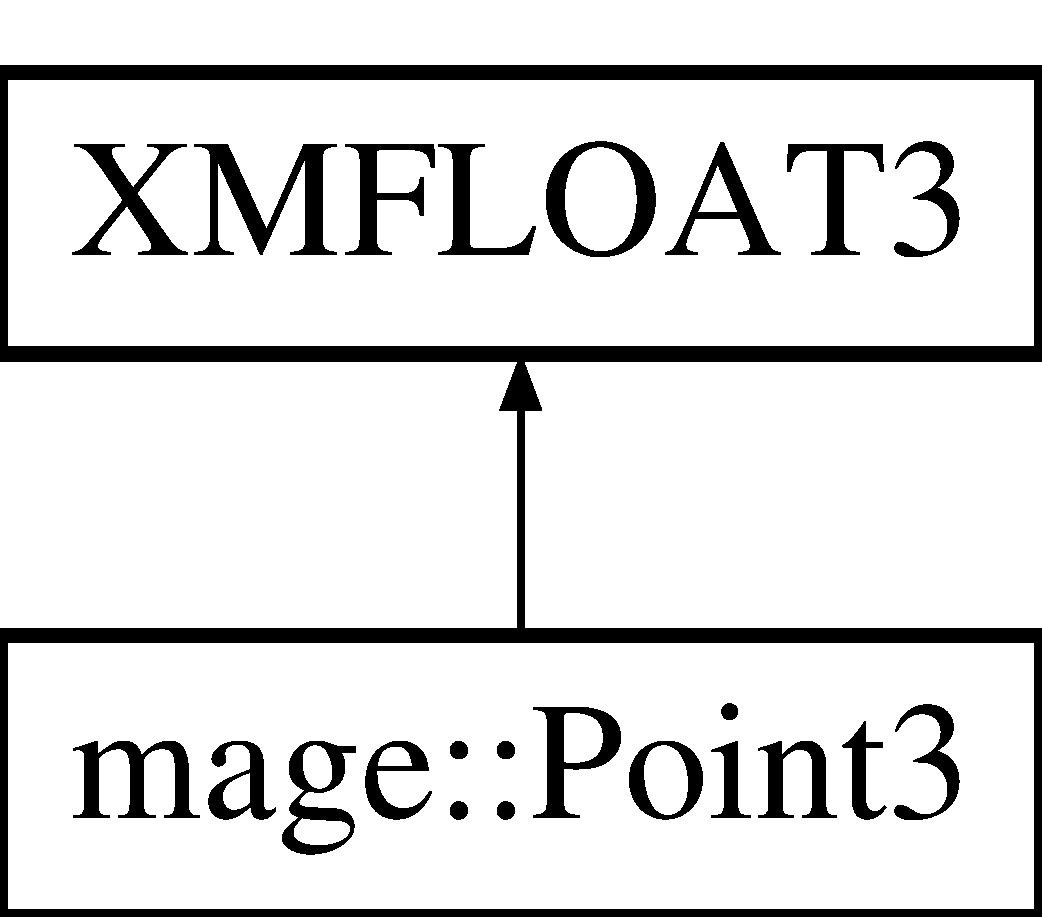
\includegraphics[height=2.000000cm]{structmage_1_1_point3}
\end{center}
\end{figure}
\subsection*{Public Member Functions}
\begin{DoxyCompactItemize}
\item 
\hyperlink{structmage_1_1_point3_a2675c303e54c6047520bc1a298c7fef1}{Point3} ()
\item 
\hyperlink{structmage_1_1_point3_a754210fa30befab6db5957a8d9b397f2}{Point3} (float x, float y, float z)
\item 
\hyperlink{structmage_1_1_point3_ad2e95e6eaa32339663e35f936990eb0c}{Point3} (const \hyperlink{structmage_1_1_point3}{Point3} \&point)
\item 
\hyperlink{structmage_1_1_point3_a3d10561285e01d03978e0d91fda6ff1d}{Point3} (\hyperlink{structmage_1_1_point3}{Point3} \&\&point)
\item 
\hyperlink{structmage_1_1_point3_a5ccb5f2f660b3ecdb471ed859923d4fc}{Point3} (const \hyperlink{structmage_1_1_direction3}{Direction3} \&direction)
\item 
\hyperlink{structmage_1_1_point3_ad189bc5943a8fac34495e38471534ffa}{Point3} (\hyperlink{structmage_1_1_direction3}{Direction3} \&\&direction)
\item 
\hyperlink{structmage_1_1_point3_ae56d0fb055b286df68d8d645378408c8}{Point3} (const \hyperlink{structmage_1_1_normal3}{Normal3} \&normal)
\item 
\hyperlink{structmage_1_1_point3_acab03c18e6b20bea3768e14cb1435302}{Point3} (\hyperlink{structmage_1_1_normal3}{Normal3} \&\&normal)
\item 
\hyperlink{structmage_1_1_point3_a2298bfe2417508187bdad7fbaa6178c1}{Point3} (const X\+M\+F\+L\+O\+A\+T3 \&vector)
\item 
\hyperlink{structmage_1_1_point3_a84b8c62ed63301fde1ce0e045c12352b}{Point3} (X\+M\+F\+L\+O\+A\+T3 \&\&vector)
\item 
\hyperlink{structmage_1_1_point3_a952151b6ff72b68569f95445c2ac2495}{$\sim$\+Point3} ()=default
\item 
\hyperlink{structmage_1_1_point3}{Point3} \& \hyperlink{structmage_1_1_point3_a53403b16c67a6c7d72910edaec04e371}{operator=} (const \hyperlink{structmage_1_1_point3}{Point3} \&point)
\item 
\hyperlink{structmage_1_1_point3}{Point3} \& \hyperlink{structmage_1_1_point3_a6889dad6ac4106bd9a52fcae4dfa401c}{operator=} (\hyperlink{structmage_1_1_point3}{Point3} \&\&point)
\end{DoxyCompactItemize}


\subsection{Constructor \& Destructor Documentation}
\hypertarget{structmage_1_1_point3_a2675c303e54c6047520bc1a298c7fef1}{}\label{structmage_1_1_point3_a2675c303e54c6047520bc1a298c7fef1} 
\index{mage\+::\+Point3@{mage\+::\+Point3}!Point3@{Point3}}
\index{Point3@{Point3}!mage\+::\+Point3@{mage\+::\+Point3}}
\subsubsection{\texorpdfstring{Point3()}{Point3()}\hspace{0.1cm}{\footnotesize\ttfamily [1/10]}}
{\footnotesize\ttfamily mage\+::\+Point3\+::\+Point3 (\begin{DoxyParamCaption}{ }\end{DoxyParamCaption})}

\hypertarget{structmage_1_1_point3_a754210fa30befab6db5957a8d9b397f2}{}\label{structmage_1_1_point3_a754210fa30befab6db5957a8d9b397f2} 
\index{mage\+::\+Point3@{mage\+::\+Point3}!Point3@{Point3}}
\index{Point3@{Point3}!mage\+::\+Point3@{mage\+::\+Point3}}
\subsubsection{\texorpdfstring{Point3()}{Point3()}\hspace{0.1cm}{\footnotesize\ttfamily [2/10]}}
{\footnotesize\ttfamily mage\+::\+Point3\+::\+Point3 (\begin{DoxyParamCaption}\item[{float}]{x,  }\item[{float}]{y,  }\item[{float}]{z }\end{DoxyParamCaption})}

\hypertarget{structmage_1_1_point3_ad2e95e6eaa32339663e35f936990eb0c}{}\label{structmage_1_1_point3_ad2e95e6eaa32339663e35f936990eb0c} 
\index{mage\+::\+Point3@{mage\+::\+Point3}!Point3@{Point3}}
\index{Point3@{Point3}!mage\+::\+Point3@{mage\+::\+Point3}}
\subsubsection{\texorpdfstring{Point3()}{Point3()}\hspace{0.1cm}{\footnotesize\ttfamily [3/10]}}
{\footnotesize\ttfamily mage\+::\+Point3\+::\+Point3 (\begin{DoxyParamCaption}\item[{const \hyperlink{structmage_1_1_point3}{Point3} \&}]{point }\end{DoxyParamCaption})}

\hypertarget{structmage_1_1_point3_a3d10561285e01d03978e0d91fda6ff1d}{}\label{structmage_1_1_point3_a3d10561285e01d03978e0d91fda6ff1d} 
\index{mage\+::\+Point3@{mage\+::\+Point3}!Point3@{Point3}}
\index{Point3@{Point3}!mage\+::\+Point3@{mage\+::\+Point3}}
\subsubsection{\texorpdfstring{Point3()}{Point3()}\hspace{0.1cm}{\footnotesize\ttfamily [4/10]}}
{\footnotesize\ttfamily mage\+::\+Point3\+::\+Point3 (\begin{DoxyParamCaption}\item[{\hyperlink{structmage_1_1_point3}{Point3} \&\&}]{point }\end{DoxyParamCaption})}

\hypertarget{structmage_1_1_point3_a5ccb5f2f660b3ecdb471ed859923d4fc}{}\label{structmage_1_1_point3_a5ccb5f2f660b3ecdb471ed859923d4fc} 
\index{mage\+::\+Point3@{mage\+::\+Point3}!Point3@{Point3}}
\index{Point3@{Point3}!mage\+::\+Point3@{mage\+::\+Point3}}
\subsubsection{\texorpdfstring{Point3()}{Point3()}\hspace{0.1cm}{\footnotesize\ttfamily [5/10]}}
{\footnotesize\ttfamily mage\+::\+Point3\+::\+Point3 (\begin{DoxyParamCaption}\item[{const \hyperlink{structmage_1_1_direction3}{Direction3} \&}]{direction }\end{DoxyParamCaption})\hspace{0.3cm}{\ttfamily [explicit]}}

\hypertarget{structmage_1_1_point3_ad189bc5943a8fac34495e38471534ffa}{}\label{structmage_1_1_point3_ad189bc5943a8fac34495e38471534ffa} 
\index{mage\+::\+Point3@{mage\+::\+Point3}!Point3@{Point3}}
\index{Point3@{Point3}!mage\+::\+Point3@{mage\+::\+Point3}}
\subsubsection{\texorpdfstring{Point3()}{Point3()}\hspace{0.1cm}{\footnotesize\ttfamily [6/10]}}
{\footnotesize\ttfamily mage\+::\+Point3\+::\+Point3 (\begin{DoxyParamCaption}\item[{\hyperlink{structmage_1_1_direction3}{Direction3} \&\&}]{direction }\end{DoxyParamCaption})\hspace{0.3cm}{\ttfamily [explicit]}}

\hypertarget{structmage_1_1_point3_ae56d0fb055b286df68d8d645378408c8}{}\label{structmage_1_1_point3_ae56d0fb055b286df68d8d645378408c8} 
\index{mage\+::\+Point3@{mage\+::\+Point3}!Point3@{Point3}}
\index{Point3@{Point3}!mage\+::\+Point3@{mage\+::\+Point3}}
\subsubsection{\texorpdfstring{Point3()}{Point3()}\hspace{0.1cm}{\footnotesize\ttfamily [7/10]}}
{\footnotesize\ttfamily mage\+::\+Point3\+::\+Point3 (\begin{DoxyParamCaption}\item[{const \hyperlink{structmage_1_1_normal3}{Normal3} \&}]{normal }\end{DoxyParamCaption})\hspace{0.3cm}{\ttfamily [explicit]}}

\hypertarget{structmage_1_1_point3_acab03c18e6b20bea3768e14cb1435302}{}\label{structmage_1_1_point3_acab03c18e6b20bea3768e14cb1435302} 
\index{mage\+::\+Point3@{mage\+::\+Point3}!Point3@{Point3}}
\index{Point3@{Point3}!mage\+::\+Point3@{mage\+::\+Point3}}
\subsubsection{\texorpdfstring{Point3()}{Point3()}\hspace{0.1cm}{\footnotesize\ttfamily [8/10]}}
{\footnotesize\ttfamily mage\+::\+Point3\+::\+Point3 (\begin{DoxyParamCaption}\item[{\hyperlink{structmage_1_1_normal3}{Normal3} \&\&}]{normal }\end{DoxyParamCaption})\hspace{0.3cm}{\ttfamily [explicit]}}

\hypertarget{structmage_1_1_point3_a2298bfe2417508187bdad7fbaa6178c1}{}\label{structmage_1_1_point3_a2298bfe2417508187bdad7fbaa6178c1} 
\index{mage\+::\+Point3@{mage\+::\+Point3}!Point3@{Point3}}
\index{Point3@{Point3}!mage\+::\+Point3@{mage\+::\+Point3}}
\subsubsection{\texorpdfstring{Point3()}{Point3()}\hspace{0.1cm}{\footnotesize\ttfamily [9/10]}}
{\footnotesize\ttfamily mage\+::\+Point3\+::\+Point3 (\begin{DoxyParamCaption}\item[{const X\+M\+F\+L\+O\+A\+T3 \&}]{vector }\end{DoxyParamCaption})\hspace{0.3cm}{\ttfamily [explicit]}}

\hypertarget{structmage_1_1_point3_a84b8c62ed63301fde1ce0e045c12352b}{}\label{structmage_1_1_point3_a84b8c62ed63301fde1ce0e045c12352b} 
\index{mage\+::\+Point3@{mage\+::\+Point3}!Point3@{Point3}}
\index{Point3@{Point3}!mage\+::\+Point3@{mage\+::\+Point3}}
\subsubsection{\texorpdfstring{Point3()}{Point3()}\hspace{0.1cm}{\footnotesize\ttfamily [10/10]}}
{\footnotesize\ttfamily mage\+::\+Point3\+::\+Point3 (\begin{DoxyParamCaption}\item[{X\+M\+F\+L\+O\+A\+T3 \&\&}]{vector }\end{DoxyParamCaption})\hspace{0.3cm}{\ttfamily [explicit]}}

\hypertarget{structmage_1_1_point3_a952151b6ff72b68569f95445c2ac2495}{}\label{structmage_1_1_point3_a952151b6ff72b68569f95445c2ac2495} 
\index{mage\+::\+Point3@{mage\+::\+Point3}!````~Point3@{$\sim$\+Point3}}
\index{````~Point3@{$\sim$\+Point3}!mage\+::\+Point3@{mage\+::\+Point3}}
\subsubsection{\texorpdfstring{$\sim$\+Point3()}{~Point3()}}
{\footnotesize\ttfamily mage\+::\+Point3\+::$\sim$\+Point3 (\begin{DoxyParamCaption}{ }\end{DoxyParamCaption})\hspace{0.3cm}{\ttfamily [default]}}



\subsection{Member Function Documentation}
\hypertarget{structmage_1_1_point3_a53403b16c67a6c7d72910edaec04e371}{}\label{structmage_1_1_point3_a53403b16c67a6c7d72910edaec04e371} 
\index{mage\+::\+Point3@{mage\+::\+Point3}!operator=@{operator=}}
\index{operator=@{operator=}!mage\+::\+Point3@{mage\+::\+Point3}}
\subsubsection{\texorpdfstring{operator=()}{operator=()}\hspace{0.1cm}{\footnotesize\ttfamily [1/2]}}
{\footnotesize\ttfamily \hyperlink{structmage_1_1_point3}{Point3}\& mage\+::\+Point3\+::operator= (\begin{DoxyParamCaption}\item[{const \hyperlink{structmage_1_1_point3}{Point3} \&}]{point }\end{DoxyParamCaption})}

\hypertarget{structmage_1_1_point3_a6889dad6ac4106bd9a52fcae4dfa401c}{}\label{structmage_1_1_point3_a6889dad6ac4106bd9a52fcae4dfa401c} 
\index{mage\+::\+Point3@{mage\+::\+Point3}!operator=@{operator=}}
\index{operator=@{operator=}!mage\+::\+Point3@{mage\+::\+Point3}}
\subsubsection{\texorpdfstring{operator=()}{operator=()}\hspace{0.1cm}{\footnotesize\ttfamily [2/2]}}
{\footnotesize\ttfamily \hyperlink{structmage_1_1_point3}{Point3}\& mage\+::\+Point3\+::operator= (\begin{DoxyParamCaption}\item[{\hyperlink{structmage_1_1_point3}{Point3} \&\&}]{point }\end{DoxyParamCaption})}


\hypertarget{classmage_1_1rendering_1_1_post_process_pass}{}\section{mage\+:\+:rendering\+:\+:Post\+Process\+Pass Class Reference}
\label{classmage_1_1rendering_1_1_post_process_pass}\index{mage\+::rendering\+::\+Post\+Process\+Pass@{mage\+::rendering\+::\+Post\+Process\+Pass}}


{\ttfamily \#include $<$postprocess\+\_\+pass.\+hpp$>$}

\subsection*{Public Member Functions}
\begin{DoxyCompactItemize}
\item 
\mbox{\hyperlink{classmage_1_1rendering_1_1_post_process_pass_aa7989cc618c40d64e6e86f1aa8576dff}{Post\+Process\+Pass}} (I\+D3\+D11\+Device\+Context \&device\+\_\+context, \mbox{\hyperlink{classmage_1_1rendering_1_1_state_manager}{State\+Manager}} \&state\+\_\+manager, \mbox{\hyperlink{classmage_1_1rendering_1_1_resource_manager}{Resource\+Manager}} \&resource\+\_\+manager)
\item 
\mbox{\hyperlink{classmage_1_1rendering_1_1_post_process_pass_a5980123845352eb3071e2fde203469fc}{Post\+Process\+Pass}} (const \mbox{\hyperlink{classmage_1_1rendering_1_1_post_process_pass}{Post\+Process\+Pass}} \&pass)=delete
\item 
\mbox{\hyperlink{classmage_1_1rendering_1_1_post_process_pass_aa57a8a38643fc76d0cdae8106c3de7e3}{Post\+Process\+Pass}} (\mbox{\hyperlink{classmage_1_1rendering_1_1_post_process_pass}{Post\+Process\+Pass}} \&\&pass) noexcept
\item 
\mbox{\hyperlink{classmage_1_1rendering_1_1_post_process_pass_a41e82fe23fdc3a5726989edb0bb334ea}{$\sim$\+Post\+Process\+Pass}} ()
\item 
\mbox{\hyperlink{classmage_1_1rendering_1_1_post_process_pass}{Post\+Process\+Pass}} \& \mbox{\hyperlink{classmage_1_1rendering_1_1_post_process_pass_ace844a6fbc47cc0470642e48361efacd}{operator=}} (const \mbox{\hyperlink{classmage_1_1rendering_1_1_post_process_pass}{Post\+Process\+Pass}} \&pass)=delete
\item 
\mbox{\hyperlink{classmage_1_1rendering_1_1_post_process_pass}{Post\+Process\+Pass}} \& \mbox{\hyperlink{classmage_1_1rendering_1_1_post_process_pass_a72e638460796e9613f232a6cbf118378}{operator=}} (\mbox{\hyperlink{classmage_1_1rendering_1_1_post_process_pass}{Post\+Process\+Pass}} \&\&pass) noexcept
\item 
void \mbox{\hyperlink{classmage_1_1rendering_1_1_post_process_pass_a5a580293635c790deb09e958724021c2}{Dispatch\+D\+OF}} (const \mbox{\hyperlink{namespacemage_a31f2bb52b5080e706e1c13de07c0a249}{U32x2}} \&viewport\+\_\+size) const noexcept
\item 
void \mbox{\hyperlink{classmage_1_1rendering_1_1_post_process_pass_a8736c2eb9872035c2e5d109681f72146}{Dispatch\+L\+DR}} (const \mbox{\hyperlink{namespacemage_a31f2bb52b5080e706e1c13de07c0a249}{U32x2}} \&viewport\+\_\+size, \mbox{\hyperlink{namespacemage_1_1rendering_a789e4b7d9a8cc831b065e9c6bb7430e9}{Tone\+Mapping}} tone\+\_\+mapping) const noexcept
\end{DoxyCompactItemize}
\subsection*{Private Attributes}
\begin{DoxyCompactItemize}
\item 
std\+::reference\+\_\+wrapper$<$ I\+D3\+D11\+Device\+Context $>$ \mbox{\hyperlink{classmage_1_1rendering_1_1_post_process_pass_a18468bc4ffa408e9db3089b306f45291}{m\+\_\+device\+\_\+context}}
\item 
std\+::reference\+\_\+wrapper$<$ \mbox{\hyperlink{classmage_1_1rendering_1_1_state_manager}{State\+Manager}} $>$ \mbox{\hyperlink{classmage_1_1rendering_1_1_post_process_pass_a80cbe6aee950e5bcc98763813fdb8aba}{m\+\_\+state\+\_\+manager}}
\item 
std\+::reference\+\_\+wrapper$<$ \mbox{\hyperlink{classmage_1_1rendering_1_1_resource_manager}{Resource\+Manager}} $>$ \mbox{\hyperlink{classmage_1_1rendering_1_1_post_process_pass_af20e46967d28e7e0500fff6b1988ad80}{m\+\_\+resource\+\_\+manager}}
\item 
\mbox{\hyperlink{namespacemage_1_1rendering_ab3dc9f2114f2e9255b91d9c051da52ea}{Compute\+Shader\+Ptr}} \mbox{\hyperlink{classmage_1_1rendering_1_1_post_process_pass_aec72e5a7ca28c11754f85ab6726ce5ec}{m\+\_\+dof\+\_\+cs}}
\end{DoxyCompactItemize}


\subsection{Detailed Description}
A class of post-\/process passes for performing post-\/processing. 

\subsection{Constructor \& Destructor Documentation}
\mbox{\Hypertarget{classmage_1_1rendering_1_1_post_process_pass_aa7989cc618c40d64e6e86f1aa8576dff}\label{classmage_1_1rendering_1_1_post_process_pass_aa7989cc618c40d64e6e86f1aa8576dff}} 
\index{mage\+::rendering\+::\+Post\+Process\+Pass@{mage\+::rendering\+::\+Post\+Process\+Pass}!Post\+Process\+Pass@{Post\+Process\+Pass}}
\index{Post\+Process\+Pass@{Post\+Process\+Pass}!mage\+::rendering\+::\+Post\+Process\+Pass@{mage\+::rendering\+::\+Post\+Process\+Pass}}
\subsubsection{\texorpdfstring{Post\+Process\+Pass()}{PostProcessPass()}\hspace{0.1cm}{\footnotesize\ttfamily [1/3]}}
{\footnotesize\ttfamily mage\+::rendering\+::\+Post\+Process\+Pass\+::\+Post\+Process\+Pass (\begin{DoxyParamCaption}\item[{I\+D3\+D11\+Device\+Context \&}]{device\+\_\+context,  }\item[{\mbox{\hyperlink{classmage_1_1rendering_1_1_state_manager}{State\+Manager}} \&}]{state\+\_\+manager,  }\item[{\mbox{\hyperlink{classmage_1_1rendering_1_1_resource_manager}{Resource\+Manager}} \&}]{resource\+\_\+manager }\end{DoxyParamCaption})\hspace{0.3cm}{\ttfamily [explicit]}}

Constructs a post-\/process pass.


\begin{DoxyParams}[1]{Parameters}
\mbox{\tt in}  & {\em device\+\_\+context} & A reference to the device context. \\
\hline
\mbox{\tt in}  & {\em state\+\_\+manager} & A reference to the state manager. \\
\hline
\mbox{\tt in}  & {\em resource\+\_\+manager} & A reference to the resource manager. \\
\hline
\end{DoxyParams}
\mbox{\Hypertarget{classmage_1_1rendering_1_1_post_process_pass_a5980123845352eb3071e2fde203469fc}\label{classmage_1_1rendering_1_1_post_process_pass_a5980123845352eb3071e2fde203469fc}} 
\index{mage\+::rendering\+::\+Post\+Process\+Pass@{mage\+::rendering\+::\+Post\+Process\+Pass}!Post\+Process\+Pass@{Post\+Process\+Pass}}
\index{Post\+Process\+Pass@{Post\+Process\+Pass}!mage\+::rendering\+::\+Post\+Process\+Pass@{mage\+::rendering\+::\+Post\+Process\+Pass}}
\subsubsection{\texorpdfstring{Post\+Process\+Pass()}{PostProcessPass()}\hspace{0.1cm}{\footnotesize\ttfamily [2/3]}}
{\footnotesize\ttfamily mage\+::rendering\+::\+Post\+Process\+Pass\+::\+Post\+Process\+Pass (\begin{DoxyParamCaption}\item[{const \mbox{\hyperlink{classmage_1_1rendering_1_1_post_process_pass}{Post\+Process\+Pass}} \&}]{pass }\end{DoxyParamCaption})\hspace{0.3cm}{\ttfamily [delete]}}

Constructs a post-\/process pass from the given post-\/process pass.


\begin{DoxyParams}[1]{Parameters}
\mbox{\tt in}  & {\em pass} & A reference to the post-\/process pass to copy. \\
\hline
\end{DoxyParams}
\mbox{\Hypertarget{classmage_1_1rendering_1_1_post_process_pass_aa57a8a38643fc76d0cdae8106c3de7e3}\label{classmage_1_1rendering_1_1_post_process_pass_aa57a8a38643fc76d0cdae8106c3de7e3}} 
\index{mage\+::rendering\+::\+Post\+Process\+Pass@{mage\+::rendering\+::\+Post\+Process\+Pass}!Post\+Process\+Pass@{Post\+Process\+Pass}}
\index{Post\+Process\+Pass@{Post\+Process\+Pass}!mage\+::rendering\+::\+Post\+Process\+Pass@{mage\+::rendering\+::\+Post\+Process\+Pass}}
\subsubsection{\texorpdfstring{Post\+Process\+Pass()}{PostProcessPass()}\hspace{0.1cm}{\footnotesize\ttfamily [3/3]}}
{\footnotesize\ttfamily mage\+::rendering\+::\+Post\+Process\+Pass\+::\+Post\+Process\+Pass (\begin{DoxyParamCaption}\item[{\mbox{\hyperlink{classmage_1_1rendering_1_1_post_process_pass}{Post\+Process\+Pass}} \&\&}]{pass }\end{DoxyParamCaption})\hspace{0.3cm}{\ttfamily [default]}, {\ttfamily [noexcept]}}

Constructs a post-\/process pass by moving the given post-\/process shading pass.


\begin{DoxyParams}[1]{Parameters}
\mbox{\tt in}  & {\em pass} & A reference to the post-\/process pass to move. \\
\hline
\end{DoxyParams}
\mbox{\Hypertarget{classmage_1_1rendering_1_1_post_process_pass_a41e82fe23fdc3a5726989edb0bb334ea}\label{classmage_1_1rendering_1_1_post_process_pass_a41e82fe23fdc3a5726989edb0bb334ea}} 
\index{mage\+::rendering\+::\+Post\+Process\+Pass@{mage\+::rendering\+::\+Post\+Process\+Pass}!````~Post\+Process\+Pass@{$\sim$\+Post\+Process\+Pass}}
\index{````~Post\+Process\+Pass@{$\sim$\+Post\+Process\+Pass}!mage\+::rendering\+::\+Post\+Process\+Pass@{mage\+::rendering\+::\+Post\+Process\+Pass}}
\subsubsection{\texorpdfstring{$\sim$\+Post\+Process\+Pass()}{~PostProcessPass()}}
{\footnotesize\ttfamily mage\+::rendering\+::\+Post\+Process\+Pass\+::$\sim$\+Post\+Process\+Pass (\begin{DoxyParamCaption}{ }\end{DoxyParamCaption})\hspace{0.3cm}{\ttfamily [default]}}

Destructs this D\+OF pass. 

\subsection{Member Function Documentation}
\mbox{\Hypertarget{classmage_1_1rendering_1_1_post_process_pass_a5a580293635c790deb09e958724021c2}\label{classmage_1_1rendering_1_1_post_process_pass_a5a580293635c790deb09e958724021c2}} 
\index{mage\+::rendering\+::\+Post\+Process\+Pass@{mage\+::rendering\+::\+Post\+Process\+Pass}!Dispatch\+D\+OF@{Dispatch\+D\+OF}}
\index{Dispatch\+D\+OF@{Dispatch\+D\+OF}!mage\+::rendering\+::\+Post\+Process\+Pass@{mage\+::rendering\+::\+Post\+Process\+Pass}}
\subsubsection{\texorpdfstring{Dispatch\+D\+O\+F()}{DispatchDOF()}}
{\footnotesize\ttfamily void mage\+::rendering\+::\+Post\+Process\+Pass\+::\+Dispatch\+D\+OF (\begin{DoxyParamCaption}\item[{const \mbox{\hyperlink{namespacemage_a31f2bb52b5080e706e1c13de07c0a249}{U32x2}} \&}]{viewport\+\_\+size }\end{DoxyParamCaption}) const\hspace{0.3cm}{\ttfamily [noexcept]}}

Dispatches an depth-\/of-\/field pass.


\begin{DoxyParams}[1]{Parameters}
\mbox{\tt in}  & {\em viewport\+\_\+size} & A reference to the viewport size. \\
\hline
\end{DoxyParams}
\mbox{\Hypertarget{classmage_1_1rendering_1_1_post_process_pass_a8736c2eb9872035c2e5d109681f72146}\label{classmage_1_1rendering_1_1_post_process_pass_a8736c2eb9872035c2e5d109681f72146}} 
\index{mage\+::rendering\+::\+Post\+Process\+Pass@{mage\+::rendering\+::\+Post\+Process\+Pass}!Dispatch\+L\+DR@{Dispatch\+L\+DR}}
\index{Dispatch\+L\+DR@{Dispatch\+L\+DR}!mage\+::rendering\+::\+Post\+Process\+Pass@{mage\+::rendering\+::\+Post\+Process\+Pass}}
\subsubsection{\texorpdfstring{Dispatch\+L\+D\+R()}{DispatchLDR()}}
{\footnotesize\ttfamily void mage\+::rendering\+::\+Post\+Process\+Pass\+::\+Dispatch\+L\+DR (\begin{DoxyParamCaption}\item[{const \mbox{\hyperlink{namespacemage_a31f2bb52b5080e706e1c13de07c0a249}{U32x2}} \&}]{viewport\+\_\+size,  }\item[{\mbox{\hyperlink{namespacemage_1_1rendering_a789e4b7d9a8cc831b065e9c6bb7430e9}{Tone\+Mapping}}}]{tone\+\_\+mapping }\end{DoxyParamCaption}) const\hspace{0.3cm}{\ttfamily [noexcept]}}

Dispatches an low-\/dynamic-\/range pass.


\begin{DoxyParams}[1]{Parameters}
\mbox{\tt in}  & {\em viewport\+\_\+size} & A reference to the viewport size. \\
\hline
\mbox{\tt in}  & {\em tone\+\_\+mapping} & The tone mapping type. \\
\hline
\end{DoxyParams}
\mbox{\Hypertarget{classmage_1_1rendering_1_1_post_process_pass_ace844a6fbc47cc0470642e48361efacd}\label{classmage_1_1rendering_1_1_post_process_pass_ace844a6fbc47cc0470642e48361efacd}} 
\index{mage\+::rendering\+::\+Post\+Process\+Pass@{mage\+::rendering\+::\+Post\+Process\+Pass}!operator=@{operator=}}
\index{operator=@{operator=}!mage\+::rendering\+::\+Post\+Process\+Pass@{mage\+::rendering\+::\+Post\+Process\+Pass}}
\subsubsection{\texorpdfstring{operator=()}{operator=()}\hspace{0.1cm}{\footnotesize\ttfamily [1/2]}}
{\footnotesize\ttfamily \mbox{\hyperlink{classmage_1_1rendering_1_1_post_process_pass}{Post\+Process\+Pass}}\& mage\+::rendering\+::\+Post\+Process\+Pass\+::operator= (\begin{DoxyParamCaption}\item[{const \mbox{\hyperlink{classmage_1_1rendering_1_1_post_process_pass}{Post\+Process\+Pass}} \&}]{pass }\end{DoxyParamCaption})\hspace{0.3cm}{\ttfamily [delete]}}

Copies the given post-\/process pass to this post-\/process pass.


\begin{DoxyParams}[1]{Parameters}
\mbox{\tt in}  & {\em pass} & A reference to the post-\/process pass to copy. \\
\hline
\end{DoxyParams}
\begin{DoxyReturn}{Returns}
A reference to the copy of the given post-\/process pass (i.\+e. this post-\/process pass). 
\end{DoxyReturn}
\mbox{\Hypertarget{classmage_1_1rendering_1_1_post_process_pass_a72e638460796e9613f232a6cbf118378}\label{classmage_1_1rendering_1_1_post_process_pass_a72e638460796e9613f232a6cbf118378}} 
\index{mage\+::rendering\+::\+Post\+Process\+Pass@{mage\+::rendering\+::\+Post\+Process\+Pass}!operator=@{operator=}}
\index{operator=@{operator=}!mage\+::rendering\+::\+Post\+Process\+Pass@{mage\+::rendering\+::\+Post\+Process\+Pass}}
\subsubsection{\texorpdfstring{operator=()}{operator=()}\hspace{0.1cm}{\footnotesize\ttfamily [2/2]}}
{\footnotesize\ttfamily \mbox{\hyperlink{classmage_1_1rendering_1_1_post_process_pass}{Post\+Process\+Pass}} \& mage\+::rendering\+::\+Post\+Process\+Pass\+::operator= (\begin{DoxyParamCaption}\item[{\mbox{\hyperlink{classmage_1_1rendering_1_1_post_process_pass}{Post\+Process\+Pass}} \&\&}]{pass }\end{DoxyParamCaption})\hspace{0.3cm}{\ttfamily [default]}, {\ttfamily [noexcept]}}

Moves the given post-\/process pass to this post-\/process pass.


\begin{DoxyParams}[1]{Parameters}
\mbox{\tt in}  & {\em pass} & A reference to the post-\/process pass to move. \\
\hline
\end{DoxyParams}
\begin{DoxyReturn}{Returns}
A reference to the moved D\+OF pass (i.\+e. this post-\/process pass). 
\end{DoxyReturn}


\subsection{Member Data Documentation}
\mbox{\Hypertarget{classmage_1_1rendering_1_1_post_process_pass_a18468bc4ffa408e9db3089b306f45291}\label{classmage_1_1rendering_1_1_post_process_pass_a18468bc4ffa408e9db3089b306f45291}} 
\index{mage\+::rendering\+::\+Post\+Process\+Pass@{mage\+::rendering\+::\+Post\+Process\+Pass}!m\+\_\+device\+\_\+context@{m\+\_\+device\+\_\+context}}
\index{m\+\_\+device\+\_\+context@{m\+\_\+device\+\_\+context}!mage\+::rendering\+::\+Post\+Process\+Pass@{mage\+::rendering\+::\+Post\+Process\+Pass}}
\subsubsection{\texorpdfstring{m\+\_\+device\+\_\+context}{m\_device\_context}}
{\footnotesize\ttfamily std\+::reference\+\_\+wrapper$<$ I\+D3\+D11\+Device\+Context $>$ mage\+::rendering\+::\+Post\+Process\+Pass\+::m\+\_\+device\+\_\+context\hspace{0.3cm}{\ttfamily [private]}}

A reference to the device context of this post-\/process pass. \mbox{\Hypertarget{classmage_1_1rendering_1_1_post_process_pass_aec72e5a7ca28c11754f85ab6726ce5ec}\label{classmage_1_1rendering_1_1_post_process_pass_aec72e5a7ca28c11754f85ab6726ce5ec}} 
\index{mage\+::rendering\+::\+Post\+Process\+Pass@{mage\+::rendering\+::\+Post\+Process\+Pass}!m\+\_\+dof\+\_\+cs@{m\+\_\+dof\+\_\+cs}}
\index{m\+\_\+dof\+\_\+cs@{m\+\_\+dof\+\_\+cs}!mage\+::rendering\+::\+Post\+Process\+Pass@{mage\+::rendering\+::\+Post\+Process\+Pass}}
\subsubsection{\texorpdfstring{m\+\_\+dof\+\_\+cs}{m\_dof\_cs}}
{\footnotesize\ttfamily \mbox{\hyperlink{namespacemage_1_1rendering_ab3dc9f2114f2e9255b91d9c051da52ea}{Compute\+Shader\+Ptr}} mage\+::rendering\+::\+Post\+Process\+Pass\+::m\+\_\+dof\+\_\+cs\hspace{0.3cm}{\ttfamily [private]}}

A pointer to the compute shader of this post-\/process pass. \mbox{\Hypertarget{classmage_1_1rendering_1_1_post_process_pass_af20e46967d28e7e0500fff6b1988ad80}\label{classmage_1_1rendering_1_1_post_process_pass_af20e46967d28e7e0500fff6b1988ad80}} 
\index{mage\+::rendering\+::\+Post\+Process\+Pass@{mage\+::rendering\+::\+Post\+Process\+Pass}!m\+\_\+resource\+\_\+manager@{m\+\_\+resource\+\_\+manager}}
\index{m\+\_\+resource\+\_\+manager@{m\+\_\+resource\+\_\+manager}!mage\+::rendering\+::\+Post\+Process\+Pass@{mage\+::rendering\+::\+Post\+Process\+Pass}}
\subsubsection{\texorpdfstring{m\+\_\+resource\+\_\+manager}{m\_resource\_manager}}
{\footnotesize\ttfamily std\+::reference\+\_\+wrapper$<$ \mbox{\hyperlink{classmage_1_1rendering_1_1_resource_manager}{Resource\+Manager}} $>$ mage\+::rendering\+::\+Post\+Process\+Pass\+::m\+\_\+resource\+\_\+manager\hspace{0.3cm}{\ttfamily [private]}}

A reference to the resource manager of this post-\/process pass. \mbox{\Hypertarget{classmage_1_1rendering_1_1_post_process_pass_a80cbe6aee950e5bcc98763813fdb8aba}\label{classmage_1_1rendering_1_1_post_process_pass_a80cbe6aee950e5bcc98763813fdb8aba}} 
\index{mage\+::rendering\+::\+Post\+Process\+Pass@{mage\+::rendering\+::\+Post\+Process\+Pass}!m\+\_\+state\+\_\+manager@{m\+\_\+state\+\_\+manager}}
\index{m\+\_\+state\+\_\+manager@{m\+\_\+state\+\_\+manager}!mage\+::rendering\+::\+Post\+Process\+Pass@{mage\+::rendering\+::\+Post\+Process\+Pass}}
\subsubsection{\texorpdfstring{m\+\_\+state\+\_\+manager}{m\_state\_manager}}
{\footnotesize\ttfamily std\+::reference\+\_\+wrapper$<$ \mbox{\hyperlink{classmage_1_1rendering_1_1_state_manager}{State\+Manager}} $>$ mage\+::rendering\+::\+Post\+Process\+Pass\+::m\+\_\+state\+\_\+manager\hspace{0.3cm}{\ttfamily [private]}}

A reference to the state manager of this post-\/process pass. 
\hypertarget{classmage_1_1rendering_1_1_primitive_batch_mesh}{}\section{mage\+:\+:rendering\+:\+:Primitive\+Batch\+Mesh$<$ VertexT, IndexT $>$ Class Template Reference}
\label{classmage_1_1rendering_1_1_primitive_batch_mesh}\index{mage\+::rendering\+::\+Primitive\+Batch\+Mesh$<$ Vertex\+T, Index\+T $>$@{mage\+::rendering\+::\+Primitive\+Batch\+Mesh$<$ Vertex\+T, Index\+T $>$}}


{\ttfamily \#include $<$primitive\+\_\+batch\+\_\+mesh.\+hpp$>$}

Inheritance diagram for mage\+:\+:rendering\+:\+:Primitive\+Batch\+Mesh$<$ VertexT, IndexT $>$\+:\begin{figure}[H]
\begin{center}
\leavevmode
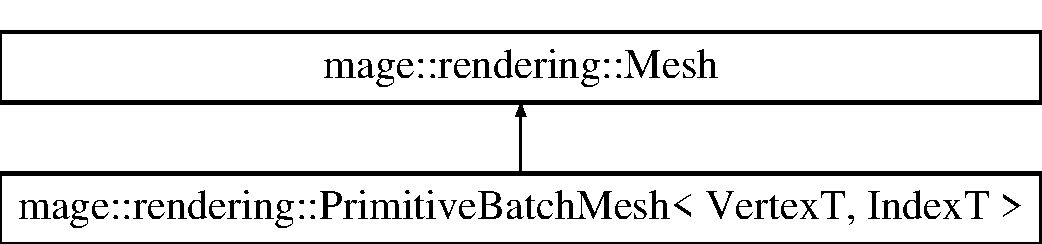
\includegraphics[height=2.000000cm]{classmage_1_1rendering_1_1_primitive_batch_mesh}
\end{center}
\end{figure}
\subsection*{Public Member Functions}
\begin{DoxyCompactItemize}
\item 
\mbox{\hyperlink{classmage_1_1rendering_1_1_primitive_batch_mesh_aa01b243a0ccb0ed4835c4dcab994d030}{Primitive\+Batch\+Mesh}} (I\+D3\+D11\+Device \&device, size\+\_\+t nb\+\_\+vertices, const std\+::vector$<$ IndexT $>$ \&indices, D3\+D11\+\_\+\+P\+R\+I\+M\+I\+T\+I\+V\+E\+\_\+\+T\+O\+P\+O\+L\+O\+GY primitive\+\_\+topology=D3\+D11\+\_\+\+P\+R\+I\+M\+I\+T\+I\+V\+E\+\_\+\+T\+O\+P\+O\+L\+O\+G\+Y\+\_\+\+T\+R\+I\+A\+N\+G\+L\+E\+L\+I\+ST)
\item 
\mbox{\hyperlink{classmage_1_1rendering_1_1_primitive_batch_mesh_a9f20b29914746fbb29b8c5146f7f63a2}{Primitive\+Batch\+Mesh}} (const \mbox{\hyperlink{classmage_1_1rendering_1_1_primitive_batch_mesh}{Primitive\+Batch\+Mesh}} \&mesh)=delete
\item 
\mbox{\hyperlink{classmage_1_1rendering_1_1_primitive_batch_mesh_ac46a8538b295cf4d85c7309d2bb4cdd5}{Primitive\+Batch\+Mesh}} (\mbox{\hyperlink{classmage_1_1rendering_1_1_primitive_batch_mesh}{Primitive\+Batch\+Mesh}} \&\&mesh) noexcept
\item 
virtual \mbox{\hyperlink{classmage_1_1rendering_1_1_primitive_batch_mesh_a96bb7d8ce20047163ec851b426087c80}{$\sim$\+Primitive\+Batch\+Mesh}} ()
\item 
\mbox{\hyperlink{classmage_1_1rendering_1_1_primitive_batch_mesh}{Primitive\+Batch\+Mesh}} \& \mbox{\hyperlink{classmage_1_1rendering_1_1_primitive_batch_mesh_a64b661150ec319d4dab092d44315bb67}{operator=}} (const \mbox{\hyperlink{classmage_1_1rendering_1_1_primitive_batch_mesh}{Primitive\+Batch\+Mesh}} \&mesh)=delete
\item 
\mbox{\hyperlink{classmage_1_1rendering_1_1_primitive_batch_mesh}{Primitive\+Batch\+Mesh}} \& \mbox{\hyperlink{classmage_1_1rendering_1_1_primitive_batch_mesh_a36409f6de1208f30069309675b19feb2}{operator=}} (\mbox{\hyperlink{classmage_1_1rendering_1_1_primitive_batch_mesh}{Primitive\+Batch\+Mesh}} \&\&mesh) noexcept
\item 
const \mbox{\hyperlink{classmage_1_1rendering_1_1_buffer_lock}{Buffer\+Lock}} \mbox{\hyperlink{classmage_1_1rendering_1_1_primitive_batch_mesh_afce7767a0e3496477c14f145c3c2bfe7}{Lock}} (I\+D3\+D11\+Device\+Context \&device\+\_\+context, D3\+D11\+\_\+\+M\+AP map\+\_\+type, D3\+D11\+\_\+\+M\+A\+P\+P\+E\+D\+\_\+\+S\+U\+B\+R\+E\+S\+O\+U\+R\+CE \&mapped\+\_\+buffer)
\end{DoxyCompactItemize}
\subsection*{Private Member Functions}
\begin{DoxyCompactItemize}
\item 
void \mbox{\hyperlink{classmage_1_1rendering_1_1_primitive_batch_mesh_abb8ba052c2f1453f2bd232d787d9a13d}{Setup\+Vertex\+Buffer}} (I\+D3\+D11\+Device \&device, size\+\_\+t nb\+\_\+vertices)
\item 
void \mbox{\hyperlink{classmage_1_1rendering_1_1_primitive_batch_mesh_abe1802b8f201be6ced30199fbce6e852}{Setup\+Index\+Buffer}} (I\+D3\+D11\+Device \&device, const std\+::vector$<$ IndexT $>$ \&indices)
\end{DoxyCompactItemize}
\subsection*{Additional Inherited Members}


\subsection{Detailed Description}
\subsubsection*{template$<$typename VertexT, typename IndexT$>$\newline
class mage\+::rendering\+::\+Primitive\+Batch\+Mesh$<$ Vertex\+T, Index\+T $>$}

A class of primitive batch meshes.


\begin{DoxyTemplParams}{Template Parameters}
{\em VertexT} & The vertex type. \\
\hline
{\em IndexT} & The index type. \\
\hline
\end{DoxyTemplParams}


\subsection{Constructor \& Destructor Documentation}
\mbox{\Hypertarget{classmage_1_1rendering_1_1_primitive_batch_mesh_aa01b243a0ccb0ed4835c4dcab994d030}\label{classmage_1_1rendering_1_1_primitive_batch_mesh_aa01b243a0ccb0ed4835c4dcab994d030}} 
\index{mage\+::rendering\+::\+Primitive\+Batch\+Mesh@{mage\+::rendering\+::\+Primitive\+Batch\+Mesh}!Primitive\+Batch\+Mesh@{Primitive\+Batch\+Mesh}}
\index{Primitive\+Batch\+Mesh@{Primitive\+Batch\+Mesh}!mage\+::rendering\+::\+Primitive\+Batch\+Mesh@{mage\+::rendering\+::\+Primitive\+Batch\+Mesh}}
\subsubsection{\texorpdfstring{Primitive\+Batch\+Mesh()}{PrimitiveBatchMesh()}\hspace{0.1cm}{\footnotesize\ttfamily [1/3]}}
{\footnotesize\ttfamily template$<$typename VertexT, typename IndexT$>$ \\
\mbox{\hyperlink{classmage_1_1rendering_1_1_primitive_batch_mesh}{mage\+::rendering\+::\+Primitive\+Batch\+Mesh}}$<$ VertexT, IndexT $>$\+::\mbox{\hyperlink{classmage_1_1rendering_1_1_primitive_batch_mesh}{Primitive\+Batch\+Mesh}} (\begin{DoxyParamCaption}\item[{I\+D3\+D11\+Device \&}]{device,  }\item[{size\+\_\+t}]{nb\+\_\+vertices,  }\item[{const std\+::vector$<$ IndexT $>$ \&}]{indices,  }\item[{D3\+D11\+\_\+\+P\+R\+I\+M\+I\+T\+I\+V\+E\+\_\+\+T\+O\+P\+O\+L\+O\+GY}]{primitive\+\_\+topology = {\ttfamily D3D11\+\_\+PRIMITIVE\+\_\+TOPOLOGY\+\_\+TRIANGLELIST} }\end{DoxyParamCaption})\hspace{0.3cm}{\ttfamily [explicit]}}

Constructs a primitive batch mesh.


\begin{DoxyParams}[1]{Parameters}
\mbox{\tt in}  & {\em device} & A reference to the device. \\
\hline
\mbox{\tt in}  & {\em nb\+\_\+vertices} & The number of vertices. \\
\hline
\mbox{\tt in}  & {\em indices} & A reference to the vector containing the indices. \\
\hline
\mbox{\tt in}  & {\em primitive\+\_\+topology} & The primitive topology. \\
\hline
\end{DoxyParams}

\begin{DoxyExceptions}{Exceptions}
{\em \mbox{\hyperlink{classmage_1_1_exception}{Exception}}} & Failed to setup the vertex buffer of the primitive batch mesh. \\
\hline
{\em \mbox{\hyperlink{classmage_1_1_exception}{Exception}}} & Failed to setup the index buffer of the primitive batch mesh. \\
\hline
\end{DoxyExceptions}
\mbox{\Hypertarget{classmage_1_1rendering_1_1_primitive_batch_mesh_a9f20b29914746fbb29b8c5146f7f63a2}\label{classmage_1_1rendering_1_1_primitive_batch_mesh_a9f20b29914746fbb29b8c5146f7f63a2}} 
\index{mage\+::rendering\+::\+Primitive\+Batch\+Mesh@{mage\+::rendering\+::\+Primitive\+Batch\+Mesh}!Primitive\+Batch\+Mesh@{Primitive\+Batch\+Mesh}}
\index{Primitive\+Batch\+Mesh@{Primitive\+Batch\+Mesh}!mage\+::rendering\+::\+Primitive\+Batch\+Mesh@{mage\+::rendering\+::\+Primitive\+Batch\+Mesh}}
\subsubsection{\texorpdfstring{Primitive\+Batch\+Mesh()}{PrimitiveBatchMesh()}\hspace{0.1cm}{\footnotesize\ttfamily [2/3]}}
{\footnotesize\ttfamily template$<$typename VertexT, typename IndexT$>$ \\
\mbox{\hyperlink{classmage_1_1rendering_1_1_primitive_batch_mesh}{mage\+::rendering\+::\+Primitive\+Batch\+Mesh}}$<$ VertexT, IndexT $>$\+::\mbox{\hyperlink{classmage_1_1rendering_1_1_primitive_batch_mesh}{Primitive\+Batch\+Mesh}} (\begin{DoxyParamCaption}\item[{const \mbox{\hyperlink{classmage_1_1rendering_1_1_primitive_batch_mesh}{Primitive\+Batch\+Mesh}}$<$ VertexT, IndexT $>$ \&}]{mesh }\end{DoxyParamCaption})\hspace{0.3cm}{\ttfamily [delete]}}

Constructs a primitive batch mesh from the given primitive batch mesh.


\begin{DoxyParams}[1]{Parameters}
\mbox{\tt in}  & {\em mesh} & A reference to the primitive batch mesh to copy. \\
\hline
\end{DoxyParams}
\mbox{\Hypertarget{classmage_1_1rendering_1_1_primitive_batch_mesh_ac46a8538b295cf4d85c7309d2bb4cdd5}\label{classmage_1_1rendering_1_1_primitive_batch_mesh_ac46a8538b295cf4d85c7309d2bb4cdd5}} 
\index{mage\+::rendering\+::\+Primitive\+Batch\+Mesh@{mage\+::rendering\+::\+Primitive\+Batch\+Mesh}!Primitive\+Batch\+Mesh@{Primitive\+Batch\+Mesh}}
\index{Primitive\+Batch\+Mesh@{Primitive\+Batch\+Mesh}!mage\+::rendering\+::\+Primitive\+Batch\+Mesh@{mage\+::rendering\+::\+Primitive\+Batch\+Mesh}}
\subsubsection{\texorpdfstring{Primitive\+Batch\+Mesh()}{PrimitiveBatchMesh()}\hspace{0.1cm}{\footnotesize\ttfamily [3/3]}}
{\footnotesize\ttfamily template$<$typename VertexT, typename IndexT$>$ \\
\mbox{\hyperlink{classmage_1_1rendering_1_1_primitive_batch_mesh}{mage\+::rendering\+::\+Primitive\+Batch\+Mesh}}$<$ VertexT, IndexT $>$\+::\mbox{\hyperlink{classmage_1_1rendering_1_1_primitive_batch_mesh}{Primitive\+Batch\+Mesh}} (\begin{DoxyParamCaption}\item[{\mbox{\hyperlink{classmage_1_1rendering_1_1_primitive_batch_mesh}{Primitive\+Batch\+Mesh}}$<$ VertexT, IndexT $>$ \&\&}]{mesh }\end{DoxyParamCaption})\hspace{0.3cm}{\ttfamily [noexcept]}}

Constructs a primitive batch mesh by moving the given primitive batch mesh.


\begin{DoxyParams}[1]{Parameters}
\mbox{\tt in}  & {\em mesh} & A reference to the primitive batch mesh to move. \\
\hline
\end{DoxyParams}
\mbox{\Hypertarget{classmage_1_1rendering_1_1_primitive_batch_mesh_a96bb7d8ce20047163ec851b426087c80}\label{classmage_1_1rendering_1_1_primitive_batch_mesh_a96bb7d8ce20047163ec851b426087c80}} 
\index{mage\+::rendering\+::\+Primitive\+Batch\+Mesh@{mage\+::rendering\+::\+Primitive\+Batch\+Mesh}!````~Primitive\+Batch\+Mesh@{$\sim$\+Primitive\+Batch\+Mesh}}
\index{````~Primitive\+Batch\+Mesh@{$\sim$\+Primitive\+Batch\+Mesh}!mage\+::rendering\+::\+Primitive\+Batch\+Mesh@{mage\+::rendering\+::\+Primitive\+Batch\+Mesh}}
\subsubsection{\texorpdfstring{$\sim$\+Primitive\+Batch\+Mesh()}{~PrimitiveBatchMesh()}}
{\footnotesize\ttfamily template$<$typename VertexT, typename IndexT$>$ \\
virtual \mbox{\hyperlink{classmage_1_1rendering_1_1_primitive_batch_mesh}{mage\+::rendering\+::\+Primitive\+Batch\+Mesh}}$<$ VertexT, IndexT $>$\+::$\sim$\mbox{\hyperlink{classmage_1_1rendering_1_1_primitive_batch_mesh}{Primitive\+Batch\+Mesh}} (\begin{DoxyParamCaption}{ }\end{DoxyParamCaption})\hspace{0.3cm}{\ttfamily [virtual]}}

Destructs this primitive batch mesh. 

\subsection{Member Function Documentation}
\mbox{\Hypertarget{classmage_1_1rendering_1_1_primitive_batch_mesh_afce7767a0e3496477c14f145c3c2bfe7}\label{classmage_1_1rendering_1_1_primitive_batch_mesh_afce7767a0e3496477c14f145c3c2bfe7}} 
\index{mage\+::rendering\+::\+Primitive\+Batch\+Mesh@{mage\+::rendering\+::\+Primitive\+Batch\+Mesh}!Lock@{Lock}}
\index{Lock@{Lock}!mage\+::rendering\+::\+Primitive\+Batch\+Mesh@{mage\+::rendering\+::\+Primitive\+Batch\+Mesh}}
\subsubsection{\texorpdfstring{Lock()}{Lock()}}
{\footnotesize\ttfamily template$<$typename VertexT, typename IndexT$>$ \\
const \mbox{\hyperlink{classmage_1_1rendering_1_1_buffer_lock}{Buffer\+Lock}} \mbox{\hyperlink{classmage_1_1rendering_1_1_primitive_batch_mesh}{mage\+::rendering\+::\+Primitive\+Batch\+Mesh}}$<$ VertexT, IndexT $>$\+::Lock (\begin{DoxyParamCaption}\item[{I\+D3\+D11\+Device\+Context \&}]{device\+\_\+context,  }\item[{D3\+D11\+\_\+\+M\+AP}]{map\+\_\+type,  }\item[{D3\+D11\+\_\+\+M\+A\+P\+P\+E\+D\+\_\+\+S\+U\+B\+R\+E\+S\+O\+U\+R\+CE \&}]{mapped\+\_\+buffer }\end{DoxyParamCaption})}

Locks the vertex buffer of this primitive batch mesh.


\begin{DoxyParams}[1]{Parameters}
\mbox{\tt in}  & {\em device\+\_\+context} & A reference to the device context. \\
\hline
\mbox{\tt in}  & {\em map\+\_\+type} & The map type specifying the C\+PU\textquotesingle{}s read and write permissions for the vertex buffer of this primitive batch mesh. \\
\hline
\mbox{\tt out}  & {\em mapped\+\_\+buffer} & A reference to map the vertex buffer of this primitive batch mesh to. \\
\hline
\end{DoxyParams}

\begin{DoxyExceptions}{Exceptions}
{\em \mbox{\hyperlink{classmage_1_1_exception}{Exception}}} & Failed to map the vertex buffer of this primitive batch mesh. \\
\hline
\end{DoxyExceptions}
\mbox{\Hypertarget{classmage_1_1rendering_1_1_primitive_batch_mesh_a64b661150ec319d4dab092d44315bb67}\label{classmage_1_1rendering_1_1_primitive_batch_mesh_a64b661150ec319d4dab092d44315bb67}} 
\index{mage\+::rendering\+::\+Primitive\+Batch\+Mesh@{mage\+::rendering\+::\+Primitive\+Batch\+Mesh}!operator=@{operator=}}
\index{operator=@{operator=}!mage\+::rendering\+::\+Primitive\+Batch\+Mesh@{mage\+::rendering\+::\+Primitive\+Batch\+Mesh}}
\subsubsection{\texorpdfstring{operator=()}{operator=()}\hspace{0.1cm}{\footnotesize\ttfamily [1/2]}}
{\footnotesize\ttfamily template$<$typename VertexT, typename IndexT$>$ \\
\mbox{\hyperlink{classmage_1_1rendering_1_1_primitive_batch_mesh}{Primitive\+Batch\+Mesh}}\& \mbox{\hyperlink{classmage_1_1rendering_1_1_primitive_batch_mesh}{mage\+::rendering\+::\+Primitive\+Batch\+Mesh}}$<$ VertexT, IndexT $>$\+::operator= (\begin{DoxyParamCaption}\item[{const \mbox{\hyperlink{classmage_1_1rendering_1_1_primitive_batch_mesh}{Primitive\+Batch\+Mesh}}$<$ VertexT, IndexT $>$ \&}]{mesh }\end{DoxyParamCaption})\hspace{0.3cm}{\ttfamily [delete]}}

Copies the given primitive batch mesh to this primitive batch mesh.


\begin{DoxyParams}[1]{Parameters}
\mbox{\tt in}  & {\em mesh} & A reference to the primitive batch mesh to copy. \\
\hline
\end{DoxyParams}
\begin{DoxyReturn}{Returns}
A reference to the copy of the given primitive batch mesh (i.\+e. this primitive batch mesh). 
\end{DoxyReturn}
\mbox{\Hypertarget{classmage_1_1rendering_1_1_primitive_batch_mesh_a36409f6de1208f30069309675b19feb2}\label{classmage_1_1rendering_1_1_primitive_batch_mesh_a36409f6de1208f30069309675b19feb2}} 
\index{mage\+::rendering\+::\+Primitive\+Batch\+Mesh@{mage\+::rendering\+::\+Primitive\+Batch\+Mesh}!operator=@{operator=}}
\index{operator=@{operator=}!mage\+::rendering\+::\+Primitive\+Batch\+Mesh@{mage\+::rendering\+::\+Primitive\+Batch\+Mesh}}
\subsubsection{\texorpdfstring{operator=()}{operator=()}\hspace{0.1cm}{\footnotesize\ttfamily [2/2]}}
{\footnotesize\ttfamily template$<$typename VertexT, typename IndexT$>$ \\
\mbox{\hyperlink{classmage_1_1rendering_1_1_primitive_batch_mesh}{Primitive\+Batch\+Mesh}}\& \mbox{\hyperlink{classmage_1_1rendering_1_1_primitive_batch_mesh}{mage\+::rendering\+::\+Primitive\+Batch\+Mesh}}$<$ VertexT, IndexT $>$\+::operator= (\begin{DoxyParamCaption}\item[{\mbox{\hyperlink{classmage_1_1rendering_1_1_primitive_batch_mesh}{Primitive\+Batch\+Mesh}}$<$ VertexT, IndexT $>$ \&\&}]{mesh }\end{DoxyParamCaption})\hspace{0.3cm}{\ttfamily [noexcept]}}

Moves the given primitive batch mesh to this primitive batch mesh.


\begin{DoxyParams}[1]{Parameters}
\mbox{\tt in}  & {\em mesh} & A reference to the primitive batch mesh to move. \\
\hline
\end{DoxyParams}
\begin{DoxyReturn}{Returns}
A reference to the moved primitive batch mesh (i.\+e. this primitive batch mesh). 
\end{DoxyReturn}
\mbox{\Hypertarget{classmage_1_1rendering_1_1_primitive_batch_mesh_abe1802b8f201be6ced30199fbce6e852}\label{classmage_1_1rendering_1_1_primitive_batch_mesh_abe1802b8f201be6ced30199fbce6e852}} 
\index{mage\+::rendering\+::\+Primitive\+Batch\+Mesh@{mage\+::rendering\+::\+Primitive\+Batch\+Mesh}!Setup\+Index\+Buffer@{Setup\+Index\+Buffer}}
\index{Setup\+Index\+Buffer@{Setup\+Index\+Buffer}!mage\+::rendering\+::\+Primitive\+Batch\+Mesh@{mage\+::rendering\+::\+Primitive\+Batch\+Mesh}}
\subsubsection{\texorpdfstring{Setup\+Index\+Buffer()}{SetupIndexBuffer()}}
{\footnotesize\ttfamily template$<$typename VertexT, typename IndexT$>$ \\
void \mbox{\hyperlink{classmage_1_1rendering_1_1_primitive_batch_mesh}{mage\+::rendering\+::\+Primitive\+Batch\+Mesh}}$<$ VertexT, IndexT $>$\+::Setup\+Index\+Buffer (\begin{DoxyParamCaption}\item[{I\+D3\+D11\+Device \&}]{device,  }\item[{const std\+::vector$<$ IndexT $>$ \&}]{indices }\end{DoxyParamCaption})\hspace{0.3cm}{\ttfamily [private]}}

Sets up the index buffer of this primitive batch mesh.


\begin{DoxyParams}[1]{Parameters}
\mbox{\tt in}  & {\em device} & A reference to the device. \\
\hline
\mbox{\tt in}  & {\em indices} & A reference to the vector containing the indices. \\
\hline
\end{DoxyParams}

\begin{DoxyExceptions}{Exceptions}
{\em \mbox{\hyperlink{classmage_1_1_exception}{Exception}}} & Failed to setup the index buffer of this primitive batch mesh. \\
\hline
\end{DoxyExceptions}
\mbox{\Hypertarget{classmage_1_1rendering_1_1_primitive_batch_mesh_abb8ba052c2f1453f2bd232d787d9a13d}\label{classmage_1_1rendering_1_1_primitive_batch_mesh_abb8ba052c2f1453f2bd232d787d9a13d}} 
\index{mage\+::rendering\+::\+Primitive\+Batch\+Mesh@{mage\+::rendering\+::\+Primitive\+Batch\+Mesh}!Setup\+Vertex\+Buffer@{Setup\+Vertex\+Buffer}}
\index{Setup\+Vertex\+Buffer@{Setup\+Vertex\+Buffer}!mage\+::rendering\+::\+Primitive\+Batch\+Mesh@{mage\+::rendering\+::\+Primitive\+Batch\+Mesh}}
\subsubsection{\texorpdfstring{Setup\+Vertex\+Buffer()}{SetupVertexBuffer()}}
{\footnotesize\ttfamily template$<$typename VertexT, typename IndexT$>$ \\
void \mbox{\hyperlink{classmage_1_1rendering_1_1_primitive_batch_mesh}{mage\+::rendering\+::\+Primitive\+Batch\+Mesh}}$<$ VertexT, IndexT $>$\+::Setup\+Vertex\+Buffer (\begin{DoxyParamCaption}\item[{I\+D3\+D11\+Device \&}]{device,  }\item[{size\+\_\+t}]{nb\+\_\+vertices }\end{DoxyParamCaption})\hspace{0.3cm}{\ttfamily [private]}}

Sets up the vertex buffer of this primitive batch mesh.


\begin{DoxyParams}[1]{Parameters}
\mbox{\tt in}  & {\em device} & A reference to the device. \\
\hline
\mbox{\tt in}  & {\em nb\+\_\+vertices} & The number of vertices. \\
\hline
\end{DoxyParams}

\begin{DoxyExceptions}{Exceptions}
{\em \mbox{\hyperlink{classmage_1_1_exception}{Exception}}} & Failed to setup the vertex buffer of this primitive batch mesh. \\
\hline
\end{DoxyExceptions}

\hypertarget{classmage_1_1_progress_reporter}{}\section{mage\+:\+:Progress\+Reporter Class Reference}
\label{classmage_1_1_progress_reporter}\index{mage\+::\+Progress\+Reporter@{mage\+::\+Progress\+Reporter}}


{\ttfamily \#include $<$progress\+\_\+reporter.\+hpp$>$}

\subsection*{Public Member Functions}
\begin{DoxyCompactItemize}
\item 
\hyperlink{classmage_1_1_progress_reporter_ab105fa7ac8fb1c53c60deab107c26f74}{Progress\+Reporter} (const string \&title, uint32\+\_\+t nb\+\_\+work, char plus\+\_\+char=\textquotesingle{}+\textquotesingle{}, uint32\+\_\+t bar\+\_\+length=0)
\item 
virtual \hyperlink{classmage_1_1_progress_reporter_aa543239c6dd4474a77cf4cf6904c1b26}{$\sim$\+Progress\+Reporter} ()
\item 
void \hyperlink{classmage_1_1_progress_reporter_a0a5f99f15e4152da9a3d6aadd888244a}{Update} (uint32\+\_\+t nb\+\_\+work=1)
\item 
void \hyperlink{classmage_1_1_progress_reporter_a11d758647ac2082bc296ab53a7454eaa}{Done} ()
\end{DoxyCompactItemize}
\subsection*{Private Member Functions}
\begin{DoxyCompactItemize}
\item 
\hyperlink{classmage_1_1_progress_reporter_a59c1ca6e4c0d480a1726d79ef6d42e74}{Progress\+Reporter} (const \hyperlink{classmage_1_1_progress_reporter}{Progress\+Reporter} \&progress\+\_\+reporter)=delete
\item 
\hyperlink{classmage_1_1_progress_reporter_a51e53891454e814b3c860f8de4506c1b}{Progress\+Reporter} (\hyperlink{classmage_1_1_progress_reporter}{Progress\+Reporter} \&\&progress\+\_\+reporter)=delete
\item 
\hyperlink{classmage_1_1_progress_reporter}{Progress\+Reporter} \& \hyperlink{classmage_1_1_progress_reporter_a7bc52147f6d2e30d897f512f910c8917}{operator=} (const \hyperlink{classmage_1_1_progress_reporter}{Progress\+Reporter} \&progress\+\_\+reporter)=delete
\item 
\hyperlink{classmage_1_1_progress_reporter}{Progress\+Reporter} \& \hyperlink{classmage_1_1_progress_reporter_aba75cd5ea2d9faae4264b844f857e260}{operator=} (\hyperlink{classmage_1_1_progress_reporter}{Progress\+Reporter} \&\&progress\+\_\+reporter)=delete
\end{DoxyCompactItemize}
\subsection*{Private Attributes}
\begin{DoxyCompactItemize}
\item 
const uint32\+\_\+t \hyperlink{classmage_1_1_progress_reporter_a1b0c8d8f3cde82161b34897c5e95e09b}{m\+\_\+nb\+\_\+work\+\_\+total}
\item 
uint32\+\_\+t \hyperlink{classmage_1_1_progress_reporter_ad3cb941594f138c208fa522a355a985b}{m\+\_\+nb\+\_\+work\+\_\+done}
\item 
uint32\+\_\+t \hyperlink{classmage_1_1_progress_reporter_aeae54fa7c542ccfbdaa44c0942c483fd}{m\+\_\+nb\+\_\+plusses\+\_\+total}
\item 
uint32\+\_\+t \hyperlink{classmage_1_1_progress_reporter_a17d7a4f8b2c8a6de255786f6165726bd}{m\+\_\+nb\+\_\+plusses\+\_\+printed}
\item 
\hyperlink{namespacemage_a8c307fbcc33bce9b7f2aa4c26c3b95cf}{Unique\+Ptr}$<$ \hyperlink{classmage_1_1_timer}{Timer} $>$ \hyperlink{classmage_1_1_progress_reporter_a4c5c81ce84ceaab7764bd640a18db788}{m\+\_\+timer}
\item 
F\+I\+LE $\ast$ \hyperlink{classmage_1_1_progress_reporter_ad325ee5978fd1d16a97acbe37a977982}{m\+\_\+fout}
\item 
const char \hyperlink{classmage_1_1_progress_reporter_ab3c8d12e79e63ae2b99fde8d6627c230}{m\+\_\+plus\+\_\+char}
\item 
char $\ast$ \hyperlink{classmage_1_1_progress_reporter_a3aa49d5b886263402d9a9ecb4851670c}{m\+\_\+buffer}
\item 
char $\ast$ \hyperlink{classmage_1_1_progress_reporter_a7adafaaf90edf29c8c27f4008aea41c9}{m\+\_\+current\+\_\+pos}
\item 
\hyperlink{classmage_1_1_mutex}{Mutex} \hyperlink{classmage_1_1_progress_reporter_a32a499aa1b8fccbc8393fe32305dfeb1}{m\+\_\+mutex}
\end{DoxyCompactItemize}


\subsection{Detailed Description}
A class of progress reporters. 

\subsection{Constructor \& Destructor Documentation}
\hypertarget{classmage_1_1_progress_reporter_ab105fa7ac8fb1c53c60deab107c26f74}{}\label{classmage_1_1_progress_reporter_ab105fa7ac8fb1c53c60deab107c26f74} 
\index{mage\+::\+Progress\+Reporter@{mage\+::\+Progress\+Reporter}!Progress\+Reporter@{Progress\+Reporter}}
\index{Progress\+Reporter@{Progress\+Reporter}!mage\+::\+Progress\+Reporter@{mage\+::\+Progress\+Reporter}}
\subsubsection{\texorpdfstring{Progress\+Reporter()}{ProgressReporter()}\hspace{0.1cm}{\footnotesize\ttfamily [1/3]}}
{\footnotesize\ttfamily mage\+::\+Progress\+Reporter\+::\+Progress\+Reporter (\begin{DoxyParamCaption}\item[{const string \&}]{title,  }\item[{uint32\+\_\+t}]{nb\+\_\+work,  }\item[{char}]{plus\+\_\+char = {\ttfamily \textquotesingle{}+\textquotesingle{}},  }\item[{uint32\+\_\+t}]{bar\+\_\+length = {\ttfamily 0} }\end{DoxyParamCaption})}

Constructs a progress reporter.


\begin{DoxyParams}[1]{Parameters}
\mbox{\tt in}  & {\em title} & A reference to the title. \\
\hline
\mbox{\tt in}  & {\em nb\+\_\+work} & The total number of work units. \\
\hline
\mbox{\tt in}  & {\em plus\+\_\+char} & The character representing a work unit that is already done. \\
\hline
\mbox{\tt in}  & {\em bar\+\_\+length} & The length of the progress bar. If 0 the default length will be chosen. \\
\hline
\end{DoxyParams}
\hypertarget{classmage_1_1_progress_reporter_aa543239c6dd4474a77cf4cf6904c1b26}{}\label{classmage_1_1_progress_reporter_aa543239c6dd4474a77cf4cf6904c1b26} 
\index{mage\+::\+Progress\+Reporter@{mage\+::\+Progress\+Reporter}!````~Progress\+Reporter@{$\sim$\+Progress\+Reporter}}
\index{````~Progress\+Reporter@{$\sim$\+Progress\+Reporter}!mage\+::\+Progress\+Reporter@{mage\+::\+Progress\+Reporter}}
\subsubsection{\texorpdfstring{$\sim$\+Progress\+Reporter()}{~ProgressReporter()}}
{\footnotesize\ttfamily mage\+::\+Progress\+Reporter\+::$\sim$\+Progress\+Reporter (\begin{DoxyParamCaption}{ }\end{DoxyParamCaption})\hspace{0.3cm}{\ttfamily [virtual]}}

Destructs this progress reporter. \hypertarget{classmage_1_1_progress_reporter_a59c1ca6e4c0d480a1726d79ef6d42e74}{}\label{classmage_1_1_progress_reporter_a59c1ca6e4c0d480a1726d79ef6d42e74} 
\index{mage\+::\+Progress\+Reporter@{mage\+::\+Progress\+Reporter}!Progress\+Reporter@{Progress\+Reporter}}
\index{Progress\+Reporter@{Progress\+Reporter}!mage\+::\+Progress\+Reporter@{mage\+::\+Progress\+Reporter}}
\subsubsection{\texorpdfstring{Progress\+Reporter()}{ProgressReporter()}\hspace{0.1cm}{\footnotesize\ttfamily [2/3]}}
{\footnotesize\ttfamily mage\+::\+Progress\+Reporter\+::\+Progress\+Reporter (\begin{DoxyParamCaption}\item[{const \hyperlink{classmage_1_1_progress_reporter}{Progress\+Reporter} \&}]{progress\+\_\+reporter }\end{DoxyParamCaption})\hspace{0.3cm}{\ttfamily [private]}, {\ttfamily [delete]}}

Constructs a progress reporter from the given progress reporter.


\begin{DoxyParams}[1]{Parameters}
\mbox{\tt in}  & {\em progress\+\_\+reporter} & A reference to the progress reporter. \\
\hline
\end{DoxyParams}
\hypertarget{classmage_1_1_progress_reporter_a51e53891454e814b3c860f8de4506c1b}{}\label{classmage_1_1_progress_reporter_a51e53891454e814b3c860f8de4506c1b} 
\index{mage\+::\+Progress\+Reporter@{mage\+::\+Progress\+Reporter}!Progress\+Reporter@{Progress\+Reporter}}
\index{Progress\+Reporter@{Progress\+Reporter}!mage\+::\+Progress\+Reporter@{mage\+::\+Progress\+Reporter}}
\subsubsection{\texorpdfstring{Progress\+Reporter()}{ProgressReporter()}\hspace{0.1cm}{\footnotesize\ttfamily [3/3]}}
{\footnotesize\ttfamily mage\+::\+Progress\+Reporter\+::\+Progress\+Reporter (\begin{DoxyParamCaption}\item[{\hyperlink{classmage_1_1_progress_reporter}{Progress\+Reporter} \&\&}]{progress\+\_\+reporter }\end{DoxyParamCaption})\hspace{0.3cm}{\ttfamily [private]}, {\ttfamily [delete]}}

Constructs a progress reporter from the given progress reporter.


\begin{DoxyParams}[1]{Parameters}
\mbox{\tt in}  & {\em progress\+\_\+reporter} & A reference to the progress reporter. \\
\hline
\end{DoxyParams}


\subsection{Member Function Documentation}
\hypertarget{classmage_1_1_progress_reporter_a11d758647ac2082bc296ab53a7454eaa}{}\label{classmage_1_1_progress_reporter_a11d758647ac2082bc296ab53a7454eaa} 
\index{mage\+::\+Progress\+Reporter@{mage\+::\+Progress\+Reporter}!Done@{Done}}
\index{Done@{Done}!mage\+::\+Progress\+Reporter@{mage\+::\+Progress\+Reporter}}
\subsubsection{\texorpdfstring{Done()}{Done()}}
{\footnotesize\ttfamily void mage\+::\+Progress\+Reporter\+::\+Done (\begin{DoxyParamCaption}{ }\end{DoxyParamCaption})}

Finishes this progress reporter. \hypertarget{classmage_1_1_progress_reporter_a7bc52147f6d2e30d897f512f910c8917}{}\label{classmage_1_1_progress_reporter_a7bc52147f6d2e30d897f512f910c8917} 
\index{mage\+::\+Progress\+Reporter@{mage\+::\+Progress\+Reporter}!operator=@{operator=}}
\index{operator=@{operator=}!mage\+::\+Progress\+Reporter@{mage\+::\+Progress\+Reporter}}
\subsubsection{\texorpdfstring{operator=()}{operator=()}\hspace{0.1cm}{\footnotesize\ttfamily [1/2]}}
{\footnotesize\ttfamily \hyperlink{classmage_1_1_progress_reporter}{Progress\+Reporter}\& mage\+::\+Progress\+Reporter\+::operator= (\begin{DoxyParamCaption}\item[{const \hyperlink{classmage_1_1_progress_reporter}{Progress\+Reporter} \&}]{progress\+\_\+reporter }\end{DoxyParamCaption})\hspace{0.3cm}{\ttfamily [private]}, {\ttfamily [delete]}}

Copies the given progress reporter to this progress reporter.


\begin{DoxyParams}[1]{Parameters}
\mbox{\tt in}  & {\em progress\+\_\+reporter} & A reference to the progress reporter to copy from. \\
\hline
\end{DoxyParams}
\begin{DoxyReturn}{Returns}
A reference to the copy of the given progress reporter (i.\+e. this progress reporter). 
\end{DoxyReturn}
\hypertarget{classmage_1_1_progress_reporter_aba75cd5ea2d9faae4264b844f857e260}{}\label{classmage_1_1_progress_reporter_aba75cd5ea2d9faae4264b844f857e260} 
\index{mage\+::\+Progress\+Reporter@{mage\+::\+Progress\+Reporter}!operator=@{operator=}}
\index{operator=@{operator=}!mage\+::\+Progress\+Reporter@{mage\+::\+Progress\+Reporter}}
\subsubsection{\texorpdfstring{operator=()}{operator=()}\hspace{0.1cm}{\footnotesize\ttfamily [2/2]}}
{\footnotesize\ttfamily \hyperlink{classmage_1_1_progress_reporter}{Progress\+Reporter}\& mage\+::\+Progress\+Reporter\+::operator= (\begin{DoxyParamCaption}\item[{\hyperlink{classmage_1_1_progress_reporter}{Progress\+Reporter} \&\&}]{progress\+\_\+reporter }\end{DoxyParamCaption})\hspace{0.3cm}{\ttfamily [private]}, {\ttfamily [delete]}}

Copies the given progress reporter to this progress reporter.


\begin{DoxyParams}[1]{Parameters}
\mbox{\tt in}  & {\em progress\+\_\+reporter} & A reference to the progress reporter to copy from. \\
\hline
\end{DoxyParams}
\begin{DoxyReturn}{Returns}
A reference to the copy of the given progress reporter (i.\+e. this progress reporter). 
\end{DoxyReturn}
\hypertarget{classmage_1_1_progress_reporter_a0a5f99f15e4152da9a3d6aadd888244a}{}\label{classmage_1_1_progress_reporter_a0a5f99f15e4152da9a3d6aadd888244a} 
\index{mage\+::\+Progress\+Reporter@{mage\+::\+Progress\+Reporter}!Update@{Update}}
\index{Update@{Update}!mage\+::\+Progress\+Reporter@{mage\+::\+Progress\+Reporter}}
\subsubsection{\texorpdfstring{Update()}{Update()}}
{\footnotesize\ttfamily void mage\+::\+Progress\+Reporter\+::\+Update (\begin{DoxyParamCaption}\item[{uint32\+\_\+t}]{nb\+\_\+work = {\ttfamily 1} }\end{DoxyParamCaption})}

Updates this progress reporter.


\begin{DoxyParams}[1]{Parameters}
\mbox{\tt in}  & {\em nb\+\_\+work} & The number of work units that are done. \\
\hline
\end{DoxyParams}


\subsection{Member Data Documentation}
\hypertarget{classmage_1_1_progress_reporter_a3aa49d5b886263402d9a9ecb4851670c}{}\label{classmage_1_1_progress_reporter_a3aa49d5b886263402d9a9ecb4851670c} 
\index{mage\+::\+Progress\+Reporter@{mage\+::\+Progress\+Reporter}!m\+\_\+buffer@{m\+\_\+buffer}}
\index{m\+\_\+buffer@{m\+\_\+buffer}!mage\+::\+Progress\+Reporter@{mage\+::\+Progress\+Reporter}}
\subsubsection{\texorpdfstring{m\+\_\+buffer}{m\_buffer}}
{\footnotesize\ttfamily char$\ast$ mage\+::\+Progress\+Reporter\+::m\+\_\+buffer\hspace{0.3cm}{\ttfamily [private]}}

The output buffer of this progress reporter. \hypertarget{classmage_1_1_progress_reporter_a7adafaaf90edf29c8c27f4008aea41c9}{}\label{classmage_1_1_progress_reporter_a7adafaaf90edf29c8c27f4008aea41c9} 
\index{mage\+::\+Progress\+Reporter@{mage\+::\+Progress\+Reporter}!m\+\_\+current\+\_\+pos@{m\+\_\+current\+\_\+pos}}
\index{m\+\_\+current\+\_\+pos@{m\+\_\+current\+\_\+pos}!mage\+::\+Progress\+Reporter@{mage\+::\+Progress\+Reporter}}
\subsubsection{\texorpdfstring{m\+\_\+current\+\_\+pos}{m\_current\_pos}}
{\footnotesize\ttfamily char$\ast$ mage\+::\+Progress\+Reporter\+::m\+\_\+current\+\_\+pos\hspace{0.3cm}{\ttfamily [private]}}

The current (output) position of this progress reporter. \hypertarget{classmage_1_1_progress_reporter_ad325ee5978fd1d16a97acbe37a977982}{}\label{classmage_1_1_progress_reporter_ad325ee5978fd1d16a97acbe37a977982} 
\index{mage\+::\+Progress\+Reporter@{mage\+::\+Progress\+Reporter}!m\+\_\+fout@{m\+\_\+fout}}
\index{m\+\_\+fout@{m\+\_\+fout}!mage\+::\+Progress\+Reporter@{mage\+::\+Progress\+Reporter}}
\subsubsection{\texorpdfstring{m\+\_\+fout}{m\_fout}}
{\footnotesize\ttfamily F\+I\+LE$\ast$ mage\+::\+Progress\+Reporter\+::m\+\_\+fout\hspace{0.3cm}{\ttfamily [private]}}

The output file stream of this progress reporter. \hypertarget{classmage_1_1_progress_reporter_a32a499aa1b8fccbc8393fe32305dfeb1}{}\label{classmage_1_1_progress_reporter_a32a499aa1b8fccbc8393fe32305dfeb1} 
\index{mage\+::\+Progress\+Reporter@{mage\+::\+Progress\+Reporter}!m\+\_\+mutex@{m\+\_\+mutex}}
\index{m\+\_\+mutex@{m\+\_\+mutex}!mage\+::\+Progress\+Reporter@{mage\+::\+Progress\+Reporter}}
\subsubsection{\texorpdfstring{m\+\_\+mutex}{m\_mutex}}
{\footnotesize\ttfamily \hyperlink{classmage_1_1_mutex}{Mutex} mage\+::\+Progress\+Reporter\+::m\+\_\+mutex\hspace{0.3cm}{\ttfamily [private]}}

The mutex needed for updating this progress reporter. \hypertarget{classmage_1_1_progress_reporter_a17d7a4f8b2c8a6de255786f6165726bd}{}\label{classmage_1_1_progress_reporter_a17d7a4f8b2c8a6de255786f6165726bd} 
\index{mage\+::\+Progress\+Reporter@{mage\+::\+Progress\+Reporter}!m\+\_\+nb\+\_\+plusses\+\_\+printed@{m\+\_\+nb\+\_\+plusses\+\_\+printed}}
\index{m\+\_\+nb\+\_\+plusses\+\_\+printed@{m\+\_\+nb\+\_\+plusses\+\_\+printed}!mage\+::\+Progress\+Reporter@{mage\+::\+Progress\+Reporter}}
\subsubsection{\texorpdfstring{m\+\_\+nb\+\_\+plusses\+\_\+printed}{m\_nb\_plusses\_printed}}
{\footnotesize\ttfamily uint32\+\_\+t mage\+::\+Progress\+Reporter\+::m\+\_\+nb\+\_\+plusses\+\_\+printed\hspace{0.3cm}{\ttfamily [private]}}

The total number of plusses that are already outputted. \hypertarget{classmage_1_1_progress_reporter_aeae54fa7c542ccfbdaa44c0942c483fd}{}\label{classmage_1_1_progress_reporter_aeae54fa7c542ccfbdaa44c0942c483fd} 
\index{mage\+::\+Progress\+Reporter@{mage\+::\+Progress\+Reporter}!m\+\_\+nb\+\_\+plusses\+\_\+total@{m\+\_\+nb\+\_\+plusses\+\_\+total}}
\index{m\+\_\+nb\+\_\+plusses\+\_\+total@{m\+\_\+nb\+\_\+plusses\+\_\+total}!mage\+::\+Progress\+Reporter@{mage\+::\+Progress\+Reporter}}
\subsubsection{\texorpdfstring{m\+\_\+nb\+\_\+plusses\+\_\+total}{m\_nb\_plusses\_total}}
{\footnotesize\ttfamily uint32\+\_\+t mage\+::\+Progress\+Reporter\+::m\+\_\+nb\+\_\+plusses\+\_\+total\hspace{0.3cm}{\ttfamily [private]}}

The total number of plusses that need to be outputted. \hypertarget{classmage_1_1_progress_reporter_ad3cb941594f138c208fa522a355a985b}{}\label{classmage_1_1_progress_reporter_ad3cb941594f138c208fa522a355a985b} 
\index{mage\+::\+Progress\+Reporter@{mage\+::\+Progress\+Reporter}!m\+\_\+nb\+\_\+work\+\_\+done@{m\+\_\+nb\+\_\+work\+\_\+done}}
\index{m\+\_\+nb\+\_\+work\+\_\+done@{m\+\_\+nb\+\_\+work\+\_\+done}!mage\+::\+Progress\+Reporter@{mage\+::\+Progress\+Reporter}}
\subsubsection{\texorpdfstring{m\+\_\+nb\+\_\+work\+\_\+done}{m\_nb\_work\_done}}
{\footnotesize\ttfamily uint32\+\_\+t mage\+::\+Progress\+Reporter\+::m\+\_\+nb\+\_\+work\+\_\+done\hspace{0.3cm}{\ttfamily [private]}}

The number of work units that are already done. \hypertarget{classmage_1_1_progress_reporter_a1b0c8d8f3cde82161b34897c5e95e09b}{}\label{classmage_1_1_progress_reporter_a1b0c8d8f3cde82161b34897c5e95e09b} 
\index{mage\+::\+Progress\+Reporter@{mage\+::\+Progress\+Reporter}!m\+\_\+nb\+\_\+work\+\_\+total@{m\+\_\+nb\+\_\+work\+\_\+total}}
\index{m\+\_\+nb\+\_\+work\+\_\+total@{m\+\_\+nb\+\_\+work\+\_\+total}!mage\+::\+Progress\+Reporter@{mage\+::\+Progress\+Reporter}}
\subsubsection{\texorpdfstring{m\+\_\+nb\+\_\+work\+\_\+total}{m\_nb\_work\_total}}
{\footnotesize\ttfamily const uint32\+\_\+t mage\+::\+Progress\+Reporter\+::m\+\_\+nb\+\_\+work\+\_\+total\hspace{0.3cm}{\ttfamily [private]}}

The total number of work units that need to be done. \hypertarget{classmage_1_1_progress_reporter_ab3c8d12e79e63ae2b99fde8d6627c230}{}\label{classmage_1_1_progress_reporter_ab3c8d12e79e63ae2b99fde8d6627c230} 
\index{mage\+::\+Progress\+Reporter@{mage\+::\+Progress\+Reporter}!m\+\_\+plus\+\_\+char@{m\+\_\+plus\+\_\+char}}
\index{m\+\_\+plus\+\_\+char@{m\+\_\+plus\+\_\+char}!mage\+::\+Progress\+Reporter@{mage\+::\+Progress\+Reporter}}
\subsubsection{\texorpdfstring{m\+\_\+plus\+\_\+char}{m\_plus\_char}}
{\footnotesize\ttfamily const char mage\+::\+Progress\+Reporter\+::m\+\_\+plus\+\_\+char\hspace{0.3cm}{\ttfamily [private]}}

The character representing a work unit that is already done. \hypertarget{classmage_1_1_progress_reporter_a4c5c81ce84ceaab7764bd640a18db788}{}\label{classmage_1_1_progress_reporter_a4c5c81ce84ceaab7764bd640a18db788} 
\index{mage\+::\+Progress\+Reporter@{mage\+::\+Progress\+Reporter}!m\+\_\+timer@{m\+\_\+timer}}
\index{m\+\_\+timer@{m\+\_\+timer}!mage\+::\+Progress\+Reporter@{mage\+::\+Progress\+Reporter}}
\subsubsection{\texorpdfstring{m\+\_\+timer}{m\_timer}}
{\footnotesize\ttfamily \hyperlink{namespacemage_a8c307fbcc33bce9b7f2aa4c26c3b95cf}{Unique\+Ptr}$<$ \hyperlink{classmage_1_1_timer}{Timer} $>$ mage\+::\+Progress\+Reporter\+::m\+\_\+timer\hspace{0.3cm}{\ttfamily [private]}}

The timer of this progress reporter. 
\hypertarget{classmage_1_1_proxy_ptr}{}\section{mage\+:\+:Proxy\+Ptr$<$ T $>$ Class Template Reference}
\label{classmage_1_1_proxy_ptr}\index{mage\+::\+Proxy\+Ptr$<$ T $>$@{mage\+::\+Proxy\+Ptr$<$ T $>$}}


{\ttfamily \#include $<$memory.\+hpp$>$}

\subsection*{Public Member Functions}
\begin{DoxyCompactItemize}
\item 
\mbox{\hyperlink{classmage_1_1_proxy_ptr_a6fadf61cdc71e1d6bc9ac666eda5d2c6}{Proxy\+Ptr}} () noexcept
\item 
\mbox{\hyperlink{classmage_1_1_proxy_ptr_aaad9140d67d5c0a8694e94973234676a}{Proxy\+Ptr}} (std\+::nullptr\+\_\+t) noexcept
\item 
{\footnotesize template$<$typename ContainerT $>$ }\\\mbox{\hyperlink{classmage_1_1_proxy_ptr_a52d2afaf6a037026a4694a074f21a54f}{Proxy\+Ptr}} (ContainerT \&container, size\+\_\+t index) noexcept
\item 
\mbox{\hyperlink{classmage_1_1_proxy_ptr_a964d48ac831c8c179edca90bdfcc5b0b}{Proxy\+Ptr}} (std\+::function$<$ T $\ast$() $>$ getter) noexcept
\item 
\mbox{\hyperlink{classmage_1_1_proxy_ptr_aa31b385e10ba8ab7ce91791078e9ed6d}{Proxy\+Ptr}} (const \mbox{\hyperlink{classmage_1_1_proxy_ptr}{Proxy\+Ptr}} \&ptr) noexcept
\item 
\mbox{\hyperlink{classmage_1_1_proxy_ptr_a51e4a025cd9ca419a2c4b687b4c430bb}{Proxy\+Ptr}} (\mbox{\hyperlink{classmage_1_1_proxy_ptr}{Proxy\+Ptr}} \&\&ptr) noexcept
\item 
{\footnotesize template$<$typename U $>$ }\\\mbox{\hyperlink{classmage_1_1_proxy_ptr_a8d31b3e0e83c73067ad513e9d8fdbc4e}{Proxy\+Ptr}} (const \mbox{\hyperlink{classmage_1_1_proxy_ptr}{Proxy\+Ptr}}$<$ U $>$ \&ptr) noexcept
\item 
{\footnotesize template$<$typename U $>$ }\\\mbox{\hyperlink{classmage_1_1_proxy_ptr_a656e54f6c8f7b7407a66c03c7f6e918f}{Proxy\+Ptr}} (\mbox{\hyperlink{classmage_1_1_proxy_ptr}{Proxy\+Ptr}}$<$ U $>$ \&\&ptr) noexcept
\item 
\mbox{\hyperlink{classmage_1_1_proxy_ptr_a7f8989f9214bbc1cd94295c796cfbb9a}{$\sim$\+Proxy\+Ptr}} ()=default
\item 
\mbox{\hyperlink{classmage_1_1_proxy_ptr}{Proxy\+Ptr}} \& \mbox{\hyperlink{classmage_1_1_proxy_ptr_a2d3a3a7595028a72a97a2c2131947a8d}{operator=}} (const \mbox{\hyperlink{classmage_1_1_proxy_ptr}{Proxy\+Ptr}} \&ptr) noexcept
\item 
\mbox{\hyperlink{classmage_1_1_proxy_ptr}{Proxy\+Ptr}} \& \mbox{\hyperlink{classmage_1_1_proxy_ptr_a53e38a57d8155b8cd59b3d6e332995b7}{operator=}} (\mbox{\hyperlink{classmage_1_1_proxy_ptr}{Proxy\+Ptr}} \&\&ptr) noexcept
\item 
\mbox{\hyperlink{classmage_1_1_proxy_ptr_ac1226dcf54a735bb5da12273c38e9b8f}{operator bool}} () const noexcept
\item 
T \& \mbox{\hyperlink{classmage_1_1_proxy_ptr_aaf7b96ea7e8350ce5f2ae1f504627fd9}{operator$\ast$}} () const noexcept
\item 
T $\ast$ \mbox{\hyperlink{classmage_1_1_proxy_ptr_af33f20a43615df2328d7436ff3145d54}{operator-\/$>$}} () const noexcept
\item 
T $\ast$ \mbox{\hyperlink{classmage_1_1_proxy_ptr_a9af6f8e3b1f1aa9d5b323ed01fb9b40d}{Get}} () const noexcept
\item 
{\footnotesize template$<$typename U $>$ }\\bool \mbox{\hyperlink{classmage_1_1_proxy_ptr_a786d92c5d87ac0349a60cf99642bd890}{operator==}} (const \mbox{\hyperlink{classmage_1_1_proxy_ptr}{Proxy\+Ptr}}$<$ U $>$ \&rhs) const noexcept
\item 
{\footnotesize template$<$typename U $>$ }\\bool \mbox{\hyperlink{classmage_1_1_proxy_ptr_a14c1832a1f6b48c69337931d49bf3676}{operator!=}} (const \mbox{\hyperlink{classmage_1_1_proxy_ptr}{Proxy\+Ptr}}$<$ U $>$ \&rhs) const noexcept
\end{DoxyCompactItemize}
\subsection*{Public Attributes}
\begin{DoxyCompactItemize}
\item 
std\+::function$<$ T $\ast$() $>$ \mbox{\hyperlink{classmage_1_1_proxy_ptr_a78fad290d478eb55285d4ab01cda1669}{m\+\_\+getter}}
\end{DoxyCompactItemize}


\subsection{Detailed Description}
\subsubsection*{template$<$typename T$>$\newline
class mage\+::\+Proxy\+Ptr$<$ T $>$}

A class of proxy pointers.


\begin{DoxyTemplParams}{Template Parameters}
{\em T} & The memory resource type. \\
\hline
\end{DoxyTemplParams}


\subsection{Constructor \& Destructor Documentation}
\mbox{\Hypertarget{classmage_1_1_proxy_ptr_a6fadf61cdc71e1d6bc9ac666eda5d2c6}\label{classmage_1_1_proxy_ptr_a6fadf61cdc71e1d6bc9ac666eda5d2c6}} 
\index{mage\+::\+Proxy\+Ptr@{mage\+::\+Proxy\+Ptr}!Proxy\+Ptr@{Proxy\+Ptr}}
\index{Proxy\+Ptr@{Proxy\+Ptr}!mage\+::\+Proxy\+Ptr@{mage\+::\+Proxy\+Ptr}}
\subsubsection{\texorpdfstring{Proxy\+Ptr()}{ProxyPtr()}\hspace{0.1cm}{\footnotesize\ttfamily [1/8]}}
{\footnotesize\ttfamily template$<$typename T$>$ \\
\mbox{\hyperlink{classmage_1_1_proxy_ptr}{mage\+::\+Proxy\+Ptr}}$<$ T $>$\+::\mbox{\hyperlink{classmage_1_1_proxy_ptr}{Proxy\+Ptr}} (\begin{DoxyParamCaption}{ }\end{DoxyParamCaption})\hspace{0.3cm}{\ttfamily [noexcept]}}

Constructs a proxy pointer. \mbox{\Hypertarget{classmage_1_1_proxy_ptr_aaad9140d67d5c0a8694e94973234676a}\label{classmage_1_1_proxy_ptr_aaad9140d67d5c0a8694e94973234676a}} 
\index{mage\+::\+Proxy\+Ptr@{mage\+::\+Proxy\+Ptr}!Proxy\+Ptr@{Proxy\+Ptr}}
\index{Proxy\+Ptr@{Proxy\+Ptr}!mage\+::\+Proxy\+Ptr@{mage\+::\+Proxy\+Ptr}}
\subsubsection{\texorpdfstring{Proxy\+Ptr()}{ProxyPtr()}\hspace{0.1cm}{\footnotesize\ttfamily [2/8]}}
{\footnotesize\ttfamily template$<$typename T$>$ \\
\mbox{\hyperlink{classmage_1_1_proxy_ptr}{mage\+::\+Proxy\+Ptr}}$<$ T $>$\+::\mbox{\hyperlink{classmage_1_1_proxy_ptr}{Proxy\+Ptr}} (\begin{DoxyParamCaption}\item[{std\+::nullptr\+\_\+t}]{ }\end{DoxyParamCaption})\hspace{0.3cm}{\ttfamily [noexcept]}}

Constructs a proxy pointer. \mbox{\Hypertarget{classmage_1_1_proxy_ptr_a52d2afaf6a037026a4694a074f21a54f}\label{classmage_1_1_proxy_ptr_a52d2afaf6a037026a4694a074f21a54f}} 
\index{mage\+::\+Proxy\+Ptr@{mage\+::\+Proxy\+Ptr}!Proxy\+Ptr@{Proxy\+Ptr}}
\index{Proxy\+Ptr@{Proxy\+Ptr}!mage\+::\+Proxy\+Ptr@{mage\+::\+Proxy\+Ptr}}
\subsubsection{\texorpdfstring{Proxy\+Ptr()}{ProxyPtr()}\hspace{0.1cm}{\footnotesize\ttfamily [3/8]}}
{\footnotesize\ttfamily template$<$typename T$>$ \\
template$<$typename ContainerT $>$ \\
\mbox{\hyperlink{classmage_1_1_proxy_ptr}{mage\+::\+Proxy\+Ptr}}$<$ T $>$\+::\mbox{\hyperlink{classmage_1_1_proxy_ptr}{Proxy\+Ptr}} (\begin{DoxyParamCaption}\item[{ContainerT \&}]{container,  }\item[{size\+\_\+t}]{index }\end{DoxyParamCaption})\hspace{0.3cm}{\ttfamily [explicit]}, {\ttfamily [noexcept]}}

Constructs a proxy pointer for the given container and index.


\begin{DoxyTemplParams}{Template Parameters}
{\em ContainerT} & The container type. \\
\hline
\end{DoxyTemplParams}

\begin{DoxyParams}[1]{Parameters}
\mbox{\tt in}  & {\em container} & A reference to the container. \\
\hline
\mbox{\tt in}  & {\em index} & The index into the container. \\
\hline
\end{DoxyParams}
\mbox{\Hypertarget{classmage_1_1_proxy_ptr_a964d48ac831c8c179edca90bdfcc5b0b}\label{classmage_1_1_proxy_ptr_a964d48ac831c8c179edca90bdfcc5b0b}} 
\index{mage\+::\+Proxy\+Ptr@{mage\+::\+Proxy\+Ptr}!Proxy\+Ptr@{Proxy\+Ptr}}
\index{Proxy\+Ptr@{Proxy\+Ptr}!mage\+::\+Proxy\+Ptr@{mage\+::\+Proxy\+Ptr}}
\subsubsection{\texorpdfstring{Proxy\+Ptr()}{ProxyPtr()}\hspace{0.1cm}{\footnotesize\ttfamily [4/8]}}
{\footnotesize\ttfamily template$<$typename T$>$ \\
\mbox{\hyperlink{classmage_1_1_proxy_ptr}{mage\+::\+Proxy\+Ptr}}$<$ T $>$\+::\mbox{\hyperlink{classmage_1_1_proxy_ptr}{Proxy\+Ptr}} (\begin{DoxyParamCaption}\item[{std\+::function$<$ T $\ast$() $>$}]{getter }\end{DoxyParamCaption})\hspace{0.3cm}{\ttfamily [explicit]}, {\ttfamily [noexcept]}}

Constructs a proxy pointer with the given getter function.


\begin{DoxyParams}[1]{Parameters}
\mbox{\tt in}  & {\em getter} & The getter function. \\
\hline
\end{DoxyParams}
\mbox{\Hypertarget{classmage_1_1_proxy_ptr_aa31b385e10ba8ab7ce91791078e9ed6d}\label{classmage_1_1_proxy_ptr_aa31b385e10ba8ab7ce91791078e9ed6d}} 
\index{mage\+::\+Proxy\+Ptr@{mage\+::\+Proxy\+Ptr}!Proxy\+Ptr@{Proxy\+Ptr}}
\index{Proxy\+Ptr@{Proxy\+Ptr}!mage\+::\+Proxy\+Ptr@{mage\+::\+Proxy\+Ptr}}
\subsubsection{\texorpdfstring{Proxy\+Ptr()}{ProxyPtr()}\hspace{0.1cm}{\footnotesize\ttfamily [5/8]}}
{\footnotesize\ttfamily template$<$typename T$>$ \\
\mbox{\hyperlink{classmage_1_1_proxy_ptr}{mage\+::\+Proxy\+Ptr}}$<$ T $>$\+::\mbox{\hyperlink{classmage_1_1_proxy_ptr}{Proxy\+Ptr}} (\begin{DoxyParamCaption}\item[{const \mbox{\hyperlink{classmage_1_1_proxy_ptr}{Proxy\+Ptr}}$<$ T $>$ \&}]{ptr }\end{DoxyParamCaption})\hspace{0.3cm}{\ttfamily [noexcept]}}

Constructs a proxy pointer from the given proxy pointer.


\begin{DoxyParams}[1]{Parameters}
\mbox{\tt in}  & {\em ptr} & A reference to the proxy pointer. \\
\hline
\end{DoxyParams}
\mbox{\Hypertarget{classmage_1_1_proxy_ptr_a51e4a025cd9ca419a2c4b687b4c430bb}\label{classmage_1_1_proxy_ptr_a51e4a025cd9ca419a2c4b687b4c430bb}} 
\index{mage\+::\+Proxy\+Ptr@{mage\+::\+Proxy\+Ptr}!Proxy\+Ptr@{Proxy\+Ptr}}
\index{Proxy\+Ptr@{Proxy\+Ptr}!mage\+::\+Proxy\+Ptr@{mage\+::\+Proxy\+Ptr}}
\subsubsection{\texorpdfstring{Proxy\+Ptr()}{ProxyPtr()}\hspace{0.1cm}{\footnotesize\ttfamily [6/8]}}
{\footnotesize\ttfamily template$<$typename T$>$ \\
\mbox{\hyperlink{classmage_1_1_proxy_ptr}{mage\+::\+Proxy\+Ptr}}$<$ T $>$\+::\mbox{\hyperlink{classmage_1_1_proxy_ptr}{Proxy\+Ptr}} (\begin{DoxyParamCaption}\item[{\mbox{\hyperlink{classmage_1_1_proxy_ptr}{Proxy\+Ptr}}$<$ T $>$ \&\&}]{ptr }\end{DoxyParamCaption})\hspace{0.3cm}{\ttfamily [noexcept]}}

Constructs a proxy pointer by moving the given proxy pointer.


\begin{DoxyParams}[1]{Parameters}
\mbox{\tt in}  & {\em ptr} & A reference to the proxy pointer to move. \\
\hline
\end{DoxyParams}
\mbox{\Hypertarget{classmage_1_1_proxy_ptr_a8d31b3e0e83c73067ad513e9d8fdbc4e}\label{classmage_1_1_proxy_ptr_a8d31b3e0e83c73067ad513e9d8fdbc4e}} 
\index{mage\+::\+Proxy\+Ptr@{mage\+::\+Proxy\+Ptr}!Proxy\+Ptr@{Proxy\+Ptr}}
\index{Proxy\+Ptr@{Proxy\+Ptr}!mage\+::\+Proxy\+Ptr@{mage\+::\+Proxy\+Ptr}}
\subsubsection{\texorpdfstring{Proxy\+Ptr()}{ProxyPtr()}\hspace{0.1cm}{\footnotesize\ttfamily [7/8]}}
{\footnotesize\ttfamily template$<$typename T$>$ \\
template$<$typename U $>$ \\
\mbox{\hyperlink{classmage_1_1_proxy_ptr}{mage\+::\+Proxy\+Ptr}}$<$ T $>$\+::\mbox{\hyperlink{classmage_1_1_proxy_ptr}{Proxy\+Ptr}} (\begin{DoxyParamCaption}\item[{const \mbox{\hyperlink{classmage_1_1_proxy_ptr}{Proxy\+Ptr}}$<$ U $>$ \&}]{ptr }\end{DoxyParamCaption})\hspace{0.3cm}{\ttfamily [noexcept]}}

Constructs a proxy pointer from the given proxy pointer.


\begin{DoxyTemplParams}{Template Parameters}
{\em U} & The memory resource type. \\
\hline
\end{DoxyTemplParams}

\begin{DoxyParams}[1]{Parameters}
\mbox{\tt in}  & {\em ptr} & A reference to the proxy pointer. \\
\hline
\end{DoxyParams}
\mbox{\Hypertarget{classmage_1_1_proxy_ptr_a656e54f6c8f7b7407a66c03c7f6e918f}\label{classmage_1_1_proxy_ptr_a656e54f6c8f7b7407a66c03c7f6e918f}} 
\index{mage\+::\+Proxy\+Ptr@{mage\+::\+Proxy\+Ptr}!Proxy\+Ptr@{Proxy\+Ptr}}
\index{Proxy\+Ptr@{Proxy\+Ptr}!mage\+::\+Proxy\+Ptr@{mage\+::\+Proxy\+Ptr}}
\subsubsection{\texorpdfstring{Proxy\+Ptr()}{ProxyPtr()}\hspace{0.1cm}{\footnotesize\ttfamily [8/8]}}
{\footnotesize\ttfamily template$<$typename T$>$ \\
template$<$typename U $>$ \\
\mbox{\hyperlink{classmage_1_1_proxy_ptr}{mage\+::\+Proxy\+Ptr}}$<$ T $>$\+::\mbox{\hyperlink{classmage_1_1_proxy_ptr}{Proxy\+Ptr}} (\begin{DoxyParamCaption}\item[{\mbox{\hyperlink{classmage_1_1_proxy_ptr}{Proxy\+Ptr}}$<$ U $>$ \&\&}]{ptr }\end{DoxyParamCaption})\hspace{0.3cm}{\ttfamily [noexcept]}}

Constructs a proxy pointer by moving the given proxy pointer.


\begin{DoxyTemplParams}{Template Parameters}
{\em U} & The memory resource type. \\
\hline
\end{DoxyTemplParams}

\begin{DoxyParams}[1]{Parameters}
\mbox{\tt in}  & {\em ptr} & A reference to the proxy pointer to move. \\
\hline
\end{DoxyParams}
\mbox{\Hypertarget{classmage_1_1_proxy_ptr_a7f8989f9214bbc1cd94295c796cfbb9a}\label{classmage_1_1_proxy_ptr_a7f8989f9214bbc1cd94295c796cfbb9a}} 
\index{mage\+::\+Proxy\+Ptr@{mage\+::\+Proxy\+Ptr}!````~Proxy\+Ptr@{$\sim$\+Proxy\+Ptr}}
\index{````~Proxy\+Ptr@{$\sim$\+Proxy\+Ptr}!mage\+::\+Proxy\+Ptr@{mage\+::\+Proxy\+Ptr}}
\subsubsection{\texorpdfstring{$\sim$\+Proxy\+Ptr()}{~ProxyPtr()}}
{\footnotesize\ttfamily template$<$typename T$>$ \\
\mbox{\hyperlink{classmage_1_1_proxy_ptr}{mage\+::\+Proxy\+Ptr}}$<$ T $>$\+::$\sim$\mbox{\hyperlink{classmage_1_1_proxy_ptr}{Proxy\+Ptr}} (\begin{DoxyParamCaption}{ }\end{DoxyParamCaption})\hspace{0.3cm}{\ttfamily [default]}}

Destructs this proxy pointer. 

\subsection{Member Function Documentation}
\mbox{\Hypertarget{classmage_1_1_proxy_ptr_a9af6f8e3b1f1aa9d5b323ed01fb9b40d}\label{classmage_1_1_proxy_ptr_a9af6f8e3b1f1aa9d5b323ed01fb9b40d}} 
\index{mage\+::\+Proxy\+Ptr@{mage\+::\+Proxy\+Ptr}!Get@{Get}}
\index{Get@{Get}!mage\+::\+Proxy\+Ptr@{mage\+::\+Proxy\+Ptr}}
\subsubsection{\texorpdfstring{Get()}{Get()}}
{\footnotesize\ttfamily template$<$typename T$>$ \\
T$\ast$ \mbox{\hyperlink{classmage_1_1_proxy_ptr}{mage\+::\+Proxy\+Ptr}}$<$ T $>$\+::Get (\begin{DoxyParamCaption}{ }\end{DoxyParamCaption}) const\hspace{0.3cm}{\ttfamily [noexcept]}}

Returns the memory resource pointed to by this proxy pointer.

\begin{DoxyReturn}{Returns}
A pointer to the memory resource pointed to by this proxy pointer. 
\end{DoxyReturn}
\mbox{\Hypertarget{classmage_1_1_proxy_ptr_ac1226dcf54a735bb5da12273c38e9b8f}\label{classmage_1_1_proxy_ptr_ac1226dcf54a735bb5da12273c38e9b8f}} 
\index{mage\+::\+Proxy\+Ptr@{mage\+::\+Proxy\+Ptr}!operator bool@{operator bool}}
\index{operator bool@{operator bool}!mage\+::\+Proxy\+Ptr@{mage\+::\+Proxy\+Ptr}}
\subsubsection{\texorpdfstring{operator bool()}{operator bool()}}
{\footnotesize\ttfamily template$<$typename T$>$ \\
\mbox{\hyperlink{classmage_1_1_proxy_ptr}{mage\+::\+Proxy\+Ptr}}$<$ T $>$\+::operator bool (\begin{DoxyParamCaption}{ }\end{DoxyParamCaption}) const\hspace{0.3cm}{\ttfamily [explicit]}, {\ttfamily [noexcept]}}

Converts this proxy pointer to a {\ttfamily bool}. \mbox{\Hypertarget{classmage_1_1_proxy_ptr_a14c1832a1f6b48c69337931d49bf3676}\label{classmage_1_1_proxy_ptr_a14c1832a1f6b48c69337931d49bf3676}} 
\index{mage\+::\+Proxy\+Ptr@{mage\+::\+Proxy\+Ptr}!operator"!=@{operator"!=}}
\index{operator"!=@{operator"!=}!mage\+::\+Proxy\+Ptr@{mage\+::\+Proxy\+Ptr}}
\subsubsection{\texorpdfstring{operator"!=()}{operator!=()}}
{\footnotesize\ttfamily template$<$typename T$>$ \\
template$<$typename U $>$ \\
bool \mbox{\hyperlink{classmage_1_1_proxy_ptr}{mage\+::\+Proxy\+Ptr}}$<$ T $>$\+::operator!= (\begin{DoxyParamCaption}\item[{const \mbox{\hyperlink{classmage_1_1_proxy_ptr}{Proxy\+Ptr}}$<$ U $>$ \&}]{rhs }\end{DoxyParamCaption}) const\hspace{0.3cm}{\ttfamily [noexcept]}}

Checks whether the given proxy pointer is not equal to this proxy pointer.


\begin{DoxyTemplParams}{Template Parameters}
{\em U} & The memory resource type. \\
\hline
\end{DoxyTemplParams}

\begin{DoxyParams}[1]{Parameters}
\mbox{\tt in}  & {\em rhs} & A reference to the proxy pointer. \\
\hline
\end{DoxyParams}
\begin{DoxyReturn}{Returns}
{\ttfamily true} if the given proxy pointer is not equal to this proxy pointer. {\ttfamily false} otherwise. 
\end{DoxyReturn}
\mbox{\Hypertarget{classmage_1_1_proxy_ptr_aaf7b96ea7e8350ce5f2ae1f504627fd9}\label{classmage_1_1_proxy_ptr_aaf7b96ea7e8350ce5f2ae1f504627fd9}} 
\index{mage\+::\+Proxy\+Ptr@{mage\+::\+Proxy\+Ptr}!operator$\ast$@{operator$\ast$}}
\index{operator$\ast$@{operator$\ast$}!mage\+::\+Proxy\+Ptr@{mage\+::\+Proxy\+Ptr}}
\subsubsection{\texorpdfstring{operator$\ast$()}{operator*()}}
{\footnotesize\ttfamily template$<$typename T$>$ \\
T\& \mbox{\hyperlink{classmage_1_1_proxy_ptr}{mage\+::\+Proxy\+Ptr}}$<$ T $>$\+::operator$\ast$ (\begin{DoxyParamCaption}{ }\end{DoxyParamCaption}) const\hspace{0.3cm}{\ttfamily [noexcept]}}

Returns the memory resource pointed to by this proxy pointer.

\begin{DoxyReturn}{Returns}
A reference to the memory resource pointed to by this proxy pointer. 
\end{DoxyReturn}
\mbox{\Hypertarget{classmage_1_1_proxy_ptr_af33f20a43615df2328d7436ff3145d54}\label{classmage_1_1_proxy_ptr_af33f20a43615df2328d7436ff3145d54}} 
\index{mage\+::\+Proxy\+Ptr@{mage\+::\+Proxy\+Ptr}!operator-\/$>$@{operator-\/$>$}}
\index{operator-\/$>$@{operator-\/$>$}!mage\+::\+Proxy\+Ptr@{mage\+::\+Proxy\+Ptr}}
\subsubsection{\texorpdfstring{operator-\/$>$()}{operator->()}}
{\footnotesize\ttfamily template$<$typename T$>$ \\
T$\ast$ \mbox{\hyperlink{classmage_1_1_proxy_ptr}{mage\+::\+Proxy\+Ptr}}$<$ T $>$\+::operator-\/$>$ (\begin{DoxyParamCaption}{ }\end{DoxyParamCaption}) const\hspace{0.3cm}{\ttfamily [noexcept]}}

Returns the memory resource pointed to by this proxy pointer.

\begin{DoxyReturn}{Returns}
A pointer to the memory resource pointed to by this proxy pointer. 
\end{DoxyReturn}
\mbox{\Hypertarget{classmage_1_1_proxy_ptr_a2d3a3a7595028a72a97a2c2131947a8d}\label{classmage_1_1_proxy_ptr_a2d3a3a7595028a72a97a2c2131947a8d}} 
\index{mage\+::\+Proxy\+Ptr@{mage\+::\+Proxy\+Ptr}!operator=@{operator=}}
\index{operator=@{operator=}!mage\+::\+Proxy\+Ptr@{mage\+::\+Proxy\+Ptr}}
\subsubsection{\texorpdfstring{operator=()}{operator=()}\hspace{0.1cm}{\footnotesize\ttfamily [1/2]}}
{\footnotesize\ttfamily template$<$typename T$>$ \\
\mbox{\hyperlink{classmage_1_1_proxy_ptr}{Proxy\+Ptr}}\& \mbox{\hyperlink{classmage_1_1_proxy_ptr}{mage\+::\+Proxy\+Ptr}}$<$ T $>$\+::operator= (\begin{DoxyParamCaption}\item[{const \mbox{\hyperlink{classmage_1_1_proxy_ptr}{Proxy\+Ptr}}$<$ T $>$ \&}]{ptr }\end{DoxyParamCaption})\hspace{0.3cm}{\ttfamily [noexcept]}}

Copies the given proxy pointer to this proxy pointer.


\begin{DoxyParams}[1]{Parameters}
\mbox{\tt in}  & {\em ptr} & A reference to the proxy pointer to copy. \\
\hline
\end{DoxyParams}
\begin{DoxyReturn}{Returns}
A reference to the copy of the given proxy pointer (i.\+e. this proxy pointer). 
\end{DoxyReturn}
\mbox{\Hypertarget{classmage_1_1_proxy_ptr_a53e38a57d8155b8cd59b3d6e332995b7}\label{classmage_1_1_proxy_ptr_a53e38a57d8155b8cd59b3d6e332995b7}} 
\index{mage\+::\+Proxy\+Ptr@{mage\+::\+Proxy\+Ptr}!operator=@{operator=}}
\index{operator=@{operator=}!mage\+::\+Proxy\+Ptr@{mage\+::\+Proxy\+Ptr}}
\subsubsection{\texorpdfstring{operator=()}{operator=()}\hspace{0.1cm}{\footnotesize\ttfamily [2/2]}}
{\footnotesize\ttfamily template$<$typename T$>$ \\
\mbox{\hyperlink{classmage_1_1_proxy_ptr}{Proxy\+Ptr}}\& \mbox{\hyperlink{classmage_1_1_proxy_ptr}{mage\+::\+Proxy\+Ptr}}$<$ T $>$\+::operator= (\begin{DoxyParamCaption}\item[{\mbox{\hyperlink{classmage_1_1_proxy_ptr}{Proxy\+Ptr}}$<$ T $>$ \&\&}]{ptr }\end{DoxyParamCaption})\hspace{0.3cm}{\ttfamily [noexcept]}}

Moves the given proxy pointer to this proxy pointer.


\begin{DoxyParams}[1]{Parameters}
\mbox{\tt in}  & {\em ptr} & A reference to the proxy pointer to move. \\
\hline
\end{DoxyParams}
\begin{DoxyReturn}{Returns}
A reference to the moved proxy pointer (i.\+e. this proxy pointer). 
\end{DoxyReturn}
\mbox{\Hypertarget{classmage_1_1_proxy_ptr_a786d92c5d87ac0349a60cf99642bd890}\label{classmage_1_1_proxy_ptr_a786d92c5d87ac0349a60cf99642bd890}} 
\index{mage\+::\+Proxy\+Ptr@{mage\+::\+Proxy\+Ptr}!operator==@{operator==}}
\index{operator==@{operator==}!mage\+::\+Proxy\+Ptr@{mage\+::\+Proxy\+Ptr}}
\subsubsection{\texorpdfstring{operator==()}{operator==()}}
{\footnotesize\ttfamily template$<$typename T$>$ \\
template$<$typename U $>$ \\
bool \mbox{\hyperlink{classmage_1_1_proxy_ptr}{mage\+::\+Proxy\+Ptr}}$<$ T $>$\+::operator== (\begin{DoxyParamCaption}\item[{const \mbox{\hyperlink{classmage_1_1_proxy_ptr}{Proxy\+Ptr}}$<$ U $>$ \&}]{rhs }\end{DoxyParamCaption}) const\hspace{0.3cm}{\ttfamily [noexcept]}}

Checks whether the given proxy pointer is equal to this proxy pointer.


\begin{DoxyTemplParams}{Template Parameters}
{\em U} & The memory resource type. \\
\hline
\end{DoxyTemplParams}

\begin{DoxyParams}[1]{Parameters}
\mbox{\tt in}  & {\em rhs} & A reference to the proxy pointer. \\
\hline
\end{DoxyParams}
\begin{DoxyReturn}{Returns}
{\ttfamily true} if the given proxy pointer is equal to this proxy pointer. {\ttfamily false} otherwise. 
\end{DoxyReturn}


\subsection{Member Data Documentation}
\mbox{\Hypertarget{classmage_1_1_proxy_ptr_a78fad290d478eb55285d4ab01cda1669}\label{classmage_1_1_proxy_ptr_a78fad290d478eb55285d4ab01cda1669}} 
\index{mage\+::\+Proxy\+Ptr@{mage\+::\+Proxy\+Ptr}!m\+\_\+getter@{m\+\_\+getter}}
\index{m\+\_\+getter@{m\+\_\+getter}!mage\+::\+Proxy\+Ptr@{mage\+::\+Proxy\+Ptr}}
\subsubsection{\texorpdfstring{m\+\_\+getter}{m\_getter}}
{\footnotesize\ttfamily template$<$typename T$>$ \\
std\+::function$<$ T$\ast$() $>$ \mbox{\hyperlink{classmage_1_1_proxy_ptr}{mage\+::\+Proxy\+Ptr}}$<$ T $>$\+::m\+\_\+getter}

The getter of this proxy pointer. 
\hypertarget{structmage_1_1rendering_1_1_pipeline_1_1_p_s}{}\section{mage\+:\+:rendering\+:\+:Pipeline\+:\+:PS Struct Reference}
\label{structmage_1_1rendering_1_1_pipeline_1_1_p_s}\index{mage\+::rendering\+::\+Pipeline\+::\+PS@{mage\+::rendering\+::\+Pipeline\+::\+PS}}


{\ttfamily \#include $<$pipeline.\+hpp$>$}

\subsection*{Static Public Member Functions}
\begin{DoxyCompactItemize}
\item 
static void \mbox{\hyperlink{structmage_1_1rendering_1_1_pipeline_1_1_p_s_ab02215b04c034434a576c7d9addebd2d}{Bind\+Shader}} (I\+D3\+D11\+Device\+Context \&device\+\_\+context, I\+D3\+D11\+Pixel\+Shader $\ast$shader) noexcept
\item 
static void \mbox{\hyperlink{structmage_1_1rendering_1_1_pipeline_1_1_p_s_a0b7ce51bfabf02584ebd2118539de9a8}{Bind\+Shader}} (I\+D3\+D11\+Device\+Context \&device\+\_\+context, I\+D3\+D11\+Pixel\+Shader $\ast$shader, I\+D3\+D11\+Class\+Instance $\ast$const $\ast$class\+\_\+instances, \mbox{\hyperlink{namespacemage_aa5d6eaabaac3cdd01873d6a3d27e90f3}{U32}} nb\+\_\+class\+\_\+instances) noexcept
\item 
static void \mbox{\hyperlink{structmage_1_1rendering_1_1_pipeline_1_1_p_s_a271bf03f9d800f30ba8b8224c5eca21f}{Bind\+Constant\+Buffer}} (I\+D3\+D11\+Device\+Context \&device\+\_\+context, \mbox{\hyperlink{namespacemage_aa5d6eaabaac3cdd01873d6a3d27e90f3}{U32}} slot, I\+D3\+D11\+Buffer $\ast$buffer) noexcept
\item 
static void \mbox{\hyperlink{structmage_1_1rendering_1_1_pipeline_1_1_p_s_af1f10310d45f3272c9c30ddab2e88bd1}{Bind\+Constant\+Buffers}} (I\+D3\+D11\+Device\+Context \&device\+\_\+context, \mbox{\hyperlink{namespacemage_aa5d6eaabaac3cdd01873d6a3d27e90f3}{U32}} slot, \mbox{\hyperlink{namespacemage_aa5d6eaabaac3cdd01873d6a3d27e90f3}{U32}} nb\+\_\+buffers, I\+D3\+D11\+Buffer $\ast$const $\ast$buffers) noexcept
\item 
static void \mbox{\hyperlink{structmage_1_1rendering_1_1_pipeline_1_1_p_s_a59a0c86bddb42deb7192e822cbc957aa}{Bind\+S\+RV}} (I\+D3\+D11\+Device\+Context \&device\+\_\+context, \mbox{\hyperlink{namespacemage_aa5d6eaabaac3cdd01873d6a3d27e90f3}{U32}} slot, I\+D3\+D11\+Shader\+Resource\+View $\ast$srv) noexcept
\item 
static void \mbox{\hyperlink{structmage_1_1rendering_1_1_pipeline_1_1_p_s_a68416782f212a22b5bb3ef7f8499b0b5}{Bind\+S\+R\+Vs}} (I\+D3\+D11\+Device\+Context \&device\+\_\+context, \mbox{\hyperlink{namespacemage_aa5d6eaabaac3cdd01873d6a3d27e90f3}{U32}} slot, \mbox{\hyperlink{namespacemage_aa5d6eaabaac3cdd01873d6a3d27e90f3}{U32}} nb\+\_\+srvs, I\+D3\+D11\+Shader\+Resource\+View $\ast$const $\ast$srvs) noexcept
\item 
static void \mbox{\hyperlink{structmage_1_1rendering_1_1_pipeline_1_1_p_s_ac611cd5f91d4a3fc2547b9fa7ea90d86}{Bind\+Sampler}} (I\+D3\+D11\+Device\+Context \&device\+\_\+context, \mbox{\hyperlink{namespacemage_aa5d6eaabaac3cdd01873d6a3d27e90f3}{U32}} slot, I\+D3\+D11\+Sampler\+State $\ast$sampler) noexcept
\item 
static void \mbox{\hyperlink{structmage_1_1rendering_1_1_pipeline_1_1_p_s_a1dbc338e08dbda19fe77f441de83b080}{Bind\+Samplers}} (I\+D3\+D11\+Device\+Context \&device\+\_\+context, \mbox{\hyperlink{namespacemage_aa5d6eaabaac3cdd01873d6a3d27e90f3}{U32}} slot, \mbox{\hyperlink{namespacemage_aa5d6eaabaac3cdd01873d6a3d27e90f3}{U32}} nb\+\_\+samplers, I\+D3\+D11\+Sampler\+State $\ast$const $\ast$samplers) noexcept
\end{DoxyCompactItemize}


\subsection{Detailed Description}
The pixel shader stage. 

\subsection{Member Function Documentation}
\mbox{\Hypertarget{structmage_1_1rendering_1_1_pipeline_1_1_p_s_a271bf03f9d800f30ba8b8224c5eca21f}\label{structmage_1_1rendering_1_1_pipeline_1_1_p_s_a271bf03f9d800f30ba8b8224c5eca21f}} 
\index{mage\+::rendering\+::\+Pipeline\+::\+PS@{mage\+::rendering\+::\+Pipeline\+::\+PS}!Bind\+Constant\+Buffer@{Bind\+Constant\+Buffer}}
\index{Bind\+Constant\+Buffer@{Bind\+Constant\+Buffer}!mage\+::rendering\+::\+Pipeline\+::\+PS@{mage\+::rendering\+::\+Pipeline\+::\+PS}}
\subsubsection{\texorpdfstring{Bind\+Constant\+Buffer()}{BindConstantBuffer()}}
{\footnotesize\ttfamily static void mage\+::rendering\+::\+Pipeline\+::\+P\+S\+::\+Bind\+Constant\+Buffer (\begin{DoxyParamCaption}\item[{I\+D3\+D11\+Device\+Context \&}]{device\+\_\+context,  }\item[{\mbox{\hyperlink{namespacemage_aa5d6eaabaac3cdd01873d6a3d27e90f3}{U32}}}]{slot,  }\item[{I\+D3\+D11\+Buffer $\ast$}]{buffer }\end{DoxyParamCaption})\hspace{0.3cm}{\ttfamily [static]}, {\ttfamily [noexcept]}}

Binds a constant buffer to the pixel shader stage.

\begin{DoxyPrecond}{Precondition}
{\itshape slot} $<$ {\ttfamily D3\+D11\+\_\+\+C\+O\+M\+M\+O\+N\+S\+H\+A\+D\+E\+R\+\_\+\+C\+O\+N\+S\+T\+A\+N\+T\+\_\+\+B\+U\+F\+F\+E\+R\+\_\+\+A\+P\+I\+\_\+\+S\+L\+O\+T\+\_\+\+C\+O\+U\+NT}. 
\end{DoxyPrecond}

\begin{DoxyParams}[1]{Parameters}
\mbox{\tt in,out}  & {\em device\+\_\+context} & A reference to the device context. \\
\hline
\mbox{\tt in}  & {\em slot} & The index into the device\textquotesingle{}s zero-\/based array to set the constant buffer to (ranges from 0 to {\ttfamily D3\+D11\+\_\+\+C\+O\+M\+M\+O\+N\+S\+H\+A\+D\+E\+R\+\_\+\+C\+O\+N\+S\+T\+A\+N\+T\+\_\+\+B\+U\+F\+F\+E\+R\+\_\+\+A\+P\+I\+\_\+\+S\+L\+O\+T\+\_\+\+C\+O\+U\+NT} -\/ 1). \\
\hline
\mbox{\tt in}  & {\em buffer} & A pointer to the constant buffer. \\
\hline
\end{DoxyParams}
\mbox{\Hypertarget{structmage_1_1rendering_1_1_pipeline_1_1_p_s_af1f10310d45f3272c9c30ddab2e88bd1}\label{structmage_1_1rendering_1_1_pipeline_1_1_p_s_af1f10310d45f3272c9c30ddab2e88bd1}} 
\index{mage\+::rendering\+::\+Pipeline\+::\+PS@{mage\+::rendering\+::\+Pipeline\+::\+PS}!Bind\+Constant\+Buffers@{Bind\+Constant\+Buffers}}
\index{Bind\+Constant\+Buffers@{Bind\+Constant\+Buffers}!mage\+::rendering\+::\+Pipeline\+::\+PS@{mage\+::rendering\+::\+Pipeline\+::\+PS}}
\subsubsection{\texorpdfstring{Bind\+Constant\+Buffers()}{BindConstantBuffers()}}
{\footnotesize\ttfamily static void mage\+::rendering\+::\+Pipeline\+::\+P\+S\+::\+Bind\+Constant\+Buffers (\begin{DoxyParamCaption}\item[{I\+D3\+D11\+Device\+Context \&}]{device\+\_\+context,  }\item[{\mbox{\hyperlink{namespacemage_aa5d6eaabaac3cdd01873d6a3d27e90f3}{U32}}}]{slot,  }\item[{\mbox{\hyperlink{namespacemage_aa5d6eaabaac3cdd01873d6a3d27e90f3}{U32}}}]{nb\+\_\+buffers,  }\item[{I\+D3\+D11\+Buffer $\ast$const $\ast$}]{buffers }\end{DoxyParamCaption})\hspace{0.3cm}{\ttfamily [static]}, {\ttfamily [noexcept]}}

Binds an array of constant buffers to the pixel shader stage.

\begin{DoxyPrecond}{Precondition}
{\itshape slot} $<$ {\ttfamily D3\+D11\+\_\+\+C\+O\+M\+M\+O\+N\+S\+H\+A\+D\+E\+R\+\_\+\+C\+O\+N\+S\+T\+A\+N\+T\+\_\+\+B\+U\+F\+F\+E\+R\+\_\+\+A\+P\+I\+\_\+\+S\+L\+O\+T\+\_\+\+C\+O\+U\+NT}. 

{\itshape nb\+\_\+buffers} $<$ {\ttfamily D3\+D11\+\_\+\+C\+O\+M\+M\+O\+N\+S\+H\+A\+D\+E\+R\+\_\+\+C\+O\+N\+S\+T\+A\+N\+T\+\_\+\+B\+U\+F\+F\+E\+R\+\_\+\+A\+P\+I\+\_\+\+S\+L\+O\+T\+\_\+\+C\+O\+U\+NT} 
\begin{DoxyItemize}
\item {\itshape slot}. 
\end{DoxyItemize}

{\itshape buffers} points to an array containing at least {\itshape nb\+\_\+buffers} pointers to a constant buffer. 
\end{DoxyPrecond}

\begin{DoxyParams}[1]{Parameters}
\mbox{\tt in,out}  & {\em device\+\_\+context} & A reference to the device context. \\
\hline
\mbox{\tt in}  & {\em slot} & The index into the device\textquotesingle{}s zero-\/based array to begin setting constant buffers to (ranges from 0 to {\ttfamily D3\+D11\+\_\+\+C\+O\+M\+M\+O\+N\+S\+H\+A\+D\+E\+R\+\_\+\+C\+O\+N\+S\+T\+A\+N\+T\+\_\+\+B\+U\+F\+F\+E\+R\+\_\+\+A\+P\+I\+\_\+\+S\+L\+O\+T\+\_\+\+C\+O\+U\+NT} -\/ 1). \\
\hline
\mbox{\tt in}  & {\em nb\+\_\+buffers} & The number of constant buffers in the array (ranges from 0 to {\ttfamily D3\+D11\+\_\+\+C\+O\+M\+M\+O\+N\+S\+H\+A\+D\+E\+R\+\_\+\+C\+O\+N\+S\+T\+A\+N\+T\+\_\+\+B\+U\+F\+F\+E\+R\+\_\+\+A\+P\+I\+\_\+\+S\+L\+O\+T\+\_\+\+C\+O\+U\+NT} 
\begin{DoxyItemize}
\item {\itshape slot}). 
\end{DoxyItemize}\\
\hline
\mbox{\tt in}  & {\em buffers} & A pointer to an array of constant buffers. \\
\hline
\end{DoxyParams}
\mbox{\Hypertarget{structmage_1_1rendering_1_1_pipeline_1_1_p_s_ac611cd5f91d4a3fc2547b9fa7ea90d86}\label{structmage_1_1rendering_1_1_pipeline_1_1_p_s_ac611cd5f91d4a3fc2547b9fa7ea90d86}} 
\index{mage\+::rendering\+::\+Pipeline\+::\+PS@{mage\+::rendering\+::\+Pipeline\+::\+PS}!Bind\+Sampler@{Bind\+Sampler}}
\index{Bind\+Sampler@{Bind\+Sampler}!mage\+::rendering\+::\+Pipeline\+::\+PS@{mage\+::rendering\+::\+Pipeline\+::\+PS}}
\subsubsection{\texorpdfstring{Bind\+Sampler()}{BindSampler()}}
{\footnotesize\ttfamily static void mage\+::rendering\+::\+Pipeline\+::\+P\+S\+::\+Bind\+Sampler (\begin{DoxyParamCaption}\item[{I\+D3\+D11\+Device\+Context \&}]{device\+\_\+context,  }\item[{\mbox{\hyperlink{namespacemage_aa5d6eaabaac3cdd01873d6a3d27e90f3}{U32}}}]{slot,  }\item[{I\+D3\+D11\+Sampler\+State $\ast$}]{sampler }\end{DoxyParamCaption})\hspace{0.3cm}{\ttfamily [static]}, {\ttfamily [noexcept]}}

Binds a sampler to the pixel shader stage.

\begin{DoxyPrecond}{Precondition}
{\itshape slot} $<$ {\ttfamily D3\+D11\+\_\+\+C\+O\+M\+M\+O\+N\+S\+H\+A\+D\+E\+R\+\_\+\+S\+A\+M\+P\+L\+E\+R\+\_\+\+S\+L\+O\+T\+\_\+\+C\+O\+U\+NT}. 
\end{DoxyPrecond}

\begin{DoxyParams}[1]{Parameters}
\mbox{\tt in,out}  & {\em device\+\_\+context} & A reference to the device context. \\
\hline
\mbox{\tt in}  & {\em slot} & The index into the device\textquotesingle{}s zero-\/based array to set the sampler to (ranges from 0 to {\ttfamily D3\+D11\+\_\+\+C\+O\+M\+M\+O\+N\+S\+H\+A\+D\+E\+R\+\_\+\+S\+A\+M\+P\+L\+E\+R\+\_\+\+S\+L\+O\+T\+\_\+\+C\+O\+U\+NT} -\/ 1). \\
\hline
\mbox{\tt in}  & {\em sampler} & A pointer to the sampler. \\
\hline
\end{DoxyParams}
\mbox{\Hypertarget{structmage_1_1rendering_1_1_pipeline_1_1_p_s_a1dbc338e08dbda19fe77f441de83b080}\label{structmage_1_1rendering_1_1_pipeline_1_1_p_s_a1dbc338e08dbda19fe77f441de83b080}} 
\index{mage\+::rendering\+::\+Pipeline\+::\+PS@{mage\+::rendering\+::\+Pipeline\+::\+PS}!Bind\+Samplers@{Bind\+Samplers}}
\index{Bind\+Samplers@{Bind\+Samplers}!mage\+::rendering\+::\+Pipeline\+::\+PS@{mage\+::rendering\+::\+Pipeline\+::\+PS}}
\subsubsection{\texorpdfstring{Bind\+Samplers()}{BindSamplers()}}
{\footnotesize\ttfamily static void mage\+::rendering\+::\+Pipeline\+::\+P\+S\+::\+Bind\+Samplers (\begin{DoxyParamCaption}\item[{I\+D3\+D11\+Device\+Context \&}]{device\+\_\+context,  }\item[{\mbox{\hyperlink{namespacemage_aa5d6eaabaac3cdd01873d6a3d27e90f3}{U32}}}]{slot,  }\item[{\mbox{\hyperlink{namespacemage_aa5d6eaabaac3cdd01873d6a3d27e90f3}{U32}}}]{nb\+\_\+samplers,  }\item[{I\+D3\+D11\+Sampler\+State $\ast$const $\ast$}]{samplers }\end{DoxyParamCaption})\hspace{0.3cm}{\ttfamily [static]}, {\ttfamily [noexcept]}}

Binds an array of samplers to the pixel shader stage.

\begin{DoxyPrecond}{Precondition}
{\itshape slot} $<$ {\ttfamily D3\+D11\+\_\+\+C\+O\+M\+M\+O\+N\+S\+H\+A\+D\+E\+R\+\_\+\+S\+A\+M\+P\+L\+E\+R\+\_\+\+S\+L\+O\+T\+\_\+\+C\+O\+U\+NT}. 

{\itshape nb\+\_\+samplers} $<$ {\ttfamily D3\+D11\+\_\+\+C\+O\+M\+M\+O\+N\+S\+H\+A\+D\+E\+R\+\_\+\+S\+A\+M\+P\+L\+E\+R\+\_\+\+S\+L\+O\+T\+\_\+\+C\+O\+U\+NT} 
\begin{DoxyItemize}
\item {\itshape slot}. 
\end{DoxyItemize}

{\itshape samplers} points to an array containing at least {\itshape nb\+\_\+samplers} pointers to a sampler. 
\end{DoxyPrecond}

\begin{DoxyParams}[1]{Parameters}
\mbox{\tt in,out}  & {\em device\+\_\+context} & A reference to the device context. \\
\hline
\mbox{\tt in}  & {\em slot} & The index into the device\textquotesingle{}s zero-\/based array to begin setting samplers to (ranges from 0 to {\ttfamily D3\+D11\+\_\+\+C\+O\+M\+M\+O\+N\+S\+H\+A\+D\+E\+R\+\_\+\+S\+A\+M\+P\+L\+E\+R\+\_\+\+S\+L\+O\+T\+\_\+\+C\+O\+U\+NT} -\/ 1). \\
\hline
\mbox{\tt in}  & {\em nb\+\_\+samplers} & The number of samplers in the array. Each pipeline stage has a total of 16 sampler slots available (ranges from 0 to {\ttfamily D3\+D11\+\_\+\+C\+O\+M\+M\+O\+N\+S\+H\+A\+D\+E\+R\+\_\+\+S\+A\+M\+P\+L\+E\+R\+\_\+\+S\+L\+O\+T\+\_\+\+C\+O\+U\+NT} -\/ {\itshape slot}). \\
\hline
\mbox{\tt in}  & {\em samplers} & A pointer to an array of samplers. \\
\hline
\end{DoxyParams}
\mbox{\Hypertarget{structmage_1_1rendering_1_1_pipeline_1_1_p_s_ab02215b04c034434a576c7d9addebd2d}\label{structmage_1_1rendering_1_1_pipeline_1_1_p_s_ab02215b04c034434a576c7d9addebd2d}} 
\index{mage\+::rendering\+::\+Pipeline\+::\+PS@{mage\+::rendering\+::\+Pipeline\+::\+PS}!Bind\+Shader@{Bind\+Shader}}
\index{Bind\+Shader@{Bind\+Shader}!mage\+::rendering\+::\+Pipeline\+::\+PS@{mage\+::rendering\+::\+Pipeline\+::\+PS}}
\subsubsection{\texorpdfstring{Bind\+Shader()}{BindShader()}\hspace{0.1cm}{\footnotesize\ttfamily [1/2]}}
{\footnotesize\ttfamily static void mage\+::rendering\+::\+Pipeline\+::\+P\+S\+::\+Bind\+Shader (\begin{DoxyParamCaption}\item[{I\+D3\+D11\+Device\+Context \&}]{device\+\_\+context,  }\item[{I\+D3\+D11\+Pixel\+Shader $\ast$}]{shader }\end{DoxyParamCaption})\hspace{0.3cm}{\ttfamily [static]}, {\ttfamily [noexcept]}}

Binds a pixel shader to the pixel shader stage.


\begin{DoxyParams}[1]{Parameters}
\mbox{\tt in,out}  & {\em device\+\_\+context} & A reference to the device context. \\
\hline
\mbox{\tt in}  & {\em shader} & A pointer to the pixel shader. \\
\hline
\end{DoxyParams}
\mbox{\Hypertarget{structmage_1_1rendering_1_1_pipeline_1_1_p_s_a0b7ce51bfabf02584ebd2118539de9a8}\label{structmage_1_1rendering_1_1_pipeline_1_1_p_s_a0b7ce51bfabf02584ebd2118539de9a8}} 
\index{mage\+::rendering\+::\+Pipeline\+::\+PS@{mage\+::rendering\+::\+Pipeline\+::\+PS}!Bind\+Shader@{Bind\+Shader}}
\index{Bind\+Shader@{Bind\+Shader}!mage\+::rendering\+::\+Pipeline\+::\+PS@{mage\+::rendering\+::\+Pipeline\+::\+PS}}
\subsubsection{\texorpdfstring{Bind\+Shader()}{BindShader()}\hspace{0.1cm}{\footnotesize\ttfamily [2/2]}}
{\footnotesize\ttfamily static void mage\+::rendering\+::\+Pipeline\+::\+P\+S\+::\+Bind\+Shader (\begin{DoxyParamCaption}\item[{I\+D3\+D11\+Device\+Context \&}]{device\+\_\+context,  }\item[{I\+D3\+D11\+Pixel\+Shader $\ast$}]{shader,  }\item[{I\+D3\+D11\+Class\+Instance $\ast$const $\ast$}]{class\+\_\+instances,  }\item[{\mbox{\hyperlink{namespacemage_aa5d6eaabaac3cdd01873d6a3d27e90f3}{U32}}}]{nb\+\_\+class\+\_\+instances }\end{DoxyParamCaption})\hspace{0.3cm}{\ttfamily [static]}, {\ttfamily [noexcept]}}

Binds a pixel shader to the pixel shader stage.


\begin{DoxyParams}[1]{Parameters}
\mbox{\tt in,out}  & {\em device\+\_\+context} & A reference to the device context. \\
\hline
\mbox{\tt in}  & {\em shader} & A pointer to the pixel shader. \\
\hline
\mbox{\tt in}  & {\em class\+\_\+instances} & A pointer to an array of class-\/instance interfaces. \\
\hline
\mbox{\tt in}  & {\em nb\+\_\+class\+\_\+instances} & The numberof class-\/instance interfaces. \\
\hline
\end{DoxyParams}
\mbox{\Hypertarget{structmage_1_1rendering_1_1_pipeline_1_1_p_s_a59a0c86bddb42deb7192e822cbc957aa}\label{structmage_1_1rendering_1_1_pipeline_1_1_p_s_a59a0c86bddb42deb7192e822cbc957aa}} 
\index{mage\+::rendering\+::\+Pipeline\+::\+PS@{mage\+::rendering\+::\+Pipeline\+::\+PS}!Bind\+S\+RV@{Bind\+S\+RV}}
\index{Bind\+S\+RV@{Bind\+S\+RV}!mage\+::rendering\+::\+Pipeline\+::\+PS@{mage\+::rendering\+::\+Pipeline\+::\+PS}}
\subsubsection{\texorpdfstring{Bind\+S\+R\+V()}{BindSRV()}}
{\footnotesize\ttfamily static void mage\+::rendering\+::\+Pipeline\+::\+P\+S\+::\+Bind\+S\+RV (\begin{DoxyParamCaption}\item[{I\+D3\+D11\+Device\+Context \&}]{device\+\_\+context,  }\item[{\mbox{\hyperlink{namespacemage_aa5d6eaabaac3cdd01873d6a3d27e90f3}{U32}}}]{slot,  }\item[{I\+D3\+D11\+Shader\+Resource\+View $\ast$}]{srv }\end{DoxyParamCaption})\hspace{0.3cm}{\ttfamily [static]}, {\ttfamily [noexcept]}}

Binds a shader resource view to the pixel shader stage.

\begin{DoxyPrecond}{Precondition}
{\itshape slot} $<$ {\ttfamily D3\+D11\+\_\+\+C\+O\+M\+M\+O\+N\+S\+H\+A\+D\+E\+R\+\_\+\+I\+N\+P\+U\+T\+\_\+\+R\+E\+S\+O\+U\+R\+C\+E\+\_\+\+S\+L\+O\+T\+\_\+\+C\+O\+U\+NT}. 
\end{DoxyPrecond}

\begin{DoxyParams}[1]{Parameters}
\mbox{\tt in,out}  & {\em device\+\_\+context} & A reference to the device context. \\
\hline
\mbox{\tt in}  & {\em slot} & The index into the device\textquotesingle{}s zero-\/based array to set the shader resource view to (ranges from 0 to {\ttfamily D3\+D11\+\_\+\+C\+O\+M\+M\+O\+N\+S\+H\+A\+D\+E\+R\+\_\+\+I\+N\+P\+U\+T\+\_\+\+R\+E\+S\+O\+U\+R\+C\+E\+\_\+\+S\+L\+O\+T\+\_\+\+C\+O\+U\+NT} -\/ 1). \\
\hline
\mbox{\tt in}  & {\em srv} & A pointer to the shader resource view. \\
\hline
\end{DoxyParams}
\mbox{\Hypertarget{structmage_1_1rendering_1_1_pipeline_1_1_p_s_a68416782f212a22b5bb3ef7f8499b0b5}\label{structmage_1_1rendering_1_1_pipeline_1_1_p_s_a68416782f212a22b5bb3ef7f8499b0b5}} 
\index{mage\+::rendering\+::\+Pipeline\+::\+PS@{mage\+::rendering\+::\+Pipeline\+::\+PS}!Bind\+S\+R\+Vs@{Bind\+S\+R\+Vs}}
\index{Bind\+S\+R\+Vs@{Bind\+S\+R\+Vs}!mage\+::rendering\+::\+Pipeline\+::\+PS@{mage\+::rendering\+::\+Pipeline\+::\+PS}}
\subsubsection{\texorpdfstring{Bind\+S\+R\+Vs()}{BindSRVs()}}
{\footnotesize\ttfamily static void mage\+::rendering\+::\+Pipeline\+::\+P\+S\+::\+Bind\+S\+R\+Vs (\begin{DoxyParamCaption}\item[{I\+D3\+D11\+Device\+Context \&}]{device\+\_\+context,  }\item[{\mbox{\hyperlink{namespacemage_aa5d6eaabaac3cdd01873d6a3d27e90f3}{U32}}}]{slot,  }\item[{\mbox{\hyperlink{namespacemage_aa5d6eaabaac3cdd01873d6a3d27e90f3}{U32}}}]{nb\+\_\+srvs,  }\item[{I\+D3\+D11\+Shader\+Resource\+View $\ast$const $\ast$}]{srvs }\end{DoxyParamCaption})\hspace{0.3cm}{\ttfamily [static]}, {\ttfamily [noexcept]}}

Binds an array of shader resource views to the pixel shader stage.

\begin{DoxyPrecond}{Precondition}
{\itshape slot} $<$ {\ttfamily D3\+D11\+\_\+\+C\+O\+M\+M\+O\+N\+S\+H\+A\+D\+E\+R\+\_\+\+I\+N\+P\+U\+T\+\_\+\+R\+E\+S\+O\+U\+R\+C\+E\+\_\+\+S\+L\+O\+T\+\_\+\+C\+O\+U\+NT}. 

{\itshape nb\+\_\+srvs} $<$ {\ttfamily D3\+D11\+\_\+\+C\+O\+M\+M\+O\+N\+S\+H\+A\+D\+E\+R\+\_\+\+I\+N\+P\+U\+T\+\_\+\+R\+E\+S\+O\+U\+R\+C\+E\+\_\+\+S\+L\+O\+T\+\_\+\+C\+O\+U\+NT} 
\begin{DoxyItemize}
\item {\itshape slot}. 
\end{DoxyItemize}

{\itshape srvs} points to an array containing at least {\itshape nb\+\_\+srvs} pointers to a shader resource view. 
\end{DoxyPrecond}

\begin{DoxyParams}[1]{Parameters}
\mbox{\tt in,out}  & {\em device\+\_\+context} & A reference to the device context. \\
\hline
\mbox{\tt in}  & {\em slot} & The index into the device\textquotesingle{}s zero-\/based array to begin setting shader resource views to (ranges from 0 to {\ttfamily D3\+D11\+\_\+\+C\+O\+M\+M\+O\+N\+S\+H\+A\+D\+E\+R\+\_\+\+I\+N\+P\+U\+T\+\_\+\+R\+E\+S\+O\+U\+R\+C\+E\+\_\+\+S\+L\+O\+T\+\_\+\+C\+O\+U\+NT} -\/ 1). \\
\hline
\mbox{\tt in}  & {\em nb\+\_\+srvs} & The number of shader resource views in the array. Up to a maximum of 128 slots are available for shader resource views (ranges from 0 to {\ttfamily D3\+D11\+\_\+\+C\+O\+M\+M\+O\+N\+S\+H\+A\+D\+E\+R\+\_\+\+I\+N\+P\+U\+T\+\_\+\+R\+E\+S\+O\+U\+R\+C\+E\+\_\+\+S\+L\+O\+T\+\_\+\+C\+O\+U\+NT} -\/ {\itshape slot}). \\
\hline
\mbox{\tt in}  & {\em srvs} & A pointer to an array of shader resource views. \\
\hline
\end{DoxyParams}

\hypertarget{structmage_1_1_aligned_allocator_1_1rebind}{}\section{mage\+:\+:Aligned\+Allocator$<$ DataT, AlignmentS $>$\+:\+:rebind$<$ DataU $>$ Struct Template Reference}
\label{structmage_1_1_aligned_allocator_1_1rebind}\index{mage\+::\+Aligned\+Allocator$<$ Data\+T, Alignment\+S $>$\+::rebind$<$ Data\+U $>$@{mage\+::\+Aligned\+Allocator$<$ Data\+T, Alignment\+S $>$\+::rebind$<$ Data\+U $>$}}


{\ttfamily \#include $<$allocation.\+hpp$>$}

\subsection*{Public Types}
\begin{DoxyCompactItemize}
\item 
using \hyperlink{structmage_1_1_aligned_allocator_1_1rebind_aeb2e9c9add001b8f603f5b67ad8fee56}{other} = \hyperlink{classmage_1_1_aligned_allocator}{Aligned\+Allocator}$<$ DataU, AlignmentS $>$
\end{DoxyCompactItemize}


\subsection{Detailed Description}
\subsubsection*{template$<$typename DataT, size\+\_\+t AlignmentS = alignof(\+Data\+T)$>$\newline
template$<$typename DataU$>$\newline
struct mage\+::\+Aligned\+Allocator$<$ Data\+T, Alignment\+S $>$\+::rebind$<$ Data\+U $>$}

A struct of equivalent aligned allocators for other elements with the same alignment.


\begin{DoxyTemplParams}{Template Parameters}
{\em DataU} & The data type. \\
\hline
\end{DoxyTemplParams}


\subsection{Member Typedef Documentation}
\hypertarget{structmage_1_1_aligned_allocator_1_1rebind_aeb2e9c9add001b8f603f5b67ad8fee56}{}\label{structmage_1_1_aligned_allocator_1_1rebind_aeb2e9c9add001b8f603f5b67ad8fee56} 
\index{mage\+::\+Aligned\+Allocator\+::rebind@{mage\+::\+Aligned\+Allocator\+::rebind}!other@{other}}
\index{other@{other}!mage\+::\+Aligned\+Allocator\+::rebind@{mage\+::\+Aligned\+Allocator\+::rebind}}
\subsubsection{\texorpdfstring{other}{other}}
{\footnotesize\ttfamily template$<$typename DataT , size\+\_\+t AlignmentS = alignof(\+Data\+T)$>$ \\
template$<$typename DataU $>$ \\
using \hyperlink{classmage_1_1_aligned_allocator}{mage\+::\+Aligned\+Allocator}$<$ DataT, AlignmentS $>$\+::\hyperlink{structmage_1_1_aligned_allocator_1_1rebind}{rebind}$<$ DataU $>$\+::\hyperlink{structmage_1_1_aligned_allocator_1_1rebind_aeb2e9c9add001b8f603f5b67ad8fee56}{other} =  \hyperlink{classmage_1_1_aligned_allocator}{Aligned\+Allocator}$<$ DataU, AlignmentS $>$}

The equivalent aligned allocator for elements of type {\ttfamily DataU} with the same alignment as the aligned allocator for elements of type {\ttfamily DataT}. 
\hypertarget{classmage_1_1rendering_1_1_renderer}{}\section{mage\+:\+:rendering\+:\+:Renderer Class Reference}
\label{classmage_1_1rendering_1_1_renderer}\index{mage\+::rendering\+::\+Renderer@{mage\+::rendering\+::\+Renderer}}


{\ttfamily \#include $<$renderer.\+hpp$>$}

\subsection*{Classes}
\begin{DoxyCompactItemize}
\item 
class \hyperlink{classmage_1_1rendering_1_1_renderer_1_1_impl}{Impl}
\end{DoxyCompactItemize}
\subsection*{Public Member Functions}
\begin{DoxyCompactItemize}
\item 
\hyperlink{classmage_1_1rendering_1_1_renderer_a8e517a323bb67bf8b347ff46204ccec9}{Renderer} (I\+D3\+D11\+Device \&device, I\+D3\+D11\+Device\+Context \&device\+\_\+context, \hyperlink{classmage_1_1rendering_1_1_display_configuration}{Display\+Configuration} \&display\+\_\+configuration, \hyperlink{classmage_1_1rendering_1_1_swap_chain}{Swap\+Chain} \&swap\+\_\+chain, \hyperlink{classmage_1_1rendering_1_1_resource_manager}{Resource\+Manager} \&resource\+\_\+manager)
\item 
\hyperlink{classmage_1_1rendering_1_1_renderer_adf10b0a249959f9a9fff5714c537bbd8}{Renderer} (const \hyperlink{classmage_1_1rendering_1_1_renderer}{Renderer} \&renderer)=delete
\item 
\hyperlink{classmage_1_1rendering_1_1_renderer_aab7768b815e740173a20e10795a6f93e}{Renderer} (\hyperlink{classmage_1_1rendering_1_1_renderer}{Renderer} \&\&renderer) noexcept
\item 
\hyperlink{classmage_1_1rendering_1_1_renderer_ab5c0553ac8a095f55eab371b843b354b}{$\sim$\+Renderer} ()
\item 
\hyperlink{classmage_1_1rendering_1_1_renderer}{Renderer} \& \hyperlink{classmage_1_1rendering_1_1_renderer_a23338d210ca0008a05cf060f35d4dc70}{operator=} (const \hyperlink{classmage_1_1rendering_1_1_renderer}{Renderer} \&renderer)=delete
\item 
\hyperlink{classmage_1_1rendering_1_1_renderer}{Renderer} \& \hyperlink{classmage_1_1rendering_1_1_renderer_a8f0f0323dc57cf2e1f76491bf6eaa97a}{operator=} (\hyperlink{classmage_1_1rendering_1_1_renderer}{Renderer} \&\&renderer) noexcept
\item 
void \hyperlink{classmage_1_1rendering_1_1_renderer_a7fa8fd234b69dabc51d7a214afb641b3}{Bind\+Persistent\+State} ()
\item 
void \hyperlink{classmage_1_1rendering_1_1_renderer_aede128f4a20add4df3f101601b444902}{Render} (const \hyperlink{classmage_1_1rendering_1_1_world}{World} \&world)
\end{DoxyCompactItemize}
\subsection*{Private Attributes}
\begin{DoxyCompactItemize}
\item 
\hyperlink{namespacemage_a3316d7143a973e37adf1110f2e80ca31}{Unique\+Ptr}$<$ \hyperlink{classmage_1_1rendering_1_1_renderer_1_1_impl}{Impl} $>$ \hyperlink{classmage_1_1rendering_1_1_renderer_aee44d4c9014216d84030ecfc6e64b1e4}{m\+\_\+impl}
\end{DoxyCompactItemize}


\subsection{Detailed Description}
A class of renderers. 

\subsection{Constructor \& Destructor Documentation}
\hypertarget{classmage_1_1rendering_1_1_renderer_a8e517a323bb67bf8b347ff46204ccec9}{}\label{classmage_1_1rendering_1_1_renderer_a8e517a323bb67bf8b347ff46204ccec9} 
\index{mage\+::rendering\+::\+Renderer@{mage\+::rendering\+::\+Renderer}!Renderer@{Renderer}}
\index{Renderer@{Renderer}!mage\+::rendering\+::\+Renderer@{mage\+::rendering\+::\+Renderer}}
\subsubsection{\texorpdfstring{Renderer()}{Renderer()}\hspace{0.1cm}{\footnotesize\ttfamily [1/3]}}
{\footnotesize\ttfamily mage\+::rendering\+::\+Renderer\+::\+Renderer (\begin{DoxyParamCaption}\item[{I\+D3\+D11\+Device \&}]{device,  }\item[{I\+D3\+D11\+Device\+Context \&}]{device\+\_\+context,  }\item[{\hyperlink{classmage_1_1rendering_1_1_display_configuration}{Display\+Configuration} \&}]{display\+\_\+configuration,  }\item[{\hyperlink{classmage_1_1rendering_1_1_swap_chain}{Swap\+Chain} \&}]{swap\+\_\+chain,  }\item[{\hyperlink{classmage_1_1rendering_1_1_resource_manager}{Resource\+Manager} \&}]{resource\+\_\+manager }\end{DoxyParamCaption})\hspace{0.3cm}{\ttfamily [explicit]}}

Constructs a renderer.


\begin{DoxyParams}[1]{Parameters}
\mbox{\tt in}  & {\em device} & A reference to the device. \\
\hline
\mbox{\tt in}  & {\em device\+\_\+context} & A reference to the device context. \\
\hline
\mbox{\tt in}  & {\em display\+\_\+configuration} & A reference to the display configuration. \\
\hline
\mbox{\tt in}  & {\em swap\+\_\+chain} & A reference to the swap chain. \\
\hline
\mbox{\tt in}  & {\em resource\+\_\+manager} & A pointer to the resource manager. \\
\hline
\end{DoxyParams}
\hypertarget{classmage_1_1rendering_1_1_renderer_adf10b0a249959f9a9fff5714c537bbd8}{}\label{classmage_1_1rendering_1_1_renderer_adf10b0a249959f9a9fff5714c537bbd8} 
\index{mage\+::rendering\+::\+Renderer@{mage\+::rendering\+::\+Renderer}!Renderer@{Renderer}}
\index{Renderer@{Renderer}!mage\+::rendering\+::\+Renderer@{mage\+::rendering\+::\+Renderer}}
\subsubsection{\texorpdfstring{Renderer()}{Renderer()}\hspace{0.1cm}{\footnotesize\ttfamily [2/3]}}
{\footnotesize\ttfamily mage\+::rendering\+::\+Renderer\+::\+Renderer (\begin{DoxyParamCaption}\item[{const \hyperlink{classmage_1_1rendering_1_1_renderer}{Renderer} \&}]{renderer }\end{DoxyParamCaption})\hspace{0.3cm}{\ttfamily [delete]}}

Constructs a renderer from the given renderer.


\begin{DoxyParams}[1]{Parameters}
\mbox{\tt in}  & {\em renderer} & A reference to the renderer to copy. \\
\hline
\end{DoxyParams}
\hypertarget{classmage_1_1rendering_1_1_renderer_aab7768b815e740173a20e10795a6f93e}{}\label{classmage_1_1rendering_1_1_renderer_aab7768b815e740173a20e10795a6f93e} 
\index{mage\+::rendering\+::\+Renderer@{mage\+::rendering\+::\+Renderer}!Renderer@{Renderer}}
\index{Renderer@{Renderer}!mage\+::rendering\+::\+Renderer@{mage\+::rendering\+::\+Renderer}}
\subsubsection{\texorpdfstring{Renderer()}{Renderer()}\hspace{0.1cm}{\footnotesize\ttfamily [3/3]}}
{\footnotesize\ttfamily mage\+::rendering\+::\+Renderer\+::\+Renderer (\begin{DoxyParamCaption}\item[{\hyperlink{classmage_1_1rendering_1_1_renderer}{Renderer} \&\&}]{renderer }\end{DoxyParamCaption})\hspace{0.3cm}{\ttfamily [default]}, {\ttfamily [noexcept]}}

Constructs a renderer by moving the given renderer.


\begin{DoxyParams}[1]{Parameters}
\mbox{\tt in}  & {\em renderer} & A reference to the renderer to move. \\
\hline
\end{DoxyParams}
\hypertarget{classmage_1_1rendering_1_1_renderer_ab5c0553ac8a095f55eab371b843b354b}{}\label{classmage_1_1rendering_1_1_renderer_ab5c0553ac8a095f55eab371b843b354b} 
\index{mage\+::rendering\+::\+Renderer@{mage\+::rendering\+::\+Renderer}!````~Renderer@{$\sim$\+Renderer}}
\index{````~Renderer@{$\sim$\+Renderer}!mage\+::rendering\+::\+Renderer@{mage\+::rendering\+::\+Renderer}}
\subsubsection{\texorpdfstring{$\sim$\+Renderer()}{~Renderer()}}
{\footnotesize\ttfamily mage\+::rendering\+::\+Renderer\+::$\sim$\+Renderer (\begin{DoxyParamCaption}{ }\end{DoxyParamCaption})\hspace{0.3cm}{\ttfamily [default]}}

Destructs this renderer. 

\subsection{Member Function Documentation}
\hypertarget{classmage_1_1rendering_1_1_renderer_a7fa8fd234b69dabc51d7a214afb641b3}{}\label{classmage_1_1rendering_1_1_renderer_a7fa8fd234b69dabc51d7a214afb641b3} 
\index{mage\+::rendering\+::\+Renderer@{mage\+::rendering\+::\+Renderer}!Bind\+Persistent\+State@{Bind\+Persistent\+State}}
\index{Bind\+Persistent\+State@{Bind\+Persistent\+State}!mage\+::rendering\+::\+Renderer@{mage\+::rendering\+::\+Renderer}}
\subsubsection{\texorpdfstring{Bind\+Persistent\+State()}{BindPersistentState()}}
{\footnotesize\ttfamily void mage\+::rendering\+::\+Renderer\+::\+Bind\+Persistent\+State (\begin{DoxyParamCaption}{ }\end{DoxyParamCaption})}

Binds the persistent state of this renderer.


\begin{DoxyExceptions}{Exceptions}
{\em \hyperlink{classmage_1_1_exception}{Exception}} & Failed to bind the persistent state of this renderer. \\
\hline
\end{DoxyExceptions}
\hypertarget{classmage_1_1rendering_1_1_renderer_a23338d210ca0008a05cf060f35d4dc70}{}\label{classmage_1_1rendering_1_1_renderer_a23338d210ca0008a05cf060f35d4dc70} 
\index{mage\+::rendering\+::\+Renderer@{mage\+::rendering\+::\+Renderer}!operator=@{operator=}}
\index{operator=@{operator=}!mage\+::rendering\+::\+Renderer@{mage\+::rendering\+::\+Renderer}}
\subsubsection{\texorpdfstring{operator=()}{operator=()}\hspace{0.1cm}{\footnotesize\ttfamily [1/2]}}
{\footnotesize\ttfamily \hyperlink{classmage_1_1rendering_1_1_renderer}{Renderer}\& mage\+::rendering\+::\+Renderer\+::operator= (\begin{DoxyParamCaption}\item[{const \hyperlink{classmage_1_1rendering_1_1_renderer}{Renderer} \&}]{renderer }\end{DoxyParamCaption})\hspace{0.3cm}{\ttfamily [delete]}}

Copies the given renderer to this renderer.


\begin{DoxyParams}[1]{Parameters}
\mbox{\tt in}  & {\em renderer} & A reference to the renderer to copy. \\
\hline
\end{DoxyParams}
\begin{DoxyReturn}{Returns}
A reference to the copy of the given renderer (i.\+e. this renderer). 
\end{DoxyReturn}
\hypertarget{classmage_1_1rendering_1_1_renderer_a8f0f0323dc57cf2e1f76491bf6eaa97a}{}\label{classmage_1_1rendering_1_1_renderer_a8f0f0323dc57cf2e1f76491bf6eaa97a} 
\index{mage\+::rendering\+::\+Renderer@{mage\+::rendering\+::\+Renderer}!operator=@{operator=}}
\index{operator=@{operator=}!mage\+::rendering\+::\+Renderer@{mage\+::rendering\+::\+Renderer}}
\subsubsection{\texorpdfstring{operator=()}{operator=()}\hspace{0.1cm}{\footnotesize\ttfamily [2/2]}}
{\footnotesize\ttfamily \hyperlink{classmage_1_1rendering_1_1_renderer}{Renderer} \& mage\+::rendering\+::\+Renderer\+::operator= (\begin{DoxyParamCaption}\item[{\hyperlink{classmage_1_1rendering_1_1_renderer}{Renderer} \&\&}]{renderer }\end{DoxyParamCaption})\hspace{0.3cm}{\ttfamily [default]}, {\ttfamily [noexcept]}}

Moves the given renderer to this renderer.


\begin{DoxyParams}[1]{Parameters}
\mbox{\tt in}  & {\em renderer} & A reference to the renderer to move. \\
\hline
\end{DoxyParams}
\begin{DoxyReturn}{Returns}
A reference to the moved renderer (i.\+e. this renderer). 
\end{DoxyReturn}
\hypertarget{classmage_1_1rendering_1_1_renderer_aede128f4a20add4df3f101601b444902}{}\label{classmage_1_1rendering_1_1_renderer_aede128f4a20add4df3f101601b444902} 
\index{mage\+::rendering\+::\+Renderer@{mage\+::rendering\+::\+Renderer}!Render@{Render}}
\index{Render@{Render}!mage\+::rendering\+::\+Renderer@{mage\+::rendering\+::\+Renderer}}
\subsubsection{\texorpdfstring{Render()}{Render()}}
{\footnotesize\ttfamily void mage\+::rendering\+::\+Renderer\+::\+Render (\begin{DoxyParamCaption}\item[{const \hyperlink{classmage_1_1rendering_1_1_world}{World} \&}]{world }\end{DoxyParamCaption})}

Renders the given world.


\begin{DoxyParams}[1]{Parameters}
\mbox{\tt in}  & {\em world} & A reference to the world. \\
\hline
\end{DoxyParams}

\begin{DoxyExceptions}{Exceptions}
{\em \hyperlink{classmage_1_1_exception}{Exception}} & Failed to render the world. \\
\hline
\end{DoxyExceptions}


\subsection{Member Data Documentation}
\hypertarget{classmage_1_1rendering_1_1_renderer_aee44d4c9014216d84030ecfc6e64b1e4}{}\label{classmage_1_1rendering_1_1_renderer_aee44d4c9014216d84030ecfc6e64b1e4} 
\index{mage\+::rendering\+::\+Renderer@{mage\+::rendering\+::\+Renderer}!m\+\_\+impl@{m\+\_\+impl}}
\index{m\+\_\+impl@{m\+\_\+impl}!mage\+::rendering\+::\+Renderer@{mage\+::rendering\+::\+Renderer}}
\subsubsection{\texorpdfstring{m\+\_\+impl}{m\_impl}}
{\footnotesize\ttfamily \hyperlink{namespacemage_a3316d7143a973e37adf1110f2e80ca31}{Unique\+Ptr}$<$ \hyperlink{classmage_1_1rendering_1_1_renderer_1_1_impl}{Impl} $>$ mage\+::rendering\+::\+Renderer\+::m\+\_\+impl\hspace{0.3cm}{\ttfamily [private]}}

A pointer to the implementation of this renderer. 
\hypertarget{classmage_1_1_resource}{}\section{mage\+:\+:Resource$<$ ResourceT $>$ Class Template Reference}
\label{classmage_1_1_resource}\index{mage\+::\+Resource$<$ Resource\+T $>$@{mage\+::\+Resource$<$ Resource\+T $>$}}


{\ttfamily \#include $<$resource.\+hpp$>$}

\subsection*{Public Member Functions}
\begin{DoxyCompactItemize}
\item 
\hyperlink{classmage_1_1_resource_a397a81a1195dea231776db9787cad52d}{Resource} (wstring guid) noexcept
\item 
\hyperlink{classmage_1_1_resource_a53da586d9bae285ab50c4cca2421a9ce}{Resource} (const \hyperlink{classmage_1_1_resource}{Resource} \&resource)=delete
\item 
\hyperlink{classmage_1_1_resource_adfff024cb267644156ba1b357d6f8d10}{Resource} (\hyperlink{classmage_1_1_resource}{Resource} \&\&resource) noexcept
\item 
virtual \hyperlink{classmage_1_1_resource_a56a3ac799224e100b271b65ec455b59e}{$\sim$\+Resource} ()
\item 
\hyperlink{classmage_1_1_resource}{Resource} \& \hyperlink{classmage_1_1_resource_a938159cb02ec565b9b957f993db4769d}{operator=} (const \hyperlink{classmage_1_1_resource}{Resource} \&resource)=delete
\item 
\hyperlink{classmage_1_1_resource}{Resource} \& \hyperlink{classmage_1_1_resource_aa1f7a7ddd31f4fc16293b4a5ca9a93c8}{operator=} (\hyperlink{classmage_1_1_resource}{Resource} \&\&resource) noexcept
\item 
const wstring \& \hyperlink{classmage_1_1_resource_adaa2464cb1fdb51a3f6028c0f316d083}{Get\+Guid} () const noexcept
\item 
const wstring \& \hyperlink{classmage_1_1_resource_a21bed60ba52a741eaffddc953f241be7}{Get\+Filename} () const noexcept
\item 
const wstring \hyperlink{classmage_1_1_resource_a6414c6f8342f4cc92e7ed7861000cd2f}{Get\+Name} () const
\item 
const wstring \hyperlink{classmage_1_1_resource_a01cb4f6f8ff66a1f2545edc89af656c9}{Get\+Path} () const
\end{DoxyCompactItemize}
\subsection*{Private Attributes}
\begin{DoxyCompactItemize}
\item 
wstring \hyperlink{classmage_1_1_resource_ac8cf21b8b48c47a104110e12e259ad99}{m\+\_\+guid}
\end{DoxyCompactItemize}


\subsection{Detailed Description}
\subsubsection*{template$<$typename ResourceT$>$\newline
class mage\+::\+Resource$<$ Resource\+T $>$}

A class of resources.


\begin{DoxyTemplParams}{Template Parameters}
{\em ResourceT} & The reource type. \\
\hline
\end{DoxyTemplParams}


\subsection{Constructor \& Destructor Documentation}
\hypertarget{classmage_1_1_resource_a397a81a1195dea231776db9787cad52d}{}\label{classmage_1_1_resource_a397a81a1195dea231776db9787cad52d} 
\index{mage\+::\+Resource@{mage\+::\+Resource}!Resource@{Resource}}
\index{Resource@{Resource}!mage\+::\+Resource@{mage\+::\+Resource}}
\subsubsection{\texorpdfstring{Resource()}{Resource()}\hspace{0.1cm}{\footnotesize\ttfamily [1/3]}}
{\footnotesize\ttfamily template$<$typename ResourceT$>$ \\
\hyperlink{classmage_1_1_resource}{mage\+::\+Resource}$<$ ResourceT $>$\+::\hyperlink{classmage_1_1_resource}{Resource} (\begin{DoxyParamCaption}\item[{wstring}]{guid }\end{DoxyParamCaption})\hspace{0.3cm}{\ttfamily [explicit]}, {\ttfamily [noexcept]}}

Constructs a resource.


\begin{DoxyParams}[1]{Parameters}
\mbox{\tt in}  & {\em guid} & The globally unique identifier. \\
\hline
\end{DoxyParams}
\hypertarget{classmage_1_1_resource_a53da586d9bae285ab50c4cca2421a9ce}{}\label{classmage_1_1_resource_a53da586d9bae285ab50c4cca2421a9ce} 
\index{mage\+::\+Resource@{mage\+::\+Resource}!Resource@{Resource}}
\index{Resource@{Resource}!mage\+::\+Resource@{mage\+::\+Resource}}
\subsubsection{\texorpdfstring{Resource()}{Resource()}\hspace{0.1cm}{\footnotesize\ttfamily [2/3]}}
{\footnotesize\ttfamily template$<$typename ResourceT$>$ \\
\hyperlink{classmage_1_1_resource}{mage\+::\+Resource}$<$ ResourceT $>$\+::\hyperlink{classmage_1_1_resource}{Resource} (\begin{DoxyParamCaption}\item[{const \hyperlink{classmage_1_1_resource}{Resource}$<$ ResourceT $>$ \&}]{resource }\end{DoxyParamCaption})\hspace{0.3cm}{\ttfamily [delete]}}

Constructs a resource from the given resource.


\begin{DoxyParams}[1]{Parameters}
\mbox{\tt in}  & {\em resource} & A reference to the resource to copy. \\
\hline
\end{DoxyParams}
\hypertarget{classmage_1_1_resource_adfff024cb267644156ba1b357d6f8d10}{}\label{classmage_1_1_resource_adfff024cb267644156ba1b357d6f8d10} 
\index{mage\+::\+Resource@{mage\+::\+Resource}!Resource@{Resource}}
\index{Resource@{Resource}!mage\+::\+Resource@{mage\+::\+Resource}}
\subsubsection{\texorpdfstring{Resource()}{Resource()}\hspace{0.1cm}{\footnotesize\ttfamily [3/3]}}
{\footnotesize\ttfamily template$<$typename ResourceT$>$ \\
\hyperlink{classmage_1_1_resource}{mage\+::\+Resource}$<$ ResourceT $>$\+::\hyperlink{classmage_1_1_resource}{Resource} (\begin{DoxyParamCaption}\item[{\hyperlink{classmage_1_1_resource}{Resource}$<$ ResourceT $>$ \&\&}]{resource }\end{DoxyParamCaption})\hspace{0.3cm}{\ttfamily [noexcept]}}

Constructs a resource by moving the given resource.


\begin{DoxyParams}[1]{Parameters}
\mbox{\tt in}  & {\em resource} & A reference to the resource to move. \\
\hline
\end{DoxyParams}
\hypertarget{classmage_1_1_resource_a56a3ac799224e100b271b65ec455b59e}{}\label{classmage_1_1_resource_a56a3ac799224e100b271b65ec455b59e} 
\index{mage\+::\+Resource@{mage\+::\+Resource}!````~Resource@{$\sim$\+Resource}}
\index{````~Resource@{$\sim$\+Resource}!mage\+::\+Resource@{mage\+::\+Resource}}
\subsubsection{\texorpdfstring{$\sim$\+Resource()}{~Resource()}}
{\footnotesize\ttfamily template$<$typename ResourceT$>$ \\
virtual \hyperlink{classmage_1_1_resource}{mage\+::\+Resource}$<$ ResourceT $>$\+::$\sim$\hyperlink{classmage_1_1_resource}{Resource} (\begin{DoxyParamCaption}{ }\end{DoxyParamCaption})\hspace{0.3cm}{\ttfamily [virtual]}}

Destructs this resource. 

\subsection{Member Function Documentation}
\hypertarget{classmage_1_1_resource_a21bed60ba52a741eaffddc953f241be7}{}\label{classmage_1_1_resource_a21bed60ba52a741eaffddc953f241be7} 
\index{mage\+::\+Resource@{mage\+::\+Resource}!Get\+Filename@{Get\+Filename}}
\index{Get\+Filename@{Get\+Filename}!mage\+::\+Resource@{mage\+::\+Resource}}
\subsubsection{\texorpdfstring{Get\+Filename()}{GetFilename()}}
{\footnotesize\ttfamily template$<$typename ResourceT$>$ \\
const wstring\& \hyperlink{classmage_1_1_resource}{mage\+::\+Resource}$<$ ResourceT $>$\+::Get\+Filename (\begin{DoxyParamCaption}{ }\end{DoxyParamCaption}) const\hspace{0.3cm}{\ttfamily [noexcept]}}

Returns the filename of this resource.

\begin{DoxyPrecond}{Precondition}
This resource represents a file resource. 
\end{DoxyPrecond}
\begin{DoxyReturn}{Returns}
A reference to the filename of this resource. 
\end{DoxyReturn}
\hypertarget{classmage_1_1_resource_adaa2464cb1fdb51a3f6028c0f316d083}{}\label{classmage_1_1_resource_adaa2464cb1fdb51a3f6028c0f316d083} 
\index{mage\+::\+Resource@{mage\+::\+Resource}!Get\+Guid@{Get\+Guid}}
\index{Get\+Guid@{Get\+Guid}!mage\+::\+Resource@{mage\+::\+Resource}}
\subsubsection{\texorpdfstring{Get\+Guid()}{GetGuid()}}
{\footnotesize\ttfamily template$<$typename ResourceT$>$ \\
const wstring\& \hyperlink{classmage_1_1_resource}{mage\+::\+Resource}$<$ ResourceT $>$\+::Get\+Guid (\begin{DoxyParamCaption}{ }\end{DoxyParamCaption}) const\hspace{0.3cm}{\ttfamily [noexcept]}}

Returns the globally unique identifier of this resource.

\begin{DoxyReturn}{Returns}
A reference to the globally unique identifier of this resource. 
\end{DoxyReturn}
\hypertarget{classmage_1_1_resource_a6414c6f8342f4cc92e7ed7861000cd2f}{}\label{classmage_1_1_resource_a6414c6f8342f4cc92e7ed7861000cd2f} 
\index{mage\+::\+Resource@{mage\+::\+Resource}!Get\+Name@{Get\+Name}}
\index{Get\+Name@{Get\+Name}!mage\+::\+Resource@{mage\+::\+Resource}}
\subsubsection{\texorpdfstring{Get\+Name()}{GetName()}}
{\footnotesize\ttfamily template$<$typename ResourceT$>$ \\
const wstring \hyperlink{classmage_1_1_resource}{mage\+::\+Resource}$<$ ResourceT $>$\+::Get\+Name (\begin{DoxyParamCaption}{ }\end{DoxyParamCaption}) const}

Returns the name of this resource.

\begin{DoxyPrecond}{Precondition}
This resource represents a file resource. 
\end{DoxyPrecond}
\begin{DoxyReturn}{Returns}
The name of this resource. 
\end{DoxyReturn}
\hypertarget{classmage_1_1_resource_a01cb4f6f8ff66a1f2545edc89af656c9}{}\label{classmage_1_1_resource_a01cb4f6f8ff66a1f2545edc89af656c9} 
\index{mage\+::\+Resource@{mage\+::\+Resource}!Get\+Path@{Get\+Path}}
\index{Get\+Path@{Get\+Path}!mage\+::\+Resource@{mage\+::\+Resource}}
\subsubsection{\texorpdfstring{Get\+Path()}{GetPath()}}
{\footnotesize\ttfamily template$<$typename ResourceT$>$ \\
const wstring \hyperlink{classmage_1_1_resource}{mage\+::\+Resource}$<$ ResourceT $>$\+::Get\+Path (\begin{DoxyParamCaption}{ }\end{DoxyParamCaption}) const}

Returns the path of this resource.

\begin{DoxyPrecond}{Precondition}
This resource represents a file resource. 
\end{DoxyPrecond}
\begin{DoxyReturn}{Returns}
The path of this resource. 
\end{DoxyReturn}
\hypertarget{classmage_1_1_resource_a938159cb02ec565b9b957f993db4769d}{}\label{classmage_1_1_resource_a938159cb02ec565b9b957f993db4769d} 
\index{mage\+::\+Resource@{mage\+::\+Resource}!operator=@{operator=}}
\index{operator=@{operator=}!mage\+::\+Resource@{mage\+::\+Resource}}
\subsubsection{\texorpdfstring{operator=()}{operator=()}\hspace{0.1cm}{\footnotesize\ttfamily [1/2]}}
{\footnotesize\ttfamily template$<$typename ResourceT$>$ \\
\hyperlink{classmage_1_1_resource}{Resource}\& \hyperlink{classmage_1_1_resource}{mage\+::\+Resource}$<$ ResourceT $>$\+::operator= (\begin{DoxyParamCaption}\item[{const \hyperlink{classmage_1_1_resource}{Resource}$<$ ResourceT $>$ \&}]{resource }\end{DoxyParamCaption})\hspace{0.3cm}{\ttfamily [delete]}}

Copies the given resource to this resource.


\begin{DoxyParams}[1]{Parameters}
\mbox{\tt in}  & {\em resource} & A reference to the resource to copy. \\
\hline
\end{DoxyParams}
\begin{DoxyReturn}{Returns}
A reference to the copy of the given resource (i.\+e. this resource). 
\end{DoxyReturn}
\hypertarget{classmage_1_1_resource_aa1f7a7ddd31f4fc16293b4a5ca9a93c8}{}\label{classmage_1_1_resource_aa1f7a7ddd31f4fc16293b4a5ca9a93c8} 
\index{mage\+::\+Resource@{mage\+::\+Resource}!operator=@{operator=}}
\index{operator=@{operator=}!mage\+::\+Resource@{mage\+::\+Resource}}
\subsubsection{\texorpdfstring{operator=()}{operator=()}\hspace{0.1cm}{\footnotesize\ttfamily [2/2]}}
{\footnotesize\ttfamily template$<$typename ResourceT$>$ \\
\hyperlink{classmage_1_1_resource}{Resource}\& \hyperlink{classmage_1_1_resource}{mage\+::\+Resource}$<$ ResourceT $>$\+::operator= (\begin{DoxyParamCaption}\item[{\hyperlink{classmage_1_1_resource}{Resource}$<$ ResourceT $>$ \&\&}]{resource }\end{DoxyParamCaption})\hspace{0.3cm}{\ttfamily [noexcept]}}

Moves the given resource to this resource.


\begin{DoxyParams}[1]{Parameters}
\mbox{\tt in}  & {\em resource} & A reference to the resource to move. \\
\hline
\end{DoxyParams}
\begin{DoxyReturn}{Returns}
A reference to the moved resource (i.\+e. this resource). 
\end{DoxyReturn}


\subsection{Member Data Documentation}
\hypertarget{classmage_1_1_resource_ac8cf21b8b48c47a104110e12e259ad99}{}\label{classmage_1_1_resource_ac8cf21b8b48c47a104110e12e259ad99} 
\index{mage\+::\+Resource@{mage\+::\+Resource}!m\+\_\+guid@{m\+\_\+guid}}
\index{m\+\_\+guid@{m\+\_\+guid}!mage\+::\+Resource@{mage\+::\+Resource}}
\subsubsection{\texorpdfstring{m\+\_\+guid}{m\_guid}}
{\footnotesize\ttfamily template$<$typename ResourceT$>$ \\
wstring \hyperlink{classmage_1_1_resource}{mage\+::\+Resource}$<$ ResourceT $>$\+::m\+\_\+guid\hspace{0.3cm}{\ttfamily [private]}}

The globally unique identifier of this resource. 
\hypertarget{classmage_1_1_resource_pool_1_1_resource}{}\section{mage\+:\+:Resource\+Pool$<$ KeyT, ResourceT $>$\+:\+:Resource$<$ Derived\+ResourceT $>$ Class Template Reference}
\label{classmage_1_1_resource_pool_1_1_resource}\index{mage\+::\+Resource\+Pool$<$ Key\+T, Resource\+T $>$\+::\+Resource$<$ Derived\+Resource\+T $>$@{mage\+::\+Resource\+Pool$<$ Key\+T, Resource\+T $>$\+::\+Resource$<$ Derived\+Resource\+T $>$}}
Inheritance diagram for mage\+:\+:Resource\+Pool$<$ KeyT, ResourceT $>$\+:\+:Resource$<$ Derived\+ResourceT $>$\+:\begin{figure}[H]
\begin{center}
\leavevmode
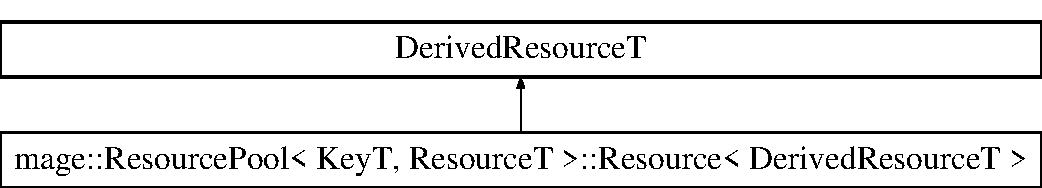
\includegraphics[height=2.000000cm]{classmage_1_1_resource_pool_1_1_resource}
\end{center}
\end{figure}
\subsection*{Public Member Functions}
\begin{DoxyCompactItemize}
\item 
{\footnotesize template$<$typename... Constructor\+ArgsT$>$ }\\\mbox{\hyperlink{classmage_1_1_resource_pool_1_1_resource_a552bb997277371d36aa1bf2248d83f4f}{Resource}} (\mbox{\hyperlink{classmage_1_1_resource_pool}{Resource\+Pool}} \&resource\+\_\+pool, const KeyT \&resource\+\_\+key, Constructor\+ArgsT \&\&... args)
\item 
\mbox{\hyperlink{classmage_1_1_resource_pool_1_1_resource_a783237133052c9e41b4c2d02fcdeefec}{Resource}} (const \mbox{\hyperlink{classmage_1_1_resource_pool_1_1_resource}{Resource}} \&resource)=delete
\item 
\mbox{\hyperlink{classmage_1_1_resource_pool_1_1_resource_a1c8016d99e1496da9383cbc4f727a913}{Resource}} (\mbox{\hyperlink{classmage_1_1_resource_pool_1_1_resource}{Resource}} \&\&resource)
\item 
virtual \mbox{\hyperlink{classmage_1_1_resource_pool_1_1_resource_a1d8bd565ab8769cedd94c1a42c6ebf46}{$\sim$\+Resource}} ()
\item 
\mbox{\hyperlink{classmage_1_1_resource_pool_1_1_resource}{Resource}} \& \mbox{\hyperlink{classmage_1_1_resource_pool_1_1_resource_a9c619f220b0fa676111cd24cb575dbff}{operator=}} (const \mbox{\hyperlink{classmage_1_1_resource_pool_1_1_resource}{Resource}} \&resource)=delete
\item 
\mbox{\hyperlink{classmage_1_1_resource_pool_1_1_resource}{Resource}} \& \mbox{\hyperlink{classmage_1_1_resource_pool_1_1_resource_a56f04f53400e77ddcc3c26fad1342e31}{operator=}} (\mbox{\hyperlink{classmage_1_1_resource_pool_1_1_resource}{Resource}} \&\&resource)=delete
\end{DoxyCompactItemize}
\subsection*{Private Attributes}
\begin{DoxyCompactItemize}
\item 
\mbox{\hyperlink{classmage_1_1_resource_pool}{Resource\+Pool}} \& \mbox{\hyperlink{classmage_1_1_resource_pool_1_1_resource_a9e5b68fd638ed6bd3b271afff834aced}{m\+\_\+resource\+\_\+pool}}
\item 
KeyT \mbox{\hyperlink{classmage_1_1_resource_pool_1_1_resource_a7200f97a65becde72367c9d0e3641621}{m\+\_\+resource\+\_\+key}}
\end{DoxyCompactItemize}


\subsection{Detailed Description}
\subsubsection*{template$<$typename KeyT, typename ResourceT$>$\newline
template$<$typename Derived\+ResourceT$>$\newline
class mage\+::\+Resource\+Pool$<$ Key\+T, Resource\+T $>$\+::\+Resource$<$ Derived\+Resource\+T $>$}

A class of resources.

\begin{DoxyPrecond}{Precondition}
{\ttfamily Derived\+ResourceT} is a derived class of {\ttfamily ResourceT}. 
\end{DoxyPrecond}

\begin{DoxyTemplParams}{Template Parameters}
{\em Derived\+ResourceT} & The derived resource type. \\
\hline
\end{DoxyTemplParams}


\subsection{Constructor \& Destructor Documentation}
\mbox{\Hypertarget{classmage_1_1_resource_pool_1_1_resource_a552bb997277371d36aa1bf2248d83f4f}\label{classmage_1_1_resource_pool_1_1_resource_a552bb997277371d36aa1bf2248d83f4f}} 
\index{mage\+::\+Resource\+Pool\+::\+Resource@{mage\+::\+Resource\+Pool\+::\+Resource}!Resource@{Resource}}
\index{Resource@{Resource}!mage\+::\+Resource\+Pool\+::\+Resource@{mage\+::\+Resource\+Pool\+::\+Resource}}
\subsubsection{\texorpdfstring{Resource()}{Resource()}\hspace{0.1cm}{\footnotesize\ttfamily [1/3]}}
{\footnotesize\ttfamily template$<$typename KeyT , typename ResourceT $>$ \\
template$<$typename Derived\+ResourceT $>$ \\
template$<$typename... Constructor\+ArgsT$>$ \\
\mbox{\hyperlink{classmage_1_1_resource_pool}{mage\+::\+Resource\+Pool}}$<$ KeyT, ResourceT $>$\+::\mbox{\hyperlink{classmage_1_1_resource_pool_1_1_resource}{Resource}}$<$ Derived\+ResourceT $>$\+::\mbox{\hyperlink{classmage_1_1_resource_pool_1_1_resource}{Resource}} (\begin{DoxyParamCaption}\item[{\mbox{\hyperlink{classmage_1_1_resource_pool}{Resource\+Pool}} \&}]{resource\+\_\+pool,  }\item[{const KeyT \&}]{resource\+\_\+key,  }\item[{Constructor\+ArgsT \&\&...}]{args }\end{DoxyParamCaption})}

Constructs a resource.


\begin{DoxyTemplParams}{Template Parameters}
{\em Constructor\+ArgsT} & The argument types for creating a new resource of type {\ttfamily Derived\+ResourceT}. \\
\hline
\end{DoxyTemplParams}

\begin{DoxyParams}[1]{Parameters}
\mbox{\tt in}  & {\em resource\+\_\+pool} & A reference to the resource pool. \\
\hline
\mbox{\tt in}  & {\em resource\+\_\+key} & A reference to the key of the resource in the given resource pool. \\
\hline
\mbox{\tt in}  & {\em args} & The arguments for creating a new resource of type {\ttfamily Derived\+ResourceT}. \\
\hline
\end{DoxyParams}
\mbox{\Hypertarget{classmage_1_1_resource_pool_1_1_resource_a783237133052c9e41b4c2d02fcdeefec}\label{classmage_1_1_resource_pool_1_1_resource_a783237133052c9e41b4c2d02fcdeefec}} 
\index{mage\+::\+Resource\+Pool\+::\+Resource@{mage\+::\+Resource\+Pool\+::\+Resource}!Resource@{Resource}}
\index{Resource@{Resource}!mage\+::\+Resource\+Pool\+::\+Resource@{mage\+::\+Resource\+Pool\+::\+Resource}}
\subsubsection{\texorpdfstring{Resource()}{Resource()}\hspace{0.1cm}{\footnotesize\ttfamily [2/3]}}
{\footnotesize\ttfamily template$<$typename KeyT , typename ResourceT $>$ \\
template$<$typename Derived\+ResourceT $>$ \\
\mbox{\hyperlink{classmage_1_1_resource_pool}{mage\+::\+Resource\+Pool}}$<$ KeyT, ResourceT $>$\+::\mbox{\hyperlink{classmage_1_1_resource_pool_1_1_resource}{Resource}}$<$ Derived\+ResourceT $>$\+::\mbox{\hyperlink{classmage_1_1_resource_pool_1_1_resource}{Resource}} (\begin{DoxyParamCaption}\item[{const \mbox{\hyperlink{classmage_1_1_resource_pool_1_1_resource}{Resource}}$<$ Derived\+ResourceT $>$ \&}]{resource }\end{DoxyParamCaption})\hspace{0.3cm}{\ttfamily [delete]}}

Constructs a resource from the given resource.


\begin{DoxyParams}[1]{Parameters}
\mbox{\tt in}  & {\em resource} & A reference to the resource to copy. \\
\hline
\end{DoxyParams}
\mbox{\Hypertarget{classmage_1_1_resource_pool_1_1_resource_a1c8016d99e1496da9383cbc4f727a913}\label{classmage_1_1_resource_pool_1_1_resource_a1c8016d99e1496da9383cbc4f727a913}} 
\index{mage\+::\+Resource\+Pool\+::\+Resource@{mage\+::\+Resource\+Pool\+::\+Resource}!Resource@{Resource}}
\index{Resource@{Resource}!mage\+::\+Resource\+Pool\+::\+Resource@{mage\+::\+Resource\+Pool\+::\+Resource}}
\subsubsection{\texorpdfstring{Resource()}{Resource()}\hspace{0.1cm}{\footnotesize\ttfamily [3/3]}}
{\footnotesize\ttfamily template$<$typename KeyT , typename ResourceT $>$ \\
template$<$typename Derived\+ResourceT $>$ \\
\mbox{\hyperlink{classmage_1_1_resource_pool}{mage\+::\+Resource\+Pool}}$<$ KeyT, ResourceT $>$\+::\mbox{\hyperlink{classmage_1_1_resource_pool_1_1_resource}{Resource}}$<$ Derived\+ResourceT $>$\+::\mbox{\hyperlink{classmage_1_1_resource_pool_1_1_resource}{Resource}} (\begin{DoxyParamCaption}\item[{\mbox{\hyperlink{classmage_1_1_resource_pool_1_1_resource}{Resource}}$<$ Derived\+ResourceT $>$ \&\&}]{resource }\end{DoxyParamCaption})}

Constructs a resource by moving the given resource poolentry .


\begin{DoxyParams}[1]{Parameters}
\mbox{\tt in}  & {\em resource} & A reference to the resource to move. \\
\hline
\end{DoxyParams}
\mbox{\Hypertarget{classmage_1_1_resource_pool_1_1_resource_a1d8bd565ab8769cedd94c1a42c6ebf46}\label{classmage_1_1_resource_pool_1_1_resource_a1d8bd565ab8769cedd94c1a42c6ebf46}} 
\index{mage\+::\+Resource\+Pool\+::\+Resource@{mage\+::\+Resource\+Pool\+::\+Resource}!````~Resource@{$\sim$\+Resource}}
\index{````~Resource@{$\sim$\+Resource}!mage\+::\+Resource\+Pool\+::\+Resource@{mage\+::\+Resource\+Pool\+::\+Resource}}
\subsubsection{\texorpdfstring{$\sim$\+Resource()}{~Resource()}}
{\footnotesize\ttfamily template$<$typename KeyT , typename ResourceT $>$ \\
template$<$typename Derived\+ResourceT $>$ \\
virtual \mbox{\hyperlink{classmage_1_1_resource_pool}{mage\+::\+Resource\+Pool}}$<$ KeyT, ResourceT $>$\+::\mbox{\hyperlink{classmage_1_1_resource_pool_1_1_resource}{Resource}}$<$ Derived\+ResourceT $>$\+::$\sim$\mbox{\hyperlink{classmage_1_1_resource_pool_1_1_resource}{Resource}} (\begin{DoxyParamCaption}{ }\end{DoxyParamCaption})\hspace{0.3cm}{\ttfamily [virtual]}}

Destructs this resource. 

\subsection{Member Function Documentation}
\mbox{\Hypertarget{classmage_1_1_resource_pool_1_1_resource_a9c619f220b0fa676111cd24cb575dbff}\label{classmage_1_1_resource_pool_1_1_resource_a9c619f220b0fa676111cd24cb575dbff}} 
\index{mage\+::\+Resource\+Pool\+::\+Resource@{mage\+::\+Resource\+Pool\+::\+Resource}!operator=@{operator=}}
\index{operator=@{operator=}!mage\+::\+Resource\+Pool\+::\+Resource@{mage\+::\+Resource\+Pool\+::\+Resource}}
\subsubsection{\texorpdfstring{operator=()}{operator=()}\hspace{0.1cm}{\footnotesize\ttfamily [1/2]}}
{\footnotesize\ttfamily template$<$typename KeyT , typename ResourceT $>$ \\
template$<$typename Derived\+ResourceT $>$ \\
\mbox{\hyperlink{classmage_1_1_resource_pool_1_1_resource}{Resource}}\& \mbox{\hyperlink{classmage_1_1_resource_pool}{mage\+::\+Resource\+Pool}}$<$ KeyT, ResourceT $>$\+::\mbox{\hyperlink{classmage_1_1_resource_pool_1_1_resource}{Resource}}$<$ Derived\+ResourceT $>$\+::operator= (\begin{DoxyParamCaption}\item[{const \mbox{\hyperlink{classmage_1_1_resource_pool_1_1_resource}{Resource}}$<$ Derived\+ResourceT $>$ \&}]{resource }\end{DoxyParamCaption})\hspace{0.3cm}{\ttfamily [delete]}}

Copies the given resource to this resource.


\begin{DoxyParams}[1]{Parameters}
\mbox{\tt in}  & {\em resource} & A reference to the resource to copy. \\
\hline
\end{DoxyParams}
\begin{DoxyReturn}{Returns}
A reference to the copy of the given resource (i.\+e. this resource). 
\end{DoxyReturn}
\mbox{\Hypertarget{classmage_1_1_resource_pool_1_1_resource_a56f04f53400e77ddcc3c26fad1342e31}\label{classmage_1_1_resource_pool_1_1_resource_a56f04f53400e77ddcc3c26fad1342e31}} 
\index{mage\+::\+Resource\+Pool\+::\+Resource@{mage\+::\+Resource\+Pool\+::\+Resource}!operator=@{operator=}}
\index{operator=@{operator=}!mage\+::\+Resource\+Pool\+::\+Resource@{mage\+::\+Resource\+Pool\+::\+Resource}}
\subsubsection{\texorpdfstring{operator=()}{operator=()}\hspace{0.1cm}{\footnotesize\ttfamily [2/2]}}
{\footnotesize\ttfamily template$<$typename KeyT , typename ResourceT $>$ \\
template$<$typename Derived\+ResourceT $>$ \\
\mbox{\hyperlink{classmage_1_1_resource_pool_1_1_resource}{Resource}}\& \mbox{\hyperlink{classmage_1_1_resource_pool}{mage\+::\+Resource\+Pool}}$<$ KeyT, ResourceT $>$\+::\mbox{\hyperlink{classmage_1_1_resource_pool_1_1_resource}{Resource}}$<$ Derived\+ResourceT $>$\+::operator= (\begin{DoxyParamCaption}\item[{\mbox{\hyperlink{classmage_1_1_resource_pool_1_1_resource}{Resource}}$<$ Derived\+ResourceT $>$ \&\&}]{resource }\end{DoxyParamCaption})\hspace{0.3cm}{\ttfamily [delete]}}

Moves the given resource to this resource.


\begin{DoxyParams}[1]{Parameters}
\mbox{\tt in}  & {\em resource} & A reference to the resource to move. \\
\hline
\end{DoxyParams}
\begin{DoxyReturn}{Returns}
A reference to the moved resource (i.\+e. this resource). 
\end{DoxyReturn}


\subsection{Member Data Documentation}
\mbox{\Hypertarget{classmage_1_1_resource_pool_1_1_resource_a7200f97a65becde72367c9d0e3641621}\label{classmage_1_1_resource_pool_1_1_resource_a7200f97a65becde72367c9d0e3641621}} 
\index{mage\+::\+Resource\+Pool\+::\+Resource@{mage\+::\+Resource\+Pool\+::\+Resource}!m\+\_\+resource\+\_\+key@{m\+\_\+resource\+\_\+key}}
\index{m\+\_\+resource\+\_\+key@{m\+\_\+resource\+\_\+key}!mage\+::\+Resource\+Pool\+::\+Resource@{mage\+::\+Resource\+Pool\+::\+Resource}}
\subsubsection{\texorpdfstring{m\+\_\+resource\+\_\+key}{m\_resource\_key}}
{\footnotesize\ttfamily template$<$typename KeyT , typename ResourceT $>$ \\
template$<$typename Derived\+ResourceT $>$ \\
KeyT \mbox{\hyperlink{classmage_1_1_resource_pool}{mage\+::\+Resource\+Pool}}$<$ KeyT, ResourceT $>$\+::\mbox{\hyperlink{classmage_1_1_resource_pool_1_1_resource}{Resource}}$<$ Derived\+ResourceT $>$\+::m\+\_\+resource\+\_\+key\hspace{0.3cm}{\ttfamily [private]}}

The key of this resource in the resource pool map containing this resource. \mbox{\Hypertarget{classmage_1_1_resource_pool_1_1_resource_a9e5b68fd638ed6bd3b271afff834aced}\label{classmage_1_1_resource_pool_1_1_resource_a9e5b68fd638ed6bd3b271afff834aced}} 
\index{mage\+::\+Resource\+Pool\+::\+Resource@{mage\+::\+Resource\+Pool\+::\+Resource}!m\+\_\+resource\+\_\+pool@{m\+\_\+resource\+\_\+pool}}
\index{m\+\_\+resource\+\_\+pool@{m\+\_\+resource\+\_\+pool}!mage\+::\+Resource\+Pool\+::\+Resource@{mage\+::\+Resource\+Pool\+::\+Resource}}
\subsubsection{\texorpdfstring{m\+\_\+resource\+\_\+pool}{m\_resource\_pool}}
{\footnotesize\ttfamily template$<$typename KeyT , typename ResourceT $>$ \\
template$<$typename Derived\+ResourceT $>$ \\
\mbox{\hyperlink{classmage_1_1_resource_pool}{Resource\+Pool}}\& \mbox{\hyperlink{classmage_1_1_resource_pool}{mage\+::\+Resource\+Pool}}$<$ KeyT, ResourceT $>$\+::\mbox{\hyperlink{classmage_1_1_resource_pool_1_1_resource}{Resource}}$<$ Derived\+ResourceT $>$\+::m\+\_\+resource\+\_\+pool\hspace{0.3cm}{\ttfamily [private]}}

A reference to the resource pool map containing this resource. 
\hypertarget{classmage_1_1rendering_1_1_resource_manager}{}\section{mage\+:\+:rendering\+:\+:Resource\+Manager Class Reference}
\label{classmage_1_1rendering_1_1_resource_manager}\index{mage\+::rendering\+::\+Resource\+Manager@{mage\+::rendering\+::\+Resource\+Manager}}


{\ttfamily \#include $<$rendering\+\_\+resource\+\_\+manager.\+hpp$>$}

\subsection*{Classes}
\begin{DoxyCompactItemize}
\item 
struct \hyperlink{structmage_1_1rendering_1_1_resource_manager_1_1_resource_record}{Resource\+Record}
\item 
struct \hyperlink{structmage_1_1rendering_1_1_resource_manager_1_1_resource_record_3_01_resource_t_00_01typename_0d1bec05cbaa53974b1eda0724091f851}{Resource\+Record$<$ Resource\+T, typename std\+::enable\+\_\+if\+\_\+t$<$ !is\+\_\+shader\+\_\+v$<$ Resource\+T $>$ $>$ $>$}
\item 
struct \hyperlink{structmage_1_1rendering_1_1_resource_manager_1_1_resource_record_3_01_resource_t_00_01typename_09b062ee4b0394619806084252c69f48d}{Resource\+Record$<$ Resource\+T, typename std\+::enable\+\_\+if\+\_\+t$<$ is\+\_\+shader\+\_\+v$<$ Resource\+T $>$ $>$ $>$}
\end{DoxyCompactItemize}
\subsection*{Public Types}
\begin{DoxyCompactItemize}
\item 
{\footnotesize template$<$typename ResourceT $>$ }\\using \hyperlink{classmage_1_1rendering_1_1_resource_manager_ab21a4e280087032ee533f267bd9bf602}{pool\+\_\+type} = typename \hyperlink{structmage_1_1rendering_1_1_resource_manager_1_1_resource_record}{Resource\+Record}$<$ ResourceT $>$\+::\hyperlink{classmage_1_1rendering_1_1_resource_manager_ab21a4e280087032ee533f267bd9bf602}{pool\+\_\+type}
\item 
{\footnotesize template$<$typename ResourceT $>$ }\\using \hyperlink{classmage_1_1rendering_1_1_resource_manager_a097b505b275b411e02c73d1899e91a44}{key\+\_\+type} = typename \hyperlink{classmage_1_1rendering_1_1_resource_manager_ab21a4e280087032ee533f267bd9bf602}{pool\+\_\+type}$<$ ResourceT $>$\+::\hyperlink{classmage_1_1rendering_1_1_resource_manager_a097b505b275b411e02c73d1899e91a44}{key\+\_\+type}
\item 
{\footnotesize template$<$typename ResourceT $>$ }\\using \hyperlink{classmage_1_1rendering_1_1_resource_manager_abb6ad8fd8054364a230839110c42174f}{value\+\_\+type} = typename \hyperlink{classmage_1_1rendering_1_1_resource_manager_ab21a4e280087032ee533f267bd9bf602}{pool\+\_\+type}$<$ ResourceT $>$\+::\hyperlink{classmage_1_1rendering_1_1_resource_manager_abb6ad8fd8054364a230839110c42174f}{value\+\_\+type}
\end{DoxyCompactItemize}
\subsection*{Public Member Functions}
\begin{DoxyCompactItemize}
\item 
\hyperlink{classmage_1_1rendering_1_1_resource_manager_a2274df2c0badb1dd2e79642e69c76cb7}{Resource\+Manager} (I\+D3\+D11\+Device \&device)
\item 
\hyperlink{classmage_1_1rendering_1_1_resource_manager_a94b757238211a5b6fe44d773b579ca0a}{Resource\+Manager} (const \hyperlink{classmage_1_1rendering_1_1_resource_manager}{Resource\+Manager} \&manager)=delete
\item 
\hyperlink{classmage_1_1rendering_1_1_resource_manager_a3d54199cf484d11c1d1039eeb306016c}{Resource\+Manager} (\hyperlink{classmage_1_1rendering_1_1_resource_manager}{Resource\+Manager} \&\&manager) noexcept
\item 
\hyperlink{classmage_1_1rendering_1_1_resource_manager_a7289ca2a270e6de613eff041ba04d4a4}{$\sim$\+Resource\+Manager} ()
\item 
\hyperlink{classmage_1_1rendering_1_1_resource_manager}{Resource\+Manager} \& \hyperlink{classmage_1_1rendering_1_1_resource_manager_a188467ab4e46176ee5184c9f5e5ac64f}{operator=} (const \hyperlink{classmage_1_1rendering_1_1_resource_manager}{Resource\+Manager} \&manager)=delete
\item 
\hyperlink{classmage_1_1rendering_1_1_resource_manager}{Resource\+Manager} \& \hyperlink{classmage_1_1rendering_1_1_resource_manager_a1e3f511409bcde3a7a3296364a0298f5}{operator=} (\hyperlink{classmage_1_1rendering_1_1_resource_manager}{Resource\+Manager} \&\&manager)=delete
\item 
{\footnotesize template$<$typename ResourceT $>$ }\\bool \hyperlink{classmage_1_1rendering_1_1_resource_manager_a7df24baa95d7a43697cba243dd5b5a54}{Contains} (const typename \hyperlink{classmage_1_1rendering_1_1_resource_manager_a097b505b275b411e02c73d1899e91a44}{key\+\_\+type}$<$ ResourceT $>$ \&guid) noexcept
\item 
{\footnotesize template$<$typename ResourceT $>$ }\\\hyperlink{namespacemage_a1e01ae66713838a7a67d30e44c67703e}{Shared\+Ptr}$<$ typename \hyperlink{classmage_1_1rendering_1_1_resource_manager_abb6ad8fd8054364a230839110c42174f}{value\+\_\+type}$<$ ResourceT $>$ $>$ \hyperlink{classmage_1_1rendering_1_1_resource_manager_aeb229ae49bde59cb6c146f9749851363}{Get} (const typename \hyperlink{classmage_1_1rendering_1_1_resource_manager_a097b505b275b411e02c73d1899e91a44}{key\+\_\+type}$<$ ResourceT $>$ \&guid) noexcept
\item 
{\footnotesize template$<$typename ResourceT , typename VertexT , typename IndexT $>$ }\\std\+::enable\+\_\+if\+\_\+t$<$ std\+::is\+\_\+same\+\_\+v$<$ \hyperlink{classmage_1_1rendering_1_1_model_descriptor}{Model\+Descriptor}, ResourceT $>$, \hyperlink{namespacemage_1_1rendering_a07260934fd7cb48a210873ae73e62911}{Model\+Descriptor\+Ptr} $>$ \hyperlink{classmage_1_1rendering_1_1_resource_manager_a2e9c16757e4aa09c8544289650f3ce20}{Get\+Or\+Create} (const wstring \&fname, const \hyperlink{classmage_1_1rendering_1_1_mesh_descriptor}{Mesh\+Descriptor}$<$ VertexT, IndexT $>$ \&desc=\hyperlink{classmage_1_1rendering_1_1_mesh_descriptor}{Mesh\+Descriptor}$<$ VertexT, IndexT $>$(), bool export\+\_\+as\+\_\+\+M\+DL=false)
\item 
{\footnotesize template$<$typename ResourceT $>$ }\\std\+::enable\+\_\+if\+\_\+t$<$ std\+::is\+\_\+same\+\_\+v$<$ \hyperlink{classmage_1_1rendering_1_1_vertex_shader}{Vertex\+Shader}, ResourceT $>$, \hyperlink{namespacemage_1_1rendering_aaf704b9c54a4181f4950a1761de69dda}{Vertex\+Shader\+Ptr} $>$ \hyperlink{classmage_1_1rendering_1_1_resource_manager_a10abecc1fde6cccbae90e14d64b55727}{Get\+Or\+Create} (const wstring \&guid, const \hyperlink{classmage_1_1rendering_1_1_compiled_shader}{Compiled\+Shader} \&compiled\+\_\+shader, gsl\+::span$<$ const D3\+D11\+\_\+\+I\+N\+P\+U\+T\+\_\+\+E\+L\+E\+M\+E\+N\+T\+\_\+\+D\+E\+SC $>$ input\+\_\+element\+\_\+descs)
\item 
{\footnotesize template$<$typename ResourceT $>$ }\\std\+::enable\+\_\+if\+\_\+t$<$ std\+::is\+\_\+same\+\_\+v$<$ \hyperlink{namespacemage_1_1rendering_aa133f36cd1a81c87eedf962270a12f48}{Hull\+Shader}, ResourceT $>$, \hyperlink{namespacemage_1_1rendering_a6f33b2e1ea7f2ae3824dc7fb6875c655}{Hull\+Shader\+Ptr} $>$ \hyperlink{classmage_1_1rendering_1_1_resource_manager_aedf58d2d3f5436b06deb080b5324a1fb}{Get\+Or\+Create} (const wstring \&guid, const \hyperlink{classmage_1_1rendering_1_1_compiled_shader}{Compiled\+Shader} \&compiled\+\_\+shader)
\item 
{\footnotesize template$<$typename ResourceT $>$ }\\std\+::enable\+\_\+if\+\_\+t$<$ std\+::is\+\_\+same\+\_\+v$<$ \hyperlink{namespacemage_1_1rendering_a02bd57ea68f48dd6e0d37a1362ad1ea2}{Domain\+Shader}, ResourceT $>$, \hyperlink{namespacemage_1_1rendering_a85a8911c7c1e9e42bd7c3acbc2725076}{Domain\+Shader\+Ptr} $>$ \hyperlink{classmage_1_1rendering_1_1_resource_manager_adf60f2638d297cc7627a8806535cad17}{Get\+Or\+Create} (const wstring \&guid, const \hyperlink{classmage_1_1rendering_1_1_compiled_shader}{Compiled\+Shader} \&compiled\+\_\+shader)
\item 
{\footnotesize template$<$typename ResourceT $>$ }\\std\+::enable\+\_\+if\+\_\+t$<$ std\+::is\+\_\+same\+\_\+v$<$ \hyperlink{namespacemage_1_1rendering_accaa3591de8a0d7a2c72c1dcc0cf9592}{Geometry\+Shader}, ResourceT $>$, \hyperlink{namespacemage_1_1rendering_aa5d63f80f9483d0896718813768ba1cf}{Geometry\+Shader\+Ptr} $>$ \hyperlink{classmage_1_1rendering_1_1_resource_manager_acb35a9671a7b9c7a8f2e7cb5914282e2}{Get\+Or\+Create} (const wstring \&guid, const \hyperlink{classmage_1_1rendering_1_1_compiled_shader}{Compiled\+Shader} \&compiled\+\_\+shader)
\item 
{\footnotesize template$<$typename ResourceT $>$ }\\std\+::enable\+\_\+if\+\_\+t$<$ std\+::is\+\_\+same\+\_\+v$<$ \hyperlink{namespacemage_1_1rendering_a19905114913398d5073148f6c416e1b7}{Pixel\+Shader}, ResourceT $>$, \hyperlink{namespacemage_1_1rendering_af03d922b228ee9c8542baaa2ecc9f259}{Pixel\+Shader\+Ptr} $>$ \hyperlink{classmage_1_1rendering_1_1_resource_manager_a19ec0a56d1311f82d32a564bdf8a6bd0}{Get\+Or\+Create} (const wstring \&guid, const \hyperlink{classmage_1_1rendering_1_1_compiled_shader}{Compiled\+Shader} \&compiled\+\_\+shader)
\item 
{\footnotesize template$<$typename ResourceT $>$ }\\std\+::enable\+\_\+if\+\_\+t$<$ std\+::is\+\_\+same\+\_\+v$<$ \hyperlink{namespacemage_1_1rendering_aa67e55ba4dca44d39b0367b31f091863}{Compute\+Shader}, ResourceT $>$, \hyperlink{namespacemage_1_1rendering_ab3dc9f2114f2e9255b91d9c051da52ea}{Compute\+Shader\+Ptr} $>$ \hyperlink{classmage_1_1rendering_1_1_resource_manager_a7d84eac42a5aee44bc3d8007b0eb408e}{Get\+Or\+Create} (const wstring \&guid, const \hyperlink{classmage_1_1rendering_1_1_compiled_shader}{Compiled\+Shader} \&compiled\+\_\+shader)
\item 
{\footnotesize template$<$typename ResourceT $>$ }\\std\+::enable\+\_\+if\+\_\+t$<$ std\+::is\+\_\+same\+\_\+v$<$ \hyperlink{classmage_1_1rendering_1_1_sprite_font}{Sprite\+Font}, ResourceT $>$, \hyperlink{namespacemage_1_1rendering_ab2f34196c20422ca3692ad3f3bff3a5d}{Sprite\+Font\+Ptr} $>$ \hyperlink{classmage_1_1rendering_1_1_resource_manager_a664a3fd14471c1e1d7128b90b66644b9}{Get\+Or\+Create} (const wstring \&fname, const \hyperlink{classmage_1_1rendering_1_1_sprite_font_descriptor}{Sprite\+Font\+Descriptor} \&desc=\hyperlink{classmage_1_1rendering_1_1_sprite_font_descriptor}{Sprite\+Font\+Descriptor}())
\item 
{\footnotesize template$<$typename ResourceT $>$ }\\std\+::enable\+\_\+if\+\_\+t$<$ std\+::is\+\_\+same\+\_\+v$<$ \hyperlink{classmage_1_1rendering_1_1_texture}{Texture}, ResourceT $>$, \hyperlink{namespacemage_1_1rendering_a6f3ae54f825328465b0cdde0f0de4a36}{Texture\+Ptr} $>$ \hyperlink{classmage_1_1rendering_1_1_resource_manager_a5a1db7a1b2aae7e2ea5759820c875d78}{Get\+Or\+Create} (const wstring \&fname)
\item 
{\footnotesize template$<$typename ResourceT $>$ }\\std\+::enable\+\_\+if\+\_\+t$<$ std\+::is\+\_\+same\+\_\+v$<$ \hyperlink{classmage_1_1rendering_1_1_texture}{Texture}, ResourceT $>$, \hyperlink{namespacemage_1_1rendering_a6f3ae54f825328465b0cdde0f0de4a36}{Texture\+Ptr} $>$ \hyperlink{classmage_1_1rendering_1_1_resource_manager_a330efb725a94fec87a996e0048589d1b}{Get\+Or\+Create} (const wstring \&guid, const D3\+D11\+\_\+\+T\+E\+X\+T\+U\+R\+E2\+D\+\_\+\+D\+E\+SC \&desc, const D3\+D11\+\_\+\+S\+U\+B\+R\+E\+S\+O\+U\+R\+C\+E\+\_\+\+D\+A\+TA \&initial\+\_\+data)
\end{DoxyCompactItemize}
\subsection*{Private Member Functions}
\begin{DoxyCompactItemize}
\item 
{\footnotesize template$<$typename ResourceT $>$ }\\\hyperlink{classmage_1_1rendering_1_1_resource_manager_ab21a4e280087032ee533f267bd9bf602}{pool\+\_\+type}$<$ ResourceT $>$ \& \hyperlink{classmage_1_1rendering_1_1_resource_manager_a91891df90f569c3f3f72a51c8a2f6ae5}{Get\+Pool} () noexcept
\item 
{\footnotesize template$<$typename ResourceT $>$ }\\const \hyperlink{classmage_1_1rendering_1_1_resource_manager_ab21a4e280087032ee533f267bd9bf602}{pool\+\_\+type}$<$ ResourceT $>$ \& \hyperlink{classmage_1_1rendering_1_1_resource_manager_a5cba7eab859779a7cb74d5f2cef21173}{Get\+Pool} () const noexcept
\end{DoxyCompactItemize}
\subsection*{Private Attributes}
\begin{DoxyCompactItemize}
\item 
I\+D3\+D11\+Device \& \hyperlink{classmage_1_1rendering_1_1_resource_manager_ad5233c9a748dcd828e5176ad5e8282c9}{m\+\_\+device}
\item 
\hyperlink{classmage_1_1rendering_1_1_resource_manager_ab21a4e280087032ee533f267bd9bf602}{pool\+\_\+type}$<$ \hyperlink{classmage_1_1rendering_1_1_model_descriptor}{Model\+Descriptor} $>$ \hyperlink{classmage_1_1rendering_1_1_resource_manager_a43db83f825b58a85c34e633d5807171d}{m\+\_\+model\+\_\+descriptor\+\_\+pool}
\item 
\hyperlink{classmage_1_1rendering_1_1_resource_manager_ab21a4e280087032ee533f267bd9bf602}{pool\+\_\+type}$<$ \hyperlink{classmage_1_1rendering_1_1_vertex_shader}{Vertex\+Shader} $>$ \hyperlink{classmage_1_1rendering_1_1_resource_manager_ac4af09e51fbbcfb534edb72d98033979}{m\+\_\+vs\+\_\+pool}
\item 
\hyperlink{classmage_1_1rendering_1_1_resource_manager_ab21a4e280087032ee533f267bd9bf602}{pool\+\_\+type}$<$ \hyperlink{namespacemage_1_1rendering_aa133f36cd1a81c87eedf962270a12f48}{Hull\+Shader} $>$ \hyperlink{classmage_1_1rendering_1_1_resource_manager_acea62c6cf52bd332ee3e0d1575c02e29}{m\+\_\+hs\+\_\+pool}
\item 
\hyperlink{classmage_1_1rendering_1_1_resource_manager_ab21a4e280087032ee533f267bd9bf602}{pool\+\_\+type}$<$ \hyperlink{namespacemage_1_1rendering_a02bd57ea68f48dd6e0d37a1362ad1ea2}{Domain\+Shader} $>$ \hyperlink{classmage_1_1rendering_1_1_resource_manager_a49ccc18bfbca9728857d820266c3acf6}{m\+\_\+ds\+\_\+pool}
\item 
\hyperlink{classmage_1_1rendering_1_1_resource_manager_ab21a4e280087032ee533f267bd9bf602}{pool\+\_\+type}$<$ \hyperlink{namespacemage_1_1rendering_accaa3591de8a0d7a2c72c1dcc0cf9592}{Geometry\+Shader} $>$ \hyperlink{classmage_1_1rendering_1_1_resource_manager_aa8fe17aa004cb46afc132a672bbb014d}{m\+\_\+gs\+\_\+pool}
\item 
\hyperlink{classmage_1_1rendering_1_1_resource_manager_ab21a4e280087032ee533f267bd9bf602}{pool\+\_\+type}$<$ \hyperlink{namespacemage_1_1rendering_a19905114913398d5073148f6c416e1b7}{Pixel\+Shader} $>$ \hyperlink{classmage_1_1rendering_1_1_resource_manager_a73f970f19438b2e2f02a5ede41e8faf4}{m\+\_\+ps\+\_\+pool}
\item 
\hyperlink{classmage_1_1rendering_1_1_resource_manager_ab21a4e280087032ee533f267bd9bf602}{pool\+\_\+type}$<$ \hyperlink{namespacemage_1_1rendering_aa67e55ba4dca44d39b0367b31f091863}{Compute\+Shader} $>$ \hyperlink{classmage_1_1rendering_1_1_resource_manager_ae0433b0866f523c3c0e6e22197aea86f}{m\+\_\+cs\+\_\+pool}
\item 
\hyperlink{classmage_1_1rendering_1_1_resource_manager_ab21a4e280087032ee533f267bd9bf602}{pool\+\_\+type}$<$ \hyperlink{classmage_1_1rendering_1_1_sprite_font}{Sprite\+Font} $>$ \hyperlink{classmage_1_1rendering_1_1_resource_manager_a0319ef8aad59a69098e6c0a89b6c912e}{m\+\_\+sprite\+\_\+font\+\_\+pool}
\item 
\hyperlink{classmage_1_1rendering_1_1_resource_manager_ab21a4e280087032ee533f267bd9bf602}{pool\+\_\+type}$<$ \hyperlink{classmage_1_1rendering_1_1_texture}{Texture} $>$ \hyperlink{classmage_1_1rendering_1_1_resource_manager_aaf5faede84cdce3bd2589936d5ba3b18}{m\+\_\+texture\+\_\+pool}
\end{DoxyCompactItemize}


\subsection{Detailed Description}
A class of resource managers. 

\subsection{Member Typedef Documentation}
\hypertarget{classmage_1_1rendering_1_1_resource_manager_a097b505b275b411e02c73d1899e91a44}{}\label{classmage_1_1rendering_1_1_resource_manager_a097b505b275b411e02c73d1899e91a44} 
\index{mage\+::rendering\+::\+Resource\+Manager@{mage\+::rendering\+::\+Resource\+Manager}!key\+\_\+type@{key\+\_\+type}}
\index{key\+\_\+type@{key\+\_\+type}!mage\+::rendering\+::\+Resource\+Manager@{mage\+::rendering\+::\+Resource\+Manager}}
\subsubsection{\texorpdfstring{key\+\_\+type}{key\_type}}
{\footnotesize\ttfamily template$<$typename ResourceT $>$ \\
using \hyperlink{classmage_1_1rendering_1_1_resource_manager_a097b505b275b411e02c73d1899e91a44}{mage\+::rendering\+::\+Resource\+Manager\+::key\+\_\+type} =  typename \hyperlink{classmage_1_1rendering_1_1_resource_manager_ab21a4e280087032ee533f267bd9bf602}{pool\+\_\+type}$<$ ResourceT $>$\+::\hyperlink{classmage_1_1rendering_1_1_resource_manager_a097b505b275b411e02c73d1899e91a44}{key\+\_\+type}}

The key type of resource pools containing resources of the given type.


\begin{DoxyTemplParams}{Template Parameters}
{\em ResourceT} & The resource type. \\
\hline
\end{DoxyTemplParams}
\hypertarget{classmage_1_1rendering_1_1_resource_manager_ab21a4e280087032ee533f267bd9bf602}{}\label{classmage_1_1rendering_1_1_resource_manager_ab21a4e280087032ee533f267bd9bf602} 
\index{mage\+::rendering\+::\+Resource\+Manager@{mage\+::rendering\+::\+Resource\+Manager}!pool\+\_\+type@{pool\+\_\+type}}
\index{pool\+\_\+type@{pool\+\_\+type}!mage\+::rendering\+::\+Resource\+Manager@{mage\+::rendering\+::\+Resource\+Manager}}
\subsubsection{\texorpdfstring{pool\+\_\+type}{pool\_type}}
{\footnotesize\ttfamily template$<$typename ResourceT $>$ \\
using \hyperlink{classmage_1_1rendering_1_1_resource_manager_ab21a4e280087032ee533f267bd9bf602}{mage\+::rendering\+::\+Resource\+Manager\+::pool\+\_\+type} =  typename \hyperlink{structmage_1_1rendering_1_1_resource_manager_1_1_resource_record}{Resource\+Record}$<$ ResourceT $>$\+::\hyperlink{classmage_1_1rendering_1_1_resource_manager_ab21a4e280087032ee533f267bd9bf602}{pool\+\_\+type}}

The pool type of resource pools containing resources of the given type.


\begin{DoxyTemplParams}{Template Parameters}
{\em ResourceT} & The resource type. \\
\hline
\end{DoxyTemplParams}
\hypertarget{classmage_1_1rendering_1_1_resource_manager_abb6ad8fd8054364a230839110c42174f}{}\label{classmage_1_1rendering_1_1_resource_manager_abb6ad8fd8054364a230839110c42174f} 
\index{mage\+::rendering\+::\+Resource\+Manager@{mage\+::rendering\+::\+Resource\+Manager}!value\+\_\+type@{value\+\_\+type}}
\index{value\+\_\+type@{value\+\_\+type}!mage\+::rendering\+::\+Resource\+Manager@{mage\+::rendering\+::\+Resource\+Manager}}
\subsubsection{\texorpdfstring{value\+\_\+type}{value\_type}}
{\footnotesize\ttfamily template$<$typename ResourceT $>$ \\
using \hyperlink{classmage_1_1rendering_1_1_resource_manager_abb6ad8fd8054364a230839110c42174f}{mage\+::rendering\+::\+Resource\+Manager\+::value\+\_\+type} =  typename \hyperlink{classmage_1_1rendering_1_1_resource_manager_ab21a4e280087032ee533f267bd9bf602}{pool\+\_\+type}$<$ ResourceT $>$\+::\hyperlink{classmage_1_1rendering_1_1_resource_manager_abb6ad8fd8054364a230839110c42174f}{value\+\_\+type}}

The value type of resource pools containing resources of the given type.


\begin{DoxyTemplParams}{Template Parameters}
{\em ResourceT} & The resource type. \\
\hline
\end{DoxyTemplParams}


\subsection{Constructor \& Destructor Documentation}
\hypertarget{classmage_1_1rendering_1_1_resource_manager_a2274df2c0badb1dd2e79642e69c76cb7}{}\label{classmage_1_1rendering_1_1_resource_manager_a2274df2c0badb1dd2e79642e69c76cb7} 
\index{mage\+::rendering\+::\+Resource\+Manager@{mage\+::rendering\+::\+Resource\+Manager}!Resource\+Manager@{Resource\+Manager}}
\index{Resource\+Manager@{Resource\+Manager}!mage\+::rendering\+::\+Resource\+Manager@{mage\+::rendering\+::\+Resource\+Manager}}
\subsubsection{\texorpdfstring{Resource\+Manager()}{ResourceManager()}\hspace{0.1cm}{\footnotesize\ttfamily [1/3]}}
{\footnotesize\ttfamily mage\+::rendering\+::\+Resource\+Manager\+::\+Resource\+Manager (\begin{DoxyParamCaption}\item[{I\+D3\+D11\+Device \&}]{device }\end{DoxyParamCaption})}

Constructs a resource manager.


\begin{DoxyParams}[1]{Parameters}
\mbox{\tt in}  & {\em device} & A reference to the device. \\
\hline
\end{DoxyParams}
\hypertarget{classmage_1_1rendering_1_1_resource_manager_a94b757238211a5b6fe44d773b579ca0a}{}\label{classmage_1_1rendering_1_1_resource_manager_a94b757238211a5b6fe44d773b579ca0a} 
\index{mage\+::rendering\+::\+Resource\+Manager@{mage\+::rendering\+::\+Resource\+Manager}!Resource\+Manager@{Resource\+Manager}}
\index{Resource\+Manager@{Resource\+Manager}!mage\+::rendering\+::\+Resource\+Manager@{mage\+::rendering\+::\+Resource\+Manager}}
\subsubsection{\texorpdfstring{Resource\+Manager()}{ResourceManager()}\hspace{0.1cm}{\footnotesize\ttfamily [2/3]}}
{\footnotesize\ttfamily mage\+::rendering\+::\+Resource\+Manager\+::\+Resource\+Manager (\begin{DoxyParamCaption}\item[{const \hyperlink{classmage_1_1rendering_1_1_resource_manager}{Resource\+Manager} \&}]{manager }\end{DoxyParamCaption})\hspace{0.3cm}{\ttfamily [delete]}}

Constructs a resource manager from the given resource manager.


\begin{DoxyParams}[1]{Parameters}
\mbox{\tt in}  & {\em manager} & A reference to the resource manager to copy. \\
\hline
\end{DoxyParams}
\hypertarget{classmage_1_1rendering_1_1_resource_manager_a3d54199cf484d11c1d1039eeb306016c}{}\label{classmage_1_1rendering_1_1_resource_manager_a3d54199cf484d11c1d1039eeb306016c} 
\index{mage\+::rendering\+::\+Resource\+Manager@{mage\+::rendering\+::\+Resource\+Manager}!Resource\+Manager@{Resource\+Manager}}
\index{Resource\+Manager@{Resource\+Manager}!mage\+::rendering\+::\+Resource\+Manager@{mage\+::rendering\+::\+Resource\+Manager}}
\subsubsection{\texorpdfstring{Resource\+Manager()}{ResourceManager()}\hspace{0.1cm}{\footnotesize\ttfamily [3/3]}}
{\footnotesize\ttfamily mage\+::rendering\+::\+Resource\+Manager\+::\+Resource\+Manager (\begin{DoxyParamCaption}\item[{\hyperlink{classmage_1_1rendering_1_1_resource_manager}{Resource\+Manager} \&\&}]{manager }\end{DoxyParamCaption})\hspace{0.3cm}{\ttfamily [default]}, {\ttfamily [noexcept]}}

Constructs a resource manager by moving the given resource manager.


\begin{DoxyParams}[1]{Parameters}
\mbox{\tt in}  & {\em manager} & A reference to the resource manager to move. \\
\hline
\end{DoxyParams}
\hypertarget{classmage_1_1rendering_1_1_resource_manager_a7289ca2a270e6de613eff041ba04d4a4}{}\label{classmage_1_1rendering_1_1_resource_manager_a7289ca2a270e6de613eff041ba04d4a4} 
\index{mage\+::rendering\+::\+Resource\+Manager@{mage\+::rendering\+::\+Resource\+Manager}!````~Resource\+Manager@{$\sim$\+Resource\+Manager}}
\index{````~Resource\+Manager@{$\sim$\+Resource\+Manager}!mage\+::rendering\+::\+Resource\+Manager@{mage\+::rendering\+::\+Resource\+Manager}}
\subsubsection{\texorpdfstring{$\sim$\+Resource\+Manager()}{~ResourceManager()}}
{\footnotesize\ttfamily mage\+::rendering\+::\+Resource\+Manager\+::$\sim$\+Resource\+Manager (\begin{DoxyParamCaption}{ }\end{DoxyParamCaption})\hspace{0.3cm}{\ttfamily [default]}}

Destructs this resource manager. 

\subsection{Member Function Documentation}
\hypertarget{classmage_1_1rendering_1_1_resource_manager_a7df24baa95d7a43697cba243dd5b5a54}{}\label{classmage_1_1rendering_1_1_resource_manager_a7df24baa95d7a43697cba243dd5b5a54} 
\index{mage\+::rendering\+::\+Resource\+Manager@{mage\+::rendering\+::\+Resource\+Manager}!Contains@{Contains}}
\index{Contains@{Contains}!mage\+::rendering\+::\+Resource\+Manager@{mage\+::rendering\+::\+Resource\+Manager}}
\subsubsection{\texorpdfstring{Contains()}{Contains()}}
{\footnotesize\ttfamily template$<$typename ResourceT $>$ \\
bool mage\+::rendering\+::\+Resource\+Manager\+::\+Contains (\begin{DoxyParamCaption}\item[{const typename \hyperlink{classmage_1_1rendering_1_1_resource_manager_a097b505b275b411e02c73d1899e91a44}{key\+\_\+type}$<$ ResourceT $>$ \&}]{guid }\end{DoxyParamCaption})\hspace{0.3cm}{\ttfamily [noexcept]}}

Checks whether this resource manager contains a resource of the given type corresponding to the given globally unique identifier.


\begin{DoxyTemplParams}{Template Parameters}
{\em ResourceT} & The resource type. \\
\hline
\end{DoxyTemplParams}

\begin{DoxyParams}[1]{Parameters}
\mbox{\tt in}  & {\em guid} & A reference to the globally unique identifier of the resource. \\
\hline
\end{DoxyParams}
\begin{DoxyReturn}{Returns}
{\ttfamily true} if this resource managers contains a resource of the given type corresponding to the given globally unique identifier. {\ttfamily false} otherwise. 
\end{DoxyReturn}
\hypertarget{classmage_1_1rendering_1_1_resource_manager_aeb229ae49bde59cb6c146f9749851363}{}\label{classmage_1_1rendering_1_1_resource_manager_aeb229ae49bde59cb6c146f9749851363} 
\index{mage\+::rendering\+::\+Resource\+Manager@{mage\+::rendering\+::\+Resource\+Manager}!Get@{Get}}
\index{Get@{Get}!mage\+::rendering\+::\+Resource\+Manager@{mage\+::rendering\+::\+Resource\+Manager}}
\subsubsection{\texorpdfstring{Get()}{Get()}}
{\footnotesize\ttfamily template$<$typename ResourceT $>$ \\
\hyperlink{namespacemage_a1e01ae66713838a7a67d30e44c67703e}{Shared\+Ptr}$<$ typename \hyperlink{classmage_1_1rendering_1_1_resource_manager_abb6ad8fd8054364a230839110c42174f}{value\+\_\+type}$<$ ResourceT $>$ $>$ mage\+::rendering\+::\+Resource\+Manager\+::\+Get (\begin{DoxyParamCaption}\item[{const typename \hyperlink{classmage_1_1rendering_1_1_resource_manager_a097b505b275b411e02c73d1899e91a44}{key\+\_\+type}$<$ ResourceT $>$ \&}]{guid }\end{DoxyParamCaption})\hspace{0.3cm}{\ttfamily [noexcept]}}

Returns the resource of the given type corresponding to the given globally unique identifier of this resource manager.


\begin{DoxyTemplParams}{Template Parameters}
{\em ResourceT} & The resource type. \\
\hline
\end{DoxyTemplParams}

\begin{DoxyParams}[1]{Parameters}
\mbox{\tt in}  & {\em guid} & A reference to the globally unique identifier of the model descriptor. \\
\hline
\end{DoxyParams}
\begin{DoxyReturn}{Returns}
{\ttfamily nullptr}, if this resource managers does not contain a resource of the given type corresponding to the given globally unique identifier. 

A pointer to the resource. 
\end{DoxyReturn}
\hypertarget{classmage_1_1rendering_1_1_resource_manager_a2e9c16757e4aa09c8544289650f3ce20}{}\label{classmage_1_1rendering_1_1_resource_manager_a2e9c16757e4aa09c8544289650f3ce20} 
\index{mage\+::rendering\+::\+Resource\+Manager@{mage\+::rendering\+::\+Resource\+Manager}!Get\+Or\+Create@{Get\+Or\+Create}}
\index{Get\+Or\+Create@{Get\+Or\+Create}!mage\+::rendering\+::\+Resource\+Manager@{mage\+::rendering\+::\+Resource\+Manager}}
\subsubsection{\texorpdfstring{Get\+Or\+Create()}{GetOrCreate()}\hspace{0.1cm}{\footnotesize\ttfamily [1/10]}}
{\footnotesize\ttfamily template$<$typename ResourceT , typename VertexT , typename IndexT $>$ \\
std\+::enable\+\_\+if\+\_\+t$<$ std\+::is\+\_\+same\+\_\+v$<$ \hyperlink{classmage_1_1rendering_1_1_model_descriptor}{Model\+Descriptor}, ResourceT $>$, \hyperlink{namespacemage_1_1rendering_a07260934fd7cb48a210873ae73e62911}{Model\+Descriptor\+Ptr} $>$ mage\+::rendering\+::\+Resource\+Manager\+::\+Get\+Or\+Create (\begin{DoxyParamCaption}\item[{const wstring \&}]{fname,  }\item[{const \hyperlink{classmage_1_1rendering_1_1_mesh_descriptor}{Mesh\+Descriptor}$<$ VertexT, IndexT $>$ \&}]{desc = {\ttfamily \hyperlink{classmage_1_1rendering_1_1_mesh_descriptor}{Mesh\+Descriptor}$<$~VertexT,~IndexT~$>$()},  }\item[{bool}]{export\+\_\+as\+\_\+\+M\+DL = {\ttfamily false} }\end{DoxyParamCaption})}

Creates a model descriptor (if not existing).


\begin{DoxyTemplParams}{Template Parameters}
{\em ResourceT} & The resource type. \\
\hline
{\em VertexT} & The vertex type. \\
\hline
{\em IndexT} & The index type. \\
\hline
\end{DoxyTemplParams}

\begin{DoxyParams}[1]{Parameters}
\mbox{\tt in}  & {\em fname} & The filename (the globally unique identifier). \\
\hline
\mbox{\tt in}  & {\em desc} & A reference to the mesh descriptor. \\
\hline
\mbox{\tt in}  & {\em export\+\_\+as\+\_\+\+M\+DL} & {\ttfamily true} if the model descriptor needs to be exported as M\+DL file. {\ttfamily false} otherwise. \\
\hline
\end{DoxyParams}
\begin{DoxyReturn}{Returns}
A pointer to the model descriptor. 
\end{DoxyReturn}

\begin{DoxyExceptions}{Exceptions}
{\em \hyperlink{classmage_1_1_exception}{Exception}} & Failed to create the model descriptor. \\
\hline
\end{DoxyExceptions}
\hypertarget{classmage_1_1rendering_1_1_resource_manager_a10abecc1fde6cccbae90e14d64b55727}{}\label{classmage_1_1rendering_1_1_resource_manager_a10abecc1fde6cccbae90e14d64b55727} 
\index{mage\+::rendering\+::\+Resource\+Manager@{mage\+::rendering\+::\+Resource\+Manager}!Get\+Or\+Create@{Get\+Or\+Create}}
\index{Get\+Or\+Create@{Get\+Or\+Create}!mage\+::rendering\+::\+Resource\+Manager@{mage\+::rendering\+::\+Resource\+Manager}}
\subsubsection{\texorpdfstring{Get\+Or\+Create()}{GetOrCreate()}\hspace{0.1cm}{\footnotesize\ttfamily [2/10]}}
{\footnotesize\ttfamily template$<$typename ResourceT $>$ \\
std\+::enable\+\_\+if\+\_\+t$<$ std\+::is\+\_\+same\+\_\+v$<$ \hyperlink{classmage_1_1rendering_1_1_vertex_shader}{Vertex\+Shader}, ResourceT $>$, \hyperlink{namespacemage_1_1rendering_aaf704b9c54a4181f4950a1761de69dda}{Vertex\+Shader\+Ptr} $>$ mage\+::rendering\+::\+Resource\+Manager\+::\+Get\+Or\+Create (\begin{DoxyParamCaption}\item[{const wstring \&}]{guid,  }\item[{const \hyperlink{classmage_1_1rendering_1_1_compiled_shader}{Compiled\+Shader} \&}]{compiled\+\_\+shader,  }\item[{gsl\+::span$<$ const D3\+D11\+\_\+\+I\+N\+P\+U\+T\+\_\+\+E\+L\+E\+M\+E\+N\+T\+\_\+\+D\+E\+SC $>$}]{input\+\_\+element\+\_\+descs }\end{DoxyParamCaption})}

Creates a vertex shader (if not existing).


\begin{DoxyTemplParams}{Template Parameters}
{\em ResourceT} & The resource type. \\
\hline
\end{DoxyTemplParams}

\begin{DoxyParams}[1]{Parameters}
\mbox{\tt in}  & {\em guid} & The globally unique identifier. \\
\hline
\mbox{\tt in}  & {\em compiled\+\_\+shader} & A reference to the compiled vertex shader. \\
\hline
\mbox{\tt in}  & {\em input\+\_\+element\+\_\+descs} & The input element descriptors. \\
\hline
\end{DoxyParams}
\begin{DoxyReturn}{Returns}
A pointer to the vertex shader. 
\end{DoxyReturn}

\begin{DoxyExceptions}{Exceptions}
{\em \hyperlink{classmage_1_1_exception}{Exception}} & Failed to create the vertex shader. \\
\hline
\end{DoxyExceptions}
\hypertarget{classmage_1_1rendering_1_1_resource_manager_aedf58d2d3f5436b06deb080b5324a1fb}{}\label{classmage_1_1rendering_1_1_resource_manager_aedf58d2d3f5436b06deb080b5324a1fb} 
\index{mage\+::rendering\+::\+Resource\+Manager@{mage\+::rendering\+::\+Resource\+Manager}!Get\+Or\+Create@{Get\+Or\+Create}}
\index{Get\+Or\+Create@{Get\+Or\+Create}!mage\+::rendering\+::\+Resource\+Manager@{mage\+::rendering\+::\+Resource\+Manager}}
\subsubsection{\texorpdfstring{Get\+Or\+Create()}{GetOrCreate()}\hspace{0.1cm}{\footnotesize\ttfamily [3/10]}}
{\footnotesize\ttfamily template$<$typename ResourceT $>$ \\
std\+::enable\+\_\+if\+\_\+t$<$ std\+::is\+\_\+same\+\_\+v$<$ \hyperlink{namespacemage_1_1rendering_aa133f36cd1a81c87eedf962270a12f48}{Hull\+Shader}, ResourceT $>$, \hyperlink{namespacemage_1_1rendering_a6f33b2e1ea7f2ae3824dc7fb6875c655}{Hull\+Shader\+Ptr} $>$ mage\+::rendering\+::\+Resource\+Manager\+::\+Get\+Or\+Create (\begin{DoxyParamCaption}\item[{const wstring \&}]{guid,  }\item[{const \hyperlink{classmage_1_1rendering_1_1_compiled_shader}{Compiled\+Shader} \&}]{compiled\+\_\+shader }\end{DoxyParamCaption})}

Creates a hull shader (if not existing).


\begin{DoxyTemplParams}{Template Parameters}
{\em ResourceT} & The resource type. \\
\hline
\end{DoxyTemplParams}

\begin{DoxyParams}[1]{Parameters}
\mbox{\tt in}  & {\em guid} & The globally unique identifier. \\
\hline
\mbox{\tt in}  & {\em compiled\+\_\+shader} & A reference to the compiled shader. \\
\hline
\end{DoxyParams}
\begin{DoxyReturn}{Returns}
A pointer to the hull shader. 
\end{DoxyReturn}

\begin{DoxyExceptions}{Exceptions}
{\em \hyperlink{classmage_1_1_exception}{Exception}} & Failed to create the hull shader. \\
\hline
\end{DoxyExceptions}
\hypertarget{classmage_1_1rendering_1_1_resource_manager_adf60f2638d297cc7627a8806535cad17}{}\label{classmage_1_1rendering_1_1_resource_manager_adf60f2638d297cc7627a8806535cad17} 
\index{mage\+::rendering\+::\+Resource\+Manager@{mage\+::rendering\+::\+Resource\+Manager}!Get\+Or\+Create@{Get\+Or\+Create}}
\index{Get\+Or\+Create@{Get\+Or\+Create}!mage\+::rendering\+::\+Resource\+Manager@{mage\+::rendering\+::\+Resource\+Manager}}
\subsubsection{\texorpdfstring{Get\+Or\+Create()}{GetOrCreate()}\hspace{0.1cm}{\footnotesize\ttfamily [4/10]}}
{\footnotesize\ttfamily template$<$typename ResourceT $>$ \\
std\+::enable\+\_\+if\+\_\+t$<$ std\+::is\+\_\+same\+\_\+v$<$ \hyperlink{namespacemage_1_1rendering_a02bd57ea68f48dd6e0d37a1362ad1ea2}{Domain\+Shader}, ResourceT $>$, \hyperlink{namespacemage_1_1rendering_a85a8911c7c1e9e42bd7c3acbc2725076}{Domain\+Shader\+Ptr} $>$ mage\+::rendering\+::\+Resource\+Manager\+::\+Get\+Or\+Create (\begin{DoxyParamCaption}\item[{const wstring \&}]{guid,  }\item[{const \hyperlink{classmage_1_1rendering_1_1_compiled_shader}{Compiled\+Shader} \&}]{compiled\+\_\+shader }\end{DoxyParamCaption})}

Creates a domain shader (if not existing).


\begin{DoxyTemplParams}{Template Parameters}
{\em ResourceT} & The resource type. \\
\hline
\end{DoxyTemplParams}

\begin{DoxyParams}[1]{Parameters}
\mbox{\tt in}  & {\em guid} & The globally unique identifier. \\
\hline
\mbox{\tt in}  & {\em compiled\+\_\+shader} & A reference to the compiled shader. \\
\hline
\end{DoxyParams}
\begin{DoxyReturn}{Returns}
A pointer to the domain shader. 
\end{DoxyReturn}

\begin{DoxyExceptions}{Exceptions}
{\em \hyperlink{classmage_1_1_exception}{Exception}} & Failed to create the domain shader. \\
\hline
\end{DoxyExceptions}
\hypertarget{classmage_1_1rendering_1_1_resource_manager_acb35a9671a7b9c7a8f2e7cb5914282e2}{}\label{classmage_1_1rendering_1_1_resource_manager_acb35a9671a7b9c7a8f2e7cb5914282e2} 
\index{mage\+::rendering\+::\+Resource\+Manager@{mage\+::rendering\+::\+Resource\+Manager}!Get\+Or\+Create@{Get\+Or\+Create}}
\index{Get\+Or\+Create@{Get\+Or\+Create}!mage\+::rendering\+::\+Resource\+Manager@{mage\+::rendering\+::\+Resource\+Manager}}
\subsubsection{\texorpdfstring{Get\+Or\+Create()}{GetOrCreate()}\hspace{0.1cm}{\footnotesize\ttfamily [5/10]}}
{\footnotesize\ttfamily template$<$typename ResourceT $>$ \\
std\+::enable\+\_\+if\+\_\+t$<$ std\+::is\+\_\+same\+\_\+v$<$ \hyperlink{namespacemage_1_1rendering_accaa3591de8a0d7a2c72c1dcc0cf9592}{Geometry\+Shader}, ResourceT $>$, \hyperlink{namespacemage_1_1rendering_aa5d63f80f9483d0896718813768ba1cf}{Geometry\+Shader\+Ptr} $>$ mage\+::rendering\+::\+Resource\+Manager\+::\+Get\+Or\+Create (\begin{DoxyParamCaption}\item[{const wstring \&}]{guid,  }\item[{const \hyperlink{classmage_1_1rendering_1_1_compiled_shader}{Compiled\+Shader} \&}]{compiled\+\_\+shader }\end{DoxyParamCaption})}

Creates a geometry shader (if not existing).


\begin{DoxyTemplParams}{Template Parameters}
{\em ResourceT} & The resource type. \\
\hline
\end{DoxyTemplParams}

\begin{DoxyParams}[1]{Parameters}
\mbox{\tt in}  & {\em guid} & The globally unique identifier. \\
\hline
\mbox{\tt in}  & {\em compiled\+\_\+shader} & A reference to the compiled shader. \\
\hline
\end{DoxyParams}
\begin{DoxyReturn}{Returns}
A pointer to the geometry shader. 
\end{DoxyReturn}

\begin{DoxyExceptions}{Exceptions}
{\em \hyperlink{classmage_1_1_exception}{Exception}} & Failed to create the geometry shader. \\
\hline
\end{DoxyExceptions}
\hypertarget{classmage_1_1rendering_1_1_resource_manager_a19ec0a56d1311f82d32a564bdf8a6bd0}{}\label{classmage_1_1rendering_1_1_resource_manager_a19ec0a56d1311f82d32a564bdf8a6bd0} 
\index{mage\+::rendering\+::\+Resource\+Manager@{mage\+::rendering\+::\+Resource\+Manager}!Get\+Or\+Create@{Get\+Or\+Create}}
\index{Get\+Or\+Create@{Get\+Or\+Create}!mage\+::rendering\+::\+Resource\+Manager@{mage\+::rendering\+::\+Resource\+Manager}}
\subsubsection{\texorpdfstring{Get\+Or\+Create()}{GetOrCreate()}\hspace{0.1cm}{\footnotesize\ttfamily [6/10]}}
{\footnotesize\ttfamily template$<$typename ResourceT $>$ \\
std\+::enable\+\_\+if\+\_\+t$<$ std\+::is\+\_\+same\+\_\+v$<$ \hyperlink{namespacemage_1_1rendering_a19905114913398d5073148f6c416e1b7}{Pixel\+Shader}, ResourceT $>$, \hyperlink{namespacemage_1_1rendering_af03d922b228ee9c8542baaa2ecc9f259}{Pixel\+Shader\+Ptr} $>$ mage\+::rendering\+::\+Resource\+Manager\+::\+Get\+Or\+Create (\begin{DoxyParamCaption}\item[{const wstring \&}]{guid,  }\item[{const \hyperlink{classmage_1_1rendering_1_1_compiled_shader}{Compiled\+Shader} \&}]{compiled\+\_\+shader }\end{DoxyParamCaption})}

Creates a pixel shader (if not existing).


\begin{DoxyTemplParams}{Template Parameters}
{\em ResourceT} & The resource type. \\
\hline
\end{DoxyTemplParams}

\begin{DoxyParams}[1]{Parameters}
\mbox{\tt in}  & {\em guid} & The globally unique identifier. \\
\hline
\mbox{\tt in}  & {\em compiled\+\_\+shader} & A reference to the compiled shader. \\
\hline
\end{DoxyParams}
\begin{DoxyReturn}{Returns}
A pointer to the pixel shader. 
\end{DoxyReturn}

\begin{DoxyExceptions}{Exceptions}
{\em \hyperlink{classmage_1_1_exception}{Exception}} & Failed to create the pixel shader. \\
\hline
\end{DoxyExceptions}
\hypertarget{classmage_1_1rendering_1_1_resource_manager_a7d84eac42a5aee44bc3d8007b0eb408e}{}\label{classmage_1_1rendering_1_1_resource_manager_a7d84eac42a5aee44bc3d8007b0eb408e} 
\index{mage\+::rendering\+::\+Resource\+Manager@{mage\+::rendering\+::\+Resource\+Manager}!Get\+Or\+Create@{Get\+Or\+Create}}
\index{Get\+Or\+Create@{Get\+Or\+Create}!mage\+::rendering\+::\+Resource\+Manager@{mage\+::rendering\+::\+Resource\+Manager}}
\subsubsection{\texorpdfstring{Get\+Or\+Create()}{GetOrCreate()}\hspace{0.1cm}{\footnotesize\ttfamily [7/10]}}
{\footnotesize\ttfamily template$<$typename ResourceT $>$ \\
std\+::enable\+\_\+if\+\_\+t$<$ std\+::is\+\_\+same\+\_\+v$<$ \hyperlink{namespacemage_1_1rendering_aa67e55ba4dca44d39b0367b31f091863}{Compute\+Shader}, ResourceT $>$, \hyperlink{namespacemage_1_1rendering_ab3dc9f2114f2e9255b91d9c051da52ea}{Compute\+Shader\+Ptr} $>$ mage\+::rendering\+::\+Resource\+Manager\+::\+Get\+Or\+Create (\begin{DoxyParamCaption}\item[{const wstring \&}]{guid,  }\item[{const \hyperlink{classmage_1_1rendering_1_1_compiled_shader}{Compiled\+Shader} \&}]{compiled\+\_\+shader }\end{DoxyParamCaption})}

Creates a compute shader (if not existing).


\begin{DoxyTemplParams}{Template Parameters}
{\em ResourceT} & The resource type. \\
\hline
\end{DoxyTemplParams}

\begin{DoxyParams}[1]{Parameters}
\mbox{\tt in}  & {\em guid} & The globally unique identifier. \\
\hline
\mbox{\tt in}  & {\em compiled\+\_\+shader} & A reference to the compiled shader. \\
\hline
\end{DoxyParams}
\begin{DoxyReturn}{Returns}
A pointer to the hull shader. 
\end{DoxyReturn}

\begin{DoxyExceptions}{Exceptions}
{\em \hyperlink{classmage_1_1_exception}{Exception}} & Failed to create the compute shader. \\
\hline
\end{DoxyExceptions}
\hypertarget{classmage_1_1rendering_1_1_resource_manager_a664a3fd14471c1e1d7128b90b66644b9}{}\label{classmage_1_1rendering_1_1_resource_manager_a664a3fd14471c1e1d7128b90b66644b9} 
\index{mage\+::rendering\+::\+Resource\+Manager@{mage\+::rendering\+::\+Resource\+Manager}!Get\+Or\+Create@{Get\+Or\+Create}}
\index{Get\+Or\+Create@{Get\+Or\+Create}!mage\+::rendering\+::\+Resource\+Manager@{mage\+::rendering\+::\+Resource\+Manager}}
\subsubsection{\texorpdfstring{Get\+Or\+Create()}{GetOrCreate()}\hspace{0.1cm}{\footnotesize\ttfamily [8/10]}}
{\footnotesize\ttfamily template$<$typename ResourceT $>$ \\
std\+::enable\+\_\+if\+\_\+t$<$ std\+::is\+\_\+same\+\_\+v$<$ \hyperlink{classmage_1_1rendering_1_1_sprite_font}{Sprite\+Font}, ResourceT $>$, \hyperlink{namespacemage_1_1rendering_ab2f34196c20422ca3692ad3f3bff3a5d}{Sprite\+Font\+Ptr} $>$ mage\+::rendering\+::\+Resource\+Manager\+::\+Get\+Or\+Create (\begin{DoxyParamCaption}\item[{const wstring \&}]{fname,  }\item[{const \hyperlink{classmage_1_1rendering_1_1_sprite_font_descriptor}{Sprite\+Font\+Descriptor} \&}]{desc = {\ttfamily \hyperlink{classmage_1_1rendering_1_1_sprite_font_descriptor}{Sprite\+Font\+Descriptor}()} }\end{DoxyParamCaption})}

Creates a sprite font (if not existing).


\begin{DoxyTemplParams}{Template Parameters}
{\em ResourceT} & The resource type. \\
\hline
\end{DoxyTemplParams}

\begin{DoxyParams}[1]{Parameters}
\mbox{\tt in}  & {\em fname} & The filename (the globally unique identifier). \\
\hline
\mbox{\tt in}  & {\em desc} & A reference to the sprite font descriptor. \\
\hline
\end{DoxyParams}
\begin{DoxyReturn}{Returns}
A pointer to the sprite font. 
\end{DoxyReturn}

\begin{DoxyExceptions}{Exceptions}
{\em \hyperlink{classmage_1_1_exception}{Exception}} & Failed to create the sprite font. \\
\hline
\end{DoxyExceptions}
\hypertarget{classmage_1_1rendering_1_1_resource_manager_a5a1db7a1b2aae7e2ea5759820c875d78}{}\label{classmage_1_1rendering_1_1_resource_manager_a5a1db7a1b2aae7e2ea5759820c875d78} 
\index{mage\+::rendering\+::\+Resource\+Manager@{mage\+::rendering\+::\+Resource\+Manager}!Get\+Or\+Create@{Get\+Or\+Create}}
\index{Get\+Or\+Create@{Get\+Or\+Create}!mage\+::rendering\+::\+Resource\+Manager@{mage\+::rendering\+::\+Resource\+Manager}}
\subsubsection{\texorpdfstring{Get\+Or\+Create()}{GetOrCreate()}\hspace{0.1cm}{\footnotesize\ttfamily [9/10]}}
{\footnotesize\ttfamily template$<$typename ResourceT $>$ \\
std\+::enable\+\_\+if\+\_\+t$<$ std\+::is\+\_\+same\+\_\+v$<$ \hyperlink{classmage_1_1rendering_1_1_texture}{Texture}, ResourceT $>$, \hyperlink{namespacemage_1_1rendering_a6f3ae54f825328465b0cdde0f0de4a36}{Texture\+Ptr} $>$ mage\+::rendering\+::\+Resource\+Manager\+::\+Get\+Or\+Create (\begin{DoxyParamCaption}\item[{const wstring \&}]{fname }\end{DoxyParamCaption})}

Creates a texture (if not existing).


\begin{DoxyTemplParams}{Template Parameters}
{\em ResourceT} & The resource type. \\
\hline
\end{DoxyTemplParams}

\begin{DoxyParams}[1]{Parameters}
\mbox{\tt in}  & {\em fname} & The filename (the globally unique identifier). \\
\hline
\end{DoxyParams}
\begin{DoxyReturn}{Returns}
A pointer to the texture. 
\end{DoxyReturn}

\begin{DoxyExceptions}{Exceptions}
{\em \hyperlink{classmage_1_1_exception}{Exception}} & Failed to create the texture. \\
\hline
\end{DoxyExceptions}
\hypertarget{classmage_1_1rendering_1_1_resource_manager_a330efb725a94fec87a996e0048589d1b}{}\label{classmage_1_1rendering_1_1_resource_manager_a330efb725a94fec87a996e0048589d1b} 
\index{mage\+::rendering\+::\+Resource\+Manager@{mage\+::rendering\+::\+Resource\+Manager}!Get\+Or\+Create@{Get\+Or\+Create}}
\index{Get\+Or\+Create@{Get\+Or\+Create}!mage\+::rendering\+::\+Resource\+Manager@{mage\+::rendering\+::\+Resource\+Manager}}
\subsubsection{\texorpdfstring{Get\+Or\+Create()}{GetOrCreate()}\hspace{0.1cm}{\footnotesize\ttfamily [10/10]}}
{\footnotesize\ttfamily template$<$typename ResourceT $>$ \\
std\+::enable\+\_\+if\+\_\+t$<$ std\+::is\+\_\+same\+\_\+v$<$ \hyperlink{classmage_1_1rendering_1_1_texture}{Texture}, ResourceT $>$, \hyperlink{namespacemage_1_1rendering_a6f3ae54f825328465b0cdde0f0de4a36}{Texture\+Ptr} $>$ mage\+::rendering\+::\+Resource\+Manager\+::\+Get\+Or\+Create (\begin{DoxyParamCaption}\item[{const wstring \&}]{guid,  }\item[{const D3\+D11\+\_\+\+T\+E\+X\+T\+U\+R\+E2\+D\+\_\+\+D\+E\+SC \&}]{desc,  }\item[{const D3\+D11\+\_\+\+S\+U\+B\+R\+E\+S\+O\+U\+R\+C\+E\+\_\+\+D\+A\+TA \&}]{initial\+\_\+data }\end{DoxyParamCaption})}

Creates a texture (if not existing).


\begin{DoxyTemplParams}{Template Parameters}
{\em ResourceT} & The resource type. \\
\hline
\end{DoxyTemplParams}

\begin{DoxyParams}[1]{Parameters}
\mbox{\tt in}  & {\em guid} & The globally unique identifier. \\
\hline
\mbox{\tt in}  & {\em desc} & A reference to the texture descriptor. \\
\hline
\mbox{\tt in}  & {\em initial\+\_\+data} & A reference to the initial data. \\
\hline
\end{DoxyParams}
\begin{DoxyReturn}{Returns}
A pointer to the texture. 
\end{DoxyReturn}

\begin{DoxyExceptions}{Exceptions}
{\em \hyperlink{classmage_1_1_exception}{Exception}} & Failed to create the texture. \\
\hline
\end{DoxyExceptions}
\hypertarget{classmage_1_1rendering_1_1_resource_manager_a91891df90f569c3f3f72a51c8a2f6ae5}{}\label{classmage_1_1rendering_1_1_resource_manager_a91891df90f569c3f3f72a51c8a2f6ae5} 
\index{mage\+::rendering\+::\+Resource\+Manager@{mage\+::rendering\+::\+Resource\+Manager}!Get\+Pool@{Get\+Pool}}
\index{Get\+Pool@{Get\+Pool}!mage\+::rendering\+::\+Resource\+Manager@{mage\+::rendering\+::\+Resource\+Manager}}
\subsubsection{\texorpdfstring{Get\+Pool()}{GetPool()}\hspace{0.1cm}{\footnotesize\ttfamily [1/2]}}
{\footnotesize\ttfamily template$<$typename ResourceT $>$ \\
\hyperlink{classmage_1_1rendering_1_1_resource_manager_ab21a4e280087032ee533f267bd9bf602}{pool\+\_\+type}$<$ ResourceT $>$\& mage\+::rendering\+::\+Resource\+Manager\+::\+Get\+Pool (\begin{DoxyParamCaption}{ }\end{DoxyParamCaption})\hspace{0.3cm}{\ttfamily [private]}, {\ttfamily [noexcept]}}

Returns the resource pool containing resources of the given type of this resource manager.


\begin{DoxyTemplParams}{Template Parameters}
{\em ResourceT} & The resource type. \\
\hline
\end{DoxyTemplParams}
\begin{DoxyReturn}{Returns}
A reference to the the resource pool containing resources of the given type of this resource manager. 
\end{DoxyReturn}
\hypertarget{classmage_1_1rendering_1_1_resource_manager_a5cba7eab859779a7cb74d5f2cef21173}{}\label{classmage_1_1rendering_1_1_resource_manager_a5cba7eab859779a7cb74d5f2cef21173} 
\index{mage\+::rendering\+::\+Resource\+Manager@{mage\+::rendering\+::\+Resource\+Manager}!Get\+Pool@{Get\+Pool}}
\index{Get\+Pool@{Get\+Pool}!mage\+::rendering\+::\+Resource\+Manager@{mage\+::rendering\+::\+Resource\+Manager}}
\subsubsection{\texorpdfstring{Get\+Pool()}{GetPool()}\hspace{0.1cm}{\footnotesize\ttfamily [2/2]}}
{\footnotesize\ttfamily template$<$typename ResourceT $>$ \\
const \hyperlink{classmage_1_1rendering_1_1_resource_manager_ab21a4e280087032ee533f267bd9bf602}{pool\+\_\+type}$<$ ResourceT $>$\& mage\+::rendering\+::\+Resource\+Manager\+::\+Get\+Pool (\begin{DoxyParamCaption}{ }\end{DoxyParamCaption}) const\hspace{0.3cm}{\ttfamily [private]}, {\ttfamily [noexcept]}}

Returns the resource pool containing resources of the given type of this resource manager.


\begin{DoxyTemplParams}{Template Parameters}
{\em ResourceT} & The resource type. \\
\hline
\end{DoxyTemplParams}
\begin{DoxyReturn}{Returns}
A reference to the the resource pool containing resources of the given type of this resource manager. 
\end{DoxyReturn}
\hypertarget{classmage_1_1rendering_1_1_resource_manager_a188467ab4e46176ee5184c9f5e5ac64f}{}\label{classmage_1_1rendering_1_1_resource_manager_a188467ab4e46176ee5184c9f5e5ac64f} 
\index{mage\+::rendering\+::\+Resource\+Manager@{mage\+::rendering\+::\+Resource\+Manager}!operator=@{operator=}}
\index{operator=@{operator=}!mage\+::rendering\+::\+Resource\+Manager@{mage\+::rendering\+::\+Resource\+Manager}}
\subsubsection{\texorpdfstring{operator=()}{operator=()}\hspace{0.1cm}{\footnotesize\ttfamily [1/2]}}
{\footnotesize\ttfamily \hyperlink{classmage_1_1rendering_1_1_resource_manager}{Resource\+Manager}\& mage\+::rendering\+::\+Resource\+Manager\+::operator= (\begin{DoxyParamCaption}\item[{const \hyperlink{classmage_1_1rendering_1_1_resource_manager}{Resource\+Manager} \&}]{manager }\end{DoxyParamCaption})\hspace{0.3cm}{\ttfamily [delete]}}

Copies the given resource manager to this resource manager.


\begin{DoxyParams}[1]{Parameters}
\mbox{\tt in}  & {\em manager} & A reference to the resource manager to copy. \\
\hline
\end{DoxyParams}
\begin{DoxyReturn}{Returns}
A reference to the copy of the given resource manager (i.\+e. this resource manager). 
\end{DoxyReturn}
\hypertarget{classmage_1_1rendering_1_1_resource_manager_a1e3f511409bcde3a7a3296364a0298f5}{}\label{classmage_1_1rendering_1_1_resource_manager_a1e3f511409bcde3a7a3296364a0298f5} 
\index{mage\+::rendering\+::\+Resource\+Manager@{mage\+::rendering\+::\+Resource\+Manager}!operator=@{operator=}}
\index{operator=@{operator=}!mage\+::rendering\+::\+Resource\+Manager@{mage\+::rendering\+::\+Resource\+Manager}}
\subsubsection{\texorpdfstring{operator=()}{operator=()}\hspace{0.1cm}{\footnotesize\ttfamily [2/2]}}
{\footnotesize\ttfamily \hyperlink{classmage_1_1rendering_1_1_resource_manager}{Resource\+Manager}\& mage\+::rendering\+::\+Resource\+Manager\+::operator= (\begin{DoxyParamCaption}\item[{\hyperlink{classmage_1_1rendering_1_1_resource_manager}{Resource\+Manager} \&\&}]{manager }\end{DoxyParamCaption})\hspace{0.3cm}{\ttfamily [delete]}}

Moves the given resource manager to this resource manager.


\begin{DoxyParams}[1]{Parameters}
\mbox{\tt in}  & {\em manager} & A reference to the resource manager to move. \\
\hline
\end{DoxyParams}
\begin{DoxyReturn}{Returns}
A reference to the moved resource manager (i.\+e. this resource manager). 
\end{DoxyReturn}


\subsection{Member Data Documentation}
\hypertarget{classmage_1_1rendering_1_1_resource_manager_ae0433b0866f523c3c0e6e22197aea86f}{}\label{classmage_1_1rendering_1_1_resource_manager_ae0433b0866f523c3c0e6e22197aea86f} 
\index{mage\+::rendering\+::\+Resource\+Manager@{mage\+::rendering\+::\+Resource\+Manager}!m\+\_\+cs\+\_\+pool@{m\+\_\+cs\+\_\+pool}}
\index{m\+\_\+cs\+\_\+pool@{m\+\_\+cs\+\_\+pool}!mage\+::rendering\+::\+Resource\+Manager@{mage\+::rendering\+::\+Resource\+Manager}}
\subsubsection{\texorpdfstring{m\+\_\+cs\+\_\+pool}{m\_cs\_pool}}
{\footnotesize\ttfamily \hyperlink{classmage_1_1rendering_1_1_resource_manager_ab21a4e280087032ee533f267bd9bf602}{pool\+\_\+type}$<$ \hyperlink{namespacemage_1_1rendering_aa67e55ba4dca44d39b0367b31f091863}{Compute\+Shader} $>$ mage\+::rendering\+::\+Resource\+Manager\+::m\+\_\+cs\+\_\+pool\hspace{0.3cm}{\ttfamily [private]}}

The compute shader resource pool of this resource manager. \hypertarget{classmage_1_1rendering_1_1_resource_manager_ad5233c9a748dcd828e5176ad5e8282c9}{}\label{classmage_1_1rendering_1_1_resource_manager_ad5233c9a748dcd828e5176ad5e8282c9} 
\index{mage\+::rendering\+::\+Resource\+Manager@{mage\+::rendering\+::\+Resource\+Manager}!m\+\_\+device@{m\+\_\+device}}
\index{m\+\_\+device@{m\+\_\+device}!mage\+::rendering\+::\+Resource\+Manager@{mage\+::rendering\+::\+Resource\+Manager}}
\subsubsection{\texorpdfstring{m\+\_\+device}{m\_device}}
{\footnotesize\ttfamily I\+D3\+D11\+Device\& mage\+::rendering\+::\+Resource\+Manager\+::m\+\_\+device\hspace{0.3cm}{\ttfamily [private]}}

A reference to the device of this resource manager. \hypertarget{classmage_1_1rendering_1_1_resource_manager_a49ccc18bfbca9728857d820266c3acf6}{}\label{classmage_1_1rendering_1_1_resource_manager_a49ccc18bfbca9728857d820266c3acf6} 
\index{mage\+::rendering\+::\+Resource\+Manager@{mage\+::rendering\+::\+Resource\+Manager}!m\+\_\+ds\+\_\+pool@{m\+\_\+ds\+\_\+pool}}
\index{m\+\_\+ds\+\_\+pool@{m\+\_\+ds\+\_\+pool}!mage\+::rendering\+::\+Resource\+Manager@{mage\+::rendering\+::\+Resource\+Manager}}
\subsubsection{\texorpdfstring{m\+\_\+ds\+\_\+pool}{m\_ds\_pool}}
{\footnotesize\ttfamily \hyperlink{classmage_1_1rendering_1_1_resource_manager_ab21a4e280087032ee533f267bd9bf602}{pool\+\_\+type}$<$ \hyperlink{namespacemage_1_1rendering_a02bd57ea68f48dd6e0d37a1362ad1ea2}{Domain\+Shader} $>$ mage\+::rendering\+::\+Resource\+Manager\+::m\+\_\+ds\+\_\+pool\hspace{0.3cm}{\ttfamily [private]}}

The domain shader resource pool of this resource manager. \hypertarget{classmage_1_1rendering_1_1_resource_manager_aa8fe17aa004cb46afc132a672bbb014d}{}\label{classmage_1_1rendering_1_1_resource_manager_aa8fe17aa004cb46afc132a672bbb014d} 
\index{mage\+::rendering\+::\+Resource\+Manager@{mage\+::rendering\+::\+Resource\+Manager}!m\+\_\+gs\+\_\+pool@{m\+\_\+gs\+\_\+pool}}
\index{m\+\_\+gs\+\_\+pool@{m\+\_\+gs\+\_\+pool}!mage\+::rendering\+::\+Resource\+Manager@{mage\+::rendering\+::\+Resource\+Manager}}
\subsubsection{\texorpdfstring{m\+\_\+gs\+\_\+pool}{m\_gs\_pool}}
{\footnotesize\ttfamily \hyperlink{classmage_1_1rendering_1_1_resource_manager_ab21a4e280087032ee533f267bd9bf602}{pool\+\_\+type}$<$ \hyperlink{namespacemage_1_1rendering_accaa3591de8a0d7a2c72c1dcc0cf9592}{Geometry\+Shader} $>$ mage\+::rendering\+::\+Resource\+Manager\+::m\+\_\+gs\+\_\+pool\hspace{0.3cm}{\ttfamily [private]}}

The geometry shader resource pool of this resource manager. \hypertarget{classmage_1_1rendering_1_1_resource_manager_acea62c6cf52bd332ee3e0d1575c02e29}{}\label{classmage_1_1rendering_1_1_resource_manager_acea62c6cf52bd332ee3e0d1575c02e29} 
\index{mage\+::rendering\+::\+Resource\+Manager@{mage\+::rendering\+::\+Resource\+Manager}!m\+\_\+hs\+\_\+pool@{m\+\_\+hs\+\_\+pool}}
\index{m\+\_\+hs\+\_\+pool@{m\+\_\+hs\+\_\+pool}!mage\+::rendering\+::\+Resource\+Manager@{mage\+::rendering\+::\+Resource\+Manager}}
\subsubsection{\texorpdfstring{m\+\_\+hs\+\_\+pool}{m\_hs\_pool}}
{\footnotesize\ttfamily \hyperlink{classmage_1_1rendering_1_1_resource_manager_ab21a4e280087032ee533f267bd9bf602}{pool\+\_\+type}$<$ \hyperlink{namespacemage_1_1rendering_aa133f36cd1a81c87eedf962270a12f48}{Hull\+Shader} $>$ mage\+::rendering\+::\+Resource\+Manager\+::m\+\_\+hs\+\_\+pool\hspace{0.3cm}{\ttfamily [private]}}

The hull shader resource pool of this resource manager. \hypertarget{classmage_1_1rendering_1_1_resource_manager_a43db83f825b58a85c34e633d5807171d}{}\label{classmage_1_1rendering_1_1_resource_manager_a43db83f825b58a85c34e633d5807171d} 
\index{mage\+::rendering\+::\+Resource\+Manager@{mage\+::rendering\+::\+Resource\+Manager}!m\+\_\+model\+\_\+descriptor\+\_\+pool@{m\+\_\+model\+\_\+descriptor\+\_\+pool}}
\index{m\+\_\+model\+\_\+descriptor\+\_\+pool@{m\+\_\+model\+\_\+descriptor\+\_\+pool}!mage\+::rendering\+::\+Resource\+Manager@{mage\+::rendering\+::\+Resource\+Manager}}
\subsubsection{\texorpdfstring{m\+\_\+model\+\_\+descriptor\+\_\+pool}{m\_model\_descriptor\_pool}}
{\footnotesize\ttfamily \hyperlink{classmage_1_1rendering_1_1_resource_manager_ab21a4e280087032ee533f267bd9bf602}{pool\+\_\+type}$<$ \hyperlink{classmage_1_1rendering_1_1_model_descriptor}{Model\+Descriptor} $>$ mage\+::rendering\+::\+Resource\+Manager\+::m\+\_\+model\+\_\+descriptor\+\_\+pool\hspace{0.3cm}{\ttfamily [private]}}

The model descriptor resource pool of this resource manager. \hypertarget{classmage_1_1rendering_1_1_resource_manager_a73f970f19438b2e2f02a5ede41e8faf4}{}\label{classmage_1_1rendering_1_1_resource_manager_a73f970f19438b2e2f02a5ede41e8faf4} 
\index{mage\+::rendering\+::\+Resource\+Manager@{mage\+::rendering\+::\+Resource\+Manager}!m\+\_\+ps\+\_\+pool@{m\+\_\+ps\+\_\+pool}}
\index{m\+\_\+ps\+\_\+pool@{m\+\_\+ps\+\_\+pool}!mage\+::rendering\+::\+Resource\+Manager@{mage\+::rendering\+::\+Resource\+Manager}}
\subsubsection{\texorpdfstring{m\+\_\+ps\+\_\+pool}{m\_ps\_pool}}
{\footnotesize\ttfamily \hyperlink{classmage_1_1rendering_1_1_resource_manager_ab21a4e280087032ee533f267bd9bf602}{pool\+\_\+type}$<$ \hyperlink{namespacemage_1_1rendering_a19905114913398d5073148f6c416e1b7}{Pixel\+Shader} $>$ mage\+::rendering\+::\+Resource\+Manager\+::m\+\_\+ps\+\_\+pool\hspace{0.3cm}{\ttfamily [private]}}

The pixel shader resource pool of this resource manager. \hypertarget{classmage_1_1rendering_1_1_resource_manager_a0319ef8aad59a69098e6c0a89b6c912e}{}\label{classmage_1_1rendering_1_1_resource_manager_a0319ef8aad59a69098e6c0a89b6c912e} 
\index{mage\+::rendering\+::\+Resource\+Manager@{mage\+::rendering\+::\+Resource\+Manager}!m\+\_\+sprite\+\_\+font\+\_\+pool@{m\+\_\+sprite\+\_\+font\+\_\+pool}}
\index{m\+\_\+sprite\+\_\+font\+\_\+pool@{m\+\_\+sprite\+\_\+font\+\_\+pool}!mage\+::rendering\+::\+Resource\+Manager@{mage\+::rendering\+::\+Resource\+Manager}}
\subsubsection{\texorpdfstring{m\+\_\+sprite\+\_\+font\+\_\+pool}{m\_sprite\_font\_pool}}
{\footnotesize\ttfamily \hyperlink{classmage_1_1rendering_1_1_resource_manager_ab21a4e280087032ee533f267bd9bf602}{pool\+\_\+type}$<$ \hyperlink{classmage_1_1rendering_1_1_sprite_font}{Sprite\+Font} $>$ mage\+::rendering\+::\+Resource\+Manager\+::m\+\_\+sprite\+\_\+font\+\_\+pool\hspace{0.3cm}{\ttfamily [private]}}

The sprite font resource pool of this resource manager. \hypertarget{classmage_1_1rendering_1_1_resource_manager_aaf5faede84cdce3bd2589936d5ba3b18}{}\label{classmage_1_1rendering_1_1_resource_manager_aaf5faede84cdce3bd2589936d5ba3b18} 
\index{mage\+::rendering\+::\+Resource\+Manager@{mage\+::rendering\+::\+Resource\+Manager}!m\+\_\+texture\+\_\+pool@{m\+\_\+texture\+\_\+pool}}
\index{m\+\_\+texture\+\_\+pool@{m\+\_\+texture\+\_\+pool}!mage\+::rendering\+::\+Resource\+Manager@{mage\+::rendering\+::\+Resource\+Manager}}
\subsubsection{\texorpdfstring{m\+\_\+texture\+\_\+pool}{m\_texture\_pool}}
{\footnotesize\ttfamily \hyperlink{classmage_1_1rendering_1_1_resource_manager_ab21a4e280087032ee533f267bd9bf602}{pool\+\_\+type}$<$ \hyperlink{classmage_1_1rendering_1_1_texture}{Texture} $>$ mage\+::rendering\+::\+Resource\+Manager\+::m\+\_\+texture\+\_\+pool\hspace{0.3cm}{\ttfamily [private]}}

The texture resource pool of this resource manager. \hypertarget{classmage_1_1rendering_1_1_resource_manager_ac4af09e51fbbcfb534edb72d98033979}{}\label{classmage_1_1rendering_1_1_resource_manager_ac4af09e51fbbcfb534edb72d98033979} 
\index{mage\+::rendering\+::\+Resource\+Manager@{mage\+::rendering\+::\+Resource\+Manager}!m\+\_\+vs\+\_\+pool@{m\+\_\+vs\+\_\+pool}}
\index{m\+\_\+vs\+\_\+pool@{m\+\_\+vs\+\_\+pool}!mage\+::rendering\+::\+Resource\+Manager@{mage\+::rendering\+::\+Resource\+Manager}}
\subsubsection{\texorpdfstring{m\+\_\+vs\+\_\+pool}{m\_vs\_pool}}
{\footnotesize\ttfamily \hyperlink{classmage_1_1rendering_1_1_resource_manager_ab21a4e280087032ee533f267bd9bf602}{pool\+\_\+type}$<$ \hyperlink{classmage_1_1rendering_1_1_vertex_shader}{Vertex\+Shader} $>$ mage\+::rendering\+::\+Resource\+Manager\+::m\+\_\+vs\+\_\+pool\hspace{0.3cm}{\ttfamily [private]}}

The vertex shader resource pool of this resource manager. 
\hypertarget{classmage_1_1_resource_pool}{}\section{mage\+:\+:Resource\+Pool$<$ KeyT, ResourceT $>$ Class Template Reference}
\label{classmage_1_1_resource_pool}\index{mage\+::\+Resource\+Pool$<$ Key\+T, Resource\+T $>$@{mage\+::\+Resource\+Pool$<$ Key\+T, Resource\+T $>$}}


{\ttfamily \#include $<$resource\+\_\+pool.\+hpp$>$}

\subsection*{Classes}
\begin{DoxyCompactItemize}
\item 
struct \hyperlink{structmage_1_1_resource_pool_1_1_resource}{Resource}
\end{DoxyCompactItemize}
\subsection*{Public Member Functions}
\begin{DoxyCompactItemize}
\item 
\hyperlink{classmage_1_1_resource_pool_a94aff142869744ed48fb1b426face48b}{Resource\+Pool} ()=default
\item 
\hyperlink{classmage_1_1_resource_pool_ad1cc0cf98317e65900879b85625f10ac}{Resource\+Pool} (const \hyperlink{classmage_1_1_resource_pool}{Resource\+Pool} \&pool)=delete
\item 
\hyperlink{classmage_1_1_resource_pool_a65be4521fb3fd6e60a3d142204d2bd53}{Resource\+Pool} (\hyperlink{classmage_1_1_resource_pool}{Resource\+Pool} \&\&pool)=default
\item 
\hyperlink{classmage_1_1_resource_pool_ad5dceb2a1cbd47ced5cb6ad269f4510e}{$\sim$\+Resource\+Pool} () noexcept
\item 
\hyperlink{classmage_1_1_resource_pool}{Resource\+Pool} \& \hyperlink{classmage_1_1_resource_pool_accb458f018c38fc154fd3931e0129ad6}{operator=} (const \hyperlink{classmage_1_1_resource_pool}{Resource\+Pool} \&pool)=delete
\item 
\hyperlink{classmage_1_1_resource_pool}{Resource\+Pool} \& \hyperlink{classmage_1_1_resource_pool_a75dbf08b971929eb90d32b38faa3cfb1}{operator=} (\hyperlink{classmage_1_1_resource_pool}{Resource\+Pool} \&\&pool)=delete
\item 
size\+\_\+t \hyperlink{classmage_1_1_resource_pool_ae614f64c61250036e15e7c93b9d6cc9f}{Get\+Number\+Of\+Resources} () const noexcept
\item 
bool \hyperlink{classmage_1_1_resource_pool_a77d614ec79c615fc365474ef7c8c0e6f}{Has\+Resource} (const KeyT \&key) noexcept
\item 
\hyperlink{namespacemage_a1e01ae66713838a7a67d30e44c67703e}{Shared\+Ptr}$<$ ResourceT $>$ \hyperlink{classmage_1_1_resource_pool_ad1d85cf6c36d992d4192118abbead349}{Get\+Resource} (const KeyT \&key) noexcept
\item 
{\footnotesize template$<$typename... Constructor\+ArgsT$>$ }\\\hyperlink{namespacemage_a1e01ae66713838a7a67d30e44c67703e}{Shared\+Ptr}$<$ ResourceT $>$ \hyperlink{classmage_1_1_resource_pool_a5290731a0083d8253330cd40f6304d2c}{Get\+Or\+Create\+Resource} (const KeyT \&key, Constructor\+ArgsT \&\&... args)
\item 
{\footnotesize template$<$typename Derived\+ResourceT , typename... Constructor\+ArgsT$>$ }\\\hyperlink{namespacemage_a1e01ae66713838a7a67d30e44c67703e}{Shared\+Ptr}$<$ ResourceT $>$ \hyperlink{classmage_1_1_resource_pool_a63bfe534b77e11798bfd301512c99f05}{Get\+Or\+Create\+Derived\+Resource} (const KeyT \&key, Constructor\+ArgsT \&\&... args)
\item 
void \hyperlink{classmage_1_1_resource_pool_a56680a516f219bcf69bf5c8aaebdfeed}{Remove\+Resource} (const KeyT \&key)
\item 
void \hyperlink{classmage_1_1_resource_pool_a83a33e15bd8f326d0ebc11b3f8e52a41}{Remove\+All\+Resources} ()
\end{DoxyCompactItemize}
\subsection*{Private Types}
\begin{DoxyCompactItemize}
\item 
using \hyperlink{classmage_1_1_resource_pool_a7ae3cfa639bbc3696fa359673fed6153}{Resource\+Map} = std\+::map$<$ KeyT, \hyperlink{namespacemage_aa159a63c0d58464bdf32dfe419dd5dc1}{Weak\+Ptr}$<$ ResourceT $>$ $>$
\end{DoxyCompactItemize}
\subsection*{Private Attributes}
\begin{DoxyCompactItemize}
\item 
\hyperlink{classmage_1_1_resource_pool_a7ae3cfa639bbc3696fa359673fed6153}{Resource\+Map} \hyperlink{classmage_1_1_resource_pool_a5b72496aa427f783a6de90d8ee7ff2a5}{m\+\_\+resource\+\_\+map}
\item 
\hyperlink{classmage_1_1_mutex}{Mutex} \hyperlink{classmage_1_1_resource_pool_a5857b70ac755db750dcaff5277201f9f}{m\+\_\+resource\+\_\+map\+\_\+mutex}
\end{DoxyCompactItemize}


\subsection{Detailed Description}
\subsubsection*{template$<$typename KeyT, typename ResourceT$>$\newline
class mage\+::\+Resource\+Pool$<$ Key\+T, Resource\+T $>$}

A class of resource pools.


\begin{DoxyTemplParams}{Template Parameters}
{\em KeyT} & The key type. \\
\hline
{\em ResourceT} & The resource type. \\
\hline
\end{DoxyTemplParams}


\subsection{Member Typedef Documentation}
\hypertarget{classmage_1_1_resource_pool_a7ae3cfa639bbc3696fa359673fed6153}{}\label{classmage_1_1_resource_pool_a7ae3cfa639bbc3696fa359673fed6153} 
\index{mage\+::\+Resource\+Pool@{mage\+::\+Resource\+Pool}!Resource\+Map@{Resource\+Map}}
\index{Resource\+Map@{Resource\+Map}!mage\+::\+Resource\+Pool@{mage\+::\+Resource\+Pool}}
\subsubsection{\texorpdfstring{Resource\+Map}{ResourceMap}}
{\footnotesize\ttfamily template$<$typename KeyT, typename ResourceT$>$ \\
using \hyperlink{classmage_1_1_resource_pool}{mage\+::\+Resource\+Pool}$<$ KeyT, ResourceT $>$\+::\hyperlink{classmage_1_1_resource_pool_a7ae3cfa639bbc3696fa359673fed6153}{Resource\+Map} =  std\+::map$<$ KeyT, \hyperlink{namespacemage_aa159a63c0d58464bdf32dfe419dd5dc1}{Weak\+Ptr}$<$ ResourceT $>$ $>$\hspace{0.3cm}{\ttfamily [private]}}

A resource map used by a resource pool. 

\subsection{Constructor \& Destructor Documentation}
\hypertarget{classmage_1_1_resource_pool_a94aff142869744ed48fb1b426face48b}{}\label{classmage_1_1_resource_pool_a94aff142869744ed48fb1b426face48b} 
\index{mage\+::\+Resource\+Pool@{mage\+::\+Resource\+Pool}!Resource\+Pool@{Resource\+Pool}}
\index{Resource\+Pool@{Resource\+Pool}!mage\+::\+Resource\+Pool@{mage\+::\+Resource\+Pool}}
\subsubsection{\texorpdfstring{Resource\+Pool()}{ResourcePool()}\hspace{0.1cm}{\footnotesize\ttfamily [1/3]}}
{\footnotesize\ttfamily template$<$typename KeyT, typename ResourceT$>$ \\
\hyperlink{classmage_1_1_resource_pool}{mage\+::\+Resource\+Pool}$<$ KeyT, ResourceT $>$\+::\hyperlink{classmage_1_1_resource_pool}{Resource\+Pool} (\begin{DoxyParamCaption}{ }\end{DoxyParamCaption})\hspace{0.3cm}{\ttfamily [default]}}

Constructs a resource pool. \hypertarget{classmage_1_1_resource_pool_ad1cc0cf98317e65900879b85625f10ac}{}\label{classmage_1_1_resource_pool_ad1cc0cf98317e65900879b85625f10ac} 
\index{mage\+::\+Resource\+Pool@{mage\+::\+Resource\+Pool}!Resource\+Pool@{Resource\+Pool}}
\index{Resource\+Pool@{Resource\+Pool}!mage\+::\+Resource\+Pool@{mage\+::\+Resource\+Pool}}
\subsubsection{\texorpdfstring{Resource\+Pool()}{ResourcePool()}\hspace{0.1cm}{\footnotesize\ttfamily [2/3]}}
{\footnotesize\ttfamily template$<$typename KeyT, typename ResourceT$>$ \\
\hyperlink{classmage_1_1_resource_pool}{mage\+::\+Resource\+Pool}$<$ KeyT, ResourceT $>$\+::\hyperlink{classmage_1_1_resource_pool}{Resource\+Pool} (\begin{DoxyParamCaption}\item[{const \hyperlink{classmage_1_1_resource_pool}{Resource\+Pool}$<$ KeyT, ResourceT $>$ \&}]{pool }\end{DoxyParamCaption})\hspace{0.3cm}{\ttfamily [delete]}}

Constructs a resource pool from the given resource pool.


\begin{DoxyParams}[1]{Parameters}
\mbox{\tt in}  & {\em pool} & A reference to the resource pool to copy. \\
\hline
\end{DoxyParams}
\hypertarget{classmage_1_1_resource_pool_a65be4521fb3fd6e60a3d142204d2bd53}{}\label{classmage_1_1_resource_pool_a65be4521fb3fd6e60a3d142204d2bd53} 
\index{mage\+::\+Resource\+Pool@{mage\+::\+Resource\+Pool}!Resource\+Pool@{Resource\+Pool}}
\index{Resource\+Pool@{Resource\+Pool}!mage\+::\+Resource\+Pool@{mage\+::\+Resource\+Pool}}
\subsubsection{\texorpdfstring{Resource\+Pool()}{ResourcePool()}\hspace{0.1cm}{\footnotesize\ttfamily [3/3]}}
{\footnotesize\ttfamily template$<$typename KeyT, typename ResourceT$>$ \\
\hyperlink{classmage_1_1_resource_pool}{mage\+::\+Resource\+Pool}$<$ KeyT, ResourceT $>$\+::\hyperlink{classmage_1_1_resource_pool}{Resource\+Pool} (\begin{DoxyParamCaption}\item[{\hyperlink{classmage_1_1_resource_pool}{Resource\+Pool}$<$ KeyT, ResourceT $>$ \&\&}]{pool }\end{DoxyParamCaption})\hspace{0.3cm}{\ttfamily [default]}}

Constructs a resource pool by moving the given resource pool.


\begin{DoxyParams}[1]{Parameters}
\mbox{\tt in}  & {\em pool} & A reference to the resource pool to move. \\
\hline
\end{DoxyParams}
\hypertarget{classmage_1_1_resource_pool_ad5dceb2a1cbd47ced5cb6ad269f4510e}{}\label{classmage_1_1_resource_pool_ad5dceb2a1cbd47ced5cb6ad269f4510e} 
\index{mage\+::\+Resource\+Pool@{mage\+::\+Resource\+Pool}!````~Resource\+Pool@{$\sim$\+Resource\+Pool}}
\index{````~Resource\+Pool@{$\sim$\+Resource\+Pool}!mage\+::\+Resource\+Pool@{mage\+::\+Resource\+Pool}}
\subsubsection{\texorpdfstring{$\sim$\+Resource\+Pool()}{~ResourcePool()}}
{\footnotesize\ttfamily template$<$typename KeyT, typename ResourceT$>$ \\
\hyperlink{classmage_1_1_resource_pool}{mage\+::\+Resource\+Pool}$<$ KeyT, ResourceT $>$\+::$\sim$\hyperlink{classmage_1_1_resource_pool}{Resource\+Pool} (\begin{DoxyParamCaption}{ }\end{DoxyParamCaption})\hspace{0.3cm}{\ttfamily [noexcept]}}

Destructs this resource pool. 

\subsection{Member Function Documentation}
\hypertarget{classmage_1_1_resource_pool_ae614f64c61250036e15e7c93b9d6cc9f}{}\label{classmage_1_1_resource_pool_ae614f64c61250036e15e7c93b9d6cc9f} 
\index{mage\+::\+Resource\+Pool@{mage\+::\+Resource\+Pool}!Get\+Number\+Of\+Resources@{Get\+Number\+Of\+Resources}}
\index{Get\+Number\+Of\+Resources@{Get\+Number\+Of\+Resources}!mage\+::\+Resource\+Pool@{mage\+::\+Resource\+Pool}}
\subsubsection{\texorpdfstring{Get\+Number\+Of\+Resources()}{GetNumberOfResources()}}
{\footnotesize\ttfamily template$<$typename KeyT, typename ResourceT$>$ \\
size\+\_\+t \hyperlink{classmage_1_1_resource_pool}{mage\+::\+Resource\+Pool}$<$ KeyT, ResourceT $>$\+::Get\+Number\+Of\+Resources (\begin{DoxyParamCaption}{ }\end{DoxyParamCaption}) const\hspace{0.3cm}{\ttfamily [noexcept]}}

Returns the number of resources contained in this resource pool. \hypertarget{classmage_1_1_resource_pool_a63bfe534b77e11798bfd301512c99f05}{}\label{classmage_1_1_resource_pool_a63bfe534b77e11798bfd301512c99f05} 
\index{mage\+::\+Resource\+Pool@{mage\+::\+Resource\+Pool}!Get\+Or\+Create\+Derived\+Resource@{Get\+Or\+Create\+Derived\+Resource}}
\index{Get\+Or\+Create\+Derived\+Resource@{Get\+Or\+Create\+Derived\+Resource}!mage\+::\+Resource\+Pool@{mage\+::\+Resource\+Pool}}
\subsubsection{\texorpdfstring{Get\+Or\+Create\+Derived\+Resource()}{GetOrCreateDerivedResource()}}
{\footnotesize\ttfamily template$<$typename KeyT, typename ResourceT$>$ \\
template$<$typename Derived\+ResourceT , typename... Constructor\+ArgsT$>$ \\
\hyperlink{namespacemage_a1e01ae66713838a7a67d30e44c67703e}{Shared\+Ptr}$<$ ResourceT $>$ \hyperlink{classmage_1_1_resource_pool}{mage\+::\+Resource\+Pool}$<$ KeyT, ResourceT $>$\+::Get\+Or\+Create\+Derived\+Resource (\begin{DoxyParamCaption}\item[{const KeyT \&}]{key,  }\item[{Constructor\+ArgsT \&\&...}]{args }\end{DoxyParamCaption})}

Returns the resource corresponding to the given key from this resource pool.

If no resource is contained in this resource pool corresponding to the given key, a new resource is created from the given arguments, added to this resource pool and returned.

\begin{DoxyPrecond}{Precondition}
{\ttfamily Derived\+ResourceT} is a derived class of {\ttfamily ResourceT}. 
\end{DoxyPrecond}

\begin{DoxyTemplParams}{Template Parameters}
{\em Derived\+ResourceT} & The derived resource type. \\
\hline
{\em Constructor\+ArgsT} & The argument types for creating a new resource of type {\ttfamily Derived\+ResourceT}. \\
\hline
\end{DoxyTemplParams}

\begin{DoxyParams}[1]{Parameters}
\mbox{\tt in}  & {\em key} & A reference to the key of the resource. \\
\hline
\mbox{\tt in}  & {\em args} & The arguments for creating a new resource of type {\ttfamily Derived\+ResourceT}. \\
\hline
\end{DoxyParams}
\begin{DoxyReturn}{Returns}
A pointer to the resource corresponding to the given key from this resource pool. 
\end{DoxyReturn}
\hypertarget{classmage_1_1_resource_pool_a5290731a0083d8253330cd40f6304d2c}{}\label{classmage_1_1_resource_pool_a5290731a0083d8253330cd40f6304d2c} 
\index{mage\+::\+Resource\+Pool@{mage\+::\+Resource\+Pool}!Get\+Or\+Create\+Resource@{Get\+Or\+Create\+Resource}}
\index{Get\+Or\+Create\+Resource@{Get\+Or\+Create\+Resource}!mage\+::\+Resource\+Pool@{mage\+::\+Resource\+Pool}}
\subsubsection{\texorpdfstring{Get\+Or\+Create\+Resource()}{GetOrCreateResource()}}
{\footnotesize\ttfamily template$<$typename KeyT, typename ResourceT$>$ \\
template$<$typename... Constructor\+ArgsT$>$ \\
\hyperlink{namespacemage_a1e01ae66713838a7a67d30e44c67703e}{Shared\+Ptr}$<$ ResourceT $>$ \hyperlink{classmage_1_1_resource_pool}{mage\+::\+Resource\+Pool}$<$ KeyT, ResourceT $>$\+::Get\+Or\+Create\+Resource (\begin{DoxyParamCaption}\item[{const KeyT \&}]{key,  }\item[{Constructor\+ArgsT \&\&...}]{args }\end{DoxyParamCaption})}

Returns the resource corresponding to the given key from this resource pool.

If no resource is contained in this resource pool corresponding to the given key, a new resource is created from the given arguments, added to this resource pool and returned.


\begin{DoxyTemplParams}{Template Parameters}
{\em Constructor\+ArgsT} & The argument types for creating a new resource of type {\ttfamily ResourceT}. \\
\hline
\end{DoxyTemplParams}

\begin{DoxyParams}[1]{Parameters}
\mbox{\tt in}  & {\em key} & A reference to the key of the resource. \\
\hline
\mbox{\tt in}  & {\em args} & The arguments for creating a new resource of type {\ttfamily ResourceT}. \\
\hline
\end{DoxyParams}
\begin{DoxyReturn}{Returns}
A pointer to the resource corresponding to the given key from this resource pool. 
\end{DoxyReturn}
\hypertarget{classmage_1_1_resource_pool_ad1d85cf6c36d992d4192118abbead349}{}\label{classmage_1_1_resource_pool_ad1d85cf6c36d992d4192118abbead349} 
\index{mage\+::\+Resource\+Pool@{mage\+::\+Resource\+Pool}!Get\+Resource@{Get\+Resource}}
\index{Get\+Resource@{Get\+Resource}!mage\+::\+Resource\+Pool@{mage\+::\+Resource\+Pool}}
\subsubsection{\texorpdfstring{Get\+Resource()}{GetResource()}}
{\footnotesize\ttfamily template$<$typename KeyT, typename ResourceT$>$ \\
\hyperlink{namespacemage_a1e01ae66713838a7a67d30e44c67703e}{Shared\+Ptr}$<$ ResourceT $>$ \hyperlink{classmage_1_1_resource_pool}{mage\+::\+Resource\+Pool}$<$ KeyT, ResourceT $>$\+::Get\+Resource (\begin{DoxyParamCaption}\item[{const KeyT \&}]{key }\end{DoxyParamCaption})\hspace{0.3cm}{\ttfamily [noexcept]}}

Returns the resource corresponding to the given key from this resource pool.


\begin{DoxyParams}[1]{Parameters}
\mbox{\tt in}  & {\em key} & A reference to the key of the resource. \\
\hline
\end{DoxyParams}
\begin{DoxyReturn}{Returns}
{\ttfamily nullptr}, if no resource is contained in this resource pool corresponding to the given key. 

A pointer to the resource corresponding to the given key from this resource pool. 
\end{DoxyReturn}
\hypertarget{classmage_1_1_resource_pool_a77d614ec79c615fc365474ef7c8c0e6f}{}\label{classmage_1_1_resource_pool_a77d614ec79c615fc365474ef7c8c0e6f} 
\index{mage\+::\+Resource\+Pool@{mage\+::\+Resource\+Pool}!Has\+Resource@{Has\+Resource}}
\index{Has\+Resource@{Has\+Resource}!mage\+::\+Resource\+Pool@{mage\+::\+Resource\+Pool}}
\subsubsection{\texorpdfstring{Has\+Resource()}{HasResource()}}
{\footnotesize\ttfamily template$<$typename KeyT, typename ResourceT$>$ \\
bool \hyperlink{classmage_1_1_resource_pool}{mage\+::\+Resource\+Pool}$<$ KeyT, ResourceT $>$\+::Has\+Resource (\begin{DoxyParamCaption}\item[{const KeyT \&}]{key }\end{DoxyParamCaption})\hspace{0.3cm}{\ttfamily [noexcept]}}

Checks whether this resource pool contains a resource corresponding to the given key from this resource pool.


\begin{DoxyParams}[1]{Parameters}
\mbox{\tt in}  & {\em key} & A reference to the key of the resource. \\
\hline
\end{DoxyParams}
\begin{DoxyReturn}{Returns}
{\ttfamily true}, if a resource is contained in this resource pool corresponding to the given key. {\ttfamily false}, otherwise. 
\end{DoxyReturn}
\hypertarget{classmage_1_1_resource_pool_accb458f018c38fc154fd3931e0129ad6}{}\label{classmage_1_1_resource_pool_accb458f018c38fc154fd3931e0129ad6} 
\index{mage\+::\+Resource\+Pool@{mage\+::\+Resource\+Pool}!operator=@{operator=}}
\index{operator=@{operator=}!mage\+::\+Resource\+Pool@{mage\+::\+Resource\+Pool}}
\subsubsection{\texorpdfstring{operator=()}{operator=()}\hspace{0.1cm}{\footnotesize\ttfamily [1/2]}}
{\footnotesize\ttfamily template$<$typename KeyT, typename ResourceT$>$ \\
\hyperlink{classmage_1_1_resource_pool}{Resource\+Pool}\& \hyperlink{classmage_1_1_resource_pool}{mage\+::\+Resource\+Pool}$<$ KeyT, ResourceT $>$\+::operator= (\begin{DoxyParamCaption}\item[{const \hyperlink{classmage_1_1_resource_pool}{Resource\+Pool}$<$ KeyT, ResourceT $>$ \&}]{pool }\end{DoxyParamCaption})\hspace{0.3cm}{\ttfamily [delete]}}

Copies the given resource pool to this resource pool.


\begin{DoxyParams}[1]{Parameters}
\mbox{\tt in}  & {\em pool} & A reference to the resource pool to copy. \\
\hline
\end{DoxyParams}
\begin{DoxyReturn}{Returns}
A reference to the copy of the given resource pool (i.\+e. this resource pool). 
\end{DoxyReturn}
\hypertarget{classmage_1_1_resource_pool_a75dbf08b971929eb90d32b38faa3cfb1}{}\label{classmage_1_1_resource_pool_a75dbf08b971929eb90d32b38faa3cfb1} 
\index{mage\+::\+Resource\+Pool@{mage\+::\+Resource\+Pool}!operator=@{operator=}}
\index{operator=@{operator=}!mage\+::\+Resource\+Pool@{mage\+::\+Resource\+Pool}}
\subsubsection{\texorpdfstring{operator=()}{operator=()}\hspace{0.1cm}{\footnotesize\ttfamily [2/2]}}
{\footnotesize\ttfamily template$<$typename KeyT, typename ResourceT$>$ \\
\hyperlink{classmage_1_1_resource_pool}{Resource\+Pool}\& \hyperlink{classmage_1_1_resource_pool}{mage\+::\+Resource\+Pool}$<$ KeyT, ResourceT $>$\+::operator= (\begin{DoxyParamCaption}\item[{\hyperlink{classmage_1_1_resource_pool}{Resource\+Pool}$<$ KeyT, ResourceT $>$ \&\&}]{pool }\end{DoxyParamCaption})\hspace{0.3cm}{\ttfamily [delete]}}

Moves the given resource pool to this resource pool.


\begin{DoxyParams}[1]{Parameters}
\mbox{\tt in}  & {\em pool} & A reference to the resource pool to move. \\
\hline
\end{DoxyParams}
\begin{DoxyReturn}{Returns}
A reference to the moved resource pool (i.\+e. this resource pool). 
\end{DoxyReturn}
\hypertarget{classmage_1_1_resource_pool_a83a33e15bd8f326d0ebc11b3f8e52a41}{}\label{classmage_1_1_resource_pool_a83a33e15bd8f326d0ebc11b3f8e52a41} 
\index{mage\+::\+Resource\+Pool@{mage\+::\+Resource\+Pool}!Remove\+All\+Resources@{Remove\+All\+Resources}}
\index{Remove\+All\+Resources@{Remove\+All\+Resources}!mage\+::\+Resource\+Pool@{mage\+::\+Resource\+Pool}}
\subsubsection{\texorpdfstring{Remove\+All\+Resources()}{RemoveAllResources()}}
{\footnotesize\ttfamily template$<$typename KeyT, typename ResourceT$>$ \\
void \hyperlink{classmage_1_1_resource_pool}{mage\+::\+Resource\+Pool}$<$ KeyT, ResourceT $>$\+::Remove\+All\+Resources (\begin{DoxyParamCaption}{ }\end{DoxyParamCaption})}

Removes all resources from this resource pool. \hypertarget{classmage_1_1_resource_pool_a56680a516f219bcf69bf5c8aaebdfeed}{}\label{classmage_1_1_resource_pool_a56680a516f219bcf69bf5c8aaebdfeed} 
\index{mage\+::\+Resource\+Pool@{mage\+::\+Resource\+Pool}!Remove\+Resource@{Remove\+Resource}}
\index{Remove\+Resource@{Remove\+Resource}!mage\+::\+Resource\+Pool@{mage\+::\+Resource\+Pool}}
\subsubsection{\texorpdfstring{Remove\+Resource()}{RemoveResource()}}
{\footnotesize\ttfamily template$<$typename KeyT, typename ResourceT$>$ \\
void \hyperlink{classmage_1_1_resource_pool}{mage\+::\+Resource\+Pool}$<$ KeyT, ResourceT $>$\+::Remove\+Resource (\begin{DoxyParamCaption}\item[{const KeyT \&}]{key }\end{DoxyParamCaption})}

Removes the resource corresponding to the given key from this resource pool.


\begin{DoxyParams}[1]{Parameters}
\mbox{\tt in}  & {\em key} & A reference to the key of the resource to remove. \\
\hline
\end{DoxyParams}


\subsection{Member Data Documentation}
\hypertarget{classmage_1_1_resource_pool_a5b72496aa427f783a6de90d8ee7ff2a5}{}\label{classmage_1_1_resource_pool_a5b72496aa427f783a6de90d8ee7ff2a5} 
\index{mage\+::\+Resource\+Pool@{mage\+::\+Resource\+Pool}!m\+\_\+resource\+\_\+map@{m\+\_\+resource\+\_\+map}}
\index{m\+\_\+resource\+\_\+map@{m\+\_\+resource\+\_\+map}!mage\+::\+Resource\+Pool@{mage\+::\+Resource\+Pool}}
\subsubsection{\texorpdfstring{m\+\_\+resource\+\_\+map}{m\_resource\_map}}
{\footnotesize\ttfamily template$<$typename KeyT, typename ResourceT$>$ \\
\hyperlink{classmage_1_1_resource_pool_a7ae3cfa639bbc3696fa359673fed6153}{Resource\+Map} \hyperlink{classmage_1_1_resource_pool}{mage\+::\+Resource\+Pool}$<$ KeyT, ResourceT $>$\+::m\+\_\+resource\+\_\+map\hspace{0.3cm}{\ttfamily [private]}}

The resource map of this resource pool. \hypertarget{classmage_1_1_resource_pool_a5857b70ac755db750dcaff5277201f9f}{}\label{classmage_1_1_resource_pool_a5857b70ac755db750dcaff5277201f9f} 
\index{mage\+::\+Resource\+Pool@{mage\+::\+Resource\+Pool}!m\+\_\+resource\+\_\+map\+\_\+mutex@{m\+\_\+resource\+\_\+map\+\_\+mutex}}
\index{m\+\_\+resource\+\_\+map\+\_\+mutex@{m\+\_\+resource\+\_\+map\+\_\+mutex}!mage\+::\+Resource\+Pool@{mage\+::\+Resource\+Pool}}
\subsubsection{\texorpdfstring{m\+\_\+resource\+\_\+map\+\_\+mutex}{m\_resource\_map\_mutex}}
{\footnotesize\ttfamily template$<$typename KeyT, typename ResourceT$>$ \\
\hyperlink{classmage_1_1_mutex}{Mutex} \hyperlink{classmage_1_1_resource_pool}{mage\+::\+Resource\+Pool}$<$ KeyT, ResourceT $>$\+::m\+\_\+resource\+\_\+map\+\_\+mutex\hspace{0.3cm}{\ttfamily [mutable]}, {\ttfamily [private]}}

The mutex for accessing the resource map of this resource pool. 
\hypertarget{structmage_1_1rendering_1_1_resource_manager_1_1_resource_record}{}\section{mage\+:\+:rendering\+:\+:Resource\+Manager\+:\+:Resource\+Record$<$ ResourceT, Enable $>$ Struct Template Reference}
\label{structmage_1_1rendering_1_1_resource_manager_1_1_resource_record}\index{mage\+::rendering\+::\+Resource\+Manager\+::\+Resource\+Record$<$ Resource\+T, Enable $>$@{mage\+::rendering\+::\+Resource\+Manager\+::\+Resource\+Record$<$ Resource\+T, Enable $>$}}


{\ttfamily \#include $<$rendering\+\_\+resource\+\_\+manager.\+hpp$>$}



\subsection{Detailed Description}
\subsubsection*{template$<$typename ResourceT, typename Enable = void$>$\newline
struct mage\+::rendering\+::\+Resource\+Manager\+::\+Resource\+Record$<$ Resource\+T, Enable $>$}

A struct of resource records.


\begin{DoxyTemplParams}{Template Parameters}
{\em ResourceT} & The resource type. \\
\hline
\end{DoxyTemplParams}

\hypertarget{structmage_1_1rendering_1_1_resource_manager_1_1_resource_record_3_01_resource_t_00_01typename_0d1bec05cbaa53974b1eda0724091f851}{}\section{mage\+:\+:rendering\+:\+:Resource\+Manager\+:\+:Resource\+Record$<$ ResourceT, typename std\+:\+:enable\+\_\+if\+\_\+t$<$ !is\+\_\+shader\+\_\+v$<$ ResourceT $>$ $>$ $>$ Struct Template Reference}
\label{structmage_1_1rendering_1_1_resource_manager_1_1_resource_record_3_01_resource_t_00_01typename_0d1bec05cbaa53974b1eda0724091f851}\index{mage\+::rendering\+::\+Resource\+Manager\+::\+Resource\+Record$<$ Resource\+T, typename std\+::enable\+\_\+if\+\_\+t$<$ "!is\+\_\+shader\+\_\+v$<$ Resource\+T $>$ $>$ $>$@{mage\+::rendering\+::\+Resource\+Manager\+::\+Resource\+Record$<$ Resource\+T, typename std\+::enable\+\_\+if\+\_\+t$<$ "!is\+\_\+shader\+\_\+v$<$ Resource\+T $>$ $>$ $>$}}


{\ttfamily \#include $<$rendering\+\_\+resource\+\_\+manager.\+hpp$>$}

\subsection*{Public Types}
\begin{DoxyCompactItemize}
\item 
using \mbox{\hyperlink{structmage_1_1rendering_1_1_resource_manager_1_1_resource_record_3_01_resource_t_00_01typename_0d1bec05cbaa53974b1eda0724091f851_a66a879f2c07d717cfc63ccd7d997397e}{pool\+\_\+type}} = \mbox{\hyperlink{classmage_1_1_resource_pool}{Resource\+Pool}}$<$ wstring, const ResourceT $>$
\end{DoxyCompactItemize}


\subsection{Detailed Description}
\subsubsection*{template$<$typename ResourceT$>$\newline
struct mage\+::rendering\+::\+Resource\+Manager\+::\+Resource\+Record$<$ Resource\+T, typename std\+::enable\+\_\+if\+\_\+t$<$ !is\+\_\+shader\+\_\+v$<$ Resource\+T $>$ $>$ $>$}

A struct of non-\/shader resource records.


\begin{DoxyTemplParams}{Template Parameters}
{\em ResourceT} & The resource type. \\
\hline
\end{DoxyTemplParams}


\subsection{Member Typedef Documentation}
\mbox{\Hypertarget{structmage_1_1rendering_1_1_resource_manager_1_1_resource_record_3_01_resource_t_00_01typename_0d1bec05cbaa53974b1eda0724091f851_a66a879f2c07d717cfc63ccd7d997397e}\label{structmage_1_1rendering_1_1_resource_manager_1_1_resource_record_3_01_resource_t_00_01typename_0d1bec05cbaa53974b1eda0724091f851_a66a879f2c07d717cfc63ccd7d997397e}} 
\index{mage\+::rendering\+::\+Resource\+Manager\+::\+Resource\+Record$<$ Resource\+T, typename std\+::enable\+\_\+if\+\_\+t$<$ "!is\+\_\+shader\+\_\+v$<$ Resource\+T $>$ $>$ $>$@{mage\+::rendering\+::\+Resource\+Manager\+::\+Resource\+Record$<$ Resource\+T, typename std\+::enable\+\_\+if\+\_\+t$<$ "!is\+\_\+shader\+\_\+v$<$ Resource\+T $>$ $>$ $>$}!pool\+\_\+type@{pool\+\_\+type}}
\index{pool\+\_\+type@{pool\+\_\+type}!mage\+::rendering\+::\+Resource\+Manager\+::\+Resource\+Record$<$ Resource\+T, typename std\+::enable\+\_\+if\+\_\+t$<$ "!is\+\_\+shader\+\_\+v$<$ Resource\+T $>$ $>$ $>$@{mage\+::rendering\+::\+Resource\+Manager\+::\+Resource\+Record$<$ Resource\+T, typename std\+::enable\+\_\+if\+\_\+t$<$ "!is\+\_\+shader\+\_\+v$<$ Resource\+T $>$ $>$ $>$}}
\subsubsection{\texorpdfstring{pool\+\_\+type}{pool\_type}}
{\footnotesize\ttfamily template$<$typename ResourceT $>$ \\
using \mbox{\hyperlink{structmage_1_1rendering_1_1_resource_manager_1_1_resource_record}{mage\+::rendering\+::\+Resource\+Manager\+::\+Resource\+Record}}$<$ ResourceT, typename std\+::enable\+\_\+if\+\_\+t$<$ !\mbox{\hyperlink{namespacemage_1_1rendering_a31fdbf9c96bd42e878e844c2b32b2fb9}{is\+\_\+shader\+\_\+v}}$<$ ResourceT $>$ $>$ $>$\+::\mbox{\hyperlink{structmage_1_1rendering_1_1_resource_manager_1_1_resource_record_3_01_resource_t_00_01typename_0d1bec05cbaa53974b1eda0724091f851_a66a879f2c07d717cfc63ccd7d997397e}{pool\+\_\+type}} =  \mbox{\hyperlink{classmage_1_1_resource_pool}{Resource\+Pool}}$<$ wstring, const ResourceT $>$}

The pool type of resource pools containing resources of the given type. 
\hypertarget{structmage_1_1rendering_1_1_resource_manager_1_1_resource_record_3_01_resource_t_00_01typename_09b062ee4b0394619806084252c69f48d}{}\section{mage\+:\+:rendering\+:\+:Resource\+Manager\+:\+:Resource\+Record$<$ ResourceT, typename std\+:\+:enable\+\_\+if\+\_\+t$<$ is\+\_\+shader\+\_\+v$<$ ResourceT $>$ $>$ $>$ Struct Template Reference}
\label{structmage_1_1rendering_1_1_resource_manager_1_1_resource_record_3_01_resource_t_00_01typename_09b062ee4b0394619806084252c69f48d}\index{mage\+::rendering\+::\+Resource\+Manager\+::\+Resource\+Record$<$ Resource\+T, typename std\+::enable\+\_\+if\+\_\+t$<$ is\+\_\+shader\+\_\+v$<$ Resource\+T $>$ $>$ $>$@{mage\+::rendering\+::\+Resource\+Manager\+::\+Resource\+Record$<$ Resource\+T, typename std\+::enable\+\_\+if\+\_\+t$<$ is\+\_\+shader\+\_\+v$<$ Resource\+T $>$ $>$ $>$}}


{\ttfamily \#include $<$rendering\+\_\+resource\+\_\+manager.\+hpp$>$}

\subsection*{Public Types}
\begin{DoxyCompactItemize}
\item 
using \mbox{\hyperlink{structmage_1_1rendering_1_1_resource_manager_1_1_resource_record_3_01_resource_t_00_01typename_09b062ee4b0394619806084252c69f48d_a1c01c03fc944bfdd0ab9c135770df401}{pool\+\_\+type}} = \mbox{\hyperlink{classmage_1_1_persistent_resource_pool}{Persistent\+Resource\+Pool}}$<$ std\+::wstring, const ResourceT $>$
\end{DoxyCompactItemize}


\subsection{Detailed Description}
\subsubsection*{template$<$typename ResourceT$>$\newline
struct mage\+::rendering\+::\+Resource\+Manager\+::\+Resource\+Record$<$ Resource\+T, typename std\+::enable\+\_\+if\+\_\+t$<$ is\+\_\+shader\+\_\+v$<$ Resource\+T $>$ $>$ $>$}

A struct of shader resource records.


\begin{DoxyTemplParams}{Template Parameters}
{\em ResourceT} & The resource type. \\
\hline
\end{DoxyTemplParams}


\subsection{Member Typedef Documentation}
\mbox{\Hypertarget{structmage_1_1rendering_1_1_resource_manager_1_1_resource_record_3_01_resource_t_00_01typename_09b062ee4b0394619806084252c69f48d_a1c01c03fc944bfdd0ab9c135770df401}\label{structmage_1_1rendering_1_1_resource_manager_1_1_resource_record_3_01_resource_t_00_01typename_09b062ee4b0394619806084252c69f48d_a1c01c03fc944bfdd0ab9c135770df401}} 
\index{mage\+::rendering\+::\+Resource\+Manager\+::\+Resource\+Record$<$ Resource\+T, typename std\+::enable\+\_\+if\+\_\+t$<$ is\+\_\+shader\+\_\+v$<$ Resource\+T $>$ $>$ $>$@{mage\+::rendering\+::\+Resource\+Manager\+::\+Resource\+Record$<$ Resource\+T, typename std\+::enable\+\_\+if\+\_\+t$<$ is\+\_\+shader\+\_\+v$<$ Resource\+T $>$ $>$ $>$}!pool\+\_\+type@{pool\+\_\+type}}
\index{pool\+\_\+type@{pool\+\_\+type}!mage\+::rendering\+::\+Resource\+Manager\+::\+Resource\+Record$<$ Resource\+T, typename std\+::enable\+\_\+if\+\_\+t$<$ is\+\_\+shader\+\_\+v$<$ Resource\+T $>$ $>$ $>$@{mage\+::rendering\+::\+Resource\+Manager\+::\+Resource\+Record$<$ Resource\+T, typename std\+::enable\+\_\+if\+\_\+t$<$ is\+\_\+shader\+\_\+v$<$ Resource\+T $>$ $>$ $>$}}
\subsubsection{\texorpdfstring{pool\+\_\+type}{pool\_type}}
{\footnotesize\ttfamily template$<$typename ResourceT $>$ \\
using \mbox{\hyperlink{structmage_1_1rendering_1_1_resource_manager_1_1_resource_record}{mage\+::rendering\+::\+Resource\+Manager\+::\+Resource\+Record}}$<$ ResourceT, typename std\+::enable\+\_\+if\+\_\+t$<$ \mbox{\hyperlink{namespacemage_1_1rendering_a31fdbf9c96bd42e878e844c2b32b2fb9}{is\+\_\+shader\+\_\+v}}$<$ ResourceT $>$ $>$ $>$\+::\mbox{\hyperlink{structmage_1_1rendering_1_1_resource_manager_1_1_resource_record_3_01_resource_t_00_01typename_09b062ee4b0394619806084252c69f48d_a1c01c03fc944bfdd0ab9c135770df401}{pool\+\_\+type}} =  \mbox{\hyperlink{classmage_1_1_persistent_resource_pool}{Persistent\+Resource\+Pool}}$<$ std\+::wstring, const ResourceT $>$}

The pool type of resource pools containing vertex shaders. 
\hypertarget{structmage_1_1_r_g_b}{}\section{mage\+:\+:R\+GB Struct Reference}
\label{structmage_1_1_r_g_b}\index{mage\+::\+R\+GB@{mage\+::\+R\+GB}}


{\ttfamily \#include $<$spectrum.\+hpp$>$}

Inheritance diagram for mage\+:\+:R\+GB\+:\begin{figure}[H]
\begin{center}
\leavevmode
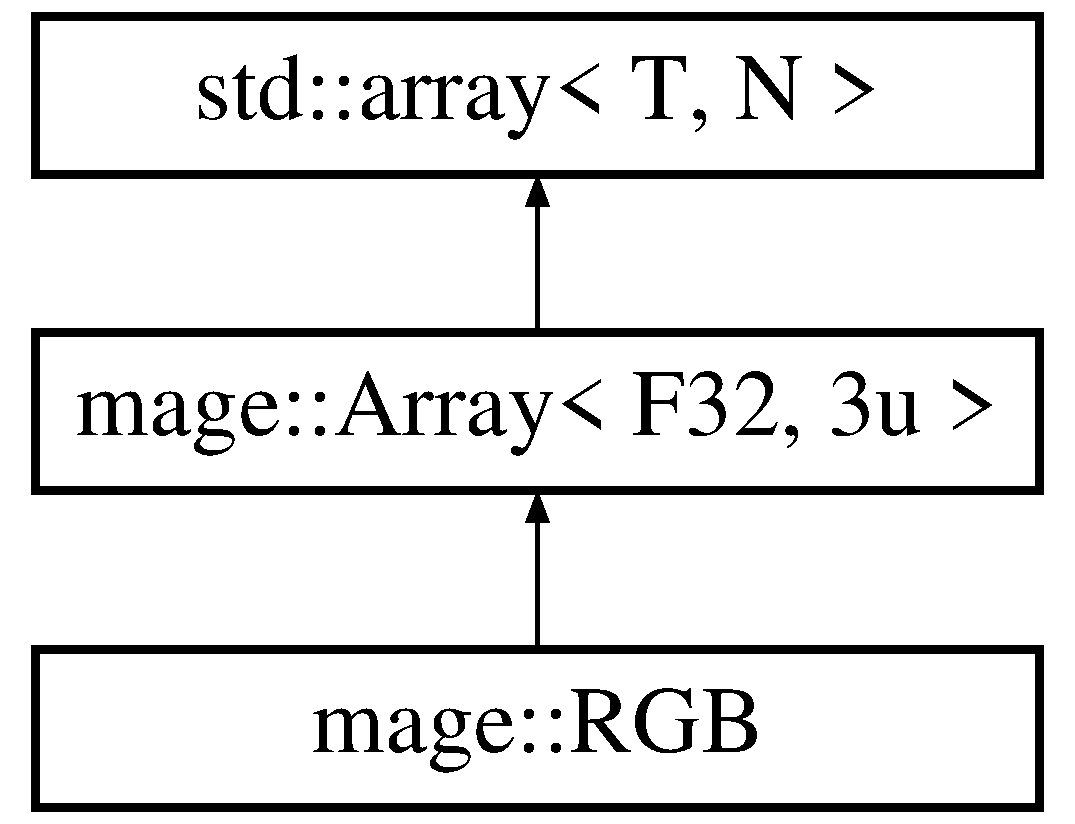
\includegraphics[height=3.000000cm]{structmage_1_1_r_g_b}
\end{center}
\end{figure}
\subsection*{Public Member Functions}
\begin{DoxyCompactItemize}
\item 
constexpr \mbox{\hyperlink{structmage_1_1_r_g_b_a166d2c13b46f9518c132c68f1117e5c6}{R\+GB}} (\mbox{\hyperlink{namespacemage_aa97e833b45f06d60a0a9c4fc22ae02c0}{F32}} rgb=0.\+0f) noexcept
\item 
constexpr \mbox{\hyperlink{structmage_1_1_r_g_b_af4304d8dc009f1b551442d6ebd15c0fa}{R\+GB}} (\mbox{\hyperlink{namespacemage_aa97e833b45f06d60a0a9c4fc22ae02c0}{F32}} r, \mbox{\hyperlink{namespacemage_aa97e833b45f06d60a0a9c4fc22ae02c0}{F32}} g, \mbox{\hyperlink{namespacemage_aa97e833b45f06d60a0a9c4fc22ae02c0}{F32}} b) noexcept
\item 
constexpr \mbox{\hyperlink{structmage_1_1_r_g_b_a1423c7c8dd83399b16cd33e367a5497c}{R\+GB}} (const \mbox{\hyperlink{structmage_1_1_r_g_b}{R\+GB}} \&rgb) noexcept=default
\item 
constexpr \mbox{\hyperlink{structmage_1_1_r_g_b_a852c4ed04bb38c7913d12fc491185bfb}{R\+GB}} (\mbox{\hyperlink{structmage_1_1_r_g_b}{R\+GB}} \&\&rgb) noexcept=default
\item 
\mbox{\hyperlink{structmage_1_1_r_g_b_a2f2c4eea3b0c44e0f31cfe20c6371d64}{R\+GB}} (const \mbox{\hyperlink{structmage_1_1_s_r_g_b}{S\+R\+GB}} \&srgb) noexcept
\item 
\mbox{\hyperlink{structmage_1_1_r_g_b_a62a2200960f84f1b6bd4b743510201a4}{R\+GB}} (const \mbox{\hyperlink{structmage_1_1_x_y_z}{X\+YZ}} \&xyz) noexcept
\item 
constexpr \mbox{\hyperlink{structmage_1_1_r_g_b_ab80d8120aabe4f52e8de6e99d1af7c8b}{R\+GB}} (\mbox{\hyperlink{namespacemage_a1e3c7a882af461f161caa1cbddaf1fa2}{F32x3}} v) noexcept
\item 
\mbox{\hyperlink{structmage_1_1_r_g_b_a2c01428e1da4ec354b85320a905beab3}{$\sim$\+R\+GB}} ()=default
\item 
\mbox{\hyperlink{structmage_1_1_r_g_b}{R\+GB}} \& \mbox{\hyperlink{structmage_1_1_r_g_b_a10fd47397bb4a691c951d44abfb77d7c}{operator=}} (const \mbox{\hyperlink{structmage_1_1_r_g_b}{R\+GB}} \&rgb) noexcept=default
\item 
\mbox{\hyperlink{structmage_1_1_r_g_b}{R\+GB}} \& \mbox{\hyperlink{structmage_1_1_r_g_b_add3b5995774c634d6e32af4d1cd6bfb3}{operator=}} (\mbox{\hyperlink{structmage_1_1_r_g_b}{R\+GB}} \&\&rgb) noexcept=default
\item 
\mbox{\hyperlink{namespacemage_aa97e833b45f06d60a0a9c4fc22ae02c0}{F32}} \& \mbox{\hyperlink{structmage_1_1_r_g_b_a0125eee4ebad06ecfc54be1ffe601eb4}{R}} () noexcept
\item 
constexpr \mbox{\hyperlink{namespacemage_aa97e833b45f06d60a0a9c4fc22ae02c0}{F32}} \mbox{\hyperlink{structmage_1_1_r_g_b_ad0a4d0192ecc2a85ba046b62818a8623}{R}} () const noexcept
\item 
\mbox{\hyperlink{namespacemage_aa97e833b45f06d60a0a9c4fc22ae02c0}{F32}} \& \mbox{\hyperlink{structmage_1_1_r_g_b_aedeed66436cdee0e7a9f19e650d3a44b}{G}} () noexcept
\item 
constexpr \mbox{\hyperlink{namespacemage_aa97e833b45f06d60a0a9c4fc22ae02c0}{F32}} \mbox{\hyperlink{structmage_1_1_r_g_b_a3cff21300a4b2f44692b39d09930af39}{G}} () const noexcept
\item 
\mbox{\hyperlink{namespacemage_aa97e833b45f06d60a0a9c4fc22ae02c0}{F32}} \& \mbox{\hyperlink{structmage_1_1_r_g_b_a8c3aa800eeb679f42d33e0a029081db3}{B}} () noexcept
\item 
constexpr \mbox{\hyperlink{namespacemage_aa97e833b45f06d60a0a9c4fc22ae02c0}{F32}} \mbox{\hyperlink{structmage_1_1_r_g_b_a3f90c799411cc78913e4c0e403c16c7a}{B}} () const noexcept
\end{DoxyCompactItemize}
\subsection*{Additional Inherited Members}


\subsection{Detailed Description}
A struct of \mbox{\hyperlink{structmage_1_1_r_g_b}{R\+GB}} color spectra. 

\subsection{Constructor \& Destructor Documentation}
\mbox{\Hypertarget{structmage_1_1_r_g_b_a166d2c13b46f9518c132c68f1117e5c6}\label{structmage_1_1_r_g_b_a166d2c13b46f9518c132c68f1117e5c6}} 
\index{mage\+::\+R\+GB@{mage\+::\+R\+GB}!R\+GB@{R\+GB}}
\index{R\+GB@{R\+GB}!mage\+::\+R\+GB@{mage\+::\+R\+GB}}
\subsubsection{\texorpdfstring{R\+G\+B()}{RGB()}\hspace{0.1cm}{\footnotesize\ttfamily [1/7]}}
{\footnotesize\ttfamily constexpr mage\+::\+R\+G\+B\+::\+R\+GB (\begin{DoxyParamCaption}\item[{\mbox{\hyperlink{namespacemage_aa97e833b45f06d60a0a9c4fc22ae02c0}{F32}}}]{rgb = {\ttfamily 0.0f} }\end{DoxyParamCaption})\hspace{0.3cm}{\ttfamily [explicit]}, {\ttfamily [noexcept]}}

Constructs a \mbox{\hyperlink{structmage_1_1_r_g_b}{R\+GB}} spectrum from the given spectrum components.


\begin{DoxyParams}[1]{Parameters}
\mbox{\tt in}  & {\em rgb} & The red, green and blue component. \\
\hline
\end{DoxyParams}
\mbox{\Hypertarget{structmage_1_1_r_g_b_af4304d8dc009f1b551442d6ebd15c0fa}\label{structmage_1_1_r_g_b_af4304d8dc009f1b551442d6ebd15c0fa}} 
\index{mage\+::\+R\+GB@{mage\+::\+R\+GB}!R\+GB@{R\+GB}}
\index{R\+GB@{R\+GB}!mage\+::\+R\+GB@{mage\+::\+R\+GB}}
\subsubsection{\texorpdfstring{R\+G\+B()}{RGB()}\hspace{0.1cm}{\footnotesize\ttfamily [2/7]}}
{\footnotesize\ttfamily constexpr mage\+::\+R\+G\+B\+::\+R\+GB (\begin{DoxyParamCaption}\item[{\mbox{\hyperlink{namespacemage_aa97e833b45f06d60a0a9c4fc22ae02c0}{F32}}}]{r,  }\item[{\mbox{\hyperlink{namespacemage_aa97e833b45f06d60a0a9c4fc22ae02c0}{F32}}}]{g,  }\item[{\mbox{\hyperlink{namespacemage_aa97e833b45f06d60a0a9c4fc22ae02c0}{F32}}}]{b }\end{DoxyParamCaption})\hspace{0.3cm}{\ttfamily [noexcept]}}

Constructs a \mbox{\hyperlink{structmage_1_1_r_g_b}{R\+GB}} spectrum from the given spectrum components.


\begin{DoxyParams}[1]{Parameters}
\mbox{\tt in}  & {\em r} & The red component. \\
\hline
\mbox{\tt in}  & {\em g} & The green component. \\
\hline
\mbox{\tt in}  & {\em b} & The blue component. \\
\hline
\end{DoxyParams}
\mbox{\Hypertarget{structmage_1_1_r_g_b_a1423c7c8dd83399b16cd33e367a5497c}\label{structmage_1_1_r_g_b_a1423c7c8dd83399b16cd33e367a5497c}} 
\index{mage\+::\+R\+GB@{mage\+::\+R\+GB}!R\+GB@{R\+GB}}
\index{R\+GB@{R\+GB}!mage\+::\+R\+GB@{mage\+::\+R\+GB}}
\subsubsection{\texorpdfstring{R\+G\+B()}{RGB()}\hspace{0.1cm}{\footnotesize\ttfamily [3/7]}}
{\footnotesize\ttfamily constexpr mage\+::\+R\+G\+B\+::\+R\+GB (\begin{DoxyParamCaption}\item[{const \mbox{\hyperlink{structmage_1_1_r_g_b}{R\+GB}} \&}]{rgb }\end{DoxyParamCaption})\hspace{0.3cm}{\ttfamily [default]}, {\ttfamily [noexcept]}}

Constructs a \mbox{\hyperlink{structmage_1_1_r_g_b}{R\+GB}} spectrum from the given \mbox{\hyperlink{structmage_1_1_r_g_b}{R\+GB}} spectrum.


\begin{DoxyParams}[1]{Parameters}
\mbox{\tt in}  & {\em rgb} & A reference to the \mbox{\hyperlink{structmage_1_1_r_g_b}{R\+GB}} spectrum to copy. \\
\hline
\end{DoxyParams}
\mbox{\Hypertarget{structmage_1_1_r_g_b_a852c4ed04bb38c7913d12fc491185bfb}\label{structmage_1_1_r_g_b_a852c4ed04bb38c7913d12fc491185bfb}} 
\index{mage\+::\+R\+GB@{mage\+::\+R\+GB}!R\+GB@{R\+GB}}
\index{R\+GB@{R\+GB}!mage\+::\+R\+GB@{mage\+::\+R\+GB}}
\subsubsection{\texorpdfstring{R\+G\+B()}{RGB()}\hspace{0.1cm}{\footnotesize\ttfamily [4/7]}}
{\footnotesize\ttfamily constexpr mage\+::\+R\+G\+B\+::\+R\+GB (\begin{DoxyParamCaption}\item[{\mbox{\hyperlink{structmage_1_1_r_g_b}{R\+GB}} \&\&}]{rgb }\end{DoxyParamCaption})\hspace{0.3cm}{\ttfamily [default]}, {\ttfamily [noexcept]}}

Constructs a \mbox{\hyperlink{structmage_1_1_r_g_b}{R\+GB}} spectrum by moving the given \mbox{\hyperlink{structmage_1_1_r_g_b}{R\+GB}} spectrum.


\begin{DoxyParams}[1]{Parameters}
\mbox{\tt in}  & {\em rgb} & A reference to the \mbox{\hyperlink{structmage_1_1_r_g_b}{R\+GB}} spectrum to move. \\
\hline
\end{DoxyParams}
\mbox{\Hypertarget{structmage_1_1_r_g_b_a2f2c4eea3b0c44e0f31cfe20c6371d64}\label{structmage_1_1_r_g_b_a2f2c4eea3b0c44e0f31cfe20c6371d64}} 
\index{mage\+::\+R\+GB@{mage\+::\+R\+GB}!R\+GB@{R\+GB}}
\index{R\+GB@{R\+GB}!mage\+::\+R\+GB@{mage\+::\+R\+GB}}
\subsubsection{\texorpdfstring{R\+G\+B()}{RGB()}\hspace{0.1cm}{\footnotesize\ttfamily [5/7]}}
{\footnotesize\ttfamily mage\+::\+R\+G\+B\+::\+R\+GB (\begin{DoxyParamCaption}\item[{const \mbox{\hyperlink{structmage_1_1_s_r_g_b}{S\+R\+GB}} \&}]{srgb }\end{DoxyParamCaption})\hspace{0.3cm}{\ttfamily [explicit]}, {\ttfamily [noexcept]}}

Constructs a \mbox{\hyperlink{structmage_1_1_r_g_b}{R\+GB}} spectrum from the given s\+R\+GB spectrum.


\begin{DoxyParams}[1]{Parameters}
\mbox{\tt in}  & {\em srgb} & A reference to the s\+R\+GB spectrum to copy. \\
\hline
\end{DoxyParams}
\mbox{\Hypertarget{structmage_1_1_r_g_b_a62a2200960f84f1b6bd4b743510201a4}\label{structmage_1_1_r_g_b_a62a2200960f84f1b6bd4b743510201a4}} 
\index{mage\+::\+R\+GB@{mage\+::\+R\+GB}!R\+GB@{R\+GB}}
\index{R\+GB@{R\+GB}!mage\+::\+R\+GB@{mage\+::\+R\+GB}}
\subsubsection{\texorpdfstring{R\+G\+B()}{RGB()}\hspace{0.1cm}{\footnotesize\ttfamily [6/7]}}
{\footnotesize\ttfamily mage\+::\+R\+G\+B\+::\+R\+GB (\begin{DoxyParamCaption}\item[{const \mbox{\hyperlink{structmage_1_1_x_y_z}{X\+YZ}} \&}]{xyz }\end{DoxyParamCaption})\hspace{0.3cm}{\ttfamily [explicit]}, {\ttfamily [noexcept]}}

Constructs a \mbox{\hyperlink{structmage_1_1_r_g_b}{R\+GB}} spectrum from the given \mbox{\hyperlink{structmage_1_1_x_y_z}{X\+YZ}} spectrum.


\begin{DoxyParams}[1]{Parameters}
\mbox{\tt in}  & {\em xyz} & A reference to the \mbox{\hyperlink{structmage_1_1_x_y_z}{X\+YZ}} spectrum to copy. \\
\hline
\end{DoxyParams}
\mbox{\Hypertarget{structmage_1_1_r_g_b_ab80d8120aabe4f52e8de6e99d1af7c8b}\label{structmage_1_1_r_g_b_ab80d8120aabe4f52e8de6e99d1af7c8b}} 
\index{mage\+::\+R\+GB@{mage\+::\+R\+GB}!R\+GB@{R\+GB}}
\index{R\+GB@{R\+GB}!mage\+::\+R\+GB@{mage\+::\+R\+GB}}
\subsubsection{\texorpdfstring{R\+G\+B()}{RGB()}\hspace{0.1cm}{\footnotesize\ttfamily [7/7]}}
{\footnotesize\ttfamily constexpr mage\+::\+R\+G\+B\+::\+R\+GB (\begin{DoxyParamCaption}\item[{\mbox{\hyperlink{namespacemage_a1e3c7a882af461f161caa1cbddaf1fa2}{F32x3}}}]{v }\end{DoxyParamCaption})\hspace{0.3cm}{\ttfamily [explicit]}, {\ttfamily [noexcept]}}

Constructs a \mbox{\hyperlink{structmage_1_1_r_g_b}{R\+GB}} spectrum from the given components.


\begin{DoxyParams}[1]{Parameters}
\mbox{\tt in}  & {\em v} & The components. \\
\hline
\end{DoxyParams}
\mbox{\Hypertarget{structmage_1_1_r_g_b_a2c01428e1da4ec354b85320a905beab3}\label{structmage_1_1_r_g_b_a2c01428e1da4ec354b85320a905beab3}} 
\index{mage\+::\+R\+GB@{mage\+::\+R\+GB}!````~R\+GB@{$\sim$\+R\+GB}}
\index{````~R\+GB@{$\sim$\+R\+GB}!mage\+::\+R\+GB@{mage\+::\+R\+GB}}
\subsubsection{\texorpdfstring{$\sim$\+R\+G\+B()}{~RGB()}}
{\footnotesize\ttfamily mage\+::\+R\+G\+B\+::$\sim$\+R\+GB (\begin{DoxyParamCaption}{ }\end{DoxyParamCaption})\hspace{0.3cm}{\ttfamily [default]}}

Destructs this \mbox{\hyperlink{structmage_1_1_r_g_b}{R\+GB}} spectrum. 

\subsection{Member Function Documentation}
\mbox{\Hypertarget{structmage_1_1_r_g_b_a8c3aa800eeb679f42d33e0a029081db3}\label{structmage_1_1_r_g_b_a8c3aa800eeb679f42d33e0a029081db3}} 
\index{mage\+::\+R\+GB@{mage\+::\+R\+GB}!B@{B}}
\index{B@{B}!mage\+::\+R\+GB@{mage\+::\+R\+GB}}
\subsubsection{\texorpdfstring{B()}{B()}\hspace{0.1cm}{\footnotesize\ttfamily [1/2]}}
{\footnotesize\ttfamily \mbox{\hyperlink{namespacemage_aa97e833b45f06d60a0a9c4fc22ae02c0}{F32}}\& mage\+::\+R\+G\+B\+::B (\begin{DoxyParamCaption}{ }\end{DoxyParamCaption})\hspace{0.3cm}{\ttfamily [noexcept]}}

Returns the blue component of this \mbox{\hyperlink{structmage_1_1_r_g_b}{R\+GB}} spectrum.

\begin{DoxyReturn}{Returns}
A reference to the blue component of this \mbox{\hyperlink{structmage_1_1_r_g_b}{R\+GB}} spectrum. 
\end{DoxyReturn}
\mbox{\Hypertarget{structmage_1_1_r_g_b_a3f90c799411cc78913e4c0e403c16c7a}\label{structmage_1_1_r_g_b_a3f90c799411cc78913e4c0e403c16c7a}} 
\index{mage\+::\+R\+GB@{mage\+::\+R\+GB}!B@{B}}
\index{B@{B}!mage\+::\+R\+GB@{mage\+::\+R\+GB}}
\subsubsection{\texorpdfstring{B()}{B()}\hspace{0.1cm}{\footnotesize\ttfamily [2/2]}}
{\footnotesize\ttfamily constexpr \mbox{\hyperlink{namespacemage_aa97e833b45f06d60a0a9c4fc22ae02c0}{F32}} mage\+::\+R\+G\+B\+::B (\begin{DoxyParamCaption}{ }\end{DoxyParamCaption}) const\hspace{0.3cm}{\ttfamily [noexcept]}}

Returns the blue component of this \mbox{\hyperlink{structmage_1_1_r_g_b}{R\+GB}} spectrum.

\begin{DoxyReturn}{Returns}
The blue component of this \mbox{\hyperlink{structmage_1_1_r_g_b}{R\+GB}} spectrum. 
\end{DoxyReturn}
\mbox{\Hypertarget{structmage_1_1_r_g_b_aedeed66436cdee0e7a9f19e650d3a44b}\label{structmage_1_1_r_g_b_aedeed66436cdee0e7a9f19e650d3a44b}} 
\index{mage\+::\+R\+GB@{mage\+::\+R\+GB}!G@{G}}
\index{G@{G}!mage\+::\+R\+GB@{mage\+::\+R\+GB}}
\subsubsection{\texorpdfstring{G()}{G()}\hspace{0.1cm}{\footnotesize\ttfamily [1/2]}}
{\footnotesize\ttfamily \mbox{\hyperlink{namespacemage_aa97e833b45f06d60a0a9c4fc22ae02c0}{F32}}\& mage\+::\+R\+G\+B\+::G (\begin{DoxyParamCaption}{ }\end{DoxyParamCaption})\hspace{0.3cm}{\ttfamily [noexcept]}}

Returns the green component of this \mbox{\hyperlink{structmage_1_1_r_g_b}{R\+GB}} spectrum.

\begin{DoxyReturn}{Returns}
A reference to the green component of this \mbox{\hyperlink{structmage_1_1_r_g_b}{R\+GB}} spectrum. 
\end{DoxyReturn}
\mbox{\Hypertarget{structmage_1_1_r_g_b_a3cff21300a4b2f44692b39d09930af39}\label{structmage_1_1_r_g_b_a3cff21300a4b2f44692b39d09930af39}} 
\index{mage\+::\+R\+GB@{mage\+::\+R\+GB}!G@{G}}
\index{G@{G}!mage\+::\+R\+GB@{mage\+::\+R\+GB}}
\subsubsection{\texorpdfstring{G()}{G()}\hspace{0.1cm}{\footnotesize\ttfamily [2/2]}}
{\footnotesize\ttfamily constexpr \mbox{\hyperlink{namespacemage_aa97e833b45f06d60a0a9c4fc22ae02c0}{F32}} mage\+::\+R\+G\+B\+::G (\begin{DoxyParamCaption}{ }\end{DoxyParamCaption}) const\hspace{0.3cm}{\ttfamily [noexcept]}}

Returns the green component of this \mbox{\hyperlink{structmage_1_1_r_g_b}{R\+GB}} spectrum.

\begin{DoxyReturn}{Returns}
The green component of this \mbox{\hyperlink{structmage_1_1_r_g_b}{R\+GB}} spectrum. 
\end{DoxyReturn}
\mbox{\Hypertarget{structmage_1_1_r_g_b_a10fd47397bb4a691c951d44abfb77d7c}\label{structmage_1_1_r_g_b_a10fd47397bb4a691c951d44abfb77d7c}} 
\index{mage\+::\+R\+GB@{mage\+::\+R\+GB}!operator=@{operator=}}
\index{operator=@{operator=}!mage\+::\+R\+GB@{mage\+::\+R\+GB}}
\subsubsection{\texorpdfstring{operator=()}{operator=()}\hspace{0.1cm}{\footnotesize\ttfamily [1/2]}}
{\footnotesize\ttfamily \mbox{\hyperlink{structmage_1_1_r_g_b}{R\+GB}}\& mage\+::\+R\+G\+B\+::operator= (\begin{DoxyParamCaption}\item[{const \mbox{\hyperlink{structmage_1_1_r_g_b}{R\+GB}} \&}]{rgb }\end{DoxyParamCaption})\hspace{0.3cm}{\ttfamily [default]}, {\ttfamily [noexcept]}}

Copies the given \mbox{\hyperlink{structmage_1_1_r_g_b}{R\+GB}} spectrum to this \mbox{\hyperlink{structmage_1_1_r_g_b}{R\+GB}} spectrum.


\begin{DoxyParams}[1]{Parameters}
\mbox{\tt in}  & {\em rgb} & A reference to the \mbox{\hyperlink{structmage_1_1_r_g_b}{R\+GB}} spectrum to copy. \\
\hline
\end{DoxyParams}
\begin{DoxyReturn}{Returns}
A reference to the copy of the given \mbox{\hyperlink{structmage_1_1_r_g_b}{R\+GB}} spectrum (i.\+e. this \mbox{\hyperlink{structmage_1_1_r_g_b}{R\+GB}} spectrum). 
\end{DoxyReturn}
\mbox{\Hypertarget{structmage_1_1_r_g_b_add3b5995774c634d6e32af4d1cd6bfb3}\label{structmage_1_1_r_g_b_add3b5995774c634d6e32af4d1cd6bfb3}} 
\index{mage\+::\+R\+GB@{mage\+::\+R\+GB}!operator=@{operator=}}
\index{operator=@{operator=}!mage\+::\+R\+GB@{mage\+::\+R\+GB}}
\subsubsection{\texorpdfstring{operator=()}{operator=()}\hspace{0.1cm}{\footnotesize\ttfamily [2/2]}}
{\footnotesize\ttfamily \mbox{\hyperlink{structmage_1_1_r_g_b}{R\+GB}}\& mage\+::\+R\+G\+B\+::operator= (\begin{DoxyParamCaption}\item[{\mbox{\hyperlink{structmage_1_1_r_g_b}{R\+GB}} \&\&}]{rgb }\end{DoxyParamCaption})\hspace{0.3cm}{\ttfamily [default]}, {\ttfamily [noexcept]}}

Moves the given \mbox{\hyperlink{structmage_1_1_r_g_b}{R\+GB}} spectrum to this \mbox{\hyperlink{structmage_1_1_r_g_b}{R\+GB}} spectrum.


\begin{DoxyParams}[1]{Parameters}
\mbox{\tt in}  & {\em rgb} & A reference to the \mbox{\hyperlink{structmage_1_1_r_g_b}{R\+GB}} spectrum to move. \\
\hline
\end{DoxyParams}
\begin{DoxyReturn}{Returns}
A reference to the moved \mbox{\hyperlink{structmage_1_1_r_g_b}{R\+GB}} spectrum (i.\+e. this \mbox{\hyperlink{structmage_1_1_r_g_b}{R\+GB}} spectrum). 
\end{DoxyReturn}
\mbox{\Hypertarget{structmage_1_1_r_g_b_a0125eee4ebad06ecfc54be1ffe601eb4}\label{structmage_1_1_r_g_b_a0125eee4ebad06ecfc54be1ffe601eb4}} 
\index{mage\+::\+R\+GB@{mage\+::\+R\+GB}!R@{R}}
\index{R@{R}!mage\+::\+R\+GB@{mage\+::\+R\+GB}}
\subsubsection{\texorpdfstring{R()}{R()}\hspace{0.1cm}{\footnotesize\ttfamily [1/2]}}
{\footnotesize\ttfamily \mbox{\hyperlink{namespacemage_aa97e833b45f06d60a0a9c4fc22ae02c0}{F32}}\& mage\+::\+R\+G\+B\+::R (\begin{DoxyParamCaption}{ }\end{DoxyParamCaption})\hspace{0.3cm}{\ttfamily [noexcept]}}

Returns the red component of this \mbox{\hyperlink{structmage_1_1_r_g_b}{R\+GB}} spectrum.

\begin{DoxyReturn}{Returns}
A reference to the red component of this \mbox{\hyperlink{structmage_1_1_r_g_b}{R\+GB}} spectrum. 
\end{DoxyReturn}
\mbox{\Hypertarget{structmage_1_1_r_g_b_ad0a4d0192ecc2a85ba046b62818a8623}\label{structmage_1_1_r_g_b_ad0a4d0192ecc2a85ba046b62818a8623}} 
\index{mage\+::\+R\+GB@{mage\+::\+R\+GB}!R@{R}}
\index{R@{R}!mage\+::\+R\+GB@{mage\+::\+R\+GB}}
\subsubsection{\texorpdfstring{R()}{R()}\hspace{0.1cm}{\footnotesize\ttfamily [2/2]}}
{\footnotesize\ttfamily constexpr \mbox{\hyperlink{namespacemage_aa97e833b45f06d60a0a9c4fc22ae02c0}{F32}} mage\+::\+R\+G\+B\+::R (\begin{DoxyParamCaption}{ }\end{DoxyParamCaption}) const\hspace{0.3cm}{\ttfamily [noexcept]}}

Returns the red component of this \mbox{\hyperlink{structmage_1_1_r_g_b}{R\+GB}} spectrum.

\begin{DoxyReturn}{Returns}
The red component of this \mbox{\hyperlink{structmage_1_1_r_g_b}{R\+GB}} spectrum. 
\end{DoxyReturn}

\hypertarget{structmage_1_1_r_g_b_a}{}\section{mage\+:\+:R\+G\+BA Struct Reference}
\label{structmage_1_1_r_g_b_a}\index{mage\+::\+R\+G\+BA@{mage\+::\+R\+G\+BA}}


{\ttfamily \#include $<$spectrum.\+hpp$>$}

Inheritance diagram for mage\+:\+:R\+G\+BA\+:\begin{figure}[H]
\begin{center}
\leavevmode
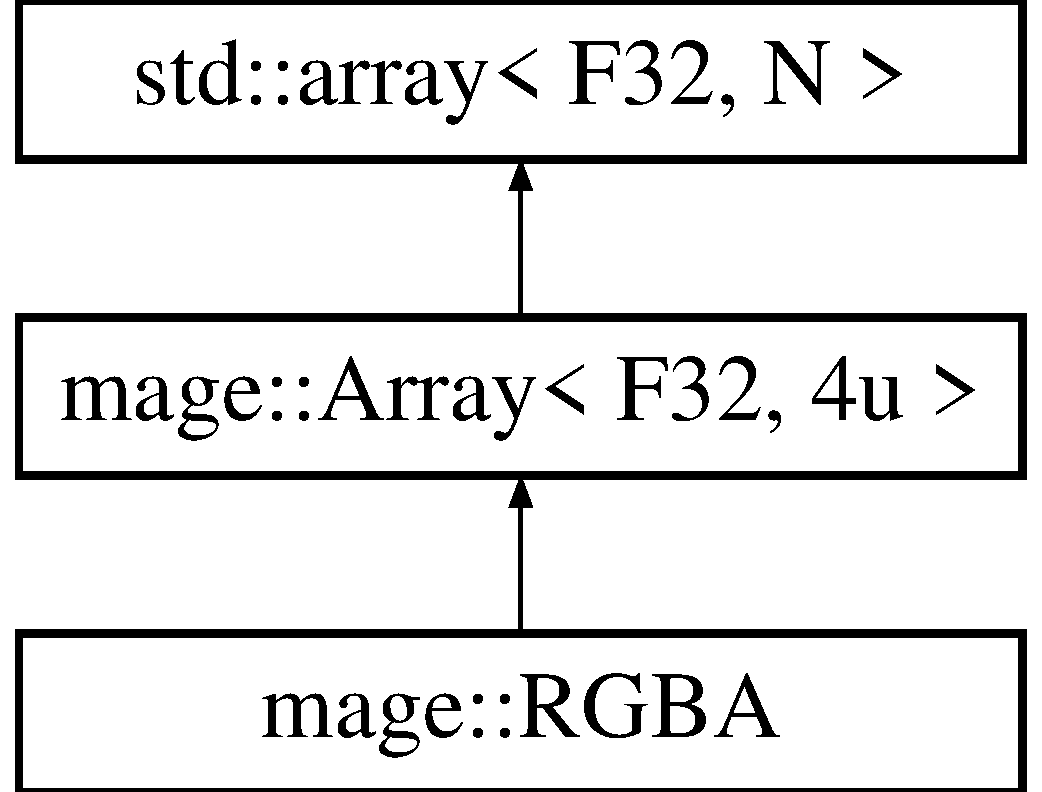
\includegraphics[height=3.000000cm]{structmage_1_1_r_g_b_a}
\end{center}
\end{figure}
\subsection*{Public Member Functions}
\begin{DoxyCompactItemize}
\item 
constexpr \mbox{\hyperlink{structmage_1_1_r_g_b_a_afe334e4408a71e808b8cf0bc9dd06dde}{R\+G\+BA}} (\mbox{\hyperlink{namespacemage_aa97e833b45f06d60a0a9c4fc22ae02c0}{F32}} rgba=0.\+0f) noexcept
\item 
constexpr \mbox{\hyperlink{structmage_1_1_r_g_b_a_a12ae339b8bcae0a1c0aacad280963ade}{R\+G\+BA}} (\mbox{\hyperlink{namespacemage_aa97e833b45f06d60a0a9c4fc22ae02c0}{F32}} r, \mbox{\hyperlink{namespacemage_aa97e833b45f06d60a0a9c4fc22ae02c0}{F32}} g, \mbox{\hyperlink{namespacemage_aa97e833b45f06d60a0a9c4fc22ae02c0}{F32}} b, \mbox{\hyperlink{namespacemage_aa97e833b45f06d60a0a9c4fc22ae02c0}{F32}} a=1.\+0f) noexcept
\item 
constexpr \mbox{\hyperlink{structmage_1_1_r_g_b_a_ad399faf871c1dec0ee3c4c0eb89329df}{R\+G\+BA}} (const \mbox{\hyperlink{structmage_1_1_r_g_b_a}{R\+G\+BA}} \&rgba) noexcept=default
\item 
constexpr \mbox{\hyperlink{structmage_1_1_r_g_b_a_a931063ef190241d875856430aa9fbac9}{R\+G\+BA}} (\mbox{\hyperlink{structmage_1_1_r_g_b_a}{R\+G\+BA}} \&\&rgba) noexcept=default
\item 
constexpr \mbox{\hyperlink{structmage_1_1_r_g_b_a_ad766984007f021cdde26f63436d90825}{R\+G\+BA}} (const \mbox{\hyperlink{structmage_1_1_r_g_b}{R\+GB}} \&rgb, \mbox{\hyperlink{namespacemage_aa97e833b45f06d60a0a9c4fc22ae02c0}{F32}} a=1.\+0f) noexcept
\item 
\mbox{\hyperlink{structmage_1_1_r_g_b_a_a82b256781126a25fd7a9a84a75fffb90}{R\+G\+BA}} (const \mbox{\hyperlink{structmage_1_1_s_r_g_b_a}{S\+R\+G\+BA}} \&srgba) noexcept
\item 
\mbox{\hyperlink{structmage_1_1_r_g_b_a_a008be57a6540fee8ed02d285681e3ed4}{R\+G\+BA}} (const \mbox{\hyperlink{structmage_1_1_x_y_z_a}{X\+Y\+ZA}} \&xyza) noexcept
\item 
constexpr \mbox{\hyperlink{structmage_1_1_r_g_b_a_a058e985bdbdf376616d1f6dd121d2dd8}{R\+G\+BA}} (\mbox{\hyperlink{namespacemage_a759aaad2fdc75aa93b5b614eb01712c4}{F32x4}} v) noexcept
\item 
\mbox{\hyperlink{structmage_1_1_r_g_b_a_a139a22381a3fb02d1f28be505b41c9df}{$\sim$\+R\+G\+BA}} ()=default
\item 
\mbox{\hyperlink{structmage_1_1_r_g_b_a}{R\+G\+BA}} \& \mbox{\hyperlink{structmage_1_1_r_g_b_a_a96b9f7d1b17cc68b8b0949eefe3d3e5c}{operator=}} (const \mbox{\hyperlink{structmage_1_1_r_g_b_a}{R\+G\+BA}} \&rgba) noexcept=default
\item 
\mbox{\hyperlink{structmage_1_1_r_g_b_a}{R\+G\+BA}} \& \mbox{\hyperlink{structmage_1_1_r_g_b_a_afcac58d6a76659c2a5821b8c957fc90e}{operator=}} (\mbox{\hyperlink{structmage_1_1_r_g_b_a}{R\+G\+BA}} \&\&rgba) noexcept=default
\item 
constexpr \mbox{\hyperlink{namespacemage_aa97e833b45f06d60a0a9c4fc22ae02c0}{F32}} \mbox{\hyperlink{structmage_1_1_r_g_b_a_a2f312fc862e792247bb6ba0e5a5390ca}{GetR}} () const noexcept
\item 
constexpr void \mbox{\hyperlink{structmage_1_1_r_g_b_a_a1de1796391b58e1e1db1e2701f8a391c}{SetR}} (\mbox{\hyperlink{namespacemage_aa97e833b45f06d60a0a9c4fc22ae02c0}{F32}} r) noexcept
\item 
constexpr \mbox{\hyperlink{namespacemage_aa97e833b45f06d60a0a9c4fc22ae02c0}{F32}} \mbox{\hyperlink{structmage_1_1_r_g_b_a_a39db7aa6065db1aef0c774316865e0ae}{GetG}} () const noexcept
\item 
constexpr void \mbox{\hyperlink{structmage_1_1_r_g_b_a_a18cdea53caccd27337bd0a1c31208b64}{SetG}} (\mbox{\hyperlink{namespacemage_aa97e833b45f06d60a0a9c4fc22ae02c0}{F32}} g) noexcept
\item 
constexpr \mbox{\hyperlink{namespacemage_aa97e833b45f06d60a0a9c4fc22ae02c0}{F32}} \mbox{\hyperlink{structmage_1_1_r_g_b_a_ae4fd67f400f6c86c5c7614ba3b06feeb}{GetB}} () const noexcept
\item 
constexpr void \mbox{\hyperlink{structmage_1_1_r_g_b_a_a3c7dccbc089f0a190f470c9dc74e7c51}{SetB}} (\mbox{\hyperlink{namespacemage_aa97e833b45f06d60a0a9c4fc22ae02c0}{F32}} b) noexcept
\item 
constexpr \mbox{\hyperlink{namespacemage_aa97e833b45f06d60a0a9c4fc22ae02c0}{F32}} \mbox{\hyperlink{structmage_1_1_r_g_b_a_a31196d863851f8e2b178458a78702b42}{GetA}} () const noexcept
\item 
constexpr void \mbox{\hyperlink{structmage_1_1_r_g_b_a_a3b2ebef3e0f2d26707b0fb84de8aec12}{SetA}} (\mbox{\hyperlink{namespacemage_aa97e833b45f06d60a0a9c4fc22ae02c0}{F32}} a) noexcept
\end{DoxyCompactItemize}
\subsection*{Additional Inherited Members}


\subsection{Detailed Description}
A struct of \mbox{\hyperlink{structmage_1_1_r_g_b_a}{R\+G\+BA}} color spectra. 

\subsection{Constructor \& Destructor Documentation}
\mbox{\Hypertarget{structmage_1_1_r_g_b_a_afe334e4408a71e808b8cf0bc9dd06dde}\label{structmage_1_1_r_g_b_a_afe334e4408a71e808b8cf0bc9dd06dde}} 
\index{mage\+::\+R\+G\+BA@{mage\+::\+R\+G\+BA}!R\+G\+BA@{R\+G\+BA}}
\index{R\+G\+BA@{R\+G\+BA}!mage\+::\+R\+G\+BA@{mage\+::\+R\+G\+BA}}
\subsubsection{\texorpdfstring{R\+G\+B\+A()}{RGBA()}\hspace{0.1cm}{\footnotesize\ttfamily [1/8]}}
{\footnotesize\ttfamily constexpr mage\+::\+R\+G\+B\+A\+::\+R\+G\+BA (\begin{DoxyParamCaption}\item[{\mbox{\hyperlink{namespacemage_aa97e833b45f06d60a0a9c4fc22ae02c0}{F32}}}]{rgba = {\ttfamily 0.0f} }\end{DoxyParamCaption})\hspace{0.3cm}{\ttfamily [explicit]}, {\ttfamily [noexcept]}}

Constructs a \mbox{\hyperlink{structmage_1_1_r_g_b_a}{R\+G\+BA}} spectrum from the given spectrum components.


\begin{DoxyParams}[1]{Parameters}
\mbox{\tt in}  & {\em rgba} & The red, green and blue and alpha component. \\
\hline
\end{DoxyParams}
\mbox{\Hypertarget{structmage_1_1_r_g_b_a_a12ae339b8bcae0a1c0aacad280963ade}\label{structmage_1_1_r_g_b_a_a12ae339b8bcae0a1c0aacad280963ade}} 
\index{mage\+::\+R\+G\+BA@{mage\+::\+R\+G\+BA}!R\+G\+BA@{R\+G\+BA}}
\index{R\+G\+BA@{R\+G\+BA}!mage\+::\+R\+G\+BA@{mage\+::\+R\+G\+BA}}
\subsubsection{\texorpdfstring{R\+G\+B\+A()}{RGBA()}\hspace{0.1cm}{\footnotesize\ttfamily [2/8]}}
{\footnotesize\ttfamily constexpr mage\+::\+R\+G\+B\+A\+::\+R\+G\+BA (\begin{DoxyParamCaption}\item[{\mbox{\hyperlink{namespacemage_aa97e833b45f06d60a0a9c4fc22ae02c0}{F32}}}]{r,  }\item[{\mbox{\hyperlink{namespacemage_aa97e833b45f06d60a0a9c4fc22ae02c0}{F32}}}]{g,  }\item[{\mbox{\hyperlink{namespacemage_aa97e833b45f06d60a0a9c4fc22ae02c0}{F32}}}]{b,  }\item[{\mbox{\hyperlink{namespacemage_aa97e833b45f06d60a0a9c4fc22ae02c0}{F32}}}]{a = {\ttfamily 1.0f} }\end{DoxyParamCaption})\hspace{0.3cm}{\ttfamily [noexcept]}}

Constructs a \mbox{\hyperlink{structmage_1_1_r_g_b_a}{R\+G\+BA}} spectrum from the given spectrum components.


\begin{DoxyParams}[1]{Parameters}
\mbox{\tt in}  & {\em r} & The red component. \\
\hline
\mbox{\tt in}  & {\em g} & The green component. \\
\hline
\mbox{\tt in}  & {\em b} & The blue component. \\
\hline
\mbox{\tt in}  & {\em a} & The alpha component. \\
\hline
\end{DoxyParams}
\mbox{\Hypertarget{structmage_1_1_r_g_b_a_ad399faf871c1dec0ee3c4c0eb89329df}\label{structmage_1_1_r_g_b_a_ad399faf871c1dec0ee3c4c0eb89329df}} 
\index{mage\+::\+R\+G\+BA@{mage\+::\+R\+G\+BA}!R\+G\+BA@{R\+G\+BA}}
\index{R\+G\+BA@{R\+G\+BA}!mage\+::\+R\+G\+BA@{mage\+::\+R\+G\+BA}}
\subsubsection{\texorpdfstring{R\+G\+B\+A()}{RGBA()}\hspace{0.1cm}{\footnotesize\ttfamily [3/8]}}
{\footnotesize\ttfamily constexpr mage\+::\+R\+G\+B\+A\+::\+R\+G\+BA (\begin{DoxyParamCaption}\item[{const \mbox{\hyperlink{structmage_1_1_r_g_b_a}{R\+G\+BA}} \&}]{rgba }\end{DoxyParamCaption})\hspace{0.3cm}{\ttfamily [default]}, {\ttfamily [noexcept]}}

Constructs a \mbox{\hyperlink{structmage_1_1_r_g_b_a}{R\+G\+BA}} spectrum from the given \mbox{\hyperlink{structmage_1_1_r_g_b_a}{R\+G\+BA}} spectrum.


\begin{DoxyParams}[1]{Parameters}
\mbox{\tt in}  & {\em rgba} & A reference to the \mbox{\hyperlink{structmage_1_1_r_g_b_a}{R\+G\+BA}} spectrum to copy. \\
\hline
\end{DoxyParams}
\mbox{\Hypertarget{structmage_1_1_r_g_b_a_a931063ef190241d875856430aa9fbac9}\label{structmage_1_1_r_g_b_a_a931063ef190241d875856430aa9fbac9}} 
\index{mage\+::\+R\+G\+BA@{mage\+::\+R\+G\+BA}!R\+G\+BA@{R\+G\+BA}}
\index{R\+G\+BA@{R\+G\+BA}!mage\+::\+R\+G\+BA@{mage\+::\+R\+G\+BA}}
\subsubsection{\texorpdfstring{R\+G\+B\+A()}{RGBA()}\hspace{0.1cm}{\footnotesize\ttfamily [4/8]}}
{\footnotesize\ttfamily constexpr mage\+::\+R\+G\+B\+A\+::\+R\+G\+BA (\begin{DoxyParamCaption}\item[{\mbox{\hyperlink{structmage_1_1_r_g_b_a}{R\+G\+BA}} \&\&}]{rgba }\end{DoxyParamCaption})\hspace{0.3cm}{\ttfamily [default]}, {\ttfamily [noexcept]}}

Constructs a \mbox{\hyperlink{structmage_1_1_r_g_b_a}{R\+G\+BA}} spectrum by moving the given \mbox{\hyperlink{structmage_1_1_r_g_b_a}{R\+G\+BA}} spectrum.


\begin{DoxyParams}[1]{Parameters}
\mbox{\tt in}  & {\em rgba} & A reference to the \mbox{\hyperlink{structmage_1_1_r_g_b_a}{R\+G\+BA}} spectrum to move. \\
\hline
\end{DoxyParams}
\mbox{\Hypertarget{structmage_1_1_r_g_b_a_ad766984007f021cdde26f63436d90825}\label{structmage_1_1_r_g_b_a_ad766984007f021cdde26f63436d90825}} 
\index{mage\+::\+R\+G\+BA@{mage\+::\+R\+G\+BA}!R\+G\+BA@{R\+G\+BA}}
\index{R\+G\+BA@{R\+G\+BA}!mage\+::\+R\+G\+BA@{mage\+::\+R\+G\+BA}}
\subsubsection{\texorpdfstring{R\+G\+B\+A()}{RGBA()}\hspace{0.1cm}{\footnotesize\ttfamily [5/8]}}
{\footnotesize\ttfamily constexpr mage\+::\+R\+G\+B\+A\+::\+R\+G\+BA (\begin{DoxyParamCaption}\item[{const \mbox{\hyperlink{structmage_1_1_r_g_b}{R\+GB}} \&}]{rgb,  }\item[{\mbox{\hyperlink{namespacemage_aa97e833b45f06d60a0a9c4fc22ae02c0}{F32}}}]{a = {\ttfamily 1.0f} }\end{DoxyParamCaption})\hspace{0.3cm}{\ttfamily [noexcept]}}

Constructs a \mbox{\hyperlink{structmage_1_1_r_g_b_a}{R\+G\+BA}} spectrum from the given \mbox{\hyperlink{structmage_1_1_r_g_b}{R\+GB}} spectrum.


\begin{DoxyParams}[1]{Parameters}
\mbox{\tt in}  & {\em rgb} & A reference to the \mbox{\hyperlink{structmage_1_1_r_g_b}{R\+GB}} spectrum. \\
\hline
\mbox{\tt in}  & {\em a} & The alpha component. \\
\hline
\end{DoxyParams}
\mbox{\Hypertarget{structmage_1_1_r_g_b_a_a82b256781126a25fd7a9a84a75fffb90}\label{structmage_1_1_r_g_b_a_a82b256781126a25fd7a9a84a75fffb90}} 
\index{mage\+::\+R\+G\+BA@{mage\+::\+R\+G\+BA}!R\+G\+BA@{R\+G\+BA}}
\index{R\+G\+BA@{R\+G\+BA}!mage\+::\+R\+G\+BA@{mage\+::\+R\+G\+BA}}
\subsubsection{\texorpdfstring{R\+G\+B\+A()}{RGBA()}\hspace{0.1cm}{\footnotesize\ttfamily [6/8]}}
{\footnotesize\ttfamily mage\+::\+R\+G\+B\+A\+::\+R\+G\+BA (\begin{DoxyParamCaption}\item[{const \mbox{\hyperlink{structmage_1_1_s_r_g_b_a}{S\+R\+G\+BA}} \&}]{srgba }\end{DoxyParamCaption})\hspace{0.3cm}{\ttfamily [explicit]}, {\ttfamily [noexcept]}}

Constructs a \mbox{\hyperlink{structmage_1_1_r_g_b_a}{R\+G\+BA}} spectrum from the given \mbox{\hyperlink{structmage_1_1_s_r_g_b_a}{S\+R\+G\+BA}} spectrum.


\begin{DoxyParams}[1]{Parameters}
\mbox{\tt in}  & {\em srgba} & A reference to the \mbox{\hyperlink{structmage_1_1_s_r_g_b_a}{S\+R\+G\+BA}} spectrum. \\
\hline
\end{DoxyParams}
\mbox{\Hypertarget{structmage_1_1_r_g_b_a_a008be57a6540fee8ed02d285681e3ed4}\label{structmage_1_1_r_g_b_a_a008be57a6540fee8ed02d285681e3ed4}} 
\index{mage\+::\+R\+G\+BA@{mage\+::\+R\+G\+BA}!R\+G\+BA@{R\+G\+BA}}
\index{R\+G\+BA@{R\+G\+BA}!mage\+::\+R\+G\+BA@{mage\+::\+R\+G\+BA}}
\subsubsection{\texorpdfstring{R\+G\+B\+A()}{RGBA()}\hspace{0.1cm}{\footnotesize\ttfamily [7/8]}}
{\footnotesize\ttfamily mage\+::\+R\+G\+B\+A\+::\+R\+G\+BA (\begin{DoxyParamCaption}\item[{const \mbox{\hyperlink{structmage_1_1_x_y_z_a}{X\+Y\+ZA}} \&}]{xyza }\end{DoxyParamCaption})\hspace{0.3cm}{\ttfamily [explicit]}, {\ttfamily [noexcept]}}

Constructs a \mbox{\hyperlink{structmage_1_1_r_g_b_a}{R\+G\+BA}} spectrum from the given \mbox{\hyperlink{structmage_1_1_x_y_z_a}{X\+Y\+ZA}} spectrum.


\begin{DoxyParams}[1]{Parameters}
\mbox{\tt in}  & {\em xyza} & A reference to the \mbox{\hyperlink{structmage_1_1_x_y_z_a}{X\+Y\+ZA}} spectrum. \\
\hline
\end{DoxyParams}
\mbox{\Hypertarget{structmage_1_1_r_g_b_a_a058e985bdbdf376616d1f6dd121d2dd8}\label{structmage_1_1_r_g_b_a_a058e985bdbdf376616d1f6dd121d2dd8}} 
\index{mage\+::\+R\+G\+BA@{mage\+::\+R\+G\+BA}!R\+G\+BA@{R\+G\+BA}}
\index{R\+G\+BA@{R\+G\+BA}!mage\+::\+R\+G\+BA@{mage\+::\+R\+G\+BA}}
\subsubsection{\texorpdfstring{R\+G\+B\+A()}{RGBA()}\hspace{0.1cm}{\footnotesize\ttfamily [8/8]}}
{\footnotesize\ttfamily constexpr mage\+::\+R\+G\+B\+A\+::\+R\+G\+BA (\begin{DoxyParamCaption}\item[{\mbox{\hyperlink{namespacemage_a759aaad2fdc75aa93b5b614eb01712c4}{F32x4}}}]{v }\end{DoxyParamCaption})\hspace{0.3cm}{\ttfamily [explicit]}, {\ttfamily [noexcept]}}

Constructs a \mbox{\hyperlink{structmage_1_1_r_g_b_a}{R\+G\+BA}} spectrum from the given components.


\begin{DoxyParams}[1]{Parameters}
\mbox{\tt in}  & {\em v} & The components. \\
\hline
\end{DoxyParams}
\mbox{\Hypertarget{structmage_1_1_r_g_b_a_a139a22381a3fb02d1f28be505b41c9df}\label{structmage_1_1_r_g_b_a_a139a22381a3fb02d1f28be505b41c9df}} 
\index{mage\+::\+R\+G\+BA@{mage\+::\+R\+G\+BA}!````~R\+G\+BA@{$\sim$\+R\+G\+BA}}
\index{````~R\+G\+BA@{$\sim$\+R\+G\+BA}!mage\+::\+R\+G\+BA@{mage\+::\+R\+G\+BA}}
\subsubsection{\texorpdfstring{$\sim$\+R\+G\+B\+A()}{~RGBA()}}
{\footnotesize\ttfamily mage\+::\+R\+G\+B\+A\+::$\sim$\+R\+G\+BA (\begin{DoxyParamCaption}{ }\end{DoxyParamCaption})\hspace{0.3cm}{\ttfamily [default]}}

Destructs this \mbox{\hyperlink{structmage_1_1_r_g_b_a}{R\+G\+BA}} spectrum. 

\subsection{Member Function Documentation}
\mbox{\Hypertarget{structmage_1_1_r_g_b_a_a31196d863851f8e2b178458a78702b42}\label{structmage_1_1_r_g_b_a_a31196d863851f8e2b178458a78702b42}} 
\index{mage\+::\+R\+G\+BA@{mage\+::\+R\+G\+BA}!GetA@{GetA}}
\index{GetA@{GetA}!mage\+::\+R\+G\+BA@{mage\+::\+R\+G\+BA}}
\subsubsection{\texorpdfstring{Get\+A()}{GetA()}}
{\footnotesize\ttfamily constexpr \mbox{\hyperlink{namespacemage_aa97e833b45f06d60a0a9c4fc22ae02c0}{F32}} mage\+::\+R\+G\+B\+A\+::\+GetA (\begin{DoxyParamCaption}{ }\end{DoxyParamCaption}) const\hspace{0.3cm}{\ttfamily [noexcept]}}

Returns the alpha component of this \mbox{\hyperlink{structmage_1_1_r_g_b_a}{R\+G\+BA}} spectrum.

\begin{DoxyReturn}{Returns}
The alpha component of this \mbox{\hyperlink{structmage_1_1_r_g_b_a}{R\+G\+BA}} spectrum. 
\end{DoxyReturn}
\mbox{\Hypertarget{structmage_1_1_r_g_b_a_ae4fd67f400f6c86c5c7614ba3b06feeb}\label{structmage_1_1_r_g_b_a_ae4fd67f400f6c86c5c7614ba3b06feeb}} 
\index{mage\+::\+R\+G\+BA@{mage\+::\+R\+G\+BA}!GetB@{GetB}}
\index{GetB@{GetB}!mage\+::\+R\+G\+BA@{mage\+::\+R\+G\+BA}}
\subsubsection{\texorpdfstring{Get\+B()}{GetB()}}
{\footnotesize\ttfamily constexpr \mbox{\hyperlink{namespacemage_aa97e833b45f06d60a0a9c4fc22ae02c0}{F32}} mage\+::\+R\+G\+B\+A\+::\+GetB (\begin{DoxyParamCaption}{ }\end{DoxyParamCaption}) const\hspace{0.3cm}{\ttfamily [noexcept]}}

Returns the blue component of this \mbox{\hyperlink{structmage_1_1_r_g_b_a}{R\+G\+BA}} spectrum.

\begin{DoxyReturn}{Returns}
The blue component of this \mbox{\hyperlink{structmage_1_1_r_g_b_a}{R\+G\+BA}} spectrum. 
\end{DoxyReturn}
\mbox{\Hypertarget{structmage_1_1_r_g_b_a_a39db7aa6065db1aef0c774316865e0ae}\label{structmage_1_1_r_g_b_a_a39db7aa6065db1aef0c774316865e0ae}} 
\index{mage\+::\+R\+G\+BA@{mage\+::\+R\+G\+BA}!GetG@{GetG}}
\index{GetG@{GetG}!mage\+::\+R\+G\+BA@{mage\+::\+R\+G\+BA}}
\subsubsection{\texorpdfstring{Get\+G()}{GetG()}}
{\footnotesize\ttfamily constexpr \mbox{\hyperlink{namespacemage_aa97e833b45f06d60a0a9c4fc22ae02c0}{F32}} mage\+::\+R\+G\+B\+A\+::\+GetG (\begin{DoxyParamCaption}{ }\end{DoxyParamCaption}) const\hspace{0.3cm}{\ttfamily [noexcept]}}

Returns the green component of this \mbox{\hyperlink{structmage_1_1_r_g_b_a}{R\+G\+BA}} spectrum.

\begin{DoxyReturn}{Returns}
The green component of this \mbox{\hyperlink{structmage_1_1_r_g_b_a}{R\+G\+BA}} spectrum. 
\end{DoxyReturn}
\mbox{\Hypertarget{structmage_1_1_r_g_b_a_a2f312fc862e792247bb6ba0e5a5390ca}\label{structmage_1_1_r_g_b_a_a2f312fc862e792247bb6ba0e5a5390ca}} 
\index{mage\+::\+R\+G\+BA@{mage\+::\+R\+G\+BA}!GetR@{GetR}}
\index{GetR@{GetR}!mage\+::\+R\+G\+BA@{mage\+::\+R\+G\+BA}}
\subsubsection{\texorpdfstring{Get\+R()}{GetR()}}
{\footnotesize\ttfamily constexpr \mbox{\hyperlink{namespacemage_aa97e833b45f06d60a0a9c4fc22ae02c0}{F32}} mage\+::\+R\+G\+B\+A\+::\+GetR (\begin{DoxyParamCaption}{ }\end{DoxyParamCaption}) const\hspace{0.3cm}{\ttfamily [noexcept]}}

Returns the red component of this \mbox{\hyperlink{structmage_1_1_r_g_b_a}{R\+G\+BA}} spectrum.

\begin{DoxyReturn}{Returns}
The red component of this \mbox{\hyperlink{structmage_1_1_r_g_b_a}{R\+G\+BA}} spectrum. 
\end{DoxyReturn}
\mbox{\Hypertarget{structmage_1_1_r_g_b_a_a96b9f7d1b17cc68b8b0949eefe3d3e5c}\label{structmage_1_1_r_g_b_a_a96b9f7d1b17cc68b8b0949eefe3d3e5c}} 
\index{mage\+::\+R\+G\+BA@{mage\+::\+R\+G\+BA}!operator=@{operator=}}
\index{operator=@{operator=}!mage\+::\+R\+G\+BA@{mage\+::\+R\+G\+BA}}
\subsubsection{\texorpdfstring{operator=()}{operator=()}\hspace{0.1cm}{\footnotesize\ttfamily [1/2]}}
{\footnotesize\ttfamily \mbox{\hyperlink{structmage_1_1_r_g_b_a}{R\+G\+BA}}\& mage\+::\+R\+G\+B\+A\+::operator= (\begin{DoxyParamCaption}\item[{const \mbox{\hyperlink{structmage_1_1_r_g_b_a}{R\+G\+BA}} \&}]{rgba }\end{DoxyParamCaption})\hspace{0.3cm}{\ttfamily [default]}, {\ttfamily [noexcept]}}

Copies the given \mbox{\hyperlink{structmage_1_1_r_g_b_a}{R\+G\+BA}} spectrum to this \mbox{\hyperlink{structmage_1_1_r_g_b_a}{R\+G\+BA}} spectrum.


\begin{DoxyParams}[1]{Parameters}
\mbox{\tt in}  & {\em rgba} & A reference to the \mbox{\hyperlink{structmage_1_1_r_g_b_a}{R\+G\+BA}} spectrum to copy. \\
\hline
\end{DoxyParams}
\begin{DoxyReturn}{Returns}
A reference to the copy of the given \mbox{\hyperlink{structmage_1_1_r_g_b_a}{R\+G\+BA}} spectrum (i.\+e. this \mbox{\hyperlink{structmage_1_1_r_g_b_a}{R\+G\+BA}} spectrum). 
\end{DoxyReturn}
\mbox{\Hypertarget{structmage_1_1_r_g_b_a_afcac58d6a76659c2a5821b8c957fc90e}\label{structmage_1_1_r_g_b_a_afcac58d6a76659c2a5821b8c957fc90e}} 
\index{mage\+::\+R\+G\+BA@{mage\+::\+R\+G\+BA}!operator=@{operator=}}
\index{operator=@{operator=}!mage\+::\+R\+G\+BA@{mage\+::\+R\+G\+BA}}
\subsubsection{\texorpdfstring{operator=()}{operator=()}\hspace{0.1cm}{\footnotesize\ttfamily [2/2]}}
{\footnotesize\ttfamily \mbox{\hyperlink{structmage_1_1_r_g_b_a}{R\+G\+BA}}\& mage\+::\+R\+G\+B\+A\+::operator= (\begin{DoxyParamCaption}\item[{\mbox{\hyperlink{structmage_1_1_r_g_b_a}{R\+G\+BA}} \&\&}]{rgba }\end{DoxyParamCaption})\hspace{0.3cm}{\ttfamily [default]}, {\ttfamily [noexcept]}}

Moves the given \mbox{\hyperlink{structmage_1_1_r_g_b_a}{R\+G\+BA}} spectrum to this \mbox{\hyperlink{structmage_1_1_r_g_b_a}{R\+G\+BA}} spectrum.


\begin{DoxyParams}[1]{Parameters}
\mbox{\tt in}  & {\em rgba} & A reference to the \mbox{\hyperlink{structmage_1_1_r_g_b_a}{R\+G\+BA}} spectrum to move. \\
\hline
\end{DoxyParams}
\begin{DoxyReturn}{Returns}
A reference to the moved \mbox{\hyperlink{structmage_1_1_r_g_b_a}{R\+G\+BA}} spectrum (i.\+e. this \mbox{\hyperlink{structmage_1_1_r_g_b_a}{R\+G\+BA}} spectrum). 
\end{DoxyReturn}
\mbox{\Hypertarget{structmage_1_1_r_g_b_a_a3b2ebef3e0f2d26707b0fb84de8aec12}\label{structmage_1_1_r_g_b_a_a3b2ebef3e0f2d26707b0fb84de8aec12}} 
\index{mage\+::\+R\+G\+BA@{mage\+::\+R\+G\+BA}!SetA@{SetA}}
\index{SetA@{SetA}!mage\+::\+R\+G\+BA@{mage\+::\+R\+G\+BA}}
\subsubsection{\texorpdfstring{Set\+A()}{SetA()}}
{\footnotesize\ttfamily constexpr void mage\+::\+R\+G\+B\+A\+::\+SetA (\begin{DoxyParamCaption}\item[{\mbox{\hyperlink{namespacemage_aa97e833b45f06d60a0a9c4fc22ae02c0}{F32}}}]{a }\end{DoxyParamCaption})\hspace{0.3cm}{\ttfamily [noexcept]}}

Sets the alpha component of this \mbox{\hyperlink{structmage_1_1_r_g_b_a}{R\+G\+BA}} spectrum to the given value.


\begin{DoxyParams}[1]{Parameters}
\mbox{\tt in}  & {\em a} & The alpha component. \\
\hline
\end{DoxyParams}
\mbox{\Hypertarget{structmage_1_1_r_g_b_a_a3c7dccbc089f0a190f470c9dc74e7c51}\label{structmage_1_1_r_g_b_a_a3c7dccbc089f0a190f470c9dc74e7c51}} 
\index{mage\+::\+R\+G\+BA@{mage\+::\+R\+G\+BA}!SetB@{SetB}}
\index{SetB@{SetB}!mage\+::\+R\+G\+BA@{mage\+::\+R\+G\+BA}}
\subsubsection{\texorpdfstring{Set\+B()}{SetB()}}
{\footnotesize\ttfamily constexpr void mage\+::\+R\+G\+B\+A\+::\+SetB (\begin{DoxyParamCaption}\item[{\mbox{\hyperlink{namespacemage_aa97e833b45f06d60a0a9c4fc22ae02c0}{F32}}}]{b }\end{DoxyParamCaption})\hspace{0.3cm}{\ttfamily [noexcept]}}

Sets the blue component of this \mbox{\hyperlink{structmage_1_1_r_g_b_a}{R\+G\+BA}} spectrum to the given value.


\begin{DoxyParams}[1]{Parameters}
\mbox{\tt in}  & {\em b} & The blue component. \\
\hline
\end{DoxyParams}
\mbox{\Hypertarget{structmage_1_1_r_g_b_a_a18cdea53caccd27337bd0a1c31208b64}\label{structmage_1_1_r_g_b_a_a18cdea53caccd27337bd0a1c31208b64}} 
\index{mage\+::\+R\+G\+BA@{mage\+::\+R\+G\+BA}!SetG@{SetG}}
\index{SetG@{SetG}!mage\+::\+R\+G\+BA@{mage\+::\+R\+G\+BA}}
\subsubsection{\texorpdfstring{Set\+G()}{SetG()}}
{\footnotesize\ttfamily constexpr void mage\+::\+R\+G\+B\+A\+::\+SetG (\begin{DoxyParamCaption}\item[{\mbox{\hyperlink{namespacemage_aa97e833b45f06d60a0a9c4fc22ae02c0}{F32}}}]{g }\end{DoxyParamCaption})\hspace{0.3cm}{\ttfamily [noexcept]}}

Sets the green component of this \mbox{\hyperlink{structmage_1_1_r_g_b_a}{R\+G\+BA}} spectrum to the given value.


\begin{DoxyParams}[1]{Parameters}
\mbox{\tt in}  & {\em g} & The green component. \\
\hline
\end{DoxyParams}
\mbox{\Hypertarget{structmage_1_1_r_g_b_a_a1de1796391b58e1e1db1e2701f8a391c}\label{structmage_1_1_r_g_b_a_a1de1796391b58e1e1db1e2701f8a391c}} 
\index{mage\+::\+R\+G\+BA@{mage\+::\+R\+G\+BA}!SetR@{SetR}}
\index{SetR@{SetR}!mage\+::\+R\+G\+BA@{mage\+::\+R\+G\+BA}}
\subsubsection{\texorpdfstring{Set\+R()}{SetR()}}
{\footnotesize\ttfamily constexpr void mage\+::\+R\+G\+B\+A\+::\+SetR (\begin{DoxyParamCaption}\item[{\mbox{\hyperlink{namespacemage_aa97e833b45f06d60a0a9c4fc22ae02c0}{F32}}}]{r }\end{DoxyParamCaption})\hspace{0.3cm}{\ttfamily [noexcept]}}

Sets the red component of this \mbox{\hyperlink{structmage_1_1_r_g_b_a}{R\+G\+BA}} spectrum to the given value.


\begin{DoxyParams}[1]{Parameters}
\mbox{\tt in}  & {\em r} & The red component. \\
\hline
\end{DoxyParams}

\hypertarget{classmage_1_1_r_n_g}{}\section{mage\+:\+:R\+NG Class Reference}
\label{classmage_1_1_r_n_g}\index{mage\+::\+R\+NG@{mage\+::\+R\+NG}}


{\ttfamily \#include $<$rng.\+hpp$>$}

\subsection*{Public Member Functions}
\begin{DoxyCompactItemize}
\item 
\hyperlink{classmage_1_1_r_n_g_a32f44a150b86ec27be5b4f6f39e9eb1c}{R\+NG} (uint32\+\_\+t seed=606418532u)
\item 
\hyperlink{classmage_1_1_r_n_g_ae85dd3ab6679a308610880779d65955a}{R\+NG} (const \hyperlink{classmage_1_1_r_n_g}{R\+NG} \&rng)=default
\item 
\hyperlink{classmage_1_1_r_n_g_aea109c4ab1644a5294d7c2c1031a50c9}{R\+NG} (\hyperlink{classmage_1_1_r_n_g}{R\+NG} \&\&rng)=default
\item 
\hyperlink{classmage_1_1_r_n_g_a20d24aabf31837e48a38b9ca221b0a9b}{$\sim$\+R\+NG} ()=default
\item 
\hyperlink{classmage_1_1_r_n_g}{R\+NG} \& \hyperlink{classmage_1_1_r_n_g_aa78921ff1b314fdd1e6ce0ea4944a0fc}{operator=} (const \hyperlink{classmage_1_1_r_n_g}{R\+NG} \&v)=delete
\item 
\hyperlink{classmage_1_1_r_n_g}{R\+NG} \& \hyperlink{classmage_1_1_r_n_g_a8f8f5ce4ae6e46953b00db654bb22f52}{operator=} (\hyperlink{classmage_1_1_r_n_g}{R\+NG} \&\&v)=delete
\item 
void \hyperlink{classmage_1_1_r_n_g_a3153153ce32679f0431a3b5554a899a4}{Seed} (uint32\+\_\+t seed) noexcept
\item 
float \hyperlink{classmage_1_1_r_n_g_af6021a6a30b1d45ad8fd46fa57f86074}{Uniform\+Float} () noexcept
\item 
float \hyperlink{classmage_1_1_r_n_g_a2b8c3ad557d6f6e0660c18defdc67f61}{Uniform\+Float} (float start, float end) noexcept
\end{DoxyCompactItemize}
\subsection*{Private Attributes}
\begin{DoxyCompactItemize}
\item 
std\+::default\+\_\+random\+\_\+engine \hyperlink{classmage_1_1_r_n_g_a43dc452c2e32d468fa42d16e02d3a283}{m\+\_\+generator}
\item 
std\+::uniform\+\_\+real\+\_\+distribution$<$ float $>$ \hyperlink{classmage_1_1_r_n_g_af0f87b95305e05fd560911e0068e6498}{m\+\_\+distribution}
\end{DoxyCompactItemize}


\subsection{Constructor \& Destructor Documentation}
\hypertarget{classmage_1_1_r_n_g_a32f44a150b86ec27be5b4f6f39e9eb1c}{}\label{classmage_1_1_r_n_g_a32f44a150b86ec27be5b4f6f39e9eb1c} 
\index{mage\+::\+R\+NG@{mage\+::\+R\+NG}!R\+NG@{R\+NG}}
\index{R\+NG@{R\+NG}!mage\+::\+R\+NG@{mage\+::\+R\+NG}}
\subsubsection{\texorpdfstring{R\+N\+G()}{RNG()}\hspace{0.1cm}{\footnotesize\ttfamily [1/3]}}
{\footnotesize\ttfamily mage\+::\+R\+N\+G\+::\+R\+NG (\begin{DoxyParamCaption}\item[{uint32\+\_\+t}]{seed = {\ttfamily 606418532u} }\end{DoxyParamCaption})\hspace{0.3cm}{\ttfamily [explicit]}}

\hypertarget{classmage_1_1_r_n_g_ae85dd3ab6679a308610880779d65955a}{}\label{classmage_1_1_r_n_g_ae85dd3ab6679a308610880779d65955a} 
\index{mage\+::\+R\+NG@{mage\+::\+R\+NG}!R\+NG@{R\+NG}}
\index{R\+NG@{R\+NG}!mage\+::\+R\+NG@{mage\+::\+R\+NG}}
\subsubsection{\texorpdfstring{R\+N\+G()}{RNG()}\hspace{0.1cm}{\footnotesize\ttfamily [2/3]}}
{\footnotesize\ttfamily mage\+::\+R\+N\+G\+::\+R\+NG (\begin{DoxyParamCaption}\item[{const \hyperlink{classmage_1_1_r_n_g}{R\+NG} \&}]{rng }\end{DoxyParamCaption})\hspace{0.3cm}{\ttfamily [default]}}

\hypertarget{classmage_1_1_r_n_g_aea109c4ab1644a5294d7c2c1031a50c9}{}\label{classmage_1_1_r_n_g_aea109c4ab1644a5294d7c2c1031a50c9} 
\index{mage\+::\+R\+NG@{mage\+::\+R\+NG}!R\+NG@{R\+NG}}
\index{R\+NG@{R\+NG}!mage\+::\+R\+NG@{mage\+::\+R\+NG}}
\subsubsection{\texorpdfstring{R\+N\+G()}{RNG()}\hspace{0.1cm}{\footnotesize\ttfamily [3/3]}}
{\footnotesize\ttfamily mage\+::\+R\+N\+G\+::\+R\+NG (\begin{DoxyParamCaption}\item[{\hyperlink{classmage_1_1_r_n_g}{R\+NG} \&\&}]{rng }\end{DoxyParamCaption})\hspace{0.3cm}{\ttfamily [default]}}

\hypertarget{classmage_1_1_r_n_g_a20d24aabf31837e48a38b9ca221b0a9b}{}\label{classmage_1_1_r_n_g_a20d24aabf31837e48a38b9ca221b0a9b} 
\index{mage\+::\+R\+NG@{mage\+::\+R\+NG}!````~R\+NG@{$\sim$\+R\+NG}}
\index{````~R\+NG@{$\sim$\+R\+NG}!mage\+::\+R\+NG@{mage\+::\+R\+NG}}
\subsubsection{\texorpdfstring{$\sim$\+R\+N\+G()}{~RNG()}}
{\footnotesize\ttfamily mage\+::\+R\+N\+G\+::$\sim$\+R\+NG (\begin{DoxyParamCaption}{ }\end{DoxyParamCaption})\hspace{0.3cm}{\ttfamily [default]}}



\subsection{Member Function Documentation}
\hypertarget{classmage_1_1_r_n_g_aa78921ff1b314fdd1e6ce0ea4944a0fc}{}\label{classmage_1_1_r_n_g_aa78921ff1b314fdd1e6ce0ea4944a0fc} 
\index{mage\+::\+R\+NG@{mage\+::\+R\+NG}!operator=@{operator=}}
\index{operator=@{operator=}!mage\+::\+R\+NG@{mage\+::\+R\+NG}}
\subsubsection{\texorpdfstring{operator=()}{operator=()}\hspace{0.1cm}{\footnotesize\ttfamily [1/2]}}
{\footnotesize\ttfamily \hyperlink{classmage_1_1_r_n_g}{R\+NG}\& mage\+::\+R\+N\+G\+::operator= (\begin{DoxyParamCaption}\item[{const \hyperlink{classmage_1_1_r_n_g}{R\+NG} \&}]{v }\end{DoxyParamCaption})\hspace{0.3cm}{\ttfamily [delete]}}

\hypertarget{classmage_1_1_r_n_g_a8f8f5ce4ae6e46953b00db654bb22f52}{}\label{classmage_1_1_r_n_g_a8f8f5ce4ae6e46953b00db654bb22f52} 
\index{mage\+::\+R\+NG@{mage\+::\+R\+NG}!operator=@{operator=}}
\index{operator=@{operator=}!mage\+::\+R\+NG@{mage\+::\+R\+NG}}
\subsubsection{\texorpdfstring{operator=()}{operator=()}\hspace{0.1cm}{\footnotesize\ttfamily [2/2]}}
{\footnotesize\ttfamily \hyperlink{classmage_1_1_r_n_g}{R\+NG}\& mage\+::\+R\+N\+G\+::operator= (\begin{DoxyParamCaption}\item[{\hyperlink{classmage_1_1_r_n_g}{R\+NG} \&\&}]{v }\end{DoxyParamCaption})\hspace{0.3cm}{\ttfamily [delete]}}

\hypertarget{classmage_1_1_r_n_g_a3153153ce32679f0431a3b5554a899a4}{}\label{classmage_1_1_r_n_g_a3153153ce32679f0431a3b5554a899a4} 
\index{mage\+::\+R\+NG@{mage\+::\+R\+NG}!Seed@{Seed}}
\index{Seed@{Seed}!mage\+::\+R\+NG@{mage\+::\+R\+NG}}
\subsubsection{\texorpdfstring{Seed()}{Seed()}}
{\footnotesize\ttfamily void mage\+::\+R\+N\+G\+::\+Seed (\begin{DoxyParamCaption}\item[{uint32\+\_\+t}]{seed }\end{DoxyParamCaption})\hspace{0.3cm}{\ttfamily [noexcept]}}

\hypertarget{classmage_1_1_r_n_g_af6021a6a30b1d45ad8fd46fa57f86074}{}\label{classmage_1_1_r_n_g_af6021a6a30b1d45ad8fd46fa57f86074} 
\index{mage\+::\+R\+NG@{mage\+::\+R\+NG}!Uniform\+Float@{Uniform\+Float}}
\index{Uniform\+Float@{Uniform\+Float}!mage\+::\+R\+NG@{mage\+::\+R\+NG}}
\subsubsection{\texorpdfstring{Uniform\+Float()}{UniformFloat()}\hspace{0.1cm}{\footnotesize\ttfamily [1/2]}}
{\footnotesize\ttfamily float mage\+::\+R\+N\+G\+::\+Uniform\+Float (\begin{DoxyParamCaption}{ }\end{DoxyParamCaption})\hspace{0.3cm}{\ttfamily [noexcept]}}

\hypertarget{classmage_1_1_r_n_g_a2b8c3ad557d6f6e0660c18defdc67f61}{}\label{classmage_1_1_r_n_g_a2b8c3ad557d6f6e0660c18defdc67f61} 
\index{mage\+::\+R\+NG@{mage\+::\+R\+NG}!Uniform\+Float@{Uniform\+Float}}
\index{Uniform\+Float@{Uniform\+Float}!mage\+::\+R\+NG@{mage\+::\+R\+NG}}
\subsubsection{\texorpdfstring{Uniform\+Float()}{UniformFloat()}\hspace{0.1cm}{\footnotesize\ttfamily [2/2]}}
{\footnotesize\ttfamily float mage\+::\+R\+N\+G\+::\+Uniform\+Float (\begin{DoxyParamCaption}\item[{float}]{start,  }\item[{float}]{end }\end{DoxyParamCaption})\hspace{0.3cm}{\ttfamily [noexcept]}}



\subsection{Member Data Documentation}
\hypertarget{classmage_1_1_r_n_g_af0f87b95305e05fd560911e0068e6498}{}\label{classmage_1_1_r_n_g_af0f87b95305e05fd560911e0068e6498} 
\index{mage\+::\+R\+NG@{mage\+::\+R\+NG}!m\+\_\+distribution@{m\+\_\+distribution}}
\index{m\+\_\+distribution@{m\+\_\+distribution}!mage\+::\+R\+NG@{mage\+::\+R\+NG}}
\subsubsection{\texorpdfstring{m\+\_\+distribution}{m\_distribution}}
{\footnotesize\ttfamily std\+::uniform\+\_\+real\+\_\+distribution$<$ float $>$ mage\+::\+R\+N\+G\+::m\+\_\+distribution\hspace{0.3cm}{\ttfamily [private]}}

\hypertarget{classmage_1_1_r_n_g_a43dc452c2e32d468fa42d16e02d3a283}{}\label{classmage_1_1_r_n_g_a43dc452c2e32d468fa42d16e02d3a283} 
\index{mage\+::\+R\+NG@{mage\+::\+R\+NG}!m\+\_\+generator@{m\+\_\+generator}}
\index{m\+\_\+generator@{m\+\_\+generator}!mage\+::\+R\+NG@{mage\+::\+R\+NG}}
\subsubsection{\texorpdfstring{m\+\_\+generator}{m\_generator}}
{\footnotesize\ttfamily std\+::default\+\_\+random\+\_\+engine mage\+::\+R\+N\+G\+::m\+\_\+generator\hspace{0.3cm}{\ttfamily [private]}}


\hypertarget{classmage_1_1script_1_1_rotation_script}{}\section{mage\+:\+:script\+:\+:Rotation\+Script Class Reference}
\label{classmage_1_1script_1_1_rotation_script}\index{mage\+::script\+::\+Rotation\+Script@{mage\+::script\+::\+Rotation\+Script}}


{\ttfamily \#include $<$rotation\+\_\+script.\+hpp$>$}

Inheritance diagram for mage\+:\+:script\+:\+:Rotation\+Script\+:\begin{figure}[H]
\begin{center}
\leavevmode
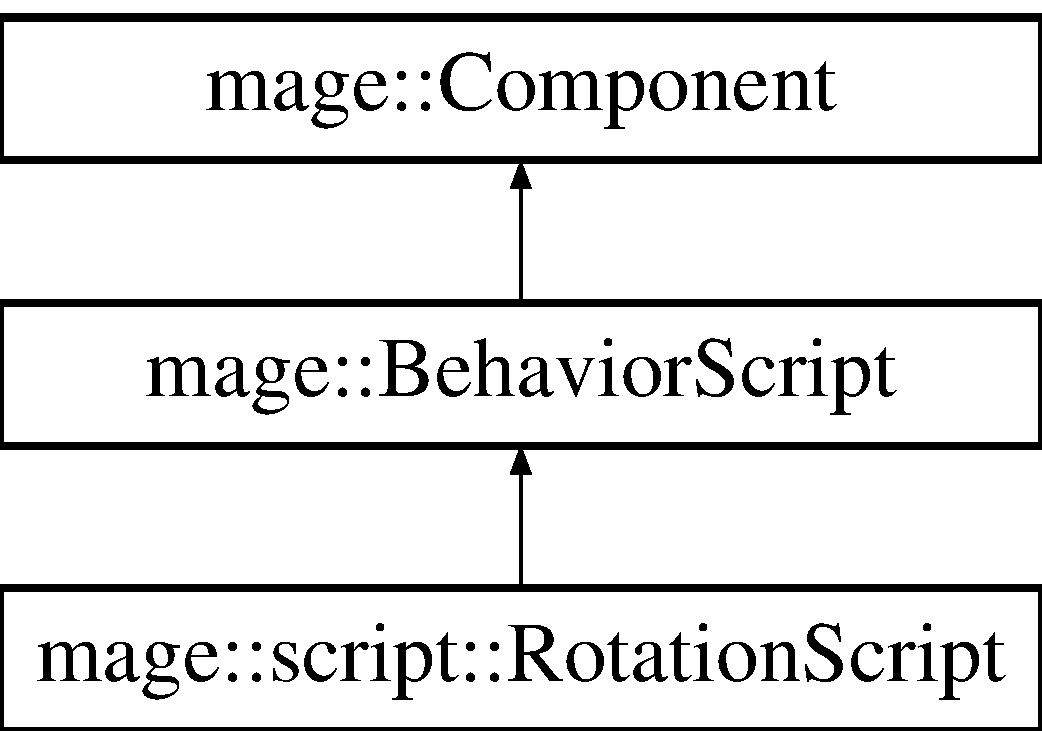
\includegraphics[height=3.000000cm]{classmage_1_1script_1_1_rotation_script}
\end{center}
\end{figure}
\subsection*{Public Types}
\begin{DoxyCompactItemize}
\item 
enum \hyperlink{classmage_1_1script_1_1_rotation_script_a54e1d1d0af65f43f5bc5ad65a4b9c00a}{Rotation\+Axis} \+: U8 \{ \hyperlink{classmage_1_1script_1_1_rotation_script_a54e1d1d0af65f43f5bc5ad65a4b9c00aa02129bb861061d1a052c592e2dc6b383}{Rotation\+Axis\+::X} = 0, 
\hyperlink{classmage_1_1script_1_1_rotation_script_a54e1d1d0af65f43f5bc5ad65a4b9c00aa57cec4137b614c87cb4e24a3d003a3e0}{Rotation\+Axis\+::Y} = 1, 
\hyperlink{classmage_1_1script_1_1_rotation_script_a54e1d1d0af65f43f5bc5ad65a4b9c00aa21c2e59531c8710156d34a3c30ac81d5}{Rotation\+Axis\+::Z} = 2
 \}
\end{DoxyCompactItemize}
\subsection*{Public Member Functions}
\begin{DoxyCompactItemize}
\item 
\hyperlink{classmage_1_1script_1_1_rotation_script_a2961e96c890f5b737fa1851a4f6434fe}{Rotation\+Script} ()
\item 
\hyperlink{classmage_1_1script_1_1_rotation_script_adac08b8383fabba67df915f03a2a01ee}{Rotation\+Script} (const \hyperlink{classmage_1_1script_1_1_rotation_script}{Rotation\+Script} \&script) noexcept
\item 
\hyperlink{classmage_1_1script_1_1_rotation_script_a56942de038a4899fa2fb3d9199f18052}{Rotation\+Script} (\hyperlink{classmage_1_1script_1_1_rotation_script}{Rotation\+Script} \&\&script) noexcept
\item 
virtual \hyperlink{classmage_1_1script_1_1_rotation_script_a7deb74070c49b78b0b91e3599ee8a0b7}{$\sim$\+Rotation\+Script} ()
\item 
\hyperlink{classmage_1_1script_1_1_rotation_script}{Rotation\+Script} \& \hyperlink{classmage_1_1script_1_1_rotation_script_a9302878671d095bab0c31a379ad7d964}{operator=} (const \hyperlink{classmage_1_1script_1_1_rotation_script}{Rotation\+Script} \&script) noexcept
\item 
\hyperlink{classmage_1_1script_1_1_rotation_script}{Rotation\+Script} \& \hyperlink{classmage_1_1script_1_1_rotation_script_af75323393f7570b9fcee0cd62c4f76bd}{operator=} (\hyperlink{classmage_1_1script_1_1_rotation_script}{Rotation\+Script} \&\&script) noexcept
\item 
virtual void \hyperlink{classmage_1_1script_1_1_rotation_script_a7da4165e899facc981c0ee5b1f4a4453}{Load} (\mbox{[}\mbox{[}maybe\+\_\+unused\mbox{]}\mbox{]} \hyperlink{classmage_1_1_engine}{Engine} \&engine) override
\item 
virtual void \hyperlink{classmage_1_1script_1_1_rotation_script_af4e83590b78094186b0dd107a58c7b3a}{Update} (\mbox{[}\mbox{[}maybe\+\_\+unused\mbox{]}\mbox{]} \hyperlink{classmage_1_1_engine}{Engine} \&engine) override
\item 
\hyperlink{classmage_1_1script_1_1_rotation_script_a54e1d1d0af65f43f5bc5ad65a4b9c00a}{Rotation\+Axis} \hyperlink{classmage_1_1script_1_1_rotation_script_ac2ef46249d59b379f47336eb250f3a28}{Get\+Rotation\+Axis} () const noexcept
\item 
void \hyperlink{classmage_1_1script_1_1_rotation_script_aa4b49dc5e34da3e851d5aefc4c4a434b}{Set\+Rotation\+Axis} (\hyperlink{classmage_1_1script_1_1_rotation_script_a54e1d1d0af65f43f5bc5ad65a4b9c00a}{Rotation\+Axis} axis) noexcept
\end{DoxyCompactItemize}
\subsection*{Private Attributes}
\begin{DoxyCompactItemize}
\item 
\hyperlink{classmage_1_1script_1_1_rotation_script_a54e1d1d0af65f43f5bc5ad65a4b9c00a}{Rotation\+Axis} \hyperlink{classmage_1_1script_1_1_rotation_script_a334c42c3ca6af6c2713c98ba4151cdbb}{m\+\_\+axis}
\end{DoxyCompactItemize}
\subsection*{Additional Inherited Members}


\subsection{Member Enumeration Documentation}
\hypertarget{classmage_1_1script_1_1_rotation_script_a54e1d1d0af65f43f5bc5ad65a4b9c00a}{}\label{classmage_1_1script_1_1_rotation_script_a54e1d1d0af65f43f5bc5ad65a4b9c00a} 
\index{mage\+::script\+::\+Rotation\+Script@{mage\+::script\+::\+Rotation\+Script}!Rotation\+Axis@{Rotation\+Axis}}
\index{Rotation\+Axis@{Rotation\+Axis}!mage\+::script\+::\+Rotation\+Script@{mage\+::script\+::\+Rotation\+Script}}
\subsubsection{\texorpdfstring{Rotation\+Axis}{RotationAxis}}
{\footnotesize\ttfamily enum \hyperlink{classmage_1_1script_1_1_rotation_script_a54e1d1d0af65f43f5bc5ad65a4b9c00a}{mage\+::script\+::\+Rotation\+Script\+::\+Rotation\+Axis} \+: \hyperlink{namespacemage_afc638980bc6154f15af5e2d93a0e0ea9}{U8}\hspace{0.3cm}{\ttfamily [strong]}}

\begin{DoxyEnumFields}{Enumerator}
\raisebox{\heightof{T}}[0pt][0pt]{\index{X@{X}!mage\+::script\+::\+Rotation\+Script@{mage\+::script\+::\+Rotation\+Script}}\index{mage\+::script\+::\+Rotation\+Script@{mage\+::script\+::\+Rotation\+Script}!X@{X}}}\hypertarget{classmage_1_1script_1_1_rotation_script_a54e1d1d0af65f43f5bc5ad65a4b9c00aa02129bb861061d1a052c592e2dc6b383}{}\label{classmage_1_1script_1_1_rotation_script_a54e1d1d0af65f43f5bc5ad65a4b9c00aa02129bb861061d1a052c592e2dc6b383} 
X&\\
\hline

\raisebox{\heightof{T}}[0pt][0pt]{\index{Y@{Y}!mage\+::script\+::\+Rotation\+Script@{mage\+::script\+::\+Rotation\+Script}}\index{mage\+::script\+::\+Rotation\+Script@{mage\+::script\+::\+Rotation\+Script}!Y@{Y}}}\hypertarget{classmage_1_1script_1_1_rotation_script_a54e1d1d0af65f43f5bc5ad65a4b9c00aa57cec4137b614c87cb4e24a3d003a3e0}{}\label{classmage_1_1script_1_1_rotation_script_a54e1d1d0af65f43f5bc5ad65a4b9c00aa57cec4137b614c87cb4e24a3d003a3e0} 
Y&\\
\hline

\raisebox{\heightof{T}}[0pt][0pt]{\index{Z@{Z}!mage\+::script\+::\+Rotation\+Script@{mage\+::script\+::\+Rotation\+Script}}\index{mage\+::script\+::\+Rotation\+Script@{mage\+::script\+::\+Rotation\+Script}!Z@{Z}}}\hypertarget{classmage_1_1script_1_1_rotation_script_a54e1d1d0af65f43f5bc5ad65a4b9c00aa21c2e59531c8710156d34a3c30ac81d5}{}\label{classmage_1_1script_1_1_rotation_script_a54e1d1d0af65f43f5bc5ad65a4b9c00aa21c2e59531c8710156d34a3c30ac81d5} 
Z&\\
\hline

\end{DoxyEnumFields}


\subsection{Constructor \& Destructor Documentation}
\hypertarget{classmage_1_1script_1_1_rotation_script_a2961e96c890f5b737fa1851a4f6434fe}{}\label{classmage_1_1script_1_1_rotation_script_a2961e96c890f5b737fa1851a4f6434fe} 
\index{mage\+::script\+::\+Rotation\+Script@{mage\+::script\+::\+Rotation\+Script}!Rotation\+Script@{Rotation\+Script}}
\index{Rotation\+Script@{Rotation\+Script}!mage\+::script\+::\+Rotation\+Script@{mage\+::script\+::\+Rotation\+Script}}
\subsubsection{\texorpdfstring{Rotation\+Script()}{RotationScript()}\hspace{0.1cm}{\footnotesize\ttfamily [1/3]}}
{\footnotesize\ttfamily mage\+::script\+::\+Rotation\+Script\+::\+Rotation\+Script (\begin{DoxyParamCaption}{ }\end{DoxyParamCaption})}

\hypertarget{classmage_1_1script_1_1_rotation_script_adac08b8383fabba67df915f03a2a01ee}{}\label{classmage_1_1script_1_1_rotation_script_adac08b8383fabba67df915f03a2a01ee} 
\index{mage\+::script\+::\+Rotation\+Script@{mage\+::script\+::\+Rotation\+Script}!Rotation\+Script@{Rotation\+Script}}
\index{Rotation\+Script@{Rotation\+Script}!mage\+::script\+::\+Rotation\+Script@{mage\+::script\+::\+Rotation\+Script}}
\subsubsection{\texorpdfstring{Rotation\+Script()}{RotationScript()}\hspace{0.1cm}{\footnotesize\ttfamily [2/3]}}
{\footnotesize\ttfamily mage\+::script\+::\+Rotation\+Script\+::\+Rotation\+Script (\begin{DoxyParamCaption}\item[{const \hyperlink{classmage_1_1script_1_1_rotation_script}{Rotation\+Script} \&}]{script }\end{DoxyParamCaption})\hspace{0.3cm}{\ttfamily [default]}, {\ttfamily [noexcept]}}

\hypertarget{classmage_1_1script_1_1_rotation_script_a56942de038a4899fa2fb3d9199f18052}{}\label{classmage_1_1script_1_1_rotation_script_a56942de038a4899fa2fb3d9199f18052} 
\index{mage\+::script\+::\+Rotation\+Script@{mage\+::script\+::\+Rotation\+Script}!Rotation\+Script@{Rotation\+Script}}
\index{Rotation\+Script@{Rotation\+Script}!mage\+::script\+::\+Rotation\+Script@{mage\+::script\+::\+Rotation\+Script}}
\subsubsection{\texorpdfstring{Rotation\+Script()}{RotationScript()}\hspace{0.1cm}{\footnotesize\ttfamily [3/3]}}
{\footnotesize\ttfamily mage\+::script\+::\+Rotation\+Script\+::\+Rotation\+Script (\begin{DoxyParamCaption}\item[{\hyperlink{classmage_1_1script_1_1_rotation_script}{Rotation\+Script} \&\&}]{script }\end{DoxyParamCaption})\hspace{0.3cm}{\ttfamily [default]}, {\ttfamily [noexcept]}}

\hypertarget{classmage_1_1script_1_1_rotation_script_a7deb74070c49b78b0b91e3599ee8a0b7}{}\label{classmage_1_1script_1_1_rotation_script_a7deb74070c49b78b0b91e3599ee8a0b7} 
\index{mage\+::script\+::\+Rotation\+Script@{mage\+::script\+::\+Rotation\+Script}!````~Rotation\+Script@{$\sim$\+Rotation\+Script}}
\index{````~Rotation\+Script@{$\sim$\+Rotation\+Script}!mage\+::script\+::\+Rotation\+Script@{mage\+::script\+::\+Rotation\+Script}}
\subsubsection{\texorpdfstring{$\sim$\+Rotation\+Script()}{~RotationScript()}}
{\footnotesize\ttfamily mage\+::script\+::\+Rotation\+Script\+::$\sim$\+Rotation\+Script (\begin{DoxyParamCaption}{ }\end{DoxyParamCaption})\hspace{0.3cm}{\ttfamily [virtual]}, {\ttfamily [default]}}



\subsection{Member Function Documentation}
\hypertarget{classmage_1_1script_1_1_rotation_script_ac2ef46249d59b379f47336eb250f3a28}{}\label{classmage_1_1script_1_1_rotation_script_ac2ef46249d59b379f47336eb250f3a28} 
\index{mage\+::script\+::\+Rotation\+Script@{mage\+::script\+::\+Rotation\+Script}!Get\+Rotation\+Axis@{Get\+Rotation\+Axis}}
\index{Get\+Rotation\+Axis@{Get\+Rotation\+Axis}!mage\+::script\+::\+Rotation\+Script@{mage\+::script\+::\+Rotation\+Script}}
\subsubsection{\texorpdfstring{Get\+Rotation\+Axis()}{GetRotationAxis()}}
{\footnotesize\ttfamily \hyperlink{classmage_1_1script_1_1_rotation_script_a54e1d1d0af65f43f5bc5ad65a4b9c00a}{Rotation\+Axis} mage\+::script\+::\+Rotation\+Script\+::\+Get\+Rotation\+Axis (\begin{DoxyParamCaption}{ }\end{DoxyParamCaption}) const\hspace{0.3cm}{\ttfamily [noexcept]}}

\hypertarget{classmage_1_1script_1_1_rotation_script_a7da4165e899facc981c0ee5b1f4a4453}{}\label{classmage_1_1script_1_1_rotation_script_a7da4165e899facc981c0ee5b1f4a4453} 
\index{mage\+::script\+::\+Rotation\+Script@{mage\+::script\+::\+Rotation\+Script}!Load@{Load}}
\index{Load@{Load}!mage\+::script\+::\+Rotation\+Script@{mage\+::script\+::\+Rotation\+Script}}
\subsubsection{\texorpdfstring{Load()}{Load()}}
{\footnotesize\ttfamily void mage\+::script\+::\+Rotation\+Script\+::\+Load (\begin{DoxyParamCaption}\item[{\mbox{[}\mbox{[}maybe\+\_\+unused\mbox{]} \mbox{]} \hyperlink{classmage_1_1_engine}{Engine} \&}]{engine }\end{DoxyParamCaption})\hspace{0.3cm}{\ttfamily [override]}, {\ttfamily [virtual]}}

Loads this behavior script. Allows this behavior script to preform any pre-\/processing.


\begin{DoxyParams}[1]{Parameters}
\mbox{\tt in}  & {\em engine} & A reference to the engine. \\
\hline
\end{DoxyParams}

\begin{DoxyExceptions}{Exceptions}
{\em \hyperlink{classmage_1_1_exception}{Exception}} & Failed to load this behavior script. \\
\hline
\end{DoxyExceptions}


Reimplemented from \hyperlink{classmage_1_1_behavior_script_ae7864876b2ffb1d1d8d8a56e3099f1f2}{mage\+::\+Behavior\+Script}.

\hypertarget{classmage_1_1script_1_1_rotation_script_a9302878671d095bab0c31a379ad7d964}{}\label{classmage_1_1script_1_1_rotation_script_a9302878671d095bab0c31a379ad7d964} 
\index{mage\+::script\+::\+Rotation\+Script@{mage\+::script\+::\+Rotation\+Script}!operator=@{operator=}}
\index{operator=@{operator=}!mage\+::script\+::\+Rotation\+Script@{mage\+::script\+::\+Rotation\+Script}}
\subsubsection{\texorpdfstring{operator=()}{operator=()}\hspace{0.1cm}{\footnotesize\ttfamily [1/2]}}
{\footnotesize\ttfamily \hyperlink{classmage_1_1script_1_1_rotation_script}{Rotation\+Script} \& mage\+::script\+::\+Rotation\+Script\+::operator= (\begin{DoxyParamCaption}\item[{const \hyperlink{classmage_1_1script_1_1_rotation_script}{Rotation\+Script} \&}]{script }\end{DoxyParamCaption})\hspace{0.3cm}{\ttfamily [default]}, {\ttfamily [noexcept]}}

\hypertarget{classmage_1_1script_1_1_rotation_script_af75323393f7570b9fcee0cd62c4f76bd}{}\label{classmage_1_1script_1_1_rotation_script_af75323393f7570b9fcee0cd62c4f76bd} 
\index{mage\+::script\+::\+Rotation\+Script@{mage\+::script\+::\+Rotation\+Script}!operator=@{operator=}}
\index{operator=@{operator=}!mage\+::script\+::\+Rotation\+Script@{mage\+::script\+::\+Rotation\+Script}}
\subsubsection{\texorpdfstring{operator=()}{operator=()}\hspace{0.1cm}{\footnotesize\ttfamily [2/2]}}
{\footnotesize\ttfamily \hyperlink{classmage_1_1script_1_1_rotation_script}{Rotation\+Script} \& mage\+::script\+::\+Rotation\+Script\+::operator= (\begin{DoxyParamCaption}\item[{\hyperlink{classmage_1_1script_1_1_rotation_script}{Rotation\+Script} \&\&}]{script }\end{DoxyParamCaption})\hspace{0.3cm}{\ttfamily [default]}, {\ttfamily [noexcept]}}

\hypertarget{classmage_1_1script_1_1_rotation_script_aa4b49dc5e34da3e851d5aefc4c4a434b}{}\label{classmage_1_1script_1_1_rotation_script_aa4b49dc5e34da3e851d5aefc4c4a434b} 
\index{mage\+::script\+::\+Rotation\+Script@{mage\+::script\+::\+Rotation\+Script}!Set\+Rotation\+Axis@{Set\+Rotation\+Axis}}
\index{Set\+Rotation\+Axis@{Set\+Rotation\+Axis}!mage\+::script\+::\+Rotation\+Script@{mage\+::script\+::\+Rotation\+Script}}
\subsubsection{\texorpdfstring{Set\+Rotation\+Axis()}{SetRotationAxis()}}
{\footnotesize\ttfamily void mage\+::script\+::\+Rotation\+Script\+::\+Set\+Rotation\+Axis (\begin{DoxyParamCaption}\item[{\hyperlink{classmage_1_1script_1_1_rotation_script_a54e1d1d0af65f43f5bc5ad65a4b9c00a}{Rotation\+Axis}}]{axis }\end{DoxyParamCaption})\hspace{0.3cm}{\ttfamily [noexcept]}}

\hypertarget{classmage_1_1script_1_1_rotation_script_af4e83590b78094186b0dd107a58c7b3a}{}\label{classmage_1_1script_1_1_rotation_script_af4e83590b78094186b0dd107a58c7b3a} 
\index{mage\+::script\+::\+Rotation\+Script@{mage\+::script\+::\+Rotation\+Script}!Update@{Update}}
\index{Update@{Update}!mage\+::script\+::\+Rotation\+Script@{mage\+::script\+::\+Rotation\+Script}}
\subsubsection{\texorpdfstring{Update()}{Update()}}
{\footnotesize\ttfamily void mage\+::script\+::\+Rotation\+Script\+::\+Update (\begin{DoxyParamCaption}\item[{\mbox{[}\mbox{[}maybe\+\_\+unused\mbox{]} \mbox{]} \hyperlink{classmage_1_1_engine}{Engine} \&}]{engine }\end{DoxyParamCaption})\hspace{0.3cm}{\ttfamily [override]}, {\ttfamily [virtual]}}

Updates this behavior script.

This method is called once per frame.


\begin{DoxyParams}[1]{Parameters}
\mbox{\tt in}  & {\em engine} & A reference to the engine. \\
\hline
\end{DoxyParams}

\begin{DoxyExceptions}{Exceptions}
{\em \hyperlink{classmage_1_1_exception}{Exception}} & Failed to update this behavior script. \\
\hline
\end{DoxyExceptions}


Reimplemented from \hyperlink{classmage_1_1_behavior_script_a085634661326b59850c1111e537baa4e}{mage\+::\+Behavior\+Script}.



\subsection{Member Data Documentation}
\hypertarget{classmage_1_1script_1_1_rotation_script_a334c42c3ca6af6c2713c98ba4151cdbb}{}\label{classmage_1_1script_1_1_rotation_script_a334c42c3ca6af6c2713c98ba4151cdbb} 
\index{mage\+::script\+::\+Rotation\+Script@{mage\+::script\+::\+Rotation\+Script}!m\+\_\+axis@{m\+\_\+axis}}
\index{m\+\_\+axis@{m\+\_\+axis}!mage\+::script\+::\+Rotation\+Script@{mage\+::script\+::\+Rotation\+Script}}
\subsubsection{\texorpdfstring{m\+\_\+axis}{m\_axis}}
{\footnotesize\ttfamily \hyperlink{classmage_1_1script_1_1_rotation_script_a54e1d1d0af65f43f5bc5ad65a4b9c00a}{Rotation\+Axis} mage\+::script\+::\+Rotation\+Script\+::m\+\_\+axis\hspace{0.3cm}{\ttfamily [private]}}


\hypertarget{structmage_1_1rendering_1_1_pipeline_1_1_r_s}{}\section{mage\+:\+:rendering\+:\+:Pipeline\+:\+:RS Struct Reference}
\label{structmage_1_1rendering_1_1_pipeline_1_1_r_s}\index{mage\+::rendering\+::\+Pipeline\+::\+RS@{mage\+::rendering\+::\+Pipeline\+::\+RS}}


{\ttfamily \#include $<$pipeline.\+hpp$>$}

\subsection*{Static Public Member Functions}
\begin{DoxyCompactItemize}
\item 
static void \mbox{\hyperlink{structmage_1_1rendering_1_1_pipeline_1_1_r_s_a54ebb9ad47711a5dbeeef1d24e079c3f}{Bind\+Scissor\+Rectangle}} (I\+D3\+D11\+Device\+Context \&device\+\_\+context, const D3\+D11\+\_\+\+R\+E\+CT \&rectangle) noexcept
\item 
static void \mbox{\hyperlink{structmage_1_1rendering_1_1_pipeline_1_1_r_s_a82f5efafad2b8ad552dbe211e861b250}{Bind\+Scissor\+Rectangles}} (I\+D3\+D11\+Device\+Context \&device\+\_\+context, \mbox{\hyperlink{namespacemage_aa5d6eaabaac3cdd01873d6a3d27e90f3}{U32}} nb\+\_\+rectangles, const D3\+D11\+\_\+\+R\+E\+CT $\ast$rectangles) noexcept
\item 
static void \mbox{\hyperlink{structmage_1_1rendering_1_1_pipeline_1_1_r_s_a828e80ca97ec6827434864cf8115766d}{Bind\+State}} (I\+D3\+D11\+Device\+Context \&device\+\_\+context, I\+D3\+D11\+Rasterizer\+State $\ast$state) noexcept
\item 
static void \mbox{\hyperlink{structmage_1_1rendering_1_1_pipeline_1_1_r_s_aa20a052fcf0d02d31192f225d9a85efd}{Get\+Bound\+Viewports}} (I\+D3\+D11\+Device\+Context \&device\+\_\+context, \mbox{\hyperlink{namespacemage_aa5d6eaabaac3cdd01873d6a3d27e90f3}{U32}} $\ast$nb\+\_\+viewports, D3\+D11\+\_\+\+V\+I\+E\+W\+P\+O\+RT $\ast$viewports) noexcept
\item 
static void \mbox{\hyperlink{structmage_1_1rendering_1_1_pipeline_1_1_r_s_a9d44e3f07e0bd12c736b46b7b05693f7}{Bind\+Viewport}} (I\+D3\+D11\+Device\+Context \&device\+\_\+context, const D3\+D11\+\_\+\+V\+I\+E\+W\+P\+O\+RT \&viewport) noexcept
\item 
static void \mbox{\hyperlink{structmage_1_1rendering_1_1_pipeline_1_1_r_s_a0df7ca670ab1b0a0fe31591a8f90885c}{Bind\+Viewports}} (I\+D3\+D11\+Device\+Context \&device\+\_\+context, \mbox{\hyperlink{namespacemage_aa5d6eaabaac3cdd01873d6a3d27e90f3}{U32}} nb\+\_\+viewports, const D3\+D11\+\_\+\+V\+I\+E\+W\+P\+O\+RT $\ast$viewports) noexcept
\end{DoxyCompactItemize}


\subsection{Detailed Description}
The rasterizer stage. 

\subsection{Member Function Documentation}
\mbox{\Hypertarget{structmage_1_1rendering_1_1_pipeline_1_1_r_s_a54ebb9ad47711a5dbeeef1d24e079c3f}\label{structmage_1_1rendering_1_1_pipeline_1_1_r_s_a54ebb9ad47711a5dbeeef1d24e079c3f}} 
\index{mage\+::rendering\+::\+Pipeline\+::\+RS@{mage\+::rendering\+::\+Pipeline\+::\+RS}!Bind\+Scissor\+Rectangle@{Bind\+Scissor\+Rectangle}}
\index{Bind\+Scissor\+Rectangle@{Bind\+Scissor\+Rectangle}!mage\+::rendering\+::\+Pipeline\+::\+RS@{mage\+::rendering\+::\+Pipeline\+::\+RS}}
\subsubsection{\texorpdfstring{Bind\+Scissor\+Rectangle()}{BindScissorRectangle()}}
{\footnotesize\ttfamily static void mage\+::rendering\+::\+Pipeline\+::\+R\+S\+::\+Bind\+Scissor\+Rectangle (\begin{DoxyParamCaption}\item[{I\+D3\+D11\+Device\+Context \&}]{device\+\_\+context,  }\item[{const D3\+D11\+\_\+\+R\+E\+CT \&}]{rectangle }\end{DoxyParamCaption})\hspace{0.3cm}{\ttfamily [static]}, {\ttfamily [noexcept]}}

\mbox{\Hypertarget{structmage_1_1rendering_1_1_pipeline_1_1_r_s_a82f5efafad2b8ad552dbe211e861b250}\label{structmage_1_1rendering_1_1_pipeline_1_1_r_s_a82f5efafad2b8ad552dbe211e861b250}} 
\index{mage\+::rendering\+::\+Pipeline\+::\+RS@{mage\+::rendering\+::\+Pipeline\+::\+RS}!Bind\+Scissor\+Rectangles@{Bind\+Scissor\+Rectangles}}
\index{Bind\+Scissor\+Rectangles@{Bind\+Scissor\+Rectangles}!mage\+::rendering\+::\+Pipeline\+::\+RS@{mage\+::rendering\+::\+Pipeline\+::\+RS}}
\subsubsection{\texorpdfstring{Bind\+Scissor\+Rectangles()}{BindScissorRectangles()}}
{\footnotesize\ttfamily static void mage\+::rendering\+::\+Pipeline\+::\+R\+S\+::\+Bind\+Scissor\+Rectangles (\begin{DoxyParamCaption}\item[{I\+D3\+D11\+Device\+Context \&}]{device\+\_\+context,  }\item[{\mbox{\hyperlink{namespacemage_aa5d6eaabaac3cdd01873d6a3d27e90f3}{U32}}}]{nb\+\_\+rectangles,  }\item[{const D3\+D11\+\_\+\+R\+E\+CT $\ast$}]{rectangles }\end{DoxyParamCaption})\hspace{0.3cm}{\ttfamily [static]}, {\ttfamily [noexcept]}}

\mbox{\Hypertarget{structmage_1_1rendering_1_1_pipeline_1_1_r_s_a828e80ca97ec6827434864cf8115766d}\label{structmage_1_1rendering_1_1_pipeline_1_1_r_s_a828e80ca97ec6827434864cf8115766d}} 
\index{mage\+::rendering\+::\+Pipeline\+::\+RS@{mage\+::rendering\+::\+Pipeline\+::\+RS}!Bind\+State@{Bind\+State}}
\index{Bind\+State@{Bind\+State}!mage\+::rendering\+::\+Pipeline\+::\+RS@{mage\+::rendering\+::\+Pipeline\+::\+RS}}
\subsubsection{\texorpdfstring{Bind\+State()}{BindState()}}
{\footnotesize\ttfamily static void mage\+::rendering\+::\+Pipeline\+::\+R\+S\+::\+Bind\+State (\begin{DoxyParamCaption}\item[{I\+D3\+D11\+Device\+Context \&}]{device\+\_\+context,  }\item[{I\+D3\+D11\+Rasterizer\+State $\ast$}]{state }\end{DoxyParamCaption})\hspace{0.3cm}{\ttfamily [static]}, {\ttfamily [noexcept]}}

\mbox{\Hypertarget{structmage_1_1rendering_1_1_pipeline_1_1_r_s_a9d44e3f07e0bd12c736b46b7b05693f7}\label{structmage_1_1rendering_1_1_pipeline_1_1_r_s_a9d44e3f07e0bd12c736b46b7b05693f7}} 
\index{mage\+::rendering\+::\+Pipeline\+::\+RS@{mage\+::rendering\+::\+Pipeline\+::\+RS}!Bind\+Viewport@{Bind\+Viewport}}
\index{Bind\+Viewport@{Bind\+Viewport}!mage\+::rendering\+::\+Pipeline\+::\+RS@{mage\+::rendering\+::\+Pipeline\+::\+RS}}
\subsubsection{\texorpdfstring{Bind\+Viewport()}{BindViewport()}}
{\footnotesize\ttfamily static void mage\+::rendering\+::\+Pipeline\+::\+R\+S\+::\+Bind\+Viewport (\begin{DoxyParamCaption}\item[{I\+D3\+D11\+Device\+Context \&}]{device\+\_\+context,  }\item[{const D3\+D11\+\_\+\+V\+I\+E\+W\+P\+O\+RT \&}]{viewport }\end{DoxyParamCaption})\hspace{0.3cm}{\ttfamily [static]}, {\ttfamily [noexcept]}}

\mbox{\Hypertarget{structmage_1_1rendering_1_1_pipeline_1_1_r_s_a0df7ca670ab1b0a0fe31591a8f90885c}\label{structmage_1_1rendering_1_1_pipeline_1_1_r_s_a0df7ca670ab1b0a0fe31591a8f90885c}} 
\index{mage\+::rendering\+::\+Pipeline\+::\+RS@{mage\+::rendering\+::\+Pipeline\+::\+RS}!Bind\+Viewports@{Bind\+Viewports}}
\index{Bind\+Viewports@{Bind\+Viewports}!mage\+::rendering\+::\+Pipeline\+::\+RS@{mage\+::rendering\+::\+Pipeline\+::\+RS}}
\subsubsection{\texorpdfstring{Bind\+Viewports()}{BindViewports()}}
{\footnotesize\ttfamily static void mage\+::rendering\+::\+Pipeline\+::\+R\+S\+::\+Bind\+Viewports (\begin{DoxyParamCaption}\item[{I\+D3\+D11\+Device\+Context \&}]{device\+\_\+context,  }\item[{\mbox{\hyperlink{namespacemage_aa5d6eaabaac3cdd01873d6a3d27e90f3}{U32}}}]{nb\+\_\+viewports,  }\item[{const D3\+D11\+\_\+\+V\+I\+E\+W\+P\+O\+RT $\ast$}]{viewports }\end{DoxyParamCaption})\hspace{0.3cm}{\ttfamily [static]}, {\ttfamily [noexcept]}}

\mbox{\Hypertarget{structmage_1_1rendering_1_1_pipeline_1_1_r_s_aa20a052fcf0d02d31192f225d9a85efd}\label{structmage_1_1rendering_1_1_pipeline_1_1_r_s_aa20a052fcf0d02d31192f225d9a85efd}} 
\index{mage\+::rendering\+::\+Pipeline\+::\+RS@{mage\+::rendering\+::\+Pipeline\+::\+RS}!Get\+Bound\+Viewports@{Get\+Bound\+Viewports}}
\index{Get\+Bound\+Viewports@{Get\+Bound\+Viewports}!mage\+::rendering\+::\+Pipeline\+::\+RS@{mage\+::rendering\+::\+Pipeline\+::\+RS}}
\subsubsection{\texorpdfstring{Get\+Bound\+Viewports()}{GetBoundViewports()}}
{\footnotesize\ttfamily static void mage\+::rendering\+::\+Pipeline\+::\+R\+S\+::\+Get\+Bound\+Viewports (\begin{DoxyParamCaption}\item[{I\+D3\+D11\+Device\+Context \&}]{device\+\_\+context,  }\item[{\mbox{\hyperlink{namespacemage_aa5d6eaabaac3cdd01873d6a3d27e90f3}{U32}} $\ast$}]{nb\+\_\+viewports,  }\item[{D3\+D11\+\_\+\+V\+I\+E\+W\+P\+O\+RT $\ast$}]{viewports }\end{DoxyParamCaption})\hspace{0.3cm}{\ttfamily [static]}, {\ttfamily [noexcept]}}


\hypertarget{classmage_1_1_scene}{}\section{mage\+:\+:Scene Class Reference}
\label{classmage_1_1_scene}\index{mage\+::\+Scene@{mage\+::\+Scene}}


{\ttfamily \#include $<$scene.\+hpp$>$}

\subsection*{Public Member Functions}
\begin{DoxyCompactItemize}
\item 
virtual \hyperlink{classmage_1_1_scene_adc40910fdca62586659c2961fe7e7f3c}{$\sim$\+Scene} ()
\item 
\hyperlink{classmage_1_1_scene}{Scene} \& \hyperlink{classmage_1_1_scene_a2c25c0fedc0230771d8c00a8288a69ce}{operator=} (const \hyperlink{classmage_1_1_scene}{Scene} \&scene)=delete
\item 
\hyperlink{classmage_1_1_scene}{Scene} \& \hyperlink{classmage_1_1_scene_a400926762670c9cd9b6d456291600f53}{operator=} (\hyperlink{classmage_1_1_scene}{Scene} \&\&scene)=delete
\item 
const string \& \hyperlink{classmage_1_1_scene_a251ff8f6ce0da5c55ee31e3450b5fb9a}{Get\+Name} () const
\item 
void \hyperlink{classmage_1_1_scene_a9b7c1c2f84cc3b3c5ff3de4f29d830e9}{Set\+Name} (const string \&name)
\item 
void \hyperlink{classmage_1_1_scene_a3cd12ef381ca743bf0b8f8aa2a76eb57}{Initialize} ()
\item 
void \hyperlink{classmage_1_1_scene_aa10e6eafc00834f63f146589326cbfe2}{Update} (double delta\+\_\+time)
\item 
void \hyperlink{classmage_1_1_scene_a53487349d68f0ffcc91b243d0cfb86a3}{Render2D} () const
\item 
void \hyperlink{classmage_1_1_scene_a51d2d441067d30cf3a444d6a80811f93}{Render3D} () const
\item 
void \hyperlink{classmage_1_1_scene_a714dc33c04dc2b8e2cec93564905b174}{Uninitialize} ()
\item 
\hyperlink{namespacemage_a1e01ae66713838a7a67d30e44c67703e}{Shared\+Ptr}$<$ \hyperlink{classmage_1_1_camera_node}{Camera\+Node} $>$ \hyperlink{classmage_1_1_scene_a4ce734c571a4ac2fc564cf1c641e7820}{Get\+Camera} () const
\item 
void \hyperlink{classmage_1_1_scene_a7568ec0884d04812af2f70990c8ec80d}{Set\+Camera} (\hyperlink{namespacemage_a1e01ae66713838a7a67d30e44c67703e}{Shared\+Ptr}$<$ \hyperlink{classmage_1_1_camera_node}{Camera\+Node} $>$ camera)
\item 
\hyperlink{namespacemage_a1e01ae66713838a7a67d30e44c67703e}{Shared\+Ptr}$<$ \hyperlink{namespacemage_a2ba71e84d4a4fb1e4a7160800c53f519}{Orthographic\+Camera\+Node} $>$ \hyperlink{classmage_1_1_scene_a9ed9e3a611434f62427c7bd4c16d2456}{Create\+Orthographic\+Camera\+Node} ()
\item 
\hyperlink{namespacemage_a1e01ae66713838a7a67d30e44c67703e}{Shared\+Ptr}$<$ \hyperlink{namespacemage_af3a338f28772b91cf6d7cb85df6f4bb9}{Perspective\+Camera\+Node} $>$ \hyperlink{classmage_1_1_scene_a3f4141d407133e6419af92376bc3ecc1}{Create\+Perspective\+Camera\+Node} ()
\item 
\hyperlink{namespacemage_a1e01ae66713838a7a67d30e44c67703e}{Shared\+Ptr}$<$ \hyperlink{namespacemage_a85082c7e15a2bbf19b1753b7de6c45db}{Omni\+Light\+Node} $>$ \hyperlink{classmage_1_1_scene_a370f5ce63a6277a1369c1545f0acbffa}{Create\+Omni\+Light\+Node} ()
\item 
\hyperlink{namespacemage_a1e01ae66713838a7a67d30e44c67703e}{Shared\+Ptr}$<$ \hyperlink{namespacemage_a46c8f54b869a5dc07f520c600b9046bd}{Spot\+Light\+Node} $>$ \hyperlink{classmage_1_1_scene_a27ffb510eeb8e208ba20ee0d76138a3f}{Create\+Spot\+Light\+Node} ()
\item 
\hyperlink{namespacemage_a1e01ae66713838a7a67d30e44c67703e}{Shared\+Ptr}$<$ \hyperlink{classmage_1_1_model_node}{Model\+Node} $>$ \hyperlink{classmage_1_1_scene_a8ff21b5512cfbc053d96882a5d30996e}{Create\+Model\+Node} (const \hyperlink{classmage_1_1_model_descriptor}{Model\+Descriptor} \&desc, const \hyperlink{structmage_1_1_combined_shader}{Combined\+Shader} \&shader=\hyperlink{namespacemage_a91a20907d6a7a77bdd768dbd0bc420c5}{Create\+Lambertian\+Shader}())
\item 
size\+\_\+t \hyperlink{classmage_1_1_scene_a799ac8ddd90d24f6c3c208942e4f159c}{Get\+Number\+Of\+Scripts} () const
\item 
bool \hyperlink{classmage_1_1_scene_a9dd6c49e9db7590de1de4fbd128c78a9}{Has\+Script} (\hyperlink{namespacemage_a1e01ae66713838a7a67d30e44c67703e}{Shared\+Ptr}$<$ const \hyperlink{classmage_1_1_behavior_script}{Behavior\+Script} $>$ script) const
\item 
void \hyperlink{classmage_1_1_scene_ab97b66c81c32681699052e154d0e0722}{Add\+Script} (\hyperlink{namespacemage_a1e01ae66713838a7a67d30e44c67703e}{Shared\+Ptr}$<$ \hyperlink{classmage_1_1_behavior_script}{Behavior\+Script} $>$ script)
\item 
void \hyperlink{classmage_1_1_scene_a82705ba56543dea410439760b1667bc5}{Remove\+Script} (\hyperlink{namespacemage_a1e01ae66713838a7a67d30e44c67703e}{Shared\+Ptr}$<$ \hyperlink{classmage_1_1_behavior_script}{Behavior\+Script} $>$ script)
\item 
void \hyperlink{classmage_1_1_scene_a04b6e0b4d9ca18d15d3da098e581d336}{Remove\+All\+Scripts} ()
\item 
{\footnotesize template$<$typename ActionT $>$ }\\void \hyperlink{classmage_1_1_scene_a4d16d973adce12868b9a0df9d92ef6d6}{For\+Each\+Script} (ActionT action) const
\item 
void \hyperlink{classmage_1_1_scene_a735a4eba6bf6a072195f1cfc58dfca47}{Add\+Sprite} (\hyperlink{namespacemage_a1e01ae66713838a7a67d30e44c67703e}{Shared\+Ptr}$<$ \hyperlink{classmage_1_1_sprite_object}{Sprite\+Object} $>$ sprite)
\item 
void \hyperlink{classmage_1_1_scene_a6d886d48157b9988ab61cc9b01ee752e}{Remove\+Sprite} (\hyperlink{namespacemage_a1e01ae66713838a7a67d30e44c67703e}{Shared\+Ptr}$<$ \hyperlink{classmage_1_1_sprite_object}{Sprite\+Object} $>$ sprite)
\item 
void \hyperlink{classmage_1_1_scene_aad8b532e9c127fd216ca9db9ad9f3420}{Remove\+All\+Sprites} ()
\item 
{\footnotesize template$<$typename ActionT $>$ }\\void \hyperlink{classmage_1_1_scene_ae181b160f9a75593db9f551c9c233329}{For\+Each\+Sprite} (ActionT action) const
\end{DoxyCompactItemize}
\subsection*{Protected Member Functions}
\begin{DoxyCompactItemize}
\item 
\hyperlink{classmage_1_1_scene_aab61b38547fc53aa9c5b3b559f4d2e26}{Scene} (const string \&name)
\item 
\hyperlink{classmage_1_1_scene_a88d83ccb2e10549d5370f850b2b4c228}{Scene} (const \hyperlink{classmage_1_1_scene}{Scene} \&scene)=delete
\item 
\hyperlink{classmage_1_1_scene_a35b8fc4242c2348e53014b96416fc3d3}{Scene} (\hyperlink{classmage_1_1_scene}{Scene} \&\&scene)=default
\end{DoxyCompactItemize}
\subsection*{Private Member Functions}
\begin{DoxyCompactItemize}
\item 
virtual void \hyperlink{classmage_1_1_scene_a1fb4a93eaa2f6a9e20594e205abb9a32}{Load} ()
\item 
virtual void \hyperlink{classmage_1_1_scene_a16786d7fcf0b813e2e94061b082cfd1d}{Close} ()
\item 
void \hyperlink{classmage_1_1_scene_a916cc7a0867bf1c09e5d10de53192140}{Clear} ()
\item 
void \hyperlink{classmage_1_1_scene_acfd5cf0484e1814cb265604ed970335f}{Add\+Model} (\hyperlink{namespacemage_a1e01ae66713838a7a67d30e44c67703e}{Shared\+Ptr}$<$ \hyperlink{classmage_1_1_model_node}{Model\+Node} $>$ model)
\item 
void \hyperlink{classmage_1_1_scene_a1b66a3d247eaa143234d15d72aa67a85}{Remove\+Model} (\hyperlink{namespacemage_a1e01ae66713838a7a67d30e44c67703e}{Shared\+Ptr}$<$ \hyperlink{classmage_1_1_model_node}{Model\+Node} $>$ model)
\item 
void \hyperlink{classmage_1_1_scene_a5dffc6ff3e40981087cbfc2462e5b84a}{Remove\+All\+Models} ()
\item 
{\footnotesize template$<$typename ActionT $>$ }\\void \hyperlink{classmage_1_1_scene_a6327548021f874f22a1adc81cfc8a1ea}{For\+Each\+Model} (ActionT action) const
\item 
void \hyperlink{classmage_1_1_scene_a6ce8182afe3c1f39249ec08b62aee317}{Add\+Light} (\hyperlink{namespacemage_a1e01ae66713838a7a67d30e44c67703e}{Shared\+Ptr}$<$ \hyperlink{namespacemage_a85082c7e15a2bbf19b1753b7de6c45db}{Omni\+Light\+Node} $>$ light)
\item 
void \hyperlink{classmage_1_1_scene_aeeba74ee789d4917ed72b179f16c1222}{Add\+Light} (\hyperlink{namespacemage_a1e01ae66713838a7a67d30e44c67703e}{Shared\+Ptr}$<$ \hyperlink{namespacemage_a46c8f54b869a5dc07f520c600b9046bd}{Spot\+Light\+Node} $>$ light)
\item 
void \hyperlink{classmage_1_1_scene_a1da46b19f87d387af18d2f7fc37bb6d7}{Remove\+Light} (\hyperlink{namespacemage_a1e01ae66713838a7a67d30e44c67703e}{Shared\+Ptr}$<$ \hyperlink{namespacemage_a85082c7e15a2bbf19b1753b7de6c45db}{Omni\+Light\+Node} $>$ light)
\item 
void \hyperlink{classmage_1_1_scene_a371c31d030990b9fa641271c4c733d87}{Remove\+Light} (\hyperlink{namespacemage_a1e01ae66713838a7a67d30e44c67703e}{Shared\+Ptr}$<$ \hyperlink{namespacemage_a46c8f54b869a5dc07f520c600b9046bd}{Spot\+Light\+Node} $>$ light)
\item 
void \hyperlink{classmage_1_1_scene_acde7e343459ea1444f2b0f7bbb3e1882}{Remove\+All\+Lights} ()
\item 
{\footnotesize template$<$typename ActionT $>$ }\\void \hyperlink{classmage_1_1_scene_acd71cef84ec39e63852d5918c7b17863}{For\+Each\+Omni\+Light} (ActionT action) const
\item 
{\footnotesize template$<$typename ActionT $>$ }\\void \hyperlink{classmage_1_1_scene_a51bb697a9d96891bb7502317efff7ec1}{For\+Each\+Spot\+Light} (ActionT action) const
\item 
{\footnotesize template$<$typename ActionT $>$ }\\void \hyperlink{classmage_1_1_scene_a131c27235c6f172a316c56fea7f2e80c}{For\+Each\+Light} (ActionT action) const
\end{DoxyCompactItemize}
\subsection*{Private Attributes}
\begin{DoxyCompactItemize}
\item 
string \hyperlink{classmage_1_1_scene_a6cc8cb08b1853c4e3063b33a94e8fb47}{m\+\_\+name}
\item 
vector$<$ \hyperlink{namespacemage_a1e01ae66713838a7a67d30e44c67703e}{Shared\+Ptr}$<$ \hyperlink{classmage_1_1_behavior_script}{Behavior\+Script} $>$ $>$ \hyperlink{classmage_1_1_scene_a84548bf6978f8955ce5892cb23536a4e}{m\+\_\+scripts}
\item 
\hyperlink{namespacemage_a1e01ae66713838a7a67d30e44c67703e}{Shared\+Ptr}$<$ \hyperlink{classmage_1_1_camera_node}{Camera\+Node} $>$ \hyperlink{classmage_1_1_scene_a39c785951d9fb99477c1894eabba0cc6}{m\+\_\+camera}
\item 
vector$<$ \hyperlink{namespacemage_a1e01ae66713838a7a67d30e44c67703e}{Shared\+Ptr}$<$ \hyperlink{classmage_1_1_model_node}{Model\+Node} $>$ $>$ \hyperlink{classmage_1_1_scene_a01132a667fbc1517f11ae561bc221071}{m\+\_\+models}
\item 
vector$<$ \hyperlink{namespacemage_a1e01ae66713838a7a67d30e44c67703e}{Shared\+Ptr}$<$ \hyperlink{namespacemage_a85082c7e15a2bbf19b1753b7de6c45db}{Omni\+Light\+Node} $>$ $>$ \hyperlink{classmage_1_1_scene_a881c3dd7e85e5069650f29fd2722bf78}{m\+\_\+omni\+\_\+lights}
\item 
vector$<$ \hyperlink{namespacemage_a1e01ae66713838a7a67d30e44c67703e}{Shared\+Ptr}$<$ \hyperlink{namespacemage_a46c8f54b869a5dc07f520c600b9046bd}{Spot\+Light\+Node} $>$ $>$ \hyperlink{classmage_1_1_scene_a4e1954bc0b812d6a71123ca3ac9eeb75}{m\+\_\+spot\+\_\+lights}
\item 
vector$<$ \hyperlink{namespacemage_a1e01ae66713838a7a67d30e44c67703e}{Shared\+Ptr}$<$ \hyperlink{classmage_1_1_sprite_object}{Sprite\+Object} $>$ $>$ \hyperlink{classmage_1_1_scene_a7379b399f02999f89f6ccda5bfa01b02}{m\+\_\+sprites}
\item 
\hyperlink{namespacemage_a1e01ae66713838a7a67d30e44c67703e}{Shared\+Ptr}$<$ Sprite\+Batch $>$ \hyperlink{classmage_1_1_scene_a7a334e1b7764532817f10efbc0b91a82}{m\+\_\+sprite\+\_\+batch}
\item 
\hyperlink{structmage_1_1_constant_buffer}{Constant\+Buffer}$<$ Transform\+Buffer $>$ \hyperlink{classmage_1_1_scene_a2e57c981725d0a64bfc8f82381ac3d6a}{m\+\_\+transform\+\_\+buffer}
\item 
\hyperlink{structmage_1_1_constant_buffer}{Constant\+Buffer}$<$ Light\+Data\+Buffer $>$ \hyperlink{classmage_1_1_scene_aa74ca1637e0a88546135d64bf3614f29}{m\+\_\+light\+\_\+data\+\_\+buffer}
\item 
\hyperlink{structmage_1_1_structured_buffer}{Structured\+Buffer}$<$ Omni\+Light\+Buffer $>$ \hyperlink{classmage_1_1_scene_a274ed5e548431ba805513a86a00bbaf1}{m\+\_\+omni\+\_\+lights\+\_\+buffer}
\item 
\hyperlink{structmage_1_1_structured_buffer}{Structured\+Buffer}$<$ Spot\+Light\+Buffer $>$ \hyperlink{classmage_1_1_scene_a64118c052d728ac988031898fd2d757d}{m\+\_\+spot\+\_\+lights\+\_\+buffer}
\end{DoxyCompactItemize}


\subsection{Constructor \& Destructor Documentation}
\hypertarget{classmage_1_1_scene_adc40910fdca62586659c2961fe7e7f3c}{}\label{classmage_1_1_scene_adc40910fdca62586659c2961fe7e7f3c} 
\index{mage\+::\+Scene@{mage\+::\+Scene}!````~Scene@{$\sim$\+Scene}}
\index{````~Scene@{$\sim$\+Scene}!mage\+::\+Scene@{mage\+::\+Scene}}
\subsubsection{\texorpdfstring{$\sim$\+Scene()}{~Scene()}}
{\footnotesize\ttfamily mage\+::\+Scene\+::$\sim$\+Scene (\begin{DoxyParamCaption}{ }\end{DoxyParamCaption})\hspace{0.3cm}{\ttfamily [virtual]}}

\hypertarget{classmage_1_1_scene_aab61b38547fc53aa9c5b3b559f4d2e26}{}\label{classmage_1_1_scene_aab61b38547fc53aa9c5b3b559f4d2e26} 
\index{mage\+::\+Scene@{mage\+::\+Scene}!Scene@{Scene}}
\index{Scene@{Scene}!mage\+::\+Scene@{mage\+::\+Scene}}
\subsubsection{\texorpdfstring{Scene()}{Scene()}\hspace{0.1cm}{\footnotesize\ttfamily [1/3]}}
{\footnotesize\ttfamily mage\+::\+Scene\+::\+Scene (\begin{DoxyParamCaption}\item[{const string \&}]{name }\end{DoxyParamCaption})\hspace{0.3cm}{\ttfamily [explicit]}, {\ttfamily [protected]}}

\hypertarget{classmage_1_1_scene_a88d83ccb2e10549d5370f850b2b4c228}{}\label{classmage_1_1_scene_a88d83ccb2e10549d5370f850b2b4c228} 
\index{mage\+::\+Scene@{mage\+::\+Scene}!Scene@{Scene}}
\index{Scene@{Scene}!mage\+::\+Scene@{mage\+::\+Scene}}
\subsubsection{\texorpdfstring{Scene()}{Scene()}\hspace{0.1cm}{\footnotesize\ttfamily [2/3]}}
{\footnotesize\ttfamily mage\+::\+Scene\+::\+Scene (\begin{DoxyParamCaption}\item[{const \hyperlink{classmage_1_1_scene}{Scene} \&}]{scene }\end{DoxyParamCaption})\hspace{0.3cm}{\ttfamily [protected]}, {\ttfamily [delete]}}

\hypertarget{classmage_1_1_scene_a35b8fc4242c2348e53014b96416fc3d3}{}\label{classmage_1_1_scene_a35b8fc4242c2348e53014b96416fc3d3} 
\index{mage\+::\+Scene@{mage\+::\+Scene}!Scene@{Scene}}
\index{Scene@{Scene}!mage\+::\+Scene@{mage\+::\+Scene}}
\subsubsection{\texorpdfstring{Scene()}{Scene()}\hspace{0.1cm}{\footnotesize\ttfamily [3/3]}}
{\footnotesize\ttfamily mage\+::\+Scene\+::\+Scene (\begin{DoxyParamCaption}\item[{\hyperlink{classmage_1_1_scene}{Scene} \&\&}]{scene }\end{DoxyParamCaption})\hspace{0.3cm}{\ttfamily [protected]}, {\ttfamily [default]}}



\subsection{Member Function Documentation}
\hypertarget{classmage_1_1_scene_a6ce8182afe3c1f39249ec08b62aee317}{}\label{classmage_1_1_scene_a6ce8182afe3c1f39249ec08b62aee317} 
\index{mage\+::\+Scene@{mage\+::\+Scene}!Add\+Light@{Add\+Light}}
\index{Add\+Light@{Add\+Light}!mage\+::\+Scene@{mage\+::\+Scene}}
\subsubsection{\texorpdfstring{Add\+Light()}{AddLight()}\hspace{0.1cm}{\footnotesize\ttfamily [1/2]}}
{\footnotesize\ttfamily void mage\+::\+Scene\+::\+Add\+Light (\begin{DoxyParamCaption}\item[{\hyperlink{namespacemage_a1e01ae66713838a7a67d30e44c67703e}{Shared\+Ptr}$<$ \hyperlink{namespacemage_a85082c7e15a2bbf19b1753b7de6c45db}{Omni\+Light\+Node} $>$}]{light }\end{DoxyParamCaption})\hspace{0.3cm}{\ttfamily [private]}}

\hypertarget{classmage_1_1_scene_aeeba74ee789d4917ed72b179f16c1222}{}\label{classmage_1_1_scene_aeeba74ee789d4917ed72b179f16c1222} 
\index{mage\+::\+Scene@{mage\+::\+Scene}!Add\+Light@{Add\+Light}}
\index{Add\+Light@{Add\+Light}!mage\+::\+Scene@{mage\+::\+Scene}}
\subsubsection{\texorpdfstring{Add\+Light()}{AddLight()}\hspace{0.1cm}{\footnotesize\ttfamily [2/2]}}
{\footnotesize\ttfamily void mage\+::\+Scene\+::\+Add\+Light (\begin{DoxyParamCaption}\item[{\hyperlink{namespacemage_a1e01ae66713838a7a67d30e44c67703e}{Shared\+Ptr}$<$ \hyperlink{namespacemage_a46c8f54b869a5dc07f520c600b9046bd}{Spot\+Light\+Node} $>$}]{light }\end{DoxyParamCaption})\hspace{0.3cm}{\ttfamily [private]}}

\hypertarget{classmage_1_1_scene_acfd5cf0484e1814cb265604ed970335f}{}\label{classmage_1_1_scene_acfd5cf0484e1814cb265604ed970335f} 
\index{mage\+::\+Scene@{mage\+::\+Scene}!Add\+Model@{Add\+Model}}
\index{Add\+Model@{Add\+Model}!mage\+::\+Scene@{mage\+::\+Scene}}
\subsubsection{\texorpdfstring{Add\+Model()}{AddModel()}}
{\footnotesize\ttfamily void mage\+::\+Scene\+::\+Add\+Model (\begin{DoxyParamCaption}\item[{\hyperlink{namespacemage_a1e01ae66713838a7a67d30e44c67703e}{Shared\+Ptr}$<$ \hyperlink{classmage_1_1_model_node}{Model\+Node} $>$}]{model }\end{DoxyParamCaption})\hspace{0.3cm}{\ttfamily [private]}}

\hypertarget{classmage_1_1_scene_ab97b66c81c32681699052e154d0e0722}{}\label{classmage_1_1_scene_ab97b66c81c32681699052e154d0e0722} 
\index{mage\+::\+Scene@{mage\+::\+Scene}!Add\+Script@{Add\+Script}}
\index{Add\+Script@{Add\+Script}!mage\+::\+Scene@{mage\+::\+Scene}}
\subsubsection{\texorpdfstring{Add\+Script()}{AddScript()}}
{\footnotesize\ttfamily void mage\+::\+Scene\+::\+Add\+Script (\begin{DoxyParamCaption}\item[{\hyperlink{namespacemage_a1e01ae66713838a7a67d30e44c67703e}{Shared\+Ptr}$<$ \hyperlink{classmage_1_1_behavior_script}{Behavior\+Script} $>$}]{script }\end{DoxyParamCaption})}

\hypertarget{classmage_1_1_scene_a735a4eba6bf6a072195f1cfc58dfca47}{}\label{classmage_1_1_scene_a735a4eba6bf6a072195f1cfc58dfca47} 
\index{mage\+::\+Scene@{mage\+::\+Scene}!Add\+Sprite@{Add\+Sprite}}
\index{Add\+Sprite@{Add\+Sprite}!mage\+::\+Scene@{mage\+::\+Scene}}
\subsubsection{\texorpdfstring{Add\+Sprite()}{AddSprite()}}
{\footnotesize\ttfamily void mage\+::\+Scene\+::\+Add\+Sprite (\begin{DoxyParamCaption}\item[{\hyperlink{namespacemage_a1e01ae66713838a7a67d30e44c67703e}{Shared\+Ptr}$<$ \hyperlink{classmage_1_1_sprite_object}{Sprite\+Object} $>$}]{sprite }\end{DoxyParamCaption})}

\hypertarget{classmage_1_1_scene_a916cc7a0867bf1c09e5d10de53192140}{}\label{classmage_1_1_scene_a916cc7a0867bf1c09e5d10de53192140} 
\index{mage\+::\+Scene@{mage\+::\+Scene}!Clear@{Clear}}
\index{Clear@{Clear}!mage\+::\+Scene@{mage\+::\+Scene}}
\subsubsection{\texorpdfstring{Clear()}{Clear()}}
{\footnotesize\ttfamily void mage\+::\+Scene\+::\+Clear (\begin{DoxyParamCaption}{ }\end{DoxyParamCaption})\hspace{0.3cm}{\ttfamily [private]}}

\hypertarget{classmage_1_1_scene_a16786d7fcf0b813e2e94061b082cfd1d}{}\label{classmage_1_1_scene_a16786d7fcf0b813e2e94061b082cfd1d} 
\index{mage\+::\+Scene@{mage\+::\+Scene}!Close@{Close}}
\index{Close@{Close}!mage\+::\+Scene@{mage\+::\+Scene}}
\subsubsection{\texorpdfstring{Close()}{Close()}}
{\footnotesize\ttfamily virtual void mage\+::\+Scene\+::\+Close (\begin{DoxyParamCaption}{ }\end{DoxyParamCaption})\hspace{0.3cm}{\ttfamily [private]}, {\ttfamily [virtual]}}

Closes this scene. Allows this scene to preform any post-\/processing destruction. \hypertarget{classmage_1_1_scene_a8ff21b5512cfbc053d96882a5d30996e}{}\label{classmage_1_1_scene_a8ff21b5512cfbc053d96882a5d30996e} 
\index{mage\+::\+Scene@{mage\+::\+Scene}!Create\+Model\+Node@{Create\+Model\+Node}}
\index{Create\+Model\+Node@{Create\+Model\+Node}!mage\+::\+Scene@{mage\+::\+Scene}}
\subsubsection{\texorpdfstring{Create\+Model\+Node()}{CreateModelNode()}}
{\footnotesize\ttfamily \hyperlink{namespacemage_a1e01ae66713838a7a67d30e44c67703e}{Shared\+Ptr}$<$ \hyperlink{classmage_1_1_model_node}{Model\+Node} $>$ mage\+::\+Scene\+::\+Create\+Model\+Node (\begin{DoxyParamCaption}\item[{const \hyperlink{classmage_1_1_model_descriptor}{Model\+Descriptor} \&}]{desc,  }\item[{const \hyperlink{structmage_1_1_combined_shader}{Combined\+Shader} \&}]{shader = {\ttfamily \hyperlink{namespacemage_a91a20907d6a7a77bdd768dbd0bc420c5}{Create\+Lambertian\+Shader}()} }\end{DoxyParamCaption})}

\hypertarget{classmage_1_1_scene_a370f5ce63a6277a1369c1545f0acbffa}{}\label{classmage_1_1_scene_a370f5ce63a6277a1369c1545f0acbffa} 
\index{mage\+::\+Scene@{mage\+::\+Scene}!Create\+Omni\+Light\+Node@{Create\+Omni\+Light\+Node}}
\index{Create\+Omni\+Light\+Node@{Create\+Omni\+Light\+Node}!mage\+::\+Scene@{mage\+::\+Scene}}
\subsubsection{\texorpdfstring{Create\+Omni\+Light\+Node()}{CreateOmniLightNode()}}
{\footnotesize\ttfamily \hyperlink{namespacemage_a1e01ae66713838a7a67d30e44c67703e}{Shared\+Ptr}$<$ \hyperlink{namespacemage_a85082c7e15a2bbf19b1753b7de6c45db}{Omni\+Light\+Node} $>$ mage\+::\+Scene\+::\+Create\+Omni\+Light\+Node (\begin{DoxyParamCaption}{ }\end{DoxyParamCaption})}

\hypertarget{classmage_1_1_scene_a9ed9e3a611434f62427c7bd4c16d2456}{}\label{classmage_1_1_scene_a9ed9e3a611434f62427c7bd4c16d2456} 
\index{mage\+::\+Scene@{mage\+::\+Scene}!Create\+Orthographic\+Camera\+Node@{Create\+Orthographic\+Camera\+Node}}
\index{Create\+Orthographic\+Camera\+Node@{Create\+Orthographic\+Camera\+Node}!mage\+::\+Scene@{mage\+::\+Scene}}
\subsubsection{\texorpdfstring{Create\+Orthographic\+Camera\+Node()}{CreateOrthographicCameraNode()}}
{\footnotesize\ttfamily \hyperlink{namespacemage_a1e01ae66713838a7a67d30e44c67703e}{Shared\+Ptr}$<$ \hyperlink{namespacemage_a2ba71e84d4a4fb1e4a7160800c53f519}{Orthographic\+Camera\+Node} $>$ mage\+::\+Scene\+::\+Create\+Orthographic\+Camera\+Node (\begin{DoxyParamCaption}{ }\end{DoxyParamCaption})}

\hypertarget{classmage_1_1_scene_a3f4141d407133e6419af92376bc3ecc1}{}\label{classmage_1_1_scene_a3f4141d407133e6419af92376bc3ecc1} 
\index{mage\+::\+Scene@{mage\+::\+Scene}!Create\+Perspective\+Camera\+Node@{Create\+Perspective\+Camera\+Node}}
\index{Create\+Perspective\+Camera\+Node@{Create\+Perspective\+Camera\+Node}!mage\+::\+Scene@{mage\+::\+Scene}}
\subsubsection{\texorpdfstring{Create\+Perspective\+Camera\+Node()}{CreatePerspectiveCameraNode()}}
{\footnotesize\ttfamily \hyperlink{namespacemage_a1e01ae66713838a7a67d30e44c67703e}{Shared\+Ptr}$<$ \hyperlink{namespacemage_af3a338f28772b91cf6d7cb85df6f4bb9}{Perspective\+Camera\+Node} $>$ mage\+::\+Scene\+::\+Create\+Perspective\+Camera\+Node (\begin{DoxyParamCaption}{ }\end{DoxyParamCaption})}

\hypertarget{classmage_1_1_scene_a27ffb510eeb8e208ba20ee0d76138a3f}{}\label{classmage_1_1_scene_a27ffb510eeb8e208ba20ee0d76138a3f} 
\index{mage\+::\+Scene@{mage\+::\+Scene}!Create\+Spot\+Light\+Node@{Create\+Spot\+Light\+Node}}
\index{Create\+Spot\+Light\+Node@{Create\+Spot\+Light\+Node}!mage\+::\+Scene@{mage\+::\+Scene}}
\subsubsection{\texorpdfstring{Create\+Spot\+Light\+Node()}{CreateSpotLightNode()}}
{\footnotesize\ttfamily \hyperlink{namespacemage_a1e01ae66713838a7a67d30e44c67703e}{Shared\+Ptr}$<$ \hyperlink{namespacemage_a46c8f54b869a5dc07f520c600b9046bd}{Spot\+Light\+Node} $>$ mage\+::\+Scene\+::\+Create\+Spot\+Light\+Node (\begin{DoxyParamCaption}{ }\end{DoxyParamCaption})}

\hypertarget{classmage_1_1_scene_a131c27235c6f172a316c56fea7f2e80c}{}\label{classmage_1_1_scene_a131c27235c6f172a316c56fea7f2e80c} 
\index{mage\+::\+Scene@{mage\+::\+Scene}!For\+Each\+Light@{For\+Each\+Light}}
\index{For\+Each\+Light@{For\+Each\+Light}!mage\+::\+Scene@{mage\+::\+Scene}}
\subsubsection{\texorpdfstring{For\+Each\+Light()}{ForEachLight()}}
{\footnotesize\ttfamily template$<$typename ActionT $>$ \\
void mage\+::\+Scene\+::\+For\+Each\+Light (\begin{DoxyParamCaption}\item[{ActionT}]{action }\end{DoxyParamCaption}) const\hspace{0.3cm}{\ttfamily [private]}}

\hypertarget{classmage_1_1_scene_a6327548021f874f22a1adc81cfc8a1ea}{}\label{classmage_1_1_scene_a6327548021f874f22a1adc81cfc8a1ea} 
\index{mage\+::\+Scene@{mage\+::\+Scene}!For\+Each\+Model@{For\+Each\+Model}}
\index{For\+Each\+Model@{For\+Each\+Model}!mage\+::\+Scene@{mage\+::\+Scene}}
\subsubsection{\texorpdfstring{For\+Each\+Model()}{ForEachModel()}}
{\footnotesize\ttfamily template$<$typename ActionT $>$ \\
void mage\+::\+Scene\+::\+For\+Each\+Model (\begin{DoxyParamCaption}\item[{ActionT}]{action }\end{DoxyParamCaption}) const\hspace{0.3cm}{\ttfamily [private]}}

\hypertarget{classmage_1_1_scene_acd71cef84ec39e63852d5918c7b17863}{}\label{classmage_1_1_scene_acd71cef84ec39e63852d5918c7b17863} 
\index{mage\+::\+Scene@{mage\+::\+Scene}!For\+Each\+Omni\+Light@{For\+Each\+Omni\+Light}}
\index{For\+Each\+Omni\+Light@{For\+Each\+Omni\+Light}!mage\+::\+Scene@{mage\+::\+Scene}}
\subsubsection{\texorpdfstring{For\+Each\+Omni\+Light()}{ForEachOmniLight()}}
{\footnotesize\ttfamily template$<$typename ActionT $>$ \\
void mage\+::\+Scene\+::\+For\+Each\+Omni\+Light (\begin{DoxyParamCaption}\item[{ActionT}]{action }\end{DoxyParamCaption}) const\hspace{0.3cm}{\ttfamily [private]}}

\hypertarget{classmage_1_1_scene_a4d16d973adce12868b9a0df9d92ef6d6}{}\label{classmage_1_1_scene_a4d16d973adce12868b9a0df9d92ef6d6} 
\index{mage\+::\+Scene@{mage\+::\+Scene}!For\+Each\+Script@{For\+Each\+Script}}
\index{For\+Each\+Script@{For\+Each\+Script}!mage\+::\+Scene@{mage\+::\+Scene}}
\subsubsection{\texorpdfstring{For\+Each\+Script()}{ForEachScript()}}
{\footnotesize\ttfamily template$<$typename ActionT $>$ \\
void mage\+::\+Scene\+::\+For\+Each\+Script (\begin{DoxyParamCaption}\item[{ActionT}]{action }\end{DoxyParamCaption}) const}

\hypertarget{classmage_1_1_scene_a51bb697a9d96891bb7502317efff7ec1}{}\label{classmage_1_1_scene_a51bb697a9d96891bb7502317efff7ec1} 
\index{mage\+::\+Scene@{mage\+::\+Scene}!For\+Each\+Spot\+Light@{For\+Each\+Spot\+Light}}
\index{For\+Each\+Spot\+Light@{For\+Each\+Spot\+Light}!mage\+::\+Scene@{mage\+::\+Scene}}
\subsubsection{\texorpdfstring{For\+Each\+Spot\+Light()}{ForEachSpotLight()}}
{\footnotesize\ttfamily template$<$typename ActionT $>$ \\
void mage\+::\+Scene\+::\+For\+Each\+Spot\+Light (\begin{DoxyParamCaption}\item[{ActionT}]{action }\end{DoxyParamCaption}) const\hspace{0.3cm}{\ttfamily [private]}}

\hypertarget{classmage_1_1_scene_ae181b160f9a75593db9f551c9c233329}{}\label{classmage_1_1_scene_ae181b160f9a75593db9f551c9c233329} 
\index{mage\+::\+Scene@{mage\+::\+Scene}!For\+Each\+Sprite@{For\+Each\+Sprite}}
\index{For\+Each\+Sprite@{For\+Each\+Sprite}!mage\+::\+Scene@{mage\+::\+Scene}}
\subsubsection{\texorpdfstring{For\+Each\+Sprite()}{ForEachSprite()}}
{\footnotesize\ttfamily template$<$typename ActionT $>$ \\
void mage\+::\+Scene\+::\+For\+Each\+Sprite (\begin{DoxyParamCaption}\item[{ActionT}]{action }\end{DoxyParamCaption}) const}

\hypertarget{classmage_1_1_scene_a4ce734c571a4ac2fc564cf1c641e7820}{}\label{classmage_1_1_scene_a4ce734c571a4ac2fc564cf1c641e7820} 
\index{mage\+::\+Scene@{mage\+::\+Scene}!Get\+Camera@{Get\+Camera}}
\index{Get\+Camera@{Get\+Camera}!mage\+::\+Scene@{mage\+::\+Scene}}
\subsubsection{\texorpdfstring{Get\+Camera()}{GetCamera()}}
{\footnotesize\ttfamily \hyperlink{namespacemage_a1e01ae66713838a7a67d30e44c67703e}{Shared\+Ptr}$<$ \hyperlink{classmage_1_1_camera_node}{Camera\+Node} $>$ mage\+::\+Scene\+::\+Get\+Camera (\begin{DoxyParamCaption}{ }\end{DoxyParamCaption}) const}

\hypertarget{classmage_1_1_scene_a251ff8f6ce0da5c55ee31e3450b5fb9a}{}\label{classmage_1_1_scene_a251ff8f6ce0da5c55ee31e3450b5fb9a} 
\index{mage\+::\+Scene@{mage\+::\+Scene}!Get\+Name@{Get\+Name}}
\index{Get\+Name@{Get\+Name}!mage\+::\+Scene@{mage\+::\+Scene}}
\subsubsection{\texorpdfstring{Get\+Name()}{GetName()}}
{\footnotesize\ttfamily const string\& mage\+::\+Scene\+::\+Get\+Name (\begin{DoxyParamCaption}{ }\end{DoxyParamCaption}) const}

\hypertarget{classmage_1_1_scene_a799ac8ddd90d24f6c3c208942e4f159c}{}\label{classmage_1_1_scene_a799ac8ddd90d24f6c3c208942e4f159c} 
\index{mage\+::\+Scene@{mage\+::\+Scene}!Get\+Number\+Of\+Scripts@{Get\+Number\+Of\+Scripts}}
\index{Get\+Number\+Of\+Scripts@{Get\+Number\+Of\+Scripts}!mage\+::\+Scene@{mage\+::\+Scene}}
\subsubsection{\texorpdfstring{Get\+Number\+Of\+Scripts()}{GetNumberOfScripts()}}
{\footnotesize\ttfamily size\+\_\+t mage\+::\+Scene\+::\+Get\+Number\+Of\+Scripts (\begin{DoxyParamCaption}{ }\end{DoxyParamCaption}) const}

\hypertarget{classmage_1_1_scene_a9dd6c49e9db7590de1de4fbd128c78a9}{}\label{classmage_1_1_scene_a9dd6c49e9db7590de1de4fbd128c78a9} 
\index{mage\+::\+Scene@{mage\+::\+Scene}!Has\+Script@{Has\+Script}}
\index{Has\+Script@{Has\+Script}!mage\+::\+Scene@{mage\+::\+Scene}}
\subsubsection{\texorpdfstring{Has\+Script()}{HasScript()}}
{\footnotesize\ttfamily bool mage\+::\+Scene\+::\+Has\+Script (\begin{DoxyParamCaption}\item[{\hyperlink{namespacemage_a1e01ae66713838a7a67d30e44c67703e}{Shared\+Ptr}$<$ const \hyperlink{classmage_1_1_behavior_script}{Behavior\+Script} $>$}]{script }\end{DoxyParamCaption}) const}

\hypertarget{classmage_1_1_scene_a3cd12ef381ca743bf0b8f8aa2a76eb57}{}\label{classmage_1_1_scene_a3cd12ef381ca743bf0b8f8aa2a76eb57} 
\index{mage\+::\+Scene@{mage\+::\+Scene}!Initialize@{Initialize}}
\index{Initialize@{Initialize}!mage\+::\+Scene@{mage\+::\+Scene}}
\subsubsection{\texorpdfstring{Initialize()}{Initialize()}}
{\footnotesize\ttfamily void mage\+::\+Scene\+::\+Initialize (\begin{DoxyParamCaption}{ }\end{DoxyParamCaption})}

Initializes this scene. \hypertarget{classmage_1_1_scene_a1fb4a93eaa2f6a9e20594e205abb9a32}{}\label{classmage_1_1_scene_a1fb4a93eaa2f6a9e20594e205abb9a32} 
\index{mage\+::\+Scene@{mage\+::\+Scene}!Load@{Load}}
\index{Load@{Load}!mage\+::\+Scene@{mage\+::\+Scene}}
\subsubsection{\texorpdfstring{Load()}{Load()}}
{\footnotesize\ttfamily virtual void mage\+::\+Scene\+::\+Load (\begin{DoxyParamCaption}{ }\end{DoxyParamCaption})\hspace{0.3cm}{\ttfamily [private]}, {\ttfamily [virtual]}}

Loads this scene. Allows this scene to preform any pre-\/processing construction. \hypertarget{classmage_1_1_scene_a2c25c0fedc0230771d8c00a8288a69ce}{}\label{classmage_1_1_scene_a2c25c0fedc0230771d8c00a8288a69ce} 
\index{mage\+::\+Scene@{mage\+::\+Scene}!operator=@{operator=}}
\index{operator=@{operator=}!mage\+::\+Scene@{mage\+::\+Scene}}
\subsubsection{\texorpdfstring{operator=()}{operator=()}\hspace{0.1cm}{\footnotesize\ttfamily [1/2]}}
{\footnotesize\ttfamily \hyperlink{classmage_1_1_scene}{Scene}\& mage\+::\+Scene\+::operator= (\begin{DoxyParamCaption}\item[{const \hyperlink{classmage_1_1_scene}{Scene} \&}]{scene }\end{DoxyParamCaption})\hspace{0.3cm}{\ttfamily [delete]}}

\hypertarget{classmage_1_1_scene_a400926762670c9cd9b6d456291600f53}{}\label{classmage_1_1_scene_a400926762670c9cd9b6d456291600f53} 
\index{mage\+::\+Scene@{mage\+::\+Scene}!operator=@{operator=}}
\index{operator=@{operator=}!mage\+::\+Scene@{mage\+::\+Scene}}
\subsubsection{\texorpdfstring{operator=()}{operator=()}\hspace{0.1cm}{\footnotesize\ttfamily [2/2]}}
{\footnotesize\ttfamily \hyperlink{classmage_1_1_scene}{Scene}\& mage\+::\+Scene\+::operator= (\begin{DoxyParamCaption}\item[{\hyperlink{classmage_1_1_scene}{Scene} \&\&}]{scene }\end{DoxyParamCaption})\hspace{0.3cm}{\ttfamily [delete]}}

\hypertarget{classmage_1_1_scene_acde7e343459ea1444f2b0f7bbb3e1882}{}\label{classmage_1_1_scene_acde7e343459ea1444f2b0f7bbb3e1882} 
\index{mage\+::\+Scene@{mage\+::\+Scene}!Remove\+All\+Lights@{Remove\+All\+Lights}}
\index{Remove\+All\+Lights@{Remove\+All\+Lights}!mage\+::\+Scene@{mage\+::\+Scene}}
\subsubsection{\texorpdfstring{Remove\+All\+Lights()}{RemoveAllLights()}}
{\footnotesize\ttfamily void mage\+::\+Scene\+::\+Remove\+All\+Lights (\begin{DoxyParamCaption}{ }\end{DoxyParamCaption})\hspace{0.3cm}{\ttfamily [private]}}

\hypertarget{classmage_1_1_scene_a5dffc6ff3e40981087cbfc2462e5b84a}{}\label{classmage_1_1_scene_a5dffc6ff3e40981087cbfc2462e5b84a} 
\index{mage\+::\+Scene@{mage\+::\+Scene}!Remove\+All\+Models@{Remove\+All\+Models}}
\index{Remove\+All\+Models@{Remove\+All\+Models}!mage\+::\+Scene@{mage\+::\+Scene}}
\subsubsection{\texorpdfstring{Remove\+All\+Models()}{RemoveAllModels()}}
{\footnotesize\ttfamily void mage\+::\+Scene\+::\+Remove\+All\+Models (\begin{DoxyParamCaption}{ }\end{DoxyParamCaption})\hspace{0.3cm}{\ttfamily [private]}}

\hypertarget{classmage_1_1_scene_a04b6e0b4d9ca18d15d3da098e581d336}{}\label{classmage_1_1_scene_a04b6e0b4d9ca18d15d3da098e581d336} 
\index{mage\+::\+Scene@{mage\+::\+Scene}!Remove\+All\+Scripts@{Remove\+All\+Scripts}}
\index{Remove\+All\+Scripts@{Remove\+All\+Scripts}!mage\+::\+Scene@{mage\+::\+Scene}}
\subsubsection{\texorpdfstring{Remove\+All\+Scripts()}{RemoveAllScripts()}}
{\footnotesize\ttfamily void mage\+::\+Scene\+::\+Remove\+All\+Scripts (\begin{DoxyParamCaption}{ }\end{DoxyParamCaption})}

\hypertarget{classmage_1_1_scene_aad8b532e9c127fd216ca9db9ad9f3420}{}\label{classmage_1_1_scene_aad8b532e9c127fd216ca9db9ad9f3420} 
\index{mage\+::\+Scene@{mage\+::\+Scene}!Remove\+All\+Sprites@{Remove\+All\+Sprites}}
\index{Remove\+All\+Sprites@{Remove\+All\+Sprites}!mage\+::\+Scene@{mage\+::\+Scene}}
\subsubsection{\texorpdfstring{Remove\+All\+Sprites()}{RemoveAllSprites()}}
{\footnotesize\ttfamily void mage\+::\+Scene\+::\+Remove\+All\+Sprites (\begin{DoxyParamCaption}{ }\end{DoxyParamCaption})}

\hypertarget{classmage_1_1_scene_a1da46b19f87d387af18d2f7fc37bb6d7}{}\label{classmage_1_1_scene_a1da46b19f87d387af18d2f7fc37bb6d7} 
\index{mage\+::\+Scene@{mage\+::\+Scene}!Remove\+Light@{Remove\+Light}}
\index{Remove\+Light@{Remove\+Light}!mage\+::\+Scene@{mage\+::\+Scene}}
\subsubsection{\texorpdfstring{Remove\+Light()}{RemoveLight()}\hspace{0.1cm}{\footnotesize\ttfamily [1/2]}}
{\footnotesize\ttfamily void mage\+::\+Scene\+::\+Remove\+Light (\begin{DoxyParamCaption}\item[{\hyperlink{namespacemage_a1e01ae66713838a7a67d30e44c67703e}{Shared\+Ptr}$<$ \hyperlink{namespacemage_a85082c7e15a2bbf19b1753b7de6c45db}{Omni\+Light\+Node} $>$}]{light }\end{DoxyParamCaption})\hspace{0.3cm}{\ttfamily [private]}}

\hypertarget{classmage_1_1_scene_a371c31d030990b9fa641271c4c733d87}{}\label{classmage_1_1_scene_a371c31d030990b9fa641271c4c733d87} 
\index{mage\+::\+Scene@{mage\+::\+Scene}!Remove\+Light@{Remove\+Light}}
\index{Remove\+Light@{Remove\+Light}!mage\+::\+Scene@{mage\+::\+Scene}}
\subsubsection{\texorpdfstring{Remove\+Light()}{RemoveLight()}\hspace{0.1cm}{\footnotesize\ttfamily [2/2]}}
{\footnotesize\ttfamily void mage\+::\+Scene\+::\+Remove\+Light (\begin{DoxyParamCaption}\item[{\hyperlink{namespacemage_a1e01ae66713838a7a67d30e44c67703e}{Shared\+Ptr}$<$ \hyperlink{namespacemage_a46c8f54b869a5dc07f520c600b9046bd}{Spot\+Light\+Node} $>$}]{light }\end{DoxyParamCaption})\hspace{0.3cm}{\ttfamily [private]}}

\hypertarget{classmage_1_1_scene_a1b66a3d247eaa143234d15d72aa67a85}{}\label{classmage_1_1_scene_a1b66a3d247eaa143234d15d72aa67a85} 
\index{mage\+::\+Scene@{mage\+::\+Scene}!Remove\+Model@{Remove\+Model}}
\index{Remove\+Model@{Remove\+Model}!mage\+::\+Scene@{mage\+::\+Scene}}
\subsubsection{\texorpdfstring{Remove\+Model()}{RemoveModel()}}
{\footnotesize\ttfamily void mage\+::\+Scene\+::\+Remove\+Model (\begin{DoxyParamCaption}\item[{\hyperlink{namespacemage_a1e01ae66713838a7a67d30e44c67703e}{Shared\+Ptr}$<$ \hyperlink{classmage_1_1_model_node}{Model\+Node} $>$}]{model }\end{DoxyParamCaption})\hspace{0.3cm}{\ttfamily [private]}}

\hypertarget{classmage_1_1_scene_a82705ba56543dea410439760b1667bc5}{}\label{classmage_1_1_scene_a82705ba56543dea410439760b1667bc5} 
\index{mage\+::\+Scene@{mage\+::\+Scene}!Remove\+Script@{Remove\+Script}}
\index{Remove\+Script@{Remove\+Script}!mage\+::\+Scene@{mage\+::\+Scene}}
\subsubsection{\texorpdfstring{Remove\+Script()}{RemoveScript()}}
{\footnotesize\ttfamily void mage\+::\+Scene\+::\+Remove\+Script (\begin{DoxyParamCaption}\item[{\hyperlink{namespacemage_a1e01ae66713838a7a67d30e44c67703e}{Shared\+Ptr}$<$ \hyperlink{classmage_1_1_behavior_script}{Behavior\+Script} $>$}]{script }\end{DoxyParamCaption})}

\hypertarget{classmage_1_1_scene_a6d886d48157b9988ab61cc9b01ee752e}{}\label{classmage_1_1_scene_a6d886d48157b9988ab61cc9b01ee752e} 
\index{mage\+::\+Scene@{mage\+::\+Scene}!Remove\+Sprite@{Remove\+Sprite}}
\index{Remove\+Sprite@{Remove\+Sprite}!mage\+::\+Scene@{mage\+::\+Scene}}
\subsubsection{\texorpdfstring{Remove\+Sprite()}{RemoveSprite()}}
{\footnotesize\ttfamily void mage\+::\+Scene\+::\+Remove\+Sprite (\begin{DoxyParamCaption}\item[{\hyperlink{namespacemage_a1e01ae66713838a7a67d30e44c67703e}{Shared\+Ptr}$<$ \hyperlink{classmage_1_1_sprite_object}{Sprite\+Object} $>$}]{sprite }\end{DoxyParamCaption})}

\hypertarget{classmage_1_1_scene_a53487349d68f0ffcc91b243d0cfb86a3}{}\label{classmage_1_1_scene_a53487349d68f0ffcc91b243d0cfb86a3} 
\index{mage\+::\+Scene@{mage\+::\+Scene}!Render2D@{Render2D}}
\index{Render2D@{Render2D}!mage\+::\+Scene@{mage\+::\+Scene}}
\subsubsection{\texorpdfstring{Render2\+D()}{Render2D()}}
{\footnotesize\ttfamily void mage\+::\+Scene\+::\+Render2D (\begin{DoxyParamCaption}{ }\end{DoxyParamCaption}) const}

Renders this scene. \hypertarget{classmage_1_1_scene_a51d2d441067d30cf3a444d6a80811f93}{}\label{classmage_1_1_scene_a51d2d441067d30cf3a444d6a80811f93} 
\index{mage\+::\+Scene@{mage\+::\+Scene}!Render3D@{Render3D}}
\index{Render3D@{Render3D}!mage\+::\+Scene@{mage\+::\+Scene}}
\subsubsection{\texorpdfstring{Render3\+D()}{Render3D()}}
{\footnotesize\ttfamily void mage\+::\+Scene\+::\+Render3D (\begin{DoxyParamCaption}{ }\end{DoxyParamCaption}) const}

Renders this scene. \hypertarget{classmage_1_1_scene_a7568ec0884d04812af2f70990c8ec80d}{}\label{classmage_1_1_scene_a7568ec0884d04812af2f70990c8ec80d} 
\index{mage\+::\+Scene@{mage\+::\+Scene}!Set\+Camera@{Set\+Camera}}
\index{Set\+Camera@{Set\+Camera}!mage\+::\+Scene@{mage\+::\+Scene}}
\subsubsection{\texorpdfstring{Set\+Camera()}{SetCamera()}}
{\footnotesize\ttfamily void mage\+::\+Scene\+::\+Set\+Camera (\begin{DoxyParamCaption}\item[{\hyperlink{namespacemage_a1e01ae66713838a7a67d30e44c67703e}{Shared\+Ptr}$<$ \hyperlink{classmage_1_1_camera_node}{Camera\+Node} $>$}]{camera }\end{DoxyParamCaption})}

\hypertarget{classmage_1_1_scene_a9b7c1c2f84cc3b3c5ff3de4f29d830e9}{}\label{classmage_1_1_scene_a9b7c1c2f84cc3b3c5ff3de4f29d830e9} 
\index{mage\+::\+Scene@{mage\+::\+Scene}!Set\+Name@{Set\+Name}}
\index{Set\+Name@{Set\+Name}!mage\+::\+Scene@{mage\+::\+Scene}}
\subsubsection{\texorpdfstring{Set\+Name()}{SetName()}}
{\footnotesize\ttfamily void mage\+::\+Scene\+::\+Set\+Name (\begin{DoxyParamCaption}\item[{const string \&}]{name }\end{DoxyParamCaption})}

\hypertarget{classmage_1_1_scene_a714dc33c04dc2b8e2cec93564905b174}{}\label{classmage_1_1_scene_a714dc33c04dc2b8e2cec93564905b174} 
\index{mage\+::\+Scene@{mage\+::\+Scene}!Uninitialize@{Uninitialize}}
\index{Uninitialize@{Uninitialize}!mage\+::\+Scene@{mage\+::\+Scene}}
\subsubsection{\texorpdfstring{Uninitialize()}{Uninitialize()}}
{\footnotesize\ttfamily void mage\+::\+Scene\+::\+Uninitialize (\begin{DoxyParamCaption}{ }\end{DoxyParamCaption})}

Uninitializes this scene. \hypertarget{classmage_1_1_scene_aa10e6eafc00834f63f146589326cbfe2}{}\label{classmage_1_1_scene_aa10e6eafc00834f63f146589326cbfe2} 
\index{mage\+::\+Scene@{mage\+::\+Scene}!Update@{Update}}
\index{Update@{Update}!mage\+::\+Scene@{mage\+::\+Scene}}
\subsubsection{\texorpdfstring{Update()}{Update()}}
{\footnotesize\ttfamily void mage\+::\+Scene\+::\+Update (\begin{DoxyParamCaption}\item[{double}]{delta\+\_\+time }\end{DoxyParamCaption})}

Updates this scene.


\begin{DoxyParams}[1]{Parameters}
\mbox{\tt in}  & {\em delta\+\_\+time} & The elapsed time since the previous update. \\
\hline
\end{DoxyParams}


\subsection{Member Data Documentation}
\hypertarget{classmage_1_1_scene_a39c785951d9fb99477c1894eabba0cc6}{}\label{classmage_1_1_scene_a39c785951d9fb99477c1894eabba0cc6} 
\index{mage\+::\+Scene@{mage\+::\+Scene}!m\+\_\+camera@{m\+\_\+camera}}
\index{m\+\_\+camera@{m\+\_\+camera}!mage\+::\+Scene@{mage\+::\+Scene}}
\subsubsection{\texorpdfstring{m\+\_\+camera}{m\_camera}}
{\footnotesize\ttfamily \hyperlink{namespacemage_a1e01ae66713838a7a67d30e44c67703e}{Shared\+Ptr}$<$ \hyperlink{classmage_1_1_camera_node}{Camera\+Node} $>$ mage\+::\+Scene\+::m\+\_\+camera\hspace{0.3cm}{\ttfamily [private]}}

\hypertarget{classmage_1_1_scene_aa74ca1637e0a88546135d64bf3614f29}{}\label{classmage_1_1_scene_aa74ca1637e0a88546135d64bf3614f29} 
\index{mage\+::\+Scene@{mage\+::\+Scene}!m\+\_\+light\+\_\+data\+\_\+buffer@{m\+\_\+light\+\_\+data\+\_\+buffer}}
\index{m\+\_\+light\+\_\+data\+\_\+buffer@{m\+\_\+light\+\_\+data\+\_\+buffer}!mage\+::\+Scene@{mage\+::\+Scene}}
\subsubsection{\texorpdfstring{m\+\_\+light\+\_\+data\+\_\+buffer}{m\_light\_data\_buffer}}
{\footnotesize\ttfamily \hyperlink{structmage_1_1_constant_buffer}{Constant\+Buffer}$<$ Light\+Data\+Buffer $>$ mage\+::\+Scene\+::m\+\_\+light\+\_\+data\+\_\+buffer\hspace{0.3cm}{\ttfamily [private]}}

\hypertarget{classmage_1_1_scene_a01132a667fbc1517f11ae561bc221071}{}\label{classmage_1_1_scene_a01132a667fbc1517f11ae561bc221071} 
\index{mage\+::\+Scene@{mage\+::\+Scene}!m\+\_\+models@{m\+\_\+models}}
\index{m\+\_\+models@{m\+\_\+models}!mage\+::\+Scene@{mage\+::\+Scene}}
\subsubsection{\texorpdfstring{m\+\_\+models}{m\_models}}
{\footnotesize\ttfamily vector$<$ \hyperlink{namespacemage_a1e01ae66713838a7a67d30e44c67703e}{Shared\+Ptr}$<$ \hyperlink{classmage_1_1_model_node}{Model\+Node} $>$ $>$ mage\+::\+Scene\+::m\+\_\+models\hspace{0.3cm}{\ttfamily [private]}}

\hypertarget{classmage_1_1_scene_a6cc8cb08b1853c4e3063b33a94e8fb47}{}\label{classmage_1_1_scene_a6cc8cb08b1853c4e3063b33a94e8fb47} 
\index{mage\+::\+Scene@{mage\+::\+Scene}!m\+\_\+name@{m\+\_\+name}}
\index{m\+\_\+name@{m\+\_\+name}!mage\+::\+Scene@{mage\+::\+Scene}}
\subsubsection{\texorpdfstring{m\+\_\+name}{m\_name}}
{\footnotesize\ttfamily string mage\+::\+Scene\+::m\+\_\+name\hspace{0.3cm}{\ttfamily [private]}}

\hypertarget{classmage_1_1_scene_a881c3dd7e85e5069650f29fd2722bf78}{}\label{classmage_1_1_scene_a881c3dd7e85e5069650f29fd2722bf78} 
\index{mage\+::\+Scene@{mage\+::\+Scene}!m\+\_\+omni\+\_\+lights@{m\+\_\+omni\+\_\+lights}}
\index{m\+\_\+omni\+\_\+lights@{m\+\_\+omni\+\_\+lights}!mage\+::\+Scene@{mage\+::\+Scene}}
\subsubsection{\texorpdfstring{m\+\_\+omni\+\_\+lights}{m\_omni\_lights}}
{\footnotesize\ttfamily vector$<$ \hyperlink{namespacemage_a1e01ae66713838a7a67d30e44c67703e}{Shared\+Ptr}$<$ \hyperlink{namespacemage_a85082c7e15a2bbf19b1753b7de6c45db}{Omni\+Light\+Node} $>$ $>$ mage\+::\+Scene\+::m\+\_\+omni\+\_\+lights\hspace{0.3cm}{\ttfamily [private]}}

\hypertarget{classmage_1_1_scene_a274ed5e548431ba805513a86a00bbaf1}{}\label{classmage_1_1_scene_a274ed5e548431ba805513a86a00bbaf1} 
\index{mage\+::\+Scene@{mage\+::\+Scene}!m\+\_\+omni\+\_\+lights\+\_\+buffer@{m\+\_\+omni\+\_\+lights\+\_\+buffer}}
\index{m\+\_\+omni\+\_\+lights\+\_\+buffer@{m\+\_\+omni\+\_\+lights\+\_\+buffer}!mage\+::\+Scene@{mage\+::\+Scene}}
\subsubsection{\texorpdfstring{m\+\_\+omni\+\_\+lights\+\_\+buffer}{m\_omni\_lights\_buffer}}
{\footnotesize\ttfamily \hyperlink{structmage_1_1_structured_buffer}{Structured\+Buffer}$<$ Omni\+Light\+Buffer $>$ mage\+::\+Scene\+::m\+\_\+omni\+\_\+lights\+\_\+buffer\hspace{0.3cm}{\ttfamily [private]}}

\hypertarget{classmage_1_1_scene_a84548bf6978f8955ce5892cb23536a4e}{}\label{classmage_1_1_scene_a84548bf6978f8955ce5892cb23536a4e} 
\index{mage\+::\+Scene@{mage\+::\+Scene}!m\+\_\+scripts@{m\+\_\+scripts}}
\index{m\+\_\+scripts@{m\+\_\+scripts}!mage\+::\+Scene@{mage\+::\+Scene}}
\subsubsection{\texorpdfstring{m\+\_\+scripts}{m\_scripts}}
{\footnotesize\ttfamily vector$<$ \hyperlink{namespacemage_a1e01ae66713838a7a67d30e44c67703e}{Shared\+Ptr}$<$ \hyperlink{classmage_1_1_behavior_script}{Behavior\+Script} $>$ $>$ mage\+::\+Scene\+::m\+\_\+scripts\hspace{0.3cm}{\ttfamily [private]}}

\hypertarget{classmage_1_1_scene_a4e1954bc0b812d6a71123ca3ac9eeb75}{}\label{classmage_1_1_scene_a4e1954bc0b812d6a71123ca3ac9eeb75} 
\index{mage\+::\+Scene@{mage\+::\+Scene}!m\+\_\+spot\+\_\+lights@{m\+\_\+spot\+\_\+lights}}
\index{m\+\_\+spot\+\_\+lights@{m\+\_\+spot\+\_\+lights}!mage\+::\+Scene@{mage\+::\+Scene}}
\subsubsection{\texorpdfstring{m\+\_\+spot\+\_\+lights}{m\_spot\_lights}}
{\footnotesize\ttfamily vector$<$ \hyperlink{namespacemage_a1e01ae66713838a7a67d30e44c67703e}{Shared\+Ptr}$<$ \hyperlink{namespacemage_a46c8f54b869a5dc07f520c600b9046bd}{Spot\+Light\+Node} $>$ $>$ mage\+::\+Scene\+::m\+\_\+spot\+\_\+lights\hspace{0.3cm}{\ttfamily [private]}}

\hypertarget{classmage_1_1_scene_a64118c052d728ac988031898fd2d757d}{}\label{classmage_1_1_scene_a64118c052d728ac988031898fd2d757d} 
\index{mage\+::\+Scene@{mage\+::\+Scene}!m\+\_\+spot\+\_\+lights\+\_\+buffer@{m\+\_\+spot\+\_\+lights\+\_\+buffer}}
\index{m\+\_\+spot\+\_\+lights\+\_\+buffer@{m\+\_\+spot\+\_\+lights\+\_\+buffer}!mage\+::\+Scene@{mage\+::\+Scene}}
\subsubsection{\texorpdfstring{m\+\_\+spot\+\_\+lights\+\_\+buffer}{m\_spot\_lights\_buffer}}
{\footnotesize\ttfamily \hyperlink{structmage_1_1_structured_buffer}{Structured\+Buffer}$<$ Spot\+Light\+Buffer $>$ mage\+::\+Scene\+::m\+\_\+spot\+\_\+lights\+\_\+buffer\hspace{0.3cm}{\ttfamily [private]}}

\hypertarget{classmage_1_1_scene_a7a334e1b7764532817f10efbc0b91a82}{}\label{classmage_1_1_scene_a7a334e1b7764532817f10efbc0b91a82} 
\index{mage\+::\+Scene@{mage\+::\+Scene}!m\+\_\+sprite\+\_\+batch@{m\+\_\+sprite\+\_\+batch}}
\index{m\+\_\+sprite\+\_\+batch@{m\+\_\+sprite\+\_\+batch}!mage\+::\+Scene@{mage\+::\+Scene}}
\subsubsection{\texorpdfstring{m\+\_\+sprite\+\_\+batch}{m\_sprite\_batch}}
{\footnotesize\ttfamily \hyperlink{namespacemage_a1e01ae66713838a7a67d30e44c67703e}{Shared\+Ptr}$<$ Sprite\+Batch $>$ mage\+::\+Scene\+::m\+\_\+sprite\+\_\+batch\hspace{0.3cm}{\ttfamily [private]}}

\hypertarget{classmage_1_1_scene_a7379b399f02999f89f6ccda5bfa01b02}{}\label{classmage_1_1_scene_a7379b399f02999f89f6ccda5bfa01b02} 
\index{mage\+::\+Scene@{mage\+::\+Scene}!m\+\_\+sprites@{m\+\_\+sprites}}
\index{m\+\_\+sprites@{m\+\_\+sprites}!mage\+::\+Scene@{mage\+::\+Scene}}
\subsubsection{\texorpdfstring{m\+\_\+sprites}{m\_sprites}}
{\footnotesize\ttfamily vector$<$ \hyperlink{namespacemage_a1e01ae66713838a7a67d30e44c67703e}{Shared\+Ptr} $<$ \hyperlink{classmage_1_1_sprite_object}{Sprite\+Object} $>$ $>$ mage\+::\+Scene\+::m\+\_\+sprites\hspace{0.3cm}{\ttfamily [private]}}

\hypertarget{classmage_1_1_scene_a2e57c981725d0a64bfc8f82381ac3d6a}{}\label{classmage_1_1_scene_a2e57c981725d0a64bfc8f82381ac3d6a} 
\index{mage\+::\+Scene@{mage\+::\+Scene}!m\+\_\+transform\+\_\+buffer@{m\+\_\+transform\+\_\+buffer}}
\index{m\+\_\+transform\+\_\+buffer@{m\+\_\+transform\+\_\+buffer}!mage\+::\+Scene@{mage\+::\+Scene}}
\subsubsection{\texorpdfstring{m\+\_\+transform\+\_\+buffer}{m\_transform\_buffer}}
{\footnotesize\ttfamily \hyperlink{structmage_1_1_constant_buffer}{Constant\+Buffer}$<$ Transform\+Buffer $>$ mage\+::\+Scene\+::m\+\_\+transform\+\_\+buffer\hspace{0.3cm}{\ttfamily [private]}}


\hypertarget{structmage_1_1rendering_1_1_secondary_camera_buffer}{}\section{mage\+:\+:rendering\+:\+:Secondary\+Camera\+Buffer Struct Reference}
\label{structmage_1_1rendering_1_1_secondary_camera_buffer}\index{mage\+::rendering\+::\+Secondary\+Camera\+Buffer@{mage\+::rendering\+::\+Secondary\+Camera\+Buffer}}


{\ttfamily \#include $<$scene\+\_\+buffer.\+hpp$>$}

\subsection*{Public Attributes}
\begin{DoxyCompactItemize}
\item 
X\+M\+M\+A\+T\+R\+IX \mbox{\hyperlink{structmage_1_1rendering_1_1_secondary_camera_buffer_a3f131146f9374058ace582bfae3e90b7}{m\+\_\+world\+\_\+to\+\_\+camera}} = \{\}
\item 
X\+M\+M\+A\+T\+R\+IX \mbox{\hyperlink{structmage_1_1rendering_1_1_secondary_camera_buffer_a05e3f20005a72a77017ecb76f683efdd}{m\+\_\+camera\+\_\+to\+\_\+projection}} = \{\}
\end{DoxyCompactItemize}


\subsection{Detailed Description}
A struct of secondary camera buffers. 

\subsection{Member Data Documentation}
\mbox{\Hypertarget{structmage_1_1rendering_1_1_secondary_camera_buffer_a05e3f20005a72a77017ecb76f683efdd}\label{structmage_1_1rendering_1_1_secondary_camera_buffer_a05e3f20005a72a77017ecb76f683efdd}} 
\index{mage\+::rendering\+::\+Secondary\+Camera\+Buffer@{mage\+::rendering\+::\+Secondary\+Camera\+Buffer}!m\+\_\+camera\+\_\+to\+\_\+projection@{m\+\_\+camera\+\_\+to\+\_\+projection}}
\index{m\+\_\+camera\+\_\+to\+\_\+projection@{m\+\_\+camera\+\_\+to\+\_\+projection}!mage\+::rendering\+::\+Secondary\+Camera\+Buffer@{mage\+::rendering\+::\+Secondary\+Camera\+Buffer}}
\subsubsection{\texorpdfstring{m\+\_\+camera\+\_\+to\+\_\+projection}{m\_camera\_to\_projection}}
{\footnotesize\ttfamily X\+M\+M\+A\+T\+R\+IX mage\+::rendering\+::\+Secondary\+Camera\+Buffer\+::m\+\_\+camera\+\_\+to\+\_\+projection = \{\}}

The (column-\/major packed, row-\/major matrix) camera-\/to-\/projection matrix of the camera of this secondary camera buffer. \mbox{\Hypertarget{structmage_1_1rendering_1_1_secondary_camera_buffer_a3f131146f9374058ace582bfae3e90b7}\label{structmage_1_1rendering_1_1_secondary_camera_buffer_a3f131146f9374058ace582bfae3e90b7}} 
\index{mage\+::rendering\+::\+Secondary\+Camera\+Buffer@{mage\+::rendering\+::\+Secondary\+Camera\+Buffer}!m\+\_\+world\+\_\+to\+\_\+camera@{m\+\_\+world\+\_\+to\+\_\+camera}}
\index{m\+\_\+world\+\_\+to\+\_\+camera@{m\+\_\+world\+\_\+to\+\_\+camera}!mage\+::rendering\+::\+Secondary\+Camera\+Buffer@{mage\+::rendering\+::\+Secondary\+Camera\+Buffer}}
\subsubsection{\texorpdfstring{m\+\_\+world\+\_\+to\+\_\+camera}{m\_world\_to\_camera}}
{\footnotesize\ttfamily X\+M\+M\+A\+T\+R\+IX mage\+::rendering\+::\+Secondary\+Camera\+Buffer\+::m\+\_\+world\+\_\+to\+\_\+camera = \{\}}

The (column-\/major packed, row-\/major matrix) world-\/to-\/camera matrix of the camera of this secondary camera buffer. 
\hypertarget{classmage_1_1rendering_1_1_shader}{}\section{mage\+:\+:rendering\+:\+:Shader$<$ ShaderT, Pipeline\+StageT $>$ Class Template Reference}
\label{classmage_1_1rendering_1_1_shader}\index{mage\+::rendering\+::\+Shader$<$ Shader\+T, Pipeline\+Stage\+T $>$@{mage\+::rendering\+::\+Shader$<$ Shader\+T, Pipeline\+Stage\+T $>$}}


{\ttfamily \#include $<$shader.\+hpp$>$}

Inheritance diagram for mage\+:\+:rendering\+:\+:Shader$<$ ShaderT, Pipeline\+StageT $>$\+:\begin{figure}[H]
\begin{center}
\leavevmode
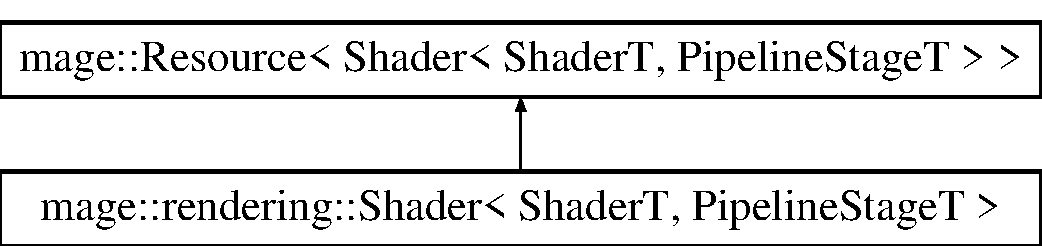
\includegraphics[height=2.000000cm]{classmage_1_1rendering_1_1_shader}
\end{center}
\end{figure}
\subsection*{Public Member Functions}
\begin{DoxyCompactItemize}
\item 
\mbox{\hyperlink{classmage_1_1rendering_1_1_shader_ac2cb01b7ce78d43c3c9bae2c91b7990e}{Shader}} (I\+D3\+D11\+Device \&device, std\+::wstring guid, const \mbox{\hyperlink{classmage_1_1rendering_1_1_compiled_shader}{Compiled\+Shader}} \&compiled\+\_\+shader)
\item 
\mbox{\hyperlink{classmage_1_1rendering_1_1_shader_a4ca3a1e4f108e38d28c0ba3df4f234f6}{Shader}} (const \mbox{\hyperlink{classmage_1_1rendering_1_1_shader}{Shader}} \&shader)=delete
\item 
\mbox{\hyperlink{classmage_1_1rendering_1_1_shader_a65ecc5e4958ce06d7dfa8632dccc774f}{Shader}} (\mbox{\hyperlink{classmage_1_1rendering_1_1_shader}{Shader}} \&\&shader) noexcept
\item 
virtual \mbox{\hyperlink{classmage_1_1rendering_1_1_shader_af9774a6a1f073f0477c5f4e35f130181}{$\sim$\+Shader}} ()
\item 
\mbox{\hyperlink{classmage_1_1rendering_1_1_shader}{Shader}} \& \mbox{\hyperlink{classmage_1_1rendering_1_1_shader_a66253b5dd8a5ef1cd766512b4ab15e6c}{operator=}} (const \mbox{\hyperlink{classmage_1_1rendering_1_1_shader}{Shader}} \&shader)=delete
\item 
\mbox{\hyperlink{classmage_1_1rendering_1_1_shader}{Shader}} \& \mbox{\hyperlink{classmage_1_1rendering_1_1_shader_a940217c505f3994d1f6057345d52cb36}{operator=}} (\mbox{\hyperlink{classmage_1_1rendering_1_1_shader}{Shader}} \&\&shader) noexcept
\item 
void \mbox{\hyperlink{classmage_1_1rendering_1_1_shader_abb37464c991b9b49e94c93968e884f13}{Bind\+Shader}} (I\+D3\+D11\+Device\+Context \&device\+\_\+context) const noexcept
\end{DoxyCompactItemize}
\subsection*{Private Member Functions}
\begin{DoxyCompactItemize}
\item 
void \mbox{\hyperlink{classmage_1_1rendering_1_1_shader_ad8b71024d802eb02d9017d767da995d8}{Setup\+Shader}} (I\+D3\+D11\+Device \&device, const \mbox{\hyperlink{classmage_1_1rendering_1_1_compiled_shader}{Compiled\+Shader}} \&compiled\+\_\+shader)
\end{DoxyCompactItemize}
\subsection*{Private Attributes}
\begin{DoxyCompactItemize}
\item 
\mbox{\hyperlink{namespacemage_ae74f374780900893caa5555d1031fd79}{Com\+Ptr}}$<$ ShaderT $>$ \mbox{\hyperlink{classmage_1_1rendering_1_1_shader_a22463d933618984ca17cd30109839f96}{m\+\_\+shader}}
\end{DoxyCompactItemize}


\subsection{Detailed Description}
\subsubsection*{template$<$typename ShaderT, typename Pipeline\+StageT$>$\newline
class mage\+::rendering\+::\+Shader$<$ Shader\+T, Pipeline\+Stage\+T $>$}

A class of shaders.


\begin{DoxyTemplParams}{Template Parameters}
{\em ShaderT} & The shader type. \\
\hline
{\em Pipeline\+StageT} & The pipeline stage type. \\
\hline
\end{DoxyTemplParams}


\subsection{Constructor \& Destructor Documentation}
\mbox{\Hypertarget{classmage_1_1rendering_1_1_shader_ac2cb01b7ce78d43c3c9bae2c91b7990e}\label{classmage_1_1rendering_1_1_shader_ac2cb01b7ce78d43c3c9bae2c91b7990e}} 
\index{mage\+::rendering\+::\+Shader@{mage\+::rendering\+::\+Shader}!Shader@{Shader}}
\index{Shader@{Shader}!mage\+::rendering\+::\+Shader@{mage\+::rendering\+::\+Shader}}
\subsubsection{\texorpdfstring{Shader()}{Shader()}\hspace{0.1cm}{\footnotesize\ttfamily [1/3]}}
{\footnotesize\ttfamily template$<$typename ShaderT , typename Pipeline\+StageT $>$ \\
\mbox{\hyperlink{classmage_1_1rendering_1_1_shader}{mage\+::rendering\+::\+Shader}}$<$ ShaderT, Pipeline\+StageT $>$\+::\mbox{\hyperlink{classmage_1_1rendering_1_1_shader}{Shader}} (\begin{DoxyParamCaption}\item[{I\+D3\+D11\+Device \&}]{device,  }\item[{std\+::wstring}]{guid,  }\item[{const \mbox{\hyperlink{classmage_1_1rendering_1_1_compiled_shader}{Compiled\+Shader}}$<$ ShaderT, Pipeline\+StageT $>$ \&}]{compiled\+\_\+shader }\end{DoxyParamCaption})\hspace{0.3cm}{\ttfamily [explicit]}}

Constructs a shader.


\begin{DoxyParams}[1]{Parameters}
\mbox{\tt in,out}  & {\em device} & A reference to the device. \\
\hline
\mbox{\tt in}  & {\em guid} & The globally unique identifier. \\
\hline
\mbox{\tt in}  & {\em compiled\+\_\+shader} & A reference to the compiled shader. \\
\hline
\end{DoxyParams}

\begin{DoxyExceptions}{Exceptions}
{\em \mbox{\hyperlink{classmage_1_1_exception}{Exception}}} & Failed to initialize this shader. \\
\hline
\end{DoxyExceptions}
\mbox{\Hypertarget{classmage_1_1rendering_1_1_shader_a4ca3a1e4f108e38d28c0ba3df4f234f6}\label{classmage_1_1rendering_1_1_shader_a4ca3a1e4f108e38d28c0ba3df4f234f6}} 
\index{mage\+::rendering\+::\+Shader@{mage\+::rendering\+::\+Shader}!Shader@{Shader}}
\index{Shader@{Shader}!mage\+::rendering\+::\+Shader@{mage\+::rendering\+::\+Shader}}
\subsubsection{\texorpdfstring{Shader()}{Shader()}\hspace{0.1cm}{\footnotesize\ttfamily [2/3]}}
{\footnotesize\ttfamily template$<$typename ShaderT , typename Pipeline\+StageT $>$ \\
\mbox{\hyperlink{classmage_1_1rendering_1_1_shader}{mage\+::rendering\+::\+Shader}}$<$ ShaderT, Pipeline\+StageT $>$\+::\mbox{\hyperlink{classmage_1_1rendering_1_1_shader}{Shader}} (\begin{DoxyParamCaption}\item[{const \mbox{\hyperlink{classmage_1_1rendering_1_1_shader}{Shader}}$<$ ShaderT, Pipeline\+StageT $>$ \&}]{shader }\end{DoxyParamCaption})\hspace{0.3cm}{\ttfamily [delete]}}

Constructs a shader from the given shader.


\begin{DoxyParams}[1]{Parameters}
\mbox{\tt in}  & {\em shader} & A reference to the shader to copy. \\
\hline
\end{DoxyParams}
\mbox{\Hypertarget{classmage_1_1rendering_1_1_shader_a65ecc5e4958ce06d7dfa8632dccc774f}\label{classmage_1_1rendering_1_1_shader_a65ecc5e4958ce06d7dfa8632dccc774f}} 
\index{mage\+::rendering\+::\+Shader@{mage\+::rendering\+::\+Shader}!Shader@{Shader}}
\index{Shader@{Shader}!mage\+::rendering\+::\+Shader@{mage\+::rendering\+::\+Shader}}
\subsubsection{\texorpdfstring{Shader()}{Shader()}\hspace{0.1cm}{\footnotesize\ttfamily [3/3]}}
{\footnotesize\ttfamily template$<$typename ShaderT , typename Pipeline\+StageT $>$ \\
\mbox{\hyperlink{classmage_1_1rendering_1_1_shader}{mage\+::rendering\+::\+Shader}}$<$ ShaderT, Pipeline\+StageT $>$\+::\mbox{\hyperlink{classmage_1_1rendering_1_1_shader}{Shader}} (\begin{DoxyParamCaption}\item[{\mbox{\hyperlink{classmage_1_1rendering_1_1_shader}{Shader}}$<$ ShaderT, Pipeline\+StageT $>$ \&\&}]{shader }\end{DoxyParamCaption})\hspace{0.3cm}{\ttfamily [noexcept]}}

Constructs a shader by moving the given shader.


\begin{DoxyParams}[1]{Parameters}
\mbox{\tt in}  & {\em shader} & A reference to the shader to move. \\
\hline
\end{DoxyParams}
\mbox{\Hypertarget{classmage_1_1rendering_1_1_shader_af9774a6a1f073f0477c5f4e35f130181}\label{classmage_1_1rendering_1_1_shader_af9774a6a1f073f0477c5f4e35f130181}} 
\index{mage\+::rendering\+::\+Shader@{mage\+::rendering\+::\+Shader}!````~Shader@{$\sim$\+Shader}}
\index{````~Shader@{$\sim$\+Shader}!mage\+::rendering\+::\+Shader@{mage\+::rendering\+::\+Shader}}
\subsubsection{\texorpdfstring{$\sim$\+Shader()}{~Shader()}}
{\footnotesize\ttfamily template$<$typename ShaderT , typename Pipeline\+StageT $>$ \\
virtual \mbox{\hyperlink{classmage_1_1rendering_1_1_shader}{mage\+::rendering\+::\+Shader}}$<$ ShaderT, Pipeline\+StageT $>$\+::$\sim$\mbox{\hyperlink{classmage_1_1rendering_1_1_shader}{Shader}} (\begin{DoxyParamCaption}{ }\end{DoxyParamCaption})\hspace{0.3cm}{\ttfamily [virtual]}}

Destructs this shader. 

\subsection{Member Function Documentation}
\mbox{\Hypertarget{classmage_1_1rendering_1_1_shader_abb37464c991b9b49e94c93968e884f13}\label{classmage_1_1rendering_1_1_shader_abb37464c991b9b49e94c93968e884f13}} 
\index{mage\+::rendering\+::\+Shader@{mage\+::rendering\+::\+Shader}!Bind\+Shader@{Bind\+Shader}}
\index{Bind\+Shader@{Bind\+Shader}!mage\+::rendering\+::\+Shader@{mage\+::rendering\+::\+Shader}}
\subsubsection{\texorpdfstring{Bind\+Shader()}{BindShader()}}
{\footnotesize\ttfamily template$<$typename ShaderT , typename Pipeline\+StageT $>$ \\
void \mbox{\hyperlink{classmage_1_1rendering_1_1_shader}{mage\+::rendering\+::\+Shader}}$<$ ShaderT, Pipeline\+StageT $>$\+::Bind\+Shader (\begin{DoxyParamCaption}\item[{I\+D3\+D11\+Device\+Context \&}]{device\+\_\+context }\end{DoxyParamCaption}) const\hspace{0.3cm}{\ttfamily [noexcept]}}

Binds this shader.


\begin{DoxyParams}[1]{Parameters}
\mbox{\tt in,out}  & {\em device\+\_\+context} & A reference to the device context. \\
\hline
\end{DoxyParams}
\mbox{\Hypertarget{classmage_1_1rendering_1_1_shader_a66253b5dd8a5ef1cd766512b4ab15e6c}\label{classmage_1_1rendering_1_1_shader_a66253b5dd8a5ef1cd766512b4ab15e6c}} 
\index{mage\+::rendering\+::\+Shader@{mage\+::rendering\+::\+Shader}!operator=@{operator=}}
\index{operator=@{operator=}!mage\+::rendering\+::\+Shader@{mage\+::rendering\+::\+Shader}}
\subsubsection{\texorpdfstring{operator=()}{operator=()}\hspace{0.1cm}{\footnotesize\ttfamily [1/2]}}
{\footnotesize\ttfamily template$<$typename ShaderT , typename Pipeline\+StageT $>$ \\
\mbox{\hyperlink{classmage_1_1rendering_1_1_shader}{Shader}}\& \mbox{\hyperlink{classmage_1_1rendering_1_1_shader}{mage\+::rendering\+::\+Shader}}$<$ ShaderT, Pipeline\+StageT $>$\+::operator= (\begin{DoxyParamCaption}\item[{const \mbox{\hyperlink{classmage_1_1rendering_1_1_shader}{Shader}}$<$ ShaderT, Pipeline\+StageT $>$ \&}]{shader }\end{DoxyParamCaption})\hspace{0.3cm}{\ttfamily [delete]}}

Copies the given shader to this shader.


\begin{DoxyParams}[1]{Parameters}
\mbox{\tt in}  & {\em shader} & A reference to the shader to copy. \\
\hline
\end{DoxyParams}
\begin{DoxyReturn}{Returns}
A reference to the copy of the given shader (i.\+e. this shader). 
\end{DoxyReturn}
\mbox{\Hypertarget{classmage_1_1rendering_1_1_shader_a940217c505f3994d1f6057345d52cb36}\label{classmage_1_1rendering_1_1_shader_a940217c505f3994d1f6057345d52cb36}} 
\index{mage\+::rendering\+::\+Shader@{mage\+::rendering\+::\+Shader}!operator=@{operator=}}
\index{operator=@{operator=}!mage\+::rendering\+::\+Shader@{mage\+::rendering\+::\+Shader}}
\subsubsection{\texorpdfstring{operator=()}{operator=()}\hspace{0.1cm}{\footnotesize\ttfamily [2/2]}}
{\footnotesize\ttfamily template$<$typename ShaderT , typename Pipeline\+StageT $>$ \\
\mbox{\hyperlink{classmage_1_1rendering_1_1_shader}{Shader}}\& \mbox{\hyperlink{classmage_1_1rendering_1_1_shader}{mage\+::rendering\+::\+Shader}}$<$ ShaderT, Pipeline\+StageT $>$\+::operator= (\begin{DoxyParamCaption}\item[{\mbox{\hyperlink{classmage_1_1rendering_1_1_shader}{Shader}}$<$ ShaderT, Pipeline\+StageT $>$ \&\&}]{shader }\end{DoxyParamCaption})\hspace{0.3cm}{\ttfamily [noexcept]}}

Moves the given shader to this shader.


\begin{DoxyParams}[1]{Parameters}
\mbox{\tt in}  & {\em shader} & A reference to the shader to move. \\
\hline
\end{DoxyParams}
\begin{DoxyReturn}{Returns}
A reference to the moved shader (i.\+e. this shader). 
\end{DoxyReturn}
\mbox{\Hypertarget{classmage_1_1rendering_1_1_shader_ad8b71024d802eb02d9017d767da995d8}\label{classmage_1_1rendering_1_1_shader_ad8b71024d802eb02d9017d767da995d8}} 
\index{mage\+::rendering\+::\+Shader@{mage\+::rendering\+::\+Shader}!Setup\+Shader@{Setup\+Shader}}
\index{Setup\+Shader@{Setup\+Shader}!mage\+::rendering\+::\+Shader@{mage\+::rendering\+::\+Shader}}
\subsubsection{\texorpdfstring{Setup\+Shader()}{SetupShader()}}
{\footnotesize\ttfamily template$<$typename ShaderT , typename Pipeline\+StageT $>$ \\
void \mbox{\hyperlink{classmage_1_1rendering_1_1_shader}{mage\+::rendering\+::\+Shader}}$<$ ShaderT, Pipeline\+StageT $>$\+::Setup\+Shader (\begin{DoxyParamCaption}\item[{I\+D3\+D11\+Device \&}]{device,  }\item[{const \mbox{\hyperlink{classmage_1_1rendering_1_1_compiled_shader}{Compiled\+Shader}}$<$ ShaderT, Pipeline\+StageT $>$ \&}]{compiled\+\_\+shader }\end{DoxyParamCaption})\hspace{0.3cm}{\ttfamily [private]}}

Sets up this shader.


\begin{DoxyParams}[1]{Parameters}
\mbox{\tt in,out}  & {\em device} & A reference to the device. \\
\hline
\mbox{\tt in}  & {\em compiled\+\_\+shader} & A reference to the compiled shader. \\
\hline
\end{DoxyParams}

\begin{DoxyExceptions}{Exceptions}
{\em \mbox{\hyperlink{classmage_1_1_exception}{Exception}}} & Failed to setup this shader. \\
\hline
\end{DoxyExceptions}


\subsection{Member Data Documentation}
\mbox{\Hypertarget{classmage_1_1rendering_1_1_shader_a22463d933618984ca17cd30109839f96}\label{classmage_1_1rendering_1_1_shader_a22463d933618984ca17cd30109839f96}} 
\index{mage\+::rendering\+::\+Shader@{mage\+::rendering\+::\+Shader}!m\+\_\+shader@{m\+\_\+shader}}
\index{m\+\_\+shader@{m\+\_\+shader}!mage\+::rendering\+::\+Shader@{mage\+::rendering\+::\+Shader}}
\subsubsection{\texorpdfstring{m\+\_\+shader}{m\_shader}}
{\footnotesize\ttfamily template$<$typename ShaderT , typename Pipeline\+StageT $>$ \\
\mbox{\hyperlink{namespacemage_ae74f374780900893caa5555d1031fd79}{Com\+Ptr}}$<$ ShaderT $>$ \mbox{\hyperlink{classmage_1_1rendering_1_1_shader}{mage\+::rendering\+::\+Shader}}$<$ ShaderT, Pipeline\+StageT $>$\+::m\+\_\+shader\hspace{0.3cm}{\ttfamily [private]}}

A pointer to the shader of this shader. 
\hypertarget{classmage_1_1rendering_1_1_shadow_cube_map_buffer}{}\section{mage\+:\+:rendering\+:\+:Shadow\+Cube\+Map\+Buffer Class Reference}
\label{classmage_1_1rendering_1_1_shadow_cube_map_buffer}\index{mage\+::rendering\+::\+Shadow\+Cube\+Map\+Buffer@{mage\+::rendering\+::\+Shadow\+Cube\+Map\+Buffer}}


{\ttfamily \#include $<$shadow\+\_\+map\+\_\+buffer.\+hpp$>$}

\subsection*{Public Member Functions}
\begin{DoxyCompactItemize}
\item 
\hyperlink{classmage_1_1rendering_1_1_shadow_cube_map_buffer_aeb1c633be265f8c03dd4e525e069de03}{Shadow\+Cube\+Map\+Buffer} (I\+D3\+D11\+Device \&device, size\+\_\+t nb\+\_\+shadow\+\_\+cube\+\_\+maps, const \hyperlink{namespacemage_a88e05bff0300120c013285d3dcad95c5}{U32x2} \&resolution=\{ 512u, 512u \}, Depth\+Format format=\+Depth\+Format\+::\+D16)
\item 
\hyperlink{classmage_1_1rendering_1_1_shadow_cube_map_buffer_a724d0d73588f2e698f2748209befdba8}{Shadow\+Cube\+Map\+Buffer} (const \hyperlink{classmage_1_1rendering_1_1_shadow_cube_map_buffer}{Shadow\+Cube\+Map\+Buffer} \&buffer)=delete
\item 
\hyperlink{classmage_1_1rendering_1_1_shadow_cube_map_buffer_ac636a06f0001b7317ca252b06025ffc4}{Shadow\+Cube\+Map\+Buffer} (\hyperlink{classmage_1_1rendering_1_1_shadow_cube_map_buffer}{Shadow\+Cube\+Map\+Buffer} \&\&buffer) noexcept
\item 
\hyperlink{classmage_1_1rendering_1_1_shadow_cube_map_buffer_a674fdad641a8892821ff8e76d4f05a88}{$\sim$\+Shadow\+Cube\+Map\+Buffer} ()
\item 
\hyperlink{classmage_1_1rendering_1_1_shadow_cube_map_buffer}{Shadow\+Cube\+Map\+Buffer} \& \hyperlink{classmage_1_1rendering_1_1_shadow_cube_map_buffer_a25b59803df1595c97b452dd91c661854}{operator=} (const \hyperlink{classmage_1_1rendering_1_1_shadow_cube_map_buffer}{Shadow\+Cube\+Map\+Buffer} \&buffer)=delete
\item 
\hyperlink{classmage_1_1rendering_1_1_shadow_cube_map_buffer}{Shadow\+Cube\+Map\+Buffer} \& \hyperlink{classmage_1_1rendering_1_1_shadow_cube_map_buffer_a5eb775fdc0f94c220b0115f2695ef18b}{operator=} (\hyperlink{classmage_1_1rendering_1_1_shadow_cube_map_buffer}{Shadow\+Cube\+Map\+Buffer} \&\&buffer) noexcept
\item 
size\+\_\+t \hyperlink{classmage_1_1rendering_1_1_shadow_cube_map_buffer_a491b9a0306748de68b2cb391e572cb7d}{Get\+Number\+Of\+Shadow\+Maps} () const noexcept
\item 
size\+\_\+t \hyperlink{classmage_1_1rendering_1_1_shadow_cube_map_buffer_a6641e56d3f586ab2cdc74d26b8877168}{Get\+Number\+Of\+Shadow\+Cube\+Maps} () const noexcept
\item 
void \hyperlink{classmage_1_1rendering_1_1_shadow_cube_map_buffer_a584f753f82c2378a8c7171bdf5a96999}{Bind} (I\+D3\+D11\+Device\+Context \&device\+\_\+context) const noexcept
\item 
void \hyperlink{classmage_1_1rendering_1_1_shadow_cube_map_buffer_aa206227920ac298eb4dcfdc8e662663d}{Bind\+Rasterizer\+State} (I\+D3\+D11\+Device\+Context \&device\+\_\+context) const noexcept
\item 
void \hyperlink{classmage_1_1rendering_1_1_shadow_cube_map_buffer_a31df46f6fe89cbaedb7f256ab7ecf514}{Clear\+D\+S\+Vs} (I\+D3\+D11\+Device\+Context \&device\+\_\+context) const noexcept
\item 
void \hyperlink{classmage_1_1rendering_1_1_shadow_cube_map_buffer_ad64e3c0b0c537e4e3f6b301fefb5c60a}{Bind\+D\+SV} (I\+D3\+D11\+Device\+Context \&device\+\_\+context, size\+\_\+t dsv\+\_\+index) const noexcept
\item 
\hyperlink{namespacemage_a8769f9d670d6b585ea306cb1062af94b}{Not\+Null}$<$ I\+D3\+D11\+Depth\+Stencil\+View $\ast$$>$ \hyperlink{classmage_1_1rendering_1_1_shadow_cube_map_buffer_a244e06f9f499496fe721af7f1bd2ea5f}{Get\+D\+SV} (size\+\_\+t dsv\+\_\+index) const noexcept
\item 
\hyperlink{namespacemage_a8769f9d670d6b585ea306cb1062af94b}{Not\+Null}$<$ I\+D3\+D11\+Shader\+Resource\+View $\ast$$>$ \hyperlink{classmage_1_1rendering_1_1_shadow_cube_map_buffer_a2586fb38441a14c38045bc3b6a940161}{Get\+S\+RV} () const noexcept
\end{DoxyCompactItemize}
\subsection*{Private Member Functions}
\begin{DoxyCompactItemize}
\item 
void \hyperlink{classmage_1_1rendering_1_1_shadow_cube_map_buffer_a65d31b9a335e6c27c8d4d6e0127029b2}{Setup\+Rasterizer\+State} (I\+D3\+D11\+Device \&device)
\item 
void \hyperlink{classmage_1_1rendering_1_1_shadow_cube_map_buffer_a4b6e895628905a9ddbaccfafb6a1d5b6}{Setup\+Shadow\+Cube\+Map\+Buffer} (I\+D3\+D11\+Device \&device, size\+\_\+t nb\+\_\+shadow\+\_\+cube\+\_\+maps)
\item 
void \hyperlink{classmage_1_1rendering_1_1_shadow_cube_map_buffer_ac800b8fde94ee7527ce09370b4f9e44a}{Setup\+Shadow\+Cube\+Map\+Array} (I\+D3\+D11\+Device \&device, size\+\_\+t nb\+\_\+shadow\+\_\+cube\+\_\+maps, D\+X\+G\+I\+\_\+\+F\+O\+R\+M\+AT texture\+\_\+format, D\+X\+G\+I\+\_\+\+F\+O\+R\+M\+AT dsv\+\_\+format, D\+X\+G\+I\+\_\+\+F\+O\+R\+M\+AT srv\+\_\+format)
\end{DoxyCompactItemize}
\subsection*{Private Attributes}
\begin{DoxyCompactItemize}
\item 
\hyperlink{namespacemage_1_1rendering_ad477e1afff480649a92fb2253c65bfb0}{Depth\+Format} \hyperlink{classmage_1_1rendering_1_1_shadow_cube_map_buffer_a008b52aa40f583dff87df47a97e6ef67}{m\+\_\+format}
\item 
\hyperlink{classmage_1_1rendering_1_1_viewport}{Viewport} \hyperlink{classmage_1_1rendering_1_1_shadow_cube_map_buffer_a43b1240a39ab1385832c20da6241c9cb}{m\+\_\+viewport}
\item 
\hyperlink{namespacemage_ae74f374780900893caa5555d1031fd79}{Com\+Ptr}$<$ I\+D3\+D11\+Rasterizer\+State $>$ \hyperlink{classmage_1_1rendering_1_1_shadow_cube_map_buffer_ab11e333f6832b5ec5710767badca29ef}{m\+\_\+rasterizer\+\_\+state}
\item 
std\+::vector$<$ \hyperlink{namespacemage_ae74f374780900893caa5555d1031fd79}{Com\+Ptr}$<$ I\+D3\+D11\+Depth\+Stencil\+View $>$ $>$ \hyperlink{classmage_1_1rendering_1_1_shadow_cube_map_buffer_a939704f906cac1319b261c4c87cb535e}{m\+\_\+dsvs}
\item 
\hyperlink{namespacemage_ae74f374780900893caa5555d1031fd79}{Com\+Ptr}$<$ I\+D3\+D11\+Shader\+Resource\+View $>$ \hyperlink{classmage_1_1rendering_1_1_shadow_cube_map_buffer_affc35790722dfa58640cc8a1962d9ec9}{m\+\_\+srv}
\end{DoxyCompactItemize}


\subsection{Constructor \& Destructor Documentation}
\hypertarget{classmage_1_1rendering_1_1_shadow_cube_map_buffer_aeb1c633be265f8c03dd4e525e069de03}{}\label{classmage_1_1rendering_1_1_shadow_cube_map_buffer_aeb1c633be265f8c03dd4e525e069de03} 
\index{mage\+::rendering\+::\+Shadow\+Cube\+Map\+Buffer@{mage\+::rendering\+::\+Shadow\+Cube\+Map\+Buffer}!Shadow\+Cube\+Map\+Buffer@{Shadow\+Cube\+Map\+Buffer}}
\index{Shadow\+Cube\+Map\+Buffer@{Shadow\+Cube\+Map\+Buffer}!mage\+::rendering\+::\+Shadow\+Cube\+Map\+Buffer@{mage\+::rendering\+::\+Shadow\+Cube\+Map\+Buffer}}
\subsubsection{\texorpdfstring{Shadow\+Cube\+Map\+Buffer()}{ShadowCubeMapBuffer()}\hspace{0.1cm}{\footnotesize\ttfamily [1/3]}}
{\footnotesize\ttfamily mage\+::rendering\+::\+Shadow\+Cube\+Map\+Buffer\+::\+Shadow\+Cube\+Map\+Buffer (\begin{DoxyParamCaption}\item[{I\+D3\+D11\+Device \&}]{device,  }\item[{size\+\_\+t}]{nb\+\_\+shadow\+\_\+cube\+\_\+maps,  }\item[{const \hyperlink{namespacemage_a88e05bff0300120c013285d3dcad95c5}{U32x2} \&}]{resolution = {\ttfamily \{~512u,~512u~\}},  }\item[{\hyperlink{namespacemage_1_1rendering_ad477e1afff480649a92fb2253c65bfb0}{Depth\+Format}}]{format = {\ttfamily \hyperlink{namespacemage_1_1rendering_ad477e1afff480649a92fb2253c65bfb0a6fd9ec81643ee5a57f85a71951bfe13d}{Depth\+Format\+::\+D16}} }\end{DoxyParamCaption})\hspace{0.3cm}{\ttfamily [explicit]}}

\hypertarget{classmage_1_1rendering_1_1_shadow_cube_map_buffer_a724d0d73588f2e698f2748209befdba8}{}\label{classmage_1_1rendering_1_1_shadow_cube_map_buffer_a724d0d73588f2e698f2748209befdba8} 
\index{mage\+::rendering\+::\+Shadow\+Cube\+Map\+Buffer@{mage\+::rendering\+::\+Shadow\+Cube\+Map\+Buffer}!Shadow\+Cube\+Map\+Buffer@{Shadow\+Cube\+Map\+Buffer}}
\index{Shadow\+Cube\+Map\+Buffer@{Shadow\+Cube\+Map\+Buffer}!mage\+::rendering\+::\+Shadow\+Cube\+Map\+Buffer@{mage\+::rendering\+::\+Shadow\+Cube\+Map\+Buffer}}
\subsubsection{\texorpdfstring{Shadow\+Cube\+Map\+Buffer()}{ShadowCubeMapBuffer()}\hspace{0.1cm}{\footnotesize\ttfamily [2/3]}}
{\footnotesize\ttfamily mage\+::rendering\+::\+Shadow\+Cube\+Map\+Buffer\+::\+Shadow\+Cube\+Map\+Buffer (\begin{DoxyParamCaption}\item[{const \hyperlink{classmage_1_1rendering_1_1_shadow_cube_map_buffer}{Shadow\+Cube\+Map\+Buffer} \&}]{buffer }\end{DoxyParamCaption})\hspace{0.3cm}{\ttfamily [delete]}}

\hypertarget{classmage_1_1rendering_1_1_shadow_cube_map_buffer_ac636a06f0001b7317ca252b06025ffc4}{}\label{classmage_1_1rendering_1_1_shadow_cube_map_buffer_ac636a06f0001b7317ca252b06025ffc4} 
\index{mage\+::rendering\+::\+Shadow\+Cube\+Map\+Buffer@{mage\+::rendering\+::\+Shadow\+Cube\+Map\+Buffer}!Shadow\+Cube\+Map\+Buffer@{Shadow\+Cube\+Map\+Buffer}}
\index{Shadow\+Cube\+Map\+Buffer@{Shadow\+Cube\+Map\+Buffer}!mage\+::rendering\+::\+Shadow\+Cube\+Map\+Buffer@{mage\+::rendering\+::\+Shadow\+Cube\+Map\+Buffer}}
\subsubsection{\texorpdfstring{Shadow\+Cube\+Map\+Buffer()}{ShadowCubeMapBuffer()}\hspace{0.1cm}{\footnotesize\ttfamily [3/3]}}
{\footnotesize\ttfamily mage\+::rendering\+::\+Shadow\+Cube\+Map\+Buffer\+::\+Shadow\+Cube\+Map\+Buffer (\begin{DoxyParamCaption}\item[{\hyperlink{classmage_1_1rendering_1_1_shadow_cube_map_buffer}{Shadow\+Cube\+Map\+Buffer} \&\&}]{buffer }\end{DoxyParamCaption})\hspace{0.3cm}{\ttfamily [default]}, {\ttfamily [noexcept]}}

\hypertarget{classmage_1_1rendering_1_1_shadow_cube_map_buffer_a674fdad641a8892821ff8e76d4f05a88}{}\label{classmage_1_1rendering_1_1_shadow_cube_map_buffer_a674fdad641a8892821ff8e76d4f05a88} 
\index{mage\+::rendering\+::\+Shadow\+Cube\+Map\+Buffer@{mage\+::rendering\+::\+Shadow\+Cube\+Map\+Buffer}!````~Shadow\+Cube\+Map\+Buffer@{$\sim$\+Shadow\+Cube\+Map\+Buffer}}
\index{````~Shadow\+Cube\+Map\+Buffer@{$\sim$\+Shadow\+Cube\+Map\+Buffer}!mage\+::rendering\+::\+Shadow\+Cube\+Map\+Buffer@{mage\+::rendering\+::\+Shadow\+Cube\+Map\+Buffer}}
\subsubsection{\texorpdfstring{$\sim$\+Shadow\+Cube\+Map\+Buffer()}{~ShadowCubeMapBuffer()}}
{\footnotesize\ttfamily mage\+::rendering\+::\+Shadow\+Cube\+Map\+Buffer\+::$\sim$\+Shadow\+Cube\+Map\+Buffer (\begin{DoxyParamCaption}{ }\end{DoxyParamCaption})\hspace{0.3cm}{\ttfamily [default]}}



\subsection{Member Function Documentation}
\hypertarget{classmage_1_1rendering_1_1_shadow_cube_map_buffer_a584f753f82c2378a8c7171bdf5a96999}{}\label{classmage_1_1rendering_1_1_shadow_cube_map_buffer_a584f753f82c2378a8c7171bdf5a96999} 
\index{mage\+::rendering\+::\+Shadow\+Cube\+Map\+Buffer@{mage\+::rendering\+::\+Shadow\+Cube\+Map\+Buffer}!Bind@{Bind}}
\index{Bind@{Bind}!mage\+::rendering\+::\+Shadow\+Cube\+Map\+Buffer@{mage\+::rendering\+::\+Shadow\+Cube\+Map\+Buffer}}
\subsubsection{\texorpdfstring{Bind()}{Bind()}}
{\footnotesize\ttfamily void mage\+::rendering\+::\+Shadow\+Cube\+Map\+Buffer\+::\+Bind (\begin{DoxyParamCaption}\item[{I\+D3\+D11\+Device\+Context \&}]{device\+\_\+context }\end{DoxyParamCaption}) const\hspace{0.3cm}{\ttfamily [noexcept]}}

\hypertarget{classmage_1_1rendering_1_1_shadow_cube_map_buffer_ad64e3c0b0c537e4e3f6b301fefb5c60a}{}\label{classmage_1_1rendering_1_1_shadow_cube_map_buffer_ad64e3c0b0c537e4e3f6b301fefb5c60a} 
\index{mage\+::rendering\+::\+Shadow\+Cube\+Map\+Buffer@{mage\+::rendering\+::\+Shadow\+Cube\+Map\+Buffer}!Bind\+D\+SV@{Bind\+D\+SV}}
\index{Bind\+D\+SV@{Bind\+D\+SV}!mage\+::rendering\+::\+Shadow\+Cube\+Map\+Buffer@{mage\+::rendering\+::\+Shadow\+Cube\+Map\+Buffer}}
\subsubsection{\texorpdfstring{Bind\+D\+S\+V()}{BindDSV()}}
{\footnotesize\ttfamily void mage\+::rendering\+::\+Shadow\+Cube\+Map\+Buffer\+::\+Bind\+D\+SV (\begin{DoxyParamCaption}\item[{I\+D3\+D11\+Device\+Context \&}]{device\+\_\+context,  }\item[{size\+\_\+t}]{dsv\+\_\+index }\end{DoxyParamCaption}) const\hspace{0.3cm}{\ttfamily [noexcept]}}

\hypertarget{classmage_1_1rendering_1_1_shadow_cube_map_buffer_aa206227920ac298eb4dcfdc8e662663d}{}\label{classmage_1_1rendering_1_1_shadow_cube_map_buffer_aa206227920ac298eb4dcfdc8e662663d} 
\index{mage\+::rendering\+::\+Shadow\+Cube\+Map\+Buffer@{mage\+::rendering\+::\+Shadow\+Cube\+Map\+Buffer}!Bind\+Rasterizer\+State@{Bind\+Rasterizer\+State}}
\index{Bind\+Rasterizer\+State@{Bind\+Rasterizer\+State}!mage\+::rendering\+::\+Shadow\+Cube\+Map\+Buffer@{mage\+::rendering\+::\+Shadow\+Cube\+Map\+Buffer}}
\subsubsection{\texorpdfstring{Bind\+Rasterizer\+State()}{BindRasterizerState()}}
{\footnotesize\ttfamily void mage\+::rendering\+::\+Shadow\+Cube\+Map\+Buffer\+::\+Bind\+Rasterizer\+State (\begin{DoxyParamCaption}\item[{I\+D3\+D11\+Device\+Context \&}]{device\+\_\+context }\end{DoxyParamCaption}) const\hspace{0.3cm}{\ttfamily [noexcept]}}

\hypertarget{classmage_1_1rendering_1_1_shadow_cube_map_buffer_a31df46f6fe89cbaedb7f256ab7ecf514}{}\label{classmage_1_1rendering_1_1_shadow_cube_map_buffer_a31df46f6fe89cbaedb7f256ab7ecf514} 
\index{mage\+::rendering\+::\+Shadow\+Cube\+Map\+Buffer@{mage\+::rendering\+::\+Shadow\+Cube\+Map\+Buffer}!Clear\+D\+S\+Vs@{Clear\+D\+S\+Vs}}
\index{Clear\+D\+S\+Vs@{Clear\+D\+S\+Vs}!mage\+::rendering\+::\+Shadow\+Cube\+Map\+Buffer@{mage\+::rendering\+::\+Shadow\+Cube\+Map\+Buffer}}
\subsubsection{\texorpdfstring{Clear\+D\+S\+Vs()}{ClearDSVs()}}
{\footnotesize\ttfamily void mage\+::rendering\+::\+Shadow\+Cube\+Map\+Buffer\+::\+Clear\+D\+S\+Vs (\begin{DoxyParamCaption}\item[{I\+D3\+D11\+Device\+Context \&}]{device\+\_\+context }\end{DoxyParamCaption}) const\hspace{0.3cm}{\ttfamily [noexcept]}}

\hypertarget{classmage_1_1rendering_1_1_shadow_cube_map_buffer_a244e06f9f499496fe721af7f1bd2ea5f}{}\label{classmage_1_1rendering_1_1_shadow_cube_map_buffer_a244e06f9f499496fe721af7f1bd2ea5f} 
\index{mage\+::rendering\+::\+Shadow\+Cube\+Map\+Buffer@{mage\+::rendering\+::\+Shadow\+Cube\+Map\+Buffer}!Get\+D\+SV@{Get\+D\+SV}}
\index{Get\+D\+SV@{Get\+D\+SV}!mage\+::rendering\+::\+Shadow\+Cube\+Map\+Buffer@{mage\+::rendering\+::\+Shadow\+Cube\+Map\+Buffer}}
\subsubsection{\texorpdfstring{Get\+D\+S\+V()}{GetDSV()}}
{\footnotesize\ttfamily \hyperlink{namespacemage_a8769f9d670d6b585ea306cb1062af94b}{Not\+Null}$<$ I\+D3\+D11\+Depth\+Stencil\+View$\ast$ $>$ mage\+::rendering\+::\+Shadow\+Cube\+Map\+Buffer\+::\+Get\+D\+SV (\begin{DoxyParamCaption}\item[{size\+\_\+t}]{dsv\+\_\+index }\end{DoxyParamCaption}) const\hspace{0.3cm}{\ttfamily [noexcept]}}

\hypertarget{classmage_1_1rendering_1_1_shadow_cube_map_buffer_a6641e56d3f586ab2cdc74d26b8877168}{}\label{classmage_1_1rendering_1_1_shadow_cube_map_buffer_a6641e56d3f586ab2cdc74d26b8877168} 
\index{mage\+::rendering\+::\+Shadow\+Cube\+Map\+Buffer@{mage\+::rendering\+::\+Shadow\+Cube\+Map\+Buffer}!Get\+Number\+Of\+Shadow\+Cube\+Maps@{Get\+Number\+Of\+Shadow\+Cube\+Maps}}
\index{Get\+Number\+Of\+Shadow\+Cube\+Maps@{Get\+Number\+Of\+Shadow\+Cube\+Maps}!mage\+::rendering\+::\+Shadow\+Cube\+Map\+Buffer@{mage\+::rendering\+::\+Shadow\+Cube\+Map\+Buffer}}
\subsubsection{\texorpdfstring{Get\+Number\+Of\+Shadow\+Cube\+Maps()}{GetNumberOfShadowCubeMaps()}}
{\footnotesize\ttfamily size\+\_\+t mage\+::rendering\+::\+Shadow\+Cube\+Map\+Buffer\+::\+Get\+Number\+Of\+Shadow\+Cube\+Maps (\begin{DoxyParamCaption}{ }\end{DoxyParamCaption}) const\hspace{0.3cm}{\ttfamily [noexcept]}}

\hypertarget{classmage_1_1rendering_1_1_shadow_cube_map_buffer_a491b9a0306748de68b2cb391e572cb7d}{}\label{classmage_1_1rendering_1_1_shadow_cube_map_buffer_a491b9a0306748de68b2cb391e572cb7d} 
\index{mage\+::rendering\+::\+Shadow\+Cube\+Map\+Buffer@{mage\+::rendering\+::\+Shadow\+Cube\+Map\+Buffer}!Get\+Number\+Of\+Shadow\+Maps@{Get\+Number\+Of\+Shadow\+Maps}}
\index{Get\+Number\+Of\+Shadow\+Maps@{Get\+Number\+Of\+Shadow\+Maps}!mage\+::rendering\+::\+Shadow\+Cube\+Map\+Buffer@{mage\+::rendering\+::\+Shadow\+Cube\+Map\+Buffer}}
\subsubsection{\texorpdfstring{Get\+Number\+Of\+Shadow\+Maps()}{GetNumberOfShadowMaps()}}
{\footnotesize\ttfamily size\+\_\+t mage\+::rendering\+::\+Shadow\+Cube\+Map\+Buffer\+::\+Get\+Number\+Of\+Shadow\+Maps (\begin{DoxyParamCaption}{ }\end{DoxyParamCaption}) const\hspace{0.3cm}{\ttfamily [noexcept]}}

\hypertarget{classmage_1_1rendering_1_1_shadow_cube_map_buffer_a2586fb38441a14c38045bc3b6a940161}{}\label{classmage_1_1rendering_1_1_shadow_cube_map_buffer_a2586fb38441a14c38045bc3b6a940161} 
\index{mage\+::rendering\+::\+Shadow\+Cube\+Map\+Buffer@{mage\+::rendering\+::\+Shadow\+Cube\+Map\+Buffer}!Get\+S\+RV@{Get\+S\+RV}}
\index{Get\+S\+RV@{Get\+S\+RV}!mage\+::rendering\+::\+Shadow\+Cube\+Map\+Buffer@{mage\+::rendering\+::\+Shadow\+Cube\+Map\+Buffer}}
\subsubsection{\texorpdfstring{Get\+S\+R\+V()}{GetSRV()}}
{\footnotesize\ttfamily \hyperlink{namespacemage_a8769f9d670d6b585ea306cb1062af94b}{Not\+Null}$<$ I\+D3\+D11\+Shader\+Resource\+View$\ast$ $>$ mage\+::rendering\+::\+Shadow\+Cube\+Map\+Buffer\+::\+Get\+S\+RV (\begin{DoxyParamCaption}{ }\end{DoxyParamCaption}) const\hspace{0.3cm}{\ttfamily [noexcept]}}

\hypertarget{classmage_1_1rendering_1_1_shadow_cube_map_buffer_a25b59803df1595c97b452dd91c661854}{}\label{classmage_1_1rendering_1_1_shadow_cube_map_buffer_a25b59803df1595c97b452dd91c661854} 
\index{mage\+::rendering\+::\+Shadow\+Cube\+Map\+Buffer@{mage\+::rendering\+::\+Shadow\+Cube\+Map\+Buffer}!operator=@{operator=}}
\index{operator=@{operator=}!mage\+::rendering\+::\+Shadow\+Cube\+Map\+Buffer@{mage\+::rendering\+::\+Shadow\+Cube\+Map\+Buffer}}
\subsubsection{\texorpdfstring{operator=()}{operator=()}\hspace{0.1cm}{\footnotesize\ttfamily [1/2]}}
{\footnotesize\ttfamily \hyperlink{classmage_1_1rendering_1_1_shadow_cube_map_buffer}{Shadow\+Cube\+Map\+Buffer}\& mage\+::rendering\+::\+Shadow\+Cube\+Map\+Buffer\+::operator= (\begin{DoxyParamCaption}\item[{const \hyperlink{classmage_1_1rendering_1_1_shadow_cube_map_buffer}{Shadow\+Cube\+Map\+Buffer} \&}]{buffer }\end{DoxyParamCaption})\hspace{0.3cm}{\ttfamily [delete]}}

\hypertarget{classmage_1_1rendering_1_1_shadow_cube_map_buffer_a5eb775fdc0f94c220b0115f2695ef18b}{}\label{classmage_1_1rendering_1_1_shadow_cube_map_buffer_a5eb775fdc0f94c220b0115f2695ef18b} 
\index{mage\+::rendering\+::\+Shadow\+Cube\+Map\+Buffer@{mage\+::rendering\+::\+Shadow\+Cube\+Map\+Buffer}!operator=@{operator=}}
\index{operator=@{operator=}!mage\+::rendering\+::\+Shadow\+Cube\+Map\+Buffer@{mage\+::rendering\+::\+Shadow\+Cube\+Map\+Buffer}}
\subsubsection{\texorpdfstring{operator=()}{operator=()}\hspace{0.1cm}{\footnotesize\ttfamily [2/2]}}
{\footnotesize\ttfamily \hyperlink{classmage_1_1rendering_1_1_shadow_cube_map_buffer}{Shadow\+Cube\+Map\+Buffer} \& mage\+::rendering\+::\+Shadow\+Cube\+Map\+Buffer\+::operator= (\begin{DoxyParamCaption}\item[{\hyperlink{classmage_1_1rendering_1_1_shadow_cube_map_buffer}{Shadow\+Cube\+Map\+Buffer} \&\&}]{buffer }\end{DoxyParamCaption})\hspace{0.3cm}{\ttfamily [default]}, {\ttfamily [noexcept]}}

\hypertarget{classmage_1_1rendering_1_1_shadow_cube_map_buffer_a65d31b9a335e6c27c8d4d6e0127029b2}{}\label{classmage_1_1rendering_1_1_shadow_cube_map_buffer_a65d31b9a335e6c27c8d4d6e0127029b2} 
\index{mage\+::rendering\+::\+Shadow\+Cube\+Map\+Buffer@{mage\+::rendering\+::\+Shadow\+Cube\+Map\+Buffer}!Setup\+Rasterizer\+State@{Setup\+Rasterizer\+State}}
\index{Setup\+Rasterizer\+State@{Setup\+Rasterizer\+State}!mage\+::rendering\+::\+Shadow\+Cube\+Map\+Buffer@{mage\+::rendering\+::\+Shadow\+Cube\+Map\+Buffer}}
\subsubsection{\texorpdfstring{Setup\+Rasterizer\+State()}{SetupRasterizerState()}}
{\footnotesize\ttfamily void mage\+::rendering\+::\+Shadow\+Cube\+Map\+Buffer\+::\+Setup\+Rasterizer\+State (\begin{DoxyParamCaption}\item[{I\+D3\+D11\+Device \&}]{device }\end{DoxyParamCaption})\hspace{0.3cm}{\ttfamily [private]}}

\hypertarget{classmage_1_1rendering_1_1_shadow_cube_map_buffer_ac800b8fde94ee7527ce09370b4f9e44a}{}\label{classmage_1_1rendering_1_1_shadow_cube_map_buffer_ac800b8fde94ee7527ce09370b4f9e44a} 
\index{mage\+::rendering\+::\+Shadow\+Cube\+Map\+Buffer@{mage\+::rendering\+::\+Shadow\+Cube\+Map\+Buffer}!Setup\+Shadow\+Cube\+Map\+Array@{Setup\+Shadow\+Cube\+Map\+Array}}
\index{Setup\+Shadow\+Cube\+Map\+Array@{Setup\+Shadow\+Cube\+Map\+Array}!mage\+::rendering\+::\+Shadow\+Cube\+Map\+Buffer@{mage\+::rendering\+::\+Shadow\+Cube\+Map\+Buffer}}
\subsubsection{\texorpdfstring{Setup\+Shadow\+Cube\+Map\+Array()}{SetupShadowCubeMapArray()}}
{\footnotesize\ttfamily void mage\+::rendering\+::\+Shadow\+Cube\+Map\+Buffer\+::\+Setup\+Shadow\+Cube\+Map\+Array (\begin{DoxyParamCaption}\item[{I\+D3\+D11\+Device \&}]{device,  }\item[{size\+\_\+t}]{nb\+\_\+shadow\+\_\+cube\+\_\+maps,  }\item[{D\+X\+G\+I\+\_\+\+F\+O\+R\+M\+AT}]{texture\+\_\+format,  }\item[{D\+X\+G\+I\+\_\+\+F\+O\+R\+M\+AT}]{dsv\+\_\+format,  }\item[{D\+X\+G\+I\+\_\+\+F\+O\+R\+M\+AT}]{srv\+\_\+format }\end{DoxyParamCaption})\hspace{0.3cm}{\ttfamily [private]}}

\hypertarget{classmage_1_1rendering_1_1_shadow_cube_map_buffer_a4b6e895628905a9ddbaccfafb6a1d5b6}{}\label{classmage_1_1rendering_1_1_shadow_cube_map_buffer_a4b6e895628905a9ddbaccfafb6a1d5b6} 
\index{mage\+::rendering\+::\+Shadow\+Cube\+Map\+Buffer@{mage\+::rendering\+::\+Shadow\+Cube\+Map\+Buffer}!Setup\+Shadow\+Cube\+Map\+Buffer@{Setup\+Shadow\+Cube\+Map\+Buffer}}
\index{Setup\+Shadow\+Cube\+Map\+Buffer@{Setup\+Shadow\+Cube\+Map\+Buffer}!mage\+::rendering\+::\+Shadow\+Cube\+Map\+Buffer@{mage\+::rendering\+::\+Shadow\+Cube\+Map\+Buffer}}
\subsubsection{\texorpdfstring{Setup\+Shadow\+Cube\+Map\+Buffer()}{SetupShadowCubeMapBuffer()}}
{\footnotesize\ttfamily void mage\+::rendering\+::\+Shadow\+Cube\+Map\+Buffer\+::\+Setup\+Shadow\+Cube\+Map\+Buffer (\begin{DoxyParamCaption}\item[{I\+D3\+D11\+Device \&}]{device,  }\item[{size\+\_\+t}]{nb\+\_\+shadow\+\_\+cube\+\_\+maps }\end{DoxyParamCaption})\hspace{0.3cm}{\ttfamily [private]}}



\subsection{Member Data Documentation}
\hypertarget{classmage_1_1rendering_1_1_shadow_cube_map_buffer_a939704f906cac1319b261c4c87cb535e}{}\label{classmage_1_1rendering_1_1_shadow_cube_map_buffer_a939704f906cac1319b261c4c87cb535e} 
\index{mage\+::rendering\+::\+Shadow\+Cube\+Map\+Buffer@{mage\+::rendering\+::\+Shadow\+Cube\+Map\+Buffer}!m\+\_\+dsvs@{m\+\_\+dsvs}}
\index{m\+\_\+dsvs@{m\+\_\+dsvs}!mage\+::rendering\+::\+Shadow\+Cube\+Map\+Buffer@{mage\+::rendering\+::\+Shadow\+Cube\+Map\+Buffer}}
\subsubsection{\texorpdfstring{m\+\_\+dsvs}{m\_dsvs}}
{\footnotesize\ttfamily std\+::vector$<$ \hyperlink{namespacemage_ae74f374780900893caa5555d1031fd79}{Com\+Ptr}$<$ I\+D3\+D11\+Depth\+Stencil\+View $>$ $>$ mage\+::rendering\+::\+Shadow\+Cube\+Map\+Buffer\+::m\+\_\+dsvs\hspace{0.3cm}{\ttfamily [private]}}

\hypertarget{classmage_1_1rendering_1_1_shadow_cube_map_buffer_a008b52aa40f583dff87df47a97e6ef67}{}\label{classmage_1_1rendering_1_1_shadow_cube_map_buffer_a008b52aa40f583dff87df47a97e6ef67} 
\index{mage\+::rendering\+::\+Shadow\+Cube\+Map\+Buffer@{mage\+::rendering\+::\+Shadow\+Cube\+Map\+Buffer}!m\+\_\+format@{m\+\_\+format}}
\index{m\+\_\+format@{m\+\_\+format}!mage\+::rendering\+::\+Shadow\+Cube\+Map\+Buffer@{mage\+::rendering\+::\+Shadow\+Cube\+Map\+Buffer}}
\subsubsection{\texorpdfstring{m\+\_\+format}{m\_format}}
{\footnotesize\ttfamily \hyperlink{namespacemage_1_1rendering_ad477e1afff480649a92fb2253c65bfb0}{Depth\+Format} mage\+::rendering\+::\+Shadow\+Cube\+Map\+Buffer\+::m\+\_\+format\hspace{0.3cm}{\ttfamily [private]}}

\hypertarget{classmage_1_1rendering_1_1_shadow_cube_map_buffer_ab11e333f6832b5ec5710767badca29ef}{}\label{classmage_1_1rendering_1_1_shadow_cube_map_buffer_ab11e333f6832b5ec5710767badca29ef} 
\index{mage\+::rendering\+::\+Shadow\+Cube\+Map\+Buffer@{mage\+::rendering\+::\+Shadow\+Cube\+Map\+Buffer}!m\+\_\+rasterizer\+\_\+state@{m\+\_\+rasterizer\+\_\+state}}
\index{m\+\_\+rasterizer\+\_\+state@{m\+\_\+rasterizer\+\_\+state}!mage\+::rendering\+::\+Shadow\+Cube\+Map\+Buffer@{mage\+::rendering\+::\+Shadow\+Cube\+Map\+Buffer}}
\subsubsection{\texorpdfstring{m\+\_\+rasterizer\+\_\+state}{m\_rasterizer\_state}}
{\footnotesize\ttfamily \hyperlink{namespacemage_ae74f374780900893caa5555d1031fd79}{Com\+Ptr}$<$ I\+D3\+D11\+Rasterizer\+State $>$ mage\+::rendering\+::\+Shadow\+Cube\+Map\+Buffer\+::m\+\_\+rasterizer\+\_\+state\hspace{0.3cm}{\ttfamily [private]}}

\hypertarget{classmage_1_1rendering_1_1_shadow_cube_map_buffer_affc35790722dfa58640cc8a1962d9ec9}{}\label{classmage_1_1rendering_1_1_shadow_cube_map_buffer_affc35790722dfa58640cc8a1962d9ec9} 
\index{mage\+::rendering\+::\+Shadow\+Cube\+Map\+Buffer@{mage\+::rendering\+::\+Shadow\+Cube\+Map\+Buffer}!m\+\_\+srv@{m\+\_\+srv}}
\index{m\+\_\+srv@{m\+\_\+srv}!mage\+::rendering\+::\+Shadow\+Cube\+Map\+Buffer@{mage\+::rendering\+::\+Shadow\+Cube\+Map\+Buffer}}
\subsubsection{\texorpdfstring{m\+\_\+srv}{m\_srv}}
{\footnotesize\ttfamily \hyperlink{namespacemage_ae74f374780900893caa5555d1031fd79}{Com\+Ptr}$<$ I\+D3\+D11\+Shader\+Resource\+View $>$ mage\+::rendering\+::\+Shadow\+Cube\+Map\+Buffer\+::m\+\_\+srv\hspace{0.3cm}{\ttfamily [private]}}

\hypertarget{classmage_1_1rendering_1_1_shadow_cube_map_buffer_a43b1240a39ab1385832c20da6241c9cb}{}\label{classmage_1_1rendering_1_1_shadow_cube_map_buffer_a43b1240a39ab1385832c20da6241c9cb} 
\index{mage\+::rendering\+::\+Shadow\+Cube\+Map\+Buffer@{mage\+::rendering\+::\+Shadow\+Cube\+Map\+Buffer}!m\+\_\+viewport@{m\+\_\+viewport}}
\index{m\+\_\+viewport@{m\+\_\+viewport}!mage\+::rendering\+::\+Shadow\+Cube\+Map\+Buffer@{mage\+::rendering\+::\+Shadow\+Cube\+Map\+Buffer}}
\subsubsection{\texorpdfstring{m\+\_\+viewport}{m\_viewport}}
{\footnotesize\ttfamily \hyperlink{classmage_1_1rendering_1_1_viewport}{Viewport} mage\+::rendering\+::\+Shadow\+Cube\+Map\+Buffer\+::m\+\_\+viewport\hspace{0.3cm}{\ttfamily [private]}}


\hypertarget{classmage_1_1rendering_1_1_shadow_map_buffer}{}\section{mage\+:\+:rendering\+:\+:Shadow\+Map\+Buffer Class Reference}
\label{classmage_1_1rendering_1_1_shadow_map_buffer}\index{mage\+::rendering\+::\+Shadow\+Map\+Buffer@{mage\+::rendering\+::\+Shadow\+Map\+Buffer}}


{\ttfamily \#include $<$shadow\+\_\+map\+\_\+buffer.\+hpp$>$}

\subsection*{Public Member Functions}
\begin{DoxyCompactItemize}
\item 
\mbox{\hyperlink{classmage_1_1rendering_1_1_shadow_map_buffer_ad1d94bf0e4ca227064bc5e83d01f3af0}{Shadow\+Map\+Buffer}} (I\+D3\+D11\+Device \&device, size\+\_\+t nb\+\_\+shadow\+\_\+maps, const \mbox{\hyperlink{namespacemage_a31f2bb52b5080e706e1c13de07c0a249}{U32x2}} \&resolution=\{ 512u, 512u \}, Depth\+Format format=\+Depth\+Format\+::\+D16)
\item 
\mbox{\hyperlink{classmage_1_1rendering_1_1_shadow_map_buffer_a9468f0c15337f9036238233fa17bbcd2}{Shadow\+Map\+Buffer}} (const \mbox{\hyperlink{classmage_1_1rendering_1_1_shadow_map_buffer}{Shadow\+Map\+Buffer}} \&buffer)=delete
\item 
\mbox{\hyperlink{classmage_1_1rendering_1_1_shadow_map_buffer_ac7e9131739e3ec2781d4d445cea906f4}{Shadow\+Map\+Buffer}} (\mbox{\hyperlink{classmage_1_1rendering_1_1_shadow_map_buffer}{Shadow\+Map\+Buffer}} \&\&buffer) noexcept
\item 
\mbox{\hyperlink{classmage_1_1rendering_1_1_shadow_map_buffer_afdce2b148b1ecca6a29db3f5019a8f7a}{$\sim$\+Shadow\+Map\+Buffer}} ()
\item 
\mbox{\hyperlink{classmage_1_1rendering_1_1_shadow_map_buffer}{Shadow\+Map\+Buffer}} \& \mbox{\hyperlink{classmage_1_1rendering_1_1_shadow_map_buffer_a51f61c027adeb55d39767f1be36dd404}{operator=}} (const \mbox{\hyperlink{classmage_1_1rendering_1_1_shadow_map_buffer}{Shadow\+Map\+Buffer}} \&buffer)=delete
\item 
\mbox{\hyperlink{classmage_1_1rendering_1_1_shadow_map_buffer}{Shadow\+Map\+Buffer}} \& \mbox{\hyperlink{classmage_1_1rendering_1_1_shadow_map_buffer_a09a2616afc836a3c8c21347a4473eb08}{operator=}} (\mbox{\hyperlink{classmage_1_1rendering_1_1_shadow_map_buffer}{Shadow\+Map\+Buffer}} \&\&buffer) noexcept
\item 
size\+\_\+t \mbox{\hyperlink{classmage_1_1rendering_1_1_shadow_map_buffer_ac0fe3de2d5a4bf147ac2aad969a234aa}{Get\+Number\+Of\+Shadow\+Maps}} () const noexcept
\item 
void \mbox{\hyperlink{classmage_1_1rendering_1_1_shadow_map_buffer_a59fccb2b8261a60c955f81e16d530cda}{Bind}} (I\+D3\+D11\+Device\+Context \&device\+\_\+context) const noexcept
\item 
void \mbox{\hyperlink{classmage_1_1rendering_1_1_shadow_map_buffer_a5216f8d02a3e92a8dcd34dcc6889563c}{Bind\+Rasterizer\+State}} (I\+D3\+D11\+Device\+Context \&device\+\_\+context) const noexcept
\item 
void \mbox{\hyperlink{classmage_1_1rendering_1_1_shadow_map_buffer_a1af9b2bbeaefb1367dbf6c66a2191bcc}{Clear\+D\+S\+Vs}} (I\+D3\+D11\+Device\+Context \&device\+\_\+context) const noexcept
\item 
void \mbox{\hyperlink{classmage_1_1rendering_1_1_shadow_map_buffer_a8aec694d4bc459fefbecb0845c962148}{Bind\+D\+SV}} (I\+D3\+D11\+Device\+Context \&device\+\_\+context, size\+\_\+t dsv\+\_\+index) const noexcept
\item 
\mbox{\hyperlink{namespacemage_a8769f9d670d6b585ea306cb1062af94b}{Not\+Null}}$<$ I\+D3\+D11\+Depth\+Stencil\+View $\ast$$>$ \mbox{\hyperlink{classmage_1_1rendering_1_1_shadow_map_buffer_a3346e66be565ba827d5b4c9b905c4db0}{Get\+D\+SV}} (size\+\_\+t dsv\+\_\+index) const noexcept
\item 
\mbox{\hyperlink{namespacemage_a8769f9d670d6b585ea306cb1062af94b}{Not\+Null}}$<$ I\+D3\+D11\+Shader\+Resource\+View $\ast$$>$ \mbox{\hyperlink{classmage_1_1rendering_1_1_shadow_map_buffer_a22caadf338e87eac69eb9e4297426bf7}{Get\+S\+RV}} () const noexcept
\end{DoxyCompactItemize}
\subsection*{Private Member Functions}
\begin{DoxyCompactItemize}
\item 
void \mbox{\hyperlink{classmage_1_1rendering_1_1_shadow_map_buffer_a04622e03086e5a16783bad043b8754a8}{Setup\+Rasterizer\+State}} (I\+D3\+D11\+Device \&device)
\item 
void \mbox{\hyperlink{classmage_1_1rendering_1_1_shadow_map_buffer_a282239c7ff9ba50246126861d843cf6c}{Setup\+Shadow\+Map\+Buffer}} (I\+D3\+D11\+Device \&device, size\+\_\+t nb\+\_\+shadow\+\_\+maps)
\item 
void \mbox{\hyperlink{classmage_1_1rendering_1_1_shadow_map_buffer_a3efe8318385c4807b1982873afa0e77b}{Setup\+Shadow\+Map\+Array}} (I\+D3\+D11\+Device \&device, size\+\_\+t nb\+\_\+shadow\+\_\+maps, D\+X\+G\+I\+\_\+\+F\+O\+R\+M\+AT texture\+\_\+format, D\+X\+G\+I\+\_\+\+F\+O\+R\+M\+AT dsv\+\_\+format, D\+X\+G\+I\+\_\+\+F\+O\+R\+M\+AT srv\+\_\+format)
\end{DoxyCompactItemize}
\subsection*{Private Attributes}
\begin{DoxyCompactItemize}
\item 
\mbox{\hyperlink{namespacemage_1_1rendering_ad477e1afff480649a92fb2253c65bfb0}{Depth\+Format}} \mbox{\hyperlink{classmage_1_1rendering_1_1_shadow_map_buffer_ae1c3cabec8b5094d4324d35d17d75bcd}{m\+\_\+format}}
\item 
\mbox{\hyperlink{classmage_1_1rendering_1_1_viewport}{Viewport}} \mbox{\hyperlink{classmage_1_1rendering_1_1_shadow_map_buffer_a4a14db50178175af15272e7ccd81b758}{m\+\_\+viewport}}
\item 
\mbox{\hyperlink{namespacemage_ae74f374780900893caa5555d1031fd79}{Com\+Ptr}}$<$ I\+D3\+D11\+Rasterizer\+State $>$ \mbox{\hyperlink{classmage_1_1rendering_1_1_shadow_map_buffer_a2fcee2f6e4a378af76c69eb819a88c20}{m\+\_\+rasterizer\+\_\+state}}
\item 
std\+::vector$<$ \mbox{\hyperlink{namespacemage_ae74f374780900893caa5555d1031fd79}{Com\+Ptr}}$<$ I\+D3\+D11\+Depth\+Stencil\+View $>$ $>$ \mbox{\hyperlink{classmage_1_1rendering_1_1_shadow_map_buffer_aabd594136c009bec0868dbb2bd87d7db}{m\+\_\+dsvs}}
\item 
\mbox{\hyperlink{namespacemage_ae74f374780900893caa5555d1031fd79}{Com\+Ptr}}$<$ I\+D3\+D11\+Shader\+Resource\+View $>$ \mbox{\hyperlink{classmage_1_1rendering_1_1_shadow_map_buffer_a4fb9b8a52e40cac202411a011c23ee86}{m\+\_\+srv}}
\end{DoxyCompactItemize}


\subsection{Constructor \& Destructor Documentation}
\mbox{\Hypertarget{classmage_1_1rendering_1_1_shadow_map_buffer_ad1d94bf0e4ca227064bc5e83d01f3af0}\label{classmage_1_1rendering_1_1_shadow_map_buffer_ad1d94bf0e4ca227064bc5e83d01f3af0}} 
\index{mage\+::rendering\+::\+Shadow\+Map\+Buffer@{mage\+::rendering\+::\+Shadow\+Map\+Buffer}!Shadow\+Map\+Buffer@{Shadow\+Map\+Buffer}}
\index{Shadow\+Map\+Buffer@{Shadow\+Map\+Buffer}!mage\+::rendering\+::\+Shadow\+Map\+Buffer@{mage\+::rendering\+::\+Shadow\+Map\+Buffer}}
\subsubsection{\texorpdfstring{Shadow\+Map\+Buffer()}{ShadowMapBuffer()}\hspace{0.1cm}{\footnotesize\ttfamily [1/3]}}
{\footnotesize\ttfamily mage\+::rendering\+::\+Shadow\+Map\+Buffer\+::\+Shadow\+Map\+Buffer (\begin{DoxyParamCaption}\item[{I\+D3\+D11\+Device \&}]{device,  }\item[{size\+\_\+t}]{nb\+\_\+shadow\+\_\+maps,  }\item[{const \mbox{\hyperlink{namespacemage_a31f2bb52b5080e706e1c13de07c0a249}{U32x2}} \&}]{resolution = {\ttfamily \{~512u,~512u~\}},  }\item[{\mbox{\hyperlink{namespacemage_1_1rendering_ad477e1afff480649a92fb2253c65bfb0}{Depth\+Format}}}]{format = {\ttfamily \mbox{\hyperlink{namespacemage_1_1rendering_ad477e1afff480649a92fb2253c65bfb0a6fd9ec81643ee5a57f85a71951bfe13d}{Depth\+Format\+::\+D16}}} }\end{DoxyParamCaption})\hspace{0.3cm}{\ttfamily [explicit]}}

\mbox{\Hypertarget{classmage_1_1rendering_1_1_shadow_map_buffer_a9468f0c15337f9036238233fa17bbcd2}\label{classmage_1_1rendering_1_1_shadow_map_buffer_a9468f0c15337f9036238233fa17bbcd2}} 
\index{mage\+::rendering\+::\+Shadow\+Map\+Buffer@{mage\+::rendering\+::\+Shadow\+Map\+Buffer}!Shadow\+Map\+Buffer@{Shadow\+Map\+Buffer}}
\index{Shadow\+Map\+Buffer@{Shadow\+Map\+Buffer}!mage\+::rendering\+::\+Shadow\+Map\+Buffer@{mage\+::rendering\+::\+Shadow\+Map\+Buffer}}
\subsubsection{\texorpdfstring{Shadow\+Map\+Buffer()}{ShadowMapBuffer()}\hspace{0.1cm}{\footnotesize\ttfamily [2/3]}}
{\footnotesize\ttfamily mage\+::rendering\+::\+Shadow\+Map\+Buffer\+::\+Shadow\+Map\+Buffer (\begin{DoxyParamCaption}\item[{const \mbox{\hyperlink{classmage_1_1rendering_1_1_shadow_map_buffer}{Shadow\+Map\+Buffer}} \&}]{buffer }\end{DoxyParamCaption})\hspace{0.3cm}{\ttfamily [delete]}}

\mbox{\Hypertarget{classmage_1_1rendering_1_1_shadow_map_buffer_ac7e9131739e3ec2781d4d445cea906f4}\label{classmage_1_1rendering_1_1_shadow_map_buffer_ac7e9131739e3ec2781d4d445cea906f4}} 
\index{mage\+::rendering\+::\+Shadow\+Map\+Buffer@{mage\+::rendering\+::\+Shadow\+Map\+Buffer}!Shadow\+Map\+Buffer@{Shadow\+Map\+Buffer}}
\index{Shadow\+Map\+Buffer@{Shadow\+Map\+Buffer}!mage\+::rendering\+::\+Shadow\+Map\+Buffer@{mage\+::rendering\+::\+Shadow\+Map\+Buffer}}
\subsubsection{\texorpdfstring{Shadow\+Map\+Buffer()}{ShadowMapBuffer()}\hspace{0.1cm}{\footnotesize\ttfamily [3/3]}}
{\footnotesize\ttfamily mage\+::rendering\+::\+Shadow\+Map\+Buffer\+::\+Shadow\+Map\+Buffer (\begin{DoxyParamCaption}\item[{\mbox{\hyperlink{classmage_1_1rendering_1_1_shadow_map_buffer}{Shadow\+Map\+Buffer}} \&\&}]{buffer }\end{DoxyParamCaption})\hspace{0.3cm}{\ttfamily [default]}, {\ttfamily [noexcept]}}

\mbox{\Hypertarget{classmage_1_1rendering_1_1_shadow_map_buffer_afdce2b148b1ecca6a29db3f5019a8f7a}\label{classmage_1_1rendering_1_1_shadow_map_buffer_afdce2b148b1ecca6a29db3f5019a8f7a}} 
\index{mage\+::rendering\+::\+Shadow\+Map\+Buffer@{mage\+::rendering\+::\+Shadow\+Map\+Buffer}!````~Shadow\+Map\+Buffer@{$\sim$\+Shadow\+Map\+Buffer}}
\index{````~Shadow\+Map\+Buffer@{$\sim$\+Shadow\+Map\+Buffer}!mage\+::rendering\+::\+Shadow\+Map\+Buffer@{mage\+::rendering\+::\+Shadow\+Map\+Buffer}}
\subsubsection{\texorpdfstring{$\sim$\+Shadow\+Map\+Buffer()}{~ShadowMapBuffer()}}
{\footnotesize\ttfamily mage\+::rendering\+::\+Shadow\+Map\+Buffer\+::$\sim$\+Shadow\+Map\+Buffer (\begin{DoxyParamCaption}{ }\end{DoxyParamCaption})\hspace{0.3cm}{\ttfamily [default]}}



\subsection{Member Function Documentation}
\mbox{\Hypertarget{classmage_1_1rendering_1_1_shadow_map_buffer_a59fccb2b8261a60c955f81e16d530cda}\label{classmage_1_1rendering_1_1_shadow_map_buffer_a59fccb2b8261a60c955f81e16d530cda}} 
\index{mage\+::rendering\+::\+Shadow\+Map\+Buffer@{mage\+::rendering\+::\+Shadow\+Map\+Buffer}!Bind@{Bind}}
\index{Bind@{Bind}!mage\+::rendering\+::\+Shadow\+Map\+Buffer@{mage\+::rendering\+::\+Shadow\+Map\+Buffer}}
\subsubsection{\texorpdfstring{Bind()}{Bind()}}
{\footnotesize\ttfamily void mage\+::rendering\+::\+Shadow\+Map\+Buffer\+::\+Bind (\begin{DoxyParamCaption}\item[{I\+D3\+D11\+Device\+Context \&}]{device\+\_\+context }\end{DoxyParamCaption}) const\hspace{0.3cm}{\ttfamily [noexcept]}}

\mbox{\Hypertarget{classmage_1_1rendering_1_1_shadow_map_buffer_a8aec694d4bc459fefbecb0845c962148}\label{classmage_1_1rendering_1_1_shadow_map_buffer_a8aec694d4bc459fefbecb0845c962148}} 
\index{mage\+::rendering\+::\+Shadow\+Map\+Buffer@{mage\+::rendering\+::\+Shadow\+Map\+Buffer}!Bind\+D\+SV@{Bind\+D\+SV}}
\index{Bind\+D\+SV@{Bind\+D\+SV}!mage\+::rendering\+::\+Shadow\+Map\+Buffer@{mage\+::rendering\+::\+Shadow\+Map\+Buffer}}
\subsubsection{\texorpdfstring{Bind\+D\+S\+V()}{BindDSV()}}
{\footnotesize\ttfamily void mage\+::rendering\+::\+Shadow\+Map\+Buffer\+::\+Bind\+D\+SV (\begin{DoxyParamCaption}\item[{I\+D3\+D11\+Device\+Context \&}]{device\+\_\+context,  }\item[{size\+\_\+t}]{dsv\+\_\+index }\end{DoxyParamCaption}) const\hspace{0.3cm}{\ttfamily [noexcept]}}

\mbox{\Hypertarget{classmage_1_1rendering_1_1_shadow_map_buffer_a5216f8d02a3e92a8dcd34dcc6889563c}\label{classmage_1_1rendering_1_1_shadow_map_buffer_a5216f8d02a3e92a8dcd34dcc6889563c}} 
\index{mage\+::rendering\+::\+Shadow\+Map\+Buffer@{mage\+::rendering\+::\+Shadow\+Map\+Buffer}!Bind\+Rasterizer\+State@{Bind\+Rasterizer\+State}}
\index{Bind\+Rasterizer\+State@{Bind\+Rasterizer\+State}!mage\+::rendering\+::\+Shadow\+Map\+Buffer@{mage\+::rendering\+::\+Shadow\+Map\+Buffer}}
\subsubsection{\texorpdfstring{Bind\+Rasterizer\+State()}{BindRasterizerState()}}
{\footnotesize\ttfamily void mage\+::rendering\+::\+Shadow\+Map\+Buffer\+::\+Bind\+Rasterizer\+State (\begin{DoxyParamCaption}\item[{I\+D3\+D11\+Device\+Context \&}]{device\+\_\+context }\end{DoxyParamCaption}) const\hspace{0.3cm}{\ttfamily [noexcept]}}

\mbox{\Hypertarget{classmage_1_1rendering_1_1_shadow_map_buffer_a1af9b2bbeaefb1367dbf6c66a2191bcc}\label{classmage_1_1rendering_1_1_shadow_map_buffer_a1af9b2bbeaefb1367dbf6c66a2191bcc}} 
\index{mage\+::rendering\+::\+Shadow\+Map\+Buffer@{mage\+::rendering\+::\+Shadow\+Map\+Buffer}!Clear\+D\+S\+Vs@{Clear\+D\+S\+Vs}}
\index{Clear\+D\+S\+Vs@{Clear\+D\+S\+Vs}!mage\+::rendering\+::\+Shadow\+Map\+Buffer@{mage\+::rendering\+::\+Shadow\+Map\+Buffer}}
\subsubsection{\texorpdfstring{Clear\+D\+S\+Vs()}{ClearDSVs()}}
{\footnotesize\ttfamily void mage\+::rendering\+::\+Shadow\+Map\+Buffer\+::\+Clear\+D\+S\+Vs (\begin{DoxyParamCaption}\item[{I\+D3\+D11\+Device\+Context \&}]{device\+\_\+context }\end{DoxyParamCaption}) const\hspace{0.3cm}{\ttfamily [noexcept]}}

\mbox{\Hypertarget{classmage_1_1rendering_1_1_shadow_map_buffer_a3346e66be565ba827d5b4c9b905c4db0}\label{classmage_1_1rendering_1_1_shadow_map_buffer_a3346e66be565ba827d5b4c9b905c4db0}} 
\index{mage\+::rendering\+::\+Shadow\+Map\+Buffer@{mage\+::rendering\+::\+Shadow\+Map\+Buffer}!Get\+D\+SV@{Get\+D\+SV}}
\index{Get\+D\+SV@{Get\+D\+SV}!mage\+::rendering\+::\+Shadow\+Map\+Buffer@{mage\+::rendering\+::\+Shadow\+Map\+Buffer}}
\subsubsection{\texorpdfstring{Get\+D\+S\+V()}{GetDSV()}}
{\footnotesize\ttfamily \mbox{\hyperlink{namespacemage_a8769f9d670d6b585ea306cb1062af94b}{Not\+Null}}$<$ I\+D3\+D11\+Depth\+Stencil\+View$\ast$ $>$ mage\+::rendering\+::\+Shadow\+Map\+Buffer\+::\+Get\+D\+SV (\begin{DoxyParamCaption}\item[{size\+\_\+t}]{dsv\+\_\+index }\end{DoxyParamCaption}) const\hspace{0.3cm}{\ttfamily [noexcept]}}

\mbox{\Hypertarget{classmage_1_1rendering_1_1_shadow_map_buffer_ac0fe3de2d5a4bf147ac2aad969a234aa}\label{classmage_1_1rendering_1_1_shadow_map_buffer_ac0fe3de2d5a4bf147ac2aad969a234aa}} 
\index{mage\+::rendering\+::\+Shadow\+Map\+Buffer@{mage\+::rendering\+::\+Shadow\+Map\+Buffer}!Get\+Number\+Of\+Shadow\+Maps@{Get\+Number\+Of\+Shadow\+Maps}}
\index{Get\+Number\+Of\+Shadow\+Maps@{Get\+Number\+Of\+Shadow\+Maps}!mage\+::rendering\+::\+Shadow\+Map\+Buffer@{mage\+::rendering\+::\+Shadow\+Map\+Buffer}}
\subsubsection{\texorpdfstring{Get\+Number\+Of\+Shadow\+Maps()}{GetNumberOfShadowMaps()}}
{\footnotesize\ttfamily size\+\_\+t mage\+::rendering\+::\+Shadow\+Map\+Buffer\+::\+Get\+Number\+Of\+Shadow\+Maps (\begin{DoxyParamCaption}{ }\end{DoxyParamCaption}) const\hspace{0.3cm}{\ttfamily [noexcept]}}

\mbox{\Hypertarget{classmage_1_1rendering_1_1_shadow_map_buffer_a22caadf338e87eac69eb9e4297426bf7}\label{classmage_1_1rendering_1_1_shadow_map_buffer_a22caadf338e87eac69eb9e4297426bf7}} 
\index{mage\+::rendering\+::\+Shadow\+Map\+Buffer@{mage\+::rendering\+::\+Shadow\+Map\+Buffer}!Get\+S\+RV@{Get\+S\+RV}}
\index{Get\+S\+RV@{Get\+S\+RV}!mage\+::rendering\+::\+Shadow\+Map\+Buffer@{mage\+::rendering\+::\+Shadow\+Map\+Buffer}}
\subsubsection{\texorpdfstring{Get\+S\+R\+V()}{GetSRV()}}
{\footnotesize\ttfamily \mbox{\hyperlink{namespacemage_a8769f9d670d6b585ea306cb1062af94b}{Not\+Null}}$<$ I\+D3\+D11\+Shader\+Resource\+View$\ast$ $>$ mage\+::rendering\+::\+Shadow\+Map\+Buffer\+::\+Get\+S\+RV (\begin{DoxyParamCaption}{ }\end{DoxyParamCaption}) const\hspace{0.3cm}{\ttfamily [noexcept]}}

\mbox{\Hypertarget{classmage_1_1rendering_1_1_shadow_map_buffer_a51f61c027adeb55d39767f1be36dd404}\label{classmage_1_1rendering_1_1_shadow_map_buffer_a51f61c027adeb55d39767f1be36dd404}} 
\index{mage\+::rendering\+::\+Shadow\+Map\+Buffer@{mage\+::rendering\+::\+Shadow\+Map\+Buffer}!operator=@{operator=}}
\index{operator=@{operator=}!mage\+::rendering\+::\+Shadow\+Map\+Buffer@{mage\+::rendering\+::\+Shadow\+Map\+Buffer}}
\subsubsection{\texorpdfstring{operator=()}{operator=()}\hspace{0.1cm}{\footnotesize\ttfamily [1/2]}}
{\footnotesize\ttfamily \mbox{\hyperlink{classmage_1_1rendering_1_1_shadow_map_buffer}{Shadow\+Map\+Buffer}}\& mage\+::rendering\+::\+Shadow\+Map\+Buffer\+::operator= (\begin{DoxyParamCaption}\item[{const \mbox{\hyperlink{classmage_1_1rendering_1_1_shadow_map_buffer}{Shadow\+Map\+Buffer}} \&}]{buffer }\end{DoxyParamCaption})\hspace{0.3cm}{\ttfamily [delete]}}

\mbox{\Hypertarget{classmage_1_1rendering_1_1_shadow_map_buffer_a09a2616afc836a3c8c21347a4473eb08}\label{classmage_1_1rendering_1_1_shadow_map_buffer_a09a2616afc836a3c8c21347a4473eb08}} 
\index{mage\+::rendering\+::\+Shadow\+Map\+Buffer@{mage\+::rendering\+::\+Shadow\+Map\+Buffer}!operator=@{operator=}}
\index{operator=@{operator=}!mage\+::rendering\+::\+Shadow\+Map\+Buffer@{mage\+::rendering\+::\+Shadow\+Map\+Buffer}}
\subsubsection{\texorpdfstring{operator=()}{operator=()}\hspace{0.1cm}{\footnotesize\ttfamily [2/2]}}
{\footnotesize\ttfamily \mbox{\hyperlink{classmage_1_1rendering_1_1_shadow_map_buffer}{Shadow\+Map\+Buffer}} \& mage\+::rendering\+::\+Shadow\+Map\+Buffer\+::operator= (\begin{DoxyParamCaption}\item[{\mbox{\hyperlink{classmage_1_1rendering_1_1_shadow_map_buffer}{Shadow\+Map\+Buffer}} \&\&}]{buffer }\end{DoxyParamCaption})\hspace{0.3cm}{\ttfamily [default]}, {\ttfamily [noexcept]}}

\mbox{\Hypertarget{classmage_1_1rendering_1_1_shadow_map_buffer_a04622e03086e5a16783bad043b8754a8}\label{classmage_1_1rendering_1_1_shadow_map_buffer_a04622e03086e5a16783bad043b8754a8}} 
\index{mage\+::rendering\+::\+Shadow\+Map\+Buffer@{mage\+::rendering\+::\+Shadow\+Map\+Buffer}!Setup\+Rasterizer\+State@{Setup\+Rasterizer\+State}}
\index{Setup\+Rasterizer\+State@{Setup\+Rasterizer\+State}!mage\+::rendering\+::\+Shadow\+Map\+Buffer@{mage\+::rendering\+::\+Shadow\+Map\+Buffer}}
\subsubsection{\texorpdfstring{Setup\+Rasterizer\+State()}{SetupRasterizerState()}}
{\footnotesize\ttfamily void mage\+::rendering\+::\+Shadow\+Map\+Buffer\+::\+Setup\+Rasterizer\+State (\begin{DoxyParamCaption}\item[{I\+D3\+D11\+Device \&}]{device }\end{DoxyParamCaption})\hspace{0.3cm}{\ttfamily [private]}}

\mbox{\Hypertarget{classmage_1_1rendering_1_1_shadow_map_buffer_a3efe8318385c4807b1982873afa0e77b}\label{classmage_1_1rendering_1_1_shadow_map_buffer_a3efe8318385c4807b1982873afa0e77b}} 
\index{mage\+::rendering\+::\+Shadow\+Map\+Buffer@{mage\+::rendering\+::\+Shadow\+Map\+Buffer}!Setup\+Shadow\+Map\+Array@{Setup\+Shadow\+Map\+Array}}
\index{Setup\+Shadow\+Map\+Array@{Setup\+Shadow\+Map\+Array}!mage\+::rendering\+::\+Shadow\+Map\+Buffer@{mage\+::rendering\+::\+Shadow\+Map\+Buffer}}
\subsubsection{\texorpdfstring{Setup\+Shadow\+Map\+Array()}{SetupShadowMapArray()}}
{\footnotesize\ttfamily void mage\+::rendering\+::\+Shadow\+Map\+Buffer\+::\+Setup\+Shadow\+Map\+Array (\begin{DoxyParamCaption}\item[{I\+D3\+D11\+Device \&}]{device,  }\item[{size\+\_\+t}]{nb\+\_\+shadow\+\_\+maps,  }\item[{D\+X\+G\+I\+\_\+\+F\+O\+R\+M\+AT}]{texture\+\_\+format,  }\item[{D\+X\+G\+I\+\_\+\+F\+O\+R\+M\+AT}]{dsv\+\_\+format,  }\item[{D\+X\+G\+I\+\_\+\+F\+O\+R\+M\+AT}]{srv\+\_\+format }\end{DoxyParamCaption})\hspace{0.3cm}{\ttfamily [private]}}

\mbox{\Hypertarget{classmage_1_1rendering_1_1_shadow_map_buffer_a282239c7ff9ba50246126861d843cf6c}\label{classmage_1_1rendering_1_1_shadow_map_buffer_a282239c7ff9ba50246126861d843cf6c}} 
\index{mage\+::rendering\+::\+Shadow\+Map\+Buffer@{mage\+::rendering\+::\+Shadow\+Map\+Buffer}!Setup\+Shadow\+Map\+Buffer@{Setup\+Shadow\+Map\+Buffer}}
\index{Setup\+Shadow\+Map\+Buffer@{Setup\+Shadow\+Map\+Buffer}!mage\+::rendering\+::\+Shadow\+Map\+Buffer@{mage\+::rendering\+::\+Shadow\+Map\+Buffer}}
\subsubsection{\texorpdfstring{Setup\+Shadow\+Map\+Buffer()}{SetupShadowMapBuffer()}}
{\footnotesize\ttfamily void mage\+::rendering\+::\+Shadow\+Map\+Buffer\+::\+Setup\+Shadow\+Map\+Buffer (\begin{DoxyParamCaption}\item[{I\+D3\+D11\+Device \&}]{device,  }\item[{size\+\_\+t}]{nb\+\_\+shadow\+\_\+maps }\end{DoxyParamCaption})\hspace{0.3cm}{\ttfamily [private]}}



\subsection{Member Data Documentation}
\mbox{\Hypertarget{classmage_1_1rendering_1_1_shadow_map_buffer_aabd594136c009bec0868dbb2bd87d7db}\label{classmage_1_1rendering_1_1_shadow_map_buffer_aabd594136c009bec0868dbb2bd87d7db}} 
\index{mage\+::rendering\+::\+Shadow\+Map\+Buffer@{mage\+::rendering\+::\+Shadow\+Map\+Buffer}!m\+\_\+dsvs@{m\+\_\+dsvs}}
\index{m\+\_\+dsvs@{m\+\_\+dsvs}!mage\+::rendering\+::\+Shadow\+Map\+Buffer@{mage\+::rendering\+::\+Shadow\+Map\+Buffer}}
\subsubsection{\texorpdfstring{m\+\_\+dsvs}{m\_dsvs}}
{\footnotesize\ttfamily std\+::vector$<$ \mbox{\hyperlink{namespacemage_ae74f374780900893caa5555d1031fd79}{Com\+Ptr}}$<$ I\+D3\+D11\+Depth\+Stencil\+View $>$ $>$ mage\+::rendering\+::\+Shadow\+Map\+Buffer\+::m\+\_\+dsvs\hspace{0.3cm}{\ttfamily [private]}}

\mbox{\Hypertarget{classmage_1_1rendering_1_1_shadow_map_buffer_ae1c3cabec8b5094d4324d35d17d75bcd}\label{classmage_1_1rendering_1_1_shadow_map_buffer_ae1c3cabec8b5094d4324d35d17d75bcd}} 
\index{mage\+::rendering\+::\+Shadow\+Map\+Buffer@{mage\+::rendering\+::\+Shadow\+Map\+Buffer}!m\+\_\+format@{m\+\_\+format}}
\index{m\+\_\+format@{m\+\_\+format}!mage\+::rendering\+::\+Shadow\+Map\+Buffer@{mage\+::rendering\+::\+Shadow\+Map\+Buffer}}
\subsubsection{\texorpdfstring{m\+\_\+format}{m\_format}}
{\footnotesize\ttfamily \mbox{\hyperlink{namespacemage_1_1rendering_ad477e1afff480649a92fb2253c65bfb0}{Depth\+Format}} mage\+::rendering\+::\+Shadow\+Map\+Buffer\+::m\+\_\+format\hspace{0.3cm}{\ttfamily [private]}}

\mbox{\Hypertarget{classmage_1_1rendering_1_1_shadow_map_buffer_a2fcee2f6e4a378af76c69eb819a88c20}\label{classmage_1_1rendering_1_1_shadow_map_buffer_a2fcee2f6e4a378af76c69eb819a88c20}} 
\index{mage\+::rendering\+::\+Shadow\+Map\+Buffer@{mage\+::rendering\+::\+Shadow\+Map\+Buffer}!m\+\_\+rasterizer\+\_\+state@{m\+\_\+rasterizer\+\_\+state}}
\index{m\+\_\+rasterizer\+\_\+state@{m\+\_\+rasterizer\+\_\+state}!mage\+::rendering\+::\+Shadow\+Map\+Buffer@{mage\+::rendering\+::\+Shadow\+Map\+Buffer}}
\subsubsection{\texorpdfstring{m\+\_\+rasterizer\+\_\+state}{m\_rasterizer\_state}}
{\footnotesize\ttfamily \mbox{\hyperlink{namespacemage_ae74f374780900893caa5555d1031fd79}{Com\+Ptr}}$<$ I\+D3\+D11\+Rasterizer\+State $>$ mage\+::rendering\+::\+Shadow\+Map\+Buffer\+::m\+\_\+rasterizer\+\_\+state\hspace{0.3cm}{\ttfamily [private]}}

\mbox{\Hypertarget{classmage_1_1rendering_1_1_shadow_map_buffer_a4fb9b8a52e40cac202411a011c23ee86}\label{classmage_1_1rendering_1_1_shadow_map_buffer_a4fb9b8a52e40cac202411a011c23ee86}} 
\index{mage\+::rendering\+::\+Shadow\+Map\+Buffer@{mage\+::rendering\+::\+Shadow\+Map\+Buffer}!m\+\_\+srv@{m\+\_\+srv}}
\index{m\+\_\+srv@{m\+\_\+srv}!mage\+::rendering\+::\+Shadow\+Map\+Buffer@{mage\+::rendering\+::\+Shadow\+Map\+Buffer}}
\subsubsection{\texorpdfstring{m\+\_\+srv}{m\_srv}}
{\footnotesize\ttfamily \mbox{\hyperlink{namespacemage_ae74f374780900893caa5555d1031fd79}{Com\+Ptr}}$<$ I\+D3\+D11\+Shader\+Resource\+View $>$ mage\+::rendering\+::\+Shadow\+Map\+Buffer\+::m\+\_\+srv\hspace{0.3cm}{\ttfamily [private]}}

\mbox{\Hypertarget{classmage_1_1rendering_1_1_shadow_map_buffer_a4a14db50178175af15272e7ccd81b758}\label{classmage_1_1rendering_1_1_shadow_map_buffer_a4a14db50178175af15272e7ccd81b758}} 
\index{mage\+::rendering\+::\+Shadow\+Map\+Buffer@{mage\+::rendering\+::\+Shadow\+Map\+Buffer}!m\+\_\+viewport@{m\+\_\+viewport}}
\index{m\+\_\+viewport@{m\+\_\+viewport}!mage\+::rendering\+::\+Shadow\+Map\+Buffer@{mage\+::rendering\+::\+Shadow\+Map\+Buffer}}
\subsubsection{\texorpdfstring{m\+\_\+viewport}{m\_viewport}}
{\footnotesize\ttfamily \mbox{\hyperlink{classmage_1_1rendering_1_1_viewport}{Viewport}} mage\+::rendering\+::\+Shadow\+Map\+Buffer\+::m\+\_\+viewport\hspace{0.3cm}{\ttfamily [private]}}


\hypertarget{structmage_1_1rendering_1_1_shadow_mapped_omni_light_buffer}{}\section{mage\+:\+:rendering\+:\+:Shadow\+Mapped\+Omni\+Light\+Buffer Struct Reference}
\label{structmage_1_1rendering_1_1_shadow_mapped_omni_light_buffer}\index{mage\+::rendering\+::\+Shadow\+Mapped\+Omni\+Light\+Buffer@{mage\+::rendering\+::\+Shadow\+Mapped\+Omni\+Light\+Buffer}}


{\ttfamily \#include $<$light\+\_\+buffer.\+hpp$>$}

Inheritance diagram for mage\+:\+:rendering\+:\+:Shadow\+Mapped\+Omni\+Light\+Buffer\+:\begin{figure}[H]
\begin{center}
\leavevmode
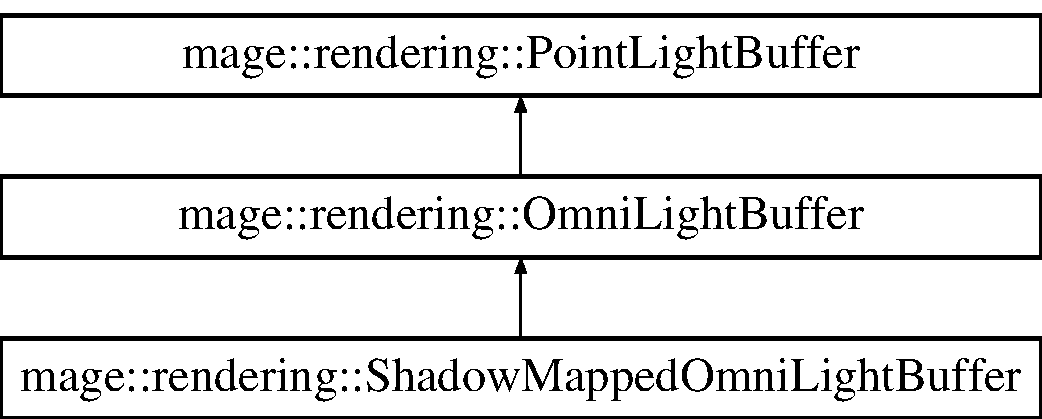
\includegraphics[height=3.000000cm]{structmage_1_1rendering_1_1_shadow_mapped_omni_light_buffer}
\end{center}
\end{figure}
\subsection*{Public Member Functions}
\begin{DoxyCompactItemize}
\item 
\mbox{\hyperlink{structmage_1_1rendering_1_1_shadow_mapped_omni_light_buffer_a3b9f6ffd582185ea739410aeeec8a446}{Shadow\+Mapped\+Omni\+Light\+Buffer}} () noexcept
\item 
\mbox{\hyperlink{structmage_1_1rendering_1_1_shadow_mapped_omni_light_buffer_a42ed551f04a7c53200e68e45c5ab9be5}{Shadow\+Mapped\+Omni\+Light\+Buffer}} (const \mbox{\hyperlink{structmage_1_1rendering_1_1_shadow_mapped_omni_light_buffer}{Shadow\+Mapped\+Omni\+Light\+Buffer}} \&buffer) noexcept=default
\item 
\mbox{\hyperlink{structmage_1_1rendering_1_1_shadow_mapped_omni_light_buffer_a7fb986d0697bdea8ac54f45c188f2a4b}{Shadow\+Mapped\+Omni\+Light\+Buffer}} (\mbox{\hyperlink{structmage_1_1rendering_1_1_shadow_mapped_omni_light_buffer}{Shadow\+Mapped\+Omni\+Light\+Buffer}} \&\&buffer) noexcept=default
\item 
\mbox{\hyperlink{structmage_1_1rendering_1_1_shadow_mapped_omni_light_buffer_afd9afa7796bbca38082cc8364f7c474c}{$\sim$\+Shadow\+Mapped\+Omni\+Light\+Buffer}} ()=default
\item 
\mbox{\hyperlink{structmage_1_1rendering_1_1_shadow_mapped_omni_light_buffer}{Shadow\+Mapped\+Omni\+Light\+Buffer}} \& \mbox{\hyperlink{structmage_1_1rendering_1_1_shadow_mapped_omni_light_buffer_ae43119f667592aea06f73532a9c9b742}{operator=}} (const \mbox{\hyperlink{structmage_1_1rendering_1_1_shadow_mapped_omni_light_buffer}{Shadow\+Mapped\+Omni\+Light\+Buffer}} \&buffer)=default
\item 
\mbox{\hyperlink{structmage_1_1rendering_1_1_shadow_mapped_omni_light_buffer}{Shadow\+Mapped\+Omni\+Light\+Buffer}} \& \mbox{\hyperlink{structmage_1_1rendering_1_1_shadow_mapped_omni_light_buffer_a5605852385a384c28a4c0cee6bc3cc32}{operator=}} (\mbox{\hyperlink{structmage_1_1rendering_1_1_shadow_mapped_omni_light_buffer}{Shadow\+Mapped\+Omni\+Light\+Buffer}} \&\&buffer)=default
\end{DoxyCompactItemize}
\subsection*{Public Attributes}
\begin{DoxyCompactItemize}
\item 
X\+M\+M\+A\+T\+R\+IX \mbox{\hyperlink{structmage_1_1rendering_1_1_shadow_mapped_omni_light_buffer_a6ad3f982000ca1d68c3897589aa89798}{m\+\_\+world\+\_\+to\+\_\+light}}
\item 
\mbox{\hyperlink{namespacemage_a9dc0d34d6ecc87e4cfa4a826102117bc}{F32x2}} \mbox{\hyperlink{structmage_1_1rendering_1_1_shadow_mapped_omni_light_buffer_a29016735134bb44c6c6f0d52fbf9ef2c}{m\+\_\+projection\+\_\+values}}
\item 
\mbox{\hyperlink{namespacemage_a41c104c036fba3756a74e19f793eeaa1}{U32}} \mbox{\hyperlink{structmage_1_1rendering_1_1_shadow_mapped_omni_light_buffer_a01a76a39534ba04a2b1fe77ae5d1522c}{m\+\_\+padding0}} \mbox{[}2\mbox{]}
\end{DoxyCompactItemize}


\subsection{Detailed Description}
A struct of shadow mapped omni light buffers used by shaders. 

\subsection{Constructor \& Destructor Documentation}
\mbox{\Hypertarget{structmage_1_1rendering_1_1_shadow_mapped_omni_light_buffer_a3b9f6ffd582185ea739410aeeec8a446}\label{structmage_1_1rendering_1_1_shadow_mapped_omni_light_buffer_a3b9f6ffd582185ea739410aeeec8a446}} 
\index{mage\+::rendering\+::\+Shadow\+Mapped\+Omni\+Light\+Buffer@{mage\+::rendering\+::\+Shadow\+Mapped\+Omni\+Light\+Buffer}!Shadow\+Mapped\+Omni\+Light\+Buffer@{Shadow\+Mapped\+Omni\+Light\+Buffer}}
\index{Shadow\+Mapped\+Omni\+Light\+Buffer@{Shadow\+Mapped\+Omni\+Light\+Buffer}!mage\+::rendering\+::\+Shadow\+Mapped\+Omni\+Light\+Buffer@{mage\+::rendering\+::\+Shadow\+Mapped\+Omni\+Light\+Buffer}}
\subsubsection{\texorpdfstring{Shadow\+Mapped\+Omni\+Light\+Buffer()}{ShadowMappedOmniLightBuffer()}\hspace{0.1cm}{\footnotesize\ttfamily [1/3]}}
{\footnotesize\ttfamily mage\+::rendering\+::\+Shadow\+Mapped\+Omni\+Light\+Buffer\+::\+Shadow\+Mapped\+Omni\+Light\+Buffer (\begin{DoxyParamCaption}{ }\end{DoxyParamCaption})\hspace{0.3cm}{\ttfamily [noexcept]}}

Constructs a shadow mapped omni light buffer. \mbox{\Hypertarget{structmage_1_1rendering_1_1_shadow_mapped_omni_light_buffer_a42ed551f04a7c53200e68e45c5ab9be5}\label{structmage_1_1rendering_1_1_shadow_mapped_omni_light_buffer_a42ed551f04a7c53200e68e45c5ab9be5}} 
\index{mage\+::rendering\+::\+Shadow\+Mapped\+Omni\+Light\+Buffer@{mage\+::rendering\+::\+Shadow\+Mapped\+Omni\+Light\+Buffer}!Shadow\+Mapped\+Omni\+Light\+Buffer@{Shadow\+Mapped\+Omni\+Light\+Buffer}}
\index{Shadow\+Mapped\+Omni\+Light\+Buffer@{Shadow\+Mapped\+Omni\+Light\+Buffer}!mage\+::rendering\+::\+Shadow\+Mapped\+Omni\+Light\+Buffer@{mage\+::rendering\+::\+Shadow\+Mapped\+Omni\+Light\+Buffer}}
\subsubsection{\texorpdfstring{Shadow\+Mapped\+Omni\+Light\+Buffer()}{ShadowMappedOmniLightBuffer()}\hspace{0.1cm}{\footnotesize\ttfamily [2/3]}}
{\footnotesize\ttfamily mage\+::rendering\+::\+Shadow\+Mapped\+Omni\+Light\+Buffer\+::\+Shadow\+Mapped\+Omni\+Light\+Buffer (\begin{DoxyParamCaption}\item[{const \mbox{\hyperlink{structmage_1_1rendering_1_1_shadow_mapped_omni_light_buffer}{Shadow\+Mapped\+Omni\+Light\+Buffer}} \&}]{buffer }\end{DoxyParamCaption})\hspace{0.3cm}{\ttfamily [default]}, {\ttfamily [noexcept]}}

Constructs a shadow mapped omni light buffer from the given shadow mapped omni light buffer.


\begin{DoxyParams}[1]{Parameters}
\mbox{\tt in}  & {\em buffer} & A reference to the shadow mapped omni light buffer to copy. \\
\hline
\end{DoxyParams}
\mbox{\Hypertarget{structmage_1_1rendering_1_1_shadow_mapped_omni_light_buffer_a7fb986d0697bdea8ac54f45c188f2a4b}\label{structmage_1_1rendering_1_1_shadow_mapped_omni_light_buffer_a7fb986d0697bdea8ac54f45c188f2a4b}} 
\index{mage\+::rendering\+::\+Shadow\+Mapped\+Omni\+Light\+Buffer@{mage\+::rendering\+::\+Shadow\+Mapped\+Omni\+Light\+Buffer}!Shadow\+Mapped\+Omni\+Light\+Buffer@{Shadow\+Mapped\+Omni\+Light\+Buffer}}
\index{Shadow\+Mapped\+Omni\+Light\+Buffer@{Shadow\+Mapped\+Omni\+Light\+Buffer}!mage\+::rendering\+::\+Shadow\+Mapped\+Omni\+Light\+Buffer@{mage\+::rendering\+::\+Shadow\+Mapped\+Omni\+Light\+Buffer}}
\subsubsection{\texorpdfstring{Shadow\+Mapped\+Omni\+Light\+Buffer()}{ShadowMappedOmniLightBuffer()}\hspace{0.1cm}{\footnotesize\ttfamily [3/3]}}
{\footnotesize\ttfamily mage\+::rendering\+::\+Shadow\+Mapped\+Omni\+Light\+Buffer\+::\+Shadow\+Mapped\+Omni\+Light\+Buffer (\begin{DoxyParamCaption}\item[{\mbox{\hyperlink{structmage_1_1rendering_1_1_shadow_mapped_omni_light_buffer}{Shadow\+Mapped\+Omni\+Light\+Buffer}} \&\&}]{buffer }\end{DoxyParamCaption})\hspace{0.3cm}{\ttfamily [default]}, {\ttfamily [noexcept]}}

Constructs a shadow mapped omni light buffer by moving the given shadow mapped omni light buffer.


\begin{DoxyParams}[1]{Parameters}
\mbox{\tt in}  & {\em buffer} & A reference to the shadow mapped omni light buffer to move. \\
\hline
\end{DoxyParams}
\mbox{\Hypertarget{structmage_1_1rendering_1_1_shadow_mapped_omni_light_buffer_afd9afa7796bbca38082cc8364f7c474c}\label{structmage_1_1rendering_1_1_shadow_mapped_omni_light_buffer_afd9afa7796bbca38082cc8364f7c474c}} 
\index{mage\+::rendering\+::\+Shadow\+Mapped\+Omni\+Light\+Buffer@{mage\+::rendering\+::\+Shadow\+Mapped\+Omni\+Light\+Buffer}!````~Shadow\+Mapped\+Omni\+Light\+Buffer@{$\sim$\+Shadow\+Mapped\+Omni\+Light\+Buffer}}
\index{````~Shadow\+Mapped\+Omni\+Light\+Buffer@{$\sim$\+Shadow\+Mapped\+Omni\+Light\+Buffer}!mage\+::rendering\+::\+Shadow\+Mapped\+Omni\+Light\+Buffer@{mage\+::rendering\+::\+Shadow\+Mapped\+Omni\+Light\+Buffer}}
\subsubsection{\texorpdfstring{$\sim$\+Shadow\+Mapped\+Omni\+Light\+Buffer()}{~ShadowMappedOmniLightBuffer()}}
{\footnotesize\ttfamily mage\+::rendering\+::\+Shadow\+Mapped\+Omni\+Light\+Buffer\+::$\sim$\+Shadow\+Mapped\+Omni\+Light\+Buffer (\begin{DoxyParamCaption}{ }\end{DoxyParamCaption})\hspace{0.3cm}{\ttfamily [default]}}

Destructs this shadow mapped omni light buffer. 

\subsection{Member Function Documentation}
\mbox{\Hypertarget{structmage_1_1rendering_1_1_shadow_mapped_omni_light_buffer_ae43119f667592aea06f73532a9c9b742}\label{structmage_1_1rendering_1_1_shadow_mapped_omni_light_buffer_ae43119f667592aea06f73532a9c9b742}} 
\index{mage\+::rendering\+::\+Shadow\+Mapped\+Omni\+Light\+Buffer@{mage\+::rendering\+::\+Shadow\+Mapped\+Omni\+Light\+Buffer}!operator=@{operator=}}
\index{operator=@{operator=}!mage\+::rendering\+::\+Shadow\+Mapped\+Omni\+Light\+Buffer@{mage\+::rendering\+::\+Shadow\+Mapped\+Omni\+Light\+Buffer}}
\subsubsection{\texorpdfstring{operator=()}{operator=()}\hspace{0.1cm}{\footnotesize\ttfamily [1/2]}}
{\footnotesize\ttfamily \mbox{\hyperlink{structmage_1_1rendering_1_1_shadow_mapped_omni_light_buffer}{Shadow\+Mapped\+Omni\+Light\+Buffer}}\& mage\+::rendering\+::\+Shadow\+Mapped\+Omni\+Light\+Buffer\+::operator= (\begin{DoxyParamCaption}\item[{const \mbox{\hyperlink{structmage_1_1rendering_1_1_shadow_mapped_omni_light_buffer}{Shadow\+Mapped\+Omni\+Light\+Buffer}} \&}]{buffer }\end{DoxyParamCaption})\hspace{0.3cm}{\ttfamily [default]}}

Copies the given shadow mapped omni light buffer to this shadow mapped omni light buffer.


\begin{DoxyParams}[1]{Parameters}
\mbox{\tt in}  & {\em buffer} & A reference to the shadow mapped omni light buffer to copy. \\
\hline
\end{DoxyParams}
\begin{DoxyReturn}{Returns}
A reference to the copy of the given shadow mapped omni light buffer (i.\+e. this shadow mapped omni light buffer). 
\end{DoxyReturn}
\mbox{\Hypertarget{structmage_1_1rendering_1_1_shadow_mapped_omni_light_buffer_a5605852385a384c28a4c0cee6bc3cc32}\label{structmage_1_1rendering_1_1_shadow_mapped_omni_light_buffer_a5605852385a384c28a4c0cee6bc3cc32}} 
\index{mage\+::rendering\+::\+Shadow\+Mapped\+Omni\+Light\+Buffer@{mage\+::rendering\+::\+Shadow\+Mapped\+Omni\+Light\+Buffer}!operator=@{operator=}}
\index{operator=@{operator=}!mage\+::rendering\+::\+Shadow\+Mapped\+Omni\+Light\+Buffer@{mage\+::rendering\+::\+Shadow\+Mapped\+Omni\+Light\+Buffer}}
\subsubsection{\texorpdfstring{operator=()}{operator=()}\hspace{0.1cm}{\footnotesize\ttfamily [2/2]}}
{\footnotesize\ttfamily \mbox{\hyperlink{structmage_1_1rendering_1_1_shadow_mapped_omni_light_buffer}{Shadow\+Mapped\+Omni\+Light\+Buffer}}\& mage\+::rendering\+::\+Shadow\+Mapped\+Omni\+Light\+Buffer\+::operator= (\begin{DoxyParamCaption}\item[{\mbox{\hyperlink{structmage_1_1rendering_1_1_shadow_mapped_omni_light_buffer}{Shadow\+Mapped\+Omni\+Light\+Buffer}} \&\&}]{buffer }\end{DoxyParamCaption})\hspace{0.3cm}{\ttfamily [default]}}

Moves the given shadow mapped omni light buffer to this shadow mapped omni light buffer.


\begin{DoxyParams}[1]{Parameters}
\mbox{\tt in}  & {\em buffer} & A reference to the shadow mapped omni light buffer to move. \\
\hline
\end{DoxyParams}
\begin{DoxyReturn}{Returns}
A reference to the moved shadow mapped omni light buffer (i.\+e. this shadow mapped omni light buffer). 
\end{DoxyReturn}


\subsection{Member Data Documentation}
\mbox{\Hypertarget{structmage_1_1rendering_1_1_shadow_mapped_omni_light_buffer_a01a76a39534ba04a2b1fe77ae5d1522c}\label{structmage_1_1rendering_1_1_shadow_mapped_omni_light_buffer_a01a76a39534ba04a2b1fe77ae5d1522c}} 
\index{mage\+::rendering\+::\+Shadow\+Mapped\+Omni\+Light\+Buffer@{mage\+::rendering\+::\+Shadow\+Mapped\+Omni\+Light\+Buffer}!m\+\_\+padding0@{m\+\_\+padding0}}
\index{m\+\_\+padding0@{m\+\_\+padding0}!mage\+::rendering\+::\+Shadow\+Mapped\+Omni\+Light\+Buffer@{mage\+::rendering\+::\+Shadow\+Mapped\+Omni\+Light\+Buffer}}
\subsubsection{\texorpdfstring{m\+\_\+padding0}{m\_padding0}}
{\footnotesize\ttfamily \mbox{\hyperlink{namespacemage_a41c104c036fba3756a74e19f793eeaa1}{U32}} mage\+::rendering\+::\+Shadow\+Mapped\+Omni\+Light\+Buffer\+::m\+\_\+padding0\mbox{[}2\mbox{]}}

The padding of this shadow mapped omni light buffer. \mbox{\Hypertarget{structmage_1_1rendering_1_1_shadow_mapped_omni_light_buffer_a29016735134bb44c6c6f0d52fbf9ef2c}\label{structmage_1_1rendering_1_1_shadow_mapped_omni_light_buffer_a29016735134bb44c6c6f0d52fbf9ef2c}} 
\index{mage\+::rendering\+::\+Shadow\+Mapped\+Omni\+Light\+Buffer@{mage\+::rendering\+::\+Shadow\+Mapped\+Omni\+Light\+Buffer}!m\+\_\+projection\+\_\+values@{m\+\_\+projection\+\_\+values}}
\index{m\+\_\+projection\+\_\+values@{m\+\_\+projection\+\_\+values}!mage\+::rendering\+::\+Shadow\+Mapped\+Omni\+Light\+Buffer@{mage\+::rendering\+::\+Shadow\+Mapped\+Omni\+Light\+Buffer}}
\subsubsection{\texorpdfstring{m\+\_\+projection\+\_\+values}{m\_projection\_values}}
{\footnotesize\ttfamily \mbox{\hyperlink{namespacemage_a9dc0d34d6ecc87e4cfa4a826102117bc}{F32x2}} mage\+::rendering\+::\+Shadow\+Mapped\+Omni\+Light\+Buffer\+::m\+\_\+projection\+\_\+values}

The projection values of the light-\/to-\/projection transformation matrix of the shadow mapped omni light of this shadow mapped omni light buffer. \mbox{\Hypertarget{structmage_1_1rendering_1_1_shadow_mapped_omni_light_buffer_a6ad3f982000ca1d68c3897589aa89798}\label{structmage_1_1rendering_1_1_shadow_mapped_omni_light_buffer_a6ad3f982000ca1d68c3897589aa89798}} 
\index{mage\+::rendering\+::\+Shadow\+Mapped\+Omni\+Light\+Buffer@{mage\+::rendering\+::\+Shadow\+Mapped\+Omni\+Light\+Buffer}!m\+\_\+world\+\_\+to\+\_\+light@{m\+\_\+world\+\_\+to\+\_\+light}}
\index{m\+\_\+world\+\_\+to\+\_\+light@{m\+\_\+world\+\_\+to\+\_\+light}!mage\+::rendering\+::\+Shadow\+Mapped\+Omni\+Light\+Buffer@{mage\+::rendering\+::\+Shadow\+Mapped\+Omni\+Light\+Buffer}}
\subsubsection{\texorpdfstring{m\+\_\+world\+\_\+to\+\_\+light}{m\_world\_to\_light}}
{\footnotesize\ttfamily X\+M\+M\+A\+T\+R\+IX mage\+::rendering\+::\+Shadow\+Mapped\+Omni\+Light\+Buffer\+::m\+\_\+world\+\_\+to\+\_\+light}

The (column-\/major packed, row-\/major matrix) world-\/to-\/light matrix of the shadow mapped omni light of this shadow mapped omni light buffer. 
\hypertarget{structmage_1_1rendering_1_1_shadow_mapped_spot_light_buffer}{}\section{mage\+:\+:rendering\+:\+:Shadow\+Mapped\+Spot\+Light\+Buffer Struct Reference}
\label{structmage_1_1rendering_1_1_shadow_mapped_spot_light_buffer}\index{mage\+::rendering\+::\+Shadow\+Mapped\+Spot\+Light\+Buffer@{mage\+::rendering\+::\+Shadow\+Mapped\+Spot\+Light\+Buffer}}


{\ttfamily \#include $<$light\+\_\+buffer.\+hpp$>$}

Inheritance diagram for mage\+:\+:rendering\+:\+:Shadow\+Mapped\+Spot\+Light\+Buffer\+:\begin{figure}[H]
\begin{center}
\leavevmode
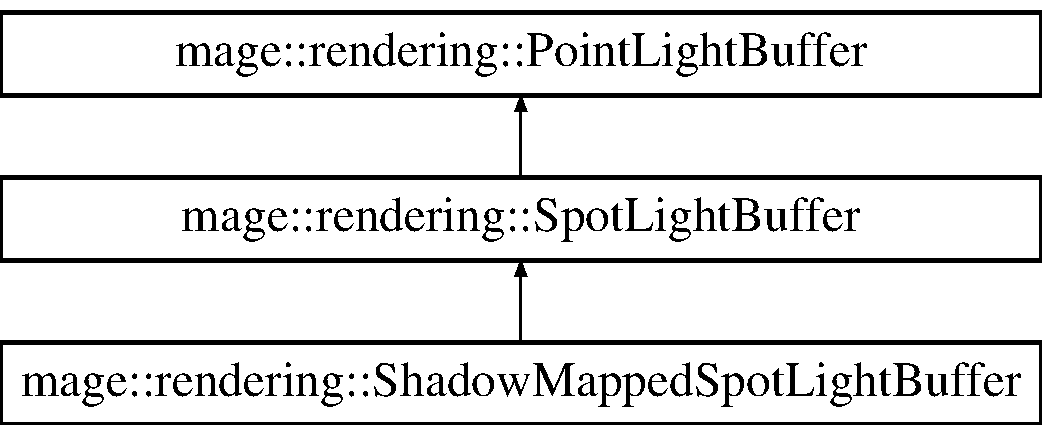
\includegraphics[height=3.000000cm]{structmage_1_1rendering_1_1_shadow_mapped_spot_light_buffer}
\end{center}
\end{figure}
\subsection*{Public Member Functions}
\begin{DoxyCompactItemize}
\item 
\mbox{\hyperlink{structmage_1_1rendering_1_1_shadow_mapped_spot_light_buffer_a88d393bc59e25f35d29e478de8c81c89}{Shadow\+Mapped\+Spot\+Light\+Buffer}} () noexcept
\item 
\mbox{\hyperlink{structmage_1_1rendering_1_1_shadow_mapped_spot_light_buffer_ac984180fa57278b851bbaf3b081a4343}{Shadow\+Mapped\+Spot\+Light\+Buffer}} (const \mbox{\hyperlink{structmage_1_1rendering_1_1_shadow_mapped_spot_light_buffer}{Shadow\+Mapped\+Spot\+Light\+Buffer}} \&buffer) noexcept=default
\item 
\mbox{\hyperlink{structmage_1_1rendering_1_1_shadow_mapped_spot_light_buffer_a9042ab916ee834f5519b5930de286ea4}{Shadow\+Mapped\+Spot\+Light\+Buffer}} (\mbox{\hyperlink{structmage_1_1rendering_1_1_shadow_mapped_spot_light_buffer}{Shadow\+Mapped\+Spot\+Light\+Buffer}} \&\&buffer) noexcept=default
\item 
\mbox{\hyperlink{structmage_1_1rendering_1_1_shadow_mapped_spot_light_buffer_ae651274fb4d113e173b62cb18191f1b9}{$\sim$\+Shadow\+Mapped\+Spot\+Light\+Buffer}} ()=default
\item 
\mbox{\hyperlink{structmage_1_1rendering_1_1_shadow_mapped_spot_light_buffer}{Shadow\+Mapped\+Spot\+Light\+Buffer}} \& \mbox{\hyperlink{structmage_1_1rendering_1_1_shadow_mapped_spot_light_buffer_a2c209b2648740696d45113a152e648fb}{operator=}} (const \mbox{\hyperlink{structmage_1_1rendering_1_1_shadow_mapped_spot_light_buffer}{Shadow\+Mapped\+Spot\+Light\+Buffer}} \&buffer)=default
\item 
\mbox{\hyperlink{structmage_1_1rendering_1_1_shadow_mapped_spot_light_buffer}{Shadow\+Mapped\+Spot\+Light\+Buffer}} \& \mbox{\hyperlink{structmage_1_1rendering_1_1_shadow_mapped_spot_light_buffer_ae2687b41af138b43fc814883310a877b}{operator=}} (\mbox{\hyperlink{structmage_1_1rendering_1_1_shadow_mapped_spot_light_buffer}{Shadow\+Mapped\+Spot\+Light\+Buffer}} \&\&buffer)=default
\end{DoxyCompactItemize}
\subsection*{Public Attributes}
\begin{DoxyCompactItemize}
\item 
X\+M\+M\+A\+T\+R\+IX \mbox{\hyperlink{structmage_1_1rendering_1_1_shadow_mapped_spot_light_buffer_abb736c590c4a6efff217e15ef8abec4a}{m\+\_\+world\+\_\+to\+\_\+projection}}
\end{DoxyCompactItemize}


\subsection{Detailed Description}
A struct of shadow mapped spotlight buffers used by shaders. 

\subsection{Constructor \& Destructor Documentation}
\mbox{\Hypertarget{structmage_1_1rendering_1_1_shadow_mapped_spot_light_buffer_a88d393bc59e25f35d29e478de8c81c89}\label{structmage_1_1rendering_1_1_shadow_mapped_spot_light_buffer_a88d393bc59e25f35d29e478de8c81c89}} 
\index{mage\+::rendering\+::\+Shadow\+Mapped\+Spot\+Light\+Buffer@{mage\+::rendering\+::\+Shadow\+Mapped\+Spot\+Light\+Buffer}!Shadow\+Mapped\+Spot\+Light\+Buffer@{Shadow\+Mapped\+Spot\+Light\+Buffer}}
\index{Shadow\+Mapped\+Spot\+Light\+Buffer@{Shadow\+Mapped\+Spot\+Light\+Buffer}!mage\+::rendering\+::\+Shadow\+Mapped\+Spot\+Light\+Buffer@{mage\+::rendering\+::\+Shadow\+Mapped\+Spot\+Light\+Buffer}}
\subsubsection{\texorpdfstring{Shadow\+Mapped\+Spot\+Light\+Buffer()}{ShadowMappedSpotLightBuffer()}\hspace{0.1cm}{\footnotesize\ttfamily [1/3]}}
{\footnotesize\ttfamily mage\+::rendering\+::\+Shadow\+Mapped\+Spot\+Light\+Buffer\+::\+Shadow\+Mapped\+Spot\+Light\+Buffer (\begin{DoxyParamCaption}{ }\end{DoxyParamCaption})\hspace{0.3cm}{\ttfamily [noexcept]}}

Constructs a shadow mapped spotlight buffer. \mbox{\Hypertarget{structmage_1_1rendering_1_1_shadow_mapped_spot_light_buffer_ac984180fa57278b851bbaf3b081a4343}\label{structmage_1_1rendering_1_1_shadow_mapped_spot_light_buffer_ac984180fa57278b851bbaf3b081a4343}} 
\index{mage\+::rendering\+::\+Shadow\+Mapped\+Spot\+Light\+Buffer@{mage\+::rendering\+::\+Shadow\+Mapped\+Spot\+Light\+Buffer}!Shadow\+Mapped\+Spot\+Light\+Buffer@{Shadow\+Mapped\+Spot\+Light\+Buffer}}
\index{Shadow\+Mapped\+Spot\+Light\+Buffer@{Shadow\+Mapped\+Spot\+Light\+Buffer}!mage\+::rendering\+::\+Shadow\+Mapped\+Spot\+Light\+Buffer@{mage\+::rendering\+::\+Shadow\+Mapped\+Spot\+Light\+Buffer}}
\subsubsection{\texorpdfstring{Shadow\+Mapped\+Spot\+Light\+Buffer()}{ShadowMappedSpotLightBuffer()}\hspace{0.1cm}{\footnotesize\ttfamily [2/3]}}
{\footnotesize\ttfamily mage\+::rendering\+::\+Shadow\+Mapped\+Spot\+Light\+Buffer\+::\+Shadow\+Mapped\+Spot\+Light\+Buffer (\begin{DoxyParamCaption}\item[{const \mbox{\hyperlink{structmage_1_1rendering_1_1_shadow_mapped_spot_light_buffer}{Shadow\+Mapped\+Spot\+Light\+Buffer}} \&}]{buffer }\end{DoxyParamCaption})\hspace{0.3cm}{\ttfamily [default]}, {\ttfamily [noexcept]}}

Constructs a shadow mapped spotlight buffer from the given shadow mapped spotlight buffer.


\begin{DoxyParams}[1]{Parameters}
\mbox{\tt in}  & {\em buffer} & A reference to the shadow mapped spotlight buffer to copy. \\
\hline
\end{DoxyParams}
\mbox{\Hypertarget{structmage_1_1rendering_1_1_shadow_mapped_spot_light_buffer_a9042ab916ee834f5519b5930de286ea4}\label{structmage_1_1rendering_1_1_shadow_mapped_spot_light_buffer_a9042ab916ee834f5519b5930de286ea4}} 
\index{mage\+::rendering\+::\+Shadow\+Mapped\+Spot\+Light\+Buffer@{mage\+::rendering\+::\+Shadow\+Mapped\+Spot\+Light\+Buffer}!Shadow\+Mapped\+Spot\+Light\+Buffer@{Shadow\+Mapped\+Spot\+Light\+Buffer}}
\index{Shadow\+Mapped\+Spot\+Light\+Buffer@{Shadow\+Mapped\+Spot\+Light\+Buffer}!mage\+::rendering\+::\+Shadow\+Mapped\+Spot\+Light\+Buffer@{mage\+::rendering\+::\+Shadow\+Mapped\+Spot\+Light\+Buffer}}
\subsubsection{\texorpdfstring{Shadow\+Mapped\+Spot\+Light\+Buffer()}{ShadowMappedSpotLightBuffer()}\hspace{0.1cm}{\footnotesize\ttfamily [3/3]}}
{\footnotesize\ttfamily mage\+::rendering\+::\+Shadow\+Mapped\+Spot\+Light\+Buffer\+::\+Shadow\+Mapped\+Spot\+Light\+Buffer (\begin{DoxyParamCaption}\item[{\mbox{\hyperlink{structmage_1_1rendering_1_1_shadow_mapped_spot_light_buffer}{Shadow\+Mapped\+Spot\+Light\+Buffer}} \&\&}]{buffer }\end{DoxyParamCaption})\hspace{0.3cm}{\ttfamily [default]}, {\ttfamily [noexcept]}}

Constructs a shadow mapped spotlight buffer by moving the given shadow mapped spotlight buffer.


\begin{DoxyParams}[1]{Parameters}
\mbox{\tt in}  & {\em buffer} & A reference to the shadow mapped spotlight buffer to move. \\
\hline
\end{DoxyParams}
\mbox{\Hypertarget{structmage_1_1rendering_1_1_shadow_mapped_spot_light_buffer_ae651274fb4d113e173b62cb18191f1b9}\label{structmage_1_1rendering_1_1_shadow_mapped_spot_light_buffer_ae651274fb4d113e173b62cb18191f1b9}} 
\index{mage\+::rendering\+::\+Shadow\+Mapped\+Spot\+Light\+Buffer@{mage\+::rendering\+::\+Shadow\+Mapped\+Spot\+Light\+Buffer}!````~Shadow\+Mapped\+Spot\+Light\+Buffer@{$\sim$\+Shadow\+Mapped\+Spot\+Light\+Buffer}}
\index{````~Shadow\+Mapped\+Spot\+Light\+Buffer@{$\sim$\+Shadow\+Mapped\+Spot\+Light\+Buffer}!mage\+::rendering\+::\+Shadow\+Mapped\+Spot\+Light\+Buffer@{mage\+::rendering\+::\+Shadow\+Mapped\+Spot\+Light\+Buffer}}
\subsubsection{\texorpdfstring{$\sim$\+Shadow\+Mapped\+Spot\+Light\+Buffer()}{~ShadowMappedSpotLightBuffer()}}
{\footnotesize\ttfamily mage\+::rendering\+::\+Shadow\+Mapped\+Spot\+Light\+Buffer\+::$\sim$\+Shadow\+Mapped\+Spot\+Light\+Buffer (\begin{DoxyParamCaption}{ }\end{DoxyParamCaption})\hspace{0.3cm}{\ttfamily [default]}}

Destructs this shadow mapped spotlight buffer. 

\subsection{Member Function Documentation}
\mbox{\Hypertarget{structmage_1_1rendering_1_1_shadow_mapped_spot_light_buffer_a2c209b2648740696d45113a152e648fb}\label{structmage_1_1rendering_1_1_shadow_mapped_spot_light_buffer_a2c209b2648740696d45113a152e648fb}} 
\index{mage\+::rendering\+::\+Shadow\+Mapped\+Spot\+Light\+Buffer@{mage\+::rendering\+::\+Shadow\+Mapped\+Spot\+Light\+Buffer}!operator=@{operator=}}
\index{operator=@{operator=}!mage\+::rendering\+::\+Shadow\+Mapped\+Spot\+Light\+Buffer@{mage\+::rendering\+::\+Shadow\+Mapped\+Spot\+Light\+Buffer}}
\subsubsection{\texorpdfstring{operator=()}{operator=()}\hspace{0.1cm}{\footnotesize\ttfamily [1/2]}}
{\footnotesize\ttfamily \mbox{\hyperlink{structmage_1_1rendering_1_1_shadow_mapped_spot_light_buffer}{Shadow\+Mapped\+Spot\+Light\+Buffer}}\& mage\+::rendering\+::\+Shadow\+Mapped\+Spot\+Light\+Buffer\+::operator= (\begin{DoxyParamCaption}\item[{const \mbox{\hyperlink{structmage_1_1rendering_1_1_shadow_mapped_spot_light_buffer}{Shadow\+Mapped\+Spot\+Light\+Buffer}} \&}]{buffer }\end{DoxyParamCaption})\hspace{0.3cm}{\ttfamily [default]}}

Copies the given shadow mapped spotlight buffer to this shadow mapped spotlight buffer.


\begin{DoxyParams}[1]{Parameters}
\mbox{\tt in}  & {\em buffer} & A reference to the shadow mapped spotlight buffer to copy. \\
\hline
\end{DoxyParams}
\begin{DoxyReturn}{Returns}
A reference to the copy of the given shadow mapped spotlight buffer (i.\+e. this shadow mapped spotlight buffer). 
\end{DoxyReturn}
\mbox{\Hypertarget{structmage_1_1rendering_1_1_shadow_mapped_spot_light_buffer_ae2687b41af138b43fc814883310a877b}\label{structmage_1_1rendering_1_1_shadow_mapped_spot_light_buffer_ae2687b41af138b43fc814883310a877b}} 
\index{mage\+::rendering\+::\+Shadow\+Mapped\+Spot\+Light\+Buffer@{mage\+::rendering\+::\+Shadow\+Mapped\+Spot\+Light\+Buffer}!operator=@{operator=}}
\index{operator=@{operator=}!mage\+::rendering\+::\+Shadow\+Mapped\+Spot\+Light\+Buffer@{mage\+::rendering\+::\+Shadow\+Mapped\+Spot\+Light\+Buffer}}
\subsubsection{\texorpdfstring{operator=()}{operator=()}\hspace{0.1cm}{\footnotesize\ttfamily [2/2]}}
{\footnotesize\ttfamily \mbox{\hyperlink{structmage_1_1rendering_1_1_shadow_mapped_spot_light_buffer}{Shadow\+Mapped\+Spot\+Light\+Buffer}}\& mage\+::rendering\+::\+Shadow\+Mapped\+Spot\+Light\+Buffer\+::operator= (\begin{DoxyParamCaption}\item[{\mbox{\hyperlink{structmage_1_1rendering_1_1_shadow_mapped_spot_light_buffer}{Shadow\+Mapped\+Spot\+Light\+Buffer}} \&\&}]{buffer }\end{DoxyParamCaption})\hspace{0.3cm}{\ttfamily [default]}}

Moves the given shadow mapped spotlight buffer to this shadow mapped spotlight buffer.


\begin{DoxyParams}[1]{Parameters}
\mbox{\tt in}  & {\em buffer} & A reference to the shadow mapped spotlight buffer to move. \\
\hline
\end{DoxyParams}
\begin{DoxyReturn}{Returns}
A reference to the moved shadow mapped spotlight buffer (i.\+e. this shadow mapped spotlight buffer). 
\end{DoxyReturn}


\subsection{Member Data Documentation}
\mbox{\Hypertarget{structmage_1_1rendering_1_1_shadow_mapped_spot_light_buffer_abb736c590c4a6efff217e15ef8abec4a}\label{structmage_1_1rendering_1_1_shadow_mapped_spot_light_buffer_abb736c590c4a6efff217e15ef8abec4a}} 
\index{mage\+::rendering\+::\+Shadow\+Mapped\+Spot\+Light\+Buffer@{mage\+::rendering\+::\+Shadow\+Mapped\+Spot\+Light\+Buffer}!m\+\_\+world\+\_\+to\+\_\+projection@{m\+\_\+world\+\_\+to\+\_\+projection}}
\index{m\+\_\+world\+\_\+to\+\_\+projection@{m\+\_\+world\+\_\+to\+\_\+projection}!mage\+::rendering\+::\+Shadow\+Mapped\+Spot\+Light\+Buffer@{mage\+::rendering\+::\+Shadow\+Mapped\+Spot\+Light\+Buffer}}
\subsubsection{\texorpdfstring{m\+\_\+world\+\_\+to\+\_\+projection}{m\_world\_to\_projection}}
{\footnotesize\ttfamily X\+M\+M\+A\+T\+R\+IX mage\+::rendering\+::\+Shadow\+Mapped\+Spot\+Light\+Buffer\+::m\+\_\+world\+\_\+to\+\_\+projection}

The (column-\/major packed, row-\/major matrix) world-\/to-\/projection matrix of the shadow mapped spotlight of this shadow mapped spotlight buffer. 
\hypertarget{classmage_1_1_single_ended_memory_stack}{}\section{mage\+:\+:Single\+Ended\+Memory\+Stack Class Reference}
\label{classmage_1_1_single_ended_memory_stack}\index{mage\+::\+Single\+Ended\+Memory\+Stack@{mage\+::\+Single\+Ended\+Memory\+Stack}}


{\ttfamily \#include $<$memory\+\_\+stack.\+hpp$>$}

\subsection*{Classes}
\begin{DoxyCompactItemize}
\item 
class \mbox{\hyperlink{classmage_1_1_single_ended_memory_stack_1_1_allocator}{Allocator}}
\end{DoxyCompactItemize}
\subsection*{Public Member Functions}
\begin{DoxyCompactItemize}
\item 
\mbox{\hyperlink{classmage_1_1_single_ended_memory_stack_ab9555d63b35070aee321cc3839fec3c4}{Single\+Ended\+Memory\+Stack}} (size\+\_\+t size, size\+\_\+t alignment)
\item 
\mbox{\hyperlink{classmage_1_1_single_ended_memory_stack_ae854c4558f0215bf38cb713cbca7fa31}{Single\+Ended\+Memory\+Stack}} (const \mbox{\hyperlink{classmage_1_1_single_ended_memory_stack}{Single\+Ended\+Memory\+Stack}} \&stack)=delete
\item 
\mbox{\hyperlink{classmage_1_1_single_ended_memory_stack_afd6632eac3ada6ea88a69b586f27a4e4}{Single\+Ended\+Memory\+Stack}} (\mbox{\hyperlink{classmage_1_1_single_ended_memory_stack}{Single\+Ended\+Memory\+Stack}} \&\&stack) noexcept
\item 
\mbox{\hyperlink{classmage_1_1_single_ended_memory_stack_adaa82d19a1ef60ca42396bdaaea0c8e6}{$\sim$\+Single\+Ended\+Memory\+Stack}} ()
\item 
\mbox{\hyperlink{classmage_1_1_single_ended_memory_stack}{Single\+Ended\+Memory\+Stack}} \& \mbox{\hyperlink{classmage_1_1_single_ended_memory_stack_a709db7d21cd2db6e98acd7985770468e}{operator=}} (const \mbox{\hyperlink{classmage_1_1_single_ended_memory_stack}{Single\+Ended\+Memory\+Stack}} \&stack)=delete
\item 
\mbox{\hyperlink{classmage_1_1_single_ended_memory_stack}{Single\+Ended\+Memory\+Stack}} \& \mbox{\hyperlink{classmage_1_1_single_ended_memory_stack_a24613dc91ab6577aa57fbd55a4c81023}{operator=}} (\mbox{\hyperlink{classmage_1_1_single_ended_memory_stack}{Single\+Ended\+Memory\+Stack}} \&\&stack)=delete
\item 
size\+\_\+t \mbox{\hyperlink{classmage_1_1_single_ended_memory_stack_a821660699258ecbd007c5909108a911b}{Get\+Alignment}} () const noexcept
\item 
size\+\_\+t \mbox{\hyperlink{classmage_1_1_single_ended_memory_stack_aa1df0adf194d6c2bb6c7597a96c10e61}{Get\+Size}} () const noexcept
\item 
size\+\_\+t \mbox{\hyperlink{classmage_1_1_single_ended_memory_stack_ab2b07a4cf2c9eb9988ad49174e0804ac}{Get\+Used\+Size}} () const noexcept
\item 
size\+\_\+t \mbox{\hyperlink{classmage_1_1_single_ended_memory_stack_a1c3f233b16e8fcb9770b7fe23b83485b}{Get\+Available\+Size}} () const noexcept
\item 
uintptr\+\_\+t \mbox{\hyperlink{classmage_1_1_single_ended_memory_stack_a11b792ad420eac8e620c568e89a88cef}{Get\+Current\+Ptr}} () const noexcept
\item 
void \mbox{\hyperlink{classmage_1_1_single_ended_memory_stack_abd43ab7bd76655265123b934ea2bc7a7}{Reset}} () noexcept
\item 
void \mbox{\hyperlink{classmage_1_1_single_ended_memory_stack_afa1fcaa95a61995234759f9c57723202}{Roll\+Back}} (uintptr\+\_\+t ptr) noexcept
\item 
void $\ast$ \mbox{\hyperlink{classmage_1_1_single_ended_memory_stack_acda0b7f2e61bf8ba8bbb9ba633237866}{Alloc}} (size\+\_\+t size) noexcept
\item 
{\footnotesize template$<$typename DataT $>$ }\\DataT $\ast$ \mbox{\hyperlink{classmage_1_1_single_ended_memory_stack_ae957490450194631b81b9f6ba84f5f5a}{Alloc\+Data}} (size\+\_\+t count=1, bool initialization=false) noexcept
\item 
{\footnotesize template$<$typename DataT $>$ }\\\mbox{\hyperlink{classmage_1_1_single_ended_memory_stack_1_1_allocator}{Allocator}}$<$ DataT $>$ \mbox{\hyperlink{classmage_1_1_single_ended_memory_stack_a92f0c10ddfd1cdcba2fc9e8842382e41}{Get\+Allocator}} () const noexcept
\end{DoxyCompactItemize}
\subsection*{Private Attributes}
\begin{DoxyCompactItemize}
\item 
const size\+\_\+t \mbox{\hyperlink{classmage_1_1_single_ended_memory_stack_a3766c742087068479c3e324280ca94bf}{m\+\_\+size}}
\item 
const size\+\_\+t \mbox{\hyperlink{classmage_1_1_single_ended_memory_stack_aeb5bc5af575eaeb5a0f08669a717cd28}{m\+\_\+alignment}}
\item 
uintptr\+\_\+t \mbox{\hyperlink{classmage_1_1_single_ended_memory_stack_a859a80ab120c14e3ebf4a310d5263507}{m\+\_\+begin}}
\item 
uintptr\+\_\+t \mbox{\hyperlink{classmage_1_1_single_ended_memory_stack_a78785ecceac6ce271658864dac80e84b}{m\+\_\+current}}
\end{DoxyCompactItemize}


\subsection{Detailed Description}
A class of single-\/ended memory stacks. 

\subsection{Constructor \& Destructor Documentation}
\mbox{\Hypertarget{classmage_1_1_single_ended_memory_stack_ab9555d63b35070aee321cc3839fec3c4}\label{classmage_1_1_single_ended_memory_stack_ab9555d63b35070aee321cc3839fec3c4}} 
\index{mage\+::\+Single\+Ended\+Memory\+Stack@{mage\+::\+Single\+Ended\+Memory\+Stack}!Single\+Ended\+Memory\+Stack@{Single\+Ended\+Memory\+Stack}}
\index{Single\+Ended\+Memory\+Stack@{Single\+Ended\+Memory\+Stack}!mage\+::\+Single\+Ended\+Memory\+Stack@{mage\+::\+Single\+Ended\+Memory\+Stack}}
\subsubsection{\texorpdfstring{Single\+Ended\+Memory\+Stack()}{SingleEndedMemoryStack()}\hspace{0.1cm}{\footnotesize\ttfamily [1/3]}}
{\footnotesize\ttfamily mage\+::\+Single\+Ended\+Memory\+Stack\+::\+Single\+Ended\+Memory\+Stack (\begin{DoxyParamCaption}\item[{size\+\_\+t}]{size,  }\item[{size\+\_\+t}]{alignment }\end{DoxyParamCaption})\hspace{0.3cm}{\ttfamily [explicit]}}

Constructs a single-\/ended memory stack with given size.


\begin{DoxyParams}[1]{Parameters}
\mbox{\tt in}  & {\em size} & The size in bytes. \\
\hline
\mbox{\tt in}  & {\em alignment} & The alignment in bytes. \\
\hline
\end{DoxyParams}

\begin{DoxyExceptions}{Exceptions}
{\em std\+::bad\+\_\+alloc} & Failed to allocate the memory. \\
\hline
\end{DoxyExceptions}
\mbox{\Hypertarget{classmage_1_1_single_ended_memory_stack_ae854c4558f0215bf38cb713cbca7fa31}\label{classmage_1_1_single_ended_memory_stack_ae854c4558f0215bf38cb713cbca7fa31}} 
\index{mage\+::\+Single\+Ended\+Memory\+Stack@{mage\+::\+Single\+Ended\+Memory\+Stack}!Single\+Ended\+Memory\+Stack@{Single\+Ended\+Memory\+Stack}}
\index{Single\+Ended\+Memory\+Stack@{Single\+Ended\+Memory\+Stack}!mage\+::\+Single\+Ended\+Memory\+Stack@{mage\+::\+Single\+Ended\+Memory\+Stack}}
\subsubsection{\texorpdfstring{Single\+Ended\+Memory\+Stack()}{SingleEndedMemoryStack()}\hspace{0.1cm}{\footnotesize\ttfamily [2/3]}}
{\footnotesize\ttfamily mage\+::\+Single\+Ended\+Memory\+Stack\+::\+Single\+Ended\+Memory\+Stack (\begin{DoxyParamCaption}\item[{const \mbox{\hyperlink{classmage_1_1_single_ended_memory_stack}{Single\+Ended\+Memory\+Stack}} \&}]{stack }\end{DoxyParamCaption})\hspace{0.3cm}{\ttfamily [delete]}}

Constructs a single-\/ended memory stack from the given single-\/ended memory stack.


\begin{DoxyParams}[1]{Parameters}
\mbox{\tt in}  & {\em stack} & A reference to the single-\/ended memory stack to copy. \\
\hline
\end{DoxyParams}
\mbox{\Hypertarget{classmage_1_1_single_ended_memory_stack_afd6632eac3ada6ea88a69b586f27a4e4}\label{classmage_1_1_single_ended_memory_stack_afd6632eac3ada6ea88a69b586f27a4e4}} 
\index{mage\+::\+Single\+Ended\+Memory\+Stack@{mage\+::\+Single\+Ended\+Memory\+Stack}!Single\+Ended\+Memory\+Stack@{Single\+Ended\+Memory\+Stack}}
\index{Single\+Ended\+Memory\+Stack@{Single\+Ended\+Memory\+Stack}!mage\+::\+Single\+Ended\+Memory\+Stack@{mage\+::\+Single\+Ended\+Memory\+Stack}}
\subsubsection{\texorpdfstring{Single\+Ended\+Memory\+Stack()}{SingleEndedMemoryStack()}\hspace{0.1cm}{\footnotesize\ttfamily [3/3]}}
{\footnotesize\ttfamily mage\+::\+Single\+Ended\+Memory\+Stack\+::\+Single\+Ended\+Memory\+Stack (\begin{DoxyParamCaption}\item[{\mbox{\hyperlink{classmage_1_1_single_ended_memory_stack}{Single\+Ended\+Memory\+Stack}} \&\&}]{stack }\end{DoxyParamCaption})\hspace{0.3cm}{\ttfamily [default]}, {\ttfamily [noexcept]}}

Constructs a single-\/ended memory stack by moving the given single-\/ended memory stack.


\begin{DoxyParams}[1]{Parameters}
\mbox{\tt in}  & {\em stack} & A reference to the single-\/ended memory stack to move. \\
\hline
\end{DoxyParams}
\mbox{\Hypertarget{classmage_1_1_single_ended_memory_stack_adaa82d19a1ef60ca42396bdaaea0c8e6}\label{classmage_1_1_single_ended_memory_stack_adaa82d19a1ef60ca42396bdaaea0c8e6}} 
\index{mage\+::\+Single\+Ended\+Memory\+Stack@{mage\+::\+Single\+Ended\+Memory\+Stack}!````~Single\+Ended\+Memory\+Stack@{$\sim$\+Single\+Ended\+Memory\+Stack}}
\index{````~Single\+Ended\+Memory\+Stack@{$\sim$\+Single\+Ended\+Memory\+Stack}!mage\+::\+Single\+Ended\+Memory\+Stack@{mage\+::\+Single\+Ended\+Memory\+Stack}}
\subsubsection{\texorpdfstring{$\sim$\+Single\+Ended\+Memory\+Stack()}{~SingleEndedMemoryStack()}}
{\footnotesize\ttfamily mage\+::\+Single\+Ended\+Memory\+Stack\+::$\sim$\+Single\+Ended\+Memory\+Stack (\begin{DoxyParamCaption}{ }\end{DoxyParamCaption})}

Destructs this single-\/ended memory stack. 

\subsection{Member Function Documentation}
\mbox{\Hypertarget{classmage_1_1_single_ended_memory_stack_acda0b7f2e61bf8ba8bbb9ba633237866}\label{classmage_1_1_single_ended_memory_stack_acda0b7f2e61bf8ba8bbb9ba633237866}} 
\index{mage\+::\+Single\+Ended\+Memory\+Stack@{mage\+::\+Single\+Ended\+Memory\+Stack}!Alloc@{Alloc}}
\index{Alloc@{Alloc}!mage\+::\+Single\+Ended\+Memory\+Stack@{mage\+::\+Single\+Ended\+Memory\+Stack}}
\subsubsection{\texorpdfstring{Alloc()}{Alloc()}}
{\footnotesize\ttfamily void $\ast$ mage\+::\+Single\+Ended\+Memory\+Stack\+::\+Alloc (\begin{DoxyParamCaption}\item[{size\+\_\+t}]{size }\end{DoxyParamCaption})\hspace{0.3cm}{\ttfamily [noexcept]}}

Allocates a block of memory of the given size on this single-\/ended memory stack.


\begin{DoxyParams}[1]{Parameters}
\mbox{\tt in}  & {\em size} & The requested size in bytes to allocate in memory. \\
\hline
\end{DoxyParams}
\begin{DoxyReturn}{Returns}
{\ttfamily nullptr} if the allocation failed. 

A pointer to the memory block that was allocated. 
\end{DoxyReturn}
\mbox{\Hypertarget{classmage_1_1_single_ended_memory_stack_ae957490450194631b81b9f6ba84f5f5a}\label{classmage_1_1_single_ended_memory_stack_ae957490450194631b81b9f6ba84f5f5a}} 
\index{mage\+::\+Single\+Ended\+Memory\+Stack@{mage\+::\+Single\+Ended\+Memory\+Stack}!Alloc\+Data@{Alloc\+Data}}
\index{Alloc\+Data@{Alloc\+Data}!mage\+::\+Single\+Ended\+Memory\+Stack@{mage\+::\+Single\+Ended\+Memory\+Stack}}
\subsubsection{\texorpdfstring{Alloc\+Data()}{AllocData()}}
{\footnotesize\ttfamily template$<$typename DataT $>$ \\
DataT$\ast$ mage\+::\+Single\+Ended\+Memory\+Stack\+::\+Alloc\+Data (\begin{DoxyParamCaption}\item[{size\+\_\+t}]{count = {\ttfamily 1},  }\item[{bool}]{initialization = {\ttfamily false} }\end{DoxyParamCaption})\hspace{0.3cm}{\ttfamily [noexcept]}}

Allocates a block of memory on this single-\/ended memory stack.


\begin{DoxyTemplParams}{Template Parameters}
{\em DataT} & The type of objects to allocate in memory. \\
\hline
\end{DoxyTemplParams}

\begin{DoxyParams}[1]{Parameters}
\mbox{\tt in}  & {\em count} & The number of objects of type {\ttfamily DataT} to allocate in memory. \\
\hline
\mbox{\tt in}  & {\em initialization} & Flag indicating whether the objects need to be initialized (i.\+e. the constructor needs to be called). \\
\hline
\end{DoxyParams}
\begin{DoxyReturn}{Returns}
{\ttfamily nullptr} if the allocation failed. 

A pointer to the memory block that was allocated. 
\end{DoxyReturn}
\begin{DoxyNote}{Note}
The objects will be constructed with their default empty constructor. 
\end{DoxyNote}
\mbox{\Hypertarget{classmage_1_1_single_ended_memory_stack_a821660699258ecbd007c5909108a911b}\label{classmage_1_1_single_ended_memory_stack_a821660699258ecbd007c5909108a911b}} 
\index{mage\+::\+Single\+Ended\+Memory\+Stack@{mage\+::\+Single\+Ended\+Memory\+Stack}!Get\+Alignment@{Get\+Alignment}}
\index{Get\+Alignment@{Get\+Alignment}!mage\+::\+Single\+Ended\+Memory\+Stack@{mage\+::\+Single\+Ended\+Memory\+Stack}}
\subsubsection{\texorpdfstring{Get\+Alignment()}{GetAlignment()}}
{\footnotesize\ttfamily size\+\_\+t mage\+::\+Single\+Ended\+Memory\+Stack\+::\+Get\+Alignment (\begin{DoxyParamCaption}{ }\end{DoxyParamCaption}) const\hspace{0.3cm}{\ttfamily [noexcept]}}

Returns the alignment of this single-\/ended memory stack.

\begin{DoxyReturn}{Returns}
The alignment in bytes of this single-\/ended memory stack. 
\end{DoxyReturn}
\mbox{\Hypertarget{classmage_1_1_single_ended_memory_stack_a92f0c10ddfd1cdcba2fc9e8842382e41}\label{classmage_1_1_single_ended_memory_stack_a92f0c10ddfd1cdcba2fc9e8842382e41}} 
\index{mage\+::\+Single\+Ended\+Memory\+Stack@{mage\+::\+Single\+Ended\+Memory\+Stack}!Get\+Allocator@{Get\+Allocator}}
\index{Get\+Allocator@{Get\+Allocator}!mage\+::\+Single\+Ended\+Memory\+Stack@{mage\+::\+Single\+Ended\+Memory\+Stack}}
\subsubsection{\texorpdfstring{Get\+Allocator()}{GetAllocator()}}
{\footnotesize\ttfamily template$<$typename DataT $>$ \\
\mbox{\hyperlink{classmage_1_1_single_ended_memory_stack_1_1_allocator}{Allocator}}$<$ DataT $>$ mage\+::\+Single\+Ended\+Memory\+Stack\+::\+Get\+Allocator (\begin{DoxyParamCaption}{ }\end{DoxyParamCaption}) const\hspace{0.3cm}{\ttfamily [noexcept]}}

Returns an allocator for this single-\/ended memory stack.


\begin{DoxyTemplParams}{Template Parameters}
{\em DataT} & The data type of the allocator. \\
\hline
\end{DoxyTemplParams}
\begin{DoxyReturn}{Returns}
An allocator for this single-\/ended memory stack. 
\end{DoxyReturn}
\mbox{\Hypertarget{classmage_1_1_single_ended_memory_stack_a1c3f233b16e8fcb9770b7fe23b83485b}\label{classmage_1_1_single_ended_memory_stack_a1c3f233b16e8fcb9770b7fe23b83485b}} 
\index{mage\+::\+Single\+Ended\+Memory\+Stack@{mage\+::\+Single\+Ended\+Memory\+Stack}!Get\+Available\+Size@{Get\+Available\+Size}}
\index{Get\+Available\+Size@{Get\+Available\+Size}!mage\+::\+Single\+Ended\+Memory\+Stack@{mage\+::\+Single\+Ended\+Memory\+Stack}}
\subsubsection{\texorpdfstring{Get\+Available\+Size()}{GetAvailableSize()}}
{\footnotesize\ttfamily size\+\_\+t mage\+::\+Single\+Ended\+Memory\+Stack\+::\+Get\+Available\+Size (\begin{DoxyParamCaption}{ }\end{DoxyParamCaption}) const\hspace{0.3cm}{\ttfamily [noexcept]}}

Returns the available size of this single-\/ended memory stack.

\begin{DoxyReturn}{Returns}
The available size in bytes of this single-\/ended memory stack. 
\end{DoxyReturn}
\mbox{\Hypertarget{classmage_1_1_single_ended_memory_stack_a11b792ad420eac8e620c568e89a88cef}\label{classmage_1_1_single_ended_memory_stack_a11b792ad420eac8e620c568e89a88cef}} 
\index{mage\+::\+Single\+Ended\+Memory\+Stack@{mage\+::\+Single\+Ended\+Memory\+Stack}!Get\+Current\+Ptr@{Get\+Current\+Ptr}}
\index{Get\+Current\+Ptr@{Get\+Current\+Ptr}!mage\+::\+Single\+Ended\+Memory\+Stack@{mage\+::\+Single\+Ended\+Memory\+Stack}}
\subsubsection{\texorpdfstring{Get\+Current\+Ptr()}{GetCurrentPtr()}}
{\footnotesize\ttfamily uintptr\+\_\+t mage\+::\+Single\+Ended\+Memory\+Stack\+::\+Get\+Current\+Ptr (\begin{DoxyParamCaption}{ }\end{DoxyParamCaption}) const\hspace{0.3cm}{\ttfamily [noexcept]}}

Returns a pointer to the current position of this single-\/ended memory stack.

\begin{DoxyReturn}{Returns}
A pointer to the current position of this single-\/ended memory stack. 
\end{DoxyReturn}
\mbox{\Hypertarget{classmage_1_1_single_ended_memory_stack_aa1df0adf194d6c2bb6c7597a96c10e61}\label{classmage_1_1_single_ended_memory_stack_aa1df0adf194d6c2bb6c7597a96c10e61}} 
\index{mage\+::\+Single\+Ended\+Memory\+Stack@{mage\+::\+Single\+Ended\+Memory\+Stack}!Get\+Size@{Get\+Size}}
\index{Get\+Size@{Get\+Size}!mage\+::\+Single\+Ended\+Memory\+Stack@{mage\+::\+Single\+Ended\+Memory\+Stack}}
\subsubsection{\texorpdfstring{Get\+Size()}{GetSize()}}
{\footnotesize\ttfamily size\+\_\+t mage\+::\+Single\+Ended\+Memory\+Stack\+::\+Get\+Size (\begin{DoxyParamCaption}{ }\end{DoxyParamCaption}) const\hspace{0.3cm}{\ttfamily [noexcept]}}

Returns the size (used + available) of this single-\/ended memory stack.

\begin{DoxyReturn}{Returns}
The size (used + available) in bytes of this single-\/ended memory stack. 
\end{DoxyReturn}
\mbox{\Hypertarget{classmage_1_1_single_ended_memory_stack_ab2b07a4cf2c9eb9988ad49174e0804ac}\label{classmage_1_1_single_ended_memory_stack_ab2b07a4cf2c9eb9988ad49174e0804ac}} 
\index{mage\+::\+Single\+Ended\+Memory\+Stack@{mage\+::\+Single\+Ended\+Memory\+Stack}!Get\+Used\+Size@{Get\+Used\+Size}}
\index{Get\+Used\+Size@{Get\+Used\+Size}!mage\+::\+Single\+Ended\+Memory\+Stack@{mage\+::\+Single\+Ended\+Memory\+Stack}}
\subsubsection{\texorpdfstring{Get\+Used\+Size()}{GetUsedSize()}}
{\footnotesize\ttfamily size\+\_\+t mage\+::\+Single\+Ended\+Memory\+Stack\+::\+Get\+Used\+Size (\begin{DoxyParamCaption}{ }\end{DoxyParamCaption}) const\hspace{0.3cm}{\ttfamily [noexcept]}}

Returns the used size of this single-\/ended memory stack.

\begin{DoxyReturn}{Returns}
The used size in bytes of this single-\/ended memory stack. 
\end{DoxyReturn}
\mbox{\Hypertarget{classmage_1_1_single_ended_memory_stack_a709db7d21cd2db6e98acd7985770468e}\label{classmage_1_1_single_ended_memory_stack_a709db7d21cd2db6e98acd7985770468e}} 
\index{mage\+::\+Single\+Ended\+Memory\+Stack@{mage\+::\+Single\+Ended\+Memory\+Stack}!operator=@{operator=}}
\index{operator=@{operator=}!mage\+::\+Single\+Ended\+Memory\+Stack@{mage\+::\+Single\+Ended\+Memory\+Stack}}
\subsubsection{\texorpdfstring{operator=()}{operator=()}\hspace{0.1cm}{\footnotesize\ttfamily [1/2]}}
{\footnotesize\ttfamily \mbox{\hyperlink{classmage_1_1_single_ended_memory_stack}{Single\+Ended\+Memory\+Stack}}\& mage\+::\+Single\+Ended\+Memory\+Stack\+::operator= (\begin{DoxyParamCaption}\item[{const \mbox{\hyperlink{classmage_1_1_single_ended_memory_stack}{Single\+Ended\+Memory\+Stack}} \&}]{stack }\end{DoxyParamCaption})\hspace{0.3cm}{\ttfamily [delete]}}

Copies the given single-\/ended memory stack to this single-\/ended memory stack.


\begin{DoxyParams}[1]{Parameters}
\mbox{\tt in}  & {\em stack} & A reference to the single-\/ended memory stack to copy. \\
\hline
\end{DoxyParams}
\begin{DoxyReturn}{Returns}
A reference to the copy of the given single-\/ended memory stack (i.\+e. this single-\/ended memory stack). 
\end{DoxyReturn}
\mbox{\Hypertarget{classmage_1_1_single_ended_memory_stack_a24613dc91ab6577aa57fbd55a4c81023}\label{classmage_1_1_single_ended_memory_stack_a24613dc91ab6577aa57fbd55a4c81023}} 
\index{mage\+::\+Single\+Ended\+Memory\+Stack@{mage\+::\+Single\+Ended\+Memory\+Stack}!operator=@{operator=}}
\index{operator=@{operator=}!mage\+::\+Single\+Ended\+Memory\+Stack@{mage\+::\+Single\+Ended\+Memory\+Stack}}
\subsubsection{\texorpdfstring{operator=()}{operator=()}\hspace{0.1cm}{\footnotesize\ttfamily [2/2]}}
{\footnotesize\ttfamily \mbox{\hyperlink{classmage_1_1_single_ended_memory_stack}{Single\+Ended\+Memory\+Stack}}\& mage\+::\+Single\+Ended\+Memory\+Stack\+::operator= (\begin{DoxyParamCaption}\item[{\mbox{\hyperlink{classmage_1_1_single_ended_memory_stack}{Single\+Ended\+Memory\+Stack}} \&\&}]{stack }\end{DoxyParamCaption})\hspace{0.3cm}{\ttfamily [delete]}}

Moves the given single-\/ended memory stack to this single-\/ended memory stack.


\begin{DoxyParams}[1]{Parameters}
\mbox{\tt in}  & {\em stack} & A reference to the single-\/ended memory stack to move. \\
\hline
\end{DoxyParams}
\begin{DoxyReturn}{Returns}
A reference to the moved single-\/ended memory stack (i.\+e. this single-\/ended memory stack). 
\end{DoxyReturn}
\mbox{\Hypertarget{classmage_1_1_single_ended_memory_stack_abd43ab7bd76655265123b934ea2bc7a7}\label{classmage_1_1_single_ended_memory_stack_abd43ab7bd76655265123b934ea2bc7a7}} 
\index{mage\+::\+Single\+Ended\+Memory\+Stack@{mage\+::\+Single\+Ended\+Memory\+Stack}!Reset@{Reset}}
\index{Reset@{Reset}!mage\+::\+Single\+Ended\+Memory\+Stack@{mage\+::\+Single\+Ended\+Memory\+Stack}}
\subsubsection{\texorpdfstring{Reset()}{Reset()}}
{\footnotesize\ttfamily void mage\+::\+Single\+Ended\+Memory\+Stack\+::\+Reset (\begin{DoxyParamCaption}{ }\end{DoxyParamCaption})\hspace{0.3cm}{\ttfamily [noexcept]}}

Resets this memory stack.

The pointer to the current position of this single-\/ended memory stack will be reset to the begin position of this single-\/ended memory stack. \mbox{\Hypertarget{classmage_1_1_single_ended_memory_stack_afa1fcaa95a61995234759f9c57723202}\label{classmage_1_1_single_ended_memory_stack_afa1fcaa95a61995234759f9c57723202}} 
\index{mage\+::\+Single\+Ended\+Memory\+Stack@{mage\+::\+Single\+Ended\+Memory\+Stack}!Roll\+Back@{Roll\+Back}}
\index{Roll\+Back@{Roll\+Back}!mage\+::\+Single\+Ended\+Memory\+Stack@{mage\+::\+Single\+Ended\+Memory\+Stack}}
\subsubsection{\texorpdfstring{Roll\+Back()}{RollBack()}}
{\footnotesize\ttfamily void mage\+::\+Single\+Ended\+Memory\+Stack\+::\+Roll\+Back (\begin{DoxyParamCaption}\item[{uintptr\+\_\+t}]{ptr }\end{DoxyParamCaption})\hspace{0.3cm}{\ttfamily [noexcept]}}

Rolls this single-\/ended memory stack back to the given position.

\begin{DoxyPrecond}{Precondition}
The given {\itshape ptr} must be in the range of this single-\/ended memory stack. 
\end{DoxyPrecond}

\begin{DoxyParams}[1]{Parameters}
\mbox{\tt in}  & {\em ptr} & The pointer to the requested position of this single-\/ended memory stack. \\
\hline
\end{DoxyParams}


\subsection{Member Data Documentation}
\mbox{\Hypertarget{classmage_1_1_single_ended_memory_stack_aeb5bc5af575eaeb5a0f08669a717cd28}\label{classmage_1_1_single_ended_memory_stack_aeb5bc5af575eaeb5a0f08669a717cd28}} 
\index{mage\+::\+Single\+Ended\+Memory\+Stack@{mage\+::\+Single\+Ended\+Memory\+Stack}!m\+\_\+alignment@{m\+\_\+alignment}}
\index{m\+\_\+alignment@{m\+\_\+alignment}!mage\+::\+Single\+Ended\+Memory\+Stack@{mage\+::\+Single\+Ended\+Memory\+Stack}}
\subsubsection{\texorpdfstring{m\+\_\+alignment}{m\_alignment}}
{\footnotesize\ttfamily const size\+\_\+t mage\+::\+Single\+Ended\+Memory\+Stack\+::m\+\_\+alignment\hspace{0.3cm}{\ttfamily [private]}}

The alignment in bytes of this single-\/ended memory stack. \mbox{\Hypertarget{classmage_1_1_single_ended_memory_stack_a859a80ab120c14e3ebf4a310d5263507}\label{classmage_1_1_single_ended_memory_stack_a859a80ab120c14e3ebf4a310d5263507}} 
\index{mage\+::\+Single\+Ended\+Memory\+Stack@{mage\+::\+Single\+Ended\+Memory\+Stack}!m\+\_\+begin@{m\+\_\+begin}}
\index{m\+\_\+begin@{m\+\_\+begin}!mage\+::\+Single\+Ended\+Memory\+Stack@{mage\+::\+Single\+Ended\+Memory\+Stack}}
\subsubsection{\texorpdfstring{m\+\_\+begin}{m\_begin}}
{\footnotesize\ttfamily uintptr\+\_\+t mage\+::\+Single\+Ended\+Memory\+Stack\+::m\+\_\+begin\hspace{0.3cm}{\ttfamily [private]}}

A pointer to the begin of this single-\/ended memory stack. \mbox{\Hypertarget{classmage_1_1_single_ended_memory_stack_a78785ecceac6ce271658864dac80e84b}\label{classmage_1_1_single_ended_memory_stack_a78785ecceac6ce271658864dac80e84b}} 
\index{mage\+::\+Single\+Ended\+Memory\+Stack@{mage\+::\+Single\+Ended\+Memory\+Stack}!m\+\_\+current@{m\+\_\+current}}
\index{m\+\_\+current@{m\+\_\+current}!mage\+::\+Single\+Ended\+Memory\+Stack@{mage\+::\+Single\+Ended\+Memory\+Stack}}
\subsubsection{\texorpdfstring{m\+\_\+current}{m\_current}}
{\footnotesize\ttfamily uintptr\+\_\+t mage\+::\+Single\+Ended\+Memory\+Stack\+::m\+\_\+current\hspace{0.3cm}{\ttfamily [private]}}

A pointer to the current position of this single-\/ended memory stack. \mbox{\Hypertarget{classmage_1_1_single_ended_memory_stack_a3766c742087068479c3e324280ca94bf}\label{classmage_1_1_single_ended_memory_stack_a3766c742087068479c3e324280ca94bf}} 
\index{mage\+::\+Single\+Ended\+Memory\+Stack@{mage\+::\+Single\+Ended\+Memory\+Stack}!m\+\_\+size@{m\+\_\+size}}
\index{m\+\_\+size@{m\+\_\+size}!mage\+::\+Single\+Ended\+Memory\+Stack@{mage\+::\+Single\+Ended\+Memory\+Stack}}
\subsubsection{\texorpdfstring{m\+\_\+size}{m\_size}}
{\footnotesize\ttfamily const size\+\_\+t mage\+::\+Single\+Ended\+Memory\+Stack\+::m\+\_\+size\hspace{0.3cm}{\ttfamily [private]}}

The size in bytes of this single-\/ended memory stack. 
\hypertarget{classmage_1_1rendering_1_1_sky}{}\section{mage\+:\+:rendering\+:\+:Sky Class Reference}
\label{classmage_1_1rendering_1_1_sky}\index{mage\+::rendering\+::\+Sky@{mage\+::rendering\+::\+Sky}}


{\ttfamily \#include $<$camera.\+hpp$>$}

\subsection*{Public Member Functions}
\begin{DoxyCompactItemize}
\item 
\hyperlink{classmage_1_1rendering_1_1_sky_a9679ec331c5e0fc01c49760f6e74664d}{Sky} ()
\item 
\hyperlink{classmage_1_1rendering_1_1_sky_aeafa720fff92be3f02d484a47443b973}{Sky} (const \hyperlink{classmage_1_1rendering_1_1_sky}{Sky} \&sky)=default
\item 
\hyperlink{classmage_1_1rendering_1_1_sky_aa1484300b69e97812d73e0f5281d8bbc}{Sky} (\hyperlink{classmage_1_1rendering_1_1_sky}{Sky} \&\&sky) noexcept=default
\item 
\hyperlink{classmage_1_1rendering_1_1_sky_a948ac13394c361864f1da3dc27ab3326}{$\sim$\+Sky} ()=default
\item 
\hyperlink{classmage_1_1rendering_1_1_sky}{Sky} \& \hyperlink{classmage_1_1rendering_1_1_sky_a9654c598bd30fee1b0892b0abf7b7c96}{operator=} (const \hyperlink{classmage_1_1rendering_1_1_sky}{Sky} \&sky) noexcept=default
\item 
\hyperlink{classmage_1_1rendering_1_1_sky}{Sky} \& \hyperlink{classmage_1_1rendering_1_1_sky_a01b1145f77fdab81e7dce93f6a524b45}{operator=} (\hyperlink{classmage_1_1rendering_1_1_sky}{Sky} \&\&sky) noexcept=default
\item 
\hyperlink{namespacemage_1_1rendering_a6f3ae54f825328465b0cdde0f0de4a36}{Texture\+Ptr} \hyperlink{classmage_1_1rendering_1_1_sky_a575698f7fafad47d544f88bf4e2eea5e}{Get\+Texture} () const noexcept
\item 
I\+D3\+D11\+Shader\+Resource\+View $\ast$ \hyperlink{classmage_1_1rendering_1_1_sky_a8ded7262b242de3e76e4bdcd5a91f4c3}{Get\+S\+RV} () const noexcept
\item 
void \hyperlink{classmage_1_1rendering_1_1_sky_aca571c68ad345801051fcc36e32013e6}{Set\+Texture} (\hyperlink{namespacemage_1_1rendering_a6f3ae54f825328465b0cdde0f0de4a36}{Texture\+Ptr} texture)
\item 
\hyperlink{namespacemage_aa97e833b45f06d60a0a9c4fc22ae02c0}{F32} \hyperlink{classmage_1_1rendering_1_1_sky_a12023dbc7f9511152719cee35a84fc34}{Get\+ScaleZ} () const noexcept
\item 
void \hyperlink{classmage_1_1rendering_1_1_sky_a92fcaf3c89a39fd97a37ab61adf1c194}{Set\+ScaleZ} (\hyperlink{namespacemage_aa97e833b45f06d60a0a9c4fc22ae02c0}{F32} scale\+\_\+z) noexcept
\end{DoxyCompactItemize}
\subsection*{Private Attributes}
\begin{DoxyCompactItemize}
\item 
\hyperlink{namespacemage_1_1rendering_a6f3ae54f825328465b0cdde0f0de4a36}{Texture\+Ptr} \hyperlink{classmage_1_1rendering_1_1_sky_a674493833d7c13a329ba35429a1d9dfa}{m\+\_\+texture}
\item 
\hyperlink{namespacemage_aa97e833b45f06d60a0a9c4fc22ae02c0}{F32} \hyperlink{classmage_1_1rendering_1_1_sky_a45ba48d9ce09ff566f9edb930d759dba}{m\+\_\+scale\+\_\+z}
\end{DoxyCompactItemize}


\subsection{Detailed Description}
A class of sky domes. 

\subsection{Constructor \& Destructor Documentation}
\hypertarget{classmage_1_1rendering_1_1_sky_a9679ec331c5e0fc01c49760f6e74664d}{}\label{classmage_1_1rendering_1_1_sky_a9679ec331c5e0fc01c49760f6e74664d} 
\index{mage\+::rendering\+::\+Sky@{mage\+::rendering\+::\+Sky}!Sky@{Sky}}
\index{Sky@{Sky}!mage\+::rendering\+::\+Sky@{mage\+::rendering\+::\+Sky}}
\subsubsection{\texorpdfstring{Sky()}{Sky()}\hspace{0.1cm}{\footnotesize\ttfamily [1/3]}}
{\footnotesize\ttfamily mage\+::rendering\+::\+Sky\+::\+Sky (\begin{DoxyParamCaption}{ }\end{DoxyParamCaption})}

Constructs a sky. \hypertarget{classmage_1_1rendering_1_1_sky_aeafa720fff92be3f02d484a47443b973}{}\label{classmage_1_1rendering_1_1_sky_aeafa720fff92be3f02d484a47443b973} 
\index{mage\+::rendering\+::\+Sky@{mage\+::rendering\+::\+Sky}!Sky@{Sky}}
\index{Sky@{Sky}!mage\+::rendering\+::\+Sky@{mage\+::rendering\+::\+Sky}}
\subsubsection{\texorpdfstring{Sky()}{Sky()}\hspace{0.1cm}{\footnotesize\ttfamily [2/3]}}
{\footnotesize\ttfamily mage\+::rendering\+::\+Sky\+::\+Sky (\begin{DoxyParamCaption}\item[{const \hyperlink{classmage_1_1rendering_1_1_sky}{Sky} \&}]{sky }\end{DoxyParamCaption})\hspace{0.3cm}{\ttfamily [default]}}

Constructs a sky from the given sky.


\begin{DoxyParams}[1]{Parameters}
\mbox{\tt in}  & {\em sky} & A reference to the sky to copy. \\
\hline
\end{DoxyParams}
\hypertarget{classmage_1_1rendering_1_1_sky_aa1484300b69e97812d73e0f5281d8bbc}{}\label{classmage_1_1rendering_1_1_sky_aa1484300b69e97812d73e0f5281d8bbc} 
\index{mage\+::rendering\+::\+Sky@{mage\+::rendering\+::\+Sky}!Sky@{Sky}}
\index{Sky@{Sky}!mage\+::rendering\+::\+Sky@{mage\+::rendering\+::\+Sky}}
\subsubsection{\texorpdfstring{Sky()}{Sky()}\hspace{0.1cm}{\footnotesize\ttfamily [3/3]}}
{\footnotesize\ttfamily mage\+::rendering\+::\+Sky\+::\+Sky (\begin{DoxyParamCaption}\item[{\hyperlink{classmage_1_1rendering_1_1_sky}{Sky} \&\&}]{sky }\end{DoxyParamCaption})\hspace{0.3cm}{\ttfamily [default]}, {\ttfamily [noexcept]}}

Constructs a sky by moving the given sky.


\begin{DoxyParams}[1]{Parameters}
\mbox{\tt in}  & {\em sky} & A reference to the sky to move. \\
\hline
\end{DoxyParams}
\hypertarget{classmage_1_1rendering_1_1_sky_a948ac13394c361864f1da3dc27ab3326}{}\label{classmage_1_1rendering_1_1_sky_a948ac13394c361864f1da3dc27ab3326} 
\index{mage\+::rendering\+::\+Sky@{mage\+::rendering\+::\+Sky}!````~Sky@{$\sim$\+Sky}}
\index{````~Sky@{$\sim$\+Sky}!mage\+::rendering\+::\+Sky@{mage\+::rendering\+::\+Sky}}
\subsubsection{\texorpdfstring{$\sim$\+Sky()}{~Sky()}}
{\footnotesize\ttfamily mage\+::rendering\+::\+Sky\+::$\sim$\+Sky (\begin{DoxyParamCaption}{ }\end{DoxyParamCaption})\hspace{0.3cm}{\ttfamily [default]}}

Destructs this sky. 

\subsection{Member Function Documentation}
\hypertarget{classmage_1_1rendering_1_1_sky_a12023dbc7f9511152719cee35a84fc34}{}\label{classmage_1_1rendering_1_1_sky_a12023dbc7f9511152719cee35a84fc34} 
\index{mage\+::rendering\+::\+Sky@{mage\+::rendering\+::\+Sky}!Get\+ScaleZ@{Get\+ScaleZ}}
\index{Get\+ScaleZ@{Get\+ScaleZ}!mage\+::rendering\+::\+Sky@{mage\+::rendering\+::\+Sky}}
\subsubsection{\texorpdfstring{Get\+Scale\+Z()}{GetScaleZ()}}
{\footnotesize\ttfamily \hyperlink{namespacemage_aa97e833b45f06d60a0a9c4fc22ae02c0}{F32} mage\+::rendering\+::\+Sky\+::\+Get\+ScaleZ (\begin{DoxyParamCaption}{ }\end{DoxyParamCaption}) const\hspace{0.3cm}{\ttfamily [noexcept]}}

Returns the scaling factor of the z component of the sky domes of this sky.

\begin{DoxyReturn}{Returns}
The scaling factor of the z component of the sky domes of this sky. 
\end{DoxyReturn}
\hypertarget{classmage_1_1rendering_1_1_sky_a8ded7262b242de3e76e4bdcd5a91f4c3}{}\label{classmage_1_1rendering_1_1_sky_a8ded7262b242de3e76e4bdcd5a91f4c3} 
\index{mage\+::rendering\+::\+Sky@{mage\+::rendering\+::\+Sky}!Get\+S\+RV@{Get\+S\+RV}}
\index{Get\+S\+RV@{Get\+S\+RV}!mage\+::rendering\+::\+Sky@{mage\+::rendering\+::\+Sky}}
\subsubsection{\texorpdfstring{Get\+S\+R\+V()}{GetSRV()}}
{\footnotesize\ttfamily I\+D3\+D11\+Shader\+Resource\+View$\ast$ mage\+::rendering\+::\+Sky\+::\+Get\+S\+RV (\begin{DoxyParamCaption}{ }\end{DoxyParamCaption}) const\hspace{0.3cm}{\ttfamily [noexcept]}}

Returns the shader resource view of the texture of this sky.

\begin{DoxyReturn}{Returns}
{\ttfamily nullptr}, if this sky has no texture. 

A pointer to the shader resource view of the texture of this sky. 
\end{DoxyReturn}
\hypertarget{classmage_1_1rendering_1_1_sky_a575698f7fafad47d544f88bf4e2eea5e}{}\label{classmage_1_1rendering_1_1_sky_a575698f7fafad47d544f88bf4e2eea5e} 
\index{mage\+::rendering\+::\+Sky@{mage\+::rendering\+::\+Sky}!Get\+Texture@{Get\+Texture}}
\index{Get\+Texture@{Get\+Texture}!mage\+::rendering\+::\+Sky@{mage\+::rendering\+::\+Sky}}
\subsubsection{\texorpdfstring{Get\+Texture()}{GetTexture()}}
{\footnotesize\ttfamily \hyperlink{namespacemage_1_1rendering_a6f3ae54f825328465b0cdde0f0de4a36}{Texture\+Ptr} mage\+::rendering\+::\+Sky\+::\+Get\+Texture (\begin{DoxyParamCaption}{ }\end{DoxyParamCaption}) const\hspace{0.3cm}{\ttfamily [noexcept]}}

Returns the texture of this sky.

\begin{DoxyReturn}{Returns}
A pointer to the texture of this sky. 
\end{DoxyReturn}
\hypertarget{classmage_1_1rendering_1_1_sky_a9654c598bd30fee1b0892b0abf7b7c96}{}\label{classmage_1_1rendering_1_1_sky_a9654c598bd30fee1b0892b0abf7b7c96} 
\index{mage\+::rendering\+::\+Sky@{mage\+::rendering\+::\+Sky}!operator=@{operator=}}
\index{operator=@{operator=}!mage\+::rendering\+::\+Sky@{mage\+::rendering\+::\+Sky}}
\subsubsection{\texorpdfstring{operator=()}{operator=()}\hspace{0.1cm}{\footnotesize\ttfamily [1/2]}}
{\footnotesize\ttfamily \hyperlink{classmage_1_1rendering_1_1_sky}{Sky}\& mage\+::rendering\+::\+Sky\+::operator= (\begin{DoxyParamCaption}\item[{const \hyperlink{classmage_1_1rendering_1_1_sky}{Sky} \&}]{sky }\end{DoxyParamCaption})\hspace{0.3cm}{\ttfamily [default]}, {\ttfamily [noexcept]}}

Copies the given sky to this sky.


\begin{DoxyParams}[1]{Parameters}
\mbox{\tt in}  & {\em sky} & A reference to the sky to copy. \\
\hline
\end{DoxyParams}
\begin{DoxyReturn}{Returns}
A reference to the copy of the given sky (i.\+e. this sky). 
\end{DoxyReturn}
\hypertarget{classmage_1_1rendering_1_1_sky_a01b1145f77fdab81e7dce93f6a524b45}{}\label{classmage_1_1rendering_1_1_sky_a01b1145f77fdab81e7dce93f6a524b45} 
\index{mage\+::rendering\+::\+Sky@{mage\+::rendering\+::\+Sky}!operator=@{operator=}}
\index{operator=@{operator=}!mage\+::rendering\+::\+Sky@{mage\+::rendering\+::\+Sky}}
\subsubsection{\texorpdfstring{operator=()}{operator=()}\hspace{0.1cm}{\footnotesize\ttfamily [2/2]}}
{\footnotesize\ttfamily \hyperlink{classmage_1_1rendering_1_1_sky}{Sky}\& mage\+::rendering\+::\+Sky\+::operator= (\begin{DoxyParamCaption}\item[{\hyperlink{classmage_1_1rendering_1_1_sky}{Sky} \&\&}]{sky }\end{DoxyParamCaption})\hspace{0.3cm}{\ttfamily [default]}, {\ttfamily [noexcept]}}

Moves the given sky to this sky.


\begin{DoxyParams}[1]{Parameters}
\mbox{\tt in}  & {\em sky} & A reference to the sky to move. \\
\hline
\end{DoxyParams}
\begin{DoxyReturn}{Returns}
A reference to the moved sky (i.\+e. this sky). 
\end{DoxyReturn}
\hypertarget{classmage_1_1rendering_1_1_sky_a92fcaf3c89a39fd97a37ab61adf1c194}{}\label{classmage_1_1rendering_1_1_sky_a92fcaf3c89a39fd97a37ab61adf1c194} 
\index{mage\+::rendering\+::\+Sky@{mage\+::rendering\+::\+Sky}!Set\+ScaleZ@{Set\+ScaleZ}}
\index{Set\+ScaleZ@{Set\+ScaleZ}!mage\+::rendering\+::\+Sky@{mage\+::rendering\+::\+Sky}}
\subsubsection{\texorpdfstring{Set\+Scale\+Z()}{SetScaleZ()}}
{\footnotesize\ttfamily void mage\+::rendering\+::\+Sky\+::\+Set\+ScaleZ (\begin{DoxyParamCaption}\item[{\hyperlink{namespacemage_aa97e833b45f06d60a0a9c4fc22ae02c0}{F32}}]{scale\+\_\+z }\end{DoxyParamCaption})\hspace{0.3cm}{\ttfamily [noexcept]}}

Sets scaling factor of the z component of the sky domes of this sky to the given value.


\begin{DoxyParams}[1]{Parameters}
\mbox{\tt in}  & {\em scale\+\_\+z} & The scaling factor. \\
\hline
\end{DoxyParams}
\hypertarget{classmage_1_1rendering_1_1_sky_aca571c68ad345801051fcc36e32013e6}{}\label{classmage_1_1rendering_1_1_sky_aca571c68ad345801051fcc36e32013e6} 
\index{mage\+::rendering\+::\+Sky@{mage\+::rendering\+::\+Sky}!Set\+Texture@{Set\+Texture}}
\index{Set\+Texture@{Set\+Texture}!mage\+::rendering\+::\+Sky@{mage\+::rendering\+::\+Sky}}
\subsubsection{\texorpdfstring{Set\+Texture()}{SetTexture()}}
{\footnotesize\ttfamily void mage\+::rendering\+::\+Sky\+::\+Set\+Texture (\begin{DoxyParamCaption}\item[{\hyperlink{namespacemage_1_1rendering_a6f3ae54f825328465b0cdde0f0de4a36}{Texture\+Ptr}}]{texture }\end{DoxyParamCaption})}

Sets the texture of this sky to the given texture.


\begin{DoxyParams}[1]{Parameters}
\mbox{\tt in}  & {\em texture} & The texture of this sky. \\
\hline
\end{DoxyParams}


\subsection{Member Data Documentation}
\hypertarget{classmage_1_1rendering_1_1_sky_a45ba48d9ce09ff566f9edb930d759dba}{}\label{classmage_1_1rendering_1_1_sky_a45ba48d9ce09ff566f9edb930d759dba} 
\index{mage\+::rendering\+::\+Sky@{mage\+::rendering\+::\+Sky}!m\+\_\+scale\+\_\+z@{m\+\_\+scale\+\_\+z}}
\index{m\+\_\+scale\+\_\+z@{m\+\_\+scale\+\_\+z}!mage\+::rendering\+::\+Sky@{mage\+::rendering\+::\+Sky}}
\subsubsection{\texorpdfstring{m\+\_\+scale\+\_\+z}{m\_scale\_z}}
{\footnotesize\ttfamily \hyperlink{namespacemage_aa97e833b45f06d60a0a9c4fc22ae02c0}{F32} mage\+::rendering\+::\+Sky\+::m\+\_\+scale\+\_\+z\hspace{0.3cm}{\ttfamily [private]}}

The scaling factor of the z component of the sky domes of this sky. \hypertarget{classmage_1_1rendering_1_1_sky_a674493833d7c13a329ba35429a1d9dfa}{}\label{classmage_1_1rendering_1_1_sky_a674493833d7c13a329ba35429a1d9dfa} 
\index{mage\+::rendering\+::\+Sky@{mage\+::rendering\+::\+Sky}!m\+\_\+texture@{m\+\_\+texture}}
\index{m\+\_\+texture@{m\+\_\+texture}!mage\+::rendering\+::\+Sky@{mage\+::rendering\+::\+Sky}}
\subsubsection{\texorpdfstring{m\+\_\+texture}{m\_texture}}
{\footnotesize\ttfamily \hyperlink{namespacemage_1_1rendering_a6f3ae54f825328465b0cdde0f0de4a36}{Texture\+Ptr} mage\+::rendering\+::\+Sky\+::m\+\_\+texture\hspace{0.3cm}{\ttfamily [private]}}

The cube map texture of this sky. 
\hypertarget{classmage_1_1rendering_1_1_sky_pass}{}\section{mage\+:\+:rendering\+:\+:Sky\+Pass Class Reference}
\label{classmage_1_1rendering_1_1_sky_pass}\index{mage\+::rendering\+::\+Sky\+Pass@{mage\+::rendering\+::\+Sky\+Pass}}


{\ttfamily \#include $<$sky\+\_\+pass.\+hpp$>$}

\subsection*{Public Member Functions}
\begin{DoxyCompactItemize}
\item 
\mbox{\hyperlink{classmage_1_1rendering_1_1_sky_pass_a55e8ef167a1e70a88a4be1fd11aed70e}{Sky\+Pass}} (I\+D3\+D11\+Device\+Context \&device\+\_\+context, \mbox{\hyperlink{classmage_1_1rendering_1_1_state_manager}{State\+Manager}} \&state\+\_\+manager, \mbox{\hyperlink{classmage_1_1rendering_1_1_resource_manager}{Resource\+Manager}} \&resource\+\_\+manager)
\item 
\mbox{\hyperlink{classmage_1_1rendering_1_1_sky_pass_a684fba31f92c43b717029d929303db2e}{Sky\+Pass}} (const \mbox{\hyperlink{classmage_1_1rendering_1_1_sky_pass}{Sky\+Pass}} \&pass)=delete
\item 
\mbox{\hyperlink{classmage_1_1rendering_1_1_sky_pass_a2d9489936058c463743bd437fb0cbb3e}{Sky\+Pass}} (\mbox{\hyperlink{classmage_1_1rendering_1_1_sky_pass}{Sky\+Pass}} \&\&pass) noexcept
\item 
\mbox{\hyperlink{classmage_1_1rendering_1_1_sky_pass_a99473ca11c0c25ab0608a3f93cf30aa6}{$\sim$\+Sky\+Pass}} ()
\item 
\mbox{\hyperlink{classmage_1_1rendering_1_1_sky_pass}{Sky\+Pass}} \& \mbox{\hyperlink{classmage_1_1rendering_1_1_sky_pass_a8364836c5db0dc3e9894e1749ab302e8}{operator=}} (const \mbox{\hyperlink{classmage_1_1rendering_1_1_sky_pass}{Sky\+Pass}} \&pass)=delete
\item 
\mbox{\hyperlink{classmage_1_1rendering_1_1_sky_pass}{Sky\+Pass}} \& \mbox{\hyperlink{classmage_1_1rendering_1_1_sky_pass_ad844a754a13fa90ef87aa62745ea936d}{operator=}} (\mbox{\hyperlink{classmage_1_1rendering_1_1_sky_pass}{Sky\+Pass}} \&\&pass) noexcept
\item 
void \mbox{\hyperlink{classmage_1_1rendering_1_1_sky_pass_a94b9ca7b1a02b6f6730584ec80adb84a}{Render}} (I\+D3\+D11\+Shader\+Resource\+View $\ast$sky) const noexcept
\end{DoxyCompactItemize}
\subsection*{Private Member Functions}
\begin{DoxyCompactItemize}
\item 
void \mbox{\hyperlink{classmage_1_1rendering_1_1_sky_pass_ab2e7bf506b3a038264579aa3c494f14d}{Bind\+Fixed\+State}} () const noexcept
\end{DoxyCompactItemize}
\subsection*{Private Attributes}
\begin{DoxyCompactItemize}
\item 
std\+::reference\+\_\+wrapper$<$ I\+D3\+D11\+Device\+Context $>$ \mbox{\hyperlink{classmage_1_1rendering_1_1_sky_pass_a5639f9eb6bf863074c5e5afba2f0e2f5}{m\+\_\+device\+\_\+context}}
\item 
std\+::reference\+\_\+wrapper$<$ \mbox{\hyperlink{classmage_1_1rendering_1_1_state_manager}{State\+Manager}} $>$ \mbox{\hyperlink{classmage_1_1rendering_1_1_sky_pass_aed4f451eb046158e856fdda6de9856f5}{m\+\_\+state\+\_\+manager}}
\item 
\mbox{\hyperlink{namespacemage_1_1rendering_aaf704b9c54a4181f4950a1761de69dda}{Vertex\+Shader\+Ptr}} \mbox{\hyperlink{classmage_1_1rendering_1_1_sky_pass_a935019dff57aaf9ae91f974ec59f11ee}{m\+\_\+vs}}
\item 
\mbox{\hyperlink{namespacemage_1_1rendering_af03d922b228ee9c8542baaa2ecc9f259}{Pixel\+Shader\+Ptr}} \mbox{\hyperlink{classmage_1_1rendering_1_1_sky_pass_a945613544f942b4278454a89bb5e1513}{m\+\_\+ps}}
\end{DoxyCompactItemize}


\subsection{Detailed Description}
A class of sky passes for rendering sky domes to screen. 

\subsection{Constructor \& Destructor Documentation}
\mbox{\Hypertarget{classmage_1_1rendering_1_1_sky_pass_a55e8ef167a1e70a88a4be1fd11aed70e}\label{classmage_1_1rendering_1_1_sky_pass_a55e8ef167a1e70a88a4be1fd11aed70e}} 
\index{mage\+::rendering\+::\+Sky\+Pass@{mage\+::rendering\+::\+Sky\+Pass}!Sky\+Pass@{Sky\+Pass}}
\index{Sky\+Pass@{Sky\+Pass}!mage\+::rendering\+::\+Sky\+Pass@{mage\+::rendering\+::\+Sky\+Pass}}
\subsubsection{\texorpdfstring{Sky\+Pass()}{SkyPass()}\hspace{0.1cm}{\footnotesize\ttfamily [1/3]}}
{\footnotesize\ttfamily mage\+::rendering\+::\+Sky\+Pass\+::\+Sky\+Pass (\begin{DoxyParamCaption}\item[{I\+D3\+D11\+Device\+Context \&}]{device\+\_\+context,  }\item[{\mbox{\hyperlink{classmage_1_1rendering_1_1_state_manager}{State\+Manager}} \&}]{state\+\_\+manager,  }\item[{\mbox{\hyperlink{classmage_1_1rendering_1_1_resource_manager}{Resource\+Manager}} \&}]{resource\+\_\+manager }\end{DoxyParamCaption})\hspace{0.3cm}{\ttfamily [explicit]}}

Constructs a sky pass.


\begin{DoxyParams}[1]{Parameters}
\mbox{\tt in}  & {\em device\+\_\+context} & A reference to the device context. \\
\hline
\mbox{\tt in}  & {\em state\+\_\+manager} & A reference to the state manager. \\
\hline
\mbox{\tt in}  & {\em resource\+\_\+manager} & A reference to the resource manager. \\
\hline
\end{DoxyParams}
\mbox{\Hypertarget{classmage_1_1rendering_1_1_sky_pass_a684fba31f92c43b717029d929303db2e}\label{classmage_1_1rendering_1_1_sky_pass_a684fba31f92c43b717029d929303db2e}} 
\index{mage\+::rendering\+::\+Sky\+Pass@{mage\+::rendering\+::\+Sky\+Pass}!Sky\+Pass@{Sky\+Pass}}
\index{Sky\+Pass@{Sky\+Pass}!mage\+::rendering\+::\+Sky\+Pass@{mage\+::rendering\+::\+Sky\+Pass}}
\subsubsection{\texorpdfstring{Sky\+Pass()}{SkyPass()}\hspace{0.1cm}{\footnotesize\ttfamily [2/3]}}
{\footnotesize\ttfamily mage\+::rendering\+::\+Sky\+Pass\+::\+Sky\+Pass (\begin{DoxyParamCaption}\item[{const \mbox{\hyperlink{classmage_1_1rendering_1_1_sky_pass}{Sky\+Pass}} \&}]{pass }\end{DoxyParamCaption})\hspace{0.3cm}{\ttfamily [delete]}}

Constructs a sky pass from the given sky pass.


\begin{DoxyParams}[1]{Parameters}
\mbox{\tt in}  & {\em pass} & A reference to the sky pass to copy. \\
\hline
\end{DoxyParams}
\mbox{\Hypertarget{classmage_1_1rendering_1_1_sky_pass_a2d9489936058c463743bd437fb0cbb3e}\label{classmage_1_1rendering_1_1_sky_pass_a2d9489936058c463743bd437fb0cbb3e}} 
\index{mage\+::rendering\+::\+Sky\+Pass@{mage\+::rendering\+::\+Sky\+Pass}!Sky\+Pass@{Sky\+Pass}}
\index{Sky\+Pass@{Sky\+Pass}!mage\+::rendering\+::\+Sky\+Pass@{mage\+::rendering\+::\+Sky\+Pass}}
\subsubsection{\texorpdfstring{Sky\+Pass()}{SkyPass()}\hspace{0.1cm}{\footnotesize\ttfamily [3/3]}}
{\footnotesize\ttfamily mage\+::rendering\+::\+Sky\+Pass\+::\+Sky\+Pass (\begin{DoxyParamCaption}\item[{\mbox{\hyperlink{classmage_1_1rendering_1_1_sky_pass}{Sky\+Pass}} \&\&}]{pass }\end{DoxyParamCaption})\hspace{0.3cm}{\ttfamily [default]}, {\ttfamily [noexcept]}}

Constructs a sky pass by moving the given sky pass.


\begin{DoxyParams}[1]{Parameters}
\mbox{\tt in}  & {\em pass} & A reference to the sky pass to move. \\
\hline
\end{DoxyParams}
\mbox{\Hypertarget{classmage_1_1rendering_1_1_sky_pass_a99473ca11c0c25ab0608a3f93cf30aa6}\label{classmage_1_1rendering_1_1_sky_pass_a99473ca11c0c25ab0608a3f93cf30aa6}} 
\index{mage\+::rendering\+::\+Sky\+Pass@{mage\+::rendering\+::\+Sky\+Pass}!````~Sky\+Pass@{$\sim$\+Sky\+Pass}}
\index{````~Sky\+Pass@{$\sim$\+Sky\+Pass}!mage\+::rendering\+::\+Sky\+Pass@{mage\+::rendering\+::\+Sky\+Pass}}
\subsubsection{\texorpdfstring{$\sim$\+Sky\+Pass()}{~SkyPass()}}
{\footnotesize\ttfamily mage\+::rendering\+::\+Sky\+Pass\+::$\sim$\+Sky\+Pass (\begin{DoxyParamCaption}{ }\end{DoxyParamCaption})\hspace{0.3cm}{\ttfamily [default]}}

Destructs this sky pass. 

\subsection{Member Function Documentation}
\mbox{\Hypertarget{classmage_1_1rendering_1_1_sky_pass_ab2e7bf506b3a038264579aa3c494f14d}\label{classmage_1_1rendering_1_1_sky_pass_ab2e7bf506b3a038264579aa3c494f14d}} 
\index{mage\+::rendering\+::\+Sky\+Pass@{mage\+::rendering\+::\+Sky\+Pass}!Bind\+Fixed\+State@{Bind\+Fixed\+State}}
\index{Bind\+Fixed\+State@{Bind\+Fixed\+State}!mage\+::rendering\+::\+Sky\+Pass@{mage\+::rendering\+::\+Sky\+Pass}}
\subsubsection{\texorpdfstring{Bind\+Fixed\+State()}{BindFixedState()}}
{\footnotesize\ttfamily void mage\+::rendering\+::\+Sky\+Pass\+::\+Bind\+Fixed\+State (\begin{DoxyParamCaption}{ }\end{DoxyParamCaption}) const\hspace{0.3cm}{\ttfamily [private]}, {\ttfamily [noexcept]}}

Binds the fixed state of this sky pass. \mbox{\Hypertarget{classmage_1_1rendering_1_1_sky_pass_a8364836c5db0dc3e9894e1749ab302e8}\label{classmage_1_1rendering_1_1_sky_pass_a8364836c5db0dc3e9894e1749ab302e8}} 
\index{mage\+::rendering\+::\+Sky\+Pass@{mage\+::rendering\+::\+Sky\+Pass}!operator=@{operator=}}
\index{operator=@{operator=}!mage\+::rendering\+::\+Sky\+Pass@{mage\+::rendering\+::\+Sky\+Pass}}
\subsubsection{\texorpdfstring{operator=()}{operator=()}\hspace{0.1cm}{\footnotesize\ttfamily [1/2]}}
{\footnotesize\ttfamily \mbox{\hyperlink{classmage_1_1rendering_1_1_sky_pass}{Sky\+Pass}}\& mage\+::rendering\+::\+Sky\+Pass\+::operator= (\begin{DoxyParamCaption}\item[{const \mbox{\hyperlink{classmage_1_1rendering_1_1_sky_pass}{Sky\+Pass}} \&}]{pass }\end{DoxyParamCaption})\hspace{0.3cm}{\ttfamily [delete]}}

Copies the given sky pass to this sky pass.


\begin{DoxyParams}[1]{Parameters}
\mbox{\tt in}  & {\em pass} & A reference to the sky pass to copy. \\
\hline
\end{DoxyParams}
\begin{DoxyReturn}{Returns}
A reference to the copy of the given sky pass (i.\+e. this sky pass). 
\end{DoxyReturn}
\mbox{\Hypertarget{classmage_1_1rendering_1_1_sky_pass_ad844a754a13fa90ef87aa62745ea936d}\label{classmage_1_1rendering_1_1_sky_pass_ad844a754a13fa90ef87aa62745ea936d}} 
\index{mage\+::rendering\+::\+Sky\+Pass@{mage\+::rendering\+::\+Sky\+Pass}!operator=@{operator=}}
\index{operator=@{operator=}!mage\+::rendering\+::\+Sky\+Pass@{mage\+::rendering\+::\+Sky\+Pass}}
\subsubsection{\texorpdfstring{operator=()}{operator=()}\hspace{0.1cm}{\footnotesize\ttfamily [2/2]}}
{\footnotesize\ttfamily \mbox{\hyperlink{classmage_1_1rendering_1_1_sky_pass}{Sky\+Pass}} \& mage\+::rendering\+::\+Sky\+Pass\+::operator= (\begin{DoxyParamCaption}\item[{\mbox{\hyperlink{classmage_1_1rendering_1_1_sky_pass}{Sky\+Pass}} \&\&}]{pass }\end{DoxyParamCaption})\hspace{0.3cm}{\ttfamily [default]}, {\ttfamily [noexcept]}}

Moves the given sky pass to this sky pass.


\begin{DoxyParams}[1]{Parameters}
\mbox{\tt in}  & {\em pass} & A reference to the sky pass to move. \\
\hline
\end{DoxyParams}
\begin{DoxyReturn}{Returns}
A reference to the moved sky pass (i.\+e. this sky pass). 
\end{DoxyReturn}
\mbox{\Hypertarget{classmage_1_1rendering_1_1_sky_pass_a94b9ca7b1a02b6f6730584ec80adb84a}\label{classmage_1_1rendering_1_1_sky_pass_a94b9ca7b1a02b6f6730584ec80adb84a}} 
\index{mage\+::rendering\+::\+Sky\+Pass@{mage\+::rendering\+::\+Sky\+Pass}!Render@{Render}}
\index{Render@{Render}!mage\+::rendering\+::\+Sky\+Pass@{mage\+::rendering\+::\+Sky\+Pass}}
\subsubsection{\texorpdfstring{Render()}{Render()}}
{\footnotesize\ttfamily void mage\+::rendering\+::\+Sky\+Pass\+::\+Render (\begin{DoxyParamCaption}\item[{I\+D3\+D11\+Shader\+Resource\+View $\ast$}]{sky }\end{DoxyParamCaption}) const\hspace{0.3cm}{\ttfamily [noexcept]}}

Renders the given world.


\begin{DoxyParams}[1]{Parameters}
\mbox{\tt in}  & {\em sky} & A pointer to the S\+RV of the sky. \\
\hline
\end{DoxyParams}


\subsection{Member Data Documentation}
\mbox{\Hypertarget{classmage_1_1rendering_1_1_sky_pass_a5639f9eb6bf863074c5e5afba2f0e2f5}\label{classmage_1_1rendering_1_1_sky_pass_a5639f9eb6bf863074c5e5afba2f0e2f5}} 
\index{mage\+::rendering\+::\+Sky\+Pass@{mage\+::rendering\+::\+Sky\+Pass}!m\+\_\+device\+\_\+context@{m\+\_\+device\+\_\+context}}
\index{m\+\_\+device\+\_\+context@{m\+\_\+device\+\_\+context}!mage\+::rendering\+::\+Sky\+Pass@{mage\+::rendering\+::\+Sky\+Pass}}
\subsubsection{\texorpdfstring{m\+\_\+device\+\_\+context}{m\_device\_context}}
{\footnotesize\ttfamily std\+::reference\+\_\+wrapper$<$ I\+D3\+D11\+Device\+Context $>$ mage\+::rendering\+::\+Sky\+Pass\+::m\+\_\+device\+\_\+context\hspace{0.3cm}{\ttfamily [private]}}

A reference to the device context of this sky pass. \mbox{\Hypertarget{classmage_1_1rendering_1_1_sky_pass_a945613544f942b4278454a89bb5e1513}\label{classmage_1_1rendering_1_1_sky_pass_a945613544f942b4278454a89bb5e1513}} 
\index{mage\+::rendering\+::\+Sky\+Pass@{mage\+::rendering\+::\+Sky\+Pass}!m\+\_\+ps@{m\+\_\+ps}}
\index{m\+\_\+ps@{m\+\_\+ps}!mage\+::rendering\+::\+Sky\+Pass@{mage\+::rendering\+::\+Sky\+Pass}}
\subsubsection{\texorpdfstring{m\+\_\+ps}{m\_ps}}
{\footnotesize\ttfamily \mbox{\hyperlink{namespacemage_1_1rendering_af03d922b228ee9c8542baaa2ecc9f259}{Pixel\+Shader\+Ptr}} mage\+::rendering\+::\+Sky\+Pass\+::m\+\_\+ps\hspace{0.3cm}{\ttfamily [private]}}

A pointer to the pixel shader of this sky pass. \mbox{\Hypertarget{classmage_1_1rendering_1_1_sky_pass_aed4f451eb046158e856fdda6de9856f5}\label{classmage_1_1rendering_1_1_sky_pass_aed4f451eb046158e856fdda6de9856f5}} 
\index{mage\+::rendering\+::\+Sky\+Pass@{mage\+::rendering\+::\+Sky\+Pass}!m\+\_\+state\+\_\+manager@{m\+\_\+state\+\_\+manager}}
\index{m\+\_\+state\+\_\+manager@{m\+\_\+state\+\_\+manager}!mage\+::rendering\+::\+Sky\+Pass@{mage\+::rendering\+::\+Sky\+Pass}}
\subsubsection{\texorpdfstring{m\+\_\+state\+\_\+manager}{m\_state\_manager}}
{\footnotesize\ttfamily std\+::reference\+\_\+wrapper$<$ \mbox{\hyperlink{classmage_1_1rendering_1_1_state_manager}{State\+Manager}} $>$ mage\+::rendering\+::\+Sky\+Pass\+::m\+\_\+state\+\_\+manager\hspace{0.3cm}{\ttfamily [private]}}

A reference to the state manager of this sky pass. \mbox{\Hypertarget{classmage_1_1rendering_1_1_sky_pass_a935019dff57aaf9ae91f974ec59f11ee}\label{classmage_1_1rendering_1_1_sky_pass_a935019dff57aaf9ae91f974ec59f11ee}} 
\index{mage\+::rendering\+::\+Sky\+Pass@{mage\+::rendering\+::\+Sky\+Pass}!m\+\_\+vs@{m\+\_\+vs}}
\index{m\+\_\+vs@{m\+\_\+vs}!mage\+::rendering\+::\+Sky\+Pass@{mage\+::rendering\+::\+Sky\+Pass}}
\subsubsection{\texorpdfstring{m\+\_\+vs}{m\_vs}}
{\footnotesize\ttfamily \mbox{\hyperlink{namespacemage_1_1rendering_aaf704b9c54a4181f4950a1761de69dda}{Vertex\+Shader\+Ptr}} mage\+::rendering\+::\+Sky\+Pass\+::m\+\_\+vs\hspace{0.3cm}{\ttfamily [private]}}

A pointer to the vertex shader of this sky pass. 
\hypertarget{structmage_1_1rendering_1_1_pipeline_1_1_s_o}{}\section{mage\+:\+:rendering\+:\+:Pipeline\+:\+:SO Struct Reference}
\label{structmage_1_1rendering_1_1_pipeline_1_1_s_o}\index{mage\+::rendering\+::\+Pipeline\+::\+SO@{mage\+::rendering\+::\+Pipeline\+::\+SO}}


{\ttfamily \#include $<$pipeline.\+hpp$>$}



\subsection{Detailed Description}
The stream output stage. 
\hypertarget{classmage_1_1rendering_1_1_spot_light}{}\section{mage\+:\+:rendering\+:\+:Spot\+Light Class Reference}
\label{classmage_1_1rendering_1_1_spot_light}\index{mage\+::rendering\+::\+Spot\+Light@{mage\+::rendering\+::\+Spot\+Light}}


{\ttfamily \#include $<$spot\+\_\+light.\+hpp$>$}

Inheritance diagram for mage\+:\+:rendering\+:\+:Spot\+Light\+:\begin{figure}[H]
\begin{center}
\leavevmode
\includegraphics[height=2.000000cm]{classmage_1_1rendering_1_1_spot_light}
\end{center}
\end{figure}
\subsection*{Public Member Functions}
\begin{DoxyCompactItemize}
\item 
\mbox{\hyperlink{classmage_1_1rendering_1_1_spot_light_abc287714a0bb8f4fab5960b7bcbb4316}{Spot\+Light}} () noexcept
\item 
\mbox{\hyperlink{classmage_1_1rendering_1_1_spot_light_a3e94a01b574efb8af5540e24d7af75c6}{Spot\+Light}} (const \mbox{\hyperlink{classmage_1_1rendering_1_1_spot_light}{Spot\+Light}} \&light) noexcept
\item 
\mbox{\hyperlink{classmage_1_1rendering_1_1_spot_light_a3520d2b04ca636436211e8e4fd929b42}{Spot\+Light}} (\mbox{\hyperlink{classmage_1_1rendering_1_1_spot_light}{Spot\+Light}} \&\&light) noexcept
\item 
virtual \mbox{\hyperlink{classmage_1_1rendering_1_1_spot_light_a3ef5b16d174fd45b40d929b8f06cdea3}{$\sim$\+Spot\+Light}} ()
\item 
\mbox{\hyperlink{classmage_1_1rendering_1_1_spot_light}{Spot\+Light}} \& \mbox{\hyperlink{classmage_1_1rendering_1_1_spot_light_a6bf91b086aa54f2e31d92ed401cf0fdc}{operator=}} (const \mbox{\hyperlink{classmage_1_1rendering_1_1_spot_light}{Spot\+Light}} \&light) noexcept
\item 
\mbox{\hyperlink{classmage_1_1rendering_1_1_spot_light}{Spot\+Light}} \& \mbox{\hyperlink{classmage_1_1rendering_1_1_spot_light_a58ff20b0459ccd6df54c85a361faa5ad}{operator=}} (\mbox{\hyperlink{classmage_1_1rendering_1_1_spot_light}{Spot\+Light}} \&\&light) noexcept
\item 
\mbox{\hyperlink{structmage_1_1_r_g_b}{R\+GB}} \& \mbox{\hyperlink{classmage_1_1rendering_1_1_spot_light_ac86581dd4af14206c11470beec10fe02}{Get\+Base\+Color}} () noexcept
\item 
const \mbox{\hyperlink{structmage_1_1_r_g_b}{R\+GB}} \& \mbox{\hyperlink{classmage_1_1rendering_1_1_spot_light_a66cf454577d92d091f6505f3ff52148f}{Get\+Base\+Color}} () const noexcept
\item 
\mbox{\hyperlink{namespacemage_aa97e833b45f06d60a0a9c4fc22ae02c0}{F32}} \mbox{\hyperlink{classmage_1_1rendering_1_1_spot_light_a835e4624ec959374b099dd07c7398929}{Get\+Power}} () const noexcept
\item 
void \mbox{\hyperlink{classmage_1_1rendering_1_1_spot_light_ac40537f953422276d68053e68df9fbe1}{Set\+Power}} (\mbox{\hyperlink{namespacemage_aa97e833b45f06d60a0a9c4fc22ae02c0}{F32}} power) noexcept
\item 
const \mbox{\hyperlink{structmage_1_1_r_g_b}{R\+GB}} \mbox{\hyperlink{classmage_1_1rendering_1_1_spot_light_a6dfa36c830bfa2878c04740c8c5f2e3b}{Get\+Power\+Spectrum}} () const noexcept
\item 
\mbox{\hyperlink{namespacemage_aa97e833b45f06d60a0a9c4fc22ae02c0}{F32}} \mbox{\hyperlink{classmage_1_1rendering_1_1_spot_light_ac3fe64c6d599149cf569693f74ac41e8}{Get\+Intensity}} () const noexcept
\item 
void \mbox{\hyperlink{classmage_1_1rendering_1_1_spot_light_aa59f043d14fb1e66377c9462c350717f}{Set\+Intensity}} (\mbox{\hyperlink{namespacemage_aa97e833b45f06d60a0a9c4fc22ae02c0}{F32}} intensity) noexcept
\item 
const \mbox{\hyperlink{structmage_1_1_r_g_b}{R\+GB}} \mbox{\hyperlink{classmage_1_1rendering_1_1_spot_light_a049401f9c26b106acddfcb7ec09b0418}{Get\+Intensity\+Spectrum}} () const noexcept
\item 
const \mbox{\hyperlink{classmage_1_1_a_a_b_b}{A\+A\+BB}} \& \mbox{\hyperlink{classmage_1_1rendering_1_1_spot_light_a09e58c11a2f81de811c4d8e51c5d13c3}{Get\+A\+A\+BB}} () const noexcept
\item 
const \mbox{\hyperlink{classmage_1_1_bounding_sphere}{Bounding\+Sphere}} \& \mbox{\hyperlink{classmage_1_1rendering_1_1_spot_light_a003e42ab1d3059ae5750893bcaa8e0b3}{Get\+Bounding\+Sphere}} () const noexcept
\item 
\mbox{\hyperlink{namespacemage_aa97e833b45f06d60a0a9c4fc22ae02c0}{F32}} \mbox{\hyperlink{classmage_1_1rendering_1_1_spot_light_a14383d05dafe535cf0cc162e3015181e}{Get\+Range}} () const noexcept
\item 
\mbox{\hyperlink{namespacemage_aa97e833b45f06d60a0a9c4fc22ae02c0}{F32}} \mbox{\hyperlink{classmage_1_1rendering_1_1_spot_light_a13b573af8d6131b6bf426362088a2a56}{Get\+World\+Range}} () const noexcept
\item 
void \mbox{\hyperlink{classmage_1_1rendering_1_1_spot_light_a87711b67a7a16809711f9841e4708720}{Set\+Range}} (\mbox{\hyperlink{namespacemage_aa97e833b45f06d60a0a9c4fc22ae02c0}{F32}} range) noexcept
\item 
\mbox{\hyperlink{namespacemage_aa97e833b45f06d60a0a9c4fc22ae02c0}{F32}} \mbox{\hyperlink{classmage_1_1rendering_1_1_spot_light_ab865663954e848ad42c84e759c7ceea7}{Get\+Start\+Angular\+Cutoff}} () const noexcept
\item 
void \mbox{\hyperlink{classmage_1_1rendering_1_1_spot_light_a01db83a4c9e64ff48dc4152359abec84}{Set\+Start\+Angular\+Cutoff}} (\mbox{\hyperlink{namespacemage_aa97e833b45f06d60a0a9c4fc22ae02c0}{F32}} cos\+\_\+penumbra) noexcept
\item 
\mbox{\hyperlink{namespacemage_aa97e833b45f06d60a0a9c4fc22ae02c0}{F32}} \mbox{\hyperlink{classmage_1_1rendering_1_1_spot_light_aab94a7a9d5434d8e7913d7b52379841b}{Get\+End\+Angular\+Cutoff}} () const noexcept
\item 
void \mbox{\hyperlink{classmage_1_1rendering_1_1_spot_light_a39c94841a3f839dd05f387fc87722f00}{Set\+End\+Angular\+Cutoff}} (\mbox{\hyperlink{namespacemage_aa97e833b45f06d60a0a9c4fc22ae02c0}{F32}} cos\+\_\+umbra) noexcept
\item 
void \mbox{\hyperlink{classmage_1_1rendering_1_1_spot_light_a92a3b92e8a789c038c0f9058b1ff5a48}{Set\+Angular\+Cutoff}} (\mbox{\hyperlink{namespacemage_aa97e833b45f06d60a0a9c4fc22ae02c0}{F32}} cos\+\_\+penumbra, \mbox{\hyperlink{namespacemage_aa97e833b45f06d60a0a9c4fc22ae02c0}{F32}} cos\+\_\+umbra) noexcept
\item 
\mbox{\hyperlink{namespacemage_aa97e833b45f06d60a0a9c4fc22ae02c0}{F32}} \mbox{\hyperlink{classmage_1_1rendering_1_1_spot_light_abd442757ce094619b8f4c050e54403e1}{Get\+Range\+Angular\+Cutoff}} () const noexcept
\item 
\mbox{\hyperlink{namespacemage_aa97e833b45f06d60a0a9c4fc22ae02c0}{F32}} \mbox{\hyperlink{classmage_1_1rendering_1_1_spot_light_a17d63e6f944d83eaca821476de70d5bc}{Get\+Penumbra\+Angle}} () const noexcept
\item 
void \mbox{\hyperlink{classmage_1_1rendering_1_1_spot_light_a8dac22c53c71001a6c43ab2a34ace206}{Set\+Penumbra\+Angle}} (\mbox{\hyperlink{namespacemage_aa97e833b45f06d60a0a9c4fc22ae02c0}{F32}} penumbra) noexcept
\item 
\mbox{\hyperlink{namespacemage_aa97e833b45f06d60a0a9c4fc22ae02c0}{F32}} \mbox{\hyperlink{classmage_1_1rendering_1_1_spot_light_a2ad4020c60fcfd2fca7568fbefa601f0}{Get\+Umbra\+Angle}} () const noexcept
\item 
void \mbox{\hyperlink{classmage_1_1rendering_1_1_spot_light_a65c753804a53c6b9fc1c58bf036a75c1}{Set\+Umbra\+Angle}} (\mbox{\hyperlink{namespacemage_aa97e833b45f06d60a0a9c4fc22ae02c0}{F32}} umbra) noexcept
\item 
void \mbox{\hyperlink{classmage_1_1rendering_1_1_spot_light_aa2e2c75dabaf5d33141d9b8a1163f317}{Set\+Penumbra\+And\+Umbra\+Angles}} (\mbox{\hyperlink{namespacemage_aa97e833b45f06d60a0a9c4fc22ae02c0}{F32}} penumbra, \mbox{\hyperlink{namespacemage_aa97e833b45f06d60a0a9c4fc22ae02c0}{F32}} umbra) noexcept
\item 
bool \mbox{\hyperlink{classmage_1_1rendering_1_1_spot_light_a5081e3b99bd869d6c241b48666917cd4}{Use\+Shadows}} () const noexcept
\item 
void \mbox{\hyperlink{classmage_1_1rendering_1_1_spot_light_ace198989b91c5b4ca590dabef5b88e25}{Enable\+Shadows}} () noexcept
\item 
void \mbox{\hyperlink{classmage_1_1rendering_1_1_spot_light_a11897283e223ed345a2d04738e7fc267}{Dissable\+Shadows}} () noexcept
\item 
void \mbox{\hyperlink{classmage_1_1rendering_1_1_spot_light_a4e6412e05d894a97409c23d8d088cabf}{Toggle\+Shadows}} () noexcept
\item 
void \mbox{\hyperlink{classmage_1_1rendering_1_1_spot_light_af1f1d3aee8bdcda50d16f4b0551e4728}{Set\+Shadows}} (bool shadows) noexcept
\item 
const \mbox{\hyperlink{namespacemage_aee4759dedc8def6c6dec26b5c7eddf29}{F32x2}} \mbox{\hyperlink{classmage_1_1rendering_1_1_spot_light_ae3149920d30b92433025fcd4bc8188e9}{Get\+Clipping\+Planes}} () const noexcept
\item 
void \mbox{\hyperlink{classmage_1_1rendering_1_1_spot_light_a9a4c2e827e91d7ec79118217376c9c6e}{Set\+Clipping\+Planes}} (\mbox{\hyperlink{namespacemage_aee4759dedc8def6c6dec26b5c7eddf29}{F32x2}} clipping\+\_\+planes) noexcept
\item 
\mbox{\hyperlink{namespacemage_aa97e833b45f06d60a0a9c4fc22ae02c0}{F32}} \mbox{\hyperlink{classmage_1_1rendering_1_1_spot_light_a22527d940bc7601285429b36e8d97490}{Get\+F\+OV}} () const noexcept
\item 
const X\+M\+M\+A\+T\+R\+IX X\+M\+\_\+\+C\+A\+L\+L\+C\+O\+NV \mbox{\hyperlink{classmage_1_1rendering_1_1_spot_light_ad617d1c098e2ca222a9736b8c45fa0c8}{Get\+Light\+To\+Projection\+Matrix}} () const noexcept
\end{DoxyCompactItemize}
\subsection*{Private Member Functions}
\begin{DoxyCompactItemize}
\item 
void \mbox{\hyperlink{classmage_1_1rendering_1_1_spot_light_aa225a105edf22a1a430a1c3aa42bc490}{Update\+Bounding\+Volumes}} () noexcept
\end{DoxyCompactItemize}
\subsection*{Private Attributes}
\begin{DoxyCompactItemize}
\item 
bool \mbox{\hyperlink{classmage_1_1rendering_1_1_spot_light_aa2e1e955cf9fb12a9e064cc523cbbe26}{m\+\_\+shadows}}
\item 
\mbox{\hyperlink{classmage_1_1_a_a_b_b}{A\+A\+BB}} \mbox{\hyperlink{classmage_1_1rendering_1_1_spot_light_a8d79d322ce7d394d4de201478350d795}{m\+\_\+aabb}}
\item 
\mbox{\hyperlink{classmage_1_1_bounding_sphere}{Bounding\+Sphere}} \mbox{\hyperlink{classmage_1_1rendering_1_1_spot_light_a24667e6bec37a402627c20283795de95}{m\+\_\+sphere}}
\item 
\mbox{\hyperlink{structmage_1_1_r_g_b}{R\+GB}} \mbox{\hyperlink{classmage_1_1rendering_1_1_spot_light_acb8679b0c2baaec69aadc9f2c021b188}{m\+\_\+base\+\_\+color}}
\item 
\mbox{\hyperlink{namespacemage_aa97e833b45f06d60a0a9c4fc22ae02c0}{F32}} \mbox{\hyperlink{classmage_1_1rendering_1_1_spot_light_af91b9fc5303e5c2c5e90337f42db015c}{m\+\_\+intensity}}
\item 
\mbox{\hyperlink{namespacemage_aee4759dedc8def6c6dec26b5c7eddf29}{F32x2}} \mbox{\hyperlink{classmage_1_1rendering_1_1_spot_light_af709cc21c1f383868371156e0600fdc7}{m\+\_\+clipping\+\_\+planes}}
\item 
\mbox{\hyperlink{namespacemage_aa97e833b45f06d60a0a9c4fc22ae02c0}{F32}} \mbox{\hyperlink{classmage_1_1rendering_1_1_spot_light_afcac44663ee8e8773eaa838ddbf9c0f2}{m\+\_\+cos\+\_\+penumbra}}
\item 
\mbox{\hyperlink{namespacemage_aa97e833b45f06d60a0a9c4fc22ae02c0}{F32}} \mbox{\hyperlink{classmage_1_1rendering_1_1_spot_light_a2152cbea4f216f8ae18550a8c9e5b5e0}{m\+\_\+cos\+\_\+umbra}}
\end{DoxyCompactItemize}
\subsection*{Additional Inherited Members}


\subsection{Detailed Description}
A class of spotlights. 

\subsection{Constructor \& Destructor Documentation}
\mbox{\Hypertarget{classmage_1_1rendering_1_1_spot_light_abc287714a0bb8f4fab5960b7bcbb4316}\label{classmage_1_1rendering_1_1_spot_light_abc287714a0bb8f4fab5960b7bcbb4316}} 
\index{mage\+::rendering\+::\+Spot\+Light@{mage\+::rendering\+::\+Spot\+Light}!Spot\+Light@{Spot\+Light}}
\index{Spot\+Light@{Spot\+Light}!mage\+::rendering\+::\+Spot\+Light@{mage\+::rendering\+::\+Spot\+Light}}
\subsubsection{\texorpdfstring{Spot\+Light()}{SpotLight()}\hspace{0.1cm}{\footnotesize\ttfamily [1/3]}}
{\footnotesize\ttfamily mage\+::rendering\+::\+Spot\+Light\+::\+Spot\+Light (\begin{DoxyParamCaption}{ }\end{DoxyParamCaption})\hspace{0.3cm}{\ttfamily [noexcept]}}

Constructs a spotlight. \mbox{\Hypertarget{classmage_1_1rendering_1_1_spot_light_a3e94a01b574efb8af5540e24d7af75c6}\label{classmage_1_1rendering_1_1_spot_light_a3e94a01b574efb8af5540e24d7af75c6}} 
\index{mage\+::rendering\+::\+Spot\+Light@{mage\+::rendering\+::\+Spot\+Light}!Spot\+Light@{Spot\+Light}}
\index{Spot\+Light@{Spot\+Light}!mage\+::rendering\+::\+Spot\+Light@{mage\+::rendering\+::\+Spot\+Light}}
\subsubsection{\texorpdfstring{Spot\+Light()}{SpotLight()}\hspace{0.1cm}{\footnotesize\ttfamily [2/3]}}
{\footnotesize\ttfamily mage\+::rendering\+::\+Spot\+Light\+::\+Spot\+Light (\begin{DoxyParamCaption}\item[{const \mbox{\hyperlink{classmage_1_1rendering_1_1_spot_light}{Spot\+Light}} \&}]{light }\end{DoxyParamCaption})\hspace{0.3cm}{\ttfamily [default]}, {\ttfamily [noexcept]}}

Constructs a spotlight from the given spotlight.


\begin{DoxyParams}[1]{Parameters}
\mbox{\tt in}  & {\em light} & A reference to the spotlight to copy. \\
\hline
\end{DoxyParams}
\mbox{\Hypertarget{classmage_1_1rendering_1_1_spot_light_a3520d2b04ca636436211e8e4fd929b42}\label{classmage_1_1rendering_1_1_spot_light_a3520d2b04ca636436211e8e4fd929b42}} 
\index{mage\+::rendering\+::\+Spot\+Light@{mage\+::rendering\+::\+Spot\+Light}!Spot\+Light@{Spot\+Light}}
\index{Spot\+Light@{Spot\+Light}!mage\+::rendering\+::\+Spot\+Light@{mage\+::rendering\+::\+Spot\+Light}}
\subsubsection{\texorpdfstring{Spot\+Light()}{SpotLight()}\hspace{0.1cm}{\footnotesize\ttfamily [3/3]}}
{\footnotesize\ttfamily mage\+::rendering\+::\+Spot\+Light\+::\+Spot\+Light (\begin{DoxyParamCaption}\item[{\mbox{\hyperlink{classmage_1_1rendering_1_1_spot_light}{Spot\+Light}} \&\&}]{light }\end{DoxyParamCaption})\hspace{0.3cm}{\ttfamily [default]}, {\ttfamily [noexcept]}}

Constructs a spotlight by moving the given spotlight.


\begin{DoxyParams}[1]{Parameters}
\mbox{\tt in}  & {\em light} & A reference to the spotlight to move. \\
\hline
\end{DoxyParams}
\mbox{\Hypertarget{classmage_1_1rendering_1_1_spot_light_a3ef5b16d174fd45b40d929b8f06cdea3}\label{classmage_1_1rendering_1_1_spot_light_a3ef5b16d174fd45b40d929b8f06cdea3}} 
\index{mage\+::rendering\+::\+Spot\+Light@{mage\+::rendering\+::\+Spot\+Light}!````~Spot\+Light@{$\sim$\+Spot\+Light}}
\index{````~Spot\+Light@{$\sim$\+Spot\+Light}!mage\+::rendering\+::\+Spot\+Light@{mage\+::rendering\+::\+Spot\+Light}}
\subsubsection{\texorpdfstring{$\sim$\+Spot\+Light()}{~SpotLight()}}
{\footnotesize\ttfamily mage\+::rendering\+::\+Spot\+Light\+::$\sim$\+Spot\+Light (\begin{DoxyParamCaption}{ }\end{DoxyParamCaption})\hspace{0.3cm}{\ttfamily [virtual]}, {\ttfamily [default]}}

Destructs this spotlight. 

\subsection{Member Function Documentation}
\mbox{\Hypertarget{classmage_1_1rendering_1_1_spot_light_a11897283e223ed345a2d04738e7fc267}\label{classmage_1_1rendering_1_1_spot_light_a11897283e223ed345a2d04738e7fc267}} 
\index{mage\+::rendering\+::\+Spot\+Light@{mage\+::rendering\+::\+Spot\+Light}!Dissable\+Shadows@{Dissable\+Shadows}}
\index{Dissable\+Shadows@{Dissable\+Shadows}!mage\+::rendering\+::\+Spot\+Light@{mage\+::rendering\+::\+Spot\+Light}}
\subsubsection{\texorpdfstring{Dissable\+Shadows()}{DissableShadows()}}
{\footnotesize\ttfamily void mage\+::rendering\+::\+Spot\+Light\+::\+Dissable\+Shadows (\begin{DoxyParamCaption}{ }\end{DoxyParamCaption})\hspace{0.3cm}{\ttfamily [noexcept]}}

Dissables shadows for this spotlight. \mbox{\Hypertarget{classmage_1_1rendering_1_1_spot_light_ace198989b91c5b4ca590dabef5b88e25}\label{classmage_1_1rendering_1_1_spot_light_ace198989b91c5b4ca590dabef5b88e25}} 
\index{mage\+::rendering\+::\+Spot\+Light@{mage\+::rendering\+::\+Spot\+Light}!Enable\+Shadows@{Enable\+Shadows}}
\index{Enable\+Shadows@{Enable\+Shadows}!mage\+::rendering\+::\+Spot\+Light@{mage\+::rendering\+::\+Spot\+Light}}
\subsubsection{\texorpdfstring{Enable\+Shadows()}{EnableShadows()}}
{\footnotesize\ttfamily void mage\+::rendering\+::\+Spot\+Light\+::\+Enable\+Shadows (\begin{DoxyParamCaption}{ }\end{DoxyParamCaption})\hspace{0.3cm}{\ttfamily [noexcept]}}

Enables shadows for this spotlight. \mbox{\Hypertarget{classmage_1_1rendering_1_1_spot_light_a09e58c11a2f81de811c4d8e51c5d13c3}\label{classmage_1_1rendering_1_1_spot_light_a09e58c11a2f81de811c4d8e51c5d13c3}} 
\index{mage\+::rendering\+::\+Spot\+Light@{mage\+::rendering\+::\+Spot\+Light}!Get\+A\+A\+BB@{Get\+A\+A\+BB}}
\index{Get\+A\+A\+BB@{Get\+A\+A\+BB}!mage\+::rendering\+::\+Spot\+Light@{mage\+::rendering\+::\+Spot\+Light}}
\subsubsection{\texorpdfstring{Get\+A\+A\+B\+B()}{GetAABB()}}
{\footnotesize\ttfamily const \mbox{\hyperlink{classmage_1_1_a_a_b_b}{A\+A\+BB}}\& mage\+::rendering\+::\+Spot\+Light\+::\+Get\+A\+A\+BB (\begin{DoxyParamCaption}{ }\end{DoxyParamCaption}) const\hspace{0.3cm}{\ttfamily [noexcept]}}

Returns the \mbox{\hyperlink{classmage_1_1_a_a_b_b}{A\+A\+BB}} of this spotlight.

\begin{DoxyReturn}{Returns}
A reference to the \mbox{\hyperlink{classmage_1_1_a_a_b_b}{A\+A\+BB}} of this spotlight. 
\end{DoxyReturn}
\mbox{\Hypertarget{classmage_1_1rendering_1_1_spot_light_ac86581dd4af14206c11470beec10fe02}\label{classmage_1_1rendering_1_1_spot_light_ac86581dd4af14206c11470beec10fe02}} 
\index{mage\+::rendering\+::\+Spot\+Light@{mage\+::rendering\+::\+Spot\+Light}!Get\+Base\+Color@{Get\+Base\+Color}}
\index{Get\+Base\+Color@{Get\+Base\+Color}!mage\+::rendering\+::\+Spot\+Light@{mage\+::rendering\+::\+Spot\+Light}}
\subsubsection{\texorpdfstring{Get\+Base\+Color()}{GetBaseColor()}\hspace{0.1cm}{\footnotesize\ttfamily [1/2]}}
{\footnotesize\ttfamily \mbox{\hyperlink{structmage_1_1_r_g_b}{R\+GB}}\& mage\+::rendering\+::\+Spot\+Light\+::\+Get\+Base\+Color (\begin{DoxyParamCaption}{ }\end{DoxyParamCaption})\hspace{0.3cm}{\ttfamily [noexcept]}}

Returns the (linear) base color of this omni light.

\begin{DoxyReturn}{Returns}
A reference to the s\+R\+GB base color of this omni light. 
\end{DoxyReturn}
\mbox{\Hypertarget{classmage_1_1rendering_1_1_spot_light_a66cf454577d92d091f6505f3ff52148f}\label{classmage_1_1rendering_1_1_spot_light_a66cf454577d92d091f6505f3ff52148f}} 
\index{mage\+::rendering\+::\+Spot\+Light@{mage\+::rendering\+::\+Spot\+Light}!Get\+Base\+Color@{Get\+Base\+Color}}
\index{Get\+Base\+Color@{Get\+Base\+Color}!mage\+::rendering\+::\+Spot\+Light@{mage\+::rendering\+::\+Spot\+Light}}
\subsubsection{\texorpdfstring{Get\+Base\+Color()}{GetBaseColor()}\hspace{0.1cm}{\footnotesize\ttfamily [2/2]}}
{\footnotesize\ttfamily const \mbox{\hyperlink{structmage_1_1_r_g_b}{R\+GB}}\& mage\+::rendering\+::\+Spot\+Light\+::\+Get\+Base\+Color (\begin{DoxyParamCaption}{ }\end{DoxyParamCaption}) const\hspace{0.3cm}{\ttfamily [noexcept]}}

Returns the (linear) base color of this omni light.

\begin{DoxyReturn}{Returns}
A reference to the s\+R\+GB base color of this omni light. 
\end{DoxyReturn}
\mbox{\Hypertarget{classmage_1_1rendering_1_1_spot_light_a003e42ab1d3059ae5750893bcaa8e0b3}\label{classmage_1_1rendering_1_1_spot_light_a003e42ab1d3059ae5750893bcaa8e0b3}} 
\index{mage\+::rendering\+::\+Spot\+Light@{mage\+::rendering\+::\+Spot\+Light}!Get\+Bounding\+Sphere@{Get\+Bounding\+Sphere}}
\index{Get\+Bounding\+Sphere@{Get\+Bounding\+Sphere}!mage\+::rendering\+::\+Spot\+Light@{mage\+::rendering\+::\+Spot\+Light}}
\subsubsection{\texorpdfstring{Get\+Bounding\+Sphere()}{GetBoundingSphere()}}
{\footnotesize\ttfamily const \mbox{\hyperlink{classmage_1_1_bounding_sphere}{Bounding\+Sphere}}\& mage\+::rendering\+::\+Spot\+Light\+::\+Get\+Bounding\+Sphere (\begin{DoxyParamCaption}{ }\end{DoxyParamCaption}) const\hspace{0.3cm}{\ttfamily [noexcept]}}

Returns the \mbox{\hyperlink{classmage_1_1_bounding_sphere}{Bounding\+Sphere}} of this spotlight.

\begin{DoxyReturn}{Returns}
A reference to the \mbox{\hyperlink{classmage_1_1_bounding_sphere}{Bounding\+Sphere}} of this spotlight. 
\end{DoxyReturn}
\mbox{\Hypertarget{classmage_1_1rendering_1_1_spot_light_ae3149920d30b92433025fcd4bc8188e9}\label{classmage_1_1rendering_1_1_spot_light_ae3149920d30b92433025fcd4bc8188e9}} 
\index{mage\+::rendering\+::\+Spot\+Light@{mage\+::rendering\+::\+Spot\+Light}!Get\+Clipping\+Planes@{Get\+Clipping\+Planes}}
\index{Get\+Clipping\+Planes@{Get\+Clipping\+Planes}!mage\+::rendering\+::\+Spot\+Light@{mage\+::rendering\+::\+Spot\+Light}}
\subsubsection{\texorpdfstring{Get\+Clipping\+Planes()}{GetClippingPlanes()}}
{\footnotesize\ttfamily const \mbox{\hyperlink{namespacemage_aee4759dedc8def6c6dec26b5c7eddf29}{F32x2}} mage\+::rendering\+::\+Spot\+Light\+::\+Get\+Clipping\+Planes (\begin{DoxyParamCaption}{ }\end{DoxyParamCaption}) const\hspace{0.3cm}{\ttfamily [noexcept]}}

Returns the clipping planes of this spotlight expressed in light space.

\begin{DoxyReturn}{Returns}
The clipping planes of this spotlight expressed in light space. 
\end{DoxyReturn}
\mbox{\Hypertarget{classmage_1_1rendering_1_1_spot_light_aab94a7a9d5434d8e7913d7b52379841b}\label{classmage_1_1rendering_1_1_spot_light_aab94a7a9d5434d8e7913d7b52379841b}} 
\index{mage\+::rendering\+::\+Spot\+Light@{mage\+::rendering\+::\+Spot\+Light}!Get\+End\+Angular\+Cutoff@{Get\+End\+Angular\+Cutoff}}
\index{Get\+End\+Angular\+Cutoff@{Get\+End\+Angular\+Cutoff}!mage\+::rendering\+::\+Spot\+Light@{mage\+::rendering\+::\+Spot\+Light}}
\subsubsection{\texorpdfstring{Get\+End\+Angular\+Cutoff()}{GetEndAngularCutoff()}}
{\footnotesize\ttfamily \mbox{\hyperlink{namespacemage_aa97e833b45f06d60a0a9c4fc22ae02c0}{F32}} mage\+::rendering\+::\+Spot\+Light\+::\+Get\+End\+Angular\+Cutoff (\begin{DoxyParamCaption}{ }\end{DoxyParamCaption}) const\hspace{0.3cm}{\ttfamily [noexcept]}}

Returns the cosine of the umbra angle of this spotlight.

\begin{DoxyReturn}{Returns}
The cosine of the umbra angle of this spotlight. 
\end{DoxyReturn}
\mbox{\Hypertarget{classmage_1_1rendering_1_1_spot_light_a22527d940bc7601285429b36e8d97490}\label{classmage_1_1rendering_1_1_spot_light_a22527d940bc7601285429b36e8d97490}} 
\index{mage\+::rendering\+::\+Spot\+Light@{mage\+::rendering\+::\+Spot\+Light}!Get\+F\+OV@{Get\+F\+OV}}
\index{Get\+F\+OV@{Get\+F\+OV}!mage\+::rendering\+::\+Spot\+Light@{mage\+::rendering\+::\+Spot\+Light}}
\subsubsection{\texorpdfstring{Get\+F\+O\+V()}{GetFOV()}}
{\footnotesize\ttfamily \mbox{\hyperlink{namespacemage_aa97e833b45f06d60a0a9c4fc22ae02c0}{F32}} mage\+::rendering\+::\+Spot\+Light\+::\+Get\+F\+OV (\begin{DoxyParamCaption}{ }\end{DoxyParamCaption}) const\hspace{0.3cm}{\ttfamily [noexcept]}}

Returns the (horizontal and vertical) field-\/of-\/view of this spotlight.

\begin{DoxyReturn}{Returns}
The (horizontal and vertical) field-\/of-\/view of this spotlight. 
\end{DoxyReturn}
\mbox{\Hypertarget{classmage_1_1rendering_1_1_spot_light_ac3fe64c6d599149cf569693f74ac41e8}\label{classmage_1_1rendering_1_1_spot_light_ac3fe64c6d599149cf569693f74ac41e8}} 
\index{mage\+::rendering\+::\+Spot\+Light@{mage\+::rendering\+::\+Spot\+Light}!Get\+Intensity@{Get\+Intensity}}
\index{Get\+Intensity@{Get\+Intensity}!mage\+::rendering\+::\+Spot\+Light@{mage\+::rendering\+::\+Spot\+Light}}
\subsubsection{\texorpdfstring{Get\+Intensity()}{GetIntensity()}}
{\footnotesize\ttfamily \mbox{\hyperlink{namespacemage_aa97e833b45f06d60a0a9c4fc22ae02c0}{F32}} mage\+::rendering\+::\+Spot\+Light\+::\+Get\+Intensity (\begin{DoxyParamCaption}{ }\end{DoxyParamCaption}) const\hspace{0.3cm}{\ttfamily [noexcept]}}

Returns the radiant intensity of this spotlight.

\begin{DoxyReturn}{Returns}
The radiant intensity in watts per steradians of this spotlight. 
\end{DoxyReturn}
\mbox{\Hypertarget{classmage_1_1rendering_1_1_spot_light_a049401f9c26b106acddfcb7ec09b0418}\label{classmage_1_1rendering_1_1_spot_light_a049401f9c26b106acddfcb7ec09b0418}} 
\index{mage\+::rendering\+::\+Spot\+Light@{mage\+::rendering\+::\+Spot\+Light}!Get\+Intensity\+Spectrum@{Get\+Intensity\+Spectrum}}
\index{Get\+Intensity\+Spectrum@{Get\+Intensity\+Spectrum}!mage\+::rendering\+::\+Spot\+Light@{mage\+::rendering\+::\+Spot\+Light}}
\subsubsection{\texorpdfstring{Get\+Intensity\+Spectrum()}{GetIntensitySpectrum()}}
{\footnotesize\ttfamily const \mbox{\hyperlink{structmage_1_1_r_g_b}{R\+GB}} mage\+::rendering\+::\+Spot\+Light\+::\+Get\+Intensity\+Spectrum (\begin{DoxyParamCaption}{ }\end{DoxyParamCaption}) const\hspace{0.3cm}{\ttfamily [noexcept]}}

Returns the radiant intensity spectrum of this spotlight.

\begin{DoxyReturn}{Returns}
The radiant intensity spectrum of this spotlight. 
\end{DoxyReturn}
\mbox{\Hypertarget{classmage_1_1rendering_1_1_spot_light_ad617d1c098e2ca222a9736b8c45fa0c8}\label{classmage_1_1rendering_1_1_spot_light_ad617d1c098e2ca222a9736b8c45fa0c8}} 
\index{mage\+::rendering\+::\+Spot\+Light@{mage\+::rendering\+::\+Spot\+Light}!Get\+Light\+To\+Projection\+Matrix@{Get\+Light\+To\+Projection\+Matrix}}
\index{Get\+Light\+To\+Projection\+Matrix@{Get\+Light\+To\+Projection\+Matrix}!mage\+::rendering\+::\+Spot\+Light@{mage\+::rendering\+::\+Spot\+Light}}
\subsubsection{\texorpdfstring{Get\+Light\+To\+Projection\+Matrix()}{GetLightToProjectionMatrix()}}
{\footnotesize\ttfamily const X\+M\+M\+A\+T\+R\+IX X\+M\+\_\+\+C\+A\+L\+L\+C\+O\+NV mage\+::rendering\+::\+Spot\+Light\+::\+Get\+Light\+To\+Projection\+Matrix (\begin{DoxyParamCaption}{ }\end{DoxyParamCaption}) const\hspace{0.3cm}{\ttfamily [noexcept]}}

Returns the light-\/to-\/projection matrix of the light camera of this spot light.

\begin{DoxyReturn}{Returns}
The light-\/to-\/projection matrix of the light camera of this spot light. 
\end{DoxyReturn}
\mbox{\Hypertarget{classmage_1_1rendering_1_1_spot_light_a17d63e6f944d83eaca821476de70d5bc}\label{classmage_1_1rendering_1_1_spot_light_a17d63e6f944d83eaca821476de70d5bc}} 
\index{mage\+::rendering\+::\+Spot\+Light@{mage\+::rendering\+::\+Spot\+Light}!Get\+Penumbra\+Angle@{Get\+Penumbra\+Angle}}
\index{Get\+Penumbra\+Angle@{Get\+Penumbra\+Angle}!mage\+::rendering\+::\+Spot\+Light@{mage\+::rendering\+::\+Spot\+Light}}
\subsubsection{\texorpdfstring{Get\+Penumbra\+Angle()}{GetPenumbraAngle()}}
{\footnotesize\ttfamily \mbox{\hyperlink{namespacemage_aa97e833b45f06d60a0a9c4fc22ae02c0}{F32}} mage\+::rendering\+::\+Spot\+Light\+::\+Get\+Penumbra\+Angle (\begin{DoxyParamCaption}{ }\end{DoxyParamCaption}) const\hspace{0.3cm}{\ttfamily [noexcept]}}

Returns the penumbra angle (in radians) of this spotlight.

\begin{DoxyReturn}{Returns}
The penumbra angle (in radians) of this spotlight. 
\end{DoxyReturn}
\mbox{\Hypertarget{classmage_1_1rendering_1_1_spot_light_a835e4624ec959374b099dd07c7398929}\label{classmage_1_1rendering_1_1_spot_light_a835e4624ec959374b099dd07c7398929}} 
\index{mage\+::rendering\+::\+Spot\+Light@{mage\+::rendering\+::\+Spot\+Light}!Get\+Power@{Get\+Power}}
\index{Get\+Power@{Get\+Power}!mage\+::rendering\+::\+Spot\+Light@{mage\+::rendering\+::\+Spot\+Light}}
\subsubsection{\texorpdfstring{Get\+Power()}{GetPower()}}
{\footnotesize\ttfamily \mbox{\hyperlink{namespacemage_aa97e833b45f06d60a0a9c4fc22ae02c0}{F32}} mage\+::rendering\+::\+Spot\+Light\+::\+Get\+Power (\begin{DoxyParamCaption}{ }\end{DoxyParamCaption}) const\hspace{0.3cm}{\ttfamily [noexcept]}}

Returns the power of this spotlight.

\begin{DoxyReturn}{Returns}
The power in watts of this spotlight. 
\end{DoxyReturn}
\mbox{\Hypertarget{classmage_1_1rendering_1_1_spot_light_a6dfa36c830bfa2878c04740c8c5f2e3b}\label{classmage_1_1rendering_1_1_spot_light_a6dfa36c830bfa2878c04740c8c5f2e3b}} 
\index{mage\+::rendering\+::\+Spot\+Light@{mage\+::rendering\+::\+Spot\+Light}!Get\+Power\+Spectrum@{Get\+Power\+Spectrum}}
\index{Get\+Power\+Spectrum@{Get\+Power\+Spectrum}!mage\+::rendering\+::\+Spot\+Light@{mage\+::rendering\+::\+Spot\+Light}}
\subsubsection{\texorpdfstring{Get\+Power\+Spectrum()}{GetPowerSpectrum()}}
{\footnotesize\ttfamily const \mbox{\hyperlink{structmage_1_1_r_g_b}{R\+GB}} mage\+::rendering\+::\+Spot\+Light\+::\+Get\+Power\+Spectrum (\begin{DoxyParamCaption}{ }\end{DoxyParamCaption}) const\hspace{0.3cm}{\ttfamily [noexcept]}}

Returns the power spectrum of this spotlight.

\begin{DoxyReturn}{Returns}
The power spectrum of this spotlight. 
\end{DoxyReturn}
\mbox{\Hypertarget{classmage_1_1rendering_1_1_spot_light_a14383d05dafe535cf0cc162e3015181e}\label{classmage_1_1rendering_1_1_spot_light_a14383d05dafe535cf0cc162e3015181e}} 
\index{mage\+::rendering\+::\+Spot\+Light@{mage\+::rendering\+::\+Spot\+Light}!Get\+Range@{Get\+Range}}
\index{Get\+Range@{Get\+Range}!mage\+::rendering\+::\+Spot\+Light@{mage\+::rendering\+::\+Spot\+Light}}
\subsubsection{\texorpdfstring{Get\+Range()}{GetRange()}}
{\footnotesize\ttfamily \mbox{\hyperlink{namespacemage_aa97e833b45f06d60a0a9c4fc22ae02c0}{F32}} mage\+::rendering\+::\+Spot\+Light\+::\+Get\+Range (\begin{DoxyParamCaption}{ }\end{DoxyParamCaption}) const\hspace{0.3cm}{\ttfamily [noexcept]}}

Returns the range of this spotlight expressed in light space.

\begin{DoxyReturn}{Returns}
The range of this spotlight expressed in light space. 
\end{DoxyReturn}
\mbox{\Hypertarget{classmage_1_1rendering_1_1_spot_light_abd442757ce094619b8f4c050e54403e1}\label{classmage_1_1rendering_1_1_spot_light_abd442757ce094619b8f4c050e54403e1}} 
\index{mage\+::rendering\+::\+Spot\+Light@{mage\+::rendering\+::\+Spot\+Light}!Get\+Range\+Angular\+Cutoff@{Get\+Range\+Angular\+Cutoff}}
\index{Get\+Range\+Angular\+Cutoff@{Get\+Range\+Angular\+Cutoff}!mage\+::rendering\+::\+Spot\+Light@{mage\+::rendering\+::\+Spot\+Light}}
\subsubsection{\texorpdfstring{Get\+Range\+Angular\+Cutoff()}{GetRangeAngularCutoff()}}
{\footnotesize\ttfamily \mbox{\hyperlink{namespacemage_aa97e833b45f06d60a0a9c4fc22ae02c0}{F32}} mage\+::rendering\+::\+Spot\+Light\+::\+Get\+Range\+Angular\+Cutoff (\begin{DoxyParamCaption}{ }\end{DoxyParamCaption}) const\hspace{0.3cm}{\ttfamily [noexcept]}}

Returns the cosine range where intensity attenuation occurs of this spotlight.

\begin{DoxyReturn}{Returns}
The cosine range where intensity attenuation occurs of this spotlight. {\itshape \mbox{\hyperlink{classmage_1_1rendering_1_1_spot_light_ab865663954e848ad42c84e759c7ceea7}{Get\+Start\+Angular\+Cutoff()}}} -\/ {\itshape \mbox{\hyperlink{classmage_1_1rendering_1_1_spot_light_aab94a7a9d5434d8e7913d7b52379841b}{Get\+End\+Angular\+Cutoff()}}}. 
\end{DoxyReturn}
\mbox{\Hypertarget{classmage_1_1rendering_1_1_spot_light_ab865663954e848ad42c84e759c7ceea7}\label{classmage_1_1rendering_1_1_spot_light_ab865663954e848ad42c84e759c7ceea7}} 
\index{mage\+::rendering\+::\+Spot\+Light@{mage\+::rendering\+::\+Spot\+Light}!Get\+Start\+Angular\+Cutoff@{Get\+Start\+Angular\+Cutoff}}
\index{Get\+Start\+Angular\+Cutoff@{Get\+Start\+Angular\+Cutoff}!mage\+::rendering\+::\+Spot\+Light@{mage\+::rendering\+::\+Spot\+Light}}
\subsubsection{\texorpdfstring{Get\+Start\+Angular\+Cutoff()}{GetStartAngularCutoff()}}
{\footnotesize\ttfamily \mbox{\hyperlink{namespacemage_aa97e833b45f06d60a0a9c4fc22ae02c0}{F32}} mage\+::rendering\+::\+Spot\+Light\+::\+Get\+Start\+Angular\+Cutoff (\begin{DoxyParamCaption}{ }\end{DoxyParamCaption}) const\hspace{0.3cm}{\ttfamily [noexcept]}}

Returns the cosine of the penumbra angle of this spotlight.

\begin{DoxyReturn}{Returns}
The cosine of the penumbra angle of this spotlight. 
\end{DoxyReturn}
\mbox{\Hypertarget{classmage_1_1rendering_1_1_spot_light_a2ad4020c60fcfd2fca7568fbefa601f0}\label{classmage_1_1rendering_1_1_spot_light_a2ad4020c60fcfd2fca7568fbefa601f0}} 
\index{mage\+::rendering\+::\+Spot\+Light@{mage\+::rendering\+::\+Spot\+Light}!Get\+Umbra\+Angle@{Get\+Umbra\+Angle}}
\index{Get\+Umbra\+Angle@{Get\+Umbra\+Angle}!mage\+::rendering\+::\+Spot\+Light@{mage\+::rendering\+::\+Spot\+Light}}
\subsubsection{\texorpdfstring{Get\+Umbra\+Angle()}{GetUmbraAngle()}}
{\footnotesize\ttfamily \mbox{\hyperlink{namespacemage_aa97e833b45f06d60a0a9c4fc22ae02c0}{F32}} mage\+::rendering\+::\+Spot\+Light\+::\+Get\+Umbra\+Angle (\begin{DoxyParamCaption}{ }\end{DoxyParamCaption}) const\hspace{0.3cm}{\ttfamily [noexcept]}}

Returns the umbra angle (in radians) of this spotlight.

\begin{DoxyReturn}{Returns}
The umbra angle (in radians) of this spotlight. 
\end{DoxyReturn}
\mbox{\Hypertarget{classmage_1_1rendering_1_1_spot_light_a13b573af8d6131b6bf426362088a2a56}\label{classmage_1_1rendering_1_1_spot_light_a13b573af8d6131b6bf426362088a2a56}} 
\index{mage\+::rendering\+::\+Spot\+Light@{mage\+::rendering\+::\+Spot\+Light}!Get\+World\+Range@{Get\+World\+Range}}
\index{Get\+World\+Range@{Get\+World\+Range}!mage\+::rendering\+::\+Spot\+Light@{mage\+::rendering\+::\+Spot\+Light}}
\subsubsection{\texorpdfstring{Get\+World\+Range()}{GetWorldRange()}}
{\footnotesize\ttfamily \mbox{\hyperlink{namespacemage_aa97e833b45f06d60a0a9c4fc22ae02c0}{F32}} mage\+::rendering\+::\+Spot\+Light\+::\+Get\+World\+Range (\begin{DoxyParamCaption}{ }\end{DoxyParamCaption}) const\hspace{0.3cm}{\ttfamily [noexcept]}}

Returns the range of this spotlight expressed in world space.

\begin{DoxyReturn}{Returns}
The range of this spotlight expressed in world space. 
\end{DoxyReturn}
\begin{DoxyNote}{Note}
Non-\/uniform scaling is not supported for spotlights. 
\end{DoxyNote}
\mbox{\Hypertarget{classmage_1_1rendering_1_1_spot_light_a6bf91b086aa54f2e31d92ed401cf0fdc}\label{classmage_1_1rendering_1_1_spot_light_a6bf91b086aa54f2e31d92ed401cf0fdc}} 
\index{mage\+::rendering\+::\+Spot\+Light@{mage\+::rendering\+::\+Spot\+Light}!operator=@{operator=}}
\index{operator=@{operator=}!mage\+::rendering\+::\+Spot\+Light@{mage\+::rendering\+::\+Spot\+Light}}
\subsubsection{\texorpdfstring{operator=()}{operator=()}\hspace{0.1cm}{\footnotesize\ttfamily [1/2]}}
{\footnotesize\ttfamily \mbox{\hyperlink{classmage_1_1rendering_1_1_spot_light}{Spot\+Light}} \& mage\+::rendering\+::\+Spot\+Light\+::operator= (\begin{DoxyParamCaption}\item[{const \mbox{\hyperlink{classmage_1_1rendering_1_1_spot_light}{Spot\+Light}} \&}]{light }\end{DoxyParamCaption})\hspace{0.3cm}{\ttfamily [default]}, {\ttfamily [noexcept]}}

Copies the given spotlight to this spotlight.


\begin{DoxyParams}[1]{Parameters}
\mbox{\tt in}  & {\em light} & A reference to the spotlight to copy. \\
\hline
\end{DoxyParams}
\begin{DoxyReturn}{Returns}
A reference to the copy of the given spotlight (i.\+e. this spotlight). 
\end{DoxyReturn}
\mbox{\Hypertarget{classmage_1_1rendering_1_1_spot_light_a58ff20b0459ccd6df54c85a361faa5ad}\label{classmage_1_1rendering_1_1_spot_light_a58ff20b0459ccd6df54c85a361faa5ad}} 
\index{mage\+::rendering\+::\+Spot\+Light@{mage\+::rendering\+::\+Spot\+Light}!operator=@{operator=}}
\index{operator=@{operator=}!mage\+::rendering\+::\+Spot\+Light@{mage\+::rendering\+::\+Spot\+Light}}
\subsubsection{\texorpdfstring{operator=()}{operator=()}\hspace{0.1cm}{\footnotesize\ttfamily [2/2]}}
{\footnotesize\ttfamily \mbox{\hyperlink{classmage_1_1rendering_1_1_spot_light}{Spot\+Light}} \& mage\+::rendering\+::\+Spot\+Light\+::operator= (\begin{DoxyParamCaption}\item[{\mbox{\hyperlink{classmage_1_1rendering_1_1_spot_light}{Spot\+Light}} \&\&}]{light }\end{DoxyParamCaption})\hspace{0.3cm}{\ttfamily [default]}, {\ttfamily [noexcept]}}

Moves the given spotlight to this spotlight.


\begin{DoxyParams}[1]{Parameters}
\mbox{\tt in}  & {\em light} & A reference to the spotlight to move. \\
\hline
\end{DoxyParams}
\begin{DoxyReturn}{Returns}
A reference to the moved spotlight (i.\+e. this spotlight). 
\end{DoxyReturn}
\mbox{\Hypertarget{classmage_1_1rendering_1_1_spot_light_a92a3b92e8a789c038c0f9058b1ff5a48}\label{classmage_1_1rendering_1_1_spot_light_a92a3b92e8a789c038c0f9058b1ff5a48}} 
\index{mage\+::rendering\+::\+Spot\+Light@{mage\+::rendering\+::\+Spot\+Light}!Set\+Angular\+Cutoff@{Set\+Angular\+Cutoff}}
\index{Set\+Angular\+Cutoff@{Set\+Angular\+Cutoff}!mage\+::rendering\+::\+Spot\+Light@{mage\+::rendering\+::\+Spot\+Light}}
\subsubsection{\texorpdfstring{Set\+Angular\+Cutoff()}{SetAngularCutoff()}}
{\footnotesize\ttfamily void mage\+::rendering\+::\+Spot\+Light\+::\+Set\+Angular\+Cutoff (\begin{DoxyParamCaption}\item[{\mbox{\hyperlink{namespacemage_aa97e833b45f06d60a0a9c4fc22ae02c0}{F32}}}]{cos\+\_\+penumbra,  }\item[{\mbox{\hyperlink{namespacemage_aa97e833b45f06d60a0a9c4fc22ae02c0}{F32}}}]{cos\+\_\+umbra }\end{DoxyParamCaption})\hspace{0.3cm}{\ttfamily [noexcept]}}

Sets the cosine of the penumbra and umbra angles of this spotlight to the given values.


\begin{DoxyParams}[1]{Parameters}
\mbox{\tt in}  & {\em cos\+\_\+penumbra} & The cosine of the penumbra angle. \\
\hline
\mbox{\tt in}  & {\em cos\+\_\+umbra} & The cosine of the umbra angle. \\
\hline
\end{DoxyParams}
\mbox{\Hypertarget{classmage_1_1rendering_1_1_spot_light_a9a4c2e827e91d7ec79118217376c9c6e}\label{classmage_1_1rendering_1_1_spot_light_a9a4c2e827e91d7ec79118217376c9c6e}} 
\index{mage\+::rendering\+::\+Spot\+Light@{mage\+::rendering\+::\+Spot\+Light}!Set\+Clipping\+Planes@{Set\+Clipping\+Planes}}
\index{Set\+Clipping\+Planes@{Set\+Clipping\+Planes}!mage\+::rendering\+::\+Spot\+Light@{mage\+::rendering\+::\+Spot\+Light}}
\subsubsection{\texorpdfstring{Set\+Clipping\+Planes()}{SetClippingPlanes()}}
{\footnotesize\ttfamily void mage\+::rendering\+::\+Spot\+Light\+::\+Set\+Clipping\+Planes (\begin{DoxyParamCaption}\item[{\mbox{\hyperlink{namespacemage_aee4759dedc8def6c6dec26b5c7eddf29}{F32x2}}}]{clipping\+\_\+planes }\end{DoxyParamCaption})\hspace{0.3cm}{\ttfamily [noexcept]}}

Sets the clipping planes of this spotlight expressed in light space to the given clipping planes.


\begin{DoxyParams}[1]{Parameters}
\mbox{\tt in}  & {\em clipping\+\_\+planes} & The clipping planes. \\
\hline
\end{DoxyParams}
\mbox{\Hypertarget{classmage_1_1rendering_1_1_spot_light_a39c94841a3f839dd05f387fc87722f00}\label{classmage_1_1rendering_1_1_spot_light_a39c94841a3f839dd05f387fc87722f00}} 
\index{mage\+::rendering\+::\+Spot\+Light@{mage\+::rendering\+::\+Spot\+Light}!Set\+End\+Angular\+Cutoff@{Set\+End\+Angular\+Cutoff}}
\index{Set\+End\+Angular\+Cutoff@{Set\+End\+Angular\+Cutoff}!mage\+::rendering\+::\+Spot\+Light@{mage\+::rendering\+::\+Spot\+Light}}
\subsubsection{\texorpdfstring{Set\+End\+Angular\+Cutoff()}{SetEndAngularCutoff()}}
{\footnotesize\ttfamily void mage\+::rendering\+::\+Spot\+Light\+::\+Set\+End\+Angular\+Cutoff (\begin{DoxyParamCaption}\item[{\mbox{\hyperlink{namespacemage_aa97e833b45f06d60a0a9c4fc22ae02c0}{F32}}}]{cos\+\_\+umbra }\end{DoxyParamCaption})\hspace{0.3cm}{\ttfamily [noexcept]}}

Sets the cosine of the umbra angle of this spotlight to the given value.


\begin{DoxyParams}[1]{Parameters}
\mbox{\tt in}  & {\em cos\+\_\+umbra} & The cosine of the umbra angle. \\
\hline
\end{DoxyParams}
\mbox{\Hypertarget{classmage_1_1rendering_1_1_spot_light_aa59f043d14fb1e66377c9462c350717f}\label{classmage_1_1rendering_1_1_spot_light_aa59f043d14fb1e66377c9462c350717f}} 
\index{mage\+::rendering\+::\+Spot\+Light@{mage\+::rendering\+::\+Spot\+Light}!Set\+Intensity@{Set\+Intensity}}
\index{Set\+Intensity@{Set\+Intensity}!mage\+::rendering\+::\+Spot\+Light@{mage\+::rendering\+::\+Spot\+Light}}
\subsubsection{\texorpdfstring{Set\+Intensity()}{SetIntensity()}}
{\footnotesize\ttfamily void mage\+::rendering\+::\+Spot\+Light\+::\+Set\+Intensity (\begin{DoxyParamCaption}\item[{\mbox{\hyperlink{namespacemage_aa97e833b45f06d60a0a9c4fc22ae02c0}{F32}}}]{intensity }\end{DoxyParamCaption})\hspace{0.3cm}{\ttfamily [noexcept]}}

Sets the radiant intensity of this spotlight to the given radial intensity.


\begin{DoxyParams}[1]{Parameters}
\mbox{\tt in}  & {\em intensity} & The radiant intensity in watts per steradians. \\
\hline
\end{DoxyParams}
\mbox{\Hypertarget{classmage_1_1rendering_1_1_spot_light_aa2e2c75dabaf5d33141d9b8a1163f317}\label{classmage_1_1rendering_1_1_spot_light_aa2e2c75dabaf5d33141d9b8a1163f317}} 
\index{mage\+::rendering\+::\+Spot\+Light@{mage\+::rendering\+::\+Spot\+Light}!Set\+Penumbra\+And\+Umbra\+Angles@{Set\+Penumbra\+And\+Umbra\+Angles}}
\index{Set\+Penumbra\+And\+Umbra\+Angles@{Set\+Penumbra\+And\+Umbra\+Angles}!mage\+::rendering\+::\+Spot\+Light@{mage\+::rendering\+::\+Spot\+Light}}
\subsubsection{\texorpdfstring{Set\+Penumbra\+And\+Umbra\+Angles()}{SetPenumbraAndUmbraAngles()}}
{\footnotesize\ttfamily void mage\+::rendering\+::\+Spot\+Light\+::\+Set\+Penumbra\+And\+Umbra\+Angles (\begin{DoxyParamCaption}\item[{\mbox{\hyperlink{namespacemage_aa97e833b45f06d60a0a9c4fc22ae02c0}{F32}}}]{penumbra,  }\item[{\mbox{\hyperlink{namespacemage_aa97e833b45f06d60a0a9c4fc22ae02c0}{F32}}}]{umbra }\end{DoxyParamCaption})\hspace{0.3cm}{\ttfamily [noexcept]}}

Sets the penumbra and umbra angles (in radians) of this spotlight to the given values.

\begin{DoxyPrecond}{Precondition}
cos({\itshape umbra}) must be greater than 0. 
\end{DoxyPrecond}

\begin{DoxyParams}[1]{Parameters}
\mbox{\tt in}  & {\em penumbra} & The penumbra angle (in radians). \\
\hline
\mbox{\tt in}  & {\em umbra} & The umbra angle (in radians). \\
\hline
\end{DoxyParams}
\mbox{\Hypertarget{classmage_1_1rendering_1_1_spot_light_a8dac22c53c71001a6c43ab2a34ace206}\label{classmage_1_1rendering_1_1_spot_light_a8dac22c53c71001a6c43ab2a34ace206}} 
\index{mage\+::rendering\+::\+Spot\+Light@{mage\+::rendering\+::\+Spot\+Light}!Set\+Penumbra\+Angle@{Set\+Penumbra\+Angle}}
\index{Set\+Penumbra\+Angle@{Set\+Penumbra\+Angle}!mage\+::rendering\+::\+Spot\+Light@{mage\+::rendering\+::\+Spot\+Light}}
\subsubsection{\texorpdfstring{Set\+Penumbra\+Angle()}{SetPenumbraAngle()}}
{\footnotesize\ttfamily void mage\+::rendering\+::\+Spot\+Light\+::\+Set\+Penumbra\+Angle (\begin{DoxyParamCaption}\item[{\mbox{\hyperlink{namespacemage_aa97e833b45f06d60a0a9c4fc22ae02c0}{F32}}}]{penumbra }\end{DoxyParamCaption})\hspace{0.3cm}{\ttfamily [noexcept]}}

Sets the penumbra angle (in radians) of this spotlight to the given value (in radians).


\begin{DoxyParams}[1]{Parameters}
\mbox{\tt in}  & {\em penumbra} & The penumbra angle (in radians). \\
\hline
\end{DoxyParams}
\mbox{\Hypertarget{classmage_1_1rendering_1_1_spot_light_ac40537f953422276d68053e68df9fbe1}\label{classmage_1_1rendering_1_1_spot_light_ac40537f953422276d68053e68df9fbe1}} 
\index{mage\+::rendering\+::\+Spot\+Light@{mage\+::rendering\+::\+Spot\+Light}!Set\+Power@{Set\+Power}}
\index{Set\+Power@{Set\+Power}!mage\+::rendering\+::\+Spot\+Light@{mage\+::rendering\+::\+Spot\+Light}}
\subsubsection{\texorpdfstring{Set\+Power()}{SetPower()}}
{\footnotesize\ttfamily void mage\+::rendering\+::\+Spot\+Light\+::\+Set\+Power (\begin{DoxyParamCaption}\item[{\mbox{\hyperlink{namespacemage_aa97e833b45f06d60a0a9c4fc22ae02c0}{F32}}}]{power }\end{DoxyParamCaption})\hspace{0.3cm}{\ttfamily [noexcept]}}

Sets the power of this omni light to the given radiance.


\begin{DoxyParams}[1]{Parameters}
\mbox{\tt in}  & {\em power} & The power in watts. \\
\hline
\end{DoxyParams}
\mbox{\Hypertarget{classmage_1_1rendering_1_1_spot_light_a87711b67a7a16809711f9841e4708720}\label{classmage_1_1rendering_1_1_spot_light_a87711b67a7a16809711f9841e4708720}} 
\index{mage\+::rendering\+::\+Spot\+Light@{mage\+::rendering\+::\+Spot\+Light}!Set\+Range@{Set\+Range}}
\index{Set\+Range@{Set\+Range}!mage\+::rendering\+::\+Spot\+Light@{mage\+::rendering\+::\+Spot\+Light}}
\subsubsection{\texorpdfstring{Set\+Range()}{SetRange()}}
{\footnotesize\ttfamily void mage\+::rendering\+::\+Spot\+Light\+::\+Set\+Range (\begin{DoxyParamCaption}\item[{\mbox{\hyperlink{namespacemage_aa97e833b45f06d60a0a9c4fc22ae02c0}{F32}}}]{range }\end{DoxyParamCaption})\hspace{0.3cm}{\ttfamily [noexcept]}}

Sets the range of this spotlight to the given value expressed in light space.


\begin{DoxyParams}[1]{Parameters}
\mbox{\tt in}  & {\em range} & The range expressed in light space. \\
\hline
\end{DoxyParams}
\mbox{\Hypertarget{classmage_1_1rendering_1_1_spot_light_af1f1d3aee8bdcda50d16f4b0551e4728}\label{classmage_1_1rendering_1_1_spot_light_af1f1d3aee8bdcda50d16f4b0551e4728}} 
\index{mage\+::rendering\+::\+Spot\+Light@{mage\+::rendering\+::\+Spot\+Light}!Set\+Shadows@{Set\+Shadows}}
\index{Set\+Shadows@{Set\+Shadows}!mage\+::rendering\+::\+Spot\+Light@{mage\+::rendering\+::\+Spot\+Light}}
\subsubsection{\texorpdfstring{Set\+Shadows()}{SetShadows()}}
{\footnotesize\ttfamily void mage\+::rendering\+::\+Spot\+Light\+::\+Set\+Shadows (\begin{DoxyParamCaption}\item[{bool}]{shadows }\end{DoxyParamCaption})\hspace{0.3cm}{\ttfamily [noexcept]}}

Sets shadows for this spotlight to the given value.


\begin{DoxyParams}[1]{Parameters}
\mbox{\tt in}  & {\em shadows} & {\ttfamily true} if shadows should be used for this spotlight. {\ttfamily false} otherwise. \\
\hline
\end{DoxyParams}
\mbox{\Hypertarget{classmage_1_1rendering_1_1_spot_light_a01db83a4c9e64ff48dc4152359abec84}\label{classmage_1_1rendering_1_1_spot_light_a01db83a4c9e64ff48dc4152359abec84}} 
\index{mage\+::rendering\+::\+Spot\+Light@{mage\+::rendering\+::\+Spot\+Light}!Set\+Start\+Angular\+Cutoff@{Set\+Start\+Angular\+Cutoff}}
\index{Set\+Start\+Angular\+Cutoff@{Set\+Start\+Angular\+Cutoff}!mage\+::rendering\+::\+Spot\+Light@{mage\+::rendering\+::\+Spot\+Light}}
\subsubsection{\texorpdfstring{Set\+Start\+Angular\+Cutoff()}{SetStartAngularCutoff()}}
{\footnotesize\ttfamily void mage\+::rendering\+::\+Spot\+Light\+::\+Set\+Start\+Angular\+Cutoff (\begin{DoxyParamCaption}\item[{\mbox{\hyperlink{namespacemage_aa97e833b45f06d60a0a9c4fc22ae02c0}{F32}}}]{cos\+\_\+penumbra }\end{DoxyParamCaption})\hspace{0.3cm}{\ttfamily [noexcept]}}

Sets the cosine of the penumbra angle of this spotlight to the given value.


\begin{DoxyParams}[1]{Parameters}
\mbox{\tt in}  & {\em cos\+\_\+penumbra} & The cosine of the penumbra angle. \\
\hline
\end{DoxyParams}
\mbox{\Hypertarget{classmage_1_1rendering_1_1_spot_light_a65c753804a53c6b9fc1c58bf036a75c1}\label{classmage_1_1rendering_1_1_spot_light_a65c753804a53c6b9fc1c58bf036a75c1}} 
\index{mage\+::rendering\+::\+Spot\+Light@{mage\+::rendering\+::\+Spot\+Light}!Set\+Umbra\+Angle@{Set\+Umbra\+Angle}}
\index{Set\+Umbra\+Angle@{Set\+Umbra\+Angle}!mage\+::rendering\+::\+Spot\+Light@{mage\+::rendering\+::\+Spot\+Light}}
\subsubsection{\texorpdfstring{Set\+Umbra\+Angle()}{SetUmbraAngle()}}
{\footnotesize\ttfamily void mage\+::rendering\+::\+Spot\+Light\+::\+Set\+Umbra\+Angle (\begin{DoxyParamCaption}\item[{\mbox{\hyperlink{namespacemage_aa97e833b45f06d60a0a9c4fc22ae02c0}{F32}}}]{umbra }\end{DoxyParamCaption})\hspace{0.3cm}{\ttfamily [noexcept]}}

Sets the umbra angle (in radians) of this spotlight to the given value.

\begin{DoxyPrecond}{Precondition}
cos({\itshape umbra}) must be greater than 0. 
\end{DoxyPrecond}

\begin{DoxyParams}[1]{Parameters}
\mbox{\tt in}  & {\em umbra} & The umbra angle (in radians). \\
\hline
\end{DoxyParams}
\mbox{\Hypertarget{classmage_1_1rendering_1_1_spot_light_a4e6412e05d894a97409c23d8d088cabf}\label{classmage_1_1rendering_1_1_spot_light_a4e6412e05d894a97409c23d8d088cabf}} 
\index{mage\+::rendering\+::\+Spot\+Light@{mage\+::rendering\+::\+Spot\+Light}!Toggle\+Shadows@{Toggle\+Shadows}}
\index{Toggle\+Shadows@{Toggle\+Shadows}!mage\+::rendering\+::\+Spot\+Light@{mage\+::rendering\+::\+Spot\+Light}}
\subsubsection{\texorpdfstring{Toggle\+Shadows()}{ToggleShadows()}}
{\footnotesize\ttfamily void mage\+::rendering\+::\+Spot\+Light\+::\+Toggle\+Shadows (\begin{DoxyParamCaption}{ }\end{DoxyParamCaption})\hspace{0.3cm}{\ttfamily [noexcept]}}

Toggles shadows for this spotlight. \mbox{\Hypertarget{classmage_1_1rendering_1_1_spot_light_aa225a105edf22a1a430a1c3aa42bc490}\label{classmage_1_1rendering_1_1_spot_light_aa225a105edf22a1a430a1c3aa42bc490}} 
\index{mage\+::rendering\+::\+Spot\+Light@{mage\+::rendering\+::\+Spot\+Light}!Update\+Bounding\+Volumes@{Update\+Bounding\+Volumes}}
\index{Update\+Bounding\+Volumes@{Update\+Bounding\+Volumes}!mage\+::rendering\+::\+Spot\+Light@{mage\+::rendering\+::\+Spot\+Light}}
\subsubsection{\texorpdfstring{Update\+Bounding\+Volumes()}{UpdateBoundingVolumes()}}
{\footnotesize\ttfamily void mage\+::rendering\+::\+Spot\+Light\+::\+Update\+Bounding\+Volumes (\begin{DoxyParamCaption}{ }\end{DoxyParamCaption})\hspace{0.3cm}{\ttfamily [private]}, {\ttfamily [noexcept]}}

Updates the bounding volumes of this spotlight. \mbox{\Hypertarget{classmage_1_1rendering_1_1_spot_light_a5081e3b99bd869d6c241b48666917cd4}\label{classmage_1_1rendering_1_1_spot_light_a5081e3b99bd869d6c241b48666917cd4}} 
\index{mage\+::rendering\+::\+Spot\+Light@{mage\+::rendering\+::\+Spot\+Light}!Use\+Shadows@{Use\+Shadows}}
\index{Use\+Shadows@{Use\+Shadows}!mage\+::rendering\+::\+Spot\+Light@{mage\+::rendering\+::\+Spot\+Light}}
\subsubsection{\texorpdfstring{Use\+Shadows()}{UseShadows()}}
{\footnotesize\ttfamily bool mage\+::rendering\+::\+Spot\+Light\+::\+Use\+Shadows (\begin{DoxyParamCaption}{ }\end{DoxyParamCaption}) const\hspace{0.3cm}{\ttfamily [noexcept]}}

Checks whether shadows should be used for this spotlight.

\begin{DoxyReturn}{Returns}
{\ttfamily true} if shadows should be used for this spotlight. {\ttfamily false} otherwise. 
\end{DoxyReturn}


\subsection{Member Data Documentation}
\mbox{\Hypertarget{classmage_1_1rendering_1_1_spot_light_a8d79d322ce7d394d4de201478350d795}\label{classmage_1_1rendering_1_1_spot_light_a8d79d322ce7d394d4de201478350d795}} 
\index{mage\+::rendering\+::\+Spot\+Light@{mage\+::rendering\+::\+Spot\+Light}!m\+\_\+aabb@{m\+\_\+aabb}}
\index{m\+\_\+aabb@{m\+\_\+aabb}!mage\+::rendering\+::\+Spot\+Light@{mage\+::rendering\+::\+Spot\+Light}}
\subsubsection{\texorpdfstring{m\+\_\+aabb}{m\_aabb}}
{\footnotesize\ttfamily \mbox{\hyperlink{classmage_1_1_a_a_b_b}{A\+A\+BB}} mage\+::rendering\+::\+Spot\+Light\+::m\+\_\+aabb\hspace{0.3cm}{\ttfamily [private]}}

The \mbox{\hyperlink{classmage_1_1_a_a_b_b}{A\+A\+BB}} of this spotlight. \mbox{\Hypertarget{classmage_1_1rendering_1_1_spot_light_acb8679b0c2baaec69aadc9f2c021b188}\label{classmage_1_1rendering_1_1_spot_light_acb8679b0c2baaec69aadc9f2c021b188}} 
\index{mage\+::rendering\+::\+Spot\+Light@{mage\+::rendering\+::\+Spot\+Light}!m\+\_\+base\+\_\+color@{m\+\_\+base\+\_\+color}}
\index{m\+\_\+base\+\_\+color@{m\+\_\+base\+\_\+color}!mage\+::rendering\+::\+Spot\+Light@{mage\+::rendering\+::\+Spot\+Light}}
\subsubsection{\texorpdfstring{m\+\_\+base\+\_\+color}{m\_base\_color}}
{\footnotesize\ttfamily \mbox{\hyperlink{structmage_1_1_r_g_b}{R\+GB}} mage\+::rendering\+::\+Spot\+Light\+::m\+\_\+base\+\_\+color\hspace{0.3cm}{\ttfamily [private]}}

The (linear) base color of this spotlight. \mbox{\Hypertarget{classmage_1_1rendering_1_1_spot_light_af709cc21c1f383868371156e0600fdc7}\label{classmage_1_1rendering_1_1_spot_light_af709cc21c1f383868371156e0600fdc7}} 
\index{mage\+::rendering\+::\+Spot\+Light@{mage\+::rendering\+::\+Spot\+Light}!m\+\_\+clipping\+\_\+planes@{m\+\_\+clipping\+\_\+planes}}
\index{m\+\_\+clipping\+\_\+planes@{m\+\_\+clipping\+\_\+planes}!mage\+::rendering\+::\+Spot\+Light@{mage\+::rendering\+::\+Spot\+Light}}
\subsubsection{\texorpdfstring{m\+\_\+clipping\+\_\+planes}{m\_clipping\_planes}}
{\footnotesize\ttfamily \mbox{\hyperlink{namespacemage_aee4759dedc8def6c6dec26b5c7eddf29}{F32x2}} mage\+::rendering\+::\+Spot\+Light\+::m\+\_\+clipping\+\_\+planes\hspace{0.3cm}{\ttfamily [private]}}

The clipping planes of this spotlight expressed in light space. \mbox{\Hypertarget{classmage_1_1rendering_1_1_spot_light_afcac44663ee8e8773eaa838ddbf9c0f2}\label{classmage_1_1rendering_1_1_spot_light_afcac44663ee8e8773eaa838ddbf9c0f2}} 
\index{mage\+::rendering\+::\+Spot\+Light@{mage\+::rendering\+::\+Spot\+Light}!m\+\_\+cos\+\_\+penumbra@{m\+\_\+cos\+\_\+penumbra}}
\index{m\+\_\+cos\+\_\+penumbra@{m\+\_\+cos\+\_\+penumbra}!mage\+::rendering\+::\+Spot\+Light@{mage\+::rendering\+::\+Spot\+Light}}
\subsubsection{\texorpdfstring{m\+\_\+cos\+\_\+penumbra}{m\_cos\_penumbra}}
{\footnotesize\ttfamily \mbox{\hyperlink{namespacemage_aa97e833b45f06d60a0a9c4fc22ae02c0}{F32}} mage\+::rendering\+::\+Spot\+Light\+::m\+\_\+cos\+\_\+penumbra\hspace{0.3cm}{\ttfamily [private]}}

The cosine of the penumbra angle of this spotlight. \mbox{\Hypertarget{classmage_1_1rendering_1_1_spot_light_a2152cbea4f216f8ae18550a8c9e5b5e0}\label{classmage_1_1rendering_1_1_spot_light_a2152cbea4f216f8ae18550a8c9e5b5e0}} 
\index{mage\+::rendering\+::\+Spot\+Light@{mage\+::rendering\+::\+Spot\+Light}!m\+\_\+cos\+\_\+umbra@{m\+\_\+cos\+\_\+umbra}}
\index{m\+\_\+cos\+\_\+umbra@{m\+\_\+cos\+\_\+umbra}!mage\+::rendering\+::\+Spot\+Light@{mage\+::rendering\+::\+Spot\+Light}}
\subsubsection{\texorpdfstring{m\+\_\+cos\+\_\+umbra}{m\_cos\_umbra}}
{\footnotesize\ttfamily \mbox{\hyperlink{namespacemage_aa97e833b45f06d60a0a9c4fc22ae02c0}{F32}} mage\+::rendering\+::\+Spot\+Light\+::m\+\_\+cos\+\_\+umbra\hspace{0.3cm}{\ttfamily [private]}}

The cosine of the umbra angle of this spotlight. \mbox{\Hypertarget{classmage_1_1rendering_1_1_spot_light_af91b9fc5303e5c2c5e90337f42db015c}\label{classmage_1_1rendering_1_1_spot_light_af91b9fc5303e5c2c5e90337f42db015c}} 
\index{mage\+::rendering\+::\+Spot\+Light@{mage\+::rendering\+::\+Spot\+Light}!m\+\_\+intensity@{m\+\_\+intensity}}
\index{m\+\_\+intensity@{m\+\_\+intensity}!mage\+::rendering\+::\+Spot\+Light@{mage\+::rendering\+::\+Spot\+Light}}
\subsubsection{\texorpdfstring{m\+\_\+intensity}{m\_intensity}}
{\footnotesize\ttfamily \mbox{\hyperlink{namespacemage_aa97e833b45f06d60a0a9c4fc22ae02c0}{F32}} mage\+::rendering\+::\+Spot\+Light\+::m\+\_\+intensity\hspace{0.3cm}{\ttfamily [private]}}

The radiant intensity in watts per steradians of this spotlight. \mbox{\Hypertarget{classmage_1_1rendering_1_1_spot_light_aa2e1e955cf9fb12a9e064cc523cbbe26}\label{classmage_1_1rendering_1_1_spot_light_aa2e1e955cf9fb12a9e064cc523cbbe26}} 
\index{mage\+::rendering\+::\+Spot\+Light@{mage\+::rendering\+::\+Spot\+Light}!m\+\_\+shadows@{m\+\_\+shadows}}
\index{m\+\_\+shadows@{m\+\_\+shadows}!mage\+::rendering\+::\+Spot\+Light@{mage\+::rendering\+::\+Spot\+Light}}
\subsubsection{\texorpdfstring{m\+\_\+shadows}{m\_shadows}}
{\footnotesize\ttfamily bool mage\+::rendering\+::\+Spot\+Light\+::m\+\_\+shadows\hspace{0.3cm}{\ttfamily [private]}}

A flag indicating whether shadows should be calculated or not for this spotlight. \mbox{\Hypertarget{classmage_1_1rendering_1_1_spot_light_a24667e6bec37a402627c20283795de95}\label{classmage_1_1rendering_1_1_spot_light_a24667e6bec37a402627c20283795de95}} 
\index{mage\+::rendering\+::\+Spot\+Light@{mage\+::rendering\+::\+Spot\+Light}!m\+\_\+sphere@{m\+\_\+sphere}}
\index{m\+\_\+sphere@{m\+\_\+sphere}!mage\+::rendering\+::\+Spot\+Light@{mage\+::rendering\+::\+Spot\+Light}}
\subsubsection{\texorpdfstring{m\+\_\+sphere}{m\_sphere}}
{\footnotesize\ttfamily \mbox{\hyperlink{classmage_1_1_bounding_sphere}{Bounding\+Sphere}} mage\+::rendering\+::\+Spot\+Light\+::m\+\_\+sphere\hspace{0.3cm}{\ttfamily [private]}}

The \mbox{\hyperlink{classmage_1_1_bounding_sphere}{Bounding\+Sphere}} of this spotlight. 
\hypertarget{structmage_1_1rendering_1_1_spot_light_buffer}{}\section{mage\+:\+:rendering\+:\+:Spot\+Light\+Buffer Struct Reference}
\label{structmage_1_1rendering_1_1_spot_light_buffer}\index{mage\+::rendering\+::\+Spot\+Light\+Buffer@{mage\+::rendering\+::\+Spot\+Light\+Buffer}}


{\ttfamily \#include $<$light\+\_\+buffer.\+hpp$>$}

\subsection*{Public Member Functions}
\begin{DoxyCompactItemize}
\item 
\mbox{\hyperlink{structmage_1_1rendering_1_1_spot_light_buffer_a603e2c40ae924a2183f24604297715aa}{Spot\+Light\+Buffer}} () noexcept
\item 
\mbox{\hyperlink{structmage_1_1rendering_1_1_spot_light_buffer_a091924b026f081f1612138806ff1e107}{Spot\+Light\+Buffer}} (const \mbox{\hyperlink{structmage_1_1rendering_1_1_spot_light_buffer}{Spot\+Light\+Buffer}} \&buffer) noexcept=default
\item 
\mbox{\hyperlink{structmage_1_1rendering_1_1_spot_light_buffer_a36fe774118a2b1d0e48ba89e74d09886}{Spot\+Light\+Buffer}} (\mbox{\hyperlink{structmage_1_1rendering_1_1_spot_light_buffer}{Spot\+Light\+Buffer}} \&\&buffer) noexcept=default
\item 
\mbox{\hyperlink{structmage_1_1rendering_1_1_spot_light_buffer_ab1fecb64be60d395b0bc5d3e6cc4072a}{$\sim$\+Spot\+Light\+Buffer}} ()=default
\item 
\mbox{\hyperlink{structmage_1_1rendering_1_1_spot_light_buffer}{Spot\+Light\+Buffer}} \& \mbox{\hyperlink{structmage_1_1rendering_1_1_spot_light_buffer_a6bfd4e7dc9b8a7d3cd5206c9becb91cf}{operator=}} (const \mbox{\hyperlink{structmage_1_1rendering_1_1_spot_light_buffer}{Spot\+Light\+Buffer}} \&buffer) noexcept=default
\item 
\mbox{\hyperlink{structmage_1_1rendering_1_1_spot_light_buffer}{Spot\+Light\+Buffer}} \& \mbox{\hyperlink{structmage_1_1rendering_1_1_spot_light_buffer_ab3d50a0d08d284577b0e43b05c34e287}{operator=}} (\mbox{\hyperlink{structmage_1_1rendering_1_1_spot_light_buffer}{Spot\+Light\+Buffer}} \&\&buffer) noexcept=default
\end{DoxyCompactItemize}
\subsection*{Public Attributes}
\begin{DoxyCompactItemize}
\item 
\mbox{\hyperlink{structmage_1_1_point3}{Point3}} \mbox{\hyperlink{structmage_1_1rendering_1_1_spot_light_buffer_aea38ba213d99bbdf0c36ce27bc0c64c5}{m\+\_\+p}}
\item 
\mbox{\hyperlink{namespacemage_aa97e833b45f06d60a0a9c4fc22ae02c0}{F32}} \mbox{\hyperlink{structmage_1_1rendering_1_1_spot_light_buffer_a279a981f476ecbc4efd875626071d046}{m\+\_\+inv\+\_\+sqr\+\_\+range}}
\item 
\mbox{\hyperlink{structmage_1_1_r_g_b}{R\+GB}} \mbox{\hyperlink{structmage_1_1rendering_1_1_spot_light_buffer_ab67a7ecde450e0096563c4be789156c9}{m\+\_\+I}}
\item 
\mbox{\hyperlink{namespacemage_aa97e833b45f06d60a0a9c4fc22ae02c0}{F32}} \mbox{\hyperlink{structmage_1_1rendering_1_1_spot_light_buffer_afa3c23903a4b31bf6b7da537d7f9b660}{m\+\_\+cos\+\_\+umbra}}
\item 
\mbox{\hyperlink{structmage_1_1_direction3}{Direction3}} \mbox{\hyperlink{structmage_1_1rendering_1_1_spot_light_buffer_a0a52ef76133f10b93030f86ce628b334}{m\+\_\+neg\+\_\+d}}
\item 
\mbox{\hyperlink{namespacemage_aa97e833b45f06d60a0a9c4fc22ae02c0}{F32}} \mbox{\hyperlink{structmage_1_1rendering_1_1_spot_light_buffer_a80c169b3f3e87c7d91a7b2b4473e4136}{m\+\_\+cos\+\_\+inv\+\_\+range}}
\end{DoxyCompactItemize}


\subsection{Detailed Description}
A struct of spotlight buffers used by shaders. 

\subsection{Constructor \& Destructor Documentation}
\mbox{\Hypertarget{structmage_1_1rendering_1_1_spot_light_buffer_a603e2c40ae924a2183f24604297715aa}\label{structmage_1_1rendering_1_1_spot_light_buffer_a603e2c40ae924a2183f24604297715aa}} 
\index{mage\+::rendering\+::\+Spot\+Light\+Buffer@{mage\+::rendering\+::\+Spot\+Light\+Buffer}!Spot\+Light\+Buffer@{Spot\+Light\+Buffer}}
\index{Spot\+Light\+Buffer@{Spot\+Light\+Buffer}!mage\+::rendering\+::\+Spot\+Light\+Buffer@{mage\+::rendering\+::\+Spot\+Light\+Buffer}}
\subsubsection{\texorpdfstring{Spot\+Light\+Buffer()}{SpotLightBuffer()}\hspace{0.1cm}{\footnotesize\ttfamily [1/3]}}
{\footnotesize\ttfamily mage\+::rendering\+::\+Spot\+Light\+Buffer\+::\+Spot\+Light\+Buffer (\begin{DoxyParamCaption}{ }\end{DoxyParamCaption})\hspace{0.3cm}{\ttfamily [noexcept]}}

Constructs a spotlight buffer. \mbox{\Hypertarget{structmage_1_1rendering_1_1_spot_light_buffer_a091924b026f081f1612138806ff1e107}\label{structmage_1_1rendering_1_1_spot_light_buffer_a091924b026f081f1612138806ff1e107}} 
\index{mage\+::rendering\+::\+Spot\+Light\+Buffer@{mage\+::rendering\+::\+Spot\+Light\+Buffer}!Spot\+Light\+Buffer@{Spot\+Light\+Buffer}}
\index{Spot\+Light\+Buffer@{Spot\+Light\+Buffer}!mage\+::rendering\+::\+Spot\+Light\+Buffer@{mage\+::rendering\+::\+Spot\+Light\+Buffer}}
\subsubsection{\texorpdfstring{Spot\+Light\+Buffer()}{SpotLightBuffer()}\hspace{0.1cm}{\footnotesize\ttfamily [2/3]}}
{\footnotesize\ttfamily mage\+::rendering\+::\+Spot\+Light\+Buffer\+::\+Spot\+Light\+Buffer (\begin{DoxyParamCaption}\item[{const \mbox{\hyperlink{structmage_1_1rendering_1_1_spot_light_buffer}{Spot\+Light\+Buffer}} \&}]{buffer }\end{DoxyParamCaption})\hspace{0.3cm}{\ttfamily [default]}, {\ttfamily [noexcept]}}

Constructs a spotlight buffer from the given spotlight buffer.


\begin{DoxyParams}[1]{Parameters}
\mbox{\tt in}  & {\em buffer} & A reference to the spotlight buffer to copy. \\
\hline
\end{DoxyParams}
\mbox{\Hypertarget{structmage_1_1rendering_1_1_spot_light_buffer_a36fe774118a2b1d0e48ba89e74d09886}\label{structmage_1_1rendering_1_1_spot_light_buffer_a36fe774118a2b1d0e48ba89e74d09886}} 
\index{mage\+::rendering\+::\+Spot\+Light\+Buffer@{mage\+::rendering\+::\+Spot\+Light\+Buffer}!Spot\+Light\+Buffer@{Spot\+Light\+Buffer}}
\index{Spot\+Light\+Buffer@{Spot\+Light\+Buffer}!mage\+::rendering\+::\+Spot\+Light\+Buffer@{mage\+::rendering\+::\+Spot\+Light\+Buffer}}
\subsubsection{\texorpdfstring{Spot\+Light\+Buffer()}{SpotLightBuffer()}\hspace{0.1cm}{\footnotesize\ttfamily [3/3]}}
{\footnotesize\ttfamily mage\+::rendering\+::\+Spot\+Light\+Buffer\+::\+Spot\+Light\+Buffer (\begin{DoxyParamCaption}\item[{\mbox{\hyperlink{structmage_1_1rendering_1_1_spot_light_buffer}{Spot\+Light\+Buffer}} \&\&}]{buffer }\end{DoxyParamCaption})\hspace{0.3cm}{\ttfamily [default]}, {\ttfamily [noexcept]}}

Constructs a spotlight buffer by moving the given spotlight buffer.


\begin{DoxyParams}[1]{Parameters}
\mbox{\tt in}  & {\em buffer} & A reference to the spotlight buffer to move. \\
\hline
\end{DoxyParams}
\mbox{\Hypertarget{structmage_1_1rendering_1_1_spot_light_buffer_ab1fecb64be60d395b0bc5d3e6cc4072a}\label{structmage_1_1rendering_1_1_spot_light_buffer_ab1fecb64be60d395b0bc5d3e6cc4072a}} 
\index{mage\+::rendering\+::\+Spot\+Light\+Buffer@{mage\+::rendering\+::\+Spot\+Light\+Buffer}!````~Spot\+Light\+Buffer@{$\sim$\+Spot\+Light\+Buffer}}
\index{````~Spot\+Light\+Buffer@{$\sim$\+Spot\+Light\+Buffer}!mage\+::rendering\+::\+Spot\+Light\+Buffer@{mage\+::rendering\+::\+Spot\+Light\+Buffer}}
\subsubsection{\texorpdfstring{$\sim$\+Spot\+Light\+Buffer()}{~SpotLightBuffer()}}
{\footnotesize\ttfamily mage\+::rendering\+::\+Spot\+Light\+Buffer\+::$\sim$\+Spot\+Light\+Buffer (\begin{DoxyParamCaption}{ }\end{DoxyParamCaption})\hspace{0.3cm}{\ttfamily [default]}}

Destructs this spotlight buffer. 

\subsection{Member Function Documentation}
\mbox{\Hypertarget{structmage_1_1rendering_1_1_spot_light_buffer_a6bfd4e7dc9b8a7d3cd5206c9becb91cf}\label{structmage_1_1rendering_1_1_spot_light_buffer_a6bfd4e7dc9b8a7d3cd5206c9becb91cf}} 
\index{mage\+::rendering\+::\+Spot\+Light\+Buffer@{mage\+::rendering\+::\+Spot\+Light\+Buffer}!operator=@{operator=}}
\index{operator=@{operator=}!mage\+::rendering\+::\+Spot\+Light\+Buffer@{mage\+::rendering\+::\+Spot\+Light\+Buffer}}
\subsubsection{\texorpdfstring{operator=()}{operator=()}\hspace{0.1cm}{\footnotesize\ttfamily [1/2]}}
{\footnotesize\ttfamily \mbox{\hyperlink{structmage_1_1rendering_1_1_spot_light_buffer}{Spot\+Light\+Buffer}}\& mage\+::rendering\+::\+Spot\+Light\+Buffer\+::operator= (\begin{DoxyParamCaption}\item[{const \mbox{\hyperlink{structmage_1_1rendering_1_1_spot_light_buffer}{Spot\+Light\+Buffer}} \&}]{buffer }\end{DoxyParamCaption})\hspace{0.3cm}{\ttfamily [default]}, {\ttfamily [noexcept]}}

Copies the given spotlight buffer to this spotlight buffer.


\begin{DoxyParams}[1]{Parameters}
\mbox{\tt in}  & {\em buffer} & A reference to the spotlight buffer to copy. \\
\hline
\end{DoxyParams}
\begin{DoxyReturn}{Returns}
A reference to the copy of the given spotlight buffer (i.\+e. this spotlight buffer). 
\end{DoxyReturn}
\mbox{\Hypertarget{structmage_1_1rendering_1_1_spot_light_buffer_ab3d50a0d08d284577b0e43b05c34e287}\label{structmage_1_1rendering_1_1_spot_light_buffer_ab3d50a0d08d284577b0e43b05c34e287}} 
\index{mage\+::rendering\+::\+Spot\+Light\+Buffer@{mage\+::rendering\+::\+Spot\+Light\+Buffer}!operator=@{operator=}}
\index{operator=@{operator=}!mage\+::rendering\+::\+Spot\+Light\+Buffer@{mage\+::rendering\+::\+Spot\+Light\+Buffer}}
\subsubsection{\texorpdfstring{operator=()}{operator=()}\hspace{0.1cm}{\footnotesize\ttfamily [2/2]}}
{\footnotesize\ttfamily \mbox{\hyperlink{structmage_1_1rendering_1_1_spot_light_buffer}{Spot\+Light\+Buffer}}\& mage\+::rendering\+::\+Spot\+Light\+Buffer\+::operator= (\begin{DoxyParamCaption}\item[{\mbox{\hyperlink{structmage_1_1rendering_1_1_spot_light_buffer}{Spot\+Light\+Buffer}} \&\&}]{buffer }\end{DoxyParamCaption})\hspace{0.3cm}{\ttfamily [default]}, {\ttfamily [noexcept]}}

Moves the given spotlight buffer to this spotlight buffer.


\begin{DoxyParams}[1]{Parameters}
\mbox{\tt in}  & {\em buffer} & A reference to the spotlight buffer to move. \\
\hline
\end{DoxyParams}
\begin{DoxyReturn}{Returns}
A reference to the moved spotlight buffer (i.\+e. this spotlight buffer). 
\end{DoxyReturn}


\subsection{Member Data Documentation}
\mbox{\Hypertarget{structmage_1_1rendering_1_1_spot_light_buffer_a80c169b3f3e87c7d91a7b2b4473e4136}\label{structmage_1_1rendering_1_1_spot_light_buffer_a80c169b3f3e87c7d91a7b2b4473e4136}} 
\index{mage\+::rendering\+::\+Spot\+Light\+Buffer@{mage\+::rendering\+::\+Spot\+Light\+Buffer}!m\+\_\+cos\+\_\+inv\+\_\+range@{m\+\_\+cos\+\_\+inv\+\_\+range}}
\index{m\+\_\+cos\+\_\+inv\+\_\+range@{m\+\_\+cos\+\_\+inv\+\_\+range}!mage\+::rendering\+::\+Spot\+Light\+Buffer@{mage\+::rendering\+::\+Spot\+Light\+Buffer}}
\subsubsection{\texorpdfstring{m\+\_\+cos\+\_\+inv\+\_\+range}{m\_cos\_inv\_range}}
{\footnotesize\ttfamily \mbox{\hyperlink{namespacemage_aa97e833b45f06d60a0a9c4fc22ae02c0}{F32}} mage\+::rendering\+::\+Spot\+Light\+Buffer\+::m\+\_\+cos\+\_\+inv\+\_\+range}

The cosine inverse range of the spotlight of this spotlight buffer. \mbox{\Hypertarget{structmage_1_1rendering_1_1_spot_light_buffer_afa3c23903a4b31bf6b7da537d7f9b660}\label{structmage_1_1rendering_1_1_spot_light_buffer_afa3c23903a4b31bf6b7da537d7f9b660}} 
\index{mage\+::rendering\+::\+Spot\+Light\+Buffer@{mage\+::rendering\+::\+Spot\+Light\+Buffer}!m\+\_\+cos\+\_\+umbra@{m\+\_\+cos\+\_\+umbra}}
\index{m\+\_\+cos\+\_\+umbra@{m\+\_\+cos\+\_\+umbra}!mage\+::rendering\+::\+Spot\+Light\+Buffer@{mage\+::rendering\+::\+Spot\+Light\+Buffer}}
\subsubsection{\texorpdfstring{m\+\_\+cos\+\_\+umbra}{m\_cos\_umbra}}
{\footnotesize\ttfamily \mbox{\hyperlink{namespacemage_aa97e833b45f06d60a0a9c4fc22ae02c0}{F32}} mage\+::rendering\+::\+Spot\+Light\+Buffer\+::m\+\_\+cos\+\_\+umbra}

The cosine of the umbra angle of the spotlight of this spotlight buffer. \mbox{\Hypertarget{structmage_1_1rendering_1_1_spot_light_buffer_ab67a7ecde450e0096563c4be789156c9}\label{structmage_1_1rendering_1_1_spot_light_buffer_ab67a7ecde450e0096563c4be789156c9}} 
\index{mage\+::rendering\+::\+Spot\+Light\+Buffer@{mage\+::rendering\+::\+Spot\+Light\+Buffer}!m\+\_\+I@{m\+\_\+I}}
\index{m\+\_\+I@{m\+\_\+I}!mage\+::rendering\+::\+Spot\+Light\+Buffer@{mage\+::rendering\+::\+Spot\+Light\+Buffer}}
\subsubsection{\texorpdfstring{m\+\_\+I}{m\_I}}
{\footnotesize\ttfamily \mbox{\hyperlink{structmage_1_1_r_g_b}{R\+GB}} mage\+::rendering\+::\+Spot\+Light\+Buffer\+::m\+\_\+I}

The radiant intensity in watts per steradians of the spotlight of this spotlight buffer. \mbox{\Hypertarget{structmage_1_1rendering_1_1_spot_light_buffer_a279a981f476ecbc4efd875626071d046}\label{structmage_1_1rendering_1_1_spot_light_buffer_a279a981f476ecbc4efd875626071d046}} 
\index{mage\+::rendering\+::\+Spot\+Light\+Buffer@{mage\+::rendering\+::\+Spot\+Light\+Buffer}!m\+\_\+inv\+\_\+sqr\+\_\+range@{m\+\_\+inv\+\_\+sqr\+\_\+range}}
\index{m\+\_\+inv\+\_\+sqr\+\_\+range@{m\+\_\+inv\+\_\+sqr\+\_\+range}!mage\+::rendering\+::\+Spot\+Light\+Buffer@{mage\+::rendering\+::\+Spot\+Light\+Buffer}}
\subsubsection{\texorpdfstring{m\+\_\+inv\+\_\+sqr\+\_\+range}{m\_inv\_sqr\_range}}
{\footnotesize\ttfamily \mbox{\hyperlink{namespacemage_aa97e833b45f06d60a0a9c4fc22ae02c0}{F32}} mage\+::rendering\+::\+Spot\+Light\+Buffer\+::m\+\_\+inv\+\_\+sqr\+\_\+range}

The inverse squared range of the spotlight of this spotlight buffer. \mbox{\Hypertarget{structmage_1_1rendering_1_1_spot_light_buffer_a0a52ef76133f10b93030f86ce628b334}\label{structmage_1_1rendering_1_1_spot_light_buffer_a0a52ef76133f10b93030f86ce628b334}} 
\index{mage\+::rendering\+::\+Spot\+Light\+Buffer@{mage\+::rendering\+::\+Spot\+Light\+Buffer}!m\+\_\+neg\+\_\+d@{m\+\_\+neg\+\_\+d}}
\index{m\+\_\+neg\+\_\+d@{m\+\_\+neg\+\_\+d}!mage\+::rendering\+::\+Spot\+Light\+Buffer@{mage\+::rendering\+::\+Spot\+Light\+Buffer}}
\subsubsection{\texorpdfstring{m\+\_\+neg\+\_\+d}{m\_neg\_d}}
{\footnotesize\ttfamily \mbox{\hyperlink{structmage_1_1_direction3}{Direction3}} mage\+::rendering\+::\+Spot\+Light\+Buffer\+::m\+\_\+neg\+\_\+d}

The (normalized) negated direction of the spotlight in world space of this spotlight buffer. \mbox{\Hypertarget{structmage_1_1rendering_1_1_spot_light_buffer_aea38ba213d99bbdf0c36ce27bc0c64c5}\label{structmage_1_1rendering_1_1_spot_light_buffer_aea38ba213d99bbdf0c36ce27bc0c64c5}} 
\index{mage\+::rendering\+::\+Spot\+Light\+Buffer@{mage\+::rendering\+::\+Spot\+Light\+Buffer}!m\+\_\+p@{m\+\_\+p}}
\index{m\+\_\+p@{m\+\_\+p}!mage\+::rendering\+::\+Spot\+Light\+Buffer@{mage\+::rendering\+::\+Spot\+Light\+Buffer}}
\subsubsection{\texorpdfstring{m\+\_\+p}{m\_p}}
{\footnotesize\ttfamily \mbox{\hyperlink{structmage_1_1_point3}{Point3}} mage\+::rendering\+::\+Spot\+Light\+Buffer\+::m\+\_\+p}

The position of the spotlight in world space of this spotlight buffer. 
\hypertarget{classmage_1_1rendering_1_1_sprite_batch}{}\section{mage\+:\+:rendering\+:\+:Sprite\+Batch Class Reference}
\label{classmage_1_1rendering_1_1_sprite_batch}\index{mage\+::rendering\+::\+Sprite\+Batch@{mage\+::rendering\+::\+Sprite\+Batch}}


{\ttfamily \#include $<$sprite\+\_\+batch.\+hpp$>$}

\subsection*{Classes}
\begin{DoxyCompactItemize}
\item 
class \mbox{\hyperlink{classmage_1_1rendering_1_1_sprite_batch_1_1_impl}{Impl}}
\end{DoxyCompactItemize}
\subsection*{Public Member Functions}
\begin{DoxyCompactItemize}
\item 
\mbox{\hyperlink{classmage_1_1rendering_1_1_sprite_batch_a44e4cca2560beccf655c87d79dca3d20}{Sprite\+Batch}} (I\+D3\+D11\+Device \&device, I\+D3\+D11\+Device\+Context \&device\+\_\+context)
\item 
\mbox{\hyperlink{classmage_1_1rendering_1_1_sprite_batch_a979cdc21ce17579ded4066f1e6a2d411}{Sprite\+Batch}} (const \mbox{\hyperlink{classmage_1_1rendering_1_1_sprite_batch}{Sprite\+Batch}} \&sprite\+\_\+batch)=delete
\item 
\mbox{\hyperlink{classmage_1_1rendering_1_1_sprite_batch_a91644c1c0c3e53a87f470116ec9746dc}{Sprite\+Batch}} (\mbox{\hyperlink{classmage_1_1rendering_1_1_sprite_batch}{Sprite\+Batch}} \&\&sprite\+\_\+batch) noexcept
\item 
\mbox{\hyperlink{classmage_1_1rendering_1_1_sprite_batch_aedb2831f0054cedb1ede8be8f27e0432}{$\sim$\+Sprite\+Batch}} ()
\item 
\mbox{\hyperlink{classmage_1_1rendering_1_1_sprite_batch}{Sprite\+Batch}} \& \mbox{\hyperlink{classmage_1_1rendering_1_1_sprite_batch_a336c16ed2eee2ef9fe8520903033f63e}{operator=}} (const \mbox{\hyperlink{classmage_1_1rendering_1_1_sprite_batch}{Sprite\+Batch}} \&sprite\+\_\+batch)=delete
\item 
\mbox{\hyperlink{classmage_1_1rendering_1_1_sprite_batch}{Sprite\+Batch}} \& \mbox{\hyperlink{classmage_1_1rendering_1_1_sprite_batch_ae5de43894a07d86a0d2e4150080a7990}{operator=}} (\mbox{\hyperlink{classmage_1_1rendering_1_1_sprite_batch}{Sprite\+Batch}} \&\&sprite\+\_\+batch) noexcept
\item 
void \mbox{\hyperlink{classmage_1_1rendering_1_1_sprite_batch_ae90ef53946738b7933ee69004dbbe63c}{Begin}} (\mbox{\hyperlink{namespacemage_1_1rendering_a4fad00dbca0c8d854c765ab831c76055}{Sprite\+Sort\+Mode}} sort\+\_\+mode=\mbox{\hyperlink{namespacemage_1_1rendering_aeb14ce7610cc9391f4e01be027b91dcca4ed71db54748b36eeb398876b0c747ac}{Sprite\+Sort\+Mode\+::\+Deferred}})
\item 
void X\+M\+\_\+\+C\+A\+L\+L\+C\+O\+NV \mbox{\hyperlink{classmage_1_1rendering_1_1_sprite_batch_ae74068fb6f2bcc084a810a12c2eb478c}{Draw}} (I\+D3\+D11\+Shader\+Resource\+View $\ast$texture, F\+X\+M\+V\+E\+C\+T\+OR color, \mbox{\hyperlink{namespacemage_1_1rendering_a4dbc3536c87b906f1d41d863ec458e78}{Sprite\+Effect}} effects, const \mbox{\hyperlink{classmage_1_1_sprite_transform}{Sprite\+Transform}} \&transform, const R\+E\+CT $\ast$source=nullptr)
\item 
void \mbox{\hyperlink{classmage_1_1rendering_1_1_sprite_batch_ac27b9692f118361853c94af91b3d4d2d}{End}} ()
\end{DoxyCompactItemize}
\subsection*{Private Attributes}
\begin{DoxyCompactItemize}
\item 
\mbox{\hyperlink{namespacemage_a3316d7143a973e37adf1110f2e80ca31}{Unique\+Ptr}}$<$ \mbox{\hyperlink{classmage_1_1rendering_1_1_sprite_batch_1_1_impl}{Impl}} $>$ \mbox{\hyperlink{classmage_1_1rendering_1_1_sprite_batch_ae4b2d9d7871bfbd057f1b09036373d75}{m\+\_\+impl}}
\end{DoxyCompactItemize}


\subsection{Detailed Description}
A class of sprite batches. 

\subsection{Constructor \& Destructor Documentation}
\mbox{\Hypertarget{classmage_1_1rendering_1_1_sprite_batch_a44e4cca2560beccf655c87d79dca3d20}\label{classmage_1_1rendering_1_1_sprite_batch_a44e4cca2560beccf655c87d79dca3d20}} 
\index{mage\+::rendering\+::\+Sprite\+Batch@{mage\+::rendering\+::\+Sprite\+Batch}!Sprite\+Batch@{Sprite\+Batch}}
\index{Sprite\+Batch@{Sprite\+Batch}!mage\+::rendering\+::\+Sprite\+Batch@{mage\+::rendering\+::\+Sprite\+Batch}}
\subsubsection{\texorpdfstring{Sprite\+Batch()}{SpriteBatch()}\hspace{0.1cm}{\footnotesize\ttfamily [1/3]}}
{\footnotesize\ttfamily mage\+::rendering\+::\+Sprite\+Batch\+::\+Sprite\+Batch (\begin{DoxyParamCaption}\item[{I\+D3\+D11\+Device \&}]{device,  }\item[{I\+D3\+D11\+Device\+Context \&}]{device\+\_\+context }\end{DoxyParamCaption})}

Constructs a sprite batch.


\begin{DoxyParams}[1]{Parameters}
\mbox{\tt in}  & {\em device} & A reference to the device. \\
\hline
\mbox{\tt in}  & {\em device\+\_\+context} & A reference to the device context. \\
\hline
\end{DoxyParams}
\mbox{\Hypertarget{classmage_1_1rendering_1_1_sprite_batch_a979cdc21ce17579ded4066f1e6a2d411}\label{classmage_1_1rendering_1_1_sprite_batch_a979cdc21ce17579ded4066f1e6a2d411}} 
\index{mage\+::rendering\+::\+Sprite\+Batch@{mage\+::rendering\+::\+Sprite\+Batch}!Sprite\+Batch@{Sprite\+Batch}}
\index{Sprite\+Batch@{Sprite\+Batch}!mage\+::rendering\+::\+Sprite\+Batch@{mage\+::rendering\+::\+Sprite\+Batch}}
\subsubsection{\texorpdfstring{Sprite\+Batch()}{SpriteBatch()}\hspace{0.1cm}{\footnotesize\ttfamily [2/3]}}
{\footnotesize\ttfamily mage\+::rendering\+::\+Sprite\+Batch\+::\+Sprite\+Batch (\begin{DoxyParamCaption}\item[{const \mbox{\hyperlink{classmage_1_1rendering_1_1_sprite_batch}{Sprite\+Batch}} \&}]{sprite\+\_\+batch }\end{DoxyParamCaption})\hspace{0.3cm}{\ttfamily [delete]}}

Constructs a sprite batch from the given sprite batch.


\begin{DoxyParams}[1]{Parameters}
\mbox{\tt in}  & {\em sprite\+\_\+batch} & A reference to the sprite batch to copy. \\
\hline
\end{DoxyParams}
\mbox{\Hypertarget{classmage_1_1rendering_1_1_sprite_batch_a91644c1c0c3e53a87f470116ec9746dc}\label{classmage_1_1rendering_1_1_sprite_batch_a91644c1c0c3e53a87f470116ec9746dc}} 
\index{mage\+::rendering\+::\+Sprite\+Batch@{mage\+::rendering\+::\+Sprite\+Batch}!Sprite\+Batch@{Sprite\+Batch}}
\index{Sprite\+Batch@{Sprite\+Batch}!mage\+::rendering\+::\+Sprite\+Batch@{mage\+::rendering\+::\+Sprite\+Batch}}
\subsubsection{\texorpdfstring{Sprite\+Batch()}{SpriteBatch()}\hspace{0.1cm}{\footnotesize\ttfamily [3/3]}}
{\footnotesize\ttfamily mage\+::rendering\+::\+Sprite\+Batch\+::\+Sprite\+Batch (\begin{DoxyParamCaption}\item[{\mbox{\hyperlink{classmage_1_1rendering_1_1_sprite_batch}{Sprite\+Batch}} \&\&}]{sprite\+\_\+batch }\end{DoxyParamCaption})\hspace{0.3cm}{\ttfamily [default]}, {\ttfamily [noexcept]}}

Constructs a sprite batch by moving the given sprite batch.


\begin{DoxyParams}[1]{Parameters}
\mbox{\tt in}  & {\em sprite\+\_\+batch} & A reference to the sprite batch to move. \\
\hline
\end{DoxyParams}
\mbox{\Hypertarget{classmage_1_1rendering_1_1_sprite_batch_aedb2831f0054cedb1ede8be8f27e0432}\label{classmage_1_1rendering_1_1_sprite_batch_aedb2831f0054cedb1ede8be8f27e0432}} 
\index{mage\+::rendering\+::\+Sprite\+Batch@{mage\+::rendering\+::\+Sprite\+Batch}!````~Sprite\+Batch@{$\sim$\+Sprite\+Batch}}
\index{````~Sprite\+Batch@{$\sim$\+Sprite\+Batch}!mage\+::rendering\+::\+Sprite\+Batch@{mage\+::rendering\+::\+Sprite\+Batch}}
\subsubsection{\texorpdfstring{$\sim$\+Sprite\+Batch()}{~SpriteBatch()}}
{\footnotesize\ttfamily mage\+::rendering\+::\+Sprite\+Batch\+::$\sim$\+Sprite\+Batch (\begin{DoxyParamCaption}{ }\end{DoxyParamCaption})\hspace{0.3cm}{\ttfamily [default]}}

Destructs this sprite batch. 

\subsection{Member Function Documentation}
\mbox{\Hypertarget{classmage_1_1rendering_1_1_sprite_batch_ae90ef53946738b7933ee69004dbbe63c}\label{classmage_1_1rendering_1_1_sprite_batch_ae90ef53946738b7933ee69004dbbe63c}} 
\index{mage\+::rendering\+::\+Sprite\+Batch@{mage\+::rendering\+::\+Sprite\+Batch}!Begin@{Begin}}
\index{Begin@{Begin}!mage\+::rendering\+::\+Sprite\+Batch@{mage\+::rendering\+::\+Sprite\+Batch}}
\subsubsection{\texorpdfstring{Begin()}{Begin()}}
{\footnotesize\ttfamily void mage\+::rendering\+::\+Sprite\+Batch\+::\+Begin (\begin{DoxyParamCaption}\item[{\mbox{\hyperlink{namespacemage_1_1rendering_a4fad00dbca0c8d854c765ab831c76055}{Sprite\+Sort\+Mode}}}]{sort\+\_\+mode = {\ttfamily \mbox{\hyperlink{namespacemage_1_1rendering_aeb14ce7610cc9391f4e01be027b91dcca4ed71db54748b36eeb398876b0c747ac}{Sprite\+Sort\+Mode\+::\+Deferred}}} }\end{DoxyParamCaption})}

Begins the processing of a batch of sprites.

\begin{DoxyPrecond}{Precondition}
This sprite batch is not inside a begin/end pair. 
\end{DoxyPrecond}

\begin{DoxyParams}[1]{Parameters}
\mbox{\tt in}  & {\em sort\+\_\+mode} & A reference to the sprite sorting mode for the whole batch of sprites. \\
\hline
\end{DoxyParams}
\mbox{\Hypertarget{classmage_1_1rendering_1_1_sprite_batch_ae74068fb6f2bcc084a810a12c2eb478c}\label{classmage_1_1rendering_1_1_sprite_batch_ae74068fb6f2bcc084a810a12c2eb478c}} 
\index{mage\+::rendering\+::\+Sprite\+Batch@{mage\+::rendering\+::\+Sprite\+Batch}!Draw@{Draw}}
\index{Draw@{Draw}!mage\+::rendering\+::\+Sprite\+Batch@{mage\+::rendering\+::\+Sprite\+Batch}}
\subsubsection{\texorpdfstring{Draw()}{Draw()}}
{\footnotesize\ttfamily void X\+M\+\_\+\+C\+A\+L\+L\+C\+O\+NV mage\+::rendering\+::\+Sprite\+Batch\+::\+Draw (\begin{DoxyParamCaption}\item[{I\+D3\+D11\+Shader\+Resource\+View $\ast$}]{texture,  }\item[{F\+X\+M\+V\+E\+C\+T\+OR}]{color,  }\item[{\mbox{\hyperlink{namespacemage_1_1rendering_a4dbc3536c87b906f1d41d863ec458e78}{Sprite\+Effect}}}]{effects,  }\item[{const \mbox{\hyperlink{classmage_1_1_sprite_transform}{Sprite\+Transform}} \&}]{transform,  }\item[{const R\+E\+CT $\ast$}]{source = {\ttfamily nullptr} }\end{DoxyParamCaption})}

Draws a sprite.

\begin{DoxyPrecond}{Precondition}
This sprite batch is inside a begin/end pair. 
\end{DoxyPrecond}

\begin{DoxyParams}[1]{Parameters}
\mbox{\tt in}  & {\em texture} & A pointer to the shader resource view of the texture to draw. \\
\hline
\mbox{\tt in}  & {\em color} & The (linear) \mbox{\hyperlink{structmage_1_1_r_g_b_a}{R\+G\+BA}} color. \\
\hline
\mbox{\tt in}  & {\em effects} & The sprite effects to apply. \\
\hline
\mbox{\tt in}  & {\em transform} & A reference to the sprite transform. \\
\hline
\mbox{\tt in}  & {\em source} & A pointer the rectangular subregion of the texture. \\
\hline
\end{DoxyParams}
\mbox{\Hypertarget{classmage_1_1rendering_1_1_sprite_batch_ac27b9692f118361853c94af91b3d4d2d}\label{classmage_1_1rendering_1_1_sprite_batch_ac27b9692f118361853c94af91b3d4d2d}} 
\index{mage\+::rendering\+::\+Sprite\+Batch@{mage\+::rendering\+::\+Sprite\+Batch}!End@{End}}
\index{End@{End}!mage\+::rendering\+::\+Sprite\+Batch@{mage\+::rendering\+::\+Sprite\+Batch}}
\subsubsection{\texorpdfstring{End()}{End()}}
{\footnotesize\ttfamily void mage\+::rendering\+::\+Sprite\+Batch\+::\+End (\begin{DoxyParamCaption}{ }\end{DoxyParamCaption})}

Ends the processing of a batch of sprites.

\begin{DoxyPrecond}{Precondition}
This sprite batch is inside a begin/end pair. 
\end{DoxyPrecond}
\mbox{\Hypertarget{classmage_1_1rendering_1_1_sprite_batch_a336c16ed2eee2ef9fe8520903033f63e}\label{classmage_1_1rendering_1_1_sprite_batch_a336c16ed2eee2ef9fe8520903033f63e}} 
\index{mage\+::rendering\+::\+Sprite\+Batch@{mage\+::rendering\+::\+Sprite\+Batch}!operator=@{operator=}}
\index{operator=@{operator=}!mage\+::rendering\+::\+Sprite\+Batch@{mage\+::rendering\+::\+Sprite\+Batch}}
\subsubsection{\texorpdfstring{operator=()}{operator=()}\hspace{0.1cm}{\footnotesize\ttfamily [1/2]}}
{\footnotesize\ttfamily \mbox{\hyperlink{classmage_1_1rendering_1_1_sprite_batch}{Sprite\+Batch}}\& mage\+::rendering\+::\+Sprite\+Batch\+::operator= (\begin{DoxyParamCaption}\item[{const \mbox{\hyperlink{classmage_1_1rendering_1_1_sprite_batch}{Sprite\+Batch}} \&}]{sprite\+\_\+batch }\end{DoxyParamCaption})\hspace{0.3cm}{\ttfamily [delete]}}

Copies the given sprite batch to this sprite batch.


\begin{DoxyParams}[1]{Parameters}
\mbox{\tt in}  & {\em sprite\+\_\+batch} & A reference to the sprite batch to copy. \\
\hline
\end{DoxyParams}
\begin{DoxyReturn}{Returns}
A reference to the copy of the given sprite batch (i.\+e. this sprite batch). 
\end{DoxyReturn}
\mbox{\Hypertarget{classmage_1_1rendering_1_1_sprite_batch_ae5de43894a07d86a0d2e4150080a7990}\label{classmage_1_1rendering_1_1_sprite_batch_ae5de43894a07d86a0d2e4150080a7990}} 
\index{mage\+::rendering\+::\+Sprite\+Batch@{mage\+::rendering\+::\+Sprite\+Batch}!operator=@{operator=}}
\index{operator=@{operator=}!mage\+::rendering\+::\+Sprite\+Batch@{mage\+::rendering\+::\+Sprite\+Batch}}
\subsubsection{\texorpdfstring{operator=()}{operator=()}\hspace{0.1cm}{\footnotesize\ttfamily [2/2]}}
{\footnotesize\ttfamily \mbox{\hyperlink{classmage_1_1rendering_1_1_sprite_batch}{Sprite\+Batch}} \& mage\+::rendering\+::\+Sprite\+Batch\+::operator= (\begin{DoxyParamCaption}\item[{\mbox{\hyperlink{classmage_1_1rendering_1_1_sprite_batch}{Sprite\+Batch}} \&\&}]{sprite\+\_\+batch }\end{DoxyParamCaption})\hspace{0.3cm}{\ttfamily [default]}, {\ttfamily [noexcept]}}

Moves the given sprite batch to this sprite batch.


\begin{DoxyParams}[1]{Parameters}
\mbox{\tt in}  & {\em sprite\+\_\+batch} & A reference to the sprite batch to move. \\
\hline
\end{DoxyParams}
\begin{DoxyReturn}{Returns}
A reference to the moved sprite batch (i.\+e. this sprite batch). 
\end{DoxyReturn}


\subsection{Member Data Documentation}
\mbox{\Hypertarget{classmage_1_1rendering_1_1_sprite_batch_ae4b2d9d7871bfbd057f1b09036373d75}\label{classmage_1_1rendering_1_1_sprite_batch_ae4b2d9d7871bfbd057f1b09036373d75}} 
\index{mage\+::rendering\+::\+Sprite\+Batch@{mage\+::rendering\+::\+Sprite\+Batch}!m\+\_\+impl@{m\+\_\+impl}}
\index{m\+\_\+impl@{m\+\_\+impl}!mage\+::rendering\+::\+Sprite\+Batch@{mage\+::rendering\+::\+Sprite\+Batch}}
\subsubsection{\texorpdfstring{m\+\_\+impl}{m\_impl}}
{\footnotesize\ttfamily \mbox{\hyperlink{namespacemage_a3316d7143a973e37adf1110f2e80ca31}{Unique\+Ptr}}$<$ \mbox{\hyperlink{classmage_1_1rendering_1_1_sprite_batch_1_1_impl}{Impl}} $>$ mage\+::rendering\+::\+Sprite\+Batch\+::m\+\_\+impl\hspace{0.3cm}{\ttfamily [private]}}

A pointer to the implementation of this sprite batch. 
\hypertarget{classmage_1_1rendering_1_1_sprite_batch_mesh}{}\section{mage\+:\+:rendering\+:\+:Sprite\+Batch\+Mesh Class Reference}
\label{classmage_1_1rendering_1_1_sprite_batch_mesh}\index{mage\+::rendering\+::\+Sprite\+Batch\+Mesh@{mage\+::rendering\+::\+Sprite\+Batch\+Mesh}}


{\ttfamily \#include $<$sprite\+\_\+batch\+\_\+mesh.\+hpp$>$}

Inheritance diagram for mage\+:\+:rendering\+:\+:Sprite\+Batch\+Mesh\+:\begin{figure}[H]
\begin{center}
\leavevmode
\includegraphics[height=3.000000cm]{classmage_1_1rendering_1_1_sprite_batch_mesh}
\end{center}
\end{figure}
\subsection*{Public Member Functions}
\begin{DoxyCompactItemize}
\item 
\hyperlink{classmage_1_1rendering_1_1_sprite_batch_mesh_a992adb566fc9718869f0c6e6f1391df7}{Sprite\+Batch\+Mesh} (I\+D3\+D11\+Device \&device)
\item 
\hyperlink{classmage_1_1rendering_1_1_sprite_batch_mesh_a961b1df4f0e0b8dc17f968a5e61c2ce6}{Sprite\+Batch\+Mesh} (const \hyperlink{classmage_1_1rendering_1_1_sprite_batch_mesh}{Sprite\+Batch\+Mesh} \&mesh)=delete
\item 
\hyperlink{classmage_1_1rendering_1_1_sprite_batch_mesh_af36ff5857269d512b8d6799d1121599d}{Sprite\+Batch\+Mesh} (\hyperlink{classmage_1_1rendering_1_1_sprite_batch_mesh}{Sprite\+Batch\+Mesh} \&\&mesh) noexcept
\item 
virtual \hyperlink{classmage_1_1rendering_1_1_sprite_batch_mesh_a3228406dcd17c971ab84e2565c547d8c}{$\sim$\+Sprite\+Batch\+Mesh} ()
\item 
\hyperlink{classmage_1_1rendering_1_1_sprite_batch_mesh}{Sprite\+Batch\+Mesh} \& \hyperlink{classmage_1_1rendering_1_1_sprite_batch_mesh_a7855038d3367c62dcbb2d3227cdb5c81}{operator=} (const \hyperlink{classmage_1_1rendering_1_1_sprite_batch_mesh}{Sprite\+Batch\+Mesh} \&mesh)=delete
\item 
\hyperlink{classmage_1_1rendering_1_1_sprite_batch_mesh}{Sprite\+Batch\+Mesh} \& \hyperlink{classmage_1_1rendering_1_1_sprite_batch_mesh_a9ab382cdbdb112391eb857e139f6399a}{operator=} (\hyperlink{classmage_1_1rendering_1_1_sprite_batch_mesh}{Sprite\+Batch\+Mesh} \&\&mesh) noexcept
\end{DoxyCompactItemize}
\subsection*{Static Public Member Functions}
\begin{DoxyCompactItemize}
\item 
static constexpr size\+\_\+t \hyperlink{classmage_1_1rendering_1_1_sprite_batch_mesh_ad45b804c25e3b488aa9b22226fbc1ed4}{Min\+Vertices\+Per\+Batch} () noexcept
\item 
static constexpr size\+\_\+t \hyperlink{classmage_1_1rendering_1_1_sprite_batch_mesh_adad10e43a3ac2fb393bb423ec71c69bf}{Max\+Vertices\+Per\+Batch} () noexcept
\item 
static constexpr size\+\_\+t \hyperlink{classmage_1_1rendering_1_1_sprite_batch_mesh_a19501a98accebf1a7ef53eb48980e750}{Min\+Indices\+Per\+Batch} () noexcept
\item 
static constexpr size\+\_\+t \hyperlink{classmage_1_1rendering_1_1_sprite_batch_mesh_ab04b11c1e32c4cf5c35a9e01ae11d7d7}{Max\+Indices\+Per\+Batch} () noexcept
\end{DoxyCompactItemize}
\subsection*{Static Public Attributes}
\begin{DoxyCompactItemize}
\item 
static constexpr size\+\_\+t \hyperlink{classmage_1_1rendering_1_1_sprite_batch_mesh_a5d47763b9a0fa5a58a2894cd2dc4d8f0}{s\+\_\+min\+\_\+sprites\+\_\+per\+\_\+batch} = 128
\item 
static constexpr size\+\_\+t \hyperlink{classmage_1_1rendering_1_1_sprite_batch_mesh_a5f003dd97ee0c4aac0de37fcfd7b9889}{s\+\_\+max\+\_\+sprites\+\_\+per\+\_\+batch} = 2048
\item 
static constexpr size\+\_\+t \hyperlink{classmage_1_1rendering_1_1_sprite_batch_mesh_ae330e326577d8a0d94c03c0c8aae62c6}{s\+\_\+vertices\+\_\+per\+\_\+sprite} = 4
\item 
static constexpr size\+\_\+t \hyperlink{classmage_1_1rendering_1_1_sprite_batch_mesh_a94b84ac61872afa8caf150c781f3d740}{s\+\_\+indices\+\_\+per\+\_\+sprite} = 6
\end{DoxyCompactItemize}
\subsection*{Static Private Member Functions}
\begin{DoxyCompactItemize}
\item 
static const std\+::vector$<$ \hyperlink{namespacemage_af69057eec1ce005c1c3b34ae33486f16}{U16} $>$ \hyperlink{classmage_1_1rendering_1_1_sprite_batch_mesh_aa6eba899261d3cd5b22b53a7352be0a1}{Generate\+Indices} ()
\end{DoxyCompactItemize}
\subsection*{Additional Inherited Members}


\subsection{Detailed Description}
A class of indexed sprite batch meshes. 

\subsection{Constructor \& Destructor Documentation}
\hypertarget{classmage_1_1rendering_1_1_sprite_batch_mesh_a992adb566fc9718869f0c6e6f1391df7}{}\label{classmage_1_1rendering_1_1_sprite_batch_mesh_a992adb566fc9718869f0c6e6f1391df7} 
\index{mage\+::rendering\+::\+Sprite\+Batch\+Mesh@{mage\+::rendering\+::\+Sprite\+Batch\+Mesh}!Sprite\+Batch\+Mesh@{Sprite\+Batch\+Mesh}}
\index{Sprite\+Batch\+Mesh@{Sprite\+Batch\+Mesh}!mage\+::rendering\+::\+Sprite\+Batch\+Mesh@{mage\+::rendering\+::\+Sprite\+Batch\+Mesh}}
\subsubsection{\texorpdfstring{Sprite\+Batch\+Mesh()}{SpriteBatchMesh()}\hspace{0.1cm}{\footnotesize\ttfamily [1/3]}}
{\footnotesize\ttfamily mage\+::rendering\+::\+Sprite\+Batch\+Mesh\+::\+Sprite\+Batch\+Mesh (\begin{DoxyParamCaption}\item[{I\+D3\+D11\+Device \&}]{device }\end{DoxyParamCaption})\hspace{0.3cm}{\ttfamily [explicit]}}

Constructs a sprite batch mesh.


\begin{DoxyParams}[1]{Parameters}
\mbox{\tt in}  & {\em device} & A reference to the device. \\
\hline
\end{DoxyParams}

\begin{DoxyExceptions}{Exceptions}
{\em \hyperlink{classmage_1_1_exception}{Exception}} & Failed to setup the vertex buffer of the sprite batch mesh. \\
\hline
{\em \hyperlink{classmage_1_1_exception}{Exception}} & Failed to setup the index buffer of the sprite batch mesh. \\
\hline
\end{DoxyExceptions}
\hypertarget{classmage_1_1rendering_1_1_sprite_batch_mesh_a961b1df4f0e0b8dc17f968a5e61c2ce6}{}\label{classmage_1_1rendering_1_1_sprite_batch_mesh_a961b1df4f0e0b8dc17f968a5e61c2ce6} 
\index{mage\+::rendering\+::\+Sprite\+Batch\+Mesh@{mage\+::rendering\+::\+Sprite\+Batch\+Mesh}!Sprite\+Batch\+Mesh@{Sprite\+Batch\+Mesh}}
\index{Sprite\+Batch\+Mesh@{Sprite\+Batch\+Mesh}!mage\+::rendering\+::\+Sprite\+Batch\+Mesh@{mage\+::rendering\+::\+Sprite\+Batch\+Mesh}}
\subsubsection{\texorpdfstring{Sprite\+Batch\+Mesh()}{SpriteBatchMesh()}\hspace{0.1cm}{\footnotesize\ttfamily [2/3]}}
{\footnotesize\ttfamily mage\+::rendering\+::\+Sprite\+Batch\+Mesh\+::\+Sprite\+Batch\+Mesh (\begin{DoxyParamCaption}\item[{const \hyperlink{classmage_1_1rendering_1_1_sprite_batch_mesh}{Sprite\+Batch\+Mesh} \&}]{mesh }\end{DoxyParamCaption})\hspace{0.3cm}{\ttfamily [delete]}}

Constructs a sprite batch mesh from the given sprite batch mesh.


\begin{DoxyParams}[1]{Parameters}
\mbox{\tt in}  & {\em mesh} & A reference to the sprite batch mesh to copy. \\
\hline
\end{DoxyParams}
\hypertarget{classmage_1_1rendering_1_1_sprite_batch_mesh_af36ff5857269d512b8d6799d1121599d}{}\label{classmage_1_1rendering_1_1_sprite_batch_mesh_af36ff5857269d512b8d6799d1121599d} 
\index{mage\+::rendering\+::\+Sprite\+Batch\+Mesh@{mage\+::rendering\+::\+Sprite\+Batch\+Mesh}!Sprite\+Batch\+Mesh@{Sprite\+Batch\+Mesh}}
\index{Sprite\+Batch\+Mesh@{Sprite\+Batch\+Mesh}!mage\+::rendering\+::\+Sprite\+Batch\+Mesh@{mage\+::rendering\+::\+Sprite\+Batch\+Mesh}}
\subsubsection{\texorpdfstring{Sprite\+Batch\+Mesh()}{SpriteBatchMesh()}\hspace{0.1cm}{\footnotesize\ttfamily [3/3]}}
{\footnotesize\ttfamily mage\+::rendering\+::\+Sprite\+Batch\+Mesh\+::\+Sprite\+Batch\+Mesh (\begin{DoxyParamCaption}\item[{\hyperlink{classmage_1_1rendering_1_1_sprite_batch_mesh}{Sprite\+Batch\+Mesh} \&\&}]{mesh }\end{DoxyParamCaption})\hspace{0.3cm}{\ttfamily [default]}, {\ttfamily [noexcept]}}

Constructs a sprite batch mesh by moving the given sprite batch mesh.


\begin{DoxyParams}[1]{Parameters}
\mbox{\tt in}  & {\em mesh} & A reference to the sprite batch mesh to move. \\
\hline
\end{DoxyParams}
\hypertarget{classmage_1_1rendering_1_1_sprite_batch_mesh_a3228406dcd17c971ab84e2565c547d8c}{}\label{classmage_1_1rendering_1_1_sprite_batch_mesh_a3228406dcd17c971ab84e2565c547d8c} 
\index{mage\+::rendering\+::\+Sprite\+Batch\+Mesh@{mage\+::rendering\+::\+Sprite\+Batch\+Mesh}!````~Sprite\+Batch\+Mesh@{$\sim$\+Sprite\+Batch\+Mesh}}
\index{````~Sprite\+Batch\+Mesh@{$\sim$\+Sprite\+Batch\+Mesh}!mage\+::rendering\+::\+Sprite\+Batch\+Mesh@{mage\+::rendering\+::\+Sprite\+Batch\+Mesh}}
\subsubsection{\texorpdfstring{$\sim$\+Sprite\+Batch\+Mesh()}{~SpriteBatchMesh()}}
{\footnotesize\ttfamily mage\+::rendering\+::\+Sprite\+Batch\+Mesh\+::$\sim$\+Sprite\+Batch\+Mesh (\begin{DoxyParamCaption}{ }\end{DoxyParamCaption})\hspace{0.3cm}{\ttfamily [virtual]}, {\ttfamily [default]}}

Destructs this sprite batch mesh. 

\subsection{Member Function Documentation}
\hypertarget{classmage_1_1rendering_1_1_sprite_batch_mesh_aa6eba899261d3cd5b22b53a7352be0a1}{}\label{classmage_1_1rendering_1_1_sprite_batch_mesh_aa6eba899261d3cd5b22b53a7352be0a1} 
\index{mage\+::rendering\+::\+Sprite\+Batch\+Mesh@{mage\+::rendering\+::\+Sprite\+Batch\+Mesh}!Generate\+Indices@{Generate\+Indices}}
\index{Generate\+Indices@{Generate\+Indices}!mage\+::rendering\+::\+Sprite\+Batch\+Mesh@{mage\+::rendering\+::\+Sprite\+Batch\+Mesh}}
\subsubsection{\texorpdfstring{Generate\+Indices()}{GenerateIndices()}}
{\footnotesize\ttfamily const std\+::vector$<$ \hyperlink{namespacemage_af69057eec1ce005c1c3b34ae33486f16}{U16} $>$ mage\+::rendering\+::\+Sprite\+Batch\+Mesh\+::\+Generate\+Indices (\begin{DoxyParamCaption}{ }\end{DoxyParamCaption})\hspace{0.3cm}{\ttfamily [static]}, {\ttfamily [private]}}

Generates the indices of a sprite batch mesh.

\begin{DoxyReturn}{Returns}
A vector containing the indices of a sprite batch mesh. 
\end{DoxyReturn}
\hypertarget{classmage_1_1rendering_1_1_sprite_batch_mesh_ab04b11c1e32c4cf5c35a9e01ae11d7d7}{}\label{classmage_1_1rendering_1_1_sprite_batch_mesh_ab04b11c1e32c4cf5c35a9e01ae11d7d7} 
\index{mage\+::rendering\+::\+Sprite\+Batch\+Mesh@{mage\+::rendering\+::\+Sprite\+Batch\+Mesh}!Max\+Indices\+Per\+Batch@{Max\+Indices\+Per\+Batch}}
\index{Max\+Indices\+Per\+Batch@{Max\+Indices\+Per\+Batch}!mage\+::rendering\+::\+Sprite\+Batch\+Mesh@{mage\+::rendering\+::\+Sprite\+Batch\+Mesh}}
\subsubsection{\texorpdfstring{Max\+Indices\+Per\+Batch()}{MaxIndicesPerBatch()}}
{\footnotesize\ttfamily static constexpr size\+\_\+t mage\+::rendering\+::\+Sprite\+Batch\+Mesh\+::\+Max\+Indices\+Per\+Batch (\begin{DoxyParamCaption}{ }\end{DoxyParamCaption})\hspace{0.3cm}{\ttfamily [static]}, {\ttfamily [noexcept]}}

Returns the maximum number of indices to draw per batch for sprite batch meshes.

\begin{DoxyReturn}{Returns}
The maximum number of indices to draw per batch for sprite batch meshes. 
\end{DoxyReturn}
\hypertarget{classmage_1_1rendering_1_1_sprite_batch_mesh_adad10e43a3ac2fb393bb423ec71c69bf}{}\label{classmage_1_1rendering_1_1_sprite_batch_mesh_adad10e43a3ac2fb393bb423ec71c69bf} 
\index{mage\+::rendering\+::\+Sprite\+Batch\+Mesh@{mage\+::rendering\+::\+Sprite\+Batch\+Mesh}!Max\+Vertices\+Per\+Batch@{Max\+Vertices\+Per\+Batch}}
\index{Max\+Vertices\+Per\+Batch@{Max\+Vertices\+Per\+Batch}!mage\+::rendering\+::\+Sprite\+Batch\+Mesh@{mage\+::rendering\+::\+Sprite\+Batch\+Mesh}}
\subsubsection{\texorpdfstring{Max\+Vertices\+Per\+Batch()}{MaxVerticesPerBatch()}}
{\footnotesize\ttfamily static constexpr size\+\_\+t mage\+::rendering\+::\+Sprite\+Batch\+Mesh\+::\+Max\+Vertices\+Per\+Batch (\begin{DoxyParamCaption}{ }\end{DoxyParamCaption})\hspace{0.3cm}{\ttfamily [static]}, {\ttfamily [noexcept]}}

Returns the maximum number of vertices to draw per batch for sprite batch meshes.

\begin{DoxyReturn}{Returns}
The maximum number of vertices to draw per batch for sprite batch meshes. 
\end{DoxyReturn}
\hypertarget{classmage_1_1rendering_1_1_sprite_batch_mesh_a19501a98accebf1a7ef53eb48980e750}{}\label{classmage_1_1rendering_1_1_sprite_batch_mesh_a19501a98accebf1a7ef53eb48980e750} 
\index{mage\+::rendering\+::\+Sprite\+Batch\+Mesh@{mage\+::rendering\+::\+Sprite\+Batch\+Mesh}!Min\+Indices\+Per\+Batch@{Min\+Indices\+Per\+Batch}}
\index{Min\+Indices\+Per\+Batch@{Min\+Indices\+Per\+Batch}!mage\+::rendering\+::\+Sprite\+Batch\+Mesh@{mage\+::rendering\+::\+Sprite\+Batch\+Mesh}}
\subsubsection{\texorpdfstring{Min\+Indices\+Per\+Batch()}{MinIndicesPerBatch()}}
{\footnotesize\ttfamily static constexpr size\+\_\+t mage\+::rendering\+::\+Sprite\+Batch\+Mesh\+::\+Min\+Indices\+Per\+Batch (\begin{DoxyParamCaption}{ }\end{DoxyParamCaption})\hspace{0.3cm}{\ttfamily [static]}, {\ttfamily [noexcept]}}

Returns the minimum number of indices to draw per batch for sprite batch meshes.

\begin{DoxyReturn}{Returns}
The minimum number of indices to draw per batch for sprite batch meshes. 
\end{DoxyReturn}
\hypertarget{classmage_1_1rendering_1_1_sprite_batch_mesh_ad45b804c25e3b488aa9b22226fbc1ed4}{}\label{classmage_1_1rendering_1_1_sprite_batch_mesh_ad45b804c25e3b488aa9b22226fbc1ed4} 
\index{mage\+::rendering\+::\+Sprite\+Batch\+Mesh@{mage\+::rendering\+::\+Sprite\+Batch\+Mesh}!Min\+Vertices\+Per\+Batch@{Min\+Vertices\+Per\+Batch}}
\index{Min\+Vertices\+Per\+Batch@{Min\+Vertices\+Per\+Batch}!mage\+::rendering\+::\+Sprite\+Batch\+Mesh@{mage\+::rendering\+::\+Sprite\+Batch\+Mesh}}
\subsubsection{\texorpdfstring{Min\+Vertices\+Per\+Batch()}{MinVerticesPerBatch()}}
{\footnotesize\ttfamily static constexpr size\+\_\+t mage\+::rendering\+::\+Sprite\+Batch\+Mesh\+::\+Min\+Vertices\+Per\+Batch (\begin{DoxyParamCaption}{ }\end{DoxyParamCaption})\hspace{0.3cm}{\ttfamily [static]}, {\ttfamily [noexcept]}}

Returns the minimum number of vertices to draw per batch for sprite batch meshes.

\begin{DoxyReturn}{Returns}
The minimum number of vertices to draw per batch for sprite batch meshes. 
\end{DoxyReturn}
\hypertarget{classmage_1_1rendering_1_1_sprite_batch_mesh_a7855038d3367c62dcbb2d3227cdb5c81}{}\label{classmage_1_1rendering_1_1_sprite_batch_mesh_a7855038d3367c62dcbb2d3227cdb5c81} 
\index{mage\+::rendering\+::\+Sprite\+Batch\+Mesh@{mage\+::rendering\+::\+Sprite\+Batch\+Mesh}!operator=@{operator=}}
\index{operator=@{operator=}!mage\+::rendering\+::\+Sprite\+Batch\+Mesh@{mage\+::rendering\+::\+Sprite\+Batch\+Mesh}}
\subsubsection{\texorpdfstring{operator=()}{operator=()}\hspace{0.1cm}{\footnotesize\ttfamily [1/2]}}
{\footnotesize\ttfamily \hyperlink{classmage_1_1rendering_1_1_sprite_batch_mesh}{Sprite\+Batch\+Mesh}\& mage\+::rendering\+::\+Sprite\+Batch\+Mesh\+::operator= (\begin{DoxyParamCaption}\item[{const \hyperlink{classmage_1_1rendering_1_1_sprite_batch_mesh}{Sprite\+Batch\+Mesh} \&}]{mesh }\end{DoxyParamCaption})\hspace{0.3cm}{\ttfamily [delete]}}

Copies the given sprite batch mesh to this sprite batch mesh.


\begin{DoxyParams}[1]{Parameters}
\mbox{\tt in}  & {\em mesh} & A reference to the sprite batch mesh to copy. \\
\hline
\end{DoxyParams}
\begin{DoxyReturn}{Returns}
A reference to the copy of the given sprite batch mesh (i.\+e. this sprite batch mesh). 
\end{DoxyReturn}
\hypertarget{classmage_1_1rendering_1_1_sprite_batch_mesh_a9ab382cdbdb112391eb857e139f6399a}{}\label{classmage_1_1rendering_1_1_sprite_batch_mesh_a9ab382cdbdb112391eb857e139f6399a} 
\index{mage\+::rendering\+::\+Sprite\+Batch\+Mesh@{mage\+::rendering\+::\+Sprite\+Batch\+Mesh}!operator=@{operator=}}
\index{operator=@{operator=}!mage\+::rendering\+::\+Sprite\+Batch\+Mesh@{mage\+::rendering\+::\+Sprite\+Batch\+Mesh}}
\subsubsection{\texorpdfstring{operator=()}{operator=()}\hspace{0.1cm}{\footnotesize\ttfamily [2/2]}}
{\footnotesize\ttfamily \hyperlink{classmage_1_1rendering_1_1_sprite_batch_mesh}{Sprite\+Batch\+Mesh} \& mage\+::rendering\+::\+Sprite\+Batch\+Mesh\+::operator= (\begin{DoxyParamCaption}\item[{\hyperlink{classmage_1_1rendering_1_1_sprite_batch_mesh}{Sprite\+Batch\+Mesh} \&\&}]{mesh }\end{DoxyParamCaption})\hspace{0.3cm}{\ttfamily [default]}, {\ttfamily [noexcept]}}

Moves the given sprite batch mesh to this sprite batch mesh.


\begin{DoxyParams}[1]{Parameters}
\mbox{\tt in}  & {\em mesh} & A reference to the sprite batch mesh to move. \\
\hline
\end{DoxyParams}
\begin{DoxyReturn}{Returns}
A reference to the moved sprite batch mesh (i.\+e. this sprite batch mesh). 
\end{DoxyReturn}


\subsection{Member Data Documentation}
\hypertarget{classmage_1_1rendering_1_1_sprite_batch_mesh_a94b84ac61872afa8caf150c781f3d740}{}\label{classmage_1_1rendering_1_1_sprite_batch_mesh_a94b84ac61872afa8caf150c781f3d740} 
\index{mage\+::rendering\+::\+Sprite\+Batch\+Mesh@{mage\+::rendering\+::\+Sprite\+Batch\+Mesh}!s\+\_\+indices\+\_\+per\+\_\+sprite@{s\+\_\+indices\+\_\+per\+\_\+sprite}}
\index{s\+\_\+indices\+\_\+per\+\_\+sprite@{s\+\_\+indices\+\_\+per\+\_\+sprite}!mage\+::rendering\+::\+Sprite\+Batch\+Mesh@{mage\+::rendering\+::\+Sprite\+Batch\+Mesh}}
\subsubsection{\texorpdfstring{s\+\_\+indices\+\_\+per\+\_\+sprite}{s\_indices\_per\_sprite}}
{\footnotesize\ttfamily constexpr size\+\_\+t mage\+::rendering\+::\+Sprite\+Batch\+Mesh\+::s\+\_\+indices\+\_\+per\+\_\+sprite = 6\hspace{0.3cm}{\ttfamily [static]}}

The number of indices per sprite. \hypertarget{classmage_1_1rendering_1_1_sprite_batch_mesh_a5f003dd97ee0c4aac0de37fcfd7b9889}{}\label{classmage_1_1rendering_1_1_sprite_batch_mesh_a5f003dd97ee0c4aac0de37fcfd7b9889} 
\index{mage\+::rendering\+::\+Sprite\+Batch\+Mesh@{mage\+::rendering\+::\+Sprite\+Batch\+Mesh}!s\+\_\+max\+\_\+sprites\+\_\+per\+\_\+batch@{s\+\_\+max\+\_\+sprites\+\_\+per\+\_\+batch}}
\index{s\+\_\+max\+\_\+sprites\+\_\+per\+\_\+batch@{s\+\_\+max\+\_\+sprites\+\_\+per\+\_\+batch}!mage\+::rendering\+::\+Sprite\+Batch\+Mesh@{mage\+::rendering\+::\+Sprite\+Batch\+Mesh}}
\subsubsection{\texorpdfstring{s\+\_\+max\+\_\+sprites\+\_\+per\+\_\+batch}{s\_max\_sprites\_per\_batch}}
{\footnotesize\ttfamily constexpr size\+\_\+t mage\+::rendering\+::\+Sprite\+Batch\+Mesh\+::s\+\_\+max\+\_\+sprites\+\_\+per\+\_\+batch = 2048\hspace{0.3cm}{\ttfamily [static]}}

The maximum number of sprites to draw per batch (i.\+e. the maximum number of sprites that can be represented by a single sprite batch mesh) for sprite batch meshes. \hypertarget{classmage_1_1rendering_1_1_sprite_batch_mesh_a5d47763b9a0fa5a58a2894cd2dc4d8f0}{}\label{classmage_1_1rendering_1_1_sprite_batch_mesh_a5d47763b9a0fa5a58a2894cd2dc4d8f0} 
\index{mage\+::rendering\+::\+Sprite\+Batch\+Mesh@{mage\+::rendering\+::\+Sprite\+Batch\+Mesh}!s\+\_\+min\+\_\+sprites\+\_\+per\+\_\+batch@{s\+\_\+min\+\_\+sprites\+\_\+per\+\_\+batch}}
\index{s\+\_\+min\+\_\+sprites\+\_\+per\+\_\+batch@{s\+\_\+min\+\_\+sprites\+\_\+per\+\_\+batch}!mage\+::rendering\+::\+Sprite\+Batch\+Mesh@{mage\+::rendering\+::\+Sprite\+Batch\+Mesh}}
\subsubsection{\texorpdfstring{s\+\_\+min\+\_\+sprites\+\_\+per\+\_\+batch}{s\_min\_sprites\_per\_batch}}
{\footnotesize\ttfamily constexpr size\+\_\+t mage\+::rendering\+::\+Sprite\+Batch\+Mesh\+::s\+\_\+min\+\_\+sprites\+\_\+per\+\_\+batch = 128\hspace{0.3cm}{\ttfamily [static]}}

The minimum number of sprites to draw per batch for sprite batch meshes. \hypertarget{classmage_1_1rendering_1_1_sprite_batch_mesh_ae330e326577d8a0d94c03c0c8aae62c6}{}\label{classmage_1_1rendering_1_1_sprite_batch_mesh_ae330e326577d8a0d94c03c0c8aae62c6} 
\index{mage\+::rendering\+::\+Sprite\+Batch\+Mesh@{mage\+::rendering\+::\+Sprite\+Batch\+Mesh}!s\+\_\+vertices\+\_\+per\+\_\+sprite@{s\+\_\+vertices\+\_\+per\+\_\+sprite}}
\index{s\+\_\+vertices\+\_\+per\+\_\+sprite@{s\+\_\+vertices\+\_\+per\+\_\+sprite}!mage\+::rendering\+::\+Sprite\+Batch\+Mesh@{mage\+::rendering\+::\+Sprite\+Batch\+Mesh}}
\subsubsection{\texorpdfstring{s\+\_\+vertices\+\_\+per\+\_\+sprite}{s\_vertices\_per\_sprite}}
{\footnotesize\ttfamily constexpr size\+\_\+t mage\+::rendering\+::\+Sprite\+Batch\+Mesh\+::s\+\_\+vertices\+\_\+per\+\_\+sprite = 4\hspace{0.3cm}{\ttfamily [static]}}

The number of vertices per sprite. 
\hypertarget{classmage_1_1rendering_1_1_sprite_font}{}\section{mage\+:\+:rendering\+:\+:Sprite\+Font Class Reference}
\label{classmage_1_1rendering_1_1_sprite_font}\index{mage\+::rendering\+::\+Sprite\+Font@{mage\+::rendering\+::\+Sprite\+Font}}


{\ttfamily \#include $<$sprite\+\_\+font.\+hpp$>$}

Inheritance diagram for mage\+:\+:rendering\+:\+:Sprite\+Font\+:\begin{figure}[H]
\begin{center}
\leavevmode
\includegraphics[height=2.000000cm]{classmage_1_1rendering_1_1_sprite_font}
\end{center}
\end{figure}
\subsection*{Public Member Functions}
\begin{DoxyCompactItemize}
\item 
\hyperlink{classmage_1_1rendering_1_1_sprite_font_a6080794a32e8e4fa4b2be7392a4e9466}{Sprite\+Font} (I\+D3\+D11\+Device \&device, wstring fname, const \hyperlink{classmage_1_1rendering_1_1_sprite_font_descriptor}{Sprite\+Font\+Descriptor} \&desc=\hyperlink{classmage_1_1rendering_1_1_sprite_font_descriptor}{Sprite\+Font\+Descriptor}())
\item 
\hyperlink{classmage_1_1rendering_1_1_sprite_font_a80cfc8c939ee3709f7a6f9441a5bd688}{Sprite\+Font} (const \hyperlink{classmage_1_1rendering_1_1_sprite_font}{Sprite\+Font} \&font)=delete
\item 
\hyperlink{classmage_1_1rendering_1_1_sprite_font_a9a2014908c6c63aa9d9ad223383bd03a}{Sprite\+Font} (\hyperlink{classmage_1_1rendering_1_1_sprite_font}{Sprite\+Font} \&\&font) noexcept
\item 
virtual \hyperlink{classmage_1_1rendering_1_1_sprite_font_a51ec0418e1456d7634c6540ccc801644}{$\sim$\+Sprite\+Font} ()
\item 
\hyperlink{classmage_1_1rendering_1_1_sprite_font}{Sprite\+Font} \& \hyperlink{classmage_1_1rendering_1_1_sprite_font_a3d0054493b983437a392c807523d744e}{operator=} (const \hyperlink{classmage_1_1rendering_1_1_sprite_font}{Sprite\+Font} \&font)=delete
\item 
\hyperlink{classmage_1_1rendering_1_1_sprite_font}{Sprite\+Font} \& \hyperlink{classmage_1_1rendering_1_1_sprite_font_a95317d173b64565c6cba865ca524fe2f}{operator=} (\hyperlink{classmage_1_1rendering_1_1_sprite_font}{Sprite\+Font} \&\&font) noexcept
\item 
void \hyperlink{classmage_1_1rendering_1_1_sprite_font_a0be6671c77a11df1e11a7a1568caeb68}{Draw\+Text} (\hyperlink{classmage_1_1rendering_1_1_sprite_batch}{Sprite\+Batch} \&sprite\+\_\+batch, gsl\+::span$<$ const \hyperlink{classmage_1_1rendering_1_1_color_string}{Color\+String} $>$ strings, const \hyperlink{classmage_1_1_sprite_transform}{Sprite\+Transform} \&transform, \hyperlink{namespacemage_1_1rendering_a4dbc3536c87b906f1d41d863ec458e78}{Sprite\+Effect} effects=\hyperlink{namespacemage_1_1rendering_a4dbc3536c87b906f1d41d863ec458e78a6adf97f83acf6453d4a6a4b1070f3754}{Sprite\+Effect\+::\+None}, const \hyperlink{structmage_1_1_r_g_b_a}{R\+G\+BA} $\ast$color=nullptr) const
\item 
const X\+M\+V\+E\+C\+T\+OR X\+M\+\_\+\+C\+A\+L\+L\+C\+O\+NV \hyperlink{classmage_1_1rendering_1_1_sprite_font_a56471bbeedfa1982f05bf1b9055f74f1}{Measure\+Text} (gsl\+::span$<$ const \hyperlink{classmage_1_1rendering_1_1_color_string}{Color\+String} $>$ strings) const
\item 
const R\+E\+CT \hyperlink{classmage_1_1rendering_1_1_sprite_font_a661820d3d7b20a797966007cd712a76b}{Measure\+Draw\+Bounds} (gsl\+::span$<$ const \hyperlink{classmage_1_1rendering_1_1_color_string}{Color\+String} $>$ strings, const \hyperlink{namespacemage_aa87237ad091f5cd7da612b8523fc108f}{F32x2} \&top\+\_\+left) const
\item 
bool \hyperlink{classmage_1_1rendering_1_1_sprite_font_acc6d1e6ea5d1cb5ca55154a3f4cdc70e}{empty} () const noexcept
\item 
size\+\_\+t \hyperlink{classmage_1_1rendering_1_1_sprite_font_a4f5191f82d228c41b5b6b1ca8215a4b2}{size} () const noexcept
\item 
\hyperlink{namespacemage_aa97e833b45f06d60a0a9c4fc22ae02c0}{F32} \hyperlink{classmage_1_1rendering_1_1_sprite_font_af8a9229b449007440733cdd65d65b2f5}{Get\+Line\+Spacing} () const noexcept
\item 
void \hyperlink{classmage_1_1rendering_1_1_sprite_font_a0dc7afe54ffa5f2215efc739ba8dc2ed}{Set\+Line\+Spacing} (\hyperlink{namespacemage_aa97e833b45f06d60a0a9c4fc22ae02c0}{F32} spacing) noexcept
\item 
wchar\+\_\+t \hyperlink{classmage_1_1rendering_1_1_sprite_font_af50e0ef59bf9d4be7b402c71609de497}{Get\+Default\+Character} () const noexcept
\item 
void \hyperlink{classmage_1_1rendering_1_1_sprite_font_a7400d0574c96e4e204268d6cd5a5c356}{Set\+Default\+Character} (wchar\+\_\+t character)
\item 
bool \hyperlink{classmage_1_1rendering_1_1_sprite_font_a6f9adb6806acc990ac3feaa547f7f296}{Contains\+Character} (wchar\+\_\+t character) const
\item 
const \hyperlink{structmage_1_1rendering_1_1_glyph}{Glyph} $\ast$ \hyperlink{classmage_1_1rendering_1_1_sprite_font_aa56b305252b14f6ecf51738fccb16e93}{Get\+Glyph} (wchar\+\_\+t character) const
\item 
I\+D3\+D11\+Shader\+Resource\+View $\ast$ \hyperlink{classmage_1_1rendering_1_1_sprite_font_ab24067a24942427a39d88ca042da3484}{Get} () const noexcept
\end{DoxyCompactItemize}
\subsection*{Private Member Functions}
\begin{DoxyCompactItemize}
\item 
void \hyperlink{classmage_1_1rendering_1_1_sprite_font_a832f140b987c30ef8f6a3b95afe52711}{Initialize\+Sprite\+Font} (const \hyperlink{structmage_1_1rendering_1_1_sprite_font_output}{Sprite\+Font\+Output} \&output)
\end{DoxyCompactItemize}
\subsection*{Private Attributes}
\begin{DoxyCompactItemize}
\item 
\hyperlink{namespacemage_ae74f374780900893caa5555d1031fd79}{Com\+Ptr}$<$ I\+D3\+D11\+Shader\+Resource\+View $>$ \hyperlink{classmage_1_1rendering_1_1_sprite_font_acdd3ca40befd9508a20011769046256e}{m\+\_\+texture\+\_\+srv}
\item 
std\+::vector$<$ \hyperlink{structmage_1_1rendering_1_1_glyph}{Glyph} $>$ \hyperlink{classmage_1_1rendering_1_1_sprite_font_aba69731bf4701ab790b1575515de22b9}{m\+\_\+glyphs}
\item 
const \hyperlink{structmage_1_1rendering_1_1_glyph}{Glyph} $\ast$ \hyperlink{classmage_1_1rendering_1_1_sprite_font_a0d60c46888b2b2a2c1787dcf6f0e041b}{m\+\_\+default\+\_\+glyph}
\item 
\hyperlink{namespacemage_aa97e833b45f06d60a0a9c4fc22ae02c0}{F32} \hyperlink{classmage_1_1rendering_1_1_sprite_font_acc3c1cefce72befc5c16db5ec39dd61f}{m\+\_\+line\+\_\+spacing}
\end{DoxyCompactItemize}


\subsection{Detailed Description}
A class of sprite fonts. 

\subsection{Constructor \& Destructor Documentation}
\hypertarget{classmage_1_1rendering_1_1_sprite_font_a6080794a32e8e4fa4b2be7392a4e9466}{}\label{classmage_1_1rendering_1_1_sprite_font_a6080794a32e8e4fa4b2be7392a4e9466} 
\index{mage\+::rendering\+::\+Sprite\+Font@{mage\+::rendering\+::\+Sprite\+Font}!Sprite\+Font@{Sprite\+Font}}
\index{Sprite\+Font@{Sprite\+Font}!mage\+::rendering\+::\+Sprite\+Font@{mage\+::rendering\+::\+Sprite\+Font}}
\subsubsection{\texorpdfstring{Sprite\+Font()}{SpriteFont()}\hspace{0.1cm}{\footnotesize\ttfamily [1/3]}}
{\footnotesize\ttfamily mage\+::rendering\+::\+Sprite\+Font\+::\+Sprite\+Font (\begin{DoxyParamCaption}\item[{I\+D3\+D11\+Device \&}]{device,  }\item[{wstring}]{fname,  }\item[{const \hyperlink{classmage_1_1rendering_1_1_sprite_font_descriptor}{Sprite\+Font\+Descriptor} \&}]{desc = {\ttfamily \hyperlink{classmage_1_1rendering_1_1_sprite_font_descriptor}{Sprite\+Font\+Descriptor}()} }\end{DoxyParamCaption})\hspace{0.3cm}{\ttfamily [explicit]}}

Constructs a sprite font.


\begin{DoxyParams}[1]{Parameters}
\mbox{\tt in}  & {\em device} & A reference to the device. \\
\hline
\mbox{\tt in}  & {\em fname} & The filename (the globally unique identifier). \\
\hline
\mbox{\tt in}  & {\em desc} & A reference to the sprite font descriptor. \\
\hline
\end{DoxyParams}

\begin{DoxyExceptions}{Exceptions}
{\em \hyperlink{classmage_1_1_exception}{Exception}} & Failed to initialize the sprite font. \\
\hline
\end{DoxyExceptions}
\hypertarget{classmage_1_1rendering_1_1_sprite_font_a80cfc8c939ee3709f7a6f9441a5bd688}{}\label{classmage_1_1rendering_1_1_sprite_font_a80cfc8c939ee3709f7a6f9441a5bd688} 
\index{mage\+::rendering\+::\+Sprite\+Font@{mage\+::rendering\+::\+Sprite\+Font}!Sprite\+Font@{Sprite\+Font}}
\index{Sprite\+Font@{Sprite\+Font}!mage\+::rendering\+::\+Sprite\+Font@{mage\+::rendering\+::\+Sprite\+Font}}
\subsubsection{\texorpdfstring{Sprite\+Font()}{SpriteFont()}\hspace{0.1cm}{\footnotesize\ttfamily [2/3]}}
{\footnotesize\ttfamily mage\+::rendering\+::\+Sprite\+Font\+::\+Sprite\+Font (\begin{DoxyParamCaption}\item[{const \hyperlink{classmage_1_1rendering_1_1_sprite_font}{Sprite\+Font} \&}]{font }\end{DoxyParamCaption})\hspace{0.3cm}{\ttfamily [delete]}}

Constructs a sprite font from the given sprite font.


\begin{DoxyParams}[1]{Parameters}
\mbox{\tt in}  & {\em font} & A reference to the sprite font to copy. \\
\hline
\end{DoxyParams}
\hypertarget{classmage_1_1rendering_1_1_sprite_font_a9a2014908c6c63aa9d9ad223383bd03a}{}\label{classmage_1_1rendering_1_1_sprite_font_a9a2014908c6c63aa9d9ad223383bd03a} 
\index{mage\+::rendering\+::\+Sprite\+Font@{mage\+::rendering\+::\+Sprite\+Font}!Sprite\+Font@{Sprite\+Font}}
\index{Sprite\+Font@{Sprite\+Font}!mage\+::rendering\+::\+Sprite\+Font@{mage\+::rendering\+::\+Sprite\+Font}}
\subsubsection{\texorpdfstring{Sprite\+Font()}{SpriteFont()}\hspace{0.1cm}{\footnotesize\ttfamily [3/3]}}
{\footnotesize\ttfamily mage\+::rendering\+::\+Sprite\+Font\+::\+Sprite\+Font (\begin{DoxyParamCaption}\item[{\hyperlink{classmage_1_1rendering_1_1_sprite_font}{Sprite\+Font} \&\&}]{font }\end{DoxyParamCaption})\hspace{0.3cm}{\ttfamily [default]}, {\ttfamily [noexcept]}}

Constructs a sprite font by moving the given sprite font.


\begin{DoxyParams}[1]{Parameters}
\mbox{\tt in}  & {\em font} & A reference to the sprite font to move. \\
\hline
\end{DoxyParams}
\hypertarget{classmage_1_1rendering_1_1_sprite_font_a51ec0418e1456d7634c6540ccc801644}{}\label{classmage_1_1rendering_1_1_sprite_font_a51ec0418e1456d7634c6540ccc801644} 
\index{mage\+::rendering\+::\+Sprite\+Font@{mage\+::rendering\+::\+Sprite\+Font}!````~Sprite\+Font@{$\sim$\+Sprite\+Font}}
\index{````~Sprite\+Font@{$\sim$\+Sprite\+Font}!mage\+::rendering\+::\+Sprite\+Font@{mage\+::rendering\+::\+Sprite\+Font}}
\subsubsection{\texorpdfstring{$\sim$\+Sprite\+Font()}{~SpriteFont()}}
{\footnotesize\ttfamily mage\+::rendering\+::\+Sprite\+Font\+::$\sim$\+Sprite\+Font (\begin{DoxyParamCaption}{ }\end{DoxyParamCaption})\hspace{0.3cm}{\ttfamily [virtual]}, {\ttfamily [default]}}

Destructs this sprite font. 

\subsection{Member Function Documentation}
\hypertarget{classmage_1_1rendering_1_1_sprite_font_a6f9adb6806acc990ac3feaa547f7f296}{}\label{classmage_1_1rendering_1_1_sprite_font_a6f9adb6806acc990ac3feaa547f7f296} 
\index{mage\+::rendering\+::\+Sprite\+Font@{mage\+::rendering\+::\+Sprite\+Font}!Contains\+Character@{Contains\+Character}}
\index{Contains\+Character@{Contains\+Character}!mage\+::rendering\+::\+Sprite\+Font@{mage\+::rendering\+::\+Sprite\+Font}}
\subsubsection{\texorpdfstring{Contains\+Character()}{ContainsCharacter()}}
{\footnotesize\ttfamily bool mage\+::rendering\+::\+Sprite\+Font\+::\+Contains\+Character (\begin{DoxyParamCaption}\item[{wchar\+\_\+t}]{character }\end{DoxyParamCaption}) const}

Checks whether this sprite font contains a glyp matching the given character.


\begin{DoxyParams}[1]{Parameters}
\mbox{\tt in}  & {\em character} & The character. \\
\hline
\end{DoxyParams}
\begin{DoxyReturn}{Returns}
{\ttfamily true} if this sprite font contains a glyph corresponding to the given character. {\ttfamily false} otherwise. 
\end{DoxyReturn}
\hypertarget{classmage_1_1rendering_1_1_sprite_font_a0be6671c77a11df1e11a7a1568caeb68}{}\label{classmage_1_1rendering_1_1_sprite_font_a0be6671c77a11df1e11a7a1568caeb68} 
\index{mage\+::rendering\+::\+Sprite\+Font@{mage\+::rendering\+::\+Sprite\+Font}!Draw\+Text@{Draw\+Text}}
\index{Draw\+Text@{Draw\+Text}!mage\+::rendering\+::\+Sprite\+Font@{mage\+::rendering\+::\+Sprite\+Font}}
\subsubsection{\texorpdfstring{Draw\+Text()}{DrawText()}}
{\footnotesize\ttfamily void mage\+::rendering\+::\+Sprite\+Font\+::\+Draw\+Text (\begin{DoxyParamCaption}\item[{\hyperlink{classmage_1_1rendering_1_1_sprite_batch}{Sprite\+Batch} \&}]{sprite\+\_\+batch,  }\item[{gsl\+::span$<$ const \hyperlink{classmage_1_1rendering_1_1_color_string}{Color\+String} $>$}]{strings,  }\item[{const \hyperlink{classmage_1_1_sprite_transform}{Sprite\+Transform} \&}]{transform,  }\item[{\hyperlink{namespacemage_1_1rendering_a4dbc3536c87b906f1d41d863ec458e78}{Sprite\+Effect}}]{effects = {\ttfamily \hyperlink{namespacemage_1_1rendering_a4dbc3536c87b906f1d41d863ec458e78a6adf97f83acf6453d4a6a4b1070f3754}{Sprite\+Effect\+::\+None}},  }\item[{const \hyperlink{structmage_1_1_r_g_b_a}{R\+G\+BA} $\ast$}]{color = {\ttfamily nullptr} }\end{DoxyParamCaption}) const}

Draws the given text with this sprite font using the given sprite batch.


\begin{DoxyParams}[1]{Parameters}
\mbox{\tt in}  & {\em sprite\+\_\+batch} & A reference to the sprite batch used for rendering the given text with this sprite font. \\
\hline
\mbox{\tt in}  & {\em strings} & The strings of the text. \\
\hline
\mbox{\tt in}  & {\em transform} & A reference to the sprite transform. \\
\hline
\mbox{\tt in}  & {\em effects} & The sprite effects to apply. \\
\hline
\mbox{\tt in}  & {\em color} & A pointer to the (linear) color. If this pointer is equal to {\ttfamily nullptr}, each string will be drawn in its own color. Otherwise, each string is drawn in this color. \\
\hline
\end{DoxyParams}
\hypertarget{classmage_1_1rendering_1_1_sprite_font_acc6d1e6ea5d1cb5ca55154a3f4cdc70e}{}\label{classmage_1_1rendering_1_1_sprite_font_acc6d1e6ea5d1cb5ca55154a3f4cdc70e} 
\index{mage\+::rendering\+::\+Sprite\+Font@{mage\+::rendering\+::\+Sprite\+Font}!empty@{empty}}
\index{empty@{empty}!mage\+::rendering\+::\+Sprite\+Font@{mage\+::rendering\+::\+Sprite\+Font}}
\subsubsection{\texorpdfstring{empty()}{empty()}}
{\footnotesize\ttfamily bool mage\+::rendering\+::\+Sprite\+Font\+::empty (\begin{DoxyParamCaption}{ }\end{DoxyParamCaption}) const\hspace{0.3cm}{\ttfamily [noexcept]}}

Checks whether this sprite font is empty.

\begin{DoxyReturn}{Returns}
{\ttfamily true} if this sprite font is empty. {\ttfamily false} otherwise. 
\end{DoxyReturn}
\hypertarget{classmage_1_1rendering_1_1_sprite_font_ab24067a24942427a39d88ca042da3484}{}\label{classmage_1_1rendering_1_1_sprite_font_ab24067a24942427a39d88ca042da3484} 
\index{mage\+::rendering\+::\+Sprite\+Font@{mage\+::rendering\+::\+Sprite\+Font}!Get@{Get}}
\index{Get@{Get}!mage\+::rendering\+::\+Sprite\+Font@{mage\+::rendering\+::\+Sprite\+Font}}
\subsubsection{\texorpdfstring{Get()}{Get()}}
{\footnotesize\ttfamily I\+D3\+D11\+Shader\+Resource\+View$\ast$ mage\+::rendering\+::\+Sprite\+Font\+::\+Get (\begin{DoxyParamCaption}{ }\end{DoxyParamCaption}) const\hspace{0.3cm}{\ttfamily [noexcept]}}

Returns a pointer to the shader resource view of the texture of this sprite font.

\begin{DoxyReturn}{Returns}
A pointer to the shader resource view of the texture of this sprite font. 
\end{DoxyReturn}
\hypertarget{classmage_1_1rendering_1_1_sprite_font_af50e0ef59bf9d4be7b402c71609de497}{}\label{classmage_1_1rendering_1_1_sprite_font_af50e0ef59bf9d4be7b402c71609de497} 
\index{mage\+::rendering\+::\+Sprite\+Font@{mage\+::rendering\+::\+Sprite\+Font}!Get\+Default\+Character@{Get\+Default\+Character}}
\index{Get\+Default\+Character@{Get\+Default\+Character}!mage\+::rendering\+::\+Sprite\+Font@{mage\+::rendering\+::\+Sprite\+Font}}
\subsubsection{\texorpdfstring{Get\+Default\+Character()}{GetDefaultCharacter()}}
{\footnotesize\ttfamily wchar\+\_\+t mage\+::rendering\+::\+Sprite\+Font\+::\+Get\+Default\+Character (\begin{DoxyParamCaption}{ }\end{DoxyParamCaption}) const\hspace{0.3cm}{\ttfamily [noexcept]}}

Returns the default character of this sprite font.

If this sprite font has no default glyph, {\ttfamily L\textquotesingle{}0\textquotesingle{}} is returned.

\begin{DoxyReturn}{Returns}
The default character of this sprite font. 
\end{DoxyReturn}
\hypertarget{classmage_1_1rendering_1_1_sprite_font_aa56b305252b14f6ecf51738fccb16e93}{}\label{classmage_1_1rendering_1_1_sprite_font_aa56b305252b14f6ecf51738fccb16e93} 
\index{mage\+::rendering\+::\+Sprite\+Font@{mage\+::rendering\+::\+Sprite\+Font}!Get\+Glyph@{Get\+Glyph}}
\index{Get\+Glyph@{Get\+Glyph}!mage\+::rendering\+::\+Sprite\+Font@{mage\+::rendering\+::\+Sprite\+Font}}
\subsubsection{\texorpdfstring{Get\+Glyph()}{GetGlyph()}}
{\footnotesize\ttfamily const \hyperlink{structmage_1_1rendering_1_1_glyph}{Glyph} $\ast$ mage\+::rendering\+::\+Sprite\+Font\+::\+Get\+Glyph (\begin{DoxyParamCaption}\item[{wchar\+\_\+t}]{character }\end{DoxyParamCaption}) const}

Returns the glyph of this sprite font corresponding to the given character.


\begin{DoxyParams}[1]{Parameters}
\mbox{\tt in}  & {\em character} & The character. \\
\hline
\end{DoxyParams}
\begin{DoxyReturn}{Returns}
A pointer to the default glyph of this sprite font if the given character does not match any glyphs of this sprite font and if this sprite font has a default character. 

A pointer to the glyph of this sprite font corresponding to the given character. 
\end{DoxyReturn}

\begin{DoxyExceptions}{Exceptions}
{\em \hyperlink{classmage_1_1_exception}{Exception}} & If the given character does not match any glyphs of this sprite font and if this sprite font has not a default character. \\
\hline
\end{DoxyExceptions}
\hypertarget{classmage_1_1rendering_1_1_sprite_font_af8a9229b449007440733cdd65d65b2f5}{}\label{classmage_1_1rendering_1_1_sprite_font_af8a9229b449007440733cdd65d65b2f5} 
\index{mage\+::rendering\+::\+Sprite\+Font@{mage\+::rendering\+::\+Sprite\+Font}!Get\+Line\+Spacing@{Get\+Line\+Spacing}}
\index{Get\+Line\+Spacing@{Get\+Line\+Spacing}!mage\+::rendering\+::\+Sprite\+Font@{mage\+::rendering\+::\+Sprite\+Font}}
\subsubsection{\texorpdfstring{Get\+Line\+Spacing()}{GetLineSpacing()}}
{\footnotesize\ttfamily \hyperlink{namespacemage_aa97e833b45f06d60a0a9c4fc22ae02c0}{F32} mage\+::rendering\+::\+Sprite\+Font\+::\+Get\+Line\+Spacing (\begin{DoxyParamCaption}{ }\end{DoxyParamCaption}) const\hspace{0.3cm}{\ttfamily [noexcept]}}

Returns the line spacing of this sprite font.

\begin{DoxyReturn}{Returns}
The line spacing of this sprite font. 
\end{DoxyReturn}
\hypertarget{classmage_1_1rendering_1_1_sprite_font_a832f140b987c30ef8f6a3b95afe52711}{}\label{classmage_1_1rendering_1_1_sprite_font_a832f140b987c30ef8f6a3b95afe52711} 
\index{mage\+::rendering\+::\+Sprite\+Font@{mage\+::rendering\+::\+Sprite\+Font}!Initialize\+Sprite\+Font@{Initialize\+Sprite\+Font}}
\index{Initialize\+Sprite\+Font@{Initialize\+Sprite\+Font}!mage\+::rendering\+::\+Sprite\+Font@{mage\+::rendering\+::\+Sprite\+Font}}
\subsubsection{\texorpdfstring{Initialize\+Sprite\+Font()}{InitializeSpriteFont()}}
{\footnotesize\ttfamily void mage\+::rendering\+::\+Sprite\+Font\+::\+Initialize\+Sprite\+Font (\begin{DoxyParamCaption}\item[{const \hyperlink{structmage_1_1rendering_1_1_sprite_font_output}{Sprite\+Font\+Output} \&}]{output }\end{DoxyParamCaption})\hspace{0.3cm}{\ttfamily [private]}}

Initializes this sprite font with the given sprite font output.


\begin{DoxyParams}[1]{Parameters}
\mbox{\tt in}  & {\em output} & A reference to the sprite font output. \\
\hline
\end{DoxyParams}

\begin{DoxyExceptions}{Exceptions}
{\em \hyperlink{classmage_1_1_exception}{Exception}} & The sprite font glyphs of the given sprite font output are not sorted. \\
\hline
\end{DoxyExceptions}
\hypertarget{classmage_1_1rendering_1_1_sprite_font_a661820d3d7b20a797966007cd712a76b}{}\label{classmage_1_1rendering_1_1_sprite_font_a661820d3d7b20a797966007cd712a76b} 
\index{mage\+::rendering\+::\+Sprite\+Font@{mage\+::rendering\+::\+Sprite\+Font}!Measure\+Draw\+Bounds@{Measure\+Draw\+Bounds}}
\index{Measure\+Draw\+Bounds@{Measure\+Draw\+Bounds}!mage\+::rendering\+::\+Sprite\+Font@{mage\+::rendering\+::\+Sprite\+Font}}
\subsubsection{\texorpdfstring{Measure\+Draw\+Bounds()}{MeasureDrawBounds()}}
{\footnotesize\ttfamily const R\+E\+CT mage\+::rendering\+::\+Sprite\+Font\+::\+Measure\+Draw\+Bounds (\begin{DoxyParamCaption}\item[{gsl\+::span$<$ const \hyperlink{classmage_1_1rendering_1_1_color_string}{Color\+String} $>$}]{strings,  }\item[{const \hyperlink{namespacemage_aa87237ad091f5cd7da612b8523fc108f}{F32x2} \&}]{top\+\_\+left }\end{DoxyParamCaption}) const}

Returns a rectangle bounding the given text with this sprite font.


\begin{DoxyParams}[1]{Parameters}
\mbox{\tt in}  & {\em strings} & The strings of the text. \\
\hline
\mbox{\tt in}  & {\em top\+\_\+left} & The top-\/left position of the text. \\
\hline
\end{DoxyParams}
\begin{DoxyReturn}{Returns}
A {\ttfamily R\+E\+CT} bounding the given text with this sprite font. 
\end{DoxyReturn}
\hypertarget{classmage_1_1rendering_1_1_sprite_font_a56471bbeedfa1982f05bf1b9055f74f1}{}\label{classmage_1_1rendering_1_1_sprite_font_a56471bbeedfa1982f05bf1b9055f74f1} 
\index{mage\+::rendering\+::\+Sprite\+Font@{mage\+::rendering\+::\+Sprite\+Font}!Measure\+Text@{Measure\+Text}}
\index{Measure\+Text@{Measure\+Text}!mage\+::rendering\+::\+Sprite\+Font@{mage\+::rendering\+::\+Sprite\+Font}}
\subsubsection{\texorpdfstring{Measure\+Text()}{MeasureText()}}
{\footnotesize\ttfamily const X\+M\+V\+E\+C\+T\+OR X\+M\+\_\+\+C\+A\+L\+L\+C\+O\+NV mage\+::rendering\+::\+Sprite\+Font\+::\+Measure\+Text (\begin{DoxyParamCaption}\item[{gsl\+::span$<$ const \hyperlink{classmage_1_1rendering_1_1_color_string}{Color\+String} $>$}]{strings }\end{DoxyParamCaption}) const}

Returns the size of the given text with this sprite font (in pixels).


\begin{DoxyParams}[1]{Parameters}
\mbox{\tt in}  & {\em strings} & The strings of the text. \\
\hline
\end{DoxyParams}
\begin{DoxyReturn}{Returns}
A {\itshape X\+M\+V\+E\+C\+T\+OR} containing the pixel width as first coordinate and pixel height as second coordinate. 
\end{DoxyReturn}
\begin{DoxyNote}{Note}
The text size is computed from the origin to the rightmost pixel rendered by any character glyph. This has the effect of ignoring \textquotesingle{}trailing spaces\textquotesingle{}. 
\end{DoxyNote}
\hypertarget{classmage_1_1rendering_1_1_sprite_font_a3d0054493b983437a392c807523d744e}{}\label{classmage_1_1rendering_1_1_sprite_font_a3d0054493b983437a392c807523d744e} 
\index{mage\+::rendering\+::\+Sprite\+Font@{mage\+::rendering\+::\+Sprite\+Font}!operator=@{operator=}}
\index{operator=@{operator=}!mage\+::rendering\+::\+Sprite\+Font@{mage\+::rendering\+::\+Sprite\+Font}}
\subsubsection{\texorpdfstring{operator=()}{operator=()}\hspace{0.1cm}{\footnotesize\ttfamily [1/2]}}
{\footnotesize\ttfamily \hyperlink{classmage_1_1rendering_1_1_sprite_font}{Sprite\+Font}\& mage\+::rendering\+::\+Sprite\+Font\+::operator= (\begin{DoxyParamCaption}\item[{const \hyperlink{classmage_1_1rendering_1_1_sprite_font}{Sprite\+Font} \&}]{font }\end{DoxyParamCaption})\hspace{0.3cm}{\ttfamily [delete]}}

Copies the given sprite font to this sprite font.


\begin{DoxyParams}[1]{Parameters}
\mbox{\tt in}  & {\em font} & A reference to the sprite font to copy. \\
\hline
\end{DoxyParams}
\begin{DoxyReturn}{Returns}
A reference to the copy of the given sprite font (i.\+e. this sprite font). 
\end{DoxyReturn}
\hypertarget{classmage_1_1rendering_1_1_sprite_font_a95317d173b64565c6cba865ca524fe2f}{}\label{classmage_1_1rendering_1_1_sprite_font_a95317d173b64565c6cba865ca524fe2f} 
\index{mage\+::rendering\+::\+Sprite\+Font@{mage\+::rendering\+::\+Sprite\+Font}!operator=@{operator=}}
\index{operator=@{operator=}!mage\+::rendering\+::\+Sprite\+Font@{mage\+::rendering\+::\+Sprite\+Font}}
\subsubsection{\texorpdfstring{operator=()}{operator=()}\hspace{0.1cm}{\footnotesize\ttfamily [2/2]}}
{\footnotesize\ttfamily \hyperlink{classmage_1_1rendering_1_1_sprite_font}{Sprite\+Font} \& mage\+::rendering\+::\+Sprite\+Font\+::operator= (\begin{DoxyParamCaption}\item[{\hyperlink{classmage_1_1rendering_1_1_sprite_font}{Sprite\+Font} \&\&}]{font }\end{DoxyParamCaption})\hspace{0.3cm}{\ttfamily [default]}, {\ttfamily [noexcept]}}

Moves the given sprite font to this sprite font.


\begin{DoxyParams}[1]{Parameters}
\mbox{\tt in}  & {\em font} & A reference to the sprite font to move. \\
\hline
\end{DoxyParams}
\begin{DoxyReturn}{Returns}
A reference to the moved sprite font (i.\+e. this sprite font). 
\end{DoxyReturn}
\hypertarget{classmage_1_1rendering_1_1_sprite_font_a7400d0574c96e4e204268d6cd5a5c356}{}\label{classmage_1_1rendering_1_1_sprite_font_a7400d0574c96e4e204268d6cd5a5c356} 
\index{mage\+::rendering\+::\+Sprite\+Font@{mage\+::rendering\+::\+Sprite\+Font}!Set\+Default\+Character@{Set\+Default\+Character}}
\index{Set\+Default\+Character@{Set\+Default\+Character}!mage\+::rendering\+::\+Sprite\+Font@{mage\+::rendering\+::\+Sprite\+Font}}
\subsubsection{\texorpdfstring{Set\+Default\+Character()}{SetDefaultCharacter()}}
{\footnotesize\ttfamily void mage\+::rendering\+::\+Sprite\+Font\+::\+Set\+Default\+Character (\begin{DoxyParamCaption}\item[{wchar\+\_\+t}]{character }\end{DoxyParamCaption})}

Sets the default character of this sprite font to the given character.

If {\itshape character} is equal to {\ttfamily 0}, the default glyph of this sprite font is set to {\ttfamily nullptr}.


\begin{DoxyParams}[1]{Parameters}
\mbox{\tt in}  & {\em character} & The character. \\
\hline
\end{DoxyParams}

\begin{DoxyExceptions}{Exceptions}
{\em \hyperlink{classmage_1_1_exception}{Exception}} & If the given character does not match any glyphs of this sprite font and if this sprite font has not a default character. \\
\hline
\end{DoxyExceptions}
\hypertarget{classmage_1_1rendering_1_1_sprite_font_a0dc7afe54ffa5f2215efc739ba8dc2ed}{}\label{classmage_1_1rendering_1_1_sprite_font_a0dc7afe54ffa5f2215efc739ba8dc2ed} 
\index{mage\+::rendering\+::\+Sprite\+Font@{mage\+::rendering\+::\+Sprite\+Font}!Set\+Line\+Spacing@{Set\+Line\+Spacing}}
\index{Set\+Line\+Spacing@{Set\+Line\+Spacing}!mage\+::rendering\+::\+Sprite\+Font@{mage\+::rendering\+::\+Sprite\+Font}}
\subsubsection{\texorpdfstring{Set\+Line\+Spacing()}{SetLineSpacing()}}
{\footnotesize\ttfamily void mage\+::rendering\+::\+Sprite\+Font\+::\+Set\+Line\+Spacing (\begin{DoxyParamCaption}\item[{\hyperlink{namespacemage_aa97e833b45f06d60a0a9c4fc22ae02c0}{F32}}]{spacing }\end{DoxyParamCaption})\hspace{0.3cm}{\ttfamily [noexcept]}}

Sets the line spacing of this sprite font to the given spacing value.


\begin{DoxyParams}[1]{Parameters}
\mbox{\tt in}  & {\em spacing} & The line spacing. \\
\hline
\end{DoxyParams}
\hypertarget{classmage_1_1rendering_1_1_sprite_font_a4f5191f82d228c41b5b6b1ca8215a4b2}{}\label{classmage_1_1rendering_1_1_sprite_font_a4f5191f82d228c41b5b6b1ca8215a4b2} 
\index{mage\+::rendering\+::\+Sprite\+Font@{mage\+::rendering\+::\+Sprite\+Font}!size@{size}}
\index{size@{size}!mage\+::rendering\+::\+Sprite\+Font@{mage\+::rendering\+::\+Sprite\+Font}}
\subsubsection{\texorpdfstring{size()}{size()}}
{\footnotesize\ttfamily size\+\_\+t mage\+::rendering\+::\+Sprite\+Font\+::size (\begin{DoxyParamCaption}{ }\end{DoxyParamCaption}) const\hspace{0.3cm}{\ttfamily [noexcept]}}

Returns the number of characters in this sprite font.

\begin{DoxyReturn}{Returns}
The number of characters in this sprite font. 
\end{DoxyReturn}


\subsection{Member Data Documentation}
\hypertarget{classmage_1_1rendering_1_1_sprite_font_a0d60c46888b2b2a2c1787dcf6f0e041b}{}\label{classmage_1_1rendering_1_1_sprite_font_a0d60c46888b2b2a2c1787dcf6f0e041b} 
\index{mage\+::rendering\+::\+Sprite\+Font@{mage\+::rendering\+::\+Sprite\+Font}!m\+\_\+default\+\_\+glyph@{m\+\_\+default\+\_\+glyph}}
\index{m\+\_\+default\+\_\+glyph@{m\+\_\+default\+\_\+glyph}!mage\+::rendering\+::\+Sprite\+Font@{mage\+::rendering\+::\+Sprite\+Font}}
\subsubsection{\texorpdfstring{m\+\_\+default\+\_\+glyph}{m\_default\_glyph}}
{\footnotesize\ttfamily const \hyperlink{structmage_1_1rendering_1_1_glyph}{Glyph}$\ast$ mage\+::rendering\+::\+Sprite\+Font\+::m\+\_\+default\+\_\+glyph\hspace{0.3cm}{\ttfamily [private]}}

A pointer to the default glyph of this sprite font. \hypertarget{classmage_1_1rendering_1_1_sprite_font_aba69731bf4701ab790b1575515de22b9}{}\label{classmage_1_1rendering_1_1_sprite_font_aba69731bf4701ab790b1575515de22b9} 
\index{mage\+::rendering\+::\+Sprite\+Font@{mage\+::rendering\+::\+Sprite\+Font}!m\+\_\+glyphs@{m\+\_\+glyphs}}
\index{m\+\_\+glyphs@{m\+\_\+glyphs}!mage\+::rendering\+::\+Sprite\+Font@{mage\+::rendering\+::\+Sprite\+Font}}
\subsubsection{\texorpdfstring{m\+\_\+glyphs}{m\_glyphs}}
{\footnotesize\ttfamily std\+::vector$<$ \hyperlink{structmage_1_1rendering_1_1_glyph}{Glyph} $>$ mage\+::rendering\+::\+Sprite\+Font\+::m\+\_\+glyphs\hspace{0.3cm}{\ttfamily [private]}}

A vector containing the glyphs of this sprite font. \hypertarget{classmage_1_1rendering_1_1_sprite_font_acc3c1cefce72befc5c16db5ec39dd61f}{}\label{classmage_1_1rendering_1_1_sprite_font_acc3c1cefce72befc5c16db5ec39dd61f} 
\index{mage\+::rendering\+::\+Sprite\+Font@{mage\+::rendering\+::\+Sprite\+Font}!m\+\_\+line\+\_\+spacing@{m\+\_\+line\+\_\+spacing}}
\index{m\+\_\+line\+\_\+spacing@{m\+\_\+line\+\_\+spacing}!mage\+::rendering\+::\+Sprite\+Font@{mage\+::rendering\+::\+Sprite\+Font}}
\subsubsection{\texorpdfstring{m\+\_\+line\+\_\+spacing}{m\_line\_spacing}}
{\footnotesize\ttfamily \hyperlink{namespacemage_aa97e833b45f06d60a0a9c4fc22ae02c0}{F32} mage\+::rendering\+::\+Sprite\+Font\+::m\+\_\+line\+\_\+spacing\hspace{0.3cm}{\ttfamily [private]}}

The (extra) line spacing of this sprite font. \hypertarget{classmage_1_1rendering_1_1_sprite_font_acdd3ca40befd9508a20011769046256e}{}\label{classmage_1_1rendering_1_1_sprite_font_acdd3ca40befd9508a20011769046256e} 
\index{mage\+::rendering\+::\+Sprite\+Font@{mage\+::rendering\+::\+Sprite\+Font}!m\+\_\+texture\+\_\+srv@{m\+\_\+texture\+\_\+srv}}
\index{m\+\_\+texture\+\_\+srv@{m\+\_\+texture\+\_\+srv}!mage\+::rendering\+::\+Sprite\+Font@{mage\+::rendering\+::\+Sprite\+Font}}
\subsubsection{\texorpdfstring{m\+\_\+texture\+\_\+srv}{m\_texture\_srv}}
{\footnotesize\ttfamily \hyperlink{namespacemage_ae74f374780900893caa5555d1031fd79}{Com\+Ptr}$<$ I\+D3\+D11\+Shader\+Resource\+View $>$ mage\+::rendering\+::\+Sprite\+Font\+::m\+\_\+texture\+\_\+srv\hspace{0.3cm}{\ttfamily [private]}}

A pointer to the texture of this sprite font. 
\hypertarget{classmage_1_1rendering_1_1_sprite_font_descriptor}{}\section{mage\+:\+:rendering\+:\+:Sprite\+Font\+Descriptor Class Reference}
\label{classmage_1_1rendering_1_1_sprite_font_descriptor}\index{mage\+::rendering\+::\+Sprite\+Font\+Descriptor@{mage\+::rendering\+::\+Sprite\+Font\+Descriptor}}


{\ttfamily \#include $<$sprite\+\_\+font\+\_\+descriptor.\+hpp$>$}

\subsection*{Public Member Functions}
\begin{DoxyCompactItemize}
\item 
constexpr \mbox{\hyperlink{classmage_1_1rendering_1_1_sprite_font_descriptor_a82c66afe6cc815ad223c15642cd2ac00}{Sprite\+Font\+Descriptor}} (bool force\+\_\+srgb=false) noexcept
\item 
constexpr \mbox{\hyperlink{classmage_1_1rendering_1_1_sprite_font_descriptor_a168e12be8a7029e5f5dcffe058100bd6}{Sprite\+Font\+Descriptor}} (const \mbox{\hyperlink{classmage_1_1rendering_1_1_sprite_font_descriptor}{Sprite\+Font\+Descriptor}} \&desc) noexcept=default
\item 
constexpr \mbox{\hyperlink{classmage_1_1rendering_1_1_sprite_font_descriptor_a1a84c848b090000d444fdade6ca171e2}{Sprite\+Font\+Descriptor}} (\mbox{\hyperlink{classmage_1_1rendering_1_1_sprite_font_descriptor}{Sprite\+Font\+Descriptor}} \&\&desc) noexcept=default
\item 
\mbox{\hyperlink{classmage_1_1rendering_1_1_sprite_font_descriptor_adef19c1e38ed5a685578a855b17c08bc}{$\sim$\+Sprite\+Font\+Descriptor}} ()=default
\item 
\mbox{\hyperlink{classmage_1_1rendering_1_1_sprite_font_descriptor}{Sprite\+Font\+Descriptor}} \& \mbox{\hyperlink{classmage_1_1rendering_1_1_sprite_font_descriptor_ab486bf77ca702ecd2f9c34a43206b2e3}{operator=}} (const \mbox{\hyperlink{classmage_1_1rendering_1_1_sprite_font_descriptor}{Sprite\+Font\+Descriptor}} \&desc) noexcept=default
\item 
\mbox{\hyperlink{classmage_1_1rendering_1_1_sprite_font_descriptor}{Sprite\+Font\+Descriptor}} \& \mbox{\hyperlink{classmage_1_1rendering_1_1_sprite_font_descriptor_a49a53f458d277278389c62f5aaba3c59}{operator=}} (\mbox{\hyperlink{classmage_1_1rendering_1_1_sprite_font_descriptor}{Sprite\+Font\+Descriptor}} \&\&desc) noexcept=default
\item 
constexpr bool \mbox{\hyperlink{classmage_1_1rendering_1_1_sprite_font_descriptor_a3cb658ac0be4024493b2917be5e0d96d}{Force\+S\+R\+GB}} () const noexcept
\end{DoxyCompactItemize}
\subsection*{Private Attributes}
\begin{DoxyCompactItemize}
\item 
bool \mbox{\hyperlink{classmage_1_1rendering_1_1_sprite_font_descriptor_abfb5c7d28df254c483c489be55736c76}{m\+\_\+force\+\_\+srgb}}
\end{DoxyCompactItemize}


\subsection{Detailed Description}
A class of sprite font descriptors. 

\subsection{Constructor \& Destructor Documentation}
\mbox{\Hypertarget{classmage_1_1rendering_1_1_sprite_font_descriptor_a82c66afe6cc815ad223c15642cd2ac00}\label{classmage_1_1rendering_1_1_sprite_font_descriptor_a82c66afe6cc815ad223c15642cd2ac00}} 
\index{mage\+::rendering\+::\+Sprite\+Font\+Descriptor@{mage\+::rendering\+::\+Sprite\+Font\+Descriptor}!Sprite\+Font\+Descriptor@{Sprite\+Font\+Descriptor}}
\index{Sprite\+Font\+Descriptor@{Sprite\+Font\+Descriptor}!mage\+::rendering\+::\+Sprite\+Font\+Descriptor@{mage\+::rendering\+::\+Sprite\+Font\+Descriptor}}
\subsubsection{\texorpdfstring{Sprite\+Font\+Descriptor()}{SpriteFontDescriptor()}\hspace{0.1cm}{\footnotesize\ttfamily [1/3]}}
{\footnotesize\ttfamily constexpr mage\+::rendering\+::\+Sprite\+Font\+Descriptor\+::\+Sprite\+Font\+Descriptor (\begin{DoxyParamCaption}\item[{bool}]{force\+\_\+srgb = {\ttfamily false} }\end{DoxyParamCaption})\hspace{0.3cm}{\ttfamily [explicit]}, {\ttfamily [noexcept]}}

Constructs a sprite font descriptor.


\begin{DoxyParams}[1]{Parameters}
\mbox{\tt in}  & {\em force\+\_\+srgb} & A flag indicating whether working around gamma issues is needed. \\
\hline
\end{DoxyParams}
\mbox{\Hypertarget{classmage_1_1rendering_1_1_sprite_font_descriptor_a168e12be8a7029e5f5dcffe058100bd6}\label{classmage_1_1rendering_1_1_sprite_font_descriptor_a168e12be8a7029e5f5dcffe058100bd6}} 
\index{mage\+::rendering\+::\+Sprite\+Font\+Descriptor@{mage\+::rendering\+::\+Sprite\+Font\+Descriptor}!Sprite\+Font\+Descriptor@{Sprite\+Font\+Descriptor}}
\index{Sprite\+Font\+Descriptor@{Sprite\+Font\+Descriptor}!mage\+::rendering\+::\+Sprite\+Font\+Descriptor@{mage\+::rendering\+::\+Sprite\+Font\+Descriptor}}
\subsubsection{\texorpdfstring{Sprite\+Font\+Descriptor()}{SpriteFontDescriptor()}\hspace{0.1cm}{\footnotesize\ttfamily [2/3]}}
{\footnotesize\ttfamily constexpr mage\+::rendering\+::\+Sprite\+Font\+Descriptor\+::\+Sprite\+Font\+Descriptor (\begin{DoxyParamCaption}\item[{const \mbox{\hyperlink{classmage_1_1rendering_1_1_sprite_font_descriptor}{Sprite\+Font\+Descriptor}} \&}]{desc }\end{DoxyParamCaption})\hspace{0.3cm}{\ttfamily [default]}, {\ttfamily [noexcept]}}

Constructs a sprite font descriptor from the given sprite font descriptor.


\begin{DoxyParams}[1]{Parameters}
\mbox{\tt in}  & {\em desc} & A reference to the sprite font descriptor to copy. \\
\hline
\end{DoxyParams}
\mbox{\Hypertarget{classmage_1_1rendering_1_1_sprite_font_descriptor_a1a84c848b090000d444fdade6ca171e2}\label{classmage_1_1rendering_1_1_sprite_font_descriptor_a1a84c848b090000d444fdade6ca171e2}} 
\index{mage\+::rendering\+::\+Sprite\+Font\+Descriptor@{mage\+::rendering\+::\+Sprite\+Font\+Descriptor}!Sprite\+Font\+Descriptor@{Sprite\+Font\+Descriptor}}
\index{Sprite\+Font\+Descriptor@{Sprite\+Font\+Descriptor}!mage\+::rendering\+::\+Sprite\+Font\+Descriptor@{mage\+::rendering\+::\+Sprite\+Font\+Descriptor}}
\subsubsection{\texorpdfstring{Sprite\+Font\+Descriptor()}{SpriteFontDescriptor()}\hspace{0.1cm}{\footnotesize\ttfamily [3/3]}}
{\footnotesize\ttfamily constexpr mage\+::rendering\+::\+Sprite\+Font\+Descriptor\+::\+Sprite\+Font\+Descriptor (\begin{DoxyParamCaption}\item[{\mbox{\hyperlink{classmage_1_1rendering_1_1_sprite_font_descriptor}{Sprite\+Font\+Descriptor}} \&\&}]{desc }\end{DoxyParamCaption})\hspace{0.3cm}{\ttfamily [default]}, {\ttfamily [noexcept]}}

Constructs a sprite font descriptor by moving the given sprite font descriptor.


\begin{DoxyParams}[1]{Parameters}
\mbox{\tt in}  & {\em desc} & A reference to the sprite font descriptor to move. \\
\hline
\end{DoxyParams}
\mbox{\Hypertarget{classmage_1_1rendering_1_1_sprite_font_descriptor_adef19c1e38ed5a685578a855b17c08bc}\label{classmage_1_1rendering_1_1_sprite_font_descriptor_adef19c1e38ed5a685578a855b17c08bc}} 
\index{mage\+::rendering\+::\+Sprite\+Font\+Descriptor@{mage\+::rendering\+::\+Sprite\+Font\+Descriptor}!````~Sprite\+Font\+Descriptor@{$\sim$\+Sprite\+Font\+Descriptor}}
\index{````~Sprite\+Font\+Descriptor@{$\sim$\+Sprite\+Font\+Descriptor}!mage\+::rendering\+::\+Sprite\+Font\+Descriptor@{mage\+::rendering\+::\+Sprite\+Font\+Descriptor}}
\subsubsection{\texorpdfstring{$\sim$\+Sprite\+Font\+Descriptor()}{~SpriteFontDescriptor()}}
{\footnotesize\ttfamily mage\+::rendering\+::\+Sprite\+Font\+Descriptor\+::$\sim$\+Sprite\+Font\+Descriptor (\begin{DoxyParamCaption}{ }\end{DoxyParamCaption})\hspace{0.3cm}{\ttfamily [default]}}

Destructs this sprite font descriptor. 

\subsection{Member Function Documentation}
\mbox{\Hypertarget{classmage_1_1rendering_1_1_sprite_font_descriptor_a3cb658ac0be4024493b2917be5e0d96d}\label{classmage_1_1rendering_1_1_sprite_font_descriptor_a3cb658ac0be4024493b2917be5e0d96d}} 
\index{mage\+::rendering\+::\+Sprite\+Font\+Descriptor@{mage\+::rendering\+::\+Sprite\+Font\+Descriptor}!Force\+S\+R\+GB@{Force\+S\+R\+GB}}
\index{Force\+S\+R\+GB@{Force\+S\+R\+GB}!mage\+::rendering\+::\+Sprite\+Font\+Descriptor@{mage\+::rendering\+::\+Sprite\+Font\+Descriptor}}
\subsubsection{\texorpdfstring{Force\+S\+R\+G\+B()}{ForceSRGB()}}
{\footnotesize\ttfamily constexpr bool mage\+::rendering\+::\+Sprite\+Font\+Descriptor\+::\+Force\+S\+R\+GB (\begin{DoxyParamCaption}{ }\end{DoxyParamCaption}) const\hspace{0.3cm}{\ttfamily [noexcept]}}

Checks whether working around gamma issues is needed according to this sprite font descriptor.

\begin{DoxyReturn}{Returns}
{\ttfamily true} if working around gamma issues is needed. {\ttfamily false} if not. 
\end{DoxyReturn}
\mbox{\Hypertarget{classmage_1_1rendering_1_1_sprite_font_descriptor_ab486bf77ca702ecd2f9c34a43206b2e3}\label{classmage_1_1rendering_1_1_sprite_font_descriptor_ab486bf77ca702ecd2f9c34a43206b2e3}} 
\index{mage\+::rendering\+::\+Sprite\+Font\+Descriptor@{mage\+::rendering\+::\+Sprite\+Font\+Descriptor}!operator=@{operator=}}
\index{operator=@{operator=}!mage\+::rendering\+::\+Sprite\+Font\+Descriptor@{mage\+::rendering\+::\+Sprite\+Font\+Descriptor}}
\subsubsection{\texorpdfstring{operator=()}{operator=()}\hspace{0.1cm}{\footnotesize\ttfamily [1/2]}}
{\footnotesize\ttfamily \mbox{\hyperlink{classmage_1_1rendering_1_1_sprite_font_descriptor}{Sprite\+Font\+Descriptor}}\& mage\+::rendering\+::\+Sprite\+Font\+Descriptor\+::operator= (\begin{DoxyParamCaption}\item[{const \mbox{\hyperlink{classmage_1_1rendering_1_1_sprite_font_descriptor}{Sprite\+Font\+Descriptor}} \&}]{desc }\end{DoxyParamCaption})\hspace{0.3cm}{\ttfamily [default]}, {\ttfamily [noexcept]}}

Copies the given sprite font descriptor to this sprite font descriptor.


\begin{DoxyParams}[1]{Parameters}
\mbox{\tt in}  & {\em desc} & A reference to the sprite font descriptor to copy. \\
\hline
\end{DoxyParams}
\begin{DoxyReturn}{Returns}
A reference to the copy of the given sprite font descriptor (i.\+e. this sprite font descriptor). 
\end{DoxyReturn}
\mbox{\Hypertarget{classmage_1_1rendering_1_1_sprite_font_descriptor_a49a53f458d277278389c62f5aaba3c59}\label{classmage_1_1rendering_1_1_sprite_font_descriptor_a49a53f458d277278389c62f5aaba3c59}} 
\index{mage\+::rendering\+::\+Sprite\+Font\+Descriptor@{mage\+::rendering\+::\+Sprite\+Font\+Descriptor}!operator=@{operator=}}
\index{operator=@{operator=}!mage\+::rendering\+::\+Sprite\+Font\+Descriptor@{mage\+::rendering\+::\+Sprite\+Font\+Descriptor}}
\subsubsection{\texorpdfstring{operator=()}{operator=()}\hspace{0.1cm}{\footnotesize\ttfamily [2/2]}}
{\footnotesize\ttfamily \mbox{\hyperlink{classmage_1_1rendering_1_1_sprite_font_descriptor}{Sprite\+Font\+Descriptor}}\& mage\+::rendering\+::\+Sprite\+Font\+Descriptor\+::operator= (\begin{DoxyParamCaption}\item[{\mbox{\hyperlink{classmage_1_1rendering_1_1_sprite_font_descriptor}{Sprite\+Font\+Descriptor}} \&\&}]{desc }\end{DoxyParamCaption})\hspace{0.3cm}{\ttfamily [default]}, {\ttfamily [noexcept]}}

Moves the given sprite font descriptor to this sprite font descriptor.


\begin{DoxyParams}[1]{Parameters}
\mbox{\tt in}  & {\em desc} & A reference to the sprite font descriptor to move. \\
\hline
\end{DoxyParams}
\begin{DoxyReturn}{Returns}
A reference to the moved sprite font descriptor (i.\+e. this sprite font descriptor). 
\end{DoxyReturn}


\subsection{Member Data Documentation}
\mbox{\Hypertarget{classmage_1_1rendering_1_1_sprite_font_descriptor_abfb5c7d28df254c483c489be55736c76}\label{classmage_1_1rendering_1_1_sprite_font_descriptor_abfb5c7d28df254c483c489be55736c76}} 
\index{mage\+::rendering\+::\+Sprite\+Font\+Descriptor@{mage\+::rendering\+::\+Sprite\+Font\+Descriptor}!m\+\_\+force\+\_\+srgb@{m\+\_\+force\+\_\+srgb}}
\index{m\+\_\+force\+\_\+srgb@{m\+\_\+force\+\_\+srgb}!mage\+::rendering\+::\+Sprite\+Font\+Descriptor@{mage\+::rendering\+::\+Sprite\+Font\+Descriptor}}
\subsubsection{\texorpdfstring{m\+\_\+force\+\_\+srgb}{m\_force\_srgb}}
{\footnotesize\ttfamily bool mage\+::rendering\+::\+Sprite\+Font\+Descriptor\+::m\+\_\+force\+\_\+srgb\hspace{0.3cm}{\ttfamily [private]}}

A flag indicating whether working around gamma issues is needed for this sprite font descriptor.

This is helpful for color fonts that are in the s\+R\+GB or similar color space but are not encoded explicitly as a \mbox{\hyperlink{structmage_1_1_s_r_g_b}{S\+R\+GB}} format. 
\hypertarget{structmage_1_1rendering_1_1_sprite_font_output}{}\section{mage\+:\+:rendering\+:\+:Sprite\+Font\+Output Struct Reference}
\label{structmage_1_1rendering_1_1_sprite_font_output}\index{mage\+::rendering\+::\+Sprite\+Font\+Output@{mage\+::rendering\+::\+Sprite\+Font\+Output}}


{\ttfamily \#include $<$sprite\+\_\+font\+\_\+output.\+hpp$>$}

\subsection*{Public Member Functions}
\begin{DoxyCompactItemize}
\item 
\hyperlink{structmage_1_1rendering_1_1_sprite_font_output_a5bc62257f436c6836a8fd0b3c306c026}{Sprite\+Font\+Output} ()=default
\item 
\hyperlink{structmage_1_1rendering_1_1_sprite_font_output_a304a4627f0aaacdb0f9dd0951421c8a2}{Sprite\+Font\+Output} (const \hyperlink{structmage_1_1rendering_1_1_sprite_font_output}{Sprite\+Font\+Output} \&output)=delete
\item 
\hyperlink{structmage_1_1rendering_1_1_sprite_font_output_a19714991b6c2e2aa842022b5c7e281cb}{Sprite\+Font\+Output} (\hyperlink{structmage_1_1rendering_1_1_sprite_font_output}{Sprite\+Font\+Output} \&\&output) noexcept=default
\item 
\hyperlink{structmage_1_1rendering_1_1_sprite_font_output_ac271cd1aa65291b2403555b8c230b702}{$\sim$\+Sprite\+Font\+Output} ()=default
\item 
\hyperlink{structmage_1_1rendering_1_1_sprite_font_output}{Sprite\+Font\+Output} \& \hyperlink{structmage_1_1rendering_1_1_sprite_font_output_a0b94e62b46d2b75d05eff13f8909f1cc}{operator=} (const \hyperlink{structmage_1_1rendering_1_1_sprite_font_output}{Sprite\+Font\+Output} \&output)=delete
\item 
\hyperlink{structmage_1_1rendering_1_1_sprite_font_output}{Sprite\+Font\+Output} \& \hyperlink{structmage_1_1rendering_1_1_sprite_font_output_aff107541c1b9a0fb3052a6ed0dbae7dd}{operator=} (\hyperlink{structmage_1_1rendering_1_1_sprite_font_output}{Sprite\+Font\+Output} \&\&output) noexcept=default
\end{DoxyCompactItemize}
\subsection*{Public Attributes}
\begin{DoxyCompactItemize}
\item 
\hyperlink{namespacemage_ae74f374780900893caa5555d1031fd79}{Com\+Ptr}$<$ I\+D3\+D11\+Shader\+Resource\+View $>$ \hyperlink{structmage_1_1rendering_1_1_sprite_font_output_ab074e7aa56a34898b19172615085045d}{m\+\_\+texture\+\_\+srv}
\item 
std\+::vector$<$ \hyperlink{structmage_1_1rendering_1_1_glyph}{Glyph} $>$ \hyperlink{structmage_1_1rendering_1_1_sprite_font_output_a3ff626faa883b00e94e5dddf94fb013e}{m\+\_\+glyphs}
\item 
wchar\+\_\+t \hyperlink{structmage_1_1rendering_1_1_sprite_font_output_af35542b71c315b2ed6059ab53413d34c}{m\+\_\+default\+\_\+character}
\item 
\hyperlink{namespacemage_aa97e833b45f06d60a0a9c4fc22ae02c0}{F32} \hyperlink{structmage_1_1rendering_1_1_sprite_font_output_a808965bc4ade482ffac0f56bf8013933}{m\+\_\+line\+\_\+spacing}
\end{DoxyCompactItemize}


\subsection{Detailed Description}
A struct of sprite font outputs for storing the data of a sprite font. 

\subsection{Constructor \& Destructor Documentation}
\hypertarget{structmage_1_1rendering_1_1_sprite_font_output_a5bc62257f436c6836a8fd0b3c306c026}{}\label{structmage_1_1rendering_1_1_sprite_font_output_a5bc62257f436c6836a8fd0b3c306c026} 
\index{mage\+::rendering\+::\+Sprite\+Font\+Output@{mage\+::rendering\+::\+Sprite\+Font\+Output}!Sprite\+Font\+Output@{Sprite\+Font\+Output}}
\index{Sprite\+Font\+Output@{Sprite\+Font\+Output}!mage\+::rendering\+::\+Sprite\+Font\+Output@{mage\+::rendering\+::\+Sprite\+Font\+Output}}
\subsubsection{\texorpdfstring{Sprite\+Font\+Output()}{SpriteFontOutput()}\hspace{0.1cm}{\footnotesize\ttfamily [1/3]}}
{\footnotesize\ttfamily mage\+::rendering\+::\+Sprite\+Font\+Output\+::\+Sprite\+Font\+Output (\begin{DoxyParamCaption}{ }\end{DoxyParamCaption})\hspace{0.3cm}{\ttfamily [default]}}

Constructs a sprite font output. \hypertarget{structmage_1_1rendering_1_1_sprite_font_output_a304a4627f0aaacdb0f9dd0951421c8a2}{}\label{structmage_1_1rendering_1_1_sprite_font_output_a304a4627f0aaacdb0f9dd0951421c8a2} 
\index{mage\+::rendering\+::\+Sprite\+Font\+Output@{mage\+::rendering\+::\+Sprite\+Font\+Output}!Sprite\+Font\+Output@{Sprite\+Font\+Output}}
\index{Sprite\+Font\+Output@{Sprite\+Font\+Output}!mage\+::rendering\+::\+Sprite\+Font\+Output@{mage\+::rendering\+::\+Sprite\+Font\+Output}}
\subsubsection{\texorpdfstring{Sprite\+Font\+Output()}{SpriteFontOutput()}\hspace{0.1cm}{\footnotesize\ttfamily [2/3]}}
{\footnotesize\ttfamily mage\+::rendering\+::\+Sprite\+Font\+Output\+::\+Sprite\+Font\+Output (\begin{DoxyParamCaption}\item[{const \hyperlink{structmage_1_1rendering_1_1_sprite_font_output}{Sprite\+Font\+Output} \&}]{output }\end{DoxyParamCaption})\hspace{0.3cm}{\ttfamily [delete]}}

Constructs a sprite font output from the given sprite font output.


\begin{DoxyParams}[1]{Parameters}
\mbox{\tt in}  & {\em output} & A reference to the sprite font output to copy. \\
\hline
\end{DoxyParams}
\hypertarget{structmage_1_1rendering_1_1_sprite_font_output_a19714991b6c2e2aa842022b5c7e281cb}{}\label{structmage_1_1rendering_1_1_sprite_font_output_a19714991b6c2e2aa842022b5c7e281cb} 
\index{mage\+::rendering\+::\+Sprite\+Font\+Output@{mage\+::rendering\+::\+Sprite\+Font\+Output}!Sprite\+Font\+Output@{Sprite\+Font\+Output}}
\index{Sprite\+Font\+Output@{Sprite\+Font\+Output}!mage\+::rendering\+::\+Sprite\+Font\+Output@{mage\+::rendering\+::\+Sprite\+Font\+Output}}
\subsubsection{\texorpdfstring{Sprite\+Font\+Output()}{SpriteFontOutput()}\hspace{0.1cm}{\footnotesize\ttfamily [3/3]}}
{\footnotesize\ttfamily mage\+::rendering\+::\+Sprite\+Font\+Output\+::\+Sprite\+Font\+Output (\begin{DoxyParamCaption}\item[{\hyperlink{structmage_1_1rendering_1_1_sprite_font_output}{Sprite\+Font\+Output} \&\&}]{output }\end{DoxyParamCaption})\hspace{0.3cm}{\ttfamily [default]}, {\ttfamily [noexcept]}}

Constructs a sprite font output by moving the given sprite font output.


\begin{DoxyParams}[1]{Parameters}
\mbox{\tt in}  & {\em output} & A reference to the sprite font output to move. \\
\hline
\end{DoxyParams}
\hypertarget{structmage_1_1rendering_1_1_sprite_font_output_ac271cd1aa65291b2403555b8c230b702}{}\label{structmage_1_1rendering_1_1_sprite_font_output_ac271cd1aa65291b2403555b8c230b702} 
\index{mage\+::rendering\+::\+Sprite\+Font\+Output@{mage\+::rendering\+::\+Sprite\+Font\+Output}!````~Sprite\+Font\+Output@{$\sim$\+Sprite\+Font\+Output}}
\index{````~Sprite\+Font\+Output@{$\sim$\+Sprite\+Font\+Output}!mage\+::rendering\+::\+Sprite\+Font\+Output@{mage\+::rendering\+::\+Sprite\+Font\+Output}}
\subsubsection{\texorpdfstring{$\sim$\+Sprite\+Font\+Output()}{~SpriteFontOutput()}}
{\footnotesize\ttfamily mage\+::rendering\+::\+Sprite\+Font\+Output\+::$\sim$\+Sprite\+Font\+Output (\begin{DoxyParamCaption}{ }\end{DoxyParamCaption})\hspace{0.3cm}{\ttfamily [default]}}

Destructs this sprite font output. 

\subsection{Member Function Documentation}
\hypertarget{structmage_1_1rendering_1_1_sprite_font_output_a0b94e62b46d2b75d05eff13f8909f1cc}{}\label{structmage_1_1rendering_1_1_sprite_font_output_a0b94e62b46d2b75d05eff13f8909f1cc} 
\index{mage\+::rendering\+::\+Sprite\+Font\+Output@{mage\+::rendering\+::\+Sprite\+Font\+Output}!operator=@{operator=}}
\index{operator=@{operator=}!mage\+::rendering\+::\+Sprite\+Font\+Output@{mage\+::rendering\+::\+Sprite\+Font\+Output}}
\subsubsection{\texorpdfstring{operator=()}{operator=()}\hspace{0.1cm}{\footnotesize\ttfamily [1/2]}}
{\footnotesize\ttfamily \hyperlink{structmage_1_1rendering_1_1_sprite_font_output}{Sprite\+Font\+Output}\& mage\+::rendering\+::\+Sprite\+Font\+Output\+::operator= (\begin{DoxyParamCaption}\item[{const \hyperlink{structmage_1_1rendering_1_1_sprite_font_output}{Sprite\+Font\+Output} \&}]{output }\end{DoxyParamCaption})\hspace{0.3cm}{\ttfamily [delete]}}

Copies the given sprite font output to this sprite font output.


\begin{DoxyParams}[1]{Parameters}
\mbox{\tt in}  & {\em output} & A reference to the sprite font output to copy. \\
\hline
\end{DoxyParams}
\begin{DoxyReturn}{Returns}
A reference to the copy of the given sprite font output (i.\+e. this sprite font output). 
\end{DoxyReturn}
\hypertarget{structmage_1_1rendering_1_1_sprite_font_output_aff107541c1b9a0fb3052a6ed0dbae7dd}{}\label{structmage_1_1rendering_1_1_sprite_font_output_aff107541c1b9a0fb3052a6ed0dbae7dd} 
\index{mage\+::rendering\+::\+Sprite\+Font\+Output@{mage\+::rendering\+::\+Sprite\+Font\+Output}!operator=@{operator=}}
\index{operator=@{operator=}!mage\+::rendering\+::\+Sprite\+Font\+Output@{mage\+::rendering\+::\+Sprite\+Font\+Output}}
\subsubsection{\texorpdfstring{operator=()}{operator=()}\hspace{0.1cm}{\footnotesize\ttfamily [2/2]}}
{\footnotesize\ttfamily \hyperlink{structmage_1_1rendering_1_1_sprite_font_output}{Sprite\+Font\+Output}\& mage\+::rendering\+::\+Sprite\+Font\+Output\+::operator= (\begin{DoxyParamCaption}\item[{\hyperlink{structmage_1_1rendering_1_1_sprite_font_output}{Sprite\+Font\+Output} \&\&}]{output }\end{DoxyParamCaption})\hspace{0.3cm}{\ttfamily [default]}, {\ttfamily [noexcept]}}

Moves the given sprite font output to this sprite font output.


\begin{DoxyParams}[1]{Parameters}
\mbox{\tt in}  & {\em output} & A reference to the sprite font output to move. \\
\hline
\end{DoxyParams}
\begin{DoxyReturn}{Returns}
A reference to the moved sprite font output (i.\+e. this sprite font output). 
\end{DoxyReturn}


\subsection{Member Data Documentation}
\hypertarget{structmage_1_1rendering_1_1_sprite_font_output_af35542b71c315b2ed6059ab53413d34c}{}\label{structmage_1_1rendering_1_1_sprite_font_output_af35542b71c315b2ed6059ab53413d34c} 
\index{mage\+::rendering\+::\+Sprite\+Font\+Output@{mage\+::rendering\+::\+Sprite\+Font\+Output}!m\+\_\+default\+\_\+character@{m\+\_\+default\+\_\+character}}
\index{m\+\_\+default\+\_\+character@{m\+\_\+default\+\_\+character}!mage\+::rendering\+::\+Sprite\+Font\+Output@{mage\+::rendering\+::\+Sprite\+Font\+Output}}
\subsubsection{\texorpdfstring{m\+\_\+default\+\_\+character}{m\_default\_character}}
{\footnotesize\ttfamily wchar\+\_\+t mage\+::rendering\+::\+Sprite\+Font\+Output\+::m\+\_\+default\+\_\+character}

The default character of the sprite font of this sprite font output. \hypertarget{structmage_1_1rendering_1_1_sprite_font_output_a3ff626faa883b00e94e5dddf94fb013e}{}\label{structmage_1_1rendering_1_1_sprite_font_output_a3ff626faa883b00e94e5dddf94fb013e} 
\index{mage\+::rendering\+::\+Sprite\+Font\+Output@{mage\+::rendering\+::\+Sprite\+Font\+Output}!m\+\_\+glyphs@{m\+\_\+glyphs}}
\index{m\+\_\+glyphs@{m\+\_\+glyphs}!mage\+::rendering\+::\+Sprite\+Font\+Output@{mage\+::rendering\+::\+Sprite\+Font\+Output}}
\subsubsection{\texorpdfstring{m\+\_\+glyphs}{m\_glyphs}}
{\footnotesize\ttfamily std\+::vector$<$ \hyperlink{structmage_1_1rendering_1_1_glyph}{Glyph} $>$ mage\+::rendering\+::\+Sprite\+Font\+Output\+::m\+\_\+glyphs}

A vector containing the glyphs of the sprite font of this sprite font output. \hypertarget{structmage_1_1rendering_1_1_sprite_font_output_a808965bc4ade482ffac0f56bf8013933}{}\label{structmage_1_1rendering_1_1_sprite_font_output_a808965bc4ade482ffac0f56bf8013933} 
\index{mage\+::rendering\+::\+Sprite\+Font\+Output@{mage\+::rendering\+::\+Sprite\+Font\+Output}!m\+\_\+line\+\_\+spacing@{m\+\_\+line\+\_\+spacing}}
\index{m\+\_\+line\+\_\+spacing@{m\+\_\+line\+\_\+spacing}!mage\+::rendering\+::\+Sprite\+Font\+Output@{mage\+::rendering\+::\+Sprite\+Font\+Output}}
\subsubsection{\texorpdfstring{m\+\_\+line\+\_\+spacing}{m\_line\_spacing}}
{\footnotesize\ttfamily \hyperlink{namespacemage_aa97e833b45f06d60a0a9c4fc22ae02c0}{F32} mage\+::rendering\+::\+Sprite\+Font\+Output\+::m\+\_\+line\+\_\+spacing}

The (extra) line spacing of the sprite font of this sprite font output. \hypertarget{structmage_1_1rendering_1_1_sprite_font_output_ab074e7aa56a34898b19172615085045d}{}\label{structmage_1_1rendering_1_1_sprite_font_output_ab074e7aa56a34898b19172615085045d} 
\index{mage\+::rendering\+::\+Sprite\+Font\+Output@{mage\+::rendering\+::\+Sprite\+Font\+Output}!m\+\_\+texture\+\_\+srv@{m\+\_\+texture\+\_\+srv}}
\index{m\+\_\+texture\+\_\+srv@{m\+\_\+texture\+\_\+srv}!mage\+::rendering\+::\+Sprite\+Font\+Output@{mage\+::rendering\+::\+Sprite\+Font\+Output}}
\subsubsection{\texorpdfstring{m\+\_\+texture\+\_\+srv}{m\_texture\_srv}}
{\footnotesize\ttfamily \hyperlink{namespacemage_ae74f374780900893caa5555d1031fd79}{Com\+Ptr}$<$ I\+D3\+D11\+Shader\+Resource\+View $>$ mage\+::rendering\+::\+Sprite\+Font\+Output\+::m\+\_\+texture\+\_\+srv}

A pointer to the texture of the sprite font of this sprite font output. 
\hypertarget{classmage_1_1rendering_1_1loader_1_1_sprite_font_reader}{}\section{mage\+:\+:rendering\+:\+:loader\+:\+:Sprite\+Font\+Reader Class Reference}
\label{classmage_1_1rendering_1_1loader_1_1_sprite_font_reader}\index{mage\+::rendering\+::loader\+::\+Sprite\+Font\+Reader@{mage\+::rendering\+::loader\+::\+Sprite\+Font\+Reader}}


{\ttfamily \#include $<$font\+\_\+reader.\+hpp$>$}

Inheritance diagram for mage\+:\+:rendering\+:\+:loader\+:\+:Sprite\+Font\+Reader\+:\begin{figure}[H]
\begin{center}
\leavevmode
\includegraphics[height=2.000000cm]{classmage_1_1rendering_1_1loader_1_1_sprite_font_reader}
\end{center}
\end{figure}
\subsection*{Public Member Functions}
\begin{DoxyCompactItemize}
\item 
\mbox{\hyperlink{classmage_1_1rendering_1_1loader_1_1_sprite_font_reader_a5cef04ca33ef0047664fa757de6e1b8f}{Sprite\+Font\+Reader}} (I\+D3\+D11\+Device \&device, \mbox{\hyperlink{structmage_1_1rendering_1_1_sprite_font_output}{Sprite\+Font\+Output}} \&output, const \mbox{\hyperlink{classmage_1_1rendering_1_1_sprite_font_descriptor}{Sprite\+Font\+Descriptor}} \&desc)
\item 
\mbox{\hyperlink{classmage_1_1rendering_1_1loader_1_1_sprite_font_reader_a4c96a8d3554084baaf4b24f94a582ac6}{Sprite\+Font\+Reader}} (const \mbox{\hyperlink{classmage_1_1rendering_1_1loader_1_1_sprite_font_reader}{Sprite\+Font\+Reader}} \&reader)=delete
\item 
\mbox{\hyperlink{classmage_1_1rendering_1_1loader_1_1_sprite_font_reader_a71239906b4c7609747d5fe47189883b6}{Sprite\+Font\+Reader}} (\mbox{\hyperlink{classmage_1_1rendering_1_1loader_1_1_sprite_font_reader}{Sprite\+Font\+Reader}} \&\&reader) noexcept
\item 
\mbox{\hyperlink{classmage_1_1rendering_1_1loader_1_1_sprite_font_reader_a206d696476cd2ed6606932c549cd0c6c}{$\sim$\+Sprite\+Font\+Reader}} ()
\item 
\mbox{\hyperlink{classmage_1_1rendering_1_1loader_1_1_sprite_font_reader}{Sprite\+Font\+Reader}} \& \mbox{\hyperlink{classmage_1_1rendering_1_1loader_1_1_sprite_font_reader_a645988b6bba2a4fda93d18c4c9e3d09c}{operator=}} (const \mbox{\hyperlink{classmage_1_1rendering_1_1loader_1_1_sprite_font_reader}{Sprite\+Font\+Reader}} \&reader)=delete
\item 
\mbox{\hyperlink{classmage_1_1rendering_1_1loader_1_1_sprite_font_reader}{Sprite\+Font\+Reader}} \& \mbox{\hyperlink{classmage_1_1rendering_1_1loader_1_1_sprite_font_reader_ac6902b3475ae8425d475de59135a11a3}{operator=}} (\mbox{\hyperlink{classmage_1_1rendering_1_1loader_1_1_sprite_font_reader}{Sprite\+Font\+Reader}} \&\&reader)=delete
\item 
void \mbox{\hyperlink{classmage_1_1rendering_1_1loader_1_1_sprite_font_reader_a0308b90e3cf888d383a228cfe8827972}{Read\+From\+File}} (std\+::filesystem\+::path path)
\item 
void \mbox{\hyperlink{classmage_1_1rendering_1_1loader_1_1_sprite_font_reader_afc48490dca5042078726a1ec3fe7abe7}{Read\+From\+Memory}} (gsl\+::span$<$ const \mbox{\hyperlink{namespacemage_a30677c03d683c4c35630c25f6ff3fb7f}{U8}} $>$ input)
\end{DoxyCompactItemize}
\subsection*{Private Member Functions}
\begin{DoxyCompactItemize}
\item 
virtual void \mbox{\hyperlink{classmage_1_1rendering_1_1loader_1_1_sprite_font_reader_ae5b827dade3bd800e2000788efa91e30}{Read\+Data}} () override
\item 
bool \mbox{\hyperlink{classmage_1_1rendering_1_1loader_1_1_sprite_font_reader_a0523d92193229bced5669791524e4ea9}{Is\+Header\+Valid}} ()
\item 
void \mbox{\hyperlink{classmage_1_1rendering_1_1loader_1_1_sprite_font_reader_af43be711f30780c23c9bec7d2ed48feb}{Read\+Texture}} ()
\end{DoxyCompactItemize}
\subsection*{Private Attributes}
\begin{DoxyCompactItemize}
\item 
I\+D3\+D11\+Device \& \mbox{\hyperlink{classmage_1_1rendering_1_1loader_1_1_sprite_font_reader_a2d152614490f697a9d737aae446a84c9}{m\+\_\+device}}
\item 
\mbox{\hyperlink{structmage_1_1rendering_1_1_sprite_font_output}{Sprite\+Font\+Output}} \& \mbox{\hyperlink{classmage_1_1rendering_1_1loader_1_1_sprite_font_reader_ab14aaeb914ddc7f448ae8fe5ce021d3a}{m\+\_\+output}}
\item 
const \mbox{\hyperlink{classmage_1_1rendering_1_1_sprite_font_descriptor}{Sprite\+Font\+Descriptor}} \& \mbox{\hyperlink{classmage_1_1rendering_1_1loader_1_1_sprite_font_reader_af346b7f0f090f5c9994d60684ccb5960}{m\+\_\+desc}}
\end{DoxyCompactItemize}


\subsection{Detailed Description}
A class of readers for reading F\+O\+NT files. 

\subsection{Constructor \& Destructor Documentation}
\mbox{\Hypertarget{classmage_1_1rendering_1_1loader_1_1_sprite_font_reader_a5cef04ca33ef0047664fa757de6e1b8f}\label{classmage_1_1rendering_1_1loader_1_1_sprite_font_reader_a5cef04ca33ef0047664fa757de6e1b8f}} 
\index{mage\+::rendering\+::loader\+::\+Sprite\+Font\+Reader@{mage\+::rendering\+::loader\+::\+Sprite\+Font\+Reader}!Sprite\+Font\+Reader@{Sprite\+Font\+Reader}}
\index{Sprite\+Font\+Reader@{Sprite\+Font\+Reader}!mage\+::rendering\+::loader\+::\+Sprite\+Font\+Reader@{mage\+::rendering\+::loader\+::\+Sprite\+Font\+Reader}}
\subsubsection{\texorpdfstring{Sprite\+Font\+Reader()}{SpriteFontReader()}\hspace{0.1cm}{\footnotesize\ttfamily [1/3]}}
{\footnotesize\ttfamily mage\+::rendering\+::loader\+::\+Sprite\+Font\+Reader\+::\+Sprite\+Font\+Reader (\begin{DoxyParamCaption}\item[{I\+D3\+D11\+Device \&}]{device,  }\item[{\mbox{\hyperlink{structmage_1_1rendering_1_1_sprite_font_output}{Sprite\+Font\+Output}} \&}]{output,  }\item[{const \mbox{\hyperlink{classmage_1_1rendering_1_1_sprite_font_descriptor}{Sprite\+Font\+Descriptor}} \&}]{desc }\end{DoxyParamCaption})\hspace{0.3cm}{\ttfamily [explicit]}}

Constructs a F\+O\+NT reader.


\begin{DoxyParams}[1]{Parameters}
\mbox{\tt in,out}  & {\em device} & A reference to the device. \\
\hline
\mbox{\tt in,out}  & {\em output} & A reference to the sprite font output. \\
\hline
\mbox{\tt in}  & {\em desc} & A reference to the sprite font descriptor. \\
\hline
\end{DoxyParams}
\mbox{\Hypertarget{classmage_1_1rendering_1_1loader_1_1_sprite_font_reader_a4c96a8d3554084baaf4b24f94a582ac6}\label{classmage_1_1rendering_1_1loader_1_1_sprite_font_reader_a4c96a8d3554084baaf4b24f94a582ac6}} 
\index{mage\+::rendering\+::loader\+::\+Sprite\+Font\+Reader@{mage\+::rendering\+::loader\+::\+Sprite\+Font\+Reader}!Sprite\+Font\+Reader@{Sprite\+Font\+Reader}}
\index{Sprite\+Font\+Reader@{Sprite\+Font\+Reader}!mage\+::rendering\+::loader\+::\+Sprite\+Font\+Reader@{mage\+::rendering\+::loader\+::\+Sprite\+Font\+Reader}}
\subsubsection{\texorpdfstring{Sprite\+Font\+Reader()}{SpriteFontReader()}\hspace{0.1cm}{\footnotesize\ttfamily [2/3]}}
{\footnotesize\ttfamily mage\+::rendering\+::loader\+::\+Sprite\+Font\+Reader\+::\+Sprite\+Font\+Reader (\begin{DoxyParamCaption}\item[{const \mbox{\hyperlink{classmage_1_1rendering_1_1loader_1_1_sprite_font_reader}{Sprite\+Font\+Reader}} \&}]{reader }\end{DoxyParamCaption})\hspace{0.3cm}{\ttfamily [delete]}}

Constructs a F\+O\+NT reader from the given F\+O\+NT reader.


\begin{DoxyParams}[1]{Parameters}
\mbox{\tt in}  & {\em reader} & A reference to the F\+O\+NT reader to copy. \\
\hline
\end{DoxyParams}
\mbox{\Hypertarget{classmage_1_1rendering_1_1loader_1_1_sprite_font_reader_a71239906b4c7609747d5fe47189883b6}\label{classmage_1_1rendering_1_1loader_1_1_sprite_font_reader_a71239906b4c7609747d5fe47189883b6}} 
\index{mage\+::rendering\+::loader\+::\+Sprite\+Font\+Reader@{mage\+::rendering\+::loader\+::\+Sprite\+Font\+Reader}!Sprite\+Font\+Reader@{Sprite\+Font\+Reader}}
\index{Sprite\+Font\+Reader@{Sprite\+Font\+Reader}!mage\+::rendering\+::loader\+::\+Sprite\+Font\+Reader@{mage\+::rendering\+::loader\+::\+Sprite\+Font\+Reader}}
\subsubsection{\texorpdfstring{Sprite\+Font\+Reader()}{SpriteFontReader()}\hspace{0.1cm}{\footnotesize\ttfamily [3/3]}}
{\footnotesize\ttfamily mage\+::rendering\+::loader\+::\+Sprite\+Font\+Reader\+::\+Sprite\+Font\+Reader (\begin{DoxyParamCaption}\item[{\mbox{\hyperlink{classmage_1_1rendering_1_1loader_1_1_sprite_font_reader}{Sprite\+Font\+Reader}} \&\&}]{reader }\end{DoxyParamCaption})\hspace{0.3cm}{\ttfamily [default]}, {\ttfamily [noexcept]}}

Constructs a F\+O\+NT reader by moving the given F\+O\+NT reader.


\begin{DoxyParams}[1]{Parameters}
\mbox{\tt in}  & {\em reader} & A reference to the F\+O\+NT reader to move. \\
\hline
\end{DoxyParams}
\mbox{\Hypertarget{classmage_1_1rendering_1_1loader_1_1_sprite_font_reader_a206d696476cd2ed6606932c549cd0c6c}\label{classmage_1_1rendering_1_1loader_1_1_sprite_font_reader_a206d696476cd2ed6606932c549cd0c6c}} 
\index{mage\+::rendering\+::loader\+::\+Sprite\+Font\+Reader@{mage\+::rendering\+::loader\+::\+Sprite\+Font\+Reader}!````~Sprite\+Font\+Reader@{$\sim$\+Sprite\+Font\+Reader}}
\index{````~Sprite\+Font\+Reader@{$\sim$\+Sprite\+Font\+Reader}!mage\+::rendering\+::loader\+::\+Sprite\+Font\+Reader@{mage\+::rendering\+::loader\+::\+Sprite\+Font\+Reader}}
\subsubsection{\texorpdfstring{$\sim$\+Sprite\+Font\+Reader()}{~SpriteFontReader()}}
{\footnotesize\ttfamily mage\+::rendering\+::loader\+::\+Sprite\+Font\+Reader\+::$\sim$\+Sprite\+Font\+Reader (\begin{DoxyParamCaption}{ }\end{DoxyParamCaption})\hspace{0.3cm}{\ttfamily [default]}}

Destructs this F\+O\+NT reader. 

\subsection{Member Function Documentation}
\mbox{\Hypertarget{classmage_1_1rendering_1_1loader_1_1_sprite_font_reader_a0523d92193229bced5669791524e4ea9}\label{classmage_1_1rendering_1_1loader_1_1_sprite_font_reader_a0523d92193229bced5669791524e4ea9}} 
\index{mage\+::rendering\+::loader\+::\+Sprite\+Font\+Reader@{mage\+::rendering\+::loader\+::\+Sprite\+Font\+Reader}!Is\+Header\+Valid@{Is\+Header\+Valid}}
\index{Is\+Header\+Valid@{Is\+Header\+Valid}!mage\+::rendering\+::loader\+::\+Sprite\+Font\+Reader@{mage\+::rendering\+::loader\+::\+Sprite\+Font\+Reader}}
\subsubsection{\texorpdfstring{Is\+Header\+Valid()}{IsHeaderValid()}}
{\footnotesize\ttfamily bool mage\+::rendering\+::loader\+::\+Sprite\+Font\+Reader\+::\+Is\+Header\+Valid (\begin{DoxyParamCaption}{ }\end{DoxyParamCaption})\hspace{0.3cm}{\ttfamily [private]}}

Checks whether the header of the file is valid.

\begin{DoxyReturn}{Returns}
{\ttfamily true} if the header of the file is valid. {\ttfamily false} otherwise. 
\end{DoxyReturn}

\begin{DoxyExceptions}{Exceptions}
{\em \mbox{\hyperlink{classmage_1_1_exception}{Exception}}} & Failed to read to the given file. \\
\hline
\end{DoxyExceptions}
\mbox{\Hypertarget{classmage_1_1rendering_1_1loader_1_1_sprite_font_reader_a645988b6bba2a4fda93d18c4c9e3d09c}\label{classmage_1_1rendering_1_1loader_1_1_sprite_font_reader_a645988b6bba2a4fda93d18c4c9e3d09c}} 
\index{mage\+::rendering\+::loader\+::\+Sprite\+Font\+Reader@{mage\+::rendering\+::loader\+::\+Sprite\+Font\+Reader}!operator=@{operator=}}
\index{operator=@{operator=}!mage\+::rendering\+::loader\+::\+Sprite\+Font\+Reader@{mage\+::rendering\+::loader\+::\+Sprite\+Font\+Reader}}
\subsubsection{\texorpdfstring{operator=()}{operator=()}\hspace{0.1cm}{\footnotesize\ttfamily [1/2]}}
{\footnotesize\ttfamily \mbox{\hyperlink{classmage_1_1rendering_1_1loader_1_1_sprite_font_reader}{Sprite\+Font\+Reader}}\& mage\+::rendering\+::loader\+::\+Sprite\+Font\+Reader\+::operator= (\begin{DoxyParamCaption}\item[{const \mbox{\hyperlink{classmage_1_1rendering_1_1loader_1_1_sprite_font_reader}{Sprite\+Font\+Reader}} \&}]{reader }\end{DoxyParamCaption})\hspace{0.3cm}{\ttfamily [delete]}}

Copies the given F\+O\+NT reader to this F\+O\+NT reader.


\begin{DoxyParams}[1]{Parameters}
\mbox{\tt in}  & {\em reader} & A reference to a F\+O\+NT reader to copy. \\
\hline
\end{DoxyParams}
\begin{DoxyReturn}{Returns}
A reference to the copy of the given F\+O\+NT reader (i.\+e. this F\+O\+NT reader). 
\end{DoxyReturn}
\mbox{\Hypertarget{classmage_1_1rendering_1_1loader_1_1_sprite_font_reader_ac6902b3475ae8425d475de59135a11a3}\label{classmage_1_1rendering_1_1loader_1_1_sprite_font_reader_ac6902b3475ae8425d475de59135a11a3}} 
\index{mage\+::rendering\+::loader\+::\+Sprite\+Font\+Reader@{mage\+::rendering\+::loader\+::\+Sprite\+Font\+Reader}!operator=@{operator=}}
\index{operator=@{operator=}!mage\+::rendering\+::loader\+::\+Sprite\+Font\+Reader@{mage\+::rendering\+::loader\+::\+Sprite\+Font\+Reader}}
\subsubsection{\texorpdfstring{operator=()}{operator=()}\hspace{0.1cm}{\footnotesize\ttfamily [2/2]}}
{\footnotesize\ttfamily \mbox{\hyperlink{classmage_1_1rendering_1_1loader_1_1_sprite_font_reader}{Sprite\+Font\+Reader}}\& mage\+::rendering\+::loader\+::\+Sprite\+Font\+Reader\+::operator= (\begin{DoxyParamCaption}\item[{\mbox{\hyperlink{classmage_1_1rendering_1_1loader_1_1_sprite_font_reader}{Sprite\+Font\+Reader}} \&\&}]{reader }\end{DoxyParamCaption})\hspace{0.3cm}{\ttfamily [delete]}}

Moves the given F\+O\+NT reader to this F\+O\+NT reader.


\begin{DoxyParams}[1]{Parameters}
\mbox{\tt in}  & {\em reader} & A reference to a F\+O\+NT reader to move. \\
\hline
\end{DoxyParams}
\begin{DoxyReturn}{Returns}
A reference to the moved F\+O\+NT reader (i.\+e. this F\+O\+NT reader). 
\end{DoxyReturn}
\mbox{\Hypertarget{classmage_1_1rendering_1_1loader_1_1_sprite_font_reader_ae5b827dade3bd800e2000788efa91e30}\label{classmage_1_1rendering_1_1loader_1_1_sprite_font_reader_ae5b827dade3bd800e2000788efa91e30}} 
\index{mage\+::rendering\+::loader\+::\+Sprite\+Font\+Reader@{mage\+::rendering\+::loader\+::\+Sprite\+Font\+Reader}!Read\+Data@{Read\+Data}}
\index{Read\+Data@{Read\+Data}!mage\+::rendering\+::loader\+::\+Sprite\+Font\+Reader@{mage\+::rendering\+::loader\+::\+Sprite\+Font\+Reader}}
\subsubsection{\texorpdfstring{Read\+Data()}{ReadData()}}
{\footnotesize\ttfamily void mage\+::rendering\+::loader\+::\+Sprite\+Font\+Reader\+::\+Read\+Data (\begin{DoxyParamCaption}{ }\end{DoxyParamCaption})\hspace{0.3cm}{\ttfamily [override]}, {\ttfamily [private]}, {\ttfamily [virtual]}}

Starts reading.


\begin{DoxyExceptions}{Exceptions}
{\em \mbox{\hyperlink{classmage_1_1_exception}{Exception}}} & Failed to read from the given file. \\
\hline
\end{DoxyExceptions}


Implements \mbox{\hyperlink{classmage_1_1_big_endian_binary_reader_a7dc0689d598fa91308597b129516a11d}{mage\+::\+Big\+Endian\+Binary\+Reader}}.

\mbox{\Hypertarget{classmage_1_1rendering_1_1loader_1_1_sprite_font_reader_a0308b90e3cf888d383a228cfe8827972}\label{classmage_1_1rendering_1_1loader_1_1_sprite_font_reader_a0308b90e3cf888d383a228cfe8827972}} 
\index{mage\+::rendering\+::loader\+::\+Sprite\+Font\+Reader@{mage\+::rendering\+::loader\+::\+Sprite\+Font\+Reader}!Read\+From\+File@{Read\+From\+File}}
\index{Read\+From\+File@{Read\+From\+File}!mage\+::rendering\+::loader\+::\+Sprite\+Font\+Reader@{mage\+::rendering\+::loader\+::\+Sprite\+Font\+Reader}}
\subsubsection{\texorpdfstring{Read\+From\+File()}{ReadFromFile()}}
{\footnotesize\ttfamily void mage\+::\+Big\+Endian\+Binary\+Reader\+::\+Read\+From\+File}

Reads from the file associated with the given path.


\begin{DoxyParams}[1]{Parameters}
\mbox{\tt in}  & {\em path} & The path. \\
\hline
\end{DoxyParams}

\begin{DoxyExceptions}{Exceptions}
{\em \mbox{\hyperlink{classmage_1_1_exception}{Exception}}} & Failed to read from the file. \\
\hline
\end{DoxyExceptions}
\mbox{\Hypertarget{classmage_1_1rendering_1_1loader_1_1_sprite_font_reader_afc48490dca5042078726a1ec3fe7abe7}\label{classmage_1_1rendering_1_1loader_1_1_sprite_font_reader_afc48490dca5042078726a1ec3fe7abe7}} 
\index{mage\+::rendering\+::loader\+::\+Sprite\+Font\+Reader@{mage\+::rendering\+::loader\+::\+Sprite\+Font\+Reader}!Read\+From\+Memory@{Read\+From\+Memory}}
\index{Read\+From\+Memory@{Read\+From\+Memory}!mage\+::rendering\+::loader\+::\+Sprite\+Font\+Reader@{mage\+::rendering\+::loader\+::\+Sprite\+Font\+Reader}}
\subsubsection{\texorpdfstring{Read\+From\+Memory()}{ReadFromMemory()}}
{\footnotesize\ttfamily void mage\+::\+Big\+Endian\+Binary\+Reader\+::\+Read\+From\+Memory}

Reads the input string.


\begin{DoxyParams}[1]{Parameters}
\mbox{\tt in}  & {\em input} & The input byte string. \\
\hline
\end{DoxyParams}

\begin{DoxyExceptions}{Exceptions}
{\em \mbox{\hyperlink{classmage_1_1_exception}{Exception}}} & Failed to read from the given input string. \\
\hline
\end{DoxyExceptions}
\mbox{\Hypertarget{classmage_1_1rendering_1_1loader_1_1_sprite_font_reader_af43be711f30780c23c9bec7d2ed48feb}\label{classmage_1_1rendering_1_1loader_1_1_sprite_font_reader_af43be711f30780c23c9bec7d2ed48feb}} 
\index{mage\+::rendering\+::loader\+::\+Sprite\+Font\+Reader@{mage\+::rendering\+::loader\+::\+Sprite\+Font\+Reader}!Read\+Texture@{Read\+Texture}}
\index{Read\+Texture@{Read\+Texture}!mage\+::rendering\+::loader\+::\+Sprite\+Font\+Reader@{mage\+::rendering\+::loader\+::\+Sprite\+Font\+Reader}}
\subsubsection{\texorpdfstring{Read\+Texture()}{ReadTexture()}}
{\footnotesize\ttfamily void mage\+::rendering\+::loader\+::\+Sprite\+Font\+Reader\+::\+Read\+Texture (\begin{DoxyParamCaption}{ }\end{DoxyParamCaption})\hspace{0.3cm}{\ttfamily [private]}}

Reads a texture.


\begin{DoxyExceptions}{Exceptions}
{\em \mbox{\hyperlink{classmage_1_1_exception}{Exception}}} & Failed to read a texture. \\
\hline
{\em \mbox{\hyperlink{classmage_1_1_exception}{Exception}}} & Failed to read to the given file. \\
\hline
\end{DoxyExceptions}


\subsection{Member Data Documentation}
\mbox{\Hypertarget{classmage_1_1rendering_1_1loader_1_1_sprite_font_reader_af346b7f0f090f5c9994d60684ccb5960}\label{classmage_1_1rendering_1_1loader_1_1_sprite_font_reader_af346b7f0f090f5c9994d60684ccb5960}} 
\index{mage\+::rendering\+::loader\+::\+Sprite\+Font\+Reader@{mage\+::rendering\+::loader\+::\+Sprite\+Font\+Reader}!m\+\_\+desc@{m\+\_\+desc}}
\index{m\+\_\+desc@{m\+\_\+desc}!mage\+::rendering\+::loader\+::\+Sprite\+Font\+Reader@{mage\+::rendering\+::loader\+::\+Sprite\+Font\+Reader}}
\subsubsection{\texorpdfstring{m\+\_\+desc}{m\_desc}}
{\footnotesize\ttfamily const \mbox{\hyperlink{classmage_1_1rendering_1_1_sprite_font_descriptor}{Sprite\+Font\+Descriptor}}\& mage\+::rendering\+::loader\+::\+Sprite\+Font\+Reader\+::m\+\_\+desc\hspace{0.3cm}{\ttfamily [private]}}

A reference to the sprite font descriptor of this F\+O\+NT reader. \mbox{\Hypertarget{classmage_1_1rendering_1_1loader_1_1_sprite_font_reader_a2d152614490f697a9d737aae446a84c9}\label{classmage_1_1rendering_1_1loader_1_1_sprite_font_reader_a2d152614490f697a9d737aae446a84c9}} 
\index{mage\+::rendering\+::loader\+::\+Sprite\+Font\+Reader@{mage\+::rendering\+::loader\+::\+Sprite\+Font\+Reader}!m\+\_\+device@{m\+\_\+device}}
\index{m\+\_\+device@{m\+\_\+device}!mage\+::rendering\+::loader\+::\+Sprite\+Font\+Reader@{mage\+::rendering\+::loader\+::\+Sprite\+Font\+Reader}}
\subsubsection{\texorpdfstring{m\+\_\+device}{m\_device}}
{\footnotesize\ttfamily I\+D3\+D11\+Device\& mage\+::rendering\+::loader\+::\+Sprite\+Font\+Reader\+::m\+\_\+device\hspace{0.3cm}{\ttfamily [private]}}

A reference to the rendering device of this F\+O\+NT reader. \mbox{\Hypertarget{classmage_1_1rendering_1_1loader_1_1_sprite_font_reader_ab14aaeb914ddc7f448ae8fe5ce021d3a}\label{classmage_1_1rendering_1_1loader_1_1_sprite_font_reader_ab14aaeb914ddc7f448ae8fe5ce021d3a}} 
\index{mage\+::rendering\+::loader\+::\+Sprite\+Font\+Reader@{mage\+::rendering\+::loader\+::\+Sprite\+Font\+Reader}!m\+\_\+output@{m\+\_\+output}}
\index{m\+\_\+output@{m\+\_\+output}!mage\+::rendering\+::loader\+::\+Sprite\+Font\+Reader@{mage\+::rendering\+::loader\+::\+Sprite\+Font\+Reader}}
\subsubsection{\texorpdfstring{m\+\_\+output}{m\_output}}
{\footnotesize\ttfamily \mbox{\hyperlink{structmage_1_1rendering_1_1_sprite_font_output}{Sprite\+Font\+Output}}\& mage\+::rendering\+::loader\+::\+Sprite\+Font\+Reader\+::m\+\_\+output\hspace{0.3cm}{\ttfamily [private]}}

A reference to the sprite font output of this F\+O\+NT reader. 
\hypertarget{classmage_1_1rendering_1_1_sprite_image}{}\section{mage\+:\+:rendering\+:\+:Sprite\+Image Class Reference}
\label{classmage_1_1rendering_1_1_sprite_image}\index{mage\+::rendering\+::\+Sprite\+Image@{mage\+::rendering\+::\+Sprite\+Image}}


{\ttfamily \#include $<$sprite\+\_\+image.\+hpp$>$}

Inheritance diagram for mage\+:\+:rendering\+:\+:Sprite\+Image\+:\begin{figure}[H]
\begin{center}
\leavevmode
\includegraphics[height=2.000000cm]{classmage_1_1rendering_1_1_sprite_image}
\end{center}
\end{figure}
\subsection*{Public Member Functions}
\begin{DoxyCompactItemize}
\item 
\mbox{\hyperlink{classmage_1_1rendering_1_1_sprite_image_af49f06e0de889dbfd2db264d9e07fc20}{Sprite\+Image}} () noexcept
\item 
\mbox{\hyperlink{classmage_1_1rendering_1_1_sprite_image_a788c62105830b6986a686c6f249c825d}{Sprite\+Image}} (const \mbox{\hyperlink{classmage_1_1rendering_1_1_sprite_image}{Sprite\+Image}} \&sprite) noexcept
\item 
\mbox{\hyperlink{classmage_1_1rendering_1_1_sprite_image_a267b1f56243e020f8cabef5d09c63cae}{Sprite\+Image}} (\mbox{\hyperlink{classmage_1_1rendering_1_1_sprite_image}{Sprite\+Image}} \&\&sprite) noexcept
\item 
virtual \mbox{\hyperlink{classmage_1_1rendering_1_1_sprite_image_a8723b0d72d07773eb4be1c059c7c1fb9}{$\sim$\+Sprite\+Image}} ()
\item 
\mbox{\hyperlink{classmage_1_1rendering_1_1_sprite_image}{Sprite\+Image}} \& \mbox{\hyperlink{classmage_1_1rendering_1_1_sprite_image_acf6e19eaf380ea76e4361778693facf2}{operator=}} (const \mbox{\hyperlink{classmage_1_1rendering_1_1_sprite_image}{Sprite\+Image}} \&sprite) noexcept
\item 
\mbox{\hyperlink{classmage_1_1rendering_1_1_sprite_image}{Sprite\+Image}} \& \mbox{\hyperlink{classmage_1_1rendering_1_1_sprite_image_adabb87110ec41d770061d375cb0db000}{operator=}} (\mbox{\hyperlink{classmage_1_1rendering_1_1_sprite_image}{Sprite\+Image}} \&\&sprite) noexcept
\item 
void \mbox{\hyperlink{classmage_1_1rendering_1_1_sprite_image_a0e4e572bae31d431f670895f98a7895e}{Draw}} (\mbox{\hyperlink{classmage_1_1rendering_1_1_sprite_batch}{Sprite\+Batch}} \&sprite\+\_\+batch) const
\item 
\mbox{\hyperlink{classmage_1_1_sprite_transform2_d}{Sprite\+Transform2D}} \& \mbox{\hyperlink{classmage_1_1rendering_1_1_sprite_image_a0deb8ced92c461e6744d9193464d2c28}{Get\+Sprite\+Transform}} () noexcept
\item 
const \mbox{\hyperlink{classmage_1_1_sprite_transform2_d}{Sprite\+Transform2D}} \& \mbox{\hyperlink{classmage_1_1rendering_1_1_sprite_image_add8c077e8682049e2a3de7b763b06ed9}{Get\+Sprite\+Transform}} () const noexcept
\item 
\mbox{\hyperlink{namespacemage_1_1rendering_a4dbc3536c87b906f1d41d863ec458e78}{Sprite\+Effect}} \mbox{\hyperlink{classmage_1_1rendering_1_1_sprite_image_a82a804fe9ed8c685268a1a42ab853eb4}{Get\+Sprite\+Effects}} () const noexcept
\item 
void \mbox{\hyperlink{classmage_1_1rendering_1_1_sprite_image_a504ebb2cdc216d26bdbcb24cfa5466d4}{Set\+Sprite\+Effects}} (\mbox{\hyperlink{namespacemage_1_1rendering_a4dbc3536c87b906f1d41d863ec458e78}{Sprite\+Effect}} sprite\+\_\+effects) noexcept
\item 
\mbox{\hyperlink{structmage_1_1_r_g_b_a}{R\+G\+BA}} \& \mbox{\hyperlink{classmage_1_1rendering_1_1_sprite_image_ab1ef6e7677aa9e98fa55b6d64befdd63}{Get\+Base\+Color}} () noexcept
\item 
const \mbox{\hyperlink{structmage_1_1_r_g_b_a}{R\+G\+BA}} \& \mbox{\hyperlink{classmage_1_1rendering_1_1_sprite_image_a8d86a293c822486ab1cf37a31c2b0b74}{Get\+Base\+Color}} () const noexcept
\item 
const R\+E\+CT \mbox{\hyperlink{classmage_1_1rendering_1_1_sprite_image_ae8d120b87e4791cf85799623ae554f41}{Get\+Base\+Color\+Texture\+Region}} () const noexcept
\item 
bool \mbox{\hyperlink{classmage_1_1rendering_1_1_sprite_image_a89e9dd78d50c2c312e06686bcc7347c1}{Has\+Maximum\+Base\+Color\+Texture\+Region}} () const noexcept
\item 
void \mbox{\hyperlink{classmage_1_1rendering_1_1_sprite_image_a5b0a8abc53768cce82c3c2f8f1a96745}{Set\+Maximum\+Base\+Color\+Texture\+Region}} () noexcept
\item 
void \mbox{\hyperlink{classmage_1_1rendering_1_1_sprite_image_a54b349a9f73c7d6f3ded4a3d1f3172bf}{Set\+Base\+Color\+Texture\+Region}} (R\+E\+CT texture\+\_\+region) noexcept
\item 
\mbox{\hyperlink{namespacemage_1_1rendering_a6f3ae54f825328465b0cdde0f0de4a36}{Texture\+Ptr}} \mbox{\hyperlink{classmage_1_1rendering_1_1_sprite_image_ab5b257c4df82dc72223affe8b32c0b70}{Get\+Base\+Color\+Texture}} () const noexcept
\item 
I\+D3\+D11\+Shader\+Resource\+View $\ast$ \mbox{\hyperlink{classmage_1_1rendering_1_1_sprite_image_a7dceee8dfe1432948a77f0563d6b70a3}{Get\+Base\+Color\+S\+RV}} () const noexcept
\item 
void \mbox{\hyperlink{classmage_1_1rendering_1_1_sprite_image_a363b30407434dea9d3069142ff8c4059}{Set\+Base\+Color\+Texture}} (\mbox{\hyperlink{namespacemage_1_1rendering_a6f3ae54f825328465b0cdde0f0de4a36}{Texture\+Ptr}} base\+\_\+color\+\_\+texture) noexcept
\end{DoxyCompactItemize}
\subsection*{Private Attributes}
\begin{DoxyCompactItemize}
\item 
\mbox{\hyperlink{classmage_1_1_sprite_transform2_d}{Sprite\+Transform2D}} \mbox{\hyperlink{classmage_1_1rendering_1_1_sprite_image_a03355647f19e8e9545fde87999331de3}{m\+\_\+sprite\+\_\+transform}}
\item 
\mbox{\hyperlink{namespacemage_1_1rendering_a4dbc3536c87b906f1d41d863ec458e78}{Sprite\+Effect}} \mbox{\hyperlink{classmage_1_1rendering_1_1_sprite_image_a25891d2cfd1edd3dc86c0bc82700cad2}{m\+\_\+sprite\+\_\+effects}}
\item 
\mbox{\hyperlink{structmage_1_1_r_g_b_a}{R\+G\+BA}} \mbox{\hyperlink{classmage_1_1rendering_1_1_sprite_image_a9f17f78cd6731bc604daa2b4f2593435}{m\+\_\+base\+\_\+color}}
\item 
R\+E\+CT \mbox{\hyperlink{classmage_1_1rendering_1_1_sprite_image_a18de0a4473e2bfee074cd152d1ba2c3e}{m\+\_\+base\+\_\+color\+\_\+texture\+\_\+region}}
\item 
\mbox{\hyperlink{namespacemage_1_1rendering_a6f3ae54f825328465b0cdde0f0de4a36}{Texture\+Ptr}} \mbox{\hyperlink{classmage_1_1rendering_1_1_sprite_image_a1b68c232550bfc55aa794fcffbeab489}{m\+\_\+base\+\_\+color\+\_\+texture}}
\end{DoxyCompactItemize}
\subsection*{Additional Inherited Members}


\subsection{Detailed Description}
A class of sprite images. 

\subsection{Constructor \& Destructor Documentation}
\mbox{\Hypertarget{classmage_1_1rendering_1_1_sprite_image_af49f06e0de889dbfd2db264d9e07fc20}\label{classmage_1_1rendering_1_1_sprite_image_af49f06e0de889dbfd2db264d9e07fc20}} 
\index{mage\+::rendering\+::\+Sprite\+Image@{mage\+::rendering\+::\+Sprite\+Image}!Sprite\+Image@{Sprite\+Image}}
\index{Sprite\+Image@{Sprite\+Image}!mage\+::rendering\+::\+Sprite\+Image@{mage\+::rendering\+::\+Sprite\+Image}}
\subsubsection{\texorpdfstring{Sprite\+Image()}{SpriteImage()}\hspace{0.1cm}{\footnotesize\ttfamily [1/3]}}
{\footnotesize\ttfamily mage\+::rendering\+::\+Sprite\+Image\+::\+Sprite\+Image (\begin{DoxyParamCaption}{ }\end{DoxyParamCaption})\hspace{0.3cm}{\ttfamily [noexcept]}}

Constructs a sprite image. \mbox{\Hypertarget{classmage_1_1rendering_1_1_sprite_image_a788c62105830b6986a686c6f249c825d}\label{classmage_1_1rendering_1_1_sprite_image_a788c62105830b6986a686c6f249c825d}} 
\index{mage\+::rendering\+::\+Sprite\+Image@{mage\+::rendering\+::\+Sprite\+Image}!Sprite\+Image@{Sprite\+Image}}
\index{Sprite\+Image@{Sprite\+Image}!mage\+::rendering\+::\+Sprite\+Image@{mage\+::rendering\+::\+Sprite\+Image}}
\subsubsection{\texorpdfstring{Sprite\+Image()}{SpriteImage()}\hspace{0.1cm}{\footnotesize\ttfamily [2/3]}}
{\footnotesize\ttfamily mage\+::rendering\+::\+Sprite\+Image\+::\+Sprite\+Image (\begin{DoxyParamCaption}\item[{const \mbox{\hyperlink{classmage_1_1rendering_1_1_sprite_image}{Sprite\+Image}} \&}]{sprite }\end{DoxyParamCaption})\hspace{0.3cm}{\ttfamily [default]}, {\ttfamily [noexcept]}}

Constructs a sprite image from the given sprite image.


\begin{DoxyParams}[1]{Parameters}
\mbox{\tt in}  & {\em sprite} & A reference to the sprite image to copy. \\
\hline
\end{DoxyParams}
\mbox{\Hypertarget{classmage_1_1rendering_1_1_sprite_image_a267b1f56243e020f8cabef5d09c63cae}\label{classmage_1_1rendering_1_1_sprite_image_a267b1f56243e020f8cabef5d09c63cae}} 
\index{mage\+::rendering\+::\+Sprite\+Image@{mage\+::rendering\+::\+Sprite\+Image}!Sprite\+Image@{Sprite\+Image}}
\index{Sprite\+Image@{Sprite\+Image}!mage\+::rendering\+::\+Sprite\+Image@{mage\+::rendering\+::\+Sprite\+Image}}
\subsubsection{\texorpdfstring{Sprite\+Image()}{SpriteImage()}\hspace{0.1cm}{\footnotesize\ttfamily [3/3]}}
{\footnotesize\ttfamily mage\+::rendering\+::\+Sprite\+Image\+::\+Sprite\+Image (\begin{DoxyParamCaption}\item[{\mbox{\hyperlink{classmage_1_1rendering_1_1_sprite_image}{Sprite\+Image}} \&\&}]{sprite }\end{DoxyParamCaption})\hspace{0.3cm}{\ttfamily [default]}, {\ttfamily [noexcept]}}

Constructs a sprite image by moving the given sprite image.


\begin{DoxyParams}[1]{Parameters}
\mbox{\tt in}  & {\em sprite} & A reference to the sprite image to move. \\
\hline
\end{DoxyParams}
\mbox{\Hypertarget{classmage_1_1rendering_1_1_sprite_image_a8723b0d72d07773eb4be1c059c7c1fb9}\label{classmage_1_1rendering_1_1_sprite_image_a8723b0d72d07773eb4be1c059c7c1fb9}} 
\index{mage\+::rendering\+::\+Sprite\+Image@{mage\+::rendering\+::\+Sprite\+Image}!````~Sprite\+Image@{$\sim$\+Sprite\+Image}}
\index{````~Sprite\+Image@{$\sim$\+Sprite\+Image}!mage\+::rendering\+::\+Sprite\+Image@{mage\+::rendering\+::\+Sprite\+Image}}
\subsubsection{\texorpdfstring{$\sim$\+Sprite\+Image()}{~SpriteImage()}}
{\footnotesize\ttfamily mage\+::rendering\+::\+Sprite\+Image\+::$\sim$\+Sprite\+Image (\begin{DoxyParamCaption}{ }\end{DoxyParamCaption})\hspace{0.3cm}{\ttfamily [virtual]}, {\ttfamily [default]}}

Destruct this sprite image. 

\subsection{Member Function Documentation}
\mbox{\Hypertarget{classmage_1_1rendering_1_1_sprite_image_a0e4e572bae31d431f670895f98a7895e}\label{classmage_1_1rendering_1_1_sprite_image_a0e4e572bae31d431f670895f98a7895e}} 
\index{mage\+::rendering\+::\+Sprite\+Image@{mage\+::rendering\+::\+Sprite\+Image}!Draw@{Draw}}
\index{Draw@{Draw}!mage\+::rendering\+::\+Sprite\+Image@{mage\+::rendering\+::\+Sprite\+Image}}
\subsubsection{\texorpdfstring{Draw()}{Draw()}}
{\footnotesize\ttfamily void mage\+::rendering\+::\+Sprite\+Image\+::\+Draw (\begin{DoxyParamCaption}\item[{\mbox{\hyperlink{classmage_1_1rendering_1_1_sprite_batch}{Sprite\+Batch}} \&}]{sprite\+\_\+batch }\end{DoxyParamCaption}) const}

Draws this sprite image.


\begin{DoxyParams}[1]{Parameters}
\mbox{\tt in,out}  & {\em sprite\+\_\+batch} & A reference to the sprite batch used for rendering this sprite image. \\
\hline
\end{DoxyParams}
\mbox{\Hypertarget{classmage_1_1rendering_1_1_sprite_image_ab1ef6e7677aa9e98fa55b6d64befdd63}\label{classmage_1_1rendering_1_1_sprite_image_ab1ef6e7677aa9e98fa55b6d64befdd63}} 
\index{mage\+::rendering\+::\+Sprite\+Image@{mage\+::rendering\+::\+Sprite\+Image}!Get\+Base\+Color@{Get\+Base\+Color}}
\index{Get\+Base\+Color@{Get\+Base\+Color}!mage\+::rendering\+::\+Sprite\+Image@{mage\+::rendering\+::\+Sprite\+Image}}
\subsubsection{\texorpdfstring{Get\+Base\+Color()}{GetBaseColor()}\hspace{0.1cm}{\footnotesize\ttfamily [1/2]}}
{\footnotesize\ttfamily \mbox{\hyperlink{structmage_1_1_r_g_b_a}{R\+G\+BA}}\& mage\+::rendering\+::\+Sprite\+Image\+::\+Get\+Base\+Color (\begin{DoxyParamCaption}{ }\end{DoxyParamCaption})\hspace{0.3cm}{\ttfamily [noexcept]}}

Returns the (linear) base color of this sprite image.

\begin{DoxyReturn}{Returns}
A reference to the (linear) base color of this sprite image. 
\end{DoxyReturn}
\mbox{\Hypertarget{classmage_1_1rendering_1_1_sprite_image_a8d86a293c822486ab1cf37a31c2b0b74}\label{classmage_1_1rendering_1_1_sprite_image_a8d86a293c822486ab1cf37a31c2b0b74}} 
\index{mage\+::rendering\+::\+Sprite\+Image@{mage\+::rendering\+::\+Sprite\+Image}!Get\+Base\+Color@{Get\+Base\+Color}}
\index{Get\+Base\+Color@{Get\+Base\+Color}!mage\+::rendering\+::\+Sprite\+Image@{mage\+::rendering\+::\+Sprite\+Image}}
\subsubsection{\texorpdfstring{Get\+Base\+Color()}{GetBaseColor()}\hspace{0.1cm}{\footnotesize\ttfamily [2/2]}}
{\footnotesize\ttfamily const \mbox{\hyperlink{structmage_1_1_r_g_b_a}{R\+G\+BA}}\& mage\+::rendering\+::\+Sprite\+Image\+::\+Get\+Base\+Color (\begin{DoxyParamCaption}{ }\end{DoxyParamCaption}) const\hspace{0.3cm}{\ttfamily [noexcept]}}

Returns the (linear) base color of this sprite image.

\begin{DoxyReturn}{Returns}
A reference to the (linear) base color of this sprite image. 
\end{DoxyReturn}
\mbox{\Hypertarget{classmage_1_1rendering_1_1_sprite_image_a7dceee8dfe1432948a77f0563d6b70a3}\label{classmage_1_1rendering_1_1_sprite_image_a7dceee8dfe1432948a77f0563d6b70a3}} 
\index{mage\+::rendering\+::\+Sprite\+Image@{mage\+::rendering\+::\+Sprite\+Image}!Get\+Base\+Color\+S\+RV@{Get\+Base\+Color\+S\+RV}}
\index{Get\+Base\+Color\+S\+RV@{Get\+Base\+Color\+S\+RV}!mage\+::rendering\+::\+Sprite\+Image@{mage\+::rendering\+::\+Sprite\+Image}}
\subsubsection{\texorpdfstring{Get\+Base\+Color\+S\+R\+V()}{GetBaseColorSRV()}}
{\footnotesize\ttfamily I\+D3\+D11\+Shader\+Resource\+View$\ast$ mage\+::rendering\+::\+Sprite\+Image\+::\+Get\+Base\+Color\+S\+RV (\begin{DoxyParamCaption}{ }\end{DoxyParamCaption}) const\hspace{0.3cm}{\ttfamily [noexcept]}}

Returns the shader resource view of the base color texture of this sprite image.

\begin{DoxyReturn}{Returns}
{\ttfamily nullptr}, if this sprite image has no base color texture. 

A pointer to the shader resource view of the base color texture of this sprite image. 
\end{DoxyReturn}
\mbox{\Hypertarget{classmage_1_1rendering_1_1_sprite_image_ab5b257c4df82dc72223affe8b32c0b70}\label{classmage_1_1rendering_1_1_sprite_image_ab5b257c4df82dc72223affe8b32c0b70}} 
\index{mage\+::rendering\+::\+Sprite\+Image@{mage\+::rendering\+::\+Sprite\+Image}!Get\+Base\+Color\+Texture@{Get\+Base\+Color\+Texture}}
\index{Get\+Base\+Color\+Texture@{Get\+Base\+Color\+Texture}!mage\+::rendering\+::\+Sprite\+Image@{mage\+::rendering\+::\+Sprite\+Image}}
\subsubsection{\texorpdfstring{Get\+Base\+Color\+Texture()}{GetBaseColorTexture()}}
{\footnotesize\ttfamily \mbox{\hyperlink{namespacemage_1_1rendering_a6f3ae54f825328465b0cdde0f0de4a36}{Texture\+Ptr}} mage\+::rendering\+::\+Sprite\+Image\+::\+Get\+Base\+Color\+Texture (\begin{DoxyParamCaption}{ }\end{DoxyParamCaption}) const\hspace{0.3cm}{\ttfamily [noexcept]}}

Returns the base color texture of this sprite image.

\begin{DoxyReturn}{Returns}
A pointer to the base color texture of this sprite image. 
\end{DoxyReturn}
\mbox{\Hypertarget{classmage_1_1rendering_1_1_sprite_image_ae8d120b87e4791cf85799623ae554f41}\label{classmage_1_1rendering_1_1_sprite_image_ae8d120b87e4791cf85799623ae554f41}} 
\index{mage\+::rendering\+::\+Sprite\+Image@{mage\+::rendering\+::\+Sprite\+Image}!Get\+Base\+Color\+Texture\+Region@{Get\+Base\+Color\+Texture\+Region}}
\index{Get\+Base\+Color\+Texture\+Region@{Get\+Base\+Color\+Texture\+Region}!mage\+::rendering\+::\+Sprite\+Image@{mage\+::rendering\+::\+Sprite\+Image}}
\subsubsection{\texorpdfstring{Get\+Base\+Color\+Texture\+Region()}{GetBaseColorTextureRegion()}}
{\footnotesize\ttfamily const R\+E\+CT mage\+::rendering\+::\+Sprite\+Image\+::\+Get\+Base\+Color\+Texture\+Region (\begin{DoxyParamCaption}{ }\end{DoxyParamCaption}) const\hspace{0.3cm}{\ttfamily [noexcept]}}

Returns the base color texture region of this sprite image.

\begin{DoxyReturn}{Returns}
The base color texture region of this sprite image. 
\end{DoxyReturn}
\mbox{\Hypertarget{classmage_1_1rendering_1_1_sprite_image_a82a804fe9ed8c685268a1a42ab853eb4}\label{classmage_1_1rendering_1_1_sprite_image_a82a804fe9ed8c685268a1a42ab853eb4}} 
\index{mage\+::rendering\+::\+Sprite\+Image@{mage\+::rendering\+::\+Sprite\+Image}!Get\+Sprite\+Effects@{Get\+Sprite\+Effects}}
\index{Get\+Sprite\+Effects@{Get\+Sprite\+Effects}!mage\+::rendering\+::\+Sprite\+Image@{mage\+::rendering\+::\+Sprite\+Image}}
\subsubsection{\texorpdfstring{Get\+Sprite\+Effects()}{GetSpriteEffects()}}
{\footnotesize\ttfamily \mbox{\hyperlink{namespacemage_1_1rendering_a4dbc3536c87b906f1d41d863ec458e78}{Sprite\+Effect}} mage\+::rendering\+::\+Sprite\+Image\+::\+Get\+Sprite\+Effects (\begin{DoxyParamCaption}{ }\end{DoxyParamCaption}) const\hspace{0.3cm}{\ttfamily [noexcept]}}

Returns the sprite effects of this sprite image.

\begin{DoxyReturn}{Returns}
The sprite effects of this sprite image. 
\end{DoxyReturn}
\mbox{\Hypertarget{classmage_1_1rendering_1_1_sprite_image_a0deb8ced92c461e6744d9193464d2c28}\label{classmage_1_1rendering_1_1_sprite_image_a0deb8ced92c461e6744d9193464d2c28}} 
\index{mage\+::rendering\+::\+Sprite\+Image@{mage\+::rendering\+::\+Sprite\+Image}!Get\+Sprite\+Transform@{Get\+Sprite\+Transform}}
\index{Get\+Sprite\+Transform@{Get\+Sprite\+Transform}!mage\+::rendering\+::\+Sprite\+Image@{mage\+::rendering\+::\+Sprite\+Image}}
\subsubsection{\texorpdfstring{Get\+Sprite\+Transform()}{GetSpriteTransform()}\hspace{0.1cm}{\footnotesize\ttfamily [1/2]}}
{\footnotesize\ttfamily \mbox{\hyperlink{classmage_1_1_sprite_transform2_d}{Sprite\+Transform2D}}\& mage\+::rendering\+::\+Sprite\+Image\+::\+Get\+Sprite\+Transform (\begin{DoxyParamCaption}{ }\end{DoxyParamCaption})\hspace{0.3cm}{\ttfamily [noexcept]}}

Returns the sprite transform of this sprite image.

\begin{DoxyReturn}{Returns}
A reference to the sprite transform of this sprite image. 
\end{DoxyReturn}
\mbox{\Hypertarget{classmage_1_1rendering_1_1_sprite_image_add8c077e8682049e2a3de7b763b06ed9}\label{classmage_1_1rendering_1_1_sprite_image_add8c077e8682049e2a3de7b763b06ed9}} 
\index{mage\+::rendering\+::\+Sprite\+Image@{mage\+::rendering\+::\+Sprite\+Image}!Get\+Sprite\+Transform@{Get\+Sprite\+Transform}}
\index{Get\+Sprite\+Transform@{Get\+Sprite\+Transform}!mage\+::rendering\+::\+Sprite\+Image@{mage\+::rendering\+::\+Sprite\+Image}}
\subsubsection{\texorpdfstring{Get\+Sprite\+Transform()}{GetSpriteTransform()}\hspace{0.1cm}{\footnotesize\ttfamily [2/2]}}
{\footnotesize\ttfamily const \mbox{\hyperlink{classmage_1_1_sprite_transform2_d}{Sprite\+Transform2D}}\& mage\+::rendering\+::\+Sprite\+Image\+::\+Get\+Sprite\+Transform (\begin{DoxyParamCaption}{ }\end{DoxyParamCaption}) const\hspace{0.3cm}{\ttfamily [noexcept]}}

Returns the sprite transform of this sprite image.

\begin{DoxyReturn}{Returns}
A reference to the sprite transform of this sprite image. 
\end{DoxyReturn}
\mbox{\Hypertarget{classmage_1_1rendering_1_1_sprite_image_a89e9dd78d50c2c312e06686bcc7347c1}\label{classmage_1_1rendering_1_1_sprite_image_a89e9dd78d50c2c312e06686bcc7347c1}} 
\index{mage\+::rendering\+::\+Sprite\+Image@{mage\+::rendering\+::\+Sprite\+Image}!Has\+Maximum\+Base\+Color\+Texture\+Region@{Has\+Maximum\+Base\+Color\+Texture\+Region}}
\index{Has\+Maximum\+Base\+Color\+Texture\+Region@{Has\+Maximum\+Base\+Color\+Texture\+Region}!mage\+::rendering\+::\+Sprite\+Image@{mage\+::rendering\+::\+Sprite\+Image}}
\subsubsection{\texorpdfstring{Has\+Maximum\+Base\+Color\+Texture\+Region()}{HasMaximumBaseColorTextureRegion()}}
{\footnotesize\ttfamily bool mage\+::rendering\+::\+Sprite\+Image\+::\+Has\+Maximum\+Base\+Color\+Texture\+Region (\begin{DoxyParamCaption}{ }\end{DoxyParamCaption}) const\hspace{0.3cm}{\ttfamily [noexcept]}}

Checks whether the base color texture region of this sprite image corresponds to the maximum texture region.

\begin{DoxyReturn}{Returns}
{\ttfamily true} if the base color texture region of this sprite image corresponds to the maximum texture region. {\ttfamily false} otherwise. 
\end{DoxyReturn}
\mbox{\Hypertarget{classmage_1_1rendering_1_1_sprite_image_acf6e19eaf380ea76e4361778693facf2}\label{classmage_1_1rendering_1_1_sprite_image_acf6e19eaf380ea76e4361778693facf2}} 
\index{mage\+::rendering\+::\+Sprite\+Image@{mage\+::rendering\+::\+Sprite\+Image}!operator=@{operator=}}
\index{operator=@{operator=}!mage\+::rendering\+::\+Sprite\+Image@{mage\+::rendering\+::\+Sprite\+Image}}
\subsubsection{\texorpdfstring{operator=()}{operator=()}\hspace{0.1cm}{\footnotesize\ttfamily [1/2]}}
{\footnotesize\ttfamily \mbox{\hyperlink{classmage_1_1rendering_1_1_sprite_image}{Sprite\+Image}} \& mage\+::rendering\+::\+Sprite\+Image\+::operator= (\begin{DoxyParamCaption}\item[{const \mbox{\hyperlink{classmage_1_1rendering_1_1_sprite_image}{Sprite\+Image}} \&}]{sprite }\end{DoxyParamCaption})\hspace{0.3cm}{\ttfamily [default]}, {\ttfamily [noexcept]}}

Copies the given sprite image to this sprite image.


\begin{DoxyParams}[1]{Parameters}
\mbox{\tt in}  & {\em sprite} & A reference to the sprite image to copy. \\
\hline
\end{DoxyParams}
\begin{DoxyReturn}{Returns}
A reference to the copy of the given sprite image (i.\+e. this sprite image). 
\end{DoxyReturn}
\mbox{\Hypertarget{classmage_1_1rendering_1_1_sprite_image_adabb87110ec41d770061d375cb0db000}\label{classmage_1_1rendering_1_1_sprite_image_adabb87110ec41d770061d375cb0db000}} 
\index{mage\+::rendering\+::\+Sprite\+Image@{mage\+::rendering\+::\+Sprite\+Image}!operator=@{operator=}}
\index{operator=@{operator=}!mage\+::rendering\+::\+Sprite\+Image@{mage\+::rendering\+::\+Sprite\+Image}}
\subsubsection{\texorpdfstring{operator=()}{operator=()}\hspace{0.1cm}{\footnotesize\ttfamily [2/2]}}
{\footnotesize\ttfamily \mbox{\hyperlink{classmage_1_1rendering_1_1_sprite_image}{Sprite\+Image}} \& mage\+::rendering\+::\+Sprite\+Image\+::operator= (\begin{DoxyParamCaption}\item[{\mbox{\hyperlink{classmage_1_1rendering_1_1_sprite_image}{Sprite\+Image}} \&\&}]{sprite }\end{DoxyParamCaption})\hspace{0.3cm}{\ttfamily [default]}, {\ttfamily [noexcept]}}

Moves the given sprite image to this sprite image.


\begin{DoxyParams}[1]{Parameters}
\mbox{\tt in}  & {\em sprite} & A reference to the sprite image to move. \\
\hline
\end{DoxyParams}
\begin{DoxyReturn}{Returns}
A reference to the moved sprite image (i.\+e. this sprite image). 
\end{DoxyReturn}
\mbox{\Hypertarget{classmage_1_1rendering_1_1_sprite_image_a363b30407434dea9d3069142ff8c4059}\label{classmage_1_1rendering_1_1_sprite_image_a363b30407434dea9d3069142ff8c4059}} 
\index{mage\+::rendering\+::\+Sprite\+Image@{mage\+::rendering\+::\+Sprite\+Image}!Set\+Base\+Color\+Texture@{Set\+Base\+Color\+Texture}}
\index{Set\+Base\+Color\+Texture@{Set\+Base\+Color\+Texture}!mage\+::rendering\+::\+Sprite\+Image@{mage\+::rendering\+::\+Sprite\+Image}}
\subsubsection{\texorpdfstring{Set\+Base\+Color\+Texture()}{SetBaseColorTexture()}}
{\footnotesize\ttfamily void mage\+::rendering\+::\+Sprite\+Image\+::\+Set\+Base\+Color\+Texture (\begin{DoxyParamCaption}\item[{\mbox{\hyperlink{namespacemage_1_1rendering_a6f3ae54f825328465b0cdde0f0de4a36}{Texture\+Ptr}}}]{base\+\_\+color\+\_\+texture }\end{DoxyParamCaption})\hspace{0.3cm}{\ttfamily [noexcept]}}

Sets the base color texture of this sprite image to the given base color texture.


\begin{DoxyParams}[1]{Parameters}
\mbox{\tt in}  & {\em base\+\_\+color\+\_\+texture} & A pointer to the base color texture. \\
\hline
\end{DoxyParams}
\mbox{\Hypertarget{classmage_1_1rendering_1_1_sprite_image_a54b349a9f73c7d6f3ded4a3d1f3172bf}\label{classmage_1_1rendering_1_1_sprite_image_a54b349a9f73c7d6f3ded4a3d1f3172bf}} 
\index{mage\+::rendering\+::\+Sprite\+Image@{mage\+::rendering\+::\+Sprite\+Image}!Set\+Base\+Color\+Texture\+Region@{Set\+Base\+Color\+Texture\+Region}}
\index{Set\+Base\+Color\+Texture\+Region@{Set\+Base\+Color\+Texture\+Region}!mage\+::rendering\+::\+Sprite\+Image@{mage\+::rendering\+::\+Sprite\+Image}}
\subsubsection{\texorpdfstring{Set\+Base\+Color\+Texture\+Region()}{SetBaseColorTextureRegion()}}
{\footnotesize\ttfamily void mage\+::rendering\+::\+Sprite\+Image\+::\+Set\+Base\+Color\+Texture\+Region (\begin{DoxyParamCaption}\item[{R\+E\+CT}]{texture\+\_\+region }\end{DoxyParamCaption})\hspace{0.3cm}{\ttfamily [noexcept]}}

Sets the base color texture region of this sprite image to the given texture region.


\begin{DoxyParams}[1]{Parameters}
\mbox{\tt in}  & {\em texture\+\_\+region} & The texture region. \\
\hline
\end{DoxyParams}
\mbox{\Hypertarget{classmage_1_1rendering_1_1_sprite_image_a5b0a8abc53768cce82c3c2f8f1a96745}\label{classmage_1_1rendering_1_1_sprite_image_a5b0a8abc53768cce82c3c2f8f1a96745}} 
\index{mage\+::rendering\+::\+Sprite\+Image@{mage\+::rendering\+::\+Sprite\+Image}!Set\+Maximum\+Base\+Color\+Texture\+Region@{Set\+Maximum\+Base\+Color\+Texture\+Region}}
\index{Set\+Maximum\+Base\+Color\+Texture\+Region@{Set\+Maximum\+Base\+Color\+Texture\+Region}!mage\+::rendering\+::\+Sprite\+Image@{mage\+::rendering\+::\+Sprite\+Image}}
\subsubsection{\texorpdfstring{Set\+Maximum\+Base\+Color\+Texture\+Region()}{SetMaximumBaseColorTextureRegion()}}
{\footnotesize\ttfamily void mage\+::rendering\+::\+Sprite\+Image\+::\+Set\+Maximum\+Base\+Color\+Texture\+Region (\begin{DoxyParamCaption}{ }\end{DoxyParamCaption})\hspace{0.3cm}{\ttfamily [noexcept]}}

Sets the base color texture region of this sprite image to the maximum texture region. \mbox{\Hypertarget{classmage_1_1rendering_1_1_sprite_image_a504ebb2cdc216d26bdbcb24cfa5466d4}\label{classmage_1_1rendering_1_1_sprite_image_a504ebb2cdc216d26bdbcb24cfa5466d4}} 
\index{mage\+::rendering\+::\+Sprite\+Image@{mage\+::rendering\+::\+Sprite\+Image}!Set\+Sprite\+Effects@{Set\+Sprite\+Effects}}
\index{Set\+Sprite\+Effects@{Set\+Sprite\+Effects}!mage\+::rendering\+::\+Sprite\+Image@{mage\+::rendering\+::\+Sprite\+Image}}
\subsubsection{\texorpdfstring{Set\+Sprite\+Effects()}{SetSpriteEffects()}}
{\footnotesize\ttfamily void mage\+::rendering\+::\+Sprite\+Image\+::\+Set\+Sprite\+Effects (\begin{DoxyParamCaption}\item[{\mbox{\hyperlink{namespacemage_1_1rendering_a4dbc3536c87b906f1d41d863ec458e78}{Sprite\+Effect}}}]{sprite\+\_\+effects }\end{DoxyParamCaption})\hspace{0.3cm}{\ttfamily [noexcept]}}

Sets the sprite effects of this sprite image to the given sprite effects.


\begin{DoxyParams}[1]{Parameters}
\mbox{\tt in}  & {\em sprite\+\_\+effects} & The sprite effects. \\
\hline
\end{DoxyParams}


\subsection{Member Data Documentation}
\mbox{\Hypertarget{classmage_1_1rendering_1_1_sprite_image_a9f17f78cd6731bc604daa2b4f2593435}\label{classmage_1_1rendering_1_1_sprite_image_a9f17f78cd6731bc604daa2b4f2593435}} 
\index{mage\+::rendering\+::\+Sprite\+Image@{mage\+::rendering\+::\+Sprite\+Image}!m\+\_\+base\+\_\+color@{m\+\_\+base\+\_\+color}}
\index{m\+\_\+base\+\_\+color@{m\+\_\+base\+\_\+color}!mage\+::rendering\+::\+Sprite\+Image@{mage\+::rendering\+::\+Sprite\+Image}}
\subsubsection{\texorpdfstring{m\+\_\+base\+\_\+color}{m\_base\_color}}
{\footnotesize\ttfamily \mbox{\hyperlink{structmage_1_1_r_g_b_a}{R\+G\+BA}} mage\+::rendering\+::\+Sprite\+Image\+::m\+\_\+base\+\_\+color\hspace{0.3cm}{\ttfamily [private]}}

The (linear) base color of this sprite image. \mbox{\Hypertarget{classmage_1_1rendering_1_1_sprite_image_a1b68c232550bfc55aa794fcffbeab489}\label{classmage_1_1rendering_1_1_sprite_image_a1b68c232550bfc55aa794fcffbeab489}} 
\index{mage\+::rendering\+::\+Sprite\+Image@{mage\+::rendering\+::\+Sprite\+Image}!m\+\_\+base\+\_\+color\+\_\+texture@{m\+\_\+base\+\_\+color\+\_\+texture}}
\index{m\+\_\+base\+\_\+color\+\_\+texture@{m\+\_\+base\+\_\+color\+\_\+texture}!mage\+::rendering\+::\+Sprite\+Image@{mage\+::rendering\+::\+Sprite\+Image}}
\subsubsection{\texorpdfstring{m\+\_\+base\+\_\+color\+\_\+texture}{m\_base\_color\_texture}}
{\footnotesize\ttfamily \mbox{\hyperlink{namespacemage_1_1rendering_a6f3ae54f825328465b0cdde0f0de4a36}{Texture\+Ptr}} mage\+::rendering\+::\+Sprite\+Image\+::m\+\_\+base\+\_\+color\+\_\+texture\hspace{0.3cm}{\ttfamily [private]}}

A pointer to the base color texture of this sprite image. \mbox{\Hypertarget{classmage_1_1rendering_1_1_sprite_image_a18de0a4473e2bfee074cd152d1ba2c3e}\label{classmage_1_1rendering_1_1_sprite_image_a18de0a4473e2bfee074cd152d1ba2c3e}} 
\index{mage\+::rendering\+::\+Sprite\+Image@{mage\+::rendering\+::\+Sprite\+Image}!m\+\_\+base\+\_\+color\+\_\+texture\+\_\+region@{m\+\_\+base\+\_\+color\+\_\+texture\+\_\+region}}
\index{m\+\_\+base\+\_\+color\+\_\+texture\+\_\+region@{m\+\_\+base\+\_\+color\+\_\+texture\+\_\+region}!mage\+::rendering\+::\+Sprite\+Image@{mage\+::rendering\+::\+Sprite\+Image}}
\subsubsection{\texorpdfstring{m\+\_\+base\+\_\+color\+\_\+texture\+\_\+region}{m\_base\_color\_texture\_region}}
{\footnotesize\ttfamily R\+E\+CT mage\+::rendering\+::\+Sprite\+Image\+::m\+\_\+base\+\_\+color\+\_\+texture\+\_\+region\hspace{0.3cm}{\ttfamily [private]}}

A pointer to the base color texture region of this sprite image.

If every member variable of the rectangle is zero, the full texture region is considered. \mbox{\Hypertarget{classmage_1_1rendering_1_1_sprite_image_a25891d2cfd1edd3dc86c0bc82700cad2}\label{classmage_1_1rendering_1_1_sprite_image_a25891d2cfd1edd3dc86c0bc82700cad2}} 
\index{mage\+::rendering\+::\+Sprite\+Image@{mage\+::rendering\+::\+Sprite\+Image}!m\+\_\+sprite\+\_\+effects@{m\+\_\+sprite\+\_\+effects}}
\index{m\+\_\+sprite\+\_\+effects@{m\+\_\+sprite\+\_\+effects}!mage\+::rendering\+::\+Sprite\+Image@{mage\+::rendering\+::\+Sprite\+Image}}
\subsubsection{\texorpdfstring{m\+\_\+sprite\+\_\+effects}{m\_sprite\_effects}}
{\footnotesize\ttfamily \mbox{\hyperlink{namespacemage_1_1rendering_a4dbc3536c87b906f1d41d863ec458e78}{Sprite\+Effect}} mage\+::rendering\+::\+Sprite\+Image\+::m\+\_\+sprite\+\_\+effects\hspace{0.3cm}{\ttfamily [private]}}

The sprite effects of this sprite image. \mbox{\Hypertarget{classmage_1_1rendering_1_1_sprite_image_a03355647f19e8e9545fde87999331de3}\label{classmage_1_1rendering_1_1_sprite_image_a03355647f19e8e9545fde87999331de3}} 
\index{mage\+::rendering\+::\+Sprite\+Image@{mage\+::rendering\+::\+Sprite\+Image}!m\+\_\+sprite\+\_\+transform@{m\+\_\+sprite\+\_\+transform}}
\index{m\+\_\+sprite\+\_\+transform@{m\+\_\+sprite\+\_\+transform}!mage\+::rendering\+::\+Sprite\+Image@{mage\+::rendering\+::\+Sprite\+Image}}
\subsubsection{\texorpdfstring{m\+\_\+sprite\+\_\+transform}{m\_sprite\_transform}}
{\footnotesize\ttfamily \mbox{\hyperlink{classmage_1_1_sprite_transform2_d}{Sprite\+Transform2D}} mage\+::rendering\+::\+Sprite\+Image\+::m\+\_\+sprite\+\_\+transform\hspace{0.3cm}{\ttfamily [private]}}

The sprite transform of this sprite image. 
\hypertarget{classmage_1_1rendering_1_1_sprite_pass}{}\section{mage\+:\+:rendering\+:\+:Sprite\+Pass Class Reference}
\label{classmage_1_1rendering_1_1_sprite_pass}\index{mage\+::rendering\+::\+Sprite\+Pass@{mage\+::rendering\+::\+Sprite\+Pass}}


{\ttfamily \#include $<$sprite\+\_\+pass.\+hpp$>$}

\subsection*{Public Member Functions}
\begin{DoxyCompactItemize}
\item 
\hyperlink{classmage_1_1rendering_1_1_sprite_pass_ae247bfa4b2b13a874e080d53e271e974}{Sprite\+Pass} (I\+D3\+D11\+Device \&device, I\+D3\+D11\+Device\+Context \&device\+\_\+context, \hyperlink{classmage_1_1rendering_1_1_state_manager}{State\+Manager} \&state\+\_\+manager, \hyperlink{classmage_1_1rendering_1_1_resource_manager}{Resource\+Manager} \&resource\+\_\+manager)
\item 
\hyperlink{classmage_1_1rendering_1_1_sprite_pass_a9352291e5364fc157e4b2a1cd1184d8d}{Sprite\+Pass} (const \hyperlink{classmage_1_1rendering_1_1_sprite_pass}{Sprite\+Pass} \&pass)=delete
\item 
\hyperlink{classmage_1_1rendering_1_1_sprite_pass_ae8b938a091647c5540fa2ca8bf955556}{Sprite\+Pass} (\hyperlink{classmage_1_1rendering_1_1_sprite_pass}{Sprite\+Pass} \&\&pass) noexcept
\item 
\hyperlink{classmage_1_1rendering_1_1_sprite_pass_ac838dec1c351d3d4f0fdcc38ef98dc1f}{$\sim$\+Sprite\+Pass} ()
\item 
\hyperlink{classmage_1_1rendering_1_1_sprite_pass}{Sprite\+Pass} \& \hyperlink{classmage_1_1rendering_1_1_sprite_pass_a33cd3abf007bafb47d76524096e24eca}{operator=} (const \hyperlink{classmage_1_1rendering_1_1_sprite_pass}{Sprite\+Pass} \&pass)=delete
\item 
\hyperlink{classmage_1_1rendering_1_1_sprite_pass}{Sprite\+Pass} \& \hyperlink{classmage_1_1rendering_1_1_sprite_pass_a17566d8f281862629f095211bad18b9e}{operator=} (\hyperlink{classmage_1_1rendering_1_1_sprite_pass}{Sprite\+Pass} \&\&pass) noexcept
\item 
void \hyperlink{classmage_1_1rendering_1_1_sprite_pass_a9b4dbd8c8d0a8942976b6d0c0df7aa3d}{Render} (const \hyperlink{classmage_1_1rendering_1_1_world}{World} \&world)
\end{DoxyCompactItemize}
\subsection*{Private Member Functions}
\begin{DoxyCompactItemize}
\item 
void \hyperlink{classmage_1_1rendering_1_1_sprite_pass_a76d7ea36f7e24283411dc90686238136}{Bind\+Fixed\+State} () const noexcept
\end{DoxyCompactItemize}
\subsection*{Private Attributes}
\begin{DoxyCompactItemize}
\item 
std\+::reference\+\_\+wrapper$<$ I\+D3\+D11\+Device\+Context $>$ \hyperlink{classmage_1_1rendering_1_1_sprite_pass_a9e8435cadd9b3484d9845690204c5706}{m\+\_\+device\+\_\+context}
\item 
std\+::reference\+\_\+wrapper$<$ \hyperlink{classmage_1_1rendering_1_1_state_manager}{State\+Manager} $>$ \hyperlink{classmage_1_1rendering_1_1_sprite_pass_a60241eeab6141da050b1c61979894539}{m\+\_\+state\+\_\+manager}
\item 
\hyperlink{namespacemage_1_1rendering_aaf704b9c54a4181f4950a1761de69dda}{Vertex\+Shader\+Ptr} \hyperlink{classmage_1_1rendering_1_1_sprite_pass_a05c13379108ffa463958e8addabdcccf}{m\+\_\+vs}
\item 
\hyperlink{namespacemage_1_1rendering_af03d922b228ee9c8542baaa2ecc9f259}{Pixel\+Shader\+Ptr} \hyperlink{classmage_1_1rendering_1_1_sprite_pass_aac258f752dde77f0e428b8d8725b8e66}{m\+\_\+ps}
\item 
\hyperlink{classmage_1_1rendering_1_1_sprite_batch}{Sprite\+Batch} \hyperlink{classmage_1_1rendering_1_1_sprite_pass_a458633552d664181db78adb6c52a5f22}{m\+\_\+sprite\+\_\+batch}
\end{DoxyCompactItemize}


\subsection{Detailed Description}
A class of sprite passes for rendering sprites. 

\subsection{Constructor \& Destructor Documentation}
\hypertarget{classmage_1_1rendering_1_1_sprite_pass_ae247bfa4b2b13a874e080d53e271e974}{}\label{classmage_1_1rendering_1_1_sprite_pass_ae247bfa4b2b13a874e080d53e271e974} 
\index{mage\+::rendering\+::\+Sprite\+Pass@{mage\+::rendering\+::\+Sprite\+Pass}!Sprite\+Pass@{Sprite\+Pass}}
\index{Sprite\+Pass@{Sprite\+Pass}!mage\+::rendering\+::\+Sprite\+Pass@{mage\+::rendering\+::\+Sprite\+Pass}}
\subsubsection{\texorpdfstring{Sprite\+Pass()}{SpritePass()}\hspace{0.1cm}{\footnotesize\ttfamily [1/3]}}
{\footnotesize\ttfamily mage\+::rendering\+::\+Sprite\+Pass\+::\+Sprite\+Pass (\begin{DoxyParamCaption}\item[{I\+D3\+D11\+Device \&}]{device,  }\item[{I\+D3\+D11\+Device\+Context \&}]{device\+\_\+context,  }\item[{\hyperlink{classmage_1_1rendering_1_1_state_manager}{State\+Manager} \&}]{state\+\_\+manager,  }\item[{\hyperlink{classmage_1_1rendering_1_1_resource_manager}{Resource\+Manager} \&}]{resource\+\_\+manager }\end{DoxyParamCaption})\hspace{0.3cm}{\ttfamily [explicit]}}

Constructs a sprite pass.


\begin{DoxyParams}[1]{Parameters}
\mbox{\tt in}  & {\em device} & A reference to the device. \\
\hline
\mbox{\tt in}  & {\em device\+\_\+context} & A reference to the device context. \\
\hline
\mbox{\tt in}  & {\em state\+\_\+manager} & A reference to the state manager. \\
\hline
\mbox{\tt in}  & {\em resource\+\_\+manager} & A reference to the resource manager. \\
\hline
\end{DoxyParams}
\hypertarget{classmage_1_1rendering_1_1_sprite_pass_a9352291e5364fc157e4b2a1cd1184d8d}{}\label{classmage_1_1rendering_1_1_sprite_pass_a9352291e5364fc157e4b2a1cd1184d8d} 
\index{mage\+::rendering\+::\+Sprite\+Pass@{mage\+::rendering\+::\+Sprite\+Pass}!Sprite\+Pass@{Sprite\+Pass}}
\index{Sprite\+Pass@{Sprite\+Pass}!mage\+::rendering\+::\+Sprite\+Pass@{mage\+::rendering\+::\+Sprite\+Pass}}
\subsubsection{\texorpdfstring{Sprite\+Pass()}{SpritePass()}\hspace{0.1cm}{\footnotesize\ttfamily [2/3]}}
{\footnotesize\ttfamily mage\+::rendering\+::\+Sprite\+Pass\+::\+Sprite\+Pass (\begin{DoxyParamCaption}\item[{const \hyperlink{classmage_1_1rendering_1_1_sprite_pass}{Sprite\+Pass} \&}]{pass }\end{DoxyParamCaption})\hspace{0.3cm}{\ttfamily [delete]}}

Constructs a sprite pass from the given sprite pass.


\begin{DoxyParams}[1]{Parameters}
\mbox{\tt in}  & {\em pass} & A reference to the sprite pass to copy. \\
\hline
\end{DoxyParams}
\hypertarget{classmage_1_1rendering_1_1_sprite_pass_ae8b938a091647c5540fa2ca8bf955556}{}\label{classmage_1_1rendering_1_1_sprite_pass_ae8b938a091647c5540fa2ca8bf955556} 
\index{mage\+::rendering\+::\+Sprite\+Pass@{mage\+::rendering\+::\+Sprite\+Pass}!Sprite\+Pass@{Sprite\+Pass}}
\index{Sprite\+Pass@{Sprite\+Pass}!mage\+::rendering\+::\+Sprite\+Pass@{mage\+::rendering\+::\+Sprite\+Pass}}
\subsubsection{\texorpdfstring{Sprite\+Pass()}{SpritePass()}\hspace{0.1cm}{\footnotesize\ttfamily [3/3]}}
{\footnotesize\ttfamily mage\+::rendering\+::\+Sprite\+Pass\+::\+Sprite\+Pass (\begin{DoxyParamCaption}\item[{\hyperlink{classmage_1_1rendering_1_1_sprite_pass}{Sprite\+Pass} \&\&}]{pass }\end{DoxyParamCaption})\hspace{0.3cm}{\ttfamily [default]}, {\ttfamily [noexcept]}}

Constructs a sprite pass by moving the given sprite pass.


\begin{DoxyParams}[1]{Parameters}
\mbox{\tt in}  & {\em pass} & A reference to the sprite pass to move. \\
\hline
\end{DoxyParams}
\hypertarget{classmage_1_1rendering_1_1_sprite_pass_ac838dec1c351d3d4f0fdcc38ef98dc1f}{}\label{classmage_1_1rendering_1_1_sprite_pass_ac838dec1c351d3d4f0fdcc38ef98dc1f} 
\index{mage\+::rendering\+::\+Sprite\+Pass@{mage\+::rendering\+::\+Sprite\+Pass}!````~Sprite\+Pass@{$\sim$\+Sprite\+Pass}}
\index{````~Sprite\+Pass@{$\sim$\+Sprite\+Pass}!mage\+::rendering\+::\+Sprite\+Pass@{mage\+::rendering\+::\+Sprite\+Pass}}
\subsubsection{\texorpdfstring{$\sim$\+Sprite\+Pass()}{~SpritePass()}}
{\footnotesize\ttfamily mage\+::rendering\+::\+Sprite\+Pass\+::$\sim$\+Sprite\+Pass (\begin{DoxyParamCaption}{ }\end{DoxyParamCaption})\hspace{0.3cm}{\ttfamily [default]}}

Destructs this sprite pass. 

\subsection{Member Function Documentation}
\hypertarget{classmage_1_1rendering_1_1_sprite_pass_a76d7ea36f7e24283411dc90686238136}{}\label{classmage_1_1rendering_1_1_sprite_pass_a76d7ea36f7e24283411dc90686238136} 
\index{mage\+::rendering\+::\+Sprite\+Pass@{mage\+::rendering\+::\+Sprite\+Pass}!Bind\+Fixed\+State@{Bind\+Fixed\+State}}
\index{Bind\+Fixed\+State@{Bind\+Fixed\+State}!mage\+::rendering\+::\+Sprite\+Pass@{mage\+::rendering\+::\+Sprite\+Pass}}
\subsubsection{\texorpdfstring{Bind\+Fixed\+State()}{BindFixedState()}}
{\footnotesize\ttfamily void mage\+::rendering\+::\+Sprite\+Pass\+::\+Bind\+Fixed\+State (\begin{DoxyParamCaption}{ }\end{DoxyParamCaption}) const\hspace{0.3cm}{\ttfamily [private]}, {\ttfamily [noexcept]}}

Binds the fixed state of this sprite pass. \hypertarget{classmage_1_1rendering_1_1_sprite_pass_a33cd3abf007bafb47d76524096e24eca}{}\label{classmage_1_1rendering_1_1_sprite_pass_a33cd3abf007bafb47d76524096e24eca} 
\index{mage\+::rendering\+::\+Sprite\+Pass@{mage\+::rendering\+::\+Sprite\+Pass}!operator=@{operator=}}
\index{operator=@{operator=}!mage\+::rendering\+::\+Sprite\+Pass@{mage\+::rendering\+::\+Sprite\+Pass}}
\subsubsection{\texorpdfstring{operator=()}{operator=()}\hspace{0.1cm}{\footnotesize\ttfamily [1/2]}}
{\footnotesize\ttfamily \hyperlink{classmage_1_1rendering_1_1_sprite_pass}{Sprite\+Pass}\& mage\+::rendering\+::\+Sprite\+Pass\+::operator= (\begin{DoxyParamCaption}\item[{const \hyperlink{classmage_1_1rendering_1_1_sprite_pass}{Sprite\+Pass} \&}]{pass }\end{DoxyParamCaption})\hspace{0.3cm}{\ttfamily [delete]}}

Copies the given sprite pass to this sprite pass.


\begin{DoxyParams}[1]{Parameters}
\mbox{\tt in}  & {\em pass} & A reference to the sprite pass to copy. \\
\hline
\end{DoxyParams}
\begin{DoxyReturn}{Returns}
A reference to the copy of the given sprite pass (i.\+e. this sprite pass). 
\end{DoxyReturn}
\hypertarget{classmage_1_1rendering_1_1_sprite_pass_a17566d8f281862629f095211bad18b9e}{}\label{classmage_1_1rendering_1_1_sprite_pass_a17566d8f281862629f095211bad18b9e} 
\index{mage\+::rendering\+::\+Sprite\+Pass@{mage\+::rendering\+::\+Sprite\+Pass}!operator=@{operator=}}
\index{operator=@{operator=}!mage\+::rendering\+::\+Sprite\+Pass@{mage\+::rendering\+::\+Sprite\+Pass}}
\subsubsection{\texorpdfstring{operator=()}{operator=()}\hspace{0.1cm}{\footnotesize\ttfamily [2/2]}}
{\footnotesize\ttfamily \hyperlink{classmage_1_1rendering_1_1_sprite_pass}{Sprite\+Pass} \& mage\+::rendering\+::\+Sprite\+Pass\+::operator= (\begin{DoxyParamCaption}\item[{\hyperlink{classmage_1_1rendering_1_1_sprite_pass}{Sprite\+Pass} \&\&}]{pass }\end{DoxyParamCaption})\hspace{0.3cm}{\ttfamily [default]}, {\ttfamily [noexcept]}}

Moves the given sprite pass to this sprite pass.


\begin{DoxyParams}[1]{Parameters}
\mbox{\tt in}  & {\em pass} & A reference to the sprite pass to move. \\
\hline
\end{DoxyParams}
\begin{DoxyReturn}{Returns}
A reference to the moved sprite pass (i.\+e. this sprite pass). 
\end{DoxyReturn}
\hypertarget{classmage_1_1rendering_1_1_sprite_pass_a9b4dbd8c8d0a8942976b6d0c0df7aa3d}{}\label{classmage_1_1rendering_1_1_sprite_pass_a9b4dbd8c8d0a8942976b6d0c0df7aa3d} 
\index{mage\+::rendering\+::\+Sprite\+Pass@{mage\+::rendering\+::\+Sprite\+Pass}!Render@{Render}}
\index{Render@{Render}!mage\+::rendering\+::\+Sprite\+Pass@{mage\+::rendering\+::\+Sprite\+Pass}}
\subsubsection{\texorpdfstring{Render()}{Render()}}
{\footnotesize\ttfamily void mage\+::rendering\+::\+Sprite\+Pass\+::\+Render (\begin{DoxyParamCaption}\item[{const \hyperlink{classmage_1_1rendering_1_1_world}{World} \&}]{world }\end{DoxyParamCaption})}

Renders the world.


\begin{DoxyParams}[1]{Parameters}
\mbox{\tt in}  & {\em world} & A reference to the world. \\
\hline
\end{DoxyParams}

\begin{DoxyExceptions}{Exceptions}
{\em \hyperlink{classmage_1_1_exception}{Exception}} & Failed to render the world. \\
\hline
\end{DoxyExceptions}


\subsection{Member Data Documentation}
\hypertarget{classmage_1_1rendering_1_1_sprite_pass_a9e8435cadd9b3484d9845690204c5706}{}\label{classmage_1_1rendering_1_1_sprite_pass_a9e8435cadd9b3484d9845690204c5706} 
\index{mage\+::rendering\+::\+Sprite\+Pass@{mage\+::rendering\+::\+Sprite\+Pass}!m\+\_\+device\+\_\+context@{m\+\_\+device\+\_\+context}}
\index{m\+\_\+device\+\_\+context@{m\+\_\+device\+\_\+context}!mage\+::rendering\+::\+Sprite\+Pass@{mage\+::rendering\+::\+Sprite\+Pass}}
\subsubsection{\texorpdfstring{m\+\_\+device\+\_\+context}{m\_device\_context}}
{\footnotesize\ttfamily std\+::reference\+\_\+wrapper$<$ I\+D3\+D11\+Device\+Context $>$ mage\+::rendering\+::\+Sprite\+Pass\+::m\+\_\+device\+\_\+context\hspace{0.3cm}{\ttfamily [private]}}

A reference to the device context of this sprite pass. \hypertarget{classmage_1_1rendering_1_1_sprite_pass_aac258f752dde77f0e428b8d8725b8e66}{}\label{classmage_1_1rendering_1_1_sprite_pass_aac258f752dde77f0e428b8d8725b8e66} 
\index{mage\+::rendering\+::\+Sprite\+Pass@{mage\+::rendering\+::\+Sprite\+Pass}!m\+\_\+ps@{m\+\_\+ps}}
\index{m\+\_\+ps@{m\+\_\+ps}!mage\+::rendering\+::\+Sprite\+Pass@{mage\+::rendering\+::\+Sprite\+Pass}}
\subsubsection{\texorpdfstring{m\+\_\+ps}{m\_ps}}
{\footnotesize\ttfamily \hyperlink{namespacemage_1_1rendering_af03d922b228ee9c8542baaa2ecc9f259}{Pixel\+Shader\+Ptr} mage\+::rendering\+::\+Sprite\+Pass\+::m\+\_\+ps\hspace{0.3cm}{\ttfamily [private]}}

A pointer to the pixel shader of this sprite pass. \hypertarget{classmage_1_1rendering_1_1_sprite_pass_a458633552d664181db78adb6c52a5f22}{}\label{classmage_1_1rendering_1_1_sprite_pass_a458633552d664181db78adb6c52a5f22} 
\index{mage\+::rendering\+::\+Sprite\+Pass@{mage\+::rendering\+::\+Sprite\+Pass}!m\+\_\+sprite\+\_\+batch@{m\+\_\+sprite\+\_\+batch}}
\index{m\+\_\+sprite\+\_\+batch@{m\+\_\+sprite\+\_\+batch}!mage\+::rendering\+::\+Sprite\+Pass@{mage\+::rendering\+::\+Sprite\+Pass}}
\subsubsection{\texorpdfstring{m\+\_\+sprite\+\_\+batch}{m\_sprite\_batch}}
{\footnotesize\ttfamily \hyperlink{classmage_1_1rendering_1_1_sprite_batch}{Sprite\+Batch} mage\+::rendering\+::\+Sprite\+Pass\+::m\+\_\+sprite\+\_\+batch\hspace{0.3cm}{\ttfamily [private]}}

The sprite batch of this sprite pass. \hypertarget{classmage_1_1rendering_1_1_sprite_pass_a60241eeab6141da050b1c61979894539}{}\label{classmage_1_1rendering_1_1_sprite_pass_a60241eeab6141da050b1c61979894539} 
\index{mage\+::rendering\+::\+Sprite\+Pass@{mage\+::rendering\+::\+Sprite\+Pass}!m\+\_\+state\+\_\+manager@{m\+\_\+state\+\_\+manager}}
\index{m\+\_\+state\+\_\+manager@{m\+\_\+state\+\_\+manager}!mage\+::rendering\+::\+Sprite\+Pass@{mage\+::rendering\+::\+Sprite\+Pass}}
\subsubsection{\texorpdfstring{m\+\_\+state\+\_\+manager}{m\_state\_manager}}
{\footnotesize\ttfamily std\+::reference\+\_\+wrapper$<$ \hyperlink{classmage_1_1rendering_1_1_state_manager}{State\+Manager} $>$ mage\+::rendering\+::\+Sprite\+Pass\+::m\+\_\+state\+\_\+manager\hspace{0.3cm}{\ttfamily [private]}}

A reference to the state manager of this sprite pass. \hypertarget{classmage_1_1rendering_1_1_sprite_pass_a05c13379108ffa463958e8addabdcccf}{}\label{classmage_1_1rendering_1_1_sprite_pass_a05c13379108ffa463958e8addabdcccf} 
\index{mage\+::rendering\+::\+Sprite\+Pass@{mage\+::rendering\+::\+Sprite\+Pass}!m\+\_\+vs@{m\+\_\+vs}}
\index{m\+\_\+vs@{m\+\_\+vs}!mage\+::rendering\+::\+Sprite\+Pass@{mage\+::rendering\+::\+Sprite\+Pass}}
\subsubsection{\texorpdfstring{m\+\_\+vs}{m\_vs}}
{\footnotesize\ttfamily \hyperlink{namespacemage_1_1rendering_aaf704b9c54a4181f4950a1761de69dda}{Vertex\+Shader\+Ptr} mage\+::rendering\+::\+Sprite\+Pass\+::m\+\_\+vs\hspace{0.3cm}{\ttfamily [private]}}

A pointer to the vertex shader of this sprite pass. 
\hypertarget{classmage_1_1rendering_1_1_sprite_text}{}\section{mage\+:\+:rendering\+:\+:Sprite\+Text Class Reference}
\label{classmage_1_1rendering_1_1_sprite_text}\index{mage\+::rendering\+::\+Sprite\+Text@{mage\+::rendering\+::\+Sprite\+Text}}


{\ttfamily \#include $<$sprite\+\_\+text.\+hpp$>$}

Inheritance diagram for mage\+:\+:rendering\+:\+:Sprite\+Text\+:\begin{figure}[H]
\begin{center}
\leavevmode
\includegraphics[height=2.000000cm]{classmage_1_1rendering_1_1_sprite_text}
\end{center}
\end{figure}
\subsection*{Public Types}
\begin{DoxyCompactItemize}
\item 
enum \hyperlink{classmage_1_1rendering_1_1_sprite_text_af07ecf28d2ab8997c011cab74e799ef7}{Text\+Effect} \+: U8 \{ \hyperlink{classmage_1_1rendering_1_1_sprite_text_af07ecf28d2ab8997c011cab74e799ef7a6adf97f83acf6453d4a6a4b1070f3754}{Text\+Effect\+::\+None} = 0, 
\hyperlink{classmage_1_1rendering_1_1_sprite_text_af07ecf28d2ab8997c011cab74e799ef7a62fb0c043d7459d6590e00540884ea62}{Text\+Effect\+::\+Drop\+Shadow}, 
\hyperlink{classmage_1_1rendering_1_1_sprite_text_af07ecf28d2ab8997c011cab74e799ef7a606b51cc1c9d0b4af394419a22f2ff1f}{Text\+Effect\+::\+Outline}
 \}
\end{DoxyCompactItemize}
\subsection*{Public Member Functions}
\begin{DoxyCompactItemize}
\item 
\hyperlink{classmage_1_1rendering_1_1_sprite_text_aa250ee1527cbb9dba2f693df7cedd06f}{Sprite\+Text} ()
\item 
\hyperlink{classmage_1_1rendering_1_1_sprite_text_a60b40732c1a08b88b70335cf91947556}{Sprite\+Text} (const \hyperlink{classmage_1_1rendering_1_1_sprite_text}{Sprite\+Text} \&sprite)
\item 
\hyperlink{classmage_1_1rendering_1_1_sprite_text_ad2bdddde8371d59c85449a9979017f8c}{Sprite\+Text} (\hyperlink{classmage_1_1rendering_1_1_sprite_text}{Sprite\+Text} \&\&sprite) noexcept
\item 
virtual \hyperlink{classmage_1_1rendering_1_1_sprite_text_a6ce8013356e64827767178e01cc2737c}{$\sim$\+Sprite\+Text} ()
\item 
\hyperlink{classmage_1_1rendering_1_1_sprite_text}{Sprite\+Text} \& \hyperlink{classmage_1_1rendering_1_1_sprite_text_a50d21c24a019c0e8dc053a307ec421a6}{operator=} (const \hyperlink{classmage_1_1rendering_1_1_sprite_text}{Sprite\+Text} \&sprite)
\item 
\hyperlink{classmage_1_1rendering_1_1_sprite_text}{Sprite\+Text} \& \hyperlink{classmage_1_1rendering_1_1_sprite_text_a8ced44509f1fa84236b20f1d42add873}{operator=} (\hyperlink{classmage_1_1rendering_1_1_sprite_text}{Sprite\+Text} \&\&sprite) noexcept
\item 
void \hyperlink{classmage_1_1rendering_1_1_sprite_text_afbe374756e97dcec4fcf83f76a0c233b}{Draw} (\hyperlink{classmage_1_1rendering_1_1_sprite_batch}{Sprite\+Batch} \&sprite\+\_\+batch) const
\item 
\hyperlink{classmage_1_1_sprite_transform}{Sprite\+Transform} \& \hyperlink{classmage_1_1rendering_1_1_sprite_text_aab167f1dd0af96e05c34bb631d85e197}{Get\+Sprite\+Transform} () noexcept
\item 
const \hyperlink{classmage_1_1_sprite_transform}{Sprite\+Transform} \& \hyperlink{classmage_1_1rendering_1_1_sprite_text_a9b0bc8d9c8e123d49bd6cc9dcc35c06d}{Get\+Sprite\+Transform} () const noexcept
\item 
\hyperlink{namespacemage_1_1rendering_a4dbc3536c87b906f1d41d863ec458e78}{Sprite\+Effect} \hyperlink{classmage_1_1rendering_1_1_sprite_text_ad9a7ac6ba55ae87a1849b3f1e8e6892b}{Get\+Sprite\+Effects} () const noexcept
\item 
void \hyperlink{classmage_1_1rendering_1_1_sprite_text_a0d2f1e88db1e1fec1b7c6b2563ef7271}{Set\+Sprite\+Effects} (\hyperlink{namespacemage_1_1rendering_a4dbc3536c87b906f1d41d863ec458e78}{Sprite\+Effect} sprite\+\_\+effects) noexcept
\item 
void \hyperlink{classmage_1_1rendering_1_1_sprite_text_a4458a9a429369d6cc0ed34eb93f3e632}{Clear\+Text} () noexcept
\item 
const std\+::vector$<$ \hyperlink{classmage_1_1rendering_1_1_color_string}{Color\+String} $>$ \& \hyperlink{classmage_1_1rendering_1_1_sprite_text_a3a07e4043ce7058cb157111738c664cb}{Get\+Text} () const noexcept
\item 
void \hyperlink{classmage_1_1rendering_1_1_sprite_text_a3e7bc7515af8cb92351b0bef475e7dbe}{Set\+Text} (\hyperlink{classmage_1_1rendering_1_1_color_string}{Color\+String} text)
\item 
void \hyperlink{classmage_1_1rendering_1_1_sprite_text_a3b61f48d6001d8a7adf44d946797399b}{Append\+Text} (\hyperlink{classmage_1_1rendering_1_1_color_string}{Color\+String} text)
\item 
{\footnotesize template$<$typename ActionT $>$ }\\void \hyperlink{classmage_1_1rendering_1_1_sprite_text_a133345323aefa564460fd5cebe62cf78}{For\+Each\+Color\+String} (ActionT action)
\item 
{\footnotesize template$<$typename ActionT $>$ }\\void \hyperlink{classmage_1_1rendering_1_1_sprite_text_af990e2c3ad1e827135b78a948c4cba50}{For\+Each\+Color\+String} (ActionT action) const
\item 
\hyperlink{structmage_1_1_s_r_g_b_a}{S\+R\+G\+BA} \& \hyperlink{classmage_1_1rendering_1_1_sprite_text_abbb4d78110960dfdcab18a4319524332}{Get\+Text\+Effect\+Color} () noexcept
\item 
const \hyperlink{structmage_1_1_s_r_g_b_a}{S\+R\+G\+BA} \& \hyperlink{classmage_1_1rendering_1_1_sprite_text_addb7c5b8fdf87bf2ccd3259ad92df464}{Get\+Text\+Effect\+Color} () const noexcept
\item 
\hyperlink{classmage_1_1rendering_1_1_sprite_text_af07ecf28d2ab8997c011cab74e799ef7}{Text\+Effect} \hyperlink{classmage_1_1rendering_1_1_sprite_text_a7c61e9d50bb6c3c46507706e1aad8d5c}{Get\+Text\+Effect} () const noexcept
\item 
void \hyperlink{classmage_1_1rendering_1_1_sprite_text_a0870da91f8c11f63c09bf6de1bce4ce3}{Set\+Text\+Effect} (\hyperlink{classmage_1_1rendering_1_1_sprite_text_af07ecf28d2ab8997c011cab74e799ef7}{Text\+Effect} text\+\_\+effect) noexcept
\item 
\hyperlink{namespacemage_1_1rendering_ab2f34196c20422ca3692ad3f3bff3a5d}{Sprite\+Font\+Ptr} \hyperlink{classmage_1_1rendering_1_1_sprite_text_a4ec33c106762e7f8d4d04cde0bf03669}{Get\+Font} () const noexcept
\item 
I\+D3\+D11\+Shader\+Resource\+View $\ast$ \hyperlink{classmage_1_1rendering_1_1_sprite_text_af9e6eb6e62d9c638dc86a7a978524aa9}{Get\+Font\+S\+RV} () const noexcept
\item 
void \hyperlink{classmage_1_1rendering_1_1_sprite_text_acad93e0803d47502db5ef16998d2f38a}{Set\+Font} (\hyperlink{namespacemage_1_1rendering_ab2f34196c20422ca3692ad3f3bff3a5d}{Sprite\+Font\+Ptr} font) noexcept
\end{DoxyCompactItemize}
\subsection*{Private Attributes}
\begin{DoxyCompactItemize}
\item 
\hyperlink{classmage_1_1_sprite_transform}{Sprite\+Transform} \hyperlink{classmage_1_1rendering_1_1_sprite_text_af702fbdab6468fbd5856434192a32787}{m\+\_\+sprite\+\_\+transform}
\item 
\hyperlink{namespacemage_1_1rendering_a4dbc3536c87b906f1d41d863ec458e78}{Sprite\+Effect} \hyperlink{classmage_1_1rendering_1_1_sprite_text_a49995d4b435446b48d2d112113834f23}{m\+\_\+sprite\+\_\+effects}
\item 
std\+::vector$<$ \hyperlink{classmage_1_1rendering_1_1_color_string}{Color\+String} $>$ \hyperlink{classmage_1_1rendering_1_1_sprite_text_a2f9d4a00ad08710fe36eebd825b2f142}{m\+\_\+strings}
\item 
\hyperlink{structmage_1_1_s_r_g_b_a}{S\+R\+G\+BA} \hyperlink{classmage_1_1rendering_1_1_sprite_text_afa9c4b4bd748570ce67d8fe57ce86026}{m\+\_\+text\+\_\+effect\+\_\+color}
\item 
\hyperlink{classmage_1_1rendering_1_1_sprite_text_af07ecf28d2ab8997c011cab74e799ef7}{Text\+Effect} \hyperlink{classmage_1_1rendering_1_1_sprite_text_a795a35dc3671097dd29afaa4b2c5ac3a}{m\+\_\+text\+\_\+effect}
\item 
\hyperlink{namespacemage_1_1rendering_ab2f34196c20422ca3692ad3f3bff3a5d}{Sprite\+Font\+Ptr} \hyperlink{classmage_1_1rendering_1_1_sprite_text_ad682901cbe866d2dc316bf3238812d25}{m\+\_\+font}
\end{DoxyCompactItemize}
\subsection*{Additional Inherited Members}


\subsection{Detailed Description}
A class of sprite texts. 

\subsection{Member Enumeration Documentation}
\hypertarget{classmage_1_1rendering_1_1_sprite_text_af07ecf28d2ab8997c011cab74e799ef7}{}\label{classmage_1_1rendering_1_1_sprite_text_af07ecf28d2ab8997c011cab74e799ef7} 
\index{mage\+::rendering\+::\+Sprite\+Text@{mage\+::rendering\+::\+Sprite\+Text}!Text\+Effect@{Text\+Effect}}
\index{Text\+Effect@{Text\+Effect}!mage\+::rendering\+::\+Sprite\+Text@{mage\+::rendering\+::\+Sprite\+Text}}
\subsubsection{\texorpdfstring{Text\+Effect}{TextEffect}}
{\footnotesize\ttfamily enum \hyperlink{classmage_1_1rendering_1_1_sprite_text_af07ecf28d2ab8997c011cab74e799ef7}{mage\+::rendering\+::\+Sprite\+Text\+::\+Text\+Effect} \+: \hyperlink{namespacemage_afc638980bc6154f15af5e2d93a0e0ea9}{U8}\hspace{0.3cm}{\ttfamily [strong]}}

An enumeration of the different text effects. This contains\+:

{\ttfamily None}, {\ttfamily Drop\+Shadow} and {\ttfamily Outline}. \begin{DoxyEnumFields}{Enumerator}
\raisebox{\heightof{T}}[0pt][0pt]{\index{None@{None}!mage\+::rendering\+::\+Sprite\+Text@{mage\+::rendering\+::\+Sprite\+Text}}\index{mage\+::rendering\+::\+Sprite\+Text@{mage\+::rendering\+::\+Sprite\+Text}!None@{None}}}\hypertarget{classmage_1_1rendering_1_1_sprite_text_af07ecf28d2ab8997c011cab74e799ef7a6adf97f83acf6453d4a6a4b1070f3754}{}\label{classmage_1_1rendering_1_1_sprite_text_af07ecf28d2ab8997c011cab74e799ef7a6adf97f83acf6453d4a6a4b1070f3754} 
None&\\
\hline

\raisebox{\heightof{T}}[0pt][0pt]{\index{Drop\+Shadow@{Drop\+Shadow}!mage\+::rendering\+::\+Sprite\+Text@{mage\+::rendering\+::\+Sprite\+Text}}\index{mage\+::rendering\+::\+Sprite\+Text@{mage\+::rendering\+::\+Sprite\+Text}!Drop\+Shadow@{Drop\+Shadow}}}\hypertarget{classmage_1_1rendering_1_1_sprite_text_af07ecf28d2ab8997c011cab74e799ef7a62fb0c043d7459d6590e00540884ea62}{}\label{classmage_1_1rendering_1_1_sprite_text_af07ecf28d2ab8997c011cab74e799ef7a62fb0c043d7459d6590e00540884ea62} 
Drop\+Shadow&\\
\hline

\raisebox{\heightof{T}}[0pt][0pt]{\index{Outline@{Outline}!mage\+::rendering\+::\+Sprite\+Text@{mage\+::rendering\+::\+Sprite\+Text}}\index{mage\+::rendering\+::\+Sprite\+Text@{mage\+::rendering\+::\+Sprite\+Text}!Outline@{Outline}}}\hypertarget{classmage_1_1rendering_1_1_sprite_text_af07ecf28d2ab8997c011cab74e799ef7a606b51cc1c9d0b4af394419a22f2ff1f}{}\label{classmage_1_1rendering_1_1_sprite_text_af07ecf28d2ab8997c011cab74e799ef7a606b51cc1c9d0b4af394419a22f2ff1f} 
Outline&\\
\hline

\end{DoxyEnumFields}


\subsection{Constructor \& Destructor Documentation}
\hypertarget{classmage_1_1rendering_1_1_sprite_text_aa250ee1527cbb9dba2f693df7cedd06f}{}\label{classmage_1_1rendering_1_1_sprite_text_aa250ee1527cbb9dba2f693df7cedd06f} 
\index{mage\+::rendering\+::\+Sprite\+Text@{mage\+::rendering\+::\+Sprite\+Text}!Sprite\+Text@{Sprite\+Text}}
\index{Sprite\+Text@{Sprite\+Text}!mage\+::rendering\+::\+Sprite\+Text@{mage\+::rendering\+::\+Sprite\+Text}}
\subsubsection{\texorpdfstring{Sprite\+Text()}{SpriteText()}\hspace{0.1cm}{\footnotesize\ttfamily [1/3]}}
{\footnotesize\ttfamily mage\+::rendering\+::\+Sprite\+Text\+::\+Sprite\+Text (\begin{DoxyParamCaption}{ }\end{DoxyParamCaption})}

Constructs a sprite text. \hypertarget{classmage_1_1rendering_1_1_sprite_text_a60b40732c1a08b88b70335cf91947556}{}\label{classmage_1_1rendering_1_1_sprite_text_a60b40732c1a08b88b70335cf91947556} 
\index{mage\+::rendering\+::\+Sprite\+Text@{mage\+::rendering\+::\+Sprite\+Text}!Sprite\+Text@{Sprite\+Text}}
\index{Sprite\+Text@{Sprite\+Text}!mage\+::rendering\+::\+Sprite\+Text@{mage\+::rendering\+::\+Sprite\+Text}}
\subsubsection{\texorpdfstring{Sprite\+Text()}{SpriteText()}\hspace{0.1cm}{\footnotesize\ttfamily [2/3]}}
{\footnotesize\ttfamily mage\+::rendering\+::\+Sprite\+Text\+::\+Sprite\+Text (\begin{DoxyParamCaption}\item[{const \hyperlink{classmage_1_1rendering_1_1_sprite_text}{Sprite\+Text} \&}]{sprite }\end{DoxyParamCaption})\hspace{0.3cm}{\ttfamily [default]}}

Constructs a sprite text from the given sprite text.


\begin{DoxyParams}[1]{Parameters}
\mbox{\tt in}  & {\em sprite} & A reference to the sprite text to copy. \\
\hline
\end{DoxyParams}
\hypertarget{classmage_1_1rendering_1_1_sprite_text_ad2bdddde8371d59c85449a9979017f8c}{}\label{classmage_1_1rendering_1_1_sprite_text_ad2bdddde8371d59c85449a9979017f8c} 
\index{mage\+::rendering\+::\+Sprite\+Text@{mage\+::rendering\+::\+Sprite\+Text}!Sprite\+Text@{Sprite\+Text}}
\index{Sprite\+Text@{Sprite\+Text}!mage\+::rendering\+::\+Sprite\+Text@{mage\+::rendering\+::\+Sprite\+Text}}
\subsubsection{\texorpdfstring{Sprite\+Text()}{SpriteText()}\hspace{0.1cm}{\footnotesize\ttfamily [3/3]}}
{\footnotesize\ttfamily mage\+::rendering\+::\+Sprite\+Text\+::\+Sprite\+Text (\begin{DoxyParamCaption}\item[{\hyperlink{classmage_1_1rendering_1_1_sprite_text}{Sprite\+Text} \&\&}]{sprite }\end{DoxyParamCaption})\hspace{0.3cm}{\ttfamily [default]}, {\ttfamily [noexcept]}}

Constructs a sprite text by moving the given sprite text.


\begin{DoxyParams}[1]{Parameters}
\mbox{\tt in}  & {\em sprite} & A reference to the sprite text to move. \\
\hline
\end{DoxyParams}
\hypertarget{classmage_1_1rendering_1_1_sprite_text_a6ce8013356e64827767178e01cc2737c}{}\label{classmage_1_1rendering_1_1_sprite_text_a6ce8013356e64827767178e01cc2737c} 
\index{mage\+::rendering\+::\+Sprite\+Text@{mage\+::rendering\+::\+Sprite\+Text}!````~Sprite\+Text@{$\sim$\+Sprite\+Text}}
\index{````~Sprite\+Text@{$\sim$\+Sprite\+Text}!mage\+::rendering\+::\+Sprite\+Text@{mage\+::rendering\+::\+Sprite\+Text}}
\subsubsection{\texorpdfstring{$\sim$\+Sprite\+Text()}{~SpriteText()}}
{\footnotesize\ttfamily mage\+::rendering\+::\+Sprite\+Text\+::$\sim$\+Sprite\+Text (\begin{DoxyParamCaption}{ }\end{DoxyParamCaption})\hspace{0.3cm}{\ttfamily [virtual]}, {\ttfamily [default]}}

Destruct this sprite text. 

\subsection{Member Function Documentation}
\hypertarget{classmage_1_1rendering_1_1_sprite_text_a3b61f48d6001d8a7adf44d946797399b}{}\label{classmage_1_1rendering_1_1_sprite_text_a3b61f48d6001d8a7adf44d946797399b} 
\index{mage\+::rendering\+::\+Sprite\+Text@{mage\+::rendering\+::\+Sprite\+Text}!Append\+Text@{Append\+Text}}
\index{Append\+Text@{Append\+Text}!mage\+::rendering\+::\+Sprite\+Text@{mage\+::rendering\+::\+Sprite\+Text}}
\subsubsection{\texorpdfstring{Append\+Text()}{AppendText()}}
{\footnotesize\ttfamily void mage\+::rendering\+::\+Sprite\+Text\+::\+Append\+Text (\begin{DoxyParamCaption}\item[{\hyperlink{classmage_1_1rendering_1_1_color_string}{Color\+String}}]{text }\end{DoxyParamCaption})}

Appends the given text to the end of the text of this sprite text.


\begin{DoxyParams}[1]{Parameters}
\mbox{\tt in}  & {\em text} & The text. \\
\hline
\end{DoxyParams}
\hypertarget{classmage_1_1rendering_1_1_sprite_text_a4458a9a429369d6cc0ed34eb93f3e632}{}\label{classmage_1_1rendering_1_1_sprite_text_a4458a9a429369d6cc0ed34eb93f3e632} 
\index{mage\+::rendering\+::\+Sprite\+Text@{mage\+::rendering\+::\+Sprite\+Text}!Clear\+Text@{Clear\+Text}}
\index{Clear\+Text@{Clear\+Text}!mage\+::rendering\+::\+Sprite\+Text@{mage\+::rendering\+::\+Sprite\+Text}}
\subsubsection{\texorpdfstring{Clear\+Text()}{ClearText()}}
{\footnotesize\ttfamily void mage\+::rendering\+::\+Sprite\+Text\+::\+Clear\+Text (\begin{DoxyParamCaption}{ }\end{DoxyParamCaption})\hspace{0.3cm}{\ttfamily [noexcept]}}

Clears the text of this sprite text. \hypertarget{classmage_1_1rendering_1_1_sprite_text_afbe374756e97dcec4fcf83f76a0c233b}{}\label{classmage_1_1rendering_1_1_sprite_text_afbe374756e97dcec4fcf83f76a0c233b} 
\index{mage\+::rendering\+::\+Sprite\+Text@{mage\+::rendering\+::\+Sprite\+Text}!Draw@{Draw}}
\index{Draw@{Draw}!mage\+::rendering\+::\+Sprite\+Text@{mage\+::rendering\+::\+Sprite\+Text}}
\subsubsection{\texorpdfstring{Draw()}{Draw()}}
{\footnotesize\ttfamily void mage\+::rendering\+::\+Sprite\+Text\+::\+Draw (\begin{DoxyParamCaption}\item[{\hyperlink{classmage_1_1rendering_1_1_sprite_batch}{Sprite\+Batch} \&}]{sprite\+\_\+batch }\end{DoxyParamCaption}) const}

Draws this sprite text.


\begin{DoxyParams}[1]{Parameters}
\mbox{\tt in}  & {\em sprite\+\_\+batch} & A reference to the sprite batch used for rendering this sprite text. \\
\hline
\end{DoxyParams}
\hypertarget{classmage_1_1rendering_1_1_sprite_text_a133345323aefa564460fd5cebe62cf78}{}\label{classmage_1_1rendering_1_1_sprite_text_a133345323aefa564460fd5cebe62cf78} 
\index{mage\+::rendering\+::\+Sprite\+Text@{mage\+::rendering\+::\+Sprite\+Text}!For\+Each\+Color\+String@{For\+Each\+Color\+String}}
\index{For\+Each\+Color\+String@{For\+Each\+Color\+String}!mage\+::rendering\+::\+Sprite\+Text@{mage\+::rendering\+::\+Sprite\+Text}}
\subsubsection{\texorpdfstring{For\+Each\+Color\+String()}{ForEachColorString()}\hspace{0.1cm}{\footnotesize\ttfamily [1/2]}}
{\footnotesize\ttfamily template$<$typename ActionT $>$ \\
void mage\+::rendering\+::\+Sprite\+Text\+::\+For\+Each\+Color\+String (\begin{DoxyParamCaption}\item[{ActionT}]{action }\end{DoxyParamCaption})}

Traverses all color strings of this sprite text.


\begin{DoxyTemplParams}{Template Parameters}
{\em ActionT} & An action to perform on all color strings of this sprite text. The action must accept {\ttfamily \hyperlink{classmage_1_1rendering_1_1_color_string}{Color\+String}\&} values. \\
\hline
\end{DoxyTemplParams}

\begin{DoxyParams}[1]{Parameters}
\mbox{\tt in}  & {\em action} & The action. \\
\hline
\end{DoxyParams}
\hypertarget{classmage_1_1rendering_1_1_sprite_text_af990e2c3ad1e827135b78a948c4cba50}{}\label{classmage_1_1rendering_1_1_sprite_text_af990e2c3ad1e827135b78a948c4cba50} 
\index{mage\+::rendering\+::\+Sprite\+Text@{mage\+::rendering\+::\+Sprite\+Text}!For\+Each\+Color\+String@{For\+Each\+Color\+String}}
\index{For\+Each\+Color\+String@{For\+Each\+Color\+String}!mage\+::rendering\+::\+Sprite\+Text@{mage\+::rendering\+::\+Sprite\+Text}}
\subsubsection{\texorpdfstring{For\+Each\+Color\+String()}{ForEachColorString()}\hspace{0.1cm}{\footnotesize\ttfamily [2/2]}}
{\footnotesize\ttfamily template$<$typename ActionT $>$ \\
void mage\+::rendering\+::\+Sprite\+Text\+::\+For\+Each\+Color\+String (\begin{DoxyParamCaption}\item[{ActionT}]{action }\end{DoxyParamCaption}) const}

Traverses all color strings of this sprite text.


\begin{DoxyTemplParams}{Template Parameters}
{\em ActionT} & An action to perform on all color strings of this sprite text. The action must accept {\ttfamily const} {\ttfamily \hyperlink{classmage_1_1rendering_1_1_color_string}{Color\+String}\&} values. \\
\hline
\end{DoxyTemplParams}

\begin{DoxyParams}[1]{Parameters}
\mbox{\tt in}  & {\em action} & The action. \\
\hline
\end{DoxyParams}
\hypertarget{classmage_1_1rendering_1_1_sprite_text_a4ec33c106762e7f8d4d04cde0bf03669}{}\label{classmage_1_1rendering_1_1_sprite_text_a4ec33c106762e7f8d4d04cde0bf03669} 
\index{mage\+::rendering\+::\+Sprite\+Text@{mage\+::rendering\+::\+Sprite\+Text}!Get\+Font@{Get\+Font}}
\index{Get\+Font@{Get\+Font}!mage\+::rendering\+::\+Sprite\+Text@{mage\+::rendering\+::\+Sprite\+Text}}
\subsubsection{\texorpdfstring{Get\+Font()}{GetFont()}}
{\footnotesize\ttfamily \hyperlink{namespacemage_1_1rendering_ab2f34196c20422ca3692ad3f3bff3a5d}{Sprite\+Font\+Ptr} mage\+::rendering\+::\+Sprite\+Text\+::\+Get\+Font (\begin{DoxyParamCaption}{ }\end{DoxyParamCaption}) const\hspace{0.3cm}{\ttfamily [noexcept]}}

Returns the font of this sprite text.

\begin{DoxyReturn}{Returns}
A pointer to the font of this sprite text. 
\end{DoxyReturn}
\hypertarget{classmage_1_1rendering_1_1_sprite_text_af9e6eb6e62d9c638dc86a7a978524aa9}{}\label{classmage_1_1rendering_1_1_sprite_text_af9e6eb6e62d9c638dc86a7a978524aa9} 
\index{mage\+::rendering\+::\+Sprite\+Text@{mage\+::rendering\+::\+Sprite\+Text}!Get\+Font\+S\+RV@{Get\+Font\+S\+RV}}
\index{Get\+Font\+S\+RV@{Get\+Font\+S\+RV}!mage\+::rendering\+::\+Sprite\+Text@{mage\+::rendering\+::\+Sprite\+Text}}
\subsubsection{\texorpdfstring{Get\+Font\+S\+R\+V()}{GetFontSRV()}}
{\footnotesize\ttfamily I\+D3\+D11\+Shader\+Resource\+View$\ast$ mage\+::rendering\+::\+Sprite\+Text\+::\+Get\+Font\+S\+RV (\begin{DoxyParamCaption}{ }\end{DoxyParamCaption}) const\hspace{0.3cm}{\ttfamily [noexcept]}}

Returns the shader resource view of the font of this sprite text.

\begin{DoxyReturn}{Returns}
A pointer to the shader resource view of the font of this sprite text. 
\end{DoxyReturn}
\hypertarget{classmage_1_1rendering_1_1_sprite_text_ad9a7ac6ba55ae87a1849b3f1e8e6892b}{}\label{classmage_1_1rendering_1_1_sprite_text_ad9a7ac6ba55ae87a1849b3f1e8e6892b} 
\index{mage\+::rendering\+::\+Sprite\+Text@{mage\+::rendering\+::\+Sprite\+Text}!Get\+Sprite\+Effects@{Get\+Sprite\+Effects}}
\index{Get\+Sprite\+Effects@{Get\+Sprite\+Effects}!mage\+::rendering\+::\+Sprite\+Text@{mage\+::rendering\+::\+Sprite\+Text}}
\subsubsection{\texorpdfstring{Get\+Sprite\+Effects()}{GetSpriteEffects()}}
{\footnotesize\ttfamily \hyperlink{namespacemage_1_1rendering_a4dbc3536c87b906f1d41d863ec458e78}{Sprite\+Effect} mage\+::rendering\+::\+Sprite\+Text\+::\+Get\+Sprite\+Effects (\begin{DoxyParamCaption}{ }\end{DoxyParamCaption}) const\hspace{0.3cm}{\ttfamily [noexcept]}}

Returns the sprite effects of this sprite text.

\begin{DoxyReturn}{Returns}
The sprite effects of this sprite text. 
\end{DoxyReturn}
\hypertarget{classmage_1_1rendering_1_1_sprite_text_aab167f1dd0af96e05c34bb631d85e197}{}\label{classmage_1_1rendering_1_1_sprite_text_aab167f1dd0af96e05c34bb631d85e197} 
\index{mage\+::rendering\+::\+Sprite\+Text@{mage\+::rendering\+::\+Sprite\+Text}!Get\+Sprite\+Transform@{Get\+Sprite\+Transform}}
\index{Get\+Sprite\+Transform@{Get\+Sprite\+Transform}!mage\+::rendering\+::\+Sprite\+Text@{mage\+::rendering\+::\+Sprite\+Text}}
\subsubsection{\texorpdfstring{Get\+Sprite\+Transform()}{GetSpriteTransform()}\hspace{0.1cm}{\footnotesize\ttfamily [1/2]}}
{\footnotesize\ttfamily \hyperlink{classmage_1_1_sprite_transform}{Sprite\+Transform}\& mage\+::rendering\+::\+Sprite\+Text\+::\+Get\+Sprite\+Transform (\begin{DoxyParamCaption}{ }\end{DoxyParamCaption})\hspace{0.3cm}{\ttfamily [noexcept]}}

Returns the sprite transform of this sprite text.

\begin{DoxyReturn}{Returns}
A reference to the sprite transform of this sprite text. 
\end{DoxyReturn}
\hypertarget{classmage_1_1rendering_1_1_sprite_text_a9b0bc8d9c8e123d49bd6cc9dcc35c06d}{}\label{classmage_1_1rendering_1_1_sprite_text_a9b0bc8d9c8e123d49bd6cc9dcc35c06d} 
\index{mage\+::rendering\+::\+Sprite\+Text@{mage\+::rendering\+::\+Sprite\+Text}!Get\+Sprite\+Transform@{Get\+Sprite\+Transform}}
\index{Get\+Sprite\+Transform@{Get\+Sprite\+Transform}!mage\+::rendering\+::\+Sprite\+Text@{mage\+::rendering\+::\+Sprite\+Text}}
\subsubsection{\texorpdfstring{Get\+Sprite\+Transform()}{GetSpriteTransform()}\hspace{0.1cm}{\footnotesize\ttfamily [2/2]}}
{\footnotesize\ttfamily const \hyperlink{classmage_1_1_sprite_transform}{Sprite\+Transform}\& mage\+::rendering\+::\+Sprite\+Text\+::\+Get\+Sprite\+Transform (\begin{DoxyParamCaption}{ }\end{DoxyParamCaption}) const\hspace{0.3cm}{\ttfamily [noexcept]}}

Returns the sprite transform of this sprite text.

\begin{DoxyReturn}{Returns}
A reference to the sprite transform of this sprite text. 
\end{DoxyReturn}
\hypertarget{classmage_1_1rendering_1_1_sprite_text_a3a07e4043ce7058cb157111738c664cb}{}\label{classmage_1_1rendering_1_1_sprite_text_a3a07e4043ce7058cb157111738c664cb} 
\index{mage\+::rendering\+::\+Sprite\+Text@{mage\+::rendering\+::\+Sprite\+Text}!Get\+Text@{Get\+Text}}
\index{Get\+Text@{Get\+Text}!mage\+::rendering\+::\+Sprite\+Text@{mage\+::rendering\+::\+Sprite\+Text}}
\subsubsection{\texorpdfstring{Get\+Text()}{GetText()}}
{\footnotesize\ttfamily const std\+::vector$<$ \hyperlink{classmage_1_1rendering_1_1_color_string}{Color\+String} $>$\& mage\+::rendering\+::\+Sprite\+Text\+::\+Get\+Text (\begin{DoxyParamCaption}{ }\end{DoxyParamCaption}) const\hspace{0.3cm}{\ttfamily [noexcept]}}

Returns the text of this sprite text.

\begin{DoxyReturn}{Returns}
A reference to a vector containing the color strings of this sprite text. 
\end{DoxyReturn}
\hypertarget{classmage_1_1rendering_1_1_sprite_text_a7c61e9d50bb6c3c46507706e1aad8d5c}{}\label{classmage_1_1rendering_1_1_sprite_text_a7c61e9d50bb6c3c46507706e1aad8d5c} 
\index{mage\+::rendering\+::\+Sprite\+Text@{mage\+::rendering\+::\+Sprite\+Text}!Get\+Text\+Effect@{Get\+Text\+Effect}}
\index{Get\+Text\+Effect@{Get\+Text\+Effect}!mage\+::rendering\+::\+Sprite\+Text@{mage\+::rendering\+::\+Sprite\+Text}}
\subsubsection{\texorpdfstring{Get\+Text\+Effect()}{GetTextEffect()}}
{\footnotesize\ttfamily \hyperlink{classmage_1_1rendering_1_1_sprite_text_af07ecf28d2ab8997c011cab74e799ef7}{Text\+Effect} mage\+::rendering\+::\+Sprite\+Text\+::\+Get\+Text\+Effect (\begin{DoxyParamCaption}{ }\end{DoxyParamCaption}) const\hspace{0.3cm}{\ttfamily [noexcept]}}

Returns the text effect of this sprite text.

\begin{DoxyReturn}{Returns}
The text effect of this sprite text. 
\end{DoxyReturn}
\hypertarget{classmage_1_1rendering_1_1_sprite_text_abbb4d78110960dfdcab18a4319524332}{}\label{classmage_1_1rendering_1_1_sprite_text_abbb4d78110960dfdcab18a4319524332} 
\index{mage\+::rendering\+::\+Sprite\+Text@{mage\+::rendering\+::\+Sprite\+Text}!Get\+Text\+Effect\+Color@{Get\+Text\+Effect\+Color}}
\index{Get\+Text\+Effect\+Color@{Get\+Text\+Effect\+Color}!mage\+::rendering\+::\+Sprite\+Text@{mage\+::rendering\+::\+Sprite\+Text}}
\subsubsection{\texorpdfstring{Get\+Text\+Effect\+Color()}{GetTextEffectColor()}\hspace{0.1cm}{\footnotesize\ttfamily [1/2]}}
{\footnotesize\ttfamily \hyperlink{structmage_1_1_s_r_g_b_a}{S\+R\+G\+BA}\& mage\+::rendering\+::\+Sprite\+Text\+::\+Get\+Text\+Effect\+Color (\begin{DoxyParamCaption}{ }\end{DoxyParamCaption})\hspace{0.3cm}{\ttfamily [noexcept]}}

Returns the s\+R\+GB text effect color of this sprite text.

\begin{DoxyReturn}{Returns}
A reference to the s\+R\+GB text effect color of this sprite text. 
\end{DoxyReturn}
\hypertarget{classmage_1_1rendering_1_1_sprite_text_addb7c5b8fdf87bf2ccd3259ad92df464}{}\label{classmage_1_1rendering_1_1_sprite_text_addb7c5b8fdf87bf2ccd3259ad92df464} 
\index{mage\+::rendering\+::\+Sprite\+Text@{mage\+::rendering\+::\+Sprite\+Text}!Get\+Text\+Effect\+Color@{Get\+Text\+Effect\+Color}}
\index{Get\+Text\+Effect\+Color@{Get\+Text\+Effect\+Color}!mage\+::rendering\+::\+Sprite\+Text@{mage\+::rendering\+::\+Sprite\+Text}}
\subsubsection{\texorpdfstring{Get\+Text\+Effect\+Color()}{GetTextEffectColor()}\hspace{0.1cm}{\footnotesize\ttfamily [2/2]}}
{\footnotesize\ttfamily const \hyperlink{structmage_1_1_s_r_g_b_a}{S\+R\+G\+BA}\& mage\+::rendering\+::\+Sprite\+Text\+::\+Get\+Text\+Effect\+Color (\begin{DoxyParamCaption}{ }\end{DoxyParamCaption}) const\hspace{0.3cm}{\ttfamily [noexcept]}}

Returns the s\+R\+GB text effect color of this sprite text.

\begin{DoxyReturn}{Returns}
A reference to the s\+R\+GB text effect color of this sprite text. 
\end{DoxyReturn}
\hypertarget{classmage_1_1rendering_1_1_sprite_text_a50d21c24a019c0e8dc053a307ec421a6}{}\label{classmage_1_1rendering_1_1_sprite_text_a50d21c24a019c0e8dc053a307ec421a6} 
\index{mage\+::rendering\+::\+Sprite\+Text@{mage\+::rendering\+::\+Sprite\+Text}!operator=@{operator=}}
\index{operator=@{operator=}!mage\+::rendering\+::\+Sprite\+Text@{mage\+::rendering\+::\+Sprite\+Text}}
\subsubsection{\texorpdfstring{operator=()}{operator=()}\hspace{0.1cm}{\footnotesize\ttfamily [1/2]}}
{\footnotesize\ttfamily \hyperlink{classmage_1_1rendering_1_1_sprite_text}{Sprite\+Text} \& mage\+::rendering\+::\+Sprite\+Text\+::operator= (\begin{DoxyParamCaption}\item[{const \hyperlink{classmage_1_1rendering_1_1_sprite_text}{Sprite\+Text} \&}]{sprite }\end{DoxyParamCaption})\hspace{0.3cm}{\ttfamily [default]}}

Copies the given sprite text to this sprite text.


\begin{DoxyParams}[1]{Parameters}
\mbox{\tt in}  & {\em sprite} & A reference to the sprite text to copy. \\
\hline
\end{DoxyParams}
\begin{DoxyReturn}{Returns}
A reference to the copy of the given sprite text (i.\+e. this sprite text). 
\end{DoxyReturn}
\hypertarget{classmage_1_1rendering_1_1_sprite_text_a8ced44509f1fa84236b20f1d42add873}{}\label{classmage_1_1rendering_1_1_sprite_text_a8ced44509f1fa84236b20f1d42add873} 
\index{mage\+::rendering\+::\+Sprite\+Text@{mage\+::rendering\+::\+Sprite\+Text}!operator=@{operator=}}
\index{operator=@{operator=}!mage\+::rendering\+::\+Sprite\+Text@{mage\+::rendering\+::\+Sprite\+Text}}
\subsubsection{\texorpdfstring{operator=()}{operator=()}\hspace{0.1cm}{\footnotesize\ttfamily [2/2]}}
{\footnotesize\ttfamily \hyperlink{classmage_1_1rendering_1_1_sprite_text}{Sprite\+Text} \& mage\+::rendering\+::\+Sprite\+Text\+::operator= (\begin{DoxyParamCaption}\item[{\hyperlink{classmage_1_1rendering_1_1_sprite_text}{Sprite\+Text} \&\&}]{sprite }\end{DoxyParamCaption})\hspace{0.3cm}{\ttfamily [default]}, {\ttfamily [noexcept]}}

Moves the given sprite text to this sprite text.


\begin{DoxyParams}[1]{Parameters}
\mbox{\tt in}  & {\em sprite} & A reference to the sprite text to move. \\
\hline
\end{DoxyParams}
\begin{DoxyReturn}{Returns}
A reference to the moved sprite text (i.\+e. this sprite text). 
\end{DoxyReturn}
\hypertarget{classmage_1_1rendering_1_1_sprite_text_acad93e0803d47502db5ef16998d2f38a}{}\label{classmage_1_1rendering_1_1_sprite_text_acad93e0803d47502db5ef16998d2f38a} 
\index{mage\+::rendering\+::\+Sprite\+Text@{mage\+::rendering\+::\+Sprite\+Text}!Set\+Font@{Set\+Font}}
\index{Set\+Font@{Set\+Font}!mage\+::rendering\+::\+Sprite\+Text@{mage\+::rendering\+::\+Sprite\+Text}}
\subsubsection{\texorpdfstring{Set\+Font()}{SetFont()}}
{\footnotesize\ttfamily void mage\+::rendering\+::\+Sprite\+Text\+::\+Set\+Font (\begin{DoxyParamCaption}\item[{\hyperlink{namespacemage_1_1rendering_ab2f34196c20422ca3692ad3f3bff3a5d}{Sprite\+Font\+Ptr}}]{font }\end{DoxyParamCaption})\hspace{0.3cm}{\ttfamily [noexcept]}}

Sets the font of this sprite text to the given font.


\begin{DoxyParams}[1]{Parameters}
\mbox{\tt in}  & {\em font} & A pointer to the font of this sprite text. \\
\hline
\end{DoxyParams}
\hypertarget{classmage_1_1rendering_1_1_sprite_text_a0d2f1e88db1e1fec1b7c6b2563ef7271}{}\label{classmage_1_1rendering_1_1_sprite_text_a0d2f1e88db1e1fec1b7c6b2563ef7271} 
\index{mage\+::rendering\+::\+Sprite\+Text@{mage\+::rendering\+::\+Sprite\+Text}!Set\+Sprite\+Effects@{Set\+Sprite\+Effects}}
\index{Set\+Sprite\+Effects@{Set\+Sprite\+Effects}!mage\+::rendering\+::\+Sprite\+Text@{mage\+::rendering\+::\+Sprite\+Text}}
\subsubsection{\texorpdfstring{Set\+Sprite\+Effects()}{SetSpriteEffects()}}
{\footnotesize\ttfamily void mage\+::rendering\+::\+Sprite\+Text\+::\+Set\+Sprite\+Effects (\begin{DoxyParamCaption}\item[{\hyperlink{namespacemage_1_1rendering_a4dbc3536c87b906f1d41d863ec458e78}{Sprite\+Effect}}]{sprite\+\_\+effects }\end{DoxyParamCaption})\hspace{0.3cm}{\ttfamily [noexcept]}}

Sets the sprite effects of this sprite text to the given sprite effects.


\begin{DoxyParams}[1]{Parameters}
\mbox{\tt in}  & {\em sprite\+\_\+effects} & The sprite effects. \\
\hline
\end{DoxyParams}
\hypertarget{classmage_1_1rendering_1_1_sprite_text_a3e7bc7515af8cb92351b0bef475e7dbe}{}\label{classmage_1_1rendering_1_1_sprite_text_a3e7bc7515af8cb92351b0bef475e7dbe} 
\index{mage\+::rendering\+::\+Sprite\+Text@{mage\+::rendering\+::\+Sprite\+Text}!Set\+Text@{Set\+Text}}
\index{Set\+Text@{Set\+Text}!mage\+::rendering\+::\+Sprite\+Text@{mage\+::rendering\+::\+Sprite\+Text}}
\subsubsection{\texorpdfstring{Set\+Text()}{SetText()}}
{\footnotesize\ttfamily void mage\+::rendering\+::\+Sprite\+Text\+::\+Set\+Text (\begin{DoxyParamCaption}\item[{\hyperlink{classmage_1_1rendering_1_1_color_string}{Color\+String}}]{text }\end{DoxyParamCaption})}

Sets the text of this sprite text to the given text.


\begin{DoxyParams}[1]{Parameters}
\mbox{\tt in}  & {\em text} & The text. \\
\hline
\end{DoxyParams}
\hypertarget{classmage_1_1rendering_1_1_sprite_text_a0870da91f8c11f63c09bf6de1bce4ce3}{}\label{classmage_1_1rendering_1_1_sprite_text_a0870da91f8c11f63c09bf6de1bce4ce3} 
\index{mage\+::rendering\+::\+Sprite\+Text@{mage\+::rendering\+::\+Sprite\+Text}!Set\+Text\+Effect@{Set\+Text\+Effect}}
\index{Set\+Text\+Effect@{Set\+Text\+Effect}!mage\+::rendering\+::\+Sprite\+Text@{mage\+::rendering\+::\+Sprite\+Text}}
\subsubsection{\texorpdfstring{Set\+Text\+Effect()}{SetTextEffect()}}
{\footnotesize\ttfamily void mage\+::rendering\+::\+Sprite\+Text\+::\+Set\+Text\+Effect (\begin{DoxyParamCaption}\item[{\hyperlink{classmage_1_1rendering_1_1_sprite_text_af07ecf28d2ab8997c011cab74e799ef7}{Text\+Effect}}]{text\+\_\+effect }\end{DoxyParamCaption})\hspace{0.3cm}{\ttfamily [noexcept]}}

Sets the text effect of this sprite text to the given text effect.


\begin{DoxyParams}[1]{Parameters}
\mbox{\tt in}  & {\em text\+\_\+effect} & The text effect. \\
\hline
\end{DoxyParams}


\subsection{Member Data Documentation}
\hypertarget{classmage_1_1rendering_1_1_sprite_text_ad682901cbe866d2dc316bf3238812d25}{}\label{classmage_1_1rendering_1_1_sprite_text_ad682901cbe866d2dc316bf3238812d25} 
\index{mage\+::rendering\+::\+Sprite\+Text@{mage\+::rendering\+::\+Sprite\+Text}!m\+\_\+font@{m\+\_\+font}}
\index{m\+\_\+font@{m\+\_\+font}!mage\+::rendering\+::\+Sprite\+Text@{mage\+::rendering\+::\+Sprite\+Text}}
\subsubsection{\texorpdfstring{m\+\_\+font}{m\_font}}
{\footnotesize\ttfamily \hyperlink{namespacemage_1_1rendering_ab2f34196c20422ca3692ad3f3bff3a5d}{Sprite\+Font\+Ptr} mage\+::rendering\+::\+Sprite\+Text\+::m\+\_\+font\hspace{0.3cm}{\ttfamily [private]}}

A pointer to the sprite font of this sprite text. \hypertarget{classmage_1_1rendering_1_1_sprite_text_a49995d4b435446b48d2d112113834f23}{}\label{classmage_1_1rendering_1_1_sprite_text_a49995d4b435446b48d2d112113834f23} 
\index{mage\+::rendering\+::\+Sprite\+Text@{mage\+::rendering\+::\+Sprite\+Text}!m\+\_\+sprite\+\_\+effects@{m\+\_\+sprite\+\_\+effects}}
\index{m\+\_\+sprite\+\_\+effects@{m\+\_\+sprite\+\_\+effects}!mage\+::rendering\+::\+Sprite\+Text@{mage\+::rendering\+::\+Sprite\+Text}}
\subsubsection{\texorpdfstring{m\+\_\+sprite\+\_\+effects}{m\_sprite\_effects}}
{\footnotesize\ttfamily \hyperlink{namespacemage_1_1rendering_a4dbc3536c87b906f1d41d863ec458e78}{Sprite\+Effect} mage\+::rendering\+::\+Sprite\+Text\+::m\+\_\+sprite\+\_\+effects\hspace{0.3cm}{\ttfamily [private]}}

The sprite effects of this sprite text. \hypertarget{classmage_1_1rendering_1_1_sprite_text_af702fbdab6468fbd5856434192a32787}{}\label{classmage_1_1rendering_1_1_sprite_text_af702fbdab6468fbd5856434192a32787} 
\index{mage\+::rendering\+::\+Sprite\+Text@{mage\+::rendering\+::\+Sprite\+Text}!m\+\_\+sprite\+\_\+transform@{m\+\_\+sprite\+\_\+transform}}
\index{m\+\_\+sprite\+\_\+transform@{m\+\_\+sprite\+\_\+transform}!mage\+::rendering\+::\+Sprite\+Text@{mage\+::rendering\+::\+Sprite\+Text}}
\subsubsection{\texorpdfstring{m\+\_\+sprite\+\_\+transform}{m\_sprite\_transform}}
{\footnotesize\ttfamily \hyperlink{classmage_1_1_sprite_transform}{Sprite\+Transform} mage\+::rendering\+::\+Sprite\+Text\+::m\+\_\+sprite\+\_\+transform\hspace{0.3cm}{\ttfamily [private]}}

The sprite transform of this sprite text. \hypertarget{classmage_1_1rendering_1_1_sprite_text_a2f9d4a00ad08710fe36eebd825b2f142}{}\label{classmage_1_1rendering_1_1_sprite_text_a2f9d4a00ad08710fe36eebd825b2f142} 
\index{mage\+::rendering\+::\+Sprite\+Text@{mage\+::rendering\+::\+Sprite\+Text}!m\+\_\+strings@{m\+\_\+strings}}
\index{m\+\_\+strings@{m\+\_\+strings}!mage\+::rendering\+::\+Sprite\+Text@{mage\+::rendering\+::\+Sprite\+Text}}
\subsubsection{\texorpdfstring{m\+\_\+strings}{m\_strings}}
{\footnotesize\ttfamily std\+::vector$<$ \hyperlink{classmage_1_1rendering_1_1_color_string}{Color\+String} $>$ mage\+::rendering\+::\+Sprite\+Text\+::m\+\_\+strings\hspace{0.3cm}{\ttfamily [private]}}

A vector with the color strings of this sprite text. \hypertarget{classmage_1_1rendering_1_1_sprite_text_a795a35dc3671097dd29afaa4b2c5ac3a}{}\label{classmage_1_1rendering_1_1_sprite_text_a795a35dc3671097dd29afaa4b2c5ac3a} 
\index{mage\+::rendering\+::\+Sprite\+Text@{mage\+::rendering\+::\+Sprite\+Text}!m\+\_\+text\+\_\+effect@{m\+\_\+text\+\_\+effect}}
\index{m\+\_\+text\+\_\+effect@{m\+\_\+text\+\_\+effect}!mage\+::rendering\+::\+Sprite\+Text@{mage\+::rendering\+::\+Sprite\+Text}}
\subsubsection{\texorpdfstring{m\+\_\+text\+\_\+effect}{m\_text\_effect}}
{\footnotesize\ttfamily \hyperlink{classmage_1_1rendering_1_1_sprite_text_af07ecf28d2ab8997c011cab74e799ef7}{Text\+Effect} mage\+::rendering\+::\+Sprite\+Text\+::m\+\_\+text\+\_\+effect\hspace{0.3cm}{\ttfamily [private]}}

The text effect of this sprite text. \hypertarget{classmage_1_1rendering_1_1_sprite_text_afa9c4b4bd748570ce67d8fe57ce86026}{}\label{classmage_1_1rendering_1_1_sprite_text_afa9c4b4bd748570ce67d8fe57ce86026} 
\index{mage\+::rendering\+::\+Sprite\+Text@{mage\+::rendering\+::\+Sprite\+Text}!m\+\_\+text\+\_\+effect\+\_\+color@{m\+\_\+text\+\_\+effect\+\_\+color}}
\index{m\+\_\+text\+\_\+effect\+\_\+color@{m\+\_\+text\+\_\+effect\+\_\+color}!mage\+::rendering\+::\+Sprite\+Text@{mage\+::rendering\+::\+Sprite\+Text}}
\subsubsection{\texorpdfstring{m\+\_\+text\+\_\+effect\+\_\+color}{m\_text\_effect\_color}}
{\footnotesize\ttfamily \hyperlink{structmage_1_1_s_r_g_b_a}{S\+R\+G\+BA} mage\+::rendering\+::\+Sprite\+Text\+::m\+\_\+text\+\_\+effect\+\_\+color\hspace{0.3cm}{\ttfamily [private]}}

The s\+R\+GB text effect color of this sprite text. 
\hypertarget{classmage_1_1_sprite_transform}{}\section{mage\+:\+:Sprite\+Transform Class Reference}
\label{classmage_1_1_sprite_transform}\index{mage\+::\+Sprite\+Transform@{mage\+::\+Sprite\+Transform}}


{\ttfamily \#include $<$sprite\+\_\+transform.\+hpp$>$}

\subsection*{Public Member Functions}
\begin{DoxyCompactItemize}
\item 
\mbox{\hyperlink{classmage_1_1_sprite_transform_a8d3760699d035e6315218bb6b589a2cb}{Sprite\+Transform}} (\mbox{\hyperlink{namespacemage_a9dc0d34d6ecc87e4cfa4a826102117bc}{F32x2}} translation=\{ 0.\+0f, 0.\+0f \}, F32 depth=0.\+0f, F32 rotation=0.\+0f, F32x2 rotation\+\_\+origin=\{ 0.\+0f, 0.\+0f \}, F32x2 scale=\{ 1.\+0f, 1.\+0f \}) noexcept
\item 
\mbox{\hyperlink{classmage_1_1_sprite_transform_a72e3b546e705870fb6359770468e7faa}{Sprite\+Transform}} (F\+X\+M\+V\+E\+C\+T\+OR translation, \mbox{\hyperlink{namespacemage_aa97e833b45f06d60a0a9c4fc22ae02c0}{F32}} depth, \mbox{\hyperlink{namespacemage_aa97e833b45f06d60a0a9c4fc22ae02c0}{F32}} rotation, F\+X\+M\+V\+E\+C\+T\+OR rotation\+\_\+origin, F\+X\+M\+V\+E\+C\+T\+OR scale) noexcept
\item 
\mbox{\hyperlink{classmage_1_1_sprite_transform_acbb83bc167067a81a5d0b6255e886133}{Sprite\+Transform}} (const \mbox{\hyperlink{classmage_1_1_sprite_transform}{Sprite\+Transform}} \&transform) noexcept=default
\item 
\mbox{\hyperlink{classmage_1_1_sprite_transform_a320698bf4095c5886256bd17e32a6e3f}{Sprite\+Transform}} (\mbox{\hyperlink{classmage_1_1_sprite_transform}{Sprite\+Transform}} \&\&transform) noexcept=default
\item 
\mbox{\hyperlink{classmage_1_1_sprite_transform_a14a3614023996cbb071c3de99f9528bc}{$\sim$\+Sprite\+Transform}} ()=default
\item 
\mbox{\hyperlink{classmage_1_1_sprite_transform}{Sprite\+Transform}} \& \mbox{\hyperlink{classmage_1_1_sprite_transform_af0adccff92d48e7b347e66277981ee07}{operator=}} (const \mbox{\hyperlink{classmage_1_1_sprite_transform}{Sprite\+Transform}} \&transform)=default
\item 
\mbox{\hyperlink{classmage_1_1_sprite_transform}{Sprite\+Transform}} \& \mbox{\hyperlink{classmage_1_1_sprite_transform_a9278d3fd0a6d346b188515b67a1adfc2}{operator=}} (\mbox{\hyperlink{classmage_1_1_sprite_transform}{Sprite\+Transform}} \&\&transform)=default
\item 
void \mbox{\hyperlink{classmage_1_1_sprite_transform_aa30ede51f36c31b5a35ebe7b60545e1c}{Set\+TranslationX}} (\mbox{\hyperlink{namespacemage_aa97e833b45f06d60a0a9c4fc22ae02c0}{F32}} x) noexcept
\item 
void \mbox{\hyperlink{classmage_1_1_sprite_transform_a3086df30d1ed6813db07bc78ef47df6c}{Set\+TranslationY}} (\mbox{\hyperlink{namespacemage_aa97e833b45f06d60a0a9c4fc22ae02c0}{F32}} y) noexcept
\item 
void \mbox{\hyperlink{classmage_1_1_sprite_transform_a9fb2d4e0f332c316c8f2d07f482f40a5}{Set\+Translation}} (\mbox{\hyperlink{namespacemage_aa97e833b45f06d60a0a9c4fc22ae02c0}{F32}} x, \mbox{\hyperlink{namespacemage_aa97e833b45f06d60a0a9c4fc22ae02c0}{F32}} y) noexcept
\item 
void \mbox{\hyperlink{classmage_1_1_sprite_transform_adc47b798331d5e61d158fb4f00d37084}{Set\+Translation}} (\mbox{\hyperlink{namespacemage_a9dc0d34d6ecc87e4cfa4a826102117bc}{F32x2}} translation) noexcept
\item 
void X\+M\+\_\+\+C\+A\+L\+L\+C\+O\+NV \mbox{\hyperlink{classmage_1_1_sprite_transform_a597ef325d25183a969915be48d0a99f7}{Set\+Translation}} (F\+X\+M\+V\+E\+C\+T\+OR translation) noexcept
\item 
void \mbox{\hyperlink{classmage_1_1_sprite_transform_a040bd05b911dbe199c3eab6f6811ce5b}{Add\+TranslationX}} (\mbox{\hyperlink{namespacemage_aa97e833b45f06d60a0a9c4fc22ae02c0}{F32}} x) noexcept
\item 
void \mbox{\hyperlink{classmage_1_1_sprite_transform_ab45b391a7bdc357facd0eb322e0a294f}{Add\+TranslationY}} (\mbox{\hyperlink{namespacemage_aa97e833b45f06d60a0a9c4fc22ae02c0}{F32}} y) noexcept
\item 
void \mbox{\hyperlink{classmage_1_1_sprite_transform_a567a3bd6476151f65d8ca62f818bba45}{Add\+Translation}} (\mbox{\hyperlink{namespacemage_aa97e833b45f06d60a0a9c4fc22ae02c0}{F32}} x, \mbox{\hyperlink{namespacemage_aa97e833b45f06d60a0a9c4fc22ae02c0}{F32}} y) noexcept
\item 
void \mbox{\hyperlink{classmage_1_1_sprite_transform_a3254ef538066d0005f4168a40f23300d}{Add\+Translation}} (const \mbox{\hyperlink{namespacemage_a9dc0d34d6ecc87e4cfa4a826102117bc}{F32x2}} \&translation) noexcept
\item 
void X\+M\+\_\+\+C\+A\+L\+L\+C\+O\+NV \mbox{\hyperlink{classmage_1_1_sprite_transform_a38ce964e75aca33eac312a995d142495}{Add\+Translation}} (F\+X\+M\+V\+E\+C\+T\+OR translation) noexcept
\item 
\mbox{\hyperlink{namespacemage_aa97e833b45f06d60a0a9c4fc22ae02c0}{F32}} \mbox{\hyperlink{classmage_1_1_sprite_transform_a27f93a491eed09c33f1ac547df011867}{Get\+TranslationX}} () const noexcept
\item 
\mbox{\hyperlink{namespacemage_aa97e833b45f06d60a0a9c4fc22ae02c0}{F32}} \mbox{\hyperlink{classmage_1_1_sprite_transform_a45ac68b47fb751b8c3908524177c37c8}{Get\+TranslationY}} () const noexcept
\item 
const \mbox{\hyperlink{namespacemage_a9dc0d34d6ecc87e4cfa4a826102117bc}{F32x2}} \mbox{\hyperlink{classmage_1_1_sprite_transform_a89022e79bd08b6efeb6f660a0da782f0}{Get\+Translation}} () const noexcept
\item 
const X\+M\+V\+E\+C\+T\+OR X\+M\+\_\+\+C\+A\+L\+L\+C\+O\+NV \mbox{\hyperlink{classmage_1_1_sprite_transform_af3b66de480287ea042b84557aadd6be1}{Get\+TranslationV}} () const noexcept
\item 
void \mbox{\hyperlink{classmage_1_1_sprite_transform_a99da2aa3c134db3f4a72660befe1ca9a}{Set\+Depth}} (\mbox{\hyperlink{namespacemage_aa97e833b45f06d60a0a9c4fc22ae02c0}{F32}} depth) noexcept
\item 
void \mbox{\hyperlink{classmage_1_1_sprite_transform_a38ba3e38c4397f536e7c1998ef91d3d0}{Add\+Depth}} (\mbox{\hyperlink{namespacemage_aa97e833b45f06d60a0a9c4fc22ae02c0}{F32}} depth) noexcept
\item 
\mbox{\hyperlink{namespacemage_aa97e833b45f06d60a0a9c4fc22ae02c0}{F32}} \mbox{\hyperlink{classmage_1_1_sprite_transform_acbb61149d34be717c43a78fc9113fe9c}{Get\+Depth}} () const noexcept
\item 
void \mbox{\hyperlink{classmage_1_1_sprite_transform_aa5e9162146729dd579e2409e348eafa2}{Set\+Rotation}} (\mbox{\hyperlink{namespacemage_aa97e833b45f06d60a0a9c4fc22ae02c0}{F32}} rotation) noexcept
\item 
void \mbox{\hyperlink{classmage_1_1_sprite_transform_ab189a29372631e74ae5f638243eaa312}{Add\+Rotation}} (\mbox{\hyperlink{namespacemage_aa97e833b45f06d60a0a9c4fc22ae02c0}{F32}} rotation) noexcept
\item 
void \mbox{\hyperlink{classmage_1_1_sprite_transform_a29d41f069bb02f46bae495d1e9a19c9b}{Add\+And\+Clamp\+Rotation}} (\mbox{\hyperlink{namespacemage_aa97e833b45f06d60a0a9c4fc22ae02c0}{F32}} rotation, \mbox{\hyperlink{namespacemage_aa97e833b45f06d60a0a9c4fc22ae02c0}{F32}} min\+\_\+angle, \mbox{\hyperlink{namespacemage_aa97e833b45f06d60a0a9c4fc22ae02c0}{F32}} max\+\_\+angle) noexcept
\item 
\mbox{\hyperlink{namespacemage_aa97e833b45f06d60a0a9c4fc22ae02c0}{F32}} \mbox{\hyperlink{classmage_1_1_sprite_transform_ae7fc2e36ce99ea41a74d53032437dd58}{Get\+Rotation}} () const noexcept
\item 
void \mbox{\hyperlink{classmage_1_1_sprite_transform_a1928602ce38aa2ebf26becd93c875dc5}{Set\+Rotation\+OriginX}} (\mbox{\hyperlink{namespacemage_aa97e833b45f06d60a0a9c4fc22ae02c0}{F32}} x) noexcept
\item 
void \mbox{\hyperlink{classmage_1_1_sprite_transform_a8ccfaf7282419ed636cc97f911472604}{Set\+Rotation\+OriginY}} (\mbox{\hyperlink{namespacemage_aa97e833b45f06d60a0a9c4fc22ae02c0}{F32}} y) noexcept
\item 
void \mbox{\hyperlink{classmage_1_1_sprite_transform_adc5bb1cd5512bea503c981624088a5be}{Set\+Rotation\+Origin}} (\mbox{\hyperlink{namespacemage_aa97e833b45f06d60a0a9c4fc22ae02c0}{F32}} x, \mbox{\hyperlink{namespacemage_aa97e833b45f06d60a0a9c4fc22ae02c0}{F32}} y) noexcept
\item 
void \mbox{\hyperlink{classmage_1_1_sprite_transform_a2494e4350b47a6ef3e1f7642a8f7d8c6}{Set\+Rotation\+Origin}} (\mbox{\hyperlink{namespacemage_a9dc0d34d6ecc87e4cfa4a826102117bc}{F32x2}} rotation\+\_\+origin) noexcept
\item 
void X\+M\+\_\+\+C\+A\+L\+L\+C\+O\+NV \mbox{\hyperlink{classmage_1_1_sprite_transform_acbb3eebc3fd26d616f5e4ca75a8c112b}{Set\+Rotation\+Origin}} (F\+X\+M\+V\+E\+C\+T\+OR rotation\+\_\+origin) noexcept
\item 
void \mbox{\hyperlink{classmage_1_1_sprite_transform_a784e2f78ba65645ad2c40b4d249c744a}{Add\+Rotation\+OriginX}} (\mbox{\hyperlink{namespacemage_aa97e833b45f06d60a0a9c4fc22ae02c0}{F32}} x) noexcept
\item 
void \mbox{\hyperlink{classmage_1_1_sprite_transform_aa6fa39d59d2bd73d1b51ffbe185175a7}{Add\+Rotation\+OriginY}} (\mbox{\hyperlink{namespacemage_aa97e833b45f06d60a0a9c4fc22ae02c0}{F32}} y) noexcept
\item 
void \mbox{\hyperlink{classmage_1_1_sprite_transform_adc0912e49d43143f7fe5c8fc1c25dacf}{Add\+Rotation\+Origin}} (\mbox{\hyperlink{namespacemage_aa97e833b45f06d60a0a9c4fc22ae02c0}{F32}} x, \mbox{\hyperlink{namespacemage_aa97e833b45f06d60a0a9c4fc22ae02c0}{F32}} y) noexcept
\item 
void \mbox{\hyperlink{classmage_1_1_sprite_transform_a59d9f7b6e6a31110d4657fbc00961182}{Add\+Rotation\+Origin}} (const \mbox{\hyperlink{namespacemage_a9dc0d34d6ecc87e4cfa4a826102117bc}{F32x2}} \&rotation\+\_\+origin) noexcept
\item 
void X\+M\+\_\+\+C\+A\+L\+L\+C\+O\+NV \mbox{\hyperlink{classmage_1_1_sprite_transform_a8f1ce16eb9c07a4f798e93bf58eb2b46}{Add\+Rotation\+Origin}} (F\+X\+M\+V\+E\+C\+T\+OR rotation\+\_\+origin) noexcept
\item 
\mbox{\hyperlink{namespacemage_aa97e833b45f06d60a0a9c4fc22ae02c0}{F32}} \mbox{\hyperlink{classmage_1_1_sprite_transform_a980beb77dc4b64a2d784361d61981f9c}{Get\+Rotation\+OriginX}} () const noexcept
\item 
\mbox{\hyperlink{namespacemage_aa97e833b45f06d60a0a9c4fc22ae02c0}{F32}} \mbox{\hyperlink{classmage_1_1_sprite_transform_a762326097353f1303eede1b716cb9f51}{Get\+Rotation\+OriginY}} () const noexcept
\item 
const \mbox{\hyperlink{namespacemage_a9dc0d34d6ecc87e4cfa4a826102117bc}{F32x2}} \mbox{\hyperlink{classmage_1_1_sprite_transform_a5c538636df465016643a370a9f820865}{Get\+Rotation\+Origin}} () const noexcept
\item 
const X\+M\+V\+E\+C\+T\+OR X\+M\+\_\+\+C\+A\+L\+L\+C\+O\+NV \mbox{\hyperlink{classmage_1_1_sprite_transform_a49349d65ad063a1519b6699087d9b790}{Get\+Rotation\+OriginV}} () const noexcept
\item 
void \mbox{\hyperlink{classmage_1_1_sprite_transform_a2e19b9bffce49955e57094b1eda6af52}{Set\+ScaleX}} (\mbox{\hyperlink{namespacemage_aa97e833b45f06d60a0a9c4fc22ae02c0}{F32}} x) noexcept
\item 
void \mbox{\hyperlink{classmage_1_1_sprite_transform_a98304f37ff1aa359122e9ea08b060415}{Set\+ScaleY}} (\mbox{\hyperlink{namespacemage_aa97e833b45f06d60a0a9c4fc22ae02c0}{F32}} y) noexcept
\item 
void \mbox{\hyperlink{classmage_1_1_sprite_transform_ad11fab7a12f6d1ce79eab12e16adab93}{Set\+Scale}} (\mbox{\hyperlink{namespacemage_aa97e833b45f06d60a0a9c4fc22ae02c0}{F32}} s) noexcept
\item 
void \mbox{\hyperlink{classmage_1_1_sprite_transform_a4f20a52939fc8a7ab285673861d3deae}{Set\+Scale}} (\mbox{\hyperlink{namespacemage_aa97e833b45f06d60a0a9c4fc22ae02c0}{F32}} x, \mbox{\hyperlink{namespacemage_aa97e833b45f06d60a0a9c4fc22ae02c0}{F32}} y) noexcept
\item 
void \mbox{\hyperlink{classmage_1_1_sprite_transform_a9a37baa13eb28bef24c93d7c10fb7188}{Set\+Scale}} (\mbox{\hyperlink{namespacemage_a9dc0d34d6ecc87e4cfa4a826102117bc}{F32x2}} scale) noexcept
\item 
void X\+M\+\_\+\+C\+A\+L\+L\+C\+O\+NV \mbox{\hyperlink{classmage_1_1_sprite_transform_a1e9c60025ebbbaf88fe17af85526f5c8}{Set\+Scale}} (F\+X\+M\+V\+E\+C\+T\+OR scale) noexcept
\item 
void \mbox{\hyperlink{classmage_1_1_sprite_transform_a4f2a1c2dd0da35c0fdf0d43a675be3bc}{Add\+ScaleX}} (\mbox{\hyperlink{namespacemage_aa97e833b45f06d60a0a9c4fc22ae02c0}{F32}} x) noexcept
\item 
void \mbox{\hyperlink{classmage_1_1_sprite_transform_ad2254dc1ae1fc1d9332bd00fed8eb4af}{Add\+ScaleY}} (\mbox{\hyperlink{namespacemage_aa97e833b45f06d60a0a9c4fc22ae02c0}{F32}} y) noexcept
\item 
void \mbox{\hyperlink{classmage_1_1_sprite_transform_a44dd155f58f2ebdb7e44a366933863fa}{Add\+Scale}} (\mbox{\hyperlink{namespacemage_aa97e833b45f06d60a0a9c4fc22ae02c0}{F32}} s) noexcept
\item 
void \mbox{\hyperlink{classmage_1_1_sprite_transform_a72cebc3612bc3ea91989234fb8fb03d2}{Add\+Scale}} (\mbox{\hyperlink{namespacemage_aa97e833b45f06d60a0a9c4fc22ae02c0}{F32}} x, \mbox{\hyperlink{namespacemage_aa97e833b45f06d60a0a9c4fc22ae02c0}{F32}} y) noexcept
\item 
void \mbox{\hyperlink{classmage_1_1_sprite_transform_aa997f073a285a0f8fc67a25c436cc122}{Add\+Scale}} (const \mbox{\hyperlink{namespacemage_a9dc0d34d6ecc87e4cfa4a826102117bc}{F32x2}} \&scale) noexcept
\item 
void X\+M\+\_\+\+C\+A\+L\+L\+C\+O\+NV \mbox{\hyperlink{classmage_1_1_sprite_transform_a9064eb670f25dbcd6937971b9ccaadda}{Add\+Scale}} (F\+X\+M\+V\+E\+C\+T\+OR scale) noexcept
\item 
\mbox{\hyperlink{namespacemage_aa97e833b45f06d60a0a9c4fc22ae02c0}{F32}} \mbox{\hyperlink{classmage_1_1_sprite_transform_af82246da3228dfc1588ca806ddf6315f}{Get\+ScaleX}} () const noexcept
\item 
\mbox{\hyperlink{namespacemage_aa97e833b45f06d60a0a9c4fc22ae02c0}{F32}} \mbox{\hyperlink{classmage_1_1_sprite_transform_a07010f5d7e781ca641456b18fd16e67f}{Get\+ScaleY}} () const noexcept
\item 
const \mbox{\hyperlink{namespacemage_a9dc0d34d6ecc87e4cfa4a826102117bc}{F32x2}} \mbox{\hyperlink{classmage_1_1_sprite_transform_a5dd81c8943599dc25952d8c62fb81252}{Get\+Scale}} () const noexcept
\item 
const X\+M\+V\+E\+C\+T\+OR X\+M\+\_\+\+C\+A\+L\+L\+C\+O\+NV \mbox{\hyperlink{classmage_1_1_sprite_transform_ac201420d468fef1d1bb434cd7f1f0515}{Get\+ScaleV}} () const noexcept
\item 
const X\+M\+M\+A\+T\+R\+IX X\+M\+\_\+\+C\+A\+L\+L\+C\+O\+NV \mbox{\hyperlink{classmage_1_1_sprite_transform_ac9d30bb4a52ababcdee4514aac7f7402}{Get\+Transform\+Matrix}} () const noexcept
\end{DoxyCompactItemize}
\subsection*{Private Attributes}
\begin{DoxyCompactItemize}
\item 
\mbox{\hyperlink{namespacemage_a9dc0d34d6ecc87e4cfa4a826102117bc}{F32x2}} \mbox{\hyperlink{classmage_1_1_sprite_transform_a4006065eb65336fceffa36a5c2c45e59}{m\+\_\+translation}}
\item 
\mbox{\hyperlink{namespacemage_aa97e833b45f06d60a0a9c4fc22ae02c0}{F32}} \mbox{\hyperlink{classmage_1_1_sprite_transform_a646e129b2e9702eec23b4c673f07dfef}{m\+\_\+depth}}
\item 
\mbox{\hyperlink{namespacemage_aa97e833b45f06d60a0a9c4fc22ae02c0}{F32}} \mbox{\hyperlink{classmage_1_1_sprite_transform_a7c705543e7f6a9c7e7a517ffef2cb4b9}{m\+\_\+rotation}}
\item 
\mbox{\hyperlink{namespacemage_a9dc0d34d6ecc87e4cfa4a826102117bc}{F32x2}} \mbox{\hyperlink{classmage_1_1_sprite_transform_aa6a3a2653a00fb17116ce81979214e27}{m\+\_\+rotation\+\_\+origin}}
\item 
\mbox{\hyperlink{namespacemage_a9dc0d34d6ecc87e4cfa4a826102117bc}{F32x2}} \mbox{\hyperlink{classmage_1_1_sprite_transform_a2995048f52d8d90d003ea421d58772be}{m\+\_\+scale}}
\end{DoxyCompactItemize}


\subsection{Detailed Description}
A class of sprite transforms. 

\subsection{Constructor \& Destructor Documentation}
\mbox{\Hypertarget{classmage_1_1_sprite_transform_a8d3760699d035e6315218bb6b589a2cb}\label{classmage_1_1_sprite_transform_a8d3760699d035e6315218bb6b589a2cb}} 
\index{mage\+::\+Sprite\+Transform@{mage\+::\+Sprite\+Transform}!Sprite\+Transform@{Sprite\+Transform}}
\index{Sprite\+Transform@{Sprite\+Transform}!mage\+::\+Sprite\+Transform@{mage\+::\+Sprite\+Transform}}
\subsubsection{\texorpdfstring{Sprite\+Transform()}{SpriteTransform()}\hspace{0.1cm}{\footnotesize\ttfamily [1/4]}}
{\footnotesize\ttfamily mage\+::\+Sprite\+Transform\+::\+Sprite\+Transform (\begin{DoxyParamCaption}\item[{\mbox{\hyperlink{namespacemage_a9dc0d34d6ecc87e4cfa4a826102117bc}{F32x2}}}]{translation = {\ttfamily \{~0.0f,~0.0f~\}},  }\item[{\mbox{\hyperlink{namespacemage_aa97e833b45f06d60a0a9c4fc22ae02c0}{F32}}}]{depth = {\ttfamily 0.0f},  }\item[{\mbox{\hyperlink{namespacemage_aa97e833b45f06d60a0a9c4fc22ae02c0}{F32}}}]{rotation = {\ttfamily 0.0f},  }\item[{\mbox{\hyperlink{namespacemage_a9dc0d34d6ecc87e4cfa4a826102117bc}{F32x2}}}]{rotation\+\_\+origin = {\ttfamily \{~0.0f,~0.0f~\}},  }\item[{\mbox{\hyperlink{namespacemage_a9dc0d34d6ecc87e4cfa4a826102117bc}{F32x2}}}]{scale = {\ttfamily \{~1.0f,~1.0f~\}} }\end{DoxyParamCaption})\hspace{0.3cm}{\ttfamily [explicit]}, {\ttfamily [noexcept]}}

Constructs a sprite transform from the given translation, depth, rotation, rotation origin and scale component.


\begin{DoxyParams}[1]{Parameters}
\mbox{\tt in}  & {\em translation} & The translation component. \\
\hline
\mbox{\tt in}  & {\em depth} & The depth component. \\
\hline
\mbox{\tt in}  & {\em rotation} & The rotation component. \\
\hline
\mbox{\tt in}  & {\em rotation\+\_\+origin} & The rotation component. \\
\hline
\mbox{\tt in}  & {\em scale} & The scale component. \\
\hline
\end{DoxyParams}
\mbox{\Hypertarget{classmage_1_1_sprite_transform_a72e3b546e705870fb6359770468e7faa}\label{classmage_1_1_sprite_transform_a72e3b546e705870fb6359770468e7faa}} 
\index{mage\+::\+Sprite\+Transform@{mage\+::\+Sprite\+Transform}!Sprite\+Transform@{Sprite\+Transform}}
\index{Sprite\+Transform@{Sprite\+Transform}!mage\+::\+Sprite\+Transform@{mage\+::\+Sprite\+Transform}}
\subsubsection{\texorpdfstring{Sprite\+Transform()}{SpriteTransform()}\hspace{0.1cm}{\footnotesize\ttfamily [2/4]}}
{\footnotesize\ttfamily mage\+::\+Sprite\+Transform\+::\+Sprite\+Transform (\begin{DoxyParamCaption}\item[{F\+X\+M\+V\+E\+C\+T\+OR}]{translation,  }\item[{\mbox{\hyperlink{namespacemage_aa97e833b45f06d60a0a9c4fc22ae02c0}{F32}}}]{depth,  }\item[{\mbox{\hyperlink{namespacemage_aa97e833b45f06d60a0a9c4fc22ae02c0}{F32}}}]{rotation,  }\item[{F\+X\+M\+V\+E\+C\+T\+OR}]{rotation\+\_\+origin,  }\item[{F\+X\+M\+V\+E\+C\+T\+OR}]{scale }\end{DoxyParamCaption})\hspace{0.3cm}{\ttfamily [explicit]}, {\ttfamily [noexcept]}}

Constructs a sprite transform from the given translation, depth, rotation, rotation origin and scale component.


\begin{DoxyParams}[1]{Parameters}
\mbox{\tt in}  & {\em translation} & The translation component. \\
\hline
\mbox{\tt in}  & {\em depth} & The depth component. \\
\hline
\mbox{\tt in}  & {\em rotation} & The rotation component. \\
\hline
\mbox{\tt in}  & {\em rotation\+\_\+origin} & The rotation component. \\
\hline
\mbox{\tt in}  & {\em scale} & The scale component. \\
\hline
\end{DoxyParams}
\mbox{\Hypertarget{classmage_1_1_sprite_transform_acbb83bc167067a81a5d0b6255e886133}\label{classmage_1_1_sprite_transform_acbb83bc167067a81a5d0b6255e886133}} 
\index{mage\+::\+Sprite\+Transform@{mage\+::\+Sprite\+Transform}!Sprite\+Transform@{Sprite\+Transform}}
\index{Sprite\+Transform@{Sprite\+Transform}!mage\+::\+Sprite\+Transform@{mage\+::\+Sprite\+Transform}}
\subsubsection{\texorpdfstring{Sprite\+Transform()}{SpriteTransform()}\hspace{0.1cm}{\footnotesize\ttfamily [3/4]}}
{\footnotesize\ttfamily mage\+::\+Sprite\+Transform\+::\+Sprite\+Transform (\begin{DoxyParamCaption}\item[{const \mbox{\hyperlink{classmage_1_1_sprite_transform}{Sprite\+Transform}} \&}]{transform }\end{DoxyParamCaption})\hspace{0.3cm}{\ttfamily [default]}, {\ttfamily [noexcept]}}

Constructs a sprite transform from the given sprite transform.


\begin{DoxyParams}[1]{Parameters}
\mbox{\tt in}  & {\em transform} & A reference to the sprite transform to copy. \\
\hline
\end{DoxyParams}
\mbox{\Hypertarget{classmage_1_1_sprite_transform_a320698bf4095c5886256bd17e32a6e3f}\label{classmage_1_1_sprite_transform_a320698bf4095c5886256bd17e32a6e3f}} 
\index{mage\+::\+Sprite\+Transform@{mage\+::\+Sprite\+Transform}!Sprite\+Transform@{Sprite\+Transform}}
\index{Sprite\+Transform@{Sprite\+Transform}!mage\+::\+Sprite\+Transform@{mage\+::\+Sprite\+Transform}}
\subsubsection{\texorpdfstring{Sprite\+Transform()}{SpriteTransform()}\hspace{0.1cm}{\footnotesize\ttfamily [4/4]}}
{\footnotesize\ttfamily mage\+::\+Sprite\+Transform\+::\+Sprite\+Transform (\begin{DoxyParamCaption}\item[{\mbox{\hyperlink{classmage_1_1_sprite_transform}{Sprite\+Transform}} \&\&}]{transform }\end{DoxyParamCaption})\hspace{0.3cm}{\ttfamily [default]}, {\ttfamily [noexcept]}}

Constructs a sprite transform by moving the given sprite transform.


\begin{DoxyParams}[1]{Parameters}
\mbox{\tt in}  & {\em transform} & A reference to the sprite transform to move. \\
\hline
\end{DoxyParams}
\mbox{\Hypertarget{classmage_1_1_sprite_transform_a14a3614023996cbb071c3de99f9528bc}\label{classmage_1_1_sprite_transform_a14a3614023996cbb071c3de99f9528bc}} 
\index{mage\+::\+Sprite\+Transform@{mage\+::\+Sprite\+Transform}!````~Sprite\+Transform@{$\sim$\+Sprite\+Transform}}
\index{````~Sprite\+Transform@{$\sim$\+Sprite\+Transform}!mage\+::\+Sprite\+Transform@{mage\+::\+Sprite\+Transform}}
\subsubsection{\texorpdfstring{$\sim$\+Sprite\+Transform()}{~SpriteTransform()}}
{\footnotesize\ttfamily mage\+::\+Sprite\+Transform\+::$\sim$\+Sprite\+Transform (\begin{DoxyParamCaption}{ }\end{DoxyParamCaption})\hspace{0.3cm}{\ttfamily [default]}}

Destructs this sprite transform. 

\subsection{Member Function Documentation}
\mbox{\Hypertarget{classmage_1_1_sprite_transform_a29d41f069bb02f46bae495d1e9a19c9b}\label{classmage_1_1_sprite_transform_a29d41f069bb02f46bae495d1e9a19c9b}} 
\index{mage\+::\+Sprite\+Transform@{mage\+::\+Sprite\+Transform}!Add\+And\+Clamp\+Rotation@{Add\+And\+Clamp\+Rotation}}
\index{Add\+And\+Clamp\+Rotation@{Add\+And\+Clamp\+Rotation}!mage\+::\+Sprite\+Transform@{mage\+::\+Sprite\+Transform}}
\subsubsection{\texorpdfstring{Add\+And\+Clamp\+Rotation()}{AddAndClampRotation()}}
{\footnotesize\ttfamily void mage\+::\+Sprite\+Transform\+::\+Add\+And\+Clamp\+Rotation (\begin{DoxyParamCaption}\item[{\mbox{\hyperlink{namespacemage_aa97e833b45f06d60a0a9c4fc22ae02c0}{F32}}}]{rotation,  }\item[{\mbox{\hyperlink{namespacemage_aa97e833b45f06d60a0a9c4fc22ae02c0}{F32}}}]{min\+\_\+angle,  }\item[{\mbox{\hyperlink{namespacemage_aa97e833b45f06d60a0a9c4fc22ae02c0}{F32}}}]{max\+\_\+angle }\end{DoxyParamCaption})\hspace{0.3cm}{\ttfamily [noexcept]}}

Adds the given rotation component to the rotation component of this sprite transform and clamps the resulting rotation component of this sprite transform between the given values.

\begin{DoxyPrecond}{Precondition}
{\itshape min\+\_\+angle} lies in \mbox{[}-\/pi, pi\mbox{]}. 

{\itshape max\+\_\+angle} lies in \mbox{[}-\/pi, pi\mbox{]}. 

{\itshape min\+\_\+angle} is not greater than {\itshape max\+\_\+angle}. 
\end{DoxyPrecond}

\begin{DoxyParams}[1]{Parameters}
\mbox{\tt in}  & {\em rotation} & The rotation component to add. \\
\hline
\mbox{\tt in}  & {\em min\+\_\+angle} & The minimum angle (in radians). \\
\hline
\mbox{\tt in}  & {\em max\+\_\+angle} & The maximum angle (in radians). \\
\hline
\end{DoxyParams}
\mbox{\Hypertarget{classmage_1_1_sprite_transform_a38ba3e38c4397f536e7c1998ef91d3d0}\label{classmage_1_1_sprite_transform_a38ba3e38c4397f536e7c1998ef91d3d0}} 
\index{mage\+::\+Sprite\+Transform@{mage\+::\+Sprite\+Transform}!Add\+Depth@{Add\+Depth}}
\index{Add\+Depth@{Add\+Depth}!mage\+::\+Sprite\+Transform@{mage\+::\+Sprite\+Transform}}
\subsubsection{\texorpdfstring{Add\+Depth()}{AddDepth()}}
{\footnotesize\ttfamily void mage\+::\+Sprite\+Transform\+::\+Add\+Depth (\begin{DoxyParamCaption}\item[{\mbox{\hyperlink{namespacemage_aa97e833b45f06d60a0a9c4fc22ae02c0}{F32}}}]{depth }\end{DoxyParamCaption})\hspace{0.3cm}{\ttfamily [noexcept]}}

Adds the given depth component to the depth component of this sprite transform.


\begin{DoxyParams}[1]{Parameters}
\mbox{\tt in}  & {\em depth} & The depth component to add. \\
\hline
\end{DoxyParams}
\mbox{\Hypertarget{classmage_1_1_sprite_transform_ab189a29372631e74ae5f638243eaa312}\label{classmage_1_1_sprite_transform_ab189a29372631e74ae5f638243eaa312}} 
\index{mage\+::\+Sprite\+Transform@{mage\+::\+Sprite\+Transform}!Add\+Rotation@{Add\+Rotation}}
\index{Add\+Rotation@{Add\+Rotation}!mage\+::\+Sprite\+Transform@{mage\+::\+Sprite\+Transform}}
\subsubsection{\texorpdfstring{Add\+Rotation()}{AddRotation()}}
{\footnotesize\ttfamily void mage\+::\+Sprite\+Transform\+::\+Add\+Rotation (\begin{DoxyParamCaption}\item[{\mbox{\hyperlink{namespacemage_aa97e833b45f06d60a0a9c4fc22ae02c0}{F32}}}]{rotation }\end{DoxyParamCaption})\hspace{0.3cm}{\ttfamily [noexcept]}}

Adds the given rotation component to the rotation component of this sprite transform.


\begin{DoxyParams}[1]{Parameters}
\mbox{\tt in}  & {\em rotation} & The rotation component to add. \\
\hline
\end{DoxyParams}
\mbox{\Hypertarget{classmage_1_1_sprite_transform_adc0912e49d43143f7fe5c8fc1c25dacf}\label{classmage_1_1_sprite_transform_adc0912e49d43143f7fe5c8fc1c25dacf}} 
\index{mage\+::\+Sprite\+Transform@{mage\+::\+Sprite\+Transform}!Add\+Rotation\+Origin@{Add\+Rotation\+Origin}}
\index{Add\+Rotation\+Origin@{Add\+Rotation\+Origin}!mage\+::\+Sprite\+Transform@{mage\+::\+Sprite\+Transform}}
\subsubsection{\texorpdfstring{Add\+Rotation\+Origin()}{AddRotationOrigin()}\hspace{0.1cm}{\footnotesize\ttfamily [1/3]}}
{\footnotesize\ttfamily void mage\+::\+Sprite\+Transform\+::\+Add\+Rotation\+Origin (\begin{DoxyParamCaption}\item[{\mbox{\hyperlink{namespacemage_aa97e833b45f06d60a0a9c4fc22ae02c0}{F32}}}]{x,  }\item[{\mbox{\hyperlink{namespacemage_aa97e833b45f06d60a0a9c4fc22ae02c0}{F32}}}]{y }\end{DoxyParamCaption})\hspace{0.3cm}{\ttfamily [noexcept]}}

Adds the given rotation origin to the rotation origin of this sprite transform.


\begin{DoxyParams}[1]{Parameters}
\mbox{\tt in}  & {\em x} & The x-\/value of the rotation origin to add. \\
\hline
\mbox{\tt in}  & {\em y} & The y-\/value of the rotation origin to add. \\
\hline
\end{DoxyParams}
\mbox{\Hypertarget{classmage_1_1_sprite_transform_a59d9f7b6e6a31110d4657fbc00961182}\label{classmage_1_1_sprite_transform_a59d9f7b6e6a31110d4657fbc00961182}} 
\index{mage\+::\+Sprite\+Transform@{mage\+::\+Sprite\+Transform}!Add\+Rotation\+Origin@{Add\+Rotation\+Origin}}
\index{Add\+Rotation\+Origin@{Add\+Rotation\+Origin}!mage\+::\+Sprite\+Transform@{mage\+::\+Sprite\+Transform}}
\subsubsection{\texorpdfstring{Add\+Rotation\+Origin()}{AddRotationOrigin()}\hspace{0.1cm}{\footnotesize\ttfamily [2/3]}}
{\footnotesize\ttfamily void mage\+::\+Sprite\+Transform\+::\+Add\+Rotation\+Origin (\begin{DoxyParamCaption}\item[{const \mbox{\hyperlink{namespacemage_a9dc0d34d6ecc87e4cfa4a826102117bc}{F32x2}} \&}]{rotation\+\_\+origin }\end{DoxyParamCaption})\hspace{0.3cm}{\ttfamily [noexcept]}}

Adds the given rotation origin to the rotation origin of this sprite transform.


\begin{DoxyParams}[1]{Parameters}
\mbox{\tt in}  & {\em rotation\+\_\+origin} & A reference to the rotation origin to add. \\
\hline
\end{DoxyParams}
\mbox{\Hypertarget{classmage_1_1_sprite_transform_a8f1ce16eb9c07a4f798e93bf58eb2b46}\label{classmage_1_1_sprite_transform_a8f1ce16eb9c07a4f798e93bf58eb2b46}} 
\index{mage\+::\+Sprite\+Transform@{mage\+::\+Sprite\+Transform}!Add\+Rotation\+Origin@{Add\+Rotation\+Origin}}
\index{Add\+Rotation\+Origin@{Add\+Rotation\+Origin}!mage\+::\+Sprite\+Transform@{mage\+::\+Sprite\+Transform}}
\subsubsection{\texorpdfstring{Add\+Rotation\+Origin()}{AddRotationOrigin()}\hspace{0.1cm}{\footnotesize\ttfamily [3/3]}}
{\footnotesize\ttfamily void X\+M\+\_\+\+C\+A\+L\+L\+C\+O\+NV mage\+::\+Sprite\+Transform\+::\+Add\+Rotation\+Origin (\begin{DoxyParamCaption}\item[{F\+X\+M\+V\+E\+C\+T\+OR}]{rotation\+\_\+origin }\end{DoxyParamCaption})\hspace{0.3cm}{\ttfamily [noexcept]}}

Adds the given rotation origin to the rotation origin of this sprite transform.


\begin{DoxyParams}[1]{Parameters}
\mbox{\tt in}  & {\em rotation\+\_\+origin} & The rotation origin to add. \\
\hline
\end{DoxyParams}
\mbox{\Hypertarget{classmage_1_1_sprite_transform_a784e2f78ba65645ad2c40b4d249c744a}\label{classmage_1_1_sprite_transform_a784e2f78ba65645ad2c40b4d249c744a}} 
\index{mage\+::\+Sprite\+Transform@{mage\+::\+Sprite\+Transform}!Add\+Rotation\+OriginX@{Add\+Rotation\+OriginX}}
\index{Add\+Rotation\+OriginX@{Add\+Rotation\+OriginX}!mage\+::\+Sprite\+Transform@{mage\+::\+Sprite\+Transform}}
\subsubsection{\texorpdfstring{Add\+Rotation\+Origin\+X()}{AddRotationOriginX()}}
{\footnotesize\ttfamily void mage\+::\+Sprite\+Transform\+::\+Add\+Rotation\+OriginX (\begin{DoxyParamCaption}\item[{\mbox{\hyperlink{namespacemage_aa97e833b45f06d60a0a9c4fc22ae02c0}{F32}}}]{x }\end{DoxyParamCaption})\hspace{0.3cm}{\ttfamily [noexcept]}}

Adds the given x-\/value to the rotation origin of this sprite transform.


\begin{DoxyParams}[1]{Parameters}
\mbox{\tt in}  & {\em x} & The x-\/value of the rotation origin to add. \\
\hline
\end{DoxyParams}
\mbox{\Hypertarget{classmage_1_1_sprite_transform_aa6fa39d59d2bd73d1b51ffbe185175a7}\label{classmage_1_1_sprite_transform_aa6fa39d59d2bd73d1b51ffbe185175a7}} 
\index{mage\+::\+Sprite\+Transform@{mage\+::\+Sprite\+Transform}!Add\+Rotation\+OriginY@{Add\+Rotation\+OriginY}}
\index{Add\+Rotation\+OriginY@{Add\+Rotation\+OriginY}!mage\+::\+Sprite\+Transform@{mage\+::\+Sprite\+Transform}}
\subsubsection{\texorpdfstring{Add\+Rotation\+Origin\+Y()}{AddRotationOriginY()}}
{\footnotesize\ttfamily void mage\+::\+Sprite\+Transform\+::\+Add\+Rotation\+OriginY (\begin{DoxyParamCaption}\item[{\mbox{\hyperlink{namespacemage_aa97e833b45f06d60a0a9c4fc22ae02c0}{F32}}}]{y }\end{DoxyParamCaption})\hspace{0.3cm}{\ttfamily [noexcept]}}

Adds the given y-\/value to the rotation origin of this sprite transform.


\begin{DoxyParams}[1]{Parameters}
\mbox{\tt in}  & {\em y} & The y-\/value of the rotation origin to add. \\
\hline
\end{DoxyParams}
\mbox{\Hypertarget{classmage_1_1_sprite_transform_a44dd155f58f2ebdb7e44a366933863fa}\label{classmage_1_1_sprite_transform_a44dd155f58f2ebdb7e44a366933863fa}} 
\index{mage\+::\+Sprite\+Transform@{mage\+::\+Sprite\+Transform}!Add\+Scale@{Add\+Scale}}
\index{Add\+Scale@{Add\+Scale}!mage\+::\+Sprite\+Transform@{mage\+::\+Sprite\+Transform}}
\subsubsection{\texorpdfstring{Add\+Scale()}{AddScale()}\hspace{0.1cm}{\footnotesize\ttfamily [1/4]}}
{\footnotesize\ttfamily void mage\+::\+Sprite\+Transform\+::\+Add\+Scale (\begin{DoxyParamCaption}\item[{\mbox{\hyperlink{namespacemage_aa97e833b45f06d60a0a9c4fc22ae02c0}{F32}}}]{s }\end{DoxyParamCaption})\hspace{0.3cm}{\ttfamily [noexcept]}}

Adds the given scale component to the scale component of this sprite transform.


\begin{DoxyParams}[1]{Parameters}
\mbox{\tt in}  & {\em s} & The scale component to add. \\
\hline
\end{DoxyParams}
\mbox{\Hypertarget{classmage_1_1_sprite_transform_a72cebc3612bc3ea91989234fb8fb03d2}\label{classmage_1_1_sprite_transform_a72cebc3612bc3ea91989234fb8fb03d2}} 
\index{mage\+::\+Sprite\+Transform@{mage\+::\+Sprite\+Transform}!Add\+Scale@{Add\+Scale}}
\index{Add\+Scale@{Add\+Scale}!mage\+::\+Sprite\+Transform@{mage\+::\+Sprite\+Transform}}
\subsubsection{\texorpdfstring{Add\+Scale()}{AddScale()}\hspace{0.1cm}{\footnotesize\ttfamily [2/4]}}
{\footnotesize\ttfamily void mage\+::\+Sprite\+Transform\+::\+Add\+Scale (\begin{DoxyParamCaption}\item[{\mbox{\hyperlink{namespacemage_aa97e833b45f06d60a0a9c4fc22ae02c0}{F32}}}]{x,  }\item[{\mbox{\hyperlink{namespacemage_aa97e833b45f06d60a0a9c4fc22ae02c0}{F32}}}]{y }\end{DoxyParamCaption})\hspace{0.3cm}{\ttfamily [noexcept]}}

Adds the given scale component to the scale component of this sprite transform.


\begin{DoxyParams}[1]{Parameters}
\mbox{\tt in}  & {\em x} & The x-\/value of the scale component to add. \\
\hline
\mbox{\tt in}  & {\em y} & The y-\/value of the scale component to add. \\
\hline
\end{DoxyParams}
\mbox{\Hypertarget{classmage_1_1_sprite_transform_aa997f073a285a0f8fc67a25c436cc122}\label{classmage_1_1_sprite_transform_aa997f073a285a0f8fc67a25c436cc122}} 
\index{mage\+::\+Sprite\+Transform@{mage\+::\+Sprite\+Transform}!Add\+Scale@{Add\+Scale}}
\index{Add\+Scale@{Add\+Scale}!mage\+::\+Sprite\+Transform@{mage\+::\+Sprite\+Transform}}
\subsubsection{\texorpdfstring{Add\+Scale()}{AddScale()}\hspace{0.1cm}{\footnotesize\ttfamily [3/4]}}
{\footnotesize\ttfamily void mage\+::\+Sprite\+Transform\+::\+Add\+Scale (\begin{DoxyParamCaption}\item[{const \mbox{\hyperlink{namespacemage_a9dc0d34d6ecc87e4cfa4a826102117bc}{F32x2}} \&}]{scale }\end{DoxyParamCaption})\hspace{0.3cm}{\ttfamily [noexcept]}}

Adds the given scale component to the scale component of this sprite transform.


\begin{DoxyParams}[1]{Parameters}
\mbox{\tt in}  & {\em scale} & A reference to the scale component to add. \\
\hline
\end{DoxyParams}
\mbox{\Hypertarget{classmage_1_1_sprite_transform_a9064eb670f25dbcd6937971b9ccaadda}\label{classmage_1_1_sprite_transform_a9064eb670f25dbcd6937971b9ccaadda}} 
\index{mage\+::\+Sprite\+Transform@{mage\+::\+Sprite\+Transform}!Add\+Scale@{Add\+Scale}}
\index{Add\+Scale@{Add\+Scale}!mage\+::\+Sprite\+Transform@{mage\+::\+Sprite\+Transform}}
\subsubsection{\texorpdfstring{Add\+Scale()}{AddScale()}\hspace{0.1cm}{\footnotesize\ttfamily [4/4]}}
{\footnotesize\ttfamily void X\+M\+\_\+\+C\+A\+L\+L\+C\+O\+NV mage\+::\+Sprite\+Transform\+::\+Add\+Scale (\begin{DoxyParamCaption}\item[{F\+X\+M\+V\+E\+C\+T\+OR}]{scale }\end{DoxyParamCaption})\hspace{0.3cm}{\ttfamily [noexcept]}}

Adds the given scale component to the scale component of this sprite transform.


\begin{DoxyParams}[1]{Parameters}
\mbox{\tt in}  & {\em scale} & The scale component to add. \\
\hline
\end{DoxyParams}
\mbox{\Hypertarget{classmage_1_1_sprite_transform_a4f2a1c2dd0da35c0fdf0d43a675be3bc}\label{classmage_1_1_sprite_transform_a4f2a1c2dd0da35c0fdf0d43a675be3bc}} 
\index{mage\+::\+Sprite\+Transform@{mage\+::\+Sprite\+Transform}!Add\+ScaleX@{Add\+ScaleX}}
\index{Add\+ScaleX@{Add\+ScaleX}!mage\+::\+Sprite\+Transform@{mage\+::\+Sprite\+Transform}}
\subsubsection{\texorpdfstring{Add\+Scale\+X()}{AddScaleX()}}
{\footnotesize\ttfamily void mage\+::\+Sprite\+Transform\+::\+Add\+ScaleX (\begin{DoxyParamCaption}\item[{\mbox{\hyperlink{namespacemage_aa97e833b45f06d60a0a9c4fc22ae02c0}{F32}}}]{x }\end{DoxyParamCaption})\hspace{0.3cm}{\ttfamily [noexcept]}}

Adds the given x-\/value to the scale component of this sprite transform.


\begin{DoxyParams}[1]{Parameters}
\mbox{\tt in}  & {\em x} & The x-\/value of the scale component to add. \\
\hline
\end{DoxyParams}
\mbox{\Hypertarget{classmage_1_1_sprite_transform_ad2254dc1ae1fc1d9332bd00fed8eb4af}\label{classmage_1_1_sprite_transform_ad2254dc1ae1fc1d9332bd00fed8eb4af}} 
\index{mage\+::\+Sprite\+Transform@{mage\+::\+Sprite\+Transform}!Add\+ScaleY@{Add\+ScaleY}}
\index{Add\+ScaleY@{Add\+ScaleY}!mage\+::\+Sprite\+Transform@{mage\+::\+Sprite\+Transform}}
\subsubsection{\texorpdfstring{Add\+Scale\+Y()}{AddScaleY()}}
{\footnotesize\ttfamily void mage\+::\+Sprite\+Transform\+::\+Add\+ScaleY (\begin{DoxyParamCaption}\item[{\mbox{\hyperlink{namespacemage_aa97e833b45f06d60a0a9c4fc22ae02c0}{F32}}}]{y }\end{DoxyParamCaption})\hspace{0.3cm}{\ttfamily [noexcept]}}

Adds the given y-\/value to the scale component of this sprite transform.


\begin{DoxyParams}[1]{Parameters}
\mbox{\tt in}  & {\em y} & The y-\/value of the scale component to add. \\
\hline
\end{DoxyParams}
\mbox{\Hypertarget{classmage_1_1_sprite_transform_a567a3bd6476151f65d8ca62f818bba45}\label{classmage_1_1_sprite_transform_a567a3bd6476151f65d8ca62f818bba45}} 
\index{mage\+::\+Sprite\+Transform@{mage\+::\+Sprite\+Transform}!Add\+Translation@{Add\+Translation}}
\index{Add\+Translation@{Add\+Translation}!mage\+::\+Sprite\+Transform@{mage\+::\+Sprite\+Transform}}
\subsubsection{\texorpdfstring{Add\+Translation()}{AddTranslation()}\hspace{0.1cm}{\footnotesize\ttfamily [1/3]}}
{\footnotesize\ttfamily void mage\+::\+Sprite\+Transform\+::\+Add\+Translation (\begin{DoxyParamCaption}\item[{\mbox{\hyperlink{namespacemage_aa97e833b45f06d60a0a9c4fc22ae02c0}{F32}}}]{x,  }\item[{\mbox{\hyperlink{namespacemage_aa97e833b45f06d60a0a9c4fc22ae02c0}{F32}}}]{y }\end{DoxyParamCaption})\hspace{0.3cm}{\ttfamily [noexcept]}}

Adds the given translation component to the translation component of this sprite transform.


\begin{DoxyParams}[1]{Parameters}
\mbox{\tt in}  & {\em x} & The x-\/value of the translation component to add. \\
\hline
\mbox{\tt in}  & {\em y} & The y-\/value of the translation component to add. \\
\hline
\end{DoxyParams}
\mbox{\Hypertarget{classmage_1_1_sprite_transform_a3254ef538066d0005f4168a40f23300d}\label{classmage_1_1_sprite_transform_a3254ef538066d0005f4168a40f23300d}} 
\index{mage\+::\+Sprite\+Transform@{mage\+::\+Sprite\+Transform}!Add\+Translation@{Add\+Translation}}
\index{Add\+Translation@{Add\+Translation}!mage\+::\+Sprite\+Transform@{mage\+::\+Sprite\+Transform}}
\subsubsection{\texorpdfstring{Add\+Translation()}{AddTranslation()}\hspace{0.1cm}{\footnotesize\ttfamily [2/3]}}
{\footnotesize\ttfamily void mage\+::\+Sprite\+Transform\+::\+Add\+Translation (\begin{DoxyParamCaption}\item[{const \mbox{\hyperlink{namespacemage_a9dc0d34d6ecc87e4cfa4a826102117bc}{F32x2}} \&}]{translation }\end{DoxyParamCaption})\hspace{0.3cm}{\ttfamily [noexcept]}}

Adds the given translation component to the translation component of this sprite transform.


\begin{DoxyParams}[1]{Parameters}
\mbox{\tt in}  & {\em translation} & A reference to the translation component to add. \\
\hline
\end{DoxyParams}
\mbox{\Hypertarget{classmage_1_1_sprite_transform_a38ce964e75aca33eac312a995d142495}\label{classmage_1_1_sprite_transform_a38ce964e75aca33eac312a995d142495}} 
\index{mage\+::\+Sprite\+Transform@{mage\+::\+Sprite\+Transform}!Add\+Translation@{Add\+Translation}}
\index{Add\+Translation@{Add\+Translation}!mage\+::\+Sprite\+Transform@{mage\+::\+Sprite\+Transform}}
\subsubsection{\texorpdfstring{Add\+Translation()}{AddTranslation()}\hspace{0.1cm}{\footnotesize\ttfamily [3/3]}}
{\footnotesize\ttfamily void X\+M\+\_\+\+C\+A\+L\+L\+C\+O\+NV mage\+::\+Sprite\+Transform\+::\+Add\+Translation (\begin{DoxyParamCaption}\item[{F\+X\+M\+V\+E\+C\+T\+OR}]{translation }\end{DoxyParamCaption})\hspace{0.3cm}{\ttfamily [noexcept]}}

Adds the given translation component to the translation component of this sprite transform.


\begin{DoxyParams}[1]{Parameters}
\mbox{\tt in}  & {\em translation} & The translation component to add. \\
\hline
\end{DoxyParams}
\mbox{\Hypertarget{classmage_1_1_sprite_transform_a040bd05b911dbe199c3eab6f6811ce5b}\label{classmage_1_1_sprite_transform_a040bd05b911dbe199c3eab6f6811ce5b}} 
\index{mage\+::\+Sprite\+Transform@{mage\+::\+Sprite\+Transform}!Add\+TranslationX@{Add\+TranslationX}}
\index{Add\+TranslationX@{Add\+TranslationX}!mage\+::\+Sprite\+Transform@{mage\+::\+Sprite\+Transform}}
\subsubsection{\texorpdfstring{Add\+Translation\+X()}{AddTranslationX()}}
{\footnotesize\ttfamily void mage\+::\+Sprite\+Transform\+::\+Add\+TranslationX (\begin{DoxyParamCaption}\item[{\mbox{\hyperlink{namespacemage_aa97e833b45f06d60a0a9c4fc22ae02c0}{F32}}}]{x }\end{DoxyParamCaption})\hspace{0.3cm}{\ttfamily [noexcept]}}

Adds the given x-\/value to the translation component of this sprite transform.


\begin{DoxyParams}[1]{Parameters}
\mbox{\tt in}  & {\em x} & The x-\/value of the translation component to add. \\
\hline
\end{DoxyParams}
\mbox{\Hypertarget{classmage_1_1_sprite_transform_ab45b391a7bdc357facd0eb322e0a294f}\label{classmage_1_1_sprite_transform_ab45b391a7bdc357facd0eb322e0a294f}} 
\index{mage\+::\+Sprite\+Transform@{mage\+::\+Sprite\+Transform}!Add\+TranslationY@{Add\+TranslationY}}
\index{Add\+TranslationY@{Add\+TranslationY}!mage\+::\+Sprite\+Transform@{mage\+::\+Sprite\+Transform}}
\subsubsection{\texorpdfstring{Add\+Translation\+Y()}{AddTranslationY()}}
{\footnotesize\ttfamily void mage\+::\+Sprite\+Transform\+::\+Add\+TranslationY (\begin{DoxyParamCaption}\item[{\mbox{\hyperlink{namespacemage_aa97e833b45f06d60a0a9c4fc22ae02c0}{F32}}}]{y }\end{DoxyParamCaption})\hspace{0.3cm}{\ttfamily [noexcept]}}

Adds the given y-\/value to the translation component of this sprite transform.


\begin{DoxyParams}[1]{Parameters}
\mbox{\tt in}  & {\em y} & The y-\/value of the translation component to add. \\
\hline
\end{DoxyParams}
\mbox{\Hypertarget{classmage_1_1_sprite_transform_acbb61149d34be717c43a78fc9113fe9c}\label{classmage_1_1_sprite_transform_acbb61149d34be717c43a78fc9113fe9c}} 
\index{mage\+::\+Sprite\+Transform@{mage\+::\+Sprite\+Transform}!Get\+Depth@{Get\+Depth}}
\index{Get\+Depth@{Get\+Depth}!mage\+::\+Sprite\+Transform@{mage\+::\+Sprite\+Transform}}
\subsubsection{\texorpdfstring{Get\+Depth()}{GetDepth()}}
{\footnotesize\ttfamily \mbox{\hyperlink{namespacemage_aa97e833b45f06d60a0a9c4fc22ae02c0}{F32}} mage\+::\+Sprite\+Transform\+::\+Get\+Depth (\begin{DoxyParamCaption}{ }\end{DoxyParamCaption}) const\hspace{0.3cm}{\ttfamily [noexcept]}}

Returns the depth component of this sprite transform.

\begin{DoxyReturn}{Returns}
The depth component of this sprite transform. 
\end{DoxyReturn}
\mbox{\Hypertarget{classmage_1_1_sprite_transform_ae7fc2e36ce99ea41a74d53032437dd58}\label{classmage_1_1_sprite_transform_ae7fc2e36ce99ea41a74d53032437dd58}} 
\index{mage\+::\+Sprite\+Transform@{mage\+::\+Sprite\+Transform}!Get\+Rotation@{Get\+Rotation}}
\index{Get\+Rotation@{Get\+Rotation}!mage\+::\+Sprite\+Transform@{mage\+::\+Sprite\+Transform}}
\subsubsection{\texorpdfstring{Get\+Rotation()}{GetRotation()}}
{\footnotesize\ttfamily \mbox{\hyperlink{namespacemage_aa97e833b45f06d60a0a9c4fc22ae02c0}{F32}} mage\+::\+Sprite\+Transform\+::\+Get\+Rotation (\begin{DoxyParamCaption}{ }\end{DoxyParamCaption}) const\hspace{0.3cm}{\ttfamily [noexcept]}}

Returns the rotation component of this sprite transform.

\begin{DoxyReturn}{Returns}
The rotation component of this sprite transform. 
\end{DoxyReturn}
\mbox{\Hypertarget{classmage_1_1_sprite_transform_a5c538636df465016643a370a9f820865}\label{classmage_1_1_sprite_transform_a5c538636df465016643a370a9f820865}} 
\index{mage\+::\+Sprite\+Transform@{mage\+::\+Sprite\+Transform}!Get\+Rotation\+Origin@{Get\+Rotation\+Origin}}
\index{Get\+Rotation\+Origin@{Get\+Rotation\+Origin}!mage\+::\+Sprite\+Transform@{mage\+::\+Sprite\+Transform}}
\subsubsection{\texorpdfstring{Get\+Rotation\+Origin()}{GetRotationOrigin()}}
{\footnotesize\ttfamily const \mbox{\hyperlink{namespacemage_a9dc0d34d6ecc87e4cfa4a826102117bc}{F32x2}} mage\+::\+Sprite\+Transform\+::\+Get\+Rotation\+Origin (\begin{DoxyParamCaption}{ }\end{DoxyParamCaption}) const\hspace{0.3cm}{\ttfamily [noexcept]}}

Returns the rotation origin of this sprite transform.

\begin{DoxyReturn}{Returns}
The rotation origin of this sprite transform. 
\end{DoxyReturn}
\mbox{\Hypertarget{classmage_1_1_sprite_transform_a49349d65ad063a1519b6699087d9b790}\label{classmage_1_1_sprite_transform_a49349d65ad063a1519b6699087d9b790}} 
\index{mage\+::\+Sprite\+Transform@{mage\+::\+Sprite\+Transform}!Get\+Rotation\+OriginV@{Get\+Rotation\+OriginV}}
\index{Get\+Rotation\+OriginV@{Get\+Rotation\+OriginV}!mage\+::\+Sprite\+Transform@{mage\+::\+Sprite\+Transform}}
\subsubsection{\texorpdfstring{Get\+Rotation\+Origin\+V()}{GetRotationOriginV()}}
{\footnotesize\ttfamily const X\+M\+V\+E\+C\+T\+OR X\+M\+\_\+\+C\+A\+L\+L\+C\+O\+NV mage\+::\+Sprite\+Transform\+::\+Get\+Rotation\+OriginV (\begin{DoxyParamCaption}{ }\end{DoxyParamCaption}) const\hspace{0.3cm}{\ttfamily [noexcept]}}

Returns the rotation origin of this sprite transform.

\begin{DoxyReturn}{Returns}
The rotation origin of this sprite transform. 
\end{DoxyReturn}
\mbox{\Hypertarget{classmage_1_1_sprite_transform_a980beb77dc4b64a2d784361d61981f9c}\label{classmage_1_1_sprite_transform_a980beb77dc4b64a2d784361d61981f9c}} 
\index{mage\+::\+Sprite\+Transform@{mage\+::\+Sprite\+Transform}!Get\+Rotation\+OriginX@{Get\+Rotation\+OriginX}}
\index{Get\+Rotation\+OriginX@{Get\+Rotation\+OriginX}!mage\+::\+Sprite\+Transform@{mage\+::\+Sprite\+Transform}}
\subsubsection{\texorpdfstring{Get\+Rotation\+Origin\+X()}{GetRotationOriginX()}}
{\footnotesize\ttfamily \mbox{\hyperlink{namespacemage_aa97e833b45f06d60a0a9c4fc22ae02c0}{F32}} mage\+::\+Sprite\+Transform\+::\+Get\+Rotation\+OriginX (\begin{DoxyParamCaption}{ }\end{DoxyParamCaption}) const\hspace{0.3cm}{\ttfamily [noexcept]}}

Returns the x-\/value of the rotation origin of this sprite transform.

\begin{DoxyReturn}{Returns}
The x-\/value of the rotation origin of this sprite transform. 
\end{DoxyReturn}
\mbox{\Hypertarget{classmage_1_1_sprite_transform_a762326097353f1303eede1b716cb9f51}\label{classmage_1_1_sprite_transform_a762326097353f1303eede1b716cb9f51}} 
\index{mage\+::\+Sprite\+Transform@{mage\+::\+Sprite\+Transform}!Get\+Rotation\+OriginY@{Get\+Rotation\+OriginY}}
\index{Get\+Rotation\+OriginY@{Get\+Rotation\+OriginY}!mage\+::\+Sprite\+Transform@{mage\+::\+Sprite\+Transform}}
\subsubsection{\texorpdfstring{Get\+Rotation\+Origin\+Y()}{GetRotationOriginY()}}
{\footnotesize\ttfamily \mbox{\hyperlink{namespacemage_aa97e833b45f06d60a0a9c4fc22ae02c0}{F32}} mage\+::\+Sprite\+Transform\+::\+Get\+Rotation\+OriginY (\begin{DoxyParamCaption}{ }\end{DoxyParamCaption}) const\hspace{0.3cm}{\ttfamily [noexcept]}}

Returns the y-\/value of the rotation origin of this sprite transform.

\begin{DoxyReturn}{Returns}
The y-\/value of the rotation origin of this sprite transform. 
\end{DoxyReturn}
\mbox{\Hypertarget{classmage_1_1_sprite_transform_a5dd81c8943599dc25952d8c62fb81252}\label{classmage_1_1_sprite_transform_a5dd81c8943599dc25952d8c62fb81252}} 
\index{mage\+::\+Sprite\+Transform@{mage\+::\+Sprite\+Transform}!Get\+Scale@{Get\+Scale}}
\index{Get\+Scale@{Get\+Scale}!mage\+::\+Sprite\+Transform@{mage\+::\+Sprite\+Transform}}
\subsubsection{\texorpdfstring{Get\+Scale()}{GetScale()}}
{\footnotesize\ttfamily const \mbox{\hyperlink{namespacemage_a9dc0d34d6ecc87e4cfa4a826102117bc}{F32x2}} mage\+::\+Sprite\+Transform\+::\+Get\+Scale (\begin{DoxyParamCaption}{ }\end{DoxyParamCaption}) const\hspace{0.3cm}{\ttfamily [noexcept]}}

Returns the scale component of this sprite transform.

\begin{DoxyReturn}{Returns}
The scale component of this sprite transform. 
\end{DoxyReturn}
\mbox{\Hypertarget{classmage_1_1_sprite_transform_ac201420d468fef1d1bb434cd7f1f0515}\label{classmage_1_1_sprite_transform_ac201420d468fef1d1bb434cd7f1f0515}} 
\index{mage\+::\+Sprite\+Transform@{mage\+::\+Sprite\+Transform}!Get\+ScaleV@{Get\+ScaleV}}
\index{Get\+ScaleV@{Get\+ScaleV}!mage\+::\+Sprite\+Transform@{mage\+::\+Sprite\+Transform}}
\subsubsection{\texorpdfstring{Get\+Scale\+V()}{GetScaleV()}}
{\footnotesize\ttfamily const X\+M\+V\+E\+C\+T\+OR X\+M\+\_\+\+C\+A\+L\+L\+C\+O\+NV mage\+::\+Sprite\+Transform\+::\+Get\+ScaleV (\begin{DoxyParamCaption}{ }\end{DoxyParamCaption}) const\hspace{0.3cm}{\ttfamily [noexcept]}}

Returns the scale component of this sprite transform.

\begin{DoxyReturn}{Returns}
The scale component of this sprite transform. 
\end{DoxyReturn}
\mbox{\Hypertarget{classmage_1_1_sprite_transform_af82246da3228dfc1588ca806ddf6315f}\label{classmage_1_1_sprite_transform_af82246da3228dfc1588ca806ddf6315f}} 
\index{mage\+::\+Sprite\+Transform@{mage\+::\+Sprite\+Transform}!Get\+ScaleX@{Get\+ScaleX}}
\index{Get\+ScaleX@{Get\+ScaleX}!mage\+::\+Sprite\+Transform@{mage\+::\+Sprite\+Transform}}
\subsubsection{\texorpdfstring{Get\+Scale\+X()}{GetScaleX()}}
{\footnotesize\ttfamily \mbox{\hyperlink{namespacemage_aa97e833b45f06d60a0a9c4fc22ae02c0}{F32}} mage\+::\+Sprite\+Transform\+::\+Get\+ScaleX (\begin{DoxyParamCaption}{ }\end{DoxyParamCaption}) const\hspace{0.3cm}{\ttfamily [noexcept]}}

Returns the x-\/value of the scale component of this sprite transform.

\begin{DoxyReturn}{Returns}
The x-\/value of the scale component of this sprite transform. 
\end{DoxyReturn}
\mbox{\Hypertarget{classmage_1_1_sprite_transform_a07010f5d7e781ca641456b18fd16e67f}\label{classmage_1_1_sprite_transform_a07010f5d7e781ca641456b18fd16e67f}} 
\index{mage\+::\+Sprite\+Transform@{mage\+::\+Sprite\+Transform}!Get\+ScaleY@{Get\+ScaleY}}
\index{Get\+ScaleY@{Get\+ScaleY}!mage\+::\+Sprite\+Transform@{mage\+::\+Sprite\+Transform}}
\subsubsection{\texorpdfstring{Get\+Scale\+Y()}{GetScaleY()}}
{\footnotesize\ttfamily \mbox{\hyperlink{namespacemage_aa97e833b45f06d60a0a9c4fc22ae02c0}{F32}} mage\+::\+Sprite\+Transform\+::\+Get\+ScaleY (\begin{DoxyParamCaption}{ }\end{DoxyParamCaption}) const\hspace{0.3cm}{\ttfamily [noexcept]}}

Returns the y-\/value of the scale component of this sprite transform.

\begin{DoxyReturn}{Returns}
The y-\/value of the scale component of this sprite transform. 
\end{DoxyReturn}
\mbox{\Hypertarget{classmage_1_1_sprite_transform_ac9d30bb4a52ababcdee4514aac7f7402}\label{classmage_1_1_sprite_transform_ac9d30bb4a52ababcdee4514aac7f7402}} 
\index{mage\+::\+Sprite\+Transform@{mage\+::\+Sprite\+Transform}!Get\+Transform\+Matrix@{Get\+Transform\+Matrix}}
\index{Get\+Transform\+Matrix@{Get\+Transform\+Matrix}!mage\+::\+Sprite\+Transform@{mage\+::\+Sprite\+Transform}}
\subsubsection{\texorpdfstring{Get\+Transform\+Matrix()}{GetTransformMatrix()}}
{\footnotesize\ttfamily const X\+M\+M\+A\+T\+R\+IX X\+M\+\_\+\+C\+A\+L\+L\+C\+O\+NV mage\+::\+Sprite\+Transform\+::\+Get\+Transform\+Matrix (\begin{DoxyParamCaption}{ }\end{DoxyParamCaption}) const\hspace{0.3cm}{\ttfamily [noexcept]}}

Returns the transformation matrix of this sprite transform.

\begin{DoxyReturn}{Returns}
The transformation matrix of this sprite transform. 
\end{DoxyReturn}
\mbox{\Hypertarget{classmage_1_1_sprite_transform_a89022e79bd08b6efeb6f660a0da782f0}\label{classmage_1_1_sprite_transform_a89022e79bd08b6efeb6f660a0da782f0}} 
\index{mage\+::\+Sprite\+Transform@{mage\+::\+Sprite\+Transform}!Get\+Translation@{Get\+Translation}}
\index{Get\+Translation@{Get\+Translation}!mage\+::\+Sprite\+Transform@{mage\+::\+Sprite\+Transform}}
\subsubsection{\texorpdfstring{Get\+Translation()}{GetTranslation()}}
{\footnotesize\ttfamily const \mbox{\hyperlink{namespacemage_a9dc0d34d6ecc87e4cfa4a826102117bc}{F32x2}} mage\+::\+Sprite\+Transform\+::\+Get\+Translation (\begin{DoxyParamCaption}{ }\end{DoxyParamCaption}) const\hspace{0.3cm}{\ttfamily [noexcept]}}

Returns the translation component of this sprite transform.

\begin{DoxyReturn}{Returns}
The translation component of this sprite transform. 
\end{DoxyReturn}
\mbox{\Hypertarget{classmage_1_1_sprite_transform_af3b66de480287ea042b84557aadd6be1}\label{classmage_1_1_sprite_transform_af3b66de480287ea042b84557aadd6be1}} 
\index{mage\+::\+Sprite\+Transform@{mage\+::\+Sprite\+Transform}!Get\+TranslationV@{Get\+TranslationV}}
\index{Get\+TranslationV@{Get\+TranslationV}!mage\+::\+Sprite\+Transform@{mage\+::\+Sprite\+Transform}}
\subsubsection{\texorpdfstring{Get\+Translation\+V()}{GetTranslationV()}}
{\footnotesize\ttfamily const X\+M\+V\+E\+C\+T\+OR X\+M\+\_\+\+C\+A\+L\+L\+C\+O\+NV mage\+::\+Sprite\+Transform\+::\+Get\+TranslationV (\begin{DoxyParamCaption}{ }\end{DoxyParamCaption}) const\hspace{0.3cm}{\ttfamily [noexcept]}}

Returns the translation component of this sprite transform.

\begin{DoxyReturn}{Returns}
The translation component of this sprite transform. 
\end{DoxyReturn}
\mbox{\Hypertarget{classmage_1_1_sprite_transform_a27f93a491eed09c33f1ac547df011867}\label{classmage_1_1_sprite_transform_a27f93a491eed09c33f1ac547df011867}} 
\index{mage\+::\+Sprite\+Transform@{mage\+::\+Sprite\+Transform}!Get\+TranslationX@{Get\+TranslationX}}
\index{Get\+TranslationX@{Get\+TranslationX}!mage\+::\+Sprite\+Transform@{mage\+::\+Sprite\+Transform}}
\subsubsection{\texorpdfstring{Get\+Translation\+X()}{GetTranslationX()}}
{\footnotesize\ttfamily \mbox{\hyperlink{namespacemage_aa97e833b45f06d60a0a9c4fc22ae02c0}{F32}} mage\+::\+Sprite\+Transform\+::\+Get\+TranslationX (\begin{DoxyParamCaption}{ }\end{DoxyParamCaption}) const\hspace{0.3cm}{\ttfamily [noexcept]}}

Returns the x-\/value of the translation component of this sprite transform.

\begin{DoxyReturn}{Returns}
The x-\/value of the translation component of this sprite transform. 
\end{DoxyReturn}
\mbox{\Hypertarget{classmage_1_1_sprite_transform_a45ac68b47fb751b8c3908524177c37c8}\label{classmage_1_1_sprite_transform_a45ac68b47fb751b8c3908524177c37c8}} 
\index{mage\+::\+Sprite\+Transform@{mage\+::\+Sprite\+Transform}!Get\+TranslationY@{Get\+TranslationY}}
\index{Get\+TranslationY@{Get\+TranslationY}!mage\+::\+Sprite\+Transform@{mage\+::\+Sprite\+Transform}}
\subsubsection{\texorpdfstring{Get\+Translation\+Y()}{GetTranslationY()}}
{\footnotesize\ttfamily \mbox{\hyperlink{namespacemage_aa97e833b45f06d60a0a9c4fc22ae02c0}{F32}} mage\+::\+Sprite\+Transform\+::\+Get\+TranslationY (\begin{DoxyParamCaption}{ }\end{DoxyParamCaption}) const\hspace{0.3cm}{\ttfamily [noexcept]}}

Returns the y-\/value of the translation component of this sprite transform.

\begin{DoxyReturn}{Returns}
The y-\/value of the translation component of this sprite transform. 
\end{DoxyReturn}
\mbox{\Hypertarget{classmage_1_1_sprite_transform_af0adccff92d48e7b347e66277981ee07}\label{classmage_1_1_sprite_transform_af0adccff92d48e7b347e66277981ee07}} 
\index{mage\+::\+Sprite\+Transform@{mage\+::\+Sprite\+Transform}!operator=@{operator=}}
\index{operator=@{operator=}!mage\+::\+Sprite\+Transform@{mage\+::\+Sprite\+Transform}}
\subsubsection{\texorpdfstring{operator=()}{operator=()}\hspace{0.1cm}{\footnotesize\ttfamily [1/2]}}
{\footnotesize\ttfamily \mbox{\hyperlink{classmage_1_1_sprite_transform}{Sprite\+Transform}}\& mage\+::\+Sprite\+Transform\+::operator= (\begin{DoxyParamCaption}\item[{const \mbox{\hyperlink{classmage_1_1_sprite_transform}{Sprite\+Transform}} \&}]{transform }\end{DoxyParamCaption})\hspace{0.3cm}{\ttfamily [default]}}

Copies the given sprite transform to this sprite transform.


\begin{DoxyParams}[1]{Parameters}
\mbox{\tt in}  & {\em transform} & The sprite transform to move. \\
\hline
\end{DoxyParams}
\begin{DoxyReturn}{Returns}
A reference to the copy of the given sprite transform (i.\+e. this sprite transform). 
\end{DoxyReturn}
\mbox{\Hypertarget{classmage_1_1_sprite_transform_a9278d3fd0a6d346b188515b67a1adfc2}\label{classmage_1_1_sprite_transform_a9278d3fd0a6d346b188515b67a1adfc2}} 
\index{mage\+::\+Sprite\+Transform@{mage\+::\+Sprite\+Transform}!operator=@{operator=}}
\index{operator=@{operator=}!mage\+::\+Sprite\+Transform@{mage\+::\+Sprite\+Transform}}
\subsubsection{\texorpdfstring{operator=()}{operator=()}\hspace{0.1cm}{\footnotesize\ttfamily [2/2]}}
{\footnotesize\ttfamily \mbox{\hyperlink{classmage_1_1_sprite_transform}{Sprite\+Transform}}\& mage\+::\+Sprite\+Transform\+::operator= (\begin{DoxyParamCaption}\item[{\mbox{\hyperlink{classmage_1_1_sprite_transform}{Sprite\+Transform}} \&\&}]{transform }\end{DoxyParamCaption})\hspace{0.3cm}{\ttfamily [default]}}

Moves the given sprite transform to this sprite transform.


\begin{DoxyParams}[1]{Parameters}
\mbox{\tt in}  & {\em transform} & The sprite transform to copy. \\
\hline
\end{DoxyParams}
\begin{DoxyReturn}{Returns}
A reference to the moved sprite transform (i.\+e. this sprite transform). 
\end{DoxyReturn}
\mbox{\Hypertarget{classmage_1_1_sprite_transform_a99da2aa3c134db3f4a72660befe1ca9a}\label{classmage_1_1_sprite_transform_a99da2aa3c134db3f4a72660befe1ca9a}} 
\index{mage\+::\+Sprite\+Transform@{mage\+::\+Sprite\+Transform}!Set\+Depth@{Set\+Depth}}
\index{Set\+Depth@{Set\+Depth}!mage\+::\+Sprite\+Transform@{mage\+::\+Sprite\+Transform}}
\subsubsection{\texorpdfstring{Set\+Depth()}{SetDepth()}}
{\footnotesize\ttfamily void mage\+::\+Sprite\+Transform\+::\+Set\+Depth (\begin{DoxyParamCaption}\item[{\mbox{\hyperlink{namespacemage_aa97e833b45f06d60a0a9c4fc22ae02c0}{F32}}}]{depth }\end{DoxyParamCaption})\hspace{0.3cm}{\ttfamily [noexcept]}}

Sets the depth component of this sprite transform to the given depth component.


\begin{DoxyParams}[1]{Parameters}
\mbox{\tt in}  & {\em depth} & The depth component. \\
\hline
\end{DoxyParams}
\mbox{\Hypertarget{classmage_1_1_sprite_transform_aa5e9162146729dd579e2409e348eafa2}\label{classmage_1_1_sprite_transform_aa5e9162146729dd579e2409e348eafa2}} 
\index{mage\+::\+Sprite\+Transform@{mage\+::\+Sprite\+Transform}!Set\+Rotation@{Set\+Rotation}}
\index{Set\+Rotation@{Set\+Rotation}!mage\+::\+Sprite\+Transform@{mage\+::\+Sprite\+Transform}}
\subsubsection{\texorpdfstring{Set\+Rotation()}{SetRotation()}}
{\footnotesize\ttfamily void mage\+::\+Sprite\+Transform\+::\+Set\+Rotation (\begin{DoxyParamCaption}\item[{\mbox{\hyperlink{namespacemage_aa97e833b45f06d60a0a9c4fc22ae02c0}{F32}}}]{rotation }\end{DoxyParamCaption})\hspace{0.3cm}{\ttfamily [noexcept]}}

Sets the rotation component of this sprite transform to the given r otation component.


\begin{DoxyParams}[1]{Parameters}
\mbox{\tt in}  & {\em rotation} & The rotation component. \\
\hline
\end{DoxyParams}
\mbox{\Hypertarget{classmage_1_1_sprite_transform_adc5bb1cd5512bea503c981624088a5be}\label{classmage_1_1_sprite_transform_adc5bb1cd5512bea503c981624088a5be}} 
\index{mage\+::\+Sprite\+Transform@{mage\+::\+Sprite\+Transform}!Set\+Rotation\+Origin@{Set\+Rotation\+Origin}}
\index{Set\+Rotation\+Origin@{Set\+Rotation\+Origin}!mage\+::\+Sprite\+Transform@{mage\+::\+Sprite\+Transform}}
\subsubsection{\texorpdfstring{Set\+Rotation\+Origin()}{SetRotationOrigin()}\hspace{0.1cm}{\footnotesize\ttfamily [1/3]}}
{\footnotesize\ttfamily void mage\+::\+Sprite\+Transform\+::\+Set\+Rotation\+Origin (\begin{DoxyParamCaption}\item[{\mbox{\hyperlink{namespacemage_aa97e833b45f06d60a0a9c4fc22ae02c0}{F32}}}]{x,  }\item[{\mbox{\hyperlink{namespacemage_aa97e833b45f06d60a0a9c4fc22ae02c0}{F32}}}]{y }\end{DoxyParamCaption})\hspace{0.3cm}{\ttfamily [noexcept]}}

Sets the rotation origin of this sprite transform to the given rotation origin.


\begin{DoxyParams}[1]{Parameters}
\mbox{\tt in}  & {\em x} & The x-\/value of the rotation origin. \\
\hline
\mbox{\tt in}  & {\em y} & The y-\/value of the rotation origin. \\
\hline
\end{DoxyParams}
\mbox{\Hypertarget{classmage_1_1_sprite_transform_a2494e4350b47a6ef3e1f7642a8f7d8c6}\label{classmage_1_1_sprite_transform_a2494e4350b47a6ef3e1f7642a8f7d8c6}} 
\index{mage\+::\+Sprite\+Transform@{mage\+::\+Sprite\+Transform}!Set\+Rotation\+Origin@{Set\+Rotation\+Origin}}
\index{Set\+Rotation\+Origin@{Set\+Rotation\+Origin}!mage\+::\+Sprite\+Transform@{mage\+::\+Sprite\+Transform}}
\subsubsection{\texorpdfstring{Set\+Rotation\+Origin()}{SetRotationOrigin()}\hspace{0.1cm}{\footnotesize\ttfamily [2/3]}}
{\footnotesize\ttfamily void mage\+::\+Sprite\+Transform\+::\+Set\+Rotation\+Origin (\begin{DoxyParamCaption}\item[{\mbox{\hyperlink{namespacemage_a9dc0d34d6ecc87e4cfa4a826102117bc}{F32x2}}}]{rotation\+\_\+origin }\end{DoxyParamCaption})\hspace{0.3cm}{\ttfamily [noexcept]}}

Sets the rotation origin of this sprite transform to the given rotation origin.


\begin{DoxyParams}[1]{Parameters}
\mbox{\tt in}  & {\em rotation\+\_\+origin} & The rotation origin. \\
\hline
\end{DoxyParams}
\mbox{\Hypertarget{classmage_1_1_sprite_transform_acbb3eebc3fd26d616f5e4ca75a8c112b}\label{classmage_1_1_sprite_transform_acbb3eebc3fd26d616f5e4ca75a8c112b}} 
\index{mage\+::\+Sprite\+Transform@{mage\+::\+Sprite\+Transform}!Set\+Rotation\+Origin@{Set\+Rotation\+Origin}}
\index{Set\+Rotation\+Origin@{Set\+Rotation\+Origin}!mage\+::\+Sprite\+Transform@{mage\+::\+Sprite\+Transform}}
\subsubsection{\texorpdfstring{Set\+Rotation\+Origin()}{SetRotationOrigin()}\hspace{0.1cm}{\footnotesize\ttfamily [3/3]}}
{\footnotesize\ttfamily void X\+M\+\_\+\+C\+A\+L\+L\+C\+O\+NV mage\+::\+Sprite\+Transform\+::\+Set\+Rotation\+Origin (\begin{DoxyParamCaption}\item[{F\+X\+M\+V\+E\+C\+T\+OR}]{rotation\+\_\+origin }\end{DoxyParamCaption})\hspace{0.3cm}{\ttfamily [noexcept]}}

Sets the rotation origin of this sprite transform to the given rotation origin.


\begin{DoxyParams}[1]{Parameters}
\mbox{\tt in}  & {\em rotation\+\_\+origin} & The rotation origin. \\
\hline
\end{DoxyParams}
\mbox{\Hypertarget{classmage_1_1_sprite_transform_a1928602ce38aa2ebf26becd93c875dc5}\label{classmage_1_1_sprite_transform_a1928602ce38aa2ebf26becd93c875dc5}} 
\index{mage\+::\+Sprite\+Transform@{mage\+::\+Sprite\+Transform}!Set\+Rotation\+OriginX@{Set\+Rotation\+OriginX}}
\index{Set\+Rotation\+OriginX@{Set\+Rotation\+OriginX}!mage\+::\+Sprite\+Transform@{mage\+::\+Sprite\+Transform}}
\subsubsection{\texorpdfstring{Set\+Rotation\+Origin\+X()}{SetRotationOriginX()}}
{\footnotesize\ttfamily void mage\+::\+Sprite\+Transform\+::\+Set\+Rotation\+OriginX (\begin{DoxyParamCaption}\item[{\mbox{\hyperlink{namespacemage_aa97e833b45f06d60a0a9c4fc22ae02c0}{F32}}}]{x }\end{DoxyParamCaption})\hspace{0.3cm}{\ttfamily [noexcept]}}

Sets the x-\/value of the rotation origin of this sprite transform to the given value.


\begin{DoxyParams}[1]{Parameters}
\mbox{\tt in}  & {\em x} & The x-\/value of the rotation origin. \\
\hline
\end{DoxyParams}
\mbox{\Hypertarget{classmage_1_1_sprite_transform_a8ccfaf7282419ed636cc97f911472604}\label{classmage_1_1_sprite_transform_a8ccfaf7282419ed636cc97f911472604}} 
\index{mage\+::\+Sprite\+Transform@{mage\+::\+Sprite\+Transform}!Set\+Rotation\+OriginY@{Set\+Rotation\+OriginY}}
\index{Set\+Rotation\+OriginY@{Set\+Rotation\+OriginY}!mage\+::\+Sprite\+Transform@{mage\+::\+Sprite\+Transform}}
\subsubsection{\texorpdfstring{Set\+Rotation\+Origin\+Y()}{SetRotationOriginY()}}
{\footnotesize\ttfamily void mage\+::\+Sprite\+Transform\+::\+Set\+Rotation\+OriginY (\begin{DoxyParamCaption}\item[{\mbox{\hyperlink{namespacemage_aa97e833b45f06d60a0a9c4fc22ae02c0}{F32}}}]{y }\end{DoxyParamCaption})\hspace{0.3cm}{\ttfamily [noexcept]}}

Sets the y-\/value of the rotation origin of this sprite transform to the given value.


\begin{DoxyParams}[1]{Parameters}
\mbox{\tt in}  & {\em y} & The y-\/value of the rotation origin. \\
\hline
\end{DoxyParams}
\mbox{\Hypertarget{classmage_1_1_sprite_transform_ad11fab7a12f6d1ce79eab12e16adab93}\label{classmage_1_1_sprite_transform_ad11fab7a12f6d1ce79eab12e16adab93}} 
\index{mage\+::\+Sprite\+Transform@{mage\+::\+Sprite\+Transform}!Set\+Scale@{Set\+Scale}}
\index{Set\+Scale@{Set\+Scale}!mage\+::\+Sprite\+Transform@{mage\+::\+Sprite\+Transform}}
\subsubsection{\texorpdfstring{Set\+Scale()}{SetScale()}\hspace{0.1cm}{\footnotesize\ttfamily [1/4]}}
{\footnotesize\ttfamily void mage\+::\+Sprite\+Transform\+::\+Set\+Scale (\begin{DoxyParamCaption}\item[{\mbox{\hyperlink{namespacemage_aa97e833b45f06d60a0a9c4fc22ae02c0}{F32}}}]{s }\end{DoxyParamCaption})\hspace{0.3cm}{\ttfamily [noexcept]}}

Sets the scale component of this sprite transform to the given scale component.


\begin{DoxyParams}[1]{Parameters}
\mbox{\tt in}  & {\em s} & The scale component. \\
\hline
\end{DoxyParams}
\mbox{\Hypertarget{classmage_1_1_sprite_transform_a4f20a52939fc8a7ab285673861d3deae}\label{classmage_1_1_sprite_transform_a4f20a52939fc8a7ab285673861d3deae}} 
\index{mage\+::\+Sprite\+Transform@{mage\+::\+Sprite\+Transform}!Set\+Scale@{Set\+Scale}}
\index{Set\+Scale@{Set\+Scale}!mage\+::\+Sprite\+Transform@{mage\+::\+Sprite\+Transform}}
\subsubsection{\texorpdfstring{Set\+Scale()}{SetScale()}\hspace{0.1cm}{\footnotesize\ttfamily [2/4]}}
{\footnotesize\ttfamily void mage\+::\+Sprite\+Transform\+::\+Set\+Scale (\begin{DoxyParamCaption}\item[{\mbox{\hyperlink{namespacemage_aa97e833b45f06d60a0a9c4fc22ae02c0}{F32}}}]{x,  }\item[{\mbox{\hyperlink{namespacemage_aa97e833b45f06d60a0a9c4fc22ae02c0}{F32}}}]{y }\end{DoxyParamCaption})\hspace{0.3cm}{\ttfamily [noexcept]}}

Sets the scale component of this sprite transform to the given scale component.


\begin{DoxyParams}[1]{Parameters}
\mbox{\tt in}  & {\em x} & The x-\/value of the scale component. \\
\hline
\mbox{\tt in}  & {\em y} & The y-\/value of the scale component. \\
\hline
\end{DoxyParams}
\mbox{\Hypertarget{classmage_1_1_sprite_transform_a9a37baa13eb28bef24c93d7c10fb7188}\label{classmage_1_1_sprite_transform_a9a37baa13eb28bef24c93d7c10fb7188}} 
\index{mage\+::\+Sprite\+Transform@{mage\+::\+Sprite\+Transform}!Set\+Scale@{Set\+Scale}}
\index{Set\+Scale@{Set\+Scale}!mage\+::\+Sprite\+Transform@{mage\+::\+Sprite\+Transform}}
\subsubsection{\texorpdfstring{Set\+Scale()}{SetScale()}\hspace{0.1cm}{\footnotesize\ttfamily [3/4]}}
{\footnotesize\ttfamily void mage\+::\+Sprite\+Transform\+::\+Set\+Scale (\begin{DoxyParamCaption}\item[{\mbox{\hyperlink{namespacemage_a9dc0d34d6ecc87e4cfa4a826102117bc}{F32x2}}}]{scale }\end{DoxyParamCaption})\hspace{0.3cm}{\ttfamily [noexcept]}}

Sets the scale component of this sprite transform to the given scale component.


\begin{DoxyParams}[1]{Parameters}
\mbox{\tt in}  & {\em scale} & The scale component. \\
\hline
\end{DoxyParams}
\mbox{\Hypertarget{classmage_1_1_sprite_transform_a1e9c60025ebbbaf88fe17af85526f5c8}\label{classmage_1_1_sprite_transform_a1e9c60025ebbbaf88fe17af85526f5c8}} 
\index{mage\+::\+Sprite\+Transform@{mage\+::\+Sprite\+Transform}!Set\+Scale@{Set\+Scale}}
\index{Set\+Scale@{Set\+Scale}!mage\+::\+Sprite\+Transform@{mage\+::\+Sprite\+Transform}}
\subsubsection{\texorpdfstring{Set\+Scale()}{SetScale()}\hspace{0.1cm}{\footnotesize\ttfamily [4/4]}}
{\footnotesize\ttfamily void X\+M\+\_\+\+C\+A\+L\+L\+C\+O\+NV mage\+::\+Sprite\+Transform\+::\+Set\+Scale (\begin{DoxyParamCaption}\item[{F\+X\+M\+V\+E\+C\+T\+OR}]{scale }\end{DoxyParamCaption})\hspace{0.3cm}{\ttfamily [noexcept]}}

Sets the scale component of this sprite transform to the given scale component.


\begin{DoxyParams}[1]{Parameters}
\mbox{\tt in}  & {\em scale} & The scale component. \\
\hline
\end{DoxyParams}
\mbox{\Hypertarget{classmage_1_1_sprite_transform_a2e19b9bffce49955e57094b1eda6af52}\label{classmage_1_1_sprite_transform_a2e19b9bffce49955e57094b1eda6af52}} 
\index{mage\+::\+Sprite\+Transform@{mage\+::\+Sprite\+Transform}!Set\+ScaleX@{Set\+ScaleX}}
\index{Set\+ScaleX@{Set\+ScaleX}!mage\+::\+Sprite\+Transform@{mage\+::\+Sprite\+Transform}}
\subsubsection{\texorpdfstring{Set\+Scale\+X()}{SetScaleX()}}
{\footnotesize\ttfamily void mage\+::\+Sprite\+Transform\+::\+Set\+ScaleX (\begin{DoxyParamCaption}\item[{\mbox{\hyperlink{namespacemage_aa97e833b45f06d60a0a9c4fc22ae02c0}{F32}}}]{x }\end{DoxyParamCaption})\hspace{0.3cm}{\ttfamily [noexcept]}}

Sets the x-\/value of the scale component of this sprite transform to the given value.


\begin{DoxyParams}[1]{Parameters}
\mbox{\tt in}  & {\em x} & The x-\/value of the scale component. \\
\hline
\end{DoxyParams}
\mbox{\Hypertarget{classmage_1_1_sprite_transform_a98304f37ff1aa359122e9ea08b060415}\label{classmage_1_1_sprite_transform_a98304f37ff1aa359122e9ea08b060415}} 
\index{mage\+::\+Sprite\+Transform@{mage\+::\+Sprite\+Transform}!Set\+ScaleY@{Set\+ScaleY}}
\index{Set\+ScaleY@{Set\+ScaleY}!mage\+::\+Sprite\+Transform@{mage\+::\+Sprite\+Transform}}
\subsubsection{\texorpdfstring{Set\+Scale\+Y()}{SetScaleY()}}
{\footnotesize\ttfamily void mage\+::\+Sprite\+Transform\+::\+Set\+ScaleY (\begin{DoxyParamCaption}\item[{\mbox{\hyperlink{namespacemage_aa97e833b45f06d60a0a9c4fc22ae02c0}{F32}}}]{y }\end{DoxyParamCaption})\hspace{0.3cm}{\ttfamily [noexcept]}}

Sets the y-\/value of the scale component of this sprite transform to the given value.


\begin{DoxyParams}[1]{Parameters}
\mbox{\tt in}  & {\em y} & The y-\/value of the scale component. \\
\hline
\end{DoxyParams}
\mbox{\Hypertarget{classmage_1_1_sprite_transform_a9fb2d4e0f332c316c8f2d07f482f40a5}\label{classmage_1_1_sprite_transform_a9fb2d4e0f332c316c8f2d07f482f40a5}} 
\index{mage\+::\+Sprite\+Transform@{mage\+::\+Sprite\+Transform}!Set\+Translation@{Set\+Translation}}
\index{Set\+Translation@{Set\+Translation}!mage\+::\+Sprite\+Transform@{mage\+::\+Sprite\+Transform}}
\subsubsection{\texorpdfstring{Set\+Translation()}{SetTranslation()}\hspace{0.1cm}{\footnotesize\ttfamily [1/3]}}
{\footnotesize\ttfamily void mage\+::\+Sprite\+Transform\+::\+Set\+Translation (\begin{DoxyParamCaption}\item[{\mbox{\hyperlink{namespacemage_aa97e833b45f06d60a0a9c4fc22ae02c0}{F32}}}]{x,  }\item[{\mbox{\hyperlink{namespacemage_aa97e833b45f06d60a0a9c4fc22ae02c0}{F32}}}]{y }\end{DoxyParamCaption})\hspace{0.3cm}{\ttfamily [noexcept]}}

Sets the translation component of this sprite transform to the given translation component.


\begin{DoxyParams}[1]{Parameters}
\mbox{\tt in}  & {\em x} & The x-\/value of the translation component. \\
\hline
\mbox{\tt in}  & {\em y} & The y-\/value of the translation component. \\
\hline
\end{DoxyParams}
\mbox{\Hypertarget{classmage_1_1_sprite_transform_adc47b798331d5e61d158fb4f00d37084}\label{classmage_1_1_sprite_transform_adc47b798331d5e61d158fb4f00d37084}} 
\index{mage\+::\+Sprite\+Transform@{mage\+::\+Sprite\+Transform}!Set\+Translation@{Set\+Translation}}
\index{Set\+Translation@{Set\+Translation}!mage\+::\+Sprite\+Transform@{mage\+::\+Sprite\+Transform}}
\subsubsection{\texorpdfstring{Set\+Translation()}{SetTranslation()}\hspace{0.1cm}{\footnotesize\ttfamily [2/3]}}
{\footnotesize\ttfamily void mage\+::\+Sprite\+Transform\+::\+Set\+Translation (\begin{DoxyParamCaption}\item[{\mbox{\hyperlink{namespacemage_a9dc0d34d6ecc87e4cfa4a826102117bc}{F32x2}}}]{translation }\end{DoxyParamCaption})\hspace{0.3cm}{\ttfamily [noexcept]}}

Sets the translation component of this sprite transform to the given translation component.


\begin{DoxyParams}[1]{Parameters}
\mbox{\tt in}  & {\em translation} & The translation component. \\
\hline
\end{DoxyParams}
\mbox{\Hypertarget{classmage_1_1_sprite_transform_a597ef325d25183a969915be48d0a99f7}\label{classmage_1_1_sprite_transform_a597ef325d25183a969915be48d0a99f7}} 
\index{mage\+::\+Sprite\+Transform@{mage\+::\+Sprite\+Transform}!Set\+Translation@{Set\+Translation}}
\index{Set\+Translation@{Set\+Translation}!mage\+::\+Sprite\+Transform@{mage\+::\+Sprite\+Transform}}
\subsubsection{\texorpdfstring{Set\+Translation()}{SetTranslation()}\hspace{0.1cm}{\footnotesize\ttfamily [3/3]}}
{\footnotesize\ttfamily void X\+M\+\_\+\+C\+A\+L\+L\+C\+O\+NV mage\+::\+Sprite\+Transform\+::\+Set\+Translation (\begin{DoxyParamCaption}\item[{F\+X\+M\+V\+E\+C\+T\+OR}]{translation }\end{DoxyParamCaption})\hspace{0.3cm}{\ttfamily [noexcept]}}

Sets the translation component of this sprite transform to the given translation component.


\begin{DoxyParams}[1]{Parameters}
\mbox{\tt in}  & {\em translation} & The translation component. \\
\hline
\end{DoxyParams}
\mbox{\Hypertarget{classmage_1_1_sprite_transform_aa30ede51f36c31b5a35ebe7b60545e1c}\label{classmage_1_1_sprite_transform_aa30ede51f36c31b5a35ebe7b60545e1c}} 
\index{mage\+::\+Sprite\+Transform@{mage\+::\+Sprite\+Transform}!Set\+TranslationX@{Set\+TranslationX}}
\index{Set\+TranslationX@{Set\+TranslationX}!mage\+::\+Sprite\+Transform@{mage\+::\+Sprite\+Transform}}
\subsubsection{\texorpdfstring{Set\+Translation\+X()}{SetTranslationX()}}
{\footnotesize\ttfamily void mage\+::\+Sprite\+Transform\+::\+Set\+TranslationX (\begin{DoxyParamCaption}\item[{\mbox{\hyperlink{namespacemage_aa97e833b45f06d60a0a9c4fc22ae02c0}{F32}}}]{x }\end{DoxyParamCaption})\hspace{0.3cm}{\ttfamily [noexcept]}}

Sets the x-\/value of the translation component of this sprite transform to the given value.


\begin{DoxyParams}[1]{Parameters}
\mbox{\tt in}  & {\em x} & The x-\/value of the translation component. \\
\hline
\end{DoxyParams}
\mbox{\Hypertarget{classmage_1_1_sprite_transform_a3086df30d1ed6813db07bc78ef47df6c}\label{classmage_1_1_sprite_transform_a3086df30d1ed6813db07bc78ef47df6c}} 
\index{mage\+::\+Sprite\+Transform@{mage\+::\+Sprite\+Transform}!Set\+TranslationY@{Set\+TranslationY}}
\index{Set\+TranslationY@{Set\+TranslationY}!mage\+::\+Sprite\+Transform@{mage\+::\+Sprite\+Transform}}
\subsubsection{\texorpdfstring{Set\+Translation\+Y()}{SetTranslationY()}}
{\footnotesize\ttfamily void mage\+::\+Sprite\+Transform\+::\+Set\+TranslationY (\begin{DoxyParamCaption}\item[{\mbox{\hyperlink{namespacemage_aa97e833b45f06d60a0a9c4fc22ae02c0}{F32}}}]{y }\end{DoxyParamCaption})\hspace{0.3cm}{\ttfamily [noexcept]}}

Sets the y-\/value of the translation component of this sprite transform to the given value.


\begin{DoxyParams}[1]{Parameters}
\mbox{\tt in}  & {\em y} & The y-\/value of the translation component. \\
\hline
\end{DoxyParams}


\subsection{Member Data Documentation}
\mbox{\Hypertarget{classmage_1_1_sprite_transform_a646e129b2e9702eec23b4c673f07dfef}\label{classmage_1_1_sprite_transform_a646e129b2e9702eec23b4c673f07dfef}} 
\index{mage\+::\+Sprite\+Transform@{mage\+::\+Sprite\+Transform}!m\+\_\+depth@{m\+\_\+depth}}
\index{m\+\_\+depth@{m\+\_\+depth}!mage\+::\+Sprite\+Transform@{mage\+::\+Sprite\+Transform}}
\subsubsection{\texorpdfstring{m\+\_\+depth}{m\_depth}}
{\footnotesize\ttfamily \mbox{\hyperlink{namespacemage_aa97e833b45f06d60a0a9c4fc22ae02c0}{F32}} mage\+::\+Sprite\+Transform\+::m\+\_\+depth\hspace{0.3cm}{\ttfamily [private]}}

The depth component of this sprite transform. \mbox{\Hypertarget{classmage_1_1_sprite_transform_a7c705543e7f6a9c7e7a517ffef2cb4b9}\label{classmage_1_1_sprite_transform_a7c705543e7f6a9c7e7a517ffef2cb4b9}} 
\index{mage\+::\+Sprite\+Transform@{mage\+::\+Sprite\+Transform}!m\+\_\+rotation@{m\+\_\+rotation}}
\index{m\+\_\+rotation@{m\+\_\+rotation}!mage\+::\+Sprite\+Transform@{mage\+::\+Sprite\+Transform}}
\subsubsection{\texorpdfstring{m\+\_\+rotation}{m\_rotation}}
{\footnotesize\ttfamily \mbox{\hyperlink{namespacemage_aa97e833b45f06d60a0a9c4fc22ae02c0}{F32}} mage\+::\+Sprite\+Transform\+::m\+\_\+rotation\hspace{0.3cm}{\ttfamily [private]}}

The rotation component (in radians) of this sprite transform. \mbox{\Hypertarget{classmage_1_1_sprite_transform_aa6a3a2653a00fb17116ce81979214e27}\label{classmage_1_1_sprite_transform_aa6a3a2653a00fb17116ce81979214e27}} 
\index{mage\+::\+Sprite\+Transform@{mage\+::\+Sprite\+Transform}!m\+\_\+rotation\+\_\+origin@{m\+\_\+rotation\+\_\+origin}}
\index{m\+\_\+rotation\+\_\+origin@{m\+\_\+rotation\+\_\+origin}!mage\+::\+Sprite\+Transform@{mage\+::\+Sprite\+Transform}}
\subsubsection{\texorpdfstring{m\+\_\+rotation\+\_\+origin}{m\_rotation\_origin}}
{\footnotesize\ttfamily \mbox{\hyperlink{namespacemage_a9dc0d34d6ecc87e4cfa4a826102117bc}{F32x2}} mage\+::\+Sprite\+Transform\+::m\+\_\+rotation\+\_\+origin\hspace{0.3cm}{\ttfamily [private]}}

The rotation origin (in texels) of this sprite transform. \mbox{\Hypertarget{classmage_1_1_sprite_transform_a2995048f52d8d90d003ea421d58772be}\label{classmage_1_1_sprite_transform_a2995048f52d8d90d003ea421d58772be}} 
\index{mage\+::\+Sprite\+Transform@{mage\+::\+Sprite\+Transform}!m\+\_\+scale@{m\+\_\+scale}}
\index{m\+\_\+scale@{m\+\_\+scale}!mage\+::\+Sprite\+Transform@{mage\+::\+Sprite\+Transform}}
\subsubsection{\texorpdfstring{m\+\_\+scale}{m\_scale}}
{\footnotesize\ttfamily \mbox{\hyperlink{namespacemage_a9dc0d34d6ecc87e4cfa4a826102117bc}{F32x2}} mage\+::\+Sprite\+Transform\+::m\+\_\+scale\hspace{0.3cm}{\ttfamily [private]}}

The scale component of this sprite transform. \mbox{\Hypertarget{classmage_1_1_sprite_transform_a4006065eb65336fceffa36a5c2c45e59}\label{classmage_1_1_sprite_transform_a4006065eb65336fceffa36a5c2c45e59}} 
\index{mage\+::\+Sprite\+Transform@{mage\+::\+Sprite\+Transform}!m\+\_\+translation@{m\+\_\+translation}}
\index{m\+\_\+translation@{m\+\_\+translation}!mage\+::\+Sprite\+Transform@{mage\+::\+Sprite\+Transform}}
\subsubsection{\texorpdfstring{m\+\_\+translation}{m\_translation}}
{\footnotesize\ttfamily \mbox{\hyperlink{namespacemage_a9dc0d34d6ecc87e4cfa4a826102117bc}{F32x2}} mage\+::\+Sprite\+Transform\+::m\+\_\+translation\hspace{0.3cm}{\ttfamily [private]}}

The translation component (in pixels) of this sprite transform. 
\hypertarget{structmage_1_1_s_r_g_b}{}\section{mage\+:\+:S\+R\+GB Struct Reference}
\label{structmage_1_1_s_r_g_b}\index{mage\+::\+S\+R\+GB@{mage\+::\+S\+R\+GB}}


{\ttfamily \#include $<$spectrum.\+hpp$>$}

Inheritance diagram for mage\+:\+:S\+R\+GB\+:\begin{figure}[H]
\begin{center}
\leavevmode
\includegraphics[height=3.000000cm]{structmage_1_1_s_r_g_b}
\end{center}
\end{figure}
\subsection*{Public Member Functions}
\begin{DoxyCompactItemize}
\item 
constexpr \mbox{\hyperlink{structmage_1_1_s_r_g_b_a5f1cc4d90aaa3801f1146eb767d45476}{S\+R\+GB}} (\mbox{\hyperlink{namespacemage_aa97e833b45f06d60a0a9c4fc22ae02c0}{F32}} srgb=0.\+0f) noexcept
\item 
constexpr \mbox{\hyperlink{structmage_1_1_s_r_g_b_acf4eb424d13f8ee60065c3d7e118987b}{S\+R\+GB}} (\mbox{\hyperlink{namespacemage_aa97e833b45f06d60a0a9c4fc22ae02c0}{F32}} r, \mbox{\hyperlink{namespacemage_aa97e833b45f06d60a0a9c4fc22ae02c0}{F32}} g, \mbox{\hyperlink{namespacemage_aa97e833b45f06d60a0a9c4fc22ae02c0}{F32}} b) noexcept
\item 
constexpr \mbox{\hyperlink{structmage_1_1_s_r_g_b_a3b895db44e4e6cc72249fadc093cf084}{S\+R\+GB}} (const \mbox{\hyperlink{structmage_1_1_s_r_g_b}{S\+R\+GB}} \&srgb) noexcept=default
\item 
constexpr \mbox{\hyperlink{structmage_1_1_s_r_g_b_aca835f4281827524ad14345ddb28208a}{S\+R\+GB}} (\mbox{\hyperlink{structmage_1_1_s_r_g_b}{S\+R\+GB}} \&\&srgb) noexcept=default
\item 
\mbox{\hyperlink{structmage_1_1_s_r_g_b_a4b56eeabfaee47d0f0685a061947ce59}{S\+R\+GB}} (const \mbox{\hyperlink{structmage_1_1_r_g_b}{R\+GB}} \&rgb) noexcept
\item 
constexpr \mbox{\hyperlink{structmage_1_1_s_r_g_b_abb02103839b539049a6dd54dd7936b16}{S\+R\+GB}} (\mbox{\hyperlink{namespacemage_a1e3c7a882af461f161caa1cbddaf1fa2}{F32x3}} v) noexcept
\item 
\mbox{\hyperlink{structmage_1_1_s_r_g_b_aa5bb0738c6026da6c3e4f54869c52cbc}{$\sim$\+S\+R\+GB}} ()=default
\item 
\mbox{\hyperlink{structmage_1_1_s_r_g_b}{S\+R\+GB}} \& \mbox{\hyperlink{structmage_1_1_s_r_g_b_a08c0aaef872868f2415b5d58c5611764}{operator=}} (const \mbox{\hyperlink{structmage_1_1_s_r_g_b}{S\+R\+GB}} \&srgb) noexcept=default
\item 
\mbox{\hyperlink{structmage_1_1_s_r_g_b}{S\+R\+GB}} \& \mbox{\hyperlink{structmage_1_1_s_r_g_b_a73ee0aadb04bbf07976b1e2daded2aff}{operator=}} (\mbox{\hyperlink{structmage_1_1_s_r_g_b}{S\+R\+GB}} \&\&srgb) noexcept=default
\item 
constexpr \mbox{\hyperlink{namespacemage_aa97e833b45f06d60a0a9c4fc22ae02c0}{F32}} \mbox{\hyperlink{structmage_1_1_s_r_g_b_a0089fdce78dc4da495323f0f6a162546}{GetR}} () const noexcept
\item 
constexpr void \mbox{\hyperlink{structmage_1_1_s_r_g_b_a0192829933892af3b9999653b7c976d2}{SetR}} (\mbox{\hyperlink{namespacemage_aa97e833b45f06d60a0a9c4fc22ae02c0}{F32}} r) noexcept
\item 
constexpr \mbox{\hyperlink{namespacemage_aa97e833b45f06d60a0a9c4fc22ae02c0}{F32}} \mbox{\hyperlink{structmage_1_1_s_r_g_b_a32cd65345a812c31b182d6ccaa47bab6}{GetG}} () const noexcept
\item 
constexpr void \mbox{\hyperlink{structmage_1_1_s_r_g_b_aba08d8f596cf38d8498fd9a5f5cfd998}{SetG}} (\mbox{\hyperlink{namespacemage_aa97e833b45f06d60a0a9c4fc22ae02c0}{F32}} g) noexcept
\item 
constexpr \mbox{\hyperlink{namespacemage_aa97e833b45f06d60a0a9c4fc22ae02c0}{F32}} \mbox{\hyperlink{structmage_1_1_s_r_g_b_afc01b8a11b3033ba21e6c5945359a421}{GetB}} () const noexcept
\item 
constexpr void \mbox{\hyperlink{structmage_1_1_s_r_g_b_a502751aa0c7b737c65c6cc5922cb0382}{SetB}} (\mbox{\hyperlink{namespacemage_aa97e833b45f06d60a0a9c4fc22ae02c0}{F32}} b) noexcept
\end{DoxyCompactItemize}
\subsection*{Additional Inherited Members}


\subsection{Detailed Description}
A struct of s\+R\+GB color spectra. 

\subsection{Constructor \& Destructor Documentation}
\mbox{\Hypertarget{structmage_1_1_s_r_g_b_a5f1cc4d90aaa3801f1146eb767d45476}\label{structmage_1_1_s_r_g_b_a5f1cc4d90aaa3801f1146eb767d45476}} 
\index{mage\+::\+S\+R\+GB@{mage\+::\+S\+R\+GB}!S\+R\+GB@{S\+R\+GB}}
\index{S\+R\+GB@{S\+R\+GB}!mage\+::\+S\+R\+GB@{mage\+::\+S\+R\+GB}}
\subsubsection{\texorpdfstring{S\+R\+G\+B()}{SRGB()}\hspace{0.1cm}{\footnotesize\ttfamily [1/6]}}
{\footnotesize\ttfamily constexpr mage\+::\+S\+R\+G\+B\+::\+S\+R\+GB (\begin{DoxyParamCaption}\item[{\mbox{\hyperlink{namespacemage_aa97e833b45f06d60a0a9c4fc22ae02c0}{F32}}}]{srgb = {\ttfamily 0.0f} }\end{DoxyParamCaption})\hspace{0.3cm}{\ttfamily [explicit]}, {\ttfamily [noexcept]}}

Constructs a s\+R\+GB spectrum from the given spectrum components.


\begin{DoxyParams}[1]{Parameters}
\mbox{\tt in}  & {\em srgb} & The red, green and blue component. \\
\hline
\end{DoxyParams}
\mbox{\Hypertarget{structmage_1_1_s_r_g_b_acf4eb424d13f8ee60065c3d7e118987b}\label{structmage_1_1_s_r_g_b_acf4eb424d13f8ee60065c3d7e118987b}} 
\index{mage\+::\+S\+R\+GB@{mage\+::\+S\+R\+GB}!S\+R\+GB@{S\+R\+GB}}
\index{S\+R\+GB@{S\+R\+GB}!mage\+::\+S\+R\+GB@{mage\+::\+S\+R\+GB}}
\subsubsection{\texorpdfstring{S\+R\+G\+B()}{SRGB()}\hspace{0.1cm}{\footnotesize\ttfamily [2/6]}}
{\footnotesize\ttfamily constexpr mage\+::\+S\+R\+G\+B\+::\+S\+R\+GB (\begin{DoxyParamCaption}\item[{\mbox{\hyperlink{namespacemage_aa97e833b45f06d60a0a9c4fc22ae02c0}{F32}}}]{r,  }\item[{\mbox{\hyperlink{namespacemage_aa97e833b45f06d60a0a9c4fc22ae02c0}{F32}}}]{g,  }\item[{\mbox{\hyperlink{namespacemage_aa97e833b45f06d60a0a9c4fc22ae02c0}{F32}}}]{b }\end{DoxyParamCaption})\hspace{0.3cm}{\ttfamily [noexcept]}}

Constructs a s\+R\+GB spectrum from the given spectrum components.


\begin{DoxyParams}[1]{Parameters}
\mbox{\tt in}  & {\em r} & The red component. \\
\hline
\mbox{\tt in}  & {\em g} & The green component. \\
\hline
\mbox{\tt in}  & {\em b} & The blue component. \\
\hline
\end{DoxyParams}
\mbox{\Hypertarget{structmage_1_1_s_r_g_b_a3b895db44e4e6cc72249fadc093cf084}\label{structmage_1_1_s_r_g_b_a3b895db44e4e6cc72249fadc093cf084}} 
\index{mage\+::\+S\+R\+GB@{mage\+::\+S\+R\+GB}!S\+R\+GB@{S\+R\+GB}}
\index{S\+R\+GB@{S\+R\+GB}!mage\+::\+S\+R\+GB@{mage\+::\+S\+R\+GB}}
\subsubsection{\texorpdfstring{S\+R\+G\+B()}{SRGB()}\hspace{0.1cm}{\footnotesize\ttfamily [3/6]}}
{\footnotesize\ttfamily constexpr mage\+::\+S\+R\+G\+B\+::\+S\+R\+GB (\begin{DoxyParamCaption}\item[{const \mbox{\hyperlink{structmage_1_1_s_r_g_b}{S\+R\+GB}} \&}]{srgb }\end{DoxyParamCaption})\hspace{0.3cm}{\ttfamily [default]}, {\ttfamily [noexcept]}}

Constructs a s\+R\+GB spectrum from the given s\+R\+GB spectrum.


\begin{DoxyParams}[1]{Parameters}
\mbox{\tt in}  & {\em srgb} & A reference to the s\+R\+GB spectrum to copy. \\
\hline
\end{DoxyParams}
\mbox{\Hypertarget{structmage_1_1_s_r_g_b_aca835f4281827524ad14345ddb28208a}\label{structmage_1_1_s_r_g_b_aca835f4281827524ad14345ddb28208a}} 
\index{mage\+::\+S\+R\+GB@{mage\+::\+S\+R\+GB}!S\+R\+GB@{S\+R\+GB}}
\index{S\+R\+GB@{S\+R\+GB}!mage\+::\+S\+R\+GB@{mage\+::\+S\+R\+GB}}
\subsubsection{\texorpdfstring{S\+R\+G\+B()}{SRGB()}\hspace{0.1cm}{\footnotesize\ttfamily [4/6]}}
{\footnotesize\ttfamily constexpr mage\+::\+S\+R\+G\+B\+::\+S\+R\+GB (\begin{DoxyParamCaption}\item[{\mbox{\hyperlink{structmage_1_1_s_r_g_b}{S\+R\+GB}} \&\&}]{srgb }\end{DoxyParamCaption})\hspace{0.3cm}{\ttfamily [default]}, {\ttfamily [noexcept]}}

Constructs a s\+R\+GB spectrum by moving the given s\+R\+GB spectrum.


\begin{DoxyParams}[1]{Parameters}
\mbox{\tt in}  & {\em srgb} & A reference to the s\+R\+GB spectrum to move. \\
\hline
\end{DoxyParams}
\mbox{\Hypertarget{structmage_1_1_s_r_g_b_a4b56eeabfaee47d0f0685a061947ce59}\label{structmage_1_1_s_r_g_b_a4b56eeabfaee47d0f0685a061947ce59}} 
\index{mage\+::\+S\+R\+GB@{mage\+::\+S\+R\+GB}!S\+R\+GB@{S\+R\+GB}}
\index{S\+R\+GB@{S\+R\+GB}!mage\+::\+S\+R\+GB@{mage\+::\+S\+R\+GB}}
\subsubsection{\texorpdfstring{S\+R\+G\+B()}{SRGB()}\hspace{0.1cm}{\footnotesize\ttfamily [5/6]}}
{\footnotesize\ttfamily mage\+::\+S\+R\+G\+B\+::\+S\+R\+GB (\begin{DoxyParamCaption}\item[{const \mbox{\hyperlink{structmage_1_1_r_g_b}{R\+GB}} \&}]{rgb }\end{DoxyParamCaption})\hspace{0.3cm}{\ttfamily [explicit]}, {\ttfamily [noexcept]}}

Constructs a s\+R\+GB spectrum from the given \mbox{\hyperlink{structmage_1_1_r_g_b}{R\+GB}} spectrum.


\begin{DoxyParams}[1]{Parameters}
\mbox{\tt in}  & {\em rgb} & A reference to the \mbox{\hyperlink{structmage_1_1_r_g_b}{R\+GB}} spectrum to copy. \\
\hline
\end{DoxyParams}
\mbox{\Hypertarget{structmage_1_1_s_r_g_b_abb02103839b539049a6dd54dd7936b16}\label{structmage_1_1_s_r_g_b_abb02103839b539049a6dd54dd7936b16}} 
\index{mage\+::\+S\+R\+GB@{mage\+::\+S\+R\+GB}!S\+R\+GB@{S\+R\+GB}}
\index{S\+R\+GB@{S\+R\+GB}!mage\+::\+S\+R\+GB@{mage\+::\+S\+R\+GB}}
\subsubsection{\texorpdfstring{S\+R\+G\+B()}{SRGB()}\hspace{0.1cm}{\footnotesize\ttfamily [6/6]}}
{\footnotesize\ttfamily constexpr mage\+::\+S\+R\+G\+B\+::\+S\+R\+GB (\begin{DoxyParamCaption}\item[{\mbox{\hyperlink{namespacemage_a1e3c7a882af461f161caa1cbddaf1fa2}{F32x3}}}]{v }\end{DoxyParamCaption})\hspace{0.3cm}{\ttfamily [explicit]}, {\ttfamily [noexcept]}}

Constructs a s\+R\+GB spectrum from the given components.


\begin{DoxyParams}[1]{Parameters}
\mbox{\tt in}  & {\em v} & The components. \\
\hline
\end{DoxyParams}
\mbox{\Hypertarget{structmage_1_1_s_r_g_b_aa5bb0738c6026da6c3e4f54869c52cbc}\label{structmage_1_1_s_r_g_b_aa5bb0738c6026da6c3e4f54869c52cbc}} 
\index{mage\+::\+S\+R\+GB@{mage\+::\+S\+R\+GB}!````~S\+R\+GB@{$\sim$\+S\+R\+GB}}
\index{````~S\+R\+GB@{$\sim$\+S\+R\+GB}!mage\+::\+S\+R\+GB@{mage\+::\+S\+R\+GB}}
\subsubsection{\texorpdfstring{$\sim$\+S\+R\+G\+B()}{~SRGB()}}
{\footnotesize\ttfamily mage\+::\+S\+R\+G\+B\+::$\sim$\+S\+R\+GB (\begin{DoxyParamCaption}{ }\end{DoxyParamCaption})\hspace{0.3cm}{\ttfamily [default]}}

Destructs this s\+R\+GB spectrum. 

\subsection{Member Function Documentation}
\mbox{\Hypertarget{structmage_1_1_s_r_g_b_afc01b8a11b3033ba21e6c5945359a421}\label{structmage_1_1_s_r_g_b_afc01b8a11b3033ba21e6c5945359a421}} 
\index{mage\+::\+S\+R\+GB@{mage\+::\+S\+R\+GB}!GetB@{GetB}}
\index{GetB@{GetB}!mage\+::\+S\+R\+GB@{mage\+::\+S\+R\+GB}}
\subsubsection{\texorpdfstring{Get\+B()}{GetB()}}
{\footnotesize\ttfamily constexpr \mbox{\hyperlink{namespacemage_aa97e833b45f06d60a0a9c4fc22ae02c0}{F32}} mage\+::\+S\+R\+G\+B\+::\+GetB (\begin{DoxyParamCaption}{ }\end{DoxyParamCaption}) const\hspace{0.3cm}{\ttfamily [noexcept]}}

Returns the blue component of this s\+R\+GB spectrum.

\begin{DoxyReturn}{Returns}
The blue component of this s\+R\+GB spectrum. 
\end{DoxyReturn}
\mbox{\Hypertarget{structmage_1_1_s_r_g_b_a32cd65345a812c31b182d6ccaa47bab6}\label{structmage_1_1_s_r_g_b_a32cd65345a812c31b182d6ccaa47bab6}} 
\index{mage\+::\+S\+R\+GB@{mage\+::\+S\+R\+GB}!GetG@{GetG}}
\index{GetG@{GetG}!mage\+::\+S\+R\+GB@{mage\+::\+S\+R\+GB}}
\subsubsection{\texorpdfstring{Get\+G()}{GetG()}}
{\footnotesize\ttfamily constexpr \mbox{\hyperlink{namespacemage_aa97e833b45f06d60a0a9c4fc22ae02c0}{F32}} mage\+::\+S\+R\+G\+B\+::\+GetG (\begin{DoxyParamCaption}{ }\end{DoxyParamCaption}) const\hspace{0.3cm}{\ttfamily [noexcept]}}

Returns the green component of this s\+R\+GB spectrum.

\begin{DoxyReturn}{Returns}
The green component of this s\+R\+GB spectrum. 
\end{DoxyReturn}
\mbox{\Hypertarget{structmage_1_1_s_r_g_b_a0089fdce78dc4da495323f0f6a162546}\label{structmage_1_1_s_r_g_b_a0089fdce78dc4da495323f0f6a162546}} 
\index{mage\+::\+S\+R\+GB@{mage\+::\+S\+R\+GB}!GetR@{GetR}}
\index{GetR@{GetR}!mage\+::\+S\+R\+GB@{mage\+::\+S\+R\+GB}}
\subsubsection{\texorpdfstring{Get\+R()}{GetR()}}
{\footnotesize\ttfamily constexpr \mbox{\hyperlink{namespacemage_aa97e833b45f06d60a0a9c4fc22ae02c0}{F32}} mage\+::\+S\+R\+G\+B\+::\+GetR (\begin{DoxyParamCaption}{ }\end{DoxyParamCaption}) const\hspace{0.3cm}{\ttfamily [noexcept]}}

Returns the red component of this s\+R\+GB spectrum.

\begin{DoxyReturn}{Returns}
The red component of this s\+R\+GB spectrum. 
\end{DoxyReturn}
\mbox{\Hypertarget{structmage_1_1_s_r_g_b_a08c0aaef872868f2415b5d58c5611764}\label{structmage_1_1_s_r_g_b_a08c0aaef872868f2415b5d58c5611764}} 
\index{mage\+::\+S\+R\+GB@{mage\+::\+S\+R\+GB}!operator=@{operator=}}
\index{operator=@{operator=}!mage\+::\+S\+R\+GB@{mage\+::\+S\+R\+GB}}
\subsubsection{\texorpdfstring{operator=()}{operator=()}\hspace{0.1cm}{\footnotesize\ttfamily [1/2]}}
{\footnotesize\ttfamily \mbox{\hyperlink{structmage_1_1_s_r_g_b}{S\+R\+GB}}\& mage\+::\+S\+R\+G\+B\+::operator= (\begin{DoxyParamCaption}\item[{const \mbox{\hyperlink{structmage_1_1_s_r_g_b}{S\+R\+GB}} \&}]{srgb }\end{DoxyParamCaption})\hspace{0.3cm}{\ttfamily [default]}, {\ttfamily [noexcept]}}

Copies the given s\+R\+GB spectrum to this s\+R\+GB spectrum.


\begin{DoxyParams}[1]{Parameters}
\mbox{\tt in}  & {\em srgb} & A reference to the s\+R\+GB spectrum to copy. \\
\hline
\end{DoxyParams}
\begin{DoxyReturn}{Returns}
A reference to the copy of the given s\+R\+GB spectrum (i.\+e. this s\+R\+GB spectrum). 
\end{DoxyReturn}
\mbox{\Hypertarget{structmage_1_1_s_r_g_b_a73ee0aadb04bbf07976b1e2daded2aff}\label{structmage_1_1_s_r_g_b_a73ee0aadb04bbf07976b1e2daded2aff}} 
\index{mage\+::\+S\+R\+GB@{mage\+::\+S\+R\+GB}!operator=@{operator=}}
\index{operator=@{operator=}!mage\+::\+S\+R\+GB@{mage\+::\+S\+R\+GB}}
\subsubsection{\texorpdfstring{operator=()}{operator=()}\hspace{0.1cm}{\footnotesize\ttfamily [2/2]}}
{\footnotesize\ttfamily \mbox{\hyperlink{structmage_1_1_s_r_g_b}{S\+R\+GB}}\& mage\+::\+S\+R\+G\+B\+::operator= (\begin{DoxyParamCaption}\item[{\mbox{\hyperlink{structmage_1_1_s_r_g_b}{S\+R\+GB}} \&\&}]{srgb }\end{DoxyParamCaption})\hspace{0.3cm}{\ttfamily [default]}, {\ttfamily [noexcept]}}

Moves the given s\+R\+GB spectrum to this s\+R\+GB spectrum.


\begin{DoxyParams}[1]{Parameters}
\mbox{\tt in}  & {\em srgb} & A reference to the s\+R\+GB spectrum to move. \\
\hline
\end{DoxyParams}
\begin{DoxyReturn}{Returns}
A reference to the moved s\+R\+GB spectrum (i.\+e. this s\+R\+GB spectrum). 
\end{DoxyReturn}
\mbox{\Hypertarget{structmage_1_1_s_r_g_b_a502751aa0c7b737c65c6cc5922cb0382}\label{structmage_1_1_s_r_g_b_a502751aa0c7b737c65c6cc5922cb0382}} 
\index{mage\+::\+S\+R\+GB@{mage\+::\+S\+R\+GB}!SetB@{SetB}}
\index{SetB@{SetB}!mage\+::\+S\+R\+GB@{mage\+::\+S\+R\+GB}}
\subsubsection{\texorpdfstring{Set\+B()}{SetB()}}
{\footnotesize\ttfamily constexpr void mage\+::\+S\+R\+G\+B\+::\+SetB (\begin{DoxyParamCaption}\item[{\mbox{\hyperlink{namespacemage_aa97e833b45f06d60a0a9c4fc22ae02c0}{F32}}}]{b }\end{DoxyParamCaption})\hspace{0.3cm}{\ttfamily [noexcept]}}

Sets the blue component of this s\+R\+GB spectrum to the given value.


\begin{DoxyParams}[1]{Parameters}
\mbox{\tt in}  & {\em b} & The blue component. \\
\hline
\end{DoxyParams}
\mbox{\Hypertarget{structmage_1_1_s_r_g_b_aba08d8f596cf38d8498fd9a5f5cfd998}\label{structmage_1_1_s_r_g_b_aba08d8f596cf38d8498fd9a5f5cfd998}} 
\index{mage\+::\+S\+R\+GB@{mage\+::\+S\+R\+GB}!SetG@{SetG}}
\index{SetG@{SetG}!mage\+::\+S\+R\+GB@{mage\+::\+S\+R\+GB}}
\subsubsection{\texorpdfstring{Set\+G()}{SetG()}}
{\footnotesize\ttfamily constexpr void mage\+::\+S\+R\+G\+B\+::\+SetG (\begin{DoxyParamCaption}\item[{\mbox{\hyperlink{namespacemage_aa97e833b45f06d60a0a9c4fc22ae02c0}{F32}}}]{g }\end{DoxyParamCaption})\hspace{0.3cm}{\ttfamily [noexcept]}}

Sets the green component of this s\+R\+GB spectrum to the given value.


\begin{DoxyParams}[1]{Parameters}
\mbox{\tt in}  & {\em g} & The green component. \\
\hline
\end{DoxyParams}
\mbox{\Hypertarget{structmage_1_1_s_r_g_b_a0192829933892af3b9999653b7c976d2}\label{structmage_1_1_s_r_g_b_a0192829933892af3b9999653b7c976d2}} 
\index{mage\+::\+S\+R\+GB@{mage\+::\+S\+R\+GB}!SetR@{SetR}}
\index{SetR@{SetR}!mage\+::\+S\+R\+GB@{mage\+::\+S\+R\+GB}}
\subsubsection{\texorpdfstring{Set\+R()}{SetR()}}
{\footnotesize\ttfamily constexpr void mage\+::\+S\+R\+G\+B\+::\+SetR (\begin{DoxyParamCaption}\item[{\mbox{\hyperlink{namespacemage_aa97e833b45f06d60a0a9c4fc22ae02c0}{F32}}}]{r }\end{DoxyParamCaption})\hspace{0.3cm}{\ttfamily [noexcept]}}

Sets the red component of this s\+R\+GB spectrum to the given value.


\begin{DoxyParams}[1]{Parameters}
\mbox{\tt in}  & {\em r} & The red component. \\
\hline
\end{DoxyParams}

\hypertarget{structmage_1_1_s_r_g_b_a}{}\section{mage\+:\+:S\+R\+G\+BA Struct Reference}
\label{structmage_1_1_s_r_g_b_a}\index{mage\+::\+S\+R\+G\+BA@{mage\+::\+S\+R\+G\+BA}}


{\ttfamily \#include $<$spectrum.\+hpp$>$}

Inheritance diagram for mage\+:\+:S\+R\+G\+BA\+:\begin{figure}[H]
\begin{center}
\leavevmode
\includegraphics[height=3.000000cm]{structmage_1_1_s_r_g_b_a}
\end{center}
\end{figure}
\subsection*{Public Member Functions}
\begin{DoxyCompactItemize}
\item 
constexpr \mbox{\hyperlink{structmage_1_1_s_r_g_b_a_ab2d736d077534d550020b0f01e5780ae}{S\+R\+G\+BA}} (\mbox{\hyperlink{namespacemage_aa97e833b45f06d60a0a9c4fc22ae02c0}{F32}} rgba=0.\+0f) noexcept
\item 
constexpr \mbox{\hyperlink{structmage_1_1_s_r_g_b_a_a159096e69a7e18eee0d6718d244a1493}{S\+R\+G\+BA}} (\mbox{\hyperlink{namespacemage_aa97e833b45f06d60a0a9c4fc22ae02c0}{F32}} r, \mbox{\hyperlink{namespacemage_aa97e833b45f06d60a0a9c4fc22ae02c0}{F32}} g, \mbox{\hyperlink{namespacemage_aa97e833b45f06d60a0a9c4fc22ae02c0}{F32}} b, \mbox{\hyperlink{namespacemage_aa97e833b45f06d60a0a9c4fc22ae02c0}{F32}} a=1.\+0f) noexcept
\item 
constexpr \mbox{\hyperlink{structmage_1_1_s_r_g_b_a_a2f1125cfd0ba308a1f249e2b43637031}{S\+R\+G\+BA}} (const \mbox{\hyperlink{structmage_1_1_s_r_g_b_a}{S\+R\+G\+BA}} \&rgba) noexcept=default
\item 
constexpr \mbox{\hyperlink{structmage_1_1_s_r_g_b_a_abb441510c3afe709ddfb6f094f1ba2e5}{S\+R\+G\+BA}} (\mbox{\hyperlink{structmage_1_1_s_r_g_b_a}{S\+R\+G\+BA}} \&\&rgba) noexcept=default
\item 
constexpr \mbox{\hyperlink{structmage_1_1_s_r_g_b_a_a5ff3a33ee8ee285bec1735e8c796a766}{S\+R\+G\+BA}} (const \mbox{\hyperlink{structmage_1_1_s_r_g_b}{S\+R\+GB}} \&srgb, \mbox{\hyperlink{namespacemage_aa97e833b45f06d60a0a9c4fc22ae02c0}{F32}} a=1.\+0f) noexcept
\item 
\mbox{\hyperlink{structmage_1_1_s_r_g_b_a_a17b38cf5574d403a22e0bacbfc1c9416}{S\+R\+G\+BA}} (const \mbox{\hyperlink{structmage_1_1_r_g_b_a}{R\+G\+BA}} \&rgba) noexcept
\item 
constexpr \mbox{\hyperlink{structmage_1_1_s_r_g_b_a_a172912ff3393d3ffee54f63135cfee3c}{S\+R\+G\+BA}} (\mbox{\hyperlink{namespacemage_a759aaad2fdc75aa93b5b614eb01712c4}{F32x4}} v) noexcept
\item 
\mbox{\hyperlink{structmage_1_1_s_r_g_b_a_a1a3df218eb9077b50380b831dbbfc753}{$\sim$\+S\+R\+G\+BA}} ()=default
\item 
constexpr \mbox{\hyperlink{structmage_1_1_s_r_g_b_a}{S\+R\+G\+BA}} \& \mbox{\hyperlink{structmage_1_1_s_r_g_b_a_affa097b1744a66624f40102870909ea9}{operator=}} (const \mbox{\hyperlink{structmage_1_1_s_r_g_b_a}{S\+R\+G\+BA}} \&rgba) noexcept=default
\item 
constexpr \mbox{\hyperlink{structmage_1_1_s_r_g_b_a}{S\+R\+G\+BA}} \& \mbox{\hyperlink{structmage_1_1_s_r_g_b_a_abf4cd2acd424cbad774a5170087f7b01}{operator=}} (\mbox{\hyperlink{structmage_1_1_s_r_g_b_a}{S\+R\+G\+BA}} \&\&rgba) noexcept=default
\item 
constexpr \mbox{\hyperlink{namespacemage_aa97e833b45f06d60a0a9c4fc22ae02c0}{F32}} \mbox{\hyperlink{structmage_1_1_s_r_g_b_a_a7f88a4619ba00d7a8d8b33e5f07b3b81}{GetR}} () const noexcept
\item 
constexpr void \mbox{\hyperlink{structmage_1_1_s_r_g_b_a_a5716004c31803848e5a0b50fee5bee55}{SetR}} (\mbox{\hyperlink{namespacemage_aa97e833b45f06d60a0a9c4fc22ae02c0}{F32}} r) noexcept
\item 
constexpr \mbox{\hyperlink{namespacemage_aa97e833b45f06d60a0a9c4fc22ae02c0}{F32}} \mbox{\hyperlink{structmage_1_1_s_r_g_b_a_a5603f67bb32b82a28758dbf26eddc8fd}{GetG}} () const noexcept
\item 
constexpr void \mbox{\hyperlink{structmage_1_1_s_r_g_b_a_a654633df97da325ed0b838e80c6c243e}{SetG}} (\mbox{\hyperlink{namespacemage_aa97e833b45f06d60a0a9c4fc22ae02c0}{F32}} g) noexcept
\item 
constexpr \mbox{\hyperlink{namespacemage_aa97e833b45f06d60a0a9c4fc22ae02c0}{F32}} \mbox{\hyperlink{structmage_1_1_s_r_g_b_a_a5797da9eb025eab2d7e8b3331a8fd312}{GetB}} () const noexcept
\item 
constexpr void \mbox{\hyperlink{structmage_1_1_s_r_g_b_a_ae3cd3242e9b75444d8e6ae6bd9098b58}{SetB}} (\mbox{\hyperlink{namespacemage_aa97e833b45f06d60a0a9c4fc22ae02c0}{F32}} b) noexcept
\item 
constexpr \mbox{\hyperlink{namespacemage_aa97e833b45f06d60a0a9c4fc22ae02c0}{F32}} \mbox{\hyperlink{structmage_1_1_s_r_g_b_a_a90ab59ec00e8e710a1d679cb0277373f}{GetA}} () const noexcept
\item 
constexpr void \mbox{\hyperlink{structmage_1_1_s_r_g_b_a_a42ec1125cb5f2ccc4520b6f0c195ae59}{SetA}} (\mbox{\hyperlink{namespacemage_aa97e833b45f06d60a0a9c4fc22ae02c0}{F32}} a) noexcept
\end{DoxyCompactItemize}
\subsection*{Additional Inherited Members}


\subsection{Detailed Description}
A struct of s\+R\+G\+BA color spectra. 

\subsection{Constructor \& Destructor Documentation}
\mbox{\Hypertarget{structmage_1_1_s_r_g_b_a_ab2d736d077534d550020b0f01e5780ae}\label{structmage_1_1_s_r_g_b_a_ab2d736d077534d550020b0f01e5780ae}} 
\index{mage\+::\+S\+R\+G\+BA@{mage\+::\+S\+R\+G\+BA}!S\+R\+G\+BA@{S\+R\+G\+BA}}
\index{S\+R\+G\+BA@{S\+R\+G\+BA}!mage\+::\+S\+R\+G\+BA@{mage\+::\+S\+R\+G\+BA}}
\subsubsection{\texorpdfstring{S\+R\+G\+B\+A()}{SRGBA()}\hspace{0.1cm}{\footnotesize\ttfamily [1/7]}}
{\footnotesize\ttfamily constexpr mage\+::\+S\+R\+G\+B\+A\+::\+S\+R\+G\+BA (\begin{DoxyParamCaption}\item[{\mbox{\hyperlink{namespacemage_aa97e833b45f06d60a0a9c4fc22ae02c0}{F32}}}]{rgba = {\ttfamily 0.0f} }\end{DoxyParamCaption})\hspace{0.3cm}{\ttfamily [explicit]}, {\ttfamily [noexcept]}}

Constructs a s\+R\+G\+BA spectrum from the given spectrum components.


\begin{DoxyParams}[1]{Parameters}
\mbox{\tt in}  & {\em rgba} & The red, green and blue and alpha component. \\
\hline
\end{DoxyParams}
\mbox{\Hypertarget{structmage_1_1_s_r_g_b_a_a159096e69a7e18eee0d6718d244a1493}\label{structmage_1_1_s_r_g_b_a_a159096e69a7e18eee0d6718d244a1493}} 
\index{mage\+::\+S\+R\+G\+BA@{mage\+::\+S\+R\+G\+BA}!S\+R\+G\+BA@{S\+R\+G\+BA}}
\index{S\+R\+G\+BA@{S\+R\+G\+BA}!mage\+::\+S\+R\+G\+BA@{mage\+::\+S\+R\+G\+BA}}
\subsubsection{\texorpdfstring{S\+R\+G\+B\+A()}{SRGBA()}\hspace{0.1cm}{\footnotesize\ttfamily [2/7]}}
{\footnotesize\ttfamily constexpr mage\+::\+S\+R\+G\+B\+A\+::\+S\+R\+G\+BA (\begin{DoxyParamCaption}\item[{\mbox{\hyperlink{namespacemage_aa97e833b45f06d60a0a9c4fc22ae02c0}{F32}}}]{r,  }\item[{\mbox{\hyperlink{namespacemage_aa97e833b45f06d60a0a9c4fc22ae02c0}{F32}}}]{g,  }\item[{\mbox{\hyperlink{namespacemage_aa97e833b45f06d60a0a9c4fc22ae02c0}{F32}}}]{b,  }\item[{\mbox{\hyperlink{namespacemage_aa97e833b45f06d60a0a9c4fc22ae02c0}{F32}}}]{a = {\ttfamily 1.0f} }\end{DoxyParamCaption})\hspace{0.3cm}{\ttfamily [noexcept]}}

Constructs a s\+R\+G\+BA spectrum from the given spectrum components.


\begin{DoxyParams}[1]{Parameters}
\mbox{\tt in}  & {\em r} & The red component. \\
\hline
\mbox{\tt in}  & {\em g} & The green component. \\
\hline
\mbox{\tt in}  & {\em b} & The blue component. \\
\hline
\mbox{\tt in}  & {\em a} & The alpha component. \\
\hline
\end{DoxyParams}
\mbox{\Hypertarget{structmage_1_1_s_r_g_b_a_a2f1125cfd0ba308a1f249e2b43637031}\label{structmage_1_1_s_r_g_b_a_a2f1125cfd0ba308a1f249e2b43637031}} 
\index{mage\+::\+S\+R\+G\+BA@{mage\+::\+S\+R\+G\+BA}!S\+R\+G\+BA@{S\+R\+G\+BA}}
\index{S\+R\+G\+BA@{S\+R\+G\+BA}!mage\+::\+S\+R\+G\+BA@{mage\+::\+S\+R\+G\+BA}}
\subsubsection{\texorpdfstring{S\+R\+G\+B\+A()}{SRGBA()}\hspace{0.1cm}{\footnotesize\ttfamily [3/7]}}
{\footnotesize\ttfamily constexpr mage\+::\+S\+R\+G\+B\+A\+::\+S\+R\+G\+BA (\begin{DoxyParamCaption}\item[{const \mbox{\hyperlink{structmage_1_1_s_r_g_b_a}{S\+R\+G\+BA}} \&}]{rgba }\end{DoxyParamCaption})\hspace{0.3cm}{\ttfamily [default]}, {\ttfamily [noexcept]}}

Constructs a s\+R\+G\+BA spectrum from the given s\+R\+G\+BA spectrum.


\begin{DoxyParams}[1]{Parameters}
\mbox{\tt in}  & {\em rgba} & A reference to the s\+R\+G\+BA spectrum to copy. \\
\hline
\end{DoxyParams}
\mbox{\Hypertarget{structmage_1_1_s_r_g_b_a_abb441510c3afe709ddfb6f094f1ba2e5}\label{structmage_1_1_s_r_g_b_a_abb441510c3afe709ddfb6f094f1ba2e5}} 
\index{mage\+::\+S\+R\+G\+BA@{mage\+::\+S\+R\+G\+BA}!S\+R\+G\+BA@{S\+R\+G\+BA}}
\index{S\+R\+G\+BA@{S\+R\+G\+BA}!mage\+::\+S\+R\+G\+BA@{mage\+::\+S\+R\+G\+BA}}
\subsubsection{\texorpdfstring{S\+R\+G\+B\+A()}{SRGBA()}\hspace{0.1cm}{\footnotesize\ttfamily [4/7]}}
{\footnotesize\ttfamily constexpr mage\+::\+S\+R\+G\+B\+A\+::\+S\+R\+G\+BA (\begin{DoxyParamCaption}\item[{\mbox{\hyperlink{structmage_1_1_s_r_g_b_a}{S\+R\+G\+BA}} \&\&}]{rgba }\end{DoxyParamCaption})\hspace{0.3cm}{\ttfamily [default]}, {\ttfamily [noexcept]}}

Constructs a s\+R\+G\+BA spectrum by moving the given s\+R\+G\+BA spectrum.


\begin{DoxyParams}[1]{Parameters}
\mbox{\tt in}  & {\em rgba} & A reference to the s\+R\+G\+BA spectrum to move. \\
\hline
\end{DoxyParams}
\mbox{\Hypertarget{structmage_1_1_s_r_g_b_a_a5ff3a33ee8ee285bec1735e8c796a766}\label{structmage_1_1_s_r_g_b_a_a5ff3a33ee8ee285bec1735e8c796a766}} 
\index{mage\+::\+S\+R\+G\+BA@{mage\+::\+S\+R\+G\+BA}!S\+R\+G\+BA@{S\+R\+G\+BA}}
\index{S\+R\+G\+BA@{S\+R\+G\+BA}!mage\+::\+S\+R\+G\+BA@{mage\+::\+S\+R\+G\+BA}}
\subsubsection{\texorpdfstring{S\+R\+G\+B\+A()}{SRGBA()}\hspace{0.1cm}{\footnotesize\ttfamily [5/7]}}
{\footnotesize\ttfamily constexpr mage\+::\+S\+R\+G\+B\+A\+::\+S\+R\+G\+BA (\begin{DoxyParamCaption}\item[{const \mbox{\hyperlink{structmage_1_1_s_r_g_b}{S\+R\+GB}} \&}]{srgb,  }\item[{\mbox{\hyperlink{namespacemage_aa97e833b45f06d60a0a9c4fc22ae02c0}{F32}}}]{a = {\ttfamily 1.0f} }\end{DoxyParamCaption})\hspace{0.3cm}{\ttfamily [noexcept]}}

Constructs a s\+R\+G\+BA spectrum from the given s\+R\+GB spectrum.


\begin{DoxyParams}[1]{Parameters}
\mbox{\tt in}  & {\em srgb} & A reference to the s\+R\+GB spectrum. \\
\hline
\mbox{\tt in}  & {\em a} & The alpha component. \\
\hline
\end{DoxyParams}
\mbox{\Hypertarget{structmage_1_1_s_r_g_b_a_a17b38cf5574d403a22e0bacbfc1c9416}\label{structmage_1_1_s_r_g_b_a_a17b38cf5574d403a22e0bacbfc1c9416}} 
\index{mage\+::\+S\+R\+G\+BA@{mage\+::\+S\+R\+G\+BA}!S\+R\+G\+BA@{S\+R\+G\+BA}}
\index{S\+R\+G\+BA@{S\+R\+G\+BA}!mage\+::\+S\+R\+G\+BA@{mage\+::\+S\+R\+G\+BA}}
\subsubsection{\texorpdfstring{S\+R\+G\+B\+A()}{SRGBA()}\hspace{0.1cm}{\footnotesize\ttfamily [6/7]}}
{\footnotesize\ttfamily mage\+::\+S\+R\+G\+B\+A\+::\+S\+R\+G\+BA (\begin{DoxyParamCaption}\item[{const \mbox{\hyperlink{structmage_1_1_r_g_b_a}{R\+G\+BA}} \&}]{rgba }\end{DoxyParamCaption})\hspace{0.3cm}{\ttfamily [explicit]}, {\ttfamily [noexcept]}}

Constructs a s\+R\+G\+BA spectrum from the given \mbox{\hyperlink{structmage_1_1_r_g_b_a}{R\+G\+BA}} spectrum.


\begin{DoxyParams}[1]{Parameters}
\mbox{\tt in}  & {\em rgba} & A reference to the \mbox{\hyperlink{structmage_1_1_r_g_b_a}{R\+G\+BA}} spectrum. \\
\hline
\end{DoxyParams}
\mbox{\Hypertarget{structmage_1_1_s_r_g_b_a_a172912ff3393d3ffee54f63135cfee3c}\label{structmage_1_1_s_r_g_b_a_a172912ff3393d3ffee54f63135cfee3c}} 
\index{mage\+::\+S\+R\+G\+BA@{mage\+::\+S\+R\+G\+BA}!S\+R\+G\+BA@{S\+R\+G\+BA}}
\index{S\+R\+G\+BA@{S\+R\+G\+BA}!mage\+::\+S\+R\+G\+BA@{mage\+::\+S\+R\+G\+BA}}
\subsubsection{\texorpdfstring{S\+R\+G\+B\+A()}{SRGBA()}\hspace{0.1cm}{\footnotesize\ttfamily [7/7]}}
{\footnotesize\ttfamily constexpr mage\+::\+S\+R\+G\+B\+A\+::\+S\+R\+G\+BA (\begin{DoxyParamCaption}\item[{\mbox{\hyperlink{namespacemage_a759aaad2fdc75aa93b5b614eb01712c4}{F32x4}}}]{v }\end{DoxyParamCaption})\hspace{0.3cm}{\ttfamily [explicit]}, {\ttfamily [noexcept]}}

Constructs a s\+R\+G\+BA spectrum from the given components.


\begin{DoxyParams}[1]{Parameters}
\mbox{\tt in}  & {\em v} & The components. \\
\hline
\end{DoxyParams}
\mbox{\Hypertarget{structmage_1_1_s_r_g_b_a_a1a3df218eb9077b50380b831dbbfc753}\label{structmage_1_1_s_r_g_b_a_a1a3df218eb9077b50380b831dbbfc753}} 
\index{mage\+::\+S\+R\+G\+BA@{mage\+::\+S\+R\+G\+BA}!````~S\+R\+G\+BA@{$\sim$\+S\+R\+G\+BA}}
\index{````~S\+R\+G\+BA@{$\sim$\+S\+R\+G\+BA}!mage\+::\+S\+R\+G\+BA@{mage\+::\+S\+R\+G\+BA}}
\subsubsection{\texorpdfstring{$\sim$\+S\+R\+G\+B\+A()}{~SRGBA()}}
{\footnotesize\ttfamily mage\+::\+S\+R\+G\+B\+A\+::$\sim$\+S\+R\+G\+BA (\begin{DoxyParamCaption}{ }\end{DoxyParamCaption})\hspace{0.3cm}{\ttfamily [default]}}

Destructs this s\+R\+G\+BA spectrum. 

\subsection{Member Function Documentation}
\mbox{\Hypertarget{structmage_1_1_s_r_g_b_a_a90ab59ec00e8e710a1d679cb0277373f}\label{structmage_1_1_s_r_g_b_a_a90ab59ec00e8e710a1d679cb0277373f}} 
\index{mage\+::\+S\+R\+G\+BA@{mage\+::\+S\+R\+G\+BA}!GetA@{GetA}}
\index{GetA@{GetA}!mage\+::\+S\+R\+G\+BA@{mage\+::\+S\+R\+G\+BA}}
\subsubsection{\texorpdfstring{Get\+A()}{GetA()}}
{\footnotesize\ttfamily constexpr \mbox{\hyperlink{namespacemage_aa97e833b45f06d60a0a9c4fc22ae02c0}{F32}} mage\+::\+S\+R\+G\+B\+A\+::\+GetA (\begin{DoxyParamCaption}{ }\end{DoxyParamCaption}) const\hspace{0.3cm}{\ttfamily [noexcept]}}

Returns the alpha component of this s\+R\+G\+BA spectrum.

\begin{DoxyReturn}{Returns}
The alpha component of this s\+R\+G\+BA spectrum. 
\end{DoxyReturn}
\mbox{\Hypertarget{structmage_1_1_s_r_g_b_a_a5797da9eb025eab2d7e8b3331a8fd312}\label{structmage_1_1_s_r_g_b_a_a5797da9eb025eab2d7e8b3331a8fd312}} 
\index{mage\+::\+S\+R\+G\+BA@{mage\+::\+S\+R\+G\+BA}!GetB@{GetB}}
\index{GetB@{GetB}!mage\+::\+S\+R\+G\+BA@{mage\+::\+S\+R\+G\+BA}}
\subsubsection{\texorpdfstring{Get\+B()}{GetB()}}
{\footnotesize\ttfamily constexpr \mbox{\hyperlink{namespacemage_aa97e833b45f06d60a0a9c4fc22ae02c0}{F32}} mage\+::\+S\+R\+G\+B\+A\+::\+GetB (\begin{DoxyParamCaption}{ }\end{DoxyParamCaption}) const\hspace{0.3cm}{\ttfamily [noexcept]}}

Returns the blue component of this s\+R\+G\+BA spectrum.

\begin{DoxyReturn}{Returns}
The blue component of this s\+R\+G\+BA spectrum. 
\end{DoxyReturn}
\mbox{\Hypertarget{structmage_1_1_s_r_g_b_a_a5603f67bb32b82a28758dbf26eddc8fd}\label{structmage_1_1_s_r_g_b_a_a5603f67bb32b82a28758dbf26eddc8fd}} 
\index{mage\+::\+S\+R\+G\+BA@{mage\+::\+S\+R\+G\+BA}!GetG@{GetG}}
\index{GetG@{GetG}!mage\+::\+S\+R\+G\+BA@{mage\+::\+S\+R\+G\+BA}}
\subsubsection{\texorpdfstring{Get\+G()}{GetG()}}
{\footnotesize\ttfamily constexpr \mbox{\hyperlink{namespacemage_aa97e833b45f06d60a0a9c4fc22ae02c0}{F32}} mage\+::\+S\+R\+G\+B\+A\+::\+GetG (\begin{DoxyParamCaption}{ }\end{DoxyParamCaption}) const\hspace{0.3cm}{\ttfamily [noexcept]}}

Returns the green component of this s\+R\+G\+BA spectrum.

\begin{DoxyReturn}{Returns}
The green component of this s\+R\+G\+BA spectrum. 
\end{DoxyReturn}
\mbox{\Hypertarget{structmage_1_1_s_r_g_b_a_a7f88a4619ba00d7a8d8b33e5f07b3b81}\label{structmage_1_1_s_r_g_b_a_a7f88a4619ba00d7a8d8b33e5f07b3b81}} 
\index{mage\+::\+S\+R\+G\+BA@{mage\+::\+S\+R\+G\+BA}!GetR@{GetR}}
\index{GetR@{GetR}!mage\+::\+S\+R\+G\+BA@{mage\+::\+S\+R\+G\+BA}}
\subsubsection{\texorpdfstring{Get\+R()}{GetR()}}
{\footnotesize\ttfamily constexpr \mbox{\hyperlink{namespacemage_aa97e833b45f06d60a0a9c4fc22ae02c0}{F32}} mage\+::\+S\+R\+G\+B\+A\+::\+GetR (\begin{DoxyParamCaption}{ }\end{DoxyParamCaption}) const\hspace{0.3cm}{\ttfamily [noexcept]}}

Returns the red component of this s\+R\+G\+BA spectrum.

\begin{DoxyReturn}{Returns}
The red component of this s\+R\+G\+BA spectrum. 
\end{DoxyReturn}
\mbox{\Hypertarget{structmage_1_1_s_r_g_b_a_affa097b1744a66624f40102870909ea9}\label{structmage_1_1_s_r_g_b_a_affa097b1744a66624f40102870909ea9}} 
\index{mage\+::\+S\+R\+G\+BA@{mage\+::\+S\+R\+G\+BA}!operator=@{operator=}}
\index{operator=@{operator=}!mage\+::\+S\+R\+G\+BA@{mage\+::\+S\+R\+G\+BA}}
\subsubsection{\texorpdfstring{operator=()}{operator=()}\hspace{0.1cm}{\footnotesize\ttfamily [1/2]}}
{\footnotesize\ttfamily constexpr \mbox{\hyperlink{structmage_1_1_s_r_g_b_a}{S\+R\+G\+BA}}\& mage\+::\+S\+R\+G\+B\+A\+::operator= (\begin{DoxyParamCaption}\item[{const \mbox{\hyperlink{structmage_1_1_s_r_g_b_a}{S\+R\+G\+BA}} \&}]{rgba }\end{DoxyParamCaption})\hspace{0.3cm}{\ttfamily [default]}, {\ttfamily [noexcept]}}

Copies the given s\+R\+G\+BA spectrum to this s\+R\+G\+BA spectrum.


\begin{DoxyParams}[1]{Parameters}
\mbox{\tt in}  & {\em rgba} & A reference to the s\+R\+G\+BA spectrum to copy. \\
\hline
\end{DoxyParams}
\begin{DoxyReturn}{Returns}
A reference to the copy of the given s\+R\+G\+BA spectrum (i.\+e. this s\+R\+G\+BA spectrum). 
\end{DoxyReturn}
\mbox{\Hypertarget{structmage_1_1_s_r_g_b_a_abf4cd2acd424cbad774a5170087f7b01}\label{structmage_1_1_s_r_g_b_a_abf4cd2acd424cbad774a5170087f7b01}} 
\index{mage\+::\+S\+R\+G\+BA@{mage\+::\+S\+R\+G\+BA}!operator=@{operator=}}
\index{operator=@{operator=}!mage\+::\+S\+R\+G\+BA@{mage\+::\+S\+R\+G\+BA}}
\subsubsection{\texorpdfstring{operator=()}{operator=()}\hspace{0.1cm}{\footnotesize\ttfamily [2/2]}}
{\footnotesize\ttfamily constexpr \mbox{\hyperlink{structmage_1_1_s_r_g_b_a}{S\+R\+G\+BA}}\& mage\+::\+S\+R\+G\+B\+A\+::operator= (\begin{DoxyParamCaption}\item[{\mbox{\hyperlink{structmage_1_1_s_r_g_b_a}{S\+R\+G\+BA}} \&\&}]{rgba }\end{DoxyParamCaption})\hspace{0.3cm}{\ttfamily [default]}, {\ttfamily [noexcept]}}

Moves the given s\+R\+G\+BA spectrum to this s\+R\+G\+BA spectrum.


\begin{DoxyParams}[1]{Parameters}
\mbox{\tt in}  & {\em rgba} & A reference to the s\+R\+G\+BA spectrum to move. \\
\hline
\end{DoxyParams}
\begin{DoxyReturn}{Returns}
A reference to the moved s\+R\+G\+BA spectrum (i.\+e. this s\+R\+G\+BA spectrum). 
\end{DoxyReturn}
\mbox{\Hypertarget{structmage_1_1_s_r_g_b_a_a42ec1125cb5f2ccc4520b6f0c195ae59}\label{structmage_1_1_s_r_g_b_a_a42ec1125cb5f2ccc4520b6f0c195ae59}} 
\index{mage\+::\+S\+R\+G\+BA@{mage\+::\+S\+R\+G\+BA}!SetA@{SetA}}
\index{SetA@{SetA}!mage\+::\+S\+R\+G\+BA@{mage\+::\+S\+R\+G\+BA}}
\subsubsection{\texorpdfstring{Set\+A()}{SetA()}}
{\footnotesize\ttfamily constexpr void mage\+::\+S\+R\+G\+B\+A\+::\+SetA (\begin{DoxyParamCaption}\item[{\mbox{\hyperlink{namespacemage_aa97e833b45f06d60a0a9c4fc22ae02c0}{F32}}}]{a }\end{DoxyParamCaption})\hspace{0.3cm}{\ttfamily [noexcept]}}

Sets the alpha component of this s\+R\+G\+BA spectrum to the given value.


\begin{DoxyParams}[1]{Parameters}
\mbox{\tt in}  & {\em a} & The alpha component. \\
\hline
\end{DoxyParams}
\mbox{\Hypertarget{structmage_1_1_s_r_g_b_a_ae3cd3242e9b75444d8e6ae6bd9098b58}\label{structmage_1_1_s_r_g_b_a_ae3cd3242e9b75444d8e6ae6bd9098b58}} 
\index{mage\+::\+S\+R\+G\+BA@{mage\+::\+S\+R\+G\+BA}!SetB@{SetB}}
\index{SetB@{SetB}!mage\+::\+S\+R\+G\+BA@{mage\+::\+S\+R\+G\+BA}}
\subsubsection{\texorpdfstring{Set\+B()}{SetB()}}
{\footnotesize\ttfamily constexpr void mage\+::\+S\+R\+G\+B\+A\+::\+SetB (\begin{DoxyParamCaption}\item[{\mbox{\hyperlink{namespacemage_aa97e833b45f06d60a0a9c4fc22ae02c0}{F32}}}]{b }\end{DoxyParamCaption})\hspace{0.3cm}{\ttfamily [noexcept]}}

Sets the blue component of this s\+R\+G\+BA spectrum to the given value.


\begin{DoxyParams}[1]{Parameters}
\mbox{\tt in}  & {\em b} & The blue component. \\
\hline
\end{DoxyParams}
\mbox{\Hypertarget{structmage_1_1_s_r_g_b_a_a654633df97da325ed0b838e80c6c243e}\label{structmage_1_1_s_r_g_b_a_a654633df97da325ed0b838e80c6c243e}} 
\index{mage\+::\+S\+R\+G\+BA@{mage\+::\+S\+R\+G\+BA}!SetG@{SetG}}
\index{SetG@{SetG}!mage\+::\+S\+R\+G\+BA@{mage\+::\+S\+R\+G\+BA}}
\subsubsection{\texorpdfstring{Set\+G()}{SetG()}}
{\footnotesize\ttfamily constexpr void mage\+::\+S\+R\+G\+B\+A\+::\+SetG (\begin{DoxyParamCaption}\item[{\mbox{\hyperlink{namespacemage_aa97e833b45f06d60a0a9c4fc22ae02c0}{F32}}}]{g }\end{DoxyParamCaption})\hspace{0.3cm}{\ttfamily [noexcept]}}

Sets the green component of this s\+R\+G\+BA spectrum to the given value.


\begin{DoxyParams}[1]{Parameters}
\mbox{\tt in}  & {\em g} & The green component. \\
\hline
\end{DoxyParams}
\mbox{\Hypertarget{structmage_1_1_s_r_g_b_a_a5716004c31803848e5a0b50fee5bee55}\label{structmage_1_1_s_r_g_b_a_a5716004c31803848e5a0b50fee5bee55}} 
\index{mage\+::\+S\+R\+G\+BA@{mage\+::\+S\+R\+G\+BA}!SetR@{SetR}}
\index{SetR@{SetR}!mage\+::\+S\+R\+G\+BA@{mage\+::\+S\+R\+G\+BA}}
\subsubsection{\texorpdfstring{Set\+R()}{SetR()}}
{\footnotesize\ttfamily constexpr void mage\+::\+S\+R\+G\+B\+A\+::\+SetR (\begin{DoxyParamCaption}\item[{\mbox{\hyperlink{namespacemage_aa97e833b45f06d60a0a9c4fc22ae02c0}{F32}}}]{r }\end{DoxyParamCaption})\hspace{0.3cm}{\ttfamily [noexcept]}}

Sets the red component of this s\+R\+G\+BA spectrum to the given value.


\begin{DoxyParams}[1]{Parameters}
\mbox{\tt in}  & {\em r} & The red component. \\
\hline
\end{DoxyParams}

\hypertarget{classmage_1_1rendering_1_1_state_manager}{}\section{mage\+:\+:rendering\+:\+:State\+Manager Class Reference}
\label{classmage_1_1rendering_1_1_state_manager}\index{mage\+::rendering\+::\+State\+Manager@{mage\+::rendering\+::\+State\+Manager}}


{\ttfamily \#include $<$state\+\_\+manager.\+hpp$>$}

\subsection*{Public Member Functions}
\begin{DoxyCompactItemize}
\item 
\mbox{\hyperlink{classmage_1_1rendering_1_1_state_manager_ae19649b2bfc0fc7eb3110fb85cda26b7}{State\+Manager}} (I\+D3\+D11\+Device \&device)
\item 
\mbox{\hyperlink{classmage_1_1rendering_1_1_state_manager_aa5e404cde4e010a5738815d1d4938585}{State\+Manager}} (const \mbox{\hyperlink{classmage_1_1rendering_1_1_state_manager}{State\+Manager}} \&manager)=delete
\item 
\mbox{\hyperlink{classmage_1_1rendering_1_1_state_manager_ab5a87ec8d14f9b249685b52e159888b2}{State\+Manager}} (\mbox{\hyperlink{classmage_1_1rendering_1_1_state_manager}{State\+Manager}} \&\&manager) noexcept
\item 
\mbox{\hyperlink{classmage_1_1rendering_1_1_state_manager_a774d3147717773d6dce1f388bc960f87}{$\sim$\+State\+Manager}} ()
\item 
\mbox{\hyperlink{classmage_1_1rendering_1_1_state_manager}{State\+Manager}} \& \mbox{\hyperlink{classmage_1_1rendering_1_1_state_manager_a07e3b6663a4d3c814cddbd920bd4ced4}{operator=}} (const \mbox{\hyperlink{classmage_1_1rendering_1_1_state_manager}{State\+Manager}} \&manager)=delete
\item 
\mbox{\hyperlink{classmage_1_1rendering_1_1_state_manager}{State\+Manager}} \& \mbox{\hyperlink{classmage_1_1rendering_1_1_state_manager_a75eedc5c3a5345de8b6a1c4dea7491a1}{operator=}} (\mbox{\hyperlink{classmage_1_1rendering_1_1_state_manager}{State\+Manager}} \&\&manager) noexcept
\item 
void \mbox{\hyperlink{classmage_1_1rendering_1_1_state_manager_a44f34f1a75286e8eabaace46b21168c8}{Bind\+Persistent\+State}} (I\+D3\+D11\+Device\+Context \&device\+\_\+context) const noexcept
\item 
void \mbox{\hyperlink{classmage_1_1rendering_1_1_state_manager_aee24b65a57f9c47c4c74e509884d1978}{Bind}} (I\+D3\+D11\+Device\+Context \&device\+\_\+context, \mbox{\hyperlink{namespacemage_1_1rendering_abdf11cdb816b9208aec6c3a81f7564ab}{Blend\+State\+ID}} id) const noexcept
\item 
void \mbox{\hyperlink{classmage_1_1rendering_1_1_state_manager_a0ae3054764b68d9e9c89c403b57b52b3}{Bind}} (I\+D3\+D11\+Device\+Context \&device\+\_\+context, \mbox{\hyperlink{namespacemage_1_1rendering_ace195e7a068336e477080fce30f1329e}{Depth\+Stencil\+State\+ID}} id) const noexcept
\item 
void \mbox{\hyperlink{classmage_1_1rendering_1_1_state_manager_a4b3f51dfa639bdb218e9103df4342638}{Bind}} (I\+D3\+D11\+Device\+Context \&device\+\_\+context, \mbox{\hyperlink{namespacemage_1_1rendering_ac878731f5dc22a3a36ccfbfc77c3faca}{Rasterizer\+State\+ID}} id) const noexcept
\item 
{\footnotesize template$<$typename Pipeline\+StageT $>$ }\\void \mbox{\hyperlink{classmage_1_1rendering_1_1_state_manager_a6771451495ed6d83c76e6f008b2d7c17}{Bind\+Point\+Wrap\+Sampler\+State\+ID}} (I\+D3\+D11\+Device\+Context \&device\+\_\+context, \mbox{\hyperlink{namespacemage_a41c104c036fba3756a74e19f793eeaa1}{U32}} slot, \mbox{\hyperlink{namespacemage_1_1rendering_a6f80181126db61dbb8b528a6894eb658}{Sampler\+State\+ID}} id) const noexcept
\end{DoxyCompactItemize}
\subsection*{Private Member Functions}
\begin{DoxyCompactItemize}
\item 
void \mbox{\hyperlink{classmage_1_1rendering_1_1_state_manager_ac2da3d4e04b0ef43e286e4661bca8deb}{Setup\+Rendering\+States}} ()
\item 
void \mbox{\hyperlink{classmage_1_1rendering_1_1_state_manager_a358133f8e2d012ddde64083e83650914}{Setup\+Blend\+States}} ()
\item 
void \mbox{\hyperlink{classmage_1_1rendering_1_1_state_manager_ae77e458a375e8cb2540eeb0230cb047b}{Setup\+Depth\+Stencil\+States}} ()
\item 
void \mbox{\hyperlink{classmage_1_1rendering_1_1_state_manager_a6cee7878db58409e6527d84de1bec5c8}{Setup\+Rasterizer\+States}} ()
\item 
void \mbox{\hyperlink{classmage_1_1rendering_1_1_state_manager_abb74b460f834a402f9ab7527afa64f64}{Setup\+Sampler\+States}} ()
\item 
I\+D3\+D11\+Blend\+State $\ast$ \mbox{\hyperlink{classmage_1_1rendering_1_1_state_manager_a608d62c6a160a50023ad814c9a46874f}{Get}} (\mbox{\hyperlink{namespacemage_1_1rendering_abdf11cdb816b9208aec6c3a81f7564ab}{Blend\+State\+ID}} id) const noexcept
\item 
\mbox{\hyperlink{namespacemage_a8769f9d670d6b585ea306cb1062af94b}{Not\+Null}}$<$ I\+D3\+D11\+Blend\+State $\ast$$\ast$$>$ \mbox{\hyperlink{classmage_1_1rendering_1_1_state_manager_a291dd54e28dc899193583537ab14e4f7}{Release\+And\+Get\+Address\+Of}} (\mbox{\hyperlink{namespacemage_1_1rendering_abdf11cdb816b9208aec6c3a81f7564ab}{Blend\+State\+ID}} id) noexcept
\item 
I\+D3\+D11\+Depth\+Stencil\+State $\ast$ \mbox{\hyperlink{classmage_1_1rendering_1_1_state_manager_aea70c45d9801859582f96b07427a513b}{Get}} (\mbox{\hyperlink{namespacemage_1_1rendering_ace195e7a068336e477080fce30f1329e}{Depth\+Stencil\+State\+ID}} id) const noexcept
\item 
\mbox{\hyperlink{namespacemage_a8769f9d670d6b585ea306cb1062af94b}{Not\+Null}}$<$ I\+D3\+D11\+Depth\+Stencil\+State $\ast$$\ast$$>$ \mbox{\hyperlink{classmage_1_1rendering_1_1_state_manager_a2f9f0bb0f96faa66efe4dfdf0077d868}{Release\+And\+Get\+Address\+Of}} (\mbox{\hyperlink{namespacemage_1_1rendering_ace195e7a068336e477080fce30f1329e}{Depth\+Stencil\+State\+ID}} id) noexcept
\item 
I\+D3\+D11\+Rasterizer\+State $\ast$ \mbox{\hyperlink{classmage_1_1rendering_1_1_state_manager_a3be0b6a10c869f479bdd097af7297883}{Get}} (\mbox{\hyperlink{namespacemage_1_1rendering_ac878731f5dc22a3a36ccfbfc77c3faca}{Rasterizer\+State\+ID}} id) const noexcept
\item 
\mbox{\hyperlink{namespacemage_a8769f9d670d6b585ea306cb1062af94b}{Not\+Null}}$<$ I\+D3\+D11\+Rasterizer\+State $\ast$$\ast$$>$ \mbox{\hyperlink{classmage_1_1rendering_1_1_state_manager_afaeb70f484456bb8f24d3eb3e0d716c7}{Release\+And\+Get\+Address\+Of}} (\mbox{\hyperlink{namespacemage_1_1rendering_ac878731f5dc22a3a36ccfbfc77c3faca}{Rasterizer\+State\+ID}} id) noexcept
\item 
I\+D3\+D11\+Sampler\+State $\ast$ \mbox{\hyperlink{classmage_1_1rendering_1_1_state_manager_aa11a2d48ab33489c3ea635950d95e5a7}{Get}} (\mbox{\hyperlink{namespacemage_1_1rendering_a6f80181126db61dbb8b528a6894eb658}{Sampler\+State\+ID}} id) const noexcept
\item 
\mbox{\hyperlink{namespacemage_a8769f9d670d6b585ea306cb1062af94b}{Not\+Null}}$<$ I\+D3\+D11\+Sampler\+State $\ast$$\ast$$>$ \mbox{\hyperlink{classmage_1_1rendering_1_1_state_manager_a92f3776811c844924afb92f69284b9d3}{Release\+And\+Get\+Address\+Of}} (\mbox{\hyperlink{namespacemage_1_1rendering_a6f80181126db61dbb8b528a6894eb658}{Sampler\+State\+ID}} id) noexcept
\end{DoxyCompactItemize}
\subsection*{Private Attributes}
\begin{DoxyCompactItemize}
\item 
std\+::reference\+\_\+wrapper$<$ I\+D3\+D11\+Device $>$ \mbox{\hyperlink{classmage_1_1rendering_1_1_state_manager_abfe78953d7404fc86e85531ac296281b}{m\+\_\+device}}
\item 
\mbox{\hyperlink{namespacemage_ae74f374780900893caa5555d1031fd79}{Com\+Ptr}}$<$ I\+D3\+D11\+Blend\+State $>$ \mbox{\hyperlink{classmage_1_1rendering_1_1_state_manager_ad72e83edb0b28b1f03cf8a7dc231587e}{m\+\_\+blend\+\_\+states}} \mbox{[}static\+\_\+cast$<$ size\+\_\+t $>$(\mbox{\hyperlink{namespacemage_1_1rendering_abdf11cdb816b9208aec6c3a81f7564abae93f994f01c537c4e2f7d8528c3eb5e9}{Blend\+State\+I\+D\+::\+Count}})\mbox{]}
\item 
\mbox{\hyperlink{namespacemage_ae74f374780900893caa5555d1031fd79}{Com\+Ptr}}$<$ I\+D3\+D11\+Depth\+Stencil\+State $>$ \mbox{\hyperlink{classmage_1_1rendering_1_1_state_manager_af5deff162f3f1d102091749bfbe205b6}{m\+\_\+depth\+\_\+stencil\+\_\+states}} \mbox{[}static\+\_\+cast$<$ size\+\_\+t $>$(\mbox{\hyperlink{namespacemage_1_1rendering_ace195e7a068336e477080fce30f1329eae93f994f01c537c4e2f7d8528c3eb5e9}{Depth\+Stencil\+State\+I\+D\+::\+Count}})\mbox{]}
\item 
\mbox{\hyperlink{namespacemage_ae74f374780900893caa5555d1031fd79}{Com\+Ptr}}$<$ I\+D3\+D11\+Rasterizer\+State $>$ \mbox{\hyperlink{classmage_1_1rendering_1_1_state_manager_a2d97d987062db0bf6d2f91c77ecb0655}{m\+\_\+rasterizer\+\_\+states}} \mbox{[}static\+\_\+cast$<$ size\+\_\+t $>$(\mbox{\hyperlink{namespacemage_1_1rendering_ac878731f5dc22a3a36ccfbfc77c3facaae93f994f01c537c4e2f7d8528c3eb5e9}{Rasterizer\+State\+I\+D\+::\+Count}})\mbox{]}
\item 
\mbox{\hyperlink{namespacemage_ae74f374780900893caa5555d1031fd79}{Com\+Ptr}}$<$ I\+D3\+D11\+Sampler\+State $>$ \mbox{\hyperlink{classmage_1_1rendering_1_1_state_manager_ac0d76e363936a196acc6fafa09acc73d}{m\+\_\+sampler\+\_\+states}} \mbox{[}static\+\_\+cast$<$ size\+\_\+t $>$(\mbox{\hyperlink{namespacemage_1_1rendering_a6f80181126db61dbb8b528a6894eb658ae93f994f01c537c4e2f7d8528c3eb5e9}{Sampler\+State\+I\+D\+::\+Count}})\mbox{]}
\end{DoxyCompactItemize}


\subsection{Detailed Description}
A class of state managers. 

\subsection{Constructor \& Destructor Documentation}
\mbox{\Hypertarget{classmage_1_1rendering_1_1_state_manager_ae19649b2bfc0fc7eb3110fb85cda26b7}\label{classmage_1_1rendering_1_1_state_manager_ae19649b2bfc0fc7eb3110fb85cda26b7}} 
\index{mage\+::rendering\+::\+State\+Manager@{mage\+::rendering\+::\+State\+Manager}!State\+Manager@{State\+Manager}}
\index{State\+Manager@{State\+Manager}!mage\+::rendering\+::\+State\+Manager@{mage\+::rendering\+::\+State\+Manager}}
\subsubsection{\texorpdfstring{State\+Manager()}{StateManager()}\hspace{0.1cm}{\footnotesize\ttfamily [1/3]}}
{\footnotesize\ttfamily mage\+::rendering\+::\+State\+Manager\+::\+State\+Manager (\begin{DoxyParamCaption}\item[{I\+D3\+D11\+Device \&}]{device }\end{DoxyParamCaption})\hspace{0.3cm}{\ttfamily [explicit]}}

Constructs a state manager.


\begin{DoxyParams}[1]{Parameters}
\mbox{\tt in}  & {\em device} & A reference to the device. \\
\hline
\end{DoxyParams}

\begin{DoxyExceptions}{Exceptions}
{\em \mbox{\hyperlink{classmage_1_1_exception}{Exception}}} & Failed to setup the rendering states of this state manager. \\
\hline
\end{DoxyExceptions}
\mbox{\Hypertarget{classmage_1_1rendering_1_1_state_manager_aa5e404cde4e010a5738815d1d4938585}\label{classmage_1_1rendering_1_1_state_manager_aa5e404cde4e010a5738815d1d4938585}} 
\index{mage\+::rendering\+::\+State\+Manager@{mage\+::rendering\+::\+State\+Manager}!State\+Manager@{State\+Manager}}
\index{State\+Manager@{State\+Manager}!mage\+::rendering\+::\+State\+Manager@{mage\+::rendering\+::\+State\+Manager}}
\subsubsection{\texorpdfstring{State\+Manager()}{StateManager()}\hspace{0.1cm}{\footnotesize\ttfamily [2/3]}}
{\footnotesize\ttfamily mage\+::rendering\+::\+State\+Manager\+::\+State\+Manager (\begin{DoxyParamCaption}\item[{const \mbox{\hyperlink{classmage_1_1rendering_1_1_state_manager}{State\+Manager}} \&}]{manager }\end{DoxyParamCaption})\hspace{0.3cm}{\ttfamily [delete]}}

Constructs a state manager from the given state manager.


\begin{DoxyParams}[1]{Parameters}
\mbox{\tt in}  & {\em manager} & A reference to the state manager to copy. \\
\hline
\end{DoxyParams}
\mbox{\Hypertarget{classmage_1_1rendering_1_1_state_manager_ab5a87ec8d14f9b249685b52e159888b2}\label{classmage_1_1rendering_1_1_state_manager_ab5a87ec8d14f9b249685b52e159888b2}} 
\index{mage\+::rendering\+::\+State\+Manager@{mage\+::rendering\+::\+State\+Manager}!State\+Manager@{State\+Manager}}
\index{State\+Manager@{State\+Manager}!mage\+::rendering\+::\+State\+Manager@{mage\+::rendering\+::\+State\+Manager}}
\subsubsection{\texorpdfstring{State\+Manager()}{StateManager()}\hspace{0.1cm}{\footnotesize\ttfamily [3/3]}}
{\footnotesize\ttfamily mage\+::rendering\+::\+State\+Manager\+::\+State\+Manager (\begin{DoxyParamCaption}\item[{\mbox{\hyperlink{classmage_1_1rendering_1_1_state_manager}{State\+Manager}} \&\&}]{manager }\end{DoxyParamCaption})\hspace{0.3cm}{\ttfamily [default]}, {\ttfamily [noexcept]}}

Constructs a state manager by moving the given state manager.


\begin{DoxyParams}[1]{Parameters}
\mbox{\tt in}  & {\em manager} & A reference to the state manager to move. \\
\hline
\end{DoxyParams}
\mbox{\Hypertarget{classmage_1_1rendering_1_1_state_manager_a774d3147717773d6dce1f388bc960f87}\label{classmage_1_1rendering_1_1_state_manager_a774d3147717773d6dce1f388bc960f87}} 
\index{mage\+::rendering\+::\+State\+Manager@{mage\+::rendering\+::\+State\+Manager}!````~State\+Manager@{$\sim$\+State\+Manager}}
\index{````~State\+Manager@{$\sim$\+State\+Manager}!mage\+::rendering\+::\+State\+Manager@{mage\+::rendering\+::\+State\+Manager}}
\subsubsection{\texorpdfstring{$\sim$\+State\+Manager()}{~StateManager()}}
{\footnotesize\ttfamily mage\+::rendering\+::\+State\+Manager\+::$\sim$\+State\+Manager (\begin{DoxyParamCaption}{ }\end{DoxyParamCaption})\hspace{0.3cm}{\ttfamily [default]}}

Destructs this state manager. 

\subsection{Member Function Documentation}
\mbox{\Hypertarget{classmage_1_1rendering_1_1_state_manager_aee24b65a57f9c47c4c74e509884d1978}\label{classmage_1_1rendering_1_1_state_manager_aee24b65a57f9c47c4c74e509884d1978}} 
\index{mage\+::rendering\+::\+State\+Manager@{mage\+::rendering\+::\+State\+Manager}!Bind@{Bind}}
\index{Bind@{Bind}!mage\+::rendering\+::\+State\+Manager@{mage\+::rendering\+::\+State\+Manager}}
\subsubsection{\texorpdfstring{Bind()}{Bind()}\hspace{0.1cm}{\footnotesize\ttfamily [1/3]}}
{\footnotesize\ttfamily void mage\+::rendering\+::\+State\+Manager\+::\+Bind (\begin{DoxyParamCaption}\item[{I\+D3\+D11\+Device\+Context \&}]{device\+\_\+context,  }\item[{\mbox{\hyperlink{namespacemage_1_1rendering_abdf11cdb816b9208aec6c3a81f7564ab}{Blend\+State\+ID}}}]{id }\end{DoxyParamCaption}) const\hspace{0.3cm}{\ttfamily [noexcept]}}

Binds the given blend state of this state manager.


\begin{DoxyParams}[1]{Parameters}
\mbox{\tt in}  & {\em device\+\_\+context} & A reference to the device context. \\
\hline
\mbox{\tt in}  & {\em id} & The blend state identifier. \\
\hline
\end{DoxyParams}
\mbox{\Hypertarget{classmage_1_1rendering_1_1_state_manager_a0ae3054764b68d9e9c89c403b57b52b3}\label{classmage_1_1rendering_1_1_state_manager_a0ae3054764b68d9e9c89c403b57b52b3}} 
\index{mage\+::rendering\+::\+State\+Manager@{mage\+::rendering\+::\+State\+Manager}!Bind@{Bind}}
\index{Bind@{Bind}!mage\+::rendering\+::\+State\+Manager@{mage\+::rendering\+::\+State\+Manager}}
\subsubsection{\texorpdfstring{Bind()}{Bind()}\hspace{0.1cm}{\footnotesize\ttfamily [2/3]}}
{\footnotesize\ttfamily void mage\+::rendering\+::\+State\+Manager\+::\+Bind (\begin{DoxyParamCaption}\item[{I\+D3\+D11\+Device\+Context \&}]{device\+\_\+context,  }\item[{\mbox{\hyperlink{namespacemage_1_1rendering_ace195e7a068336e477080fce30f1329e}{Depth\+Stencil\+State\+ID}}}]{id }\end{DoxyParamCaption}) const\hspace{0.3cm}{\ttfamily [noexcept]}}

Binds the given depth-\/stencil state of this state manager.


\begin{DoxyParams}[1]{Parameters}
\mbox{\tt in}  & {\em device\+\_\+context} & A reference to the device context. \\
\hline
\mbox{\tt in}  & {\em id} & The depth-\/stencil state identifier. \\
\hline
\end{DoxyParams}
\mbox{\Hypertarget{classmage_1_1rendering_1_1_state_manager_a4b3f51dfa639bdb218e9103df4342638}\label{classmage_1_1rendering_1_1_state_manager_a4b3f51dfa639bdb218e9103df4342638}} 
\index{mage\+::rendering\+::\+State\+Manager@{mage\+::rendering\+::\+State\+Manager}!Bind@{Bind}}
\index{Bind@{Bind}!mage\+::rendering\+::\+State\+Manager@{mage\+::rendering\+::\+State\+Manager}}
\subsubsection{\texorpdfstring{Bind()}{Bind()}\hspace{0.1cm}{\footnotesize\ttfamily [3/3]}}
{\footnotesize\ttfamily void mage\+::rendering\+::\+State\+Manager\+::\+Bind (\begin{DoxyParamCaption}\item[{I\+D3\+D11\+Device\+Context \&}]{device\+\_\+context,  }\item[{\mbox{\hyperlink{namespacemage_1_1rendering_ac878731f5dc22a3a36ccfbfc77c3faca}{Rasterizer\+State\+ID}}}]{id }\end{DoxyParamCaption}) const\hspace{0.3cm}{\ttfamily [noexcept]}}

Binds the given rasterizer state of this state manager.


\begin{DoxyParams}[1]{Parameters}
\mbox{\tt in}  & {\em device\+\_\+context} & A reference to the device context. \\
\hline
\mbox{\tt in}  & {\em id} & The rasterizer state identifier. \\
\hline
\end{DoxyParams}
\mbox{\Hypertarget{classmage_1_1rendering_1_1_state_manager_a44f34f1a75286e8eabaace46b21168c8}\label{classmage_1_1rendering_1_1_state_manager_a44f34f1a75286e8eabaace46b21168c8}} 
\index{mage\+::rendering\+::\+State\+Manager@{mage\+::rendering\+::\+State\+Manager}!Bind\+Persistent\+State@{Bind\+Persistent\+State}}
\index{Bind\+Persistent\+State@{Bind\+Persistent\+State}!mage\+::rendering\+::\+State\+Manager@{mage\+::rendering\+::\+State\+Manager}}
\subsubsection{\texorpdfstring{Bind\+Persistent\+State()}{BindPersistentState()}}
{\footnotesize\ttfamily void mage\+::rendering\+::\+State\+Manager\+::\+Bind\+Persistent\+State (\begin{DoxyParamCaption}\item[{I\+D3\+D11\+Device\+Context \&}]{device\+\_\+context }\end{DoxyParamCaption}) const\hspace{0.3cm}{\ttfamily [noexcept]}}

Binds the persistent state of this state manager.


\begin{DoxyParams}[1]{Parameters}
\mbox{\tt in}  & {\em device\+\_\+context} & A reference to the device context. \\
\hline
\end{DoxyParams}
\mbox{\Hypertarget{classmage_1_1rendering_1_1_state_manager_a6771451495ed6d83c76e6f008b2d7c17}\label{classmage_1_1rendering_1_1_state_manager_a6771451495ed6d83c76e6f008b2d7c17}} 
\index{mage\+::rendering\+::\+State\+Manager@{mage\+::rendering\+::\+State\+Manager}!Bind\+Point\+Wrap\+Sampler\+State\+ID@{Bind\+Point\+Wrap\+Sampler\+State\+ID}}
\index{Bind\+Point\+Wrap\+Sampler\+State\+ID@{Bind\+Point\+Wrap\+Sampler\+State\+ID}!mage\+::rendering\+::\+State\+Manager@{mage\+::rendering\+::\+State\+Manager}}
\subsubsection{\texorpdfstring{Bind\+Point\+Wrap\+Sampler\+State\+I\+D()}{BindPointWrapSamplerStateID()}}
{\footnotesize\ttfamily template$<$typename Pipeline\+StageT $>$ \\
void mage\+::rendering\+::\+State\+Manager\+::\+Bind\+Point\+Wrap\+Sampler\+State\+ID (\begin{DoxyParamCaption}\item[{I\+D3\+D11\+Device\+Context \&}]{device\+\_\+context,  }\item[{\mbox{\hyperlink{namespacemage_a41c104c036fba3756a74e19f793eeaa1}{U32}}}]{slot,  }\item[{\mbox{\hyperlink{namespacemage_1_1rendering_a6f80181126db61dbb8b528a6894eb658}{Sampler\+State\+ID}}}]{id }\end{DoxyParamCaption}) const\hspace{0.3cm}{\ttfamily [noexcept]}}

Binds the point sampler state with wrapping of this state manager.

\begin{DoxyPrecond}{Precondition}
{\ttfamily S\+L\+O\+T\+\_\+\+S\+A\+M\+P\+L\+E\+R\+\_\+\+V\+A\+R\+I\+A\+B\+L\+E\+\_\+\+S\+T\+A\+RT} $<$= {\itshape slot}. 

{\itshape slot} $<$ {\ttfamily S\+L\+O\+T\+\_\+\+S\+A\+M\+P\+L\+E\+R\+\_\+\+V\+A\+R\+I\+A\+B\+L\+E\+\_\+\+E\+ND}. 
\end{DoxyPrecond}

\begin{DoxyTemplParams}{Template Parameters}
{\em Pipeline\+StageT} & The pipeline stage type. \\
\hline
\end{DoxyTemplParams}

\begin{DoxyParams}[1]{Parameters}
\mbox{\tt in}  & {\em device\+\_\+context} & A reference to the device context. \\
\hline
\mbox{\tt in}  & {\em slot} & The index into the device\textquotesingle{}s zero-\/based array to set the sampler to (ranges from {\ttfamily S\+L\+O\+T\+\_\+\+S\+A\+M\+P\+L\+E\+R\+\_\+\+V\+A\+R\+I\+A\+B\+L\+E\+\_\+\+S\+T\+A\+RT} to {\ttfamily S\+L\+O\+T\+\_\+\+S\+A\+M\+P\+L\+E\+R\+\_\+\+V\+A\+R\+I\+A\+B\+L\+E\+\_\+\+E\+ND}). \\
\hline
\mbox{\tt in}  & {\em id} & The sampler state identifier. \\
\hline
\end{DoxyParams}
\mbox{\Hypertarget{classmage_1_1rendering_1_1_state_manager_a608d62c6a160a50023ad814c9a46874f}\label{classmage_1_1rendering_1_1_state_manager_a608d62c6a160a50023ad814c9a46874f}} 
\index{mage\+::rendering\+::\+State\+Manager@{mage\+::rendering\+::\+State\+Manager}!Get@{Get}}
\index{Get@{Get}!mage\+::rendering\+::\+State\+Manager@{mage\+::rendering\+::\+State\+Manager}}
\subsubsection{\texorpdfstring{Get()}{Get()}\hspace{0.1cm}{\footnotesize\ttfamily [1/4]}}
{\footnotesize\ttfamily I\+D3\+D11\+Blend\+State$\ast$ mage\+::rendering\+::\+State\+Manager\+::\+Get (\begin{DoxyParamCaption}\item[{\mbox{\hyperlink{namespacemage_1_1rendering_abdf11cdb816b9208aec6c3a81f7564ab}{Blend\+State\+ID}}}]{id }\end{DoxyParamCaption}) const\hspace{0.3cm}{\ttfamily [private]}, {\ttfamily [noexcept]}}

Returns the blend state of this state manager associated to the given identifier.


\begin{DoxyParams}[1]{Parameters}
\mbox{\tt in}  & {\em id} & The blend state identifier. \\
\hline
\end{DoxyParams}
\begin{DoxyReturn}{Returns}
A pointer to the blend state of this state manager associated to the given identifier. 
\end{DoxyReturn}
\mbox{\Hypertarget{classmage_1_1rendering_1_1_state_manager_aea70c45d9801859582f96b07427a513b}\label{classmage_1_1rendering_1_1_state_manager_aea70c45d9801859582f96b07427a513b}} 
\index{mage\+::rendering\+::\+State\+Manager@{mage\+::rendering\+::\+State\+Manager}!Get@{Get}}
\index{Get@{Get}!mage\+::rendering\+::\+State\+Manager@{mage\+::rendering\+::\+State\+Manager}}
\subsubsection{\texorpdfstring{Get()}{Get()}\hspace{0.1cm}{\footnotesize\ttfamily [2/4]}}
{\footnotesize\ttfamily I\+D3\+D11\+Depth\+Stencil\+State$\ast$ mage\+::rendering\+::\+State\+Manager\+::\+Get (\begin{DoxyParamCaption}\item[{\mbox{\hyperlink{namespacemage_1_1rendering_ace195e7a068336e477080fce30f1329e}{Depth\+Stencil\+State\+ID}}}]{id }\end{DoxyParamCaption}) const\hspace{0.3cm}{\ttfamily [private]}, {\ttfamily [noexcept]}}

Returns the depth stencil state of this state manager associated to the given identifier.


\begin{DoxyParams}[1]{Parameters}
\mbox{\tt in}  & {\em id} & The depth stencil identifier. \\
\hline
\end{DoxyParams}
\begin{DoxyReturn}{Returns}
A pointer to the depth stencil state of this state manager associated to the given identifier. 
\end{DoxyReturn}
\mbox{\Hypertarget{classmage_1_1rendering_1_1_state_manager_a3be0b6a10c869f479bdd097af7297883}\label{classmage_1_1rendering_1_1_state_manager_a3be0b6a10c869f479bdd097af7297883}} 
\index{mage\+::rendering\+::\+State\+Manager@{mage\+::rendering\+::\+State\+Manager}!Get@{Get}}
\index{Get@{Get}!mage\+::rendering\+::\+State\+Manager@{mage\+::rendering\+::\+State\+Manager}}
\subsubsection{\texorpdfstring{Get()}{Get()}\hspace{0.1cm}{\footnotesize\ttfamily [3/4]}}
{\footnotesize\ttfamily I\+D3\+D11\+Rasterizer\+State$\ast$ mage\+::rendering\+::\+State\+Manager\+::\+Get (\begin{DoxyParamCaption}\item[{\mbox{\hyperlink{namespacemage_1_1rendering_ac878731f5dc22a3a36ccfbfc77c3faca}{Rasterizer\+State\+ID}}}]{id }\end{DoxyParamCaption}) const\hspace{0.3cm}{\ttfamily [private]}, {\ttfamily [noexcept]}}

Returns the rasterizer state of this state manager associated to the given identifier.


\begin{DoxyParams}[1]{Parameters}
\mbox{\tt in}  & {\em id} & The rasterizer identifier. \\
\hline
\end{DoxyParams}
\begin{DoxyReturn}{Returns}
A pointer to the rasterizer state of this state manager associated to the given identifier. 
\end{DoxyReturn}
\mbox{\Hypertarget{classmage_1_1rendering_1_1_state_manager_aa11a2d48ab33489c3ea635950d95e5a7}\label{classmage_1_1rendering_1_1_state_manager_aa11a2d48ab33489c3ea635950d95e5a7}} 
\index{mage\+::rendering\+::\+State\+Manager@{mage\+::rendering\+::\+State\+Manager}!Get@{Get}}
\index{Get@{Get}!mage\+::rendering\+::\+State\+Manager@{mage\+::rendering\+::\+State\+Manager}}
\subsubsection{\texorpdfstring{Get()}{Get()}\hspace{0.1cm}{\footnotesize\ttfamily [4/4]}}
{\footnotesize\ttfamily I\+D3\+D11\+Sampler\+State$\ast$ mage\+::rendering\+::\+State\+Manager\+::\+Get (\begin{DoxyParamCaption}\item[{\mbox{\hyperlink{namespacemage_1_1rendering_a6f80181126db61dbb8b528a6894eb658}{Sampler\+State\+ID}}}]{id }\end{DoxyParamCaption}) const\hspace{0.3cm}{\ttfamily [private]}, {\ttfamily [noexcept]}}

Returns the sampler state of this state manager associated to the given identifier.


\begin{DoxyParams}[1]{Parameters}
\mbox{\tt in}  & {\em id} & The sampler state identifier. \\
\hline
\end{DoxyParams}
\begin{DoxyReturn}{Returns}
A pointer to the sampler state of this state manager associated to the given identifier. 
\end{DoxyReturn}
\mbox{\Hypertarget{classmage_1_1rendering_1_1_state_manager_a07e3b6663a4d3c814cddbd920bd4ced4}\label{classmage_1_1rendering_1_1_state_manager_a07e3b6663a4d3c814cddbd920bd4ced4}} 
\index{mage\+::rendering\+::\+State\+Manager@{mage\+::rendering\+::\+State\+Manager}!operator=@{operator=}}
\index{operator=@{operator=}!mage\+::rendering\+::\+State\+Manager@{mage\+::rendering\+::\+State\+Manager}}
\subsubsection{\texorpdfstring{operator=()}{operator=()}\hspace{0.1cm}{\footnotesize\ttfamily [1/2]}}
{\footnotesize\ttfamily \mbox{\hyperlink{classmage_1_1rendering_1_1_state_manager}{State\+Manager}}\& mage\+::rendering\+::\+State\+Manager\+::operator= (\begin{DoxyParamCaption}\item[{const \mbox{\hyperlink{classmage_1_1rendering_1_1_state_manager}{State\+Manager}} \&}]{manager }\end{DoxyParamCaption})\hspace{0.3cm}{\ttfamily [delete]}}

Copies the given state manager to this state manager.


\begin{DoxyParams}[1]{Parameters}
\mbox{\tt in}  & {\em manager} & A reference to the state manager to copy. \\
\hline
\end{DoxyParams}
\begin{DoxyReturn}{Returns}
A reference to the copy of the given state manager (i.\+e. this state manager). 
\end{DoxyReturn}
\mbox{\Hypertarget{classmage_1_1rendering_1_1_state_manager_a75eedc5c3a5345de8b6a1c4dea7491a1}\label{classmage_1_1rendering_1_1_state_manager_a75eedc5c3a5345de8b6a1c4dea7491a1}} 
\index{mage\+::rendering\+::\+State\+Manager@{mage\+::rendering\+::\+State\+Manager}!operator=@{operator=}}
\index{operator=@{operator=}!mage\+::rendering\+::\+State\+Manager@{mage\+::rendering\+::\+State\+Manager}}
\subsubsection{\texorpdfstring{operator=()}{operator=()}\hspace{0.1cm}{\footnotesize\ttfamily [2/2]}}
{\footnotesize\ttfamily \mbox{\hyperlink{classmage_1_1rendering_1_1_state_manager}{State\+Manager}} \& mage\+::rendering\+::\+State\+Manager\+::operator= (\begin{DoxyParamCaption}\item[{\mbox{\hyperlink{classmage_1_1rendering_1_1_state_manager}{State\+Manager}} \&\&}]{manager }\end{DoxyParamCaption})\hspace{0.3cm}{\ttfamily [default]}, {\ttfamily [noexcept]}}

Moves the given state manager to this state manager.


\begin{DoxyParams}[1]{Parameters}
\mbox{\tt in}  & {\em manager} & A reference to the state manager to move. \\
\hline
\end{DoxyParams}
\begin{DoxyReturn}{Returns}
A reference to the moved state manager (i.\+e. this state manager). 
\end{DoxyReturn}
\mbox{\Hypertarget{classmage_1_1rendering_1_1_state_manager_a291dd54e28dc899193583537ab14e4f7}\label{classmage_1_1rendering_1_1_state_manager_a291dd54e28dc899193583537ab14e4f7}} 
\index{mage\+::rendering\+::\+State\+Manager@{mage\+::rendering\+::\+State\+Manager}!Release\+And\+Get\+Address\+Of@{Release\+And\+Get\+Address\+Of}}
\index{Release\+And\+Get\+Address\+Of@{Release\+And\+Get\+Address\+Of}!mage\+::rendering\+::\+State\+Manager@{mage\+::rendering\+::\+State\+Manager}}
\subsubsection{\texorpdfstring{Release\+And\+Get\+Address\+Of()}{ReleaseAndGetAddressOf()}\hspace{0.1cm}{\footnotesize\ttfamily [1/4]}}
{\footnotesize\ttfamily \mbox{\hyperlink{namespacemage_a8769f9d670d6b585ea306cb1062af94b}{Not\+Null}}$<$ I\+D3\+D11\+Blend\+State$\ast$$\ast$ $>$ mage\+::rendering\+::\+State\+Manager\+::\+Release\+And\+Get\+Address\+Of (\begin{DoxyParamCaption}\item[{\mbox{\hyperlink{namespacemage_1_1rendering_abdf11cdb816b9208aec6c3a81f7564ab}{Blend\+State\+ID}}}]{id }\end{DoxyParamCaption})\hspace{0.3cm}{\ttfamily [private]}, {\ttfamily [noexcept]}}

Returns and releases the address of the blend state of this state manager associated to the given identifier.


\begin{DoxyParams}[1]{Parameters}
\mbox{\tt in}  & {\em id} & The blend state identifier. \\
\hline
\end{DoxyParams}
\begin{DoxyReturn}{Returns}
A pointer to a pointer to the blend state of this state manager associated to the given identifier. 
\end{DoxyReturn}
\mbox{\Hypertarget{classmage_1_1rendering_1_1_state_manager_a2f9f0bb0f96faa66efe4dfdf0077d868}\label{classmage_1_1rendering_1_1_state_manager_a2f9f0bb0f96faa66efe4dfdf0077d868}} 
\index{mage\+::rendering\+::\+State\+Manager@{mage\+::rendering\+::\+State\+Manager}!Release\+And\+Get\+Address\+Of@{Release\+And\+Get\+Address\+Of}}
\index{Release\+And\+Get\+Address\+Of@{Release\+And\+Get\+Address\+Of}!mage\+::rendering\+::\+State\+Manager@{mage\+::rendering\+::\+State\+Manager}}
\subsubsection{\texorpdfstring{Release\+And\+Get\+Address\+Of()}{ReleaseAndGetAddressOf()}\hspace{0.1cm}{\footnotesize\ttfamily [2/4]}}
{\footnotesize\ttfamily \mbox{\hyperlink{namespacemage_a8769f9d670d6b585ea306cb1062af94b}{Not\+Null}}$<$ I\+D3\+D11\+Depth\+Stencil\+State$\ast$$\ast$ $>$ mage\+::rendering\+::\+State\+Manager\+::\+Release\+And\+Get\+Address\+Of (\begin{DoxyParamCaption}\item[{\mbox{\hyperlink{namespacemage_1_1rendering_ace195e7a068336e477080fce30f1329e}{Depth\+Stencil\+State\+ID}}}]{id }\end{DoxyParamCaption})\hspace{0.3cm}{\ttfamily [private]}, {\ttfamily [noexcept]}}

Returns and releases the address of the depth stencil state of this state manager associated to the given identifier.


\begin{DoxyParams}[1]{Parameters}
\mbox{\tt in}  & {\em id} & The depth stencil identifier. \\
\hline
\end{DoxyParams}
\begin{DoxyReturn}{Returns}
A pointer to a pointer to the depth stencil state of this state manager associated to the given identifier. 
\end{DoxyReturn}
\mbox{\Hypertarget{classmage_1_1rendering_1_1_state_manager_afaeb70f484456bb8f24d3eb3e0d716c7}\label{classmage_1_1rendering_1_1_state_manager_afaeb70f484456bb8f24d3eb3e0d716c7}} 
\index{mage\+::rendering\+::\+State\+Manager@{mage\+::rendering\+::\+State\+Manager}!Release\+And\+Get\+Address\+Of@{Release\+And\+Get\+Address\+Of}}
\index{Release\+And\+Get\+Address\+Of@{Release\+And\+Get\+Address\+Of}!mage\+::rendering\+::\+State\+Manager@{mage\+::rendering\+::\+State\+Manager}}
\subsubsection{\texorpdfstring{Release\+And\+Get\+Address\+Of()}{ReleaseAndGetAddressOf()}\hspace{0.1cm}{\footnotesize\ttfamily [3/4]}}
{\footnotesize\ttfamily \mbox{\hyperlink{namespacemage_a8769f9d670d6b585ea306cb1062af94b}{Not\+Null}}$<$ I\+D3\+D11\+Rasterizer\+State$\ast$$\ast$ $>$ mage\+::rendering\+::\+State\+Manager\+::\+Release\+And\+Get\+Address\+Of (\begin{DoxyParamCaption}\item[{\mbox{\hyperlink{namespacemage_1_1rendering_ac878731f5dc22a3a36ccfbfc77c3faca}{Rasterizer\+State\+ID}}}]{id }\end{DoxyParamCaption})\hspace{0.3cm}{\ttfamily [private]}, {\ttfamily [noexcept]}}

Returns and releases the address of the rasterizer state of this state manager associated to the given identifier.


\begin{DoxyParams}[1]{Parameters}
\mbox{\tt in}  & {\em id} & The rasterizer state identifier. \\
\hline
\end{DoxyParams}
\begin{DoxyReturn}{Returns}
A pointer to a pointer to the rasterizer state of this state manager associated to the given identifier. 
\end{DoxyReturn}
\mbox{\Hypertarget{classmage_1_1rendering_1_1_state_manager_a92f3776811c844924afb92f69284b9d3}\label{classmage_1_1rendering_1_1_state_manager_a92f3776811c844924afb92f69284b9d3}} 
\index{mage\+::rendering\+::\+State\+Manager@{mage\+::rendering\+::\+State\+Manager}!Release\+And\+Get\+Address\+Of@{Release\+And\+Get\+Address\+Of}}
\index{Release\+And\+Get\+Address\+Of@{Release\+And\+Get\+Address\+Of}!mage\+::rendering\+::\+State\+Manager@{mage\+::rendering\+::\+State\+Manager}}
\subsubsection{\texorpdfstring{Release\+And\+Get\+Address\+Of()}{ReleaseAndGetAddressOf()}\hspace{0.1cm}{\footnotesize\ttfamily [4/4]}}
{\footnotesize\ttfamily \mbox{\hyperlink{namespacemage_a8769f9d670d6b585ea306cb1062af94b}{Not\+Null}}$<$ I\+D3\+D11\+Sampler\+State$\ast$$\ast$ $>$ mage\+::rendering\+::\+State\+Manager\+::\+Release\+And\+Get\+Address\+Of (\begin{DoxyParamCaption}\item[{\mbox{\hyperlink{namespacemage_1_1rendering_a6f80181126db61dbb8b528a6894eb658}{Sampler\+State\+ID}}}]{id }\end{DoxyParamCaption})\hspace{0.3cm}{\ttfamily [private]}, {\ttfamily [noexcept]}}

Returns and releases the address of the sampler state of this state manager associated to the given identifier.


\begin{DoxyParams}[1]{Parameters}
\mbox{\tt in}  & {\em id} & The sampler state identifier. \\
\hline
\end{DoxyParams}
\begin{DoxyReturn}{Returns}
A pointer to a pointer to the sampler state of this state manager associated to the given identifier. 
\end{DoxyReturn}
\mbox{\Hypertarget{classmage_1_1rendering_1_1_state_manager_a358133f8e2d012ddde64083e83650914}\label{classmage_1_1rendering_1_1_state_manager_a358133f8e2d012ddde64083e83650914}} 
\index{mage\+::rendering\+::\+State\+Manager@{mage\+::rendering\+::\+State\+Manager}!Setup\+Blend\+States@{Setup\+Blend\+States}}
\index{Setup\+Blend\+States@{Setup\+Blend\+States}!mage\+::rendering\+::\+State\+Manager@{mage\+::rendering\+::\+State\+Manager}}
\subsubsection{\texorpdfstring{Setup\+Blend\+States()}{SetupBlendStates()}}
{\footnotesize\ttfamily void mage\+::rendering\+::\+State\+Manager\+::\+Setup\+Blend\+States (\begin{DoxyParamCaption}{ }\end{DoxyParamCaption})\hspace{0.3cm}{\ttfamily [private]}}

Setup the blend states of this state manager.


\begin{DoxyExceptions}{Exceptions}
{\em \mbox{\hyperlink{classmage_1_1_exception}{Exception}}} & Failed to setup the blend states of this state manager. \\
\hline
\end{DoxyExceptions}
\mbox{\Hypertarget{classmage_1_1rendering_1_1_state_manager_ae77e458a375e8cb2540eeb0230cb047b}\label{classmage_1_1rendering_1_1_state_manager_ae77e458a375e8cb2540eeb0230cb047b}} 
\index{mage\+::rendering\+::\+State\+Manager@{mage\+::rendering\+::\+State\+Manager}!Setup\+Depth\+Stencil\+States@{Setup\+Depth\+Stencil\+States}}
\index{Setup\+Depth\+Stencil\+States@{Setup\+Depth\+Stencil\+States}!mage\+::rendering\+::\+State\+Manager@{mage\+::rendering\+::\+State\+Manager}}
\subsubsection{\texorpdfstring{Setup\+Depth\+Stencil\+States()}{SetupDepthStencilStates()}}
{\footnotesize\ttfamily void mage\+::rendering\+::\+State\+Manager\+::\+Setup\+Depth\+Stencil\+States (\begin{DoxyParamCaption}{ }\end{DoxyParamCaption})\hspace{0.3cm}{\ttfamily [private]}}

Setup the depth stencil states of this state manager.


\begin{DoxyExceptions}{Exceptions}
{\em \mbox{\hyperlink{classmage_1_1_exception}{Exception}}} & Failed to setup the depth stencil states of state manager. \\
\hline
\end{DoxyExceptions}
\mbox{\Hypertarget{classmage_1_1rendering_1_1_state_manager_a6cee7878db58409e6527d84de1bec5c8}\label{classmage_1_1rendering_1_1_state_manager_a6cee7878db58409e6527d84de1bec5c8}} 
\index{mage\+::rendering\+::\+State\+Manager@{mage\+::rendering\+::\+State\+Manager}!Setup\+Rasterizer\+States@{Setup\+Rasterizer\+States}}
\index{Setup\+Rasterizer\+States@{Setup\+Rasterizer\+States}!mage\+::rendering\+::\+State\+Manager@{mage\+::rendering\+::\+State\+Manager}}
\subsubsection{\texorpdfstring{Setup\+Rasterizer\+States()}{SetupRasterizerStates()}}
{\footnotesize\ttfamily void mage\+::rendering\+::\+State\+Manager\+::\+Setup\+Rasterizer\+States (\begin{DoxyParamCaption}{ }\end{DoxyParamCaption})\hspace{0.3cm}{\ttfamily [private]}}

Setup the rasterizer states of this state manager.


\begin{DoxyExceptions}{Exceptions}
{\em \mbox{\hyperlink{classmage_1_1_exception}{Exception}}} & Failed to setup the rasterizer states of this state manager. \\
\hline
\end{DoxyExceptions}
\mbox{\Hypertarget{classmage_1_1rendering_1_1_state_manager_ac2da3d4e04b0ef43e286e4661bca8deb}\label{classmage_1_1rendering_1_1_state_manager_ac2da3d4e04b0ef43e286e4661bca8deb}} 
\index{mage\+::rendering\+::\+State\+Manager@{mage\+::rendering\+::\+State\+Manager}!Setup\+Rendering\+States@{Setup\+Rendering\+States}}
\index{Setup\+Rendering\+States@{Setup\+Rendering\+States}!mage\+::rendering\+::\+State\+Manager@{mage\+::rendering\+::\+State\+Manager}}
\subsubsection{\texorpdfstring{Setup\+Rendering\+States()}{SetupRenderingStates()}}
{\footnotesize\ttfamily void mage\+::rendering\+::\+State\+Manager\+::\+Setup\+Rendering\+States (\begin{DoxyParamCaption}{ }\end{DoxyParamCaption})\hspace{0.3cm}{\ttfamily [private]}}

Setup the rendering states (blend, depth stencil, rasterizer, sampler) of this state manager.


\begin{DoxyExceptions}{Exceptions}
{\em \mbox{\hyperlink{classmage_1_1_exception}{Exception}}} & Failed to setup the rendering states of this state manager. \\
\hline
\end{DoxyExceptions}
\mbox{\Hypertarget{classmage_1_1rendering_1_1_state_manager_abb74b460f834a402f9ab7527afa64f64}\label{classmage_1_1rendering_1_1_state_manager_abb74b460f834a402f9ab7527afa64f64}} 
\index{mage\+::rendering\+::\+State\+Manager@{mage\+::rendering\+::\+State\+Manager}!Setup\+Sampler\+States@{Setup\+Sampler\+States}}
\index{Setup\+Sampler\+States@{Setup\+Sampler\+States}!mage\+::rendering\+::\+State\+Manager@{mage\+::rendering\+::\+State\+Manager}}
\subsubsection{\texorpdfstring{Setup\+Sampler\+States()}{SetupSamplerStates()}}
{\footnotesize\ttfamily void mage\+::rendering\+::\+State\+Manager\+::\+Setup\+Sampler\+States (\begin{DoxyParamCaption}{ }\end{DoxyParamCaption})\hspace{0.3cm}{\ttfamily [private]}}

Setup the samplers states of this state manager.


\begin{DoxyExceptions}{Exceptions}
{\em \mbox{\hyperlink{classmage_1_1_exception}{Exception}}} & Failed to setup the samplers states of this state manager. \\
\hline
\end{DoxyExceptions}


\subsection{Member Data Documentation}
\mbox{\Hypertarget{classmage_1_1rendering_1_1_state_manager_ad72e83edb0b28b1f03cf8a7dc231587e}\label{classmage_1_1rendering_1_1_state_manager_ad72e83edb0b28b1f03cf8a7dc231587e}} 
\index{mage\+::rendering\+::\+State\+Manager@{mage\+::rendering\+::\+State\+Manager}!m\+\_\+blend\+\_\+states@{m\+\_\+blend\+\_\+states}}
\index{m\+\_\+blend\+\_\+states@{m\+\_\+blend\+\_\+states}!mage\+::rendering\+::\+State\+Manager@{mage\+::rendering\+::\+State\+Manager}}
\subsubsection{\texorpdfstring{m\+\_\+blend\+\_\+states}{m\_blend\_states}}
{\footnotesize\ttfamily \mbox{\hyperlink{namespacemage_ae74f374780900893caa5555d1031fd79}{Com\+Ptr}}$<$ I\+D3\+D11\+Blend\+State $>$ mage\+::rendering\+::\+State\+Manager\+::m\+\_\+blend\+\_\+states\mbox{[} static\+\_\+cast$<$ size\+\_\+t $>$(\mbox{\hyperlink{namespacemage_1_1rendering_abdf11cdb816b9208aec6c3a81f7564abae93f994f01c537c4e2f7d8528c3eb5e9}{Blend\+State\+I\+D\+::\+Count}})\mbox{]}\hspace{0.3cm}{\ttfamily [private]}}

An array containing pointers to the blend states of this state manager. \mbox{\Hypertarget{classmage_1_1rendering_1_1_state_manager_af5deff162f3f1d102091749bfbe205b6}\label{classmage_1_1rendering_1_1_state_manager_af5deff162f3f1d102091749bfbe205b6}} 
\index{mage\+::rendering\+::\+State\+Manager@{mage\+::rendering\+::\+State\+Manager}!m\+\_\+depth\+\_\+stencil\+\_\+states@{m\+\_\+depth\+\_\+stencil\+\_\+states}}
\index{m\+\_\+depth\+\_\+stencil\+\_\+states@{m\+\_\+depth\+\_\+stencil\+\_\+states}!mage\+::rendering\+::\+State\+Manager@{mage\+::rendering\+::\+State\+Manager}}
\subsubsection{\texorpdfstring{m\+\_\+depth\+\_\+stencil\+\_\+states}{m\_depth\_stencil\_states}}
{\footnotesize\ttfamily \mbox{\hyperlink{namespacemage_ae74f374780900893caa5555d1031fd79}{Com\+Ptr}}$<$ I\+D3\+D11\+Depth\+Stencil\+State $>$ mage\+::rendering\+::\+State\+Manager\+::m\+\_\+depth\+\_\+stencil\+\_\+states\mbox{[} static\+\_\+cast$<$ size\+\_\+t $>$(\mbox{\hyperlink{namespacemage_1_1rendering_ace195e7a068336e477080fce30f1329eae93f994f01c537c4e2f7d8528c3eb5e9}{Depth\+Stencil\+State\+I\+D\+::\+Count}})\mbox{]}\hspace{0.3cm}{\ttfamily [private]}}

An array containing pointers to the depth stencil states of this state manager. \mbox{\Hypertarget{classmage_1_1rendering_1_1_state_manager_abfe78953d7404fc86e85531ac296281b}\label{classmage_1_1rendering_1_1_state_manager_abfe78953d7404fc86e85531ac296281b}} 
\index{mage\+::rendering\+::\+State\+Manager@{mage\+::rendering\+::\+State\+Manager}!m\+\_\+device@{m\+\_\+device}}
\index{m\+\_\+device@{m\+\_\+device}!mage\+::rendering\+::\+State\+Manager@{mage\+::rendering\+::\+State\+Manager}}
\subsubsection{\texorpdfstring{m\+\_\+device}{m\_device}}
{\footnotesize\ttfamily std\+::reference\+\_\+wrapper$<$ I\+D3\+D11\+Device $>$ mage\+::rendering\+::\+State\+Manager\+::m\+\_\+device\hspace{0.3cm}{\ttfamily [private]}}

A reference to the device of this state manager. \mbox{\Hypertarget{classmage_1_1rendering_1_1_state_manager_a2d97d987062db0bf6d2f91c77ecb0655}\label{classmage_1_1rendering_1_1_state_manager_a2d97d987062db0bf6d2f91c77ecb0655}} 
\index{mage\+::rendering\+::\+State\+Manager@{mage\+::rendering\+::\+State\+Manager}!m\+\_\+rasterizer\+\_\+states@{m\+\_\+rasterizer\+\_\+states}}
\index{m\+\_\+rasterizer\+\_\+states@{m\+\_\+rasterizer\+\_\+states}!mage\+::rendering\+::\+State\+Manager@{mage\+::rendering\+::\+State\+Manager}}
\subsubsection{\texorpdfstring{m\+\_\+rasterizer\+\_\+states}{m\_rasterizer\_states}}
{\footnotesize\ttfamily \mbox{\hyperlink{namespacemage_ae74f374780900893caa5555d1031fd79}{Com\+Ptr}}$<$ I\+D3\+D11\+Rasterizer\+State $>$ mage\+::rendering\+::\+State\+Manager\+::m\+\_\+rasterizer\+\_\+states\mbox{[} static\+\_\+cast$<$ size\+\_\+t $>$(\mbox{\hyperlink{namespacemage_1_1rendering_ac878731f5dc22a3a36ccfbfc77c3facaae93f994f01c537c4e2f7d8528c3eb5e9}{Rasterizer\+State\+I\+D\+::\+Count}})\mbox{]}\hspace{0.3cm}{\ttfamily [private]}}

An array containing pointers to the rasterizer states of this state manager. \mbox{\Hypertarget{classmage_1_1rendering_1_1_state_manager_ac0d76e363936a196acc6fafa09acc73d}\label{classmage_1_1rendering_1_1_state_manager_ac0d76e363936a196acc6fafa09acc73d}} 
\index{mage\+::rendering\+::\+State\+Manager@{mage\+::rendering\+::\+State\+Manager}!m\+\_\+sampler\+\_\+states@{m\+\_\+sampler\+\_\+states}}
\index{m\+\_\+sampler\+\_\+states@{m\+\_\+sampler\+\_\+states}!mage\+::rendering\+::\+State\+Manager@{mage\+::rendering\+::\+State\+Manager}}
\subsubsection{\texorpdfstring{m\+\_\+sampler\+\_\+states}{m\_sampler\_states}}
{\footnotesize\ttfamily \mbox{\hyperlink{namespacemage_ae74f374780900893caa5555d1031fd79}{Com\+Ptr}}$<$ I\+D3\+D11\+Sampler\+State $>$ mage\+::rendering\+::\+State\+Manager\+::m\+\_\+sampler\+\_\+states\mbox{[} static\+\_\+cast$<$ size\+\_\+t $>$(\mbox{\hyperlink{namespacemage_1_1rendering_a6f80181126db61dbb8b528a6894eb658ae93f994f01c537c4e2f7d8528c3eb5e9}{Sampler\+State\+I\+D\+::\+Count}})\mbox{]}\hspace{0.3cm}{\ttfamily [private]}}

An array containing pointers to the sampler states of this state manager. 
\hypertarget{classmage_1_1rendering_1_1_static_mesh}{}\section{mage\+:\+:rendering\+:\+:Static\+Mesh$<$ VertexT, IndexT $>$ Class Template Reference}
\label{classmage_1_1rendering_1_1_static_mesh}\index{mage\+::rendering\+::\+Static\+Mesh$<$ Vertex\+T, Index\+T $>$@{mage\+::rendering\+::\+Static\+Mesh$<$ Vertex\+T, Index\+T $>$}}


{\ttfamily \#include $<$static\+\_\+mesh.\+hpp$>$}

Inheritance diagram for mage\+:\+:rendering\+:\+:Static\+Mesh$<$ VertexT, IndexT $>$\+:\begin{figure}[H]
\begin{center}
\leavevmode
\includegraphics[height=2.000000cm]{classmage_1_1rendering_1_1_static_mesh}
\end{center}
\end{figure}
\subsection*{Public Member Functions}
\begin{DoxyCompactItemize}
\item 
\mbox{\hyperlink{classmage_1_1rendering_1_1_static_mesh_a99a189dbe9ff6f095063967f68c7285d}{Static\+Mesh}} (I\+D3\+D11\+Device \&device, std\+::vector$<$ VertexT $>$ vertices, std\+::vector$<$ IndexT $>$ indices, D3\+D11\+\_\+\+P\+R\+I\+M\+I\+T\+I\+V\+E\+\_\+\+T\+O\+P\+O\+L\+O\+GY primitive\+\_\+topology=D3\+D11\+\_\+\+P\+R\+I\+M\+I\+T\+I\+V\+E\+\_\+\+T\+O\+P\+O\+L\+O\+G\+Y\+\_\+\+T\+R\+I\+A\+N\+G\+L\+E\+L\+I\+ST)
\item 
\mbox{\hyperlink{classmage_1_1rendering_1_1_static_mesh_a0e824924504f75bbfa578caf0637dd2a}{Static\+Mesh}} (const \mbox{\hyperlink{classmage_1_1rendering_1_1_static_mesh}{Static\+Mesh}} \&mesh)=delete
\item 
\mbox{\hyperlink{classmage_1_1rendering_1_1_static_mesh_a7cf948089fc5ceae5284bab45f216a75}{Static\+Mesh}} (\mbox{\hyperlink{classmage_1_1rendering_1_1_static_mesh}{Static\+Mesh}} \&\&mesh) noexcept
\item 
virtual \mbox{\hyperlink{classmage_1_1rendering_1_1_static_mesh_a44fd6319f4a56ff20bc81fb9968dac05}{$\sim$\+Static\+Mesh}} ()
\item 
\mbox{\hyperlink{classmage_1_1rendering_1_1_static_mesh}{Static\+Mesh}} \& \mbox{\hyperlink{classmage_1_1rendering_1_1_static_mesh_a62f007ca9d1dc316519468fb7b74af19}{operator=}} (const \mbox{\hyperlink{classmage_1_1rendering_1_1_static_mesh}{Static\+Mesh}} \&mesh)=delete
\item 
\mbox{\hyperlink{classmage_1_1rendering_1_1_static_mesh}{Static\+Mesh}} \& \mbox{\hyperlink{classmage_1_1rendering_1_1_static_mesh_ab4b3e0d32af550bf440cc2aaf731a350}{operator=}} (\mbox{\hyperlink{classmage_1_1rendering_1_1_static_mesh}{Static\+Mesh}} \&\&mesh) noexcept
\end{DoxyCompactItemize}
\subsection*{Private Member Functions}
\begin{DoxyCompactItemize}
\item 
void \mbox{\hyperlink{classmage_1_1rendering_1_1_static_mesh_a3769fb5361fb09e727748c281c39a824}{Setup\+Vertex\+Buffer}} (I\+D3\+D11\+Device \&device)
\item 
void \mbox{\hyperlink{classmage_1_1rendering_1_1_static_mesh_acd815df7e87dde687613e3f4d5acc564}{Setup\+Index\+Buffer}} (I\+D3\+D11\+Device \&device)
\end{DoxyCompactItemize}
\subsection*{Private Attributes}
\begin{DoxyCompactItemize}
\item 
std\+::vector$<$ VertexT $>$ \mbox{\hyperlink{classmage_1_1rendering_1_1_static_mesh_ae34755a64d965a9e8c5d32c0c2371424}{m\+\_\+vertices}}
\item 
std\+::vector$<$ IndexT $>$ \mbox{\hyperlink{classmage_1_1rendering_1_1_static_mesh_a917240e2f91db85a7f03e8cca766fb26}{m\+\_\+indices}}
\end{DoxyCompactItemize}
\subsection*{Additional Inherited Members}


\subsection{Detailed Description}
\subsubsection*{template$<$typename VertexT, typename IndexT$>$\newline
class mage\+::rendering\+::\+Static\+Mesh$<$ Vertex\+T, Index\+T $>$}

A class of static meshes.


\begin{DoxyTemplParams}{Template Parameters}
{\em VertexT} & The vertex type. \\
\hline
{\em IndexT} & The index type. \\
\hline
\end{DoxyTemplParams}


\subsection{Constructor \& Destructor Documentation}
\mbox{\Hypertarget{classmage_1_1rendering_1_1_static_mesh_a99a189dbe9ff6f095063967f68c7285d}\label{classmage_1_1rendering_1_1_static_mesh_a99a189dbe9ff6f095063967f68c7285d}} 
\index{mage\+::rendering\+::\+Static\+Mesh@{mage\+::rendering\+::\+Static\+Mesh}!Static\+Mesh@{Static\+Mesh}}
\index{Static\+Mesh@{Static\+Mesh}!mage\+::rendering\+::\+Static\+Mesh@{mage\+::rendering\+::\+Static\+Mesh}}
\subsubsection{\texorpdfstring{Static\+Mesh()}{StaticMesh()}\hspace{0.1cm}{\footnotesize\ttfamily [1/3]}}
{\footnotesize\ttfamily template$<$typename VertexT , typename IndexT $>$ \\
\mbox{\hyperlink{classmage_1_1rendering_1_1_static_mesh}{mage\+::rendering\+::\+Static\+Mesh}}$<$ VertexT, IndexT $>$\+::\mbox{\hyperlink{classmage_1_1rendering_1_1_static_mesh}{Static\+Mesh}} (\begin{DoxyParamCaption}\item[{I\+D3\+D11\+Device \&}]{device,  }\item[{std\+::vector$<$ VertexT $>$}]{vertices,  }\item[{std\+::vector$<$ IndexT $>$}]{indices,  }\item[{D3\+D11\+\_\+\+P\+R\+I\+M\+I\+T\+I\+V\+E\+\_\+\+T\+O\+P\+O\+L\+O\+GY}]{primitive\+\_\+topology = {\ttfamily D3D11\+\_\+PRIMITIVE\+\_\+TOPOLOGY\+\_\+TRIANGLELIST} }\end{DoxyParamCaption})\hspace{0.3cm}{\ttfamily [explicit]}}

Constructs a static mesh.


\begin{DoxyParams}[1]{Parameters}
\mbox{\tt in,out}  & {\em device} & A reference to the device. \\
\hline
\mbox{\tt in}  & {\em vertices} & A vector containing the vertices. \\
\hline
\mbox{\tt in}  & {\em indices} & A vector containing the indices. \\
\hline
\mbox{\tt in}  & {\em primitive\+\_\+topology} & The primitive topology. \\
\hline
\end{DoxyParams}

\begin{DoxyExceptions}{Exceptions}
{\em \mbox{\hyperlink{classmage_1_1_exception}{Exception}}} & Failed to setup the vertex buffer of the static mesh. \\
\hline
{\em \mbox{\hyperlink{classmage_1_1_exception}{Exception}}} & Failed to setup the index buffer of the static mesh. \\
\hline
\end{DoxyExceptions}
\mbox{\Hypertarget{classmage_1_1rendering_1_1_static_mesh_a0e824924504f75bbfa578caf0637dd2a}\label{classmage_1_1rendering_1_1_static_mesh_a0e824924504f75bbfa578caf0637dd2a}} 
\index{mage\+::rendering\+::\+Static\+Mesh@{mage\+::rendering\+::\+Static\+Mesh}!Static\+Mesh@{Static\+Mesh}}
\index{Static\+Mesh@{Static\+Mesh}!mage\+::rendering\+::\+Static\+Mesh@{mage\+::rendering\+::\+Static\+Mesh}}
\subsubsection{\texorpdfstring{Static\+Mesh()}{StaticMesh()}\hspace{0.1cm}{\footnotesize\ttfamily [2/3]}}
{\footnotesize\ttfamily template$<$typename VertexT , typename IndexT $>$ \\
\mbox{\hyperlink{classmage_1_1rendering_1_1_static_mesh}{mage\+::rendering\+::\+Static\+Mesh}}$<$ VertexT, IndexT $>$\+::\mbox{\hyperlink{classmage_1_1rendering_1_1_static_mesh}{Static\+Mesh}} (\begin{DoxyParamCaption}\item[{const \mbox{\hyperlink{classmage_1_1rendering_1_1_static_mesh}{Static\+Mesh}}$<$ VertexT, IndexT $>$ \&}]{mesh }\end{DoxyParamCaption})\hspace{0.3cm}{\ttfamily [delete]}}

Constructs a static mesh from the given static mesh.


\begin{DoxyParams}[1]{Parameters}
\mbox{\tt in}  & {\em mesh} & A reference to the static mesh to copy. \\
\hline
\end{DoxyParams}
\mbox{\Hypertarget{classmage_1_1rendering_1_1_static_mesh_a7cf948089fc5ceae5284bab45f216a75}\label{classmage_1_1rendering_1_1_static_mesh_a7cf948089fc5ceae5284bab45f216a75}} 
\index{mage\+::rendering\+::\+Static\+Mesh@{mage\+::rendering\+::\+Static\+Mesh}!Static\+Mesh@{Static\+Mesh}}
\index{Static\+Mesh@{Static\+Mesh}!mage\+::rendering\+::\+Static\+Mesh@{mage\+::rendering\+::\+Static\+Mesh}}
\subsubsection{\texorpdfstring{Static\+Mesh()}{StaticMesh()}\hspace{0.1cm}{\footnotesize\ttfamily [3/3]}}
{\footnotesize\ttfamily template$<$typename VertexT , typename IndexT $>$ \\
\mbox{\hyperlink{classmage_1_1rendering_1_1_static_mesh}{mage\+::rendering\+::\+Static\+Mesh}}$<$ VertexT, IndexT $>$\+::\mbox{\hyperlink{classmage_1_1rendering_1_1_static_mesh}{Static\+Mesh}} (\begin{DoxyParamCaption}\item[{\mbox{\hyperlink{classmage_1_1rendering_1_1_static_mesh}{Static\+Mesh}}$<$ VertexT, IndexT $>$ \&\&}]{mesh }\end{DoxyParamCaption})\hspace{0.3cm}{\ttfamily [noexcept]}}

Constructs a static mesh by moving the given static mesh.


\begin{DoxyParams}[1]{Parameters}
\mbox{\tt in}  & {\em mesh} & A reference to the static mesh to move. \\
\hline
\end{DoxyParams}
\mbox{\Hypertarget{classmage_1_1rendering_1_1_static_mesh_a44fd6319f4a56ff20bc81fb9968dac05}\label{classmage_1_1rendering_1_1_static_mesh_a44fd6319f4a56ff20bc81fb9968dac05}} 
\index{mage\+::rendering\+::\+Static\+Mesh@{mage\+::rendering\+::\+Static\+Mesh}!````~Static\+Mesh@{$\sim$\+Static\+Mesh}}
\index{````~Static\+Mesh@{$\sim$\+Static\+Mesh}!mage\+::rendering\+::\+Static\+Mesh@{mage\+::rendering\+::\+Static\+Mesh}}
\subsubsection{\texorpdfstring{$\sim$\+Static\+Mesh()}{~StaticMesh()}}
{\footnotesize\ttfamily template$<$typename VertexT , typename IndexT $>$ \\
virtual \mbox{\hyperlink{classmage_1_1rendering_1_1_static_mesh}{mage\+::rendering\+::\+Static\+Mesh}}$<$ VertexT, IndexT $>$\+::$\sim$\mbox{\hyperlink{classmage_1_1rendering_1_1_static_mesh}{Static\+Mesh}} (\begin{DoxyParamCaption}{ }\end{DoxyParamCaption})\hspace{0.3cm}{\ttfamily [virtual]}}

Destructs this static mesh. 

\subsection{Member Function Documentation}
\mbox{\Hypertarget{classmage_1_1rendering_1_1_static_mesh_a62f007ca9d1dc316519468fb7b74af19}\label{classmage_1_1rendering_1_1_static_mesh_a62f007ca9d1dc316519468fb7b74af19}} 
\index{mage\+::rendering\+::\+Static\+Mesh@{mage\+::rendering\+::\+Static\+Mesh}!operator=@{operator=}}
\index{operator=@{operator=}!mage\+::rendering\+::\+Static\+Mesh@{mage\+::rendering\+::\+Static\+Mesh}}
\subsubsection{\texorpdfstring{operator=()}{operator=()}\hspace{0.1cm}{\footnotesize\ttfamily [1/2]}}
{\footnotesize\ttfamily template$<$typename VertexT , typename IndexT $>$ \\
\mbox{\hyperlink{classmage_1_1rendering_1_1_static_mesh}{Static\+Mesh}}\& \mbox{\hyperlink{classmage_1_1rendering_1_1_static_mesh}{mage\+::rendering\+::\+Static\+Mesh}}$<$ VertexT, IndexT $>$\+::operator= (\begin{DoxyParamCaption}\item[{const \mbox{\hyperlink{classmage_1_1rendering_1_1_static_mesh}{Static\+Mesh}}$<$ VertexT, IndexT $>$ \&}]{mesh }\end{DoxyParamCaption})\hspace{0.3cm}{\ttfamily [delete]}}

Copies the given static mesh to this static mesh.


\begin{DoxyParams}[1]{Parameters}
\mbox{\tt in}  & {\em mesh} & A reference to the static mesh to copy. \\
\hline
\end{DoxyParams}
\begin{DoxyReturn}{Returns}
A reference to the copy of the given static mesh (i.\+e. this static mesh). 
\end{DoxyReturn}
\mbox{\Hypertarget{classmage_1_1rendering_1_1_static_mesh_ab4b3e0d32af550bf440cc2aaf731a350}\label{classmage_1_1rendering_1_1_static_mesh_ab4b3e0d32af550bf440cc2aaf731a350}} 
\index{mage\+::rendering\+::\+Static\+Mesh@{mage\+::rendering\+::\+Static\+Mesh}!operator=@{operator=}}
\index{operator=@{operator=}!mage\+::rendering\+::\+Static\+Mesh@{mage\+::rendering\+::\+Static\+Mesh}}
\subsubsection{\texorpdfstring{operator=()}{operator=()}\hspace{0.1cm}{\footnotesize\ttfamily [2/2]}}
{\footnotesize\ttfamily template$<$typename VertexT , typename IndexT $>$ \\
\mbox{\hyperlink{classmage_1_1rendering_1_1_static_mesh}{Static\+Mesh}}\& \mbox{\hyperlink{classmage_1_1rendering_1_1_static_mesh}{mage\+::rendering\+::\+Static\+Mesh}}$<$ VertexT, IndexT $>$\+::operator= (\begin{DoxyParamCaption}\item[{\mbox{\hyperlink{classmage_1_1rendering_1_1_static_mesh}{Static\+Mesh}}$<$ VertexT, IndexT $>$ \&\&}]{mesh }\end{DoxyParamCaption})\hspace{0.3cm}{\ttfamily [noexcept]}}

Moves the given static mesh to this static mesh.


\begin{DoxyParams}[1]{Parameters}
\mbox{\tt in}  & {\em mesh} & A reference to the static mesh to move. \\
\hline
\end{DoxyParams}
\begin{DoxyReturn}{Returns}
A reference to the moved static mesh (i.\+e. this static mesh). 
\end{DoxyReturn}
\mbox{\Hypertarget{classmage_1_1rendering_1_1_static_mesh_acd815df7e87dde687613e3f4d5acc564}\label{classmage_1_1rendering_1_1_static_mesh_acd815df7e87dde687613e3f4d5acc564}} 
\index{mage\+::rendering\+::\+Static\+Mesh@{mage\+::rendering\+::\+Static\+Mesh}!Setup\+Index\+Buffer@{Setup\+Index\+Buffer}}
\index{Setup\+Index\+Buffer@{Setup\+Index\+Buffer}!mage\+::rendering\+::\+Static\+Mesh@{mage\+::rendering\+::\+Static\+Mesh}}
\subsubsection{\texorpdfstring{Setup\+Index\+Buffer()}{SetupIndexBuffer()}}
{\footnotesize\ttfamily template$<$typename VertexT , typename IndexT $>$ \\
void \mbox{\hyperlink{classmage_1_1rendering_1_1_static_mesh}{mage\+::rendering\+::\+Static\+Mesh}}$<$ VertexT, IndexT $>$\+::Setup\+Index\+Buffer (\begin{DoxyParamCaption}\item[{I\+D3\+D11\+Device \&}]{device }\end{DoxyParamCaption})\hspace{0.3cm}{\ttfamily [private]}}

Sets up the index buffer of this static mesh.


\begin{DoxyParams}[1]{Parameters}
\mbox{\tt in,out}  & {\em device} & A reference to the device. \\
\hline
\end{DoxyParams}

\begin{DoxyExceptions}{Exceptions}
{\em \mbox{\hyperlink{classmage_1_1_exception}{Exception}}} & Failed to setup the index buffer of this static mesh. \\
\hline
\end{DoxyExceptions}
\mbox{\Hypertarget{classmage_1_1rendering_1_1_static_mesh_a3769fb5361fb09e727748c281c39a824}\label{classmage_1_1rendering_1_1_static_mesh_a3769fb5361fb09e727748c281c39a824}} 
\index{mage\+::rendering\+::\+Static\+Mesh@{mage\+::rendering\+::\+Static\+Mesh}!Setup\+Vertex\+Buffer@{Setup\+Vertex\+Buffer}}
\index{Setup\+Vertex\+Buffer@{Setup\+Vertex\+Buffer}!mage\+::rendering\+::\+Static\+Mesh@{mage\+::rendering\+::\+Static\+Mesh}}
\subsubsection{\texorpdfstring{Setup\+Vertex\+Buffer()}{SetupVertexBuffer()}}
{\footnotesize\ttfamily template$<$typename VertexT , typename IndexT $>$ \\
void \mbox{\hyperlink{classmage_1_1rendering_1_1_static_mesh}{mage\+::rendering\+::\+Static\+Mesh}}$<$ VertexT, IndexT $>$\+::Setup\+Vertex\+Buffer (\begin{DoxyParamCaption}\item[{I\+D3\+D11\+Device \&}]{device }\end{DoxyParamCaption})\hspace{0.3cm}{\ttfamily [private]}}

Sets up the vertex buffer of this static mesh.


\begin{DoxyParams}[1]{Parameters}
\mbox{\tt in,out}  & {\em device} & A reference to the device. \\
\hline
\end{DoxyParams}

\begin{DoxyExceptions}{Exceptions}
{\em \mbox{\hyperlink{classmage_1_1_exception}{Exception}}} & Failed to setup the vertex buffer of this static mesh. \\
\hline
\end{DoxyExceptions}


\subsection{Member Data Documentation}
\mbox{\Hypertarget{classmage_1_1rendering_1_1_static_mesh_a917240e2f91db85a7f03e8cca766fb26}\label{classmage_1_1rendering_1_1_static_mesh_a917240e2f91db85a7f03e8cca766fb26}} 
\index{mage\+::rendering\+::\+Static\+Mesh@{mage\+::rendering\+::\+Static\+Mesh}!m\+\_\+indices@{m\+\_\+indices}}
\index{m\+\_\+indices@{m\+\_\+indices}!mage\+::rendering\+::\+Static\+Mesh@{mage\+::rendering\+::\+Static\+Mesh}}
\subsubsection{\texorpdfstring{m\+\_\+indices}{m\_indices}}
{\footnotesize\ttfamily template$<$typename VertexT , typename IndexT $>$ \\
std\+::vector$<$ IndexT $>$ \mbox{\hyperlink{classmage_1_1rendering_1_1_static_mesh}{mage\+::rendering\+::\+Static\+Mesh}}$<$ VertexT, IndexT $>$\+::m\+\_\+indices\hspace{0.3cm}{\ttfamily [private]}}

The vector containing the indices of this static mesh. \mbox{\Hypertarget{classmage_1_1rendering_1_1_static_mesh_ae34755a64d965a9e8c5d32c0c2371424}\label{classmage_1_1rendering_1_1_static_mesh_ae34755a64d965a9e8c5d32c0c2371424}} 
\index{mage\+::rendering\+::\+Static\+Mesh@{mage\+::rendering\+::\+Static\+Mesh}!m\+\_\+vertices@{m\+\_\+vertices}}
\index{m\+\_\+vertices@{m\+\_\+vertices}!mage\+::rendering\+::\+Static\+Mesh@{mage\+::rendering\+::\+Static\+Mesh}}
\subsubsection{\texorpdfstring{m\+\_\+vertices}{m\_vertices}}
{\footnotesize\ttfamily template$<$typename VertexT , typename IndexT $>$ \\
std\+::vector$<$ VertexT $>$ \mbox{\hyperlink{classmage_1_1rendering_1_1_static_mesh}{mage\+::rendering\+::\+Static\+Mesh}}$<$ VertexT, IndexT $>$\+::m\+\_\+vertices\hspace{0.3cm}{\ttfamily [private]}}

The vector containing the vertices of this static mesh. 
\hypertarget{classmage_1_1script_1_1_stats_script}{}\section{mage\+:\+:script\+:\+:Stats\+Script Class Reference}
\label{classmage_1_1script_1_1_stats_script}\index{mage\+::script\+::\+Stats\+Script@{mage\+::script\+::\+Stats\+Script}}


{\ttfamily \#include $<$stats\+\_\+script.\+hpp$>$}

Inheritance diagram for mage\+:\+:script\+:\+:Stats\+Script\+:\begin{figure}[H]
\begin{center}
\leavevmode
\includegraphics[height=3.000000cm]{classmage_1_1script_1_1_stats_script}
\end{center}
\end{figure}
\subsection*{Public Member Functions}
\begin{DoxyCompactItemize}
\item 
\hyperlink{classmage_1_1script_1_1_stats_script_a6863940cb48633fbd5fc56547dc72a76}{Stats\+Script} ()
\item 
\hyperlink{classmage_1_1script_1_1_stats_script_a3fb4aa69fc341df0fe2c2ad03f0ff278}{Stats\+Script} (const \hyperlink{classmage_1_1script_1_1_stats_script}{Stats\+Script} \&script) noexcept
\item 
\hyperlink{classmage_1_1script_1_1_stats_script_a9ac8ca59744a668504010b0f496f266f}{Stats\+Script} (\hyperlink{classmage_1_1script_1_1_stats_script}{Stats\+Script} \&\&script) noexcept
\item 
virtual \hyperlink{classmage_1_1script_1_1_stats_script_a5b9b30aa6939968c2aee8cdf11f6486c}{$\sim$\+Stats\+Script} ()
\item 
\hyperlink{classmage_1_1script_1_1_stats_script}{Stats\+Script} \& \hyperlink{classmage_1_1script_1_1_stats_script_a538428ec1763e0fb4b41839e7943ca56}{operator=} (const \hyperlink{classmage_1_1script_1_1_stats_script}{Stats\+Script} \&script) noexcept
\item 
\hyperlink{classmage_1_1script_1_1_stats_script}{Stats\+Script} \& \hyperlink{classmage_1_1script_1_1_stats_script_ae99dbfbff061fcc916c968d670a1e481}{operator=} (\hyperlink{classmage_1_1script_1_1_stats_script}{Stats\+Script} \&\&script) noexcept
\item 
virtual void \hyperlink{classmage_1_1script_1_1_stats_script_a4bfada754da5ca76591c5e7b9b0b1f51}{Load} (\mbox{[}\mbox{[}maybe\+\_\+unused\mbox{]}\mbox{]} \hyperlink{classmage_1_1_engine}{Engine} \&engine) override
\item 
virtual void \hyperlink{classmage_1_1script_1_1_stats_script_aad8c3b8fb846d47605b1f1d14f1ea157}{Update} (\mbox{[}\mbox{[}maybe\+\_\+unused\mbox{]}\mbox{]} \hyperlink{classmage_1_1_engine}{Engine} \&engine) override
\end{DoxyCompactItemize}
\subsection*{Private Attributes}
\begin{DoxyCompactItemize}
\item 
\hyperlink{classmage_1_1_proxy_ptr}{Proxy\+Ptr}$<$ \hyperlink{classmage_1_1rendering_1_1_sprite_text}{rendering\+::\+Sprite\+Text} $>$ \hyperlink{classmage_1_1script_1_1_stats_script_a1fe11e7a3622fa5e3585fb6786e2d2e7}{m\+\_\+text}
\item 
\hyperlink{namespacemage_a41c104c036fba3756a74e19f793eeaa1}{U32} \hyperlink{classmage_1_1script_1_1_stats_script_a7ef910aceb585af53110697ea5b3f810}{m\+\_\+accumulated\+\_\+nb\+\_\+frames}
\item 
\hyperlink{namespacemage_ad26233bbec640deda836e572c1a23708}{F64} \hyperlink{classmage_1_1script_1_1_stats_script_a1f929fd926b90c7615e5ffc31bae8b93}{m\+\_\+prev\+\_\+wall\+\_\+clock\+\_\+time}
\item 
\hyperlink{namespacemage_ad26233bbec640deda836e572c1a23708}{F64} \hyperlink{classmage_1_1script_1_1_stats_script_a3bd65146319e43de291a11a123b8101e}{m\+\_\+prev\+\_\+core\+\_\+clock\+\_\+time}
\item 
\hyperlink{namespacemage_a41c104c036fba3756a74e19f793eeaa1}{U32} \hyperlink{classmage_1_1script_1_1_stats_script_adc14b9c342874824422d229c1f8573cc}{m\+\_\+fps}
\item 
\hyperlink{namespacemage_aa97e833b45f06d60a0a9c4fc22ae02c0}{F32} \hyperlink{classmage_1_1script_1_1_stats_script_a999da0fb2033212522a1c45a992dcd37}{m\+\_\+spf}
\item 
\hyperlink{namespacemage_aa97e833b45f06d60a0a9c4fc22ae02c0}{F32} \hyperlink{classmage_1_1script_1_1_stats_script_ad7af4d0fec97fd30637d6c1d393c8623}{m\+\_\+cpu}
\item 
\hyperlink{namespacemage_a41c104c036fba3756a74e19f793eeaa1}{U32} \hyperlink{classmage_1_1script_1_1_stats_script_a2a064095ffab6d72370808f383a16580}{m\+\_\+ram}
\end{DoxyCompactItemize}
\subsection*{Additional Inherited Members}


\subsection{Constructor \& Destructor Documentation}
\hypertarget{classmage_1_1script_1_1_stats_script_a6863940cb48633fbd5fc56547dc72a76}{}\label{classmage_1_1script_1_1_stats_script_a6863940cb48633fbd5fc56547dc72a76} 
\index{mage\+::script\+::\+Stats\+Script@{mage\+::script\+::\+Stats\+Script}!Stats\+Script@{Stats\+Script}}
\index{Stats\+Script@{Stats\+Script}!mage\+::script\+::\+Stats\+Script@{mage\+::script\+::\+Stats\+Script}}
\subsubsection{\texorpdfstring{Stats\+Script()}{StatsScript()}\hspace{0.1cm}{\footnotesize\ttfamily [1/3]}}
{\footnotesize\ttfamily mage\+::script\+::\+Stats\+Script\+::\+Stats\+Script (\begin{DoxyParamCaption}{ }\end{DoxyParamCaption})}

\hypertarget{classmage_1_1script_1_1_stats_script_a3fb4aa69fc341df0fe2c2ad03f0ff278}{}\label{classmage_1_1script_1_1_stats_script_a3fb4aa69fc341df0fe2c2ad03f0ff278} 
\index{mage\+::script\+::\+Stats\+Script@{mage\+::script\+::\+Stats\+Script}!Stats\+Script@{Stats\+Script}}
\index{Stats\+Script@{Stats\+Script}!mage\+::script\+::\+Stats\+Script@{mage\+::script\+::\+Stats\+Script}}
\subsubsection{\texorpdfstring{Stats\+Script()}{StatsScript()}\hspace{0.1cm}{\footnotesize\ttfamily [2/3]}}
{\footnotesize\ttfamily mage\+::script\+::\+Stats\+Script\+::\+Stats\+Script (\begin{DoxyParamCaption}\item[{const \hyperlink{classmage_1_1script_1_1_stats_script}{Stats\+Script} \&}]{script }\end{DoxyParamCaption})\hspace{0.3cm}{\ttfamily [default]}, {\ttfamily [noexcept]}}

\hypertarget{classmage_1_1script_1_1_stats_script_a9ac8ca59744a668504010b0f496f266f}{}\label{classmage_1_1script_1_1_stats_script_a9ac8ca59744a668504010b0f496f266f} 
\index{mage\+::script\+::\+Stats\+Script@{mage\+::script\+::\+Stats\+Script}!Stats\+Script@{Stats\+Script}}
\index{Stats\+Script@{Stats\+Script}!mage\+::script\+::\+Stats\+Script@{mage\+::script\+::\+Stats\+Script}}
\subsubsection{\texorpdfstring{Stats\+Script()}{StatsScript()}\hspace{0.1cm}{\footnotesize\ttfamily [3/3]}}
{\footnotesize\ttfamily mage\+::script\+::\+Stats\+Script\+::\+Stats\+Script (\begin{DoxyParamCaption}\item[{\hyperlink{classmage_1_1script_1_1_stats_script}{Stats\+Script} \&\&}]{script }\end{DoxyParamCaption})\hspace{0.3cm}{\ttfamily [default]}, {\ttfamily [noexcept]}}

\hypertarget{classmage_1_1script_1_1_stats_script_a5b9b30aa6939968c2aee8cdf11f6486c}{}\label{classmage_1_1script_1_1_stats_script_a5b9b30aa6939968c2aee8cdf11f6486c} 
\index{mage\+::script\+::\+Stats\+Script@{mage\+::script\+::\+Stats\+Script}!````~Stats\+Script@{$\sim$\+Stats\+Script}}
\index{````~Stats\+Script@{$\sim$\+Stats\+Script}!mage\+::script\+::\+Stats\+Script@{mage\+::script\+::\+Stats\+Script}}
\subsubsection{\texorpdfstring{$\sim$\+Stats\+Script()}{~StatsScript()}}
{\footnotesize\ttfamily mage\+::script\+::\+Stats\+Script\+::$\sim$\+Stats\+Script (\begin{DoxyParamCaption}{ }\end{DoxyParamCaption})\hspace{0.3cm}{\ttfamily [virtual]}, {\ttfamily [default]}}



\subsection{Member Function Documentation}
\hypertarget{classmage_1_1script_1_1_stats_script_a4bfada754da5ca76591c5e7b9b0b1f51}{}\label{classmage_1_1script_1_1_stats_script_a4bfada754da5ca76591c5e7b9b0b1f51} 
\index{mage\+::script\+::\+Stats\+Script@{mage\+::script\+::\+Stats\+Script}!Load@{Load}}
\index{Load@{Load}!mage\+::script\+::\+Stats\+Script@{mage\+::script\+::\+Stats\+Script}}
\subsubsection{\texorpdfstring{Load()}{Load()}}
{\footnotesize\ttfamily void mage\+::script\+::\+Stats\+Script\+::\+Load (\begin{DoxyParamCaption}\item[{\mbox{[}\mbox{[}maybe\+\_\+unused\mbox{]} \mbox{]} \hyperlink{classmage_1_1_engine}{Engine} \&}]{engine }\end{DoxyParamCaption})\hspace{0.3cm}{\ttfamily [override]}, {\ttfamily [virtual]}}

Loads this behavior script. Allows this behavior script to preform any pre-\/processing.


\begin{DoxyParams}[1]{Parameters}
\mbox{\tt in}  & {\em engine} & A reference to the engine. \\
\hline
\end{DoxyParams}

\begin{DoxyExceptions}{Exceptions}
{\em \hyperlink{classmage_1_1_exception}{Exception}} & Failed to load this behavior script. \\
\hline
\end{DoxyExceptions}


Reimplemented from \hyperlink{classmage_1_1_behavior_script_ae7864876b2ffb1d1d8d8a56e3099f1f2}{mage\+::\+Behavior\+Script}.

\hypertarget{classmage_1_1script_1_1_stats_script_a538428ec1763e0fb4b41839e7943ca56}{}\label{classmage_1_1script_1_1_stats_script_a538428ec1763e0fb4b41839e7943ca56} 
\index{mage\+::script\+::\+Stats\+Script@{mage\+::script\+::\+Stats\+Script}!operator=@{operator=}}
\index{operator=@{operator=}!mage\+::script\+::\+Stats\+Script@{mage\+::script\+::\+Stats\+Script}}
\subsubsection{\texorpdfstring{operator=()}{operator=()}\hspace{0.1cm}{\footnotesize\ttfamily [1/2]}}
{\footnotesize\ttfamily \hyperlink{classmage_1_1script_1_1_stats_script}{Stats\+Script} \& mage\+::script\+::\+Stats\+Script\+::operator= (\begin{DoxyParamCaption}\item[{const \hyperlink{classmage_1_1script_1_1_stats_script}{Stats\+Script} \&}]{script }\end{DoxyParamCaption})\hspace{0.3cm}{\ttfamily [default]}, {\ttfamily [noexcept]}}

\hypertarget{classmage_1_1script_1_1_stats_script_ae99dbfbff061fcc916c968d670a1e481}{}\label{classmage_1_1script_1_1_stats_script_ae99dbfbff061fcc916c968d670a1e481} 
\index{mage\+::script\+::\+Stats\+Script@{mage\+::script\+::\+Stats\+Script}!operator=@{operator=}}
\index{operator=@{operator=}!mage\+::script\+::\+Stats\+Script@{mage\+::script\+::\+Stats\+Script}}
\subsubsection{\texorpdfstring{operator=()}{operator=()}\hspace{0.1cm}{\footnotesize\ttfamily [2/2]}}
{\footnotesize\ttfamily \hyperlink{classmage_1_1script_1_1_stats_script}{Stats\+Script} \& mage\+::script\+::\+Stats\+Script\+::operator= (\begin{DoxyParamCaption}\item[{\hyperlink{classmage_1_1script_1_1_stats_script}{Stats\+Script} \&\&}]{script }\end{DoxyParamCaption})\hspace{0.3cm}{\ttfamily [default]}, {\ttfamily [noexcept]}}

\hypertarget{classmage_1_1script_1_1_stats_script_aad8c3b8fb846d47605b1f1d14f1ea157}{}\label{classmage_1_1script_1_1_stats_script_aad8c3b8fb846d47605b1f1d14f1ea157} 
\index{mage\+::script\+::\+Stats\+Script@{mage\+::script\+::\+Stats\+Script}!Update@{Update}}
\index{Update@{Update}!mage\+::script\+::\+Stats\+Script@{mage\+::script\+::\+Stats\+Script}}
\subsubsection{\texorpdfstring{Update()}{Update()}}
{\footnotesize\ttfamily void mage\+::script\+::\+Stats\+Script\+::\+Update (\begin{DoxyParamCaption}\item[{\mbox{[}\mbox{[}maybe\+\_\+unused\mbox{]} \mbox{]} \hyperlink{classmage_1_1_engine}{Engine} \&}]{engine }\end{DoxyParamCaption})\hspace{0.3cm}{\ttfamily [override]}, {\ttfamily [virtual]}}

Updates this behavior script.

This method is called once per frame.


\begin{DoxyParams}[1]{Parameters}
\mbox{\tt in}  & {\em engine} & A reference to the engine. \\
\hline
\end{DoxyParams}

\begin{DoxyExceptions}{Exceptions}
{\em \hyperlink{classmage_1_1_exception}{Exception}} & Failed to update this behavior script. \\
\hline
\end{DoxyExceptions}


Reimplemented from \hyperlink{classmage_1_1_behavior_script_a085634661326b59850c1111e537baa4e}{mage\+::\+Behavior\+Script}.



\subsection{Member Data Documentation}
\hypertarget{classmage_1_1script_1_1_stats_script_a7ef910aceb585af53110697ea5b3f810}{}\label{classmage_1_1script_1_1_stats_script_a7ef910aceb585af53110697ea5b3f810} 
\index{mage\+::script\+::\+Stats\+Script@{mage\+::script\+::\+Stats\+Script}!m\+\_\+accumulated\+\_\+nb\+\_\+frames@{m\+\_\+accumulated\+\_\+nb\+\_\+frames}}
\index{m\+\_\+accumulated\+\_\+nb\+\_\+frames@{m\+\_\+accumulated\+\_\+nb\+\_\+frames}!mage\+::script\+::\+Stats\+Script@{mage\+::script\+::\+Stats\+Script}}
\subsubsection{\texorpdfstring{m\+\_\+accumulated\+\_\+nb\+\_\+frames}{m\_accumulated\_nb\_frames}}
{\footnotesize\ttfamily \hyperlink{namespacemage_a41c104c036fba3756a74e19f793eeaa1}{U32} mage\+::script\+::\+Stats\+Script\+::m\+\_\+accumulated\+\_\+nb\+\_\+frames\hspace{0.3cm}{\ttfamily [private]}}

\hypertarget{classmage_1_1script_1_1_stats_script_ad7af4d0fec97fd30637d6c1d393c8623}{}\label{classmage_1_1script_1_1_stats_script_ad7af4d0fec97fd30637d6c1d393c8623} 
\index{mage\+::script\+::\+Stats\+Script@{mage\+::script\+::\+Stats\+Script}!m\+\_\+cpu@{m\+\_\+cpu}}
\index{m\+\_\+cpu@{m\+\_\+cpu}!mage\+::script\+::\+Stats\+Script@{mage\+::script\+::\+Stats\+Script}}
\subsubsection{\texorpdfstring{m\+\_\+cpu}{m\_cpu}}
{\footnotesize\ttfamily \hyperlink{namespacemage_aa97e833b45f06d60a0a9c4fc22ae02c0}{F32} mage\+::script\+::\+Stats\+Script\+::m\+\_\+cpu\hspace{0.3cm}{\ttfamily [private]}}

\hypertarget{classmage_1_1script_1_1_stats_script_adc14b9c342874824422d229c1f8573cc}{}\label{classmage_1_1script_1_1_stats_script_adc14b9c342874824422d229c1f8573cc} 
\index{mage\+::script\+::\+Stats\+Script@{mage\+::script\+::\+Stats\+Script}!m\+\_\+fps@{m\+\_\+fps}}
\index{m\+\_\+fps@{m\+\_\+fps}!mage\+::script\+::\+Stats\+Script@{mage\+::script\+::\+Stats\+Script}}
\subsubsection{\texorpdfstring{m\+\_\+fps}{m\_fps}}
{\footnotesize\ttfamily \hyperlink{namespacemage_a41c104c036fba3756a74e19f793eeaa1}{U32} mage\+::script\+::\+Stats\+Script\+::m\+\_\+fps\hspace{0.3cm}{\ttfamily [private]}}

\hypertarget{classmage_1_1script_1_1_stats_script_a3bd65146319e43de291a11a123b8101e}{}\label{classmage_1_1script_1_1_stats_script_a3bd65146319e43de291a11a123b8101e} 
\index{mage\+::script\+::\+Stats\+Script@{mage\+::script\+::\+Stats\+Script}!m\+\_\+prev\+\_\+core\+\_\+clock\+\_\+time@{m\+\_\+prev\+\_\+core\+\_\+clock\+\_\+time}}
\index{m\+\_\+prev\+\_\+core\+\_\+clock\+\_\+time@{m\+\_\+prev\+\_\+core\+\_\+clock\+\_\+time}!mage\+::script\+::\+Stats\+Script@{mage\+::script\+::\+Stats\+Script}}
\subsubsection{\texorpdfstring{m\+\_\+prev\+\_\+core\+\_\+clock\+\_\+time}{m\_prev\_core\_clock\_time}}
{\footnotesize\ttfamily \hyperlink{namespacemage_ad26233bbec640deda836e572c1a23708}{F64} mage\+::script\+::\+Stats\+Script\+::m\+\_\+prev\+\_\+core\+\_\+clock\+\_\+time\hspace{0.3cm}{\ttfamily [private]}}

\hypertarget{classmage_1_1script_1_1_stats_script_a1f929fd926b90c7615e5ffc31bae8b93}{}\label{classmage_1_1script_1_1_stats_script_a1f929fd926b90c7615e5ffc31bae8b93} 
\index{mage\+::script\+::\+Stats\+Script@{mage\+::script\+::\+Stats\+Script}!m\+\_\+prev\+\_\+wall\+\_\+clock\+\_\+time@{m\+\_\+prev\+\_\+wall\+\_\+clock\+\_\+time}}
\index{m\+\_\+prev\+\_\+wall\+\_\+clock\+\_\+time@{m\+\_\+prev\+\_\+wall\+\_\+clock\+\_\+time}!mage\+::script\+::\+Stats\+Script@{mage\+::script\+::\+Stats\+Script}}
\subsubsection{\texorpdfstring{m\+\_\+prev\+\_\+wall\+\_\+clock\+\_\+time}{m\_prev\_wall\_clock\_time}}
{\footnotesize\ttfamily \hyperlink{namespacemage_ad26233bbec640deda836e572c1a23708}{F64} mage\+::script\+::\+Stats\+Script\+::m\+\_\+prev\+\_\+wall\+\_\+clock\+\_\+time\hspace{0.3cm}{\ttfamily [private]}}

\hypertarget{classmage_1_1script_1_1_stats_script_a2a064095ffab6d72370808f383a16580}{}\label{classmage_1_1script_1_1_stats_script_a2a064095ffab6d72370808f383a16580} 
\index{mage\+::script\+::\+Stats\+Script@{mage\+::script\+::\+Stats\+Script}!m\+\_\+ram@{m\+\_\+ram}}
\index{m\+\_\+ram@{m\+\_\+ram}!mage\+::script\+::\+Stats\+Script@{mage\+::script\+::\+Stats\+Script}}
\subsubsection{\texorpdfstring{m\+\_\+ram}{m\_ram}}
{\footnotesize\ttfamily \hyperlink{namespacemage_a41c104c036fba3756a74e19f793eeaa1}{U32} mage\+::script\+::\+Stats\+Script\+::m\+\_\+ram\hspace{0.3cm}{\ttfamily [private]}}

\hypertarget{classmage_1_1script_1_1_stats_script_a999da0fb2033212522a1c45a992dcd37}{}\label{classmage_1_1script_1_1_stats_script_a999da0fb2033212522a1c45a992dcd37} 
\index{mage\+::script\+::\+Stats\+Script@{mage\+::script\+::\+Stats\+Script}!m\+\_\+spf@{m\+\_\+spf}}
\index{m\+\_\+spf@{m\+\_\+spf}!mage\+::script\+::\+Stats\+Script@{mage\+::script\+::\+Stats\+Script}}
\subsubsection{\texorpdfstring{m\+\_\+spf}{m\_spf}}
{\footnotesize\ttfamily \hyperlink{namespacemage_aa97e833b45f06d60a0a9c4fc22ae02c0}{F32} mage\+::script\+::\+Stats\+Script\+::m\+\_\+spf\hspace{0.3cm}{\ttfamily [private]}}

\hypertarget{classmage_1_1script_1_1_stats_script_a1fe11e7a3622fa5e3585fb6786e2d2e7}{}\label{classmage_1_1script_1_1_stats_script_a1fe11e7a3622fa5e3585fb6786e2d2e7} 
\index{mage\+::script\+::\+Stats\+Script@{mage\+::script\+::\+Stats\+Script}!m\+\_\+text@{m\+\_\+text}}
\index{m\+\_\+text@{m\+\_\+text}!mage\+::script\+::\+Stats\+Script@{mage\+::script\+::\+Stats\+Script}}
\subsubsection{\texorpdfstring{m\+\_\+text}{m\_text}}
{\footnotesize\ttfamily \hyperlink{classmage_1_1_proxy_ptr}{Proxy\+Ptr}$<$ \hyperlink{classmage_1_1rendering_1_1_sprite_text}{rendering\+::\+Sprite\+Text} $>$ mage\+::script\+::\+Stats\+Script\+::m\+\_\+text\hspace{0.3cm}{\ttfamily [private]}}


\hypertarget{classmage_1_1rendering_1_1_structured_buffer}{}\section{mage\+:\+:rendering\+:\+:Structured\+Buffer$<$ T $>$ Class Template Reference}
\label{classmage_1_1rendering_1_1_structured_buffer}\index{mage\+::rendering\+::\+Structured\+Buffer$<$ T $>$@{mage\+::rendering\+::\+Structured\+Buffer$<$ T $>$}}


{\ttfamily \#include $<$structured\+\_\+buffer.\+hpp$>$}

\subsection*{Public Member Functions}
\begin{DoxyCompactItemize}
\item 
\mbox{\hyperlink{classmage_1_1rendering_1_1_structured_buffer_a9a8b0c65fb342896dd9e123e59db5526}{Structured\+Buffer}} (I\+D3\+D11\+Device \&device, size\+\_\+t \mbox{\hyperlink{classmage_1_1rendering_1_1_structured_buffer_aa7b9ec40ba586d8f4a063926d4924b70}{capacity}})
\item 
\mbox{\hyperlink{classmage_1_1rendering_1_1_structured_buffer_a7b36af7d270cf05865e498d0d2e0ca5e}{Structured\+Buffer}} (const \mbox{\hyperlink{classmage_1_1rendering_1_1_structured_buffer}{Structured\+Buffer}} \&buffer)=delete
\item 
\mbox{\hyperlink{classmage_1_1rendering_1_1_structured_buffer_a61c5c9f1a734f9c791a56c1c4819588e}{Structured\+Buffer}} (\mbox{\hyperlink{classmage_1_1rendering_1_1_structured_buffer}{Structured\+Buffer}} \&\&buffer) noexcept=default
\item 
\mbox{\hyperlink{classmage_1_1rendering_1_1_structured_buffer_abedc0f11782f0a321341a501267bb546}{$\sim$\+Structured\+Buffer}} ()=default
\item 
\mbox{\hyperlink{classmage_1_1rendering_1_1_structured_buffer}{Structured\+Buffer}} \& \mbox{\hyperlink{classmage_1_1rendering_1_1_structured_buffer_a646a5540b88c4a4262b4c6649934c368}{operator=}} (const \mbox{\hyperlink{classmage_1_1rendering_1_1_structured_buffer}{Structured\+Buffer}} \&buffer)=delete
\item 
\mbox{\hyperlink{classmage_1_1rendering_1_1_structured_buffer}{Structured\+Buffer}} \& \mbox{\hyperlink{classmage_1_1rendering_1_1_structured_buffer_ad5ac95b375a2ca537abd61706746bb58}{operator=}} (\mbox{\hyperlink{classmage_1_1rendering_1_1_structured_buffer}{Structured\+Buffer}} \&\&buffer) noexcept=default
\item 
size\+\_\+t \mbox{\hyperlink{classmage_1_1rendering_1_1_structured_buffer_aa7e7d6cc81b608d6333cd2c659189605}{size}} () const noexcept
\item 
size\+\_\+t \mbox{\hyperlink{classmage_1_1rendering_1_1_structured_buffer_aa7b9ec40ba586d8f4a063926d4924b70}{capacity}} () const noexcept
\item 
void \mbox{\hyperlink{classmage_1_1rendering_1_1_structured_buffer_af08d78a68111bc28890eb10610db8a73}{Update\+Data}} (I\+D3\+D11\+Device\+Context \&device\+\_\+context, const \mbox{\hyperlink{namespacemage_a8664bfb5ce2179fc64eae9f82c8a5ba8}{Aligned\+Vector}}$<$ T $>$ \&data)
\item 
I\+D3\+D11\+Shader\+Resource\+View \& \mbox{\hyperlink{classmage_1_1rendering_1_1_structured_buffer_af7e538ca119896eb776d0da6b18029ea}{Get}} () const noexcept
\item 
{\footnotesize template$<$typename Pipeline\+StageT $>$ }\\void \mbox{\hyperlink{classmage_1_1rendering_1_1_structured_buffer_aeef55c61fc5331b08c3ae2cba8f8de64}{Bind}} (I\+D3\+D11\+Device\+Context \&device\+\_\+context, \mbox{\hyperlink{namespacemage_aa5d6eaabaac3cdd01873d6a3d27e90f3}{U32}} slot) const noexcept
\end{DoxyCompactItemize}
\subsection*{Private Member Functions}
\begin{DoxyCompactItemize}
\item 
void \mbox{\hyperlink{classmage_1_1rendering_1_1_structured_buffer_a41ed97f1fd3e77ba18abf25e957e82b2}{Setup\+Structured\+Buffer}} (I\+D3\+D11\+Device \&device, size\+\_\+t \mbox{\hyperlink{classmage_1_1rendering_1_1_structured_buffer_aa7b9ec40ba586d8f4a063926d4924b70}{capacity}})
\end{DoxyCompactItemize}
\subsection*{Private Attributes}
\begin{DoxyCompactItemize}
\item 
\mbox{\hyperlink{namespacemage_ae74f374780900893caa5555d1031fd79}{Com\+Ptr}}$<$ I\+D3\+D11\+Buffer $>$ \mbox{\hyperlink{classmage_1_1rendering_1_1_structured_buffer_a57a60148175840b9dbf8001c6f290994}{m\+\_\+buffer}}
\item 
\mbox{\hyperlink{namespacemage_ae74f374780900893caa5555d1031fd79}{Com\+Ptr}}$<$ I\+D3\+D11\+Shader\+Resource\+View $>$ \mbox{\hyperlink{classmage_1_1rendering_1_1_structured_buffer_a2dd3ced6cf7b58de6b76d8175a07ec68}{m\+\_\+buffer\+\_\+srv}}
\item 
size\+\_\+t \mbox{\hyperlink{classmage_1_1rendering_1_1_structured_buffer_aa693230d08fa2653ae3b445b7bd61617}{m\+\_\+capacity}}
\item 
size\+\_\+t \mbox{\hyperlink{classmage_1_1rendering_1_1_structured_buffer_a191b95f553629b613d987782cb71bb29}{m\+\_\+size}}
\end{DoxyCompactItemize}


\subsection{Detailed Description}
\subsubsection*{template$<$typename T$>$\newline
class mage\+::rendering\+::\+Structured\+Buffer$<$ T $>$}

A class of structured buffers.


\begin{DoxyTemplParams}{Template Parameters}
{\em T} & The data type. \\
\hline
\end{DoxyTemplParams}


\subsection{Constructor \& Destructor Documentation}
\mbox{\Hypertarget{classmage_1_1rendering_1_1_structured_buffer_a9a8b0c65fb342896dd9e123e59db5526}\label{classmage_1_1rendering_1_1_structured_buffer_a9a8b0c65fb342896dd9e123e59db5526}} 
\index{mage\+::rendering\+::\+Structured\+Buffer@{mage\+::rendering\+::\+Structured\+Buffer}!Structured\+Buffer@{Structured\+Buffer}}
\index{Structured\+Buffer@{Structured\+Buffer}!mage\+::rendering\+::\+Structured\+Buffer@{mage\+::rendering\+::\+Structured\+Buffer}}
\subsubsection{\texorpdfstring{Structured\+Buffer()}{StructuredBuffer()}\hspace{0.1cm}{\footnotesize\ttfamily [1/3]}}
{\footnotesize\ttfamily template$<$typename T$>$ \\
\mbox{\hyperlink{classmage_1_1rendering_1_1_structured_buffer}{mage\+::rendering\+::\+Structured\+Buffer}}$<$ T $>$\+::\mbox{\hyperlink{classmage_1_1rendering_1_1_structured_buffer}{Structured\+Buffer}} (\begin{DoxyParamCaption}\item[{I\+D3\+D11\+Device \&}]{device,  }\item[{size\+\_\+t}]{capacity }\end{DoxyParamCaption})\hspace{0.3cm}{\ttfamily [explicit]}}

Constructs a structured buffer.


\begin{DoxyParams}[1]{Parameters}
\mbox{\tt in}  & {\em device} & A reference to the device. \\
\hline
\mbox{\tt in}  & {\em capacity} & The initial capacity. \\
\hline
\end{DoxyParams}

\begin{DoxyExceptions}{Exceptions}
{\em \mbox{\hyperlink{classmage_1_1_exception}{Exception}}} & Failed to setup this structured buffer. \\
\hline
\end{DoxyExceptions}
\mbox{\Hypertarget{classmage_1_1rendering_1_1_structured_buffer_a7b36af7d270cf05865e498d0d2e0ca5e}\label{classmage_1_1rendering_1_1_structured_buffer_a7b36af7d270cf05865e498d0d2e0ca5e}} 
\index{mage\+::rendering\+::\+Structured\+Buffer@{mage\+::rendering\+::\+Structured\+Buffer}!Structured\+Buffer@{Structured\+Buffer}}
\index{Structured\+Buffer@{Structured\+Buffer}!mage\+::rendering\+::\+Structured\+Buffer@{mage\+::rendering\+::\+Structured\+Buffer}}
\subsubsection{\texorpdfstring{Structured\+Buffer()}{StructuredBuffer()}\hspace{0.1cm}{\footnotesize\ttfamily [2/3]}}
{\footnotesize\ttfamily template$<$typename T$>$ \\
\mbox{\hyperlink{classmage_1_1rendering_1_1_structured_buffer}{mage\+::rendering\+::\+Structured\+Buffer}}$<$ T $>$\+::\mbox{\hyperlink{classmage_1_1rendering_1_1_structured_buffer}{Structured\+Buffer}} (\begin{DoxyParamCaption}\item[{const \mbox{\hyperlink{classmage_1_1rendering_1_1_structured_buffer}{Structured\+Buffer}}$<$ T $>$ \&}]{buffer }\end{DoxyParamCaption})\hspace{0.3cm}{\ttfamily [delete]}}

Constructs a structured buffer from the given structured buffer.


\begin{DoxyParams}[1]{Parameters}
\mbox{\tt in}  & {\em buffer} & A reference to the structured buffer to copy. \\
\hline
\end{DoxyParams}
\mbox{\Hypertarget{classmage_1_1rendering_1_1_structured_buffer_a61c5c9f1a734f9c791a56c1c4819588e}\label{classmage_1_1rendering_1_1_structured_buffer_a61c5c9f1a734f9c791a56c1c4819588e}} 
\index{mage\+::rendering\+::\+Structured\+Buffer@{mage\+::rendering\+::\+Structured\+Buffer}!Structured\+Buffer@{Structured\+Buffer}}
\index{Structured\+Buffer@{Structured\+Buffer}!mage\+::rendering\+::\+Structured\+Buffer@{mage\+::rendering\+::\+Structured\+Buffer}}
\subsubsection{\texorpdfstring{Structured\+Buffer()}{StructuredBuffer()}\hspace{0.1cm}{\footnotesize\ttfamily [3/3]}}
{\footnotesize\ttfamily template$<$typename T$>$ \\
\mbox{\hyperlink{classmage_1_1rendering_1_1_structured_buffer}{mage\+::rendering\+::\+Structured\+Buffer}}$<$ T $>$\+::\mbox{\hyperlink{classmage_1_1rendering_1_1_structured_buffer}{Structured\+Buffer}} (\begin{DoxyParamCaption}\item[{\mbox{\hyperlink{classmage_1_1rendering_1_1_structured_buffer}{Structured\+Buffer}}$<$ T $>$ \&\&}]{buffer }\end{DoxyParamCaption})\hspace{0.3cm}{\ttfamily [default]}, {\ttfamily [noexcept]}}

Constructs a structured buffer by moving the given structured buffer.


\begin{DoxyParams}[1]{Parameters}
\mbox{\tt in}  & {\em buffer} & A reference to the structured buffer to move. \\
\hline
\end{DoxyParams}
\mbox{\Hypertarget{classmage_1_1rendering_1_1_structured_buffer_abedc0f11782f0a321341a501267bb546}\label{classmage_1_1rendering_1_1_structured_buffer_abedc0f11782f0a321341a501267bb546}} 
\index{mage\+::rendering\+::\+Structured\+Buffer@{mage\+::rendering\+::\+Structured\+Buffer}!````~Structured\+Buffer@{$\sim$\+Structured\+Buffer}}
\index{````~Structured\+Buffer@{$\sim$\+Structured\+Buffer}!mage\+::rendering\+::\+Structured\+Buffer@{mage\+::rendering\+::\+Structured\+Buffer}}
\subsubsection{\texorpdfstring{$\sim$\+Structured\+Buffer()}{~StructuredBuffer()}}
{\footnotesize\ttfamily template$<$typename T$>$ \\
\mbox{\hyperlink{classmage_1_1rendering_1_1_structured_buffer}{mage\+::rendering\+::\+Structured\+Buffer}}$<$ T $>$\+::$\sim$\mbox{\hyperlink{classmage_1_1rendering_1_1_structured_buffer}{Structured\+Buffer}} (\begin{DoxyParamCaption}{ }\end{DoxyParamCaption})\hspace{0.3cm}{\ttfamily [default]}}

Destructs this structured buffer. 

\subsection{Member Function Documentation}
\mbox{\Hypertarget{classmage_1_1rendering_1_1_structured_buffer_aeef55c61fc5331b08c3ae2cba8f8de64}\label{classmage_1_1rendering_1_1_structured_buffer_aeef55c61fc5331b08c3ae2cba8f8de64}} 
\index{mage\+::rendering\+::\+Structured\+Buffer@{mage\+::rendering\+::\+Structured\+Buffer}!Bind@{Bind}}
\index{Bind@{Bind}!mage\+::rendering\+::\+Structured\+Buffer@{mage\+::rendering\+::\+Structured\+Buffer}}
\subsubsection{\texorpdfstring{Bind()}{Bind()}}
{\footnotesize\ttfamily template$<$typename T$>$ \\
template$<$typename Pipeline\+StageT $>$ \\
void \mbox{\hyperlink{classmage_1_1rendering_1_1_structured_buffer}{mage\+::rendering\+::\+Structured\+Buffer}}$<$ T $>$\+::Bind (\begin{DoxyParamCaption}\item[{I\+D3\+D11\+Device\+Context \&}]{device\+\_\+context,  }\item[{\mbox{\hyperlink{namespacemage_aa5d6eaabaac3cdd01873d6a3d27e90f3}{U32}}}]{slot }\end{DoxyParamCaption}) const\hspace{0.3cm}{\ttfamily [noexcept]}}

Binds this structured buffer.

\begin{DoxyPrecond}{Precondition}
{\itshape slot} $<$ {\ttfamily D3\+D11\+\_\+\+C\+O\+M\+M\+O\+N\+S\+H\+A\+D\+E\+R\+\_\+\+I\+N\+P\+U\+T\+\_\+\+R\+E\+S\+O\+U\+R\+C\+E\+\_\+\+S\+L\+O\+T\+\_\+\+C\+O\+U\+NT}. 
\end{DoxyPrecond}

\begin{DoxyTemplParams}{Template Parameters}
{\em Pipeline\+StageT} & The pipeline stage type. \\
\hline
\end{DoxyTemplParams}

\begin{DoxyParams}[1]{Parameters}
\mbox{\tt in}  & {\em device\+\_\+context} & A reference to the device context. \\
\hline
\mbox{\tt in}  & {\em slot} & The index into the device\textquotesingle{}s zero-\/based array to set the shader resource view to (ranges from 0 to {\ttfamily D3\+D11\+\_\+\+C\+O\+M\+M\+O\+N\+S\+H\+A\+D\+E\+R\+\_\+\+I\+N\+P\+U\+T\+\_\+\+R\+E\+S\+O\+U\+R\+C\+E\+\_\+\+S\+L\+O\+T\+\_\+\+C\+O\+U\+NT} -\/ 1). \\
\hline
\end{DoxyParams}
\mbox{\Hypertarget{classmage_1_1rendering_1_1_structured_buffer_aa7b9ec40ba586d8f4a063926d4924b70}\label{classmage_1_1rendering_1_1_structured_buffer_aa7b9ec40ba586d8f4a063926d4924b70}} 
\index{mage\+::rendering\+::\+Structured\+Buffer@{mage\+::rendering\+::\+Structured\+Buffer}!capacity@{capacity}}
\index{capacity@{capacity}!mage\+::rendering\+::\+Structured\+Buffer@{mage\+::rendering\+::\+Structured\+Buffer}}
\subsubsection{\texorpdfstring{capacity()}{capacity()}}
{\footnotesize\ttfamily template$<$typename T$>$ \\
size\+\_\+t \mbox{\hyperlink{classmage_1_1rendering_1_1_structured_buffer}{mage\+::rendering\+::\+Structured\+Buffer}}$<$ T $>$\+::capacity (\begin{DoxyParamCaption}{ }\end{DoxyParamCaption}) const\hspace{0.3cm}{\ttfamily [noexcept]}}

Returns the capacity of this structured buffer.

\begin{DoxyReturn}{Returns}
The capacity of this structured buffer. 
\end{DoxyReturn}
\mbox{\Hypertarget{classmage_1_1rendering_1_1_structured_buffer_af7e538ca119896eb776d0da6b18029ea}\label{classmage_1_1rendering_1_1_structured_buffer_af7e538ca119896eb776d0da6b18029ea}} 
\index{mage\+::rendering\+::\+Structured\+Buffer@{mage\+::rendering\+::\+Structured\+Buffer}!Get@{Get}}
\index{Get@{Get}!mage\+::rendering\+::\+Structured\+Buffer@{mage\+::rendering\+::\+Structured\+Buffer}}
\subsubsection{\texorpdfstring{Get()}{Get()}}
{\footnotesize\ttfamily template$<$typename T$>$ \\
I\+D3\+D11\+Shader\+Resource\+View\& \mbox{\hyperlink{classmage_1_1rendering_1_1_structured_buffer}{mage\+::rendering\+::\+Structured\+Buffer}}$<$ T $>$\+::Get (\begin{DoxyParamCaption}{ }\end{DoxyParamCaption}) const\hspace{0.3cm}{\ttfamily [noexcept]}}

Returns the shader resource view of this structured buffer.

\begin{DoxyReturn}{Returns}
A reference to the shader resource view of this structured buffer. 
\end{DoxyReturn}
\mbox{\Hypertarget{classmage_1_1rendering_1_1_structured_buffer_a646a5540b88c4a4262b4c6649934c368}\label{classmage_1_1rendering_1_1_structured_buffer_a646a5540b88c4a4262b4c6649934c368}} 
\index{mage\+::rendering\+::\+Structured\+Buffer@{mage\+::rendering\+::\+Structured\+Buffer}!operator=@{operator=}}
\index{operator=@{operator=}!mage\+::rendering\+::\+Structured\+Buffer@{mage\+::rendering\+::\+Structured\+Buffer}}
\subsubsection{\texorpdfstring{operator=()}{operator=()}\hspace{0.1cm}{\footnotesize\ttfamily [1/2]}}
{\footnotesize\ttfamily template$<$typename T$>$ \\
\mbox{\hyperlink{classmage_1_1rendering_1_1_structured_buffer}{Structured\+Buffer}}\& \mbox{\hyperlink{classmage_1_1rendering_1_1_structured_buffer}{mage\+::rendering\+::\+Structured\+Buffer}}$<$ T $>$\+::operator= (\begin{DoxyParamCaption}\item[{const \mbox{\hyperlink{classmage_1_1rendering_1_1_structured_buffer}{Structured\+Buffer}}$<$ T $>$ \&}]{buffer }\end{DoxyParamCaption})\hspace{0.3cm}{\ttfamily [delete]}}

Copies the given structured buffer to this structured buffer.


\begin{DoxyParams}[1]{Parameters}
\mbox{\tt in}  & {\em buffer} & A reference to the structured buffer to copy. \\
\hline
\end{DoxyParams}
\begin{DoxyReturn}{Returns}
A reference to the copy of the given structured buffer (i.\+e. this structured buffer). 
\end{DoxyReturn}
\mbox{\Hypertarget{classmage_1_1rendering_1_1_structured_buffer_ad5ac95b375a2ca537abd61706746bb58}\label{classmage_1_1rendering_1_1_structured_buffer_ad5ac95b375a2ca537abd61706746bb58}} 
\index{mage\+::rendering\+::\+Structured\+Buffer@{mage\+::rendering\+::\+Structured\+Buffer}!operator=@{operator=}}
\index{operator=@{operator=}!mage\+::rendering\+::\+Structured\+Buffer@{mage\+::rendering\+::\+Structured\+Buffer}}
\subsubsection{\texorpdfstring{operator=()}{operator=()}\hspace{0.1cm}{\footnotesize\ttfamily [2/2]}}
{\footnotesize\ttfamily template$<$typename T$>$ \\
\mbox{\hyperlink{classmage_1_1rendering_1_1_structured_buffer}{Structured\+Buffer}}\& \mbox{\hyperlink{classmage_1_1rendering_1_1_structured_buffer}{mage\+::rendering\+::\+Structured\+Buffer}}$<$ T $>$\+::operator= (\begin{DoxyParamCaption}\item[{\mbox{\hyperlink{classmage_1_1rendering_1_1_structured_buffer}{Structured\+Buffer}}$<$ T $>$ \&\&}]{buffer }\end{DoxyParamCaption})\hspace{0.3cm}{\ttfamily [default]}, {\ttfamily [noexcept]}}

Moves the given structured buffer to this structured buffer.


\begin{DoxyParams}[1]{Parameters}
\mbox{\tt in}  & {\em buffer} & A reference to the structured buffer to move. \\
\hline
\end{DoxyParams}
\begin{DoxyReturn}{Returns}
A reference to the moved structured buffer (i.\+e. this structured buffer). 
\end{DoxyReturn}
\mbox{\Hypertarget{classmage_1_1rendering_1_1_structured_buffer_a41ed97f1fd3e77ba18abf25e957e82b2}\label{classmage_1_1rendering_1_1_structured_buffer_a41ed97f1fd3e77ba18abf25e957e82b2}} 
\index{mage\+::rendering\+::\+Structured\+Buffer@{mage\+::rendering\+::\+Structured\+Buffer}!Setup\+Structured\+Buffer@{Setup\+Structured\+Buffer}}
\index{Setup\+Structured\+Buffer@{Setup\+Structured\+Buffer}!mage\+::rendering\+::\+Structured\+Buffer@{mage\+::rendering\+::\+Structured\+Buffer}}
\subsubsection{\texorpdfstring{Setup\+Structured\+Buffer()}{SetupStructuredBuffer()}}
{\footnotesize\ttfamily template$<$typename T$>$ \\
void \mbox{\hyperlink{classmage_1_1rendering_1_1_structured_buffer}{mage\+::rendering\+::\+Structured\+Buffer}}$<$ T $>$\+::Setup\+Structured\+Buffer (\begin{DoxyParamCaption}\item[{I\+D3\+D11\+Device \&}]{device,  }\item[{size\+\_\+t}]{capacity }\end{DoxyParamCaption})\hspace{0.3cm}{\ttfamily [private]}}

Sets up the resource buffer and shader resource view of this structured buffer.


\begin{DoxyParams}[1]{Parameters}
\mbox{\tt in}  & {\em device} & A reference to the device. \\
\hline
\mbox{\tt in}  & {\em capacity} & The capacity. \\
\hline
\end{DoxyParams}

\begin{DoxyExceptions}{Exceptions}
{\em \mbox{\hyperlink{classmage_1_1_exception}{Exception}}} & Failed to setup this structured buffer. \\
\hline
\end{DoxyExceptions}
\mbox{\Hypertarget{classmage_1_1rendering_1_1_structured_buffer_aa7e7d6cc81b608d6333cd2c659189605}\label{classmage_1_1rendering_1_1_structured_buffer_aa7e7d6cc81b608d6333cd2c659189605}} 
\index{mage\+::rendering\+::\+Structured\+Buffer@{mage\+::rendering\+::\+Structured\+Buffer}!size@{size}}
\index{size@{size}!mage\+::rendering\+::\+Structured\+Buffer@{mage\+::rendering\+::\+Structured\+Buffer}}
\subsubsection{\texorpdfstring{size()}{size()}}
{\footnotesize\ttfamily template$<$typename T$>$ \\
size\+\_\+t \mbox{\hyperlink{classmage_1_1rendering_1_1_structured_buffer}{mage\+::rendering\+::\+Structured\+Buffer}}$<$ T $>$\+::size (\begin{DoxyParamCaption}{ }\end{DoxyParamCaption}) const\hspace{0.3cm}{\ttfamily [noexcept]}}

Returns the size of this structured buffer.

\begin{DoxyReturn}{Returns}
The size of this structured buffer. 
\end{DoxyReturn}
\mbox{\Hypertarget{classmage_1_1rendering_1_1_structured_buffer_af08d78a68111bc28890eb10610db8a73}\label{classmage_1_1rendering_1_1_structured_buffer_af08d78a68111bc28890eb10610db8a73}} 
\index{mage\+::rendering\+::\+Structured\+Buffer@{mage\+::rendering\+::\+Structured\+Buffer}!Update\+Data@{Update\+Data}}
\index{Update\+Data@{Update\+Data}!mage\+::rendering\+::\+Structured\+Buffer@{mage\+::rendering\+::\+Structured\+Buffer}}
\subsubsection{\texorpdfstring{Update\+Data()}{UpdateData()}}
{\footnotesize\ttfamily template$<$typename T$>$ \\
void \mbox{\hyperlink{classmage_1_1rendering_1_1_structured_buffer}{mage\+::rendering\+::\+Structured\+Buffer}}$<$ T $>$\+::Update\+Data (\begin{DoxyParamCaption}\item[{I\+D3\+D11\+Device\+Context \&}]{device\+\_\+context,  }\item[{const \mbox{\hyperlink{namespacemage_a8664bfb5ce2179fc64eae9f82c8a5ba8}{Aligned\+Vector}}$<$ T $>$ \&}]{data }\end{DoxyParamCaption})}

Updates the data of this structured buffer with the given data.


\begin{DoxyParams}[1]{Parameters}
\mbox{\tt in}  & {\em device\+\_\+context} & A reference to the device context. \\
\hline
\mbox{\tt in}  & {\em data} & A reference to a vector containing the data elements. \\
\hline
\end{DoxyParams}

\begin{DoxyExceptions}{Exceptions}
{\em \mbox{\hyperlink{classmage_1_1_exception}{Exception}}} & Failed to update the data. \\
\hline
\end{DoxyExceptions}


\subsection{Member Data Documentation}
\mbox{\Hypertarget{classmage_1_1rendering_1_1_structured_buffer_a57a60148175840b9dbf8001c6f290994}\label{classmage_1_1rendering_1_1_structured_buffer_a57a60148175840b9dbf8001c6f290994}} 
\index{mage\+::rendering\+::\+Structured\+Buffer@{mage\+::rendering\+::\+Structured\+Buffer}!m\+\_\+buffer@{m\+\_\+buffer}}
\index{m\+\_\+buffer@{m\+\_\+buffer}!mage\+::rendering\+::\+Structured\+Buffer@{mage\+::rendering\+::\+Structured\+Buffer}}
\subsubsection{\texorpdfstring{m\+\_\+buffer}{m\_buffer}}
{\footnotesize\ttfamily template$<$typename T$>$ \\
\mbox{\hyperlink{namespacemage_ae74f374780900893caa5555d1031fd79}{Com\+Ptr}}$<$ I\+D3\+D11\+Buffer $>$ \mbox{\hyperlink{classmage_1_1rendering_1_1_structured_buffer}{mage\+::rendering\+::\+Structured\+Buffer}}$<$ T $>$\+::m\+\_\+buffer\hspace{0.3cm}{\ttfamily [private]}}

A pointer to the buffer resource of this structured buffer. \mbox{\Hypertarget{classmage_1_1rendering_1_1_structured_buffer_a2dd3ced6cf7b58de6b76d8175a07ec68}\label{classmage_1_1rendering_1_1_structured_buffer_a2dd3ced6cf7b58de6b76d8175a07ec68}} 
\index{mage\+::rendering\+::\+Structured\+Buffer@{mage\+::rendering\+::\+Structured\+Buffer}!m\+\_\+buffer\+\_\+srv@{m\+\_\+buffer\+\_\+srv}}
\index{m\+\_\+buffer\+\_\+srv@{m\+\_\+buffer\+\_\+srv}!mage\+::rendering\+::\+Structured\+Buffer@{mage\+::rendering\+::\+Structured\+Buffer}}
\subsubsection{\texorpdfstring{m\+\_\+buffer\+\_\+srv}{m\_buffer\_srv}}
{\footnotesize\ttfamily template$<$typename T$>$ \\
\mbox{\hyperlink{namespacemage_ae74f374780900893caa5555d1031fd79}{Com\+Ptr}}$<$ I\+D3\+D11\+Shader\+Resource\+View $>$ \mbox{\hyperlink{classmage_1_1rendering_1_1_structured_buffer}{mage\+::rendering\+::\+Structured\+Buffer}}$<$ T $>$\+::m\+\_\+buffer\+\_\+srv\hspace{0.3cm}{\ttfamily [private]}}

A pointer to the shader resource view of this structured buffer. \mbox{\Hypertarget{classmage_1_1rendering_1_1_structured_buffer_aa693230d08fa2653ae3b445b7bd61617}\label{classmage_1_1rendering_1_1_structured_buffer_aa693230d08fa2653ae3b445b7bd61617}} 
\index{mage\+::rendering\+::\+Structured\+Buffer@{mage\+::rendering\+::\+Structured\+Buffer}!m\+\_\+capacity@{m\+\_\+capacity}}
\index{m\+\_\+capacity@{m\+\_\+capacity}!mage\+::rendering\+::\+Structured\+Buffer@{mage\+::rendering\+::\+Structured\+Buffer}}
\subsubsection{\texorpdfstring{m\+\_\+capacity}{m\_capacity}}
{\footnotesize\ttfamily template$<$typename T$>$ \\
size\+\_\+t \mbox{\hyperlink{classmage_1_1rendering_1_1_structured_buffer}{mage\+::rendering\+::\+Structured\+Buffer}}$<$ T $>$\+::m\+\_\+capacity\hspace{0.3cm}{\ttfamily [private]}}

The number of available slots for storing data elements in the current buffer resource of this structured buffer (i.\+e. the capacity). \mbox{\Hypertarget{classmage_1_1rendering_1_1_structured_buffer_a191b95f553629b613d987782cb71bb29}\label{classmage_1_1rendering_1_1_structured_buffer_a191b95f553629b613d987782cb71bb29}} 
\index{mage\+::rendering\+::\+Structured\+Buffer@{mage\+::rendering\+::\+Structured\+Buffer}!m\+\_\+size@{m\+\_\+size}}
\index{m\+\_\+size@{m\+\_\+size}!mage\+::rendering\+::\+Structured\+Buffer@{mage\+::rendering\+::\+Structured\+Buffer}}
\subsubsection{\texorpdfstring{m\+\_\+size}{m\_size}}
{\footnotesize\ttfamily template$<$typename T$>$ \\
size\+\_\+t \mbox{\hyperlink{classmage_1_1rendering_1_1_structured_buffer}{mage\+::rendering\+::\+Structured\+Buffer}}$<$ T $>$\+::m\+\_\+size\hspace{0.3cm}{\ttfamily [private]}}

The number of used slots for storing data elements in the current buffer resource of this structured buffer (i.\+e. the size). 
\hypertarget{classmage_1_1rendering_1_1_swap_chain}{}\section{mage\+:\+:rendering\+:\+:Swap\+Chain Class Reference}
\label{classmage_1_1rendering_1_1_swap_chain}\index{mage\+::rendering\+::\+Swap\+Chain@{mage\+::rendering\+::\+Swap\+Chain}}


{\ttfamily \#include $<$swap\+\_\+chain.\+hpp$>$}

\subsection*{Classes}
\begin{DoxyCompactItemize}
\item 
class \mbox{\hyperlink{classmage_1_1rendering_1_1_swap_chain_1_1_impl}{Impl}}
\end{DoxyCompactItemize}
\subsection*{Public Member Functions}
\begin{DoxyCompactItemize}
\item 
\mbox{\hyperlink{classmage_1_1rendering_1_1_swap_chain_a711f0c9750a2ff68a71bb9e333b2eba7}{Swap\+Chain}} (I\+D3\+D11\+Device \&device, I\+D3\+D11\+Device\+Context \&device\+\_\+context, \mbox{\hyperlink{namespacemage_a8769f9d670d6b585ea306cb1062af94b}{Not\+Null}}$<$ H\+W\+ND $>$ window, \mbox{\hyperlink{classmage_1_1rendering_1_1_display_configuration}{Display\+Configuration}} \&display\+\_\+configuration)
\item 
\mbox{\hyperlink{classmage_1_1rendering_1_1_swap_chain_a55ca2b4722e40e0f23dcacfbce75f894}{Swap\+Chain}} (const \mbox{\hyperlink{classmage_1_1rendering_1_1_swap_chain}{Swap\+Chain}} \&swap\+\_\+chain)=delete
\item 
\mbox{\hyperlink{classmage_1_1rendering_1_1_swap_chain_ae6bc03d3e49c012ff4eab712cb97e248}{Swap\+Chain}} (\mbox{\hyperlink{classmage_1_1rendering_1_1_swap_chain}{Swap\+Chain}} \&\&swap\+\_\+chain) noexcept
\item 
\mbox{\hyperlink{classmage_1_1rendering_1_1_swap_chain_ae554cc85a11c0126c645263e8ffb1cf4}{$\sim$\+Swap\+Chain}} ()
\item 
\mbox{\hyperlink{classmage_1_1rendering_1_1_swap_chain}{Swap\+Chain}} \& \mbox{\hyperlink{classmage_1_1rendering_1_1_swap_chain_a44dfcabbd320aad76853522bd084d181}{operator=}} (const \mbox{\hyperlink{classmage_1_1rendering_1_1_swap_chain}{Swap\+Chain}} \&swap\+\_\+chain)=delete
\item 
\mbox{\hyperlink{classmage_1_1rendering_1_1_swap_chain}{Swap\+Chain}} \& \mbox{\hyperlink{classmage_1_1rendering_1_1_swap_chain_a815e4c6a4dfa149c4c3218f274c1850b}{operator=}} (\mbox{\hyperlink{classmage_1_1rendering_1_1_swap_chain}{Swap\+Chain}} \&\&swap\+\_\+chain)=delete
\item 
\mbox{\hyperlink{namespacemage_a8769f9d670d6b585ea306cb1062af94b}{Not\+Null}}$<$ H\+W\+ND $>$ \mbox{\hyperlink{classmage_1_1rendering_1_1_swap_chain_ab140a96957564646ec81eabaa6ea7522}{Get\+Window}} () noexcept
\item 
bool \mbox{\hyperlink{classmage_1_1rendering_1_1_swap_chain_a7059719bc0f821baada358534b935778}{Is\+Windowed}} () const noexcept
\item 
bool \mbox{\hyperlink{classmage_1_1rendering_1_1_swap_chain_aa5643411827a2eccd04e46368193b762}{Is\+Full\+Screen}} () const noexcept
\item 
bool \mbox{\hyperlink{classmage_1_1rendering_1_1_swap_chain_a8d4356d1652fca65095bc4db2bd0c1f2}{Lost\+Mode}} () const noexcept
\item 
void \mbox{\hyperlink{classmage_1_1rendering_1_1_swap_chain_a7ceec40e9007d1d6be3bdcd003fe9985}{Set\+Initial\+Mode}} ()
\item 
void \mbox{\hyperlink{classmage_1_1rendering_1_1_swap_chain_a184b5aa11bdc69f7b6077de9ec0c47e0}{Switch\+Mode}} (bool toggle)
\item 
I\+D3\+D11\+Render\+Target\+View \& \mbox{\hyperlink{classmage_1_1rendering_1_1_swap_chain_ab7ef5f87f1870777bdb230e51ebdae96}{Get\+R\+TV}} () const noexcept
\item 
void \mbox{\hyperlink{classmage_1_1rendering_1_1_swap_chain_ab834da2afc837fe4c113f86c300af264}{Clear}} () const noexcept
\item 
void \mbox{\hyperlink{classmage_1_1rendering_1_1_swap_chain_a6739d35cf37b6d50adc70eb09cba2446}{Present}} () const noexcept
\item 
void \mbox{\hyperlink{classmage_1_1rendering_1_1_swap_chain_a28d3c7ed39176fb16980248e43bf09e9}{Take\+Screen\+Shot}} (const std\+::wstring \&fname) const
\end{DoxyCompactItemize}
\subsection*{Private Attributes}
\begin{DoxyCompactItemize}
\item 
\mbox{\hyperlink{namespacemage_a3316d7143a973e37adf1110f2e80ca31}{Unique\+Ptr}}$<$ \mbox{\hyperlink{classmage_1_1rendering_1_1_swap_chain_1_1_impl}{Impl}} $>$ \mbox{\hyperlink{classmage_1_1rendering_1_1_swap_chain_a983645d6494b7e731753def5356bb8e6}{m\+\_\+impl}}
\end{DoxyCompactItemize}


\subsection{Detailed Description}
A class of swap chains. 

\subsection{Constructor \& Destructor Documentation}
\mbox{\Hypertarget{classmage_1_1rendering_1_1_swap_chain_a711f0c9750a2ff68a71bb9e333b2eba7}\label{classmage_1_1rendering_1_1_swap_chain_a711f0c9750a2ff68a71bb9e333b2eba7}} 
\index{mage\+::rendering\+::\+Swap\+Chain@{mage\+::rendering\+::\+Swap\+Chain}!Swap\+Chain@{Swap\+Chain}}
\index{Swap\+Chain@{Swap\+Chain}!mage\+::rendering\+::\+Swap\+Chain@{mage\+::rendering\+::\+Swap\+Chain}}
\subsubsection{\texorpdfstring{Swap\+Chain()}{SwapChain()}\hspace{0.1cm}{\footnotesize\ttfamily [1/3]}}
{\footnotesize\ttfamily mage\+::rendering\+::\+Swap\+Chain\+::\+Swap\+Chain (\begin{DoxyParamCaption}\item[{I\+D3\+D11\+Device \&}]{device,  }\item[{I\+D3\+D11\+Device\+Context \&}]{device\+\_\+context,  }\item[{\mbox{\hyperlink{namespacemage_a8769f9d670d6b585ea306cb1062af94b}{Not\+Null}}$<$ H\+W\+ND $>$}]{window,  }\item[{\mbox{\hyperlink{classmage_1_1rendering_1_1_display_configuration}{Display\+Configuration}} \&}]{display\+\_\+configuration }\end{DoxyParamCaption})\hspace{0.3cm}{\ttfamily [explicit]}}

Constructs a swap chain.


\begin{DoxyParams}[1]{Parameters}
\mbox{\tt in}  & {\em device} & A reference to the device. \\
\hline
\mbox{\tt in}  & {\em device\+\_\+context} & A reference to the device context. \\
\hline
\mbox{\tt in}  & {\em window} & The main window handle. \\
\hline
\mbox{\tt in}  & {\em display\+\_\+configuration} & A reference to the display configuration. \\
\hline
\end{DoxyParams}
\mbox{\Hypertarget{classmage_1_1rendering_1_1_swap_chain_a55ca2b4722e40e0f23dcacfbce75f894}\label{classmage_1_1rendering_1_1_swap_chain_a55ca2b4722e40e0f23dcacfbce75f894}} 
\index{mage\+::rendering\+::\+Swap\+Chain@{mage\+::rendering\+::\+Swap\+Chain}!Swap\+Chain@{Swap\+Chain}}
\index{Swap\+Chain@{Swap\+Chain}!mage\+::rendering\+::\+Swap\+Chain@{mage\+::rendering\+::\+Swap\+Chain}}
\subsubsection{\texorpdfstring{Swap\+Chain()}{SwapChain()}\hspace{0.1cm}{\footnotesize\ttfamily [2/3]}}
{\footnotesize\ttfamily mage\+::rendering\+::\+Swap\+Chain\+::\+Swap\+Chain (\begin{DoxyParamCaption}\item[{const \mbox{\hyperlink{classmage_1_1rendering_1_1_swap_chain}{Swap\+Chain}} \&}]{swap\+\_\+chain }\end{DoxyParamCaption})\hspace{0.3cm}{\ttfamily [delete]}}

Constructs a swap chain from the given swap chain.


\begin{DoxyParams}[1]{Parameters}
\mbox{\tt in}  & {\em swap\+\_\+chain} & A reference to a swap chain to copy. \\
\hline
\end{DoxyParams}
\mbox{\Hypertarget{classmage_1_1rendering_1_1_swap_chain_ae6bc03d3e49c012ff4eab712cb97e248}\label{classmage_1_1rendering_1_1_swap_chain_ae6bc03d3e49c012ff4eab712cb97e248}} 
\index{mage\+::rendering\+::\+Swap\+Chain@{mage\+::rendering\+::\+Swap\+Chain}!Swap\+Chain@{Swap\+Chain}}
\index{Swap\+Chain@{Swap\+Chain}!mage\+::rendering\+::\+Swap\+Chain@{mage\+::rendering\+::\+Swap\+Chain}}
\subsubsection{\texorpdfstring{Swap\+Chain()}{SwapChain()}\hspace{0.1cm}{\footnotesize\ttfamily [3/3]}}
{\footnotesize\ttfamily mage\+::rendering\+::\+Swap\+Chain\+::\+Swap\+Chain (\begin{DoxyParamCaption}\item[{\mbox{\hyperlink{classmage_1_1rendering_1_1_swap_chain}{Swap\+Chain}} \&\&}]{swap\+\_\+chain }\end{DoxyParamCaption})\hspace{0.3cm}{\ttfamily [default]}, {\ttfamily [noexcept]}}

Constructs a swap chain by moving the given swap chain.


\begin{DoxyParams}[1]{Parameters}
\mbox{\tt in}  & {\em swap\+\_\+chain} & A reference to a swap chain to move. \\
\hline
\end{DoxyParams}
\mbox{\Hypertarget{classmage_1_1rendering_1_1_swap_chain_ae554cc85a11c0126c645263e8ffb1cf4}\label{classmage_1_1rendering_1_1_swap_chain_ae554cc85a11c0126c645263e8ffb1cf4}} 
\index{mage\+::rendering\+::\+Swap\+Chain@{mage\+::rendering\+::\+Swap\+Chain}!````~Swap\+Chain@{$\sim$\+Swap\+Chain}}
\index{````~Swap\+Chain@{$\sim$\+Swap\+Chain}!mage\+::rendering\+::\+Swap\+Chain@{mage\+::rendering\+::\+Swap\+Chain}}
\subsubsection{\texorpdfstring{$\sim$\+Swap\+Chain()}{~SwapChain()}}
{\footnotesize\ttfamily mage\+::rendering\+::\+Swap\+Chain\+::$\sim$\+Swap\+Chain (\begin{DoxyParamCaption}{ }\end{DoxyParamCaption})\hspace{0.3cm}{\ttfamily [default]}}

Destructs this swap chain. 

\subsection{Member Function Documentation}
\mbox{\Hypertarget{classmage_1_1rendering_1_1_swap_chain_ab834da2afc837fe4c113f86c300af264}\label{classmage_1_1rendering_1_1_swap_chain_ab834da2afc837fe4c113f86c300af264}} 
\index{mage\+::rendering\+::\+Swap\+Chain@{mage\+::rendering\+::\+Swap\+Chain}!Clear@{Clear}}
\index{Clear@{Clear}!mage\+::rendering\+::\+Swap\+Chain@{mage\+::rendering\+::\+Swap\+Chain}}
\subsubsection{\texorpdfstring{Clear()}{Clear()}}
{\footnotesize\ttfamily void mage\+::rendering\+::\+Swap\+Chain\+::\+Clear (\begin{DoxyParamCaption}{ }\end{DoxyParamCaption}) const\hspace{0.3cm}{\ttfamily [noexcept]}}

Clears the render target view of the back buffer of this swap chain. \mbox{\Hypertarget{classmage_1_1rendering_1_1_swap_chain_ab7ef5f87f1870777bdb230e51ebdae96}\label{classmage_1_1rendering_1_1_swap_chain_ab7ef5f87f1870777bdb230e51ebdae96}} 
\index{mage\+::rendering\+::\+Swap\+Chain@{mage\+::rendering\+::\+Swap\+Chain}!Get\+R\+TV@{Get\+R\+TV}}
\index{Get\+R\+TV@{Get\+R\+TV}!mage\+::rendering\+::\+Swap\+Chain@{mage\+::rendering\+::\+Swap\+Chain}}
\subsubsection{\texorpdfstring{Get\+R\+T\+V()}{GetRTV()}}
{\footnotesize\ttfamily I\+D3\+D11\+Render\+Target\+View \& mage\+::rendering\+::\+Swap\+Chain\+::\+Get\+R\+TV (\begin{DoxyParamCaption}{ }\end{DoxyParamCaption}) const\hspace{0.3cm}{\ttfamily [noexcept]}}

Returns the render target view of the back buffer of this swap chain.

\begin{DoxyReturn}{Returns}
A reference to the render target view of the back buffer of this swap chain. 
\end{DoxyReturn}
\mbox{\Hypertarget{classmage_1_1rendering_1_1_swap_chain_ab140a96957564646ec81eabaa6ea7522}\label{classmage_1_1rendering_1_1_swap_chain_ab140a96957564646ec81eabaa6ea7522}} 
\index{mage\+::rendering\+::\+Swap\+Chain@{mage\+::rendering\+::\+Swap\+Chain}!Get\+Window@{Get\+Window}}
\index{Get\+Window@{Get\+Window}!mage\+::rendering\+::\+Swap\+Chain@{mage\+::rendering\+::\+Swap\+Chain}}
\subsubsection{\texorpdfstring{Get\+Window()}{GetWindow()}}
{\footnotesize\ttfamily \mbox{\hyperlink{namespacemage_a8769f9d670d6b585ea306cb1062af94b}{Not\+Null}}$<$ H\+W\+ND $>$ mage\+::rendering\+::\+Swap\+Chain\+::\+Get\+Window (\begin{DoxyParamCaption}{ }\end{DoxyParamCaption})\hspace{0.3cm}{\ttfamily [noexcept]}}

Returns the window handle of this swap chain.

\begin{DoxyReturn}{Returns}
The window handle of this swap chain. 
\end{DoxyReturn}
\mbox{\Hypertarget{classmage_1_1rendering_1_1_swap_chain_aa5643411827a2eccd04e46368193b762}\label{classmage_1_1rendering_1_1_swap_chain_aa5643411827a2eccd04e46368193b762}} 
\index{mage\+::rendering\+::\+Swap\+Chain@{mage\+::rendering\+::\+Swap\+Chain}!Is\+Full\+Screen@{Is\+Full\+Screen}}
\index{Is\+Full\+Screen@{Is\+Full\+Screen}!mage\+::rendering\+::\+Swap\+Chain@{mage\+::rendering\+::\+Swap\+Chain}}
\subsubsection{\texorpdfstring{Is\+Full\+Screen()}{IsFullScreen()}}
{\footnotesize\ttfamily bool mage\+::rendering\+::\+Swap\+Chain\+::\+Is\+Full\+Screen (\begin{DoxyParamCaption}{ }\end{DoxyParamCaption}) const\hspace{0.3cm}{\ttfamily [noexcept]}}

Checks whether this swap chain displays in full screen mode.

\begin{DoxyReturn}{Returns}
{\ttfamily true} if this swap chain displays in full screen mode. {\ttfamily false} otherwise. 
\end{DoxyReturn}
\mbox{\Hypertarget{classmage_1_1rendering_1_1_swap_chain_a7059719bc0f821baada358534b935778}\label{classmage_1_1rendering_1_1_swap_chain_a7059719bc0f821baada358534b935778}} 
\index{mage\+::rendering\+::\+Swap\+Chain@{mage\+::rendering\+::\+Swap\+Chain}!Is\+Windowed@{Is\+Windowed}}
\index{Is\+Windowed@{Is\+Windowed}!mage\+::rendering\+::\+Swap\+Chain@{mage\+::rendering\+::\+Swap\+Chain}}
\subsubsection{\texorpdfstring{Is\+Windowed()}{IsWindowed()}}
{\footnotesize\ttfamily bool mage\+::rendering\+::\+Swap\+Chain\+::\+Is\+Windowed (\begin{DoxyParamCaption}{ }\end{DoxyParamCaption}) const\hspace{0.3cm}{\ttfamily [noexcept]}}

Checks whether this swap chain displays in windowed mode.

\begin{DoxyReturn}{Returns}
{\ttfamily true} if this swap chain displays in windowed mode. {\ttfamily false} otherwise. 
\end{DoxyReturn}
\mbox{\Hypertarget{classmage_1_1rendering_1_1_swap_chain_a8d4356d1652fca65095bc4db2bd0c1f2}\label{classmage_1_1rendering_1_1_swap_chain_a8d4356d1652fca65095bc4db2bd0c1f2}} 
\index{mage\+::rendering\+::\+Swap\+Chain@{mage\+::rendering\+::\+Swap\+Chain}!Lost\+Mode@{Lost\+Mode}}
\index{Lost\+Mode@{Lost\+Mode}!mage\+::rendering\+::\+Swap\+Chain@{mage\+::rendering\+::\+Swap\+Chain}}
\subsubsection{\texorpdfstring{Lost\+Mode()}{LostMode()}}
{\footnotesize\ttfamily bool mage\+::rendering\+::\+Swap\+Chain\+::\+Lost\+Mode (\begin{DoxyParamCaption}{ }\end{DoxyParamCaption}) const\hspace{0.3cm}{\ttfamily [noexcept]}}

Checks whether this swap chain lost its mode, i.\+e. the tracked mode of this swap chain differs from its actual mode (e.\+g. A\+LT + T\+AB).

\begin{DoxyReturn}{Returns}
{\ttfamily true} if this swap chain lost its mode. {\ttfamily false} otherwise. 
\end{DoxyReturn}
\mbox{\Hypertarget{classmage_1_1rendering_1_1_swap_chain_a44dfcabbd320aad76853522bd084d181}\label{classmage_1_1rendering_1_1_swap_chain_a44dfcabbd320aad76853522bd084d181}} 
\index{mage\+::rendering\+::\+Swap\+Chain@{mage\+::rendering\+::\+Swap\+Chain}!operator=@{operator=}}
\index{operator=@{operator=}!mage\+::rendering\+::\+Swap\+Chain@{mage\+::rendering\+::\+Swap\+Chain}}
\subsubsection{\texorpdfstring{operator=()}{operator=()}\hspace{0.1cm}{\footnotesize\ttfamily [1/2]}}
{\footnotesize\ttfamily \mbox{\hyperlink{classmage_1_1rendering_1_1_swap_chain}{Swap\+Chain}}\& mage\+::rendering\+::\+Swap\+Chain\+::operator= (\begin{DoxyParamCaption}\item[{const \mbox{\hyperlink{classmage_1_1rendering_1_1_swap_chain}{Swap\+Chain}} \&}]{swap\+\_\+chain }\end{DoxyParamCaption})\hspace{0.3cm}{\ttfamily [delete]}}

Copies the given swap chain to this swap chain.


\begin{DoxyParams}[1]{Parameters}
\mbox{\tt in}  & {\em swap\+\_\+chain} & A reference to a swap chain to copy. \\
\hline
\end{DoxyParams}
\begin{DoxyReturn}{Returns}
A reference to the copy of the given swap chain (i.\+e. this swap chain). 
\end{DoxyReturn}
\mbox{\Hypertarget{classmage_1_1rendering_1_1_swap_chain_a815e4c6a4dfa149c4c3218f274c1850b}\label{classmage_1_1rendering_1_1_swap_chain_a815e4c6a4dfa149c4c3218f274c1850b}} 
\index{mage\+::rendering\+::\+Swap\+Chain@{mage\+::rendering\+::\+Swap\+Chain}!operator=@{operator=}}
\index{operator=@{operator=}!mage\+::rendering\+::\+Swap\+Chain@{mage\+::rendering\+::\+Swap\+Chain}}
\subsubsection{\texorpdfstring{operator=()}{operator=()}\hspace{0.1cm}{\footnotesize\ttfamily [2/2]}}
{\footnotesize\ttfamily \mbox{\hyperlink{classmage_1_1rendering_1_1_swap_chain}{Swap\+Chain}}\& mage\+::rendering\+::\+Swap\+Chain\+::operator= (\begin{DoxyParamCaption}\item[{\mbox{\hyperlink{classmage_1_1rendering_1_1_swap_chain}{Swap\+Chain}} \&\&}]{swap\+\_\+chain }\end{DoxyParamCaption})\hspace{0.3cm}{\ttfamily [delete]}}

Moves the given swap chain to this swap chain.


\begin{DoxyParams}[1]{Parameters}
\mbox{\tt in}  & {\em swap\+\_\+chain} & A reference to a swap chain to move. \\
\hline
\end{DoxyParams}
\begin{DoxyReturn}{Returns}
A reference to the moved swap chain (i.\+e. this swap chain). 
\end{DoxyReturn}
\mbox{\Hypertarget{classmage_1_1rendering_1_1_swap_chain_a6739d35cf37b6d50adc70eb09cba2446}\label{classmage_1_1rendering_1_1_swap_chain_a6739d35cf37b6d50adc70eb09cba2446}} 
\index{mage\+::rendering\+::\+Swap\+Chain@{mage\+::rendering\+::\+Swap\+Chain}!Present@{Present}}
\index{Present@{Present}!mage\+::rendering\+::\+Swap\+Chain@{mage\+::rendering\+::\+Swap\+Chain}}
\subsubsection{\texorpdfstring{Present()}{Present()}}
{\footnotesize\ttfamily void mage\+::rendering\+::\+Swap\+Chain\+::\+Present (\begin{DoxyParamCaption}{ }\end{DoxyParamCaption}) const\hspace{0.3cm}{\ttfamily [noexcept]}}

Presents the back buffer of this swap chain. \mbox{\Hypertarget{classmage_1_1rendering_1_1_swap_chain_a7ceec40e9007d1d6be3bdcd003fe9985}\label{classmage_1_1rendering_1_1_swap_chain_a7ceec40e9007d1d6be3bdcd003fe9985}} 
\index{mage\+::rendering\+::\+Swap\+Chain@{mage\+::rendering\+::\+Swap\+Chain}!Set\+Initial\+Mode@{Set\+Initial\+Mode}}
\index{Set\+Initial\+Mode@{Set\+Initial\+Mode}!mage\+::rendering\+::\+Swap\+Chain@{mage\+::rendering\+::\+Swap\+Chain}}
\subsubsection{\texorpdfstring{Set\+Initial\+Mode()}{SetInitialMode()}}
{\footnotesize\ttfamily void mage\+::rendering\+::\+Swap\+Chain\+::\+Set\+Initial\+Mode (\begin{DoxyParamCaption}{ }\end{DoxyParamCaption})}

Sets the initial mode of this swap chain.

Call this method before starting the game loop.


\begin{DoxyExceptions}{Exceptions}
{\em \mbox{\hyperlink{classmage_1_1_exception}{Exception}}} & Failed to reset up the swap chain. \\
\hline
\end{DoxyExceptions}
\mbox{\Hypertarget{classmage_1_1rendering_1_1_swap_chain_a184b5aa11bdc69f7b6077de9ec0c47e0}\label{classmage_1_1rendering_1_1_swap_chain_a184b5aa11bdc69f7b6077de9ec0c47e0}} 
\index{mage\+::rendering\+::\+Swap\+Chain@{mage\+::rendering\+::\+Swap\+Chain}!Switch\+Mode@{Switch\+Mode}}
\index{Switch\+Mode@{Switch\+Mode}!mage\+::rendering\+::\+Swap\+Chain@{mage\+::rendering\+::\+Swap\+Chain}}
\subsubsection{\texorpdfstring{Switch\+Mode()}{SwitchMode()}}
{\footnotesize\ttfamily void mage\+::rendering\+::\+Swap\+Chain\+::\+Switch\+Mode (\begin{DoxyParamCaption}\item[{bool}]{toggle }\end{DoxyParamCaption})}

Recreates the swap chain buffers and switches the mode of this swap chain. Windowed mode is switched to full screen mode and vice versa.


\begin{DoxyParams}[1]{Parameters}
\mbox{\tt in}  & {\em toggle} & If {\ttfamily true}, then only the swap chain buffers will be recreated to match the current mode of this swap chain and no mode switch will occurs. If {\ttfamily false}, then the swap chain buffers will be recreated and a mode switch will occur. \\
\hline
\end{DoxyParams}

\begin{DoxyExceptions}{Exceptions}
{\em \mbox{\hyperlink{classmage_1_1_exception}{Exception}}} & Failed to reset up the swap chain. \\
\hline
\end{DoxyExceptions}
\mbox{\Hypertarget{classmage_1_1rendering_1_1_swap_chain_a28d3c7ed39176fb16980248e43bf09e9}\label{classmage_1_1rendering_1_1_swap_chain_a28d3c7ed39176fb16980248e43bf09e9}} 
\index{mage\+::rendering\+::\+Swap\+Chain@{mage\+::rendering\+::\+Swap\+Chain}!Take\+Screen\+Shot@{Take\+Screen\+Shot}}
\index{Take\+Screen\+Shot@{Take\+Screen\+Shot}!mage\+::rendering\+::\+Swap\+Chain@{mage\+::rendering\+::\+Swap\+Chain}}
\subsubsection{\texorpdfstring{Take\+Screen\+Shot()}{TakeScreenShot()}}
{\footnotesize\ttfamily void mage\+::rendering\+::\+Swap\+Chain\+::\+Take\+Screen\+Shot (\begin{DoxyParamCaption}\item[{const std\+::wstring \&}]{fname }\end{DoxyParamCaption}) const}

Takes a screenshot of the current back buffer of this swap chain.


\begin{DoxyParams}[1]{Parameters}
\mbox{\tt in}  & {\em fname} & A reference to the filename. \\
\hline
\end{DoxyParams}

\begin{DoxyExceptions}{Exceptions}
{\em \mbox{\hyperlink{classmage_1_1_exception}{Exception}}} & Failed to take a screenshot of the current back buffer of this swap chain. \\
\hline
\end{DoxyExceptions}


\subsection{Member Data Documentation}
\mbox{\Hypertarget{classmage_1_1rendering_1_1_swap_chain_a983645d6494b7e731753def5356bb8e6}\label{classmage_1_1rendering_1_1_swap_chain_a983645d6494b7e731753def5356bb8e6}} 
\index{mage\+::rendering\+::\+Swap\+Chain@{mage\+::rendering\+::\+Swap\+Chain}!m\+\_\+impl@{m\+\_\+impl}}
\index{m\+\_\+impl@{m\+\_\+impl}!mage\+::rendering\+::\+Swap\+Chain@{mage\+::rendering\+::\+Swap\+Chain}}
\subsubsection{\texorpdfstring{m\+\_\+impl}{m\_impl}}
{\footnotesize\ttfamily \mbox{\hyperlink{namespacemage_a3316d7143a973e37adf1110f2e80ca31}{Unique\+Ptr}}$<$ \mbox{\hyperlink{classmage_1_1rendering_1_1_swap_chain_1_1_impl}{Impl}} $>$ mage\+::rendering\+::\+Swap\+Chain\+::m\+\_\+impl\hspace{0.3cm}{\ttfamily [private]}}

A pointer to the implementation of this swap chain. 
\hypertarget{classmage_1_1script_1_1_switch_scene_script}{}\section{mage\+:\+:script\+:\+:Switch\+Scene\+Script$<$ SceneT $>$ Class Template Reference}
\label{classmage_1_1script_1_1_switch_scene_script}\index{mage\+::script\+::\+Switch\+Scene\+Script$<$ Scene\+T $>$@{mage\+::script\+::\+Switch\+Scene\+Script$<$ Scene\+T $>$}}


{\ttfamily \#include $<$switch\+\_\+scene\+\_\+script.\+hpp$>$}

Inheritance diagram for mage\+:\+:script\+:\+:Switch\+Scene\+Script$<$ SceneT $>$\+:\begin{figure}[H]
\begin{center}
\leavevmode
\includegraphics[height=3.000000cm]{classmage_1_1script_1_1_switch_scene_script}
\end{center}
\end{figure}
\subsection*{Public Member Functions}
\begin{DoxyCompactItemize}
\item 
\hyperlink{classmage_1_1script_1_1_switch_scene_script_a7905bc08a81fbf2680e1b9e88a94988d}{Switch\+Scene\+Script} ()
\item 
\hyperlink{classmage_1_1script_1_1_switch_scene_script_af895d885db98e4b3ab7d3faca8fc8d8f}{Switch\+Scene\+Script} (const \hyperlink{classmage_1_1script_1_1_switch_scene_script}{Switch\+Scene\+Script} \&script) noexcept
\item 
\hyperlink{classmage_1_1script_1_1_switch_scene_script_af48c004b9419d4e462b6820297ebebd8}{Switch\+Scene\+Script} (\hyperlink{classmage_1_1script_1_1_switch_scene_script}{Switch\+Scene\+Script} \&\&script) noexcept
\item 
virtual \hyperlink{classmage_1_1script_1_1_switch_scene_script_ae4a846ba55d7b0ddb3730997ae162ba3}{$\sim$\+Switch\+Scene\+Script} ()
\item 
\hyperlink{classmage_1_1script_1_1_switch_scene_script}{Switch\+Scene\+Script} \& \hyperlink{classmage_1_1script_1_1_switch_scene_script_afb9ad12163066a2d801e0fdd0065303f}{operator=} (const \hyperlink{classmage_1_1script_1_1_switch_scene_script}{Switch\+Scene\+Script} \&script) noexcept
\item 
\hyperlink{classmage_1_1script_1_1_switch_scene_script}{Switch\+Scene\+Script} \& \hyperlink{classmage_1_1script_1_1_switch_scene_script_a59d77732c9ab91807f30af81accda316}{operator=} (\hyperlink{classmage_1_1script_1_1_switch_scene_script}{Switch\+Scene\+Script} \&\&script) noexcept
\item 
virtual void \hyperlink{classmage_1_1script_1_1_switch_scene_script_a6238958364d1d1448de0700ae9415e07}{Update} (\mbox{[}\mbox{[}maybe\+\_\+unused\mbox{]}\mbox{]} \hyperlink{classmage_1_1_engine}{Engine} \&engine, \mbox{[}\mbox{[}maybe\+\_\+unused\mbox{]}\mbox{]} \hyperlink{namespacemage_ad26233bbec640deda836e572c1a23708}{F64} delta\+\_\+time) override
\end{DoxyCompactItemize}
\subsection*{Additional Inherited Members}


\subsection{Constructor \& Destructor Documentation}
\hypertarget{classmage_1_1script_1_1_switch_scene_script_a7905bc08a81fbf2680e1b9e88a94988d}{}\label{classmage_1_1script_1_1_switch_scene_script_a7905bc08a81fbf2680e1b9e88a94988d} 
\index{mage\+::script\+::\+Switch\+Scene\+Script@{mage\+::script\+::\+Switch\+Scene\+Script}!Switch\+Scene\+Script@{Switch\+Scene\+Script}}
\index{Switch\+Scene\+Script@{Switch\+Scene\+Script}!mage\+::script\+::\+Switch\+Scene\+Script@{mage\+::script\+::\+Switch\+Scene\+Script}}
\subsubsection{\texorpdfstring{Switch\+Scene\+Script()}{SwitchSceneScript()}\hspace{0.1cm}{\footnotesize\ttfamily [1/3]}}
{\footnotesize\ttfamily template$<$typename SceneT $>$ \\
\hyperlink{classmage_1_1script_1_1_switch_scene_script}{mage\+::script\+::\+Switch\+Scene\+Script}$<$ SceneT $>$\+::\hyperlink{classmage_1_1script_1_1_switch_scene_script}{Switch\+Scene\+Script} (\begin{DoxyParamCaption}{ }\end{DoxyParamCaption})}

\hypertarget{classmage_1_1script_1_1_switch_scene_script_af895d885db98e4b3ab7d3faca8fc8d8f}{}\label{classmage_1_1script_1_1_switch_scene_script_af895d885db98e4b3ab7d3faca8fc8d8f} 
\index{mage\+::script\+::\+Switch\+Scene\+Script@{mage\+::script\+::\+Switch\+Scene\+Script}!Switch\+Scene\+Script@{Switch\+Scene\+Script}}
\index{Switch\+Scene\+Script@{Switch\+Scene\+Script}!mage\+::script\+::\+Switch\+Scene\+Script@{mage\+::script\+::\+Switch\+Scene\+Script}}
\subsubsection{\texorpdfstring{Switch\+Scene\+Script()}{SwitchSceneScript()}\hspace{0.1cm}{\footnotesize\ttfamily [2/3]}}
{\footnotesize\ttfamily template$<$typename SceneT $>$ \\
\hyperlink{classmage_1_1script_1_1_switch_scene_script}{mage\+::script\+::\+Switch\+Scene\+Script}$<$ SceneT $>$\+::\hyperlink{classmage_1_1script_1_1_switch_scene_script}{Switch\+Scene\+Script} (\begin{DoxyParamCaption}\item[{const \hyperlink{classmage_1_1script_1_1_switch_scene_script}{Switch\+Scene\+Script}$<$ SceneT $>$ \&}]{script }\end{DoxyParamCaption})\hspace{0.3cm}{\ttfamily [noexcept]}}

\hypertarget{classmage_1_1script_1_1_switch_scene_script_af48c004b9419d4e462b6820297ebebd8}{}\label{classmage_1_1script_1_1_switch_scene_script_af48c004b9419d4e462b6820297ebebd8} 
\index{mage\+::script\+::\+Switch\+Scene\+Script@{mage\+::script\+::\+Switch\+Scene\+Script}!Switch\+Scene\+Script@{Switch\+Scene\+Script}}
\index{Switch\+Scene\+Script@{Switch\+Scene\+Script}!mage\+::script\+::\+Switch\+Scene\+Script@{mage\+::script\+::\+Switch\+Scene\+Script}}
\subsubsection{\texorpdfstring{Switch\+Scene\+Script()}{SwitchSceneScript()}\hspace{0.1cm}{\footnotesize\ttfamily [3/3]}}
{\footnotesize\ttfamily template$<$typename SceneT $>$ \\
\hyperlink{classmage_1_1script_1_1_switch_scene_script}{mage\+::script\+::\+Switch\+Scene\+Script}$<$ SceneT $>$\+::\hyperlink{classmage_1_1script_1_1_switch_scene_script}{Switch\+Scene\+Script} (\begin{DoxyParamCaption}\item[{\hyperlink{classmage_1_1script_1_1_switch_scene_script}{Switch\+Scene\+Script}$<$ SceneT $>$ \&\&}]{script }\end{DoxyParamCaption})\hspace{0.3cm}{\ttfamily [noexcept]}}

\hypertarget{classmage_1_1script_1_1_switch_scene_script_ae4a846ba55d7b0ddb3730997ae162ba3}{}\label{classmage_1_1script_1_1_switch_scene_script_ae4a846ba55d7b0ddb3730997ae162ba3} 
\index{mage\+::script\+::\+Switch\+Scene\+Script@{mage\+::script\+::\+Switch\+Scene\+Script}!````~Switch\+Scene\+Script@{$\sim$\+Switch\+Scene\+Script}}
\index{````~Switch\+Scene\+Script@{$\sim$\+Switch\+Scene\+Script}!mage\+::script\+::\+Switch\+Scene\+Script@{mage\+::script\+::\+Switch\+Scene\+Script}}
\subsubsection{\texorpdfstring{$\sim$\+Switch\+Scene\+Script()}{~SwitchSceneScript()}}
{\footnotesize\ttfamily template$<$typename SceneT $>$ \\
virtual \hyperlink{classmage_1_1script_1_1_switch_scene_script}{mage\+::script\+::\+Switch\+Scene\+Script}$<$ SceneT $>$\+::$\sim$\hyperlink{classmage_1_1script_1_1_switch_scene_script}{Switch\+Scene\+Script} (\begin{DoxyParamCaption}{ }\end{DoxyParamCaption})\hspace{0.3cm}{\ttfamily [virtual]}}



\subsection{Member Function Documentation}
\hypertarget{classmage_1_1script_1_1_switch_scene_script_afb9ad12163066a2d801e0fdd0065303f}{}\label{classmage_1_1script_1_1_switch_scene_script_afb9ad12163066a2d801e0fdd0065303f} 
\index{mage\+::script\+::\+Switch\+Scene\+Script@{mage\+::script\+::\+Switch\+Scene\+Script}!operator=@{operator=}}
\index{operator=@{operator=}!mage\+::script\+::\+Switch\+Scene\+Script@{mage\+::script\+::\+Switch\+Scene\+Script}}
\subsubsection{\texorpdfstring{operator=()}{operator=()}\hspace{0.1cm}{\footnotesize\ttfamily [1/2]}}
{\footnotesize\ttfamily template$<$typename SceneT $>$ \\
\hyperlink{classmage_1_1script_1_1_switch_scene_script}{Switch\+Scene\+Script}\& \hyperlink{classmage_1_1script_1_1_switch_scene_script}{mage\+::script\+::\+Switch\+Scene\+Script}$<$ SceneT $>$\+::operator= (\begin{DoxyParamCaption}\item[{const \hyperlink{classmage_1_1script_1_1_switch_scene_script}{Switch\+Scene\+Script}$<$ SceneT $>$ \&}]{script }\end{DoxyParamCaption})\hspace{0.3cm}{\ttfamily [noexcept]}}

\hypertarget{classmage_1_1script_1_1_switch_scene_script_a59d77732c9ab91807f30af81accda316}{}\label{classmage_1_1script_1_1_switch_scene_script_a59d77732c9ab91807f30af81accda316} 
\index{mage\+::script\+::\+Switch\+Scene\+Script@{mage\+::script\+::\+Switch\+Scene\+Script}!operator=@{operator=}}
\index{operator=@{operator=}!mage\+::script\+::\+Switch\+Scene\+Script@{mage\+::script\+::\+Switch\+Scene\+Script}}
\subsubsection{\texorpdfstring{operator=()}{operator=()}\hspace{0.1cm}{\footnotesize\ttfamily [2/2]}}
{\footnotesize\ttfamily template$<$typename SceneT $>$ \\
\hyperlink{classmage_1_1script_1_1_switch_scene_script}{Switch\+Scene\+Script}\& \hyperlink{classmage_1_1script_1_1_switch_scene_script}{mage\+::script\+::\+Switch\+Scene\+Script}$<$ SceneT $>$\+::operator= (\begin{DoxyParamCaption}\item[{\hyperlink{classmage_1_1script_1_1_switch_scene_script}{Switch\+Scene\+Script}$<$ SceneT $>$ \&\&}]{script }\end{DoxyParamCaption})\hspace{0.3cm}{\ttfamily [noexcept]}}

\hypertarget{classmage_1_1script_1_1_switch_scene_script_a6238958364d1d1448de0700ae9415e07}{}\label{classmage_1_1script_1_1_switch_scene_script_a6238958364d1d1448de0700ae9415e07} 
\index{mage\+::script\+::\+Switch\+Scene\+Script@{mage\+::script\+::\+Switch\+Scene\+Script}!Update@{Update}}
\index{Update@{Update}!mage\+::script\+::\+Switch\+Scene\+Script@{mage\+::script\+::\+Switch\+Scene\+Script}}
\subsubsection{\texorpdfstring{Update()}{Update()}}
{\footnotesize\ttfamily template$<$typename SceneT $>$ \\
virtual void \hyperlink{classmage_1_1script_1_1_switch_scene_script}{mage\+::script\+::\+Switch\+Scene\+Script}$<$ SceneT $>$\+::Update (\begin{DoxyParamCaption}\item[{\mbox{[}\mbox{[}maybe\+\_\+unused\mbox{]} \mbox{]} \hyperlink{classmage_1_1_engine}{Engine} \&}]{engine,  }\item[{\mbox{[}\mbox{[}maybe\+\_\+unused\mbox{]} \mbox{]} \hyperlink{namespacemage_ad26233bbec640deda836e572c1a23708}{F64}}]{delta\+\_\+time }\end{DoxyParamCaption})\hspace{0.3cm}{\ttfamily [override]}, {\ttfamily [virtual]}}

Updates this behavior script.

This method is called once per frame.


\begin{DoxyParams}[1]{Parameters}
\mbox{\tt in}  & {\em engine} & A reference to the engine. \\
\hline
\mbox{\tt in}  & {\em delta\+\_\+time} & The elapsed time since the previous update. \\
\hline
\end{DoxyParams}

\begin{DoxyExceptions}{Exceptions}
{\em \hyperlink{classmage_1_1_exception}{Exception}} & Failed to update this behavior script. \\
\hline
\end{DoxyExceptions}


Reimplemented from \hyperlink{classmage_1_1_behavior_script_a1211b9f6a3cdc79ea6cd5fa0344a31c8}{mage\+::\+Behavior\+Script}.


\hypertarget{structmage_1_1_system_clock}{}\section{mage\+:\+:System\+Clock Struct Reference}
\label{structmage_1_1_system_clock}\index{mage\+::\+System\+Clock@{mage\+::\+System\+Clock}}


{\ttfamily \#include $<$system\+\_\+time.\+hpp$>$}

\subsection*{Public Types}
\begin{DoxyCompactItemize}
\item 
using \hyperlink{structmage_1_1_system_clock_a79624f5c1fee7b66340e17c55de581bc}{rep} = \hyperlink{namespacemage_a6672cf3c861707ce4a3235a3eb43941d}{U64}
\item 
using \hyperlink{structmage_1_1_system_clock_abeec02cf8004e47bf85ae3a7fe421f37}{period} = std\+::ratio$<$ 1, 10 \textquotesingle{}000 \textquotesingle{}000 $>$
\item 
using \hyperlink{structmage_1_1_system_clock_a88a771bf7e8fa13ab4e5e712f8d8794b}{duration} = std\+::chrono\+::duration$<$ \hyperlink{structmage_1_1_system_clock_a79624f5c1fee7b66340e17c55de581bc}{rep}, \hyperlink{structmage_1_1_system_clock_abeec02cf8004e47bf85ae3a7fe421f37}{period} $>$
\item 
using \hyperlink{structmage_1_1_system_clock_a00c052d5e1349785a6847fbfb9e1f044}{time\+\_\+point} = std\+::chrono\+::time\+\_\+point$<$ \hyperlink{structmage_1_1_system_clock}{System\+Clock} $>$
\end{DoxyCompactItemize}
\subsection*{Static Public Member Functions}
\begin{DoxyCompactItemize}
\item 
static const \hyperlink{structmage_1_1_system_clock_a00c052d5e1349785a6847fbfb9e1f044}{time\+\_\+point} \hyperlink{structmage_1_1_system_clock_a581ad90223253218d61c5d6c32da112a}{now} () noexcept
\end{DoxyCompactItemize}
\subsection*{Static Public Attributes}
\begin{DoxyCompactItemize}
\item 
static constexpr bool \hyperlink{structmage_1_1_system_clock_ad7cdec95a6032ab973ed02da26ddd3f0}{is\+\_\+steady} = true
\end{DoxyCompactItemize}


\subsection{Member Typedef Documentation}
\hypertarget{structmage_1_1_system_clock_a88a771bf7e8fa13ab4e5e712f8d8794b}{}\label{structmage_1_1_system_clock_a88a771bf7e8fa13ab4e5e712f8d8794b} 
\index{mage\+::\+System\+Clock@{mage\+::\+System\+Clock}!duration@{duration}}
\index{duration@{duration}!mage\+::\+System\+Clock@{mage\+::\+System\+Clock}}
\subsubsection{\texorpdfstring{duration}{duration}}
{\footnotesize\ttfamily using \hyperlink{structmage_1_1_system_clock_a88a771bf7e8fa13ab4e5e712f8d8794b}{mage\+::\+System\+Clock\+::duration} =  std\+::chrono\+::duration$<$ \hyperlink{structmage_1_1_system_clock_a79624f5c1fee7b66340e17c55de581bc}{rep}, \hyperlink{structmage_1_1_system_clock_abeec02cf8004e47bf85ae3a7fe421f37}{period} $>$}

\hypertarget{structmage_1_1_system_clock_abeec02cf8004e47bf85ae3a7fe421f37}{}\label{structmage_1_1_system_clock_abeec02cf8004e47bf85ae3a7fe421f37} 
\index{mage\+::\+System\+Clock@{mage\+::\+System\+Clock}!period@{period}}
\index{period@{period}!mage\+::\+System\+Clock@{mage\+::\+System\+Clock}}
\subsubsection{\texorpdfstring{period}{period}}
{\footnotesize\ttfamily using \hyperlink{structmage_1_1_system_clock_abeec02cf8004e47bf85ae3a7fe421f37}{mage\+::\+System\+Clock\+::period} =  std\+::ratio$<$ 1, 10\textquotesingle{}000\textquotesingle{}000 $>$}

\hypertarget{structmage_1_1_system_clock_a79624f5c1fee7b66340e17c55de581bc}{}\label{structmage_1_1_system_clock_a79624f5c1fee7b66340e17c55de581bc} 
\index{mage\+::\+System\+Clock@{mage\+::\+System\+Clock}!rep@{rep}}
\index{rep@{rep}!mage\+::\+System\+Clock@{mage\+::\+System\+Clock}}
\subsubsection{\texorpdfstring{rep}{rep}}
{\footnotesize\ttfamily using \hyperlink{structmage_1_1_system_clock_a79624f5c1fee7b66340e17c55de581bc}{mage\+::\+System\+Clock\+::rep} =  \hyperlink{namespacemage_a6672cf3c861707ce4a3235a3eb43941d}{U64}}

\hypertarget{structmage_1_1_system_clock_a00c052d5e1349785a6847fbfb9e1f044}{}\label{structmage_1_1_system_clock_a00c052d5e1349785a6847fbfb9e1f044} 
\index{mage\+::\+System\+Clock@{mage\+::\+System\+Clock}!time\+\_\+point@{time\+\_\+point}}
\index{time\+\_\+point@{time\+\_\+point}!mage\+::\+System\+Clock@{mage\+::\+System\+Clock}}
\subsubsection{\texorpdfstring{time\+\_\+point}{time\_point}}
{\footnotesize\ttfamily using \hyperlink{structmage_1_1_system_clock_a00c052d5e1349785a6847fbfb9e1f044}{mage\+::\+System\+Clock\+::time\+\_\+point} =  std\+::chrono\+::time\+\_\+point$<$ \hyperlink{structmage_1_1_system_clock}{System\+Clock} $>$}



\subsection{Member Function Documentation}
\hypertarget{structmage_1_1_system_clock_a581ad90223253218d61c5d6c32da112a}{}\label{structmage_1_1_system_clock_a581ad90223253218d61c5d6c32da112a} 
\index{mage\+::\+System\+Clock@{mage\+::\+System\+Clock}!now@{now}}
\index{now@{now}!mage\+::\+System\+Clock@{mage\+::\+System\+Clock}}
\subsubsection{\texorpdfstring{now()}{now()}}
{\footnotesize\ttfamily const \hyperlink{structmage_1_1_system_clock_a00c052d5e1349785a6847fbfb9e1f044}{System\+Clock\+::time\+\_\+point} mage\+::\+System\+Clock\+::now (\begin{DoxyParamCaption}{ }\end{DoxyParamCaption})\hspace{0.3cm}{\ttfamily [static]}, {\ttfamily [noexcept]}}



\subsection{Member Data Documentation}
\hypertarget{structmage_1_1_system_clock_ad7cdec95a6032ab973ed02da26ddd3f0}{}\label{structmage_1_1_system_clock_ad7cdec95a6032ab973ed02da26ddd3f0} 
\index{mage\+::\+System\+Clock@{mage\+::\+System\+Clock}!is\+\_\+steady@{is\+\_\+steady}}
\index{is\+\_\+steady@{is\+\_\+steady}!mage\+::\+System\+Clock@{mage\+::\+System\+Clock}}
\subsubsection{\texorpdfstring{is\+\_\+steady}{is\_steady}}
{\footnotesize\ttfamily constexpr bool mage\+::\+System\+Clock\+::is\+\_\+steady = true\hspace{0.3cm}{\ttfamily [static]}}


\hypertarget{classmage_1_1script_1_1_text_console_script}{}\section{mage\+:\+:script\+:\+:Text\+Console\+Script Class Reference}
\label{classmage_1_1script_1_1_text_console_script}\index{mage\+::script\+::\+Text\+Console\+Script@{mage\+::script\+::\+Text\+Console\+Script}}


{\ttfamily \#include $<$text\+\_\+console\+\_\+script.\+hpp$>$}

Inheritance diagram for mage\+:\+:script\+:\+:Text\+Console\+Script\+:\begin{figure}[H]
\begin{center}
\leavevmode
\includegraphics[height=3.000000cm]{classmage_1_1script_1_1_text_console_script}
\end{center}
\end{figure}
\subsection*{Public Member Functions}
\begin{DoxyCompactItemize}
\item 
\mbox{\hyperlink{classmage_1_1script_1_1_text_console_script_a5b26c235c08fb2e443ce3f728985a41e}{Text\+Console\+Script}} (\mbox{\hyperlink{namespacemage_aa5d6eaabaac3cdd01873d6a3d27e90f3}{U32}} nb\+\_\+rows, \mbox{\hyperlink{namespacemage_aa5d6eaabaac3cdd01873d6a3d27e90f3}{U32}} nb\+\_\+columns)
\item 
\mbox{\hyperlink{classmage_1_1script_1_1_text_console_script_a82c8a2c15aa51befbfe6341e463057db}{Text\+Console\+Script}} (const \mbox{\hyperlink{classmage_1_1script_1_1_text_console_script}{Text\+Console\+Script}} \&script)
\item 
\mbox{\hyperlink{classmage_1_1script_1_1_text_console_script_a46052af67069fef12a8ff9de75cce382}{Text\+Console\+Script}} (\mbox{\hyperlink{classmage_1_1script_1_1_text_console_script}{Text\+Console\+Script}} \&\&script) noexcept
\item 
virtual \mbox{\hyperlink{classmage_1_1script_1_1_text_console_script_af0959c8a4f21bb4f9b5553dffc5710b9}{$\sim$\+Text\+Console\+Script}} ()
\item 
\mbox{\hyperlink{classmage_1_1script_1_1_text_console_script}{Text\+Console\+Script}} \& \mbox{\hyperlink{classmage_1_1script_1_1_text_console_script_a68af2a144f641c9813b333544fe3562a}{operator=}} (const \mbox{\hyperlink{classmage_1_1script_1_1_text_console_script}{Text\+Console\+Script}} \&script)=delete
\item 
\mbox{\hyperlink{classmage_1_1script_1_1_text_console_script}{Text\+Console\+Script}} \& \mbox{\hyperlink{classmage_1_1script_1_1_text_console_script_ae8560dece8d507ee338dda68e3176fed}{operator=}} (\mbox{\hyperlink{classmage_1_1script_1_1_text_console_script}{Text\+Console\+Script}} \&\&script)=delete
\item 
virtual void \mbox{\hyperlink{classmage_1_1script_1_1_text_console_script_a1e5a7bdff2d47b835932d7220a4e2571}{Load}} (\mbox{[}\mbox{[}maybe\+\_\+unused\mbox{]}\mbox{]} \mbox{\hyperlink{classmage_1_1_engine}{Engine}} \&engine) override
\item 
virtual void \mbox{\hyperlink{classmage_1_1script_1_1_text_console_script_ad619f93a946660b30f5e39821778f7b0}{Update}} (\mbox{[}\mbox{[}maybe\+\_\+unused\mbox{]}\mbox{]} \mbox{\hyperlink{classmage_1_1_engine}{Engine}} \&engine) override
\item 
void \mbox{\hyperlink{classmage_1_1script_1_1_text_console_script_a274764deea9f02ec77515680456548d6}{Clear}} ()
\item 
void \mbox{\hyperlink{classmage_1_1script_1_1_text_console_script_a46610edcf7a1707476b87ad64f1ee68d}{Write}} (\mbox{\hyperlink{namespacemage_a8769f9d670d6b585ea306cb1062af94b}{Not\+Null}}$<$ \mbox{\hyperlink{namespacemage_ac409e0f2a22292a3a4cd42742994fbf0}{const\+\_\+wzstring}} $>$ str)
\item 
void \mbox{\hyperlink{classmage_1_1script_1_1_text_console_script_ac8f0361bc1d703b56f1d8be43a32f0ae}{Write\+Line}} (\mbox{\hyperlink{namespacemage_a8769f9d670d6b585ea306cb1062af94b}{Not\+Null}}$<$ \mbox{\hyperlink{namespacemage_ac409e0f2a22292a3a4cd42742994fbf0}{const\+\_\+wzstring}} $>$ str)
\item 
void \mbox{\hyperlink{classmage_1_1script_1_1_text_console_script_ac5a8c33c93acf289ac1cebf2ec9e21d7}{Format}} (\mbox{\hyperlink{namespacemage_ac409e0f2a22292a3a4cd42742994fbf0}{const\+\_\+wzstring}} format,...)
\end{DoxyCompactItemize}
\subsection*{Private Member Functions}
\begin{DoxyCompactItemize}
\item 
void \mbox{\hyperlink{classmage_1_1script_1_1_text_console_script_a9c990e0256f01eb4cc1622bf346f32a5}{Process\+String}} (\mbox{\hyperlink{namespacemage_a8769f9d670d6b585ea306cb1062af94b}{Not\+Null}}$<$ \mbox{\hyperlink{namespacemage_ac409e0f2a22292a3a4cd42742994fbf0}{const\+\_\+wzstring}} $>$ str)
\item 
void \mbox{\hyperlink{classmage_1_1script_1_1_text_console_script_a3d4cba4fd8a2733933a7a444c6beaf1a}{Increment\+Row}} ()
\item 
void \mbox{\hyperlink{classmage_1_1script_1_1_text_console_script_a18bdee79ee6f53e28f90b607c36c8188}{Set\+Character}} (wchar\+\_\+t character, \mbox{\hyperlink{namespacemage_aa5d6eaabaac3cdd01873d6a3d27e90f3}{U32}} row, \mbox{\hyperlink{namespacemage_aa5d6eaabaac3cdd01873d6a3d27e90f3}{U32}} column)
\end{DoxyCompactItemize}
\subsection*{Private Attributes}
\begin{DoxyCompactItemize}
\item 
\mbox{\hyperlink{classmage_1_1_proxy_ptr}{Proxy\+Ptr}}$<$ \mbox{\hyperlink{classmage_1_1rendering_1_1_sprite_text}{rendering\+::\+Sprite\+Text}} $>$ \mbox{\hyperlink{classmage_1_1script_1_1_text_console_script_ae36b6e921f3e44488baa62df3d283210}{m\+\_\+text}}
\item 
const \mbox{\hyperlink{namespacemage_aa5d6eaabaac3cdd01873d6a3d27e90f3}{U32}} \mbox{\hyperlink{classmage_1_1script_1_1_text_console_script_a9d00451cf1cf319512e0c88352d22911}{m\+\_\+nb\+\_\+rows}}
\item 
const \mbox{\hyperlink{namespacemage_aa5d6eaabaac3cdd01873d6a3d27e90f3}{U32}} \mbox{\hyperlink{classmage_1_1script_1_1_text_console_script_a480c394aece0f517b9d10c4e912aadc9}{m\+\_\+nb\+\_\+columns}}
\item 
\mbox{\hyperlink{namespacemage_aa5d6eaabaac3cdd01873d6a3d27e90f3}{U32}} \mbox{\hyperlink{classmage_1_1script_1_1_text_console_script_a10d396ae897b441a7cfc1f77c50eb16e}{m\+\_\+current\+\_\+column}}
\item 
\mbox{\hyperlink{namespacemage_aa5d6eaabaac3cdd01873d6a3d27e90f3}{U32}} \mbox{\hyperlink{classmage_1_1script_1_1_text_console_script_abd3f8ee3c17545968fcf403ec9aef83d}{m\+\_\+current\+\_\+row}}
\item 
\mbox{\hyperlink{namespacemage_a3316d7143a973e37adf1110f2e80ca31}{Unique\+Ptr}}$<$ wchar\+\_\+t\mbox{[}$\,$\mbox{]} $>$ \mbox{\hyperlink{classmage_1_1script_1_1_text_console_script_a35db160ce89d4ebf6f184d2fe850beab}{m\+\_\+buffer}}
\item 
std\+::vector$<$ wchar\+\_\+t $>$ \mbox{\hyperlink{classmage_1_1script_1_1_text_console_script_ae62bf3d6f88f297eb37892d507d8a032}{m\+\_\+temp\+\_\+buffer}}
\item 
std\+::mutex \mbox{\hyperlink{classmage_1_1script_1_1_text_console_script_a1c7d7c3f45a22c8eb3956bca7ffba9b0}{m\+\_\+mutex}}
\end{DoxyCompactItemize}
\subsection*{Additional Inherited Members}


\subsection{Constructor \& Destructor Documentation}
\mbox{\Hypertarget{classmage_1_1script_1_1_text_console_script_a5b26c235c08fb2e443ce3f728985a41e}\label{classmage_1_1script_1_1_text_console_script_a5b26c235c08fb2e443ce3f728985a41e}} 
\index{mage\+::script\+::\+Text\+Console\+Script@{mage\+::script\+::\+Text\+Console\+Script}!Text\+Console\+Script@{Text\+Console\+Script}}
\index{Text\+Console\+Script@{Text\+Console\+Script}!mage\+::script\+::\+Text\+Console\+Script@{mage\+::script\+::\+Text\+Console\+Script}}
\subsubsection{\texorpdfstring{Text\+Console\+Script()}{TextConsoleScript()}\hspace{0.1cm}{\footnotesize\ttfamily [1/3]}}
{\footnotesize\ttfamily mage\+::script\+::\+Text\+Console\+Script\+::\+Text\+Console\+Script (\begin{DoxyParamCaption}\item[{\mbox{\hyperlink{namespacemage_aa5d6eaabaac3cdd01873d6a3d27e90f3}{U32}}}]{nb\+\_\+rows,  }\item[{\mbox{\hyperlink{namespacemage_aa5d6eaabaac3cdd01873d6a3d27e90f3}{U32}}}]{nb\+\_\+columns }\end{DoxyParamCaption})\hspace{0.3cm}{\ttfamily [explicit]}}

\mbox{\Hypertarget{classmage_1_1script_1_1_text_console_script_a82c8a2c15aa51befbfe6341e463057db}\label{classmage_1_1script_1_1_text_console_script_a82c8a2c15aa51befbfe6341e463057db}} 
\index{mage\+::script\+::\+Text\+Console\+Script@{mage\+::script\+::\+Text\+Console\+Script}!Text\+Console\+Script@{Text\+Console\+Script}}
\index{Text\+Console\+Script@{Text\+Console\+Script}!mage\+::script\+::\+Text\+Console\+Script@{mage\+::script\+::\+Text\+Console\+Script}}
\subsubsection{\texorpdfstring{Text\+Console\+Script()}{TextConsoleScript()}\hspace{0.1cm}{\footnotesize\ttfamily [2/3]}}
{\footnotesize\ttfamily mage\+::script\+::\+Text\+Console\+Script\+::\+Text\+Console\+Script (\begin{DoxyParamCaption}\item[{const \mbox{\hyperlink{classmage_1_1script_1_1_text_console_script}{Text\+Console\+Script}} \&}]{script }\end{DoxyParamCaption})}

\mbox{\Hypertarget{classmage_1_1script_1_1_text_console_script_a46052af67069fef12a8ff9de75cce382}\label{classmage_1_1script_1_1_text_console_script_a46052af67069fef12a8ff9de75cce382}} 
\index{mage\+::script\+::\+Text\+Console\+Script@{mage\+::script\+::\+Text\+Console\+Script}!Text\+Console\+Script@{Text\+Console\+Script}}
\index{Text\+Console\+Script@{Text\+Console\+Script}!mage\+::script\+::\+Text\+Console\+Script@{mage\+::script\+::\+Text\+Console\+Script}}
\subsubsection{\texorpdfstring{Text\+Console\+Script()}{TextConsoleScript()}\hspace{0.1cm}{\footnotesize\ttfamily [3/3]}}
{\footnotesize\ttfamily mage\+::script\+::\+Text\+Console\+Script\+::\+Text\+Console\+Script (\begin{DoxyParamCaption}\item[{\mbox{\hyperlink{classmage_1_1script_1_1_text_console_script}{Text\+Console\+Script}} \&\&}]{script }\end{DoxyParamCaption})\hspace{0.3cm}{\ttfamily [noexcept]}}

\mbox{\Hypertarget{classmage_1_1script_1_1_text_console_script_af0959c8a4f21bb4f9b5553dffc5710b9}\label{classmage_1_1script_1_1_text_console_script_af0959c8a4f21bb4f9b5553dffc5710b9}} 
\index{mage\+::script\+::\+Text\+Console\+Script@{mage\+::script\+::\+Text\+Console\+Script}!````~Text\+Console\+Script@{$\sim$\+Text\+Console\+Script}}
\index{````~Text\+Console\+Script@{$\sim$\+Text\+Console\+Script}!mage\+::script\+::\+Text\+Console\+Script@{mage\+::script\+::\+Text\+Console\+Script}}
\subsubsection{\texorpdfstring{$\sim$\+Text\+Console\+Script()}{~TextConsoleScript()}}
{\footnotesize\ttfamily mage\+::script\+::\+Text\+Console\+Script\+::$\sim$\+Text\+Console\+Script (\begin{DoxyParamCaption}{ }\end{DoxyParamCaption})\hspace{0.3cm}{\ttfamily [virtual]}, {\ttfamily [default]}}



\subsection{Member Function Documentation}
\mbox{\Hypertarget{classmage_1_1script_1_1_text_console_script_a274764deea9f02ec77515680456548d6}\label{classmage_1_1script_1_1_text_console_script_a274764deea9f02ec77515680456548d6}} 
\index{mage\+::script\+::\+Text\+Console\+Script@{mage\+::script\+::\+Text\+Console\+Script}!Clear@{Clear}}
\index{Clear@{Clear}!mage\+::script\+::\+Text\+Console\+Script@{mage\+::script\+::\+Text\+Console\+Script}}
\subsubsection{\texorpdfstring{Clear()}{Clear()}}
{\footnotesize\ttfamily void mage\+::script\+::\+Text\+Console\+Script\+::\+Clear (\begin{DoxyParamCaption}{ }\end{DoxyParamCaption})}

\mbox{\Hypertarget{classmage_1_1script_1_1_text_console_script_ac5a8c33c93acf289ac1cebf2ec9e21d7}\label{classmage_1_1script_1_1_text_console_script_ac5a8c33c93acf289ac1cebf2ec9e21d7}} 
\index{mage\+::script\+::\+Text\+Console\+Script@{mage\+::script\+::\+Text\+Console\+Script}!Format@{Format}}
\index{Format@{Format}!mage\+::script\+::\+Text\+Console\+Script@{mage\+::script\+::\+Text\+Console\+Script}}
\subsubsection{\texorpdfstring{Format()}{Format()}}
{\footnotesize\ttfamily void mage\+::script\+::\+Text\+Console\+Script\+::\+Format (\begin{DoxyParamCaption}\item[{\mbox{\hyperlink{namespacemage_ac409e0f2a22292a3a4cd42742994fbf0}{const\+\_\+wzstring}}}]{format,  }\item[{}]{... }\end{DoxyParamCaption})}

\mbox{\Hypertarget{classmage_1_1script_1_1_text_console_script_a3d4cba4fd8a2733933a7a444c6beaf1a}\label{classmage_1_1script_1_1_text_console_script_a3d4cba4fd8a2733933a7a444c6beaf1a}} 
\index{mage\+::script\+::\+Text\+Console\+Script@{mage\+::script\+::\+Text\+Console\+Script}!Increment\+Row@{Increment\+Row}}
\index{Increment\+Row@{Increment\+Row}!mage\+::script\+::\+Text\+Console\+Script@{mage\+::script\+::\+Text\+Console\+Script}}
\subsubsection{\texorpdfstring{Increment\+Row()}{IncrementRow()}}
{\footnotesize\ttfamily void mage\+::script\+::\+Text\+Console\+Script\+::\+Increment\+Row (\begin{DoxyParamCaption}{ }\end{DoxyParamCaption})\hspace{0.3cm}{\ttfamily [private]}}

\mbox{\Hypertarget{classmage_1_1script_1_1_text_console_script_a1e5a7bdff2d47b835932d7220a4e2571}\label{classmage_1_1script_1_1_text_console_script_a1e5a7bdff2d47b835932d7220a4e2571}} 
\index{mage\+::script\+::\+Text\+Console\+Script@{mage\+::script\+::\+Text\+Console\+Script}!Load@{Load}}
\index{Load@{Load}!mage\+::script\+::\+Text\+Console\+Script@{mage\+::script\+::\+Text\+Console\+Script}}
\subsubsection{\texorpdfstring{Load()}{Load()}}
{\footnotesize\ttfamily void mage\+::script\+::\+Text\+Console\+Script\+::\+Load (\begin{DoxyParamCaption}\item[{\mbox{[}\mbox{[}maybe\+\_\+unused\mbox{]} \mbox{]} \mbox{\hyperlink{classmage_1_1_engine}{Engine}} \&}]{engine }\end{DoxyParamCaption})\hspace{0.3cm}{\ttfamily [override]}, {\ttfamily [virtual]}}

Loads this behavior script. Allows this behavior script to preform any pre-\/processing.


\begin{DoxyParams}[1]{Parameters}
\mbox{\tt in,out}  & {\em engine} & A reference to the engine. \\
\hline
\end{DoxyParams}

\begin{DoxyExceptions}{Exceptions}
{\em \mbox{\hyperlink{classmage_1_1_exception}{Exception}}} & Failed to load this behavior script. \\
\hline
\end{DoxyExceptions}


Reimplemented from \mbox{\hyperlink{classmage_1_1_behavior_script_ae7864876b2ffb1d1d8d8a56e3099f1f2}{mage\+::\+Behavior\+Script}}.

\mbox{\Hypertarget{classmage_1_1script_1_1_text_console_script_a68af2a144f641c9813b333544fe3562a}\label{classmage_1_1script_1_1_text_console_script_a68af2a144f641c9813b333544fe3562a}} 
\index{mage\+::script\+::\+Text\+Console\+Script@{mage\+::script\+::\+Text\+Console\+Script}!operator=@{operator=}}
\index{operator=@{operator=}!mage\+::script\+::\+Text\+Console\+Script@{mage\+::script\+::\+Text\+Console\+Script}}
\subsubsection{\texorpdfstring{operator=()}{operator=()}\hspace{0.1cm}{\footnotesize\ttfamily [1/2]}}
{\footnotesize\ttfamily \mbox{\hyperlink{classmage_1_1script_1_1_text_console_script}{Text\+Console\+Script}}\& mage\+::script\+::\+Text\+Console\+Script\+::operator= (\begin{DoxyParamCaption}\item[{const \mbox{\hyperlink{classmage_1_1script_1_1_text_console_script}{Text\+Console\+Script}} \&}]{script }\end{DoxyParamCaption})\hspace{0.3cm}{\ttfamily [delete]}}

\mbox{\Hypertarget{classmage_1_1script_1_1_text_console_script_ae8560dece8d507ee338dda68e3176fed}\label{classmage_1_1script_1_1_text_console_script_ae8560dece8d507ee338dda68e3176fed}} 
\index{mage\+::script\+::\+Text\+Console\+Script@{mage\+::script\+::\+Text\+Console\+Script}!operator=@{operator=}}
\index{operator=@{operator=}!mage\+::script\+::\+Text\+Console\+Script@{mage\+::script\+::\+Text\+Console\+Script}}
\subsubsection{\texorpdfstring{operator=()}{operator=()}\hspace{0.1cm}{\footnotesize\ttfamily [2/2]}}
{\footnotesize\ttfamily \mbox{\hyperlink{classmage_1_1script_1_1_text_console_script}{Text\+Console\+Script}}\& mage\+::script\+::\+Text\+Console\+Script\+::operator= (\begin{DoxyParamCaption}\item[{\mbox{\hyperlink{classmage_1_1script_1_1_text_console_script}{Text\+Console\+Script}} \&\&}]{script }\end{DoxyParamCaption})\hspace{0.3cm}{\ttfamily [delete]}}

\mbox{\Hypertarget{classmage_1_1script_1_1_text_console_script_a9c990e0256f01eb4cc1622bf346f32a5}\label{classmage_1_1script_1_1_text_console_script_a9c990e0256f01eb4cc1622bf346f32a5}} 
\index{mage\+::script\+::\+Text\+Console\+Script@{mage\+::script\+::\+Text\+Console\+Script}!Process\+String@{Process\+String}}
\index{Process\+String@{Process\+String}!mage\+::script\+::\+Text\+Console\+Script@{mage\+::script\+::\+Text\+Console\+Script}}
\subsubsection{\texorpdfstring{Process\+String()}{ProcessString()}}
{\footnotesize\ttfamily void mage\+::script\+::\+Text\+Console\+Script\+::\+Process\+String (\begin{DoxyParamCaption}\item[{\mbox{\hyperlink{namespacemage_a8769f9d670d6b585ea306cb1062af94b}{Not\+Null}}$<$ \mbox{\hyperlink{namespacemage_ac409e0f2a22292a3a4cd42742994fbf0}{const\+\_\+wzstring}} $>$}]{str }\end{DoxyParamCaption})\hspace{0.3cm}{\ttfamily [private]}}

\mbox{\Hypertarget{classmage_1_1script_1_1_text_console_script_a18bdee79ee6f53e28f90b607c36c8188}\label{classmage_1_1script_1_1_text_console_script_a18bdee79ee6f53e28f90b607c36c8188}} 
\index{mage\+::script\+::\+Text\+Console\+Script@{mage\+::script\+::\+Text\+Console\+Script}!Set\+Character@{Set\+Character}}
\index{Set\+Character@{Set\+Character}!mage\+::script\+::\+Text\+Console\+Script@{mage\+::script\+::\+Text\+Console\+Script}}
\subsubsection{\texorpdfstring{Set\+Character()}{SetCharacter()}}
{\footnotesize\ttfamily void mage\+::script\+::\+Text\+Console\+Script\+::\+Set\+Character (\begin{DoxyParamCaption}\item[{wchar\+\_\+t}]{character,  }\item[{\mbox{\hyperlink{namespacemage_aa5d6eaabaac3cdd01873d6a3d27e90f3}{U32}}}]{row,  }\item[{\mbox{\hyperlink{namespacemage_aa5d6eaabaac3cdd01873d6a3d27e90f3}{U32}}}]{column }\end{DoxyParamCaption})\hspace{0.3cm}{\ttfamily [private]}}

\mbox{\Hypertarget{classmage_1_1script_1_1_text_console_script_ad619f93a946660b30f5e39821778f7b0}\label{classmage_1_1script_1_1_text_console_script_ad619f93a946660b30f5e39821778f7b0}} 
\index{mage\+::script\+::\+Text\+Console\+Script@{mage\+::script\+::\+Text\+Console\+Script}!Update@{Update}}
\index{Update@{Update}!mage\+::script\+::\+Text\+Console\+Script@{mage\+::script\+::\+Text\+Console\+Script}}
\subsubsection{\texorpdfstring{Update()}{Update()}}
{\footnotesize\ttfamily void mage\+::script\+::\+Text\+Console\+Script\+::\+Update (\begin{DoxyParamCaption}\item[{\mbox{[}\mbox{[}maybe\+\_\+unused\mbox{]} \mbox{]} \mbox{\hyperlink{classmage_1_1_engine}{Engine}} \&}]{engine }\end{DoxyParamCaption})\hspace{0.3cm}{\ttfamily [override]}, {\ttfamily [virtual]}}

Updates this behavior script.

This method is called once per frame.


\begin{DoxyParams}[1]{Parameters}
\mbox{\tt in,out}  & {\em engine} & A reference to the engine. \\
\hline
\end{DoxyParams}

\begin{DoxyExceptions}{Exceptions}
{\em \mbox{\hyperlink{classmage_1_1_exception}{Exception}}} & Failed to update this behavior script. \\
\hline
\end{DoxyExceptions}


Reimplemented from \mbox{\hyperlink{classmage_1_1_behavior_script_a085634661326b59850c1111e537baa4e}{mage\+::\+Behavior\+Script}}.

\mbox{\Hypertarget{classmage_1_1script_1_1_text_console_script_a46610edcf7a1707476b87ad64f1ee68d}\label{classmage_1_1script_1_1_text_console_script_a46610edcf7a1707476b87ad64f1ee68d}} 
\index{mage\+::script\+::\+Text\+Console\+Script@{mage\+::script\+::\+Text\+Console\+Script}!Write@{Write}}
\index{Write@{Write}!mage\+::script\+::\+Text\+Console\+Script@{mage\+::script\+::\+Text\+Console\+Script}}
\subsubsection{\texorpdfstring{Write()}{Write()}}
{\footnotesize\ttfamily void mage\+::script\+::\+Text\+Console\+Script\+::\+Write (\begin{DoxyParamCaption}\item[{\mbox{\hyperlink{namespacemage_a8769f9d670d6b585ea306cb1062af94b}{Not\+Null}}$<$ \mbox{\hyperlink{namespacemage_ac409e0f2a22292a3a4cd42742994fbf0}{const\+\_\+wzstring}} $>$}]{str }\end{DoxyParamCaption})}

\mbox{\Hypertarget{classmage_1_1script_1_1_text_console_script_ac8f0361bc1d703b56f1d8be43a32f0ae}\label{classmage_1_1script_1_1_text_console_script_ac8f0361bc1d703b56f1d8be43a32f0ae}} 
\index{mage\+::script\+::\+Text\+Console\+Script@{mage\+::script\+::\+Text\+Console\+Script}!Write\+Line@{Write\+Line}}
\index{Write\+Line@{Write\+Line}!mage\+::script\+::\+Text\+Console\+Script@{mage\+::script\+::\+Text\+Console\+Script}}
\subsubsection{\texorpdfstring{Write\+Line()}{WriteLine()}}
{\footnotesize\ttfamily void mage\+::script\+::\+Text\+Console\+Script\+::\+Write\+Line (\begin{DoxyParamCaption}\item[{\mbox{\hyperlink{namespacemage_a8769f9d670d6b585ea306cb1062af94b}{Not\+Null}}$<$ \mbox{\hyperlink{namespacemage_ac409e0f2a22292a3a4cd42742994fbf0}{const\+\_\+wzstring}} $>$}]{str }\end{DoxyParamCaption})}



\subsection{Member Data Documentation}
\mbox{\Hypertarget{classmage_1_1script_1_1_text_console_script_a35db160ce89d4ebf6f184d2fe850beab}\label{classmage_1_1script_1_1_text_console_script_a35db160ce89d4ebf6f184d2fe850beab}} 
\index{mage\+::script\+::\+Text\+Console\+Script@{mage\+::script\+::\+Text\+Console\+Script}!m\+\_\+buffer@{m\+\_\+buffer}}
\index{m\+\_\+buffer@{m\+\_\+buffer}!mage\+::script\+::\+Text\+Console\+Script@{mage\+::script\+::\+Text\+Console\+Script}}
\subsubsection{\texorpdfstring{m\+\_\+buffer}{m\_buffer}}
{\footnotesize\ttfamily \mbox{\hyperlink{namespacemage_a3316d7143a973e37adf1110f2e80ca31}{Unique\+Ptr}}$<$ wchar\+\_\+t\mbox{[}$\,$\mbox{]} $>$ mage\+::script\+::\+Text\+Console\+Script\+::m\+\_\+buffer\hspace{0.3cm}{\ttfamily [private]}}

\mbox{\Hypertarget{classmage_1_1script_1_1_text_console_script_a10d396ae897b441a7cfc1f77c50eb16e}\label{classmage_1_1script_1_1_text_console_script_a10d396ae897b441a7cfc1f77c50eb16e}} 
\index{mage\+::script\+::\+Text\+Console\+Script@{mage\+::script\+::\+Text\+Console\+Script}!m\+\_\+current\+\_\+column@{m\+\_\+current\+\_\+column}}
\index{m\+\_\+current\+\_\+column@{m\+\_\+current\+\_\+column}!mage\+::script\+::\+Text\+Console\+Script@{mage\+::script\+::\+Text\+Console\+Script}}
\subsubsection{\texorpdfstring{m\+\_\+current\+\_\+column}{m\_current\_column}}
{\footnotesize\ttfamily \mbox{\hyperlink{namespacemage_aa5d6eaabaac3cdd01873d6a3d27e90f3}{U32}} mage\+::script\+::\+Text\+Console\+Script\+::m\+\_\+current\+\_\+column\hspace{0.3cm}{\ttfamily [private]}}

\mbox{\Hypertarget{classmage_1_1script_1_1_text_console_script_abd3f8ee3c17545968fcf403ec9aef83d}\label{classmage_1_1script_1_1_text_console_script_abd3f8ee3c17545968fcf403ec9aef83d}} 
\index{mage\+::script\+::\+Text\+Console\+Script@{mage\+::script\+::\+Text\+Console\+Script}!m\+\_\+current\+\_\+row@{m\+\_\+current\+\_\+row}}
\index{m\+\_\+current\+\_\+row@{m\+\_\+current\+\_\+row}!mage\+::script\+::\+Text\+Console\+Script@{mage\+::script\+::\+Text\+Console\+Script}}
\subsubsection{\texorpdfstring{m\+\_\+current\+\_\+row}{m\_current\_row}}
{\footnotesize\ttfamily \mbox{\hyperlink{namespacemage_aa5d6eaabaac3cdd01873d6a3d27e90f3}{U32}} mage\+::script\+::\+Text\+Console\+Script\+::m\+\_\+current\+\_\+row\hspace{0.3cm}{\ttfamily [private]}}

\mbox{\Hypertarget{classmage_1_1script_1_1_text_console_script_a1c7d7c3f45a22c8eb3956bca7ffba9b0}\label{classmage_1_1script_1_1_text_console_script_a1c7d7c3f45a22c8eb3956bca7ffba9b0}} 
\index{mage\+::script\+::\+Text\+Console\+Script@{mage\+::script\+::\+Text\+Console\+Script}!m\+\_\+mutex@{m\+\_\+mutex}}
\index{m\+\_\+mutex@{m\+\_\+mutex}!mage\+::script\+::\+Text\+Console\+Script@{mage\+::script\+::\+Text\+Console\+Script}}
\subsubsection{\texorpdfstring{m\+\_\+mutex}{m\_mutex}}
{\footnotesize\ttfamily std\+::mutex mage\+::script\+::\+Text\+Console\+Script\+::m\+\_\+mutex\hspace{0.3cm}{\ttfamily [private]}}

\mbox{\Hypertarget{classmage_1_1script_1_1_text_console_script_a480c394aece0f517b9d10c4e912aadc9}\label{classmage_1_1script_1_1_text_console_script_a480c394aece0f517b9d10c4e912aadc9}} 
\index{mage\+::script\+::\+Text\+Console\+Script@{mage\+::script\+::\+Text\+Console\+Script}!m\+\_\+nb\+\_\+columns@{m\+\_\+nb\+\_\+columns}}
\index{m\+\_\+nb\+\_\+columns@{m\+\_\+nb\+\_\+columns}!mage\+::script\+::\+Text\+Console\+Script@{mage\+::script\+::\+Text\+Console\+Script}}
\subsubsection{\texorpdfstring{m\+\_\+nb\+\_\+columns}{m\_nb\_columns}}
{\footnotesize\ttfamily const \mbox{\hyperlink{namespacemage_aa5d6eaabaac3cdd01873d6a3d27e90f3}{U32}} mage\+::script\+::\+Text\+Console\+Script\+::m\+\_\+nb\+\_\+columns\hspace{0.3cm}{\ttfamily [private]}}

\mbox{\Hypertarget{classmage_1_1script_1_1_text_console_script_a9d00451cf1cf319512e0c88352d22911}\label{classmage_1_1script_1_1_text_console_script_a9d00451cf1cf319512e0c88352d22911}} 
\index{mage\+::script\+::\+Text\+Console\+Script@{mage\+::script\+::\+Text\+Console\+Script}!m\+\_\+nb\+\_\+rows@{m\+\_\+nb\+\_\+rows}}
\index{m\+\_\+nb\+\_\+rows@{m\+\_\+nb\+\_\+rows}!mage\+::script\+::\+Text\+Console\+Script@{mage\+::script\+::\+Text\+Console\+Script}}
\subsubsection{\texorpdfstring{m\+\_\+nb\+\_\+rows}{m\_nb\_rows}}
{\footnotesize\ttfamily const \mbox{\hyperlink{namespacemage_aa5d6eaabaac3cdd01873d6a3d27e90f3}{U32}} mage\+::script\+::\+Text\+Console\+Script\+::m\+\_\+nb\+\_\+rows\hspace{0.3cm}{\ttfamily [private]}}

\mbox{\Hypertarget{classmage_1_1script_1_1_text_console_script_ae62bf3d6f88f297eb37892d507d8a032}\label{classmage_1_1script_1_1_text_console_script_ae62bf3d6f88f297eb37892d507d8a032}} 
\index{mage\+::script\+::\+Text\+Console\+Script@{mage\+::script\+::\+Text\+Console\+Script}!m\+\_\+temp\+\_\+buffer@{m\+\_\+temp\+\_\+buffer}}
\index{m\+\_\+temp\+\_\+buffer@{m\+\_\+temp\+\_\+buffer}!mage\+::script\+::\+Text\+Console\+Script@{mage\+::script\+::\+Text\+Console\+Script}}
\subsubsection{\texorpdfstring{m\+\_\+temp\+\_\+buffer}{m\_temp\_buffer}}
{\footnotesize\ttfamily std\+::vector$<$ wchar\+\_\+t $>$ mage\+::script\+::\+Text\+Console\+Script\+::m\+\_\+temp\+\_\+buffer\hspace{0.3cm}{\ttfamily [private]}}

\mbox{\Hypertarget{classmage_1_1script_1_1_text_console_script_ae36b6e921f3e44488baa62df3d283210}\label{classmage_1_1script_1_1_text_console_script_ae36b6e921f3e44488baa62df3d283210}} 
\index{mage\+::script\+::\+Text\+Console\+Script@{mage\+::script\+::\+Text\+Console\+Script}!m\+\_\+text@{m\+\_\+text}}
\index{m\+\_\+text@{m\+\_\+text}!mage\+::script\+::\+Text\+Console\+Script@{mage\+::script\+::\+Text\+Console\+Script}}
\subsubsection{\texorpdfstring{m\+\_\+text}{m\_text}}
{\footnotesize\ttfamily \mbox{\hyperlink{classmage_1_1_proxy_ptr}{Proxy\+Ptr}}$<$ \mbox{\hyperlink{classmage_1_1rendering_1_1_sprite_text}{rendering\+::\+Sprite\+Text}} $>$ mage\+::script\+::\+Text\+Console\+Script\+::m\+\_\+text\hspace{0.3cm}{\ttfamily [private]}}


\hypertarget{classmage_1_1rendering_1_1_texture}{}\section{mage\+:\+:rendering\+:\+:Texture Class Reference}
\label{classmage_1_1rendering_1_1_texture}\index{mage\+::rendering\+::\+Texture@{mage\+::rendering\+::\+Texture}}


{\ttfamily \#include $<$texture.\+hpp$>$}

Inheritance diagram for mage\+:\+:rendering\+:\+:Texture\+:\begin{figure}[H]
\begin{center}
\leavevmode
\includegraphics[height=2.000000cm]{classmage_1_1rendering_1_1_texture}
\end{center}
\end{figure}
\subsection*{Public Member Functions}
\begin{DoxyCompactItemize}
\item 
\mbox{\hyperlink{classmage_1_1rendering_1_1_texture_a3e250ba6d5e08d876d4a15783f7081c4}{Texture}} (I\+D3\+D11\+Device \&device, std\+::wstring fname)
\item 
\mbox{\hyperlink{classmage_1_1rendering_1_1_texture_ae98272c1963a29d5d851ca27ff9bb65c}{Texture}} (I\+D3\+D11\+Device \&device, std\+::wstring guid, const D3\+D11\+\_\+\+T\+E\+X\+T\+U\+R\+E2\+D\+\_\+\+D\+E\+SC \&desc, const D3\+D11\+\_\+\+S\+U\+B\+R\+E\+S\+O\+U\+R\+C\+E\+\_\+\+D\+A\+TA \&initial\+\_\+data)
\item 
\mbox{\hyperlink{classmage_1_1rendering_1_1_texture_adde9e2339d2c10f1fc527a0d8d41d335}{Texture}} (const \mbox{\hyperlink{classmage_1_1rendering_1_1_texture}{Texture}} \&texture)=delete
\item 
\mbox{\hyperlink{classmage_1_1rendering_1_1_texture_a25eb2aa2277478fb5c17af996d509c57}{Texture}} (\mbox{\hyperlink{classmage_1_1rendering_1_1_texture}{Texture}} \&\&texture) noexcept
\item 
virtual \mbox{\hyperlink{classmage_1_1rendering_1_1_texture_af0ca576b1131fc0ac70725127b4fa7e4}{$\sim$\+Texture}} ()
\item 
\mbox{\hyperlink{classmage_1_1rendering_1_1_texture}{Texture}} \& \mbox{\hyperlink{classmage_1_1rendering_1_1_texture_a8d6af2ca731e11e2f0ef382bc8417234}{operator=}} (const \mbox{\hyperlink{classmage_1_1rendering_1_1_texture}{Texture}} \&texture)=delete
\item 
\mbox{\hyperlink{classmage_1_1rendering_1_1_texture}{Texture}} \& \mbox{\hyperlink{classmage_1_1rendering_1_1_texture_a8c9062f5d8045272c254eb0fa1ab4feb}{operator=}} (\mbox{\hyperlink{classmage_1_1rendering_1_1_texture}{Texture}} \&\&texture) noexcept
\item 
I\+D3\+D11\+Shader\+Resource\+View $\ast$ \mbox{\hyperlink{classmage_1_1rendering_1_1_texture_a7180e555c8e9ba55b364aa0a395d9ab8}{Get}} () const noexcept
\item 
{\footnotesize template$<$typename Pipeline\+StageT $>$ }\\void \mbox{\hyperlink{classmage_1_1rendering_1_1_texture_a2189fabd729f433b96b62fa409968677}{Bind}} (I\+D3\+D11\+Device\+Context \&device\+\_\+context, \mbox{\hyperlink{namespacemage_a41c104c036fba3756a74e19f793eeaa1}{U32}} slot) const noexcept
\end{DoxyCompactItemize}
\subsection*{Private Attributes}
\begin{DoxyCompactItemize}
\item 
\mbox{\hyperlink{namespacemage_ae74f374780900893caa5555d1031fd79}{Com\+Ptr}}$<$ I\+D3\+D11\+Shader\+Resource\+View $>$ \mbox{\hyperlink{classmage_1_1rendering_1_1_texture_a71312b72f42a9a6a90c0b4555e586308}{m\+\_\+texture\+\_\+srv}}
\end{DoxyCompactItemize}


\subsection{Detailed Description}
A class of textures. 

\subsection{Constructor \& Destructor Documentation}
\mbox{\Hypertarget{classmage_1_1rendering_1_1_texture_a3e250ba6d5e08d876d4a15783f7081c4}\label{classmage_1_1rendering_1_1_texture_a3e250ba6d5e08d876d4a15783f7081c4}} 
\index{mage\+::rendering\+::\+Texture@{mage\+::rendering\+::\+Texture}!Texture@{Texture}}
\index{Texture@{Texture}!mage\+::rendering\+::\+Texture@{mage\+::rendering\+::\+Texture}}
\subsubsection{\texorpdfstring{Texture()}{Texture()}\hspace{0.1cm}{\footnotesize\ttfamily [1/4]}}
{\footnotesize\ttfamily mage\+::rendering\+::\+Texture\+::\+Texture (\begin{DoxyParamCaption}\item[{I\+D3\+D11\+Device \&}]{device,  }\item[{std\+::wstring}]{fname }\end{DoxyParamCaption})\hspace{0.3cm}{\ttfamily [explicit]}}

Constructs a texture.


\begin{DoxyParams}[1]{Parameters}
\mbox{\tt in}  & {\em device} & A reference to the device. \\
\hline
\mbox{\tt in}  & {\em fname} & The filename (the globally unique identifier). \\
\hline
\end{DoxyParams}

\begin{DoxyExceptions}{Exceptions}
{\em \mbox{\hyperlink{classmage_1_1_exception}{Exception}}} & Failed to construct the texture. \\
\hline
\end{DoxyExceptions}
\mbox{\Hypertarget{classmage_1_1rendering_1_1_texture_ae98272c1963a29d5d851ca27ff9bb65c}\label{classmage_1_1rendering_1_1_texture_ae98272c1963a29d5d851ca27ff9bb65c}} 
\index{mage\+::rendering\+::\+Texture@{mage\+::rendering\+::\+Texture}!Texture@{Texture}}
\index{Texture@{Texture}!mage\+::rendering\+::\+Texture@{mage\+::rendering\+::\+Texture}}
\subsubsection{\texorpdfstring{Texture()}{Texture()}\hspace{0.1cm}{\footnotesize\ttfamily [2/4]}}
{\footnotesize\ttfamily mage\+::rendering\+::\+Texture\+::\+Texture (\begin{DoxyParamCaption}\item[{I\+D3\+D11\+Device \&}]{device,  }\item[{std\+::wstring}]{guid,  }\item[{const D3\+D11\+\_\+\+T\+E\+X\+T\+U\+R\+E2\+D\+\_\+\+D\+E\+SC \&}]{desc,  }\item[{const D3\+D11\+\_\+\+S\+U\+B\+R\+E\+S\+O\+U\+R\+C\+E\+\_\+\+D\+A\+TA \&}]{initial\+\_\+data }\end{DoxyParamCaption})\hspace{0.3cm}{\ttfamily [explicit]}}

Constructs a 2D texture.


\begin{DoxyParams}[1]{Parameters}
\mbox{\tt in}  & {\em device} & A reference to the device. \\
\hline
\mbox{\tt in}  & {\em guid} & The globally unique identifier. \\
\hline
\mbox{\tt in}  & {\em desc} & A reference to the texture descriptor. \\
\hline
\mbox{\tt in}  & {\em initial\+\_\+data} & A reference to the initial data. \\
\hline
\end{DoxyParams}

\begin{DoxyExceptions}{Exceptions}
{\em \mbox{\hyperlink{classmage_1_1_exception}{Exception}}} & Failed to construct the texture. \\
\hline
\end{DoxyExceptions}
\mbox{\Hypertarget{classmage_1_1rendering_1_1_texture_adde9e2339d2c10f1fc527a0d8d41d335}\label{classmage_1_1rendering_1_1_texture_adde9e2339d2c10f1fc527a0d8d41d335}} 
\index{mage\+::rendering\+::\+Texture@{mage\+::rendering\+::\+Texture}!Texture@{Texture}}
\index{Texture@{Texture}!mage\+::rendering\+::\+Texture@{mage\+::rendering\+::\+Texture}}
\subsubsection{\texorpdfstring{Texture()}{Texture()}\hspace{0.1cm}{\footnotesize\ttfamily [3/4]}}
{\footnotesize\ttfamily mage\+::rendering\+::\+Texture\+::\+Texture (\begin{DoxyParamCaption}\item[{const \mbox{\hyperlink{classmage_1_1rendering_1_1_texture}{Texture}} \&}]{texture }\end{DoxyParamCaption})\hspace{0.3cm}{\ttfamily [delete]}}

Constructs a texture from the given texture.


\begin{DoxyParams}[1]{Parameters}
\mbox{\tt in}  & {\em texture} & A reference to the texture to copy. \\
\hline
\end{DoxyParams}
\mbox{\Hypertarget{classmage_1_1rendering_1_1_texture_a25eb2aa2277478fb5c17af996d509c57}\label{classmage_1_1rendering_1_1_texture_a25eb2aa2277478fb5c17af996d509c57}} 
\index{mage\+::rendering\+::\+Texture@{mage\+::rendering\+::\+Texture}!Texture@{Texture}}
\index{Texture@{Texture}!mage\+::rendering\+::\+Texture@{mage\+::rendering\+::\+Texture}}
\subsubsection{\texorpdfstring{Texture()}{Texture()}\hspace{0.1cm}{\footnotesize\ttfamily [4/4]}}
{\footnotesize\ttfamily mage\+::rendering\+::\+Texture\+::\+Texture (\begin{DoxyParamCaption}\item[{\mbox{\hyperlink{classmage_1_1rendering_1_1_texture}{Texture}} \&\&}]{texture }\end{DoxyParamCaption})\hspace{0.3cm}{\ttfamily [default]}, {\ttfamily [noexcept]}}

Constructs a texture by moving the given texture.


\begin{DoxyParams}[1]{Parameters}
\mbox{\tt in}  & {\em texture} & A reference to the texture to move. \\
\hline
\end{DoxyParams}
\mbox{\Hypertarget{classmage_1_1rendering_1_1_texture_af0ca576b1131fc0ac70725127b4fa7e4}\label{classmage_1_1rendering_1_1_texture_af0ca576b1131fc0ac70725127b4fa7e4}} 
\index{mage\+::rendering\+::\+Texture@{mage\+::rendering\+::\+Texture}!````~Texture@{$\sim$\+Texture}}
\index{````~Texture@{$\sim$\+Texture}!mage\+::rendering\+::\+Texture@{mage\+::rendering\+::\+Texture}}
\subsubsection{\texorpdfstring{$\sim$\+Texture()}{~Texture()}}
{\footnotesize\ttfamily mage\+::rendering\+::\+Texture\+::$\sim$\+Texture (\begin{DoxyParamCaption}{ }\end{DoxyParamCaption})\hspace{0.3cm}{\ttfamily [virtual]}, {\ttfamily [default]}}

Destructs this texture. 

\subsection{Member Function Documentation}
\mbox{\Hypertarget{classmage_1_1rendering_1_1_texture_a2189fabd729f433b96b62fa409968677}\label{classmage_1_1rendering_1_1_texture_a2189fabd729f433b96b62fa409968677}} 
\index{mage\+::rendering\+::\+Texture@{mage\+::rendering\+::\+Texture}!Bind@{Bind}}
\index{Bind@{Bind}!mage\+::rendering\+::\+Texture@{mage\+::rendering\+::\+Texture}}
\subsubsection{\texorpdfstring{Bind()}{Bind()}}
{\footnotesize\ttfamily template$<$typename Pipeline\+StageT $>$ \\
void mage\+::rendering\+::\+Texture\+::\+Bind (\begin{DoxyParamCaption}\item[{I\+D3\+D11\+Device\+Context \&}]{device\+\_\+context,  }\item[{\mbox{\hyperlink{namespacemage_a41c104c036fba3756a74e19f793eeaa1}{U32}}}]{slot }\end{DoxyParamCaption}) const\hspace{0.3cm}{\ttfamily [noexcept]}}

Binds this texture.

\begin{DoxyPrecond}{Precondition}
{\itshape slot} $<$ {\ttfamily D3\+D11\+\_\+\+C\+O\+M\+M\+O\+N\+S\+H\+A\+D\+E\+R\+\_\+\+I\+N\+P\+U\+T\+\_\+\+R\+E\+S\+O\+U\+R\+C\+E\+\_\+\+S\+L\+O\+T\+\_\+\+C\+O\+U\+NT}. 
\end{DoxyPrecond}

\begin{DoxyTemplParams}{Template Parameters}
{\em Pipeline\+StageT} & The pipeline stage type. \\
\hline
\end{DoxyTemplParams}

\begin{DoxyParams}[1]{Parameters}
\mbox{\tt in}  & {\em device\+\_\+context} & A reference to the device context. \\
\hline
\mbox{\tt in}  & {\em slot} & The index into the device\textquotesingle{}s zero-\/based array to set the shader resource view to (ranges from 0 to {\ttfamily D3\+D11\+\_\+\+C\+O\+M\+M\+O\+N\+S\+H\+A\+D\+E\+R\+\_\+\+I\+N\+P\+U\+T\+\_\+\+R\+E\+S\+O\+U\+R\+C\+E\+\_\+\+S\+L\+O\+T\+\_\+\+C\+O\+U\+NT} -\/ 1). \\
\hline
\end{DoxyParams}
\mbox{\Hypertarget{classmage_1_1rendering_1_1_texture_a7180e555c8e9ba55b364aa0a395d9ab8}\label{classmage_1_1rendering_1_1_texture_a7180e555c8e9ba55b364aa0a395d9ab8}} 
\index{mage\+::rendering\+::\+Texture@{mage\+::rendering\+::\+Texture}!Get@{Get}}
\index{Get@{Get}!mage\+::rendering\+::\+Texture@{mage\+::rendering\+::\+Texture}}
\subsubsection{\texorpdfstring{Get()}{Get()}}
{\footnotesize\ttfamily I\+D3\+D11\+Shader\+Resource\+View$\ast$ mage\+::rendering\+::\+Texture\+::\+Get (\begin{DoxyParamCaption}{ }\end{DoxyParamCaption}) const\hspace{0.3cm}{\ttfamily [noexcept]}}

Returns a pointer to the shader resource view of this texture.

\begin{DoxyReturn}{Returns}
A pointer to the shader resource view of this texture. 
\end{DoxyReturn}
\mbox{\Hypertarget{classmage_1_1rendering_1_1_texture_a8d6af2ca731e11e2f0ef382bc8417234}\label{classmage_1_1rendering_1_1_texture_a8d6af2ca731e11e2f0ef382bc8417234}} 
\index{mage\+::rendering\+::\+Texture@{mage\+::rendering\+::\+Texture}!operator=@{operator=}}
\index{operator=@{operator=}!mage\+::rendering\+::\+Texture@{mage\+::rendering\+::\+Texture}}
\subsubsection{\texorpdfstring{operator=()}{operator=()}\hspace{0.1cm}{\footnotesize\ttfamily [1/2]}}
{\footnotesize\ttfamily \mbox{\hyperlink{classmage_1_1rendering_1_1_texture}{Texture}}\& mage\+::rendering\+::\+Texture\+::operator= (\begin{DoxyParamCaption}\item[{const \mbox{\hyperlink{classmage_1_1rendering_1_1_texture}{Texture}} \&}]{texture }\end{DoxyParamCaption})\hspace{0.3cm}{\ttfamily [delete]}}

Copies the given texture to this texture.


\begin{DoxyParams}[1]{Parameters}
\mbox{\tt in}  & {\em texture} & A reference to the texture to copy. \\
\hline
\end{DoxyParams}
\begin{DoxyReturn}{Returns}
A reference to the copy of the given texture (i.\+e. this texture). 
\end{DoxyReturn}
\mbox{\Hypertarget{classmage_1_1rendering_1_1_texture_a8c9062f5d8045272c254eb0fa1ab4feb}\label{classmage_1_1rendering_1_1_texture_a8c9062f5d8045272c254eb0fa1ab4feb}} 
\index{mage\+::rendering\+::\+Texture@{mage\+::rendering\+::\+Texture}!operator=@{operator=}}
\index{operator=@{operator=}!mage\+::rendering\+::\+Texture@{mage\+::rendering\+::\+Texture}}
\subsubsection{\texorpdfstring{operator=()}{operator=()}\hspace{0.1cm}{\footnotesize\ttfamily [2/2]}}
{\footnotesize\ttfamily \mbox{\hyperlink{classmage_1_1rendering_1_1_texture}{Texture}} \& mage\+::rendering\+::\+Texture\+::operator= (\begin{DoxyParamCaption}\item[{\mbox{\hyperlink{classmage_1_1rendering_1_1_texture}{Texture}} \&\&}]{texture }\end{DoxyParamCaption})\hspace{0.3cm}{\ttfamily [default]}, {\ttfamily [noexcept]}}

Moves the given texture to this texture.


\begin{DoxyParams}[1]{Parameters}
\mbox{\tt in}  & {\em texture} & A reference to the texture to move. \\
\hline
\end{DoxyParams}
\begin{DoxyReturn}{Returns}
A reference to the moved texture (i.\+e. this texture). 
\end{DoxyReturn}


\subsection{Member Data Documentation}
\mbox{\Hypertarget{classmage_1_1rendering_1_1_texture_a71312b72f42a9a6a90c0b4555e586308}\label{classmage_1_1rendering_1_1_texture_a71312b72f42a9a6a90c0b4555e586308}} 
\index{mage\+::rendering\+::\+Texture@{mage\+::rendering\+::\+Texture}!m\+\_\+texture\+\_\+srv@{m\+\_\+texture\+\_\+srv}}
\index{m\+\_\+texture\+\_\+srv@{m\+\_\+texture\+\_\+srv}!mage\+::rendering\+::\+Texture@{mage\+::rendering\+::\+Texture}}
\subsubsection{\texorpdfstring{m\+\_\+texture\+\_\+srv}{m\_texture\_srv}}
{\footnotesize\ttfamily \mbox{\hyperlink{namespacemage_ae74f374780900893caa5555d1031fd79}{Com\+Ptr}}$<$ I\+D3\+D11\+Shader\+Resource\+View $>$ mage\+::rendering\+::\+Texture\+::m\+\_\+texture\+\_\+srv\hspace{0.3cm}{\ttfamily [private]}}

A pointer to the shader resource view of this texture. 
\hypertarget{classmage_1_1_texture_transform}{}\section{mage\+:\+:Texture\+Transform Class Reference}
\label{classmage_1_1_texture_transform}\index{mage\+::\+Texture\+Transform@{mage\+::\+Texture\+Transform}}


{\ttfamily \#include $<$texture\+\_\+transform.\+hpp$>$}

Inheritance diagram for mage\+:\+:Texture\+Transform\+:\begin{figure}[H]
\begin{center}
\leavevmode
\includegraphics[height=2.000000cm]{classmage_1_1_texture_transform}
\end{center}
\end{figure}
\subsection*{Public Member Functions}
\begin{DoxyCompactItemize}
\item 
\hyperlink{classmage_1_1_texture_transform_a9c0f8f7f31f283b0877037489ddb2d0b}{Texture\+Transform} (const X\+M\+F\+L\+O\+A\+T2 \&translation=\{ 0.\+0f, 0.\+0f \}, F32 rotation=0.\+0f, const X\+M\+F\+L\+O\+A\+T2 \&rotation\+\_\+origin=\{ 0.\+0f, 0.\+0f \}, const X\+M\+F\+L\+O\+A\+T2 \&scale=\{ 1.\+0f, 1.\+0f \})
\item 
\hyperlink{classmage_1_1_texture_transform_ac64ee6cc9b0339dadf69e808a98387e2}{Texture\+Transform} (F\+X\+M\+V\+E\+C\+T\+OR translation, \hyperlink{namespacemage_aa97e833b45f06d60a0a9c4fc22ae02c0}{F32} rotation, F\+X\+M\+V\+E\+C\+T\+OR rotation\+\_\+origin, F\+X\+M\+V\+E\+C\+T\+OR scale)
\item 
\hyperlink{classmage_1_1_texture_transform_ae9805a51cc43bd89a4bf94ac0ac49ae2}{Texture\+Transform} (const \hyperlink{classmage_1_1_texture_transform}{Texture\+Transform} \&transform)=default
\item 
\hyperlink{classmage_1_1_texture_transform_aa0b4bd0dedfdf0351cb01d056533c984}{Texture\+Transform} (\hyperlink{classmage_1_1_texture_transform}{Texture\+Transform} \&\&transform)=default
\item 
\hyperlink{classmage_1_1_texture_transform_afb608ccc7bc107b893ea68937529a901}{$\sim$\+Texture\+Transform} ()=default
\item 
\hyperlink{classmage_1_1_texture_transform}{Texture\+Transform} \& \hyperlink{classmage_1_1_texture_transform_a0166da366dcf3054db133dda5867cf87}{operator=} (const \hyperlink{classmage_1_1_texture_transform}{Texture\+Transform} \&transform)=default
\item 
\hyperlink{classmage_1_1_texture_transform}{Texture\+Transform} \& \hyperlink{classmage_1_1_texture_transform_a82adfc646b3467f33d92f7f2e24bf28e}{operator=} (\hyperlink{classmage_1_1_texture_transform}{Texture\+Transform} \&\&transform)=default
\item 
void \hyperlink{classmage_1_1_texture_transform_a27831f1102666269024706d42e1b79b0}{Set\+TranslationX} (\hyperlink{namespacemage_aa97e833b45f06d60a0a9c4fc22ae02c0}{F32} x) noexcept
\item 
void \hyperlink{classmage_1_1_texture_transform_a3c8d11ee771bab59e7960c616ff7261e}{Set\+TranslationY} (\hyperlink{namespacemage_aa97e833b45f06d60a0a9c4fc22ae02c0}{F32} y) noexcept
\item 
void \hyperlink{classmage_1_1_texture_transform_aeda73ef35d04ceeb93f29b2e6a16274b}{Set\+Translation} (\hyperlink{namespacemage_aa97e833b45f06d60a0a9c4fc22ae02c0}{F32} x, \hyperlink{namespacemage_aa97e833b45f06d60a0a9c4fc22ae02c0}{F32} y) noexcept
\item 
void \hyperlink{classmage_1_1_texture_transform_a60b02d8f103e02d2f444997e61cb43c5}{Set\+Translation} (const X\+M\+F\+L\+O\+A\+T2 \&translation) noexcept
\item 
void X\+M\+\_\+\+C\+A\+L\+L\+C\+O\+NV \hyperlink{classmage_1_1_texture_transform_ad78b5f8482dd2a70ac7cde0aa5877f8c}{Set\+Translation} (F\+X\+M\+V\+E\+C\+T\+OR translation) noexcept
\item 
void \hyperlink{classmage_1_1_texture_transform_a17719b07810b45e0c669a6c6baff345d}{Add\+TranslationX} (\hyperlink{namespacemage_aa97e833b45f06d60a0a9c4fc22ae02c0}{F32} x) noexcept
\item 
void \hyperlink{classmage_1_1_texture_transform_a4c9463ef0b5f3730560093d03b31de15}{Add\+TranslationY} (\hyperlink{namespacemage_aa97e833b45f06d60a0a9c4fc22ae02c0}{F32} y) noexcept
\item 
void \hyperlink{classmage_1_1_texture_transform_a759b5363ddc7621b422ebdc90c9e17af}{Add\+Translation} (\hyperlink{namespacemage_aa97e833b45f06d60a0a9c4fc22ae02c0}{F32} x, \hyperlink{namespacemage_aa97e833b45f06d60a0a9c4fc22ae02c0}{F32} y) noexcept
\item 
void \hyperlink{classmage_1_1_texture_transform_a0d81ff50baf9e21c48b8ac643bca819a}{Add\+Translation} (const X\+M\+F\+L\+O\+A\+T2 \&translation) noexcept
\item 
void X\+M\+\_\+\+C\+A\+L\+L\+C\+O\+NV \hyperlink{classmage_1_1_texture_transform_aa8a4a8d6dec5386a9e83b0c48c30a90a}{Add\+Translation} (F\+X\+M\+V\+E\+C\+T\+OR translation) noexcept
\item 
\hyperlink{namespacemage_aa97e833b45f06d60a0a9c4fc22ae02c0}{F32} \hyperlink{classmage_1_1_texture_transform_a94d51c47a75024fadfd849fc45e5268d}{Get\+TranslationX} () const noexcept
\item 
\hyperlink{namespacemage_aa97e833b45f06d60a0a9c4fc22ae02c0}{F32} \hyperlink{classmage_1_1_texture_transform_a55bb63ee1f43af0208074fd876ba8d74}{Get\+TranslationY} () const noexcept
\item 
const X\+M\+F\+L\+O\+A\+T2 \hyperlink{classmage_1_1_texture_transform_afbb9d000cc5062982d5c20af4c885acb}{Get\+Translation} () const noexcept
\item 
void \hyperlink{classmage_1_1_texture_transform_aadf399acb4be8b747e71224a3e1f723c}{Set\+Rotation} (\hyperlink{namespacemage_aa97e833b45f06d60a0a9c4fc22ae02c0}{F32} rotation) noexcept
\item 
void \hyperlink{classmage_1_1_texture_transform_a025cf31a0005883a3b351907121a5469}{Add\+Rotation} (\hyperlink{namespacemage_aa97e833b45f06d60a0a9c4fc22ae02c0}{F32} rotation) noexcept
\item 
void \hyperlink{classmage_1_1_texture_transform_ab66d7a0aeee748829636290c6222a26a}{Add\+And\+Clamp\+Rotation} (\hyperlink{namespacemage_aa97e833b45f06d60a0a9c4fc22ae02c0}{F32} rotation, \hyperlink{namespacemage_aa97e833b45f06d60a0a9c4fc22ae02c0}{F32} min\+\_\+angle, \hyperlink{namespacemage_aa97e833b45f06d60a0a9c4fc22ae02c0}{F32} max\+\_\+angle) noexcept
\item 
\hyperlink{namespacemage_aa97e833b45f06d60a0a9c4fc22ae02c0}{F32} \hyperlink{classmage_1_1_texture_transform_ade561a56fa2e80b70c74620277a9afa1}{Get\+Rotation} () const noexcept
\item 
void \hyperlink{classmage_1_1_texture_transform_a7df3d49e14ce92fc8071f15d35018eb8}{Set\+Rotation\+OriginX} (\hyperlink{namespacemage_aa97e833b45f06d60a0a9c4fc22ae02c0}{F32} x) noexcept
\item 
void \hyperlink{classmage_1_1_texture_transform_af5808699dd47eb6672391e5725a0b7ea}{Set\+Rotation\+OriginY} (\hyperlink{namespacemage_aa97e833b45f06d60a0a9c4fc22ae02c0}{F32} y) noexcept
\item 
void \hyperlink{classmage_1_1_texture_transform_a86667569140479a6b7bf6e1987f88c7c}{Set\+Rotation\+Origin} (\hyperlink{namespacemage_aa97e833b45f06d60a0a9c4fc22ae02c0}{F32} x, \hyperlink{namespacemage_aa97e833b45f06d60a0a9c4fc22ae02c0}{F32} y) noexcept
\item 
void \hyperlink{classmage_1_1_texture_transform_aa870754a35b1f4863b0a5cd3fee2ab95}{Set\+Rotation\+Origin} (const X\+M\+F\+L\+O\+A\+T2 \&rotation\+\_\+origin) noexcept
\item 
void \hyperlink{classmage_1_1_texture_transform_a82e94cf27ae9739bac742f794910e199}{Set\+Rotation\+Origin} (X\+M\+F\+L\+O\+A\+T2 \&\&rotation\+\_\+origin) noexcept
\item 
void X\+M\+\_\+\+C\+A\+L\+L\+C\+O\+NV \hyperlink{classmage_1_1_texture_transform_a41aebcbc263a678157081986a72f52af}{Set\+Rotation\+Origin} (F\+X\+M\+V\+E\+C\+T\+OR rotation\+\_\+origin) noexcept
\item 
void \hyperlink{classmage_1_1_texture_transform_a591aacd1662da3de581d440d921a99df}{Add\+Rotation\+OriginX} (\hyperlink{namespacemage_aa97e833b45f06d60a0a9c4fc22ae02c0}{F32} x) noexcept
\item 
void \hyperlink{classmage_1_1_texture_transform_a5d3dd574b9471f4ae1162819abc394bf}{Add\+Rotation\+OriginY} (\hyperlink{namespacemage_aa97e833b45f06d60a0a9c4fc22ae02c0}{F32} y) noexcept
\item 
void \hyperlink{classmage_1_1_texture_transform_a2ad2af24299e50c43b9f8ac459544f31}{Add\+Rotation\+Origin} (\hyperlink{namespacemage_aa97e833b45f06d60a0a9c4fc22ae02c0}{F32} x, \hyperlink{namespacemage_aa97e833b45f06d60a0a9c4fc22ae02c0}{F32} y) noexcept
\item 
void \hyperlink{classmage_1_1_texture_transform_aec89f0dc2732d0090802985b84418a2f}{Add\+Rotation\+Origin} (const X\+M\+F\+L\+O\+A\+T2 \&rotation\+\_\+origin) noexcept
\item 
void X\+M\+\_\+\+C\+A\+L\+L\+C\+O\+NV \hyperlink{classmage_1_1_texture_transform_a67e287acb98ea8aeeda4e3466859c8b6}{Add\+Rotation\+Origin} (F\+X\+M\+V\+E\+C\+T\+OR rotation\+\_\+origin) noexcept
\item 
\hyperlink{namespacemage_aa97e833b45f06d60a0a9c4fc22ae02c0}{F32} \hyperlink{classmage_1_1_texture_transform_a8cf3f245042d98a135b5d12ae590b2b2}{Get\+Rotation\+OriginX} () const noexcept
\item 
\hyperlink{namespacemage_aa97e833b45f06d60a0a9c4fc22ae02c0}{F32} \hyperlink{classmage_1_1_texture_transform_a2efe9088ae3532b188bab7c5b27238e6}{Get\+Rotation\+OriginY} () const noexcept
\item 
const X\+M\+F\+L\+O\+A\+T2 \hyperlink{classmage_1_1_texture_transform_ad23596d5d9bc99978c3bc0f54c280dec}{Get\+Rotation\+Origin} () const noexcept
\item 
void \hyperlink{classmage_1_1_texture_transform_ae038a7bf4d879c67e898db1fc8093900}{Set\+ScaleX} (\hyperlink{namespacemage_aa97e833b45f06d60a0a9c4fc22ae02c0}{F32} x) noexcept
\item 
void \hyperlink{classmage_1_1_texture_transform_a4bde9ccfddadb77589d0703bd7e394b6}{Set\+ScaleY} (\hyperlink{namespacemage_aa97e833b45f06d60a0a9c4fc22ae02c0}{F32} y) noexcept
\item 
void \hyperlink{classmage_1_1_texture_transform_aee6f84fbb4b7d57931aab72b6cec5b6c}{Set\+Scale} (\hyperlink{namespacemage_aa97e833b45f06d60a0a9c4fc22ae02c0}{F32} s) noexcept
\item 
void \hyperlink{classmage_1_1_texture_transform_ac3af8885cf4b4c6ad97138bbaf12cda1}{Set\+Scale} (\hyperlink{namespacemage_aa97e833b45f06d60a0a9c4fc22ae02c0}{F32} x, \hyperlink{namespacemage_aa97e833b45f06d60a0a9c4fc22ae02c0}{F32} y) noexcept
\item 
void \hyperlink{classmage_1_1_texture_transform_af9212429ef4851a8dfc028427c31bda1}{Set\+Scale} (const X\+M\+F\+L\+O\+A\+T2 \&scale) noexcept
\item 
void X\+M\+\_\+\+C\+A\+L\+L\+C\+O\+NV \hyperlink{classmage_1_1_texture_transform_a22ba108c7623abc2abdd8f9fde4d53bd}{Set\+Scale} (F\+X\+M\+V\+E\+C\+T\+OR scale) noexcept
\item 
void \hyperlink{classmage_1_1_texture_transform_a6b15e635a3210008086786c274233acb}{Add\+ScaleX} (\hyperlink{namespacemage_aa97e833b45f06d60a0a9c4fc22ae02c0}{F32} x) noexcept
\item 
void \hyperlink{classmage_1_1_texture_transform_a48d0a0ebd014f3fd3d8f30c750763273}{Add\+ScaleY} (\hyperlink{namespacemage_aa97e833b45f06d60a0a9c4fc22ae02c0}{F32} y) noexcept
\item 
void \hyperlink{classmage_1_1_texture_transform_a494965e060dd40a1c86f5493d734c1a7}{Add\+Scale} (\hyperlink{namespacemage_aa97e833b45f06d60a0a9c4fc22ae02c0}{F32} s) noexcept
\item 
void \hyperlink{classmage_1_1_texture_transform_a460f9fb43a5b6390d54ab72425a39ceb}{Add\+Scale} (\hyperlink{namespacemage_aa97e833b45f06d60a0a9c4fc22ae02c0}{F32} x, \hyperlink{namespacemage_aa97e833b45f06d60a0a9c4fc22ae02c0}{F32} y) noexcept
\item 
void \hyperlink{classmage_1_1_texture_transform_a80b32b0570b7d37c702cab606cdbb77a}{Add\+Scale} (const X\+M\+F\+L\+O\+A\+T2 \&scale) noexcept
\item 
void X\+M\+\_\+\+C\+A\+L\+L\+C\+O\+NV \hyperlink{classmage_1_1_texture_transform_a6fa7617e33c123fd09b9f1c7e06afaa1}{Add\+Scale} (F\+X\+M\+V\+E\+C\+T\+OR scale) noexcept
\item 
\hyperlink{namespacemage_aa97e833b45f06d60a0a9c4fc22ae02c0}{F32} \hyperlink{classmage_1_1_texture_transform_a8aba9997f667007fb9b77e14031a1f00}{Get\+ScaleX} () const noexcept
\item 
\hyperlink{namespacemage_aa97e833b45f06d60a0a9c4fc22ae02c0}{F32} \hyperlink{classmage_1_1_texture_transform_a06a3314cef041f0070f7203e1538a2eb}{Get\+ScaleY} () const noexcept
\item 
const X\+M\+F\+L\+O\+A\+T2 \hyperlink{classmage_1_1_texture_transform_a4d6465ef615e8f1fd3b85541892313c8}{Get\+Scale} () const noexcept
\item 
const X\+M\+M\+A\+T\+R\+IX \hyperlink{classmage_1_1_texture_transform_adac9b7f5138ba53538b860cc83ad7e98}{Get\+Transform\+Matrix} () const noexcept
\end{DoxyCompactItemize}
\subsection*{Private Member Functions}
\begin{DoxyCompactItemize}
\item 
void \hyperlink{classmage_1_1_texture_transform_a471542a6be04f39307dd10ba2bb67ce1}{Set\+Dirty} () const noexcept
\item 
void \hyperlink{classmage_1_1_texture_transform_a9c57bc18eead3ce17265ae9cd3a7a8c7}{Update\+Object\+To\+Parent\+Matrix} () const noexcept
\end{DoxyCompactItemize}
\subsection*{Private Attributes}
\begin{DoxyCompactItemize}
\item 
X\+M\+F\+L\+O\+A\+T2 \hyperlink{classmage_1_1_texture_transform_a6b468f62dc90f84bbf877192ff167c22}{m\+\_\+translation}
\item 
\hyperlink{namespacemage_aa97e833b45f06d60a0a9c4fc22ae02c0}{F32} \hyperlink{classmage_1_1_texture_transform_aa9b56aac4354fa7f37caee42451f60d1}{m\+\_\+rotation}
\item 
bool \hyperlink{classmage_1_1_texture_transform_a7d23cd89e4ab16e08a214272d280c5e2}{m\+\_\+dirty\+\_\+transform}
\item 
X\+M\+F\+L\+O\+A\+T2 \hyperlink{classmage_1_1_texture_transform_a6be18aac7ead059bb2ea4b3a464e0272}{m\+\_\+rotation\+\_\+origin}
\item 
X\+M\+F\+L\+O\+A\+T2 \hyperlink{classmage_1_1_texture_transform_a57ecf30158fc8ba715c40742f1afa0bd}{m\+\_\+scale}
\item 
X\+M\+M\+A\+T\+R\+IX \hyperlink{classmage_1_1_texture_transform_ad801f906833544ca476908c241945ed6}{m\+\_\+transform}
\end{DoxyCompactItemize}
\subsection*{Additional Inherited Members}


\subsection{Detailed Description}
A class of texture transforms. 

\subsection{Constructor \& Destructor Documentation}
\hypertarget{classmage_1_1_texture_transform_a9c0f8f7f31f283b0877037489ddb2d0b}{}\label{classmage_1_1_texture_transform_a9c0f8f7f31f283b0877037489ddb2d0b} 
\index{mage\+::\+Texture\+Transform@{mage\+::\+Texture\+Transform}!Texture\+Transform@{Texture\+Transform}}
\index{Texture\+Transform@{Texture\+Transform}!mage\+::\+Texture\+Transform@{mage\+::\+Texture\+Transform}}
\subsubsection{\texorpdfstring{Texture\+Transform()}{TextureTransform()}\hspace{0.1cm}{\footnotesize\ttfamily [1/4]}}
{\footnotesize\ttfamily mage\+::\+Texture\+Transform\+::\+Texture\+Transform (\begin{DoxyParamCaption}\item[{const X\+M\+F\+L\+O\+A\+T2 \&}]{translation = {\ttfamily \{~0.0f,~0.0f~\}},  }\item[{\hyperlink{namespacemage_aa97e833b45f06d60a0a9c4fc22ae02c0}{F32}}]{rotation = {\ttfamily 0.0f},  }\item[{const X\+M\+F\+L\+O\+A\+T2 \&}]{rotation\+\_\+origin = {\ttfamily \{~0.0f,~0.0f~\}},  }\item[{const X\+M\+F\+L\+O\+A\+T2 \&}]{scale = {\ttfamily \{~1.0f,~1.0f~\}} }\end{DoxyParamCaption})\hspace{0.3cm}{\ttfamily [explicit]}}

Constructs a texture transform from the given translation, depth, rotation, rotation origin and scale component.


\begin{DoxyParams}[1]{Parameters}
\mbox{\tt in}  & {\em translation} & A reference to the translation component. \\
\hline
\mbox{\tt in}  & {\em rotation} & The rotation component. \\
\hline
\mbox{\tt in}  & {\em rotation\+\_\+origin} & A reference to the rotation component. \\
\hline
\mbox{\tt in}  & {\em scale} & A reference to the scale component. \\
\hline
\end{DoxyParams}
\hypertarget{classmage_1_1_texture_transform_ac64ee6cc9b0339dadf69e808a98387e2}{}\label{classmage_1_1_texture_transform_ac64ee6cc9b0339dadf69e808a98387e2} 
\index{mage\+::\+Texture\+Transform@{mage\+::\+Texture\+Transform}!Texture\+Transform@{Texture\+Transform}}
\index{Texture\+Transform@{Texture\+Transform}!mage\+::\+Texture\+Transform@{mage\+::\+Texture\+Transform}}
\subsubsection{\texorpdfstring{Texture\+Transform()}{TextureTransform()}\hspace{0.1cm}{\footnotesize\ttfamily [2/4]}}
{\footnotesize\ttfamily mage\+::\+Texture\+Transform\+::\+Texture\+Transform (\begin{DoxyParamCaption}\item[{F\+X\+M\+V\+E\+C\+T\+OR}]{translation,  }\item[{\hyperlink{namespacemage_aa97e833b45f06d60a0a9c4fc22ae02c0}{F32}}]{rotation,  }\item[{F\+X\+M\+V\+E\+C\+T\+OR}]{rotation\+\_\+origin,  }\item[{F\+X\+M\+V\+E\+C\+T\+OR}]{scale }\end{DoxyParamCaption})\hspace{0.3cm}{\ttfamily [explicit]}}

Constructs a texture transform from the given translation, depth, rotation, rotation origin and scale component.


\begin{DoxyParams}[1]{Parameters}
\mbox{\tt in}  & {\em translation} & The translation component. \\
\hline
\mbox{\tt in}  & {\em rotation} & The rotation component. \\
\hline
\mbox{\tt in}  & {\em rotation\+\_\+origin} & The rotation component. \\
\hline
\mbox{\tt in}  & {\em scale} & The scale component. \\
\hline
\end{DoxyParams}
\hypertarget{classmage_1_1_texture_transform_ae9805a51cc43bd89a4bf94ac0ac49ae2}{}\label{classmage_1_1_texture_transform_ae9805a51cc43bd89a4bf94ac0ac49ae2} 
\index{mage\+::\+Texture\+Transform@{mage\+::\+Texture\+Transform}!Texture\+Transform@{Texture\+Transform}}
\index{Texture\+Transform@{Texture\+Transform}!mage\+::\+Texture\+Transform@{mage\+::\+Texture\+Transform}}
\subsubsection{\texorpdfstring{Texture\+Transform()}{TextureTransform()}\hspace{0.1cm}{\footnotesize\ttfamily [3/4]}}
{\footnotesize\ttfamily mage\+::\+Texture\+Transform\+::\+Texture\+Transform (\begin{DoxyParamCaption}\item[{const \hyperlink{classmage_1_1_texture_transform}{Texture\+Transform} \&}]{transform }\end{DoxyParamCaption})\hspace{0.3cm}{\ttfamily [default]}}

Constructs a texture transform from the given texture transform.


\begin{DoxyParams}[1]{Parameters}
\mbox{\tt in}  & {\em transform} & A reference to the texture transform to copy. \\
\hline
\end{DoxyParams}
\hypertarget{classmage_1_1_texture_transform_aa0b4bd0dedfdf0351cb01d056533c984}{}\label{classmage_1_1_texture_transform_aa0b4bd0dedfdf0351cb01d056533c984} 
\index{mage\+::\+Texture\+Transform@{mage\+::\+Texture\+Transform}!Texture\+Transform@{Texture\+Transform}}
\index{Texture\+Transform@{Texture\+Transform}!mage\+::\+Texture\+Transform@{mage\+::\+Texture\+Transform}}
\subsubsection{\texorpdfstring{Texture\+Transform()}{TextureTransform()}\hspace{0.1cm}{\footnotesize\ttfamily [4/4]}}
{\footnotesize\ttfamily mage\+::\+Texture\+Transform\+::\+Texture\+Transform (\begin{DoxyParamCaption}\item[{\hyperlink{classmage_1_1_texture_transform}{Texture\+Transform} \&\&}]{transform }\end{DoxyParamCaption})\hspace{0.3cm}{\ttfamily [default]}}

Constructs a texture transform by moving the given texture transform.


\begin{DoxyParams}[1]{Parameters}
\mbox{\tt in}  & {\em transform} & A reference to the texture transform to move. \\
\hline
\end{DoxyParams}
\hypertarget{classmage_1_1_texture_transform_afb608ccc7bc107b893ea68937529a901}{}\label{classmage_1_1_texture_transform_afb608ccc7bc107b893ea68937529a901} 
\index{mage\+::\+Texture\+Transform@{mage\+::\+Texture\+Transform}!````~Texture\+Transform@{$\sim$\+Texture\+Transform}}
\index{````~Texture\+Transform@{$\sim$\+Texture\+Transform}!mage\+::\+Texture\+Transform@{mage\+::\+Texture\+Transform}}
\subsubsection{\texorpdfstring{$\sim$\+Texture\+Transform()}{~TextureTransform()}}
{\footnotesize\ttfamily mage\+::\+Texture\+Transform\+::$\sim$\+Texture\+Transform (\begin{DoxyParamCaption}{ }\end{DoxyParamCaption})\hspace{0.3cm}{\ttfamily [default]}}

Destructs this texture transform. 

\subsection{Member Function Documentation}
\hypertarget{classmage_1_1_texture_transform_ab66d7a0aeee748829636290c6222a26a}{}\label{classmage_1_1_texture_transform_ab66d7a0aeee748829636290c6222a26a} 
\index{mage\+::\+Texture\+Transform@{mage\+::\+Texture\+Transform}!Add\+And\+Clamp\+Rotation@{Add\+And\+Clamp\+Rotation}}
\index{Add\+And\+Clamp\+Rotation@{Add\+And\+Clamp\+Rotation}!mage\+::\+Texture\+Transform@{mage\+::\+Texture\+Transform}}
\subsubsection{\texorpdfstring{Add\+And\+Clamp\+Rotation()}{AddAndClampRotation()}}
{\footnotesize\ttfamily void mage\+::\+Texture\+Transform\+::\+Add\+And\+Clamp\+Rotation (\begin{DoxyParamCaption}\item[{\hyperlink{namespacemage_aa97e833b45f06d60a0a9c4fc22ae02c0}{F32}}]{rotation,  }\item[{\hyperlink{namespacemage_aa97e833b45f06d60a0a9c4fc22ae02c0}{F32}}]{min\+\_\+angle,  }\item[{\hyperlink{namespacemage_aa97e833b45f06d60a0a9c4fc22ae02c0}{F32}}]{max\+\_\+angle }\end{DoxyParamCaption})\hspace{0.3cm}{\ttfamily [noexcept]}}

Adds the given rotation component to the rotation component of this texture transform and clamps the resulting rotation component of this texture transform between the given values.

\begin{DoxyPrecond}{Precondition}
{\itshape min\+\_\+angle} lies in \mbox{[}-\/pi, pi\mbox{]}. 

{\itshape max\+\_\+angle} lies in \mbox{[}-\/pi, pi\mbox{]}. 

{\itshape min\+\_\+angle} is not greater than {\itshape max\+\_\+angle}. 
\end{DoxyPrecond}

\begin{DoxyParams}[1]{Parameters}
\mbox{\tt in}  & {\em rotation} & The rotation component to add. \\
\hline
\mbox{\tt in}  & {\em min\+\_\+angle} & The minimum angle (in radians). \\
\hline
\mbox{\tt in}  & {\em max\+\_\+angle} & The maximum angle (in radians). \\
\hline
\end{DoxyParams}
\hypertarget{classmage_1_1_texture_transform_a025cf31a0005883a3b351907121a5469}{}\label{classmage_1_1_texture_transform_a025cf31a0005883a3b351907121a5469} 
\index{mage\+::\+Texture\+Transform@{mage\+::\+Texture\+Transform}!Add\+Rotation@{Add\+Rotation}}
\index{Add\+Rotation@{Add\+Rotation}!mage\+::\+Texture\+Transform@{mage\+::\+Texture\+Transform}}
\subsubsection{\texorpdfstring{Add\+Rotation()}{AddRotation()}}
{\footnotesize\ttfamily void mage\+::\+Texture\+Transform\+::\+Add\+Rotation (\begin{DoxyParamCaption}\item[{\hyperlink{namespacemage_aa97e833b45f06d60a0a9c4fc22ae02c0}{F32}}]{rotation }\end{DoxyParamCaption})\hspace{0.3cm}{\ttfamily [noexcept]}}

Adds the given rotation component to the rotation component of this texture transform.


\begin{DoxyParams}[1]{Parameters}
\mbox{\tt in}  & {\em rotation} & The rotation component to add. \\
\hline
\end{DoxyParams}
\hypertarget{classmage_1_1_texture_transform_a2ad2af24299e50c43b9f8ac459544f31}{}\label{classmage_1_1_texture_transform_a2ad2af24299e50c43b9f8ac459544f31} 
\index{mage\+::\+Texture\+Transform@{mage\+::\+Texture\+Transform}!Add\+Rotation\+Origin@{Add\+Rotation\+Origin}}
\index{Add\+Rotation\+Origin@{Add\+Rotation\+Origin}!mage\+::\+Texture\+Transform@{mage\+::\+Texture\+Transform}}
\subsubsection{\texorpdfstring{Add\+Rotation\+Origin()}{AddRotationOrigin()}\hspace{0.1cm}{\footnotesize\ttfamily [1/3]}}
{\footnotesize\ttfamily void mage\+::\+Texture\+Transform\+::\+Add\+Rotation\+Origin (\begin{DoxyParamCaption}\item[{\hyperlink{namespacemage_aa97e833b45f06d60a0a9c4fc22ae02c0}{F32}}]{x,  }\item[{\hyperlink{namespacemage_aa97e833b45f06d60a0a9c4fc22ae02c0}{F32}}]{y }\end{DoxyParamCaption})\hspace{0.3cm}{\ttfamily [noexcept]}}

Adds the given rotation origin to the rotation origin of this texture transform.


\begin{DoxyParams}[1]{Parameters}
\mbox{\tt in}  & {\em x} & The x-\/value of the rotation origin to add. \\
\hline
\mbox{\tt in}  & {\em y} & The y-\/value of the rotation origin to add. \\
\hline
\end{DoxyParams}
\hypertarget{classmage_1_1_texture_transform_aec89f0dc2732d0090802985b84418a2f}{}\label{classmage_1_1_texture_transform_aec89f0dc2732d0090802985b84418a2f} 
\index{mage\+::\+Texture\+Transform@{mage\+::\+Texture\+Transform}!Add\+Rotation\+Origin@{Add\+Rotation\+Origin}}
\index{Add\+Rotation\+Origin@{Add\+Rotation\+Origin}!mage\+::\+Texture\+Transform@{mage\+::\+Texture\+Transform}}
\subsubsection{\texorpdfstring{Add\+Rotation\+Origin()}{AddRotationOrigin()}\hspace{0.1cm}{\footnotesize\ttfamily [2/3]}}
{\footnotesize\ttfamily void mage\+::\+Texture\+Transform\+::\+Add\+Rotation\+Origin (\begin{DoxyParamCaption}\item[{const X\+M\+F\+L\+O\+A\+T2 \&}]{rotation\+\_\+origin }\end{DoxyParamCaption})\hspace{0.3cm}{\ttfamily [noexcept]}}

Adds the given rotation origin to the rotation origin of this texture transform.


\begin{DoxyParams}[1]{Parameters}
\mbox{\tt in}  & {\em rotation\+\_\+origin} & A reference to the rotation origin to add. \\
\hline
\end{DoxyParams}
\hypertarget{classmage_1_1_texture_transform_a67e287acb98ea8aeeda4e3466859c8b6}{}\label{classmage_1_1_texture_transform_a67e287acb98ea8aeeda4e3466859c8b6} 
\index{mage\+::\+Texture\+Transform@{mage\+::\+Texture\+Transform}!Add\+Rotation\+Origin@{Add\+Rotation\+Origin}}
\index{Add\+Rotation\+Origin@{Add\+Rotation\+Origin}!mage\+::\+Texture\+Transform@{mage\+::\+Texture\+Transform}}
\subsubsection{\texorpdfstring{Add\+Rotation\+Origin()}{AddRotationOrigin()}\hspace{0.1cm}{\footnotesize\ttfamily [3/3]}}
{\footnotesize\ttfamily void X\+M\+\_\+\+C\+A\+L\+L\+C\+O\+NV mage\+::\+Texture\+Transform\+::\+Add\+Rotation\+Origin (\begin{DoxyParamCaption}\item[{F\+X\+M\+V\+E\+C\+T\+OR}]{rotation\+\_\+origin }\end{DoxyParamCaption})\hspace{0.3cm}{\ttfamily [noexcept]}}

Adds the given rotation origin to the rotation origin of this texture transform.


\begin{DoxyParams}[1]{Parameters}
\mbox{\tt in}  & {\em rotation\+\_\+origin} & The rotation origin to add. \\
\hline
\end{DoxyParams}
\hypertarget{classmage_1_1_texture_transform_a591aacd1662da3de581d440d921a99df}{}\label{classmage_1_1_texture_transform_a591aacd1662da3de581d440d921a99df} 
\index{mage\+::\+Texture\+Transform@{mage\+::\+Texture\+Transform}!Add\+Rotation\+OriginX@{Add\+Rotation\+OriginX}}
\index{Add\+Rotation\+OriginX@{Add\+Rotation\+OriginX}!mage\+::\+Texture\+Transform@{mage\+::\+Texture\+Transform}}
\subsubsection{\texorpdfstring{Add\+Rotation\+Origin\+X()}{AddRotationOriginX()}}
{\footnotesize\ttfamily void mage\+::\+Texture\+Transform\+::\+Add\+Rotation\+OriginX (\begin{DoxyParamCaption}\item[{\hyperlink{namespacemage_aa97e833b45f06d60a0a9c4fc22ae02c0}{F32}}]{x }\end{DoxyParamCaption})\hspace{0.3cm}{\ttfamily [noexcept]}}

Adds the given x-\/value to the rotation origin of this texture transform.


\begin{DoxyParams}[1]{Parameters}
\mbox{\tt in}  & {\em x} & The x-\/value of the rotation origin to add. \\
\hline
\end{DoxyParams}
\hypertarget{classmage_1_1_texture_transform_a5d3dd574b9471f4ae1162819abc394bf}{}\label{classmage_1_1_texture_transform_a5d3dd574b9471f4ae1162819abc394bf} 
\index{mage\+::\+Texture\+Transform@{mage\+::\+Texture\+Transform}!Add\+Rotation\+OriginY@{Add\+Rotation\+OriginY}}
\index{Add\+Rotation\+OriginY@{Add\+Rotation\+OriginY}!mage\+::\+Texture\+Transform@{mage\+::\+Texture\+Transform}}
\subsubsection{\texorpdfstring{Add\+Rotation\+Origin\+Y()}{AddRotationOriginY()}}
{\footnotesize\ttfamily void mage\+::\+Texture\+Transform\+::\+Add\+Rotation\+OriginY (\begin{DoxyParamCaption}\item[{\hyperlink{namespacemage_aa97e833b45f06d60a0a9c4fc22ae02c0}{F32}}]{y }\end{DoxyParamCaption})\hspace{0.3cm}{\ttfamily [noexcept]}}

Adds the given y-\/value to the rotation origin of this texture transform.


\begin{DoxyParams}[1]{Parameters}
\mbox{\tt in}  & {\em y} & The y-\/value of the rotation origin to add. \\
\hline
\end{DoxyParams}
\hypertarget{classmage_1_1_texture_transform_a494965e060dd40a1c86f5493d734c1a7}{}\label{classmage_1_1_texture_transform_a494965e060dd40a1c86f5493d734c1a7} 
\index{mage\+::\+Texture\+Transform@{mage\+::\+Texture\+Transform}!Add\+Scale@{Add\+Scale}}
\index{Add\+Scale@{Add\+Scale}!mage\+::\+Texture\+Transform@{mage\+::\+Texture\+Transform}}
\subsubsection{\texorpdfstring{Add\+Scale()}{AddScale()}\hspace{0.1cm}{\footnotesize\ttfamily [1/4]}}
{\footnotesize\ttfamily void mage\+::\+Texture\+Transform\+::\+Add\+Scale (\begin{DoxyParamCaption}\item[{\hyperlink{namespacemage_aa97e833b45f06d60a0a9c4fc22ae02c0}{F32}}]{s }\end{DoxyParamCaption})\hspace{0.3cm}{\ttfamily [noexcept]}}

Adds the given scale component to the scale component of this texture transform.


\begin{DoxyParams}[1]{Parameters}
\mbox{\tt in}  & {\em s} & The scale component to add. \\
\hline
\end{DoxyParams}
\hypertarget{classmage_1_1_texture_transform_a460f9fb43a5b6390d54ab72425a39ceb}{}\label{classmage_1_1_texture_transform_a460f9fb43a5b6390d54ab72425a39ceb} 
\index{mage\+::\+Texture\+Transform@{mage\+::\+Texture\+Transform}!Add\+Scale@{Add\+Scale}}
\index{Add\+Scale@{Add\+Scale}!mage\+::\+Texture\+Transform@{mage\+::\+Texture\+Transform}}
\subsubsection{\texorpdfstring{Add\+Scale()}{AddScale()}\hspace{0.1cm}{\footnotesize\ttfamily [2/4]}}
{\footnotesize\ttfamily void mage\+::\+Texture\+Transform\+::\+Add\+Scale (\begin{DoxyParamCaption}\item[{\hyperlink{namespacemage_aa97e833b45f06d60a0a9c4fc22ae02c0}{F32}}]{x,  }\item[{\hyperlink{namespacemage_aa97e833b45f06d60a0a9c4fc22ae02c0}{F32}}]{y }\end{DoxyParamCaption})\hspace{0.3cm}{\ttfamily [noexcept]}}

Adds the given scale component to the scale component of this texture transform.


\begin{DoxyParams}[1]{Parameters}
\mbox{\tt in}  & {\em x} & The x-\/value of the scale component to add. \\
\hline
\mbox{\tt in}  & {\em y} & The y-\/value of the scale component to add. \\
\hline
\end{DoxyParams}
\hypertarget{classmage_1_1_texture_transform_a80b32b0570b7d37c702cab606cdbb77a}{}\label{classmage_1_1_texture_transform_a80b32b0570b7d37c702cab606cdbb77a} 
\index{mage\+::\+Texture\+Transform@{mage\+::\+Texture\+Transform}!Add\+Scale@{Add\+Scale}}
\index{Add\+Scale@{Add\+Scale}!mage\+::\+Texture\+Transform@{mage\+::\+Texture\+Transform}}
\subsubsection{\texorpdfstring{Add\+Scale()}{AddScale()}\hspace{0.1cm}{\footnotesize\ttfamily [3/4]}}
{\footnotesize\ttfamily void mage\+::\+Texture\+Transform\+::\+Add\+Scale (\begin{DoxyParamCaption}\item[{const X\+M\+F\+L\+O\+A\+T2 \&}]{scale }\end{DoxyParamCaption})\hspace{0.3cm}{\ttfamily [noexcept]}}

Adds the given scale component to the scale component of this texture transform.


\begin{DoxyParams}[1]{Parameters}
\mbox{\tt in}  & {\em scale} & A reference to the scale component to add. \\
\hline
\end{DoxyParams}
\hypertarget{classmage_1_1_texture_transform_a6fa7617e33c123fd09b9f1c7e06afaa1}{}\label{classmage_1_1_texture_transform_a6fa7617e33c123fd09b9f1c7e06afaa1} 
\index{mage\+::\+Texture\+Transform@{mage\+::\+Texture\+Transform}!Add\+Scale@{Add\+Scale}}
\index{Add\+Scale@{Add\+Scale}!mage\+::\+Texture\+Transform@{mage\+::\+Texture\+Transform}}
\subsubsection{\texorpdfstring{Add\+Scale()}{AddScale()}\hspace{0.1cm}{\footnotesize\ttfamily [4/4]}}
{\footnotesize\ttfamily void X\+M\+\_\+\+C\+A\+L\+L\+C\+O\+NV mage\+::\+Texture\+Transform\+::\+Add\+Scale (\begin{DoxyParamCaption}\item[{F\+X\+M\+V\+E\+C\+T\+OR}]{scale }\end{DoxyParamCaption})\hspace{0.3cm}{\ttfamily [noexcept]}}

Adds the given scale component to the scale component of this texture transform.


\begin{DoxyParams}[1]{Parameters}
\mbox{\tt in}  & {\em scale} & The scale component to add. \\
\hline
\end{DoxyParams}
\hypertarget{classmage_1_1_texture_transform_a6b15e635a3210008086786c274233acb}{}\label{classmage_1_1_texture_transform_a6b15e635a3210008086786c274233acb} 
\index{mage\+::\+Texture\+Transform@{mage\+::\+Texture\+Transform}!Add\+ScaleX@{Add\+ScaleX}}
\index{Add\+ScaleX@{Add\+ScaleX}!mage\+::\+Texture\+Transform@{mage\+::\+Texture\+Transform}}
\subsubsection{\texorpdfstring{Add\+Scale\+X()}{AddScaleX()}}
{\footnotesize\ttfamily void mage\+::\+Texture\+Transform\+::\+Add\+ScaleX (\begin{DoxyParamCaption}\item[{\hyperlink{namespacemage_aa97e833b45f06d60a0a9c4fc22ae02c0}{F32}}]{x }\end{DoxyParamCaption})\hspace{0.3cm}{\ttfamily [noexcept]}}

Adds the given x-\/value to the scale component of this texture transform.


\begin{DoxyParams}[1]{Parameters}
\mbox{\tt in}  & {\em x} & The x-\/value of the scale component to add. \\
\hline
\end{DoxyParams}
\hypertarget{classmage_1_1_texture_transform_a48d0a0ebd014f3fd3d8f30c750763273}{}\label{classmage_1_1_texture_transform_a48d0a0ebd014f3fd3d8f30c750763273} 
\index{mage\+::\+Texture\+Transform@{mage\+::\+Texture\+Transform}!Add\+ScaleY@{Add\+ScaleY}}
\index{Add\+ScaleY@{Add\+ScaleY}!mage\+::\+Texture\+Transform@{mage\+::\+Texture\+Transform}}
\subsubsection{\texorpdfstring{Add\+Scale\+Y()}{AddScaleY()}}
{\footnotesize\ttfamily void mage\+::\+Texture\+Transform\+::\+Add\+ScaleY (\begin{DoxyParamCaption}\item[{\hyperlink{namespacemage_aa97e833b45f06d60a0a9c4fc22ae02c0}{F32}}]{y }\end{DoxyParamCaption})\hspace{0.3cm}{\ttfamily [noexcept]}}

Adds the given y-\/value to the scale component of this texture transform.


\begin{DoxyParams}[1]{Parameters}
\mbox{\tt in}  & {\em y} & The y-\/value of the scale component to add. \\
\hline
\end{DoxyParams}
\hypertarget{classmage_1_1_texture_transform_a759b5363ddc7621b422ebdc90c9e17af}{}\label{classmage_1_1_texture_transform_a759b5363ddc7621b422ebdc90c9e17af} 
\index{mage\+::\+Texture\+Transform@{mage\+::\+Texture\+Transform}!Add\+Translation@{Add\+Translation}}
\index{Add\+Translation@{Add\+Translation}!mage\+::\+Texture\+Transform@{mage\+::\+Texture\+Transform}}
\subsubsection{\texorpdfstring{Add\+Translation()}{AddTranslation()}\hspace{0.1cm}{\footnotesize\ttfamily [1/3]}}
{\footnotesize\ttfamily void mage\+::\+Texture\+Transform\+::\+Add\+Translation (\begin{DoxyParamCaption}\item[{\hyperlink{namespacemage_aa97e833b45f06d60a0a9c4fc22ae02c0}{F32}}]{x,  }\item[{\hyperlink{namespacemage_aa97e833b45f06d60a0a9c4fc22ae02c0}{F32}}]{y }\end{DoxyParamCaption})\hspace{0.3cm}{\ttfamily [noexcept]}}

Adds the given translation component to the translation component of this texture transform.


\begin{DoxyParams}[1]{Parameters}
\mbox{\tt in}  & {\em x} & The x-\/value of the translation component to add. \\
\hline
\mbox{\tt in}  & {\em y} & The y-\/value of the translation component to add. \\
\hline
\end{DoxyParams}
\hypertarget{classmage_1_1_texture_transform_a0d81ff50baf9e21c48b8ac643bca819a}{}\label{classmage_1_1_texture_transform_a0d81ff50baf9e21c48b8ac643bca819a} 
\index{mage\+::\+Texture\+Transform@{mage\+::\+Texture\+Transform}!Add\+Translation@{Add\+Translation}}
\index{Add\+Translation@{Add\+Translation}!mage\+::\+Texture\+Transform@{mage\+::\+Texture\+Transform}}
\subsubsection{\texorpdfstring{Add\+Translation()}{AddTranslation()}\hspace{0.1cm}{\footnotesize\ttfamily [2/3]}}
{\footnotesize\ttfamily void mage\+::\+Texture\+Transform\+::\+Add\+Translation (\begin{DoxyParamCaption}\item[{const X\+M\+F\+L\+O\+A\+T2 \&}]{translation }\end{DoxyParamCaption})\hspace{0.3cm}{\ttfamily [noexcept]}}

Adds the given translation component to the translation component of this texture transform.


\begin{DoxyParams}[1]{Parameters}
\mbox{\tt in}  & {\em translation} & A reference to the translation component to add. \\
\hline
\end{DoxyParams}
\hypertarget{classmage_1_1_texture_transform_aa8a4a8d6dec5386a9e83b0c48c30a90a}{}\label{classmage_1_1_texture_transform_aa8a4a8d6dec5386a9e83b0c48c30a90a} 
\index{mage\+::\+Texture\+Transform@{mage\+::\+Texture\+Transform}!Add\+Translation@{Add\+Translation}}
\index{Add\+Translation@{Add\+Translation}!mage\+::\+Texture\+Transform@{mage\+::\+Texture\+Transform}}
\subsubsection{\texorpdfstring{Add\+Translation()}{AddTranslation()}\hspace{0.1cm}{\footnotesize\ttfamily [3/3]}}
{\footnotesize\ttfamily void X\+M\+\_\+\+C\+A\+L\+L\+C\+O\+NV mage\+::\+Texture\+Transform\+::\+Add\+Translation (\begin{DoxyParamCaption}\item[{F\+X\+M\+V\+E\+C\+T\+OR}]{translation }\end{DoxyParamCaption})\hspace{0.3cm}{\ttfamily [noexcept]}}

Adds the given translation component to the translation component of this texture transform.


\begin{DoxyParams}[1]{Parameters}
\mbox{\tt in}  & {\em translation} & The translation component to add. \\
\hline
\end{DoxyParams}
\hypertarget{classmage_1_1_texture_transform_a17719b07810b45e0c669a6c6baff345d}{}\label{classmage_1_1_texture_transform_a17719b07810b45e0c669a6c6baff345d} 
\index{mage\+::\+Texture\+Transform@{mage\+::\+Texture\+Transform}!Add\+TranslationX@{Add\+TranslationX}}
\index{Add\+TranslationX@{Add\+TranslationX}!mage\+::\+Texture\+Transform@{mage\+::\+Texture\+Transform}}
\subsubsection{\texorpdfstring{Add\+Translation\+X()}{AddTranslationX()}}
{\footnotesize\ttfamily void mage\+::\+Texture\+Transform\+::\+Add\+TranslationX (\begin{DoxyParamCaption}\item[{\hyperlink{namespacemage_aa97e833b45f06d60a0a9c4fc22ae02c0}{F32}}]{x }\end{DoxyParamCaption})\hspace{0.3cm}{\ttfamily [noexcept]}}

Adds the given x-\/value to the translation component of this texture transform.


\begin{DoxyParams}[1]{Parameters}
\mbox{\tt in}  & {\em x} & The x-\/value of the translation component to add. \\
\hline
\end{DoxyParams}
\hypertarget{classmage_1_1_texture_transform_a4c9463ef0b5f3730560093d03b31de15}{}\label{classmage_1_1_texture_transform_a4c9463ef0b5f3730560093d03b31de15} 
\index{mage\+::\+Texture\+Transform@{mage\+::\+Texture\+Transform}!Add\+TranslationY@{Add\+TranslationY}}
\index{Add\+TranslationY@{Add\+TranslationY}!mage\+::\+Texture\+Transform@{mage\+::\+Texture\+Transform}}
\subsubsection{\texorpdfstring{Add\+Translation\+Y()}{AddTranslationY()}}
{\footnotesize\ttfamily void mage\+::\+Texture\+Transform\+::\+Add\+TranslationY (\begin{DoxyParamCaption}\item[{\hyperlink{namespacemage_aa97e833b45f06d60a0a9c4fc22ae02c0}{F32}}]{y }\end{DoxyParamCaption})\hspace{0.3cm}{\ttfamily [noexcept]}}

Adds the given y-\/value to the translation component of this texture transform.


\begin{DoxyParams}[1]{Parameters}
\mbox{\tt in}  & {\em y} & The y-\/value of the translation component to add. \\
\hline
\end{DoxyParams}
\hypertarget{classmage_1_1_texture_transform_ade561a56fa2e80b70c74620277a9afa1}{}\label{classmage_1_1_texture_transform_ade561a56fa2e80b70c74620277a9afa1} 
\index{mage\+::\+Texture\+Transform@{mage\+::\+Texture\+Transform}!Get\+Rotation@{Get\+Rotation}}
\index{Get\+Rotation@{Get\+Rotation}!mage\+::\+Texture\+Transform@{mage\+::\+Texture\+Transform}}
\subsubsection{\texorpdfstring{Get\+Rotation()}{GetRotation()}}
{\footnotesize\ttfamily \hyperlink{namespacemage_aa97e833b45f06d60a0a9c4fc22ae02c0}{F32} mage\+::\+Texture\+Transform\+::\+Get\+Rotation (\begin{DoxyParamCaption}{ }\end{DoxyParamCaption}) const\hspace{0.3cm}{\ttfamily [noexcept]}}

Returns the rotation component of this texture transform.

\begin{DoxyReturn}{Returns}
The rotation component of this texture transform. 
\end{DoxyReturn}
\hypertarget{classmage_1_1_texture_transform_ad23596d5d9bc99978c3bc0f54c280dec}{}\label{classmage_1_1_texture_transform_ad23596d5d9bc99978c3bc0f54c280dec} 
\index{mage\+::\+Texture\+Transform@{mage\+::\+Texture\+Transform}!Get\+Rotation\+Origin@{Get\+Rotation\+Origin}}
\index{Get\+Rotation\+Origin@{Get\+Rotation\+Origin}!mage\+::\+Texture\+Transform@{mage\+::\+Texture\+Transform}}
\subsubsection{\texorpdfstring{Get\+Rotation\+Origin()}{GetRotationOrigin()}}
{\footnotesize\ttfamily const X\+M\+F\+L\+O\+A\+T2 mage\+::\+Texture\+Transform\+::\+Get\+Rotation\+Origin (\begin{DoxyParamCaption}{ }\end{DoxyParamCaption}) const\hspace{0.3cm}{\ttfamily [noexcept]}}

Returns the rotation origin of this texture transform.

\begin{DoxyReturn}{Returns}
The rotation origin of this texture transform. 
\end{DoxyReturn}
\hypertarget{classmage_1_1_texture_transform_a8cf3f245042d98a135b5d12ae590b2b2}{}\label{classmage_1_1_texture_transform_a8cf3f245042d98a135b5d12ae590b2b2} 
\index{mage\+::\+Texture\+Transform@{mage\+::\+Texture\+Transform}!Get\+Rotation\+OriginX@{Get\+Rotation\+OriginX}}
\index{Get\+Rotation\+OriginX@{Get\+Rotation\+OriginX}!mage\+::\+Texture\+Transform@{mage\+::\+Texture\+Transform}}
\subsubsection{\texorpdfstring{Get\+Rotation\+Origin\+X()}{GetRotationOriginX()}}
{\footnotesize\ttfamily \hyperlink{namespacemage_aa97e833b45f06d60a0a9c4fc22ae02c0}{F32} mage\+::\+Texture\+Transform\+::\+Get\+Rotation\+OriginX (\begin{DoxyParamCaption}{ }\end{DoxyParamCaption}) const\hspace{0.3cm}{\ttfamily [noexcept]}}

Returns the x-\/value of the rotation origin of this texture transform.

\begin{DoxyReturn}{Returns}
The x-\/value of the rotation origin of this texture transform. 
\end{DoxyReturn}
\hypertarget{classmage_1_1_texture_transform_a2efe9088ae3532b188bab7c5b27238e6}{}\label{classmage_1_1_texture_transform_a2efe9088ae3532b188bab7c5b27238e6} 
\index{mage\+::\+Texture\+Transform@{mage\+::\+Texture\+Transform}!Get\+Rotation\+OriginY@{Get\+Rotation\+OriginY}}
\index{Get\+Rotation\+OriginY@{Get\+Rotation\+OriginY}!mage\+::\+Texture\+Transform@{mage\+::\+Texture\+Transform}}
\subsubsection{\texorpdfstring{Get\+Rotation\+Origin\+Y()}{GetRotationOriginY()}}
{\footnotesize\ttfamily \hyperlink{namespacemage_aa97e833b45f06d60a0a9c4fc22ae02c0}{F32} mage\+::\+Texture\+Transform\+::\+Get\+Rotation\+OriginY (\begin{DoxyParamCaption}{ }\end{DoxyParamCaption}) const\hspace{0.3cm}{\ttfamily [noexcept]}}

Returns the y-\/value of the rotation origin of this texture transform.

\begin{DoxyReturn}{Returns}
The y-\/value of the rotation origin of this texture transform. 
\end{DoxyReturn}
\hypertarget{classmage_1_1_texture_transform_a4d6465ef615e8f1fd3b85541892313c8}{}\label{classmage_1_1_texture_transform_a4d6465ef615e8f1fd3b85541892313c8} 
\index{mage\+::\+Texture\+Transform@{mage\+::\+Texture\+Transform}!Get\+Scale@{Get\+Scale}}
\index{Get\+Scale@{Get\+Scale}!mage\+::\+Texture\+Transform@{mage\+::\+Texture\+Transform}}
\subsubsection{\texorpdfstring{Get\+Scale()}{GetScale()}}
{\footnotesize\ttfamily const X\+M\+F\+L\+O\+A\+T2 mage\+::\+Texture\+Transform\+::\+Get\+Scale (\begin{DoxyParamCaption}{ }\end{DoxyParamCaption}) const\hspace{0.3cm}{\ttfamily [noexcept]}}

Returns the scale component of this texture transform.

\begin{DoxyReturn}{Returns}
The scale component of this texture transform. 
\end{DoxyReturn}
\hypertarget{classmage_1_1_texture_transform_a8aba9997f667007fb9b77e14031a1f00}{}\label{classmage_1_1_texture_transform_a8aba9997f667007fb9b77e14031a1f00} 
\index{mage\+::\+Texture\+Transform@{mage\+::\+Texture\+Transform}!Get\+ScaleX@{Get\+ScaleX}}
\index{Get\+ScaleX@{Get\+ScaleX}!mage\+::\+Texture\+Transform@{mage\+::\+Texture\+Transform}}
\subsubsection{\texorpdfstring{Get\+Scale\+X()}{GetScaleX()}}
{\footnotesize\ttfamily \hyperlink{namespacemage_aa97e833b45f06d60a0a9c4fc22ae02c0}{F32} mage\+::\+Texture\+Transform\+::\+Get\+ScaleX (\begin{DoxyParamCaption}{ }\end{DoxyParamCaption}) const\hspace{0.3cm}{\ttfamily [noexcept]}}

Returns the x-\/value of the scale component of this texture transform.

\begin{DoxyReturn}{Returns}
The x-\/value of the scale component of this texture transform. 
\end{DoxyReturn}
\hypertarget{classmage_1_1_texture_transform_a06a3314cef041f0070f7203e1538a2eb}{}\label{classmage_1_1_texture_transform_a06a3314cef041f0070f7203e1538a2eb} 
\index{mage\+::\+Texture\+Transform@{mage\+::\+Texture\+Transform}!Get\+ScaleY@{Get\+ScaleY}}
\index{Get\+ScaleY@{Get\+ScaleY}!mage\+::\+Texture\+Transform@{mage\+::\+Texture\+Transform}}
\subsubsection{\texorpdfstring{Get\+Scale\+Y()}{GetScaleY()}}
{\footnotesize\ttfamily \hyperlink{namespacemage_aa97e833b45f06d60a0a9c4fc22ae02c0}{F32} mage\+::\+Texture\+Transform\+::\+Get\+ScaleY (\begin{DoxyParamCaption}{ }\end{DoxyParamCaption}) const\hspace{0.3cm}{\ttfamily [noexcept]}}

Returns the y-\/value of the scale component of this texture transform.

\begin{DoxyReturn}{Returns}
The y-\/value of the scale component of this texture transform. 
\end{DoxyReturn}
\hypertarget{classmage_1_1_texture_transform_adac9b7f5138ba53538b860cc83ad7e98}{}\label{classmage_1_1_texture_transform_adac9b7f5138ba53538b860cc83ad7e98} 
\index{mage\+::\+Texture\+Transform@{mage\+::\+Texture\+Transform}!Get\+Transform\+Matrix@{Get\+Transform\+Matrix}}
\index{Get\+Transform\+Matrix@{Get\+Transform\+Matrix}!mage\+::\+Texture\+Transform@{mage\+::\+Texture\+Transform}}
\subsubsection{\texorpdfstring{Get\+Transform\+Matrix()}{GetTransformMatrix()}}
{\footnotesize\ttfamily const X\+M\+M\+A\+T\+R\+IX mage\+::\+Texture\+Transform\+::\+Get\+Transform\+Matrix (\begin{DoxyParamCaption}{ }\end{DoxyParamCaption}) const\hspace{0.3cm}{\ttfamily [noexcept]}}

Returns the (object-\/to-\/parent) matrix of this texture transform.

\begin{DoxyReturn}{Returns}
The (object-\/to-\/parent) matrix of this texture transform. 
\end{DoxyReturn}
\hypertarget{classmage_1_1_texture_transform_afbb9d000cc5062982d5c20af4c885acb}{}\label{classmage_1_1_texture_transform_afbb9d000cc5062982d5c20af4c885acb} 
\index{mage\+::\+Texture\+Transform@{mage\+::\+Texture\+Transform}!Get\+Translation@{Get\+Translation}}
\index{Get\+Translation@{Get\+Translation}!mage\+::\+Texture\+Transform@{mage\+::\+Texture\+Transform}}
\subsubsection{\texorpdfstring{Get\+Translation()}{GetTranslation()}}
{\footnotesize\ttfamily const X\+M\+F\+L\+O\+A\+T2 mage\+::\+Texture\+Transform\+::\+Get\+Translation (\begin{DoxyParamCaption}{ }\end{DoxyParamCaption}) const\hspace{0.3cm}{\ttfamily [noexcept]}}

Returns the translation component of this texture transform.

\begin{DoxyReturn}{Returns}
The translation component of this texture transform. 
\end{DoxyReturn}
\hypertarget{classmage_1_1_texture_transform_a94d51c47a75024fadfd849fc45e5268d}{}\label{classmage_1_1_texture_transform_a94d51c47a75024fadfd849fc45e5268d} 
\index{mage\+::\+Texture\+Transform@{mage\+::\+Texture\+Transform}!Get\+TranslationX@{Get\+TranslationX}}
\index{Get\+TranslationX@{Get\+TranslationX}!mage\+::\+Texture\+Transform@{mage\+::\+Texture\+Transform}}
\subsubsection{\texorpdfstring{Get\+Translation\+X()}{GetTranslationX()}}
{\footnotesize\ttfamily \hyperlink{namespacemage_aa97e833b45f06d60a0a9c4fc22ae02c0}{F32} mage\+::\+Texture\+Transform\+::\+Get\+TranslationX (\begin{DoxyParamCaption}{ }\end{DoxyParamCaption}) const\hspace{0.3cm}{\ttfamily [noexcept]}}

Returns the x-\/value of the translation component of this texture transform.

\begin{DoxyReturn}{Returns}
The x-\/value of the translation component of this texture transform. 
\end{DoxyReturn}
\hypertarget{classmage_1_1_texture_transform_a55bb63ee1f43af0208074fd876ba8d74}{}\label{classmage_1_1_texture_transform_a55bb63ee1f43af0208074fd876ba8d74} 
\index{mage\+::\+Texture\+Transform@{mage\+::\+Texture\+Transform}!Get\+TranslationY@{Get\+TranslationY}}
\index{Get\+TranslationY@{Get\+TranslationY}!mage\+::\+Texture\+Transform@{mage\+::\+Texture\+Transform}}
\subsubsection{\texorpdfstring{Get\+Translation\+Y()}{GetTranslationY()}}
{\footnotesize\ttfamily \hyperlink{namespacemage_aa97e833b45f06d60a0a9c4fc22ae02c0}{F32} mage\+::\+Texture\+Transform\+::\+Get\+TranslationY (\begin{DoxyParamCaption}{ }\end{DoxyParamCaption}) const\hspace{0.3cm}{\ttfamily [noexcept]}}

Returns the y-\/value of the translation component of this texture transform.

\begin{DoxyReturn}{Returns}
The y-\/value of the translation component of this texture transform. 
\end{DoxyReturn}
\hypertarget{classmage_1_1_texture_transform_a0166da366dcf3054db133dda5867cf87}{}\label{classmage_1_1_texture_transform_a0166da366dcf3054db133dda5867cf87} 
\index{mage\+::\+Texture\+Transform@{mage\+::\+Texture\+Transform}!operator=@{operator=}}
\index{operator=@{operator=}!mage\+::\+Texture\+Transform@{mage\+::\+Texture\+Transform}}
\subsubsection{\texorpdfstring{operator=()}{operator=()}\hspace{0.1cm}{\footnotesize\ttfamily [1/2]}}
{\footnotesize\ttfamily \hyperlink{classmage_1_1_texture_transform}{Texture\+Transform}\& mage\+::\+Texture\+Transform\+::operator= (\begin{DoxyParamCaption}\item[{const \hyperlink{classmage_1_1_texture_transform}{Texture\+Transform} \&}]{transform }\end{DoxyParamCaption})\hspace{0.3cm}{\ttfamily [default]}}

Copies the given texture transform to this texture transform.


\begin{DoxyParams}[1]{Parameters}
\mbox{\tt in}  & {\em transform} & The texture transform to move. \\
\hline
\end{DoxyParams}
\begin{DoxyReturn}{Returns}
A reference to the copy of the given texture transform (i.\+e. this texture transform). 
\end{DoxyReturn}
\hypertarget{classmage_1_1_texture_transform_a82adfc646b3467f33d92f7f2e24bf28e}{}\label{classmage_1_1_texture_transform_a82adfc646b3467f33d92f7f2e24bf28e} 
\index{mage\+::\+Texture\+Transform@{mage\+::\+Texture\+Transform}!operator=@{operator=}}
\index{operator=@{operator=}!mage\+::\+Texture\+Transform@{mage\+::\+Texture\+Transform}}
\subsubsection{\texorpdfstring{operator=()}{operator=()}\hspace{0.1cm}{\footnotesize\ttfamily [2/2]}}
{\footnotesize\ttfamily \hyperlink{classmage_1_1_texture_transform}{Texture\+Transform}\& mage\+::\+Texture\+Transform\+::operator= (\begin{DoxyParamCaption}\item[{\hyperlink{classmage_1_1_texture_transform}{Texture\+Transform} \&\&}]{transform }\end{DoxyParamCaption})\hspace{0.3cm}{\ttfamily [default]}}

Moves the given texture transform to this texture transform.


\begin{DoxyParams}[1]{Parameters}
\mbox{\tt in}  & {\em transform} & The texture transform to copy. \\
\hline
\end{DoxyParams}
\begin{DoxyReturn}{Returns}
A reference to the moved texture transform (i.\+e. this texture transform). 
\end{DoxyReturn}
\hypertarget{classmage_1_1_texture_transform_a471542a6be04f39307dd10ba2bb67ce1}{}\label{classmage_1_1_texture_transform_a471542a6be04f39307dd10ba2bb67ce1} 
\index{mage\+::\+Texture\+Transform@{mage\+::\+Texture\+Transform}!Set\+Dirty@{Set\+Dirty}}
\index{Set\+Dirty@{Set\+Dirty}!mage\+::\+Texture\+Transform@{mage\+::\+Texture\+Transform}}
\subsubsection{\texorpdfstring{Set\+Dirty()}{SetDirty()}}
{\footnotesize\ttfamily void mage\+::\+Texture\+Transform\+::\+Set\+Dirty (\begin{DoxyParamCaption}{ }\end{DoxyParamCaption}) const\hspace{0.3cm}{\ttfamily [private]}, {\ttfamily [noexcept]}}

Sets this texture transform to dirty. \hypertarget{classmage_1_1_texture_transform_aadf399acb4be8b747e71224a3e1f723c}{}\label{classmage_1_1_texture_transform_aadf399acb4be8b747e71224a3e1f723c} 
\index{mage\+::\+Texture\+Transform@{mage\+::\+Texture\+Transform}!Set\+Rotation@{Set\+Rotation}}
\index{Set\+Rotation@{Set\+Rotation}!mage\+::\+Texture\+Transform@{mage\+::\+Texture\+Transform}}
\subsubsection{\texorpdfstring{Set\+Rotation()}{SetRotation()}}
{\footnotesize\ttfamily void mage\+::\+Texture\+Transform\+::\+Set\+Rotation (\begin{DoxyParamCaption}\item[{\hyperlink{namespacemage_aa97e833b45f06d60a0a9c4fc22ae02c0}{F32}}]{rotation }\end{DoxyParamCaption})\hspace{0.3cm}{\ttfamily [noexcept]}}

Sets the rotation component of this texture transform to the given rotation component.


\begin{DoxyParams}[1]{Parameters}
\mbox{\tt in}  & {\em rotation} & The rotation component. \\
\hline
\end{DoxyParams}
\hypertarget{classmage_1_1_texture_transform_a86667569140479a6b7bf6e1987f88c7c}{}\label{classmage_1_1_texture_transform_a86667569140479a6b7bf6e1987f88c7c} 
\index{mage\+::\+Texture\+Transform@{mage\+::\+Texture\+Transform}!Set\+Rotation\+Origin@{Set\+Rotation\+Origin}}
\index{Set\+Rotation\+Origin@{Set\+Rotation\+Origin}!mage\+::\+Texture\+Transform@{mage\+::\+Texture\+Transform}}
\subsubsection{\texorpdfstring{Set\+Rotation\+Origin()}{SetRotationOrigin()}\hspace{0.1cm}{\footnotesize\ttfamily [1/4]}}
{\footnotesize\ttfamily void mage\+::\+Texture\+Transform\+::\+Set\+Rotation\+Origin (\begin{DoxyParamCaption}\item[{\hyperlink{namespacemage_aa97e833b45f06d60a0a9c4fc22ae02c0}{F32}}]{x,  }\item[{\hyperlink{namespacemage_aa97e833b45f06d60a0a9c4fc22ae02c0}{F32}}]{y }\end{DoxyParamCaption})\hspace{0.3cm}{\ttfamily [noexcept]}}

Sets the rotation origin of this texture transform to the given rotation origin.


\begin{DoxyParams}[1]{Parameters}
\mbox{\tt in}  & {\em x} & The x-\/value of the rotation origin. \\
\hline
\mbox{\tt in}  & {\em y} & The y-\/value of the rotation origin. \\
\hline
\end{DoxyParams}
\hypertarget{classmage_1_1_texture_transform_aa870754a35b1f4863b0a5cd3fee2ab95}{}\label{classmage_1_1_texture_transform_aa870754a35b1f4863b0a5cd3fee2ab95} 
\index{mage\+::\+Texture\+Transform@{mage\+::\+Texture\+Transform}!Set\+Rotation\+Origin@{Set\+Rotation\+Origin}}
\index{Set\+Rotation\+Origin@{Set\+Rotation\+Origin}!mage\+::\+Texture\+Transform@{mage\+::\+Texture\+Transform}}
\subsubsection{\texorpdfstring{Set\+Rotation\+Origin()}{SetRotationOrigin()}\hspace{0.1cm}{\footnotesize\ttfamily [2/4]}}
{\footnotesize\ttfamily void mage\+::\+Texture\+Transform\+::\+Set\+Rotation\+Origin (\begin{DoxyParamCaption}\item[{const X\+M\+F\+L\+O\+A\+T2 \&}]{rotation\+\_\+origin }\end{DoxyParamCaption})\hspace{0.3cm}{\ttfamily [noexcept]}}

Sets the rotation origin of this texture transform to the given rotation origin.


\begin{DoxyParams}[1]{Parameters}
\mbox{\tt in}  & {\em rotation\+\_\+origin} & A reference to the rotation origin. \\
\hline
\end{DoxyParams}
\hypertarget{classmage_1_1_texture_transform_a82e94cf27ae9739bac742f794910e199}{}\label{classmage_1_1_texture_transform_a82e94cf27ae9739bac742f794910e199} 
\index{mage\+::\+Texture\+Transform@{mage\+::\+Texture\+Transform}!Set\+Rotation\+Origin@{Set\+Rotation\+Origin}}
\index{Set\+Rotation\+Origin@{Set\+Rotation\+Origin}!mage\+::\+Texture\+Transform@{mage\+::\+Texture\+Transform}}
\subsubsection{\texorpdfstring{Set\+Rotation\+Origin()}{SetRotationOrigin()}\hspace{0.1cm}{\footnotesize\ttfamily [3/4]}}
{\footnotesize\ttfamily void mage\+::\+Texture\+Transform\+::\+Set\+Rotation\+Origin (\begin{DoxyParamCaption}\item[{X\+M\+F\+L\+O\+A\+T2 \&\&}]{rotation\+\_\+origin }\end{DoxyParamCaption})\hspace{0.3cm}{\ttfamily [noexcept]}}

Sets the rotation origin of this texture transform to the given rotation origin.


\begin{DoxyParams}[1]{Parameters}
\mbox{\tt in}  & {\em rotation\+\_\+origin} & A reference to the rotation origin. \\
\hline
\end{DoxyParams}
\hypertarget{classmage_1_1_texture_transform_a41aebcbc263a678157081986a72f52af}{}\label{classmage_1_1_texture_transform_a41aebcbc263a678157081986a72f52af} 
\index{mage\+::\+Texture\+Transform@{mage\+::\+Texture\+Transform}!Set\+Rotation\+Origin@{Set\+Rotation\+Origin}}
\index{Set\+Rotation\+Origin@{Set\+Rotation\+Origin}!mage\+::\+Texture\+Transform@{mage\+::\+Texture\+Transform}}
\subsubsection{\texorpdfstring{Set\+Rotation\+Origin()}{SetRotationOrigin()}\hspace{0.1cm}{\footnotesize\ttfamily [4/4]}}
{\footnotesize\ttfamily void X\+M\+\_\+\+C\+A\+L\+L\+C\+O\+NV mage\+::\+Texture\+Transform\+::\+Set\+Rotation\+Origin (\begin{DoxyParamCaption}\item[{F\+X\+M\+V\+E\+C\+T\+OR}]{rotation\+\_\+origin }\end{DoxyParamCaption})\hspace{0.3cm}{\ttfamily [noexcept]}}

Sets the rotation origin of this texture transform to the given rotation origin.


\begin{DoxyParams}[1]{Parameters}
\mbox{\tt in}  & {\em rotation\+\_\+origin} & The rotation origin. \\
\hline
\end{DoxyParams}
\hypertarget{classmage_1_1_texture_transform_a7df3d49e14ce92fc8071f15d35018eb8}{}\label{classmage_1_1_texture_transform_a7df3d49e14ce92fc8071f15d35018eb8} 
\index{mage\+::\+Texture\+Transform@{mage\+::\+Texture\+Transform}!Set\+Rotation\+OriginX@{Set\+Rotation\+OriginX}}
\index{Set\+Rotation\+OriginX@{Set\+Rotation\+OriginX}!mage\+::\+Texture\+Transform@{mage\+::\+Texture\+Transform}}
\subsubsection{\texorpdfstring{Set\+Rotation\+Origin\+X()}{SetRotationOriginX()}}
{\footnotesize\ttfamily void mage\+::\+Texture\+Transform\+::\+Set\+Rotation\+OriginX (\begin{DoxyParamCaption}\item[{\hyperlink{namespacemage_aa97e833b45f06d60a0a9c4fc22ae02c0}{F32}}]{x }\end{DoxyParamCaption})\hspace{0.3cm}{\ttfamily [noexcept]}}

Sets the x-\/value of the rotation origin of this texture transform to the given value.


\begin{DoxyParams}[1]{Parameters}
\mbox{\tt in}  & {\em x} & The x-\/value of the rotation origin. \\
\hline
\end{DoxyParams}
\hypertarget{classmage_1_1_texture_transform_af5808699dd47eb6672391e5725a0b7ea}{}\label{classmage_1_1_texture_transform_af5808699dd47eb6672391e5725a0b7ea} 
\index{mage\+::\+Texture\+Transform@{mage\+::\+Texture\+Transform}!Set\+Rotation\+OriginY@{Set\+Rotation\+OriginY}}
\index{Set\+Rotation\+OriginY@{Set\+Rotation\+OriginY}!mage\+::\+Texture\+Transform@{mage\+::\+Texture\+Transform}}
\subsubsection{\texorpdfstring{Set\+Rotation\+Origin\+Y()}{SetRotationOriginY()}}
{\footnotesize\ttfamily void mage\+::\+Texture\+Transform\+::\+Set\+Rotation\+OriginY (\begin{DoxyParamCaption}\item[{\hyperlink{namespacemage_aa97e833b45f06d60a0a9c4fc22ae02c0}{F32}}]{y }\end{DoxyParamCaption})\hspace{0.3cm}{\ttfamily [noexcept]}}

Sets the y-\/value of the rotation origin of this texture transform to the given value.


\begin{DoxyParams}[1]{Parameters}
\mbox{\tt in}  & {\em y} & The y-\/value of the rotation origin. \\
\hline
\end{DoxyParams}
\hypertarget{classmage_1_1_texture_transform_aee6f84fbb4b7d57931aab72b6cec5b6c}{}\label{classmage_1_1_texture_transform_aee6f84fbb4b7d57931aab72b6cec5b6c} 
\index{mage\+::\+Texture\+Transform@{mage\+::\+Texture\+Transform}!Set\+Scale@{Set\+Scale}}
\index{Set\+Scale@{Set\+Scale}!mage\+::\+Texture\+Transform@{mage\+::\+Texture\+Transform}}
\subsubsection{\texorpdfstring{Set\+Scale()}{SetScale()}\hspace{0.1cm}{\footnotesize\ttfamily [1/4]}}
{\footnotesize\ttfamily void mage\+::\+Texture\+Transform\+::\+Set\+Scale (\begin{DoxyParamCaption}\item[{\hyperlink{namespacemage_aa97e833b45f06d60a0a9c4fc22ae02c0}{F32}}]{s }\end{DoxyParamCaption})\hspace{0.3cm}{\ttfamily [noexcept]}}

Sets the scale component of this texture transform to the given scale component.


\begin{DoxyParams}[1]{Parameters}
\mbox{\tt in}  & {\em s} & The scale component. \\
\hline
\end{DoxyParams}
\hypertarget{classmage_1_1_texture_transform_ac3af8885cf4b4c6ad97138bbaf12cda1}{}\label{classmage_1_1_texture_transform_ac3af8885cf4b4c6ad97138bbaf12cda1} 
\index{mage\+::\+Texture\+Transform@{mage\+::\+Texture\+Transform}!Set\+Scale@{Set\+Scale}}
\index{Set\+Scale@{Set\+Scale}!mage\+::\+Texture\+Transform@{mage\+::\+Texture\+Transform}}
\subsubsection{\texorpdfstring{Set\+Scale()}{SetScale()}\hspace{0.1cm}{\footnotesize\ttfamily [2/4]}}
{\footnotesize\ttfamily void mage\+::\+Texture\+Transform\+::\+Set\+Scale (\begin{DoxyParamCaption}\item[{\hyperlink{namespacemage_aa97e833b45f06d60a0a9c4fc22ae02c0}{F32}}]{x,  }\item[{\hyperlink{namespacemage_aa97e833b45f06d60a0a9c4fc22ae02c0}{F32}}]{y }\end{DoxyParamCaption})\hspace{0.3cm}{\ttfamily [noexcept]}}

Sets the scale component of this texture transform to the given scale component.


\begin{DoxyParams}[1]{Parameters}
\mbox{\tt in}  & {\em x} & The x-\/value of the scale component. \\
\hline
\mbox{\tt in}  & {\em y} & The y-\/value of the scale component. \\
\hline
\end{DoxyParams}
\hypertarget{classmage_1_1_texture_transform_af9212429ef4851a8dfc028427c31bda1}{}\label{classmage_1_1_texture_transform_af9212429ef4851a8dfc028427c31bda1} 
\index{mage\+::\+Texture\+Transform@{mage\+::\+Texture\+Transform}!Set\+Scale@{Set\+Scale}}
\index{Set\+Scale@{Set\+Scale}!mage\+::\+Texture\+Transform@{mage\+::\+Texture\+Transform}}
\subsubsection{\texorpdfstring{Set\+Scale()}{SetScale()}\hspace{0.1cm}{\footnotesize\ttfamily [3/4]}}
{\footnotesize\ttfamily void mage\+::\+Texture\+Transform\+::\+Set\+Scale (\begin{DoxyParamCaption}\item[{const X\+M\+F\+L\+O\+A\+T2 \&}]{scale }\end{DoxyParamCaption})\hspace{0.3cm}{\ttfamily [noexcept]}}

Sets the scale component of this texture transform to the given scale component.


\begin{DoxyParams}[1]{Parameters}
\mbox{\tt in}  & {\em scale} & A reference to the scale component. \\
\hline
\end{DoxyParams}
\hypertarget{classmage_1_1_texture_transform_a22ba108c7623abc2abdd8f9fde4d53bd}{}\label{classmage_1_1_texture_transform_a22ba108c7623abc2abdd8f9fde4d53bd} 
\index{mage\+::\+Texture\+Transform@{mage\+::\+Texture\+Transform}!Set\+Scale@{Set\+Scale}}
\index{Set\+Scale@{Set\+Scale}!mage\+::\+Texture\+Transform@{mage\+::\+Texture\+Transform}}
\subsubsection{\texorpdfstring{Set\+Scale()}{SetScale()}\hspace{0.1cm}{\footnotesize\ttfamily [4/4]}}
{\footnotesize\ttfamily void X\+M\+\_\+\+C\+A\+L\+L\+C\+O\+NV mage\+::\+Texture\+Transform\+::\+Set\+Scale (\begin{DoxyParamCaption}\item[{F\+X\+M\+V\+E\+C\+T\+OR}]{scale }\end{DoxyParamCaption})\hspace{0.3cm}{\ttfamily [noexcept]}}

Sets the scale component of this texture transform to the given scale component.


\begin{DoxyParams}[1]{Parameters}
\mbox{\tt in}  & {\em scale} & The scale component. \\
\hline
\end{DoxyParams}
\hypertarget{classmage_1_1_texture_transform_ae038a7bf4d879c67e898db1fc8093900}{}\label{classmage_1_1_texture_transform_ae038a7bf4d879c67e898db1fc8093900} 
\index{mage\+::\+Texture\+Transform@{mage\+::\+Texture\+Transform}!Set\+ScaleX@{Set\+ScaleX}}
\index{Set\+ScaleX@{Set\+ScaleX}!mage\+::\+Texture\+Transform@{mage\+::\+Texture\+Transform}}
\subsubsection{\texorpdfstring{Set\+Scale\+X()}{SetScaleX()}}
{\footnotesize\ttfamily void mage\+::\+Texture\+Transform\+::\+Set\+ScaleX (\begin{DoxyParamCaption}\item[{\hyperlink{namespacemage_aa97e833b45f06d60a0a9c4fc22ae02c0}{F32}}]{x }\end{DoxyParamCaption})\hspace{0.3cm}{\ttfamily [noexcept]}}

Sets the x-\/value of the scale component of this texture transform to the given value.


\begin{DoxyParams}[1]{Parameters}
\mbox{\tt in}  & {\em x} & The x-\/value of the scale component. \\
\hline
\end{DoxyParams}
\hypertarget{classmage_1_1_texture_transform_a4bde9ccfddadb77589d0703bd7e394b6}{}\label{classmage_1_1_texture_transform_a4bde9ccfddadb77589d0703bd7e394b6} 
\index{mage\+::\+Texture\+Transform@{mage\+::\+Texture\+Transform}!Set\+ScaleY@{Set\+ScaleY}}
\index{Set\+ScaleY@{Set\+ScaleY}!mage\+::\+Texture\+Transform@{mage\+::\+Texture\+Transform}}
\subsubsection{\texorpdfstring{Set\+Scale\+Y()}{SetScaleY()}}
{\footnotesize\ttfamily void mage\+::\+Texture\+Transform\+::\+Set\+ScaleY (\begin{DoxyParamCaption}\item[{\hyperlink{namespacemage_aa97e833b45f06d60a0a9c4fc22ae02c0}{F32}}]{y }\end{DoxyParamCaption})\hspace{0.3cm}{\ttfamily [noexcept]}}

Sets the y-\/value of the scale component of this texture transform to the given value.


\begin{DoxyParams}[1]{Parameters}
\mbox{\tt in}  & {\em y} & The y-\/value of the scale component. \\
\hline
\end{DoxyParams}
\hypertarget{classmage_1_1_texture_transform_aeda73ef35d04ceeb93f29b2e6a16274b}{}\label{classmage_1_1_texture_transform_aeda73ef35d04ceeb93f29b2e6a16274b} 
\index{mage\+::\+Texture\+Transform@{mage\+::\+Texture\+Transform}!Set\+Translation@{Set\+Translation}}
\index{Set\+Translation@{Set\+Translation}!mage\+::\+Texture\+Transform@{mage\+::\+Texture\+Transform}}
\subsubsection{\texorpdfstring{Set\+Translation()}{SetTranslation()}\hspace{0.1cm}{\footnotesize\ttfamily [1/3]}}
{\footnotesize\ttfamily void mage\+::\+Texture\+Transform\+::\+Set\+Translation (\begin{DoxyParamCaption}\item[{\hyperlink{namespacemage_aa97e833b45f06d60a0a9c4fc22ae02c0}{F32}}]{x,  }\item[{\hyperlink{namespacemage_aa97e833b45f06d60a0a9c4fc22ae02c0}{F32}}]{y }\end{DoxyParamCaption})\hspace{0.3cm}{\ttfamily [noexcept]}}

Sets the translation component of this texture transform to the given translation component.


\begin{DoxyParams}[1]{Parameters}
\mbox{\tt in}  & {\em x} & The x-\/value of the translation component. \\
\hline
\mbox{\tt in}  & {\em y} & The y-\/value of the translation component. \\
\hline
\end{DoxyParams}
\hypertarget{classmage_1_1_texture_transform_a60b02d8f103e02d2f444997e61cb43c5}{}\label{classmage_1_1_texture_transform_a60b02d8f103e02d2f444997e61cb43c5} 
\index{mage\+::\+Texture\+Transform@{mage\+::\+Texture\+Transform}!Set\+Translation@{Set\+Translation}}
\index{Set\+Translation@{Set\+Translation}!mage\+::\+Texture\+Transform@{mage\+::\+Texture\+Transform}}
\subsubsection{\texorpdfstring{Set\+Translation()}{SetTranslation()}\hspace{0.1cm}{\footnotesize\ttfamily [2/3]}}
{\footnotesize\ttfamily void mage\+::\+Texture\+Transform\+::\+Set\+Translation (\begin{DoxyParamCaption}\item[{const X\+M\+F\+L\+O\+A\+T2 \&}]{translation }\end{DoxyParamCaption})\hspace{0.3cm}{\ttfamily [noexcept]}}

Sets the translation component of this texture transform to the given translation component.


\begin{DoxyParams}[1]{Parameters}
\mbox{\tt in}  & {\em translation} & A reference to the translation component. \\
\hline
\end{DoxyParams}
\hypertarget{classmage_1_1_texture_transform_ad78b5f8482dd2a70ac7cde0aa5877f8c}{}\label{classmage_1_1_texture_transform_ad78b5f8482dd2a70ac7cde0aa5877f8c} 
\index{mage\+::\+Texture\+Transform@{mage\+::\+Texture\+Transform}!Set\+Translation@{Set\+Translation}}
\index{Set\+Translation@{Set\+Translation}!mage\+::\+Texture\+Transform@{mage\+::\+Texture\+Transform}}
\subsubsection{\texorpdfstring{Set\+Translation()}{SetTranslation()}\hspace{0.1cm}{\footnotesize\ttfamily [3/3]}}
{\footnotesize\ttfamily void X\+M\+\_\+\+C\+A\+L\+L\+C\+O\+NV mage\+::\+Texture\+Transform\+::\+Set\+Translation (\begin{DoxyParamCaption}\item[{F\+X\+M\+V\+E\+C\+T\+OR}]{translation }\end{DoxyParamCaption})\hspace{0.3cm}{\ttfamily [noexcept]}}

Sets the translation component of this texture transform to the given translation component.


\begin{DoxyParams}[1]{Parameters}
\mbox{\tt in}  & {\em translation} & The translation component. \\
\hline
\end{DoxyParams}
\hypertarget{classmage_1_1_texture_transform_a27831f1102666269024706d42e1b79b0}{}\label{classmage_1_1_texture_transform_a27831f1102666269024706d42e1b79b0} 
\index{mage\+::\+Texture\+Transform@{mage\+::\+Texture\+Transform}!Set\+TranslationX@{Set\+TranslationX}}
\index{Set\+TranslationX@{Set\+TranslationX}!mage\+::\+Texture\+Transform@{mage\+::\+Texture\+Transform}}
\subsubsection{\texorpdfstring{Set\+Translation\+X()}{SetTranslationX()}}
{\footnotesize\ttfamily void mage\+::\+Texture\+Transform\+::\+Set\+TranslationX (\begin{DoxyParamCaption}\item[{\hyperlink{namespacemage_aa97e833b45f06d60a0a9c4fc22ae02c0}{F32}}]{x }\end{DoxyParamCaption})\hspace{0.3cm}{\ttfamily [noexcept]}}

Sets the x-\/value of the translation component of this texture transform to the given value.


\begin{DoxyParams}[1]{Parameters}
\mbox{\tt in}  & {\em x} & The x-\/value of the translation component. \\
\hline
\end{DoxyParams}
\hypertarget{classmage_1_1_texture_transform_a3c8d11ee771bab59e7960c616ff7261e}{}\label{classmage_1_1_texture_transform_a3c8d11ee771bab59e7960c616ff7261e} 
\index{mage\+::\+Texture\+Transform@{mage\+::\+Texture\+Transform}!Set\+TranslationY@{Set\+TranslationY}}
\index{Set\+TranslationY@{Set\+TranslationY}!mage\+::\+Texture\+Transform@{mage\+::\+Texture\+Transform}}
\subsubsection{\texorpdfstring{Set\+Translation\+Y()}{SetTranslationY()}}
{\footnotesize\ttfamily void mage\+::\+Texture\+Transform\+::\+Set\+TranslationY (\begin{DoxyParamCaption}\item[{\hyperlink{namespacemage_aa97e833b45f06d60a0a9c4fc22ae02c0}{F32}}]{y }\end{DoxyParamCaption})\hspace{0.3cm}{\ttfamily [noexcept]}}

Sets the y-\/value of the translation component of this texture transform to the given value.


\begin{DoxyParams}[1]{Parameters}
\mbox{\tt in}  & {\em y} & The y-\/value of the translation component. \\
\hline
\end{DoxyParams}
\hypertarget{classmage_1_1_texture_transform_a9c57bc18eead3ce17265ae9cd3a7a8c7}{}\label{classmage_1_1_texture_transform_a9c57bc18eead3ce17265ae9cd3a7a8c7} 
\index{mage\+::\+Texture\+Transform@{mage\+::\+Texture\+Transform}!Update\+Object\+To\+Parent\+Matrix@{Update\+Object\+To\+Parent\+Matrix}}
\index{Update\+Object\+To\+Parent\+Matrix@{Update\+Object\+To\+Parent\+Matrix}!mage\+::\+Texture\+Transform@{mage\+::\+Texture\+Transform}}
\subsubsection{\texorpdfstring{Update\+Object\+To\+Parent\+Matrix()}{UpdateObjectToParentMatrix()}}
{\footnotesize\ttfamily void mage\+::\+Texture\+Transform\+::\+Update\+Object\+To\+Parent\+Matrix (\begin{DoxyParamCaption}{ }\end{DoxyParamCaption}) const\hspace{0.3cm}{\ttfamily [private]}, {\ttfamily [noexcept]}}

Updates the (object-\/to-\/parent) transform matrix of this texture transform if dirty. 

\subsection{Member Data Documentation}
\hypertarget{classmage_1_1_texture_transform_a7d23cd89e4ab16e08a214272d280c5e2}{}\label{classmage_1_1_texture_transform_a7d23cd89e4ab16e08a214272d280c5e2} 
\index{mage\+::\+Texture\+Transform@{mage\+::\+Texture\+Transform}!m\+\_\+dirty\+\_\+transform@{m\+\_\+dirty\+\_\+transform}}
\index{m\+\_\+dirty\+\_\+transform@{m\+\_\+dirty\+\_\+transform}!mage\+::\+Texture\+Transform@{mage\+::\+Texture\+Transform}}
\subsubsection{\texorpdfstring{m\+\_\+dirty\+\_\+transform}{m\_dirty\_transform}}
{\footnotesize\ttfamily bool mage\+::\+Texture\+Transform\+::m\+\_\+dirty\+\_\+transform\hspace{0.3cm}{\ttfamily [mutable]}, {\ttfamily [private]}}

A flag indicating whether the (object-\/to-\/parent) transform matrix of this texture transform is dirty. \hypertarget{classmage_1_1_texture_transform_aa9b56aac4354fa7f37caee42451f60d1}{}\label{classmage_1_1_texture_transform_aa9b56aac4354fa7f37caee42451f60d1} 
\index{mage\+::\+Texture\+Transform@{mage\+::\+Texture\+Transform}!m\+\_\+rotation@{m\+\_\+rotation}}
\index{m\+\_\+rotation@{m\+\_\+rotation}!mage\+::\+Texture\+Transform@{mage\+::\+Texture\+Transform}}
\subsubsection{\texorpdfstring{m\+\_\+rotation}{m\_rotation}}
{\footnotesize\ttfamily \hyperlink{namespacemage_aa97e833b45f06d60a0a9c4fc22ae02c0}{F32} mage\+::\+Texture\+Transform\+::m\+\_\+rotation\hspace{0.3cm}{\ttfamily [private]}}

The rotation component (in radians) of this texture transform. \hypertarget{classmage_1_1_texture_transform_a6be18aac7ead059bb2ea4b3a464e0272}{}\label{classmage_1_1_texture_transform_a6be18aac7ead059bb2ea4b3a464e0272} 
\index{mage\+::\+Texture\+Transform@{mage\+::\+Texture\+Transform}!m\+\_\+rotation\+\_\+origin@{m\+\_\+rotation\+\_\+origin}}
\index{m\+\_\+rotation\+\_\+origin@{m\+\_\+rotation\+\_\+origin}!mage\+::\+Texture\+Transform@{mage\+::\+Texture\+Transform}}
\subsubsection{\texorpdfstring{m\+\_\+rotation\+\_\+origin}{m\_rotation\_origin}}
{\footnotesize\ttfamily X\+M\+F\+L\+O\+A\+T2 mage\+::\+Texture\+Transform\+::m\+\_\+rotation\+\_\+origin\hspace{0.3cm}{\ttfamily [private]}}

The rotation origin of this texture transform. \hypertarget{classmage_1_1_texture_transform_a57ecf30158fc8ba715c40742f1afa0bd}{}\label{classmage_1_1_texture_transform_a57ecf30158fc8ba715c40742f1afa0bd} 
\index{mage\+::\+Texture\+Transform@{mage\+::\+Texture\+Transform}!m\+\_\+scale@{m\+\_\+scale}}
\index{m\+\_\+scale@{m\+\_\+scale}!mage\+::\+Texture\+Transform@{mage\+::\+Texture\+Transform}}
\subsubsection{\texorpdfstring{m\+\_\+scale}{m\_scale}}
{\footnotesize\ttfamily X\+M\+F\+L\+O\+A\+T2 mage\+::\+Texture\+Transform\+::m\+\_\+scale\hspace{0.3cm}{\ttfamily [private]}}

The scale component of this texture transform. \hypertarget{classmage_1_1_texture_transform_ad801f906833544ca476908c241945ed6}{}\label{classmage_1_1_texture_transform_ad801f906833544ca476908c241945ed6} 
\index{mage\+::\+Texture\+Transform@{mage\+::\+Texture\+Transform}!m\+\_\+transform@{m\+\_\+transform}}
\index{m\+\_\+transform@{m\+\_\+transform}!mage\+::\+Texture\+Transform@{mage\+::\+Texture\+Transform}}
\subsubsection{\texorpdfstring{m\+\_\+transform}{m\_transform}}
{\footnotesize\ttfamily X\+M\+M\+A\+T\+R\+IX mage\+::\+Texture\+Transform\+::m\+\_\+transform\hspace{0.3cm}{\ttfamily [mutable]}, {\ttfamily [private]}}

The cached (object-\/to-\/parent) transform matrix of this texture transform. \hypertarget{classmage_1_1_texture_transform_a6b468f62dc90f84bbf877192ff167c22}{}\label{classmage_1_1_texture_transform_a6b468f62dc90f84bbf877192ff167c22} 
\index{mage\+::\+Texture\+Transform@{mage\+::\+Texture\+Transform}!m\+\_\+translation@{m\+\_\+translation}}
\index{m\+\_\+translation@{m\+\_\+translation}!mage\+::\+Texture\+Transform@{mage\+::\+Texture\+Transform}}
\subsubsection{\texorpdfstring{m\+\_\+translation}{m\_translation}}
{\footnotesize\ttfamily X\+M\+F\+L\+O\+A\+T2 mage\+::\+Texture\+Transform\+::m\+\_\+translation\hspace{0.3cm}{\ttfamily [private]}}

The translation component of this texture transform. 
\hypertarget{classmage_1_1_timer}{}\section{mage\+:\+:Timer Class Reference}
\label{classmage_1_1_timer}\index{mage\+::\+Timer@{mage\+::\+Timer}}


{\ttfamily \#include $<$timer.\+hpp$>$}

\subsection*{Public Member Functions}
\begin{DoxyCompactItemize}
\item 
\hyperlink{classmage_1_1_timer_ad529d2329ae911c8b4c64efd05a71dd0}{Timer} () noexcept
\item 
\hyperlink{classmage_1_1_timer_ae792c5a546deb35e5e65ed7fe6a8d281}{Timer} (const \hyperlink{classmage_1_1_timer}{Timer} \&timer) noexcept=default
\item 
\hyperlink{classmage_1_1_timer_a9fde919b6040a044748e98f59e18bece}{Timer} (\hyperlink{classmage_1_1_timer}{Timer} \&\&timer) noexcept=default
\item 
\hyperlink{classmage_1_1_timer_a66d6964a6d42eef72f7312f1233e4f74}{$\sim$\+Timer} ()=default
\item 
\hyperlink{classmage_1_1_timer}{Timer} \& \hyperlink{classmage_1_1_timer_a607d4bce80a92977bc8394c8774a6434}{operator=} (const \hyperlink{classmage_1_1_timer}{Timer} \&timer) noexcept=default
\item 
\hyperlink{classmage_1_1_timer}{Timer} \& \hyperlink{classmage_1_1_timer_a38d7c1fe4c4061c56286183032dc67d8}{operator=} (\hyperlink{classmage_1_1_timer}{Timer} \&\&timer) noexcept=default
\item 
void \hyperlink{classmage_1_1_timer_a60e9e329f1e71a6e25351ff6dbcc1b92}{Start} () noexcept
\item 
void \hyperlink{classmage_1_1_timer_aa880e02bfeea2d082a5f34e497bd6500}{Stop} () noexcept
\item 
void \hyperlink{classmage_1_1_timer_a47e6893e733911624ebf54d5f88cd3fd}{Restart} () noexcept
\item 
void \hyperlink{classmage_1_1_timer_ab3cfad4fd61d52852181f7a060069892}{Resume} () noexcept
\item 
\hyperlink{namespacemage_ad26233bbec640deda836e572c1a23708}{F64} \hyperlink{classmage_1_1_timer_a49d36d6d60530a55af210abd01577365}{Get\+Delta\+Time} () const noexcept
\item 
\hyperlink{namespacemage_ad26233bbec640deda836e572c1a23708}{F64} \hyperlink{classmage_1_1_timer_a21ee76bc048a3c80f1bfbbbd807e97a7}{Get\+Total\+Delta\+Time} () const noexcept
\end{DoxyCompactItemize}
\subsection*{Private Types}
\begin{DoxyCompactItemize}
\item 
using \hyperlink{classmage_1_1_timer_a6d46c5edc40fd404d44d8762c814c5f3}{Clock} = std\+::chrono\+::high\+\_\+resolution\+\_\+clock
\item 
using \hyperlink{classmage_1_1_timer_aff202783fe113efdf539f9dc685a158c}{Time\+Stamp} = Clock\+::time\+\_\+point
\item 
using \hyperlink{classmage_1_1_timer_a5e38d0ad64043ad3622072e7b6637d98}{Time\+Interval} = Clock\+::duration
\end{DoxyCompactItemize}
\subsection*{Private Member Functions}
\begin{DoxyCompactItemize}
\item 
void \hyperlink{classmage_1_1_timer_a5b66b3bfbed7cd4a3ad565abec5c3b02}{Reset\+Delta\+Time} () const noexcept
\item 
void \hyperlink{classmage_1_1_timer_a10f12ad8645e8022a09067f1393c065b}{Update\+Delta\+Time} () const noexcept
\end{DoxyCompactItemize}
\subsection*{Private Attributes}
\begin{DoxyCompactItemize}
\item 
\hyperlink{classmage_1_1_timer_a6d46c5edc40fd404d44d8762c814c5f3}{Clock} \hyperlink{classmage_1_1_timer_aa85148d55792c8cc703918beede17215}{m\+\_\+clock}
\item 
\hyperlink{classmage_1_1_timer_aff202783fe113efdf539f9dc685a158c}{Time\+Stamp} \hyperlink{classmage_1_1_timer_af87b641f17eba20552a7a309dfc3761a}{m\+\_\+last\+\_\+timestamp}
\item 
\hyperlink{classmage_1_1_timer_a5e38d0ad64043ad3622072e7b6637d98}{Time\+Interval} \hyperlink{classmage_1_1_timer_a05eac9cb442358351b0f2861f70e56b9}{m\+\_\+delta\+\_\+time}
\item 
\hyperlink{classmage_1_1_timer_a5e38d0ad64043ad3622072e7b6637d98}{Time\+Interval} \hyperlink{classmage_1_1_timer_a642e43f01ce61c54c89ea116235342e9}{m\+\_\+total\+\_\+delta\+\_\+time}
\item 
bool \hyperlink{classmage_1_1_timer_ac8d975843e5b2199848284de910d3291}{m\+\_\+running}
\end{DoxyCompactItemize}


\subsection{Detailed Description}
A class of (high precision) wall clock timers. 

\subsection{Member Typedef Documentation}
\hypertarget{classmage_1_1_timer_a6d46c5edc40fd404d44d8762c814c5f3}{}\label{classmage_1_1_timer_a6d46c5edc40fd404d44d8762c814c5f3} 
\index{mage\+::\+Timer@{mage\+::\+Timer}!Clock@{Clock}}
\index{Clock@{Clock}!mage\+::\+Timer@{mage\+::\+Timer}}
\subsubsection{\texorpdfstring{Clock}{Clock}}
{\footnotesize\ttfamily using \hyperlink{classmage_1_1_timer_a6d46c5edc40fd404d44d8762c814c5f3}{mage\+::\+Timer\+::\+Clock} =  std\+::chrono\+::high\+\_\+resolution\+\_\+clock\hspace{0.3cm}{\ttfamily [private]}}

The clock type of timers. \hypertarget{classmage_1_1_timer_a5e38d0ad64043ad3622072e7b6637d98}{}\label{classmage_1_1_timer_a5e38d0ad64043ad3622072e7b6637d98} 
\index{mage\+::\+Timer@{mage\+::\+Timer}!Time\+Interval@{Time\+Interval}}
\index{Time\+Interval@{Time\+Interval}!mage\+::\+Timer@{mage\+::\+Timer}}
\subsubsection{\texorpdfstring{Time\+Interval}{TimeInterval}}
{\footnotesize\ttfamily using \hyperlink{classmage_1_1_timer_a5e38d0ad64043ad3622072e7b6637d98}{mage\+::\+Timer\+::\+Time\+Interval} =  Clock\+::duration\hspace{0.3cm}{\ttfamily [private]}}

The time interval type representing the interval between time points of timers. \hypertarget{classmage_1_1_timer_aff202783fe113efdf539f9dc685a158c}{}\label{classmage_1_1_timer_aff202783fe113efdf539f9dc685a158c} 
\index{mage\+::\+Timer@{mage\+::\+Timer}!Time\+Stamp@{Time\+Stamp}}
\index{Time\+Stamp@{Time\+Stamp}!mage\+::\+Timer@{mage\+::\+Timer}}
\subsubsection{\texorpdfstring{Time\+Stamp}{TimeStamp}}
{\footnotesize\ttfamily using \hyperlink{classmage_1_1_timer_aff202783fe113efdf539f9dc685a158c}{mage\+::\+Timer\+::\+Time\+Stamp} =  Clock\+::time\+\_\+point\hspace{0.3cm}{\ttfamily [private]}}

The time stamp type representing the time points of timers. 

\subsection{Constructor \& Destructor Documentation}
\hypertarget{classmage_1_1_timer_ad529d2329ae911c8b4c64efd05a71dd0}{}\label{classmage_1_1_timer_ad529d2329ae911c8b4c64efd05a71dd0} 
\index{mage\+::\+Timer@{mage\+::\+Timer}!Timer@{Timer}}
\index{Timer@{Timer}!mage\+::\+Timer@{mage\+::\+Timer}}
\subsubsection{\texorpdfstring{Timer()}{Timer()}\hspace{0.1cm}{\footnotesize\ttfamily [1/3]}}
{\footnotesize\ttfamily mage\+::\+Timer\+::\+Timer (\begin{DoxyParamCaption}{ }\end{DoxyParamCaption})\hspace{0.3cm}{\ttfamily [noexcept]}}

Constructs a timer. \hypertarget{classmage_1_1_timer_ae792c5a546deb35e5e65ed7fe6a8d281}{}\label{classmage_1_1_timer_ae792c5a546deb35e5e65ed7fe6a8d281} 
\index{mage\+::\+Timer@{mage\+::\+Timer}!Timer@{Timer}}
\index{Timer@{Timer}!mage\+::\+Timer@{mage\+::\+Timer}}
\subsubsection{\texorpdfstring{Timer()}{Timer()}\hspace{0.1cm}{\footnotesize\ttfamily [2/3]}}
{\footnotesize\ttfamily mage\+::\+Timer\+::\+Timer (\begin{DoxyParamCaption}\item[{const \hyperlink{classmage_1_1_timer}{Timer} \&}]{timer }\end{DoxyParamCaption})\hspace{0.3cm}{\ttfamily [default]}, {\ttfamily [noexcept]}}

Constructs a timer from the given timer.


\begin{DoxyParams}[1]{Parameters}
\mbox{\tt in}  & {\em timer} & A reference to the timer to copy. \\
\hline
\end{DoxyParams}
\hypertarget{classmage_1_1_timer_a9fde919b6040a044748e98f59e18bece}{}\label{classmage_1_1_timer_a9fde919b6040a044748e98f59e18bece} 
\index{mage\+::\+Timer@{mage\+::\+Timer}!Timer@{Timer}}
\index{Timer@{Timer}!mage\+::\+Timer@{mage\+::\+Timer}}
\subsubsection{\texorpdfstring{Timer()}{Timer()}\hspace{0.1cm}{\footnotesize\ttfamily [3/3]}}
{\footnotesize\ttfamily mage\+::\+Timer\+::\+Timer (\begin{DoxyParamCaption}\item[{\hyperlink{classmage_1_1_timer}{Timer} \&\&}]{timer }\end{DoxyParamCaption})\hspace{0.3cm}{\ttfamily [default]}, {\ttfamily [noexcept]}}

Constructs a timer by moving the given timer.


\begin{DoxyParams}[1]{Parameters}
\mbox{\tt in}  & {\em timer} & A reference to the timer to move. \\
\hline
\end{DoxyParams}
\hypertarget{classmage_1_1_timer_a66d6964a6d42eef72f7312f1233e4f74}{}\label{classmage_1_1_timer_a66d6964a6d42eef72f7312f1233e4f74} 
\index{mage\+::\+Timer@{mage\+::\+Timer}!````~Timer@{$\sim$\+Timer}}
\index{````~Timer@{$\sim$\+Timer}!mage\+::\+Timer@{mage\+::\+Timer}}
\subsubsection{\texorpdfstring{$\sim$\+Timer()}{~Timer()}}
{\footnotesize\ttfamily mage\+::\+Timer\+::$\sim$\+Timer (\begin{DoxyParamCaption}{ }\end{DoxyParamCaption})\hspace{0.3cm}{\ttfamily [default]}}

Destructs this timer. 

\subsection{Member Function Documentation}
\hypertarget{classmage_1_1_timer_a49d36d6d60530a55af210abd01577365}{}\label{classmage_1_1_timer_a49d36d6d60530a55af210abd01577365} 
\index{mage\+::\+Timer@{mage\+::\+Timer}!Get\+Delta\+Time@{Get\+Delta\+Time}}
\index{Get\+Delta\+Time@{Get\+Delta\+Time}!mage\+::\+Timer@{mage\+::\+Timer}}
\subsubsection{\texorpdfstring{Get\+Delta\+Time()}{GetDeltaTime()}}
{\footnotesize\ttfamily \hyperlink{namespacemage_ad26233bbec640deda836e572c1a23708}{F64} mage\+::\+Timer\+::\+Get\+Delta\+Time (\begin{DoxyParamCaption}{ }\end{DoxyParamCaption}) const\hspace{0.3cm}{\ttfamily [noexcept]}}

Returns the wall clock delta time (in seconds) of this timer.

\begin{DoxyReturn}{Returns}
The wall clock delta time (in seconds) of this timer. 
\end{DoxyReturn}
\hypertarget{classmage_1_1_timer_a21ee76bc048a3c80f1bfbbbd807e97a7}{}\label{classmage_1_1_timer_a21ee76bc048a3c80f1bfbbbd807e97a7} 
\index{mage\+::\+Timer@{mage\+::\+Timer}!Get\+Total\+Delta\+Time@{Get\+Total\+Delta\+Time}}
\index{Get\+Total\+Delta\+Time@{Get\+Total\+Delta\+Time}!mage\+::\+Timer@{mage\+::\+Timer}}
\subsubsection{\texorpdfstring{Get\+Total\+Delta\+Time()}{GetTotalDeltaTime()}}
{\footnotesize\ttfamily \hyperlink{namespacemage_ad26233bbec640deda836e572c1a23708}{F64} mage\+::\+Timer\+::\+Get\+Total\+Delta\+Time (\begin{DoxyParamCaption}{ }\end{DoxyParamCaption}) const\hspace{0.3cm}{\ttfamily [noexcept]}}

Returns the total wall clock delta time (in seconds) of this timer.

\begin{DoxyReturn}{Returns}
The total wall clock delta time (in seconds) of this timer. 
\end{DoxyReturn}
\hypertarget{classmage_1_1_timer_a607d4bce80a92977bc8394c8774a6434}{}\label{classmage_1_1_timer_a607d4bce80a92977bc8394c8774a6434} 
\index{mage\+::\+Timer@{mage\+::\+Timer}!operator=@{operator=}}
\index{operator=@{operator=}!mage\+::\+Timer@{mage\+::\+Timer}}
\subsubsection{\texorpdfstring{operator=()}{operator=()}\hspace{0.1cm}{\footnotesize\ttfamily [1/2]}}
{\footnotesize\ttfamily \hyperlink{classmage_1_1_timer}{Timer}\& mage\+::\+Timer\+::operator= (\begin{DoxyParamCaption}\item[{const \hyperlink{classmage_1_1_timer}{Timer} \&}]{timer }\end{DoxyParamCaption})\hspace{0.3cm}{\ttfamily [default]}, {\ttfamily [noexcept]}}

Copies the given timer to this timer.


\begin{DoxyParams}[1]{Parameters}
\mbox{\tt in}  & {\em timer} & A reference to the timer to copy. \\
\hline
\end{DoxyParams}
\begin{DoxyReturn}{Returns}
A reference to the copy of the given timer (i.\+e. this timer). 
\end{DoxyReturn}
\hypertarget{classmage_1_1_timer_a38d7c1fe4c4061c56286183032dc67d8}{}\label{classmage_1_1_timer_a38d7c1fe4c4061c56286183032dc67d8} 
\index{mage\+::\+Timer@{mage\+::\+Timer}!operator=@{operator=}}
\index{operator=@{operator=}!mage\+::\+Timer@{mage\+::\+Timer}}
\subsubsection{\texorpdfstring{operator=()}{operator=()}\hspace{0.1cm}{\footnotesize\ttfamily [2/2]}}
{\footnotesize\ttfamily \hyperlink{classmage_1_1_timer}{Timer}\& mage\+::\+Timer\+::operator= (\begin{DoxyParamCaption}\item[{\hyperlink{classmage_1_1_timer}{Timer} \&\&}]{timer }\end{DoxyParamCaption})\hspace{0.3cm}{\ttfamily [default]}, {\ttfamily [noexcept]}}

Moves the given timer to this timer.


\begin{DoxyParams}[1]{Parameters}
\mbox{\tt in}  & {\em timer} & A reference to the timer to move. \\
\hline
\end{DoxyParams}
\begin{DoxyReturn}{Returns}
A reference to the moved timer (i.\+e. this timer). 
\end{DoxyReturn}
\hypertarget{classmage_1_1_timer_a5b66b3bfbed7cd4a3ad565abec5c3b02}{}\label{classmage_1_1_timer_a5b66b3bfbed7cd4a3ad565abec5c3b02} 
\index{mage\+::\+Timer@{mage\+::\+Timer}!Reset\+Delta\+Time@{Reset\+Delta\+Time}}
\index{Reset\+Delta\+Time@{Reset\+Delta\+Time}!mage\+::\+Timer@{mage\+::\+Timer}}
\subsubsection{\texorpdfstring{Reset\+Delta\+Time()}{ResetDeltaTime()}}
{\footnotesize\ttfamily void mage\+::\+Timer\+::\+Reset\+Delta\+Time (\begin{DoxyParamCaption}{ }\end{DoxyParamCaption}) const\hspace{0.3cm}{\ttfamily [private]}, {\ttfamily [noexcept]}}

Resets the delta time, total delta time and last timestamp of this timer. \hypertarget{classmage_1_1_timer_a47e6893e733911624ebf54d5f88cd3fd}{}\label{classmage_1_1_timer_a47e6893e733911624ebf54d5f88cd3fd} 
\index{mage\+::\+Timer@{mage\+::\+Timer}!Restart@{Restart}}
\index{Restart@{Restart}!mage\+::\+Timer@{mage\+::\+Timer}}
\subsubsection{\texorpdfstring{Restart()}{Restart()}}
{\footnotesize\ttfamily void mage\+::\+Timer\+::\+Restart (\begin{DoxyParamCaption}{ }\end{DoxyParamCaption})\hspace{0.3cm}{\ttfamily [noexcept]}}

Restarts this timer. \hypertarget{classmage_1_1_timer_ab3cfad4fd61d52852181f7a060069892}{}\label{classmage_1_1_timer_ab3cfad4fd61d52852181f7a060069892} 
\index{mage\+::\+Timer@{mage\+::\+Timer}!Resume@{Resume}}
\index{Resume@{Resume}!mage\+::\+Timer@{mage\+::\+Timer}}
\subsubsection{\texorpdfstring{Resume()}{Resume()}}
{\footnotesize\ttfamily void mage\+::\+Timer\+::\+Resume (\begin{DoxyParamCaption}{ }\end{DoxyParamCaption})\hspace{0.3cm}{\ttfamily [noexcept]}}

Resumes this timer. \hypertarget{classmage_1_1_timer_a60e9e329f1e71a6e25351ff6dbcc1b92}{}\label{classmage_1_1_timer_a60e9e329f1e71a6e25351ff6dbcc1b92} 
\index{mage\+::\+Timer@{mage\+::\+Timer}!Start@{Start}}
\index{Start@{Start}!mage\+::\+Timer@{mage\+::\+Timer}}
\subsubsection{\texorpdfstring{Start()}{Start()}}
{\footnotesize\ttfamily void mage\+::\+Timer\+::\+Start (\begin{DoxyParamCaption}{ }\end{DoxyParamCaption})\hspace{0.3cm}{\ttfamily [noexcept]}}

Starts this timer. \hypertarget{classmage_1_1_timer_aa880e02bfeea2d082a5f34e497bd6500}{}\label{classmage_1_1_timer_aa880e02bfeea2d082a5f34e497bd6500} 
\index{mage\+::\+Timer@{mage\+::\+Timer}!Stop@{Stop}}
\index{Stop@{Stop}!mage\+::\+Timer@{mage\+::\+Timer}}
\subsubsection{\texorpdfstring{Stop()}{Stop()}}
{\footnotesize\ttfamily void mage\+::\+Timer\+::\+Stop (\begin{DoxyParamCaption}{ }\end{DoxyParamCaption})\hspace{0.3cm}{\ttfamily [noexcept]}}

Stops this timer. \hypertarget{classmage_1_1_timer_a10f12ad8645e8022a09067f1393c065b}{}\label{classmage_1_1_timer_a10f12ad8645e8022a09067f1393c065b} 
\index{mage\+::\+Timer@{mage\+::\+Timer}!Update\+Delta\+Time@{Update\+Delta\+Time}}
\index{Update\+Delta\+Time@{Update\+Delta\+Time}!mage\+::\+Timer@{mage\+::\+Timer}}
\subsubsection{\texorpdfstring{Update\+Delta\+Time()}{UpdateDeltaTime()}}
{\footnotesize\ttfamily void mage\+::\+Timer\+::\+Update\+Delta\+Time (\begin{DoxyParamCaption}{ }\end{DoxyParamCaption}) const\hspace{0.3cm}{\ttfamily [private]}, {\ttfamily [noexcept]}}

Updates the delta time, total delta time and last timestamp of this timer. 

\subsection{Member Data Documentation}
\hypertarget{classmage_1_1_timer_aa85148d55792c8cc703918beede17215}{}\label{classmage_1_1_timer_aa85148d55792c8cc703918beede17215} 
\index{mage\+::\+Timer@{mage\+::\+Timer}!m\+\_\+clock@{m\+\_\+clock}}
\index{m\+\_\+clock@{m\+\_\+clock}!mage\+::\+Timer@{mage\+::\+Timer}}
\subsubsection{\texorpdfstring{m\+\_\+clock}{m\_clock}}
{\footnotesize\ttfamily \hyperlink{classmage_1_1_timer_a6d46c5edc40fd404d44d8762c814c5f3}{Clock} mage\+::\+Timer\+::m\+\_\+clock\hspace{0.3cm}{\ttfamily [private]}}

The clock of this timer. \hypertarget{classmage_1_1_timer_a05eac9cb442358351b0f2861f70e56b9}{}\label{classmage_1_1_timer_a05eac9cb442358351b0f2861f70e56b9} 
\index{mage\+::\+Timer@{mage\+::\+Timer}!m\+\_\+delta\+\_\+time@{m\+\_\+delta\+\_\+time}}
\index{m\+\_\+delta\+\_\+time@{m\+\_\+delta\+\_\+time}!mage\+::\+Timer@{mage\+::\+Timer}}
\subsubsection{\texorpdfstring{m\+\_\+delta\+\_\+time}{m\_delta\_time}}
{\footnotesize\ttfamily \hyperlink{classmage_1_1_timer_a5e38d0ad64043ad3622072e7b6637d98}{Time\+Interval} mage\+::\+Timer\+::m\+\_\+delta\+\_\+time\hspace{0.3cm}{\ttfamily [mutable]}, {\ttfamily [private]}}

The delta time of this timer. \hypertarget{classmage_1_1_timer_af87b641f17eba20552a7a309dfc3761a}{}\label{classmage_1_1_timer_af87b641f17eba20552a7a309dfc3761a} 
\index{mage\+::\+Timer@{mage\+::\+Timer}!m\+\_\+last\+\_\+timestamp@{m\+\_\+last\+\_\+timestamp}}
\index{m\+\_\+last\+\_\+timestamp@{m\+\_\+last\+\_\+timestamp}!mage\+::\+Timer@{mage\+::\+Timer}}
\subsubsection{\texorpdfstring{m\+\_\+last\+\_\+timestamp}{m\_last\_timestamp}}
{\footnotesize\ttfamily \hyperlink{classmage_1_1_timer_aff202783fe113efdf539f9dc685a158c}{Time\+Stamp} mage\+::\+Timer\+::m\+\_\+last\+\_\+timestamp\hspace{0.3cm}{\ttfamily [mutable]}, {\ttfamily [private]}}

The last timestamp of this timer. \hypertarget{classmage_1_1_timer_ac8d975843e5b2199848284de910d3291}{}\label{classmage_1_1_timer_ac8d975843e5b2199848284de910d3291} 
\index{mage\+::\+Timer@{mage\+::\+Timer}!m\+\_\+running@{m\+\_\+running}}
\index{m\+\_\+running@{m\+\_\+running}!mage\+::\+Timer@{mage\+::\+Timer}}
\subsubsection{\texorpdfstring{m\+\_\+running}{m\_running}}
{\footnotesize\ttfamily bool mage\+::\+Timer\+::m\+\_\+running\hspace{0.3cm}{\ttfamily [private]}}

Flag indicating whether this timer is running. \hypertarget{classmage_1_1_timer_a642e43f01ce61c54c89ea116235342e9}{}\label{classmage_1_1_timer_a642e43f01ce61c54c89ea116235342e9} 
\index{mage\+::\+Timer@{mage\+::\+Timer}!m\+\_\+total\+\_\+delta\+\_\+time@{m\+\_\+total\+\_\+delta\+\_\+time}}
\index{m\+\_\+total\+\_\+delta\+\_\+time@{m\+\_\+total\+\_\+delta\+\_\+time}!mage\+::\+Timer@{mage\+::\+Timer}}
\subsubsection{\texorpdfstring{m\+\_\+total\+\_\+delta\+\_\+time}{m\_total\_delta\_time}}
{\footnotesize\ttfamily \hyperlink{classmage_1_1_timer_a5e38d0ad64043ad3622072e7b6637d98}{Time\+Interval} mage\+::\+Timer\+::m\+\_\+total\+\_\+delta\+\_\+time\hspace{0.3cm}{\ttfamily [mutable]}, {\ttfamily [private]}}

The total delta time of this timer. 
\hypertarget{classmage_1_1_transform}{}\section{mage\+:\+:Transform Class Reference}
\label{classmage_1_1_transform}\index{mage\+::\+Transform@{mage\+::\+Transform}}


{\ttfamily \#include $<$transform.\+hpp$>$}

\subsection*{Public Member Functions}
\begin{DoxyCompactItemize}
\item 
\hyperlink{classmage_1_1_transform_a3c1c356cdf53a2a2b15ca6f9c67808e3}{Transform} (\hyperlink{namespacemage_a73fbe0da4b8d5bc156bb8453e5b63a17}{F32x3} translation=\{ 0.\+0f, 0.\+0f, 0.\+0f \}, F32x3 rotation=\{ 0.\+0f, 0.\+0f, 0.\+0f \}, F32x3 scale=\{ 1.\+0f, 1.\+0f, 1.\+0f \}) noexcept
\item 
\hyperlink{classmage_1_1_transform_af5e11003c70f955e300c4fc15f8719dc}{Transform} (F\+X\+M\+V\+E\+C\+T\+OR translation, F\+X\+M\+V\+E\+C\+T\+OR rotation, F\+X\+M\+V\+E\+C\+T\+OR scale) noexcept
\item 
\hyperlink{classmage_1_1_transform_ad95f9f2fe0eef134bfc3201d83306cc4}{Transform} (const \hyperlink{classmage_1_1_transform}{Transform} \&transform) noexcept=default
\item 
\hyperlink{classmage_1_1_transform_a0d1081071df89ee1ec2640774107f66c}{Transform} (\hyperlink{classmage_1_1_transform}{Transform} \&\&transform) noexcept=default
\item 
\hyperlink{classmage_1_1_transform_a2da8c6542920e0748a504c32c54073f6}{$\sim$\+Transform} ()=default
\item 
\hyperlink{classmage_1_1_transform}{Transform} \& \hyperlink{classmage_1_1_transform_a399c432b387235b3ae964bfed27ac95c}{operator=} (const \hyperlink{classmage_1_1_transform}{Transform} \&transform)=default
\item 
\hyperlink{classmage_1_1_transform}{Transform} \& \hyperlink{classmage_1_1_transform_a73f47760665264da8af254fa937b3560}{operator=} (\hyperlink{classmage_1_1_transform}{Transform} \&\&transform)=default
\item 
void \hyperlink{classmage_1_1_transform_a99a7e4aaba6cee799bb014d9a1b5e227}{Set\+TranslationX} (\hyperlink{namespacemage_aa97e833b45f06d60a0a9c4fc22ae02c0}{F32} x) noexcept
\item 
void \hyperlink{classmage_1_1_transform_ae33a9ea844cac0bdb303e4e347e576c3}{Set\+TranslationY} (\hyperlink{namespacemage_aa97e833b45f06d60a0a9c4fc22ae02c0}{F32} y) noexcept
\item 
void \hyperlink{classmage_1_1_transform_a71009b20361c01c0ffbd981986d323e8}{Set\+TranslationZ} (\hyperlink{namespacemage_aa97e833b45f06d60a0a9c4fc22ae02c0}{F32} z) noexcept
\item 
void \hyperlink{classmage_1_1_transform_afb794877f9b538b5ce4b55e4cd8852f0}{Set\+Translation} (\hyperlink{namespacemage_aa97e833b45f06d60a0a9c4fc22ae02c0}{F32} x, \hyperlink{namespacemage_aa97e833b45f06d60a0a9c4fc22ae02c0}{F32} y, \hyperlink{namespacemage_aa97e833b45f06d60a0a9c4fc22ae02c0}{F32} z) noexcept
\item 
void \hyperlink{classmage_1_1_transform_a50f037f902afa811b596f745de5537fb}{Set\+Translation} (\hyperlink{namespacemage_a73fbe0da4b8d5bc156bb8453e5b63a17}{F32x3} translation) noexcept
\item 
void X\+M\+\_\+\+C\+A\+L\+L\+C\+O\+NV \hyperlink{classmage_1_1_transform_a0c93ec5483091d4be508e11d5c05579e}{Set\+Translation} (F\+X\+M\+V\+E\+C\+T\+OR translation) noexcept
\item 
void \hyperlink{classmage_1_1_transform_a1161f8c965e071dd59f1780d7a06952b}{Add\+TranslationX} (\hyperlink{namespacemage_aa97e833b45f06d60a0a9c4fc22ae02c0}{F32} x) noexcept
\item 
void \hyperlink{classmage_1_1_transform_abf9253ddafad2725ef6c6e2b4bd44b35}{Add\+TranslationY} (\hyperlink{namespacemage_aa97e833b45f06d60a0a9c4fc22ae02c0}{F32} y) noexcept
\item 
void \hyperlink{classmage_1_1_transform_a2554a3af167bb8ae9f4724921e6a3596}{Add\+TranslationZ} (\hyperlink{namespacemage_aa97e833b45f06d60a0a9c4fc22ae02c0}{F32} z) noexcept
\item 
void \hyperlink{classmage_1_1_transform_ae786c4135de007be509b5d5fe9d1a60b}{Add\+Translation} (\hyperlink{namespacemage_aa97e833b45f06d60a0a9c4fc22ae02c0}{F32} x, \hyperlink{namespacemage_aa97e833b45f06d60a0a9c4fc22ae02c0}{F32} y, \hyperlink{namespacemage_aa97e833b45f06d60a0a9c4fc22ae02c0}{F32} z) noexcept
\item 
void \hyperlink{classmage_1_1_transform_a971fd7417705ccf2f702c47d3a6c5bcb}{Add\+Translation} (const \hyperlink{namespacemage_a73fbe0da4b8d5bc156bb8453e5b63a17}{F32x3} \&translation) noexcept
\item 
void X\+M\+\_\+\+C\+A\+L\+L\+C\+O\+NV \hyperlink{classmage_1_1_transform_a931911a2ef61b9a74be444e4c65ee46a}{Add\+Translation} (F\+X\+M\+V\+E\+C\+T\+OR translation) noexcept
\item 
\hyperlink{namespacemage_aa97e833b45f06d60a0a9c4fc22ae02c0}{F32} \hyperlink{classmage_1_1_transform_a90b2c059a45964bf4de816a4b7e6c55c}{Get\+TranslationX} () const noexcept
\item 
\hyperlink{namespacemage_aa97e833b45f06d60a0a9c4fc22ae02c0}{F32} \hyperlink{classmage_1_1_transform_a3a806edeeca4db92bdfa4d401ba17cb4}{Get\+TranslationY} () const noexcept
\item 
\hyperlink{namespacemage_aa97e833b45f06d60a0a9c4fc22ae02c0}{F32} \hyperlink{classmage_1_1_transform_a2899159e8e953026bf8b6863c65f454f}{Get\+TranslationZ} () const noexcept
\item 
const \hyperlink{namespacemage_a73fbe0da4b8d5bc156bb8453e5b63a17}{F32x3} \hyperlink{classmage_1_1_transform_a2e41df945ad4679a4e0ca021d4f8750b}{Get\+Translation} () const noexcept
\item 
const X\+M\+M\+A\+T\+R\+IX X\+M\+\_\+\+C\+A\+L\+L\+C\+O\+NV \hyperlink{classmage_1_1_transform_adfecbcf77681da90a0d22690621936b3}{Get\+Object\+To\+Parent\+Translation\+Matrix} () const noexcept
\item 
const X\+M\+M\+A\+T\+R\+IX X\+M\+\_\+\+C\+A\+L\+L\+C\+O\+NV \hyperlink{classmage_1_1_transform_af59262c0537f9ecb6ab9af0b6dbc70d2}{Get\+Parent\+To\+Object\+Translation\+Matrix} () const noexcept
\item 
void \hyperlink{classmage_1_1_transform_ac626eec777b86b0a1fc946703c962eda}{Set\+RotationX} (\hyperlink{namespacemage_aa97e833b45f06d60a0a9c4fc22ae02c0}{F32} x) noexcept
\item 
void \hyperlink{classmage_1_1_transform_aaf2754a227e2cf416960a92f7e4c5dc7}{Set\+RotationY} (\hyperlink{namespacemage_aa97e833b45f06d60a0a9c4fc22ae02c0}{F32} y) noexcept
\item 
void \hyperlink{classmage_1_1_transform_aca5e1d7c83e91f9c36be98c4a4a2163b}{Set\+RotationZ} (\hyperlink{namespacemage_aa97e833b45f06d60a0a9c4fc22ae02c0}{F32} z) noexcept
\item 
void \hyperlink{classmage_1_1_transform_ad4c49c5298d68f3945698ba88e461145}{Set\+Rotation} (\hyperlink{namespacemage_aa97e833b45f06d60a0a9c4fc22ae02c0}{F32} x, \hyperlink{namespacemage_aa97e833b45f06d60a0a9c4fc22ae02c0}{F32} y, \hyperlink{namespacemage_aa97e833b45f06d60a0a9c4fc22ae02c0}{F32} z) noexcept
\item 
void \hyperlink{classmage_1_1_transform_af89f007948b1572d093e477fd72ca874}{Set\+Rotation} (\hyperlink{namespacemage_a73fbe0da4b8d5bc156bb8453e5b63a17}{F32x3} rotation) noexcept
\item 
void X\+M\+\_\+\+C\+A\+L\+L\+C\+O\+NV \hyperlink{classmage_1_1_transform_a66ddc77bfbbf0b66e00d5ec8e10d1d65}{Set\+Rotation} (F\+X\+M\+V\+E\+C\+T\+OR rotation) noexcept
\item 
void X\+M\+\_\+\+C\+A\+L\+L\+C\+O\+NV \hyperlink{classmage_1_1_transform_a8d829e3aeef9a2a529ceb405b7b36c64}{Set\+Rotation\+Around\+Direction} (F\+X\+M\+V\+E\+C\+T\+OR normal, \hyperlink{namespacemage_aa97e833b45f06d60a0a9c4fc22ae02c0}{F32} angle) noexcept
\item 
void \hyperlink{classmage_1_1_transform_a920bcbc350d3896bd1d8f9f6233cc008}{Add\+RotationX} (\hyperlink{namespacemage_aa97e833b45f06d60a0a9c4fc22ae02c0}{F32} x) noexcept
\item 
void \hyperlink{classmage_1_1_transform_ab9e20e922cd6e651a984480aa0aa6752}{Add\+RotationY} (\hyperlink{namespacemage_aa97e833b45f06d60a0a9c4fc22ae02c0}{F32} y) noexcept
\item 
void \hyperlink{classmage_1_1_transform_a973e713992328de9f5ad3b6ed4779f40}{Add\+RotationZ} (\hyperlink{namespacemage_aa97e833b45f06d60a0a9c4fc22ae02c0}{F32} z) noexcept
\item 
void \hyperlink{classmage_1_1_transform_a3204b0669d2735a4c05af1f6e10b46b1}{Add\+Rotation} (\hyperlink{namespacemage_aa97e833b45f06d60a0a9c4fc22ae02c0}{F32} x, \hyperlink{namespacemage_aa97e833b45f06d60a0a9c4fc22ae02c0}{F32} y, \hyperlink{namespacemage_aa97e833b45f06d60a0a9c4fc22ae02c0}{F32} z) noexcept
\item 
void \hyperlink{classmage_1_1_transform_a1b32d3782084953e3630fea231e3facc}{Add\+Rotation} (const \hyperlink{namespacemage_a73fbe0da4b8d5bc156bb8453e5b63a17}{F32x3} \&rotation) noexcept
\item 
void X\+M\+\_\+\+C\+A\+L\+L\+C\+O\+NV \hyperlink{classmage_1_1_transform_ae131948e8d2c34d1207e2188f75a3e9f}{Add\+Rotation} (F\+X\+M\+V\+E\+C\+T\+OR rotation) noexcept
\item 
void \hyperlink{classmage_1_1_transform_a401e2b3b3fb0675cb439329ee931d9f0}{Add\+And\+Clamp\+RotationX} (\hyperlink{namespacemage_aa97e833b45f06d60a0a9c4fc22ae02c0}{F32} x, \hyperlink{namespacemage_aa97e833b45f06d60a0a9c4fc22ae02c0}{F32} min\+\_\+angle, \hyperlink{namespacemage_aa97e833b45f06d60a0a9c4fc22ae02c0}{F32} max\+\_\+angle) noexcept
\item 
void \hyperlink{classmage_1_1_transform_aff1d8909255e85eb0100e90b2ac5068a}{Add\+And\+Clamp\+RotationY} (\hyperlink{namespacemage_aa97e833b45f06d60a0a9c4fc22ae02c0}{F32} y, \hyperlink{namespacemage_aa97e833b45f06d60a0a9c4fc22ae02c0}{F32} min\+\_\+angle, \hyperlink{namespacemage_aa97e833b45f06d60a0a9c4fc22ae02c0}{F32} max\+\_\+angle) noexcept
\item 
void \hyperlink{classmage_1_1_transform_a6b8797abb38b3bbe894193c89bb63a71}{Add\+And\+Clamp\+RotationZ} (\hyperlink{namespacemage_aa97e833b45f06d60a0a9c4fc22ae02c0}{F32} z, \hyperlink{namespacemage_aa97e833b45f06d60a0a9c4fc22ae02c0}{F32} min\+\_\+angle, \hyperlink{namespacemage_aa97e833b45f06d60a0a9c4fc22ae02c0}{F32} max\+\_\+angle) noexcept
\item 
void \hyperlink{classmage_1_1_transform_a7d71b079115dcfae2747191f786713e1}{Add\+And\+Clamp\+Rotation} (\hyperlink{namespacemage_aa97e833b45f06d60a0a9c4fc22ae02c0}{F32} x, \hyperlink{namespacemage_aa97e833b45f06d60a0a9c4fc22ae02c0}{F32} y, \hyperlink{namespacemage_aa97e833b45f06d60a0a9c4fc22ae02c0}{F32} z, \hyperlink{namespacemage_aa97e833b45f06d60a0a9c4fc22ae02c0}{F32} min\+\_\+angle, \hyperlink{namespacemage_aa97e833b45f06d60a0a9c4fc22ae02c0}{F32} max\+\_\+angle) noexcept
\item 
void \hyperlink{classmage_1_1_transform_a7b927a5fcbea3474ff75b6b495eee854}{Add\+And\+Clamp\+Rotation} (const \hyperlink{namespacemage_a73fbe0da4b8d5bc156bb8453e5b63a17}{F32x3} \&rotation, \hyperlink{namespacemage_aa97e833b45f06d60a0a9c4fc22ae02c0}{F32} min\+\_\+angle, \hyperlink{namespacemage_aa97e833b45f06d60a0a9c4fc22ae02c0}{F32} max\+\_\+angle) noexcept
\item 
void X\+M\+\_\+\+C\+A\+L\+L\+C\+O\+NV \hyperlink{classmage_1_1_transform_a1d202399e423a66a7dfd773b86f42b40}{Add\+And\+Clamp\+Rotation} (F\+X\+M\+V\+E\+C\+T\+OR rotation, \hyperlink{namespacemage_aa97e833b45f06d60a0a9c4fc22ae02c0}{F32} min\+\_\+angle, \hyperlink{namespacemage_aa97e833b45f06d60a0a9c4fc22ae02c0}{F32} max\+\_\+angle) noexcept
\item 
\hyperlink{namespacemage_aa97e833b45f06d60a0a9c4fc22ae02c0}{F32} \hyperlink{classmage_1_1_transform_ad3e1b49ccac234303ff28c8aea6f8e4a}{Get\+RotationX} () const noexcept
\item 
\hyperlink{namespacemage_aa97e833b45f06d60a0a9c4fc22ae02c0}{F32} \hyperlink{classmage_1_1_transform_ac1962d03093b3671fcfb6a9b4f410628}{Get\+RotationY} () const noexcept
\item 
\hyperlink{namespacemage_aa97e833b45f06d60a0a9c4fc22ae02c0}{F32} \hyperlink{classmage_1_1_transform_a1c2ae96eb6c0d33afd406ca1685b74f5}{Get\+RotationZ} () const noexcept
\item 
const \hyperlink{namespacemage_a73fbe0da4b8d5bc156bb8453e5b63a17}{F32x3} \hyperlink{classmage_1_1_transform_a693bc4ac41f3690122344054cc4b64b2}{Get\+Rotation} () const noexcept
\item 
const X\+M\+M\+A\+T\+R\+IX X\+M\+\_\+\+C\+A\+L\+L\+C\+O\+NV \hyperlink{classmage_1_1_transform_a2f86a149ce70931f0019ebbe740ba30f}{Get\+Object\+To\+Parent\+Rotation\+Matrix} () const noexcept
\item 
const X\+M\+M\+A\+T\+R\+IX X\+M\+\_\+\+C\+A\+L\+L\+C\+O\+NV \hyperlink{classmage_1_1_transform_a95019381ff6b40edc197743ac93126c6}{Get\+Parent\+To\+Object\+Rotation\+Matrix} () const noexcept
\item 
void \hyperlink{classmage_1_1_transform_a6adbe2205f8db80107a2046eb7a9566a}{Set\+ScaleX} (\hyperlink{namespacemage_aa97e833b45f06d60a0a9c4fc22ae02c0}{F32} x) noexcept
\item 
void \hyperlink{classmage_1_1_transform_a953a89b7f7ed2ec47eb05074d43e35c6}{Set\+ScaleY} (\hyperlink{namespacemage_aa97e833b45f06d60a0a9c4fc22ae02c0}{F32} y) noexcept
\item 
void \hyperlink{classmage_1_1_transform_aa8fa7169c739cd1e005bbb373ccbf6c3}{Set\+ScaleZ} (\hyperlink{namespacemage_aa97e833b45f06d60a0a9c4fc22ae02c0}{F32} z) noexcept
\item 
void \hyperlink{classmage_1_1_transform_acf366489ae37e771e3f7b06c6452cb33}{Set\+Scale} (\hyperlink{namespacemage_aa97e833b45f06d60a0a9c4fc22ae02c0}{F32} s) noexcept
\item 
void \hyperlink{classmage_1_1_transform_a0a2d5430c745a27c5acaff472ba8b82e}{Set\+Scale} (\hyperlink{namespacemage_aa97e833b45f06d60a0a9c4fc22ae02c0}{F32} x, \hyperlink{namespacemage_aa97e833b45f06d60a0a9c4fc22ae02c0}{F32} y, \hyperlink{namespacemage_aa97e833b45f06d60a0a9c4fc22ae02c0}{F32} z) noexcept
\item 
void \hyperlink{classmage_1_1_transform_af58ea183306870969dd4e2864630cfa7}{Set\+Scale} (\hyperlink{namespacemage_a73fbe0da4b8d5bc156bb8453e5b63a17}{F32x3} scale) noexcept
\item 
void X\+M\+\_\+\+C\+A\+L\+L\+C\+O\+NV \hyperlink{classmage_1_1_transform_a7dd2ca0ee43f956f1a6db79f83c14983}{Set\+Scale} (F\+X\+M\+V\+E\+C\+T\+OR scale) noexcept
\item 
void \hyperlink{classmage_1_1_transform_ae2f2f2109aca3c2c34ea1601d392e6a4}{Add\+ScaleX} (\hyperlink{namespacemage_aa97e833b45f06d60a0a9c4fc22ae02c0}{F32} x) noexcept
\item 
void \hyperlink{classmage_1_1_transform_a6f3dbff67c49f2d920c25d46cf25d0ee}{Add\+ScaleY} (\hyperlink{namespacemage_aa97e833b45f06d60a0a9c4fc22ae02c0}{F32} y) noexcept
\item 
void \hyperlink{classmage_1_1_transform_ae9aa81d2f6af6422a261878b63a0e5de}{Add\+ScaleZ} (\hyperlink{namespacemage_aa97e833b45f06d60a0a9c4fc22ae02c0}{F32} z) noexcept
\item 
void \hyperlink{classmage_1_1_transform_a3b90baf1db39dd3dc17a9203b4383073}{Add\+Scale} (\hyperlink{namespacemage_aa97e833b45f06d60a0a9c4fc22ae02c0}{F32} s) noexcept
\item 
void \hyperlink{classmage_1_1_transform_a9159be1589e53e93d50cf3dad60e7f75}{Add\+Scale} (\hyperlink{namespacemage_aa97e833b45f06d60a0a9c4fc22ae02c0}{F32} x, \hyperlink{namespacemage_aa97e833b45f06d60a0a9c4fc22ae02c0}{F32} y, \hyperlink{namespacemage_aa97e833b45f06d60a0a9c4fc22ae02c0}{F32} z) noexcept
\item 
void \hyperlink{classmage_1_1_transform_aa5c1edbdcec945f4587c6075f2101b5c}{Add\+Scale} (const \hyperlink{namespacemage_a73fbe0da4b8d5bc156bb8453e5b63a17}{F32x3} \&scale) noexcept
\item 
void X\+M\+\_\+\+C\+A\+L\+L\+C\+O\+NV \hyperlink{classmage_1_1_transform_a2e424087adc2332bb254dc6162202866}{Add\+Scale} (F\+X\+M\+V\+E\+C\+T\+OR scale) noexcept
\item 
\hyperlink{namespacemage_aa97e833b45f06d60a0a9c4fc22ae02c0}{F32} \hyperlink{classmage_1_1_transform_a86eff370d6cb37a7aa5f7d78d4cf3cf4}{Get\+ScaleX} () const noexcept
\item 
\hyperlink{namespacemage_aa97e833b45f06d60a0a9c4fc22ae02c0}{F32} \hyperlink{classmage_1_1_transform_a17bd579657e31fbdc1eacec0836140c5}{Get\+ScaleY} () const noexcept
\item 
\hyperlink{namespacemage_aa97e833b45f06d60a0a9c4fc22ae02c0}{F32} \hyperlink{classmage_1_1_transform_aa7ba1aa16161ec656b2828c2433f6dbd}{Get\+ScaleZ} () const noexcept
\item 
const \hyperlink{namespacemage_a73fbe0da4b8d5bc156bb8453e5b63a17}{F32x3} \hyperlink{classmage_1_1_transform_a6d166fd4201a61c24b8d96cd5bba45f8}{Get\+Scale} () const noexcept
\item 
const X\+M\+M\+A\+T\+R\+IX X\+M\+\_\+\+C\+A\+L\+L\+C\+O\+NV \hyperlink{classmage_1_1_transform_af69febeb1c8795d4d3e71a712e4ab3b8}{Get\+Object\+To\+Parent\+Scale\+Matrix} () const noexcept
\item 
const X\+M\+M\+A\+T\+R\+IX X\+M\+\_\+\+C\+A\+L\+L\+C\+O\+NV \hyperlink{classmage_1_1_transform_a77a9313c62c19dd49c11f5fa30fa2ac5}{Get\+Parent\+To\+Object\+Scale\+Matrix} () const noexcept
\item 
const X\+M\+V\+E\+C\+T\+OR X\+M\+\_\+\+C\+A\+L\+L\+C\+O\+NV \hyperlink{classmage_1_1_transform_ab0920e283e8f21d2ca766c2409993ee4}{Get\+Object\+Origin} () const noexcept
\item 
const X\+M\+V\+E\+C\+T\+OR X\+M\+\_\+\+C\+A\+L\+L\+C\+O\+NV \hyperlink{classmage_1_1_transform_a22ac692a1ff459dc85950e2810c34de9}{Get\+Object\+AxisX} () const noexcept
\item 
const X\+M\+V\+E\+C\+T\+OR X\+M\+\_\+\+C\+A\+L\+L\+C\+O\+NV \hyperlink{classmage_1_1_transform_a11db94a3ba905405cccfd5f0e5ecf6d2}{Get\+Object\+AxisY} () const noexcept
\item 
const X\+M\+V\+E\+C\+T\+OR X\+M\+\_\+\+C\+A\+L\+L\+C\+O\+NV \hyperlink{classmage_1_1_transform_a404fdd1491f8f35376a78f7bd96d09b2}{Get\+Object\+AxisZ} () const noexcept
\item 
const \hyperlink{structmage_1_1_cartesian_axes_system}{Cartesian\+Axes\+System} \hyperlink{classmage_1_1_transform_a71f590385c153fd0a9dd15af4b8a4bc7}{Get\+Object\+Axes} () const noexcept
\item 
const \hyperlink{structmage_1_1_cartesian_coordinate_system}{Cartesian\+Coordinate\+System} \hyperlink{classmage_1_1_transform_a051432f12292cd6c46ec2483eca87d86}{Get\+Object\+Coordinate\+System} () const noexcept
\item 
const X\+M\+V\+E\+C\+T\+OR X\+M\+\_\+\+C\+A\+L\+L\+C\+O\+NV \hyperlink{classmage_1_1_transform_ac781a4843051cdc9b5078dbc641707d1}{Get\+Parent\+Origin} () const noexcept
\item 
const X\+M\+V\+E\+C\+T\+OR X\+M\+\_\+\+C\+A\+L\+L\+C\+O\+NV \hyperlink{classmage_1_1_transform_a0a99aa4625d2bfea0d0484f23bde0d65}{Get\+Parent\+AxisX} () const noexcept
\item 
const X\+M\+V\+E\+C\+T\+OR X\+M\+\_\+\+C\+A\+L\+L\+C\+O\+NV \hyperlink{classmage_1_1_transform_a81c1514a624946249e9c7ec65871b599}{Get\+Parent\+AxisY} () const noexcept
\item 
const X\+M\+V\+E\+C\+T\+OR X\+M\+\_\+\+C\+A\+L\+L\+C\+O\+NV \hyperlink{classmage_1_1_transform_ab5ce18e39ad529b2e87ff0df1125f076}{Get\+Parent\+AxisZ} () const noexcept
\item 
const \hyperlink{structmage_1_1_cartesian_axes_system}{Cartesian\+Axes\+System} \hyperlink{classmage_1_1_transform_aad9c46d73c7afd7412a65fe5381ae4b6}{Get\+Parent\+Axes} () const noexcept
\item 
const \hyperlink{structmage_1_1_cartesian_coordinate_system}{Cartesian\+Coordinate\+System} \hyperlink{classmage_1_1_transform_a45b460585620b4b3e9ae20437ba1ef71}{Get\+Parent\+Coordinate\+System} () const noexcept
\item 
const X\+M\+M\+A\+T\+R\+IX X\+M\+\_\+\+C\+A\+L\+L\+C\+O\+NV \hyperlink{classmage_1_1_transform_a9026a83f1441c9efefc7a67e005a833d}{Get\+Object\+To\+Parent\+Matrix} () const noexcept
\item 
const X\+M\+M\+A\+T\+R\+IX X\+M\+\_\+\+C\+A\+L\+L\+C\+O\+NV \hyperlink{classmage_1_1_transform_a89ea42ba5daef39d8683bb69847d275e}{Get\+Parent\+To\+Object\+Matrix} () const noexcept
\item 
const X\+M\+V\+E\+C\+T\+OR X\+M\+\_\+\+C\+A\+L\+L\+C\+O\+NV \hyperlink{classmage_1_1_transform_a622f8234d70768c33a3cbb8fa50932cc}{Transform\+Object\+To\+Parent} (F\+X\+M\+V\+E\+C\+T\+OR vector) const noexcept
\item 
const X\+M\+V\+E\+C\+T\+OR X\+M\+\_\+\+C\+A\+L\+L\+C\+O\+NV \hyperlink{classmage_1_1_transform_a2d93dac4ae0b5b2723d2fbce077da85f}{Transform\+Object\+To\+Parent\+Point} (F\+X\+M\+V\+E\+C\+T\+OR point) const noexcept
\item 
const X\+M\+V\+E\+C\+T\+OR X\+M\+\_\+\+C\+A\+L\+L\+C\+O\+NV \hyperlink{classmage_1_1_transform_afddbd41527257bf0ed20ceafa19b49c9}{Transform\+Object\+To\+Parent\+Direction} (F\+X\+M\+V\+E\+C\+T\+OR direction) const noexcept
\item 
const X\+M\+V\+E\+C\+T\+OR X\+M\+\_\+\+C\+A\+L\+L\+C\+O\+NV \hyperlink{classmage_1_1_transform_a305841f6bbc0a4eadaacbce2918b438c}{Transform\+Parent\+To\+Object} (F\+X\+M\+V\+E\+C\+T\+OR vector) const noexcept
\item 
const X\+M\+V\+E\+C\+T\+OR X\+M\+\_\+\+C\+A\+L\+L\+C\+O\+NV \hyperlink{classmage_1_1_transform_a4b420feb6f839d045a0239056b47772d}{Transform\+Parent\+To\+Object\+Point} (F\+X\+M\+V\+E\+C\+T\+OR point) const noexcept
\item 
const X\+M\+V\+E\+C\+T\+OR X\+M\+\_\+\+C\+A\+L\+L\+C\+O\+NV \hyperlink{classmage_1_1_transform_a0f84d13bf0016a6c98d84ccf0d357b50}{Transform\+Parent\+To\+Object\+Direction} (F\+X\+M\+V\+E\+C\+T\+OR direction) const noexcept
\end{DoxyCompactItemize}
\subsection*{Private Member Functions}
\begin{DoxyCompactItemize}
\item 
void \hyperlink{classmage_1_1_transform_a8d760d79f5ad68377706234b8575e429}{Set\+Dirty} () const noexcept
\item 
void \hyperlink{classmage_1_1_transform_ae959687d6ffe73bda0a71f2f6f4b9dbe}{Update\+Object\+To\+Parent\+Matrix} () const noexcept
\item 
void \hyperlink{classmage_1_1_transform_a55829fd7bc87753f6a1c6facfc12ca80}{Update\+Parent\+To\+Object\+Matrix} () const noexcept
\end{DoxyCompactItemize}
\subsection*{Private Attributes}
\begin{DoxyCompactItemize}
\item 
\hyperlink{namespacemage_a73fbe0da4b8d5bc156bb8453e5b63a17}{F32x3} \hyperlink{classmage_1_1_transform_a646ead52bf8e2f54ede47ae764ac8fbf}{m\+\_\+translation}
\item 
\hyperlink{namespacemage_a73fbe0da4b8d5bc156bb8453e5b63a17}{F32x3} \hyperlink{classmage_1_1_transform_abbda71b4f1eaa445f5c16af799205489}{m\+\_\+rotation}
\item 
\hyperlink{namespacemage_a73fbe0da4b8d5bc156bb8453e5b63a17}{F32x3} \hyperlink{classmage_1_1_transform_a695c95e777bfb85f91c402511a9d0b6a}{m\+\_\+scale}
\item 
X\+M\+M\+A\+T\+R\+IX \hyperlink{classmage_1_1_transform_ad21d0547b1648f22f6b28db044b1d4bd}{m\+\_\+object\+\_\+to\+\_\+parent}
\item 
X\+M\+M\+A\+T\+R\+IX \hyperlink{classmage_1_1_transform_a4ca7fe2fe7ec7e09cda91e6af63f07f9}{m\+\_\+parent\+\_\+to\+\_\+object}
\item 
bool \hyperlink{classmage_1_1_transform_a0b6df5bbb04bb38efb3123b4749afc98}{m\+\_\+dirty\+\_\+object\+\_\+to\+\_\+parent}
\item 
bool \hyperlink{classmage_1_1_transform_a3d415d6a36e2307538c2da461e517a6d}{m\+\_\+dirty\+\_\+parent\+\_\+to\+\_\+object}
\end{DoxyCompactItemize}


\subsection{Detailed Description}
A class of transforms. 

\subsection{Constructor \& Destructor Documentation}
\hypertarget{classmage_1_1_transform_a3c1c356cdf53a2a2b15ca6f9c67808e3}{}\label{classmage_1_1_transform_a3c1c356cdf53a2a2b15ca6f9c67808e3} 
\index{mage\+::\+Transform@{mage\+::\+Transform}!Transform@{Transform}}
\index{Transform@{Transform}!mage\+::\+Transform@{mage\+::\+Transform}}
\subsubsection{\texorpdfstring{Transform()}{Transform()}\hspace{0.1cm}{\footnotesize\ttfamily [1/4]}}
{\footnotesize\ttfamily mage\+::\+Transform\+::\+Transform (\begin{DoxyParamCaption}\item[{\hyperlink{namespacemage_a73fbe0da4b8d5bc156bb8453e5b63a17}{F32x3}}]{translation = {\ttfamily \{~0.0f,~0.0f,~0.0f~\}},  }\item[{\hyperlink{namespacemage_a73fbe0da4b8d5bc156bb8453e5b63a17}{F32x3}}]{rotation = {\ttfamily \{~0.0f,~0.0f,~0.0f~\}},  }\item[{\hyperlink{namespacemage_a73fbe0da4b8d5bc156bb8453e5b63a17}{F32x3}}]{scale = {\ttfamily \{~1.0f,~1.0f,~1.0f~\}} }\end{DoxyParamCaption})\hspace{0.3cm}{\ttfamily [explicit]}, {\ttfamily [noexcept]}}

Constructs a transform from the given translation, rotation and scale component.


\begin{DoxyParams}[1]{Parameters}
\mbox{\tt in}  & {\em translation} & The translation component. \\
\hline
\mbox{\tt in}  & {\em rotation} & The rotation component. \\
\hline
\mbox{\tt in}  & {\em scale} & The scale component. \\
\hline
\end{DoxyParams}
\hypertarget{classmage_1_1_transform_af5e11003c70f955e300c4fc15f8719dc}{}\label{classmage_1_1_transform_af5e11003c70f955e300c4fc15f8719dc} 
\index{mage\+::\+Transform@{mage\+::\+Transform}!Transform@{Transform}}
\index{Transform@{Transform}!mage\+::\+Transform@{mage\+::\+Transform}}
\subsubsection{\texorpdfstring{Transform()}{Transform()}\hspace{0.1cm}{\footnotesize\ttfamily [2/4]}}
{\footnotesize\ttfamily mage\+::\+Transform\+::\+Transform (\begin{DoxyParamCaption}\item[{F\+X\+M\+V\+E\+C\+T\+OR}]{translation,  }\item[{F\+X\+M\+V\+E\+C\+T\+OR}]{rotation,  }\item[{F\+X\+M\+V\+E\+C\+T\+OR}]{scale }\end{DoxyParamCaption})\hspace{0.3cm}{\ttfamily [explicit]}, {\ttfamily [noexcept]}}

Constructs a transform from the given translation, rotation and scale component.


\begin{DoxyParams}[1]{Parameters}
\mbox{\tt in}  & {\em translation} & The translation component. \\
\hline
\mbox{\tt in}  & {\em rotation} & The rotation component. \\
\hline
\mbox{\tt in}  & {\em scale} & The scale component. \\
\hline
\end{DoxyParams}
\hypertarget{classmage_1_1_transform_ad95f9f2fe0eef134bfc3201d83306cc4}{}\label{classmage_1_1_transform_ad95f9f2fe0eef134bfc3201d83306cc4} 
\index{mage\+::\+Transform@{mage\+::\+Transform}!Transform@{Transform}}
\index{Transform@{Transform}!mage\+::\+Transform@{mage\+::\+Transform}}
\subsubsection{\texorpdfstring{Transform()}{Transform()}\hspace{0.1cm}{\footnotesize\ttfamily [3/4]}}
{\footnotesize\ttfamily mage\+::\+Transform\+::\+Transform (\begin{DoxyParamCaption}\item[{const \hyperlink{classmage_1_1_transform}{Transform} \&}]{transform }\end{DoxyParamCaption})\hspace{0.3cm}{\ttfamily [default]}, {\ttfamily [noexcept]}}

Constructs a transform from the given transform.


\begin{DoxyParams}[1]{Parameters}
\mbox{\tt in}  & {\em transform} & A reference to the transform to copy. \\
\hline
\end{DoxyParams}
\hypertarget{classmage_1_1_transform_a0d1081071df89ee1ec2640774107f66c}{}\label{classmage_1_1_transform_a0d1081071df89ee1ec2640774107f66c} 
\index{mage\+::\+Transform@{mage\+::\+Transform}!Transform@{Transform}}
\index{Transform@{Transform}!mage\+::\+Transform@{mage\+::\+Transform}}
\subsubsection{\texorpdfstring{Transform()}{Transform()}\hspace{0.1cm}{\footnotesize\ttfamily [4/4]}}
{\footnotesize\ttfamily mage\+::\+Transform\+::\+Transform (\begin{DoxyParamCaption}\item[{\hyperlink{classmage_1_1_transform}{Transform} \&\&}]{transform }\end{DoxyParamCaption})\hspace{0.3cm}{\ttfamily [default]}, {\ttfamily [noexcept]}}

Constructs a transform by moving the given transform.


\begin{DoxyParams}[1]{Parameters}
\mbox{\tt in}  & {\em transform} & A reference to the transform to move. \\
\hline
\end{DoxyParams}
\hypertarget{classmage_1_1_transform_a2da8c6542920e0748a504c32c54073f6}{}\label{classmage_1_1_transform_a2da8c6542920e0748a504c32c54073f6} 
\index{mage\+::\+Transform@{mage\+::\+Transform}!````~Transform@{$\sim$\+Transform}}
\index{````~Transform@{$\sim$\+Transform}!mage\+::\+Transform@{mage\+::\+Transform}}
\subsubsection{\texorpdfstring{$\sim$\+Transform()}{~Transform()}}
{\footnotesize\ttfamily mage\+::\+Transform\+::$\sim$\+Transform (\begin{DoxyParamCaption}{ }\end{DoxyParamCaption})\hspace{0.3cm}{\ttfamily [default]}}

Destructs this transform. 

\subsection{Member Function Documentation}
\hypertarget{classmage_1_1_transform_a7d71b079115dcfae2747191f786713e1}{}\label{classmage_1_1_transform_a7d71b079115dcfae2747191f786713e1} 
\index{mage\+::\+Transform@{mage\+::\+Transform}!Add\+And\+Clamp\+Rotation@{Add\+And\+Clamp\+Rotation}}
\index{Add\+And\+Clamp\+Rotation@{Add\+And\+Clamp\+Rotation}!mage\+::\+Transform@{mage\+::\+Transform}}
\subsubsection{\texorpdfstring{Add\+And\+Clamp\+Rotation()}{AddAndClampRotation()}\hspace{0.1cm}{\footnotesize\ttfamily [1/3]}}
{\footnotesize\ttfamily void mage\+::\+Transform\+::\+Add\+And\+Clamp\+Rotation (\begin{DoxyParamCaption}\item[{\hyperlink{namespacemage_aa97e833b45f06d60a0a9c4fc22ae02c0}{F32}}]{x,  }\item[{\hyperlink{namespacemage_aa97e833b45f06d60a0a9c4fc22ae02c0}{F32}}]{y,  }\item[{\hyperlink{namespacemage_aa97e833b45f06d60a0a9c4fc22ae02c0}{F32}}]{z,  }\item[{\hyperlink{namespacemage_aa97e833b45f06d60a0a9c4fc22ae02c0}{F32}}]{min\+\_\+angle,  }\item[{\hyperlink{namespacemage_aa97e833b45f06d60a0a9c4fc22ae02c0}{F32}}]{max\+\_\+angle }\end{DoxyParamCaption})\hspace{0.3cm}{\ttfamily [noexcept]}}

Adds the given rotation component to the rotation component of this transform and clamps the resulting rotation component of this transform between the given values.

\begin{DoxyPrecond}{Precondition}
{\itshape min\+\_\+angle} lies in \mbox{[}-\/pi, pi\mbox{]}. 

{\itshape max\+\_\+angle} lies in \mbox{[}-\/pi, pi\mbox{]}. 

{\itshape min\+\_\+angle} is not greater than {\itshape max\+\_\+angle}. 
\end{DoxyPrecond}

\begin{DoxyParams}[1]{Parameters}
\mbox{\tt in}  & {\em x} & The x-\/value of the rotation component to add. \\
\hline
\mbox{\tt in}  & {\em y} & The y-\/value of the rotation component to add. \\
\hline
\mbox{\tt in}  & {\em z} & The z-\/value of the rotation component to add. \\
\hline
\mbox{\tt in}  & {\em min\+\_\+angle} & The minimum angle (in radians). \\
\hline
\mbox{\tt in}  & {\em max\+\_\+angle} & The maximum angle (in radians). \\
\hline
\end{DoxyParams}
\hypertarget{classmage_1_1_transform_a7b927a5fcbea3474ff75b6b495eee854}{}\label{classmage_1_1_transform_a7b927a5fcbea3474ff75b6b495eee854} 
\index{mage\+::\+Transform@{mage\+::\+Transform}!Add\+And\+Clamp\+Rotation@{Add\+And\+Clamp\+Rotation}}
\index{Add\+And\+Clamp\+Rotation@{Add\+And\+Clamp\+Rotation}!mage\+::\+Transform@{mage\+::\+Transform}}
\subsubsection{\texorpdfstring{Add\+And\+Clamp\+Rotation()}{AddAndClampRotation()}\hspace{0.1cm}{\footnotesize\ttfamily [2/3]}}
{\footnotesize\ttfamily void mage\+::\+Transform\+::\+Add\+And\+Clamp\+Rotation (\begin{DoxyParamCaption}\item[{const \hyperlink{namespacemage_a73fbe0da4b8d5bc156bb8453e5b63a17}{F32x3} \&}]{rotation,  }\item[{\hyperlink{namespacemage_aa97e833b45f06d60a0a9c4fc22ae02c0}{F32}}]{min\+\_\+angle,  }\item[{\hyperlink{namespacemage_aa97e833b45f06d60a0a9c4fc22ae02c0}{F32}}]{max\+\_\+angle }\end{DoxyParamCaption})\hspace{0.3cm}{\ttfamily [noexcept]}}

Adds the given rotation component to the rotation component of this transform and clamps the resulting rotation component of this transform between the given values.

\begin{DoxyPrecond}{Precondition}
{\itshape min\+\_\+angle} lies in \mbox{[}-\/pi, pi\mbox{]}. 

{\itshape max\+\_\+angle} lies in \mbox{[}-\/pi, pi\mbox{]}. 

{\itshape min\+\_\+angle} is not greater than {\itshape max\+\_\+angle}. 
\end{DoxyPrecond}

\begin{DoxyParams}[1]{Parameters}
\mbox{\tt in}  & {\em rotation} & A reference to the rotation component to add. \\
\hline
\mbox{\tt in}  & {\em min\+\_\+angle} & The minimum angle (in radians). \\
\hline
\mbox{\tt in}  & {\em max\+\_\+angle} & The maximum angle (in radians). \\
\hline
\end{DoxyParams}
\hypertarget{classmage_1_1_transform_a1d202399e423a66a7dfd773b86f42b40}{}\label{classmage_1_1_transform_a1d202399e423a66a7dfd773b86f42b40} 
\index{mage\+::\+Transform@{mage\+::\+Transform}!Add\+And\+Clamp\+Rotation@{Add\+And\+Clamp\+Rotation}}
\index{Add\+And\+Clamp\+Rotation@{Add\+And\+Clamp\+Rotation}!mage\+::\+Transform@{mage\+::\+Transform}}
\subsubsection{\texorpdfstring{Add\+And\+Clamp\+Rotation()}{AddAndClampRotation()}\hspace{0.1cm}{\footnotesize\ttfamily [3/3]}}
{\footnotesize\ttfamily void X\+M\+\_\+\+C\+A\+L\+L\+C\+O\+NV mage\+::\+Transform\+::\+Add\+And\+Clamp\+Rotation (\begin{DoxyParamCaption}\item[{F\+X\+M\+V\+E\+C\+T\+OR}]{rotation,  }\item[{\hyperlink{namespacemage_aa97e833b45f06d60a0a9c4fc22ae02c0}{F32}}]{min\+\_\+angle,  }\item[{\hyperlink{namespacemage_aa97e833b45f06d60a0a9c4fc22ae02c0}{F32}}]{max\+\_\+angle }\end{DoxyParamCaption})\hspace{0.3cm}{\ttfamily [noexcept]}}

Adds the given rotation component to the rotation component of this transform and clamps the resulting rotation component of this transform between the given values.

\begin{DoxyPrecond}{Precondition}
{\itshape min\+\_\+angle} lies in \mbox{[}-\/pi, pi\mbox{]}. 

{\itshape max\+\_\+angle} lies in \mbox{[}-\/pi, pi\mbox{]}. 

{\itshape min\+\_\+angle} is not greater than {\itshape max\+\_\+angle}. 
\end{DoxyPrecond}

\begin{DoxyParams}[1]{Parameters}
\mbox{\tt in}  & {\em rotation} & The rotation component to add. \\
\hline
\mbox{\tt in}  & {\em min\+\_\+angle} & The minimum angle (in radians). \\
\hline
\mbox{\tt in}  & {\em max\+\_\+angle} & The maximum angle (in radians). \\
\hline
\end{DoxyParams}
\hypertarget{classmage_1_1_transform_a401e2b3b3fb0675cb439329ee931d9f0}{}\label{classmage_1_1_transform_a401e2b3b3fb0675cb439329ee931d9f0} 
\index{mage\+::\+Transform@{mage\+::\+Transform}!Add\+And\+Clamp\+RotationX@{Add\+And\+Clamp\+RotationX}}
\index{Add\+And\+Clamp\+RotationX@{Add\+And\+Clamp\+RotationX}!mage\+::\+Transform@{mage\+::\+Transform}}
\subsubsection{\texorpdfstring{Add\+And\+Clamp\+Rotation\+X()}{AddAndClampRotationX()}}
{\footnotesize\ttfamily void mage\+::\+Transform\+::\+Add\+And\+Clamp\+RotationX (\begin{DoxyParamCaption}\item[{\hyperlink{namespacemage_aa97e833b45f06d60a0a9c4fc22ae02c0}{F32}}]{x,  }\item[{\hyperlink{namespacemage_aa97e833b45f06d60a0a9c4fc22ae02c0}{F32}}]{min\+\_\+angle,  }\item[{\hyperlink{namespacemage_aa97e833b45f06d60a0a9c4fc22ae02c0}{F32}}]{max\+\_\+angle }\end{DoxyParamCaption})\hspace{0.3cm}{\ttfamily [noexcept]}}

Adds the given x-\/value to the rotation component of this transform and clamps the resulting rotation component of this transform between the given values.

\begin{DoxyPrecond}{Precondition}
{\itshape min\+\_\+angle} lies in \mbox{[}-\/pi, pi\mbox{]}. 

{\itshape max\+\_\+angle} lies in \mbox{[}-\/pi, pi\mbox{]}. 

{\itshape min\+\_\+angle} is not greater than {\itshape max\+\_\+angle}. 
\end{DoxyPrecond}

\begin{DoxyParams}[1]{Parameters}
\mbox{\tt in}  & {\em x} & The x-\/value of the rotation component to add. \\
\hline
\mbox{\tt in}  & {\em min\+\_\+angle} & The minimum angle (in radians). \\
\hline
\mbox{\tt in}  & {\em max\+\_\+angle} & The maximum angle (in radians). \\
\hline
\end{DoxyParams}
\hypertarget{classmage_1_1_transform_aff1d8909255e85eb0100e90b2ac5068a}{}\label{classmage_1_1_transform_aff1d8909255e85eb0100e90b2ac5068a} 
\index{mage\+::\+Transform@{mage\+::\+Transform}!Add\+And\+Clamp\+RotationY@{Add\+And\+Clamp\+RotationY}}
\index{Add\+And\+Clamp\+RotationY@{Add\+And\+Clamp\+RotationY}!mage\+::\+Transform@{mage\+::\+Transform}}
\subsubsection{\texorpdfstring{Add\+And\+Clamp\+Rotation\+Y()}{AddAndClampRotationY()}}
{\footnotesize\ttfamily void mage\+::\+Transform\+::\+Add\+And\+Clamp\+RotationY (\begin{DoxyParamCaption}\item[{\hyperlink{namespacemage_aa97e833b45f06d60a0a9c4fc22ae02c0}{F32}}]{y,  }\item[{\hyperlink{namespacemage_aa97e833b45f06d60a0a9c4fc22ae02c0}{F32}}]{min\+\_\+angle,  }\item[{\hyperlink{namespacemage_aa97e833b45f06d60a0a9c4fc22ae02c0}{F32}}]{max\+\_\+angle }\end{DoxyParamCaption})\hspace{0.3cm}{\ttfamily [noexcept]}}

Adds the given y-\/value to the rotation component of this transform and clamps the resulting rotation component of this transform between the given values.

\begin{DoxyPrecond}{Precondition}
{\itshape min\+\_\+angle} lies in \mbox{[}-\/pi, pi\mbox{]}. 

{\itshape max\+\_\+angle} lies in \mbox{[}-\/pi, pi\mbox{]}. 

{\itshape min\+\_\+angle} is not greater than {\itshape max\+\_\+angle}. 
\end{DoxyPrecond}

\begin{DoxyParams}[1]{Parameters}
\mbox{\tt in}  & {\em y} & The y-\/value of the rotation component to add. \\
\hline
\mbox{\tt in}  & {\em min\+\_\+angle} & The minimum angle (in radians). \\
\hline
\mbox{\tt in}  & {\em max\+\_\+angle} & The maximum angle (in radians). \\
\hline
\end{DoxyParams}
\hypertarget{classmage_1_1_transform_a6b8797abb38b3bbe894193c89bb63a71}{}\label{classmage_1_1_transform_a6b8797abb38b3bbe894193c89bb63a71} 
\index{mage\+::\+Transform@{mage\+::\+Transform}!Add\+And\+Clamp\+RotationZ@{Add\+And\+Clamp\+RotationZ}}
\index{Add\+And\+Clamp\+RotationZ@{Add\+And\+Clamp\+RotationZ}!mage\+::\+Transform@{mage\+::\+Transform}}
\subsubsection{\texorpdfstring{Add\+And\+Clamp\+Rotation\+Z()}{AddAndClampRotationZ()}}
{\footnotesize\ttfamily void mage\+::\+Transform\+::\+Add\+And\+Clamp\+RotationZ (\begin{DoxyParamCaption}\item[{\hyperlink{namespacemage_aa97e833b45f06d60a0a9c4fc22ae02c0}{F32}}]{z,  }\item[{\hyperlink{namespacemage_aa97e833b45f06d60a0a9c4fc22ae02c0}{F32}}]{min\+\_\+angle,  }\item[{\hyperlink{namespacemage_aa97e833b45f06d60a0a9c4fc22ae02c0}{F32}}]{max\+\_\+angle }\end{DoxyParamCaption})\hspace{0.3cm}{\ttfamily [noexcept]}}

Adds the given z-\/value to the rotation component of this transform and clamps the resulting rotation component of this transform between the given values.

\begin{DoxyPrecond}{Precondition}
{\itshape min\+\_\+angle} lies in \mbox{[}-\/pi, pi\mbox{]}. 

{\itshape max\+\_\+angle} lies in \mbox{[}-\/pi, pi\mbox{]}. 

{\itshape min\+\_\+angle} is not greater than {\itshape max\+\_\+angle}. 
\end{DoxyPrecond}

\begin{DoxyParams}[1]{Parameters}
\mbox{\tt in}  & {\em z} & The z-\/value of the rotation component to add. \\
\hline
\mbox{\tt in}  & {\em min\+\_\+angle} & The minimum angle (in radians). \\
\hline
\mbox{\tt in}  & {\em max\+\_\+angle} & The maximum angle (in radians). \\
\hline
\end{DoxyParams}
\hypertarget{classmage_1_1_transform_a3204b0669d2735a4c05af1f6e10b46b1}{}\label{classmage_1_1_transform_a3204b0669d2735a4c05af1f6e10b46b1} 
\index{mage\+::\+Transform@{mage\+::\+Transform}!Add\+Rotation@{Add\+Rotation}}
\index{Add\+Rotation@{Add\+Rotation}!mage\+::\+Transform@{mage\+::\+Transform}}
\subsubsection{\texorpdfstring{Add\+Rotation()}{AddRotation()}\hspace{0.1cm}{\footnotesize\ttfamily [1/3]}}
{\footnotesize\ttfamily void mage\+::\+Transform\+::\+Add\+Rotation (\begin{DoxyParamCaption}\item[{\hyperlink{namespacemage_aa97e833b45f06d60a0a9c4fc22ae02c0}{F32}}]{x,  }\item[{\hyperlink{namespacemage_aa97e833b45f06d60a0a9c4fc22ae02c0}{F32}}]{y,  }\item[{\hyperlink{namespacemage_aa97e833b45f06d60a0a9c4fc22ae02c0}{F32}}]{z }\end{DoxyParamCaption})\hspace{0.3cm}{\ttfamily [noexcept]}}

Adds the given rotation component to the rotation component of this transform.


\begin{DoxyParams}[1]{Parameters}
\mbox{\tt in}  & {\em x} & The x-\/value of the rotation component to add. \\
\hline
\mbox{\tt in}  & {\em y} & The y-\/value of the rotation component to add. \\
\hline
\mbox{\tt in}  & {\em z} & The z-\/value of the rotation component to add. \\
\hline
\end{DoxyParams}
\hypertarget{classmage_1_1_transform_a1b32d3782084953e3630fea231e3facc}{}\label{classmage_1_1_transform_a1b32d3782084953e3630fea231e3facc} 
\index{mage\+::\+Transform@{mage\+::\+Transform}!Add\+Rotation@{Add\+Rotation}}
\index{Add\+Rotation@{Add\+Rotation}!mage\+::\+Transform@{mage\+::\+Transform}}
\subsubsection{\texorpdfstring{Add\+Rotation()}{AddRotation()}\hspace{0.1cm}{\footnotesize\ttfamily [2/3]}}
{\footnotesize\ttfamily void mage\+::\+Transform\+::\+Add\+Rotation (\begin{DoxyParamCaption}\item[{const \hyperlink{namespacemage_a73fbe0da4b8d5bc156bb8453e5b63a17}{F32x3} \&}]{rotation }\end{DoxyParamCaption})\hspace{0.3cm}{\ttfamily [noexcept]}}

Adds the given rotation component to the rotation component of this transform.


\begin{DoxyParams}[1]{Parameters}
\mbox{\tt in}  & {\em rotation} & A reference to the rotation component to add. \\
\hline
\end{DoxyParams}
\hypertarget{classmage_1_1_transform_ae131948e8d2c34d1207e2188f75a3e9f}{}\label{classmage_1_1_transform_ae131948e8d2c34d1207e2188f75a3e9f} 
\index{mage\+::\+Transform@{mage\+::\+Transform}!Add\+Rotation@{Add\+Rotation}}
\index{Add\+Rotation@{Add\+Rotation}!mage\+::\+Transform@{mage\+::\+Transform}}
\subsubsection{\texorpdfstring{Add\+Rotation()}{AddRotation()}\hspace{0.1cm}{\footnotesize\ttfamily [3/3]}}
{\footnotesize\ttfamily void X\+M\+\_\+\+C\+A\+L\+L\+C\+O\+NV mage\+::\+Transform\+::\+Add\+Rotation (\begin{DoxyParamCaption}\item[{F\+X\+M\+V\+E\+C\+T\+OR}]{rotation }\end{DoxyParamCaption})\hspace{0.3cm}{\ttfamily [noexcept]}}

Adds the given rotation component to the rotation component of this transform.


\begin{DoxyParams}[1]{Parameters}
\mbox{\tt in}  & {\em rotation} & The rotation component to add. \\
\hline
\end{DoxyParams}
\hypertarget{classmage_1_1_transform_a920bcbc350d3896bd1d8f9f6233cc008}{}\label{classmage_1_1_transform_a920bcbc350d3896bd1d8f9f6233cc008} 
\index{mage\+::\+Transform@{mage\+::\+Transform}!Add\+RotationX@{Add\+RotationX}}
\index{Add\+RotationX@{Add\+RotationX}!mage\+::\+Transform@{mage\+::\+Transform}}
\subsubsection{\texorpdfstring{Add\+Rotation\+X()}{AddRotationX()}}
{\footnotesize\ttfamily void mage\+::\+Transform\+::\+Add\+RotationX (\begin{DoxyParamCaption}\item[{\hyperlink{namespacemage_aa97e833b45f06d60a0a9c4fc22ae02c0}{F32}}]{x }\end{DoxyParamCaption})\hspace{0.3cm}{\ttfamily [noexcept]}}

Adds the given x-\/value to the rotation component of this transform.


\begin{DoxyParams}[1]{Parameters}
\mbox{\tt in}  & {\em x} & The x-\/value of the rotation component to add. \\
\hline
\end{DoxyParams}
\hypertarget{classmage_1_1_transform_ab9e20e922cd6e651a984480aa0aa6752}{}\label{classmage_1_1_transform_ab9e20e922cd6e651a984480aa0aa6752} 
\index{mage\+::\+Transform@{mage\+::\+Transform}!Add\+RotationY@{Add\+RotationY}}
\index{Add\+RotationY@{Add\+RotationY}!mage\+::\+Transform@{mage\+::\+Transform}}
\subsubsection{\texorpdfstring{Add\+Rotation\+Y()}{AddRotationY()}}
{\footnotesize\ttfamily void mage\+::\+Transform\+::\+Add\+RotationY (\begin{DoxyParamCaption}\item[{\hyperlink{namespacemage_aa97e833b45f06d60a0a9c4fc22ae02c0}{F32}}]{y }\end{DoxyParamCaption})\hspace{0.3cm}{\ttfamily [noexcept]}}

Adds the given y-\/value to the rotation component of this transform.


\begin{DoxyParams}[1]{Parameters}
\mbox{\tt in}  & {\em y} & The y-\/value of the rotation component to add. \\
\hline
\end{DoxyParams}
\hypertarget{classmage_1_1_transform_a973e713992328de9f5ad3b6ed4779f40}{}\label{classmage_1_1_transform_a973e713992328de9f5ad3b6ed4779f40} 
\index{mage\+::\+Transform@{mage\+::\+Transform}!Add\+RotationZ@{Add\+RotationZ}}
\index{Add\+RotationZ@{Add\+RotationZ}!mage\+::\+Transform@{mage\+::\+Transform}}
\subsubsection{\texorpdfstring{Add\+Rotation\+Z()}{AddRotationZ()}}
{\footnotesize\ttfamily void mage\+::\+Transform\+::\+Add\+RotationZ (\begin{DoxyParamCaption}\item[{\hyperlink{namespacemage_aa97e833b45f06d60a0a9c4fc22ae02c0}{F32}}]{z }\end{DoxyParamCaption})\hspace{0.3cm}{\ttfamily [noexcept]}}

Adds the given z-\/value to the rotation component of this transform.


\begin{DoxyParams}[1]{Parameters}
\mbox{\tt in}  & {\em z} & The z-\/value of the rotation component to add. \\
\hline
\end{DoxyParams}
\hypertarget{classmage_1_1_transform_a3b90baf1db39dd3dc17a9203b4383073}{}\label{classmage_1_1_transform_a3b90baf1db39dd3dc17a9203b4383073} 
\index{mage\+::\+Transform@{mage\+::\+Transform}!Add\+Scale@{Add\+Scale}}
\index{Add\+Scale@{Add\+Scale}!mage\+::\+Transform@{mage\+::\+Transform}}
\subsubsection{\texorpdfstring{Add\+Scale()}{AddScale()}\hspace{0.1cm}{\footnotesize\ttfamily [1/4]}}
{\footnotesize\ttfamily void mage\+::\+Transform\+::\+Add\+Scale (\begin{DoxyParamCaption}\item[{\hyperlink{namespacemage_aa97e833b45f06d60a0a9c4fc22ae02c0}{F32}}]{s }\end{DoxyParamCaption})\hspace{0.3cm}{\ttfamily [noexcept]}}

Adds the given scale component to the scale component of this transform.


\begin{DoxyParams}[1]{Parameters}
\mbox{\tt in}  & {\em s} & The scale component to add. \\
\hline
\end{DoxyParams}
\hypertarget{classmage_1_1_transform_a9159be1589e53e93d50cf3dad60e7f75}{}\label{classmage_1_1_transform_a9159be1589e53e93d50cf3dad60e7f75} 
\index{mage\+::\+Transform@{mage\+::\+Transform}!Add\+Scale@{Add\+Scale}}
\index{Add\+Scale@{Add\+Scale}!mage\+::\+Transform@{mage\+::\+Transform}}
\subsubsection{\texorpdfstring{Add\+Scale()}{AddScale()}\hspace{0.1cm}{\footnotesize\ttfamily [2/4]}}
{\footnotesize\ttfamily void mage\+::\+Transform\+::\+Add\+Scale (\begin{DoxyParamCaption}\item[{\hyperlink{namespacemage_aa97e833b45f06d60a0a9c4fc22ae02c0}{F32}}]{x,  }\item[{\hyperlink{namespacemage_aa97e833b45f06d60a0a9c4fc22ae02c0}{F32}}]{y,  }\item[{\hyperlink{namespacemage_aa97e833b45f06d60a0a9c4fc22ae02c0}{F32}}]{z }\end{DoxyParamCaption})\hspace{0.3cm}{\ttfamily [noexcept]}}

Adds the given scale component to the scale component of this transform.


\begin{DoxyParams}[1]{Parameters}
\mbox{\tt in}  & {\em x} & The x-\/value of the scale component to add. \\
\hline
\mbox{\tt in}  & {\em y} & The y-\/value of the scale component to add. \\
\hline
\mbox{\tt in}  & {\em z} & The z-\/value of the scale component to add. \\
\hline
\end{DoxyParams}
\hypertarget{classmage_1_1_transform_aa5c1edbdcec945f4587c6075f2101b5c}{}\label{classmage_1_1_transform_aa5c1edbdcec945f4587c6075f2101b5c} 
\index{mage\+::\+Transform@{mage\+::\+Transform}!Add\+Scale@{Add\+Scale}}
\index{Add\+Scale@{Add\+Scale}!mage\+::\+Transform@{mage\+::\+Transform}}
\subsubsection{\texorpdfstring{Add\+Scale()}{AddScale()}\hspace{0.1cm}{\footnotesize\ttfamily [3/4]}}
{\footnotesize\ttfamily void mage\+::\+Transform\+::\+Add\+Scale (\begin{DoxyParamCaption}\item[{const \hyperlink{namespacemage_a73fbe0da4b8d5bc156bb8453e5b63a17}{F32x3} \&}]{scale }\end{DoxyParamCaption})\hspace{0.3cm}{\ttfamily [noexcept]}}

Adds the given scale component to the scale component of this transform.


\begin{DoxyParams}[1]{Parameters}
\mbox{\tt in}  & {\em scale} & A reference to the scale component to add. \\
\hline
\end{DoxyParams}
\hypertarget{classmage_1_1_transform_a2e424087adc2332bb254dc6162202866}{}\label{classmage_1_1_transform_a2e424087adc2332bb254dc6162202866} 
\index{mage\+::\+Transform@{mage\+::\+Transform}!Add\+Scale@{Add\+Scale}}
\index{Add\+Scale@{Add\+Scale}!mage\+::\+Transform@{mage\+::\+Transform}}
\subsubsection{\texorpdfstring{Add\+Scale()}{AddScale()}\hspace{0.1cm}{\footnotesize\ttfamily [4/4]}}
{\footnotesize\ttfamily void X\+M\+\_\+\+C\+A\+L\+L\+C\+O\+NV mage\+::\+Transform\+::\+Add\+Scale (\begin{DoxyParamCaption}\item[{F\+X\+M\+V\+E\+C\+T\+OR}]{scale }\end{DoxyParamCaption})\hspace{0.3cm}{\ttfamily [noexcept]}}

Adds the given scale component to the scale component of this transform.


\begin{DoxyParams}[1]{Parameters}
\mbox{\tt in}  & {\em scale} & The scale component to add. \\
\hline
\end{DoxyParams}
\hypertarget{classmage_1_1_transform_ae2f2f2109aca3c2c34ea1601d392e6a4}{}\label{classmage_1_1_transform_ae2f2f2109aca3c2c34ea1601d392e6a4} 
\index{mage\+::\+Transform@{mage\+::\+Transform}!Add\+ScaleX@{Add\+ScaleX}}
\index{Add\+ScaleX@{Add\+ScaleX}!mage\+::\+Transform@{mage\+::\+Transform}}
\subsubsection{\texorpdfstring{Add\+Scale\+X()}{AddScaleX()}}
{\footnotesize\ttfamily void mage\+::\+Transform\+::\+Add\+ScaleX (\begin{DoxyParamCaption}\item[{\hyperlink{namespacemage_aa97e833b45f06d60a0a9c4fc22ae02c0}{F32}}]{x }\end{DoxyParamCaption})\hspace{0.3cm}{\ttfamily [noexcept]}}

Adds the given x-\/value to the scale component of this transform.


\begin{DoxyParams}[1]{Parameters}
\mbox{\tt in}  & {\em x} & The x-\/value of the scale component to add. \\
\hline
\end{DoxyParams}
\hypertarget{classmage_1_1_transform_a6f3dbff67c49f2d920c25d46cf25d0ee}{}\label{classmage_1_1_transform_a6f3dbff67c49f2d920c25d46cf25d0ee} 
\index{mage\+::\+Transform@{mage\+::\+Transform}!Add\+ScaleY@{Add\+ScaleY}}
\index{Add\+ScaleY@{Add\+ScaleY}!mage\+::\+Transform@{mage\+::\+Transform}}
\subsubsection{\texorpdfstring{Add\+Scale\+Y()}{AddScaleY()}}
{\footnotesize\ttfamily void mage\+::\+Transform\+::\+Add\+ScaleY (\begin{DoxyParamCaption}\item[{\hyperlink{namespacemage_aa97e833b45f06d60a0a9c4fc22ae02c0}{F32}}]{y }\end{DoxyParamCaption})\hspace{0.3cm}{\ttfamily [noexcept]}}

Adds the given y-\/value to the scale component of this transform.


\begin{DoxyParams}[1]{Parameters}
\mbox{\tt in}  & {\em y} & The y-\/value of the scale component to add. \\
\hline
\end{DoxyParams}
\hypertarget{classmage_1_1_transform_ae9aa81d2f6af6422a261878b63a0e5de}{}\label{classmage_1_1_transform_ae9aa81d2f6af6422a261878b63a0e5de} 
\index{mage\+::\+Transform@{mage\+::\+Transform}!Add\+ScaleZ@{Add\+ScaleZ}}
\index{Add\+ScaleZ@{Add\+ScaleZ}!mage\+::\+Transform@{mage\+::\+Transform}}
\subsubsection{\texorpdfstring{Add\+Scale\+Z()}{AddScaleZ()}}
{\footnotesize\ttfamily void mage\+::\+Transform\+::\+Add\+ScaleZ (\begin{DoxyParamCaption}\item[{\hyperlink{namespacemage_aa97e833b45f06d60a0a9c4fc22ae02c0}{F32}}]{z }\end{DoxyParamCaption})\hspace{0.3cm}{\ttfamily [noexcept]}}

Adds the given z-\/value to the scale component of this transform.


\begin{DoxyParams}[1]{Parameters}
\mbox{\tt in}  & {\em z} & The z-\/value of the scale component to add. \\
\hline
\end{DoxyParams}
\hypertarget{classmage_1_1_transform_ae786c4135de007be509b5d5fe9d1a60b}{}\label{classmage_1_1_transform_ae786c4135de007be509b5d5fe9d1a60b} 
\index{mage\+::\+Transform@{mage\+::\+Transform}!Add\+Translation@{Add\+Translation}}
\index{Add\+Translation@{Add\+Translation}!mage\+::\+Transform@{mage\+::\+Transform}}
\subsubsection{\texorpdfstring{Add\+Translation()}{AddTranslation()}\hspace{0.1cm}{\footnotesize\ttfamily [1/3]}}
{\footnotesize\ttfamily void mage\+::\+Transform\+::\+Add\+Translation (\begin{DoxyParamCaption}\item[{\hyperlink{namespacemage_aa97e833b45f06d60a0a9c4fc22ae02c0}{F32}}]{x,  }\item[{\hyperlink{namespacemage_aa97e833b45f06d60a0a9c4fc22ae02c0}{F32}}]{y,  }\item[{\hyperlink{namespacemage_aa97e833b45f06d60a0a9c4fc22ae02c0}{F32}}]{z }\end{DoxyParamCaption})\hspace{0.3cm}{\ttfamily [noexcept]}}

Adds the given translation component to the translation component of this transform.


\begin{DoxyParams}[1]{Parameters}
\mbox{\tt in}  & {\em x} & The x-\/value of the translation component to add. \\
\hline
\mbox{\tt in}  & {\em y} & The y-\/value of the translation component to add. \\
\hline
\mbox{\tt in}  & {\em z} & The z-\/value of the translation component to add. \\
\hline
\end{DoxyParams}
\hypertarget{classmage_1_1_transform_a971fd7417705ccf2f702c47d3a6c5bcb}{}\label{classmage_1_1_transform_a971fd7417705ccf2f702c47d3a6c5bcb} 
\index{mage\+::\+Transform@{mage\+::\+Transform}!Add\+Translation@{Add\+Translation}}
\index{Add\+Translation@{Add\+Translation}!mage\+::\+Transform@{mage\+::\+Transform}}
\subsubsection{\texorpdfstring{Add\+Translation()}{AddTranslation()}\hspace{0.1cm}{\footnotesize\ttfamily [2/3]}}
{\footnotesize\ttfamily void mage\+::\+Transform\+::\+Add\+Translation (\begin{DoxyParamCaption}\item[{const \hyperlink{namespacemage_a73fbe0da4b8d5bc156bb8453e5b63a17}{F32x3} \&}]{translation }\end{DoxyParamCaption})\hspace{0.3cm}{\ttfamily [noexcept]}}

Adds the given translation component to the translation component of this transform.


\begin{DoxyParams}[1]{Parameters}
\mbox{\tt in}  & {\em translation} & A reference to the translation component to add. \\
\hline
\end{DoxyParams}
\hypertarget{classmage_1_1_transform_a931911a2ef61b9a74be444e4c65ee46a}{}\label{classmage_1_1_transform_a931911a2ef61b9a74be444e4c65ee46a} 
\index{mage\+::\+Transform@{mage\+::\+Transform}!Add\+Translation@{Add\+Translation}}
\index{Add\+Translation@{Add\+Translation}!mage\+::\+Transform@{mage\+::\+Transform}}
\subsubsection{\texorpdfstring{Add\+Translation()}{AddTranslation()}\hspace{0.1cm}{\footnotesize\ttfamily [3/3]}}
{\footnotesize\ttfamily void X\+M\+\_\+\+C\+A\+L\+L\+C\+O\+NV mage\+::\+Transform\+::\+Add\+Translation (\begin{DoxyParamCaption}\item[{F\+X\+M\+V\+E\+C\+T\+OR}]{translation }\end{DoxyParamCaption})\hspace{0.3cm}{\ttfamily [noexcept]}}

Adds the given translation component to the translation component of this transform.


\begin{DoxyParams}[1]{Parameters}
\mbox{\tt in}  & {\em translation} & The translation component to add. \\
\hline
\end{DoxyParams}
\hypertarget{classmage_1_1_transform_a1161f8c965e071dd59f1780d7a06952b}{}\label{classmage_1_1_transform_a1161f8c965e071dd59f1780d7a06952b} 
\index{mage\+::\+Transform@{mage\+::\+Transform}!Add\+TranslationX@{Add\+TranslationX}}
\index{Add\+TranslationX@{Add\+TranslationX}!mage\+::\+Transform@{mage\+::\+Transform}}
\subsubsection{\texorpdfstring{Add\+Translation\+X()}{AddTranslationX()}}
{\footnotesize\ttfamily void mage\+::\+Transform\+::\+Add\+TranslationX (\begin{DoxyParamCaption}\item[{\hyperlink{namespacemage_aa97e833b45f06d60a0a9c4fc22ae02c0}{F32}}]{x }\end{DoxyParamCaption})\hspace{0.3cm}{\ttfamily [noexcept]}}

Adds the given x-\/value to the translation component of this transform.


\begin{DoxyParams}[1]{Parameters}
\mbox{\tt in}  & {\em x} & The x-\/value of the translation component to add. \\
\hline
\end{DoxyParams}
\hypertarget{classmage_1_1_transform_abf9253ddafad2725ef6c6e2b4bd44b35}{}\label{classmage_1_1_transform_abf9253ddafad2725ef6c6e2b4bd44b35} 
\index{mage\+::\+Transform@{mage\+::\+Transform}!Add\+TranslationY@{Add\+TranslationY}}
\index{Add\+TranslationY@{Add\+TranslationY}!mage\+::\+Transform@{mage\+::\+Transform}}
\subsubsection{\texorpdfstring{Add\+Translation\+Y()}{AddTranslationY()}}
{\footnotesize\ttfamily void mage\+::\+Transform\+::\+Add\+TranslationY (\begin{DoxyParamCaption}\item[{\hyperlink{namespacemage_aa97e833b45f06d60a0a9c4fc22ae02c0}{F32}}]{y }\end{DoxyParamCaption})\hspace{0.3cm}{\ttfamily [noexcept]}}

Adds the given y-\/value to the translation component of this transform.


\begin{DoxyParams}[1]{Parameters}
\mbox{\tt in}  & {\em y} & The y-\/value of the translation component to add. \\
\hline
\end{DoxyParams}
\hypertarget{classmage_1_1_transform_a2554a3af167bb8ae9f4724921e6a3596}{}\label{classmage_1_1_transform_a2554a3af167bb8ae9f4724921e6a3596} 
\index{mage\+::\+Transform@{mage\+::\+Transform}!Add\+TranslationZ@{Add\+TranslationZ}}
\index{Add\+TranslationZ@{Add\+TranslationZ}!mage\+::\+Transform@{mage\+::\+Transform}}
\subsubsection{\texorpdfstring{Add\+Translation\+Z()}{AddTranslationZ()}}
{\footnotesize\ttfamily void mage\+::\+Transform\+::\+Add\+TranslationZ (\begin{DoxyParamCaption}\item[{\hyperlink{namespacemage_aa97e833b45f06d60a0a9c4fc22ae02c0}{F32}}]{z }\end{DoxyParamCaption})\hspace{0.3cm}{\ttfamily [noexcept]}}

Adds the given z-\/value to the translation component of this transform.


\begin{DoxyParams}[1]{Parameters}
\mbox{\tt in}  & {\em z} & The z-\/value of the translation component to add. \\
\hline
\end{DoxyParams}
\hypertarget{classmage_1_1_transform_a71f590385c153fd0a9dd15af4b8a4bc7}{}\label{classmage_1_1_transform_a71f590385c153fd0a9dd15af4b8a4bc7} 
\index{mage\+::\+Transform@{mage\+::\+Transform}!Get\+Object\+Axes@{Get\+Object\+Axes}}
\index{Get\+Object\+Axes@{Get\+Object\+Axes}!mage\+::\+Transform@{mage\+::\+Transform}}
\subsubsection{\texorpdfstring{Get\+Object\+Axes()}{GetObjectAxes()}}
{\footnotesize\ttfamily const \hyperlink{structmage_1_1_cartesian_axes_system}{Cartesian\+Axes\+System} mage\+::\+Transform\+::\+Get\+Object\+Axes (\begin{DoxyParamCaption}{ }\end{DoxyParamCaption}) const\hspace{0.3cm}{\ttfamily [noexcept]}}

Returns the local Cartesian axes system of this transform in object space coordinates.

\begin{DoxyReturn}{Returns}
The local Cartesian axes system of this transform expressed in object space coordinates. 
\end{DoxyReturn}
\hypertarget{classmage_1_1_transform_a22ac692a1ff459dc85950e2810c34de9}{}\label{classmage_1_1_transform_a22ac692a1ff459dc85950e2810c34de9} 
\index{mage\+::\+Transform@{mage\+::\+Transform}!Get\+Object\+AxisX@{Get\+Object\+AxisX}}
\index{Get\+Object\+AxisX@{Get\+Object\+AxisX}!mage\+::\+Transform@{mage\+::\+Transform}}
\subsubsection{\texorpdfstring{Get\+Object\+Axis\+X()}{GetObjectAxisX()}}
{\footnotesize\ttfamily const X\+M\+V\+E\+C\+T\+OR X\+M\+\_\+\+C\+A\+L\+L\+C\+O\+NV mage\+::\+Transform\+::\+Get\+Object\+AxisX (\begin{DoxyParamCaption}{ }\end{DoxyParamCaption}) const\hspace{0.3cm}{\ttfamily [noexcept]}}

Returns the direction of the local x-\/axis of this transform expressed in object space coordinates.

\begin{DoxyReturn}{Returns}
The direction of the local x-\/axis of this transform expressed in object space coordinates. 
\end{DoxyReturn}
\hypertarget{classmage_1_1_transform_a11db94a3ba905405cccfd5f0e5ecf6d2}{}\label{classmage_1_1_transform_a11db94a3ba905405cccfd5f0e5ecf6d2} 
\index{mage\+::\+Transform@{mage\+::\+Transform}!Get\+Object\+AxisY@{Get\+Object\+AxisY}}
\index{Get\+Object\+AxisY@{Get\+Object\+AxisY}!mage\+::\+Transform@{mage\+::\+Transform}}
\subsubsection{\texorpdfstring{Get\+Object\+Axis\+Y()}{GetObjectAxisY()}}
{\footnotesize\ttfamily const X\+M\+V\+E\+C\+T\+OR X\+M\+\_\+\+C\+A\+L\+L\+C\+O\+NV mage\+::\+Transform\+::\+Get\+Object\+AxisY (\begin{DoxyParamCaption}{ }\end{DoxyParamCaption}) const\hspace{0.3cm}{\ttfamily [noexcept]}}

Returns the direction of the local y-\/axis of this transform expressed in object space coordinates.

\begin{DoxyReturn}{Returns}
The direction of the local y-\/axis of this transform expressed in object space coordinates. 
\end{DoxyReturn}
\hypertarget{classmage_1_1_transform_a404fdd1491f8f35376a78f7bd96d09b2}{}\label{classmage_1_1_transform_a404fdd1491f8f35376a78f7bd96d09b2} 
\index{mage\+::\+Transform@{mage\+::\+Transform}!Get\+Object\+AxisZ@{Get\+Object\+AxisZ}}
\index{Get\+Object\+AxisZ@{Get\+Object\+AxisZ}!mage\+::\+Transform@{mage\+::\+Transform}}
\subsubsection{\texorpdfstring{Get\+Object\+Axis\+Z()}{GetObjectAxisZ()}}
{\footnotesize\ttfamily const X\+M\+V\+E\+C\+T\+OR X\+M\+\_\+\+C\+A\+L\+L\+C\+O\+NV mage\+::\+Transform\+::\+Get\+Object\+AxisZ (\begin{DoxyParamCaption}{ }\end{DoxyParamCaption}) const\hspace{0.3cm}{\ttfamily [noexcept]}}

Returns the direction of the local z-\/axis of this transform expressed in object space coordinates.

\begin{DoxyReturn}{Returns}
The direction of the local z-\/axis of this transform expressed in object space coordinates. 
\end{DoxyReturn}
\hypertarget{classmage_1_1_transform_a051432f12292cd6c46ec2483eca87d86}{}\label{classmage_1_1_transform_a051432f12292cd6c46ec2483eca87d86} 
\index{mage\+::\+Transform@{mage\+::\+Transform}!Get\+Object\+Coordinate\+System@{Get\+Object\+Coordinate\+System}}
\index{Get\+Object\+Coordinate\+System@{Get\+Object\+Coordinate\+System}!mage\+::\+Transform@{mage\+::\+Transform}}
\subsubsection{\texorpdfstring{Get\+Object\+Coordinate\+System()}{GetObjectCoordinateSystem()}}
{\footnotesize\ttfamily const \hyperlink{structmage_1_1_cartesian_coordinate_system}{Cartesian\+Coordinate\+System} mage\+::\+Transform\+::\+Get\+Object\+Coordinate\+System (\begin{DoxyParamCaption}{ }\end{DoxyParamCaption}) const\hspace{0.3cm}{\ttfamily [noexcept]}}

Returns the local Cartesian coordinate system of this transform in object space coordinates.

\begin{DoxyReturn}{Returns}
The local Cartesian coordinate system of this transform expressed in object space coordinates. 
\end{DoxyReturn}
\hypertarget{classmage_1_1_transform_ab0920e283e8f21d2ca766c2409993ee4}{}\label{classmage_1_1_transform_ab0920e283e8f21d2ca766c2409993ee4} 
\index{mage\+::\+Transform@{mage\+::\+Transform}!Get\+Object\+Origin@{Get\+Object\+Origin}}
\index{Get\+Object\+Origin@{Get\+Object\+Origin}!mage\+::\+Transform@{mage\+::\+Transform}}
\subsubsection{\texorpdfstring{Get\+Object\+Origin()}{GetObjectOrigin()}}
{\footnotesize\ttfamily const X\+M\+V\+E\+C\+T\+OR X\+M\+\_\+\+C\+A\+L\+L\+C\+O\+NV mage\+::\+Transform\+::\+Get\+Object\+Origin (\begin{DoxyParamCaption}{ }\end{DoxyParamCaption}) const\hspace{0.3cm}{\ttfamily [noexcept]}}

Returns the position of the local origin of this transform expressed in object space coordinates.

\begin{DoxyReturn}{Returns}
The position of the local origin of this transform expressed in object space coordinates. 
\end{DoxyReturn}
\hypertarget{classmage_1_1_transform_a9026a83f1441c9efefc7a67e005a833d}{}\label{classmage_1_1_transform_a9026a83f1441c9efefc7a67e005a833d} 
\index{mage\+::\+Transform@{mage\+::\+Transform}!Get\+Object\+To\+Parent\+Matrix@{Get\+Object\+To\+Parent\+Matrix}}
\index{Get\+Object\+To\+Parent\+Matrix@{Get\+Object\+To\+Parent\+Matrix}!mage\+::\+Transform@{mage\+::\+Transform}}
\subsubsection{\texorpdfstring{Get\+Object\+To\+Parent\+Matrix()}{GetObjectToParentMatrix()}}
{\footnotesize\ttfamily const X\+M\+M\+A\+T\+R\+IX X\+M\+\_\+\+C\+A\+L\+L\+C\+O\+NV mage\+::\+Transform\+::\+Get\+Object\+To\+Parent\+Matrix (\begin{DoxyParamCaption}{ }\end{DoxyParamCaption}) const\hspace{0.3cm}{\ttfamily [noexcept]}}

Returns the object-\/to-\/parent matrix of this transform.

\begin{DoxyReturn}{Returns}
The object-\/to-\/parent matrix of this transform. 
\end{DoxyReturn}
\hypertarget{classmage_1_1_transform_a2f86a149ce70931f0019ebbe740ba30f}{}\label{classmage_1_1_transform_a2f86a149ce70931f0019ebbe740ba30f} 
\index{mage\+::\+Transform@{mage\+::\+Transform}!Get\+Object\+To\+Parent\+Rotation\+Matrix@{Get\+Object\+To\+Parent\+Rotation\+Matrix}}
\index{Get\+Object\+To\+Parent\+Rotation\+Matrix@{Get\+Object\+To\+Parent\+Rotation\+Matrix}!mage\+::\+Transform@{mage\+::\+Transform}}
\subsubsection{\texorpdfstring{Get\+Object\+To\+Parent\+Rotation\+Matrix()}{GetObjectToParentRotationMatrix()}}
{\footnotesize\ttfamily const X\+M\+M\+A\+T\+R\+IX X\+M\+\_\+\+C\+A\+L\+L\+C\+O\+NV mage\+::\+Transform\+::\+Get\+Object\+To\+Parent\+Rotation\+Matrix (\begin{DoxyParamCaption}{ }\end{DoxyParamCaption}) const\hspace{0.3cm}{\ttfamily [noexcept]}}

Returns the object-\/to-\/parent rotation matrix of this transform.

\begin{DoxyReturn}{Returns}
The object-\/to-\/parent rotation matrix of this transform. 
\end{DoxyReturn}
\hypertarget{classmage_1_1_transform_af69febeb1c8795d4d3e71a712e4ab3b8}{}\label{classmage_1_1_transform_af69febeb1c8795d4d3e71a712e4ab3b8} 
\index{mage\+::\+Transform@{mage\+::\+Transform}!Get\+Object\+To\+Parent\+Scale\+Matrix@{Get\+Object\+To\+Parent\+Scale\+Matrix}}
\index{Get\+Object\+To\+Parent\+Scale\+Matrix@{Get\+Object\+To\+Parent\+Scale\+Matrix}!mage\+::\+Transform@{mage\+::\+Transform}}
\subsubsection{\texorpdfstring{Get\+Object\+To\+Parent\+Scale\+Matrix()}{GetObjectToParentScaleMatrix()}}
{\footnotesize\ttfamily const X\+M\+M\+A\+T\+R\+IX X\+M\+\_\+\+C\+A\+L\+L\+C\+O\+NV mage\+::\+Transform\+::\+Get\+Object\+To\+Parent\+Scale\+Matrix (\begin{DoxyParamCaption}{ }\end{DoxyParamCaption}) const\hspace{0.3cm}{\ttfamily [noexcept]}}

Returns the object-\/to-\/parent scale matrix of this transform.

\begin{DoxyReturn}{Returns}
The scale object-\/to-\/parent matrix of this transform. 
\end{DoxyReturn}
\hypertarget{classmage_1_1_transform_adfecbcf77681da90a0d22690621936b3}{}\label{classmage_1_1_transform_adfecbcf77681da90a0d22690621936b3} 
\index{mage\+::\+Transform@{mage\+::\+Transform}!Get\+Object\+To\+Parent\+Translation\+Matrix@{Get\+Object\+To\+Parent\+Translation\+Matrix}}
\index{Get\+Object\+To\+Parent\+Translation\+Matrix@{Get\+Object\+To\+Parent\+Translation\+Matrix}!mage\+::\+Transform@{mage\+::\+Transform}}
\subsubsection{\texorpdfstring{Get\+Object\+To\+Parent\+Translation\+Matrix()}{GetObjectToParentTranslationMatrix()}}
{\footnotesize\ttfamily const X\+M\+M\+A\+T\+R\+IX X\+M\+\_\+\+C\+A\+L\+L\+C\+O\+NV mage\+::\+Transform\+::\+Get\+Object\+To\+Parent\+Translation\+Matrix (\begin{DoxyParamCaption}{ }\end{DoxyParamCaption}) const\hspace{0.3cm}{\ttfamily [noexcept]}}

Returns the object-\/to-\/parent translation matrix of this transform.

\begin{DoxyReturn}{Returns}
The object-\/to-\/parent translation matrix of this transform. 
\end{DoxyReturn}
\hypertarget{classmage_1_1_transform_aad9c46d73c7afd7412a65fe5381ae4b6}{}\label{classmage_1_1_transform_aad9c46d73c7afd7412a65fe5381ae4b6} 
\index{mage\+::\+Transform@{mage\+::\+Transform}!Get\+Parent\+Axes@{Get\+Parent\+Axes}}
\index{Get\+Parent\+Axes@{Get\+Parent\+Axes}!mage\+::\+Transform@{mage\+::\+Transform}}
\subsubsection{\texorpdfstring{Get\+Parent\+Axes()}{GetParentAxes()}}
{\footnotesize\ttfamily const \hyperlink{structmage_1_1_cartesian_axes_system}{Cartesian\+Axes\+System} mage\+::\+Transform\+::\+Get\+Parent\+Axes (\begin{DoxyParamCaption}{ }\end{DoxyParamCaption}) const\hspace{0.3cm}{\ttfamily [noexcept]}}

Returns the local Cartesian axes system of this transform expressed in parent space coordinates.

\begin{DoxyReturn}{Returns}
The local Cartesian axes system of this transform expressed in parent space coordinates. 
\end{DoxyReturn}
\hypertarget{classmage_1_1_transform_a0a99aa4625d2bfea0d0484f23bde0d65}{}\label{classmage_1_1_transform_a0a99aa4625d2bfea0d0484f23bde0d65} 
\index{mage\+::\+Transform@{mage\+::\+Transform}!Get\+Parent\+AxisX@{Get\+Parent\+AxisX}}
\index{Get\+Parent\+AxisX@{Get\+Parent\+AxisX}!mage\+::\+Transform@{mage\+::\+Transform}}
\subsubsection{\texorpdfstring{Get\+Parent\+Axis\+X()}{GetParentAxisX()}}
{\footnotesize\ttfamily const X\+M\+V\+E\+C\+T\+OR X\+M\+\_\+\+C\+A\+L\+L\+C\+O\+NV mage\+::\+Transform\+::\+Get\+Parent\+AxisX (\begin{DoxyParamCaption}{ }\end{DoxyParamCaption}) const\hspace{0.3cm}{\ttfamily [noexcept]}}

Returns the direction of the local x-\/axis of this transform expressed in parent space coordinates.

\begin{DoxyReturn}{Returns}
The direction of the local x-\/axis of this transform expressed in parent space coordinates. 
\end{DoxyReturn}
\hypertarget{classmage_1_1_transform_a81c1514a624946249e9c7ec65871b599}{}\label{classmage_1_1_transform_a81c1514a624946249e9c7ec65871b599} 
\index{mage\+::\+Transform@{mage\+::\+Transform}!Get\+Parent\+AxisY@{Get\+Parent\+AxisY}}
\index{Get\+Parent\+AxisY@{Get\+Parent\+AxisY}!mage\+::\+Transform@{mage\+::\+Transform}}
\subsubsection{\texorpdfstring{Get\+Parent\+Axis\+Y()}{GetParentAxisY()}}
{\footnotesize\ttfamily const X\+M\+V\+E\+C\+T\+OR X\+M\+\_\+\+C\+A\+L\+L\+C\+O\+NV mage\+::\+Transform\+::\+Get\+Parent\+AxisY (\begin{DoxyParamCaption}{ }\end{DoxyParamCaption}) const\hspace{0.3cm}{\ttfamily [noexcept]}}

Returns the direction of the local y-\/axis of this transform expressed in parent space coordinates.

\begin{DoxyReturn}{Returns}
The direction of the local y-\/axis of this transform expressed in parent space coordinates. 
\end{DoxyReturn}
\hypertarget{classmage_1_1_transform_ab5ce18e39ad529b2e87ff0df1125f076}{}\label{classmage_1_1_transform_ab5ce18e39ad529b2e87ff0df1125f076} 
\index{mage\+::\+Transform@{mage\+::\+Transform}!Get\+Parent\+AxisZ@{Get\+Parent\+AxisZ}}
\index{Get\+Parent\+AxisZ@{Get\+Parent\+AxisZ}!mage\+::\+Transform@{mage\+::\+Transform}}
\subsubsection{\texorpdfstring{Get\+Parent\+Axis\+Z()}{GetParentAxisZ()}}
{\footnotesize\ttfamily const X\+M\+V\+E\+C\+T\+OR X\+M\+\_\+\+C\+A\+L\+L\+C\+O\+NV mage\+::\+Transform\+::\+Get\+Parent\+AxisZ (\begin{DoxyParamCaption}{ }\end{DoxyParamCaption}) const\hspace{0.3cm}{\ttfamily [noexcept]}}

Returns the direction of the local z-\/axis of this transform expressed in parent space coordinates.

\begin{DoxyReturn}{Returns}
The direction of the local z-\/axis of this transform expressed in parent space coordinates. 
\end{DoxyReturn}
\hypertarget{classmage_1_1_transform_a45b460585620b4b3e9ae20437ba1ef71}{}\label{classmage_1_1_transform_a45b460585620b4b3e9ae20437ba1ef71} 
\index{mage\+::\+Transform@{mage\+::\+Transform}!Get\+Parent\+Coordinate\+System@{Get\+Parent\+Coordinate\+System}}
\index{Get\+Parent\+Coordinate\+System@{Get\+Parent\+Coordinate\+System}!mage\+::\+Transform@{mage\+::\+Transform}}
\subsubsection{\texorpdfstring{Get\+Parent\+Coordinate\+System()}{GetParentCoordinateSystem()}}
{\footnotesize\ttfamily const \hyperlink{structmage_1_1_cartesian_coordinate_system}{Cartesian\+Coordinate\+System} mage\+::\+Transform\+::\+Get\+Parent\+Coordinate\+System (\begin{DoxyParamCaption}{ }\end{DoxyParamCaption}) const\hspace{0.3cm}{\ttfamily [noexcept]}}

Returns the local Cartesian coordinate system of this transform in parent space coordinates.

\begin{DoxyReturn}{Returns}
The local Cartesian coordinate system of this transform expressed in parent space coordinates. 
\end{DoxyReturn}
\hypertarget{classmage_1_1_transform_ac781a4843051cdc9b5078dbc641707d1}{}\label{classmage_1_1_transform_ac781a4843051cdc9b5078dbc641707d1} 
\index{mage\+::\+Transform@{mage\+::\+Transform}!Get\+Parent\+Origin@{Get\+Parent\+Origin}}
\index{Get\+Parent\+Origin@{Get\+Parent\+Origin}!mage\+::\+Transform@{mage\+::\+Transform}}
\subsubsection{\texorpdfstring{Get\+Parent\+Origin()}{GetParentOrigin()}}
{\footnotesize\ttfamily const X\+M\+V\+E\+C\+T\+OR X\+M\+\_\+\+C\+A\+L\+L\+C\+O\+NV mage\+::\+Transform\+::\+Get\+Parent\+Origin (\begin{DoxyParamCaption}{ }\end{DoxyParamCaption}) const\hspace{0.3cm}{\ttfamily [noexcept]}}

Returns the position of the local origin of this transform expressed in parent space coordinates.

\begin{DoxyReturn}{Returns}
The position of the local origin of this transform expressed in parent space coordinates. 
\end{DoxyReturn}
\hypertarget{classmage_1_1_transform_a89ea42ba5daef39d8683bb69847d275e}{}\label{classmage_1_1_transform_a89ea42ba5daef39d8683bb69847d275e} 
\index{mage\+::\+Transform@{mage\+::\+Transform}!Get\+Parent\+To\+Object\+Matrix@{Get\+Parent\+To\+Object\+Matrix}}
\index{Get\+Parent\+To\+Object\+Matrix@{Get\+Parent\+To\+Object\+Matrix}!mage\+::\+Transform@{mage\+::\+Transform}}
\subsubsection{\texorpdfstring{Get\+Parent\+To\+Object\+Matrix()}{GetParentToObjectMatrix()}}
{\footnotesize\ttfamily const X\+M\+M\+A\+T\+R\+IX X\+M\+\_\+\+C\+A\+L\+L\+C\+O\+NV mage\+::\+Transform\+::\+Get\+Parent\+To\+Object\+Matrix (\begin{DoxyParamCaption}{ }\end{DoxyParamCaption}) const\hspace{0.3cm}{\ttfamily [noexcept]}}

Returns the parent-\/to-\/object matrix of this transform.

\begin{DoxyReturn}{Returns}
The parent-\/to-\/object matrix of this transform. 
\end{DoxyReturn}
\hypertarget{classmage_1_1_transform_a95019381ff6b40edc197743ac93126c6}{}\label{classmage_1_1_transform_a95019381ff6b40edc197743ac93126c6} 
\index{mage\+::\+Transform@{mage\+::\+Transform}!Get\+Parent\+To\+Object\+Rotation\+Matrix@{Get\+Parent\+To\+Object\+Rotation\+Matrix}}
\index{Get\+Parent\+To\+Object\+Rotation\+Matrix@{Get\+Parent\+To\+Object\+Rotation\+Matrix}!mage\+::\+Transform@{mage\+::\+Transform}}
\subsubsection{\texorpdfstring{Get\+Parent\+To\+Object\+Rotation\+Matrix()}{GetParentToObjectRotationMatrix()}}
{\footnotesize\ttfamily const X\+M\+M\+A\+T\+R\+IX X\+M\+\_\+\+C\+A\+L\+L\+C\+O\+NV mage\+::\+Transform\+::\+Get\+Parent\+To\+Object\+Rotation\+Matrix (\begin{DoxyParamCaption}{ }\end{DoxyParamCaption}) const\hspace{0.3cm}{\ttfamily [noexcept]}}

Returns the parent-\/to-\/object rotation matrix of this transform.

\begin{DoxyReturn}{Returns}
The parent-\/to-\/object rotation matrix of this transform. 
\end{DoxyReturn}
\hypertarget{classmage_1_1_transform_a77a9313c62c19dd49c11f5fa30fa2ac5}{}\label{classmage_1_1_transform_a77a9313c62c19dd49c11f5fa30fa2ac5} 
\index{mage\+::\+Transform@{mage\+::\+Transform}!Get\+Parent\+To\+Object\+Scale\+Matrix@{Get\+Parent\+To\+Object\+Scale\+Matrix}}
\index{Get\+Parent\+To\+Object\+Scale\+Matrix@{Get\+Parent\+To\+Object\+Scale\+Matrix}!mage\+::\+Transform@{mage\+::\+Transform}}
\subsubsection{\texorpdfstring{Get\+Parent\+To\+Object\+Scale\+Matrix()}{GetParentToObjectScaleMatrix()}}
{\footnotesize\ttfamily const X\+M\+M\+A\+T\+R\+IX X\+M\+\_\+\+C\+A\+L\+L\+C\+O\+NV mage\+::\+Transform\+::\+Get\+Parent\+To\+Object\+Scale\+Matrix (\begin{DoxyParamCaption}{ }\end{DoxyParamCaption}) const\hspace{0.3cm}{\ttfamily [noexcept]}}

Returns the parent-\/to-\/object scale matrix of this transform.

\begin{DoxyReturn}{Returns}
The parent-\/to-\/object scale matrix of this transform. 
\end{DoxyReturn}
\hypertarget{classmage_1_1_transform_af59262c0537f9ecb6ab9af0b6dbc70d2}{}\label{classmage_1_1_transform_af59262c0537f9ecb6ab9af0b6dbc70d2} 
\index{mage\+::\+Transform@{mage\+::\+Transform}!Get\+Parent\+To\+Object\+Translation\+Matrix@{Get\+Parent\+To\+Object\+Translation\+Matrix}}
\index{Get\+Parent\+To\+Object\+Translation\+Matrix@{Get\+Parent\+To\+Object\+Translation\+Matrix}!mage\+::\+Transform@{mage\+::\+Transform}}
\subsubsection{\texorpdfstring{Get\+Parent\+To\+Object\+Translation\+Matrix()}{GetParentToObjectTranslationMatrix()}}
{\footnotesize\ttfamily const X\+M\+M\+A\+T\+R\+IX X\+M\+\_\+\+C\+A\+L\+L\+C\+O\+NV mage\+::\+Transform\+::\+Get\+Parent\+To\+Object\+Translation\+Matrix (\begin{DoxyParamCaption}{ }\end{DoxyParamCaption}) const\hspace{0.3cm}{\ttfamily [noexcept]}}

Returns the parent-\/to-\/object translation matrix of this transform.

\begin{DoxyReturn}{Returns}
The parent-\/to-\/object translation matrix of this transform. 
\end{DoxyReturn}
\hypertarget{classmage_1_1_transform_a693bc4ac41f3690122344054cc4b64b2}{}\label{classmage_1_1_transform_a693bc4ac41f3690122344054cc4b64b2} 
\index{mage\+::\+Transform@{mage\+::\+Transform}!Get\+Rotation@{Get\+Rotation}}
\index{Get\+Rotation@{Get\+Rotation}!mage\+::\+Transform@{mage\+::\+Transform}}
\subsubsection{\texorpdfstring{Get\+Rotation()}{GetRotation()}}
{\footnotesize\ttfamily const \hyperlink{namespacemage_a73fbe0da4b8d5bc156bb8453e5b63a17}{F32x3} mage\+::\+Transform\+::\+Get\+Rotation (\begin{DoxyParamCaption}{ }\end{DoxyParamCaption}) const\hspace{0.3cm}{\ttfamily [noexcept]}}

Returns the rotation component of this transform.

\begin{DoxyReturn}{Returns}
The rotation component of this transform. 
\end{DoxyReturn}
\hypertarget{classmage_1_1_transform_ad3e1b49ccac234303ff28c8aea6f8e4a}{}\label{classmage_1_1_transform_ad3e1b49ccac234303ff28c8aea6f8e4a} 
\index{mage\+::\+Transform@{mage\+::\+Transform}!Get\+RotationX@{Get\+RotationX}}
\index{Get\+RotationX@{Get\+RotationX}!mage\+::\+Transform@{mage\+::\+Transform}}
\subsubsection{\texorpdfstring{Get\+Rotation\+X()}{GetRotationX()}}
{\footnotesize\ttfamily \hyperlink{namespacemage_aa97e833b45f06d60a0a9c4fc22ae02c0}{F32} mage\+::\+Transform\+::\+Get\+RotationX (\begin{DoxyParamCaption}{ }\end{DoxyParamCaption}) const\hspace{0.3cm}{\ttfamily [noexcept]}}

Returns the x-\/value of the rotation component of this transform.

\begin{DoxyReturn}{Returns}
The x-\/value of the rotation component of this transform. 
\end{DoxyReturn}
\hypertarget{classmage_1_1_transform_ac1962d03093b3671fcfb6a9b4f410628}{}\label{classmage_1_1_transform_ac1962d03093b3671fcfb6a9b4f410628} 
\index{mage\+::\+Transform@{mage\+::\+Transform}!Get\+RotationY@{Get\+RotationY}}
\index{Get\+RotationY@{Get\+RotationY}!mage\+::\+Transform@{mage\+::\+Transform}}
\subsubsection{\texorpdfstring{Get\+Rotation\+Y()}{GetRotationY()}}
{\footnotesize\ttfamily \hyperlink{namespacemage_aa97e833b45f06d60a0a9c4fc22ae02c0}{F32} mage\+::\+Transform\+::\+Get\+RotationY (\begin{DoxyParamCaption}{ }\end{DoxyParamCaption}) const\hspace{0.3cm}{\ttfamily [noexcept]}}

Returns the y-\/value of the rotation component of this transform.

\begin{DoxyReturn}{Returns}
The y-\/value of the rotation component of this transform. 
\end{DoxyReturn}
\hypertarget{classmage_1_1_transform_a1c2ae96eb6c0d33afd406ca1685b74f5}{}\label{classmage_1_1_transform_a1c2ae96eb6c0d33afd406ca1685b74f5} 
\index{mage\+::\+Transform@{mage\+::\+Transform}!Get\+RotationZ@{Get\+RotationZ}}
\index{Get\+RotationZ@{Get\+RotationZ}!mage\+::\+Transform@{mage\+::\+Transform}}
\subsubsection{\texorpdfstring{Get\+Rotation\+Z()}{GetRotationZ()}}
{\footnotesize\ttfamily \hyperlink{namespacemage_aa97e833b45f06d60a0a9c4fc22ae02c0}{F32} mage\+::\+Transform\+::\+Get\+RotationZ (\begin{DoxyParamCaption}{ }\end{DoxyParamCaption}) const\hspace{0.3cm}{\ttfamily [noexcept]}}

Returns the z-\/value of the rotation component of this transform.

\begin{DoxyReturn}{Returns}
The z-\/value of the rotation component of this transform. 
\end{DoxyReturn}
\hypertarget{classmage_1_1_transform_a6d166fd4201a61c24b8d96cd5bba45f8}{}\label{classmage_1_1_transform_a6d166fd4201a61c24b8d96cd5bba45f8} 
\index{mage\+::\+Transform@{mage\+::\+Transform}!Get\+Scale@{Get\+Scale}}
\index{Get\+Scale@{Get\+Scale}!mage\+::\+Transform@{mage\+::\+Transform}}
\subsubsection{\texorpdfstring{Get\+Scale()}{GetScale()}}
{\footnotesize\ttfamily const \hyperlink{namespacemage_a73fbe0da4b8d5bc156bb8453e5b63a17}{F32x3} mage\+::\+Transform\+::\+Get\+Scale (\begin{DoxyParamCaption}{ }\end{DoxyParamCaption}) const\hspace{0.3cm}{\ttfamily [noexcept]}}

Returns the scale component of this transform.

\begin{DoxyReturn}{Returns}
The scale component of this transform. 
\end{DoxyReturn}
\hypertarget{classmage_1_1_transform_a86eff370d6cb37a7aa5f7d78d4cf3cf4}{}\label{classmage_1_1_transform_a86eff370d6cb37a7aa5f7d78d4cf3cf4} 
\index{mage\+::\+Transform@{mage\+::\+Transform}!Get\+ScaleX@{Get\+ScaleX}}
\index{Get\+ScaleX@{Get\+ScaleX}!mage\+::\+Transform@{mage\+::\+Transform}}
\subsubsection{\texorpdfstring{Get\+Scale\+X()}{GetScaleX()}}
{\footnotesize\ttfamily \hyperlink{namespacemage_aa97e833b45f06d60a0a9c4fc22ae02c0}{F32} mage\+::\+Transform\+::\+Get\+ScaleX (\begin{DoxyParamCaption}{ }\end{DoxyParamCaption}) const\hspace{0.3cm}{\ttfamily [noexcept]}}

Returns the x-\/value of the scale component of this transform.

\begin{DoxyReturn}{Returns}
The x-\/value of the scale component of this transform. 
\end{DoxyReturn}
\hypertarget{classmage_1_1_transform_a17bd579657e31fbdc1eacec0836140c5}{}\label{classmage_1_1_transform_a17bd579657e31fbdc1eacec0836140c5} 
\index{mage\+::\+Transform@{mage\+::\+Transform}!Get\+ScaleY@{Get\+ScaleY}}
\index{Get\+ScaleY@{Get\+ScaleY}!mage\+::\+Transform@{mage\+::\+Transform}}
\subsubsection{\texorpdfstring{Get\+Scale\+Y()}{GetScaleY()}}
{\footnotesize\ttfamily \hyperlink{namespacemage_aa97e833b45f06d60a0a9c4fc22ae02c0}{F32} mage\+::\+Transform\+::\+Get\+ScaleY (\begin{DoxyParamCaption}{ }\end{DoxyParamCaption}) const\hspace{0.3cm}{\ttfamily [noexcept]}}

Returns the y-\/value of the scale component of this transform.

\begin{DoxyReturn}{Returns}
The y-\/value of the scale component of this transform. 
\end{DoxyReturn}
\hypertarget{classmage_1_1_transform_aa7ba1aa16161ec656b2828c2433f6dbd}{}\label{classmage_1_1_transform_aa7ba1aa16161ec656b2828c2433f6dbd} 
\index{mage\+::\+Transform@{mage\+::\+Transform}!Get\+ScaleZ@{Get\+ScaleZ}}
\index{Get\+ScaleZ@{Get\+ScaleZ}!mage\+::\+Transform@{mage\+::\+Transform}}
\subsubsection{\texorpdfstring{Get\+Scale\+Z()}{GetScaleZ()}}
{\footnotesize\ttfamily \hyperlink{namespacemage_aa97e833b45f06d60a0a9c4fc22ae02c0}{F32} mage\+::\+Transform\+::\+Get\+ScaleZ (\begin{DoxyParamCaption}{ }\end{DoxyParamCaption}) const\hspace{0.3cm}{\ttfamily [noexcept]}}

Returns the z-\/value of the scale component of this transform.

\begin{DoxyReturn}{Returns}
The z-\/value of the scale component of this transform. 
\end{DoxyReturn}
\hypertarget{classmage_1_1_transform_a2e41df945ad4679a4e0ca021d4f8750b}{}\label{classmage_1_1_transform_a2e41df945ad4679a4e0ca021d4f8750b} 
\index{mage\+::\+Transform@{mage\+::\+Transform}!Get\+Translation@{Get\+Translation}}
\index{Get\+Translation@{Get\+Translation}!mage\+::\+Transform@{mage\+::\+Transform}}
\subsubsection{\texorpdfstring{Get\+Translation()}{GetTranslation()}}
{\footnotesize\ttfamily const \hyperlink{namespacemage_a73fbe0da4b8d5bc156bb8453e5b63a17}{F32x3} mage\+::\+Transform\+::\+Get\+Translation (\begin{DoxyParamCaption}{ }\end{DoxyParamCaption}) const\hspace{0.3cm}{\ttfamily [noexcept]}}

Returns the translation component of this transform.

\begin{DoxyReturn}{Returns}
The translation component of this transform. 
\end{DoxyReturn}
\hypertarget{classmage_1_1_transform_a90b2c059a45964bf4de816a4b7e6c55c}{}\label{classmage_1_1_transform_a90b2c059a45964bf4de816a4b7e6c55c} 
\index{mage\+::\+Transform@{mage\+::\+Transform}!Get\+TranslationX@{Get\+TranslationX}}
\index{Get\+TranslationX@{Get\+TranslationX}!mage\+::\+Transform@{mage\+::\+Transform}}
\subsubsection{\texorpdfstring{Get\+Translation\+X()}{GetTranslationX()}}
{\footnotesize\ttfamily \hyperlink{namespacemage_aa97e833b45f06d60a0a9c4fc22ae02c0}{F32} mage\+::\+Transform\+::\+Get\+TranslationX (\begin{DoxyParamCaption}{ }\end{DoxyParamCaption}) const\hspace{0.3cm}{\ttfamily [noexcept]}}

Returns the x-\/value of the translation component of this transform.

\begin{DoxyReturn}{Returns}
The x-\/value of the translation component of this transform. 
\end{DoxyReturn}
\hypertarget{classmage_1_1_transform_a3a806edeeca4db92bdfa4d401ba17cb4}{}\label{classmage_1_1_transform_a3a806edeeca4db92bdfa4d401ba17cb4} 
\index{mage\+::\+Transform@{mage\+::\+Transform}!Get\+TranslationY@{Get\+TranslationY}}
\index{Get\+TranslationY@{Get\+TranslationY}!mage\+::\+Transform@{mage\+::\+Transform}}
\subsubsection{\texorpdfstring{Get\+Translation\+Y()}{GetTranslationY()}}
{\footnotesize\ttfamily \hyperlink{namespacemage_aa97e833b45f06d60a0a9c4fc22ae02c0}{F32} mage\+::\+Transform\+::\+Get\+TranslationY (\begin{DoxyParamCaption}{ }\end{DoxyParamCaption}) const\hspace{0.3cm}{\ttfamily [noexcept]}}

Returns the y-\/value of the translation component of this transform.

\begin{DoxyReturn}{Returns}
The y-\/value of the translation component of this transform. 
\end{DoxyReturn}
\hypertarget{classmage_1_1_transform_a2899159e8e953026bf8b6863c65f454f}{}\label{classmage_1_1_transform_a2899159e8e953026bf8b6863c65f454f} 
\index{mage\+::\+Transform@{mage\+::\+Transform}!Get\+TranslationZ@{Get\+TranslationZ}}
\index{Get\+TranslationZ@{Get\+TranslationZ}!mage\+::\+Transform@{mage\+::\+Transform}}
\subsubsection{\texorpdfstring{Get\+Translation\+Z()}{GetTranslationZ()}}
{\footnotesize\ttfamily \hyperlink{namespacemage_aa97e833b45f06d60a0a9c4fc22ae02c0}{F32} mage\+::\+Transform\+::\+Get\+TranslationZ (\begin{DoxyParamCaption}{ }\end{DoxyParamCaption}) const\hspace{0.3cm}{\ttfamily [noexcept]}}

Returns the z-\/value of the translation component of this transform.

\begin{DoxyReturn}{Returns}
The z-\/value of the translation component of this transform. 
\end{DoxyReturn}
\hypertarget{classmage_1_1_transform_a399c432b387235b3ae964bfed27ac95c}{}\label{classmage_1_1_transform_a399c432b387235b3ae964bfed27ac95c} 
\index{mage\+::\+Transform@{mage\+::\+Transform}!operator=@{operator=}}
\index{operator=@{operator=}!mage\+::\+Transform@{mage\+::\+Transform}}
\subsubsection{\texorpdfstring{operator=()}{operator=()}\hspace{0.1cm}{\footnotesize\ttfamily [1/2]}}
{\footnotesize\ttfamily \hyperlink{classmage_1_1_transform}{Transform}\& mage\+::\+Transform\+::operator= (\begin{DoxyParamCaption}\item[{const \hyperlink{classmage_1_1_transform}{Transform} \&}]{transform }\end{DoxyParamCaption})\hspace{0.3cm}{\ttfamily [default]}}

Copies the given transform to this transform.


\begin{DoxyParams}[1]{Parameters}
\mbox{\tt in}  & {\em transform} & A reference to the transform to copy. \\
\hline
\end{DoxyParams}
\begin{DoxyReturn}{Returns}
A reference to the copy of the given transform (i.\+e. this transform). 
\end{DoxyReturn}
\hypertarget{classmage_1_1_transform_a73f47760665264da8af254fa937b3560}{}\label{classmage_1_1_transform_a73f47760665264da8af254fa937b3560} 
\index{mage\+::\+Transform@{mage\+::\+Transform}!operator=@{operator=}}
\index{operator=@{operator=}!mage\+::\+Transform@{mage\+::\+Transform}}
\subsubsection{\texorpdfstring{operator=()}{operator=()}\hspace{0.1cm}{\footnotesize\ttfamily [2/2]}}
{\footnotesize\ttfamily \hyperlink{classmage_1_1_transform}{Transform}\& mage\+::\+Transform\+::operator= (\begin{DoxyParamCaption}\item[{\hyperlink{classmage_1_1_transform}{Transform} \&\&}]{transform }\end{DoxyParamCaption})\hspace{0.3cm}{\ttfamily [default]}}

Moves the given transform to this transform.


\begin{DoxyParams}[1]{Parameters}
\mbox{\tt in}  & {\em transform} & A reference to the transform to move. \\
\hline
\end{DoxyParams}
\begin{DoxyReturn}{Returns}
A reference to the moved transform (i.\+e. this transform). 
\end{DoxyReturn}
\hypertarget{classmage_1_1_transform_a8d760d79f5ad68377706234b8575e429}{}\label{classmage_1_1_transform_a8d760d79f5ad68377706234b8575e429} 
\index{mage\+::\+Transform@{mage\+::\+Transform}!Set\+Dirty@{Set\+Dirty}}
\index{Set\+Dirty@{Set\+Dirty}!mage\+::\+Transform@{mage\+::\+Transform}}
\subsubsection{\texorpdfstring{Set\+Dirty()}{SetDirty()}}
{\footnotesize\ttfamily void mage\+::\+Transform\+::\+Set\+Dirty (\begin{DoxyParamCaption}{ }\end{DoxyParamCaption}) const\hspace{0.3cm}{\ttfamily [private]}, {\ttfamily [noexcept]}}

Sets this transform to dirty. \hypertarget{classmage_1_1_transform_ad4c49c5298d68f3945698ba88e461145}{}\label{classmage_1_1_transform_ad4c49c5298d68f3945698ba88e461145} 
\index{mage\+::\+Transform@{mage\+::\+Transform}!Set\+Rotation@{Set\+Rotation}}
\index{Set\+Rotation@{Set\+Rotation}!mage\+::\+Transform@{mage\+::\+Transform}}
\subsubsection{\texorpdfstring{Set\+Rotation()}{SetRotation()}\hspace{0.1cm}{\footnotesize\ttfamily [1/3]}}
{\footnotesize\ttfamily void mage\+::\+Transform\+::\+Set\+Rotation (\begin{DoxyParamCaption}\item[{\hyperlink{namespacemage_aa97e833b45f06d60a0a9c4fc22ae02c0}{F32}}]{x,  }\item[{\hyperlink{namespacemage_aa97e833b45f06d60a0a9c4fc22ae02c0}{F32}}]{y,  }\item[{\hyperlink{namespacemage_aa97e833b45f06d60a0a9c4fc22ae02c0}{F32}}]{z }\end{DoxyParamCaption})\hspace{0.3cm}{\ttfamily [noexcept]}}

Sets the rotation component of this transform to the given rotation component.


\begin{DoxyParams}[1]{Parameters}
\mbox{\tt in}  & {\em x} & The x-\/value of the rotation component. \\
\hline
\mbox{\tt in}  & {\em y} & The y-\/value of the rotation component. \\
\hline
\mbox{\tt in}  & {\em z} & The z-\/value of the rotation component. \\
\hline
\end{DoxyParams}
\hypertarget{classmage_1_1_transform_af89f007948b1572d093e477fd72ca874}{}\label{classmage_1_1_transform_af89f007948b1572d093e477fd72ca874} 
\index{mage\+::\+Transform@{mage\+::\+Transform}!Set\+Rotation@{Set\+Rotation}}
\index{Set\+Rotation@{Set\+Rotation}!mage\+::\+Transform@{mage\+::\+Transform}}
\subsubsection{\texorpdfstring{Set\+Rotation()}{SetRotation()}\hspace{0.1cm}{\footnotesize\ttfamily [2/3]}}
{\footnotesize\ttfamily void mage\+::\+Transform\+::\+Set\+Rotation (\begin{DoxyParamCaption}\item[{\hyperlink{namespacemage_a73fbe0da4b8d5bc156bb8453e5b63a17}{F32x3}}]{rotation }\end{DoxyParamCaption})\hspace{0.3cm}{\ttfamily [noexcept]}}

Sets the rotation component of this transform to the given rotation component.


\begin{DoxyParams}[1]{Parameters}
\mbox{\tt in}  & {\em rotation} & The rotation component. \\
\hline
\end{DoxyParams}
\hypertarget{classmage_1_1_transform_a66ddc77bfbbf0b66e00d5ec8e10d1d65}{}\label{classmage_1_1_transform_a66ddc77bfbbf0b66e00d5ec8e10d1d65} 
\index{mage\+::\+Transform@{mage\+::\+Transform}!Set\+Rotation@{Set\+Rotation}}
\index{Set\+Rotation@{Set\+Rotation}!mage\+::\+Transform@{mage\+::\+Transform}}
\subsubsection{\texorpdfstring{Set\+Rotation()}{SetRotation()}\hspace{0.1cm}{\footnotesize\ttfamily [3/3]}}
{\footnotesize\ttfamily void X\+M\+\_\+\+C\+A\+L\+L\+C\+O\+NV mage\+::\+Transform\+::\+Set\+Rotation (\begin{DoxyParamCaption}\item[{F\+X\+M\+V\+E\+C\+T\+OR}]{rotation }\end{DoxyParamCaption})\hspace{0.3cm}{\ttfamily [noexcept]}}

Sets the rotation component of this transform to the given rotation component.


\begin{DoxyParams}[1]{Parameters}
\mbox{\tt in}  & {\em rotation} & The rotation component. \\
\hline
\end{DoxyParams}
\hypertarget{classmage_1_1_transform_a8d829e3aeef9a2a529ceb405b7b36c64}{}\label{classmage_1_1_transform_a8d829e3aeef9a2a529ceb405b7b36c64} 
\index{mage\+::\+Transform@{mage\+::\+Transform}!Set\+Rotation\+Around\+Direction@{Set\+Rotation\+Around\+Direction}}
\index{Set\+Rotation\+Around\+Direction@{Set\+Rotation\+Around\+Direction}!mage\+::\+Transform@{mage\+::\+Transform}}
\subsubsection{\texorpdfstring{Set\+Rotation\+Around\+Direction()}{SetRotationAroundDirection()}}
{\footnotesize\ttfamily void X\+M\+\_\+\+C\+A\+L\+L\+C\+O\+NV mage\+::\+Transform\+::\+Set\+Rotation\+Around\+Direction (\begin{DoxyParamCaption}\item[{F\+X\+M\+V\+E\+C\+T\+OR}]{normal,  }\item[{\hyperlink{namespacemage_aa97e833b45f06d60a0a9c4fc22ae02c0}{F32}}]{angle }\end{DoxyParamCaption})\hspace{0.3cm}{\ttfamily [noexcept]}}

Sets the rotation component to a rotation of the given angle around the given normal.


\begin{DoxyParams}[1]{Parameters}
\mbox{\tt in}  & {\em normal} & The normal. \\
\hline
\mbox{\tt in}  & {\em angle} & The angle. \\
\hline
\end{DoxyParams}
\hypertarget{classmage_1_1_transform_ac626eec777b86b0a1fc946703c962eda}{}\label{classmage_1_1_transform_ac626eec777b86b0a1fc946703c962eda} 
\index{mage\+::\+Transform@{mage\+::\+Transform}!Set\+RotationX@{Set\+RotationX}}
\index{Set\+RotationX@{Set\+RotationX}!mage\+::\+Transform@{mage\+::\+Transform}}
\subsubsection{\texorpdfstring{Set\+Rotation\+X()}{SetRotationX()}}
{\footnotesize\ttfamily void mage\+::\+Transform\+::\+Set\+RotationX (\begin{DoxyParamCaption}\item[{\hyperlink{namespacemage_aa97e833b45f06d60a0a9c4fc22ae02c0}{F32}}]{x }\end{DoxyParamCaption})\hspace{0.3cm}{\ttfamily [noexcept]}}

Sets the x-\/value of the rotation component of this transform to the given value.


\begin{DoxyParams}[1]{Parameters}
\mbox{\tt in}  & {\em x} & The x-\/value of the rotation component. \\
\hline
\end{DoxyParams}
\hypertarget{classmage_1_1_transform_aaf2754a227e2cf416960a92f7e4c5dc7}{}\label{classmage_1_1_transform_aaf2754a227e2cf416960a92f7e4c5dc7} 
\index{mage\+::\+Transform@{mage\+::\+Transform}!Set\+RotationY@{Set\+RotationY}}
\index{Set\+RotationY@{Set\+RotationY}!mage\+::\+Transform@{mage\+::\+Transform}}
\subsubsection{\texorpdfstring{Set\+Rotation\+Y()}{SetRotationY()}}
{\footnotesize\ttfamily void mage\+::\+Transform\+::\+Set\+RotationY (\begin{DoxyParamCaption}\item[{\hyperlink{namespacemage_aa97e833b45f06d60a0a9c4fc22ae02c0}{F32}}]{y }\end{DoxyParamCaption})\hspace{0.3cm}{\ttfamily [noexcept]}}

Sets the y-\/value of the rotation component of this transform to the given value.


\begin{DoxyParams}[1]{Parameters}
\mbox{\tt in}  & {\em y} & The y-\/value of the rotation component. \\
\hline
\end{DoxyParams}
\hypertarget{classmage_1_1_transform_aca5e1d7c83e91f9c36be98c4a4a2163b}{}\label{classmage_1_1_transform_aca5e1d7c83e91f9c36be98c4a4a2163b} 
\index{mage\+::\+Transform@{mage\+::\+Transform}!Set\+RotationZ@{Set\+RotationZ}}
\index{Set\+RotationZ@{Set\+RotationZ}!mage\+::\+Transform@{mage\+::\+Transform}}
\subsubsection{\texorpdfstring{Set\+Rotation\+Z()}{SetRotationZ()}}
{\footnotesize\ttfamily void mage\+::\+Transform\+::\+Set\+RotationZ (\begin{DoxyParamCaption}\item[{\hyperlink{namespacemage_aa97e833b45f06d60a0a9c4fc22ae02c0}{F32}}]{z }\end{DoxyParamCaption})\hspace{0.3cm}{\ttfamily [noexcept]}}

Sets the z-\/value of the rotation component of this transform to the given value.


\begin{DoxyParams}[1]{Parameters}
\mbox{\tt in}  & {\em z} & The z-\/value of the rotation component. \\
\hline
\end{DoxyParams}
\hypertarget{classmage_1_1_transform_acf366489ae37e771e3f7b06c6452cb33}{}\label{classmage_1_1_transform_acf366489ae37e771e3f7b06c6452cb33} 
\index{mage\+::\+Transform@{mage\+::\+Transform}!Set\+Scale@{Set\+Scale}}
\index{Set\+Scale@{Set\+Scale}!mage\+::\+Transform@{mage\+::\+Transform}}
\subsubsection{\texorpdfstring{Set\+Scale()}{SetScale()}\hspace{0.1cm}{\footnotesize\ttfamily [1/4]}}
{\footnotesize\ttfamily void mage\+::\+Transform\+::\+Set\+Scale (\begin{DoxyParamCaption}\item[{\hyperlink{namespacemage_aa97e833b45f06d60a0a9c4fc22ae02c0}{F32}}]{s }\end{DoxyParamCaption})\hspace{0.3cm}{\ttfamily [noexcept]}}

Sets the scale component of this transform to the given scale component.


\begin{DoxyParams}[1]{Parameters}
\mbox{\tt in}  & {\em s} & The scale component. \\
\hline
\end{DoxyParams}
\hypertarget{classmage_1_1_transform_a0a2d5430c745a27c5acaff472ba8b82e}{}\label{classmage_1_1_transform_a0a2d5430c745a27c5acaff472ba8b82e} 
\index{mage\+::\+Transform@{mage\+::\+Transform}!Set\+Scale@{Set\+Scale}}
\index{Set\+Scale@{Set\+Scale}!mage\+::\+Transform@{mage\+::\+Transform}}
\subsubsection{\texorpdfstring{Set\+Scale()}{SetScale()}\hspace{0.1cm}{\footnotesize\ttfamily [2/4]}}
{\footnotesize\ttfamily void mage\+::\+Transform\+::\+Set\+Scale (\begin{DoxyParamCaption}\item[{\hyperlink{namespacemage_aa97e833b45f06d60a0a9c4fc22ae02c0}{F32}}]{x,  }\item[{\hyperlink{namespacemage_aa97e833b45f06d60a0a9c4fc22ae02c0}{F32}}]{y,  }\item[{\hyperlink{namespacemage_aa97e833b45f06d60a0a9c4fc22ae02c0}{F32}}]{z }\end{DoxyParamCaption})\hspace{0.3cm}{\ttfamily [noexcept]}}

Sets the scale component of this transform to the given scale component.


\begin{DoxyParams}[1]{Parameters}
\mbox{\tt in}  & {\em x} & The x-\/value of the scale component. \\
\hline
\mbox{\tt in}  & {\em y} & The y-\/value of the scale component. \\
\hline
\mbox{\tt in}  & {\em z} & The z-\/value of the scale component. \\
\hline
\end{DoxyParams}
\hypertarget{classmage_1_1_transform_af58ea183306870969dd4e2864630cfa7}{}\label{classmage_1_1_transform_af58ea183306870969dd4e2864630cfa7} 
\index{mage\+::\+Transform@{mage\+::\+Transform}!Set\+Scale@{Set\+Scale}}
\index{Set\+Scale@{Set\+Scale}!mage\+::\+Transform@{mage\+::\+Transform}}
\subsubsection{\texorpdfstring{Set\+Scale()}{SetScale()}\hspace{0.1cm}{\footnotesize\ttfamily [3/4]}}
{\footnotesize\ttfamily void mage\+::\+Transform\+::\+Set\+Scale (\begin{DoxyParamCaption}\item[{\hyperlink{namespacemage_a73fbe0da4b8d5bc156bb8453e5b63a17}{F32x3}}]{scale }\end{DoxyParamCaption})\hspace{0.3cm}{\ttfamily [noexcept]}}

Sets the scale component of this transform to the given scale component.


\begin{DoxyParams}[1]{Parameters}
\mbox{\tt in}  & {\em scale} & The scale component. \\
\hline
\end{DoxyParams}
\hypertarget{classmage_1_1_transform_a7dd2ca0ee43f956f1a6db79f83c14983}{}\label{classmage_1_1_transform_a7dd2ca0ee43f956f1a6db79f83c14983} 
\index{mage\+::\+Transform@{mage\+::\+Transform}!Set\+Scale@{Set\+Scale}}
\index{Set\+Scale@{Set\+Scale}!mage\+::\+Transform@{mage\+::\+Transform}}
\subsubsection{\texorpdfstring{Set\+Scale()}{SetScale()}\hspace{0.1cm}{\footnotesize\ttfamily [4/4]}}
{\footnotesize\ttfamily void X\+M\+\_\+\+C\+A\+L\+L\+C\+O\+NV mage\+::\+Transform\+::\+Set\+Scale (\begin{DoxyParamCaption}\item[{F\+X\+M\+V\+E\+C\+T\+OR}]{scale }\end{DoxyParamCaption})\hspace{0.3cm}{\ttfamily [noexcept]}}

Sets the scale component of this transform to the given scale component.


\begin{DoxyParams}[1]{Parameters}
\mbox{\tt in}  & {\em scale} & The scale component. \\
\hline
\end{DoxyParams}
\hypertarget{classmage_1_1_transform_a6adbe2205f8db80107a2046eb7a9566a}{}\label{classmage_1_1_transform_a6adbe2205f8db80107a2046eb7a9566a} 
\index{mage\+::\+Transform@{mage\+::\+Transform}!Set\+ScaleX@{Set\+ScaleX}}
\index{Set\+ScaleX@{Set\+ScaleX}!mage\+::\+Transform@{mage\+::\+Transform}}
\subsubsection{\texorpdfstring{Set\+Scale\+X()}{SetScaleX()}}
{\footnotesize\ttfamily void mage\+::\+Transform\+::\+Set\+ScaleX (\begin{DoxyParamCaption}\item[{\hyperlink{namespacemage_aa97e833b45f06d60a0a9c4fc22ae02c0}{F32}}]{x }\end{DoxyParamCaption})\hspace{0.3cm}{\ttfamily [noexcept]}}

Sets the x-\/value of the scale component of this transform to the given value.


\begin{DoxyParams}[1]{Parameters}
\mbox{\tt in}  & {\em x} & The x-\/value of the scale component. \\
\hline
\end{DoxyParams}
\hypertarget{classmage_1_1_transform_a953a89b7f7ed2ec47eb05074d43e35c6}{}\label{classmage_1_1_transform_a953a89b7f7ed2ec47eb05074d43e35c6} 
\index{mage\+::\+Transform@{mage\+::\+Transform}!Set\+ScaleY@{Set\+ScaleY}}
\index{Set\+ScaleY@{Set\+ScaleY}!mage\+::\+Transform@{mage\+::\+Transform}}
\subsubsection{\texorpdfstring{Set\+Scale\+Y()}{SetScaleY()}}
{\footnotesize\ttfamily void mage\+::\+Transform\+::\+Set\+ScaleY (\begin{DoxyParamCaption}\item[{\hyperlink{namespacemage_aa97e833b45f06d60a0a9c4fc22ae02c0}{F32}}]{y }\end{DoxyParamCaption})\hspace{0.3cm}{\ttfamily [noexcept]}}

Sets the y-\/value of the scale component of this transform to the given value.


\begin{DoxyParams}[1]{Parameters}
\mbox{\tt in}  & {\em y} & The y-\/value of the scale component. \\
\hline
\end{DoxyParams}
\hypertarget{classmage_1_1_transform_aa8fa7169c739cd1e005bbb373ccbf6c3}{}\label{classmage_1_1_transform_aa8fa7169c739cd1e005bbb373ccbf6c3} 
\index{mage\+::\+Transform@{mage\+::\+Transform}!Set\+ScaleZ@{Set\+ScaleZ}}
\index{Set\+ScaleZ@{Set\+ScaleZ}!mage\+::\+Transform@{mage\+::\+Transform}}
\subsubsection{\texorpdfstring{Set\+Scale\+Z()}{SetScaleZ()}}
{\footnotesize\ttfamily void mage\+::\+Transform\+::\+Set\+ScaleZ (\begin{DoxyParamCaption}\item[{\hyperlink{namespacemage_aa97e833b45f06d60a0a9c4fc22ae02c0}{F32}}]{z }\end{DoxyParamCaption})\hspace{0.3cm}{\ttfamily [noexcept]}}

Sets the z-\/value of the scale component of this transform to the given value.


\begin{DoxyParams}[1]{Parameters}
\mbox{\tt in}  & {\em z} & The z-\/value of the scale component. \\
\hline
\end{DoxyParams}
\hypertarget{classmage_1_1_transform_afb794877f9b538b5ce4b55e4cd8852f0}{}\label{classmage_1_1_transform_afb794877f9b538b5ce4b55e4cd8852f0} 
\index{mage\+::\+Transform@{mage\+::\+Transform}!Set\+Translation@{Set\+Translation}}
\index{Set\+Translation@{Set\+Translation}!mage\+::\+Transform@{mage\+::\+Transform}}
\subsubsection{\texorpdfstring{Set\+Translation()}{SetTranslation()}\hspace{0.1cm}{\footnotesize\ttfamily [1/3]}}
{\footnotesize\ttfamily void mage\+::\+Transform\+::\+Set\+Translation (\begin{DoxyParamCaption}\item[{\hyperlink{namespacemage_aa97e833b45f06d60a0a9c4fc22ae02c0}{F32}}]{x,  }\item[{\hyperlink{namespacemage_aa97e833b45f06d60a0a9c4fc22ae02c0}{F32}}]{y,  }\item[{\hyperlink{namespacemage_aa97e833b45f06d60a0a9c4fc22ae02c0}{F32}}]{z }\end{DoxyParamCaption})\hspace{0.3cm}{\ttfamily [noexcept]}}

Sets the translation component of this transform to the given translation component.


\begin{DoxyParams}[1]{Parameters}
\mbox{\tt in}  & {\em x} & The x-\/value of the translation component. \\
\hline
\mbox{\tt in}  & {\em y} & The y-\/value of the translation component. \\
\hline
\mbox{\tt in}  & {\em z} & The z-\/value of the translation component. \\
\hline
\end{DoxyParams}
\hypertarget{classmage_1_1_transform_a50f037f902afa811b596f745de5537fb}{}\label{classmage_1_1_transform_a50f037f902afa811b596f745de5537fb} 
\index{mage\+::\+Transform@{mage\+::\+Transform}!Set\+Translation@{Set\+Translation}}
\index{Set\+Translation@{Set\+Translation}!mage\+::\+Transform@{mage\+::\+Transform}}
\subsubsection{\texorpdfstring{Set\+Translation()}{SetTranslation()}\hspace{0.1cm}{\footnotesize\ttfamily [2/3]}}
{\footnotesize\ttfamily void mage\+::\+Transform\+::\+Set\+Translation (\begin{DoxyParamCaption}\item[{\hyperlink{namespacemage_a73fbe0da4b8d5bc156bb8453e5b63a17}{F32x3}}]{translation }\end{DoxyParamCaption})\hspace{0.3cm}{\ttfamily [noexcept]}}

Sets the translation component of this transform to the given translation component.


\begin{DoxyParams}[1]{Parameters}
\mbox{\tt in}  & {\em translation} & The translation component. \\
\hline
\end{DoxyParams}
\hypertarget{classmage_1_1_transform_a0c93ec5483091d4be508e11d5c05579e}{}\label{classmage_1_1_transform_a0c93ec5483091d4be508e11d5c05579e} 
\index{mage\+::\+Transform@{mage\+::\+Transform}!Set\+Translation@{Set\+Translation}}
\index{Set\+Translation@{Set\+Translation}!mage\+::\+Transform@{mage\+::\+Transform}}
\subsubsection{\texorpdfstring{Set\+Translation()}{SetTranslation()}\hspace{0.1cm}{\footnotesize\ttfamily [3/3]}}
{\footnotesize\ttfamily void X\+M\+\_\+\+C\+A\+L\+L\+C\+O\+NV mage\+::\+Transform\+::\+Set\+Translation (\begin{DoxyParamCaption}\item[{F\+X\+M\+V\+E\+C\+T\+OR}]{translation }\end{DoxyParamCaption})\hspace{0.3cm}{\ttfamily [noexcept]}}

Sets the translation component of this transform to the given translation component.


\begin{DoxyParams}[1]{Parameters}
\mbox{\tt in}  & {\em translation} & The translation component. \\
\hline
\end{DoxyParams}
\hypertarget{classmage_1_1_transform_a99a7e4aaba6cee799bb014d9a1b5e227}{}\label{classmage_1_1_transform_a99a7e4aaba6cee799bb014d9a1b5e227} 
\index{mage\+::\+Transform@{mage\+::\+Transform}!Set\+TranslationX@{Set\+TranslationX}}
\index{Set\+TranslationX@{Set\+TranslationX}!mage\+::\+Transform@{mage\+::\+Transform}}
\subsubsection{\texorpdfstring{Set\+Translation\+X()}{SetTranslationX()}}
{\footnotesize\ttfamily void mage\+::\+Transform\+::\+Set\+TranslationX (\begin{DoxyParamCaption}\item[{\hyperlink{namespacemage_aa97e833b45f06d60a0a9c4fc22ae02c0}{F32}}]{x }\end{DoxyParamCaption})\hspace{0.3cm}{\ttfamily [noexcept]}}

Sets the x-\/value of the translation component of this transform to the given value.


\begin{DoxyParams}[1]{Parameters}
\mbox{\tt in}  & {\em x} & The x-\/value of the translation component. \\
\hline
\end{DoxyParams}
\hypertarget{classmage_1_1_transform_ae33a9ea844cac0bdb303e4e347e576c3}{}\label{classmage_1_1_transform_ae33a9ea844cac0bdb303e4e347e576c3} 
\index{mage\+::\+Transform@{mage\+::\+Transform}!Set\+TranslationY@{Set\+TranslationY}}
\index{Set\+TranslationY@{Set\+TranslationY}!mage\+::\+Transform@{mage\+::\+Transform}}
\subsubsection{\texorpdfstring{Set\+Translation\+Y()}{SetTranslationY()}}
{\footnotesize\ttfamily void mage\+::\+Transform\+::\+Set\+TranslationY (\begin{DoxyParamCaption}\item[{\hyperlink{namespacemage_aa97e833b45f06d60a0a9c4fc22ae02c0}{F32}}]{y }\end{DoxyParamCaption})\hspace{0.3cm}{\ttfamily [noexcept]}}

Sets the y-\/value of the translation component of this transform to the given value.


\begin{DoxyParams}[1]{Parameters}
\mbox{\tt in}  & {\em y} & The y-\/value of the translation component. \\
\hline
\end{DoxyParams}
\hypertarget{classmage_1_1_transform_a71009b20361c01c0ffbd981986d323e8}{}\label{classmage_1_1_transform_a71009b20361c01c0ffbd981986d323e8} 
\index{mage\+::\+Transform@{mage\+::\+Transform}!Set\+TranslationZ@{Set\+TranslationZ}}
\index{Set\+TranslationZ@{Set\+TranslationZ}!mage\+::\+Transform@{mage\+::\+Transform}}
\subsubsection{\texorpdfstring{Set\+Translation\+Z()}{SetTranslationZ()}}
{\footnotesize\ttfamily void mage\+::\+Transform\+::\+Set\+TranslationZ (\begin{DoxyParamCaption}\item[{\hyperlink{namespacemage_aa97e833b45f06d60a0a9c4fc22ae02c0}{F32}}]{z }\end{DoxyParamCaption})\hspace{0.3cm}{\ttfamily [noexcept]}}

Sets the z-\/value of the translation component of this transform to the given value.


\begin{DoxyParams}[1]{Parameters}
\mbox{\tt in}  & {\em z} & The z-\/value of the translation component. \\
\hline
\end{DoxyParams}
\hypertarget{classmage_1_1_transform_a622f8234d70768c33a3cbb8fa50932cc}{}\label{classmage_1_1_transform_a622f8234d70768c33a3cbb8fa50932cc} 
\index{mage\+::\+Transform@{mage\+::\+Transform}!Transform\+Object\+To\+Parent@{Transform\+Object\+To\+Parent}}
\index{Transform\+Object\+To\+Parent@{Transform\+Object\+To\+Parent}!mage\+::\+Transform@{mage\+::\+Transform}}
\subsubsection{\texorpdfstring{Transform\+Object\+To\+Parent()}{TransformObjectToParent()}}
{\footnotesize\ttfamily const X\+M\+V\+E\+C\+T\+OR X\+M\+\_\+\+C\+A\+L\+L\+C\+O\+NV mage\+::\+Transform\+::\+Transform\+Object\+To\+Parent (\begin{DoxyParamCaption}\item[{F\+X\+M\+V\+E\+C\+T\+OR}]{vector }\end{DoxyParamCaption}) const\hspace{0.3cm}{\ttfamily [noexcept]}}

Transforms the given vector expressed in object space coordinates to parent space coordinates.


\begin{DoxyParams}[1]{Parameters}
\mbox{\tt in}  & {\em vector} & The vector expressed in object space coordinates. \\
\hline
\end{DoxyParams}
\begin{DoxyReturn}{Returns}
The transformed vector expressed in parent space coordinates. 
\end{DoxyReturn}
\hypertarget{classmage_1_1_transform_afddbd41527257bf0ed20ceafa19b49c9}{}\label{classmage_1_1_transform_afddbd41527257bf0ed20ceafa19b49c9} 
\index{mage\+::\+Transform@{mage\+::\+Transform}!Transform\+Object\+To\+Parent\+Direction@{Transform\+Object\+To\+Parent\+Direction}}
\index{Transform\+Object\+To\+Parent\+Direction@{Transform\+Object\+To\+Parent\+Direction}!mage\+::\+Transform@{mage\+::\+Transform}}
\subsubsection{\texorpdfstring{Transform\+Object\+To\+Parent\+Direction()}{TransformObjectToParentDirection()}}
{\footnotesize\ttfamily const X\+M\+V\+E\+C\+T\+OR X\+M\+\_\+\+C\+A\+L\+L\+C\+O\+NV mage\+::\+Transform\+::\+Transform\+Object\+To\+Parent\+Direction (\begin{DoxyParamCaption}\item[{F\+X\+M\+V\+E\+C\+T\+OR}]{direction }\end{DoxyParamCaption}) const\hspace{0.3cm}{\ttfamily [noexcept]}}

Transforms the given direction expressed in object space coordinates to parent space coordinates.


\begin{DoxyParams}[1]{Parameters}
\mbox{\tt in}  & {\em direction} & The direction expressed in object space coordinates. \\
\hline
\end{DoxyParams}
\begin{DoxyReturn}{Returns}
The transformed direction expressed in parent space coordinates. 
\end{DoxyReturn}
\hypertarget{classmage_1_1_transform_a2d93dac4ae0b5b2723d2fbce077da85f}{}\label{classmage_1_1_transform_a2d93dac4ae0b5b2723d2fbce077da85f} 
\index{mage\+::\+Transform@{mage\+::\+Transform}!Transform\+Object\+To\+Parent\+Point@{Transform\+Object\+To\+Parent\+Point}}
\index{Transform\+Object\+To\+Parent\+Point@{Transform\+Object\+To\+Parent\+Point}!mage\+::\+Transform@{mage\+::\+Transform}}
\subsubsection{\texorpdfstring{Transform\+Object\+To\+Parent\+Point()}{TransformObjectToParentPoint()}}
{\footnotesize\ttfamily const X\+M\+V\+E\+C\+T\+OR X\+M\+\_\+\+C\+A\+L\+L\+C\+O\+NV mage\+::\+Transform\+::\+Transform\+Object\+To\+Parent\+Point (\begin{DoxyParamCaption}\item[{F\+X\+M\+V\+E\+C\+T\+OR}]{point }\end{DoxyParamCaption}) const\hspace{0.3cm}{\ttfamily [noexcept]}}

Transforms the given point expressed in object space coordinates to parent space coordinates.


\begin{DoxyParams}[1]{Parameters}
\mbox{\tt in}  & {\em point} & The point expressed in object space coordinates. \\
\hline
\end{DoxyParams}
\begin{DoxyReturn}{Returns}
The transformed point expressed in parent space coordinates. 
\end{DoxyReturn}
\hypertarget{classmage_1_1_transform_a305841f6bbc0a4eadaacbce2918b438c}{}\label{classmage_1_1_transform_a305841f6bbc0a4eadaacbce2918b438c} 
\index{mage\+::\+Transform@{mage\+::\+Transform}!Transform\+Parent\+To\+Object@{Transform\+Parent\+To\+Object}}
\index{Transform\+Parent\+To\+Object@{Transform\+Parent\+To\+Object}!mage\+::\+Transform@{mage\+::\+Transform}}
\subsubsection{\texorpdfstring{Transform\+Parent\+To\+Object()}{TransformParentToObject()}}
{\footnotesize\ttfamily const X\+M\+V\+E\+C\+T\+OR X\+M\+\_\+\+C\+A\+L\+L\+C\+O\+NV mage\+::\+Transform\+::\+Transform\+Parent\+To\+Object (\begin{DoxyParamCaption}\item[{F\+X\+M\+V\+E\+C\+T\+OR}]{vector }\end{DoxyParamCaption}) const\hspace{0.3cm}{\ttfamily [noexcept]}}

Transforms the given vector expressed in parent space coordinates to object space coordinates.


\begin{DoxyParams}[1]{Parameters}
\mbox{\tt in}  & {\em vector} & The vector expressed in parent space coordinates. \\
\hline
\end{DoxyParams}
\begin{DoxyReturn}{Returns}
The transformed vector expressed in object space coordinates. 
\end{DoxyReturn}
\hypertarget{classmage_1_1_transform_a0f84d13bf0016a6c98d84ccf0d357b50}{}\label{classmage_1_1_transform_a0f84d13bf0016a6c98d84ccf0d357b50} 
\index{mage\+::\+Transform@{mage\+::\+Transform}!Transform\+Parent\+To\+Object\+Direction@{Transform\+Parent\+To\+Object\+Direction}}
\index{Transform\+Parent\+To\+Object\+Direction@{Transform\+Parent\+To\+Object\+Direction}!mage\+::\+Transform@{mage\+::\+Transform}}
\subsubsection{\texorpdfstring{Transform\+Parent\+To\+Object\+Direction()}{TransformParentToObjectDirection()}}
{\footnotesize\ttfamily const X\+M\+V\+E\+C\+T\+OR X\+M\+\_\+\+C\+A\+L\+L\+C\+O\+NV mage\+::\+Transform\+::\+Transform\+Parent\+To\+Object\+Direction (\begin{DoxyParamCaption}\item[{F\+X\+M\+V\+E\+C\+T\+OR}]{direction }\end{DoxyParamCaption}) const\hspace{0.3cm}{\ttfamily [noexcept]}}

Transforms the given direction expressed in parent space coordinates to object space coordinates.


\begin{DoxyParams}[1]{Parameters}
\mbox{\tt in}  & {\em direction} & The direction expressed in parent space coordinates. \\
\hline
\end{DoxyParams}
\begin{DoxyReturn}{Returns}
The transformed direction expressed in object space coordinates. 
\end{DoxyReturn}
\hypertarget{classmage_1_1_transform_a4b420feb6f839d045a0239056b47772d}{}\label{classmage_1_1_transform_a4b420feb6f839d045a0239056b47772d} 
\index{mage\+::\+Transform@{mage\+::\+Transform}!Transform\+Parent\+To\+Object\+Point@{Transform\+Parent\+To\+Object\+Point}}
\index{Transform\+Parent\+To\+Object\+Point@{Transform\+Parent\+To\+Object\+Point}!mage\+::\+Transform@{mage\+::\+Transform}}
\subsubsection{\texorpdfstring{Transform\+Parent\+To\+Object\+Point()}{TransformParentToObjectPoint()}}
{\footnotesize\ttfamily const X\+M\+V\+E\+C\+T\+OR X\+M\+\_\+\+C\+A\+L\+L\+C\+O\+NV mage\+::\+Transform\+::\+Transform\+Parent\+To\+Object\+Point (\begin{DoxyParamCaption}\item[{F\+X\+M\+V\+E\+C\+T\+OR}]{point }\end{DoxyParamCaption}) const\hspace{0.3cm}{\ttfamily [noexcept]}}

Transforms the given point expressed in parent space coordinates to object space coordinates.


\begin{DoxyParams}[1]{Parameters}
\mbox{\tt in}  & {\em point} & The point expressed in parent space coordinates. \\
\hline
\end{DoxyParams}
\begin{DoxyReturn}{Returns}
The transformed point expressed in object space coordinates. 
\end{DoxyReturn}
\hypertarget{classmage_1_1_transform_ae959687d6ffe73bda0a71f2f6f4b9dbe}{}\label{classmage_1_1_transform_ae959687d6ffe73bda0a71f2f6f4b9dbe} 
\index{mage\+::\+Transform@{mage\+::\+Transform}!Update\+Object\+To\+Parent\+Matrix@{Update\+Object\+To\+Parent\+Matrix}}
\index{Update\+Object\+To\+Parent\+Matrix@{Update\+Object\+To\+Parent\+Matrix}!mage\+::\+Transform@{mage\+::\+Transform}}
\subsubsection{\texorpdfstring{Update\+Object\+To\+Parent\+Matrix()}{UpdateObjectToParentMatrix()}}
{\footnotesize\ttfamily void mage\+::\+Transform\+::\+Update\+Object\+To\+Parent\+Matrix (\begin{DoxyParamCaption}{ }\end{DoxyParamCaption}) const\hspace{0.3cm}{\ttfamily [private]}, {\ttfamily [noexcept]}}

Updates the object-\/to-\/parent matrix of this transform if dirty. \hypertarget{classmage_1_1_transform_a55829fd7bc87753f6a1c6facfc12ca80}{}\label{classmage_1_1_transform_a55829fd7bc87753f6a1c6facfc12ca80} 
\index{mage\+::\+Transform@{mage\+::\+Transform}!Update\+Parent\+To\+Object\+Matrix@{Update\+Parent\+To\+Object\+Matrix}}
\index{Update\+Parent\+To\+Object\+Matrix@{Update\+Parent\+To\+Object\+Matrix}!mage\+::\+Transform@{mage\+::\+Transform}}
\subsubsection{\texorpdfstring{Update\+Parent\+To\+Object\+Matrix()}{UpdateParentToObjectMatrix()}}
{\footnotesize\ttfamily void mage\+::\+Transform\+::\+Update\+Parent\+To\+Object\+Matrix (\begin{DoxyParamCaption}{ }\end{DoxyParamCaption}) const\hspace{0.3cm}{\ttfamily [private]}, {\ttfamily [noexcept]}}

Updates the parent-\/to-\/object matrix of this transform if dirty. 

\subsection{Member Data Documentation}
\hypertarget{classmage_1_1_transform_a0b6df5bbb04bb38efb3123b4749afc98}{}\label{classmage_1_1_transform_a0b6df5bbb04bb38efb3123b4749afc98} 
\index{mage\+::\+Transform@{mage\+::\+Transform}!m\+\_\+dirty\+\_\+object\+\_\+to\+\_\+parent@{m\+\_\+dirty\+\_\+object\+\_\+to\+\_\+parent}}
\index{m\+\_\+dirty\+\_\+object\+\_\+to\+\_\+parent@{m\+\_\+dirty\+\_\+object\+\_\+to\+\_\+parent}!mage\+::\+Transform@{mage\+::\+Transform}}
\subsubsection{\texorpdfstring{m\+\_\+dirty\+\_\+object\+\_\+to\+\_\+parent}{m\_dirty\_object\_to\_parent}}
{\footnotesize\ttfamily bool mage\+::\+Transform\+::m\+\_\+dirty\+\_\+object\+\_\+to\+\_\+parent\hspace{0.3cm}{\ttfamily [mutable]}, {\ttfamily [private]}}

A flag indicating whether the object-\/to-\/parent matrix of this transform is dirty. \hypertarget{classmage_1_1_transform_a3d415d6a36e2307538c2da461e517a6d}{}\label{classmage_1_1_transform_a3d415d6a36e2307538c2da461e517a6d} 
\index{mage\+::\+Transform@{mage\+::\+Transform}!m\+\_\+dirty\+\_\+parent\+\_\+to\+\_\+object@{m\+\_\+dirty\+\_\+parent\+\_\+to\+\_\+object}}
\index{m\+\_\+dirty\+\_\+parent\+\_\+to\+\_\+object@{m\+\_\+dirty\+\_\+parent\+\_\+to\+\_\+object}!mage\+::\+Transform@{mage\+::\+Transform}}
\subsubsection{\texorpdfstring{m\+\_\+dirty\+\_\+parent\+\_\+to\+\_\+object}{m\_dirty\_parent\_to\_object}}
{\footnotesize\ttfamily bool mage\+::\+Transform\+::m\+\_\+dirty\+\_\+parent\+\_\+to\+\_\+object\hspace{0.3cm}{\ttfamily [mutable]}, {\ttfamily [private]}}

A flag indicating whether the parent-\/to-\/object matrix of this transform is dirty. \hypertarget{classmage_1_1_transform_ad21d0547b1648f22f6b28db044b1d4bd}{}\label{classmage_1_1_transform_ad21d0547b1648f22f6b28db044b1d4bd} 
\index{mage\+::\+Transform@{mage\+::\+Transform}!m\+\_\+object\+\_\+to\+\_\+parent@{m\+\_\+object\+\_\+to\+\_\+parent}}
\index{m\+\_\+object\+\_\+to\+\_\+parent@{m\+\_\+object\+\_\+to\+\_\+parent}!mage\+::\+Transform@{mage\+::\+Transform}}
\subsubsection{\texorpdfstring{m\+\_\+object\+\_\+to\+\_\+parent}{m\_object\_to\_parent}}
{\footnotesize\ttfamily X\+M\+M\+A\+T\+R\+IX mage\+::\+Transform\+::m\+\_\+object\+\_\+to\+\_\+parent\hspace{0.3cm}{\ttfamily [mutable]}, {\ttfamily [private]}}

The cached object-\/to-\/parent matrix of this transform. \hypertarget{classmage_1_1_transform_a4ca7fe2fe7ec7e09cda91e6af63f07f9}{}\label{classmage_1_1_transform_a4ca7fe2fe7ec7e09cda91e6af63f07f9} 
\index{mage\+::\+Transform@{mage\+::\+Transform}!m\+\_\+parent\+\_\+to\+\_\+object@{m\+\_\+parent\+\_\+to\+\_\+object}}
\index{m\+\_\+parent\+\_\+to\+\_\+object@{m\+\_\+parent\+\_\+to\+\_\+object}!mage\+::\+Transform@{mage\+::\+Transform}}
\subsubsection{\texorpdfstring{m\+\_\+parent\+\_\+to\+\_\+object}{m\_parent\_to\_object}}
{\footnotesize\ttfamily X\+M\+M\+A\+T\+R\+IX mage\+::\+Transform\+::m\+\_\+parent\+\_\+to\+\_\+object\hspace{0.3cm}{\ttfamily [mutable]}, {\ttfamily [private]}}

The cached parent-\/to-\/object matrix of this transform. \hypertarget{classmage_1_1_transform_abbda71b4f1eaa445f5c16af799205489}{}\label{classmage_1_1_transform_abbda71b4f1eaa445f5c16af799205489} 
\index{mage\+::\+Transform@{mage\+::\+Transform}!m\+\_\+rotation@{m\+\_\+rotation}}
\index{m\+\_\+rotation@{m\+\_\+rotation}!mage\+::\+Transform@{mage\+::\+Transform}}
\subsubsection{\texorpdfstring{m\+\_\+rotation}{m\_rotation}}
{\footnotesize\ttfamily \hyperlink{namespacemage_a73fbe0da4b8d5bc156bb8453e5b63a17}{F32x3} mage\+::\+Transform\+::m\+\_\+rotation\hspace{0.3cm}{\ttfamily [private]}}

The rotation component (in radians) of this transform. \hypertarget{classmage_1_1_transform_a695c95e777bfb85f91c402511a9d0b6a}{}\label{classmage_1_1_transform_a695c95e777bfb85f91c402511a9d0b6a} 
\index{mage\+::\+Transform@{mage\+::\+Transform}!m\+\_\+scale@{m\+\_\+scale}}
\index{m\+\_\+scale@{m\+\_\+scale}!mage\+::\+Transform@{mage\+::\+Transform}}
\subsubsection{\texorpdfstring{m\+\_\+scale}{m\_scale}}
{\footnotesize\ttfamily \hyperlink{namespacemage_a73fbe0da4b8d5bc156bb8453e5b63a17}{F32x3} mage\+::\+Transform\+::m\+\_\+scale\hspace{0.3cm}{\ttfamily [private]}}

The scale component of this transform. \hypertarget{classmage_1_1_transform_a646ead52bf8e2f54ede47ae764ac8fbf}{}\label{classmage_1_1_transform_a646ead52bf8e2f54ede47ae764ac8fbf} 
\index{mage\+::\+Transform@{mage\+::\+Transform}!m\+\_\+translation@{m\+\_\+translation}}
\index{m\+\_\+translation@{m\+\_\+translation}!mage\+::\+Transform@{mage\+::\+Transform}}
\subsubsection{\texorpdfstring{m\+\_\+translation}{m\_translation}}
{\footnotesize\ttfamily \hyperlink{namespacemage_a73fbe0da4b8d5bc156bb8453e5b63a17}{F32x3} mage\+::\+Transform\+::m\+\_\+translation\hspace{0.3cm}{\ttfamily [private]}}

The translation component of this transform. 
\hypertarget{classmage_1_1_transform_client}{}\section{mage\+:\+:Transform\+Client Class Reference}
\label{classmage_1_1_transform_client}\index{mage\+::\+Transform\+Client@{mage\+::\+Transform\+Client}}


{\ttfamily \#include $<$transform.\+hpp$>$}

\subsection*{Static Private Member Functions}
\begin{DoxyCompactItemize}
\item 
static void \hyperlink{classmage_1_1_transform_client_a2aa5a5d9d95b161f6673409cc11e1e1c}{Set\+Owner} (\hyperlink{classmage_1_1_transform}{Transform} \&transform, \hyperlink{classmage_1_1_proxy_ptr}{Proxy\+Ptr}$<$ \hyperlink{classmage_1_1_node}{Node} $>$ owner) noexcept
\end{DoxyCompactItemize}
\subsection*{Friends}
\begin{DoxyCompactItemize}
\item 
class \hyperlink{classmage_1_1_transform_client_a6db9d28bd448a131448276ee03de1e6d}{Node}
\end{DoxyCompactItemize}


\subsection{Detailed Description}
A class of transform clients. 

\subsection{Member Function Documentation}
\hypertarget{classmage_1_1_transform_client_a2aa5a5d9d95b161f6673409cc11e1e1c}{}\label{classmage_1_1_transform_client_a2aa5a5d9d95b161f6673409cc11e1e1c} 
\index{mage\+::\+Transform\+Client@{mage\+::\+Transform\+Client}!Set\+Owner@{Set\+Owner}}
\index{Set\+Owner@{Set\+Owner}!mage\+::\+Transform\+Client@{mage\+::\+Transform\+Client}}
\subsubsection{\texorpdfstring{Set\+Owner()}{SetOwner()}}
{\footnotesize\ttfamily static void mage\+::\+Transform\+Client\+::\+Set\+Owner (\begin{DoxyParamCaption}\item[{\hyperlink{classmage_1_1_transform}{Transform} \&}]{transform,  }\item[{\hyperlink{classmage_1_1_proxy_ptr}{Proxy\+Ptr}$<$ \hyperlink{classmage_1_1_node}{Node} $>$}]{owner }\end{DoxyParamCaption})\hspace{0.3cm}{\ttfamily [static]}, {\ttfamily [private]}, {\ttfamily [noexcept]}}

Sets the owner of the given transform to the given owner.


\begin{DoxyParams}[1]{Parameters}
\mbox{\tt in}  & {\em transform} & A reference to the transform. \\
\hline
\mbox{\tt in}  & {\em owner} & A pointer to the owner. \\
\hline
\end{DoxyParams}


\subsection{Friends And Related Function Documentation}
\hypertarget{classmage_1_1_transform_client_a6db9d28bd448a131448276ee03de1e6d}{}\label{classmage_1_1_transform_client_a6db9d28bd448a131448276ee03de1e6d} 
\index{mage\+::\+Transform\+Client@{mage\+::\+Transform\+Client}!Node@{Node}}
\index{Node@{Node}!mage\+::\+Transform\+Client@{mage\+::\+Transform\+Client}}
\subsubsection{\texorpdfstring{Node}{Node}}
{\footnotesize\ttfamily friend class \hyperlink{classmage_1_1_node}{Node}\hspace{0.3cm}{\ttfamily [friend]}}


\hypertarget{structmage_1_1rendering_1_1_pipeline_1_1_t_s}{}\section{mage\+:\+:rendering\+:\+:Pipeline\+:\+:TS Struct Reference}
\label{structmage_1_1rendering_1_1_pipeline_1_1_t_s}\index{mage\+::rendering\+::\+Pipeline\+::\+TS@{mage\+::rendering\+::\+Pipeline\+::\+TS}}


{\ttfamily \#include $<$pipeline.\+hpp$>$}



\subsection{Detailed Description}
The tesselator stage. 
\hypertarget{structstd_1_1tuple__element_3_01_i_00_01mage_1_1_array_3_01_t_00_01_n_00_01_a_01_4_01_4}{}\section{std\+:\+:tuple\+\_\+element$<$ I, mage\+:\+:Array$<$ T, N, A $>$ $>$ Struct Template Reference}
\label{structstd_1_1tuple__element_3_01_i_00_01mage_1_1_array_3_01_t_00_01_n_00_01_a_01_4_01_4}\index{std\+::tuple\+\_\+element$<$ I, mage\+::\+Array$<$ T, N, A $>$ $>$@{std\+::tuple\+\_\+element$<$ I, mage\+::\+Array$<$ T, N, A $>$ $>$}}


{\ttfamily \#include $<$array.\+hpp$>$}

\subsection*{Public Types}
\begin{DoxyCompactItemize}
\item 
using \mbox{\hyperlink{structstd_1_1tuple__element_3_01_i_00_01mage_1_1_array_3_01_t_00_01_n_00_01_a_01_4_01_4_a6e43e3b0b102494c884ca2fd73274140}{type}} = T
\end{DoxyCompactItemize}


\subsection{Member Typedef Documentation}
\mbox{\Hypertarget{structstd_1_1tuple__element_3_01_i_00_01mage_1_1_array_3_01_t_00_01_n_00_01_a_01_4_01_4_a6e43e3b0b102494c884ca2fd73274140}\label{structstd_1_1tuple__element_3_01_i_00_01mage_1_1_array_3_01_t_00_01_n_00_01_a_01_4_01_4_a6e43e3b0b102494c884ca2fd73274140}} 
\index{std\+::tuple\+\_\+element$<$ I, mage\+::\+Array$<$ T, N, A $>$ $>$@{std\+::tuple\+\_\+element$<$ I, mage\+::\+Array$<$ T, N, A $>$ $>$}!type@{type}}
\index{type@{type}!std\+::tuple\+\_\+element$<$ I, mage\+::\+Array$<$ T, N, A $>$ $>$@{std\+::tuple\+\_\+element$<$ I, mage\+::\+Array$<$ T, N, A $>$ $>$}}
\subsubsection{\texorpdfstring{type}{type}}
{\footnotesize\ttfamily template$<$std\+::size\+\_\+t I, typename T , std\+::size\+\_\+t N, std\+::size\+\_\+t A$>$ \\
using std\+::tuple\+\_\+element$<$ I, \mbox{\hyperlink{structmage_1_1_array}{mage\+::\+Array}}$<$ T, N, A $>$ $>$\+::\mbox{\hyperlink{structstd_1_1tuple__element_3_01_i_00_01mage_1_1_array_3_01_t_00_01_n_00_01_a_01_4_01_4_a6e43e3b0b102494c884ca2fd73274140}{type}} =  T}


\hypertarget{structstd_1_1tuple__element_3_01_i_00_01mage_1_1_direction3_01_4}{}\section{std\+:\+:tuple\+\_\+element$<$ I, mage\+:\+:Direction3 $>$ Struct Template Reference}
\label{structstd_1_1tuple__element_3_01_i_00_01mage_1_1_direction3_01_4}\index{std\+::tuple\+\_\+element$<$ I, mage\+::\+Direction3 $>$@{std\+::tuple\+\_\+element$<$ I, mage\+::\+Direction3 $>$}}


{\ttfamily \#include $<$geometry.\+hpp$>$}

\subsection*{Public Types}
\begin{DoxyCompactItemize}
\item 
using \mbox{\hyperlink{structstd_1_1tuple__element_3_01_i_00_01mage_1_1_direction3_01_4_aba7f84e28b059beb0df838e74194efba}{type}} = typename mage\+::\+Direction3\+::value\+\_\+type
\end{DoxyCompactItemize}


\subsection{Member Typedef Documentation}
\mbox{\Hypertarget{structstd_1_1tuple__element_3_01_i_00_01mage_1_1_direction3_01_4_aba7f84e28b059beb0df838e74194efba}\label{structstd_1_1tuple__element_3_01_i_00_01mage_1_1_direction3_01_4_aba7f84e28b059beb0df838e74194efba}} 
\index{std\+::tuple\+\_\+element$<$ I, mage\+::\+Direction3 $>$@{std\+::tuple\+\_\+element$<$ I, mage\+::\+Direction3 $>$}!type@{type}}
\index{type@{type}!std\+::tuple\+\_\+element$<$ I, mage\+::\+Direction3 $>$@{std\+::tuple\+\_\+element$<$ I, mage\+::\+Direction3 $>$}}
\subsubsection{\texorpdfstring{type}{type}}
{\footnotesize\ttfamily template$<$size\+\_\+t I$>$ \\
using std\+::tuple\+\_\+element$<$ I, \mbox{\hyperlink{structmage_1_1_direction3}{mage\+::\+Direction3}} $>$\+::\mbox{\hyperlink{structstd_1_1tuple__element_3_01_i_00_01mage_1_1_direction3_01_4_aba7f84e28b059beb0df838e74194efba}{type}} =  typename mage\+::\+Direction3\+::value\+\_\+type}


\hypertarget{structstd_1_1tuple__element_3_01_i_00_01mage_1_1_normal3_01_4}{}\section{std\+:\+:tuple\+\_\+element$<$ I, mage\+:\+:Normal3 $>$ Struct Template Reference}
\label{structstd_1_1tuple__element_3_01_i_00_01mage_1_1_normal3_01_4}\index{std\+::tuple\+\_\+element$<$ I, mage\+::\+Normal3 $>$@{std\+::tuple\+\_\+element$<$ I, mage\+::\+Normal3 $>$}}


{\ttfamily \#include $<$geometry.\+hpp$>$}

\subsection*{Public Types}
\begin{DoxyCompactItemize}
\item 
using \mbox{\hyperlink{structstd_1_1tuple__element_3_01_i_00_01mage_1_1_normal3_01_4_a02fab6104a3747895b4c028748109c45}{type}} = typename mage\+::\+Normal3\+::value\+\_\+type
\end{DoxyCompactItemize}


\subsection{Member Typedef Documentation}
\mbox{\Hypertarget{structstd_1_1tuple__element_3_01_i_00_01mage_1_1_normal3_01_4_a02fab6104a3747895b4c028748109c45}\label{structstd_1_1tuple__element_3_01_i_00_01mage_1_1_normal3_01_4_a02fab6104a3747895b4c028748109c45}} 
\index{std\+::tuple\+\_\+element$<$ I, mage\+::\+Normal3 $>$@{std\+::tuple\+\_\+element$<$ I, mage\+::\+Normal3 $>$}!type@{type}}
\index{type@{type}!std\+::tuple\+\_\+element$<$ I, mage\+::\+Normal3 $>$@{std\+::tuple\+\_\+element$<$ I, mage\+::\+Normal3 $>$}}
\subsubsection{\texorpdfstring{type}{type}}
{\footnotesize\ttfamily template$<$size\+\_\+t I$>$ \\
using std\+::tuple\+\_\+element$<$ I, \mbox{\hyperlink{structmage_1_1_normal3}{mage\+::\+Normal3}} $>$\+::\mbox{\hyperlink{structstd_1_1tuple__element_3_01_i_00_01mage_1_1_normal3_01_4_a02fab6104a3747895b4c028748109c45}{type}} =  typename mage\+::\+Normal3\+::value\+\_\+type}


\hypertarget{structstd_1_1tuple__element_3_01_i_00_01mage_1_1_point3_01_4}{}\section{std\+:\+:tuple\+\_\+element$<$ I, mage\+:\+:Point3 $>$ Struct Template Reference}
\label{structstd_1_1tuple__element_3_01_i_00_01mage_1_1_point3_01_4}\index{std\+::tuple\+\_\+element$<$ I, mage\+::\+Point3 $>$@{std\+::tuple\+\_\+element$<$ I, mage\+::\+Point3 $>$}}


{\ttfamily \#include $<$geometry.\+hpp$>$}

\subsection*{Public Types}
\begin{DoxyCompactItemize}
\item 
using \mbox{\hyperlink{structstd_1_1tuple__element_3_01_i_00_01mage_1_1_point3_01_4_a3a2128442434af529b2eb94f631fb259}{type}} = typename mage\+::\+Point3\+::value\+\_\+type
\end{DoxyCompactItemize}


\subsection{Member Typedef Documentation}
\mbox{\Hypertarget{structstd_1_1tuple__element_3_01_i_00_01mage_1_1_point3_01_4_a3a2128442434af529b2eb94f631fb259}\label{structstd_1_1tuple__element_3_01_i_00_01mage_1_1_point3_01_4_a3a2128442434af529b2eb94f631fb259}} 
\index{std\+::tuple\+\_\+element$<$ I, mage\+::\+Point3 $>$@{std\+::tuple\+\_\+element$<$ I, mage\+::\+Point3 $>$}!type@{type}}
\index{type@{type}!std\+::tuple\+\_\+element$<$ I, mage\+::\+Point3 $>$@{std\+::tuple\+\_\+element$<$ I, mage\+::\+Point3 $>$}}
\subsubsection{\texorpdfstring{type}{type}}
{\footnotesize\ttfamily template$<$std\+::size\+\_\+t I$>$ \\
using std\+::tuple\+\_\+element$<$ I, \mbox{\hyperlink{structmage_1_1_point3}{mage\+::\+Point3}} $>$\+::\mbox{\hyperlink{structstd_1_1tuple__element_3_01_i_00_01mage_1_1_point3_01_4_a3a2128442434af529b2eb94f631fb259}{type}} =  typename mage\+::\+Point3\+::value\+\_\+type}


\hypertarget{structstd_1_1tuple__element_3_01_i_00_01mage_1_1_r_g_b_01_4}{}\section{std\+:\+:tuple\+\_\+element$<$ I, mage\+:\+:R\+GB $>$ Struct Template Reference}
\label{structstd_1_1tuple__element_3_01_i_00_01mage_1_1_r_g_b_01_4}\index{std\+::tuple\+\_\+element$<$ I, mage\+::\+R\+G\+B $>$@{std\+::tuple\+\_\+element$<$ I, mage\+::\+R\+G\+B $>$}}


{\ttfamily \#include $<$spectrum.\+hpp$>$}

\subsection*{Public Types}
\begin{DoxyCompactItemize}
\item 
using \mbox{\hyperlink{structstd_1_1tuple__element_3_01_i_00_01mage_1_1_r_g_b_01_4_ad0224ad81727664636c99c365d17b2c7}{type}} = typename mage\+::\+R\+G\+B\+::value\+\_\+type
\end{DoxyCompactItemize}


\subsection{Member Typedef Documentation}
\mbox{\Hypertarget{structstd_1_1tuple__element_3_01_i_00_01mage_1_1_r_g_b_01_4_ad0224ad81727664636c99c365d17b2c7}\label{structstd_1_1tuple__element_3_01_i_00_01mage_1_1_r_g_b_01_4_ad0224ad81727664636c99c365d17b2c7}} 
\index{std\+::tuple\+\_\+element$<$ I, mage\+::\+R\+G\+B $>$@{std\+::tuple\+\_\+element$<$ I, mage\+::\+R\+G\+B $>$}!type@{type}}
\index{type@{type}!std\+::tuple\+\_\+element$<$ I, mage\+::\+R\+G\+B $>$@{std\+::tuple\+\_\+element$<$ I, mage\+::\+R\+G\+B $>$}}
\subsubsection{\texorpdfstring{type}{type}}
{\footnotesize\ttfamily template$<$std\+::size\+\_\+t I$>$ \\
using std\+::tuple\+\_\+element$<$ I, \mbox{\hyperlink{structmage_1_1_r_g_b}{mage\+::\+R\+GB}} $>$\+::\mbox{\hyperlink{structstd_1_1tuple__element_3_01_i_00_01mage_1_1_r_g_b_01_4_ad0224ad81727664636c99c365d17b2c7}{type}} =  typename mage\+::\+R\+G\+B\+::value\+\_\+type}


\hypertarget{structstd_1_1tuple__element_3_01_i_00_01mage_1_1_r_g_b_a_01_4}{}\section{std\+:\+:tuple\+\_\+element$<$ I, mage\+:\+:R\+G\+BA $>$ Struct Template Reference}
\label{structstd_1_1tuple__element_3_01_i_00_01mage_1_1_r_g_b_a_01_4}\index{std\+::tuple\+\_\+element$<$ I, mage\+::\+R\+G\+B\+A $>$@{std\+::tuple\+\_\+element$<$ I, mage\+::\+R\+G\+B\+A $>$}}


{\ttfamily \#include $<$spectrum.\+hpp$>$}

\subsection*{Public Types}
\begin{DoxyCompactItemize}
\item 
using \mbox{\hyperlink{structstd_1_1tuple__element_3_01_i_00_01mage_1_1_r_g_b_a_01_4_a22c2f400377cb726291cbecbf22151e4}{type}} = typename mage\+::\+R\+G\+B\+A\+::value\+\_\+type
\end{DoxyCompactItemize}


\subsection{Member Typedef Documentation}
\mbox{\Hypertarget{structstd_1_1tuple__element_3_01_i_00_01mage_1_1_r_g_b_a_01_4_a22c2f400377cb726291cbecbf22151e4}\label{structstd_1_1tuple__element_3_01_i_00_01mage_1_1_r_g_b_a_01_4_a22c2f400377cb726291cbecbf22151e4}} 
\index{std\+::tuple\+\_\+element$<$ I, mage\+::\+R\+G\+B\+A $>$@{std\+::tuple\+\_\+element$<$ I, mage\+::\+R\+G\+B\+A $>$}!type@{type}}
\index{type@{type}!std\+::tuple\+\_\+element$<$ I, mage\+::\+R\+G\+B\+A $>$@{std\+::tuple\+\_\+element$<$ I, mage\+::\+R\+G\+B\+A $>$}}
\subsubsection{\texorpdfstring{type}{type}}
{\footnotesize\ttfamily template$<$std\+::size\+\_\+t I$>$ \\
using std\+::tuple\+\_\+element$<$ I, \mbox{\hyperlink{structmage_1_1_r_g_b_a}{mage\+::\+R\+G\+BA}} $>$\+::\mbox{\hyperlink{structstd_1_1tuple__element_3_01_i_00_01mage_1_1_r_g_b_a_01_4_a22c2f400377cb726291cbecbf22151e4}{type}} =  typename mage\+::\+R\+G\+B\+A\+::value\+\_\+type}


\hypertarget{structstd_1_1tuple__element_3_01_i_00_01mage_1_1_s_r_g_b_01_4}{}\section{std\+:\+:tuple\+\_\+element$<$ I, mage\+:\+:S\+R\+GB $>$ Struct Template Reference}
\label{structstd_1_1tuple__element_3_01_i_00_01mage_1_1_s_r_g_b_01_4}\index{std\+::tuple\+\_\+element$<$ I, mage\+::\+S\+R\+G\+B $>$@{std\+::tuple\+\_\+element$<$ I, mage\+::\+S\+R\+G\+B $>$}}


{\ttfamily \#include $<$spectrum.\+hpp$>$}

\subsection*{Public Types}
\begin{DoxyCompactItemize}
\item 
using \mbox{\hyperlink{structstd_1_1tuple__element_3_01_i_00_01mage_1_1_s_r_g_b_01_4_a372fdcfe6d022dd17a029e5bbe388748}{type}} = typename mage\+::\+S\+R\+G\+B\+::value\+\_\+type
\end{DoxyCompactItemize}


\subsection{Member Typedef Documentation}
\mbox{\Hypertarget{structstd_1_1tuple__element_3_01_i_00_01mage_1_1_s_r_g_b_01_4_a372fdcfe6d022dd17a029e5bbe388748}\label{structstd_1_1tuple__element_3_01_i_00_01mage_1_1_s_r_g_b_01_4_a372fdcfe6d022dd17a029e5bbe388748}} 
\index{std\+::tuple\+\_\+element$<$ I, mage\+::\+S\+R\+G\+B $>$@{std\+::tuple\+\_\+element$<$ I, mage\+::\+S\+R\+G\+B $>$}!type@{type}}
\index{type@{type}!std\+::tuple\+\_\+element$<$ I, mage\+::\+S\+R\+G\+B $>$@{std\+::tuple\+\_\+element$<$ I, mage\+::\+S\+R\+G\+B $>$}}
\subsubsection{\texorpdfstring{type}{type}}
{\footnotesize\ttfamily template$<$size\+\_\+t I$>$ \\
using std\+::tuple\+\_\+element$<$ I, \mbox{\hyperlink{structmage_1_1_s_r_g_b}{mage\+::\+S\+R\+GB}} $>$\+::\mbox{\hyperlink{structstd_1_1tuple__element_3_01_i_00_01mage_1_1_s_r_g_b_01_4_a372fdcfe6d022dd17a029e5bbe388748}{type}} =  typename mage\+::\+S\+R\+G\+B\+::value\+\_\+type}


\hypertarget{structstd_1_1tuple__element_3_01_i_00_01mage_1_1_s_r_g_b_a_01_4}{}\section{std\+:\+:tuple\+\_\+element$<$ I, mage\+:\+:S\+R\+G\+BA $>$ Struct Template Reference}
\label{structstd_1_1tuple__element_3_01_i_00_01mage_1_1_s_r_g_b_a_01_4}\index{std\+::tuple\+\_\+element$<$ I, mage\+::\+S\+R\+G\+B\+A $>$@{std\+::tuple\+\_\+element$<$ I, mage\+::\+S\+R\+G\+B\+A $>$}}


{\ttfamily \#include $<$spectrum.\+hpp$>$}

\subsection*{Public Types}
\begin{DoxyCompactItemize}
\item 
using \mbox{\hyperlink{structstd_1_1tuple__element_3_01_i_00_01mage_1_1_s_r_g_b_a_01_4_a96b1a30440a23f511ffb8996813f821e}{type}} = typename mage\+::\+S\+R\+G\+B\+A\+::value\+\_\+type
\end{DoxyCompactItemize}


\subsection{Member Typedef Documentation}
\mbox{\Hypertarget{structstd_1_1tuple__element_3_01_i_00_01mage_1_1_s_r_g_b_a_01_4_a96b1a30440a23f511ffb8996813f821e}\label{structstd_1_1tuple__element_3_01_i_00_01mage_1_1_s_r_g_b_a_01_4_a96b1a30440a23f511ffb8996813f821e}} 
\index{std\+::tuple\+\_\+element$<$ I, mage\+::\+S\+R\+G\+B\+A $>$@{std\+::tuple\+\_\+element$<$ I, mage\+::\+S\+R\+G\+B\+A $>$}!type@{type}}
\index{type@{type}!std\+::tuple\+\_\+element$<$ I, mage\+::\+S\+R\+G\+B\+A $>$@{std\+::tuple\+\_\+element$<$ I, mage\+::\+S\+R\+G\+B\+A $>$}}
\subsubsection{\texorpdfstring{type}{type}}
{\footnotesize\ttfamily template$<$size\+\_\+t I$>$ \\
using std\+::tuple\+\_\+element$<$ I, \mbox{\hyperlink{structmage_1_1_s_r_g_b_a}{mage\+::\+S\+R\+G\+BA}} $>$\+::\mbox{\hyperlink{structstd_1_1tuple__element_3_01_i_00_01mage_1_1_s_r_g_b_a_01_4_a96b1a30440a23f511ffb8996813f821e}{type}} =  typename mage\+::\+S\+R\+G\+B\+A\+::value\+\_\+type}


\hypertarget{structstd_1_1tuple__element_3_01_i_00_01mage_1_1_u_v_01_4}{}\section{std\+:\+:tuple\+\_\+element$<$ I, mage\+:\+:UV $>$ Struct Template Reference}
\label{structstd_1_1tuple__element_3_01_i_00_01mage_1_1_u_v_01_4}\index{std\+::tuple\+\_\+element$<$ I, mage\+::\+U\+V $>$@{std\+::tuple\+\_\+element$<$ I, mage\+::\+U\+V $>$}}


{\ttfamily \#include $<$geometry.\+hpp$>$}

\subsection*{Public Types}
\begin{DoxyCompactItemize}
\item 
using \mbox{\hyperlink{structstd_1_1tuple__element_3_01_i_00_01mage_1_1_u_v_01_4_a793980eda890cb8bc5540464e975fbe4}{type}} = typename mage\+::\+U\+V\+::value\+\_\+type
\end{DoxyCompactItemize}


\subsection{Member Typedef Documentation}
\mbox{\Hypertarget{structstd_1_1tuple__element_3_01_i_00_01mage_1_1_u_v_01_4_a793980eda890cb8bc5540464e975fbe4}\label{structstd_1_1tuple__element_3_01_i_00_01mage_1_1_u_v_01_4_a793980eda890cb8bc5540464e975fbe4}} 
\index{std\+::tuple\+\_\+element$<$ I, mage\+::\+U\+V $>$@{std\+::tuple\+\_\+element$<$ I, mage\+::\+U\+V $>$}!type@{type}}
\index{type@{type}!std\+::tuple\+\_\+element$<$ I, mage\+::\+U\+V $>$@{std\+::tuple\+\_\+element$<$ I, mage\+::\+U\+V $>$}}
\subsubsection{\texorpdfstring{type}{type}}
{\footnotesize\ttfamily template$<$size\+\_\+t I$>$ \\
using std\+::tuple\+\_\+element$<$ I, \mbox{\hyperlink{structmage_1_1_u_v}{mage\+::\+UV}} $>$\+::\mbox{\hyperlink{structstd_1_1tuple__element_3_01_i_00_01mage_1_1_u_v_01_4_a793980eda890cb8bc5540464e975fbe4}{type}} =  typename mage\+::\+U\+V\+::value\+\_\+type}


\hypertarget{structstd_1_1tuple__element_3_01_i_00_01mage_1_1_x_y_z_01_4}{}\section{std\+:\+:tuple\+\_\+element$<$ I, mage\+:\+:X\+YZ $>$ Struct Template Reference}
\label{structstd_1_1tuple__element_3_01_i_00_01mage_1_1_x_y_z_01_4}\index{std\+::tuple\+\_\+element$<$ I, mage\+::\+X\+Y\+Z $>$@{std\+::tuple\+\_\+element$<$ I, mage\+::\+X\+Y\+Z $>$}}


{\ttfamily \#include $<$spectrum.\+hpp$>$}

\subsection*{Public Types}
\begin{DoxyCompactItemize}
\item 
using \mbox{\hyperlink{structstd_1_1tuple__element_3_01_i_00_01mage_1_1_x_y_z_01_4_ab340458d10d806cc004b738bc1b587d3}{type}} = typename mage\+::\+X\+Y\+Z\+::value\+\_\+type
\end{DoxyCompactItemize}


\subsection{Member Typedef Documentation}
\mbox{\Hypertarget{structstd_1_1tuple__element_3_01_i_00_01mage_1_1_x_y_z_01_4_ab340458d10d806cc004b738bc1b587d3}\label{structstd_1_1tuple__element_3_01_i_00_01mage_1_1_x_y_z_01_4_ab340458d10d806cc004b738bc1b587d3}} 
\index{std\+::tuple\+\_\+element$<$ I, mage\+::\+X\+Y\+Z $>$@{std\+::tuple\+\_\+element$<$ I, mage\+::\+X\+Y\+Z $>$}!type@{type}}
\index{type@{type}!std\+::tuple\+\_\+element$<$ I, mage\+::\+X\+Y\+Z $>$@{std\+::tuple\+\_\+element$<$ I, mage\+::\+X\+Y\+Z $>$}}
\subsubsection{\texorpdfstring{type}{type}}
{\footnotesize\ttfamily template$<$std\+::size\+\_\+t I$>$ \\
using std\+::tuple\+\_\+element$<$ I, \mbox{\hyperlink{structmage_1_1_x_y_z}{mage\+::\+X\+YZ}} $>$\+::\mbox{\hyperlink{structstd_1_1tuple__element_3_01_i_00_01mage_1_1_x_y_z_01_4_ab340458d10d806cc004b738bc1b587d3}{type}} =  typename mage\+::\+X\+Y\+Z\+::value\+\_\+type}


\hypertarget{structstd_1_1tuple__element_3_01_i_00_01mage_1_1_x_y_z_a_01_4}{}\section{std\+:\+:tuple\+\_\+element$<$ I, mage\+:\+:X\+Y\+ZA $>$ Struct Template Reference}
\label{structstd_1_1tuple__element_3_01_i_00_01mage_1_1_x_y_z_a_01_4}\index{std\+::tuple\+\_\+element$<$ I, mage\+::\+X\+Y\+Z\+A $>$@{std\+::tuple\+\_\+element$<$ I, mage\+::\+X\+Y\+Z\+A $>$}}


{\ttfamily \#include $<$spectrum.\+hpp$>$}

\subsection*{Public Types}
\begin{DoxyCompactItemize}
\item 
using \mbox{\hyperlink{structstd_1_1tuple__element_3_01_i_00_01mage_1_1_x_y_z_a_01_4_a92a24d062c477271f5b58fc5d8487b1c}{type}} = typename mage\+::\+X\+Y\+Z\+A\+::value\+\_\+type
\end{DoxyCompactItemize}


\subsection{Member Typedef Documentation}
\mbox{\Hypertarget{structstd_1_1tuple__element_3_01_i_00_01mage_1_1_x_y_z_a_01_4_a92a24d062c477271f5b58fc5d8487b1c}\label{structstd_1_1tuple__element_3_01_i_00_01mage_1_1_x_y_z_a_01_4_a92a24d062c477271f5b58fc5d8487b1c}} 
\index{std\+::tuple\+\_\+element$<$ I, mage\+::\+X\+Y\+Z\+A $>$@{std\+::tuple\+\_\+element$<$ I, mage\+::\+X\+Y\+Z\+A $>$}!type@{type}}
\index{type@{type}!std\+::tuple\+\_\+element$<$ I, mage\+::\+X\+Y\+Z\+A $>$@{std\+::tuple\+\_\+element$<$ I, mage\+::\+X\+Y\+Z\+A $>$}}
\subsubsection{\texorpdfstring{type}{type}}
{\footnotesize\ttfamily template$<$size\+\_\+t I$>$ \\
using std\+::tuple\+\_\+element$<$ I, \mbox{\hyperlink{structmage_1_1_x_y_z_a}{mage\+::\+X\+Y\+ZA}} $>$\+::\mbox{\hyperlink{structstd_1_1tuple__element_3_01_i_00_01mage_1_1_x_y_z_a_01_4_a92a24d062c477271f5b58fc5d8487b1c}{type}} =  typename mage\+::\+X\+Y\+Z\+A\+::value\+\_\+type}


\hypertarget{structstd_1_1tuple__size_3_01mage_1_1_array_3_01_t_00_01_n_00_01_a_01_4_01_4}{}\section{std\+:\+:tuple\+\_\+size$<$ mage\+:\+:Array$<$ T, N, A $>$ $>$ Struct Template Reference}
\label{structstd_1_1tuple__size_3_01mage_1_1_array_3_01_t_00_01_n_00_01_a_01_4_01_4}\index{std\+::tuple\+\_\+size$<$ mage\+::\+Array$<$ T, N, A $>$ $>$@{std\+::tuple\+\_\+size$<$ mage\+::\+Array$<$ T, N, A $>$ $>$}}


{\ttfamily \#include $<$array.\+hpp$>$}

Inheritance diagram for std\+:\+:tuple\+\_\+size$<$ mage\+:\+:Array$<$ T, N, A $>$ $>$\+:\begin{figure}[H]
\begin{center}
\leavevmode
\includegraphics[height=2.000000cm]{structstd_1_1tuple__size_3_01mage_1_1_array_3_01_t_00_01_n_00_01_a_01_4_01_4}
\end{center}
\end{figure}

\hypertarget{structstd_1_1tuple__size_3_01mage_1_1_direction3_01_4}{}\section{std\+:\+:tuple\+\_\+size$<$ mage\+:\+:Direction3 $>$ Struct Template Reference}
\label{structstd_1_1tuple__size_3_01mage_1_1_direction3_01_4}\index{std\+::tuple\+\_\+size$<$ mage\+::\+Direction3 $>$@{std\+::tuple\+\_\+size$<$ mage\+::\+Direction3 $>$}}


{\ttfamily \#include $<$geometry.\+hpp$>$}

Inheritance diagram for std\+:\+:tuple\+\_\+size$<$ mage\+:\+:Direction3 $>$\+:\begin{figure}[H]
\begin{center}
\leavevmode
\includegraphics[height=2.000000cm]{structstd_1_1tuple__size_3_01mage_1_1_direction3_01_4}
\end{center}
\end{figure}

\hypertarget{structstd_1_1tuple__size_3_01mage_1_1_normal3_01_4}{}\section{std\+:\+:tuple\+\_\+size$<$ mage\+:\+:Normal3 $>$ Struct Template Reference}
\label{structstd_1_1tuple__size_3_01mage_1_1_normal3_01_4}\index{std\+::tuple\+\_\+size$<$ mage\+::\+Normal3 $>$@{std\+::tuple\+\_\+size$<$ mage\+::\+Normal3 $>$}}


{\ttfamily \#include $<$geometry.\+hpp$>$}

Inheritance diagram for std\+:\+:tuple\+\_\+size$<$ mage\+:\+:Normal3 $>$\+:\begin{figure}[H]
\begin{center}
\leavevmode
\includegraphics[height=2.000000cm]{structstd_1_1tuple__size_3_01mage_1_1_normal3_01_4}
\end{center}
\end{figure}

\hypertarget{structstd_1_1tuple__size_3_01mage_1_1_point3_01_4}{}\section{std\+:\+:tuple\+\_\+size$<$ mage\+:\+:Point3 $>$ Struct Template Reference}
\label{structstd_1_1tuple__size_3_01mage_1_1_point3_01_4}\index{std\+::tuple\+\_\+size$<$ mage\+::\+Point3 $>$@{std\+::tuple\+\_\+size$<$ mage\+::\+Point3 $>$}}


{\ttfamily \#include $<$geometry.\+hpp$>$}

Inheritance diagram for std\+:\+:tuple\+\_\+size$<$ mage\+:\+:Point3 $>$\+:\begin{figure}[H]
\begin{center}
\leavevmode
\includegraphics[height=2.000000cm]{structstd_1_1tuple__size_3_01mage_1_1_point3_01_4}
\end{center}
\end{figure}

\hypertarget{structstd_1_1tuple__size_3_01mage_1_1_r_g_b_01_4}{}\section{std\+:\+:tuple\+\_\+size$<$ mage\+:\+:R\+GB $>$ Struct Template Reference}
\label{structstd_1_1tuple__size_3_01mage_1_1_r_g_b_01_4}\index{std\+::tuple\+\_\+size$<$ mage\+::\+R\+G\+B $>$@{std\+::tuple\+\_\+size$<$ mage\+::\+R\+G\+B $>$}}


{\ttfamily \#include $<$spectrum.\+hpp$>$}

Inheritance diagram for std\+:\+:tuple\+\_\+size$<$ mage\+:\+:R\+GB $>$\+:\begin{figure}[H]
\begin{center}
\leavevmode
\includegraphics[height=2.000000cm]{structstd_1_1tuple__size_3_01mage_1_1_r_g_b_01_4}
\end{center}
\end{figure}

\hypertarget{structstd_1_1tuple__size_3_01mage_1_1_r_g_b_a_01_4}{}\section{std\+:\+:tuple\+\_\+size$<$ mage\+:\+:R\+G\+BA $>$ Struct Template Reference}
\label{structstd_1_1tuple__size_3_01mage_1_1_r_g_b_a_01_4}\index{std\+::tuple\+\_\+size$<$ mage\+::\+R\+G\+B\+A $>$@{std\+::tuple\+\_\+size$<$ mage\+::\+R\+G\+B\+A $>$}}


{\ttfamily \#include $<$spectrum.\+hpp$>$}

Inheritance diagram for std\+:\+:tuple\+\_\+size$<$ mage\+:\+:R\+G\+BA $>$\+:\begin{figure}[H]
\begin{center}
\leavevmode
\includegraphics[height=2.000000cm]{structstd_1_1tuple__size_3_01mage_1_1_r_g_b_a_01_4}
\end{center}
\end{figure}

\hypertarget{structstd_1_1tuple__size_3_01mage_1_1_s_r_g_b_01_4}{}\section{std\+:\+:tuple\+\_\+size$<$ mage\+:\+:S\+R\+GB $>$ Struct Template Reference}
\label{structstd_1_1tuple__size_3_01mage_1_1_s_r_g_b_01_4}\index{std\+::tuple\+\_\+size$<$ mage\+::\+S\+R\+G\+B $>$@{std\+::tuple\+\_\+size$<$ mage\+::\+S\+R\+G\+B $>$}}


{\ttfamily \#include $<$spectrum.\+hpp$>$}

Inheritance diagram for std\+:\+:tuple\+\_\+size$<$ mage\+:\+:S\+R\+GB $>$\+:\begin{figure}[H]
\begin{center}
\leavevmode
\includegraphics[height=2.000000cm]{structstd_1_1tuple__size_3_01mage_1_1_s_r_g_b_01_4}
\end{center}
\end{figure}

\hypertarget{structstd_1_1tuple__size_3_01mage_1_1_s_r_g_b_a_01_4}{}\section{std\+:\+:tuple\+\_\+size$<$ mage\+:\+:S\+R\+G\+BA $>$ Struct Template Reference}
\label{structstd_1_1tuple__size_3_01mage_1_1_s_r_g_b_a_01_4}\index{std\+::tuple\+\_\+size$<$ mage\+::\+S\+R\+G\+B\+A $>$@{std\+::tuple\+\_\+size$<$ mage\+::\+S\+R\+G\+B\+A $>$}}


{\ttfamily \#include $<$spectrum.\+hpp$>$}

Inheritance diagram for std\+:\+:tuple\+\_\+size$<$ mage\+:\+:S\+R\+G\+BA $>$\+:\begin{figure}[H]
\begin{center}
\leavevmode
\includegraphics[height=2.000000cm]{structstd_1_1tuple__size_3_01mage_1_1_s_r_g_b_a_01_4}
\end{center}
\end{figure}

\hypertarget{structstd_1_1tuple__size_3_01mage_1_1_u_v_01_4}{}\section{std\+:\+:tuple\+\_\+size$<$ mage\+:\+:UV $>$ Struct Template Reference}
\label{structstd_1_1tuple__size_3_01mage_1_1_u_v_01_4}\index{std\+::tuple\+\_\+size$<$ mage\+::\+U\+V $>$@{std\+::tuple\+\_\+size$<$ mage\+::\+U\+V $>$}}


{\ttfamily \#include $<$geometry.\+hpp$>$}

Inheritance diagram for std\+:\+:tuple\+\_\+size$<$ mage\+:\+:UV $>$\+:\begin{figure}[H]
\begin{center}
\leavevmode
\includegraphics[height=2.000000cm]{structstd_1_1tuple__size_3_01mage_1_1_u_v_01_4}
\end{center}
\end{figure}

\hypertarget{structstd_1_1tuple__size_3_01mage_1_1_x_y_z_01_4}{}\section{std\+:\+:tuple\+\_\+size$<$ mage\+:\+:X\+YZ $>$ Struct Template Reference}
\label{structstd_1_1tuple__size_3_01mage_1_1_x_y_z_01_4}\index{std\+::tuple\+\_\+size$<$ mage\+::\+X\+Y\+Z $>$@{std\+::tuple\+\_\+size$<$ mage\+::\+X\+Y\+Z $>$}}


{\ttfamily \#include $<$spectrum.\+hpp$>$}

Inheritance diagram for std\+:\+:tuple\+\_\+size$<$ mage\+:\+:X\+YZ $>$\+:\begin{figure}[H]
\begin{center}
\leavevmode
\includegraphics[height=2.000000cm]{structstd_1_1tuple__size_3_01mage_1_1_x_y_z_01_4}
\end{center}
\end{figure}

\hypertarget{structstd_1_1tuple__size_3_01mage_1_1_x_y_z_a_01_4}{}\section{std\+:\+:tuple\+\_\+size$<$ mage\+:\+:X\+Y\+ZA $>$ Struct Template Reference}
\label{structstd_1_1tuple__size_3_01mage_1_1_x_y_z_a_01_4}\index{std\+::tuple\+\_\+size$<$ mage\+::\+X\+Y\+Z\+A $>$@{std\+::tuple\+\_\+size$<$ mage\+::\+X\+Y\+Z\+A $>$}}


{\ttfamily \#include $<$spectrum.\+hpp$>$}

Inheritance diagram for std\+:\+:tuple\+\_\+size$<$ mage\+:\+:X\+Y\+ZA $>$\+:\begin{figure}[H]
\begin{center}
\leavevmode
\includegraphics[height=2.000000cm]{structstd_1_1tuple__size_3_01mage_1_1_x_y_z_a_01_4}
\end{center}
\end{figure}

\hypertarget{structmage_1_1_user_mode_core_clock}{}\section{mage\+:\+:User\+Mode\+Core\+Clock Struct Reference}
\label{structmage_1_1_user_mode_core_clock}\index{mage\+::\+User\+Mode\+Core\+Clock@{mage\+::\+User\+Mode\+Core\+Clock}}


{\ttfamily \#include $<$system\+\_\+time.\+hpp$>$}

\subsection*{Public Types}
\begin{DoxyCompactItemize}
\item 
using \mbox{\hyperlink{structmage_1_1_user_mode_core_clock_a25466352767fc603342fd366ceaf6dcf}{rep}} = \mbox{\hyperlink{namespacemage_a6672cf3c861707ce4a3235a3eb43941d}{U64}}
\item 
using \mbox{\hyperlink{structmage_1_1_user_mode_core_clock_a533be01d2ab1284fc6ee2701bd44424d}{period}} = std\+::ratio$<$ 1, 10 \textquotesingle{}000 \textquotesingle{}000 $>$
\item 
using \mbox{\hyperlink{structmage_1_1_user_mode_core_clock_ae6dbb916dc171587bca6faa7510882fa}{duration}} = std\+::chrono\+::duration$<$ \mbox{\hyperlink{structmage_1_1_user_mode_core_clock_a25466352767fc603342fd366ceaf6dcf}{rep}}, \mbox{\hyperlink{structmage_1_1_user_mode_core_clock_a533be01d2ab1284fc6ee2701bd44424d}{period}} $>$
\item 
using \mbox{\hyperlink{structmage_1_1_user_mode_core_clock_a765f0c91417367ed676ffcde829ab365}{time\+\_\+point}} = std\+::chrono\+::time\+\_\+point$<$ \mbox{\hyperlink{structmage_1_1_user_mode_core_clock}{User\+Mode\+Core\+Clock}} $>$
\end{DoxyCompactItemize}
\subsection*{Static Public Member Functions}
\begin{DoxyCompactItemize}
\item 
static const \mbox{\hyperlink{structmage_1_1_user_mode_core_clock_a765f0c91417367ed676ffcde829ab365}{time\+\_\+point}} \mbox{\hyperlink{structmage_1_1_user_mode_core_clock_a23474e2d92c657b846f13909b97ecdaa}{now}} () noexcept
\end{DoxyCompactItemize}
\subsection*{Static Public Attributes}
\begin{DoxyCompactItemize}
\item 
static constexpr bool \mbox{\hyperlink{structmage_1_1_user_mode_core_clock_a041a1090219a8b03a5ac35ff251ef05a}{is\+\_\+steady}} = true
\end{DoxyCompactItemize}


\subsection{Member Typedef Documentation}
\mbox{\Hypertarget{structmage_1_1_user_mode_core_clock_ae6dbb916dc171587bca6faa7510882fa}\label{structmage_1_1_user_mode_core_clock_ae6dbb916dc171587bca6faa7510882fa}} 
\index{mage\+::\+User\+Mode\+Core\+Clock@{mage\+::\+User\+Mode\+Core\+Clock}!duration@{duration}}
\index{duration@{duration}!mage\+::\+User\+Mode\+Core\+Clock@{mage\+::\+User\+Mode\+Core\+Clock}}
\subsubsection{\texorpdfstring{duration}{duration}}
{\footnotesize\ttfamily using \mbox{\hyperlink{structmage_1_1_user_mode_core_clock_ae6dbb916dc171587bca6faa7510882fa}{mage\+::\+User\+Mode\+Core\+Clock\+::duration}} =  std\+::chrono\+::duration$<$ \mbox{\hyperlink{structmage_1_1_user_mode_core_clock_a25466352767fc603342fd366ceaf6dcf}{rep}}, \mbox{\hyperlink{structmage_1_1_user_mode_core_clock_a533be01d2ab1284fc6ee2701bd44424d}{period}} $>$}

\mbox{\Hypertarget{structmage_1_1_user_mode_core_clock_a533be01d2ab1284fc6ee2701bd44424d}\label{structmage_1_1_user_mode_core_clock_a533be01d2ab1284fc6ee2701bd44424d}} 
\index{mage\+::\+User\+Mode\+Core\+Clock@{mage\+::\+User\+Mode\+Core\+Clock}!period@{period}}
\index{period@{period}!mage\+::\+User\+Mode\+Core\+Clock@{mage\+::\+User\+Mode\+Core\+Clock}}
\subsubsection{\texorpdfstring{period}{period}}
{\footnotesize\ttfamily using \mbox{\hyperlink{structmage_1_1_user_mode_core_clock_a533be01d2ab1284fc6ee2701bd44424d}{mage\+::\+User\+Mode\+Core\+Clock\+::period}} =  std\+::ratio$<$ 1, 10\textquotesingle{}000\textquotesingle{}000 $>$}

\mbox{\Hypertarget{structmage_1_1_user_mode_core_clock_a25466352767fc603342fd366ceaf6dcf}\label{structmage_1_1_user_mode_core_clock_a25466352767fc603342fd366ceaf6dcf}} 
\index{mage\+::\+User\+Mode\+Core\+Clock@{mage\+::\+User\+Mode\+Core\+Clock}!rep@{rep}}
\index{rep@{rep}!mage\+::\+User\+Mode\+Core\+Clock@{mage\+::\+User\+Mode\+Core\+Clock}}
\subsubsection{\texorpdfstring{rep}{rep}}
{\footnotesize\ttfamily using \mbox{\hyperlink{structmage_1_1_user_mode_core_clock_a25466352767fc603342fd366ceaf6dcf}{mage\+::\+User\+Mode\+Core\+Clock\+::rep}} =  \mbox{\hyperlink{namespacemage_a6672cf3c861707ce4a3235a3eb43941d}{U64}}}

\mbox{\Hypertarget{structmage_1_1_user_mode_core_clock_a765f0c91417367ed676ffcde829ab365}\label{structmage_1_1_user_mode_core_clock_a765f0c91417367ed676ffcde829ab365}} 
\index{mage\+::\+User\+Mode\+Core\+Clock@{mage\+::\+User\+Mode\+Core\+Clock}!time\+\_\+point@{time\+\_\+point}}
\index{time\+\_\+point@{time\+\_\+point}!mage\+::\+User\+Mode\+Core\+Clock@{mage\+::\+User\+Mode\+Core\+Clock}}
\subsubsection{\texorpdfstring{time\+\_\+point}{time\_point}}
{\footnotesize\ttfamily using \mbox{\hyperlink{structmage_1_1_user_mode_core_clock_a765f0c91417367ed676ffcde829ab365}{mage\+::\+User\+Mode\+Core\+Clock\+::time\+\_\+point}} =  std\+::chrono\+::time\+\_\+point$<$ \mbox{\hyperlink{structmage_1_1_user_mode_core_clock}{User\+Mode\+Core\+Clock}} $>$}



\subsection{Member Function Documentation}
\mbox{\Hypertarget{structmage_1_1_user_mode_core_clock_a23474e2d92c657b846f13909b97ecdaa}\label{structmage_1_1_user_mode_core_clock_a23474e2d92c657b846f13909b97ecdaa}} 
\index{mage\+::\+User\+Mode\+Core\+Clock@{mage\+::\+User\+Mode\+Core\+Clock}!now@{now}}
\index{now@{now}!mage\+::\+User\+Mode\+Core\+Clock@{mage\+::\+User\+Mode\+Core\+Clock}}
\subsubsection{\texorpdfstring{now()}{now()}}
{\footnotesize\ttfamily const \mbox{\hyperlink{structmage_1_1_user_mode_core_clock_a765f0c91417367ed676ffcde829ab365}{User\+Mode\+Core\+Clock\+::time\+\_\+point}} mage\+::\+User\+Mode\+Core\+Clock\+::now (\begin{DoxyParamCaption}{ }\end{DoxyParamCaption})\hspace{0.3cm}{\ttfamily [static]}, {\ttfamily [noexcept]}}



\subsection{Member Data Documentation}
\mbox{\Hypertarget{structmage_1_1_user_mode_core_clock_a041a1090219a8b03a5ac35ff251ef05a}\label{structmage_1_1_user_mode_core_clock_a041a1090219a8b03a5ac35ff251ef05a}} 
\index{mage\+::\+User\+Mode\+Core\+Clock@{mage\+::\+User\+Mode\+Core\+Clock}!is\+\_\+steady@{is\+\_\+steady}}
\index{is\+\_\+steady@{is\+\_\+steady}!mage\+::\+User\+Mode\+Core\+Clock@{mage\+::\+User\+Mode\+Core\+Clock}}
\subsubsection{\texorpdfstring{is\+\_\+steady}{is\_steady}}
{\footnotesize\ttfamily constexpr bool mage\+::\+User\+Mode\+Core\+Clock\+::is\+\_\+steady = true\hspace{0.3cm}{\ttfamily [static]}}


\hypertarget{structmage_1_1_user_mode_core_clock_per_core}{}\section{mage\+:\+:User\+Mode\+Core\+Clock\+Per\+Core Struct Reference}
\label{structmage_1_1_user_mode_core_clock_per_core}\index{mage\+::\+User\+Mode\+Core\+Clock\+Per\+Core@{mage\+::\+User\+Mode\+Core\+Clock\+Per\+Core}}


{\ttfamily \#include $<$system\+\_\+time.\+hpp$>$}

\subsection*{Public Types}
\begin{DoxyCompactItemize}
\item 
using \hyperlink{structmage_1_1_user_mode_core_clock_per_core_a287b38a7811aa8bb1a1829ac316acd09}{rep} = \hyperlink{namespacemage_a6672cf3c861707ce4a3235a3eb43941d}{U64}
\item 
using \hyperlink{structmage_1_1_user_mode_core_clock_per_core_ad34694d282d2fdbdf1f09b4a49ae7416}{period} = std\+::ratio$<$ 1, 10 \textquotesingle{}000 \textquotesingle{}000 $>$
\item 
using \hyperlink{structmage_1_1_user_mode_core_clock_per_core_a55aa3108b2d755c6b8df89ba37585fbb}{duration} = std\+::chrono\+::duration$<$ \hyperlink{structmage_1_1_user_mode_core_clock_per_core_a287b38a7811aa8bb1a1829ac316acd09}{rep}, \hyperlink{structmage_1_1_user_mode_core_clock_per_core_ad34694d282d2fdbdf1f09b4a49ae7416}{period} $>$
\item 
using \hyperlink{structmage_1_1_user_mode_core_clock_per_core_a52312b09168e0f4a8cace07d94be5427}{time\+\_\+point} = std\+::chrono\+::time\+\_\+point$<$ \hyperlink{structmage_1_1_user_mode_core_clock_per_core}{User\+Mode\+Core\+Clock\+Per\+Core} $>$
\end{DoxyCompactItemize}
\subsection*{Static Public Member Functions}
\begin{DoxyCompactItemize}
\item 
static \hyperlink{structmage_1_1_user_mode_core_clock_per_core_a52312b09168e0f4a8cace07d94be5427}{time\+\_\+point} \hyperlink{structmage_1_1_user_mode_core_clock_per_core_aa708031155400391c8b35ad206bd70b4}{now} () noexcept
\end{DoxyCompactItemize}
\subsection*{Static Public Attributes}
\begin{DoxyCompactItemize}
\item 
static constexpr bool \hyperlink{structmage_1_1_user_mode_core_clock_per_core_ae41f27cabafd1e7d5b703d3ebf32a97d}{is\+\_\+steady} = true
\end{DoxyCompactItemize}


\subsection{Member Typedef Documentation}
\hypertarget{structmage_1_1_user_mode_core_clock_per_core_a55aa3108b2d755c6b8df89ba37585fbb}{}\label{structmage_1_1_user_mode_core_clock_per_core_a55aa3108b2d755c6b8df89ba37585fbb} 
\index{mage\+::\+User\+Mode\+Core\+Clock\+Per\+Core@{mage\+::\+User\+Mode\+Core\+Clock\+Per\+Core}!duration@{duration}}
\index{duration@{duration}!mage\+::\+User\+Mode\+Core\+Clock\+Per\+Core@{mage\+::\+User\+Mode\+Core\+Clock\+Per\+Core}}
\subsubsection{\texorpdfstring{duration}{duration}}
{\footnotesize\ttfamily using \hyperlink{structmage_1_1_user_mode_core_clock_per_core_a55aa3108b2d755c6b8df89ba37585fbb}{mage\+::\+User\+Mode\+Core\+Clock\+Per\+Core\+::duration} =  std\+::chrono\+::duration$<$ \hyperlink{structmage_1_1_user_mode_core_clock_per_core_a287b38a7811aa8bb1a1829ac316acd09}{rep}, \hyperlink{structmage_1_1_user_mode_core_clock_per_core_ad34694d282d2fdbdf1f09b4a49ae7416}{period} $>$}

\hypertarget{structmage_1_1_user_mode_core_clock_per_core_ad34694d282d2fdbdf1f09b4a49ae7416}{}\label{structmage_1_1_user_mode_core_clock_per_core_ad34694d282d2fdbdf1f09b4a49ae7416} 
\index{mage\+::\+User\+Mode\+Core\+Clock\+Per\+Core@{mage\+::\+User\+Mode\+Core\+Clock\+Per\+Core}!period@{period}}
\index{period@{period}!mage\+::\+User\+Mode\+Core\+Clock\+Per\+Core@{mage\+::\+User\+Mode\+Core\+Clock\+Per\+Core}}
\subsubsection{\texorpdfstring{period}{period}}
{\footnotesize\ttfamily using \hyperlink{structmage_1_1_user_mode_core_clock_per_core_ad34694d282d2fdbdf1f09b4a49ae7416}{mage\+::\+User\+Mode\+Core\+Clock\+Per\+Core\+::period} =  std\+::ratio$<$ 1, 10\textquotesingle{}000\textquotesingle{}000 $>$}

\hypertarget{structmage_1_1_user_mode_core_clock_per_core_a287b38a7811aa8bb1a1829ac316acd09}{}\label{structmage_1_1_user_mode_core_clock_per_core_a287b38a7811aa8bb1a1829ac316acd09} 
\index{mage\+::\+User\+Mode\+Core\+Clock\+Per\+Core@{mage\+::\+User\+Mode\+Core\+Clock\+Per\+Core}!rep@{rep}}
\index{rep@{rep}!mage\+::\+User\+Mode\+Core\+Clock\+Per\+Core@{mage\+::\+User\+Mode\+Core\+Clock\+Per\+Core}}
\subsubsection{\texorpdfstring{rep}{rep}}
{\footnotesize\ttfamily using \hyperlink{structmage_1_1_user_mode_core_clock_per_core_a287b38a7811aa8bb1a1829ac316acd09}{mage\+::\+User\+Mode\+Core\+Clock\+Per\+Core\+::rep} =  \hyperlink{namespacemage_a6672cf3c861707ce4a3235a3eb43941d}{U64}}

\hypertarget{structmage_1_1_user_mode_core_clock_per_core_a52312b09168e0f4a8cace07d94be5427}{}\label{structmage_1_1_user_mode_core_clock_per_core_a52312b09168e0f4a8cace07d94be5427} 
\index{mage\+::\+User\+Mode\+Core\+Clock\+Per\+Core@{mage\+::\+User\+Mode\+Core\+Clock\+Per\+Core}!time\+\_\+point@{time\+\_\+point}}
\index{time\+\_\+point@{time\+\_\+point}!mage\+::\+User\+Mode\+Core\+Clock\+Per\+Core@{mage\+::\+User\+Mode\+Core\+Clock\+Per\+Core}}
\subsubsection{\texorpdfstring{time\+\_\+point}{time\_point}}
{\footnotesize\ttfamily using \hyperlink{structmage_1_1_user_mode_core_clock_per_core_a52312b09168e0f4a8cace07d94be5427}{mage\+::\+User\+Mode\+Core\+Clock\+Per\+Core\+::time\+\_\+point} =  std\+::chrono\+::time\+\_\+point$<$ \hyperlink{structmage_1_1_user_mode_core_clock_per_core}{User\+Mode\+Core\+Clock\+Per\+Core} $>$}



\subsection{Member Function Documentation}
\hypertarget{structmage_1_1_user_mode_core_clock_per_core_aa708031155400391c8b35ad206bd70b4}{}\label{structmage_1_1_user_mode_core_clock_per_core_aa708031155400391c8b35ad206bd70b4} 
\index{mage\+::\+User\+Mode\+Core\+Clock\+Per\+Core@{mage\+::\+User\+Mode\+Core\+Clock\+Per\+Core}!now@{now}}
\index{now@{now}!mage\+::\+User\+Mode\+Core\+Clock\+Per\+Core@{mage\+::\+User\+Mode\+Core\+Clock\+Per\+Core}}
\subsubsection{\texorpdfstring{now()}{now()}}
{\footnotesize\ttfamily \hyperlink{structmage_1_1_user_mode_core_clock_per_core_a52312b09168e0f4a8cace07d94be5427}{User\+Mode\+Core\+Clock\+Per\+Core\+::time\+\_\+point} mage\+::\+User\+Mode\+Core\+Clock\+Per\+Core\+::now (\begin{DoxyParamCaption}{ }\end{DoxyParamCaption})\hspace{0.3cm}{\ttfamily [static]}, {\ttfamily [noexcept]}}



\subsection{Member Data Documentation}
\hypertarget{structmage_1_1_user_mode_core_clock_per_core_ae41f27cabafd1e7d5b703d3ebf32a97d}{}\label{structmage_1_1_user_mode_core_clock_per_core_ae41f27cabafd1e7d5b703d3ebf32a97d} 
\index{mage\+::\+User\+Mode\+Core\+Clock\+Per\+Core@{mage\+::\+User\+Mode\+Core\+Clock\+Per\+Core}!is\+\_\+steady@{is\+\_\+steady}}
\index{is\+\_\+steady@{is\+\_\+steady}!mage\+::\+User\+Mode\+Core\+Clock\+Per\+Core@{mage\+::\+User\+Mode\+Core\+Clock\+Per\+Core}}
\subsubsection{\texorpdfstring{is\+\_\+steady}{is\_steady}}
{\footnotesize\ttfamily constexpr bool mage\+::\+User\+Mode\+Core\+Clock\+Per\+Core\+::is\+\_\+steady = true\hspace{0.3cm}{\ttfamily [static]}}


\hypertarget{structmage_1_1_u_v}{}\section{mage\+:\+:UV Struct Reference}
\label{structmage_1_1_u_v}\index{mage\+::\+UV@{mage\+::\+UV}}


{\ttfamily \#include $<$math.\+hpp$>$}

Inheritance diagram for mage\+:\+:UV\+:\begin{figure}[H]
\begin{center}
\leavevmode
\includegraphics[height=2.000000cm]{structmage_1_1_u_v}
\end{center}
\end{figure}
\subsection*{Public Member Functions}
\begin{DoxyCompactItemize}
\item 
\hyperlink{structmage_1_1_u_v_a2b7b6f75876aab6a932cb283942eec99}{UV} () noexcept
\item 
\hyperlink{structmage_1_1_u_v_a4496eed67c10630433143d8e85dd6ebb}{UV} (\hyperlink{namespacemage_aa97e833b45f06d60a0a9c4fc22ae02c0}{F32} u, \hyperlink{namespacemage_aa97e833b45f06d60a0a9c4fc22ae02c0}{F32} v) noexcept
\item 
\hyperlink{structmage_1_1_u_v_a6ae26e6be3db3b2b2fb7e6b8df76fc24}{UV} (const \hyperlink{structmage_1_1_u_v}{UV} \&uv)=default
\item 
\hyperlink{structmage_1_1_u_v_a47ad5c6b2fa30ef9a91bc875d71131b0}{UV} (\hyperlink{structmage_1_1_u_v}{UV} \&\&uv) noexcept=default
\item 
\hyperlink{structmage_1_1_u_v_a20ccaa4ee48cf6a9d072295f62461f7d}{UV} (const X\+M\+F\+L\+O\+A\+T2 \&v) noexcept
\item 
\hyperlink{structmage_1_1_u_v_a7a1800a0330d2ae8705418543fed6465}{UV} (X\+M\+F\+L\+O\+A\+T2 \&\&v) noexcept
\item 
\hyperlink{structmage_1_1_u_v_a9389be8cc9bb64861b69f79b44b6dd1b}{$\sim$\+UV} ()=default
\item 
\hyperlink{structmage_1_1_u_v}{UV} \& \hyperlink{structmage_1_1_u_v_a3ef9497749cc5a99285b110d3f5a59aa}{operator=} (const \hyperlink{structmage_1_1_u_v}{UV} \&uv)=default
\item 
\hyperlink{structmage_1_1_u_v}{UV} \& \hyperlink{structmage_1_1_u_v_ab3a52afacb7c0b6e8f702888f66847f9}{operator=} (\hyperlink{structmage_1_1_u_v}{UV} \&\&uv)=default
\end{DoxyCompactItemize}


\subsection{Detailed Description}
A struct of \hyperlink{structmage_1_1_u_v}{UV} texture coordinates. 

\subsection{Constructor \& Destructor Documentation}
\hypertarget{structmage_1_1_u_v_a2b7b6f75876aab6a932cb283942eec99}{}\label{structmage_1_1_u_v_a2b7b6f75876aab6a932cb283942eec99} 
\index{mage\+::\+UV@{mage\+::\+UV}!UV@{UV}}
\index{UV@{UV}!mage\+::\+UV@{mage\+::\+UV}}
\subsubsection{\texorpdfstring{U\+V()}{UV()}\hspace{0.1cm}{\footnotesize\ttfamily [1/6]}}
{\footnotesize\ttfamily mage\+::\+U\+V\+::\+UV (\begin{DoxyParamCaption}{ }\end{DoxyParamCaption})\hspace{0.3cm}{\ttfamily [noexcept]}}

Constructs a set of \hyperlink{structmage_1_1_u_v}{UV} texture coordinates. \hypertarget{structmage_1_1_u_v_a4496eed67c10630433143d8e85dd6ebb}{}\label{structmage_1_1_u_v_a4496eed67c10630433143d8e85dd6ebb} 
\index{mage\+::\+UV@{mage\+::\+UV}!UV@{UV}}
\index{UV@{UV}!mage\+::\+UV@{mage\+::\+UV}}
\subsubsection{\texorpdfstring{U\+V()}{UV()}\hspace{0.1cm}{\footnotesize\ttfamily [2/6]}}
{\footnotesize\ttfamily mage\+::\+U\+V\+::\+UV (\begin{DoxyParamCaption}\item[{\hyperlink{namespacemage_aa97e833b45f06d60a0a9c4fc22ae02c0}{F32}}]{u,  }\item[{\hyperlink{namespacemage_aa97e833b45f06d60a0a9c4fc22ae02c0}{F32}}]{v }\end{DoxyParamCaption})\hspace{0.3cm}{\ttfamily [noexcept]}}

Constructs a set of \hyperlink{structmage_1_1_u_v}{UV} texture coordinates.


\begin{DoxyParams}[1]{Parameters}
\mbox{\tt in}  & {\em u} & The u texture coordinate. \\
\hline
\mbox{\tt in}  & {\em v} & The v texture coordinate. \\
\hline
\end{DoxyParams}
\hypertarget{structmage_1_1_u_v_a6ae26e6be3db3b2b2fb7e6b8df76fc24}{}\label{structmage_1_1_u_v_a6ae26e6be3db3b2b2fb7e6b8df76fc24} 
\index{mage\+::\+UV@{mage\+::\+UV}!UV@{UV}}
\index{UV@{UV}!mage\+::\+UV@{mage\+::\+UV}}
\subsubsection{\texorpdfstring{U\+V()}{UV()}\hspace{0.1cm}{\footnotesize\ttfamily [3/6]}}
{\footnotesize\ttfamily mage\+::\+U\+V\+::\+UV (\begin{DoxyParamCaption}\item[{const \hyperlink{structmage_1_1_u_v}{UV} \&}]{uv }\end{DoxyParamCaption})\hspace{0.3cm}{\ttfamily [default]}}

Constructs a set of \hyperlink{structmage_1_1_u_v}{UV} texture coordinates from the given set of \hyperlink{structmage_1_1_u_v}{UV} texture coordinates.


\begin{DoxyParams}[1]{Parameters}
\mbox{\tt in}  & {\em uv} & A reference to the set of \hyperlink{structmage_1_1_u_v}{UV} texture coordinates to copy. \\
\hline
\end{DoxyParams}
\hypertarget{structmage_1_1_u_v_a47ad5c6b2fa30ef9a91bc875d71131b0}{}\label{structmage_1_1_u_v_a47ad5c6b2fa30ef9a91bc875d71131b0} 
\index{mage\+::\+UV@{mage\+::\+UV}!UV@{UV}}
\index{UV@{UV}!mage\+::\+UV@{mage\+::\+UV}}
\subsubsection{\texorpdfstring{U\+V()}{UV()}\hspace{0.1cm}{\footnotesize\ttfamily [4/6]}}
{\footnotesize\ttfamily mage\+::\+U\+V\+::\+UV (\begin{DoxyParamCaption}\item[{\hyperlink{structmage_1_1_u_v}{UV} \&\&}]{uv }\end{DoxyParamCaption})\hspace{0.3cm}{\ttfamily [default]}, {\ttfamily [noexcept]}}

Constructs a set of \hyperlink{structmage_1_1_u_v}{UV} texture coordinates by moving the given set of \hyperlink{structmage_1_1_u_v}{UV} texture coordinates.


\begin{DoxyParams}[1]{Parameters}
\mbox{\tt in}  & {\em uv} & A reference to the set of \hyperlink{structmage_1_1_u_v}{UV} texture coordinates to move. \\
\hline
\end{DoxyParams}
\hypertarget{structmage_1_1_u_v_a20ccaa4ee48cf6a9d072295f62461f7d}{}\label{structmage_1_1_u_v_a20ccaa4ee48cf6a9d072295f62461f7d} 
\index{mage\+::\+UV@{mage\+::\+UV}!UV@{UV}}
\index{UV@{UV}!mage\+::\+UV@{mage\+::\+UV}}
\subsubsection{\texorpdfstring{U\+V()}{UV()}\hspace{0.1cm}{\footnotesize\ttfamily [5/6]}}
{\footnotesize\ttfamily mage\+::\+U\+V\+::\+UV (\begin{DoxyParamCaption}\item[{const X\+M\+F\+L\+O\+A\+T2 \&}]{v }\end{DoxyParamCaption})\hspace{0.3cm}{\ttfamily [explicit]}, {\ttfamily [noexcept]}}

Constructs a set of \hyperlink{structmage_1_1_u_v}{UV} texture coordinates from the given vector.


\begin{DoxyParams}[1]{Parameters}
\mbox{\tt in}  & {\em v} & A reference to the vector to copy. \\
\hline
\end{DoxyParams}
\hypertarget{structmage_1_1_u_v_a7a1800a0330d2ae8705418543fed6465}{}\label{structmage_1_1_u_v_a7a1800a0330d2ae8705418543fed6465} 
\index{mage\+::\+UV@{mage\+::\+UV}!UV@{UV}}
\index{UV@{UV}!mage\+::\+UV@{mage\+::\+UV}}
\subsubsection{\texorpdfstring{U\+V()}{UV()}\hspace{0.1cm}{\footnotesize\ttfamily [6/6]}}
{\footnotesize\ttfamily mage\+::\+U\+V\+::\+UV (\begin{DoxyParamCaption}\item[{X\+M\+F\+L\+O\+A\+T2 \&\&}]{v }\end{DoxyParamCaption})\hspace{0.3cm}{\ttfamily [explicit]}, {\ttfamily [noexcept]}}

Constructs a set of \hyperlink{structmage_1_1_u_v}{UV} texture coordinates by moving the given vector.


\begin{DoxyParams}[1]{Parameters}
\mbox{\tt in}  & {\em v} & A reference to the vector to move. \\
\hline
\end{DoxyParams}
\hypertarget{structmage_1_1_u_v_a9389be8cc9bb64861b69f79b44b6dd1b}{}\label{structmage_1_1_u_v_a9389be8cc9bb64861b69f79b44b6dd1b} 
\index{mage\+::\+UV@{mage\+::\+UV}!````~UV@{$\sim$\+UV}}
\index{````~UV@{$\sim$\+UV}!mage\+::\+UV@{mage\+::\+UV}}
\subsubsection{\texorpdfstring{$\sim$\+U\+V()}{~UV()}}
{\footnotesize\ttfamily mage\+::\+U\+V\+::$\sim$\+UV (\begin{DoxyParamCaption}{ }\end{DoxyParamCaption})\hspace{0.3cm}{\ttfamily [default]}}

Destructs this set of \hyperlink{structmage_1_1_u_v}{UV} texture coordinates. 

\subsection{Member Function Documentation}
\hypertarget{structmage_1_1_u_v_a3ef9497749cc5a99285b110d3f5a59aa}{}\label{structmage_1_1_u_v_a3ef9497749cc5a99285b110d3f5a59aa} 
\index{mage\+::\+UV@{mage\+::\+UV}!operator=@{operator=}}
\index{operator=@{operator=}!mage\+::\+UV@{mage\+::\+UV}}
\subsubsection{\texorpdfstring{operator=()}{operator=()}\hspace{0.1cm}{\footnotesize\ttfamily [1/2]}}
{\footnotesize\ttfamily \hyperlink{structmage_1_1_u_v}{UV}\& mage\+::\+U\+V\+::operator= (\begin{DoxyParamCaption}\item[{const \hyperlink{structmage_1_1_u_v}{UV} \&}]{uv }\end{DoxyParamCaption})\hspace{0.3cm}{\ttfamily [default]}}

Copies the given set of \hyperlink{structmage_1_1_u_v}{UV} texture coordinates to this set of texture coordinates.


\begin{DoxyParams}[1]{Parameters}
\mbox{\tt in}  & {\em uv} & A reference to the set of \hyperlink{structmage_1_1_u_v}{UV} texture coordinates to copy. \\
\hline
\end{DoxyParams}
\begin{DoxyReturn}{Returns}
A reference to the copy of the given set of \hyperlink{structmage_1_1_u_v}{UV} texture coordinates (i.\+e. this set of \hyperlink{structmage_1_1_u_v}{UV} texture coordinates). 
\end{DoxyReturn}
\hypertarget{structmage_1_1_u_v_ab3a52afacb7c0b6e8f702888f66847f9}{}\label{structmage_1_1_u_v_ab3a52afacb7c0b6e8f702888f66847f9} 
\index{mage\+::\+UV@{mage\+::\+UV}!operator=@{operator=}}
\index{operator=@{operator=}!mage\+::\+UV@{mage\+::\+UV}}
\subsubsection{\texorpdfstring{operator=()}{operator=()}\hspace{0.1cm}{\footnotesize\ttfamily [2/2]}}
{\footnotesize\ttfamily \hyperlink{structmage_1_1_u_v}{UV}\& mage\+::\+U\+V\+::operator= (\begin{DoxyParamCaption}\item[{\hyperlink{structmage_1_1_u_v}{UV} \&\&}]{uv }\end{DoxyParamCaption})\hspace{0.3cm}{\ttfamily [default]}}

Moves the given set of \hyperlink{structmage_1_1_u_v}{UV} texture coordinates to this set of texture coordinates.


\begin{DoxyParams}[1]{Parameters}
\mbox{\tt in}  & {\em uv} & A reference to the set of \hyperlink{structmage_1_1_u_v}{UV} texture coordinates to move. \\
\hline
\end{DoxyParams}
\begin{DoxyReturn}{Returns}
A reference to the moved set of \hyperlink{structmage_1_1_u_v}{UV} texture coordinates (i.\+e. this set of \hyperlink{structmage_1_1_u_v}{UV} texture coordinates). 
\end{DoxyReturn}

\hypertarget{classmage_1_1_variable_script}{}\section{mage\+:\+:Variable\+Script Class Reference}
\label{classmage_1_1_variable_script}\index{mage\+::\+Variable\+Script@{mage\+::\+Variable\+Script}}


{\ttfamily \#include $<$variable\+\_\+script.\+hpp$>$}

Inheritance diagram for mage\+:\+:Variable\+Script\+:\begin{figure}[H]
\begin{center}
\leavevmode
\includegraphics[height=2.000000cm]{classmage_1_1_variable_script}
\end{center}
\end{figure}
\subsection*{Public Member Functions}
\begin{DoxyCompactItemize}
\item 
\hyperlink{classmage_1_1_variable_script_a87830f09a97aa8f7df3074029c5ab8d5}{Variable\+Script} (wstring fname, bool import=true)
\item 
\hyperlink{classmage_1_1_variable_script_aebd4e6cf2bdae4e57c9da428007fc4d7}{Variable\+Script} (const \hyperlink{classmage_1_1_variable_script}{Variable\+Script} \&variable\+\_\+script)=delete
\item 
\hyperlink{classmage_1_1_variable_script_acb767379c723255dd07ff2a541bc5f90}{Variable\+Script} (\hyperlink{classmage_1_1_variable_script}{Variable\+Script} \&\&variable\+\_\+script)
\item 
virtual \hyperlink{classmage_1_1_variable_script_ae7026e1283b1a1164f02fdc3e1f2b829}{$\sim$\+Variable\+Script} ()
\item 
\hyperlink{classmage_1_1_variable_script}{Variable\+Script} \& \hyperlink{classmage_1_1_variable_script_ae090b066ea939fc6611e77a47df6a97f}{operator=} (const \hyperlink{classmage_1_1_variable_script}{Variable\+Script} \&variable\+\_\+script)=delete
\item 
\hyperlink{classmage_1_1_variable_script}{Variable\+Script} \& \hyperlink{classmage_1_1_variable_script_a4602887cc8b6c45a169af7822cf744a1}{operator=} (\hyperlink{classmage_1_1_variable_script}{Variable\+Script} \&\&variable\+\_\+script)=delete
\item 
void \hyperlink{classmage_1_1_variable_script_a5f1cc3bfb611edbc8dfb433ec55cc965}{Import\+Script} ()
\item 
void \hyperlink{classmage_1_1_variable_script_ae8bbfb30b5d47b5c66cd1b45bdd2cec5}{Import\+Script} (const wstring \&fname)
\item 
void \hyperlink{classmage_1_1_variable_script_ab12b7f789f6af2b301ff350fa401b324}{Export\+Script} () const
\item 
void \hyperlink{classmage_1_1_variable_script_a05ce2bcc72418422a443bcd8eff23486}{Export\+Script} (const wstring \&fname) const
\item 
bool \hyperlink{classmage_1_1_variable_script_a01386b6b5f5440c617909c452d9df308}{Is\+Empty} () const noexcept
\item 
size\+\_\+t \hyperlink{classmage_1_1_variable_script_aea9aaa1659bceca4d22b9ab4ba4aba7a}{Get\+Number\+Of\+Variables} () const noexcept
\item 
{\footnotesize template$<$typename T $>$ }\\void \hyperlink{classmage_1_1_variable_script_a981ec417c40c5b010fc2199a7aa44f95}{Add\+Variable} (\hyperlink{namespacemage_a530428e73bac0ba7fe84b29086a9e33a}{Variable\+Type} type, const string \&name, const T \&value)
\item 
void \hyperlink{classmage_1_1_variable_script_a4970ef4faafb1a6a43c4648ec9f36cce}{Remove\+Variable} (const string \&name)
\item 
void \hyperlink{classmage_1_1_variable_script_af83059a4ce77ebd1ae042707d0acf750}{Remove\+All\+Variables} () noexcept
\item 
{\footnotesize template$<$typename T $>$ }\\const T $\ast$ \hyperlink{classmage_1_1_variable_script_a231b83e1e32b882489ed90faa69f7137}{Get\+Value\+Of\+Variable} (const string \&name) const
\item 
{\footnotesize template$<$typename T $>$ }\\void \hyperlink{classmage_1_1_variable_script_a309360848e9261773b1c6e9f8dcee7a1}{Set\+Value\+Of\+Variable} (const string \&name, const T \&value)
\end{DoxyCompactItemize}
\subsection*{Private Attributes}
\begin{DoxyCompactItemize}
\item 
map$<$ string, \hyperlink{structmage_1_1_variable}{Variable} $>$ \hyperlink{classmage_1_1_variable_script_a18e5571793e4399e989c533409dd5ac3}{m\+\_\+variables}
\end{DoxyCompactItemize}


\subsection{Detailed Description}
A class of variable scripts. 

\subsection{Constructor \& Destructor Documentation}
\hypertarget{classmage_1_1_variable_script_a87830f09a97aa8f7df3074029c5ab8d5}{}\label{classmage_1_1_variable_script_a87830f09a97aa8f7df3074029c5ab8d5} 
\index{mage\+::\+Variable\+Script@{mage\+::\+Variable\+Script}!Variable\+Script@{Variable\+Script}}
\index{Variable\+Script@{Variable\+Script}!mage\+::\+Variable\+Script@{mage\+::\+Variable\+Script}}
\subsubsection{\texorpdfstring{Variable\+Script()}{VariableScript()}\hspace{0.1cm}{\footnotesize\ttfamily [1/3]}}
{\footnotesize\ttfamily mage\+::\+Variable\+Script\+::\+Variable\+Script (\begin{DoxyParamCaption}\item[{wstring}]{fname,  }\item[{bool}]{import = {\ttfamily true} }\end{DoxyParamCaption})\hspace{0.3cm}{\ttfamily [explicit]}}

Constructs a variable script.


\begin{DoxyParams}[1]{Parameters}
\mbox{\tt in}  & {\em fname} & The filename (the globally unique identifier). \\
\hline
\mbox{\tt in}  & {\em import} & Flag indicating whether the variables of the variable script need to be imported. \\
\hline
\end{DoxyParams}

\begin{DoxyExceptions}{Exceptions}
{\em \hyperlink{classmage_1_1_formatted_exception}{Formatted\+Exception}} & Failed to import the variable script from file (only possible if {\itshape import} is equal to {\ttfamily true}). \\
\hline
\end{DoxyExceptions}
\hypertarget{classmage_1_1_variable_script_aebd4e6cf2bdae4e57c9da428007fc4d7}{}\label{classmage_1_1_variable_script_aebd4e6cf2bdae4e57c9da428007fc4d7} 
\index{mage\+::\+Variable\+Script@{mage\+::\+Variable\+Script}!Variable\+Script@{Variable\+Script}}
\index{Variable\+Script@{Variable\+Script}!mage\+::\+Variable\+Script@{mage\+::\+Variable\+Script}}
\subsubsection{\texorpdfstring{Variable\+Script()}{VariableScript()}\hspace{0.1cm}{\footnotesize\ttfamily [2/3]}}
{\footnotesize\ttfamily mage\+::\+Variable\+Script\+::\+Variable\+Script (\begin{DoxyParamCaption}\item[{const \hyperlink{classmage_1_1_variable_script}{Variable\+Script} \&}]{variable\+\_\+script }\end{DoxyParamCaption})\hspace{0.3cm}{\ttfamily [delete]}}

Constructs a variable script from the given variable script.


\begin{DoxyParams}[1]{Parameters}
\mbox{\tt in}  & {\em variable\+\_\+script} & A reference to the variable script to copy. \\
\hline
\end{DoxyParams}
\hypertarget{classmage_1_1_variable_script_acb767379c723255dd07ff2a541bc5f90}{}\label{classmage_1_1_variable_script_acb767379c723255dd07ff2a541bc5f90} 
\index{mage\+::\+Variable\+Script@{mage\+::\+Variable\+Script}!Variable\+Script@{Variable\+Script}}
\index{Variable\+Script@{Variable\+Script}!mage\+::\+Variable\+Script@{mage\+::\+Variable\+Script}}
\subsubsection{\texorpdfstring{Variable\+Script()}{VariableScript()}\hspace{0.1cm}{\footnotesize\ttfamily [3/3]}}
{\footnotesize\ttfamily mage\+::\+Variable\+Script\+::\+Variable\+Script (\begin{DoxyParamCaption}\item[{\hyperlink{classmage_1_1_variable_script}{Variable\+Script} \&\&}]{variable\+\_\+script }\end{DoxyParamCaption})\hspace{0.3cm}{\ttfamily [default]}}

Constructs a variable script by moving the given variable script.


\begin{DoxyParams}[1]{Parameters}
\mbox{\tt in}  & {\em variable\+\_\+script} & A reference to the variable script to move. \\
\hline
\end{DoxyParams}
\hypertarget{classmage_1_1_variable_script_ae7026e1283b1a1164f02fdc3e1f2b829}{}\label{classmage_1_1_variable_script_ae7026e1283b1a1164f02fdc3e1f2b829} 
\index{mage\+::\+Variable\+Script@{mage\+::\+Variable\+Script}!````~Variable\+Script@{$\sim$\+Variable\+Script}}
\index{````~Variable\+Script@{$\sim$\+Variable\+Script}!mage\+::\+Variable\+Script@{mage\+::\+Variable\+Script}}
\subsubsection{\texorpdfstring{$\sim$\+Variable\+Script()}{~VariableScript()}}
{\footnotesize\ttfamily mage\+::\+Variable\+Script\+::$\sim$\+Variable\+Script (\begin{DoxyParamCaption}{ }\end{DoxyParamCaption})\hspace{0.3cm}{\ttfamily [virtual]}, {\ttfamily [default]}}

Destruct this variable script. 

\subsection{Member Function Documentation}
\hypertarget{classmage_1_1_variable_script_a981ec417c40c5b010fc2199a7aa44f95}{}\label{classmage_1_1_variable_script_a981ec417c40c5b010fc2199a7aa44f95} 
\index{mage\+::\+Variable\+Script@{mage\+::\+Variable\+Script}!Add\+Variable@{Add\+Variable}}
\index{Add\+Variable@{Add\+Variable}!mage\+::\+Variable\+Script@{mage\+::\+Variable\+Script}}
\subsubsection{\texorpdfstring{Add\+Variable()}{AddVariable()}}
{\footnotesize\ttfamily template$<$typename T $>$ \\
void mage\+::\+Variable\+Script\+::\+Add\+Variable (\begin{DoxyParamCaption}\item[{\hyperlink{namespacemage_a530428e73bac0ba7fe84b29086a9e33a}{Variable\+Type}}]{type,  }\item[{const string \&}]{name,  }\item[{const T \&}]{value }\end{DoxyParamCaption})}

Adds the given variable to this variable script.

\begin{DoxyPrecond}{Precondition}
No variable with the name {\itshape name} exist in this variable script. 
\end{DoxyPrecond}

\begin{DoxyTemplParams}{Template Parameters}
{\em T} & The (storage) type of the value. \\
\hline
\end{DoxyTemplParams}

\begin{DoxyParams}[1]{Parameters}
\mbox{\tt in}  & {\em type} & The (scripting) type of the variable. \\
\hline
\mbox{\tt in}  & {\em type} & The type of the variable. \\
\hline
\mbox{\tt in}  & {\em name} & The name of the variable. \\
\hline
\mbox{\tt in}  & {\em value} & A reference to the value of the variable. \\
\hline
\end{DoxyParams}
\hypertarget{classmage_1_1_variable_script_ab12b7f789f6af2b301ff350fa401b324}{}\label{classmage_1_1_variable_script_ab12b7f789f6af2b301ff350fa401b324} 
\index{mage\+::\+Variable\+Script@{mage\+::\+Variable\+Script}!Export\+Script@{Export\+Script}}
\index{Export\+Script@{Export\+Script}!mage\+::\+Variable\+Script@{mage\+::\+Variable\+Script}}
\subsubsection{\texorpdfstring{Export\+Script()}{ExportScript()}\hspace{0.1cm}{\footnotesize\ttfamily [1/2]}}
{\footnotesize\ttfamily void mage\+::\+Variable\+Script\+::\+Export\+Script (\begin{DoxyParamCaption}{ }\end{DoxyParamCaption}) const}

Exports this variable script to the file of this variable script.


\begin{DoxyExceptions}{Exceptions}
{\em \hyperlink{classmage_1_1_formatted_exception}{Formatted\+Exception}} & Failed to export the variable script to file. \\
\hline
\end{DoxyExceptions}
\hypertarget{classmage_1_1_variable_script_a05ce2bcc72418422a443bcd8eff23486}{}\label{classmage_1_1_variable_script_a05ce2bcc72418422a443bcd8eff23486} 
\index{mage\+::\+Variable\+Script@{mage\+::\+Variable\+Script}!Export\+Script@{Export\+Script}}
\index{Export\+Script@{Export\+Script}!mage\+::\+Variable\+Script@{mage\+::\+Variable\+Script}}
\subsubsection{\texorpdfstring{Export\+Script()}{ExportScript()}\hspace{0.1cm}{\footnotesize\ttfamily [2/2]}}
{\footnotesize\ttfamily void mage\+::\+Variable\+Script\+::\+Export\+Script (\begin{DoxyParamCaption}\item[{const wstring \&}]{fname }\end{DoxyParamCaption}) const}

Exports this variable script to the file with the given filename.


\begin{DoxyParams}[1]{Parameters}
\mbox{\tt in}  & {\em fname} & A reference to the filename. \\
\hline
\end{DoxyParams}

\begin{DoxyExceptions}{Exceptions}
{\em \hyperlink{classmage_1_1_formatted_exception}{Formatted\+Exception}} & Failed to export the variable script to file. \\
\hline
\end{DoxyExceptions}
\hypertarget{classmage_1_1_variable_script_aea9aaa1659bceca4d22b9ab4ba4aba7a}{}\label{classmage_1_1_variable_script_aea9aaa1659bceca4d22b9ab4ba4aba7a} 
\index{mage\+::\+Variable\+Script@{mage\+::\+Variable\+Script}!Get\+Number\+Of\+Variables@{Get\+Number\+Of\+Variables}}
\index{Get\+Number\+Of\+Variables@{Get\+Number\+Of\+Variables}!mage\+::\+Variable\+Script@{mage\+::\+Variable\+Script}}
\subsubsection{\texorpdfstring{Get\+Number\+Of\+Variables()}{GetNumberOfVariables()}}
{\footnotesize\ttfamily size\+\_\+t mage\+::\+Variable\+Script\+::\+Get\+Number\+Of\+Variables (\begin{DoxyParamCaption}{ }\end{DoxyParamCaption}) const\hspace{0.3cm}{\ttfamily [noexcept]}}

Returns the number of variables in this variable script.

\begin{DoxyReturn}{Returns}
The number of variables in this variable script. 
\end{DoxyReturn}
\hypertarget{classmage_1_1_variable_script_a231b83e1e32b882489ed90faa69f7137}{}\label{classmage_1_1_variable_script_a231b83e1e32b882489ed90faa69f7137} 
\index{mage\+::\+Variable\+Script@{mage\+::\+Variable\+Script}!Get\+Value\+Of\+Variable@{Get\+Value\+Of\+Variable}}
\index{Get\+Value\+Of\+Variable@{Get\+Value\+Of\+Variable}!mage\+::\+Variable\+Script@{mage\+::\+Variable\+Script}}
\subsubsection{\texorpdfstring{Get\+Value\+Of\+Variable()}{GetValueOfVariable()}}
{\footnotesize\ttfamily template$<$typename T $>$ \\
const T$\ast$ mage\+::\+Variable\+Script\+::\+Get\+Value\+Of\+Variable (\begin{DoxyParamCaption}\item[{const string \&}]{name }\end{DoxyParamCaption}) const}

Returns the value of the given variable in this variable script.


\begin{DoxyTemplParams}{Template Parameters}
{\em T} & The (storage) type of the value. \\
\hline
\end{DoxyTemplParams}

\begin{DoxyParams}[1]{Parameters}
\mbox{\tt in}  & {\em name} & The name of the variable. \\
\hline
\end{DoxyParams}
\begin{DoxyReturn}{Returns}
{\ttfamily nullptr} if no variable with the name {\itshape name} exists in this variable script. 

A pointer to the value of the variable. 
\end{DoxyReturn}
\hypertarget{classmage_1_1_variable_script_a5f1cc3bfb611edbc8dfb433ec55cc965}{}\label{classmage_1_1_variable_script_a5f1cc3bfb611edbc8dfb433ec55cc965} 
\index{mage\+::\+Variable\+Script@{mage\+::\+Variable\+Script}!Import\+Script@{Import\+Script}}
\index{Import\+Script@{Import\+Script}!mage\+::\+Variable\+Script@{mage\+::\+Variable\+Script}}
\subsubsection{\texorpdfstring{Import\+Script()}{ImportScript()}\hspace{0.1cm}{\footnotesize\ttfamily [1/2]}}
{\footnotesize\ttfamily void mage\+::\+Variable\+Script\+::\+Import\+Script (\begin{DoxyParamCaption}{ }\end{DoxyParamCaption})}

Imports this variable script from the file of this variable script.


\begin{DoxyExceptions}{Exceptions}
{\em \hyperlink{classmage_1_1_formatted_exception}{Formatted\+Exception}} & Failed to import the variable script from file. \\
\hline
\end{DoxyExceptions}
\hypertarget{classmage_1_1_variable_script_ae8bbfb30b5d47b5c66cd1b45bdd2cec5}{}\label{classmage_1_1_variable_script_ae8bbfb30b5d47b5c66cd1b45bdd2cec5} 
\index{mage\+::\+Variable\+Script@{mage\+::\+Variable\+Script}!Import\+Script@{Import\+Script}}
\index{Import\+Script@{Import\+Script}!mage\+::\+Variable\+Script@{mage\+::\+Variable\+Script}}
\subsubsection{\texorpdfstring{Import\+Script()}{ImportScript()}\hspace{0.1cm}{\footnotesize\ttfamily [2/2]}}
{\footnotesize\ttfamily void mage\+::\+Variable\+Script\+::\+Import\+Script (\begin{DoxyParamCaption}\item[{const wstring \&}]{fname }\end{DoxyParamCaption})}

Imports this variable script from the file with the given filename.


\begin{DoxyParams}[1]{Parameters}
\mbox{\tt in}  & {\em fname} & A reference to the filename. \\
\hline
\end{DoxyParams}

\begin{DoxyExceptions}{Exceptions}
{\em \hyperlink{classmage_1_1_formatted_exception}{Formatted\+Exception}} & Failed to import the variable script from file. \\
\hline
\end{DoxyExceptions}
\hypertarget{classmage_1_1_variable_script_a01386b6b5f5440c617909c452d9df308}{}\label{classmage_1_1_variable_script_a01386b6b5f5440c617909c452d9df308} 
\index{mage\+::\+Variable\+Script@{mage\+::\+Variable\+Script}!Is\+Empty@{Is\+Empty}}
\index{Is\+Empty@{Is\+Empty}!mage\+::\+Variable\+Script@{mage\+::\+Variable\+Script}}
\subsubsection{\texorpdfstring{Is\+Empty()}{IsEmpty()}}
{\footnotesize\ttfamily bool mage\+::\+Variable\+Script\+::\+Is\+Empty (\begin{DoxyParamCaption}{ }\end{DoxyParamCaption}) const\hspace{0.3cm}{\ttfamily [noexcept]}}

Checks whether this variable script is empty.

\begin{DoxyReturn}{Returns}
{\ttfamily true} if this variable script is empty. {\ttfamily false} otherwise. 
\end{DoxyReturn}
\hypertarget{classmage_1_1_variable_script_ae090b066ea939fc6611e77a47df6a97f}{}\label{classmage_1_1_variable_script_ae090b066ea939fc6611e77a47df6a97f} 
\index{mage\+::\+Variable\+Script@{mage\+::\+Variable\+Script}!operator=@{operator=}}
\index{operator=@{operator=}!mage\+::\+Variable\+Script@{mage\+::\+Variable\+Script}}
\subsubsection{\texorpdfstring{operator=()}{operator=()}\hspace{0.1cm}{\footnotesize\ttfamily [1/2]}}
{\footnotesize\ttfamily \hyperlink{classmage_1_1_variable_script}{Variable\+Script}\& mage\+::\+Variable\+Script\+::operator= (\begin{DoxyParamCaption}\item[{const \hyperlink{classmage_1_1_variable_script}{Variable\+Script} \&}]{variable\+\_\+script }\end{DoxyParamCaption})\hspace{0.3cm}{\ttfamily [delete]}}

Copies the given variable script to this variable script.


\begin{DoxyParams}[1]{Parameters}
\mbox{\tt in}  & {\em variable\+\_\+script} & A reference to the variable script to copy. \\
\hline
\end{DoxyParams}
\begin{DoxyReturn}{Returns}
A reference to the copy of the given variable script (i.\+e. this variable script). 
\end{DoxyReturn}
\hypertarget{classmage_1_1_variable_script_a4602887cc8b6c45a169af7822cf744a1}{}\label{classmage_1_1_variable_script_a4602887cc8b6c45a169af7822cf744a1} 
\index{mage\+::\+Variable\+Script@{mage\+::\+Variable\+Script}!operator=@{operator=}}
\index{operator=@{operator=}!mage\+::\+Variable\+Script@{mage\+::\+Variable\+Script}}
\subsubsection{\texorpdfstring{operator=()}{operator=()}\hspace{0.1cm}{\footnotesize\ttfamily [2/2]}}
{\footnotesize\ttfamily \hyperlink{classmage_1_1_variable_script}{Variable\+Script}\& mage\+::\+Variable\+Script\+::operator= (\begin{DoxyParamCaption}\item[{\hyperlink{classmage_1_1_variable_script}{Variable\+Script} \&\&}]{variable\+\_\+script }\end{DoxyParamCaption})\hspace{0.3cm}{\ttfamily [delete]}}

Moves the given variable script to this variable script.


\begin{DoxyParams}[1]{Parameters}
\mbox{\tt in}  & {\em variable\+\_\+script} & A reference to the variable script to move. \\
\hline
\end{DoxyParams}
\begin{DoxyReturn}{Returns}
A reference to the moved variable script (i.\+e. this variable script). 
\end{DoxyReturn}
\hypertarget{classmage_1_1_variable_script_af83059a4ce77ebd1ae042707d0acf750}{}\label{classmage_1_1_variable_script_af83059a4ce77ebd1ae042707d0acf750} 
\index{mage\+::\+Variable\+Script@{mage\+::\+Variable\+Script}!Remove\+All\+Variables@{Remove\+All\+Variables}}
\index{Remove\+All\+Variables@{Remove\+All\+Variables}!mage\+::\+Variable\+Script@{mage\+::\+Variable\+Script}}
\subsubsection{\texorpdfstring{Remove\+All\+Variables()}{RemoveAllVariables()}}
{\footnotesize\ttfamily void mage\+::\+Variable\+Script\+::\+Remove\+All\+Variables (\begin{DoxyParamCaption}{ }\end{DoxyParamCaption})\hspace{0.3cm}{\ttfamily [noexcept]}}

Removes all variables from this variable script. \hypertarget{classmage_1_1_variable_script_a4970ef4faafb1a6a43c4648ec9f36cce}{}\label{classmage_1_1_variable_script_a4970ef4faafb1a6a43c4648ec9f36cce} 
\index{mage\+::\+Variable\+Script@{mage\+::\+Variable\+Script}!Remove\+Variable@{Remove\+Variable}}
\index{Remove\+Variable@{Remove\+Variable}!mage\+::\+Variable\+Script@{mage\+::\+Variable\+Script}}
\subsubsection{\texorpdfstring{Remove\+Variable()}{RemoveVariable()}}
{\footnotesize\ttfamily void mage\+::\+Variable\+Script\+::\+Remove\+Variable (\begin{DoxyParamCaption}\item[{const string \&}]{name }\end{DoxyParamCaption})}

Removes the given variable from this variable script.


\begin{DoxyParams}[1]{Parameters}
\mbox{\tt in}  & {\em name} & The name of the variable. \\
\hline
\end{DoxyParams}
\hypertarget{classmage_1_1_variable_script_a309360848e9261773b1c6e9f8dcee7a1}{}\label{classmage_1_1_variable_script_a309360848e9261773b1c6e9f8dcee7a1} 
\index{mage\+::\+Variable\+Script@{mage\+::\+Variable\+Script}!Set\+Value\+Of\+Variable@{Set\+Value\+Of\+Variable}}
\index{Set\+Value\+Of\+Variable@{Set\+Value\+Of\+Variable}!mage\+::\+Variable\+Script@{mage\+::\+Variable\+Script}}
\subsubsection{\texorpdfstring{Set\+Value\+Of\+Variable()}{SetValueOfVariable()}}
{\footnotesize\ttfamily template$<$typename T $>$ \\
void mage\+::\+Variable\+Script\+::\+Set\+Value\+Of\+Variable (\begin{DoxyParamCaption}\item[{const string \&}]{name,  }\item[{const T \&}]{value }\end{DoxyParamCaption})}

Sets the value of the given variable in this variable script.


\begin{DoxyTemplParams}{Template Parameters}
{\em T} & The (storage) type of the value. \\
\hline
\end{DoxyTemplParams}

\begin{DoxyParams}[1]{Parameters}
\mbox{\tt in}  & {\em name} & The name of the variable. \\
\hline
\mbox{\tt in}  & {\em value} & A reference to the value of the variable. \\
\hline
\end{DoxyParams}
\begin{DoxyNote}{Note}
Nothing happens if no variable with the name {\itshape name} exists in this variable script. 
\end{DoxyNote}


\subsection{Member Data Documentation}
\hypertarget{classmage_1_1_variable_script_a18e5571793e4399e989c533409dd5ac3}{}\label{classmage_1_1_variable_script_a18e5571793e4399e989c533409dd5ac3} 
\index{mage\+::\+Variable\+Script@{mage\+::\+Variable\+Script}!m\+\_\+variables@{m\+\_\+variables}}
\index{m\+\_\+variables@{m\+\_\+variables}!mage\+::\+Variable\+Script@{mage\+::\+Variable\+Script}}
\subsubsection{\texorpdfstring{m\+\_\+variables}{m\_variables}}
{\footnotesize\ttfamily map$<$ string, \hyperlink{structmage_1_1_variable}{Variable} $>$ mage\+::\+Variable\+Script\+::m\+\_\+variables\hspace{0.3cm}{\ttfamily [private]}}

A map containing the variables in this variable script

The keys match the variables\textquotesingle{} name and the values match the variables. 
\hypertarget{classmage_1_1loader_1_1_v_a_r_reader}{}\section{mage\+:\+:loader\+:\+:V\+A\+R\+Reader Class Reference}
\label{classmage_1_1loader_1_1_v_a_r_reader}\index{mage\+::loader\+::\+V\+A\+R\+Reader@{mage\+::loader\+::\+V\+A\+R\+Reader}}


{\ttfamily \#include $<$var\+\_\+reader.\+hpp$>$}

Inheritance diagram for mage\+:\+:loader\+:\+:V\+A\+R\+Reader\+:\begin{figure}[H]
\begin{center}
\leavevmode
\includegraphics[height=2.000000cm]{classmage_1_1loader_1_1_v_a_r_reader}
\end{center}
\end{figure}
\subsection*{Public Member Functions}
\begin{DoxyCompactItemize}
\item 
\mbox{\hyperlink{classmage_1_1loader_1_1_v_a_r_reader_ae06b2b97d9a0ce16047b0c8cfcd4a73f}{V\+A\+R\+Reader}} (std\+::map$<$ string, \mbox{\hyperlink{namespacemage_aa1fe0628487e0706e44efdc62dbdb3a2}{Value}} $>$ \&variable\+\_\+buffer)
\item 
\mbox{\hyperlink{classmage_1_1loader_1_1_v_a_r_reader_ab4ab4d94c90a2797ae40e54e0dd7c127}{V\+A\+R\+Reader}} (const \mbox{\hyperlink{classmage_1_1loader_1_1_v_a_r_reader}{V\+A\+R\+Reader}} \&reader)=delete
\item 
\mbox{\hyperlink{classmage_1_1loader_1_1_v_a_r_reader_aeefac440730fc89b16afa19695c956d5}{V\+A\+R\+Reader}} (\mbox{\hyperlink{classmage_1_1loader_1_1_v_a_r_reader}{V\+A\+R\+Reader}} \&\&reader) noexcept
\item 
\mbox{\hyperlink{classmage_1_1loader_1_1_v_a_r_reader_acd3bbd51ccc774d2f74a4520b6143990}{$\sim$\+V\+A\+R\+Reader}} ()
\item 
\mbox{\hyperlink{classmage_1_1loader_1_1_v_a_r_reader}{V\+A\+R\+Reader}} \& \mbox{\hyperlink{classmage_1_1loader_1_1_v_a_r_reader_a78d39071ad5103c848782ff82be397bb}{operator=}} (const \mbox{\hyperlink{classmage_1_1loader_1_1_v_a_r_reader}{V\+A\+R\+Reader}} \&reader)=delete
\item 
\mbox{\hyperlink{classmage_1_1loader_1_1_v_a_r_reader}{V\+A\+R\+Reader}} \& \mbox{\hyperlink{classmage_1_1loader_1_1_v_a_r_reader_a0da01229f594cb701b3e20d53be9d16e}{operator=}} (\mbox{\hyperlink{classmage_1_1loader_1_1_v_a_r_reader}{V\+A\+R\+Reader}} \&\&reader)=delete
\item 
void \mbox{\hyperlink{classmage_1_1loader_1_1_v_a_r_reader_a6ee0c53351656ac4cd92db1d7c372cff}{Read\+From\+File}} (wstring fname, string delimiters=\mbox{\hyperlink{namespacemage_aa161198415efd9349da6187663250aea}{g\+\_\+default\+\_\+delimiters}})
\item 
void \mbox{\hyperlink{classmage_1_1loader_1_1_v_a_r_reader_a5aa9068792817b6d6dc840a44b788159}{Read\+From\+Memory}} (\mbox{\hyperlink{namespacemage_a8769f9d670d6b585ea306cb1062af94b}{Not\+Null}}$<$ \mbox{\hyperlink{namespacemage_abfd9206dc607ceb5d13ec68bf075a5c0}{const\+\_\+zstring}} $>$ input, string delimiters=\mbox{\hyperlink{namespacemage_aa161198415efd9349da6187663250aea}{g\+\_\+default\+\_\+delimiters}})
\item 
const wstring \& \mbox{\hyperlink{classmage_1_1loader_1_1_v_a_r_reader_a682ed8030c99a62d4409a01f9efa6d6b}{Get\+Filename}} () const noexcept
\item 
const string \& \mbox{\hyperlink{classmage_1_1loader_1_1_v_a_r_reader_aa00e1e27b614e11ec9f70e52d0bac551}{Get\+Delimiters}} () const noexcept
\end{DoxyCompactItemize}
\subsection*{Private Member Functions}
\begin{DoxyCompactItemize}
\item 
virtual void \mbox{\hyperlink{classmage_1_1loader_1_1_v_a_r_reader_a511a0778cc515aece781bfdb76024cea}{Read\+Line}} (\mbox{\hyperlink{namespacemage_a8769f9d670d6b585ea306cb1062af94b}{Not\+Null}}$<$ \mbox{\hyperlink{namespacemage_a4163ec9a9a27d5e7f4b452dcb99cb2b9}{zstring}} $>$ line) override
\item 
void \mbox{\hyperlink{classmage_1_1loader_1_1_v_a_r_reader_a2191e47d0806d408145422eb46e32ba1}{Read\+V\+A\+R\+Bool}} ()
\item 
void \mbox{\hyperlink{classmage_1_1loader_1_1_v_a_r_reader_a88a819066140cacd8ce494fca125e1e2}{Read\+V\+A\+R\+Int}} ()
\item 
void \mbox{\hyperlink{classmage_1_1loader_1_1_v_a_r_reader_a4e84ca5a6fabcf2ea29fbf32a5bdf1c4}{Read\+V\+A\+R\+Int2}} ()
\item 
void \mbox{\hyperlink{classmage_1_1loader_1_1_v_a_r_reader_a519dd541a8ee90bc83505d80e5dc1f49}{Read\+V\+A\+R\+Int3}} ()
\item 
void \mbox{\hyperlink{classmage_1_1loader_1_1_v_a_r_reader_a11f2ecdf718d1665a79406e7bebbc6f1}{Read\+V\+A\+R\+Float}} ()
\item 
void \mbox{\hyperlink{classmage_1_1loader_1_1_v_a_r_reader_ac80f8a30ffc67fc6f048cf32dd43c2e8}{Read\+V\+A\+R\+Float2}} ()
\item 
void \mbox{\hyperlink{classmage_1_1loader_1_1_v_a_r_reader_a133ffd4462be737377c0cdb921a90e75}{Read\+V\+A\+R\+Float3}} ()
\item 
void \mbox{\hyperlink{classmage_1_1loader_1_1_v_a_r_reader_a70dfe7e7e0b2fb9a79b6ff4342cc58dc}{Read\+V\+A\+R\+Float4}} ()
\item 
void \mbox{\hyperlink{classmage_1_1loader_1_1_v_a_r_reader_a4ccc6a48ca72707853ff910362318940}{Read\+V\+A\+R\+String}} ()
\end{DoxyCompactItemize}
\subsection*{Private Attributes}
\begin{DoxyCompactItemize}
\item 
std\+::map$<$ string, \mbox{\hyperlink{namespacemage_aa1fe0628487e0706e44efdc62dbdb3a2}{Value}} $>$ \& \mbox{\hyperlink{classmage_1_1loader_1_1_v_a_r_reader_a71291d47ea9f9d679bfd7584447ae6bb}{m\+\_\+variable\+\_\+buffer}}
\end{DoxyCompactItemize}


\subsection{Detailed Description}
A class of V\+AR file readers for reading variable scripts. 

\subsection{Constructor \& Destructor Documentation}
\mbox{\Hypertarget{classmage_1_1loader_1_1_v_a_r_reader_ae06b2b97d9a0ce16047b0c8cfcd4a73f}\label{classmage_1_1loader_1_1_v_a_r_reader_ae06b2b97d9a0ce16047b0c8cfcd4a73f}} 
\index{mage\+::loader\+::\+V\+A\+R\+Reader@{mage\+::loader\+::\+V\+A\+R\+Reader}!V\+A\+R\+Reader@{V\+A\+R\+Reader}}
\index{V\+A\+R\+Reader@{V\+A\+R\+Reader}!mage\+::loader\+::\+V\+A\+R\+Reader@{mage\+::loader\+::\+V\+A\+R\+Reader}}
\subsubsection{\texorpdfstring{V\+A\+R\+Reader()}{VARReader()}\hspace{0.1cm}{\footnotesize\ttfamily [1/3]}}
{\footnotesize\ttfamily mage\+::loader\+::\+V\+A\+R\+Reader\+::\+V\+A\+R\+Reader (\begin{DoxyParamCaption}\item[{std\+::map$<$ string, \mbox{\hyperlink{namespacemage_aa1fe0628487e0706e44efdc62dbdb3a2}{Value}} $>$ \&}]{variable\+\_\+buffer }\end{DoxyParamCaption})\hspace{0.3cm}{\ttfamily [explicit]}}

Constructs a V\+AR reader.


\begin{DoxyParams}[1]{Parameters}
\mbox{\tt in}  & {\em variable\+\_\+buffer} & A reference to a map for storing the read variables from file. \\
\hline
\end{DoxyParams}
\mbox{\Hypertarget{classmage_1_1loader_1_1_v_a_r_reader_ab4ab4d94c90a2797ae40e54e0dd7c127}\label{classmage_1_1loader_1_1_v_a_r_reader_ab4ab4d94c90a2797ae40e54e0dd7c127}} 
\index{mage\+::loader\+::\+V\+A\+R\+Reader@{mage\+::loader\+::\+V\+A\+R\+Reader}!V\+A\+R\+Reader@{V\+A\+R\+Reader}}
\index{V\+A\+R\+Reader@{V\+A\+R\+Reader}!mage\+::loader\+::\+V\+A\+R\+Reader@{mage\+::loader\+::\+V\+A\+R\+Reader}}
\subsubsection{\texorpdfstring{V\+A\+R\+Reader()}{VARReader()}\hspace{0.1cm}{\footnotesize\ttfamily [2/3]}}
{\footnotesize\ttfamily mage\+::loader\+::\+V\+A\+R\+Reader\+::\+V\+A\+R\+Reader (\begin{DoxyParamCaption}\item[{const \mbox{\hyperlink{classmage_1_1loader_1_1_v_a_r_reader}{V\+A\+R\+Reader}} \&}]{reader }\end{DoxyParamCaption})\hspace{0.3cm}{\ttfamily [delete]}}

Constructs a V\+AR reader from the given V\+AR reader.


\begin{DoxyParams}[1]{Parameters}
\mbox{\tt in}  & {\em reader} & A reference to the V\+AR reader to copy. \\
\hline
\end{DoxyParams}
\mbox{\Hypertarget{classmage_1_1loader_1_1_v_a_r_reader_aeefac440730fc89b16afa19695c956d5}\label{classmage_1_1loader_1_1_v_a_r_reader_aeefac440730fc89b16afa19695c956d5}} 
\index{mage\+::loader\+::\+V\+A\+R\+Reader@{mage\+::loader\+::\+V\+A\+R\+Reader}!V\+A\+R\+Reader@{V\+A\+R\+Reader}}
\index{V\+A\+R\+Reader@{V\+A\+R\+Reader}!mage\+::loader\+::\+V\+A\+R\+Reader@{mage\+::loader\+::\+V\+A\+R\+Reader}}
\subsubsection{\texorpdfstring{V\+A\+R\+Reader()}{VARReader()}\hspace{0.1cm}{\footnotesize\ttfamily [3/3]}}
{\footnotesize\ttfamily mage\+::loader\+::\+V\+A\+R\+Reader\+::\+V\+A\+R\+Reader (\begin{DoxyParamCaption}\item[{\mbox{\hyperlink{classmage_1_1loader_1_1_v_a_r_reader}{V\+A\+R\+Reader}} \&\&}]{reader }\end{DoxyParamCaption})\hspace{0.3cm}{\ttfamily [default]}, {\ttfamily [noexcept]}}

Constructs a V\+AR reader by moving the given V\+AR reader.


\begin{DoxyParams}[1]{Parameters}
\mbox{\tt in}  & {\em reader} & A reference to the V\+AR reader to move. \\
\hline
\end{DoxyParams}
\mbox{\Hypertarget{classmage_1_1loader_1_1_v_a_r_reader_acd3bbd51ccc774d2f74a4520b6143990}\label{classmage_1_1loader_1_1_v_a_r_reader_acd3bbd51ccc774d2f74a4520b6143990}} 
\index{mage\+::loader\+::\+V\+A\+R\+Reader@{mage\+::loader\+::\+V\+A\+R\+Reader}!````~V\+A\+R\+Reader@{$\sim$\+V\+A\+R\+Reader}}
\index{````~V\+A\+R\+Reader@{$\sim$\+V\+A\+R\+Reader}!mage\+::loader\+::\+V\+A\+R\+Reader@{mage\+::loader\+::\+V\+A\+R\+Reader}}
\subsubsection{\texorpdfstring{$\sim$\+V\+A\+R\+Reader()}{~VARReader()}}
{\footnotesize\ttfamily mage\+::loader\+::\+V\+A\+R\+Reader\+::$\sim$\+V\+A\+R\+Reader (\begin{DoxyParamCaption}{ }\end{DoxyParamCaption})\hspace{0.3cm}{\ttfamily [default]}}

Destructs this V\+AR reader. 

\subsection{Member Function Documentation}
\mbox{\Hypertarget{classmage_1_1loader_1_1_v_a_r_reader_aa00e1e27b614e11ec9f70e52d0bac551}\label{classmage_1_1loader_1_1_v_a_r_reader_aa00e1e27b614e11ec9f70e52d0bac551}} 
\index{mage\+::loader\+::\+V\+A\+R\+Reader@{mage\+::loader\+::\+V\+A\+R\+Reader}!Get\+Delimiters@{Get\+Delimiters}}
\index{Get\+Delimiters@{Get\+Delimiters}!mage\+::loader\+::\+V\+A\+R\+Reader@{mage\+::loader\+::\+V\+A\+R\+Reader}}
\subsubsection{\texorpdfstring{Get\+Delimiters()}{GetDelimiters()}}
{\footnotesize\ttfamily const string\& mage\+::\+Line\+Reader\+::\+Get\+Delimiters\hspace{0.3cm}{\ttfamily [noexcept]}}

Returns the current delimiters of this line reader.

\begin{DoxyReturn}{Returns}
A reference to the current delimiters of this line reader. 
\end{DoxyReturn}
\mbox{\Hypertarget{classmage_1_1loader_1_1_v_a_r_reader_a682ed8030c99a62d4409a01f9efa6d6b}\label{classmage_1_1loader_1_1_v_a_r_reader_a682ed8030c99a62d4409a01f9efa6d6b}} 
\index{mage\+::loader\+::\+V\+A\+R\+Reader@{mage\+::loader\+::\+V\+A\+R\+Reader}!Get\+Filename@{Get\+Filename}}
\index{Get\+Filename@{Get\+Filename}!mage\+::loader\+::\+V\+A\+R\+Reader@{mage\+::loader\+::\+V\+A\+R\+Reader}}
\subsubsection{\texorpdfstring{Get\+Filename()}{GetFilename()}}
{\footnotesize\ttfamily const wstring\& mage\+::\+Line\+Reader\+::\+Get\+Filename\hspace{0.3cm}{\ttfamily [noexcept]}}

Returns the current filename of this line reader.

\begin{DoxyReturn}{Returns}
A reference to the current filename of this line reader. 
\end{DoxyReturn}
\mbox{\Hypertarget{classmage_1_1loader_1_1_v_a_r_reader_a78d39071ad5103c848782ff82be397bb}\label{classmage_1_1loader_1_1_v_a_r_reader_a78d39071ad5103c848782ff82be397bb}} 
\index{mage\+::loader\+::\+V\+A\+R\+Reader@{mage\+::loader\+::\+V\+A\+R\+Reader}!operator=@{operator=}}
\index{operator=@{operator=}!mage\+::loader\+::\+V\+A\+R\+Reader@{mage\+::loader\+::\+V\+A\+R\+Reader}}
\subsubsection{\texorpdfstring{operator=()}{operator=()}\hspace{0.1cm}{\footnotesize\ttfamily [1/2]}}
{\footnotesize\ttfamily \mbox{\hyperlink{classmage_1_1loader_1_1_v_a_r_reader}{V\+A\+R\+Reader}}\& mage\+::loader\+::\+V\+A\+R\+Reader\+::operator= (\begin{DoxyParamCaption}\item[{const \mbox{\hyperlink{classmage_1_1loader_1_1_v_a_r_reader}{V\+A\+R\+Reader}} \&}]{reader }\end{DoxyParamCaption})\hspace{0.3cm}{\ttfamily [delete]}}

Copies the given V\+AR reader to this V\+AR reader.


\begin{DoxyParams}[1]{Parameters}
\mbox{\tt in}  & {\em reader} & A reference to a V\+AR reader to copy. \\
\hline
\end{DoxyParams}
\begin{DoxyReturn}{Returns}
A reference to the copy of the given V\+AR reader (i.\+e. this V\+AR reader). 
\end{DoxyReturn}
\mbox{\Hypertarget{classmage_1_1loader_1_1_v_a_r_reader_a0da01229f594cb701b3e20d53be9d16e}\label{classmage_1_1loader_1_1_v_a_r_reader_a0da01229f594cb701b3e20d53be9d16e}} 
\index{mage\+::loader\+::\+V\+A\+R\+Reader@{mage\+::loader\+::\+V\+A\+R\+Reader}!operator=@{operator=}}
\index{operator=@{operator=}!mage\+::loader\+::\+V\+A\+R\+Reader@{mage\+::loader\+::\+V\+A\+R\+Reader}}
\subsubsection{\texorpdfstring{operator=()}{operator=()}\hspace{0.1cm}{\footnotesize\ttfamily [2/2]}}
{\footnotesize\ttfamily \mbox{\hyperlink{classmage_1_1loader_1_1_v_a_r_reader}{V\+A\+R\+Reader}}\& mage\+::loader\+::\+V\+A\+R\+Reader\+::operator= (\begin{DoxyParamCaption}\item[{\mbox{\hyperlink{classmage_1_1loader_1_1_v_a_r_reader}{V\+A\+R\+Reader}} \&\&}]{reader }\end{DoxyParamCaption})\hspace{0.3cm}{\ttfamily [delete]}}

Moves the given V\+AR reader to this V\+AR reader.


\begin{DoxyParams}[1]{Parameters}
\mbox{\tt in}  & {\em reader} & A reference to a V\+AR reader to move. \\
\hline
\end{DoxyParams}
\begin{DoxyReturn}{Returns}
A reference to the moved V\+AR reader (i.\+e. this V\+AR reader). 
\end{DoxyReturn}
\mbox{\Hypertarget{classmage_1_1loader_1_1_v_a_r_reader_a6ee0c53351656ac4cd92db1d7c372cff}\label{classmage_1_1loader_1_1_v_a_r_reader_a6ee0c53351656ac4cd92db1d7c372cff}} 
\index{mage\+::loader\+::\+V\+A\+R\+Reader@{mage\+::loader\+::\+V\+A\+R\+Reader}!Read\+From\+File@{Read\+From\+File}}
\index{Read\+From\+File@{Read\+From\+File}!mage\+::loader\+::\+V\+A\+R\+Reader@{mage\+::loader\+::\+V\+A\+R\+Reader}}
\subsubsection{\texorpdfstring{Read\+From\+File()}{ReadFromFile()}}
{\footnotesize\ttfamily void mage\+::\+Line\+Reader\+::\+Read\+From\+File}

Reads from the given file.


\begin{DoxyParams}[1]{Parameters}
\mbox{\tt in}  & {\em fname} & The file name. \\
\hline
\mbox{\tt in}  & {\em delimiters} & The string containing the token delimiters (single characters). \\
\hline
\end{DoxyParams}

\begin{DoxyExceptions}{Exceptions}
{\em \mbox{\hyperlink{classmage_1_1_exception}{Exception}}} & Failed to read from the given file. \\
\hline
\end{DoxyExceptions}
\mbox{\Hypertarget{classmage_1_1loader_1_1_v_a_r_reader_a5aa9068792817b6d6dc840a44b788159}\label{classmage_1_1loader_1_1_v_a_r_reader_a5aa9068792817b6d6dc840a44b788159}} 
\index{mage\+::loader\+::\+V\+A\+R\+Reader@{mage\+::loader\+::\+V\+A\+R\+Reader}!Read\+From\+Memory@{Read\+From\+Memory}}
\index{Read\+From\+Memory@{Read\+From\+Memory}!mage\+::loader\+::\+V\+A\+R\+Reader@{mage\+::loader\+::\+V\+A\+R\+Reader}}
\subsubsection{\texorpdfstring{Read\+From\+Memory()}{ReadFromMemory()}}
{\footnotesize\ttfamily void mage\+::\+Line\+Reader\+::\+Read\+From\+Memory}

Reads the input string.


\begin{DoxyParams}[1]{Parameters}
\mbox{\tt in}  & {\em input} & A pointer to the input null-\/terminated byte string. \\
\hline
\mbox{\tt in}  & {\em delimiters} & The string containing the token delimiters (single characters). \\
\hline
\end{DoxyParams}

\begin{DoxyExceptions}{Exceptions}
{\em \mbox{\hyperlink{classmage_1_1_exception}{Exception}}} & Failed to read from the given input string. \\
\hline
\end{DoxyExceptions}
\mbox{\Hypertarget{classmage_1_1loader_1_1_v_a_r_reader_a511a0778cc515aece781bfdb76024cea}\label{classmage_1_1loader_1_1_v_a_r_reader_a511a0778cc515aece781bfdb76024cea}} 
\index{mage\+::loader\+::\+V\+A\+R\+Reader@{mage\+::loader\+::\+V\+A\+R\+Reader}!Read\+Line@{Read\+Line}}
\index{Read\+Line@{Read\+Line}!mage\+::loader\+::\+V\+A\+R\+Reader@{mage\+::loader\+::\+V\+A\+R\+Reader}}
\subsubsection{\texorpdfstring{Read\+Line()}{ReadLine()}}
{\footnotesize\ttfamily void mage\+::loader\+::\+V\+A\+R\+Reader\+::\+Read\+Line (\begin{DoxyParamCaption}\item[{\mbox{\hyperlink{namespacemage_a8769f9d670d6b585ea306cb1062af94b}{Not\+Null}}$<$ \mbox{\hyperlink{namespacemage_a4163ec9a9a27d5e7f4b452dcb99cb2b9}{zstring}} $>$}]{line }\end{DoxyParamCaption})\hspace{0.3cm}{\ttfamily [override]}, {\ttfamily [private]}, {\ttfamily [virtual]}}

Reads the given line.


\begin{DoxyParams}[1]{Parameters}
\mbox{\tt in,out}  & {\em line} & A pointer to the null-\/terminated string to read. \\
\hline
\end{DoxyParams}

\begin{DoxyExceptions}{Exceptions}
{\em \mbox{\hyperlink{classmage_1_1_exception}{Exception}}} & Failed to read the given line. \\
\hline
\end{DoxyExceptions}


Implements \mbox{\hyperlink{classmage_1_1_line_reader_ae50ac0637eddead37a7a9cca2a570072}{mage\+::\+Line\+Reader}}.

\mbox{\Hypertarget{classmage_1_1loader_1_1_v_a_r_reader_a2191e47d0806d408145422eb46e32ba1}\label{classmage_1_1loader_1_1_v_a_r_reader_a2191e47d0806d408145422eb46e32ba1}} 
\index{mage\+::loader\+::\+V\+A\+R\+Reader@{mage\+::loader\+::\+V\+A\+R\+Reader}!Read\+V\+A\+R\+Bool@{Read\+V\+A\+R\+Bool}}
\index{Read\+V\+A\+R\+Bool@{Read\+V\+A\+R\+Bool}!mage\+::loader\+::\+V\+A\+R\+Reader@{mage\+::loader\+::\+V\+A\+R\+Reader}}
\subsubsection{\texorpdfstring{Read\+V\+A\+R\+Bool()}{ReadVARBool()}}
{\footnotesize\ttfamily void mage\+::loader\+::\+V\+A\+R\+Reader\+::\+Read\+V\+A\+R\+Bool (\begin{DoxyParamCaption}{ }\end{DoxyParamCaption})\hspace{0.3cm}{\ttfamily [private]}}

Reads a Bool variable definition.


\begin{DoxyExceptions}{Exceptions}
{\em \mbox{\hyperlink{classmage_1_1_exception}{Exception}}} & Failed to read a bool variable definition. \\
\hline
\end{DoxyExceptions}
\mbox{\Hypertarget{classmage_1_1loader_1_1_v_a_r_reader_a11f2ecdf718d1665a79406e7bebbc6f1}\label{classmage_1_1loader_1_1_v_a_r_reader_a11f2ecdf718d1665a79406e7bebbc6f1}} 
\index{mage\+::loader\+::\+V\+A\+R\+Reader@{mage\+::loader\+::\+V\+A\+R\+Reader}!Read\+V\+A\+R\+Float@{Read\+V\+A\+R\+Float}}
\index{Read\+V\+A\+R\+Float@{Read\+V\+A\+R\+Float}!mage\+::loader\+::\+V\+A\+R\+Reader@{mage\+::loader\+::\+V\+A\+R\+Reader}}
\subsubsection{\texorpdfstring{Read\+V\+A\+R\+Float()}{ReadVARFloat()}}
{\footnotesize\ttfamily void mage\+::loader\+::\+V\+A\+R\+Reader\+::\+Read\+V\+A\+R\+Float (\begin{DoxyParamCaption}{ }\end{DoxyParamCaption})\hspace{0.3cm}{\ttfamily [private]}}

Reads a Float variable definition.


\begin{DoxyExceptions}{Exceptions}
{\em \mbox{\hyperlink{classmage_1_1_exception}{Exception}}} & Failed to read a float variable definition. \\
\hline
\end{DoxyExceptions}
\mbox{\Hypertarget{classmage_1_1loader_1_1_v_a_r_reader_ac80f8a30ffc67fc6f048cf32dd43c2e8}\label{classmage_1_1loader_1_1_v_a_r_reader_ac80f8a30ffc67fc6f048cf32dd43c2e8}} 
\index{mage\+::loader\+::\+V\+A\+R\+Reader@{mage\+::loader\+::\+V\+A\+R\+Reader}!Read\+V\+A\+R\+Float2@{Read\+V\+A\+R\+Float2}}
\index{Read\+V\+A\+R\+Float2@{Read\+V\+A\+R\+Float2}!mage\+::loader\+::\+V\+A\+R\+Reader@{mage\+::loader\+::\+V\+A\+R\+Reader}}
\subsubsection{\texorpdfstring{Read\+V\+A\+R\+Float2()}{ReadVARFloat2()}}
{\footnotesize\ttfamily void mage\+::loader\+::\+V\+A\+R\+Reader\+::\+Read\+V\+A\+R\+Float2 (\begin{DoxyParamCaption}{ }\end{DoxyParamCaption})\hspace{0.3cm}{\ttfamily [private]}}

Reads a Float2 variable definition.


\begin{DoxyExceptions}{Exceptions}
{\em \mbox{\hyperlink{classmage_1_1_exception}{Exception}}} & Failed to read a float2 variable definition. \\
\hline
\end{DoxyExceptions}
\mbox{\Hypertarget{classmage_1_1loader_1_1_v_a_r_reader_a133ffd4462be737377c0cdb921a90e75}\label{classmage_1_1loader_1_1_v_a_r_reader_a133ffd4462be737377c0cdb921a90e75}} 
\index{mage\+::loader\+::\+V\+A\+R\+Reader@{mage\+::loader\+::\+V\+A\+R\+Reader}!Read\+V\+A\+R\+Float3@{Read\+V\+A\+R\+Float3}}
\index{Read\+V\+A\+R\+Float3@{Read\+V\+A\+R\+Float3}!mage\+::loader\+::\+V\+A\+R\+Reader@{mage\+::loader\+::\+V\+A\+R\+Reader}}
\subsubsection{\texorpdfstring{Read\+V\+A\+R\+Float3()}{ReadVARFloat3()}}
{\footnotesize\ttfamily void mage\+::loader\+::\+V\+A\+R\+Reader\+::\+Read\+V\+A\+R\+Float3 (\begin{DoxyParamCaption}{ }\end{DoxyParamCaption})\hspace{0.3cm}{\ttfamily [private]}}

Reads a Float3 variable definition.


\begin{DoxyExceptions}{Exceptions}
{\em \mbox{\hyperlink{classmage_1_1_exception}{Exception}}} & Failed to read a float3 variable definition. \\
\hline
\end{DoxyExceptions}
\mbox{\Hypertarget{classmage_1_1loader_1_1_v_a_r_reader_a70dfe7e7e0b2fb9a79b6ff4342cc58dc}\label{classmage_1_1loader_1_1_v_a_r_reader_a70dfe7e7e0b2fb9a79b6ff4342cc58dc}} 
\index{mage\+::loader\+::\+V\+A\+R\+Reader@{mage\+::loader\+::\+V\+A\+R\+Reader}!Read\+V\+A\+R\+Float4@{Read\+V\+A\+R\+Float4}}
\index{Read\+V\+A\+R\+Float4@{Read\+V\+A\+R\+Float4}!mage\+::loader\+::\+V\+A\+R\+Reader@{mage\+::loader\+::\+V\+A\+R\+Reader}}
\subsubsection{\texorpdfstring{Read\+V\+A\+R\+Float4()}{ReadVARFloat4()}}
{\footnotesize\ttfamily void mage\+::loader\+::\+V\+A\+R\+Reader\+::\+Read\+V\+A\+R\+Float4 (\begin{DoxyParamCaption}{ }\end{DoxyParamCaption})\hspace{0.3cm}{\ttfamily [private]}}

Reads a Float4 variable definition.


\begin{DoxyExceptions}{Exceptions}
{\em \mbox{\hyperlink{classmage_1_1_exception}{Exception}}} & Failed to read a float4 variable definition. \\
\hline
\end{DoxyExceptions}
\mbox{\Hypertarget{classmage_1_1loader_1_1_v_a_r_reader_a88a819066140cacd8ce494fca125e1e2}\label{classmage_1_1loader_1_1_v_a_r_reader_a88a819066140cacd8ce494fca125e1e2}} 
\index{mage\+::loader\+::\+V\+A\+R\+Reader@{mage\+::loader\+::\+V\+A\+R\+Reader}!Read\+V\+A\+R\+Int@{Read\+V\+A\+R\+Int}}
\index{Read\+V\+A\+R\+Int@{Read\+V\+A\+R\+Int}!mage\+::loader\+::\+V\+A\+R\+Reader@{mage\+::loader\+::\+V\+A\+R\+Reader}}
\subsubsection{\texorpdfstring{Read\+V\+A\+R\+Int()}{ReadVARInt()}}
{\footnotesize\ttfamily void mage\+::loader\+::\+V\+A\+R\+Reader\+::\+Read\+V\+A\+R\+Int (\begin{DoxyParamCaption}{ }\end{DoxyParamCaption})\hspace{0.3cm}{\ttfamily [private]}}

Reads an Int variable definition.


\begin{DoxyExceptions}{Exceptions}
{\em \mbox{\hyperlink{classmage_1_1_exception}{Exception}}} & Failed to read an int variable definition. \\
\hline
\end{DoxyExceptions}
\mbox{\Hypertarget{classmage_1_1loader_1_1_v_a_r_reader_a4e84ca5a6fabcf2ea29fbf32a5bdf1c4}\label{classmage_1_1loader_1_1_v_a_r_reader_a4e84ca5a6fabcf2ea29fbf32a5bdf1c4}} 
\index{mage\+::loader\+::\+V\+A\+R\+Reader@{mage\+::loader\+::\+V\+A\+R\+Reader}!Read\+V\+A\+R\+Int2@{Read\+V\+A\+R\+Int2}}
\index{Read\+V\+A\+R\+Int2@{Read\+V\+A\+R\+Int2}!mage\+::loader\+::\+V\+A\+R\+Reader@{mage\+::loader\+::\+V\+A\+R\+Reader}}
\subsubsection{\texorpdfstring{Read\+V\+A\+R\+Int2()}{ReadVARInt2()}}
{\footnotesize\ttfamily void mage\+::loader\+::\+V\+A\+R\+Reader\+::\+Read\+V\+A\+R\+Int2 (\begin{DoxyParamCaption}{ }\end{DoxyParamCaption})\hspace{0.3cm}{\ttfamily [private]}}

Reads an Int2 variable definition.


\begin{DoxyExceptions}{Exceptions}
{\em \mbox{\hyperlink{classmage_1_1_exception}{Exception}}} & Failed to read an int2 variable definition. \\
\hline
\end{DoxyExceptions}
\mbox{\Hypertarget{classmage_1_1loader_1_1_v_a_r_reader_a519dd541a8ee90bc83505d80e5dc1f49}\label{classmage_1_1loader_1_1_v_a_r_reader_a519dd541a8ee90bc83505d80e5dc1f49}} 
\index{mage\+::loader\+::\+V\+A\+R\+Reader@{mage\+::loader\+::\+V\+A\+R\+Reader}!Read\+V\+A\+R\+Int3@{Read\+V\+A\+R\+Int3}}
\index{Read\+V\+A\+R\+Int3@{Read\+V\+A\+R\+Int3}!mage\+::loader\+::\+V\+A\+R\+Reader@{mage\+::loader\+::\+V\+A\+R\+Reader}}
\subsubsection{\texorpdfstring{Read\+V\+A\+R\+Int3()}{ReadVARInt3()}}
{\footnotesize\ttfamily void mage\+::loader\+::\+V\+A\+R\+Reader\+::\+Read\+V\+A\+R\+Int3 (\begin{DoxyParamCaption}{ }\end{DoxyParamCaption})\hspace{0.3cm}{\ttfamily [private]}}

Reads an Int variable definition.


\begin{DoxyExceptions}{Exceptions}
{\em \mbox{\hyperlink{classmage_1_1_exception}{Exception}}} & Failed to read an int3 variable definition. \\
\hline
\end{DoxyExceptions}
\mbox{\Hypertarget{classmage_1_1loader_1_1_v_a_r_reader_a4ccc6a48ca72707853ff910362318940}\label{classmage_1_1loader_1_1_v_a_r_reader_a4ccc6a48ca72707853ff910362318940}} 
\index{mage\+::loader\+::\+V\+A\+R\+Reader@{mage\+::loader\+::\+V\+A\+R\+Reader}!Read\+V\+A\+R\+String@{Read\+V\+A\+R\+String}}
\index{Read\+V\+A\+R\+String@{Read\+V\+A\+R\+String}!mage\+::loader\+::\+V\+A\+R\+Reader@{mage\+::loader\+::\+V\+A\+R\+Reader}}
\subsubsection{\texorpdfstring{Read\+V\+A\+R\+String()}{ReadVARString()}}
{\footnotesize\ttfamily void mage\+::loader\+::\+V\+A\+R\+Reader\+::\+Read\+V\+A\+R\+String (\begin{DoxyParamCaption}{ }\end{DoxyParamCaption})\hspace{0.3cm}{\ttfamily [private]}}

Reads a String variable definition.


\begin{DoxyExceptions}{Exceptions}
{\em \mbox{\hyperlink{classmage_1_1_exception}{Exception}}} & Failed to read a string variable definition. \\
\hline
\end{DoxyExceptions}


\subsection{Member Data Documentation}
\mbox{\Hypertarget{classmage_1_1loader_1_1_v_a_r_reader_a71291d47ea9f9d679bfd7584447ae6bb}\label{classmage_1_1loader_1_1_v_a_r_reader_a71291d47ea9f9d679bfd7584447ae6bb}} 
\index{mage\+::loader\+::\+V\+A\+R\+Reader@{mage\+::loader\+::\+V\+A\+R\+Reader}!m\+\_\+variable\+\_\+buffer@{m\+\_\+variable\+\_\+buffer}}
\index{m\+\_\+variable\+\_\+buffer@{m\+\_\+variable\+\_\+buffer}!mage\+::loader\+::\+V\+A\+R\+Reader@{mage\+::loader\+::\+V\+A\+R\+Reader}}
\subsubsection{\texorpdfstring{m\+\_\+variable\+\_\+buffer}{m\_variable\_buffer}}
{\footnotesize\ttfamily std\+::map$<$ string, \mbox{\hyperlink{namespacemage_aa1fe0628487e0706e44efdc62dbdb3a2}{Value}} $>$\& mage\+::loader\+::\+V\+A\+R\+Reader\+::m\+\_\+variable\+\_\+buffer\hspace{0.3cm}{\ttfamily [private]}}

A reference to a map containing the read variables of this V\+AR reader. 
\hypertarget{classmage_1_1loader_1_1_v_a_r_writer}{}\section{mage\+:\+:loader\+:\+:V\+A\+R\+Writer Class Reference}
\label{classmage_1_1loader_1_1_v_a_r_writer}\index{mage\+::loader\+::\+V\+A\+R\+Writer@{mage\+::loader\+::\+V\+A\+R\+Writer}}


{\ttfamily \#include $<$var\+\_\+writer.\+hpp$>$}

Inheritance diagram for mage\+:\+:loader\+:\+:V\+A\+R\+Writer\+:\begin{figure}[H]
\begin{center}
\leavevmode
\includegraphics[height=2.000000cm]{classmage_1_1loader_1_1_v_a_r_writer}
\end{center}
\end{figure}
\subsection*{Public Member Functions}
\begin{DoxyCompactItemize}
\item 
\mbox{\hyperlink{classmage_1_1loader_1_1_v_a_r_writer_af9b9e552dc77446790bbd52390b42582}{V\+A\+R\+Writer}} (const std\+::map$<$ string, \mbox{\hyperlink{namespacemage_a5bc219b33037a43e23f59e4e8ddff10d}{Value}} $>$ \&variable\+\_\+buffer)
\item 
\mbox{\hyperlink{classmage_1_1loader_1_1_v_a_r_writer_a5ddb3fcd75952ecc8593bc284dc3db0e}{V\+A\+R\+Writer}} (const \mbox{\hyperlink{classmage_1_1loader_1_1_v_a_r_writer}{V\+A\+R\+Writer}} \&writer)=delete
\item 
\mbox{\hyperlink{classmage_1_1loader_1_1_v_a_r_writer_ab8a676252c909a6f8914d786048de255}{V\+A\+R\+Writer}} (\mbox{\hyperlink{classmage_1_1loader_1_1_v_a_r_writer}{V\+A\+R\+Writer}} \&\&writer) noexcept
\item 
\mbox{\hyperlink{classmage_1_1loader_1_1_v_a_r_writer_af908fe01c6754dabec6ed3c45b852b3b}{$\sim$\+V\+A\+R\+Writer}} ()
\item 
\mbox{\hyperlink{classmage_1_1loader_1_1_v_a_r_writer}{V\+A\+R\+Writer}} \& \mbox{\hyperlink{classmage_1_1loader_1_1_v_a_r_writer_a6ffe21455dfc82f8d829d9cabe59ba53}{operator=}} (const \mbox{\hyperlink{classmage_1_1loader_1_1_v_a_r_writer}{V\+A\+R\+Writer}} \&writer)=delete
\item 
\mbox{\hyperlink{classmage_1_1loader_1_1_v_a_r_writer}{V\+A\+R\+Writer}} \& \mbox{\hyperlink{classmage_1_1loader_1_1_v_a_r_writer_aef0efc3b6d9ca8c0da5e45063da01365}{operator=}} (\mbox{\hyperlink{classmage_1_1loader_1_1_v_a_r_writer}{V\+A\+R\+Writer}} \&\&writer)=delete
\item 
void \mbox{\hyperlink{classmage_1_1loader_1_1_v_a_r_writer_ac01e930b55888da88e345b0910d4b1c2}{Write\+To\+File}} (std\+::filesystem\+::path path)
\item 
const std\+::filesystem\+::path \& \mbox{\hyperlink{classmage_1_1loader_1_1_v_a_r_writer_ab023ae8174132f233c6e1fa4d3a2a1c8}{Get\+Path}} () const noexcept
\end{DoxyCompactItemize}
\subsection*{Private Member Functions}
\begin{DoxyCompactItemize}
\item 
virtual void \mbox{\hyperlink{classmage_1_1loader_1_1_v_a_r_writer_af2bbf94353f1b4b01aa56e8dd9c89d7f}{Write}} () override
\end{DoxyCompactItemize}
\subsection*{Private Attributes}
\begin{DoxyCompactItemize}
\item 
const std\+::map$<$ string, \mbox{\hyperlink{namespacemage_a5bc219b33037a43e23f59e4e8ddff10d}{Value}} $>$ \& \mbox{\hyperlink{classmage_1_1loader_1_1_v_a_r_writer_a405d288ded715f12f6f3c8cf29beb6a6}{m\+\_\+variable\+\_\+buffer}}
\end{DoxyCompactItemize}


\subsection{Detailed Description}
A class of V\+AR file writers for writing variable scripts. 

\subsection{Constructor \& Destructor Documentation}
\mbox{\Hypertarget{classmage_1_1loader_1_1_v_a_r_writer_af9b9e552dc77446790bbd52390b42582}\label{classmage_1_1loader_1_1_v_a_r_writer_af9b9e552dc77446790bbd52390b42582}} 
\index{mage\+::loader\+::\+V\+A\+R\+Writer@{mage\+::loader\+::\+V\+A\+R\+Writer}!V\+A\+R\+Writer@{V\+A\+R\+Writer}}
\index{V\+A\+R\+Writer@{V\+A\+R\+Writer}!mage\+::loader\+::\+V\+A\+R\+Writer@{mage\+::loader\+::\+V\+A\+R\+Writer}}
\subsubsection{\texorpdfstring{V\+A\+R\+Writer()}{VARWriter()}\hspace{0.1cm}{\footnotesize\ttfamily [1/3]}}
{\footnotesize\ttfamily mage\+::loader\+::\+V\+A\+R\+Writer\+::\+V\+A\+R\+Writer (\begin{DoxyParamCaption}\item[{const std\+::map$<$ string, \mbox{\hyperlink{namespacemage_a5bc219b33037a43e23f59e4e8ddff10d}{Value}} $>$ \&}]{variable\+\_\+buffer }\end{DoxyParamCaption})\hspace{0.3cm}{\ttfamily [explicit]}}

Constructs a writer.


\begin{DoxyParams}[1]{Parameters}
\mbox{\tt in}  & {\em variable\+\_\+buffer} & A reference to a map containing the variables to write to file. \\
\hline
\end{DoxyParams}
\mbox{\Hypertarget{classmage_1_1loader_1_1_v_a_r_writer_a5ddb3fcd75952ecc8593bc284dc3db0e}\label{classmage_1_1loader_1_1_v_a_r_writer_a5ddb3fcd75952ecc8593bc284dc3db0e}} 
\index{mage\+::loader\+::\+V\+A\+R\+Writer@{mage\+::loader\+::\+V\+A\+R\+Writer}!V\+A\+R\+Writer@{V\+A\+R\+Writer}}
\index{V\+A\+R\+Writer@{V\+A\+R\+Writer}!mage\+::loader\+::\+V\+A\+R\+Writer@{mage\+::loader\+::\+V\+A\+R\+Writer}}
\subsubsection{\texorpdfstring{V\+A\+R\+Writer()}{VARWriter()}\hspace{0.1cm}{\footnotesize\ttfamily [2/3]}}
{\footnotesize\ttfamily mage\+::loader\+::\+V\+A\+R\+Writer\+::\+V\+A\+R\+Writer (\begin{DoxyParamCaption}\item[{const \mbox{\hyperlink{classmage_1_1loader_1_1_v_a_r_writer}{V\+A\+R\+Writer}} \&}]{writer }\end{DoxyParamCaption})\hspace{0.3cm}{\ttfamily [delete]}}

Constructs a V\+AR writer from the given V\+AR writer.


\begin{DoxyParams}[1]{Parameters}
\mbox{\tt in}  & {\em writer} & A reference to the V\+AR writer to copy. \\
\hline
\end{DoxyParams}
\mbox{\Hypertarget{classmage_1_1loader_1_1_v_a_r_writer_ab8a676252c909a6f8914d786048de255}\label{classmage_1_1loader_1_1_v_a_r_writer_ab8a676252c909a6f8914d786048de255}} 
\index{mage\+::loader\+::\+V\+A\+R\+Writer@{mage\+::loader\+::\+V\+A\+R\+Writer}!V\+A\+R\+Writer@{V\+A\+R\+Writer}}
\index{V\+A\+R\+Writer@{V\+A\+R\+Writer}!mage\+::loader\+::\+V\+A\+R\+Writer@{mage\+::loader\+::\+V\+A\+R\+Writer}}
\subsubsection{\texorpdfstring{V\+A\+R\+Writer()}{VARWriter()}\hspace{0.1cm}{\footnotesize\ttfamily [3/3]}}
{\footnotesize\ttfamily mage\+::loader\+::\+V\+A\+R\+Writer\+::\+V\+A\+R\+Writer (\begin{DoxyParamCaption}\item[{\mbox{\hyperlink{classmage_1_1loader_1_1_v_a_r_writer}{V\+A\+R\+Writer}} \&\&}]{writer }\end{DoxyParamCaption})\hspace{0.3cm}{\ttfamily [default]}, {\ttfamily [noexcept]}}

Constructs a V\+AR writer by moving the given V\+AR writer.


\begin{DoxyParams}[1]{Parameters}
\mbox{\tt in}  & {\em writer} & A reference to the V\+AR writer to move. \\
\hline
\end{DoxyParams}
\mbox{\Hypertarget{classmage_1_1loader_1_1_v_a_r_writer_af908fe01c6754dabec6ed3c45b852b3b}\label{classmage_1_1loader_1_1_v_a_r_writer_af908fe01c6754dabec6ed3c45b852b3b}} 
\index{mage\+::loader\+::\+V\+A\+R\+Writer@{mage\+::loader\+::\+V\+A\+R\+Writer}!````~V\+A\+R\+Writer@{$\sim$\+V\+A\+R\+Writer}}
\index{````~V\+A\+R\+Writer@{$\sim$\+V\+A\+R\+Writer}!mage\+::loader\+::\+V\+A\+R\+Writer@{mage\+::loader\+::\+V\+A\+R\+Writer}}
\subsubsection{\texorpdfstring{$\sim$\+V\+A\+R\+Writer()}{~VARWriter()}}
{\footnotesize\ttfamily mage\+::loader\+::\+V\+A\+R\+Writer\+::$\sim$\+V\+A\+R\+Writer (\begin{DoxyParamCaption}{ }\end{DoxyParamCaption})\hspace{0.3cm}{\ttfamily [default]}}

Destructs this V\+AR writer. 

\subsection{Member Function Documentation}
\mbox{\Hypertarget{classmage_1_1loader_1_1_v_a_r_writer_ab023ae8174132f233c6e1fa4d3a2a1c8}\label{classmage_1_1loader_1_1_v_a_r_writer_ab023ae8174132f233c6e1fa4d3a2a1c8}} 
\index{mage\+::loader\+::\+V\+A\+R\+Writer@{mage\+::loader\+::\+V\+A\+R\+Writer}!Get\+Path@{Get\+Path}}
\index{Get\+Path@{Get\+Path}!mage\+::loader\+::\+V\+A\+R\+Writer@{mage\+::loader\+::\+V\+A\+R\+Writer}}
\subsubsection{\texorpdfstring{Get\+Path()}{GetPath()}}
{\footnotesize\ttfamily const std\+::filesystem\+::path\& mage\+::\+Writer\+::\+Get\+Path\hspace{0.3cm}{\ttfamily [noexcept]}}

Returns the current path of this writer.

\begin{DoxyReturn}{Returns}
A reference to the current path of this writer. 
\end{DoxyReturn}
\mbox{\Hypertarget{classmage_1_1loader_1_1_v_a_r_writer_a6ffe21455dfc82f8d829d9cabe59ba53}\label{classmage_1_1loader_1_1_v_a_r_writer_a6ffe21455dfc82f8d829d9cabe59ba53}} 
\index{mage\+::loader\+::\+V\+A\+R\+Writer@{mage\+::loader\+::\+V\+A\+R\+Writer}!operator=@{operator=}}
\index{operator=@{operator=}!mage\+::loader\+::\+V\+A\+R\+Writer@{mage\+::loader\+::\+V\+A\+R\+Writer}}
\subsubsection{\texorpdfstring{operator=()}{operator=()}\hspace{0.1cm}{\footnotesize\ttfamily [1/2]}}
{\footnotesize\ttfamily \mbox{\hyperlink{classmage_1_1loader_1_1_v_a_r_writer}{V\+A\+R\+Writer}}\& mage\+::loader\+::\+V\+A\+R\+Writer\+::operator= (\begin{DoxyParamCaption}\item[{const \mbox{\hyperlink{classmage_1_1loader_1_1_v_a_r_writer}{V\+A\+R\+Writer}} \&}]{writer }\end{DoxyParamCaption})\hspace{0.3cm}{\ttfamily [delete]}}

Copies the given V\+AR writer to this V\+AR writer.


\begin{DoxyParams}[1]{Parameters}
\mbox{\tt in}  & {\em writer} & A reference to a V\+AR writer to copy. \\
\hline
\end{DoxyParams}
\begin{DoxyReturn}{Returns}
A reference to the copy of the given V\+AR writer (i.\+e. this V\+AR writer). 
\end{DoxyReturn}
\mbox{\Hypertarget{classmage_1_1loader_1_1_v_a_r_writer_aef0efc3b6d9ca8c0da5e45063da01365}\label{classmage_1_1loader_1_1_v_a_r_writer_aef0efc3b6d9ca8c0da5e45063da01365}} 
\index{mage\+::loader\+::\+V\+A\+R\+Writer@{mage\+::loader\+::\+V\+A\+R\+Writer}!operator=@{operator=}}
\index{operator=@{operator=}!mage\+::loader\+::\+V\+A\+R\+Writer@{mage\+::loader\+::\+V\+A\+R\+Writer}}
\subsubsection{\texorpdfstring{operator=()}{operator=()}\hspace{0.1cm}{\footnotesize\ttfamily [2/2]}}
{\footnotesize\ttfamily \mbox{\hyperlink{classmage_1_1loader_1_1_v_a_r_writer}{V\+A\+R\+Writer}}\& mage\+::loader\+::\+V\+A\+R\+Writer\+::operator= (\begin{DoxyParamCaption}\item[{\mbox{\hyperlink{classmage_1_1loader_1_1_v_a_r_writer}{V\+A\+R\+Writer}} \&\&}]{writer }\end{DoxyParamCaption})\hspace{0.3cm}{\ttfamily [delete]}}

Moves the given V\+AR writer to this V\+AR writer.


\begin{DoxyParams}[1]{Parameters}
\mbox{\tt in}  & {\em writer} & A reference to a V\+AR writer to move. \\
\hline
\end{DoxyParams}
\begin{DoxyReturn}{Returns}
A reference to the moved V\+AR writer (i.\+e. this V\+AR writer). 
\end{DoxyReturn}
\mbox{\Hypertarget{classmage_1_1loader_1_1_v_a_r_writer_af2bbf94353f1b4b01aa56e8dd9c89d7f}\label{classmage_1_1loader_1_1_v_a_r_writer_af2bbf94353f1b4b01aa56e8dd9c89d7f}} 
\index{mage\+::loader\+::\+V\+A\+R\+Writer@{mage\+::loader\+::\+V\+A\+R\+Writer}!Write@{Write}}
\index{Write@{Write}!mage\+::loader\+::\+V\+A\+R\+Writer@{mage\+::loader\+::\+V\+A\+R\+Writer}}
\subsubsection{\texorpdfstring{Write()}{Write()}}
{\footnotesize\ttfamily void mage\+::loader\+::\+V\+A\+R\+Writer\+::\+Write (\begin{DoxyParamCaption}{ }\end{DoxyParamCaption})\hspace{0.3cm}{\ttfamily [override]}, {\ttfamily [private]}, {\ttfamily [virtual]}}

Starts writing.


\begin{DoxyExceptions}{Exceptions}
{\em \mbox{\hyperlink{classmage_1_1_exception}{Exception}}} & Failed to write. \\
\hline
\end{DoxyExceptions}


Implements \mbox{\hyperlink{classmage_1_1_writer_a9baf695ef7f6180bef883f60bcb3ac07}{mage\+::\+Writer}}.

\mbox{\Hypertarget{classmage_1_1loader_1_1_v_a_r_writer_ac01e930b55888da88e345b0910d4b1c2}\label{classmage_1_1loader_1_1_v_a_r_writer_ac01e930b55888da88e345b0910d4b1c2}} 
\index{mage\+::loader\+::\+V\+A\+R\+Writer@{mage\+::loader\+::\+V\+A\+R\+Writer}!Write\+To\+File@{Write\+To\+File}}
\index{Write\+To\+File@{Write\+To\+File}!mage\+::loader\+::\+V\+A\+R\+Writer@{mage\+::loader\+::\+V\+A\+R\+Writer}}
\subsubsection{\texorpdfstring{Write\+To\+File()}{WriteToFile()}}
{\footnotesize\ttfamily void mage\+::\+Writer\+::\+Write\+To\+File}

Writes to the file associated with the given path.


\begin{DoxyParams}[1]{Parameters}
\mbox{\tt in}  & {\em path} & The path. \\
\hline
\end{DoxyParams}

\begin{DoxyExceptions}{Exceptions}
{\em \mbox{\hyperlink{classmage_1_1_exception}{Exception}}} & Failed to write to the file. \\
\hline
\end{DoxyExceptions}


\subsection{Member Data Documentation}
\mbox{\Hypertarget{classmage_1_1loader_1_1_v_a_r_writer_a405d288ded715f12f6f3c8cf29beb6a6}\label{classmage_1_1loader_1_1_v_a_r_writer_a405d288ded715f12f6f3c8cf29beb6a6}} 
\index{mage\+::loader\+::\+V\+A\+R\+Writer@{mage\+::loader\+::\+V\+A\+R\+Writer}!m\+\_\+variable\+\_\+buffer@{m\+\_\+variable\+\_\+buffer}}
\index{m\+\_\+variable\+\_\+buffer@{m\+\_\+variable\+\_\+buffer}!mage\+::loader\+::\+V\+A\+R\+Writer@{mage\+::loader\+::\+V\+A\+R\+Writer}}
\subsubsection{\texorpdfstring{m\+\_\+variable\+\_\+buffer}{m\_variable\_buffer}}
{\footnotesize\ttfamily const std\+::map$<$ string, \mbox{\hyperlink{namespacemage_a5bc219b33037a43e23f59e4e8ddff10d}{Value}} $>$\& mage\+::loader\+::\+V\+A\+R\+Writer\+::m\+\_\+variable\+\_\+buffer\hspace{0.3cm}{\ttfamily [private]}}

A reference to a map containing the variables to write by this V\+AR writer. 
\hypertarget{structmage_1_1rendering_1_1_vertex_position}{}\section{mage\+:\+:rendering\+:\+:Vertex\+Position Struct Reference}
\label{structmage_1_1rendering_1_1_vertex_position}\index{mage\+::rendering\+::\+Vertex\+Position@{mage\+::rendering\+::\+Vertex\+Position}}


{\ttfamily \#include $<$vertex.\+hpp$>$}

\subsection*{Public Member Functions}
\begin{DoxyCompactItemize}
\item 
constexpr \hyperlink{structmage_1_1rendering_1_1_vertex_position_a9df4fa391d76a89997e8b512fc3142d2}{Vertex\+Position} () noexcept=default
\item 
constexpr \hyperlink{structmage_1_1rendering_1_1_vertex_position_afeb47bb7062e42f0bdaf7039abc4b7cb}{Vertex\+Position} (\hyperlink{structmage_1_1_point3}{Point3} p) noexcept
\item 
constexpr \hyperlink{structmage_1_1rendering_1_1_vertex_position_a2f93e143d8e24b4de51eea1e73e8ad62}{Vertex\+Position} (const \hyperlink{structmage_1_1rendering_1_1_vertex_position}{Vertex\+Position} \&vertex) noexcept=default
\item 
constexpr \hyperlink{structmage_1_1rendering_1_1_vertex_position_ad886c8131e6cf96dac4a716907b532ad}{Vertex\+Position} (\hyperlink{structmage_1_1rendering_1_1_vertex_position}{Vertex\+Position} \&\&vertex) noexcept=default
\item 
\hyperlink{structmage_1_1rendering_1_1_vertex_position_afe5c10d9422cd3b37acecd3691361057}{$\sim$\+Vertex\+Position} ()=default
\item 
constexpr \hyperlink{structmage_1_1rendering_1_1_vertex_position}{Vertex\+Position} \& \hyperlink{structmage_1_1rendering_1_1_vertex_position_a9b25981be6c9b46f6c8c4dbc0c143fc6}{operator=} (const \hyperlink{structmage_1_1rendering_1_1_vertex_position}{Vertex\+Position} \&vertex) noexcept=default
\item 
constexpr \hyperlink{structmage_1_1rendering_1_1_vertex_position}{Vertex\+Position} \& \hyperlink{structmage_1_1rendering_1_1_vertex_position_a1bb8da5039eae002fbfc446a5a4d8c4a}{operator=} (\hyperlink{structmage_1_1rendering_1_1_vertex_position}{Vertex\+Position} \&\&vertex) noexcept=default
\end{DoxyCompactItemize}
\subsection*{Static Public Member Functions}
\begin{DoxyCompactItemize}
\item 
static constexpr bool \hyperlink{structmage_1_1rendering_1_1_vertex_position_a23134a6f43a36f72f94ec6dba3024503}{Has\+Position} () noexcept
\item 
static constexpr bool \hyperlink{structmage_1_1rendering_1_1_vertex_position_abf33917c1c93dfcffd25c146b53189e8}{Has\+Normal} () noexcept
\item 
static constexpr bool \hyperlink{structmage_1_1rendering_1_1_vertex_position_aac518715cc922a0094261f075f8ae80b}{Has\+Texture} () noexcept
\item 
static constexpr bool \hyperlink{structmage_1_1rendering_1_1_vertex_position_afe87ed5fda84b4acc17a94a07d389ff7}{Has\+Color} () noexcept
\end{DoxyCompactItemize}
\subsection*{Public Attributes}
\begin{DoxyCompactItemize}
\item 
\hyperlink{structmage_1_1_point3}{Point3} \hyperlink{structmage_1_1rendering_1_1_vertex_position_a49602fa786c64fb0fca47a0a0992f779}{m\+\_\+p}
\end{DoxyCompactItemize}
\subsection*{Static Public Attributes}
\begin{DoxyCompactItemize}
\item 
static const D3\+D11\+\_\+\+I\+N\+P\+U\+T\+\_\+\+E\+L\+E\+M\+E\+N\+T\+\_\+\+D\+E\+SC \hyperlink{structmage_1_1rendering_1_1_vertex_position_a094b822673f010526197174900dd4349}{s\+\_\+input\+\_\+element\+\_\+descs} \mbox{[}1\mbox{]}
\end{DoxyCompactItemize}


\subsection{Detailed Description}
A struct of vertices containing position coordinates. 

\subsection{Constructor \& Destructor Documentation}
\hypertarget{structmage_1_1rendering_1_1_vertex_position_a9df4fa391d76a89997e8b512fc3142d2}{}\label{structmage_1_1rendering_1_1_vertex_position_a9df4fa391d76a89997e8b512fc3142d2} 
\index{mage\+::rendering\+::\+Vertex\+Position@{mage\+::rendering\+::\+Vertex\+Position}!Vertex\+Position@{Vertex\+Position}}
\index{Vertex\+Position@{Vertex\+Position}!mage\+::rendering\+::\+Vertex\+Position@{mage\+::rendering\+::\+Vertex\+Position}}
\subsubsection{\texorpdfstring{Vertex\+Position()}{VertexPosition()}\hspace{0.1cm}{\footnotesize\ttfamily [1/4]}}
{\footnotesize\ttfamily constexpr mage\+::rendering\+::\+Vertex\+Position\+::\+Vertex\+Position (\begin{DoxyParamCaption}{ }\end{DoxyParamCaption})\hspace{0.3cm}{\ttfamily [default]}, {\ttfamily [noexcept]}}

Constructs a vertex. \hypertarget{structmage_1_1rendering_1_1_vertex_position_afeb47bb7062e42f0bdaf7039abc4b7cb}{}\label{structmage_1_1rendering_1_1_vertex_position_afeb47bb7062e42f0bdaf7039abc4b7cb} 
\index{mage\+::rendering\+::\+Vertex\+Position@{mage\+::rendering\+::\+Vertex\+Position}!Vertex\+Position@{Vertex\+Position}}
\index{Vertex\+Position@{Vertex\+Position}!mage\+::rendering\+::\+Vertex\+Position@{mage\+::rendering\+::\+Vertex\+Position}}
\subsubsection{\texorpdfstring{Vertex\+Position()}{VertexPosition()}\hspace{0.1cm}{\footnotesize\ttfamily [2/4]}}
{\footnotesize\ttfamily constexpr mage\+::rendering\+::\+Vertex\+Position\+::\+Vertex\+Position (\begin{DoxyParamCaption}\item[{\hyperlink{structmage_1_1_point3}{Point3}}]{p }\end{DoxyParamCaption})\hspace{0.3cm}{\ttfamily [explicit]}, {\ttfamily [noexcept]}}

Constructs a vertex.


\begin{DoxyParams}[1]{Parameters}
\mbox{\tt in}  & {\em p} & The position of the vertex. \\
\hline
\end{DoxyParams}
\hypertarget{structmage_1_1rendering_1_1_vertex_position_a2f93e143d8e24b4de51eea1e73e8ad62}{}\label{structmage_1_1rendering_1_1_vertex_position_a2f93e143d8e24b4de51eea1e73e8ad62} 
\index{mage\+::rendering\+::\+Vertex\+Position@{mage\+::rendering\+::\+Vertex\+Position}!Vertex\+Position@{Vertex\+Position}}
\index{Vertex\+Position@{Vertex\+Position}!mage\+::rendering\+::\+Vertex\+Position@{mage\+::rendering\+::\+Vertex\+Position}}
\subsubsection{\texorpdfstring{Vertex\+Position()}{VertexPosition()}\hspace{0.1cm}{\footnotesize\ttfamily [3/4]}}
{\footnotesize\ttfamily constexpr mage\+::rendering\+::\+Vertex\+Position\+::\+Vertex\+Position (\begin{DoxyParamCaption}\item[{const \hyperlink{structmage_1_1rendering_1_1_vertex_position}{Vertex\+Position} \&}]{vertex }\end{DoxyParamCaption})\hspace{0.3cm}{\ttfamily [default]}, {\ttfamily [noexcept]}}

Constructs a vertex from the given vertex.


\begin{DoxyParams}[1]{Parameters}
\mbox{\tt in}  & {\em vertex} & A reference to the vertex to copy. \\
\hline
\end{DoxyParams}
\hypertarget{structmage_1_1rendering_1_1_vertex_position_ad886c8131e6cf96dac4a716907b532ad}{}\label{structmage_1_1rendering_1_1_vertex_position_ad886c8131e6cf96dac4a716907b532ad} 
\index{mage\+::rendering\+::\+Vertex\+Position@{mage\+::rendering\+::\+Vertex\+Position}!Vertex\+Position@{Vertex\+Position}}
\index{Vertex\+Position@{Vertex\+Position}!mage\+::rendering\+::\+Vertex\+Position@{mage\+::rendering\+::\+Vertex\+Position}}
\subsubsection{\texorpdfstring{Vertex\+Position()}{VertexPosition()}\hspace{0.1cm}{\footnotesize\ttfamily [4/4]}}
{\footnotesize\ttfamily constexpr mage\+::rendering\+::\+Vertex\+Position\+::\+Vertex\+Position (\begin{DoxyParamCaption}\item[{\hyperlink{structmage_1_1rendering_1_1_vertex_position}{Vertex\+Position} \&\&}]{vertex }\end{DoxyParamCaption})\hspace{0.3cm}{\ttfamily [default]}, {\ttfamily [noexcept]}}

Constructs a vertex by moving the given vertex.


\begin{DoxyParams}[1]{Parameters}
\mbox{\tt in}  & {\em vertex} & A reference to the vertex to move. \\
\hline
\end{DoxyParams}
\hypertarget{structmage_1_1rendering_1_1_vertex_position_afe5c10d9422cd3b37acecd3691361057}{}\label{structmage_1_1rendering_1_1_vertex_position_afe5c10d9422cd3b37acecd3691361057} 
\index{mage\+::rendering\+::\+Vertex\+Position@{mage\+::rendering\+::\+Vertex\+Position}!````~Vertex\+Position@{$\sim$\+Vertex\+Position}}
\index{````~Vertex\+Position@{$\sim$\+Vertex\+Position}!mage\+::rendering\+::\+Vertex\+Position@{mage\+::rendering\+::\+Vertex\+Position}}
\subsubsection{\texorpdfstring{$\sim$\+Vertex\+Position()}{~VertexPosition()}}
{\footnotesize\ttfamily mage\+::rendering\+::\+Vertex\+Position\+::$\sim$\+Vertex\+Position (\begin{DoxyParamCaption}{ }\end{DoxyParamCaption})\hspace{0.3cm}{\ttfamily [default]}}

Destructs this vertex. 

\subsection{Member Function Documentation}
\hypertarget{structmage_1_1rendering_1_1_vertex_position_afe87ed5fda84b4acc17a94a07d389ff7}{}\label{structmage_1_1rendering_1_1_vertex_position_afe87ed5fda84b4acc17a94a07d389ff7} 
\index{mage\+::rendering\+::\+Vertex\+Position@{mage\+::rendering\+::\+Vertex\+Position}!Has\+Color@{Has\+Color}}
\index{Has\+Color@{Has\+Color}!mage\+::rendering\+::\+Vertex\+Position@{mage\+::rendering\+::\+Vertex\+Position}}
\subsubsection{\texorpdfstring{Has\+Color()}{HasColor()}}
{\footnotesize\ttfamily static constexpr bool mage\+::rendering\+::\+Vertex\+Position\+::\+Has\+Color (\begin{DoxyParamCaption}{ }\end{DoxyParamCaption})\hspace{0.3cm}{\ttfamily [static]}, {\ttfamily [noexcept]}}

Checks whether vertices have a color.

\begin{DoxyReturn}{Returns}
{\ttfamily true} if vertices have a color. {\ttfamily false} otherwise. 
\end{DoxyReturn}
\hypertarget{structmage_1_1rendering_1_1_vertex_position_abf33917c1c93dfcffd25c146b53189e8}{}\label{structmage_1_1rendering_1_1_vertex_position_abf33917c1c93dfcffd25c146b53189e8} 
\index{mage\+::rendering\+::\+Vertex\+Position@{mage\+::rendering\+::\+Vertex\+Position}!Has\+Normal@{Has\+Normal}}
\index{Has\+Normal@{Has\+Normal}!mage\+::rendering\+::\+Vertex\+Position@{mage\+::rendering\+::\+Vertex\+Position}}
\subsubsection{\texorpdfstring{Has\+Normal()}{HasNormal()}}
{\footnotesize\ttfamily static constexpr bool mage\+::rendering\+::\+Vertex\+Position\+::\+Has\+Normal (\begin{DoxyParamCaption}{ }\end{DoxyParamCaption})\hspace{0.3cm}{\ttfamily [static]}, {\ttfamily [noexcept]}}

Checks whether vertices have a normal.

\begin{DoxyReturn}{Returns}
{\ttfamily true} if vertices have a normal. {\ttfamily false} otherwise. 
\end{DoxyReturn}
\hypertarget{structmage_1_1rendering_1_1_vertex_position_a23134a6f43a36f72f94ec6dba3024503}{}\label{structmage_1_1rendering_1_1_vertex_position_a23134a6f43a36f72f94ec6dba3024503} 
\index{mage\+::rendering\+::\+Vertex\+Position@{mage\+::rendering\+::\+Vertex\+Position}!Has\+Position@{Has\+Position}}
\index{Has\+Position@{Has\+Position}!mage\+::rendering\+::\+Vertex\+Position@{mage\+::rendering\+::\+Vertex\+Position}}
\subsubsection{\texorpdfstring{Has\+Position()}{HasPosition()}}
{\footnotesize\ttfamily static constexpr bool mage\+::rendering\+::\+Vertex\+Position\+::\+Has\+Position (\begin{DoxyParamCaption}{ }\end{DoxyParamCaption})\hspace{0.3cm}{\ttfamily [static]}, {\ttfamily [noexcept]}}

Checks whether vertices have a position.

\begin{DoxyReturn}{Returns}
{\ttfamily true} if vertices have a position. {\ttfamily false} otherwise. 
\end{DoxyReturn}
\hypertarget{structmage_1_1rendering_1_1_vertex_position_aac518715cc922a0094261f075f8ae80b}{}\label{structmage_1_1rendering_1_1_vertex_position_aac518715cc922a0094261f075f8ae80b} 
\index{mage\+::rendering\+::\+Vertex\+Position@{mage\+::rendering\+::\+Vertex\+Position}!Has\+Texture@{Has\+Texture}}
\index{Has\+Texture@{Has\+Texture}!mage\+::rendering\+::\+Vertex\+Position@{mage\+::rendering\+::\+Vertex\+Position}}
\subsubsection{\texorpdfstring{Has\+Texture()}{HasTexture()}}
{\footnotesize\ttfamily static constexpr bool mage\+::rendering\+::\+Vertex\+Position\+::\+Has\+Texture (\begin{DoxyParamCaption}{ }\end{DoxyParamCaption})\hspace{0.3cm}{\ttfamily [static]}, {\ttfamily [noexcept]}}

Checks whether vertices have a texture.

\begin{DoxyReturn}{Returns}
{\ttfamily true} if vertices have a texture. {\ttfamily false} otherwise. 
\end{DoxyReturn}
\hypertarget{structmage_1_1rendering_1_1_vertex_position_a9b25981be6c9b46f6c8c4dbc0c143fc6}{}\label{structmage_1_1rendering_1_1_vertex_position_a9b25981be6c9b46f6c8c4dbc0c143fc6} 
\index{mage\+::rendering\+::\+Vertex\+Position@{mage\+::rendering\+::\+Vertex\+Position}!operator=@{operator=}}
\index{operator=@{operator=}!mage\+::rendering\+::\+Vertex\+Position@{mage\+::rendering\+::\+Vertex\+Position}}
\subsubsection{\texorpdfstring{operator=()}{operator=()}\hspace{0.1cm}{\footnotesize\ttfamily [1/2]}}
{\footnotesize\ttfamily constexpr \hyperlink{structmage_1_1rendering_1_1_vertex_position}{Vertex\+Position}\& mage\+::rendering\+::\+Vertex\+Position\+::operator= (\begin{DoxyParamCaption}\item[{const \hyperlink{structmage_1_1rendering_1_1_vertex_position}{Vertex\+Position} \&}]{vertex }\end{DoxyParamCaption})\hspace{0.3cm}{\ttfamily [default]}, {\ttfamily [noexcept]}}

Copies the given vertex to this vertex.


\begin{DoxyParams}[1]{Parameters}
\mbox{\tt in}  & {\em vertex} & A reference to the vertex to copy. \\
\hline
\end{DoxyParams}
\begin{DoxyReturn}{Returns}
A reference to the copy of the given vertex (i.\+e. this vertex). 
\end{DoxyReturn}
\hypertarget{structmage_1_1rendering_1_1_vertex_position_a1bb8da5039eae002fbfc446a5a4d8c4a}{}\label{structmage_1_1rendering_1_1_vertex_position_a1bb8da5039eae002fbfc446a5a4d8c4a} 
\index{mage\+::rendering\+::\+Vertex\+Position@{mage\+::rendering\+::\+Vertex\+Position}!operator=@{operator=}}
\index{operator=@{operator=}!mage\+::rendering\+::\+Vertex\+Position@{mage\+::rendering\+::\+Vertex\+Position}}
\subsubsection{\texorpdfstring{operator=()}{operator=()}\hspace{0.1cm}{\footnotesize\ttfamily [2/2]}}
{\footnotesize\ttfamily constexpr \hyperlink{structmage_1_1rendering_1_1_vertex_position}{Vertex\+Position}\& mage\+::rendering\+::\+Vertex\+Position\+::operator= (\begin{DoxyParamCaption}\item[{\hyperlink{structmage_1_1rendering_1_1_vertex_position}{Vertex\+Position} \&\&}]{vertex }\end{DoxyParamCaption})\hspace{0.3cm}{\ttfamily [default]}, {\ttfamily [noexcept]}}

Moves the given vertex to this vertex.


\begin{DoxyParams}[1]{Parameters}
\mbox{\tt in}  & {\em vertex} & A reference to the vertex to move. \\
\hline
\end{DoxyParams}
\begin{DoxyReturn}{Returns}
A reference to the moved vertex (i.\+e. this vertex). 
\end{DoxyReturn}


\subsection{Member Data Documentation}
\hypertarget{structmage_1_1rendering_1_1_vertex_position_a49602fa786c64fb0fca47a0a0992f779}{}\label{structmage_1_1rendering_1_1_vertex_position_a49602fa786c64fb0fca47a0a0992f779} 
\index{mage\+::rendering\+::\+Vertex\+Position@{mage\+::rendering\+::\+Vertex\+Position}!m\+\_\+p@{m\+\_\+p}}
\index{m\+\_\+p@{m\+\_\+p}!mage\+::rendering\+::\+Vertex\+Position@{mage\+::rendering\+::\+Vertex\+Position}}
\subsubsection{\texorpdfstring{m\+\_\+p}{m\_p}}
{\footnotesize\ttfamily \hyperlink{structmage_1_1_point3}{Point3} mage\+::rendering\+::\+Vertex\+Position\+::m\+\_\+p}

The position of this vertex. \hypertarget{structmage_1_1rendering_1_1_vertex_position_a094b822673f010526197174900dd4349}{}\label{structmage_1_1rendering_1_1_vertex_position_a094b822673f010526197174900dd4349} 
\index{mage\+::rendering\+::\+Vertex\+Position@{mage\+::rendering\+::\+Vertex\+Position}!s\+\_\+input\+\_\+element\+\_\+descs@{s\+\_\+input\+\_\+element\+\_\+descs}}
\index{s\+\_\+input\+\_\+element\+\_\+descs@{s\+\_\+input\+\_\+element\+\_\+descs}!mage\+::rendering\+::\+Vertex\+Position@{mage\+::rendering\+::\+Vertex\+Position}}
\subsubsection{\texorpdfstring{s\+\_\+input\+\_\+element\+\_\+descs}{s\_input\_element\_descs}}
{\footnotesize\ttfamily const D3\+D11\+\_\+\+I\+N\+P\+U\+T\+\_\+\+E\+L\+E\+M\+E\+N\+T\+\_\+\+D\+E\+SC mage\+::rendering\+::\+Vertex\+Position\+::s\+\_\+input\+\_\+element\+\_\+descs\hspace{0.3cm}{\ttfamily [static]}}

{\bfseries Initial value\+:}
\begin{DoxyCode}
= \{
        \{ g\_vertex\_semantic\_name\_position, 0u, DXGI\_FORMAT\_R32G32B32\_FLOAT,    0u, 
      D3D11\_APPEND\_ALIGNED\_ELEMENT, D3D11\_INPUT\_PER\_VERTEX\_DATA, 0u \}
    \}
\end{DoxyCode}
The input element descriptors of a vertex. 
\hypertarget{structmage_1_1rendering_1_1_vertex_position_color}{}\section{mage\+:\+:rendering\+:\+:Vertex\+Position\+Color Struct Reference}
\label{structmage_1_1rendering_1_1_vertex_position_color}\index{mage\+::rendering\+::\+Vertex\+Position\+Color@{mage\+::rendering\+::\+Vertex\+Position\+Color}}


{\ttfamily \#include $<$vertex.\+hpp$>$}

\subsection*{Public Member Functions}
\begin{DoxyCompactItemize}
\item 
constexpr \hyperlink{structmage_1_1rendering_1_1_vertex_position_color_a2491463aecd8969ed33f85b41a0887c5}{Vertex\+Position\+Color} () noexcept=default
\item 
constexpr \hyperlink{structmage_1_1rendering_1_1_vertex_position_color_aee4b12660a3966ebbaf8235eadf0295a}{Vertex\+Position\+Color} (\hyperlink{structmage_1_1_point3}{Point3} p, \hyperlink{structmage_1_1_r_g_b_a}{R\+G\+BA} c) noexcept
\item 
constexpr \hyperlink{structmage_1_1rendering_1_1_vertex_position_color_a4722da066079b70dea70bf892b0652ad}{Vertex\+Position\+Color} (const \hyperlink{structmage_1_1rendering_1_1_vertex_position_color}{Vertex\+Position\+Color} \&vertex) noexcept=default
\item 
constexpr \hyperlink{structmage_1_1rendering_1_1_vertex_position_color_a28e3b4bc9f98e805fc2bfd0553876e15}{Vertex\+Position\+Color} (\hyperlink{structmage_1_1rendering_1_1_vertex_position_color}{Vertex\+Position\+Color} \&\&vertex) noexcept=default
\item 
\hyperlink{structmage_1_1rendering_1_1_vertex_position_color_a80120768659e011119843c29df379e13}{$\sim$\+Vertex\+Position\+Color} ()=default
\item 
constexpr \hyperlink{structmage_1_1rendering_1_1_vertex_position_color}{Vertex\+Position\+Color} \& \hyperlink{structmage_1_1rendering_1_1_vertex_position_color_a8fd53bb8cda2b18504a7dfd386e78463}{operator=} (const \hyperlink{structmage_1_1rendering_1_1_vertex_position_color}{Vertex\+Position\+Color} \&vertex) noexcept=default
\item 
constexpr \hyperlink{structmage_1_1rendering_1_1_vertex_position_color}{Vertex\+Position\+Color} \& \hyperlink{structmage_1_1rendering_1_1_vertex_position_color_afd66f27ff1c0a372f729960260b4decd}{operator=} (\hyperlink{structmage_1_1rendering_1_1_vertex_position_color}{Vertex\+Position\+Color} \&\&vertex) noexcept=default
\end{DoxyCompactItemize}
\subsection*{Static Public Member Functions}
\begin{DoxyCompactItemize}
\item 
static constexpr bool \hyperlink{structmage_1_1rendering_1_1_vertex_position_color_a9a905a75c75030b37575a7b65dff61b0}{Has\+Position} () noexcept
\item 
static constexpr bool \hyperlink{structmage_1_1rendering_1_1_vertex_position_color_a95f2749a6f879b4123034a78c504f3c5}{Has\+Normal} () noexcept
\item 
static constexpr bool \hyperlink{structmage_1_1rendering_1_1_vertex_position_color_a1498641d42122251a8612b7b40d171da}{Has\+Texture} () noexcept
\item 
static constexpr bool \hyperlink{structmage_1_1rendering_1_1_vertex_position_color_aea75d3acadad3cd6da04d0fc2207fc0c}{Has\+Color} () noexcept
\end{DoxyCompactItemize}
\subsection*{Public Attributes}
\begin{DoxyCompactItemize}
\item 
\hyperlink{structmage_1_1_point3}{Point3} \hyperlink{structmage_1_1rendering_1_1_vertex_position_color_a2c1c6a22bff4eca8cee086cc978d008b}{m\+\_\+p}
\item 
\hyperlink{structmage_1_1_r_g_b_a}{R\+G\+BA} \hyperlink{structmage_1_1rendering_1_1_vertex_position_color_a76bd7cc2bbec92bbaf38f72087fdd069}{m\+\_\+c}
\end{DoxyCompactItemize}
\subsection*{Static Public Attributes}
\begin{DoxyCompactItemize}
\item 
static const D3\+D11\+\_\+\+I\+N\+P\+U\+T\+\_\+\+E\+L\+E\+M\+E\+N\+T\+\_\+\+D\+E\+SC \hyperlink{structmage_1_1rendering_1_1_vertex_position_color_a0e9bd3e8e7cad0a5167aaeb76de9fbb3}{s\+\_\+input\+\_\+element\+\_\+descs} \mbox{[}2\mbox{]}
\end{DoxyCompactItemize}


\subsection{Detailed Description}
A struct of vertices containing position coordinates and a color. 

\subsection{Constructor \& Destructor Documentation}
\hypertarget{structmage_1_1rendering_1_1_vertex_position_color_a2491463aecd8969ed33f85b41a0887c5}{}\label{structmage_1_1rendering_1_1_vertex_position_color_a2491463aecd8969ed33f85b41a0887c5} 
\index{mage\+::rendering\+::\+Vertex\+Position\+Color@{mage\+::rendering\+::\+Vertex\+Position\+Color}!Vertex\+Position\+Color@{Vertex\+Position\+Color}}
\index{Vertex\+Position\+Color@{Vertex\+Position\+Color}!mage\+::rendering\+::\+Vertex\+Position\+Color@{mage\+::rendering\+::\+Vertex\+Position\+Color}}
\subsubsection{\texorpdfstring{Vertex\+Position\+Color()}{VertexPositionColor()}\hspace{0.1cm}{\footnotesize\ttfamily [1/4]}}
{\footnotesize\ttfamily constexpr mage\+::rendering\+::\+Vertex\+Position\+Color\+::\+Vertex\+Position\+Color (\begin{DoxyParamCaption}{ }\end{DoxyParamCaption})\hspace{0.3cm}{\ttfamily [default]}, {\ttfamily [noexcept]}}

Constructs a vertex. \hypertarget{structmage_1_1rendering_1_1_vertex_position_color_aee4b12660a3966ebbaf8235eadf0295a}{}\label{structmage_1_1rendering_1_1_vertex_position_color_aee4b12660a3966ebbaf8235eadf0295a} 
\index{mage\+::rendering\+::\+Vertex\+Position\+Color@{mage\+::rendering\+::\+Vertex\+Position\+Color}!Vertex\+Position\+Color@{Vertex\+Position\+Color}}
\index{Vertex\+Position\+Color@{Vertex\+Position\+Color}!mage\+::rendering\+::\+Vertex\+Position\+Color@{mage\+::rendering\+::\+Vertex\+Position\+Color}}
\subsubsection{\texorpdfstring{Vertex\+Position\+Color()}{VertexPositionColor()}\hspace{0.1cm}{\footnotesize\ttfamily [2/4]}}
{\footnotesize\ttfamily constexpr mage\+::rendering\+::\+Vertex\+Position\+Color\+::\+Vertex\+Position\+Color (\begin{DoxyParamCaption}\item[{\hyperlink{structmage_1_1_point3}{Point3}}]{p,  }\item[{\hyperlink{structmage_1_1_r_g_b_a}{R\+G\+BA}}]{c }\end{DoxyParamCaption})\hspace{0.3cm}{\ttfamily [explicit]}, {\ttfamily [noexcept]}}

Constructs a vertex.


\begin{DoxyParams}[1]{Parameters}
\mbox{\tt in}  & {\em p} & The position of the vertex. \\
\hline
\mbox{\tt in}  & {\em c} & The (linear) color of the vertex. \\
\hline
\end{DoxyParams}
\hypertarget{structmage_1_1rendering_1_1_vertex_position_color_a4722da066079b70dea70bf892b0652ad}{}\label{structmage_1_1rendering_1_1_vertex_position_color_a4722da066079b70dea70bf892b0652ad} 
\index{mage\+::rendering\+::\+Vertex\+Position\+Color@{mage\+::rendering\+::\+Vertex\+Position\+Color}!Vertex\+Position\+Color@{Vertex\+Position\+Color}}
\index{Vertex\+Position\+Color@{Vertex\+Position\+Color}!mage\+::rendering\+::\+Vertex\+Position\+Color@{mage\+::rendering\+::\+Vertex\+Position\+Color}}
\subsubsection{\texorpdfstring{Vertex\+Position\+Color()}{VertexPositionColor()}\hspace{0.1cm}{\footnotesize\ttfamily [3/4]}}
{\footnotesize\ttfamily constexpr mage\+::rendering\+::\+Vertex\+Position\+Color\+::\+Vertex\+Position\+Color (\begin{DoxyParamCaption}\item[{const \hyperlink{structmage_1_1rendering_1_1_vertex_position_color}{Vertex\+Position\+Color} \&}]{vertex }\end{DoxyParamCaption})\hspace{0.3cm}{\ttfamily [default]}, {\ttfamily [noexcept]}}

Constructs a vertex from the given vertex.


\begin{DoxyParams}[1]{Parameters}
\mbox{\tt in}  & {\em vertex} & A reference to the vertex to copy. \\
\hline
\end{DoxyParams}
\hypertarget{structmage_1_1rendering_1_1_vertex_position_color_a28e3b4bc9f98e805fc2bfd0553876e15}{}\label{structmage_1_1rendering_1_1_vertex_position_color_a28e3b4bc9f98e805fc2bfd0553876e15} 
\index{mage\+::rendering\+::\+Vertex\+Position\+Color@{mage\+::rendering\+::\+Vertex\+Position\+Color}!Vertex\+Position\+Color@{Vertex\+Position\+Color}}
\index{Vertex\+Position\+Color@{Vertex\+Position\+Color}!mage\+::rendering\+::\+Vertex\+Position\+Color@{mage\+::rendering\+::\+Vertex\+Position\+Color}}
\subsubsection{\texorpdfstring{Vertex\+Position\+Color()}{VertexPositionColor()}\hspace{0.1cm}{\footnotesize\ttfamily [4/4]}}
{\footnotesize\ttfamily constexpr mage\+::rendering\+::\+Vertex\+Position\+Color\+::\+Vertex\+Position\+Color (\begin{DoxyParamCaption}\item[{\hyperlink{structmage_1_1rendering_1_1_vertex_position_color}{Vertex\+Position\+Color} \&\&}]{vertex }\end{DoxyParamCaption})\hspace{0.3cm}{\ttfamily [default]}, {\ttfamily [noexcept]}}

Constructs a vertex by moving the given vertex.


\begin{DoxyParams}[1]{Parameters}
\mbox{\tt in}  & {\em vertex} & A reference to the vertex to move. \\
\hline
\end{DoxyParams}
\hypertarget{structmage_1_1rendering_1_1_vertex_position_color_a80120768659e011119843c29df379e13}{}\label{structmage_1_1rendering_1_1_vertex_position_color_a80120768659e011119843c29df379e13} 
\index{mage\+::rendering\+::\+Vertex\+Position\+Color@{mage\+::rendering\+::\+Vertex\+Position\+Color}!````~Vertex\+Position\+Color@{$\sim$\+Vertex\+Position\+Color}}
\index{````~Vertex\+Position\+Color@{$\sim$\+Vertex\+Position\+Color}!mage\+::rendering\+::\+Vertex\+Position\+Color@{mage\+::rendering\+::\+Vertex\+Position\+Color}}
\subsubsection{\texorpdfstring{$\sim$\+Vertex\+Position\+Color()}{~VertexPositionColor()}}
{\footnotesize\ttfamily mage\+::rendering\+::\+Vertex\+Position\+Color\+::$\sim$\+Vertex\+Position\+Color (\begin{DoxyParamCaption}{ }\end{DoxyParamCaption})\hspace{0.3cm}{\ttfamily [default]}}

Destructs this vertex. 

\subsection{Member Function Documentation}
\hypertarget{structmage_1_1rendering_1_1_vertex_position_color_aea75d3acadad3cd6da04d0fc2207fc0c}{}\label{structmage_1_1rendering_1_1_vertex_position_color_aea75d3acadad3cd6da04d0fc2207fc0c} 
\index{mage\+::rendering\+::\+Vertex\+Position\+Color@{mage\+::rendering\+::\+Vertex\+Position\+Color}!Has\+Color@{Has\+Color}}
\index{Has\+Color@{Has\+Color}!mage\+::rendering\+::\+Vertex\+Position\+Color@{mage\+::rendering\+::\+Vertex\+Position\+Color}}
\subsubsection{\texorpdfstring{Has\+Color()}{HasColor()}}
{\footnotesize\ttfamily static constexpr bool mage\+::rendering\+::\+Vertex\+Position\+Color\+::\+Has\+Color (\begin{DoxyParamCaption}{ }\end{DoxyParamCaption})\hspace{0.3cm}{\ttfamily [static]}, {\ttfamily [noexcept]}}

Checks whether vertices have a color.

\begin{DoxyReturn}{Returns}
{\ttfamily true} if vertices have a color. {\ttfamily false} otherwise. 
\end{DoxyReturn}
\hypertarget{structmage_1_1rendering_1_1_vertex_position_color_a95f2749a6f879b4123034a78c504f3c5}{}\label{structmage_1_1rendering_1_1_vertex_position_color_a95f2749a6f879b4123034a78c504f3c5} 
\index{mage\+::rendering\+::\+Vertex\+Position\+Color@{mage\+::rendering\+::\+Vertex\+Position\+Color}!Has\+Normal@{Has\+Normal}}
\index{Has\+Normal@{Has\+Normal}!mage\+::rendering\+::\+Vertex\+Position\+Color@{mage\+::rendering\+::\+Vertex\+Position\+Color}}
\subsubsection{\texorpdfstring{Has\+Normal()}{HasNormal()}}
{\footnotesize\ttfamily static constexpr bool mage\+::rendering\+::\+Vertex\+Position\+Color\+::\+Has\+Normal (\begin{DoxyParamCaption}{ }\end{DoxyParamCaption})\hspace{0.3cm}{\ttfamily [static]}, {\ttfamily [noexcept]}}

Checks whether vertices have a normal.

\begin{DoxyReturn}{Returns}
{\ttfamily true} if vertices have a normal. {\ttfamily false} otherwise. 
\end{DoxyReturn}
\hypertarget{structmage_1_1rendering_1_1_vertex_position_color_a9a905a75c75030b37575a7b65dff61b0}{}\label{structmage_1_1rendering_1_1_vertex_position_color_a9a905a75c75030b37575a7b65dff61b0} 
\index{mage\+::rendering\+::\+Vertex\+Position\+Color@{mage\+::rendering\+::\+Vertex\+Position\+Color}!Has\+Position@{Has\+Position}}
\index{Has\+Position@{Has\+Position}!mage\+::rendering\+::\+Vertex\+Position\+Color@{mage\+::rendering\+::\+Vertex\+Position\+Color}}
\subsubsection{\texorpdfstring{Has\+Position()}{HasPosition()}}
{\footnotesize\ttfamily static constexpr bool mage\+::rendering\+::\+Vertex\+Position\+Color\+::\+Has\+Position (\begin{DoxyParamCaption}{ }\end{DoxyParamCaption})\hspace{0.3cm}{\ttfamily [static]}, {\ttfamily [noexcept]}}

Checks whether vertices have a position.

\begin{DoxyReturn}{Returns}
{\ttfamily true} if vertices have a position. {\ttfamily false} otherwise. 
\end{DoxyReturn}
\hypertarget{structmage_1_1rendering_1_1_vertex_position_color_a1498641d42122251a8612b7b40d171da}{}\label{structmage_1_1rendering_1_1_vertex_position_color_a1498641d42122251a8612b7b40d171da} 
\index{mage\+::rendering\+::\+Vertex\+Position\+Color@{mage\+::rendering\+::\+Vertex\+Position\+Color}!Has\+Texture@{Has\+Texture}}
\index{Has\+Texture@{Has\+Texture}!mage\+::rendering\+::\+Vertex\+Position\+Color@{mage\+::rendering\+::\+Vertex\+Position\+Color}}
\subsubsection{\texorpdfstring{Has\+Texture()}{HasTexture()}}
{\footnotesize\ttfamily static constexpr bool mage\+::rendering\+::\+Vertex\+Position\+Color\+::\+Has\+Texture (\begin{DoxyParamCaption}{ }\end{DoxyParamCaption})\hspace{0.3cm}{\ttfamily [static]}, {\ttfamily [noexcept]}}

Checks whether vertices have a texture.

\begin{DoxyReturn}{Returns}
{\ttfamily true} if vertices have a texture. {\ttfamily false} otherwise. 
\end{DoxyReturn}
\hypertarget{structmage_1_1rendering_1_1_vertex_position_color_a8fd53bb8cda2b18504a7dfd386e78463}{}\label{structmage_1_1rendering_1_1_vertex_position_color_a8fd53bb8cda2b18504a7dfd386e78463} 
\index{mage\+::rendering\+::\+Vertex\+Position\+Color@{mage\+::rendering\+::\+Vertex\+Position\+Color}!operator=@{operator=}}
\index{operator=@{operator=}!mage\+::rendering\+::\+Vertex\+Position\+Color@{mage\+::rendering\+::\+Vertex\+Position\+Color}}
\subsubsection{\texorpdfstring{operator=()}{operator=()}\hspace{0.1cm}{\footnotesize\ttfamily [1/2]}}
{\footnotesize\ttfamily constexpr \hyperlink{structmage_1_1rendering_1_1_vertex_position_color}{Vertex\+Position\+Color}\& mage\+::rendering\+::\+Vertex\+Position\+Color\+::operator= (\begin{DoxyParamCaption}\item[{const \hyperlink{structmage_1_1rendering_1_1_vertex_position_color}{Vertex\+Position\+Color} \&}]{vertex }\end{DoxyParamCaption})\hspace{0.3cm}{\ttfamily [default]}, {\ttfamily [noexcept]}}

Copies the given vertex to this vertex.


\begin{DoxyParams}[1]{Parameters}
\mbox{\tt in}  & {\em vertex} & A reference to the vertex to copy. \\
\hline
\end{DoxyParams}
\begin{DoxyReturn}{Returns}
A reference to the copy of the given vertex (i.\+e. this vertex). 
\end{DoxyReturn}
\hypertarget{structmage_1_1rendering_1_1_vertex_position_color_afd66f27ff1c0a372f729960260b4decd}{}\label{structmage_1_1rendering_1_1_vertex_position_color_afd66f27ff1c0a372f729960260b4decd} 
\index{mage\+::rendering\+::\+Vertex\+Position\+Color@{mage\+::rendering\+::\+Vertex\+Position\+Color}!operator=@{operator=}}
\index{operator=@{operator=}!mage\+::rendering\+::\+Vertex\+Position\+Color@{mage\+::rendering\+::\+Vertex\+Position\+Color}}
\subsubsection{\texorpdfstring{operator=()}{operator=()}\hspace{0.1cm}{\footnotesize\ttfamily [2/2]}}
{\footnotesize\ttfamily constexpr \hyperlink{structmage_1_1rendering_1_1_vertex_position_color}{Vertex\+Position\+Color}\& mage\+::rendering\+::\+Vertex\+Position\+Color\+::operator= (\begin{DoxyParamCaption}\item[{\hyperlink{structmage_1_1rendering_1_1_vertex_position_color}{Vertex\+Position\+Color} \&\&}]{vertex }\end{DoxyParamCaption})\hspace{0.3cm}{\ttfamily [default]}, {\ttfamily [noexcept]}}

Moves the given vertex to this vertex.


\begin{DoxyParams}[1]{Parameters}
\mbox{\tt in}  & {\em vertex} & A reference to the vertex to move. \\
\hline
\end{DoxyParams}
\begin{DoxyReturn}{Returns}
A reference to the moved vertex (i.\+e. this vertex). 
\end{DoxyReturn}


\subsection{Member Data Documentation}
\hypertarget{structmage_1_1rendering_1_1_vertex_position_color_a76bd7cc2bbec92bbaf38f72087fdd069}{}\label{structmage_1_1rendering_1_1_vertex_position_color_a76bd7cc2bbec92bbaf38f72087fdd069} 
\index{mage\+::rendering\+::\+Vertex\+Position\+Color@{mage\+::rendering\+::\+Vertex\+Position\+Color}!m\+\_\+c@{m\+\_\+c}}
\index{m\+\_\+c@{m\+\_\+c}!mage\+::rendering\+::\+Vertex\+Position\+Color@{mage\+::rendering\+::\+Vertex\+Position\+Color}}
\subsubsection{\texorpdfstring{m\+\_\+c}{m\_c}}
{\footnotesize\ttfamily \hyperlink{structmage_1_1_r_g_b_a}{R\+G\+BA} mage\+::rendering\+::\+Vertex\+Position\+Color\+::m\+\_\+c}

The (linear) color of this vertex. \hypertarget{structmage_1_1rendering_1_1_vertex_position_color_a2c1c6a22bff4eca8cee086cc978d008b}{}\label{structmage_1_1rendering_1_1_vertex_position_color_a2c1c6a22bff4eca8cee086cc978d008b} 
\index{mage\+::rendering\+::\+Vertex\+Position\+Color@{mage\+::rendering\+::\+Vertex\+Position\+Color}!m\+\_\+p@{m\+\_\+p}}
\index{m\+\_\+p@{m\+\_\+p}!mage\+::rendering\+::\+Vertex\+Position\+Color@{mage\+::rendering\+::\+Vertex\+Position\+Color}}
\subsubsection{\texorpdfstring{m\+\_\+p}{m\_p}}
{\footnotesize\ttfamily \hyperlink{structmage_1_1_point3}{Point3} mage\+::rendering\+::\+Vertex\+Position\+Color\+::m\+\_\+p}

The position of this vertex. \hypertarget{structmage_1_1rendering_1_1_vertex_position_color_a0e9bd3e8e7cad0a5167aaeb76de9fbb3}{}\label{structmage_1_1rendering_1_1_vertex_position_color_a0e9bd3e8e7cad0a5167aaeb76de9fbb3} 
\index{mage\+::rendering\+::\+Vertex\+Position\+Color@{mage\+::rendering\+::\+Vertex\+Position\+Color}!s\+\_\+input\+\_\+element\+\_\+descs@{s\+\_\+input\+\_\+element\+\_\+descs}}
\index{s\+\_\+input\+\_\+element\+\_\+descs@{s\+\_\+input\+\_\+element\+\_\+descs}!mage\+::rendering\+::\+Vertex\+Position\+Color@{mage\+::rendering\+::\+Vertex\+Position\+Color}}
\subsubsection{\texorpdfstring{s\+\_\+input\+\_\+element\+\_\+descs}{s\_input\_element\_descs}}
{\footnotesize\ttfamily const D3\+D11\+\_\+\+I\+N\+P\+U\+T\+\_\+\+E\+L\+E\+M\+E\+N\+T\+\_\+\+D\+E\+SC mage\+::rendering\+::\+Vertex\+Position\+Color\+::s\+\_\+input\+\_\+element\+\_\+descs\hspace{0.3cm}{\ttfamily [static]}}

{\bfseries Initial value\+:}
\begin{DoxyCode}
= \{
        \{ g\_vertex\_semantic\_name\_position, 0u, DXGI\_FORMAT\_R32G32B32\_FLOAT,    0u, 
      D3D11\_APPEND\_ALIGNED\_ELEMENT, D3D11\_INPUT\_PER\_VERTEX\_DATA, 0u \},
        \{ g\_vertex\_semantic\_name\_color,    0u, DXGI\_FORMAT\_R32G32B32A32\_FLOAT, 0u, 
      D3D11\_APPEND\_ALIGNED\_ELEMENT, D3D11\_INPUT\_PER\_VERTEX\_DATA, 0u \}
    \}
\end{DoxyCode}
The input element descriptors of a vertex. 
\hypertarget{structmage_1_1rendering_1_1_vertex_position_color_texture}{}\section{mage\+:\+:rendering\+:\+:Vertex\+Position\+Color\+Texture Struct Reference}
\label{structmage_1_1rendering_1_1_vertex_position_color_texture}\index{mage\+::rendering\+::\+Vertex\+Position\+Color\+Texture@{mage\+::rendering\+::\+Vertex\+Position\+Color\+Texture}}


{\ttfamily \#include $<$vertex.\+hpp$>$}

\subsection*{Public Member Functions}
\begin{DoxyCompactItemize}
\item 
constexpr \hyperlink{structmage_1_1rendering_1_1_vertex_position_color_texture_a17b6bdad1f02adb800161f0d3b37aff6}{Vertex\+Position\+Color\+Texture} () noexcept=default
\item 
constexpr \hyperlink{structmage_1_1rendering_1_1_vertex_position_color_texture_af0f240e5612ecb3151ebea1557fc6d16}{Vertex\+Position\+Color\+Texture} (\hyperlink{structmage_1_1_point3}{Point3} p, \hyperlink{structmage_1_1_s_r_g_b_a}{S\+R\+G\+BA} c, \hyperlink{structmage_1_1_u_v}{UV} tex) noexcept
\item 
constexpr \hyperlink{structmage_1_1rendering_1_1_vertex_position_color_texture_a16b7e031b692acf1be28b72ef3c5ff31}{Vertex\+Position\+Color\+Texture} (const \hyperlink{structmage_1_1rendering_1_1_vertex_position_color_texture}{Vertex\+Position\+Color\+Texture} \&vertex) noexcept=default
\item 
constexpr \hyperlink{structmage_1_1rendering_1_1_vertex_position_color_texture_a7747df2151f6b904570bcdcc96898c75}{Vertex\+Position\+Color\+Texture} (\hyperlink{structmage_1_1rendering_1_1_vertex_position_color_texture}{Vertex\+Position\+Color\+Texture} \&\&vertex) noexcept=default
\item 
\hyperlink{structmage_1_1rendering_1_1_vertex_position_color_texture_a702ec0ffbe8eae3db1e8149f3124135d}{$\sim$\+Vertex\+Position\+Color\+Texture} ()=default
\item 
constexpr \hyperlink{structmage_1_1rendering_1_1_vertex_position_color_texture}{Vertex\+Position\+Color\+Texture} \& \hyperlink{structmage_1_1rendering_1_1_vertex_position_color_texture_a8bb4077a1a8a1c838936157446d553af}{operator=} (const \hyperlink{structmage_1_1rendering_1_1_vertex_position_color_texture}{Vertex\+Position\+Color\+Texture} \&vertex) noexcept=default
\item 
constexpr \hyperlink{structmage_1_1rendering_1_1_vertex_position_color_texture}{Vertex\+Position\+Color\+Texture} \& \hyperlink{structmage_1_1rendering_1_1_vertex_position_color_texture_ad750863d48aee99752e84d37c50020ce}{operator=} (\hyperlink{structmage_1_1rendering_1_1_vertex_position_color_texture}{Vertex\+Position\+Color\+Texture} \&\&vertex) noexcept=default
\end{DoxyCompactItemize}
\subsection*{Static Public Member Functions}
\begin{DoxyCompactItemize}
\item 
static constexpr bool \hyperlink{structmage_1_1rendering_1_1_vertex_position_color_texture_a7e63de3d06cc4d0a9fb3f32cde764c9c}{Has\+Position} () noexcept
\item 
static constexpr bool \hyperlink{structmage_1_1rendering_1_1_vertex_position_color_texture_a3823f3163d8350e4c448e99e90cc9436}{Has\+Normal} () noexcept
\item 
static constexpr bool \hyperlink{structmage_1_1rendering_1_1_vertex_position_color_texture_a679323396203b9b47a6ef4c936c72d58}{Has\+Texture} () noexcept
\item 
static constexpr bool \hyperlink{structmage_1_1rendering_1_1_vertex_position_color_texture_a1d3db6f6fb5a93ce596e7157fc204f81}{Has\+Color} () noexcept
\end{DoxyCompactItemize}
\subsection*{Public Attributes}
\begin{DoxyCompactItemize}
\item 
\hyperlink{structmage_1_1_point3}{Point3} \hyperlink{structmage_1_1rendering_1_1_vertex_position_color_texture_a924a25377182f6c29ff7f50fba08113c}{m\+\_\+p}
\item 
\hyperlink{structmage_1_1_s_r_g_b_a}{S\+R\+G\+BA} \hyperlink{structmage_1_1rendering_1_1_vertex_position_color_texture_a50b5c17d4a6f66e5d9be323f48a892c7}{m\+\_\+c}
\item 
\hyperlink{structmage_1_1_u_v}{UV} \hyperlink{structmage_1_1rendering_1_1_vertex_position_color_texture_a48cb88cc9c5d68350249e192152a7104}{m\+\_\+tex}
\end{DoxyCompactItemize}
\subsection*{Static Public Attributes}
\begin{DoxyCompactItemize}
\item 
static const D3\+D11\+\_\+\+I\+N\+P\+U\+T\+\_\+\+E\+L\+E\+M\+E\+N\+T\+\_\+\+D\+E\+SC \hyperlink{structmage_1_1rendering_1_1_vertex_position_color_texture_ac80470d80eea7ac62649bc9adb10ae07}{s\+\_\+input\+\_\+element\+\_\+descs} \mbox{[}3\mbox{]}
\end{DoxyCompactItemize}


\subsection{Detailed Description}
A struct of vertices containing position and texture coordinates and a color. 

\subsection{Constructor \& Destructor Documentation}
\hypertarget{structmage_1_1rendering_1_1_vertex_position_color_texture_a17b6bdad1f02adb800161f0d3b37aff6}{}\label{structmage_1_1rendering_1_1_vertex_position_color_texture_a17b6bdad1f02adb800161f0d3b37aff6} 
\index{mage\+::rendering\+::\+Vertex\+Position\+Color\+Texture@{mage\+::rendering\+::\+Vertex\+Position\+Color\+Texture}!Vertex\+Position\+Color\+Texture@{Vertex\+Position\+Color\+Texture}}
\index{Vertex\+Position\+Color\+Texture@{Vertex\+Position\+Color\+Texture}!mage\+::rendering\+::\+Vertex\+Position\+Color\+Texture@{mage\+::rendering\+::\+Vertex\+Position\+Color\+Texture}}
\subsubsection{\texorpdfstring{Vertex\+Position\+Color\+Texture()}{VertexPositionColorTexture()}\hspace{0.1cm}{\footnotesize\ttfamily [1/4]}}
{\footnotesize\ttfamily constexpr mage\+::rendering\+::\+Vertex\+Position\+Color\+Texture\+::\+Vertex\+Position\+Color\+Texture (\begin{DoxyParamCaption}{ }\end{DoxyParamCaption})\hspace{0.3cm}{\ttfamily [default]}, {\ttfamily [noexcept]}}

Constructs a vertex. \hypertarget{structmage_1_1rendering_1_1_vertex_position_color_texture_af0f240e5612ecb3151ebea1557fc6d16}{}\label{structmage_1_1rendering_1_1_vertex_position_color_texture_af0f240e5612ecb3151ebea1557fc6d16} 
\index{mage\+::rendering\+::\+Vertex\+Position\+Color\+Texture@{mage\+::rendering\+::\+Vertex\+Position\+Color\+Texture}!Vertex\+Position\+Color\+Texture@{Vertex\+Position\+Color\+Texture}}
\index{Vertex\+Position\+Color\+Texture@{Vertex\+Position\+Color\+Texture}!mage\+::rendering\+::\+Vertex\+Position\+Color\+Texture@{mage\+::rendering\+::\+Vertex\+Position\+Color\+Texture}}
\subsubsection{\texorpdfstring{Vertex\+Position\+Color\+Texture()}{VertexPositionColorTexture()}\hspace{0.1cm}{\footnotesize\ttfamily [2/4]}}
{\footnotesize\ttfamily constexpr mage\+::rendering\+::\+Vertex\+Position\+Color\+Texture\+::\+Vertex\+Position\+Color\+Texture (\begin{DoxyParamCaption}\item[{\hyperlink{structmage_1_1_point3}{Point3}}]{p,  }\item[{\hyperlink{structmage_1_1_s_r_g_b_a}{S\+R\+G\+BA}}]{c,  }\item[{\hyperlink{structmage_1_1_u_v}{UV}}]{tex }\end{DoxyParamCaption})\hspace{0.3cm}{\ttfamily [explicit]}, {\ttfamily [noexcept]}}

Constructs a vertex.


\begin{DoxyParams}[1]{Parameters}
\mbox{\tt in}  & {\em p} & The position of the vertex. \\
\hline
\mbox{\tt in}  & {\em c} & The s\+R\+GB color of the vertex. \\
\hline
\mbox{\tt in}  & {\em tex} & The texture coordinates of the vertex. \\
\hline
\end{DoxyParams}
\hypertarget{structmage_1_1rendering_1_1_vertex_position_color_texture_a16b7e031b692acf1be28b72ef3c5ff31}{}\label{structmage_1_1rendering_1_1_vertex_position_color_texture_a16b7e031b692acf1be28b72ef3c5ff31} 
\index{mage\+::rendering\+::\+Vertex\+Position\+Color\+Texture@{mage\+::rendering\+::\+Vertex\+Position\+Color\+Texture}!Vertex\+Position\+Color\+Texture@{Vertex\+Position\+Color\+Texture}}
\index{Vertex\+Position\+Color\+Texture@{Vertex\+Position\+Color\+Texture}!mage\+::rendering\+::\+Vertex\+Position\+Color\+Texture@{mage\+::rendering\+::\+Vertex\+Position\+Color\+Texture}}
\subsubsection{\texorpdfstring{Vertex\+Position\+Color\+Texture()}{VertexPositionColorTexture()}\hspace{0.1cm}{\footnotesize\ttfamily [3/4]}}
{\footnotesize\ttfamily constexpr mage\+::rendering\+::\+Vertex\+Position\+Color\+Texture\+::\+Vertex\+Position\+Color\+Texture (\begin{DoxyParamCaption}\item[{const \hyperlink{structmage_1_1rendering_1_1_vertex_position_color_texture}{Vertex\+Position\+Color\+Texture} \&}]{vertex }\end{DoxyParamCaption})\hspace{0.3cm}{\ttfamily [default]}, {\ttfamily [noexcept]}}

Constructs a vertex from the given vertex.


\begin{DoxyParams}[1]{Parameters}
\mbox{\tt in}  & {\em vertex} & A reference to the vertex to copy. \\
\hline
\end{DoxyParams}
\hypertarget{structmage_1_1rendering_1_1_vertex_position_color_texture_a7747df2151f6b904570bcdcc96898c75}{}\label{structmage_1_1rendering_1_1_vertex_position_color_texture_a7747df2151f6b904570bcdcc96898c75} 
\index{mage\+::rendering\+::\+Vertex\+Position\+Color\+Texture@{mage\+::rendering\+::\+Vertex\+Position\+Color\+Texture}!Vertex\+Position\+Color\+Texture@{Vertex\+Position\+Color\+Texture}}
\index{Vertex\+Position\+Color\+Texture@{Vertex\+Position\+Color\+Texture}!mage\+::rendering\+::\+Vertex\+Position\+Color\+Texture@{mage\+::rendering\+::\+Vertex\+Position\+Color\+Texture}}
\subsubsection{\texorpdfstring{Vertex\+Position\+Color\+Texture()}{VertexPositionColorTexture()}\hspace{0.1cm}{\footnotesize\ttfamily [4/4]}}
{\footnotesize\ttfamily constexpr mage\+::rendering\+::\+Vertex\+Position\+Color\+Texture\+::\+Vertex\+Position\+Color\+Texture (\begin{DoxyParamCaption}\item[{\hyperlink{structmage_1_1rendering_1_1_vertex_position_color_texture}{Vertex\+Position\+Color\+Texture} \&\&}]{vertex }\end{DoxyParamCaption})\hspace{0.3cm}{\ttfamily [default]}, {\ttfamily [noexcept]}}

Constructs a vertex by moving the given vertex.


\begin{DoxyParams}[1]{Parameters}
\mbox{\tt in}  & {\em vertex} & A reference to the vertex to move. \\
\hline
\end{DoxyParams}
\hypertarget{structmage_1_1rendering_1_1_vertex_position_color_texture_a702ec0ffbe8eae3db1e8149f3124135d}{}\label{structmage_1_1rendering_1_1_vertex_position_color_texture_a702ec0ffbe8eae3db1e8149f3124135d} 
\index{mage\+::rendering\+::\+Vertex\+Position\+Color\+Texture@{mage\+::rendering\+::\+Vertex\+Position\+Color\+Texture}!````~Vertex\+Position\+Color\+Texture@{$\sim$\+Vertex\+Position\+Color\+Texture}}
\index{````~Vertex\+Position\+Color\+Texture@{$\sim$\+Vertex\+Position\+Color\+Texture}!mage\+::rendering\+::\+Vertex\+Position\+Color\+Texture@{mage\+::rendering\+::\+Vertex\+Position\+Color\+Texture}}
\subsubsection{\texorpdfstring{$\sim$\+Vertex\+Position\+Color\+Texture()}{~VertexPositionColorTexture()}}
{\footnotesize\ttfamily mage\+::rendering\+::\+Vertex\+Position\+Color\+Texture\+::$\sim$\+Vertex\+Position\+Color\+Texture (\begin{DoxyParamCaption}{ }\end{DoxyParamCaption})\hspace{0.3cm}{\ttfamily [default]}}

Destructs this vertex. 

\subsection{Member Function Documentation}
\hypertarget{structmage_1_1rendering_1_1_vertex_position_color_texture_a1d3db6f6fb5a93ce596e7157fc204f81}{}\label{structmage_1_1rendering_1_1_vertex_position_color_texture_a1d3db6f6fb5a93ce596e7157fc204f81} 
\index{mage\+::rendering\+::\+Vertex\+Position\+Color\+Texture@{mage\+::rendering\+::\+Vertex\+Position\+Color\+Texture}!Has\+Color@{Has\+Color}}
\index{Has\+Color@{Has\+Color}!mage\+::rendering\+::\+Vertex\+Position\+Color\+Texture@{mage\+::rendering\+::\+Vertex\+Position\+Color\+Texture}}
\subsubsection{\texorpdfstring{Has\+Color()}{HasColor()}}
{\footnotesize\ttfamily static constexpr bool mage\+::rendering\+::\+Vertex\+Position\+Color\+Texture\+::\+Has\+Color (\begin{DoxyParamCaption}{ }\end{DoxyParamCaption})\hspace{0.3cm}{\ttfamily [static]}, {\ttfamily [noexcept]}}

Checks whether vertices have a color.

\begin{DoxyReturn}{Returns}
{\ttfamily true} if vertices have a color. {\ttfamily false} otherwise. 
\end{DoxyReturn}
\hypertarget{structmage_1_1rendering_1_1_vertex_position_color_texture_a3823f3163d8350e4c448e99e90cc9436}{}\label{structmage_1_1rendering_1_1_vertex_position_color_texture_a3823f3163d8350e4c448e99e90cc9436} 
\index{mage\+::rendering\+::\+Vertex\+Position\+Color\+Texture@{mage\+::rendering\+::\+Vertex\+Position\+Color\+Texture}!Has\+Normal@{Has\+Normal}}
\index{Has\+Normal@{Has\+Normal}!mage\+::rendering\+::\+Vertex\+Position\+Color\+Texture@{mage\+::rendering\+::\+Vertex\+Position\+Color\+Texture}}
\subsubsection{\texorpdfstring{Has\+Normal()}{HasNormal()}}
{\footnotesize\ttfamily static constexpr bool mage\+::rendering\+::\+Vertex\+Position\+Color\+Texture\+::\+Has\+Normal (\begin{DoxyParamCaption}{ }\end{DoxyParamCaption})\hspace{0.3cm}{\ttfamily [static]}, {\ttfamily [noexcept]}}

Checks whether vertices have a normal.

\begin{DoxyReturn}{Returns}
{\ttfamily true} if vertices have a normal. {\ttfamily false} otherwise. 
\end{DoxyReturn}
\hypertarget{structmage_1_1rendering_1_1_vertex_position_color_texture_a7e63de3d06cc4d0a9fb3f32cde764c9c}{}\label{structmage_1_1rendering_1_1_vertex_position_color_texture_a7e63de3d06cc4d0a9fb3f32cde764c9c} 
\index{mage\+::rendering\+::\+Vertex\+Position\+Color\+Texture@{mage\+::rendering\+::\+Vertex\+Position\+Color\+Texture}!Has\+Position@{Has\+Position}}
\index{Has\+Position@{Has\+Position}!mage\+::rendering\+::\+Vertex\+Position\+Color\+Texture@{mage\+::rendering\+::\+Vertex\+Position\+Color\+Texture}}
\subsubsection{\texorpdfstring{Has\+Position()}{HasPosition()}}
{\footnotesize\ttfamily static constexpr bool mage\+::rendering\+::\+Vertex\+Position\+Color\+Texture\+::\+Has\+Position (\begin{DoxyParamCaption}{ }\end{DoxyParamCaption})\hspace{0.3cm}{\ttfamily [static]}, {\ttfamily [noexcept]}}

Checks whether vertices have a position.

\begin{DoxyReturn}{Returns}
{\ttfamily true} if vertices have a position. {\ttfamily false} otherwise. 
\end{DoxyReturn}
\hypertarget{structmage_1_1rendering_1_1_vertex_position_color_texture_a679323396203b9b47a6ef4c936c72d58}{}\label{structmage_1_1rendering_1_1_vertex_position_color_texture_a679323396203b9b47a6ef4c936c72d58} 
\index{mage\+::rendering\+::\+Vertex\+Position\+Color\+Texture@{mage\+::rendering\+::\+Vertex\+Position\+Color\+Texture}!Has\+Texture@{Has\+Texture}}
\index{Has\+Texture@{Has\+Texture}!mage\+::rendering\+::\+Vertex\+Position\+Color\+Texture@{mage\+::rendering\+::\+Vertex\+Position\+Color\+Texture}}
\subsubsection{\texorpdfstring{Has\+Texture()}{HasTexture()}}
{\footnotesize\ttfamily static constexpr bool mage\+::rendering\+::\+Vertex\+Position\+Color\+Texture\+::\+Has\+Texture (\begin{DoxyParamCaption}{ }\end{DoxyParamCaption})\hspace{0.3cm}{\ttfamily [static]}, {\ttfamily [noexcept]}}

Checks whether vertices have a texture.

\begin{DoxyReturn}{Returns}
{\ttfamily true} if vertices have a texture. {\ttfamily false} otherwise. 
\end{DoxyReturn}
\hypertarget{structmage_1_1rendering_1_1_vertex_position_color_texture_a8bb4077a1a8a1c838936157446d553af}{}\label{structmage_1_1rendering_1_1_vertex_position_color_texture_a8bb4077a1a8a1c838936157446d553af} 
\index{mage\+::rendering\+::\+Vertex\+Position\+Color\+Texture@{mage\+::rendering\+::\+Vertex\+Position\+Color\+Texture}!operator=@{operator=}}
\index{operator=@{operator=}!mage\+::rendering\+::\+Vertex\+Position\+Color\+Texture@{mage\+::rendering\+::\+Vertex\+Position\+Color\+Texture}}
\subsubsection{\texorpdfstring{operator=()}{operator=()}\hspace{0.1cm}{\footnotesize\ttfamily [1/2]}}
{\footnotesize\ttfamily constexpr \hyperlink{structmage_1_1rendering_1_1_vertex_position_color_texture}{Vertex\+Position\+Color\+Texture}\& mage\+::rendering\+::\+Vertex\+Position\+Color\+Texture\+::operator= (\begin{DoxyParamCaption}\item[{const \hyperlink{structmage_1_1rendering_1_1_vertex_position_color_texture}{Vertex\+Position\+Color\+Texture} \&}]{vertex }\end{DoxyParamCaption})\hspace{0.3cm}{\ttfamily [default]}, {\ttfamily [noexcept]}}

Copies the given vertex to this vertex.


\begin{DoxyParams}[1]{Parameters}
\mbox{\tt in}  & {\em vertex} & A reference to the vertex to copy. \\
\hline
\end{DoxyParams}
\begin{DoxyReturn}{Returns}
A reference to the copy of the given vertex (i.\+e. this vertex). 
\end{DoxyReturn}
\hypertarget{structmage_1_1rendering_1_1_vertex_position_color_texture_ad750863d48aee99752e84d37c50020ce}{}\label{structmage_1_1rendering_1_1_vertex_position_color_texture_ad750863d48aee99752e84d37c50020ce} 
\index{mage\+::rendering\+::\+Vertex\+Position\+Color\+Texture@{mage\+::rendering\+::\+Vertex\+Position\+Color\+Texture}!operator=@{operator=}}
\index{operator=@{operator=}!mage\+::rendering\+::\+Vertex\+Position\+Color\+Texture@{mage\+::rendering\+::\+Vertex\+Position\+Color\+Texture}}
\subsubsection{\texorpdfstring{operator=()}{operator=()}\hspace{0.1cm}{\footnotesize\ttfamily [2/2]}}
{\footnotesize\ttfamily constexpr \hyperlink{structmage_1_1rendering_1_1_vertex_position_color_texture}{Vertex\+Position\+Color\+Texture}\& mage\+::rendering\+::\+Vertex\+Position\+Color\+Texture\+::operator= (\begin{DoxyParamCaption}\item[{\hyperlink{structmage_1_1rendering_1_1_vertex_position_color_texture}{Vertex\+Position\+Color\+Texture} \&\&}]{vertex }\end{DoxyParamCaption})\hspace{0.3cm}{\ttfamily [default]}, {\ttfamily [noexcept]}}

Moves the given vertex to this vertex.


\begin{DoxyParams}[1]{Parameters}
\mbox{\tt in}  & {\em vertex} & A reference to the vertex to move. \\
\hline
\end{DoxyParams}
\begin{DoxyReturn}{Returns}
A reference to the moved vertex (i.\+e. this vertex). 
\end{DoxyReturn}


\subsection{Member Data Documentation}
\hypertarget{structmage_1_1rendering_1_1_vertex_position_color_texture_a50b5c17d4a6f66e5d9be323f48a892c7}{}\label{structmage_1_1rendering_1_1_vertex_position_color_texture_a50b5c17d4a6f66e5d9be323f48a892c7} 
\index{mage\+::rendering\+::\+Vertex\+Position\+Color\+Texture@{mage\+::rendering\+::\+Vertex\+Position\+Color\+Texture}!m\+\_\+c@{m\+\_\+c}}
\index{m\+\_\+c@{m\+\_\+c}!mage\+::rendering\+::\+Vertex\+Position\+Color\+Texture@{mage\+::rendering\+::\+Vertex\+Position\+Color\+Texture}}
\subsubsection{\texorpdfstring{m\+\_\+c}{m\_c}}
{\footnotesize\ttfamily \hyperlink{structmage_1_1_s_r_g_b_a}{S\+R\+G\+BA} mage\+::rendering\+::\+Vertex\+Position\+Color\+Texture\+::m\+\_\+c}

The s\+R\+GB color of this vertex. \hypertarget{structmage_1_1rendering_1_1_vertex_position_color_texture_a924a25377182f6c29ff7f50fba08113c}{}\label{structmage_1_1rendering_1_1_vertex_position_color_texture_a924a25377182f6c29ff7f50fba08113c} 
\index{mage\+::rendering\+::\+Vertex\+Position\+Color\+Texture@{mage\+::rendering\+::\+Vertex\+Position\+Color\+Texture}!m\+\_\+p@{m\+\_\+p}}
\index{m\+\_\+p@{m\+\_\+p}!mage\+::rendering\+::\+Vertex\+Position\+Color\+Texture@{mage\+::rendering\+::\+Vertex\+Position\+Color\+Texture}}
\subsubsection{\texorpdfstring{m\+\_\+p}{m\_p}}
{\footnotesize\ttfamily \hyperlink{structmage_1_1_point3}{Point3} mage\+::rendering\+::\+Vertex\+Position\+Color\+Texture\+::m\+\_\+p}

The position of this vertex. \hypertarget{structmage_1_1rendering_1_1_vertex_position_color_texture_a48cb88cc9c5d68350249e192152a7104}{}\label{structmage_1_1rendering_1_1_vertex_position_color_texture_a48cb88cc9c5d68350249e192152a7104} 
\index{mage\+::rendering\+::\+Vertex\+Position\+Color\+Texture@{mage\+::rendering\+::\+Vertex\+Position\+Color\+Texture}!m\+\_\+tex@{m\+\_\+tex}}
\index{m\+\_\+tex@{m\+\_\+tex}!mage\+::rendering\+::\+Vertex\+Position\+Color\+Texture@{mage\+::rendering\+::\+Vertex\+Position\+Color\+Texture}}
\subsubsection{\texorpdfstring{m\+\_\+tex}{m\_tex}}
{\footnotesize\ttfamily \hyperlink{structmage_1_1_u_v}{UV} mage\+::rendering\+::\+Vertex\+Position\+Color\+Texture\+::m\+\_\+tex}

The texture coordinates of this vertex. \hypertarget{structmage_1_1rendering_1_1_vertex_position_color_texture_ac80470d80eea7ac62649bc9adb10ae07}{}\label{structmage_1_1rendering_1_1_vertex_position_color_texture_ac80470d80eea7ac62649bc9adb10ae07} 
\index{mage\+::rendering\+::\+Vertex\+Position\+Color\+Texture@{mage\+::rendering\+::\+Vertex\+Position\+Color\+Texture}!s\+\_\+input\+\_\+element\+\_\+descs@{s\+\_\+input\+\_\+element\+\_\+descs}}
\index{s\+\_\+input\+\_\+element\+\_\+descs@{s\+\_\+input\+\_\+element\+\_\+descs}!mage\+::rendering\+::\+Vertex\+Position\+Color\+Texture@{mage\+::rendering\+::\+Vertex\+Position\+Color\+Texture}}
\subsubsection{\texorpdfstring{s\+\_\+input\+\_\+element\+\_\+descs}{s\_input\_element\_descs}}
{\footnotesize\ttfamily const D3\+D11\+\_\+\+I\+N\+P\+U\+T\+\_\+\+E\+L\+E\+M\+E\+N\+T\+\_\+\+D\+E\+SC mage\+::rendering\+::\+Vertex\+Position\+Color\+Texture\+::s\+\_\+input\+\_\+element\+\_\+descs\hspace{0.3cm}{\ttfamily [static]}}

{\bfseries Initial value\+:}
\begin{DoxyCode}
= \{
        \{ \hyperlink{namespacemage_1_1rendering_ae0a999915bd61d5a9d8addc04fe0646a}{g\_vertex\_semantic\_name\_position}, 0u, DXGI\_FORMAT\_R32G32B32\_FLOAT, 
         0u, D3D11\_APPEND\_ALIGNED\_ELEMENT, D3D11\_INPUT\_PER\_VERTEX\_DATA, 0u \},
        \{ \hyperlink{namespacemage_1_1rendering_a30c6185c03e23c5719a43ac9120d6f90}{g\_vertex\_semantic\_name\_color},    0u, DXGI\_FORMAT\_R32G32B32A32\_FLOAT, 
      0u, D3D11\_APPEND\_ALIGNED\_ELEMENT, D3D11\_INPUT\_PER\_VERTEX\_DATA, 0u \},
        \{ \hyperlink{namespacemage_1_1rendering_a6db7535ff83c660f8b7ce8eed50178c6}{g\_vertex\_semantic\_name\_texture},  0u, DXGI\_FORMAT\_R32G32\_FLOAT,     
        0u, D3D11\_APPEND\_ALIGNED\_ELEMENT, D3D11\_INPUT\_PER\_VERTEX\_DATA, 0u \}
    \}
\end{DoxyCode}
The input element descriptors of a vertex. 
\hypertarget{structmage_1_1rendering_1_1_vertex_position_normal}{}\section{mage\+:\+:rendering\+:\+:Vertex\+Position\+Normal Struct Reference}
\label{structmage_1_1rendering_1_1_vertex_position_normal}\index{mage\+::rendering\+::\+Vertex\+Position\+Normal@{mage\+::rendering\+::\+Vertex\+Position\+Normal}}


{\ttfamily \#include $<$vertex.\+hpp$>$}

\subsection*{Public Member Functions}
\begin{DoxyCompactItemize}
\item 
constexpr \mbox{\hyperlink{structmage_1_1rendering_1_1_vertex_position_normal_afa00dc1c7ed3f8c09dc68ee6e7d1c43f}{Vertex\+Position\+Normal}} () noexcept=default
\item 
constexpr \mbox{\hyperlink{structmage_1_1rendering_1_1_vertex_position_normal_a587edfdfb7feecc7b9d9dfea6c2fe632}{Vertex\+Position\+Normal}} (\mbox{\hyperlink{structmage_1_1_point3}{Point3}} p, \mbox{\hyperlink{structmage_1_1_normal3}{Normal3}} n) noexcept
\item 
constexpr \mbox{\hyperlink{structmage_1_1rendering_1_1_vertex_position_normal_a055a98c2d6f827b94fed59bbed300c9e}{Vertex\+Position\+Normal}} (const \mbox{\hyperlink{structmage_1_1rendering_1_1_vertex_position_normal}{Vertex\+Position\+Normal}} \&vertex) noexcept=default
\item 
constexpr \mbox{\hyperlink{structmage_1_1rendering_1_1_vertex_position_normal_a7d090031c9fce5c0e997d92083bb40d0}{Vertex\+Position\+Normal}} (\mbox{\hyperlink{structmage_1_1rendering_1_1_vertex_position_normal}{Vertex\+Position\+Normal}} \&\&vertex) noexcept=default
\item 
\mbox{\hyperlink{structmage_1_1rendering_1_1_vertex_position_normal_ac5abfb1132d54581b006cd098f533811}{$\sim$\+Vertex\+Position\+Normal}} ()=default
\item 
\mbox{\hyperlink{structmage_1_1rendering_1_1_vertex_position_normal}{Vertex\+Position\+Normal}} \& \mbox{\hyperlink{structmage_1_1rendering_1_1_vertex_position_normal_a0224bd11f327b787cc8a457857764bda}{operator=}} (const \mbox{\hyperlink{structmage_1_1rendering_1_1_vertex_position_normal}{Vertex\+Position\+Normal}} \&vertex) noexcept=default
\item 
\mbox{\hyperlink{structmage_1_1rendering_1_1_vertex_position_normal}{Vertex\+Position\+Normal}} \& \mbox{\hyperlink{structmage_1_1rendering_1_1_vertex_position_normal_aa46458a0fb21c67e2581c4e98deb6fc4}{operator=}} (\mbox{\hyperlink{structmage_1_1rendering_1_1_vertex_position_normal}{Vertex\+Position\+Normal}} \&\&vertex) noexcept=default
\end{DoxyCompactItemize}
\subsection*{Static Public Member Functions}
\begin{DoxyCompactItemize}
\item 
static constexpr bool \mbox{\hyperlink{structmage_1_1rendering_1_1_vertex_position_normal_a90efd74233b76b071a322d737caf3abf}{Has\+Position}} () noexcept
\item 
static constexpr bool \mbox{\hyperlink{structmage_1_1rendering_1_1_vertex_position_normal_af5a32a3e51ce13c36b665f83f40209b6}{Has\+Normal}} () noexcept
\item 
static constexpr bool \mbox{\hyperlink{structmage_1_1rendering_1_1_vertex_position_normal_a40b091a64d0b5b2c2a07b382cd546589}{Has\+Texture}} () noexcept
\item 
static constexpr bool \mbox{\hyperlink{structmage_1_1rendering_1_1_vertex_position_normal_aead42377c86418475bb7b4c93398cd34}{Has\+Color}} () noexcept
\end{DoxyCompactItemize}
\subsection*{Public Attributes}
\begin{DoxyCompactItemize}
\item 
\mbox{\hyperlink{structmage_1_1_point3}{Point3}} \mbox{\hyperlink{structmage_1_1rendering_1_1_vertex_position_normal_a14824f61c8740e3472fccff1e3678515}{m\+\_\+p}}
\item 
\mbox{\hyperlink{structmage_1_1_normal3}{Normal3}} \mbox{\hyperlink{structmage_1_1rendering_1_1_vertex_position_normal_a5955e74eca6ef6c7516e6664370f8598}{m\+\_\+n}}
\end{DoxyCompactItemize}
\subsection*{Static Public Attributes}
\begin{DoxyCompactItemize}
\item 
static const D3\+D11\+\_\+\+I\+N\+P\+U\+T\+\_\+\+E\+L\+E\+M\+E\+N\+T\+\_\+\+D\+E\+SC \mbox{\hyperlink{structmage_1_1rendering_1_1_vertex_position_normal_aa8d64953c3186e90eef7a5120c601788}{s\+\_\+input\+\_\+element\+\_\+descs}} \mbox{[}2\mbox{]}
\end{DoxyCompactItemize}


\subsection{Detailed Description}
A struct of vertices containing position and normal coordinates. 

\subsection{Constructor \& Destructor Documentation}
\mbox{\Hypertarget{structmage_1_1rendering_1_1_vertex_position_normal_afa00dc1c7ed3f8c09dc68ee6e7d1c43f}\label{structmage_1_1rendering_1_1_vertex_position_normal_afa00dc1c7ed3f8c09dc68ee6e7d1c43f}} 
\index{mage\+::rendering\+::\+Vertex\+Position\+Normal@{mage\+::rendering\+::\+Vertex\+Position\+Normal}!Vertex\+Position\+Normal@{Vertex\+Position\+Normal}}
\index{Vertex\+Position\+Normal@{Vertex\+Position\+Normal}!mage\+::rendering\+::\+Vertex\+Position\+Normal@{mage\+::rendering\+::\+Vertex\+Position\+Normal}}
\subsubsection{\texorpdfstring{Vertex\+Position\+Normal()}{VertexPositionNormal()}\hspace{0.1cm}{\footnotesize\ttfamily [1/4]}}
{\footnotesize\ttfamily constexpr mage\+::rendering\+::\+Vertex\+Position\+Normal\+::\+Vertex\+Position\+Normal (\begin{DoxyParamCaption}{ }\end{DoxyParamCaption})\hspace{0.3cm}{\ttfamily [default]}, {\ttfamily [noexcept]}}

Constructs a vertex. \mbox{\Hypertarget{structmage_1_1rendering_1_1_vertex_position_normal_a587edfdfb7feecc7b9d9dfea6c2fe632}\label{structmage_1_1rendering_1_1_vertex_position_normal_a587edfdfb7feecc7b9d9dfea6c2fe632}} 
\index{mage\+::rendering\+::\+Vertex\+Position\+Normal@{mage\+::rendering\+::\+Vertex\+Position\+Normal}!Vertex\+Position\+Normal@{Vertex\+Position\+Normal}}
\index{Vertex\+Position\+Normal@{Vertex\+Position\+Normal}!mage\+::rendering\+::\+Vertex\+Position\+Normal@{mage\+::rendering\+::\+Vertex\+Position\+Normal}}
\subsubsection{\texorpdfstring{Vertex\+Position\+Normal()}{VertexPositionNormal()}\hspace{0.1cm}{\footnotesize\ttfamily [2/4]}}
{\footnotesize\ttfamily constexpr mage\+::rendering\+::\+Vertex\+Position\+Normal\+::\+Vertex\+Position\+Normal (\begin{DoxyParamCaption}\item[{\mbox{\hyperlink{structmage_1_1_point3}{Point3}}}]{p,  }\item[{\mbox{\hyperlink{structmage_1_1_normal3}{Normal3}}}]{n }\end{DoxyParamCaption})\hspace{0.3cm}{\ttfamily [explicit]}, {\ttfamily [noexcept]}}

Constructs a vertex.


\begin{DoxyParams}[1]{Parameters}
\mbox{\tt in}  & {\em p} & The position of the vertex. \\
\hline
\mbox{\tt in}  & {\em n} & The normal of the vertex. \\
\hline
\end{DoxyParams}
\mbox{\Hypertarget{structmage_1_1rendering_1_1_vertex_position_normal_a055a98c2d6f827b94fed59bbed300c9e}\label{structmage_1_1rendering_1_1_vertex_position_normal_a055a98c2d6f827b94fed59bbed300c9e}} 
\index{mage\+::rendering\+::\+Vertex\+Position\+Normal@{mage\+::rendering\+::\+Vertex\+Position\+Normal}!Vertex\+Position\+Normal@{Vertex\+Position\+Normal}}
\index{Vertex\+Position\+Normal@{Vertex\+Position\+Normal}!mage\+::rendering\+::\+Vertex\+Position\+Normal@{mage\+::rendering\+::\+Vertex\+Position\+Normal}}
\subsubsection{\texorpdfstring{Vertex\+Position\+Normal()}{VertexPositionNormal()}\hspace{0.1cm}{\footnotesize\ttfamily [3/4]}}
{\footnotesize\ttfamily constexpr mage\+::rendering\+::\+Vertex\+Position\+Normal\+::\+Vertex\+Position\+Normal (\begin{DoxyParamCaption}\item[{const \mbox{\hyperlink{structmage_1_1rendering_1_1_vertex_position_normal}{Vertex\+Position\+Normal}} \&}]{vertex }\end{DoxyParamCaption})\hspace{0.3cm}{\ttfamily [default]}, {\ttfamily [noexcept]}}

Constructs a vertex from the given vertex.


\begin{DoxyParams}[1]{Parameters}
\mbox{\tt in}  & {\em vertex} & A reference to the vertex to copy. \\
\hline
\end{DoxyParams}
\mbox{\Hypertarget{structmage_1_1rendering_1_1_vertex_position_normal_a7d090031c9fce5c0e997d92083bb40d0}\label{structmage_1_1rendering_1_1_vertex_position_normal_a7d090031c9fce5c0e997d92083bb40d0}} 
\index{mage\+::rendering\+::\+Vertex\+Position\+Normal@{mage\+::rendering\+::\+Vertex\+Position\+Normal}!Vertex\+Position\+Normal@{Vertex\+Position\+Normal}}
\index{Vertex\+Position\+Normal@{Vertex\+Position\+Normal}!mage\+::rendering\+::\+Vertex\+Position\+Normal@{mage\+::rendering\+::\+Vertex\+Position\+Normal}}
\subsubsection{\texorpdfstring{Vertex\+Position\+Normal()}{VertexPositionNormal()}\hspace{0.1cm}{\footnotesize\ttfamily [4/4]}}
{\footnotesize\ttfamily constexpr mage\+::rendering\+::\+Vertex\+Position\+Normal\+::\+Vertex\+Position\+Normal (\begin{DoxyParamCaption}\item[{\mbox{\hyperlink{structmage_1_1rendering_1_1_vertex_position_normal}{Vertex\+Position\+Normal}} \&\&}]{vertex }\end{DoxyParamCaption})\hspace{0.3cm}{\ttfamily [default]}, {\ttfamily [noexcept]}}

Constructs a vertex by moving the given vertex.


\begin{DoxyParams}[1]{Parameters}
\mbox{\tt in}  & {\em vertex} & A reference to the vertex to move. \\
\hline
\end{DoxyParams}
\mbox{\Hypertarget{structmage_1_1rendering_1_1_vertex_position_normal_ac5abfb1132d54581b006cd098f533811}\label{structmage_1_1rendering_1_1_vertex_position_normal_ac5abfb1132d54581b006cd098f533811}} 
\index{mage\+::rendering\+::\+Vertex\+Position\+Normal@{mage\+::rendering\+::\+Vertex\+Position\+Normal}!````~Vertex\+Position\+Normal@{$\sim$\+Vertex\+Position\+Normal}}
\index{````~Vertex\+Position\+Normal@{$\sim$\+Vertex\+Position\+Normal}!mage\+::rendering\+::\+Vertex\+Position\+Normal@{mage\+::rendering\+::\+Vertex\+Position\+Normal}}
\subsubsection{\texorpdfstring{$\sim$\+Vertex\+Position\+Normal()}{~VertexPositionNormal()}}
{\footnotesize\ttfamily mage\+::rendering\+::\+Vertex\+Position\+Normal\+::$\sim$\+Vertex\+Position\+Normal (\begin{DoxyParamCaption}{ }\end{DoxyParamCaption})\hspace{0.3cm}{\ttfamily [default]}}

Destructs this vertex. 

\subsection{Member Function Documentation}
\mbox{\Hypertarget{structmage_1_1rendering_1_1_vertex_position_normal_aead42377c86418475bb7b4c93398cd34}\label{structmage_1_1rendering_1_1_vertex_position_normal_aead42377c86418475bb7b4c93398cd34}} 
\index{mage\+::rendering\+::\+Vertex\+Position\+Normal@{mage\+::rendering\+::\+Vertex\+Position\+Normal}!Has\+Color@{Has\+Color}}
\index{Has\+Color@{Has\+Color}!mage\+::rendering\+::\+Vertex\+Position\+Normal@{mage\+::rendering\+::\+Vertex\+Position\+Normal}}
\subsubsection{\texorpdfstring{Has\+Color()}{HasColor()}}
{\footnotesize\ttfamily static constexpr bool mage\+::rendering\+::\+Vertex\+Position\+Normal\+::\+Has\+Color (\begin{DoxyParamCaption}{ }\end{DoxyParamCaption})\hspace{0.3cm}{\ttfamily [static]}, {\ttfamily [noexcept]}}

Checks whether vertices have a color.

\begin{DoxyReturn}{Returns}
{\ttfamily true} if vertices have a color. {\ttfamily false} otherwise. 
\end{DoxyReturn}
\mbox{\Hypertarget{structmage_1_1rendering_1_1_vertex_position_normal_af5a32a3e51ce13c36b665f83f40209b6}\label{structmage_1_1rendering_1_1_vertex_position_normal_af5a32a3e51ce13c36b665f83f40209b6}} 
\index{mage\+::rendering\+::\+Vertex\+Position\+Normal@{mage\+::rendering\+::\+Vertex\+Position\+Normal}!Has\+Normal@{Has\+Normal}}
\index{Has\+Normal@{Has\+Normal}!mage\+::rendering\+::\+Vertex\+Position\+Normal@{mage\+::rendering\+::\+Vertex\+Position\+Normal}}
\subsubsection{\texorpdfstring{Has\+Normal()}{HasNormal()}}
{\footnotesize\ttfamily static constexpr bool mage\+::rendering\+::\+Vertex\+Position\+Normal\+::\+Has\+Normal (\begin{DoxyParamCaption}{ }\end{DoxyParamCaption})\hspace{0.3cm}{\ttfamily [static]}, {\ttfamily [noexcept]}}

Checks whether vertices have a normal.

\begin{DoxyReturn}{Returns}
{\ttfamily true} if vertices have a normal. {\ttfamily false} otherwise. 
\end{DoxyReturn}
\mbox{\Hypertarget{structmage_1_1rendering_1_1_vertex_position_normal_a90efd74233b76b071a322d737caf3abf}\label{structmage_1_1rendering_1_1_vertex_position_normal_a90efd74233b76b071a322d737caf3abf}} 
\index{mage\+::rendering\+::\+Vertex\+Position\+Normal@{mage\+::rendering\+::\+Vertex\+Position\+Normal}!Has\+Position@{Has\+Position}}
\index{Has\+Position@{Has\+Position}!mage\+::rendering\+::\+Vertex\+Position\+Normal@{mage\+::rendering\+::\+Vertex\+Position\+Normal}}
\subsubsection{\texorpdfstring{Has\+Position()}{HasPosition()}}
{\footnotesize\ttfamily static constexpr bool mage\+::rendering\+::\+Vertex\+Position\+Normal\+::\+Has\+Position (\begin{DoxyParamCaption}{ }\end{DoxyParamCaption})\hspace{0.3cm}{\ttfamily [static]}, {\ttfamily [noexcept]}}

Checks whether vertices have a position.

\begin{DoxyReturn}{Returns}
{\ttfamily true} if vertices have a position. {\ttfamily false} otherwise. 
\end{DoxyReturn}
\mbox{\Hypertarget{structmage_1_1rendering_1_1_vertex_position_normal_a40b091a64d0b5b2c2a07b382cd546589}\label{structmage_1_1rendering_1_1_vertex_position_normal_a40b091a64d0b5b2c2a07b382cd546589}} 
\index{mage\+::rendering\+::\+Vertex\+Position\+Normal@{mage\+::rendering\+::\+Vertex\+Position\+Normal}!Has\+Texture@{Has\+Texture}}
\index{Has\+Texture@{Has\+Texture}!mage\+::rendering\+::\+Vertex\+Position\+Normal@{mage\+::rendering\+::\+Vertex\+Position\+Normal}}
\subsubsection{\texorpdfstring{Has\+Texture()}{HasTexture()}}
{\footnotesize\ttfamily static constexpr bool mage\+::rendering\+::\+Vertex\+Position\+Normal\+::\+Has\+Texture (\begin{DoxyParamCaption}{ }\end{DoxyParamCaption})\hspace{0.3cm}{\ttfamily [static]}, {\ttfamily [noexcept]}}

Checks whether vertices have a texture.

\begin{DoxyReturn}{Returns}
{\ttfamily true} if vertices have a texture. {\ttfamily false} otherwise. 
\end{DoxyReturn}
\mbox{\Hypertarget{structmage_1_1rendering_1_1_vertex_position_normal_a0224bd11f327b787cc8a457857764bda}\label{structmage_1_1rendering_1_1_vertex_position_normal_a0224bd11f327b787cc8a457857764bda}} 
\index{mage\+::rendering\+::\+Vertex\+Position\+Normal@{mage\+::rendering\+::\+Vertex\+Position\+Normal}!operator=@{operator=}}
\index{operator=@{operator=}!mage\+::rendering\+::\+Vertex\+Position\+Normal@{mage\+::rendering\+::\+Vertex\+Position\+Normal}}
\subsubsection{\texorpdfstring{operator=()}{operator=()}\hspace{0.1cm}{\footnotesize\ttfamily [1/2]}}
{\footnotesize\ttfamily \mbox{\hyperlink{structmage_1_1rendering_1_1_vertex_position_normal}{Vertex\+Position\+Normal}}\& mage\+::rendering\+::\+Vertex\+Position\+Normal\+::operator= (\begin{DoxyParamCaption}\item[{const \mbox{\hyperlink{structmage_1_1rendering_1_1_vertex_position_normal}{Vertex\+Position\+Normal}} \&}]{vertex }\end{DoxyParamCaption})\hspace{0.3cm}{\ttfamily [default]}, {\ttfamily [noexcept]}}

Copies the given vertex to this vertex.


\begin{DoxyParams}[1]{Parameters}
\mbox{\tt in}  & {\em vertex} & A reference to the vertex to copy. \\
\hline
\end{DoxyParams}
\begin{DoxyReturn}{Returns}
A reference to the copy of the given vertex (i.\+e. this vertex). 
\end{DoxyReturn}
\mbox{\Hypertarget{structmage_1_1rendering_1_1_vertex_position_normal_aa46458a0fb21c67e2581c4e98deb6fc4}\label{structmage_1_1rendering_1_1_vertex_position_normal_aa46458a0fb21c67e2581c4e98deb6fc4}} 
\index{mage\+::rendering\+::\+Vertex\+Position\+Normal@{mage\+::rendering\+::\+Vertex\+Position\+Normal}!operator=@{operator=}}
\index{operator=@{operator=}!mage\+::rendering\+::\+Vertex\+Position\+Normal@{mage\+::rendering\+::\+Vertex\+Position\+Normal}}
\subsubsection{\texorpdfstring{operator=()}{operator=()}\hspace{0.1cm}{\footnotesize\ttfamily [2/2]}}
{\footnotesize\ttfamily \mbox{\hyperlink{structmage_1_1rendering_1_1_vertex_position_normal}{Vertex\+Position\+Normal}}\& mage\+::rendering\+::\+Vertex\+Position\+Normal\+::operator= (\begin{DoxyParamCaption}\item[{\mbox{\hyperlink{structmage_1_1rendering_1_1_vertex_position_normal}{Vertex\+Position\+Normal}} \&\&}]{vertex }\end{DoxyParamCaption})\hspace{0.3cm}{\ttfamily [default]}, {\ttfamily [noexcept]}}

Moves the given vertex to this vertex.


\begin{DoxyParams}[1]{Parameters}
\mbox{\tt in}  & {\em vertex} & A reference to the vertex to move. \\
\hline
\end{DoxyParams}
\begin{DoxyReturn}{Returns}
A reference to the moved vertex (i.\+e. this vertex). 
\end{DoxyReturn}


\subsection{Member Data Documentation}
\mbox{\Hypertarget{structmage_1_1rendering_1_1_vertex_position_normal_a5955e74eca6ef6c7516e6664370f8598}\label{structmage_1_1rendering_1_1_vertex_position_normal_a5955e74eca6ef6c7516e6664370f8598}} 
\index{mage\+::rendering\+::\+Vertex\+Position\+Normal@{mage\+::rendering\+::\+Vertex\+Position\+Normal}!m\+\_\+n@{m\+\_\+n}}
\index{m\+\_\+n@{m\+\_\+n}!mage\+::rendering\+::\+Vertex\+Position\+Normal@{mage\+::rendering\+::\+Vertex\+Position\+Normal}}
\subsubsection{\texorpdfstring{m\+\_\+n}{m\_n}}
{\footnotesize\ttfamily \mbox{\hyperlink{structmage_1_1_normal3}{Normal3}} mage\+::rendering\+::\+Vertex\+Position\+Normal\+::m\+\_\+n}

The normal of this vertex. \mbox{\Hypertarget{structmage_1_1rendering_1_1_vertex_position_normal_a14824f61c8740e3472fccff1e3678515}\label{structmage_1_1rendering_1_1_vertex_position_normal_a14824f61c8740e3472fccff1e3678515}} 
\index{mage\+::rendering\+::\+Vertex\+Position\+Normal@{mage\+::rendering\+::\+Vertex\+Position\+Normal}!m\+\_\+p@{m\+\_\+p}}
\index{m\+\_\+p@{m\+\_\+p}!mage\+::rendering\+::\+Vertex\+Position\+Normal@{mage\+::rendering\+::\+Vertex\+Position\+Normal}}
\subsubsection{\texorpdfstring{m\+\_\+p}{m\_p}}
{\footnotesize\ttfamily \mbox{\hyperlink{structmage_1_1_point3}{Point3}} mage\+::rendering\+::\+Vertex\+Position\+Normal\+::m\+\_\+p}

The position of this vertex. \mbox{\Hypertarget{structmage_1_1rendering_1_1_vertex_position_normal_aa8d64953c3186e90eef7a5120c601788}\label{structmage_1_1rendering_1_1_vertex_position_normal_aa8d64953c3186e90eef7a5120c601788}} 
\index{mage\+::rendering\+::\+Vertex\+Position\+Normal@{mage\+::rendering\+::\+Vertex\+Position\+Normal}!s\+\_\+input\+\_\+element\+\_\+descs@{s\+\_\+input\+\_\+element\+\_\+descs}}
\index{s\+\_\+input\+\_\+element\+\_\+descs@{s\+\_\+input\+\_\+element\+\_\+descs}!mage\+::rendering\+::\+Vertex\+Position\+Normal@{mage\+::rendering\+::\+Vertex\+Position\+Normal}}
\subsubsection{\texorpdfstring{s\+\_\+input\+\_\+element\+\_\+descs}{s\_input\_element\_descs}}
{\footnotesize\ttfamily const D3\+D11\+\_\+\+I\+N\+P\+U\+T\+\_\+\+E\+L\+E\+M\+E\+N\+T\+\_\+\+D\+E\+SC mage\+::rendering\+::\+Vertex\+Position\+Normal\+::s\+\_\+input\+\_\+element\+\_\+descs\hspace{0.3cm}{\ttfamily [static]}}

{\bfseries Initial value\+:}
\begin{DoxyCode}
= \{
        \{ \mbox{\hyperlink{namespacemage_1_1rendering_1_1anonymous__namespace_02vertex_8cpp_03_a6e875b92e4de38b14e8dc404df41a5ad}{g\_vertex\_semantic\_name\_position}}, 0u, DXGI\_FORMAT\_R32G32B32\_FLOAT, 
         0u, D3D11\_APPEND\_ALIGNED\_ELEMENT, D3D11\_INPUT\_PER\_VERTEX\_DATA, 0u \},
        \{ \mbox{\hyperlink{namespacemage_1_1rendering_1_1anonymous__namespace_02vertex_8cpp_03_a1b4bf08af207f8c1681ecf617b094ef3}{g\_vertex\_semantic\_name\_normal}},   0u, DXGI\_FORMAT\_R32G32B32\_FLOAT,   
       0u, D3D11\_APPEND\_ALIGNED\_ELEMENT, D3D11\_INPUT\_PER\_VERTEX\_DATA, 0u \}
    \}
\end{DoxyCode}
The input element descriptors of a vertex. 
\hypertarget{structmage_1_1rendering_1_1_vertex_position_normal_color}{}\section{mage\+:\+:rendering\+:\+:Vertex\+Position\+Normal\+Color Struct Reference}
\label{structmage_1_1rendering_1_1_vertex_position_normal_color}\index{mage\+::rendering\+::\+Vertex\+Position\+Normal\+Color@{mage\+::rendering\+::\+Vertex\+Position\+Normal\+Color}}


{\ttfamily \#include $<$vertex.\+hpp$>$}

\subsection*{Static Public Member Functions}
\begin{DoxyCompactItemize}
\item 
static constexpr bool \mbox{\hyperlink{structmage_1_1rendering_1_1_vertex_position_normal_color_a1a40ced9702b3aa3a8f32ea932448aa1}{Has\+Position}} () noexcept
\item 
static constexpr bool \mbox{\hyperlink{structmage_1_1rendering_1_1_vertex_position_normal_color_a663883aaff79837d1abb1c5cb54d2340}{Has\+Normal}} () noexcept
\item 
static constexpr bool \mbox{\hyperlink{structmage_1_1rendering_1_1_vertex_position_normal_color_aef3b7dd4f11d7f2a78fe29c49b8bf6f5}{Has\+Texture}} () noexcept
\item 
static constexpr bool \mbox{\hyperlink{structmage_1_1rendering_1_1_vertex_position_normal_color_ae1d38a1d2e3f546c475849ec360f5317}{Has\+Color}} () noexcept
\end{DoxyCompactItemize}
\subsection*{Public Attributes}
\begin{DoxyCompactItemize}
\item 
\mbox{\hyperlink{structmage_1_1_point3}{Point3}} \mbox{\hyperlink{structmage_1_1rendering_1_1_vertex_position_normal_color_ad89961e1a0b0bd97f580a34709e4e05f}{m\+\_\+p}}
\item 
\mbox{\hyperlink{structmage_1_1_normal3}{Normal3}} \mbox{\hyperlink{structmage_1_1rendering_1_1_vertex_position_normal_color_abf35d5cb0057f76dbd6f153ee0f412f4}{m\+\_\+n}}
\item 
\mbox{\hyperlink{structmage_1_1_r_g_b_a}{R\+G\+BA}} \mbox{\hyperlink{structmage_1_1rendering_1_1_vertex_position_normal_color_a41410eb9dab6e73b59aac40b69637c05}{m\+\_\+c}}
\end{DoxyCompactItemize}
\subsection*{Static Public Attributes}
\begin{DoxyCompactItemize}
\item 
static const D3\+D11\+\_\+\+I\+N\+P\+U\+T\+\_\+\+E\+L\+E\+M\+E\+N\+T\+\_\+\+D\+E\+SC \mbox{\hyperlink{structmage_1_1rendering_1_1_vertex_position_normal_color_a2b8768994f2e23a278f88a63b7e0364f}{s\+\_\+input\+\_\+element\+\_\+descs}} \mbox{[}3u\mbox{]}
\end{DoxyCompactItemize}


\subsection{Detailed Description}
A struct of vertices containing position and normal coordinates and a color. 

\subsection{Member Function Documentation}
\mbox{\Hypertarget{structmage_1_1rendering_1_1_vertex_position_normal_color_ae1d38a1d2e3f546c475849ec360f5317}\label{structmage_1_1rendering_1_1_vertex_position_normal_color_ae1d38a1d2e3f546c475849ec360f5317}} 
\index{mage\+::rendering\+::\+Vertex\+Position\+Normal\+Color@{mage\+::rendering\+::\+Vertex\+Position\+Normal\+Color}!Has\+Color@{Has\+Color}}
\index{Has\+Color@{Has\+Color}!mage\+::rendering\+::\+Vertex\+Position\+Normal\+Color@{mage\+::rendering\+::\+Vertex\+Position\+Normal\+Color}}
\subsubsection{\texorpdfstring{Has\+Color()}{HasColor()}}
{\footnotesize\ttfamily static constexpr bool mage\+::rendering\+::\+Vertex\+Position\+Normal\+Color\+::\+Has\+Color (\begin{DoxyParamCaption}{ }\end{DoxyParamCaption})\hspace{0.3cm}{\ttfamily [static]}, {\ttfamily [noexcept]}}

Checks whether vertices have a color.

\begin{DoxyReturn}{Returns}
{\ttfamily true} if vertices have a color. {\ttfamily false} otherwise. 
\end{DoxyReturn}
\mbox{\Hypertarget{structmage_1_1rendering_1_1_vertex_position_normal_color_a663883aaff79837d1abb1c5cb54d2340}\label{structmage_1_1rendering_1_1_vertex_position_normal_color_a663883aaff79837d1abb1c5cb54d2340}} 
\index{mage\+::rendering\+::\+Vertex\+Position\+Normal\+Color@{mage\+::rendering\+::\+Vertex\+Position\+Normal\+Color}!Has\+Normal@{Has\+Normal}}
\index{Has\+Normal@{Has\+Normal}!mage\+::rendering\+::\+Vertex\+Position\+Normal\+Color@{mage\+::rendering\+::\+Vertex\+Position\+Normal\+Color}}
\subsubsection{\texorpdfstring{Has\+Normal()}{HasNormal()}}
{\footnotesize\ttfamily static constexpr bool mage\+::rendering\+::\+Vertex\+Position\+Normal\+Color\+::\+Has\+Normal (\begin{DoxyParamCaption}{ }\end{DoxyParamCaption})\hspace{0.3cm}{\ttfamily [static]}, {\ttfamily [noexcept]}}

Checks whether vertices have a normal.

\begin{DoxyReturn}{Returns}
{\ttfamily true} if vertices have a normal. {\ttfamily false} otherwise. 
\end{DoxyReturn}
\mbox{\Hypertarget{structmage_1_1rendering_1_1_vertex_position_normal_color_a1a40ced9702b3aa3a8f32ea932448aa1}\label{structmage_1_1rendering_1_1_vertex_position_normal_color_a1a40ced9702b3aa3a8f32ea932448aa1}} 
\index{mage\+::rendering\+::\+Vertex\+Position\+Normal\+Color@{mage\+::rendering\+::\+Vertex\+Position\+Normal\+Color}!Has\+Position@{Has\+Position}}
\index{Has\+Position@{Has\+Position}!mage\+::rendering\+::\+Vertex\+Position\+Normal\+Color@{mage\+::rendering\+::\+Vertex\+Position\+Normal\+Color}}
\subsubsection{\texorpdfstring{Has\+Position()}{HasPosition()}}
{\footnotesize\ttfamily static constexpr bool mage\+::rendering\+::\+Vertex\+Position\+Normal\+Color\+::\+Has\+Position (\begin{DoxyParamCaption}{ }\end{DoxyParamCaption})\hspace{0.3cm}{\ttfamily [static]}, {\ttfamily [noexcept]}}

Checks whether vertices have a position.

\begin{DoxyReturn}{Returns}
{\ttfamily true} if vertices have a position. {\ttfamily false} otherwise. 
\end{DoxyReturn}
\mbox{\Hypertarget{structmage_1_1rendering_1_1_vertex_position_normal_color_aef3b7dd4f11d7f2a78fe29c49b8bf6f5}\label{structmage_1_1rendering_1_1_vertex_position_normal_color_aef3b7dd4f11d7f2a78fe29c49b8bf6f5}} 
\index{mage\+::rendering\+::\+Vertex\+Position\+Normal\+Color@{mage\+::rendering\+::\+Vertex\+Position\+Normal\+Color}!Has\+Texture@{Has\+Texture}}
\index{Has\+Texture@{Has\+Texture}!mage\+::rendering\+::\+Vertex\+Position\+Normal\+Color@{mage\+::rendering\+::\+Vertex\+Position\+Normal\+Color}}
\subsubsection{\texorpdfstring{Has\+Texture()}{HasTexture()}}
{\footnotesize\ttfamily static constexpr bool mage\+::rendering\+::\+Vertex\+Position\+Normal\+Color\+::\+Has\+Texture (\begin{DoxyParamCaption}{ }\end{DoxyParamCaption})\hspace{0.3cm}{\ttfamily [static]}, {\ttfamily [noexcept]}}

Checks whether vertices have a texture.

\begin{DoxyReturn}{Returns}
{\ttfamily true} if vertices have a texture. {\ttfamily false} otherwise. 
\end{DoxyReturn}


\subsection{Member Data Documentation}
\mbox{\Hypertarget{structmage_1_1rendering_1_1_vertex_position_normal_color_a41410eb9dab6e73b59aac40b69637c05}\label{structmage_1_1rendering_1_1_vertex_position_normal_color_a41410eb9dab6e73b59aac40b69637c05}} 
\index{mage\+::rendering\+::\+Vertex\+Position\+Normal\+Color@{mage\+::rendering\+::\+Vertex\+Position\+Normal\+Color}!m\+\_\+c@{m\+\_\+c}}
\index{m\+\_\+c@{m\+\_\+c}!mage\+::rendering\+::\+Vertex\+Position\+Normal\+Color@{mage\+::rendering\+::\+Vertex\+Position\+Normal\+Color}}
\subsubsection{\texorpdfstring{m\+\_\+c}{m\_c}}
{\footnotesize\ttfamily \mbox{\hyperlink{structmage_1_1_r_g_b_a}{R\+G\+BA}} mage\+::rendering\+::\+Vertex\+Position\+Normal\+Color\+::m\+\_\+c}

The (linear) color of this vertex. \mbox{\Hypertarget{structmage_1_1rendering_1_1_vertex_position_normal_color_abf35d5cb0057f76dbd6f153ee0f412f4}\label{structmage_1_1rendering_1_1_vertex_position_normal_color_abf35d5cb0057f76dbd6f153ee0f412f4}} 
\index{mage\+::rendering\+::\+Vertex\+Position\+Normal\+Color@{mage\+::rendering\+::\+Vertex\+Position\+Normal\+Color}!m\+\_\+n@{m\+\_\+n}}
\index{m\+\_\+n@{m\+\_\+n}!mage\+::rendering\+::\+Vertex\+Position\+Normal\+Color@{mage\+::rendering\+::\+Vertex\+Position\+Normal\+Color}}
\subsubsection{\texorpdfstring{m\+\_\+n}{m\_n}}
{\footnotesize\ttfamily \mbox{\hyperlink{structmage_1_1_normal3}{Normal3}} mage\+::rendering\+::\+Vertex\+Position\+Normal\+Color\+::m\+\_\+n}

The normal of this vertex. \mbox{\Hypertarget{structmage_1_1rendering_1_1_vertex_position_normal_color_ad89961e1a0b0bd97f580a34709e4e05f}\label{structmage_1_1rendering_1_1_vertex_position_normal_color_ad89961e1a0b0bd97f580a34709e4e05f}} 
\index{mage\+::rendering\+::\+Vertex\+Position\+Normal\+Color@{mage\+::rendering\+::\+Vertex\+Position\+Normal\+Color}!m\+\_\+p@{m\+\_\+p}}
\index{m\+\_\+p@{m\+\_\+p}!mage\+::rendering\+::\+Vertex\+Position\+Normal\+Color@{mage\+::rendering\+::\+Vertex\+Position\+Normal\+Color}}
\subsubsection{\texorpdfstring{m\+\_\+p}{m\_p}}
{\footnotesize\ttfamily \mbox{\hyperlink{structmage_1_1_point3}{Point3}} mage\+::rendering\+::\+Vertex\+Position\+Normal\+Color\+::m\+\_\+p}

The position of this vertex. \mbox{\Hypertarget{structmage_1_1rendering_1_1_vertex_position_normal_color_a2b8768994f2e23a278f88a63b7e0364f}\label{structmage_1_1rendering_1_1_vertex_position_normal_color_a2b8768994f2e23a278f88a63b7e0364f}} 
\index{mage\+::rendering\+::\+Vertex\+Position\+Normal\+Color@{mage\+::rendering\+::\+Vertex\+Position\+Normal\+Color}!s\+\_\+input\+\_\+element\+\_\+descs@{s\+\_\+input\+\_\+element\+\_\+descs}}
\index{s\+\_\+input\+\_\+element\+\_\+descs@{s\+\_\+input\+\_\+element\+\_\+descs}!mage\+::rendering\+::\+Vertex\+Position\+Normal\+Color@{mage\+::rendering\+::\+Vertex\+Position\+Normal\+Color}}
\subsubsection{\texorpdfstring{s\+\_\+input\+\_\+element\+\_\+descs}{s\_input\_element\_descs}}
{\footnotesize\ttfamily const D3\+D11\+\_\+\+I\+N\+P\+U\+T\+\_\+\+E\+L\+E\+M\+E\+N\+T\+\_\+\+D\+E\+SC mage\+::rendering\+::\+Vertex\+Position\+Normal\+Color\+::s\+\_\+input\+\_\+element\+\_\+descs\hspace{0.3cm}{\ttfamily [static]}}

{\bfseries Initial value\+:}
\begin{DoxyCode}
= \{
        \{ \mbox{\hyperlink{namespacemage_1_1rendering_1_1anonymous__namespace_02vertex_8cpp_03_a6e875b92e4de38b14e8dc404df41a5ad}{g\_vertex\_semantic\_name\_position}}, 0u, DXGI\_FORMAT\_R32G32B32\_FLOAT, 
         0u, D3D11\_APPEND\_ALIGNED\_ELEMENT, D3D11\_INPUT\_PER\_VERTEX\_DATA, 0u \},
        \{ \mbox{\hyperlink{namespacemage_1_1rendering_1_1anonymous__namespace_02vertex_8cpp_03_a1b4bf08af207f8c1681ecf617b094ef3}{g\_vertex\_semantic\_name\_normal}},   0u, DXGI\_FORMAT\_R32G32B32\_FLOAT,   
       0u, D3D11\_APPEND\_ALIGNED\_ELEMENT, D3D11\_INPUT\_PER\_VERTEX\_DATA, 0u \},
        \{ \mbox{\hyperlink{namespacemage_1_1rendering_1_1anonymous__namespace_02vertex_8cpp_03_aae8cd813faec1e62d4e6463db8c99ab5}{g\_vertex\_semantic\_name\_color}},    0u, DXGI\_FORMAT\_R32G32B32A32\_FLOAT, 
      0u, D3D11\_APPEND\_ALIGNED\_ELEMENT, D3D11\_INPUT\_PER\_VERTEX\_DATA, 0u \}
    \}
\end{DoxyCode}
The input element descriptors of a vertex. 
\hypertarget{structmage_1_1rendering_1_1_vertex_position_normal_color_texture}{}\section{mage\+:\+:rendering\+:\+:Vertex\+Position\+Normal\+Color\+Texture Struct Reference}
\label{structmage_1_1rendering_1_1_vertex_position_normal_color_texture}\index{mage\+::rendering\+::\+Vertex\+Position\+Normal\+Color\+Texture@{mage\+::rendering\+::\+Vertex\+Position\+Normal\+Color\+Texture}}


{\ttfamily \#include $<$vertex.\+hpp$>$}

\subsection*{Public Member Functions}
\begin{DoxyCompactItemize}
\item 
\hyperlink{structmage_1_1rendering_1_1_vertex_position_normal_color_texture_a9655643724642a5d4a3f5baf85340412}{Vertex\+Position\+Normal\+Color\+Texture} () noexcept=default
\item 
constexpr \hyperlink{structmage_1_1rendering_1_1_vertex_position_normal_color_texture_ab3a0b3474edd41abe2339df4cd70961f}{Vertex\+Position\+Normal\+Color\+Texture} (\hyperlink{structmage_1_1_point3}{Point3} p, \hyperlink{structmage_1_1_normal3}{Normal3} n, \hyperlink{structmage_1_1_r_g_b_a}{R\+G\+BA} c, \hyperlink{structmage_1_1_u_v}{UV} tex) noexcept
\item 
constexpr \hyperlink{structmage_1_1rendering_1_1_vertex_position_normal_color_texture_a2794448eab99a93dc310ccd35359286d}{Vertex\+Position\+Normal\+Color\+Texture} (const \hyperlink{structmage_1_1rendering_1_1_vertex_position_normal_color_texture}{Vertex\+Position\+Normal\+Color\+Texture} \&vertex) noexcept=default
\item 
constexpr \hyperlink{structmage_1_1rendering_1_1_vertex_position_normal_color_texture_a78fbb9ec2a5c4b26ab789c966ba89e64}{Vertex\+Position\+Normal\+Color\+Texture} (\hyperlink{structmage_1_1rendering_1_1_vertex_position_normal_color_texture}{Vertex\+Position\+Normal\+Color\+Texture} \&\&vertex) noexcept=default
\item 
\hyperlink{structmage_1_1rendering_1_1_vertex_position_normal_color_texture_ac209c1c9239db1545c0c9920d6560b1d}{$\sim$\+Vertex\+Position\+Normal\+Color\+Texture} ()=default
\item 
constexpr \hyperlink{structmage_1_1rendering_1_1_vertex_position_normal_color_texture}{Vertex\+Position\+Normal\+Color\+Texture} \& \hyperlink{structmage_1_1rendering_1_1_vertex_position_normal_color_texture_a79367a6d31a3d70603b216dc22459756}{operator=} (const \hyperlink{structmage_1_1rendering_1_1_vertex_position_normal_color_texture}{Vertex\+Position\+Normal\+Color\+Texture} \&vertex) noexcept=default
\item 
constexpr \hyperlink{structmage_1_1rendering_1_1_vertex_position_normal_color_texture}{Vertex\+Position\+Normal\+Color\+Texture} \& \hyperlink{structmage_1_1rendering_1_1_vertex_position_normal_color_texture_af737420814ca919b77b9b3593bd9a88b}{operator=} (\hyperlink{structmage_1_1rendering_1_1_vertex_position_normal_color_texture}{Vertex\+Position\+Normal\+Color\+Texture} \&\&vertex) noexcept=default
\end{DoxyCompactItemize}
\subsection*{Static Public Member Functions}
\begin{DoxyCompactItemize}
\item 
static constexpr bool \hyperlink{structmage_1_1rendering_1_1_vertex_position_normal_color_texture_a137dda2aa8e30d88c87b53cd4d2d2842}{Has\+Position} () noexcept
\item 
static constexpr bool \hyperlink{structmage_1_1rendering_1_1_vertex_position_normal_color_texture_aa8f1585c1dba229b765d5697a37cb0e6}{Has\+Normal} () noexcept
\item 
static constexpr bool \hyperlink{structmage_1_1rendering_1_1_vertex_position_normal_color_texture_a8b5e0a50a6119868ebf90247d321f172}{Has\+Texture} () noexcept
\item 
static constexpr bool \hyperlink{structmage_1_1rendering_1_1_vertex_position_normal_color_texture_a1688dd4509c6766bea6fc15a4bcb348d}{Has\+Color} () noexcept
\end{DoxyCompactItemize}
\subsection*{Public Attributes}
\begin{DoxyCompactItemize}
\item 
\hyperlink{structmage_1_1_point3}{Point3} \hyperlink{structmage_1_1rendering_1_1_vertex_position_normal_color_texture_a7eb2e2d7970bd3794d9b6f9f3b1db3e7}{m\+\_\+p}
\item 
\hyperlink{structmage_1_1_normal3}{Normal3} \hyperlink{structmage_1_1rendering_1_1_vertex_position_normal_color_texture_aa42ee4c320dec19edeef4a7018d68329}{m\+\_\+n}
\item 
\hyperlink{structmage_1_1_r_g_b_a}{R\+G\+BA} \hyperlink{structmage_1_1rendering_1_1_vertex_position_normal_color_texture_a0fe59b253cf0a9118fbc67ea5a18df81}{m\+\_\+c}
\item 
\hyperlink{structmage_1_1_u_v}{UV} \hyperlink{structmage_1_1rendering_1_1_vertex_position_normal_color_texture_a3c964b9b06e3bcc59b33fc1a273c13a7}{m\+\_\+tex}
\end{DoxyCompactItemize}
\subsection*{Static Public Attributes}
\begin{DoxyCompactItemize}
\item 
static const D3\+D11\+\_\+\+I\+N\+P\+U\+T\+\_\+\+E\+L\+E\+M\+E\+N\+T\+\_\+\+D\+E\+SC \hyperlink{structmage_1_1rendering_1_1_vertex_position_normal_color_texture_a7776f639d08c1612e9faa5a328e1ea7b}{s\+\_\+input\+\_\+element\+\_\+descs} \mbox{[}4\mbox{]}
\end{DoxyCompactItemize}


\subsection{Detailed Description}
A struct of vertices containing position, normal and texture coordinates and a color. 

\subsection{Constructor \& Destructor Documentation}
\hypertarget{structmage_1_1rendering_1_1_vertex_position_normal_color_texture_a9655643724642a5d4a3f5baf85340412}{}\label{structmage_1_1rendering_1_1_vertex_position_normal_color_texture_a9655643724642a5d4a3f5baf85340412} 
\index{mage\+::rendering\+::\+Vertex\+Position\+Normal\+Color\+Texture@{mage\+::rendering\+::\+Vertex\+Position\+Normal\+Color\+Texture}!Vertex\+Position\+Normal\+Color\+Texture@{Vertex\+Position\+Normal\+Color\+Texture}}
\index{Vertex\+Position\+Normal\+Color\+Texture@{Vertex\+Position\+Normal\+Color\+Texture}!mage\+::rendering\+::\+Vertex\+Position\+Normal\+Color\+Texture@{mage\+::rendering\+::\+Vertex\+Position\+Normal\+Color\+Texture}}
\subsubsection{\texorpdfstring{Vertex\+Position\+Normal\+Color\+Texture()}{VertexPositionNormalColorTexture()}\hspace{0.1cm}{\footnotesize\ttfamily [1/4]}}
{\footnotesize\ttfamily mage\+::rendering\+::\+Vertex\+Position\+Normal\+Color\+Texture\+::\+Vertex\+Position\+Normal\+Color\+Texture (\begin{DoxyParamCaption}{ }\end{DoxyParamCaption})\hspace{0.3cm}{\ttfamily [default]}, {\ttfamily [noexcept]}}

Constructs a vertex. \hypertarget{structmage_1_1rendering_1_1_vertex_position_normal_color_texture_ab3a0b3474edd41abe2339df4cd70961f}{}\label{structmage_1_1rendering_1_1_vertex_position_normal_color_texture_ab3a0b3474edd41abe2339df4cd70961f} 
\index{mage\+::rendering\+::\+Vertex\+Position\+Normal\+Color\+Texture@{mage\+::rendering\+::\+Vertex\+Position\+Normal\+Color\+Texture}!Vertex\+Position\+Normal\+Color\+Texture@{Vertex\+Position\+Normal\+Color\+Texture}}
\index{Vertex\+Position\+Normal\+Color\+Texture@{Vertex\+Position\+Normal\+Color\+Texture}!mage\+::rendering\+::\+Vertex\+Position\+Normal\+Color\+Texture@{mage\+::rendering\+::\+Vertex\+Position\+Normal\+Color\+Texture}}
\subsubsection{\texorpdfstring{Vertex\+Position\+Normal\+Color\+Texture()}{VertexPositionNormalColorTexture()}\hspace{0.1cm}{\footnotesize\ttfamily [2/4]}}
{\footnotesize\ttfamily constexpr mage\+::rendering\+::\+Vertex\+Position\+Normal\+Color\+Texture\+::\+Vertex\+Position\+Normal\+Color\+Texture (\begin{DoxyParamCaption}\item[{\hyperlink{structmage_1_1_point3}{Point3}}]{p,  }\item[{\hyperlink{structmage_1_1_normal3}{Normal3}}]{n,  }\item[{\hyperlink{structmage_1_1_r_g_b_a}{R\+G\+BA}}]{c,  }\item[{\hyperlink{structmage_1_1_u_v}{UV}}]{tex }\end{DoxyParamCaption})\hspace{0.3cm}{\ttfamily [explicit]}, {\ttfamily [noexcept]}}

Constructs a vertex.


\begin{DoxyParams}[1]{Parameters}
\mbox{\tt in}  & {\em p} & The position of the vertex. \\
\hline
\mbox{\tt in}  & {\em n} & The normal of the vertex. \\
\hline
\mbox{\tt in}  & {\em c} & The (linear) color of the vertex. \\
\hline
\mbox{\tt in}  & {\em tex} & The texture coordinates of the vertex. \\
\hline
\end{DoxyParams}
\hypertarget{structmage_1_1rendering_1_1_vertex_position_normal_color_texture_a2794448eab99a93dc310ccd35359286d}{}\label{structmage_1_1rendering_1_1_vertex_position_normal_color_texture_a2794448eab99a93dc310ccd35359286d} 
\index{mage\+::rendering\+::\+Vertex\+Position\+Normal\+Color\+Texture@{mage\+::rendering\+::\+Vertex\+Position\+Normal\+Color\+Texture}!Vertex\+Position\+Normal\+Color\+Texture@{Vertex\+Position\+Normal\+Color\+Texture}}
\index{Vertex\+Position\+Normal\+Color\+Texture@{Vertex\+Position\+Normal\+Color\+Texture}!mage\+::rendering\+::\+Vertex\+Position\+Normal\+Color\+Texture@{mage\+::rendering\+::\+Vertex\+Position\+Normal\+Color\+Texture}}
\subsubsection{\texorpdfstring{Vertex\+Position\+Normal\+Color\+Texture()}{VertexPositionNormalColorTexture()}\hspace{0.1cm}{\footnotesize\ttfamily [3/4]}}
{\footnotesize\ttfamily constexpr mage\+::rendering\+::\+Vertex\+Position\+Normal\+Color\+Texture\+::\+Vertex\+Position\+Normal\+Color\+Texture (\begin{DoxyParamCaption}\item[{const \hyperlink{structmage_1_1rendering_1_1_vertex_position_normal_color_texture}{Vertex\+Position\+Normal\+Color\+Texture} \&}]{vertex }\end{DoxyParamCaption})\hspace{0.3cm}{\ttfamily [default]}, {\ttfamily [noexcept]}}

Constructs a vertex from the given vertex.


\begin{DoxyParams}[1]{Parameters}
\mbox{\tt in}  & {\em vertex} & A reference to the vertex to copy. \\
\hline
\end{DoxyParams}
\hypertarget{structmage_1_1rendering_1_1_vertex_position_normal_color_texture_a78fbb9ec2a5c4b26ab789c966ba89e64}{}\label{structmage_1_1rendering_1_1_vertex_position_normal_color_texture_a78fbb9ec2a5c4b26ab789c966ba89e64} 
\index{mage\+::rendering\+::\+Vertex\+Position\+Normal\+Color\+Texture@{mage\+::rendering\+::\+Vertex\+Position\+Normal\+Color\+Texture}!Vertex\+Position\+Normal\+Color\+Texture@{Vertex\+Position\+Normal\+Color\+Texture}}
\index{Vertex\+Position\+Normal\+Color\+Texture@{Vertex\+Position\+Normal\+Color\+Texture}!mage\+::rendering\+::\+Vertex\+Position\+Normal\+Color\+Texture@{mage\+::rendering\+::\+Vertex\+Position\+Normal\+Color\+Texture}}
\subsubsection{\texorpdfstring{Vertex\+Position\+Normal\+Color\+Texture()}{VertexPositionNormalColorTexture()}\hspace{0.1cm}{\footnotesize\ttfamily [4/4]}}
{\footnotesize\ttfamily constexpr mage\+::rendering\+::\+Vertex\+Position\+Normal\+Color\+Texture\+::\+Vertex\+Position\+Normal\+Color\+Texture (\begin{DoxyParamCaption}\item[{\hyperlink{structmage_1_1rendering_1_1_vertex_position_normal_color_texture}{Vertex\+Position\+Normal\+Color\+Texture} \&\&}]{vertex }\end{DoxyParamCaption})\hspace{0.3cm}{\ttfamily [default]}, {\ttfamily [noexcept]}}

Constructs a vertex by moving the given vertex.


\begin{DoxyParams}[1]{Parameters}
\mbox{\tt in}  & {\em vertex} & A reference to the vertex to move. \\
\hline
\end{DoxyParams}
\hypertarget{structmage_1_1rendering_1_1_vertex_position_normal_color_texture_ac209c1c9239db1545c0c9920d6560b1d}{}\label{structmage_1_1rendering_1_1_vertex_position_normal_color_texture_ac209c1c9239db1545c0c9920d6560b1d} 
\index{mage\+::rendering\+::\+Vertex\+Position\+Normal\+Color\+Texture@{mage\+::rendering\+::\+Vertex\+Position\+Normal\+Color\+Texture}!````~Vertex\+Position\+Normal\+Color\+Texture@{$\sim$\+Vertex\+Position\+Normal\+Color\+Texture}}
\index{````~Vertex\+Position\+Normal\+Color\+Texture@{$\sim$\+Vertex\+Position\+Normal\+Color\+Texture}!mage\+::rendering\+::\+Vertex\+Position\+Normal\+Color\+Texture@{mage\+::rendering\+::\+Vertex\+Position\+Normal\+Color\+Texture}}
\subsubsection{\texorpdfstring{$\sim$\+Vertex\+Position\+Normal\+Color\+Texture()}{~VertexPositionNormalColorTexture()}}
{\footnotesize\ttfamily mage\+::rendering\+::\+Vertex\+Position\+Normal\+Color\+Texture\+::$\sim$\+Vertex\+Position\+Normal\+Color\+Texture (\begin{DoxyParamCaption}{ }\end{DoxyParamCaption})\hspace{0.3cm}{\ttfamily [default]}}

Destructs this vertex. 

\subsection{Member Function Documentation}
\hypertarget{structmage_1_1rendering_1_1_vertex_position_normal_color_texture_a1688dd4509c6766bea6fc15a4bcb348d}{}\label{structmage_1_1rendering_1_1_vertex_position_normal_color_texture_a1688dd4509c6766bea6fc15a4bcb348d} 
\index{mage\+::rendering\+::\+Vertex\+Position\+Normal\+Color\+Texture@{mage\+::rendering\+::\+Vertex\+Position\+Normal\+Color\+Texture}!Has\+Color@{Has\+Color}}
\index{Has\+Color@{Has\+Color}!mage\+::rendering\+::\+Vertex\+Position\+Normal\+Color\+Texture@{mage\+::rendering\+::\+Vertex\+Position\+Normal\+Color\+Texture}}
\subsubsection{\texorpdfstring{Has\+Color()}{HasColor()}}
{\footnotesize\ttfamily static constexpr bool mage\+::rendering\+::\+Vertex\+Position\+Normal\+Color\+Texture\+::\+Has\+Color (\begin{DoxyParamCaption}{ }\end{DoxyParamCaption})\hspace{0.3cm}{\ttfamily [static]}, {\ttfamily [noexcept]}}

Checks whether vertices have a color.

\begin{DoxyReturn}{Returns}
{\ttfamily true} if vertices have a color. {\ttfamily false} otherwise. 
\end{DoxyReturn}
\hypertarget{structmage_1_1rendering_1_1_vertex_position_normal_color_texture_aa8f1585c1dba229b765d5697a37cb0e6}{}\label{structmage_1_1rendering_1_1_vertex_position_normal_color_texture_aa8f1585c1dba229b765d5697a37cb0e6} 
\index{mage\+::rendering\+::\+Vertex\+Position\+Normal\+Color\+Texture@{mage\+::rendering\+::\+Vertex\+Position\+Normal\+Color\+Texture}!Has\+Normal@{Has\+Normal}}
\index{Has\+Normal@{Has\+Normal}!mage\+::rendering\+::\+Vertex\+Position\+Normal\+Color\+Texture@{mage\+::rendering\+::\+Vertex\+Position\+Normal\+Color\+Texture}}
\subsubsection{\texorpdfstring{Has\+Normal()}{HasNormal()}}
{\footnotesize\ttfamily static constexpr bool mage\+::rendering\+::\+Vertex\+Position\+Normal\+Color\+Texture\+::\+Has\+Normal (\begin{DoxyParamCaption}{ }\end{DoxyParamCaption})\hspace{0.3cm}{\ttfamily [static]}, {\ttfamily [noexcept]}}

Checks whether vertices have a normal.

\begin{DoxyReturn}{Returns}
{\ttfamily true} if vertices have a normal. {\ttfamily false} otherwise. 
\end{DoxyReturn}
\hypertarget{structmage_1_1rendering_1_1_vertex_position_normal_color_texture_a137dda2aa8e30d88c87b53cd4d2d2842}{}\label{structmage_1_1rendering_1_1_vertex_position_normal_color_texture_a137dda2aa8e30d88c87b53cd4d2d2842} 
\index{mage\+::rendering\+::\+Vertex\+Position\+Normal\+Color\+Texture@{mage\+::rendering\+::\+Vertex\+Position\+Normal\+Color\+Texture}!Has\+Position@{Has\+Position}}
\index{Has\+Position@{Has\+Position}!mage\+::rendering\+::\+Vertex\+Position\+Normal\+Color\+Texture@{mage\+::rendering\+::\+Vertex\+Position\+Normal\+Color\+Texture}}
\subsubsection{\texorpdfstring{Has\+Position()}{HasPosition()}}
{\footnotesize\ttfamily static constexpr bool mage\+::rendering\+::\+Vertex\+Position\+Normal\+Color\+Texture\+::\+Has\+Position (\begin{DoxyParamCaption}{ }\end{DoxyParamCaption})\hspace{0.3cm}{\ttfamily [static]}, {\ttfamily [noexcept]}}

Checks whether vertices have a position.

\begin{DoxyReturn}{Returns}
{\ttfamily true} if vertices have a position. {\ttfamily false} otherwise. 
\end{DoxyReturn}
\hypertarget{structmage_1_1rendering_1_1_vertex_position_normal_color_texture_a8b5e0a50a6119868ebf90247d321f172}{}\label{structmage_1_1rendering_1_1_vertex_position_normal_color_texture_a8b5e0a50a6119868ebf90247d321f172} 
\index{mage\+::rendering\+::\+Vertex\+Position\+Normal\+Color\+Texture@{mage\+::rendering\+::\+Vertex\+Position\+Normal\+Color\+Texture}!Has\+Texture@{Has\+Texture}}
\index{Has\+Texture@{Has\+Texture}!mage\+::rendering\+::\+Vertex\+Position\+Normal\+Color\+Texture@{mage\+::rendering\+::\+Vertex\+Position\+Normal\+Color\+Texture}}
\subsubsection{\texorpdfstring{Has\+Texture()}{HasTexture()}}
{\footnotesize\ttfamily static constexpr bool mage\+::rendering\+::\+Vertex\+Position\+Normal\+Color\+Texture\+::\+Has\+Texture (\begin{DoxyParamCaption}{ }\end{DoxyParamCaption})\hspace{0.3cm}{\ttfamily [static]}, {\ttfamily [noexcept]}}

Checks whether vertices have a texture.

\begin{DoxyReturn}{Returns}
{\ttfamily true} if vertices have a texture. {\ttfamily false} otherwise. 
\end{DoxyReturn}
\hypertarget{structmage_1_1rendering_1_1_vertex_position_normal_color_texture_a79367a6d31a3d70603b216dc22459756}{}\label{structmage_1_1rendering_1_1_vertex_position_normal_color_texture_a79367a6d31a3d70603b216dc22459756} 
\index{mage\+::rendering\+::\+Vertex\+Position\+Normal\+Color\+Texture@{mage\+::rendering\+::\+Vertex\+Position\+Normal\+Color\+Texture}!operator=@{operator=}}
\index{operator=@{operator=}!mage\+::rendering\+::\+Vertex\+Position\+Normal\+Color\+Texture@{mage\+::rendering\+::\+Vertex\+Position\+Normal\+Color\+Texture}}
\subsubsection{\texorpdfstring{operator=()}{operator=()}\hspace{0.1cm}{\footnotesize\ttfamily [1/2]}}
{\footnotesize\ttfamily constexpr \hyperlink{structmage_1_1rendering_1_1_vertex_position_normal_color_texture}{Vertex\+Position\+Normal\+Color\+Texture}\& mage\+::rendering\+::\+Vertex\+Position\+Normal\+Color\+Texture\+::operator= (\begin{DoxyParamCaption}\item[{const \hyperlink{structmage_1_1rendering_1_1_vertex_position_normal_color_texture}{Vertex\+Position\+Normal\+Color\+Texture} \&}]{vertex }\end{DoxyParamCaption})\hspace{0.3cm}{\ttfamily [default]}, {\ttfamily [noexcept]}}

Copies the given vertex to this vertex.


\begin{DoxyParams}[1]{Parameters}
\mbox{\tt in}  & {\em vertex} & A reference to the vertex to copy. \\
\hline
\end{DoxyParams}
\begin{DoxyReturn}{Returns}
A reference to the copy of the given vertex (i.\+e. this vertex). 
\end{DoxyReturn}
\hypertarget{structmage_1_1rendering_1_1_vertex_position_normal_color_texture_af737420814ca919b77b9b3593bd9a88b}{}\label{structmage_1_1rendering_1_1_vertex_position_normal_color_texture_af737420814ca919b77b9b3593bd9a88b} 
\index{mage\+::rendering\+::\+Vertex\+Position\+Normal\+Color\+Texture@{mage\+::rendering\+::\+Vertex\+Position\+Normal\+Color\+Texture}!operator=@{operator=}}
\index{operator=@{operator=}!mage\+::rendering\+::\+Vertex\+Position\+Normal\+Color\+Texture@{mage\+::rendering\+::\+Vertex\+Position\+Normal\+Color\+Texture}}
\subsubsection{\texorpdfstring{operator=()}{operator=()}\hspace{0.1cm}{\footnotesize\ttfamily [2/2]}}
{\footnotesize\ttfamily constexpr \hyperlink{structmage_1_1rendering_1_1_vertex_position_normal_color_texture}{Vertex\+Position\+Normal\+Color\+Texture}\& mage\+::rendering\+::\+Vertex\+Position\+Normal\+Color\+Texture\+::operator= (\begin{DoxyParamCaption}\item[{\hyperlink{structmage_1_1rendering_1_1_vertex_position_normal_color_texture}{Vertex\+Position\+Normal\+Color\+Texture} \&\&}]{vertex }\end{DoxyParamCaption})\hspace{0.3cm}{\ttfamily [default]}, {\ttfamily [noexcept]}}

Moves the given vertex to this vertex.


\begin{DoxyParams}[1]{Parameters}
\mbox{\tt in}  & {\em vertex} & A reference to the vertex to move. \\
\hline
\end{DoxyParams}
\begin{DoxyReturn}{Returns}
A reference to the moved vertex (i.\+e. this vertex). 
\end{DoxyReturn}


\subsection{Member Data Documentation}
\hypertarget{structmage_1_1rendering_1_1_vertex_position_normal_color_texture_a0fe59b253cf0a9118fbc67ea5a18df81}{}\label{structmage_1_1rendering_1_1_vertex_position_normal_color_texture_a0fe59b253cf0a9118fbc67ea5a18df81} 
\index{mage\+::rendering\+::\+Vertex\+Position\+Normal\+Color\+Texture@{mage\+::rendering\+::\+Vertex\+Position\+Normal\+Color\+Texture}!m\+\_\+c@{m\+\_\+c}}
\index{m\+\_\+c@{m\+\_\+c}!mage\+::rendering\+::\+Vertex\+Position\+Normal\+Color\+Texture@{mage\+::rendering\+::\+Vertex\+Position\+Normal\+Color\+Texture}}
\subsubsection{\texorpdfstring{m\+\_\+c}{m\_c}}
{\footnotesize\ttfamily \hyperlink{structmage_1_1_r_g_b_a}{R\+G\+BA} mage\+::rendering\+::\+Vertex\+Position\+Normal\+Color\+Texture\+::m\+\_\+c}

The (linear) color of this vertex. \hypertarget{structmage_1_1rendering_1_1_vertex_position_normal_color_texture_aa42ee4c320dec19edeef4a7018d68329}{}\label{structmage_1_1rendering_1_1_vertex_position_normal_color_texture_aa42ee4c320dec19edeef4a7018d68329} 
\index{mage\+::rendering\+::\+Vertex\+Position\+Normal\+Color\+Texture@{mage\+::rendering\+::\+Vertex\+Position\+Normal\+Color\+Texture}!m\+\_\+n@{m\+\_\+n}}
\index{m\+\_\+n@{m\+\_\+n}!mage\+::rendering\+::\+Vertex\+Position\+Normal\+Color\+Texture@{mage\+::rendering\+::\+Vertex\+Position\+Normal\+Color\+Texture}}
\subsubsection{\texorpdfstring{m\+\_\+n}{m\_n}}
{\footnotesize\ttfamily \hyperlink{structmage_1_1_normal3}{Normal3} mage\+::rendering\+::\+Vertex\+Position\+Normal\+Color\+Texture\+::m\+\_\+n}

The normal of this vertex. \hypertarget{structmage_1_1rendering_1_1_vertex_position_normal_color_texture_a7eb2e2d7970bd3794d9b6f9f3b1db3e7}{}\label{structmage_1_1rendering_1_1_vertex_position_normal_color_texture_a7eb2e2d7970bd3794d9b6f9f3b1db3e7} 
\index{mage\+::rendering\+::\+Vertex\+Position\+Normal\+Color\+Texture@{mage\+::rendering\+::\+Vertex\+Position\+Normal\+Color\+Texture}!m\+\_\+p@{m\+\_\+p}}
\index{m\+\_\+p@{m\+\_\+p}!mage\+::rendering\+::\+Vertex\+Position\+Normal\+Color\+Texture@{mage\+::rendering\+::\+Vertex\+Position\+Normal\+Color\+Texture}}
\subsubsection{\texorpdfstring{m\+\_\+p}{m\_p}}
{\footnotesize\ttfamily \hyperlink{structmage_1_1_point3}{Point3} mage\+::rendering\+::\+Vertex\+Position\+Normal\+Color\+Texture\+::m\+\_\+p}

The position of this vertex. \hypertarget{structmage_1_1rendering_1_1_vertex_position_normal_color_texture_a3c964b9b06e3bcc59b33fc1a273c13a7}{}\label{structmage_1_1rendering_1_1_vertex_position_normal_color_texture_a3c964b9b06e3bcc59b33fc1a273c13a7} 
\index{mage\+::rendering\+::\+Vertex\+Position\+Normal\+Color\+Texture@{mage\+::rendering\+::\+Vertex\+Position\+Normal\+Color\+Texture}!m\+\_\+tex@{m\+\_\+tex}}
\index{m\+\_\+tex@{m\+\_\+tex}!mage\+::rendering\+::\+Vertex\+Position\+Normal\+Color\+Texture@{mage\+::rendering\+::\+Vertex\+Position\+Normal\+Color\+Texture}}
\subsubsection{\texorpdfstring{m\+\_\+tex}{m\_tex}}
{\footnotesize\ttfamily \hyperlink{structmage_1_1_u_v}{UV} mage\+::rendering\+::\+Vertex\+Position\+Normal\+Color\+Texture\+::m\+\_\+tex}

The texture coordinates of this vertex. \hypertarget{structmage_1_1rendering_1_1_vertex_position_normal_color_texture_a7776f639d08c1612e9faa5a328e1ea7b}{}\label{structmage_1_1rendering_1_1_vertex_position_normal_color_texture_a7776f639d08c1612e9faa5a328e1ea7b} 
\index{mage\+::rendering\+::\+Vertex\+Position\+Normal\+Color\+Texture@{mage\+::rendering\+::\+Vertex\+Position\+Normal\+Color\+Texture}!s\+\_\+input\+\_\+element\+\_\+descs@{s\+\_\+input\+\_\+element\+\_\+descs}}
\index{s\+\_\+input\+\_\+element\+\_\+descs@{s\+\_\+input\+\_\+element\+\_\+descs}!mage\+::rendering\+::\+Vertex\+Position\+Normal\+Color\+Texture@{mage\+::rendering\+::\+Vertex\+Position\+Normal\+Color\+Texture}}
\subsubsection{\texorpdfstring{s\+\_\+input\+\_\+element\+\_\+descs}{s\_input\_element\_descs}}
{\footnotesize\ttfamily const D3\+D11\+\_\+\+I\+N\+P\+U\+T\+\_\+\+E\+L\+E\+M\+E\+N\+T\+\_\+\+D\+E\+SC mage\+::rendering\+::\+Vertex\+Position\+Normal\+Color\+Texture\+::s\+\_\+input\+\_\+element\+\_\+descs\hspace{0.3cm}{\ttfamily [static]}}

{\bfseries Initial value\+:}
\begin{DoxyCode}
= \{
        \{ g\_vertex\_semantic\_name\_position, 0u, DXGI\_FORMAT\_R32G32B32\_FLOAT,    0u, 
      D3D11\_APPEND\_ALIGNED\_ELEMENT, D3D11\_INPUT\_PER\_VERTEX\_DATA, 0u \},
        \{ g\_vertex\_semantic\_name\_normal,   0u, DXGI\_FORMAT\_R32G32B32\_FLOAT,    0u, 
      D3D11\_APPEND\_ALIGNED\_ELEMENT, D3D11\_INPUT\_PER\_VERTEX\_DATA, 0u \},
        \{ g\_vertex\_semantic\_name\_color,    0u, DXGI\_FORMAT\_R32G32B32A32\_FLOAT, 0u, 
      D3D11\_APPEND\_ALIGNED\_ELEMENT, D3D11\_INPUT\_PER\_VERTEX\_DATA, 0u \},
        \{ g\_vertex\_semantic\_name\_texture,  0u, DXGI\_FORMAT\_R32G32\_FLOAT,       0u, 
      D3D11\_APPEND\_ALIGNED\_ELEMENT, D3D11\_INPUT\_PER\_VERTEX\_DATA, 0u \}
    \}
\end{DoxyCode}
The input element descriptors of a vertex. 
\hypertarget{structmage_1_1rendering_1_1_vertex_position_normal_texture}{}\section{mage\+:\+:rendering\+:\+:Vertex\+Position\+Normal\+Texture Struct Reference}
\label{structmage_1_1rendering_1_1_vertex_position_normal_texture}\index{mage\+::rendering\+::\+Vertex\+Position\+Normal\+Texture@{mage\+::rendering\+::\+Vertex\+Position\+Normal\+Texture}}


{\ttfamily \#include $<$vertex.\+hpp$>$}

\subsection*{Public Member Functions}
\begin{DoxyCompactItemize}
\item 
constexpr \mbox{\hyperlink{structmage_1_1rendering_1_1_vertex_position_normal_texture_a9ddc1e28f0e4c893d9dca5fa776d68fe}{Vertex\+Position\+Normal\+Texture}} () noexcept=default
\item 
constexpr \mbox{\hyperlink{structmage_1_1rendering_1_1_vertex_position_normal_texture_a7cb8ef7c0852f680e149dc24d8ae3f12}{Vertex\+Position\+Normal\+Texture}} (\mbox{\hyperlink{structmage_1_1_point3}{Point3}} p, \mbox{\hyperlink{structmage_1_1_normal3}{Normal3}} n, \mbox{\hyperlink{structmage_1_1_u_v}{UV}} tex) noexcept
\item 
constexpr \mbox{\hyperlink{structmage_1_1rendering_1_1_vertex_position_normal_texture_adcff35e1a3653f739b68c10ead5c33da}{Vertex\+Position\+Normal\+Texture}} (const \mbox{\hyperlink{structmage_1_1rendering_1_1_vertex_position_normal_texture}{Vertex\+Position\+Normal\+Texture}} \&vertex) noexcept=default
\item 
constexpr \mbox{\hyperlink{structmage_1_1rendering_1_1_vertex_position_normal_texture_a93576bdd7233682f8758a187a6958428}{Vertex\+Position\+Normal\+Texture}} (\mbox{\hyperlink{structmage_1_1rendering_1_1_vertex_position_normal_texture}{Vertex\+Position\+Normal\+Texture}} \&\&vertex) noexcept=default
\item 
\mbox{\hyperlink{structmage_1_1rendering_1_1_vertex_position_normal_texture_ad776aa49c8bb1ec6bb0468eacd85feac}{$\sim$\+Vertex\+Position\+Normal\+Texture}} ()=default
\item 
\mbox{\hyperlink{structmage_1_1rendering_1_1_vertex_position_normal_texture}{Vertex\+Position\+Normal\+Texture}} \& \mbox{\hyperlink{structmage_1_1rendering_1_1_vertex_position_normal_texture_a482076430e7cfa9f1cba373aaa3d1bb4}{operator=}} (const \mbox{\hyperlink{structmage_1_1rendering_1_1_vertex_position_normal_texture}{Vertex\+Position\+Normal\+Texture}} \&vertex) noexcept=default
\item 
\mbox{\hyperlink{structmage_1_1rendering_1_1_vertex_position_normal_texture}{Vertex\+Position\+Normal\+Texture}} \& \mbox{\hyperlink{structmage_1_1rendering_1_1_vertex_position_normal_texture_a54a6a783cc62f078d58c30b2d5922994}{operator=}} (\mbox{\hyperlink{structmage_1_1rendering_1_1_vertex_position_normal_texture}{Vertex\+Position\+Normal\+Texture}} \&\&vertex) noexcept=default
\end{DoxyCompactItemize}
\subsection*{Static Public Member Functions}
\begin{DoxyCompactItemize}
\item 
static constexpr bool \mbox{\hyperlink{structmage_1_1rendering_1_1_vertex_position_normal_texture_a5cde27475fae5b650d91ccba4e6a2a8d}{Has\+Position}} () noexcept
\item 
static constexpr bool \mbox{\hyperlink{structmage_1_1rendering_1_1_vertex_position_normal_texture_a5b65b49d120fd660977f8f05b3ee7327}{Has\+Normal}} () noexcept
\item 
static constexpr bool \mbox{\hyperlink{structmage_1_1rendering_1_1_vertex_position_normal_texture_afebe9b59273a84b1ad78f2209d8f500e}{Has\+Texture}} () noexcept
\item 
static constexpr bool \mbox{\hyperlink{structmage_1_1rendering_1_1_vertex_position_normal_texture_abe3243efa83a9d4d28cf56282ba5b793}{Has\+Color}} () noexcept
\end{DoxyCompactItemize}
\subsection*{Public Attributes}
\begin{DoxyCompactItemize}
\item 
\mbox{\hyperlink{structmage_1_1_point3}{Point3}} \mbox{\hyperlink{structmage_1_1rendering_1_1_vertex_position_normal_texture_a6e41b77f1a21c4eb9f49cf936c131aee}{m\+\_\+p}}
\item 
\mbox{\hyperlink{structmage_1_1_normal3}{Normal3}} \mbox{\hyperlink{structmage_1_1rendering_1_1_vertex_position_normal_texture_a7c800b1234a9291361a21ce2289b1394}{m\+\_\+n}}
\item 
\mbox{\hyperlink{structmage_1_1_u_v}{UV}} \mbox{\hyperlink{structmage_1_1rendering_1_1_vertex_position_normal_texture_a8390daa0e3fd706ff42b32a62a935c3c}{m\+\_\+tex}}
\end{DoxyCompactItemize}
\subsection*{Static Public Attributes}
\begin{DoxyCompactItemize}
\item 
static const D3\+D11\+\_\+\+I\+N\+P\+U\+T\+\_\+\+E\+L\+E\+M\+E\+N\+T\+\_\+\+D\+E\+SC \mbox{\hyperlink{structmage_1_1rendering_1_1_vertex_position_normal_texture_a92382873cffce075bc19a7891d4577f4}{s\+\_\+input\+\_\+element\+\_\+descs}} \mbox{[}3u\mbox{]}
\end{DoxyCompactItemize}


\subsection{Detailed Description}
A struct of vertices containing position, normal and texture coordinates. 

\subsection{Constructor \& Destructor Documentation}
\mbox{\Hypertarget{structmage_1_1rendering_1_1_vertex_position_normal_texture_a9ddc1e28f0e4c893d9dca5fa776d68fe}\label{structmage_1_1rendering_1_1_vertex_position_normal_texture_a9ddc1e28f0e4c893d9dca5fa776d68fe}} 
\index{mage\+::rendering\+::\+Vertex\+Position\+Normal\+Texture@{mage\+::rendering\+::\+Vertex\+Position\+Normal\+Texture}!Vertex\+Position\+Normal\+Texture@{Vertex\+Position\+Normal\+Texture}}
\index{Vertex\+Position\+Normal\+Texture@{Vertex\+Position\+Normal\+Texture}!mage\+::rendering\+::\+Vertex\+Position\+Normal\+Texture@{mage\+::rendering\+::\+Vertex\+Position\+Normal\+Texture}}
\subsubsection{\texorpdfstring{Vertex\+Position\+Normal\+Texture()}{VertexPositionNormalTexture()}\hspace{0.1cm}{\footnotesize\ttfamily [1/4]}}
{\footnotesize\ttfamily constexpr mage\+::rendering\+::\+Vertex\+Position\+Normal\+Texture\+::\+Vertex\+Position\+Normal\+Texture (\begin{DoxyParamCaption}{ }\end{DoxyParamCaption})\hspace{0.3cm}{\ttfamily [default]}, {\ttfamily [noexcept]}}

Constructs a vertex. \mbox{\Hypertarget{structmage_1_1rendering_1_1_vertex_position_normal_texture_a7cb8ef7c0852f680e149dc24d8ae3f12}\label{structmage_1_1rendering_1_1_vertex_position_normal_texture_a7cb8ef7c0852f680e149dc24d8ae3f12}} 
\index{mage\+::rendering\+::\+Vertex\+Position\+Normal\+Texture@{mage\+::rendering\+::\+Vertex\+Position\+Normal\+Texture}!Vertex\+Position\+Normal\+Texture@{Vertex\+Position\+Normal\+Texture}}
\index{Vertex\+Position\+Normal\+Texture@{Vertex\+Position\+Normal\+Texture}!mage\+::rendering\+::\+Vertex\+Position\+Normal\+Texture@{mage\+::rendering\+::\+Vertex\+Position\+Normal\+Texture}}
\subsubsection{\texorpdfstring{Vertex\+Position\+Normal\+Texture()}{VertexPositionNormalTexture()}\hspace{0.1cm}{\footnotesize\ttfamily [2/4]}}
{\footnotesize\ttfamily constexpr mage\+::rendering\+::\+Vertex\+Position\+Normal\+Texture\+::\+Vertex\+Position\+Normal\+Texture (\begin{DoxyParamCaption}\item[{\mbox{\hyperlink{structmage_1_1_point3}{Point3}}}]{p,  }\item[{\mbox{\hyperlink{structmage_1_1_normal3}{Normal3}}}]{n,  }\item[{\mbox{\hyperlink{structmage_1_1_u_v}{UV}}}]{tex }\end{DoxyParamCaption})\hspace{0.3cm}{\ttfamily [explicit]}, {\ttfamily [noexcept]}}

Constructs a vertex.


\begin{DoxyParams}[1]{Parameters}
\mbox{\tt in}  & {\em p} & The position of the vertex. \\
\hline
\mbox{\tt in}  & {\em n} & The normal of the vertex. \\
\hline
\mbox{\tt in}  & {\em tex} & The texture coordinates of the vertex. \\
\hline
\end{DoxyParams}
\mbox{\Hypertarget{structmage_1_1rendering_1_1_vertex_position_normal_texture_adcff35e1a3653f739b68c10ead5c33da}\label{structmage_1_1rendering_1_1_vertex_position_normal_texture_adcff35e1a3653f739b68c10ead5c33da}} 
\index{mage\+::rendering\+::\+Vertex\+Position\+Normal\+Texture@{mage\+::rendering\+::\+Vertex\+Position\+Normal\+Texture}!Vertex\+Position\+Normal\+Texture@{Vertex\+Position\+Normal\+Texture}}
\index{Vertex\+Position\+Normal\+Texture@{Vertex\+Position\+Normal\+Texture}!mage\+::rendering\+::\+Vertex\+Position\+Normal\+Texture@{mage\+::rendering\+::\+Vertex\+Position\+Normal\+Texture}}
\subsubsection{\texorpdfstring{Vertex\+Position\+Normal\+Texture()}{VertexPositionNormalTexture()}\hspace{0.1cm}{\footnotesize\ttfamily [3/4]}}
{\footnotesize\ttfamily constexpr mage\+::rendering\+::\+Vertex\+Position\+Normal\+Texture\+::\+Vertex\+Position\+Normal\+Texture (\begin{DoxyParamCaption}\item[{const \mbox{\hyperlink{structmage_1_1rendering_1_1_vertex_position_normal_texture}{Vertex\+Position\+Normal\+Texture}} \&}]{vertex }\end{DoxyParamCaption})\hspace{0.3cm}{\ttfamily [default]}, {\ttfamily [noexcept]}}

Constructs a vertex from the given vertex.


\begin{DoxyParams}[1]{Parameters}
\mbox{\tt in}  & {\em vertex} & A reference to the vertex to copy. \\
\hline
\end{DoxyParams}
\mbox{\Hypertarget{structmage_1_1rendering_1_1_vertex_position_normal_texture_a93576bdd7233682f8758a187a6958428}\label{structmage_1_1rendering_1_1_vertex_position_normal_texture_a93576bdd7233682f8758a187a6958428}} 
\index{mage\+::rendering\+::\+Vertex\+Position\+Normal\+Texture@{mage\+::rendering\+::\+Vertex\+Position\+Normal\+Texture}!Vertex\+Position\+Normal\+Texture@{Vertex\+Position\+Normal\+Texture}}
\index{Vertex\+Position\+Normal\+Texture@{Vertex\+Position\+Normal\+Texture}!mage\+::rendering\+::\+Vertex\+Position\+Normal\+Texture@{mage\+::rendering\+::\+Vertex\+Position\+Normal\+Texture}}
\subsubsection{\texorpdfstring{Vertex\+Position\+Normal\+Texture()}{VertexPositionNormalTexture()}\hspace{0.1cm}{\footnotesize\ttfamily [4/4]}}
{\footnotesize\ttfamily constexpr mage\+::rendering\+::\+Vertex\+Position\+Normal\+Texture\+::\+Vertex\+Position\+Normal\+Texture (\begin{DoxyParamCaption}\item[{\mbox{\hyperlink{structmage_1_1rendering_1_1_vertex_position_normal_texture}{Vertex\+Position\+Normal\+Texture}} \&\&}]{vertex }\end{DoxyParamCaption})\hspace{0.3cm}{\ttfamily [default]}, {\ttfamily [noexcept]}}

Constructs a vertex by moving the given vertex.


\begin{DoxyParams}[1]{Parameters}
\mbox{\tt in}  & {\em vertex} & A reference to the vertex to move. \\
\hline
\end{DoxyParams}
\mbox{\Hypertarget{structmage_1_1rendering_1_1_vertex_position_normal_texture_ad776aa49c8bb1ec6bb0468eacd85feac}\label{structmage_1_1rendering_1_1_vertex_position_normal_texture_ad776aa49c8bb1ec6bb0468eacd85feac}} 
\index{mage\+::rendering\+::\+Vertex\+Position\+Normal\+Texture@{mage\+::rendering\+::\+Vertex\+Position\+Normal\+Texture}!````~Vertex\+Position\+Normal\+Texture@{$\sim$\+Vertex\+Position\+Normal\+Texture}}
\index{````~Vertex\+Position\+Normal\+Texture@{$\sim$\+Vertex\+Position\+Normal\+Texture}!mage\+::rendering\+::\+Vertex\+Position\+Normal\+Texture@{mage\+::rendering\+::\+Vertex\+Position\+Normal\+Texture}}
\subsubsection{\texorpdfstring{$\sim$\+Vertex\+Position\+Normal\+Texture()}{~VertexPositionNormalTexture()}}
{\footnotesize\ttfamily mage\+::rendering\+::\+Vertex\+Position\+Normal\+Texture\+::$\sim$\+Vertex\+Position\+Normal\+Texture (\begin{DoxyParamCaption}{ }\end{DoxyParamCaption})\hspace{0.3cm}{\ttfamily [default]}}

Destructs this vertex. 

\subsection{Member Function Documentation}
\mbox{\Hypertarget{structmage_1_1rendering_1_1_vertex_position_normal_texture_abe3243efa83a9d4d28cf56282ba5b793}\label{structmage_1_1rendering_1_1_vertex_position_normal_texture_abe3243efa83a9d4d28cf56282ba5b793}} 
\index{mage\+::rendering\+::\+Vertex\+Position\+Normal\+Texture@{mage\+::rendering\+::\+Vertex\+Position\+Normal\+Texture}!Has\+Color@{Has\+Color}}
\index{Has\+Color@{Has\+Color}!mage\+::rendering\+::\+Vertex\+Position\+Normal\+Texture@{mage\+::rendering\+::\+Vertex\+Position\+Normal\+Texture}}
\subsubsection{\texorpdfstring{Has\+Color()}{HasColor()}}
{\footnotesize\ttfamily static constexpr bool mage\+::rendering\+::\+Vertex\+Position\+Normal\+Texture\+::\+Has\+Color (\begin{DoxyParamCaption}{ }\end{DoxyParamCaption})\hspace{0.3cm}{\ttfamily [static]}, {\ttfamily [noexcept]}}

Checks whether vertices have a color.

\begin{DoxyReturn}{Returns}
{\ttfamily true} if vertices have a color. {\ttfamily false} otherwise. 
\end{DoxyReturn}
\mbox{\Hypertarget{structmage_1_1rendering_1_1_vertex_position_normal_texture_a5b65b49d120fd660977f8f05b3ee7327}\label{structmage_1_1rendering_1_1_vertex_position_normal_texture_a5b65b49d120fd660977f8f05b3ee7327}} 
\index{mage\+::rendering\+::\+Vertex\+Position\+Normal\+Texture@{mage\+::rendering\+::\+Vertex\+Position\+Normal\+Texture}!Has\+Normal@{Has\+Normal}}
\index{Has\+Normal@{Has\+Normal}!mage\+::rendering\+::\+Vertex\+Position\+Normal\+Texture@{mage\+::rendering\+::\+Vertex\+Position\+Normal\+Texture}}
\subsubsection{\texorpdfstring{Has\+Normal()}{HasNormal()}}
{\footnotesize\ttfamily static constexpr bool mage\+::rendering\+::\+Vertex\+Position\+Normal\+Texture\+::\+Has\+Normal (\begin{DoxyParamCaption}{ }\end{DoxyParamCaption})\hspace{0.3cm}{\ttfamily [static]}, {\ttfamily [noexcept]}}

Checks whether vertices have a normal.

\begin{DoxyReturn}{Returns}
{\ttfamily true} if vertices have a normal. {\ttfamily false} otherwise. 
\end{DoxyReturn}
\mbox{\Hypertarget{structmage_1_1rendering_1_1_vertex_position_normal_texture_a5cde27475fae5b650d91ccba4e6a2a8d}\label{structmage_1_1rendering_1_1_vertex_position_normal_texture_a5cde27475fae5b650d91ccba4e6a2a8d}} 
\index{mage\+::rendering\+::\+Vertex\+Position\+Normal\+Texture@{mage\+::rendering\+::\+Vertex\+Position\+Normal\+Texture}!Has\+Position@{Has\+Position}}
\index{Has\+Position@{Has\+Position}!mage\+::rendering\+::\+Vertex\+Position\+Normal\+Texture@{mage\+::rendering\+::\+Vertex\+Position\+Normal\+Texture}}
\subsubsection{\texorpdfstring{Has\+Position()}{HasPosition()}}
{\footnotesize\ttfamily static constexpr bool mage\+::rendering\+::\+Vertex\+Position\+Normal\+Texture\+::\+Has\+Position (\begin{DoxyParamCaption}{ }\end{DoxyParamCaption})\hspace{0.3cm}{\ttfamily [static]}, {\ttfamily [noexcept]}}

Checks whether vertices have a position.

\begin{DoxyReturn}{Returns}
{\ttfamily true} if vertices have a position. {\ttfamily false} otherwise. 
\end{DoxyReturn}
\mbox{\Hypertarget{structmage_1_1rendering_1_1_vertex_position_normal_texture_afebe9b59273a84b1ad78f2209d8f500e}\label{structmage_1_1rendering_1_1_vertex_position_normal_texture_afebe9b59273a84b1ad78f2209d8f500e}} 
\index{mage\+::rendering\+::\+Vertex\+Position\+Normal\+Texture@{mage\+::rendering\+::\+Vertex\+Position\+Normal\+Texture}!Has\+Texture@{Has\+Texture}}
\index{Has\+Texture@{Has\+Texture}!mage\+::rendering\+::\+Vertex\+Position\+Normal\+Texture@{mage\+::rendering\+::\+Vertex\+Position\+Normal\+Texture}}
\subsubsection{\texorpdfstring{Has\+Texture()}{HasTexture()}}
{\footnotesize\ttfamily static constexpr bool mage\+::rendering\+::\+Vertex\+Position\+Normal\+Texture\+::\+Has\+Texture (\begin{DoxyParamCaption}{ }\end{DoxyParamCaption})\hspace{0.3cm}{\ttfamily [static]}, {\ttfamily [noexcept]}}

Checks whether vertices have a texture.

\begin{DoxyReturn}{Returns}
{\ttfamily true} if vertices have a texture. {\ttfamily false} otherwise. 
\end{DoxyReturn}
\mbox{\Hypertarget{structmage_1_1rendering_1_1_vertex_position_normal_texture_a482076430e7cfa9f1cba373aaa3d1bb4}\label{structmage_1_1rendering_1_1_vertex_position_normal_texture_a482076430e7cfa9f1cba373aaa3d1bb4}} 
\index{mage\+::rendering\+::\+Vertex\+Position\+Normal\+Texture@{mage\+::rendering\+::\+Vertex\+Position\+Normal\+Texture}!operator=@{operator=}}
\index{operator=@{operator=}!mage\+::rendering\+::\+Vertex\+Position\+Normal\+Texture@{mage\+::rendering\+::\+Vertex\+Position\+Normal\+Texture}}
\subsubsection{\texorpdfstring{operator=()}{operator=()}\hspace{0.1cm}{\footnotesize\ttfamily [1/2]}}
{\footnotesize\ttfamily \mbox{\hyperlink{structmage_1_1rendering_1_1_vertex_position_normal_texture}{Vertex\+Position\+Normal\+Texture}}\& mage\+::rendering\+::\+Vertex\+Position\+Normal\+Texture\+::operator= (\begin{DoxyParamCaption}\item[{const \mbox{\hyperlink{structmage_1_1rendering_1_1_vertex_position_normal_texture}{Vertex\+Position\+Normal\+Texture}} \&}]{vertex }\end{DoxyParamCaption})\hspace{0.3cm}{\ttfamily [default]}, {\ttfamily [noexcept]}}

Copies the given vertex to this vertex.


\begin{DoxyParams}[1]{Parameters}
\mbox{\tt in}  & {\em vertex} & A reference to the vertex to copy. \\
\hline
\end{DoxyParams}
\begin{DoxyReturn}{Returns}
A reference to the copy of the given vertex (i.\+e. this vertex). 
\end{DoxyReturn}
\mbox{\Hypertarget{structmage_1_1rendering_1_1_vertex_position_normal_texture_a54a6a783cc62f078d58c30b2d5922994}\label{structmage_1_1rendering_1_1_vertex_position_normal_texture_a54a6a783cc62f078d58c30b2d5922994}} 
\index{mage\+::rendering\+::\+Vertex\+Position\+Normal\+Texture@{mage\+::rendering\+::\+Vertex\+Position\+Normal\+Texture}!operator=@{operator=}}
\index{operator=@{operator=}!mage\+::rendering\+::\+Vertex\+Position\+Normal\+Texture@{mage\+::rendering\+::\+Vertex\+Position\+Normal\+Texture}}
\subsubsection{\texorpdfstring{operator=()}{operator=()}\hspace{0.1cm}{\footnotesize\ttfamily [2/2]}}
{\footnotesize\ttfamily \mbox{\hyperlink{structmage_1_1rendering_1_1_vertex_position_normal_texture}{Vertex\+Position\+Normal\+Texture}}\& mage\+::rendering\+::\+Vertex\+Position\+Normal\+Texture\+::operator= (\begin{DoxyParamCaption}\item[{\mbox{\hyperlink{structmage_1_1rendering_1_1_vertex_position_normal_texture}{Vertex\+Position\+Normal\+Texture}} \&\&}]{vertex }\end{DoxyParamCaption})\hspace{0.3cm}{\ttfamily [default]}, {\ttfamily [noexcept]}}

Moves the given vertex to this vertex.


\begin{DoxyParams}[1]{Parameters}
\mbox{\tt in}  & {\em vertex} & A reference to the vertex to move. \\
\hline
\end{DoxyParams}
\begin{DoxyReturn}{Returns}
A reference to the moved vertex (i.\+e. this vertex). 
\end{DoxyReturn}


\subsection{Member Data Documentation}
\mbox{\Hypertarget{structmage_1_1rendering_1_1_vertex_position_normal_texture_a7c800b1234a9291361a21ce2289b1394}\label{structmage_1_1rendering_1_1_vertex_position_normal_texture_a7c800b1234a9291361a21ce2289b1394}} 
\index{mage\+::rendering\+::\+Vertex\+Position\+Normal\+Texture@{mage\+::rendering\+::\+Vertex\+Position\+Normal\+Texture}!m\+\_\+n@{m\+\_\+n}}
\index{m\+\_\+n@{m\+\_\+n}!mage\+::rendering\+::\+Vertex\+Position\+Normal\+Texture@{mage\+::rendering\+::\+Vertex\+Position\+Normal\+Texture}}
\subsubsection{\texorpdfstring{m\+\_\+n}{m\_n}}
{\footnotesize\ttfamily \mbox{\hyperlink{structmage_1_1_normal3}{Normal3}} mage\+::rendering\+::\+Vertex\+Position\+Normal\+Texture\+::m\+\_\+n}

The normal of this vertex. \mbox{\Hypertarget{structmage_1_1rendering_1_1_vertex_position_normal_texture_a6e41b77f1a21c4eb9f49cf936c131aee}\label{structmage_1_1rendering_1_1_vertex_position_normal_texture_a6e41b77f1a21c4eb9f49cf936c131aee}} 
\index{mage\+::rendering\+::\+Vertex\+Position\+Normal\+Texture@{mage\+::rendering\+::\+Vertex\+Position\+Normal\+Texture}!m\+\_\+p@{m\+\_\+p}}
\index{m\+\_\+p@{m\+\_\+p}!mage\+::rendering\+::\+Vertex\+Position\+Normal\+Texture@{mage\+::rendering\+::\+Vertex\+Position\+Normal\+Texture}}
\subsubsection{\texorpdfstring{m\+\_\+p}{m\_p}}
{\footnotesize\ttfamily \mbox{\hyperlink{structmage_1_1_point3}{Point3}} mage\+::rendering\+::\+Vertex\+Position\+Normal\+Texture\+::m\+\_\+p}

The position of this vertex. \mbox{\Hypertarget{structmage_1_1rendering_1_1_vertex_position_normal_texture_a8390daa0e3fd706ff42b32a62a935c3c}\label{structmage_1_1rendering_1_1_vertex_position_normal_texture_a8390daa0e3fd706ff42b32a62a935c3c}} 
\index{mage\+::rendering\+::\+Vertex\+Position\+Normal\+Texture@{mage\+::rendering\+::\+Vertex\+Position\+Normal\+Texture}!m\+\_\+tex@{m\+\_\+tex}}
\index{m\+\_\+tex@{m\+\_\+tex}!mage\+::rendering\+::\+Vertex\+Position\+Normal\+Texture@{mage\+::rendering\+::\+Vertex\+Position\+Normal\+Texture}}
\subsubsection{\texorpdfstring{m\+\_\+tex}{m\_tex}}
{\footnotesize\ttfamily \mbox{\hyperlink{structmage_1_1_u_v}{UV}} mage\+::rendering\+::\+Vertex\+Position\+Normal\+Texture\+::m\+\_\+tex}

The texture coordinates of this vertex. \mbox{\Hypertarget{structmage_1_1rendering_1_1_vertex_position_normal_texture_a92382873cffce075bc19a7891d4577f4}\label{structmage_1_1rendering_1_1_vertex_position_normal_texture_a92382873cffce075bc19a7891d4577f4}} 
\index{mage\+::rendering\+::\+Vertex\+Position\+Normal\+Texture@{mage\+::rendering\+::\+Vertex\+Position\+Normal\+Texture}!s\+\_\+input\+\_\+element\+\_\+descs@{s\+\_\+input\+\_\+element\+\_\+descs}}
\index{s\+\_\+input\+\_\+element\+\_\+descs@{s\+\_\+input\+\_\+element\+\_\+descs}!mage\+::rendering\+::\+Vertex\+Position\+Normal\+Texture@{mage\+::rendering\+::\+Vertex\+Position\+Normal\+Texture}}
\subsubsection{\texorpdfstring{s\+\_\+input\+\_\+element\+\_\+descs}{s\_input\_element\_descs}}
{\footnotesize\ttfamily const D3\+D11\+\_\+\+I\+N\+P\+U\+T\+\_\+\+E\+L\+E\+M\+E\+N\+T\+\_\+\+D\+E\+SC mage\+::rendering\+::\+Vertex\+Position\+Normal\+Texture\+::s\+\_\+input\+\_\+element\+\_\+descs\hspace{0.3cm}{\ttfamily [static]}}

{\bfseries Initial value\+:}
\begin{DoxyCode}
= \{
        \{ \mbox{\hyperlink{namespacemage_1_1rendering_1_1anonymous__namespace_02vertex_8cpp_03_a6e875b92e4de38b14e8dc404df41a5ad}{g\_vertex\_semantic\_name\_position}}, 0u, DXGI\_FORMAT\_R32G32B32\_FLOAT, 
         0u, D3D11\_APPEND\_ALIGNED\_ELEMENT, D3D11\_INPUT\_PER\_VERTEX\_DATA, 0u \},
        \{ \mbox{\hyperlink{namespacemage_1_1rendering_1_1anonymous__namespace_02vertex_8cpp_03_a1b4bf08af207f8c1681ecf617b094ef3}{g\_vertex\_semantic\_name\_normal}},   0u, DXGI\_FORMAT\_R32G32B32\_FLOAT,   
       0u, D3D11\_APPEND\_ALIGNED\_ELEMENT, D3D11\_INPUT\_PER\_VERTEX\_DATA, 0u \},
        \{ \mbox{\hyperlink{namespacemage_1_1rendering_1_1anonymous__namespace_02vertex_8cpp_03_a76de570f9dcc80db1e8e2f0a19536085}{g\_vertex\_semantic\_name\_texture}},  0u, DXGI\_FORMAT\_R32G32\_FLOAT,     
        0u, D3D11\_APPEND\_ALIGNED\_ELEMENT, D3D11\_INPUT\_PER\_VERTEX\_DATA, 0u \}
    \}
\end{DoxyCode}
The input element descriptors of a vertex. 
\hypertarget{structmage_1_1rendering_1_1_vertex_position_texture}{}\section{mage\+:\+:rendering\+:\+:Vertex\+Position\+Texture Struct Reference}
\label{structmage_1_1rendering_1_1_vertex_position_texture}\index{mage\+::rendering\+::\+Vertex\+Position\+Texture@{mage\+::rendering\+::\+Vertex\+Position\+Texture}}


{\ttfamily \#include $<$vertex.\+hpp$>$}

\subsection*{Public Member Functions}
\begin{DoxyCompactItemize}
\item 
constexpr \mbox{\hyperlink{structmage_1_1rendering_1_1_vertex_position_texture_ac9f9c56c37af249a5c37145d4fed90fb}{Vertex\+Position\+Texture}} () noexcept=default
\item 
constexpr \mbox{\hyperlink{structmage_1_1rendering_1_1_vertex_position_texture_a71b7340eb44f39977a0aa11254ba5970}{Vertex\+Position\+Texture}} (\mbox{\hyperlink{structmage_1_1_point3}{Point3}} p, \mbox{\hyperlink{structmage_1_1_u_v}{UV}} tex) noexcept
\item 
constexpr \mbox{\hyperlink{structmage_1_1rendering_1_1_vertex_position_texture_a71d4ad888123a6772fabc6ad4a57ec25}{Vertex\+Position\+Texture}} (const \mbox{\hyperlink{structmage_1_1rendering_1_1_vertex_position_texture}{Vertex\+Position\+Texture}} \&vertex) noexcept=default
\item 
constexpr \mbox{\hyperlink{structmage_1_1rendering_1_1_vertex_position_texture_a8375ccf375d78d9203b130cee95982f4}{Vertex\+Position\+Texture}} (\mbox{\hyperlink{structmage_1_1rendering_1_1_vertex_position_texture}{Vertex\+Position\+Texture}} \&\&vertex) noexcept=default
\item 
\mbox{\hyperlink{structmage_1_1rendering_1_1_vertex_position_texture_afe6c0d05326d35c13f5d505065235691}{$\sim$\+Vertex\+Position\+Texture}} ()=default
\item 
\mbox{\hyperlink{structmage_1_1rendering_1_1_vertex_position_texture}{Vertex\+Position\+Texture}} \& \mbox{\hyperlink{structmage_1_1rendering_1_1_vertex_position_texture_abb25d24039e8d2f0a7d385937d5907d1}{operator=}} (const \mbox{\hyperlink{structmage_1_1rendering_1_1_vertex_position_texture}{Vertex\+Position\+Texture}} \&vertex) noexcept=default
\item 
\mbox{\hyperlink{structmage_1_1rendering_1_1_vertex_position_texture}{Vertex\+Position\+Texture}} \& \mbox{\hyperlink{structmage_1_1rendering_1_1_vertex_position_texture_abfdf8174794c7c3cbffc1843aee3aabd}{operator=}} (\mbox{\hyperlink{structmage_1_1rendering_1_1_vertex_position_texture}{Vertex\+Position\+Texture}} \&\&vertex) noexcept=default
\end{DoxyCompactItemize}
\subsection*{Static Public Member Functions}
\begin{DoxyCompactItemize}
\item 
static constexpr bool \mbox{\hyperlink{structmage_1_1rendering_1_1_vertex_position_texture_a251093bc0caad749852ab5138f306909}{Has\+Position}} () noexcept
\item 
static constexpr bool \mbox{\hyperlink{structmage_1_1rendering_1_1_vertex_position_texture_abd20ebeb7462cc449cd4a41cf4d6c2c9}{Has\+Normal}} () noexcept
\item 
static constexpr bool \mbox{\hyperlink{structmage_1_1rendering_1_1_vertex_position_texture_aee946b0a6ec454ed0e6d0614965fb2ad}{Has\+Texture}} () noexcept
\item 
static constexpr bool \mbox{\hyperlink{structmage_1_1rendering_1_1_vertex_position_texture_a66d7754ec7a271ec3af1883774876646}{Has\+Color}} () noexcept
\end{DoxyCompactItemize}
\subsection*{Public Attributes}
\begin{DoxyCompactItemize}
\item 
\mbox{\hyperlink{structmage_1_1_point3}{Point3}} \mbox{\hyperlink{structmage_1_1rendering_1_1_vertex_position_texture_ae296d14afcc5b58ee99a1575d87f1e0f}{m\+\_\+p}}
\item 
\mbox{\hyperlink{structmage_1_1_u_v}{UV}} \mbox{\hyperlink{structmage_1_1rendering_1_1_vertex_position_texture_a958b1fdb6353ebc269606b9fcd8ab3d3}{m\+\_\+tex}}
\end{DoxyCompactItemize}
\subsection*{Static Public Attributes}
\begin{DoxyCompactItemize}
\item 
static const D3\+D11\+\_\+\+I\+N\+P\+U\+T\+\_\+\+E\+L\+E\+M\+E\+N\+T\+\_\+\+D\+E\+SC \mbox{\hyperlink{structmage_1_1rendering_1_1_vertex_position_texture_ade58ac70fb8177765cb73ba463acdd75}{s\+\_\+input\+\_\+element\+\_\+descs}} \mbox{[}2\mbox{]}
\end{DoxyCompactItemize}


\subsection{Detailed Description}
A struct of vertices containing position and texture coordinates. 

\subsection{Constructor \& Destructor Documentation}
\mbox{\Hypertarget{structmage_1_1rendering_1_1_vertex_position_texture_ac9f9c56c37af249a5c37145d4fed90fb}\label{structmage_1_1rendering_1_1_vertex_position_texture_ac9f9c56c37af249a5c37145d4fed90fb}} 
\index{mage\+::rendering\+::\+Vertex\+Position\+Texture@{mage\+::rendering\+::\+Vertex\+Position\+Texture}!Vertex\+Position\+Texture@{Vertex\+Position\+Texture}}
\index{Vertex\+Position\+Texture@{Vertex\+Position\+Texture}!mage\+::rendering\+::\+Vertex\+Position\+Texture@{mage\+::rendering\+::\+Vertex\+Position\+Texture}}
\subsubsection{\texorpdfstring{Vertex\+Position\+Texture()}{VertexPositionTexture()}\hspace{0.1cm}{\footnotesize\ttfamily [1/4]}}
{\footnotesize\ttfamily constexpr mage\+::rendering\+::\+Vertex\+Position\+Texture\+::\+Vertex\+Position\+Texture (\begin{DoxyParamCaption}{ }\end{DoxyParamCaption})\hspace{0.3cm}{\ttfamily [default]}, {\ttfamily [noexcept]}}

Constructs a vertex. \mbox{\Hypertarget{structmage_1_1rendering_1_1_vertex_position_texture_a71b7340eb44f39977a0aa11254ba5970}\label{structmage_1_1rendering_1_1_vertex_position_texture_a71b7340eb44f39977a0aa11254ba5970}} 
\index{mage\+::rendering\+::\+Vertex\+Position\+Texture@{mage\+::rendering\+::\+Vertex\+Position\+Texture}!Vertex\+Position\+Texture@{Vertex\+Position\+Texture}}
\index{Vertex\+Position\+Texture@{Vertex\+Position\+Texture}!mage\+::rendering\+::\+Vertex\+Position\+Texture@{mage\+::rendering\+::\+Vertex\+Position\+Texture}}
\subsubsection{\texorpdfstring{Vertex\+Position\+Texture()}{VertexPositionTexture()}\hspace{0.1cm}{\footnotesize\ttfamily [2/4]}}
{\footnotesize\ttfamily constexpr mage\+::rendering\+::\+Vertex\+Position\+Texture\+::\+Vertex\+Position\+Texture (\begin{DoxyParamCaption}\item[{\mbox{\hyperlink{structmage_1_1_point3}{Point3}}}]{p,  }\item[{\mbox{\hyperlink{structmage_1_1_u_v}{UV}}}]{tex }\end{DoxyParamCaption})\hspace{0.3cm}{\ttfamily [explicit]}, {\ttfamily [noexcept]}}

Constructs a vertex.


\begin{DoxyParams}[1]{Parameters}
\mbox{\tt in}  & {\em p} & The position of the vertex. \\
\hline
\mbox{\tt in}  & {\em tex} & The texture coordinates of the vertex. \\
\hline
\end{DoxyParams}
\mbox{\Hypertarget{structmage_1_1rendering_1_1_vertex_position_texture_a71d4ad888123a6772fabc6ad4a57ec25}\label{structmage_1_1rendering_1_1_vertex_position_texture_a71d4ad888123a6772fabc6ad4a57ec25}} 
\index{mage\+::rendering\+::\+Vertex\+Position\+Texture@{mage\+::rendering\+::\+Vertex\+Position\+Texture}!Vertex\+Position\+Texture@{Vertex\+Position\+Texture}}
\index{Vertex\+Position\+Texture@{Vertex\+Position\+Texture}!mage\+::rendering\+::\+Vertex\+Position\+Texture@{mage\+::rendering\+::\+Vertex\+Position\+Texture}}
\subsubsection{\texorpdfstring{Vertex\+Position\+Texture()}{VertexPositionTexture()}\hspace{0.1cm}{\footnotesize\ttfamily [3/4]}}
{\footnotesize\ttfamily constexpr mage\+::rendering\+::\+Vertex\+Position\+Texture\+::\+Vertex\+Position\+Texture (\begin{DoxyParamCaption}\item[{const \mbox{\hyperlink{structmage_1_1rendering_1_1_vertex_position_texture}{Vertex\+Position\+Texture}} \&}]{vertex }\end{DoxyParamCaption})\hspace{0.3cm}{\ttfamily [default]}, {\ttfamily [noexcept]}}

Constructs a vertex from the given vertex.


\begin{DoxyParams}[1]{Parameters}
\mbox{\tt in}  & {\em vertex} & A reference to the vertex to copy. \\
\hline
\end{DoxyParams}
\mbox{\Hypertarget{structmage_1_1rendering_1_1_vertex_position_texture_a8375ccf375d78d9203b130cee95982f4}\label{structmage_1_1rendering_1_1_vertex_position_texture_a8375ccf375d78d9203b130cee95982f4}} 
\index{mage\+::rendering\+::\+Vertex\+Position\+Texture@{mage\+::rendering\+::\+Vertex\+Position\+Texture}!Vertex\+Position\+Texture@{Vertex\+Position\+Texture}}
\index{Vertex\+Position\+Texture@{Vertex\+Position\+Texture}!mage\+::rendering\+::\+Vertex\+Position\+Texture@{mage\+::rendering\+::\+Vertex\+Position\+Texture}}
\subsubsection{\texorpdfstring{Vertex\+Position\+Texture()}{VertexPositionTexture()}\hspace{0.1cm}{\footnotesize\ttfamily [4/4]}}
{\footnotesize\ttfamily constexpr mage\+::rendering\+::\+Vertex\+Position\+Texture\+::\+Vertex\+Position\+Texture (\begin{DoxyParamCaption}\item[{\mbox{\hyperlink{structmage_1_1rendering_1_1_vertex_position_texture}{Vertex\+Position\+Texture}} \&\&}]{vertex }\end{DoxyParamCaption})\hspace{0.3cm}{\ttfamily [default]}, {\ttfamily [noexcept]}}

Constructs a vertex by moving the given vertex.


\begin{DoxyParams}[1]{Parameters}
\mbox{\tt in}  & {\em vertex} & A reference to the vertex to move. \\
\hline
\end{DoxyParams}
\mbox{\Hypertarget{structmage_1_1rendering_1_1_vertex_position_texture_afe6c0d05326d35c13f5d505065235691}\label{structmage_1_1rendering_1_1_vertex_position_texture_afe6c0d05326d35c13f5d505065235691}} 
\index{mage\+::rendering\+::\+Vertex\+Position\+Texture@{mage\+::rendering\+::\+Vertex\+Position\+Texture}!````~Vertex\+Position\+Texture@{$\sim$\+Vertex\+Position\+Texture}}
\index{````~Vertex\+Position\+Texture@{$\sim$\+Vertex\+Position\+Texture}!mage\+::rendering\+::\+Vertex\+Position\+Texture@{mage\+::rendering\+::\+Vertex\+Position\+Texture}}
\subsubsection{\texorpdfstring{$\sim$\+Vertex\+Position\+Texture()}{~VertexPositionTexture()}}
{\footnotesize\ttfamily mage\+::rendering\+::\+Vertex\+Position\+Texture\+::$\sim$\+Vertex\+Position\+Texture (\begin{DoxyParamCaption}{ }\end{DoxyParamCaption})\hspace{0.3cm}{\ttfamily [default]}}

Destructs this vertex. 

\subsection{Member Function Documentation}
\mbox{\Hypertarget{structmage_1_1rendering_1_1_vertex_position_texture_a66d7754ec7a271ec3af1883774876646}\label{structmage_1_1rendering_1_1_vertex_position_texture_a66d7754ec7a271ec3af1883774876646}} 
\index{mage\+::rendering\+::\+Vertex\+Position\+Texture@{mage\+::rendering\+::\+Vertex\+Position\+Texture}!Has\+Color@{Has\+Color}}
\index{Has\+Color@{Has\+Color}!mage\+::rendering\+::\+Vertex\+Position\+Texture@{mage\+::rendering\+::\+Vertex\+Position\+Texture}}
\subsubsection{\texorpdfstring{Has\+Color()}{HasColor()}}
{\footnotesize\ttfamily static constexpr bool mage\+::rendering\+::\+Vertex\+Position\+Texture\+::\+Has\+Color (\begin{DoxyParamCaption}{ }\end{DoxyParamCaption})\hspace{0.3cm}{\ttfamily [static]}, {\ttfamily [noexcept]}}

Checks whether vertices have a color.

\begin{DoxyReturn}{Returns}
{\ttfamily true} if vertices have a color. {\ttfamily false} otherwise. 
\end{DoxyReturn}
\mbox{\Hypertarget{structmage_1_1rendering_1_1_vertex_position_texture_abd20ebeb7462cc449cd4a41cf4d6c2c9}\label{structmage_1_1rendering_1_1_vertex_position_texture_abd20ebeb7462cc449cd4a41cf4d6c2c9}} 
\index{mage\+::rendering\+::\+Vertex\+Position\+Texture@{mage\+::rendering\+::\+Vertex\+Position\+Texture}!Has\+Normal@{Has\+Normal}}
\index{Has\+Normal@{Has\+Normal}!mage\+::rendering\+::\+Vertex\+Position\+Texture@{mage\+::rendering\+::\+Vertex\+Position\+Texture}}
\subsubsection{\texorpdfstring{Has\+Normal()}{HasNormal()}}
{\footnotesize\ttfamily static constexpr bool mage\+::rendering\+::\+Vertex\+Position\+Texture\+::\+Has\+Normal (\begin{DoxyParamCaption}{ }\end{DoxyParamCaption})\hspace{0.3cm}{\ttfamily [static]}, {\ttfamily [noexcept]}}

Checks whether vertices have a normal.

\begin{DoxyReturn}{Returns}
{\ttfamily true} if vertices have a normal. {\ttfamily false} otherwise. 
\end{DoxyReturn}
\mbox{\Hypertarget{structmage_1_1rendering_1_1_vertex_position_texture_a251093bc0caad749852ab5138f306909}\label{structmage_1_1rendering_1_1_vertex_position_texture_a251093bc0caad749852ab5138f306909}} 
\index{mage\+::rendering\+::\+Vertex\+Position\+Texture@{mage\+::rendering\+::\+Vertex\+Position\+Texture}!Has\+Position@{Has\+Position}}
\index{Has\+Position@{Has\+Position}!mage\+::rendering\+::\+Vertex\+Position\+Texture@{mage\+::rendering\+::\+Vertex\+Position\+Texture}}
\subsubsection{\texorpdfstring{Has\+Position()}{HasPosition()}}
{\footnotesize\ttfamily static constexpr bool mage\+::rendering\+::\+Vertex\+Position\+Texture\+::\+Has\+Position (\begin{DoxyParamCaption}{ }\end{DoxyParamCaption})\hspace{0.3cm}{\ttfamily [static]}, {\ttfamily [noexcept]}}

Checks whether vertices have a position.

\begin{DoxyReturn}{Returns}
{\ttfamily true} if vertices have a position. {\ttfamily false} otherwise. 
\end{DoxyReturn}
\mbox{\Hypertarget{structmage_1_1rendering_1_1_vertex_position_texture_aee946b0a6ec454ed0e6d0614965fb2ad}\label{structmage_1_1rendering_1_1_vertex_position_texture_aee946b0a6ec454ed0e6d0614965fb2ad}} 
\index{mage\+::rendering\+::\+Vertex\+Position\+Texture@{mage\+::rendering\+::\+Vertex\+Position\+Texture}!Has\+Texture@{Has\+Texture}}
\index{Has\+Texture@{Has\+Texture}!mage\+::rendering\+::\+Vertex\+Position\+Texture@{mage\+::rendering\+::\+Vertex\+Position\+Texture}}
\subsubsection{\texorpdfstring{Has\+Texture()}{HasTexture()}}
{\footnotesize\ttfamily static constexpr bool mage\+::rendering\+::\+Vertex\+Position\+Texture\+::\+Has\+Texture (\begin{DoxyParamCaption}{ }\end{DoxyParamCaption})\hspace{0.3cm}{\ttfamily [static]}, {\ttfamily [noexcept]}}

Checks whether vertices have a texture.

\begin{DoxyReturn}{Returns}
{\ttfamily true} if vertices have a texture. {\ttfamily false} otherwise. 
\end{DoxyReturn}
\mbox{\Hypertarget{structmage_1_1rendering_1_1_vertex_position_texture_abb25d24039e8d2f0a7d385937d5907d1}\label{structmage_1_1rendering_1_1_vertex_position_texture_abb25d24039e8d2f0a7d385937d5907d1}} 
\index{mage\+::rendering\+::\+Vertex\+Position\+Texture@{mage\+::rendering\+::\+Vertex\+Position\+Texture}!operator=@{operator=}}
\index{operator=@{operator=}!mage\+::rendering\+::\+Vertex\+Position\+Texture@{mage\+::rendering\+::\+Vertex\+Position\+Texture}}
\subsubsection{\texorpdfstring{operator=()}{operator=()}\hspace{0.1cm}{\footnotesize\ttfamily [1/2]}}
{\footnotesize\ttfamily \mbox{\hyperlink{structmage_1_1rendering_1_1_vertex_position_texture}{Vertex\+Position\+Texture}}\& mage\+::rendering\+::\+Vertex\+Position\+Texture\+::operator= (\begin{DoxyParamCaption}\item[{const \mbox{\hyperlink{structmage_1_1rendering_1_1_vertex_position_texture}{Vertex\+Position\+Texture}} \&}]{vertex }\end{DoxyParamCaption})\hspace{0.3cm}{\ttfamily [default]}, {\ttfamily [noexcept]}}

Copies the given vertex to this vertex.


\begin{DoxyParams}[1]{Parameters}
\mbox{\tt in}  & {\em vertex} & A reference to the vertex to copy. \\
\hline
\end{DoxyParams}
\begin{DoxyReturn}{Returns}
A reference to the copy of the given vertex (i.\+e. this vertex). 
\end{DoxyReturn}
\mbox{\Hypertarget{structmage_1_1rendering_1_1_vertex_position_texture_abfdf8174794c7c3cbffc1843aee3aabd}\label{structmage_1_1rendering_1_1_vertex_position_texture_abfdf8174794c7c3cbffc1843aee3aabd}} 
\index{mage\+::rendering\+::\+Vertex\+Position\+Texture@{mage\+::rendering\+::\+Vertex\+Position\+Texture}!operator=@{operator=}}
\index{operator=@{operator=}!mage\+::rendering\+::\+Vertex\+Position\+Texture@{mage\+::rendering\+::\+Vertex\+Position\+Texture}}
\subsubsection{\texorpdfstring{operator=()}{operator=()}\hspace{0.1cm}{\footnotesize\ttfamily [2/2]}}
{\footnotesize\ttfamily \mbox{\hyperlink{structmage_1_1rendering_1_1_vertex_position_texture}{Vertex\+Position\+Texture}}\& mage\+::rendering\+::\+Vertex\+Position\+Texture\+::operator= (\begin{DoxyParamCaption}\item[{\mbox{\hyperlink{structmage_1_1rendering_1_1_vertex_position_texture}{Vertex\+Position\+Texture}} \&\&}]{vertex }\end{DoxyParamCaption})\hspace{0.3cm}{\ttfamily [default]}, {\ttfamily [noexcept]}}

Moves the given vertex to this vertex.


\begin{DoxyParams}[1]{Parameters}
\mbox{\tt in}  & {\em vertex} & A reference to the vertex to move. \\
\hline
\end{DoxyParams}
\begin{DoxyReturn}{Returns}
A reference to the moved vertex (i.\+e. this vertex). 
\end{DoxyReturn}


\subsection{Member Data Documentation}
\mbox{\Hypertarget{structmage_1_1rendering_1_1_vertex_position_texture_ae296d14afcc5b58ee99a1575d87f1e0f}\label{structmage_1_1rendering_1_1_vertex_position_texture_ae296d14afcc5b58ee99a1575d87f1e0f}} 
\index{mage\+::rendering\+::\+Vertex\+Position\+Texture@{mage\+::rendering\+::\+Vertex\+Position\+Texture}!m\+\_\+p@{m\+\_\+p}}
\index{m\+\_\+p@{m\+\_\+p}!mage\+::rendering\+::\+Vertex\+Position\+Texture@{mage\+::rendering\+::\+Vertex\+Position\+Texture}}
\subsubsection{\texorpdfstring{m\+\_\+p}{m\_p}}
{\footnotesize\ttfamily \mbox{\hyperlink{structmage_1_1_point3}{Point3}} mage\+::rendering\+::\+Vertex\+Position\+Texture\+::m\+\_\+p}

The position of this vertex. \mbox{\Hypertarget{structmage_1_1rendering_1_1_vertex_position_texture_a958b1fdb6353ebc269606b9fcd8ab3d3}\label{structmage_1_1rendering_1_1_vertex_position_texture_a958b1fdb6353ebc269606b9fcd8ab3d3}} 
\index{mage\+::rendering\+::\+Vertex\+Position\+Texture@{mage\+::rendering\+::\+Vertex\+Position\+Texture}!m\+\_\+tex@{m\+\_\+tex}}
\index{m\+\_\+tex@{m\+\_\+tex}!mage\+::rendering\+::\+Vertex\+Position\+Texture@{mage\+::rendering\+::\+Vertex\+Position\+Texture}}
\subsubsection{\texorpdfstring{m\+\_\+tex}{m\_tex}}
{\footnotesize\ttfamily \mbox{\hyperlink{structmage_1_1_u_v}{UV}} mage\+::rendering\+::\+Vertex\+Position\+Texture\+::m\+\_\+tex}

The texture coordinates of this vertex. \mbox{\Hypertarget{structmage_1_1rendering_1_1_vertex_position_texture_ade58ac70fb8177765cb73ba463acdd75}\label{structmage_1_1rendering_1_1_vertex_position_texture_ade58ac70fb8177765cb73ba463acdd75}} 
\index{mage\+::rendering\+::\+Vertex\+Position\+Texture@{mage\+::rendering\+::\+Vertex\+Position\+Texture}!s\+\_\+input\+\_\+element\+\_\+descs@{s\+\_\+input\+\_\+element\+\_\+descs}}
\index{s\+\_\+input\+\_\+element\+\_\+descs@{s\+\_\+input\+\_\+element\+\_\+descs}!mage\+::rendering\+::\+Vertex\+Position\+Texture@{mage\+::rendering\+::\+Vertex\+Position\+Texture}}
\subsubsection{\texorpdfstring{s\+\_\+input\+\_\+element\+\_\+descs}{s\_input\_element\_descs}}
{\footnotesize\ttfamily const D3\+D11\+\_\+\+I\+N\+P\+U\+T\+\_\+\+E\+L\+E\+M\+E\+N\+T\+\_\+\+D\+E\+SC mage\+::rendering\+::\+Vertex\+Position\+Texture\+::s\+\_\+input\+\_\+element\+\_\+descs\hspace{0.3cm}{\ttfamily [static]}}

{\bfseries Initial value\+:}
\begin{DoxyCode}
= \{
        \{ \mbox{\hyperlink{namespacemage_1_1rendering_1_1anonymous__namespace_02vertex_8cpp_03_a6e875b92e4de38b14e8dc404df41a5ad}{g\_vertex\_semantic\_name\_position}}, 0u, DXGI\_FORMAT\_R32G32B32\_FLOAT, 
         0u, D3D11\_APPEND\_ALIGNED\_ELEMENT, D3D11\_INPUT\_PER\_VERTEX\_DATA, 0u \},
        \{ \mbox{\hyperlink{namespacemage_1_1rendering_1_1anonymous__namespace_02vertex_8cpp_03_a76de570f9dcc80db1e8e2f0a19536085}{g\_vertex\_semantic\_name\_texture}},  0u, DXGI\_FORMAT\_R32G32\_FLOAT,     
        0u, D3D11\_APPEND\_ALIGNED\_ELEMENT, D3D11\_INPUT\_PER\_VERTEX\_DATA, 0u \}
    \}
\end{DoxyCode}
The input element descriptors of a vertex. 
\hypertarget{classmage_1_1rendering_1_1_vertex_shader}{}\section{mage\+:\+:rendering\+:\+:Vertex\+Shader Class Reference}
\label{classmage_1_1rendering_1_1_vertex_shader}\index{mage\+::rendering\+::\+Vertex\+Shader@{mage\+::rendering\+::\+Vertex\+Shader}}


{\ttfamily \#include $<$shader.\+hpp$>$}

Inheritance diagram for mage\+:\+:rendering\+:\+:Vertex\+Shader\+:\begin{figure}[H]
\begin{center}
\leavevmode
\includegraphics[height=2.000000cm]{classmage_1_1rendering_1_1_vertex_shader}
\end{center}
\end{figure}
\subsection*{Public Member Functions}
\begin{DoxyCompactItemize}
\item 
\hyperlink{classmage_1_1rendering_1_1_vertex_shader_a6d7f46adfb3fa28c356490b24318007a}{Vertex\+Shader} (I\+D3\+D11\+Device \&device, wstring guid, const \hyperlink{classmage_1_1rendering_1_1_compiled_shader}{Compiled\+Shader} \&compiled\+\_\+shader, gsl\+::span$<$ const D3\+D11\+\_\+\+I\+N\+P\+U\+T\+\_\+\+E\+L\+E\+M\+E\+N\+T\+\_\+\+D\+E\+SC $>$ input\+\_\+element\+\_\+descs)
\item 
\hyperlink{classmage_1_1rendering_1_1_vertex_shader_a9236dfa05a74b64bdb0cb404b917d533}{Vertex\+Shader} (const \hyperlink{classmage_1_1rendering_1_1_vertex_shader}{Vertex\+Shader} \&vertex\+\_\+shader)=delete
\item 
\hyperlink{classmage_1_1rendering_1_1_vertex_shader_a2123d4bf4054ecb0de0c0491c59df0c1}{Vertex\+Shader} (\hyperlink{classmage_1_1rendering_1_1_vertex_shader}{Vertex\+Shader} \&\&vertex\+\_\+shader) noexcept
\item 
virtual \hyperlink{classmage_1_1rendering_1_1_vertex_shader_a4c57483ff1995a235472787b72ad4577}{$\sim$\+Vertex\+Shader} ()
\item 
\hyperlink{classmage_1_1rendering_1_1_vertex_shader}{Vertex\+Shader} \& \hyperlink{classmage_1_1rendering_1_1_vertex_shader_a4dff0bd19a0242300fbde0cc0a4497c4}{operator=} (const \hyperlink{classmage_1_1rendering_1_1_vertex_shader}{Vertex\+Shader} \&vertex\+\_\+shader)=delete
\item 
\hyperlink{classmage_1_1rendering_1_1_vertex_shader}{Vertex\+Shader} \& \hyperlink{classmage_1_1rendering_1_1_vertex_shader_a2d63073a65a136f2afa898af67eedb8b}{operator=} (\hyperlink{classmage_1_1rendering_1_1_vertex_shader}{Vertex\+Shader} \&\&vertex\+\_\+shader) noexcept
\item 
void \hyperlink{classmage_1_1rendering_1_1_vertex_shader_aa7090e902c68760713513fbfa33a1553}{Bind\+Shader} (I\+D3\+D11\+Device\+Context \&device\+\_\+context) const noexcept
\end{DoxyCompactItemize}
\subsection*{Private Member Functions}
\begin{DoxyCompactItemize}
\item 
void \hyperlink{classmage_1_1rendering_1_1_vertex_shader_a09e717d181f09bd4e50a758bd804705b}{Setup\+Shader} (I\+D3\+D11\+Device \&device, const \hyperlink{classmage_1_1rendering_1_1_compiled_shader}{Compiled\+Shader} \&compiled\+\_\+shader, gsl\+::span$<$ const D3\+D11\+\_\+\+I\+N\+P\+U\+T\+\_\+\+E\+L\+E\+M\+E\+N\+T\+\_\+\+D\+E\+SC $>$ input\+\_\+element\+\_\+descs)
\end{DoxyCompactItemize}
\subsection*{Private Attributes}
\begin{DoxyCompactItemize}
\item 
\hyperlink{namespacemage_ae74f374780900893caa5555d1031fd79}{Com\+Ptr}$<$ I\+D3\+D11\+Vertex\+Shader $>$ \hyperlink{classmage_1_1rendering_1_1_vertex_shader_a5fd9b351ddeb3fb3aa550d9eefd291af}{m\+\_\+vertex\+\_\+shader}
\item 
\hyperlink{namespacemage_ae74f374780900893caa5555d1031fd79}{Com\+Ptr}$<$ I\+D3\+D11\+Input\+Layout $>$ \hyperlink{classmage_1_1rendering_1_1_vertex_shader_af7498aafd96354f2e1653a986e525376}{m\+\_\+vertex\+\_\+layout}
\end{DoxyCompactItemize}


\subsection{Detailed Description}
A class of vertex shaders. 

\subsection{Constructor \& Destructor Documentation}
\hypertarget{classmage_1_1rendering_1_1_vertex_shader_a6d7f46adfb3fa28c356490b24318007a}{}\label{classmage_1_1rendering_1_1_vertex_shader_a6d7f46adfb3fa28c356490b24318007a} 
\index{mage\+::rendering\+::\+Vertex\+Shader@{mage\+::rendering\+::\+Vertex\+Shader}!Vertex\+Shader@{Vertex\+Shader}}
\index{Vertex\+Shader@{Vertex\+Shader}!mage\+::rendering\+::\+Vertex\+Shader@{mage\+::rendering\+::\+Vertex\+Shader}}
\subsubsection{\texorpdfstring{Vertex\+Shader()}{VertexShader()}\hspace{0.1cm}{\footnotesize\ttfamily [1/3]}}
{\footnotesize\ttfamily mage\+::rendering\+::\+Vertex\+Shader\+::\+Vertex\+Shader (\begin{DoxyParamCaption}\item[{I\+D3\+D11\+Device \&}]{device,  }\item[{wstring}]{guid,  }\item[{const \hyperlink{classmage_1_1rendering_1_1_compiled_shader}{Compiled\+Shader} \&}]{compiled\+\_\+shader,  }\item[{gsl\+::span$<$ const D3\+D11\+\_\+\+I\+N\+P\+U\+T\+\_\+\+E\+L\+E\+M\+E\+N\+T\+\_\+\+D\+E\+SC $>$}]{input\+\_\+element\+\_\+descs }\end{DoxyParamCaption})\hspace{0.3cm}{\ttfamily [explicit]}}

Constructs a vertex shader.


\begin{DoxyParams}[1]{Parameters}
\mbox{\tt in}  & {\em device} & A reference to the device. \\
\hline
\mbox{\tt in}  & {\em guid} & The globally unique identifier. \\
\hline
\mbox{\tt in}  & {\em compiled\+\_\+shader} & A reference to the compiled vertex shader. \\
\hline
\mbox{\tt in}  & {\em input\+\_\+element\+\_\+descs} & The input element descriptors. \\
\hline
\end{DoxyParams}

\begin{DoxyExceptions}{Exceptions}
{\em \hyperlink{classmage_1_1_exception}{Exception}} & Failed to initialize this vertex shader. \\
\hline
\end{DoxyExceptions}
\hypertarget{classmage_1_1rendering_1_1_vertex_shader_a9236dfa05a74b64bdb0cb404b917d533}{}\label{classmage_1_1rendering_1_1_vertex_shader_a9236dfa05a74b64bdb0cb404b917d533} 
\index{mage\+::rendering\+::\+Vertex\+Shader@{mage\+::rendering\+::\+Vertex\+Shader}!Vertex\+Shader@{Vertex\+Shader}}
\index{Vertex\+Shader@{Vertex\+Shader}!mage\+::rendering\+::\+Vertex\+Shader@{mage\+::rendering\+::\+Vertex\+Shader}}
\subsubsection{\texorpdfstring{Vertex\+Shader()}{VertexShader()}\hspace{0.1cm}{\footnotesize\ttfamily [2/3]}}
{\footnotesize\ttfamily mage\+::rendering\+::\+Vertex\+Shader\+::\+Vertex\+Shader (\begin{DoxyParamCaption}\item[{const \hyperlink{classmage_1_1rendering_1_1_vertex_shader}{Vertex\+Shader} \&}]{vertex\+\_\+shader }\end{DoxyParamCaption})\hspace{0.3cm}{\ttfamily [delete]}}

Constructs a vertex shader from the given vertex shader.


\begin{DoxyParams}[1]{Parameters}
\mbox{\tt in}  & {\em vertex\+\_\+shader} & A reference to the vertex shader to copy. \\
\hline
\end{DoxyParams}
\hypertarget{classmage_1_1rendering_1_1_vertex_shader_a2123d4bf4054ecb0de0c0491c59df0c1}{}\label{classmage_1_1rendering_1_1_vertex_shader_a2123d4bf4054ecb0de0c0491c59df0c1} 
\index{mage\+::rendering\+::\+Vertex\+Shader@{mage\+::rendering\+::\+Vertex\+Shader}!Vertex\+Shader@{Vertex\+Shader}}
\index{Vertex\+Shader@{Vertex\+Shader}!mage\+::rendering\+::\+Vertex\+Shader@{mage\+::rendering\+::\+Vertex\+Shader}}
\subsubsection{\texorpdfstring{Vertex\+Shader()}{VertexShader()}\hspace{0.1cm}{\footnotesize\ttfamily [3/3]}}
{\footnotesize\ttfamily mage\+::rendering\+::\+Vertex\+Shader\+::\+Vertex\+Shader (\begin{DoxyParamCaption}\item[{\hyperlink{classmage_1_1rendering_1_1_vertex_shader}{Vertex\+Shader} \&\&}]{vertex\+\_\+shader }\end{DoxyParamCaption})\hspace{0.3cm}{\ttfamily [default]}, {\ttfamily [noexcept]}}

Constructs a vertex shader by moving the given vertex shader.


\begin{DoxyParams}[1]{Parameters}
\mbox{\tt in}  & {\em vertex\+\_\+shader} & A reference to the vertex shader to move. \\
\hline
\end{DoxyParams}
\hypertarget{classmage_1_1rendering_1_1_vertex_shader_a4c57483ff1995a235472787b72ad4577}{}\label{classmage_1_1rendering_1_1_vertex_shader_a4c57483ff1995a235472787b72ad4577} 
\index{mage\+::rendering\+::\+Vertex\+Shader@{mage\+::rendering\+::\+Vertex\+Shader}!````~Vertex\+Shader@{$\sim$\+Vertex\+Shader}}
\index{````~Vertex\+Shader@{$\sim$\+Vertex\+Shader}!mage\+::rendering\+::\+Vertex\+Shader@{mage\+::rendering\+::\+Vertex\+Shader}}
\subsubsection{\texorpdfstring{$\sim$\+Vertex\+Shader()}{~VertexShader()}}
{\footnotesize\ttfamily mage\+::rendering\+::\+Vertex\+Shader\+::$\sim$\+Vertex\+Shader (\begin{DoxyParamCaption}{ }\end{DoxyParamCaption})\hspace{0.3cm}{\ttfamily [virtual]}, {\ttfamily [default]}}

Destructs this vertex shader. 

\subsection{Member Function Documentation}
\hypertarget{classmage_1_1rendering_1_1_vertex_shader_aa7090e902c68760713513fbfa33a1553}{}\label{classmage_1_1rendering_1_1_vertex_shader_aa7090e902c68760713513fbfa33a1553} 
\index{mage\+::rendering\+::\+Vertex\+Shader@{mage\+::rendering\+::\+Vertex\+Shader}!Bind\+Shader@{Bind\+Shader}}
\index{Bind\+Shader@{Bind\+Shader}!mage\+::rendering\+::\+Vertex\+Shader@{mage\+::rendering\+::\+Vertex\+Shader}}
\subsubsection{\texorpdfstring{Bind\+Shader()}{BindShader()}}
{\footnotesize\ttfamily void mage\+::rendering\+::\+Vertex\+Shader\+::\+Bind\+Shader (\begin{DoxyParamCaption}\item[{I\+D3\+D11\+Device\+Context \&}]{device\+\_\+context }\end{DoxyParamCaption}) const\hspace{0.3cm}{\ttfamily [noexcept]}}

Binds this vertex shader.


\begin{DoxyParams}[1]{Parameters}
\mbox{\tt in}  & {\em device\+\_\+context} & A reference to the device context. \\
\hline
\end{DoxyParams}
\hypertarget{classmage_1_1rendering_1_1_vertex_shader_a4dff0bd19a0242300fbde0cc0a4497c4}{}\label{classmage_1_1rendering_1_1_vertex_shader_a4dff0bd19a0242300fbde0cc0a4497c4} 
\index{mage\+::rendering\+::\+Vertex\+Shader@{mage\+::rendering\+::\+Vertex\+Shader}!operator=@{operator=}}
\index{operator=@{operator=}!mage\+::rendering\+::\+Vertex\+Shader@{mage\+::rendering\+::\+Vertex\+Shader}}
\subsubsection{\texorpdfstring{operator=()}{operator=()}\hspace{0.1cm}{\footnotesize\ttfamily [1/2]}}
{\footnotesize\ttfamily \hyperlink{classmage_1_1rendering_1_1_vertex_shader}{Vertex\+Shader}\& mage\+::rendering\+::\+Vertex\+Shader\+::operator= (\begin{DoxyParamCaption}\item[{const \hyperlink{classmage_1_1rendering_1_1_vertex_shader}{Vertex\+Shader} \&}]{vertex\+\_\+shader }\end{DoxyParamCaption})\hspace{0.3cm}{\ttfamily [delete]}}

Copies the given vertex shader to this vertex shader.


\begin{DoxyParams}[1]{Parameters}
\mbox{\tt in}  & {\em vertex\+\_\+shader} & A reference to the vertex shader to copy. \\
\hline
\end{DoxyParams}
\begin{DoxyReturn}{Returns}
A reference to the copy of the given vertex shader (i.\+e. this vertex shader). 
\end{DoxyReturn}
\hypertarget{classmage_1_1rendering_1_1_vertex_shader_a2d63073a65a136f2afa898af67eedb8b}{}\label{classmage_1_1rendering_1_1_vertex_shader_a2d63073a65a136f2afa898af67eedb8b} 
\index{mage\+::rendering\+::\+Vertex\+Shader@{mage\+::rendering\+::\+Vertex\+Shader}!operator=@{operator=}}
\index{operator=@{operator=}!mage\+::rendering\+::\+Vertex\+Shader@{mage\+::rendering\+::\+Vertex\+Shader}}
\subsubsection{\texorpdfstring{operator=()}{operator=()}\hspace{0.1cm}{\footnotesize\ttfamily [2/2]}}
{\footnotesize\ttfamily \hyperlink{classmage_1_1rendering_1_1_vertex_shader}{Vertex\+Shader} \& mage\+::rendering\+::\+Vertex\+Shader\+::operator= (\begin{DoxyParamCaption}\item[{\hyperlink{classmage_1_1rendering_1_1_vertex_shader}{Vertex\+Shader} \&\&}]{vertex\+\_\+shader }\end{DoxyParamCaption})\hspace{0.3cm}{\ttfamily [default]}, {\ttfamily [noexcept]}}

Moves the given vertex shader to this vertex shader.


\begin{DoxyParams}[1]{Parameters}
\mbox{\tt in}  & {\em vertex\+\_\+shader} & A reference to the vertex shader to copy. \\
\hline
\end{DoxyParams}
\begin{DoxyReturn}{Returns}
A reference to the moved vertex shader (i.\+e. this vertex shader). 
\end{DoxyReturn}
\hypertarget{classmage_1_1rendering_1_1_vertex_shader_a09e717d181f09bd4e50a758bd804705b}{}\label{classmage_1_1rendering_1_1_vertex_shader_a09e717d181f09bd4e50a758bd804705b} 
\index{mage\+::rendering\+::\+Vertex\+Shader@{mage\+::rendering\+::\+Vertex\+Shader}!Setup\+Shader@{Setup\+Shader}}
\index{Setup\+Shader@{Setup\+Shader}!mage\+::rendering\+::\+Vertex\+Shader@{mage\+::rendering\+::\+Vertex\+Shader}}
\subsubsection{\texorpdfstring{Setup\+Shader()}{SetupShader()}}
{\footnotesize\ttfamily void mage\+::rendering\+::\+Vertex\+Shader\+::\+Setup\+Shader (\begin{DoxyParamCaption}\item[{I\+D3\+D11\+Device \&}]{device,  }\item[{const \hyperlink{classmage_1_1rendering_1_1_compiled_shader}{Compiled\+Shader} \&}]{compiled\+\_\+shader,  }\item[{gsl\+::span$<$ const D3\+D11\+\_\+\+I\+N\+P\+U\+T\+\_\+\+E\+L\+E\+M\+E\+N\+T\+\_\+\+D\+E\+SC $>$}]{input\+\_\+element\+\_\+descs }\end{DoxyParamCaption})\hspace{0.3cm}{\ttfamily [private]}}

Sets up this vertex shader.


\begin{DoxyParams}[1]{Parameters}
\mbox{\tt in}  & {\em device} & A reference to the device. \\
\hline
\mbox{\tt in}  & {\em compiled\+\_\+shader} & A reference to the compiled vertex shader. \\
\hline
\mbox{\tt in}  & {\em input\+\_\+element\+\_\+descs} & The input element descriptors. \\
\hline
\end{DoxyParams}

\begin{DoxyExceptions}{Exceptions}
{\em \hyperlink{classmage_1_1_exception}{Exception}} & Failed to setup this vertex shader. \\
\hline
\end{DoxyExceptions}


\subsection{Member Data Documentation}
\hypertarget{classmage_1_1rendering_1_1_vertex_shader_af7498aafd96354f2e1653a986e525376}{}\label{classmage_1_1rendering_1_1_vertex_shader_af7498aafd96354f2e1653a986e525376} 
\index{mage\+::rendering\+::\+Vertex\+Shader@{mage\+::rendering\+::\+Vertex\+Shader}!m\+\_\+vertex\+\_\+layout@{m\+\_\+vertex\+\_\+layout}}
\index{m\+\_\+vertex\+\_\+layout@{m\+\_\+vertex\+\_\+layout}!mage\+::rendering\+::\+Vertex\+Shader@{mage\+::rendering\+::\+Vertex\+Shader}}
\subsubsection{\texorpdfstring{m\+\_\+vertex\+\_\+layout}{m\_vertex\_layout}}
{\footnotesize\ttfamily \hyperlink{namespacemage_ae74f374780900893caa5555d1031fd79}{Com\+Ptr}$<$ I\+D3\+D11\+Input\+Layout $>$ mage\+::rendering\+::\+Vertex\+Shader\+::m\+\_\+vertex\+\_\+layout\hspace{0.3cm}{\ttfamily [private]}}

A pointer to the input layout of this vertex shader. \hypertarget{classmage_1_1rendering_1_1_vertex_shader_a5fd9b351ddeb3fb3aa550d9eefd291af}{}\label{classmage_1_1rendering_1_1_vertex_shader_a5fd9b351ddeb3fb3aa550d9eefd291af} 
\index{mage\+::rendering\+::\+Vertex\+Shader@{mage\+::rendering\+::\+Vertex\+Shader}!m\+\_\+vertex\+\_\+shader@{m\+\_\+vertex\+\_\+shader}}
\index{m\+\_\+vertex\+\_\+shader@{m\+\_\+vertex\+\_\+shader}!mage\+::rendering\+::\+Vertex\+Shader@{mage\+::rendering\+::\+Vertex\+Shader}}
\subsubsection{\texorpdfstring{m\+\_\+vertex\+\_\+shader}{m\_vertex\_shader}}
{\footnotesize\ttfamily \hyperlink{namespacemage_ae74f374780900893caa5555d1031fd79}{Com\+Ptr}$<$ I\+D3\+D11\+Vertex\+Shader $>$ mage\+::rendering\+::\+Vertex\+Shader\+::m\+\_\+vertex\+\_\+shader\hspace{0.3cm}{\ttfamily [private]}}

A pointer to the vertex shader of this vertex shader. 
\hypertarget{classmage_1_1rendering_1_1_viewport}{}\section{mage\+:\+:rendering\+:\+:Viewport Class Reference}
\label{classmage_1_1rendering_1_1_viewport}\index{mage\+::rendering\+::\+Viewport@{mage\+::rendering\+::\+Viewport}}


{\ttfamily \#include $<$viewport.\+hpp$>$}

\subsection*{Public Member Functions}
\begin{DoxyCompactItemize}
\item 
\hyperlink{classmage_1_1rendering_1_1_viewport_a93c3a23a87fb30301ab9f400bd2c128a}{Viewport} () noexcept
\item 
\hyperlink{classmage_1_1rendering_1_1_viewport_a965fca01823d89e1c1f22cf55aa1ffda}{Viewport} (const \hyperlink{namespacemage_a88e05bff0300120c013285d3dcad95c5}{U32x2} \&size) noexcept
\item 
\hyperlink{classmage_1_1rendering_1_1_viewport_aeac9a1936b174664131468b63f6775da}{Viewport} (const \hyperlink{namespacemage_a88e05bff0300120c013285d3dcad95c5}{U32x2} \&size, \hyperlink{namespacemage_1_1rendering_ac3f75e49e92b42f2f5fb55c450d8899c}{Anti\+Aliasing} aa) noexcept
\item 
\hyperlink{classmage_1_1rendering_1_1_viewport_a0fb086c9d200adabbd18dcd6ac11495d}{Viewport} (D3\+D11\+\_\+\+V\+I\+E\+W\+P\+O\+RT viewport) noexcept
\item 
\hyperlink{classmage_1_1rendering_1_1_viewport_ae5fe479caecadc9639d359c139517da6}{Viewport} (const \hyperlink{classmage_1_1rendering_1_1_viewport}{Viewport} \&viewport) noexcept=default
\item 
\hyperlink{classmage_1_1rendering_1_1_viewport_a33d8073522c9ac9044da148b44023b2b}{Viewport} (\hyperlink{classmage_1_1rendering_1_1_viewport}{Viewport} \&\&viewport) noexcept=default
\item 
\hyperlink{classmage_1_1rendering_1_1_viewport_acf0de68217027c47ac4fe36b58da7213}{Viewport} (\hyperlink{classmage_1_1rendering_1_1_viewport}{Viewport} viewport, \hyperlink{namespacemage_1_1rendering_ac3f75e49e92b42f2f5fb55c450d8899c}{Anti\+Aliasing} aa) noexcept
\item 
\hyperlink{classmage_1_1rendering_1_1_viewport_a7613c529c64ef903abe310ef345cc864}{$\sim$\+Viewport} ()=default
\item 
\hyperlink{classmage_1_1rendering_1_1_viewport}{Viewport} \& \hyperlink{classmage_1_1rendering_1_1_viewport_afc42613270537b92aa837455b4c154f0}{operator=} (const \hyperlink{classmage_1_1rendering_1_1_viewport}{Viewport} \&viewport) noexcept=default
\item 
\hyperlink{classmage_1_1rendering_1_1_viewport}{Viewport} \& \hyperlink{classmage_1_1rendering_1_1_viewport_a62b0439861e78c3718f2b29339ec7226}{operator=} (\hyperlink{classmage_1_1rendering_1_1_viewport}{Viewport} \&\&viewport) noexcept=default
\item 
void \hyperlink{classmage_1_1rendering_1_1_viewport_a8aeb392ce46ab413d607cdea36033e21}{Bind} (I\+D3\+D11\+Device\+Context \&device\+\_\+context) const noexcept
\item 
const D3\+D11\+\_\+\+V\+I\+E\+W\+P\+O\+RT \& \hyperlink{classmage_1_1rendering_1_1_viewport_a9b931e5491d44459f598868eee59f1cc}{Get\+Viewport} () const noexcept
\item 
void \hyperlink{classmage_1_1rendering_1_1_viewport_a641dc22ff2ea12c7f3164b704e9ea479}{Set\+Viewport} (D3\+D11\+\_\+\+V\+I\+E\+W\+P\+O\+RT viewport) noexcept
\item 
const \hyperlink{namespacemage_a02de5a44f35ee9917e5788d63795fece}{S32x2} \hyperlink{classmage_1_1rendering_1_1_viewport_aa8155bd669f8ad083c4c20f8189cb293}{Get\+Top\+Left} () const noexcept
\item 
void \hyperlink{classmage_1_1rendering_1_1_viewport_a868977ddb855a6ad4c9ccf7e17a870a3}{Set\+Top\+Left} (\hyperlink{namespacemage_a642e05c5c83642b6946703615cdbf2da}{S32} x, \hyperlink{namespacemage_a642e05c5c83642b6946703615cdbf2da}{S32} y) noexcept
\item 
void \hyperlink{classmage_1_1rendering_1_1_viewport_ae29732ff3e897167c3c319224c7f8e0d}{Set\+Top\+Left} (const \hyperlink{namespacemage_a02de5a44f35ee9917e5788d63795fece}{S32x2} \&top\+\_\+left) noexcept
\item 
const \hyperlink{namespacemage_a88e05bff0300120c013285d3dcad95c5}{U32x2} \hyperlink{classmage_1_1rendering_1_1_viewport_a6e7381d208af8d079e93d8e04739eb36}{Get\+Size} () const noexcept
\item 
void \hyperlink{classmage_1_1rendering_1_1_viewport_af0db77599e1f1ec246ca3f1440ebb0ac}{Set\+Size} (\hyperlink{namespacemage_a41c104c036fba3756a74e19f793eeaa1}{U32} x, \hyperlink{namespacemage_a41c104c036fba3756a74e19f793eeaa1}{U32} y) noexcept
\item 
void \hyperlink{classmage_1_1rendering_1_1_viewport_a8b5578069d4e4afa99ca4a0b89541025}{Set\+Size} (const \hyperlink{namespacemage_a88e05bff0300120c013285d3dcad95c5}{U32x2} \&size) noexcept
\item 
const \hyperlink{namespacemage_aa87237ad091f5cd7da612b8523fc108f}{F32x2} \hyperlink{classmage_1_1rendering_1_1_viewport_a50cb4c020709eddb8addb4420a59e1d0}{Get\+Depth\+Range} () const noexcept
\item 
void \hyperlink{classmage_1_1rendering_1_1_viewport_a2dc258c833d225567bba28129c061c2d}{Set\+Depth\+Range} (\hyperlink{namespacemage_aa97e833b45f06d60a0a9c4fc22ae02c0}{F32} min\+\_\+depth, \hyperlink{namespacemage_aa97e833b45f06d60a0a9c4fc22ae02c0}{F32} max\+\_\+depth) noexcept
\item 
void \hyperlink{classmage_1_1rendering_1_1_viewport_a99c76e086ab0db6e9311ab4985d760d6}{Set\+Depth\+Range} (const \hyperlink{namespacemage_aa87237ad091f5cd7da612b8523fc108f}{F32x2} \&range) noexcept
\item 
const X\+M\+M\+A\+T\+R\+IX X\+M\+\_\+\+C\+A\+L\+L\+C\+O\+NV \hyperlink{classmage_1_1rendering_1_1_viewport_ac4ea113f2c019b5b1d369898537ab5c3}{Get\+Viewport\+Transform} () const noexcept
\end{DoxyCompactItemize}
\subsection*{Static Private Member Functions}
\begin{DoxyCompactItemize}
\item 
static const D3\+D11\+\_\+\+V\+I\+E\+W\+P\+O\+RT \hyperlink{classmage_1_1rendering_1_1_viewport_a9a931b51974ac4cd2d93aac2c0e10a09}{Get\+Max\+Viewport} (const \hyperlink{namespacemage_a88e05bff0300120c013285d3dcad95c5}{U32x2} \&size) noexcept
\item 
static const D3\+D11\+\_\+\+V\+I\+E\+W\+P\+O\+RT \hyperlink{classmage_1_1rendering_1_1_viewport_ac971d4f062cf37e3a5a2a57640a13da4}{Get\+Max\+Viewport} (const \hyperlink{namespacemage_a88e05bff0300120c013285d3dcad95c5}{U32x2} \&size, \hyperlink{namespacemage_1_1rendering_ac3f75e49e92b42f2f5fb55c450d8899c}{Anti\+Aliasing} aa) noexcept
\end{DoxyCompactItemize}
\subsection*{Private Attributes}
\begin{DoxyCompactItemize}
\item 
D3\+D11\+\_\+\+V\+I\+E\+W\+P\+O\+RT \hyperlink{classmage_1_1rendering_1_1_viewport_ab0b20f21a771248d9e9659f1029a497d}{m\+\_\+viewport}
\end{DoxyCompactItemize}


\subsection{Detailed Description}
A class of viewports. 

\subsection{Constructor \& Destructor Documentation}
\hypertarget{classmage_1_1rendering_1_1_viewport_a93c3a23a87fb30301ab9f400bd2c128a}{}\label{classmage_1_1rendering_1_1_viewport_a93c3a23a87fb30301ab9f400bd2c128a} 
\index{mage\+::rendering\+::\+Viewport@{mage\+::rendering\+::\+Viewport}!Viewport@{Viewport}}
\index{Viewport@{Viewport}!mage\+::rendering\+::\+Viewport@{mage\+::rendering\+::\+Viewport}}
\subsubsection{\texorpdfstring{Viewport()}{Viewport()}\hspace{0.1cm}{\footnotesize\ttfamily [1/7]}}
{\footnotesize\ttfamily mage\+::rendering\+::\+Viewport\+::\+Viewport (\begin{DoxyParamCaption}{ }\end{DoxyParamCaption})\hspace{0.3cm}{\ttfamily [explicit]}, {\ttfamily [noexcept]}}

\hypertarget{classmage_1_1rendering_1_1_viewport_a965fca01823d89e1c1f22cf55aa1ffda}{}\label{classmage_1_1rendering_1_1_viewport_a965fca01823d89e1c1f22cf55aa1ffda} 
\index{mage\+::rendering\+::\+Viewport@{mage\+::rendering\+::\+Viewport}!Viewport@{Viewport}}
\index{Viewport@{Viewport}!mage\+::rendering\+::\+Viewport@{mage\+::rendering\+::\+Viewport}}
\subsubsection{\texorpdfstring{Viewport()}{Viewport()}\hspace{0.1cm}{\footnotesize\ttfamily [2/7]}}
{\footnotesize\ttfamily mage\+::rendering\+::\+Viewport\+::\+Viewport (\begin{DoxyParamCaption}\item[{const \hyperlink{namespacemage_a88e05bff0300120c013285d3dcad95c5}{U32x2} \&}]{size }\end{DoxyParamCaption})\hspace{0.3cm}{\ttfamily [explicit]}, {\ttfamily [noexcept]}}

\hypertarget{classmage_1_1rendering_1_1_viewport_aeac9a1936b174664131468b63f6775da}{}\label{classmage_1_1rendering_1_1_viewport_aeac9a1936b174664131468b63f6775da} 
\index{mage\+::rendering\+::\+Viewport@{mage\+::rendering\+::\+Viewport}!Viewport@{Viewport}}
\index{Viewport@{Viewport}!mage\+::rendering\+::\+Viewport@{mage\+::rendering\+::\+Viewport}}
\subsubsection{\texorpdfstring{Viewport()}{Viewport()}\hspace{0.1cm}{\footnotesize\ttfamily [3/7]}}
{\footnotesize\ttfamily mage\+::rendering\+::\+Viewport\+::\+Viewport (\begin{DoxyParamCaption}\item[{const \hyperlink{namespacemage_a88e05bff0300120c013285d3dcad95c5}{U32x2} \&}]{size,  }\item[{\hyperlink{namespacemage_1_1rendering_ac3f75e49e92b42f2f5fb55c450d8899c}{Anti\+Aliasing}}]{aa }\end{DoxyParamCaption})\hspace{0.3cm}{\ttfamily [explicit]}, {\ttfamily [noexcept]}}

\hypertarget{classmage_1_1rendering_1_1_viewport_a0fb086c9d200adabbd18dcd6ac11495d}{}\label{classmage_1_1rendering_1_1_viewport_a0fb086c9d200adabbd18dcd6ac11495d} 
\index{mage\+::rendering\+::\+Viewport@{mage\+::rendering\+::\+Viewport}!Viewport@{Viewport}}
\index{Viewport@{Viewport}!mage\+::rendering\+::\+Viewport@{mage\+::rendering\+::\+Viewport}}
\subsubsection{\texorpdfstring{Viewport()}{Viewport()}\hspace{0.1cm}{\footnotesize\ttfamily [4/7]}}
{\footnotesize\ttfamily mage\+::rendering\+::\+Viewport\+::\+Viewport (\begin{DoxyParamCaption}\item[{D3\+D11\+\_\+\+V\+I\+E\+W\+P\+O\+RT}]{viewport }\end{DoxyParamCaption})\hspace{0.3cm}{\ttfamily [explicit]}, {\ttfamily [noexcept]}}

\hypertarget{classmage_1_1rendering_1_1_viewport_ae5fe479caecadc9639d359c139517da6}{}\label{classmage_1_1rendering_1_1_viewport_ae5fe479caecadc9639d359c139517da6} 
\index{mage\+::rendering\+::\+Viewport@{mage\+::rendering\+::\+Viewport}!Viewport@{Viewport}}
\index{Viewport@{Viewport}!mage\+::rendering\+::\+Viewport@{mage\+::rendering\+::\+Viewport}}
\subsubsection{\texorpdfstring{Viewport()}{Viewport()}\hspace{0.1cm}{\footnotesize\ttfamily [5/7]}}
{\footnotesize\ttfamily mage\+::rendering\+::\+Viewport\+::\+Viewport (\begin{DoxyParamCaption}\item[{const \hyperlink{classmage_1_1rendering_1_1_viewport}{Viewport} \&}]{viewport }\end{DoxyParamCaption})\hspace{0.3cm}{\ttfamily [default]}, {\ttfamily [noexcept]}}

\hypertarget{classmage_1_1rendering_1_1_viewport_a33d8073522c9ac9044da148b44023b2b}{}\label{classmage_1_1rendering_1_1_viewport_a33d8073522c9ac9044da148b44023b2b} 
\index{mage\+::rendering\+::\+Viewport@{mage\+::rendering\+::\+Viewport}!Viewport@{Viewport}}
\index{Viewport@{Viewport}!mage\+::rendering\+::\+Viewport@{mage\+::rendering\+::\+Viewport}}
\subsubsection{\texorpdfstring{Viewport()}{Viewport()}\hspace{0.1cm}{\footnotesize\ttfamily [6/7]}}
{\footnotesize\ttfamily mage\+::rendering\+::\+Viewport\+::\+Viewport (\begin{DoxyParamCaption}\item[{\hyperlink{classmage_1_1rendering_1_1_viewport}{Viewport} \&\&}]{viewport }\end{DoxyParamCaption})\hspace{0.3cm}{\ttfamily [default]}, {\ttfamily [noexcept]}}

\hypertarget{classmage_1_1rendering_1_1_viewport_acf0de68217027c47ac4fe36b58da7213}{}\label{classmage_1_1rendering_1_1_viewport_acf0de68217027c47ac4fe36b58da7213} 
\index{mage\+::rendering\+::\+Viewport@{mage\+::rendering\+::\+Viewport}!Viewport@{Viewport}}
\index{Viewport@{Viewport}!mage\+::rendering\+::\+Viewport@{mage\+::rendering\+::\+Viewport}}
\subsubsection{\texorpdfstring{Viewport()}{Viewport()}\hspace{0.1cm}{\footnotesize\ttfamily [7/7]}}
{\footnotesize\ttfamily mage\+::rendering\+::\+Viewport\+::\+Viewport (\begin{DoxyParamCaption}\item[{\hyperlink{classmage_1_1rendering_1_1_viewport}{Viewport}}]{viewport,  }\item[{\hyperlink{namespacemage_1_1rendering_ac3f75e49e92b42f2f5fb55c450d8899c}{Anti\+Aliasing}}]{aa }\end{DoxyParamCaption})\hspace{0.3cm}{\ttfamily [explicit]}, {\ttfamily [noexcept]}}

\hypertarget{classmage_1_1rendering_1_1_viewport_a7613c529c64ef903abe310ef345cc864}{}\label{classmage_1_1rendering_1_1_viewport_a7613c529c64ef903abe310ef345cc864} 
\index{mage\+::rendering\+::\+Viewport@{mage\+::rendering\+::\+Viewport}!````~Viewport@{$\sim$\+Viewport}}
\index{````~Viewport@{$\sim$\+Viewport}!mage\+::rendering\+::\+Viewport@{mage\+::rendering\+::\+Viewport}}
\subsubsection{\texorpdfstring{$\sim$\+Viewport()}{~Viewport()}}
{\footnotesize\ttfamily mage\+::rendering\+::\+Viewport\+::$\sim$\+Viewport (\begin{DoxyParamCaption}{ }\end{DoxyParamCaption})\hspace{0.3cm}{\ttfamily [default]}}



\subsection{Member Function Documentation}
\hypertarget{classmage_1_1rendering_1_1_viewport_a8aeb392ce46ab413d607cdea36033e21}{}\label{classmage_1_1rendering_1_1_viewport_a8aeb392ce46ab413d607cdea36033e21} 
\index{mage\+::rendering\+::\+Viewport@{mage\+::rendering\+::\+Viewport}!Bind@{Bind}}
\index{Bind@{Bind}!mage\+::rendering\+::\+Viewport@{mage\+::rendering\+::\+Viewport}}
\subsubsection{\texorpdfstring{Bind()}{Bind()}}
{\footnotesize\ttfamily void mage\+::rendering\+::\+Viewport\+::\+Bind (\begin{DoxyParamCaption}\item[{I\+D3\+D11\+Device\+Context \&}]{device\+\_\+context }\end{DoxyParamCaption}) const\hspace{0.3cm}{\ttfamily [noexcept]}}

\hypertarget{classmage_1_1rendering_1_1_viewport_a50cb4c020709eddb8addb4420a59e1d0}{}\label{classmage_1_1rendering_1_1_viewport_a50cb4c020709eddb8addb4420a59e1d0} 
\index{mage\+::rendering\+::\+Viewport@{mage\+::rendering\+::\+Viewport}!Get\+Depth\+Range@{Get\+Depth\+Range}}
\index{Get\+Depth\+Range@{Get\+Depth\+Range}!mage\+::rendering\+::\+Viewport@{mage\+::rendering\+::\+Viewport}}
\subsubsection{\texorpdfstring{Get\+Depth\+Range()}{GetDepthRange()}}
{\footnotesize\ttfamily const \hyperlink{namespacemage_aa87237ad091f5cd7da612b8523fc108f}{F32x2} mage\+::rendering\+::\+Viewport\+::\+Get\+Depth\+Range (\begin{DoxyParamCaption}{ }\end{DoxyParamCaption}) const\hspace{0.3cm}{\ttfamily [noexcept]}}

\hypertarget{classmage_1_1rendering_1_1_viewport_a9a931b51974ac4cd2d93aac2c0e10a09}{}\label{classmage_1_1rendering_1_1_viewport_a9a931b51974ac4cd2d93aac2c0e10a09} 
\index{mage\+::rendering\+::\+Viewport@{mage\+::rendering\+::\+Viewport}!Get\+Max\+Viewport@{Get\+Max\+Viewport}}
\index{Get\+Max\+Viewport@{Get\+Max\+Viewport}!mage\+::rendering\+::\+Viewport@{mage\+::rendering\+::\+Viewport}}
\subsubsection{\texorpdfstring{Get\+Max\+Viewport()}{GetMaxViewport()}\hspace{0.1cm}{\footnotesize\ttfamily [1/2]}}
{\footnotesize\ttfamily static const D3\+D11\+\_\+\+V\+I\+E\+W\+P\+O\+RT mage\+::rendering\+::\+Viewport\+::\+Get\+Max\+Viewport (\begin{DoxyParamCaption}\item[{const \hyperlink{namespacemage_a88e05bff0300120c013285d3dcad95c5}{U32x2} \&}]{size }\end{DoxyParamCaption})\hspace{0.3cm}{\ttfamily [static]}, {\ttfamily [private]}, {\ttfamily [noexcept]}}

\hypertarget{classmage_1_1rendering_1_1_viewport_ac971d4f062cf37e3a5a2a57640a13da4}{}\label{classmage_1_1rendering_1_1_viewport_ac971d4f062cf37e3a5a2a57640a13da4} 
\index{mage\+::rendering\+::\+Viewport@{mage\+::rendering\+::\+Viewport}!Get\+Max\+Viewport@{Get\+Max\+Viewport}}
\index{Get\+Max\+Viewport@{Get\+Max\+Viewport}!mage\+::rendering\+::\+Viewport@{mage\+::rendering\+::\+Viewport}}
\subsubsection{\texorpdfstring{Get\+Max\+Viewport()}{GetMaxViewport()}\hspace{0.1cm}{\footnotesize\ttfamily [2/2]}}
{\footnotesize\ttfamily static const D3\+D11\+\_\+\+V\+I\+E\+W\+P\+O\+RT mage\+::rendering\+::\+Viewport\+::\+Get\+Max\+Viewport (\begin{DoxyParamCaption}\item[{const \hyperlink{namespacemage_a88e05bff0300120c013285d3dcad95c5}{U32x2} \&}]{size,  }\item[{\hyperlink{namespacemage_1_1rendering_ac3f75e49e92b42f2f5fb55c450d8899c}{Anti\+Aliasing}}]{aa }\end{DoxyParamCaption})\hspace{0.3cm}{\ttfamily [static]}, {\ttfamily [private]}, {\ttfamily [noexcept]}}

\hypertarget{classmage_1_1rendering_1_1_viewport_a6e7381d208af8d079e93d8e04739eb36}{}\label{classmage_1_1rendering_1_1_viewport_a6e7381d208af8d079e93d8e04739eb36} 
\index{mage\+::rendering\+::\+Viewport@{mage\+::rendering\+::\+Viewport}!Get\+Size@{Get\+Size}}
\index{Get\+Size@{Get\+Size}!mage\+::rendering\+::\+Viewport@{mage\+::rendering\+::\+Viewport}}
\subsubsection{\texorpdfstring{Get\+Size()}{GetSize()}}
{\footnotesize\ttfamily const \hyperlink{namespacemage_a88e05bff0300120c013285d3dcad95c5}{U32x2} mage\+::rendering\+::\+Viewport\+::\+Get\+Size (\begin{DoxyParamCaption}{ }\end{DoxyParamCaption}) const\hspace{0.3cm}{\ttfamily [noexcept]}}

\hypertarget{classmage_1_1rendering_1_1_viewport_aa8155bd669f8ad083c4c20f8189cb293}{}\label{classmage_1_1rendering_1_1_viewport_aa8155bd669f8ad083c4c20f8189cb293} 
\index{mage\+::rendering\+::\+Viewport@{mage\+::rendering\+::\+Viewport}!Get\+Top\+Left@{Get\+Top\+Left}}
\index{Get\+Top\+Left@{Get\+Top\+Left}!mage\+::rendering\+::\+Viewport@{mage\+::rendering\+::\+Viewport}}
\subsubsection{\texorpdfstring{Get\+Top\+Left()}{GetTopLeft()}}
{\footnotesize\ttfamily const \hyperlink{namespacemage_a02de5a44f35ee9917e5788d63795fece}{S32x2} mage\+::rendering\+::\+Viewport\+::\+Get\+Top\+Left (\begin{DoxyParamCaption}{ }\end{DoxyParamCaption}) const\hspace{0.3cm}{\ttfamily [noexcept]}}

\hypertarget{classmage_1_1rendering_1_1_viewport_a9b931e5491d44459f598868eee59f1cc}{}\label{classmage_1_1rendering_1_1_viewport_a9b931e5491d44459f598868eee59f1cc} 
\index{mage\+::rendering\+::\+Viewport@{mage\+::rendering\+::\+Viewport}!Get\+Viewport@{Get\+Viewport}}
\index{Get\+Viewport@{Get\+Viewport}!mage\+::rendering\+::\+Viewport@{mage\+::rendering\+::\+Viewport}}
\subsubsection{\texorpdfstring{Get\+Viewport()}{GetViewport()}}
{\footnotesize\ttfamily const D3\+D11\+\_\+\+V\+I\+E\+W\+P\+O\+RT\& mage\+::rendering\+::\+Viewport\+::\+Get\+Viewport (\begin{DoxyParamCaption}{ }\end{DoxyParamCaption}) const\hspace{0.3cm}{\ttfamily [noexcept]}}

Returns the viewport of this viewport.

\begin{DoxyReturn}{Returns}
A reference to the viewport of this viewport. 
\end{DoxyReturn}
\hypertarget{classmage_1_1rendering_1_1_viewport_ac4ea113f2c019b5b1d369898537ab5c3}{}\label{classmage_1_1rendering_1_1_viewport_ac4ea113f2c019b5b1d369898537ab5c3} 
\index{mage\+::rendering\+::\+Viewport@{mage\+::rendering\+::\+Viewport}!Get\+Viewport\+Transform@{Get\+Viewport\+Transform}}
\index{Get\+Viewport\+Transform@{Get\+Viewport\+Transform}!mage\+::rendering\+::\+Viewport@{mage\+::rendering\+::\+Viewport}}
\subsubsection{\texorpdfstring{Get\+Viewport\+Transform()}{GetViewportTransform()}}
{\footnotesize\ttfamily const X\+M\+M\+A\+T\+R\+IX X\+M\+\_\+\+C\+A\+L\+L\+C\+O\+NV mage\+::rendering\+::\+Viewport\+::\+Get\+Viewport\+Transform (\begin{DoxyParamCaption}{ }\end{DoxyParamCaption}) const\hspace{0.3cm}{\ttfamily [noexcept]}}

\hypertarget{classmage_1_1rendering_1_1_viewport_afc42613270537b92aa837455b4c154f0}{}\label{classmage_1_1rendering_1_1_viewport_afc42613270537b92aa837455b4c154f0} 
\index{mage\+::rendering\+::\+Viewport@{mage\+::rendering\+::\+Viewport}!operator=@{operator=}}
\index{operator=@{operator=}!mage\+::rendering\+::\+Viewport@{mage\+::rendering\+::\+Viewport}}
\subsubsection{\texorpdfstring{operator=()}{operator=()}\hspace{0.1cm}{\footnotesize\ttfamily [1/2]}}
{\footnotesize\ttfamily \hyperlink{classmage_1_1rendering_1_1_viewport}{Viewport}\& mage\+::rendering\+::\+Viewport\+::operator= (\begin{DoxyParamCaption}\item[{const \hyperlink{classmage_1_1rendering_1_1_viewport}{Viewport} \&}]{viewport }\end{DoxyParamCaption})\hspace{0.3cm}{\ttfamily [default]}, {\ttfamily [noexcept]}}

\hypertarget{classmage_1_1rendering_1_1_viewport_a62b0439861e78c3718f2b29339ec7226}{}\label{classmage_1_1rendering_1_1_viewport_a62b0439861e78c3718f2b29339ec7226} 
\index{mage\+::rendering\+::\+Viewport@{mage\+::rendering\+::\+Viewport}!operator=@{operator=}}
\index{operator=@{operator=}!mage\+::rendering\+::\+Viewport@{mage\+::rendering\+::\+Viewport}}
\subsubsection{\texorpdfstring{operator=()}{operator=()}\hspace{0.1cm}{\footnotesize\ttfamily [2/2]}}
{\footnotesize\ttfamily \hyperlink{classmage_1_1rendering_1_1_viewport}{Viewport}\& mage\+::rendering\+::\+Viewport\+::operator= (\begin{DoxyParamCaption}\item[{\hyperlink{classmage_1_1rendering_1_1_viewport}{Viewport} \&\&}]{viewport }\end{DoxyParamCaption})\hspace{0.3cm}{\ttfamily [default]}, {\ttfamily [noexcept]}}

\hypertarget{classmage_1_1rendering_1_1_viewport_a2dc258c833d225567bba28129c061c2d}{}\label{classmage_1_1rendering_1_1_viewport_a2dc258c833d225567bba28129c061c2d} 
\index{mage\+::rendering\+::\+Viewport@{mage\+::rendering\+::\+Viewport}!Set\+Depth\+Range@{Set\+Depth\+Range}}
\index{Set\+Depth\+Range@{Set\+Depth\+Range}!mage\+::rendering\+::\+Viewport@{mage\+::rendering\+::\+Viewport}}
\subsubsection{\texorpdfstring{Set\+Depth\+Range()}{SetDepthRange()}\hspace{0.1cm}{\footnotesize\ttfamily [1/2]}}
{\footnotesize\ttfamily void mage\+::rendering\+::\+Viewport\+::\+Set\+Depth\+Range (\begin{DoxyParamCaption}\item[{\hyperlink{namespacemage_aa97e833b45f06d60a0a9c4fc22ae02c0}{F32}}]{min\+\_\+depth,  }\item[{\hyperlink{namespacemage_aa97e833b45f06d60a0a9c4fc22ae02c0}{F32}}]{max\+\_\+depth }\end{DoxyParamCaption})\hspace{0.3cm}{\ttfamily [noexcept]}}

\hypertarget{classmage_1_1rendering_1_1_viewport_a99c76e086ab0db6e9311ab4985d760d6}{}\label{classmage_1_1rendering_1_1_viewport_a99c76e086ab0db6e9311ab4985d760d6} 
\index{mage\+::rendering\+::\+Viewport@{mage\+::rendering\+::\+Viewport}!Set\+Depth\+Range@{Set\+Depth\+Range}}
\index{Set\+Depth\+Range@{Set\+Depth\+Range}!mage\+::rendering\+::\+Viewport@{mage\+::rendering\+::\+Viewport}}
\subsubsection{\texorpdfstring{Set\+Depth\+Range()}{SetDepthRange()}\hspace{0.1cm}{\footnotesize\ttfamily [2/2]}}
{\footnotesize\ttfamily void mage\+::rendering\+::\+Viewport\+::\+Set\+Depth\+Range (\begin{DoxyParamCaption}\item[{const \hyperlink{namespacemage_aa87237ad091f5cd7da612b8523fc108f}{F32x2} \&}]{range }\end{DoxyParamCaption})\hspace{0.3cm}{\ttfamily [noexcept]}}

\hypertarget{classmage_1_1rendering_1_1_viewport_af0db77599e1f1ec246ca3f1440ebb0ac}{}\label{classmage_1_1rendering_1_1_viewport_af0db77599e1f1ec246ca3f1440ebb0ac} 
\index{mage\+::rendering\+::\+Viewport@{mage\+::rendering\+::\+Viewport}!Set\+Size@{Set\+Size}}
\index{Set\+Size@{Set\+Size}!mage\+::rendering\+::\+Viewport@{mage\+::rendering\+::\+Viewport}}
\subsubsection{\texorpdfstring{Set\+Size()}{SetSize()}\hspace{0.1cm}{\footnotesize\ttfamily [1/2]}}
{\footnotesize\ttfamily void mage\+::rendering\+::\+Viewport\+::\+Set\+Size (\begin{DoxyParamCaption}\item[{\hyperlink{namespacemage_a41c104c036fba3756a74e19f793eeaa1}{U32}}]{x,  }\item[{\hyperlink{namespacemage_a41c104c036fba3756a74e19f793eeaa1}{U32}}]{y }\end{DoxyParamCaption})\hspace{0.3cm}{\ttfamily [noexcept]}}

\hypertarget{classmage_1_1rendering_1_1_viewport_a8b5578069d4e4afa99ca4a0b89541025}{}\label{classmage_1_1rendering_1_1_viewport_a8b5578069d4e4afa99ca4a0b89541025} 
\index{mage\+::rendering\+::\+Viewport@{mage\+::rendering\+::\+Viewport}!Set\+Size@{Set\+Size}}
\index{Set\+Size@{Set\+Size}!mage\+::rendering\+::\+Viewport@{mage\+::rendering\+::\+Viewport}}
\subsubsection{\texorpdfstring{Set\+Size()}{SetSize()}\hspace{0.1cm}{\footnotesize\ttfamily [2/2]}}
{\footnotesize\ttfamily void mage\+::rendering\+::\+Viewport\+::\+Set\+Size (\begin{DoxyParamCaption}\item[{const \hyperlink{namespacemage_a88e05bff0300120c013285d3dcad95c5}{U32x2} \&}]{size }\end{DoxyParamCaption})\hspace{0.3cm}{\ttfamily [noexcept]}}

\hypertarget{classmage_1_1rendering_1_1_viewport_a868977ddb855a6ad4c9ccf7e17a870a3}{}\label{classmage_1_1rendering_1_1_viewport_a868977ddb855a6ad4c9ccf7e17a870a3} 
\index{mage\+::rendering\+::\+Viewport@{mage\+::rendering\+::\+Viewport}!Set\+Top\+Left@{Set\+Top\+Left}}
\index{Set\+Top\+Left@{Set\+Top\+Left}!mage\+::rendering\+::\+Viewport@{mage\+::rendering\+::\+Viewport}}
\subsubsection{\texorpdfstring{Set\+Top\+Left()}{SetTopLeft()}\hspace{0.1cm}{\footnotesize\ttfamily [1/2]}}
{\footnotesize\ttfamily void mage\+::rendering\+::\+Viewport\+::\+Set\+Top\+Left (\begin{DoxyParamCaption}\item[{\hyperlink{namespacemage_a642e05c5c83642b6946703615cdbf2da}{S32}}]{x,  }\item[{\hyperlink{namespacemage_a642e05c5c83642b6946703615cdbf2da}{S32}}]{y }\end{DoxyParamCaption})\hspace{0.3cm}{\ttfamily [noexcept]}}

\hypertarget{classmage_1_1rendering_1_1_viewport_ae29732ff3e897167c3c319224c7f8e0d}{}\label{classmage_1_1rendering_1_1_viewport_ae29732ff3e897167c3c319224c7f8e0d} 
\index{mage\+::rendering\+::\+Viewport@{mage\+::rendering\+::\+Viewport}!Set\+Top\+Left@{Set\+Top\+Left}}
\index{Set\+Top\+Left@{Set\+Top\+Left}!mage\+::rendering\+::\+Viewport@{mage\+::rendering\+::\+Viewport}}
\subsubsection{\texorpdfstring{Set\+Top\+Left()}{SetTopLeft()}\hspace{0.1cm}{\footnotesize\ttfamily [2/2]}}
{\footnotesize\ttfamily void mage\+::rendering\+::\+Viewport\+::\+Set\+Top\+Left (\begin{DoxyParamCaption}\item[{const \hyperlink{namespacemage_a02de5a44f35ee9917e5788d63795fece}{S32x2} \&}]{top\+\_\+left }\end{DoxyParamCaption})\hspace{0.3cm}{\ttfamily [noexcept]}}

\hypertarget{classmage_1_1rendering_1_1_viewport_a641dc22ff2ea12c7f3164b704e9ea479}{}\label{classmage_1_1rendering_1_1_viewport_a641dc22ff2ea12c7f3164b704e9ea479} 
\index{mage\+::rendering\+::\+Viewport@{mage\+::rendering\+::\+Viewport}!Set\+Viewport@{Set\+Viewport}}
\index{Set\+Viewport@{Set\+Viewport}!mage\+::rendering\+::\+Viewport@{mage\+::rendering\+::\+Viewport}}
\subsubsection{\texorpdfstring{Set\+Viewport()}{SetViewport()}}
{\footnotesize\ttfamily void mage\+::rendering\+::\+Viewport\+::\+Set\+Viewport (\begin{DoxyParamCaption}\item[{D3\+D11\+\_\+\+V\+I\+E\+W\+P\+O\+RT}]{viewport }\end{DoxyParamCaption})\hspace{0.3cm}{\ttfamily [noexcept]}}

Sets the viewport of this viewport to the given viewport.


\begin{DoxyParams}[1]{Parameters}
\mbox{\tt in}  & {\em viewport} & The viewport. \\
\hline
\end{DoxyParams}


\subsection{Member Data Documentation}
\hypertarget{classmage_1_1rendering_1_1_viewport_ab0b20f21a771248d9e9659f1029a497d}{}\label{classmage_1_1rendering_1_1_viewport_ab0b20f21a771248d9e9659f1029a497d} 
\index{mage\+::rendering\+::\+Viewport@{mage\+::rendering\+::\+Viewport}!m\+\_\+viewport@{m\+\_\+viewport}}
\index{m\+\_\+viewport@{m\+\_\+viewport}!mage\+::rendering\+::\+Viewport@{mage\+::rendering\+::\+Viewport}}
\subsubsection{\texorpdfstring{m\+\_\+viewport}{m\_viewport}}
{\footnotesize\ttfamily D3\+D11\+\_\+\+V\+I\+E\+W\+P\+O\+RT mage\+::rendering\+::\+Viewport\+::m\+\_\+viewport\hspace{0.3cm}{\ttfamily [private]}}

The viewport of this viewport. 
\hypertarget{classmage_1_1rendering_1_1_voxel_grid}{}\section{mage\+:\+:rendering\+:\+:Voxel\+Grid Class Reference}
\label{classmage_1_1rendering_1_1_voxel_grid}\index{mage\+::rendering\+::\+Voxel\+Grid@{mage\+::rendering\+::\+Voxel\+Grid}}


{\ttfamily \#include $<$voxel\+\_\+grid.\+hpp$>$}

\subsection*{Public Member Functions}
\begin{DoxyCompactItemize}
\item 
\mbox{\hyperlink{classmage_1_1rendering_1_1_voxel_grid_aee58286cd8f0cd3df8ee6ba3fb3fc7eb}{Voxel\+Grid}} (I\+D3\+D11\+Device \&device, std\+::size\+\_\+t resolution)
\item 
\mbox{\hyperlink{classmage_1_1rendering_1_1_voxel_grid_ace9aac1356e41996630c6247ece48417}{Voxel\+Grid}} (const \mbox{\hyperlink{classmage_1_1rendering_1_1_voxel_grid}{Voxel\+Grid}} \&voxel\+\_\+grid)=delete
\item 
\mbox{\hyperlink{classmage_1_1rendering_1_1_voxel_grid_a985cc9f8fbe4e49adf2b61de2b348125}{Voxel\+Grid}} (\mbox{\hyperlink{classmage_1_1rendering_1_1_voxel_grid}{Voxel\+Grid}} \&\&voxel\+\_\+grid) noexcept
\item 
\mbox{\hyperlink{classmage_1_1rendering_1_1_voxel_grid_aa349c9ddd6d6be9f12d7e399a0931f89}{$\sim$\+Voxel\+Grid}} ()
\item 
\mbox{\hyperlink{classmage_1_1rendering_1_1_voxel_grid}{Voxel\+Grid}} \& \mbox{\hyperlink{classmage_1_1rendering_1_1_voxel_grid_a90b94d3a00e365e1a03d1077a5c79a11}{operator=}} (const \mbox{\hyperlink{classmage_1_1rendering_1_1_voxel_grid}{Voxel\+Grid}} \&voxel\+\_\+grid)=delete
\item 
\mbox{\hyperlink{classmage_1_1rendering_1_1_voxel_grid}{Voxel\+Grid}} \& \mbox{\hyperlink{classmage_1_1rendering_1_1_voxel_grid_a9e0ae3de8c583879a3db8b6d787138ac}{operator=}} (\mbox{\hyperlink{classmage_1_1rendering_1_1_voxel_grid}{Voxel\+Grid}} \&\&voxel\+\_\+grid) noexcept
\item 
std\+::size\+\_\+t \mbox{\hyperlink{classmage_1_1rendering_1_1_voxel_grid_a87ac3c0efa804576bbb9e0c9ad244cfc}{Get\+Resolution}} () const noexcept
\item 
void \mbox{\hyperlink{classmage_1_1rendering_1_1_voxel_grid_a52254c5709b77d6c348eb15b782b5bc4}{Bind\+Begin\+Voxelization\+Buffer}} (I\+D3\+D11\+Device\+Context \&device\+\_\+context) const noexcept
\item 
void \mbox{\hyperlink{classmage_1_1rendering_1_1_voxel_grid_a2da6ce7a6880b1fc65b36757d8111062}{Bind\+End\+Voxelization\+Buffer}} (I\+D3\+D11\+Device\+Context \&device\+\_\+context) const noexcept
\item 
void \mbox{\hyperlink{classmage_1_1rendering_1_1_voxel_grid_a00fa75aaed950df37be237c9b8557eeb}{Bind\+Begin\+Voxelization\+Texture}} (I\+D3\+D11\+Device\+Context \&device\+\_\+context) const noexcept
\item 
void \mbox{\hyperlink{classmage_1_1rendering_1_1_voxel_grid_ac404f5cb8fd1293e2351ae6106f37fe5}{Bind\+End\+Voxelization\+Texture}} (I\+D3\+D11\+Device\+Context \&device\+\_\+context) const noexcept
\end{DoxyCompactItemize}
\subsection*{Private Member Functions}
\begin{DoxyCompactItemize}
\item 
void \mbox{\hyperlink{classmage_1_1rendering_1_1_voxel_grid_af7796e22a1a02c50c77b2c8d40d800c0}{Setup\+Voxel\+Grid}} (I\+D3\+D11\+Device \&device)
\item 
void \mbox{\hyperlink{classmage_1_1rendering_1_1_voxel_grid_a8f24eca860d059316a1aa40f2e878ecc}{Setup\+Structured\+Buffer}} (I\+D3\+D11\+Device \&device)
\item 
void \mbox{\hyperlink{classmage_1_1rendering_1_1_voxel_grid_aa9b3ab18a4741ab9aa007965a43224eb}{Setup\+Texture}} (I\+D3\+D11\+Device \&device)
\end{DoxyCompactItemize}
\subsection*{Private Attributes}
\begin{DoxyCompactItemize}
\item 
std\+::size\+\_\+t \mbox{\hyperlink{classmage_1_1rendering_1_1_voxel_grid_a61b719eab0be50356fd3598926f15c7e}{m\+\_\+resolution}}
\item 
\mbox{\hyperlink{classmage_1_1rendering_1_1_viewport}{Viewport}} \mbox{\hyperlink{classmage_1_1rendering_1_1_voxel_grid_a02dca68f610cdb271b8895a9377af020}{m\+\_\+viewport}}
\item 
\mbox{\hyperlink{namespacemage_ae74f374780900893caa5555d1031fd79}{Com\+Ptr}}$<$ I\+D3\+D11\+Shader\+Resource\+View $>$ \mbox{\hyperlink{classmage_1_1rendering_1_1_voxel_grid_ab0d154365336f1b8a9a0921cb4ade6a2}{m\+\_\+buffer\+\_\+srv}}
\item 
\mbox{\hyperlink{namespacemage_ae74f374780900893caa5555d1031fd79}{Com\+Ptr}}$<$ I\+D3\+D11\+Unordered\+Access\+View $>$ \mbox{\hyperlink{classmage_1_1rendering_1_1_voxel_grid_a749d37651a7aebb6ab775424508ea92d}{m\+\_\+buffer\+\_\+uav}}
\item 
\mbox{\hyperlink{namespacemage_ae74f374780900893caa5555d1031fd79}{Com\+Ptr}}$<$ I\+D3\+D11\+Shader\+Resource\+View $>$ \mbox{\hyperlink{classmage_1_1rendering_1_1_voxel_grid_a81624e2bc21c444527156637c0415108}{m\+\_\+texture\+\_\+srv}}
\item 
\mbox{\hyperlink{namespacemage_ae74f374780900893caa5555d1031fd79}{Com\+Ptr}}$<$ I\+D3\+D11\+Unordered\+Access\+View $>$ \mbox{\hyperlink{classmage_1_1rendering_1_1_voxel_grid_a768675d9df84ea0283ba108c682df187}{m\+\_\+texture\+\_\+uav}}
\end{DoxyCompactItemize}


\subsection{Constructor \& Destructor Documentation}
\mbox{\Hypertarget{classmage_1_1rendering_1_1_voxel_grid_aee58286cd8f0cd3df8ee6ba3fb3fc7eb}\label{classmage_1_1rendering_1_1_voxel_grid_aee58286cd8f0cd3df8ee6ba3fb3fc7eb}} 
\index{mage\+::rendering\+::\+Voxel\+Grid@{mage\+::rendering\+::\+Voxel\+Grid}!Voxel\+Grid@{Voxel\+Grid}}
\index{Voxel\+Grid@{Voxel\+Grid}!mage\+::rendering\+::\+Voxel\+Grid@{mage\+::rendering\+::\+Voxel\+Grid}}
\subsubsection{\texorpdfstring{Voxel\+Grid()}{VoxelGrid()}\hspace{0.1cm}{\footnotesize\ttfamily [1/3]}}
{\footnotesize\ttfamily mage\+::rendering\+::\+Voxel\+Grid\+::\+Voxel\+Grid (\begin{DoxyParamCaption}\item[{I\+D3\+D11\+Device \&}]{device,  }\item[{std\+::size\+\_\+t}]{resolution }\end{DoxyParamCaption})\hspace{0.3cm}{\ttfamily [explicit]}}

\mbox{\Hypertarget{classmage_1_1rendering_1_1_voxel_grid_ace9aac1356e41996630c6247ece48417}\label{classmage_1_1rendering_1_1_voxel_grid_ace9aac1356e41996630c6247ece48417}} 
\index{mage\+::rendering\+::\+Voxel\+Grid@{mage\+::rendering\+::\+Voxel\+Grid}!Voxel\+Grid@{Voxel\+Grid}}
\index{Voxel\+Grid@{Voxel\+Grid}!mage\+::rendering\+::\+Voxel\+Grid@{mage\+::rendering\+::\+Voxel\+Grid}}
\subsubsection{\texorpdfstring{Voxel\+Grid()}{VoxelGrid()}\hspace{0.1cm}{\footnotesize\ttfamily [2/3]}}
{\footnotesize\ttfamily mage\+::rendering\+::\+Voxel\+Grid\+::\+Voxel\+Grid (\begin{DoxyParamCaption}\item[{const \mbox{\hyperlink{classmage_1_1rendering_1_1_voxel_grid}{Voxel\+Grid}} \&}]{voxel\+\_\+grid }\end{DoxyParamCaption})\hspace{0.3cm}{\ttfamily [delete]}}

\mbox{\Hypertarget{classmage_1_1rendering_1_1_voxel_grid_a985cc9f8fbe4e49adf2b61de2b348125}\label{classmage_1_1rendering_1_1_voxel_grid_a985cc9f8fbe4e49adf2b61de2b348125}} 
\index{mage\+::rendering\+::\+Voxel\+Grid@{mage\+::rendering\+::\+Voxel\+Grid}!Voxel\+Grid@{Voxel\+Grid}}
\index{Voxel\+Grid@{Voxel\+Grid}!mage\+::rendering\+::\+Voxel\+Grid@{mage\+::rendering\+::\+Voxel\+Grid}}
\subsubsection{\texorpdfstring{Voxel\+Grid()}{VoxelGrid()}\hspace{0.1cm}{\footnotesize\ttfamily [3/3]}}
{\footnotesize\ttfamily mage\+::rendering\+::\+Voxel\+Grid\+::\+Voxel\+Grid (\begin{DoxyParamCaption}\item[{\mbox{\hyperlink{classmage_1_1rendering_1_1_voxel_grid}{Voxel\+Grid}} \&\&}]{voxel\+\_\+grid }\end{DoxyParamCaption})\hspace{0.3cm}{\ttfamily [default]}, {\ttfamily [noexcept]}}

\mbox{\Hypertarget{classmage_1_1rendering_1_1_voxel_grid_aa349c9ddd6d6be9f12d7e399a0931f89}\label{classmage_1_1rendering_1_1_voxel_grid_aa349c9ddd6d6be9f12d7e399a0931f89}} 
\index{mage\+::rendering\+::\+Voxel\+Grid@{mage\+::rendering\+::\+Voxel\+Grid}!````~Voxel\+Grid@{$\sim$\+Voxel\+Grid}}
\index{````~Voxel\+Grid@{$\sim$\+Voxel\+Grid}!mage\+::rendering\+::\+Voxel\+Grid@{mage\+::rendering\+::\+Voxel\+Grid}}
\subsubsection{\texorpdfstring{$\sim$\+Voxel\+Grid()}{~VoxelGrid()}}
{\footnotesize\ttfamily mage\+::rendering\+::\+Voxel\+Grid\+::$\sim$\+Voxel\+Grid (\begin{DoxyParamCaption}{ }\end{DoxyParamCaption})\hspace{0.3cm}{\ttfamily [default]}}



\subsection{Member Function Documentation}
\mbox{\Hypertarget{classmage_1_1rendering_1_1_voxel_grid_a52254c5709b77d6c348eb15b782b5bc4}\label{classmage_1_1rendering_1_1_voxel_grid_a52254c5709b77d6c348eb15b782b5bc4}} 
\index{mage\+::rendering\+::\+Voxel\+Grid@{mage\+::rendering\+::\+Voxel\+Grid}!Bind\+Begin\+Voxelization\+Buffer@{Bind\+Begin\+Voxelization\+Buffer}}
\index{Bind\+Begin\+Voxelization\+Buffer@{Bind\+Begin\+Voxelization\+Buffer}!mage\+::rendering\+::\+Voxel\+Grid@{mage\+::rendering\+::\+Voxel\+Grid}}
\subsubsection{\texorpdfstring{Bind\+Begin\+Voxelization\+Buffer()}{BindBeginVoxelizationBuffer()}}
{\footnotesize\ttfamily void mage\+::rendering\+::\+Voxel\+Grid\+::\+Bind\+Begin\+Voxelization\+Buffer (\begin{DoxyParamCaption}\item[{I\+D3\+D11\+Device\+Context \&}]{device\+\_\+context }\end{DoxyParamCaption}) const\hspace{0.3cm}{\ttfamily [noexcept]}}

\mbox{\Hypertarget{classmage_1_1rendering_1_1_voxel_grid_a00fa75aaed950df37be237c9b8557eeb}\label{classmage_1_1rendering_1_1_voxel_grid_a00fa75aaed950df37be237c9b8557eeb}} 
\index{mage\+::rendering\+::\+Voxel\+Grid@{mage\+::rendering\+::\+Voxel\+Grid}!Bind\+Begin\+Voxelization\+Texture@{Bind\+Begin\+Voxelization\+Texture}}
\index{Bind\+Begin\+Voxelization\+Texture@{Bind\+Begin\+Voxelization\+Texture}!mage\+::rendering\+::\+Voxel\+Grid@{mage\+::rendering\+::\+Voxel\+Grid}}
\subsubsection{\texorpdfstring{Bind\+Begin\+Voxelization\+Texture()}{BindBeginVoxelizationTexture()}}
{\footnotesize\ttfamily void mage\+::rendering\+::\+Voxel\+Grid\+::\+Bind\+Begin\+Voxelization\+Texture (\begin{DoxyParamCaption}\item[{I\+D3\+D11\+Device\+Context \&}]{device\+\_\+context }\end{DoxyParamCaption}) const\hspace{0.3cm}{\ttfamily [noexcept]}}

\mbox{\Hypertarget{classmage_1_1rendering_1_1_voxel_grid_a2da6ce7a6880b1fc65b36757d8111062}\label{classmage_1_1rendering_1_1_voxel_grid_a2da6ce7a6880b1fc65b36757d8111062}} 
\index{mage\+::rendering\+::\+Voxel\+Grid@{mage\+::rendering\+::\+Voxel\+Grid}!Bind\+End\+Voxelization\+Buffer@{Bind\+End\+Voxelization\+Buffer}}
\index{Bind\+End\+Voxelization\+Buffer@{Bind\+End\+Voxelization\+Buffer}!mage\+::rendering\+::\+Voxel\+Grid@{mage\+::rendering\+::\+Voxel\+Grid}}
\subsubsection{\texorpdfstring{Bind\+End\+Voxelization\+Buffer()}{BindEndVoxelizationBuffer()}}
{\footnotesize\ttfamily void mage\+::rendering\+::\+Voxel\+Grid\+::\+Bind\+End\+Voxelization\+Buffer (\begin{DoxyParamCaption}\item[{I\+D3\+D11\+Device\+Context \&}]{device\+\_\+context }\end{DoxyParamCaption}) const\hspace{0.3cm}{\ttfamily [noexcept]}}

\mbox{\Hypertarget{classmage_1_1rendering_1_1_voxel_grid_ac404f5cb8fd1293e2351ae6106f37fe5}\label{classmage_1_1rendering_1_1_voxel_grid_ac404f5cb8fd1293e2351ae6106f37fe5}} 
\index{mage\+::rendering\+::\+Voxel\+Grid@{mage\+::rendering\+::\+Voxel\+Grid}!Bind\+End\+Voxelization\+Texture@{Bind\+End\+Voxelization\+Texture}}
\index{Bind\+End\+Voxelization\+Texture@{Bind\+End\+Voxelization\+Texture}!mage\+::rendering\+::\+Voxel\+Grid@{mage\+::rendering\+::\+Voxel\+Grid}}
\subsubsection{\texorpdfstring{Bind\+End\+Voxelization\+Texture()}{BindEndVoxelizationTexture()}}
{\footnotesize\ttfamily void mage\+::rendering\+::\+Voxel\+Grid\+::\+Bind\+End\+Voxelization\+Texture (\begin{DoxyParamCaption}\item[{I\+D3\+D11\+Device\+Context \&}]{device\+\_\+context }\end{DoxyParamCaption}) const\hspace{0.3cm}{\ttfamily [noexcept]}}

\mbox{\Hypertarget{classmage_1_1rendering_1_1_voxel_grid_a87ac3c0efa804576bbb9e0c9ad244cfc}\label{classmage_1_1rendering_1_1_voxel_grid_a87ac3c0efa804576bbb9e0c9ad244cfc}} 
\index{mage\+::rendering\+::\+Voxel\+Grid@{mage\+::rendering\+::\+Voxel\+Grid}!Get\+Resolution@{Get\+Resolution}}
\index{Get\+Resolution@{Get\+Resolution}!mage\+::rendering\+::\+Voxel\+Grid@{mage\+::rendering\+::\+Voxel\+Grid}}
\subsubsection{\texorpdfstring{Get\+Resolution()}{GetResolution()}}
{\footnotesize\ttfamily std\+::size\+\_\+t mage\+::rendering\+::\+Voxel\+Grid\+::\+Get\+Resolution (\begin{DoxyParamCaption}{ }\end{DoxyParamCaption}) const\hspace{0.3cm}{\ttfamily [noexcept]}}

\mbox{\Hypertarget{classmage_1_1rendering_1_1_voxel_grid_a90b94d3a00e365e1a03d1077a5c79a11}\label{classmage_1_1rendering_1_1_voxel_grid_a90b94d3a00e365e1a03d1077a5c79a11}} 
\index{mage\+::rendering\+::\+Voxel\+Grid@{mage\+::rendering\+::\+Voxel\+Grid}!operator=@{operator=}}
\index{operator=@{operator=}!mage\+::rendering\+::\+Voxel\+Grid@{mage\+::rendering\+::\+Voxel\+Grid}}
\subsubsection{\texorpdfstring{operator=()}{operator=()}\hspace{0.1cm}{\footnotesize\ttfamily [1/2]}}
{\footnotesize\ttfamily \mbox{\hyperlink{classmage_1_1rendering_1_1_voxel_grid}{Voxel\+Grid}}\& mage\+::rendering\+::\+Voxel\+Grid\+::operator= (\begin{DoxyParamCaption}\item[{const \mbox{\hyperlink{classmage_1_1rendering_1_1_voxel_grid}{Voxel\+Grid}} \&}]{voxel\+\_\+grid }\end{DoxyParamCaption})\hspace{0.3cm}{\ttfamily [delete]}}

\mbox{\Hypertarget{classmage_1_1rendering_1_1_voxel_grid_a9e0ae3de8c583879a3db8b6d787138ac}\label{classmage_1_1rendering_1_1_voxel_grid_a9e0ae3de8c583879a3db8b6d787138ac}} 
\index{mage\+::rendering\+::\+Voxel\+Grid@{mage\+::rendering\+::\+Voxel\+Grid}!operator=@{operator=}}
\index{operator=@{operator=}!mage\+::rendering\+::\+Voxel\+Grid@{mage\+::rendering\+::\+Voxel\+Grid}}
\subsubsection{\texorpdfstring{operator=()}{operator=()}\hspace{0.1cm}{\footnotesize\ttfamily [2/2]}}
{\footnotesize\ttfamily \mbox{\hyperlink{classmage_1_1rendering_1_1_voxel_grid}{Voxel\+Grid}} \& mage\+::rendering\+::\+Voxel\+Grid\+::operator= (\begin{DoxyParamCaption}\item[{\mbox{\hyperlink{classmage_1_1rendering_1_1_voxel_grid}{Voxel\+Grid}} \&\&}]{voxel\+\_\+grid }\end{DoxyParamCaption})\hspace{0.3cm}{\ttfamily [default]}, {\ttfamily [noexcept]}}

\mbox{\Hypertarget{classmage_1_1rendering_1_1_voxel_grid_a8f24eca860d059316a1aa40f2e878ecc}\label{classmage_1_1rendering_1_1_voxel_grid_a8f24eca860d059316a1aa40f2e878ecc}} 
\index{mage\+::rendering\+::\+Voxel\+Grid@{mage\+::rendering\+::\+Voxel\+Grid}!Setup\+Structured\+Buffer@{Setup\+Structured\+Buffer}}
\index{Setup\+Structured\+Buffer@{Setup\+Structured\+Buffer}!mage\+::rendering\+::\+Voxel\+Grid@{mage\+::rendering\+::\+Voxel\+Grid}}
\subsubsection{\texorpdfstring{Setup\+Structured\+Buffer()}{SetupStructuredBuffer()}}
{\footnotesize\ttfamily void mage\+::rendering\+::\+Voxel\+Grid\+::\+Setup\+Structured\+Buffer (\begin{DoxyParamCaption}\item[{I\+D3\+D11\+Device \&}]{device }\end{DoxyParamCaption})\hspace{0.3cm}{\ttfamily [private]}}

\mbox{\Hypertarget{classmage_1_1rendering_1_1_voxel_grid_aa9b3ab18a4741ab9aa007965a43224eb}\label{classmage_1_1rendering_1_1_voxel_grid_aa9b3ab18a4741ab9aa007965a43224eb}} 
\index{mage\+::rendering\+::\+Voxel\+Grid@{mage\+::rendering\+::\+Voxel\+Grid}!Setup\+Texture@{Setup\+Texture}}
\index{Setup\+Texture@{Setup\+Texture}!mage\+::rendering\+::\+Voxel\+Grid@{mage\+::rendering\+::\+Voxel\+Grid}}
\subsubsection{\texorpdfstring{Setup\+Texture()}{SetupTexture()}}
{\footnotesize\ttfamily void mage\+::rendering\+::\+Voxel\+Grid\+::\+Setup\+Texture (\begin{DoxyParamCaption}\item[{I\+D3\+D11\+Device \&}]{device }\end{DoxyParamCaption})\hspace{0.3cm}{\ttfamily [private]}}

\mbox{\Hypertarget{classmage_1_1rendering_1_1_voxel_grid_af7796e22a1a02c50c77b2c8d40d800c0}\label{classmage_1_1rendering_1_1_voxel_grid_af7796e22a1a02c50c77b2c8d40d800c0}} 
\index{mage\+::rendering\+::\+Voxel\+Grid@{mage\+::rendering\+::\+Voxel\+Grid}!Setup\+Voxel\+Grid@{Setup\+Voxel\+Grid}}
\index{Setup\+Voxel\+Grid@{Setup\+Voxel\+Grid}!mage\+::rendering\+::\+Voxel\+Grid@{mage\+::rendering\+::\+Voxel\+Grid}}
\subsubsection{\texorpdfstring{Setup\+Voxel\+Grid()}{SetupVoxelGrid()}}
{\footnotesize\ttfamily void mage\+::rendering\+::\+Voxel\+Grid\+::\+Setup\+Voxel\+Grid (\begin{DoxyParamCaption}\item[{I\+D3\+D11\+Device \&}]{device }\end{DoxyParamCaption})\hspace{0.3cm}{\ttfamily [private]}}



\subsection{Member Data Documentation}
\mbox{\Hypertarget{classmage_1_1rendering_1_1_voxel_grid_ab0d154365336f1b8a9a0921cb4ade6a2}\label{classmage_1_1rendering_1_1_voxel_grid_ab0d154365336f1b8a9a0921cb4ade6a2}} 
\index{mage\+::rendering\+::\+Voxel\+Grid@{mage\+::rendering\+::\+Voxel\+Grid}!m\+\_\+buffer\+\_\+srv@{m\+\_\+buffer\+\_\+srv}}
\index{m\+\_\+buffer\+\_\+srv@{m\+\_\+buffer\+\_\+srv}!mage\+::rendering\+::\+Voxel\+Grid@{mage\+::rendering\+::\+Voxel\+Grid}}
\subsubsection{\texorpdfstring{m\+\_\+buffer\+\_\+srv}{m\_buffer\_srv}}
{\footnotesize\ttfamily \mbox{\hyperlink{namespacemage_ae74f374780900893caa5555d1031fd79}{Com\+Ptr}}$<$ I\+D3\+D11\+Shader\+Resource\+View $>$ mage\+::rendering\+::\+Voxel\+Grid\+::m\+\_\+buffer\+\_\+srv\hspace{0.3cm}{\ttfamily [private]}}

\mbox{\Hypertarget{classmage_1_1rendering_1_1_voxel_grid_a749d37651a7aebb6ab775424508ea92d}\label{classmage_1_1rendering_1_1_voxel_grid_a749d37651a7aebb6ab775424508ea92d}} 
\index{mage\+::rendering\+::\+Voxel\+Grid@{mage\+::rendering\+::\+Voxel\+Grid}!m\+\_\+buffer\+\_\+uav@{m\+\_\+buffer\+\_\+uav}}
\index{m\+\_\+buffer\+\_\+uav@{m\+\_\+buffer\+\_\+uav}!mage\+::rendering\+::\+Voxel\+Grid@{mage\+::rendering\+::\+Voxel\+Grid}}
\subsubsection{\texorpdfstring{m\+\_\+buffer\+\_\+uav}{m\_buffer\_uav}}
{\footnotesize\ttfamily \mbox{\hyperlink{namespacemage_ae74f374780900893caa5555d1031fd79}{Com\+Ptr}}$<$ I\+D3\+D11\+Unordered\+Access\+View $>$ mage\+::rendering\+::\+Voxel\+Grid\+::m\+\_\+buffer\+\_\+uav\hspace{0.3cm}{\ttfamily [private]}}

\mbox{\Hypertarget{classmage_1_1rendering_1_1_voxel_grid_a61b719eab0be50356fd3598926f15c7e}\label{classmage_1_1rendering_1_1_voxel_grid_a61b719eab0be50356fd3598926f15c7e}} 
\index{mage\+::rendering\+::\+Voxel\+Grid@{mage\+::rendering\+::\+Voxel\+Grid}!m\+\_\+resolution@{m\+\_\+resolution}}
\index{m\+\_\+resolution@{m\+\_\+resolution}!mage\+::rendering\+::\+Voxel\+Grid@{mage\+::rendering\+::\+Voxel\+Grid}}
\subsubsection{\texorpdfstring{m\+\_\+resolution}{m\_resolution}}
{\footnotesize\ttfamily std\+::size\+\_\+t mage\+::rendering\+::\+Voxel\+Grid\+::m\+\_\+resolution\hspace{0.3cm}{\ttfamily [private]}}

\mbox{\Hypertarget{classmage_1_1rendering_1_1_voxel_grid_a81624e2bc21c444527156637c0415108}\label{classmage_1_1rendering_1_1_voxel_grid_a81624e2bc21c444527156637c0415108}} 
\index{mage\+::rendering\+::\+Voxel\+Grid@{mage\+::rendering\+::\+Voxel\+Grid}!m\+\_\+texture\+\_\+srv@{m\+\_\+texture\+\_\+srv}}
\index{m\+\_\+texture\+\_\+srv@{m\+\_\+texture\+\_\+srv}!mage\+::rendering\+::\+Voxel\+Grid@{mage\+::rendering\+::\+Voxel\+Grid}}
\subsubsection{\texorpdfstring{m\+\_\+texture\+\_\+srv}{m\_texture\_srv}}
{\footnotesize\ttfamily \mbox{\hyperlink{namespacemage_ae74f374780900893caa5555d1031fd79}{Com\+Ptr}}$<$ I\+D3\+D11\+Shader\+Resource\+View $>$ mage\+::rendering\+::\+Voxel\+Grid\+::m\+\_\+texture\+\_\+srv\hspace{0.3cm}{\ttfamily [private]}}

\mbox{\Hypertarget{classmage_1_1rendering_1_1_voxel_grid_a768675d9df84ea0283ba108c682df187}\label{classmage_1_1rendering_1_1_voxel_grid_a768675d9df84ea0283ba108c682df187}} 
\index{mage\+::rendering\+::\+Voxel\+Grid@{mage\+::rendering\+::\+Voxel\+Grid}!m\+\_\+texture\+\_\+uav@{m\+\_\+texture\+\_\+uav}}
\index{m\+\_\+texture\+\_\+uav@{m\+\_\+texture\+\_\+uav}!mage\+::rendering\+::\+Voxel\+Grid@{mage\+::rendering\+::\+Voxel\+Grid}}
\subsubsection{\texorpdfstring{m\+\_\+texture\+\_\+uav}{m\_texture\_uav}}
{\footnotesize\ttfamily \mbox{\hyperlink{namespacemage_ae74f374780900893caa5555d1031fd79}{Com\+Ptr}}$<$ I\+D3\+D11\+Unordered\+Access\+View $>$ mage\+::rendering\+::\+Voxel\+Grid\+::m\+\_\+texture\+\_\+uav\hspace{0.3cm}{\ttfamily [private]}}

\mbox{\Hypertarget{classmage_1_1rendering_1_1_voxel_grid_a02dca68f610cdb271b8895a9377af020}\label{classmage_1_1rendering_1_1_voxel_grid_a02dca68f610cdb271b8895a9377af020}} 
\index{mage\+::rendering\+::\+Voxel\+Grid@{mage\+::rendering\+::\+Voxel\+Grid}!m\+\_\+viewport@{m\+\_\+viewport}}
\index{m\+\_\+viewport@{m\+\_\+viewport}!mage\+::rendering\+::\+Voxel\+Grid@{mage\+::rendering\+::\+Voxel\+Grid}}
\subsubsection{\texorpdfstring{m\+\_\+viewport}{m\_viewport}}
{\footnotesize\ttfamily \mbox{\hyperlink{classmage_1_1rendering_1_1_viewport}{Viewport}} mage\+::rendering\+::\+Voxel\+Grid\+::m\+\_\+viewport\hspace{0.3cm}{\ttfamily [private]}}


\hypertarget{classmage_1_1rendering_1_1_voxel_grid_pass}{}\section{mage\+:\+:rendering\+:\+:Voxel\+Grid\+Pass Class Reference}
\label{classmage_1_1rendering_1_1_voxel_grid_pass}\index{mage\+::rendering\+::\+Voxel\+Grid\+Pass@{mage\+::rendering\+::\+Voxel\+Grid\+Pass}}


{\ttfamily \#include $<$voxel\+\_\+grid\+\_\+pass.\+hpp$>$}

\subsection*{Public Member Functions}
\begin{DoxyCompactItemize}
\item 
\mbox{\hyperlink{classmage_1_1rendering_1_1_voxel_grid_pass_ad748e2aaccd4d34bcf5216815fe6d56f}{Voxel\+Grid\+Pass}} (I\+D3\+D11\+Device\+Context \&device\+\_\+context, \mbox{\hyperlink{classmage_1_1rendering_1_1_state_manager}{State\+Manager}} \&state\+\_\+manager, \mbox{\hyperlink{classmage_1_1rendering_1_1_resource_manager}{Resource\+Manager}} \&resource\+\_\+manager)
\item 
\mbox{\hyperlink{classmage_1_1rendering_1_1_voxel_grid_pass_a573934af1f4c245a1e544af785380267}{Voxel\+Grid\+Pass}} (const \mbox{\hyperlink{classmage_1_1rendering_1_1_voxel_grid_pass}{Voxel\+Grid\+Pass}} \&pass)=delete
\item 
\mbox{\hyperlink{classmage_1_1rendering_1_1_voxel_grid_pass_a08071670f68b888089b3f945c4ee2dc1}{Voxel\+Grid\+Pass}} (\mbox{\hyperlink{classmage_1_1rendering_1_1_voxel_grid_pass}{Voxel\+Grid\+Pass}} \&\&pass) noexcept
\item 
\mbox{\hyperlink{classmage_1_1rendering_1_1_voxel_grid_pass_a64361ec102c8f3f30d1e0d8edac33e5a}{$\sim$\+Voxel\+Grid\+Pass}} ()
\item 
\mbox{\hyperlink{classmage_1_1rendering_1_1_voxel_grid_pass}{Voxel\+Grid\+Pass}} \& \mbox{\hyperlink{classmage_1_1rendering_1_1_voxel_grid_pass_a6f696f05c430a0b84d8346099ec7d0aa}{operator=}} (const \mbox{\hyperlink{classmage_1_1rendering_1_1_voxel_grid_pass}{Voxel\+Grid\+Pass}} \&pass)=delete
\item 
\mbox{\hyperlink{classmage_1_1rendering_1_1_voxel_grid_pass}{Voxel\+Grid\+Pass}} \& \mbox{\hyperlink{classmage_1_1rendering_1_1_voxel_grid_pass_a9902536630f500e2399cbf7dd0e60452}{operator=}} (\mbox{\hyperlink{classmage_1_1rendering_1_1_voxel_grid_pass}{Voxel\+Grid\+Pass}} \&\&pass) noexcept
\item 
void \mbox{\hyperlink{classmage_1_1rendering_1_1_voxel_grid_pass_aba53961c9a9082c1382484329129e190}{Render}} (size\+\_\+t resolution) const noexcept
\end{DoxyCompactItemize}
\subsection*{Private Member Functions}
\begin{DoxyCompactItemize}
\item 
void \mbox{\hyperlink{classmage_1_1rendering_1_1_voxel_grid_pass_a38a3d6338eded537aab2ced5c486bdd4}{Bind\+Fixed\+State}} () const noexcept
\end{DoxyCompactItemize}
\subsection*{Private Attributes}
\begin{DoxyCompactItemize}
\item 
std\+::reference\+\_\+wrapper$<$ I\+D3\+D11\+Device\+Context $>$ \mbox{\hyperlink{classmage_1_1rendering_1_1_voxel_grid_pass_aaf8d84bbd6efe405a649b3ab643abefc}{m\+\_\+device\+\_\+context}}
\item 
std\+::reference\+\_\+wrapper$<$ \mbox{\hyperlink{classmage_1_1rendering_1_1_state_manager}{State\+Manager}} $>$ \mbox{\hyperlink{classmage_1_1rendering_1_1_voxel_grid_pass_ab1072fa557827f7e71f2094ce25f733e}{m\+\_\+state\+\_\+manager}}
\item 
\mbox{\hyperlink{namespacemage_1_1rendering_aaf704b9c54a4181f4950a1761de69dda}{Vertex\+Shader\+Ptr}} \mbox{\hyperlink{classmage_1_1rendering_1_1_voxel_grid_pass_a56d7195f315485c26ae690b1512a3c5e}{m\+\_\+vs}}
\item 
\mbox{\hyperlink{namespacemage_1_1rendering_aa5d63f80f9483d0896718813768ba1cf}{Geometry\+Shader\+Ptr}} \mbox{\hyperlink{classmage_1_1rendering_1_1_voxel_grid_pass_af94a1287d866d10b3dabb01a0f898eef}{m\+\_\+gs}}
\item 
\mbox{\hyperlink{namespacemage_1_1rendering_af03d922b228ee9c8542baaa2ecc9f259}{Pixel\+Shader\+Ptr}} \mbox{\hyperlink{classmage_1_1rendering_1_1_voxel_grid_pass_a19cb04ed26d43e59277ffef4039a051d}{m\+\_\+ps}}
\end{DoxyCompactItemize}


\subsection{Detailed Description}
A class of voxel grid passes for rendering voxel grids to screen. 

\subsection{Constructor \& Destructor Documentation}
\mbox{\Hypertarget{classmage_1_1rendering_1_1_voxel_grid_pass_ad748e2aaccd4d34bcf5216815fe6d56f}\label{classmage_1_1rendering_1_1_voxel_grid_pass_ad748e2aaccd4d34bcf5216815fe6d56f}} 
\index{mage\+::rendering\+::\+Voxel\+Grid\+Pass@{mage\+::rendering\+::\+Voxel\+Grid\+Pass}!Voxel\+Grid\+Pass@{Voxel\+Grid\+Pass}}
\index{Voxel\+Grid\+Pass@{Voxel\+Grid\+Pass}!mage\+::rendering\+::\+Voxel\+Grid\+Pass@{mage\+::rendering\+::\+Voxel\+Grid\+Pass}}
\subsubsection{\texorpdfstring{Voxel\+Grid\+Pass()}{VoxelGridPass()}\hspace{0.1cm}{\footnotesize\ttfamily [1/3]}}
{\footnotesize\ttfamily mage\+::rendering\+::\+Voxel\+Grid\+Pass\+::\+Voxel\+Grid\+Pass (\begin{DoxyParamCaption}\item[{I\+D3\+D11\+Device\+Context \&}]{device\+\_\+context,  }\item[{\mbox{\hyperlink{classmage_1_1rendering_1_1_state_manager}{State\+Manager}} \&}]{state\+\_\+manager,  }\item[{\mbox{\hyperlink{classmage_1_1rendering_1_1_resource_manager}{Resource\+Manager}} \&}]{resource\+\_\+manager }\end{DoxyParamCaption})\hspace{0.3cm}{\ttfamily [explicit]}}

Constructs a voxel grid pass.


\begin{DoxyParams}[1]{Parameters}
\mbox{\tt in}  & {\em device\+\_\+context} & A reference to the device context. \\
\hline
\mbox{\tt in}  & {\em state\+\_\+manager} & A reference to the state manager. \\
\hline
\mbox{\tt in}  & {\em resource\+\_\+manager} & A reference to the resource manager. \\
\hline
\end{DoxyParams}
\mbox{\Hypertarget{classmage_1_1rendering_1_1_voxel_grid_pass_a573934af1f4c245a1e544af785380267}\label{classmage_1_1rendering_1_1_voxel_grid_pass_a573934af1f4c245a1e544af785380267}} 
\index{mage\+::rendering\+::\+Voxel\+Grid\+Pass@{mage\+::rendering\+::\+Voxel\+Grid\+Pass}!Voxel\+Grid\+Pass@{Voxel\+Grid\+Pass}}
\index{Voxel\+Grid\+Pass@{Voxel\+Grid\+Pass}!mage\+::rendering\+::\+Voxel\+Grid\+Pass@{mage\+::rendering\+::\+Voxel\+Grid\+Pass}}
\subsubsection{\texorpdfstring{Voxel\+Grid\+Pass()}{VoxelGridPass()}\hspace{0.1cm}{\footnotesize\ttfamily [2/3]}}
{\footnotesize\ttfamily mage\+::rendering\+::\+Voxel\+Grid\+Pass\+::\+Voxel\+Grid\+Pass (\begin{DoxyParamCaption}\item[{const \mbox{\hyperlink{classmage_1_1rendering_1_1_voxel_grid_pass}{Voxel\+Grid\+Pass}} \&}]{pass }\end{DoxyParamCaption})\hspace{0.3cm}{\ttfamily [delete]}}

Constructs a voxel grid pass from the given voxel grid pass.


\begin{DoxyParams}[1]{Parameters}
\mbox{\tt in}  & {\em pass} & A reference to the voxel grid pass to copy. \\
\hline
\end{DoxyParams}
\mbox{\Hypertarget{classmage_1_1rendering_1_1_voxel_grid_pass_a08071670f68b888089b3f945c4ee2dc1}\label{classmage_1_1rendering_1_1_voxel_grid_pass_a08071670f68b888089b3f945c4ee2dc1}} 
\index{mage\+::rendering\+::\+Voxel\+Grid\+Pass@{mage\+::rendering\+::\+Voxel\+Grid\+Pass}!Voxel\+Grid\+Pass@{Voxel\+Grid\+Pass}}
\index{Voxel\+Grid\+Pass@{Voxel\+Grid\+Pass}!mage\+::rendering\+::\+Voxel\+Grid\+Pass@{mage\+::rendering\+::\+Voxel\+Grid\+Pass}}
\subsubsection{\texorpdfstring{Voxel\+Grid\+Pass()}{VoxelGridPass()}\hspace{0.1cm}{\footnotesize\ttfamily [3/3]}}
{\footnotesize\ttfamily mage\+::rendering\+::\+Voxel\+Grid\+Pass\+::\+Voxel\+Grid\+Pass (\begin{DoxyParamCaption}\item[{\mbox{\hyperlink{classmage_1_1rendering_1_1_voxel_grid_pass}{Voxel\+Grid\+Pass}} \&\&}]{pass }\end{DoxyParamCaption})\hspace{0.3cm}{\ttfamily [default]}, {\ttfamily [noexcept]}}

Constructs a voxel grid pass by moving the given voxel grid pass.


\begin{DoxyParams}[1]{Parameters}
\mbox{\tt in}  & {\em pass} & A reference to the voxel grid pass to move. \\
\hline
\end{DoxyParams}
\mbox{\Hypertarget{classmage_1_1rendering_1_1_voxel_grid_pass_a64361ec102c8f3f30d1e0d8edac33e5a}\label{classmage_1_1rendering_1_1_voxel_grid_pass_a64361ec102c8f3f30d1e0d8edac33e5a}} 
\index{mage\+::rendering\+::\+Voxel\+Grid\+Pass@{mage\+::rendering\+::\+Voxel\+Grid\+Pass}!````~Voxel\+Grid\+Pass@{$\sim$\+Voxel\+Grid\+Pass}}
\index{````~Voxel\+Grid\+Pass@{$\sim$\+Voxel\+Grid\+Pass}!mage\+::rendering\+::\+Voxel\+Grid\+Pass@{mage\+::rendering\+::\+Voxel\+Grid\+Pass}}
\subsubsection{\texorpdfstring{$\sim$\+Voxel\+Grid\+Pass()}{~VoxelGridPass()}}
{\footnotesize\ttfamily mage\+::rendering\+::\+Voxel\+Grid\+Pass\+::$\sim$\+Voxel\+Grid\+Pass (\begin{DoxyParamCaption}{ }\end{DoxyParamCaption})\hspace{0.3cm}{\ttfamily [default]}}

Destructs this voxel grid pass. 

\subsection{Member Function Documentation}
\mbox{\Hypertarget{classmage_1_1rendering_1_1_voxel_grid_pass_a38a3d6338eded537aab2ced5c486bdd4}\label{classmage_1_1rendering_1_1_voxel_grid_pass_a38a3d6338eded537aab2ced5c486bdd4}} 
\index{mage\+::rendering\+::\+Voxel\+Grid\+Pass@{mage\+::rendering\+::\+Voxel\+Grid\+Pass}!Bind\+Fixed\+State@{Bind\+Fixed\+State}}
\index{Bind\+Fixed\+State@{Bind\+Fixed\+State}!mage\+::rendering\+::\+Voxel\+Grid\+Pass@{mage\+::rendering\+::\+Voxel\+Grid\+Pass}}
\subsubsection{\texorpdfstring{Bind\+Fixed\+State()}{BindFixedState()}}
{\footnotesize\ttfamily void mage\+::rendering\+::\+Voxel\+Grid\+Pass\+::\+Bind\+Fixed\+State (\begin{DoxyParamCaption}{ }\end{DoxyParamCaption}) const\hspace{0.3cm}{\ttfamily [private]}, {\ttfamily [noexcept]}}

Binds the fixed state of this voxel grid pass. \mbox{\Hypertarget{classmage_1_1rendering_1_1_voxel_grid_pass_a6f696f05c430a0b84d8346099ec7d0aa}\label{classmage_1_1rendering_1_1_voxel_grid_pass_a6f696f05c430a0b84d8346099ec7d0aa}} 
\index{mage\+::rendering\+::\+Voxel\+Grid\+Pass@{mage\+::rendering\+::\+Voxel\+Grid\+Pass}!operator=@{operator=}}
\index{operator=@{operator=}!mage\+::rendering\+::\+Voxel\+Grid\+Pass@{mage\+::rendering\+::\+Voxel\+Grid\+Pass}}
\subsubsection{\texorpdfstring{operator=()}{operator=()}\hspace{0.1cm}{\footnotesize\ttfamily [1/2]}}
{\footnotesize\ttfamily \mbox{\hyperlink{classmage_1_1rendering_1_1_voxel_grid_pass}{Voxel\+Grid\+Pass}}\& mage\+::rendering\+::\+Voxel\+Grid\+Pass\+::operator= (\begin{DoxyParamCaption}\item[{const \mbox{\hyperlink{classmage_1_1rendering_1_1_voxel_grid_pass}{Voxel\+Grid\+Pass}} \&}]{pass }\end{DoxyParamCaption})\hspace{0.3cm}{\ttfamily [delete]}}

Copies the given voxel grid pass to this voxel grid pass.


\begin{DoxyParams}[1]{Parameters}
\mbox{\tt in}  & {\em pass} & A reference to the voxel grid pass to copy. \\
\hline
\end{DoxyParams}
\begin{DoxyReturn}{Returns}
A reference to the copy of the given voxel grid pass (i.\+e. this voxel grid pass). 
\end{DoxyReturn}
\mbox{\Hypertarget{classmage_1_1rendering_1_1_voxel_grid_pass_a9902536630f500e2399cbf7dd0e60452}\label{classmage_1_1rendering_1_1_voxel_grid_pass_a9902536630f500e2399cbf7dd0e60452}} 
\index{mage\+::rendering\+::\+Voxel\+Grid\+Pass@{mage\+::rendering\+::\+Voxel\+Grid\+Pass}!operator=@{operator=}}
\index{operator=@{operator=}!mage\+::rendering\+::\+Voxel\+Grid\+Pass@{mage\+::rendering\+::\+Voxel\+Grid\+Pass}}
\subsubsection{\texorpdfstring{operator=()}{operator=()}\hspace{0.1cm}{\footnotesize\ttfamily [2/2]}}
{\footnotesize\ttfamily \mbox{\hyperlink{classmage_1_1rendering_1_1_voxel_grid_pass}{Voxel\+Grid\+Pass}} \& mage\+::rendering\+::\+Voxel\+Grid\+Pass\+::operator= (\begin{DoxyParamCaption}\item[{\mbox{\hyperlink{classmage_1_1rendering_1_1_voxel_grid_pass}{Voxel\+Grid\+Pass}} \&\&}]{pass }\end{DoxyParamCaption})\hspace{0.3cm}{\ttfamily [default]}, {\ttfamily [noexcept]}}

Moves the given voxel grid pass to this voxel grid pass.


\begin{DoxyParams}[1]{Parameters}
\mbox{\tt in}  & {\em pass} & A reference to the voxel grid pass to move. \\
\hline
\end{DoxyParams}
\begin{DoxyReturn}{Returns}
A reference to the moved voxel grid pass (i.\+e. this voxel grid pass). 
\end{DoxyReturn}
\mbox{\Hypertarget{classmage_1_1rendering_1_1_voxel_grid_pass_aba53961c9a9082c1382484329129e190}\label{classmage_1_1rendering_1_1_voxel_grid_pass_aba53961c9a9082c1382484329129e190}} 
\index{mage\+::rendering\+::\+Voxel\+Grid\+Pass@{mage\+::rendering\+::\+Voxel\+Grid\+Pass}!Render@{Render}}
\index{Render@{Render}!mage\+::rendering\+::\+Voxel\+Grid\+Pass@{mage\+::rendering\+::\+Voxel\+Grid\+Pass}}
\subsubsection{\texorpdfstring{Render()}{Render()}}
{\footnotesize\ttfamily void mage\+::rendering\+::\+Voxel\+Grid\+Pass\+::\+Render (\begin{DoxyParamCaption}\item[{size\+\_\+t}]{resolution }\end{DoxyParamCaption}) const\hspace{0.3cm}{\ttfamily [noexcept]}}

Renders the given world.


\begin{DoxyParams}[1]{Parameters}
\mbox{\tt in}  & {\em resolution} & The resolution of the regular voxel grid. \\
\hline
\end{DoxyParams}


\subsection{Member Data Documentation}
\mbox{\Hypertarget{classmage_1_1rendering_1_1_voxel_grid_pass_aaf8d84bbd6efe405a649b3ab643abefc}\label{classmage_1_1rendering_1_1_voxel_grid_pass_aaf8d84bbd6efe405a649b3ab643abefc}} 
\index{mage\+::rendering\+::\+Voxel\+Grid\+Pass@{mage\+::rendering\+::\+Voxel\+Grid\+Pass}!m\+\_\+device\+\_\+context@{m\+\_\+device\+\_\+context}}
\index{m\+\_\+device\+\_\+context@{m\+\_\+device\+\_\+context}!mage\+::rendering\+::\+Voxel\+Grid\+Pass@{mage\+::rendering\+::\+Voxel\+Grid\+Pass}}
\subsubsection{\texorpdfstring{m\+\_\+device\+\_\+context}{m\_device\_context}}
{\footnotesize\ttfamily std\+::reference\+\_\+wrapper$<$ I\+D3\+D11\+Device\+Context $>$ mage\+::rendering\+::\+Voxel\+Grid\+Pass\+::m\+\_\+device\+\_\+context\hspace{0.3cm}{\ttfamily [private]}}

A reference to the device context of this voxel grid pass. \mbox{\Hypertarget{classmage_1_1rendering_1_1_voxel_grid_pass_af94a1287d866d10b3dabb01a0f898eef}\label{classmage_1_1rendering_1_1_voxel_grid_pass_af94a1287d866d10b3dabb01a0f898eef}} 
\index{mage\+::rendering\+::\+Voxel\+Grid\+Pass@{mage\+::rendering\+::\+Voxel\+Grid\+Pass}!m\+\_\+gs@{m\+\_\+gs}}
\index{m\+\_\+gs@{m\+\_\+gs}!mage\+::rendering\+::\+Voxel\+Grid\+Pass@{mage\+::rendering\+::\+Voxel\+Grid\+Pass}}
\subsubsection{\texorpdfstring{m\+\_\+gs}{m\_gs}}
{\footnotesize\ttfamily \mbox{\hyperlink{namespacemage_1_1rendering_aa5d63f80f9483d0896718813768ba1cf}{Geometry\+Shader\+Ptr}} mage\+::rendering\+::\+Voxel\+Grid\+Pass\+::m\+\_\+gs\hspace{0.3cm}{\ttfamily [private]}}

A pointer to the geometry shader of this voxel grid pass. \mbox{\Hypertarget{classmage_1_1rendering_1_1_voxel_grid_pass_a19cb04ed26d43e59277ffef4039a051d}\label{classmage_1_1rendering_1_1_voxel_grid_pass_a19cb04ed26d43e59277ffef4039a051d}} 
\index{mage\+::rendering\+::\+Voxel\+Grid\+Pass@{mage\+::rendering\+::\+Voxel\+Grid\+Pass}!m\+\_\+ps@{m\+\_\+ps}}
\index{m\+\_\+ps@{m\+\_\+ps}!mage\+::rendering\+::\+Voxel\+Grid\+Pass@{mage\+::rendering\+::\+Voxel\+Grid\+Pass}}
\subsubsection{\texorpdfstring{m\+\_\+ps}{m\_ps}}
{\footnotesize\ttfamily \mbox{\hyperlink{namespacemage_1_1rendering_af03d922b228ee9c8542baaa2ecc9f259}{Pixel\+Shader\+Ptr}} mage\+::rendering\+::\+Voxel\+Grid\+Pass\+::m\+\_\+ps\hspace{0.3cm}{\ttfamily [private]}}

A pointer to the pixel shader of this voxel grid pass. \mbox{\Hypertarget{classmage_1_1rendering_1_1_voxel_grid_pass_ab1072fa557827f7e71f2094ce25f733e}\label{classmage_1_1rendering_1_1_voxel_grid_pass_ab1072fa557827f7e71f2094ce25f733e}} 
\index{mage\+::rendering\+::\+Voxel\+Grid\+Pass@{mage\+::rendering\+::\+Voxel\+Grid\+Pass}!m\+\_\+state\+\_\+manager@{m\+\_\+state\+\_\+manager}}
\index{m\+\_\+state\+\_\+manager@{m\+\_\+state\+\_\+manager}!mage\+::rendering\+::\+Voxel\+Grid\+Pass@{mage\+::rendering\+::\+Voxel\+Grid\+Pass}}
\subsubsection{\texorpdfstring{m\+\_\+state\+\_\+manager}{m\_state\_manager}}
{\footnotesize\ttfamily std\+::reference\+\_\+wrapper$<$ \mbox{\hyperlink{classmage_1_1rendering_1_1_state_manager}{State\+Manager}} $>$ mage\+::rendering\+::\+Voxel\+Grid\+Pass\+::m\+\_\+state\+\_\+manager\hspace{0.3cm}{\ttfamily [private]}}

A reference to the state manager of this voxel grid pass. \mbox{\Hypertarget{classmage_1_1rendering_1_1_voxel_grid_pass_a56d7195f315485c26ae690b1512a3c5e}\label{classmage_1_1rendering_1_1_voxel_grid_pass_a56d7195f315485c26ae690b1512a3c5e}} 
\index{mage\+::rendering\+::\+Voxel\+Grid\+Pass@{mage\+::rendering\+::\+Voxel\+Grid\+Pass}!m\+\_\+vs@{m\+\_\+vs}}
\index{m\+\_\+vs@{m\+\_\+vs}!mage\+::rendering\+::\+Voxel\+Grid\+Pass@{mage\+::rendering\+::\+Voxel\+Grid\+Pass}}
\subsubsection{\texorpdfstring{m\+\_\+vs}{m\_vs}}
{\footnotesize\ttfamily \mbox{\hyperlink{namespacemage_1_1rendering_aaf704b9c54a4181f4950a1761de69dda}{Vertex\+Shader\+Ptr}} mage\+::rendering\+::\+Voxel\+Grid\+Pass\+::m\+\_\+vs\hspace{0.3cm}{\ttfamily [private]}}

A pointer to the vertex shader of this voxel grid pass. 
\hypertarget{classmage_1_1rendering_1_1_voxelization_pass}{}\section{mage\+:\+:rendering\+:\+:Voxelization\+Pass Class Reference}
\label{classmage_1_1rendering_1_1_voxelization_pass}\index{mage\+::rendering\+::\+Voxelization\+Pass@{mage\+::rendering\+::\+Voxelization\+Pass}}


{\ttfamily \#include $<$voxelization\+\_\+pass.\+hpp$>$}

\subsection*{Public Member Functions}
\begin{DoxyCompactItemize}
\item 
\hyperlink{classmage_1_1rendering_1_1_voxelization_pass_a5ffb9a465e954b6795bc49dfdd8a21d8}{Voxelization\+Pass} (I\+D3\+D11\+Device \&device, I\+D3\+D11\+Device\+Context \&device\+\_\+context, \hyperlink{classmage_1_1rendering_1_1_state_manager}{State\+Manager} \&state\+\_\+manager, \hyperlink{classmage_1_1rendering_1_1_resource_manager}{Resource\+Manager} \&resource\+\_\+manager)
\item 
\hyperlink{classmage_1_1rendering_1_1_voxelization_pass_a74f9898700c2d2877ec663fe23a85670}{Voxelization\+Pass} (const \hyperlink{classmage_1_1rendering_1_1_voxelization_pass}{Voxelization\+Pass} \&pass)=delete
\item 
\hyperlink{classmage_1_1rendering_1_1_voxelization_pass_abbdf28fc21b6b4fe4eebf8ed02ac015d}{Voxelization\+Pass} (\hyperlink{classmage_1_1rendering_1_1_voxelization_pass}{Voxelization\+Pass} \&\&pass) noexcept
\item 
\hyperlink{classmage_1_1rendering_1_1_voxelization_pass_ab989ce6ec60745d7339a1288554dd400}{$\sim$\+Voxelization\+Pass} ()
\item 
\hyperlink{classmage_1_1rendering_1_1_voxelization_pass}{Voxelization\+Pass} \& \hyperlink{classmage_1_1rendering_1_1_voxelization_pass_a30bf15dac8660764cd1342a4f397e47e}{operator=} (const \hyperlink{classmage_1_1rendering_1_1_voxelization_pass}{Voxelization\+Pass} \&pass)=delete
\item 
\hyperlink{classmage_1_1rendering_1_1_voxelization_pass}{Voxelization\+Pass} \& \hyperlink{classmage_1_1rendering_1_1_voxelization_pass_ac7beb95fbf6fd85355703854ac282e91}{operator=} (\hyperlink{classmage_1_1rendering_1_1_voxelization_pass}{Voxelization\+Pass} \&\&pass) noexcept
\item 
void X\+M\+\_\+\+C\+A\+L\+L\+C\+O\+NV \hyperlink{classmage_1_1rendering_1_1_voxelization_pass_a6da986734b83ddaa133dc0a7605cb7e5}{Render} (const \hyperlink{classmage_1_1rendering_1_1_world}{World} \&world, F\+X\+M\+M\+A\+T\+R\+IX world\+\_\+to\+\_\+projection, \hyperlink{namespacemage_1_1rendering_ab8fe8684ca4bd74ba3a394b00cf125b5}{B\+R\+DF} brdf, size\+\_\+t resolution)
\end{DoxyCompactItemize}
\subsection*{Private Member Functions}
\begin{DoxyCompactItemize}
\item 
void \hyperlink{classmage_1_1rendering_1_1_voxelization_pass_a7f8af2ecd3eb69f4f052be7b9ce67650}{Setup\+Rasterizer\+State} (I\+D3\+D11\+Device \&device)
\item 
void \hyperlink{classmage_1_1rendering_1_1_voxelization_pass_a09f3b3c1a08b28c3815fb4fa1f0611f5}{Setup\+Voxel\+Grid} (size\+\_\+t resolution)
\item 
void \hyperlink{classmage_1_1rendering_1_1_voxelization_pass_ae69d6465ab918f12940339436fe56c56}{Bind\+Fixed\+State} () const noexcept
\item 
void X\+M\+\_\+\+C\+A\+L\+L\+C\+O\+NV \hyperlink{classmage_1_1rendering_1_1_voxelization_pass_abe14ead55536ae972d964d5bdf4d13ae}{Render} (const \hyperlink{classmage_1_1rendering_1_1_world}{World} \&world, F\+X\+M\+M\+A\+T\+R\+IX world\+\_\+to\+\_\+projection, \hyperlink{namespacemage_1_1rendering_ab8fe8684ca4bd74ba3a394b00cf125b5}{B\+R\+DF} brdf) const
\item 
void X\+M\+\_\+\+C\+A\+L\+L\+C\+O\+NV \hyperlink{classmage_1_1rendering_1_1_voxelization_pass_aa993ec5ff093f3948f13bf3187a11e6c}{Render} (const \hyperlink{classmage_1_1rendering_1_1_model}{Model} \&model, F\+X\+M\+M\+A\+T\+R\+IX world\+\_\+to\+\_\+projection) const noexcept
\item 
void \hyperlink{classmage_1_1rendering_1_1_voxelization_pass_a5026abcbe3aad3627e96ee055df8b842}{Dispatch} () const noexcept
\end{DoxyCompactItemize}
\subsection*{Private Attributes}
\begin{DoxyCompactItemize}
\item 
std\+::reference\+\_\+wrapper$<$ I\+D3\+D11\+Device\+Context $>$ \hyperlink{classmage_1_1rendering_1_1_voxelization_pass_a44fc5652aed364651c7f58db658fc951}{m\+\_\+device\+\_\+context}
\item 
std\+::reference\+\_\+wrapper$<$ \hyperlink{classmage_1_1rendering_1_1_state_manager}{State\+Manager} $>$ \hyperlink{classmage_1_1rendering_1_1_voxelization_pass_a449470bf0e0a246a2457b87289155330}{m\+\_\+state\+\_\+manager}
\item 
std\+::reference\+\_\+wrapper$<$ \hyperlink{classmage_1_1rendering_1_1_resource_manager}{Resource\+Manager} $>$ \hyperlink{classmage_1_1rendering_1_1_voxelization_pass_aadfa94217df7498078ae49effc6b438b}{m\+\_\+resource\+\_\+manager}
\item 
\hyperlink{namespacemage_ae74f374780900893caa5555d1031fd79}{Com\+Ptr}$<$ I\+D3\+D11\+Rasterizer\+State2 $>$ \hyperlink{classmage_1_1rendering_1_1_voxelization_pass_a0b92de6ef466e697204af0bc5907fcc8}{m\+\_\+rs}
\item 
\hyperlink{namespacemage_1_1rendering_aaf704b9c54a4181f4950a1761de69dda}{Vertex\+Shader\+Ptr} \hyperlink{classmage_1_1rendering_1_1_voxelization_pass_aa95ee5cba6cfdf82d115f080421aee1c}{m\+\_\+vs}
\item 
\hyperlink{namespacemage_1_1rendering_aa5d63f80f9483d0896718813768ba1cf}{Geometry\+Shader\+Ptr} \hyperlink{classmage_1_1rendering_1_1_voxelization_pass_ac6161a5ea8a4203c4026afecf90755d4}{m\+\_\+gs}
\item 
\hyperlink{namespacemage_1_1rendering_ab3dc9f2114f2e9255b91d9c051da52ea}{Compute\+Shader\+Ptr} \hyperlink{classmage_1_1rendering_1_1_voxelization_pass_ae3d844f54f0a3c1e2949b8cb38836eeb}{m\+\_\+cs}
\item 
\hyperlink{namespacemage_a3316d7143a973e37adf1110f2e80ca31}{Unique\+Ptr}$<$ \hyperlink{classmage_1_1rendering_1_1_voxel_grid}{Voxel\+Grid} $>$ \hyperlink{classmage_1_1rendering_1_1_voxelization_pass_a5263939327363598c9d628db79b3cc49}{m\+\_\+voxel\+\_\+grid}
\end{DoxyCompactItemize}


\subsection{Detailed Description}
A class of voxelization passes for rendering models using a variable (material dependent) shading. 

\subsection{Constructor \& Destructor Documentation}
\hypertarget{classmage_1_1rendering_1_1_voxelization_pass_a5ffb9a465e954b6795bc49dfdd8a21d8}{}\label{classmage_1_1rendering_1_1_voxelization_pass_a5ffb9a465e954b6795bc49dfdd8a21d8} 
\index{mage\+::rendering\+::\+Voxelization\+Pass@{mage\+::rendering\+::\+Voxelization\+Pass}!Voxelization\+Pass@{Voxelization\+Pass}}
\index{Voxelization\+Pass@{Voxelization\+Pass}!mage\+::rendering\+::\+Voxelization\+Pass@{mage\+::rendering\+::\+Voxelization\+Pass}}
\subsubsection{\texorpdfstring{Voxelization\+Pass()}{VoxelizationPass()}\hspace{0.1cm}{\footnotesize\ttfamily [1/3]}}
{\footnotesize\ttfamily mage\+::rendering\+::\+Voxelization\+Pass\+::\+Voxelization\+Pass (\begin{DoxyParamCaption}\item[{I\+D3\+D11\+Device \&}]{device,  }\item[{I\+D3\+D11\+Device\+Context \&}]{device\+\_\+context,  }\item[{\hyperlink{classmage_1_1rendering_1_1_state_manager}{State\+Manager} \&}]{state\+\_\+manager,  }\item[{\hyperlink{classmage_1_1rendering_1_1_resource_manager}{Resource\+Manager} \&}]{resource\+\_\+manager }\end{DoxyParamCaption})\hspace{0.3cm}{\ttfamily [explicit]}}

Constructs a voxelization pass.


\begin{DoxyParams}[1]{Parameters}
\mbox{\tt in}  & {\em device} & A reference to the device. \\
\hline
\mbox{\tt in}  & {\em device\+\_\+context} & A reference to the device context. \\
\hline
\mbox{\tt in}  & {\em state\+\_\+manager} & A reference to the state manager. \\
\hline
\mbox{\tt in}  & {\em resource\+\_\+manager} & A reference to the resource manager. \\
\hline
\end{DoxyParams}
\hypertarget{classmage_1_1rendering_1_1_voxelization_pass_a74f9898700c2d2877ec663fe23a85670}{}\label{classmage_1_1rendering_1_1_voxelization_pass_a74f9898700c2d2877ec663fe23a85670} 
\index{mage\+::rendering\+::\+Voxelization\+Pass@{mage\+::rendering\+::\+Voxelization\+Pass}!Voxelization\+Pass@{Voxelization\+Pass}}
\index{Voxelization\+Pass@{Voxelization\+Pass}!mage\+::rendering\+::\+Voxelization\+Pass@{mage\+::rendering\+::\+Voxelization\+Pass}}
\subsubsection{\texorpdfstring{Voxelization\+Pass()}{VoxelizationPass()}\hspace{0.1cm}{\footnotesize\ttfamily [2/3]}}
{\footnotesize\ttfamily mage\+::rendering\+::\+Voxelization\+Pass\+::\+Voxelization\+Pass (\begin{DoxyParamCaption}\item[{const \hyperlink{classmage_1_1rendering_1_1_voxelization_pass}{Voxelization\+Pass} \&}]{pass }\end{DoxyParamCaption})\hspace{0.3cm}{\ttfamily [delete]}}

Constructs a voxelization pass from the given voxelization pass.


\begin{DoxyParams}[1]{Parameters}
\mbox{\tt in}  & {\em pass} & A reference to the voxelization pass to copy. \\
\hline
\end{DoxyParams}
\hypertarget{classmage_1_1rendering_1_1_voxelization_pass_abbdf28fc21b6b4fe4eebf8ed02ac015d}{}\label{classmage_1_1rendering_1_1_voxelization_pass_abbdf28fc21b6b4fe4eebf8ed02ac015d} 
\index{mage\+::rendering\+::\+Voxelization\+Pass@{mage\+::rendering\+::\+Voxelization\+Pass}!Voxelization\+Pass@{Voxelization\+Pass}}
\index{Voxelization\+Pass@{Voxelization\+Pass}!mage\+::rendering\+::\+Voxelization\+Pass@{mage\+::rendering\+::\+Voxelization\+Pass}}
\subsubsection{\texorpdfstring{Voxelization\+Pass()}{VoxelizationPass()}\hspace{0.1cm}{\footnotesize\ttfamily [3/3]}}
{\footnotesize\ttfamily mage\+::rendering\+::\+Voxelization\+Pass\+::\+Voxelization\+Pass (\begin{DoxyParamCaption}\item[{\hyperlink{classmage_1_1rendering_1_1_voxelization_pass}{Voxelization\+Pass} \&\&}]{pass }\end{DoxyParamCaption})\hspace{0.3cm}{\ttfamily [default]}, {\ttfamily [noexcept]}}

Constructs a voxelization pass by moving the given variable shading pass.


\begin{DoxyParams}[1]{Parameters}
\mbox{\tt in}  & {\em pass} & A reference to the voxelization pass to move. \\
\hline
\end{DoxyParams}
\hypertarget{classmage_1_1rendering_1_1_voxelization_pass_ab989ce6ec60745d7339a1288554dd400}{}\label{classmage_1_1rendering_1_1_voxelization_pass_ab989ce6ec60745d7339a1288554dd400} 
\index{mage\+::rendering\+::\+Voxelization\+Pass@{mage\+::rendering\+::\+Voxelization\+Pass}!````~Voxelization\+Pass@{$\sim$\+Voxelization\+Pass}}
\index{````~Voxelization\+Pass@{$\sim$\+Voxelization\+Pass}!mage\+::rendering\+::\+Voxelization\+Pass@{mage\+::rendering\+::\+Voxelization\+Pass}}
\subsubsection{\texorpdfstring{$\sim$\+Voxelization\+Pass()}{~VoxelizationPass()}}
{\footnotesize\ttfamily mage\+::rendering\+::\+Voxelization\+Pass\+::$\sim$\+Voxelization\+Pass (\begin{DoxyParamCaption}{ }\end{DoxyParamCaption})\hspace{0.3cm}{\ttfamily [default]}}

Destructs this voxelization pass. 

\subsection{Member Function Documentation}
\hypertarget{classmage_1_1rendering_1_1_voxelization_pass_ae69d6465ab918f12940339436fe56c56}{}\label{classmage_1_1rendering_1_1_voxelization_pass_ae69d6465ab918f12940339436fe56c56} 
\index{mage\+::rendering\+::\+Voxelization\+Pass@{mage\+::rendering\+::\+Voxelization\+Pass}!Bind\+Fixed\+State@{Bind\+Fixed\+State}}
\index{Bind\+Fixed\+State@{Bind\+Fixed\+State}!mage\+::rendering\+::\+Voxelization\+Pass@{mage\+::rendering\+::\+Voxelization\+Pass}}
\subsubsection{\texorpdfstring{Bind\+Fixed\+State()}{BindFixedState()}}
{\footnotesize\ttfamily void mage\+::rendering\+::\+Voxelization\+Pass\+::\+Bind\+Fixed\+State (\begin{DoxyParamCaption}{ }\end{DoxyParamCaption}) const\hspace{0.3cm}{\ttfamily [private]}, {\ttfamily [noexcept]}}

Binds the fixed state of this voxelization pass. \hypertarget{classmage_1_1rendering_1_1_voxelization_pass_a5026abcbe3aad3627e96ee055df8b842}{}\label{classmage_1_1rendering_1_1_voxelization_pass_a5026abcbe3aad3627e96ee055df8b842} 
\index{mage\+::rendering\+::\+Voxelization\+Pass@{mage\+::rendering\+::\+Voxelization\+Pass}!Dispatch@{Dispatch}}
\index{Dispatch@{Dispatch}!mage\+::rendering\+::\+Voxelization\+Pass@{mage\+::rendering\+::\+Voxelization\+Pass}}
\subsubsection{\texorpdfstring{Dispatch()}{Dispatch()}}
{\footnotesize\ttfamily void mage\+::rendering\+::\+Voxelization\+Pass\+::\+Dispatch (\begin{DoxyParamCaption}{ }\end{DoxyParamCaption}) const\hspace{0.3cm}{\ttfamily [private]}, {\ttfamily [noexcept]}}

Dispatches this voxelization pass. \hypertarget{classmage_1_1rendering_1_1_voxelization_pass_a30bf15dac8660764cd1342a4f397e47e}{}\label{classmage_1_1rendering_1_1_voxelization_pass_a30bf15dac8660764cd1342a4f397e47e} 
\index{mage\+::rendering\+::\+Voxelization\+Pass@{mage\+::rendering\+::\+Voxelization\+Pass}!operator=@{operator=}}
\index{operator=@{operator=}!mage\+::rendering\+::\+Voxelization\+Pass@{mage\+::rendering\+::\+Voxelization\+Pass}}
\subsubsection{\texorpdfstring{operator=()}{operator=()}\hspace{0.1cm}{\footnotesize\ttfamily [1/2]}}
{\footnotesize\ttfamily \hyperlink{classmage_1_1rendering_1_1_voxelization_pass}{Voxelization\+Pass}\& mage\+::rendering\+::\+Voxelization\+Pass\+::operator= (\begin{DoxyParamCaption}\item[{const \hyperlink{classmage_1_1rendering_1_1_voxelization_pass}{Voxelization\+Pass} \&}]{pass }\end{DoxyParamCaption})\hspace{0.3cm}{\ttfamily [delete]}}

Copies the given voxelization pass to this voxelization pass.


\begin{DoxyParams}[1]{Parameters}
\mbox{\tt in}  & {\em pass} & A reference to the voxelization pass to copy. \\
\hline
\end{DoxyParams}
\begin{DoxyReturn}{Returns}
A reference to the copy of the given voxelization pass (i.\+e. this voxelization pass). 
\end{DoxyReturn}
\hypertarget{classmage_1_1rendering_1_1_voxelization_pass_ac7beb95fbf6fd85355703854ac282e91}{}\label{classmage_1_1rendering_1_1_voxelization_pass_ac7beb95fbf6fd85355703854ac282e91} 
\index{mage\+::rendering\+::\+Voxelization\+Pass@{mage\+::rendering\+::\+Voxelization\+Pass}!operator=@{operator=}}
\index{operator=@{operator=}!mage\+::rendering\+::\+Voxelization\+Pass@{mage\+::rendering\+::\+Voxelization\+Pass}}
\subsubsection{\texorpdfstring{operator=()}{operator=()}\hspace{0.1cm}{\footnotesize\ttfamily [2/2]}}
{\footnotesize\ttfamily \hyperlink{classmage_1_1rendering_1_1_voxelization_pass}{Voxelization\+Pass} \& mage\+::rendering\+::\+Voxelization\+Pass\+::operator= (\begin{DoxyParamCaption}\item[{\hyperlink{classmage_1_1rendering_1_1_voxelization_pass}{Voxelization\+Pass} \&\&}]{pass }\end{DoxyParamCaption})\hspace{0.3cm}{\ttfamily [default]}, {\ttfamily [noexcept]}}

Moves the given voxelization pass to this voxelization pass.


\begin{DoxyParams}[1]{Parameters}
\mbox{\tt in}  & {\em pass} & A reference to the voxelization pass to move. \\
\hline
\end{DoxyParams}
\begin{DoxyReturn}{Returns}
A reference to the moved voxelization pass (i.\+e. this voxelization pass). 
\end{DoxyReturn}
\hypertarget{classmage_1_1rendering_1_1_voxelization_pass_a6da986734b83ddaa133dc0a7605cb7e5}{}\label{classmage_1_1rendering_1_1_voxelization_pass_a6da986734b83ddaa133dc0a7605cb7e5} 
\index{mage\+::rendering\+::\+Voxelization\+Pass@{mage\+::rendering\+::\+Voxelization\+Pass}!Render@{Render}}
\index{Render@{Render}!mage\+::rendering\+::\+Voxelization\+Pass@{mage\+::rendering\+::\+Voxelization\+Pass}}
\subsubsection{\texorpdfstring{Render()}{Render()}\hspace{0.1cm}{\footnotesize\ttfamily [1/3]}}
{\footnotesize\ttfamily void X\+M\+\_\+\+C\+A\+L\+L\+C\+O\+NV mage\+::rendering\+::\+Voxelization\+Pass\+::\+Render (\begin{DoxyParamCaption}\item[{const \hyperlink{classmage_1_1rendering_1_1_world}{World} \&}]{world,  }\item[{F\+X\+M\+M\+A\+T\+R\+IX}]{world\+\_\+to\+\_\+projection,  }\item[{\hyperlink{namespacemage_1_1rendering_ab8fe8684ca4bd74ba3a394b00cf125b5}{B\+R\+DF}}]{brdf,  }\item[{size\+\_\+t}]{resolution }\end{DoxyParamCaption})}

Renders the world.


\begin{DoxyParams}[1]{Parameters}
\mbox{\tt in}  & {\em world} & A reference to the world. \\
\hline
\mbox{\tt in}  & {\em world\+\_\+to\+\_\+projection} & The world-\/to-\/projection transformation matrix. \\
\hline
\mbox{\tt in}  & {\em brdf} & The B\+R\+DF. \\
\hline
\mbox{\tt in}  & {\em resolution} & The resolution of the regular voxel grid. \\
\hline
\end{DoxyParams}

\begin{DoxyExceptions}{Exceptions}
{\em \hyperlink{classmage_1_1_exception}{Exception}} & Failed to render the world. \\
\hline
\end{DoxyExceptions}
\hypertarget{classmage_1_1rendering_1_1_voxelization_pass_abe14ead55536ae972d964d5bdf4d13ae}{}\label{classmage_1_1rendering_1_1_voxelization_pass_abe14ead55536ae972d964d5bdf4d13ae} 
\index{mage\+::rendering\+::\+Voxelization\+Pass@{mage\+::rendering\+::\+Voxelization\+Pass}!Render@{Render}}
\index{Render@{Render}!mage\+::rendering\+::\+Voxelization\+Pass@{mage\+::rendering\+::\+Voxelization\+Pass}}
\subsubsection{\texorpdfstring{Render()}{Render()}\hspace{0.1cm}{\footnotesize\ttfamily [2/3]}}
{\footnotesize\ttfamily void X\+M\+\_\+\+C\+A\+L\+L\+C\+O\+NV mage\+::rendering\+::\+Voxelization\+Pass\+::\+Render (\begin{DoxyParamCaption}\item[{const \hyperlink{classmage_1_1rendering_1_1_world}{World} \&}]{world,  }\item[{F\+X\+M\+M\+A\+T\+R\+IX}]{world\+\_\+to\+\_\+projection,  }\item[{\hyperlink{namespacemage_1_1rendering_ab8fe8684ca4bd74ba3a394b00cf125b5}{B\+R\+DF}}]{brdf }\end{DoxyParamCaption}) const\hspace{0.3cm}{\ttfamily [private]}}

Renders the given world.


\begin{DoxyParams}[1]{Parameters}
\mbox{\tt in}  & {\em world} & A reference to the world. \\
\hline
\mbox{\tt in}  & {\em world\+\_\+to\+\_\+projection} & The world-\/to-\/projection transformation matrix. \\
\hline
\mbox{\tt in}  & {\em brdf} & The B\+R\+DF. \\
\hline
\end{DoxyParams}

\begin{DoxyExceptions}{Exceptions}
{\em \hyperlink{classmage_1_1_exception}{Exception}} & Failed to render the world. \\
\hline
\end{DoxyExceptions}
\hypertarget{classmage_1_1rendering_1_1_voxelization_pass_aa993ec5ff093f3948f13bf3187a11e6c}{}\label{classmage_1_1rendering_1_1_voxelization_pass_aa993ec5ff093f3948f13bf3187a11e6c} 
\index{mage\+::rendering\+::\+Voxelization\+Pass@{mage\+::rendering\+::\+Voxelization\+Pass}!Render@{Render}}
\index{Render@{Render}!mage\+::rendering\+::\+Voxelization\+Pass@{mage\+::rendering\+::\+Voxelization\+Pass}}
\subsubsection{\texorpdfstring{Render()}{Render()}\hspace{0.1cm}{\footnotesize\ttfamily [3/3]}}
{\footnotesize\ttfamily void X\+M\+\_\+\+C\+A\+L\+L\+C\+O\+NV mage\+::rendering\+::\+Voxelization\+Pass\+::\+Render (\begin{DoxyParamCaption}\item[{const \hyperlink{classmage_1_1rendering_1_1_model}{Model} \&}]{model,  }\item[{F\+X\+M\+M\+A\+T\+R\+IX}]{world\+\_\+to\+\_\+projection }\end{DoxyParamCaption}) const\hspace{0.3cm}{\ttfamily [private]}, {\ttfamily [noexcept]}}

Renders the given model.


\begin{DoxyParams}[1]{Parameters}
\mbox{\tt in}  & {\em model} & A reference to the model. \\
\hline
\mbox{\tt in}  & {\em world\+\_\+to\+\_\+projection} & The world-\/to-\/projection transformation matrix. \\
\hline
\end{DoxyParams}
\hypertarget{classmage_1_1rendering_1_1_voxelization_pass_a7f8af2ecd3eb69f4f052be7b9ce67650}{}\label{classmage_1_1rendering_1_1_voxelization_pass_a7f8af2ecd3eb69f4f052be7b9ce67650} 
\index{mage\+::rendering\+::\+Voxelization\+Pass@{mage\+::rendering\+::\+Voxelization\+Pass}!Setup\+Rasterizer\+State@{Setup\+Rasterizer\+State}}
\index{Setup\+Rasterizer\+State@{Setup\+Rasterizer\+State}!mage\+::rendering\+::\+Voxelization\+Pass@{mage\+::rendering\+::\+Voxelization\+Pass}}
\subsubsection{\texorpdfstring{Setup\+Rasterizer\+State()}{SetupRasterizerState()}}
{\footnotesize\ttfamily void mage\+::rendering\+::\+Voxelization\+Pass\+::\+Setup\+Rasterizer\+State (\begin{DoxyParamCaption}\item[{I\+D3\+D11\+Device \&}]{device }\end{DoxyParamCaption})\hspace{0.3cm}{\ttfamily [private]}}

\hypertarget{classmage_1_1rendering_1_1_voxelization_pass_a09f3b3c1a08b28c3815fb4fa1f0611f5}{}\label{classmage_1_1rendering_1_1_voxelization_pass_a09f3b3c1a08b28c3815fb4fa1f0611f5} 
\index{mage\+::rendering\+::\+Voxelization\+Pass@{mage\+::rendering\+::\+Voxelization\+Pass}!Setup\+Voxel\+Grid@{Setup\+Voxel\+Grid}}
\index{Setup\+Voxel\+Grid@{Setup\+Voxel\+Grid}!mage\+::rendering\+::\+Voxelization\+Pass@{mage\+::rendering\+::\+Voxelization\+Pass}}
\subsubsection{\texorpdfstring{Setup\+Voxel\+Grid()}{SetupVoxelGrid()}}
{\footnotesize\ttfamily void mage\+::rendering\+::\+Voxelization\+Pass\+::\+Setup\+Voxel\+Grid (\begin{DoxyParamCaption}\item[{size\+\_\+t}]{resolution }\end{DoxyParamCaption})\hspace{0.3cm}{\ttfamily [private]}}

Sets up the voxel grid of this voxelization pass.


\begin{DoxyParams}[1]{Parameters}
\mbox{\tt in}  & {\em resolution} & The resolution of the regular voxel grid. \\
\hline
\end{DoxyParams}

\begin{DoxyExceptions}{Exceptions}
{\em \hyperlink{classmage_1_1_exception}{Exception}} & Failed to render the world. \\
\hline
\end{DoxyExceptions}


\subsection{Member Data Documentation}
\hypertarget{classmage_1_1rendering_1_1_voxelization_pass_ae3d844f54f0a3c1e2949b8cb38836eeb}{}\label{classmage_1_1rendering_1_1_voxelization_pass_ae3d844f54f0a3c1e2949b8cb38836eeb} 
\index{mage\+::rendering\+::\+Voxelization\+Pass@{mage\+::rendering\+::\+Voxelization\+Pass}!m\+\_\+cs@{m\+\_\+cs}}
\index{m\+\_\+cs@{m\+\_\+cs}!mage\+::rendering\+::\+Voxelization\+Pass@{mage\+::rendering\+::\+Voxelization\+Pass}}
\subsubsection{\texorpdfstring{m\+\_\+cs}{m\_cs}}
{\footnotesize\ttfamily \hyperlink{namespacemage_1_1rendering_ab3dc9f2114f2e9255b91d9c051da52ea}{Compute\+Shader\+Ptr} mage\+::rendering\+::\+Voxelization\+Pass\+::m\+\_\+cs\hspace{0.3cm}{\ttfamily [private]}}

A pointer to the compute shader of this voxelization pass. \hypertarget{classmage_1_1rendering_1_1_voxelization_pass_a44fc5652aed364651c7f58db658fc951}{}\label{classmage_1_1rendering_1_1_voxelization_pass_a44fc5652aed364651c7f58db658fc951} 
\index{mage\+::rendering\+::\+Voxelization\+Pass@{mage\+::rendering\+::\+Voxelization\+Pass}!m\+\_\+device\+\_\+context@{m\+\_\+device\+\_\+context}}
\index{m\+\_\+device\+\_\+context@{m\+\_\+device\+\_\+context}!mage\+::rendering\+::\+Voxelization\+Pass@{mage\+::rendering\+::\+Voxelization\+Pass}}
\subsubsection{\texorpdfstring{m\+\_\+device\+\_\+context}{m\_device\_context}}
{\footnotesize\ttfamily std\+::reference\+\_\+wrapper$<$ I\+D3\+D11\+Device\+Context $>$ mage\+::rendering\+::\+Voxelization\+Pass\+::m\+\_\+device\+\_\+context\hspace{0.3cm}{\ttfamily [private]}}

A reference to the device context of this voxelization pass. \hypertarget{classmage_1_1rendering_1_1_voxelization_pass_ac6161a5ea8a4203c4026afecf90755d4}{}\label{classmage_1_1rendering_1_1_voxelization_pass_ac6161a5ea8a4203c4026afecf90755d4} 
\index{mage\+::rendering\+::\+Voxelization\+Pass@{mage\+::rendering\+::\+Voxelization\+Pass}!m\+\_\+gs@{m\+\_\+gs}}
\index{m\+\_\+gs@{m\+\_\+gs}!mage\+::rendering\+::\+Voxelization\+Pass@{mage\+::rendering\+::\+Voxelization\+Pass}}
\subsubsection{\texorpdfstring{m\+\_\+gs}{m\_gs}}
{\footnotesize\ttfamily \hyperlink{namespacemage_1_1rendering_aa5d63f80f9483d0896718813768ba1cf}{Geometry\+Shader\+Ptr} mage\+::rendering\+::\+Voxelization\+Pass\+::m\+\_\+gs\hspace{0.3cm}{\ttfamily [private]}}

A pointer to the geometry shader of this voxelization pass. \hypertarget{classmage_1_1rendering_1_1_voxelization_pass_aadfa94217df7498078ae49effc6b438b}{}\label{classmage_1_1rendering_1_1_voxelization_pass_aadfa94217df7498078ae49effc6b438b} 
\index{mage\+::rendering\+::\+Voxelization\+Pass@{mage\+::rendering\+::\+Voxelization\+Pass}!m\+\_\+resource\+\_\+manager@{m\+\_\+resource\+\_\+manager}}
\index{m\+\_\+resource\+\_\+manager@{m\+\_\+resource\+\_\+manager}!mage\+::rendering\+::\+Voxelization\+Pass@{mage\+::rendering\+::\+Voxelization\+Pass}}
\subsubsection{\texorpdfstring{m\+\_\+resource\+\_\+manager}{m\_resource\_manager}}
{\footnotesize\ttfamily std\+::reference\+\_\+wrapper$<$ \hyperlink{classmage_1_1rendering_1_1_resource_manager}{Resource\+Manager} $>$ mage\+::rendering\+::\+Voxelization\+Pass\+::m\+\_\+resource\+\_\+manager\hspace{0.3cm}{\ttfamily [private]}}

A reference to the resource manager of this voxelization pass. \hypertarget{classmage_1_1rendering_1_1_voxelization_pass_a0b92de6ef466e697204af0bc5907fcc8}{}\label{classmage_1_1rendering_1_1_voxelization_pass_a0b92de6ef466e697204af0bc5907fcc8} 
\index{mage\+::rendering\+::\+Voxelization\+Pass@{mage\+::rendering\+::\+Voxelization\+Pass}!m\+\_\+rs@{m\+\_\+rs}}
\index{m\+\_\+rs@{m\+\_\+rs}!mage\+::rendering\+::\+Voxelization\+Pass@{mage\+::rendering\+::\+Voxelization\+Pass}}
\subsubsection{\texorpdfstring{m\+\_\+rs}{m\_rs}}
{\footnotesize\ttfamily \hyperlink{namespacemage_ae74f374780900893caa5555d1031fd79}{Com\+Ptr}$<$ I\+D3\+D11\+Rasterizer\+State2 $>$ mage\+::rendering\+::\+Voxelization\+Pass\+::m\+\_\+rs\hspace{0.3cm}{\ttfamily [private]}}

A pointer to the rasterizer state of this voxelization pass. \hypertarget{classmage_1_1rendering_1_1_voxelization_pass_a449470bf0e0a246a2457b87289155330}{}\label{classmage_1_1rendering_1_1_voxelization_pass_a449470bf0e0a246a2457b87289155330} 
\index{mage\+::rendering\+::\+Voxelization\+Pass@{mage\+::rendering\+::\+Voxelization\+Pass}!m\+\_\+state\+\_\+manager@{m\+\_\+state\+\_\+manager}}
\index{m\+\_\+state\+\_\+manager@{m\+\_\+state\+\_\+manager}!mage\+::rendering\+::\+Voxelization\+Pass@{mage\+::rendering\+::\+Voxelization\+Pass}}
\subsubsection{\texorpdfstring{m\+\_\+state\+\_\+manager}{m\_state\_manager}}
{\footnotesize\ttfamily std\+::reference\+\_\+wrapper$<$ \hyperlink{classmage_1_1rendering_1_1_state_manager}{State\+Manager} $>$ mage\+::rendering\+::\+Voxelization\+Pass\+::m\+\_\+state\+\_\+manager\hspace{0.3cm}{\ttfamily [private]}}

A reference to the state manager of this voxelization pass. \hypertarget{classmage_1_1rendering_1_1_voxelization_pass_a5263939327363598c9d628db79b3cc49}{}\label{classmage_1_1rendering_1_1_voxelization_pass_a5263939327363598c9d628db79b3cc49} 
\index{mage\+::rendering\+::\+Voxelization\+Pass@{mage\+::rendering\+::\+Voxelization\+Pass}!m\+\_\+voxel\+\_\+grid@{m\+\_\+voxel\+\_\+grid}}
\index{m\+\_\+voxel\+\_\+grid@{m\+\_\+voxel\+\_\+grid}!mage\+::rendering\+::\+Voxelization\+Pass@{mage\+::rendering\+::\+Voxelization\+Pass}}
\subsubsection{\texorpdfstring{m\+\_\+voxel\+\_\+grid}{m\_voxel\_grid}}
{\footnotesize\ttfamily \hyperlink{namespacemage_a3316d7143a973e37adf1110f2e80ca31}{Unique\+Ptr}$<$ \hyperlink{classmage_1_1rendering_1_1_voxel_grid}{Voxel\+Grid} $>$ mage\+::rendering\+::\+Voxelization\+Pass\+::m\+\_\+voxel\+\_\+grid\hspace{0.3cm}{\ttfamily [private]}}

The voxel grid of this voxelization pass. \hypertarget{classmage_1_1rendering_1_1_voxelization_pass_aa95ee5cba6cfdf82d115f080421aee1c}{}\label{classmage_1_1rendering_1_1_voxelization_pass_aa95ee5cba6cfdf82d115f080421aee1c} 
\index{mage\+::rendering\+::\+Voxelization\+Pass@{mage\+::rendering\+::\+Voxelization\+Pass}!m\+\_\+vs@{m\+\_\+vs}}
\index{m\+\_\+vs@{m\+\_\+vs}!mage\+::rendering\+::\+Voxelization\+Pass@{mage\+::rendering\+::\+Voxelization\+Pass}}
\subsubsection{\texorpdfstring{m\+\_\+vs}{m\_vs}}
{\footnotesize\ttfamily \hyperlink{namespacemage_1_1rendering_aaf704b9c54a4181f4950a1761de69dda}{Vertex\+Shader\+Ptr} mage\+::rendering\+::\+Voxelization\+Pass\+::m\+\_\+vs\hspace{0.3cm}{\ttfamily [private]}}

A pointer to the vertex shader of this voxelization pass. 
\hypertarget{classmage_1_1rendering_1_1_voxelization_settings}{}\section{mage\+:\+:rendering\+:\+:Voxelization\+Settings Class Reference}
\label{classmage_1_1rendering_1_1_voxelization_settings}\index{mage\+::rendering\+::\+Voxelization\+Settings@{mage\+::rendering\+::\+Voxelization\+Settings}}


{\ttfamily \#include $<$camera.\+hpp$>$}

\subsection*{Public Member Functions}
\begin{DoxyCompactItemize}
\item 
constexpr \mbox{\hyperlink{classmage_1_1rendering_1_1_voxelization_settings_a5c866be104571097091b07f113b2f680}{Voxelization\+Settings}} ()
\item 
constexpr \mbox{\hyperlink{classmage_1_1rendering_1_1_voxelization_settings_a62f8755e86da892cd22467309fecfe95}{Voxelization\+Settings}} (const \mbox{\hyperlink{classmage_1_1rendering_1_1_voxelization_settings}{Voxelization\+Settings}} \&settings)=default
\item 
constexpr \mbox{\hyperlink{classmage_1_1rendering_1_1_voxelization_settings_af706582ce61228cd994aa72c537aa020}{Voxelization\+Settings}} (\mbox{\hyperlink{classmage_1_1rendering_1_1_voxelization_settings}{Voxelization\+Settings}} \&\&settings) noexcept=default
\item 
\mbox{\hyperlink{classmage_1_1rendering_1_1_voxelization_settings_aa9593796b2dd3b9d3a8f6b00ba225778}{$\sim$\+Voxelization\+Settings}} ()=default
\item 
constexpr \mbox{\hyperlink{classmage_1_1rendering_1_1_voxelization_settings}{Voxelization\+Settings}} \& \mbox{\hyperlink{classmage_1_1rendering_1_1_voxelization_settings_ae21513856299e74c147c5d347b36961a}{operator=}} (const \mbox{\hyperlink{classmage_1_1rendering_1_1_voxelization_settings}{Voxelization\+Settings}} \&settings) noexcept=default
\item 
constexpr \mbox{\hyperlink{classmage_1_1rendering_1_1_voxelization_settings}{Voxelization\+Settings}} \& \mbox{\hyperlink{classmage_1_1rendering_1_1_voxelization_settings_a96ea5fa3e2a8bdab0b4835caa11bd13f}{operator=}} (\mbox{\hyperlink{classmage_1_1rendering_1_1_voxelization_settings}{Voxelization\+Settings}} \&\&settings) noexcept=default
\item 
constexpr bool \mbox{\hyperlink{classmage_1_1rendering_1_1_voxelization_settings_a50ce0473e8e9fd22527d4f295c023176}{Uses\+V\+CT}} () const noexcept
\item 
void \mbox{\hyperlink{classmage_1_1rendering_1_1_voxelization_settings_a1f08a9e6c02ce6c3e392cdb1ad30f75e}{Enable\+V\+CT}} () noexcept
\item 
void \mbox{\hyperlink{classmage_1_1rendering_1_1_voxelization_settings_a7092d02a0878dad9ec4fa21ce1024147}{Disable\+V\+CT}} () noexcept
\item 
void \mbox{\hyperlink{classmage_1_1rendering_1_1_voxelization_settings_a930c8f4d3723e67e8cbfc2b41533ead8}{Toggle\+V\+CT}} () noexcept
\item 
void \mbox{\hyperlink{classmage_1_1rendering_1_1_voxelization_settings_a394b58dd3d414a406fd874f7e53b211f}{Set\+V\+CT}} (bool vct=true) noexcept
\item 
constexpr \mbox{\hyperlink{namespacemage_aa97e833b45f06d60a0a9c4fc22ae02c0}{F32}} \mbox{\hyperlink{classmage_1_1rendering_1_1_voxelization_settings_aa22362a297717dc7d57c50ba5d4f814c}{Get\+Cone\+Step}} () const noexcept
\item 
void \mbox{\hyperlink{classmage_1_1rendering_1_1_voxelization_settings_a626f15dab0fa74a7b4e0435b64f0c024}{Set\+Cone\+Step}} (\mbox{\hyperlink{namespacemage_aa97e833b45f06d60a0a9c4fc22ae02c0}{F32}} cone\+\_\+step) noexcept
\item 
constexpr \mbox{\hyperlink{namespacemage_aa97e833b45f06d60a0a9c4fc22ae02c0}{F32}} \mbox{\hyperlink{classmage_1_1rendering_1_1_voxelization_settings_aa79b36e2c7ef50513548512f2cedfb6b}{Get\+Max\+Cone\+Distance}} () const noexcept
\item 
void \mbox{\hyperlink{classmage_1_1rendering_1_1_voxelization_settings_a137c4c2186b5034f546d0b876cd0633e}{Set\+Max\+Cone\+Distance}} (\mbox{\hyperlink{namespacemage_aa97e833b45f06d60a0a9c4fc22ae02c0}{F32}} max\+\_\+cone\+\_\+distance) noexcept
\end{DoxyCompactItemize}
\subsection*{Static Public Member Functions}
\begin{DoxyCompactItemize}
\item 
static constexpr const \mbox{\hyperlink{structmage_1_1_point3}{Point3}} \mbox{\hyperlink{classmage_1_1rendering_1_1_voxelization_settings_af246454d2acf7f7f37edaa2ac6d64458}{Get\+Voxel\+Grid\+Center}} () noexcept
\item 
static constexpr void \mbox{\hyperlink{classmage_1_1rendering_1_1_voxelization_settings_aadb28ee2786ec5f84f6b4d22ae8ddf57}{Set\+Voxel\+Grid\+Center}} (\mbox{\hyperlink{structmage_1_1_point3}{Point3}} voxel\+\_\+grid\+\_\+center) noexcept
\item 
static constexpr \mbox{\hyperlink{namespacemage_a41c104c036fba3756a74e19f793eeaa1}{U32}} \mbox{\hyperlink{classmage_1_1rendering_1_1_voxelization_settings_a0a940986058f36311aea31331cb18c14}{Get\+Voxel\+Grid\+Resolution}} () noexcept
\item 
static constexpr void \mbox{\hyperlink{classmage_1_1rendering_1_1_voxelization_settings_a106df60538c535ffad8d42b5db49e59a}{Set\+Voxel\+Grid\+Resolution}} (\mbox{\hyperlink{namespacemage_a41c104c036fba3756a74e19f793eeaa1}{U32}} exponent) noexcept
\item 
static constexpr \mbox{\hyperlink{namespacemage_aa97e833b45f06d60a0a9c4fc22ae02c0}{F32}} \mbox{\hyperlink{classmage_1_1rendering_1_1_voxelization_settings_a510d2c8d3d5ebcb88617a0e717f64723}{Get\+Voxel\+Size}} () noexcept
\item 
static void \mbox{\hyperlink{classmage_1_1rendering_1_1_voxelization_settings_a4e1c575474a1301981bc0a0070c2c841}{Set\+Voxel\+Size}} (\mbox{\hyperlink{namespacemage_aa97e833b45f06d60a0a9c4fc22ae02c0}{F32}} voxel\+\_\+size) noexcept
\item 
static \mbox{\hyperlink{namespacemage_a41c104c036fba3756a74e19f793eeaa1}{U32}} \mbox{\hyperlink{classmage_1_1rendering_1_1_voxelization_settings_aacf64e0e4be2e7260793dfefe7f332cb}{Get\+Max\+Voxel\+Texture\+Mip\+Level}} () noexcept
\item 
static const X\+M\+M\+A\+T\+R\+IX X\+M\+\_\+\+C\+A\+L\+L\+C\+O\+NV \mbox{\hyperlink{classmage_1_1rendering_1_1_voxelization_settings_ac0eb16df3bfae7218b27e1c1cdf1399f}{Get\+World\+To\+Voxel\+Matrix}} () noexcept
\end{DoxyCompactItemize}
\subsection*{Private Attributes}
\begin{DoxyCompactItemize}
\item 
bool \mbox{\hyperlink{classmage_1_1rendering_1_1_voxelization_settings_ac2edf702f2441db192bef28ec616b873}{m\+\_\+vct}}
\item 
\mbox{\hyperlink{namespacemage_aa97e833b45f06d60a0a9c4fc22ae02c0}{F32}} \mbox{\hyperlink{classmage_1_1rendering_1_1_voxelization_settings_a929769d77a323333146ae937bd5e5307}{m\+\_\+cone\+\_\+step}}
\item 
\mbox{\hyperlink{namespacemage_aa97e833b45f06d60a0a9c4fc22ae02c0}{F32}} \mbox{\hyperlink{classmage_1_1rendering_1_1_voxelization_settings_adb6172810eba8f59553bcbb9e2a7cbe3}{m\+\_\+max\+\_\+cone\+\_\+distance}}
\end{DoxyCompactItemize}
\subsection*{Static Private Attributes}
\begin{DoxyCompactItemize}
\item 
static \mbox{\hyperlink{structmage_1_1_point3}{Point3}} \mbox{\hyperlink{classmage_1_1rendering_1_1_voxelization_settings_a37151063ebbf6ae6ea193fb0ce05d270}{s\+\_\+voxel\+\_\+grid\+\_\+center}}
\item 
static \mbox{\hyperlink{namespacemage_a41c104c036fba3756a74e19f793eeaa1}{U32}} \mbox{\hyperlink{classmage_1_1rendering_1_1_voxelization_settings_aa709675f6700320077718e1954854ca6}{s\+\_\+voxel\+\_\+grid\+\_\+resolution}} = 128u
\item 
static \mbox{\hyperlink{namespacemage_aa97e833b45f06d60a0a9c4fc22ae02c0}{F32}} \mbox{\hyperlink{classmage_1_1rendering_1_1_voxelization_settings_a647150f56ef8546b6e18f5ad8dd2e661}{s\+\_\+voxel\+\_\+size}} = 0.\+08f
\end{DoxyCompactItemize}


\subsection{Detailed Description}
A class of voxelization settingss. 

\subsection{Constructor \& Destructor Documentation}
\mbox{\Hypertarget{classmage_1_1rendering_1_1_voxelization_settings_a5c866be104571097091b07f113b2f680}\label{classmage_1_1rendering_1_1_voxelization_settings_a5c866be104571097091b07f113b2f680}} 
\index{mage\+::rendering\+::\+Voxelization\+Settings@{mage\+::rendering\+::\+Voxelization\+Settings}!Voxelization\+Settings@{Voxelization\+Settings}}
\index{Voxelization\+Settings@{Voxelization\+Settings}!mage\+::rendering\+::\+Voxelization\+Settings@{mage\+::rendering\+::\+Voxelization\+Settings}}
\subsubsection{\texorpdfstring{Voxelization\+Settings()}{VoxelizationSettings()}\hspace{0.1cm}{\footnotesize\ttfamily [1/3]}}
{\footnotesize\ttfamily constexpr mage\+::rendering\+::\+Voxelization\+Settings\+::\+Voxelization\+Settings (\begin{DoxyParamCaption}{ }\end{DoxyParamCaption})}

Constructs a voxelization settings. \mbox{\Hypertarget{classmage_1_1rendering_1_1_voxelization_settings_a62f8755e86da892cd22467309fecfe95}\label{classmage_1_1rendering_1_1_voxelization_settings_a62f8755e86da892cd22467309fecfe95}} 
\index{mage\+::rendering\+::\+Voxelization\+Settings@{mage\+::rendering\+::\+Voxelization\+Settings}!Voxelization\+Settings@{Voxelization\+Settings}}
\index{Voxelization\+Settings@{Voxelization\+Settings}!mage\+::rendering\+::\+Voxelization\+Settings@{mage\+::rendering\+::\+Voxelization\+Settings}}
\subsubsection{\texorpdfstring{Voxelization\+Settings()}{VoxelizationSettings()}\hspace{0.1cm}{\footnotesize\ttfamily [2/3]}}
{\footnotesize\ttfamily constexpr mage\+::rendering\+::\+Voxelization\+Settings\+::\+Voxelization\+Settings (\begin{DoxyParamCaption}\item[{const \mbox{\hyperlink{classmage_1_1rendering_1_1_voxelization_settings}{Voxelization\+Settings}} \&}]{settings }\end{DoxyParamCaption})\hspace{0.3cm}{\ttfamily [default]}}

Constructs a voxelization settings from the given voxelization settings.


\begin{DoxyParams}[1]{Parameters}
\mbox{\tt in}  & {\em settings} & A reference to the voxelization settings to copy. \\
\hline
\end{DoxyParams}
\mbox{\Hypertarget{classmage_1_1rendering_1_1_voxelization_settings_af706582ce61228cd994aa72c537aa020}\label{classmage_1_1rendering_1_1_voxelization_settings_af706582ce61228cd994aa72c537aa020}} 
\index{mage\+::rendering\+::\+Voxelization\+Settings@{mage\+::rendering\+::\+Voxelization\+Settings}!Voxelization\+Settings@{Voxelization\+Settings}}
\index{Voxelization\+Settings@{Voxelization\+Settings}!mage\+::rendering\+::\+Voxelization\+Settings@{mage\+::rendering\+::\+Voxelization\+Settings}}
\subsubsection{\texorpdfstring{Voxelization\+Settings()}{VoxelizationSettings()}\hspace{0.1cm}{\footnotesize\ttfamily [3/3]}}
{\footnotesize\ttfamily constexpr mage\+::rendering\+::\+Voxelization\+Settings\+::\+Voxelization\+Settings (\begin{DoxyParamCaption}\item[{\mbox{\hyperlink{classmage_1_1rendering_1_1_voxelization_settings}{Voxelization\+Settings}} \&\&}]{settings }\end{DoxyParamCaption})\hspace{0.3cm}{\ttfamily [default]}, {\ttfamily [noexcept]}}

Constructs a voxelization settings by moving the given voxelization settings.


\begin{DoxyParams}[1]{Parameters}
\mbox{\tt in}  & {\em settings} & A reference to the voxelization settings to move. \\
\hline
\end{DoxyParams}
\mbox{\Hypertarget{classmage_1_1rendering_1_1_voxelization_settings_aa9593796b2dd3b9d3a8f6b00ba225778}\label{classmage_1_1rendering_1_1_voxelization_settings_aa9593796b2dd3b9d3a8f6b00ba225778}} 
\index{mage\+::rendering\+::\+Voxelization\+Settings@{mage\+::rendering\+::\+Voxelization\+Settings}!````~Voxelization\+Settings@{$\sim$\+Voxelization\+Settings}}
\index{````~Voxelization\+Settings@{$\sim$\+Voxelization\+Settings}!mage\+::rendering\+::\+Voxelization\+Settings@{mage\+::rendering\+::\+Voxelization\+Settings}}
\subsubsection{\texorpdfstring{$\sim$\+Voxelization\+Settings()}{~VoxelizationSettings()}}
{\footnotesize\ttfamily mage\+::rendering\+::\+Voxelization\+Settings\+::$\sim$\+Voxelization\+Settings (\begin{DoxyParamCaption}{ }\end{DoxyParamCaption})\hspace{0.3cm}{\ttfamily [default]}}

Destructs this voxelization settings. 

\subsection{Member Function Documentation}
\mbox{\Hypertarget{classmage_1_1rendering_1_1_voxelization_settings_a7092d02a0878dad9ec4fa21ce1024147}\label{classmage_1_1rendering_1_1_voxelization_settings_a7092d02a0878dad9ec4fa21ce1024147}} 
\index{mage\+::rendering\+::\+Voxelization\+Settings@{mage\+::rendering\+::\+Voxelization\+Settings}!Disable\+V\+CT@{Disable\+V\+CT}}
\index{Disable\+V\+CT@{Disable\+V\+CT}!mage\+::rendering\+::\+Voxelization\+Settings@{mage\+::rendering\+::\+Voxelization\+Settings}}
\subsubsection{\texorpdfstring{Disable\+V\+C\+T()}{DisableVCT()}}
{\footnotesize\ttfamily void mage\+::rendering\+::\+Voxelization\+Settings\+::\+Disable\+V\+CT (\begin{DoxyParamCaption}{ }\end{DoxyParamCaption})\hspace{0.3cm}{\ttfamily [noexcept]}}

\mbox{\Hypertarget{classmage_1_1rendering_1_1_voxelization_settings_a1f08a9e6c02ce6c3e392cdb1ad30f75e}\label{classmage_1_1rendering_1_1_voxelization_settings_a1f08a9e6c02ce6c3e392cdb1ad30f75e}} 
\index{mage\+::rendering\+::\+Voxelization\+Settings@{mage\+::rendering\+::\+Voxelization\+Settings}!Enable\+V\+CT@{Enable\+V\+CT}}
\index{Enable\+V\+CT@{Enable\+V\+CT}!mage\+::rendering\+::\+Voxelization\+Settings@{mage\+::rendering\+::\+Voxelization\+Settings}}
\subsubsection{\texorpdfstring{Enable\+V\+C\+T()}{EnableVCT()}}
{\footnotesize\ttfamily void mage\+::rendering\+::\+Voxelization\+Settings\+::\+Enable\+V\+CT (\begin{DoxyParamCaption}{ }\end{DoxyParamCaption})\hspace{0.3cm}{\ttfamily [noexcept]}}

\mbox{\Hypertarget{classmage_1_1rendering_1_1_voxelization_settings_aa22362a297717dc7d57c50ba5d4f814c}\label{classmage_1_1rendering_1_1_voxelization_settings_aa22362a297717dc7d57c50ba5d4f814c}} 
\index{mage\+::rendering\+::\+Voxelization\+Settings@{mage\+::rendering\+::\+Voxelization\+Settings}!Get\+Cone\+Step@{Get\+Cone\+Step}}
\index{Get\+Cone\+Step@{Get\+Cone\+Step}!mage\+::rendering\+::\+Voxelization\+Settings@{mage\+::rendering\+::\+Voxelization\+Settings}}
\subsubsection{\texorpdfstring{Get\+Cone\+Step()}{GetConeStep()}}
{\footnotesize\ttfamily constexpr \mbox{\hyperlink{namespacemage_aa97e833b45f06d60a0a9c4fc22ae02c0}{F32}} mage\+::rendering\+::\+Voxelization\+Settings\+::\+Get\+Cone\+Step (\begin{DoxyParamCaption}{ }\end{DoxyParamCaption}) const\hspace{0.3cm}{\ttfamily [noexcept]}}

\mbox{\Hypertarget{classmage_1_1rendering_1_1_voxelization_settings_aa79b36e2c7ef50513548512f2cedfb6b}\label{classmage_1_1rendering_1_1_voxelization_settings_aa79b36e2c7ef50513548512f2cedfb6b}} 
\index{mage\+::rendering\+::\+Voxelization\+Settings@{mage\+::rendering\+::\+Voxelization\+Settings}!Get\+Max\+Cone\+Distance@{Get\+Max\+Cone\+Distance}}
\index{Get\+Max\+Cone\+Distance@{Get\+Max\+Cone\+Distance}!mage\+::rendering\+::\+Voxelization\+Settings@{mage\+::rendering\+::\+Voxelization\+Settings}}
\subsubsection{\texorpdfstring{Get\+Max\+Cone\+Distance()}{GetMaxConeDistance()}}
{\footnotesize\ttfamily constexpr \mbox{\hyperlink{namespacemage_aa97e833b45f06d60a0a9c4fc22ae02c0}{F32}} mage\+::rendering\+::\+Voxelization\+Settings\+::\+Get\+Max\+Cone\+Distance (\begin{DoxyParamCaption}{ }\end{DoxyParamCaption}) const\hspace{0.3cm}{\ttfamily [noexcept]}}

\mbox{\Hypertarget{classmage_1_1rendering_1_1_voxelization_settings_aacf64e0e4be2e7260793dfefe7f332cb}\label{classmage_1_1rendering_1_1_voxelization_settings_aacf64e0e4be2e7260793dfefe7f332cb}} 
\index{mage\+::rendering\+::\+Voxelization\+Settings@{mage\+::rendering\+::\+Voxelization\+Settings}!Get\+Max\+Voxel\+Texture\+Mip\+Level@{Get\+Max\+Voxel\+Texture\+Mip\+Level}}
\index{Get\+Max\+Voxel\+Texture\+Mip\+Level@{Get\+Max\+Voxel\+Texture\+Mip\+Level}!mage\+::rendering\+::\+Voxelization\+Settings@{mage\+::rendering\+::\+Voxelization\+Settings}}
\subsubsection{\texorpdfstring{Get\+Max\+Voxel\+Texture\+Mip\+Level()}{GetMaxVoxelTextureMipLevel()}}
{\footnotesize\ttfamily static \mbox{\hyperlink{namespacemage_a41c104c036fba3756a74e19f793eeaa1}{U32}} mage\+::rendering\+::\+Voxelization\+Settings\+::\+Get\+Max\+Voxel\+Texture\+Mip\+Level (\begin{DoxyParamCaption}{ }\end{DoxyParamCaption})\hspace{0.3cm}{\ttfamily [static]}, {\ttfamily [noexcept]}}

\mbox{\Hypertarget{classmage_1_1rendering_1_1_voxelization_settings_af246454d2acf7f7f37edaa2ac6d64458}\label{classmage_1_1rendering_1_1_voxelization_settings_af246454d2acf7f7f37edaa2ac6d64458}} 
\index{mage\+::rendering\+::\+Voxelization\+Settings@{mage\+::rendering\+::\+Voxelization\+Settings}!Get\+Voxel\+Grid\+Center@{Get\+Voxel\+Grid\+Center}}
\index{Get\+Voxel\+Grid\+Center@{Get\+Voxel\+Grid\+Center}!mage\+::rendering\+::\+Voxelization\+Settings@{mage\+::rendering\+::\+Voxelization\+Settings}}
\subsubsection{\texorpdfstring{Get\+Voxel\+Grid\+Center()}{GetVoxelGridCenter()}}
{\footnotesize\ttfamily static constexpr const \mbox{\hyperlink{structmage_1_1_point3}{Point3}} mage\+::rendering\+::\+Voxelization\+Settings\+::\+Get\+Voxel\+Grid\+Center (\begin{DoxyParamCaption}{ }\end{DoxyParamCaption})\hspace{0.3cm}{\ttfamily [static]}, {\ttfamily [noexcept]}}

\mbox{\Hypertarget{classmage_1_1rendering_1_1_voxelization_settings_a0a940986058f36311aea31331cb18c14}\label{classmage_1_1rendering_1_1_voxelization_settings_a0a940986058f36311aea31331cb18c14}} 
\index{mage\+::rendering\+::\+Voxelization\+Settings@{mage\+::rendering\+::\+Voxelization\+Settings}!Get\+Voxel\+Grid\+Resolution@{Get\+Voxel\+Grid\+Resolution}}
\index{Get\+Voxel\+Grid\+Resolution@{Get\+Voxel\+Grid\+Resolution}!mage\+::rendering\+::\+Voxelization\+Settings@{mage\+::rendering\+::\+Voxelization\+Settings}}
\subsubsection{\texorpdfstring{Get\+Voxel\+Grid\+Resolution()}{GetVoxelGridResolution()}}
{\footnotesize\ttfamily static constexpr \mbox{\hyperlink{namespacemage_a41c104c036fba3756a74e19f793eeaa1}{U32}} mage\+::rendering\+::\+Voxelization\+Settings\+::\+Get\+Voxel\+Grid\+Resolution (\begin{DoxyParamCaption}{ }\end{DoxyParamCaption})\hspace{0.3cm}{\ttfamily [static]}, {\ttfamily [noexcept]}}

\mbox{\Hypertarget{classmage_1_1rendering_1_1_voxelization_settings_a510d2c8d3d5ebcb88617a0e717f64723}\label{classmage_1_1rendering_1_1_voxelization_settings_a510d2c8d3d5ebcb88617a0e717f64723}} 
\index{mage\+::rendering\+::\+Voxelization\+Settings@{mage\+::rendering\+::\+Voxelization\+Settings}!Get\+Voxel\+Size@{Get\+Voxel\+Size}}
\index{Get\+Voxel\+Size@{Get\+Voxel\+Size}!mage\+::rendering\+::\+Voxelization\+Settings@{mage\+::rendering\+::\+Voxelization\+Settings}}
\subsubsection{\texorpdfstring{Get\+Voxel\+Size()}{GetVoxelSize()}}
{\footnotesize\ttfamily static constexpr \mbox{\hyperlink{namespacemage_aa97e833b45f06d60a0a9c4fc22ae02c0}{F32}} mage\+::rendering\+::\+Voxelization\+Settings\+::\+Get\+Voxel\+Size (\begin{DoxyParamCaption}{ }\end{DoxyParamCaption})\hspace{0.3cm}{\ttfamily [static]}, {\ttfamily [noexcept]}}

\mbox{\Hypertarget{classmage_1_1rendering_1_1_voxelization_settings_ac0eb16df3bfae7218b27e1c1cdf1399f}\label{classmage_1_1rendering_1_1_voxelization_settings_ac0eb16df3bfae7218b27e1c1cdf1399f}} 
\index{mage\+::rendering\+::\+Voxelization\+Settings@{mage\+::rendering\+::\+Voxelization\+Settings}!Get\+World\+To\+Voxel\+Matrix@{Get\+World\+To\+Voxel\+Matrix}}
\index{Get\+World\+To\+Voxel\+Matrix@{Get\+World\+To\+Voxel\+Matrix}!mage\+::rendering\+::\+Voxelization\+Settings@{mage\+::rendering\+::\+Voxelization\+Settings}}
\subsubsection{\texorpdfstring{Get\+World\+To\+Voxel\+Matrix()}{GetWorldToVoxelMatrix()}}
{\footnotesize\ttfamily static const X\+M\+M\+A\+T\+R\+IX X\+M\+\_\+\+C\+A\+L\+L\+C\+O\+NV mage\+::rendering\+::\+Voxelization\+Settings\+::\+Get\+World\+To\+Voxel\+Matrix (\begin{DoxyParamCaption}{ }\end{DoxyParamCaption})\hspace{0.3cm}{\ttfamily [static]}, {\ttfamily [noexcept]}}

\mbox{\Hypertarget{classmage_1_1rendering_1_1_voxelization_settings_ae21513856299e74c147c5d347b36961a}\label{classmage_1_1rendering_1_1_voxelization_settings_ae21513856299e74c147c5d347b36961a}} 
\index{mage\+::rendering\+::\+Voxelization\+Settings@{mage\+::rendering\+::\+Voxelization\+Settings}!operator=@{operator=}}
\index{operator=@{operator=}!mage\+::rendering\+::\+Voxelization\+Settings@{mage\+::rendering\+::\+Voxelization\+Settings}}
\subsubsection{\texorpdfstring{operator=()}{operator=()}\hspace{0.1cm}{\footnotesize\ttfamily [1/2]}}
{\footnotesize\ttfamily constexpr \mbox{\hyperlink{classmage_1_1rendering_1_1_voxelization_settings}{Voxelization\+Settings}}\& mage\+::rendering\+::\+Voxelization\+Settings\+::operator= (\begin{DoxyParamCaption}\item[{const \mbox{\hyperlink{classmage_1_1rendering_1_1_voxelization_settings}{Voxelization\+Settings}} \&}]{settings }\end{DoxyParamCaption})\hspace{0.3cm}{\ttfamily [default]}, {\ttfamily [noexcept]}}

Copies the given voxelization settings to this voxelization settings.


\begin{DoxyParams}[1]{Parameters}
\mbox{\tt in}  & {\em settings} & A reference to the voxelization settings to copy. \\
\hline
\end{DoxyParams}
\begin{DoxyReturn}{Returns}
A reference to the copy of the given voxelization settings (i.\+e. this voxelization settings). 
\end{DoxyReturn}
\mbox{\Hypertarget{classmage_1_1rendering_1_1_voxelization_settings_a96ea5fa3e2a8bdab0b4835caa11bd13f}\label{classmage_1_1rendering_1_1_voxelization_settings_a96ea5fa3e2a8bdab0b4835caa11bd13f}} 
\index{mage\+::rendering\+::\+Voxelization\+Settings@{mage\+::rendering\+::\+Voxelization\+Settings}!operator=@{operator=}}
\index{operator=@{operator=}!mage\+::rendering\+::\+Voxelization\+Settings@{mage\+::rendering\+::\+Voxelization\+Settings}}
\subsubsection{\texorpdfstring{operator=()}{operator=()}\hspace{0.1cm}{\footnotesize\ttfamily [2/2]}}
{\footnotesize\ttfamily constexpr \mbox{\hyperlink{classmage_1_1rendering_1_1_voxelization_settings}{Voxelization\+Settings}}\& mage\+::rendering\+::\+Voxelization\+Settings\+::operator= (\begin{DoxyParamCaption}\item[{\mbox{\hyperlink{classmage_1_1rendering_1_1_voxelization_settings}{Voxelization\+Settings}} \&\&}]{settings }\end{DoxyParamCaption})\hspace{0.3cm}{\ttfamily [default]}, {\ttfamily [noexcept]}}

Moves the given voxelization settings to this voxelization settings.


\begin{DoxyParams}[1]{Parameters}
\mbox{\tt in}  & {\em settings} & A reference to the voxelization settings to move. \\
\hline
\end{DoxyParams}
\begin{DoxyReturn}{Returns}
A reference to the moved voxelization settings (i.\+e. this voxelization settings). 
\end{DoxyReturn}
\mbox{\Hypertarget{classmage_1_1rendering_1_1_voxelization_settings_a626f15dab0fa74a7b4e0435b64f0c024}\label{classmage_1_1rendering_1_1_voxelization_settings_a626f15dab0fa74a7b4e0435b64f0c024}} 
\index{mage\+::rendering\+::\+Voxelization\+Settings@{mage\+::rendering\+::\+Voxelization\+Settings}!Set\+Cone\+Step@{Set\+Cone\+Step}}
\index{Set\+Cone\+Step@{Set\+Cone\+Step}!mage\+::rendering\+::\+Voxelization\+Settings@{mage\+::rendering\+::\+Voxelization\+Settings}}
\subsubsection{\texorpdfstring{Set\+Cone\+Step()}{SetConeStep()}}
{\footnotesize\ttfamily void mage\+::rendering\+::\+Voxelization\+Settings\+::\+Set\+Cone\+Step (\begin{DoxyParamCaption}\item[{\mbox{\hyperlink{namespacemage_aa97e833b45f06d60a0a9c4fc22ae02c0}{F32}}}]{cone\+\_\+step }\end{DoxyParamCaption})\hspace{0.3cm}{\ttfamily [noexcept]}}

\mbox{\Hypertarget{classmage_1_1rendering_1_1_voxelization_settings_a137c4c2186b5034f546d0b876cd0633e}\label{classmage_1_1rendering_1_1_voxelization_settings_a137c4c2186b5034f546d0b876cd0633e}} 
\index{mage\+::rendering\+::\+Voxelization\+Settings@{mage\+::rendering\+::\+Voxelization\+Settings}!Set\+Max\+Cone\+Distance@{Set\+Max\+Cone\+Distance}}
\index{Set\+Max\+Cone\+Distance@{Set\+Max\+Cone\+Distance}!mage\+::rendering\+::\+Voxelization\+Settings@{mage\+::rendering\+::\+Voxelization\+Settings}}
\subsubsection{\texorpdfstring{Set\+Max\+Cone\+Distance()}{SetMaxConeDistance()}}
{\footnotesize\ttfamily void mage\+::rendering\+::\+Voxelization\+Settings\+::\+Set\+Max\+Cone\+Distance (\begin{DoxyParamCaption}\item[{\mbox{\hyperlink{namespacemage_aa97e833b45f06d60a0a9c4fc22ae02c0}{F32}}}]{max\+\_\+cone\+\_\+distance }\end{DoxyParamCaption})\hspace{0.3cm}{\ttfamily [noexcept]}}

\mbox{\Hypertarget{classmage_1_1rendering_1_1_voxelization_settings_a394b58dd3d414a406fd874f7e53b211f}\label{classmage_1_1rendering_1_1_voxelization_settings_a394b58dd3d414a406fd874f7e53b211f}} 
\index{mage\+::rendering\+::\+Voxelization\+Settings@{mage\+::rendering\+::\+Voxelization\+Settings}!Set\+V\+CT@{Set\+V\+CT}}
\index{Set\+V\+CT@{Set\+V\+CT}!mage\+::rendering\+::\+Voxelization\+Settings@{mage\+::rendering\+::\+Voxelization\+Settings}}
\subsubsection{\texorpdfstring{Set\+V\+C\+T()}{SetVCT()}}
{\footnotesize\ttfamily void mage\+::rendering\+::\+Voxelization\+Settings\+::\+Set\+V\+CT (\begin{DoxyParamCaption}\item[{bool}]{vct = {\ttfamily true} }\end{DoxyParamCaption})\hspace{0.3cm}{\ttfamily [noexcept]}}

\mbox{\Hypertarget{classmage_1_1rendering_1_1_voxelization_settings_aadb28ee2786ec5f84f6b4d22ae8ddf57}\label{classmage_1_1rendering_1_1_voxelization_settings_aadb28ee2786ec5f84f6b4d22ae8ddf57}} 
\index{mage\+::rendering\+::\+Voxelization\+Settings@{mage\+::rendering\+::\+Voxelization\+Settings}!Set\+Voxel\+Grid\+Center@{Set\+Voxel\+Grid\+Center}}
\index{Set\+Voxel\+Grid\+Center@{Set\+Voxel\+Grid\+Center}!mage\+::rendering\+::\+Voxelization\+Settings@{mage\+::rendering\+::\+Voxelization\+Settings}}
\subsubsection{\texorpdfstring{Set\+Voxel\+Grid\+Center()}{SetVoxelGridCenter()}}
{\footnotesize\ttfamily static constexpr void mage\+::rendering\+::\+Voxelization\+Settings\+::\+Set\+Voxel\+Grid\+Center (\begin{DoxyParamCaption}\item[{\mbox{\hyperlink{structmage_1_1_point3}{Point3}}}]{voxel\+\_\+grid\+\_\+center }\end{DoxyParamCaption})\hspace{0.3cm}{\ttfamily [static]}, {\ttfamily [noexcept]}}

\mbox{\Hypertarget{classmage_1_1rendering_1_1_voxelization_settings_a106df60538c535ffad8d42b5db49e59a}\label{classmage_1_1rendering_1_1_voxelization_settings_a106df60538c535ffad8d42b5db49e59a}} 
\index{mage\+::rendering\+::\+Voxelization\+Settings@{mage\+::rendering\+::\+Voxelization\+Settings}!Set\+Voxel\+Grid\+Resolution@{Set\+Voxel\+Grid\+Resolution}}
\index{Set\+Voxel\+Grid\+Resolution@{Set\+Voxel\+Grid\+Resolution}!mage\+::rendering\+::\+Voxelization\+Settings@{mage\+::rendering\+::\+Voxelization\+Settings}}
\subsubsection{\texorpdfstring{Set\+Voxel\+Grid\+Resolution()}{SetVoxelGridResolution()}}
{\footnotesize\ttfamily static constexpr void mage\+::rendering\+::\+Voxelization\+Settings\+::\+Set\+Voxel\+Grid\+Resolution (\begin{DoxyParamCaption}\item[{\mbox{\hyperlink{namespacemage_a41c104c036fba3756a74e19f793eeaa1}{U32}}}]{exponent }\end{DoxyParamCaption})\hspace{0.3cm}{\ttfamily [static]}, {\ttfamily [noexcept]}}

\mbox{\Hypertarget{classmage_1_1rendering_1_1_voxelization_settings_a4e1c575474a1301981bc0a0070c2c841}\label{classmage_1_1rendering_1_1_voxelization_settings_a4e1c575474a1301981bc0a0070c2c841}} 
\index{mage\+::rendering\+::\+Voxelization\+Settings@{mage\+::rendering\+::\+Voxelization\+Settings}!Set\+Voxel\+Size@{Set\+Voxel\+Size}}
\index{Set\+Voxel\+Size@{Set\+Voxel\+Size}!mage\+::rendering\+::\+Voxelization\+Settings@{mage\+::rendering\+::\+Voxelization\+Settings}}
\subsubsection{\texorpdfstring{Set\+Voxel\+Size()}{SetVoxelSize()}}
{\footnotesize\ttfamily static void mage\+::rendering\+::\+Voxelization\+Settings\+::\+Set\+Voxel\+Size (\begin{DoxyParamCaption}\item[{\mbox{\hyperlink{namespacemage_aa97e833b45f06d60a0a9c4fc22ae02c0}{F32}}}]{voxel\+\_\+size }\end{DoxyParamCaption})\hspace{0.3cm}{\ttfamily [static]}, {\ttfamily [noexcept]}}

\mbox{\Hypertarget{classmage_1_1rendering_1_1_voxelization_settings_a930c8f4d3723e67e8cbfc2b41533ead8}\label{classmage_1_1rendering_1_1_voxelization_settings_a930c8f4d3723e67e8cbfc2b41533ead8}} 
\index{mage\+::rendering\+::\+Voxelization\+Settings@{mage\+::rendering\+::\+Voxelization\+Settings}!Toggle\+V\+CT@{Toggle\+V\+CT}}
\index{Toggle\+V\+CT@{Toggle\+V\+CT}!mage\+::rendering\+::\+Voxelization\+Settings@{mage\+::rendering\+::\+Voxelization\+Settings}}
\subsubsection{\texorpdfstring{Toggle\+V\+C\+T()}{ToggleVCT()}}
{\footnotesize\ttfamily void mage\+::rendering\+::\+Voxelization\+Settings\+::\+Toggle\+V\+CT (\begin{DoxyParamCaption}{ }\end{DoxyParamCaption})\hspace{0.3cm}{\ttfamily [noexcept]}}

\mbox{\Hypertarget{classmage_1_1rendering_1_1_voxelization_settings_a50ce0473e8e9fd22527d4f295c023176}\label{classmage_1_1rendering_1_1_voxelization_settings_a50ce0473e8e9fd22527d4f295c023176}} 
\index{mage\+::rendering\+::\+Voxelization\+Settings@{mage\+::rendering\+::\+Voxelization\+Settings}!Uses\+V\+CT@{Uses\+V\+CT}}
\index{Uses\+V\+CT@{Uses\+V\+CT}!mage\+::rendering\+::\+Voxelization\+Settings@{mage\+::rendering\+::\+Voxelization\+Settings}}
\subsubsection{\texorpdfstring{Uses\+V\+C\+T()}{UsesVCT()}}
{\footnotesize\ttfamily constexpr bool mage\+::rendering\+::\+Voxelization\+Settings\+::\+Uses\+V\+CT (\begin{DoxyParamCaption}{ }\end{DoxyParamCaption}) const\hspace{0.3cm}{\ttfamily [noexcept]}}



\subsection{Member Data Documentation}
\mbox{\Hypertarget{classmage_1_1rendering_1_1_voxelization_settings_a929769d77a323333146ae937bd5e5307}\label{classmage_1_1rendering_1_1_voxelization_settings_a929769d77a323333146ae937bd5e5307}} 
\index{mage\+::rendering\+::\+Voxelization\+Settings@{mage\+::rendering\+::\+Voxelization\+Settings}!m\+\_\+cone\+\_\+step@{m\+\_\+cone\+\_\+step}}
\index{m\+\_\+cone\+\_\+step@{m\+\_\+cone\+\_\+step}!mage\+::rendering\+::\+Voxelization\+Settings@{mage\+::rendering\+::\+Voxelization\+Settings}}
\subsubsection{\texorpdfstring{m\+\_\+cone\+\_\+step}{m\_cone\_step}}
{\footnotesize\ttfamily \mbox{\hyperlink{namespacemage_aa97e833b45f06d60a0a9c4fc22ae02c0}{F32}} mage\+::rendering\+::\+Voxelization\+Settings\+::m\+\_\+cone\+\_\+step\hspace{0.3cm}{\ttfamily [private]}}

The cone step expressed in voxel U\+VW space of this voxelization settings. \mbox{\Hypertarget{classmage_1_1rendering_1_1_voxelization_settings_adb6172810eba8f59553bcbb9e2a7cbe3}\label{classmage_1_1rendering_1_1_voxelization_settings_adb6172810eba8f59553bcbb9e2a7cbe3}} 
\index{mage\+::rendering\+::\+Voxelization\+Settings@{mage\+::rendering\+::\+Voxelization\+Settings}!m\+\_\+max\+\_\+cone\+\_\+distance@{m\+\_\+max\+\_\+cone\+\_\+distance}}
\index{m\+\_\+max\+\_\+cone\+\_\+distance@{m\+\_\+max\+\_\+cone\+\_\+distance}!mage\+::rendering\+::\+Voxelization\+Settings@{mage\+::rendering\+::\+Voxelization\+Settings}}
\subsubsection{\texorpdfstring{m\+\_\+max\+\_\+cone\+\_\+distance}{m\_max\_cone\_distance}}
{\footnotesize\ttfamily \mbox{\hyperlink{namespacemage_aa97e833b45f06d60a0a9c4fc22ae02c0}{F32}} mage\+::rendering\+::\+Voxelization\+Settings\+::m\+\_\+max\+\_\+cone\+\_\+distance\hspace{0.3cm}{\ttfamily [private]}}

The maximal cone distance expressed in voxel U\+VW space of this voxelization settings. \mbox{\Hypertarget{classmage_1_1rendering_1_1_voxelization_settings_ac2edf702f2441db192bef28ec616b873}\label{classmage_1_1rendering_1_1_voxelization_settings_ac2edf702f2441db192bef28ec616b873}} 
\index{mage\+::rendering\+::\+Voxelization\+Settings@{mage\+::rendering\+::\+Voxelization\+Settings}!m\+\_\+vct@{m\+\_\+vct}}
\index{m\+\_\+vct@{m\+\_\+vct}!mage\+::rendering\+::\+Voxelization\+Settings@{mage\+::rendering\+::\+Voxelization\+Settings}}
\subsubsection{\texorpdfstring{m\+\_\+vct}{m\_vct}}
{\footnotesize\ttfamily bool mage\+::rendering\+::\+Voxelization\+Settings\+::m\+\_\+vct\hspace{0.3cm}{\ttfamily [private]}}

A flag indicating whether voxel cone tracing should be used for this voxelization settings. \mbox{\Hypertarget{classmage_1_1rendering_1_1_voxelization_settings_a37151063ebbf6ae6ea193fb0ce05d270}\label{classmage_1_1rendering_1_1_voxelization_settings_a37151063ebbf6ae6ea193fb0ce05d270}} 
\index{mage\+::rendering\+::\+Voxelization\+Settings@{mage\+::rendering\+::\+Voxelization\+Settings}!s\+\_\+voxel\+\_\+grid\+\_\+center@{s\+\_\+voxel\+\_\+grid\+\_\+center}}
\index{s\+\_\+voxel\+\_\+grid\+\_\+center@{s\+\_\+voxel\+\_\+grid\+\_\+center}!mage\+::rendering\+::\+Voxelization\+Settings@{mage\+::rendering\+::\+Voxelization\+Settings}}
\subsubsection{\texorpdfstring{s\+\_\+voxel\+\_\+grid\+\_\+center}{s\_voxel\_grid\_center}}
{\footnotesize\ttfamily \mbox{\hyperlink{structmage_1_1_point3}{Point3}} mage\+::rendering\+::\+Voxelization\+Settings\+::s\+\_\+voxel\+\_\+grid\+\_\+center\hspace{0.3cm}{\ttfamily [static]}, {\ttfamily [private]}}

The center of the voxel grid expressed in world space. \mbox{\Hypertarget{classmage_1_1rendering_1_1_voxelization_settings_aa709675f6700320077718e1954854ca6}\label{classmage_1_1rendering_1_1_voxelization_settings_aa709675f6700320077718e1954854ca6}} 
\index{mage\+::rendering\+::\+Voxelization\+Settings@{mage\+::rendering\+::\+Voxelization\+Settings}!s\+\_\+voxel\+\_\+grid\+\_\+resolution@{s\+\_\+voxel\+\_\+grid\+\_\+resolution}}
\index{s\+\_\+voxel\+\_\+grid\+\_\+resolution@{s\+\_\+voxel\+\_\+grid\+\_\+resolution}!mage\+::rendering\+::\+Voxelization\+Settings@{mage\+::rendering\+::\+Voxelization\+Settings}}
\subsubsection{\texorpdfstring{s\+\_\+voxel\+\_\+grid\+\_\+resolution}{s\_voxel\_grid\_resolution}}
{\footnotesize\ttfamily \mbox{\hyperlink{namespacemage_a41c104c036fba3756a74e19f793eeaa1}{U32}} mage\+::rendering\+::\+Voxelization\+Settings\+::s\+\_\+voxel\+\_\+grid\+\_\+resolution = 128u\hspace{0.3cm}{\ttfamily [static]}, {\ttfamily [private]}}

The resolution of the voxel grid for all dimensions. \mbox{\Hypertarget{classmage_1_1rendering_1_1_voxelization_settings_a647150f56ef8546b6e18f5ad8dd2e661}\label{classmage_1_1rendering_1_1_voxelization_settings_a647150f56ef8546b6e18f5ad8dd2e661}} 
\index{mage\+::rendering\+::\+Voxelization\+Settings@{mage\+::rendering\+::\+Voxelization\+Settings}!s\+\_\+voxel\+\_\+size@{s\+\_\+voxel\+\_\+size}}
\index{s\+\_\+voxel\+\_\+size@{s\+\_\+voxel\+\_\+size}!mage\+::rendering\+::\+Voxelization\+Settings@{mage\+::rendering\+::\+Voxelization\+Settings}}
\subsubsection{\texorpdfstring{s\+\_\+voxel\+\_\+size}{s\_voxel\_size}}
{\footnotesize\ttfamily \mbox{\hyperlink{namespacemage_aa97e833b45f06d60a0a9c4fc22ae02c0}{F32}} mage\+::rendering\+::\+Voxelization\+Settings\+::s\+\_\+voxel\+\_\+size = 0.\+08f\hspace{0.3cm}{\ttfamily [static]}, {\ttfamily [private]}}

The size of a voxel for all dimensions expressed in world space. 
\hypertarget{structmage_1_1rendering_1_1_pipeline_1_1_v_s}{}\section{mage\+:\+:rendering\+:\+:Pipeline\+:\+:VS Struct Reference}
\label{structmage_1_1rendering_1_1_pipeline_1_1_v_s}\index{mage\+::rendering\+::\+Pipeline\+::\+VS@{mage\+::rendering\+::\+Pipeline\+::\+VS}}


{\ttfamily \#include $<$pipeline.\+hpp$>$}

\subsection*{Static Public Member Functions}
\begin{DoxyCompactItemize}
\item 
static void \mbox{\hyperlink{structmage_1_1rendering_1_1_pipeline_1_1_v_s_ad68f2b5d16bf98cf4ac8658d05a672c9}{Bind\+Shader}} (I\+D3\+D11\+Device\+Context \&device\+\_\+context, I\+D3\+D11\+Vertex\+Shader $\ast$shader) noexcept
\item 
static void \mbox{\hyperlink{structmage_1_1rendering_1_1_pipeline_1_1_v_s_a2f30f346f5a94f3870a42fd5e7e240af}{Bind\+Shader}} (I\+D3\+D11\+Device\+Context \&device\+\_\+context, I\+D3\+D11\+Vertex\+Shader $\ast$shader, I\+D3\+D11\+Class\+Instance $\ast$const $\ast$class\+\_\+instances, \mbox{\hyperlink{namespacemage_aa5d6eaabaac3cdd01873d6a3d27e90f3}{U32}} nb\+\_\+class\+\_\+instances) noexcept
\item 
static void \mbox{\hyperlink{structmage_1_1rendering_1_1_pipeline_1_1_v_s_a260784ea194b9e88cf6ec2de0ec5badd}{Bind\+Constant\+Buffer}} (I\+D3\+D11\+Device\+Context \&device\+\_\+context, \mbox{\hyperlink{namespacemage_aa5d6eaabaac3cdd01873d6a3d27e90f3}{U32}} slot, I\+D3\+D11\+Buffer $\ast$buffer) noexcept
\item 
static void \mbox{\hyperlink{structmage_1_1rendering_1_1_pipeline_1_1_v_s_ae00a2fbec7f892b1997b9866ea19aba9}{Bind\+Constant\+Buffers}} (I\+D3\+D11\+Device\+Context \&device\+\_\+context, \mbox{\hyperlink{namespacemage_aa5d6eaabaac3cdd01873d6a3d27e90f3}{U32}} slot, \mbox{\hyperlink{namespacemage_aa5d6eaabaac3cdd01873d6a3d27e90f3}{U32}} nb\+\_\+buffers, I\+D3\+D11\+Buffer $\ast$const $\ast$buffers) noexcept
\item 
static void \mbox{\hyperlink{structmage_1_1rendering_1_1_pipeline_1_1_v_s_a0f659133040954a1f2a2aa481c583ab6}{Bind\+S\+RV}} (I\+D3\+D11\+Device\+Context \&device\+\_\+context, \mbox{\hyperlink{namespacemage_aa5d6eaabaac3cdd01873d6a3d27e90f3}{U32}} slot, I\+D3\+D11\+Shader\+Resource\+View $\ast$srv) noexcept
\item 
static void \mbox{\hyperlink{structmage_1_1rendering_1_1_pipeline_1_1_v_s_a3285afafbc6c26d5677f010f793aa153}{Bind\+S\+R\+Vs}} (I\+D3\+D11\+Device\+Context \&device\+\_\+context, \mbox{\hyperlink{namespacemage_aa5d6eaabaac3cdd01873d6a3d27e90f3}{U32}} slot, \mbox{\hyperlink{namespacemage_aa5d6eaabaac3cdd01873d6a3d27e90f3}{U32}} nb\+\_\+srvs, I\+D3\+D11\+Shader\+Resource\+View $\ast$const $\ast$srvs) noexcept
\item 
static void \mbox{\hyperlink{structmage_1_1rendering_1_1_pipeline_1_1_v_s_a70bfab85f76020ee3562a470cd70f728}{Bind\+Sampler}} (I\+D3\+D11\+Device\+Context \&device\+\_\+context, \mbox{\hyperlink{namespacemage_aa5d6eaabaac3cdd01873d6a3d27e90f3}{U32}} slot, I\+D3\+D11\+Sampler\+State $\ast$sampler) noexcept
\item 
static void \mbox{\hyperlink{structmage_1_1rendering_1_1_pipeline_1_1_v_s_a154f65e40cf64e1b1f680aa1f8471142}{Bind\+Samplers}} (I\+D3\+D11\+Device\+Context \&device\+\_\+context, \mbox{\hyperlink{namespacemage_aa5d6eaabaac3cdd01873d6a3d27e90f3}{U32}} slot, \mbox{\hyperlink{namespacemage_aa5d6eaabaac3cdd01873d6a3d27e90f3}{U32}} nb\+\_\+samplers, I\+D3\+D11\+Sampler\+State $\ast$const $\ast$samplers) noexcept
\end{DoxyCompactItemize}


\subsection{Detailed Description}
The vertex shader stage. 

\subsection{Member Function Documentation}
\mbox{\Hypertarget{structmage_1_1rendering_1_1_pipeline_1_1_v_s_a260784ea194b9e88cf6ec2de0ec5badd}\label{structmage_1_1rendering_1_1_pipeline_1_1_v_s_a260784ea194b9e88cf6ec2de0ec5badd}} 
\index{mage\+::rendering\+::\+Pipeline\+::\+VS@{mage\+::rendering\+::\+Pipeline\+::\+VS}!Bind\+Constant\+Buffer@{Bind\+Constant\+Buffer}}
\index{Bind\+Constant\+Buffer@{Bind\+Constant\+Buffer}!mage\+::rendering\+::\+Pipeline\+::\+VS@{mage\+::rendering\+::\+Pipeline\+::\+VS}}
\subsubsection{\texorpdfstring{Bind\+Constant\+Buffer()}{BindConstantBuffer()}}
{\footnotesize\ttfamily static void mage\+::rendering\+::\+Pipeline\+::\+V\+S\+::\+Bind\+Constant\+Buffer (\begin{DoxyParamCaption}\item[{I\+D3\+D11\+Device\+Context \&}]{device\+\_\+context,  }\item[{\mbox{\hyperlink{namespacemage_aa5d6eaabaac3cdd01873d6a3d27e90f3}{U32}}}]{slot,  }\item[{I\+D3\+D11\+Buffer $\ast$}]{buffer }\end{DoxyParamCaption})\hspace{0.3cm}{\ttfamily [static]}, {\ttfamily [noexcept]}}

Binds a constant buffer to the vertex shader stage.

\begin{DoxyPrecond}{Precondition}
{\itshape slot} $<$ {\ttfamily D3\+D11\+\_\+\+C\+O\+M\+M\+O\+N\+S\+H\+A\+D\+E\+R\+\_\+\+C\+O\+N\+S\+T\+A\+N\+T\+\_\+\+B\+U\+F\+F\+E\+R\+\_\+\+A\+P\+I\+\_\+\+S\+L\+O\+T\+\_\+\+C\+O\+U\+NT}. 
\end{DoxyPrecond}

\begin{DoxyParams}[1]{Parameters}
\mbox{\tt in}  & {\em device\+\_\+context} & A reference to the device context. \\
\hline
\mbox{\tt in}  & {\em slot} & The index into the device\textquotesingle{}s zero-\/based array to set the constant buffer to (ranges from 0 to {\ttfamily D3\+D11\+\_\+\+C\+O\+M\+M\+O\+N\+S\+H\+A\+D\+E\+R\+\_\+\+C\+O\+N\+S\+T\+A\+N\+T\+\_\+\+B\+U\+F\+F\+E\+R\+\_\+\+A\+P\+I\+\_\+\+S\+L\+O\+T\+\_\+\+C\+O\+U\+NT} -\/ 1). \\
\hline
\mbox{\tt in}  & {\em buffer} & A pointer to the constant buffer. \\
\hline
\end{DoxyParams}
\mbox{\Hypertarget{structmage_1_1rendering_1_1_pipeline_1_1_v_s_ae00a2fbec7f892b1997b9866ea19aba9}\label{structmage_1_1rendering_1_1_pipeline_1_1_v_s_ae00a2fbec7f892b1997b9866ea19aba9}} 
\index{mage\+::rendering\+::\+Pipeline\+::\+VS@{mage\+::rendering\+::\+Pipeline\+::\+VS}!Bind\+Constant\+Buffers@{Bind\+Constant\+Buffers}}
\index{Bind\+Constant\+Buffers@{Bind\+Constant\+Buffers}!mage\+::rendering\+::\+Pipeline\+::\+VS@{mage\+::rendering\+::\+Pipeline\+::\+VS}}
\subsubsection{\texorpdfstring{Bind\+Constant\+Buffers()}{BindConstantBuffers()}}
{\footnotesize\ttfamily static void mage\+::rendering\+::\+Pipeline\+::\+V\+S\+::\+Bind\+Constant\+Buffers (\begin{DoxyParamCaption}\item[{I\+D3\+D11\+Device\+Context \&}]{device\+\_\+context,  }\item[{\mbox{\hyperlink{namespacemage_aa5d6eaabaac3cdd01873d6a3d27e90f3}{U32}}}]{slot,  }\item[{\mbox{\hyperlink{namespacemage_aa5d6eaabaac3cdd01873d6a3d27e90f3}{U32}}}]{nb\+\_\+buffers,  }\item[{I\+D3\+D11\+Buffer $\ast$const $\ast$}]{buffers }\end{DoxyParamCaption})\hspace{0.3cm}{\ttfamily [static]}, {\ttfamily [noexcept]}}

Binds an array of constant buffers to the vertex shader stage.

\begin{DoxyPrecond}{Precondition}
{\itshape slot} $<$ {\ttfamily D3\+D11\+\_\+\+C\+O\+M\+M\+O\+N\+S\+H\+A\+D\+E\+R\+\_\+\+C\+O\+N\+S\+T\+A\+N\+T\+\_\+\+B\+U\+F\+F\+E\+R\+\_\+\+A\+P\+I\+\_\+\+S\+L\+O\+T\+\_\+\+C\+O\+U\+NT}. 

{\itshape nb\+\_\+buffers} $<$ {\ttfamily D3\+D11\+\_\+\+C\+O\+M\+M\+O\+N\+S\+H\+A\+D\+E\+R\+\_\+\+C\+O\+N\+S\+T\+A\+N\+T\+\_\+\+B\+U\+F\+F\+E\+R\+\_\+\+A\+P\+I\+\_\+\+S\+L\+O\+T\+\_\+\+C\+O\+U\+NT} 
\begin{DoxyItemize}
\item {\itshape slot}. 
\end{DoxyItemize}

{\itshape buffers} points to an array containing at least {\itshape nb\+\_\+buffers} pointers to a constant buffer. ~\newline

\end{DoxyPrecond}

\begin{DoxyParams}[1]{Parameters}
\mbox{\tt in}  & {\em device\+\_\+context} & A reference to the device context. \\
\hline
\mbox{\tt in}  & {\em slot} & The index into the device\textquotesingle{}s zero-\/based array to begin setting constant buffers to (ranges from 0 to {\ttfamily D3\+D11\+\_\+\+C\+O\+M\+M\+O\+N\+S\+H\+A\+D\+E\+R\+\_\+\+C\+O\+N\+S\+T\+A\+N\+T\+\_\+\+B\+U\+F\+F\+E\+R\+\_\+\+A\+P\+I\+\_\+\+S\+L\+O\+T\+\_\+\+C\+O\+U\+NT} -\/ 1). \\
\hline
\mbox{\tt in}  & {\em nb\+\_\+buffers} & The number of constant buffers in the array (ranges from 0 to {\ttfamily D3\+D11\+\_\+\+C\+O\+M\+M\+O\+N\+S\+H\+A\+D\+E\+R\+\_\+\+C\+O\+N\+S\+T\+A\+N\+T\+\_\+\+B\+U\+F\+F\+E\+R\+\_\+\+A\+P\+I\+\_\+\+S\+L\+O\+T\+\_\+\+C\+O\+U\+NT} ~\newline
 -\/ {\itshape slot}). \\
\hline
\mbox{\tt in}  & {\em buffers} & A pointer to an array of constant buffers. \\
\hline
\end{DoxyParams}
\mbox{\Hypertarget{structmage_1_1rendering_1_1_pipeline_1_1_v_s_a70bfab85f76020ee3562a470cd70f728}\label{structmage_1_1rendering_1_1_pipeline_1_1_v_s_a70bfab85f76020ee3562a470cd70f728}} 
\index{mage\+::rendering\+::\+Pipeline\+::\+VS@{mage\+::rendering\+::\+Pipeline\+::\+VS}!Bind\+Sampler@{Bind\+Sampler}}
\index{Bind\+Sampler@{Bind\+Sampler}!mage\+::rendering\+::\+Pipeline\+::\+VS@{mage\+::rendering\+::\+Pipeline\+::\+VS}}
\subsubsection{\texorpdfstring{Bind\+Sampler()}{BindSampler()}}
{\footnotesize\ttfamily static void mage\+::rendering\+::\+Pipeline\+::\+V\+S\+::\+Bind\+Sampler (\begin{DoxyParamCaption}\item[{I\+D3\+D11\+Device\+Context \&}]{device\+\_\+context,  }\item[{\mbox{\hyperlink{namespacemage_aa5d6eaabaac3cdd01873d6a3d27e90f3}{U32}}}]{slot,  }\item[{I\+D3\+D11\+Sampler\+State $\ast$}]{sampler }\end{DoxyParamCaption})\hspace{0.3cm}{\ttfamily [static]}, {\ttfamily [noexcept]}}

Binds a sampler to the vertex shader stage.

\begin{DoxyPrecond}{Precondition}
{\itshape slot} $<$ {\ttfamily D3\+D11\+\_\+\+C\+O\+M\+M\+O\+N\+S\+H\+A\+D\+E\+R\+\_\+\+S\+A\+M\+P\+L\+E\+R\+\_\+\+S\+L\+O\+T\+\_\+\+C\+O\+U\+NT}. 
\end{DoxyPrecond}

\begin{DoxyParams}[1]{Parameters}
\mbox{\tt in}  & {\em device\+\_\+context} & A reference to the device context. \\
\hline
\mbox{\tt in}  & {\em slot} & The index into the device\textquotesingle{}s zero-\/based array to set the sampler to (ranges from 0 to {\ttfamily D3\+D11\+\_\+\+C\+O\+M\+M\+O\+N\+S\+H\+A\+D\+E\+R\+\_\+\+S\+A\+M\+P\+L\+E\+R\+\_\+\+S\+L\+O\+T\+\_\+\+C\+O\+U\+NT} -\/ 1). \\
\hline
\mbox{\tt in}  & {\em sampler} & A pointer to the sampler. \\
\hline
\end{DoxyParams}
\mbox{\Hypertarget{structmage_1_1rendering_1_1_pipeline_1_1_v_s_a154f65e40cf64e1b1f680aa1f8471142}\label{structmage_1_1rendering_1_1_pipeline_1_1_v_s_a154f65e40cf64e1b1f680aa1f8471142}} 
\index{mage\+::rendering\+::\+Pipeline\+::\+VS@{mage\+::rendering\+::\+Pipeline\+::\+VS}!Bind\+Samplers@{Bind\+Samplers}}
\index{Bind\+Samplers@{Bind\+Samplers}!mage\+::rendering\+::\+Pipeline\+::\+VS@{mage\+::rendering\+::\+Pipeline\+::\+VS}}
\subsubsection{\texorpdfstring{Bind\+Samplers()}{BindSamplers()}}
{\footnotesize\ttfamily static void mage\+::rendering\+::\+Pipeline\+::\+V\+S\+::\+Bind\+Samplers (\begin{DoxyParamCaption}\item[{I\+D3\+D11\+Device\+Context \&}]{device\+\_\+context,  }\item[{\mbox{\hyperlink{namespacemage_aa5d6eaabaac3cdd01873d6a3d27e90f3}{U32}}}]{slot,  }\item[{\mbox{\hyperlink{namespacemage_aa5d6eaabaac3cdd01873d6a3d27e90f3}{U32}}}]{nb\+\_\+samplers,  }\item[{I\+D3\+D11\+Sampler\+State $\ast$const $\ast$}]{samplers }\end{DoxyParamCaption})\hspace{0.3cm}{\ttfamily [static]}, {\ttfamily [noexcept]}}

Binds an array of samplers to the vertex shader stage.

\begin{DoxyPrecond}{Precondition}
{\itshape slot} $<$ {\ttfamily D3\+D11\+\_\+\+C\+O\+M\+M\+O\+N\+S\+H\+A\+D\+E\+R\+\_\+\+S\+A\+M\+P\+L\+E\+R\+\_\+\+S\+L\+O\+T\+\_\+\+C\+O\+U\+NT}. 

{\itshape nb\+\_\+samplers} $<$ {\ttfamily D3\+D11\+\_\+\+C\+O\+M\+M\+O\+N\+S\+H\+A\+D\+E\+R\+\_\+\+S\+A\+M\+P\+L\+E\+R\+\_\+\+S\+L\+O\+T\+\_\+\+C\+O\+U\+NT} 
\begin{DoxyItemize}
\item {\itshape slot}. 
\end{DoxyItemize}

{\itshape samplers} points to an array containing at least {\itshape nb\+\_\+samplers} pointers to a sampler. 
\end{DoxyPrecond}

\begin{DoxyParams}[1]{Parameters}
\mbox{\tt in}  & {\em device\+\_\+context} & A reference to the device context. \\
\hline
\mbox{\tt in}  & {\em slot} & The index into the device\textquotesingle{}s zero-\/based array to begin setting samplers to (ranges from 0 to {\ttfamily D3\+D11\+\_\+\+C\+O\+M\+M\+O\+N\+S\+H\+A\+D\+E\+R\+\_\+\+S\+A\+M\+P\+L\+E\+R\+\_\+\+S\+L\+O\+T\+\_\+\+C\+O\+U\+NT} -\/ 1). \\
\hline
\mbox{\tt in}  & {\em nb\+\_\+samplers} & The number of samplers in the array. Each pipeline stage has a total of 16 sampler slots available (ranges from 0 to {\ttfamily D3\+D11\+\_\+\+C\+O\+M\+M\+O\+N\+S\+H\+A\+D\+E\+R\+\_\+\+S\+A\+M\+P\+L\+E\+R\+\_\+\+S\+L\+O\+T\+\_\+\+C\+O\+U\+NT} -\/ {\itshape slot}). \\
\hline
\mbox{\tt in}  & {\em samplers} & A pointer to an array of samplers. \\
\hline
\end{DoxyParams}
\mbox{\Hypertarget{structmage_1_1rendering_1_1_pipeline_1_1_v_s_ad68f2b5d16bf98cf4ac8658d05a672c9}\label{structmage_1_1rendering_1_1_pipeline_1_1_v_s_ad68f2b5d16bf98cf4ac8658d05a672c9}} 
\index{mage\+::rendering\+::\+Pipeline\+::\+VS@{mage\+::rendering\+::\+Pipeline\+::\+VS}!Bind\+Shader@{Bind\+Shader}}
\index{Bind\+Shader@{Bind\+Shader}!mage\+::rendering\+::\+Pipeline\+::\+VS@{mage\+::rendering\+::\+Pipeline\+::\+VS}}
\subsubsection{\texorpdfstring{Bind\+Shader()}{BindShader()}\hspace{0.1cm}{\footnotesize\ttfamily [1/2]}}
{\footnotesize\ttfamily static void mage\+::rendering\+::\+Pipeline\+::\+V\+S\+::\+Bind\+Shader (\begin{DoxyParamCaption}\item[{I\+D3\+D11\+Device\+Context \&}]{device\+\_\+context,  }\item[{I\+D3\+D11\+Vertex\+Shader $\ast$}]{shader }\end{DoxyParamCaption})\hspace{0.3cm}{\ttfamily [static]}, {\ttfamily [noexcept]}}

Binds a vertex shader to the vertex shader stage.


\begin{DoxyParams}[1]{Parameters}
\mbox{\tt in}  & {\em device\+\_\+context} & A reference to the device context. \\
\hline
\mbox{\tt in}  & {\em shader} & A pointer to the vertex shader. \\
\hline
\end{DoxyParams}
\mbox{\Hypertarget{structmage_1_1rendering_1_1_pipeline_1_1_v_s_a2f30f346f5a94f3870a42fd5e7e240af}\label{structmage_1_1rendering_1_1_pipeline_1_1_v_s_a2f30f346f5a94f3870a42fd5e7e240af}} 
\index{mage\+::rendering\+::\+Pipeline\+::\+VS@{mage\+::rendering\+::\+Pipeline\+::\+VS}!Bind\+Shader@{Bind\+Shader}}
\index{Bind\+Shader@{Bind\+Shader}!mage\+::rendering\+::\+Pipeline\+::\+VS@{mage\+::rendering\+::\+Pipeline\+::\+VS}}
\subsubsection{\texorpdfstring{Bind\+Shader()}{BindShader()}\hspace{0.1cm}{\footnotesize\ttfamily [2/2]}}
{\footnotesize\ttfamily static void mage\+::rendering\+::\+Pipeline\+::\+V\+S\+::\+Bind\+Shader (\begin{DoxyParamCaption}\item[{I\+D3\+D11\+Device\+Context \&}]{device\+\_\+context,  }\item[{I\+D3\+D11\+Vertex\+Shader $\ast$}]{shader,  }\item[{I\+D3\+D11\+Class\+Instance $\ast$const $\ast$}]{class\+\_\+instances,  }\item[{\mbox{\hyperlink{namespacemage_aa5d6eaabaac3cdd01873d6a3d27e90f3}{U32}}}]{nb\+\_\+class\+\_\+instances }\end{DoxyParamCaption})\hspace{0.3cm}{\ttfamily [static]}, {\ttfamily [noexcept]}}

Binds a vertex shader to the vertex shader stage.


\begin{DoxyParams}[1]{Parameters}
\mbox{\tt in}  & {\em device\+\_\+context} & A reference to the device context. \\
\hline
\mbox{\tt in}  & {\em shader} & A pointer to the vertex shader. \\
\hline
\mbox{\tt in}  & {\em class\+\_\+instances} & A pointer to an array of class-\/instance interfaces. \\
\hline
\mbox{\tt in}  & {\em nb\+\_\+class\+\_\+instances} & The numberof class-\/instance interfaces. \\
\hline
\end{DoxyParams}
\mbox{\Hypertarget{structmage_1_1rendering_1_1_pipeline_1_1_v_s_a0f659133040954a1f2a2aa481c583ab6}\label{structmage_1_1rendering_1_1_pipeline_1_1_v_s_a0f659133040954a1f2a2aa481c583ab6}} 
\index{mage\+::rendering\+::\+Pipeline\+::\+VS@{mage\+::rendering\+::\+Pipeline\+::\+VS}!Bind\+S\+RV@{Bind\+S\+RV}}
\index{Bind\+S\+RV@{Bind\+S\+RV}!mage\+::rendering\+::\+Pipeline\+::\+VS@{mage\+::rendering\+::\+Pipeline\+::\+VS}}
\subsubsection{\texorpdfstring{Bind\+S\+R\+V()}{BindSRV()}}
{\footnotesize\ttfamily static void mage\+::rendering\+::\+Pipeline\+::\+V\+S\+::\+Bind\+S\+RV (\begin{DoxyParamCaption}\item[{I\+D3\+D11\+Device\+Context \&}]{device\+\_\+context,  }\item[{\mbox{\hyperlink{namespacemage_aa5d6eaabaac3cdd01873d6a3d27e90f3}{U32}}}]{slot,  }\item[{I\+D3\+D11\+Shader\+Resource\+View $\ast$}]{srv }\end{DoxyParamCaption})\hspace{0.3cm}{\ttfamily [static]}, {\ttfamily [noexcept]}}

Binds a shader resource view to the vertex shader stage.

\begin{DoxyPrecond}{Precondition}
{\itshape slot} $<$ {\ttfamily D3\+D11\+\_\+\+C\+O\+M\+M\+O\+N\+S\+H\+A\+D\+E\+R\+\_\+\+I\+N\+P\+U\+T\+\_\+\+R\+E\+S\+O\+U\+R\+C\+E\+\_\+\+S\+L\+O\+T\+\_\+\+C\+O\+U\+NT}. 
\end{DoxyPrecond}

\begin{DoxyParams}[1]{Parameters}
\mbox{\tt in}  & {\em device\+\_\+context} & A reference to the device context. \\
\hline
\mbox{\tt in}  & {\em slot} & The index into the device\textquotesingle{}s zero-\/based array to set the shader resource view to (ranges from 0 to {\ttfamily D3\+D11\+\_\+\+C\+O\+M\+M\+O\+N\+S\+H\+A\+D\+E\+R\+\_\+\+I\+N\+P\+U\+T\+\_\+\+R\+E\+S\+O\+U\+R\+C\+E\+\_\+\+S\+L\+O\+T\+\_\+\+C\+O\+U\+NT} -\/ 1). \\
\hline
\mbox{\tt in}  & {\em srv} & A pointer to the shader resource view. \\
\hline
\end{DoxyParams}
\mbox{\Hypertarget{structmage_1_1rendering_1_1_pipeline_1_1_v_s_a3285afafbc6c26d5677f010f793aa153}\label{structmage_1_1rendering_1_1_pipeline_1_1_v_s_a3285afafbc6c26d5677f010f793aa153}} 
\index{mage\+::rendering\+::\+Pipeline\+::\+VS@{mage\+::rendering\+::\+Pipeline\+::\+VS}!Bind\+S\+R\+Vs@{Bind\+S\+R\+Vs}}
\index{Bind\+S\+R\+Vs@{Bind\+S\+R\+Vs}!mage\+::rendering\+::\+Pipeline\+::\+VS@{mage\+::rendering\+::\+Pipeline\+::\+VS}}
\subsubsection{\texorpdfstring{Bind\+S\+R\+Vs()}{BindSRVs()}}
{\footnotesize\ttfamily static void mage\+::rendering\+::\+Pipeline\+::\+V\+S\+::\+Bind\+S\+R\+Vs (\begin{DoxyParamCaption}\item[{I\+D3\+D11\+Device\+Context \&}]{device\+\_\+context,  }\item[{\mbox{\hyperlink{namespacemage_aa5d6eaabaac3cdd01873d6a3d27e90f3}{U32}}}]{slot,  }\item[{\mbox{\hyperlink{namespacemage_aa5d6eaabaac3cdd01873d6a3d27e90f3}{U32}}}]{nb\+\_\+srvs,  }\item[{I\+D3\+D11\+Shader\+Resource\+View $\ast$const $\ast$}]{srvs }\end{DoxyParamCaption})\hspace{0.3cm}{\ttfamily [static]}, {\ttfamily [noexcept]}}

Binds an array of shader resource views to the vertex shader stage.

\begin{DoxyPrecond}{Precondition}
{\itshape slot} $<$ {\ttfamily D3\+D11\+\_\+\+C\+O\+M\+M\+O\+N\+S\+H\+A\+D\+E\+R\+\_\+\+I\+N\+P\+U\+T\+\_\+\+R\+E\+S\+O\+U\+R\+C\+E\+\_\+\+S\+L\+O\+T\+\_\+\+C\+O\+U\+NT}. 

{\itshape nb\+\_\+srvs} $<$ {\ttfamily D3\+D11\+\_\+\+C\+O\+M\+M\+O\+N\+S\+H\+A\+D\+E\+R\+\_\+\+I\+N\+P\+U\+T\+\_\+\+R\+E\+S\+O\+U\+R\+C\+E\+\_\+\+S\+L\+O\+T\+\_\+\+C\+O\+U\+NT} 
\begin{DoxyItemize}
\item {\itshape slot}. 
\end{DoxyItemize}

{\itshape srvs} points to an array containing at least {\itshape nb\+\_\+srvs} pointers to a shader resource view. ~\newline

\end{DoxyPrecond}

\begin{DoxyParams}[1]{Parameters}
\mbox{\tt in}  & {\em device\+\_\+context} & A reference to the device context. \\
\hline
\mbox{\tt in}  & {\em slot} & The index into the device\textquotesingle{}s zero-\/based array to begin setting shader resource views to (ranges from 0 to {\ttfamily D3\+D11\+\_\+\+C\+O\+M\+M\+O\+N\+S\+H\+A\+D\+E\+R\+\_\+\+I\+N\+P\+U\+T\+\_\+\+R\+E\+S\+O\+U\+R\+C\+E\+\_\+\+S\+L\+O\+T\+\_\+\+C\+O\+U\+NT} -\/ 1). \\
\hline
\mbox{\tt in}  & {\em nb\+\_\+srvs} & The number of shader resource views in the array. Up to a maximum of 128 slots are available for shader resource views (ranges from 0 to {\ttfamily D3\+D11\+\_\+\+C\+O\+M\+M\+O\+N\+S\+H\+A\+D\+E\+R\+\_\+\+I\+N\+P\+U\+T\+\_\+\+R\+E\+S\+O\+U\+R\+C\+E\+\_\+\+S\+L\+O\+T\+\_\+\+C\+O\+U\+NT} -\/ {\itshape slot}). \\
\hline
\mbox{\tt in}  & {\em srvs} & A pointer to an array of shader resource views. \\
\hline
\end{DoxyParams}

\hypertarget{classmage_1_1_window}{}\section{mage\+:\+:Window Class Reference}
\label{classmage_1_1_window}\index{mage\+::\+Window@{mage\+::\+Window}}


{\ttfamily \#include $<$window.\+hpp$>$}

\subsection*{Public Types}
\begin{DoxyCompactItemize}
\item 
using \hyperlink{classmage_1_1_window_ac41b052d8e8dd0571b3ec862e8f6da05}{Window\+Descriptor\+Ptr} = \hyperlink{namespacemage_a1e01ae66713838a7a67d30e44c67703e}{Shared\+Ptr}$<$ const \hyperlink{classmage_1_1_window_descriptor}{Window\+Descriptor} $>$
\item 
using \hyperlink{classmage_1_1_window_a0e0a4f2a3f6db176f6aec454b94a06fb}{Window\+Message\+Listener\+Ptr} = \hyperlink{namespacemage_a8769f9d670d6b585ea306cb1062af94b}{Not\+Null}$<$ \hyperlink{classmage_1_1_window_message_listener}{Window\+Message\+Listener} $\ast$$>$
\item 
using \hyperlink{classmage_1_1_window_add1d792fb9f71e70d4fb07409d80cfdd}{Window\+Message\+Handler\+Ptr} = \hyperlink{namespacemage_a8769f9d670d6b585ea306cb1062af94b}{Not\+Null}$<$ \hyperlink{classmage_1_1_window_message_handler}{Window\+Message\+Handler} $\ast$$>$
\end{DoxyCompactItemize}
\subsection*{Public Member Functions}
\begin{DoxyCompactItemize}
\item 
\hyperlink{classmage_1_1_window_a0ac19cbc7adf4aa0ed39e29244a65b57}{Window} (\hyperlink{classmage_1_1_window_ac41b052d8e8dd0571b3ec862e8f6da05}{Window\+Descriptor\+Ptr} window\+\_\+desc, const wstring \&title\+\_\+text, const \hyperlink{namespacemage_a88e05bff0300120c013285d3dcad95c5}{U32x2} \&resolution, D\+W\+O\+RD style=\hyperlink{classmage_1_1_window_ac680bdd3d5359f66b2dea082ef45e0da}{s\+\_\+default\+\_\+window\+\_\+style})
\item 
\hyperlink{classmage_1_1_window_a910a63ff907559e693cb9abd3539523e}{Window} (const \hyperlink{classmage_1_1_window}{Window} \&window)=delete
\item 
\hyperlink{classmage_1_1_window_a32878487dd2e2f46eaaf97aaf220ee33}{Window} (\hyperlink{classmage_1_1_window}{Window} \&\&window) noexcept
\item 
\hyperlink{classmage_1_1_window_a71d3ce0b3141e89121ae09e8fc64a217}{$\sim$\+Window} ()
\item 
\hyperlink{classmage_1_1_window}{Window} \& \hyperlink{classmage_1_1_window_ab62aeec5dee0c36b9926894e2684ff3d}{operator=} (const \hyperlink{classmage_1_1_window}{Window} \&window)=delete
\item 
\hyperlink{classmage_1_1_window}{Window} \& \hyperlink{classmage_1_1_window_aa52284540a75c98a2aa768a5d6410378}{operator=} (\hyperlink{classmage_1_1_window}{Window} \&\&window)=delete
\item 
void \hyperlink{classmage_1_1_window_a017de58a756a2cc4dde0ccb3caf589ff}{Show} (int n\+Cmd\+Show)
\item 
\hyperlink{classmage_1_1_window_ac41b052d8e8dd0571b3ec862e8f6da05}{Window\+Descriptor\+Ptr} \hyperlink{classmage_1_1_window_add5b20d191810ba04000728c7517543f}{Get\+Window\+Descriptor} () const noexcept
\item 
\hyperlink{namespacemage_a8769f9d670d6b585ea306cb1062af94b}{Not\+Null}$<$ H\+I\+N\+S\+T\+A\+N\+CE $>$ \hyperlink{classmage_1_1_window_a809eff149af9fd2e66eec176078d0127}{Get\+Instance} () const noexcept
\item 
H\+W\+ND \hyperlink{classmage_1_1_window_a0f791c3fb8f5be34a17ae2a93767a613}{Get\+Window} () const noexcept
\item 
const wstring \hyperlink{classmage_1_1_window_a62bf5cd2d9dbdf53947cec3cccee04db}{Get\+Title\+Text} () const noexcept
\item 
void \hyperlink{classmage_1_1_window_a7f5e2e528eb26bf6750131a1d72db28e}{Set\+Title\+Text} (\hyperlink{namespacemage_a8769f9d670d6b585ea306cb1062af94b}{Not\+Null}$<$ \hyperlink{namespacemage_ac409e0f2a22292a3a4cd42742994fbf0}{const\+\_\+wzstring} $>$ title\+\_\+text)
\item 
void \hyperlink{classmage_1_1_window_ac6020962e1fd29118675207bde5d216d}{Add\+Listener} (\hyperlink{classmage_1_1_window_a0e0a4f2a3f6db176f6aec454b94a06fb}{Window\+Message\+Listener\+Ptr} listener)
\item 
void \hyperlink{classmage_1_1_window_a0f30903e406cf3cde3682befafcd3eba}{Remove\+Listener} (\hyperlink{classmage_1_1_window_a0e0a4f2a3f6db176f6aec454b94a06fb}{Window\+Message\+Listener\+Ptr} listener)
\item 
void \hyperlink{classmage_1_1_window_a1bb37381e94c541027d1ee4da7f6c7e2}{Remove\+All\+Listeners} () noexcept
\item 
void \hyperlink{classmage_1_1_window_ae33b5ea74354830278c9ee130fa917c7}{Add\+Handler} (\hyperlink{classmage_1_1_window_add1d792fb9f71e70d4fb07409d80cfdd}{Window\+Message\+Handler\+Ptr} handler)
\item 
void \hyperlink{classmage_1_1_window_a81b23a696f73636ec9aa985ceda391b4}{Remove\+Handler} (\hyperlink{classmage_1_1_window_add1d792fb9f71e70d4fb07409d80cfdd}{Window\+Message\+Handler\+Ptr} handler)
\item 
void \hyperlink{classmage_1_1_window_a9b1efac3d0bd27df4e33ab704bc59f98}{Remove\+All\+Handlers} () noexcept
\end{DoxyCompactItemize}
\subsection*{Static Public Member Functions}
\begin{DoxyCompactItemize}
\item 
static L\+R\+E\+S\+U\+LT C\+A\+L\+L\+B\+A\+CK \hyperlink{classmage_1_1_window_a1bd8a958bb5e15f22982a74a513a715e}{Handle\+Window\+Message} (H\+W\+ND window, U\+I\+NT message, W\+P\+A\+R\+AM w\+Param, L\+P\+A\+R\+AM l\+Param)
\end{DoxyCompactItemize}
\subsection*{Static Public Attributes}
\begin{DoxyCompactItemize}
\item 
static constexpr D\+W\+O\+RD \hyperlink{classmage_1_1_window_ac680bdd3d5359f66b2dea082ef45e0da}{s\+\_\+default\+\_\+window\+\_\+style}
\end{DoxyCompactItemize}
\subsection*{Private Member Functions}
\begin{DoxyCompactItemize}
\item 
void \hyperlink{classmage_1_1_window_a88a4c3dceff2ef728befa5d5a11ef76c}{Initialize\+Window} (const wstring \&title\+\_\+text, const \hyperlink{namespacemage_a88e05bff0300120c013285d3dcad95c5}{U32x2} \&resolution, D\+W\+O\+RD style)
\item 
void \hyperlink{classmage_1_1_window_a1b2face21d9235cbf298e4e6e34186b7}{Initialize\+Window} (const wstring \&title\+\_\+text, const R\+E\+CT \&rectangle, D\+W\+O\+RD style)
\item 
bool \hyperlink{classmage_1_1_window_a4f658dd2b4be552e2b226b7b8f3c2ccd}{Handle\+Window\+Message} (\hyperlink{namespacemage_a8769f9d670d6b585ea306cb1062af94b}{Not\+Null}$<$ H\+W\+ND $>$ window, U\+I\+NT message, W\+P\+A\+R\+AM w\+Param, L\+P\+A\+R\+AM l\+Param, L\+R\+E\+S\+U\+LT \&result) const
\end{DoxyCompactItemize}
\subsection*{Private Attributes}
\begin{DoxyCompactItemize}
\item 
\hyperlink{classmage_1_1_window_ac41b052d8e8dd0571b3ec862e8f6da05}{Window\+Descriptor\+Ptr} \hyperlink{classmage_1_1_window_a51bbea46f4590a68d384d0b8d14e0cd8}{m\+\_\+window\+\_\+desc}
\item 
H\+W\+ND \hyperlink{classmage_1_1_window_a5ca72a18801ff9e6abc309949d7b08b4}{m\+\_\+window}
\item 
std\+::vector$<$ \hyperlink{classmage_1_1_window_a0e0a4f2a3f6db176f6aec454b94a06fb}{Window\+Message\+Listener\+Ptr} $>$ \hyperlink{classmage_1_1_window_a28aab68439dc39058a7e507b0cd8c60b}{m\+\_\+listeners}
\item 
std\+::vector$<$ \hyperlink{classmage_1_1_window_add1d792fb9f71e70d4fb07409d80cfdd}{Window\+Message\+Handler\+Ptr} $>$ \hyperlink{classmage_1_1_window_a7438964a7b8c196d84da24cf789e5bd9}{m\+\_\+handlers}
\end{DoxyCompactItemize}


\subsection{Detailed Description}
A class of windows. 

\subsection{Member Typedef Documentation}
\hypertarget{classmage_1_1_window_ac41b052d8e8dd0571b3ec862e8f6da05}{}\label{classmage_1_1_window_ac41b052d8e8dd0571b3ec862e8f6da05} 
\index{mage\+::\+Window@{mage\+::\+Window}!Window\+Descriptor\+Ptr@{Window\+Descriptor\+Ptr}}
\index{Window\+Descriptor\+Ptr@{Window\+Descriptor\+Ptr}!mage\+::\+Window@{mage\+::\+Window}}
\subsubsection{\texorpdfstring{Window\+Descriptor\+Ptr}{WindowDescriptorPtr}}
{\footnotesize\ttfamily using \hyperlink{classmage_1_1_window_ac41b052d8e8dd0571b3ec862e8f6da05}{mage\+::\+Window\+::\+Window\+Descriptor\+Ptr} =  \hyperlink{namespacemage_a1e01ae66713838a7a67d30e44c67703e}{Shared\+Ptr}$<$ const \hyperlink{classmage_1_1_window_descriptor}{Window\+Descriptor} $>$}

\hypertarget{classmage_1_1_window_add1d792fb9f71e70d4fb07409d80cfdd}{}\label{classmage_1_1_window_add1d792fb9f71e70d4fb07409d80cfdd} 
\index{mage\+::\+Window@{mage\+::\+Window}!Window\+Message\+Handler\+Ptr@{Window\+Message\+Handler\+Ptr}}
\index{Window\+Message\+Handler\+Ptr@{Window\+Message\+Handler\+Ptr}!mage\+::\+Window@{mage\+::\+Window}}
\subsubsection{\texorpdfstring{Window\+Message\+Handler\+Ptr}{WindowMessageHandlerPtr}}
{\footnotesize\ttfamily using \hyperlink{classmage_1_1_window_add1d792fb9f71e70d4fb07409d80cfdd}{mage\+::\+Window\+::\+Window\+Message\+Handler\+Ptr} =  \hyperlink{namespacemage_a8769f9d670d6b585ea306cb1062af94b}{Not\+Null}$<$ \hyperlink{classmage_1_1_window_message_handler}{Window\+Message\+Handler}$\ast$ $>$}

\hypertarget{classmage_1_1_window_a0e0a4f2a3f6db176f6aec454b94a06fb}{}\label{classmage_1_1_window_a0e0a4f2a3f6db176f6aec454b94a06fb} 
\index{mage\+::\+Window@{mage\+::\+Window}!Window\+Message\+Listener\+Ptr@{Window\+Message\+Listener\+Ptr}}
\index{Window\+Message\+Listener\+Ptr@{Window\+Message\+Listener\+Ptr}!mage\+::\+Window@{mage\+::\+Window}}
\subsubsection{\texorpdfstring{Window\+Message\+Listener\+Ptr}{WindowMessageListenerPtr}}
{\footnotesize\ttfamily using \hyperlink{classmage_1_1_window_a0e0a4f2a3f6db176f6aec454b94a06fb}{mage\+::\+Window\+::\+Window\+Message\+Listener\+Ptr} =  \hyperlink{namespacemage_a8769f9d670d6b585ea306cb1062af94b}{Not\+Null}$<$ \hyperlink{classmage_1_1_window_message_listener}{Window\+Message\+Listener}$\ast$ $>$}



\subsection{Constructor \& Destructor Documentation}
\hypertarget{classmage_1_1_window_a0ac19cbc7adf4aa0ed39e29244a65b57}{}\label{classmage_1_1_window_a0ac19cbc7adf4aa0ed39e29244a65b57} 
\index{mage\+::\+Window@{mage\+::\+Window}!Window@{Window}}
\index{Window@{Window}!mage\+::\+Window@{mage\+::\+Window}}
\subsubsection{\texorpdfstring{Window()}{Window()}\hspace{0.1cm}{\footnotesize\ttfamily [1/3]}}
{\footnotesize\ttfamily mage\+::\+Window\+::\+Window (\begin{DoxyParamCaption}\item[{\hyperlink{classmage_1_1_window_ac41b052d8e8dd0571b3ec862e8f6da05}{Window\+Descriptor\+Ptr}}]{window\+\_\+desc,  }\item[{const wstring \&}]{title\+\_\+text,  }\item[{const \hyperlink{namespacemage_a88e05bff0300120c013285d3dcad95c5}{U32x2} \&}]{resolution,  }\item[{D\+W\+O\+RD}]{style = {\ttfamily \hyperlink{classmage_1_1_window_ac680bdd3d5359f66b2dea082ef45e0da}{s\+\_\+default\+\_\+window\+\_\+style}} }\end{DoxyParamCaption})\hspace{0.3cm}{\ttfamily [explicit]}}

Constructs a window.

\begin{DoxyPrecond}{Precondition}
{\itshape window\+\_\+desc} is not equal to {\ttfamily nullptr}. 
\end{DoxyPrecond}

\begin{DoxyParams}[1]{Parameters}
\mbox{\tt in}  & {\em window\+\_\+desc} & A pointer to the window descriptor. \\
\hline
\mbox{\tt in}  & {\em title\+\_\+text} & A reference to the title text. \\
\hline
\mbox{\tt in}  & {\em resolution} & The resolution of the window. \\
\hline
\mbox{\tt in}  & {\em style} & The style of the window. \\
\hline
\end{DoxyParams}

\begin{DoxyExceptions}{Exceptions}
{\em \hyperlink{classmage_1_1_exception}{Exception}} & Failed to create the window. \\
\hline
\end{DoxyExceptions}
\hypertarget{classmage_1_1_window_a910a63ff907559e693cb9abd3539523e}{}\label{classmage_1_1_window_a910a63ff907559e693cb9abd3539523e} 
\index{mage\+::\+Window@{mage\+::\+Window}!Window@{Window}}
\index{Window@{Window}!mage\+::\+Window@{mage\+::\+Window}}
\subsubsection{\texorpdfstring{Window()}{Window()}\hspace{0.1cm}{\footnotesize\ttfamily [2/3]}}
{\footnotesize\ttfamily mage\+::\+Window\+::\+Window (\begin{DoxyParamCaption}\item[{const \hyperlink{classmage_1_1_window}{Window} \&}]{window }\end{DoxyParamCaption})\hspace{0.3cm}{\ttfamily [delete]}}

Constructs a window from the given window.


\begin{DoxyParams}[1]{Parameters}
\mbox{\tt in}  & {\em window} & A reference to the window to copy. \\
\hline
\end{DoxyParams}
\hypertarget{classmage_1_1_window_a32878487dd2e2f46eaaf97aaf220ee33}{}\label{classmage_1_1_window_a32878487dd2e2f46eaaf97aaf220ee33} 
\index{mage\+::\+Window@{mage\+::\+Window}!Window@{Window}}
\index{Window@{Window}!mage\+::\+Window@{mage\+::\+Window}}
\subsubsection{\texorpdfstring{Window()}{Window()}\hspace{0.1cm}{\footnotesize\ttfamily [3/3]}}
{\footnotesize\ttfamily mage\+::\+Window\+::\+Window (\begin{DoxyParamCaption}\item[{\hyperlink{classmage_1_1_window}{Window} \&\&}]{window }\end{DoxyParamCaption})\hspace{0.3cm}{\ttfamily [default]}, {\ttfamily [noexcept]}}

Constructs a window by moving the given window.


\begin{DoxyParams}[1]{Parameters}
\mbox{\tt in}  & {\em window} & A reference to the window to move. \\
\hline
\end{DoxyParams}
\hypertarget{classmage_1_1_window_a71d3ce0b3141e89121ae09e8fc64a217}{}\label{classmage_1_1_window_a71d3ce0b3141e89121ae09e8fc64a217} 
\index{mage\+::\+Window@{mage\+::\+Window}!````~Window@{$\sim$\+Window}}
\index{````~Window@{$\sim$\+Window}!mage\+::\+Window@{mage\+::\+Window}}
\subsubsection{\texorpdfstring{$\sim$\+Window()}{~Window()}}
{\footnotesize\ttfamily mage\+::\+Window\+::$\sim$\+Window (\begin{DoxyParamCaption}{ }\end{DoxyParamCaption})\hspace{0.3cm}{\ttfamily [default]}}

Destructs this window. 

\subsection{Member Function Documentation}
\hypertarget{classmage_1_1_window_ae33b5ea74354830278c9ee130fa917c7}{}\label{classmage_1_1_window_ae33b5ea74354830278c9ee130fa917c7} 
\index{mage\+::\+Window@{mage\+::\+Window}!Add\+Handler@{Add\+Handler}}
\index{Add\+Handler@{Add\+Handler}!mage\+::\+Window@{mage\+::\+Window}}
\subsubsection{\texorpdfstring{Add\+Handler()}{AddHandler()}}
{\footnotesize\ttfamily void mage\+::\+Window\+::\+Add\+Handler (\begin{DoxyParamCaption}\item[{\hyperlink{classmage_1_1_window_add1d792fb9f71e70d4fb07409d80cfdd}{Window\+Message\+Handler\+Ptr}}]{handler }\end{DoxyParamCaption})}

Adds the given window message handler to this window.


\begin{DoxyParams}[1]{Parameters}
\mbox{\tt in}  & {\em handler} & A pointer to the window message handler to add. \\
\hline
\end{DoxyParams}
\hypertarget{classmage_1_1_window_ac6020962e1fd29118675207bde5d216d}{}\label{classmage_1_1_window_ac6020962e1fd29118675207bde5d216d} 
\index{mage\+::\+Window@{mage\+::\+Window}!Add\+Listener@{Add\+Listener}}
\index{Add\+Listener@{Add\+Listener}!mage\+::\+Window@{mage\+::\+Window}}
\subsubsection{\texorpdfstring{Add\+Listener()}{AddListener()}}
{\footnotesize\ttfamily void mage\+::\+Window\+::\+Add\+Listener (\begin{DoxyParamCaption}\item[{\hyperlink{classmage_1_1_window_a0e0a4f2a3f6db176f6aec454b94a06fb}{Window\+Message\+Listener\+Ptr}}]{listener }\end{DoxyParamCaption})}

Adds the given window message listener to this window.


\begin{DoxyParams}[1]{Parameters}
\mbox{\tt in}  & {\em listener} & A pointer to the window message listener to add. \\
\hline
\end{DoxyParams}
\hypertarget{classmage_1_1_window_a809eff149af9fd2e66eec176078d0127}{}\label{classmage_1_1_window_a809eff149af9fd2e66eec176078d0127} 
\index{mage\+::\+Window@{mage\+::\+Window}!Get\+Instance@{Get\+Instance}}
\index{Get\+Instance@{Get\+Instance}!mage\+::\+Window@{mage\+::\+Window}}
\subsubsection{\texorpdfstring{Get\+Instance()}{GetInstance()}}
{\footnotesize\ttfamily \hyperlink{namespacemage_a8769f9d670d6b585ea306cb1062af94b}{Not\+Null}$<$ H\+I\+N\+S\+T\+A\+N\+CE $>$ mage\+::\+Window\+::\+Get\+Instance (\begin{DoxyParamCaption}{ }\end{DoxyParamCaption}) const\hspace{0.3cm}{\ttfamily [noexcept]}}

Returns the application instance handle of this window.

\begin{DoxyReturn}{Returns}
The application instance handle of this window. 
\end{DoxyReturn}
\hypertarget{classmage_1_1_window_a62bf5cd2d9dbdf53947cec3cccee04db}{}\label{classmage_1_1_window_a62bf5cd2d9dbdf53947cec3cccee04db} 
\index{mage\+::\+Window@{mage\+::\+Window}!Get\+Title\+Text@{Get\+Title\+Text}}
\index{Get\+Title\+Text@{Get\+Title\+Text}!mage\+::\+Window@{mage\+::\+Window}}
\subsubsection{\texorpdfstring{Get\+Title\+Text()}{GetTitleText()}}
{\footnotesize\ttfamily const wstring mage\+::\+Window\+::\+Get\+Title\+Text (\begin{DoxyParamCaption}{ }\end{DoxyParamCaption}) const\hspace{0.3cm}{\ttfamily [noexcept]}}

Returns the title text of this window.

\begin{DoxyReturn}{Returns}
The title text of this window. 
\end{DoxyReturn}
\hypertarget{classmage_1_1_window_a0f791c3fb8f5be34a17ae2a93767a613}{}\label{classmage_1_1_window_a0f791c3fb8f5be34a17ae2a93767a613} 
\index{mage\+::\+Window@{mage\+::\+Window}!Get\+Window@{Get\+Window}}
\index{Get\+Window@{Get\+Window}!mage\+::\+Window@{mage\+::\+Window}}
\subsubsection{\texorpdfstring{Get\+Window()}{GetWindow()}}
{\footnotesize\ttfamily H\+W\+ND mage\+::\+Window\+::\+Get\+Window (\begin{DoxyParamCaption}{ }\end{DoxyParamCaption}) const\hspace{0.3cm}{\ttfamily [noexcept]}}

Returns the window handle of this window.

\begin{DoxyReturn}{Returns}
The window handle of this window. 
\end{DoxyReturn}
\hypertarget{classmage_1_1_window_add5b20d191810ba04000728c7517543f}{}\label{classmage_1_1_window_add5b20d191810ba04000728c7517543f} 
\index{mage\+::\+Window@{mage\+::\+Window}!Get\+Window\+Descriptor@{Get\+Window\+Descriptor}}
\index{Get\+Window\+Descriptor@{Get\+Window\+Descriptor}!mage\+::\+Window@{mage\+::\+Window}}
\subsubsection{\texorpdfstring{Get\+Window\+Descriptor()}{GetWindowDescriptor()}}
{\footnotesize\ttfamily \hyperlink{classmage_1_1_window_ac41b052d8e8dd0571b3ec862e8f6da05}{Window\+Descriptor\+Ptr} mage\+::\+Window\+::\+Get\+Window\+Descriptor (\begin{DoxyParamCaption}{ }\end{DoxyParamCaption}) const\hspace{0.3cm}{\ttfamily [noexcept]}}

Returns the window descriptor of this window.

\begin{DoxyReturn}{Returns}
A pointer to the window descriptor of this window. 
\end{DoxyReturn}
\hypertarget{classmage_1_1_window_a1bd8a958bb5e15f22982a74a513a715e}{}\label{classmage_1_1_window_a1bd8a958bb5e15f22982a74a513a715e} 
\index{mage\+::\+Window@{mage\+::\+Window}!Handle\+Window\+Message@{Handle\+Window\+Message}}
\index{Handle\+Window\+Message@{Handle\+Window\+Message}!mage\+::\+Window@{mage\+::\+Window}}
\subsubsection{\texorpdfstring{Handle\+Window\+Message()}{HandleWindowMessage()}\hspace{0.1cm}{\footnotesize\ttfamily [1/2]}}
{\footnotesize\ttfamily L\+R\+E\+S\+U\+LT C\+A\+L\+L\+B\+A\+CK mage\+::\+Window\+::\+Handle\+Window\+Message (\begin{DoxyParamCaption}\item[{H\+W\+ND}]{window,  }\item[{U\+I\+NT}]{message,  }\item[{W\+P\+A\+R\+AM}]{w\+Param,  }\item[{L\+P\+A\+R\+AM}]{l\+Param }\end{DoxyParamCaption})\hspace{0.3cm}{\ttfamily [static]}}

Processes the given message sent to a window.


\begin{DoxyParams}[1]{Parameters}
\mbox{\tt in}  & {\em window} & A handle to the window. \\
\hline
\mbox{\tt in}  & {\em message} & The message. \\
\hline
\mbox{\tt in}  & {\em w\+Param} & Additional message information. The contents of this parameter depend on the value of {\itshape msg}. \\
\hline
\mbox{\tt in}  & {\em l\+Param} & Additional message information. The contents of this parameter depend on the value of {\itshape msg}. \\
\hline
\end{DoxyParams}
\begin{DoxyReturn}{Returns}
The return value is the result of the message processing and depends on the message sent. 
\end{DoxyReturn}
\hypertarget{classmage_1_1_window_a4f658dd2b4be552e2b226b7b8f3c2ccd}{}\label{classmage_1_1_window_a4f658dd2b4be552e2b226b7b8f3c2ccd} 
\index{mage\+::\+Window@{mage\+::\+Window}!Handle\+Window\+Message@{Handle\+Window\+Message}}
\index{Handle\+Window\+Message@{Handle\+Window\+Message}!mage\+::\+Window@{mage\+::\+Window}}
\subsubsection{\texorpdfstring{Handle\+Window\+Message()}{HandleWindowMessage()}\hspace{0.1cm}{\footnotesize\ttfamily [2/2]}}
{\footnotesize\ttfamily bool mage\+::\+Window\+::\+Handle\+Window\+Message (\begin{DoxyParamCaption}\item[{\hyperlink{namespacemage_a8769f9d670d6b585ea306cb1062af94b}{Not\+Null}$<$ H\+W\+ND $>$}]{window,  }\item[{U\+I\+NT}]{message,  }\item[{W\+P\+A\+R\+AM}]{w\+Param,  }\item[{L\+P\+A\+R\+AM}]{l\+Param,  }\item[{L\+R\+E\+S\+U\+LT \&}]{result }\end{DoxyParamCaption}) const\hspace{0.3cm}{\ttfamily [private]}}

Handles the given message sent to this window.


\begin{DoxyParams}[1]{Parameters}
\mbox{\tt in}  & {\em window} & A handle to the window. \\
\hline
\mbox{\tt in}  & {\em message} & The message. \\
\hline
\mbox{\tt in}  & {\em w\+Param} & Additional message information. The contents of this parameter depend on the value of {\itshape msg}. \\
\hline
\mbox{\tt in}  & {\em l\+Param} & Additional message information. The contents of this parameter depend on the value of {\itshape msg}. \\
\hline
\mbox{\tt out}  & {\em result} & The result of the message processing in case the message is handled by this window. \\
\hline
\end{DoxyParams}
\begin{DoxyReturn}{Returns}
{\ttfamily true} if the given message is handled by this window. {\ttfamily false} otherwise. 
\end{DoxyReturn}
\hypertarget{classmage_1_1_window_a88a4c3dceff2ef728befa5d5a11ef76c}{}\label{classmage_1_1_window_a88a4c3dceff2ef728befa5d5a11ef76c} 
\index{mage\+::\+Window@{mage\+::\+Window}!Initialize\+Window@{Initialize\+Window}}
\index{Initialize\+Window@{Initialize\+Window}!mage\+::\+Window@{mage\+::\+Window}}
\subsubsection{\texorpdfstring{Initialize\+Window()}{InitializeWindow()}\hspace{0.1cm}{\footnotesize\ttfamily [1/2]}}
{\footnotesize\ttfamily void mage\+::\+Window\+::\+Initialize\+Window (\begin{DoxyParamCaption}\item[{const wstring \&}]{title\+\_\+text,  }\item[{const \hyperlink{namespacemage_a88e05bff0300120c013285d3dcad95c5}{U32x2} \&}]{resolution,  }\item[{D\+W\+O\+RD}]{style }\end{DoxyParamCaption})\hspace{0.3cm}{\ttfamily [private]}}

Initializes the window of this window.


\begin{DoxyParams}[1]{Parameters}
\mbox{\tt in}  & {\em title\+\_\+text} & A reference to the title text. \\
\hline
\mbox{\tt in}  & {\em resolution} & The resolution of the client rectangle of the window. \\
\hline
\mbox{\tt in}  & {\em style} & The style of the window. \\
\hline
\end{DoxyParams}

\begin{DoxyExceptions}{Exceptions}
{\em \hyperlink{classmage_1_1_exception}{Exception}} & Failed to create the window. \\
\hline
\end{DoxyExceptions}
\hypertarget{classmage_1_1_window_a1b2face21d9235cbf298e4e6e34186b7}{}\label{classmage_1_1_window_a1b2face21d9235cbf298e4e6e34186b7} 
\index{mage\+::\+Window@{mage\+::\+Window}!Initialize\+Window@{Initialize\+Window}}
\index{Initialize\+Window@{Initialize\+Window}!mage\+::\+Window@{mage\+::\+Window}}
\subsubsection{\texorpdfstring{Initialize\+Window()}{InitializeWindow()}\hspace{0.1cm}{\footnotesize\ttfamily [2/2]}}
{\footnotesize\ttfamily void mage\+::\+Window\+::\+Initialize\+Window (\begin{DoxyParamCaption}\item[{const wstring \&}]{title\+\_\+text,  }\item[{const R\+E\+CT \&}]{rectangle,  }\item[{D\+W\+O\+RD}]{style }\end{DoxyParamCaption})\hspace{0.3cm}{\ttfamily [private]}}

Initializes the window of this window.


\begin{DoxyParams}[1]{Parameters}
\mbox{\tt in}  & {\em title\+\_\+text} & A reference to the title text. \\
\hline
\mbox{\tt in}  & {\em rectangle} & A reference to the client rectangle of the window. \\
\hline
\mbox{\tt in}  & {\em style} & The style of the window. \\
\hline
\end{DoxyParams}

\begin{DoxyExceptions}{Exceptions}
{\em \hyperlink{classmage_1_1_exception}{Exception}} & Failed to create the window. \\
\hline
\end{DoxyExceptions}
\hypertarget{classmage_1_1_window_ab62aeec5dee0c36b9926894e2684ff3d}{}\label{classmage_1_1_window_ab62aeec5dee0c36b9926894e2684ff3d} 
\index{mage\+::\+Window@{mage\+::\+Window}!operator=@{operator=}}
\index{operator=@{operator=}!mage\+::\+Window@{mage\+::\+Window}}
\subsubsection{\texorpdfstring{operator=()}{operator=()}\hspace{0.1cm}{\footnotesize\ttfamily [1/2]}}
{\footnotesize\ttfamily \hyperlink{classmage_1_1_window}{Window}\& mage\+::\+Window\+::operator= (\begin{DoxyParamCaption}\item[{const \hyperlink{classmage_1_1_window}{Window} \&}]{window }\end{DoxyParamCaption})\hspace{0.3cm}{\ttfamily [delete]}}

Copies the given window to this window.


\begin{DoxyParams}[1]{Parameters}
\mbox{\tt in}  & {\em window} & A reference to the window to copy. \\
\hline
\end{DoxyParams}
\begin{DoxyReturn}{Returns}
A reference to the copy of the given window (i.\+e. this window). 
\end{DoxyReturn}
\hypertarget{classmage_1_1_window_aa52284540a75c98a2aa768a5d6410378}{}\label{classmage_1_1_window_aa52284540a75c98a2aa768a5d6410378} 
\index{mage\+::\+Window@{mage\+::\+Window}!operator=@{operator=}}
\index{operator=@{operator=}!mage\+::\+Window@{mage\+::\+Window}}
\subsubsection{\texorpdfstring{operator=()}{operator=()}\hspace{0.1cm}{\footnotesize\ttfamily [2/2]}}
{\footnotesize\ttfamily \hyperlink{classmage_1_1_window}{Window}\& mage\+::\+Window\+::operator= (\begin{DoxyParamCaption}\item[{\hyperlink{classmage_1_1_window}{Window} \&\&}]{window }\end{DoxyParamCaption})\hspace{0.3cm}{\ttfamily [delete]}}

Moves the given window to this window.


\begin{DoxyParams}[1]{Parameters}
\mbox{\tt in}  & {\em window} & A reference to the window to move. \\
\hline
\end{DoxyParams}
\begin{DoxyReturn}{Returns}
A reference to the moved window (i.\+e. this window). 
\end{DoxyReturn}
\hypertarget{classmage_1_1_window_a9b1efac3d0bd27df4e33ab704bc59f98}{}\label{classmage_1_1_window_a9b1efac3d0bd27df4e33ab704bc59f98} 
\index{mage\+::\+Window@{mage\+::\+Window}!Remove\+All\+Handlers@{Remove\+All\+Handlers}}
\index{Remove\+All\+Handlers@{Remove\+All\+Handlers}!mage\+::\+Window@{mage\+::\+Window}}
\subsubsection{\texorpdfstring{Remove\+All\+Handlers()}{RemoveAllHandlers()}}
{\footnotesize\ttfamily void mage\+::\+Window\+::\+Remove\+All\+Handlers (\begin{DoxyParamCaption}{ }\end{DoxyParamCaption})\hspace{0.3cm}{\ttfamily [noexcept]}}

Removes all the window message handlers from this window. \hypertarget{classmage_1_1_window_a1bb37381e94c541027d1ee4da7f6c7e2}{}\label{classmage_1_1_window_a1bb37381e94c541027d1ee4da7f6c7e2} 
\index{mage\+::\+Window@{mage\+::\+Window}!Remove\+All\+Listeners@{Remove\+All\+Listeners}}
\index{Remove\+All\+Listeners@{Remove\+All\+Listeners}!mage\+::\+Window@{mage\+::\+Window}}
\subsubsection{\texorpdfstring{Remove\+All\+Listeners()}{RemoveAllListeners()}}
{\footnotesize\ttfamily void mage\+::\+Window\+::\+Remove\+All\+Listeners (\begin{DoxyParamCaption}{ }\end{DoxyParamCaption})\hspace{0.3cm}{\ttfamily [noexcept]}}

Removes all the window message listeners from this window. \hypertarget{classmage_1_1_window_a81b23a696f73636ec9aa985ceda391b4}{}\label{classmage_1_1_window_a81b23a696f73636ec9aa985ceda391b4} 
\index{mage\+::\+Window@{mage\+::\+Window}!Remove\+Handler@{Remove\+Handler}}
\index{Remove\+Handler@{Remove\+Handler}!mage\+::\+Window@{mage\+::\+Window}}
\subsubsection{\texorpdfstring{Remove\+Handler()}{RemoveHandler()}}
{\footnotesize\ttfamily void mage\+::\+Window\+::\+Remove\+Handler (\begin{DoxyParamCaption}\item[{\hyperlink{classmage_1_1_window_add1d792fb9f71e70d4fb07409d80cfdd}{Window\+Message\+Handler\+Ptr}}]{handler }\end{DoxyParamCaption})}

Removes the given window message handler from this window.


\begin{DoxyParams}[1]{Parameters}
\mbox{\tt in}  & {\em handler} & A pointer to the window message handler to remove. \\
\hline
\end{DoxyParams}
\hypertarget{classmage_1_1_window_a0f30903e406cf3cde3682befafcd3eba}{}\label{classmage_1_1_window_a0f30903e406cf3cde3682befafcd3eba} 
\index{mage\+::\+Window@{mage\+::\+Window}!Remove\+Listener@{Remove\+Listener}}
\index{Remove\+Listener@{Remove\+Listener}!mage\+::\+Window@{mage\+::\+Window}}
\subsubsection{\texorpdfstring{Remove\+Listener()}{RemoveListener()}}
{\footnotesize\ttfamily void mage\+::\+Window\+::\+Remove\+Listener (\begin{DoxyParamCaption}\item[{\hyperlink{classmage_1_1_window_a0e0a4f2a3f6db176f6aec454b94a06fb}{Window\+Message\+Listener\+Ptr}}]{listener }\end{DoxyParamCaption})}

Removes the given window message listener from this window.


\begin{DoxyParams}[1]{Parameters}
\mbox{\tt in}  & {\em listener} & A pointer to the window message listener to remove. \\
\hline
\end{DoxyParams}
\hypertarget{classmage_1_1_window_a7f5e2e528eb26bf6750131a1d72db28e}{}\label{classmage_1_1_window_a7f5e2e528eb26bf6750131a1d72db28e} 
\index{mage\+::\+Window@{mage\+::\+Window}!Set\+Title\+Text@{Set\+Title\+Text}}
\index{Set\+Title\+Text@{Set\+Title\+Text}!mage\+::\+Window@{mage\+::\+Window}}
\subsubsection{\texorpdfstring{Set\+Title\+Text()}{SetTitleText()}}
{\footnotesize\ttfamily void mage\+::\+Window\+::\+Set\+Title\+Text (\begin{DoxyParamCaption}\item[{\hyperlink{namespacemage_a8769f9d670d6b585ea306cb1062af94b}{Not\+Null}$<$ \hyperlink{namespacemage_ac409e0f2a22292a3a4cd42742994fbf0}{const\+\_\+wzstring} $>$}]{title\+\_\+text }\end{DoxyParamCaption})}

Sets the title text of this window to the given title text.


\begin{DoxyParams}[1]{Parameters}
\mbox{\tt in}  & {\em title\+\_\+text} & A pointer to the title text. \\
\hline
\end{DoxyParams}

\begin{DoxyExceptions}{Exceptions}
{\em \hyperlink{classmage_1_1_exception}{Exception}} & Failed to set the title text of this window. \\
\hline
\end{DoxyExceptions}
\hypertarget{classmage_1_1_window_a017de58a756a2cc4dde0ccb3caf589ff}{}\label{classmage_1_1_window_a017de58a756a2cc4dde0ccb3caf589ff} 
\index{mage\+::\+Window@{mage\+::\+Window}!Show@{Show}}
\index{Show@{Show}!mage\+::\+Window@{mage\+::\+Window}}
\subsubsection{\texorpdfstring{Show()}{Show()}}
{\footnotesize\ttfamily void mage\+::\+Window\+::\+Show (\begin{DoxyParamCaption}\item[{int}]{n\+Cmd\+Show }\end{DoxyParamCaption})}

Sets the show state of this window.


\begin{DoxyParams}[1]{Parameters}
\mbox{\tt in}  & {\em n\+Cmd\+Show} & Controls how this window is to be shown. \\
\hline
\end{DoxyParams}

\begin{DoxyExceptions}{Exceptions}
{\em \hyperlink{classmage_1_1_exception}{Exception}} & Failed to update the window. \\
\hline
\end{DoxyExceptions}


\subsection{Member Data Documentation}
\hypertarget{classmage_1_1_window_a7438964a7b8c196d84da24cf789e5bd9}{}\label{classmage_1_1_window_a7438964a7b8c196d84da24cf789e5bd9} 
\index{mage\+::\+Window@{mage\+::\+Window}!m\+\_\+handlers@{m\+\_\+handlers}}
\index{m\+\_\+handlers@{m\+\_\+handlers}!mage\+::\+Window@{mage\+::\+Window}}
\subsubsection{\texorpdfstring{m\+\_\+handlers}{m\_handlers}}
{\footnotesize\ttfamily std\+::vector$<$ \hyperlink{classmage_1_1_window_add1d792fb9f71e70d4fb07409d80cfdd}{Window\+Message\+Handler\+Ptr} $>$ mage\+::\+Window\+::m\+\_\+handlers\hspace{0.3cm}{\ttfamily [private]}}

A vector containing the message handler of this window. \hypertarget{classmage_1_1_window_a28aab68439dc39058a7e507b0cd8c60b}{}\label{classmage_1_1_window_a28aab68439dc39058a7e507b0cd8c60b} 
\index{mage\+::\+Window@{mage\+::\+Window}!m\+\_\+listeners@{m\+\_\+listeners}}
\index{m\+\_\+listeners@{m\+\_\+listeners}!mage\+::\+Window@{mage\+::\+Window}}
\subsubsection{\texorpdfstring{m\+\_\+listeners}{m\_listeners}}
{\footnotesize\ttfamily std\+::vector$<$ \hyperlink{classmage_1_1_window_a0e0a4f2a3f6db176f6aec454b94a06fb}{Window\+Message\+Listener\+Ptr} $>$ mage\+::\+Window\+::m\+\_\+listeners\hspace{0.3cm}{\ttfamily [private]}}

A vector containing the message listeners of this window. \hypertarget{classmage_1_1_window_a5ca72a18801ff9e6abc309949d7b08b4}{}\label{classmage_1_1_window_a5ca72a18801ff9e6abc309949d7b08b4} 
\index{mage\+::\+Window@{mage\+::\+Window}!m\+\_\+window@{m\+\_\+window}}
\index{m\+\_\+window@{m\+\_\+window}!mage\+::\+Window@{mage\+::\+Window}}
\subsubsection{\texorpdfstring{m\+\_\+window}{m\_window}}
{\footnotesize\ttfamily H\+W\+ND mage\+::\+Window\+::m\+\_\+window\hspace{0.3cm}{\ttfamily [private]}}

The window handle of this window. \hypertarget{classmage_1_1_window_a51bbea46f4590a68d384d0b8d14e0cd8}{}\label{classmage_1_1_window_a51bbea46f4590a68d384d0b8d14e0cd8} 
\index{mage\+::\+Window@{mage\+::\+Window}!m\+\_\+window\+\_\+desc@{m\+\_\+window\+\_\+desc}}
\index{m\+\_\+window\+\_\+desc@{m\+\_\+window\+\_\+desc}!mage\+::\+Window@{mage\+::\+Window}}
\subsubsection{\texorpdfstring{m\+\_\+window\+\_\+desc}{m\_window\_desc}}
{\footnotesize\ttfamily \hyperlink{classmage_1_1_window_ac41b052d8e8dd0571b3ec862e8f6da05}{Window\+Descriptor\+Ptr} mage\+::\+Window\+::m\+\_\+window\+\_\+desc\hspace{0.3cm}{\ttfamily [private]}}

A pointer to the window descriptor of this window. \hypertarget{classmage_1_1_window_ac680bdd3d5359f66b2dea082ef45e0da}{}\label{classmage_1_1_window_ac680bdd3d5359f66b2dea082ef45e0da} 
\index{mage\+::\+Window@{mage\+::\+Window}!s\+\_\+default\+\_\+window\+\_\+style@{s\+\_\+default\+\_\+window\+\_\+style}}
\index{s\+\_\+default\+\_\+window\+\_\+style@{s\+\_\+default\+\_\+window\+\_\+style}!mage\+::\+Window@{mage\+::\+Window}}
\subsubsection{\texorpdfstring{s\+\_\+default\+\_\+window\+\_\+style}{s\_default\_window\_style}}
{\footnotesize\ttfamily constexpr D\+W\+O\+RD mage\+::\+Window\+::s\+\_\+default\+\_\+window\+\_\+style\hspace{0.3cm}{\ttfamily [static]}}

{\bfseries Initial value\+:}
\begin{DoxyCode}
= WS\_OVERLAPPED 
                                                      | WS\_CAPTION 
                                                      | WS\_SYSMENU 
                                                      | WS\_MINIMIZEBOX
\end{DoxyCode}
The default window style of windows. 
\hypertarget{classmage_1_1_window_descriptor}{}\section{mage\+:\+:Window\+Descriptor Class Reference}
\label{classmage_1_1_window_descriptor}\index{mage\+::\+Window\+Descriptor@{mage\+::\+Window\+Descriptor}}


{\ttfamily \#include $<$window.\+hpp$>$}

\subsection*{Public Member Functions}
\begin{DoxyCompactItemize}
\item 
\mbox{\hyperlink{classmage_1_1_window_descriptor_a3c0f82aaea1ac634e0001e2bdf1484ab}{Window\+Descriptor}} (\mbox{\hyperlink{namespacemage_a8769f9d670d6b585ea306cb1062af94b}{Not\+Null}}$<$ H\+I\+N\+S\+T\+A\+N\+CE $>$ instance, std\+::wstring window\+\_\+class\+\_\+name, \mbox{\hyperlink{namespacemage_a41c104c036fba3756a74e19f793eeaa1}{U32}} window\+\_\+class\+\_\+style=C\+S\+\_\+\+C\+L\+A\+S\+S\+DC)
\item 
\mbox{\hyperlink{classmage_1_1_window_descriptor_a98059ff14fd8c0e808d1a15dbf9b6bb8}{Window\+Descriptor}} (const \mbox{\hyperlink{classmage_1_1_window_descriptor}{Window\+Descriptor}} \&desc)=delete
\item 
\mbox{\hyperlink{classmage_1_1_window_descriptor_a9c63bbf4c794efd0e6dbc067d3378ccd}{Window\+Descriptor}} (\mbox{\hyperlink{classmage_1_1_window_descriptor}{Window\+Descriptor}} \&\&desc) noexcept
\item 
\mbox{\hyperlink{classmage_1_1_window_descriptor_ac73160dd1e90b9acf819164b774d5709}{$\sim$\+Window\+Descriptor}} ()
\item 
\mbox{\hyperlink{classmage_1_1_window_descriptor}{Window\+Descriptor}} \& \mbox{\hyperlink{classmage_1_1_window_descriptor_a539433423c905e8b45d5bc9d895ee79c}{operator=}} (const \mbox{\hyperlink{classmage_1_1_window_descriptor}{Window\+Descriptor}} \&desc)=delete
\item 
\mbox{\hyperlink{classmage_1_1_window_descriptor}{Window\+Descriptor}} \& \mbox{\hyperlink{classmage_1_1_window_descriptor_a314e45a7cac3a68caefd8b05ddc86040}{operator=}} (\mbox{\hyperlink{classmage_1_1_window_descriptor}{Window\+Descriptor}} \&\&desc)=delete
\item 
\mbox{\hyperlink{namespacemage_a8769f9d670d6b585ea306cb1062af94b}{Not\+Null}}$<$ H\+I\+N\+S\+T\+A\+N\+CE $>$ \mbox{\hyperlink{classmage_1_1_window_descriptor_a09423845e3cc6bd451e280a92222ca14}{Get\+Instance}} () const noexcept
\item 
const std\+::wstring \& \mbox{\hyperlink{classmage_1_1_window_descriptor_aeb9db711e495a075146d322978de593e}{Get\+Window\+Class\+Name}} () const noexcept
\end{DoxyCompactItemize}
\subsection*{Private Attributes}
\begin{DoxyCompactItemize}
\item 
\mbox{\hyperlink{namespacemage_a8769f9d670d6b585ea306cb1062af94b}{Not\+Null}}$<$ H\+I\+N\+S\+T\+A\+N\+CE $>$ \mbox{\hyperlink{classmage_1_1_window_descriptor_afa7ab62493d51db5d1ab6a4167f2da4a}{m\+\_\+instance}}
\item 
std\+::wstring \mbox{\hyperlink{classmage_1_1_window_descriptor_a773ae3d93c90d65690f18d79945530ed}{m\+\_\+window\+\_\+class\+\_\+name}}
\end{DoxyCompactItemize}


\subsection{Detailed Description}
A class of window descriptors. 

\subsection{Constructor \& Destructor Documentation}
\mbox{\Hypertarget{classmage_1_1_window_descriptor_a3c0f82aaea1ac634e0001e2bdf1484ab}\label{classmage_1_1_window_descriptor_a3c0f82aaea1ac634e0001e2bdf1484ab}} 
\index{mage\+::\+Window\+Descriptor@{mage\+::\+Window\+Descriptor}!Window\+Descriptor@{Window\+Descriptor}}
\index{Window\+Descriptor@{Window\+Descriptor}!mage\+::\+Window\+Descriptor@{mage\+::\+Window\+Descriptor}}
\subsubsection{\texorpdfstring{Window\+Descriptor()}{WindowDescriptor()}\hspace{0.1cm}{\footnotesize\ttfamily [1/3]}}
{\footnotesize\ttfamily mage\+::\+Window\+Descriptor\+::\+Window\+Descriptor (\begin{DoxyParamCaption}\item[{\mbox{\hyperlink{namespacemage_a8769f9d670d6b585ea306cb1062af94b}{Not\+Null}}$<$ H\+I\+N\+S\+T\+A\+N\+CE $>$}]{instance,  }\item[{std\+::wstring}]{window\+\_\+class\+\_\+name,  }\item[{\mbox{\hyperlink{namespacemage_a41c104c036fba3756a74e19f793eeaa1}{U32}}}]{window\+\_\+class\+\_\+style = {\ttfamily CS\+\_\+CLASSDC} }\end{DoxyParamCaption})\hspace{0.3cm}{\ttfamily [explicit]}}

Constructs a window descriptor.


\begin{DoxyParams}[1]{Parameters}
\mbox{\tt in}  & {\em instance} & The application instance handle. \\
\hline
\mbox{\tt in}  & {\em window\+\_\+class\+\_\+name} & The window class name. \\
\hline
\mbox{\tt in}  & {\em window\+\_\+class\+\_\+style} & The window class style. \\
\hline
\end{DoxyParams}

\begin{DoxyExceptions}{Exceptions}
{\em \mbox{\hyperlink{classmage_1_1_exception}{Exception}}} & Failed to register the window class. \\
\hline
\end{DoxyExceptions}
\mbox{\Hypertarget{classmage_1_1_window_descriptor_a98059ff14fd8c0e808d1a15dbf9b6bb8}\label{classmage_1_1_window_descriptor_a98059ff14fd8c0e808d1a15dbf9b6bb8}} 
\index{mage\+::\+Window\+Descriptor@{mage\+::\+Window\+Descriptor}!Window\+Descriptor@{Window\+Descriptor}}
\index{Window\+Descriptor@{Window\+Descriptor}!mage\+::\+Window\+Descriptor@{mage\+::\+Window\+Descriptor}}
\subsubsection{\texorpdfstring{Window\+Descriptor()}{WindowDescriptor()}\hspace{0.1cm}{\footnotesize\ttfamily [2/3]}}
{\footnotesize\ttfamily mage\+::\+Window\+Descriptor\+::\+Window\+Descriptor (\begin{DoxyParamCaption}\item[{const \mbox{\hyperlink{classmage_1_1_window_descriptor}{Window\+Descriptor}} \&}]{desc }\end{DoxyParamCaption})\hspace{0.3cm}{\ttfamily [delete]}}

Constructs a window descriptor from the given window descriptor.


\begin{DoxyParams}[1]{Parameters}
\mbox{\tt in}  & {\em desc} & A reference to the window descriptor to copy. \\
\hline
\end{DoxyParams}
\mbox{\Hypertarget{classmage_1_1_window_descriptor_a9c63bbf4c794efd0e6dbc067d3378ccd}\label{classmage_1_1_window_descriptor_a9c63bbf4c794efd0e6dbc067d3378ccd}} 
\index{mage\+::\+Window\+Descriptor@{mage\+::\+Window\+Descriptor}!Window\+Descriptor@{Window\+Descriptor}}
\index{Window\+Descriptor@{Window\+Descriptor}!mage\+::\+Window\+Descriptor@{mage\+::\+Window\+Descriptor}}
\subsubsection{\texorpdfstring{Window\+Descriptor()}{WindowDescriptor()}\hspace{0.1cm}{\footnotesize\ttfamily [3/3]}}
{\footnotesize\ttfamily mage\+::\+Window\+Descriptor\+::\+Window\+Descriptor (\begin{DoxyParamCaption}\item[{\mbox{\hyperlink{classmage_1_1_window_descriptor}{Window\+Descriptor}} \&\&}]{desc }\end{DoxyParamCaption})\hspace{0.3cm}{\ttfamily [default]}, {\ttfamily [noexcept]}}

Constructs a window descriptor by moving the given window descriptor.


\begin{DoxyParams}[1]{Parameters}
\mbox{\tt in}  & {\em desc} & A reference to the window descriptor to move. \\
\hline
\end{DoxyParams}
\mbox{\Hypertarget{classmage_1_1_window_descriptor_ac73160dd1e90b9acf819164b774d5709}\label{classmage_1_1_window_descriptor_ac73160dd1e90b9acf819164b774d5709}} 
\index{mage\+::\+Window\+Descriptor@{mage\+::\+Window\+Descriptor}!````~Window\+Descriptor@{$\sim$\+Window\+Descriptor}}
\index{````~Window\+Descriptor@{$\sim$\+Window\+Descriptor}!mage\+::\+Window\+Descriptor@{mage\+::\+Window\+Descriptor}}
\subsubsection{\texorpdfstring{$\sim$\+Window\+Descriptor()}{~WindowDescriptor()}}
{\footnotesize\ttfamily mage\+::\+Window\+Descriptor\+::$\sim$\+Window\+Descriptor (\begin{DoxyParamCaption}{ }\end{DoxyParamCaption})}

Destructs this window descriptor. 

\subsection{Member Function Documentation}
\mbox{\Hypertarget{classmage_1_1_window_descriptor_a09423845e3cc6bd451e280a92222ca14}\label{classmage_1_1_window_descriptor_a09423845e3cc6bd451e280a92222ca14}} 
\index{mage\+::\+Window\+Descriptor@{mage\+::\+Window\+Descriptor}!Get\+Instance@{Get\+Instance}}
\index{Get\+Instance@{Get\+Instance}!mage\+::\+Window\+Descriptor@{mage\+::\+Window\+Descriptor}}
\subsubsection{\texorpdfstring{Get\+Instance()}{GetInstance()}}
{\footnotesize\ttfamily \mbox{\hyperlink{namespacemage_a8769f9d670d6b585ea306cb1062af94b}{Not\+Null}}$<$ H\+I\+N\+S\+T\+A\+N\+CE $>$ mage\+::\+Window\+Descriptor\+::\+Get\+Instance (\begin{DoxyParamCaption}{ }\end{DoxyParamCaption}) const\hspace{0.3cm}{\ttfamily [noexcept]}}

Returns the application instance handle of this window descriptor.

\begin{DoxyReturn}{Returns}
The application instance handle of this window descriptor. 
\end{DoxyReturn}
\mbox{\Hypertarget{classmage_1_1_window_descriptor_aeb9db711e495a075146d322978de593e}\label{classmage_1_1_window_descriptor_aeb9db711e495a075146d322978de593e}} 
\index{mage\+::\+Window\+Descriptor@{mage\+::\+Window\+Descriptor}!Get\+Window\+Class\+Name@{Get\+Window\+Class\+Name}}
\index{Get\+Window\+Class\+Name@{Get\+Window\+Class\+Name}!mage\+::\+Window\+Descriptor@{mage\+::\+Window\+Descriptor}}
\subsubsection{\texorpdfstring{Get\+Window\+Class\+Name()}{GetWindowClassName()}}
{\footnotesize\ttfamily const std\+::wstring\& mage\+::\+Window\+Descriptor\+::\+Get\+Window\+Class\+Name (\begin{DoxyParamCaption}{ }\end{DoxyParamCaption}) const\hspace{0.3cm}{\ttfamily [noexcept]}}

Returns the window class name of this window descriptor.

\begin{DoxyReturn}{Returns}
A reference to the window class name of this window descriptor. 
\end{DoxyReturn}
\mbox{\Hypertarget{classmage_1_1_window_descriptor_a539433423c905e8b45d5bc9d895ee79c}\label{classmage_1_1_window_descriptor_a539433423c905e8b45d5bc9d895ee79c}} 
\index{mage\+::\+Window\+Descriptor@{mage\+::\+Window\+Descriptor}!operator=@{operator=}}
\index{operator=@{operator=}!mage\+::\+Window\+Descriptor@{mage\+::\+Window\+Descriptor}}
\subsubsection{\texorpdfstring{operator=()}{operator=()}\hspace{0.1cm}{\footnotesize\ttfamily [1/2]}}
{\footnotesize\ttfamily \mbox{\hyperlink{classmage_1_1_window_descriptor}{Window\+Descriptor}}\& mage\+::\+Window\+Descriptor\+::operator= (\begin{DoxyParamCaption}\item[{const \mbox{\hyperlink{classmage_1_1_window_descriptor}{Window\+Descriptor}} \&}]{desc }\end{DoxyParamCaption})\hspace{0.3cm}{\ttfamily [delete]}}

Copies the given window descriptor to this window descriptor.


\begin{DoxyParams}[1]{Parameters}
\mbox{\tt in}  & {\em desc} & A reference to the window descriptor to copy. \\
\hline
\end{DoxyParams}
\begin{DoxyReturn}{Returns}
A reference to the copy of the given window descriptor (i.\+e. this window descriptor). 
\end{DoxyReturn}
\mbox{\Hypertarget{classmage_1_1_window_descriptor_a314e45a7cac3a68caefd8b05ddc86040}\label{classmage_1_1_window_descriptor_a314e45a7cac3a68caefd8b05ddc86040}} 
\index{mage\+::\+Window\+Descriptor@{mage\+::\+Window\+Descriptor}!operator=@{operator=}}
\index{operator=@{operator=}!mage\+::\+Window\+Descriptor@{mage\+::\+Window\+Descriptor}}
\subsubsection{\texorpdfstring{operator=()}{operator=()}\hspace{0.1cm}{\footnotesize\ttfamily [2/2]}}
{\footnotesize\ttfamily \mbox{\hyperlink{classmage_1_1_window_descriptor}{Window\+Descriptor}}\& mage\+::\+Window\+Descriptor\+::operator= (\begin{DoxyParamCaption}\item[{\mbox{\hyperlink{classmage_1_1_window_descriptor}{Window\+Descriptor}} \&\&}]{desc }\end{DoxyParamCaption})\hspace{0.3cm}{\ttfamily [delete]}}

Moves the given window descriptor to this window descriptor.


\begin{DoxyParams}[1]{Parameters}
\mbox{\tt in}  & {\em desc} & A reference to the window descriptor to move. \\
\hline
\end{DoxyParams}
\begin{DoxyReturn}{Returns}
A reference to the moved window descriptor (i.\+e. this window descriptor). 
\end{DoxyReturn}


\subsection{Member Data Documentation}
\mbox{\Hypertarget{classmage_1_1_window_descriptor_afa7ab62493d51db5d1ab6a4167f2da4a}\label{classmage_1_1_window_descriptor_afa7ab62493d51db5d1ab6a4167f2da4a}} 
\index{mage\+::\+Window\+Descriptor@{mage\+::\+Window\+Descriptor}!m\+\_\+instance@{m\+\_\+instance}}
\index{m\+\_\+instance@{m\+\_\+instance}!mage\+::\+Window\+Descriptor@{mage\+::\+Window\+Descriptor}}
\subsubsection{\texorpdfstring{m\+\_\+instance}{m\_instance}}
{\footnotesize\ttfamily \mbox{\hyperlink{namespacemage_a8769f9d670d6b585ea306cb1062af94b}{Not\+Null}}$<$ H\+I\+N\+S\+T\+A\+N\+CE $>$ mage\+::\+Window\+Descriptor\+::m\+\_\+instance\hspace{0.3cm}{\ttfamily [private]}}

The application instance handle of this window descriptor. \mbox{\Hypertarget{classmage_1_1_window_descriptor_a773ae3d93c90d65690f18d79945530ed}\label{classmage_1_1_window_descriptor_a773ae3d93c90d65690f18d79945530ed}} 
\index{mage\+::\+Window\+Descriptor@{mage\+::\+Window\+Descriptor}!m\+\_\+window\+\_\+class\+\_\+name@{m\+\_\+window\+\_\+class\+\_\+name}}
\index{m\+\_\+window\+\_\+class\+\_\+name@{m\+\_\+window\+\_\+class\+\_\+name}!mage\+::\+Window\+Descriptor@{mage\+::\+Window\+Descriptor}}
\subsubsection{\texorpdfstring{m\+\_\+window\+\_\+class\+\_\+name}{m\_window\_class\_name}}
{\footnotesize\ttfamily std\+::wstring mage\+::\+Window\+Descriptor\+::m\+\_\+window\+\_\+class\+\_\+name\hspace{0.3cm}{\ttfamily [private]}}

The window class name of this window descriptor. 
\hypertarget{classmage_1_1_window_message_handler}{}\section{mage\+:\+:Window\+Message\+Handler Class Reference}
\label{classmage_1_1_window_message_handler}\index{mage\+::\+Window\+Message\+Handler@{mage\+::\+Window\+Message\+Handler}}


{\ttfamily \#include $<$window.\+hpp$>$}

Inheritance diagram for mage\+:\+:Window\+Message\+Handler\+:\begin{figure}[H]
\begin{center}
\leavevmode
\includegraphics[height=2.000000cm]{classmage_1_1_window_message_handler}
\end{center}
\end{figure}
\subsection*{Public Member Functions}
\begin{DoxyCompactItemize}
\item 
\hyperlink{classmage_1_1_window_message_handler_ae2213e3ff0a7c418ecfed87cfa43a8b7}{Window\+Message\+Handler} () noexcept
\item 
\hyperlink{classmage_1_1_window_message_handler_a2dd683eafde6c68efc55aebc8460fb0a}{Window\+Message\+Handler} (const \hyperlink{classmage_1_1_window_message_handler}{Window\+Message\+Handler} \&handler) noexcept
\item 
\hyperlink{classmage_1_1_window_message_handler_ab6fe3eac35ef7262941dae8e65841d88}{Window\+Message\+Handler} (\hyperlink{classmage_1_1_window_message_handler}{Window\+Message\+Handler} \&\&handler) noexcept
\item 
virtual \hyperlink{classmage_1_1_window_message_handler_a24eae1a24e783b22fce2c7fdd8e14fef}{$\sim$\+Window\+Message\+Handler} ()
\item 
\hyperlink{classmage_1_1_window_message_handler}{Window\+Message\+Handler} \& \hyperlink{classmage_1_1_window_message_handler_a6f48f6a94d62bee913e5f0fabc166cab}{operator=} (const \hyperlink{classmage_1_1_window_message_handler}{Window\+Message\+Handler} \&handler) noexcept
\item 
\hyperlink{classmage_1_1_window_message_handler}{Window\+Message\+Handler} \& \hyperlink{classmage_1_1_window_message_handler_acb05035c5d298e7a1db0e8e2c1fcb71d}{operator=} (\hyperlink{classmage_1_1_window_message_handler}{Window\+Message\+Handler} \&\&handler) noexcept
\item 
virtual bool \hyperlink{classmage_1_1_window_message_handler_a861750616c1517630e54a359d1234653}{Handle\+Window\+Message} (\mbox{[}\mbox{[}maybe\+\_\+unused\mbox{]}\mbox{]} \hyperlink{namespacemage_a8769f9d670d6b585ea306cb1062af94b}{Not\+Null}$<$ H\+W\+ND $>$ window, U\+I\+NT message, \mbox{[}\mbox{[}maybe\+\_\+unused\mbox{]}\mbox{]} W\+P\+A\+R\+AM w\+Param, \mbox{[}\mbox{[}maybe\+\_\+unused\mbox{]}\mbox{]} L\+P\+A\+R\+AM l\+Param, L\+R\+E\+S\+U\+LT \&result)=0
\end{DoxyCompactItemize}


\subsection{Detailed Description}
A class of window message handlers. 

\subsection{Constructor \& Destructor Documentation}
\hypertarget{classmage_1_1_window_message_handler_ae2213e3ff0a7c418ecfed87cfa43a8b7}{}\label{classmage_1_1_window_message_handler_ae2213e3ff0a7c418ecfed87cfa43a8b7} 
\index{mage\+::\+Window\+Message\+Handler@{mage\+::\+Window\+Message\+Handler}!Window\+Message\+Handler@{Window\+Message\+Handler}}
\index{Window\+Message\+Handler@{Window\+Message\+Handler}!mage\+::\+Window\+Message\+Handler@{mage\+::\+Window\+Message\+Handler}}
\subsubsection{\texorpdfstring{Window\+Message\+Handler()}{WindowMessageHandler()}\hspace{0.1cm}{\footnotesize\ttfamily [1/3]}}
{\footnotesize\ttfamily mage\+::\+Window\+Message\+Handler\+::\+Window\+Message\+Handler (\begin{DoxyParamCaption}{ }\end{DoxyParamCaption})\hspace{0.3cm}{\ttfamily [default]}, {\ttfamily [noexcept]}}

Constructs a window message handler. \hypertarget{classmage_1_1_window_message_handler_a2dd683eafde6c68efc55aebc8460fb0a}{}\label{classmage_1_1_window_message_handler_a2dd683eafde6c68efc55aebc8460fb0a} 
\index{mage\+::\+Window\+Message\+Handler@{mage\+::\+Window\+Message\+Handler}!Window\+Message\+Handler@{Window\+Message\+Handler}}
\index{Window\+Message\+Handler@{Window\+Message\+Handler}!mage\+::\+Window\+Message\+Handler@{mage\+::\+Window\+Message\+Handler}}
\subsubsection{\texorpdfstring{Window\+Message\+Handler()}{WindowMessageHandler()}\hspace{0.1cm}{\footnotesize\ttfamily [2/3]}}
{\footnotesize\ttfamily mage\+::\+Window\+Message\+Handler\+::\+Window\+Message\+Handler (\begin{DoxyParamCaption}\item[{const \hyperlink{classmage_1_1_window_message_handler}{Window\+Message\+Handler} \&}]{handler }\end{DoxyParamCaption})\hspace{0.3cm}{\ttfamily [default]}, {\ttfamily [noexcept]}}

Constructs a window message handler from the given window message handler.


\begin{DoxyParams}[1]{Parameters}
\mbox{\tt in}  & {\em handler} & A reference to the window message handler to copy. \\
\hline
\end{DoxyParams}
\hypertarget{classmage_1_1_window_message_handler_ab6fe3eac35ef7262941dae8e65841d88}{}\label{classmage_1_1_window_message_handler_ab6fe3eac35ef7262941dae8e65841d88} 
\index{mage\+::\+Window\+Message\+Handler@{mage\+::\+Window\+Message\+Handler}!Window\+Message\+Handler@{Window\+Message\+Handler}}
\index{Window\+Message\+Handler@{Window\+Message\+Handler}!mage\+::\+Window\+Message\+Handler@{mage\+::\+Window\+Message\+Handler}}
\subsubsection{\texorpdfstring{Window\+Message\+Handler()}{WindowMessageHandler()}\hspace{0.1cm}{\footnotesize\ttfamily [3/3]}}
{\footnotesize\ttfamily mage\+::\+Window\+Message\+Handler\+::\+Window\+Message\+Handler (\begin{DoxyParamCaption}\item[{\hyperlink{classmage_1_1_window_message_handler}{Window\+Message\+Handler} \&\&}]{handler }\end{DoxyParamCaption})\hspace{0.3cm}{\ttfamily [default]}, {\ttfamily [noexcept]}}

Constructs a window message handler by moving the given window message handler.


\begin{DoxyParams}[1]{Parameters}
\mbox{\tt in}  & {\em handler} & A reference to the window message handler to move. \\
\hline
\end{DoxyParams}
\hypertarget{classmage_1_1_window_message_handler_a24eae1a24e783b22fce2c7fdd8e14fef}{}\label{classmage_1_1_window_message_handler_a24eae1a24e783b22fce2c7fdd8e14fef} 
\index{mage\+::\+Window\+Message\+Handler@{mage\+::\+Window\+Message\+Handler}!````~Window\+Message\+Handler@{$\sim$\+Window\+Message\+Handler}}
\index{````~Window\+Message\+Handler@{$\sim$\+Window\+Message\+Handler}!mage\+::\+Window\+Message\+Handler@{mage\+::\+Window\+Message\+Handler}}
\subsubsection{\texorpdfstring{$\sim$\+Window\+Message\+Handler()}{~WindowMessageHandler()}}
{\footnotesize\ttfamily mage\+::\+Window\+Message\+Handler\+::$\sim$\+Window\+Message\+Handler (\begin{DoxyParamCaption}{ }\end{DoxyParamCaption})\hspace{0.3cm}{\ttfamily [virtual]}, {\ttfamily [default]}}

Destructs this window message handler. 

\subsection{Member Function Documentation}
\hypertarget{classmage_1_1_window_message_handler_a861750616c1517630e54a359d1234653}{}\label{classmage_1_1_window_message_handler_a861750616c1517630e54a359d1234653} 
\index{mage\+::\+Window\+Message\+Handler@{mage\+::\+Window\+Message\+Handler}!Handle\+Window\+Message@{Handle\+Window\+Message}}
\index{Handle\+Window\+Message@{Handle\+Window\+Message}!mage\+::\+Window\+Message\+Handler@{mage\+::\+Window\+Message\+Handler}}
\subsubsection{\texorpdfstring{Handle\+Window\+Message()}{HandleWindowMessage()}}
{\footnotesize\ttfamily virtual bool mage\+::\+Window\+Message\+Handler\+::\+Handle\+Window\+Message (\begin{DoxyParamCaption}\item[{\mbox{[}\mbox{[}maybe\+\_\+unused\mbox{]} \mbox{]} \hyperlink{namespacemage_a8769f9d670d6b585ea306cb1062af94b}{Not\+Null}$<$ H\+W\+ND $>$}]{window,  }\item[{U\+I\+NT}]{message,  }\item[{\mbox{[}\mbox{[}maybe\+\_\+unused\mbox{]} \mbox{]} W\+P\+A\+R\+AM}]{w\+Param,  }\item[{\mbox{[}\mbox{[}maybe\+\_\+unused\mbox{]} \mbox{]} L\+P\+A\+R\+AM}]{l\+Param,  }\item[{L\+R\+E\+S\+U\+LT \&}]{result }\end{DoxyParamCaption})\hspace{0.3cm}{\ttfamily [pure virtual]}}

Handles the given message sent to a window.


\begin{DoxyParams}[1]{Parameters}
\mbox{\tt in}  & {\em window} & A handle to the window. \\
\hline
\mbox{\tt in}  & {\em message} & The message. \\
\hline
\mbox{\tt in}  & {\em w\+Param} & Additional message information. The contents of this parameter depend on the value of {\itshape msg}. \\
\hline
\mbox{\tt in}  & {\em l\+Param} & Additional message information. The contents of this parameter depend on the value of {\itshape msg}. \\
\hline
\mbox{\tt out}  & {\em result} & The result of the message processing in case the message is handled by this window message handler. \\
\hline
\end{DoxyParams}
\begin{DoxyReturn}{Returns}
{\ttfamily true} if the given message is handled by this window message handler. {\ttfamily false} otherwise. 
\end{DoxyReturn}


Implemented in \hyperlink{classmage_1_1_engine_message_handler_ab5dfd682d7ecc9d5d1c062d82143bca7}{mage\+::\+Engine\+Message\+Handler}.

\hypertarget{classmage_1_1_window_message_handler_a6f48f6a94d62bee913e5f0fabc166cab}{}\label{classmage_1_1_window_message_handler_a6f48f6a94d62bee913e5f0fabc166cab} 
\index{mage\+::\+Window\+Message\+Handler@{mage\+::\+Window\+Message\+Handler}!operator=@{operator=}}
\index{operator=@{operator=}!mage\+::\+Window\+Message\+Handler@{mage\+::\+Window\+Message\+Handler}}
\subsubsection{\texorpdfstring{operator=()}{operator=()}\hspace{0.1cm}{\footnotesize\ttfamily [1/2]}}
{\footnotesize\ttfamily \hyperlink{classmage_1_1_window_message_handler}{Window\+Message\+Handler} \& mage\+::\+Window\+Message\+Handler\+::operator= (\begin{DoxyParamCaption}\item[{const \hyperlink{classmage_1_1_window_message_handler}{Window\+Message\+Handler} \&}]{handler }\end{DoxyParamCaption})\hspace{0.3cm}{\ttfamily [default]}, {\ttfamily [noexcept]}}

Copies the given window message handler to this window message handler.


\begin{DoxyParams}[1]{Parameters}
\mbox{\tt in}  & {\em handler} & A reference to the window message handler to copy. \\
\hline
\end{DoxyParams}
\begin{DoxyReturn}{Returns}
A reference to the copy of the given window message handler (i.\+e. this window message handler). 
\end{DoxyReturn}
\hypertarget{classmage_1_1_window_message_handler_acb05035c5d298e7a1db0e8e2c1fcb71d}{}\label{classmage_1_1_window_message_handler_acb05035c5d298e7a1db0e8e2c1fcb71d} 
\index{mage\+::\+Window\+Message\+Handler@{mage\+::\+Window\+Message\+Handler}!operator=@{operator=}}
\index{operator=@{operator=}!mage\+::\+Window\+Message\+Handler@{mage\+::\+Window\+Message\+Handler}}
\subsubsection{\texorpdfstring{operator=()}{operator=()}\hspace{0.1cm}{\footnotesize\ttfamily [2/2]}}
{\footnotesize\ttfamily \hyperlink{classmage_1_1_window_message_handler}{Window\+Message\+Handler} \& mage\+::\+Window\+Message\+Handler\+::operator= (\begin{DoxyParamCaption}\item[{\hyperlink{classmage_1_1_window_message_handler}{Window\+Message\+Handler} \&\&}]{handler }\end{DoxyParamCaption})\hspace{0.3cm}{\ttfamily [default]}, {\ttfamily [noexcept]}}

Moves the given window message handler to this window message handler.


\begin{DoxyParams}[1]{Parameters}
\mbox{\tt in}  & {\em handler} & A reference to the window message handler to move. \\
\hline
\end{DoxyParams}
\begin{DoxyReturn}{Returns}
A reference to the moved window message handler (i.\+e. this window message handler). 
\end{DoxyReturn}

\hypertarget{classmage_1_1_window_message_listener}{}\section{mage\+:\+:Window\+Message\+Listener Class Reference}
\label{classmage_1_1_window_message_listener}\index{mage\+::\+Window\+Message\+Listener@{mage\+::\+Window\+Message\+Listener}}


{\ttfamily \#include $<$window.\+hpp$>$}

\subsection*{Public Member Functions}
\begin{DoxyCompactItemize}
\item 
\mbox{\hyperlink{classmage_1_1_window_message_listener_aff8433123e461b636275cbdded24ead2}{Window\+Message\+Listener}} () noexcept
\item 
\mbox{\hyperlink{classmage_1_1_window_message_listener_a41a34991bfeb38d37685b1f8a7d90d1e}{Window\+Message\+Listener}} (const \mbox{\hyperlink{classmage_1_1_window_message_listener}{Window\+Message\+Listener}} \&listener) noexcept
\item 
\mbox{\hyperlink{classmage_1_1_window_message_listener_a5d90d0e20cda37ee83a00696fb40f3c3}{Window\+Message\+Listener}} (\mbox{\hyperlink{classmage_1_1_window_message_listener}{Window\+Message\+Listener}} \&\&listener) noexcept
\item 
virtual \mbox{\hyperlink{classmage_1_1_window_message_listener_ae0972346e59184cb01d674dfa8269d32}{$\sim$\+Window\+Message\+Listener}} ()
\item 
\mbox{\hyperlink{classmage_1_1_window_message_listener}{Window\+Message\+Listener}} \& \mbox{\hyperlink{classmage_1_1_window_message_listener_a6c4b5ae43b7c1e14d16c3ba639746804}{operator=}} (const \mbox{\hyperlink{classmage_1_1_window_message_listener}{Window\+Message\+Listener}} \&listener) noexcept
\item 
\mbox{\hyperlink{classmage_1_1_window_message_listener}{Window\+Message\+Listener}} \& \mbox{\hyperlink{classmage_1_1_window_message_listener_a74dee5de5b949db3eb755936ee15ecb9}{operator=}} (\mbox{\hyperlink{classmage_1_1_window_message_listener}{Window\+Message\+Listener}} \&\&listener) noexcept
\item 
virtual void \mbox{\hyperlink{classmage_1_1_window_message_listener_a79f2782fa7bd3d1b50cf62cdd3f5c549}{Process\+Window\+Message}} (\mbox{[}\mbox{[}maybe\+\_\+unused\mbox{]}\mbox{]} \mbox{\hyperlink{namespacemage_a8769f9d670d6b585ea306cb1062af94b}{Not\+Null}}$<$ H\+W\+ND $>$ window, U\+I\+NT message, \mbox{[}\mbox{[}maybe\+\_\+unused\mbox{]}\mbox{]} W\+P\+A\+R\+AM w\+Param, \mbox{[}\mbox{[}maybe\+\_\+unused\mbox{]}\mbox{]} L\+P\+A\+R\+AM l\+Param)=0
\end{DoxyCompactItemize}


\subsection{Detailed Description}
A class of window message listeners. 

\subsection{Constructor \& Destructor Documentation}
\mbox{\Hypertarget{classmage_1_1_window_message_listener_aff8433123e461b636275cbdded24ead2}\label{classmage_1_1_window_message_listener_aff8433123e461b636275cbdded24ead2}} 
\index{mage\+::\+Window\+Message\+Listener@{mage\+::\+Window\+Message\+Listener}!Window\+Message\+Listener@{Window\+Message\+Listener}}
\index{Window\+Message\+Listener@{Window\+Message\+Listener}!mage\+::\+Window\+Message\+Listener@{mage\+::\+Window\+Message\+Listener}}
\subsubsection{\texorpdfstring{Window\+Message\+Listener()}{WindowMessageListener()}\hspace{0.1cm}{\footnotesize\ttfamily [1/3]}}
{\footnotesize\ttfamily mage\+::\+Window\+Message\+Listener\+::\+Window\+Message\+Listener (\begin{DoxyParamCaption}{ }\end{DoxyParamCaption})\hspace{0.3cm}{\ttfamily [default]}, {\ttfamily [noexcept]}}

Constructs a window message listener. \mbox{\Hypertarget{classmage_1_1_window_message_listener_a41a34991bfeb38d37685b1f8a7d90d1e}\label{classmage_1_1_window_message_listener_a41a34991bfeb38d37685b1f8a7d90d1e}} 
\index{mage\+::\+Window\+Message\+Listener@{mage\+::\+Window\+Message\+Listener}!Window\+Message\+Listener@{Window\+Message\+Listener}}
\index{Window\+Message\+Listener@{Window\+Message\+Listener}!mage\+::\+Window\+Message\+Listener@{mage\+::\+Window\+Message\+Listener}}
\subsubsection{\texorpdfstring{Window\+Message\+Listener()}{WindowMessageListener()}\hspace{0.1cm}{\footnotesize\ttfamily [2/3]}}
{\footnotesize\ttfamily mage\+::\+Window\+Message\+Listener\+::\+Window\+Message\+Listener (\begin{DoxyParamCaption}\item[{const \mbox{\hyperlink{classmage_1_1_window_message_listener}{Window\+Message\+Listener}} \&}]{listener }\end{DoxyParamCaption})\hspace{0.3cm}{\ttfamily [default]}, {\ttfamily [noexcept]}}

Constructs a window message listener from the given window message listener.


\begin{DoxyParams}[1]{Parameters}
\mbox{\tt in}  & {\em listener} & A reference to the window message listener to copy. \\
\hline
\end{DoxyParams}
\mbox{\Hypertarget{classmage_1_1_window_message_listener_a5d90d0e20cda37ee83a00696fb40f3c3}\label{classmage_1_1_window_message_listener_a5d90d0e20cda37ee83a00696fb40f3c3}} 
\index{mage\+::\+Window\+Message\+Listener@{mage\+::\+Window\+Message\+Listener}!Window\+Message\+Listener@{Window\+Message\+Listener}}
\index{Window\+Message\+Listener@{Window\+Message\+Listener}!mage\+::\+Window\+Message\+Listener@{mage\+::\+Window\+Message\+Listener}}
\subsubsection{\texorpdfstring{Window\+Message\+Listener()}{WindowMessageListener()}\hspace{0.1cm}{\footnotesize\ttfamily [3/3]}}
{\footnotesize\ttfamily mage\+::\+Window\+Message\+Listener\+::\+Window\+Message\+Listener (\begin{DoxyParamCaption}\item[{\mbox{\hyperlink{classmage_1_1_window_message_listener}{Window\+Message\+Listener}} \&\&}]{listener }\end{DoxyParamCaption})\hspace{0.3cm}{\ttfamily [default]}, {\ttfamily [noexcept]}}

Constructs a window message listener by moving the given window message listener.


\begin{DoxyParams}[1]{Parameters}
\mbox{\tt in}  & {\em listener} & A reference to the window message listener to move. \\
\hline
\end{DoxyParams}
\mbox{\Hypertarget{classmage_1_1_window_message_listener_ae0972346e59184cb01d674dfa8269d32}\label{classmage_1_1_window_message_listener_ae0972346e59184cb01d674dfa8269d32}} 
\index{mage\+::\+Window\+Message\+Listener@{mage\+::\+Window\+Message\+Listener}!````~Window\+Message\+Listener@{$\sim$\+Window\+Message\+Listener}}
\index{````~Window\+Message\+Listener@{$\sim$\+Window\+Message\+Listener}!mage\+::\+Window\+Message\+Listener@{mage\+::\+Window\+Message\+Listener}}
\subsubsection{\texorpdfstring{$\sim$\+Window\+Message\+Listener()}{~WindowMessageListener()}}
{\footnotesize\ttfamily mage\+::\+Window\+Message\+Listener\+::$\sim$\+Window\+Message\+Listener (\begin{DoxyParamCaption}{ }\end{DoxyParamCaption})\hspace{0.3cm}{\ttfamily [virtual]}, {\ttfamily [default]}}

Destructs this window message listener. 

\subsection{Member Function Documentation}
\mbox{\Hypertarget{classmage_1_1_window_message_listener_a6c4b5ae43b7c1e14d16c3ba639746804}\label{classmage_1_1_window_message_listener_a6c4b5ae43b7c1e14d16c3ba639746804}} 
\index{mage\+::\+Window\+Message\+Listener@{mage\+::\+Window\+Message\+Listener}!operator=@{operator=}}
\index{operator=@{operator=}!mage\+::\+Window\+Message\+Listener@{mage\+::\+Window\+Message\+Listener}}
\subsubsection{\texorpdfstring{operator=()}{operator=()}\hspace{0.1cm}{\footnotesize\ttfamily [1/2]}}
{\footnotesize\ttfamily \mbox{\hyperlink{classmage_1_1_window_message_listener}{Window\+Message\+Listener}} \& mage\+::\+Window\+Message\+Listener\+::operator= (\begin{DoxyParamCaption}\item[{const \mbox{\hyperlink{classmage_1_1_window_message_listener}{Window\+Message\+Listener}} \&}]{listener }\end{DoxyParamCaption})\hspace{0.3cm}{\ttfamily [default]}, {\ttfamily [noexcept]}}

Copies the given window message listener to this window message listener.


\begin{DoxyParams}[1]{Parameters}
\mbox{\tt in}  & {\em listener} & A reference to the window message listener to copy. \\
\hline
\end{DoxyParams}
\begin{DoxyReturn}{Returns}
A reference to the copy of the given window message listener (i.\+e. this window message listener). 
\end{DoxyReturn}
\mbox{\Hypertarget{classmage_1_1_window_message_listener_a74dee5de5b949db3eb755936ee15ecb9}\label{classmage_1_1_window_message_listener_a74dee5de5b949db3eb755936ee15ecb9}} 
\index{mage\+::\+Window\+Message\+Listener@{mage\+::\+Window\+Message\+Listener}!operator=@{operator=}}
\index{operator=@{operator=}!mage\+::\+Window\+Message\+Listener@{mage\+::\+Window\+Message\+Listener}}
\subsubsection{\texorpdfstring{operator=()}{operator=()}\hspace{0.1cm}{\footnotesize\ttfamily [2/2]}}
{\footnotesize\ttfamily \mbox{\hyperlink{classmage_1_1_window_message_listener}{Window\+Message\+Listener}} \& mage\+::\+Window\+Message\+Listener\+::operator= (\begin{DoxyParamCaption}\item[{\mbox{\hyperlink{classmage_1_1_window_message_listener}{Window\+Message\+Listener}} \&\&}]{listener }\end{DoxyParamCaption})\hspace{0.3cm}{\ttfamily [default]}, {\ttfamily [noexcept]}}

Moves the given window message listener to this window message listener.


\begin{DoxyParams}[1]{Parameters}
\mbox{\tt in}  & {\em listener} & A reference to the window message listener to move. \\
\hline
\end{DoxyParams}
\begin{DoxyReturn}{Returns}
A reference to the moved window message listener (i.\+e. this window message listener). 
\end{DoxyReturn}
\mbox{\Hypertarget{classmage_1_1_window_message_listener_a79f2782fa7bd3d1b50cf62cdd3f5c549}\label{classmage_1_1_window_message_listener_a79f2782fa7bd3d1b50cf62cdd3f5c549}} 
\index{mage\+::\+Window\+Message\+Listener@{mage\+::\+Window\+Message\+Listener}!Process\+Window\+Message@{Process\+Window\+Message}}
\index{Process\+Window\+Message@{Process\+Window\+Message}!mage\+::\+Window\+Message\+Listener@{mage\+::\+Window\+Message\+Listener}}
\subsubsection{\texorpdfstring{Process\+Window\+Message()}{ProcessWindowMessage()}}
{\footnotesize\ttfamily virtual void mage\+::\+Window\+Message\+Listener\+::\+Process\+Window\+Message (\begin{DoxyParamCaption}\item[{\mbox{[}\mbox{[}maybe\+\_\+unused\mbox{]} \mbox{]} \mbox{\hyperlink{namespacemage_a8769f9d670d6b585ea306cb1062af94b}{Not\+Null}}$<$ H\+W\+ND $>$}]{window,  }\item[{U\+I\+NT}]{message,  }\item[{\mbox{[}\mbox{[}maybe\+\_\+unused\mbox{]} \mbox{]} W\+P\+A\+R\+AM}]{w\+Param,  }\item[{\mbox{[}\mbox{[}maybe\+\_\+unused\mbox{]} \mbox{]} L\+P\+A\+R\+AM}]{l\+Param }\end{DoxyParamCaption})\hspace{0.3cm}{\ttfamily [pure virtual]}}

Processes the given message sent to a window.


\begin{DoxyParams}[1]{Parameters}
\mbox{\tt in}  & {\em window} & A handle to the window. \\
\hline
\mbox{\tt in}  & {\em message} & The message. \\
\hline
\mbox{\tt in}  & {\em w\+Param} & Additional message information. The contents of this parameter depend on the value of {\itshape msg}. \\
\hline
\mbox{\tt in}  & {\em l\+Param} & Additional message information. The contents of this parameter depend on the value of {\itshape msg}. \\
\hline
\end{DoxyParams}

\hypertarget{classmage_1_1rendering_1_1_world}{}\section{mage\+:\+:rendering\+:\+:World Class Reference}
\label{classmage_1_1rendering_1_1_world}\index{mage\+::rendering\+::\+World@{mage\+::rendering\+::\+World}}


{\ttfamily \#include $<$rendering\+\_\+world.\+hpp$>$}

\subsection*{Public Member Functions}
\begin{DoxyCompactItemize}
\item 
\mbox{\hyperlink{classmage_1_1rendering_1_1_world_af9fc38564ff93abc8c760ab15f1faffe}{World}} (I\+D3\+D11\+Device \&device, \mbox{\hyperlink{classmage_1_1rendering_1_1_display_configuration}{Display\+Configuration}} \&display\+\_\+configuration, \mbox{\hyperlink{classmage_1_1rendering_1_1_resource_manager}{Resource\+Manager}} \&resource\+\_\+manager)
\item 
\mbox{\hyperlink{classmage_1_1rendering_1_1_world_a984d1e05e0bd1dc476db76339eefc2ec}{World}} (const \mbox{\hyperlink{classmage_1_1rendering_1_1_world}{World}} \&world)=delete
\item 
\mbox{\hyperlink{classmage_1_1rendering_1_1_world_ab21bdb575e6b0c2106390ed35763a831}{World}} (\mbox{\hyperlink{classmage_1_1rendering_1_1_world}{World}} \&\&world) noexcept
\item 
virtual \mbox{\hyperlink{classmage_1_1rendering_1_1_world_a97d321ddb178e24758bb40d74968ac51}{$\sim$\+World}} ()
\item 
\mbox{\hyperlink{classmage_1_1rendering_1_1_world}{World}} \& \mbox{\hyperlink{classmage_1_1rendering_1_1_world_aff83cf89dc28c141ca7b7a0cbc28e2ae}{operator=}} (const \mbox{\hyperlink{classmage_1_1rendering_1_1_world}{World}} \&world)=delete
\item 
\mbox{\hyperlink{classmage_1_1rendering_1_1_world}{World}} \& \mbox{\hyperlink{classmage_1_1rendering_1_1_world_a7f44f10905070997553a7c7ad90ddcb2}{operator=}} (\mbox{\hyperlink{classmage_1_1rendering_1_1_world}{World}} \&\&world) noexcept
\item 
{\footnotesize template$<$typename ComponentT $>$ }\\\mbox{\hyperlink{classmage_1_1_proxy_ptr}{Proxy\+Ptr}}$<$ ComponentT $>$ \mbox{\hyperlink{classmage_1_1rendering_1_1_world_a2b653a260b5a74f579efb1416f0e2c7d}{Create}} ()
\item 
{\footnotesize template$<$typename ComponentT $>$ }\\std\+::size\+\_\+t \mbox{\hyperlink{classmage_1_1rendering_1_1_world_a6bf09acab1791a6ebd6b46e5862f6373}{Get\+Number\+Of}} () const noexcept
\item 
{\footnotesize template$<$typename ComponentT , typename ActionT $>$ }\\void \mbox{\hyperlink{classmage_1_1rendering_1_1_world_a8ec9ac4bef64ec20111cd7cfddd4e379}{For\+Each}} (ActionT \&\&action)
\item 
{\footnotesize template$<$typename ComponentT , typename ActionT $>$ }\\void \mbox{\hyperlink{classmage_1_1rendering_1_1_world_a0461e3f09a19e4f6a64f77d04ac1b672}{For\+Each}} (ActionT \&\&action) const
\item 
void \mbox{\hyperlink{classmage_1_1rendering_1_1_world_ac04420d32e7cb0a28c33d7d451ca05cc}{Clear}} () noexcept
\end{DoxyCompactItemize}
\subsection*{Private Attributes}
\begin{DoxyCompactItemize}
\item 
std\+::reference\+\_\+wrapper$<$ I\+D3\+D11\+Device $>$ \mbox{\hyperlink{classmage_1_1rendering_1_1_world_a58ea474801fba5e39ff4f8a7d4c0a842}{m\+\_\+device}}
\item 
std\+::reference\+\_\+wrapper$<$ \mbox{\hyperlink{classmage_1_1rendering_1_1_display_configuration}{Display\+Configuration}} $>$ \mbox{\hyperlink{classmage_1_1rendering_1_1_world_a1a3a7ddfc44d74195e60a9177d4f2f80}{m\+\_\+display\+\_\+configuration}}
\item 
std\+::reference\+\_\+wrapper$<$ \mbox{\hyperlink{classmage_1_1rendering_1_1_resource_manager}{Resource\+Manager}} $>$ \mbox{\hyperlink{classmage_1_1rendering_1_1_world_a89edf9b86ab3a8644c15e7f521e8642a}{m\+\_\+resource\+\_\+manager}}
\item 
\mbox{\hyperlink{namespacemage_a8664bfb5ce2179fc64eae9f82c8a5ba8}{Aligned\+Vector}}$<$ \mbox{\hyperlink{classmage_1_1rendering_1_1_perspective_camera}{Perspective\+Camera}} $>$ \mbox{\hyperlink{classmage_1_1rendering_1_1_world_a20712094ac433ad1651b0c7730bba96b}{m\+\_\+perspective\+\_\+cameras}}
\item 
\mbox{\hyperlink{namespacemage_a8664bfb5ce2179fc64eae9f82c8a5ba8}{Aligned\+Vector}}$<$ \mbox{\hyperlink{classmage_1_1rendering_1_1_orthographic_camera}{Orthographic\+Camera}} $>$ \mbox{\hyperlink{classmage_1_1rendering_1_1_world_a6cbb80ebd76a1f7121b455251fcab6db}{m\+\_\+orthographic\+\_\+cameras}}
\item 
\mbox{\hyperlink{namespacemage_a8664bfb5ce2179fc64eae9f82c8a5ba8}{Aligned\+Vector}}$<$ \mbox{\hyperlink{classmage_1_1rendering_1_1_ambient_light}{Ambient\+Light}} $>$ \mbox{\hyperlink{classmage_1_1rendering_1_1_world_a0c63647dbf30b3df91e6cfbb483847c9}{m\+\_\+ambient\+\_\+lights}}
\item 
\mbox{\hyperlink{namespacemage_a8664bfb5ce2179fc64eae9f82c8a5ba8}{Aligned\+Vector}}$<$ \mbox{\hyperlink{classmage_1_1rendering_1_1_directional_light}{Directional\+Light}} $>$ \mbox{\hyperlink{classmage_1_1rendering_1_1_world_a215d8925979f0cae6471315795f09cec}{m\+\_\+directional\+\_\+lights}}
\item 
\mbox{\hyperlink{namespacemage_a8664bfb5ce2179fc64eae9f82c8a5ba8}{Aligned\+Vector}}$<$ \mbox{\hyperlink{classmage_1_1rendering_1_1_omni_light}{Omni\+Light}} $>$ \mbox{\hyperlink{classmage_1_1rendering_1_1_world_ad7314066fa640f62ff56f90b0762a66d}{m\+\_\+omni\+\_\+lights}}
\item 
\mbox{\hyperlink{namespacemage_a8664bfb5ce2179fc64eae9f82c8a5ba8}{Aligned\+Vector}}$<$ \mbox{\hyperlink{classmage_1_1rendering_1_1_spot_light}{Spot\+Light}} $>$ \mbox{\hyperlink{classmage_1_1rendering_1_1_world_a6ea472361d7d1a6a829a9270913059c2}{m\+\_\+spot\+\_\+lights}}
\item 
\mbox{\hyperlink{namespacemage_a8664bfb5ce2179fc64eae9f82c8a5ba8}{Aligned\+Vector}}$<$ \mbox{\hyperlink{classmage_1_1rendering_1_1_model}{Model}} $>$ \mbox{\hyperlink{classmage_1_1rendering_1_1_world_aed32b3cd3f6d46c68493a48d42047c1f}{m\+\_\+models}}
\item 
\mbox{\hyperlink{namespacemage_a8664bfb5ce2179fc64eae9f82c8a5ba8}{Aligned\+Vector}}$<$ \mbox{\hyperlink{classmage_1_1rendering_1_1_sprite_image}{Sprite\+Image}} $>$ \mbox{\hyperlink{classmage_1_1rendering_1_1_world_ae407a779908a300c6c979fd0e11c1471}{m\+\_\+sprite\+\_\+images}}
\item 
\mbox{\hyperlink{namespacemage_a8664bfb5ce2179fc64eae9f82c8a5ba8}{Aligned\+Vector}}$<$ \mbox{\hyperlink{classmage_1_1rendering_1_1_sprite_text}{Sprite\+Text}} $>$ \mbox{\hyperlink{classmage_1_1rendering_1_1_world_a6d3d85a9a5d13e6ba74d56ace106a865}{m\+\_\+sprite\+\_\+texts}}
\end{DoxyCompactItemize}


\subsection{Detailed Description}
A class of world. 

\subsection{Constructor \& Destructor Documentation}
\mbox{\Hypertarget{classmage_1_1rendering_1_1_world_af9fc38564ff93abc8c760ab15f1faffe}\label{classmage_1_1rendering_1_1_world_af9fc38564ff93abc8c760ab15f1faffe}} 
\index{mage\+::rendering\+::\+World@{mage\+::rendering\+::\+World}!World@{World}}
\index{World@{World}!mage\+::rendering\+::\+World@{mage\+::rendering\+::\+World}}
\subsubsection{\texorpdfstring{World()}{World()}\hspace{0.1cm}{\footnotesize\ttfamily [1/3]}}
{\footnotesize\ttfamily mage\+::rendering\+::\+World\+::\+World (\begin{DoxyParamCaption}\item[{I\+D3\+D11\+Device \&}]{device,  }\item[{\mbox{\hyperlink{classmage_1_1rendering_1_1_display_configuration}{Display\+Configuration}} \&}]{display\+\_\+configuration,  }\item[{\mbox{\hyperlink{classmage_1_1rendering_1_1_resource_manager}{Resource\+Manager}} \&}]{resource\+\_\+manager }\end{DoxyParamCaption})\hspace{0.3cm}{\ttfamily [explicit]}}

Constructs a world.


\begin{DoxyParams}[1]{Parameters}
\mbox{\tt in,out}  & {\em device} & A reference to the device. \\
\hline
\mbox{\tt in,out}  & {\em display\+\_\+configuration} & A reference to the display configuration. \\
\hline
\mbox{\tt in,out}  & {\em resource\+\_\+manager} & A reference to the resource manager. \\
\hline
\end{DoxyParams}
\mbox{\Hypertarget{classmage_1_1rendering_1_1_world_a984d1e05e0bd1dc476db76339eefc2ec}\label{classmage_1_1rendering_1_1_world_a984d1e05e0bd1dc476db76339eefc2ec}} 
\index{mage\+::rendering\+::\+World@{mage\+::rendering\+::\+World}!World@{World}}
\index{World@{World}!mage\+::rendering\+::\+World@{mage\+::rendering\+::\+World}}
\subsubsection{\texorpdfstring{World()}{World()}\hspace{0.1cm}{\footnotesize\ttfamily [2/3]}}
{\footnotesize\ttfamily mage\+::rendering\+::\+World\+::\+World (\begin{DoxyParamCaption}\item[{const \mbox{\hyperlink{classmage_1_1rendering_1_1_world}{World}} \&}]{world }\end{DoxyParamCaption})\hspace{0.3cm}{\ttfamily [delete]}}

Constructs a world from the given world.


\begin{DoxyParams}[1]{Parameters}
\mbox{\tt in}  & {\em world} & A reference to the world. \\
\hline
\end{DoxyParams}
\mbox{\Hypertarget{classmage_1_1rendering_1_1_world_ab21bdb575e6b0c2106390ed35763a831}\label{classmage_1_1rendering_1_1_world_ab21bdb575e6b0c2106390ed35763a831}} 
\index{mage\+::rendering\+::\+World@{mage\+::rendering\+::\+World}!World@{World}}
\index{World@{World}!mage\+::rendering\+::\+World@{mage\+::rendering\+::\+World}}
\subsubsection{\texorpdfstring{World()}{World()}\hspace{0.1cm}{\footnotesize\ttfamily [3/3]}}
{\footnotesize\ttfamily mage\+::rendering\+::\+World\+::\+World (\begin{DoxyParamCaption}\item[{\mbox{\hyperlink{classmage_1_1rendering_1_1_world}{World}} \&\&}]{world }\end{DoxyParamCaption})\hspace{0.3cm}{\ttfamily [default]}, {\ttfamily [noexcept]}}

Constructs a world by moving the given world.


\begin{DoxyParams}[1]{Parameters}
\mbox{\tt in}  & {\em world} & A reference to the world to move. \\
\hline
\end{DoxyParams}
\mbox{\Hypertarget{classmage_1_1rendering_1_1_world_a97d321ddb178e24758bb40d74968ac51}\label{classmage_1_1rendering_1_1_world_a97d321ddb178e24758bb40d74968ac51}} 
\index{mage\+::rendering\+::\+World@{mage\+::rendering\+::\+World}!````~World@{$\sim$\+World}}
\index{````~World@{$\sim$\+World}!mage\+::rendering\+::\+World@{mage\+::rendering\+::\+World}}
\subsubsection{\texorpdfstring{$\sim$\+World()}{~World()}}
{\footnotesize\ttfamily mage\+::rendering\+::\+World\+::$\sim$\+World (\begin{DoxyParamCaption}{ }\end{DoxyParamCaption})\hspace{0.3cm}{\ttfamily [virtual]}, {\ttfamily [default]}}

Destructs this world. 

\subsection{Member Function Documentation}
\mbox{\Hypertarget{classmage_1_1rendering_1_1_world_ac04420d32e7cb0a28c33d7d451ca05cc}\label{classmage_1_1rendering_1_1_world_ac04420d32e7cb0a28c33d7d451ca05cc}} 
\index{mage\+::rendering\+::\+World@{mage\+::rendering\+::\+World}!Clear@{Clear}}
\index{Clear@{Clear}!mage\+::rendering\+::\+World@{mage\+::rendering\+::\+World}}
\subsubsection{\texorpdfstring{Clear()}{Clear()}}
{\footnotesize\ttfamily void mage\+::rendering\+::\+World\+::\+Clear (\begin{DoxyParamCaption}{ }\end{DoxyParamCaption})\hspace{0.3cm}{\ttfamily [noexcept]}}

Clears this world. \mbox{\Hypertarget{classmage_1_1rendering_1_1_world_a2b653a260b5a74f579efb1416f0e2c7d}\label{classmage_1_1rendering_1_1_world_a2b653a260b5a74f579efb1416f0e2c7d}} 
\index{mage\+::rendering\+::\+World@{mage\+::rendering\+::\+World}!Create@{Create}}
\index{Create@{Create}!mage\+::rendering\+::\+World@{mage\+::rendering\+::\+World}}
\subsubsection{\texorpdfstring{Create()}{Create()}}
{\footnotesize\ttfamily template$<$typename ComponentT $>$ \\
\mbox{\hyperlink{classmage_1_1_proxy_ptr}{Proxy\+Ptr}}$<$ ComponentT $>$ mage\+::rendering\+::\+World\+::\+Create (\begin{DoxyParamCaption}{ }\end{DoxyParamCaption})}

\mbox{\Hypertarget{classmage_1_1rendering_1_1_world_a8ec9ac4bef64ec20111cd7cfddd4e379}\label{classmage_1_1rendering_1_1_world_a8ec9ac4bef64ec20111cd7cfddd4e379}} 
\index{mage\+::rendering\+::\+World@{mage\+::rendering\+::\+World}!For\+Each@{For\+Each}}
\index{For\+Each@{For\+Each}!mage\+::rendering\+::\+World@{mage\+::rendering\+::\+World}}
\subsubsection{\texorpdfstring{For\+Each()}{ForEach()}\hspace{0.1cm}{\footnotesize\ttfamily [1/2]}}
{\footnotesize\ttfamily template$<$typename ComponentT , typename ActionT $>$ \\
void mage\+::rendering\+::\+World\+::\+For\+Each (\begin{DoxyParamCaption}\item[{ActionT \&\&}]{action }\end{DoxyParamCaption})}

\mbox{\Hypertarget{classmage_1_1rendering_1_1_world_a0461e3f09a19e4f6a64f77d04ac1b672}\label{classmage_1_1rendering_1_1_world_a0461e3f09a19e4f6a64f77d04ac1b672}} 
\index{mage\+::rendering\+::\+World@{mage\+::rendering\+::\+World}!For\+Each@{For\+Each}}
\index{For\+Each@{For\+Each}!mage\+::rendering\+::\+World@{mage\+::rendering\+::\+World}}
\subsubsection{\texorpdfstring{For\+Each()}{ForEach()}\hspace{0.1cm}{\footnotesize\ttfamily [2/2]}}
{\footnotesize\ttfamily template$<$typename ComponentT , typename ActionT $>$ \\
void mage\+::rendering\+::\+World\+::\+For\+Each (\begin{DoxyParamCaption}\item[{ActionT \&\&}]{action }\end{DoxyParamCaption}) const}

\mbox{\Hypertarget{classmage_1_1rendering_1_1_world_a6bf09acab1791a6ebd6b46e5862f6373}\label{classmage_1_1rendering_1_1_world_a6bf09acab1791a6ebd6b46e5862f6373}} 
\index{mage\+::rendering\+::\+World@{mage\+::rendering\+::\+World}!Get\+Number\+Of@{Get\+Number\+Of}}
\index{Get\+Number\+Of@{Get\+Number\+Of}!mage\+::rendering\+::\+World@{mage\+::rendering\+::\+World}}
\subsubsection{\texorpdfstring{Get\+Number\+Of()}{GetNumberOf()}}
{\footnotesize\ttfamily template$<$typename ComponentT $>$ \\
std\+::size\+\_\+t mage\+::rendering\+::\+World\+::\+Get\+Number\+Of (\begin{DoxyParamCaption}{ }\end{DoxyParamCaption}) const\hspace{0.3cm}{\ttfamily [noexcept]}}

\mbox{\Hypertarget{classmage_1_1rendering_1_1_world_aff83cf89dc28c141ca7b7a0cbc28e2ae}\label{classmage_1_1rendering_1_1_world_aff83cf89dc28c141ca7b7a0cbc28e2ae}} 
\index{mage\+::rendering\+::\+World@{mage\+::rendering\+::\+World}!operator=@{operator=}}
\index{operator=@{operator=}!mage\+::rendering\+::\+World@{mage\+::rendering\+::\+World}}
\subsubsection{\texorpdfstring{operator=()}{operator=()}\hspace{0.1cm}{\footnotesize\ttfamily [1/2]}}
{\footnotesize\ttfamily \mbox{\hyperlink{classmage_1_1rendering_1_1_world}{World}}\& mage\+::rendering\+::\+World\+::operator= (\begin{DoxyParamCaption}\item[{const \mbox{\hyperlink{classmage_1_1rendering_1_1_world}{World}} \&}]{world }\end{DoxyParamCaption})\hspace{0.3cm}{\ttfamily [delete]}}

Copies the given world to this world.


\begin{DoxyParams}[1]{Parameters}
\mbox{\tt in}  & {\em world} & A reference to the world to copy. \\
\hline
\end{DoxyParams}
\begin{DoxyReturn}{Returns}
A reference to the copy of the given world (i.\+e. this world). 
\end{DoxyReturn}
\mbox{\Hypertarget{classmage_1_1rendering_1_1_world_a7f44f10905070997553a7c7ad90ddcb2}\label{classmage_1_1rendering_1_1_world_a7f44f10905070997553a7c7ad90ddcb2}} 
\index{mage\+::rendering\+::\+World@{mage\+::rendering\+::\+World}!operator=@{operator=}}
\index{operator=@{operator=}!mage\+::rendering\+::\+World@{mage\+::rendering\+::\+World}}
\subsubsection{\texorpdfstring{operator=()}{operator=()}\hspace{0.1cm}{\footnotesize\ttfamily [2/2]}}
{\footnotesize\ttfamily \mbox{\hyperlink{classmage_1_1rendering_1_1_world}{World}} \& mage\+::rendering\+::\+World\+::operator= (\begin{DoxyParamCaption}\item[{\mbox{\hyperlink{classmage_1_1rendering_1_1_world}{World}} \&\&}]{world }\end{DoxyParamCaption})\hspace{0.3cm}{\ttfamily [default]}, {\ttfamily [noexcept]}}

Moves the given world to this world.


\begin{DoxyParams}[1]{Parameters}
\mbox{\tt in}  & {\em world} & A reference to the world to move. \\
\hline
\end{DoxyParams}
\begin{DoxyReturn}{Returns}
A reference to the moved world (i.\+e. this world). 
\end{DoxyReturn}


\subsection{Member Data Documentation}
\mbox{\Hypertarget{classmage_1_1rendering_1_1_world_a0c63647dbf30b3df91e6cfbb483847c9}\label{classmage_1_1rendering_1_1_world_a0c63647dbf30b3df91e6cfbb483847c9}} 
\index{mage\+::rendering\+::\+World@{mage\+::rendering\+::\+World}!m\+\_\+ambient\+\_\+lights@{m\+\_\+ambient\+\_\+lights}}
\index{m\+\_\+ambient\+\_\+lights@{m\+\_\+ambient\+\_\+lights}!mage\+::rendering\+::\+World@{mage\+::rendering\+::\+World}}
\subsubsection{\texorpdfstring{m\+\_\+ambient\+\_\+lights}{m\_ambient\_lights}}
{\footnotesize\ttfamily \mbox{\hyperlink{namespacemage_a8664bfb5ce2179fc64eae9f82c8a5ba8}{Aligned\+Vector}}$<$ \mbox{\hyperlink{classmage_1_1rendering_1_1_ambient_light}{Ambient\+Light}} $>$ mage\+::rendering\+::\+World\+::m\+\_\+ambient\+\_\+lights\hspace{0.3cm}{\ttfamily [private]}}

A vector containing the ambient lights of this world. \mbox{\Hypertarget{classmage_1_1rendering_1_1_world_a58ea474801fba5e39ff4f8a7d4c0a842}\label{classmage_1_1rendering_1_1_world_a58ea474801fba5e39ff4f8a7d4c0a842}} 
\index{mage\+::rendering\+::\+World@{mage\+::rendering\+::\+World}!m\+\_\+device@{m\+\_\+device}}
\index{m\+\_\+device@{m\+\_\+device}!mage\+::rendering\+::\+World@{mage\+::rendering\+::\+World}}
\subsubsection{\texorpdfstring{m\+\_\+device}{m\_device}}
{\footnotesize\ttfamily std\+::reference\+\_\+wrapper$<$ I\+D3\+D11\+Device $>$ mage\+::rendering\+::\+World\+::m\+\_\+device\hspace{0.3cm}{\ttfamily [private]}}

A reference to the device of this world. \mbox{\Hypertarget{classmage_1_1rendering_1_1_world_a215d8925979f0cae6471315795f09cec}\label{classmage_1_1rendering_1_1_world_a215d8925979f0cae6471315795f09cec}} 
\index{mage\+::rendering\+::\+World@{mage\+::rendering\+::\+World}!m\+\_\+directional\+\_\+lights@{m\+\_\+directional\+\_\+lights}}
\index{m\+\_\+directional\+\_\+lights@{m\+\_\+directional\+\_\+lights}!mage\+::rendering\+::\+World@{mage\+::rendering\+::\+World}}
\subsubsection{\texorpdfstring{m\+\_\+directional\+\_\+lights}{m\_directional\_lights}}
{\footnotesize\ttfamily \mbox{\hyperlink{namespacemage_a8664bfb5ce2179fc64eae9f82c8a5ba8}{Aligned\+Vector}}$<$ \mbox{\hyperlink{classmage_1_1rendering_1_1_directional_light}{Directional\+Light}} $>$ mage\+::rendering\+::\+World\+::m\+\_\+directional\+\_\+lights\hspace{0.3cm}{\ttfamily [private]}}

A vector containing the directional lights of this world. \mbox{\Hypertarget{classmage_1_1rendering_1_1_world_a1a3a7ddfc44d74195e60a9177d4f2f80}\label{classmage_1_1rendering_1_1_world_a1a3a7ddfc44d74195e60a9177d4f2f80}} 
\index{mage\+::rendering\+::\+World@{mage\+::rendering\+::\+World}!m\+\_\+display\+\_\+configuration@{m\+\_\+display\+\_\+configuration}}
\index{m\+\_\+display\+\_\+configuration@{m\+\_\+display\+\_\+configuration}!mage\+::rendering\+::\+World@{mage\+::rendering\+::\+World}}
\subsubsection{\texorpdfstring{m\+\_\+display\+\_\+configuration}{m\_display\_configuration}}
{\footnotesize\ttfamily std\+::reference\+\_\+wrapper$<$ \mbox{\hyperlink{classmage_1_1rendering_1_1_display_configuration}{Display\+Configuration}} $>$ mage\+::rendering\+::\+World\+::m\+\_\+display\+\_\+configuration\hspace{0.3cm}{\ttfamily [private]}}

A reference to the display configuration manager of this world. \mbox{\Hypertarget{classmage_1_1rendering_1_1_world_aed32b3cd3f6d46c68493a48d42047c1f}\label{classmage_1_1rendering_1_1_world_aed32b3cd3f6d46c68493a48d42047c1f}} 
\index{mage\+::rendering\+::\+World@{mage\+::rendering\+::\+World}!m\+\_\+models@{m\+\_\+models}}
\index{m\+\_\+models@{m\+\_\+models}!mage\+::rendering\+::\+World@{mage\+::rendering\+::\+World}}
\subsubsection{\texorpdfstring{m\+\_\+models}{m\_models}}
{\footnotesize\ttfamily \mbox{\hyperlink{namespacemage_a8664bfb5ce2179fc64eae9f82c8a5ba8}{Aligned\+Vector}}$<$ \mbox{\hyperlink{classmage_1_1rendering_1_1_model}{Model}} $>$ mage\+::rendering\+::\+World\+::m\+\_\+models\hspace{0.3cm}{\ttfamily [private]}}

A vector containing the models of this world. \mbox{\Hypertarget{classmage_1_1rendering_1_1_world_ad7314066fa640f62ff56f90b0762a66d}\label{classmage_1_1rendering_1_1_world_ad7314066fa640f62ff56f90b0762a66d}} 
\index{mage\+::rendering\+::\+World@{mage\+::rendering\+::\+World}!m\+\_\+omni\+\_\+lights@{m\+\_\+omni\+\_\+lights}}
\index{m\+\_\+omni\+\_\+lights@{m\+\_\+omni\+\_\+lights}!mage\+::rendering\+::\+World@{mage\+::rendering\+::\+World}}
\subsubsection{\texorpdfstring{m\+\_\+omni\+\_\+lights}{m\_omni\_lights}}
{\footnotesize\ttfamily \mbox{\hyperlink{namespacemage_a8664bfb5ce2179fc64eae9f82c8a5ba8}{Aligned\+Vector}}$<$ \mbox{\hyperlink{classmage_1_1rendering_1_1_omni_light}{Omni\+Light}} $>$ mage\+::rendering\+::\+World\+::m\+\_\+omni\+\_\+lights\hspace{0.3cm}{\ttfamily [private]}}

A vector containing the omni lights of this world. \mbox{\Hypertarget{classmage_1_1rendering_1_1_world_a6cbb80ebd76a1f7121b455251fcab6db}\label{classmage_1_1rendering_1_1_world_a6cbb80ebd76a1f7121b455251fcab6db}} 
\index{mage\+::rendering\+::\+World@{mage\+::rendering\+::\+World}!m\+\_\+orthographic\+\_\+cameras@{m\+\_\+orthographic\+\_\+cameras}}
\index{m\+\_\+orthographic\+\_\+cameras@{m\+\_\+orthographic\+\_\+cameras}!mage\+::rendering\+::\+World@{mage\+::rendering\+::\+World}}
\subsubsection{\texorpdfstring{m\+\_\+orthographic\+\_\+cameras}{m\_orthographic\_cameras}}
{\footnotesize\ttfamily \mbox{\hyperlink{namespacemage_a8664bfb5ce2179fc64eae9f82c8a5ba8}{Aligned\+Vector}}$<$ \mbox{\hyperlink{classmage_1_1rendering_1_1_orthographic_camera}{Orthographic\+Camera}} $>$ mage\+::rendering\+::\+World\+::m\+\_\+orthographic\+\_\+cameras\hspace{0.3cm}{\ttfamily [private]}}

A vector containing the orthographic cameras of this world. \mbox{\Hypertarget{classmage_1_1rendering_1_1_world_a20712094ac433ad1651b0c7730bba96b}\label{classmage_1_1rendering_1_1_world_a20712094ac433ad1651b0c7730bba96b}} 
\index{mage\+::rendering\+::\+World@{mage\+::rendering\+::\+World}!m\+\_\+perspective\+\_\+cameras@{m\+\_\+perspective\+\_\+cameras}}
\index{m\+\_\+perspective\+\_\+cameras@{m\+\_\+perspective\+\_\+cameras}!mage\+::rendering\+::\+World@{mage\+::rendering\+::\+World}}
\subsubsection{\texorpdfstring{m\+\_\+perspective\+\_\+cameras}{m\_perspective\_cameras}}
{\footnotesize\ttfamily \mbox{\hyperlink{namespacemage_a8664bfb5ce2179fc64eae9f82c8a5ba8}{Aligned\+Vector}}$<$ \mbox{\hyperlink{classmage_1_1rendering_1_1_perspective_camera}{Perspective\+Camera}} $>$ mage\+::rendering\+::\+World\+::m\+\_\+perspective\+\_\+cameras\hspace{0.3cm}{\ttfamily [private]}}

A vector containing the perspective cameras of this world. \mbox{\Hypertarget{classmage_1_1rendering_1_1_world_a89edf9b86ab3a8644c15e7f521e8642a}\label{classmage_1_1rendering_1_1_world_a89edf9b86ab3a8644c15e7f521e8642a}} 
\index{mage\+::rendering\+::\+World@{mage\+::rendering\+::\+World}!m\+\_\+resource\+\_\+manager@{m\+\_\+resource\+\_\+manager}}
\index{m\+\_\+resource\+\_\+manager@{m\+\_\+resource\+\_\+manager}!mage\+::rendering\+::\+World@{mage\+::rendering\+::\+World}}
\subsubsection{\texorpdfstring{m\+\_\+resource\+\_\+manager}{m\_resource\_manager}}
{\footnotesize\ttfamily std\+::reference\+\_\+wrapper$<$ \mbox{\hyperlink{classmage_1_1rendering_1_1_resource_manager}{Resource\+Manager}} $>$ mage\+::rendering\+::\+World\+::m\+\_\+resource\+\_\+manager\hspace{0.3cm}{\ttfamily [private]}}

A reference to the resource manager of this world. \mbox{\Hypertarget{classmage_1_1rendering_1_1_world_a6ea472361d7d1a6a829a9270913059c2}\label{classmage_1_1rendering_1_1_world_a6ea472361d7d1a6a829a9270913059c2}} 
\index{mage\+::rendering\+::\+World@{mage\+::rendering\+::\+World}!m\+\_\+spot\+\_\+lights@{m\+\_\+spot\+\_\+lights}}
\index{m\+\_\+spot\+\_\+lights@{m\+\_\+spot\+\_\+lights}!mage\+::rendering\+::\+World@{mage\+::rendering\+::\+World}}
\subsubsection{\texorpdfstring{m\+\_\+spot\+\_\+lights}{m\_spot\_lights}}
{\footnotesize\ttfamily \mbox{\hyperlink{namespacemage_a8664bfb5ce2179fc64eae9f82c8a5ba8}{Aligned\+Vector}}$<$ \mbox{\hyperlink{classmage_1_1rendering_1_1_spot_light}{Spot\+Light}} $>$ mage\+::rendering\+::\+World\+::m\+\_\+spot\+\_\+lights\hspace{0.3cm}{\ttfamily [private]}}

A vector containing the spot lights of this world. \mbox{\Hypertarget{classmage_1_1rendering_1_1_world_ae407a779908a300c6c979fd0e11c1471}\label{classmage_1_1rendering_1_1_world_ae407a779908a300c6c979fd0e11c1471}} 
\index{mage\+::rendering\+::\+World@{mage\+::rendering\+::\+World}!m\+\_\+sprite\+\_\+images@{m\+\_\+sprite\+\_\+images}}
\index{m\+\_\+sprite\+\_\+images@{m\+\_\+sprite\+\_\+images}!mage\+::rendering\+::\+World@{mage\+::rendering\+::\+World}}
\subsubsection{\texorpdfstring{m\+\_\+sprite\+\_\+images}{m\_sprite\_images}}
{\footnotesize\ttfamily \mbox{\hyperlink{namespacemage_a8664bfb5ce2179fc64eae9f82c8a5ba8}{Aligned\+Vector}}$<$ \mbox{\hyperlink{classmage_1_1rendering_1_1_sprite_image}{Sprite\+Image}} $>$ mage\+::rendering\+::\+World\+::m\+\_\+sprite\+\_\+images\hspace{0.3cm}{\ttfamily [private]}}

A vector containing the sprite images of this world. \mbox{\Hypertarget{classmage_1_1rendering_1_1_world_a6d3d85a9a5d13e6ba74d56ace106a865}\label{classmage_1_1rendering_1_1_world_a6d3d85a9a5d13e6ba74d56ace106a865}} 
\index{mage\+::rendering\+::\+World@{mage\+::rendering\+::\+World}!m\+\_\+sprite\+\_\+texts@{m\+\_\+sprite\+\_\+texts}}
\index{m\+\_\+sprite\+\_\+texts@{m\+\_\+sprite\+\_\+texts}!mage\+::rendering\+::\+World@{mage\+::rendering\+::\+World}}
\subsubsection{\texorpdfstring{m\+\_\+sprite\+\_\+texts}{m\_sprite\_texts}}
{\footnotesize\ttfamily \mbox{\hyperlink{namespacemage_a8664bfb5ce2179fc64eae9f82c8a5ba8}{Aligned\+Vector}}$<$ \mbox{\hyperlink{classmage_1_1rendering_1_1_sprite_text}{Sprite\+Text}} $>$ mage\+::rendering\+::\+World\+::m\+\_\+sprite\+\_\+texts\hspace{0.3cm}{\ttfamily [private]}}

A vector containing the sprite texts of this world. 
\hypertarget{structmage_1_1rendering_1_1_world_buffer}{}\section{mage\+:\+:rendering\+:\+:World\+Buffer Struct Reference}
\label{structmage_1_1rendering_1_1_world_buffer}\index{mage\+::rendering\+::\+World\+Buffer@{mage\+::rendering\+::\+World\+Buffer}}


{\ttfamily \#include $<$world\+\_\+buffer.\+hpp$>$}

\subsection*{Public Member Functions}
\begin{DoxyCompactItemize}
\item 
\hyperlink{structmage_1_1rendering_1_1_world_buffer_a7f51349a6ffa759e245230fa26eaf318}{World\+Buffer} () noexcept
\item 
\hyperlink{structmage_1_1rendering_1_1_world_buffer_a70a1f1b062c0548f2ff87db8d78749f2}{World\+Buffer} (const \hyperlink{structmage_1_1rendering_1_1_world_buffer}{World\+Buffer} \&buffer) noexcept=default
\item 
\hyperlink{structmage_1_1rendering_1_1_world_buffer_ab5cce49c9fe1bbe5e7db5f98df3dbf1a}{World\+Buffer} (\hyperlink{structmage_1_1rendering_1_1_world_buffer}{World\+Buffer} \&\&buffer) noexcept=default
\item 
\hyperlink{structmage_1_1rendering_1_1_world_buffer_afdfdecc619400706fa89e24f3ce14a43}{$\sim$\+World\+Buffer} ()=default
\item 
\hyperlink{structmage_1_1rendering_1_1_world_buffer}{World\+Buffer} \& \hyperlink{structmage_1_1rendering_1_1_world_buffer_a0a776f3c84577f8530cf5932274cd8c9}{operator=} (const \hyperlink{structmage_1_1rendering_1_1_world_buffer}{World\+Buffer} \&buffer) noexcept=default
\item 
\hyperlink{structmage_1_1rendering_1_1_world_buffer}{World\+Buffer} \& \hyperlink{structmage_1_1rendering_1_1_world_buffer_a3fcc219d1410d858cc3b15f1cac5da9a}{operator=} (\hyperlink{structmage_1_1rendering_1_1_world_buffer}{World\+Buffer} \&\&buffer) noexcept=default
\end{DoxyCompactItemize}
\subsection*{Public Attributes}
\begin{DoxyCompactItemize}
\item 
\hyperlink{namespacemage_a88e05bff0300120c013285d3dcad95c5}{U32x2} \hyperlink{structmage_1_1rendering_1_1_world_buffer_aafc4835b9b42d7688b3930768f732ea0}{m\+\_\+display\+\_\+resolution}
\item 
\hyperlink{namespacemage_aa87237ad091f5cd7da612b8523fc108f}{F32x2} \hyperlink{structmage_1_1rendering_1_1_world_buffer_a0e560c63f0829df4d772cf05ca1fcffa}{m\+\_\+display\+\_\+inv\+\_\+resolution\+\_\+minus1}
\item 
\hyperlink{namespacemage_a88e05bff0300120c013285d3dcad95c5}{U32x2} \hyperlink{structmage_1_1rendering_1_1_world_buffer_a76def4c6b834b74a9505464d5f6192e5}{m\+\_\+ss\+\_\+display\+\_\+resolution}
\item 
\hyperlink{namespacemage_aa87237ad091f5cd7da612b8523fc108f}{F32x2} \hyperlink{structmage_1_1rendering_1_1_world_buffer_a0b4e2ea6d206d02bb40e8f3571d95bf8}{m\+\_\+ss\+\_\+display\+\_\+inv\+\_\+resolution\+\_\+minus1}
\item 
\hyperlink{structmage_1_1_point3}{Point3} \hyperlink{structmage_1_1rendering_1_1_world_buffer_af62ba25b808701284c93fe2ccf4541c9}{m\+\_\+voxel\+\_\+grid\+\_\+center}
\item 
\hyperlink{namespacemage_a41c104c036fba3756a74e19f793eeaa1}{U32} \hyperlink{structmage_1_1rendering_1_1_world_buffer_af891d0c776313dcf06048d78a2ad4853}{m\+\_\+voxel\+\_\+texture\+\_\+max\+\_\+mip\+\_\+level}
\item 
\hyperlink{namespacemage_a41c104c036fba3756a74e19f793eeaa1}{U32} \hyperlink{structmage_1_1rendering_1_1_world_buffer_ad1a59cf980681b0b9ec246057fe2ed70}{m\+\_\+voxel\+\_\+grid\+\_\+resolution}
\item 
\hyperlink{namespacemage_aa97e833b45f06d60a0a9c4fc22ae02c0}{F32} \hyperlink{structmage_1_1rendering_1_1_world_buffer_a5f4fc26acde41470c46991b9981de12c}{m\+\_\+voxel\+\_\+grid\+\_\+inv\+\_\+resolution}
\item 
\hyperlink{namespacemage_aa97e833b45f06d60a0a9c4fc22ae02c0}{F32} \hyperlink{structmage_1_1rendering_1_1_world_buffer_af18be87bdb94066df7bd5e52409b1c16}{m\+\_\+voxel\+\_\+size}
\item 
\hyperlink{namespacemage_aa97e833b45f06d60a0a9c4fc22ae02c0}{F32} \hyperlink{structmage_1_1rendering_1_1_world_buffer_a86982007f533ae368a5c3b09dcbf4db6}{m\+\_\+voxel\+\_\+inv\+\_\+size}
\item 
\hyperlink{namespacemage_aa97e833b45f06d60a0a9c4fc22ae02c0}{F32} \hyperlink{structmage_1_1rendering_1_1_world_buffer_a56f828aba079ff56ef931c1f9c903a38}{m\+\_\+time}
\item 
\hyperlink{namespacemage_ab3633c193f686845fcf80ce95d18a20b}{U32x3} \hyperlink{structmage_1_1rendering_1_1_world_buffer_abd57dceab6a7f9626b4b357494165e7c}{m\+\_\+padding}
\end{DoxyCompactItemize}


\subsection{Detailed Description}
A struct of world buffers. 

\subsection{Constructor \& Destructor Documentation}
\hypertarget{structmage_1_1rendering_1_1_world_buffer_a7f51349a6ffa759e245230fa26eaf318}{}\label{structmage_1_1rendering_1_1_world_buffer_a7f51349a6ffa759e245230fa26eaf318} 
\index{mage\+::rendering\+::\+World\+Buffer@{mage\+::rendering\+::\+World\+Buffer}!World\+Buffer@{World\+Buffer}}
\index{World\+Buffer@{World\+Buffer}!mage\+::rendering\+::\+World\+Buffer@{mage\+::rendering\+::\+World\+Buffer}}
\subsubsection{\texorpdfstring{World\+Buffer()}{WorldBuffer()}\hspace{0.1cm}{\footnotesize\ttfamily [1/3]}}
{\footnotesize\ttfamily mage\+::rendering\+::\+World\+Buffer\+::\+World\+Buffer (\begin{DoxyParamCaption}{ }\end{DoxyParamCaption})\hspace{0.3cm}{\ttfamily [noexcept]}}

Constructs a world buffer. \hypertarget{structmage_1_1rendering_1_1_world_buffer_a70a1f1b062c0548f2ff87db8d78749f2}{}\label{structmage_1_1rendering_1_1_world_buffer_a70a1f1b062c0548f2ff87db8d78749f2} 
\index{mage\+::rendering\+::\+World\+Buffer@{mage\+::rendering\+::\+World\+Buffer}!World\+Buffer@{World\+Buffer}}
\index{World\+Buffer@{World\+Buffer}!mage\+::rendering\+::\+World\+Buffer@{mage\+::rendering\+::\+World\+Buffer}}
\subsubsection{\texorpdfstring{World\+Buffer()}{WorldBuffer()}\hspace{0.1cm}{\footnotesize\ttfamily [2/3]}}
{\footnotesize\ttfamily mage\+::rendering\+::\+World\+Buffer\+::\+World\+Buffer (\begin{DoxyParamCaption}\item[{const \hyperlink{structmage_1_1rendering_1_1_world_buffer}{World\+Buffer} \&}]{buffer }\end{DoxyParamCaption})\hspace{0.3cm}{\ttfamily [default]}, {\ttfamily [noexcept]}}

Constructs a world buffer from the given world buffer.


\begin{DoxyParams}[1]{Parameters}
\mbox{\tt in}  & {\em buffer} & A reference to the world buffer to copy. \\
\hline
\end{DoxyParams}
\hypertarget{structmage_1_1rendering_1_1_world_buffer_ab5cce49c9fe1bbe5e7db5f98df3dbf1a}{}\label{structmage_1_1rendering_1_1_world_buffer_ab5cce49c9fe1bbe5e7db5f98df3dbf1a} 
\index{mage\+::rendering\+::\+World\+Buffer@{mage\+::rendering\+::\+World\+Buffer}!World\+Buffer@{World\+Buffer}}
\index{World\+Buffer@{World\+Buffer}!mage\+::rendering\+::\+World\+Buffer@{mage\+::rendering\+::\+World\+Buffer}}
\subsubsection{\texorpdfstring{World\+Buffer()}{WorldBuffer()}\hspace{0.1cm}{\footnotesize\ttfamily [3/3]}}
{\footnotesize\ttfamily mage\+::rendering\+::\+World\+Buffer\+::\+World\+Buffer (\begin{DoxyParamCaption}\item[{\hyperlink{structmage_1_1rendering_1_1_world_buffer}{World\+Buffer} \&\&}]{buffer }\end{DoxyParamCaption})\hspace{0.3cm}{\ttfamily [default]}, {\ttfamily [noexcept]}}

Constructs a world buffer by moving the given world buffer.


\begin{DoxyParams}[1]{Parameters}
\mbox{\tt in}  & {\em buffer} & A reference to the world buffer to move. \\
\hline
\end{DoxyParams}
\hypertarget{structmage_1_1rendering_1_1_world_buffer_afdfdecc619400706fa89e24f3ce14a43}{}\label{structmage_1_1rendering_1_1_world_buffer_afdfdecc619400706fa89e24f3ce14a43} 
\index{mage\+::rendering\+::\+World\+Buffer@{mage\+::rendering\+::\+World\+Buffer}!````~World\+Buffer@{$\sim$\+World\+Buffer}}
\index{````~World\+Buffer@{$\sim$\+World\+Buffer}!mage\+::rendering\+::\+World\+Buffer@{mage\+::rendering\+::\+World\+Buffer}}
\subsubsection{\texorpdfstring{$\sim$\+World\+Buffer()}{~WorldBuffer()}}
{\footnotesize\ttfamily mage\+::rendering\+::\+World\+Buffer\+::$\sim$\+World\+Buffer (\begin{DoxyParamCaption}{ }\end{DoxyParamCaption})\hspace{0.3cm}{\ttfamily [default]}}

Destructs this world buffer. 

\subsection{Member Function Documentation}
\hypertarget{structmage_1_1rendering_1_1_world_buffer_a0a776f3c84577f8530cf5932274cd8c9}{}\label{structmage_1_1rendering_1_1_world_buffer_a0a776f3c84577f8530cf5932274cd8c9} 
\index{mage\+::rendering\+::\+World\+Buffer@{mage\+::rendering\+::\+World\+Buffer}!operator=@{operator=}}
\index{operator=@{operator=}!mage\+::rendering\+::\+World\+Buffer@{mage\+::rendering\+::\+World\+Buffer}}
\subsubsection{\texorpdfstring{operator=()}{operator=()}\hspace{0.1cm}{\footnotesize\ttfamily [1/2]}}
{\footnotesize\ttfamily \hyperlink{structmage_1_1rendering_1_1_world_buffer}{World\+Buffer}\& mage\+::rendering\+::\+World\+Buffer\+::operator= (\begin{DoxyParamCaption}\item[{const \hyperlink{structmage_1_1rendering_1_1_world_buffer}{World\+Buffer} \&}]{buffer }\end{DoxyParamCaption})\hspace{0.3cm}{\ttfamily [default]}, {\ttfamily [noexcept]}}

Copies the given world buffer to this world buffer.


\begin{DoxyParams}[1]{Parameters}
\mbox{\tt in}  & {\em buffer} & A reference to the world buffer to copy. \\
\hline
\end{DoxyParams}
\begin{DoxyReturn}{Returns}
A reference to the copy of the given world buffer (i.\+e. this world buffer). 
\end{DoxyReturn}
\hypertarget{structmage_1_1rendering_1_1_world_buffer_a3fcc219d1410d858cc3b15f1cac5da9a}{}\label{structmage_1_1rendering_1_1_world_buffer_a3fcc219d1410d858cc3b15f1cac5da9a} 
\index{mage\+::rendering\+::\+World\+Buffer@{mage\+::rendering\+::\+World\+Buffer}!operator=@{operator=}}
\index{operator=@{operator=}!mage\+::rendering\+::\+World\+Buffer@{mage\+::rendering\+::\+World\+Buffer}}
\subsubsection{\texorpdfstring{operator=()}{operator=()}\hspace{0.1cm}{\footnotesize\ttfamily [2/2]}}
{\footnotesize\ttfamily \hyperlink{structmage_1_1rendering_1_1_world_buffer}{World\+Buffer}\& mage\+::rendering\+::\+World\+Buffer\+::operator= (\begin{DoxyParamCaption}\item[{\hyperlink{structmage_1_1rendering_1_1_world_buffer}{World\+Buffer} \&\&}]{buffer }\end{DoxyParamCaption})\hspace{0.3cm}{\ttfamily [default]}, {\ttfamily [noexcept]}}

Moves the given world buffer to this world buffer.


\begin{DoxyParams}[1]{Parameters}
\mbox{\tt in}  & {\em buffer} & A reference to the world buffer to move. \\
\hline
\end{DoxyParams}
\begin{DoxyReturn}{Returns}
A reference to the moved world buffer (i.\+e. this game buffer). 
\end{DoxyReturn}


\subsection{Member Data Documentation}
\hypertarget{structmage_1_1rendering_1_1_world_buffer_a0e560c63f0829df4d772cf05ca1fcffa}{}\label{structmage_1_1rendering_1_1_world_buffer_a0e560c63f0829df4d772cf05ca1fcffa} 
\index{mage\+::rendering\+::\+World\+Buffer@{mage\+::rendering\+::\+World\+Buffer}!m\+\_\+display\+\_\+inv\+\_\+resolution\+\_\+minus1@{m\+\_\+display\+\_\+inv\+\_\+resolution\+\_\+minus1}}
\index{m\+\_\+display\+\_\+inv\+\_\+resolution\+\_\+minus1@{m\+\_\+display\+\_\+inv\+\_\+resolution\+\_\+minus1}!mage\+::rendering\+::\+World\+Buffer@{mage\+::rendering\+::\+World\+Buffer}}
\subsubsection{\texorpdfstring{m\+\_\+display\+\_\+inv\+\_\+resolution\+\_\+minus1}{m\_display\_inv\_resolution\_minus1}}
{\footnotesize\ttfamily \hyperlink{namespacemage_aa87237ad091f5cd7da612b8523fc108f}{F32x2} mage\+::rendering\+::\+World\+Buffer\+::m\+\_\+display\+\_\+inv\+\_\+resolution\+\_\+minus1}

The inverse of the resolution of the display minus one of this game buffer. \hypertarget{structmage_1_1rendering_1_1_world_buffer_aafc4835b9b42d7688b3930768f732ea0}{}\label{structmage_1_1rendering_1_1_world_buffer_aafc4835b9b42d7688b3930768f732ea0} 
\index{mage\+::rendering\+::\+World\+Buffer@{mage\+::rendering\+::\+World\+Buffer}!m\+\_\+display\+\_\+resolution@{m\+\_\+display\+\_\+resolution}}
\index{m\+\_\+display\+\_\+resolution@{m\+\_\+display\+\_\+resolution}!mage\+::rendering\+::\+World\+Buffer@{mage\+::rendering\+::\+World\+Buffer}}
\subsubsection{\texorpdfstring{m\+\_\+display\+\_\+resolution}{m\_display\_resolution}}
{\footnotesize\ttfamily \hyperlink{namespacemage_a88e05bff0300120c013285d3dcad95c5}{U32x2} mage\+::rendering\+::\+World\+Buffer\+::m\+\_\+display\+\_\+resolution}

The resolution of the display of this world buffer. \hypertarget{structmage_1_1rendering_1_1_world_buffer_abd57dceab6a7f9626b4b357494165e7c}{}\label{structmage_1_1rendering_1_1_world_buffer_abd57dceab6a7f9626b4b357494165e7c} 
\index{mage\+::rendering\+::\+World\+Buffer@{mage\+::rendering\+::\+World\+Buffer}!m\+\_\+padding@{m\+\_\+padding}}
\index{m\+\_\+padding@{m\+\_\+padding}!mage\+::rendering\+::\+World\+Buffer@{mage\+::rendering\+::\+World\+Buffer}}
\subsubsection{\texorpdfstring{m\+\_\+padding}{m\_padding}}
{\footnotesize\ttfamily \hyperlink{namespacemage_ab3633c193f686845fcf80ce95d18a20b}{U32x3} mage\+::rendering\+::\+World\+Buffer\+::m\+\_\+padding}

The passing of this world buffer. \hypertarget{structmage_1_1rendering_1_1_world_buffer_a0b4e2ea6d206d02bb40e8f3571d95bf8}{}\label{structmage_1_1rendering_1_1_world_buffer_a0b4e2ea6d206d02bb40e8f3571d95bf8} 
\index{mage\+::rendering\+::\+World\+Buffer@{mage\+::rendering\+::\+World\+Buffer}!m\+\_\+ss\+\_\+display\+\_\+inv\+\_\+resolution\+\_\+minus1@{m\+\_\+ss\+\_\+display\+\_\+inv\+\_\+resolution\+\_\+minus1}}
\index{m\+\_\+ss\+\_\+display\+\_\+inv\+\_\+resolution\+\_\+minus1@{m\+\_\+ss\+\_\+display\+\_\+inv\+\_\+resolution\+\_\+minus1}!mage\+::rendering\+::\+World\+Buffer@{mage\+::rendering\+::\+World\+Buffer}}
\subsubsection{\texorpdfstring{m\+\_\+ss\+\_\+display\+\_\+inv\+\_\+resolution\+\_\+minus1}{m\_ss\_display\_inv\_resolution\_minus1}}
{\footnotesize\ttfamily \hyperlink{namespacemage_aa87237ad091f5cd7da612b8523fc108f}{F32x2} mage\+::rendering\+::\+World\+Buffer\+::m\+\_\+ss\+\_\+display\+\_\+inv\+\_\+resolution\+\_\+minus1}

The inverse of the resolution of the super-\/sampled display minus one of this world buffer. \hypertarget{structmage_1_1rendering_1_1_world_buffer_a76def4c6b834b74a9505464d5f6192e5}{}\label{structmage_1_1rendering_1_1_world_buffer_a76def4c6b834b74a9505464d5f6192e5} 
\index{mage\+::rendering\+::\+World\+Buffer@{mage\+::rendering\+::\+World\+Buffer}!m\+\_\+ss\+\_\+display\+\_\+resolution@{m\+\_\+ss\+\_\+display\+\_\+resolution}}
\index{m\+\_\+ss\+\_\+display\+\_\+resolution@{m\+\_\+ss\+\_\+display\+\_\+resolution}!mage\+::rendering\+::\+World\+Buffer@{mage\+::rendering\+::\+World\+Buffer}}
\subsubsection{\texorpdfstring{m\+\_\+ss\+\_\+display\+\_\+resolution}{m\_ss\_display\_resolution}}
{\footnotesize\ttfamily \hyperlink{namespacemage_a88e05bff0300120c013285d3dcad95c5}{U32x2} mage\+::rendering\+::\+World\+Buffer\+::m\+\_\+ss\+\_\+display\+\_\+resolution}

The resolution of the super-\/sampled display of this world buffer. \hypertarget{structmage_1_1rendering_1_1_world_buffer_a56f828aba079ff56ef931c1f9c903a38}{}\label{structmage_1_1rendering_1_1_world_buffer_a56f828aba079ff56ef931c1f9c903a38} 
\index{mage\+::rendering\+::\+World\+Buffer@{mage\+::rendering\+::\+World\+Buffer}!m\+\_\+time@{m\+\_\+time}}
\index{m\+\_\+time@{m\+\_\+time}!mage\+::rendering\+::\+World\+Buffer@{mage\+::rendering\+::\+World\+Buffer}}
\subsubsection{\texorpdfstring{m\+\_\+time}{m\_time}}
{\footnotesize\ttfamily \hyperlink{namespacemage_aa97e833b45f06d60a0a9c4fc22ae02c0}{F32} mage\+::rendering\+::\+World\+Buffer\+::m\+\_\+time}

The time of this world buffer. \hypertarget{structmage_1_1rendering_1_1_world_buffer_af62ba25b808701284c93fe2ccf4541c9}{}\label{structmage_1_1rendering_1_1_world_buffer_af62ba25b808701284c93fe2ccf4541c9} 
\index{mage\+::rendering\+::\+World\+Buffer@{mage\+::rendering\+::\+World\+Buffer}!m\+\_\+voxel\+\_\+grid\+\_\+center@{m\+\_\+voxel\+\_\+grid\+\_\+center}}
\index{m\+\_\+voxel\+\_\+grid\+\_\+center@{m\+\_\+voxel\+\_\+grid\+\_\+center}!mage\+::rendering\+::\+World\+Buffer@{mage\+::rendering\+::\+World\+Buffer}}
\subsubsection{\texorpdfstring{m\+\_\+voxel\+\_\+grid\+\_\+center}{m\_voxel\_grid\_center}}
{\footnotesize\ttfamily \hyperlink{structmage_1_1_point3}{Point3} mage\+::rendering\+::\+World\+Buffer\+::m\+\_\+voxel\+\_\+grid\+\_\+center}

The center of the voxel grid expressed in world space of this game buffer. \hypertarget{structmage_1_1rendering_1_1_world_buffer_a5f4fc26acde41470c46991b9981de12c}{}\label{structmage_1_1rendering_1_1_world_buffer_a5f4fc26acde41470c46991b9981de12c} 
\index{mage\+::rendering\+::\+World\+Buffer@{mage\+::rendering\+::\+World\+Buffer}!m\+\_\+voxel\+\_\+grid\+\_\+inv\+\_\+resolution@{m\+\_\+voxel\+\_\+grid\+\_\+inv\+\_\+resolution}}
\index{m\+\_\+voxel\+\_\+grid\+\_\+inv\+\_\+resolution@{m\+\_\+voxel\+\_\+grid\+\_\+inv\+\_\+resolution}!mage\+::rendering\+::\+World\+Buffer@{mage\+::rendering\+::\+World\+Buffer}}
\subsubsection{\texorpdfstring{m\+\_\+voxel\+\_\+grid\+\_\+inv\+\_\+resolution}{m\_voxel\_grid\_inv\_resolution}}
{\footnotesize\ttfamily \hyperlink{namespacemage_aa97e833b45f06d60a0a9c4fc22ae02c0}{F32} mage\+::rendering\+::\+World\+Buffer\+::m\+\_\+voxel\+\_\+grid\+\_\+inv\+\_\+resolution}

The inverse resolution of the voxel grid for all dimensions of this world buffer. \hypertarget{structmage_1_1rendering_1_1_world_buffer_ad1a59cf980681b0b9ec246057fe2ed70}{}\label{structmage_1_1rendering_1_1_world_buffer_ad1a59cf980681b0b9ec246057fe2ed70} 
\index{mage\+::rendering\+::\+World\+Buffer@{mage\+::rendering\+::\+World\+Buffer}!m\+\_\+voxel\+\_\+grid\+\_\+resolution@{m\+\_\+voxel\+\_\+grid\+\_\+resolution}}
\index{m\+\_\+voxel\+\_\+grid\+\_\+resolution@{m\+\_\+voxel\+\_\+grid\+\_\+resolution}!mage\+::rendering\+::\+World\+Buffer@{mage\+::rendering\+::\+World\+Buffer}}
\subsubsection{\texorpdfstring{m\+\_\+voxel\+\_\+grid\+\_\+resolution}{m\_voxel\_grid\_resolution}}
{\footnotesize\ttfamily \hyperlink{namespacemage_a41c104c036fba3756a74e19f793eeaa1}{U32} mage\+::rendering\+::\+World\+Buffer\+::m\+\_\+voxel\+\_\+grid\+\_\+resolution}

The resolution of the voxel grid for all dimensions of this game buffer. \hypertarget{structmage_1_1rendering_1_1_world_buffer_a86982007f533ae368a5c3b09dcbf4db6}{}\label{structmage_1_1rendering_1_1_world_buffer_a86982007f533ae368a5c3b09dcbf4db6} 
\index{mage\+::rendering\+::\+World\+Buffer@{mage\+::rendering\+::\+World\+Buffer}!m\+\_\+voxel\+\_\+inv\+\_\+size@{m\+\_\+voxel\+\_\+inv\+\_\+size}}
\index{m\+\_\+voxel\+\_\+inv\+\_\+size@{m\+\_\+voxel\+\_\+inv\+\_\+size}!mage\+::rendering\+::\+World\+Buffer@{mage\+::rendering\+::\+World\+Buffer}}
\subsubsection{\texorpdfstring{m\+\_\+voxel\+\_\+inv\+\_\+size}{m\_voxel\_inv\_size}}
{\footnotesize\ttfamily \hyperlink{namespacemage_aa97e833b45f06d60a0a9c4fc22ae02c0}{F32} mage\+::rendering\+::\+World\+Buffer\+::m\+\_\+voxel\+\_\+inv\+\_\+size}

The inverse size of a voxel for all dimensions of this world buffer. \hypertarget{structmage_1_1rendering_1_1_world_buffer_af18be87bdb94066df7bd5e52409b1c16}{}\label{structmage_1_1rendering_1_1_world_buffer_af18be87bdb94066df7bd5e52409b1c16} 
\index{mage\+::rendering\+::\+World\+Buffer@{mage\+::rendering\+::\+World\+Buffer}!m\+\_\+voxel\+\_\+size@{m\+\_\+voxel\+\_\+size}}
\index{m\+\_\+voxel\+\_\+size@{m\+\_\+voxel\+\_\+size}!mage\+::rendering\+::\+World\+Buffer@{mage\+::rendering\+::\+World\+Buffer}}
\subsubsection{\texorpdfstring{m\+\_\+voxel\+\_\+size}{m\_voxel\_size}}
{\footnotesize\ttfamily \hyperlink{namespacemage_aa97e833b45f06d60a0a9c4fc22ae02c0}{F32} mage\+::rendering\+::\+World\+Buffer\+::m\+\_\+voxel\+\_\+size}

The size of a voxel for all dimensions of this world buffer. \hypertarget{structmage_1_1rendering_1_1_world_buffer_af891d0c776313dcf06048d78a2ad4853}{}\label{structmage_1_1rendering_1_1_world_buffer_af891d0c776313dcf06048d78a2ad4853} 
\index{mage\+::rendering\+::\+World\+Buffer@{mage\+::rendering\+::\+World\+Buffer}!m\+\_\+voxel\+\_\+texture\+\_\+max\+\_\+mip\+\_\+level@{m\+\_\+voxel\+\_\+texture\+\_\+max\+\_\+mip\+\_\+level}}
\index{m\+\_\+voxel\+\_\+texture\+\_\+max\+\_\+mip\+\_\+level@{m\+\_\+voxel\+\_\+texture\+\_\+max\+\_\+mip\+\_\+level}!mage\+::rendering\+::\+World\+Buffer@{mage\+::rendering\+::\+World\+Buffer}}
\subsubsection{\texorpdfstring{m\+\_\+voxel\+\_\+texture\+\_\+max\+\_\+mip\+\_\+level}{m\_voxel\_texture\_max\_mip\_level}}
{\footnotesize\ttfamily \hyperlink{namespacemage_a41c104c036fba3756a74e19f793eeaa1}{U32} mage\+::rendering\+::\+World\+Buffer\+::m\+\_\+voxel\+\_\+texture\+\_\+max\+\_\+mip\+\_\+level}

The maximum mip level of the voxel texture of this world buffer. 
\hypertarget{classmage_1_1_writer}{}\section{mage\+:\+:Writer Class Reference}
\label{classmage_1_1_writer}\index{mage\+::\+Writer@{mage\+::\+Writer}}


{\ttfamily \#include $<$writer.\+hpp$>$}

Inheritance diagram for mage\+:\+:Writer\+:\begin{figure}[H]
\begin{center}
\leavevmode
\includegraphics[height=2.000000cm]{classmage_1_1_writer}
\end{center}
\end{figure}
\subsection*{Public Member Functions}
\begin{DoxyCompactItemize}
\item 
virtual \hyperlink{classmage_1_1_writer_aeeb30d6afb1a271b4ad294889054caec}{$\sim$\+Writer} ()
\item 
\hyperlink{classmage_1_1_writer}{Writer} \& \hyperlink{classmage_1_1_writer_a81ea888d1b170515713432ca28629ceb}{operator=} (const \hyperlink{classmage_1_1_writer}{Writer} \&writer)=delete
\item 
\hyperlink{classmage_1_1_writer}{Writer} \& \hyperlink{classmage_1_1_writer_aefbdd9a659983b543358cc8277ab890c}{operator=} (\hyperlink{classmage_1_1_writer}{Writer} \&\&writer)=delete
\item 
void \hyperlink{classmage_1_1_writer_aa65ca7f473b3c95e94c72e25efc4c4c8}{Write\+To\+File} (const wstring \&fname)
\item 
const wstring \& \hyperlink{classmage_1_1_writer_aedbc8d5fa02444ecba2e040ca8e98281}{Get\+Filename} () const noexcept
\end{DoxyCompactItemize}
\subsection*{Protected Member Functions}
\begin{DoxyCompactItemize}
\item 
\hyperlink{classmage_1_1_writer_a40b6cd3005d509e670c5a49272d9ef27}{Writer} ()
\item 
\hyperlink{classmage_1_1_writer_a2b257938508732ca0b78241aafa7922c}{Writer} (const \hyperlink{classmage_1_1_writer}{Writer} \&writer)=delete
\item 
\hyperlink{classmage_1_1_writer_a2581e06e581aed84ee2d3c6a82c7cf58}{Writer} (\hyperlink{classmage_1_1_writer}{Writer} \&\&writer)
\item 
void \hyperlink{classmage_1_1_writer_aa1ef04f5e69c44afda56704c2823316c}{Write\+Character} (char c)
\item 
void \hyperlink{classmage_1_1_writer_abffb25b71fc692db26abfa9dd147874e}{Write\+String} (const char $\ast$str)
\item 
void \hyperlink{classmage_1_1_writer_aaa0e62c04e6ff6c90fa73c64fc48635d}{Write\+String} (const string \&str)
\item 
void \hyperlink{classmage_1_1_writer_ad53f69e0f722c4d4b8b320ea39770c1a}{Write\+String\+Line} (const char $\ast$str)
\item 
void \hyperlink{classmage_1_1_writer_a542963963dc22cdecbdb3a29a3843ee9}{Write\+String\+Line} (const string \&str)
\end{DoxyCompactItemize}
\subsection*{Private Member Functions}
\begin{DoxyCompactItemize}
\item 
virtual void \hyperlink{classmage_1_1_writer_a9baf695ef7f6180bef883f60bcb3ac07}{Write} ()=0
\end{DoxyCompactItemize}
\subsection*{Private Attributes}
\begin{DoxyCompactItemize}
\item 
\hyperlink{namespacemage_a0ee1bd45ad7dbb3dc8c8e1770e3538d4}{Unique\+File\+Stream} \hyperlink{classmage_1_1_writer_ac4884215d1b547e990633474bf61c470}{m\+\_\+file\+\_\+stream}
\item 
wstring \hyperlink{classmage_1_1_writer_afa271ee47897d4961e9d62132d8faeb5}{m\+\_\+fname}
\end{DoxyCompactItemize}


\subsection{Detailed Description}
A class of writers for writing (non-\/binary) text files. 

\subsection{Constructor \& Destructor Documentation}
\hypertarget{classmage_1_1_writer_aeeb30d6afb1a271b4ad294889054caec}{}\label{classmage_1_1_writer_aeeb30d6afb1a271b4ad294889054caec} 
\index{mage\+::\+Writer@{mage\+::\+Writer}!````~Writer@{$\sim$\+Writer}}
\index{````~Writer@{$\sim$\+Writer}!mage\+::\+Writer@{mage\+::\+Writer}}
\subsubsection{\texorpdfstring{$\sim$\+Writer()}{~Writer()}}
{\footnotesize\ttfamily mage\+::\+Writer\+::$\sim$\+Writer (\begin{DoxyParamCaption}{ }\end{DoxyParamCaption})\hspace{0.3cm}{\ttfamily [virtual]}, {\ttfamily [default]}}

Destructs this writer. \hypertarget{classmage_1_1_writer_a40b6cd3005d509e670c5a49272d9ef27}{}\label{classmage_1_1_writer_a40b6cd3005d509e670c5a49272d9ef27} 
\index{mage\+::\+Writer@{mage\+::\+Writer}!Writer@{Writer}}
\index{Writer@{Writer}!mage\+::\+Writer@{mage\+::\+Writer}}
\subsubsection{\texorpdfstring{Writer()}{Writer()}\hspace{0.1cm}{\footnotesize\ttfamily [1/3]}}
{\footnotesize\ttfamily mage\+::\+Writer\+::\+Writer (\begin{DoxyParamCaption}{ }\end{DoxyParamCaption})\hspace{0.3cm}{\ttfamily [protected]}}

Constructs a writer. \hypertarget{classmage_1_1_writer_a2b257938508732ca0b78241aafa7922c}{}\label{classmage_1_1_writer_a2b257938508732ca0b78241aafa7922c} 
\index{mage\+::\+Writer@{mage\+::\+Writer}!Writer@{Writer}}
\index{Writer@{Writer}!mage\+::\+Writer@{mage\+::\+Writer}}
\subsubsection{\texorpdfstring{Writer()}{Writer()}\hspace{0.1cm}{\footnotesize\ttfamily [2/3]}}
{\footnotesize\ttfamily mage\+::\+Writer\+::\+Writer (\begin{DoxyParamCaption}\item[{const \hyperlink{classmage_1_1_writer}{Writer} \&}]{writer }\end{DoxyParamCaption})\hspace{0.3cm}{\ttfamily [protected]}, {\ttfamily [delete]}}

Constructs a writer from the given writer.


\begin{DoxyParams}[1]{Parameters}
\mbox{\tt in}  & {\em writer} & A reference to the writer to copy. \\
\hline
\end{DoxyParams}
\hypertarget{classmage_1_1_writer_a2581e06e581aed84ee2d3c6a82c7cf58}{}\label{classmage_1_1_writer_a2581e06e581aed84ee2d3c6a82c7cf58} 
\index{mage\+::\+Writer@{mage\+::\+Writer}!Writer@{Writer}}
\index{Writer@{Writer}!mage\+::\+Writer@{mage\+::\+Writer}}
\subsubsection{\texorpdfstring{Writer()}{Writer()}\hspace{0.1cm}{\footnotesize\ttfamily [3/3]}}
{\footnotesize\ttfamily mage\+::\+Writer\+::\+Writer (\begin{DoxyParamCaption}\item[{\hyperlink{classmage_1_1_writer}{Writer} \&\&}]{writer }\end{DoxyParamCaption})\hspace{0.3cm}{\ttfamily [protected]}, {\ttfamily [default]}}

Constructs a writer by moving the given writer.


\begin{DoxyParams}[1]{Parameters}
\mbox{\tt in}  & {\em writer} & A reference to the writer to move. \\
\hline
\end{DoxyParams}


\subsection{Member Function Documentation}
\hypertarget{classmage_1_1_writer_aedbc8d5fa02444ecba2e040ca8e98281}{}\label{classmage_1_1_writer_aedbc8d5fa02444ecba2e040ca8e98281} 
\index{mage\+::\+Writer@{mage\+::\+Writer}!Get\+Filename@{Get\+Filename}}
\index{Get\+Filename@{Get\+Filename}!mage\+::\+Writer@{mage\+::\+Writer}}
\subsubsection{\texorpdfstring{Get\+Filename()}{GetFilename()}}
{\footnotesize\ttfamily const wstring\& mage\+::\+Writer\+::\+Get\+Filename (\begin{DoxyParamCaption}{ }\end{DoxyParamCaption}) const\hspace{0.3cm}{\ttfamily [noexcept]}}

Returns the current filename of this writer.

\begin{DoxyReturn}{Returns}
A reference to the current filename of this writer. 
\end{DoxyReturn}
\hypertarget{classmage_1_1_writer_a81ea888d1b170515713432ca28629ceb}{}\label{classmage_1_1_writer_a81ea888d1b170515713432ca28629ceb} 
\index{mage\+::\+Writer@{mage\+::\+Writer}!operator=@{operator=}}
\index{operator=@{operator=}!mage\+::\+Writer@{mage\+::\+Writer}}
\subsubsection{\texorpdfstring{operator=()}{operator=()}\hspace{0.1cm}{\footnotesize\ttfamily [1/2]}}
{\footnotesize\ttfamily \hyperlink{classmage_1_1_writer}{Writer}\& mage\+::\+Writer\+::operator= (\begin{DoxyParamCaption}\item[{const \hyperlink{classmage_1_1_writer}{Writer} \&}]{writer }\end{DoxyParamCaption})\hspace{0.3cm}{\ttfamily [delete]}}

Copies the given writer to this writer.


\begin{DoxyParams}[1]{Parameters}
\mbox{\tt in}  & {\em writer} & A reference to a writer to copy. \\
\hline
\end{DoxyParams}
\begin{DoxyReturn}{Returns}
A reference to the copy of the given writer (i.\+e. this writer). 
\end{DoxyReturn}
\hypertarget{classmage_1_1_writer_aefbdd9a659983b543358cc8277ab890c}{}\label{classmage_1_1_writer_aefbdd9a659983b543358cc8277ab890c} 
\index{mage\+::\+Writer@{mage\+::\+Writer}!operator=@{operator=}}
\index{operator=@{operator=}!mage\+::\+Writer@{mage\+::\+Writer}}
\subsubsection{\texorpdfstring{operator=()}{operator=()}\hspace{0.1cm}{\footnotesize\ttfamily [2/2]}}
{\footnotesize\ttfamily \hyperlink{classmage_1_1_writer}{Writer}\& mage\+::\+Writer\+::operator= (\begin{DoxyParamCaption}\item[{\hyperlink{classmage_1_1_writer}{Writer} \&\&}]{writer }\end{DoxyParamCaption})\hspace{0.3cm}{\ttfamily [delete]}}

Moves the given writer to this writer.


\begin{DoxyParams}[1]{Parameters}
\mbox{\tt in}  & {\em writer} & A reference to a writer to move. \\
\hline
\end{DoxyParams}
\begin{DoxyReturn}{Returns}
A reference to the moved writer (i.\+e. this writer). 
\end{DoxyReturn}
\hypertarget{classmage_1_1_writer_a9baf695ef7f6180bef883f60bcb3ac07}{}\label{classmage_1_1_writer_a9baf695ef7f6180bef883f60bcb3ac07} 
\index{mage\+::\+Writer@{mage\+::\+Writer}!Write@{Write}}
\index{Write@{Write}!mage\+::\+Writer@{mage\+::\+Writer}}
\subsubsection{\texorpdfstring{Write()}{Write()}}
{\footnotesize\ttfamily virtual void mage\+::\+Writer\+::\+Write (\begin{DoxyParamCaption}{ }\end{DoxyParamCaption})\hspace{0.3cm}{\ttfamily [private]}, {\ttfamily [pure virtual]}}

Starts writing.


\begin{DoxyExceptions}{Exceptions}
{\em \hyperlink{classmage_1_1_formatted_exception}{Formatted\+Exception}} & Failed to write. \\
\hline
\end{DoxyExceptions}


Implemented in \hyperlink{classmage_1_1_m_d_l_writer_aa326a70b449baae2d7db8043e2731327}{mage\+::\+M\+D\+L\+Writer$<$ Vertex\+T $>$}, and \hyperlink{classmage_1_1_v_s_writer_a417c8bcf7ab26e88b253e9ffbdb60192}{mage\+::\+V\+S\+Writer}.

\hypertarget{classmage_1_1_writer_aa1ef04f5e69c44afda56704c2823316c}{}\label{classmage_1_1_writer_aa1ef04f5e69c44afda56704c2823316c} 
\index{mage\+::\+Writer@{mage\+::\+Writer}!Write\+Character@{Write\+Character}}
\index{Write\+Character@{Write\+Character}!mage\+::\+Writer@{mage\+::\+Writer}}
\subsubsection{\texorpdfstring{Write\+Character()}{WriteCharacter()}}
{\footnotesize\ttfamily void mage\+::\+Writer\+::\+Write\+Character (\begin{DoxyParamCaption}\item[{char}]{c }\end{DoxyParamCaption})\hspace{0.3cm}{\ttfamily [protected]}}

Writes the given character.


\begin{DoxyParams}[1]{Parameters}
\mbox{\tt in}  & {\em c} & The character to write. \\
\hline
\end{DoxyParams}

\begin{DoxyExceptions}{Exceptions}
{\em \hyperlink{classmage_1_1_formatted_exception}{Formatted\+Exception}} & Failed to write the given character. \\
\hline
\end{DoxyExceptions}
\hypertarget{classmage_1_1_writer_abffb25b71fc692db26abfa9dd147874e}{}\label{classmage_1_1_writer_abffb25b71fc692db26abfa9dd147874e} 
\index{mage\+::\+Writer@{mage\+::\+Writer}!Write\+String@{Write\+String}}
\index{Write\+String@{Write\+String}!mage\+::\+Writer@{mage\+::\+Writer}}
\subsubsection{\texorpdfstring{Write\+String()}{WriteString()}\hspace{0.1cm}{\footnotesize\ttfamily [1/2]}}
{\footnotesize\ttfamily void mage\+::\+Writer\+::\+Write\+String (\begin{DoxyParamCaption}\item[{const char $\ast$}]{str }\end{DoxyParamCaption})\hspace{0.3cm}{\ttfamily [protected]}}

Writes the given string.

\begin{DoxyPrecond}{Precondition}
{\itshape str} is not equal to {\ttfamily nullptr}. 
\end{DoxyPrecond}

\begin{DoxyParams}[1]{Parameters}
\mbox{\tt in}  & {\em str} & A pointer to the first null-\/terminated byte string to write. \\
\hline
\end{DoxyParams}

\begin{DoxyExceptions}{Exceptions}
{\em \hyperlink{classmage_1_1_formatted_exception}{Formatted\+Exception}} & Failed to write the given string. \\
\hline
\end{DoxyExceptions}
\hypertarget{classmage_1_1_writer_aaa0e62c04e6ff6c90fa73c64fc48635d}{}\label{classmage_1_1_writer_aaa0e62c04e6ff6c90fa73c64fc48635d} 
\index{mage\+::\+Writer@{mage\+::\+Writer}!Write\+String@{Write\+String}}
\index{Write\+String@{Write\+String}!mage\+::\+Writer@{mage\+::\+Writer}}
\subsubsection{\texorpdfstring{Write\+String()}{WriteString()}\hspace{0.1cm}{\footnotesize\ttfamily [2/2]}}
{\footnotesize\ttfamily void mage\+::\+Writer\+::\+Write\+String (\begin{DoxyParamCaption}\item[{const string \&}]{str }\end{DoxyParamCaption})\hspace{0.3cm}{\ttfamily [protected]}}

Writes the given string.


\begin{DoxyParams}[1]{Parameters}
\mbox{\tt in}  & {\em str} & A reference to the string to write. \\
\hline
\end{DoxyParams}

\begin{DoxyExceptions}{Exceptions}
{\em \hyperlink{classmage_1_1_formatted_exception}{Formatted\+Exception}} & Failed to write the given string. \\
\hline
\end{DoxyExceptions}
\hypertarget{classmage_1_1_writer_ad53f69e0f722c4d4b8b320ea39770c1a}{}\label{classmage_1_1_writer_ad53f69e0f722c4d4b8b320ea39770c1a} 
\index{mage\+::\+Writer@{mage\+::\+Writer}!Write\+String\+Line@{Write\+String\+Line}}
\index{Write\+String\+Line@{Write\+String\+Line}!mage\+::\+Writer@{mage\+::\+Writer}}
\subsubsection{\texorpdfstring{Write\+String\+Line()}{WriteStringLine()}\hspace{0.1cm}{\footnotesize\ttfamily [1/2]}}
{\footnotesize\ttfamily void mage\+::\+Writer\+::\+Write\+String\+Line (\begin{DoxyParamCaption}\item[{const char $\ast$}]{str }\end{DoxyParamCaption})\hspace{0.3cm}{\ttfamily [protected]}}

Writes the given string and ends the current line.

\begin{DoxyPrecond}{Precondition}
{\itshape str} is not equal to {\ttfamily nullptr}. 
\end{DoxyPrecond}

\begin{DoxyParams}[1]{Parameters}
\mbox{\tt in}  & {\em str} & A pointer to the first null-\/terminated byte string to write. \\
\hline
\end{DoxyParams}

\begin{DoxyExceptions}{Exceptions}
{\em \hyperlink{classmage_1_1_formatted_exception}{Formatted\+Exception}} & Failed to write the given string. \\
\hline
\end{DoxyExceptions}
\hypertarget{classmage_1_1_writer_a542963963dc22cdecbdb3a29a3843ee9}{}\label{classmage_1_1_writer_a542963963dc22cdecbdb3a29a3843ee9} 
\index{mage\+::\+Writer@{mage\+::\+Writer}!Write\+String\+Line@{Write\+String\+Line}}
\index{Write\+String\+Line@{Write\+String\+Line}!mage\+::\+Writer@{mage\+::\+Writer}}
\subsubsection{\texorpdfstring{Write\+String\+Line()}{WriteStringLine()}\hspace{0.1cm}{\footnotesize\ttfamily [2/2]}}
{\footnotesize\ttfamily void mage\+::\+Writer\+::\+Write\+String\+Line (\begin{DoxyParamCaption}\item[{const string \&}]{str }\end{DoxyParamCaption})\hspace{0.3cm}{\ttfamily [protected]}}

Writes the given string and ends the current line.


\begin{DoxyParams}[1]{Parameters}
\mbox{\tt in}  & {\em str} & A reference to the string to write. \\
\hline
\end{DoxyParams}

\begin{DoxyExceptions}{Exceptions}
{\em \hyperlink{classmage_1_1_formatted_exception}{Formatted\+Exception}} & Failed to write the given string. \\
\hline
\end{DoxyExceptions}
\hypertarget{classmage_1_1_writer_aa65ca7f473b3c95e94c72e25efc4c4c8}{}\label{classmage_1_1_writer_aa65ca7f473b3c95e94c72e25efc4c4c8} 
\index{mage\+::\+Writer@{mage\+::\+Writer}!Write\+To\+File@{Write\+To\+File}}
\index{Write\+To\+File@{Write\+To\+File}!mage\+::\+Writer@{mage\+::\+Writer}}
\subsubsection{\texorpdfstring{Write\+To\+File()}{WriteToFile()}}
{\footnotesize\ttfamily void mage\+::\+Writer\+::\+Write\+To\+File (\begin{DoxyParamCaption}\item[{const wstring \&}]{fname }\end{DoxyParamCaption})}

Writes to the given file.


\begin{DoxyParams}[1]{Parameters}
\mbox{\tt in}  & {\em fname} & A reference to the file name. \\
\hline
\end{DoxyParams}

\begin{DoxyExceptions}{Exceptions}
{\em \hyperlink{classmage_1_1_formatted_exception}{Formatted\+Exception}} & Failed to write to the given file. \\
\hline
\end{DoxyExceptions}


\subsection{Member Data Documentation}
\hypertarget{classmage_1_1_writer_ac4884215d1b547e990633474bf61c470}{}\label{classmage_1_1_writer_ac4884215d1b547e990633474bf61c470} 
\index{mage\+::\+Writer@{mage\+::\+Writer}!m\+\_\+file\+\_\+stream@{m\+\_\+file\+\_\+stream}}
\index{m\+\_\+file\+\_\+stream@{m\+\_\+file\+\_\+stream}!mage\+::\+Writer@{mage\+::\+Writer}}
\subsubsection{\texorpdfstring{m\+\_\+file\+\_\+stream}{m\_file\_stream}}
{\footnotesize\ttfamily \hyperlink{namespacemage_a0ee1bd45ad7dbb3dc8c8e1770e3538d4}{Unique\+File\+Stream} mage\+::\+Writer\+::m\+\_\+file\+\_\+stream\hspace{0.3cm}{\ttfamily [private]}}

A pointer to the file stream of this writer. \hypertarget{classmage_1_1_writer_afa271ee47897d4961e9d62132d8faeb5}{}\label{classmage_1_1_writer_afa271ee47897d4961e9d62132d8faeb5} 
\index{mage\+::\+Writer@{mage\+::\+Writer}!m\+\_\+fname@{m\+\_\+fname}}
\index{m\+\_\+fname@{m\+\_\+fname}!mage\+::\+Writer@{mage\+::\+Writer}}
\subsubsection{\texorpdfstring{m\+\_\+fname}{m\_fname}}
{\footnotesize\ttfamily wstring mage\+::\+Writer\+::m\+\_\+fname\hspace{0.3cm}{\ttfamily [private]}}

The current filename of this writer. 
\hypertarget{structmage_1_1_x_y_z}{}\section{mage\+:\+:X\+YZ Struct Reference}
\label{structmage_1_1_x_y_z}\index{mage\+::\+X\+YZ@{mage\+::\+X\+YZ}}


{\ttfamily \#include $<$spectrum.\+hpp$>$}

Inheritance diagram for mage\+:\+:X\+YZ\+:\begin{figure}[H]
\begin{center}
\leavevmode
\includegraphics[height=3.000000cm]{structmage_1_1_x_y_z}
\end{center}
\end{figure}
\subsection*{Public Member Functions}
\begin{DoxyCompactItemize}
\item 
constexpr \mbox{\hyperlink{structmage_1_1_x_y_z_af8b9ef53daa7463097c6397644a24ebf}{X\+YZ}} (\mbox{\hyperlink{namespacemage_aa97e833b45f06d60a0a9c4fc22ae02c0}{F32}} xyz=0.\+0f) noexcept
\item 
constexpr \mbox{\hyperlink{structmage_1_1_x_y_z_af1a6e6dd912ef8513640bd7a45af01d5}{X\+YZ}} (\mbox{\hyperlink{namespacemage_aa97e833b45f06d60a0a9c4fc22ae02c0}{F32}} x, \mbox{\hyperlink{namespacemage_aa97e833b45f06d60a0a9c4fc22ae02c0}{F32}} y, \mbox{\hyperlink{namespacemage_aa97e833b45f06d60a0a9c4fc22ae02c0}{F32}} z) noexcept
\item 
constexpr \mbox{\hyperlink{structmage_1_1_x_y_z_a340b36d0ef87c20f3ff4123e71fb6894}{X\+YZ}} (const \mbox{\hyperlink{structmage_1_1_x_y_z}{X\+YZ}} \&xyz) noexcept=default
\item 
constexpr \mbox{\hyperlink{structmage_1_1_x_y_z_abfabc56fbe50948bc3d894178685453a}{X\+YZ}} (\mbox{\hyperlink{structmage_1_1_x_y_z}{X\+YZ}} \&\&xyz) noexcept=default
\item 
\mbox{\hyperlink{structmage_1_1_x_y_z_a7502d9fa2f8d6bf59d00bcdb45c4fcd0}{X\+YZ}} (const \mbox{\hyperlink{structmage_1_1_r_g_b}{R\+GB}} \&rgb) noexcept
\item 
constexpr \mbox{\hyperlink{structmage_1_1_x_y_z_af2edf71f76a8c7d457229adaf904fb07}{X\+YZ}} (\mbox{\hyperlink{namespacemage_a0fef5ab4e073c2d9ea876fefa3da4233}{F32x3}} v) noexcept
\item 
\mbox{\hyperlink{structmage_1_1_x_y_z_a07eb7ce1ad3308774b0bbad3a7f121ce}{$\sim$\+X\+YZ}} ()=default
\item 
constexpr \mbox{\hyperlink{structmage_1_1_x_y_z}{X\+YZ}} \& \mbox{\hyperlink{structmage_1_1_x_y_z_acf2ea9538d1f6a496557d3d0f2538a0c}{operator=}} (const \mbox{\hyperlink{structmage_1_1_x_y_z}{X\+YZ}} \&xyz) noexcept=default
\item 
constexpr \mbox{\hyperlink{structmage_1_1_x_y_z}{X\+YZ}} \& \mbox{\hyperlink{structmage_1_1_x_y_z_ab162a3b19bdbb5abd84ad77052ac6030}{operator=}} (\mbox{\hyperlink{structmage_1_1_x_y_z}{X\+YZ}} \&\&xyz) noexcept=default
\item 
constexpr \mbox{\hyperlink{namespacemage_aa97e833b45f06d60a0a9c4fc22ae02c0}{F32}} \mbox{\hyperlink{structmage_1_1_x_y_z_ad11318d8920b1782b07c4ac30d4c0204}{GetX}} () const noexcept
\item 
constexpr void \mbox{\hyperlink{structmage_1_1_x_y_z_ad0f4356ba8d54cdd4b54482bfbe98374}{SetX}} (\mbox{\hyperlink{namespacemage_aa97e833b45f06d60a0a9c4fc22ae02c0}{F32}} x) noexcept
\item 
constexpr \mbox{\hyperlink{namespacemage_aa97e833b45f06d60a0a9c4fc22ae02c0}{F32}} \mbox{\hyperlink{structmage_1_1_x_y_z_a62c071fb7aa64b393fdb6088207df149}{GetY}} () const noexcept
\item 
constexpr void \mbox{\hyperlink{structmage_1_1_x_y_z_ad7caae74b92c23e12b70bef2d022805c}{SetY}} (\mbox{\hyperlink{namespacemage_aa97e833b45f06d60a0a9c4fc22ae02c0}{F32}} y) noexcept
\item 
constexpr \mbox{\hyperlink{namespacemage_aa97e833b45f06d60a0a9c4fc22ae02c0}{F32}} \mbox{\hyperlink{structmage_1_1_x_y_z_a2bb3aba163d325ebb844d26d240edcc9}{GetZ}} () const noexcept
\item 
constexpr void \mbox{\hyperlink{structmage_1_1_x_y_z_aa2321d3d9fbf155581827794c68781bd}{SetZ}} (\mbox{\hyperlink{namespacemage_aa97e833b45f06d60a0a9c4fc22ae02c0}{F32}} z) noexcept
\end{DoxyCompactItemize}
\subsection*{Additional Inherited Members}


\subsection{Detailed Description}
A struct of \mbox{\hyperlink{structmage_1_1_x_y_z}{X\+YZ}} color spectra. 

\subsection{Constructor \& Destructor Documentation}
\mbox{\Hypertarget{structmage_1_1_x_y_z_af8b9ef53daa7463097c6397644a24ebf}\label{structmage_1_1_x_y_z_af8b9ef53daa7463097c6397644a24ebf}} 
\index{mage\+::\+X\+YZ@{mage\+::\+X\+YZ}!X\+YZ@{X\+YZ}}
\index{X\+YZ@{X\+YZ}!mage\+::\+X\+YZ@{mage\+::\+X\+YZ}}
\subsubsection{\texorpdfstring{X\+Y\+Z()}{XYZ()}\hspace{0.1cm}{\footnotesize\ttfamily [1/6]}}
{\footnotesize\ttfamily constexpr mage\+::\+X\+Y\+Z\+::\+X\+YZ (\begin{DoxyParamCaption}\item[{\mbox{\hyperlink{namespacemage_aa97e833b45f06d60a0a9c4fc22ae02c0}{F32}}}]{xyz = {\ttfamily 0.0f} }\end{DoxyParamCaption})\hspace{0.3cm}{\ttfamily [explicit]}, {\ttfamily [noexcept]}}

Constructs a \mbox{\hyperlink{structmage_1_1_x_y_z}{X\+YZ}} spectrum from the given spectrum components.


\begin{DoxyParams}[1]{Parameters}
\mbox{\tt in}  & {\em xyz} & The x, y and z component. \\
\hline
\end{DoxyParams}
\mbox{\Hypertarget{structmage_1_1_x_y_z_af1a6e6dd912ef8513640bd7a45af01d5}\label{structmage_1_1_x_y_z_af1a6e6dd912ef8513640bd7a45af01d5}} 
\index{mage\+::\+X\+YZ@{mage\+::\+X\+YZ}!X\+YZ@{X\+YZ}}
\index{X\+YZ@{X\+YZ}!mage\+::\+X\+YZ@{mage\+::\+X\+YZ}}
\subsubsection{\texorpdfstring{X\+Y\+Z()}{XYZ()}\hspace{0.1cm}{\footnotesize\ttfamily [2/6]}}
{\footnotesize\ttfamily constexpr mage\+::\+X\+Y\+Z\+::\+X\+YZ (\begin{DoxyParamCaption}\item[{\mbox{\hyperlink{namespacemage_aa97e833b45f06d60a0a9c4fc22ae02c0}{F32}}}]{x,  }\item[{\mbox{\hyperlink{namespacemage_aa97e833b45f06d60a0a9c4fc22ae02c0}{F32}}}]{y,  }\item[{\mbox{\hyperlink{namespacemage_aa97e833b45f06d60a0a9c4fc22ae02c0}{F32}}}]{z }\end{DoxyParamCaption})\hspace{0.3cm}{\ttfamily [noexcept]}}

Constructs a \mbox{\hyperlink{structmage_1_1_x_y_z}{X\+YZ}} spectrum from the given spectrum components.


\begin{DoxyParams}[1]{Parameters}
\mbox{\tt in}  & {\em x} & The x component. \\
\hline
\mbox{\tt in}  & {\em y} & The y component. \\
\hline
\mbox{\tt in}  & {\em z} & The z component. \\
\hline
\end{DoxyParams}
\mbox{\Hypertarget{structmage_1_1_x_y_z_a340b36d0ef87c20f3ff4123e71fb6894}\label{structmage_1_1_x_y_z_a340b36d0ef87c20f3ff4123e71fb6894}} 
\index{mage\+::\+X\+YZ@{mage\+::\+X\+YZ}!X\+YZ@{X\+YZ}}
\index{X\+YZ@{X\+YZ}!mage\+::\+X\+YZ@{mage\+::\+X\+YZ}}
\subsubsection{\texorpdfstring{X\+Y\+Z()}{XYZ()}\hspace{0.1cm}{\footnotesize\ttfamily [3/6]}}
{\footnotesize\ttfamily constexpr mage\+::\+X\+Y\+Z\+::\+X\+YZ (\begin{DoxyParamCaption}\item[{const \mbox{\hyperlink{structmage_1_1_x_y_z}{X\+YZ}} \&}]{xyz }\end{DoxyParamCaption})\hspace{0.3cm}{\ttfamily [default]}, {\ttfamily [noexcept]}}

Constructs a \mbox{\hyperlink{structmage_1_1_x_y_z}{X\+YZ}} spectrum from the given \mbox{\hyperlink{structmage_1_1_x_y_z}{X\+YZ}} spectrum.


\begin{DoxyParams}[1]{Parameters}
\mbox{\tt in}  & {\em xyz} & A reference to the \mbox{\hyperlink{structmage_1_1_x_y_z}{X\+YZ}} spectrum to copy. \\
\hline
\end{DoxyParams}
\mbox{\Hypertarget{structmage_1_1_x_y_z_abfabc56fbe50948bc3d894178685453a}\label{structmage_1_1_x_y_z_abfabc56fbe50948bc3d894178685453a}} 
\index{mage\+::\+X\+YZ@{mage\+::\+X\+YZ}!X\+YZ@{X\+YZ}}
\index{X\+YZ@{X\+YZ}!mage\+::\+X\+YZ@{mage\+::\+X\+YZ}}
\subsubsection{\texorpdfstring{X\+Y\+Z()}{XYZ()}\hspace{0.1cm}{\footnotesize\ttfamily [4/6]}}
{\footnotesize\ttfamily constexpr mage\+::\+X\+Y\+Z\+::\+X\+YZ (\begin{DoxyParamCaption}\item[{\mbox{\hyperlink{structmage_1_1_x_y_z}{X\+YZ}} \&\&}]{xyz }\end{DoxyParamCaption})\hspace{0.3cm}{\ttfamily [default]}, {\ttfamily [noexcept]}}

Constructs a \mbox{\hyperlink{structmage_1_1_x_y_z}{X\+YZ}} spectrum by moving the given \mbox{\hyperlink{structmage_1_1_x_y_z}{X\+YZ}} spectrum.


\begin{DoxyParams}[1]{Parameters}
\mbox{\tt in}  & {\em xyz} & A reference to the \mbox{\hyperlink{structmage_1_1_x_y_z}{X\+YZ}} spectrum to move. \\
\hline
\end{DoxyParams}
\mbox{\Hypertarget{structmage_1_1_x_y_z_a7502d9fa2f8d6bf59d00bcdb45c4fcd0}\label{structmage_1_1_x_y_z_a7502d9fa2f8d6bf59d00bcdb45c4fcd0}} 
\index{mage\+::\+X\+YZ@{mage\+::\+X\+YZ}!X\+YZ@{X\+YZ}}
\index{X\+YZ@{X\+YZ}!mage\+::\+X\+YZ@{mage\+::\+X\+YZ}}
\subsubsection{\texorpdfstring{X\+Y\+Z()}{XYZ()}\hspace{0.1cm}{\footnotesize\ttfamily [5/6]}}
{\footnotesize\ttfamily mage\+::\+X\+Y\+Z\+::\+X\+YZ (\begin{DoxyParamCaption}\item[{const \mbox{\hyperlink{structmage_1_1_r_g_b}{R\+GB}} \&}]{rgb }\end{DoxyParamCaption})\hspace{0.3cm}{\ttfamily [explicit]}, {\ttfamily [noexcept]}}

Constructs a \mbox{\hyperlink{structmage_1_1_x_y_z}{X\+YZ}} spectrum from the given \mbox{\hyperlink{structmage_1_1_r_g_b}{R\+GB}} spectrum.


\begin{DoxyParams}[1]{Parameters}
\mbox{\tt in}  & {\em rgb} & A reference to the \mbox{\hyperlink{structmage_1_1_r_g_b}{R\+GB}} spectrum to copy. \\
\hline
\end{DoxyParams}
\mbox{\Hypertarget{structmage_1_1_x_y_z_af2edf71f76a8c7d457229adaf904fb07}\label{structmage_1_1_x_y_z_af2edf71f76a8c7d457229adaf904fb07}} 
\index{mage\+::\+X\+YZ@{mage\+::\+X\+YZ}!X\+YZ@{X\+YZ}}
\index{X\+YZ@{X\+YZ}!mage\+::\+X\+YZ@{mage\+::\+X\+YZ}}
\subsubsection{\texorpdfstring{X\+Y\+Z()}{XYZ()}\hspace{0.1cm}{\footnotesize\ttfamily [6/6]}}
{\footnotesize\ttfamily constexpr mage\+::\+X\+Y\+Z\+::\+X\+YZ (\begin{DoxyParamCaption}\item[{\mbox{\hyperlink{namespacemage_a0fef5ab4e073c2d9ea876fefa3da4233}{F32x3}}}]{v }\end{DoxyParamCaption})\hspace{0.3cm}{\ttfamily [explicit]}, {\ttfamily [noexcept]}}

Constructs a \mbox{\hyperlink{structmage_1_1_x_y_z}{X\+YZ}} spectrum from the given components.


\begin{DoxyParams}[1]{Parameters}
\mbox{\tt in}  & {\em v} & The components. \\
\hline
\end{DoxyParams}
\mbox{\Hypertarget{structmage_1_1_x_y_z_a07eb7ce1ad3308774b0bbad3a7f121ce}\label{structmage_1_1_x_y_z_a07eb7ce1ad3308774b0bbad3a7f121ce}} 
\index{mage\+::\+X\+YZ@{mage\+::\+X\+YZ}!````~X\+YZ@{$\sim$\+X\+YZ}}
\index{````~X\+YZ@{$\sim$\+X\+YZ}!mage\+::\+X\+YZ@{mage\+::\+X\+YZ}}
\subsubsection{\texorpdfstring{$\sim$\+X\+Y\+Z()}{~XYZ()}}
{\footnotesize\ttfamily mage\+::\+X\+Y\+Z\+::$\sim$\+X\+YZ (\begin{DoxyParamCaption}{ }\end{DoxyParamCaption})\hspace{0.3cm}{\ttfamily [default]}}

Destructs this \mbox{\hyperlink{structmage_1_1_x_y_z}{X\+YZ}} spectrum. 

\subsection{Member Function Documentation}
\mbox{\Hypertarget{structmage_1_1_x_y_z_ad11318d8920b1782b07c4ac30d4c0204}\label{structmage_1_1_x_y_z_ad11318d8920b1782b07c4ac30d4c0204}} 
\index{mage\+::\+X\+YZ@{mage\+::\+X\+YZ}!GetX@{GetX}}
\index{GetX@{GetX}!mage\+::\+X\+YZ@{mage\+::\+X\+YZ}}
\subsubsection{\texorpdfstring{Get\+X()}{GetX()}}
{\footnotesize\ttfamily constexpr \mbox{\hyperlink{namespacemage_aa97e833b45f06d60a0a9c4fc22ae02c0}{F32}} mage\+::\+X\+Y\+Z\+::\+GetX (\begin{DoxyParamCaption}{ }\end{DoxyParamCaption}) const\hspace{0.3cm}{\ttfamily [noexcept]}}

Returns the X component of this \mbox{\hyperlink{structmage_1_1_x_y_z}{X\+YZ}} spectrum.

\begin{DoxyReturn}{Returns}
The X component of this \mbox{\hyperlink{structmage_1_1_x_y_z}{X\+YZ}} spectrum. 
\end{DoxyReturn}
\mbox{\Hypertarget{structmage_1_1_x_y_z_a62c071fb7aa64b393fdb6088207df149}\label{structmage_1_1_x_y_z_a62c071fb7aa64b393fdb6088207df149}} 
\index{mage\+::\+X\+YZ@{mage\+::\+X\+YZ}!GetY@{GetY}}
\index{GetY@{GetY}!mage\+::\+X\+YZ@{mage\+::\+X\+YZ}}
\subsubsection{\texorpdfstring{Get\+Y()}{GetY()}}
{\footnotesize\ttfamily constexpr \mbox{\hyperlink{namespacemage_aa97e833b45f06d60a0a9c4fc22ae02c0}{F32}} mage\+::\+X\+Y\+Z\+::\+GetY (\begin{DoxyParamCaption}{ }\end{DoxyParamCaption}) const\hspace{0.3cm}{\ttfamily [noexcept]}}

Returns the Y component of this \mbox{\hyperlink{structmage_1_1_x_y_z}{X\+YZ}} spectrum.

\begin{DoxyReturn}{Returns}
The Y component of this \mbox{\hyperlink{structmage_1_1_x_y_z}{X\+YZ}} spectrum. 
\end{DoxyReturn}
\mbox{\Hypertarget{structmage_1_1_x_y_z_a2bb3aba163d325ebb844d26d240edcc9}\label{structmage_1_1_x_y_z_a2bb3aba163d325ebb844d26d240edcc9}} 
\index{mage\+::\+X\+YZ@{mage\+::\+X\+YZ}!GetZ@{GetZ}}
\index{GetZ@{GetZ}!mage\+::\+X\+YZ@{mage\+::\+X\+YZ}}
\subsubsection{\texorpdfstring{Get\+Z()}{GetZ()}}
{\footnotesize\ttfamily constexpr \mbox{\hyperlink{namespacemage_aa97e833b45f06d60a0a9c4fc22ae02c0}{F32}} mage\+::\+X\+Y\+Z\+::\+GetZ (\begin{DoxyParamCaption}{ }\end{DoxyParamCaption}) const\hspace{0.3cm}{\ttfamily [noexcept]}}

Returns the Z component of this \mbox{\hyperlink{structmage_1_1_x_y_z}{X\+YZ}} spectrum.

\begin{DoxyReturn}{Returns}
The Z component of this \mbox{\hyperlink{structmage_1_1_x_y_z}{X\+YZ}} spectrum. 
\end{DoxyReturn}
\mbox{\Hypertarget{structmage_1_1_x_y_z_acf2ea9538d1f6a496557d3d0f2538a0c}\label{structmage_1_1_x_y_z_acf2ea9538d1f6a496557d3d0f2538a0c}} 
\index{mage\+::\+X\+YZ@{mage\+::\+X\+YZ}!operator=@{operator=}}
\index{operator=@{operator=}!mage\+::\+X\+YZ@{mage\+::\+X\+YZ}}
\subsubsection{\texorpdfstring{operator=()}{operator=()}\hspace{0.1cm}{\footnotesize\ttfamily [1/2]}}
{\footnotesize\ttfamily constexpr \mbox{\hyperlink{structmage_1_1_x_y_z}{X\+YZ}}\& mage\+::\+X\+Y\+Z\+::operator= (\begin{DoxyParamCaption}\item[{const \mbox{\hyperlink{structmage_1_1_x_y_z}{X\+YZ}} \&}]{xyz }\end{DoxyParamCaption})\hspace{0.3cm}{\ttfamily [default]}, {\ttfamily [noexcept]}}

Copies the given \mbox{\hyperlink{structmage_1_1_x_y_z}{X\+YZ}} spectrum to this \mbox{\hyperlink{structmage_1_1_x_y_z}{X\+YZ}} spectrum.


\begin{DoxyParams}[1]{Parameters}
\mbox{\tt in}  & {\em xyz} & A reference to the \mbox{\hyperlink{structmage_1_1_x_y_z}{X\+YZ}} spectrum to copy. \\
\hline
\end{DoxyParams}
\begin{DoxyReturn}{Returns}
A reference to the copy of the given \mbox{\hyperlink{structmage_1_1_x_y_z}{X\+YZ}} spectrum (i.\+e. this \mbox{\hyperlink{structmage_1_1_x_y_z}{X\+YZ}} spectrum). 
\end{DoxyReturn}
\mbox{\Hypertarget{structmage_1_1_x_y_z_ab162a3b19bdbb5abd84ad77052ac6030}\label{structmage_1_1_x_y_z_ab162a3b19bdbb5abd84ad77052ac6030}} 
\index{mage\+::\+X\+YZ@{mage\+::\+X\+YZ}!operator=@{operator=}}
\index{operator=@{operator=}!mage\+::\+X\+YZ@{mage\+::\+X\+YZ}}
\subsubsection{\texorpdfstring{operator=()}{operator=()}\hspace{0.1cm}{\footnotesize\ttfamily [2/2]}}
{\footnotesize\ttfamily constexpr \mbox{\hyperlink{structmage_1_1_x_y_z}{X\+YZ}}\& mage\+::\+X\+Y\+Z\+::operator= (\begin{DoxyParamCaption}\item[{\mbox{\hyperlink{structmage_1_1_x_y_z}{X\+YZ}} \&\&}]{xyz }\end{DoxyParamCaption})\hspace{0.3cm}{\ttfamily [default]}, {\ttfamily [noexcept]}}

Moves the given \mbox{\hyperlink{structmage_1_1_x_y_z}{X\+YZ}} spectrum to this \mbox{\hyperlink{structmage_1_1_x_y_z}{X\+YZ}} spectrum.


\begin{DoxyParams}[1]{Parameters}
\mbox{\tt in}  & {\em xyz} & A reference to the \mbox{\hyperlink{structmage_1_1_x_y_z}{X\+YZ}} spectrum to move. \\
\hline
\end{DoxyParams}
\begin{DoxyReturn}{Returns}
A reference to the moved \mbox{\hyperlink{structmage_1_1_x_y_z}{X\+YZ}} spectrum (i.\+e. this \mbox{\hyperlink{structmage_1_1_x_y_z}{X\+YZ}} spectrum). 
\end{DoxyReturn}
\mbox{\Hypertarget{structmage_1_1_x_y_z_ad0f4356ba8d54cdd4b54482bfbe98374}\label{structmage_1_1_x_y_z_ad0f4356ba8d54cdd4b54482bfbe98374}} 
\index{mage\+::\+X\+YZ@{mage\+::\+X\+YZ}!SetX@{SetX}}
\index{SetX@{SetX}!mage\+::\+X\+YZ@{mage\+::\+X\+YZ}}
\subsubsection{\texorpdfstring{Set\+X()}{SetX()}}
{\footnotesize\ttfamily constexpr void mage\+::\+X\+Y\+Z\+::\+SetX (\begin{DoxyParamCaption}\item[{\mbox{\hyperlink{namespacemage_aa97e833b45f06d60a0a9c4fc22ae02c0}{F32}}}]{x }\end{DoxyParamCaption})\hspace{0.3cm}{\ttfamily [noexcept]}}

Sets the X component of this \mbox{\hyperlink{structmage_1_1_x_y_z}{X\+YZ}} spectrum to the given value.


\begin{DoxyParams}[1]{Parameters}
\mbox{\tt in}  & {\em x} & The X component. \\
\hline
\end{DoxyParams}
\mbox{\Hypertarget{structmage_1_1_x_y_z_ad7caae74b92c23e12b70bef2d022805c}\label{structmage_1_1_x_y_z_ad7caae74b92c23e12b70bef2d022805c}} 
\index{mage\+::\+X\+YZ@{mage\+::\+X\+YZ}!SetY@{SetY}}
\index{SetY@{SetY}!mage\+::\+X\+YZ@{mage\+::\+X\+YZ}}
\subsubsection{\texorpdfstring{Set\+Y()}{SetY()}}
{\footnotesize\ttfamily constexpr void mage\+::\+X\+Y\+Z\+::\+SetY (\begin{DoxyParamCaption}\item[{\mbox{\hyperlink{namespacemage_aa97e833b45f06d60a0a9c4fc22ae02c0}{F32}}}]{y }\end{DoxyParamCaption})\hspace{0.3cm}{\ttfamily [noexcept]}}

Sets the Y component of this \mbox{\hyperlink{structmage_1_1_x_y_z}{X\+YZ}} spectrum to the given value.


\begin{DoxyParams}[1]{Parameters}
\mbox{\tt in}  & {\em y} & The Y component. \\
\hline
\end{DoxyParams}
\mbox{\Hypertarget{structmage_1_1_x_y_z_aa2321d3d9fbf155581827794c68781bd}\label{structmage_1_1_x_y_z_aa2321d3d9fbf155581827794c68781bd}} 
\index{mage\+::\+X\+YZ@{mage\+::\+X\+YZ}!SetZ@{SetZ}}
\index{SetZ@{SetZ}!mage\+::\+X\+YZ@{mage\+::\+X\+YZ}}
\subsubsection{\texorpdfstring{Set\+Z()}{SetZ()}}
{\footnotesize\ttfamily constexpr void mage\+::\+X\+Y\+Z\+::\+SetZ (\begin{DoxyParamCaption}\item[{\mbox{\hyperlink{namespacemage_aa97e833b45f06d60a0a9c4fc22ae02c0}{F32}}}]{z }\end{DoxyParamCaption})\hspace{0.3cm}{\ttfamily [noexcept]}}

Sets the Z component of this \mbox{\hyperlink{structmage_1_1_x_y_z}{X\+YZ}} spectrum to the given value.


\begin{DoxyParams}[1]{Parameters}
\mbox{\tt in}  & {\em z} & The Z component. \\
\hline
\end{DoxyParams}

\hypertarget{structmage_1_1_x_y_z_a}{}\section{mage\+:\+:X\+Y\+ZA Struct Reference}
\label{structmage_1_1_x_y_z_a}\index{mage\+::\+X\+Y\+ZA@{mage\+::\+X\+Y\+ZA}}


{\ttfamily \#include $<$spectrum.\+hpp$>$}

Inheritance diagram for mage\+:\+:X\+Y\+ZA\+:\begin{figure}[H]
\begin{center}
\leavevmode
\includegraphics[height=3.000000cm]{structmage_1_1_x_y_z_a}
\end{center}
\end{figure}
\subsection*{Public Member Functions}
\begin{DoxyCompactItemize}
\item 
constexpr \mbox{\hyperlink{structmage_1_1_x_y_z_a_ab954075ab032465c9199870646a2718b}{X\+Y\+ZA}} (\mbox{\hyperlink{namespacemage_aa97e833b45f06d60a0a9c4fc22ae02c0}{F32}} xyza=0.\+0f) noexcept
\item 
constexpr \mbox{\hyperlink{structmage_1_1_x_y_z_a_abe082fe71a6b7f7a855b65f5491e24d6}{X\+Y\+ZA}} (\mbox{\hyperlink{namespacemage_aa97e833b45f06d60a0a9c4fc22ae02c0}{F32}} x, \mbox{\hyperlink{namespacemage_aa97e833b45f06d60a0a9c4fc22ae02c0}{F32}} y, \mbox{\hyperlink{namespacemage_aa97e833b45f06d60a0a9c4fc22ae02c0}{F32}} z, \mbox{\hyperlink{namespacemage_aa97e833b45f06d60a0a9c4fc22ae02c0}{F32}} a=1.\+0f) noexcept
\item 
constexpr \mbox{\hyperlink{structmage_1_1_x_y_z_a_a9fdc619e5081ac4ffd6f880ebe49311e}{X\+Y\+ZA}} (const \mbox{\hyperlink{structmage_1_1_x_y_z_a}{X\+Y\+ZA}} \&xyza) noexcept=default
\item 
constexpr \mbox{\hyperlink{structmage_1_1_x_y_z_a_ad5a2327287cd23d1e5bb1bb1b850affd}{X\+Y\+ZA}} (\mbox{\hyperlink{structmage_1_1_x_y_z_a}{X\+Y\+ZA}} \&\&xyza) noexcept=default
\item 
constexpr \mbox{\hyperlink{structmage_1_1_x_y_z_a_a0694b46dd33304f23ca21c0cde51783d}{X\+Y\+ZA}} (const \mbox{\hyperlink{structmage_1_1_x_y_z}{X\+YZ}} \&xyz, \mbox{\hyperlink{namespacemage_aa97e833b45f06d60a0a9c4fc22ae02c0}{F32}} a=1.\+0f) noexcept
\item 
\mbox{\hyperlink{structmage_1_1_x_y_z_a_a8571290c4ba9eaf9d33da17f30b8ac0f}{X\+Y\+ZA}} (const \mbox{\hyperlink{structmage_1_1_r_g_b_a}{R\+G\+BA}} \&rgba) noexcept
\item 
constexpr \mbox{\hyperlink{structmage_1_1_x_y_z_a_a6065beb34f7d2a3ac0a0838a96542aa6}{X\+Y\+ZA}} (\mbox{\hyperlink{namespacemage_a851648f37dfb126a2d2f973e102861ad}{F32x4}} v) noexcept
\item 
\mbox{\hyperlink{structmage_1_1_x_y_z_a_a2f706527b01ff7e86099b76180ebd25f}{$\sim$\+X\+Y\+ZA}} ()=default
\item 
\mbox{\hyperlink{structmage_1_1_x_y_z_a}{X\+Y\+ZA}} \& \mbox{\hyperlink{structmage_1_1_x_y_z_a_a203b9033f20f1d47d654e3bba2e2a62f}{operator=}} (const \mbox{\hyperlink{structmage_1_1_x_y_z_a}{X\+Y\+ZA}} \&xyza) noexcept=default
\item 
\mbox{\hyperlink{structmage_1_1_x_y_z_a}{X\+Y\+ZA}} \& \mbox{\hyperlink{structmage_1_1_x_y_z_a_a54e3320e55516c1c0db38865a0036b47}{operator=}} (\mbox{\hyperlink{structmage_1_1_x_y_z_a}{X\+Y\+ZA}} \&\&xyza) noexcept=default
\item 
constexpr \mbox{\hyperlink{namespacemage_aa97e833b45f06d60a0a9c4fc22ae02c0}{F32}} \mbox{\hyperlink{structmage_1_1_x_y_z_a_ad8a87f85d80f41961d88657150d62d83}{GetX}} () const noexcept
\item 
constexpr void \mbox{\hyperlink{structmage_1_1_x_y_z_a_ae94002f96c710ac074672736e5f96a53}{SetX}} (\mbox{\hyperlink{namespacemage_aa97e833b45f06d60a0a9c4fc22ae02c0}{F32}} x) noexcept
\item 
constexpr \mbox{\hyperlink{namespacemage_aa97e833b45f06d60a0a9c4fc22ae02c0}{F32}} \mbox{\hyperlink{structmage_1_1_x_y_z_a_a218a44b26cb020ff6ebd730772425097}{GetY}} () const noexcept
\item 
constexpr void \mbox{\hyperlink{structmage_1_1_x_y_z_a_a2e1669b43888849e7b8ecff3619b3f61}{SetY}} (\mbox{\hyperlink{namespacemage_aa97e833b45f06d60a0a9c4fc22ae02c0}{F32}} y) noexcept
\item 
constexpr \mbox{\hyperlink{namespacemage_aa97e833b45f06d60a0a9c4fc22ae02c0}{F32}} \mbox{\hyperlink{structmage_1_1_x_y_z_a_a951b69d9024672c0d59f81e15c9f7f6b}{GetZ}} () const noexcept
\item 
constexpr void \mbox{\hyperlink{structmage_1_1_x_y_z_a_aabbeb3087741702e0d94ec989b516652}{SetZ}} (\mbox{\hyperlink{namespacemage_aa97e833b45f06d60a0a9c4fc22ae02c0}{F32}} z) noexcept
\item 
constexpr \mbox{\hyperlink{namespacemage_aa97e833b45f06d60a0a9c4fc22ae02c0}{F32}} \mbox{\hyperlink{structmage_1_1_x_y_z_a_a97ee3d29d5a8f2b7cd005458fc5a2f25}{GetA}} () const noexcept
\item 
constexpr void \mbox{\hyperlink{structmage_1_1_x_y_z_a_abbf1fe2475252fc2fa62588de5534dee}{SetA}} (\mbox{\hyperlink{namespacemage_aa97e833b45f06d60a0a9c4fc22ae02c0}{F32}} a) noexcept
\end{DoxyCompactItemize}
\subsection*{Additional Inherited Members}


\subsection{Detailed Description}
A struct of \mbox{\hyperlink{structmage_1_1_x_y_z_a}{X\+Y\+ZA}} color spectra. 

\subsection{Constructor \& Destructor Documentation}
\mbox{\Hypertarget{structmage_1_1_x_y_z_a_ab954075ab032465c9199870646a2718b}\label{structmage_1_1_x_y_z_a_ab954075ab032465c9199870646a2718b}} 
\index{mage\+::\+X\+Y\+ZA@{mage\+::\+X\+Y\+ZA}!X\+Y\+ZA@{X\+Y\+ZA}}
\index{X\+Y\+ZA@{X\+Y\+ZA}!mage\+::\+X\+Y\+ZA@{mage\+::\+X\+Y\+ZA}}
\subsubsection{\texorpdfstring{X\+Y\+Z\+A()}{XYZA()}\hspace{0.1cm}{\footnotesize\ttfamily [1/7]}}
{\footnotesize\ttfamily constexpr mage\+::\+X\+Y\+Z\+A\+::\+X\+Y\+ZA (\begin{DoxyParamCaption}\item[{\mbox{\hyperlink{namespacemage_aa97e833b45f06d60a0a9c4fc22ae02c0}{F32}}}]{xyza = {\ttfamily 0.0f} }\end{DoxyParamCaption})\hspace{0.3cm}{\ttfamily [explicit]}, {\ttfamily [noexcept]}}

Constructs a \mbox{\hyperlink{structmage_1_1_x_y_z_a}{X\+Y\+ZA}} spectrum from the given spectrum components.


\begin{DoxyParams}[1]{Parameters}
\mbox{\tt in}  & {\em xyza} & The x, y and z and alpha component. \\
\hline
\end{DoxyParams}
\mbox{\Hypertarget{structmage_1_1_x_y_z_a_abe082fe71a6b7f7a855b65f5491e24d6}\label{structmage_1_1_x_y_z_a_abe082fe71a6b7f7a855b65f5491e24d6}} 
\index{mage\+::\+X\+Y\+ZA@{mage\+::\+X\+Y\+ZA}!X\+Y\+ZA@{X\+Y\+ZA}}
\index{X\+Y\+ZA@{X\+Y\+ZA}!mage\+::\+X\+Y\+ZA@{mage\+::\+X\+Y\+ZA}}
\subsubsection{\texorpdfstring{X\+Y\+Z\+A()}{XYZA()}\hspace{0.1cm}{\footnotesize\ttfamily [2/7]}}
{\footnotesize\ttfamily constexpr mage\+::\+X\+Y\+Z\+A\+::\+X\+Y\+ZA (\begin{DoxyParamCaption}\item[{\mbox{\hyperlink{namespacemage_aa97e833b45f06d60a0a9c4fc22ae02c0}{F32}}}]{x,  }\item[{\mbox{\hyperlink{namespacemage_aa97e833b45f06d60a0a9c4fc22ae02c0}{F32}}}]{y,  }\item[{\mbox{\hyperlink{namespacemage_aa97e833b45f06d60a0a9c4fc22ae02c0}{F32}}}]{z,  }\item[{\mbox{\hyperlink{namespacemage_aa97e833b45f06d60a0a9c4fc22ae02c0}{F32}}}]{a = {\ttfamily 1.0f} }\end{DoxyParamCaption})\hspace{0.3cm}{\ttfamily [noexcept]}}

Constructs a \mbox{\hyperlink{structmage_1_1_x_y_z_a}{X\+Y\+ZA}} spectrum from the given spectrum components.


\begin{DoxyParams}[1]{Parameters}
\mbox{\tt in}  & {\em x} & The x component. \\
\hline
\mbox{\tt in}  & {\em y} & The y component. \\
\hline
\mbox{\tt in}  & {\em z} & The z component. \\
\hline
\mbox{\tt in}  & {\em a} & The alpha component. \\
\hline
\end{DoxyParams}
\mbox{\Hypertarget{structmage_1_1_x_y_z_a_a9fdc619e5081ac4ffd6f880ebe49311e}\label{structmage_1_1_x_y_z_a_a9fdc619e5081ac4ffd6f880ebe49311e}} 
\index{mage\+::\+X\+Y\+ZA@{mage\+::\+X\+Y\+ZA}!X\+Y\+ZA@{X\+Y\+ZA}}
\index{X\+Y\+ZA@{X\+Y\+ZA}!mage\+::\+X\+Y\+ZA@{mage\+::\+X\+Y\+ZA}}
\subsubsection{\texorpdfstring{X\+Y\+Z\+A()}{XYZA()}\hspace{0.1cm}{\footnotesize\ttfamily [3/7]}}
{\footnotesize\ttfamily constexpr mage\+::\+X\+Y\+Z\+A\+::\+X\+Y\+ZA (\begin{DoxyParamCaption}\item[{const \mbox{\hyperlink{structmage_1_1_x_y_z_a}{X\+Y\+ZA}} \&}]{xyza }\end{DoxyParamCaption})\hspace{0.3cm}{\ttfamily [default]}, {\ttfamily [noexcept]}}

Constructs a \mbox{\hyperlink{structmage_1_1_x_y_z_a}{X\+Y\+ZA}} spectrum from the given \mbox{\hyperlink{structmage_1_1_x_y_z_a}{X\+Y\+ZA}} spectrum.


\begin{DoxyParams}[1]{Parameters}
\mbox{\tt in}  & {\em xyza} & A reference to the \mbox{\hyperlink{structmage_1_1_x_y_z_a}{X\+Y\+ZA}} spectrum to copy. \\
\hline
\end{DoxyParams}
\mbox{\Hypertarget{structmage_1_1_x_y_z_a_ad5a2327287cd23d1e5bb1bb1b850affd}\label{structmage_1_1_x_y_z_a_ad5a2327287cd23d1e5bb1bb1b850affd}} 
\index{mage\+::\+X\+Y\+ZA@{mage\+::\+X\+Y\+ZA}!X\+Y\+ZA@{X\+Y\+ZA}}
\index{X\+Y\+ZA@{X\+Y\+ZA}!mage\+::\+X\+Y\+ZA@{mage\+::\+X\+Y\+ZA}}
\subsubsection{\texorpdfstring{X\+Y\+Z\+A()}{XYZA()}\hspace{0.1cm}{\footnotesize\ttfamily [4/7]}}
{\footnotesize\ttfamily constexpr mage\+::\+X\+Y\+Z\+A\+::\+X\+Y\+ZA (\begin{DoxyParamCaption}\item[{\mbox{\hyperlink{structmage_1_1_x_y_z_a}{X\+Y\+ZA}} \&\&}]{xyza }\end{DoxyParamCaption})\hspace{0.3cm}{\ttfamily [default]}, {\ttfamily [noexcept]}}

Constructs a \mbox{\hyperlink{structmage_1_1_x_y_z_a}{X\+Y\+ZA}} spectrum by moving the given \mbox{\hyperlink{structmage_1_1_x_y_z_a}{X\+Y\+ZA}} spectrum.


\begin{DoxyParams}[1]{Parameters}
\mbox{\tt in}  & {\em xyza} & A reference to the \mbox{\hyperlink{structmage_1_1_x_y_z_a}{X\+Y\+ZA}} spectrum to move. \\
\hline
\end{DoxyParams}
\mbox{\Hypertarget{structmage_1_1_x_y_z_a_a0694b46dd33304f23ca21c0cde51783d}\label{structmage_1_1_x_y_z_a_a0694b46dd33304f23ca21c0cde51783d}} 
\index{mage\+::\+X\+Y\+ZA@{mage\+::\+X\+Y\+ZA}!X\+Y\+ZA@{X\+Y\+ZA}}
\index{X\+Y\+ZA@{X\+Y\+ZA}!mage\+::\+X\+Y\+ZA@{mage\+::\+X\+Y\+ZA}}
\subsubsection{\texorpdfstring{X\+Y\+Z\+A()}{XYZA()}\hspace{0.1cm}{\footnotesize\ttfamily [5/7]}}
{\footnotesize\ttfamily constexpr mage\+::\+X\+Y\+Z\+A\+::\+X\+Y\+ZA (\begin{DoxyParamCaption}\item[{const \mbox{\hyperlink{structmage_1_1_x_y_z}{X\+YZ}} \&}]{xyz,  }\item[{\mbox{\hyperlink{namespacemage_aa97e833b45f06d60a0a9c4fc22ae02c0}{F32}}}]{a = {\ttfamily 1.0f} }\end{DoxyParamCaption})\hspace{0.3cm}{\ttfamily [explicit]}, {\ttfamily [noexcept]}}

Constructs a \mbox{\hyperlink{structmage_1_1_x_y_z_a}{X\+Y\+ZA}} spectrum from the given \mbox{\hyperlink{structmage_1_1_x_y_z}{X\+YZ}} spectrum.


\begin{DoxyParams}[1]{Parameters}
\mbox{\tt in}  & {\em xyz} & A reference to the \mbox{\hyperlink{structmage_1_1_x_y_z}{X\+YZ}} spectrum. \\
\hline
\mbox{\tt in}  & {\em a} & The alpha component. \\
\hline
\end{DoxyParams}
\mbox{\Hypertarget{structmage_1_1_x_y_z_a_a8571290c4ba9eaf9d33da17f30b8ac0f}\label{structmage_1_1_x_y_z_a_a8571290c4ba9eaf9d33da17f30b8ac0f}} 
\index{mage\+::\+X\+Y\+ZA@{mage\+::\+X\+Y\+ZA}!X\+Y\+ZA@{X\+Y\+ZA}}
\index{X\+Y\+ZA@{X\+Y\+ZA}!mage\+::\+X\+Y\+ZA@{mage\+::\+X\+Y\+ZA}}
\subsubsection{\texorpdfstring{X\+Y\+Z\+A()}{XYZA()}\hspace{0.1cm}{\footnotesize\ttfamily [6/7]}}
{\footnotesize\ttfamily mage\+::\+X\+Y\+Z\+A\+::\+X\+Y\+ZA (\begin{DoxyParamCaption}\item[{const \mbox{\hyperlink{structmage_1_1_r_g_b_a}{R\+G\+BA}} \&}]{rgba }\end{DoxyParamCaption})\hspace{0.3cm}{\ttfamily [explicit]}, {\ttfamily [noexcept]}}

Constructs a \mbox{\hyperlink{structmage_1_1_x_y_z_a}{X\+Y\+ZA}} spectrum from the given \mbox{\hyperlink{structmage_1_1_r_g_b_a}{R\+G\+BA}} spectrum.


\begin{DoxyParams}[1]{Parameters}
\mbox{\tt in}  & {\em rgba} & A reference to the \mbox{\hyperlink{structmage_1_1_r_g_b_a}{R\+G\+BA}} spectrum. \\
\hline
\end{DoxyParams}
\mbox{\Hypertarget{structmage_1_1_x_y_z_a_a6065beb34f7d2a3ac0a0838a96542aa6}\label{structmage_1_1_x_y_z_a_a6065beb34f7d2a3ac0a0838a96542aa6}} 
\index{mage\+::\+X\+Y\+ZA@{mage\+::\+X\+Y\+ZA}!X\+Y\+ZA@{X\+Y\+ZA}}
\index{X\+Y\+ZA@{X\+Y\+ZA}!mage\+::\+X\+Y\+ZA@{mage\+::\+X\+Y\+ZA}}
\subsubsection{\texorpdfstring{X\+Y\+Z\+A()}{XYZA()}\hspace{0.1cm}{\footnotesize\ttfamily [7/7]}}
{\footnotesize\ttfamily constexpr mage\+::\+X\+Y\+Z\+A\+::\+X\+Y\+ZA (\begin{DoxyParamCaption}\item[{\mbox{\hyperlink{namespacemage_a851648f37dfb126a2d2f973e102861ad}{F32x4}}}]{v }\end{DoxyParamCaption})\hspace{0.3cm}{\ttfamily [explicit]}, {\ttfamily [noexcept]}}

Constructs a \mbox{\hyperlink{structmage_1_1_x_y_z_a}{X\+Y\+ZA}} spectrum from the given components.


\begin{DoxyParams}[1]{Parameters}
\mbox{\tt in}  & {\em v} & The components. \\
\hline
\end{DoxyParams}
\mbox{\Hypertarget{structmage_1_1_x_y_z_a_a2f706527b01ff7e86099b76180ebd25f}\label{structmage_1_1_x_y_z_a_a2f706527b01ff7e86099b76180ebd25f}} 
\index{mage\+::\+X\+Y\+ZA@{mage\+::\+X\+Y\+ZA}!````~X\+Y\+ZA@{$\sim$\+X\+Y\+ZA}}
\index{````~X\+Y\+ZA@{$\sim$\+X\+Y\+ZA}!mage\+::\+X\+Y\+ZA@{mage\+::\+X\+Y\+ZA}}
\subsubsection{\texorpdfstring{$\sim$\+X\+Y\+Z\+A()}{~XYZA()}}
{\footnotesize\ttfamily mage\+::\+X\+Y\+Z\+A\+::$\sim$\+X\+Y\+ZA (\begin{DoxyParamCaption}{ }\end{DoxyParamCaption})\hspace{0.3cm}{\ttfamily [default]}}

Destructs this \mbox{\hyperlink{structmage_1_1_x_y_z_a}{X\+Y\+ZA}} spectrum. 

\subsection{Member Function Documentation}
\mbox{\Hypertarget{structmage_1_1_x_y_z_a_a97ee3d29d5a8f2b7cd005458fc5a2f25}\label{structmage_1_1_x_y_z_a_a97ee3d29d5a8f2b7cd005458fc5a2f25}} 
\index{mage\+::\+X\+Y\+ZA@{mage\+::\+X\+Y\+ZA}!GetA@{GetA}}
\index{GetA@{GetA}!mage\+::\+X\+Y\+ZA@{mage\+::\+X\+Y\+ZA}}
\subsubsection{\texorpdfstring{Get\+A()}{GetA()}}
{\footnotesize\ttfamily constexpr \mbox{\hyperlink{namespacemage_aa97e833b45f06d60a0a9c4fc22ae02c0}{F32}} mage\+::\+X\+Y\+Z\+A\+::\+GetA (\begin{DoxyParamCaption}{ }\end{DoxyParamCaption}) const\hspace{0.3cm}{\ttfamily [noexcept]}}

Returns the alpha component of this \mbox{\hyperlink{structmage_1_1_x_y_z_a}{X\+Y\+ZA}} spectrum.

\begin{DoxyReturn}{Returns}
The alpha component of this \mbox{\hyperlink{structmage_1_1_x_y_z_a}{X\+Y\+ZA}} spectrum. 
\end{DoxyReturn}
\mbox{\Hypertarget{structmage_1_1_x_y_z_a_ad8a87f85d80f41961d88657150d62d83}\label{structmage_1_1_x_y_z_a_ad8a87f85d80f41961d88657150d62d83}} 
\index{mage\+::\+X\+Y\+ZA@{mage\+::\+X\+Y\+ZA}!GetX@{GetX}}
\index{GetX@{GetX}!mage\+::\+X\+Y\+ZA@{mage\+::\+X\+Y\+ZA}}
\subsubsection{\texorpdfstring{Get\+X()}{GetX()}}
{\footnotesize\ttfamily constexpr \mbox{\hyperlink{namespacemage_aa97e833b45f06d60a0a9c4fc22ae02c0}{F32}} mage\+::\+X\+Y\+Z\+A\+::\+GetX (\begin{DoxyParamCaption}{ }\end{DoxyParamCaption}) const\hspace{0.3cm}{\ttfamily [noexcept]}}

Returns the X component of this \mbox{\hyperlink{structmage_1_1_x_y_z_a}{X\+Y\+ZA}} spectrum.

\begin{DoxyReturn}{Returns}
The X component of this \mbox{\hyperlink{structmage_1_1_x_y_z_a}{X\+Y\+ZA}} spectrum. 
\end{DoxyReturn}
\mbox{\Hypertarget{structmage_1_1_x_y_z_a_a218a44b26cb020ff6ebd730772425097}\label{structmage_1_1_x_y_z_a_a218a44b26cb020ff6ebd730772425097}} 
\index{mage\+::\+X\+Y\+ZA@{mage\+::\+X\+Y\+ZA}!GetY@{GetY}}
\index{GetY@{GetY}!mage\+::\+X\+Y\+ZA@{mage\+::\+X\+Y\+ZA}}
\subsubsection{\texorpdfstring{Get\+Y()}{GetY()}}
{\footnotesize\ttfamily constexpr \mbox{\hyperlink{namespacemage_aa97e833b45f06d60a0a9c4fc22ae02c0}{F32}} mage\+::\+X\+Y\+Z\+A\+::\+GetY (\begin{DoxyParamCaption}{ }\end{DoxyParamCaption}) const\hspace{0.3cm}{\ttfamily [noexcept]}}

Returns the Y component of this \mbox{\hyperlink{structmage_1_1_x_y_z_a}{X\+Y\+ZA}} spectrum.

\begin{DoxyReturn}{Returns}
The Y component of this \mbox{\hyperlink{structmage_1_1_x_y_z_a}{X\+Y\+ZA}} spectrum. 
\end{DoxyReturn}
\mbox{\Hypertarget{structmage_1_1_x_y_z_a_a951b69d9024672c0d59f81e15c9f7f6b}\label{structmage_1_1_x_y_z_a_a951b69d9024672c0d59f81e15c9f7f6b}} 
\index{mage\+::\+X\+Y\+ZA@{mage\+::\+X\+Y\+ZA}!GetZ@{GetZ}}
\index{GetZ@{GetZ}!mage\+::\+X\+Y\+ZA@{mage\+::\+X\+Y\+ZA}}
\subsubsection{\texorpdfstring{Get\+Z()}{GetZ()}}
{\footnotesize\ttfamily constexpr \mbox{\hyperlink{namespacemage_aa97e833b45f06d60a0a9c4fc22ae02c0}{F32}} mage\+::\+X\+Y\+Z\+A\+::\+GetZ (\begin{DoxyParamCaption}{ }\end{DoxyParamCaption}) const\hspace{0.3cm}{\ttfamily [noexcept]}}

Returns the Z component of this \mbox{\hyperlink{structmage_1_1_x_y_z_a}{X\+Y\+ZA}} spectrum.

\begin{DoxyReturn}{Returns}
The Z component of this \mbox{\hyperlink{structmage_1_1_x_y_z_a}{X\+Y\+ZA}} spectrum. 
\end{DoxyReturn}
\mbox{\Hypertarget{structmage_1_1_x_y_z_a_a203b9033f20f1d47d654e3bba2e2a62f}\label{structmage_1_1_x_y_z_a_a203b9033f20f1d47d654e3bba2e2a62f}} 
\index{mage\+::\+X\+Y\+ZA@{mage\+::\+X\+Y\+ZA}!operator=@{operator=}}
\index{operator=@{operator=}!mage\+::\+X\+Y\+ZA@{mage\+::\+X\+Y\+ZA}}
\subsubsection{\texorpdfstring{operator=()}{operator=()}\hspace{0.1cm}{\footnotesize\ttfamily [1/2]}}
{\footnotesize\ttfamily \mbox{\hyperlink{structmage_1_1_x_y_z_a}{X\+Y\+ZA}}\& mage\+::\+X\+Y\+Z\+A\+::operator= (\begin{DoxyParamCaption}\item[{const \mbox{\hyperlink{structmage_1_1_x_y_z_a}{X\+Y\+ZA}} \&}]{xyza }\end{DoxyParamCaption})\hspace{0.3cm}{\ttfamily [default]}, {\ttfamily [noexcept]}}

Copies the given \mbox{\hyperlink{structmage_1_1_x_y_z_a}{X\+Y\+ZA}} spectrum to this \mbox{\hyperlink{structmage_1_1_x_y_z_a}{X\+Y\+ZA}} spectrum.


\begin{DoxyParams}[1]{Parameters}
\mbox{\tt in}  & {\em xyza} & A reference to the \mbox{\hyperlink{structmage_1_1_x_y_z_a}{X\+Y\+ZA}} spectrum to copy. \\
\hline
\end{DoxyParams}
\begin{DoxyReturn}{Returns}
A reference to the copy of the given \mbox{\hyperlink{structmage_1_1_x_y_z_a}{X\+Y\+ZA}} spectrum (i.\+e. this \mbox{\hyperlink{structmage_1_1_x_y_z_a}{X\+Y\+ZA}} spectrum). 
\end{DoxyReturn}
\mbox{\Hypertarget{structmage_1_1_x_y_z_a_a54e3320e55516c1c0db38865a0036b47}\label{structmage_1_1_x_y_z_a_a54e3320e55516c1c0db38865a0036b47}} 
\index{mage\+::\+X\+Y\+ZA@{mage\+::\+X\+Y\+ZA}!operator=@{operator=}}
\index{operator=@{operator=}!mage\+::\+X\+Y\+ZA@{mage\+::\+X\+Y\+ZA}}
\subsubsection{\texorpdfstring{operator=()}{operator=()}\hspace{0.1cm}{\footnotesize\ttfamily [2/2]}}
{\footnotesize\ttfamily \mbox{\hyperlink{structmage_1_1_x_y_z_a}{X\+Y\+ZA}}\& mage\+::\+X\+Y\+Z\+A\+::operator= (\begin{DoxyParamCaption}\item[{\mbox{\hyperlink{structmage_1_1_x_y_z_a}{X\+Y\+ZA}} \&\&}]{xyza }\end{DoxyParamCaption})\hspace{0.3cm}{\ttfamily [default]}, {\ttfamily [noexcept]}}

Moves the given \mbox{\hyperlink{structmage_1_1_x_y_z_a}{X\+Y\+ZA}} spectrum to this \mbox{\hyperlink{structmage_1_1_x_y_z_a}{X\+Y\+ZA}} spectrum.


\begin{DoxyParams}[1]{Parameters}
\mbox{\tt in}  & {\em xyza} & A reference to the \mbox{\hyperlink{structmage_1_1_x_y_z_a}{X\+Y\+ZA}} spectrum to move. \\
\hline
\end{DoxyParams}
\begin{DoxyReturn}{Returns}
A reference to the moved \mbox{\hyperlink{structmage_1_1_x_y_z_a}{X\+Y\+ZA}} spectrum (i.\+e. this \mbox{\hyperlink{structmage_1_1_x_y_z_a}{X\+Y\+ZA}} spectrum). 
\end{DoxyReturn}
\mbox{\Hypertarget{structmage_1_1_x_y_z_a_abbf1fe2475252fc2fa62588de5534dee}\label{structmage_1_1_x_y_z_a_abbf1fe2475252fc2fa62588de5534dee}} 
\index{mage\+::\+X\+Y\+ZA@{mage\+::\+X\+Y\+ZA}!SetA@{SetA}}
\index{SetA@{SetA}!mage\+::\+X\+Y\+ZA@{mage\+::\+X\+Y\+ZA}}
\subsubsection{\texorpdfstring{Set\+A()}{SetA()}}
{\footnotesize\ttfamily constexpr void mage\+::\+X\+Y\+Z\+A\+::\+SetA (\begin{DoxyParamCaption}\item[{\mbox{\hyperlink{namespacemage_aa97e833b45f06d60a0a9c4fc22ae02c0}{F32}}}]{a }\end{DoxyParamCaption})\hspace{0.3cm}{\ttfamily [noexcept]}}

Sets the alpha component of this \mbox{\hyperlink{structmage_1_1_x_y_z_a}{X\+Y\+ZA}} spectrum to the given value.


\begin{DoxyParams}[1]{Parameters}
\mbox{\tt in}  & {\em a} & The alpha component. \\
\hline
\end{DoxyParams}
\mbox{\Hypertarget{structmage_1_1_x_y_z_a_ae94002f96c710ac074672736e5f96a53}\label{structmage_1_1_x_y_z_a_ae94002f96c710ac074672736e5f96a53}} 
\index{mage\+::\+X\+Y\+ZA@{mage\+::\+X\+Y\+ZA}!SetX@{SetX}}
\index{SetX@{SetX}!mage\+::\+X\+Y\+ZA@{mage\+::\+X\+Y\+ZA}}
\subsubsection{\texorpdfstring{Set\+X()}{SetX()}}
{\footnotesize\ttfamily constexpr void mage\+::\+X\+Y\+Z\+A\+::\+SetX (\begin{DoxyParamCaption}\item[{\mbox{\hyperlink{namespacemage_aa97e833b45f06d60a0a9c4fc22ae02c0}{F32}}}]{x }\end{DoxyParamCaption})\hspace{0.3cm}{\ttfamily [noexcept]}}

Sets the X component of this \mbox{\hyperlink{structmage_1_1_x_y_z_a}{X\+Y\+ZA}} spectrum to the given value.


\begin{DoxyParams}[1]{Parameters}
\mbox{\tt in}  & {\em x} & The X component. \\
\hline
\end{DoxyParams}
\mbox{\Hypertarget{structmage_1_1_x_y_z_a_a2e1669b43888849e7b8ecff3619b3f61}\label{structmage_1_1_x_y_z_a_a2e1669b43888849e7b8ecff3619b3f61}} 
\index{mage\+::\+X\+Y\+ZA@{mage\+::\+X\+Y\+ZA}!SetY@{SetY}}
\index{SetY@{SetY}!mage\+::\+X\+Y\+ZA@{mage\+::\+X\+Y\+ZA}}
\subsubsection{\texorpdfstring{Set\+Y()}{SetY()}}
{\footnotesize\ttfamily constexpr void mage\+::\+X\+Y\+Z\+A\+::\+SetY (\begin{DoxyParamCaption}\item[{\mbox{\hyperlink{namespacemage_aa97e833b45f06d60a0a9c4fc22ae02c0}{F32}}}]{y }\end{DoxyParamCaption})\hspace{0.3cm}{\ttfamily [noexcept]}}

Sets the Y component of this \mbox{\hyperlink{structmage_1_1_x_y_z_a}{X\+Y\+ZA}} spectrum to the given value.


\begin{DoxyParams}[1]{Parameters}
\mbox{\tt in}  & {\em y} & The Y component. \\
\hline
\end{DoxyParams}
\mbox{\Hypertarget{structmage_1_1_x_y_z_a_aabbeb3087741702e0d94ec989b516652}\label{structmage_1_1_x_y_z_a_aabbeb3087741702e0d94ec989b516652}} 
\index{mage\+::\+X\+Y\+ZA@{mage\+::\+X\+Y\+ZA}!SetZ@{SetZ}}
\index{SetZ@{SetZ}!mage\+::\+X\+Y\+ZA@{mage\+::\+X\+Y\+ZA}}
\subsubsection{\texorpdfstring{Set\+Z()}{SetZ()}}
{\footnotesize\ttfamily constexpr void mage\+::\+X\+Y\+Z\+A\+::\+SetZ (\begin{DoxyParamCaption}\item[{\mbox{\hyperlink{namespacemage_aa97e833b45f06d60a0a9c4fc22ae02c0}{F32}}}]{z }\end{DoxyParamCaption})\hspace{0.3cm}{\ttfamily [noexcept]}}

Sets the Z component of this \mbox{\hyperlink{structmage_1_1_x_y_z_a}{X\+Y\+ZA}} spectrum to the given value.


\begin{DoxyParams}[1]{Parameters}
\mbox{\tt in}  & {\em z} & The Z component. \\
\hline
\end{DoxyParams}

%--- End generated contents ---

% Index
\backmatter
\newpage
\phantomsection
\clearemptydoublepage
\addcontentsline{toc}{chapter}{Index}
\printindex

\end{document}
